\documentclass[11pt]{article}
\usepackage[a4paper,margin=25mm,marginparwidth=20mm,marginparsep=10pt]{geometry}
\usepackage{fontspec}
\usepackage{amsmath,amssymb,mathtools}
\usepackage{unicode-math}
\usepackage[normalem]{ulem}
\usepackage{graphicx,xcolor,tikz,tikz-cd,pdflscape,needspace}
\usetikzlibrary{calc,decorations.pathmorphing,decorations.pathreplacing,arrows.meta,shapes.geometric}
\usepackage{newunicodechar,luacode,xurl}
\usepackage[hidelinks,unicode,hypertexnames=false]{hyperref}
\setmainfont{Latin Modern Roman}
\setmathfont{Latin Modern Math}
\setmathfont{STIX Two Math}[range={"27CB,"27CD}]
% Source boldsymbol calls all request Gamma; restore its actual bold glyph.
\renewcommand\boldsymbol[1]{\symbf{#1}}
\newfontfamily\cyrfont{STIX Two Text}[Scale=MatchLowercase]
\newunicodechar{А}{{\cyrfont\char"0410}}
\newunicodechar{Б}{{\cyrfont\char"0411}}
\newunicodechar{В}{{\cyrfont\char"0412}}
\newunicodechar{Г}{{\cyrfont\char"0413}}
\newunicodechar{Д}{{\cyrfont\char"0414}}
\newunicodechar{Е}{{\cyrfont\char"0415}}
\newunicodechar{Ж}{{\cyrfont\char"0416}}
\newunicodechar{З}{{\cyrfont\char"0417}}
\newunicodechar{И}{{\cyrfont\char"0418}}
\newunicodechar{Й}{{\cyrfont\char"0419}}
\newunicodechar{К}{{\cyrfont\char"041A}}
\newunicodechar{Л}{{\cyrfont\char"041B}}
\newunicodechar{М}{{\cyrfont\char"041C}}
\newunicodechar{Н}{{\cyrfont\char"041D}}
\newunicodechar{О}{{\cyrfont\char"041E}}
\newunicodechar{П}{{\cyrfont\char"041F}}
\newunicodechar{Р}{{\cyrfont\char"0420}}
\newunicodechar{С}{{\cyrfont\char"0421}}
\newunicodechar{Т}{{\cyrfont\char"0422}}
\newunicodechar{У}{{\cyrfont\char"0423}}
\newunicodechar{Ф}{{\cyrfont\char"0424}}
\newunicodechar{Х}{{\cyrfont\char"0425}}
\newunicodechar{Ц}{{\cyrfont\char"0426}}
\newunicodechar{Ч}{{\cyrfont\char"0427}}
\newunicodechar{Ш}{{\cyrfont\char"0428}}
\newunicodechar{Щ}{{\cyrfont\char"0429}}
\newunicodechar{Ъ}{{\cyrfont\char"042A}}
\newunicodechar{Ы}{{\cyrfont\char"042B}}
\newunicodechar{Ь}{{\cyrfont\char"042C}}
\newunicodechar{Э}{{\cyrfont\char"042D}}
\newunicodechar{Ю}{{\cyrfont\char"042E}}
\newunicodechar{Я}{{\cyrfont\char"042F}}
\newunicodechar{а}{{\cyrfont\char"0430}}
\newunicodechar{б}{{\cyrfont\char"0431}}
\newunicodechar{в}{{\cyrfont\char"0432}}
\newunicodechar{г}{{\cyrfont\char"0433}}
\newunicodechar{д}{{\cyrfont\char"0434}}
\newunicodechar{е}{{\cyrfont\char"0435}}
\newunicodechar{ж}{{\cyrfont\char"0436}}
\newunicodechar{з}{{\cyrfont\char"0437}}
\newunicodechar{и}{{\cyrfont\char"0438}}
\newunicodechar{й}{{\cyrfont\char"0439}}
\newunicodechar{к}{{\cyrfont\char"043A}}
\newunicodechar{л}{{\cyrfont\char"043B}}
\newunicodechar{м}{{\cyrfont\char"043C}}
\newunicodechar{н}{{\cyrfont\char"043D}}
\newunicodechar{о}{{\cyrfont\char"043E}}
\newunicodechar{п}{{\cyrfont\char"043F}}
\newunicodechar{р}{{\cyrfont\char"0440}}
\newunicodechar{с}{{\cyrfont\char"0441}}
\newunicodechar{т}{{\cyrfont\char"0442}}
\newunicodechar{у}{{\cyrfont\char"0443}}
\newunicodechar{ф}{{\cyrfont\char"0444}}
\newunicodechar{х}{{\cyrfont\char"0445}}
\newunicodechar{ц}{{\cyrfont\char"0446}}
\newunicodechar{ч}{{\cyrfont\char"0447}}
\newunicodechar{ш}{{\cyrfont\char"0448}}
\newunicodechar{щ}{{\cyrfont\char"0449}}
\newunicodechar{ъ}{{\cyrfont\char"044A}}
\newunicodechar{ы}{{\cyrfont\char"044B}}
\newunicodechar{ь}{{\cyrfont\char"044C}}
\newunicodechar{э}{{\cyrfont\char"044D}}
\newunicodechar{ю}{{\cyrfont\char"044E}}
\newunicodechar{я}{{\cyrfont\char"044F}}
\newunicodechar{≃}{\ensuremath{\simeq}}
\newattribute\LMattr
\newcount\LMform
\newcount\LMinApp
\LMform=2
\LMinApp=0
\newcommand\LMlanguage{fr}
\newcommand\LMcotename{}
\newcommand\LMcote[1]{\gdef\LMcotename{#1}}
\newcommand\LMnotelabel{Note marginale}
\newcommand\LMappheading{Apparat du scan}
\newcommand\LMdoubtheading{Doutes conservés dans les passages biffés}
\newcommand\LMmanuscriptlabel{Manuscrit}
\newcommand\LMcorrectedlabel{Texte}
\newcommand\LMreasonlabel{Motif}
\newcommand\LMomittedlabel{omis}
\newcommand\LMinsertedlabel{ajout intégré}
\newcommand\LMlayoutlabel{Diagramme continué sur la page en paysage}
\newcommand\LMvarref[1]{\ifmmode\else\ifinner\else\textsuperscript{\textcolor{gray}{\LMreftext{#1}}}\fi\fi}
\newcommand\LMreftext[1]{\directlua{LM.reftext("\luaescapestring{#1}")}}
\newcommand\var[4]{\ifcase\LMform #1\or #2\ifnum\LMinApp=0\LMvarref{#4}\fi\or #2\fi}
\newcommand\LMcancelledtag[1]{\ifnum\LMform=0\tag{#1}\else\tag*{#1}\fi}
\newcommand\LMadded[1]{{\color{teal}#1}}
\newcommand\deleted[1]{{\color{gray}#1}}
\newcommand\inserted[1]{{\color{teal}#1}}
\newcommand\LMarchivefooter[3]{#2}
\newcommand\LMsourceid{}
\newcommand\LMsourceMark[2]{{\def\LMsourceid{#1}#2}}
\newcommand\LMmark[1]{\directlua{LM.mark("#1",tex.inputlineno)}}
\newcommand\unsure[1]{{\color{blue}\LMmark{unsure}#1}}
\newcommand\illegible[1]{{\LMmark{illegible}\textcolor{red}{[illeg.~#1]}}}
\newcommand\LMuncertaindeletion[1]{{\color{blue}\LMmark{cancelled-anchor}\ensuremath{\dagger}}}
\newcommand\LMdoubtcopy[1]{{\color{blue}\LMmark{residual-unsure}#1}}
\newcommand\LMdoubtdata[1]{}
\newcommand\LMcancelledDoubts[1]{\ifnum\LMform=2{\color{blue}\LMmark{cancelled-anchor}\ensuremath{\dagger}}\fi}
\newcommand\scanpage[1]{%
 \par\LMflushnotes\LMflushpages\smallskip\directlua{LM.at("\luaescapestring{\LMcotename}","\luaescapestring{\detokenize{#1}}")}%
 \ifnum\LMform=2\noindent\marginpar{\footnotesize\raggedright\LMmark{scan}\textcolor{gray}{[scan #1]}}%
 \else\noindent{\footnotesize\LMmark{scan}\textcolor{gray}{[scan #1]}}\par\nobreak\fi}
\newcommand\mspage[1]{\ifnum\LMform=2\ifinner\LMqueuepage{#1}\else\marginpar{\footnotesize\raggedright\textcolor{gray}{[p.~#1]}}\fi\else{\footnotesize\textcolor{gray}{[p.~#1]}}\ \fi}
\newcommand\diagram[1]{\ifmmode\vcenter{\hbox{#1}}\else\ifinner #1\else\par\begin{center}#1\end{center}\par\LMflushnotes\LMflushpages\fi\fi}
\let\figure\relax\newcommand\figure[1]{\ifmmode\vcenter{\hbox{#1}}\else\ifinner #1\else\par\begin{center}#1\end{center}\par\LMflushnotes\LMflushpages\fi\fi}
\newcommand\LMpagefigure[2]{\ifnum\LMform=2\marginpar{\footnotesize\raggedright\textcolor{gray}{\textcircled{#2}}}\else#1\fi}
\newcommand\LMmathnotice[1]{\par\noindent{\footnotesize\color{gray}[\ensuremath{\hookrightarrow}\ #1]}\par}
\newcommand\LMlayoutnotice[1]{\par\noindent{\footnotesize\color{gray}[\LMlayoutlabel; #1]}\par}
\tolerance=1200
\emergencystretch=3em
\tracinglostchars=3
\hfuzz=0pt
\vfuzz=0pt
\raggedbottom
\renewcommand\contentsname{Sommaire}
\setcounter{tocdepth}{1}
\setlength\parindent{1.3em}
\setlength\parskip{1.5pt plus 1pt}
\allowdisplaybreaks[2]
\begin{luacode*}
-- Marked passages are linked at shipout, including paragraphs and mathematics.
-- No node, line, display or font is scaled by this code.
LM = {measure=false, maxw=0, markers={}, links=0, pages=0, scanmap={}, trial_overfull=0, shortnotes=0, blocknotes=0}
local F=LM
local A=luatexbase.registernumber('LMattr')
local HLIST,VLIST,GLUE,KERN,WHATSIT,GLYPH,PENALTY,MATH = node.id('hlist'),node.id('vlist'),node.id('glue'),node.id('kern'),node.id('whatsit'),node.id('glyph'),node.id('penalty'),node.id('math')
local STARTLINK,ENDLINK,ACTION=node.subtype('pdf_start_link'),node.subtype('pdf_end_link'),node.subtype('pdf_action')
local inert={[GLUE]=true,[KERN]=true,[PENALTY]=true,[WHATSIT]=true,[MATH]=true}
function F.at(cote,scan)
 F.cote=cote;F.scan=tonumber(string.match(scan,'^%s*(%d+)')) or 0
end
F.by_source={}
function F.mark(kind,line)
 if F.measure or not F.cote or not F.scan or F.scan==0 then return end
 local parent=tex.attribute[A]
 if not parent or parent<1 then parent=0 end
 local source=token.get_macro('LMsourceid') or ''
 if source=='' then source='auto:'..kind..':'..F.cote..':'..F.scan..':'..line end
 local id=F.by_source[source]
 if not id then
  id=#F.markers+1;F.by_source[source]=id
  F.markers[id]={id=id,source=source,kind=kind,cote=F.cote,scan=F.scan,line=line,parent=parent,runs=0,pages={},expansions=0}
 end
 local mark=F.markers[id]
 if parent~=id then mark.parent=parent end
 mark.expansions=mark.expansions+1
 tex.attribute[A]=id
end
local function url(m)
 return 'https://grothendieck.umontpellier.fr/web/viewer.html?file=../'..m.cote..'.pdf#page='..m.scan
end
local function collect(n,ids)
 local v=node.has_attribute(n,A)
 if v and v>0 then ids[v]=true end
 if (n.id==HLIST or n.id==VLIST) and n.head then for q in node.traverse(n.head) do collect(q,ids) end end
end
local function cover(id)
 local m=F.markers[id]
 if not m then return end
 m.runs=m.runs+1;m.pages[F.pages]=true
 local key=m.cote..':'..m.scan
 F.scanmap[key]=F.scanmap[key] or {};F.scanmap[key][F.pages]=true
 if m.parent>0 then cover(m.parent) end
end
local link_lists
local function link_runs(box)
 local n=box.head
 while n do
  local v=node.has_attribute(n,A)
  if v and v>0 and F.markers[v] and not inert[n.id] then
   local last,m=n,n.next
   while m do
    if inert[m.id] then
    elseif node.has_attribute(m,A)==v then last=m
    else break end
    m=m.next
   end
   local ids={};local q=n
   while q do collect(q,ids);if q==last then break end;q=q.next end
   local sorted={};for id in pairs(ids) do sorted[#sorted+1]=id;cover(id) end;table.sort(sorted)
   local w,h,d=node.dimensions(box.glue_set,box.glue_sign,box.glue_order,n,last.next)
   local s=node.new(WHATSIT,STARTLINK);s.width=w;s.height=h;s.depth=d
   local a=node.new(WHATSIT,ACTION);a.action_type=3
   a.data='/Subtype/Link/Border[0 0 0]/NM(LM'..table.concat(sorted,',')..')/A<</Type/Action/S/URI/URI('..url(F.markers[v])..')>>'
   s.action=a
   local e=node.new(WHATSIT,ENDLINK)
   box.head=node.insert_before(box.head,n,s);node.insert_after(box.head,last,e)
   F.links=F.links+1;n=e.next
  else
   if n.id==HLIST then link_runs(n) elseif n.id==VLIST then link_lists(n) end
   n=n.next
  end
 end
end
link_lists=function(box)
 for n in node.traverse(box.head) do
  if n.id==HLIST then link_runs(n) elseif n.id==VLIST then link_lists(n) end
 end
end
luatexbase.add_to_callback('pre_shipout_filter',function(box)
 F.pages=F.pages+1
 if box.id==HLIST then link_runs(box) elseif box.id==VLIST then link_lists(box) end
 return true
end,'lm.scanlinks')
-- Only discarded margin trials are measured; actual pages are never fitted.
luatexbase.add_to_callback('post_linebreak_filter',function(head)
 if F.measure then
  for line in node.traverse_id(HLIST,head) do
   if line.head then
    local nw=node.dimensions(line.glue_set,line.glue_sign,line.glue_order,line.head)
    if nw>F.maxw then F.maxw=nw end
   end
  end
 end
 return head
end,'lm.measure.margin')
-- hpack_quality replaces the engine's reporter; every actual overfull is
-- reported, with its exact width and input lines. Discarded trials are separate.
luatexbase.add_to_callback('hpack_quality',function(incident,detail,head,first,last)
 if incident=='overfull' then
  if F.measure then F.trial_overfull=F.trial_overfull+1
  else texio.write_nl('term and log',string.format('Overfull \\hbox (%.5fpt too wide) at lines %d--%d',detail/65536,first,last)) end
 elseif incident=='underfull' and not F.measure and detail>=1000 then
  texio.write_nl('log',string.format('Underfull \\hbox (badness %d) at lines %d--%d',detail,first,last))
 end
end,'lm.quality.report')
function F.summary()
 local f=assert(io.open(tex.jobname..'.lm-links.tsv','w'))
 f:write('marker\tkind\tcote\tscan\ttex_line\tparent\tlinked_runs\tphysical_pages\tsource_id\texpansions\n')
 local missing=0
 for _,m in ipairs(F.markers) do
  local ps={};for p in pairs(m.pages) do ps[#ps+1]=p end;table.sort(ps)
  if m.runs==0 then missing=missing+1 end
  f:write(table.concat({m.id,m.kind,m.cote,m.scan,m.line,m.parent,m.runs,table.concat(ps,','),m.source,m.expansions},'\t'),'\n')
 end
 f:close()
 local g=assert(io.open(tex.jobname..'.lm-scans.tsv','w'));g:write('cote\tscan\tphysical_pages\tsource_id\texpansions\n')
 local ks={};for k in pairs(F.scanmap) do ks[#ks+1]=k end;table.sort(ks)
 for _,k in ipairs(ks) do
  local cote,scan=string.match(k,'(.*):(%d+)');local ps={};for p in pairs(F.scanmap[k]) do ps[#ps+1]=p end;table.sort(ps)
  g:write(cote,'\t',scan,'\t',table.concat(ps,','),'\n')
 end;g:close()
 texio.write_nl('term and log',string.format('LM-AUDIT markers=%d links=%d unlinked=%d scans=%d pages=%d margin_short=%d margin_block=%d discarded_trial_overfull=%d',#F.markers,F.links,missing,#ks,F.pages,F.shortnotes,F.blocknotes,F.trial_overfull))
end

function LM.reftext(s)
 local a,b=string.match(s,'([A-Z])0*(%d+)$')
 tex.sprint(a and (string.lower(a)..b) or '*')
end

LM.noteids={};LM.nextnote=0;LM.pageids={}
function LM.noteref(source)
 if source=='' then source='note:'..tex.inputlineno end
 local id=LM.noteids[source]
 local fresh=0
 if not id then LM.nextnote=LM.nextnote+1;id=LM.nextnote;LM.noteids[source]=id;fresh=1 end
 tex.sprint('\\def\\LMcurrentnoteref{'..id..'}\\LMnotefresh='..fresh..'\\relax')
end
function LM.pagequeue(source)
 local fresh=0
 if not LM.pageids[source] then LM.pageids[source]=true;fresh=1 end
 tex.count.LMnotefresh=fresh
end

\end{luacode*}
\makeatletter
\AtBeginDocument{\let\LMsimeq\simeq\protected\def\simeq{\ifmmode\LMsimeq\else$\LMsimeq$\fi}%
 \let\LMGamma\Gamma\protected\def\Gamma{\ifmmode\LMGamma\else$\LMGamma$\fi}}
\output\expandafter{\expandafter\unsetattribute\expandafter\LMattr\the\output}
\AtEndDocument{\clearpage\directlua{LM.summary()}}
\newif\ifLMtrial
\newcount\LMnotefresh
\newcommand\LMcurrentnoteref{}
\newcommand\LMgetnoteref{\directlua{LM.noteref("\luaescapestring{\LMsourceid}")}}
\newsavebox\LMmbox
\newdimen\LMmw
\newdimen\LMmh
\newdimen\LMnotewidth
\newcommand\LMmarginstyle{\footnotesize\rightskip=0pt plus 2.5em\relax\parfillskip=0pt plus 1fil\relax\hyphenpenalty=50\relax\def\margin##1{{[##1]}}}
\newcommand\LMtrial[2]{%
 \LMtrialtrue\directlua{LM.measure=true LM.maxw=0}%
 \setbox\LMmbox\vbox{\hsize=#1\relax\@parboxrestore\LMmarginstyle #2\par}%
 \LMtrialfalse\directlua{LM.measure=false tex.setdimen("LMmw",LM.maxw)}%
 \LMmh=\dimexpr\ht\LMmbox+\dp\LMmbox\relax}
\newcommand\LMinblock[1]{%
 \directlua{LM.blocknotes=LM.blocknotes+1}%
 \par\smallskip\noindent{\color{gray}\rule{.20\linewidth}{.35pt}}\par\nobreak
 \begingroup\LMmarginstyle\parindent=0pt\@beginparpenalty=10000\relax
 \noindent\textit{\LMnotelabel.}\enspace #1\par\endgroup\smallskip}
\newcommand\LMmargin[1]{\begingroup\LMgetnoteref
 \LMtrial{\marginparwidth}{#1}%
 \ifdim\LMmw>\marginparwidth\LMnotemark{\LMcurrentnoteref}\LMinblock{\textsuperscript{m\LMcurrentnoteref}\ #1}%
 \else\ifdim\LMmh>33pt\LMnotemark{\LMcurrentnoteref}\LMinblock{\textsuperscript{m\LMcurrentnoteref}\ #1}%
 \else\directlua{LM.shortnotes=LM.shortnotes+1}\marginpar{\LMmarginstyle #1}%
 \fi\fi\endgroup}
% This source-local wrapper retains both consecutive short notes on separate lines.
\newcommand\LMpairedmargins[1]{\begingroup
 \marginpar{\LMmarginstyle
  \def\margin##1{\LMgetnoteref\directlua{LM.shortnotes=LM.shortnotes+1}\noindent##1\par}#1}%
 \endgroup}
\newcounter{LMnoteref}
\newcommand\LMpendingnotes{}
\newcommand\LMpendingpages{}
\newcommand\LMqueuepage[1]{\ifLMtrial\else\directlua{LM.pagequeue("\luaescapestring{\LMsourceid}")}\ifnum\LMnotefresh=1\g@addto@macro\LMpendingpages{\marginpar{\footnotesize\raggedright\textcolor{gray}{[p.~#1]}}}\fi\fi}
\newcommand\LMflushpages{\ifinner\else\LMpendingpages\global\let\LMpendingpages\@empty\fi}
\newcommand\LMnotemark[1]{\ifmmode{}^{\scriptscriptstyle\text{\color{gray}m#1}}\else\textsuperscript{\color{gray}m#1}\fi}
\newcommand\LMqueuenote[1]{%
 \LMgetnoteref\LMnotemark{\LMcurrentnoteref}%
 \ifnum\LMnotefresh=1\begingroup\edef\LMnext{\endgroup\noexpand\g@addto@macro\noexpand\LMpendingnotes{\noexpand\LMqueuednote{\LMcurrentnoteref}{\the\LMattr}{\unexpanded{#1}}}}\LMnext\fi}
\newcommand\LMqueuednote[3]{\begingroup\LMattr=#2\relax\ifnum#2>0\color{blue}\fi\LMinblock{\textsuperscript{m#1}\ #3}\endgroup}
\newcommand\LMflushnotes{\ifinner\else\begingroup\let\LMnextnotes\LMpendingnotes\global\let\LMpendingnotes\@empty\LMnextnotes\endgroup\fi}
\newcommand\margin[1]{\ifmmode\LMqueuenote{\(#1\)}\else\ifinner\LMqueuenote{#1}\else\LMmargin{#1}\fi\fi}
\AddToHook{env/equation*/after}{\LMflushnotes\LMflushpages}
\AddToHook{env/equation/after}{\LMflushnotes\LMflushpages}
\AddToHook{env/align*/after}{\LMflushnotes\LMflushpages}
\AddToHook{env/align/after}{\LMflushnotes\LMflushpages}
\AddToHook{env/gather*/after}{\LMflushnotes\LMflushpages}
\AddToHook{env/center/after}{\LMflushnotes\LMflushpages}
\makeatother
\newenvironment{LMapparatus}{\par\smallskip\begingroup\LMinApp=1\footnotesize\Needspace{4\baselineskip}\csname @beginparpenalty\endcsname=10000\relax\noindent\textcolor{gray}{\rule{.26\linewidth}{.35pt}}\par\nobreak\noindent\textbf{\LMappheading}\par\nobreak\smallskip}{\par\endgroup}
\newcommand\LMentry[6]{\par\noindent{\color{gray}\texttt{#1}}\enspace\textit{#2.}\enspace\textit{\LMmanuscriptlabel:}\enspace #3\par\noindent\textit{\LMcorrectedlabel:}\enspace #4\enspace\textit{\LMreasonlabel:}\enspace #5\par\smallskip}
\newcommand\LMcarryover[2]{\par\noindent{\scriptsize\color{gray}\texttt{#1}}\enspace #2\par}

\hypersetup{pdftitle={La Longue Marche à travers la théorie de Galois — Texte de lecture},pdfauthor={Alexander Grothendieck}}
\begin{document}
\begin{titlepage}\centering

{\Large Alexander Grothendieck\par}

\vspace{2cm}

{\huge La Longue Marche à travers la théorie de Galois\par}

\vspace{.6cm}{\Large 1981\par}

\vspace{1.5cm}{\LARGE Texte de lecture\par}

\vspace{1cm}

Université de Montpellier, Institut Montpelliérain Alexander Grothendieck, archives Grothendieck\par

Cotes 140-1, 140-2, 140-3, 140-4\par

1\,588 scans\par\vfill

13 novembre 2026\par

\end{titlepage}

\section*{Note sur cette édition}

Ce volume réunit les notes de recherche d'Alexander Grothendieck de 1981, conservées aux archives de l'Université de Montpellier : cote 140-1, brouillon (37 scans); cote 140-2, pages 1--292 (575 scans); cote 140-3, pages 293--650 (696 scans); cote 140-4, pages 650bis--787 (280 scans). Les 116 paquets du texte vérifié sont présents, dans l'ordre des scans. Cette édition part des transcriptions et des contrôles joints; elle ne propose aucune nouvelle lecture des images.

Le texte corrigé suit l'état final explicite de l'auteur : les passages biffés quittent le texte courant et les ajouts sont intégrés, en bleu-vert. Chaque intervention est identifiée dans le master annoté et dans le relevé des changements. Les lectures douteuses et illisibles ne sont ni résolues ni supprimées. Aucune normalisation des lettres, indices ou flèches n'est faite.

Cette forme de lecture omet l'apparat des variantes et les mots dont la biffure est certaine. Les indications de scan et de page sont en marge. Les doutes contenus dans les passages supprimés restent visibles sous forme de fragments liés, signalés par un poignard au lieu concerné et rassemblés à la fin du scan. Ils préservent l'incertitude de la transcription sans rétablir les passages biffés dans la phrase. Les lignes institutionnelles au pied des scans sont omises; les numéros manuscrits sont conservés.

Tout passage bleu, toute indication rouge \textnormal{[illeg.\ n]} et toute marque de scan ouvre le scan correspondant dans le visualiseur de Montpellier. Une note de trois lignes au plus, si elle tient dans la colonne prévue, reste en marge; une note plus longue est placée à son point d'insertion dans le bloc de texte, en petit corps, avec un filet et l'indication \emph{Note marginale}. Les formules trop larges sont réparées à des endroits identifiés dans la source; les diagrammes qui l'exigent sont disposés en paysage. Les abréviations et la notation propres à l'auteur, notamment Sl, Gl, Autext et le double $\Gamma$, sont conservées.

\subsection*{Production et crédits}

AI-transcribed by GPT-6 Astra (OpenAI, ChatGPT Pro mode), checked against the scans by Claude Opus 5.5 (Anthropic).\par

this edition built by GPT-6 Astra (OpenAI, ChatGPT Pro mode).\par

Le glossaire antérieur a été préparé par Claude Opus 5.5 et Claude Fable 5.2 (Anthropic). Les documents sources attribuent à Claude (Anthropic) la construction, les vérifications et les réparations des versions antérieures.\par

\subsection*{Sources et travaux antérieurs}

Université de Montpellier, Institut Montpelliérain Alexander Grothendieck, archives Grothendieck. \url{https://grothendieck.umontpellier.fr/archives-grothendieck/}\par

Les transcriptions antérieures ont été consultées comme témoins lors de la seconde passe et ne sont pas reproduites ici.

\begin{itemize}

\item l'édition de la première partie par Mateo Carmona, transcrite d'après le tapuscrit, et le texte composé déchiffré et transcrit par Mateo Carmona avec la collaboration de Matthias Künzer (agrothendieck.github.io).

\item l'édition provisoire du Centre for Grothendieckian Studies (Grothendieck Institute, Mondovì), février 2026.

\item la table des matières établie par Grothendieck lui-même, publiée par le Grothendieck Circle.

\end{itemize}

\subsection*{Droits}

Les droits sur l'œuvre originale appartiennent à son auteur ou à ses représentants ou ayants droit. Pour autant que nous détenions des droits sur la transcription, la traduction, les corrections et la composition produites par IA, ils sont placés dans le domaine public sous CC0 1.0. Cette édition est publiée à des fins éducatives et non lucratives, et nous ne revendiquons aucun droit que nous ne détenons pas. Si vous détenez des droits sur cette œuvre et vous opposez à sa publication ici, ouvrez une issue GitHub et nous la retirerons.

\clearpage

\tableofcontents

\clearpage
% COMMON MASTER BODY SHA256 39835a78e6b3f2520a9cefe370a0f459dbc2582a675a63dd10b7864a014bcf31
\clearpage\LMcote{140-1}
\section*{Cote 140-1}\addcontentsline{toc}{section}{Cote 140-1}
% BEGIN PACKAGE LM_C1-001-019
\ifnum\LMform<2\Needspace{11\baselineskip}\subsection*{Scans 1--19}\fi
\LMsourceMark{M000001}{\scanpage{1}}
% not manuscript: couverture de l'Université de Montpellier / IMAG, « La "Longue Marche" à travers la théorie de Galois », cote n° 140-1, 36 pages.

\LMflushnotes\LMflushpages

\LMsourceMark{M000002}{\scanpage{2}}
% S002-E01: upper right heading.
\LMsourceMark{M000003}{\margin{\uline{``Longue Marche''}}}
% S002-E02: upper left, cancelled beginning and equation.
\[
\var{\deleted{\underline{u}\LMsourceMark{M000004}{\unsure{\Rightarrow|=}}}}{\LMsourceMark{M000005}{\LMcancelledDoubts{\(\LMsourceMark{M000006}{\unsure{\Rightarrow|=}}\)}}}{deletion}{140-1-s002-D001}\LMsourceMark{M000007}{\unsure{\,\cdot\,|\,;\,}}
\qquad \alpha=\underline{u}a^{-1}
\]
% S002-E03: detached expression under the heading.
\[
-\LMsourceMark{M000008}{\unsure{v|\nu}}d^2+wcd+c^2
\]
% S002-E04: upper left.
\[
\underline{u}=\alpha\underline{a}
\]
% S002-E05: upper right.
\[
\det\bigl(d\rho+\LMsourceMark{M000009}{\unsure{c}}\bigr)
=d^2\det\rho+cd\,\uline{\operatorname{Tr}\rho}+c^2
\]
% S002-E06: upper left matrix, without a label in the original.
\[
\begin{pmatrix}a&b\\c&d\end{pmatrix}
\]
% S002-E07: upper right matrix.
\[
\rho=\begin{pmatrix}0&\LMsourceMark{M000010}{\unsure{v_1|\nu_1}}\\\LMsourceMark{M000011}{\unsure{v|\nu}}&w\end{pmatrix}
\]
% S002-E08: left.
\[
a=\alpha^{-1}u
\]
% S002-E09: right.
\[
d_0\rho+c_0=
\begin{pmatrix}
c_0&d_0\LMsourceMark{M000012}{\unsure{v_1|\nu_1}}\\
d_0\LMsourceMark{M000013}{\unsure{v|\nu}}&d_0w+c_0
\end{pmatrix}
\]
% S002-E10: middle. The final matrix is left unfinished in the scan.
\[
\begin{pmatrix}a&b\\c&d\end{pmatrix}
\begin{pmatrix}c&d\\d\LMsourceMark{M000014}{\unsure{v|\nu}}&dw+c\end{pmatrix}
=\left(\begin{array}{cc}ac+bd\LMsourceMark{M000015}{\unsure{v|\nu}}&\\&\end{array}\right.
\]
% S002-E11: middle, overwritten top entries in the second factor.
\[
\underline{a}=\alpha^{-1}u
=\frac{1}{\delta_\alpha}
\begin{pmatrix}d&-b\\-c&a\end{pmatrix}
\begin{pmatrix}
\var{\deleted{\LMsourceMark{M000016}{\unsure{A|B}}}}{\LMsourceMark{M000017}{\LMcancelledDoubts{\(\LMsourceMark{M000018}{\unsure{A|B}}\)}}}{deletion}{140-1-s002-D002}\var{\inserted{\LMsourceMark{M000019}{\unsure{\mu}}}}{\LMadded{\LMsourceMark{M000020}{\unsure{\mu}}}}{insertion}{140-1-s002-I001}&
\var{\deleted{\LMsourceMark{M000021}{\unsure{B}}}}{\LMsourceMark{M000022}{\LMcancelledDoubts{\(\LMsourceMark{M000023}{\unsure{B}}\)}}}{deletion}{140-1-s002-D003}\var{\inserted{\LMsourceMark{M000024}{\unsure{\lambda}}}}{\LMadded{\LMsourceMark{M000025}{\unsure{\lambda}}}}{insertion}{140-1-s002-I002}\\
0&1
\end{pmatrix}
\]
% S002-E12: continuation across the fold.
\[
=\frac{1}{\delta_\alpha}
\begin{pmatrix}
\var{\deleted{\LMsourceMark{M000026}{\unsure{d|\delta}}}}{\LMsourceMark{M000027}{\LMcancelledDoubts{\(\LMsourceMark{M000028}{\unsure{d|\delta}}\)}}}{deletion}{140-1-s002-D004}\var{\inserted{d}}{\LMadded{d}}{insertion}{140-1-s002-I003}\mu&d\lambda-b\\
-c\mu&-c\lambda+a
\end{pmatrix}
=d_0\rho+\LMsourceMark{M000029}{\unsure{c_0|d_0}}
\]
% S002-E13: lower middle.
\[
c_0=d\mu\LMsourceMark{M000030}{\unsure{/|\ne}}\delta_\alpha
=\frac{-d\LMsourceMark{M000031}{\unsure{v|\nu}}}{-\LMsourceMark{M000032}{\unsure{v^2|\nu^2}}+wcd+\LMsourceMark{M000033}{\unsure{c^2}}}
\]
% S002-E14: cancelled line; no closing parenthesis is written.
\[
\var{\deleted{
d_0=\frac{1}{\delta_\alpha}(d\lambda-b)
=\frac{1}{\delta_\alpha}
\left(-\LMsourceMark{M000034}{\unsure{v|\nu}}bd^2+\LMsourceMark{M000035}{\unsure{v_1|\nu_1}}acd+w bcd\right.
}}{\LMsourceMark{M000036}{\LMcancelledDoubts{\(\LMsourceMark{M000037}{\unsure{v|\nu}}\)\quad \(\LMsourceMark{M000038}{\unsure{v_1|\nu_1}}\)}}}{deletion}{140-1-s002-D005}
\]
% S002-E15: immediately below the cancellation.
\[
d_0\LMsourceMark{M000039}{\unsure{v|\nu}}=\frac{-c\mu}{\delta_\alpha}
\]
% S002-E16: abandoned beginning at left.
\[
d_0=-
\]
% S002-E17: lower right.
\[
c_0=\frac{d\mu}{\delta_\alpha}
\]
% S002-E18: lower right.
\[
d_0=\frac{-c\mu}{\delta_\alpha\LMsourceMark{M000040}{\unsure{v|\nu}}}
\]
% S002-E19: cancelled calculation to the left of the box.
\[
\var{\deleted{\det\underline{a}=\det\LMsourceMark{M000041}{\unsure{\,\cdot\,}}}}{\LMsourceMark{M000042}{\LMcancelledDoubts{\(\LMsourceMark{M000043}{\unsure{\,\cdot\,}}\)}}}{deletion}{140-1-s002-D006}
\qquad
\var{\deleted{\frac{\LMsourceMark{M000044}{\unsure{u|\mu}}}{\LMsourceMark{M000045}{\unsure{\delta_\alpha|\delta}}}}}{\LMsourceMark{M000046}{\LMcancelledDoubts{\(\LMsourceMark{M000047}{\unsure{u|\mu}}\)\quad \(\LMsourceMark{M000048}{\unsure{\delta_\alpha|\delta}}\)}}}{deletion}{140-1-s002-D007}
\]
% S002-E20: cancelled mark beside the box.
\LMsourceMark{M000049}{\margin{\(\var{\deleted{\LMsourceMark{M000050}{\unsure{\underline{a}}}}}{\LMsourceMark{M000051}{\LMcancelledDoubts{\(\LMsourceMark{M000052}{\unsure{\underline{a}}}\)}}}{deletion}{140-1-s002-D008}\)}}
% S002-E21: boxed expression, including the ambiguous sign after the parenthesis.
\[
\boxed{\underline{a}=\frac{\mu}{\delta_\alpha}
\left(\LMsourceMark{M000053}{\unsure{-|=}}\frac{c}{\LMsourceMark{M000054}{\unsure{v|\nu}}}\rho+d\right)}
\]
% S002-E22: lower left; the question mark is written above the equals sign.
\[
\det a\overset{?}{=}\delta_\alpha^{-1}\mu
\]
% S002-E23: bottom right. The terminal dots are present in the scan.
\[
\det\underline{a}=\left(\frac{\mu}{\delta_\alpha}\right)^2
\left[\frac{c^2}{\LMsourceMark{M000055}{\unsure{v^2|\nu^2}}}
\bigl(-\LMsourceMark{M000056}{\unsure{vv_1|\nu\nu_1}}\bigr)
\LMsourceMark{M000057}{\unsure{-|+}}\frac{dc}{\LMsourceMark{M000058}{\unsure{v|\nu}}}w+d^2\right]\ldots
\]
% S002-E24: lower-left pencil foliation.
\LMsourceMark{M000059}{\margin{1}}

\LMflushnotes\LMflushpages
\ifnum\LMform=1
\begin{LMapparatus}
\LMentry{140-1-s002-D001}{suppression}{\(\deleted{\underline{u}\LMsourceMark{M000060}{\unsure{\Rightarrow|=}}}\)
}{\emph{\LMomittedlabel}}{Passage biffé dans le manuscrit : la suppression suit l'état final de l'auteur; les doutes de lecture restent signalés.}{}
\LMentry{140-1-s002-D002}{suppression}{\(\deleted{\LMsourceMark{M000061}{\unsure{A|B}}}\)
}{\emph{\LMomittedlabel}}{Passage biffé dans le manuscrit : la suppression suit l'état final de l'auteur; les doutes de lecture restent signalés.}{}
\LMentry{140-1-s002-I001}{insertion}{\(\inserted{\LMsourceMark{M000062}{\unsure{\mu}}}\)
}{\emph{\LMinsertedlabel}}{Ajout explicite de l'auteur : intégré à l'endroit indiqué par la transcription, sans modifier sa lecture.}{}
\LMentry{140-1-s002-D003}{suppression}{\(\deleted{\LMsourceMark{M000063}{\unsure{B}}}\)
}{\emph{\LMomittedlabel}}{Passage biffé dans le manuscrit : la suppression suit l'état final de l'auteur; les doutes de lecture restent signalés.}{}
\LMentry{140-1-s002-I002}{insertion}{\(\inserted{\LMsourceMark{M000064}{\unsure{\lambda}}}\)
}{\emph{\LMinsertedlabel}}{Ajout explicite de l'auteur : intégré à l'endroit indiqué par la transcription, sans modifier sa lecture.}{}
\LMentry{140-1-s002-D004}{suppression}{\(\deleted{\LMsourceMark{M000065}{\unsure{d|\delta}}}\)
}{\emph{\LMomittedlabel}}{Passage biffé dans le manuscrit : la suppression suit l'état final de l'auteur; les doutes de lecture restent signalés.}{}
\LMentry{140-1-s002-I003}{insertion}{\(\inserted{d}\)
}{\emph{\LMinsertedlabel}}{Ajout explicite de l'auteur : intégré à l'endroit indiqué par la transcription, sans modifier sa lecture.}{}
\LMentry{140-1-s002-D005}{suppression}{\(\deleted{
d_0=\frac{1}{\delta_\alpha}(d\lambda-b)
=\frac{1}{\delta_\alpha}
\left(-\LMsourceMark{M000066}{\unsure{v|\nu}}bd^2+\LMsourceMark{M000067}{\unsure{v_1|\nu_1}}acd+w bcd\right.
}\)
}{\emph{\LMomittedlabel}}{Passage biffé dans le manuscrit : la suppression suit l'état final de l'auteur; les doutes de lecture restent signalés.}{}
\LMentry{140-1-s002-D006}{suppression}{\(\deleted{\det\underline{a}=\det\LMsourceMark{M000068}{\unsure{\,\cdot\,}}}\)
}{\emph{\LMomittedlabel}}{Passage biffé dans le manuscrit : la suppression suit l'état final de l'auteur; les doutes de lecture restent signalés.}{}
\LMentry{140-1-s002-D007}{suppression}{\(\deleted{\frac{\LMsourceMark{M000069}{\unsure{u|\mu}}}{\LMsourceMark{M000070}{\unsure{\delta_\alpha|\delta}}}}\)
}{\emph{\LMomittedlabel}}{Passage biffé dans le manuscrit : la suppression suit l'état final de l'auteur; les doutes de lecture restent signalés.}{}
\LMentry{140-1-s002-D008}{suppression}{\(\deleted{\LMsourceMark{M000071}{\unsure{\underline{a}}}}\)
}{\emph{\LMomittedlabel}}{Passage biffé dans le manuscrit : la suppression suit l'état final de l'auteur; les doutes de lecture restent signalés.}{}
\end{LMapparatus}
\fi
\ifnum\LMform=2
\par\smallskip\begingroup\footnotesize\Needspace{4\baselineskip}\csname @beginparpenalty\endcsname=10000\relax\noindent\textcolor{gray}{\rule{.2\linewidth}{.35pt}}\par\nobreak
\noindent\textit{\LMdoubtheading.}\par\nobreak
\LMcarryover{140-1-s002-D001}{\(\LMsourceMark{M000072}{\unsure{\Rightarrow|=}}\)
}
\LMcarryover{140-1-s002-D002}{\(\LMsourceMark{M000073}{\unsure{A|B}}\)
}
\LMcarryover{140-1-s002-D003}{\(\LMsourceMark{M000074}{\unsure{B}}\)
}
\LMcarryover{140-1-s002-D004}{\(\LMsourceMark{M000075}{\unsure{d|\delta}}\)
}
\LMcarryover{140-1-s002-D005}{\(\LMsourceMark{M000076}{\unsure{v|\nu}}\)\quad \(\LMsourceMark{M000077}{\unsure{v_1|\nu_1}}\)
}
\LMcarryover{140-1-s002-D006}{\(\LMsourceMark{M000078}{\unsure{\,\cdot\,}}\)
}
\LMcarryover{140-1-s002-D007}{\(\LMsourceMark{M000079}{\unsure{u|\mu}}\)\quad \(\LMsourceMark{M000080}{\unsure{\delta_\alpha|\delta}}\)
}
\LMcarryover{140-1-s002-D008}{\(\LMsourceMark{M000081}{\unsure{\underline{a}}}\)
}
\par\endgroup\smallskip
\fi

\LMsourceMark{M000082}{\scanpage{3}}
% not manuscript: circulaire dactylographiée de l'Université des Sciences et Techniques du Languedoc, 18 septembre 1978, « Rentrée universitaire 1978-1979 », adressée au professeur Grothendieck; feuille à l'envers dans le scan.

\LMflushnotes\LMflushpages

\LMsourceMark{M000083}{\scanpage{4}}
\LMsourceMark{M000084}{\mspage{1}}

\[
\LMsourceMark{M000085}{\unsure{\widetilde{\Pi}_n^{\circ D}|\widetilde{\Pi}_n^D}}
\LMsourceMark{M000086}{\unsure{\simeq|=}}
\var{\deleted{\LMsourceMark{M000087}{\unsure{\{}}}}{\LMsourceMark{M000088}{\LMcancelledDoubts{\(\LMsourceMark{M000089}{\unsure{\{}}\)}}}{deletion}{140-1-s004-D001}
\{\tilde\rho,\tilde\sigma\mid\tilde\rho^n=\tilde\sigma^2\}
\qquad
\boxed{\tilde\rho^n=\tilde\sigma^2=\tilde\omega_0}
\quad\text{\LMsourceMark{M000090}{\unsure{élément}} central}
\]

\diagram{\begin{tikzcd}[ampersand replacement=\&,column sep=small]
1\arrow[r]\&\mathbb Z\arrow[r]\&
\LMsourceMark{M000091}{\unsure{\widetilde{\Pi}_n^{\circ D}|\widetilde{\Pi}_n^D}}\arrow[r,no head]\&
\Pi_n^D\arrow[r,no head]\&1
\end{tikzcd}}
ext. central

Posons
\[
\begin{aligned}
\boxed{\tilde\rho_0=\tilde\sigma\tilde\rho\tilde\sigma^{-1}\tilde\rho}
&=\tilde\sigma(\tilde\rho)\tilde\rho\\
&=(\tilde\sigma\tilde\rho)^2\tilde\omega_0^{-1}
\end{aligned}
\qquad
\boxed{\tilde\rho_i=\tilde\rho^{\LMsourceMark{M000092}{\unsure{i}}}(\tilde\rho_0)}
\]
\LMsourceMark{M000093}{\margin{\var{\deleted{$\LMsourceMark{M000094}{\unsure{+}}$}}{\LMsourceMark{M000095}{\LMcancelledDoubts{\(\LMsourceMark{M000096}{\unsure{+}}\)}}}{deletion}{140-1-s004-D002} $\tilde\rho_i$ relève $\rho_i$}}

On a
\[
\begin{aligned}
\tilde\rho_{n-1}\tilde\rho_{n-2}\cdots\tilde\rho_0
&=\underbrace{\tilde\rho^{n-1}\tilde\rho_0\tilde\rho^{-(n-1)}}
\underbrace{\tilde\rho^{n-2}\tilde\rho_0\tilde\rho^{-(n-2)}}
\cdots(\tilde\rho\tilde\rho_0\tilde\rho^{-1})\tilde\rho_0\\
&=\tilde\rho^{n-1}\tilde\rho_0\tilde\rho^{-1}\tilde\rho_0\tilde\rho^{-1}
\cdots\tilde\rho^{-1}\var{\deleted{\LMsourceMark{M000097}{\unsure{{}_0}}}}{\LMsourceMark{M000098}{\LMcancelledDoubts{\(\LMsourceMark{M000099}{\unsure{{}_0}}\)}}}{deletion}{140-1-s004-D003}\tilde\rho_0\tilde\rho^{-1}\tilde\rho_0
\qquad\begin{gathered}(n\ \text{\LMsourceMark{M000100}{\unsure{facteurs}}}\\\tilde\rho_0\end{gathered}\\
&=\tilde\rho^n\underbrace{(\tilde\rho^{-1}\tilde\rho_0)\cdots(\tilde\rho^{-1}\tilde\rho_0)}_{n\ \text{facteurs}}
=\underbrace{\tilde\rho^n}_{\tilde\omega_0}(\tilde\rho^{-1}\tilde\rho_0)^n
\end{aligned}
\]

or
\[
\tilde\rho^{-1}\tilde\rho_0
=\tilde\rho^{-1}\tilde\sigma\tilde\rho\tilde\sigma^{-1}\tilde\rho
=(\tilde\rho^{-1}\tilde\sigma)(\tilde\rho)
\]
. \LMsourceMark{M000101}{\unsure{donc}}
\[
(\tilde\rho^{-1}\tilde\rho_0)^n
=(\tilde\rho^{-1}\tilde\sigma)(\tilde\rho^n)
=(\tilde\rho^{-1}\tilde\sigma)(\tilde\omega_0)
=\tilde\omega_0
\]
d'où
\[
\boxed{\tilde\rho_{n-1}\tilde\rho_{n-2}\cdots\tilde\rho_0=\tilde\omega_0^2}
\]

Soit $\widetilde\Pi_n$
\var{\deleted{le \LMsourceMark{M000102}{\unsure{sous-groupe}} de $\LMsourceMark{M000103}{\unsure{\widetilde\Pi_n^D|\Pi_n^D}}$ \LMsourceMark{M000104}{\unsure{engendré}}}}{\LMsourceMark{M000105}{\LMcancelledDoubts{\LMsourceMark{M000106}{\unsure{sous-groupe}}\quad \(\LMsourceMark{M000107}{\unsure{\widetilde\Pi_n^D|\Pi_n^D}}\)\quad \LMsourceMark{M000108}{\unsure{engendré}}}}}{deletion}{140-1-s004-D004}
\var{\inserted{l'image inverse de $\Pi_n\subset\Pi_n^D$ dans $\widetilde\Pi_n^D$}}{\LMadded{l'image inverse de $\Pi_n\subset\Pi_n^D$ dans $\widetilde\Pi_n^D$}}{insertion}{140-1-s004-I001}
\var{\deleted{par les $\tilde\rho_i$, il est \LMsourceMark{M000109}{\unsure{invariant}} par $\rho$, et aussi par $\sigma$}}{\LMsourceMark{M000110}{\LMcancelledDoubts{\LMsourceMark{M000111}{\unsure{invariant}}}}}{deletion}{140-1-s004-D005}
\LMsourceMark{M000112}{\margin{\var{\deleted{$\LMsourceMark{M000113}{\unsure{\widetilde\Pi_n^D}}\ \LMsourceMark{M000114}{\unsure{\neq}}\ \tilde\rho_{n-1}\tilde\rho_{n-2}$}}{\LMsourceMark{M000115}{\LMcancelledDoubts{\(\LMsourceMark{M000116}{\unsure{\widetilde\Pi_n^D}}\)\quad \(\LMsourceMark{M000117}{\unsure{\neq}}\)}}}{deletion}{140-1-s004-D006}}}

\diagram{\begin{tikzcd}[ampersand replacement=\&,column sep=small,row sep=small]
1\arrow[r,no head]\&\mathbb Z\arrow[r]\&\widetilde\Pi_n\arrow[r,no head]\arrow[d,equal]\&\Pi_n\arrow[r,no head]\&1\\
\&\&\left\{\tilde\rho_0,\ldots,\tilde\rho_{n-1},\tilde\omega_0\ \middle|\ 
\begin{array}{l}\tilde\omega_0\ \text{central},\\
\tilde\rho_{n-1}\tilde\rho_{n-2}\cdots\tilde\rho_0=\tilde\omega_0^2
\end{array}\right\}
\end{tikzcd}}

Soit
\LMsourceMark{M000118}{\margin{$\LMsourceMark{M000119}{\unsure{\tilde\rho|\rho}}$}}
\[
\widetilde\Pi_n^\circ=
\left\{\tilde\rho_0,\ldots,\tilde\rho_{n-1}\ \middle|\ 
\begin{array}{l}
\tilde\rho_{n-1}\tilde\rho_{n-2}\cdots\tilde\rho_0\ \text{central}\quad\text{i.e.}\\
\tilde\rho_{n-1}\tilde\rho_{n-2}\cdots\tilde\rho_0
=\tilde\rho_{n-2}\tilde\rho_{n-3}\cdots\tilde\rho_0\tilde\rho_{n-1}=\cdots
\end{array}\right\}
\]

Alors
\diagram{\begin{tikzcd}[ampersand replacement=\&,column sep=small]
1\arrow[r,no head]\&\mathbb Z\arrow[r,no head]\&\widetilde\Pi_n^\circ\arrow[r,no head]\&
\overset{\var{\deleted{\LMsourceMark{M000120}{\unsure{\mathrm{can}}}}}{\LMsourceMark{M000121}{\LMcancelledDoubts{\(\LMsourceMark{M000122}{\unsure{\mathrm{can}}}\)}}}{deletion}{140-1-s004-D007}}{\Pi_n}\arrow[r,no head]\&1
\end{tikzcd}}
\LMsourceMark{M000123}{\unsure{engendré}} par
\[
\bar\omega=\tilde\rho_{n-1}\tilde\rho_{n-2}\cdots\tilde\rho_0
\]
\[
\widetilde\Pi_n^{\var{\deleted{\LMsourceMark{M000124}{\unsure{\circ}}}}{\LMsourceMark{M000125}{\LMcancelledDoubts{\(\LMsourceMark{M000126}{\unsure{\circ}}\)}}}{deletion}{140-1-s004-D008}}
\LMsourceMark{M000127}{\unsure{\simeq|\subset}}
\widetilde\Pi_n^\circ\mathop{\wedge}_{\mathbb Z\bar\omega}\mathbb Z\omega
\]
\diagram{\begin{tikzcd}[ampersand replacement=\&,column sep=small]
\bar\omega_0\arrow[r]\&\omega_0^2
\end{tikzcd}}
\LMsourceMark{M000128}{\margin{3}}

\LMflushnotes\LMflushpages
\ifnum\LMform=1
\begin{LMapparatus}
\LMentry{140-1-s004-D001}{suppression}{\(\deleted{\LMsourceMark{M000129}{\unsure{\{}}}\)
}{\emph{\LMomittedlabel}}{Passage biffé dans le manuscrit : la suppression suit l'état final de l'auteur; les doutes de lecture restent signalés.}{}
\LMentry{140-1-s004-D002}{suppression}{\deleted{$\LMsourceMark{M000130}{\unsure{+}}$}
}{\emph{\LMomittedlabel}}{Passage biffé dans le manuscrit : la suppression suit l'état final de l'auteur; les doutes de lecture restent signalés.}{}
\LMentry{140-1-s004-D003}{suppression}{\(\deleted{\LMsourceMark{M000131}{\unsure{{}_0}}}\)
}{\emph{\LMomittedlabel}}{Passage biffé dans le manuscrit : la suppression suit l'état final de l'auteur; les doutes de lecture restent signalés.}{}
\LMentry{140-1-s004-D004}{suppression}{\deleted{le \LMsourceMark{M000132}{\unsure{sous-groupe}} de $\LMsourceMark{M000133}{\unsure{\widetilde\Pi_n^D|\Pi_n^D}}$ \LMsourceMark{M000134}{\unsure{engendré}}}
}{\emph{\LMomittedlabel}}{Passage biffé dans le manuscrit : la suppression suit l'état final de l'auteur; les doutes de lecture restent signalés.}{}
\LMentry{140-1-s004-I001}{insertion}{\inserted{l'image inverse de $\Pi_n\subset\Pi_n^D$ dans $\widetilde\Pi_n^D$}
}{\emph{\LMinsertedlabel}}{Ajout explicite de l'auteur : intégré à l'endroit indiqué par la transcription, sans modifier sa lecture.}{}
\LMentry{140-1-s004-D005}{suppression}{\deleted{par les $\tilde\rho_i$, il est \LMsourceMark{M000135}{\unsure{invariant}} par $\rho$, et aussi par $\sigma$}
}{\emph{\LMomittedlabel}}{Passage biffé dans le manuscrit : la suppression suit l'état final de l'auteur; les doutes de lecture restent signalés.}{}
\LMentry{140-1-s004-D006}{suppression}{\deleted{$\LMsourceMark{M000136}{\unsure{\widetilde\Pi_n^D}}\ \LMsourceMark{M000137}{\unsure{\neq}}\ \tilde\rho_{n-1}\tilde\rho_{n-2}$}
}{\emph{\LMomittedlabel}}{Passage biffé dans le manuscrit : la suppression suit l'état final de l'auteur; les doutes de lecture restent signalés.}{}
\LMentry{140-1-s004-D007}{suppression}{\(\deleted{\LMsourceMark{M000138}{\unsure{\mathrm{can}}}}\)
}{\emph{\LMomittedlabel}}{Passage biffé dans le manuscrit : la suppression suit l'état final de l'auteur; les doutes de lecture restent signalés.}{}
\LMentry{140-1-s004-D008}{suppression}{\(\deleted{\LMsourceMark{M000139}{\unsure{\circ}}}\)
}{\emph{\LMomittedlabel}}{Passage biffé dans le manuscrit : la suppression suit l'état final de l'auteur; les doutes de lecture restent signalés.}{}
\end{LMapparatus}
\fi
\ifnum\LMform=2
\par\smallskip\begingroup\footnotesize\Needspace{4\baselineskip}\csname @beginparpenalty\endcsname=10000\relax\noindent\textcolor{gray}{\rule{.2\linewidth}{.35pt}}\par\nobreak
\noindent\textit{\LMdoubtheading.}\par\nobreak
\LMcarryover{140-1-s004-D001}{\(\LMsourceMark{M000140}{\unsure{\{}}\)
}
\LMcarryover{140-1-s004-D002}{\(\LMsourceMark{M000141}{\unsure{+}}\)
}
\LMcarryover{140-1-s004-D003}{\(\LMsourceMark{M000142}{\unsure{{}_0}}\)
}
\LMcarryover{140-1-s004-D004}{\LMsourceMark{M000143}{\unsure{sous-groupe}}\quad \(\LMsourceMark{M000144}{\unsure{\widetilde\Pi_n^D|\Pi_n^D}}\)\quad \LMsourceMark{M000145}{\unsure{engendré}}
}
\LMcarryover{140-1-s004-D005}{\LMsourceMark{M000146}{\unsure{invariant}}
}
\LMcarryover{140-1-s004-D006}{\(\LMsourceMark{M000147}{\unsure{\widetilde\Pi_n^D}}\)\quad \(\LMsourceMark{M000148}{\unsure{\neq}}\)
}
\LMcarryover{140-1-s004-D007}{\(\LMsourceMark{M000149}{\unsure{\mathrm{can}}}\)
}
\LMcarryover{140-1-s004-D008}{\(\LMsourceMark{M000150}{\unsure{\circ}}\)
}
\par\endgroup\smallskip
\fi

\LMsourceMark{M000151}{\scanpage{5}}
% not manuscript: sujet d'examen imprimé, session de Juin 1978, C4 Math. Pures et Approfondies, option de M. Petrich; question sur les classes de conjugaison et l'icosaèdre.

\LMflushnotes\LMflushpages

\LMsourceMark{M000152}{\scanpage{6}}
\LMsourceMark{M000153}{\mspage{2}}

$\widetilde\Pi_n^\circ$ invariant dans $\widetilde\Pi_n$
(\LMsourceMark{M000154}{\unsure{ss-groupe}} d'indice 2)
\LMsourceMark{M000155}{\margin{\LMsourceMark{M000156}{\unsure{ss-gr.}} \LMsourceMark{M000157}{\unsure{engendré}} par les $\tilde\rho_i$}}

est-il invariant dans $\widetilde\Pi_n^D$ ?
\LMsourceMark{M000158}{\unsure{Invariant|Invariance}} par $\tilde\rho$
\LMsourceMark{M000159}{\unsure{c'est}} clair --- donc invariant dans $\widetilde\Pi_n^{D+}$.
\LMsourceMark{M000160}{\unsure{Invariant|Invariance}} par $\tilde\sigma$ ?

dans $\Pi_n^D$
\[
\begin{aligned}
\sigma^{\LMsourceMark{M000161}{\unsure{\ast|-1}}}(\rho_0)&=\rho_1,\quad
\sigma^{\LMsourceMark{M000162}{\unsure{\ast|-1}}}(\rho_1)=\rho_0,\quad
\sigma^{\LMsourceMark{M000163}{\unsure{\ast|-1}}}(\rho_2)=\rho_0(\rho_{n-1}),\quad\cdots\\
\sigma^{\LMsourceMark{M000164}{\unsure{\ast|-1}}}(\rho_i)&=\rho_n\cdots\rho_{n+2-i}(\rho_{n+1-i})\cdots
\end{aligned}
\]
dans $\widetilde\Pi_n^D$
\[
\begin{aligned}
\tilde\sigma^{\LMsourceMark{M000165}{\unsure{\ast|-1}}}(\tilde\rho_0)&=\tilde\rho_1\tilde z_0,\quad
\tilde\sigma^{\LMsourceMark{M000166}{\unsure{\ast|-1}}}(\tilde\rho_1)=\tilde\rho_0\tilde z_1\quad\cdots\\
\tilde\sigma^{\LMsourceMark{M000167}{\unsure{\ast|-1}}}(\tilde\rho_i)&=
(\tilde\rho_n\cdots\tilde\rho_{\LMsourceMark{M000168}{\unsure{n+2-i}}})(\tilde\rho_{n+1-i})\LMsourceMark{M000169}{\unsure{\tilde z_i|\hat z_i}}
\end{aligned}
\]
\[
z_{n-1}z_{n-2}\cdots z_0=1
\]
dans $(\widetilde\Pi_n^D)_{\mathrm{ab}}$
\[
\begin{aligned}
\tilde\sigma^{\LMsourceMark{M000170}{\unsure{\ast|-1}}}
\bigl(\overset{\var{\inserted{\LMsourceMark{M000171}{\unsure{\zeta}}}}{\LMadded{\LMsourceMark{M000172}{\unsure{\zeta}}}}{insertion}{140-1-s006-I001}}{\LMsourceMark{M000173}{\unsure{\tilde\rho}}}_0\bigr)
&=\LMsourceMark{M000174}{\unsure{\zeta_1|\gamma_1}}+\var{\deleted{\LMsourceMark{M000175}{\unsure{\tilde\rho}}}}{\LMsourceMark{M000176}{\LMcancelledDoubts{\(\LMsourceMark{M000177}{\unsure{\tilde\rho}}\)}}}{deletion}{140-1-s006-D001}z_0,\\
\tilde\sigma^{\LMsourceMark{M000178}{\unsure{\ast|-1}}}(\LMsourceMark{M000179}{\unsure{\zeta_1|\gamma_1}})
&=\LMsourceMark{M000180}{\unsure{\zeta_0|\gamma_0}}+z_1,\quad\cdots\\
\tilde\sigma^{\LMsourceMark{M000181}{\unsure{\ast|-1}}}(\LMsourceMark{M000182}{\unsure{\zeta_i|\rho_i}})
&=\LMsourceMark{M000183}{\unsure{\zeta_{n+1-i}|\gamma_{n+1-i}}}+z_i
\end{aligned}
\]

$z_i=\tilde\omega_0^{\LMsourceMark{M000184}{\unsure{\nu_i|\gamma_i}}}$
la condition d'\LMsourceMark{M000185}{\unsure{invariance}} de $\LMsourceMark{M000186}{\unsure{\widetilde\Pi_n^\circ|\Pi_n^\circ}}$ est
que les $\LMsourceMark{M000187}{\unsure{\nu_i|\gamma_i}}\equiv0\ (2)$.
On va \LMsourceMark{M000188}{\unsure{essayer}} de \var{\deleted{\LMsourceMark{M000189}{\unsure{les}}}}{\LMsourceMark{M000190}{\LMcancelledDoubts{\LMsourceMark{M000191}{\unsure{les}}}}}{deletion}{140-1-s006-D002} \LMsourceMark{M000192}{\unsure{calculer}} au moins $z_0,z_1$.

\LMsourceMark{M000193}{\margin{$\tilde\rho_0=\tilde\sigma\tilde\rho\tilde\sigma^{-1}\tilde\rho$}}
\[
\tilde\sigma(\tilde\rho_0)
=\tilde\sigma^{\LMsourceMark{M000194}{\unsure{\ast|-1}}}(\tilde\rho_0)
=\tilde\rho\tilde\sigma^{-1}\tilde\rho\tilde\sigma
\]
\[
\tilde\rho_1=\tilde\rho\tilde\sigma\tilde\rho\tilde\sigma^{-1}
\]
\[
\begin{aligned}
\tilde\rho_1^{-1}\tilde\sigma^{-1}(\tilde\rho_0)
&=\tilde\sigma\tilde\rho^{-1}
\underbrace{\underbrace{\tilde\sigma^{-1}
\underbrace{\tilde\rho^{-1}\tilde\rho}\tilde\sigma^{-1}}_{
\tilde\sigma^{-2}=\tilde\rho^{-n}}}_{\tilde\rho^{-n}}
\tilde\rho\tilde\sigma\\
&=\tilde\sigma\underbrace{\tilde\rho^{-n}}_{
\LMsourceMark{M000195}{\unsure{\tilde\omega_0^{-1}|\tilde\omega_1^{-1}}}}\tilde\sigma
=\var{\deleted{\LMsourceMark{M000196}{\unsure{z_0}}}}{\LMsourceMark{M000197}{\LMcancelledDoubts{\(\LMsourceMark{M000198}{\unsure{z_0}}\)}}}{deletion}{140-1-s006-D003}\tilde\omega_0^{-1}\underbrace{\tilde\sigma^2}_{\tilde\omega_0}=1
\end{aligned}
\]
\LMsourceMark{M000199}{\margin{\var{\deleted{$\LMsourceMark{M000200}{\unsure{\tilde\rho}}$}}{\LMsourceMark{M000201}{\LMcancelledDoubts{\(\LMsourceMark{M000202}{\unsure{\tilde\rho}}\)}}}{deletion}{140-1-s006-D004}}}

\var{\deleted{$\tilde\sigma(\tilde\rho_1)$}}{}{deletion}{140-1-s006-D005}
\[
\tilde\sigma^{\LMsourceMark{M000203}{\unsure{\ast|-1}}}(\tilde\rho_1)
=\tilde\sigma^{-1}(\tilde\rho_1)
=\tilde\sigma^{-1}\tilde\rho\tilde\sigma\tilde\rho
\]
\[
\tilde\rho_0^{-1}\tilde\sigma(\tilde\rho_1)
=\LMsourceMark{M000204}{\unsure{\tilde\rho^{-1}}}
\underbrace{\tilde\sigma^{\LMsourceMark{M000205}{\unsure{\ast|-1}}}
\underbrace{\tilde\rho^{-1}
\underbrace{\LMsourceMark{M000206}{\unsure{\tilde\sigma^{-1}}}\tilde\sigma^{-1}}_{
\omega_0^{-2}}\tilde\rho}_{\omega_0^{\LMsourceMark{M000207}{\unsure{-2|-1}}}}
\tilde\sigma}_{1}\tilde\rho=1
\]

\var{\deleted{$\LMsourceMark{M000208}{\unsure{\sigma|\rho}}$}}{\LMsourceMark{M000209}{\LMcancelledDoubts{\(\LMsourceMark{M000210}{\unsure{\sigma|\rho}}\)}}}{deletion}{140-1-s006-D006}
\[
\tilde\rho_i=\tilde\rho^i\tilde\sigma\tilde\rho\tilde\sigma^{-1}\tilde\rho^{1-i}
\]
\[
\tilde\sigma(\tilde\rho_i)
=\tilde\sigma\tilde\rho^i\tilde\sigma\tilde\rho\tilde\sigma^{-1}\tilde\rho^{1-i}\tilde\sigma^{-1}
\]
\[
\tilde\rho_n\cdots\tilde\rho_{\LMsourceMark{M000211}{\unsure{n+2-i|n-2-i}}}\tilde\rho_{n+1-i}\tilde\rho_{n+2-i}^{-1}
\]
\LMsourceMark{M000212}{\margin{5}}

\LMflushnotes\LMflushpages
\ifnum\LMform=1
\begin{LMapparatus}
\LMentry{140-1-s006-I001}{insertion}{\(\inserted{\LMsourceMark{M000213}{\unsure{\zeta}}}\)
}{\emph{\LMinsertedlabel}}{Ajout explicite de l'auteur : intégré à l'endroit indiqué par la transcription, sans modifier sa lecture.}{}
\LMentry{140-1-s006-D001}{suppression}{\(\deleted{\LMsourceMark{M000214}{\unsure{\tilde\rho}}}\)
}{\emph{\LMomittedlabel}}{Passage biffé dans le manuscrit : la suppression suit l'état final de l'auteur; les doutes de lecture restent signalés.}{}
\LMentry{140-1-s006-D002}{suppression}{\deleted{\LMsourceMark{M000215}{\unsure{les}}}
}{\emph{\LMomittedlabel}}{Passage biffé dans le manuscrit : la suppression suit l'état final de l'auteur; les doutes de lecture restent signalés.}{}
\LMentry{140-1-s006-D003}{suppression}{\(\deleted{\LMsourceMark{M000216}{\unsure{z_0}}}\)
}{\emph{\LMomittedlabel}}{Passage biffé dans le manuscrit : la suppression suit l'état final de l'auteur; les doutes de lecture restent signalés.}{}
\LMentry{140-1-s006-D004}{suppression}{\deleted{$\LMsourceMark{M000217}{\unsure{\tilde\rho}}$}
}{\emph{\LMomittedlabel}}{Passage biffé dans le manuscrit : la suppression suit l'état final de l'auteur; les doutes de lecture restent signalés.}{}
\LMentry{140-1-s006-D005}{suppression}{\deleted{$\tilde\sigma(\tilde\rho_1)$}
}{\emph{\LMomittedlabel}}{Passage biffé dans le manuscrit : la suppression suit l'état final de l'auteur; les doutes de lecture restent signalés.}{}
\LMentry{140-1-s006-D006}{suppression}{\deleted{$\LMsourceMark{M000218}{\unsure{\sigma|\rho}}$}
}{\emph{\LMomittedlabel}}{Passage biffé dans le manuscrit : la suppression suit l'état final de l'auteur; les doutes de lecture restent signalés.}{}
\end{LMapparatus}
\fi
\ifnum\LMform=2
\par\smallskip\begingroup\footnotesize\Needspace{4\baselineskip}\csname @beginparpenalty\endcsname=10000\relax\noindent\textcolor{gray}{\rule{.2\linewidth}{.35pt}}\par\nobreak
\noindent\textit{\LMdoubtheading.}\par\nobreak
\LMcarryover{140-1-s006-D001}{\(\LMsourceMark{M000219}{\unsure{\tilde\rho}}\)
}
\LMcarryover{140-1-s006-D002}{\LMsourceMark{M000220}{\unsure{les}}
}
\LMcarryover{140-1-s006-D003}{\(\LMsourceMark{M000221}{\unsure{z_0}}\)
}
\LMcarryover{140-1-s006-D004}{\(\LMsourceMark{M000222}{\unsure{\tilde\rho}}\)
}
\LMcarryover{140-1-s006-D006}{\(\LMsourceMark{M000223}{\unsure{\sigma|\rho}}\)
}
\par\endgroup\smallskip
\fi

\LMsourceMark{M000224}{\scanpage{7}}
% not manuscript: autre exemplaire du sujet d'examen imprimé, session de Juin 1978, C4 Math. Pures et Approfondies, option de M. Petrich; feuille à l'envers dans le scan.

\LMflushnotes\LMflushpages

\LMsourceMark{M000225}{\scanpage{8}}
\LMsourceMark{M000226}{\mspage{3}}

\diagram{\begin{tikzcd}[ampersand replacement=\&,column sep=small,row sep=large]
\phantom{1}\&\phantom{\mathbb Z\omega^2}\&\widetilde\Pi_{0,3}^{\circ}
\arrow[dr,"\mathbb Z/2\mathbb Z"']\&\&
\widetilde{\LMsourceMark{M000227}{\unsure{\mathrm{Sl}|\mathrm{SL}}}}(2,\mathbb Z)
\arrow[dr,"\mathbb Z/2\mathbb Z"',very thick]
\arrow[dr,shift right=1pt]\&\phantom{\widetilde{\mathrm{Gl}}(2,\mathbb Z)}\\
1\arrow[r,"\mathbb Z"]\&\mathbb Z\omega^2
\arrow[ur,"{\Pi_{0,3}}"]\arrow[dr,"\mathbb Z/2\mathbb Z"']\&\&
\widetilde\Pi_{0,3}\arrow[ur,"\mathbb D_3"]\arrow[dr,"\mathbb Z/2\mathbb Z"']
\&\&\widetilde{\LMsourceMark{M000228}{\unsure{\mathrm{Gl}|\mathrm{GL}}}}(\LMsourceMark{M000229}{\unsure{2|n}},\mathbb Z)\\
\&\&\mathbb Z\omega\arrow[ur,"{\Pi_{0,3}}",very thick]\&\&
\widetilde\Pi_{0,3}^{\tau}\arrow[ur,"\mathbb D_3"']\&
\arrow[from=1-3,to=1-5,no head,decorate,decoration={brace,amplitude=4pt},
shift left=14pt,"\mathbb D'_3"{yshift=7pt}]
\arrow[from=1-2,to=1-5,no head,decorate,decoration={brace,amplitude=5pt},
shift left=42pt,"{\LMsourceMark{M000230}{\unsure{\mathrm{Sl}|\mathrm{SL}}}(2,\mathbb Z)}"{yshift=8pt}]
\arrow[from=1-2,to=1-6,no head,decorate,decoration={brace,amplitude=6pt},
shift left=66pt,"{\LMsourceMark{M000231}{\unsure{\mathrm{Gl}|\mathrm{GL}}}(2,\mathbb Z)}"{yshift=9pt}]
\end{tikzcd}}

\[
\mathbb D'_3=\left\{\rho,\sigma\ \middle|\ 
\begin{array}{l}
\rho^3=\sigma^2,\ \sigma^4=1\ (=\rho^6),\\
\sigma(\rho)=\rho^{-1}
\end{array}\right\},
\]

\LMsourceMark{M000232}{\margin{NB cette \LMsourceMark{M000233}{\unsure{extension}} n'est \uline{pas} scindée
(les \LMsourceMark{M000234}{\unsure{2}} $\LMsourceMark{M000235}{\unsure{\rho_{\mathbb D'_3}|\sigma_{\mathbb D'_3}}}$
\var{\inserted{qui \LMsourceMark{M000236}{\unsure{relèvent}} $\LMsourceMark{M000237}{\unsure{\rho_{\mathbb D_3}|\sigma_{\mathbb D_3}}}$}}{\LMadded{qui \LMsourceMark{M000238}{\unsure{relèvent}} $\LMsourceMark{M000239}{\unsure{\rho_{\mathbb D_3}|\sigma_{\mathbb D_3}}}$}}{insertion}{140-1-s008-I001}
sont d'ordre \LMsourceMark{M000240}{\unsure{6}}, non \LMsourceMark{M000241}{\unsure{3}})
\LMsourceMark{M000242}{\unsure{contrairement}} :
\diagram{\begin{tikzcd}[ampersand replacement=\&,column sep=small]
\mathbb D_6\arrow[r]\&\mathbb D_3
\end{tikzcd}}}}

\diagram{\begin{tikzcd}[ampersand replacement=\&,column sep=small]
1\arrow[r]\&\LMsourceMark{M000243}{\unsure{\mathbb Z}}/2\mathbb Z\arrow[r,no head]\&
\mathbb D'_3\arrow[r,no head]\&\mathbb D_3\arrow[r]\&1
\end{tikzcd}}

\diagram{\begin{tikzcd}[ampersand replacement=\&,column sep=small,row sep=large]
1\arrow[r]\&\mathbb Z/2\mathbb Z\times\Pi_{0,3}\arrow[r]\arrow[d,equal]\&
\LMsourceMark{M000244}{\unsure{\mathrm{Sl}|\mathrm{Gl}}}(2,\mathbb Z)\arrow[r]\arrow[d,hook]\&
\mathbb D_3\arrow[r]\arrow[d,hook]\&1\\
1\arrow[r]\&\mathbb Z/2\mathbb Z\times\Pi_{0,3}\arrow[r,no head]\&
\LMsourceMark{M000245}{\unsure{\mathrm{Gl}|\mathrm{GL}}}(2,\mathbb Z)\arrow[r,no head]\&
\mathbb D_3\times\{1,\tau\}\arrow[r,no head]\&1
\end{tikzcd}}

\diagram{\begin{tikzcd}[ampersand replacement=\&,column sep=small,row sep=large]
\&\&\mathbb Z/2\mathbb Z\arrow[d]\&\&\\
1\arrow[r]\&\Pi_{0,3}\arrow[r]\arrow[d,equal]\&
\LMsourceMark{M000246}{\unsure{\mathrm{Gl}|\mathrm{GL}}}(2,\mathbb Z)\arrow[r]\arrow[d,"2"]\&
\mathbb D'_3\times\{1,\tau\}\arrow[r]\arrow[d,"2"]\&1\\
1\arrow[r]\&\Pi_{0,3}\arrow[r]\&
\LMsourceMark{M000247}{\unsure{\mathrm{Gl}|\mathrm{GL}}}(2,\mathbb Z)'\arrow[r]
\arrow[d,phantom,"\LMsourceMark{M000248}{\unsure{\simeq}}"{rotate=90}]\&
\mathbb D_3\times\LMsourceMark{M000249}{\unsure{\{1,\tau\}|\{\pm1\}}}\arrow[r]\&1\\
\&\&\Pi_1\bigl(\LMsourceMark{M000250}{\unsure{U_{0,3}|M_{0,3}}},
\LMsourceMark{M000251}{\unsure{\mathbb D_3}}\times\{\LMsourceMark{M000252}{\unsure{1}},\LMsourceMark{M000253}{\unsure{\tau|\gamma}}\};P_+\bigr)\&\&
\end{tikzcd}}
\LMsourceMark{M000254}{\margin{7}}

\LMflushnotes\LMflushpages
\ifnum\LMform=1
\begin{LMapparatus}
\LMentry{140-1-s008-I001}{insertion}{\inserted{qui \LMsourceMark{M000255}{\unsure{relèvent}} $\LMsourceMark{M000256}{\unsure{\rho_{\mathbb D_3}|\sigma_{\mathbb D_3}}}$}
}{\emph{\LMinsertedlabel}}{Ajout explicite de l'auteur : intégré à l'endroit indiqué par la transcription, sans modifier sa lecture.}{}
\end{LMapparatus}
\fi

\LMsourceMark{M000257}{\scanpage{9}}
% not manuscript: page 4 d'un compte rendu administratif, composition d'une commission et « III. AVIS SUR LA VACANCE D'UNE CHAIRE LIBEREE EN PHYSIQUE ».

\LMflushnotes\LMflushpages

\LMsourceMark{M000258}{\scanpage{10}}
\diagram{
\begin{tikzcd}[ampersand replacement=\&,column sep=1.2em,row sep=1.7em,column sep=5pt,row sep=12pt,execute at begin picture={\fontsize{8.2}{10.2}\selectfont}]
\Pi_{0,3}^{D} \arrow[r] \arrow[ddrr,bend right=25]
\& \Pi_{0,3}^{D}/\uline{\Pi'_{0,3}} \arrow[r,"\sim"]
\& \overbrace{\mathbb Z/6\mathbb Z\times_{\mathbb Z/2\mathbb Z}\mathbb D_3}^{18}
  \arrow[rr,"{\simeq(\mathbb F_3\times\mathbb F_3)\LMsourceMark{M000259}{\unsure{\rtimes|\cdot}}\{1,\sigma\}}"]
  \arrow[dd]
\& \& \mathbb Z/6\mathbb Z \arrow[r]
\& \mathbb Z/2\mathbb Z
\\
\mathrm S\ell(2,\mathbb Z) \arrow[u] \arrow[rrr]
  \arrow[ddrrr,bend left=15]
\& |[yshift=100pt]| \begin{gathered}\text{sous-groupe}\\
   \text{d'indice }3\text{ de }\Pi_{0,3}\\
   \text{obtenu en}\\
   \text{faisant }\rho_0=\LMsourceMark{M000260}{\unsure{\rho_1}}(=\rho_\infty)\\
   \rho_0^3=1\end{gathered}
\& \& \begin{gathered}\var{\deleted{\LMsourceMark{M000261}{\unsure{\mathrm S\ell(2,\mathbb Z)/\varepsilon}}}}{\LMsourceMark{M000262}{\LMcancelledDoubts{\(\LMsourceMark{M000263}{\unsure{\mathrm S\ell(2,\mathbb Z)/\varepsilon}}\)}}}{deletion}{140-1-s010-D001}\quad\mathcal E^{36}\\
\simeq\mathrm S\ell(2,\mathbb Z/6\mathbb Z)/\bigl(\text{sous-groupe d'ordre }2\bigr)\\
\text{à déterminer}\end{gathered}
\arrow[ul] \arrow[dd] \arrow[r]
\& \var{\deleted{\LMsourceMark{M000264}{\unsure{\mathbb Z/2\mathbb Z}}}}{\LMsourceMark{M000265}{\LMcancelledDoubts{\(\LMsourceMark{M000266}{\unsure{\mathbb Z/2\mathbb Z}}\)}}}{deletion}{140-1-s010-D002}\ \mathbb Z/12\mathbb Z
  \arrow[u] \arrow[ur] \arrow[r,no head]
\& \mathbb Z/4\mathbb Z \arrow[u]
\\
\& \widetilde{\mathrm S\ell}(2,\mathbb Z) \arrow[ul] \arrow[rrrr,bend left=12]
\& {}^{6}\mathbb D_3 \arrow[ur,no head]
\& \& \& \mathbb Z \arrow[ul,bend left=16]
\\
\& \& \& \underset{12}{\mathbb D'_3\ \LMsourceMark{M000267}{\unsure{\sim}}}
  \arrow[ul] \arrow[uurr]
\& \&
% five squares carry the word Cart (cartesien) written inside them, not on an arrow
\arrow[from=2-2,to=1-3,phantom,"\mathrm{Cart}"{description}]
\arrow[from=2-4,to=1-5,phantom,"\mathrm{Cart}"{description}]
\arrow[from=2-5,to=1-6,phantom,"\mathrm{Cart}"{description}]
\arrow[from=2-4,to=3-3,phantom,"\mathrm{Cart}"{description,xshift=20pt}]
\arrow[from=2-2,to=3-3,phantom,"\mathrm{Cart}"{description}]
\end{tikzcd}}

\[
\Pi_{0,3}^{D}=\{\rho,\sigma\mid\rho^3=\sigma^2=1\}
\]
\[
\mathrm S\ell(2,\mathbb Z)
=\{\rho,\sigma\mid\underbrace{\rho^3=\sigma^2}_{\omega},\
\rho^6=1\var{\deleted{\LMsourceMark{M000268}{\unsure{\omega}}}}{\LMsourceMark{M000269}{\LMcancelledDoubts{\(\LMsourceMark{M000270}{\unsure{\omega}}\)}}}{deletion}{140-1-s010-D003}\ (=\sigma^4)\}
\]
\diagram{\begin{tikzcd}[ampersand replacement=\&,column sep=3em,row sep=2em,column sep=6pt,row sep=12pt,execute at begin picture={\fontsize{8.5}{10.5}\selectfont}]
\begin{gathered}
\Pi_{0,3}^{D}/\Pi'_{0,3}\simeq
\{\rho,\sigma\mid\rho^3=\sigma^2=(\sigma\rho)^6=1,\
(\sigma\rho)^2\var{\deleted{\text{central}}}{}{deletion}{140-1-s010-D004}\var{\inserted{=(\rho\sigma)^2}}{\LMadded{=(\rho\sigma)^2}}{insertion}{140-1-s010-I001}\}
\qquad18
\end{gathered}
\arrow[d,"{\substack{\rho\mapsto4\ \mathrm{mod}\ 6\\\sigma\mapsto3\ \mathrm{mod}\ 6}}"]
\arrow[dr,"{\substack{\rho\mapsto\rho\\\sigma\mapsto\sigma}}"]
\& \\
\mathbb Z/6\mathbb Z
\& \begin{gathered}\mathbb D_3=\{\rho,\sigma\mid\rho^3=\sigma^{2}\var{\deleted{\LMsourceMark{M000271}{\unsure{2}}}}{\LMsourceMark{M000272}{\LMcancelledDoubts{\(\LMsourceMark{M000273}{\unsure{2}}\)}}}{deletion}{140-1-s010-D005}=1,\
\sigma(\rho)=\rho^{-1}\}\!\\
\var{\inserted{\text{i.e. }(\sigma\rho)^2=1}}{\LMadded{\text{i.e. }(\sigma\rho)^2=1}}{insertion}{140-1-s010-I002}
\end{gathered}
\end{tikzcd}}

\[
\mathcal E=\left\{\rho,\sigma\ \middle|\
\underbrace{\rho^3=\sigma^2}_{\omega},\ \rho^6=1\ (=\sigma^4),\
\var{\deleted{\LMsourceMark{M000274}{\unsure{\rho}}}}{\LMsourceMark{M000275}{\LMcancelledDoubts{\(\LMsourceMark{M000276}{\unsure{\rho}}\)}}}{deletion}{140-1-s010-D006}\underbrace{(\sigma\rho)^2\omega}_{\rho_0=\sigma\rho\sigma^{-1}\rho\;\var{\deleted{\LMsourceMark{M000277}{\unsure{\omega}}}}{\LMsourceMark{M000278}{\LMcancelledDoubts{\(\LMsourceMark{M000279}{\unsure{\omega}}\)}}}{deletion}{140-1-s010-D007}}
\ \var{\deleted{\LMsourceMark{M000280}{\unsure{\text{est}}}}}{\LMsourceMark{M000281}{\LMcancelledDoubts{\(\LMsourceMark{M000282}{\unsure{\text{est}}}\)}}}{deletion}{140-1-s010-D008}\text{invariant}\
\LMsourceMark{M000283}{\unsure{\text{par}}}\rho\text{ et d'ordre}\mid3\right\}
\qquad36
\]
\[
\text{i.e. }(\sigma\rho)^6=\omega,\qquad
(\sigma\rho)^2=(\rho\sigma)^2
\]
\diagram{\begin{tikzcd}[ampersand replacement=\&,row sep=1.5em,column sep=3em]
{} \arrow[d] \&
\left\{\begin{array}{rcl}
\rho&\mapsto&\LMsourceMark{M000284}{\unsure{10|14}}\ \mathrm{mod}\ 12\\
\sigma&\mapsto&3\ \mathrm{mod}\ 12\\
\omega&\mapsto&6\ \mathrm{mod}\ 12
\end{array}\right.
\\
\LMsourceMark{M000285}{\unsure{\leftrightarrows}}\ \mathbb Z/12\mathbb Z
\simeq(\mathrm S\ell(2,\mathbb Z))_{\mathrm{ab}} \&
\end{tikzcd}}
\[
\begin{gathered}
\sigma\rho=\varepsilon_0\longmapsto1\ \mathrm{mod}\ 12\\
\var{\deleted{\LMsourceMark{M000286}{\unsure{(\sigma\rho)^2\omega=\rho_0}}}}{\LMsourceMark{M000287}{\LMcancelledDoubts{\(\LMsourceMark{M000288}{\unsure{(\sigma\rho)^2\omega=\rho_0}}\)}}}{deletion}{140-1-s010-D009}\\
(\sigma\rho)^2\omega=\rho_0\longmapsto8\ \mathrm{mod}\ 12\\
\var{\deleted{\LMsourceMark{M000289}{\unsure{\mathbb Z/3\mathbb Z}}}}{\LMsourceMark{M000290}{\LMcancelledDoubts{\(\LMsourceMark{M000291}{\unsure{\mathbb Z/3\mathbb Z}}\)}}}{deletion}{140-1-s010-D010}
\end{gathered}
\]

\[
\mathbb D'_3=
\left\{\rho,\sigma\mid\rho,\sigma\mid
\underbrace{\rho^3=\sigma^2}_{\omega}\var{\inserted{=(\sigma\rho)^2}}{\LMadded{=(\sigma\rho)^2}}{insertion}{140-1-s010-I003},\
\rho^6=1\ (=\sigma^4)\right\}
\quad\var{\deleted{\LMsourceMark{M000292}{\unsure{(\sigma\rho)^2\omega}}}}{\LMsourceMark{M000293}{\LMcancelledDoubts{\(\LMsourceMark{M000294}{\unsure{(\sigma\rho)^2\omega}}\)}}}{deletion}{140-1-s010-D011}
\]
\[
\underset{\substack{\Vert\\(\sigma\rho)^2\omega.}}{\rho_0}
\longmapsto(2\ \mathrm{mod}\ 6,1)
\]
\diagram{\begin{tikzcd}[ampersand replacement=\&,column sep=1.7em,row sep=1.5em,
execute at end picture={\draw ([xshift=0.4em,yshift=2em]current bounding box.south west)--([xshift=5em,yshift=-6em]current bounding box.north west);},nodes in empty cells]
\& \& \& \& \& 0 \arrow[dl]
\\
\& \& \var{\deleted{\LMsourceMark{M000295}{\unsure{(\sigma\rho)^2\omega}}}}{\LMsourceMark{M000296}{\LMcancelledDoubts{\(\LMsourceMark{M000297}{\unsure{(\sigma\rho)^2\omega}}\)}}}{deletion}{140-1-s010-D012}
\& \& \LMsourceMark{M000298}{\unsure{\mathbb Z/3\mathbb Z}}\times_{\mathbb Z/2\mathbb Z}\{0\}
\arrow[d,no head,"\simeq"] \arrow[ddll]
\& 0 \arrow[dl]
\\
\& \& \& \& \mathbb Z/3\mathbb Z \arrow[ddll] \&
\\
\& \begin{array}{|l}\LMsourceMark{M000299}{\unsure{(\mathbb F_3\times\mathbb F_3)\rtimes\{1,\sigma\}}}\simeq\\\sigma\end{array}
\& \mathbb Z/6\mathbb Z\times_{\mathbb Z/2\mathbb Z}\mathbb D_3
\arrow[uu] \arrow[rr,"\mathrm{pr}_1"{pos=.8}] \arrow[ddl]
\& \& \mathbb Z/6\mathbb Z \&
\\
\& \& \mathcal E \arrow[u] \arrow[rr] \arrow[ddl]
\& \& \mathbb Z/12\mathbb Z \arrow[u,"\LMsourceMark{M000300}{\unsure{Can}}"'] \&
\\
\& \mathbb D_3 \arrow[dl] \& \mathbb Z/2\mathbb Z \arrow[u] \& \& \&
\\
0 \& \mathbb D'_3 \arrow[u] \arrow[dl]
\& 0 \arrow[u] \& \& \&
\\
0 \& \& \& \& \&
\end{tikzcd}}
\LMsourceMark{M000301}{\margin{9}}

\LMflushnotes\LMflushpages
\ifnum\LMform=1
\begin{LMapparatus}
\LMentry{140-1-s010-D001}{suppression}{\(\deleted{\LMsourceMark{M000302}{\unsure{\mathrm S\ell(2,\mathbb Z)/\varepsilon}}}\)
}{\emph{\LMomittedlabel}}{Passage biffé dans le manuscrit : la suppression suit l'état final de l'auteur; les doutes de lecture restent signalés.}{}
\LMentry{140-1-s010-D002}{suppression}{\(\deleted{\LMsourceMark{M000303}{\unsure{\mathbb Z/2\mathbb Z}}}\)
}{\emph{\LMomittedlabel}}{Passage biffé dans le manuscrit : la suppression suit l'état final de l'auteur; les doutes de lecture restent signalés.}{}
\LMentry{140-1-s010-D003}{suppression}{\(\deleted{\LMsourceMark{M000304}{\unsure{\omega}}}\)
}{\emph{\LMomittedlabel}}{Passage biffé dans le manuscrit : la suppression suit l'état final de l'auteur; les doutes de lecture restent signalés.}{}
\LMentry{140-1-s010-D004}{suppression}{\(\deleted{\text{central}}\)
}{\emph{\LMomittedlabel}}{Passage biffé dans le manuscrit : la suppression suit l'état final de l'auteur; les doutes de lecture restent signalés.}{}
\LMentry{140-1-s010-I001}{insertion}{\(\inserted{=(\rho\sigma)^2}\)
}{\emph{\LMinsertedlabel}}{Ajout explicite de l'auteur : intégré à l'endroit indiqué par la transcription, sans modifier sa lecture.}{}
\LMentry{140-1-s010-D005}{suppression}{\(\deleted{\LMsourceMark{M000305}{\unsure{2}}}\)
}{\emph{\LMomittedlabel}}{Passage biffé dans le manuscrit : la suppression suit l'état final de l'auteur; les doutes de lecture restent signalés.}{}
\LMentry{140-1-s010-I002}{insertion}{\(\inserted{\text{i.e. }(\sigma\rho)^2=1}\)
}{\emph{\LMinsertedlabel}}{Ajout explicite de l'auteur : intégré à l'endroit indiqué par la transcription, sans modifier sa lecture.}{}
\LMentry{140-1-s010-D006}{suppression}{\(\deleted{\LMsourceMark{M000306}{\unsure{\rho}}}\)
}{\emph{\LMomittedlabel}}{Passage biffé dans le manuscrit : la suppression suit l'état final de l'auteur; les doutes de lecture restent signalés.}{}
\LMentry{140-1-s010-D007}{suppression}{\(\deleted{\LMsourceMark{M000307}{\unsure{\omega}}}\)
}{\emph{\LMomittedlabel}}{Passage biffé dans le manuscrit : la suppression suit l'état final de l'auteur; les doutes de lecture restent signalés.}{}
\LMentry{140-1-s010-D008}{suppression}{\(\deleted{\LMsourceMark{M000308}{\unsure{\text{est}}}}\)
}{\emph{\LMomittedlabel}}{Passage biffé dans le manuscrit : la suppression suit l'état final de l'auteur; les doutes de lecture restent signalés.}{}
\LMentry{140-1-s010-D009}{suppression}{\(\deleted{\LMsourceMark{M000309}{\unsure{(\sigma\rho)^2\omega=\rho_0}}}\)
}{\emph{\LMomittedlabel}}{Passage biffé dans le manuscrit : la suppression suit l'état final de l'auteur; les doutes de lecture restent signalés.}{}
\LMentry{140-1-s010-D010}{suppression}{\(\deleted{\LMsourceMark{M000310}{\unsure{\mathbb Z/3\mathbb Z}}}\)
}{\emph{\LMomittedlabel}}{Passage biffé dans le manuscrit : la suppression suit l'état final de l'auteur; les doutes de lecture restent signalés.}{}
\LMentry{140-1-s010-I003}{insertion}{\(\inserted{=(\sigma\rho)^2}\)
}{\emph{\LMinsertedlabel}}{Ajout explicite de l'auteur : intégré à l'endroit indiqué par la transcription, sans modifier sa lecture.}{}
\LMentry{140-1-s010-D011}{suppression}{\(\deleted{\LMsourceMark{M000311}{\unsure{(\sigma\rho)^2\omega}}}\)
}{\emph{\LMomittedlabel}}{Passage biffé dans le manuscrit : la suppression suit l'état final de l'auteur; les doutes de lecture restent signalés.}{}
\LMentry{140-1-s010-D012}{suppression}{\(\deleted{\LMsourceMark{M000312}{\unsure{(\sigma\rho)^2\omega}}}\)
}{\emph{\LMomittedlabel}}{Passage biffé dans le manuscrit : la suppression suit l'état final de l'auteur; les doutes de lecture restent signalés.}{}
\end{LMapparatus}
\fi
\ifnum\LMform=2
\par\smallskip\begingroup\footnotesize\Needspace{4\baselineskip}\csname @beginparpenalty\endcsname=10000\relax\noindent\textcolor{gray}{\rule{.2\linewidth}{.35pt}}\par\nobreak
\noindent\textit{\LMdoubtheading.}\par\nobreak
\LMcarryover{140-1-s010-D001}{\(\LMsourceMark{M000313}{\unsure{\mathrm S\ell(2,\mathbb Z)/\varepsilon}}\)
}
\LMcarryover{140-1-s010-D002}{\(\LMsourceMark{M000314}{\unsure{\mathbb Z/2\mathbb Z}}\)
}
\LMcarryover{140-1-s010-D003}{\(\LMsourceMark{M000315}{\unsure{\omega}}\)
}
\LMcarryover{140-1-s010-D005}{\(\LMsourceMark{M000316}{\unsure{2}}\)
}
\LMcarryover{140-1-s010-D006}{\(\LMsourceMark{M000317}{\unsure{\rho}}\)
}
\LMcarryover{140-1-s010-D007}{\(\LMsourceMark{M000318}{\unsure{\omega}}\)
}
\LMcarryover{140-1-s010-D008}{\(\LMsourceMark{M000319}{\unsure{\text{est}}}\)
}
\LMcarryover{140-1-s010-D009}{\(\LMsourceMark{M000320}{\unsure{(\sigma\rho)^2\omega=\rho_0}}\)
}
\LMcarryover{140-1-s010-D010}{\(\LMsourceMark{M000321}{\unsure{\mathbb Z/3\mathbb Z}}\)
}
\LMcarryover{140-1-s010-D011}{\(\LMsourceMark{M000322}{\unsure{(\sigma\rho)^2\omega}}\)
}
\LMcarryover{140-1-s010-D012}{\(\LMsourceMark{M000323}{\unsure{(\sigma\rho)^2\omega}}\)
}
\par\endgroup\smallskip
\fi

\LMsourceMark{M000324}{\scanpage{11}}
% not manuscript: page 4 d'un règlement administratif, « ARTICLE 3.- Mode d'élection. » et « ARTICLE 4.- Fonctionnement. », relatif aux Commissions de spécialistes élargies.

\LMflushnotes\LMflushpages

\LMsourceMark{M000325}{\scanpage{12}}
\LMsourceMark{M000326}{\mspage{4}}
\LMsourceMark{M000327}{\margin{
($n$ impair)

\uline{Prop} Il existe des relèvements $\widetilde\rho,\widetilde\sigma$ de
$\rho,\sigma$ tels qu'on ait $\widetilde\rho^{n}=\widetilde\sigma^{2}$
\var{\deleted{\LMsourceMark{M000328}{\unsure{$\rho$}}}}{\LMsourceMark{M000329}{\LMcancelledDoubts{\LMsourceMark{M000330}{\unsure{$\rho$}}}}}{deletion}{140-1-s012-D001}, et les deux \LMsourceMark{M000331}{\unsure{mbres}} sont alors de la forme
$\widetilde\omega^{\nu}$,
\var{\inserted{\LMsourceMark{M000332}{\unsure{l'un des}}}}{\LMadded{\LMsourceMark{M000333}{\unsure{l'un des}}}}{insertion}{140-1-s012-I001}
\var{\deleted{\LMsourceMark{M000334}{\unsure{pour tous}}}}{\LMsourceMark{M000335}{\LMcancelledDoubts{\LMsourceMark{M000336}{\unsure{pour tous}}}}}{deletion}{140-1-s012-D002},
$\nu$ \LMsourceMark{M000337}{\unsure{\uline{quantité bien définie}|\var{\deleted{quantité bien définie}}{\LMsourceMark{M000338}{\LMuncertaindeletion{140-1-s012-D003}}}{deletion}{140-1-s012-D003}}}
\LMsourceMark{M000339}{\unsure{mod}} $2n$ (\LMsourceMark{M000340}{\unsure{indépendamment}} des choix des relèvements
$\widetilde\rho,\widetilde\sigma$)
et $\nu\equiv\dfrac{\LMsourceMark{M000341}{\unsure{n^2+1}}}{2}$
\var{\deleted{\LMsourceMark{M000342}{\unsure{$\mathbb Z$}}}}{\LMsourceMark{M000343}{\LMcancelledDoubts{\LMsourceMark{M000344}{\unsure{$\mathbb Z$}}}}}{deletion}{140-1-s012-D004}, \LMsourceMark{M000345}{\unsure{ou}} :
\[
\nu\ \mathrm{mod}\ 2n\ \in
\left\{\LMsourceMark{M000346}{\unsure{(}}-\frac{n-1}{2},\frac{n+1}{2}\LMsourceMark{M000347}{\unsure{)}}\right\}
\]
et $\nu$ est impair.
Ce qui implique qu'il existe \LMsourceMark{M000348}{\unsure{un}} $\nu_0$ \LMsourceMark{M000349}{\unsure{unique}} dans
$\left\{-\dfrac{n-1}{2},\dfrac{n+1}{2}\right\}$ qui soit
$\equiv\nu\ (2n)$.
Pour $\nu$ fixé, $\widetilde\rho,\widetilde\sigma$ sont \LMsourceMark{M000350}{\unsure{uniquement}} \LMsourceMark{M000351}{\unsure{déterminés}}.
\LMsourceMark{M000352}{\unsure{Ainsi trouvons|Ceci fournit}} \LMsourceMark{M000353}{\unsure{présentation}}
\[
\widetilde\Pi_n^D=
\left\{\widetilde\rho,\widetilde\sigma,\widetilde\omega\ \middle|\
\widetilde\omega\text{ central},\
\widetilde\rho^n=\widetilde\sigma^2=\widetilde\omega^{\LMsourceMark{M000354}{\unsure{\nu_0|\nu}}}\right\}.
\]
}}

\diagram{\begin{tikzcd}[ampersand replacement=\&,row sep=1.5em,column sep=4em,column sep=9pt,row sep=14pt,execute at begin picture={\fontsize{10}{12}\selectfont}]
1 \arrow[d] \& \& 0 \arrow[d]
\\
\mathbb Z\widetilde\omega \arrow[d]
\& \widetilde\omega=(1,2n)
\& \mathbb Z \arrow[d,"2n"]
\\
\widetilde\Pi_n^D \arrow[d] \arrow[rr] \& \& \mathbb Z \arrow[d]
\\
\Pi_n^D=\{\rho,\sigma\mid\rho^n=\sigma^2=1\}
\arrow[d] \arrow[rr,Rightarrow]
\& \& (\Pi_n^D)_{\mathrm{ab}}\simeq\mathbb Z/2n\mathbb Z
\\
1 \& \&
\begin{gathered}
\rho\longmapsto(n+1\ \mathrm{mod}\ 2n)=(1-n\ \mathrm{mod}\ 2n)\\
\sigma\longmapsto n\ \mathrm{mod}\ 2n
\end{gathered}
\end{tikzcd}}

\[
\begin{aligned}
\widetilde\rho_0&=(\rho,n+1)\\
\widetilde\sigma_0&=(\sigma,n)
\end{aligned}
\qquad
\begin{aligned}
\widetilde\rho_0^n&=(\overbrace{\rho^n}^{1},n(n+1))
 =\var{\deleted{\LMsourceMark{M000355}{\unsure{\widetilde\omega^{n+1}}}}}{\LMsourceMark{M000356}{\LMcancelledDoubts{\(\LMsourceMark{M000357}{\unsure{\widetilde\omega^{n+1}}}\)}}}{deletion}{140-1-s012-D005}\\
\widetilde\sigma_0^2&=(\underbrace{\sigma^2}_{1},2n)
\end{aligned}
\]
\[
\widetilde\rho_0^n/\widetilde\sigma_0^2
=(1,n(n-1))=\widetilde\omega^{\alpha}
\]
\[
\alpha=\frac{n-1}{2}\qquad
(\alpha=1\text{ si }n=3\LMsourceMark{M000358}{\unsure{!|?}})
\]
\[
\bigl(\widetilde\rho_0\widetilde\omega^{\LMsourceMark{M000359}{\unsure{\beta}}}\bigr)^n
=\bigl(\widetilde\sigma_0\widetilde\omega^{\gamma}\bigr)^2
\qquad\text{i.e.}\quad
\widetilde\rho_0^n\widetilde\sigma_0^{-2}
=\widetilde\omega^{\var{\deleted{\LMsourceMark{M000360}{\unsure{n\beta-2\gamma}}}}{\LMsourceMark{M000361}{\LMcancelledDoubts{\(\LMsourceMark{M000362}{\unsure{n\beta-2\gamma}}\)}}}{deletion}{140-1-s012-D006}\var{\inserted{2\gamma-n\beta}}{\LMadded{2\gamma-n\beta}}{insertion}{140-1-s012-I002}}
\]
\[
\alpha+1
\]
\[
\var{\deleted{\LMsourceMark{M000363}{\unsure{n}}}}{\LMsourceMark{M000364}{\LMcancelledDoubts{\(\LMsourceMark{M000365}{\unsure{n}}\)}}}{deletion}{140-1-s012-D007}\qquad
2\gamma-n\beta=\alpha=\frac{n-1}{2}
\]
\[
\var{\deleted{4\gamma-2n\beta=}}{}{deletion}{140-1-s012-D008}
\]
\[
\widetilde\rho\overset{\text{déf}}=
\widetilde\rho_0\widetilde\omega^{\overbrace{\LMsourceMark{M000366}{\unsure{\beta}}}^{\alpha}}
=\left(\rho,n+1+
\underbrace{2n\overbrace{\frac{n-1}{2}}^{\beta=\alpha}}_{n(n-1)}\right)
=(\rho,n^2+1)
\]
\[
\widetilde\sigma\overset{\text{déf}}=
\widetilde\sigma_0\widetilde\omega^{\gamma}
=\left(\sigma,
\underbrace{
\var{\deleted{\LMsourceMark{M000367}{\unsure{4}}}}{\LMsourceMark{M000368}{\LMcancelledDoubts{\(\LMsourceMark{M000369}{\unsure{4}}\)}}}{deletion}{140-1-s012-D009}n+
\underbrace{2n\underbrace{\gamma}_{\frac{(n-1)(n+1)}{4}=\frac{n^2-1}{4}}}
_{\frac{n^3-n}{2}}}_{\frac{n^3+n}{2}}
\right)
=\left(\sigma,\var{\deleted{\LMsourceMark{M000370}{\unsure{\frac{n^3-n}{2}}}}}{\LMsourceMark{M000371}{\LMcancelledDoubts{\(\LMsourceMark{M000372}{\unsure{\frac{n^3-n}{2}}}\)}}}{deletion}{140-1-s012-D010}\var{\inserted{\frac{n^3+n}{2}}}{\LMadded{\frac{n^3+n}{2}}}{insertion}{140-1-s012-I003}\right)
\]
\[
\begin{array}{|l}
(\alpha+1).2-1.n=1\\
\underbrace{\alpha(\alpha+1)}_{\gamma}.2-
\underbrace{\alpha}_{\beta}.n=\alpha
\end{array}
\qquad\gamma=
\]
\LMsourceMark{M000373}{\margin{
\[
\begin{array}{|l}
\widetilde\rho=\widetilde\rho_0\widetilde\omega^{2x}\\
\widetilde\sigma=\widetilde\sigma_0\widetilde\omega^{nx}\\[1em]
x=
\end{array}
\]
}}
\[
\begin{aligned}
\widetilde\rho_0^n&=(1,n^3+n)=
\widetilde\omega^{\overbrace{\frac{n^2+1}{2}}^{\nu}}\\
\widetilde\sigma_0^2&=(1,n^3+n)=\widetilde\omega^{\frac{n^2+1}{2}}
\end{aligned}
\]
\LMsourceMark{M000374}{\margin{11}}

\LMflushnotes\LMflushpages
\ifnum\LMform=1
\begin{LMapparatus}
\LMentry{140-1-s012-D001}{suppression}{\deleted{\LMsourceMark{M000375}{\unsure{$\rho$}}}
}{\emph{\LMomittedlabel}}{Passage biffé dans le manuscrit : la suppression suit l'état final de l'auteur; les doutes de lecture restent signalés.}{}
\LMentry{140-1-s012-I001}{insertion}{\inserted{\LMsourceMark{M000376}{\unsure{l'un des}}}
}{\emph{\LMinsertedlabel}}{Ajout explicite de l'auteur : intégré à l'endroit indiqué par la transcription, sans modifier sa lecture.}{}
\LMentry{140-1-s012-D002}{suppression}{\deleted{\LMsourceMark{M000377}{\unsure{pour tous}}}
}{\emph{\LMomittedlabel}}{Passage biffé dans le manuscrit : la suppression suit l'état final de l'auteur; les doutes de lecture restent signalés.}{}
\LMentry{140-1-s012-D003}{suppression}{\LMsourceMark{M000378}{\LMdoubtcopy{\deleted{quantité bien définie}}}
}{\emph{\LMomittedlabel}}{Passage biffé dans le manuscrit : la suppression suit l'état final de l'auteur; les doutes de lecture restent signalés.}{}
\LMentry{140-1-s012-D004}{suppression}{\deleted{\LMsourceMark{M000379}{\unsure{$\mathbb Z$}}}
}{\emph{\LMomittedlabel}}{Passage biffé dans le manuscrit : la suppression suit l'état final de l'auteur; les doutes de lecture restent signalés.}{}
\LMentry{140-1-s012-D005}{suppression}{\(\deleted{\LMsourceMark{M000380}{\unsure{\widetilde\omega^{n+1}}}}\)
}{\emph{\LMomittedlabel}}{Passage biffé dans le manuscrit : la suppression suit l'état final de l'auteur; les doutes de lecture restent signalés.}{}
\LMentry{140-1-s012-D006}{suppression}{\(\deleted{\LMsourceMark{M000381}{\unsure{n\beta-2\gamma}}}\)
}{\emph{\LMomittedlabel}}{Passage biffé dans le manuscrit : la suppression suit l'état final de l'auteur; les doutes de lecture restent signalés.}{}
\LMentry{140-1-s012-I002}{insertion}{\(\inserted{2\gamma-n\beta}\)
}{\emph{\LMinsertedlabel}}{Ajout explicite de l'auteur : intégré à l'endroit indiqué par la transcription, sans modifier sa lecture.}{}
\LMentry{140-1-s012-D007}{suppression}{\(\deleted{\LMsourceMark{M000382}{\unsure{n}}}\)
}{\emph{\LMomittedlabel}}{Passage biffé dans le manuscrit : la suppression suit l'état final de l'auteur; les doutes de lecture restent signalés.}{}
\LMentry{140-1-s012-D008}{suppression}{\(\deleted{4\gamma-2n\beta=}\)
}{\emph{\LMomittedlabel}}{Passage biffé dans le manuscrit : la suppression suit l'état final de l'auteur; les doutes de lecture restent signalés.}{}
\LMentry{140-1-s012-D009}{suppression}{\(\deleted{\LMsourceMark{M000383}{\unsure{4}}}\)
}{\emph{\LMomittedlabel}}{Passage biffé dans le manuscrit : la suppression suit l'état final de l'auteur; les doutes de lecture restent signalés.}{}
\LMentry{140-1-s012-D010}{suppression}{\(\deleted{\LMsourceMark{M000384}{\unsure{\frac{n^3-n}{2}}}}\)
}{\emph{\LMomittedlabel}}{Passage biffé dans le manuscrit : la suppression suit l'état final de l'auteur; les doutes de lecture restent signalés.}{}
\LMentry{140-1-s012-I003}{insertion}{\(\inserted{\frac{n^3+n}{2}}\)
}{\emph{\LMinsertedlabel}}{Ajout explicite de l'auteur : intégré à l'endroit indiqué par la transcription, sans modifier sa lecture.}{}
\end{LMapparatus}
\fi
\ifnum\LMform=2
\par\smallskip\begingroup\footnotesize\Needspace{4\baselineskip}\csname @beginparpenalty\endcsname=10000\relax\noindent\textcolor{gray}{\rule{.2\linewidth}{.35pt}}\par\nobreak
\noindent\textit{\LMdoubtheading.}\par\nobreak
\LMcarryover{140-1-s012-D001}{\LMsourceMark{M000385}{\unsure{$\rho$}}
}
\LMcarryover{140-1-s012-D002}{\LMsourceMark{M000386}{\unsure{pour tous}}
}
\LMcarryover{140-1-s012-D003}{\LMsourceMark{M000387}{\LMdoubtcopy{quantité bien définie}}
}
\LMcarryover{140-1-s012-D004}{\LMsourceMark{M000388}{\unsure{$\mathbb Z$}}
}
\LMcarryover{140-1-s012-D005}{\(\LMsourceMark{M000389}{\unsure{\widetilde\omega^{n+1}}}\)
}
\LMcarryover{140-1-s012-D006}{\(\LMsourceMark{M000390}{\unsure{n\beta-2\gamma}}\)
}
\LMcarryover{140-1-s012-D007}{\(\LMsourceMark{M000391}{\unsure{n}}\)
}
\LMcarryover{140-1-s012-D009}{\(\LMsourceMark{M000392}{\unsure{4}}\)
}
\LMcarryover{140-1-s012-D010}{\(\LMsourceMark{M000393}{\unsure{\frac{n^3-n}{2}}}\)
}
\par\endgroup\smallskip
\fi

\LMsourceMark{M000394}{\scanpage{13}}
% not manuscript: fin d'une lettre manuscrite signée Escofier, au sujet du recrutement en Statistiques et Analyse des données; écriture distincte de celle des calculs.

\LMflushnotes\LMflushpages

\LMsourceMark{M000395}{\scanpage{14}}
\LMsourceMark{M000396}{\mspage{4bis}}
\[
\begin{aligned}
\widetilde\rho^{\LMsourceMark{M000397}{\unsure{*|n}}}&=(\rho,n^2+1)\\
\widetilde\sigma^{\LMsourceMark{M000398}{\unsure{2|*}}}&=\left(\sigma,\frac{n^3+n}{2}\right)
\end{aligned}
\qquad
\bigl(\widetilde\rho\widetilde\omega^{\beta}\bigr)^n
=\bigl(\widetilde\sigma\widetilde\omega^{\gamma}\bigr)^2
\]
\[
\widetilde\rho^n\simeq\widetilde\sigma^{\LMsourceMark{M000399}{\unsure{2|n}}}
=\widetilde\omega^{\frac{n^2+1}{2}}
\qquad
\begin{gathered}
\Updownarrow\\
\widetilde\omega^\nu\widetilde\omega^{\beta n}
=\widetilde\omega^\nu\widetilde\omega^{\gamma2}
\end{gathered}
\]
\[
\beta n=2\gamma
\]
\[
n^2-n\qquad\frac{n-1}{2}\qquad\var{\deleted{\LMsourceMark{M000400}{\unsure{\beta=}}}}{\LMsourceMark{M000401}{\LMcancelledDoubts{\(\LMsourceMark{M000402}{\unsure{\beta=}}\)}}}{deletion}{140-1-s014-D001}
\]
\diagram{\begin{tikzcd}[ampersand replacement=\&,row sep=0.5em,column sep=2em]
\mathbb Z^2\arrow[r]\&\mathbb Z\\
(\beta,\gamma)\&
\end{tikzcd}}
\[
\begin{aligned}
\beta&=2x\\
\gamma&=nx
\end{aligned}
\qquad
\beta n=2\gamma=(2n)x
\]
\[
\nu+\uline{2nx}
\]
\[
\frac{n^2+1}{2}\ \mathrm{mod}\ 2n
\qquad\qquad
\frac{n^2+1}{2}.\ \mathrm{mod}\ 2n
\]
\[
13\ \mathrm{mod}\ 10\ /\ 3
\qquad\qquad
\LMsourceMark{M000403}{\unsure{n=3}}\quad5\ \mathrm{mod}\ 6=
\]
\[
n=2\alpha+1
\]
\[
\frac{n^2+1}{2}
=\frac{4\alpha^2+4\alpha+2}{2}
=\underbrace{2\alpha^2+2\alpha+1}_{
\begin{array}{ll}
(4\alpha+2)\dfrac{\alpha}{2}+\alpha+1&\text{si }\alpha\text{ pair}\\
\underbrace{(4\alpha+2)\dfrac{\alpha+1}{2}}_{2\alpha^2+3\alpha+1}
\LMsourceMark{M000404}{\unsure{-}}\alpha&\text{si }\alpha\text{ impair}
\end{array}}
\quad\mathrm{mod}\quad4\alpha+2
\]
\[
\frac{n^2+1}{2}\equiv\alpha+1=\frac{n+1}{2}
\quad(2n)\qquad\text{si }\alpha\text{ pair}
\]
\[
\frac{n^2+1}{2}\equiv-\alpha=\frac{1-n}{2}
\quad(2n)\qquad\text{si }\alpha\text{ impair}
\]
\[
\rho^n=\widetilde\sigma^2=\widetilde\omega^{\frac{n+1}{2}}
\quad\text{si }\frac{n+1}{2}\text{ est impair i.e. }\alpha=\frac{n-1}{2}\text{ pair}
\]
\[
\widetilde\rho^{\LMsourceMark{M000405}{\unsure{n}}}=\widetilde\sigma^2
=\widetilde\omega^{-\frac{n-1}{2}}
\quad\text{si }\frac{n-1}{2}\text{ est impair}
\]
donc on \LMsourceMark{M000406}{\unsure{trouve}} \LMsourceMark{M000407}{\unsure{un}}
\[
\widetilde\rho^{\LMsourceMark{M000408}{\unsure{n}}}=\widetilde\sigma^2=\widetilde\omega^\nu
\]
où
\[
\nu\in\left\{-\frac{n-1}{2},\var{\deleted{\LMsourceMark{M000409}{\unsure{2}}}}{\LMsourceMark{M000410}{\LMcancelledDoubts{\(\LMsourceMark{M000411}{\unsure{2}}\)}}}{deletion}{140-1-s014-D002}\frac{n+1}{2}\right\},
\quad\nu\text{ impair}
\]
ce qui suffit à \LMsourceMark{M000412}{\unsure{caractériser}} $\LMsourceMark{M000413}{\unsure{\nu}}$.
\LMsourceMark{M000414}{\margin{13}}

\LMflushnotes\LMflushpages
\ifnum\LMform=1
\begin{LMapparatus}
\LMentry{140-1-s014-D001}{suppression}{\(\deleted{\LMsourceMark{M000415}{\unsure{\beta=}}}\)
}{\emph{\LMomittedlabel}}{Passage biffé dans le manuscrit : la suppression suit l'état final de l'auteur; les doutes de lecture restent signalés.}{}
\LMentry{140-1-s014-D002}{suppression}{\(\deleted{\LMsourceMark{M000416}{\unsure{2}}}\)
}{\emph{\LMomittedlabel}}{Passage biffé dans le manuscrit : la suppression suit l'état final de l'auteur; les doutes de lecture restent signalés.}{}
\end{LMapparatus}
\fi
\ifnum\LMform=2
\par\smallskip\begingroup\footnotesize\Needspace{4\baselineskip}\csname @beginparpenalty\endcsname=10000\relax\noindent\textcolor{gray}{\rule{.2\linewidth}{.35pt}}\par\nobreak
\noindent\textit{\LMdoubtheading.}\par\nobreak
\LMcarryover{140-1-s014-D001}{\(\LMsourceMark{M000417}{\unsure{\beta=}}\)
}
\LMcarryover{140-1-s014-D002}{\(\LMsourceMark{M000418}{\unsure{2}}\)
}
\par\endgroup\smallskip
\fi

\LMsourceMark{M000419}{\scanpage{15}}
\var{\deleted{
\diagram{\begin{tikzcd}[ampersand replacement=\&,column sep=2em]
\Pi_{03}^{D}\arrow[r]
\&\underbrace{\mathbb Z/6\mathbb Z\mathbin{\times}_{\mathbb Z/2\mathbb Z}\mathbb D_3}_{18}
=\left\{\nu,\LMsourceMark{M000420}{\unsure{g''|g'}}\in\mathbb Z/6\mathbb Z\times\mathbb D_3\ \middle|\
\LMsourceMark{M000421}{\unsure{\mathrm{sg}^{+}|\mathrm{sg}^{t}}}(g)\equiv\nu\ (2)\right\}
\end{tikzcd}}

\[
\overset{\deleted{\LMsourceMark{M000422}{\unsure{\mathrm{ext}}}}}{\Pi_{0,3\,\mathrm{ab}}}
\simeq\mathbb Z^3/\mathbb Z
\]
\[
\Pi_{0,3\,\mathrm{ab}}\otimes_{\mathbb Z}\mathbb F_3
=\mathbb F_3^3/\mathbb F_3
\supset\deleted{\LMsourceMark{M000423}{\unsure{V}}}
\bigl(\mathbb F_3^{3\,\LMsourceMark{M000424}{\unsure{0|1}}}\bigr)/\mathbb F_3
\]
\[
\rho_0\quad\rho_1\quad\rho_\infty\quad
\left\{\begin{array}{l}
\rho_0\rho_1^{-1},\quad\rho_1\rho_\infty^{-1},\quad
\rho_\infty\rho_0^{-1},\quad\rho_0^3\\
\deleted{[\rho_0,\rho_1]}\quad
\deleted{[\rho_1,\rho_\infty]}\quad
\deleted{[\rho_\infty,\rho_0]}
\end{array}\right.
\]

\[
\underbrace{\mathrm S\ell(2,\mathbb Z/6\mathbb Z)/\{\pm1\}}
_{\substack{\deleted{\text{d'ordre}}\\72}}
\simeq
\bigl(\underbrace{\mathrm S\ell(2,\LMsourceMark{M000425}{\unsure{\mathbb Z/2\mathbb Z}})}_{6}
\times\underbrace{\mathrm S\ell(2,\mathbb Z/3\mathbb Z)}_{24}\bigr)/_{\pm1}
\]
\[
p(p-1)(p+1)
\]
\[
\left\{\rho,\sigma\ \middle|\
\rho^3=\sigma^2=\deleted{\LMsourceMark{M000426}{\unsure{\omega\rho_0}}}(\sigma\rho)^6=1,\quad
\overset{\inserted{(\sigma\rho)^2=\rho\bigl((\sigma\rho)^2\bigr)}}
{\sigma\rho\sigma\rho=\rho\sigma\rho\sigma}
\right\}
\]

\[
\begin{aligned}
\rho_0&=\sigma\rho\sigma\rho\\
\rho_1&=\rho\sigma\rho\sigma
\end{aligned}
\]
\deleted{\[
\begin{aligned}
\relax[\rho_0,\rho_1]
&=\sigma\rho\sigma\rho\rho\sigma\rho\sigma\rho^{-1}\sigma
\underbrace{\rho^{\LMsourceMark{M000427}{\unsure{-1}}}\deleted{\sigma}\deleted{\sigma}\rho^{\LMsourceMark{M000428}{\unsure{-1}}}}_{\rho^{-2}}
\sigma\rho^{\LMsourceMark{M000429}{\unsure{-1}}}\\
&=\sigma\rho\sigma\rho^2\sigma\rho\sigma\rho^{-1}\sigma\rho^{-2}\sigma\rho^{-1}
\end{aligned}
\]}
\[
\sigma\rho\sigma\rho\sigma\rho^{-1}\sigma\rho^{-1}
\]
\[
\varepsilon_0=\sigma\rho
\]
}}{\LMsourceMark{M000430}{\LMcancelledDoubts{\(\LMsourceMark{M000431}{\unsure{g''|g'}}\)\quad \(\LMsourceMark{M000432}{\unsure{\mathrm{sg}^{+}|\mathrm{sg}^{t}}}\)\quad \(\LMsourceMark{M000433}{\unsure{\mathrm{ext}}}\)\quad \(\LMsourceMark{M000434}{\unsure{V}}\)\quad \(\LMsourceMark{M000435}{\unsure{0|1}}\)\quad \(\LMsourceMark{M000436}{\unsure{\mathbb Z/2\mathbb Z}}\)\quad \(\LMsourceMark{M000437}{\unsure{\omega\rho_0}}\)\quad \(\LMsourceMark{M000438}{\unsure{-1}}\)\quad \(\LMsourceMark{M000439}{\unsure{-1}}\)\quad \(\LMsourceMark{M000440}{\unsure{-1}}\)}}}{deletion}{140-1-s015-D001}

\LMsourceMark{M000441}{\margin{\[
\sigma\rho\sigma\rho=1
\]
\[
\LMsourceMark{M000442}{\unsure{.}}\,2\quad4
\]
\diagram{\begin{tikzcd}[ampersand replacement=\&,column sep=1.7em,row sep=1.4em]
\rho\arrow[r,mapsto]\&\begin{gathered}2\ \mathrm{mod}\ 6\\4\ \mathrm{mod}\ 6\end{gathered}\\
\LMsourceMark{M000443}{\unsure{\sigma}}\arrow[r,no head]\&3\ \mathrm{mod}\ 6
\end{tikzcd}}}}

\[
% the last glyph is inverted: it stands in the orientation of the printed text, not of the handwriting
\rho_0\qquad\rho_1\qquad\rho_\infty\qquad\LMsourceMark{M000444}{\unsure{5|\varepsilon}}
\]
\[
\rho_0=\var{\deleted{\LMsourceMark{M000445}{\unsure{\rho\sigma}}}}{\LMsourceMark{M000446}{\LMcancelledDoubts{\(\LMsourceMark{M000447}{\unsure{\rho\sigma}}\)}}}{deletion}{140-1-s015-D012}\sigma\rho\sigma^{-1}\rho
=(\sigma\rho)^2\omega
\]
\LMsourceMark{M000448}{\margin{14}}

% Printed non-manuscript administrative substrate, upside down relative to
% the mathematical handwriting; transcribed here in its own reading order.
principe et les modalités de ces subdivisions sont laissées à l'initiative des
Commissions. Toutefois, les proportions fixées à l'article 2 devront être respectées
dans une sous-commission.

\uline{ARTICLE 5.-}

Sous la présidence du Président de l'U.S.T.L., une commission composée
de tous les Vice-Présidents et du Vice-Président du Conseil Scientifique, est
en particulier chargée de déterminer le nombre de sièges à pourvoir dans chacune
des Commissions de spécialistes élargies, et, d'une manière générale,de
donner son avis sur tous les problèmes qui pourraient se poser à l'occasion
de leur mise en place et de leur fonctionnement.

\uline{ARTICLE 6.-}

Toutes dispositions du règlement intérieur contraires au présent texte
sont abrogées.

\LMflushnotes\LMflushpages
\ifnum\LMform=1
\begin{LMapparatus}
\LMentry{140-1-s015-D001}{suppression}{\deleted{
\diagram{\begin{tikzcd}[ampersand replacement=\&,column sep=2em]
\Pi_{03}^{D}\arrow[r]
\&\underbrace{\mathbb Z/6\mathbb Z\mathbin{\times}_{\mathbb Z/2\mathbb Z}\mathbb D_3}_{18}
=\left\{\nu,\LMsourceMark{M000449}{\unsure{g''|g'}}\in\mathbb Z/6\mathbb Z\times\mathbb D_3\ \middle|\
\LMsourceMark{M000450}{\unsure{\mathrm{sg}^{+}|\mathrm{sg}^{t}}}(g)\equiv\nu\ (2)\right\}
\end{tikzcd}}

\[
\overset{\deleted{\LMsourceMark{M000451}{\unsure{\mathrm{ext}}}}}{\Pi_{0,3\,\mathrm{ab}}}
\simeq\mathbb Z^3/\mathbb Z
\]
\[
\Pi_{0,3\,\mathrm{ab}}\otimes_{\mathbb Z}\mathbb F_3
=\mathbb F_3^3/\mathbb F_3
\supset\deleted{\LMsourceMark{M000452}{\unsure{V}}}
\bigl(\mathbb F_3^{3\,\LMsourceMark{M000453}{\unsure{0|1}}}\bigr)/\mathbb F_3
\]
\[
\rho_0\quad\rho_1\quad\rho_\infty\quad
\left\{\begin{array}{l}
\rho_0\rho_1^{-1},\quad\rho_1\rho_\infty^{-1},\quad
\rho_\infty\rho_0^{-1},\quad\rho_0^3\\
\deleted{[\rho_0,\rho_1]}\quad
\deleted{[\rho_1,\rho_\infty]}\quad
\deleted{[\rho_\infty,\rho_0]}
\end{array}\right.
\]

\[
\underbrace{\mathrm S\ell(2,\mathbb Z/6\mathbb Z)/\{\pm1\}}
_{\substack{\deleted{\text{d'ordre}}\\72}}
\simeq
\bigl(\underbrace{\mathrm S\ell(2,\LMsourceMark{M000454}{\unsure{\mathbb Z/2\mathbb Z}})}_{6}
\times\underbrace{\mathrm S\ell(2,\mathbb Z/3\mathbb Z)}_{24}\bigr)/_{\pm1}
\]
\[
p(p-1)(p+1)
\]
\[
\left\{\rho,\sigma\ \middle|\
\rho^3=\sigma^2=\deleted{\LMsourceMark{M000455}{\unsure{\omega\rho_0}}}(\sigma\rho)^6=1,\quad
\overset{\inserted{(\sigma\rho)^2=\rho\bigl((\sigma\rho)^2\bigr)}}
{\sigma\rho\sigma\rho=\rho\sigma\rho\sigma}
\right\}
\]

\[
\begin{aligned}
\rho_0&=\sigma\rho\sigma\rho\\
\rho_1&=\rho\sigma\rho\sigma
\end{aligned}
\]
\deleted{\[
\begin{aligned}
\relax[\rho_0,\rho_1]
&=\sigma\rho\sigma\rho\rho\sigma\rho\sigma\rho^{-1}\sigma
\underbrace{\rho^{\LMsourceMark{M000456}{\unsure{-1}}}\deleted{\sigma}\deleted{\sigma}\rho^{\LMsourceMark{M000457}{\unsure{-1}}}}_{\rho^{-2}}
\sigma\rho^{\LMsourceMark{M000458}{\unsure{-1}}}\\
&=\sigma\rho\sigma\rho^2\sigma\rho\sigma\rho^{-1}\sigma\rho^{-2}\sigma\rho^{-1}
\end{aligned}
\]}
\[
\sigma\rho\sigma\rho\sigma\rho^{-1}\sigma\rho^{-1}
\]
\[
\varepsilon_0=\sigma\rho
\]
}
}{\emph{\LMomittedlabel}}{Passage biffé dans le manuscrit : la suppression suit l'état final de l'auteur; les doutes de lecture restent signalés.}{}
\LMentry{140-1-s015-D012}{suppression}{\(\deleted{\LMsourceMark{M000459}{\unsure{\rho\sigma}}}\)
}{\emph{\LMomittedlabel}}{Passage biffé dans le manuscrit : la suppression suit l'état final de l'auteur; les doutes de lecture restent signalés.}{}
\end{LMapparatus}
\fi
\ifnum\LMform=2
\par\smallskip\begingroup\footnotesize\Needspace{4\baselineskip}\csname @beginparpenalty\endcsname=10000\relax\noindent\textcolor{gray}{\rule{.2\linewidth}{.35pt}}\par\nobreak
\noindent\textit{\LMdoubtheading.}\par\nobreak
\LMcarryover{140-1-s015-D001}{\(\LMsourceMark{M000460}{\unsure{g''|g'}}\)\quad \(\LMsourceMark{M000461}{\unsure{\mathrm{sg}^{+}|\mathrm{sg}^{t}}}\)\quad \(\LMsourceMark{M000462}{\unsure{\mathrm{ext}}}\)\quad \(\LMsourceMark{M000463}{\unsure{V}}\)\quad \(\LMsourceMark{M000464}{\unsure{0|1}}\)\quad \(\LMsourceMark{M000465}{\unsure{\mathbb Z/2\mathbb Z}}\)\quad \(\LMsourceMark{M000466}{\unsure{\omega\rho_0}}\)\quad \(\LMsourceMark{M000467}{\unsure{-1}}\)\quad \(\LMsourceMark{M000468}{\unsure{-1}}\)\quad \(\LMsourceMark{M000469}{\unsure{-1}}\)
}
\LMcarryover{140-1-s015-D012}{\(\LMsourceMark{M000470}{\unsure{\rho\sigma}}\)
}
\par\endgroup\smallskip
\fi

\LMsourceMark{M000471}{\scanpage{16}}
\LMsourceMark{M000472}{\mspage{5}}

$M_{1,1}\simeq (U_{0,3},\mathbb D'_3)$, où $\mathbb D'_3$ est défini comme produit fibré

\diagram{\begin{tikzcd}[ampersand replacement=\&,row sep=large,column sep=large]
\mathbb D_3=\LMsourceMark{M000473}{\unsure{\mathfrak S_3|\mathfrak G_3}} \arrow[r,"\mathrm{can}"] \& \mathbb Z/2\mathbb Z \\
\mathbb D'_3 \arrow[u] \arrow[r] \& \mathbb Z/4\mathbb Z \arrow[u,"\mathrm{can}"']
\end{tikzcd}}

\LMsourceMark{M000474}{\margin{\uuline{à vérifier}\quad\uline{OK}}}

donc $\mathbb D'_3$ est une extension (\LMsourceMark{M000475}{\unsure{non triviale|bien triviale}}) de $\mathbb D_3$ par $\mathbb Z/2\mathbb Z$ ; \var{\deleted{\LMsourceMark{M000476}{\unsure{lorsque}}}}{\LMsourceMark{M000477}{\LMcancelledDoubts{\LMsourceMark{M000478}{\unsure{lorsque}}}}}{deletion}{140-1-s016-D001} on fait opérer $\mathbb D'_3$ sur $U_{0,3}$ via $\mathbb D_3$, donc \LMsourceMark{M000479}{\unsure{avec trivialité}} de l'élément $\omega$ d'ordre $2$ du \LMsourceMark{M000480}{\unsure{noyau}} de $\LMsourceMark{M000481}{\unsure{\mathbb D'_2|\mathbb D'_3}}\to\LMsourceMark{M000482}{\unsure{\mathbb D_2|\mathbb D_3}}$.

On a donc

\diagram{\begin{tikzcd}[ampersand replacement=\&,column sep=small,row sep=small]
\mathcal T_{11} \arrow[r,phantom,"\simeq"] \arrow[d,phantom,"\simeq"{sloped}] \& \Pi_1\overbrace{(U_{0,3},\mathbb D'_3;P_+)}^{\Pi_{0,3}^{\mathbb D'_3}} \\
\mathrm S\ell(2,\mathbb Z) \&
\end{tikzcd}}

\LMsourceMark{M000483}{\margin{dépend du choix d'un pt du demi-plan de Poincaré \LMsourceMark{M000484}{\unsure{au dessus}} de $P_+$, \LMsourceMark{M000485}{\unsure{on prendra|ou prendre}} $\zeta=\exp(2i\pi/6)$\quad$\uline{\LMsourceMark{M000486}{\unsure{a}}}$}}

et ainsi

\LMsourceMark{M000487}{\margin{$\LMsourceMark{M000488}{\unsure{\Pi_\rho|\Pi_0}}\qquad\LMsourceMark{M000489}{\unsure{\Pi_{0,3}}}$}}

\figure{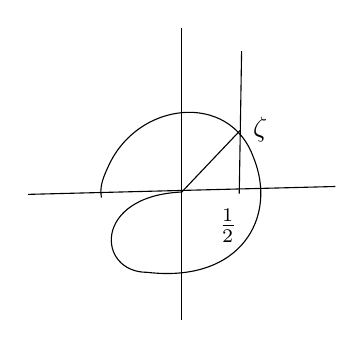
\begin{tikzpicture}[x=1cm,y=1cm]
\draw (-1.95,-.03)--(1.95,.07);
\draw (0,-1.62)--(0,2.08);
\draw (0,0) .. controls (-1.14,-.05) and (-1.08,-1.02) .. (-.44,-1.02) .. controls (.76,-1.16) and (1.22,-.31) .. (.91,.44) .. controls (.61,1.28) and (-.57,1.16) .. (-.94,.31) .. controls (-1.02,.14) and (-1.04,.04) .. (-1.02,-.07);
\draw (.73,-.02)--(.76,1.79);
\draw (0,0)--(.74,.78);
\node[right] at (.79,.79) {$\zeta$};
\node[below] at (.59,-.09) {$\frac12$};
\end{tikzpicture}}

\diagram{\begin{tikzcd}[ampersand replacement=\&,row sep=large,column sep=large]
\Pi_{0,3}^{\mathbb D'} \arrow[r] \arrow[d] \& \Pi_{0,3}^{\mathbb D}=\{\rho,\sigma\mid\rho^3=\sigma^2=1\} \arrow[d,Rightarrow] \\
\var{\deleted{\LMsourceMark{M000490}{\unsure{\mathbb Z/4\mathbb Z}}}}{\LMsourceMark{M000491}{\LMcancelledDoubts{\(\LMsourceMark{M000492}{\unsure{\mathbb Z/4\mathbb Z}}\)}}}{deletion}{140-1-s016-D002}\,\var{\inserted{\LMsourceMark{M000493}{\unsure{\mathbb D'_3}}}}{\LMadded{\LMsourceMark{M000494}{\unsure{\mathbb D'_3}}}}{insertion}{140-1-s016-I001} \arrow[r] \arrow[d] \arrow[ur,phantom,"\LMsourceMark{M000495}{\unsure{\mathrm{cart}}}"{description}] \& \var{\deleted{\LMsourceMark{M000496}{\unsure{\mathbb Z/2\mathbb Z}}}}{\LMsourceMark{M000497}{\LMcancelledDoubts{\(\LMsourceMark{M000498}{\unsure{\mathbb Z/2\mathbb Z}}\)}}}{deletion}{140-1-s016-D003}\,\var{\inserted{\LMsourceMark{M000499}{\unsure{\mathbb D_3}}}}{\LMadded{\LMsourceMark{M000500}{\unsure{\mathbb D_3}}}}{insertion}{140-1-s016-I002} \arrow[d] \\
\mathbb Z/4\mathbb Z \arrow[r,no head] \arrow[ur,phantom,"\LMsourceMark{M000501}{\unsure{\mathrm{cart}}}"{description}] \& \mathbb Z/2\mathbb Z
\end{tikzcd}}

\LMsourceMark{M000502}{\margin{$\var{\deleted{\rho\mapsto0,\quad\sigma\mapsto1}}{}{deletion}{140-1-s016-D004}$\par
$\rho\mapsto0$\par
$\sigma\mapsto1$}}

\LMsourceMark{M000503}{\margin{\LMsourceMark{M000504}{\unsure{On remonte}} $\rho,\sigma$ en $\var{\deleted{\LMsourceMark{M000505}{\unsure{\rho,\sigma}}}}{\LMsourceMark{M000506}{\LMcancelledDoubts{\(\LMsourceMark{M000507}{\unsure{\rho,\sigma}}\)}}}{deletion}{140-1-s016-D005}\ \rho',\sigma'$\par
$\rho'=(\rho,2),\quad\sigma'=(\sigma,\var{\deleted{\LMsourceMark{M000508}{\unsure{2}}}}{\LMsourceMark{M000509}{\LMcancelledDoubts{\(\LMsourceMark{M000510}{\unsure{2}}\)}}}{deletion}{140-1-s016-D006}\var{\inserted{3}}{\LMadded{3}}{insertion}{140-1-s016-I003})$\par
\LMsourceMark{M000511}{\unsure{on a}}
$\rho'^{\,6}=\sigma'^{\,4}=1,$\par
$\rho'^{\,3}=\sigma'^{\,2}=(\underbrace{1,2\bmod4}_{\omega})$.}}

\LMsourceMark{M000512}{\margin{On vérifie alors aisément que\par
$\mathrm S\ell(2,\mathbb Z)\simeq\{\rho',\sigma'\mid \LMsourceMark{M000513}{\unsure{\rho'^{\,6}=\sigma'^{\,4}=1}},\ \LMsourceMark{M000514}{\unsure{\rho'^{\,3}=\sigma'^{\,2}}}\}$.}}

\LMsourceMark{M000515}{\margin{\figure{\begin{tikzpicture}[x=1cm,y=1cm]
\draw[->] (2.92,3.25) .. controls (2.82,2.34) and (1.35,2.38) .. (1.05,1.46) .. controls (.92,1.12) and (.86,.77) .. (.71,.58);
\draw (0.05,2.24) .. controls (.42,1.64) and (.29,1.03) .. (.21,.96) .. controls (.12,.88) and (.24,.73) .. (.35,.68);
\draw (.59,.98) .. controls (.43,.46) and (.48,.12) .. (.35,-.02) .. controls (.62,.12) and (.63,-.29) .. (.67,-.72);
\end{tikzpicture}}}}

Ainsi $\Pi_{0,3}^{\mathbb D'}\simeq\mathrm S\ell(2,\mathbb Z)$ \LMsourceMark{M000516}{\unsure{apparaît}} comme extension de $\Pi_{0,3}^{\mathbb D}$ par $\mathbb Z/2\mathbb Z$, image inverse \var{\deleted{\LMsourceMark{M000517}{\unsure{de}}}}{\LMsourceMark{M000518}{\LMcancelledDoubts{\LMsourceMark{M000519}{\unsure{de}}}}}{deletion}{140-1-s016-D007} l'ext. \var{\inserted{$\mathbb D'_3$}}{\LMadded{$\mathbb D'_3$}}{insertion}{140-1-s016-I004} de $\mathbb D_3$ par $\mathbb Z/2\mathbb Z$, ou de l'ext. $\mathbb Z/4\mathbb Z$ de $\mathbb Z/2\mathbb Z$ par $\mathbb Z/2\mathbb Z$, via $\Pi_{0,3}^{\mathbb D}\to\mathbb D_3$ \LMsourceMark{M000520}{\unsure{resp.}} composé $\Pi_{0,3}^{\mathbb D}\to\var{\deleted{\LMsourceMark{M000521}{\unsure{\mathbb D_3}}}}{\LMsourceMark{M000522}{\LMcancelledDoubts{\(\LMsourceMark{M000523}{\unsure{\mathbb D_3}}\)}}}{deletion}{140-1-s016-D008}\mathbb Z/2\mathbb Z$. \LMsourceMark{M000524}{\unsure{C'est}} une ext. de $\mathbb D'_3$ par un \LMsourceMark{M000525}{\unsure{gr.}} $\simeq\Pi_{0,3}$, \LMsourceMark{M000526}{\unsure{de base}} $\rho_0,\rho_1,\rho_\infty$ \LMsourceMark{M000527}{\unsure{---}}

\LMsourceMark{M000528}{\margin{15}}

\LMflushnotes\LMflushpages
\ifnum\LMform=1
\begin{LMapparatus}
\LMentry{140-1-s016-D001}{suppression}{\deleted{\LMsourceMark{M000529}{\unsure{lorsque}}}
}{\emph{\LMomittedlabel}}{Passage biffé dans le manuscrit : la suppression suit l'état final de l'auteur; les doutes de lecture restent signalés.}{}
\LMentry{140-1-s016-D002}{suppression}{\(\deleted{\LMsourceMark{M000530}{\unsure{\mathbb Z/4\mathbb Z}}}\)
}{\emph{\LMomittedlabel}}{Passage biffé dans le manuscrit : la suppression suit l'état final de l'auteur; les doutes de lecture restent signalés.}{}
\LMentry{140-1-s016-I001}{insertion}{\(\inserted{\LMsourceMark{M000531}{\unsure{\mathbb D'_3}}}\)
}{\emph{\LMinsertedlabel}}{Ajout explicite de l'auteur : intégré à l'endroit indiqué par la transcription, sans modifier sa lecture.}{}
\LMentry{140-1-s016-D003}{suppression}{\(\deleted{\LMsourceMark{M000532}{\unsure{\mathbb Z/2\mathbb Z}}}\)
}{\emph{\LMomittedlabel}}{Passage biffé dans le manuscrit : la suppression suit l'état final de l'auteur; les doutes de lecture restent signalés.}{}
\LMentry{140-1-s016-I002}{insertion}{\(\inserted{\LMsourceMark{M000533}{\unsure{\mathbb D_3}}}\)
}{\emph{\LMinsertedlabel}}{Ajout explicite de l'auteur : intégré à l'endroit indiqué par la transcription, sans modifier sa lecture.}{}
\LMentry{140-1-s016-D004}{suppression}{\(\deleted{\rho\mapsto0,\quad\sigma\mapsto1}\)
}{\emph{\LMomittedlabel}}{Passage biffé dans le manuscrit : la suppression suit l'état final de l'auteur; les doutes de lecture restent signalés.}{}
\LMentry{140-1-s016-D005}{suppression}{\(\deleted{\LMsourceMark{M000534}{\unsure{\rho,\sigma}}}\)
}{\emph{\LMomittedlabel}}{Passage biffé dans le manuscrit : la suppression suit l'état final de l'auteur; les doutes de lecture restent signalés.}{}
\LMentry{140-1-s016-D006}{suppression}{\(\deleted{\LMsourceMark{M000535}{\unsure{2}}}\)
}{\emph{\LMomittedlabel}}{Passage biffé dans le manuscrit : la suppression suit l'état final de l'auteur; les doutes de lecture restent signalés.}{}
\LMentry{140-1-s016-I003}{insertion}{\(\inserted{3}\)
}{\emph{\LMinsertedlabel}}{Ajout explicite de l'auteur : intégré à l'endroit indiqué par la transcription, sans modifier sa lecture.}{}
\LMentry{140-1-s016-D007}{suppression}{\deleted{\LMsourceMark{M000536}{\unsure{de}}}
}{\emph{\LMomittedlabel}}{Passage biffé dans le manuscrit : la suppression suit l'état final de l'auteur; les doutes de lecture restent signalés.}{}
\LMentry{140-1-s016-I004}{insertion}{\inserted{$\mathbb D'_3$}
}{\emph{\LMinsertedlabel}}{Ajout explicite de l'auteur : intégré à l'endroit indiqué par la transcription, sans modifier sa lecture.}{}
\LMentry{140-1-s016-D008}{suppression}{\(\deleted{\LMsourceMark{M000537}{\unsure{\mathbb D_3}}}\)
}{\emph{\LMomittedlabel}}{Passage biffé dans le manuscrit : la suppression suit l'état final de l'auteur; les doutes de lecture restent signalés.}{}
\end{LMapparatus}
\fi
\ifnum\LMform=2
\par\smallskip\begingroup\footnotesize\Needspace{4\baselineskip}\csname @beginparpenalty\endcsname=10000\relax\noindent\textcolor{gray}{\rule{.2\linewidth}{.35pt}}\par\nobreak
\noindent\textit{\LMdoubtheading.}\par\nobreak
\LMcarryover{140-1-s016-D001}{\LMsourceMark{M000538}{\unsure{lorsque}}
}
\LMcarryover{140-1-s016-D002}{\(\LMsourceMark{M000539}{\unsure{\mathbb Z/4\mathbb Z}}\)
}
\LMcarryover{140-1-s016-D003}{\(\LMsourceMark{M000540}{\unsure{\mathbb Z/2\mathbb Z}}\)
}
\LMcarryover{140-1-s016-D005}{\(\LMsourceMark{M000541}{\unsure{\rho,\sigma}}\)
}
\LMcarryover{140-1-s016-D006}{\(\LMsourceMark{M000542}{\unsure{2}}\)
}
\LMcarryover{140-1-s016-D007}{\LMsourceMark{M000543}{\unsure{de}}
}
\LMcarryover{140-1-s016-D008}{\(\LMsourceMark{M000544}{\unsure{\mathbb D_3}}\)
}
\par\endgroup\smallskip
\fi

\LMsourceMark{M000545}{\scanpage{17}}

\var{\deleted{\diagram{\begin{tikzcd}[ampersand replacement=\&,column sep=small,row sep=large]
\& \vec S(\LMsourceMark{M000546}{\unsure{X_0|X_\bullet}})\simeq G_0 \arrow[dl] \arrow[d] \arrow[dr] \& \\
S(X_0)\simeq G_0/H_S \& A(X_0)\simeq G_0/H_A, \& F(X_0)\simeq G_0/H_F
\end{tikzcd}}}}{\LMsourceMark{M000547}{\LMcancelledDoubts{\(\LMsourceMark{M000548}{\unsure{X_0|X_\bullet}}\)}}}{deletion}{140-1-s017-D001}

\var{\deleted{\[
H_S\cap H_A=e,\qquad H_A\cap H_F=e,\qquad H_S\cap H_F=e
\]}}{}{deletion}{140-1-s017-D002}

\var{\deleted{\LMsourceMark{M000549}{\unsure{i.e.|i.a.}}
\[
G_0\hookrightarrow G_0/H_S\times G_0/H_A,\qquad
G_0\hookrightarrow G_0/H_A\times G_0/H_F,\qquad
G_0\LMsourceMark{M000550}{\unsure{\hookrightarrow|\subset}}\deleted{\LMsourceMark{M000551}{\unsure{G_0|H_S}}}/H_A\times G_0/H_F
\]}}{\LMsourceMark{M000552}{\LMcancelledDoubts{\LMsourceMark{M000553}{\unsure{i.e.|i.a.}}\quad \(\LMsourceMark{M000554}{\unsure{\hookrightarrow|\subset}}\)\quad \(\LMsourceMark{M000555}{\unsure{G_0|H_S}}\)}}}{deletion}{140-1-s017-D003}

\var{\deleted{\figure{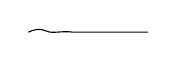
\begin{tikzpicture}[x=1cm,y=1cm]
\draw (0,0).. controls (.1,.04) and (.14,.05) .. (.24,.01).. controls (.31,-.02) and (.43,.02) .. (.57,0)--(1.52,0);
\end{tikzpicture}}}}{}{deletion}{140-1-s017-D005}

\LMsourceMark{M000556}{\margin{\uline{\LMsourceMark{M000557}{\unsure{Cas non orienté}}}}}

\var{\deleted{Considérons la catégorie des polyèdres (non orientés) de type donné; il y a des foncteurs}}{}{deletion}{140-1-s017-D006}

\var{\deleted{\[
\begin{array}{l}
S\\
\vec A\\
F\\
\deleted{\LMsourceMark{M000558}{\unsure{A|R}}}
\end{array}
\]}}{\LMsourceMark{M000559}{\LMcancelledDoubts{\(\LMsourceMark{M000560}{\unsure{A|R}}\)}}}{deletion}{140-1-s017-D007}

\var{\deleted{\diagram{\(\begin{array}{lll}
A_1 & \text{relation d'incidence entre }S\text{ et }A & \text{(}\LMsourceMark{M000561}{\unsure{\text{arêtes orientées}}}\text{ au sens }1\text{)}\\
A_2 & \rule{3.2cm}{0.25pt}\ A\text{ et }F & (\rule{2.8cm}{0.25pt}\ 2)\\
A_3 & \text{rel. d'incidence entre }\LMsourceMark{M000562}{\unsure{S|B}}\text{ et }F &
\end{array}\)}}}{\LMsourceMark{M000563}{\LMcancelledDoubts{\(\LMsourceMark{M000564}{\unsure{\text{arêtes orientées}}}\)\quad \(\LMsourceMark{M000565}{\unsure{S|B}}\)}}}{deletion}{140-1-s017-D009}

\var{\deleted{\[
R=\deleted{\LMsourceMark{M000566}{\unsure{A_3}}}\LMsourceMark{M000567}{\unsure{\simeq|=}}A_1\times_A A_2
\]
\deleted{\LMsourceMark{M000568}{\unsure{relation}} d'incidence entre $S$ et $F$}
\inserted{\LMsourceMark{M000569}{\unsure{triplets ou drapeaux|triplets de drapeaux}} $(s,a,f)$\quad$s\LMsourceMark{M000570}{\unsure{\leq|<}}a<f$.}}}{\LMsourceMark{M000571}{\LMcancelledDoubts{\(\LMsourceMark{M000572}{\unsure{A_3}}\)\quad \(\LMsourceMark{M000573}{\unsure{\simeq|=}}\)\quad \LMsourceMark{M000574}{\unsure{relation}}\quad \LMsourceMark{M000575}{\unsure{triplets ou drapeaux|triplets de drapeaux}}\quad \(\LMsourceMark{M000576}{\unsure{\leq|<}}\)}}}{deletion}{140-1-s017-D010}

\var{\deleted{\diagram{\begin{tikzcd}[ampersand replacement=\&,row sep=small,column sep=small]
\& R \arrow[dl] \arrow[d] \arrow[dr] \& \\
S\&A\&F
\end{tikzcd}}}}{}{deletion}{140-1-s017-D013}

\var{\deleted{\[
\begin{aligned}
A_1&=\operatorname{Im}(R\to S\times A)\\
A_2&=\operatorname{Im}(R\to A\times F)\\
A_3&=\operatorname{Im}(R\to S\times F)
\end{aligned}
\]}}{}{deletion}{140-1-s017-D014}

\var{\deleted{$\Omega$ ens des orientations}}{}{deletion}{140-1-s017-D015}

\var{\deleted{\[
{A_1}_{\Omega}\simeq\LMsourceMark{M000577}{\unsure{{A_2}_{\Omega}}}\simeq{A_3}_{\Omega}\qquad(
\]}}{\LMsourceMark{M000578}{\LMcancelledDoubts{\(\LMsourceMark{M000579}{\unsure{{A_2}_{\Omega}}}\)}}}{deletion}{140-1-s017-D016}

\[
\mathrm{Pol}_{\LMsourceMark{M000580}{\unsure{\tau|t}}}\qquad
\mathrm{Pol}_{\tau}^{\LMsourceMark{M000581}{\unsure{\mathrm{or}}}}\simeq
\mathrm{Pol}_{\tau}\var{\deleted{\LMsourceMark{M000582}{\unsure{/\Omega}}}}{\LMsourceMark{M000583}{\LMcancelledDoubts{\(\LMsourceMark{M000584}{\unsure{/\Omega}}\)}}}{deletion}{140-1-s017-D017}\var{\inserted{{}_{/\Omega}}}{\LMadded{{}_{/\Omega}}}{insertion}{140-1-s017-I002}
\]

\LMsourceMark{M000585}{\margin{16}}

\LMflushnotes\LMflushpages
\ifnum\LMform=1
\begin{LMapparatus}
\LMentry{140-1-s017-D001}{suppression}{\deleted{\diagram{\begin{tikzcd}[ampersand replacement=\&,column sep=small,row sep=large]
\& \vec S(\LMsourceMark{M000586}{\unsure{X_0|X_\bullet}})\simeq G_0 \arrow[dl] \arrow[d] \arrow[dr] \& \\
S(X_0)\simeq G_0/H_S \& A(X_0)\simeq G_0/H_A, \& F(X_0)\simeq G_0/H_F
\end{tikzcd}}}
}{\emph{\LMomittedlabel}}{Passage biffé dans le manuscrit : la suppression suit l'état final de l'auteur; les doutes de lecture restent signalés.}{}
\LMentry{140-1-s017-D002}{suppression}{\deleted{\[
H_S\cap H_A=e,\qquad H_A\cap H_F=e,\qquad H_S\cap H_F=e
\]}
}{\emph{\LMomittedlabel}}{Passage biffé dans le manuscrit : la suppression suit l'état final de l'auteur; les doutes de lecture restent signalés.}{}
\LMentry{140-1-s017-D003}{suppression}{\deleted{\LMsourceMark{M000587}{\unsure{i.e.|i.a.}}
\[
G_0\hookrightarrow G_0/H_S\times G_0/H_A,\qquad
G_0\hookrightarrow G_0/H_A\times G_0/H_F,\qquad
G_0\LMsourceMark{M000588}{\unsure{\hookrightarrow|\subset}}\deleted{\LMsourceMark{M000589}{\unsure{G_0|H_S}}}/H_A\times G_0/H_F
\]}
}{\emph{\LMomittedlabel}}{Passage biffé dans le manuscrit : la suppression suit l'état final de l'auteur; les doutes de lecture restent signalés.}{}
\LMentry{140-1-s017-D005}{suppression}{\deleted{\figure{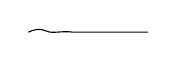
\begin{tikzpicture}[x=1cm,y=1cm]
\draw (0,0).. controls (.1,.04) and (.14,.05) .. (.24,.01).. controls (.31,-.02) and (.43,.02) .. (.57,0)--(1.52,0);
\end{tikzpicture}}}
}{\emph{\LMomittedlabel}}{Passage biffé dans le manuscrit : la suppression suit l'état final de l'auteur; les doutes de lecture restent signalés.}{}
\LMentry{140-1-s017-D006}{suppression}{\deleted{Considérons la catégorie des polyèdres (non orientés) de type donné; il y a des foncteurs}
}{\emph{\LMomittedlabel}}{Passage biffé dans le manuscrit : la suppression suit l'état final de l'auteur; les doutes de lecture restent signalés.}{}
\LMentry{140-1-s017-D007}{suppression}{\deleted{\[
\begin{array}{l}
S\\
\vec A\\
F\\
\deleted{\LMsourceMark{M000590}{\unsure{A|R}}}
\end{array}
\]}
}{\emph{\LMomittedlabel}}{Passage biffé dans le manuscrit : la suppression suit l'état final de l'auteur; les doutes de lecture restent signalés.}{}
\LMentry{140-1-s017-D009}{suppression}{\deleted{\diagram{\(\begin{array}{lll}
A_1 & \text{relation d'incidence entre }S\text{ et }A & \text{(}\LMsourceMark{M000591}{\unsure{\text{arêtes orientées}}}\text{ au sens }1\text{)}\\
A_2 & \rule{3.2cm}{0.25pt}\ A\text{ et }F & (\rule{2.8cm}{0.25pt}\ 2)\\
A_3 & \text{rel. d'incidence entre }\LMsourceMark{M000592}{\unsure{S|B}}\text{ et }F &
\end{array}\)}}
}{\emph{\LMomittedlabel}}{Passage biffé dans le manuscrit : la suppression suit l'état final de l'auteur; les doutes de lecture restent signalés.}{}
\LMentry{140-1-s017-D010}{suppression}{\deleted{\[
R=\deleted{\LMsourceMark{M000593}{\unsure{A_3}}}\LMsourceMark{M000594}{\unsure{\simeq|=}}A_1\times_A A_2
\]
\deleted{\LMsourceMark{M000595}{\unsure{relation}} d'incidence entre $S$ et $F$}
\inserted{\LMsourceMark{M000596}{\unsure{triplets ou drapeaux|triplets de drapeaux}} $(s,a,f)$\quad$s\LMsourceMark{M000597}{\unsure{\leq|<}}a<f$.}}
}{\emph{\LMomittedlabel}}{Passage biffé dans le manuscrit : la suppression suit l'état final de l'auteur; les doutes de lecture restent signalés.}{}
\LMentry{140-1-s017-D013}{suppression}{\deleted{\diagram{\begin{tikzcd}[ampersand replacement=\&,row sep=small,column sep=small]
\& R \arrow[dl] \arrow[d] \arrow[dr] \& \\
S\&A\&F
\end{tikzcd}}}
}{\emph{\LMomittedlabel}}{Passage biffé dans le manuscrit : la suppression suit l'état final de l'auteur; les doutes de lecture restent signalés.}{}
\LMentry{140-1-s017-D014}{suppression}{\deleted{\[
\begin{aligned}
A_1&=\operatorname{Im}(R\to S\times A)\\
A_2&=\operatorname{Im}(R\to A\times F)\\
A_3&=\operatorname{Im}(R\to S\times F)
\end{aligned}
\]}
}{\emph{\LMomittedlabel}}{Passage biffé dans le manuscrit : la suppression suit l'état final de l'auteur; les doutes de lecture restent signalés.}{}
\LMentry{140-1-s017-D015}{suppression}{\deleted{$\Omega$ ens des orientations}
}{\emph{\LMomittedlabel}}{Passage biffé dans le manuscrit : la suppression suit l'état final de l'auteur; les doutes de lecture restent signalés.}{}
\LMentry{140-1-s017-D016}{suppression}{\deleted{\[
{A_1}_{\Omega}\simeq\LMsourceMark{M000598}{\unsure{{A_2}_{\Omega}}}\simeq{A_3}_{\Omega}\qquad(
\]}
}{\emph{\LMomittedlabel}}{Passage biffé dans le manuscrit : la suppression suit l'état final de l'auteur; les doutes de lecture restent signalés.}{}
\LMentry{140-1-s017-D017}{suppression}{\(\deleted{\LMsourceMark{M000599}{\unsure{/\Omega}}}\)
}{\emph{\LMomittedlabel}}{Passage biffé dans le manuscrit : la suppression suit l'état final de l'auteur; les doutes de lecture restent signalés.}{}
\LMentry{140-1-s017-I002}{insertion}{\(\inserted{{}_{/\Omega}}\)
}{\emph{\LMinsertedlabel}}{Ajout explicite de l'auteur : intégré à l'endroit indiqué par la transcription, sans modifier sa lecture.}{}
\end{LMapparatus}
\fi
\ifnum\LMform=2
\par\smallskip\begingroup\footnotesize\Needspace{4\baselineskip}\csname @beginparpenalty\endcsname=10000\relax\noindent\textcolor{gray}{\rule{.2\linewidth}{.35pt}}\par\nobreak
\noindent\textit{\LMdoubtheading.}\par\nobreak
\LMcarryover{140-1-s017-D001}{\(\LMsourceMark{M000600}{\unsure{X_0|X_\bullet}}\)
}
\LMcarryover{140-1-s017-D003}{\LMsourceMark{M000601}{\unsure{i.e.|i.a.}}\quad \(\LMsourceMark{M000602}{\unsure{\hookrightarrow|\subset}}\)\quad \(\LMsourceMark{M000603}{\unsure{G_0|H_S}}\)
}
\LMcarryover{140-1-s017-D007}{\(\LMsourceMark{M000604}{\unsure{A|R}}\)
}
\LMcarryover{140-1-s017-D009}{\(\LMsourceMark{M000605}{\unsure{\text{arêtes orientées}}}\)\quad \(\LMsourceMark{M000606}{\unsure{S|B}}\)
}
\LMcarryover{140-1-s017-D010}{\(\LMsourceMark{M000607}{\unsure{A_3}}\)\quad \(\LMsourceMark{M000608}{\unsure{\simeq|=}}\)\quad \LMsourceMark{M000609}{\unsure{relation}}\quad \LMsourceMark{M000610}{\unsure{triplets ou drapeaux|triplets de drapeaux}}\quad \(\LMsourceMark{M000611}{\unsure{\leq|<}}\)
}
\LMcarryover{140-1-s017-D016}{\(\LMsourceMark{M000612}{\unsure{{A_2}_{\Omega}}}\)
}
\LMcarryover{140-1-s017-D017}{\(\LMsourceMark{M000613}{\unsure{/\Omega}}\)
}
\par\endgroup\smallskip
\fi

\LMsourceMark{M000614}{\scanpage{18}}
\LMsourceMark{M000615}{\mspage{6}}

$S\mathcal T_{1,1}\simeq$ \LMsourceMark{M000616}{\unsure{image inverse}} de $\mathrm S\ell(2,\mathbb Z)$ dans $\LMsourceMark{M000617}{\unsure{\var{\deleted{\mathrm G\ell}}{\LMsourceMark{M000618}{\LMuncertaindeletion{140-1-s018-D001}}}{deletion}{140-1-s018-D001}\mathrm S\ell(2,\mathbb R)^{\sim}|\mathrm G\ell(2,\mathbb R)^{\sim}}}$
\[
\simeq\{\rho,\sigma\mid\rho^3=\sigma^2\ (=\omega)\}
\]
\LMsourceMark{M000619}{\margin{\LMsourceMark{M000620}{\unsure{(}}\LMsourceMark{M000621}{\unsure{élém\textsuperscript{t}|él\textsuperscript{mt}}} central}}

\[
\mathcal T_{11}=S\mathcal T_{11}/\langle\omega^2\rangle
\]

\[
\begin{array}{ll}
(\mathcal T_{11})_{\mathrm{ab}}\simeq\mathbb Z & (\mathcal T_{11})_{\mathrm{ab}}\simeq\mathbb Z/12\mathbb Z\\[4pt]
\var{\deleted{(\rho,\sigma)}}{}{deletion}{140-1-s018-D002} & \\
\rho\longmapsto2 & \rho\longmapsto2\bmod12\\
\sigma\longmapsto3 & \sigma\longmapsto3\bmod12\\
\omega\longmapsto\LMsourceMark{M000622}{\unsure{6|8}} &
\end{array}
\]

\diagram{\begin{tikzcd}[ampersand replacement=\&,row sep=large,column sep=small,nodes in empty cells]
\& 1 \& \& 1 \\
\& \mathcal T_{11} \arrow[u] \arrow[r] \& \var{\deleted{\LMsourceMark{M000623}{\unsure{\mathcal T_{\mathrm{ab}}}}}}{\LMsourceMark{M000624}{\LMcancelledDoubts{\(\LMsourceMark{M000625}{\unsure{\mathcal T_{\mathrm{ab}}}}\)}}}{deletion}{140-1-s018-D003} \arrow[r] \& \mathbb Z/12\mathbb Z \arrow[u] \\
\LMsourceMark{M000626}{\unsure{\widetilde\omega|\bar\omega}}=\omega^{2\var{\deleted{\LMsourceMark{M000627}{\unsure{4}}}}{\LMsourceMark{M000628}{\LMcancelledDoubts{\(\LMsourceMark{M000629}{\unsure{4}}\)}}}{deletion}{140-1-s018-D004}} \& S\mathcal T_{11} \arrow[u] \arrow[rr] \arrow[ur,phantom,"\var{\deleted{\text{cartésien}}}{}{deletion}{140-1-s018-D005}"{description}] \& \& \mathbb Z \arrow[u] \\
\uline{1} \arrow[u] \& \mathbb Z \arrow[u] \arrow[rr,"\mathrm{id}"] \& \& \mathbb Z \arrow[u,"12"] \\
\& 1 \arrow[u] \& \& 1 \arrow[u]
\end{tikzcd}}

\LMsourceMark{M000630}{\margin{donc $S\mathcal T_{11}$ se déduit de $\mathcal T_{11}$ par image inverse de l'ext. canonique de $\mathbb Z/12\mathbb Z$ par $\mathbb Z$, via $\mathcal T_{11}\to\mathbb Z/12\mathbb Z$.}}

\var{\deleted{une normalisation de $(K,\LMsourceMark{M000631}{\unsure{K_0|N|k_0}})$, \LMsourceMark{M000632}{\unsure{alors}} elle est \LMsourceMark{M000633}{\unsure{spéciale}} : la cat. des rev. étales dans $\LMsourceMark{M000634}{\unsure{K'_fN|K'_{fN}}}$ -- \deleted{\LMsourceMark{M000635}{\illegible{1}}} $\Delta$ \LMsourceMark{M000636}{\unsure{rev.|i.e.}} $\Delta$ top. \LMsourceMark{M000637}{\unsure{a}} une unique normalisation pour laquelle la projection \LMsourceMark{M000638}{\unsure{est|soit}} un \LMsourceMark{M000639}{\unsure{morphisme}} de $\Delta$-complexes \LMsourceMark{M000640}{\unsure{normalisés}}. [Mais attention, \LMsourceMark{M000641}{\unsure{ça ne marche}} \uline{\LMsourceMark{M000642}{\unsure{pas}}} pour \LMsourceMark{M000643}{\unsure{strictes normalisations}} \LMsourceMark{M000644}{\unsure{$\overline{\mathrm m}$|néc.}}\ldots]}}{\LMsourceMark{M000645}{\LMcancelledDoubts{\(\LMsourceMark{M000646}{\unsure{K_0|N|k_0}}\)\quad \LMsourceMark{M000647}{\unsure{alors}}\quad \LMsourceMark{M000648}{\unsure{spéciale}}\quad \(\LMsourceMark{M000649}{\unsure{K'_fN|K'_{fN}}}\)\quad \LMsourceMark{M000650}{\illegible{1}}\quad \LMsourceMark{M000651}{\unsure{rev.|i.e.}}\quad \LMsourceMark{M000652}{\unsure{a}}\quad \LMsourceMark{M000653}{\unsure{est|soit}}\quad \LMsourceMark{M000654}{\unsure{morphisme}}\quad \LMsourceMark{M000655}{\unsure{normalisés}}\quad \LMsourceMark{M000656}{\unsure{ça ne marche}}\quad \LMsourceMark{M000657}{\unsure{pas}}\quad \LMsourceMark{M000658}{\unsure{strictes normalisations}}\quad \LMsourceMark{M000659}{\unsure{$\overline{\mathrm m}$|néc.}}}}}{deletion}{140-1-s018-D006}

\var{\deleted{\LMsourceMark{M000660}{\unsure{8.|$\beta$.}} \LMsourceMark{M000661}{\unsure{Groupes|Groupe}} et groupoïdes \LMsourceMark{M000662}{\unsure{fondamentaux|fondamental}}. On \LMsourceMark{M000663}{\unsure{montrera|montre}} la relation entre construction top. et construction algébrique.}}{\LMsourceMark{M000664}{\LMcancelledDoubts{\LMsourceMark{M000665}{\unsure{8.|$\beta$.}}\quad \LMsourceMark{M000666}{\unsure{Groupes|Groupe}}\quad \LMsourceMark{M000667}{\unsure{fondamentaux|fondamental}}\quad \LMsourceMark{M000668}{\unsure{montrera|montre}}}}}{deletion}{140-1-s018-D008}

\LMsourceMark{M000669}{\margin{17}}

\LMflushnotes\LMflushpages
\ifnum\LMform=1
\begin{LMapparatus}
\LMentry{140-1-s018-D001}{suppression}{\(\LMsourceMark{M000670}{\LMdoubtcopy{\deleted{\mathrm G\ell}}}\)
}{\emph{\LMomittedlabel}}{Passage biffé dans le manuscrit : la suppression suit l'état final de l'auteur; les doutes de lecture restent signalés.}{}
\LMentry{140-1-s018-D002}{suppression}{\(\deleted{(\rho,\sigma)}\)
}{\emph{\LMomittedlabel}}{Passage biffé dans le manuscrit : la suppression suit l'état final de l'auteur; les doutes de lecture restent signalés.}{}
\LMentry{140-1-s018-D003}{suppression}{\(\deleted{\LMsourceMark{M000671}{\unsure{\mathcal T_{\mathrm{ab}}}}}\)
}{\emph{\LMomittedlabel}}{Passage biffé dans le manuscrit : la suppression suit l'état final de l'auteur; les doutes de lecture restent signalés.}{}
\LMentry{140-1-s018-D004}{suppression}{\(\deleted{\LMsourceMark{M000672}{\unsure{4}}}\)
}{\emph{\LMomittedlabel}}{Passage biffé dans le manuscrit : la suppression suit l'état final de l'auteur; les doutes de lecture restent signalés.}{}
\LMentry{140-1-s018-D005}{suppression}{\(\deleted{\text{cartésien}}\)
}{\emph{\LMomittedlabel}}{Passage biffé dans le manuscrit : la suppression suit l'état final de l'auteur; les doutes de lecture restent signalés.}{}
\LMentry{140-1-s018-D006}{suppression}{\deleted{une normalisation de $(K,\LMsourceMark{M000673}{\unsure{K_0|N|k_0}})$, \LMsourceMark{M000674}{\unsure{alors}} elle est \LMsourceMark{M000675}{\unsure{spéciale}} : la cat. des rev. étales dans $\LMsourceMark{M000676}{\unsure{K'_fN|K'_{fN}}}$ -- \deleted{\LMsourceMark{M000677}{\illegible{1}}} $\Delta$ \LMsourceMark{M000678}{\unsure{rev.|i.e.}} $\Delta$ top. \LMsourceMark{M000679}{\unsure{a}} une unique normalisation pour laquelle la projection \LMsourceMark{M000680}{\unsure{est|soit}} un \LMsourceMark{M000681}{\unsure{morphisme}} de $\Delta$-complexes \LMsourceMark{M000682}{\unsure{normalisés}}. [Mais attention, \LMsourceMark{M000683}{\unsure{ça ne marche}} \uline{\LMsourceMark{M000684}{\unsure{pas}}} pour \LMsourceMark{M000685}{\unsure{strictes normalisations}} \LMsourceMark{M000686}{\unsure{$\overline{\mathrm m}$|néc.}}\ldots]}
}{\emph{\LMomittedlabel}}{Passage biffé dans le manuscrit : la suppression suit l'état final de l'auteur; les doutes de lecture restent signalés.}{}
\LMentry{140-1-s018-D008}{suppression}{\deleted{\LMsourceMark{M000687}{\unsure{8.|$\beta$.}} \LMsourceMark{M000688}{\unsure{Groupes|Groupe}} et groupoïdes \LMsourceMark{M000689}{\unsure{fondamentaux|fondamental}}. On \LMsourceMark{M000690}{\unsure{montrera|montre}} la relation entre construction top. et construction algébrique.}
}{\emph{\LMomittedlabel}}{Passage biffé dans le manuscrit : la suppression suit l'état final de l'auteur; les doutes de lecture restent signalés.}{}
\end{LMapparatus}
\fi
\ifnum\LMform=2
\par\smallskip\begingroup\footnotesize\Needspace{4\baselineskip}\csname @beginparpenalty\endcsname=10000\relax\noindent\textcolor{gray}{\rule{.2\linewidth}{.35pt}}\par\nobreak
\noindent\textit{\LMdoubtheading.}\par\nobreak
\LMcarryover{140-1-s018-D001}{\(\LMsourceMark{M000691}{\LMdoubtcopy{\mathrm G\ell}}\)
}
\LMcarryover{140-1-s018-D003}{\(\LMsourceMark{M000692}{\unsure{\mathcal T_{\mathrm{ab}}}}\)
}
\LMcarryover{140-1-s018-D004}{\(\LMsourceMark{M000693}{\unsure{4}}\)
}
\LMcarryover{140-1-s018-D006}{\(\LMsourceMark{M000694}{\unsure{K_0|N|k_0}}\)\quad \LMsourceMark{M000695}{\unsure{alors}}\quad \LMsourceMark{M000696}{\unsure{spéciale}}\quad \(\LMsourceMark{M000697}{\unsure{K'_fN|K'_{fN}}}\)\quad \LMsourceMark{M000698}{\illegible{1}}\quad \LMsourceMark{M000699}{\unsure{rev.|i.e.}}\quad \LMsourceMark{M000700}{\unsure{a}}\quad \LMsourceMark{M000701}{\unsure{est|soit}}\quad \LMsourceMark{M000702}{\unsure{morphisme}}\quad \LMsourceMark{M000703}{\unsure{normalisés}}\quad \LMsourceMark{M000704}{\unsure{ça ne marche}}\quad \LMsourceMark{M000705}{\unsure{pas}}\quad \LMsourceMark{M000706}{\unsure{strictes normalisations}}\quad \LMsourceMark{M000707}{\unsure{$\overline{\mathrm m}$|néc.}}
}
\LMcarryover{140-1-s018-D008}{\LMsourceMark{M000708}{\unsure{8.|$\beta$.}}\quad \LMsourceMark{M000709}{\unsure{Groupes|Groupe}}\quad \LMsourceMark{M000710}{\unsure{fondamentaux|fondamental}}\quad \LMsourceMark{M000711}{\unsure{montrera|montre}}
}
\par\endgroup\smallskip
\fi

\LMsourceMark{M000712}{\scanpage{19}}

% pencil numeral at the top right corner; no other foliation numeral is visible on this sheet
\LMsourceMark{M000713}{\margin{8v}}

\figure{\scalebox{0.90}{\begin{tikzpicture}[x=.014cm,y=-.014cm,every node/.style={font=\footnotesize,inner sep=0pt},line width=.45pt]
\node[anchor=west] at (385,80) {$\var{\deleted{\LMsourceMark{M000714}{\unsure{\mathbb Z|\widetilde\sigma}}}}{\LMsourceMark{M000715}{\LMcancelledDoubts{\(\LMsourceMark{M000716}{\unsure{\mathbb Z|\widetilde\sigma}}\)}}}{deletion}{140-1-s019-D001}$};
\node[anchor=west] at (585,85) {$\var{\deleted{\LMsourceMark{M000717}{\unsure{\widetilde\rho|\rho}}}}{\LMsourceMark{M000718}{\LMcancelledDoubts{\(\LMsourceMark{M000719}{\unsure{\widetilde\rho|\rho}}\)}}}{deletion}{140-1-s019-D002}$};
\node[anchor=west] at (376,167) {$\widetilde\rho_0^{\,n}=\widetilde\sigma_0^{\,n}=$};
\node[anchor=west] at (697,109) {$\widetilde\sigma^2=\widetilde\rho^{\,n}=\bar\omega$};
\node[anchor=west] at (796,177) {$\var{\deleted{\LMsourceMark{M000720}{\unsure{\widetilde\rho_0\bar\omega|\bar\omega}}}}{\LMsourceMark{M000721}{\LMcancelledDoubts{\(\LMsourceMark{M000722}{\unsure{\widetilde\rho_0\bar\omega|\bar\omega}}\)}}}{deletion}{140-1-s019-D003}$};
\node[anchor=west] at (736,241) {$\var{\deleted{\LMsourceMark{M000723}{\unsure{\widetilde\rho|\widetilde\sigma}}}}{\LMsourceMark{M000724}{\LMcancelledDoubts{\(\LMsourceMark{M000725}{\unsure{\widetilde\rho|\widetilde\sigma}}\)}}}{deletion}{140-1-s019-D004}$};
\node[anchor=west] at (831,242) {$\widetilde\rho\longmapsto\widetilde\rho\,\bar\omega^{-1}=\widetilde\rho_0$};
\node[anchor=west] at (830,315) {$\widetilde\rho_0^{\,n}\longmapsto\var{\deleted{\LMsourceMark{M000726}{\unsure{(\omega)|(\rho)}}}}{\LMsourceMark{M000727}{\LMcancelledDoubts{\(\LMsourceMark{M000728}{\unsure{(\omega)|(\rho)}}\)}}}{deletion}{140-1-s019-D005}=\widetilde\rho^{\,n}\bar\omega^{-n}=\bar\omega^{1-n}=\omega^{\frac{1-n}{2}}$};
\node[anchor=west] at (824,380) {$\widetilde\sigma_0=\widetilde\sigma_{\LMsourceMark{M000729}{\unsure{0|a}}}\bar\omega^s$};
\node[anchor=west] at (1045,380) {$\widetilde\sigma_0^{\,\LMsourceMark{M000730}{\unsure{2|n}}}=\widetilde\sigma_{\LMsourceMark{M000731}{\unsure{0|a}}}^{\,2}\bar\omega^{2s}=\bar\omega^{1+2s}$};
\node[anchor=west] at (770,486) {$1+2s=\frac{1-n}{2}$};
\node[anchor=west] at (1031,478) {OK si $\frac{1-n}{2}$ \uline{impair}};

\draw (328,1085) .. controls (405,726) and (557,346) .. (719,46);
\draw (797,975) .. controls (925,640) and (1077,335) .. (1119,147);

\draw (370,351) .. controls (284,337) and (224,418) .. (225,510) .. controls (222,592) and (294,633) .. (367,619) .. controls (445,607) and (487,549) .. (477,465) .. controls (469,399) and (433,349) .. (370,351);
\draw[line width=.25pt] (371,351) .. controls (277,345) and (223,430) .. (229,526) .. controls (232,599) and (300,635) .. (368,629);
\draw (350,610) .. controls (370,621) and (422,602) .. (451,565);
\draw (227,499) .. controls (281,468) and (401,455) .. (471,474) .. controls (490,483) and (461,501) .. (435,505) .. controls (367,522) and (271,528) .. (226,512);
\draw[line width=.8pt,->] (260,514) .. controls (281,518) and (301,521) .. (320,519);
\draw[line width=.8pt,->] (366,466)--(313,467);
\draw[->] (438,506) .. controls (454,501) and (470,490) .. (492,488);
\fill (260,514) circle[radius=3.3];
\fill (438,503) circle[radius=2.5];
\fill (364,466) circle[radius=2.3];
\draw (334,514) .. controls (327,454) and (343,389) .. (370,351);
\draw[line width=.8pt] (261,514) .. controls (263,455) and (303,388) .. (370,351);
\draw[line width=.35pt] (250,505) .. controls (274,428) and (288,390) .. (365,350);
\draw[line width=.8pt,->] (369,353)--(423,312);
\draw[->] (372,352) .. controls (398,368) and (428,387) .. (449,397);
\draw (377,351) .. controls (437,351) and (468,403) .. (473,476);
\node at (330,342) {$\LMsourceMark{M000732}{\unsure{i|1}}$};
\node[rotate=-35] at (422,375) {$\LMsourceMark{M000733}{\unsure{i|1}}$};
\node at (443,455) {$\LMsourceMark{M000734}{\unsure{i|1}}$};
\draw[line width=.8pt] (275,402)--(361,351)--(310,367)--(382,347)--(312,381)--(354,347)--(296,365)--(377,351)--(336,402)--(347,365)--(301,399)--(370,347)--(334,409)--(326,362)--(381,350);
\draw (266,411)--(352,348)--(300,378)--(376,345)--(327,382)--(353,374)--(338,409);

\node[anchor=west] at (510,582) {$\LMsourceMark{M000735}{\unsure{R_i|R^i}}$};
\node[anchor=west] at (595,580) {$\widetilde R_{\LMsourceMark{M000736}{\unsure{i}}}=(\LMsourceMark{M000737}{\unsure{e_j|e_g}}-e_{\LMsourceMark{M000738}{\unsure{k|K}}})\LMsourceMark{M000739}{\unsure{\lambda|h}}^{\omega}_{\LMsourceMark{M000740}{\unsure{jk|gK}}}$};
\node[anchor=west] at (500,653) {$\LMsourceMark{M000741}{\unsure{t_\omega|\epsilon_\omega}},\ \LMsourceMark{M000742}{\unsure{h_\omega|h_1}}$};
\node[anchor=west] at (278,715) {$V(\LMsourceMark{M000743}{\unsure{\omega|w}})$};
\node[anchor=west] at (238,838) {$\varphi_\omega(\LMsourceMark{M000744}{\unsure{\widetilde R|\bar R}}_{\LMsourceMark{M000745}{\unsure{K|k}}})$};
\node[anchor=west] at (721,786) {$P_i$};
\node[anchor=west] at (586,865) {$\var{\deleted{\LMsourceMark{M000746}{\unsure{t_\omega|R_\omega}}}}{\LMsourceMark{M000747}{\LMcancelledDoubts{\(\LMsourceMark{M000748}{\unsure{t_\omega|R_\omega}}\)}}}{deletion}{140-1-s019-D006}$};
\node[anchor=west] at (921,782) {$\var{\deleted{\LMsourceMark{M000749}{\unsure{H_i|H_2}}}}{\LMsourceMark{M000750}{\LMcancelledDoubts{\(\LMsourceMark{M000751}{\unsure{H_i|H_2}}\)}}}{deletion}{140-1-s019-D007}$};
\node[anchor=west] at (1052,746) {$u\LMsourceMark{M000752}{\unsure{\widetilde\omega^{,i}|\omega^i}}$};

\draw (225,916)--(392,883);
\fill (394,881) circle[radius=2.4];
\draw (394,882) .. controls (411,727) and (487,710) .. (612,701) .. controls (702,694) and (795,676) .. (844,650) .. controls (864,638) and (849,582) .. (871,572) .. controls (1039,521) and (1205,520) .. (1366,528);
\draw (394,881) .. controls (422,778) and (581,676) .. (781,608) .. controls (949,549) and (1211,518) .. (1366,528);
\draw (394,881) .. controls (454,797) and (649,683) .. (854,628) .. controls (1057,574) and (1228,530) .. (1366,528);
\draw (394,881) .. controls (721,700) and (1056,562) .. (1366,528);
\draw (872,572) .. controls (1045,505) and (1249,506) .. (1366,528);

\node[anchor=west] at (380,996) {$\rho\quad\sigma$};
\node[anchor=west,font=\scriptsize] at (530,986) {\LMsourceMark{M000753}{\unsure{opèrent|opérant}}};
\node[anchor=west] at (668,979) {sur};
\node[anchor=west] at (790,972) {l'un};
\node[anchor=west] at (940,971) {des};
\node[anchor=west] at (1015,970) {\LMsourceMark{M000754}{\unsure{sentiers|entiers}}};
\node[anchor=west] at (321,1080) {distingués};
\node[anchor=west] at (285,1195) {$\var{\deleted{\LMsourceMark{M000755}{\unsure{R_KR|R_\kappa R}}}}{\LMsourceMark{M000756}{\LMcancelledDoubts{\(\LMsourceMark{M000757}{\unsure{R_KR|R_\kappa R}}\)}}}{deletion}{140-1-s019-D008}$};
\end{tikzpicture}}}

\LMflushnotes\LMflushpages
\ifnum\LMform=1
\begin{LMapparatus}
\LMentry{140-1-s019-D001}{suppression}{\(\deleted{\LMsourceMark{M000758}{\unsure{\mathbb Z|\widetilde\sigma}}}\)
}{\emph{\LMomittedlabel}}{Passage biffé dans le manuscrit : la suppression suit l'état final de l'auteur; les doutes de lecture restent signalés.}{}
\LMentry{140-1-s019-D002}{suppression}{\(\deleted{\LMsourceMark{M000759}{\unsure{\widetilde\rho|\rho}}}\)
}{\emph{\LMomittedlabel}}{Passage biffé dans le manuscrit : la suppression suit l'état final de l'auteur; les doutes de lecture restent signalés.}{}
\LMentry{140-1-s019-D003}{suppression}{\(\deleted{\LMsourceMark{M000760}{\unsure{\widetilde\rho_0\bar\omega|\bar\omega}}}\)
}{\emph{\LMomittedlabel}}{Passage biffé dans le manuscrit : la suppression suit l'état final de l'auteur; les doutes de lecture restent signalés.}{}
\LMentry{140-1-s019-D004}{suppression}{\(\deleted{\LMsourceMark{M000761}{\unsure{\widetilde\rho|\widetilde\sigma}}}\)
}{\emph{\LMomittedlabel}}{Passage biffé dans le manuscrit : la suppression suit l'état final de l'auteur; les doutes de lecture restent signalés.}{}
\LMentry{140-1-s019-D005}{suppression}{\(\deleted{\LMsourceMark{M000762}{\unsure{(\omega)|(\rho)}}}\)
}{\emph{\LMomittedlabel}}{Passage biffé dans le manuscrit : la suppression suit l'état final de l'auteur; les doutes de lecture restent signalés.}{}
\LMentry{140-1-s019-D006}{suppression}{\(\deleted{\LMsourceMark{M000763}{\unsure{t_\omega|R_\omega}}}\)
}{\emph{\LMomittedlabel}}{Passage biffé dans le manuscrit : la suppression suit l'état final de l'auteur; les doutes de lecture restent signalés.}{}
\LMentry{140-1-s019-D007}{suppression}{\(\deleted{\LMsourceMark{M000764}{\unsure{H_i|H_2}}}\)
}{\emph{\LMomittedlabel}}{Passage biffé dans le manuscrit : la suppression suit l'état final de l'auteur; les doutes de lecture restent signalés.}{}
\LMentry{140-1-s019-D008}{suppression}{\(\deleted{\LMsourceMark{M000765}{\unsure{R_KR|R_\kappa R}}}\)
}{\emph{\LMomittedlabel}}{Passage biffé dans le manuscrit : la suppression suit l'état final de l'auteur; les doutes de lecture restent signalés.}{}
\end{LMapparatus}
\fi
\ifnum\LMform=2
\par\smallskip\begingroup\footnotesize\Needspace{4\baselineskip}\csname @beginparpenalty\endcsname=10000\relax\noindent\textcolor{gray}{\rule{.2\linewidth}{.35pt}}\par\nobreak
\noindent\textit{\LMdoubtheading.}\par\nobreak
\LMcarryover{140-1-s019-D001}{\(\LMsourceMark{M000766}{\unsure{\mathbb Z|\widetilde\sigma}}\)
}
\LMcarryover{140-1-s019-D002}{\(\LMsourceMark{M000767}{\unsure{\widetilde\rho|\rho}}\)
}
\LMcarryover{140-1-s019-D003}{\(\LMsourceMark{M000768}{\unsure{\widetilde\rho_0\bar\omega|\bar\omega}}\)
}
\LMcarryover{140-1-s019-D004}{\(\LMsourceMark{M000769}{\unsure{\widetilde\rho|\widetilde\sigma}}\)
}
\LMcarryover{140-1-s019-D005}{\(\LMsourceMark{M000770}{\unsure{(\omega)|(\rho)}}\)
}
\LMcarryover{140-1-s019-D006}{\(\LMsourceMark{M000771}{\unsure{t_\omega|R_\omega}}\)
}
\LMcarryover{140-1-s019-D007}{\(\LMsourceMark{M000772}{\unsure{H_i|H_2}}\)
}
\LMcarryover{140-1-s019-D008}{\(\LMsourceMark{M000773}{\unsure{R_KR|R_\kappa R}}\)
}
\par\endgroup\smallskip
\fi

% END PACKAGE LM_C1-001-019
% BEGIN PACKAGE LM_C1-020-037
\ifnum\LMform<2\Needspace{11\baselineskip}\subsection*{Scans 20--37}\fi
\LMsourceMark{M000774}{\scanpage{20}}
\LMpagefigure{\figure{\begin{tikzpicture}
\node[draw,circle,inner sep=3pt] {\LMsourceMark{M000775}{\mspage{7}}};
\end{tikzpicture}}}{7}

\diagram{\begin{tikzcd}[ampersand replacement=\&,column sep=1.6em,row sep=2.8em,column sep=9pt,row sep=14pt,execute at begin picture={\fontsize{10}{12}\selectfont}]
\&\&
\begin{gathered}
\widetilde\rho=(\rho_0,2)=(\rho,2)\\
\widetilde\sigma=(\sigma_0,3)=(\sigma,3)
\end{gathered}
\arrow[d, bend right=20]
\&
\begin{gathered}
\var{\deleted{\LMsourceMark{M000776}{\unsure{\Pi_{0,3}^{D}}}}}{\LMsourceMark{M000777}{\LMcancelledDoubts{\(\LMsourceMark{M000778}{\unsure{\Pi_{0,3}^{D}}}\)}}}{deletion}{140-1-s020-D001}\\[-2pt]
\var{\inserted{\text{\uline{\LMsourceMark{M000779}{\unsure{identifié à}}}}}}{\LMadded{\text{\uline{\LMsourceMark{M000780}{\unsure{identifié à}}}}}}{insertion}{140-1-s020-I001}\\[-2pt]
\var{\inserted{\LMsourceMark{M000781}{\unsure{S\mathcal T_{11}\times_{\Pi_{0,3}^{D}}\mathbb Z/12\mathbb Z}}}}{\LMadded{\LMsourceMark{M000782}{\unsure{S\mathcal T_{11}\times_{\Pi_{0,3}^{D}}\mathbb Z/12\mathbb Z}}}}{insertion}{140-1-s020-I002}
\end{gathered}
\arrow[d]
\&
\begin{gathered}
\rho_0=(\rho,\dot 2)\\[-2pt]
\LMsourceMark{M000783}{\unsure{\Pi_{0,3}}}\\[-2pt]
\sigma_0=(\sigma,\dot 3)=(\sigma,-1)
\end{gathered}
\arrow[d]
\&\\
\LMsourceMark{M000784}{\unsure{0|1}}\arrow[r,dash]\&
\mathbb Z\arrow[r,dash,"1\LMsourceMark{M000785}{\unsure{-|\mapsto}}\overline\omega=\omega^2"]\arrow[dd,equal]\&
S\mathcal T_{11}\arrow[r,Rightarrow]\arrow[dd,"\substack{\widetilde\rho\mapsto\var{\deleted{\LMsourceMark{M000786}{\unsure{4}}}}{\LMsourceMark{M000787}{\LMcancelledDoubts{\(\LMsourceMark{M000788}{\unsure{4}}\)}}}{deletion}{140-1-s020-D002}2\\\widetilde\sigma\mapsto3}"']
\arrow[ddr,phantom,"\text{Cart}"]\&
\mathcal T_{11}\arrow[r,Rightarrow]\arrow[dr,leftrightarrow]\arrow[dd,"\substack{\rho_0\mapsto\dot 2\\\sigma_0\mapsto\dot 3}"']
\&\Pi_{0,3}^{\prime D}\arrow[dr,"\text{can}"]\arrow[dd,"\substack{\rho\mapsto2\\\sigma\mapsto3}"{pos=.25,xshift=2pt}]
\arrow[dl,phantom,"\text{cart}" description]\&\\
\&\&\&{}\&
|[xshift=-3em]|\mathbb D'_3\arrow[r,"\text{cart}"{pos=.75}]\arrow[dd]
\&\mathbb D_3\arrow[dd,"\text{can}"]\\
1\arrow[r,dash]\&\mathbb Z\arrow[r,"12"]\&\mathbb Z\arrow[r,"\text{can}"]\&
\mathbb Z/12\mathbb Z\arrow[r,"\text{can}"]\arrow[dr,"\text{can}"']
\&\mathbb Z/6\mathbb Z\arrow[dr,"\text{can}"]
\arrow[d,phantom,"\text{\uline{Cart}}"'{pos=.25,xshift=-3.5em,yshift=4pt}]
\arrow[dr,phantom,"\text{\uline{cart}}"{description,xshift=-1.5em,yshift=-.5em}]\&\\
\&\&\&\&\mathbb Z/4\mathbb Z\arrow[r,leftrightarrow,"\text{can}"']\&\mathbb Z/2\mathbb Z
\end{tikzcd}}

\LMsourceMark{M000789}{\margin{\LMsourceMark{M000790}{\unsure{pour}} $\mathcal T_{11}$ \LMsourceMark{M000791}{\unsure{identifié à}}
$\Pi_{0,3}^{D}\times_{\mathbb Z/2\mathbb Z}\mathbb Z/4\mathbb Z$}}

\LMsourceMark{M000792}{\unsure{A-t-on}} \LMsourceMark{M000793}{\unsure{bien}}\quad
$\bigm|\quad S\mathcal T_{11}\simeq S\Pi_{0,3}^{D}$ ??

il semblerait plutôt, pourtant
\[
\var{\deleted{\LMsourceMark{M000794}{\unsure{\mathcal T_{11}}}}}{\LMsourceMark{M000795}{\LMcancelledDoubts{\(\LMsourceMark{M000796}{\unsure{\mathcal T_{11}}}\)}}}{deletion}{140-1-s020-D003}\quad
PM_{11}\simeq
\left(\underbrace{T^*U_{0,3}}_{\substack{\text{fibré}\\\text{\uline{tangent}}}},\mathfrak S_3\right)
\]
\var{\inserted{(et \uline{non} $\LMsourceMark{M000797}{\unsure{PU_{0,3}}}$ !!)}}{\LMadded{(et \uline{non} $\LMsourceMark{M000798}{\unsure{PU_{0,3}}}$ !!)}}{insertion}{140-1-s020-I003}

\[
\text{donc}\quad \mathcal T_{11}\simeq\pi_1(T^*U_{0,3},\mathfrak S_3)\ \ldots
\]
\LMsourceMark{M000799}{\margin{19}}

\LMflushnotes\LMflushpages
\ifnum\LMform=1
\begin{LMapparatus}
\LMentry{140-1-s020-D001}{suppression}{\(\deleted{\LMsourceMark{M000800}{\unsure{\Pi_{0,3}^{D}}}}\)
}{\emph{\LMomittedlabel}}{Passage biffé dans le manuscrit : la suppression suit l'état final de l'auteur; les doutes de lecture restent signalés.}{}
\LMentry{140-1-s020-I001}{insertion}{\(\inserted{\text{\uline{\LMsourceMark{M000801}{\unsure{identifié à}}}}}\)
}{\emph{\LMinsertedlabel}}{Ajout explicite de l'auteur : intégré à l'endroit indiqué par la transcription, sans modifier sa lecture.}{}
\LMentry{140-1-s020-I002}{insertion}{\(\inserted{\LMsourceMark{M000802}{\unsure{S\mathcal T_{11}\times_{\Pi_{0,3}^{D}}\mathbb Z/12\mathbb Z}}}\)
}{\emph{\LMinsertedlabel}}{Ajout explicite de l'auteur : intégré à l'endroit indiqué par la transcription, sans modifier sa lecture.}{}
\LMentry{140-1-s020-D002}{suppression}{\(\deleted{\LMsourceMark{M000803}{\unsure{4}}}\)
}{\emph{\LMomittedlabel}}{Passage biffé dans le manuscrit : la suppression suit l'état final de l'auteur; les doutes de lecture restent signalés.}{}
\LMentry{140-1-s020-D003}{suppression}{\(\deleted{\LMsourceMark{M000804}{\unsure{\mathcal T_{11}}}}\)
}{\emph{\LMomittedlabel}}{Passage biffé dans le manuscrit : la suppression suit l'état final de l'auteur; les doutes de lecture restent signalés.}{}
\LMentry{140-1-s020-I003}{insertion}{\inserted{(et \uline{non} $\LMsourceMark{M000805}{\unsure{PU_{0,3}}}$ !!)}
}{\emph{\LMinsertedlabel}}{Ajout explicite de l'auteur : intégré à l'endroit indiqué par la transcription, sans modifier sa lecture.}{}
\end{LMapparatus}
\fi
\ifnum\LMform=2
\par\smallskip\begingroup\footnotesize\Needspace{4\baselineskip}\csname @beginparpenalty\endcsname=10000\relax\noindent\textcolor{gray}{\rule{.2\linewidth}{.35pt}}\par\nobreak
\noindent\textit{\LMdoubtheading.}\par\nobreak
\LMcarryover{140-1-s020-D001}{\(\LMsourceMark{M000806}{\unsure{\Pi_{0,3}^{D}}}\)
}
\LMcarryover{140-1-s020-D002}{\(\LMsourceMark{M000807}{\unsure{4}}\)
}
\LMcarryover{140-1-s020-D003}{\(\LMsourceMark{M000808}{\unsure{\mathcal T_{11}}}\)
}
\par\endgroup\smallskip
\fi

\LMsourceMark{M000809}{\scanpage{21}}
% Trois longs traits obliques au crayon, terminés chacun en crochet, traversent tout le feuillet : rature d'ensemble.
% Les ratures à l'encre (ligne « Op. ext. … », « compatible avec l'op. ext. », E corrigé en F, 1 et π_1 de la dernière suite) restent marquées à l'intérieur.
\var{\deleted{
\[
\pi\qquad l_1\ \cdots\ l_n
\]

\diagram{\begin{tikzpicture}
\node[inner sep=7pt] (p) {$\begin{array}{ccc}
u,&\sigma,&(\LMsourceMark{M000810}{\unsure{g_i|q_i}})_{i\in n}\\
\rotatebox{90}{$\in$}&\rotatebox{90}{$\in$}&\rotatebox{90}{$\in$}\\
\operatorname{Aut}\pi&\mathfrak S_n&\pi
\end{array}$};
\draw (p.north west) -- (p.north east) -- (p.south east);
\draw ([yshift=-5pt]p.north west) -- (p.south west) -- ([xshift=3pt]p.south east);
\end{tikzpicture}}
\diagram{\begin{tikzpicture}
\node[inner sep=4pt] (u) {$u(l_i)=\LMsourceMark{M000811}{\unsure{g_i|q_i}}\,l_{\sigma(i)}\,\LMsourceMark{M000812}{\unsure{g_i|q_i}}^{-1}$};
\draw ([yshift=4pt]u.south west) -- (u.south west) -- (u.south east) -- ([yshift=4pt]u.south east);
\end{tikzpicture}}

\diagram{\begin{tikzcd}[ampersand replacement=\&,column sep=1.5em]
1\arrow[r,dash]\&\pi_1(\operatorname{Aut}(X)\arrow[r]\&\mathbb Z^n\arrow[r]\&S\mathcal T\arrow[r]\&\mathcal T\arrow[r,dash]\&\mathfrak S_n\arrow[r,dash]\&1
\end{tikzcd}}

\diagram{\begin{tikzpicture}
\node[inner sep=9pt] (b) {\begin{tikzcd}[ampersand replacement=\&,column sep=3em,row sep=2.5em]
\pi\arrow[r,hook]\&\widetilde E\arrow[r]\arrow[d,leftrightarrow]\&\mathfrak S_n\\
\LMsourceMark{M000813}{\unsure{\mathfrak Z\pi|\mathfrak z\pi}}\arrow[u]\arrow[r]\&\mathbb Z^n\&{}
\end{tikzcd}};
\draw (b.north west) -- (b.north east) -- ([yshift=2pt]b.east) -- ([xshift=-6pt]b.east)
 -- ([xshift=-12pt,yshift=5pt]b.south east) -- ([xshift=0.7cm,yshift=5pt]b.south)
 -- ([xshift=0.6cm,yshift=-6pt]b.south) -- ([yshift=-6pt]b.south west) -- (b.north west);
\end{tikzpicture}}

\diagram{\begin{tikzcd}[ampersand replacement=\&,column sep=2.3em,row sep=1.8em]
\&\&1\&\&\\
1\arrow[r]\&\underbrace{S\operatorname{Aut}^{+}(X)}\arrow[r]\arrow[d,"\simeq"]\&
\operatorname{Aut}^{+}(X)\arrow[u]\arrow[r,dash]\&\operatorname{Aut}^{+}(\partial X)\arrow[r,dash]\&1\\
\&\uline{S\mathcal T}\&\operatorname{Aut}^{+}_{!}(\widetilde X)\arrow[u]\&\uline{\mathfrak S_n\cdot\mathbb T^n}\arrow[u,"\simeq"]\&\\
\&\&\pi\arrow[u]\&\&\\
\&\&1\arrow[u]\&\&
\end{tikzcd}}

\diagram{\begin{tikzcd}[ampersand replacement=\&,column sep=1.6em]
1\arrow[r,dash]\&\underbrace{\pi_1\operatorname{Aut}^{+}(X)}_{0\ \text{ou}\ \mathbb Z}\arrow[r,Rightarrow]\&\mathbb Z^n\arrow[r,dash]\&S\mathcal T\arrow[r,dash]\&\mathcal T\arrow[r,dash]\&\mathfrak S_n\arrow[r,dash]\&1
\end{tikzcd}}

\diagram{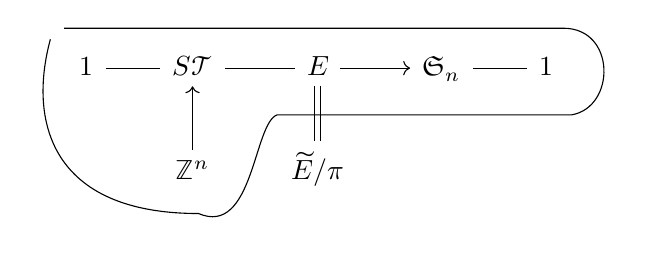
\begin{tikzpicture}
\node[inner sep=6pt] (e) {\begin{tikzcd}[ampersand replacement=\&,column sep=2em,row sep=1.8em]
1\arrow[r,dash]\&S\mathcal T\arrow[r,dash]\&E\arrow[r]\arrow[d,equal]\&\mathfrak S_n\arrow[r,dash]\&1\\
\&\mathbb Z^n\arrow[u]\&\widetilde E/\pi\&\&{}
\end{tikzcd}};
\draw ([xshift=5pt]e.north west) -- ([xshift=-7pt]e.north east)
 .. controls ([xshift=12pt]e.north east) and ([xshift=12pt,yshift=-1cm]e.north east) .. ([xshift=-4pt,yshift=-1.1cm]e.north east)
 -- ([xshift=-0.5cm,yshift=-1.1cm]e.north)
 .. controls ([xshift=-0.8cm,yshift=-1.2cm]e.north) and ([xshift=-0.8cm,yshift=-0.3cm]e.south) .. ([xshift=-1.5cm]e.south)
 .. controls (e.south west) and ([xshift=-8pt]e.west) .. ([yshift=-4pt]e.north west);
\end{tikzpicture}}

\diagram{\begin{tikzcd}[ampersand replacement=\&,column sep=2.4em,row sep=2em]
1\arrow[r,dash]\&\LMsourceMark{M000814}{\unsure{\widetilde F|\widehat F}}\arrow[r,dash]\arrow[d]\&\widetilde A\arrow[r,dash]\arrow[d]\&\widetilde G\arrow[d]\&\\
1\arrow[r,dash]\&\substack{\deleted{\LMsourceMark{M000815}{\unsure{E}}}\inserted{F}\\\text{discret}}\arrow[r]\&A\arrow[r]\&G\arrow[dr]\&
\bigl(=\mathfrak S_n\LMsourceMark{M000816}{\unsure{\ast|\cdot}}\mathbb T^n\bigr)\\
\&\&\&\&1
\end{tikzcd}}

\deleted{\LMsourceMark{M000817}{\unsure{Op.}} ext. de $\pi_0$ sur $F$}

\diagram{\begin{tikzcd}[ampersand replacement=\&,column sep=3.8em,row sep=2.3em]
\pi_1(G)=\pi_1\arrow[r]\arrow[dr,bend right=20,"\substack{\text{\LMsourceMark{M000818}{\unsure{compatible}}}\\\text{avec }\pi_0}"']\&F\arrow[d,phantom,"\cup" description]\\
\&\LMsourceMark{M000819}{\unsure{\mathfrak Z(F)|\mathfrak z(F)}}
\end{tikzcd}}
\inserted{\LMsourceMark{M000820}{\unsure{central}}}

$\pi_0(G)=\pi_0$ opère \LMsourceMark{M000821}{\unsure{extérieurement}} sur $F$
\quad donc opère sur $\LMsourceMark{M000822}{\unsure{\mathfrak Z(F)|\mathfrak z(F)}}$

\diagram{$\begin{array}{cc}
\pi_0&\pi_1\\
\multicolumn{2}{c}{\text{op.}}
\end{array}$}
\deleted{\LMsourceMark{M000823}{\unsure{compatible}} avec l'op. ext.}

\diagram{\begin{tikzcd}[ampersand replacement=\&,column sep=2.4em,row sep=1.7em]
1\arrow[r,dash]\&F\arrow[r]\&E\arrow[r]\arrow[d,equal]\&\pi_0\arrow[r,dash]\&1\\
\&\&\pi_0(\widetilde A)\&\&{}
\end{tikzcd}}
\figure{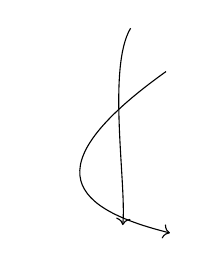
\begin{tikzpicture}[x=1cm,y=1cm]
\draw[->] (0.3,2.5) .. controls (0.0,2.0) and (0.25,0.5) .. (0.2,0);
\draw[->] (0.75,1.95) .. controls (-1.0,0.7) and (-0.4,0.2) .. (0.8,-0.1);
\end{tikzpicture}}

\diagram{\begin{tikzcd}[ampersand replacement=\&,column sep=1.6em]
1\arrow[r,dash]\&\pi_1(A)\arrow[r,dash]\&\pi_1\arrow[r]\&\LMsourceMark{M000824}{\unsure{F}}\arrow[r]\&\underbrace{\pi_0(A)}\arrow[r]\&\substack{\LMsourceMark{M000825}{\unsure{\pi_0|\pi_\infty}}\\ /}\arrow[r,dash]\&1
\end{tikzcd}}

\diagram{\begin{tikzcd}[ampersand replacement=\&,column sep=1.7em,row sep=1.5em,nodes in empty cells]
\deleted{\LMsourceMark{M000826}{\unsure{1}}}\arrow[r,dash]\&\deleted{\LMsourceMark{M000827}{\unsure{\pi_1}}}\arrow[r,dash]\&F\arrow[r,dash]\&\pi_0(\widetilde A)\arrow[r]\arrow[d,equal]\&\pi_0\arrow[r]\&1\\
\&\&\&E\&\&{}
\end{tikzcd}}
}}{\LMsourceMark{M000828}{\LMcancelledDoubts{\(\LMsourceMark{M000829}{\unsure{g_i|q_i}}\)\quad \(\LMsourceMark{M000830}{\unsure{g_i|q_i}}\)\quad \(\LMsourceMark{M000831}{\unsure{g_i|q_i}}\)\quad \(\LMsourceMark{M000832}{\unsure{\mathfrak Z\pi|\mathfrak z\pi}}\)\quad \(\LMsourceMark{M000833}{\unsure{\widetilde F|\widehat F}}\)\quad \(\LMsourceMark{M000834}{\unsure{E}}\)\quad \(\LMsourceMark{M000835}{\unsure{\ast|\cdot}}\)\quad \LMsourceMark{M000836}{\unsure{Op.}}\quad \LMsourceMark{M000837}{\unsure{compatible}}\quad \(\LMsourceMark{M000838}{\unsure{\mathfrak Z(F)|\mathfrak z(F)}}\)\quad \LMsourceMark{M000839}{\unsure{central}}\quad \LMsourceMark{M000840}{\unsure{extérieurement}}\quad \(\LMsourceMark{M000841}{\unsure{\mathfrak Z(F)|\mathfrak z(F)}}\)\quad \LMsourceMark{M000842}{\unsure{compatible}}\quad \(\LMsourceMark{M000843}{\unsure{F}}\)\quad \(\LMsourceMark{M000844}{\unsure{\pi_0|\pi_\infty}}\)\quad \(\LMsourceMark{M000845}{\unsure{1}}\)\quad \(\LMsourceMark{M000846}{\unsure{\pi_1}}\)}}}{deletion}{140-1-s021-D001}
\LMsourceMark{M000847}{\margin{20}}

\LMflushnotes\LMflushpages
\ifnum\LMform=1
\begin{LMapparatus}
\LMentry{140-1-s021-D001}{suppression}{\deleted{
\[
\pi\qquad l_1\ \cdots\ l_n
\]

\diagram{\begin{tikzpicture}
\node[inner sep=7pt] (p) {$\begin{array}{ccc}
u,&\sigma,&(\LMsourceMark{M000848}{\unsure{g_i|q_i}})_{i\in n}\\
\rotatebox{90}{$\in$}&\rotatebox{90}{$\in$}&\rotatebox{90}{$\in$}\\
\operatorname{Aut}\pi&\mathfrak S_n&\pi
\end{array}$};
\draw (p.north west) -- (p.north east) -- (p.south east);
\draw ([yshift=-5pt]p.north west) -- (p.south west) -- ([xshift=3pt]p.south east);
\end{tikzpicture}}
\diagram{\begin{tikzpicture}
\node[inner sep=4pt] (u) {$u(l_i)=\LMsourceMark{M000849}{\unsure{g_i|q_i}}\,l_{\sigma(i)}\,\LMsourceMark{M000850}{\unsure{g_i|q_i}}^{-1}$};
\draw ([yshift=4pt]u.south west) -- (u.south west) -- (u.south east) -- ([yshift=4pt]u.south east);
\end{tikzpicture}}

\diagram{\begin{tikzcd}[ampersand replacement=\&,column sep=1.5em]
1\arrow[r,dash]\&\pi_1(\operatorname{Aut}(X)\arrow[r]\&\mathbb Z^n\arrow[r]\&S\mathcal T\arrow[r]\&\mathcal T\arrow[r,dash]\&\mathfrak S_n\arrow[r,dash]\&1
\end{tikzcd}}

\diagram{\begin{tikzpicture}
\node[inner sep=9pt] (b) {\begin{tikzcd}[ampersand replacement=\&,column sep=3em,row sep=2.5em]
\pi\arrow[r,hook]\&\widetilde E\arrow[r]\arrow[d,leftrightarrow]\&\mathfrak S_n\\
\LMsourceMark{M000851}{\unsure{\mathfrak Z\pi|\mathfrak z\pi}}\arrow[u]\arrow[r]\&\mathbb Z^n\&{}
\end{tikzcd}};
\draw (b.north west) -- (b.north east) -- ([yshift=2pt]b.east) -- ([xshift=-6pt]b.east)
 -- ([xshift=-12pt,yshift=5pt]b.south east) -- ([xshift=0.7cm,yshift=5pt]b.south)
 -- ([xshift=0.6cm,yshift=-6pt]b.south) -- ([yshift=-6pt]b.south west) -- (b.north west);
\end{tikzpicture}}

\diagram{\begin{tikzcd}[ampersand replacement=\&,column sep=2.3em,row sep=1.8em]
\&\&1\&\&\\
1\arrow[r]\&\underbrace{S\operatorname{Aut}^{+}(X)}\arrow[r]\arrow[d,"\simeq"]\&
\operatorname{Aut}^{+}(X)\arrow[u]\arrow[r,dash]\&\operatorname{Aut}^{+}(\partial X)\arrow[r,dash]\&1\\
\&\uline{S\mathcal T}\&\operatorname{Aut}^{+}_{!}(\widetilde X)\arrow[u]\&\uline{\mathfrak S_n\cdot\mathbb T^n}\arrow[u,"\simeq"]\&\\
\&\&\pi\arrow[u]\&\&\\
\&\&1\arrow[u]\&\&
\end{tikzcd}}

\diagram{\begin{tikzcd}[ampersand replacement=\&,column sep=1.6em]
1\arrow[r,dash]\&\underbrace{\pi_1\operatorname{Aut}^{+}(X)}_{0\ \text{ou}\ \mathbb Z}\arrow[r,Rightarrow]\&\mathbb Z^n\arrow[r,dash]\&S\mathcal T\arrow[r,dash]\&\mathcal T\arrow[r,dash]\&\mathfrak S_n\arrow[r,dash]\&1
\end{tikzcd}}

\diagram{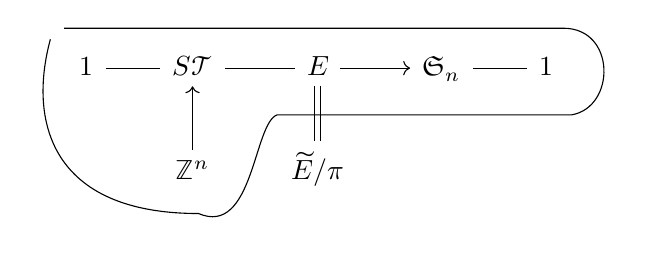
\begin{tikzpicture}
\node[inner sep=6pt] (e) {\begin{tikzcd}[ampersand replacement=\&,column sep=2em,row sep=1.8em]
1\arrow[r,dash]\&S\mathcal T\arrow[r,dash]\&E\arrow[r]\arrow[d,equal]\&\mathfrak S_n\arrow[r,dash]\&1\\
\&\mathbb Z^n\arrow[u]\&\widetilde E/\pi\&\&{}
\end{tikzcd}};
\draw ([xshift=5pt]e.north west) -- ([xshift=-7pt]e.north east)
 .. controls ([xshift=12pt]e.north east) and ([xshift=12pt,yshift=-1cm]e.north east) .. ([xshift=-4pt,yshift=-1.1cm]e.north east)
 -- ([xshift=-0.5cm,yshift=-1.1cm]e.north)
 .. controls ([xshift=-0.8cm,yshift=-1.2cm]e.north) and ([xshift=-0.8cm,yshift=-0.3cm]e.south) .. ([xshift=-1.5cm]e.south)
 .. controls (e.south west) and ([xshift=-8pt]e.west) .. ([yshift=-4pt]e.north west);
\end{tikzpicture}}

\diagram{\begin{tikzcd}[ampersand replacement=\&,column sep=2.4em,row sep=2em]
1\arrow[r,dash]\&\LMsourceMark{M000852}{\unsure{\widetilde F|\widehat F}}\arrow[r,dash]\arrow[d]\&\widetilde A\arrow[r,dash]\arrow[d]\&\widetilde G\arrow[d]\&\\
1\arrow[r,dash]\&\substack{\deleted{\LMsourceMark{M000853}{\unsure{E}}}\inserted{F}\\\text{discret}}\arrow[r]\&A\arrow[r]\&G\arrow[dr]\&
\bigl(=\mathfrak S_n\LMsourceMark{M000854}{\unsure{\ast|\cdot}}\mathbb T^n\bigr)\\
\&\&\&\&1
\end{tikzcd}}

\deleted{\LMsourceMark{M000855}{\unsure{Op.}} ext. de $\pi_0$ sur $F$}

\diagram{\begin{tikzcd}[ampersand replacement=\&,column sep=3.8em,row sep=2.3em]
\pi_1(G)=\pi_1\arrow[r]\arrow[dr,bend right=20,"\substack{\text{\LMsourceMark{M000856}{\unsure{compatible}}}\\\text{avec }\pi_0}"']\&F\arrow[d,phantom,"\cup" description]\\
\&\LMsourceMark{M000857}{\unsure{\mathfrak Z(F)|\mathfrak z(F)}}
\end{tikzcd}}
\inserted{\LMsourceMark{M000858}{\unsure{central}}}

$\pi_0(G)=\pi_0$ opère \LMsourceMark{M000859}{\unsure{extérieurement}} sur $F$
\quad donc opère sur $\LMsourceMark{M000860}{\unsure{\mathfrak Z(F)|\mathfrak z(F)}}$

\diagram{$\begin{array}{cc}
\pi_0&\pi_1\\
\multicolumn{2}{c}{\text{op.}}
\end{array}$}
\deleted{\LMsourceMark{M000861}{\unsure{compatible}} avec l'op. ext.}

\diagram{\begin{tikzcd}[ampersand replacement=\&,column sep=2.4em,row sep=1.7em]
1\arrow[r,dash]\&F\arrow[r]\&E\arrow[r]\arrow[d,equal]\&\pi_0\arrow[r,dash]\&1\\
\&\&\pi_0(\widetilde A)\&\&{}
\end{tikzcd}}
\figure{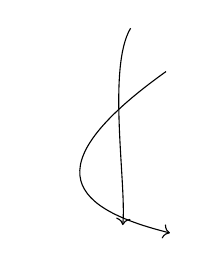
\begin{tikzpicture}[x=1cm,y=1cm]
\draw[->] (0.3,2.5) .. controls (0.0,2.0) and (0.25,0.5) .. (0.2,0);
\draw[->] (0.75,1.95) .. controls (-1.0,0.7) and (-0.4,0.2) .. (0.8,-0.1);
\end{tikzpicture}}

\diagram{\begin{tikzcd}[ampersand replacement=\&,column sep=1.6em]
1\arrow[r,dash]\&\pi_1(A)\arrow[r,dash]\&\pi_1\arrow[r]\&\LMsourceMark{M000862}{\unsure{F}}\arrow[r]\&\underbrace{\pi_0(A)}\arrow[r]\&\substack{\LMsourceMark{M000863}{\unsure{\pi_0|\pi_\infty}}\\ /}\arrow[r,dash]\&1
\end{tikzcd}}

\diagram{\begin{tikzcd}[ampersand replacement=\&,column sep=1.7em,row sep=1.5em,nodes in empty cells]
\deleted{\LMsourceMark{M000864}{\unsure{1}}}\arrow[r,dash]\&\deleted{\LMsourceMark{M000865}{\unsure{\pi_1}}}\arrow[r,dash]\&F\arrow[r,dash]\&\pi_0(\widetilde A)\arrow[r]\arrow[d,equal]\&\pi_0\arrow[r]\&1\\
\&\&\&E\&\&{}
\end{tikzcd}}
}
}{\emph{\LMomittedlabel}}{Passage biffé dans le manuscrit : la suppression suit l'état final de l'auteur; les doutes de lecture restent signalés.}{}
\end{LMapparatus}
\fi
\ifnum\LMform=2
\par\smallskip\begingroup\footnotesize\Needspace{4\baselineskip}\csname @beginparpenalty\endcsname=10000\relax\noindent\textcolor{gray}{\rule{.2\linewidth}{.35pt}}\par\nobreak
\noindent\textit{\LMdoubtheading.}\par\nobreak
\LMcarryover{140-1-s021-D001}{\(\LMsourceMark{M000866}{\unsure{g_i|q_i}}\)\quad \(\LMsourceMark{M000867}{\unsure{g_i|q_i}}\)\quad \(\LMsourceMark{M000868}{\unsure{g_i|q_i}}\)\quad \(\LMsourceMark{M000869}{\unsure{\mathfrak Z\pi|\mathfrak z\pi}}\)\quad \(\LMsourceMark{M000870}{\unsure{\widetilde F|\widehat F}}\)\quad \(\LMsourceMark{M000871}{\unsure{E}}\)\quad \(\LMsourceMark{M000872}{\unsure{\ast|\cdot}}\)\quad \LMsourceMark{M000873}{\unsure{Op.}}\quad \LMsourceMark{M000874}{\unsure{compatible}}\quad \(\LMsourceMark{M000875}{\unsure{\mathfrak Z(F)|\mathfrak z(F)}}\)\quad \LMsourceMark{M000876}{\unsure{central}}\quad \LMsourceMark{M000877}{\unsure{extérieurement}}\quad \(\LMsourceMark{M000878}{\unsure{\mathfrak Z(F)|\mathfrak z(F)}}\)\quad \LMsourceMark{M000879}{\unsure{compatible}}\quad \(\LMsourceMark{M000880}{\unsure{F}}\)\quad \(\LMsourceMark{M000881}{\unsure{\pi_0|\pi_\infty}}\)\quad \(\LMsourceMark{M000882}{\unsure{1}}\)\quad \(\LMsourceMark{M000883}{\unsure{\pi_1}}\)
}
\par\endgroup\smallskip
\fi

\LMsourceMark{M000884}{\scanpage{22}}
% blank
\LMsourceMark{M000885}{\margin{21}}

\LMflushnotes\LMflushpages

\LMsourceMark{M000886}{\scanpage{23}}
A)\quad \uline{Lemme}\quad
$S$ schéma \var{\deleted{\LMsourceMark{M000887}{\unsure{satisfaisant|strictement}}}}{\LMsourceMark{M000888}{\LMcancelledDoubts{\LMsourceMark{M000889}{\unsure{satisfaisant|strictement}}}}}{deletion}{140-1-s023-D001}
régulier intègre tel que $\operatorname{Pic}(S)=0$,
car. du point générique $\ne2$ Alors \var{\deleted{$\LMsourceMark{M000890}{\unsure{H^1}}$}}{\LMsourceMark{M000891}{\LMcancelledDoubts{\(\LMsourceMark{M000892}{\unsure{H^1}}\)}}}{deletion}{140-1-s023-D002}
\[
H^1(U_{0,3},\mathfrak S_3;\mathbb G_m]\simeq\mathbb Z/6\mathbb Z
\]
(\var{\deleted{\LMsourceMark{M000893}{\unsure{résiduelle}}}}{\LMsourceMark{M000894}{\LMcancelledDoubts{\LMsourceMark{M000895}{\unsure{résiduelle}}}}}{deletion}{140-1-s023-D003}\var{\inserted{\LMsourceMark{M000896}{\unsure{pt gén.|si gén.}}}}{\LMadded{\LMsourceMark{M000897}{\unsure{pt gén.|si gén.}}}}{insertion}{140-1-s023-I001} est $2$, on trouve $\mathbb Z/3\mathbb Z$)

\LMsourceMark{M000898}{\margin{\uline{\LMsourceMark{M000899}{\unsure{Dém}}}\quad on utilise suite exacte
\diagram{\begin{tikzcd}[ampersand replacement=\&,column sep=1.3em,row sep=2em]
0\arrow[r]\&H^1(\mathfrak S_3,H^0(U_{0,3},\mathbb G_m)\arrow[r]\&H^1(\text{mixte})\arrow[dll]\&{}\\
H^0\bigl(\mathfrak S_3,\underbrace{H^1(U_{0,3};\mathbb G_m)}_{0}\bigr)\&\&\&{}
\end{tikzcd}}
et
\diagram{\begin{tikzcd}[ampersand replacement=\&,column sep=1.3em]
0\arrow[r]\&H^0(S,\mathbb G_m)\arrow[r]\&H^0(U_{0,3},\mathbb G_m)\arrow[r]\&\LMsourceMark{M000900}{\unsure{h_1(V(J))|h^1(V(J))}}\arrow[r]\&0
\end{tikzcd}}}}

\LMsourceMark{M000901}{\unsure{Je}} dis que si \var{\inserted{le schéma}}{\LMadded{le schéma}}{insertion}{140-1-s023-I002}
$\var{\deleted{\LMsourceMark{M000902}{\unsure{U_{0,3}}}}}{\LMsourceMark{M000903}{\LMcancelledDoubts{\(\LMsourceMark{M000904}{\unsure{U_{0,3}}}\)}}}{deletion}{140-1-s023-D004}\var{\inserted{\Sigma_J}}{\LMadded{\Sigma_J}}{insertion}{140-1-s023-I003}$ est défini comme $\mathbb P(V_J)$, \LMsourceMark{M000905}{\unsure{i.e.}}
\diagram{\begin{tikzcd}[ampersand replacement=\&,column sep=2.8em]
0\arrow[r,dash]\&V_J\arrow[r]\&\mathcal O^J\arrow[r]\&\mathcal O\arrow[r,dash]\&0
\end{tikzcd}}
alors le fibré \LMsourceMark{M000906}{\unsure{principal}}
\[
P\Sigma_J=\check V(\mathcal O_{\Sigma_J}(1))^{*}
\]
est un générateur du
$H^1(\var{\deleted{\LMsourceMark{M000907}{\unsure{U_{0,3}}}}}{\LMsourceMark{M000908}{\LMcancelledDoubts{\(\LMsourceMark{M000909}{\unsure{U_{0,3}}}\)}}}{deletion}{140-1-s023-D005}\var{\inserted{\Sigma_J^*}}{\LMadded{\Sigma_J^*}}{insertion}{140-1-s023-I004},
\var{\deleted{\LMsourceMark{M000910}{\unsure{\mathfrak S_3}}}}{\LMsourceMark{M000911}{\LMcancelledDoubts{\(\LMsourceMark{M000912}{\unsure{\mathfrak S_3}}\)}}}{deletion}{140-1-s023-D006}\var{\inserted{\mathfrak S_J}}{\LMadded{\mathfrak S_J}}{insertion}{140-1-s023-I005};\mathbb G_m)$.

Je vais d'abord \LMsourceMark{M000913}{\unsure{trouver}} une trivialisation de
\[
\uline{\mathcal O}(1)^{\otimes6}=\mathcal O(6)\simeq
\LMsourceMark{M000914}{\unsure{\mathcal T^{\otimes3}(\omega)|\mathcal J^{\otimes3}(\omega)}},
\]
\var{\deleted{donc}}{}{deletion}{140-1-s023-D007} \var{\inserted{en fait}}{\LMadded{en fait}}{insertion}{140-1-s023-I006} une section de $\mathcal O(6)$
\var{\inserted{sur $\overline\Sigma$ \LMsourceMark{M000915}{\unsure{tout entier}}}}{\LMadded{sur $\overline\Sigma$ \LMsourceMark{M000916}{\unsure{tout entier}}}}{insertion}{140-1-s023-I007}
(qui \var{\deleted{\LMsourceMark{M000917}{\unsure{ne s'annule que}}}}{\LMsourceMark{M000918}{\LMcancelledDoubts{\LMsourceMark{M000919}{\unsure{ne s'annule que}}}}}{deletion}{140-1-s023-D008}
\var{\inserted{\LMsourceMark{M000920}{\unsure{est}}, \LMsourceMark{M000921}{\unsure{inversible}}}}{\LMadded{\LMsourceMark{M000922}{\unsure{est}}, \LMsourceMark{M000923}{\unsure{inversible}}}}{insertion}{140-1-s023-I008} sur $\Sigma^*$.
On \var{\deleted{\LMsourceMark{M000924}{\unsure{prenant}}}}{\LMsourceMark{M000925}{\LMcancelledDoubts{\LMsourceMark{M000926}{\unsure{prenant}}}}}{deletion}{140-1-s023-D009} a
\[
\Gamma(\Sigma_J,\mathcal O(6))\simeq\operatorname{Sym}^{6}V_J
\]
et on prendra
\[
\begin{gathered}
\LMsourceMark{M000927}{\unsure{\varphi|\Delta}}\in\Gamma(\Sigma_J,\mathcal O(6)),\qquad
\LMsourceMark{M000928}{\unsure{\varphi|\Delta}}
=\var{\deleted{\LMsourceMark{M000929}{\unsure{\sum_{i\in J}}}}}{\LMsourceMark{M000930}{\LMcancelledDoubts{\(\LMsourceMark{M000931}{\unsure{\sum_{i\in J}}}\)}}}{deletion}{140-1-s023-D010}
-\prod_{\substack{i,j\in J\\i\ne j}}(e_i-e_j)\\
=\prod_{i\in J}\underbrace{(e_j-e_h)}_{J=\{i,j,h\}}^{2}.
\end{gathered}
\]
Ainsi, sur $\var{\deleted{\LMsourceMark{M000932}{\unsure{U_J}}}}{\LMsourceMark{M000933}{\LMcancelledDoubts{\(\LMsourceMark{M000934}{\unsure{U_J}}\)}}}{deletion}{140-1-s023-D011}\var{\inserted{\Sigma_J^{*}}}{\LMadded{\Sigma_J^{*}}}{insertion}{140-1-s023-I009}$, le groupe \LMsourceMark{M000935}{\unsure{structural|structurel}}
\var{\deleted{\LMsourceMark{M000936}{\unsure{de}}}}{\LMsourceMark{M000937}{\LMcancelledDoubts{\LMsourceMark{M000938}{\unsure{de}}}}}{deletion}{140-1-s023-D012}
$\mathbb G_m$ de $P\Sigma_J^{*}$ est réduit \LMsourceMark{M000939}{\unsure{à|:}} $\mu_6$.

\uline{NB}\quad Sauf erreur, on a
\[
\var{\deleted{\LMsourceMark{M000940}{\unsure{\operatorname{Sym}}}}}{\LMsourceMark{M000941}{\LMcancelledDoubts{\(\LMsourceMark{M000942}{\unsure{\operatorname{Sym}}}\)}}}{deletion}{140-1-s023-D013}\quad
\operatorname{Sym}^{*}(V_J)^{\mathfrak S_3}\simeq
\mathcal O\bigl(\LMsourceMark{M000943}{\unsure{\gamma_2|\varphi_2}},\LMsourceMark{M000944}{\unsure{\gamma_3|\varphi_3}}\bigr)
/(2\gamma_3^2-\gamma_2^3)
\]
\[
\left\{\begin{aligned}
\gamma_2&=\sum_{i\in J}(e_j-e_h)^2\\
\gamma_3&=\prod_{i\in J}(e_j\LMsourceMark{M000945}{\unsure{-|+}}e_h-2e_i)
\end{aligned}\right.
\qquad\text{et}\quad\Delta=\gamma_2^3
\]
\LMsourceMark{M000946}{\margin{22}}

\LMflushnotes\LMflushpages
\ifnum\LMform=1
\begin{LMapparatus}
\LMentry{140-1-s023-D001}{suppression}{\deleted{\LMsourceMark{M000947}{\unsure{satisfaisant|strictement}}}
}{\emph{\LMomittedlabel}}{Passage biffé dans le manuscrit : la suppression suit l'état final de l'auteur; les doutes de lecture restent signalés.}{}
\LMentry{140-1-s023-D002}{suppression}{\deleted{$\LMsourceMark{M000948}{\unsure{H^1}}$}
}{\emph{\LMomittedlabel}}{Passage biffé dans le manuscrit : la suppression suit l'état final de l'auteur; les doutes de lecture restent signalés.}{}
\LMentry{140-1-s023-D003}{suppression}{\deleted{\LMsourceMark{M000949}{\unsure{résiduelle}}}
}{\emph{\LMomittedlabel}}{Passage biffé dans le manuscrit : la suppression suit l'état final de l'auteur; les doutes de lecture restent signalés.}{}
\LMentry{140-1-s023-I001}{insertion}{\inserted{\LMsourceMark{M000950}{\unsure{pt gén.|si gén.}}}
}{\emph{\LMinsertedlabel}}{Ajout explicite de l'auteur : intégré à l'endroit indiqué par la transcription, sans modifier sa lecture.}{}
\LMentry{140-1-s023-I002}{insertion}{\inserted{le schéma}
}{\emph{\LMinsertedlabel}}{Ajout explicite de l'auteur : intégré à l'endroit indiqué par la transcription, sans modifier sa lecture.}{}
\LMentry{140-1-s023-D004}{suppression}{\(\deleted{\LMsourceMark{M000951}{\unsure{U_{0,3}}}}\)
}{\emph{\LMomittedlabel}}{Passage biffé dans le manuscrit : la suppression suit l'état final de l'auteur; les doutes de lecture restent signalés.}{}
\LMentry{140-1-s023-I003}{insertion}{\(\inserted{\Sigma_J}\)
}{\emph{\LMinsertedlabel}}{Ajout explicite de l'auteur : intégré à l'endroit indiqué par la transcription, sans modifier sa lecture.}{}
\LMentry{140-1-s023-D005}{suppression}{\(\deleted{\LMsourceMark{M000952}{\unsure{U_{0,3}}}}\)
}{\emph{\LMomittedlabel}}{Passage biffé dans le manuscrit : la suppression suit l'état final de l'auteur; les doutes de lecture restent signalés.}{}
\LMentry{140-1-s023-I004}{insertion}{\(\inserted{\Sigma_J^*}\)
}{\emph{\LMinsertedlabel}}{Ajout explicite de l'auteur : intégré à l'endroit indiqué par la transcription, sans modifier sa lecture.}{}
\LMentry{140-1-s023-D006}{suppression}{\(\deleted{\LMsourceMark{M000953}{\unsure{\mathfrak S_3}}}\)
}{\emph{\LMomittedlabel}}{Passage biffé dans le manuscrit : la suppression suit l'état final de l'auteur; les doutes de lecture restent signalés.}{}
\LMentry{140-1-s023-I005}{insertion}{\(\inserted{\mathfrak S_J}\)
}{\emph{\LMinsertedlabel}}{Ajout explicite de l'auteur : intégré à l'endroit indiqué par la transcription, sans modifier sa lecture.}{}
\LMentry{140-1-s023-D007}{suppression}{\deleted{donc}
}{\emph{\LMomittedlabel}}{Passage biffé dans le manuscrit : la suppression suit l'état final de l'auteur; les doutes de lecture restent signalés.}{}
\LMentry{140-1-s023-I006}{insertion}{\inserted{en fait}
}{\emph{\LMinsertedlabel}}{Ajout explicite de l'auteur : intégré à l'endroit indiqué par la transcription, sans modifier sa lecture.}{}
\LMentry{140-1-s023-I007}{insertion}{\inserted{sur $\overline\Sigma$ \LMsourceMark{M000954}{\unsure{tout entier}}}
}{\emph{\LMinsertedlabel}}{Ajout explicite de l'auteur : intégré à l'endroit indiqué par la transcription, sans modifier sa lecture.}{}
\LMentry{140-1-s023-D008}{suppression}{\deleted{\LMsourceMark{M000955}{\unsure{ne s'annule que}}}
}{\emph{\LMomittedlabel}}{Passage biffé dans le manuscrit : la suppression suit l'état final de l'auteur; les doutes de lecture restent signalés.}{}
\LMentry{140-1-s023-I008}{insertion}{\inserted{\LMsourceMark{M000956}{\unsure{est}}, \LMsourceMark{M000957}{\unsure{inversible}}}
}{\emph{\LMinsertedlabel}}{Ajout explicite de l'auteur : intégré à l'endroit indiqué par la transcription, sans modifier sa lecture.}{}
\LMentry{140-1-s023-D009}{suppression}{\deleted{\LMsourceMark{M000958}{\unsure{prenant}}}
}{\emph{\LMomittedlabel}}{Passage biffé dans le manuscrit : la suppression suit l'état final de l'auteur; les doutes de lecture restent signalés.}{}
\LMentry{140-1-s023-D010}{suppression}{\(\deleted{\LMsourceMark{M000959}{\unsure{\sum_{i\in J}}}}\)
}{\emph{\LMomittedlabel}}{Passage biffé dans le manuscrit : la suppression suit l'état final de l'auteur; les doutes de lecture restent signalés.}{}
\LMentry{140-1-s023-D011}{suppression}{\(\deleted{\LMsourceMark{M000960}{\unsure{U_J}}}\)
}{\emph{\LMomittedlabel}}{Passage biffé dans le manuscrit : la suppression suit l'état final de l'auteur; les doutes de lecture restent signalés.}{}
\LMentry{140-1-s023-I009}{insertion}{\(\inserted{\Sigma_J^{*}}\)
}{\emph{\LMinsertedlabel}}{Ajout explicite de l'auteur : intégré à l'endroit indiqué par la transcription, sans modifier sa lecture.}{}
\LMentry{140-1-s023-D012}{suppression}{\deleted{\LMsourceMark{M000961}{\unsure{de}}}
}{\emph{\LMomittedlabel}}{Passage biffé dans le manuscrit : la suppression suit l'état final de l'auteur; les doutes de lecture restent signalés.}{}
\LMentry{140-1-s023-D013}{suppression}{\(\deleted{\LMsourceMark{M000962}{\unsure{\operatorname{Sym}}}}\)
}{\emph{\LMomittedlabel}}{Passage biffé dans le manuscrit : la suppression suit l'état final de l'auteur; les doutes de lecture restent signalés.}{}
\end{LMapparatus}
\fi
\ifnum\LMform=2
\par\smallskip\begingroup\footnotesize\Needspace{4\baselineskip}\csname @beginparpenalty\endcsname=10000\relax\noindent\textcolor{gray}{\rule{.2\linewidth}{.35pt}}\par\nobreak
\noindent\textit{\LMdoubtheading.}\par\nobreak
\LMcarryover{140-1-s023-D001}{\LMsourceMark{M000963}{\unsure{satisfaisant|strictement}}
}
\LMcarryover{140-1-s023-D002}{\(\LMsourceMark{M000964}{\unsure{H^1}}\)
}
\LMcarryover{140-1-s023-D003}{\LMsourceMark{M000965}{\unsure{résiduelle}}
}
\LMcarryover{140-1-s023-D004}{\(\LMsourceMark{M000966}{\unsure{U_{0,3}}}\)
}
\LMcarryover{140-1-s023-D005}{\(\LMsourceMark{M000967}{\unsure{U_{0,3}}}\)
}
\LMcarryover{140-1-s023-D006}{\(\LMsourceMark{M000968}{\unsure{\mathfrak S_3}}\)
}
\LMcarryover{140-1-s023-D008}{\LMsourceMark{M000969}{\unsure{ne s'annule que}}
}
\LMcarryover{140-1-s023-D009}{\LMsourceMark{M000970}{\unsure{prenant}}
}
\LMcarryover{140-1-s023-D010}{\(\LMsourceMark{M000971}{\unsure{\sum_{i\in J}}}\)
}
\LMcarryover{140-1-s023-D011}{\(\LMsourceMark{M000972}{\unsure{U_J}}\)
}
\LMcarryover{140-1-s023-D012}{\LMsourceMark{M000973}{\unsure{de}}
}
\LMcarryover{140-1-s023-D013}{\(\LMsourceMark{M000974}{\unsure{\operatorname{Sym}}}\)
}
\par\endgroup\smallskip
\fi

\LMsourceMark{M000975}{\scanpage{24}}
% not manuscript: tract imprimé « Parler Femmes à propos de “PLURIELLES” », avec une longue rature diagonale.
\LMsourceMark{M000976}{\margin{23}}

\LMflushnotes\LMflushpages

\LMsourceMark{M000977}{\scanpage{25}}
\Needspace{14\baselineskip}
B)

\var{\deleted{\LMsourceMark{M000978}{\unsure{Si}} $2$ \LMsourceMark{M000979}{\unsure{inversible}}, on \LMsourceMark{M000980}{\unsure{aura}} \LMsourceMark{M000981}{\unsure{donc}}}}{\LMsourceMark{M000982}{\LMcancelledDoubts{\LMsourceMark{M000983}{\unsure{Si}}\quad \LMsourceMark{M000984}{\unsure{inversible}}\quad \LMsourceMark{M000985}{\unsure{aura}}\quad \LMsourceMark{M000986}{\unsure{donc}}}}}{deletion}{140-1-s025-D001}
\[
\var{\deleted{\operatorname{Sym}^{*}(\LMsourceMark{M000987}{\unsure{V_J|W_J}})^{\mathfrak S_{\LMsourceMark{M000988}{\unsure{J|3}}}}\simeq\mathcal O[}}{\LMsourceMark{M000989}{\LMcancelledDoubts{\(\LMsourceMark{M000990}{\unsure{V_J|W_J}}\)\quad \(\LMsourceMark{M000991}{\unsure{J|3}}\)}}}{deletion}{140-1-s025-D002}
\]
\var{\deleted{\LMsourceMark{M000992}{\unsure{Remarque}}}}{\LMsourceMark{M000993}{\LMcancelledDoubts{\LMsourceMark{M000994}{\unsure{Remarque}}}}}{deletion}{140-1-s025-D003}

Comme $\gamma_2$ s'annule en \var{\deleted{\LMsourceMark{M000995}{\unsure{les}}}}{\LMsourceMark{M000996}{\LMcancelledDoubts{\LMsourceMark{M000997}{\unsure{les}}}}}{deletion}{140-1-s025-D004} $P_\omega$,
$\gamma_3$ en les $Q_i$, il s'ensuit qu'il n'y a pas de section invariante
d'un $\mathcal O(n)^*$ \var{\deleted{\LMsourceMark{M000998}{\unsure{pour}}}}{\LMsourceMark{M000999}{\LMcancelledDoubts{\LMsourceMark{M001000}{\unsure{pour}}}}}{deletion}{140-1-s025-D005} sur
$\Sigma_J^{*}$ \var{\deleted{\LMsourceMark{M001001}{\unsure{en degré}} $<$}}{\LMsourceMark{M001002}{\LMcancelledDoubts{\LMsourceMark{M001003}{\unsure{en degré}}}}}{deletion}{140-1-s025-D006}
pour $n\le6$, donc que l'ordre de
$\operatorname{cl}(\mathcal O(1))$ dans
$H^1(\Sigma_J,\mathfrak S_J;\mathbb G_m)$ est bien $6$,
ce qui \LMsourceMark{M001004}{\unsure{prouve}} que $\mathcal O(1)$ est un générateur du
$\LMsourceMark{M001005}{\unsure{H^1}}$ mixte.
\LMsourceMark{M001006}{\margin{24}}

\LMflushnotes\LMflushpages
\ifnum\LMform=1
\begin{LMapparatus}
\LMentry{140-1-s025-D001}{suppression}{\deleted{\LMsourceMark{M001007}{\unsure{Si}} $2$ \LMsourceMark{M001008}{\unsure{inversible}}, on \LMsourceMark{M001009}{\unsure{aura}} \LMsourceMark{M001010}{\unsure{donc}}}
}{\emph{\LMomittedlabel}}{Passage biffé dans le manuscrit : la suppression suit l'état final de l'auteur; les doutes de lecture restent signalés.}{}
\LMentry{140-1-s025-D002}{suppression}{\(\deleted{\operatorname{Sym}^{*}(\LMsourceMark{M001011}{\unsure{V_J|W_J}})^{\mathfrak S_{\LMsourceMark{M001012}{\unsure{J|3}}}}\simeq\mathcal O[}\)
}{\emph{\LMomittedlabel}}{Passage biffé dans le manuscrit : la suppression suit l'état final de l'auteur; les doutes de lecture restent signalés.}{}
\LMentry{140-1-s025-D003}{suppression}{\deleted{\LMsourceMark{M001013}{\unsure{Remarque}}}
}{\emph{\LMomittedlabel}}{Passage biffé dans le manuscrit : la suppression suit l'état final de l'auteur; les doutes de lecture restent signalés.}{}
\LMentry{140-1-s025-D004}{suppression}{\deleted{\LMsourceMark{M001014}{\unsure{les}}}
}{\emph{\LMomittedlabel}}{Passage biffé dans le manuscrit : la suppression suit l'état final de l'auteur; les doutes de lecture restent signalés.}{}
\LMentry{140-1-s025-D005}{suppression}{\deleted{\LMsourceMark{M001015}{\unsure{pour}}}
}{\emph{\LMomittedlabel}}{Passage biffé dans le manuscrit : la suppression suit l'état final de l'auteur; les doutes de lecture restent signalés.}{}
\LMentry{140-1-s025-D006}{suppression}{\deleted{\LMsourceMark{M001016}{\unsure{en degré}} $<$}
}{\emph{\LMomittedlabel}}{Passage biffé dans le manuscrit : la suppression suit l'état final de l'auteur; les doutes de lecture restent signalés.}{}
\end{LMapparatus}
\fi
\ifnum\LMform=2
\par\smallskip\begingroup\footnotesize\Needspace{4\baselineskip}\csname @beginparpenalty\endcsname=10000\relax\noindent\textcolor{gray}{\rule{.2\linewidth}{.35pt}}\par\nobreak
\noindent\textit{\LMdoubtheading.}\par\nobreak
\LMcarryover{140-1-s025-D001}{\LMsourceMark{M001017}{\unsure{Si}}\quad \LMsourceMark{M001018}{\unsure{inversible}}\quad \LMsourceMark{M001019}{\unsure{aura}}\quad \LMsourceMark{M001020}{\unsure{donc}}
}
\LMcarryover{140-1-s025-D002}{\(\LMsourceMark{M001021}{\unsure{V_J|W_J}}\)\quad \(\LMsourceMark{M001022}{\unsure{J|3}}\)
}
\LMcarryover{140-1-s025-D003}{\LMsourceMark{M001023}{\unsure{Remarque}}
}
\LMcarryover{140-1-s025-D004}{\LMsourceMark{M001024}{\unsure{les}}
}
\LMcarryover{140-1-s025-D005}{\LMsourceMark{M001025}{\unsure{pour}}
}
\LMcarryover{140-1-s025-D006}{\LMsourceMark{M001026}{\unsure{en degré}}
}
\par\endgroup\smallskip
\fi

\LMsourceMark{M001027}{\scanpage{26}}
% not manuscript: feuillet dactylographié « Sciences de l’homme », « Energie », « Mécanique et industries de transformation », « Recherches sur les milieux tropicaux et sub-tropicaux » ; pagination imprimée « - 4 - ».
\LMsourceMark{M001028}{\margin{25}}

\LMflushnotes\LMflushpages

\LMsourceMark{M001029}{\scanpage{27}}
% Étiquette imprimée, oblique et à l'envers sur le feuillet.
\begin{flushleft}
MR LE PROFESSEUR GROTHENDIECK ALEX.\\
MATHEMATIQUES\hfill 5
\end{flushleft}

\diagram{\begin{tikzcd}[ampersand replacement=\&,column sep=huge]
\mathbb D'_3 \arrow[r] \& \mathbb D_3
\end{tikzcd}}

\LMsourceMark{M001030}{\margin{\figure{\begin{tikzpicture}[x=1cm,y=1cm]
\draw (0,0) .. controls (.1,.14) and (.25,.13) .. (.48,.03);
\end{tikzpicture}}}}

\diagram{\begin{tikzcd}[ampersand replacement=\&,column sep=large,row sep=large]
PM_{11}(2^{\sim})\overset{?}{\simeq}PU_{0,3}
  \arrow[r,very thick] \arrow[d,leftrightarrow]
\& PM_{11}(2)\simeq TU_{0,3} \arrow[d]\\
U_{0,3}\simeq M_{11}(\LMsourceMark{M001031}{\unsure{\widetilde{2}^{\sim}|2^{\sim}}})
  \arrow[r,very thick]
\& \begin{gathered}(U_{0,3},\{1,\omega\})\\[-2pt]{}\simeq M_{11}(\LMsourceMark{M001032}{\unsure{2}})\end{gathered}
\arrow[ul,phantom,"\mathrm{cart}" description]
\end{tikzcd}}

\[
\var{\deleted{\LMsourceMark{M001033}{\unsure{x}}\longrightarrow\LMsourceMark{M001034}{\unsure{x^2\wedge\omega_0}}}}{\LMsourceMark{M001035}{\LMcancelledDoubts{\(\LMsourceMark{M001036}{\unsure{x}}\)\quad \(\LMsourceMark{M001037}{\unsure{x^2\wedge\omega_0}}\)}}}{deletion}{140-1-s027-D001}
\]
\[
\LMsourceMark{M001038}{\unsure{H^1}}(TU_{03},\mathbb D_3;\mu_2)
\]

\diagram{\begin{tikzcd}[ampersand replacement=\&,column sep=small,row sep=large]
M_{11}(2^{\sim}) \arrow[rr]
  \arrow[dr,"{\var{\deleted{\LMsourceMark{M001039}{\unsure{\mathcal D/\Pi_{0,3}|\mathbb Z/2\,\Pi_{0,3}}}}}{\LMsourceMark{M001040}{\LMcancelledDoubts{\(\LMsourceMark{M001041}{\unsure{\mathcal D/\Pi_{0,3}|\mathbb Z/2\,\Pi_{0,3}}}\)}}}{deletion}{140-1-s027-D002}}"']
\& \& M_{11}(2)\LMsourceMark{M001042}{\unsure{-|'}} \arrow[dl] \arrow[d,leftrightarrow] \& \phantom{M}\\
\& M_{11} \arrow[d] \& M_{11}(2)' \arrow[dl] \& \\
\phantom{M}\arrow[rrruu,dashed,no head,shorten <=-10pt,shorten >=-10pt]
\& M'_{11} \& \&
\end{tikzcd}}

\diagram{\begin{tikzcd}[ampersand replacement=\&,column sep=small,row sep=large]
U_{03} \arrow[rr,"{\{1,\omega\}}"] \arrow[dr,"{\mathbb D'_3}"']
\& \& (U_{0,3},\{1,\omega\}) \arrow[dl,"{\mathbb D_3}"'] \arrow[d,"{\LMsourceMark{M001043}{\unsure{\mathrm{gerbe}}}}"] \& \phantom{U}\\
\& (U_{0,3},\mathbb D'_3) \arrow[d,"{\LMsourceMark{M001044}{\unsure{\mathrm{gerbe}}}}"']
\& (U_{03}) \arrow[dl,"{\mathbb D_3}"] \& \\
\phantom{U}\arrow[rrruu,dashed,no head,shorten <=-12pt,shorten >=-12pt]
\& (U_{0,3},\mathbb D_3) \& \&
\end{tikzcd}}

\diagram{\begin{tikzcd}[ampersand replacement=\&,column sep=small,row sep=large]
\begin{gathered}(\mathcal D,\Pi_{03})\\[-2pt]{}\simeq\mathcal D/\Pi_{03}\end{gathered}
 \arrow[rr,very thick,"{\mathrm{gal}}","{\{1,\omega\}}"']
 \arrow[dr,"{\begin{gathered}\mathrm{gal}\\\mathbb D'_3\end{gathered}}"']
\& \& (\mathcal D,\Pi_{03}\times\{1,\omega\})
 \arrow[dl,"{\begin{gathered}\mathrm{gal}\\\mathbb D_3\ \var{\deleted{\LMsourceMark{M001045}{\unsure{\{1,\omega\}}}}}{\LMsourceMark{M001046}{\LMcancelledDoubts{\(\LMsourceMark{M001047}{\unsure{\{1,\omega\}}}\)}}}{deletion}{140-1-s027-D003}\end{gathered}}"']
 \arrow[d,"{\LMsourceMark{M001048}{\unsure{2\text{-}\uline{\mathrm{gerbe}}}}}"] \& \phantom{D}\\
\& (\mathcal D,\LMsourceMark{M001049}{\unsure{\mathrm{Sl}(2,\mathbb Z)}})
 \arrow[d,"{\LMsourceMark{M001050}{\unsure{2\text{-}\mathrm{gerbe}}}}"']
\& (\mathcal D,\Pi_{03}) \arrow[dl,"{\begin{gathered}\mathrm{gal}\\\mathbb D_3\end{gathered}}"] \& \\
\phantom{D}\arrow[rrruu,dashed,no head,shorten <=-12pt,shorten >=-12pt]
\& (\mathcal D,\LMsourceMark{M001051}{\unsure{\mathrm{Sl}(2,\mathbb Z)}}') \& \&
\end{tikzcd}}

\LMsourceMark{M001052}{\margin{26}}

\LMflushnotes\LMflushpages
\ifnum\LMform=1
\begin{LMapparatus}
\LMentry{140-1-s027-D001}{suppression}{\(\deleted{\LMsourceMark{M001053}{\unsure{x}}\longrightarrow\LMsourceMark{M001054}{\unsure{x^2\wedge\omega_0}}}\)
}{\emph{\LMomittedlabel}}{Passage biffé dans le manuscrit : la suppression suit l'état final de l'auteur; les doutes de lecture restent signalés.}{}
\LMentry{140-1-s027-D002}{suppression}{\(\deleted{\LMsourceMark{M001055}{\unsure{\mathcal D/\Pi_{0,3}|\mathbb Z/2\,\Pi_{0,3}}}}\)
}{\emph{\LMomittedlabel}}{Passage biffé dans le manuscrit : la suppression suit l'état final de l'auteur; les doutes de lecture restent signalés.}{}
\LMentry{140-1-s027-D003}{suppression}{\(\deleted{\LMsourceMark{M001056}{\unsure{\{1,\omega\}}}}\)
}{\emph{\LMomittedlabel}}{Passage biffé dans le manuscrit : la suppression suit l'état final de l'auteur; les doutes de lecture restent signalés.}{}
\end{LMapparatus}
\fi
\ifnum\LMform=2
\par\smallskip\begingroup\footnotesize\Needspace{4\baselineskip}\csname @beginparpenalty\endcsname=10000\relax\noindent\textcolor{gray}{\rule{.2\linewidth}{.35pt}}\par\nobreak
\noindent\textit{\LMdoubtheading.}\par\nobreak
\LMcarryover{140-1-s027-D001}{\(\LMsourceMark{M001057}{\unsure{x}}\)\quad \(\LMsourceMark{M001058}{\unsure{x^2\wedge\omega_0}}\)
}
\LMcarryover{140-1-s027-D002}{\(\LMsourceMark{M001059}{\unsure{\mathcal D/\Pi_{0,3}|\mathbb Z/2\,\Pi_{0,3}}}\)
}
\LMcarryover{140-1-s027-D003}{\(\LMsourceMark{M001060}{\unsure{\{1,\omega\}}}\)
}
\par\endgroup\smallskip
\fi

\LMsourceMark{M001061}{\scanpage{28}}
% not manuscript: avis dactylographié, à l’envers, de soutenance d’une thèse de doctorat de 3ème cycle, « Algèbres de Rees », YOON Suk-Im, Montpellier, le 26 février 1982 ; soutenance prévue le 4 MARS 1982 à 15h.
\LMsourceMark{M001062}{\margin{27}}

\LMflushnotes\LMflushpages

\LMsourceMark{M001063}{\scanpage{29}}

\var{\deleted{\diagram{\begin{tikzcd}[ampersand replacement=\&,column sep=small,row sep=large]
\& \& {}\arrow[r,"{\LMsourceMark{M001064}{\unsure{''|1}}}"]
\& \mathrm{Sl}(2,\mathbb Z)\arrow[r]\arrow[d]
\& \Pi_{0,3}^{D}\arrow[d] \& \\
\& \LMsourceMark{M001065}{\unsure{\widetilde\varepsilon|\widetilde E}}\arrow[rr]
  \arrow[ddl]\arrow[dr,dashed]
\& \& \mathbb D_3\mathop{\times}\limits_{\mathbb Z/2\mathbb Z}
       \mathbb Z/\LMsourceMark{M001066}{\unsure{12}}\mathbb Z
       \simeq\mathbb D'_3\mathop{\times}\limits_{\mathbb Z/\LMsourceMark{M001067}{\unsure{2}}\mathbb Z}
       \mathbb Z/6\mathbb Z
       \arrow[r]\arrow[dd,very thick]\arrow[d,dashed]
\& \mathbb D_3\mathop{\times}\limits_{\mathbb Z/2\mathbb Z}
       \mathbb Z/6\mathbb Z=\LMsourceMark{M001068}{\unsure{\varepsilon|E}}
       \arrow[dd]\arrow[dr] \& \\
\& \& \mathbb Z\arrow[r,no head]\arrow[ddl,dashed,leftrightarrow,very thick]
\& \mathbb Z/12\mathbb Z\arrow[rr,dashed,"{\mathrm{can}}"]
       \arrow[dd,dashed,"{\mathrm{can}}"'{pos=.2}]
\& \& \mathbb Z/6\mathbb Z\arrow[ddl,"{\mathrm{can}}"]\\
\LMsourceMark{M001069}{\unsure{\widetilde{\mathbb D}_3^{*}|\widetilde{\mathbb D}'_3}}
 \arrow[rrr,very thick]\arrow[dr]
\& \& \& \mathbb D'_3\arrow[r,very thick]\arrow[d,very thick]
\& \mathbb D_3\arrow[d,"{\mathrm{can}}"] \& \\
\& \mathbb Z\arrow[rr] \& \& \mathbb Z/4\mathbb Z\arrow[r,"{\mathrm{can}}"]
\& \mathbb Z/2\mathbb Z \&
\end{tikzcd}}}}{\LMsourceMark{M001070}{\LMcancelledDoubts{\(\LMsourceMark{M001071}{\unsure{''|1}}\)\quad \(\LMsourceMark{M001072}{\unsure{\widetilde\varepsilon|\widetilde E}}\)\quad \(\LMsourceMark{M001073}{\unsure{12}}\)\quad \(\LMsourceMark{M001074}{\unsure{2}}\)\quad \(\LMsourceMark{M001075}{\unsure{\varepsilon|E}}\)\quad \(\LMsourceMark{M001076}{\unsure{\widetilde{\mathbb D}_3^{*}|\widetilde{\mathbb D}'_3}}\)}}}{deletion}{140-1-s029-D001}

\figure{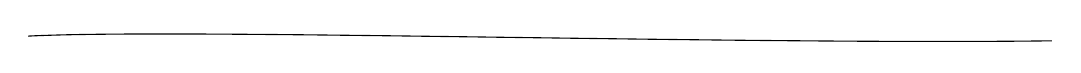
\begin{tikzpicture}[x=1cm,y=1cm]
\draw (0,.06) .. controls (2,.16) and (9,-.05) .. (13,0);
\end{tikzpicture}}

\diagram{\begin{tikzcd}[ampersand replacement=\&,column sep=small,row sep=large]
\LMsourceMark{M001077}{\unsure{\mathbb Z_{(\omega/2)}}}\arrow[r]\arrow[d,very thick]
\& \widetilde\Pi_{0,3}^{\LMsourceMark{M001078}{\unsure{\circ}}}
   \var{\deleted{\LMsourceMark{M001079}{\unsure{\widetilde\Pi_{0,3}}}}}{\LMsourceMark{M001080}{\LMcancelledDoubts{\(\LMsourceMark{M001081}{\unsure{\widetilde\Pi_{0,3}}}\)}}}{deletion}{140-1-s029-D002}\arrow[rr,very thick]\arrow[d]
\& \& \Pi_{0,3}\arrow[d,leftrightarrow,bend left=12]
\& \& \& \\
\mathbb Z_{(\omega)}\arrow[r,very thick]\arrow[d,equal]
\& \widetilde\Pi_{0,3}^{\LMsourceMark{M001082}{\unsure{'}}}\arrow[rr]\arrow[d,very thick]
\& \& \Pi'_{0,3}=\Pi_{0,3}\times\{1,\omega\}
   \arrow[rr]\arrow[d,bend right=12]
\& \& \Pi_{03}\arrow[d,bend right=18] \& \\
\mathbb Z\arrow[r,very thick]\arrow[d,equal]
\& \widetilde{\mathrm{Sl}}(2,\mathbb Z)=\widetilde\Pi_{0,3}^{D}
   \arrow[rr]\arrow[d]
\& \& \mathrm{Sl}(2,\mathbb Z)\arrow[rr]\arrow[d,very thick]\arrow[ddr]
\& \& \Pi_{0,3}^{D}\arrow[d]\arrow[ddr] \& \\
\mathbb Z\arrow[r]\arrow[dd,equal]
\& \widetilde{\mathbb D}_3\arrow[rr]\arrow[dd]
\& \& \begin{gathered}\mathbb D'''_3\\\LMsourceMark{M001083}{\margin{3}}\end{gathered}\arrow[rr,"2"]\arrow[dr,"3"']\arrow[dd,"3"']
\& \& \begin{gathered}\mathbb D''_3\\\LMsourceMark{M001084}{\margin{\LMsourceMark{M001085}{\unsure{12|10}}}}\end{gathered}\arrow[dr,"3"]\arrow[dd,"3"'{pos=.72}] \& \\
\& \& \& \& \mathbb D'_3\arrow[rr,"2"{pos=.75}]\arrow[dd,"3"{pos=.77}]
\& \& \mathbb D_3\arrow[dd,"3"]\\
\mathbb Z\arrow[r,"12"]
\& \mathbb Z\arrow[rr]
\& \& \mathbb Z/12\mathbb Z\arrow[rr,leftrightarrow,"2"]\arrow[dr,"3"']
\& \& \mathbb Z/6\mathbb Z\arrow[dr,"3"] \& \\
\& \& \& \& \mathbb Z/4\mathbb Z\arrow[rr,"2"] \& \& \mathbb Z/2\mathbb Z
\end{tikzcd}}
\LMsourceMark{M001086}{\margin{\LMsourceMark{M001087}{\unsure{fond|bon}}}}

\diagram{\begin{tikzcd}[ampersand replacement=\&,column sep=large,row sep=large]
1\arrow[r,no head]
\& \mathbb Z\arrow[r,no head]\arrow[d,very thick,"{\begin{gathered}4\\\LMsourceMark{M001088}{\unsure{4}}\end{gathered}}"]
\& \widetilde\Pi_{0,3}^{D}\arrow[r,no head]\arrow[d,no head]
\& \Pi_{0,3}^{D}\arrow[r]\arrow[d,no head]
\& 1\\
1\arrow[r,no head]
\& \mathbb Z\arrow[r,no head]
\& \widetilde\Pi_{0,3}^{D}(4)\arrow[r]
\& \Pi_{0,3}^{D}\arrow[r,very thick]
\& 1
\end{tikzcd}}

\figure{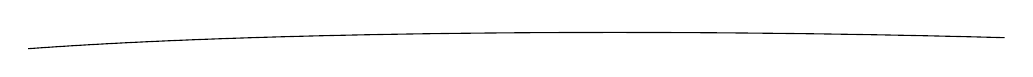
\begin{tikzpicture}[x=1cm,y=1cm]
\draw (0,0) .. controls (3,.22) and (8,.26) .. (12.4,.14);
\end{tikzpicture}}

\diagram{\begin{tikzcd}[ampersand replacement=\&,column sep=large,row sep=large]
\& \& \widetilde\Pi_{0,3}^{D}
\& \Pi_{0,3}^{D}\arrow[r,no head] \& 1\\
1\arrow[r]
\& \overset{\omega}{\mathbb Z}\arrow[r]
\& \widetilde\Pi_{0,3}^{D}(4)\arrow[r]
\& \Pi_{0,3}^{D}\times\mathbb Z/4\mathbb Z\arrow[u]\arrow[r,no head]
\& 1\\
1\arrow[r,no head]
\& \mathbb Z\arrow[r]
\& ?\arrow[r]
\& \LMsourceMark{M001089}{\unsure{\mathrm{Sl}(2,\mathbb Z)}}\arrow[u]\arrow[r,no head]
\& 1
\end{tikzcd}}

\LMsourceMark{M001090}{\margin{28}}

\LMflushnotes\LMflushpages
\ifnum\LMform=1
\begin{LMapparatus}
\LMentry{140-1-s029-D001}{suppression}{\deleted{\diagram{\begin{tikzcd}[ampersand replacement=\&,column sep=small,row sep=large]
\& \& {}\arrow[r,"{\LMsourceMark{M001091}{\unsure{''|1}}}"]
\& \mathrm{Sl}(2,\mathbb Z)\arrow[r]\arrow[d]
\& \Pi_{0,3}^{D}\arrow[d] \& \\
\& \LMsourceMark{M001092}{\unsure{\widetilde\varepsilon|\widetilde E}}\arrow[rr]
  \arrow[ddl]\arrow[dr,dashed]
\& \& \mathbb D_3\mathop{\times}\limits_{\mathbb Z/2\mathbb Z}
       \mathbb Z/\LMsourceMark{M001093}{\unsure{12}}\mathbb Z
       \simeq\mathbb D'_3\mathop{\times}\limits_{\mathbb Z/\LMsourceMark{M001094}{\unsure{2}}\mathbb Z}
       \mathbb Z/6\mathbb Z
       \arrow[r]\arrow[dd,very thick]\arrow[d,dashed]
\& \mathbb D_3\mathop{\times}\limits_{\mathbb Z/2\mathbb Z}
       \mathbb Z/6\mathbb Z=\LMsourceMark{M001095}{\unsure{\varepsilon|E}}
       \arrow[dd]\arrow[dr] \& \\
\& \& \mathbb Z\arrow[r,no head]\arrow[ddl,dashed,leftrightarrow,very thick]
\& \mathbb Z/12\mathbb Z\arrow[rr,dashed,"{\mathrm{can}}"]
       \arrow[dd,dashed,"{\mathrm{can}}"'{pos=.2}]
\& \& \mathbb Z/6\mathbb Z\arrow[ddl,"{\mathrm{can}}"]\\
\LMsourceMark{M001096}{\unsure{\widetilde{\mathbb D}_3^{*}|\widetilde{\mathbb D}'_3}}
 \arrow[rrr,very thick]\arrow[dr]
\& \& \& \mathbb D'_3\arrow[r,very thick]\arrow[d,very thick]
\& \mathbb D_3\arrow[d,"{\mathrm{can}}"] \& \\
\& \mathbb Z\arrow[rr] \& \& \mathbb Z/4\mathbb Z\arrow[r,"{\mathrm{can}}"]
\& \mathbb Z/2\mathbb Z \&
\end{tikzcd}}}
}{\emph{\LMomittedlabel}}{Passage biffé dans le manuscrit : la suppression suit l'état final de l'auteur; les doutes de lecture restent signalés.}{}
\LMentry{140-1-s029-D002}{suppression}{\(\deleted{\LMsourceMark{M001097}{\unsure{\widetilde\Pi_{0,3}}}}\)
}{\emph{\LMomittedlabel}}{Passage biffé dans le manuscrit : la suppression suit l'état final de l'auteur; les doutes de lecture restent signalés.}{}
\end{LMapparatus}
\fi
\ifnum\LMform=2
\par\smallskip\begingroup\footnotesize\Needspace{4\baselineskip}\csname @beginparpenalty\endcsname=10000\relax\noindent\textcolor{gray}{\rule{.2\linewidth}{.35pt}}\par\nobreak
\noindent\textit{\LMdoubtheading.}\par\nobreak
\LMcarryover{140-1-s029-D001}{\(\LMsourceMark{M001098}{\unsure{''|1}}\)\quad \(\LMsourceMark{M001099}{\unsure{\widetilde\varepsilon|\widetilde E}}\)\quad \(\LMsourceMark{M001100}{\unsure{12}}\)\quad \(\LMsourceMark{M001101}{\unsure{2}}\)\quad \(\LMsourceMark{M001102}{\unsure{\varepsilon|E}}\)\quad \(\LMsourceMark{M001103}{\unsure{\widetilde{\mathbb D}_3^{*}|\widetilde{\mathbb D}'_3}}\)
}
\LMcarryover{140-1-s029-D002}{\(\LMsourceMark{M001104}{\unsure{\widetilde\Pi_{0,3}}}\)
}
\par\endgroup\smallskip
\fi

\LMsourceMark{M001105}{\scanpage{30}}
% Secteur supérieur : un long trait courbe au crayon, terminé en crochet, descend de « par les e_i-e_j » vers le bas à gauche ;
% il traverse les trois premières lignes, la suite Z — Π̃_03 — Π_03 → 1 et la formule V(ω) ≃ V, barrées ici en bloc.
\var{\deleted{
$V_J\deleted{\LMsourceMark{M001106}{\unsure{\simeq}}}\inserted{=\LMsourceMark{M001107}{\unsure{\Gamma(X,\uline{\mathcal O}(1))}}}
\deleted{e_i-e_j}$ \LMsourceMark{M001108}{\unsure{engendré}} par les $e_i-e_j$

\deleted{$\LMsourceMark{M001109}{\unsure{\Pi(e_i-e_j)|P(e_i-e_j)}}$}
\LMsourceMark{M001110}{\unsure{comment}} ces \LMsourceMark{M001111}{\unsure{sections}} \LMsourceMark{M001112}{\unsure{sont}} elles
\LMsourceMark{M001113}{\unsure{permutées}} entre elles
}}{\LMsourceMark{M001114}{\LMcancelledDoubts{\(\LMsourceMark{M001115}{\unsure{\simeq}}\)\quad \(\LMsourceMark{M001116}{\unsure{\Gamma(X,\uline{\mathcal O}(1))}}\)\quad \LMsourceMark{M001117}{\unsure{engendré}}\quad \(\LMsourceMark{M001118}{\unsure{\Pi(e_i-e_j)|P(e_i-e_j)}}\)\quad \LMsourceMark{M001119}{\unsure{comment}}\quad \LMsourceMark{M001120}{\unsure{sections}}\quad \LMsourceMark{M001121}{\unsure{sont}}\quad \LMsourceMark{M001122}{\unsure{permutées}}}}}{deletion}{140-1-s030-D001}

\figure{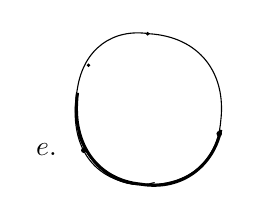
\begin{tikzpicture}[x=1cm,y=1cm]
\draw (0,.95) .. controls (.64,.91) and (.98,.45) .. (.91,-.15)
 .. controls (.86,-.78) and (.36,-1.04) .. (-.25,-.95)
 .. controls (-.83,-.83) and (-1.02,-.33) .. (-.91,.26)
 .. controls (-.83,.76) and (-.46,1.02) .. (0,.95);
\draw[line width=1.1pt] (-.91,.2) .. controls (-1,-.48) and (-.63,-.91) .. (-.11,-.96)
 .. controls (.43,-1.05) and (.82,-.71) .. (.91,-.27);
\draw (-.9,-.33) .. controls (-.72,-.82) and (-.31,-1.05) .. (.07,-.94);
\fill (-.02,.95) circle (.025);
\fill (-.77,.55) circle (.024);
\fill (-.83,-.53) circle (.035);
\fill (.89,-.32) circle (.035);
\node[left] at (-1.04,-.52) {$e.$};
\end{tikzpicture}}

\[
\var{\deleted{e_i-e_j\qquad\LMsourceMark{M001123}{\unsure{\mathcal O(6)|\mathcal O(1)}}}}{\LMsourceMark{M001124}{\LMcancelledDoubts{\(\LMsourceMark{M001125}{\unsure{\mathcal O(6)|\mathcal O(1)}}\)}}}{deletion}{140-1-s030-D005}
\qquad e_i-e_j=
\]
\[
\LMsourceMark{M001126}{\unsure{\xi_i}}.
\]

\diagram{\begin{tikzcd}[ampersand replacement=\&,column sep=small,row sep=small]
\LMsourceMark{M001127}{\unsure{\uline{\mathcal O}_x(1)|\uline{\mathcal O}_a(1)}}\arrow[d,phantom,"{\LMsourceMark{M001128}{\unsure{\in}}}"{description,rotate=90}]
 \& {}\ni\xi_{ij}(x)\\
\lambda \& \lambda^6=\displaystyle\prod_{i,j}\xi_{ij}(x)
\end{tikzcd}}

\var{\deleted{\diagram{\begin{tikzcd}[ampersand replacement=\&,column sep=large]
\mathbb Z\arrow[r,no head]
\& \widetilde\Pi_{\LMsourceMark{M001129}{\unsure{03}}}\arrow[r]
\& \Pi_{03}^{\LMsourceMark{M001130}{\unsure{\sharp|\ast}}}\arrow[r,very thick]
\& 1
\end{tikzcd}}}}{\LMsourceMark{M001131}{\LMcancelledDoubts{\(\LMsourceMark{M001132}{\unsure{03}}\)\quad \(\LMsourceMark{M001133}{\unsure{\sharp|\ast}}\)}}}{deletion}{140-1-s030-D006}

\[
(e_i-e_j)(\uline{\LMsourceMark{M001134}{\unsure{Q_n|Q_k}}})
\qquad\var{\deleted{\LMsourceMark{M001135}{\unsure{e_i-e_j}}}}{\LMsourceMark{M001136}{\LMcancelledDoubts{\(\LMsourceMark{M001137}{\unsure{e_i-e_j}}\)}}}{deletion}{140-1-s030-D007}
\]

\[
\var{\deleted{\mathbf V(\omega)\overset{!!}{\simeq}\mathbf V}}{}{deletion}{140-1-s030-D008}
\qquad \varphi\in V
\qquad e_i-e_j(\var{\deleted{\LMsourceMark{M001138}{\unsure{Q_k}}}}{\LMsourceMark{M001139}{\LMcancelledDoubts{\(\LMsourceMark{M001140}{\unsure{Q_k}}\)}}}{deletion}{140-1-s030-D009}\,
\]
\[
e_i-e_j\bmod L_{Q_k}
\]

\diagram{\(\begin{array}{ccc}
\frac12 & \frac12 & 1\\
-\frac12 & -\frac12 & -1
\end{array}\)}
\[
\left(\frac12\right)^4\qquad\sqrt[3]{\frac12}
\]

% Secteur inférieur, écrit à l'envers par rapport au secteur précédent.
\var{\deleted{
On a vu qu'une orientation d'une \deleted{\LMsourceMark{M001141}{\unsure{surface}}}\inserted{\LMsourceMark{M001142}{\unsure{carte}}}
\inserted{\LMsourceMark{M001143}{\unsure{cellulaire|cellulation}}} combinatoire $A$
\LMsourceMark{M001144}{\unsure{donne}} lieu \LMsourceMark{M001145}{\unsure{à|:}} deux \LMsourceMark{M001146}{\unsure{opérateurs|opérations}}
$\vec\rho_s,\vec\rho_f$ sur $\vec A$, \LMsourceMark{M001147}{\unsure{satisfaisant}}
\[
\vec\rho_s^{-1}\vec\rho_f=\sigma
\]

Si on prend l'orientation inverse, \LMsourceMark{M001148}{\unsure{quels|quelles}} sont les
\LMsourceMark{M001149}{\unsure{opérateurs|opérations}} \LMsourceMark{M001150}{\unsure{correspondants|correspondantes}}
$\vec\rho'_s,\vec\rho'_f$ ?
Si $\vec a\in\vec A$ \LMsourceMark{M001151}{\unsure{provient}} de $a\in A^L_+$,
il \LMsourceMark{M001152}{\unsure{provient}} de $\sigma_na\in A^L_-$, et on a
\[
\rho_s(\sigma_na)
 =\sigma_n
   (\underbrace{\sigma_n\rho_s\sigma_n}
     _{\sigma_n\varepsilon=\rho_s^{-1}}a)
 =\sigma_n(\rho_s^{-1}a)\,-
\]
\LMsourceMark{M001153}{\unsure{donc}} la classe dans $\vec A\simeq A^L/\sigma_n$
est celle de $\rho_s^{-1}a$,
i.e. $\vec\rho_s^{-1}\vec a$.
\deleted{\LMsourceMark{M001154}{\unsure{E}}}t on a donc
\[
\deleted{\rho_f(\sigma_na)
 =\sigma_n
  (\underbrace{\sigma_n\rho_f\sigma_n}
   _{\sigma_n\varepsilon\sigma}a)}
\]
\[
\vec\rho'_s=\vec\rho_s^{-1}
\]
d'où
\[
\vec\rho'_f=\vec\rho'_s\sigma
 =\vec\rho_s^{-1}\sigma
 =\sigma\vec\rho_f^{-1}\sigma
 =\mathrm{int}(\sigma)\vec\rho_f^{-1}
\]
(Ce n'est pas tellement \LMsourceMark{M001155}{\unsure{plaisant}}.)
}}{\LMsourceMark{M001156}{\LMcancelledDoubts{\LMsourceMark{M001157}{\unsure{surface}}\quad \LMsourceMark{M001158}{\unsure{carte}}\quad \LMsourceMark{M001159}{\unsure{cellulaire|cellulation}}\quad \LMsourceMark{M001160}{\unsure{donne}}\quad \LMsourceMark{M001161}{\unsure{à|:}}\quad \LMsourceMark{M001162}{\unsure{opérateurs|opérations}}\quad \LMsourceMark{M001163}{\unsure{satisfaisant}}\quad \LMsourceMark{M001164}{\unsure{quels|quelles}}\quad \LMsourceMark{M001165}{\unsure{opérateurs|opérations}}\quad \LMsourceMark{M001166}{\unsure{correspondants|correspondantes}}\quad \LMsourceMark{M001167}{\unsure{provient}}\quad \LMsourceMark{M001168}{\unsure{provient}}\quad \LMsourceMark{M001169}{\unsure{donc}}\quad \LMsourceMark{M001170}{\unsure{E}}\quad \LMsourceMark{M001171}{\unsure{plaisant}}}}}{deletion}{140-1-s030-D010}

\LMsourceMark{M001172}{\margin{
% Notes perpendiculaires dans la marge droite du secteur inférieur redressé.
\[
\LMsourceMark{M001173}{\unsure{\widetilde Q_m|\widetilde R_m}}
 -\LMsourceMark{M001174}{\unsure{\widetilde Q_j|\widetilde R_j}}
\]
\[
\var{\deleted{\LMsourceMark{M001175}{\unsure{\xi}}}}{\LMsourceMark{M001176}{\LMcancelledDoubts{\(\LMsourceMark{M001177}{\unsure{\xi}}\)}}}{deletion}{140-1-s030-D014}\quad\LMsourceMark{M001178}{\unsure{\gamma_h\ i\gamma_h}}
\]
\[
e_j-e_i\quad -(e_i-e_h)
\]
}}

\LMsourceMark{M001179}{\margin{29}}

\LMflushnotes\LMflushpages
\ifnum\LMform=1
\begin{LMapparatus}
\LMentry{140-1-s030-D001}{suppression}{\deleted{
$V_J\deleted{\LMsourceMark{M001180}{\unsure{\simeq}}}\inserted{=\LMsourceMark{M001181}{\unsure{\Gamma(X,\uline{\mathcal O}(1))}}}
\deleted{e_i-e_j}$ \LMsourceMark{M001182}{\unsure{engendré}} par les $e_i-e_j$

\deleted{$\LMsourceMark{M001183}{\unsure{\Pi(e_i-e_j)|P(e_i-e_j)}}$}
\LMsourceMark{M001184}{\unsure{comment}} ces \LMsourceMark{M001185}{\unsure{sections}} \LMsourceMark{M001186}{\unsure{sont}} elles
\LMsourceMark{M001187}{\unsure{permutées}} entre elles
}
}{\emph{\LMomittedlabel}}{Passage biffé dans le manuscrit : la suppression suit l'état final de l'auteur; les doutes de lecture restent signalés.}{}
\LMentry{140-1-s030-D005}{suppression}{\(\deleted{e_i-e_j\qquad\LMsourceMark{M001188}{\unsure{\mathcal O(6)|\mathcal O(1)}}}\)
}{\emph{\LMomittedlabel}}{Passage biffé dans le manuscrit : la suppression suit l'état final de l'auteur; les doutes de lecture restent signalés.}{}
\LMentry{140-1-s030-D006}{suppression}{\deleted{\diagram{\begin{tikzcd}[ampersand replacement=\&,column sep=large]
\mathbb Z\arrow[r,no head]
\& \widetilde\Pi_{\LMsourceMark{M001189}{\unsure{03}}}\arrow[r]
\& \Pi_{03}^{\LMsourceMark{M001190}{\unsure{\sharp|\ast}}}\arrow[r,very thick]
\& 1
\end{tikzcd}}}
}{\emph{\LMomittedlabel}}{Passage biffé dans le manuscrit : la suppression suit l'état final de l'auteur; les doutes de lecture restent signalés.}{}
\LMentry{140-1-s030-D007}{suppression}{\(\deleted{\LMsourceMark{M001191}{\unsure{e_i-e_j}}}\)
}{\emph{\LMomittedlabel}}{Passage biffé dans le manuscrit : la suppression suit l'état final de l'auteur; les doutes de lecture restent signalés.}{}
\LMentry{140-1-s030-D008}{suppression}{\(\deleted{\mathbf V(\omega)\overset{!!}{\simeq}\mathbf V}\)
}{\emph{\LMomittedlabel}}{Passage biffé dans le manuscrit : la suppression suit l'état final de l'auteur; les doutes de lecture restent signalés.}{}
\LMentry{140-1-s030-D009}{suppression}{\(\deleted{\LMsourceMark{M001192}{\unsure{Q_k}}}\)
}{\emph{\LMomittedlabel}}{Passage biffé dans le manuscrit : la suppression suit l'état final de l'auteur; les doutes de lecture restent signalés.}{}
\LMentry{140-1-s030-D010}{suppression}{\deleted{
On a vu qu'une orientation d'une \deleted{\LMsourceMark{M001193}{\unsure{surface}}}\inserted{\LMsourceMark{M001194}{\unsure{carte}}}
\inserted{\LMsourceMark{M001195}{\unsure{cellulaire|cellulation}}} combinatoire $A$
\LMsourceMark{M001196}{\unsure{donne}} lieu \LMsourceMark{M001197}{\unsure{à|:}} deux \LMsourceMark{M001198}{\unsure{opérateurs|opérations}}
$\vec\rho_s,\vec\rho_f$ sur $\vec A$, \LMsourceMark{M001199}{\unsure{satisfaisant}}
\[
\vec\rho_s^{-1}\vec\rho_f=\sigma
\]

Si on prend l'orientation inverse, \LMsourceMark{M001200}{\unsure{quels|quelles}} sont les
\LMsourceMark{M001201}{\unsure{opérateurs|opérations}} \LMsourceMark{M001202}{\unsure{correspondants|correspondantes}}
$\vec\rho'_s,\vec\rho'_f$ ?
Si $\vec a\in\vec A$ \LMsourceMark{M001203}{\unsure{provient}} de $a\in A^L_+$,
il \LMsourceMark{M001204}{\unsure{provient}} de $\sigma_na\in A^L_-$, et on a
\[
\rho_s(\sigma_na)
 =\sigma_n
   (\underbrace{\sigma_n\rho_s\sigma_n}
     _{\sigma_n\varepsilon=\rho_s^{-1}}a)
 =\sigma_n(\rho_s^{-1}a)\,-
\]
\LMsourceMark{M001205}{\unsure{donc}} la classe dans $\vec A\simeq A^L/\sigma_n$
est celle de $\rho_s^{-1}a$,
i.e. $\vec\rho_s^{-1}\vec a$.
\deleted{\LMsourceMark{M001206}{\unsure{E}}}t on a donc
\[
\deleted{\rho_f(\sigma_na)
 =\sigma_n
  (\underbrace{\sigma_n\rho_f\sigma_n}
   _{\sigma_n\varepsilon\sigma}a)}
\]
\[
\vec\rho'_s=\vec\rho_s^{-1}
\]
d'où
\[
\vec\rho'_f=\vec\rho'_s\sigma
 =\vec\rho_s^{-1}\sigma
 =\sigma\vec\rho_f^{-1}\sigma
 =\mathrm{int}(\sigma)\vec\rho_f^{-1}
\]
(Ce n'est pas tellement \LMsourceMark{M001207}{\unsure{plaisant}}.)
}
}{\emph{\LMomittedlabel}}{Passage biffé dans le manuscrit : la suppression suit l'état final de l'auteur; les doutes de lecture restent signalés.}{}
\LMentry{140-1-s030-D014}{suppression}{\(\deleted{\LMsourceMark{M001208}{\unsure{\xi}}}\)
}{\emph{\LMomittedlabel}}{Passage biffé dans le manuscrit : la suppression suit l'état final de l'auteur; les doutes de lecture restent signalés.}{}
\end{LMapparatus}
\fi
\ifnum\LMform=2
\par\smallskip\begingroup\footnotesize\Needspace{4\baselineskip}\csname @beginparpenalty\endcsname=10000\relax\noindent\textcolor{gray}{\rule{.2\linewidth}{.35pt}}\par\nobreak
\noindent\textit{\LMdoubtheading.}\par\nobreak
\LMcarryover{140-1-s030-D001}{\(\LMsourceMark{M001209}{\unsure{\simeq}}\)\quad \(\LMsourceMark{M001210}{\unsure{\Gamma(X,\uline{\mathcal O}(1))}}\)\quad \LMsourceMark{M001211}{\unsure{engendré}}\quad \(\LMsourceMark{M001212}{\unsure{\Pi(e_i-e_j)|P(e_i-e_j)}}\)\quad \LMsourceMark{M001213}{\unsure{comment}}\quad \LMsourceMark{M001214}{\unsure{sections}}\quad \LMsourceMark{M001215}{\unsure{sont}}\quad \LMsourceMark{M001216}{\unsure{permutées}}
}
\LMcarryover{140-1-s030-D005}{\(\LMsourceMark{M001217}{\unsure{\mathcal O(6)|\mathcal O(1)}}\)
}
\LMcarryover{140-1-s030-D006}{\(\LMsourceMark{M001218}{\unsure{03}}\)\quad \(\LMsourceMark{M001219}{\unsure{\sharp|\ast}}\)
}
\LMcarryover{140-1-s030-D007}{\(\LMsourceMark{M001220}{\unsure{e_i-e_j}}\)
}
\LMcarryover{140-1-s030-D009}{\(\LMsourceMark{M001221}{\unsure{Q_k}}\)
}
\LMcarryover{140-1-s030-D010}{\LMsourceMark{M001222}{\unsure{surface}}\quad \LMsourceMark{M001223}{\unsure{carte}}\quad \LMsourceMark{M001224}{\unsure{cellulaire|cellulation}}\quad \LMsourceMark{M001225}{\unsure{donne}}\quad \LMsourceMark{M001226}{\unsure{à|:}}\quad \LMsourceMark{M001227}{\unsure{opérateurs|opérations}}\quad \LMsourceMark{M001228}{\unsure{satisfaisant}}\quad \LMsourceMark{M001229}{\unsure{quels|quelles}}\quad \LMsourceMark{M001230}{\unsure{opérateurs|opérations}}\quad \LMsourceMark{M001231}{\unsure{correspondants|correspondantes}}\quad \LMsourceMark{M001232}{\unsure{provient}}\quad \LMsourceMark{M001233}{\unsure{provient}}\quad \LMsourceMark{M001234}{\unsure{donc}}\quad \LMsourceMark{M001235}{\unsure{E}}\quad \LMsourceMark{M001236}{\unsure{plaisant}}
}
\LMcarryover{140-1-s030-D014}{\(\LMsourceMark{M001237}{\unsure{\xi}}\)
}
\par\endgroup\smallskip
\fi

\LMsourceMark{M001238}{\scanpage{31}}

\var{\deleted{\diagram{\begin{tikzcd}[ampersand replacement=\&,column sep=large,row sep=large,nodes in empty cells]
1\arrow[r,hook]
\& \mathbb Z\arrow[r,no head]
\& \widetilde\Pi\arrow[r]
\& \Pi\arrow[r,no head]\arrow[d]
\& 1\\
\& \& \& \deleted{\LMsourceMark{M001239}{\unsure{D''_3}}} \&
\end{tikzcd}}}}{\LMsourceMark{M001240}{\LMcancelledDoubts{\(\LMsourceMark{M001241}{\unsure{D''_3}}\)}}}{deletion}{140-1-s031-D001}

\diagram{\begin{tikzcd}[ampersand replacement=\&,column sep=small,row sep=large]
\& \& \Pi_0\arrow[rr,equal]\arrow[dr]
\& \& \Pi_0\LMsourceMark{M001242}{\unsure{.}}\arrow[dr] \& \& \\
\mathbb Z\arrow[r]\arrow[d,equal]
\& \widetilde\Pi\arrow[rr]\arrow[d]
\& \& \Pi'\arrow[rr]\arrow[d]\arrow[ddr]
\& \& \Pi\arrow[d]\arrow[ddr] \& \\
\mathbb Z\arrow[r]\arrow[dd,equal]
\& \widetilde D_{\LMsourceMark{M001243}{\unsure{3|0}}}\arrow[rr,no head]\arrow[dd]
\& \& D'''_3\arrow[rr]\arrow[dr,no head]\arrow[dd]
\& \& D''_3\arrow[dr,very thick]\arrow[dd] \& \\
\& \& \& \& D'_3\arrow[rr,very thick]\arrow[dd,no head]
\& \& D_3\arrow[dd]\\
\mathbb Z\arrow[r,no head,"12"]
\& \mathbb Z\arrow[rr]
\& \& \mathbb Z/12\mathbb Z\arrow[rr]\arrow[dr,no head]
\& \& \mathbb Z/6\mathbb Z\arrow[dr,very thick] \& \\
\& \& \& \& \mathbb Z/4\mathbb Z\arrow[rr,no head]
\& \& \mathbb Z/2\mathbb Z
\end{tikzcd}}

\diagram{\begin{tikzcd}[ampersand replacement=\&,column sep=large,row sep=large,nodes in empty cells]
\& \& \& \Pi_0\arrow[dd] \& \& \\
\& \& \var{\deleted{\LMsourceMark{M001244}{\unsure{\widetilde\Pi}}}}{\LMsourceMark{M001245}{\LMcancelledDoubts{\(\LMsourceMark{M001246}{\unsure{\widetilde\Pi}}\)}}}{deletion}{140-1-s031-D003}\ \mathbb Z\arrow[r,very thick]
\& {} \& \& \\
1\arrow[r]
\& \mathbb Z\arrow[r]
\& \widetilde\Pi(4)\arrow[r]
\& \Pi\times\mathbb Z/4\mathbb Z\arrow[r,no head]\arrow[ddr,bend left=12]
  \arrow[dd]
\& 1 \& \\
\& \& \& \& \& \\
\& \& \& \var{\deleted{\LMsourceMark{M001247}{\unsure{D_3}}\times\mathbb Z/4\mathbb Z}}{\LMsourceMark{M001248}{\LMcancelledDoubts{\(\LMsourceMark{M001249}{\unsure{D_3}}\)}}}{deletion}{140-1-s031-D004}\arrow[d]
\& D_3\times\mathbb Z/4\mathbb Z \& \\
\& \& \& 1
\& D'_3\arrow[u,phantom,"{\subset}"{description,rotate=90}] \&
\end{tikzcd}}

\diagram{\begin{tikzcd}[ampersand replacement=\&,column sep=large,row sep=large]
1\arrow[r,no head]
\& \Pi_0\arrow[r]
\& \Pi\times\mathbb Z/4\mathbb Z\arrow[r]
\& D_3\times\mathbb Z/4\mathbb Z\arrow[r]
\& 1\\
1\arrow[r,no head]
\& \Pi_0\arrow[u,equal]\arrow[r]
\& \Pi'\arrow[u,hook,very thick]\arrow[r,very thick]
\& D'_3\arrow[u,hook]\arrow[r,no head]
\& 1
\end{tikzcd}}

\[
\Pi'\subset\joinrel\relbar\joinrel\relbar\ \Pi
\]
\[
\var{\deleted{\LMsourceMark{M001250}{\unsure{\widetilde\Pi}}\times\LMsourceMark{M001251}{\unsure{\mathbb Z/4|\mathbb Z/4\mathbb Z}}}}{\LMsourceMark{M001252}{\LMcancelledDoubts{\(\LMsourceMark{M001253}{\unsure{\widetilde\Pi}}\)\quad \(\LMsourceMark{M001254}{\unsure{\mathbb Z/4|\mathbb Z/4\mathbb Z}}\)}}}{deletion}{140-1-s031-D005}
\]
\diagram{\begin{tikzcd}[ampersand replacement=\&,column sep=large]
\widetilde\Pi(4)\arrow[r]
\& \Pi\times\mathbb Z/4\mathbb Z
\end{tikzcd}}

\LMsourceMark{M001255}{\margin{30}}

\LMflushnotes\LMflushpages
\ifnum\LMform=1
\begin{LMapparatus}
\LMentry{140-1-s031-D001}{suppression}{\deleted{\diagram{\begin{tikzcd}[ampersand replacement=\&,column sep=large,row sep=large,nodes in empty cells]
1\arrow[r,hook]
\& \mathbb Z\arrow[r,no head]
\& \widetilde\Pi\arrow[r]
\& \Pi\arrow[r,no head]\arrow[d]
\& 1\\
\& \& \& \deleted{\LMsourceMark{M001256}{\unsure{D''_3}}} \&
\end{tikzcd}}}
}{\emph{\LMomittedlabel}}{Passage biffé dans le manuscrit : la suppression suit l'état final de l'auteur; les doutes de lecture restent signalés.}{}
\LMentry{140-1-s031-D003}{suppression}{\(\deleted{\LMsourceMark{M001257}{\unsure{\widetilde\Pi}}}\)
}{\emph{\LMomittedlabel}}{Passage biffé dans le manuscrit : la suppression suit l'état final de l'auteur; les doutes de lecture restent signalés.}{}
\LMentry{140-1-s031-D004}{suppression}{\(\deleted{\LMsourceMark{M001258}{\unsure{D_3}}\times\mathbb Z/4\mathbb Z}\)
}{\emph{\LMomittedlabel}}{Passage biffé dans le manuscrit : la suppression suit l'état final de l'auteur; les doutes de lecture restent signalés.}{}
\LMentry{140-1-s031-D005}{suppression}{\(\deleted{\LMsourceMark{M001259}{\unsure{\widetilde\Pi}}\times\LMsourceMark{M001260}{\unsure{\mathbb Z/4|\mathbb Z/4\mathbb Z}}}\)
}{\emph{\LMomittedlabel}}{Passage biffé dans le manuscrit : la suppression suit l'état final de l'auteur; les doutes de lecture restent signalés.}{}
\end{LMapparatus}
\fi
\ifnum\LMform=2
\par\smallskip\begingroup\footnotesize\Needspace{4\baselineskip}\csname @beginparpenalty\endcsname=10000\relax\noindent\textcolor{gray}{\rule{.2\linewidth}{.35pt}}\par\nobreak
\noindent\textit{\LMdoubtheading.}\par\nobreak
\LMcarryover{140-1-s031-D001}{\(\LMsourceMark{M001261}{\unsure{D''_3}}\)
}
\LMcarryover{140-1-s031-D003}{\(\LMsourceMark{M001262}{\unsure{\widetilde\Pi}}\)
}
\LMcarryover{140-1-s031-D004}{\(\LMsourceMark{M001263}{\unsure{D_3}}\)
}
\LMcarryover{140-1-s031-D005}{\(\LMsourceMark{M001264}{\unsure{\widetilde\Pi}}\)\quad \(\LMsourceMark{M001265}{\unsure{\mathbb Z/4|\mathbb Z/4\mathbb Z}}\)
}
\par\endgroup\smallskip
\fi

\LMsourceMark{M001266}{\scanpage{32}}
\LMsourceMark{M001267}{\margin{31}}
% Une longue barre oblique traverse le corps du feuillet.
\var{\deleted{
\uline{Cas} a) La construction \inserted{\LMsourceMark{M001268}{\unsure{ne}}} \LMsourceMark{M001269}{\unsure{peut}} se continuer \LMsourceMark{M001270}{\unsure{indéfiniment}}
i.e. on finit par avoir $\sigma a_n\notin A'$, on \LMsourceMark{M001271}{\unsure{pose}}
alors $\sigma a_n=\rho a_0$.

\uline{Cas} b) La construction se prolonge \LMsourceMark{M001272}{\unsure{indéfiniment}}.

(\deleted{\LMsourceMark{M001273}{\unsure{soit que}} \LMsourceMark{M001274}{\unsure{l'on}} \inserted{\LMsourceMark{M001275}{\unsure{donc}}} \LMsourceMark{M001276}{\unsure{a un cycle fini}}}, \LMsourceMark{M001277}{\unsure{ou un}}
cycle \LMsourceMark{M001278}{\unsure{infini}}). On ne \LMsourceMark{M001279}{\unsure{définit}} pas $\rho\LMsourceMark{M001280}{\unsure{\widehat a|a}}$ \LMsourceMark{M001281}{\unsure{alors}}.

\LMsourceMark{M001282}{\margin{\figure{\begin{tikzpicture}
\node[align=left,inner sep=3pt] (m) {\LMsourceMark{M001283}{\unsure{notion de circuit|notion de connexité}}\\\LMsourceMark{M001284}{\unsure{définie dans un}}\\\LMsourceMark{M001285}{\unsure{sens restreint}}};
\draw ([xshift=7pt,yshift=5pt]m.north east)
 .. controls ([xshift=4pt,yshift=5pt]m.north east) and ([xshift=4pt,yshift=2pt]m.east) .. ([xshift=10pt]m.east)
 .. controls ([xshift=4pt,yshift=-2pt]m.east) and ([xshift=4pt,yshift=-5pt]m.south east) .. ([xshift=7pt,yshift=-5pt]m.south east);
\end{tikzpicture}}}}
On suppose dorénavant que $\rho$ est \deleted{\LMsourceMark{M001286}{\unsure{défini}}} \inserted{\LMsourceMark{M001287}{\unsure{prolongé}}} sur \LMsourceMark{M001288}{\unsure{tt}} $A$
et que \LMsourceMark{M001289}{\unsure{$=$}} pour l'orientation \LMsourceMark{M001290}{\unsure{inverse}} (ce sont des
propriétés \LMsourceMark{M001291}{\unsure{combinatoires}} de $(A,\sigma,A',\rho)$).
Alors $\rho$ sur $A$ est un \uline{\LMsourceMark{M001292}{\unsure{autom.}}}. Soit $\LMsourceMark{M001293}{\unsure{\overline S}}=A/\rho\supset S$,
$\widehat S\LMsourceMark{M001294}{\unsure{\subset|=}}\overline S$ la partie de $\overline S$ correspondant aux orbites finies.
On peut \LMsourceMark{M001295}{\unsure{compactifier}} \LMsourceMark{M001296}{\unsure{partiellement}} $X$ en \inserted{$\widehat X$}\deleted{\LMsourceMark{M001297}{\unsure{$\overline X$}}}
\LMsourceMark{M001298}{\unsure{ajoutant}} les pts de $\widehat S-S$ (ainsi
que : $\LMsourceMark{M001299}{\unsure{K^\circ}}$\inserted{\LMsourceMark{M001300}{\unsure{$\simeq\Pi_{0,3}$}}}), l'image inverse \inserted{$\widehat A'$} de
$\widehat S$ dans $A$ \inserted{\LMsourceMark{M001301}{\unsure{contient $A'$ et}}}
est \LMsourceMark{M001302}{\unsure{st.}} \LMsourceMark{M001303}{\unsure{$\forall$}} par $\rho$ et $\sigma$
mais \deleted{\LMsourceMark{M001304}{\unsure{n'est pas|ce n'est pas}} néc. égal \LMsourceMark{M001305}{\unsure{à|avec}} $A'$.}
\inserted{: $A$ \LMsourceMark{M001306}{\unsure{tt entier|est entier}}.}

\LMsourceMark{M001307}{\margin{\figure{\begin{tikzpicture}
\node[align=left,inner sep=5pt] (m) {\LMsourceMark{M001308}{\unsure{st. liberté de l'action}}\\\LMsourceMark{M001309}{\unsure{en passant de}} $A':\widehat A'$ ?};
\draw ([xshift=-5pt,yshift=4pt]m.north west)
 .. controls ([xshift=-10pt,yshift=-3pt]m.west) and ([xshift=-10pt,yshift=-16pt]m.south west) .. ([xshift=12pt,yshift=-9pt]m.south west)
 .. controls ([yshift=-8pt]m.south) and ([xshift=12pt,yshift=-9pt]m.south east) .. ([xshift=10pt]m.east)
 .. controls ([xshift=14pt,yshift=10pt]m.north east) and ([xshift=3pt,yshift=10pt]m.north east) .. ([xshift=-5pt,yshift=4pt]m.north west);
\draw ([xshift=-7pt,yshift=5pt]m.north west) -- ([xshift=6pt,yshift=25pt]m.north);
\draw ([xshift=-3pt,yshift=9pt]m.north) -- ([xshift=-6pt,yshift=37pt]m.north);
\end{tikzpicture}}}}

Les quadruples $(A,\sigma,A',\rho)$ \LMsourceMark{M001310}{\unsure{satisfaisant}} aux
axiomes, \LMsourceMark{M001311}{\unsure{doivent}} \inserted{et tels que $A'=\widehat A'$}
\LMsourceMark{M001312}{\unsure{s'identifier|s'identifient}} aux \deleted{\LMsourceMark{M001313}{\unsure{triples}}} triples
$(A,\sigma,\rho)$ d'un ens. \uline{\LMsourceMark{M001314}{\unsure{quelc.}}} avec un autom.
$\sigma$ d'ordre $2$ \uline{ss pt fixe}, et un autom. $\rho$
\uline{quelc.}. On \LMsourceMark{M001315}{\unsure{retrouve}} $A'$ comme l'ens des
él. de $A$ d'orbite finie sous $\rho$ --- mais on
suppose que $A'\cup\sigma A'=A$.
}}{\LMsourceMark{M001316}{\LMcancelledDoubts{\LMsourceMark{M001317}{\unsure{ne}}\quad \LMsourceMark{M001318}{\unsure{peut}}\quad \LMsourceMark{M001319}{\unsure{indéfiniment}}\quad \LMsourceMark{M001320}{\unsure{pose}}\quad \LMsourceMark{M001321}{\unsure{indéfiniment}}\quad \LMsourceMark{M001322}{\unsure{soit que}}\quad \LMsourceMark{M001323}{\unsure{l'on}}\quad \LMsourceMark{M001324}{\unsure{donc}}\quad \LMsourceMark{M001325}{\unsure{a un cycle fini}}\quad \LMsourceMark{M001326}{\unsure{ou un}}\quad \LMsourceMark{M001327}{\unsure{infini}}\quad \LMsourceMark{M001328}{\unsure{définit}}\quad \(\LMsourceMark{M001329}{\unsure{\widehat a|a}}\)\quad \LMsourceMark{M001330}{\unsure{alors}}\quad \LMsourceMark{M001331}{\unsure{notion de circuit|notion de connexité}}\quad \LMsourceMark{M001332}{\unsure{définie dans un}}\quad \LMsourceMark{M001333}{\unsure{sens restreint}}\quad \LMsourceMark{M001334}{\unsure{défini}}\quad \LMsourceMark{M001335}{\unsure{prolongé}}\quad \LMsourceMark{M001336}{\unsure{tt}}\quad \LMsourceMark{M001337}{\unsure{$=$}}\quad \LMsourceMark{M001338}{\unsure{inverse}}\quad \LMsourceMark{M001339}{\unsure{combinatoires}}\quad \LMsourceMark{M001340}{\unsure{autom.}}\quad \(\LMsourceMark{M001341}{\unsure{\overline S}}\)\quad \(\LMsourceMark{M001342}{\unsure{\subset|=}}\)\quad \LMsourceMark{M001343}{\unsure{compactifier}}\quad \LMsourceMark{M001344}{\unsure{partiellement}}\quad \LMsourceMark{M001345}{\unsure{$\overline X$}}\quad \LMsourceMark{M001346}{\unsure{ajoutant}}\quad \(\LMsourceMark{M001347}{\unsure{K^\circ}}\)\quad \LMsourceMark{M001348}{\unsure{$\simeq\Pi_{0,3}$}}\quad \LMsourceMark{M001349}{\unsure{contient $A'$ et}}\quad \LMsourceMark{M001350}{\unsure{st.}}\quad \LMsourceMark{M001351}{\unsure{$\forall$}}\quad \LMsourceMark{M001352}{\unsure{n'est pas|ce n'est pas}}\quad \LMsourceMark{M001353}{\unsure{à|avec}}\quad \LMsourceMark{M001354}{\unsure{tt entier|est entier}}\quad \LMsourceMark{M001355}{\unsure{st. liberté de l'action}}\quad \LMsourceMark{M001356}{\unsure{en passant de}}\quad \LMsourceMark{M001357}{\unsure{satisfaisant}}\quad \LMsourceMark{M001358}{\unsure{doivent}}\quad \LMsourceMark{M001359}{\unsure{s'identifier|s'identifient}}\quad \LMsourceMark{M001360}{\unsure{triples}}\quad \LMsourceMark{M001361}{\unsure{quelc.}}\quad \LMsourceMark{M001362}{\unsure{retrouve}}}}}{deletion}{140-1-s032-D001}

\LMflushnotes\LMflushpages
\ifnum\LMform=1
\begin{LMapparatus}
\LMentry{140-1-s032-D001}{suppression}{\deleted{
\uline{Cas} a) La construction \inserted{\LMsourceMark{M001363}{\unsure{ne}}} \LMsourceMark{M001364}{\unsure{peut}} se continuer \LMsourceMark{M001365}{\unsure{indéfiniment}}
i.e. on finit par avoir $\sigma a_n\notin A'$, on \LMsourceMark{M001366}{\unsure{pose}}
alors $\sigma a_n=\rho a_0$.

\uline{Cas} b) La construction se prolonge \LMsourceMark{M001367}{\unsure{indéfiniment}}.

(\deleted{\LMsourceMark{M001368}{\unsure{soit que}} \LMsourceMark{M001369}{\unsure{l'on}} \inserted{\LMsourceMark{M001370}{\unsure{donc}}} \LMsourceMark{M001371}{\unsure{a un cycle fini}}}, \LMsourceMark{M001372}{\unsure{ou un}}
cycle \LMsourceMark{M001373}{\unsure{infini}}). On ne \LMsourceMark{M001374}{\unsure{définit}} pas $\rho\LMsourceMark{M001375}{\unsure{\widehat a|a}}$ \LMsourceMark{M001376}{\unsure{alors}}.

\LMsourceMark{M001377}{\margin{\figure{\begin{tikzpicture}
\node[align=left,inner sep=3pt] (m) {\LMsourceMark{M001378}{\unsure{notion de circuit|notion de connexité}}\\\LMsourceMark{M001379}{\unsure{définie dans un}}\\\LMsourceMark{M001380}{\unsure{sens restreint}}};
\draw ([xshift=7pt,yshift=5pt]m.north east)
 .. controls ([xshift=4pt,yshift=5pt]m.north east) and ([xshift=4pt,yshift=2pt]m.east) .. ([xshift=10pt]m.east)
 .. controls ([xshift=4pt,yshift=-2pt]m.east) and ([xshift=4pt,yshift=-5pt]m.south east) .. ([xshift=7pt,yshift=-5pt]m.south east);
\end{tikzpicture}}}}
On suppose dorénavant que $\rho$ est \deleted{\LMsourceMark{M001381}{\unsure{défini}}} \inserted{\LMsourceMark{M001382}{\unsure{prolongé}}} sur \LMsourceMark{M001383}{\unsure{tt}} $A$
et que \LMsourceMark{M001384}{\unsure{$=$}} pour l'orientation \LMsourceMark{M001385}{\unsure{inverse}} (ce sont des
propriétés \LMsourceMark{M001386}{\unsure{combinatoires}} de $(A,\sigma,A',\rho)$).
Alors $\rho$ sur $A$ est un \uline{\LMsourceMark{M001387}{\unsure{autom.}}}. Soit $\LMsourceMark{M001388}{\unsure{\overline S}}=A/\rho\supset S$,
$\widehat S\LMsourceMark{M001389}{\unsure{\subset|=}}\overline S$ la partie de $\overline S$ correspondant aux orbites finies.
On peut \LMsourceMark{M001390}{\unsure{compactifier}} \LMsourceMark{M001391}{\unsure{partiellement}} $X$ en \inserted{$\widehat X$}\deleted{\LMsourceMark{M001392}{\unsure{$\overline X$}}}
\LMsourceMark{M001393}{\unsure{ajoutant}} les pts de $\widehat S-S$ (ainsi
que : $\LMsourceMark{M001394}{\unsure{K^\circ}}$\inserted{\LMsourceMark{M001395}{\unsure{$\simeq\Pi_{0,3}$}}}), l'image inverse \inserted{$\widehat A'$} de
$\widehat S$ dans $A$ \inserted{\LMsourceMark{M001396}{\unsure{contient $A'$ et}}}
est \LMsourceMark{M001397}{\unsure{st.}} \LMsourceMark{M001398}{\unsure{$\forall$}} par $\rho$ et $\sigma$
mais \deleted{\LMsourceMark{M001399}{\unsure{n'est pas|ce n'est pas}} néc. égal \LMsourceMark{M001400}{\unsure{à|avec}} $A'$.}
\inserted{: $A$ \LMsourceMark{M001401}{\unsure{tt entier|est entier}}.}

\LMsourceMark{M001402}{\margin{\figure{\begin{tikzpicture}
\node[align=left,inner sep=5pt] (m) {\LMsourceMark{M001403}{\unsure{st. liberté de l'action}}\\\LMsourceMark{M001404}{\unsure{en passant de}} $A':\widehat A'$ ?};
\draw ([xshift=-5pt,yshift=4pt]m.north west)
 .. controls ([xshift=-10pt,yshift=-3pt]m.west) and ([xshift=-10pt,yshift=-16pt]m.south west) .. ([xshift=12pt,yshift=-9pt]m.south west)
 .. controls ([yshift=-8pt]m.south) and ([xshift=12pt,yshift=-9pt]m.south east) .. ([xshift=10pt]m.east)
 .. controls ([xshift=14pt,yshift=10pt]m.north east) and ([xshift=3pt,yshift=10pt]m.north east) .. ([xshift=-5pt,yshift=4pt]m.north west);
\draw ([xshift=-7pt,yshift=5pt]m.north west) -- ([xshift=6pt,yshift=25pt]m.north);
\draw ([xshift=-3pt,yshift=9pt]m.north) -- ([xshift=-6pt,yshift=37pt]m.north);
\end{tikzpicture}}}}

Les quadruples $(A,\sigma,A',\rho)$ \LMsourceMark{M001405}{\unsure{satisfaisant}} aux
axiomes, \LMsourceMark{M001406}{\unsure{doivent}} \inserted{et tels que $A'=\widehat A'$}
\LMsourceMark{M001407}{\unsure{s'identifier|s'identifient}} aux \deleted{\LMsourceMark{M001408}{\unsure{triples}}} triples
$(A,\sigma,\rho)$ d'un ens. \uline{\LMsourceMark{M001409}{\unsure{quelc.}}} avec un autom.
$\sigma$ d'ordre $2$ \uline{ss pt fixe}, et un autom. $\rho$
\uline{quelc.}. On \LMsourceMark{M001410}{\unsure{retrouve}} $A'$ comme l'ens des
él. de $A$ d'orbite finie sous $\rho$ --- mais on
suppose que $A'\cup\sigma A'=A$.
}
}{\emph{\LMomittedlabel}}{Passage biffé dans le manuscrit : la suppression suit l'état final de l'auteur; les doutes de lecture restent signalés.}{}
\end{LMapparatus}
\fi
\ifnum\LMform=2
\par\smallskip\begingroup\footnotesize\Needspace{4\baselineskip}\csname @beginparpenalty\endcsname=10000\relax\noindent\textcolor{gray}{\rule{.2\linewidth}{.35pt}}\par\nobreak
\noindent\textit{\LMdoubtheading.}\par\nobreak
\LMcarryover{140-1-s032-D001}{\LMsourceMark{M001411}{\unsure{ne}}\quad \LMsourceMark{M001412}{\unsure{peut}}\quad \LMsourceMark{M001413}{\unsure{indéfiniment}}\quad \LMsourceMark{M001414}{\unsure{pose}}\quad \LMsourceMark{M001415}{\unsure{indéfiniment}}\quad \LMsourceMark{M001416}{\unsure{soit que}}\quad \LMsourceMark{M001417}{\unsure{l'on}}\quad \LMsourceMark{M001418}{\unsure{donc}}\quad \LMsourceMark{M001419}{\unsure{a un cycle fini}}\quad \LMsourceMark{M001420}{\unsure{ou un}}\quad \LMsourceMark{M001421}{\unsure{infini}}\quad \LMsourceMark{M001422}{\unsure{définit}}\quad \(\LMsourceMark{M001423}{\unsure{\widehat a|a}}\)\quad \LMsourceMark{M001424}{\unsure{alors}}\quad \LMsourceMark{M001425}{\unsure{notion de circuit|notion de connexité}}\quad \LMsourceMark{M001426}{\unsure{définie dans un}}\quad \LMsourceMark{M001427}{\unsure{sens restreint}}\quad \LMsourceMark{M001428}{\unsure{défini}}\quad \LMsourceMark{M001429}{\unsure{prolongé}}\quad \LMsourceMark{M001430}{\unsure{tt}}\quad \LMsourceMark{M001431}{\unsure{$=$}}\quad \LMsourceMark{M001432}{\unsure{inverse}}\quad \LMsourceMark{M001433}{\unsure{combinatoires}}\quad \LMsourceMark{M001434}{\unsure{autom.}}\quad \(\LMsourceMark{M001435}{\unsure{\overline S}}\)\quad \(\LMsourceMark{M001436}{\unsure{\subset|=}}\)\quad \LMsourceMark{M001437}{\unsure{compactifier}}\quad \LMsourceMark{M001438}{\unsure{partiellement}}\quad \LMsourceMark{M001439}{\unsure{$\overline X$}}\quad \LMsourceMark{M001440}{\unsure{ajoutant}}\quad \(\LMsourceMark{M001441}{\unsure{K^\circ}}\)\quad \LMsourceMark{M001442}{\unsure{$\simeq\Pi_{0,3}$}}\quad \LMsourceMark{M001443}{\unsure{contient $A'$ et}}\quad \LMsourceMark{M001444}{\unsure{st.}}\quad \LMsourceMark{M001445}{\unsure{$\forall$}}\quad \LMsourceMark{M001446}{\unsure{n'est pas|ce n'est pas}}\quad \LMsourceMark{M001447}{\unsure{à|avec}}\quad \LMsourceMark{M001448}{\unsure{tt entier|est entier}}\quad \LMsourceMark{M001449}{\unsure{st. liberté de l'action}}\quad \LMsourceMark{M001450}{\unsure{en passant de}}\quad \LMsourceMark{M001451}{\unsure{satisfaisant}}\quad \LMsourceMark{M001452}{\unsure{doivent}}\quad \LMsourceMark{M001453}{\unsure{s'identifier|s'identifient}}\quad \LMsourceMark{M001454}{\unsure{triples}}\quad \LMsourceMark{M001455}{\unsure{quelc.}}\quad \LMsourceMark{M001456}{\unsure{retrouve}}
}
\par\endgroup\smallskip
\fi

\LMsourceMark{M001457}{\scanpage{33}}
\diagram{\begin{tikzcd}[ampersand replacement=\&,column sep=large,row sep=large]
 0\arrow[r] \& \overset{\omega}{\mathbb Z}\arrow[r,"p"]\arrow[d,"q"'] \& \overset{\widetilde\Pi_0}{\overset{\Vert}{\mathbb Z}}\arrow[r,"\alpha\varphi_p",very thick]\arrow[d] \& \overset{\Pi_0}{\overset{\Vert}{\mathbb Z/p\mathbb Z}}\arrow[r]\arrow[d,equal] \& 0\\
 0\arrow[r,no head,"\overline\omega"'] \& \mathbb Z\arrow[r] \& \widetilde\Pi_0(q)\arrow[r]\arrow[d,"{\substack{\text{\LMsourceMark{M001458}{\unsure{nul sur }}}\widetilde\Pi_0,\\\text{\LMsourceMark{M001459}{\unsure{can sur }}}\mathbb Z\overline\omega}}"] \& \mathbb Z/p\mathbb Z\arrow[r,no head] \& 0\\
 \&\& \mathbb Z/q\mathbb Z \&\&
\end{tikzcd}}
\LMsourceMark{M001460}{\margin{$\varphi_p:\mathbb Z\longrightarrow\mathbb Z/p\mathbb Z$ hom. can.\\
$\alpha\in(\mathbb Z/p\mathbb Z)^*$\\
\var{\deleted{$\LMsourceMark{M001461}{\unsure{\beta}}\in(\mathbb Z/q\mathbb Z)^*$}}{\LMsourceMark{M001462}{\LMcancelledDoubts{\(\LMsourceMark{M001463}{\unsure{\beta}}\)}}}{deletion}{140-1-s033-D001}}}

\diagram{\begin{tikzcd}[ampersand replacement=\&,column sep=large,row sep=large]
 \&\& \overset{\omega}{\mathbb Z}\arrow[r]\arrow[dl,equal] \& \widetilde\Pi_0\arrow[r]\arrow[dl] \& (\mathbb Z/p\mathbb Z\times0)\arrow[dl]\\
 0\arrow[r,no head] \& \overset{\omega}{\mathbb Z}\arrow[r]\arrow[dr,shift right=.6ex] \& \widetilde\Pi_0(q)\arrow[r] \& \mathbb Z/p\mathbb Z\times\mathbb Z/q\mathbb Z\arrow[r,no head] \& 0\\
 \&\& \underset{\omega}{\mathbb Z}\arrow[ul,"q"'{pos=.55},shift right=.6ex]\arrow[r,"\LMsourceMark{M001464}{\unsure{q}}"] \& \underset{\overline\omega}{\mathbb Z}\arrow[ul]\arrow[r,no head] \& 0\times\mathbb Z/q\mathbb Z\arrow[ul]
\end{tikzcd}}
\LMsourceMark{M001465}{\margin{$\alpha\eta_p$}}

\diagram{\begin{tikzcd}[ampersand replacement=\&,column sep=large,row sep=large]
 0\arrow[r,no head] \& \mathbb Z\arrow[r]\arrow[d,equal] \& \widetilde\Pi_0(q)\arrow[r,no head] \& \mathbb Z/p\mathbb Z\times\mathbb Z/q\mathbb Z\arrow[r,no head] \& 0\\
 0\arrow[r,no head] \& \mathbb Z\arrow[r,no head] \& \widetilde\Pi'_0\arrow[r]\arrow[u] \& \mathbb Z/\mu\mathbb Z\arrow[r,no head]\arrow[u,"\delta",very thick] \& 0
\end{tikzcd}}

\var{\deleted{\LMsourceMark{M001466}{\unsure{L'extension est}} \LMsourceMark{M001467}{\illegible{1}} :}}{\LMsourceMark{M001468}{\LMcancelledDoubts{\LMsourceMark{M001469}{\unsure{L'extension est}}\quad \LMsourceMark{M001470}{\illegible{1}}}}}{deletion}{140-1-s033-D002}
\[
 \LMsourceMark{M001471}{\unsure{\zeta'|\xi'}}\var{\deleted{\LMsourceMark{M001472}{\unsure{\zeta|\xi}}}}{\LMsourceMark{M001473}{\LMcancelledDoubts{\(\LMsourceMark{M001474}{\unsure{\zeta|\xi}}\)}}}{deletion}{140-1-s033-D003}=
 \mathrm{cl}(\widetilde\Pi'_0)\in
 \operatorname{Ext}^{\LMsourceMark{M001475}{\unsure{1}}}_{\var{\deleted{\LMsourceMark{M001476}{\unsure{\mathbb Z}}}}{\LMsourceMark{M001477}{\LMcancelledDoubts{\(\LMsourceMark{M001478}{\unsure{\mathbb Z}}\)}}}{deletion}{140-1-s033-D004}}
 (\mathbb Z/\mu\mathbb Z,\mathbb Z)\simeq\mathbb Z/\mu\mathbb Z
\]
\[
 \var{\deleted{\LMsourceMark{M001479}{\unsure{=}}}}{\LMsourceMark{M001480}{\LMcancelledDoubts{\(\LMsourceMark{M001481}{\unsure{=}}\)}}}{deletion}{140-1-s033-D005}\quad
 \LMsourceMark{M001482}{\unsure{\zeta'|\xi'}}=
 \delta^*\!\left(
 \underbrace{\mathrm{cl}(\widetilde\Pi_0\LMsourceMark{M001483}{\unsure{(q)|q}})}_{\LMsourceMark{M001484}{\unsure{\zeta|\xi}}\,\in\,\operatorname{Ext}^1(\mathbb Z/p\mathbb Z\times\mathbb Z/q\mathbb Z,\mathbb Z)}
 \right)\LMsourceMark{M001485}{\unsure{'}}
\]
\[
 \LMsourceMark{M001486}{\unsure{\zeta|\xi}}=
 \mathrm{pr}_1^*\!\left(\underbrace{\mathrm{cl}(\widetilde\Pi_0)}_{\alpha\eta_p}\right)
 +\mathrm{pr}_2^*\!\left(\underbrace{\mathrm{cl}(\mathbb Z)}_{\eta_q}\right)
\]
\[
\begin{array}{ll}
 \delta_p:\mathbb Z/\mu\mathbb Z\mathrel{\overset{\mathrm{can}}{-}}\mathbb Z/p\mathbb Z
 &\LMsourceMark{M001487}{\unsure{\zeta'|\xi'}}=\var{\deleted{q'\eta_\mu+p'\eta_\mu}}{}{deletion}{140-1-s033-D006}\\[1ex]
 \delta_q:\mathbb Z/\mu\mathbb Z\mathrel{\overset{\mathrm{can}}{-}}\mathbb Z/q\mathbb Z&\\[1ex]
 \delta_p^*(\eta_p)=q'\eta_\mu & \delta_p^{\LMsourceMark{M001488}{\unsure{*|' }}}(\alpha\eta_p)=q'\alpha\eta_\mu\\[1ex]
 \delta_q^{\LMsourceMark{M001489}{\unsure{*|'}}}(\eta_q)=p'\eta_\mu &
\end{array}
\]
\LMsourceMark{M001490}{\margin{32}}

\LMflushnotes\LMflushpages
\ifnum\LMform=1
\begin{LMapparatus}
\LMentry{140-1-s033-D001}{suppression}{\deleted{$\LMsourceMark{M001491}{\unsure{\beta}}\in(\mathbb Z/q\mathbb Z)^*$}
}{\emph{\LMomittedlabel}}{Passage biffé dans le manuscrit : la suppression suit l'état final de l'auteur; les doutes de lecture restent signalés.}{}
\LMentry{140-1-s033-D002}{suppression}{\deleted{\LMsourceMark{M001492}{\unsure{L'extension est}} \LMsourceMark{M001493}{\illegible{1}} :}
}{\emph{\LMomittedlabel}}{Passage biffé dans le manuscrit : la suppression suit l'état final de l'auteur; les doutes de lecture restent signalés.}{}
\LMentry{140-1-s033-D003}{suppression}{\(\deleted{\LMsourceMark{M001494}{\unsure{\zeta|\xi}}}\)
}{\emph{\LMomittedlabel}}{Passage biffé dans le manuscrit : la suppression suit l'état final de l'auteur; les doutes de lecture restent signalés.}{}
\LMentry{140-1-s033-D004}{suppression}{\(\deleted{\LMsourceMark{M001495}{\unsure{\mathbb Z}}}\)
}{\emph{\LMomittedlabel}}{Passage biffé dans le manuscrit : la suppression suit l'état final de l'auteur; les doutes de lecture restent signalés.}{}
\LMentry{140-1-s033-D005}{suppression}{\(\deleted{\LMsourceMark{M001496}{\unsure{=}}}\)
}{\emph{\LMomittedlabel}}{Passage biffé dans le manuscrit : la suppression suit l'état final de l'auteur; les doutes de lecture restent signalés.}{}
\LMentry{140-1-s033-D006}{suppression}{\(\deleted{q'\eta_\mu+p'\eta_\mu}\)
}{\emph{\LMomittedlabel}}{Passage biffé dans le manuscrit : la suppression suit l'état final de l'auteur; les doutes de lecture restent signalés.}{}
\end{LMapparatus}
\fi
\ifnum\LMform=2
\par\smallskip\begingroup\footnotesize\Needspace{4\baselineskip}\csname @beginparpenalty\endcsname=10000\relax\noindent\textcolor{gray}{\rule{.2\linewidth}{.35pt}}\par\nobreak
\noindent\textit{\LMdoubtheading.}\par\nobreak
\LMcarryover{140-1-s033-D001}{\(\LMsourceMark{M001497}{\unsure{\beta}}\)
}
\LMcarryover{140-1-s033-D002}{\LMsourceMark{M001498}{\unsure{L'extension est}}\quad \LMsourceMark{M001499}{\illegible{1}}
}
\LMcarryover{140-1-s033-D003}{\(\LMsourceMark{M001500}{\unsure{\zeta|\xi}}\)
}
\LMcarryover{140-1-s033-D004}{\(\LMsourceMark{M001501}{\unsure{\mathbb Z}}\)
}
\LMcarryover{140-1-s033-D005}{\(\LMsourceMark{M001502}{\unsure{=}}\)
}
\par\endgroup\smallskip
\fi

\LMsourceMark{M001503}{\scanpage{34}}
\var{\deleted{$\LMsourceMark{M001504}{\unsure{4)}}\ \LMsourceMark{M001505}{\unsure{\widetilde{\mathrm{Sl}}}}(2,\mathbb Z)\simeq
\LMsourceMark{M001506}{\unsure{\mathcal T_{1,1}}}\,\LMsourceMark{M001507}{\unsure{\mathrm{SL}}}\,\LMsourceMark{M001508}{\unsure{\Pi}}$}}{\LMsourceMark{M001509}{\LMcancelledDoubts{\(\LMsourceMark{M001510}{\unsure{4)}}\)\quad \(\LMsourceMark{M001511}{\unsure{\widetilde{\mathrm{Sl}}}}\)\quad \(\LMsourceMark{M001512}{\unsure{\mathcal T_{1,1}}}\)\quad \(\LMsourceMark{M001513}{\unsure{\mathrm{SL}}}\)\quad \(\LMsourceMark{M001514}{\unsure{\Pi}}\)}}}{deletion}{140-1-s034-D001}

1)
\[
\begin{gathered}
 S\mathcal T_{11}\simeq\widetilde{\mathrm{Sl}}(2,\mathbb Z)
 \simeq\{\rho,\sigma\mid\underbrace{\rho^3=\sigma^2}_{\omega}\}
 \simeq
 \underset{\substack{\Vert\\\{\rho,\sigma\mid\rho^3=\sigma^2=1\}}}{\Pi_{0,3}^D}
 \times_{\LMsourceMark{M001515}{\unsure{\mathbb Z/6\mathbb Z}}}\mathbb Z\\
 \simeq S\Pi_{0,3}^D
\end{gathered}
\]
\var{\inserted{\deleted{$\LMsourceMark{M001516}{\unsure{\alpha}}$}
\diagram{\begin{tikzcd}[ampersand replacement=\&,row sep=small]
 \rho\arrow[r,mapsto]\&2\\
 \sigma\arrow[r]\&3
\end{tikzcd}}}}{\LMadded{\var{\deleted{$\LMsourceMark{M001517}{\unsure{\alpha}}$}}{\LMsourceMark{M001518}{\LMcancelledDoubts{\(\LMsourceMark{M001519}{\unsure{\alpha}}\)}}}{deletion}{140-1-s034-D002}
\diagram{\begin{tikzcd}[ampersand replacement=\&,row sep=small]
 \rho\arrow[r,mapsto]\&2\\
 \sigma\arrow[r]\&3
\end{tikzcd}}}}{insertion}{140-1-s034-I001}

% Le bloc suivant est écrit tête-bêche par rapport à la ligne précédente.
\diagram{\begin{tikzcd}[ampersand replacement=\&,column sep=large,row sep=large]
 \widetilde\Pi\arrow[r,no head]\arrow[dd,no head]\&\LMsourceMark{M001520}{\unsure{\Pi}}\arrow[r,no head]\arrow[d]\&\Pi'\arrow[r]\arrow[dd,Rightarrow]\&\Pi\arrow[dd]\\
 \&\mathbb D_3''\arrow[dd]\&\&\\
 \mathbb Z\arrow[rr]\&\&\mathbb Z/12\mathbb Z\arrow[r]\arrow[d]\&\mathbb Z/6\mathbb Z\arrow[d]\\
 \&\LMsourceMark{M001521}{\unsure{\mathbb Z/}}\&\mathbb Z/4\mathbb Z\arrow[r]\&\mathbb Z/2\mathbb Z
\end{tikzcd}}
\LMsourceMark{M001522}{\margin{$\Pi_0=\mathbb Z/6\mathbb Z$}}
\LMsourceMark{M001523}{\margin{$\Pi_0\times\LMsourceMark{M001524}{\unsure{7|1}}$}}
\diagram{\begin{tikzcd}[ampersand replacement=\&,column sep=large,row sep=large]
 \mathbb Z\arrow[r,no head]\&\widetilde\Pi(4)\arrow[r]\&\Pi\times\mathbb Z/4\mathbb Z\arrow[r,no head]\arrow[d]\&1\\
 \&\widetilde\Pi\arrow[u,"?"']\arrow[r,"\uline{\LMsourceMark{M001525}{\unsure{cart}}}"]\&\Pi'\&
\end{tikzcd}}

% Billet préexistant, à lire après une rotation de 90 degrés.
\LMsourceMark{M001526}{\margin{27-11-81}}
M. Grothendieck

A remplir d'urgence

Merci

\uline{R. \LMsourceMark{M001527}{\unsure{Boucher}}}
\LMsourceMark{M001528}{\margin{33}}

\LMflushnotes\LMflushpages
\ifnum\LMform=1
\begin{LMapparatus}
\LMentry{140-1-s034-D001}{suppression}{\deleted{$\LMsourceMark{M001529}{\unsure{4)}}\ \LMsourceMark{M001530}{\unsure{\widetilde{\mathrm{Sl}}}}(2,\mathbb Z)\simeq
\LMsourceMark{M001531}{\unsure{\mathcal T_{1,1}}}\,\LMsourceMark{M001532}{\unsure{\mathrm{SL}}}\,\LMsourceMark{M001533}{\unsure{\Pi}}$}
}{\emph{\LMomittedlabel}}{Passage biffé dans le manuscrit : la suppression suit l'état final de l'auteur; les doutes de lecture restent signalés.}{}
\LMentry{140-1-s034-I001}{insertion}{\inserted{\deleted{$\LMsourceMark{M001534}{\unsure{\alpha}}$}
\diagram{\begin{tikzcd}[ampersand replacement=\&,row sep=small]
 \rho\arrow[r,mapsto]\&2\\
 \sigma\arrow[r]\&3
\end{tikzcd}}}
}{\emph{\LMinsertedlabel}}{Ajout explicite de l'auteur : intégré à l'endroit indiqué par la transcription, sans modifier sa lecture.}{}
\LMentry{140-1-s034-D002}{suppression}{\deleted{$\LMsourceMark{M001535}{\unsure{\alpha}}$}
}{\emph{\LMomittedlabel}}{Passage biffé dans le manuscrit : la suppression suit l'état final de l'auteur; les doutes de lecture restent signalés.}{}
\end{LMapparatus}
\fi
\ifnum\LMform=2
\par\smallskip\begingroup\footnotesize\Needspace{4\baselineskip}\csname @beginparpenalty\endcsname=10000\relax\noindent\textcolor{gray}{\rule{.2\linewidth}{.35pt}}\par\nobreak
\noindent\textit{\LMdoubtheading.}\par\nobreak
\LMcarryover{140-1-s034-D001}{\(\LMsourceMark{M001536}{\unsure{4)}}\)\quad \(\LMsourceMark{M001537}{\unsure{\widetilde{\mathrm{Sl}}}}\)\quad \(\LMsourceMark{M001538}{\unsure{\mathcal T_{1,1}}}\)\quad \(\LMsourceMark{M001539}{\unsure{\mathrm{SL}}}\)\quad \(\LMsourceMark{M001540}{\unsure{\Pi}}\)
}
\LMcarryover{140-1-s034-D002}{\(\LMsourceMark{M001541}{\unsure{\alpha}}\)
}
\par\endgroup\smallskip
\fi

\LMsourceMark{M001542}{\scanpage{35}}
\[
 (p'+q'\alpha)\eta_\mu
\]
\[
 p=6,\ q=4\qquad(\alpha=-1\ ?)
\]
\[
 \var{\deleted{\LMsourceMark{M001543}{\unsure{p}}}}{\LMsourceMark{M001544}{\LMcancelledDoubts{\(\LMsourceMark{M001545}{\unsure{p}}\)}}}{deletion}{140-1-s035-D001}\ \mu=12\qquad p'=3,\ q'=2
\]
\[
 \var{\deleted{\LMsourceMark{M001546}{\unsure{p'+}}}}{\LMsourceMark{M001547}{\LMcancelledDoubts{\(\LMsourceMark{M001548}{\unsure{p'+}}\)}}}{deletion}{140-1-s035-D002}\ (3-2)\eta_\mu\ !
\]
\figure{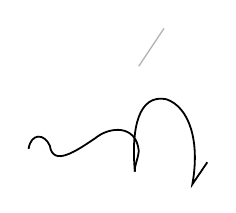
\begin{tikzpicture}[x=1cm,y=1cm]
 \draw[line width=.5pt,opacity=.3] (1.4,1.7)--(1.72,2.18);
 \draw[line width=.65pt] (0,.65) .. controls (.03,.85) and (.2,.85) .. (.27,.69)
 .. controls (.31,.42) and (.6,.62) .. (.84,.78)
 .. controls (1.03,.94) and (1.37,.96) .. (1.4,.62)
 .. controls (1.38,.48) and (1.34,.43) .. (1.35,.36);
 \draw[line width=.65pt] (1.35,.36) .. controls (1.3,.92) and (1.4,1.35) .. (1.75,1.28)
 .. controls (2.04,1.18) and (2.18,.75) .. (2.08,.2)
 --(2.27,.48);
\end{tikzpicture}}

$\cdot$
\diagram{\begin{tikzcd}[ampersand replacement=\&,column sep=large,row sep=small]
 \Pi_{0,3}^D\arrow[r,"{-\alpha}"{draw,circle,inner sep=1pt},very thick]\&\mathbb Z/6\mathbb Z\\
 \rho\arrow[r,mapsto]\&-2\ \mathrm{mod}\ 6\\
 \sigma\arrow[r,mapsto]\&3\ \mathrm{mod}\ 6\\[1ex]
 \varepsilon_0=\sigma\rho\arrow[r,mapsto,very thick]\&1\ \mathrm{mod}\ 6\\
 \rho_0=\varepsilon_0^2\arrow[r,mapsto]\&2\ \mathrm{mod}\ 6
\end{tikzcd}}
\var{\deleted{$\LMsourceMark{M001549}{\unsure{\varphi}}$}}{\LMsourceMark{M001550}{\LMcancelledDoubts{\(\LMsourceMark{M001551}{\unsure{\varphi}}\)}}}{deletion}{140-1-s035-D003}
% Marques très pâles à droite des résidus; possible transparence du verso.
\LMsourceMark{M001552}{\margin{$\LMsourceMark{M001553}{\unsure{\Gamma|\sqrt{\phantom{x}}}}$\\$\LMsourceMark{M001554}{\unsure{\xi_0\prime|\xi_0}}$\\$\LMsourceMark{M001555}{\unsure{t\prime r|t\prime h}}$}}

\LMsourceMark{M001556}{\margin{défini directement par l'action de $\Pi_{0,3}^D$ sur le
\LMsourceMark{M001557}{\unsure{revêt}}\var{\deleted{\LMsourceMark{M001558}{\unsure{ement}}}}{\LMsourceMark{M001559}{\LMcancelledDoubts{\LMsourceMark{M001560}{\unsure{ement}}}}}{deletion}{140-1-s035-D004} principal de $(U_{0,3},\mathfrak S_3)$
de groupe $\mathbb Z/6\mathbb Z$, défini par
la \LMsourceMark{M001561}{\unsure{multisection|multiplication}} \var{\inserted{canonique}}{\LMadded{canonique}}{insertion}{140-1-s035-I001} de
\var{\deleted{$\LMsourceMark{M001562}{\unsure{\mathcal O(1)}}$}}{\LMsourceMark{M001563}{\LMcancelledDoubts{\(\LMsourceMark{M001564}{\unsure{\mathcal O(1)}}\)}}}{deletion}{140-1-s035-D005}$\mathcal O_{U_{0,3}}(1)^*$
$=PU_{0,3}$}}

\[
 \widetilde\Pi_{0,3}^D
\]
\var{\deleted{$\mathcal O\LMsourceMark{M001565}{\unsure{(1)}}$}}{\LMsourceMark{M001566}{\LMcancelledDoubts{\(\LMsourceMark{M001567}{\unsure{(1)}}\)}}}{deletion}{140-1-s035-D006}
\diagram{\begin{tikzcd}[ampersand replacement=\&,column sep=small,row sep=large]
 U'_{0,3}\arrow[rr,phantom,"\subset"]\arrow[dr,no head,"{\mu_6\text{-}\LMsourceMark{M001568}{\unsure{\mathrm{rev}^{\mathrm t}}}}"']\&\&PU_{0,3}\arrow[dl,no head]\&\LMsourceMark{M001569}{\unsure{+}}\\
 \&U_{0,3}\&\&
\end{tikzcd}}
\var{\deleted{$\LMsourceMark{M001570}{\unsure{\longrightarrow}}$}}{\LMsourceMark{M001571}{\LMcancelledDoubts{\(\LMsourceMark{M001572}{\unsure{\longrightarrow}}\)}}}{deletion}{140-1-s035-D007}

\diagram{\begin{tikzcd}[ampersand replacement=\&,column sep=large,row sep=large]
 \&\Pi_{0,3}^D\arrow[r,"{\alpha'}"{draw,circle,inner sep=1pt},very thick]\&\mathbb Z/6\mathbb Z\\
 \pi_1(PU_{0,3},\mathfrak S_3)\arrow[r,equal]\&\widetilde\Pi_{0,3}^D\arrow[u]\arrow[r]\&\mathbb Z\arrow[u]\\
 \&\omega'\in\mathbb Z\arrow[u]\arrow[r,"\LMsourceMark{M001573}{\unsure{=}}"]\&\mathbb Z\arrow[u,"6"]
\end{tikzcd}}

\diagram{\begin{tikzcd}[ampersand replacement=\&,column sep=large,row sep=large]
 1\arrow[r]\&\mathbb Z\arrow[r]\arrow[d,equal]\&
 \underset{\substack{\Vert\\\pi_1(PU_{0,3},\mathfrak S_3\times\mu_4)}}{\widetilde\Pi_{0,3}^D(4)}\arrow[r,very thick]\&
 \Pi_{0,3}^D\times\mathbb Z/4\mathbb Z\arrow[r]\&1\\
 1\arrow[r,no head]\&\mathbb Z\arrow[r]\&\widetilde{\mathcal T}_{11}\arrow[u,bend left=20]\arrow[r,Rightarrow]\&
 \mathcal T_{1,1}=\Pi_{0,3}^D\times_{\mathbb Z/2\mathbb Z}\mathbb Z/4\mathbb Z\arrow[u,hook]\&
\end{tikzcd}}

\var{\deleted{$\LMsourceMark{M001574}{\unsure{\widetilde\Pi_{0,3}^D}}\,\LMsourceMark{M001575}{\unsure{\mathbb Z/4\mathbb Z}}\longrightarrow$}}{\LMsourceMark{M001576}{\LMcancelledDoubts{\(\LMsourceMark{M001577}{\unsure{\widetilde\Pi_{0,3}^D}}\)\quad \(\LMsourceMark{M001578}{\unsure{\mathbb Z/4\mathbb Z}}\)}}}{deletion}{140-1-s035-D008}
\[
\begin{array}{ll}
 \widetilde\Pi_{0,3}^D\ni\widetilde\rho^{\LMsourceMark{M001579}{\unsure{\sharp|'}}}=(\rho,-2)
 &\widetilde\rho^{\LMsourceMark{M001580}{\unsure{\sharp}}3}=\widetilde\sigma^{\LMsourceMark{M001581}{\unsure{\sharp}}2}=\omega'\\
 \hfill\widetilde\sigma^{\LMsourceMark{M001582}{\unsure{\sharp|'}}}=(\sigma,-3)&
\end{array}
\]
\diagram{\begin{tikzcd}[ampersand replacement=\&,column sep=small,row sep=small]
 \widetilde\rho,\arrow[d]\&\widetilde\sigma\arrow[d]\&
 \in\widetilde\Pi_{0,3}^D=
 \left\{\widetilde\rho,\widetilde\sigma\mid
 \underbrace{\widetilde\rho^3=\widetilde\sigma^2}_{\LMsourceMark{M001583}{\unsure{\omega'^{-1}|\widetilde\omega^{-1}}}=\LMsourceMark{M001584}{\unsure{\omega|\infty}}}
 \var{\deleted{\LMsourceMark{M001585}{\unsure{\omega\in\mathbb Z}}}}{\LMsourceMark{M001586}{\LMcancelledDoubts{\(\LMsourceMark{M001587}{\unsure{\omega\in\mathbb Z}}\)}}}{deletion}{140-1-s035-D009}\right\}\\
 \rho\&\sigma\&\simeq\widetilde{\mathcal T}_{11}
\end{tikzcd}}
\LMsourceMark{M001588}{\margin{34}}

\LMflushnotes\LMflushpages
\ifnum\LMform=1
\begin{LMapparatus}
\LMentry{140-1-s035-D001}{suppression}{\(\deleted{\LMsourceMark{M001589}{\unsure{p}}}\)
}{\emph{\LMomittedlabel}}{Passage biffé dans le manuscrit : la suppression suit l'état final de l'auteur; les doutes de lecture restent signalés.}{}
\LMentry{140-1-s035-D002}{suppression}{\(\deleted{\LMsourceMark{M001590}{\unsure{p'+}}}\)
}{\emph{\LMomittedlabel}}{Passage biffé dans le manuscrit : la suppression suit l'état final de l'auteur; les doutes de lecture restent signalés.}{}
\LMentry{140-1-s035-D003}{suppression}{\deleted{$\LMsourceMark{M001591}{\unsure{\varphi}}$}
}{\emph{\LMomittedlabel}}{Passage biffé dans le manuscrit : la suppression suit l'état final de l'auteur; les doutes de lecture restent signalés.}{}
\LMentry{140-1-s035-D004}{suppression}{\deleted{\LMsourceMark{M001592}{\unsure{ement}}}
}{\emph{\LMomittedlabel}}{Passage biffé dans le manuscrit : la suppression suit l'état final de l'auteur; les doutes de lecture restent signalés.}{}
\LMentry{140-1-s035-I001}{insertion}{\inserted{canonique}
}{\emph{\LMinsertedlabel}}{Ajout explicite de l'auteur : intégré à l'endroit indiqué par la transcription, sans modifier sa lecture.}{}
\LMentry{140-1-s035-D005}{suppression}{\deleted{$\LMsourceMark{M001593}{\unsure{\mathcal O(1)}}$}
}{\emph{\LMomittedlabel}}{Passage biffé dans le manuscrit : la suppression suit l'état final de l'auteur; les doutes de lecture restent signalés.}{}
\LMentry{140-1-s035-D006}{suppression}{\deleted{$\mathcal O\LMsourceMark{M001594}{\unsure{(1)}}$}
}{\emph{\LMomittedlabel}}{Passage biffé dans le manuscrit : la suppression suit l'état final de l'auteur; les doutes de lecture restent signalés.}{}
\LMentry{140-1-s035-D007}{suppression}{\deleted{$\LMsourceMark{M001595}{\unsure{\longrightarrow}}$}
}{\emph{\LMomittedlabel}}{Passage biffé dans le manuscrit : la suppression suit l'état final de l'auteur; les doutes de lecture restent signalés.}{}
\LMentry{140-1-s035-D008}{suppression}{\deleted{$\LMsourceMark{M001596}{\unsure{\widetilde\Pi_{0,3}^D}}\,\LMsourceMark{M001597}{\unsure{\mathbb Z/4\mathbb Z}}\longrightarrow$}
}{\emph{\LMomittedlabel}}{Passage biffé dans le manuscrit : la suppression suit l'état final de l'auteur; les doutes de lecture restent signalés.}{}
\LMentry{140-1-s035-D009}{suppression}{\(\deleted{\LMsourceMark{M001598}{\unsure{\omega\in\mathbb Z}}}\)
}{\emph{\LMomittedlabel}}{Passage biffé dans le manuscrit : la suppression suit l'état final de l'auteur; les doutes de lecture restent signalés.}{}
\end{LMapparatus}
\fi
\ifnum\LMform=2
\par\smallskip\begingroup\footnotesize\Needspace{4\baselineskip}\csname @beginparpenalty\endcsname=10000\relax\noindent\textcolor{gray}{\rule{.2\linewidth}{.35pt}}\par\nobreak
\noindent\textit{\LMdoubtheading.}\par\nobreak
\LMcarryover{140-1-s035-D001}{\(\LMsourceMark{M001599}{\unsure{p}}\)
}
\LMcarryover{140-1-s035-D002}{\(\LMsourceMark{M001600}{\unsure{p'+}}\)
}
\LMcarryover{140-1-s035-D003}{\(\LMsourceMark{M001601}{\unsure{\varphi}}\)
}
\LMcarryover{140-1-s035-D004}{\LMsourceMark{M001602}{\unsure{ement}}
}
\LMcarryover{140-1-s035-D005}{\(\LMsourceMark{M001603}{\unsure{\mathcal O(1)}}\)
}
\LMcarryover{140-1-s035-D006}{\(\LMsourceMark{M001604}{\unsure{(1)}}\)
}
\LMcarryover{140-1-s035-D007}{\(\LMsourceMark{M001605}{\unsure{\longrightarrow}}\)
}
\LMcarryover{140-1-s035-D008}{\(\LMsourceMark{M001606}{\unsure{\widetilde\Pi_{0,3}^D}}\)\quad \(\LMsourceMark{M001607}{\unsure{\mathbb Z/4\mathbb Z}}\)
}
\LMcarryover{140-1-s035-D009}{\(\LMsourceMark{M001608}{\unsure{\omega\in\mathbb Z}}\)
}
\par\endgroup\smallskip
\fi

\LMsourceMark{M001609}{\scanpage{36}}
\diagram{\begin{tikzcd}[ampersand replacement=\&,column sep=large,row sep=large,column sep=9pt,row sep=14pt,execute at begin picture={\fontsize{10}{12}\selectfont}]
 \&\&\left\{\rho,\sigma\mid\underbrace{\rho^3=\sigma^2}_{\omega'^{-1}=\omega}\right\}\var{\deleted{\LMsourceMark{M001610}{\unsure{\omega|\infty}}}}{\LMsourceMark{M001611}{\LMcancelledDoubts{\(\LMsourceMark{M001612}{\unsure{\omega|\infty}}\)}}}{deletion}{140-1-s036-D001}\arrow[d,equal]\&\&\\
 1\arrow[r,no head]\&\overset{\omega'=\LMsourceMark{M001613}{\unsure{\omega^{-1}|\overline\omega'}}}{\mathbb Z}\arrow[r]\arrow[d,equal]\&S\Pi_{0,3}^D\arrow[r]\arrow[d]\&\Pi_{0,3}^D\arrow[r,no head]\arrow[d]\&1\\
 1\arrow[r,no head]\&\mathbb Z\arrow[r]\&S\Pi_{0,3}^D(4)\arrow[r]\&\Pi_{0,3}^D\times\mathbb Z/4\mathbb Z\arrow[r,no head]\&1\\[4em]
 1\arrow[r]\&\underset{\omega^2}{\mathbb Z}\arrow[r]\arrow[u,very thick]\&S\mathcal T_{11}\arrow[r]\arrow[u,very thick,"{\underbrace{\begin{gathered}\rho\mapsto\rho\overline\omega^2\\\sigma\mapsto\sigma\overline\omega^3\\\omega\longrightarrow\overline\omega^2\\\omega^2\longrightarrow\overline\omega^4=\omega'\end{gathered}}}"]\&\mathcal T_{11}\arrow[u,hook,"{\substack{\rho\mapsto(\rho,2)\\\sigma\mapsto(\sigma,3)}}"]\&\omega\longrightarrow(1,2)
\end{tikzcd}}
\LMsourceMark{M001614}{\margin{$S\Pi_{0,3}^D(4)=\left\{\rho,\sigma,\overline\omega\mid\begin{gathered}\rho^3=\sigma^2=\overline\omega^{-4}\\\overline\omega\ \text{central}\end{gathered}\right\}$\\
NB $\LMsourceMark{M001615}{\unsure{\dot{\overline\omega}|\overline\omega}}^{4}=\LMsourceMark{M001616}{\unsure{\omega^{-1}}}$\\
$=\omega'\var{\deleted{\LMsourceMark{M001617}{\unsure{\omega}}}}{\LMsourceMark{M001618}{\LMcancelledDoubts{\(\LMsourceMark{M001619}{\unsure{\omega}}\)}}}{deletion}{140-1-s036-D002}$}}

% Groupe et flèche au pied du feuillet, écrits tête-bêche.
\diagram{\begin{tikzcd}[ampersand replacement=\&,column sep=large]
 \overbrace{S\Pi_{0,3}^D(4)}^{\pi_1(U_{0,3},\mathfrak S_3\times\mu_4)}\arrow[r]\&\Pi_{0,3}^D
\end{tikzcd}}
\LMsourceMark{M001620}{\margin{35}}

\LMflushnotes\LMflushpages
\ifnum\LMform=1
\begin{LMapparatus}
\LMentry{140-1-s036-D001}{suppression}{\(\deleted{\LMsourceMark{M001621}{\unsure{\omega|\infty}}}\)
}{\emph{\LMomittedlabel}}{Passage biffé dans le manuscrit : la suppression suit l'état final de l'auteur; les doutes de lecture restent signalés.}{}
\LMentry{140-1-s036-D002}{suppression}{\(\deleted{\LMsourceMark{M001622}{\unsure{\omega}}}\)
}{\emph{\LMomittedlabel}}{Passage biffé dans le manuscrit : la suppression suit l'état final de l'auteur; les doutes de lecture restent signalés.}{}
\end{LMapparatus}
\fi
\ifnum\LMform=2
\par\smallskip\begingroup\footnotesize\Needspace{4\baselineskip}\csname @beginparpenalty\endcsname=10000\relax\noindent\textcolor{gray}{\rule{.2\linewidth}{.35pt}}\par\nobreak
\noindent\textit{\LMdoubtheading.}\par\nobreak
\LMcarryover{140-1-s036-D001}{\(\LMsourceMark{M001623}{\unsure{\omega|\infty}}\)
}
\LMcarryover{140-1-s036-D002}{\(\LMsourceMark{M001624}{\unsure{\omega}}\)
}
\par\endgroup\smallskip
\fi

\LMsourceMark{M001625}{\scanpage{37}}
% not manuscript: formulaire vierge « ANNEXE II », renseignements à fournir par le candidat devant soutenir une thèse de doctorat d'État, Université des Sciences et Techniques du Languedoc, imprimé tête-bêche.
\LMsourceMark{M001626}{\margin{36}}

\LMflushnotes\LMflushpages

% END PACKAGE LM_C1-020-037
\clearpage\LMcote{140-2}
\section*{Cote 140-2}\addcontentsline{toc}{section}{Cote 140-2}
% BEGIN PACKAGE LM_P01
\ifnum\LMform<2\Needspace{11\baselineskip}\subsection*{Scans 1--10}\fi
\LMsourceMark{M001627}{\scanpage{1}}
% not manuscript: page de titre imprimée de l'Université de Montpellier / IMAG.

\LMflushnotes\LMflushpages

\LMsourceMark{M001628}{\scanpage{2}}
% not manuscript: couverture portant « Pages 1-292 + table des matières ».

\LMflushnotes\LMflushpages

\LMsourceMark{M001629}{\scanpage{3}}
\LMsourceMark{M001630}{\margin{I}}

La "longue marche" à travers la théorie de Galois...

1. Topos multigaloisiens \hfill 1

2. Appl. aux rev. des topos \hfill 4

3. Variantes pro-multigaloisiennes \hfill 6

4. Compléments remords

\figure{[Accolade à droite réunissant les rubriques 3 et 4.]}

\uuline{5.} Introduction du contexte arithmétique
"Conjecture anabélienne" fondamentale \hfill \(7'\)

6. Analyse locale de \((X,S)\) en un \(s\in S\). \hfill \(10'\)

7. Reformulation "bordélique" de la conjecture
(le purgatoire nécessaire...) \hfill 12

\var{\deleted{\LMsourceMark{M001631}{\unsure{6.}}}}{\LMsourceMark{M001632}{\LMcancelledDoubts{\LMsourceMark{M001633}{\unsure{6.}}}}}{deletion}{140-2-s003-D001}
8. Réflexion taxonomique (distinction \LMsourceMark{M001634}{\unsure{des|de}}
cas, \LMsourceMark{M001635}{\unsure{où}} le purgatoire s'aménage un peu...) \hfill \(25'\)

\var{\deleted{\LMsourceMark{M001636}{\unsure{7.}}}}{\LMsourceMark{M001637}{\LMcancelledDoubts{\LMsourceMark{M001638}{\unsure{7.}}}}}{deletion}{140-2-s003-D002}
9. Structure tangentielle en les \(s\in S\)
(Sections d'extensions "de deuxième type" \hfill 34

10. \LMsourceMark{M001639}{\unsure{Ajustement}} des hypothèses, (remords) \hfill 38

11. Conditions sur les syst. de groupoïdes obtenus à partir de
situations géométriques \hfill 39

12. L'analogie topologique. (Où on se convainc aussi que le bordel
groupoïdal peut s'exprimer complètement, dans les cas anabéliens,
par les groupes ext. à lacets... \hfill \LMsourceMark{M001640}{\unsure{41|43}}

13. Retour au cas arithmétique : formulations "galoisiennes" \hfill 53

13\textsuperscript{bis}. Retour sur la notion de groupe à lacets \hfill 56

14. Digression cohomologique (sur le "bouchage de trous") \hfill 58

\uuline{15.} Retour sur le cas topologique : orbites critiques
\LMsourceMark{M001641}{\unsure{autour}} des scindages d'extensions
Application aux sous-groupes finis de
\(\mathrm{Autext}_{\mathrm{lac}}(\pi)\) (cas discret)
(cf aussi \(\S 18\)) \hfill \(67'\)

16. Bouchage et forage de trous : préliminaires topologiques généraux
\hfill \(79'\)

17. Compléments au \(\S 15\), sur \LMsourceMark{M001642}{\unsure{op.|gr.}} de groupes finis
sur des surfaces \hfill 89

\LMflushnotes\LMflushpages
\ifnum\LMform=1
\begin{LMapparatus}
\LMentry{140-2-s003-D001}{suppression}{\deleted{\LMsourceMark{M001643}{\unsure{6.}}}
}{\emph{\LMomittedlabel}}{Passage biffé dans le manuscrit : la suppression suit l'état final de l'auteur; les doutes de lecture restent signalés.}{}
\LMentry{140-2-s003-D002}{suppression}{\deleted{\LMsourceMark{M001644}{\unsure{7.}}}
}{\emph{\LMomittedlabel}}{Passage biffé dans le manuscrit : la suppression suit l'état final de l'auteur; les doutes de lecture restent signalés.}{}
\end{LMapparatus}
\fi
\ifnum\LMform=2
\par\smallskip\begingroup\footnotesize\Needspace{4\baselineskip}\csname @beginparpenalty\endcsname=10000\relax\noindent\textcolor{gray}{\rule{.2\linewidth}{.35pt}}\par\nobreak
\noindent\textit{\LMdoubtheading.}\par\nobreak
\LMcarryover{140-2-s003-D001}{\LMsourceMark{M001645}{\unsure{6.}}
}
\LMcarryover{140-2-s003-D002}{\LMsourceMark{M001646}{\unsure{7.}}
}
\par\endgroup\smallskip
\fi

\LMsourceMark{M001647}{\scanpage{4}}
\uuline{18.} Forage de trous. Application aux ss-groupes
finis de \(\mathrm{Autext}_{\mathrm{lac}}(\pi)\)
(cas discret) \hfill 91

\uuline{19.} Tour de Teichmüller \hfill 102

20. Digression : description 2-isotopique
de la cat. des \LMsourceMark{M001648}{\unsure{2-sphères}} topologiques \hfill \(116'\)

21. Les espaces de Teichmüller \hfill 125

\LMsourceMark{M001649}{\margin{manque \(\S 22\) !}}

23. Retour sur les surfaces à groupes (finis) d'opérateurs
("mise en équations" du Pb) \hfill 133

24. Essai de détermination des \LMsourceMark{M001650}{\unsure{\(A^{\circ\Gamma}\)}}. Lien avec les relations
\(\Pi_{g,(\nu,\nu+n-1)}^{\Gamma}\) \(=(1)\),
programme de \var{\deleted{\LMsourceMark{M001651}{\illegible{1}}}}{\LMsourceMark{M001652}{\LMcancelledDoubts{\LMsourceMark{M001653}{\illegible{1}}}}}{deletion}{140-2-s004-D001}\var{\inserted{travail}}{\LMadded{travail}}{insertion}{140-2-s004-I001} \hfill 142

25. Groupes de Teichmüller "\uline{spéciaux}" \hfill 148

25\textsuperscript{bis}. "Cas des deux groupes" d'opérateurs. Retour sur les notations.
\hfill \(153'\)

\uuline{25.} Groupes de Teichmüller profinis. \hfill 161

Discrétifications et \LMsourceMark{M001654}{\unsure{prédiscrétifications|prodiscrétifications}}. Lien avec topos
modulaire de Teichmüller. Conjecture hâtive. \hfill 167

27. Changement de type \((g,\nu)\) : a) bouchage de trous
(et \LMsourceMark{M001655}{\unsure{diagrammes remarquables|diagramme remarquable}} p. 174) \hfill 172

28. chgt. de type \((g,\nu)\) : b) passage à un rev. fini
(la conjecture hâtive grince...) \hfill 177

29. Critique de l'approche précédente. (On rajuste
les notions et les conjectures...) \hfill 186

30. Propriétés des \(N_{g,\nu},\Gamma_{g,\nu}\) : a)
\LMsourceMark{M001656}{\unsure{Propriétés liées}} aux sous-groupes finis de Teichmüller.
\hfill 192

31. Digression sur les relèvements d'une action extérieure d'un groupe
fini sur un groupe profini à lacets \hfill 198

\uuline{32.} Retour sur les aspects arithmétiques du bouchage de trous :
relations entre \(\Gamma_{g,\nu}\) et \(\Gamma_{g,\nu-1}\).
(Où on reconstitue, sans le dire, \uline{tout le topos étale} d'une
courbe algébrique \var{\inserted{complète}}{\LMadded{complète}}{insertion}{140-2-s004-I002}, à partir du \(\pi_1\) d'un
ouvert anabélien...) \hfill 200

\uuline{33.} Digression topologique : anti-involutions des surfaces
orientées compactes (en laissant de côté d'abord le cas "à trous")
\hfill 221

\uuline{\LMsourceMark{M001657}{\unsure{35.}}} L'injectivité de
\(\Gamma_{\mathbb Q}\longrightarrow
\mathrm{Autext}_{\mathrm{lac}}(\widehat{\Pi}_{0,3})\)
\hfill 249

\LMsourceMark{M001658}{\unsure{36.}} L'isomorphisme
\(\Gamma_{\mathbb Q}\simeq\Gamma_{1,1}\),
et l'injectivité de
\(\Gamma_{\mathbb Q}\longrightarrow
\mathrm{Autext}(\widehat{\LMsourceMark{M001659}{\unsure{\Gamma|T}}}_{1,1}^{+})
=\mathrm{Autext}(\mathrm{SL}(2,\mathbb Z)^{\wedge})\)
\hfill 257

\LMsourceMark{M001660}{\unsure{37.}} Modules des courbes elliptiques via Legendre, ou
\LMsourceMark{M001661}{\unsure{\(M_{1,1}[2]'\simeq U_{0,3}\ne M_{0,4}^{!}\)}} \hfill 272

33. Relations entre \(N_{g,\nu},\Gamma_{g,\nu}\) pour \(g\)
variable (étude des rev. finis) \hfill 239

34. Description heuristique profinie de la cat. des courbes alg.
définies sur des \var{\deleted{\LMsourceMark{M001662}{\unsure{ext.}}}}{\LMsourceMark{M001663}{\LMcancelledDoubts{\LMsourceMark{M001664}{\unsure{ext.}}}}}{deletion}{140-2-s004-D002}
sous-ext. finies de \(\mathbb Q_0/\mathbb Q\)
\hfill 245

\figure{[À gauche des deux dernières rubriques, accolade prolongée
vers le haut par une flèche dirigée vers la rubrique
« L'injectivité de \(\Gamma_{\mathbb Q}\) ».]}

\LMflushnotes\LMflushpages
\ifnum\LMform=1
\begin{LMapparatus}
\LMentry{140-2-s004-D001}{suppression}{\deleted{\LMsourceMark{M001665}{\illegible{1}}}
}{\emph{\LMomittedlabel}}{Passage biffé dans le manuscrit : la suppression suit l'état final de l'auteur; les doutes de lecture restent signalés.}{}
\LMentry{140-2-s004-I001}{insertion}{\inserted{travail}
}{\emph{\LMinsertedlabel}}{Ajout explicite de l'auteur : intégré à l'endroit indiqué par la transcription, sans modifier sa lecture.}{}
\LMentry{140-2-s004-I002}{insertion}{\inserted{complète}
}{\emph{\LMinsertedlabel}}{Ajout explicite de l'auteur : intégré à l'endroit indiqué par la transcription, sans modifier sa lecture.}{}
\LMentry{140-2-s004-D002}{suppression}{\deleted{\LMsourceMark{M001666}{\unsure{ext.}}}
}{\emph{\LMomittedlabel}}{Passage biffé dans le manuscrit : la suppression suit l'état final de l'auteur; les doutes de lecture restent signalés.}{}
\end{LMapparatus}
\fi
\ifnum\LMform=2
\par\smallskip\begingroup\footnotesize\Needspace{4\baselineskip}\csname @beginparpenalty\endcsname=10000\relax\noindent\textcolor{gray}{\rule{.2\linewidth}{.35pt}}\par\nobreak
\noindent\textit{\LMdoubtheading.}\par\nobreak
\LMcarryover{140-2-s004-D001}{\LMsourceMark{M001667}{\illegible{1}}
}
\LMcarryover{140-2-s004-D002}{\LMsourceMark{M001668}{\unsure{ext.}}
}
\par\endgroup\smallskip
\fi

\LMsourceMark{M001669}{\scanpage{5}}
\LMsourceMark{M001670}{\margin{\LMsourceMark{M001671}{\unsure{814|714}}\par\LMsourceMark{M001672}{\unsure{752|252}}\par 832}}

\LMflushnotes\LMflushpages

\LMsourceMark{M001673}{\scanpage{6}}
\LMsourceMark{M001674}{\mspage{1}}
\LMsourceMark{M001675}{\margin{\LMsourceMark{M001676}{\unsure{W|VI}}}}

1. Topos multigaloisiens.

\uline{Prop.} 1.1. Soit \(\mathcal E\) une catégorie.
Conditions équivalentes :

a) \(\mathcal E\) est un topos, et tout objet de \(\mathcal E\)
est loc\textsuperscript{t} constant.

b) \(\mathcal E\) est équivalent à une catégorie \(\widehat C\),
où \(C\) est un groupoïde.

\LMsourceMark{M001677}{\margin{N.B. On verra (plus bas) \LMsourceMark{M001678}{\unsure{qu'on peut choisir}}
\LMsourceMark{M001679}{\unsure{\(C\)}} \uline{canoniquement}}}

b') \(\exists\) une famille \((G_i)_{i\in I}\) de groupes
et une équivalence de catégories
\[
\mathcal E\approxeq\prod\mathrm{Ens}(G_i)
\]

c) Conditions d'exactitudes ad-hoc, du type de celles données dans SGA 1...

Dém. \(b\Longleftrightarrow b'\Longrightarrow a\) immédiat.
Pour \(a)\Longrightarrow b)\), je suis moins sûr, peut être faut il
supposer que \(\mathcal E\) est loc connexe, et qu'il a suffisamment
de foncteurs fibres i.e. suffisamment de points.

\uline{Déf. 1.2.} Si les conditions équivalentes b) b') ci-dessus
sont satisfaites, on dit que \(C\)
est \LMsourceMark{M001680}{\unsure{un|une}} \var{\deleted{catégorie}}{}{deletion}{140-2-s006-D001} \var{\inserted{topos}}{\LMadded{topos}}{insertion}{140-2-s006-I001}
multigaloisien (ou une \uline{catégorie} multigaloisienne).

\LMsourceMark{M001681}{\margin{\uline{Prop. 1.3}
a) Si \(\mathcal E\) est multigaloisien, tout \LMsourceMark{M001682}{\unsure{topos}} induit
\(\mathcal E_{/S}\) aussi.
\par
b) toute somme de topos multigaloisiens (i.e. \var{\deleted{\LMsourceMark{M001683}{\illegible{1}}}}{\LMsourceMark{M001684}{\LMcancelledDoubts{\LMsourceMark{M001685}{\illegible{1}}}}}{deletion}{140-2-s006-D002}
produit de cat. multigaloisiennes) \LMsourceMark{M001686}{\unsure{l'est|est}} itou.}}

\LMflushnotes\LMflushpages
\ifnum\LMform=1
\begin{LMapparatus}
\LMentry{140-2-s006-D001}{suppression}{\deleted{catégorie}
}{\emph{\LMomittedlabel}}{Passage biffé dans le manuscrit : la suppression suit l'état final de l'auteur; les doutes de lecture restent signalés.}{}
\LMentry{140-2-s006-I001}{insertion}{\inserted{topos}
}{\emph{\LMinsertedlabel}}{Ajout explicite de l'auteur : intégré à l'endroit indiqué par la transcription, sans modifier sa lecture.}{}
\LMentry{140-2-s006-D002}{suppression}{\deleted{\LMsourceMark{M001687}{\illegible{1}}}
}{\emph{\LMomittedlabel}}{Passage biffé dans le manuscrit : la suppression suit l'état final de l'auteur; les doutes de lecture restent signalés.}{}
\end{LMapparatus}
\fi
\ifnum\LMform=2
\par\smallskip\begingroup\footnotesize\Needspace{4\baselineskip}\csname @beginparpenalty\endcsname=10000\relax\noindent\textcolor{gray}{\rule{.2\linewidth}{.35pt}}\par\nobreak
\noindent\textit{\LMdoubtheading.}\par\nobreak
\LMcarryover{140-2-s006-D002}{\LMsourceMark{M001688}{\illegible{1}}
}
\par\endgroup\smallskip
\fi

\LMsourceMark{M001689}{\scanpage{7}}
\uline{Prop. 1.4} \LMsourceMark{M001690}{\unsure{Soient|Soit}} \(\mathcal E\) un topos,
\(C\) la catégorie des points de \(\mathcal E\) (opposée à la
catégorie des foncteurs fibres sur \(\mathcal E\)). Le foncteur
canonique
\[
\mathcal E\times C^o\longrightarrow(\mathrm{Ens})
\]
induit un foncteur canonique
\[
\mathcal E\longrightarrow\mathrm{Hom}(C^o,(\mathrm{Ens}))
\overset{\mathrm{déf}}{=}\widehat C
\]

Ceci posé : (\(\mathcal E\) étant multigaloisien)

a) \(C\) est un groupoïde (appelé "groupoïde fondamental" du topos
mult. gal. \(\mathcal E\), et souvent noté
\(\Pi_1(\mathcal E)\)).

b) \(\mathcal E\longrightarrow\widehat C\) est une équivalence
de catégories.

Un objet \var{\inserted{\(S\)}}{\LMadded{\(S\)}}{insertion}{140-2-s007-I001} d'un topos \var{\inserted{\(\mathcal E\)}}{\LMadded{\(\mathcal E\)}}{insertion}{140-2-s007-I002}
est dit 0-connexe s'il est \(\ne\varnothing_{\mathcal E}\)
(\LMsourceMark{M001691}{\unsure{il|i.e.}} n'est pas objet initial) et s'il est connexe
(i.e. \(S\simeq S'\amalg S''\) implique
\(S'\) ou \(S''\simeq\varnothing_{\mathcal E}\)) --- cela signifie
aussi que le topos induit \(\mathcal E_{/S}\) est 0-connexe
i.e. n'est pas le topos initial ("topos vide", i.e.
\var{\inserted{équivalent à la}}{\LMadded{équivalent à la}}{insertion}{140-2-s007-I003} catégorie finale) et qu'il est connexe,
i.e. ... On dit que \(S\) est 1-connexe

\LMflushnotes\LMflushpages
\ifnum\LMform=1
\begin{LMapparatus}
\LMentry{140-2-s007-I001}{insertion}{\inserted{\(S\)}
}{\emph{\LMinsertedlabel}}{Ajout explicite de l'auteur : intégré à l'endroit indiqué par la transcription, sans modifier sa lecture.}{}
\LMentry{140-2-s007-I002}{insertion}{\inserted{\(\mathcal E\)}
}{\emph{\LMinsertedlabel}}{Ajout explicite de l'auteur : intégré à l'endroit indiqué par la transcription, sans modifier sa lecture.}{}
\LMentry{140-2-s007-I003}{insertion}{\inserted{équivalent à la}
}{\emph{\LMinsertedlabel}}{Ajout explicite de l'auteur : intégré à l'endroit indiqué par la transcription, sans modifier sa lecture.}{}
\end{LMapparatus}
\fi

\LMsourceMark{M001692}{\scanpage{8}}
\LMsourceMark{M001693}{\mspage{2}}

(ou "simplement connexe") s'il est 0-connexe, et si tout
\var{\deleted{\LMsourceMark{M001694}{\unsure{rev. de \(S\) est}}}}{\LMsourceMark{M001695}{\LMcancelledDoubts{\LMsourceMark{M001696}{\unsure{rev. de \(S\) est}}}}}{deletion}{140-2-s008-D001}
\var{\inserted{objet \(S'\) de \(\mathcal E_{/S}\)
\deleted{\LMsourceMark{M001697}{\illegible{1}}}}}{\LMadded{objet \(S'\) de \(\mathcal E_{/S}\)
\var{\deleted{\LMsourceMark{M001698}{\illegible{1}}}}{\LMsourceMark{M001699}{\LMcancelledDoubts{\LMsourceMark{M001700}{\illegible{1}}}}}{deletion}{140-2-s008-D002}}}{insertion}{140-2-s008-I001}
loc const. \LMsourceMark{M001701}{\unsure{est}} est \LMsourceMark{M001702}{\unsure{\var{\deleted{constant}}{\LMsourceMark{M001703}{\LMuncertaindeletion{140-2-s008-D003}}}{deletion}{140-2-s008-D003}|constant}}
--- ce qui ne dépend \var{\inserted{encore}}{\LMadded{encore}}{insertion}{140-2-s008-I002} que du topos induit
\(\mathcal E_{/S}\), qui sera dit alors 1-connexe.

\uline{Prop.} 1.5. Soit \(\mathcal E\) un topos multigaloisien,
et soit \(S\) un objet de \(\mathcal E\). Conditions équivalentes

a) \(S\) est 1-connexe

b) \(S\) \LMsourceMark{M001704}{\unsure{(est)|est}} 0-connexe et projectif

c) le foncteur covariant représenté par \(S\)
\[
T\longmapsto\mathrm{Hom}_{\mathcal E}(S,T)
\]
est un foncteur fibre, ou encore
comme il est déjà exact à g.) il commute aux
\(\underset{\longrightarrow}{\lim}\) quelconques

\var{\inserted{N.B.}}{\LMadded{N.B.}}{insertion}{140-2-s008-I003} (il suffit qu'il commute aux sommes et au passage
au quotient...)

d) \(\mathcal E_{/S}\) est équivalent au topos ponctuel

e) (Si \(\mathcal E=\widehat C\), \(C\) un groupoïde) le foncteur
\(S\) sur \(C\) est \var{\inserted{représentable}}{\LMadded{représentable}}{insertion}{140-2-s008-I004}

\LMflushnotes\LMflushpages
\ifnum\LMform=1
\begin{LMapparatus}
\LMentry{140-2-s008-D001}{suppression}{\deleted{\LMsourceMark{M001705}{\unsure{rev. de \(S\) est}}}
}{\emph{\LMomittedlabel}}{Passage biffé dans le manuscrit : la suppression suit l'état final de l'auteur; les doutes de lecture restent signalés.}{}
\LMentry{140-2-s008-I001}{insertion}{\inserted{objet \(S'\) de \(\mathcal E_{/S}\)
\deleted{\LMsourceMark{M001706}{\illegible{1}}}}
}{\emph{\LMinsertedlabel}}{Ajout explicite de l'auteur : intégré à l'endroit indiqué par la transcription, sans modifier sa lecture.}{}
\LMentry{140-2-s008-D002}{suppression}{\deleted{\LMsourceMark{M001707}{\illegible{1}}}
}{\emph{\LMomittedlabel}}{Passage biffé dans le manuscrit : la suppression suit l'état final de l'auteur; les doutes de lecture restent signalés.}{}
\LMentry{140-2-s008-D003}{suppression}{\LMsourceMark{M001708}{\LMdoubtcopy{\deleted{constant}}}
}{\emph{\LMomittedlabel}}{Passage biffé dans le manuscrit : la suppression suit l'état final de l'auteur; les doutes de lecture restent signalés.}{}
\LMentry{140-2-s008-I002}{insertion}{\inserted{encore}
}{\emph{\LMinsertedlabel}}{Ajout explicite de l'auteur : intégré à l'endroit indiqué par la transcription, sans modifier sa lecture.}{}
\LMentry{140-2-s008-I003}{insertion}{\inserted{N.B.}
}{\emph{\LMinsertedlabel}}{Ajout explicite de l'auteur : intégré à l'endroit indiqué par la transcription, sans modifier sa lecture.}{}
\LMentry{140-2-s008-I004}{insertion}{\inserted{représentable}
}{\emph{\LMinsertedlabel}}{Ajout explicite de l'auteur : intégré à l'endroit indiqué par la transcription, sans modifier sa lecture.}{}
\end{LMapparatus}
\fi
\ifnum\LMform=2
\par\smallskip\begingroup\footnotesize\Needspace{4\baselineskip}\csname @beginparpenalty\endcsname=10000\relax\noindent\textcolor{gray}{\rule{.2\linewidth}{.35pt}}\par\nobreak
\noindent\textit{\LMdoubtheading.}\par\nobreak
\LMcarryover{140-2-s008-D001}{\LMsourceMark{M001709}{\unsure{rev. de \(S\) est}}
}
\LMcarryover{140-2-s008-D002}{\LMsourceMark{M001710}{\illegible{1}}
}
\LMcarryover{140-2-s008-D003}{\LMsourceMark{M001711}{\LMdoubtcopy{constant}}
}
\par\endgroup\smallskip
\fi

\LMsourceMark{M001712}{\scanpage{9}}
\uline{Déf 1.6} On dit alors, parfois, que \(S\) (ou mieux, le topos
\(\mathcal E_{/S}\)) est un \uline{rev.} \uline{universel} du topos
\var{\inserted{multigal.}}{\LMadded{multigal.}}{insertion}{140-2-s009-I001} \(\mathcal E\).

\uline{Prop. 1.7}
\var{\deleted{\LMsourceMark{M001713}{\unsure{Prenant}} \LMsourceMark{M001714}{\illegible{1}} objet}}{\LMsourceMark{M001715}{\LMcancelledDoubts{\LMsourceMark{M001716}{\unsure{Prenant}}\quad \LMsourceMark{M001717}{\illegible{1}}}}}{deletion}{140-2-s009-D001}
\var{\inserted{Soit \(\mathcal E_0\)}}{\LMadded{Soit \(\mathcal E_0\)}}{insertion}{140-2-s009-I002} la sous-catégorie pleine de
\(\mathcal E\) formée des objets 1-connexes
(de la cat. multigal. \(\mathcal E\)),
\var{\deleted{Alors \LMsourceMark{M001718}{\unsure{le fo}}}}{\LMsourceMark{M001719}{\LMcancelledDoubts{\LMsourceMark{M001720}{\unsure{le fo}}}}}{deletion}{140-2-s009-D002} \var{\inserted{et \(\Pi_1(\mathcal E)\)
le groupoïde fondamental}}{\LMadded{et \(\Pi_1(\mathcal E)\)
le groupoïde fondamental}}{insertion}{140-2-s009-I003} de \(\mathcal E\).
On a \var{\inserted{\LMsourceMark{M001721}{\unsure{p.}} 1.5}}{\LMadded{\LMsourceMark{M001722}{\unsure{p.}} 1.5}}{insertion}{140-2-s009-I004} un foncteur canonique
\[
\mathcal E_0\longrightarrow
\Pi_1(C)
\]

(associant : \(\forall\) \(S\in\mathrm{Ob}\,\mathcal E_0\)
le foncteur fibre qu'il représente, ou plutôt le "point" correspondant
de \(C\)), qui est
(non seulement pleinement fidèle, mais même) une équivalence de
catégories : tout foncteur fibre sur \(\mathcal E\) est représentable
(par un objet (1-connexe) essentiellement unique, comme de juste...).

\LMflushnotes\LMflushpages
\ifnum\LMform=1
\begin{LMapparatus}
\LMentry{140-2-s009-I001}{insertion}{\inserted{multigal.}
}{\emph{\LMinsertedlabel}}{Ajout explicite de l'auteur : intégré à l'endroit indiqué par la transcription, sans modifier sa lecture.}{}
\LMentry{140-2-s009-D001}{suppression}{\deleted{\LMsourceMark{M001723}{\unsure{Prenant}} \LMsourceMark{M001724}{\illegible{1}} objet}
}{\emph{\LMomittedlabel}}{Passage biffé dans le manuscrit : la suppression suit l'état final de l'auteur; les doutes de lecture restent signalés.}{}
\LMentry{140-2-s009-I002}{insertion}{\inserted{Soit \(\mathcal E_0\)}
}{\emph{\LMinsertedlabel}}{Ajout explicite de l'auteur : intégré à l'endroit indiqué par la transcription, sans modifier sa lecture.}{}
\LMentry{140-2-s009-D002}{suppression}{\deleted{Alors \LMsourceMark{M001725}{\unsure{le fo}}}
}{\emph{\LMomittedlabel}}{Passage biffé dans le manuscrit : la suppression suit l'état final de l'auteur; les doutes de lecture restent signalés.}{}
\LMentry{140-2-s009-I003}{insertion}{\inserted{et \(\Pi_1(\mathcal E)\)
le groupoïde fondamental}
}{\emph{\LMinsertedlabel}}{Ajout explicite de l'auteur : intégré à l'endroit indiqué par la transcription, sans modifier sa lecture.}{}
\LMentry{140-2-s009-I004}{insertion}{\inserted{\LMsourceMark{M001726}{\unsure{p.}} 1.5}
}{\emph{\LMinsertedlabel}}{Ajout explicite de l'auteur : intégré à l'endroit indiqué par la transcription, sans modifier sa lecture.}{}
\end{LMapparatus}
\fi
\ifnum\LMform=2
\par\smallskip\begingroup\footnotesize\Needspace{4\baselineskip}\csname @beginparpenalty\endcsname=10000\relax\noindent\textcolor{gray}{\rule{.2\linewidth}{.35pt}}\par\nobreak
\noindent\textit{\LMdoubtheading.}\par\nobreak
\LMcarryover{140-2-s009-D001}{\LMsourceMark{M001727}{\unsure{Prenant}}\quad \LMsourceMark{M001728}{\illegible{1}}
}
\LMcarryover{140-2-s009-D002}{\LMsourceMark{M001729}{\unsure{le fo}}
}
\par\endgroup\smallskip
\fi

\LMsourceMark{M001730}{\scanpage{10}}
\LMsourceMark{M001731}{\mspage{3}}
\var{\deleted{\LMsourceMark{M001732}{\unsure{Déf. 1.8}} \LMsourceMark{M001733}{\illegible{1}} \LMsourceMark{M001734}{\unsure{L'ob.}}}}{\LMsourceMark{M001735}{\LMcancelledDoubts{\LMsourceMark{M001736}{\unsure{Déf. 1.8}}\quad \LMsourceMark{M001737}{\illegible{1}}\quad \LMsourceMark{M001738}{\unsure{L'ob.}}}}}{deletion}{140-2-s010-D001}

\uline{Corollaire 1.8.} Soit \(P\) un "point" de \(\mathcal E\)
\var{\inserted{(associé à un foncteur fibre \(F_P\))}}{\LMadded{(associé à un foncteur fibre \(F_P\))}}{insertion}{140-2-s010-I001}.
Il existe un objet 1-connexe \(S\) de \(\mathcal E\) et un relèvement
\(P\xrightarrow{\alpha}\mathcal E_{/S}\)
(i.e. un \(\alpha\in F(S)\)),

\diagram{[Sous \(P\xrightarrow{\alpha}\mathcal E_{/S}\),
\(\mathcal E\) est placé au centre en bas. Deux flèches en pointillé
vont respectivement de \(P\) et de \(\mathcal E_{/S}\) vers
\(\mathcal E\). Entre elles, une flèche vers la droite surmontée
de \(\sim\), \LMsourceMark{M001739}{\unsure{à double trait|à trait simple}}.
Deux crochets latéraux entourent cette partie inférieure du diagramme.]}

et cela détermine \((S,\alpha)\) à isom. unique près.

En fait, \(S\) est l'unique \LMsourceMark{M001740}{\unsure{objet|\var{\deleted{objet}}{\LMsourceMark{M001741}{\LMuncertaindeletion{140-2-s010-D002}}}{deletion}{140-2-s010-D002}}}
de \(\mathcal E\) qui représente \(F_P\)...

\uline{Déf. 1.9.} On dit que \(S\)
\var{\inserted{(ou \(\mathcal E_{/S}\))}}{\LMadded{(ou \(\mathcal E_{/S}\))}}{insertion}{140-2-s010-I002} est le
\uline{rev. universel ponctué au dessus de \(P\)} déterminé
par le point \(P\).

\uline{Scholie 1.10} Se donner un "point" du \LMsourceMark{M001742}{\unsure{:}}
topos \var{\inserted{multigaloisien}}{\LMadded{multigaloisien}}{insertion}{140-2-s010-I003} \(\mathcal E\), ou se donner un
rev. universel, revient essentiellement au
\(\overline{\mathrm m}\) : chacun détermine l'autre...

\LMflushnotes\LMflushpages
\ifnum\LMform=1
\begin{LMapparatus}
\LMentry{140-2-s010-D001}{suppression}{\deleted{\LMsourceMark{M001743}{\unsure{Déf. 1.8}} \LMsourceMark{M001744}{\illegible{1}} \LMsourceMark{M001745}{\unsure{L'ob.}}}
}{\emph{\LMomittedlabel}}{Passage biffé dans le manuscrit : la suppression suit l'état final de l'auteur; les doutes de lecture restent signalés.}{}
\LMentry{140-2-s010-I001}{insertion}{\inserted{(associé à un foncteur fibre \(F_P\))}
}{\emph{\LMinsertedlabel}}{Ajout explicite de l'auteur : intégré à l'endroit indiqué par la transcription, sans modifier sa lecture.}{}
\LMentry{140-2-s010-D002}{suppression}{\LMsourceMark{M001746}{\LMdoubtcopy{\deleted{objet}}}
}{\emph{\LMomittedlabel}}{Passage biffé dans le manuscrit : la suppression suit l'état final de l'auteur; les doutes de lecture restent signalés.}{}
\LMentry{140-2-s010-I002}{insertion}{\inserted{(ou \(\mathcal E_{/S}\))}
}{\emph{\LMinsertedlabel}}{Ajout explicite de l'auteur : intégré à l'endroit indiqué par la transcription, sans modifier sa lecture.}{}
\LMentry{140-2-s010-I003}{insertion}{\inserted{multigaloisien}
}{\emph{\LMinsertedlabel}}{Ajout explicite de l'auteur : intégré à l'endroit indiqué par la transcription, sans modifier sa lecture.}{}
\end{LMapparatus}
\fi
\ifnum\LMform=2
\par\smallskip\begingroup\footnotesize\Needspace{4\baselineskip}\csname @beginparpenalty\endcsname=10000\relax\noindent\textcolor{gray}{\rule{.2\linewidth}{.35pt}}\par\nobreak
\noindent\textit{\LMdoubtheading.}\par\nobreak
\LMcarryover{140-2-s010-D001}{\LMsourceMark{M001747}{\unsure{Déf. 1.8}}\quad \LMsourceMark{M001748}{\illegible{1}}\quad \LMsourceMark{M001749}{\unsure{L'ob.}}
}
\LMcarryover{140-2-s010-D002}{\LMsourceMark{M001750}{\LMdoubtcopy{objet}}
}
\par\endgroup\smallskip
\fi

% END PACKAGE LM_P01
% BEGIN PACKAGE LM_P02
\ifnum\LMform<2\Needspace{11\baselineskip}\subsection*{Scans 11--20}\fi
\LMsourceMark{M001751}{\scanpage{11}}

\uline{Prop. \LMsourceMark{M001752}{\unsure{1.11|1.10}}.} Soient $\mathcal E,\mathcal E'$ deux topos multigaloisiens, $\Pi_1(\mathcal E),\Pi_1(\mathcal E')$ leurs groupoïdes fondamentaux. Le foncteur évident
\[
\underline{\mathrm{Hom}}_{\mathrm{top}}(\mathcal E,\mathcal E')
\longrightarrow
\underline{\mathrm{Hom}}\bigl(
\underset{C}{\underline{\Pi_1(\mathcal E)}},
\underset{C'}{\underline{\Pi_1(\mathcal E')}}\bigr)
\]
est une équivalence des catégories, on trouve une équivalence quasi-inverse en composant
\[
\underline{\mathrm{Hom}}(\var{\deleted{\LMsourceMark{M001753}{\illegible{1}}}}{\LMsourceMark{M001754}{\LMcancelledDoubts{\(\LMsourceMark{M001755}{\illegible{1}}\)}}}{deletion}{140-2-s011-D001}C,C')
\longrightarrow
\begin{array}[t]{c}
\underline{\mathrm{Hom}}_{\mathrm{top}}(\widehat C,\widehat {C'})\\
\cap\\
\underline{\mathrm{Hom}}(\widehat {C'},\widehat C)
\end{array}
\simeq
\underline{\mathrm{Hom}}_{\mathrm{top}}(\mathcal E,\mathcal E').
\]
\var{\inserted{(\LMsourceMark{M001756}{\unsure{ou|car}} $\widehat C\simeq\mathcal E$, $\widehat {C'}\simeq\mathcal E'$)}}{\LMadded{(\LMsourceMark{M001757}{\unsure{ou|car}} $\widehat C\simeq\mathcal E$, $\widehat {C'}\simeq\mathcal E'$)}}{insertion}{140-2-s011-I001}

\var{\deleted{\LMsourceMark{M001758}{\illegible{1}}}}{\LMsourceMark{M001759}{\LMcancelledDoubts{\LMsourceMark{M001760}{\illegible{1}}}}}{deletion}{140-2-s011-D002}
\uline{1.12} Explicitation du cas où $\mathcal E\ \mathcal E'$ sont $0$-connexes et ponctués, donc donnés comme $\mathcal E\simeq\mathrm{Ens}(G)$, $\mathcal E'\simeq\mathrm{Ens}(G')$

\dots

\LMsourceMark{M001761}{\margin{10}}

\LMflushnotes\LMflushpages
\ifnum\LMform=1
\begin{LMapparatus}
\LMentry{140-2-s011-D001}{suppression}{\(\deleted{\LMsourceMark{M001762}{\illegible{1}}}\)
}{\emph{\LMomittedlabel}}{Passage biffé dans le manuscrit : la suppression suit l'état final de l'auteur; les doutes de lecture restent signalés.}{}
\LMentry{140-2-s011-I001}{insertion}{\inserted{(\LMsourceMark{M001763}{\unsure{ou|car}} $\widehat C\simeq\mathcal E$, $\widehat {C'}\simeq\mathcal E'$)}
}{\emph{\LMinsertedlabel}}{Ajout explicite de l'auteur : intégré à l'endroit indiqué par la transcription, sans modifier sa lecture.}{}
\LMentry{140-2-s011-D002}{suppression}{\deleted{\LMsourceMark{M001764}{\illegible{1}}}
}{\emph{\LMomittedlabel}}{Passage biffé dans le manuscrit : la suppression suit l'état final de l'auteur; les doutes de lecture restent signalés.}{}
\end{LMapparatus}
\fi
\ifnum\LMform=2
\par\smallskip\begingroup\footnotesize\Needspace{4\baselineskip}\csname @beginparpenalty\endcsname=10000\relax\noindent\textcolor{gray}{\rule{.2\linewidth}{.35pt}}\par\nobreak
\noindent\textit{\LMdoubtheading.}\par\nobreak
\LMcarryover{140-2-s011-D001}{\(\LMsourceMark{M001765}{\illegible{1}}\)
}
\LMcarryover{140-2-s011-D002}{\LMsourceMark{M001766}{\illegible{1}}
}
\par\endgroup\smallskip
\fi

\LMsourceMark{M001767}{\scanpage{12}}
\LMsourceMark{M001768}{\mspage{4}}

2. \LMsourceMark{M001769}{\unsure{Application|Applications}} aux revêtements des topos.

\uline{Thm 2.1.} Soit $\mathcal E$ un topos loc. connexe (i.e. dont tout objet est somme d'objets $0$-connexes) et loc. simplement connexe (i.e. admettant un syst. de générateurs \LMsourceMark{M001770}{\unsure{qui}} sont $1$-connexes).
\LMsourceMark{M001771}{\margin{peut-être faut-il \LMsourceMark{M001772}{\unsure{supposer|supposé}} que $\mathcal E$ ait ``assez de points'' i.e. assez de foncteurs fibres\dots}}
\var{\deleted{\LMsourceMark{M001773}{\illegible{6}}}}{\LMsourceMark{M001774}{\LMcancelledDoubts{\LMsourceMark{M001775}{\illegible{6}}}}}{deletion}{140-2-s012-D001}\var{\inserted{Alors la catégorie $\mathcal E_{lc}$}}{\LMadded{Alors la catégorie $\mathcal E_{lc}$}}{insertion}{140-2-s012-I001} des objets loc\textsuperscript{t} constants de $\mathcal E$ est \var{\inserted{un topos}}{\LMadded{un topos}}{insertion}{140-2-s012-I002} multigaloisien\var{\deleted{\LMsourceMark{M001776}{\unsure{ne}}}}{\LMsourceMark{M001777}{\LMcancelledDoubts{\LMsourceMark{M001778}{\unsure{ne}}}}}{deletion}{140-2-s012-D002}, et l'inclusion
\[
(2.1.1.)\qquad \mathcal E_{lc}\hookrightarrow\mathcal E
\]
commute aux $\varprojlim$ finies (NB en fait, sans hyp. sur le topos $\mathcal E$, $\mathcal E_{lc}$ est stable par $\varprojlim$ finies) \uuline{et} aux $\varinjlim$ quelc.

\uline{Déf. 2.2} On dénote ce topos par $\mathcal E_{[1]}$, on l'appelle l'enveloppe multigaloisienne de $\mathcal E$, et le morphisme de topos transposé de l'inclusion (2.1.1) :

\LMsourceMark{M001779}{\margin{11}}

\LMflushnotes\LMflushpages
\ifnum\LMform=1
\begin{LMapparatus}
\LMentry{140-2-s012-D001}{suppression}{\deleted{\LMsourceMark{M001780}{\illegible{6}}}
}{\emph{\LMomittedlabel}}{Passage biffé dans le manuscrit : la suppression suit l'état final de l'auteur; les doutes de lecture restent signalés.}{}
\LMentry{140-2-s012-I001}{insertion}{\inserted{Alors la catégorie $\mathcal E_{lc}$}
}{\emph{\LMinsertedlabel}}{Ajout explicite de l'auteur : intégré à l'endroit indiqué par la transcription, sans modifier sa lecture.}{}
\LMentry{140-2-s012-I002}{insertion}{\inserted{un topos}
}{\emph{\LMinsertedlabel}}{Ajout explicite de l'auteur : intégré à l'endroit indiqué par la transcription, sans modifier sa lecture.}{}
\LMentry{140-2-s012-D002}{suppression}{\deleted{\LMsourceMark{M001781}{\unsure{ne}}}
}{\emph{\LMomittedlabel}}{Passage biffé dans le manuscrit : la suppression suit l'état final de l'auteur; les doutes de lecture restent signalés.}{}
\end{LMapparatus}
\fi
\ifnum\LMform=2
\par\smallskip\begingroup\footnotesize\Needspace{4\baselineskip}\csname @beginparpenalty\endcsname=10000\relax\noindent\textcolor{gray}{\rule{.2\linewidth}{.35pt}}\par\nobreak
\noindent\textit{\LMdoubtheading.}\par\nobreak
\LMcarryover{140-2-s012-D001}{\LMsourceMark{M001782}{\illegible{6}}
}
\LMcarryover{140-2-s012-D002}{\LMsourceMark{M001783}{\unsure{ne}}
}
\par\endgroup\smallskip
\fi

\LMsourceMark{M001784}{\scanpage{13}}

\[
\mathcal E\longrightarrow\mathcal E_{[1]}
\]
prend le nom de \uline{morphisme canonique}.

\uline{NB} C'est l'équivalent en théorie des topos de l'opération de ``tuage des $\Pi_i$ pour $i\geq 2$''. On peut définir aussi \var{\inserted{un}}{\LMadded{un}}{insertion}{140-2-s013-I001} \var{\deleted{\LMsourceMark{M001785}{\unsure{$\mathcal E_\infty$}}}}{\LMsourceMark{M001786}{\LMcancelledDoubts{\LMsourceMark{M001787}{\unsure{$\mathcal E_\infty$}}}}}{deletion}{140-2-s013-D001} $\mathcal E_{[0]}$ et une suite
\[
\mathcal E\LMsourceMark{M001788}{\unsure{\longrightarrow|-}}\mathcal E_{[1]}\LMsourceMark{M001789}{\unsure{\longrightarrow|-}}\mathcal E_{[0]}
\]
[$\mathcal E_0$ est le topos \uline{discret} défini par $\Pi_0(\mathcal E)$, qui a un sens satisfaisant dès que $\mathcal E$ loc. connexe\dots]. Moyennant des hyp. convenables sur $\mathcal E$ (du type ``locale contractibilité''), on doit pouvoir définir les $\mathcal E_{[i]}$ pour $\forall\ i\in\mathbb N$, et des morphismes canoniques
\[
\mathcal E\longrightarrow\cdots\quad
\mathcal E_{[i]}\LMsourceMark{M001790}{\unsure{\longrightarrow|-}}\mathcal E_{[i-1]}\longrightarrow\cdots\quad
\mathcal E_{[1]}\longrightarrow\mathcal E_0.
\]

\LMsourceMark{M001791}{\margin{12}}

\LMflushnotes\LMflushpages
\ifnum\LMform=1
\begin{LMapparatus}
\LMentry{140-2-s013-I001}{insertion}{\inserted{un}
}{\emph{\LMinsertedlabel}}{Ajout explicite de l'auteur : intégré à l'endroit indiqué par la transcription, sans modifier sa lecture.}{}
\LMentry{140-2-s013-D001}{suppression}{\deleted{\LMsourceMark{M001792}{\unsure{$\mathcal E_\infty$}}}
}{\emph{\LMomittedlabel}}{Passage biffé dans le manuscrit : la suppression suit l'état final de l'auteur; les doutes de lecture restent signalés.}{}
\end{LMapparatus}
\fi
\ifnum\LMform=2
\par\smallskip\begingroup\footnotesize\Needspace{4\baselineskip}\csname @beginparpenalty\endcsname=10000\relax\noindent\textcolor{gray}{\rule{.2\linewidth}{.35pt}}\par\nobreak
\noindent\textit{\LMdoubtheading.}\par\nobreak
\LMcarryover{140-2-s013-D001}{\LMsourceMark{M001793}{\unsure{$\mathcal E_\infty$}}
}
\par\endgroup\smallskip
\fi

\LMsourceMark{M001794}{\scanpage{14}}
\LMsourceMark{M001795}{\mspage{5}}

2.3. Le \uline{groupoïde fondamental} de $\mathcal E$ se définit comme ayant pour objets les points de $\mathcal E$ (qui induisent des points de $\mathcal E_{[1]}$ grâce à $\mathcal E_{[1]}\longrightarrow\mathcal E$), et comme morphismes les \var{\deleted{\LMsourceMark{M001796}{\unsure{points}}}}{\LMsourceMark{M001797}{\LMcancelledDoubts{\LMsourceMark{M001798}{\unsure{points}}}}}{deletion}{140-2-s014-D001} morphismes \uline{de points de} $\mathcal E_{[1]}$. On a donc des foncteurs canoniques
\[
\underline{\mathrm{Pt}}(\mathcal E)
\xrightarrow{\alpha}\Pi_1(\mathcal E)
\overset{\beta}{\overset{\approx}{\longrightarrow}}
\mathrm{Pt}(\mathcal E_{[1]})
\overset{\text{déf}}{=}\Pi_1(\mathcal E_{[1]})
\]
où $\beta$ est une équivalence (mais pas surjectif sur les objets), et où bien sûr $\alpha$ n'est pas nécessairement une équivalence, ni $\overline{\mathrm m}$ pl. fidèle, ou seulement fidèle. P.ex. si $\mathcal E$ est $1$-connexe i.e. $\Pi_1(\mathcal E)$ équivalent à la cat. ponctuelle, il ne s'ensuit pas nécessairement que les Hom \LMsourceMark{M001799}{\unsure{dans|de}} $\mathrm{Pt}(\mathcal E)$ soient tous de cardinal $\leq 1$ !

\LMsourceMark{M001800}{\margin{13}}

\LMflushnotes\LMflushpages
\ifnum\LMform=1
\begin{LMapparatus}
\LMentry{140-2-s014-D001}{suppression}{\deleted{\LMsourceMark{M001801}{\unsure{points}}}
}{\emph{\LMomittedlabel}}{Passage biffé dans le manuscrit : la suppression suit l'état final de l'auteur; les doutes de lecture restent signalés.}{}
\end{LMapparatus}
\fi
\ifnum\LMform=2
\par\smallskip\begingroup\footnotesize\Needspace{4\baselineskip}\csname @beginparpenalty\endcsname=10000\relax\noindent\textcolor{gray}{\rule{.2\linewidth}{.35pt}}\par\nobreak
\noindent\textit{\LMdoubtheading.}\par\nobreak
\LMcarryover{140-2-s014-D001}{\LMsourceMark{M001802}{\unsure{points}}
}
\par\endgroup\smallskip
\fi

\LMsourceMark{M001803}{\scanpage{15}}

Comme un p\textsuperscript{t} $P$ de $\mathcal E$ définit un p\textsuperscript{t}. (noté encore $P$ par abus) de $\mathcal E_{[1]}$, on peut donc définir le \uline{rev. universel de $\mathcal E$} basé en ce point, comme un objet \var{\inserted{$S$}}{\LMadded{$S$}}{insertion}{140-2-s015-I001} $1$-connexe de $\mathcal E_{[1]}$ -- il est caractérisé \var{\inserted{dans $\mathcal E$}}{\LMadded{dans $\mathcal E$}}{insertion}{140-2-s015-I002} par le fait d'être loc. constant, $1$-connexe, et muni d'un relèvement
\[
P\longrightarrow\mathcal E_{/S}.
\]

Mais comme $\alpha$ n'est pas une équivalence de cat. (bien qu'il soit \var{\deleted{\LMsourceMark{M001804}{\illegible{1}}}}{\LMsourceMark{M001805}{\LMcancelledDoubts{\LMsourceMark{M001806}{\illegible{1}}}}}{deletion}{140-2-s015-D001} \LMsourceMark{M001807}{\unsure{ess.}} surj. si \LMsourceMark{M001808}{\unsure{on}} suppose que $\mathcal E$ a suffisamment de pts\dots) on ne peut \uline{pas} dire que $\forall$ rev. univ. de $\mathcal E$ soit défini par un p\textsuperscript{t} de $\mathcal E$, défini à isom. unique près\dots

\LMsourceMark{M001809}{\margin{14}}

\LMflushnotes\LMflushpages
\ifnum\LMform=1
\begin{LMapparatus}
\LMentry{140-2-s015-I001}{insertion}{\inserted{$S$}
}{\emph{\LMinsertedlabel}}{Ajout explicite de l'auteur : intégré à l'endroit indiqué par la transcription, sans modifier sa lecture.}{}
\LMentry{140-2-s015-I002}{insertion}{\inserted{dans $\mathcal E$}
}{\emph{\LMinsertedlabel}}{Ajout explicite de l'auteur : intégré à l'endroit indiqué par la transcription, sans modifier sa lecture.}{}
\LMentry{140-2-s015-D001}{suppression}{\deleted{\LMsourceMark{M001810}{\illegible{1}}}
}{\emph{\LMomittedlabel}}{Passage biffé dans le manuscrit : la suppression suit l'état final de l'auteur; les doutes de lecture restent signalés.}{}
\end{LMapparatus}
\fi
\ifnum\LMform=2
\par\smallskip\begingroup\footnotesize\Needspace{4\baselineskip}\csname @beginparpenalty\endcsname=10000\relax\noindent\textcolor{gray}{\rule{.2\linewidth}{.35pt}}\par\nobreak
\noindent\textit{\LMdoubtheading.}\par\nobreak
\LMcarryover{140-2-s015-D001}{\LMsourceMark{M001811}{\illegible{1}}
}
\par\endgroup\smallskip
\fi

\LMsourceMark{M001812}{\scanpage{16}}
\LMsourceMark{M001813}{\mspage{6}}

3. Variantes ``pro-multigaloisiennes'', resp. profinies (en se bornant, pour simplifier, au cas des topos loc. connexes\dots).

4. Complément-remords sur les cat. multigaloisiennes, qui précise l'intention que pour un topos $\mathcal E$, la donnée d'un objet $S\in\mathcal E$ définit un topos induit $\mathcal E_{/S}\longrightarrow\mathcal E$, et que $S$ se reconstitue à isom. unique près par la connaissance du topos induit en tant que topos \uline{au dessus de} $\mathcal E$. Ici, \var{\deleted{\LMsourceMark{M001814}{\illegible{1}} $\mathcal E_{/S}$ \LMsourceMark{M001815}{\unsure{est}}}}{\LMsourceMark{M001816}{\LMcancelledDoubts{\LMsourceMark{M001817}{\illegible{1}}\quad \LMsourceMark{M001818}{\unsure{est}}}}}{deletion}{140-2-s016-D001} \var{\inserted{$\mathcal E$ étant}}{\LMadded{$\mathcal E$ étant}}{insertion}{140-2-s016-I001} multigaloisien, $\mathcal E_{/S}$ aussi -- et il se pose la question quand un morphisme de topos \var{\inserted{\LMsourceMark{M001819}{\unsure{multigaloisiens|multigaloisien}}}}{\LMadded{\LMsourceMark{M001820}{\unsure{multigaloisiens|multigaloisien}}}}{insertion}{140-2-s016-I002} $\mathcal E'\longrightarrow\mathcal E$ peut être considéré comme

\LMsourceMark{M001821}{\margin{15}}

\LMflushnotes\LMflushpages
\ifnum\LMform=1
\begin{LMapparatus}
\LMentry{140-2-s016-D001}{suppression}{\deleted{\LMsourceMark{M001822}{\illegible{1}} $\mathcal E_{/S}$ \LMsourceMark{M001823}{\unsure{est}}}
}{\emph{\LMomittedlabel}}{Passage biffé dans le manuscrit : la suppression suit l'état final de l'auteur; les doutes de lecture restent signalés.}{}
\LMentry{140-2-s016-I001}{insertion}{\inserted{$\mathcal E$ étant}
}{\emph{\LMinsertedlabel}}{Ajout explicite de l'auteur : intégré à l'endroit indiqué par la transcription, sans modifier sa lecture.}{}
\LMentry{140-2-s016-I002}{insertion}{\inserted{\LMsourceMark{M001824}{\unsure{multigaloisiens|multigaloisien}}}
}{\emph{\LMinsertedlabel}}{Ajout explicite de l'auteur : intégré à l'endroit indiqué par la transcription, sans modifier sa lecture.}{}
\end{LMapparatus}
\fi
\ifnum\LMform=2
\par\smallskip\begingroup\footnotesize\Needspace{4\baselineskip}\csname @beginparpenalty\endcsname=10000\relax\noindent\textcolor{gray}{\rule{.2\linewidth}{.35pt}}\par\nobreak
\noindent\textit{\LMdoubtheading.}\par\nobreak
\LMcarryover{140-2-s016-D001}{\LMsourceMark{M001825}{\illegible{1}}\quad \LMsourceMark{M001826}{\unsure{est}}
}
\par\endgroup\smallskip
\fi

\LMsourceMark{M001827}{\scanpage{17}}

un morphisme d'induction. Or si $C=\Pi_1(\mathcal E)$, $C'=\Pi_1(\mathcal E')$, la donnée de $\mathcal E'\LMsourceMark{M001828}{\unsure{\longrightarrow|-}}\mathcal E\var{\deleted{\LMsourceMark{M001829}{\unsure{'}}}}{\LMsourceMark{M001830}{\LMcancelledDoubts{\(\LMsourceMark{M001831}{\unsure{'}}\)}}}{deletion}{140-2-s017-D001}$ équivaut à la donnée d'un foncteur $C'\longrightarrow C\var{\deleted{'}}{}{deletion}{140-2-s017-D002}$. On trouve que $\mathcal E'\LMsourceMark{M001832}{\unsure{\longrightarrow|-}}\mathcal E\var{\deleted{\LMsourceMark{M001833}{\unsure{'}}}}{\LMsourceMark{M001834}{\LMcancelledDoubts{\(\LMsourceMark{M001835}{\unsure{'}}\)}}}{deletion}{140-2-s017-D003}$ est un morphisme d'induction \LMsourceMark{M001836}{\unsure{ssi}} $C'\longrightarrow C\var{\deleted{'}}{}{deletion}{140-2-s017-D004}$ est \uline{fidèle}. Ainsi, on trouve une équivalence entre la catégorie \var{\inserted{$\mathcal E$}}{\LMadded{$\mathcal E$}}{insertion}{140-2-s017-I001} (des objets $S$ de la cat. multigaloisienne $\mathcal E\simeq\widehat C$, \var{\deleted{\LMsourceMark{M001837}{\illegible{1}}}}{\LMsourceMark{M001838}{\LMcancelledDoubts{\LMsourceMark{M001839}{\illegible{1}}}}}{deletion}{140-2-s017-D005} où $C$ est un groupoïde, \uline{quelconque si on y tient})
\LMsourceMark{M001840}{\margin{un peu vif !}}
et la cat. dont les objets sont les ``groupoïdes $C'$ au dessus de $C$'', avec un foncteur structural $C'\longrightarrow C$ \uline{fidèle}, les morphismes de $C'_1$ dans $C'_2$ étant les \var{\inserted{\uuline{classes d'isomorphie \LMsourceMark{M001841}{\unsure{d'un|d'une}}}}}{\LMadded{\uuline{classes d'isomorphie \LMsourceMark{M001842}{\unsure{d'un|d'une}}}}}{insertion}{140-2-s017-I002} \var{\deleted{\LMsourceMark{M001843}{\illegible{1}}}}{\LMsourceMark{M001844}{\LMcancelledDoubts{\LMsourceMark{M001845}{\illegible{1}}}}}{deletion}{140-2-s017-D006} couples $(f,\alpha)$ d'un foncteur $f:C'_1\LMsourceMark{M001846}{\unsure{\longrightarrow|-}}C'_2$ et d'un

\LMsourceMark{M001847}{\margin{16}}

\LMflushnotes\LMflushpages
\ifnum\LMform=1
\begin{LMapparatus}
\LMentry{140-2-s017-D001}{suppression}{\(\deleted{\LMsourceMark{M001848}{\unsure{'}}}\)
}{\emph{\LMomittedlabel}}{Passage biffé dans le manuscrit : la suppression suit l'état final de l'auteur; les doutes de lecture restent signalés.}{}
\LMentry{140-2-s017-D002}{suppression}{\(\deleted{'}\)
}{\emph{\LMomittedlabel}}{Passage biffé dans le manuscrit : la suppression suit l'état final de l'auteur; les doutes de lecture restent signalés.}{}
\LMentry{140-2-s017-D003}{suppression}{\(\deleted{\LMsourceMark{M001849}{\unsure{'}}}\)
}{\emph{\LMomittedlabel}}{Passage biffé dans le manuscrit : la suppression suit l'état final de l'auteur; les doutes de lecture restent signalés.}{}
\LMentry{140-2-s017-D004}{suppression}{\(\deleted{'}\)
}{\emph{\LMomittedlabel}}{Passage biffé dans le manuscrit : la suppression suit l'état final de l'auteur; les doutes de lecture restent signalés.}{}
\LMentry{140-2-s017-I001}{insertion}{\inserted{$\mathcal E$}
}{\emph{\LMinsertedlabel}}{Ajout explicite de l'auteur : intégré à l'endroit indiqué par la transcription, sans modifier sa lecture.}{}
\LMentry{140-2-s017-D005}{suppression}{\deleted{\LMsourceMark{M001850}{\illegible{1}}}
}{\emph{\LMomittedlabel}}{Passage biffé dans le manuscrit : la suppression suit l'état final de l'auteur; les doutes de lecture restent signalés.}{}
\LMentry{140-2-s017-I002}{insertion}{\inserted{\uuline{classes d'isomorphie \LMsourceMark{M001851}{\unsure{d'un|d'une}}}}
}{\emph{\LMinsertedlabel}}{Ajout explicite de l'auteur : intégré à l'endroit indiqué par la transcription, sans modifier sa lecture.}{}
\LMentry{140-2-s017-D006}{suppression}{\deleted{\LMsourceMark{M001852}{\illegible{1}}}
}{\emph{\LMomittedlabel}}{Passage biffé dans le manuscrit : la suppression suit l'état final de l'auteur; les doutes de lecture restent signalés.}{}
\end{LMapparatus}
\fi
\ifnum\LMform=2
\par\smallskip\begingroup\footnotesize\Needspace{4\baselineskip}\csname @beginparpenalty\endcsname=10000\relax\noindent\textcolor{gray}{\rule{.2\linewidth}{.35pt}}\par\nobreak
\noindent\textit{\LMdoubtheading.}\par\nobreak
\LMcarryover{140-2-s017-D001}{\(\LMsourceMark{M001853}{\unsure{'}}\)
}
\LMcarryover{140-2-s017-D003}{\(\LMsourceMark{M001854}{\unsure{'}}\)
}
\LMcarryover{140-2-s017-D005}{\LMsourceMark{M001855}{\illegible{1}}
}
\LMcarryover{140-2-s017-D006}{\LMsourceMark{M001856}{\illegible{1}}
}
\par\endgroup\smallskip
\fi

\LMsourceMark{M001857}{\scanpage{18}}
\LMsourceMark{M001858}{\mspage{7}}

isomorphisme de foncteurs $\alpha:p_2f\simeq p_1$
\diagram{%
\begin{tikzcd}[ampersand replacement=\&]
C'_1 \arrow[rr,no head,"f"] \arrow[dr,"p_1"',""{name=pone}]
  \& \& C'_2 \arrow[dl,"p_2",""{name=ptwo}] \\
  \& C \&
\arrow[from=pone,to=ptwo,bend left=25,"\overset{\alpha}{\sim}"]
\end{tikzcd}}
\LMsourceMark{M001859}{\margin{Préciser les isomorphismes entre couples $(f,\alpha)$ et \var{\deleted{\LMsourceMark{M001860}{\unsure{couples}}}}{\LMsourceMark{M001861}{\LMcancelledDoubts{\LMsourceMark{M001862}{\unsure{couples}}}}}{deletion}{140-2-s018-D001} $(g,\beta)$\dots}}

Dans le cas où p.ex. $C$ est la catégorie réduite à un seul objet, un groupe d'autom. $G$, cette description de la catégorie $\mathcal E=\mathrm{Ens}(G)$ est évidemment un peu lourde, mais elle s'insère bien dans certains contextes plus bas.

Ainsi, si $k$ est un corps de base, le \var{\deleted{\LMsourceMark{M001863}{\unsure{$\mathcal E$}}}}{\LMsourceMark{M001864}{\LMcancelledDoubts{\LMsourceMark{M001865}{\unsure{$\mathcal E$}}}}}{deletion}{140-2-s018-D002} catégorie $\mathcal E$ des schémas étales sur $k$ est décrit, en termes d'une clôture sépar. \LMsourceMark{M001866}{\unsure{$k$|le}} $k_s$ de $k$ et du groupe profini $\Gamma=\mathrm{Gal}(k_s/k)$, comme les groupoïdes \var{\inserted{profinis}}{\LMadded{profinis}}{insertion}{140-2-s018-I001} au dessus du groupoïde profini $(\mathrm{pt},\Gamma)$\dots Nous voulons insérer cette description dans une ``description'' ``galoisienne'' \LMsourceMark{M001867}{\unsure{des|de}} \var{\inserted{[certains]}}{\LMadded{[certains]}}{insertion}{140-2-s018-I002} schémas [lisses \var{\inserted{quasi-}}{\LMadded{quasi-}}{insertion}{140-2-s018-I003}projectifs de dim $\leq 1$] sur $k$, du moins si $k$ corps de type fini sur $\mathbb Q$.

\LMsourceMark{M001868}{\margin{17}}

\LMflushnotes\LMflushpages
\ifnum\LMform=1
\begin{LMapparatus}
\LMentry{140-2-s018-D001}{suppression}{\deleted{\LMsourceMark{M001869}{\unsure{couples}}}
}{\emph{\LMomittedlabel}}{Passage biffé dans le manuscrit : la suppression suit l'état final de l'auteur; les doutes de lecture restent signalés.}{}
\LMentry{140-2-s018-D002}{suppression}{\deleted{\LMsourceMark{M001870}{\unsure{$\mathcal E$}}}
}{\emph{\LMomittedlabel}}{Passage biffé dans le manuscrit : la suppression suit l'état final de l'auteur; les doutes de lecture restent signalés.}{}
\LMentry{140-2-s018-I001}{insertion}{\inserted{profinis}
}{\emph{\LMinsertedlabel}}{Ajout explicite de l'auteur : intégré à l'endroit indiqué par la transcription, sans modifier sa lecture.}{}
\LMentry{140-2-s018-I002}{insertion}{\inserted{[certains]}
}{\emph{\LMinsertedlabel}}{Ajout explicite de l'auteur : intégré à l'endroit indiqué par la transcription, sans modifier sa lecture.}{}
\LMentry{140-2-s018-I003}{insertion}{\inserted{quasi-}
}{\emph{\LMinsertedlabel}}{Ajout explicite de l'auteur : intégré à l'endroit indiqué par la transcription, sans modifier sa lecture.}{}
\end{LMapparatus}
\fi
\ifnum\LMform=2
\par\smallskip\begingroup\footnotesize\Needspace{4\baselineskip}\csname @beginparpenalty\endcsname=10000\relax\noindent\textcolor{gray}{\rule{.2\linewidth}{.35pt}}\par\nobreak
\noindent\textit{\LMdoubtheading.}\par\nobreak
\LMcarryover{140-2-s018-D001}{\LMsourceMark{M001871}{\unsure{couples}}
}
\LMcarryover{140-2-s018-D002}{\LMsourceMark{M001872}{\unsure{$\mathcal E$}}
}
\par\endgroup\smallskip
\fi

\LMsourceMark{M001873}{\scanpage{19}}

5. Soit $K$ une extension, de type fini de $\mathbb Q$, et choisissons une clôture algébrique $\overline K$ de $K$.
\LMsourceMark{M001874}{\margin{On pose $\Gamma=\mathrm{Gal}(\overline K/K)$}}
\var{\inserted{5.1}}{\LMadded{5.1}}{insertion}{140-2-s019-I001} Nous considérons des couples $(X,S)$, où : \var{\deleted{\LMsourceMark{M001875}{\unsure{$X$}}}}{\LMsourceMark{M001876}{\LMcancelledDoubts{\LMsourceMark{M001877}{\unsure{$X$}}}}}{deletion}{140-2-s019-D001}

a) $X$ est un schéma projectif et lisse sur $K$, de dim $\leq 1$ ;

b) $S$ est un sous-schéma fini \var{\inserted{réduit}}{\LMadded{réduit}}{insertion}{140-2-s019-I002} de $X$, \var{\inserted{(alors \LMsourceMark{M001878}{\illegible{1}} \LMsourceMark{M001879}{\unsure{étale}} sur $K$)}}{\LMadded{(alors \LMsourceMark{M001880}{\illegible{1}} \LMsourceMark{M001881}{\unsure{étale}} sur $K$)}}{insertion}{140-2-s019-I003}, contenu \var{\deleted{\LMsourceMark{M001882}{\illegible{2}}}}{\LMsourceMark{M001883}{\LMcancelledDoubts{\LMsourceMark{M001884}{\illegible{2}}}}}{deletion}{140-2-s019-D002} \var{\inserted{(dans)}}{\LMadded{(dans)}}{insertion}{140-2-s019-I004} \var{\inserted{la réunion}}{\LMadded{la réunion}}{insertion}{140-2-s019-I005} \LMsourceMark{M001885}{\unsure{des}} composantes irréductibles de dim $1$ de $X$.
\LMsourceMark{M001886}{\margin{(donc fini étale sur $\LMsourceMark{M001887}{\unsure{k|K}}$)}}

Les morphismes $(X',S')\LMsourceMark{M001888}{\unsure{\longrightarrow|-}}(X,S)$ seront par définition les morphismes de schémas
\[
f:X'\longrightarrow X
\]
tels que
\[
S'=f^{-1}(S)_{\mathrm{red}}
\]
i.e. tels que $\mathrm{supp}\,S'=f^{-1}(\mathrm{supp}\,S)$.

Nous cherchons une ``description galoisienne'' de cette catégorie, ou tout au moins d'une \var{\inserted{sous-}}{\LMadded{sous-}}{insertion}{140-2-s019-I006}catégorie pleine \var{\inserted{$\mathcal V_K$}}{\LMadded{$\mathcal V_K$}}{insertion}{140-2-s019-I007} que nous allons

\LMsourceMark{M001889}{\margin{18}}

\LMflushnotes\LMflushpages
\ifnum\LMform=1
\begin{LMapparatus}
\LMentry{140-2-s019-I001}{insertion}{\inserted{5.1}
}{\emph{\LMinsertedlabel}}{Ajout explicite de l'auteur : intégré à l'endroit indiqué par la transcription, sans modifier sa lecture.}{}
\LMentry{140-2-s019-D001}{suppression}{\deleted{\LMsourceMark{M001890}{\unsure{$X$}}}
}{\emph{\LMomittedlabel}}{Passage biffé dans le manuscrit : la suppression suit l'état final de l'auteur; les doutes de lecture restent signalés.}{}
\LMentry{140-2-s019-I002}{insertion}{\inserted{réduit}
}{\emph{\LMinsertedlabel}}{Ajout explicite de l'auteur : intégré à l'endroit indiqué par la transcription, sans modifier sa lecture.}{}
\LMentry{140-2-s019-I003}{insertion}{\inserted{(alors \LMsourceMark{M001891}{\illegible{1}} \LMsourceMark{M001892}{\unsure{étale}} sur $K$)}
}{\emph{\LMinsertedlabel}}{Ajout explicite de l'auteur : intégré à l'endroit indiqué par la transcription, sans modifier sa lecture.}{}
\LMentry{140-2-s019-D002}{suppression}{\deleted{\LMsourceMark{M001893}{\illegible{2}}}
}{\emph{\LMomittedlabel}}{Passage biffé dans le manuscrit : la suppression suit l'état final de l'auteur; les doutes de lecture restent signalés.}{}
\LMentry{140-2-s019-I004}{insertion}{\inserted{(dans)}
}{\emph{\LMinsertedlabel}}{Ajout explicite de l'auteur : intégré à l'endroit indiqué par la transcription, sans modifier sa lecture.}{}
\LMentry{140-2-s019-I005}{insertion}{\inserted{la réunion}
}{\emph{\LMinsertedlabel}}{Ajout explicite de l'auteur : intégré à l'endroit indiqué par la transcription, sans modifier sa lecture.}{}
\LMentry{140-2-s019-I006}{insertion}{\inserted{sous-}
}{\emph{\LMinsertedlabel}}{Ajout explicite de l'auteur : intégré à l'endroit indiqué par la transcription, sans modifier sa lecture.}{}
\LMentry{140-2-s019-I007}{insertion}{\inserted{$\mathcal V_K$}
}{\emph{\LMinsertedlabel}}{Ajout explicite de l'auteur : intégré à l'endroit indiqué par la transcription, sans modifier sa lecture.}{}
\end{LMapparatus}
\fi
\ifnum\LMform=2
\par\smallskip\begingroup\footnotesize\Needspace{4\baselineskip}\csname @beginparpenalty\endcsname=10000\relax\noindent\textcolor{gray}{\rule{.2\linewidth}{.35pt}}\par\nobreak
\noindent\textit{\LMdoubtheading.}\par\nobreak
\LMcarryover{140-2-s019-D001}{\LMsourceMark{M001894}{\unsure{$X$}}
}
\LMcarryover{140-2-s019-D002}{\LMsourceMark{M001895}{\illegible{2}}
}
\par\endgroup\smallskip
\fi

\LMsourceMark{M001896}{\scanpage{20}}
\LMsourceMark{M001897}{\mspage{8}}

définir maintenant.

\uline{Lemme} 5.2. Soit $\Omega$ un corps alg. clos, $X$ une \var{\deleted{schéma}}{}{deletion}{140-2-s020-D001} courbe alg. proj. \var{\inserted{lisse}}{\LMadded{lisse}}{insertion}{140-2-s020-I001}, connexe sur $\Omega$, $S$ une partie finie de $X(\Omega)$, \var{\inserted{$g$ le genre de $X$, $n=\mathrm{card}\,S$.}}{\LMadded{$g$ le genre de $X$, $n=\mathrm{card}\,S$.}}{insertion}{140-2-s020-I002} $\var{\deleted{\LMsourceMark{M001898}{\unsure{X_0}}}}{\LMsourceMark{M001899}{\LMcancelledDoubts{\(\LMsourceMark{M001900}{\unsure{X_0}}\)}}}{deletion}{140-2-s020-D002}\var{\inserted{U}}{\LMadded{U}}{insertion}{140-2-s020-I003}=X\setminus S$, Conditions équivalentes

a) $\Pi_1(U)$ non abélien

b) $\mathrm{Aut}(U)$ fini

c) Pour $\forall$ schéma \var{\inserted{connexe \deleted{de t.f.}}}{\LMadded{connexe \var{\deleted{de t.f.}}{}{deletion}{140-2-s020-D003}}}{insertion}{140-2-s020-I004} réduit $X$ \var{\inserted{de t.f.}}{\LMadded{de t.f.}}{insertion}{140-2-s020-I005} sur $\Omega$, l'ens des morphismes \uline{non constants} de $X$ dans $U$ est fini

d) On est \var{\deleted{\LMsourceMark{M001901}{\unsure{$X$}}}}{\LMsourceMark{M001902}{\LMcancelledDoubts{\LMsourceMark{M001903}{\unsure{$X$}}}}}{deletion}{140-2-s020-D004} dans l'un des trois cas suivants : $1^\circ)$ \var{\deleted{genre}}{}{deletion}{140-2-s020-D005} $g\geq 2$ \quad $2^\circ)$ $g=1$, $n\geq 1$ \quad $3^\circ)$ $g=0$, $n\geq 3$.

\LMsourceMark{M001904}{\margin{e) (si $\Omega\LMsourceMark{M001905}{\unsure{\in|\subset}}\mathbb C$) Le rev. universel de $X(\mathbb C)\setminus S(\mathbb C)$ est isomorphe au demi plan \uline{de} Poincaré.}}
\LMsourceMark{M001906}{\margin{\LMsourceMark{M001907}{\unsure{?!|??}} f) (si $\Omega=\overline{\mathbb Q}$ \LMsourceMark{M001908}{\unsure{$S\neq\emptyset$}}) Le rev. universel de $X\setminus S=U$ est isomorphe à celui de $\mathbb P^1_\Omega\setminus\{0,\LMsourceMark{M001909}{\unsure{1}},\infty\}$.}}

\uline{Déf. 5.3.} On dit alors que $(X,S)$ est anabélique. \var{\deleted{Si $X$ est un schéma}}{}{deletion}{140-2-s020-D006}

Comme cette condition est (par d) p.ex) invariante par extension du corps de base alg. clos, on étend cette définition au cas d'un couple $(X,S)$, avec $(X,S)$ \var{\deleted{projectif lisse de dim}}{}{deletion}{140-2-s020-D007} \var{\inserted{comme dans (5.1)}}{\LMadded{comme dans (5.1)}}{insertion}{140-2-s020-I006} (\uline{NB} on regarde séparément les comp. conn. de $X_{\overline K}$\dots).

\LMsourceMark{M001910}{\margin{19}}

\LMflushnotes\LMflushpages
\ifnum\LMform=1
\begin{LMapparatus}
\LMentry{140-2-s020-D001}{suppression}{\deleted{schéma}
}{\emph{\LMomittedlabel}}{Passage biffé dans le manuscrit : la suppression suit l'état final de l'auteur; les doutes de lecture restent signalés.}{}
\LMentry{140-2-s020-I001}{insertion}{\inserted{lisse}
}{\emph{\LMinsertedlabel}}{Ajout explicite de l'auteur : intégré à l'endroit indiqué par la transcription, sans modifier sa lecture.}{}
\LMentry{140-2-s020-I002}{insertion}{\inserted{$g$ le genre de $X$, $n=\mathrm{card}\,S$.}
}{\emph{\LMinsertedlabel}}{Ajout explicite de l'auteur : intégré à l'endroit indiqué par la transcription, sans modifier sa lecture.}{}
\LMentry{140-2-s020-D002}{suppression}{\(\deleted{\LMsourceMark{M001911}{\unsure{X_0}}}\)
}{\emph{\LMomittedlabel}}{Passage biffé dans le manuscrit : la suppression suit l'état final de l'auteur; les doutes de lecture restent signalés.}{}
\LMentry{140-2-s020-I003}{insertion}{\(\inserted{U}\)
}{\emph{\LMinsertedlabel}}{Ajout explicite de l'auteur : intégré à l'endroit indiqué par la transcription, sans modifier sa lecture.}{}
\LMentry{140-2-s020-I004}{insertion}{\inserted{connexe \deleted{de t.f.}}
}{\emph{\LMinsertedlabel}}{Ajout explicite de l'auteur : intégré à l'endroit indiqué par la transcription, sans modifier sa lecture.}{}
\LMentry{140-2-s020-D003}{suppression}{\deleted{de t.f.}
}{\emph{\LMomittedlabel}}{Passage biffé dans le manuscrit : la suppression suit l'état final de l'auteur; les doutes de lecture restent signalés.}{}
\LMentry{140-2-s020-I005}{insertion}{\inserted{de t.f.}
}{\emph{\LMinsertedlabel}}{Ajout explicite de l'auteur : intégré à l'endroit indiqué par la transcription, sans modifier sa lecture.}{}
\LMentry{140-2-s020-D004}{suppression}{\deleted{\LMsourceMark{M001912}{\unsure{$X$}}}
}{\emph{\LMomittedlabel}}{Passage biffé dans le manuscrit : la suppression suit l'état final de l'auteur; les doutes de lecture restent signalés.}{}
\LMentry{140-2-s020-D005}{suppression}{\deleted{genre}
}{\emph{\LMomittedlabel}}{Passage biffé dans le manuscrit : la suppression suit l'état final de l'auteur; les doutes de lecture restent signalés.}{}
\LMentry{140-2-s020-D006}{suppression}{\deleted{Si $X$ est un schéma}
}{\emph{\LMomittedlabel}}{Passage biffé dans le manuscrit : la suppression suit l'état final de l'auteur; les doutes de lecture restent signalés.}{}
\LMentry{140-2-s020-D007}{suppression}{\deleted{projectif lisse de dim}
}{\emph{\LMomittedlabel}}{Passage biffé dans le manuscrit : la suppression suit l'état final de l'auteur; les doutes de lecture restent signalés.}{}
\LMentry{140-2-s020-I006}{insertion}{\inserted{comme dans (5.1)}
}{\emph{\LMinsertedlabel}}{Ajout explicite de l'auteur : intégré à l'endroit indiqué par la transcription, sans modifier sa lecture.}{}
\end{LMapparatus}
\fi
\ifnum\LMform=2
\par\smallskip\begingroup\footnotesize\Needspace{4\baselineskip}\csname @beginparpenalty\endcsname=10000\relax\noindent\textcolor{gray}{\rule{.2\linewidth}{.35pt}}\par\nobreak
\noindent\textit{\LMdoubtheading.}\par\nobreak
\LMcarryover{140-2-s020-D002}{\(\LMsourceMark{M001913}{\unsure{X_0}}\)
}
\LMcarryover{140-2-s020-D004}{\LMsourceMark{M001914}{\unsure{$X$}}
}
\par\endgroup\smallskip
\fi

% END PACKAGE LM_P02
% BEGIN PACKAGE LM_P03
\ifnum\LMform<2\Needspace{11\baselineskip}\subsection*{Scans 21--30}\fi
\LMsourceMark{M001915}{\scanpage{21}}

Dorénavant, dans (5.1) nous allons nous borner au cas de couples
$(X,S)$ anabéliens.

\var{\deleted{À un tel}}{}{deletion}{140-2-s021-D001}

5.4. À un couple $(X,S)$ (pas néc. \LMsourceMark{M001916}{\unsure{anabélien}}) --- plus gén. à
$\forall$ schéma $X$ loc de t.f. sur \LMsourceMark{M001917}{\unsure{$S$|$\xi$}}, on associe un
objet ``de nature galoisienne'', savoir le groupoïde fondamental
\var{\inserted{(profini)}}{\LMadded{(profini)}}{insertion}{140-2-s021-I001} $\Pi_1(X)$ de $X$ (formé si on veut des rev.
universels de $X$), \uline{muni} du \var{\deleted{\LMsourceMark{M001918}{\unsure{foncteur}}}}{\LMsourceMark{M001919}{\LMcancelledDoubts{\LMsourceMark{M001920}{\unsure{foncteur}}}}}{deletion}{140-2-s021-D002}
\var{\inserted{\LMsourceMark{M001921}{\unsure{hom.}}}}{\LMadded{\LMsourceMark{M001922}{\unsure{hom.}}}}{insertion}{140-2-s021-I002} canonique
\diagram{
\begin{tikzcd}[ampersand replacement=\&]
\Pi_1(X) \arrow[r] \& \Pi_1(K) \arrow[d, "\simeq"'] \\
\& {[\operatorname{Tors}(\Gamma)]}
\end{tikzcd}
}

Un morphisme de $K$-schémas
\[
X' \xrightarrow{f} X
\]
définit un foncteur
\[
\Pi_1(X') \xrightarrow{\Pi_1(f)} \Pi_1(X)
\]
et un isomorphisme $\alpha$ de commutation

\LMsourceMark{M001923}{\margin{20}}

\LMflushnotes\LMflushpages
\ifnum\LMform=1
\begin{LMapparatus}
\LMentry{140-2-s021-D001}{suppression}{\deleted{À un tel}
}{\emph{\LMomittedlabel}}{Passage biffé dans le manuscrit : la suppression suit l'état final de l'auteur; les doutes de lecture restent signalés.}{}
\LMentry{140-2-s021-I001}{insertion}{\inserted{(profini)}
}{\emph{\LMinsertedlabel}}{Ajout explicite de l'auteur : intégré à l'endroit indiqué par la transcription, sans modifier sa lecture.}{}
\LMentry{140-2-s021-D002}{suppression}{\deleted{\LMsourceMark{M001924}{\unsure{foncteur}}}
}{\emph{\LMomittedlabel}}{Passage biffé dans le manuscrit : la suppression suit l'état final de l'auteur; les doutes de lecture restent signalés.}{}
\LMentry{140-2-s021-I002}{insertion}{\inserted{\LMsourceMark{M001925}{\unsure{hom.}}}
}{\emph{\LMinsertedlabel}}{Ajout explicite de l'auteur : intégré à l'endroit indiqué par la transcription, sans modifier sa lecture.}{}
\end{LMapparatus}
\fi
\ifnum\LMform=2
\par\smallskip\begingroup\footnotesize\Needspace{4\baselineskip}\csname @beginparpenalty\endcsname=10000\relax\noindent\textcolor{gray}{\rule{.2\linewidth}{.35pt}}\par\nobreak
\noindent\textit{\LMdoubtheading.}\par\nobreak
\LMcarryover{140-2-s021-D002}{\LMsourceMark{M001926}{\unsure{foncteur}}
}
\par\endgroup\smallskip
\fi

\LMsourceMark{M001927}{\scanpage{22}}
\LMsourceMark{M001928}{\mspage{9}}

\diagram{
\begin{tikzcd}[ampersand replacement=\&,column sep=small]
\Pi_1(X') \arrow[rr, "\Pi_1(f)"]
  \arrow[dr, ""{name=L, below}] \&\&
\Pi_1(X) \arrow[dl, ""{name=R, below}] \\
\& \Pi_1(K)
\arrow[from=L, to=R, bend left=25, "\alpha", "\simeq"'] \&
\end{tikzcd}
}

On trouve ainsi un foncteur, de la catégorie des schémas loc de t.f.
$X$ sur $K$, dans la ``catégorie des groupoïdes profinis sur
$\Pi_1(K)$'', définie comme au n\textsuperscript{o}\,4.

Quand on passe à la catégorie des $K$-schémas loc. de t.f.
connexes, \var{\deleted{\LMsourceMark{M001929}{\unsure{et}}}}{\LMsourceMark{M001930}{\LMcancelledDoubts{\LMsourceMark{M001931}{\unsure{et}}}}}{deletion}{140-2-s022-D001} \uline{munis d'un pt géométrique,
au dessus} de $\overline K/K$ (i.e. d'un $x\in X$,
\var{\deleted{et}}{}{deletion}{140-2-s022-D002} d'une clôture sép. $\overline{k(x)}$ de $k(x)$ et d'un
$K$-morphisme $\overline K\hookrightarrow\overline{k(x)}$), cela correspond
à un foncteur des $K$-schémas loc. de t. fini et connexes, ponctués sur
$\overline K/K$ (au sens précédent) vers la cat. des
\var{\deleted{\LMsourceMark{M001932}{\unsure{extens.}}}}{\LMsourceMark{M001933}{\LMcancelledDoubts{\LMsourceMark{M001934}{\unsure{extens.}}}}}{deletion}{140-2-s022-D003} groupes profinis \var{\deleted{\LMsourceMark{M001935}{\illegible{1}}}}{\LMsourceMark{M001936}{\LMcancelledDoubts{\LMsourceMark{M001937}{\illegible{1}}}}}{deletion}{140-2-s022-D004} $\pi$
munis d'un hom. (de groupes profinis)
\[
\pi\longrightarrow\Gamma
\]

\LMsourceMark{M001938}{\margin{il vaut mieux dire : munis d'un rev. universel ....}}
\LMsourceMark{M001939}{\margin{21}}

\LMflushnotes\LMflushpages
\ifnum\LMform=1
\begin{LMapparatus}
\LMentry{140-2-s022-D001}{suppression}{\deleted{\LMsourceMark{M001940}{\unsure{et}}}
}{\emph{\LMomittedlabel}}{Passage biffé dans le manuscrit : la suppression suit l'état final de l'auteur; les doutes de lecture restent signalés.}{}
\LMentry{140-2-s022-D002}{suppression}{\deleted{et}
}{\emph{\LMomittedlabel}}{Passage biffé dans le manuscrit : la suppression suit l'état final de l'auteur; les doutes de lecture restent signalés.}{}
\LMentry{140-2-s022-D003}{suppression}{\deleted{\LMsourceMark{M001941}{\unsure{extens.}}}
}{\emph{\LMomittedlabel}}{Passage biffé dans le manuscrit : la suppression suit l'état final de l'auteur; les doutes de lecture restent signalés.}{}
\LMentry{140-2-s022-D004}{suppression}{\deleted{\LMsourceMark{M001942}{\illegible{1}}}
}{\emph{\LMomittedlabel}}{Passage biffé dans le manuscrit : la suppression suit l'état final de l'auteur; les doutes de lecture restent signalés.}{}
\end{LMapparatus}
\fi
\ifnum\LMform=2
\par\smallskip\begingroup\footnotesize\Needspace{4\baselineskip}\csname @beginparpenalty\endcsname=10000\relax\noindent\textcolor{gray}{\rule{.2\linewidth}{.35pt}}\par\nobreak
\noindent\textit{\LMdoubtheading.}\par\nobreak
\LMcarryover{140-2-s022-D001}{\LMsourceMark{M001943}{\unsure{et}}
}
\LMcarryover{140-2-s022-D003}{\LMsourceMark{M001944}{\unsure{extens.}}
}
\LMcarryover{140-2-s022-D004}{\LMsourceMark{M001945}{\illegible{1}}
}
\par\endgroup\smallskip
\fi

\LMsourceMark{M001946}{\scanpage{23}}

(dont l\var{\deleted{\LMsourceMark{M001947}{\unsure{a}}}}{\LMsourceMark{M001948}{\LMcancelledDoubts{\LMsourceMark{M001949}{\unsure{a}}}}}{deletion}{140-2-s023-D001}'image sera d'ailleurs nécessairement ouverte donc
 d'indice fini, pour des objets provenant des $X$ comme dessus).

\uline{Conjecture} 5.5. La restriction du foncteur précédent
\var{\inserted{$X\longmapsto(\Pi_1(X)\text{ sur }\Pi_1(K))$}}{\LMadded{$X\longmapsto(\Pi_1(X)\text{ sur }\Pi_1(K))$}}{insertion}{140-2-s023-I001}
aux schémas projectifs lisses de dim. $\leq 1$ et anabéliens
(i.e. tels que $(X,S)$ soit anabélien, où $S$ est la réunion des
composantes de dim $0$) est pleinement fidèle.

\LMsourceMark{M001950}{\margin{C'est un peu faux \quad cf \S\,9}}

Il revient au $\overline{\mathrm m}$ de dire ceci :

\var{\deleted{Le foncteur}}{}{deletion}{140-2-s023-D002}

\uline{Conjecture 5.5 bis} Le foncteur qui, à tout $X$
\var{\deleted{connexe}}{}{deletion}{140-2-s023-D003} comme dans 5.5. et de plus \uline{connexe},
(de dim $0$ ou $1$), muni d'un pt géom $\xi$ au dessus de
$\overline K$, associe \var{\deleted{\LMsourceMark{M001951}{\unsure{l'extension prof.}}}}{\LMsourceMark{M001952}{\LMcancelledDoubts{\LMsourceMark{M001953}{\unsure{l'extension prof.}}}}}{deletion}{140-2-s023-D004} groupe
profini \LMsourceMark{M001954}{\unsure{$\pi_1(X,\xi)$}} sur
\LMsourceMark{M001955}{\unsure{$\Gamma=\pi_1(K,\xi)$}}), est un

\LMsourceMark{M001956}{\margin{\LMsourceMark{M001957}{\unsure{id.}}}}
\LMsourceMark{M001958}{\margin{22}}

\LMflushnotes\LMflushpages
\ifnum\LMform=1
\begin{LMapparatus}
\LMentry{140-2-s023-D001}{suppression}{\deleted{\LMsourceMark{M001959}{\unsure{a}}}
}{\emph{\LMomittedlabel}}{Passage biffé dans le manuscrit : la suppression suit l'état final de l'auteur; les doutes de lecture restent signalés.}{}
\LMentry{140-2-s023-I001}{insertion}{\inserted{$X\longmapsto(\Pi_1(X)\text{ sur }\Pi_1(K))$}
}{\emph{\LMinsertedlabel}}{Ajout explicite de l'auteur : intégré à l'endroit indiqué par la transcription, sans modifier sa lecture.}{}
\LMentry{140-2-s023-D002}{suppression}{\deleted{Le foncteur}
}{\emph{\LMomittedlabel}}{Passage biffé dans le manuscrit : la suppression suit l'état final de l'auteur; les doutes de lecture restent signalés.}{}
\LMentry{140-2-s023-D003}{suppression}{\deleted{connexe}
}{\emph{\LMomittedlabel}}{Passage biffé dans le manuscrit : la suppression suit l'état final de l'auteur; les doutes de lecture restent signalés.}{}
\LMentry{140-2-s023-D004}{suppression}{\deleted{\LMsourceMark{M001960}{\unsure{l'extension prof.}}}
}{\emph{\LMomittedlabel}}{Passage biffé dans le manuscrit : la suppression suit l'état final de l'auteur; les doutes de lecture restent signalés.}{}
\end{LMapparatus}
\fi
\ifnum\LMform=2
\par\smallskip\begingroup\footnotesize\Needspace{4\baselineskip}\csname @beginparpenalty\endcsname=10000\relax\noindent\textcolor{gray}{\rule{.2\linewidth}{.35pt}}\par\nobreak
\noindent\textit{\LMdoubtheading.}\par\nobreak
\LMcarryover{140-2-s023-D001}{\LMsourceMark{M001961}{\unsure{a}}
}
\LMcarryover{140-2-s023-D004}{\LMsourceMark{M001962}{\unsure{l'extension prof.}}
}
\par\endgroup\smallskip
\fi

\LMsourceMark{M001963}{\scanpage{24}}
\LMsourceMark{M001964}{\mspage{10}}

foncteur pleinement fidèle.

Il faut quand $\overline{\mathrm m}$ expliciter les
morphismes $(X,\xi)\longrightarrow(X',\xi')$ dans la cat. de départ :
morphismes de $K$-schémas $X\xrightarrow{f}X'$, munis d'un morphisme
\var{\inserted{de $\Pi_1(X')$}}{\LMadded{de $\Pi_1(X')$}}{insertion}{140-2-s024-I001} (\LMsourceMark{M001965}{\unsure{ou|en}} classe de chemins)
\var{\deleted{\LMsourceMark{M001966}{\unsure{de}}}}{\LMsourceMark{M001967}{\LMcancelledDoubts{\LMsourceMark{M001968}{\unsure{de}}}}}{deletion}{140-2-s024-D001} $f(\xi)\simeq\xi'$.

Ces conjectures se réduisent à la théorie de Galois, pour des $X$ de
 dim $0$. Pour des $X$ de dim $1$, elles ne concernent que des $X$ tels
que les comp. connexes de $X_{\overline K}$ soient de genre $\geq 2$
(ou, ce qui revient au $\overline{\mathrm m}$, introduisant
l'ext. finie $K'=H^0(X,\underline{O}_X)$ de $K$, de sorte que $X$ soit
géom. conn. sur $K'$, \LMsourceMark{M001969}{\unsure{tels que}} $X$ comme
\var{\deleted{\LMsourceMark{M001970}{\unsure{$K'$-schéma}}}}{\LMsourceMark{M001971}{\LMcancelledDoubts{\LMsourceMark{M001972}{\unsure{$K'$-schéma}}}}}{deletion}{140-2-s024-D002} \var{\inserted{courbe}}{\LMadded{courbe}}{insertion}{140-2-s024-I002} alg.
\uline{sur $K'$} soit de genre $\geq 2$. On voit aisément
(\LMsourceMark{M001973}{\unsure{prenant}} $X'=\operatorname{Spec}(K)$,
$X$ \var{\deleted{\LMsourceMark{M001974}{\illegible{1}} \LMsourceMark{M001975}{\unsure{géom.}}}}{\LMsourceMark{M001976}{\LMcancelledDoubts{\LMsourceMark{M001977}{\illegible{1}}\quad \LMsourceMark{M001978}{\unsure{géom.}}}}}{deletion}{140-2-s024-D003} $=$
\LMsourceMark{M001979}{\unsure{$\mathbf P^1_K$|$\mathbb P^1_K$}} ou courbe elliptique sur $K$)
qu'elles deviennent fausses sinon ---

\LMsourceMark{M001980}{\margin{23}}

\LMflushnotes\LMflushpages
\ifnum\LMform=1
\begin{LMapparatus}
\LMentry{140-2-s024-I001}{insertion}{\inserted{de $\Pi_1(X')$}
}{\emph{\LMinsertedlabel}}{Ajout explicite de l'auteur : intégré à l'endroit indiqué par la transcription, sans modifier sa lecture.}{}
\LMentry{140-2-s024-D001}{suppression}{\deleted{\LMsourceMark{M001981}{\unsure{de}}}
}{\emph{\LMomittedlabel}}{Passage biffé dans le manuscrit : la suppression suit l'état final de l'auteur; les doutes de lecture restent signalés.}{}
\LMentry{140-2-s024-D002}{suppression}{\deleted{\LMsourceMark{M001982}{\unsure{$K'$-schéma}}}
}{\emph{\LMomittedlabel}}{Passage biffé dans le manuscrit : la suppression suit l'état final de l'auteur; les doutes de lecture restent signalés.}{}
\LMentry{140-2-s024-I002}{insertion}{\inserted{courbe}
}{\emph{\LMinsertedlabel}}{Ajout explicite de l'auteur : intégré à l'endroit indiqué par la transcription, sans modifier sa lecture.}{}
\LMentry{140-2-s024-D003}{suppression}{\deleted{\LMsourceMark{M001983}{\illegible{1}} \LMsourceMark{M001984}{\unsure{géom.}}}
}{\emph{\LMomittedlabel}}{Passage biffé dans le manuscrit : la suppression suit l'état final de l'auteur; les doutes de lecture restent signalés.}{}
\end{LMapparatus}
\fi
\ifnum\LMform=2
\par\smallskip\begingroup\footnotesize\Needspace{4\baselineskip}\csname @beginparpenalty\endcsname=10000\relax\noindent\textcolor{gray}{\rule{.2\linewidth}{.35pt}}\par\nobreak
\noindent\textit{\LMdoubtheading.}\par\nobreak
\LMcarryover{140-2-s024-D001}{\LMsourceMark{M001985}{\unsure{de}}
}
\LMcarryover{140-2-s024-D002}{\LMsourceMark{M001986}{\unsure{$K'$-schéma}}
}
\LMcarryover{140-2-s024-D003}{\LMsourceMark{M001987}{\illegible{1}}\quad \LMsourceMark{M001988}{\unsure{géom.}}
}
\par\endgroup\smallskip
\fi

\LMsourceMark{M001989}{\scanpage{25}}

c'est pourquoi il a fallu introduire $S$,
\var{\inserted{plus l'hypothèse anabélienne sur $(X,S)$,}}{\LMadded{plus l'hypothèse anabélienne sur $(X,S)$,}}{insertion}{140-2-s025-I001}
pour associer à $(X,S)$ une structure plus riche que $\Pi_1(X)$ sur
$\Pi_1(K)$. On trouvera des conjectures \var{\inserted{\LMsourceMark{M001990}{\unsure{(p.ex)}}}}{\LMadded{\LMsourceMark{M001991}{\unsure{(p.ex)}}}}{insertion}{140-2-s025-I002}
pour $X$ \var{\deleted{géom.}}{}{deletion}{140-2-s025-D001} courbe géom. connexe sur $K$ de genre
\var{\deleted{\LMsourceMark{M001992}{\unsure{$0$}}}}{\LMsourceMark{M001993}{\LMcancelledDoubts{\LMsourceMark{M001994}{\unsure{$0$}}}}}{deletion}{140-2-s025-D002}$1$ (resp. \var{\deleted{\LMsourceMark{M001995}{\unsure{$1$}}}}{\LMsourceMark{M001996}{\LMcancelledDoubts{\LMsourceMark{M001997}{\unsure{$1$}}}}}{deletion}{140-2-s025-D003}$0$),
\uline{pourvu} que $S$
\var{\deleted{\LMsourceMark{M001998}{\unsure{restriction}} \LMsourceMark{M001999}{\unsure{de}} $S$ :}}{\LMsourceMark{M002000}{\LMcancelledDoubts{\LMsourceMark{M002001}{\unsure{restriction}}\quad \LMsourceMark{M002002}{\unsure{de}}}}}{deletion}{140-2-s025-D004}
\var{\inserted{soit de degré $\geq 1$ (resp. $\geq 3$)}}{\LMadded{soit de degré $\geq 1$ (resp. $\geq 3$)}}{insertion}{140-2-s025-I003}.

6. \uline{Analyse locale de} $(X,S)$ \uline{en un} $s\in S$.

On s'intéresse au cas où $\dim_s(X)=1$, i.e. où $s$ n'est pas pt.
isolé de $X$.

Soit $O_s$ le hensélisé (\var{\inserted{ou le}}{\LMadded{ou le}}{insertion}{140-2-s025-I004} complété, si on y tient)
de $\underline{O}_{X,s}$, $K_s$ son corps des fractions,
\LMsourceMark{M002003}{\unsure{$D_s^*$}}$=\operatorname{Spec}(K_s)$, --- on identifie $s$ à
$\operatorname{Spec} k(s)$ ($k(s)$ est le corps résiduel de
l'anneau-jauge $O_s$). Considérons
$D_s=\operatorname{Spec}(O_s)$, ---
(``disque arithmétique relatif \LMsourceMark{M002004}{\unsure{à|:}} $k(s)$''), donc
$D_s^*$ \var{\inserted{$=D_s\setminus\{s\}=$}}{\LMadded{$=D_s\setminus\{s\}=$}}{insertion}{140-2-s025-I005}
(``disque épointé'') $\longrightarrow D_s$,

\LMsourceMark{M002005}{\margin{24}}

\LMflushnotes\LMflushpages
\ifnum\LMform=1
\begin{LMapparatus}
\LMentry{140-2-s025-I001}{insertion}{\inserted{plus l'hypothèse anabélienne sur $(X,S)$,}
}{\emph{\LMinsertedlabel}}{Ajout explicite de l'auteur : intégré à l'endroit indiqué par la transcription, sans modifier sa lecture.}{}
\LMentry{140-2-s025-I002}{insertion}{\inserted{\LMsourceMark{M002006}{\unsure{(p.ex)}}}
}{\emph{\LMinsertedlabel}}{Ajout explicite de l'auteur : intégré à l'endroit indiqué par la transcription, sans modifier sa lecture.}{}
\LMentry{140-2-s025-D001}{suppression}{\deleted{géom.}
}{\emph{\LMomittedlabel}}{Passage biffé dans le manuscrit : la suppression suit l'état final de l'auteur; les doutes de lecture restent signalés.}{}
\LMentry{140-2-s025-D002}{suppression}{\deleted{\LMsourceMark{M002007}{\unsure{$0$}}}
}{\emph{\LMomittedlabel}}{Passage biffé dans le manuscrit : la suppression suit l'état final de l'auteur; les doutes de lecture restent signalés.}{}
\LMentry{140-2-s025-D003}{suppression}{\deleted{\LMsourceMark{M002008}{\unsure{$1$}}}
}{\emph{\LMomittedlabel}}{Passage biffé dans le manuscrit : la suppression suit l'état final de l'auteur; les doutes de lecture restent signalés.}{}
\LMentry{140-2-s025-D004}{suppression}{\deleted{\LMsourceMark{M002009}{\unsure{restriction}} \LMsourceMark{M002010}{\unsure{de}} $S$ :}
}{\emph{\LMomittedlabel}}{Passage biffé dans le manuscrit : la suppression suit l'état final de l'auteur; les doutes de lecture restent signalés.}{}
\LMentry{140-2-s025-I003}{insertion}{\inserted{soit de degré $\geq 1$ (resp. $\geq 3$)}
}{\emph{\LMinsertedlabel}}{Ajout explicite de l'auteur : intégré à l'endroit indiqué par la transcription, sans modifier sa lecture.}{}
\LMentry{140-2-s025-I004}{insertion}{\inserted{ou le}
}{\emph{\LMinsertedlabel}}{Ajout explicite de l'auteur : intégré à l'endroit indiqué par la transcription, sans modifier sa lecture.}{}
\LMentry{140-2-s025-I005}{insertion}{\inserted{$=D_s\setminus\{s\}=$}
}{\emph{\LMinsertedlabel}}{Ajout explicite de l'auteur : intégré à l'endroit indiqué par la transcription, sans modifier sa lecture.}{}
\end{LMapparatus}
\fi
\ifnum\LMform=2
\par\smallskip\begingroup\footnotesize\Needspace{4\baselineskip}\csname @beginparpenalty\endcsname=10000\relax\noindent\textcolor{gray}{\rule{.2\linewidth}{.35pt}}\par\nobreak
\noindent\textit{\LMdoubtheading.}\par\nobreak
\LMcarryover{140-2-s025-D002}{\LMsourceMark{M002011}{\unsure{$0$}}
}
\LMcarryover{140-2-s025-D003}{\LMsourceMark{M002012}{\unsure{$1$}}
}
\LMcarryover{140-2-s025-D004}{\LMsourceMark{M002013}{\unsure{restriction}}\quad \LMsourceMark{M002014}{\unsure{de}}
}
\par\endgroup\smallskip
\fi

\LMsourceMark{M002015}{\scanpage{26}}
\LMsourceMark{M002016}{\mspage{11}}

on a

(6.1)
\diagram{
\begin{tikzcd}[ampersand replacement=\&,column sep=large, row sep=large]
\Pi_1(D_s^*)
 \arrow[r, "{\substack{\text{surj. sur Hom}\\i_s}}"]
 \arrow[rr, bend left=32, "{\text{\LMsourceMark{M002017}{\unsure{$p_s$|$\rho_s$}}}}"]
 \arrow[dr, dashed, "{\text{\var{\deleted{\LMsourceMark{M002018}{\unsure{$p_s$|$\rho_s$}}}}{\LMsourceMark{M002019}{\LMcancelledDoubts{\LMsourceMark{M002020}{\unsure{$p_s$|$\rho_s$}}}}}{deletion}{140-2-s026-D001}}}", "\sigma_s"']
\& \Pi_1(D_s) \arrow[r, "{\substack{\text{fidèle}\\q_s}}"]
\& \Pi_1(K) \\
\& \Pi_1(\text{\var{\deleted{\LMsourceMark{M002021}{\illegible{1}}}}{\LMsourceMark{M002022}{\LMcancelledDoubts{\LMsourceMark{M002023}{\illegible{1}}}}}{deletion}{140-2-s026-D002}}s)
 \arrow[u, "\simeq"]
 \arrow[ur, "j_s"'] \&
\end{tikzcd}
}
,

pour le choix d'un pt géométrique $\xi_s$ de $D_s^*$
\var{\inserted{sur $\overline K/K$}}{\LMadded{sur $\overline K/K$}}{insertion}{140-2-s026-I001} (i.e. d'une clôture alg.
$\overline K_s$ de $K_s$ et d'une \var{\inserted{$K$-}}{\LMadded{$K$-}}{insertion}{140-2-s026-I002}injection
\LMsourceMark{M002024}{\unsure{$\overline K\hookrightarrow\overline K_s$|$\overline K\subset\overline K_s$}}),
ce diagramme de groupoïdes se reflète en un hom. de groupes

(6.2)
\diagram{
\begin{tikzcd}[ampersand replacement=\&,column sep=large]
\pi_1(D_s^*\text{\var{\deleted{\LMsourceMark{M002025}{\unsure{$\xi$}}}}{\LMsourceMark{M002026}{\LMcancelledDoubts{\LMsourceMark{M002027}{\unsure{$\xi$}}}}}{deletion}{140-2-s026-D003}},\xi_s) \arrow[r, "\text{surj}"]
 \arrow[d, phantom, "\wr" description]
\& \pi_1(k(s),\xi_s) \arrow[r, hook, "\text{inj}"]
 \arrow[d, phantom, "\wr" description]
\& \Gamma\text{\var{\deleted{\LMsourceMark{M002028}{\illegible{1}}}}{\LMsourceMark{M002029}{\LMcancelledDoubts{\LMsourceMark{M002030}{\illegible{1}}}}}{deletion}{140-2-s026-D004}} \\
\operatorname{Gal}(\overline K_s/K_s)
\& \operatorname{Gal}(\overline{k(s)}/k(s)) \&
\end{tikzcd}
}

\LMsourceMark{M002031}{\margin{\uline{NB} le choix de $\overline K_s$ implique un choix de
$\overline k_s$ --- c'est la flèche pointillée de (6.1)}}

dont le noyau, on le sait par Kummer, est canoniquement isom. à
\LMsourceMark{M002032}{\unsure{$T_s(\overline{k_s})$|$T_\varepsilon(\overline{k_s})$}}
$\simeq T(\overline K_s)$ $[\simeq T(\overline K)]$.
On veut exprimer la donnée de cet iso privilégié comme une structure
supplémentaire sur (6.1) --- \var{\deleted{\LMsourceMark{M002033}{\unsure{groupoïde}}}}{\LMsourceMark{M002034}{\LMcancelledDoubts{\LMsourceMark{M002035}{\unsure{groupoïde}}}}}{deletion}{140-2-s026-D005}
i.e.; sur le groupoïde $\Pi_1(D_s^*)$ sur $\Pi_1(s)$
(\LMsourceMark{M002036}{\unsure{i.e.|ou}} sur $\Pi_1(K)$) ---.

On peut le dire ainsi : \var{\deleted{\LMsourceMark{M002037}{\unsure{En}}}}{\LMsourceMark{M002038}{\LMcancelledDoubts{\LMsourceMark{M002039}{\unsure{En}}}}}{deletion}{140-2-s026-D006} Si à tout
\var{\deleted{\LMsourceMark{M002040}{\unsure{$\xi$}}}}{\LMsourceMark{M002041}{\LMcancelledDoubts{\LMsourceMark{M002042}{\unsure{$\xi$}}}}}{deletion}{140-2-s026-D007} $\xi\in\Pi_1(D_s^*)$, on associe le

\LMsourceMark{M002043}{\margin{25}}

\LMflushnotes\LMflushpages
\ifnum\LMform=1
\begin{LMapparatus}
\LMentry{140-2-s026-D001}{suppression}{\deleted{\LMsourceMark{M002044}{\unsure{$p_s$|$\rho_s$}}}
}{\emph{\LMomittedlabel}}{Passage biffé dans le manuscrit : la suppression suit l'état final de l'auteur; les doutes de lecture restent signalés.}{}
\LMentry{140-2-s026-D002}{suppression}{\deleted{\LMsourceMark{M002045}{\illegible{1}}}
}{\emph{\LMomittedlabel}}{Passage biffé dans le manuscrit : la suppression suit l'état final de l'auteur; les doutes de lecture restent signalés.}{}
\LMentry{140-2-s026-I001}{insertion}{\inserted{sur $\overline K/K$}
}{\emph{\LMinsertedlabel}}{Ajout explicite de l'auteur : intégré à l'endroit indiqué par la transcription, sans modifier sa lecture.}{}
\LMentry{140-2-s026-I002}{insertion}{\inserted{$K$-}
}{\emph{\LMinsertedlabel}}{Ajout explicite de l'auteur : intégré à l'endroit indiqué par la transcription, sans modifier sa lecture.}{}
\LMentry{140-2-s026-D003}{suppression}{\deleted{\LMsourceMark{M002046}{\unsure{$\xi$}}}
}{\emph{\LMomittedlabel}}{Passage biffé dans le manuscrit : la suppression suit l'état final de l'auteur; les doutes de lecture restent signalés.}{}
\LMentry{140-2-s026-D004}{suppression}{\deleted{\LMsourceMark{M002047}{\illegible{1}}}
}{\emph{\LMomittedlabel}}{Passage biffé dans le manuscrit : la suppression suit l'état final de l'auteur; les doutes de lecture restent signalés.}{}
\LMentry{140-2-s026-D005}{suppression}{\deleted{\LMsourceMark{M002048}{\unsure{groupoïde}}}
}{\emph{\LMomittedlabel}}{Passage biffé dans le manuscrit : la suppression suit l'état final de l'auteur; les doutes de lecture restent signalés.}{}
\LMentry{140-2-s026-D006}{suppression}{\deleted{\LMsourceMark{M002049}{\unsure{En}}}
}{\emph{\LMomittedlabel}}{Passage biffé dans le manuscrit : la suppression suit l'état final de l'auteur; les doutes de lecture restent signalés.}{}
\LMentry{140-2-s026-D007}{suppression}{\deleted{\LMsourceMark{M002050}{\unsure{$\xi$}}}
}{\emph{\LMomittedlabel}}{Passage biffé dans le manuscrit : la suppression suit l'état final de l'auteur; les doutes de lecture restent signalés.}{}
\end{LMapparatus}
\fi
\ifnum\LMform=2
\par\smallskip\begingroup\footnotesize\Needspace{4\baselineskip}\csname @beginparpenalty\endcsname=10000\relax\noindent\textcolor{gray}{\rule{.2\linewidth}{.35pt}}\par\nobreak
\noindent\textit{\LMdoubtheading.}\par\nobreak
\LMcarryover{140-2-s026-D001}{\LMsourceMark{M002051}{\unsure{$p_s$|$\rho_s$}}
}
\LMcarryover{140-2-s026-D002}{\LMsourceMark{M002052}{\illegible{1}}
}
\LMcarryover{140-2-s026-D003}{\LMsourceMark{M002053}{\unsure{$\xi$}}
}
\LMcarryover{140-2-s026-D004}{\LMsourceMark{M002054}{\illegible{1}}
}
\LMcarryover{140-2-s026-D005}{\LMsourceMark{M002055}{\unsure{groupoïde}}
}
\LMcarryover{140-2-s026-D006}{\LMsourceMark{M002056}{\unsure{En}}
}
\LMcarryover{140-2-s026-D007}{\LMsourceMark{M002057}{\unsure{$\xi$}}
}
\par\endgroup\smallskip
\fi

\LMsourceMark{M002058}{\scanpage{27}}

noyau de
\[
\operatorname{Aut}(\xi)\longrightarrow\operatorname{Aut}(i(\xi))
\]
(qui est aussi le noyau du composé
\[
\operatorname{Aut}(\xi)\longrightarrow\operatorname{Aut}(i(\xi))
\longrightarrow
\operatorname{Aut}(\text{\LMsourceMark{M002059}{\unsure{$p_s$|$\rho_s$}}}(\xi)\,
\text{\var{\deleted{\LMsourceMark{M002060}{\illegible{1}}}}{\LMsourceMark{M002061}{\LMcancelledDoubts{\LMsourceMark{M002062}{\illegible{1}}}}}{deletion}{140-2-s027-D001}}=q_s(i_s(\xi)))
\]
on trouve un groupe \uline{abélien}, qui ne dépend (à isom can. près)
que \var{\deleted{et forme}}{}{deletion}{140-2-s027-D002} de $i(\xi)=\xi'$
[ceci, \var{\inserted{et la suite de la phrase,}}{\LMadded{et la suite de la phrase,}}{insertion}{140-2-s027-I001}
marche chaque fois qu'on a
\LMsourceMark{M002063}{\margin{[signe noir en équerre, $\urcorner$ ou 7]}}
un foncteur
\var{\deleted{\LMsourceMark{M002064}{\unsure{est surj.}}}}{\LMsourceMark{M002065}{\LMcancelledDoubts{\LMsourceMark{M002066}{\unsure{est surj.}}}}}{deletion}{140-2-s027-D003} de groupoïdes \var{\inserted{connexes}}{\LMadded{connexes}}{insertion}{140-2-s027-I002},
à noyaux abéliens \var{\inserted{et surjectif sur les Hom}}{\LMadded{et surjectif sur les Hom}}{insertion}{140-2-s027-I003}],
\var{\deleted{\LMsourceMark{M002067}{\unsure{où}}}}{\LMsourceMark{M002068}{\LMcancelledDoubts{\LMsourceMark{M002069}{\unsure{où}}}}}{deletion}{140-2-s027-D004}
et pour $\xi'$ variable forme un syst. loc. sur $\Pi_1(D_s)$,
\var{\deleted{Ceci dit, on a}}{}{deletion}{140-2-s027-D005}
\var{\inserted{\LMsourceMark{M002070}{\unsure{peut appeler le}} \deleted{\LMsourceMark{M002071}{\unsure{$\pi_1$}}}
$\pi_1$ \uline{relatif}}}{\LMadded{\LMsourceMark{M002072}{\unsure{peut appeler le}} \var{\deleted{\LMsourceMark{M002073}{\unsure{$\pi_1$}}}}{\LMsourceMark{M002074}{\LMcancelledDoubts{\LMsourceMark{M002075}{\unsure{$\pi_1$}}}}}{deletion}{140-2-s027-D006}
$\pi_1$ \uline{relatif}}}{insertion}{140-2-s027-I004}
du groupoïde $\Pi_1(D_s^*)$ sur \LMsourceMark{M002076}{\unsure{le le}} groupoïde
$\Pi_1(D_s)$. Ceci dit, on a un isom de systèmes locaux de groupes
\[
\pi_1\bigl(\Pi_1(D_s^*)\text{ sur }\Pi_1(D_s)\bigr)
\simeq q_s^*(\mathcal T_K)
\]
où $\mathcal T_K$ est le système local de Tate sur $K$.

\LMsourceMark{M002077}{\margin{\LMsourceMark{M002078}{\unsure{11|''}}}}
\LMsourceMark{M002079}{\margin{26}}

\LMflushnotes\LMflushpages
\ifnum\LMform=1
\begin{LMapparatus}
\LMentry{140-2-s027-D001}{suppression}{\deleted{\LMsourceMark{M002080}{\illegible{1}}}
}{\emph{\LMomittedlabel}}{Passage biffé dans le manuscrit : la suppression suit l'état final de l'auteur; les doutes de lecture restent signalés.}{}
\LMentry{140-2-s027-D002}{suppression}{\deleted{et forme}
}{\emph{\LMomittedlabel}}{Passage biffé dans le manuscrit : la suppression suit l'état final de l'auteur; les doutes de lecture restent signalés.}{}
\LMentry{140-2-s027-I001}{insertion}{\inserted{et la suite de la phrase,}
}{\emph{\LMinsertedlabel}}{Ajout explicite de l'auteur : intégré à l'endroit indiqué par la transcription, sans modifier sa lecture.}{}
\LMentry{140-2-s027-D003}{suppression}{\deleted{\LMsourceMark{M002081}{\unsure{est surj.}}}
}{\emph{\LMomittedlabel}}{Passage biffé dans le manuscrit : la suppression suit l'état final de l'auteur; les doutes de lecture restent signalés.}{}
\LMentry{140-2-s027-I002}{insertion}{\inserted{connexes}
}{\emph{\LMinsertedlabel}}{Ajout explicite de l'auteur : intégré à l'endroit indiqué par la transcription, sans modifier sa lecture.}{}
\LMentry{140-2-s027-I003}{insertion}{\inserted{et surjectif sur les Hom}
}{\emph{\LMinsertedlabel}}{Ajout explicite de l'auteur : intégré à l'endroit indiqué par la transcription, sans modifier sa lecture.}{}
\LMentry{140-2-s027-D004}{suppression}{\deleted{\LMsourceMark{M002082}{\unsure{où}}}
}{\emph{\LMomittedlabel}}{Passage biffé dans le manuscrit : la suppression suit l'état final de l'auteur; les doutes de lecture restent signalés.}{}
\LMentry{140-2-s027-D005}{suppression}{\deleted{Ceci dit, on a}
}{\emph{\LMomittedlabel}}{Passage biffé dans le manuscrit : la suppression suit l'état final de l'auteur; les doutes de lecture restent signalés.}{}
\LMentry{140-2-s027-I004}{insertion}{\inserted{\LMsourceMark{M002083}{\unsure{peut appeler le}} \deleted{\LMsourceMark{M002084}{\unsure{$\pi_1$}}}
$\pi_1$ \uline{relatif}}
}{\emph{\LMinsertedlabel}}{Ajout explicite de l'auteur : intégré à l'endroit indiqué par la transcription, sans modifier sa lecture.}{}
\LMentry{140-2-s027-D006}{suppression}{\deleted{\LMsourceMark{M002085}{\unsure{$\pi_1$}}}
}{\emph{\LMomittedlabel}}{Passage biffé dans le manuscrit : la suppression suit l'état final de l'auteur; les doutes de lecture restent signalés.}{}
\end{LMapparatus}
\fi
\ifnum\LMform=2
\par\smallskip\begingroup\footnotesize\Needspace{4\baselineskip}\csname @beginparpenalty\endcsname=10000\relax\noindent\textcolor{gray}{\rule{.2\linewidth}{.35pt}}\par\nobreak
\noindent\textit{\LMdoubtheading.}\par\nobreak
\LMcarryover{140-2-s027-D001}{\LMsourceMark{M002086}{\illegible{1}}
}
\LMcarryover{140-2-s027-D003}{\LMsourceMark{M002087}{\unsure{est surj.}}
}
\LMcarryover{140-2-s027-D004}{\LMsourceMark{M002088}{\unsure{où}}
}
\LMcarryover{140-2-s027-D006}{\LMsourceMark{M002089}{\unsure{$\pi_1$}}
}
\par\endgroup\smallskip
\fi

\LMsourceMark{M002090}{\scanpage{28}}
\LMsourceMark{M002091}{\mspage{12}}

Posons maintenant
\[
D_S=\coprod_{s\in S}D_s
\qquad\text{(``multidisque \var{\inserted{\LMsourceMark{M002092}{\unsure{arith.}}}}{\LMadded{\LMsourceMark{M002093}{\unsure{arith.}}}}{insertion}{140-2-s028-I001} en $S$'')}
\]
\[
D_S^*=\coprod_{s\in S}D_s^*
\qquad\text{(``multicouronne \var{\inserted{\LMsourceMark{M002094}{\unsure{arith.}}}}{\LMadded{\LMsourceMark{M002095}{\unsure{arith.}}}}{insertion}{140-2-s028-I002} en $S$'')}
\]

On a un hom. de groupoïdes
\[
\Pi_1(D_S^*)
\xrightarrow{\text{\var{\deleted{\LMsourceMark{M002096}{\illegible{1}}}}{\LMsourceMark{M002097}{\LMcancelledDoubts{\LMsourceMark{M002098}{\illegible{1}}}}}{deletion}{140-2-s028-D001}}\,\sigma_S}
\Pi_1(S)
\quad\bigl(\xrightarrow{j_S}\Pi_1(K)\bigr)
\]
et un isom canonique
\[
\pi_1\bigl(\Pi_1(D_S)/\Pi_1(S)\bigr)
\simeq
j_S^*(\mathcal T(K))
\]

Ceci posé, on a aussi un morphisme
\[
D_S^*\xrightarrow{\rho_S}\text{\LMsourceMark{M002099}{\unsure{$X\setminus S$}}}
\]
induisant
\[
\Pi_1(D_S^*)\xrightarrow{\rho_S}\Pi_1(X\setminus S).
\]

7. Ainsi, à $(X,S)$ comme dans 5.1, on associe :

\var{\deleted{
$1^\circ)$ Un groupoïde (profini)
$\Pi_U=\Pi_1(\overbrace{X\setminus S}^{\text{\inserted{$U$}}})$
sur $\Pi_e=\Pi_1(K)$ $(\simeq\operatorname{Tors}(\Gamma))$.
}}{}{deletion}{140-2-s028-D002}

\LMsourceMark{M002100}{\margin{\diagram{
\begin{tikzcd}[ampersand replacement=\&]
\Pi_U\arrow[r,"\varphi"]\&\Pi_0
\end{tikzcd}
}}}
\LMsourceMark{M002101}{\margin{Ce group. \LMsourceMark{M002102}{\unsure{$\Pi_0$|$\Pi_1$}} \LMsourceMark{M002103}{\illegible{5}} des comp.
conn. \LMsourceMark{M002104}{\unsure{qui sont celles}} de $X\setminus S$, \LMsourceMark{M002105}{\unsure{ou encore}}
de $X$}}
\LMsourceMark{M002106}{\margin{27}}

\LMflushnotes\LMflushpages
\ifnum\LMform=1
\begin{LMapparatus}
\LMentry{140-2-s028-I001}{insertion}{\inserted{\LMsourceMark{M002107}{\unsure{arith.}}}
}{\emph{\LMinsertedlabel}}{Ajout explicite de l'auteur : intégré à l'endroit indiqué par la transcription, sans modifier sa lecture.}{}
\LMentry{140-2-s028-I002}{insertion}{\inserted{\LMsourceMark{M002108}{\unsure{arith.}}}
}{\emph{\LMinsertedlabel}}{Ajout explicite de l'auteur : intégré à l'endroit indiqué par la transcription, sans modifier sa lecture.}{}
\LMentry{140-2-s028-D001}{suppression}{\deleted{\LMsourceMark{M002109}{\illegible{1}}}
}{\emph{\LMomittedlabel}}{Passage biffé dans le manuscrit : la suppression suit l'état final de l'auteur; les doutes de lecture restent signalés.}{}
\LMentry{140-2-s028-D002}{suppression}{\deleted{
$1^\circ)$ Un groupoïde (profini)
$\Pi_U=\Pi_1(\overbrace{X\setminus S}^{\text{\inserted{$U$}}})$
sur $\Pi_e=\Pi_1(K)$ $(\simeq\operatorname{Tors}(\Gamma))$.
}
}{\emph{\LMomittedlabel}}{Passage biffé dans le manuscrit : la suppression suit l'état final de l'auteur; les doutes de lecture restent signalés.}{}
\end{LMapparatus}
\fi
\ifnum\LMform=2
\par\smallskip\begingroup\footnotesize\Needspace{4\baselineskip}\csname @beginparpenalty\endcsname=10000\relax\noindent\textcolor{gray}{\rule{.2\linewidth}{.35pt}}\par\nobreak
\noindent\textit{\LMdoubtheading.}\par\nobreak
\LMcarryover{140-2-s028-D001}{\LMsourceMark{M002110}{\illegible{1}}
}
\par\endgroup\smallskip
\fi

\LMsourceMark{M002111}{\scanpage{29}}

\var{\deleted{
$2^\circ)$ Un groupoïde (profini) $\Pi_D=\Pi_1(S)$ sur $\Pi_0$,
tel que $\Pi_D$ n'ait qu'un nb fini de comp. connexes
(\LMsourceMark{M002112}{\unsure{correspondant}} aux pts de $S$) et que le foncteur
$\Pi_D\longrightarrow\Pi_0$ soit fidèle
}}{\LMsourceMark{M002113}{\LMcancelledDoubts{\LMsourceMark{M002114}{\unsure{correspondant}}}}}{deletion}{140-2-s029-D001}

\LMsourceMark{M002115}{\margin{\diagram{
\begin{tikzcd}[ampersand replacement=\&]
\Pi_D\arrow[r,"\psi"]\&\Pi_0
\end{tikzcd}
}}}

\var{\deleted{
$3^\circ)$ Un groupoïde (profini) $\Pi_{D^*}=\Pi_1(D_S^*)$,
\deleted{au dessus, sur $\Pi_D$, i.e. muni d'un foncteur}
\deleted{\LMsourceMark{M002116}{\unsure{$\Pi_D$}}}
}}{\LMsourceMark{M002117}{\LMcancelledDoubts{\LMsourceMark{M002118}{\unsure{$\Pi_D$}}}}}{deletion}{140-2-s029-D002}

\var{\deleted{
$4^\circ)$ Deux foncteurs
\diagram{
\begin{tikzcd}[ampersand replacement=\&,column sep=small]
\& \Pi_{D^*}\arrow[dl,"\rho"']\arrow[dr,"\sigma"] \& \\
\text{\LMsourceMark{M002119}{\unsure{$\Pi_U$}}} \& \text{//} \& \Pi_D
\end{tikzcd}
}
où $\sigma$ est fidèle, $\rho$ surjectif sur les Hom et à noyau abélien
}}{\LMsourceMark{M002120}{\LMcancelledDoubts{\LMsourceMark{M002121}{\unsure{$\Pi_U$}}}}}{deletion}{140-2-s029-D005}

\var{\deleted{
$5^\circ)$ Un isom de commutation $\alpha$
\diagram{[Losange : en haut, $\Pi_{D^*}$ ; à gauche,
\LMsourceMark{M002122}{\unsure{$\Pi_U$|$\Pi_D$}} ; à droite,
\LMsourceMark{M002123}{\unsure{$\Pi_U$|$\Pi_D$}} ; en bas, $\Pi_e$.
Flèche du sommet vers la gauche, $\rho$ ; du sommet vers la droite,
\LMsourceMark{M002124}{\unsure{$\sigma$|$\rho$}}, surchargé ; de la gauche vers le bas,
$\varphi$ ; de la droite vers le bas, $\psi$, avec
\deleted{\LMsourceMark{M002125}{\illegible{1}}}. Au centre, flèche courbe vers la droite,
portant $\alpha$ et $\simeq$.]}
}}{\LMsourceMark{M002126}{\LMcancelledDoubts{\LMsourceMark{M002127}{\unsure{$\Pi_U$|$\Pi_D$}}\quad \LMsourceMark{M002128}{\unsure{$\Pi_U$|$\Pi_D$}}\quad \LMsourceMark{M002129}{\unsure{$\sigma$|$\rho$}}\quad \LMsourceMark{M002130}{\illegible{1}}}}}{deletion}{140-2-s029-D006}

\LMsourceMark{M002131}{\margin{28}}

\LMflushnotes\LMflushpages
\ifnum\LMform=1
\begin{LMapparatus}
\LMentry{140-2-s029-D001}{suppression}{\deleted{
$2^\circ)$ Un groupoïde (profini) $\Pi_D=\Pi_1(S)$ sur $\Pi_0$,
tel que $\Pi_D$ n'ait qu'un nb fini de comp. connexes
(\LMsourceMark{M002132}{\unsure{correspondant}} aux pts de $S$) et que le foncteur
$\Pi_D\longrightarrow\Pi_0$ soit fidèle
}
}{\emph{\LMomittedlabel}}{Passage biffé dans le manuscrit : la suppression suit l'état final de l'auteur; les doutes de lecture restent signalés.}{}
\LMentry{140-2-s029-D002}{suppression}{\deleted{
$3^\circ)$ Un groupoïde (profini) $\Pi_{D^*}=\Pi_1(D_S^*)$,
\deleted{au dessus, sur $\Pi_D$, i.e. muni d'un foncteur}
\deleted{\LMsourceMark{M002133}{\unsure{$\Pi_D$}}}
}
}{\emph{\LMomittedlabel}}{Passage biffé dans le manuscrit : la suppression suit l'état final de l'auteur; les doutes de lecture restent signalés.}{}
\LMentry{140-2-s029-D005}{suppression}{\deleted{
$4^\circ)$ Deux foncteurs
\diagram{
\begin{tikzcd}[ampersand replacement=\&,column sep=small]
\& \Pi_{D^*}\arrow[dl,"\rho"']\arrow[dr,"\sigma"] \& \\
\text{\LMsourceMark{M002134}{\unsure{$\Pi_U$}}} \& \text{//} \& \Pi_D
\end{tikzcd}
}
où $\sigma$ est fidèle, $\rho$ surjectif sur les Hom et à noyau abélien
}
}{\emph{\LMomittedlabel}}{Passage biffé dans le manuscrit : la suppression suit l'état final de l'auteur; les doutes de lecture restent signalés.}{}
\LMentry{140-2-s029-D006}{suppression}{\deleted{
$5^\circ)$ Un isom de commutation $\alpha$
\diagram{[Losange : en haut, $\Pi_{D^*}$ ; à gauche,
\LMsourceMark{M002135}{\unsure{$\Pi_U$|$\Pi_D$}} ; à droite,
\LMsourceMark{M002136}{\unsure{$\Pi_U$|$\Pi_D$}} ; en bas, $\Pi_e$.
Flèche du sommet vers la gauche, $\rho$ ; du sommet vers la droite,
\LMsourceMark{M002137}{\unsure{$\sigma$|$\rho$}}, surchargé ; de la gauche vers le bas,
$\varphi$ ; de la droite vers le bas, $\psi$, avec
\deleted{\LMsourceMark{M002138}{\illegible{1}}}. Au centre, flèche courbe vers la droite,
portant $\alpha$ et $\simeq$.]}
}
}{\emph{\LMomittedlabel}}{Passage biffé dans le manuscrit : la suppression suit l'état final de l'auteur; les doutes de lecture restent signalés.}{}
\end{LMapparatus}
\fi
\ifnum\LMform=2
\par\smallskip\begingroup\footnotesize\Needspace{4\baselineskip}\csname @beginparpenalty\endcsname=10000\relax\noindent\textcolor{gray}{\rule{.2\linewidth}{.35pt}}\par\nobreak
\noindent\textit{\LMdoubtheading.}\par\nobreak
\LMcarryover{140-2-s029-D001}{\LMsourceMark{M002139}{\unsure{correspondant}}
}
\LMcarryover{140-2-s029-D002}{\LMsourceMark{M002140}{\unsure{$\Pi_D$}}
}
\LMcarryover{140-2-s029-D005}{\LMsourceMark{M002141}{\unsure{$\Pi_U$}}
}
\LMcarryover{140-2-s029-D006}{\LMsourceMark{M002142}{\unsure{$\Pi_U$|$\Pi_D$}}\quad \LMsourceMark{M002143}{\unsure{$\Pi_U$|$\Pi_D$}}\quad \LMsourceMark{M002144}{\unsure{$\sigma$|$\rho$}}\quad \LMsourceMark{M002145}{\illegible{1}}
}
\par\endgroup\smallskip
\fi

\LMsourceMark{M002146}{\scanpage{30}}
\LMsourceMark{M002147}{\mspage{13}}

\LMsourceMark{M002148}{\unsure{\var{\deleted{$6^\circ)$ Un}}{\LMsourceMark{M002149}{\LMuncertaindeletion{140-2-s030-D001}}}{deletion}{140-2-s030-D001}|\uline{$6^\circ)$ Un}}}

$1^\circ)$ Trois groupoïdes (profinis) $\Pi_U$, $\Pi_D$, $\Pi_{D^*}$
(en plus de $\Pi_e=\Pi_1(\operatorname{Spec}(K))$
$(\simeq\operatorname{Tors}(\Gamma))$)

$2^\circ)$ \var{\deleted{Deux}}{}{deletion}{140-2-s030-D002} \var{\inserted{Quatre}}{\LMadded{Quatre}}{insertion}{140-2-s030-I001} foncteurs
(de groupoïdes profinis)
\diagram{
\begin{tikzcd}[ampersand replacement=\&,column sep=small]
\& \Pi_{D^*}\arrow[dl,"\rho"']\arrow[dr,"\sigma"] \& \\
\Pi_U\arrow[dr,"\varphi"'] \&\& \Pi_D\arrow[dl,"\psi"] \\
\& \Pi_e \&
\end{tikzcd}
}

$3^\circ)$ Un isom. de commutation
\[
\alpha:\varphi\rho\simeq\psi\sigma
\]
(qui est $\overline{\mathrm m}$ l'identité dans le cas du syst. provenant de $(X,S)$,
mais \var{\deleted{\LMsourceMark{M002150}{\illegible{1}}}}{\LMsourceMark{M002151}{\LMcancelledDoubts{\LMsourceMark{M002152}{\illegible{1}}}}}{deletion}{140-2-s030-D003} il vaut mieux oublier qu'il en soit ainsi).

Ces données satisfont aux conditions \var{\deleted{\LMsourceMark{M002153}{\illegible{1}}}}{\LMsourceMark{M002154}{\LMcancelledDoubts{\LMsourceMark{M002155}{\illegible{1}}}}}{deletion}{140-2-s030-D004}
préliminaires

a) $\sigma$ induit un iso sur les $\pi_0$, et des épim. sur les Hom,
et il est à noyau abélien.

b) $\psi$ est fidèle

[ c) $\rho$ est fidèle ...

d) $\varphi$ est épi mod. gr. finis sur les Aut ... ]

\LMsourceMark{M002156}{\margin{29}}

\LMflushnotes\LMflushpages
\ifnum\LMform=1
\begin{LMapparatus}
\LMentry{140-2-s030-D001}{suppression}{\LMsourceMark{M002157}{\LMdoubtcopy{\deleted{$6^\circ)$ Un}}}
}{\emph{\LMomittedlabel}}{Passage biffé dans le manuscrit : la suppression suit l'état final de l'auteur; les doutes de lecture restent signalés.}{}
\LMentry{140-2-s030-D002}{suppression}{\deleted{Deux}
}{\emph{\LMomittedlabel}}{Passage biffé dans le manuscrit : la suppression suit l'état final de l'auteur; les doutes de lecture restent signalés.}{}
\LMentry{140-2-s030-I001}{insertion}{\inserted{Quatre}
}{\emph{\LMinsertedlabel}}{Ajout explicite de l'auteur : intégré à l'endroit indiqué par la transcription, sans modifier sa lecture.}{}
\LMentry{140-2-s030-D003}{suppression}{\deleted{\LMsourceMark{M002158}{\illegible{1}}}
}{\emph{\LMomittedlabel}}{Passage biffé dans le manuscrit : la suppression suit l'état final de l'auteur; les doutes de lecture restent signalés.}{}
\LMentry{140-2-s030-D004}{suppression}{\deleted{\LMsourceMark{M002159}{\illegible{1}}}
}{\emph{\LMomittedlabel}}{Passage biffé dans le manuscrit : la suppression suit l'état final de l'auteur; les doutes de lecture restent signalés.}{}
\end{LMapparatus}
\fi
\ifnum\LMform=2
\par\smallskip\begingroup\footnotesize\Needspace{4\baselineskip}\csname @beginparpenalty\endcsname=10000\relax\noindent\textcolor{gray}{\rule{.2\linewidth}{.35pt}}\par\nobreak
\noindent\textit{\LMdoubtheading.}\par\nobreak
\LMcarryover{140-2-s030-D001}{\LMsourceMark{M002160}{\LMdoubtcopy{$6^\circ)$ Un}}
}
\LMcarryover{140-2-s030-D003}{\LMsourceMark{M002161}{\illegible{1}}
}
\LMcarryover{140-2-s030-D004}{\LMsourceMark{M002162}{\illegible{1}}
}
\par\endgroup\smallskip
\fi

% END PACKAGE LM_P03
% BEGIN PACKAGE LM_P04
\ifnum\LMform<2\Needspace{11\baselineskip}\subsection*{Scans 31--40}\fi
\LMsourceMark{M002163}{\scanpage{31}}

La condition a) permet déjà de définir le
$\pi_1$ relatif
\[
\pi_1(\sigma)
 = \pi_1(\Pi_{D^*}/\Pi_D),
\]
qui est un syst. local de gr. \LMsourceMark{M002164}{\unsure{pro|pr.}} abéliens sur $\Pi_D$
\var{\inserted{\LMsourceMark{M002165}{\unsure{i.e.}} un foncteur
$(\Pi_D)^{\mathrm{o}}\to\mathrm{Ens}$,}}{\LMadded{\LMsourceMark{M002166}{\unsure{i.e.}} un foncteur
$(\Pi_D)^{\mathrm{o}}\to\mathrm{Ens}$,}}{insertion}{140-2-s031-I001}
et la dernière donnée : \var{\deleted{est un}}{}{deletion}{140-2-s031-D001}

$4^\circ)$ Un isom. kummérien
\[
\var{\deleted{\LMsourceMark{M002167}{\illegible{1}}}}{\LMsourceMark{M002168}{\LMcancelledDoubts{\(\LMsourceMark{M002169}{\illegible{1}}\)}}}{deletion}{140-2-s031-D002}\,k:\quad
\pi_1(\sigma)\simeq
\psi^*(\mathcal T)
\]

Si on a deux systèmes de cette nature
\[
\Pi=(\Pi_U,\Pi_D,\Pi_{D^*},\varphi,\psi,\rho,\sigma,\alpha,k)
\]
et $\Pi'=(\Pi'_U,\Pi'_D,\ldots)$, un \uline{morphisme}
de $\Pi'$ dans $\Pi$ est un système de $3$ foncteurs
\[
\begin{gathered}
f_U:\Pi'_U\to\Pi_U\\
f_D:\Pi'_D\to\Pi_D\\
\var{\deleted{\LMsourceMark{M002170}{\illegible{1}}}}{\LMsourceMark{M002171}{\LMcancelledDoubts{\(\LMsourceMark{M002172}{\illegible{1}}\)}}}{deletion}{140-2-s031-D003}f_{D^*}:\Pi'_{D^*}\to\Pi_{D^*}
\end{gathered}
\]
et de \var{\inserted{quatre}}{\LMadded{quatre}}{insertion}{140-2-s031-I002}\var{\deleted{\LMsourceMark{M002173}{\illegible{1}}}}{\LMsourceMark{M002174}{\LMcancelledDoubts{\LMsourceMark{M002175}{\illegible{1}}}}}{deletion}{140-2-s031-D004}
isomorphismes de commutation
$\LMsourceMark{M002176}{\unsure{\alpha_{D^*D^*}|\alpha_{D^*D}}},\alpha_{D^*U},\alpha_{Ue},\alpha_{De}$
pour les quatre faces du prisme
\diagram{
\begin{tikzcd}[ampersand replacement=\&,row sep=large,column sep=large]
 \& \Pi'_{D^*}\arrow[rr,"\sigma'"]\arrow[dd,"\LMsourceMark{M002177}{\unsure{\rho'|\varphi'}}"]
   \arrow[dl,"f_{D^*}"'] \&\&
   \Pi'_D\arrow[dd,"\psi'"]\arrow[dl,"f_D"']\\
 \Pi_{D^*}\arrow[rr,"\sigma",near start]\arrow[dd,"\rho"'] \&\&
 \Pi_D\arrow[dd,"\psi",near end]\\
 \& \Pi'_U\arrow[rr,"\varphi'"]\arrow[dl,"f_U"'] \&\&
 \Pi_e\arrow[dl,"="']\\
 \Pi_U\arrow[rr,"\varphi"'] \&\& \Pi_e
\end{tikzcd}
}
\var{\deleted{\LMsourceMark{M002178}{\illegible{2}}}}{\LMsourceMark{M002179}{\LMcancelledDoubts{\LMsourceMark{M002180}{\illegible{2}}}}}{deletion}{140-2-s031-D005}

\LMflushnotes\LMflushpages
\ifnum\LMform=1
\begin{LMapparatus}
\LMentry{140-2-s031-I001}{insertion}{\inserted{\LMsourceMark{M002181}{\unsure{i.e.}} un foncteur
$(\Pi_D)^{\mathrm{o}}\to\mathrm{Ens}$,}
}{\emph{\LMinsertedlabel}}{Ajout explicite de l'auteur : intégré à l'endroit indiqué par la transcription, sans modifier sa lecture.}{}
\LMentry{140-2-s031-D001}{suppression}{\deleted{est un}
}{\emph{\LMomittedlabel}}{Passage biffé dans le manuscrit : la suppression suit l'état final de l'auteur; les doutes de lecture restent signalés.}{}
\LMentry{140-2-s031-D002}{suppression}{\(\deleted{\LMsourceMark{M002182}{\illegible{1}}}\)
}{\emph{\LMomittedlabel}}{Passage biffé dans le manuscrit : la suppression suit l'état final de l'auteur; les doutes de lecture restent signalés.}{}
\LMentry{140-2-s031-D003}{suppression}{\(\deleted{\LMsourceMark{M002183}{\illegible{1}}}\)
}{\emph{\LMomittedlabel}}{Passage biffé dans le manuscrit : la suppression suit l'état final de l'auteur; les doutes de lecture restent signalés.}{}
\LMentry{140-2-s031-I002}{insertion}{\inserted{quatre}
}{\emph{\LMinsertedlabel}}{Ajout explicite de l'auteur : intégré à l'endroit indiqué par la transcription, sans modifier sa lecture.}{}
\LMentry{140-2-s031-D004}{suppression}{\deleted{\LMsourceMark{M002184}{\illegible{1}}}
}{\emph{\LMomittedlabel}}{Passage biffé dans le manuscrit : la suppression suit l'état final de l'auteur; les doutes de lecture restent signalés.}{}
\LMentry{140-2-s031-D005}{suppression}{\deleted{\LMsourceMark{M002185}{\illegible{2}}}
}{\emph{\LMomittedlabel}}{Passage biffé dans le manuscrit : la suppression suit l'état final de l'auteur; les doutes de lecture restent signalés.}{}
\end{LMapparatus}
\fi
\ifnum\LMform=2
\par\smallskip\begingroup\footnotesize\Needspace{4\baselineskip}\csname @beginparpenalty\endcsname=10000\relax\noindent\textcolor{gray}{\rule{.2\linewidth}{.35pt}}\par\nobreak
\noindent\textit{\LMdoubtheading.}\par\nobreak
\LMcarryover{140-2-s031-D002}{\(\LMsourceMark{M002186}{\illegible{1}}\)
}
\LMcarryover{140-2-s031-D003}{\(\LMsourceMark{M002187}{\illegible{1}}\)
}
\LMcarryover{140-2-s031-D004}{\LMsourceMark{M002188}{\illegible{1}}
}
\LMcarryover{140-2-s031-D005}{\LMsourceMark{M002189}{\illegible{2}}
}
\par\endgroup\smallskip
\fi

\LMsourceMark{M002190}{\scanpage{32}}
\LMsourceMark{M002191}{\mspage{14}}

satisfaisant une \var{\inserted{équation}}{\LMadded{équation}}{insertion}{140-2-s032-I001} de compatibilité avec $\alpha,\alpha'$ que je n'écris pas
--- signifiant que les \uline{deux}
\var{\deleted{\LMsourceMark{M002192}{\illegible{1}}}}{\LMsourceMark{M002193}{\LMcancelledDoubts{\LMsourceMark{M002194}{\illegible{1}}}}}{deletion}{140-2-s032-D001} isomorphismes \var{\inserted{$u,v$}}{\LMadded{$u,v$}}{insertion}{140-2-s032-I002} de foncteurs
\diagram{[Deux flèches parallèles de $\Pi'_{D^*}$ vers $\Pi_e$.
La flèche supérieure porte $\varphi\circ\rho\circ f_{D^*}$ ;
la flèche inférieure porte $\LMsourceMark{M002195}{\unsure{\mathrm{id}}}\circ\psi'\circ\sigma'$.
Entre les deux, deux flèches descendantes, notées $u$ et $v$.]}
obtenus respectivement, $u$ en utilisant successivement
$\alpha,\alpha_{D^*D},\alpha_{De}$, \var{\deleted{\LMsourceMark{M002196}{\unsure{et}}}}{\LMsourceMark{M002197}{\LMcancelledDoubts{\LMsourceMark{M002198}{\unsure{et}}}}}{deletion}{140-2-s032-D002} $v$ en
utilisant successivement $\alpha_{D^*U},\alpha_{Ue},\alpha'$, sont égaux.
[Cette compatibilité pourrait s'exprimer en interprétant la donnée
de $\Pi$ comme celle d'une catégorie
fibrée \var{\inserted{$\Pi$}}{\LMadded{$\Pi$}}{insertion}{140-2-s032-I003} sur la \var{\deleted{\LMsourceMark{M002199}{\unsure{de diagramme en forme}}}}{\LMsourceMark{M002200}{\LMcancelledDoubts{\LMsourceMark{M002201}{\unsure{de diagramme en forme}}}}}{deletion}{140-2-s032-D003}
\var{\inserted{``catégorie}}{\LMadded{``catégorie}}{insertion}{140-2-s032-I004} carré''
\[
Q:
\]
\diagram{[Losange de sommets $D^*$ en haut, $\LMsourceMark{M002202}{\unsure{U}}$ à gauche,
$D$ à droite, $e$ en bas. Le côté $D^*\to U$ porte $\rho_0$ ;
les trois autres côtés portent $\sigma_0$ entre $D^*$ et $D$,
$\varphi_0$ entre $U$ et $e$, $\psi_0$ entre $D$ et $e$.
Les pointes de ces trois traits ne sont pas nettement discernables.]}
où $\varphi_0\rho_0=\psi_0\sigma_0$.

à restriction à $\{e\}$ imposée, et en prenant des foncteurs
\var{\inserted{cartésiens}}{\LMadded{cartésiens}}{insertion}{140-2-s032-I005} entre catégories fibrées\ldots].
De plus, on exige une autre compatibilité, savoir que

\LMflushnotes\LMflushpages
\ifnum\LMform=1
\begin{LMapparatus}
\LMentry{140-2-s032-I001}{insertion}{\inserted{équation}
}{\emph{\LMinsertedlabel}}{Ajout explicite de l'auteur : intégré à l'endroit indiqué par la transcription, sans modifier sa lecture.}{}
\LMentry{140-2-s032-D001}{suppression}{\deleted{\LMsourceMark{M002203}{\illegible{1}}}
}{\emph{\LMomittedlabel}}{Passage biffé dans le manuscrit : la suppression suit l'état final de l'auteur; les doutes de lecture restent signalés.}{}
\LMentry{140-2-s032-I002}{insertion}{\inserted{$u,v$}
}{\emph{\LMinsertedlabel}}{Ajout explicite de l'auteur : intégré à l'endroit indiqué par la transcription, sans modifier sa lecture.}{}
\LMentry{140-2-s032-D002}{suppression}{\deleted{\LMsourceMark{M002204}{\unsure{et}}}
}{\emph{\LMomittedlabel}}{Passage biffé dans le manuscrit : la suppression suit l'état final de l'auteur; les doutes de lecture restent signalés.}{}
\LMentry{140-2-s032-I003}{insertion}{\inserted{$\Pi$}
}{\emph{\LMinsertedlabel}}{Ajout explicite de l'auteur : intégré à l'endroit indiqué par la transcription, sans modifier sa lecture.}{}
\LMentry{140-2-s032-D003}{suppression}{\deleted{\LMsourceMark{M002205}{\unsure{de diagramme en forme}}}
}{\emph{\LMomittedlabel}}{Passage biffé dans le manuscrit : la suppression suit l'état final de l'auteur; les doutes de lecture restent signalés.}{}
\LMentry{140-2-s032-I004}{insertion}{\inserted{``catégorie}
}{\emph{\LMinsertedlabel}}{Ajout explicite de l'auteur : intégré à l'endroit indiqué par la transcription, sans modifier sa lecture.}{}
\LMentry{140-2-s032-I005}{insertion}{\inserted{cartésiens}
}{\emph{\LMinsertedlabel}}{Ajout explicite de l'auteur : intégré à l'endroit indiqué par la transcription, sans modifier sa lecture.}{}
\end{LMapparatus}
\fi
\ifnum\LMform=2
\par\smallskip\begingroup\footnotesize\Needspace{4\baselineskip}\csname @beginparpenalty\endcsname=10000\relax\noindent\textcolor{gray}{\rule{.2\linewidth}{.35pt}}\par\nobreak
\noindent\textit{\LMdoubtheading.}\par\nobreak
\LMcarryover{140-2-s032-D001}{\LMsourceMark{M002206}{\illegible{1}}
}
\LMcarryover{140-2-s032-D002}{\LMsourceMark{M002207}{\unsure{et}}
}
\LMcarryover{140-2-s032-D003}{\LMsourceMark{M002208}{\unsure{de diagramme en forme}}
}
\par\endgroup\smallskip
\fi

\LMsourceMark{M002209}{\scanpage{33}}

\var{\deleted{l'hom.}}{}{deletion}{140-2-s033-D001} l'hom. de syst. locaux en groupes abéliens sur $\Pi'_D$
\[
(f_D)^*\bigl(\pi_1(\sigma)\bigr)
\longleftarrow \pi_1(\sigma')
\]
défini à l'aide de : $f_{D^*},f_D,\alpha_{D^*D}$
rende commutatif le diagramme suivant
d'\var{\deleted{\LMsourceMark{M002210}{\illegible{1}}}}{\LMsourceMark{M002211}{\LMcancelledDoubts{\LMsourceMark{M002212}{\illegible{1}}}}}{deletion}{140-2-s033-D002}isomorphismes \var{\inserted{de}}{\LMadded{de}}{insertion}{140-2-s033-I001}
\var{\deleted{foncteurs}}{}{deletion}{140-2-s033-D003} systèmes locaux sur $\Pi'_D$
\diagram{
\begin{tikzcd}[ampersand replacement=\&,row sep=large,column sep=large]
(f_{D^*})^*\bigl(\pi_1(\sigma)\bigr)
 \& \pi_1(\sigma')\arrow[l]\\
(f_{D^*})^*\bigl(\psi^*(\mathcal T)\bigr)
 \arrow[u,"(f_{D^*})^*(k)","\sim"']
 \arrow[d,"\mathrm{can}","\sim"']
 \& \psi'^*(\mathcal T)
 \arrow[u,"k'","\sim"']\arrow[dl,"\sim"']\\
(\psi f_D)^*(\mathcal T) \&
\end{tikzcd}
}
déduit de $\alpha_{De}:\psi'\simeq\psi\circ f_D$
\var{\deleted{\LMsourceMark{M002213}{\illegible{1}}}}{\LMsourceMark{M002214}{\LMcancelledDoubts{\LMsourceMark{M002215}{\illegible{1}}}}}{deletion}{140-2-s033-D004}

\LMsourceMark{M002216}{\margin{\uline{non}, \LMsourceMark{M002217}{\unsure{ça|ce}} ne marche que pour les
cas de morphismes étales, sinon il faut faire
intervenir la multiplication par des
``degrés de ramification'' $d_{i'}$ $(i'\in\pi_0(\Pi'_{D^*}))$.}}

Pour $\Pi,\LMsourceMark{M002218}{\unsure{\Pi^*|\Pi'}}$ fixes, les systèmes
\[
(f,\alpha):=(f_U,f_D,f_{D^*},\alpha_{D^*D},\alpha_{D^*U},
\alpha_{U,e},\alpha_{D,e})
\]
précédents forment une catégorie de \LMsourceMark{M002219}{\unsure{faç.}} naturelle
--- en fait un groupoïde --- en prenant comme morphismes
\var{\inserted{$\mu$}}{\LMadded{$\mu$}}{insertion}{140-2-s033-I002} de $(f',\alpha')$ dans $(f,\alpha)$
les triplets des morphismes
(foncteurs profinis)
\[
f'_U\xrightarrow{\mu_U}\LMsourceMark{M002220}{\unsure{f_U}},\qquad
f'_D\xrightarrow{\mu_D}f_D,\qquad
f'_{D^*}\xrightarrow{\mu_{D^*}}f_D
\]

\LMflushnotes\LMflushpages
\ifnum\LMform=1
\begin{LMapparatus}
\LMentry{140-2-s033-D001}{suppression}{\deleted{l'hom.}
}{\emph{\LMomittedlabel}}{Passage biffé dans le manuscrit : la suppression suit l'état final de l'auteur; les doutes de lecture restent signalés.}{}
\LMentry{140-2-s033-D002}{suppression}{\deleted{\LMsourceMark{M002221}{\illegible{1}}}
}{\emph{\LMomittedlabel}}{Passage biffé dans le manuscrit : la suppression suit l'état final de l'auteur; les doutes de lecture restent signalés.}{}
\LMentry{140-2-s033-I001}{insertion}{\inserted{de}
}{\emph{\LMinsertedlabel}}{Ajout explicite de l'auteur : intégré à l'endroit indiqué par la transcription, sans modifier sa lecture.}{}
\LMentry{140-2-s033-D003}{suppression}{\deleted{foncteurs}
}{\emph{\LMomittedlabel}}{Passage biffé dans le manuscrit : la suppression suit l'état final de l'auteur; les doutes de lecture restent signalés.}{}
\LMentry{140-2-s033-D004}{suppression}{\deleted{\LMsourceMark{M002222}{\illegible{1}}}
}{\emph{\LMomittedlabel}}{Passage biffé dans le manuscrit : la suppression suit l'état final de l'auteur; les doutes de lecture restent signalés.}{}
\LMentry{140-2-s033-I002}{insertion}{\inserted{$\mu$}
}{\emph{\LMinsertedlabel}}{Ajout explicite de l'auteur : intégré à l'endroit indiqué par la transcription, sans modifier sa lecture.}{}
\end{LMapparatus}
\fi
\ifnum\LMform=2
\par\smallskip\begingroup\footnotesize\Needspace{4\baselineskip}\csname @beginparpenalty\endcsname=10000\relax\noindent\textcolor{gray}{\rule{.2\linewidth}{.35pt}}\par\nobreak
\noindent\textit{\LMdoubtheading.}\par\nobreak
\LMcarryover{140-2-s033-D002}{\LMsourceMark{M002223}{\illegible{1}}
}
\LMcarryover{140-2-s033-D004}{\LMsourceMark{M002224}{\illegible{1}}
}
\par\endgroup\smallskip
\fi

\LMsourceMark{M002225}{\scanpage{34}}
\LMsourceMark{M002226}{\mspage{15}}

satisfaisant \var{\deleted{des}}{}{deletion}{140-2-s034-D001} quatre conditions de compatibilité avec
$\alpha_{D^*D}$ et $\alpha'_{D^*D}$, avec $\alpha_{D^*U}$ et
$\alpha'_{D^*U}$, avec $\alpha_{Ue}$ et $\alpha'_{U,e}$, avec
$\alpha_{D,e}$ et $\alpha'_{D,e}$ respectivement.
(i.e. on travaille sur une ss-catégorie pleine de la
\LMsourceMark{M002227}{\unsure{$2$}} cat. des \uline{$\mathrm{Hom}$} entre catégories
fibrées sur $Q$, à fibre en $e$ fixée\ldots).
J'ai l'impression que ce groupoïde
\uline{$\mathrm{Hom}$}$((f',\alpha'),(f,\alpha))$ est
tjrs \uline{rigide}, i.e.
$\mathrm{Aut}(f,\alpha)$ est toujours réduit au groupe unité
--- j'ai la flemme de vérifier --- donc que si $(f',\alpha')$ et
$(f,\alpha)$ sont isomorphes, l'isom. en question est unique.
Quoi qu'il en soit, on posera

$\mathrm{Hom}((f',\alpha'),(f,\alpha))=\pi_0$
\uline{$\mathrm{Hom}$}$((f',\alpha'),(f,\alpha))$

D'où une \uline{catégorie} des
\var{\deleted{couples \LMsourceMark{M002228}{\unsure{$(X,S)$}}}}{\LMsourceMark{M002229}{\LMcancelledDoubts{\LMsourceMark{M002230}{\unsure{$(X,S)$}}}}}{deletion}{140-2-s034-D002} systèmes
$(\Pi_U,\Pi_D,\Pi_{D^*},\varphi,\psi,\rho,\sigma,\alpha,
\var{\deleted{\LMsourceMark{M002231}{\illegible{1}}}}{\LMsourceMark{M002232}{\LMcancelledDoubts{\(\LMsourceMark{M002233}{\illegible{1}}\)}}}{deletion}{140-2-s034-D003}k)$

\LMflushnotes\LMflushpages
\ifnum\LMform=1
\begin{LMapparatus}
\LMentry{140-2-s034-D001}{suppression}{\deleted{des}
}{\emph{\LMomittedlabel}}{Passage biffé dans le manuscrit : la suppression suit l'état final de l'auteur; les doutes de lecture restent signalés.}{}
\LMentry{140-2-s034-D002}{suppression}{\deleted{couples \LMsourceMark{M002234}{\unsure{$(X,S)$}}}
}{\emph{\LMomittedlabel}}{Passage biffé dans le manuscrit : la suppression suit l'état final de l'auteur; les doutes de lecture restent signalés.}{}
\LMentry{140-2-s034-D003}{suppression}{\(\deleted{\LMsourceMark{M002235}{\illegible{1}}}\)
}{\emph{\LMomittedlabel}}{Passage biffé dans le manuscrit : la suppression suit l'état final de l'auteur; les doutes de lecture restent signalés.}{}
\end{LMapparatus}
\fi
\ifnum\LMform=2
\par\smallskip\begingroup\footnotesize\Needspace{4\baselineskip}\csname @beginparpenalty\endcsname=10000\relax\noindent\textcolor{gray}{\rule{.2\linewidth}{.35pt}}\par\nobreak
\noindent\textit{\LMdoubtheading.}\par\nobreak
\LMcarryover{140-2-s034-D002}{\LMsourceMark{M002236}{\unsure{$(X,S)$}}
}
\LMcarryover{140-2-s034-D003}{\(\LMsourceMark{M002237}{\illegible{1}}\)
}
\par\endgroup\smallskip
\fi

\LMsourceMark{M002238}{\scanpage{35}}

On a un foncteur des couples $(X,S)$
(\LMsourceMark{M002239}{\unsure{i.e.|où}} $X$ schéma \var{\inserted{loc.}}{\LMadded{loc.}}{insertion}{140-2-s035-I001} de t.f. sur $K$,
$S$ \var{\deleted{partie}}{}{deletion}{140-2-s035-D001}\var{\inserted{sous-schéma}}{\LMadded{sous-schéma}}{insertion}{140-2-s035-I002}
\var{\inserted{fermé \deleted{\LMsourceMark{M002240}{\illegible{1}}}}}{\LMadded{fermé \var{\deleted{\LMsourceMark{M002241}{\illegible{1}}}}{\LMsourceMark{M002242}{\LMcancelledDoubts{\LMsourceMark{M002243}{\illegible{1}}}}}{deletion}{140-2-s035-D002}}}{insertion}{140-2-s035-I003} \var{\deleted{\LMsourceMark{M002244}{\unsure{discrète|discret}}}}{\LMsourceMark{M002245}{\LMcancelledDoubts{\LMsourceMark{M002246}{\unsure{discrète|discret}}}}}{deletion}{140-2-s035-D003} de $X$
\var{\inserted{étale sur $K$}}{\LMadded{étale sur $K$}}{insertion}{140-2-s035-I004} (\LMsourceMark{M002247}{\unsure{telle|tel}} que $\forall s\in S$, $X$
soit lisse de dim relative $1$ en $s$)
vers cette catégorie bordélique $\mathcal B$.

\LMsourceMark{M002248}{\margin{\LMsourceMark{M002249}{\unsure{Morphismes|Les morphismes}} $(X',S')\to(X,S)$ sont les
morphismes $f:X'\to X$ tels que $f^{-1}(S)_{\text{réd}}=S'$.}}

\uline{Conjecture bordélique 7.1.}
Quand on se borne aux $(X,S)$ tels que $X$ projectif lisse de dim
$\leq 1$, et qui de plus sont anabéliens, alors le foncteur
précédent est pleinement fidèle.

\LMsourceMark{M002250}{\margin{\uline{NB} La fidélité est facile\ldots}}

Description de la catégorie bordélique en termes de théorie des groupes :

Soit $I=\pi_0(\Pi_{D^*})\simeq\pi_0(\Pi_D)$.
Choisissons un \LMsourceMark{M002251}{\unsure{élément|élt}} \var{\inserted{$D_i^*$}}{\LMadded{$D_i^*$}}{insertion}{140-2-s035-I005} dans chaque composante de
$\Pi_{D^*}$, et soit $D_i=\sigma(D_i^*)$.
Pour tt $i$, choisissons un isomorphisme
\[
\boxed{\psi(D_i)\xrightarrow[\simeq]{\LMsourceMark{M002252}{\unsure{\partial_{D_i}|\lambda_{D_i}}}}
\mathrm{Spec}(\overline K)}.
\]
\var{\deleted{\LMsourceMark{M002253}{\unsure{d'où}} \LMsourceMark{M002254}{\illegible{3}}}}{\LMsourceMark{M002255}{\LMcancelledDoubts{\LMsourceMark{M002256}{\unsure{d'où}}\quad \LMsourceMark{M002257}{\illegible{3}}}}}{deletion}{140-2-s035-D004}
Quitte à remplacer l'objet par un ``sous-objet'' isomorphe,

\LMflushnotes\LMflushpages
\ifnum\LMform=1
\begin{LMapparatus}
\LMentry{140-2-s035-I001}{insertion}{\inserted{loc.}
}{\emph{\LMinsertedlabel}}{Ajout explicite de l'auteur : intégré à l'endroit indiqué par la transcription, sans modifier sa lecture.}{}
\LMentry{140-2-s035-D001}{suppression}{\deleted{partie}
}{\emph{\LMomittedlabel}}{Passage biffé dans le manuscrit : la suppression suit l'état final de l'auteur; les doutes de lecture restent signalés.}{}
\LMentry{140-2-s035-I002}{insertion}{\inserted{sous-schéma}
}{\emph{\LMinsertedlabel}}{Ajout explicite de l'auteur : intégré à l'endroit indiqué par la transcription, sans modifier sa lecture.}{}
\LMentry{140-2-s035-I003}{insertion}{\inserted{fermé \deleted{\LMsourceMark{M002258}{\illegible{1}}}}
}{\emph{\LMinsertedlabel}}{Ajout explicite de l'auteur : intégré à l'endroit indiqué par la transcription, sans modifier sa lecture.}{}
\LMentry{140-2-s035-D002}{suppression}{\deleted{\LMsourceMark{M002259}{\illegible{1}}}
}{\emph{\LMomittedlabel}}{Passage biffé dans le manuscrit : la suppression suit l'état final de l'auteur; les doutes de lecture restent signalés.}{}
\LMentry{140-2-s035-D003}{suppression}{\deleted{\LMsourceMark{M002260}{\unsure{discrète|discret}}}
}{\emph{\LMomittedlabel}}{Passage biffé dans le manuscrit : la suppression suit l'état final de l'auteur; les doutes de lecture restent signalés.}{}
\LMentry{140-2-s035-I004}{insertion}{\inserted{étale sur $K$}
}{\emph{\LMinsertedlabel}}{Ajout explicite de l'auteur : intégré à l'endroit indiqué par la transcription, sans modifier sa lecture.}{}
\LMentry{140-2-s035-I005}{insertion}{\inserted{$D_i^*$}
}{\emph{\LMinsertedlabel}}{Ajout explicite de l'auteur : intégré à l'endroit indiqué par la transcription, sans modifier sa lecture.}{}
\LMentry{140-2-s035-D004}{suppression}{\deleted{\LMsourceMark{M002261}{\unsure{d'où}} \LMsourceMark{M002262}{\illegible{3}}}
}{\emph{\LMomittedlabel}}{Passage biffé dans le manuscrit : la suppression suit l'état final de l'auteur; les doutes de lecture restent signalés.}{}
\end{LMapparatus}
\fi
\ifnum\LMform=2
\par\smallskip\begingroup\footnotesize\Needspace{4\baselineskip}\csname @beginparpenalty\endcsname=10000\relax\noindent\textcolor{gray}{\rule{.2\linewidth}{.35pt}}\par\nobreak
\noindent\textit{\LMdoubtheading.}\par\nobreak
\LMcarryover{140-2-s035-D002}{\LMsourceMark{M002263}{\illegible{1}}
}
\LMcarryover{140-2-s035-D003}{\LMsourceMark{M002264}{\unsure{discrète|discret}}
}
\LMcarryover{140-2-s035-D004}{\LMsourceMark{M002265}{\unsure{d'où}}\quad \LMsourceMark{M002266}{\illegible{3}}
}
\par\endgroup\smallskip
\fi

\LMsourceMark{M002267}{\scanpage{36}}
\LMsourceMark{M002268}{\mspage{16}}

OPS que $\Pi_{D^*}$ est la catégorie somme des catégories
$[\mathcal E_i]$ définies par les
$\mathcal E_i=\mathrm{Aut}(D_i^*)$, $\Pi_D$
\var{\deleted{est}}{}{deletion}{140-2-s036-D001} \var{\deleted{\LMsourceMark{M002269}{\illegible{1}}}}{\LMsourceMark{M002270}{\LMcancelledDoubts{\LMsourceMark{M002271}{\illegible{1}}}}}{deletion}{140-2-s036-D002}\var{\inserted{la catégorie}}{\LMadded{la catégorie}}{insertion}{140-2-s036-I001}
somme de catégories $[\Gamma_i]$ définies par les
$\Gamma_i=\mathrm{Aut}(D_i)$, le foncteur $\sigma$ s'exprimant
par un système d'homs
\[
\sigma_i:\mathcal E_i\to\Gamma_i\qquad(i\in I)
\]
qui sont surjectifs de noyaux abéliens,
\var{\inserted{le foncteur $\psi$ par un système d'\uline{inclusions}
$\psi_i:\Gamma_i\subset\Gamma$}}{\LMadded{le foncteur $\psi$ par un système d'\uline{inclusions}
$\psi_i:\Gamma_i\subset\Gamma$}}{insertion}{140-2-s036-I002}
et la donnée de $k$ équivaut en fait à des isom.
\[
k_i:\mathrm{Ker}\,\sigma_i\simeq T(\overline K)
\]
compatibles avec les op. de $\Gamma_i$ et $\Gamma$ sur les deux
\LMsourceMark{M002272}{\unsure{mbs|mbres}} respectivement et les inclusions $\psi_i$.

\LMsourceMark{M002273}{\margin{$^*$Re N.B. Deux bases différentes \LMsourceMark{M002274}{\unsure{définissent}}
des scindages différents!}}

On peut dire que la donnée de $(\sigma,\psi,k)$ est exprimée
la donnée du syst. $(\mathcal E_i)_{i\in I}$, d'un système
\LMsourceMark{M002275}{\unsure{de}} \var{\deleted{homs}}{}{deletion}{140-2-s036-D003} suites exactes
\var{\deleted{$p_i:\mathcal E_i\to\Gamma$}}{}{deletion}{140-2-s036-D004}
\var{\deleted{\LMsourceMark{M002276}{\illegible{5}} et des isom. \LMsourceMark{M002277}{\illegible{1}}}}{\LMsourceMark{M002278}{\LMcancelledDoubts{\LMsourceMark{M002279}{\illegible{5}}\quad \LMsourceMark{M002280}{\illegible{1}}}}}{deletion}{140-2-s036-D005}
\[
\boxed{1\to T(\overline K)\xrightarrow{k_i}\mathcal E_i
\xrightarrow{p_i}\Gamma}
\]
telles que les $\Sigma_i
=\mathrm{Im}\,p_i$ soient ouverts, et que $k_i$ soit compatible
avec les opérations de $\Sigma_i\simeq\mathrm{Coker}\,k_i$
(i.e. de $\mathcal E_i$ et $\Gamma$ sur les deux termes respectivement).

\LMsourceMark{M002281}{\margin{\uline{NB} Les extensions des $\Gamma_i$ par
$T(\overline K)$ obtenues par des situations géométriques
splittent --- \LMsourceMark{M002282}{\illegible{1}} le choix d'une uniformisante en $s_i$
définit un splittage, \LMsourceMark{M002283}{\unsure{et même}} \LMsourceMark{M002284}{\illegible{1}} le choix
d'une base de l'espace tangent en $s$\ldots}}

\LMflushnotes\LMflushpages
\ifnum\LMform=1
\begin{LMapparatus}
\LMentry{140-2-s036-D001}{suppression}{\deleted{est}
}{\emph{\LMomittedlabel}}{Passage biffé dans le manuscrit : la suppression suit l'état final de l'auteur; les doutes de lecture restent signalés.}{}
\LMentry{140-2-s036-D002}{suppression}{\deleted{\LMsourceMark{M002285}{\illegible{1}}}
}{\emph{\LMomittedlabel}}{Passage biffé dans le manuscrit : la suppression suit l'état final de l'auteur; les doutes de lecture restent signalés.}{}
\LMentry{140-2-s036-I001}{insertion}{\inserted{la catégorie}
}{\emph{\LMinsertedlabel}}{Ajout explicite de l'auteur : intégré à l'endroit indiqué par la transcription, sans modifier sa lecture.}{}
\LMentry{140-2-s036-I002}{insertion}{\inserted{le foncteur $\psi$ par un système d'\uline{inclusions}
$\psi_i:\Gamma_i\subset\Gamma$}
}{\emph{\LMinsertedlabel}}{Ajout explicite de l'auteur : intégré à l'endroit indiqué par la transcription, sans modifier sa lecture.}{}
\LMentry{140-2-s036-D003}{suppression}{\deleted{homs}
}{\emph{\LMomittedlabel}}{Passage biffé dans le manuscrit : la suppression suit l'état final de l'auteur; les doutes de lecture restent signalés.}{}
\LMentry{140-2-s036-D004}{suppression}{\deleted{$p_i:\mathcal E_i\to\Gamma$}
}{\emph{\LMomittedlabel}}{Passage biffé dans le manuscrit : la suppression suit l'état final de l'auteur; les doutes de lecture restent signalés.}{}
\LMentry{140-2-s036-D005}{suppression}{\deleted{\LMsourceMark{M002286}{\illegible{5}} et des isom. \LMsourceMark{M002287}{\illegible{1}}}
}{\emph{\LMomittedlabel}}{Passage biffé dans le manuscrit : la suppression suit l'état final de l'auteur; les doutes de lecture restent signalés.}{}
\end{LMapparatus}
\fi
\ifnum\LMform=2
\par\smallskip\begingroup\footnotesize\Needspace{4\baselineskip}\csname @beginparpenalty\endcsname=10000\relax\noindent\textcolor{gray}{\rule{.2\linewidth}{.35pt}}\par\nobreak
\noindent\textit{\LMdoubtheading.}\par\nobreak
\LMcarryover{140-2-s036-D002}{\LMsourceMark{M002288}{\illegible{1}}
}
\LMcarryover{140-2-s036-D005}{\LMsourceMark{M002289}{\illegible{5}}\quad \LMsourceMark{M002290}{\illegible{1}}
}
\par\endgroup\smallskip
\fi

\LMsourceMark{M002291}{\scanpage{37}}

Supposant d'autre part (pour simplifier)
\var{\deleted{\LMsourceMark{M002292}{\unsure{$X$}}}}{\LMsourceMark{M002293}{\LMcancelledDoubts{\LMsourceMark{M002294}{\unsure{$X$}}}}}{deletion}{140-2-s037-D001}\var{\inserted{$\Pi_U$}}{\LMadded{$\Pi_U$}}{insertion}{140-2-s037-I001} connexe,
\var{\deleted{\LMsourceMark{M002295}{\unsure{i.e.}} $U=X\setminus S$ connexe, et}}{\LMsourceMark{M002296}{\LMcancelledDoubts{\LMsourceMark{M002297}{\unsure{i.e.}}}}}{deletion}{140-2-s037-D002}
et choisissant un élt $\widetilde U$ de $\Pi_U$ et un isom
\var{\deleted{entre $\varphi(\widetilde U)$ et $\mathrm{Spec}\,K$}}{}{deletion}{140-2-s037-D003}
\[
\varphi(\widetilde U)\xrightarrow{\LMsourceMark{M002298}{\unsure{\partial_U|\lambda_U}}}
\mathrm{Spec}(\overline K)
\]
donc (quitte à remplacer $\Pi_U$ par un groupoïde équivalent)
OPS $\Pi_U$ réduit à $\widetilde U$, et $\Pi_U$ est donné alors par
un groupe $\mathcal E$, et $\varphi$ par un hom de groupes
\[
\boxed{\mathcal E
\xrightarrow{\var{\deleted{\LMsourceMark{M002299}{\illegible{1}}}}{\LMsourceMark{M002300}{\LMcancelledDoubts{\(\LMsourceMark{M002301}{\illegible{1}}\)}}}{deletion}{140-2-s037-D004}\,\LMsourceMark{M002302}{\unsure{\varphi_{\widetilde U,\partial_U}|\varphi_{\widetilde U,\lambda_U}}}}
\Gamma}
\]
\var{\inserted{(ou $p$)}}{\LMadded{(ou $p$)}}{insertion}{140-2-s037-I002}
dont l'image $\Sigma\subset\Gamma$ est donc un ss-groupe ouvert
de $\Gamma$, et le noyau \LMsourceMark{M002303}{\unsure{sera noté}} $\LMsourceMark{M002304}{\unsure{\pi|\Pi}}$
\[
\boxed{1\to\LMsourceMark{M002305}{\unsure{\pi|\Pi}}\xrightarrow{\LMsourceMark{M002306}{\unsure{\kappa|\iota}}}\mathcal E
\xrightarrow{\LMsourceMark{M002307}{\unsure{\varphi|p}}}\Sigma_{\LMsourceMark{M002308}{\unsure{0}}}\to1}
\]
\diagram{[Sous $\Sigma_{\LMsourceMark{M002309}{\unsure{0}}}$, un signe d'inclusion vertical vers $\Gamma$.]}

\LMsourceMark{M002310}{\margin{\LMsourceMark{M002311}{\unsure{Bien noté}} Dans les situations géom.
\uline{NB} (Cette extension de noyaux de groupes splitte, i.e.
$\exists$ ss-groupe \LMsourceMark{M002312}{\unsure{ouvert}} $\Sigma_0$ \LMsourceMark{M002313}{\unsure{dans}} $\Gamma$,
\var{\deleted{\LMsourceMark{M002314}{\unsure{d'indice}} \LMsourceMark{M002315}{\illegible{1}}}}{\LMsourceMark{M002316}{\LMcancelledDoubts{\LMsourceMark{M002317}{\unsure{d'indice}}\quad \LMsourceMark{M002318}{\illegible{1}}}}}{deletion}{140-2-s037-D005} \var{\inserted{et un}}{\LMadded{et un}}{insertion}{140-2-s037-I003} relèvement
$\Sigma_0\to\mathcal E$\ldots}}

[Ayant remplacé le $\Pi_U$ initial par une ss-catégorie pleine
plus petite, on sera obligé de modifier $\rho$ à isom près,
pratiquement en choisissant pour chaque $i\in I$ un isom.
\[
\rho(D_i)\xrightarrow{\mu_i}\widetilde U].
\]
\var{\deleted{\LMsourceMark{M002319}{\illegible{1}}}}{\LMsourceMark{M002320}{\LMcancelledDoubts{\LMsourceMark{M002321}{\illegible{1}}}}}{deletion}{140-2-s037-D006}

\LMflushnotes\LMflushpages
\ifnum\LMform=1
\begin{LMapparatus}
\LMentry{140-2-s037-D001}{suppression}{\deleted{\LMsourceMark{M002322}{\unsure{$X$}}}
}{\emph{\LMomittedlabel}}{Passage biffé dans le manuscrit : la suppression suit l'état final de l'auteur; les doutes de lecture restent signalés.}{}
\LMentry{140-2-s037-I001}{insertion}{\inserted{$\Pi_U$}
}{\emph{\LMinsertedlabel}}{Ajout explicite de l'auteur : intégré à l'endroit indiqué par la transcription, sans modifier sa lecture.}{}
\LMentry{140-2-s037-D002}{suppression}{\deleted{\LMsourceMark{M002323}{\unsure{i.e.}} $U=X\setminus S$ connexe, et}
}{\emph{\LMomittedlabel}}{Passage biffé dans le manuscrit : la suppression suit l'état final de l'auteur; les doutes de lecture restent signalés.}{}
\LMentry{140-2-s037-D003}{suppression}{\deleted{entre $\varphi(\widetilde U)$ et $\mathrm{Spec}\,K$}
}{\emph{\LMomittedlabel}}{Passage biffé dans le manuscrit : la suppression suit l'état final de l'auteur; les doutes de lecture restent signalés.}{}
\LMentry{140-2-s037-D004}{suppression}{\(\deleted{\LMsourceMark{M002324}{\illegible{1}}}\)
}{\emph{\LMomittedlabel}}{Passage biffé dans le manuscrit : la suppression suit l'état final de l'auteur; les doutes de lecture restent signalés.}{}
\LMentry{140-2-s037-I002}{insertion}{\inserted{(ou $p$)}
}{\emph{\LMinsertedlabel}}{Ajout explicite de l'auteur : intégré à l'endroit indiqué par la transcription, sans modifier sa lecture.}{}
\LMentry{140-2-s037-D005}{suppression}{\deleted{\LMsourceMark{M002325}{\unsure{d'indice}} \LMsourceMark{M002326}{\illegible{1}}}
}{\emph{\LMomittedlabel}}{Passage biffé dans le manuscrit : la suppression suit l'état final de l'auteur; les doutes de lecture restent signalés.}{}
\LMentry{140-2-s037-I003}{insertion}{\inserted{et un}
}{\emph{\LMinsertedlabel}}{Ajout explicite de l'auteur : intégré à l'endroit indiqué par la transcription, sans modifier sa lecture.}{}
\LMentry{140-2-s037-D006}{suppression}{\deleted{\LMsourceMark{M002327}{\illegible{1}}}
}{\emph{\LMomittedlabel}}{Passage biffé dans le manuscrit : la suppression suit l'état final de l'auteur; les doutes de lecture restent signalés.}{}
\end{LMapparatus}
\fi
\ifnum\LMform=2
\par\smallskip\begingroup\footnotesize\Needspace{4\baselineskip}\csname @beginparpenalty\endcsname=10000\relax\noindent\textcolor{gray}{\rule{.2\linewidth}{.35pt}}\par\nobreak
\noindent\textit{\LMdoubtheading.}\par\nobreak
\LMcarryover{140-2-s037-D001}{\LMsourceMark{M002328}{\unsure{$X$}}
}
\LMcarryover{140-2-s037-D002}{\LMsourceMark{M002329}{\unsure{i.e.}}
}
\LMcarryover{140-2-s037-D004}{\(\LMsourceMark{M002330}{\illegible{1}}\)
}
\LMcarryover{140-2-s037-D005}{\LMsourceMark{M002331}{\unsure{d'indice}}\quad \LMsourceMark{M002332}{\illegible{1}}
}
\LMcarryover{140-2-s037-D006}{\LMsourceMark{M002333}{\illegible{1}}
}
\par\endgroup\smallskip
\fi

\LMsourceMark{M002334}{\scanpage{38}}
\LMsourceMark{M002335}{\mspage{17}}

moyennant quoi $\rho$ s'explicite simplement par des
homomorphismes de groupes
\[
\boxed{\rho_i:\mathcal E_i\longrightarrow\mathcal E}
\]
Il reste à expliciter l'isom de commutation
\[
\alpha:\varphi\rho\to\psi\sigma
\]
qui est défini par un système d'éléments
\[
\boxed{\gamma_i\in\Gamma\qquad(i\in I)}
\]
tels que
\[
\LMsourceMark{M002336}{\unsure{(\alpha)|(*)}}\qquad
\varphi\circ\rho_i=\mathrm{int}(\gamma_i)\circ p_i.
\]
ce qui implique d'ailleurs que $\rho_i$ \var{\deleted{\LMsourceMark{M002337}{\illegible{1}}}}{\LMsourceMark{M002338}{\LMcancelledDoubts{\LMsourceMark{M002339}{\illegible{1}}}}}{deletion}{140-2-s038-D001}
applique $\mathrm{Ker}\,p_i$ dans $\mathrm{Ker}\,p$, i.e. induit
un hom de suites exactes
\diagram{
\begin{tikzcd}[ampersand replacement=\&,row sep=large,column sep=large]
1\arrow[r] \& T(\overline K)\arrow[r]\arrow[d] \&
\mathcal E_i\arrow[r]\arrow[d,"\rho_i"] \&
\var{\deleted{\LMsourceMark{M002340}{\unsure{\mathcal E_i}}}}{\LMsourceMark{M002341}{\LMcancelledDoubts{\(\LMsourceMark{M002342}{\unsure{\mathcal E_i}}\)}}}{deletion}{140-2-s038-D002}\var{\inserted{\Sigma_i}}{\LMadded{\Sigma_i}}{insertion}{140-2-s038-I001}
\arrow[r]\arrow[d,hook] \& 1\\
1\arrow[r] \& \LMsourceMark{M002343}{\unsure{\pi|\Pi}}\arrow[r] \& \mathcal E\arrow[r] \&
\var{\deleted{\LMsourceMark{M002344}{\unsure{\mathcal E_0}}}}{\LMsourceMark{M002345}{\LMcancelledDoubts{\(\LMsourceMark{M002346}{\unsure{\mathcal E_0}}\)}}}{deletion}{140-2-s038-D003}\var{\inserted{\Sigma_0}}{\LMadded{\Sigma_0}}{insertion}{140-2-s038-I002}
\arrow[r] \& 1
\end{tikzcd}
[À droite de $\Sigma_i$, en exposant, $\subset\Gamma$ ; sous $\Sigma_0$, un signe d'inclusion et $\Gamma$.]
}
avec un hom induit $\Gamma_i\to\Gamma_0$ injectif
--- et ceci posé, la relation de compatibilité
\LMsourceMark{M002347}{\unsure{$(\alpha)$|$(*)$}} devient une relation sur des
monomorphismes de groupes
\diagram{
\begin{tikzcd}[ampersand replacement=\&]
\Gamma_i\arrow[rr,hook]\arrow[dr] \& \& \Gamma\\
 \& \Gamma_0\arrow[r,hook] \& \Gamma
\end{tikzcd}
}

\LMflushnotes\LMflushpages
\ifnum\LMform=1
\begin{LMapparatus}
\LMentry{140-2-s038-D001}{suppression}{\deleted{\LMsourceMark{M002348}{\illegible{1}}}
}{\emph{\LMomittedlabel}}{Passage biffé dans le manuscrit : la suppression suit l'état final de l'auteur; les doutes de lecture restent signalés.}{}
\LMentry{140-2-s038-D002}{suppression}{\(\deleted{\LMsourceMark{M002349}{\unsure{\mathcal E_i}}}\)
}{\emph{\LMomittedlabel}}{Passage biffé dans le manuscrit : la suppression suit l'état final de l'auteur; les doutes de lecture restent signalés.}{}
\LMentry{140-2-s038-I001}{insertion}{\(\inserted{\Sigma_i}\)
}{\emph{\LMinsertedlabel}}{Ajout explicite de l'auteur : intégré à l'endroit indiqué par la transcription, sans modifier sa lecture.}{}
\LMentry{140-2-s038-D003}{suppression}{\(\deleted{\LMsourceMark{M002350}{\unsure{\mathcal E_0}}}\)
}{\emph{\LMomittedlabel}}{Passage biffé dans le manuscrit : la suppression suit l'état final de l'auteur; les doutes de lecture restent signalés.}{}
\LMentry{140-2-s038-I002}{insertion}{\(\inserted{\Sigma_0}\)
}{\emph{\LMinsertedlabel}}{Ajout explicite de l'auteur : intégré à l'endroit indiqué par la transcription, sans modifier sa lecture.}{}
\end{LMapparatus}
\fi
\ifnum\LMform=2
\par\smallskip\begingroup\footnotesize\Needspace{4\baselineskip}\csname @beginparpenalty\endcsname=10000\relax\noindent\textcolor{gray}{\rule{.2\linewidth}{.35pt}}\par\nobreak
\noindent\textit{\LMdoubtheading.}\par\nobreak
\LMcarryover{140-2-s038-D001}{\LMsourceMark{M002351}{\illegible{1}}
}
\LMcarryover{140-2-s038-D002}{\(\LMsourceMark{M002352}{\unsure{\mathcal E_i}}\)
}
\LMcarryover{140-2-s038-D003}{\(\LMsourceMark{M002353}{\unsure{\mathcal E_0}}\)
}
\par\endgroup\smallskip
\fi

\LMsourceMark{M002354}{\scanpage{39}}

\var{\deleted{\uline{NB} Quand $I$ est vide i.e. $\Pi_{D^*},\Pi_D$
vides, alors les systèmes ``bordéliques'' \LMsourceMark{M002355}{\unsure{découlant}}
de situations géom. correspondent à : $\LMsourceMark{M002356}{\unsure{\pi|\Pi}}=\{1\}$, et
$\mathcal E$ se réduit à un \LMsourceMark{M002357}{\unsure{ss-groupe}}}}{\LMsourceMark{M002358}{\LMcancelledDoubts{\LMsourceMark{M002359}{\unsure{découlant}}\quad \(\LMsourceMark{M002360}{\unsure{\pi|\Pi}}\)\quad \LMsourceMark{M002361}{\unsure{ss-groupe}}}}}{deletion}{140-2-s039-D001}

Ainsi, on a une description relativement simple des systèmes
bordéliques ``réduits'' (i.e. où dans les groupoïdes
$\Pi_U,\Pi_{D^*},\Pi_D$, chaque composante connexe a exactement
un objet, et où \var{\inserted{de plus}}{\LMadded{de plus}}{insertion}{140-2-s039-I001} on force en quelque sorte
$\LMsourceMark{M002362}{\unsure{\Pi_1(K)|\Pi_e(K)}}$ à n'avoir que l'objet
$\mathrm{Spec}(\overline K)$.
Mais on est retrouvé \LMsourceMark{M002363}{\unsure{en tournant}}
\LMsourceMark{M002364}{\unsure{pr|par}} la détermination des \uline{morphismes} des systèmes
\[
\mathcal G=(\var{\inserted{I,}}{\LMadded{I,}}{insertion}{140-2-s039-I002}G_i,p_i,k_i,\mathcal E,\varphi,\rho_i,
\gamma_i)
\quad\hbox{et}\quad
\mathcal G'=(I',G'_{i'},\ldots),
\]
\var{\inserted{(ou $p$?)}}{\LMadded{(ou $p$?)}}{insertion}{140-2-s039-I003}
\var{\deleted{\LMsourceMark{M002365}{\illegible{2}}}}{\LMsourceMark{M002366}{\LMcancelledDoubts{\LMsourceMark{M002367}{\illegible{2}}}}}{deletion}{140-2-s039-D002} disons dans le \var{\inserted{sens}}{\LMadded{sens}}{insertion}{140-2-s039-I004}
\[
f:\mathcal G'\to\mathcal G.
\]
Il faut donc \var{\inserted{(pour $f_{D^*}$)}}{\LMadded{(pour $f_{D^*}$)}}{insertion}{140-2-s039-I005} une application
\[
\boxed{\var{\deleted{\LMsourceMark{M002368}{\illegible{1}}}}{\LMsourceMark{M002369}{\LMcancelledDoubts{\(\LMsourceMark{M002370}{\illegible{1}}\)}}}{deletion}{140-2-s039-D003}\,\LMsourceMark{M002371}{\unsure{\tau=\tau_f}}:I'\to I},
\]
et $\forall\LMsourceMark{M002372}{\unsure{i'|i}}$ un hom
\[
\boxed{G'_{i'}\xrightarrow{f_{i'}}G_{\tau i'}},
\]
\var{\deleted{induisant \LMsourceMark{M002373}{\unsure{par}} \LMsourceMark{M002374}{\illegible{1}}}}{\LMsourceMark{M002375}{\LMcancelledDoubts{\LMsourceMark{M002376}{\unsure{par}}\quad \LMsourceMark{M002377}{\illegible{1}}}}}{deletion}{140-2-s039-D004}
\var{\inserted{(compte tenu de $f_D$)}}{\LMadded{(compte tenu de $f_D$)}}{insertion}{140-2-s039-I006}
induisant \var{\inserted{\LMsourceMark{M002378}{\unsure{par passage au}}}}{\LMadded{\LMsourceMark{M002379}{\unsure{par passage au}}}}{insertion}{140-2-s039-I007} quotient des homs
\[
\Gamma'_{i'}\xrightarrow{g_{i'}}\Gamma_{\tau i'}
\]
\var{\deleted{\LMsourceMark{M002380}{\unsure{mais}}}}{\LMsourceMark{M002381}{\LMcancelledDoubts{\LMsourceMark{M002382}{\unsure{mais}}}}}{deletion}{140-2-s039-D005}

\LMsourceMark{M002383}{\margin{Les ``objets bordéliques simplifiés'' sont donc les
systèmes d'hom. de suites exactes
\diagram{
\begin{tikzcd}[ampersand replacement=\&,row sep=large,column sep=large]
1\arrow[r] \& T(\overline K)\arrow[r,"k_i"]
\arrow[d,"\LMsourceMark{M002384}{\unsure{\rho_i^0}}"] \&
\mathcal E_i\arrow[r,"p_i"]\arrow[d,"\rho_i"] \&
\Gamma\arrow[d,"\mathrm{int}(\gamma_i)"]\\
1\arrow[r] \& \LMsourceMark{M002385}{\unsure{\pi|\Pi}}\arrow[r,"\LMsourceMark{M002386}{\unsure{\kappa}}"] \&
\mathcal E\arrow[r,"p"] \& \Gamma
\end{tikzcd}
}}}

\LMflushnotes\LMflushpages
\ifnum\LMform=1
\begin{LMapparatus}
\LMentry{140-2-s039-D001}{suppression}{\deleted{\uline{NB} Quand $I$ est vide i.e. $\Pi_{D^*},\Pi_D$
vides, alors les systèmes ``bordéliques'' \LMsourceMark{M002387}{\unsure{découlant}}
de situations géom. correspondent à : $\LMsourceMark{M002388}{\unsure{\pi|\Pi}}=\{1\}$, et
$\mathcal E$ se réduit à un \LMsourceMark{M002389}{\unsure{ss-groupe}}}
}{\emph{\LMomittedlabel}}{Passage biffé dans le manuscrit : la suppression suit l'état final de l'auteur; les doutes de lecture restent signalés.}{}
\LMentry{140-2-s039-I001}{insertion}{\inserted{de plus}
}{\emph{\LMinsertedlabel}}{Ajout explicite de l'auteur : intégré à l'endroit indiqué par la transcription, sans modifier sa lecture.}{}
\LMentry{140-2-s039-I002}{insertion}{\(\inserted{I,}\)
}{\emph{\LMinsertedlabel}}{Ajout explicite de l'auteur : intégré à l'endroit indiqué par la transcription, sans modifier sa lecture.}{}
\LMentry{140-2-s039-I003}{insertion}{\inserted{(ou $p$?)}
}{\emph{\LMinsertedlabel}}{Ajout explicite de l'auteur : intégré à l'endroit indiqué par la transcription, sans modifier sa lecture.}{}
\LMentry{140-2-s039-D002}{suppression}{\deleted{\LMsourceMark{M002390}{\illegible{2}}}
}{\emph{\LMomittedlabel}}{Passage biffé dans le manuscrit : la suppression suit l'état final de l'auteur; les doutes de lecture restent signalés.}{}
\LMentry{140-2-s039-I004}{insertion}{\inserted{sens}
}{\emph{\LMinsertedlabel}}{Ajout explicite de l'auteur : intégré à l'endroit indiqué par la transcription, sans modifier sa lecture.}{}
\LMentry{140-2-s039-I005}{insertion}{\inserted{(pour $f_{D^*}$)}
}{\emph{\LMinsertedlabel}}{Ajout explicite de l'auteur : intégré à l'endroit indiqué par la transcription, sans modifier sa lecture.}{}
\LMentry{140-2-s039-D003}{suppression}{\(\deleted{\LMsourceMark{M002391}{\illegible{1}}}\)
}{\emph{\LMomittedlabel}}{Passage biffé dans le manuscrit : la suppression suit l'état final de l'auteur; les doutes de lecture restent signalés.}{}
\LMentry{140-2-s039-D004}{suppression}{\deleted{induisant \LMsourceMark{M002392}{\unsure{par}} \LMsourceMark{M002393}{\illegible{1}}}
}{\emph{\LMomittedlabel}}{Passage biffé dans le manuscrit : la suppression suit l'état final de l'auteur; les doutes de lecture restent signalés.}{}
\LMentry{140-2-s039-I006}{insertion}{\inserted{(compte tenu de $f_D$)}
}{\emph{\LMinsertedlabel}}{Ajout explicite de l'auteur : intégré à l'endroit indiqué par la transcription, sans modifier sa lecture.}{}
\LMentry{140-2-s039-I007}{insertion}{\inserted{\LMsourceMark{M002394}{\unsure{par passage au}}}
}{\emph{\LMinsertedlabel}}{Ajout explicite de l'auteur : intégré à l'endroit indiqué par la transcription, sans modifier sa lecture.}{}
\LMentry{140-2-s039-D005}{suppression}{\deleted{\LMsourceMark{M002395}{\unsure{mais}}}
}{\emph{\LMomittedlabel}}{Passage biffé dans le manuscrit : la suppression suit l'état final de l'auteur; les doutes de lecture restent signalés.}{}
\end{LMapparatus}
\fi
\ifnum\LMform=2
\par\smallskip\begingroup\footnotesize\Needspace{4\baselineskip}\csname @beginparpenalty\endcsname=10000\relax\noindent\textcolor{gray}{\rule{.2\linewidth}{.35pt}}\par\nobreak
\noindent\textit{\LMdoubtheading.}\par\nobreak
\LMcarryover{140-2-s039-D001}{\LMsourceMark{M002396}{\unsure{découlant}}\quad \(\LMsourceMark{M002397}{\unsure{\pi|\Pi}}\)\quad \LMsourceMark{M002398}{\unsure{ss-groupe}}
}
\LMcarryover{140-2-s039-D002}{\LMsourceMark{M002399}{\illegible{2}}
}
\LMcarryover{140-2-s039-D003}{\(\LMsourceMark{M002400}{\illegible{1}}\)
}
\LMcarryover{140-2-s039-D004}{\LMsourceMark{M002401}{\unsure{par}}\quad \LMsourceMark{M002402}{\illegible{1}}
}
\LMcarryover{140-2-s039-D005}{\LMsourceMark{M002403}{\unsure{mais}}
}
\par\endgroup\smallskip
\fi

\LMsourceMark{M002404}{\scanpage{40}}
\LMsourceMark{M002405}{\mspage{18}}

de ss-groupes ouverts de $\Gamma$,
et la donnée \var{\inserted{$f_{D^*},f_D,$}}{\LMadded{$f_{D^*},f_D,$}}{insertion}{140-2-s040-I001}
$\alpha_{D^*,D},\alpha_{D,e}$ équivaut alors
à la donnée d'éléments $\alpha_i$
$(\LMsourceMark{M002406}{\unsure{i\in I|i'\in I'}})$ de $\Gamma$,
\var{\inserted{$\boxed{\alpha_{i'}\in\Gamma}
\quad(i'\in I')$}}{\LMadded{$\boxed{\alpha_{i'}\in\Gamma}
\quad(i'\in I')$}}{insertion}{140-2-s040-I002}
tels que
\var{\deleted{$\forall i\in I$, $g\in\Gamma_i$, \LMsourceMark{M002407}{\illegible{2}}}}{\LMsourceMark{M002408}{\LMcancelledDoubts{\LMsourceMark{M002409}{\illegible{2}}}}}{deletion}{140-2-s040-D001}
\[
g_{i'}(\gamma')=\mathrm{int}(\alpha_{i'})(\gamma')
\qquad\forall i'\in I',\quad\gamma'\in\Gamma'_{i'}.
\]
La donnée de $f_U$ équivaut à la donnée d'un hom de groupes
\[
\boxed{f_{\mathcal E}:\mathcal E'\to\mathcal E}
\]
celle de $\alpha_{D,e}$ équivaut à la donnée de
\[
\boxed{\alpha\in\Gamma}
\]
tel que
\[
\LMsourceMark{M002410}{\unsure{(\alpha)|(*)}}\qquad
\varphi f_{\mathcal E}=\mathrm{int}(\alpha)\varphi
\]
de sorte que $f_{\mathcal E}$ induit un hom de suites exactes
\diagram{
\begin{tikzcd}[ampersand replacement=\&,row sep=large,column sep=large]
1\arrow[r] \& \LMsourceMark{M002411}{\unsure{\pi|\Pi}}'\arrow[r]\arrow[d] \&
\mathcal E'\arrow[r]\arrow[d,"f_{\mathcal E}"] \&
\Gamma'_0\arrow[r]\arrow[d,"\LMsourceMark{M002412}{\unsure{f_{\Gamma_0}|f_{\Sigma_0}}}"] \& 1\\
1\arrow[r] \& \LMsourceMark{M002413}{\unsure{\pi|\Pi}}\arrow[r] \& \mathcal E\arrow[r] \&
\Gamma_0\arrow[r] \& 1
\end{tikzcd}
[Au-dessus de $\Gamma'_0$, $\Gamma$ avec un signe d'inclusion
vertical ; sous $\Gamma_0$, un signe d'inclusion et $\Gamma$.]
}
et moyennant cela, la condition dite \LMsourceMark{M002414}{\unsure{$(\alpha)$|$(*)$}}
\var{\deleted{est}}{}{deletion}{140-2-s040-D002}\var{\inserted{devient}}{\LMadded{devient}}{insertion}{140-2-s040-I003} une condition sur des
\var{\inserted{inclusions de}}{\LMadded{inclusions de}}{insertion}{140-2-s040-I004} ss-groupes de $\Gamma$ :
\[
f_{\Gamma_0}(\gamma')=\mathrm{int}(\alpha)\gamma'
\quad\hbox{si}\quad\gamma'\in\Gamma'_0.
\]
Il faut expliciter encore (en plus des
$f_{D^*},f_D,f_U,\alpha_{D^*D},\alpha_{De},\alpha_{Ue}$
déjà explicités) le

\LMflushnotes\LMflushpages
\ifnum\LMform=1
\begin{LMapparatus}
\LMentry{140-2-s040-I001}{insertion}{\inserted{$f_{D^*},f_D,$}
}{\emph{\LMinsertedlabel}}{Ajout explicite de l'auteur : intégré à l'endroit indiqué par la transcription, sans modifier sa lecture.}{}
\LMentry{140-2-s040-I002}{insertion}{\inserted{$\boxed{\alpha_{i'}\in\Gamma}
\quad(i'\in I')$}
}{\emph{\LMinsertedlabel}}{Ajout explicite de l'auteur : intégré à l'endroit indiqué par la transcription, sans modifier sa lecture.}{}
\LMentry{140-2-s040-D001}{suppression}{\deleted{$\forall i\in I$, $g\in\Gamma_i$, \LMsourceMark{M002415}{\illegible{2}}}
}{\emph{\LMomittedlabel}}{Passage biffé dans le manuscrit : la suppression suit l'état final de l'auteur; les doutes de lecture restent signalés.}{}
\LMentry{140-2-s040-D002}{suppression}{\deleted{est}
}{\emph{\LMomittedlabel}}{Passage biffé dans le manuscrit : la suppression suit l'état final de l'auteur; les doutes de lecture restent signalés.}{}
\LMentry{140-2-s040-I003}{insertion}{\inserted{devient}
}{\emph{\LMinsertedlabel}}{Ajout explicite de l'auteur : intégré à l'endroit indiqué par la transcription, sans modifier sa lecture.}{}
\LMentry{140-2-s040-I004}{insertion}{\inserted{inclusions de}
}{\emph{\LMinsertedlabel}}{Ajout explicite de l'auteur : intégré à l'endroit indiqué par la transcription, sans modifier sa lecture.}{}
\end{LMapparatus}
\fi
\ifnum\LMform=2
\par\smallskip\begingroup\footnotesize\Needspace{4\baselineskip}\csname @beginparpenalty\endcsname=10000\relax\noindent\textcolor{gray}{\rule{.2\linewidth}{.35pt}}\par\nobreak
\noindent\textit{\LMdoubtheading.}\par\nobreak
\LMcarryover{140-2-s040-D001}{\LMsourceMark{M002416}{\illegible{2}}
}
\par\endgroup\smallskip
\fi

% END PACKAGE LM_P04
% BEGIN PACKAGE LM_P05
\ifnum\LMform<2\Needspace{11\baselineskip}\subsection*{Scans 41--50}\fi
\LMsourceMark{M002417}{\scanpage{41}}

donnée des commutativités $\alpha_{D^*U}$, et écrire les conditions de compatibilité avec $\alpha,\alpha'$ et $k,k'$. La donnée de $\alpha_{D^*,U}$ équivaut à celle de systèmes d'éléments
\[
\boxed{\beta_{i'}\in\mathcal E'}\qquad(i'\in I')
\]
\var{\deleted{\LMsourceMark{M002418}{\illegible{1}}}}{\LMsourceMark{M002419}{\LMcancelledDoubts{\LMsourceMark{M002420}{\illegible{1}}}}}{deletion}{140-2-s041-D001}\var{\inserted{tels que}}{\LMadded{tels que}}{insertion}{140-2-s041-I001} l'on ait, dans les diagrammes
\diagram{\begin{tikzcd}[ampersand replacement=\&]
G'_{i'} \arrow[r,"\rho'_{i'}"] \arrow[d,"f_{i'}"'] \& \mathcal E' \arrow[d,"f_{\mathcal E}"] \\
G_{\tau i'} \arrow[r,"\rho_{\tau i'}"'] \& \mathcal E
\end{tikzcd}}
la relation
\[
f_{\mathcal E}\rho'_{i'}=\operatorname{int}(\beta_{i'})\rho_{\tau i'}\circ f_{i'}.
\]

Reste à exprimer les \var{\inserted{deux}}{\LMadded{deux}}{insertion}{140-2-s041-I002} compatibilités \var{\deleted{avec}}{}{deletion}{140-2-s041-D002} de
$(\LMsourceMark{M002421}{\unsure{f_{D^*}}},f_D,f_U,\LMsourceMark{M002422}{\unsure{\alpha_{D^*D}}},\alpha_{De},\alpha_{D^*U},\alpha_{Ue})$ avec
lui-= et avec $K$ --- la deuxième compatibilité est simplement la compatibilité des $f_{i'}$ avec les $k'_{i'},k_i$, i.e.
\[
f_{i'}\circ k'_{i'}=k_i\qquad(i=\tau i')
\]
et la première \uline{sauf erreur} s'exprime par la ``commutativité''
\[
\var{\deleted{\LMsourceMark{M002423}{\unsure{\rho(\beta_{i'})|p(\beta_{i'})}}}}{\LMsourceMark{M002424}{\LMcancelledDoubts{\(\LMsourceMark{M002425}{\unsure{\rho(\beta_{i'})|p(\beta_{i'})}}\)}}}{deletion}{140-2-s041-D003}\alpha\gamma'_{i'}
 =\var{\inserted{\LMsourceMark{M002426}{\unsure{\rho(\beta_{i'})|p(\beta_{i'})}}}}{\LMadded{\LMsourceMark{M002427}{\unsure{\rho(\beta_{i'})|p(\beta_{i'})}}}}{insertion}{140-2-s041-I003}\gamma_i\alpha_{i'}
 \qquad\forall i'\in I'
\]
\[
\boxed{\alpha_{i'}=\gamma_i^{-1}\LMsourceMark{M002428}{\unsure{\rho|p}}(\beta_{i'}^{-1})\alpha\gamma'_{i'}}
\]
\LMsourceMark{M002429}{\margin{40}}

\LMflushnotes\LMflushpages
\ifnum\LMform=1
\begin{LMapparatus}
\LMentry{140-2-s041-D001}{suppression}{\deleted{\LMsourceMark{M002430}{\illegible{1}}}
}{\emph{\LMomittedlabel}}{Passage biffé dans le manuscrit : la suppression suit l'état final de l'auteur; les doutes de lecture restent signalés.}{}
\LMentry{140-2-s041-I001}{insertion}{\inserted{tels que}
}{\emph{\LMinsertedlabel}}{Ajout explicite de l'auteur : intégré à l'endroit indiqué par la transcription, sans modifier sa lecture.}{}
\LMentry{140-2-s041-I002}{insertion}{\inserted{deux}
}{\emph{\LMinsertedlabel}}{Ajout explicite de l'auteur : intégré à l'endroit indiqué par la transcription, sans modifier sa lecture.}{}
\LMentry{140-2-s041-D002}{suppression}{\deleted{avec}
}{\emph{\LMomittedlabel}}{Passage biffé dans le manuscrit : la suppression suit l'état final de l'auteur; les doutes de lecture restent signalés.}{}
\LMentry{140-2-s041-D003}{suppression}{\(\deleted{\LMsourceMark{M002431}{\unsure{\rho(\beta_{i'})|p(\beta_{i'})}}}\)
}{\emph{\LMomittedlabel}}{Passage biffé dans le manuscrit : la suppression suit l'état final de l'auteur; les doutes de lecture restent signalés.}{}
\LMentry{140-2-s041-I003}{insertion}{\(\inserted{\LMsourceMark{M002432}{\unsure{\rho(\beta_{i'})|p(\beta_{i'})}}}\)
}{\emph{\LMinsertedlabel}}{Ajout explicite de l'auteur : intégré à l'endroit indiqué par la transcription, sans modifier sa lecture.}{}
\end{LMapparatus}
\fi
\ifnum\LMform=2
\par\smallskip\begingroup\footnotesize\Needspace{4\baselineskip}\csname @beginparpenalty\endcsname=10000\relax\noindent\textcolor{gray}{\rule{.2\linewidth}{.35pt}}\par\nobreak
\noindent\textit{\LMdoubtheading.}\par\nobreak
\LMcarryover{140-2-s041-D001}{\LMsourceMark{M002433}{\illegible{1}}
}
\LMcarryover{140-2-s041-D003}{\(\LMsourceMark{M002434}{\unsure{\rho(\beta_{i'})|p(\beta_{i'})}}\)
}
\par\endgroup\smallskip
\fi

\LMsourceMark{M002435}{\scanpage{42}}
\LMsourceMark{M002436}{\mspage{19}}

En résumé, les \LMsourceMark{M002437}{\unsure{homs}}, dans un \var{\inserted{syst. de}}{\LMadded{syst. de}}{insertion}{140-2-s042-I001} \var{\deleted{\LMsourceMark{M002438}{\illegible{1}}}}{\LMsourceMark{M002439}{\LMcancelledDoubts{\LMsourceMark{M002440}{\illegible{1}}}}}{deletion}{140-2-s042-D001} diagrammes comm.
\diagram{\begin{tikzcd}[ampersand replacement=\&, column sep=small]
1 \arrow[r] \& T(\bar K) \arrow[r,"k_i"] \arrow[dr] \& \mathcal E_i \arrow[r,"p_i"] \arrow[dr,"\rho_i"] \& \Gamma \arrow[dr,"\operatorname{int}(\gamma_i)"] \& \\
\& 1 \arrow[r] \& \pi \arrow[r] \& \mathcal E \arrow[r,"p"'] \& \Gamma
\end{tikzcd}\qquad$(i\in I)$}
d'un système analogue, relatif à un ens. d'indices $I'$, est donné par une application
\[
\tau:I'\longrightarrow I
\]
et pour tout $i'\in I'$, posant $i=\tau(i')$, d'un système de flèches verticales $f_{i'}\var{\inserted{{}:\mathcal E'_{i'}\longrightarrow\mathcal E_i}}{\LMadded{{}:\mathcal E'_{i'}\longrightarrow\mathcal E_i}}{insertion}{140-2-s042-I002}$, et d'une flèche \var{\inserted{verticale}}{\LMadded{verticale}}{insertion}{140-2-s042-I003} $f_{\mathcal E}:\mathcal E'\longrightarrow\mathcal E$, enfin \var{\deleted{de systèmes}}{}{deletion}{140-2-s042-D002} \var{\deleted{$\alpha\in\Gamma$ et}}{}{deletion}{140-2-s042-D003} d'un système d'éléments $\beta_{i'}\in\mathcal E$ et d'un $\alpha\in\Gamma$, \var{\deleted{satisfaisant}}{}{deletion}{140-2-s042-D004} s'insérant dans le syst. de diagrammes
\diagram{\begin{tikzcd}[ampersand replacement=\&,column sep=1.3em,row sep=2.2em]
1\arrow[rr] \& \& T(\bar K)\arrow[rr,"k'_{i'}"]\arrow[dr,"\varepsilon'_{i'}"']\arrow[dd,"d_{i'}"'] \& \& \mathcal E'_{i'}\arrow[rr,"p'_{i'}"]\arrow[dr,hook,"\rho'_{i'}"]\arrow[dd,"f_{i'}"' near start] \& \& \Gamma\arrow[dr,"\operatorname{int}(\gamma'_{i'})"]\arrow[dd,"\operatorname{int}(\alpha_{i'})"' near start] \& \\
\& 1\arrow[rr] \& \& \pi'\arrow[rr]\arrow[dd] \& \& \mathcal E'\arrow[rr,"p'"]\arrow[dd,"f_{\mathcal E}" near start] \& \& \Gamma\arrow[dd,"\operatorname{int}(\alpha)"] \\
1\arrow[rr] \& \& T(\bar K)\arrow[rr,"k_i"]\arrow[dr,"\varepsilon_i"'] \& \& \mathcal E_i\arrow[rr,"p_i"]\arrow[dr,hook,"\rho_i"'] \& \& \Gamma\arrow[dr,"\operatorname{int}(\gamma_i)"] \& \\
\& 1\arrow[rr] \& \& \pi\arrow[rr] \& \& \mathcal E\arrow[rr,"p"'] \& \& \Gamma
\end{tikzcd}
[Prisme : les deuxième et quatrième lignes sont décalées vers la droite. La flèche verticale $d_{i'}$ entre les deux $T(\bar K)$ est tracée d'un trait doublé ; $\pi'\longrightarrow\pi$ sans étiquette. Sous la flèche $p_i$, près de la pointe de $\rho_i$, $\LMsourceMark{M002441}{\unsure{\beta_{i'}}}$ surchargé ; plus loin sur la même flèche, près de la pointe vers $\Gamma$, un signe surchargé \LMsourceMark{M002442}{\illegible{1}}.]}

\LMsourceMark{M002443}{\margin{\uline{NB} Comme les $\mathcal E_i\hookrightarrow\mathcal E$ sont injectifs, \var{\deleted{le}}{}{deletion}{140-2-s042-D005} $f_{i'}$ est connu quand on connait $f_{\mathcal E}$ et $\beta_{i'}$ (l'existence \LMsourceMark{M002444}{\unsure{de|des}} $f_{i'}$ est donc une condition sur les couples $f_{\mathcal E},\beta_{i'}$ \LMsourceMark{M002445}{\illegible{1}} \LMsourceMark{M002446}{\unsure{savoir}} que $\operatorname{int}(\beta_{i'})^{-1}f_{\mathcal E}\rho'_{i'}$ \LMsourceMark{M002447}{\unsure{$\mathcal E'_{i'}$}} dans $\LMsourceMark{M002448}{\unsure{\rho_i(\mathcal E_i)|p_i(\mathcal E_i)}}$)}}

\LMsourceMark{M002449}{\margin{\uline{NB.} OPS les $\gamma'_{i'},\gamma_i$ égaux à $1$ (en choisissant l'image de $\LMsourceMark{M002450}{\unsure{\psi|\varphi}}\sigma(D_i^*)$ \LMsourceMark{M002451}{\unsure{sur}} $\operatorname{Spec}(\bar K)$ via l'isom. de $\varphi(\rho(D_i^*))\simeq\varphi(\LMsourceMark{M002452}{\unsure{\widetilde U|\widetilde U_i}})$ \LMsourceMark{M002453}{\unsure{avec}} $\operatorname{Spec}\bar K$}}

\LMsourceMark{M002454}{\unsure{où on a}} posé
\[
(*)\quad\alpha_{i'}=\gamma_i^{-1}p(\beta_{i'}^{-1})\alpha\gamma'_{i'}
\qquad\text{i.e.}\quad\var{\deleted{\LMsourceMark{M002455}{\illegible{1}}}}{\LMsourceMark{M002456}{\LMcancelledDoubts{\(\LMsourceMark{M002457}{\illegible{1}}\)}}}{deletion}{140-2-s042-D006}\ \alpha\gamma'_{i'}=p(\beta_{i'})\gamma_i\alpha_{i'}
\]
et \LMsourceMark{M002458}{\unsure{i.e.|où}} la face \var{\inserted{verticale}}{\LMadded{verticale}}{insertion}{140-2-s042-I004} postérieure des prismes est commutative (deux conditions, sur deux carrés), la face \var{\inserted{verticale}}{\LMadded{verticale}}{insertion}{140-2-s042-I005} antérieure aussi (c'est \uline{une} condition, sur le carré de droite, l'autre carré
\LMsourceMark{M002459}{\margin{41}}

\LMflushnotes\LMflushpages
\ifnum\LMform=1
\begin{LMapparatus}
\LMentry{140-2-s042-I001}{insertion}{\inserted{syst. de}
}{\emph{\LMinsertedlabel}}{Ajout explicite de l'auteur : intégré à l'endroit indiqué par la transcription, sans modifier sa lecture.}{}
\LMentry{140-2-s042-D001}{suppression}{\deleted{\LMsourceMark{M002460}{\illegible{1}}}
}{\emph{\LMomittedlabel}}{Passage biffé dans le manuscrit : la suppression suit l'état final de l'auteur; les doutes de lecture restent signalés.}{}
\LMentry{140-2-s042-I002}{insertion}{\(\inserted{{}:\mathcal E'_{i'}\longrightarrow\mathcal E_i}\)
}{\emph{\LMinsertedlabel}}{Ajout explicite de l'auteur : intégré à l'endroit indiqué par la transcription, sans modifier sa lecture.}{}
\LMentry{140-2-s042-I003}{insertion}{\inserted{verticale}
}{\emph{\LMinsertedlabel}}{Ajout explicite de l'auteur : intégré à l'endroit indiqué par la transcription, sans modifier sa lecture.}{}
\LMentry{140-2-s042-D002}{suppression}{\deleted{de systèmes}
}{\emph{\LMomittedlabel}}{Passage biffé dans le manuscrit : la suppression suit l'état final de l'auteur; les doutes de lecture restent signalés.}{}
\LMentry{140-2-s042-D003}{suppression}{\deleted{$\alpha\in\Gamma$ et}
}{\emph{\LMomittedlabel}}{Passage biffé dans le manuscrit : la suppression suit l'état final de l'auteur; les doutes de lecture restent signalés.}{}
\LMentry{140-2-s042-D004}{suppression}{\deleted{satisfaisant}
}{\emph{\LMomittedlabel}}{Passage biffé dans le manuscrit : la suppression suit l'état final de l'auteur; les doutes de lecture restent signalés.}{}
\LMentry{140-2-s042-D005}{suppression}{\deleted{le}
}{\emph{\LMomittedlabel}}{Passage biffé dans le manuscrit : la suppression suit l'état final de l'auteur; les doutes de lecture restent signalés.}{}
\LMentry{140-2-s042-D006}{suppression}{\(\deleted{\LMsourceMark{M002461}{\illegible{1}}}\)
}{\emph{\LMomittedlabel}}{Passage biffé dans le manuscrit : la suppression suit l'état final de l'auteur; les doutes de lecture restent signalés.}{}
\LMentry{140-2-s042-I004}{insertion}{\inserted{verticale}
}{\emph{\LMinsertedlabel}}{Ajout explicite de l'auteur : intégré à l'endroit indiqué par la transcription, sans modifier sa lecture.}{}
\LMentry{140-2-s042-I005}{insertion}{\inserted{verticale}
}{\emph{\LMinsertedlabel}}{Ajout explicite de l'auteur : intégré à l'endroit indiqué par la transcription, sans modifier sa lecture.}{}
\end{LMapparatus}
\fi
\ifnum\LMform=2
\par\smallskip\begingroup\footnotesize\Needspace{4\baselineskip}\csname @beginparpenalty\endcsname=10000\relax\noindent\textcolor{gray}{\rule{.2\linewidth}{.35pt}}\par\nobreak
\noindent\textit{\LMdoubtheading.}\par\nobreak
\LMcarryover{140-2-s042-D001}{\LMsourceMark{M002462}{\illegible{1}}
}
\LMcarryover{140-2-s042-D006}{\(\LMsourceMark{M002463}{\illegible{1}}\)
}
\par\endgroup\smallskip
\fi

\LMsourceMark{M002464}{\scanpage{43}}

comm. s'en déduit par définition de $\pi'\longrightarrow\pi$ comme induit par $f_{\mathcal E}\ldots$), la face verticale gauche du cube de droite étant commutative modulo l'isom. de commutativité $\operatorname{int}(\beta_{i'})$, et la face verticale droite étant \var{\deleted{\LMsourceMark{M002465}{\unsure{cont}}}}{\LMsourceMark{M002466}{\LMcancelledDoubts{\LMsourceMark{M002467}{\unsure{cont}}}}}{deletion}{140-2-s043-D001}commutative (non seulement, par la condition précédente, sur
\[
\LMsourceMark{M002468}{\unsure{\Gamma'_{i'}}}=\operatorname{Im}(\mathcal E'_{i'}\xrightarrow{p'_{i'}}\Gamma),
\]
mais sur $\Gamma$ tout entier) en vertu de la relation plus précise $(*)$.

\figure{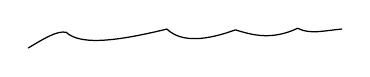
\begin{tikzpicture}[x=1cm,y=1cm,line cap=round,line join=round]
\draw[line width=0.45pt] (0,0) .. controls (0.20,0.12) and (0.36,0.22) .. (0.48,0.20)
.. controls (0.67,0.02) and (1.18,0.10) .. (1.76,0.24)
.. controls (1.95,0.06) and (2.27,0.10) .. (2.63,0.23)
.. controls (2.83,0.17) and (3.08,0.09) .. (3.42,0.25)
.. controls (3.58,0.17) and (3.75,0.22) .. (3.98,0.24);
\end{tikzpicture}}

Catégorie bordélique précisée (correspondant à un $\Pi_U$ \uline{connexe}) :

Ces objets sont les \var{\deleted{couples $(I$, \LMsourceMark{M002469}{\unsure{systèmes}}}}{\LMsourceMark{M002470}{\LMcancelledDoubts{\LMsourceMark{M002471}{\unsure{systèmes}}}}}{deletion}{140-2-s043-D002}\var{\inserted{homs de gr.}}{\LMadded{homs de gr.}}{insertion}{140-2-s043-I001} profinis \var{\deleted{(\LMsourceMark{M002472}{\unsure{indexés}} par un ens. fini $I$) de l'hom}}{\LMsourceMark{M002473}{\LMcancelledDoubts{\LMsourceMark{M002474}{\unsure{indexés}}}}}{deletion}{140-2-s043-D003}
\[
\mathcal E\xrightarrow{p}\Gamma
\]
(donnant naissance à une suite exacte :
\[
1\longrightarrow\pi\xrightarrow{\LMsourceMark{M002475}{\unsure{k|\kappa}}}\mathcal E\xrightarrow{p}\Gamma
\]
)
et un ens. \var{\inserted{fini}}{\LMadded{fini}}{insertion}{140-2-s043-I002} de sous-groupes (indexé par un ens $I$ d'indices)
\[
\mathcal E_i\overset{\rho_i}{\lhook\joinrel\longrightarrow}\mathcal E,
\]
et d'isomorphismes
\[
\mathcal E_i\cap\pi\overset{k_i}{\simeq}T(\bar K)
\]
\LMsourceMark{M002476}{\margin{42}}

\LMflushnotes\LMflushpages
\ifnum\LMform=1
\begin{LMapparatus}
\LMentry{140-2-s043-D001}{suppression}{\deleted{\LMsourceMark{M002477}{\unsure{cont}}}
}{\emph{\LMomittedlabel}}{Passage biffé dans le manuscrit : la suppression suit l'état final de l'auteur; les doutes de lecture restent signalés.}{}
\LMentry{140-2-s043-D002}{suppression}{\deleted{couples $(I$, \LMsourceMark{M002478}{\unsure{systèmes}}}
}{\emph{\LMomittedlabel}}{Passage biffé dans le manuscrit : la suppression suit l'état final de l'auteur; les doutes de lecture restent signalés.}{}
\LMentry{140-2-s043-I001}{insertion}{\inserted{homs de gr.}
}{\emph{\LMinsertedlabel}}{Ajout explicite de l'auteur : intégré à l'endroit indiqué par la transcription, sans modifier sa lecture.}{}
\LMentry{140-2-s043-D003}{suppression}{\deleted{(\LMsourceMark{M002479}{\unsure{indexés}} par un ens. fini $I$) de l'hom}
}{\emph{\LMomittedlabel}}{Passage biffé dans le manuscrit : la suppression suit l'état final de l'auteur; les doutes de lecture restent signalés.}{}
\LMentry{140-2-s043-I002}{insertion}{\inserted{fini}
}{\emph{\LMinsertedlabel}}{Ajout explicite de l'auteur : intégré à l'endroit indiqué par la transcription, sans modifier sa lecture.}{}
\end{LMapparatus}
\fi
\ifnum\LMform=2
\par\smallskip\begingroup\footnotesize\Needspace{4\baselineskip}\csname @beginparpenalty\endcsname=10000\relax\noindent\textcolor{gray}{\rule{.2\linewidth}{.35pt}}\par\nobreak
\noindent\textit{\LMdoubtheading.}\par\nobreak
\LMcarryover{140-2-s043-D001}{\LMsourceMark{M002480}{\unsure{cont}}
}
\LMcarryover{140-2-s043-D002}{\LMsourceMark{M002481}{\unsure{systèmes}}
}
\LMcarryover{140-2-s043-D003}{\LMsourceMark{M002482}{\unsure{indexés}}
}
\par\endgroup\smallskip
\fi

\LMsourceMark{M002483}{\scanpage{44}}
\LMsourceMark{M002484}{\mspage{20}}

Un hom d'un système
$(\mathcal E',p',(\mathcal E'_{i'})_{i'\in I'},(k'_{i'})_{i'\in I'})$
dans un syst.
$(\mathcal E,p,(\mathcal E_i)_{i\in I},(k_i)_{i\in I})$
est donné par par un hom
\[
f:\mathcal E'\longrightarrow\mathcal E
\]
\[
\beta_{i'}\in\mathcal E\quad(i'\in I'),\qquad\alpha\in\Gamma,
\]
tels que l'on ait les conditions :

\figure{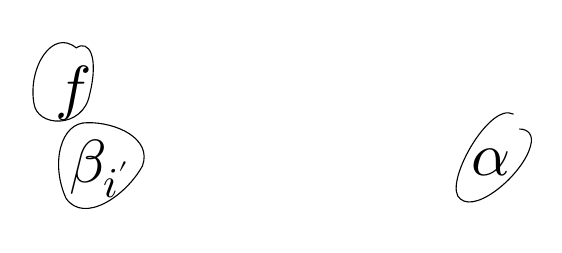
\begin{tikzpicture}[x=1cm,y=1cm,line cap=round,line join=round]
\begin{scope}[yshift=-0.35cm]
\node[font=\fontsize{22}{24}\selectfont] at (0,1.30) {$f$};
\draw (0.08,1.88) .. controls (-0.22,2.13) and (-0.53,1.64) .. (-0.46,1.19)
.. controls (-0.43,0.86) and (0.17,0.85) .. (0.25,1.29)
.. controls (0.37,1.77) and (0.24,1.99) .. (0.08,1.88);
\end{scope}
\node[font=\fontsize{22}{24}\selectfont] at (0.40,0) {$\beta_{i'}$};
\draw (0.22,0.58) .. controls (-0.12,0.59) and (-0.25,0.06) .. (-0.05,-0.38)
.. controls (0.18,-0.71) and (0.71,-0.35) .. (0.92,0.03)
.. controls (1.05,0.38) and (0.58,0.59) .. (0.22,0.58);
\node[font=\fontsize{22}{24}\selectfont] at (5.35,0.08) {$\alpha$};
\draw (5.63,0.69) .. controls (5.32,0.85) and (4.72,-0.23) .. (4.96,-0.39)
.. controls (5.18,-0.57) and (5.77,-0.05) .. (5.85,0.29)
.. controls (5.89,0.42) and (5.82,0.50) .. (5.71,0.50);
\end{tikzpicture}}

\LMsourceMark{M002485}{\margin{Les $\beta_{i'}$ pas uniques (si $\beta_{i'}$ convient, aussi $\gamma\beta_{i'}$, avec $\LMsourceMark{M002486}{\unsure{\gamma|\gamma_i}}\in\operatorname{Im}k_i$). Mais $\alpha$ unique \LMsourceMark{M002487}{\unsure{?!|??}}}}

$1^\circ)$\quad $p\circ f_{\mathcal E}=\operatorname{int}(\alpha)\,p'$

$2^\circ)$\quad $\forall i'\in I',\quad\exists i\in I$ (unique!) tel que
\[
\operatorname{int}(\beta_{i'}^{-1})f(\mathcal E'_{i'})\subset\mathcal E_i
\]
et un entier $d_{i'}\in\mathbb N^*$ tel que
\[
\operatorname{int}(\beta_{i'}^{-1})f\,k'_{i'}
 =k_i\circ(d_{i'}\cdot\operatorname{id}_{T(\bar K)})
\]

\LMsourceMark{M002488}{\margin{NB : $d_{i'}$ est aussi unique\ldots}}

\LMsourceMark{M002489}{\margin{[donc $\operatorname{int}(\beta_{i'}^{-1})\overbrace{\LMsourceMark{M002490}{\unsure{\operatorname{Im}(fk'_{i'})|\operatorname{Im}k'_{i'}}}}^{L'_{i'}}\subset\underbrace{\operatorname{Im}k_i}_{L_i}$ et \LMsourceMark{M002491}{\unsure{même}} \var{\deleted{\LMsourceMark{M002492}{\unsure{cette}} image}}{\LMsourceMark{M002493}{\LMcancelledDoubts{\LMsourceMark{M002494}{\unsure{cette}}}}}{deletion}{140-2-s044-D001} $\operatorname{int}(\beta_{i'}^{-1})\LMsourceMark{M002495}{\unsure{L'_{i'}}}=d_{i'}L_i$.]}}

\figure{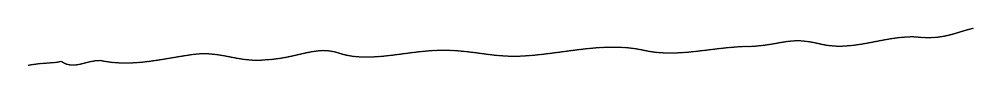
\begin{tikzpicture}[x=1cm,y=1cm,line cap=round,line join=round]
\draw[line width=0.45pt] (0,0) .. controls (0.22,0.04) and (0.30,0.02) .. (0.42,0.05)
.. controls (0.58,-0.07) and (0.73,0.07) .. (0.92,0.06)
.. controls (1.30,-0.02) and (1.64,0.07) .. (2.04,0.13)
.. controls (2.44,0.20) and (2.64,0.03) .. (3.02,0.07)
.. controls (3.43,0.09) and (3.66,0.26) .. (3.96,0.15)
.. controls (4.37,0.02) and (4.86,0.21) .. (5.35,0.19)
.. controls (5.79,0.17) and (5.95,0.08) .. (6.44,0.13)
.. controls (6.94,0.18) and (7.37,0.29) .. (7.82,0.19)
.. controls (8.26,0.09) and (8.70,0.24) .. (9.18,0.24)
.. controls (9.58,0.26) and (9.66,0.37) .. (10.06,0.27)
.. controls (10.48,0.17) and (10.87,0.38) .. (11.28,0.36)
.. controls (11.62,0.32) and (11.78,0.42) .. (12.00,0.47);
\end{tikzpicture}}

Je m'aperçois qu'il vaut mieux remplacer les $\beta_{i'}$ par les $\beta_{i'}^{-1}$, i.e. prendre l'iso. de commutation plutôt dans le sens
\[
f_{\mathcal E}\rho'_{i'}\xrightarrow{\beta_{i'}}\rho_i f_{i'}
\]
qu'en sens inverse. De plus, conceptuellement le diagramme
\diagram{\begin{tikzcd}[ampersand replacement=\&]
\& \Pi_{D^*}\arrow[dl,"\rho"']\arrow[dr,"\sigma"] \& \\
\Pi_U\arrow[dr,"\varphi"',""{name=L,inner sep=0pt}] \& \& \Pi_D\arrow[dl,"\psi",""{name=R,inner sep=0pt}]\\
\&\Pi_e\&
\arrow[from=L,to=R,bend left=25,"\alpha"]
\end{tikzcd}}
est trop compliqué, il suffit de se donner
\[
\boxed{\Pi_{D^*}\xrightarrow{\rho}\Pi_U\xrightarrow{\varphi}\Pi_e}
\]
et de déduire $\Pi_D$ par factorisation canonique
\LMsourceMark{M002496}{\margin{43}}

\LMflushnotes\LMflushpages
\ifnum\LMform=1
\begin{LMapparatus}
\LMentry{140-2-s044-D001}{suppression}{\deleted{\LMsourceMark{M002497}{\unsure{cette}} image}
}{\emph{\LMomittedlabel}}{Passage biffé dans le manuscrit : la suppression suit l'état final de l'auteur; les doutes de lecture restent signalés.}{}
\end{LMapparatus}
\fi
\ifnum\LMform=2
\par\smallskip\begingroup\footnotesize\Needspace{4\baselineskip}\csname @beginparpenalty\endcsname=10000\relax\noindent\textcolor{gray}{\rule{.2\linewidth}{.35pt}}\par\nobreak
\noindent\textit{\LMdoubtheading.}\par\nobreak
\LMcarryover{140-2-s044-D001}{\LMsourceMark{M002498}{\unsure{cette}}
}
\par\endgroup\smallskip
\fi

\LMsourceMark{M002499}{\scanpage{45}}

de l'hom. de groupoïdes $\Pi_{D^*}\longrightarrow\Pi_e$ en un hom qui induit un iso sur $\pi_0$ et un épi sur les $\pi_1$, suivi d'un hom qui est (épi sur $\pi_0$, et pour cause!, et qui est) \uline{fidèle}. Alors les $1$-morphismes de
\[
\Pi'_{D^*}\xrightarrow{\rho'}\Pi'_U\xrightarrow{\varphi'}\Pi_e
\]
\var{\deleted{dans}}{}{deletion}{140-2-s045-D001}
dans
\[
\Pi_{D^*}\xrightarrow{\rho}\Pi_U\xrightarrow{\varphi}\Pi_e
\]
sont les \var{\deleted{\LMsourceMark{M002500}{\unsure{couples}}}}{\LMsourceMark{M002501}{\LMcancelledDoubts{\LMsourceMark{M002502}{\unsure{couples}}}}}{deletion}{140-2-s045-D002}\var{\inserted{quintuplets}}{\LMadded{quintuplets}}{insertion}{140-2-s045-I001} de $2$ foncteurs \var{\inserted{et $3$ iso de foncteurs}}{\LMadded{et $3$ iso de foncteurs}}{insertion}{140-2-s045-I002}
$(f_{D^*},f_U,\alpha_{D^*U},\alpha_{Ue},K$
donnant un diagramme avec données de commutation
\diagram{\begin{tikzcd}[ampersand replacement=\&,column sep=1.05em,row sep=0.75em]
\Pi'_{D^*}\arrow[rrr,"\rho'"]\arrow[ddd,"f_{D^*}"'] \& \& \& \Pi'_U\arrow[rrr,"\varphi'"]\arrow[ddd,"f_U"'] \& \& \& \Pi_e\arrow[ddd,equal] \\
\& \& {} \& \& \& {} \& \\
\& {}\arrow[ur,bend left=25,"\alpha_{D^*U}"] \& \& \& {}\arrow[ur,bend left=25,"\alpha_{Ue}"] \& \& \\
\Pi_{D^*}\arrow[rrr,"\rho"'] \& \& \& \Pi_U\arrow[rrr,"\varphi"'] \& \& \& \Pi_e
\end{tikzcd}},

\LMsourceMark{M002503}{\margin{de plus, \var{\deleted{\LMsourceMark{M002504}{\illegible{1}}}}{\LMsourceMark{M002505}{\LMcancelledDoubts{\LMsourceMark{M002506}{\illegible{1}}}}}{deletion}{140-2-s045-D003} $\pi_1(\varphi\rho)=\pi_1(\Pi_{D^*}/\Pi_e)$ peut se définir comme un syst. local \var{\inserted{de groupes (\LMsourceMark{M002507}{\unsure{commutatifs|abéliens}})}}{\LMadded{de groupes (\LMsourceMark{M002508}{\unsure{commutatifs|abéliens}})}}{insertion}{140-2-s045-I003} sur $\Pi_{D^*}$, et on peut alors \LMsourceMark{M002509}{\unsure{définir|écrire}}
$\boxed{\LMsourceMark{M002510}{\unsure{\bar k|k}}:(\varphi\rho)^*\LMsourceMark{M002511}{\unsure{T_K|\mathcal T_K}}\simeq\pi_1(\varphi\rho)}$.}}

\LMsourceMark{M002512}{\margin{avec \uline{une} condition sur le morphisme
$\pi_1(\varphi'\rho')\LMsourceMark{M002513}{\unsure{\simeq|\longrightarrow}}\LMsourceMark{M002514}{\unsure{f_{D^*}^{\,*}}}(\pi_1(\varphi\rho))$
induit, qui modulo les iso. de Kummer doit être la multiplication par un $d$ \LMsourceMark{M002515}{\unsure{indice de ramification}} (qui est une application $\pi_0(\Pi'_{D^*})\longrightarrow\mathbb N^*$). [NB la multiplication par un \uline{\LMsourceMark{M002516}{\unsure{entier}}} \LMsourceMark{M002517}{\unsure{positif}} \LMsourceMark{M002518}{\illegible{5}} constants\ldots]}}

si on a deux tels $1$-morphismes
\[
f=(f_{D^*},f_U,\alpha_{D^*U},\alpha_{Ue})
\quad\text{et}\quad
g=(g_{D^*},g_U,\beta_{D^*U},\beta_{Ue})
\]
un \LMsourceMark{M002519}{\unsure{$0$-morphisme|homomorphisme}} de $f$ dans $g$ est formé d'un couple de $\mu_{D^*},\mu_U$ d'isomorphismes de foncteurs
\[
\mu_{D^*}:f_{D^*}\simeq g_{D^*},\qquad
\mu_U:f_U\longrightarrow g_U
\]
compatibles avec $\alpha_{D^*U},\var{\inserted{\beta_{D^*U},}}{\LMadded{\beta_{D^*U},}}{insertion}{140-2-s045-I004}$ et avec $\alpha_{Ue},\var{\inserted{\beta_{Ue},}}{\LMadded{\beta_{Ue},}}{insertion}{140-2-s045-I005}$ \var{\deleted{et avec}}{}{deletion}{140-2-s045-D004}
\LMsourceMark{M002520}{\margin{44}}

\LMflushnotes\LMflushpages
\ifnum\LMform=1
\begin{LMapparatus}
\LMentry{140-2-s045-D001}{suppression}{\deleted{dans}
}{\emph{\LMomittedlabel}}{Passage biffé dans le manuscrit : la suppression suit l'état final de l'auteur; les doutes de lecture restent signalés.}{}
\LMentry{140-2-s045-D002}{suppression}{\deleted{\LMsourceMark{M002521}{\unsure{couples}}}
}{\emph{\LMomittedlabel}}{Passage biffé dans le manuscrit : la suppression suit l'état final de l'auteur; les doutes de lecture restent signalés.}{}
\LMentry{140-2-s045-I001}{insertion}{\inserted{quintuplets}
}{\emph{\LMinsertedlabel}}{Ajout explicite de l'auteur : intégré à l'endroit indiqué par la transcription, sans modifier sa lecture.}{}
\LMentry{140-2-s045-I002}{insertion}{\inserted{et $3$ iso de foncteurs}
}{\emph{\LMinsertedlabel}}{Ajout explicite de l'auteur : intégré à l'endroit indiqué par la transcription, sans modifier sa lecture.}{}
\LMentry{140-2-s045-D003}{suppression}{\deleted{\LMsourceMark{M002522}{\illegible{1}}}
}{\emph{\LMomittedlabel}}{Passage biffé dans le manuscrit : la suppression suit l'état final de l'auteur; les doutes de lecture restent signalés.}{}
\LMentry{140-2-s045-I003}{insertion}{\inserted{de groupes (\LMsourceMark{M002523}{\unsure{commutatifs|abéliens}})}
}{\emph{\LMinsertedlabel}}{Ajout explicite de l'auteur : intégré à l'endroit indiqué par la transcription, sans modifier sa lecture.}{}
\LMentry{140-2-s045-I004}{insertion}{\(\inserted{\beta_{D^*U},}\)
}{\emph{\LMinsertedlabel}}{Ajout explicite de l'auteur : intégré à l'endroit indiqué par la transcription, sans modifier sa lecture.}{}
\LMentry{140-2-s045-I005}{insertion}{\(\inserted{\beta_{Ue},}\)
}{\emph{\LMinsertedlabel}}{Ajout explicite de l'auteur : intégré à l'endroit indiqué par la transcription, sans modifier sa lecture.}{}
\LMentry{140-2-s045-D004}{suppression}{\deleted{et avec}
}{\emph{\LMomittedlabel}}{Passage biffé dans le manuscrit : la suppression suit l'état final de l'auteur; les doutes de lecture restent signalés.}{}
\end{LMapparatus}
\fi
\ifnum\LMform=2
\par\smallskip\begingroup\footnotesize\Needspace{4\baselineskip}\csname @beginparpenalty\endcsname=10000\relax\noindent\textcolor{gray}{\rule{.2\linewidth}{.35pt}}\par\nobreak
\noindent\textit{\LMdoubtheading.}\par\nobreak
\LMcarryover{140-2-s045-D002}{\LMsourceMark{M002524}{\unsure{couples}}
}
\LMcarryover{140-2-s045-D003}{\LMsourceMark{M002525}{\illegible{1}}
}
\par\endgroup\smallskip
\fi

\LMsourceMark{M002526}{\scanpage{46}}
\LMsourceMark{M002527}{\mspage{21}}

\var{\deleted{$k,k'$ modulo multiplication par un indice de ramification}}{}{deletion}{140-2-s046-D001} (deux conditions de compatibilité sur les deux carrés).

Si on \var{\deleted{suppose}}{}{deletion}{140-2-s046-D002} se borne à des $\Pi_U,\Pi'_U$ connexes, on trouve en choisissant comme plus haut un objet \var{\inserted{$\widetilde U$}}{\LMadded{$\widetilde U$}}{insertion}{140-2-s046-I001} de $\Pi_U$ et un isom
\[
\boxed{\varphi(\widetilde U)\overset{\lambda}{\simeq}\Omega}
\]
(où $\Omega=\operatorname{Spec}(\bar K)$ est l'objet-repère de $\Pi_e\ldots$), un groupe $\mathcal E$ et un hom
\[
\mathcal E\xrightarrow{\varphi}\Gamma
\]
(qui est changé par autom. int. si on change $\lambda$, et $\mathcal E$ lui-= remplacé par groupe isomorphe, \LMsourceMark{M002528}{\unsure{d'isom.}} défini \LMsourceMark{M002529}{\unsure{mod.}} iso. int., si on change l'objet de référence $\widetilde U$). De =, choisissant un $\widetilde U_i$ dans chaque composante $i\in\pi_0(\Pi_{D^*})$, et des isom
\[
\lambda_i:\rho(\widetilde U_i)\simeq\widetilde U,
\]
on trouve des groupes $\mathcal E_i$ et des homs
\[
\mathcal E_i\xrightarrow{\rho_i}\mathcal E.
\]
Si on change $\lambda_i$, $\rho_i$ est changé par autom intérieur de $\mathcal E$. Si on change $\widetilde U_i$, $\mathcal E_i$ est remplacé par groupe isom, \var{\inserted{l'isom}}{\LMadded{l'isom}}{insertion}{140-2-s046-I002} défini à aut. int. près.
\LMsourceMark{M002530}{\margin{45}}

\LMflushnotes\LMflushpages
\ifnum\LMform=1
\begin{LMapparatus}
\LMentry{140-2-s046-D001}{suppression}{\deleted{$k,k'$ modulo multiplication par un indice de ramification}
}{\emph{\LMomittedlabel}}{Passage biffé dans le manuscrit : la suppression suit l'état final de l'auteur; les doutes de lecture restent signalés.}{}
\LMentry{140-2-s046-D002}{suppression}{\deleted{suppose}
}{\emph{\LMomittedlabel}}{Passage biffé dans le manuscrit : la suppression suit l'état final de l'auteur; les doutes de lecture restent signalés.}{}
\LMentry{140-2-s046-I001}{insertion}{\inserted{$\widetilde U$}
}{\emph{\LMinsertedlabel}}{Ajout explicite de l'auteur : intégré à l'endroit indiqué par la transcription, sans modifier sa lecture.}{}
\LMentry{140-2-s046-I002}{insertion}{\inserted{l'isom}
}{\emph{\LMinsertedlabel}}{Ajout explicite de l'auteur : intégré à l'endroit indiqué par la transcription, sans modifier sa lecture.}{}
\end{LMapparatus}
\fi

\LMsourceMark{M002531}{\scanpage{47}}

Considérons les composés
\diagram{\begin{tikzcd}[ampersand replacement=\&]
\mathcal E_i\arrow[r]\arrow[rr,bend left=30,"p_i"]\&\mathcal E\arrow[r,"p"']\&\Gamma
\end{tikzcd}}
d'où noyau, \var{\deleted{\LMsourceMark{M002532}{\illegible{1}}}}{\LMsourceMark{M002533}{\LMcancelledDoubts{\LMsourceMark{M002534}{\illegible{1}}}}}{deletion}{140-2-s047-D001} $\LMsourceMark{M002535}{\unsure{K|k}}$ est défini par un syst. d'iso
\[
T(\bar K)\overset{k_i}{\simeq}\operatorname{Ker}p_i\qquad(i\in I)
\]
s'insérant dans une famille de suites exactes
\[
1\longrightarrow T(\bar K)\xrightarrow{k_i}\mathcal E_i\xrightarrow{p_i}\Gamma
\]
(NB l'image de $p_i$ est un ss-groupe ouvert)
$k_i$ étant compatible aux actions de $\mathcal E_i$, quand on fait opérer $\mathcal E_i$ sur $T(\bar K)$ par l'action de $\Gamma$ sur $T(\bar K)$, et sur lui-= par autom intérieurs. Introduisant également $\pi=\operatorname{Ker}p$, on trouve donc des homs de suites exactes
\diagram{$(D)$\quad\begin{tikzcd}[ampersand replacement=\&]
1\arrow[r]\&T(\bar K)\arrow[r,"k_i"]\arrow[d,"\varepsilon_i\,\var{\deleted{\LMsourceMark{M002536}{\illegible{1}}}}{\LMsourceMark{M002537}{\LMcancelledDoubts{\(\LMsourceMark{M002538}{\illegible{1}}\)}}}{deletion}{140-2-s047-D002}"']\&\mathcal E_i\arrow[r,"p_i"]\arrow[d,"\rho_i"]\&\Gamma\arrow[d,equal]\\
1\arrow[r]\&\pi\arrow[r,"\LMsourceMark{M002539}{\unsure{k|\kappa}}"']\&\mathcal E\arrow[r,"p"']\&\Gamma
\end{tikzcd}\qquad$i\in I$}

\var{\deleted{Considérons}}{}{deletion}{140-2-s047-D003}
On peut dire que $\Pi_U$ définit un ``groupe extérieur'' $[\mathcal E]$, et $\Pi_U\longrightarrow\Pi_e$ un hom de groupes extérieurs
\[
[\mathcal E]\longrightarrow[\Gamma],
\]
de = $\Pi_{D^*}$ définit un syst. de ``groupes extérieurs'' $[\mathcal E_i]$, et \var{\deleted{\LMsourceMark{M002540}{\unsure{du hom}}}}{\LMsourceMark{M002541}{\LMcancelledDoubts{\LMsourceMark{M002542}{\unsure{du hom}}}}}{deletion}{140-2-s047-D004} $\Pi_{D^*}\longrightarrow\Pi_U$
\LMsourceMark{M002543}{\margin{46}}

\LMflushnotes\LMflushpages
\ifnum\LMform=1
\begin{LMapparatus}
\LMentry{140-2-s047-D001}{suppression}{\deleted{\LMsourceMark{M002544}{\illegible{1}}}
}{\emph{\LMomittedlabel}}{Passage biffé dans le manuscrit : la suppression suit l'état final de l'auteur; les doutes de lecture restent signalés.}{}
\LMentry{140-2-s047-D002}{suppression}{\(\deleted{\LMsourceMark{M002545}{\illegible{1}}}\)
}{\emph{\LMomittedlabel}}{Passage biffé dans le manuscrit : la suppression suit l'état final de l'auteur; les doutes de lecture restent signalés.}{}
\LMentry{140-2-s047-D003}{suppression}{\deleted{Considérons}
}{\emph{\LMomittedlabel}}{Passage biffé dans le manuscrit : la suppression suit l'état final de l'auteur; les doutes de lecture restent signalés.}{}
\LMentry{140-2-s047-D004}{suppression}{\deleted{\LMsourceMark{M002546}{\unsure{du hom}}}
}{\emph{\LMomittedlabel}}{Passage biffé dans le manuscrit : la suppression suit l'état final de l'auteur; les doutes de lecture restent signalés.}{}
\end{LMapparatus}
\fi
\ifnum\LMform=2
\par\smallskip\begingroup\footnotesize\Needspace{4\baselineskip}\csname @beginparpenalty\endcsname=10000\relax\noindent\textcolor{gray}{\rule{.2\linewidth}{.35pt}}\par\nobreak
\noindent\textit{\LMdoubtheading.}\par\nobreak
\LMcarryover{140-2-s047-D001}{\LMsourceMark{M002547}{\illegible{1}}
}
\LMcarryover{140-2-s047-D002}{\(\LMsourceMark{M002548}{\illegible{1}}\)
}
\LMcarryover{140-2-s047-D004}{\LMsourceMark{M002549}{\unsure{du hom}}
}
\par\endgroup\smallskip
\fi

\LMsourceMark{M002550}{\scanpage{48}}
\LMsourceMark{M002551}{\mspage{22}}

un syst. d'homs extérieurs
\[
[\mathcal E_i]\longrightarrow[\mathcal E],
\]
\var{\deleted{enfin}}{}{deletion}{140-2-s048-D001} mais comment en termes de groupes extérieurs exprimer les données de Kummer $k_i$ ?

Revenant au \var{\inserted{système de}}{\LMadded{système de}}{insertion}{140-2-s048-I001} diagramme $D$ (relatif à un ens d'indices $I$.) et à un $D'$ analogue (avec ens d'indices $I'$)
\diagram{$D'$\quad\begin{tikzcd}[ampersand replacement=\&]
1\arrow[r]\&T(\bar K)\arrow[r,"k'_{i'}"]\arrow[d,"\varepsilon'_{i'}"']\&\mathcal E'_{i'}\arrow[r,"p'_{i'}"]\arrow[d,"\rho'_{i'}"]\&\Gamma\arrow[d,equal]\\
1\arrow[r]\&\LMsourceMark{M002552}{\unsure{\pi|\pi'}}\arrow[r,"\LMsourceMark{M002553}{\unsure{k'|\kappa'}}"']\&\mathcal E'\arrow[r,"p'"']\&\Gamma
\end{tikzcd}\qquad$i'\in\LMsourceMark{M002554}{\unsure{I|I'}}$}
un $1$-morphisme \var{\inserted{$f$}}{\LMadded{$f$}}{insertion}{140-2-s048-I002} de $D'$ dans $D$ s'explicite par

$a)$ Un hom
\[
\boxed{\boxed{f_{\mathcal E}:\mathcal E'\longrightarrow\mathcal E}}
\]
\LMsourceMark{M002555}{\margin{décrit le \var{\deleted{\LMsourceMark{M002556}{\unsure{correspondant}}}}{\LMsourceMark{M002557}{\LMcancelledDoubts{\LMsourceMark{M002558}{\unsure{correspondant}}}}}{deletion}{140-2-s048-D002} foncteur $f_U$}}
[\var{\deleted{\LMsourceMark{M002559}{\unsure{dép.}}}}{\LMsourceMark{M002560}{\LMcancelledDoubts{\LMsourceMark{M002561}{\unsure{dép.}}}}}{deletion}{140-2-s048-D003}\var{\inserted{s'explicite}}{\LMadded{s'explicite}}{insertion}{140-2-s048-I003} en termes du choix d'un isom
\[
\nu:f(\widetilde U')\simeq\widetilde U
\]
[un autre choix modifie $f_{\mathcal E}$ par un $\operatorname{int}(\beta)$, $\beta\in\mathcal E$)]

$b)$ Une \var{\deleted{hom}}{}{deletion}{140-2-s048-D004} application $\tau:I'\longrightarrow I$, et pour tout $i'\in I'$, posant $i=\tau(i')$, un \var{\deleted{application}}{}{deletion}{140-2-s048-D005}\var{\inserted{hom de groupes}}{\LMadded{hom de groupes}}{insertion}{140-2-s048-I004}
\[
\boxed{\mathcal E'_{i'}\xrightarrow{f_{i'}}\mathcal E_i}
\]
\LMsourceMark{M002562}{\margin{décrit le foncteur $f_{D^*}$}}
\LMsourceMark{M002563}{\margin{47}}

\LMflushnotes\LMflushpages
\ifnum\LMform=1
\begin{LMapparatus}
\LMentry{140-2-s048-D001}{suppression}{\deleted{enfin}
}{\emph{\LMomittedlabel}}{Passage biffé dans le manuscrit : la suppression suit l'état final de l'auteur; les doutes de lecture restent signalés.}{}
\LMentry{140-2-s048-I001}{insertion}{\inserted{système de}
}{\emph{\LMinsertedlabel}}{Ajout explicite de l'auteur : intégré à l'endroit indiqué par la transcription, sans modifier sa lecture.}{}
\LMentry{140-2-s048-I002}{insertion}{\inserted{$f$}
}{\emph{\LMinsertedlabel}}{Ajout explicite de l'auteur : intégré à l'endroit indiqué par la transcription, sans modifier sa lecture.}{}
\LMentry{140-2-s048-D002}{suppression}{\deleted{\LMsourceMark{M002564}{\unsure{correspondant}}}
}{\emph{\LMomittedlabel}}{Passage biffé dans le manuscrit : la suppression suit l'état final de l'auteur; les doutes de lecture restent signalés.}{}
\LMentry{140-2-s048-D003}{suppression}{\deleted{\LMsourceMark{M002565}{\unsure{dép.}}}
}{\emph{\LMomittedlabel}}{Passage biffé dans le manuscrit : la suppression suit l'état final de l'auteur; les doutes de lecture restent signalés.}{}
\LMentry{140-2-s048-I003}{insertion}{\inserted{s'explicite}
}{\emph{\LMinsertedlabel}}{Ajout explicite de l'auteur : intégré à l'endroit indiqué par la transcription, sans modifier sa lecture.}{}
\LMentry{140-2-s048-D004}{suppression}{\deleted{hom}
}{\emph{\LMomittedlabel}}{Passage biffé dans le manuscrit : la suppression suit l'état final de l'auteur; les doutes de lecture restent signalés.}{}
\LMentry{140-2-s048-D005}{suppression}{\deleted{application}
}{\emph{\LMomittedlabel}}{Passage biffé dans le manuscrit : la suppression suit l'état final de l'auteur; les doutes de lecture restent signalés.}{}
\LMentry{140-2-s048-I004}{insertion}{\inserted{hom de groupes}
}{\emph{\LMinsertedlabel}}{Ajout explicite de l'auteur : intégré à l'endroit indiqué par la transcription, sans modifier sa lecture.}{}
\end{LMapparatus}
\fi
\ifnum\LMform=2
\par\smallskip\begingroup\footnotesize\Needspace{4\baselineskip}\csname @beginparpenalty\endcsname=10000\relax\noindent\textcolor{gray}{\rule{.2\linewidth}{.35pt}}\par\nobreak
\noindent\textit{\LMdoubtheading.}\par\nobreak
\LMcarryover{140-2-s048-D002}{\LMsourceMark{M002566}{\unsure{correspondant}}
}
\LMcarryover{140-2-s048-D003}{\LMsourceMark{M002567}{\unsure{dép.}}
}
\par\endgroup\smallskip
\fi

\LMsourceMark{M002568}{\scanpage{49}}

[s'explicite en termes du choix d'un iso
\[
f_{D^*}(\widetilde U'_{i'})\overset{\nu_{i'}}{\simeq}\widetilde U_i,
\]
et modifié par des $\operatorname{int}(\beta_{i'})$, $\beta_{i'}\in\mathcal E_i$, si on change $\nu_{i'}$]

$c)$ Une donnée de commutation pour
\diagram{\begin{tikzcd}[ampersand replacement=\&,column sep=0.9em,row sep=0.7em]
\mathcal E'\arrow[rrr,"p'"]\arrow[ddd,"f_{\mathcal E}"'] \& \& \& \LMsourceMark{M002569}{\unsure{\Gamma|\Gamma'}}\arrow[ddd,equal] \\
\& \& {} \& \\
\& {}\arrow[ur,bend left=25,"{\var{\deleted{\LMsourceMark{M002570}{\unsure{\beta}}}}{\LMsourceMark{M002571}{\LMcancelledDoubts{\(\LMsourceMark{M002572}{\unsure{\beta}}\)}}}{deletion}{140-2-s049-D001}\alpha}"] \& \& \\
\mathcal E\arrow[rrr,"p"'] \& \& \& \Gamma
\end{tikzcd}\quad$\boxed{\boxed{\var{\deleted{\LMsourceMark{M002573}{\unsure{\beta}}}}{\LMsourceMark{M002574}{\LMcancelledDoubts{\(\LMsourceMark{M002575}{\unsure{\beta}}\)}}}{deletion}{140-2-s049-D002}\alpha\in\Gamma}}$}
\LMsourceMark{M002576}{\margin{$\alpha$ décrit $\alpha_{Ue}$}}
i.e.
\[
\var{\deleted{f_{\mathcal E}p'=\operatorname{int}(\LMsourceMark{M002577}{\unsure{\beta}})p}}{\LMsourceMark{M002578}{\LMcancelledDoubts{\(\LMsourceMark{M002579}{\unsure{\beta}}\)}}}{deletion}{140-2-s049-D003}
\qquad\boxed{pf_{\mathcal E}=\operatorname{int}(\alpha)p'}
\]

$d)$ $\forall i'[\in\LMsourceMark{M002580}{\unsure{I|I'}}]$ une donnée de commutation pour
\diagram{\begin{tikzcd}[ampersand replacement=\&,column sep=0.9em,row sep=0.7em]
\mathcal E'_{i'}\arrow[rrr,"\rho'_{i'}"]\arrow[ddd,"f_{i'}"'] \& \& \& \mathcal E'\arrow[ddd,"f_{\mathcal E}"] \\
\& \& {} \& \\
\& {}\arrow[ur,bend left=25,"\alpha_{i'}"] \& \& \\
\mathcal E_i\arrow[rrr,"\rho_i"'] \& \& \& \mathcal E
\end{tikzcd}\quad$\boxed{\alpha_{i'}\in\mathcal E}\quad(i'\in I')$}
\LMsourceMark{M002581}{\margin{$(\alpha_{i'})$ décrit $\alpha_{D^*U}$}}
i.e. :
\[
\boxed{\rho_i f_{i'}=\operatorname{int}(\alpha_{i'})f_{\mathcal E}\rho'_{i'}}
\]

Notons que $c,d$ ensemble définissent une donnée de commutation
\diagram{\begin{tikzcd}[ampersand replacement=\&,column sep=0.9em,row sep=0.7em]
\mathcal E'_{i'}\arrow[rrr,"p'_{i'}"]\arrow[ddd,"f_{i'}"'] \& \& \& \Gamma\arrow[ddd,equal,"{\var{\deleted{\operatorname{int}(\LMsourceMark{M002582}{\unsure{\gamma}})}}{\LMsourceMark{M002583}{\LMcancelledDoubts{\(\LMsourceMark{M002584}{\unsure{\gamma}}\)}}}{deletion}{140-2-s049-D004}}"] \\
\& \& {} \& \\
\& {}\arrow[ur,bend left=25,"{\operatorname{int}(\beta_{i'})}"] \& \& \\
\mathcal E_i\arrow[rrr,"p_i"'] \& \& \& \Gamma
\end{tikzcd}}
avec $\beta_{i'}=p(\alpha_{i'})\alpha$
i.e.
\[
p_i f_{i'}=\operatorname{int}(\beta_{i'})p'_{i'}
\]
\LMsourceMark{M002585}{\margin{48}}

\LMflushnotes\LMflushpages
\ifnum\LMform=1
\begin{LMapparatus}
\LMentry{140-2-s049-D001}{suppression}{\(\deleted{\LMsourceMark{M002586}{\unsure{\beta}}}\)
}{\emph{\LMomittedlabel}}{Passage biffé dans le manuscrit : la suppression suit l'état final de l'auteur; les doutes de lecture restent signalés.}{}
\LMentry{140-2-s049-D002}{suppression}{\(\deleted{\LMsourceMark{M002587}{\unsure{\beta}}}\)
}{\emph{\LMomittedlabel}}{Passage biffé dans le manuscrit : la suppression suit l'état final de l'auteur; les doutes de lecture restent signalés.}{}
\LMentry{140-2-s049-D003}{suppression}{\(\deleted{f_{\mathcal E}p'=\operatorname{int}(\LMsourceMark{M002588}{\unsure{\beta}})p}\)
}{\emph{\LMomittedlabel}}{Passage biffé dans le manuscrit : la suppression suit l'état final de l'auteur; les doutes de lecture restent signalés.}{}
\LMentry{140-2-s049-D004}{suppression}{\(\deleted{\operatorname{int}(\LMsourceMark{M002589}{\unsure{\gamma}})}\)
}{\emph{\LMomittedlabel}}{Passage biffé dans le manuscrit : la suppression suit l'état final de l'auteur; les doutes de lecture restent signalés.}{}
\end{LMapparatus}
\fi
\ifnum\LMform=2
\par\smallskip\begingroup\footnotesize\Needspace{4\baselineskip}\csname @beginparpenalty\endcsname=10000\relax\noindent\textcolor{gray}{\rule{.2\linewidth}{.35pt}}\par\nobreak
\noindent\textit{\LMdoubtheading.}\par\nobreak
\LMcarryover{140-2-s049-D001}{\(\LMsourceMark{M002590}{\unsure{\beta}}\)
}
\LMcarryover{140-2-s049-D002}{\(\LMsourceMark{M002591}{\unsure{\beta}}\)
}
\LMcarryover{140-2-s049-D003}{\(\LMsourceMark{M002592}{\unsure{\beta}}\)
}
\LMcarryover{140-2-s049-D004}{\(\LMsourceMark{M002593}{\unsure{\gamma}}\)
}
\par\endgroup\smallskip
\fi

\LMsourceMark{M002594}{\scanpage{50}}
\LMsourceMark{M002595}{\mspage{23}}

i.e. on a commutativité dans
\diagram{\begin{tikzcd}[ampersand replacement=\&]
\mathcal E'_{i'}\arrow[r,"p'_{i'}"]\arrow[d,"f_{i'}"']\&\Gamma\arrow[d,"\operatorname{int}(\beta_{i'})"]\\
\mathcal E_i\arrow[r,"p_i"']\&\Gamma
\end{tikzcd}}
donc $f_{i'}$ induit un hom de suites exactes
\diagram{\begin{tikzcd}[ampersand replacement=\&]
1\arrow[r]\&T(\bar K)\arrow[r,"k'_{i'}"]\arrow[d,"f^0_{i'}"']\&\mathcal E'_{i'}\arrow[r,"\LMsourceMark{M002596}{\unsure{p'_{i'}|f'_{i'}}}"]\arrow[d,"f_{i'}"]\&\Gamma\arrow[d,"\operatorname{int}(\beta_{i'})"]\\
1\arrow[r]\&T(\bar K)\arrow[r,"k_i"']\&\mathcal E_i\arrow[r,"p_i"']\&\Gamma
\end{tikzcd}}
\LMsourceMark{M002597}{\margin{795}}
et il faut exprimer la compatibilité de $f^0_{i'}$ avec l'indice de ramification $d_{i'}\in\mathbb N$, on trouve
\[
\boxed{f^0_{i'}=d_{i'}\chi(\beta_{i'})\operatorname{id}_{T(\bar K)}}
\]
où
\[
\chi:\Gamma\longrightarrow\widehat{\mathbb Z}^{\,*}
\]
est le caractère canonique.

Ceci posé, déterminons, pour un $1$-morphisme
\[
f=(f_{\mathcal E},\var{\inserted{\tau,}}{\LMadded{\tau,}}{insertion}{140-2-s050-I001}(f_{i'}),\alpha,(\LMsourceMark{M002598}{\unsure{\alpha_{i'}|\alpha_i}}))
\]
et un autre
\[
f'=(f'_{\mathcal E},\tau',(f'_{i'}),\alpha',(\LMsourceMark{M002599}{\unsure{\alpha'_{i'}|\alpha'_i}})),
\]
les $0$-morphismes de l'un dans l'autre.
\LMsourceMark{M002600}{\margin{49}}

\LMflushnotes\LMflushpages
\ifnum\LMform=1
\begin{LMapparatus}
\LMentry{140-2-s050-I001}{insertion}{\(\inserted{\tau,}\)
}{\emph{\LMinsertedlabel}}{Ajout explicite de l'auteur : intégré à l'endroit indiqué par la transcription, sans modifier sa lecture.}{}
\end{LMapparatus}
\fi

% END PACKAGE LM_P05
% BEGIN PACKAGE LM_P06
\ifnum\LMform<2\Needspace{11\baselineskip}\subsection*{Scans 51--60}\fi
\LMsourceMark{M002601}{\scanpage{51}}

\LMsourceMark{M002602}{\unsure{correspondant|correspondent}} à des syst. d'iso.
\[
\mu_{\mathcal D^*}:f_{\mathcal D^*}\longrightarrow f'_{\mathcal D^*},\qquad
\LMsourceMark{M002603}{\unsure{\mu_{U^*}}}\;f_U\longrightarrow g_U.
\]
Cela correspond \uline{conditions} $\tau'=\tau$, $d'_{i'}=d_{i'}$ $\forall i'\in I'$ et \LMsourceMark{M002604}{\unsure{à}} la donnée de
\var{\inserted{ceci résulte des autres conditions\LMsourceMark{M002605}{\unsure{\ldots}}}}{\LMadded{ceci résulte des autres conditions\LMsourceMark{M002606}{\unsure{\ldots}}}}{insertion}{140-2-s051-I001}
\LMsourceMark{M002607}{\margin{\LMsourceMark{M002608}{\unsure{exprimons}} l'\uline{existence} d'un iso. $\mu_{\mathcal D^*}$}}

\LMsourceMark{M002609}{\margin{décrit $\mu_U$}}
a) $\boxed{\boxed{\mu\in\mathcal E}}$, définissant un iso entre
\[
f_{\mathcal E}:\mathcal E'\longrightarrow\mathcal E
\quad\text{et}\quad
f'_{\mathcal E}:\mathcal E'\longrightarrow\mathcal E
\]
i.e. \var{\deleted{\LMsourceMark{M002610}{\unsure{faisant}}}}{\LMsourceMark{M002611}{\LMcancelledDoubts{\LMsourceMark{M002612}{\unsure{faisant}}}}}{deletion}{140-2-s051-D001} tel que
\[
\boxed{f'_{\mathcal E}=\operatorname{int}(\mu)f_{\mathcal E}}\,)
\]

b) $\boxed{\boxed{\mu_{i'}\in\mathcal E_i}}$ $(i'\in I',\ i=\tau(i'))$
\LMsourceMark{M002613}{\margin{décrit $\mu_{\mathcal D^*}$}}
satisfaisant
\[
\boxed{f'_{i'}=\operatorname{int}(\mu_{i'})f_{i'}}\,),
\]
\LMsourceMark{M002614}{\margin{ceci implique déjà $d_{i'}=d'_{i'}$}}
les $\underset{\substack{\in\\\mathcal E}}{\mu},\ \underset{\substack{\in\\\mathcal E_i}}{\mu_{i'}}$ étant liés aux $\underset{\substack{\LMsourceMark{M002615}{\unsure{\in|\notin}}\\\mathcal E}}{\alpha},\alpha'$ \LMsourceMark{M002616}{\unsure{\var{\deleted{ds}}{\LMsourceMark{M002617}{\LMuncertaindeletion{140-2-s051-D002}}}{deletion}{140-2-s051-D002}|ds}} $(\in\mathcal E)$
aux $\alpha_{i'},\alpha'_{i'}$ $(\in\Gamma)$ de la façon suivante
\[
\boxed{\alpha'=p(\mu)\alpha}
\]
\[
\boxed{\alpha'_{i'}=\rho_i(\mu_{i'})\alpha_{i'}}\qquad\forall i'\in I'
\]
ou encore
\[
\boxed{\begin{cases}
p(\mu)=\alpha'\alpha^{-1}\\
\rho_i(\mu_{i'})=\alpha'_{i'}\alpha_{i'}^{-1}
\end{cases}}
\]
\LMsourceMark{M002618}{\margin{50}}

\LMflushnotes\LMflushpages
\ifnum\LMform=1
\begin{LMapparatus}
\LMentry{140-2-s051-I001}{insertion}{\inserted{ceci résulte des autres conditions\LMsourceMark{M002619}{\unsure{\ldots}}}
}{\emph{\LMinsertedlabel}}{Ajout explicite de l'auteur : intégré à l'endroit indiqué par la transcription, sans modifier sa lecture.}{}
\LMentry{140-2-s051-D001}{suppression}{\deleted{\LMsourceMark{M002620}{\unsure{faisant}}}
}{\emph{\LMomittedlabel}}{Passage biffé dans le manuscrit : la suppression suit l'état final de l'auteur; les doutes de lecture restent signalés.}{}
\LMentry{140-2-s051-D002}{suppression}{\LMsourceMark{M002621}{\LMdoubtcopy{\deleted{ds}}}
}{\emph{\LMomittedlabel}}{Passage biffé dans le manuscrit : la suppression suit l'état final de l'auteur; les doutes de lecture restent signalés.}{}
\end{LMapparatus}
\fi
\ifnum\LMform=2
\par\smallskip\begingroup\footnotesize\Needspace{4\baselineskip}\csname @beginparpenalty\endcsname=10000\relax\noindent\textcolor{gray}{\rule{.2\linewidth}{.35pt}}\par\nobreak
\noindent\textit{\LMdoubtheading.}\par\nobreak
\LMcarryover{140-2-s051-D001}{\LMsourceMark{M002622}{\unsure{faisant}}
}
\LMcarryover{140-2-s051-D002}{\LMsourceMark{M002623}{\LMdoubtcopy{ds}}
}
\par\endgroup\smallskip
\fi

\LMsourceMark{M002624}{\scanpage{52}}
\LMsourceMark{M002625}{\mspage{24}}

Notons que, comme $\rho_i$ est injectif, les deuxièmes relations, donnant les $\rho_i(\mu_{i'})$, déterminent les $\mu_{i'}$ de \uline{façon unique}, l'existence de ces $\mu_{i'}$ équivaut aux relations
\[
\boxed{\alpha'_{i'}\alpha_{i'}^{-1}\in\rho_i(\mathcal E_i)}\qquad i'\in I'.
\]

Quant à la relation $p(\mu)=\alpha'\alpha^{-1}$, elle détermine $\mu$ modulo multiplication \var{\inserted{(à droite disons)}}{\LMadded{(à droite disons)}}{insertion}{140-2-s052-I001} par un \var{\deleted{\LMsourceMark{M002626}{\illegible{1}}}}{\LMsourceMark{M002627}{\LMcancelledDoubts{\LMsourceMark{M002628}{\illegible{1}}}}}{deletion}{140-2-s052-D001} $\mu_0\in\operatorname{Ker}p=\pi$, mais qui doit être tel que l'on ait encore
\[
f'_{\mathcal E}=\operatorname{int}(\var{\deleted{\mu_0}}{}{deletion}{140-2-s052-D002}\mu\mu_0)f_{\mathcal E}
\]
(en plus de $f'_{\mathcal E}=\operatorname{int}(\mu)f_{\mathcal E}$) ce qui signifie \var{\deleted{exige}}{}{deletion}{140-2-s052-D003} que
\[
\operatorname{int}(\mu_0)f_{\mathcal E}=\LMsourceMark{M002629}{\unsure{f_{\mathcal E}|f'_{\mathcal E}}}
\]
i.e.
\[
\boxed{\mu_0\in\operatorname{Centr}_{\LMsourceMark{M002630}{\unsure{\pi}}}\var{\deleted{\operatorname{Im}}}{}{deletion}{140-2-s052-D004}f_{\mathcal E}(\mathcal E')}
\]

C'est donc cela l'indétermination exacte dans le choix d'un $0$-morphisme \LMsourceMark{M002631}{\unsure{les|des}} $1$-morph. \var{\deleted{entre}}{}{deletion}{140-2-s052-D005} $f$ et $f'$ de $\mathcal D'$ dans $\mathcal D$.
Si p.ex. on est dans les conditions où
$\pi'\longrightarrow\pi$ induit par $f_{\mathcal E}:\mathcal E'\longrightarrow\mathcal E$ \var{\deleted{est}}{}{deletion}{140-2-s052-D006} a une image d'indice fini (image ouverte)
--- cas d'un ``morphisme non constant'' ! ---
alors $\mu_0$ doit centraliser un ss-groupe ouvert de
\LMsourceMark{M002632}{\margin{51}}

\LMflushnotes\LMflushpages
\ifnum\LMform=1
\begin{LMapparatus}
\LMentry{140-2-s052-I001}{insertion}{\inserted{(à droite disons)}
}{\emph{\LMinsertedlabel}}{Ajout explicite de l'auteur : intégré à l'endroit indiqué par la transcription, sans modifier sa lecture.}{}
\LMentry{140-2-s052-D001}{suppression}{\deleted{\LMsourceMark{M002633}{\illegible{1}}}
}{\emph{\LMomittedlabel}}{Passage biffé dans le manuscrit : la suppression suit l'état final de l'auteur; les doutes de lecture restent signalés.}{}
\LMentry{140-2-s052-D002}{suppression}{\(\deleted{\mu_0}\)
}{\emph{\LMomittedlabel}}{Passage biffé dans le manuscrit : la suppression suit l'état final de l'auteur; les doutes de lecture restent signalés.}{}
\LMentry{140-2-s052-D003}{suppression}{\deleted{exige}
}{\emph{\LMomittedlabel}}{Passage biffé dans le manuscrit : la suppression suit l'état final de l'auteur; les doutes de lecture restent signalés.}{}
\LMentry{140-2-s052-D004}{suppression}{\(\deleted{\operatorname{Im}}\)
}{\emph{\LMomittedlabel}}{Passage biffé dans le manuscrit : la suppression suit l'état final de l'auteur; les doutes de lecture restent signalés.}{}
\LMentry{140-2-s052-D005}{suppression}{\deleted{entre}
}{\emph{\LMomittedlabel}}{Passage biffé dans le manuscrit : la suppression suit l'état final de l'auteur; les doutes de lecture restent signalés.}{}
\LMentry{140-2-s052-D006}{suppression}{\deleted{est}
}{\emph{\LMomittedlabel}}{Passage biffé dans le manuscrit : la suppression suit l'état final de l'auteur; les doutes de lecture restent signalés.}{}
\end{LMapparatus}
\fi
\ifnum\LMform=2
\par\smallskip\begingroup\footnotesize\Needspace{4\baselineskip}\csname @beginparpenalty\endcsname=10000\relax\noindent\textcolor{gray}{\rule{.2\linewidth}{.35pt}}\par\nobreak
\noindent\textit{\LMdoubtheading.}\par\nobreak
\LMcarryover{140-2-s052-D001}{\LMsourceMark{M002634}{\illegible{1}}
}
\par\endgroup\smallskip
\fi

\LMsourceMark{M002635}{\scanpage{53}}

$\pi$ --- sauf erreur cela aussi implique $\mu_0=1$, donc il semble bien que \var{\deleted{\LMsourceMark{M002636}{\illegible{1}}}}{\LMsourceMark{M002637}{\LMcancelledDoubts{\LMsourceMark{M002638}{\illegible{1}}}}}{deletion}{140-2-s053-D001} (dans les cas correspondants à des hom dominants de courbes algébriques) une \var{\deleted{hom}}{}{deletion}{140-2-s053-D002} $0$-morphisme d'un $f$ \LMsourceMark{M002639}{\unsure{ds}} un $f'$ (s'il existe) est unique, i.e. \uline{$\operatorname{Hom}$} $(\mathcal D',\mathcal D^*)$ est une catégorie \uline{discrète}.

On peut interpréter $\mathcal D$ comme $\mathcal E$ muni de sous-groupes $\mathcal E_i\subset\mathcal E$, et de $p:\mathcal E\longrightarrow\LMsourceMark{M002640}{\unsure{\Gamma_*|\Gamma}}$ (noyau $\pi$) enfin d'isomorphismes
\[
k_i:\mathrm T(\overline K)\xrightarrow{\sim}\mathcal E_i\cap\pi=L_i
\]
(commutant à l'action de $\mathcal E_i$).
Si on a \LMsourceMark{M002641}{\unsure{une|un}} autre syst.
\[
(\mathcal E',\ (\mathcal E'_{i'})_{i'\in I'},\ p':\mathcal E'\longrightarrow\Gamma',\ (k'_{i'})_{i'\in I'}),
\]
\var{\inserted{$\mathcal E'_{i'}\subset\mathcal E'$}}{\LMadded{$\mathcal E'_{i'}\subset\mathcal E'$}}{insertion}{140-2-s053-I001}
un morphisme du premier dans le second est \uline{défini} par un
\[
f:\mathcal E'\longrightarrow\mathcal E
\]
satisfaisant les conditions suivantes

\var{\inserted{b) $pf$ est conjugué de $f'$ [soit $\alpha\in\Gamma$ tel que $pf=\operatorname{int}(\alpha)p'$]}}{\LMadded{b) $pf$ est conjugué de $f'$ [soit $\alpha\in\Gamma$ tel que $pf=\operatorname{int}(\alpha)p'$]}}{insertion}{140-2-s053-I002}

a) $\forall i'\in I',\quad\exists i\in I$ tel que $f(\mathcal E'_{i'})$ soit contenu dans un conjugué de $\mathcal E_i$
[soit $\alpha_{i'}\in\mathcal E$ tel que
$f(\mathcal E'_{i'})\LMsourceMark{M002642}{\unsure{\subset|=}}\operatorname{int}(\alpha_{i'}^{-1})(\mathcal E_i)$]
\var{\inserted{i.e. $\operatorname{int}(\alpha_{i'})f(\mathcal E'_{i'})\subset\mathcal E_i$}}{\LMadded{i.e. $\operatorname{int}(\alpha_{i'})f(\mathcal E'_{i'})\subset\mathcal E_i$}}{insertion}{140-2-s053-I003}
\LMsourceMark{M002643}{\margin{52}}

\LMflushnotes\LMflushpages
\ifnum\LMform=1
\begin{LMapparatus}
\LMentry{140-2-s053-D001}{suppression}{\deleted{\LMsourceMark{M002644}{\illegible{1}}}
}{\emph{\LMomittedlabel}}{Passage biffé dans le manuscrit : la suppression suit l'état final de l'auteur; les doutes de lecture restent signalés.}{}
\LMentry{140-2-s053-D002}{suppression}{\deleted{hom}
}{\emph{\LMomittedlabel}}{Passage biffé dans le manuscrit : la suppression suit l'état final de l'auteur; les doutes de lecture restent signalés.}{}
\LMentry{140-2-s053-I001}{insertion}{\inserted{$\mathcal E'_{i'}\subset\mathcal E'$}
}{\emph{\LMinsertedlabel}}{Ajout explicite de l'auteur : intégré à l'endroit indiqué par la transcription, sans modifier sa lecture.}{}
\LMentry{140-2-s053-I002}{insertion}{\inserted{b) $pf$ est conjugué de $f'$ [soit $\alpha\in\Gamma$ tel que $pf=\operatorname{int}(\alpha)p'$]}
}{\emph{\LMinsertedlabel}}{Ajout explicite de l'auteur : intégré à l'endroit indiqué par la transcription, sans modifier sa lecture.}{}
\LMentry{140-2-s053-I003}{insertion}{\inserted{i.e. $\operatorname{int}(\alpha_{i'})f(\mathcal E'_{i'})\subset\mathcal E_i$}
}{\emph{\LMinsertedlabel}}{Ajout explicite de l'auteur : intégré à l'endroit indiqué par la transcription, sans modifier sa lecture.}{}
\end{LMapparatus}
\fi
\ifnum\LMform=2
\par\smallskip\begingroup\footnotesize\Needspace{4\baselineskip}\csname @beginparpenalty\endcsname=10000\relax\noindent\textcolor{gray}{\rule{.2\linewidth}{.35pt}}\par\nobreak
\noindent\textit{\LMdoubtheading.}\par\nobreak
\LMcarryover{140-2-s053-D001}{\LMsourceMark{M002645}{\illegible{1}}
}
\par\endgroup\smallskip
\fi

\LMsourceMark{M002646}{\scanpage{54}}
\LMsourceMark{M002647}{\mspage{25}}

\uline{NB} Le $i\in I$ correspondant à $i'\in I'$ est unique, d'où $\tau:I'\longrightarrow I$.
Si les $\alpha_{i'}$ sont choisis, on déduit \var{\deleted{\LMsourceMark{M002648}{\unsure{$\forall i'$}}}}{\LMsourceMark{M002649}{\LMcancelledDoubts{\LMsourceMark{M002650}{\unsure{$\forall i'$}}}}}{deletion}{140-2-s054-D001} hom induits
$f_{i'}:\mathcal E'_{i'}\longrightarrow\mathcal E_i$,
\[
f_{i'}=(\operatorname{int}(\alpha_{i'})\circ f)|\mathcal E'_{i'},
\]
qui induit dès lors, via les $k'_{i'},k_i$, un endomorphisme
\[
f^0_{i'}:\mathrm T(\overline K)\longrightarrow\mathrm T(\overline K).
\]
\LMsourceMark{M002651}{\margin{\uline{NB} A priori $f^0_{i'}$ est la \LMsourceMark{M002652}{\unsure{multiplication par}} $\chi_{i'}\in\LMsourceMark{M002653}{\unsure{\widehat{\mathbb Z}^{\,*}|\widehat{\mathbb Z}}}$. Le centralisateur dans $\Gamma$ d'un ss-groupe ouvert est réduit à l'unité.}}
On exige que $\alpha\in\Gamma$ (qui conjugue $\LMsourceMark{M002654}{\unsure{f_{\mathcal E}}}$ en $\LMsourceMark{M002655}{\unsure{f'_{\mathcal E}}}$\}, et est \LMsourceMark{M002656}{\unsure{probablement}} uniquement déterminé par cette condition) et $\alpha_{i'}$ (qui est sans doute déterminé mod \var{\deleted{\LMsourceMark{M002657}{\unsure{conjugaison}}}}{\LMsourceMark{M002658}{\LMcancelledDoubts{\LMsourceMark{M002659}{\unsure{conjugaison}}}}}{deletion}{140-2-s054-D002} composition à g. avec un élt \LMsourceMark{M002660}{\unsure{des normalisateurs|du normalisateur}} de $\mathcal E_i$ (du moins des transporteurs \var{\inserted{des $\mathcal E_i$}}{\LMadded{des $\mathcal E_i$}}{insertion}{140-2-s054-I001} d'un ss-groupe ouvert de $\mathcal E_i$ --- c'est itou si $f$ est iso) puissent être choisis de telle façon que, posant
\[
\beta_{i'}=p(\alpha_{i'})\alpha,
\]
on ait
\[
f^0_{i'}=(d_{i'}\chi(\beta_{i'}))\operatorname{id}_{\mathrm T(\overline K)}
\]
\var{\inserted{i.e. $\chi_{i'}=d_{i'}\chi(\beta_{i'})$}}{\LMadded{i.e. $\chi_{i'}=d_{i'}\chi(\beta_{i'})$}}{insertion}{140-2-s054-I002}
\LMsourceMark{M002661}{\margin{Cette condition sur les syst. des $\alpha_{i'}$ ne change pas ($\alpha$ restant fixé) si on change $\alpha_{i'}$ en $\mu_{i'}\alpha_{i'}$, où $\mu_{i'}\in\mathcal E_i$.}}
$d_{i'}\in\mathbb N^*$ est un entier naturel évidemment uniquement déterminé \LMsourceMark{M002662}{\unsure{\}}} quand $\alpha$ et les $\alpha_{i'}$ sont choisis).

\var{\deleted{Remplaçons $\alpha$ par $\alpha'=\alpha_0\alpha$.}}{}{deletion}{140-2-s054-D003}
\LMsourceMark{M002663}{\margin{53}}

\LMflushnotes\LMflushpages
\ifnum\LMform=1
\begin{LMapparatus}
\LMentry{140-2-s054-D001}{suppression}{\deleted{\LMsourceMark{M002664}{\unsure{$\forall i'$}}}
}{\emph{\LMomittedlabel}}{Passage biffé dans le manuscrit : la suppression suit l'état final de l'auteur; les doutes de lecture restent signalés.}{}
\LMentry{140-2-s054-D002}{suppression}{\deleted{\LMsourceMark{M002665}{\unsure{conjugaison}}}
}{\emph{\LMomittedlabel}}{Passage biffé dans le manuscrit : la suppression suit l'état final de l'auteur; les doutes de lecture restent signalés.}{}
\LMentry{140-2-s054-I001}{insertion}{\inserted{des $\mathcal E_i$}
}{\emph{\LMinsertedlabel}}{Ajout explicite de l'auteur : intégré à l'endroit indiqué par la transcription, sans modifier sa lecture.}{}
\LMentry{140-2-s054-I002}{insertion}{\inserted{i.e. $\chi_{i'}=d_{i'}\chi(\beta_{i'})$}
}{\emph{\LMinsertedlabel}}{Ajout explicite de l'auteur : intégré à l'endroit indiqué par la transcription, sans modifier sa lecture.}{}
\LMentry{140-2-s054-D003}{suppression}{\deleted{Remplaçons $\alpha$ par $\alpha'=\alpha_0\alpha$.}
}{\emph{\LMomittedlabel}}{Passage biffé dans le manuscrit : la suppression suit l'état final de l'auteur; les doutes de lecture restent signalés.}{}
\end{LMapparatus}
\fi
\ifnum\LMform=2
\par\smallskip\begingroup\footnotesize\Needspace{4\baselineskip}\csname @beginparpenalty\endcsname=10000\relax\noindent\textcolor{gray}{\rule{.2\linewidth}{.35pt}}\par\nobreak
\noindent\textit{\LMdoubtheading.}\par\nobreak
\LMcarryover{140-2-s054-D001}{\LMsourceMark{M002666}{\unsure{$\forall i'$}}
}
\LMcarryover{140-2-s054-D002}{\LMsourceMark{M002667}{\unsure{conjugaison}}
}
\par\endgroup\smallskip
\fi

\LMsourceMark{M002668}{\scanpage{55}}

8, \uline{Réflexion taxonomique.}

Le cas $\dim X=0$ se traduit sur le paradigme du système
$(\mathrm T(\overline K)\xrightarrow{k_i}\mathcal E_i\overset{\rho_i}{\hookrightarrow}\mathcal E\xrightarrow{p}\Gamma)$
\var{\deleted{\LMsourceMark{M002669}{\illegible{2}}}}{\LMsourceMark{M002670}{\LMcancelledDoubts{\LMsourceMark{M002671}{\illegible{2}}}}}{deletion}{140-2-s055-D001} par la condition \var{\deleted{$\LMsourceMark{M002672}{\unsure{\pi|I}}=\varnothing$}}{\LMsourceMark{M002673}{\LMcancelledDoubts{\(\LMsourceMark{M002674}{\unsure{\pi|I}}\)}}}{deletion}{140-2-s055-D002} $p$ injectif, \var{\deleted{donc \LMsourceMark{M002675}{\unsure{se|de}}}}{\LMsourceMark{M002676}{\LMcancelledDoubts{\LMsourceMark{M002677}{\unsure{se|de}}}}}{deletion}{140-2-s055-D003}
\var{\inserted{et donc $I=\varnothing$ --- donc ce cas se}}{\LMadded{et donc $I=\varnothing$ --- donc ce cas se}}{insertion}{140-2-s055-I001}
décrit \var{\deleted{\LMsourceMark{M002678}{\illegible{1}}}}{\LMsourceMark{M002679}{\LMcancelledDoubts{\LMsourceMark{M002680}{\illegible{1}}}}}{deletion}{140-2-s055-D004}
simplement par la donnée d'un \uline{sous-groupe} ouvert $\mathcal E\subset\Gamma$, i.e. d'une sous-extension finie $\LMsourceMark{M002681}{\unsure{L}}$ de $\overline K/K$
(NB on aura bien sûr $X'=\operatorname{Spec}\LMsourceMark{M002682}{\unsure{L'|L}}$, et les choix \var{\inserted{faits}}{\LMadded{faits}}{insertion}{140-2-s055-I002} sur $X$ \var{\inserted{--- i.e. sur $\underset{=\varnothing}{\Pi_{\mathcal D^*}}\longrightarrow\Pi_U\longrightarrow\Pi_e$ ---}}{\LMadded{--- i.e. sur $\underset{=\varnothing}{\Pi_{\mathcal D^*}}\longrightarrow\Pi_U\longrightarrow\Pi_e$ ---}}{insertion}{140-2-s055-I003} \LMsourceMark{M002683}{\unsure{aboutissant|aboutissent}} à cette description --- reviennent ici au choix d'une telle \var{\inserted{$K$-}}{\LMadded{$K$-}}{insertion}{140-2-s055-I004}immersion de $L\var{\deleted{\LMsourceMark{M002684}{\unsure{K'}}}}{\LMsourceMark{M002685}{\LMcancelledDoubts{\(\LMsourceMark{M002686}{\unsure{K'}}\)}}}{deletion}{140-2-s055-D005}=\mathrm H^0(X,\mathcal O_X)$ dans $\overline K/K$)

Le cas $\dim X=1$ se traduit par le fait que $\mathcal E\longrightarrow\Gamma$ n'est pas injectif --- quant à $I$, il peut être vide ou non dans ce cas.
S'il est vide, la description se fait donc simplement en termes d'un hom de groupes profinis $\mathcal E\xrightarrow{p}\Gamma$ (où $\Gamma$ donné d'avance $=\operatorname{Gal}(\overline K/K)$ \LMsourceMark{M002687}{\unsure{\}}} $=\operatorname{Aut}_{\Pi_e}(\Omega)$).

Supposons donnés maintenant à la fois
\[
\mathcal D=(\mathcal E,p,I,(\rho_i:\mathcal E_i\hookrightarrow\mathcal E),(k_i:\mathrm T(\overline K)\longrightarrow\mathcal E_i))
\]
et
\[
\mathcal D'\LMsourceMark{M002688}{\unsure{=}} (\mathcal E',\LMsourceMark{M002689}{\unsure{p'}},I',(\rho'_{i'}:\ ),(k'_{i'}:\ )),
\]
et revenons à la question de la description des morphismes de $\mathcal D'$ dans $\mathcal D$.
On va distinguer quatre cas, suivant les deux valeurs
\LMsourceMark{M002690}{\margin{54}}

\LMflushnotes\LMflushpages
\ifnum\LMform=1
\begin{LMapparatus}
\LMentry{140-2-s055-D001}{suppression}{\deleted{\LMsourceMark{M002691}{\illegible{2}}}
}{\emph{\LMomittedlabel}}{Passage biffé dans le manuscrit : la suppression suit l'état final de l'auteur; les doutes de lecture restent signalés.}{}
\LMentry{140-2-s055-D002}{suppression}{\deleted{$\LMsourceMark{M002692}{\unsure{\pi|I}}=\varnothing$}
}{\emph{\LMomittedlabel}}{Passage biffé dans le manuscrit : la suppression suit l'état final de l'auteur; les doutes de lecture restent signalés.}{}
\LMentry{140-2-s055-D003}{suppression}{\deleted{donc \LMsourceMark{M002693}{\unsure{se|de}}}
}{\emph{\LMomittedlabel}}{Passage biffé dans le manuscrit : la suppression suit l'état final de l'auteur; les doutes de lecture restent signalés.}{}
\LMentry{140-2-s055-I001}{insertion}{\inserted{et donc $I=\varnothing$ --- donc ce cas se}
}{\emph{\LMinsertedlabel}}{Ajout explicite de l'auteur : intégré à l'endroit indiqué par la transcription, sans modifier sa lecture.}{}
\LMentry{140-2-s055-D004}{suppression}{\deleted{\LMsourceMark{M002694}{\illegible{1}}}
}{\emph{\LMomittedlabel}}{Passage biffé dans le manuscrit : la suppression suit l'état final de l'auteur; les doutes de lecture restent signalés.}{}
\LMentry{140-2-s055-I002}{insertion}{\inserted{faits}
}{\emph{\LMinsertedlabel}}{Ajout explicite de l'auteur : intégré à l'endroit indiqué par la transcription, sans modifier sa lecture.}{}
\LMentry{140-2-s055-I003}{insertion}{\inserted{--- i.e. sur $\underset{=\varnothing}{\Pi_{\mathcal D^*}}\longrightarrow\Pi_U\longrightarrow\Pi_e$ ---}
}{\emph{\LMinsertedlabel}}{Ajout explicite de l'auteur : intégré à l'endroit indiqué par la transcription, sans modifier sa lecture.}{}
\LMentry{140-2-s055-I004}{insertion}{\inserted{$K$-}
}{\emph{\LMinsertedlabel}}{Ajout explicite de l'auteur : intégré à l'endroit indiqué par la transcription, sans modifier sa lecture.}{}
\LMentry{140-2-s055-D005}{suppression}{\(\deleted{\LMsourceMark{M002695}{\unsure{K'}}}\)
}{\emph{\LMomittedlabel}}{Passage biffé dans le manuscrit : la suppression suit l'état final de l'auteur; les doutes de lecture restent signalés.}{}
\end{LMapparatus}
\fi
\ifnum\LMform=2
\par\smallskip\begingroup\footnotesize\Needspace{4\baselineskip}\csname @beginparpenalty\endcsname=10000\relax\noindent\textcolor{gray}{\rule{.2\linewidth}{.35pt}}\par\nobreak
\noindent\textit{\LMdoubtheading.}\par\nobreak
\LMcarryover{140-2-s055-D001}{\LMsourceMark{M002696}{\illegible{2}}
}
\LMcarryover{140-2-s055-D002}{\(\LMsourceMark{M002697}{\unsure{\pi|I}}\)
}
\LMcarryover{140-2-s055-D003}{\LMsourceMark{M002698}{\unsure{se|de}}
}
\LMcarryover{140-2-s055-D004}{\LMsourceMark{M002699}{\illegible{1}}
}
\LMcarryover{140-2-s055-D005}{\(\LMsourceMark{M002700}{\unsure{K'}}\)
}
\par\endgroup\smallskip
\fi

\LMsourceMark{M002701}{\scanpage{56}}
\LMsourceMark{M002702}{\mspage{26}}

possibles $0,1$ de $n=\dim\mathcal D$ et $n'=\dim\mathcal D'$ respectivement.

I) $n=0,n'=0$, \var{\deleted{\LMsourceMark{M002703}{\unsure{alors|donc}}}}{\LMsourceMark{M002704}{\LMcancelledDoubts{\LMsourceMark{M002705}{\unsure{alors|donc}}}}}{deletion}{140-2-s056-D001} $I=I'=\varnothing$ et les données se réduisent à des sous-groupes ouverts
$\mathcal E\overset{p}{\hookrightarrow}\Gamma$, $\mathcal E'\overset{p'}{\hookrightarrow}\Gamma$.
Dans la pesante description plus haut, \var{\deleted{toutes}}{}{deletion}{140-2-s056-D002} les considérations relatives à $I,I'$ tombent et \uline{les}\LMsourceMark{M002706}{\margin{(un)}} morphisme $\mathcal D'\longrightarrow\mathcal D$ revient à une classe de \var{\deleted{\LMsourceMark{M002707}{\unsure{homomorphismes}}}}{\LMsourceMark{M002708}{\LMcancelledDoubts{\LMsourceMark{M002709}{\unsure{homomorphismes}}}}}{deletion}{140-2-s056-D003} couples $(f,\alpha)$, où
$f:\mathcal E'\longrightarrow\mathcal E$ et $\alpha\in\Gamma$, tel que l'on ait
\[
pf=\operatorname{int}(\alpha)f
\]
--- ce qui implique que $f$ est déjà déterminé par $\alpha$, étant induit par $\operatorname{int}(\alpha)$
\var{\inserted{[$\alpha$ assujetti à $\alpha\in\operatorname{Trans}_{\Gamma}(\mathcal E',\mathcal E)$ \LMsourceMark{M002710}{\unsure{$=$}} $\operatorname{Trans}_{\Gamma}(L,L')$]}}{\LMadded{[$\alpha$ assujetti à $\alpha\in\operatorname{Trans}_{\Gamma}(\mathcal E',\mathcal E)$ \LMsourceMark{M002711}{\unsure{$=$}} $\operatorname{Trans}_{\Gamma}(L,L')$]}}{insertion}{140-2-s056-I001}
\var{\deleted{\diagram{\begin{tikzcd}[ampersand replacement=\&,column sep=1.5em,row sep=2em]
\LMsourceMark{M002712}{\unsure{\mathcal E'}}\arrow[rr,"f"]\arrow[dr,"p'"'] \& \& \mathcal E\arrow[dl,"p"] \\
\& \Gamma \&
\end{tikzcd}}}}{\LMsourceMark{M002713}{\LMcancelledDoubts{\(\LMsourceMark{M002714}{\unsure{\mathcal E'}}\)}}}{deletion}{140-2-s056-D004}
\diagram{\begin{tikzcd}[ampersand replacement=\&]
\mathcal E' \arrow[r,"f"] \arrow[d,"p'"'] \& \mathcal E \arrow[d,"p"] \\
\Gamma \arrow[r,"\operatorname{int}(\alpha)","\sim"'] \& \Gamma
\end{tikzcd}}
[qui induit \LMsourceMark{M002715}{\unsure{donc|bien}} un hom de $\LMsourceMark{M002716}{\unsure{L^*|L}}\subset\overline K$ dans $L'\subset\overline K$, donc un hom $\operatorname{Spec}(L')\longrightarrow\operatorname{Spec}(L)$ en sens inverse].

La condition que $\alpha,\alpha'\in\Gamma$ définissent le même morphisme $\mathcal D'\longrightarrow\mathcal D$ (ou encore $\operatorname{Spec}\LMsourceMark{M002717}{\unsure{L'}}\longrightarrow\operatorname{Spec}L$) se décrit par l'existence d'un $\mu\in\mathcal E$ \var{\deleted{(= stabilisateur de}}{}{deletion}{140-2-s056-D005} tel que $\alpha'=\mu\alpha$.
Le fait qu'on donne une corr. $1$-$1$ entre
\[
\operatorname{Hom}_{K}(X',X)\simeq\LMsourceMark{M002718}{\unsure{\operatorname{Hom}}}_{K}(\LMsourceMark{M002719}{\unsure{L}},L')
\]
avec $\operatorname{Hom}(\mathcal D',\mathcal D)$ explicité aussi, est clair.
\LMsourceMark{M002720}{\margin{55}}

\LMflushnotes\LMflushpages
\ifnum\LMform=1
\begin{LMapparatus}
\LMentry{140-2-s056-D001}{suppression}{\deleted{\LMsourceMark{M002721}{\unsure{alors|donc}}}
}{\emph{\LMomittedlabel}}{Passage biffé dans le manuscrit : la suppression suit l'état final de l'auteur; les doutes de lecture restent signalés.}{}
\LMentry{140-2-s056-D002}{suppression}{\deleted{toutes}
}{\emph{\LMomittedlabel}}{Passage biffé dans le manuscrit : la suppression suit l'état final de l'auteur; les doutes de lecture restent signalés.}{}
\LMentry{140-2-s056-D003}{suppression}{\deleted{\LMsourceMark{M002722}{\unsure{homomorphismes}}}
}{\emph{\LMomittedlabel}}{Passage biffé dans le manuscrit : la suppression suit l'état final de l'auteur; les doutes de lecture restent signalés.}{}
\LMentry{140-2-s056-I001}{insertion}{\inserted{[$\alpha$ assujetti à $\alpha\in\operatorname{Trans}_{\Gamma}(\mathcal E',\mathcal E)$ \LMsourceMark{M002723}{\unsure{$=$}} $\operatorname{Trans}_{\Gamma}(L,L')$]}
}{\emph{\LMinsertedlabel}}{Ajout explicite de l'auteur : intégré à l'endroit indiqué par la transcription, sans modifier sa lecture.}{}
\LMentry{140-2-s056-D004}{suppression}{\deleted{\diagram{\begin{tikzcd}[ampersand replacement=\&,column sep=1.5em,row sep=2em]
\LMsourceMark{M002724}{\unsure{\mathcal E'}}\arrow[rr,"f"]\arrow[dr,"p'"'] \& \& \mathcal E\arrow[dl,"p"] \\
\& \Gamma \&
\end{tikzcd}}}
}{\emph{\LMomittedlabel}}{Passage biffé dans le manuscrit : la suppression suit l'état final de l'auteur; les doutes de lecture restent signalés.}{}
\LMentry{140-2-s056-D005}{suppression}{\deleted{(= stabilisateur de}
}{\emph{\LMomittedlabel}}{Passage biffé dans le manuscrit : la suppression suit l'état final de l'auteur; les doutes de lecture restent signalés.}{}
\end{LMapparatus}
\fi
\ifnum\LMform=2
\par\smallskip\begingroup\footnotesize\Needspace{4\baselineskip}\csname @beginparpenalty\endcsname=10000\relax\noindent\textcolor{gray}{\rule{.2\linewidth}{.35pt}}\par\nobreak
\noindent\textit{\LMdoubtheading.}\par\nobreak
\LMcarryover{140-2-s056-D001}{\LMsourceMark{M002725}{\unsure{alors|donc}}
}
\LMcarryover{140-2-s056-D003}{\LMsourceMark{M002726}{\unsure{homomorphismes}}
}
\LMcarryover{140-2-s056-D004}{\(\LMsourceMark{M002727}{\unsure{\mathcal E'}}\)
}
\par\endgroup\smallskip
\fi

\LMsourceMark{M002728}{\scanpage{57}}

II) $n'=1,n=0$.
\var{\inserted{Ici $n=0$ implique déjà $I=\varnothing$.}}{\LMadded{Ici $n=0$ implique déjà $I=\varnothing$.}}{insertion}{140-2-s057-I001}
\var{\deleted{Ici}}{}{deletion}{140-2-s057-D001} Pour que $\operatorname{Hom}(X',X)\ne\varnothing$, il faut que l'on ait $I'=\varnothing$
[par la condition $f^{-1}(S)=S'$ qui implique $S'=\varnothing$, si $f:(X',S')\longrightarrow(X,S)$]
\var{\inserted{$f^{-1}(\varnothing)=\varnothing$}}{\LMadded{$f^{-1}(\varnothing)=\varnothing$}}{insertion}{140-2-s057-I002}
--- \var{\deleted{dans}}{}{deletion}{140-2-s057-D002} dans la description des morphismes $\mathcal D'\longrightarrow\mathcal D$, cela correspond au fait qu'on ne peut avoir d'application $\tau:I'\longrightarrow I(=\varnothing)$ que si $I'=\varnothing$.
\LMsourceMark{M002729}{\margin{cela on ne peut}}
\var{\deleted{\LMsourceMark{M002730}{\illegible{1}}}}{\LMsourceMark{M002731}{\LMcancelledDoubts{\LMsourceMark{M002732}{\illegible{1}}}}}{deletion}{140-2-s057-D003}
Se bornant donc au cas $I'=\varnothing$ (sinon $\operatorname{Hom}(X',X)=\operatorname{Hom}(\mathcal D',\mathcal D)=\varnothing$ et on est heureux), on trouve donc que $\mathcal D$ revient à la donnée de $\mathcal E\overset{p}{\hookrightarrow}\Gamma$ ss-groupe ouvert, et $\mathcal D'$ à la donnée d'un hom de groupes profinis $p':\mathcal E'\longrightarrow\Gamma$, dont l'image sera un ss-groupe ouvert de $\Gamma$, soit $\Gamma'_0\subset\Gamma$, correspondant à une ss-extension \var{\inserted{finie}}{\LMadded{finie}}{insertion}{140-2-s057-I003} $L'$ de $\overline K/K$.
\LMsourceMark{M002733}{\margin{Se bornant donc au cas}}

Les choix faits relatifs à $X'$ impliquent \LMsourceMark{M002734}{\unsure{précisément|qu'on a}} un iso fixé $L'\simeq\mathrm H^0(X',\mathcal O_{X'})$.
Ceci dit, un $K$-morphisme \var{\inserted{de $(X',\varnothing)$ dans $(X,\varnothing)$ i.e. de}}{\LMadded{de $(X',\varnothing)$ dans $(X,\varnothing)$ i.e. de}}{insertion}{140-2-s057-I004} $X'\longrightarrow X$ revient \var{\inserted{(comme $X$ affine)}}{\LMadded{(comme $X$ affine)}}{insertion}{140-2-s057-I005} à la donnée d'un $K$-morphisme $\operatorname{Spec}L'\longrightarrow X\ (\simeq\operatorname{Spec}L)$ de l'enveloppe affine, i.e. d'un \var{\inserted{$K$-}}{\LMadded{$K$-}}{insertion}{140-2-s057-I006}hom $L\longrightarrow L'$.
(ce qui ne dépend que de $L,L'$, ou encore \LMsourceMark{M002735}{\unsure{des}} \var{\deleted{\LMsourceMark{M002736}{\illegible{1}}}}{\LMsourceMark{M002737}{\LMcancelledDoubts{\LMsourceMark{M002738}{\illegible{1}}}}}{deletion}{140-2-s057-D004} ss-groupes $\mathcal E\subset\Gamma$ et $\Gamma_0\subset\Gamma$
\LMsourceMark{M002739}{\margin{56}}

\LMflushnotes\LMflushpages
\ifnum\LMform=1
\begin{LMapparatus}
\LMentry{140-2-s057-I001}{insertion}{\inserted{Ici $n=0$ implique déjà $I=\varnothing$.}
}{\emph{\LMinsertedlabel}}{Ajout explicite de l'auteur : intégré à l'endroit indiqué par la transcription, sans modifier sa lecture.}{}
\LMentry{140-2-s057-D001}{suppression}{\deleted{Ici}
}{\emph{\LMomittedlabel}}{Passage biffé dans le manuscrit : la suppression suit l'état final de l'auteur; les doutes de lecture restent signalés.}{}
\LMentry{140-2-s057-I002}{insertion}{\inserted{$f^{-1}(\varnothing)=\varnothing$}
}{\emph{\LMinsertedlabel}}{Ajout explicite de l'auteur : intégré à l'endroit indiqué par la transcription, sans modifier sa lecture.}{}
\LMentry{140-2-s057-D002}{suppression}{\deleted{dans}
}{\emph{\LMomittedlabel}}{Passage biffé dans le manuscrit : la suppression suit l'état final de l'auteur; les doutes de lecture restent signalés.}{}
\LMentry{140-2-s057-D003}{suppression}{\deleted{\LMsourceMark{M002740}{\illegible{1}}}
}{\emph{\LMomittedlabel}}{Passage biffé dans le manuscrit : la suppression suit l'état final de l'auteur; les doutes de lecture restent signalés.}{}
\LMentry{140-2-s057-I003}{insertion}{\inserted{finie}
}{\emph{\LMinsertedlabel}}{Ajout explicite de l'auteur : intégré à l'endroit indiqué par la transcription, sans modifier sa lecture.}{}
\LMentry{140-2-s057-I004}{insertion}{\inserted{de $(X',\varnothing)$ dans $(X,\varnothing)$ i.e. de}
}{\emph{\LMinsertedlabel}}{Ajout explicite de l'auteur : intégré à l'endroit indiqué par la transcription, sans modifier sa lecture.}{}
\LMentry{140-2-s057-I005}{insertion}{\inserted{(comme $X$ affine)}
}{\emph{\LMinsertedlabel}}{Ajout explicite de l'auteur : intégré à l'endroit indiqué par la transcription, sans modifier sa lecture.}{}
\LMentry{140-2-s057-I006}{insertion}{\inserted{$K$-}
}{\emph{\LMinsertedlabel}}{Ajout explicite de l'auteur : intégré à l'endroit indiqué par la transcription, sans modifier sa lecture.}{}
\LMentry{140-2-s057-D004}{suppression}{\deleted{\LMsourceMark{M002741}{\illegible{1}}}
}{\emph{\LMomittedlabel}}{Passage biffé dans le manuscrit : la suppression suit l'état final de l'auteur; les doutes de lecture restent signalés.}{}
\end{LMapparatus}
\fi
\ifnum\LMform=2
\par\smallskip\begingroup\footnotesize\Needspace{4\baselineskip}\csname @beginparpenalty\endcsname=10000\relax\noindent\textcolor{gray}{\rule{.2\linewidth}{.35pt}}\par\nobreak
\noindent\textit{\LMdoubtheading.}\par\nobreak
\LMcarryover{140-2-s057-D003}{\LMsourceMark{M002742}{\illegible{1}}
}
\LMcarryover{140-2-s057-D004}{\LMsourceMark{M002743}{\illegible{1}}
}
\par\endgroup\smallskip
\fi

\LMsourceMark{M002744}{\scanpage{58}}
\LMsourceMark{M002745}{\mspage{27}}

de $\Gamma$).
D'autre part la description en termes des diagrammes $\mathcal D,\mathcal D'$ revient à dire qu'un morphisme est déterminé par un couple $(f,\alpha)$, $f:\mathcal E'\longrightarrow\mathcal E$ et $\alpha\in\Gamma$, tels que l'on ait encore commutativité
\diagram{\begin{tikzcd}[ampersand replacement=\&]
\mathcal E' \arrow[r,"f"] \arrow[d,"p'"'] \& \mathcal E \arrow[d,hook,"p"] \\
\Gamma \arrow[r,"\operatorname{int}(\alpha)"] \& \Gamma
\end{tikzcd}}
\[
pf=\operatorname{int}(\alpha)p'
\]
ce qui implique encore que $f$ est déterminé par $\alpha$ (savoir, induit par $\operatorname{int}(\alpha)$), et $\alpha$ étant sujet à la seule condition
\[
\alpha\in\operatorname{Transp}_{\Gamma}(\Gamma'_0,\mathcal E)
\]
--- et $\alpha,\alpha'$ \LMsourceMark{M002746}{\unsure{décrivant|décrivent}} le $=$ hom \LMsourceMark{M002747}{\unsure{ssi}}
\[
\exists\mu\in\mathcal E\quad\text{tel que}\qquad\LMsourceMark{M002748}{\unsure{\Longleftarrow|\Longleftrightarrow}}
\]
\[
\alpha'=\mu\alpha
\]
donc on a encore
\[
\begin{aligned}
\operatorname{Hom}(\mathcal D',\mathcal D)
&\simeq\mathcal E\backslash\operatorname{Transp}_{\Gamma}(\Gamma'_0,\Gamma)\ \var{\deleted{\LMsourceMark{M002749}{\illegible{1}}}}{\LMsourceMark{M002750}{\LMcancelledDoubts{\(\LMsourceMark{M002751}{\illegible{1}}\)}}}{deletion}{140-2-s058-D001}\\
&\simeq\operatorname{Transp}_{\Gamma}(L,L')/\operatorname{Fix}_{\Gamma}(L)\\
&\simeq\operatorname{Hom}_{\LMsourceMark{M002752}{\unsure{K\text{-}\mathrm{ext}|K\text{-}\mathrm{cat}}}}(L,L')
\end{aligned}
\]
donc on trouve encore dans ce cas \LMsourceMark{M002753}{\unsure{le|la}} pleine fidélité.

En fait, on aurait pu traiter ensemble
\LMsourceMark{M002754}{\margin{57}}

\LMflushnotes\LMflushpages
\ifnum\LMform=1
\begin{LMapparatus}
\LMentry{140-2-s058-D001}{suppression}{\(\deleted{\LMsourceMark{M002755}{\illegible{1}}}\)
}{\emph{\LMomittedlabel}}{Passage biffé dans le manuscrit : la suppression suit l'état final de l'auteur; les doutes de lecture restent signalés.}{}
\end{LMapparatus}
\fi
\ifnum\LMform=2
\par\smallskip\begingroup\footnotesize\Needspace{4\baselineskip}\csname @beginparpenalty\endcsname=10000\relax\noindent\textcolor{gray}{\rule{.2\linewidth}{.35pt}}\par\nobreak
\noindent\textit{\LMdoubtheading.}\par\nobreak
\LMcarryover{140-2-s058-D001}{\(\LMsourceMark{M002756}{\illegible{1}}\)
}
\par\endgroup\smallskip
\fi

\LMsourceMark{M002757}{\scanpage{59}}

les deux cas $(n'=0,n'=1)$ où $n=0$, et la description des $\operatorname{Hom}(X,X')$ \var{\inserted{en termes de $\mathcal D,\mathcal D'$}}{\LMadded{en termes de $\mathcal D,\mathcal D'$}}{insertion}{140-2-s059-I001} est valable d'ailleurs, sans \var{\deleted{supposer que}}{}{deletion}{140-2-s059-D001} faire des hypothèses draconiennes (projectif, lisse, $\dim\leq1$, anabélien) sur $X'$.
\var{\deleted{Il suffit que $X'$ soit un schéma connexe quasi-compact quasi-séparé sur $K$, \LMsourceMark{M002758}{\unsure{donc|dans}} les morphismes $X'\longrightarrow X=\operatorname{Spec}(L)$ correspondent aux morphismes $\operatorname{Spec}A'\longrightarrow X$ de l'enveloppe affine de $X'$ dans $X$, définie comme Spectre de $A'=\mathrm H^0(X',\mathcal O_{X'})$, i.e. aux \LMsourceMark{M002759}{\unsure{$K$-hom}} de $K$-algèbres
\[
L\longrightarrow A'.
\]}}{\LMsourceMark{M002760}{\LMcancelledDoubts{\LMsourceMark{M002761}{\unsure{donc|dans}}\quad \LMsourceMark{M002762}{\unsure{$K$-hom}}}}}{deletion}{140-2-s059-D002}

En effet, comme $X$ est \var{\inserted{fini}}{\LMadded{fini}}{insertion}{140-2-s059-I002} étale sur $K$, son image inverse \var{\inserted{$X_{X'}=$}}{\LMadded{$X_{X'}=$}}{insertion}{140-2-s059-I003} \var{\deleted{\LMsourceMark{M002763}{\illegible{1}}}}{\LMsourceMark{M002764}{\LMcancelledDoubts{\LMsourceMark{M002765}{\illegible{1}}}}}{deletion}{140-2-s059-D003} $X'\times_K\LMsourceMark{M002766}{\unsure{X}}$ sur $X'$ est \var{\inserted{fini}}{\LMadded{fini}}{insertion}{140-2-s059-I004} étale sur $X'$, et
\[
\operatorname{Hom}_K(X,X')\simeq\var{\deleted{\operatorname{Hom}\LMsourceMark{M002767}{\unsure{(}}}}{\LMsourceMark{M002768}{\LMcancelledDoubts{\(\LMsourceMark{M002769}{\unsure{(}}\)}}}{deletion}{140-2-s059-D004}\operatorname{Sections}(X_{X'}/X')
\]
peut se décrire en termes de la catégorie $\widehat{\Pi_1(X')}$ $(=\Pi_U)$ des syst. locaux finis sur $X'$ i.e. des syst. locaux finis sur $\Pi_U$.
Suivant cette description, on aboutit à la
\LMsourceMark{M002770}{\margin{58}}

\LMflushnotes\LMflushpages
\ifnum\LMform=1
\begin{LMapparatus}
\LMentry{140-2-s059-I001}{insertion}{\inserted{en termes de $\mathcal D,\mathcal D'$}
}{\emph{\LMinsertedlabel}}{Ajout explicite de l'auteur : intégré à l'endroit indiqué par la transcription, sans modifier sa lecture.}{}
\LMentry{140-2-s059-D001}{suppression}{\deleted{supposer que}
}{\emph{\LMomittedlabel}}{Passage biffé dans le manuscrit : la suppression suit l'état final de l'auteur; les doutes de lecture restent signalés.}{}
\LMentry{140-2-s059-D002}{suppression}{\deleted{Il suffit que $X'$ soit un schéma connexe quasi-compact quasi-séparé sur $K$, \LMsourceMark{M002771}{\unsure{donc|dans}} les morphismes $X'\longrightarrow X=\operatorname{Spec}(L)$ correspondent aux morphismes $\operatorname{Spec}A'\longrightarrow X$ de l'enveloppe affine de $X'$ dans $X$, définie comme Spectre de $A'=\mathrm H^0(X',\mathcal O_{X'})$, i.e. aux \LMsourceMark{M002772}{\unsure{$K$-hom}} de $K$-algèbres
\[
L\longrightarrow A'.
\]}
}{\emph{\LMomittedlabel}}{Passage biffé dans le manuscrit : la suppression suit l'état final de l'auteur; les doutes de lecture restent signalés.}{}
\LMentry{140-2-s059-I002}{insertion}{\inserted{fini}
}{\emph{\LMinsertedlabel}}{Ajout explicite de l'auteur : intégré à l'endroit indiqué par la transcription, sans modifier sa lecture.}{}
\LMentry{140-2-s059-I003}{insertion}{\inserted{$X_{X'}=$}
}{\emph{\LMinsertedlabel}}{Ajout explicite de l'auteur : intégré à l'endroit indiqué par la transcription, sans modifier sa lecture.}{}
\LMentry{140-2-s059-D003}{suppression}{\deleted{\LMsourceMark{M002773}{\illegible{1}}}
}{\emph{\LMomittedlabel}}{Passage biffé dans le manuscrit : la suppression suit l'état final de l'auteur; les doutes de lecture restent signalés.}{}
\LMentry{140-2-s059-I004}{insertion}{\inserted{fini}
}{\emph{\LMinsertedlabel}}{Ajout explicite de l'auteur : intégré à l'endroit indiqué par la transcription, sans modifier sa lecture.}{}
\LMentry{140-2-s059-D004}{suppression}{\(\deleted{\operatorname{Hom}\LMsourceMark{M002774}{\unsure{(}}}\)
}{\emph{\LMomittedlabel}}{Passage biffé dans le manuscrit : la suppression suit l'état final de l'auteur; les doutes de lecture restent signalés.}{}
\end{LMapparatus}
\fi
\ifnum\LMform=2
\par\smallskip\begingroup\footnotesize\Needspace{4\baselineskip}\csname @beginparpenalty\endcsname=10000\relax\noindent\textcolor{gray}{\rule{.2\linewidth}{.35pt}}\par\nobreak
\noindent\textit{\LMdoubtheading.}\par\nobreak
\LMcarryover{140-2-s059-D002}{\LMsourceMark{M002775}{\unsure{donc|dans}}\quad \LMsourceMark{M002776}{\unsure{$K$-hom}}
}
\LMcarryover{140-2-s059-D003}{\LMsourceMark{M002777}{\illegible{1}}
}
\LMcarryover{140-2-s059-D004}{\(\LMsourceMark{M002778}{\unsure{(}}\)
}
\par\endgroup\smallskip
\fi

\LMsourceMark{M002779}{\scanpage{60}}
\LMsourceMark{M002780}{\mspage{28}}

description commune donnée dans I, II, sans aucune hyp. autre sur $X$ que \var{\deleted{la connexité}}{}{deletion}{140-2-s060-D001} la $0$-connexité (pour pouvoir décrire $\Pi_U=\Pi_{X'}$ sur $\Pi_e$ en termes d'un hom de groupes $p':\mathcal E'\longrightarrow\Gamma\ldots$).

Quand on se donne $(X',S')$, avec $S'$ pas nécessairement vide, $X'$ $0$-connexe (et \var{\deleted{dim}}{}{deletion}{140-2-s060-D002} $X'$ lisse de dim $1$ aux pts de $S'$ (il suffirait $=$ que $S'$ \LMsourceMark{M002781}{\unsure{ne}} \LMsourceMark{M002782}{\unsure{disconnecte|déconnecte}} pas localement \var{\inserted{(ét)}}{\LMadded{(ét)}}{insertion}{140-2-s060-I001} $X'$, $\ldots$),
\var{\inserted{donc $X'-S'$ $0$-connexe}}{\LMadded{donc $X'-S'$ $0$-connexe}}{insertion}{140-2-s060-I002}
alors la \var{\deleted{partie}}{}{deletion}{140-2-s060-D003} donnée
$\Pi_1(X'-S')\longrightarrow\Pi_1(e_K)$ est décrite \var{\deleted{\LMsourceMark{M002783}{\illegible{1}}}}{\LMsourceMark{M002784}{\LMcancelledDoubts{\LMsourceMark{M002785}{\illegible{1}}}}}{deletion}{140-2-s060-D004} par $\mathcal E'\xrightarrow{p'}\Gamma$ (indépendamment de la considération des $\mathcal E_i$ etc) et par suite $\operatorname{Hom}_K(X'-S',X)$ est décrit comme on vient de dire.
Mais on a (avec les hypothèses de normalité de $X'$ aux pts de $S'$)
\[
\operatorname{Hom}_K(X'-S',X)=\operatorname{Hom}_K(X',X).
\]

Ceci encourage à modifier la définition des morphismes $(X',S')\longrightarrow(X,S)$ donnée \LMsourceMark{M002786}{\unsure{au|par}} début, via $f:X'\longrightarrow X$ avec $f^{-1}(S)_{\mathrm{r\acute ed}}=S'$, en exigeant ceci \var{\inserted{non pour $f$, mais}}{\LMadded{non pour $f$, mais}}{insertion}{140-2-s060-I003} \LMsourceMark{M002787}{\unsure{seulement}} pour la restriction de $f$ \LMsourceMark{M002788}{\unsure{à}} la réunion des comp. irréd. de $X'$
\LMsourceMark{M002789}{\margin{59}}

\LMflushnotes\LMflushpages
\ifnum\LMform=1
\begin{LMapparatus}
\LMentry{140-2-s060-D001}{suppression}{\deleted{la connexité}
}{\emph{\LMomittedlabel}}{Passage biffé dans le manuscrit : la suppression suit l'état final de l'auteur; les doutes de lecture restent signalés.}{}
\LMentry{140-2-s060-D002}{suppression}{\deleted{dim}
}{\emph{\LMomittedlabel}}{Passage biffé dans le manuscrit : la suppression suit l'état final de l'auteur; les doutes de lecture restent signalés.}{}
\LMentry{140-2-s060-I001}{insertion}{\inserted{(ét)}
}{\emph{\LMinsertedlabel}}{Ajout explicite de l'auteur : intégré à l'endroit indiqué par la transcription, sans modifier sa lecture.}{}
\LMentry{140-2-s060-I002}{insertion}{\inserted{donc $X'-S'$ $0$-connexe}
}{\emph{\LMinsertedlabel}}{Ajout explicite de l'auteur : intégré à l'endroit indiqué par la transcription, sans modifier sa lecture.}{}
\LMentry{140-2-s060-D003}{suppression}{\deleted{partie}
}{\emph{\LMomittedlabel}}{Passage biffé dans le manuscrit : la suppression suit l'état final de l'auteur; les doutes de lecture restent signalés.}{}
\LMentry{140-2-s060-D004}{suppression}{\deleted{\LMsourceMark{M002790}{\illegible{1}}}
}{\emph{\LMomittedlabel}}{Passage biffé dans le manuscrit : la suppression suit l'état final de l'auteur; les doutes de lecture restent signalés.}{}
\LMentry{140-2-s060-I003}{insertion}{\inserted{non pour $f$, mais}
}{\emph{\LMinsertedlabel}}{Ajout explicite de l'auteur : intégré à l'endroit indiqué par la transcription, sans modifier sa lecture.}{}
\end{LMapparatus}
\fi
\ifnum\LMform=2
\par\smallskip\begingroup\footnotesize\Needspace{4\baselineskip}\csname @beginparpenalty\endcsname=10000\relax\noindent\textcolor{gray}{\rule{.2\linewidth}{.35pt}}\par\nobreak
\noindent\textit{\LMdoubtheading.}\par\nobreak
\LMcarryover{140-2-s060-D004}{\LMsourceMark{M002791}{\illegible{1}}
}
\par\endgroup\smallskip
\fi

% END PACKAGE LM_P06
% BEGIN PACKAGE LM_P07
\ifnum\LMform<2\Needspace{11\baselineskip}\subsection*{Scans 61--70}\fi
\LMsourceMark{M002792}{\scanpage{61}}

\var{\deleted{sur lesquelles $f$ n'est pas ``\LMsourceMark{M002793}{\unsure{constante|constantes}}''}}{\LMsourceMark{M002794}{\LMcancelledDoubts{\LMsourceMark{M002795}{\unsure{constante|constantes}}}}}{deletion}{140-2-s061-D001}
qui sont envoyées dans des comp. irréductibles de $X$ \var{\deleted{\LMsourceMark{M002796}{\illegible{1}}}}{\LMsourceMark{M002797}{\LMcancelledDoubts{\LMsourceMark{M002798}{\illegible{1}}}}}{deletion}{140-2-s061-D002} non discrètes i.e. non réduites à un pt.
Dans la description correspondante $\mathcal D'\to\mathcal D$, on spécifiait que l'on n'exige la donnée d'une application $I'\to I$ (et des données correspondantes $f_{i'},\alpha_{i'}$) \uline{que} si \var{\deleted{\LMsourceMark{M002799}{\unsure{$I\ne\varnothing$}}}}{\LMsourceMark{M002800}{\LMcancelledDoubts{\LMsourceMark{M002801}{\unsure{$I\ne\varnothing$}}}}}{deletion}{140-2-s061-D003} $n\ne0$ i.e. \LMsourceMark{M002802}{\unsure{$p_{si}$|$p_X$}}$:\mathcal E\to\Gamma$ pas injectif, --- dans le cas contraire (impliquant $I=\varnothing$) \var{\inserted{si par hasard $I'\ne\varnothing$,}}{\LMadded{si par hasard $I'\ne\varnothing$,}}{insertion}{140-2-s061-I001} on laisse tomber la connaissance de $I'$ et des éléments de structure correspondants.

\uline{$\overline{\mathrm{III}}$}) $n'=0$, $n=1$. Ici on a donc $I'=\varnothing$, $p':\mathcal E'\hookrightarrow\Gamma$ i.e. $\mathcal D'$ se réduit à la donnée d'un ss-gr. ouvert $\mathcal E'\hookrightarrow\Gamma$ de $\Gamma$.
Du côté $(X',S'=\varnothing)$ et $(X,S)$, la condition $f^{-1}(S)_{\mathrm{r\acute ed}}=S'=\varnothing$ sur \var{\inserted{le $K$-morphisme}}{\LMadded{le $K$-morphisme}}{insertion}{140-2-s061-I002} $f:X'\to X$ implique que $f$ se factorise par $X'\Longrightarrow\operatorname{Spec}(L')\longrightarrow X\setminus S$, sans préjudice si $S=\varnothing$ ou non, i.e. si $I=\varnothing$ ou non. Donc il s'agit de décrire $\operatorname{Hom}_{K\text{-sch}}(X',X\setminus S)$, en termes de $\begin{gathered}\text{\var{\inserted{$\Pi_{U'}$}}{\LMadded{$\Pi_{U'}$}}{insertion}{140-2-s061-I003}}\\[-2pt]\rotatebox{90}{$=$}\\[-2pt]\Pi_1(X')\end{gathered}\to\Pi_e=\Pi_1(e_K)$

\LMsourceMark{M002803}{\margin{60}}

\LMflushnotes\LMflushpages
\ifnum\LMform=1
\begin{LMapparatus}
\LMentry{140-2-s061-D001}{suppression}{\deleted{sur lesquelles $f$ n'est pas ``\LMsourceMark{M002804}{\unsure{constante|constantes}}''}
}{\emph{\LMomittedlabel}}{Passage biffé dans le manuscrit : la suppression suit l'état final de l'auteur; les doutes de lecture restent signalés.}{}
\LMentry{140-2-s061-D002}{suppression}{\deleted{\LMsourceMark{M002805}{\illegible{1}}}
}{\emph{\LMomittedlabel}}{Passage biffé dans le manuscrit : la suppression suit l'état final de l'auteur; les doutes de lecture restent signalés.}{}
\LMentry{140-2-s061-D003}{suppression}{\deleted{\LMsourceMark{M002806}{\unsure{$I\ne\varnothing$}}}
}{\emph{\LMomittedlabel}}{Passage biffé dans le manuscrit : la suppression suit l'état final de l'auteur; les doutes de lecture restent signalés.}{}
\LMentry{140-2-s061-I001}{insertion}{\inserted{si par hasard $I'\ne\varnothing$,}
}{\emph{\LMinsertedlabel}}{Ajout explicite de l'auteur : intégré à l'endroit indiqué par la transcription, sans modifier sa lecture.}{}
\LMentry{140-2-s061-I002}{insertion}{\inserted{le $K$-morphisme}
}{\emph{\LMinsertedlabel}}{Ajout explicite de l'auteur : intégré à l'endroit indiqué par la transcription, sans modifier sa lecture.}{}
\LMentry{140-2-s061-I003}{insertion}{\inserted{$\Pi_{U'}$}
}{\emph{\LMinsertedlabel}}{Ajout explicite de l'auteur : intégré à l'endroit indiqué par la transcription, sans modifier sa lecture.}{}
\end{LMapparatus}
\fi
\ifnum\LMform=2
\par\smallskip\begingroup\footnotesize\Needspace{4\baselineskip}\csname @beginparpenalty\endcsname=10000\relax\noindent\textcolor{gray}{\rule{.2\linewidth}{.35pt}}\par\nobreak
\noindent\textit{\LMdoubtheading.}\par\nobreak
\LMcarryover{140-2-s061-D001}{\LMsourceMark{M002807}{\unsure{constante|constantes}}
}
\LMcarryover{140-2-s061-D002}{\LMsourceMark{M002808}{\illegible{1}}
}
\LMcarryover{140-2-s061-D003}{\LMsourceMark{M002809}{\unsure{$I\ne\varnothing$}}
}
\par\endgroup\smallskip
\fi

\LMsourceMark{M002810}{\scanpage{62}}
\LMsourceMark{M002811}{\mspage{29}}

et de $\begin{gathered}\text{\var{\inserted{$\Pi_U$}}{\LMadded{$\Pi_U$}}{insertion}{140-2-s062-I001}}\\[-2pt]\rotatebox{90}{$=$}\\[-2pt]\Pi_1(X\setminus S)\end{gathered}\to\Pi_e$.
Ici les éventuelles données supplémentaires relatives à $I$ ne servent pas explicitement à la description, en termes de diagrammes \var{\inserted{(de groupoïdes)}}{\LMadded{(de groupoïdes)}}{insertion}{140-2-s062-I002}.
Sauf erreur, une réduction facile \var{\inserted{(descente galoisienne)}}{\LMadded{(descente galoisienne)}}{insertion}{140-2-s062-I003} nous ramène au cas où $X'=\operatorname{Spec}K$ i.e. $\mathcal E'\Leftrightarrow\Gamma$. La description \LMsourceMark{M002812}{\unsure{des|en}} hom. $\mathcal D'\to\mathcal D$ est alors \var{\inserted{encore}}{\LMadded{encore}}{insertion}{140-2-s062-I004} en termes de couples $(f,\alpha)$, où $f:\mathcal E'=\Gamma\to\mathcal E$ et où $\alpha\in\Gamma$, avec la sempiternelle condition $pf=\operatorname{int}(\alpha)p'$, qui devient (comme $p'=\operatorname{id}$)
\[
 pf=\operatorname{int}(\alpha).
\]

\var{\deleted{\LMsourceMark{M002813}{\unsure{$\alpha$ et $\alpha'$}}}}{\LMsourceMark{M002814}{\LMcancelledDoubts{\LMsourceMark{M002815}{\unsure{$\alpha$ et $\alpha'$}}}}}{deletion}{140-2-s062-D001}
Ici bien sûr $\alpha$ ne décrit plus $f$ (mais l'inverse est \var{\deleted{sans doute}}{}{deletion}{140-2-s062-D002} vrai, ici la connaissance de $f$ donc de $pf\in\operatorname{Aut}(\Gamma)$ implique celle de $\alpha$, i.e. $\operatorname{Cent}(\Gamma)=\{1\}$ \ldots).
Les couples $(f,\alpha)$ et $(f',\alpha')$ définissent le $=$ morphisme de diagrammes, sss $\exists\mu\in\mathcal E$ tel que $f'=\operatorname{int}(\mu)\circ f$, $\alpha'=p(\mu)\alpha$.
Comme (si $\exists(f,\alpha)$) $p$ est surjectif,

\LMsourceMark{M002816}{\margin{61}}

\LMflushnotes\LMflushpages
\ifnum\LMform=1
\begin{LMapparatus}
\LMentry{140-2-s062-I001}{insertion}{\inserted{$\Pi_U$}
}{\emph{\LMinsertedlabel}}{Ajout explicite de l'auteur : intégré à l'endroit indiqué par la transcription, sans modifier sa lecture.}{}
\LMentry{140-2-s062-I002}{insertion}{\inserted{(de groupoïdes)}
}{\emph{\LMinsertedlabel}}{Ajout explicite de l'auteur : intégré à l'endroit indiqué par la transcription, sans modifier sa lecture.}{}
\LMentry{140-2-s062-I003}{insertion}{\inserted{(descente galoisienne)}
}{\emph{\LMinsertedlabel}}{Ajout explicite de l'auteur : intégré à l'endroit indiqué par la transcription, sans modifier sa lecture.}{}
\LMentry{140-2-s062-I004}{insertion}{\inserted{encore}
}{\emph{\LMinsertedlabel}}{Ajout explicite de l'auteur : intégré à l'endroit indiqué par la transcription, sans modifier sa lecture.}{}
\LMentry{140-2-s062-D001}{suppression}{\deleted{\LMsourceMark{M002817}{\unsure{$\alpha$ et $\alpha'$}}}
}{\emph{\LMomittedlabel}}{Passage biffé dans le manuscrit : la suppression suit l'état final de l'auteur; les doutes de lecture restent signalés.}{}
\LMentry{140-2-s062-D002}{suppression}{\deleted{sans doute}
}{\emph{\LMomittedlabel}}{Passage biffé dans le manuscrit : la suppression suit l'état final de l'auteur; les doutes de lecture restent signalés.}{}
\end{LMapparatus}
\fi
\ifnum\LMform=2
\par\smallskip\begingroup\footnotesize\Needspace{4\baselineskip}\csname @beginparpenalty\endcsname=10000\relax\noindent\textcolor{gray}{\rule{.2\linewidth}{.35pt}}\par\nobreak
\noindent\textit{\LMdoubtheading.}\par\nobreak
\LMcarryover{140-2-s062-D001}{\LMsourceMark{M002818}{\unsure{$\alpha$ et $\alpha'$}}
}
\par\endgroup\smallskip
\fi

\LMsourceMark{M002819}{\scanpage{63}}

on \LMsourceMark{M002820}{\unsure{voit|veut}} que, quitte à choisir $\mu$ au dessus de \var{\deleted{\LMsourceMark{M002821}{\illegible{1}}}}{\LMsourceMark{M002822}{\LMcancelledDoubts{\LMsourceMark{M002823}{\illegible{1}}}}}{deletion}{140-2-s063-D001} $\alpha^{-1}$, et de remplacer $(f,\alpha)$ par $(f',\alpha')=(\operatorname{int}(\mu)f,p(\mu)\alpha)$, on peut tjrs décrire un morphisme $\mathcal D'\to\mathcal D$ par $(f,\alpha)$ avec $\alpha=1$ donc par une \uline{section} $f$ de l'hom. $\mathcal E\to\Gamma$, et deux sections $f,f'$ (correspondant à $(f,1),(f',1)$) définissent le $=$ hom. de \LMsourceMark{M002824}{\unsure{$\mathcal D'$}} dans $\mathcal D$, sss $\exists\mu\in\mathcal E$ tel que $p(\mu)=1$ i.e. $\mu\in\pi=\operatorname{Ker}(p)$, et tel que $f'=\operatorname{int}(\mu)\circ f$.

Ainsi, les morphismes de $\mathcal D'$ (correspondant à $X'=\operatorname{Spec}K$) dans $\mathcal D$ correspondent exactement aux classes de scindages de $\mathcal E\xrightarrow{p}\Gamma$, mod. autom. intérieurs par des $\mu\in\pi=\operatorname{Ker}p$. La ``conjecture bordélique'' dans le cas \uline{$\overline{\mathrm{III}}$} équivaut donc à ceci:
\LMsourceMark{M002825}{\margin{\figure{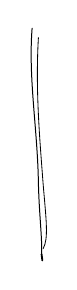
\begin{tikzpicture}[x=1cm,y=1cm,line cap=round]
\draw[line width=.36pt] (0,0) .. controls (-.05,-.64) and (.07,-1.29) .. (.08,-1.97)
 .. controls (.09,-2.38) and (.13,-2.67) .. (.12,-2.87);
\draw[line width=.30pt] (.08,-.12) .. controls (.04,-.79) and (.10,-1.44) .. (.14,-1.98)
 .. controls (.18,-2.45) and (.21,-2.67) .. (.14,-2.80);
\draw[line width=.65pt] (.12,-2.87) -- (.13,-2.95);
\end{tikzpicture}}}}
\var{\deleted{\LMsourceMark{M002826}{\unsure{$\operatorname{Hom}(K$}}}}{\LMsourceMark{M002827}{\LMcancelledDoubts{\LMsourceMark{M002828}{\unsure{$\operatorname{Hom}(K$}}}}}{deletion}{140-2-s063-D002}
\[
 \Gamma((X,S)/K)\longrightarrow
 \begin{gathered}
 \text{Classes de $\pi$-conjugaison de}\\
 \text{sections de }\mathcal E\to\Gamma\text{ i.e.}\\
 \text{de sections de }\Pi_1(X)\to\Pi_1(e_K)
 \end{gathered}
\]

\LMsourceMark{M002829}{\margin{62}}

\LMflushnotes\LMflushpages
\ifnum\LMform=1
\begin{LMapparatus}
\LMentry{140-2-s063-D001}{suppression}{\deleted{\LMsourceMark{M002830}{\illegible{1}}}
}{\emph{\LMomittedlabel}}{Passage biffé dans le manuscrit : la suppression suit l'état final de l'auteur; les doutes de lecture restent signalés.}{}
\LMentry{140-2-s063-D002}{suppression}{\deleted{\LMsourceMark{M002831}{\unsure{$\operatorname{Hom}(K$}}}
}{\emph{\LMomittedlabel}}{Passage biffé dans le manuscrit : la suppression suit l'état final de l'auteur; les doutes de lecture restent signalés.}{}
\end{LMapparatus}
\fi
\ifnum\LMform=2
\par\smallskip\begingroup\footnotesize\Needspace{4\baselineskip}\csname @beginparpenalty\endcsname=10000\relax\noindent\textcolor{gray}{\rule{.2\linewidth}{.35pt}}\par\nobreak
\noindent\textit{\LMdoubtheading.}\par\nobreak
\LMcarryover{140-2-s063-D001}{\LMsourceMark{M002832}{\illegible{1}}
}
\LMcarryover{140-2-s063-D002}{\LMsourceMark{M002833}{\unsure{$\operatorname{Hom}(K$}}
}
\par\endgroup\smallskip
\fi

\LMsourceMark{M002834}{\scanpage{64}}
\LMsourceMark{M002835}{\mspage{30}}

est bijective (si $(X,S)$ est un couple permis ``anabélien'').
\LMsourceMark{M002836}{\margin{faux tel quel, cf n° 9 ci-dessous --- il faut des conditions supplémentaires sur les $f$ \ldots\ \uline{Peut-être} \LMsourceMark{M002837}{\unsure{vrai si}} $I=\varnothing$}}

Je sais en tous cas que cette application est \uline{injective} --- ceci vaut chaque fois qu'on a un schéma $U$ sur $K$ (ici $X\setminus S$) qui se plonge dans un \var{\inserted{groupe algébrique $G$}}{\LMadded{groupe algébrique $G$}}{insertion}{140-2-s064-I001} extension d'une VA par un tore, et résulte alors du th. de Mordell-Weil ``absolu'': $G(K)$ est un $\mathbb Z$-module de type fini.
En fait, il suffit de connaître la classe de splittage de l'extension $\mathcal E^{\natural}$ de $\Gamma$ par
\[
 \pi_{\mathrm{ab}}=\pi/\overline{[\pi,\pi]}\simeq H_1(\LMsourceMark{M002838}{\unsure{\mathrm{Alb}|U}}),
\]
\var{\deleted{\LMsourceMark{M002839}{\unsure{pour en déduire}}}}{\LMsourceMark{M002840}{\LMcancelledDoubts{\LMsourceMark{M002841}{\unsure{pour en déduire}}}}}{deletion}{140-2-s064-D001} \var{\inserted{correspondant}}{\LMadded{correspondant}}{insertion}{140-2-s064-I002} à un pt de $U$ rat/$K$, pour connaître ce point. Donc la \var{\inserted{résultat de}}{\LMadded{résultat de}}{insertion}{140-2-s064-I003} fidélité est obtenu, avec des hyp. moins draconiennes sur $X$ que l'hyp. anabélienne (avec les notations du lemme 5.2, cela signifie que $g=0\Rightarrow\LMsourceMark{M002842}{\unsure{n|\nu}}\ge2$ i.e. qu'il n'y a pas de comp. irréd. de \LMsourceMark{M002843}{\unsure{$X_{\overline K}$|$U_{\overline K}$}} qui soit isom. à \LMsourceMark{M002844}{\unsure{$\mathbb P^1_{\overline K}$}} ou $\mathbb E^1_{\overline K}$ \ldots).

\LMsourceMark{M002845}{\margin{63}}

\LMflushnotes\LMflushpages
\ifnum\LMform=1
\begin{LMapparatus}
\LMentry{140-2-s064-I001}{insertion}{\inserted{groupe algébrique $G$}
}{\emph{\LMinsertedlabel}}{Ajout explicite de l'auteur : intégré à l'endroit indiqué par la transcription, sans modifier sa lecture.}{}
\LMentry{140-2-s064-D001}{suppression}{\deleted{\LMsourceMark{M002846}{\unsure{pour en déduire}}}
}{\emph{\LMomittedlabel}}{Passage biffé dans le manuscrit : la suppression suit l'état final de l'auteur; les doutes de lecture restent signalés.}{}
\LMentry{140-2-s064-I002}{insertion}{\inserted{correspondant}
}{\emph{\LMinsertedlabel}}{Ajout explicite de l'auteur : intégré à l'endroit indiqué par la transcription, sans modifier sa lecture.}{}
\LMentry{140-2-s064-I003}{insertion}{\inserted{résultat de}
}{\emph{\LMinsertedlabel}}{Ajout explicite de l'auteur : intégré à l'endroit indiqué par la transcription, sans modifier sa lecture.}{}
\end{LMapparatus}
\fi
\ifnum\LMform=2
\par\smallskip\begingroup\footnotesize\Needspace{4\baselineskip}\csname @beginparpenalty\endcsname=10000\relax\noindent\textcolor{gray}{\rule{.2\linewidth}{.35pt}}\par\nobreak
\noindent\textit{\LMdoubtheading.}\par\nobreak
\LMcarryover{140-2-s064-D001}{\LMsourceMark{M002847}{\unsure{pour en déduire}}
}
\par\endgroup\smallskip
\fi

\LMsourceMark{M002848}{\scanpage{65}}

\uline{NB} Ceci suggère une approche de la conjecture de Mordell, via une meilleure connaissance des extensions de $\Gamma$ par $\pi$: le fait qu'il n'y ait (pour $g\ge2$) qu'un nb fini de classes de $\pi$-conjugaison de scindages d'une telle extension \ldots.
Idem pour une approche du th. de Fermat, via \var{\deleted{\LMsourceMark{M002849}{\illegible{1}}}}{\LMsourceMark{M002850}{\LMcancelledDoubts{\LMsourceMark{M002851}{\illegible{1}}}}}{deletion}{140-2-s065-D001} une bonne connaissance d'une extension de $\Gamma$ par $\pi=\pi_1(\LMsourceMark{M002852}{\unsure{\mathbb P^1_{\overline{\mathbb Q}}\setminus\{0,1,\infty\}}})$ \ldots.

\uline{Cas $\overline{\mathrm{IV}}$} $n=1,n'=1$ i.e. $X,X'$ de dim 1.

a) Si $I=I'=\varnothing$, je n'ai rien à ajouter à la description des morphismes $f:X\to X'$ en termes de morphismes de diagrammes de groupoïdes. Ici \var{\deleted{\LMsourceMark{M002853}{\illegible{1}}}}{\LMsourceMark{M002854}{\LMcancelledDoubts{\LMsourceMark{M002855}{\illegible{1}}}}}{deletion}{140-2-s065-D002} la condition $f^{-1}(S)_{\mathrm{r\acute ed}}=S'$ n'est pas une restriction sur $f$ --- \var{\deleted{qui}}{}{deletion}{140-2-s065-D003} on n'exclut donc pas des applications constantes. Celles-ci (grâce à
\LMsourceMark{M002856}{\margin{(grâce à \ldots)}}
\var{\deleted{Si \LMsourceMark{M002857}{\unsure{$I'\ne\varnothing$}} \LMsourceMark{M002858}{\illegible{5}} \LMsourceMark{M002859}{\unsure{seulement}} $I'=\varnothing$ \inserted{\LMsourceMark{M002860}{\unsure{i.e. $S'=\varnothing$}}} \LMsourceMark{M002861}{\illegible{7}} \LMsourceMark{M002862}{\unsure{$S'$ est}} \LMsourceMark{M002863}{\unsure{vide}}), \LMsourceMark{M002864}{\unsure{donc}} la condition}}{\LMsourceMark{M002865}{\LMcancelledDoubts{\LMsourceMark{M002866}{\unsure{$I'\ne\varnothing$}}\quad \LMsourceMark{M002867}{\illegible{5}}\quad \LMsourceMark{M002868}{\unsure{seulement}}\quad \LMsourceMark{M002869}{\unsure{i.e. $S'=\varnothing$}}\quad \LMsourceMark{M002870}{\illegible{7}}\quad \LMsourceMark{M002871}{\unsure{$S'$ est}}\quad \LMsourceMark{M002872}{\unsure{vide}}\quad \LMsourceMark{M002873}{\unsure{donc}}}}}{deletion}{140-2-s065-D004}

\LMsourceMark{M002874}{\margin{64}}

\LMflushnotes\LMflushpages
\ifnum\LMform=1
\begin{LMapparatus}
\LMentry{140-2-s065-D001}{suppression}{\deleted{\LMsourceMark{M002875}{\illegible{1}}}
}{\emph{\LMomittedlabel}}{Passage biffé dans le manuscrit : la suppression suit l'état final de l'auteur; les doutes de lecture restent signalés.}{}
\LMentry{140-2-s065-D002}{suppression}{\deleted{\LMsourceMark{M002876}{\illegible{1}}}
}{\emph{\LMomittedlabel}}{Passage biffé dans le manuscrit : la suppression suit l'état final de l'auteur; les doutes de lecture restent signalés.}{}
\LMentry{140-2-s065-D003}{suppression}{\deleted{qui}
}{\emph{\LMomittedlabel}}{Passage biffé dans le manuscrit : la suppression suit l'état final de l'auteur; les doutes de lecture restent signalés.}{}
\LMentry{140-2-s065-D004}{suppression}{\deleted{Si \LMsourceMark{M002877}{\unsure{$I'\ne\varnothing$}} \LMsourceMark{M002878}{\illegible{5}} \LMsourceMark{M002879}{\unsure{seulement}} $I'=\varnothing$ \inserted{\LMsourceMark{M002880}{\unsure{i.e. $S'=\varnothing$}}} \LMsourceMark{M002881}{\illegible{7}} \LMsourceMark{M002882}{\unsure{$S'$ est}} \LMsourceMark{M002883}{\unsure{vide}}), \LMsourceMark{M002884}{\unsure{donc}} la condition}
}{\emph{\LMomittedlabel}}{Passage biffé dans le manuscrit : la suppression suit l'état final de l'auteur; les doutes de lecture restent signalés.}{}
\end{LMapparatus}
\fi
\ifnum\LMform=2
\par\smallskip\begingroup\footnotesize\Needspace{4\baselineskip}\csname @beginparpenalty\endcsname=10000\relax\noindent\textcolor{gray}{\rule{.2\linewidth}{.35pt}}\par\nobreak
\noindent\textit{\LMdoubtheading.}\par\nobreak
\LMcarryover{140-2-s065-D001}{\LMsourceMark{M002885}{\illegible{1}}
}
\LMcarryover{140-2-s065-D002}{\LMsourceMark{M002886}{\illegible{1}}
}
\LMcarryover{140-2-s065-D004}{\LMsourceMark{M002887}{\unsure{$I'\ne\varnothing$}}\quad \LMsourceMark{M002888}{\illegible{5}}\quad \LMsourceMark{M002889}{\unsure{seulement}}\quad \LMsourceMark{M002890}{\unsure{i.e. $S'=\varnothing$}}\quad \LMsourceMark{M002891}{\illegible{7}}\quad \LMsourceMark{M002892}{\unsure{$S'$ est}}\quad \LMsourceMark{M002893}{\unsure{vide}}\quad \LMsourceMark{M002894}{\unsure{donc}}
}
\par\endgroup\smallskip
\fi

\LMsourceMark{M002895}{\scanpage{66}}
\LMsourceMark{M002896}{\mspage{31}}

l'étude \LMsourceMark{M002897}{\unsure{du|des}} cas \uline{$\overline{\mathrm{II}}$}) sont d'ailleurs décrites de façon ``pleinement fidèle'' par des hom. de diagrammes --- Ils correspondent aux cas $f:\mathcal E'\to\mathcal E$ qui sont nuls sur $\pi'$.

b) Le cas $I'=\varnothing$, $I\ne\varnothing$ (i.e. $S'=\varnothing$, $S\ne\varnothing$) signifie, pour la condition $f^{-1}(S)_{\mathrm{r\acute ed}}=S'$ i.e. $f^{-1}(S)=\varnothing$, que $f$ doit appliquer $X'$ dans $X\setminus S$, \var{\deleted{On s'attend donc}}{}{deletion}{140-2-s066-D001} donc que les $f$ correspondant à un morphisme de $(X',\varnothing)$ dans $(X,S)$ sont constantes.
La conj. bordélique dans ce cas exprime donc \var{\deleted{que}}{}{deletion}{140-2-s066-D002} essentiellement qu'au niveau des hom. $\mathcal E'\xrightarrow{p'}\Gamma$ et $\mathcal E\xrightarrow{p}\Gamma$, tout hom. de groupes $\mathcal E'\xrightarrow{f}\mathcal E$ tel que $pf=\operatorname{int}(\alpha)p'$ pour $\alpha\in\Gamma$ [on est ramené au cas où $\alpha=1$, \var{\inserted{$p,p'$ surjectifs}}{\LMadded{$p,p'$ surjectifs}}{insertion}{140-2-s066-I001} i.e. aux hom d'extensions de $\Gamma$ par \LMsourceMark{M002898}{\unsure{les|des}} groupes \LMsourceMark{M002899}{\unsure{$\pi=\pi_1(\overline{X\setminus S})$}} et $\pi'=\pi_1(\overline X')$)] est trivial sur $\pi'$ [i.e. ``est'' une section]. Il faudrait essayer de vérifier ce point directement, qui (modulo le cas \uline{$\overline{\mathrm{III}}$}) établirait la ``conj. bordélique'' dans ce cas-là.

\LMsourceMark{M002900}{\margin{65}}

\LMflushnotes\LMflushpages
\ifnum\LMform=1
\begin{LMapparatus}
\LMentry{140-2-s066-D001}{suppression}{\deleted{On s'attend donc}
}{\emph{\LMomittedlabel}}{Passage biffé dans le manuscrit : la suppression suit l'état final de l'auteur; les doutes de lecture restent signalés.}{}
\LMentry{140-2-s066-D002}{suppression}{\deleted{que}
}{\emph{\LMomittedlabel}}{Passage biffé dans le manuscrit : la suppression suit l'état final de l'auteur; les doutes de lecture restent signalés.}{}
\LMentry{140-2-s066-I001}{insertion}{\inserted{$p,p'$ surjectifs}
}{\emph{\LMinsertedlabel}}{Ajout explicite de l'auteur : intégré à l'endroit indiqué par la transcription, sans modifier sa lecture.}{}
\end{LMapparatus}
\fi

\LMsourceMark{M002901}{\scanpage{67}}

c) Le cas $I'\ne\varnothing$, $I=\varnothing$ implique que $\operatorname{Hom}((X,S),(X',S'))=\varnothing$ (car $f^{-1}(S)=f^{-1}(\varnothing)=\varnothing\ne S'$ !), ce qui correspond bien \var{\deleted{au cas}}{}{deletion}{140-2-s067-D001} à $\operatorname{Hom}(\mathcal D',\mathcal D)=\varnothing$ puisque $\nexists\tau:I'\to I$.

d) Dans le cas $I'\ne\varnothing$, $I\ne\varnothing$, la condition $f^{-1}(S)_{\mathrm{r\acute ed}}=S'$ implique que $f$ n'est pas constante (sinon on aurait $f^{-1}(S)_{\mathrm{r\acute ed}}=\varnothing$ ou $X'$), donc $f$ est dominant et fini, génériquement étale. [Donc, de telles $f$ ne \var{\deleted{\LMsourceMark{M002902}{\unsure{sont admis}} \LMsourceMark{M002903}{\illegible{1}}}}{\LMsourceMark{M002904}{\LMcancelledDoubts{\LMsourceMark{M002905}{\unsure{sont admis}}\quad \LMsourceMark{M002906}{\illegible{1}}}}}{deletion}{140-2-s067-D002} peuvent intervenir que si $I$ et $I'$ sont soit tous deux $\varnothing$ (cas a)), soit tous deux $\ne\varnothing$ (cas actuel d)). Le fait que dans ces cas là, la description diagrammatique galoisienne soit \uline{fidèle} (peut-être pas pleinement) résulte aisément du résultat analogue dans le cas \uline{$\overline{\mathrm{III}}$}.
La pleine fidélité par contre est chose mystérieuse, $=$ si le résultat correspondant \var{\deleted{\LMsourceMark{M002907}{\unsure{dans}}}}{\LMsourceMark{M002908}{\LMcancelledDoubts{\LMsourceMark{M002909}{\unsure{dans}}}}}{deletion}{140-2-s067-D003} \var{\deleted{\LMsourceMark{M002910}{\illegible{1}}}}{\LMsourceMark{M002911}{\LMcancelledDoubts{\LMsourceMark{M002912}{\illegible{1}}}}}{deletion}{140-2-s067-D004} au cas \uline{$\overline{\mathrm{III}}$} était acquis (\LMsourceMark{M002913}{\unsure{et on en}}

\LMsourceMark{M002914}{\margin{66}}

\LMflushnotes\LMflushpages
\ifnum\LMform=1
\begin{LMapparatus}
\LMentry{140-2-s067-D001}{suppression}{\deleted{au cas}
}{\emph{\LMomittedlabel}}{Passage biffé dans le manuscrit : la suppression suit l'état final de l'auteur; les doutes de lecture restent signalés.}{}
\LMentry{140-2-s067-D002}{suppression}{\deleted{\LMsourceMark{M002915}{\unsure{sont admis}} \LMsourceMark{M002916}{\illegible{1}}}
}{\emph{\LMomittedlabel}}{Passage biffé dans le manuscrit : la suppression suit l'état final de l'auteur; les doutes de lecture restent signalés.}{}
\LMentry{140-2-s067-D003}{suppression}{\deleted{\LMsourceMark{M002917}{\unsure{dans}}}
}{\emph{\LMomittedlabel}}{Passage biffé dans le manuscrit : la suppression suit l'état final de l'auteur; les doutes de lecture restent signalés.}{}
\LMentry{140-2-s067-D004}{suppression}{\deleted{\LMsourceMark{M002918}{\illegible{1}}}
}{\emph{\LMomittedlabel}}{Passage biffé dans le manuscrit : la suppression suit l'état final de l'auteur; les doutes de lecture restent signalés.}{}
\end{LMapparatus}
\fi
\ifnum\LMform=2
\par\smallskip\begingroup\footnotesize\Needspace{4\baselineskip}\csname @beginparpenalty\endcsname=10000\relax\noindent\textcolor{gray}{\rule{.2\linewidth}{.35pt}}\par\nobreak
\noindent\textit{\LMdoubtheading.}\par\nobreak
\LMcarryover{140-2-s067-D002}{\LMsourceMark{M002919}{\unsure{sont admis}}\quad \LMsourceMark{M002920}{\illegible{1}}
}
\LMcarryover{140-2-s067-D003}{\LMsourceMark{M002921}{\unsure{dans}}
}
\LMcarryover{140-2-s067-D004}{\LMsourceMark{M002922}{\illegible{1}}
}
\par\endgroup\smallskip
\fi

\LMsourceMark{M002923}{\scanpage{68}}
\LMsourceMark{M002924}{\mspage{32}}

semble loin, $=$ si $K$ fini sur $\mathbb Q$ \ldots)

\uline{Réductions} \uline{élémentaires} Pour prouver la ``conj. bordélique'', on est ramené (par des ext. finies des corps $K$) au cas où $\mathcal E\to\var{\deleted{\LMsourceMark{M002925}{\unsure{K}}}}{\LMsourceMark{M002926}{\LMcancelledDoubts{\(\LMsourceMark{M002927}{\unsure{K}}\)}}}{deletion}{140-2-s068-D001}\Gamma$ (et, si on y tient, aussi $\mathcal E'\to\Gamma$) est épi. Sauf erreur, la connaissance du cas \uline{$\overline{\mathrm{III}}$} pour des extensions de t.f. de $K$, implique le cas général pour $K$ (avec suffisamment de sueurs techniques \ldots).

Revenant cependant au cas général quand $\mathcal E\to\Gamma$ est surjectif, dans tte classe d'équival. de systèmes $(f:\mathcal E'\to\mathcal E,\alpha\in\Gamma,$ \var{\deleted{\LMsourceMark{M002928}{\unsure{$f_i$,}}}}{\LMsourceMark{M002929}{\LMcancelledDoubts{\LMsourceMark{M002930}{\unsure{$f_i$,}}}}}{deletion}{140-2-s068-D002} $\tau:I'\to I,$ \var{\deleted{\LMsourceMark{M002931}{\unsure{$f_{i'}:\mathcal E'_{i'}$}}}}{\LMsourceMark{M002932}{\LMcancelledDoubts{\LMsourceMark{M002933}{\unsure{$f_{i'}:\mathcal E'_{i'}$}}}}}{deletion}{140-2-s068-D003} $(\alpha_{i'}\in\mathcal E_{\LMsourceMark{M002934}{\unsure{\tau(i')=i}}})_{i'\in I'})$, on peut trouver un système avec $\alpha=1$, de sorte que $f:\mathcal E'\to\mathcal E$ est compatible avec les hom. dans $\Gamma$ (i.e. les structures d'extensions).
Quand on se borne à de tels syst., \LMsourceMark{M002935}{\unsure{l'|leur}} équivalence par conjugaison se fait par un système \LMsourceMark{M002936}{\unsure{$(\mu,(\mu_{i'})_{i'\in I'})$}} avec \uline{$\mu\in\pi$} $(=\operatorname{Ker}p)$, et

\LMsourceMark{M002937}{\margin{67}}

\LMflushnotes\LMflushpages
\ifnum\LMform=1
\begin{LMapparatus}
\LMentry{140-2-s068-D001}{suppression}{\(\deleted{\LMsourceMark{M002938}{\unsure{K}}}\)
}{\emph{\LMomittedlabel}}{Passage biffé dans le manuscrit : la suppression suit l'état final de l'auteur; les doutes de lecture restent signalés.}{}
\LMentry{140-2-s068-D002}{suppression}{\deleted{\LMsourceMark{M002939}{\unsure{$f_i$,}}}
}{\emph{\LMomittedlabel}}{Passage biffé dans le manuscrit : la suppression suit l'état final de l'auteur; les doutes de lecture restent signalés.}{}
\LMentry{140-2-s068-D003}{suppression}{\deleted{\LMsourceMark{M002940}{\unsure{$f_{i'}:\mathcal E'_{i'}$}}}
}{\emph{\LMomittedlabel}}{Passage biffé dans le manuscrit : la suppression suit l'état final de l'auteur; les doutes de lecture restent signalés.}{}
\end{LMapparatus}
\fi
\ifnum\LMform=2
\par\smallskip\begingroup\footnotesize\Needspace{4\baselineskip}\csname @beginparpenalty\endcsname=10000\relax\noindent\textcolor{gray}{\rule{.2\linewidth}{.35pt}}\par\nobreak
\noindent\textit{\LMdoubtheading.}\par\nobreak
\LMcarryover{140-2-s068-D001}{\(\LMsourceMark{M002941}{\unsure{K}}\)
}
\LMcarryover{140-2-s068-D002}{\LMsourceMark{M002942}{\unsure{$f_i$,}}
}
\LMcarryover{140-2-s068-D003}{\LMsourceMark{M002943}{\unsure{$f_{i'}:\mathcal E'_{i'}$}}
}
\par\endgroup\smallskip
\fi

\LMsourceMark{M002944}{\scanpage{69}}

les $\mu_{i'}\in\mathcal E_{i=\tau(i')}$ comme avant. Ainsi, $f:\mathcal E'\to\mathcal E$ est \var{\deleted{défini par des}}{}{deletion}{140-2-s069-D001} \var{\inserted{un}}{\LMadded{un}}{insertion}{140-2-s069-I001} hom. d'extensions, défini mod autom. intérieurs par un élément de $\pi=\operatorname{Ker}(\mathcal E\to\Gamma)$, et satisfaisant des conditions explicitées par ailleurs.
Il se pourrait (comme on a déjà remarqué) que la connaissance de la \var{\deleted{\LMsourceMark{M002945}{\illegible{1}}}}{\LMsourceMark{M002946}{\LMcancelledDoubts{\LMsourceMark{M002947}{\illegible{1}}}}}{deletion}{140-2-s069-D002} classe de $\pi$-conj. de $f$ suffise à déterminer le ``morphisme bordélique'' dans lequel $f$ s'insère (si $I,I'\ne\varnothing$).

[C'est lié à la question de savoir si le \var{\deleted{\LMsourceMark{M002948}{\illegible{1}}}}{\LMsourceMark{M002949}{\LMcancelledDoubts{\LMsourceMark{M002950}{\illegible{1}}}}}{deletion}{140-2-s069-D003} \var{\deleted{\LMsourceMark{M002951}{\unsure{tran}}}}{\LMsourceMark{M002952}{\LMcancelledDoubts{\LMsourceMark{M002953}{\unsure{tran}}}}}{deletion}{140-2-s069-D004} $\forall d\in\mathbb N^*,\ \operatorname{Trans}_{\mathcal E}(L_i^d,L_i)$ est réduit à $\mathcal E_i$ (où $L_i=\operatorname{Ker}(p_i:\mathcal E_i\to\Gamma)=\operatorname{Im}(\kappa_i:T(\overline K)\to\mathcal E_i)$).
\LMsourceMark{M002954}{\margin{\var{\deleted{Il suffirait que $\operatorname{Transp}(L_i^d,L_i)\cap\operatorname{Transp}(\LMsourceMark{M002955}{\unsure{\mathcal E}}$}}{\LMsourceMark{M002956}{\LMcancelledDoubts{\(\LMsourceMark{M002957}{\unsure{\mathcal E}}\)}}}{deletion}{140-2-s069-D005}}}
Dans ce cas, $\mathcal E_i$ serait connu en termes de $L_i\subset\pi$, et $=$ en termes des \LMsourceMark{M002958}{\unsure{rayons|noyaux}} de ss-groupes qu'il définit dans $\pi$, et a fortiori en termes des \LMsourceMark{M002959}{\unsure{rayons|noyaux}} d'hom. \LMsourceMark{M002960}{\unsure{défini}} par $\kappa_i:T(\overline K)\to\pi$ \ldots.

\LMsourceMark{M002961}{\margin{68}}

\LMflushnotes\LMflushpages
\ifnum\LMform=1
\begin{LMapparatus}
\LMentry{140-2-s069-D001}{suppression}{\deleted{défini par des}
}{\emph{\LMomittedlabel}}{Passage biffé dans le manuscrit : la suppression suit l'état final de l'auteur; les doutes de lecture restent signalés.}{}
\LMentry{140-2-s069-I001}{insertion}{\inserted{un}
}{\emph{\LMinsertedlabel}}{Ajout explicite de l'auteur : intégré à l'endroit indiqué par la transcription, sans modifier sa lecture.}{}
\LMentry{140-2-s069-D002}{suppression}{\deleted{\LMsourceMark{M002962}{\illegible{1}}}
}{\emph{\LMomittedlabel}}{Passage biffé dans le manuscrit : la suppression suit l'état final de l'auteur; les doutes de lecture restent signalés.}{}
\LMentry{140-2-s069-D003}{suppression}{\deleted{\LMsourceMark{M002963}{\illegible{1}}}
}{\emph{\LMomittedlabel}}{Passage biffé dans le manuscrit : la suppression suit l'état final de l'auteur; les doutes de lecture restent signalés.}{}
\LMentry{140-2-s069-D004}{suppression}{\deleted{\LMsourceMark{M002964}{\unsure{tran}}}
}{\emph{\LMomittedlabel}}{Passage biffé dans le manuscrit : la suppression suit l'état final de l'auteur; les doutes de lecture restent signalés.}{}
\LMentry{140-2-s069-D005}{suppression}{\deleted{Il suffirait que $\operatorname{Transp}(L_i^d,L_i)\cap\operatorname{Transp}(\LMsourceMark{M002965}{\unsure{\mathcal E}}$}
}{\emph{\LMomittedlabel}}{Passage biffé dans le manuscrit : la suppression suit l'état final de l'auteur; les doutes de lecture restent signalés.}{}
\end{LMapparatus}
\fi
\ifnum\LMform=2
\par\smallskip\begingroup\footnotesize\Needspace{4\baselineskip}\csname @beginparpenalty\endcsname=10000\relax\noindent\textcolor{gray}{\rule{.2\linewidth}{.35pt}}\par\nobreak
\noindent\textit{\LMdoubtheading.}\par\nobreak
\LMcarryover{140-2-s069-D002}{\LMsourceMark{M002966}{\illegible{1}}
}
\LMcarryover{140-2-s069-D003}{\LMsourceMark{M002967}{\illegible{1}}
}
\LMcarryover{140-2-s069-D004}{\LMsourceMark{M002968}{\unsure{tran}}
}
\LMcarryover{140-2-s069-D005}{\(\LMsourceMark{M002969}{\unsure{\mathcal E}}\)
}
\par\endgroup\smallskip
\fi

\LMsourceMark{M002970}{\scanpage{70}}
\LMsourceMark{M002971}{\mspage{33}}

\uline{Cas où} \var{\inserted{les}}{\LMadded{les}}{insertion}{140-2-s070-I001} $\mathcal E_i\to\Gamma$ \var{\deleted{est}}{}{deletion}{140-2-s070-D001} \uline{surjectif} (i.e. \var{\inserted{les}}{\LMadded{les}}{insertion}{140-2-s070-I002} \LMsourceMark{M002972}{\unsure{$k(s_i)=K$}} i.e. $s_i$ rat. sur $K$).
Alors, si $(f,$ \var{\deleted{\LMsourceMark{M002973}{\unsure{$\alpha$,}}}}{\LMsourceMark{M002974}{\LMcancelledDoubts{\LMsourceMark{M002975}{\unsure{$\alpha$,}}}}}{deletion}{140-2-s070-D002} $\tau,$ \var{\deleted{\LMsourceMark{M002976}{\illegible{1}}}}{\LMsourceMark{M002977}{\LMcancelledDoubts{\LMsourceMark{M002978}{\illegible{1}}}}}{deletion}{140-2-s070-D003} $(\alpha_{i'}))$ est un hom de $\mathcal D'$ dans $\mathcal D$, \var{\deleted{\LMsourceMark{M002979}{\unsure{pour}} \LMsourceMark{M002980}{\illegible{1}}}}{\LMsourceMark{M002981}{\LMcancelledDoubts{\LMsourceMark{M002982}{\unsure{pour}}\quad \LMsourceMark{M002983}{\illegible{1}}}}}{deletion}{140-2-s070-D004} quitte à \var{\deleted{\LMsourceMark{M002984}{\unsure{modifier}}}}{\LMsourceMark{M002985}{\LMcancelledDoubts{\LMsourceMark{M002986}{\unsure{modifier}}}}}{deletion}{140-2-s070-D005} \var{\inserted{corriger}}{\LMadded{corriger}}{insertion}{140-2-s070-I003} par des $\mu_i\in\mathcal E_i$ ayant $=$ image que les $\alpha_{i'}$ dans $\Gamma$, \LMsourceMark{M002987}{\unsure{OPS}} $\alpha_{i'}\in\pi$, en plus de \LMsourceMark{M002988}{\unsure{$\alpha=1$}} (obtenu en corrigeant par $\mu$ convenable).
Donc on décrit l'hom \var{\inserted{$\mathcal D'\to\mathcal D$}}{\LMadded{$\mathcal D'\to\mathcal D$}}{insertion}{140-2-s070-I004} par $(f,1,\tau,(\alpha_{i'}))$, les $\alpha_{i'}\in\pi$. La \var{\deleted{\LMsourceMark{M002989}{\unsure{systèmes}}}}{\LMsourceMark{M002990}{\LMcancelledDoubts{\LMsourceMark{M002991}{\unsure{systèmes}}}}}{deletion}{140-2-s070-D006} \var{\inserted{condition}}{\LMadded{condition}}{insertion}{140-2-s070-I005} \var{\deleted{\LMsourceMark{M002992}{\illegible{1}}}}{\LMsourceMark{M002993}{\LMcancelledDoubts{\LMsourceMark{M002994}{\illegible{1}}}}}{deletion}{140-2-s070-D007} ici est que $f:\var{\inserted{\mathcal E'\to\mathcal E}}{\LMadded{\mathcal E'\to\mathcal E}}{insertion}{140-2-s070-I006}$ soit un hom. de groupes sur $\Gamma$, que \var{\deleted{\LMsourceMark{M002995}{\unsure{$\operatorname{int}(\alpha_{i'}^{-1})$}}}}{\LMsourceMark{M002996}{\LMcancelledDoubts{\LMsourceMark{M002997}{\unsure{$\operatorname{int}(\alpha_{i'}^{-1})$}}}}}{deletion}{140-2-s070-D008} $f(\mathcal E'_{i'})\subset\text{\var{\inserted{$\operatorname{int}(\alpha_{i'}^{-1})$}}{\LMadded{$\operatorname{int}(\alpha_{i'}^{-1})$}}{insertion}{140-2-s070-I007}}(\mathcal E_{\tau(i')=i})$, et que l'hom induit \var{\inserted{$\mathcal E'_{i'}\to\mathcal E_i$}}{\LMadded{$\mathcal E'_{i'}\to\mathcal E_i$}}{insertion}{140-2-s070-I008} par \var{\deleted{\LMsourceMark{M002998}{\unsure{$f_i=$}}}}{\LMsourceMark{M002999}{\LMcancelledDoubts{\LMsourceMark{M003000}{\unsure{$f_i=$}}}}}{deletion}{140-2-s070-D009} \LMsourceMark{M003001}{\unsure{$\operatorname{int}(\alpha_{i'})f$|$\operatorname{int}(\alpha_{i'}^{-1})f$}} \var{\deleted{\LMsourceMark{M003002}{\unsure{de $\mathcal E_i$ de}}}}{\LMsourceMark{M003003}{\LMcancelledDoubts{\LMsourceMark{M003004}{\unsure{de $\mathcal E_i$ de}}}}}{deletion}{140-2-s070-D010} induit sur $T(\overline K)$ (\uline{via} $\kappa_{i'},\kappa_i$) \uline{l'hom de multiplication par $d_i$} sans plus --- que c'est beau!
Deux systèmes $(f,\tau,(\alpha_{i'}))$ et $(f',\tau',(\alpha'_{i'}))$ définissent le $=$ morphisme, sss \var{\inserted{$\tau=\tau'$ et s'il}}{\LMadded{$\tau=\tau'$ et s'il}}{insertion}{140-2-s070-I009} existe
\[
 \boxed{\mu\in\pi,\quad\mu_{i'}\in\begin{gathered}L_{i=\tau(i')}\\[-2pt]\rotatebox{90}{$=$}\\[-2pt]\text{\var{\inserted{$\kappa_i(T(\overline K))$}}{\LMadded{$\kappa_i(T(\overline K))$}}{insertion}{140-2-s070-I010}}\end{gathered}}
\]
tels que
\[
 f'=\operatorname{int}(\mu)f
\]
\[
 \alpha'_{i'}=\mu_{i'}\alpha_{i'}.
\]

\var{\deleted{\LMsourceMark{M003005}{\illegible{1}}}}{\LMsourceMark{M003006}{\LMcancelledDoubts{\LMsourceMark{M003007}{\illegible{1}}}}}{deletion}{140-2-s070-D011} Notons qu'à priori, pour $(f,\tau)$ fixé, les $\alpha_{i'}$ sont déterminés mod multiplication à droite par des éléments de $\operatorname{Transp}_{\pi}(\var{\deleted{\LMsourceMark{M003008}{\unsure{\pi}}}}{\LMsourceMark{M003009}{\LMcancelledDoubts{\(\LMsourceMark{M003010}{\unsure{\pi}}\)}}}{deletion}{140-2-s070-D012}(\LMsourceMark{M003011}{\unsure{L_i^{d_{i'}}}},L_i)$,

\LMsourceMark{M003012}{\margin{69}}

\LMflushnotes\LMflushpages
\ifnum\LMform=1
\begin{LMapparatus}
\LMentry{140-2-s070-I001}{insertion}{\inserted{les}
}{\emph{\LMinsertedlabel}}{Ajout explicite de l'auteur : intégré à l'endroit indiqué par la transcription, sans modifier sa lecture.}{}
\LMentry{140-2-s070-D001}{suppression}{\deleted{est}
}{\emph{\LMomittedlabel}}{Passage biffé dans le manuscrit : la suppression suit l'état final de l'auteur; les doutes de lecture restent signalés.}{}
\LMentry{140-2-s070-I002}{insertion}{\inserted{les}
}{\emph{\LMinsertedlabel}}{Ajout explicite de l'auteur : intégré à l'endroit indiqué par la transcription, sans modifier sa lecture.}{}
\LMentry{140-2-s070-D002}{suppression}{\deleted{\LMsourceMark{M003013}{\unsure{$\alpha$,}}}
}{\emph{\LMomittedlabel}}{Passage biffé dans le manuscrit : la suppression suit l'état final de l'auteur; les doutes de lecture restent signalés.}{}
\LMentry{140-2-s070-D003}{suppression}{\deleted{\LMsourceMark{M003014}{\illegible{1}}}
}{\emph{\LMomittedlabel}}{Passage biffé dans le manuscrit : la suppression suit l'état final de l'auteur; les doutes de lecture restent signalés.}{}
\LMentry{140-2-s070-D004}{suppression}{\deleted{\LMsourceMark{M003015}{\unsure{pour}} \LMsourceMark{M003016}{\illegible{1}}}
}{\emph{\LMomittedlabel}}{Passage biffé dans le manuscrit : la suppression suit l'état final de l'auteur; les doutes de lecture restent signalés.}{}
\LMentry{140-2-s070-D005}{suppression}{\deleted{\LMsourceMark{M003017}{\unsure{modifier}}}
}{\emph{\LMomittedlabel}}{Passage biffé dans le manuscrit : la suppression suit l'état final de l'auteur; les doutes de lecture restent signalés.}{}
\LMentry{140-2-s070-I003}{insertion}{\inserted{corriger}
}{\emph{\LMinsertedlabel}}{Ajout explicite de l'auteur : intégré à l'endroit indiqué par la transcription, sans modifier sa lecture.}{}
\LMentry{140-2-s070-I004}{insertion}{\inserted{$\mathcal D'\to\mathcal D$}
}{\emph{\LMinsertedlabel}}{Ajout explicite de l'auteur : intégré à l'endroit indiqué par la transcription, sans modifier sa lecture.}{}
\LMentry{140-2-s070-D006}{suppression}{\deleted{\LMsourceMark{M003018}{\unsure{systèmes}}}
}{\emph{\LMomittedlabel}}{Passage biffé dans le manuscrit : la suppression suit l'état final de l'auteur; les doutes de lecture restent signalés.}{}
\LMentry{140-2-s070-I005}{insertion}{\inserted{condition}
}{\emph{\LMinsertedlabel}}{Ajout explicite de l'auteur : intégré à l'endroit indiqué par la transcription, sans modifier sa lecture.}{}
\LMentry{140-2-s070-D007}{suppression}{\deleted{\LMsourceMark{M003019}{\illegible{1}}}
}{\emph{\LMomittedlabel}}{Passage biffé dans le manuscrit : la suppression suit l'état final de l'auteur; les doutes de lecture restent signalés.}{}
\LMentry{140-2-s070-I006}{insertion}{\(\inserted{\mathcal E'\to\mathcal E}\)
}{\emph{\LMinsertedlabel}}{Ajout explicite de l'auteur : intégré à l'endroit indiqué par la transcription, sans modifier sa lecture.}{}
\LMentry{140-2-s070-D008}{suppression}{\deleted{\LMsourceMark{M003020}{\unsure{$\operatorname{int}(\alpha_{i'}^{-1})$}}}
}{\emph{\LMomittedlabel}}{Passage biffé dans le manuscrit : la suppression suit l'état final de l'auteur; les doutes de lecture restent signalés.}{}
\LMentry{140-2-s070-I007}{insertion}{\inserted{$\operatorname{int}(\alpha_{i'}^{-1})$}
}{\emph{\LMinsertedlabel}}{Ajout explicite de l'auteur : intégré à l'endroit indiqué par la transcription, sans modifier sa lecture.}{}
\LMentry{140-2-s070-I008}{insertion}{\inserted{$\mathcal E'_{i'}\to\mathcal E_i$}
}{\emph{\LMinsertedlabel}}{Ajout explicite de l'auteur : intégré à l'endroit indiqué par la transcription, sans modifier sa lecture.}{}
\LMentry{140-2-s070-D009}{suppression}{\deleted{\LMsourceMark{M003021}{\unsure{$f_i=$}}}
}{\emph{\LMomittedlabel}}{Passage biffé dans le manuscrit : la suppression suit l'état final de l'auteur; les doutes de lecture restent signalés.}{}
\LMentry{140-2-s070-D010}{suppression}{\deleted{\LMsourceMark{M003022}{\unsure{de $\mathcal E_i$ de}}}
}{\emph{\LMomittedlabel}}{Passage biffé dans le manuscrit : la suppression suit l'état final de l'auteur; les doutes de lecture restent signalés.}{}
\LMentry{140-2-s070-I009}{insertion}{\inserted{$\tau=\tau'$ et s'il}
}{\emph{\LMinsertedlabel}}{Ajout explicite de l'auteur : intégré à l'endroit indiqué par la transcription, sans modifier sa lecture.}{}
\LMentry{140-2-s070-I010}{insertion}{\inserted{$\kappa_i(T(\overline K))$}
}{\emph{\LMinsertedlabel}}{Ajout explicite de l'auteur : intégré à l'endroit indiqué par la transcription, sans modifier sa lecture.}{}
\LMentry{140-2-s070-D011}{suppression}{\deleted{\LMsourceMark{M003023}{\illegible{1}}}
}{\emph{\LMomittedlabel}}{Passage biffé dans le manuscrit : la suppression suit l'état final de l'auteur; les doutes de lecture restent signalés.}{}
\LMentry{140-2-s070-D012}{suppression}{\(\deleted{\LMsourceMark{M003024}{\unsure{\pi}}}\)
}{\emph{\LMomittedlabel}}{Passage biffé dans le manuscrit : la suppression suit l'état final de l'auteur; les doutes de lecture restent signalés.}{}
\end{LMapparatus}
\fi
\ifnum\LMform=2
\par\smallskip\begingroup\footnotesize\Needspace{4\baselineskip}\csname @beginparpenalty\endcsname=10000\relax\noindent\textcolor{gray}{\rule{.2\linewidth}{.35pt}}\par\nobreak
\noindent\textit{\LMdoubtheading.}\par\nobreak
\LMcarryover{140-2-s070-D002}{\LMsourceMark{M003025}{\unsure{$\alpha$,}}
}
\LMcarryover{140-2-s070-D003}{\LMsourceMark{M003026}{\illegible{1}}
}
\LMcarryover{140-2-s070-D004}{\LMsourceMark{M003027}{\unsure{pour}}\quad \LMsourceMark{M003028}{\illegible{1}}
}
\LMcarryover{140-2-s070-D005}{\LMsourceMark{M003029}{\unsure{modifier}}
}
\LMcarryover{140-2-s070-D006}{\LMsourceMark{M003030}{\unsure{systèmes}}
}
\LMcarryover{140-2-s070-D007}{\LMsourceMark{M003031}{\illegible{1}}
}
\LMcarryover{140-2-s070-D008}{\LMsourceMark{M003032}{\unsure{$\operatorname{int}(\alpha_{i'}^{-1})$}}
}
\LMcarryover{140-2-s070-D009}{\LMsourceMark{M003033}{\unsure{$f_i=$}}
}
\LMcarryover{140-2-s070-D010}{\LMsourceMark{M003034}{\unsure{de $\mathcal E_i$ de}}
}
\LMcarryover{140-2-s070-D011}{\LMsourceMark{M003035}{\illegible{1}}
}
\LMcarryover{140-2-s070-D012}{\(\LMsourceMark{M003036}{\unsure{\pi}}\)
}
\par\endgroup\smallskip
\fi

% END PACKAGE LM_P07
% BEGIN PACKAGE LM_P08
\ifnum\LMform<2\Needspace{11\baselineskip}\subsection*{Scans 71--80}\fi
\LMsourceMark{M003037}{\scanpage{71}}

qui est sans doute $=L_i=\operatorname{Ker}(p_i:\mathcal{E}_i\to\Gamma)=$ \LMsourceMark{M003038}{\unsure{1|l'}} $\operatorname{Im}(\kappa_i:T(\overline{K})\to\mathcal{E}_i\cap\pi)$.
Donc on trouve que \var{\deleted{\LMsourceMark{M003039}{\unsure{$f$}}}}{\LMsourceMark{M003040}{\LMcancelledDoubts{\LMsourceMark{M003041}{\unsure{$f$}}}}}{deletion}{140-2-s071-D001} la classe de \var{\deleted{hom.}}{}{deletion}{140-2-s071-D002} $\pi$-conjugaison de groupes sur $\Gamma$ de $f:\mathcal{E}'\to\mathcal{E}$ suffit à déterminer l'hom $\mathcal{D}'\to\mathcal{D}$ dans la cat. bordélique.
Je présume qu'un peu de sueur permettrait de prouver que cela marche encore dans le cas général (sans supposer les $\Gamma_i=\operatorname{Im}(\LMsourceMark{M003042}{\unsure{\mathcal{E}_i}}\to\Gamma)$ égaux à $\Gamma$).
Cela signifie (dans le cas actuel) que la structure essentielle qui décrit $(X,S)$ est celle d'\var{\deleted{\LMsourceMark{M003043}{\illegible{1}}}}{\LMsourceMark{M003044}{\LMcancelledDoubts{\LMsourceMark{M003045}{\illegible{1}}}}}{deletion}{140-2-s071-D003} ``\uline{extension extérieure}'' de $\Gamma$ par un groupe $\pi$ [hom. ext. surjectif d'un groupe, de noyau un $\pi$], avec $\pi$ muni d'une \uline{structure à lacets} i.e. \var{\deleted{classe de conjugaison}}{}{deletion}{140-2-s071-D004} \var{\inserted{d'hom.}}{\LMadded{d'hom.}}{insertion}{140-2-s071-I001} \uline{extérieurs}
\[
\kappa_i:T\,\LMsourceMark{M003046}{\unsure{\text{\var{\deleted{\LMsourceMark{M003047}{\illegible{1}}}}{\LMsourceMark{M003048}{\LMuncertaindeletion{140-2-s071-D005}}\LMdoubtdata{\LMsourceMark{M003049}{\illegible{1}}}}{deletion}{140-2-s071-D005}}|\mu}}\,(=T(\overline{K})\,\LMsourceMark{M003050}{\unsure{\text{\var{\deleted{)}}{\LMsourceMark{M003051}{\LMuncertaindeletion{140-2-s071-D006}}}{deletion}{140-2-s071-D006}}}}\,\overset{\text{non canon}^{t}}{\simeq}\,\widehat{\mathbf{Z}})\to\pi
\]
(satisfaisant certaines conditions), les

\LMsourceMark{M003052}{\margin{70}}

\LMflushnotes\LMflushpages
\ifnum\LMform=1
\begin{LMapparatus}
\LMentry{140-2-s071-D001}{suppression}{\deleted{\LMsourceMark{M003053}{\unsure{$f$}}}
}{\emph{\LMomittedlabel}}{Passage biffé dans le manuscrit : la suppression suit l'état final de l'auteur; les doutes de lecture restent signalés.}{}
\LMentry{140-2-s071-D002}{suppression}{\deleted{hom.}
}{\emph{\LMomittedlabel}}{Passage biffé dans le manuscrit : la suppression suit l'état final de l'auteur; les doutes de lecture restent signalés.}{}
\LMentry{140-2-s071-D003}{suppression}{\deleted{\LMsourceMark{M003054}{\illegible{1}}}
}{\emph{\LMomittedlabel}}{Passage biffé dans le manuscrit : la suppression suit l'état final de l'auteur; les doutes de lecture restent signalés.}{}
\LMentry{140-2-s071-D004}{suppression}{\deleted{classe de conjugaison}
}{\emph{\LMomittedlabel}}{Passage biffé dans le manuscrit : la suppression suit l'état final de l'auteur; les doutes de lecture restent signalés.}{}
\LMentry{140-2-s071-I001}{insertion}{\inserted{d'hom.}
}{\emph{\LMinsertedlabel}}{Ajout explicite de l'auteur : intégré à l'endroit indiqué par la transcription, sans modifier sa lecture.}{}
\LMentry{140-2-s071-D005}{suppression}{\LMsourceMark{M003055}{\LMdoubtcopy{\deleted{\LMsourceMark{M003056}{\illegible{1}}}}}
}{\emph{\LMomittedlabel}}{Passage biffé dans le manuscrit : la suppression suit l'état final de l'auteur; les doutes de lecture restent signalés.}{}
\LMentry{140-2-s071-D006}{suppression}{\LMsourceMark{M003057}{\LMdoubtcopy{\deleted{)}}}
}{\emph{\LMomittedlabel}}{Passage biffé dans le manuscrit : la suppression suit l'état final de l'auteur; les doutes de lecture restent signalés.}{}
\end{LMapparatus}
\fi
\ifnum\LMform=2
\par\smallskip\begingroup\footnotesize\Needspace{4\baselineskip}\csname @beginparpenalty\endcsname=10000\relax\noindent\textcolor{gray}{\rule{.2\linewidth}{.35pt}}\par\nobreak
\noindent\textit{\LMdoubtheading.}\par\nobreak
\LMcarryover{140-2-s071-D001}{\LMsourceMark{M003058}{\unsure{$f$}}
}
\LMcarryover{140-2-s071-D003}{\LMsourceMark{M003059}{\illegible{1}}
}
\LMcarryover{140-2-s071-D005}{\LMsourceMark{M003060}{\LMdoubtcopy{\LMsourceMark{M003061}{\illegible{1}}}}
}
\LMcarryover{140-2-s071-D006}{\LMsourceMark{M003062}{\LMdoubtcopy{)}}
}
\par\endgroup\smallskip
\fi

\LMsourceMark{M003063}{\scanpage{72}}
\LMsourceMark{M003064}{\mspage{34}}

hom \var{\inserted{de}}{\LMadded{de}}{insertion}{140-2-s072-I001} $\mathcal{E}'\to\Gamma$ (noyau $\pi'$) dans $\mathcal{E}\to\Gamma$ (noyau $\pi$) étant les classes de $\pi$-conjugaison d'homomorphismes $\mathcal{E}'\to\mathcal{E}$ de groupes sur $\Gamma$, induisant des hom $\pi'\to\pi$ compatibles avec la structure à lacets.

9. Structure tangentielle en les $s\in S$.
\LMsourceMark{M003065}{\margin{[Les sections d'extensions ``de deuxième type'']}}

Revenant à la description \var{\inserted{``intrinsèque''}}{\LMadded{``intrinsèque''}}{insertion}{140-2-s072-I002} des $(X,S)$ par
$\Pi_{D^*}\to\Pi_U\to\Pi_e$, un $s_i\in S$ correspond donc à une comp. connexe \var{\inserted{$\Pi_{D_i^*}$}}{\LMadded{$\Pi_{D_i^*}$}}{insertion}{140-2-s072-I003} de $\Pi_{D^*}$, ou \var{\inserted{un $\Pi_{D_i}$}}{\LMadded{un $\Pi_{D_i}$}}{insertion}{140-2-s072-I004} de son quotient $\Pi_D$ --- considérons
\[
\Pi_{D_i^*}\xrightarrow{\LMsourceMark{M003066}{\unsure{\sigma_i=\Pi_{f_{D_i^*D_i}}|\sigma_i=\sigma_{D_i^*D_i}}}}\Pi_{D_i}.
\]
On va décrire certaines sections (à isom. près) de ce \var{\deleted{\LMsourceMark{M003067}{\unsure{fonct}}}}{\LMsourceMark{M003068}{\LMcancelledDoubts{\LMsourceMark{M003069}{\unsure{fonct}}}}}{deletion}{140-2-s072-D001} \var{\inserted{morphisme}}{\LMadded{morphisme}}{insertion}{140-2-s072-I005} de groupoïdes, i.e. des \var{\inserted{couples $(\gamma,\lambda)$}}{\LMadded{couples $(\gamma,\lambda)$}}{insertion}{140-2-s072-I006} foncteurs
$\Pi_{D_i}\xrightarrow{\gamma}\Pi_{D_i^*}$ et d'une iso. $\sigma_i\circ\gamma\overset{\lambda}{\simeq}\operatorname{id}$.
Si on choisit un $\widetilde{D}_i^*\in\operatorname{Ob}\Pi_{D_i^*}$ (rev. universel de $D_i^*$) d'où hom \var{\inserted{surj.}}{\LMadded{surj.}}{insertion}{140-2-s072-I007}
\[
\mathcal{E}_i=\operatorname{Aut}(\widetilde{D}_i^*)\to\Gamma_i
=\operatorname{Aut}(\sigma_i(\widetilde{D}_i^*)=\widetilde{D}_i),
\]
\LMsourceMark{M003070}{\unsure{la}} \var{\deleted{donnée}}{}{deletion}{140-2-s072-D002} donnée de $(\gamma,\LMsourceMark{M003071}{\unsure{\lambda_i|\lambda}})$, \var{\inserted{et d'une iso $\gamma(\widetilde{D}_i)\simeq\widetilde{D}_i^*$ donnant l'isom identique par application des $\sigma_i$,}}{\LMadded{et d'une iso $\gamma(\widetilde{D}_i)\simeq\widetilde{D}_i^*$ donnant l'isom identique par application des $\sigma_i$,}}{insertion}{140-2-s072-I008} revient à celle d'un hom $\Gamma_i\to\mathcal{E}_i$.
--- et les classes d'isomorphismes des couples $(\gamma,\lambda)$ correspondent aux classes de \var{\inserted{$L_i$}}{\LMadded{$L_i$}}{insertion}{140-2-s072-I009}-conjugaison

\LMsourceMark{M003072}{\margin{71}}

\LMflushnotes\LMflushpages
\ifnum\LMform=1
\begin{LMapparatus}
\LMentry{140-2-s072-I001}{insertion}{\inserted{de}
}{\emph{\LMinsertedlabel}}{Ajout explicite de l'auteur : intégré à l'endroit indiqué par la transcription, sans modifier sa lecture.}{}
\LMentry{140-2-s072-I002}{insertion}{\inserted{``intrinsèque''}
}{\emph{\LMinsertedlabel}}{Ajout explicite de l'auteur : intégré à l'endroit indiqué par la transcription, sans modifier sa lecture.}{}
\LMentry{140-2-s072-I003}{insertion}{\inserted{$\Pi_{D_i^*}$}
}{\emph{\LMinsertedlabel}}{Ajout explicite de l'auteur : intégré à l'endroit indiqué par la transcription, sans modifier sa lecture.}{}
\LMentry{140-2-s072-I004}{insertion}{\inserted{un $\Pi_{D_i}$}
}{\emph{\LMinsertedlabel}}{Ajout explicite de l'auteur : intégré à l'endroit indiqué par la transcription, sans modifier sa lecture.}{}
\LMentry{140-2-s072-D001}{suppression}{\deleted{\LMsourceMark{M003073}{\unsure{fonct}}}
}{\emph{\LMomittedlabel}}{Passage biffé dans le manuscrit : la suppression suit l'état final de l'auteur; les doutes de lecture restent signalés.}{}
\LMentry{140-2-s072-I005}{insertion}{\inserted{morphisme}
}{\emph{\LMinsertedlabel}}{Ajout explicite de l'auteur : intégré à l'endroit indiqué par la transcription, sans modifier sa lecture.}{}
\LMentry{140-2-s072-I006}{insertion}{\inserted{couples $(\gamma,\lambda)$}
}{\emph{\LMinsertedlabel}}{Ajout explicite de l'auteur : intégré à l'endroit indiqué par la transcription, sans modifier sa lecture.}{}
\LMentry{140-2-s072-I007}{insertion}{\inserted{surj.}
}{\emph{\LMinsertedlabel}}{Ajout explicite de l'auteur : intégré à l'endroit indiqué par la transcription, sans modifier sa lecture.}{}
\LMentry{140-2-s072-D002}{suppression}{\deleted{donnée}
}{\emph{\LMomittedlabel}}{Passage biffé dans le manuscrit : la suppression suit l'état final de l'auteur; les doutes de lecture restent signalés.}{}
\LMentry{140-2-s072-I008}{insertion}{\inserted{et d'une iso $\gamma(\widetilde{D}_i)\simeq\widetilde{D}_i^*$ donnant l'isom identique par application des $\sigma_i$,}
}{\emph{\LMinsertedlabel}}{Ajout explicite de l'auteur : intégré à l'endroit indiqué par la transcription, sans modifier sa lecture.}{}
\LMentry{140-2-s072-I009}{insertion}{\inserted{$L_i$}
}{\emph{\LMinsertedlabel}}{Ajout explicite de l'auteur : intégré à l'endroit indiqué par la transcription, sans modifier sa lecture.}{}
\end{LMapparatus}
\fi
\ifnum\LMform=2
\par\smallskip\begingroup\footnotesize\Needspace{4\baselineskip}\csname @beginparpenalty\endcsname=10000\relax\noindent\textcolor{gray}{\rule{.2\linewidth}{.35pt}}\par\nobreak
\noindent\textit{\LMdoubtheading.}\par\nobreak
\LMcarryover{140-2-s072-D001}{\LMsourceMark{M003074}{\unsure{fonct}}
}
\par\endgroup\smallskip
\fi

\LMsourceMark{M003075}{\scanpage{73}}

($L_i=\operatorname{Ker}(\text{\var{\deleted{\LMsourceMark{M003076}{\illegible{1}}}}{\LMsourceMark{M003077}{\LMcancelledDoubts{\LMsourceMark{M003078}{\illegible{1}}}}}{deletion}{140-2-s073-D001}\var{\inserted{$\mathcal{E}$}}{\LMadded{$\mathcal{E}$}}{insertion}{140-2-s073-I001}}_i\to\Gamma_i)$) de \var{\deleted{morphismes}}{}{deletion}{140-2-s073-D002} \var{\inserted{sections}}{\LMadded{sections}}{insertion}{140-2-s073-I002} de l'ext. $\mathcal{E}_i$ de $\Gamma_i$ par $L_i$.

Ceci posé, \LMsourceMark{M003079}{\unsure{on a}}
\[
\Gamma_i=\operatorname{Gal}(\overline{K}_i/K_i).
\]
où $K_i=k(s_i)$, $\overline{K}_i$ est la clôture algébrique de $K_i$ définie par $\widetilde{D}_i$ (à priori, elle n'est pas \LMsourceMark{M003080}{\unsure{can\textsuperscript{t}.}} isom. à $\overline{K}$ sur $K$\ldots), et les classes de \var{\deleted{\LMsourceMark{M003081}{\unsure{extensions}}}}{\LMsourceMark{M003082}{\LMcancelledDoubts{\LMsourceMark{M003083}{\unsure{extensions}}}}}{deletion}{140-2-s073-D003} \var{\inserted{scindages}}{\LMadded{scindages}}{insertion}{140-2-s073-I003} d'extensions forment un \uline{torseur} \var{\inserted{$\Sigma_i$}}{\LMadded{$\Sigma_i$}}{insertion}{140-2-s073-I004} (s'il y en a, et on sait qu'il y en a\ldots) sous $H^1(\Gamma_i,L_i)$, ou encore, comme $\kappa_i:L_i\xleftarrow{\sim}T(\overline{K}_i)$, sous
\[
H^1(\operatorname{Gal}(\overline{K}_i/K_i),T(\overline{K}_i))
\simeq H^1(K_i,\LMsourceMark{M003084}{\unsure{T_e|T_\ell}}(G_m))
\simeq\varprojlim_n H^1(K_i,\mu_n).
\]
Or la suite exacte de Kummer donne
\diagram{\begin{tikzcd}[ampersand replacement=\&,column sep=small]
0 \arrow[r] \& H^0(K_i,\text{\var{\deleted{\LMsourceMark{M003085}{\unsure{$\overline{K}$}}}}{\LMsourceMark{M003086}{\LMcancelledDoubts{\LMsourceMark{M003087}{\unsure{$\overline{K}$}}}}}{deletion}{140-2-s073-D004}}\,G_m)_n \arrow[r] \arrow[d,equal] \& H^1(K_i,\mu_n) \arrow[r] \& {}_nH^1(K_i,G_m) \arrow[r] \arrow[d,equal] \& 0 \\
\& (K_i^*)_n \&\& 0 \&
\end{tikzcd}}
i.e. $H^1(K_i,\mu_n)\simeq(K_i^*)_n$, donc
\[
H^1(K_i,T(G_m))\simeq\varprojlim_n(K_i^*)_n
\]

\LMsourceMark{M003088}{\margin{72}}

\LMflushnotes\LMflushpages
\ifnum\LMform=1
\begin{LMapparatus}
\LMentry{140-2-s073-D001}{suppression}{\deleted{\LMsourceMark{M003089}{\illegible{1}}}
}{\emph{\LMomittedlabel}}{Passage biffé dans le manuscrit : la suppression suit l'état final de l'auteur; les doutes de lecture restent signalés.}{}
\LMentry{140-2-s073-I001}{insertion}{\inserted{$\mathcal{E}$}
}{\emph{\LMinsertedlabel}}{Ajout explicite de l'auteur : intégré à l'endroit indiqué par la transcription, sans modifier sa lecture.}{}
\LMentry{140-2-s073-D002}{suppression}{\deleted{morphismes}
}{\emph{\LMomittedlabel}}{Passage biffé dans le manuscrit : la suppression suit l'état final de l'auteur; les doutes de lecture restent signalés.}{}
\LMentry{140-2-s073-I002}{insertion}{\inserted{sections}
}{\emph{\LMinsertedlabel}}{Ajout explicite de l'auteur : intégré à l'endroit indiqué par la transcription, sans modifier sa lecture.}{}
\LMentry{140-2-s073-D003}{suppression}{\deleted{\LMsourceMark{M003090}{\unsure{extensions}}}
}{\emph{\LMomittedlabel}}{Passage biffé dans le manuscrit : la suppression suit l'état final de l'auteur; les doutes de lecture restent signalés.}{}
\LMentry{140-2-s073-I003}{insertion}{\inserted{scindages}
}{\emph{\LMinsertedlabel}}{Ajout explicite de l'auteur : intégré à l'endroit indiqué par la transcription, sans modifier sa lecture.}{}
\LMentry{140-2-s073-I004}{insertion}{\inserted{$\Sigma_i$}
}{\emph{\LMinsertedlabel}}{Ajout explicite de l'auteur : intégré à l'endroit indiqué par la transcription, sans modifier sa lecture.}{}
\LMentry{140-2-s073-D004}{suppression}{\deleted{\LMsourceMark{M003091}{\unsure{$\overline{K}$}}}
}{\emph{\LMomittedlabel}}{Passage biffé dans le manuscrit : la suppression suit l'état final de l'auteur; les doutes de lecture restent signalés.}{}
\end{LMapparatus}
\fi
\ifnum\LMform=2
\par\smallskip\begingroup\footnotesize\Needspace{4\baselineskip}\csname @beginparpenalty\endcsname=10000\relax\noindent\textcolor{gray}{\rule{.2\linewidth}{.35pt}}\par\nobreak
\noindent\textit{\LMdoubtheading.}\par\nobreak
\LMcarryover{140-2-s073-D001}{\LMsourceMark{M003092}{\illegible{1}}
}
\LMcarryover{140-2-s073-D003}{\LMsourceMark{M003093}{\unsure{extensions}}
}
\LMcarryover{140-2-s073-D004}{\LMsourceMark{M003094}{\unsure{$\overline{K}$}}
}
\par\endgroup\smallskip
\fi

\LMsourceMark{M003095}{\scanpage{74}}
\LMsourceMark{M003096}{\mspage{35}}

Notons qu'on a un hom kummérien
\[
K_i^*\to\underbrace{H^1(K_i,T(G_m))}_{\mathcal{H}_i}
\simeq\varprojlim(K_i^*{}_n)
\]
dont le noyau est formé des $\LMsourceMark{M003097}{\unsure{x}}\in K_i^*$ tels que pour $\forall\ n\in\mathbf{N}$, on ait $x\in K_i^{*n}$.
Comme $K_i$ est de t.f. sur $\mathbf{Q}$, cet hom est injectif, i.e. $K_i^*$ s'identifie à un sous-groupe de $\mathcal{H}_i$.

Ceci posé, \LMsourceMark{M003098}{\unsure{on va}} définir, dans le torseur $\Sigma_i$ sous $\mathcal{H}_i$ des scindages de $D_i^*$ sur $D_i$, un sous-\var{\inserted{$K_i^*$}}{\LMadded{$K_i^*$}}{insertion}{140-2-s074-I001}-torseur (i.e. un élément de $\Sigma_i/K_i^*$).
Pour ceci,

\var{\deleted{notons que $\mathcal{O}_{s_i}=\widehat{\mathcal{O}}_{X,s_i}$ contient canoniquement le sous-corps $K_i$ (p.ex. comme clôture entière de $K$ dans $\mathcal{O}_{s_i}$), et que le choix d'une uniformisante $t$ de $\mathcal{O}_{s_i}$ définit un \deleted{sous-corps} \inserted{$K_i$-}\deleted{$K[[t$} isom $\mathcal{O}_{s_i}\simeq K_i[[T]]$, (par la condition $T\mapsto t$). Notons que l'on a}}{}{deletion}{140-2-s074-D001}

\LMsourceMark{M003099}{\margin{73}}

\LMflushnotes\LMflushpages
\ifnum\LMform=1
\begin{LMapparatus}
\LMentry{140-2-s074-I001}{insertion}{\inserted{$K_i^*$}
}{\emph{\LMinsertedlabel}}{Ajout explicite de l'auteur : intégré à l'endroit indiqué par la transcription, sans modifier sa lecture.}{}
\LMentry{140-2-s074-D001}{suppression}{\deleted{notons que $\mathcal{O}_{s_i}=\widehat{\mathcal{O}}_{X,s_i}$ contient canoniquement le sous-corps $K_i$ (p.ex. comme clôture entière de $K$ dans $\mathcal{O}_{s_i}$), et que le choix d'une uniformisante $t$ de $\mathcal{O}_{s_i}$ définit un \deleted{sous-corps} \inserted{$K_i$-}\deleted{$K[[t$} isom $\mathcal{O}_{s_i}\simeq K_i[[T]]$, (par la condition $T\mapsto t$). Notons que l'on a}
}{\emph{\LMomittedlabel}}{Passage biffé dans le manuscrit : la suppression suit l'état final de l'auteur; les doutes de lecture restent signalés.}{}
\end{LMapparatus}
\fi

\LMsourceMark{M003100}{\scanpage{75}}

\var{\deleted{(avec $\widetilde{D}_i^*$) une clôture algébrique \inserted{$\overline{K}_s$} de $K_s$ (corps des fractions de $\mathcal{O}_s$), définissant \deleted{\LMsourceMark{M003101}{\unsure{juste}} \LMsourceMark{M003102}{\illegible{1}}} \inserted{une} clôture alg. $\LMsourceMark{M003103}{\unsure{\overline{K}_i}}$ de $K_i=k(s)$, \LMsourceMark{M003104}{\unsure{qui n'est}} justement que $\overline{K}_i$. \deleted{Ceci posé, dans $\overline{K}_s$ le sous-corps}}}{\LMsourceMark{M003105}{\LMcancelledDoubts{\LMsourceMark{M003106}{\unsure{juste}}\quad \LMsourceMark{M003107}{\illegible{1}}\quad \(\LMsourceMark{M003108}{\unsure{\overline{K}_i}}\)\quad \LMsourceMark{M003109}{\unsure{qui n'est}}}}}{deletion}{140-2-s075-D001}
\LMsourceMark{M003110}{\margin{faire un raisonnement local général, en laiss. tomber l'indice \LMsourceMark{M003111}{\unsure{$i$}}.}}

Considérons plus généralement le cas d'un corps $k$ $(=K_i)$ de car. $0$, et d'une \var{\deleted{\LMsourceMark{M003112}{\illegible{1}}}}{\LMsourceMark{M003113}{\LMcancelledDoubts{\LMsourceMark{M003114}{\illegible{1}}}}}{deletion}{140-2-s075-D004} $k$-algèbre $\mathcal{O}$ qui est \var{\inserted{jauge}}{\LMadded{jauge}}{insertion}{140-2-s075-I003} hensélienne de corps résiduel $k$.
\var{\inserted{soit $L$ le corps des fractions de $\mathcal{O}$}}{\LMadded{soit $L$ le corps des fractions de $\mathcal{O}$}}{insertion}{140-2-s075-I004}
On va, pour \LMsourceMark{M003115}{\unsure{t\textsuperscript{te}}} uniformisante $t$ de $\mathcal{O}$, définir une section $(\gamma,\lambda)$ \LMsourceMark{M003116}{\unsure{du|des}} \var{\deleted{\LMsourceMark{M003117}{\unsure{$\Pi_K$}}}}{\LMsourceMark{M003118}{\LMcancelledDoubts{\LMsourceMark{M003119}{\unsure{$\Pi_K$}}}}}{deletion}{140-2-s075-D005} \var{\deleted{\LMsourceMark{M003120}{\unsure{la caté}}}}{\LMsourceMark{M003121}{\LMcancelledDoubts{\LMsourceMark{M003122}{\unsure{la caté}}}}}{deletion}{140-2-s075-D006} \LMsourceMark{M003123}{\unsure{groupoïde|groupoïdes}} des clôtures alg. de $L$, vers celui des rev. universels de $\LMsourceMark{M003124}{\unsure{\operatorname{Spec}(\mathcal{O})|\operatorname{f\acute{e}t}(\mathcal{O})}}$ ou, ce qui revient au même, des clôtures alg. de $k$. Pour ceci,

soit
\[
\mathcal{O}(n,\LMsourceMark{M003125}{\unsure{t|s}})=\mathcal{O}[T_n]/(T_n^n-s),\quad\text{et}
\]
\[
\mathcal{O}(\infty,t)=\varinjlim_n\mathcal{O}(n,t),\quad
\text{par }T_{n\,\LMsourceMark{M003126}{\unsure{t|s}}}\mapsto T_{mn\,\LMsourceMark{M003127}{\unsure{t|s}}}^{\,m}.
\]
\var{\deleted{alors $\mathcal{O}(\infty,t)$ est \LMsourceMark{M003128}{\unsure{encore une}} jauge hensélienne}}{\LMsourceMark{M003129}{\LMcancelledDoubts{\LMsourceMark{M003130}{\unsure{encore une}}}}}{deletion}{140-2-s075-D007}
\var{\deleted{\LMsourceMark{M003131}{\unsure{Posons}}}}{\LMsourceMark{M003132}{\LMcancelledDoubts{\LMsourceMark{M003133}{\unsure{Posons}}}}}{deletion}{140-2-s075-D008}
$L(n,t)=\mathcal{O}(n,t)\otimes_{\mathcal{O}}K=$ corps des fractions de $\mathcal{O}(n,t)$, $L(\infty,t)=\varinjlim_n L(n,t)$ le corps des fractions de $\mathcal{O}(\infty,t)$. C'est

\LMsourceMark{M003134}{\margin{74}}

\LMflushnotes\LMflushpages
\ifnum\LMform=1
\begin{LMapparatus}
\LMentry{140-2-s075-D001}{suppression}{\deleted{(avec $\widetilde{D}_i^*$) une clôture algébrique \inserted{$\overline{K}_s$} de $K_s$ (corps des fractions de $\mathcal{O}_s$), définissant \deleted{\LMsourceMark{M003135}{\unsure{juste}} \LMsourceMark{M003136}{\illegible{1}}} \inserted{une} clôture alg. $\LMsourceMark{M003137}{\unsure{\overline{K}_i}}$ de $K_i=k(s)$, \LMsourceMark{M003138}{\unsure{qui n'est}} justement que $\overline{K}_i$. \deleted{Ceci posé, dans $\overline{K}_s$ le sous-corps}}
}{\emph{\LMomittedlabel}}{Passage biffé dans le manuscrit : la suppression suit l'état final de l'auteur; les doutes de lecture restent signalés.}{}
\LMentry{140-2-s075-D004}{suppression}{\deleted{\LMsourceMark{M003139}{\illegible{1}}}
}{\emph{\LMomittedlabel}}{Passage biffé dans le manuscrit : la suppression suit l'état final de l'auteur; les doutes de lecture restent signalés.}{}
\LMentry{140-2-s075-I003}{insertion}{\inserted{jauge}
}{\emph{\LMinsertedlabel}}{Ajout explicite de l'auteur : intégré à l'endroit indiqué par la transcription, sans modifier sa lecture.}{}
\LMentry{140-2-s075-I004}{insertion}{\inserted{soit $L$ le corps des fractions de $\mathcal{O}$}
}{\emph{\LMinsertedlabel}}{Ajout explicite de l'auteur : intégré à l'endroit indiqué par la transcription, sans modifier sa lecture.}{}
\LMentry{140-2-s075-D005}{suppression}{\deleted{\LMsourceMark{M003140}{\unsure{$\Pi_K$}}}
}{\emph{\LMomittedlabel}}{Passage biffé dans le manuscrit : la suppression suit l'état final de l'auteur; les doutes de lecture restent signalés.}{}
\LMentry{140-2-s075-D006}{suppression}{\deleted{\LMsourceMark{M003141}{\unsure{la caté}}}
}{\emph{\LMomittedlabel}}{Passage biffé dans le manuscrit : la suppression suit l'état final de l'auteur; les doutes de lecture restent signalés.}{}
\LMentry{140-2-s075-D007}{suppression}{\deleted{alors $\mathcal{O}(\infty,t)$ est \LMsourceMark{M003142}{\unsure{encore une}} jauge hensélienne}
}{\emph{\LMomittedlabel}}{Passage biffé dans le manuscrit : la suppression suit l'état final de l'auteur; les doutes de lecture restent signalés.}{}
\LMentry{140-2-s075-D008}{suppression}{\deleted{\LMsourceMark{M003143}{\unsure{Posons}}}
}{\emph{\LMomittedlabel}}{Passage biffé dans le manuscrit : la suppression suit l'état final de l'auteur; les doutes de lecture restent signalés.}{}
\end{LMapparatus}
\fi
\ifnum\LMform=2
\par\smallskip\begingroup\footnotesize\Needspace{4\baselineskip}\csname @beginparpenalty\endcsname=10000\relax\noindent\textcolor{gray}{\rule{.2\linewidth}{.35pt}}\par\nobreak
\noindent\textit{\LMdoubtheading.}\par\nobreak
\LMcarryover{140-2-s075-D001}{\LMsourceMark{M003144}{\unsure{juste}}\quad \LMsourceMark{M003145}{\illegible{1}}\quad \(\LMsourceMark{M003146}{\unsure{\overline{K}_i}}\)\quad \LMsourceMark{M003147}{\unsure{qui n'est}}
}
\LMcarryover{140-2-s075-D004}{\LMsourceMark{M003148}{\illegible{1}}
}
\LMcarryover{140-2-s075-D005}{\LMsourceMark{M003149}{\unsure{$\Pi_K$}}
}
\LMcarryover{140-2-s075-D006}{\LMsourceMark{M003150}{\unsure{la caté}}
}
\LMcarryover{140-2-s075-D007}{\LMsourceMark{M003151}{\unsure{encore une}}
}
\LMcarryover{140-2-s075-D008}{\LMsourceMark{M003152}{\unsure{Posons}}
}
\par\endgroup\smallskip
\fi

\LMsourceMark{M003153}{\scanpage{76}}
\LMsourceMark{M003154}{\mspage{36}}

une ext. alg. de $L$, et pour \LMsourceMark{M003155}{\unsure{t\textsuperscript{te}}} \var{\deleted{clôture alg. $\overline{k}$ de $k$, \LMsourceMark{M003156}{\illegible{1}} $L\otimes_k\overline{k}$ est alg. clos}}{\LMsourceMark{M003157}{\LMcancelledDoubts{\LMsourceMark{M003158}{\illegible{1}}}}}{deletion}{140-2-s076-D001} \var{\inserted{extension finie, ou ind-finie}}{\LMadded{extension finie, ou ind-finie}}{insertion}{140-2-s076-I001} $k'$ de $k$, posant $\mathcal{O}'=\mathcal{O}\otimes_k k'$ (qui est aussi une jauge hensélienne sur $k'$ de corps résiduel $k'$, de corps des fractions $L'\simeq L\otimes_k k'$), on a \var{\inserted{des iso can.}}{\LMadded{des iso can.}}{insertion}{140-2-s076-I002} \var{\deleted{\LMsourceMark{M003159}{\illegible{1}}}}{\LMsourceMark{M003160}{\LMcancelledDoubts{\LMsourceMark{M003161}{\illegible{1}}}}}{deletion}{140-2-s076-D002}
\[
\mathcal{O}(\LMsourceMark{M003162}{\unsure{n|\infty}},t)\otimes_{\mathcal{O}}\mathcal{O}'\simeq\mathcal{O}'(\LMsourceMark{M003163}{\unsure{n|\infty}},t)
\]
\[
\mathcal{O}(\infty,t)\otimes_{\mathcal{O}}\mathcal{O}'\simeq\mathcal{O}'(\infty,t)
\]
d'où
\[
L(\LMsourceMark{M003164}{\unsure{n|\infty}},t)\otimes_k\LMsourceMark{M003165}{\unsure{\overline{k}'|k'}}\simeq L'(\LMsourceMark{M003166}{\unsure{n|\infty}},t)
\]
\[
L(\infty,t)\otimes_k k'\simeq L'(\infty,t)
\]
Or si $\LMsourceMark{M003167}{\unsure{k'|\overline{k}'}}$ est alg clos, \var{\deleted{on sait que}}{}{deletion}{140-2-s076-D003} $\mathcal{O}'$ str. hensélien, on sait que $L'(\infty,t)$ est alors alg. clos.
D'ailleurs \var{\deleted{\LMsourceMark{M003168}{\illegible{1}}}}{\LMsourceMark{M003169}{\LMcancelledDoubts{\LMsourceMark{M003170}{\illegible{1}}}}}{deletion}{140-2-s076-D004} comme $\LMsourceMark{M003171}{\unsure{\overline{k}'|k'}}\subset\mathcal{O}'(\infty,t)\subset L'(\infty,t)$, dans ce cas \LMsourceMark{M003172}{\unsure{$k$}} $k'$ \var{\deleted{\LMsourceMark{M003173}{\illegible{1}}}}{\LMsourceMark{M003174}{\LMcancelledDoubts{\LMsourceMark{M003175}{\illegible{1}}}}}{deletion}{140-2-s076-D005} s'identifie à la clôture alg. \var{\inserted{$\overline{k}$}}{\LMadded{$\overline{k}$}}{insertion}{140-2-s076-I003} de $k$ dans $L'(\infty,t)=\overline{L}$.
Donc on a bien trouvé une section de $\Pi_{D^*}$ sur $\Pi_D$.

Mais si on remplace $s$ par $s'=su^n$, avec $u\in\mathcal{O}^*$, on trouve des iso
\diagram{$\LMsourceMark{M003176}{\unsure{\lambda(n,u)}}:\quad$\begin{tikzcd}[ampersand replacement=\&,column sep=large]
\mathcal{O}(n,s) \arrow[r] \arrow[d,equal] \& \mathcal{O}(n,s') \arrow[d,equal] \\
\mathcal{O}[T_n]/(T_n^n-s) \& \mathcal{O}[T_n]/(T_n^n-s')
\end{tikzcd}}
par $T_n\to uT_n$
d'où par passage à la limite
\[
\lambda(\infty,\LMsourceMark{M003177}{\unsure{u|n}}):\mathcal{O}(\infty,s)\LMsourceMark{M003178}{\unsure{\longrightarrow}}\mathcal{O}(\infty,s')
\]
induisant $L(\infty,s)\xrightarrow{\sim}L(\infty,s')$ isom d'ext. \var{\inserted{de $L$}}{\LMadded{de $L$}}{insertion}{140-2-s076-I004}

\LMsourceMark{M003179}{\margin{75}}

\LMflushnotes\LMflushpages
\ifnum\LMform=1
\begin{LMapparatus}
\LMentry{140-2-s076-D001}{suppression}{\deleted{clôture alg. $\overline{k}$ de $k$, \LMsourceMark{M003180}{\illegible{1}} $L\otimes_k\overline{k}$ est alg. clos}
}{\emph{\LMomittedlabel}}{Passage biffé dans le manuscrit : la suppression suit l'état final de l'auteur; les doutes de lecture restent signalés.}{}
\LMentry{140-2-s076-I001}{insertion}{\inserted{extension finie, ou ind-finie}
}{\emph{\LMinsertedlabel}}{Ajout explicite de l'auteur : intégré à l'endroit indiqué par la transcription, sans modifier sa lecture.}{}
\LMentry{140-2-s076-I002}{insertion}{\inserted{des iso can.}
}{\emph{\LMinsertedlabel}}{Ajout explicite de l'auteur : intégré à l'endroit indiqué par la transcription, sans modifier sa lecture.}{}
\LMentry{140-2-s076-D002}{suppression}{\deleted{\LMsourceMark{M003181}{\illegible{1}}}
}{\emph{\LMomittedlabel}}{Passage biffé dans le manuscrit : la suppression suit l'état final de l'auteur; les doutes de lecture restent signalés.}{}
\LMentry{140-2-s076-D003}{suppression}{\deleted{on sait que}
}{\emph{\LMomittedlabel}}{Passage biffé dans le manuscrit : la suppression suit l'état final de l'auteur; les doutes de lecture restent signalés.}{}
\LMentry{140-2-s076-D004}{suppression}{\deleted{\LMsourceMark{M003182}{\illegible{1}}}
}{\emph{\LMomittedlabel}}{Passage biffé dans le manuscrit : la suppression suit l'état final de l'auteur; les doutes de lecture restent signalés.}{}
\LMentry{140-2-s076-D005}{suppression}{\deleted{\LMsourceMark{M003183}{\illegible{1}}}
}{\emph{\LMomittedlabel}}{Passage biffé dans le manuscrit : la suppression suit l'état final de l'auteur; les doutes de lecture restent signalés.}{}
\LMentry{140-2-s076-I003}{insertion}{\inserted{$\overline{k}$}
}{\emph{\LMinsertedlabel}}{Ajout explicite de l'auteur : intégré à l'endroit indiqué par la transcription, sans modifier sa lecture.}{}
\LMentry{140-2-s076-I004}{insertion}{\inserted{de $L$}
}{\emph{\LMinsertedlabel}}{Ajout explicite de l'auteur : intégré à l'endroit indiqué par la transcription, sans modifier sa lecture.}{}
\end{LMapparatus}
\fi
\ifnum\LMform=2
\par\smallskip\begingroup\footnotesize\Needspace{4\baselineskip}\csname @beginparpenalty\endcsname=10000\relax\noindent\textcolor{gray}{\rule{.2\linewidth}{.35pt}}\par\nobreak
\noindent\textit{\LMdoubtheading.}\par\nobreak
\LMcarryover{140-2-s076-D001}{\LMsourceMark{M003184}{\illegible{1}}
}
\LMcarryover{140-2-s076-D002}{\LMsourceMark{M003185}{\illegible{1}}
}
\LMcarryover{140-2-s076-D004}{\LMsourceMark{M003186}{\illegible{1}}
}
\LMcarryover{140-2-s076-D005}{\LMsourceMark{M003187}{\illegible{1}}
}
\par\endgroup\smallskip
\fi

\LMsourceMark{M003188}{\scanpage{77}}

d'où un isom entre les sections correspondantes des $\Pi_{L}$ sur $\Pi_k$.
Ceci implique que si $s,s'$ diffèrent par un $\LMsourceMark{M003189}{\unsure{u|v}}\in\mathcal{O}^*$ tel que son image dans $k$ soit $1$ \var{\deleted{(donc $\LMsourceMark{M003190}{\unsure{u|v}}\in$ \LMsourceMark{M003191}{\illegible{2}}}}{\LMsourceMark{M003192}{\LMcancelledDoubts{\(\LMsourceMark{M003193}{\unsure{u|v}}\)\quad \LMsourceMark{M003194}{\illegible{2}}}}}{deletion}{140-2-s077-D001} \var{\inserted{i.e. $\LMsourceMark{M003195}{\unsure{u|v}}\in1+m$}}{\LMadded{i.e. $\LMsourceMark{M003196}{\unsure{u|v}}\in1+m$}}{insertion}{140-2-s077-I001} (qui est un ss-groupe divisible de $\mathcal{O}^*$] alors $s,s'$ définissent des sections isomorphes.
On trouve donc une application canonique
\[
\begin{array}{ccl}
(m/m^2)^* & \to &
\begin{gathered}
\text{classes d'iso de sections de}\\
\Pi_L\text{ sur }\Pi_k\quad\text{i.e. de}\\
\operatorname{Gal}(\overline{K}/L)\to\operatorname{Gal}(\overline{k}/k)
\end{gathered}
\\[1ex]
\begin{gathered}
\var{\deleted{\LMsourceMark{M003197}{\unsure{\text{(et}}}}}{\LMsourceMark{M003198}{\LMcancelledDoubts{\(\LMsourceMark{M003199}{\unsure{\text{(et}}}\)}}}{deletion}{140-2-s077-D002}\text{(ens des}\\
\text{bases de }m/m^2\text{)}\\
\text{qui est un}\\
\text{torseur sous}\\ k^*
\end{gathered}
&&
\begin{gathered}
\text{(qui est un torseur sous}\\
H^1(\operatorname{Gal}(\overline{k}/k),T(\overline{k}))\\
\text{i.e. sous }H^1(k,T(G_m))\ldots)
\end{gathered}
\end{array}
\]

On constate aussitôt que cette application est compatible avec l'hom
\[
\Theta:k^*\to H^1(k,T(G_m))
\]
sur les groupes d'op. de ces torseurs.
Dans le cas où cet hom est injectif (p.ex. $k$ \var{\deleted{on trouve donc un \LMsourceMark{M003200}{\unsure{plong}}}}{\LMsourceMark{M003201}{\LMcancelledDoubts{\LMsourceMark{M003202}{\unsure{plong}}}}}{deletion}{140-2-s077-D003} de t.f. sur $\mathbf{Q}$) on trouve donc un plongement de $m/m^2$ comme un sous $\Theta(k^*)$-torseur du $H^1(k,T(G_m))$-torseur

\LMsourceMark{M003203}{\margin{76}}

\LMflushnotes\LMflushpages
\ifnum\LMform=1
\begin{LMapparatus}
\LMentry{140-2-s077-D001}{suppression}{\deleted{(donc $\LMsourceMark{M003204}{\unsure{u|v}}\in$ \LMsourceMark{M003205}{\illegible{2}}}
}{\emph{\LMomittedlabel}}{Passage biffé dans le manuscrit : la suppression suit l'état final de l'auteur; les doutes de lecture restent signalés.}{}
\LMentry{140-2-s077-I001}{insertion}{\inserted{i.e. $\LMsourceMark{M003206}{\unsure{u|v}}\in1+m$}
}{\emph{\LMinsertedlabel}}{Ajout explicite de l'auteur : intégré à l'endroit indiqué par la transcription, sans modifier sa lecture.}{}
\LMentry{140-2-s077-D002}{suppression}{\(\deleted{\LMsourceMark{M003207}{\unsure{\text{(et}}}}\)
}{\emph{\LMomittedlabel}}{Passage biffé dans le manuscrit : la suppression suit l'état final de l'auteur; les doutes de lecture restent signalés.}{}
\LMentry{140-2-s077-D003}{suppression}{\deleted{on trouve donc un \LMsourceMark{M003208}{\unsure{plong}}}
}{\emph{\LMomittedlabel}}{Passage biffé dans le manuscrit : la suppression suit l'état final de l'auteur; les doutes de lecture restent signalés.}{}
\end{LMapparatus}
\fi
\ifnum\LMform=2
\par\smallskip\begingroup\footnotesize\Needspace{4\baselineskip}\csname @beginparpenalty\endcsname=10000\relax\noindent\textcolor{gray}{\rule{.2\linewidth}{.35pt}}\par\nobreak
\noindent\textit{\LMdoubtheading.}\par\nobreak
\LMcarryover{140-2-s077-D001}{\(\LMsourceMark{M003209}{\unsure{u|v}}\)\quad \LMsourceMark{M003210}{\illegible{2}}
}
\LMcarryover{140-2-s077-D002}{\(\LMsourceMark{M003211}{\unsure{\text{(et}}}\)
}
\LMcarryover{140-2-s077-D003}{\LMsourceMark{M003212}{\unsure{plong}}
}
\par\endgroup\smallskip
\fi

\LMsourceMark{M003213}{\scanpage{78}}
\LMsourceMark{M003214}{\mspage{37}}

des scindages de $\Pi_{D^*}$ \var{\inserted{($\simeq$ groupoïde des clôtures alg. de $L$)}}{\LMadded{($\simeq$ groupoïde des clôtures alg. de $L$)}}{insertion}{140-2-s078-I001} sur $\Pi_D$ ($\simeq$ groupoïde des clôtures alg. de $\LMsourceMark{M003215}{\unsure{k}}$).

Revenant au cas des \var{\deleted{\LMsourceMark{M003216}{\illegible{1}}}}{\LMsourceMark{M003217}{\LMcancelledDoubts{\LMsourceMark{M003218}{\illegible{1}}}}}{deletion}{140-2-s078-D001} $\Pi_{D^*}\to\Pi_U\to\Pi_e$ $\LMsourceMark{M003219}{\unsure{\kappa|K}}\ldots$, et des \var{\deleted{\LMsourceMark{M003220}{\illegible{1}}}}{\LMsourceMark{M003221}{\LMcancelledDoubts{\LMsourceMark{M003222}{\illegible{1}}}}}{deletion}{140-2-s078-D002}
\[
\mathcal{D}:T(\overline{K}^*)\xrightarrow{\kappa_i}\mathcal{E}_i\hookrightarrow\mathcal{E}\xrightarrow{p}\Gamma
\]
qui les explicitent, on trouve donc une structure supplémentaire sur $\mathcal{E}$ ou $\mathcal{D}$ via \var{\deleted{\LMsourceMark{M003223}{\unsure{sur}}}}{\LMsourceMark{M003224}{\LMcancelledDoubts{\LMsourceMark{M003225}{\unsure{sur}}}}}{deletion}{140-2-s078-D003} les Ext. $\mathcal{E}_i$ de $\Gamma_i\subset\Gamma$ par $T(\overline{K}^*)$, savoir \var{\deleted{\LMsourceMark{M003226}{\unsure{des}}}}{\LMsourceMark{M003227}{\LMcancelledDoubts{\LMsourceMark{M003228}{\unsure{des}}}}}{deletion}{140-2-s078-D004} \var{\inserted{$\forall i\in I$}}{\LMadded{$\forall i\in I$}}{insertion}{140-2-s078-I002} sous-$K_i^*$-torseur\LMsourceMark{M003229}{\unsure{s}} dans le torseur sous
$H^1(K_i,T(G_m))\simeq\varprojlim(K_i^*)_n$ des \var{\inserted{classes de}}{\LMadded{classes de}}{insertion}{140-2-s078-I003} scindages de $\mathcal{E}_i$.
Il faudrait expliciter le comportement de cette structure suppl. relativement à des morphismes (provenant de situations géométriques) et la relation avec la norme des $1$-formes différentielles --- j'ai la flemme de l'expliciter en long et en large !

La chose nouvelle que je retiens surtout, c'est que pour $I\ne\varnothing$ et les $\mathcal{E}_i\to\Gamma$ surjectifs (pour simplifier), on trouve \var{\inserted{$\forall i$}}{\LMadded{$\forall i$}}{insertion}{140-2-s078-I004} \LMsourceMark{M003230}{\unsure{une|des}} ``\LMsourceMark{M003231}{\unsure{famille|familles}} \LMsourceMark{M003232}{\unsure{transcendante|transcendantes}}'' de scindages de $\mathcal{E}\to\Gamma$ (via scindages de $\mathcal{E}_i$ sur $\Gamma$) --- \LMsourceMark{M003233}{\unsure{ess.\textsuperscript{t}}} \LMsourceMark{M003234}{\unsure{indexées}}

\LMsourceMark{M003235}{\margin{77}}

\LMflushnotes\LMflushpages
\ifnum\LMform=1
\begin{LMapparatus}
\LMentry{140-2-s078-I001}{insertion}{\inserted{($\simeq$ groupoïde des clôtures alg. de $L$)}
}{\emph{\LMinsertedlabel}}{Ajout explicite de l'auteur : intégré à l'endroit indiqué par la transcription, sans modifier sa lecture.}{}
\LMentry{140-2-s078-D001}{suppression}{\deleted{\LMsourceMark{M003236}{\illegible{1}}}
}{\emph{\LMomittedlabel}}{Passage biffé dans le manuscrit : la suppression suit l'état final de l'auteur; les doutes de lecture restent signalés.}{}
\LMentry{140-2-s078-D002}{suppression}{\deleted{\LMsourceMark{M003237}{\illegible{1}}}
}{\emph{\LMomittedlabel}}{Passage biffé dans le manuscrit : la suppression suit l'état final de l'auteur; les doutes de lecture restent signalés.}{}
\LMentry{140-2-s078-D003}{suppression}{\deleted{\LMsourceMark{M003238}{\unsure{sur}}}
}{\emph{\LMomittedlabel}}{Passage biffé dans le manuscrit : la suppression suit l'état final de l'auteur; les doutes de lecture restent signalés.}{}
\LMentry{140-2-s078-D004}{suppression}{\deleted{\LMsourceMark{M003239}{\unsure{des}}}
}{\emph{\LMomittedlabel}}{Passage biffé dans le manuscrit : la suppression suit l'état final de l'auteur; les doutes de lecture restent signalés.}{}
\LMentry{140-2-s078-I002}{insertion}{\inserted{$\forall i\in I$}
}{\emph{\LMinsertedlabel}}{Ajout explicite de l'auteur : intégré à l'endroit indiqué par la transcription, sans modifier sa lecture.}{}
\LMentry{140-2-s078-I003}{insertion}{\inserted{classes de}
}{\emph{\LMinsertedlabel}}{Ajout explicite de l'auteur : intégré à l'endroit indiqué par la transcription, sans modifier sa lecture.}{}
\LMentry{140-2-s078-I004}{insertion}{\inserted{$\forall i$}
}{\emph{\LMinsertedlabel}}{Ajout explicite de l'auteur : intégré à l'endroit indiqué par la transcription, sans modifier sa lecture.}{}
\end{LMapparatus}
\fi
\ifnum\LMform=2
\par\smallskip\begingroup\footnotesize\Needspace{4\baselineskip}\csname @beginparpenalty\endcsname=10000\relax\noindent\textcolor{gray}{\rule{.2\linewidth}{.35pt}}\par\nobreak
\noindent\textit{\LMdoubtheading.}\par\nobreak
\LMcarryover{140-2-s078-D001}{\LMsourceMark{M003240}{\illegible{1}}
}
\LMcarryover{140-2-s078-D002}{\LMsourceMark{M003241}{\illegible{1}}
}
\LMcarryover{140-2-s078-D003}{\LMsourceMark{M003242}{\unsure{sur}}
}
\LMcarryover{140-2-s078-D004}{\LMsourceMark{M003243}{\unsure{des}}
}
\par\endgroup\smallskip
\fi

\LMsourceMark{M003244}{\scanpage{79}}

par $H^1(\LMsourceMark{M003245}{\unsure{K_i|K}},T(G_m))\simeq\varprojlim(K^*)_n$ (plus précisément, par un torseur sous ledit)

--- dans cette famille, une sous-famille de scindages qu'on peut qualifier de ``géométriques'', indexée par $K^*$ (plus précisément, un sous-torseur\ldots).
On vérifie que les \var{\inserted{classes de $\pi$-}}{\LMadded{classes de $\pi$-}}{insertion}{140-2-s079-I001}scindages obtenus \LMsourceMark{M003246}{\unsure{pour|par}} des indices $i,i'$ distincts sont distinctes, même en se ramenant aux \LMsourceMark{M003247}{\unsure{$\pi$-}}scindages corr. de l'ext. de $\Gamma$ par $\pi_{\mathrm{ab}}$ déduite de l'ext. $\mathcal{E}$ de $\Gamma$ par $\pi$ (je ne fais pas le détail des vérifications, via Mordell-Weil\ldots) et distincts des scindages associés aux pts. rat$/K$ de $X\backslash S$.

\LMsourceMark{M003248}{\margin{\figure{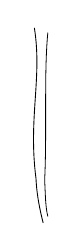
\begin{tikzpicture}[x=1cm,y=1cm,line cap=round]
\draw[line width=.32pt] (0,0) .. controls (.10,-.64) and (-.08,-1.14) .. (.02,-1.91)
 .. controls (.03,-2.14) and (.08,-2.35) .. (.11,-2.47);
\draw[line width=.29pt] (.17,-.06) .. controls (.12,-.59) and (.16,-1.31) .. (.13,-1.93)
 .. controls (.14,-2.13) and (.14,-2.27) .. (.17,-2.39);
\end{tikzpicture}}}}
Il faudrait corriger la conj. bordélique dans le cas (\uline{$\overline{\mathrm{III}}$}), en énonçant (sous toutes réserves, encore !) qu'il n'y a (peut-être) pas d'autres scindages de l'ext. $\mathcal{E}$ de $\Gamma$ par $\pi$ que ceux-là ....

\LMsourceMark{M003249}{\margin{78}}

\LMflushnotes\LMflushpages
\ifnum\LMform=1
\begin{LMapparatus}
\LMentry{140-2-s079-I001}{insertion}{\inserted{classes de $\pi$-}
}{\emph{\LMinsertedlabel}}{Ajout explicite de l'auteur : intégré à l'endroit indiqué par la transcription, sans modifier sa lecture.}{}
\end{LMapparatus}
\fi

\LMsourceMark{M003250}{\scanpage{80}}
\LMsourceMark{M003251}{\mspage{38}}

10. Ajustement des hypothèses (remords).

Je me rends compte que dans la définition des morphismes $(X',S')\xrightarrow{f}(X,S)$, l'hypothèse $f^{-1}(S)_{\mathrm{red}}=S'$ est étriquée --- il faut prendre des morphismes \uline{quelconques} $f:X'\backslash S'\to X\backslash S$ (se prolongeant bien sûr en $\widehat{f}:X'\to X$).
On aura donc $S'\supset\widehat{f}^{-1}(S)_{\mathrm{red}}$, mais $S'$ peut être strictement plus grand que $\widehat{f}^{-1}(S)_{\mathrm{red}}$.
Il faut alors ajuster en conséquence la description de la ``catégorie bordélique'' --- les objets restent les diagrammes de groupoïdes
\[
\mathcal{D}:\Pi_{D^*}\to\Pi_U\to\Pi_e
\]
(plus donnée de Kummer) mais un morphisme $f$ d'un $\mathcal{D}'$ dans un $\mathcal{D}$ ne définit plus nécessairement un $\Pi'_{D^*}\to\Pi_{D^*}$ (en plus de $\Pi'_U\to\Pi_U$) il faut se donner une partie $I'_f$ de $I'=\pi_0(\Pi'_{D^*})$, et se donner seulement
\[
\Pi'_{D^*,I'_f}\xrightarrow{f_{D^*}}\Pi_{D^*}
\]
(avec donnée de commutation \var{\inserted{$\LMsourceMark{M003252}{\unsure{\alpha_{D^*U}}}$}}{\LMadded{$\LMsourceMark{M003253}{\unsure{\alpha_{D^*U}}}$}}{insertion}{140-2-s080-I001} relatif au carré avec $f_U$).
Bien sûr, dans la description en termes de $\mathcal{E}',\mathcal{E}$ etc., on exige que pour $i'\in I'\backslash I'_f$, $f_{\mathcal{E}}:\mathcal{E}'\to\mathcal{E}$ est trivial sur $\mathcal{E}'_{i'}\subset\mathcal{E}'$ --- et $\tau$ est défini comme $I'_f\to I$ ; \LMsourceMark{M003254}{\unsure{des|les}} données relatives aux $i'\in$

\LMsourceMark{M003255}{\margin{79}}

\LMflushnotes\LMflushpages
\ifnum\LMform=1
\begin{LMapparatus}
\LMentry{140-2-s080-I001}{insertion}{\inserted{$\LMsourceMark{M003256}{\unsure{\alpha_{D^*U}}}$}
}{\emph{\LMinsertedlabel}}{Ajout explicite de l'auteur : intégré à l'endroit indiqué par la transcription, sans modifier sa lecture.}{}
\end{LMapparatus}
\fi

% END PACKAGE LM_P08
% BEGIN PACKAGE LM_P09
\ifnum\LMform<2\Needspace{11\baselineskip}\subsection*{Scans 81--90}\fi
\LMsourceMark{M003257}{\scanpage{81}}

\(I'_{f'}\quad (f_{i'}:\mathcal E_{i'}\longrightarrow
\mathcal E_{i=\tau(i')},\ \text{les }\alpha_{i'}\in\mathcal E)\)
sont pareils que dans le cas envisagé précédemment.

\uline{NB} Cela signifie en fait qu'on commence \LMsourceMark{M003258}{\unsure{à}} "boucher les trous" \var{\deleted{de}}{}{deletion}{140-2-s081-D001}
(de \(X'\)) correspondants aux \(i'\in I'\setminus I'_{f'}\), en remplaçant
\(\mathcal E'\) par le \var{\deleted{\LMsourceMark{M003259}{\unsure{ss-}}}}{\LMsourceMark{M003260}{\LMcancelledDoubts{\LMsourceMark{M003261}{\unsure{ss-}}}}}{deletion}{140-2-s081-D002}groupe quotient de \(\mathcal E'\)
par le ss-groupe invariant engendré par les
\(L_{i'}=\kappa_{i'}(T(\overline K))\)
\((i'\in I'\setminus I'_{f'})\), et \var{\deleted{les}}{}{deletion}{140-2-s081-D003} \LMsourceMark{M003262}{\unsure{\(\mathcal E_{i'}\)}}
\((i'\in I'_{f'})\) par leurs images dans ledit groupe quotient, et en oubliant
\var{\deleted{les}}{}{deletion}{140-2-s081-D004} \(I'\setminus I'_{f'}\), i.e. remplaçant \(I'\) par \(I'_{f'}\).

[Pour bien faire, il faudrait exprimer ces opérations aussi au niveau des diagrammes
de groupoïdes
\diagram{\begin{tikzcd}[ampersand replacement=\&]
\Pi'_{\LMsourceMark{M003263}{\unsure{D^*}}} \arrow[r,dash] \& \Pi'_U \arrow[r] \& \LMsourceMark{M003264}{\unsure{\Pi'_e|\Pi_e}}
\end{tikzcd}}
\(\ldots\)].

\LMsourceMark{M003265}{\margin{\var{\deleted{\LMsourceMark{M003266}{\illegible{2}} il faudrait encore \LMsourceMark{M003267}{\unsure{expliciter}}
\LMsourceMark{M003268}{\illegible{2}} \LMsourceMark{M003269}{\unsure{des|les}} pts de \LMsourceMark{M003270}{\illegible{1}}}}{\LMsourceMark{M003271}{\LMcancelledDoubts{\LMsourceMark{M003272}{\illegible{2}}\quad \LMsourceMark{M003273}{\unsure{expliciter}}\quad \LMsourceMark{M003274}{\illegible{2}}\quad \LMsourceMark{M003275}{\unsure{des|les}}\quad \LMsourceMark{M003276}{\illegible{1}}}}}{deletion}{140-2-s081-D005}}}

Cela signifie donc qu'en fait, on s'est ramené à la situation envisagée au début,
où \(S'=\widehat f^{-1}(S)\)\ldots\ Donc finalement
la différence des deux pts de vue n'est pas énorme, et
\var{\deleted{\LMsourceMark{M003277}{\illegible{1}}}}{\LMsourceMark{M003278}{\LMcancelledDoubts{\LMsourceMark{M003279}{\illegible{1}}}}}{deletion}{140-2-s081-D006}\var{\inserted{celui}}{\LMadded{celui}}{insertion}{140-2-s081-I001} adopté au début a l'avantage de
la simplicité plus grande (tout est relatif !)

\LMsourceMark{M003280}{\margin{80}}

\LMflushnotes\LMflushpages
\ifnum\LMform=1
\begin{LMapparatus}
\LMentry{140-2-s081-D001}{suppression}{\deleted{de}
}{\emph{\LMomittedlabel}}{Passage biffé dans le manuscrit : la suppression suit l'état final de l'auteur; les doutes de lecture restent signalés.}{}
\LMentry{140-2-s081-D002}{suppression}{\deleted{\LMsourceMark{M003281}{\unsure{ss-}}}
}{\emph{\LMomittedlabel}}{Passage biffé dans le manuscrit : la suppression suit l'état final de l'auteur; les doutes de lecture restent signalés.}{}
\LMentry{140-2-s081-D003}{suppression}{\deleted{les}
}{\emph{\LMomittedlabel}}{Passage biffé dans le manuscrit : la suppression suit l'état final de l'auteur; les doutes de lecture restent signalés.}{}
\LMentry{140-2-s081-D004}{suppression}{\deleted{les}
}{\emph{\LMomittedlabel}}{Passage biffé dans le manuscrit : la suppression suit l'état final de l'auteur; les doutes de lecture restent signalés.}{}
\LMentry{140-2-s081-D005}{suppression}{\deleted{\LMsourceMark{M003282}{\illegible{2}} il faudrait encore \LMsourceMark{M003283}{\unsure{expliciter}}
\LMsourceMark{M003284}{\illegible{2}} \LMsourceMark{M003285}{\unsure{des|les}} pts de \LMsourceMark{M003286}{\illegible{1}}}
}{\emph{\LMomittedlabel}}{Passage biffé dans le manuscrit : la suppression suit l'état final de l'auteur; les doutes de lecture restent signalés.}{}
\LMentry{140-2-s081-D006}{suppression}{\deleted{\LMsourceMark{M003287}{\illegible{1}}}
}{\emph{\LMomittedlabel}}{Passage biffé dans le manuscrit : la suppression suit l'état final de l'auteur; les doutes de lecture restent signalés.}{}
\LMentry{140-2-s081-I001}{insertion}{\inserted{celui}
}{\emph{\LMinsertedlabel}}{Ajout explicite de l'auteur : intégré à l'endroit indiqué par la transcription, sans modifier sa lecture.}{}
\end{LMapparatus}
\fi
\ifnum\LMform=2
\par\smallskip\begingroup\footnotesize\Needspace{4\baselineskip}\csname @beginparpenalty\endcsname=10000\relax\noindent\textcolor{gray}{\rule{.2\linewidth}{.35pt}}\par\nobreak
\noindent\textit{\LMdoubtheading.}\par\nobreak
\LMcarryover{140-2-s081-D002}{\LMsourceMark{M003288}{\unsure{ss-}}
}
\LMcarryover{140-2-s081-D005}{\LMsourceMark{M003289}{\illegible{2}}\quad \LMsourceMark{M003290}{\unsure{expliciter}}\quad \LMsourceMark{M003291}{\illegible{2}}\quad \LMsourceMark{M003292}{\unsure{des|les}}\quad \LMsourceMark{M003293}{\illegible{1}}
}
\LMcarryover{140-2-s081-D006}{\LMsourceMark{M003294}{\illegible{1}}
}
\par\endgroup\smallskip
\fi

\LMsourceMark{M003295}{\scanpage{82}}
\LMsourceMark{M003296}{\mspage{39}}

11. Conditions sur les systèmes de \var{\deleted{\LMsourceMark{M003297}{\unsure{diagrammes}}}}{\LMsourceMark{M003298}{\LMcancelledDoubts{\LMsourceMark{M003299}{\unsure{diagrammes}}}}}{deletion}{140-2-s082-D001}\var{\inserted{groupoïdes}}{\LMadded{groupoïdes}}{insertion}{140-2-s082-I001}
obtenus à partir de situations géométriques.

On en a déjà cité au passage, p.ex. que les groupes noyaux de
\(\Pi_{D^*}-\Pi_e\) sont abéliens (avec l'isom de Kummer \(\kappa\))
et que les images sont des sous-groupes ouverts, et de \(=\) pour
l'image des \var{\deleted{\LMsourceMark{M003300}{\illegible{1}}}}{\LMsourceMark{M003301}{\LMcancelledDoubts{\LMsourceMark{M003302}{\illegible{1}}}}}{deletion}{140-2-s082-D002} \(\pi_1\) dans \(\Pi_U-\Pi_e\).
On va réexpliciter \var{\inserted{et préciser}}{\LMadded{et préciser}}{insertion}{140-2-s082-I002} ceci dans le cadre de l'interprétation
en termes de
\diagram{\begin{tikzcd}[ampersand replacement=\&]
T(\overline K) \arrow[r,"\kappa_i"] \& \mathcal E_i \arrow[r,hook,"\rho_i"] \&
\mathcal E \arrow[r,"p"] \& \Gamma
\end{tikzcd}}
(cas de la "dim 1" --- on n'exclut pas le cas \(I=\varnothing\) ---
le cas "dim 0" étant trivial\ldots)

a) L'image \var{\inserted{\(\Sigma\)}}{\LMadded{\(\Sigma\)}}{insertion}{140-2-s082-I003} de \(p\) est ouverte, plus précisément existe
ss-groupe ouvert \(\Gamma'\subset\Gamma\) au dessus duquel
\(\mathcal E\) ait une section [et = une "section admissible" en un sens qui sera
défini par la suite --- de sorte à exclure les sections "triviales" provenant
des \(\mathcal E_i\)\ldots].

b) L'image \(\Sigma_i\) de \(\mathcal E_i\) dans \(\Gamma\) est ouverte, et
l'extension \(\mathcal E_i\) de \(\Sigma_i\) par \(L_i\)
\((\simeq T(\overline K))\) est triviale. [En fait, on a une classe
\var{\inserted{\uline{privilégiée}}}{\LMadded{\uline{privilégiée}}}{insertion}{140-2-s082-I004} de scindages, dits "algébriques", formant un
torseur sous
\(K_i^*\,\LMsourceMark{M003303}{\unsure{\hookrightarrow}}\,\varprojlim\LMsourceMark{M003304}{\unsure{(K_i^{*n})_n|(K_i^{*})_n}}\),
cf n° 9 \LMsourceMark{M003305}{\unsure{]|?}} --- mais

\LMsourceMark{M003306}{\margin{81}}

\LMflushnotes\LMflushpages
\ifnum\LMform=1
\begin{LMapparatus}
\LMentry{140-2-s082-D001}{suppression}{\deleted{\LMsourceMark{M003307}{\unsure{diagrammes}}}
}{\emph{\LMomittedlabel}}{Passage biffé dans le manuscrit : la suppression suit l'état final de l'auteur; les doutes de lecture restent signalés.}{}
\LMentry{140-2-s082-I001}{insertion}{\inserted{groupoïdes}
}{\emph{\LMinsertedlabel}}{Ajout explicite de l'auteur : intégré à l'endroit indiqué par la transcription, sans modifier sa lecture.}{}
\LMentry{140-2-s082-D002}{suppression}{\deleted{\LMsourceMark{M003308}{\illegible{1}}}
}{\emph{\LMomittedlabel}}{Passage biffé dans le manuscrit : la suppression suit l'état final de l'auteur; les doutes de lecture restent signalés.}{}
\LMentry{140-2-s082-I002}{insertion}{\inserted{et préciser}
}{\emph{\LMinsertedlabel}}{Ajout explicite de l'auteur : intégré à l'endroit indiqué par la transcription, sans modifier sa lecture.}{}
\LMentry{140-2-s082-I003}{insertion}{\inserted{\(\Sigma\)}
}{\emph{\LMinsertedlabel}}{Ajout explicite de l'auteur : intégré à l'endroit indiqué par la transcription, sans modifier sa lecture.}{}
\LMentry{140-2-s082-I004}{insertion}{\inserted{\uline{privilégiée}}
}{\emph{\LMinsertedlabel}}{Ajout explicite de l'auteur : intégré à l'endroit indiqué par la transcription, sans modifier sa lecture.}{}
\end{LMapparatus}
\fi
\ifnum\LMform=2
\par\smallskip\begingroup\footnotesize\Needspace{4\baselineskip}\csname @beginparpenalty\endcsname=10000\relax\noindent\textcolor{gray}{\rule{.2\linewidth}{.35pt}}\par\nobreak
\noindent\textit{\LMdoubtheading.}\par\nobreak
\LMcarryover{140-2-s082-D001}{\LMsourceMark{M003309}{\unsure{diagrammes}}
}
\LMcarryover{140-2-s082-D002}{\LMsourceMark{M003310}{\illegible{1}}
}
\par\endgroup\smallskip
\fi

\LMsourceMark{M003311}{\scanpage{83}}

on va pas considérer \var{\inserted{pour l'instant}}{\LMadded{pour l'instant}}{insertion}{140-2-s083-I001} cet élément de structure
supplémentaire\ldots)

\var{\deleted{c) Il faut}}{}{deletion}{140-2-s083-D001}

Le reste des \var{\deleted{hypothèses}}{}{deletion}{140-2-s083-D002}\var{\inserted{conditions}}{\LMadded{conditions}}{insertion}{140-2-s083-I002} concerne
essentiellement la structure des groupes \(\pi=\operatorname{Ker}(p:\mathcal E\to\Gamma)\) avec
ses \var{\inserted{classes de conjugaison de}}{\LMadded{classes de conjugaison de}}{insertion}{140-2-s083-I003} \uline{sous-groupes}
\LMsourceMark{M003312}{\unsure{(ou plutôt}} les hom extérieurs
\(\kappa_i:\var{\deleted{\LMsourceMark{M003313}{\unsure{\widehat{\mathbb Z}(1)}}}}{\LMsourceMark{M003314}{\LMcancelledDoubts{\(\LMsourceMark{M003315}{\unsure{\widehat{\mathbb Z}(1)}}\)}}}{deletion}{140-2-s083-D003}T\ (=T(\LMsourceMark{M003316}{\unsure{\overline K^*}}))\longrightarrow\pi\),
et la façon dont \(\Sigma\) opère extérieurement sur \(\pi\).
Ces conditions s'expriment de façon particulièrement simple lorsque les
\(\Sigma_i\subset\Gamma\) sont \(=\Gamma\)
("les pts de \(S\) \var{\inserted{\LMsourceMark{M003317}{\unsure{tous}}}}{\LMadded{\LMsourceMark{M003318}{\unsure{tous}}}}{insertion}{140-2-s083-I004} rat / \(K\)") i.e.
\(\mathcal E_i\to\Gamma\) surj., a fortiori \(\Sigma=\Gamma\) i.e.
\(\mathcal E\to\Gamma\) surj. On va se borner à ce cas. Le cas général s'en déduit
par extension finie du corps de base
[\LMsourceMark{M003319}{\unsure{auquel}} \var{\deleted{on les}}{}{deletion}{140-2-s083-D004}\var{\inserted{chaque}}{\LMadded{chaque}}{insertion}{140-2-s083-I005} pts de
\(S\) non rationnels sur \(K\)
\var{\inserted{i.e. chaque \(\Sigma_i\ne\Gamma\)}}{\LMadded{i.e. chaque \(\Sigma_i\ne\Gamma\)}}{insertion}{140-2-s083-I006}
\var{\deleted{\LMsourceMark{M003320}{\unsure{se partagent}}\LMsourceMark{M003321}{\illegible{1}}}}{\LMsourceMark{M003322}{\LMcancelledDoubts{\LMsourceMark{M003323}{\unsure{se partagent}}\quad \LMsourceMark{M003324}{\illegible{1}}}}}{deletion}{140-2-s083-D005}\var{\inserted{\LMsourceMark{M003325}{\unsure{donne|donnent}} naissance}}{\LMadded{\LMsourceMark{M003326}{\unsure{donne|donnent}} naissance}}{insertion}{140-2-s083-I007}
à \(n_i\) pts, \var{\deleted{\LMsourceMark{M003327}{\unsure{ég.}}}}{\LMsourceMark{M003328}{\LMcancelledDoubts{\LMsourceMark{M003329}{\unsure{ég.}}}}}{deletion}{140-2-s083-D006}
\(n_i=[\Gamma:\Sigma_i]\) \LMsourceMark{M003330}{\unsure{\(\}\)}} --- et \(X_{K'}\)
\var{\deleted{\LMsourceMark{M003331}{\illegible{1}}}}{\LMsourceMark{M003332}{\LMcancelledDoubts{\LMsourceMark{M003333}{\illegible{1}}}}}{deletion}{140-2-s083-D007} \LMsourceMark{M003334}{\unsure{scindé|se scinde}} en \(n=(\Gamma:\Sigma)\) comp. connexes
qui sont géom. connexes] --- mais j'ai la flemme d'expliciter comme il faudrait,
dans le contexte des groupoïdes ou des \var{\deleted{\LMsourceMark{M003335}{\unsure{exten}}}}{\LMsourceMark{M003336}{\LMcancelledDoubts{\LMsourceMark{M003337}{\unsure{exten}}}}}{deletion}{140-2-s083-D008} hom de groupes
profinis, l'opération d'extension des corps de base\ldots\ Il est entendu que

\LMsourceMark{M003338}{\margin{82}}

\LMflushnotes\LMflushpages
\ifnum\LMform=1
\begin{LMapparatus}
\LMentry{140-2-s083-I001}{insertion}{\inserted{pour l'instant}
}{\emph{\LMinsertedlabel}}{Ajout explicite de l'auteur : intégré à l'endroit indiqué par la transcription, sans modifier sa lecture.}{}
\LMentry{140-2-s083-D001}{suppression}{\deleted{c) Il faut}
}{\emph{\LMomittedlabel}}{Passage biffé dans le manuscrit : la suppression suit l'état final de l'auteur; les doutes de lecture restent signalés.}{}
\LMentry{140-2-s083-D002}{suppression}{\deleted{hypothèses}
}{\emph{\LMomittedlabel}}{Passage biffé dans le manuscrit : la suppression suit l'état final de l'auteur; les doutes de lecture restent signalés.}{}
\LMentry{140-2-s083-I002}{insertion}{\inserted{conditions}
}{\emph{\LMinsertedlabel}}{Ajout explicite de l'auteur : intégré à l'endroit indiqué par la transcription, sans modifier sa lecture.}{}
\LMentry{140-2-s083-I003}{insertion}{\inserted{classes de conjugaison de}
}{\emph{\LMinsertedlabel}}{Ajout explicite de l'auteur : intégré à l'endroit indiqué par la transcription, sans modifier sa lecture.}{}
\LMentry{140-2-s083-D003}{suppression}{\(\deleted{\LMsourceMark{M003339}{\unsure{\widehat{\mathbb Z}(1)}}}\)
}{\emph{\LMomittedlabel}}{Passage biffé dans le manuscrit : la suppression suit l'état final de l'auteur; les doutes de lecture restent signalés.}{}
\LMentry{140-2-s083-I004}{insertion}{\inserted{\LMsourceMark{M003340}{\unsure{tous}}}
}{\emph{\LMinsertedlabel}}{Ajout explicite de l'auteur : intégré à l'endroit indiqué par la transcription, sans modifier sa lecture.}{}
\LMentry{140-2-s083-D004}{suppression}{\deleted{on les}
}{\emph{\LMomittedlabel}}{Passage biffé dans le manuscrit : la suppression suit l'état final de l'auteur; les doutes de lecture restent signalés.}{}
\LMentry{140-2-s083-I005}{insertion}{\inserted{chaque}
}{\emph{\LMinsertedlabel}}{Ajout explicite de l'auteur : intégré à l'endroit indiqué par la transcription, sans modifier sa lecture.}{}
\LMentry{140-2-s083-I006}{insertion}{\inserted{i.e. chaque \(\Sigma_i\ne\Gamma\)}
}{\emph{\LMinsertedlabel}}{Ajout explicite de l'auteur : intégré à l'endroit indiqué par la transcription, sans modifier sa lecture.}{}
\LMentry{140-2-s083-D005}{suppression}{\deleted{\LMsourceMark{M003341}{\unsure{se partagent}}\LMsourceMark{M003342}{\illegible{1}}}
}{\emph{\LMomittedlabel}}{Passage biffé dans le manuscrit : la suppression suit l'état final de l'auteur; les doutes de lecture restent signalés.}{}
\LMentry{140-2-s083-I007}{insertion}{\inserted{\LMsourceMark{M003343}{\unsure{donne|donnent}} naissance}
}{\emph{\LMinsertedlabel}}{Ajout explicite de l'auteur : intégré à l'endroit indiqué par la transcription, sans modifier sa lecture.}{}
\LMentry{140-2-s083-D006}{suppression}{\deleted{\LMsourceMark{M003344}{\unsure{ég.}}}
}{\emph{\LMomittedlabel}}{Passage biffé dans le manuscrit : la suppression suit l'état final de l'auteur; les doutes de lecture restent signalés.}{}
\LMentry{140-2-s083-D007}{suppression}{\deleted{\LMsourceMark{M003345}{\illegible{1}}}
}{\emph{\LMomittedlabel}}{Passage biffé dans le manuscrit : la suppression suit l'état final de l'auteur; les doutes de lecture restent signalés.}{}
\LMentry{140-2-s083-D008}{suppression}{\deleted{\LMsourceMark{M003346}{\unsure{exten}}}
}{\emph{\LMomittedlabel}}{Passage biffé dans le manuscrit : la suppression suit l'état final de l'auteur; les doutes de lecture restent signalés.}{}
\end{LMapparatus}
\fi
\ifnum\LMform=2
\par\smallskip\begingroup\footnotesize\Needspace{4\baselineskip}\csname @beginparpenalty\endcsname=10000\relax\noindent\textcolor{gray}{\rule{.2\linewidth}{.35pt}}\par\nobreak
\noindent\textit{\LMdoubtheading.}\par\nobreak
\LMcarryover{140-2-s083-D003}{\(\LMsourceMark{M003347}{\unsure{\widehat{\mathbb Z}(1)}}\)
}
\LMcarryover{140-2-s083-D005}{\LMsourceMark{M003348}{\unsure{se partagent}}\quad \LMsourceMark{M003349}{\illegible{1}}
}
\LMcarryover{140-2-s083-D006}{\LMsourceMark{M003350}{\unsure{ég.}}
}
\LMcarryover{140-2-s083-D007}{\LMsourceMark{M003351}{\illegible{1}}
}
\LMcarryover{140-2-s083-D008}{\LMsourceMark{M003352}{\unsure{exten}}
}
\par\endgroup\smallskip
\fi

\LMsourceMark{M003353}{\scanpage{84}}
\LMsourceMark{M003354}{\mspage{40}}

les conditions que je vais décrire seront invariantes par extension \LMsourceMark{M003355}{\unsure{du|des}} corps de base.

\var{\deleted{c) Il existe \(\LMsourceMark{M003356}{\unsure{\xi|\zeta}}\in T\)
\((=\LMsourceMark{M003357}{\unsure{T(\overline K^*)}})\) et des conjugués}}{\LMsourceMark{M003358}{\LMcancelledDoubts{\(\LMsourceMark{M003359}{\unsure{\xi|\zeta}}\)\quad \(\LMsourceMark{M003360}{\unsure{T(\overline K^*)}}\)}}}{deletion}{140-2-s084-D001}

c) \(\forall i\)\var{\deleted{\LMsourceMark{M003361}{\illegible{1}}}}{\LMsourceMark{M003362}{\LMcancelledDoubts{\LMsourceMark{M003363}{\illegible{1}}}}}{deletion}{140-2-s084-D002}, l'hom extérieur
\[
\kappa_i:T\longrightarrow\pi
\]
est compatible avec l'action extérieure de \(\Gamma\) (opérant sur \(T\) par le
caractère cyclotomique \(\chi\), et sur \(\pi\) grâce à l'extension \(\mathcal E\)
de \(\Gamma\) par \(\pi\)). En d'autres termes, pour \(\forall g\in\mathcal E\),
existe un \uline{\(\alpha\in\pi\)} (\uline{NB} pas seulement
\(\alpha\in\mathcal E\) !) tel qu'on ait,
\[
\operatorname{int}(g)\kappa_i(\LMsourceMark{M003364}{\unsure{\xi|\zeta}})
=\operatorname{int}(\alpha)\kappa_i(\chi(p(g))\LMsourceMark{M003365}{\unsure{\xi|\zeta}})
\]
i.e.
\[
\operatorname{int}(\alpha^{-1}g)\kappa_i(\LMsourceMark{M003366}{\unsure{\xi|\zeta}})
=\kappa_i(\chi(p(g))\LMsourceMark{M003367}{\unsure{\xi|\zeta}})
\]
Ceci signifie donc que 1°) \(\alpha^{-1}g\) normalise \(L_i=\kappa_i(T)\).
[et cela signifie \(=\), probablement, que \(\alpha^{-1}g\in\mathcal E_i\)
--- et qu'on puisse trouver un tel \(\alpha\in\pi\)
\var{\inserted{tel que \(\alpha^{-1}g\in\mathcal E_i\)}}{\LMadded{tel que \(\alpha^{-1}g\in\mathcal E_i\)}}{insertion}{140-2-s084-I001} provient de l'hypothèse
\(\mathcal E_i\to\Gamma\) surjectif --- on prend un \(\beta\in\mathcal E_i\)
\var{\inserted{\(\LMsourceMark{M003368}{\unsure{=}}\alpha^{-1}g\)}}{\LMadded{\(\LMsourceMark{M003369}{\unsure{=}}\alpha^{-1}g\)}}{insertion}{140-2-s084-I002} ayant \(=\) image que \(g\) dans \(\Gamma\)
et on prend \(\alpha=g\beta^{-1}\)] et que 2°) l'action \var{\inserted{intérieure}}{\LMadded{intérieure}}{insertion}{140-2-s084-I003} de
\(\beta=\alpha^{-1}g\) sur \(T\) n'est autre que par multiplication
par \(\chi(g)=\chi(\beta)\) --- ce qui (pour \(\beta\in\mathcal E_i\)) n'est autre que la

\LMsourceMark{M003370}{\margin{83}}

\LMflushnotes\LMflushpages
\ifnum\LMform=1
\begin{LMapparatus}
\LMentry{140-2-s084-D001}{suppression}{\deleted{c) Il existe \(\LMsourceMark{M003371}{\unsure{\xi|\zeta}}\in T\)
\((=\LMsourceMark{M003372}{\unsure{T(\overline K^*)}})\) et des conjugués}
}{\emph{\LMomittedlabel}}{Passage biffé dans le manuscrit : la suppression suit l'état final de l'auteur; les doutes de lecture restent signalés.}{}
\LMentry{140-2-s084-D002}{suppression}{\deleted{\LMsourceMark{M003373}{\illegible{1}}}
}{\emph{\LMomittedlabel}}{Passage biffé dans le manuscrit : la suppression suit l'état final de l'auteur; les doutes de lecture restent signalés.}{}
\LMentry{140-2-s084-I001}{insertion}{\inserted{tel que \(\alpha^{-1}g\in\mathcal E_i\)}
}{\emph{\LMinsertedlabel}}{Ajout explicite de l'auteur : intégré à l'endroit indiqué par la transcription, sans modifier sa lecture.}{}
\LMentry{140-2-s084-I002}{insertion}{\inserted{\(\LMsourceMark{M003374}{\unsure{=}}\alpha^{-1}g\)}
}{\emph{\LMinsertedlabel}}{Ajout explicite de l'auteur : intégré à l'endroit indiqué par la transcription, sans modifier sa lecture.}{}
\LMentry{140-2-s084-I003}{insertion}{\inserted{intérieure}
}{\emph{\LMinsertedlabel}}{Ajout explicite de l'auteur : intégré à l'endroit indiqué par la transcription, sans modifier sa lecture.}{}
\end{LMapparatus}
\fi
\ifnum\LMform=2
\par\smallskip\begingroup\footnotesize\Needspace{4\baselineskip}\csname @beginparpenalty\endcsname=10000\relax\noindent\textcolor{gray}{\rule{.2\linewidth}{.35pt}}\par\nobreak
\noindent\textit{\LMdoubtheading.}\par\nobreak
\LMcarryover{140-2-s084-D001}{\(\LMsourceMark{M003375}{\unsure{\xi|\zeta}}\)\quad \(\LMsourceMark{M003376}{\unsure{T(\overline K^*)}}\)
}
\LMcarryover{140-2-s084-D002}{\LMsourceMark{M003377}{\illegible{1}}
}
\par\endgroup\smallskip
\fi

\LMsourceMark{M003378}{\scanpage{85}}

condition déjà explicitée que l'hom de groupes \(\kappa_i:T\to\mathcal E_i\)
est compatible avec l'action de \(\mathcal E_i\), opérant sur \(T\) via
\(\chi\circ p\mid\mathcal E_i\), et sur lui-= par autom. int.

Donc la condition c) n'est pas vraiment nouvelle --- je la réexplicite en termes
un peu différents, à cause de son importance. Elle implique que l'opération
\LMsourceMark{M003379}{\margin{\figure{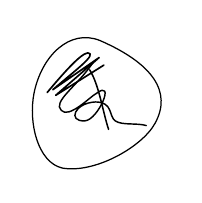
\begin{tikzpicture}[x=.012cm,y=-.012cm,line cap=round,line join=round]
\draw[line width=.45pt] (105,61) .. controls (73,48) and (43,77) .. (35,117)
 .. controls (29,148) and (39,190) .. (65,196)
 .. controls (99,202) and (149,174) .. (163,149)
 .. controls (182,115) and (160,85) .. (105,61);
\draw[line width=.52pt] (97,85) .. controls (81,109) and (54,126) .. (64,135)
 .. controls (72,144) and (95,120) .. (101,117)
 .. controls (122,101) and (103,145) .. (89,146)
 .. controls (70,147) and (78,127) .. (100,126)
 .. controls (119,126) and (114,141) .. (121,146)
 .. controls (128,151) and (144,148) .. (154,151);
\draw[line width=.55pt] (94,92) .. controls (104,108) and (108,137) .. (114,155);
\draw[line width=.60pt] (49,116) .. controls (65,97) and (84,75) .. (92,74)
 .. controls (103,75) and (78,93) .. (55,113)
 -- (104,79) -- (58,119) -- (109,87);
\end{tikzpicture}}}}
de \(\Gamma\) sur \(\pi\) est \uline{très} non triviale (puisque
\(\chi:\Gamma\to\widehat{\mathbb Z}^{*}\) a une image ouverte !)
--- il \LMsourceMark{M003380}{\unsure{n'était}} pas \(=\) évident a priori
\var{\inserted{(sans raisons arithmétiques profondes !)}}{\LMadded{(sans raisons arithmétiques profondes !)}}{insertion}{140-2-s085-I001} --- compte tenu de la structure
de \(\pi\) qu'on va donner --- qu'il existe de telles opérations de \(\Gamma\)
sur un \(\pi\) !

Cette condition \LMsourceMark{M003381}{\unsure{sera}} complétée par une condition de non-trivialité à la Weil.

d) \(\exists\eta\in T^*\)\LMsourceMark{M003382}{\unsure{.}} (une base de \(T\)), et des
\(\alpha_i\in\pi\) (afin de conjuguer \(\kappa_i\) en
\(\kappa'_i=\operatorname{int}(\alpha_i)\circ\kappa_i\))
\LMsourceMark{M003383}{\unsure{enfin}} un entier \(g\geq0\) et des éléments
\(\LMsourceMark{M003384}{\unsure{x_i,y_i}}\in\pi\) \((1\leq i\leq g)\), tels que l'on ait

\LMsourceMark{M003385}{\margin{84}}

\LMflushnotes\LMflushpages
\ifnum\LMform=1
\begin{LMapparatus}
\LMentry{140-2-s085-I001}{insertion}{\inserted{(sans raisons arithmétiques profondes !)}
}{\emph{\LMinsertedlabel}}{Ajout explicite de l'auteur : intégré à l'endroit indiqué par la transcription, sans modifier sa lecture.}{}
\end{LMapparatus}
\fi

\LMsourceMark{M003386}{\scanpage{86}}
\LMsourceMark{M003387}{\mspage{41}}

1°) les \(\kappa'_i(\eta)\), \var{\deleted{\LMsourceMark{M003388}{\illegible{1}}}}{\LMsourceMark{M003389}{\LMcancelledDoubts{\LMsourceMark{M003390}{\illegible{1}}}}}{deletion}{140-2-s086-D001} et les
\(\LMsourceMark{M003391}{\unsure{x_i,y_i|x_j,y_j}}\) engendrent le groupe profini \(\pi\)

2°) Ils satisfont la relation
\[
\boxed{[x_1,y_1].[x_2,y_2]\ldots[x_g,y_g]\,
\kappa'_1(\eta)\kappa'_2(\eta)\ldots\kappa'_{\LMsourceMark{M003392}{\unsure{\nu|n}}}(\eta)=1}
\]

3°) Cette relation, avec les générateurs envisagés décrit \(\pi\)
\var{\inserted{(en tant que groupe profini)}}{\LMadded{(en tant que groupe profini)}}{insertion}{140-2-s086-I001} par générateurs et relations\ldots

\uline{NB} On sait que par ces conditions, \(g\) est uniquement déterminé,
p.ex. par le fait que
\(\pi_{ab}/\var{\deleted{\text{images des}}}{}{deletion}{140-2-s086-D002}\sum\kappa_i(T)\)
est un \(\widehat{\mathbb Z}\)-module libre de rang \(2g\) --- \(\pi_{ab}\)
étant libre de rang \(2g+\nu-1\) où \(\nu=\operatorname{card}(I)\).

Pour le choix de \(\eta\), on sait que si \(\eta\) convient, alors
\(\forall\ \chi(\alpha)\eta\) aussi (où \(\alpha\in\Gamma\)) --- quitte à prendre
des conjugués. Donc les \(\eta\) qui conviennent \var{\deleted{forment}}{}{deletion}{140-2-s086-D003} contiennent
un sous-torseur\var{\inserted{de \(T^*\)}}{\LMadded{de \(T^*\)}}{insertion}{140-2-s086-I002} (sous le ss-groupe ouvert
\(\chi(\Gamma)\) de \(\widehat{\mathbb Z}^{*}\).

\var{\deleted{Supposons pour simplifier que \(g=0\) :
On voit donc que si le système des \(\kappa'_i(\eta)\) est un syst. de gén.
privilégié (au sens de d) ci-dessus) alors les
\(\operatorname{int}(g)\kappa'_i(\eta)\) aussi pour \(\forall g\in\mathcal E\),
[\LMsourceMark{M003393}{\unsure{\(=\)}} \(\operatorname{int}(\alpha)\kappa'_i(\chi(g)\eta)\)
pour \(\alpha\in\pi\) convenable]}}{\LMsourceMark{M003394}{\LMcancelledDoubts{\LMsourceMark{M003395}{\unsure{\(=\)}}}}}{deletion}{140-2-s086-D004}

\LMsourceMark{M003396}{\margin{85}}

\LMflushnotes\LMflushpages
\ifnum\LMform=1
\begin{LMapparatus}
\LMentry{140-2-s086-D001}{suppression}{\deleted{\LMsourceMark{M003397}{\illegible{1}}}
}{\emph{\LMomittedlabel}}{Passage biffé dans le manuscrit : la suppression suit l'état final de l'auteur; les doutes de lecture restent signalés.}{}
\LMentry{140-2-s086-I001}{insertion}{\inserted{(en tant que groupe profini)}
}{\emph{\LMinsertedlabel}}{Ajout explicite de l'auteur : intégré à l'endroit indiqué par la transcription, sans modifier sa lecture.}{}
\LMentry{140-2-s086-D002}{suppression}{\(\deleted{\text{images des}}\)
}{\emph{\LMomittedlabel}}{Passage biffé dans le manuscrit : la suppression suit l'état final de l'auteur; les doutes de lecture restent signalés.}{}
\LMentry{140-2-s086-D003}{suppression}{\deleted{forment}
}{\emph{\LMomittedlabel}}{Passage biffé dans le manuscrit : la suppression suit l'état final de l'auteur; les doutes de lecture restent signalés.}{}
\LMentry{140-2-s086-I002}{insertion}{\inserted{de \(T^*\)}
}{\emph{\LMinsertedlabel}}{Ajout explicite de l'auteur : intégré à l'endroit indiqué par la transcription, sans modifier sa lecture.}{}
\LMentry{140-2-s086-D004}{suppression}{\deleted{Supposons pour simplifier que \(g=0\) :
On voit donc que si le système des \(\kappa'_i(\eta)\) est un syst. de gén.
privilégié (au sens de d) ci-dessus) alors les
\(\operatorname{int}(g)\kappa'_i(\eta)\) aussi pour \(\forall g\in\mathcal E\),
[\LMsourceMark{M003398}{\unsure{\(=\)}} \(\operatorname{int}(\alpha)\kappa'_i(\chi(g)\eta)\)
pour \(\alpha\in\pi\) convenable]}
}{\emph{\LMomittedlabel}}{Passage biffé dans le manuscrit : la suppression suit l'état final de l'auteur; les doutes de lecture restent signalés.}{}
\end{LMapparatus}
\fi
\ifnum\LMform=2
\par\smallskip\begingroup\footnotesize\Needspace{4\baselineskip}\csname @beginparpenalty\endcsname=10000\relax\noindent\textcolor{gray}{\rule{.2\linewidth}{.35pt}}\par\nobreak
\noindent\textit{\LMdoubtheading.}\par\nobreak
\LMcarryover{140-2-s086-D001}{\LMsourceMark{M003399}{\illegible{1}}
}
\LMcarryover{140-2-s086-D004}{\LMsourceMark{M003400}{\unsure{\(=\)}}
}
\par\endgroup\smallskip
\fi

\LMsourceMark{M003401}{\scanpage{87}}
\LMsourceMark{M003402}{\mspage{42}}

\LMsourceMark{M003403}{\margin{(\LMsourceMark{M003404}{\unsure{donc|dans}} \(\chi:\Gamma\to\widehat{\mathbb Z}^{*}\) \LMsourceMark{M003405}{\unsure{épi.}})}}

\var{\deleted{donc aussi les \(\kappa'_i(\chi(g)\eta)\). \LMsourceMark{M003406}{\unsure{Prenant}}
\(K=\mathbb Q\), on trouve donc par voie arithmétique :

\uline{Prop} Soit \(\pi\) le \LMsourceMark{M003407}{\unsure{\(P\)}}-groupe libre
\inserted{de \LMsourceMark{M003408}{\unsure{\(\nu-1\)|\(\nu\) gén.}}} \LMsourceMark{M003409}{\unsure{(}}\uline{engendré} par des générateurs
\(\ell_1,\ldots,\ell_\nu\) satisfaisant la relation génératrice
\(\prod\ell_i=1\). Alors pour tout \(\alpha\in\widehat{\mathbb Z}^{*}\),
on a encore \(\prod\ell_i^\alpha=1\), et les \(\ell'_i=\ell_i^\alpha\)
avec cette relation décrivent le groupe profini \(\pi\).}}{\LMsourceMark{M003410}{\LMcancelledDoubts{\LMsourceMark{M003411}{\unsure{Prenant}}\quad \LMsourceMark{M003412}{\unsure{\(P\)}}\quad \LMsourceMark{M003413}{\unsure{\(\nu-1\)|\(\nu\) gén.}}\quad \LMsourceMark{M003414}{\unsure{(}}}}}{deletion}{140-2-s087-D001}
En fait, comme la structure du groupe \(\pi\) est indépendante de \(K\),
prenant \(K=\mathbb Q\) (et admettant qu'il existe une courbe lisse projective
géom. connexe de genre \(g\) sur \(\mathbb Q\), ayant \(\nu\) pts rat. / \(\mathbb Q\) !),
on trouve que si les \(\ell_i\), \var{\deleted{\(\LMsourceMark{M003415}{\unsure{x_j,y_j}}\)}}{\LMsourceMark{M003416}{\LMcancelledDoubts{\(\LMsourceMark{M003417}{\unsure{x_j,y_j}}\)}}}{deletion}{140-2-s087-D002}
\((1\leq i\leq\nu\var{\deleted{,\ \LMsourceMark{M003418}{\unsure{1\leq j\leq g}}}}{\LMsourceMark{M003419}{\LMcancelledDoubts{\(\LMsourceMark{M003420}{\unsure{1\leq j\leq g}}\)}}}{deletion}{140-2-s087-D003})\)
\var{\deleted{conviennent, alors les}}{}{deletion}{140-2-s087-D004} s'insèrent dans un syst. de générateurs
privilégié (avec des \(\LMsourceMark{M003421}{\unsure{x_\alpha,y_\alpha}}\)) alors pour
\(\forall\rho\in\widehat{\mathbb Z}^{*}\), on peut trouver des conjugués
\(\ell'_i\) des \(\ell_i^\rho\) qui s'insèrent de \(=\).
Même pour \(\rho=-1\) ce n'est pas entièrement trivial\ldots

\var{\deleted{\LMsourceMark{M003422}{\illegible{2}}}}{\LMsourceMark{M003423}{\LMcancelledDoubts{\LMsourceMark{M003424}{\illegible{2}}}}}{deletion}{140-2-s087-D005} Enfin, \LMsourceMark{M003425}{\unsure{on va}} énoncer une condition
draconienne de non trivialité de l'opération de \(\Gamma\) sur \(\pi\).
Soit \(\mathcal E'\) un sous-groupe \var{\inserted{\uline{ouvert} (donc}}{\LMadded{\uline{ouvert} (donc}}{insertion}{140-2-s087-I002}
d'indice fini) de \(\mathcal E\),
\var{\inserted{\(\pi'=\pi\cap\mathcal E'=\operatorname{Ker}(\mathcal E'\to\Gamma')\)}}{\LMadded{\(\pi'=\pi\cap\mathcal E'=\operatorname{Ker}(\mathcal E'\to\Gamma')\)}}{insertion}{140-2-s087-I003}
\var{\deleted{\LMsourceMark{M003426}{\illegible{1}} son image dans \LMsourceMark{M003427}{\unsure{\(\mathcal E\)|\(\Gamma\)}}
(qui est ouvert dans \(\Sigma\)) de sorte que}}{\LMsourceMark{M003428}{\LMcancelledDoubts{\LMsourceMark{M003429}{\illegible{1}}\quad \LMsourceMark{M003430}{\unsure{\(\mathcal E\)|\(\Gamma\)}}}}}{deletion}{140-2-s087-D006}

\LMsourceMark{M003431}{\margin{86}}

\LMflushnotes\LMflushpages
\ifnum\LMform=1
\begin{LMapparatus}
\LMentry{140-2-s087-D001}{suppression}{\deleted{donc aussi les \(\kappa'_i(\chi(g)\eta)\). \LMsourceMark{M003432}{\unsure{Prenant}}
\(K=\mathbb Q\), on trouve donc par voie arithmétique :

\uline{Prop} Soit \(\pi\) le \LMsourceMark{M003433}{\unsure{\(P\)}}-groupe libre
\inserted{de \LMsourceMark{M003434}{\unsure{\(\nu-1\)|\(\nu\) gén.}}} \LMsourceMark{M003435}{\unsure{(}}\uline{engendré} par des générateurs
\(\ell_1,\ldots,\ell_\nu\) satisfaisant la relation génératrice
\(\prod\ell_i=1\). Alors pour tout \(\alpha\in\widehat{\mathbb Z}^{*}\),
on a encore \(\prod\ell_i^\alpha=1\), et les \(\ell'_i=\ell_i^\alpha\)
avec cette relation décrivent le groupe profini \(\pi\).}
}{\emph{\LMomittedlabel}}{Passage biffé dans le manuscrit : la suppression suit l'état final de l'auteur; les doutes de lecture restent signalés.}{}
\LMentry{140-2-s087-D002}{suppression}{\deleted{\(\LMsourceMark{M003436}{\unsure{x_j,y_j}}\)}
}{\emph{\LMomittedlabel}}{Passage biffé dans le manuscrit : la suppression suit l'état final de l'auteur; les doutes de lecture restent signalés.}{}
\LMentry{140-2-s087-D003}{suppression}{\(\deleted{,\ \LMsourceMark{M003437}{\unsure{1\leq j\leq g}}}\)
}{\emph{\LMomittedlabel}}{Passage biffé dans le manuscrit : la suppression suit l'état final de l'auteur; les doutes de lecture restent signalés.}{}
\LMentry{140-2-s087-D004}{suppression}{\deleted{conviennent, alors les}
}{\emph{\LMomittedlabel}}{Passage biffé dans le manuscrit : la suppression suit l'état final de l'auteur; les doutes de lecture restent signalés.}{}
\LMentry{140-2-s087-D005}{suppression}{\deleted{\LMsourceMark{M003438}{\illegible{2}}}
}{\emph{\LMomittedlabel}}{Passage biffé dans le manuscrit : la suppression suit l'état final de l'auteur; les doutes de lecture restent signalés.}{}
\LMentry{140-2-s087-I002}{insertion}{\inserted{\uline{ouvert} (donc}
}{\emph{\LMinsertedlabel}}{Ajout explicite de l'auteur : intégré à l'endroit indiqué par la transcription, sans modifier sa lecture.}{}
\LMentry{140-2-s087-I003}{insertion}{\inserted{\(\pi'=\pi\cap\mathcal E'=\operatorname{Ker}(\mathcal E'\to\Gamma')\)}
}{\emph{\LMinsertedlabel}}{Ajout explicite de l'auteur : intégré à l'endroit indiqué par la transcription, sans modifier sa lecture.}{}
\LMentry{140-2-s087-D006}{suppression}{\deleted{\LMsourceMark{M003439}{\illegible{1}} son image dans \LMsourceMark{M003440}{\unsure{\(\mathcal E\)|\(\Gamma\)}}
(qui est ouvert dans \(\Sigma\)) de sorte que}
}{\emph{\LMomittedlabel}}{Passage biffé dans le manuscrit : la suppression suit l'état final de l'auteur; les doutes de lecture restent signalés.}{}
\end{LMapparatus}
\fi
\ifnum\LMform=2
\par\smallskip\begingroup\footnotesize\Needspace{4\baselineskip}\csname @beginparpenalty\endcsname=10000\relax\noindent\textcolor{gray}{\rule{.2\linewidth}{.35pt}}\par\nobreak
\noindent\textit{\LMdoubtheading.}\par\nobreak
\LMcarryover{140-2-s087-D001}{\LMsourceMark{M003441}{\unsure{Prenant}}\quad \LMsourceMark{M003442}{\unsure{\(P\)}}\quad \LMsourceMark{M003443}{\unsure{\(\nu-1\)|\(\nu\) gén.}}\quad \LMsourceMark{M003444}{\unsure{(}}
}
\LMcarryover{140-2-s087-D002}{\(\LMsourceMark{M003445}{\unsure{x_j,y_j}}\)
}
\LMcarryover{140-2-s087-D003}{\(\LMsourceMark{M003446}{\unsure{1\leq j\leq g}}\)
}
\LMcarryover{140-2-s087-D005}{\LMsourceMark{M003447}{\illegible{2}}
}
\LMcarryover{140-2-s087-D006}{\LMsourceMark{M003448}{\illegible{1}}\quad \LMsourceMark{M003449}{\unsure{\(\mathcal E\)|\(\Gamma\)}}
}
\par\endgroup\smallskip
\fi

\LMsourceMark{M003450}{\scanpage{88}}

\(\Gamma'\) l'image de \(\mathcal E'\) dans \(\Gamma\). On trouve donc une
extension de \(\Gamma'\) \((=\operatorname{Gal}(\overline K'/K'))\) sur \(\pi'\),
donc aussi par \(\LMsourceMark{M003451}{\unsure{(\pi'_{ab})_{(\ell)}}}\)
(\(\ell\) étant un nb premier), qui est (on le sait par d)) un
\(\mathbb Z_\ell\)-module libre de t.f.,
\var{\inserted{sur lequel \(\Gamma'\) opère}}{\LMadded{sur lequel \(\Gamma'\) opère}}{insertion}{140-2-s088-I001}

[Avec un peu de travail, on doit pouvoir mettre sur
\(\mathcal E'\to\Gamma\) une "structure à lacets" i.e. des
\(\mathcal E'_{i'}\), comme pour \(\mathcal E\), et décrire dans
\(\LMsourceMark{M003452}{\unsure{(\pi'_{ab})_{(\ell)}}}\)
\var{\inserted{la somme}}{\LMadded{la somme}}{insertion}{140-2-s088-I002} des images des \var{\deleted{\LMsourceMark{M003453}{\illegible{1}}}}{\LMsourceMark{M003454}{\LMcancelledDoubts{\LMsourceMark{M003455}{\illegible{1}}}}}{deletion}{140-2-s088-D001} \(L'_{i'}\),
sur lesquels \(\Gamma'\) opère \var{\inserted{donc}}{\LMadded{donc}}{insertion}{140-2-s088-I003} via le caractère \(\chi\).

\LMsourceMark{M003456}{\margin{Ça se fait très élégamment dans le contexte
\diagram{\begin{tikzcd}[ampersand replacement=\&]
\Pi_{D^*} \arrow[r] \& \Pi_U \arrow[r] \& \Pi_e
\end{tikzcd}}}}

On s'intéresse au quotient de \(\LMsourceMark{M003457}{\unsure{(\pi'_{ab})_{(\ell)}}}\) par
\LMsourceMark{M003458}{\unsure{ce sous-module|ces sous-modules}} relativement trivial (la partie "VA" du
module \(\ell\)-adique envisagé). Ceci posé

\textcircled{e} on exige que la représentation de \(\Gamma'\) là dessus soit
"pure de poids 1" --- \var{\deleted{\LMsourceMark{M003459}{\unsure{i.e.}} on ait}}{\LMsourceMark{M003460}{\LMcancelledDoubts{\LMsourceMark{M003461}{\unsure{i.e.}}}}}{deletion}{140-2-s088-D002} et que les polynômes car.
des frobénius (qui sont à coefficients \(\in\mathbb Z\), pas seulement
\(\in\mathbb Z_\ell\)) soient \uuline{indépendants} de \(\ell\).

\LMsourceMark{M003462}{\margin{\figure{\begin{tikzpicture}[x=1cm,y=1cm,line cap=round]
\draw[line width=.34pt] (.04,.30) .. controls (-.30,.35) and (-.42,.13) .. (-.40,-.08)
 .. controls (-.39,-.36) and (-.14,-.39) .. (.08,-.23)
 .. controls (.36,-.01) and (.28,.27) .. (.04,.30);
\node[inner sep=0pt] at (-.08,-.02) {$e$};
\draw[line width=.29pt] (-.06,-.71) .. controls (.01,-1.68) and (-.08,-2.52) .. (.02,-3.52)
 .. controls (.09,-4.37) and (.08,-5.24) .. (.15,-5.98)
 -- (.07,-6.30);
\end{tikzpicture}}}}
\LMsourceMark{M003463}{\margin{87}}

\LMflushnotes\LMflushpages
\ifnum\LMform=1
\begin{LMapparatus}
\LMentry{140-2-s088-I001}{insertion}{\inserted{sur lequel \(\Gamma'\) opère}
}{\emph{\LMinsertedlabel}}{Ajout explicite de l'auteur : intégré à l'endroit indiqué par la transcription, sans modifier sa lecture.}{}
\LMentry{140-2-s088-I002}{insertion}{\inserted{la somme}
}{\emph{\LMinsertedlabel}}{Ajout explicite de l'auteur : intégré à l'endroit indiqué par la transcription, sans modifier sa lecture.}{}
\LMentry{140-2-s088-D001}{suppression}{\deleted{\LMsourceMark{M003464}{\illegible{1}}}
}{\emph{\LMomittedlabel}}{Passage biffé dans le manuscrit : la suppression suit l'état final de l'auteur; les doutes de lecture restent signalés.}{}
\LMentry{140-2-s088-I003}{insertion}{\inserted{donc}
}{\emph{\LMinsertedlabel}}{Ajout explicite de l'auteur : intégré à l'endroit indiqué par la transcription, sans modifier sa lecture.}{}
\LMentry{140-2-s088-D002}{suppression}{\deleted{\LMsourceMark{M003465}{\unsure{i.e.}} on ait}
}{\emph{\LMomittedlabel}}{Passage biffé dans le manuscrit : la suppression suit l'état final de l'auteur; les doutes de lecture restent signalés.}{}
\end{LMapparatus}
\fi
\ifnum\LMform=2
\par\smallskip\begingroup\footnotesize\Needspace{4\baselineskip}\csname @beginparpenalty\endcsname=10000\relax\noindent\textcolor{gray}{\rule{.2\linewidth}{.35pt}}\par\nobreak
\noindent\textit{\LMdoubtheading.}\par\nobreak
\LMcarryover{140-2-s088-D001}{\LMsourceMark{M003466}{\illegible{1}}
}
\LMcarryover{140-2-s088-D002}{\LMsourceMark{M003467}{\unsure{i.e.}}
}
\par\endgroup\smallskip
\fi

\LMsourceMark{M003468}{\scanpage{89}}
\LMsourceMark{M003469}{\mspage{43}}

\Needspace{4\baselineskip}
12. \uline{L'analogie topologique}\par\nobreak
Soit \(X\) une \var{\deleted{variété}}{}{deletion}{140-2-s089-D001}\var{\inserted{surface}}{\LMadded{surface}}{insertion}{140-2-s089-I001} (topologique) compacte
orientable, \(S\) une partie finie de \(X\). Si \(X\) est connexe, on considère
l'ensemble \var{\inserted{\LMsourceMark{M003470}{\unsure{\(\omega\)}}}}{\LMadded{\LMsourceMark{M003471}{\unsure{\(\omega\)}}}}{insertion}{140-2-s089-I002} \LMsourceMark{M003472}{\unsure{des|ses}} deux orientations,
on l'utilise pour tordre le groupe \(\mathbb Z\), d'où un groupe \LMsourceMark{M003473}{\unsure{\(T\)}}
\[
T=\mathbb Z\mathop{\wedge}\limits_{\pm1}\LMsourceMark{M003474}{\unsure{\{\omega\}|\omega}}.
\]
isomorphe (non canoniquement) à \(\mathbb Z\). Plus généralement, supposons
donné un tel groupe \(T\),
\var{\inserted{i.e. un \(\omega\in\LMsourceMark{M003475}{\unsure{\operatorname{Ob}}}\mathrm{Ens}_2\)}}{\LMadded{i.e. un \(\omega\in\LMsourceMark{M003476}{\unsure{\operatorname{Ob}}}\mathrm{Ens}_2\)}}{insertion}{140-2-s089-I003}
--- une \(T\)-orientation de \(X\) sera par définition un \LMsourceMark{M003477}{\unsure{élém.}}
de l'ens. \(\operatorname{Or}(X)\mathop{\wedge}\limits_{\{\pm1\}}\omega\).

[dans le cas précédent, \(X\) sera donc canoniquement \(T\)-orienté\ldots]

Considérons le groupoïde fondamental de \(X\setminus S=U\), soit \(\Pi_U\),
et le groupoïde fondamental \var{\inserted{\(\Pi_{D^*}\)}}{\LMadded{\(\Pi_{D^*}\)}}{insertion}{140-2-s089-I004} des germes
d'espaces de \(X\) autour de \(S\), \uline{privé} de \(S\)
\var{\inserted{\deleted{\LMsourceMark{M003478}{\unsure{des}}} groupoïdes \LMsourceMark{M003479}{\unsure{?}}}}{\LMadded{\var{\deleted{\LMsourceMark{M003480}{\unsure{des}}}}{\LMsourceMark{M003481}{\LMcancelledDoubts{\LMsourceMark{M003482}{\unsure{des}}}}}{deletion}{140-2-s089-D002} groupoïdes \LMsourceMark{M003483}{\unsure{?}}}}{insertion}{140-2-s089-I005}
(des germes de rev. universels de \(X\setminus S\) au voisinage de \(S\)).
On a donc un foncteur canonique
\diagram{\begin{tikzcd}[ampersand replacement=\&]
\LMsourceMark{M003484}{\unsure{\Pi_{D^*}}} \arrow[r,dash] \& \Pi_U
\end{tikzcd}}
et d'autre part, \var{\deleted{\LMsourceMark{M003485}{\illegible{2}}}}{\LMsourceMark{M003486}{\LMcancelledDoubts{\LMsourceMark{M003487}{\illegible{2}}}}}{deletion}{140-2-s089-D003} si \(X\) est \(T\)-orienté, on a une
structure supplémentaire

\LMsourceMark{M003488}{\margin{88}}

\LMflushnotes\LMflushpages
\ifnum\LMform=1
\begin{LMapparatus}
\LMentry{140-2-s089-D001}{suppression}{\deleted{variété}
}{\emph{\LMomittedlabel}}{Passage biffé dans le manuscrit : la suppression suit l'état final de l'auteur; les doutes de lecture restent signalés.}{}
\LMentry{140-2-s089-I001}{insertion}{\inserted{surface}
}{\emph{\LMinsertedlabel}}{Ajout explicite de l'auteur : intégré à l'endroit indiqué par la transcription, sans modifier sa lecture.}{}
\LMentry{140-2-s089-I002}{insertion}{\inserted{\LMsourceMark{M003489}{\unsure{\(\omega\)}}}
}{\emph{\LMinsertedlabel}}{Ajout explicite de l'auteur : intégré à l'endroit indiqué par la transcription, sans modifier sa lecture.}{}
\LMentry{140-2-s089-I003}{insertion}{\inserted{i.e. un \(\omega\in\LMsourceMark{M003490}{\unsure{\operatorname{Ob}}}\mathrm{Ens}_2\)}
}{\emph{\LMinsertedlabel}}{Ajout explicite de l'auteur : intégré à l'endroit indiqué par la transcription, sans modifier sa lecture.}{}
\LMentry{140-2-s089-I004}{insertion}{\inserted{\(\Pi_{D^*}\)}
}{\emph{\LMinsertedlabel}}{Ajout explicite de l'auteur : intégré à l'endroit indiqué par la transcription, sans modifier sa lecture.}{}
\LMentry{140-2-s089-I005}{insertion}{\inserted{\deleted{\LMsourceMark{M003491}{\unsure{des}}} groupoïdes \LMsourceMark{M003492}{\unsure{?}}}
}{\emph{\LMinsertedlabel}}{Ajout explicite de l'auteur : intégré à l'endroit indiqué par la transcription, sans modifier sa lecture.}{}
\LMentry{140-2-s089-D002}{suppression}{\deleted{\LMsourceMark{M003493}{\unsure{des}}}
}{\emph{\LMomittedlabel}}{Passage biffé dans le manuscrit : la suppression suit l'état final de l'auteur; les doutes de lecture restent signalés.}{}
\LMentry{140-2-s089-D003}{suppression}{\deleted{\LMsourceMark{M003494}{\illegible{2}}}
}{\emph{\LMomittedlabel}}{Passage biffé dans le manuscrit : la suppression suit l'état final de l'auteur; les doutes de lecture restent signalés.}{}
\end{LMapparatus}
\fi
\ifnum\LMform=2
\par\smallskip\begingroup\footnotesize\Needspace{4\baselineskip}\csname @beginparpenalty\endcsname=10000\relax\noindent\textcolor{gray}{\rule{.2\linewidth}{.35pt}}\par\nobreak
\noindent\textit{\LMdoubtheading.}\par\nobreak
\LMcarryover{140-2-s089-D002}{\LMsourceMark{M003495}{\unsure{des}}
}
\LMcarryover{140-2-s089-D003}{\LMsourceMark{M003496}{\illegible{2}}
}
\par\endgroup\smallskip
\fi

\LMsourceMark{M003497}{\scanpage{90}}

intéressante sur \var{\inserted{le groupoïde}}{\LMadded{le groupoïde}}{insertion}{140-2-s090-I001} \(\Pi_{D^*}\) : le système local de
ses \(\pi_1\) est can. isom. à \(T\).

Associant à tout \(X\) \(T\)-orienté le système
\[
\Pi_{D^*}\longrightarrow\Pi_{\LMsourceMark{M003498}{\unsure{X|U}}},\qquad
\kappa:T_{(\Pi_{D^*})}\simeq\pi_1(\Pi_{D^*}/e),
\]
on trouve une 2-équivalence entre la 2 catégorie topologique des
\var{\deleted{\LMsourceMark{M003499}{\unsure{variétés}}}}{\LMsourceMark{M003500}{\LMcancelledDoubts{\LMsourceMark{M003501}{\unsure{variétés}}}}}{deletion}{140-2-s090-D001} couples \((X,S)\) d'une
\var{\inserted{(pour les homéo. à isotopie près\ldots)}}{\LMadded{(pour les homéo. à isotopie près\ldots)}}{insertion}{140-2-s090-I002}
\LMsourceMark{M003502}{\unsure{variété compacte \(T\)-orientée}}, et de la 2-catégorie des systèmes
précédents \var{\inserted{(pour les équivalences)}}{\LMadded{(pour les équivalences)}}{insertion}{140-2-s090-I003}, \LMsourceMark{M003503}{\unsure{(}}qui satisfont les conditions

a) \(\pi_0(\Pi_{D^*})\), \var{\deleted{\LMsourceMark{M003504}{\unsure{et}}}}{\LMsourceMark{M003505}{\LMcancelledDoubts{\LMsourceMark{M003506}{\unsure{et}}}}}{deletion}{140-2-s090-D002} \(\pi_0(\Pi_X)\) finis

b) Pour \LMsourceMark{M003507}{\unsure{tte|\(\forall\)}} composante connexe de \(\Pi_U\), soit
\(\Pi_{U_0}\), et la partie \(\LMsourceMark{M003508}{\unsure{\Pi_{D_0^*}}}\) au dessus, explicitant la
situation \LMsourceMark{M003509}{\unsure{groupoïdes}} par \LMsourceMark{M003510}{\unsure{un|une}}
\var{\inserted{groupe \(\pi\) et une}}{\LMadded{groupe \(\pi\) et une}}{insertion}{140-2-s090-I004} famille d'homs
\(T\xrightarrow{\kappa_i}\pi\), on a (\uline{NB} le tout \LMsourceMark{M003511}{\unsure{dépend|dépendant}} de choix,
mais \(\pi\) est intrinsèque comme groupe extérieur, et les \(\kappa_i\)
\LMsourceMark{M003512}{\unsure{comme homs}} extérieurs --- \LMsourceMark{M003513}{\unsure{définissent|définissant}} une "\(T\)-structure à lacets
sur \(\LMsourceMark{M003514}{\unsure{S}}\) ---) on a ce qui suit.

\LMsourceMark{M003515}{\margin{89}}

\LMflushnotes\LMflushpages
\ifnum\LMform=1
\begin{LMapparatus}
\LMentry{140-2-s090-I001}{insertion}{\inserted{le groupoïde}
}{\emph{\LMinsertedlabel}}{Ajout explicite de l'auteur : intégré à l'endroit indiqué par la transcription, sans modifier sa lecture.}{}
\LMentry{140-2-s090-D001}{suppression}{\deleted{\LMsourceMark{M003516}{\unsure{variétés}}}
}{\emph{\LMomittedlabel}}{Passage biffé dans le manuscrit : la suppression suit l'état final de l'auteur; les doutes de lecture restent signalés.}{}
\LMentry{140-2-s090-I002}{insertion}{\inserted{(pour les homéo. à isotopie près\ldots)}
}{\emph{\LMinsertedlabel}}{Ajout explicite de l'auteur : intégré à l'endroit indiqué par la transcription, sans modifier sa lecture.}{}
\LMentry{140-2-s090-I003}{insertion}{\inserted{(pour les équivalences)}
}{\emph{\LMinsertedlabel}}{Ajout explicite de l'auteur : intégré à l'endroit indiqué par la transcription, sans modifier sa lecture.}{}
\LMentry{140-2-s090-D002}{suppression}{\deleted{\LMsourceMark{M003517}{\unsure{et}}}
}{\emph{\LMomittedlabel}}{Passage biffé dans le manuscrit : la suppression suit l'état final de l'auteur; les doutes de lecture restent signalés.}{}
\LMentry{140-2-s090-I004}{insertion}{\inserted{groupe \(\pi\) et une}
}{\emph{\LMinsertedlabel}}{Ajout explicite de l'auteur : intégré à l'endroit indiqué par la transcription, sans modifier sa lecture.}{}
\end{LMapparatus}
\fi
\ifnum\LMform=2
\par\smallskip\begingroup\footnotesize\Needspace{4\baselineskip}\csname @beginparpenalty\endcsname=10000\relax\noindent\textcolor{gray}{\rule{.2\linewidth}{.35pt}}\par\nobreak
\noindent\textit{\LMdoubtheading.}\par\nobreak
\LMcarryover{140-2-s090-D001}{\LMsourceMark{M003518}{\unsure{variétés}}
}
\LMcarryover{140-2-s090-D002}{\LMsourceMark{M003519}{\unsure{et}}
}
\par\endgroup\smallskip
\fi

% END PACKAGE LM_P09
% BEGIN PACKAGE LM_P10
\ifnum\LMform<2\Needspace{11\baselineskip}\subsection*{Scans 91--100}\fi
\LMsourceMark{M003520}{\scanpage{91}}
\LMsourceMark{M003521}{\mspage{44}}

$\exists$ générateur $g\in T$ (i.e. $g\in T^*$) et un ordre \var{\inserted{$i_1$--$i_\nu$}}{\LMadded{$i_1$--$i_\nu$}}{insertion}{140-2-s091-I001}
sur l'ens. $I$, \var{\deleted{\LMsourceMark{M003522}{\illegible{2}}}}{\LMsourceMark{M003523}{\LMcancelledDoubts{\LMsourceMark{M003524}{\illegible{2}}}}}{deletion}{140-2-s091-D001} des conjugués
$\LMsourceMark{M003525}{\unsure{l_i'|l_{i_\alpha}'}}$ des $\kappa_{i_\alpha}(g)$, et $g\in\mathbb N$ et des $x_\alpha,y_\alpha\in\pi$
$(1\leq\alpha\leq g)$ tels que l'on ait
\[
\left(\prod_1^g[x_\alpha,y_\alpha]\right)\prod_1^{\nu}l_i=1
\]
et que ceci soit une relation de définition
de $\pi$.

Il y a \var{\inserted{cependant}}{\LMadded{cependant}}{insertion}{140-2-s091-I002} un grain de sel pour $I=\varnothing$
(auquel cas $T$ ne sert à rien \var{\inserted{apparemment}}{\LMadded{apparemment}}{insertion}{140-2-s091-I003} (dans la
description groupoïdale de $(X,S)$ \LMsourceMark{M003526}{\unsure{$\simeq$|$=$}} $(X,\varnothing)=X$)
il faut alors, \LMsourceMark{M003527}{\unsure{\var{\deleted{au}}{\LMsourceMark{M003528}{\LMuncertaindeletion{140-2-s091-D002}}}{deletion}{140-2-s091-D002}}} lieu des données
``kummériennes'' \var{\inserted{$\kappa$}}{\LMadded{$\kappa$}}{insertion}{140-2-s091-I004}, se donner
\[
H^2(\pi,\mathbb Z)\overset{\kappa}{\simeq}T
\]
\LMsourceMark{M003529}{\margin{Il faut introduire \var{\inserted{\LMsourceMark{M003530}{\unsure{donc}}}}{\LMadded{\LMsourceMark{M003531}{\unsure{donc}}}}{insertion}{140-2-s091-I005} \LMsourceMark{M003532}{\unsure{ceci}} comme donnée supplémentaire,
dans la définition des groupes à lacets l'exclusion des cas $X_0\simeq S^2$ (dans le cas $S$ vide) est \LMsourceMark{M003533}{\unsure{alors}} particulièrement \LMsourceMark{M003534}{\unsure{convaincante}}.}}

Enfin, il faut \var{\deleted{\LMsourceMark{M003535}{\illegible{1}}}}{\LMsourceMark{M003536}{\LMcancelledDoubts{\LMsourceMark{M003537}{\illegible{1}}}}}{deletion}{140-2-s091-D003}
(\LMsourceMark{M003538}{\unsure{$\bar{\mathrm m}$|$=$}} avec ce grain de sel) exclure le cas $X=S^2$, $S=\varnothing$
(en tant que comp. connexe) --- i.e.
du côté groupes, le cas d'une \var{\inserted{comp. de $\Pi_U$ où}}{\LMadded{comp. de $\Pi_U$ où}}{insertion}{140-2-s091-I006}
$\pi=(1)$ \var{\deleted{\LMsourceMark{M003539}{\illegible{2}} $I=\varnothing$}}{\LMsourceMark{M003540}{\LMcancelledDoubts{\LMsourceMark{M003541}{\illegible{2}}}}}{deletion}{140-2-s091-D004} et $I=\varnothing$.
[Si je me rappelle bien, il n'y a pas lieu
d'exclure $(S^2,\mathrm{pt})$ (i.e. $X\setminus S=U\simeq\mathbb R^2\simeq\mathbb E^1_{\LMsourceMark{M003542}{\unsure{\mathbb C|e}}}$)
\LMsourceMark{M003543}{\margin{90}}

\LMflushnotes\LMflushpages
\ifnum\LMform=1
\begin{LMapparatus}
\LMentry{140-2-s091-I001}{insertion}{\inserted{$i_1$--$i_\nu$}
}{\emph{\LMinsertedlabel}}{Ajout explicite de l'auteur : intégré à l'endroit indiqué par la transcription, sans modifier sa lecture.}{}
\LMentry{140-2-s091-D001}{suppression}{\deleted{\LMsourceMark{M003544}{\illegible{2}}}
}{\emph{\LMomittedlabel}}{Passage biffé dans le manuscrit : la suppression suit l'état final de l'auteur; les doutes de lecture restent signalés.}{}
\LMentry{140-2-s091-I002}{insertion}{\inserted{cependant}
}{\emph{\LMinsertedlabel}}{Ajout explicite de l'auteur : intégré à l'endroit indiqué par la transcription, sans modifier sa lecture.}{}
\LMentry{140-2-s091-I003}{insertion}{\inserted{apparemment}
}{\emph{\LMinsertedlabel}}{Ajout explicite de l'auteur : intégré à l'endroit indiqué par la transcription, sans modifier sa lecture.}{}
\LMentry{140-2-s091-D002}{suppression}{\LMsourceMark{M003545}{\LMdoubtcopy{\deleted{au}}}
}{\emph{\LMomittedlabel}}{Passage biffé dans le manuscrit : la suppression suit l'état final de l'auteur; les doutes de lecture restent signalés.}{}
\LMentry{140-2-s091-I004}{insertion}{\inserted{$\kappa$}
}{\emph{\LMinsertedlabel}}{Ajout explicite de l'auteur : intégré à l'endroit indiqué par la transcription, sans modifier sa lecture.}{}
\LMentry{140-2-s091-I005}{insertion}{\inserted{\LMsourceMark{M003546}{\unsure{donc}}}
}{\emph{\LMinsertedlabel}}{Ajout explicite de l'auteur : intégré à l'endroit indiqué par la transcription, sans modifier sa lecture.}{}
\LMentry{140-2-s091-D003}{suppression}{\deleted{\LMsourceMark{M003547}{\illegible{1}}}
}{\emph{\LMomittedlabel}}{Passage biffé dans le manuscrit : la suppression suit l'état final de l'auteur; les doutes de lecture restent signalés.}{}
\LMentry{140-2-s091-I006}{insertion}{\inserted{comp. de $\Pi_U$ où}
}{\emph{\LMinsertedlabel}}{Ajout explicite de l'auteur : intégré à l'endroit indiqué par la transcription, sans modifier sa lecture.}{}
\LMentry{140-2-s091-D004}{suppression}{\deleted{\LMsourceMark{M003548}{\illegible{2}} $I=\varnothing$}
}{\emph{\LMomittedlabel}}{Passage biffé dans le manuscrit : la suppression suit l'état final de l'auteur; les doutes de lecture restent signalés.}{}
\end{LMapparatus}
\fi
\ifnum\LMform=2
\par\smallskip\begingroup\footnotesize\Needspace{4\baselineskip}\csname @beginparpenalty\endcsname=10000\relax\noindent\textcolor{gray}{\rule{.2\linewidth}{.35pt}}\par\nobreak
\noindent\textit{\LMdoubtheading.}\par\nobreak
\LMcarryover{140-2-s091-D001}{\LMsourceMark{M003549}{\illegible{2}}
}
\LMcarryover{140-2-s091-D002}{\LMsourceMark{M003550}{\LMdoubtcopy{au}}
}
\LMcarryover{140-2-s091-D003}{\LMsourceMark{M003551}{\illegible{1}}
}
\LMcarryover{140-2-s091-D004}{\LMsourceMark{M003552}{\illegible{2}}
}
\par\endgroup\smallskip
\fi

\LMsourceMark{M003553}{\scanpage{92}}

où pourtant \LMsourceMark{M003554}{\unsure{on a}} $\pi=0$. Mais sauf dans ces
deux cas, \var{\deleted{les hom. $\kappa_i:$}}{}{deletion}{140-2-s092-D001} (correspondant
au cas $g=0$, $\nu=1$) l'hom. $\kappa_i:T\longrightarrow\pi$
est injectif. Si $T=\mathbb Z$ la donnée des $\kappa_i$
équivaut à celle d'éléments $l_i\in\pi$, et on
retrouve la définition usuelle des
structures à lacets.

Ceci est explicité dans la thèse de
Yves Ladegaillerie --- ce qui y manque, est
(entre autres) la considération de flèches
entre $(X,S)$ autres que des homéomorphismes
(mod isotopies)\,; p.ex. des applications \var{\deleted{étales}}{}{deletion}{140-2-s092-D002}
\var{\deleted{\LMsourceMark{M003555}{\illegible{3}}}}{\LMsourceMark{M003556}{\LMcancelledDoubts{\LMsourceMark{M003557}{\illegible{3}}}}}{deletion}{140-2-s092-D003} $X'\xrightarrow{f}X$ telles que $S'=f^{-1}(S)$
[et que $X'$ soit étale sur $X\setminus S$, si on y tient\LMsourceMark{M003558}{\unsure{!}}],
ce qui se ramène au cas précédent
--- le cas \var{\inserted{plus}}{\LMadded{plus}}{insertion}{140-2-s092-I001} général où on suppose seule-
ment que $X'$ est un rev. ramifié
de $X$ (pouvant être ramifié aussi en
dehors de $S'$) et $S'\supset f^{-1}(S)$ (mais $S'$
pouvant être plus grand) demanderait
\LMsourceMark{M003559}{\margin{91}}

\LMflushnotes\LMflushpages
\ifnum\LMform=1
\begin{LMapparatus}
\LMentry{140-2-s092-D001}{suppression}{\deleted{les hom. $\kappa_i:$}
}{\emph{\LMomittedlabel}}{Passage biffé dans le manuscrit : la suppression suit l'état final de l'auteur; les doutes de lecture restent signalés.}{}
\LMentry{140-2-s092-D002}{suppression}{\deleted{étales}
}{\emph{\LMomittedlabel}}{Passage biffé dans le manuscrit : la suppression suit l'état final de l'auteur; les doutes de lecture restent signalés.}{}
\LMentry{140-2-s092-D003}{suppression}{\deleted{\LMsourceMark{M003560}{\illegible{3}}}
}{\emph{\LMomittedlabel}}{Passage biffé dans le manuscrit : la suppression suit l'état final de l'auteur; les doutes de lecture restent signalés.}{}
\LMentry{140-2-s092-I001}{insertion}{\inserted{plus}
}{\emph{\LMinsertedlabel}}{Ajout explicite de l'auteur : intégré à l'endroit indiqué par la transcription, sans modifier sa lecture.}{}
\end{LMapparatus}
\fi
\ifnum\LMform=2
\par\smallskip\begingroup\footnotesize\Needspace{4\baselineskip}\csname @beginparpenalty\endcsname=10000\relax\noindent\textcolor{gray}{\rule{.2\linewidth}{.35pt}}\par\nobreak
\noindent\textit{\LMdoubtheading.}\par\nobreak
\LMcarryover{140-2-s092-D003}{\LMsourceMark{M003561}{\illegible{3}}
}
\par\endgroup\smallskip
\fi

\LMsourceMark{M003562}{\scanpage{93}}
\LMsourceMark{M003563}{\mspage{45}}

une étude soigneuse, avec une notion
ad-hoc de l'isotopie ....

Une autre direction importante (notam-
ment pour l'étude \LMsourceMark{M003564}{\unsure{du|des}} cas non orienté,
non orientable) est l'introduction des
groupes finis d'homéomorphismes, ne
respectant pas nécessairement l'orientation.
Pour traiter le cas du changement d'orientation,
notons que dans la description groupoïdale
$(\Pi_{D^*}\longrightarrow\Pi_U,\kappa)$ d'une $(X,S)$ $T$-orientée,
le passage à l'orientation opposée s'exprime en
gardant tel quel $\Pi_{D^*}\longrightarrow\Pi_U$, et en
remplaçant $\kappa$ par $\bar\kappa=\kappa^{-1}$
\[
\bar\kappa(\LMsourceMark{M003565}{\unsure{\zeta|\xi}})=\kappa(-\LMsourceMark{M003566}{\unsure{\zeta|\xi}})=\kappa(\LMsourceMark{M003567}{\unsure{\zeta|\xi}})^{-1}
\]
(Si \var{\inserted{$T=\mathbb Z$, sur}}{\LMadded{$T=\mathbb Z$, sur}}{insertion}{140-2-s093-I001} le système $(\pi,(l_i))$, cela revient à
remplacer les $l_i$ par les $l_i^{-1}$ ...)
\LMsourceMark{M003568}{\margin{et itou (si $I=\varnothing$) pour $\kappa:T\simeq H^2(\pi,\mathbb Z)$
\LMsourceMark{M003569}{\unsure{remplacé}} par $-\kappa$.}}

Soit donc $\Gamma$ un groupe (a priori
\LMsourceMark{M003570}{\unsure{pas}} néc. fini) qui opère sur $(X,S)$, donc
sur $U=X\setminus S$ \var{\inserted{et sur $\Pi_U$, $\Pi_{D^*}$.}}{\LMadded{et sur $\Pi_U$, $\Pi_{D^*}$.}}{insertion}{140-2-s093-I002} On trouve alors des
groupoïdes \var{\inserted{fondamentaux}}{\LMadded{fondamentaux}}{insertion}{140-2-s093-I003} mixtes \var{\deleted{\LMsourceMark{M003571}{\illegible{1}}}}{\LMsourceMark{M003572}{\LMcancelledDoubts{\LMsourceMark{M003573}{\illegible{1}}}}}{deletion}{140-2-s093-D001} par la construction bien connue
\LMsourceMark{M003574}{\margin{92}}

\LMflushnotes\LMflushpages
\ifnum\LMform=1
\begin{LMapparatus}
\LMentry{140-2-s093-I001}{insertion}{\inserted{$T=\mathbb Z$, sur}
}{\emph{\LMinsertedlabel}}{Ajout explicite de l'auteur : intégré à l'endroit indiqué par la transcription, sans modifier sa lecture.}{}
\LMentry{140-2-s093-I002}{insertion}{\inserted{et sur $\Pi_U$, $\Pi_{D^*}$.}
}{\emph{\LMinsertedlabel}}{Ajout explicite de l'auteur : intégré à l'endroit indiqué par la transcription, sans modifier sa lecture.}{}
\LMentry{140-2-s093-I003}{insertion}{\inserted{fondamentaux}
}{\emph{\LMinsertedlabel}}{Ajout explicite de l'auteur : intégré à l'endroit indiqué par la transcription, sans modifier sa lecture.}{}
\LMentry{140-2-s093-D001}{suppression}{\deleted{\LMsourceMark{M003575}{\illegible{1}}}
}{\emph{\LMomittedlabel}}{Passage biffé dans le manuscrit : la suppression suit l'état final de l'auteur; les doutes de lecture restent signalés.}{}
\end{LMapparatus}
\fi
\ifnum\LMform=2
\par\smallskip\begingroup\footnotesize\Needspace{4\baselineskip}\csname @beginparpenalty\endcsname=10000\relax\noindent\textcolor{gray}{\rule{.2\linewidth}{.35pt}}\par\nobreak
\noindent\textit{\LMdoubtheading.}\par\nobreak
\LMcarryover{140-2-s093-D001}{\LMsourceMark{M003576}{\illegible{1}}
}
\par\endgroup\smallskip
\fi

\LMsourceMark{M003577}{\scanpage{94}}

\diagram{\begin{tikzcd}[ampersand replacement=\&]
\Pi_{D^*,\Gamma} \arrow[r] \& \Pi_{U,\Gamma} \arrow[r] \& \Pi_{e,\Gamma}
\end{tikzcd}}
catégorie des $\Gamma$-torseurs
i.e. des objets $1$-connexes
dans $\Gamma$-Ens

correspondant aux foncteurs en sens inverse

\diagram{\begin{tikzcd}[ampersand replacement=\&]
\text{$\Gamma$-rev. \LMsourceMark{M003578}{\unsure{étale|étales}} de $D^*$} \& \text{$\Gamma$-rev. \LMsourceMark{M003579}{\unsure{étale|étales}} de $U$} \arrow[l] \& \text{$\Gamma$-Ens.} \arrow[l]
\end{tikzcd}}

Les comp. connexes de $\Pi_{D^*,\Gamma}$ correspondent
aux \uline{orbites de $\Gamma$ dans $S$} \var{\deleted{\LMsourceMark{M003580}{\illegible{1}}}}{\LMsourceMark{M003581}{\LMcancelledDoubts{\LMsourceMark{M003582}{\illegible{1}}}}}{deletion}{140-2-s094-D001} $\simeq\pi_0(\Pi_{D^*})$,
de même pour celles de $\Pi_{U,\Gamma}$. Le \var{\deleted{\LMsourceMark{M003583}{\unsure{top.}}}}{\LMsourceMark{M003584}{\LMcancelledDoubts{\LMsourceMark{M003585}{\unsure{top.}}}}}{deletion}{140-2-s094-D002}
$\Pi_{U,\Gamma}$ connexe \var{\inserted{i.e. le topos $\widehat\Pi_{U,\Gamma}$ connexe,}}{\LMadded{i.e. le topos $\widehat\Pi_{U,\Gamma}$ connexe,}}{insertion}{140-2-s094-I001}
est celui \LMsourceMark{M003586}{\unsure{où|à}} $\Gamma$ transitif
sur $\pi_0(U)\simeq\pi_0(X)$ --- quitte à remplacer
$X$ par une composante connexe $X_0$, et $\Gamma$
par le \LMsourceMark{M003587}{\unsure{s.-s.-groupe|sous-groupe}} $\Sigma\subset\Gamma$ qui la stabilise,
on serait ramené (pour l'étude des
topos $\widehat\Pi_{U,\Gamma}$ et des morphismes de topos
\diagram{\begin{tikzcd}[ampersand replacement=\&]
\widehat\Pi_{D^*,\Gamma} \arrow[r,dash] \& \widehat\Pi_{U,\Gamma} \arrow[r] \& (\LMsourceMark{M003588}{\unsure{\widehat\Pi_{e,\Sigma}}} \arrow[r] \& )\widehat\Pi_{e,\Gamma}
\end{tikzcd}}
au cas de $(X_0,S_0,\Sigma)$. Mais \LMsourceMark{M003589}{\unsure{l'analogie|l'analogue}}
\LMsourceMark{M003590}{\margin{93}}

\LMflushnotes\LMflushpages
\ifnum\LMform=1
\begin{LMapparatus}
\LMentry{140-2-s094-D001}{suppression}{\deleted{\LMsourceMark{M003591}{\illegible{1}}}
}{\emph{\LMomittedlabel}}{Passage biffé dans le manuscrit : la suppression suit l'état final de l'auteur; les doutes de lecture restent signalés.}{}
\LMentry{140-2-s094-D002}{suppression}{\deleted{\LMsourceMark{M003592}{\unsure{top.}}}
}{\emph{\LMomittedlabel}}{Passage biffé dans le manuscrit : la suppression suit l'état final de l'auteur; les doutes de lecture restent signalés.}{}
\LMentry{140-2-s094-I001}{insertion}{\inserted{i.e. le topos $\widehat\Pi_{U,\Gamma}$ connexe,}
}{\emph{\LMinsertedlabel}}{Ajout explicite de l'auteur : intégré à l'endroit indiqué par la transcription, sans modifier sa lecture.}{}
\end{LMapparatus}
\fi
\ifnum\LMform=2
\par\smallskip\begingroup\footnotesize\Needspace{4\baselineskip}\csname @beginparpenalty\endcsname=10000\relax\noindent\textcolor{gray}{\rule{.2\linewidth}{.35pt}}\par\nobreak
\noindent\textit{\LMdoubtheading.}\par\nobreak
\LMcarryover{140-2-s094-D001}{\LMsourceMark{M003593}{\illegible{1}}
}
\LMcarryover{140-2-s094-D002}{\LMsourceMark{M003594}{\unsure{top.}}
}
\par\endgroup\smallskip
\fi

\LMsourceMark{M003595}{\scanpage{95}}
\LMsourceMark{M003596}{\mspage{46}}

que j'ai en vue avec le cas ``arithmétique''
rend cette réduction inopportune dans le
cas général (car dans le \LMsourceMark{M003597}{\unsure{\var{\deleted{cas}}{\LMsourceMark{M003598}{\LMuncertaindeletion{140-2-s095-D001}}}{deletion}{140-2-s095-D001}}} arithmétique,
on ne se borne pas non plus au cas où
$\Sigma=\Gamma$ i.e. $\mathcal E\longrightarrow\Gamma$ surjectif, i.e. \var{\inserted{la comp. connexe}}{\LMadded{la comp. connexe}}{insertion}{140-2-s095-I001}
$X$ \uline{géométrique-}
\uline{ment} connexe sur $K$). Notons \var{\inserted{ici}}{\LMadded{ici}}{insertion}{140-2-s095-I002} que
$(X,S,\Gamma)$ se récupère à partir des
$(X_0,S_0,\Gamma_0=\Sigma)$ comme somme amalgamée
\[
X=X_0\,\LMsourceMark{M003599}{\unsure{\wedge|\widehat\times}}_{\Sigma}\Gamma\quad ....
\]

Quand on exprime (pour $\Pi_{\LMsourceMark{M003600}{\unsure{U|X}},\Gamma}$ connexe)
la situation en termes de théorie des groupes,
on trouve donc \var{\deleted{\LMsourceMark{M003601}{\illegible{1}}}}{\LMsourceMark{M003602}{\LMcancelledDoubts{\LMsourceMark{M003603}{\illegible{1}}}}}{deletion}{140-2-s095-D002} un groupe
fondamental \var{\deleted{$\mathcal E_X$}}{}{deletion}{140-2-s095-D003} mixte
\[
\mathcal E_{\LMsourceMark{M003604}{\unsure{U|X}},\Gamma}=\pi_1(U,\Gamma)
\]
et un hom.
\[
\mathcal E_{U,\Gamma}\longrightarrow\Gamma
\]
--- (Surjectif ssi. \var{\deleted{$\Gamma$ transitif sur $\pi_0(U)=\LMsourceMark{M003605}{\unsure{\Gamma/\Sigma}}$}}{\LMsourceMark{M003606}{\LMcancelledDoubts{\(\LMsourceMark{M003607}{\unsure{\Gamma/\Sigma}}\)}}}{deletion}{140-2-s095-D004}
\var{\inserted{$U$ connexe (on a $\Gamma/\Sigma\simeq\pi_0(U)$)}}{\LMadded{$U$ connexe (on a $\Gamma/\Sigma\simeq\pi_0(U)$)}}{insertion}{140-2-s095-I003})
\var{\inserted{enfin un ens. d'indices}}{\LMadded{enfin un ens. d'indices}}{insertion}{140-2-s095-I004}
\var{\deleted{correspondant à \LMsourceMark{M003608}{\illegible{1}} $\pi_0(U)/\Gamma$}}{\LMsourceMark{M003609}{\LMcancelledDoubts{\LMsourceMark{M003610}{\illegible{1}}}}}{deletion}{140-2-s095-D005}
$I$ ($\simeq\LMsourceMark{M003611}{\unsure{S}}/\Gamma\simeq\pi_0(\Pi_{D^*,\Gamma})$) et des
groupes fondamentaux mixtes
\LMsourceMark{M003612}{\margin{94}}

\LMflushnotes\LMflushpages
\ifnum\LMform=1
\begin{LMapparatus}
\LMentry{140-2-s095-D001}{suppression}{\LMsourceMark{M003613}{\LMdoubtcopy{\deleted{cas}}}
}{\emph{\LMomittedlabel}}{Passage biffé dans le manuscrit : la suppression suit l'état final de l'auteur; les doutes de lecture restent signalés.}{}
\LMentry{140-2-s095-I001}{insertion}{\inserted{la comp. connexe}
}{\emph{\LMinsertedlabel}}{Ajout explicite de l'auteur : intégré à l'endroit indiqué par la transcription, sans modifier sa lecture.}{}
\LMentry{140-2-s095-I002}{insertion}{\inserted{ici}
}{\emph{\LMinsertedlabel}}{Ajout explicite de l'auteur : intégré à l'endroit indiqué par la transcription, sans modifier sa lecture.}{}
\LMentry{140-2-s095-D002}{suppression}{\deleted{\LMsourceMark{M003614}{\illegible{1}}}
}{\emph{\LMomittedlabel}}{Passage biffé dans le manuscrit : la suppression suit l'état final de l'auteur; les doutes de lecture restent signalés.}{}
\LMentry{140-2-s095-D003}{suppression}{\deleted{$\mathcal E_X$}
}{\emph{\LMomittedlabel}}{Passage biffé dans le manuscrit : la suppression suit l'état final de l'auteur; les doutes de lecture restent signalés.}{}
\LMentry{140-2-s095-D004}{suppression}{\deleted{$\Gamma$ transitif sur $\pi_0(U)=\LMsourceMark{M003615}{\unsure{\Gamma/\Sigma}}$}
}{\emph{\LMomittedlabel}}{Passage biffé dans le manuscrit : la suppression suit l'état final de l'auteur; les doutes de lecture restent signalés.}{}
\LMentry{140-2-s095-I003}{insertion}{\inserted{$U$ connexe (on a $\Gamma/\Sigma\simeq\pi_0(U)$)}
}{\emph{\LMinsertedlabel}}{Ajout explicite de l'auteur : intégré à l'endroit indiqué par la transcription, sans modifier sa lecture.}{}
\LMentry{140-2-s095-I004}{insertion}{\inserted{enfin un ens. d'indices}
}{\emph{\LMinsertedlabel}}{Ajout explicite de l'auteur : intégré à l'endroit indiqué par la transcription, sans modifier sa lecture.}{}
\LMentry{140-2-s095-D005}{suppression}{\deleted{correspondant à \LMsourceMark{M003616}{\illegible{1}} $\pi_0(U)/\Gamma$}
}{\emph{\LMomittedlabel}}{Passage biffé dans le manuscrit : la suppression suit l'état final de l'auteur; les doutes de lecture restent signalés.}{}
\end{LMapparatus}
\fi
\ifnum\LMform=2
\par\smallskip\begingroup\footnotesize\Needspace{4\baselineskip}\csname @beginparpenalty\endcsname=10000\relax\noindent\textcolor{gray}{\rule{.2\linewidth}{.35pt}}\par\nobreak
\noindent\textit{\LMdoubtheading.}\par\nobreak
\LMcarryover{140-2-s095-D001}{\LMsourceMark{M003617}{\LMdoubtcopy{cas}}
}
\LMcarryover{140-2-s095-D002}{\LMsourceMark{M003618}{\illegible{1}}
}
\LMcarryover{140-2-s095-D004}{\(\LMsourceMark{M003619}{\unsure{\Gamma/\Sigma}}\)
}
\LMcarryover{140-2-s095-D005}{\LMsourceMark{M003620}{\illegible{1}}
}
\par\endgroup\smallskip
\fi

\LMsourceMark{M003621}{\scanpage{96}}

\[
\mathcal E_i\xrightarrow{\sim}\LMsourceMark{M003622}{\unsure{\pi_1|\Pi_1}}(D_i^*,\Gamma)
\simeq\pi_1(D_{i_0}^*,\LMsourceMark{M003623}{\unsure{\Sigma_{i_0}|\Gamma_{i_0}}})
\]
où $D_{i_0}^*$ est une composante connexe du
multidisque troué $D_i^*$ \var{\inserted{(correspondant au choix d'un $\LMsourceMark{M003624}{\unsure{s_i}}\in S$)}}{\LMadded{(correspondant au choix d'un $\LMsourceMark{M003625}{\unsure{s_i}}\in S$)}}{insertion}{140-2-s096-I001}, et où $\LMsourceMark{M003626}{\unsure{\Sigma_{i_0}|\Gamma_{i_0}}}\subset\Gamma$ est
son stabilisateur (i.e. le stabilisateur de
$s_i$ dans $\Gamma$), qui est \var{\deleted{\LMsourceMark{M003627}{\unsure{un gr.}}}}{\LMsourceMark{M003628}{\LMcancelledDoubts{\LMsourceMark{M003629}{\unsure{un gr.}}}}}{deletion}{140-2-s096-D001} (si $\Gamma_i$ \var{\inserted{est fini et}}{\LMadded{est fini et}}{insertion}{140-2-s096-I002} opère
fidèlement au voisinage de $s_i$) un groupe cyclique
ou dihédral ... On trouve donc, si $X$ est
$T$ \LMsourceMark{M003630}{\unsure{orienté|orientée}}, une extension de $\Gamma_{i_0}$ par $T$,
l'hom. $\mathcal E_i\longrightarrow\LMsourceMark{M003631}{\unsure{\Sigma_{i_0}|\Gamma_{i_0}}}\subset\LMsourceMark{M003632}{\unsure{\Gamma|\Gamma_i}}$ étant induit
bien sûr via $\mathcal E_{U,\Gamma}\longrightarrow\Gamma$ et $\mathcal E_i\longrightarrow\mathcal E_{U,\Gamma}$.

Il faut \var{\inserted{encore}}{\LMadded{encore}}{insertion}{140-2-s096-I003} lier l'action de $\Gamma$ sur $X$ à
l'orientation de $X$ --- pour ceci on suppose
donné un caractère
\[
\chi:\Gamma\longrightarrow\mathbb Z^*=\{\pm1\}
\]
et on exige que pour $g\in\Gamma$, $g_X$ \LMsourceMark{M003633}{\unsure{conserve}}
l'orientation si $\chi(g)=1$, la renverse si $\chi(g)=-1$.
Ceci implique que \var{\deleted{\LMsourceMark{M003634}{\unsure{l'}}}}{\LMsourceMark{M003635}{\LMcancelledDoubts{\LMsourceMark{M003636}{\unsure{l'}}}}}{deletion}{140-2-s096-D002}\var{\inserted{\LMsourceMark{M003637}{\unsure{l'on a un|l'hom. ou}}}}{\LMadded{\LMsourceMark{M003638}{\unsure{l'on a un|l'hom. ou}}}}{insertion}{140-2-s096-I004} isomorphisme
\[
\pi_1(\Pi_{D^*,\Gamma}/\Pi_{\LMsourceMark{M003639}{\unsure{e}},\Gamma})
\overset{\kappa_\Gamma}{\xleftarrow{\sim}}T
\]
\LMsourceMark{M003640}{\margin{système local des noyaux des
$\pi_1(\xi)\longrightarrow\pi_1(\varphi p(\xi))$
pour $\xi\in\operatorname{Ob}\Pi_{D^*,\Gamma}$.}}
\LMsourceMark{M003641}{\margin{95}}

\LMflushnotes\LMflushpages
\ifnum\LMform=1
\begin{LMapparatus}
\LMentry{140-2-s096-I001}{insertion}{\inserted{(correspondant au choix d'un $\LMsourceMark{M003642}{\unsure{s_i}}\in S$)}
}{\emph{\LMinsertedlabel}}{Ajout explicite de l'auteur : intégré à l'endroit indiqué par la transcription, sans modifier sa lecture.}{}
\LMentry{140-2-s096-D001}{suppression}{\deleted{\LMsourceMark{M003643}{\unsure{un gr.}}}
}{\emph{\LMomittedlabel}}{Passage biffé dans le manuscrit : la suppression suit l'état final de l'auteur; les doutes de lecture restent signalés.}{}
\LMentry{140-2-s096-I002}{insertion}{\inserted{est fini et}
}{\emph{\LMinsertedlabel}}{Ajout explicite de l'auteur : intégré à l'endroit indiqué par la transcription, sans modifier sa lecture.}{}
\LMentry{140-2-s096-I003}{insertion}{\inserted{encore}
}{\emph{\LMinsertedlabel}}{Ajout explicite de l'auteur : intégré à l'endroit indiqué par la transcription, sans modifier sa lecture.}{}
\LMentry{140-2-s096-D002}{suppression}{\deleted{\LMsourceMark{M003644}{\unsure{l'}}}
}{\emph{\LMomittedlabel}}{Passage biffé dans le manuscrit : la suppression suit l'état final de l'auteur; les doutes de lecture restent signalés.}{}
\LMentry{140-2-s096-I004}{insertion}{\inserted{\LMsourceMark{M003645}{\unsure{l'on a un|l'hom. ou}}}
}{\emph{\LMinsertedlabel}}{Ajout explicite de l'auteur : intégré à l'endroit indiqué par la transcription, sans modifier sa lecture.}{}
\end{LMapparatus}
\fi
\ifnum\LMform=2
\par\smallskip\begingroup\footnotesize\Needspace{4\baselineskip}\csname @beginparpenalty\endcsname=10000\relax\noindent\textcolor{gray}{\rule{.2\linewidth}{.35pt}}\par\nobreak
\noindent\textit{\LMdoubtheading.}\par\nobreak
\LMcarryover{140-2-s096-D001}{\LMsourceMark{M003646}{\unsure{un gr.}}
}
\LMcarryover{140-2-s096-D002}{\LMsourceMark{M003647}{\unsure{l'}}
}
\par\endgroup\smallskip
\fi

\LMsourceMark{M003648}{\scanpage{97}}
\LMsourceMark{M003649}{\mspage{47}}

$T$ étant considéré comme système local
sur $\Pi_{\Gamma,e}$ \var{\deleted{\LMsourceMark{M003650}{\illegible{1}}}}{\LMsourceMark{M003651}{\LMcancelledDoubts{\LMsourceMark{M003652}{\illegible{1}}}}}{deletion}{140-2-s097-D001} i.e. comme $\Gamma$-groupe, grâce à l'action
de $\Gamma$ via le caractère $\chi$. Il revient au
même de dire que \var{\inserted{$\forall i\in I$}}{\LMadded{$\forall i\in I$}}{insertion}{140-2-s097-I001} l'application
\var{\deleted{La donnée}}{}{deletion}{140-2-s097-D002}
\[
\kappa_i:T\xrightarrow{\sim}L_i=\operatorname{Ker}(\mathcal E_i\longrightarrow\Gamma)
\]
en tant que hom. de $T$ dans $\mathcal E_i$ est
compatible avec l'action de $\mathcal E_i$ (opérant
sur $T$ via $\chi p_i$ ($p_i:\mathcal E_i\longrightarrow\Gamma$)), \LMsourceMark{M003653}{\illegible{1}} et sur
lui-= par autom\LMsourceMark{M003654}{\unsure{s}}. int ...

Si on exclut le cas où $(X_0,\LMsourceMark{M003655}{\unsure{S_0}})$
est $\simeq(S^2,\varnothing)$ ou $(S^2,1\ \mathrm{pt})$ (i.e.
le cas $\pi=0$), les $\kappa_i:T\longrightarrow\pi$ sont injectifs,
donc aussi les $\mathcal E_i\longrightarrow\mathcal E_{U,\Gamma}$, donc les
$\mathcal E_i$ peuvent être considérés comme des
\uline{sous-groupes} de $\mathcal E_{U,\Gamma}$.

\LMsourceMark{M003656}{\unsure{\S}} Ici il \var{\deleted{\LMsourceMark{M003657}{\illegible{1}}}}{\LMsourceMark{M003658}{\LMcancelledDoubts{\LMsourceMark{M003659}{\illegible{1}}}}}{deletion}{140-2-s097-D003} serait particulièrement
contre-indiqué (\LMsourceMark{M003660}{\unsure{$\bar{\mathrm m}$|$=$}} si on suppose $\Sigma=\Gamma$ i.e.
$X=X_0$ i.e. $X$ connexe) de supposer que
les $\Gamma_i$ \LMsourceMark{M003661}{\unsure{soit|sont}} $=\Gamma$ i.e. que les $s\in S$ sont fixes
par $\Gamma$ !
\LMsourceMark{M003662}{\margin{96}}

\LMflushnotes\LMflushpages
\ifnum\LMform=1
\begin{LMapparatus}
\LMentry{140-2-s097-D001}{suppression}{\deleted{\LMsourceMark{M003663}{\illegible{1}}}
}{\emph{\LMomittedlabel}}{Passage biffé dans le manuscrit : la suppression suit l'état final de l'auteur; les doutes de lecture restent signalés.}{}
\LMentry{140-2-s097-I001}{insertion}{\inserted{$\forall i\in I$}
}{\emph{\LMinsertedlabel}}{Ajout explicite de l'auteur : intégré à l'endroit indiqué par la transcription, sans modifier sa lecture.}{}
\LMentry{140-2-s097-D002}{suppression}{\deleted{La donnée}
}{\emph{\LMomittedlabel}}{Passage biffé dans le manuscrit : la suppression suit l'état final de l'auteur; les doutes de lecture restent signalés.}{}
\LMentry{140-2-s097-D003}{suppression}{\deleted{\LMsourceMark{M003664}{\illegible{1}}}
}{\emph{\LMomittedlabel}}{Passage biffé dans le manuscrit : la suppression suit l'état final de l'auteur; les doutes de lecture restent signalés.}{}
\end{LMapparatus}
\fi
\ifnum\LMform=2
\par\smallskip\begingroup\footnotesize\Needspace{4\baselineskip}\csname @beginparpenalty\endcsname=10000\relax\noindent\textcolor{gray}{\rule{.2\linewidth}{.35pt}}\par\nobreak
\noindent\textit{\LMdoubtheading.}\par\nobreak
\LMcarryover{140-2-s097-D001}{\LMsourceMark{M003665}{\illegible{1}}
}
\LMcarryover{140-2-s097-D003}{\LMsourceMark{M003666}{\illegible{1}}
}
\par\endgroup\smallskip
\fi

\LMsourceMark{M003667}{\scanpage{98}}

Comme le centre de $\pi$ est \var{\deleted{\LMsourceMark{M003668}{\illegible{1}}}}{\LMsourceMark{M003669}{\LMcancelledDoubts{\LMsourceMark{M003670}{\illegible{1}}}}}{deletion}{140-2-s098-D001}réduit à $1$
(si on excepte \var{\deleted{\LMsourceMark{M003671}{\unsure{resp.}}}}{\LMsourceMark{M003672}{\LMcancelledDoubts{\LMsourceMark{M003673}{\unsure{resp.}}}}}{deletion}{140-2-s098-D002} le cas $(X_0,S_0)\simeq(S^2,\text{deux pts})$
i.e. $U_0\simeq\mathbb C^*$ \var{\inserted{--- cas de la couronne ---}}{\LMadded{--- cas de la couronne ---}}{insertion}{140-2-s098-I001}), la donnée d'une extension
de $\Sigma$ ($\subset\Gamma$) par $\pi$ revient (à \LMsourceMark{M003674}{\unsure{isom.}} unique
près) à la donnée d'un hom.
\[
\LMsourceMark{M003675}{\unsure{\Sigma|\Gamma}}\longrightarrow\mathrm{Aut\,ext}(\pi)\quad\var{\deleted{\text{structure à lacets}}}{}{deletion}{140-2-s098-D003}
\]
\var{\deleted{de $\Sigma$ dans le ``groupe de Teichmüller''
relatif à $\pi$ ($\simeq\pi_1(X_0)$)}}{}{deletion}{140-2-s098-D004} --- $\mathcal E$ se reconsti-
tue comme l'image inverse de l'extension
\diagram{\begin{tikzcd}[ampersand replacement=\&]
1 \arrow[r] \& \pi \arrow[r] \& \mathrm{Aut}(\pi) \arrow[r] \& \mathrm{Autext}\,\pi \arrow[r] \& 1
\end{tikzcd}}.

Mais ici les \LMsourceMark{M003676}{\unsure{automs}} extérieurs relatifs
aux $\alpha\in\Sigma$ \var{\deleted{envisagés sont}}{}{deletion}{140-2-s098-D005} \uline{respectent la structure}
à lacets \var{\deleted{\LMsourceMark{M003677}{\illegible{1}}}}{\LMsourceMark{M003678}{\LMcancelledDoubts{\LMsourceMark{M003679}{\illegible{1}}}}}{deletion}{140-2-s098-D006} de $\pi$, modulo le
signe $\chi(\alpha)$ --- i.e. pour $g\in\mathcal E$, et $s\in S$
$\exists\ \alpha\in\pi$ \var{\inserted{et $s'\in S$ ($s'$ unique !)}}{\LMadded{et $s'\in S$ ($s'$ unique !)}}{insertion}{140-2-s098-I002} tels que
\[
\var{\deleted{\LMsourceMark{M003680}{\unsure{\varphi|g}}}}{\LMsourceMark{M003681}{\LMcancelledDoubts{\(\LMsourceMark{M003682}{\unsure{\varphi|g}}\)}}}{deletion}{140-2-s098-D007}\quad
\operatorname{int}(g)\kappa_s(\LMsourceMark{M003683}{\unsure{\zeta|\xi}})
=\operatorname{int}(\alpha)\kappa_{s'}(\chi(p(g))\LMsourceMark{M003684}{\unsure{\zeta|\xi}})
\]
$\forall\LMsourceMark{M003685}{\unsure{\zeta|\xi}}\in\LMsourceMark{M003686}{\unsure{T|\mathbb Z}}$, i.e.
\[
\operatorname{int}(\alpha^{-1}g)\kappa_s(\LMsourceMark{M003687}{\unsure{\zeta|\xi}})
=\var{\deleted{\LMsourceMark{M003688}{\unsure{\chi}}}}{\LMsourceMark{M003689}{\LMcancelledDoubts{\(\LMsourceMark{M003690}{\unsure{\chi}}\)}}}{deletion}{140-2-s098-D008}\LMsourceMark{M003691}{\unsure{\kappa_i|\kappa_{s'}}}(\chi(p(g))\LMsourceMark{M003692}{\unsure{\zeta|\xi}})
\]
\var{\deleted{ce qui implique que $\alpha^{-1}g$ normalise $L_s=\kappa_s(T)$}}{}{deletion}{140-2-s098-D009}
\LMsourceMark{M003693}{\margin{97}}

\LMflushnotes\LMflushpages
\ifnum\LMform=1
\begin{LMapparatus}
\LMentry{140-2-s098-D001}{suppression}{\deleted{\LMsourceMark{M003694}{\illegible{1}}}
}{\emph{\LMomittedlabel}}{Passage biffé dans le manuscrit : la suppression suit l'état final de l'auteur; les doutes de lecture restent signalés.}{}
\LMentry{140-2-s098-D002}{suppression}{\deleted{\LMsourceMark{M003695}{\unsure{resp.}}}
}{\emph{\LMomittedlabel}}{Passage biffé dans le manuscrit : la suppression suit l'état final de l'auteur; les doutes de lecture restent signalés.}{}
\LMentry{140-2-s098-I001}{insertion}{\inserted{--- cas de la couronne ---}
}{\emph{\LMinsertedlabel}}{Ajout explicite de l'auteur : intégré à l'endroit indiqué par la transcription, sans modifier sa lecture.}{}
\LMentry{140-2-s098-D003}{suppression}{\(\deleted{\text{structure à lacets}}\)
}{\emph{\LMomittedlabel}}{Passage biffé dans le manuscrit : la suppression suit l'état final de l'auteur; les doutes de lecture restent signalés.}{}
\LMentry{140-2-s098-D004}{suppression}{\deleted{de $\Sigma$ dans le ``groupe de Teichmüller''
relatif à $\pi$ ($\simeq\pi_1(X_0)$)}
}{\emph{\LMomittedlabel}}{Passage biffé dans le manuscrit : la suppression suit l'état final de l'auteur; les doutes de lecture restent signalés.}{}
\LMentry{140-2-s098-D005}{suppression}{\deleted{envisagés sont}
}{\emph{\LMomittedlabel}}{Passage biffé dans le manuscrit : la suppression suit l'état final de l'auteur; les doutes de lecture restent signalés.}{}
\LMentry{140-2-s098-D006}{suppression}{\deleted{\LMsourceMark{M003696}{\illegible{1}}}
}{\emph{\LMomittedlabel}}{Passage biffé dans le manuscrit : la suppression suit l'état final de l'auteur; les doutes de lecture restent signalés.}{}
\LMentry{140-2-s098-I002}{insertion}{\inserted{et $s'\in S$ ($s'$ unique !)}
}{\emph{\LMinsertedlabel}}{Ajout explicite de l'auteur : intégré à l'endroit indiqué par la transcription, sans modifier sa lecture.}{}
\LMentry{140-2-s098-D007}{suppression}{\(\deleted{\LMsourceMark{M003697}{\unsure{\varphi|g}}}\)
}{\emph{\LMomittedlabel}}{Passage biffé dans le manuscrit : la suppression suit l'état final de l'auteur; les doutes de lecture restent signalés.}{}
\LMentry{140-2-s098-D008}{suppression}{\(\deleted{\LMsourceMark{M003698}{\unsure{\chi}}}\)
}{\emph{\LMomittedlabel}}{Passage biffé dans le manuscrit : la suppression suit l'état final de l'auteur; les doutes de lecture restent signalés.}{}
\LMentry{140-2-s098-D009}{suppression}{\deleted{ce qui implique que $\alpha^{-1}g$ normalise $L_s=\kappa_s(T)$}
}{\emph{\LMomittedlabel}}{Passage biffé dans le manuscrit : la suppression suit l'état final de l'auteur; les doutes de lecture restent signalés.}{}
\end{LMapparatus}
\fi
\ifnum\LMform=2
\par\smallskip\begingroup\footnotesize\Needspace{4\baselineskip}\csname @beginparpenalty\endcsname=10000\relax\noindent\textcolor{gray}{\rule{.2\linewidth}{.35pt}}\par\nobreak
\noindent\textit{\LMdoubtheading.}\par\nobreak
\LMcarryover{140-2-s098-D001}{\LMsourceMark{M003699}{\illegible{1}}
}
\LMcarryover{140-2-s098-D002}{\LMsourceMark{M003700}{\unsure{resp.}}
}
\LMcarryover{140-2-s098-D006}{\LMsourceMark{M003701}{\illegible{1}}
}
\LMcarryover{140-2-s098-D007}{\(\LMsourceMark{M003702}{\unsure{\varphi|g}}\)
}
\LMcarryover{140-2-s098-D008}{\(\LMsourceMark{M003703}{\unsure{\chi}}\)
}
\par\endgroup\smallskip
\fi

\LMsourceMark{M003704}{\scanpage{99}}
\LMsourceMark{M003705}{\mspage{48}}

\var{\deleted{(donc sans doute $\alpha^{-1}g\in\mathcal E_s$ ?), et y
opère \LMsourceMark{M003706}{\illegible{2}}}}{\LMsourceMark{M003707}{\LMcancelledDoubts{\LMsourceMark{M003708}{\illegible{2}}}}}{deletion}{140-2-s099-D001}
Ainsi, l'opération de
$\Sigma$ sur $S_0$ (donc de $\Gamma$ sur $S=S_0\wedge_{\Sigma}\Gamma$)
est connue, par l'opération ext. de $\Sigma\subset\Gamma$ sur
$\pi$ munie de sa structure \var{\deleted{\LMsourceMark{M003709}{\illegible{1}}}}{\LMsourceMark{M003710}{\LMcancelledDoubts{\LMsourceMark{M003711}{\illegible{1}}}}}{deletion}{140-2-s099-D002} à
``$T$-lacets'' (i.e. les hom. extérieurs
$\kappa_s:T\longrightarrow\pi$) --- donc aussi $I=S_0/\Sigma\simeq S/\Gamma$.

Peut-on reconstituer $\mathcal E_i$ \var{\inserted{($i\in I$)}}{\LMadded{($i\in I$)}}{insertion}{140-2-s099-I001} à partir de la
\var{\deleted{\LMsourceMark{M003712}{\unsure{si}} $i=s\bmod\Sigma$}}{\LMsourceMark{M003713}{\LMcancelledDoubts{\LMsourceMark{M003714}{\unsure{si}}}}}{deletion}{140-2-s099-D003}
structure d'extension ? On voit, \var{\deleted{que}}{}{deletion}{140-2-s099-D004}
\var{\deleted{$\mathcal E_{i_0}\subset\operatorname{Norm}_{\mathcal E}(L_s)$}}{}{deletion}{140-2-s099-D005}
en vertu des choix faits,
que si $i\in I$ (donc $i$ une orbite de
$\Sigma$ dans $S_0$) $\exists\ s\in i$ tel que $\operatorname{Ker}(\mathcal E_i\longrightarrow\Gamma)$
ne soit autre que $L_s=\kappa_s(T)$, et on a
donc $\mathcal E_i\subset\operatorname{Norm}_{\mathcal E}(L_s)$, Mais
on a
\[
\operatorname{Norm}_{\mathcal E}(L_s)\cap\pi
=\operatorname{Norm}_{\pi}(L_s)=L_s
\]
$\LMsourceMark{M003715}{\unsure{=|\ne}}\mathcal E_i\cap\pi$, et d'autre part l'image de
$\operatorname{Norm}_{\mathcal E}(L_s)$ dans $\Sigma\subset\Gamma$ n'est \var{\deleted{autre que}}{}{deletion}{140-2-s099-D006} \var{\inserted{$\subset$}}{\LMadded{$\subset$}}{insertion}{140-2-s099-I002}
$\Sigma_s=$ stabilisateur \var{\deleted{de}}{}{deletion}{140-2-s099-D007} \var{\inserted{$s$ dans}}{\LMadded{$s$ dans}}{insertion}{140-2-s099-I003} $\Sigma$
$=$ Image de $\mathcal E_i$ dans $\Sigma$,
\LMsourceMark{M003716}{\unsure{et|donc}} en résumé
\[
\mathcal E_i=\operatorname{Norm}_{\mathcal E}(L_s)
\]
\LMsourceMark{M003717}{\margin{98}}

\LMflushnotes\LMflushpages
\ifnum\LMform=1
\begin{LMapparatus}
\LMentry{140-2-s099-D001}{suppression}{\deleted{(donc sans doute $\alpha^{-1}g\in\mathcal E_s$ ?), et y
opère \LMsourceMark{M003718}{\illegible{2}}}
}{\emph{\LMomittedlabel}}{Passage biffé dans le manuscrit : la suppression suit l'état final de l'auteur; les doutes de lecture restent signalés.}{}
\LMentry{140-2-s099-D002}{suppression}{\deleted{\LMsourceMark{M003719}{\illegible{1}}}
}{\emph{\LMomittedlabel}}{Passage biffé dans le manuscrit : la suppression suit l'état final de l'auteur; les doutes de lecture restent signalés.}{}
\LMentry{140-2-s099-I001}{insertion}{\inserted{($i\in I$)}
}{\emph{\LMinsertedlabel}}{Ajout explicite de l'auteur : intégré à l'endroit indiqué par la transcription, sans modifier sa lecture.}{}
\LMentry{140-2-s099-D003}{suppression}{\deleted{\LMsourceMark{M003720}{\unsure{si}} $i=s\bmod\Sigma$}
}{\emph{\LMomittedlabel}}{Passage biffé dans le manuscrit : la suppression suit l'état final de l'auteur; les doutes de lecture restent signalés.}{}
\LMentry{140-2-s099-D004}{suppression}{\deleted{que}
}{\emph{\LMomittedlabel}}{Passage biffé dans le manuscrit : la suppression suit l'état final de l'auteur; les doutes de lecture restent signalés.}{}
\LMentry{140-2-s099-D005}{suppression}{\deleted{$\mathcal E_{i_0}\subset\operatorname{Norm}_{\mathcal E}(L_s)$}
}{\emph{\LMomittedlabel}}{Passage biffé dans le manuscrit : la suppression suit l'état final de l'auteur; les doutes de lecture restent signalés.}{}
\LMentry{140-2-s099-D006}{suppression}{\deleted{autre que}
}{\emph{\LMomittedlabel}}{Passage biffé dans le manuscrit : la suppression suit l'état final de l'auteur; les doutes de lecture restent signalés.}{}
\LMentry{140-2-s099-I002}{insertion}{\inserted{$\subset$}
}{\emph{\LMinsertedlabel}}{Ajout explicite de l'auteur : intégré à l'endroit indiqué par la transcription, sans modifier sa lecture.}{}
\LMentry{140-2-s099-D007}{suppression}{\deleted{de}
}{\emph{\LMomittedlabel}}{Passage biffé dans le manuscrit : la suppression suit l'état final de l'auteur; les doutes de lecture restent signalés.}{}
\LMentry{140-2-s099-I003}{insertion}{\inserted{$s$ dans}
}{\emph{\LMinsertedlabel}}{Ajout explicite de l'auteur : intégré à l'endroit indiqué par la transcription, sans modifier sa lecture.}{}
\end{LMapparatus}
\fi
\ifnum\LMform=2
\par\smallskip\begingroup\footnotesize\Needspace{4\baselineskip}\csname @beginparpenalty\endcsname=10000\relax\noindent\textcolor{gray}{\rule{.2\linewidth}{.35pt}}\par\nobreak
\noindent\textit{\LMdoubtheading.}\par\nobreak
\LMcarryover{140-2-s099-D001}{\LMsourceMark{M003721}{\illegible{2}}
}
\LMcarryover{140-2-s099-D002}{\LMsourceMark{M003722}{\illegible{1}}
}
\LMcarryover{140-2-s099-D003}{\LMsourceMark{M003723}{\unsure{si}}
}
\par\endgroup\smallskip
\fi

\LMsourceMark{M003724}{\scanpage{100}}

Inversement, la donnée de $\mathcal E\longrightarrow\Gamma$
et des $\mathcal E_i$, $\kappa_i:T\longrightarrow\mathcal E_i$ redonne la
structure à lacets de $\pi$, en prenant
les $\kappa_i$ et tous leurs conjugués exté-
rieurs \var{\inserted{distincts}}{\LMadded{distincts}}{insertion}{140-2-s100-I001} par les $\alpha\in\Sigma$ (modifiés par $\chi(\alpha)$ ...).
Donc la \var{\inserted{donnée de la}}{\LMadded{donnée de la}}{insertion}{140-2-s100-I002} situation $\mathcal E\xrightarrow{p}\Gamma$, $\mathcal E_i\subset\mathcal E$
\var{\deleted{équivalent}}{}{deletion}{140-2-s100-D001} (famille de ss-groupes, chacun
\LMsourceMark{M003725}{\unsure{défin.}} mod conjugaison \uline{dans $\mathcal E$}) équivaut
à la donnée de

a) $\pi=\operatorname{Ker}p$, avec sa structure à \var{\inserted{$T$-}}{\LMadded{$T$-}}{insertion}{140-2-s100-I003}lacets
(\var{\deleted{famille finie de \LMsourceMark{M003726}{\unsure{classes de conj.}}}}{\LMsourceMark{M003727}{\LMcancelledDoubts{\LMsourceMark{M003728}{\unsure{classes de conj.}}}}}{deletion}{140-2-s100-D002}\var{\inserted{ens. fini d'hom. extérieurs de}}{\LMadded{ens. fini d'hom. extérieurs de}}{insertion}{140-2-s100-I004}
$T$ dans $\pi$)

b) Un \LMsourceMark{M003729}{\unsure{sous-}}\var{\deleted{groupe}}{}{deletion}{140-2-s100-D003} groupe $\Sigma\subset\Gamma$, et
un hom.
\[
\Sigma\longrightarrow\text{Teichmüller étendu de }\pi
\]
(autom. extérieurs de $\pi$,
respectant la structure à lacets
modulo signe
compatible avec le caractère $\chi|\Sigma$ et
le caractère ``signe'' sur Teichmüller étendu.
En fait, $(X,S,\Gamma)$, ou $(U,\Gamma)$, ne définit
$\pi$ que comme groupe extérieur \var{\inserted{à $T$-lacets}}{\LMadded{à $T$-lacets}}{insertion}{140-2-s100-I005} sur lequel
$\Gamma$ opère de façon compatible avec $\chi$.
\LMsourceMark{M003730}{\margin{99}}

\LMflushnotes\LMflushpages
\ifnum\LMform=1
\begin{LMapparatus}
\LMentry{140-2-s100-I001}{insertion}{\inserted{distincts}
}{\emph{\LMinsertedlabel}}{Ajout explicite de l'auteur : intégré à l'endroit indiqué par la transcription, sans modifier sa lecture.}{}
\LMentry{140-2-s100-I002}{insertion}{\inserted{donnée de la}
}{\emph{\LMinsertedlabel}}{Ajout explicite de l'auteur : intégré à l'endroit indiqué par la transcription, sans modifier sa lecture.}{}
\LMentry{140-2-s100-D001}{suppression}{\deleted{équivalent}
}{\emph{\LMomittedlabel}}{Passage biffé dans le manuscrit : la suppression suit l'état final de l'auteur; les doutes de lecture restent signalés.}{}
\LMentry{140-2-s100-I003}{insertion}{\inserted{$T$-}
}{\emph{\LMinsertedlabel}}{Ajout explicite de l'auteur : intégré à l'endroit indiqué par la transcription, sans modifier sa lecture.}{}
\LMentry{140-2-s100-D002}{suppression}{\deleted{famille finie de \LMsourceMark{M003731}{\unsure{classes de conj.}}}
}{\emph{\LMomittedlabel}}{Passage biffé dans le manuscrit : la suppression suit l'état final de l'auteur; les doutes de lecture restent signalés.}{}
\LMentry{140-2-s100-I004}{insertion}{\inserted{ens. fini d'hom. extérieurs de}
}{\emph{\LMinsertedlabel}}{Ajout explicite de l'auteur : intégré à l'endroit indiqué par la transcription, sans modifier sa lecture.}{}
\LMentry{140-2-s100-D003}{suppression}{\deleted{groupe}
}{\emph{\LMomittedlabel}}{Passage biffé dans le manuscrit : la suppression suit l'état final de l'auteur; les doutes de lecture restent signalés.}{}
\LMentry{140-2-s100-I005}{insertion}{\inserted{à $T$-lacets}
}{\emph{\LMinsertedlabel}}{Ajout explicite de l'auteur : intégré à l'endroit indiqué par la transcription, sans modifier sa lecture.}{}
\end{LMapparatus}
\fi
\ifnum\LMform=2
\par\smallskip\begingroup\footnotesize\Needspace{4\baselineskip}\csname @beginparpenalty\endcsname=10000\relax\noindent\textcolor{gray}{\rule{.2\linewidth}{.35pt}}\par\nobreak
\noindent\textit{\LMdoubtheading.}\par\nobreak
\LMcarryover{140-2-s100-D002}{\LMsourceMark{M003732}{\unsure{classes de conj.}}
}
\par\endgroup\smallskip
\fi

% END PACKAGE LM_P10
% BEGIN PACKAGE LM_P011
\ifnum\LMform<2\Needspace{11\baselineskip}\subsection*{Scans 101--110}\fi
\LMsourceMark{M003733}{\scanpage{101}}
\LMsourceMark{M003734}{\mspage{49}}
% Main text, approximately lines 1--2.
En résumé, on a un foncteur \var{\deleted{\LMsourceMark{M003735}{\illegible{1}}}}{\LMsourceMark{M003736}{\LMcancelledDoubts{\LMsourceMark{M003737}{\illegible{1}}}}}{deletion}{140-2-s101-D001}\var{\inserted{canonique}}{\LMadded{canonique}}{insertion}{140-2-s101-I001}
% Approximately lines 3--10; the source of the vertical functor.
Cat. isotopique des \((X,S,\Gamma)\), \(X\) surface compacte \var{\deleted{\LMsourceMark{M003738}{\illegible{1}}}}{\LMsourceMark{M003739}{\LMcancelledDoubts{\LMsourceMark{M003740}{\illegible{1}}}}}{deletion}{140-2-s101-D002},
\(T\) orienté, \(S\) partie discrète, \(\Gamma\) opérant par \LMsourceMark{M003741}{\unsure{\(\chi\)-autom.}}
(\var{\inserted{\(\sigma\in\Gamma\)}}{\LMadded{\(\sigma\in\Gamma\)}}{insertion}{140-2-s101-I002}\LMsourceMark{M003742}{\unsure{respectant|respecte}} l'orientation si \(\chi(\sigma)=+1\), la renversant
si \(\chi(g)=-1\)), \(\Gamma\) transitif sur \(\Pi_0(X)\),
\var{\deleted{\LMsourceMark{M003743}{\illegible{1}}}}{\LMsourceMark{M003744}{\LMcancelledDoubts{\LMsourceMark{M003745}{\illegible{1}}}}}{deletion}{140-2-s101-D003} et si \((X_0,S_0)\) est une composante connexe
de \((X,S)\), on veut que \var{\deleted{\((X_0,S_0)\) \LMsourceMark{M003746}{\illegible{2}}}}{\LMsourceMark{M003747}{\LMcancelledDoubts{\LMsourceMark{M003748}{\illegible{2}}}}}{deletion}{140-2-s101-D004}\var{\inserted{si \(X_0\simeq S^2\), on}}{\LMadded{si \(X_0\simeq S^2\), on}}{insertion}{140-2-s101-I003}
ait \(\operatorname{card} S_{\LMsourceMark{M003749}{\unsure{0}}}\geq 3\) \var{\deleted{\LMsourceMark{M003750}{\illegible{3}}}}{\LMsourceMark{M003751}{\LMcancelledDoubts{\LMsourceMark{M003752}{\illegible{3}}}}}{deletion}{140-2-s101-D005}.
% Under "ait card S ≥ 3" a smaller line of text is struck through by one long stroke;
% "ait" itself is neither underlined nor struck.
\var{\deleted{\LMsourceMark{M003753}{\illegible{1}} \LMsourceMark{M003754}{\unsure{isom.}}}}{\LMsourceMark{M003755}{\LMcancelledDoubts{\LMsourceMark{M003756}{\illegible{1}}\quad \LMsourceMark{M003757}{\unsure{isom.}}}}}{deletion}{140-2-s101-D006}
\LMsourceMark{M003758}{\margin{flèches : \LMsourceMark{M003759}{\unsure{classes}} d'isotopie d'homéom. respect. toutes les structures.}}

\diagram{\begin{tikzcd}[row sep=2.5em]
{} \arrow[d] \\
{}
\end{tikzcd}}

% Approximately lines 11--18.
Catégorie des groupes extérieurs à \var{\inserted{\(T\)-}}{\LMadded{\(T\)-}}{insertion}{140-2-s101-I004}lacets \(\pi\),
\var{\inserted{\(\pi\) non commutatif (i.e. \(\pi\neq 0,\mathbb Z\));}}{\LMadded{\(\pi\) non commutatif (i.e. \(\pi\neq 0,\mathbb Z\));}}{insertion}{140-2-s101-I005}
sur lesquels un sous-groupe \(\Sigma\subset\Gamma\) de \(\Gamma\) \var{\inserted{opère}}{\LMadded{opère}}{insertion}{140-2-s101-I006}
(cette description étant
équivalente : une description en termes
de systèmes de groupoïdes
\[
\Pi_{\LMsourceMark{M003760}{\unsure{D^*}},\Gamma}\longrightarrow\Pi_{U,\Gamma}
\longrightarrow\Pi_{e,\Gamma}\quad\text{et }\kappa\ldots,
\]
plus conceptuelle dans certains contextes\ldots).
% Long oblique note in the left margin beside the target category.
\LMsourceMark{M003761}{\margin{Attention \LMsourceMark{M003762}{\unsure{au}} cas \(S=\varnothing\) dans la définition des structures : \LMsourceMark{M003763}{\unsure{la}} \LMsourceMark{M003764}{\illegible{1}} (donnée de
\(H^2(\pi,\mathbb Z)\overset{\kappa}{\simeq}T\)); il faut bien sûr tenir compte \LMsourceMark{M003765}{\unsure{lors de}} l'action de \(\Sigma\) sur
\(H^2(\pi,\mathbb Z)\) \var{\deleted{\LMsourceMark{M003766}{\unsure{et sur \(T\)}}}}{\LMsourceMark{M003767}{\LMcancelledDoubts{\LMsourceMark{M003768}{\unsure{et sur \(T\)}}}}}{deletion}{140-2-s101-D007}
(via son action ext. sur \(\pi\)) et sur \(T\) (via \(\chi\)) et \LMsourceMark{M003769}{\unsure{exiger la}} compatibilité.}}

% Approximately lines 19--25; the sentence continues on scan 102.
\var{\deleted{\LMsourceMark{M003770}{\unsure{Pour déf.}}}}{\LMsourceMark{M003771}{\LMcancelledDoubts{\LMsourceMark{M003772}{\unsure{Pour déf.}}}}}{deletion}{140-2-s101-D008} Je présume que la démonstration
\LMsourceMark{M003773}{\unsure{du}} fait que ce foncteur soit pl. fidèle
ne fasse pas de difficultés essentielles,
% Oblique note in the lower-left margin, tied by a double bar and an arrow to the three preceding lines.
\LMsourceMark{M003774}{\margin{Ça vaudrait drôlement le coup de le faire très soigneusement\ldots}}
en utilisant ce qui est connu pour
\(\Gamma=1\). Mais le fait que, \LMsourceMark{M003775}{\unsure{pour|\var{\deleted{pour}}{\LMsourceMark{M003776}{\LMuncertaindeletion{140-2-s101-D009}}}{deletion}{140-2-s101-D009}}} \(\Gamma\) groupe
fini donné, \var{\deleted{\LMsourceMark{M003777}{\unsure{qu'il soit un isomorp.}}}}{\LMsourceMark{M003778}{\LMcancelledDoubts{\LMsourceMark{M003779}{\unsure{qu'il soit un isomorp.}}}}}{deletion}{140-2-s101-D010}\var{\inserted{il soit \LMsourceMark{M003780}{\unsure{ess\textsuperscript{t}}} surjectif}}{\LMadded{il soit \LMsourceMark{M003781}{\unsure{ess\textsuperscript{t}}} surjectif}}{insertion}{140-2-s101-I007}
% Lower-left handwritten pagination; attribution of this numbering is uncertain.
\LMsourceMark{M003782}{\margin{100}}

\LMflushnotes\LMflushpages
\ifnum\LMform=1
\begin{LMapparatus}
\LMentry{140-2-s101-D001}{suppression}{\deleted{\LMsourceMark{M003783}{\illegible{1}}}
}{\emph{\LMomittedlabel}}{Passage biffé dans le manuscrit : la suppression suit l'état final de l'auteur; les doutes de lecture restent signalés.}{}
\LMentry{140-2-s101-I001}{insertion}{\inserted{canonique}
}{\emph{\LMinsertedlabel}}{Ajout explicite de l'auteur : intégré à l'endroit indiqué par la transcription, sans modifier sa lecture.}{}
\LMentry{140-2-s101-D002}{suppression}{\deleted{\LMsourceMark{M003784}{\illegible{1}}}
}{\emph{\LMomittedlabel}}{Passage biffé dans le manuscrit : la suppression suit l'état final de l'auteur; les doutes de lecture restent signalés.}{}
\LMentry{140-2-s101-I002}{insertion}{\inserted{\(\sigma\in\Gamma\)}
}{\emph{\LMinsertedlabel}}{Ajout explicite de l'auteur : intégré à l'endroit indiqué par la transcription, sans modifier sa lecture.}{}
\LMentry{140-2-s101-D003}{suppression}{\deleted{\LMsourceMark{M003785}{\illegible{1}}}
}{\emph{\LMomittedlabel}}{Passage biffé dans le manuscrit : la suppression suit l'état final de l'auteur; les doutes de lecture restent signalés.}{}
\LMentry{140-2-s101-D004}{suppression}{\deleted{\((X_0,S_0)\) \LMsourceMark{M003786}{\illegible{2}}}
}{\emph{\LMomittedlabel}}{Passage biffé dans le manuscrit : la suppression suit l'état final de l'auteur; les doutes de lecture restent signalés.}{}
\LMentry{140-2-s101-I003}{insertion}{\inserted{si \(X_0\simeq S^2\), on}
}{\emph{\LMinsertedlabel}}{Ajout explicite de l'auteur : intégré à l'endroit indiqué par la transcription, sans modifier sa lecture.}{}
\LMentry{140-2-s101-D005}{suppression}{\deleted{\LMsourceMark{M003787}{\illegible{3}}}
}{\emph{\LMomittedlabel}}{Passage biffé dans le manuscrit : la suppression suit l'état final de l'auteur; les doutes de lecture restent signalés.}{}
\LMentry{140-2-s101-D006}{suppression}{\deleted{\LMsourceMark{M003788}{\illegible{1}} \LMsourceMark{M003789}{\unsure{isom.}}}
}{\emph{\LMomittedlabel}}{Passage biffé dans le manuscrit : la suppression suit l'état final de l'auteur; les doutes de lecture restent signalés.}{}
\LMentry{140-2-s101-I004}{insertion}{\inserted{\(T\)-}
}{\emph{\LMinsertedlabel}}{Ajout explicite de l'auteur : intégré à l'endroit indiqué par la transcription, sans modifier sa lecture.}{}
\LMentry{140-2-s101-I005}{insertion}{\inserted{\(\pi\) non commutatif (i.e. \(\pi\neq 0,\mathbb Z\));}
}{\emph{\LMinsertedlabel}}{Ajout explicite de l'auteur : intégré à l'endroit indiqué par la transcription, sans modifier sa lecture.}{}
\LMentry{140-2-s101-I006}{insertion}{\inserted{opère}
}{\emph{\LMinsertedlabel}}{Ajout explicite de l'auteur : intégré à l'endroit indiqué par la transcription, sans modifier sa lecture.}{}
\LMentry{140-2-s101-D007}{suppression}{\deleted{\LMsourceMark{M003790}{\unsure{et sur \(T\)}}}
}{\emph{\LMomittedlabel}}{Passage biffé dans le manuscrit : la suppression suit l'état final de l'auteur; les doutes de lecture restent signalés.}{}
\LMentry{140-2-s101-D008}{suppression}{\deleted{\LMsourceMark{M003791}{\unsure{Pour déf.}}}
}{\emph{\LMomittedlabel}}{Passage biffé dans le manuscrit : la suppression suit l'état final de l'auteur; les doutes de lecture restent signalés.}{}
\LMentry{140-2-s101-D009}{suppression}{\LMsourceMark{M003792}{\LMdoubtcopy{\deleted{pour}}}
}{\emph{\LMomittedlabel}}{Passage biffé dans le manuscrit : la suppression suit l'état final de l'auteur; les doutes de lecture restent signalés.}{}
\LMentry{140-2-s101-D010}{suppression}{\deleted{\LMsourceMark{M003793}{\unsure{qu'il soit un isomorp.}}}
}{\emph{\LMomittedlabel}}{Passage biffé dans le manuscrit : la suppression suit l'état final de l'auteur; les doutes de lecture restent signalés.}{}
\LMentry{140-2-s101-I007}{insertion}{\inserted{il soit \LMsourceMark{M003794}{\unsure{ess\textsuperscript{t}}} surjectif}
}{\emph{\LMinsertedlabel}}{Ajout explicite de l'auteur : intégré à l'endroit indiqué par la transcription, sans modifier sa lecture.}{}
\end{LMapparatus}
\fi
\ifnum\LMform=2
\par\smallskip\begingroup\footnotesize\Needspace{4\baselineskip}\csname @beginparpenalty\endcsname=10000\relax\noindent\textcolor{gray}{\rule{.2\linewidth}{.35pt}}\par\nobreak
\noindent\textit{\LMdoubtheading.}\par\nobreak
\LMcarryover{140-2-s101-D001}{\LMsourceMark{M003795}{\illegible{1}}
}
\LMcarryover{140-2-s101-D002}{\LMsourceMark{M003796}{\illegible{1}}
}
\LMcarryover{140-2-s101-D003}{\LMsourceMark{M003797}{\illegible{1}}
}
\LMcarryover{140-2-s101-D004}{\LMsourceMark{M003798}{\illegible{2}}
}
\LMcarryover{140-2-s101-D005}{\LMsourceMark{M003799}{\illegible{3}}
}
\LMcarryover{140-2-s101-D006}{\LMsourceMark{M003800}{\illegible{1}}\quad \LMsourceMark{M003801}{\unsure{isom.}}
}
\LMcarryover{140-2-s101-D007}{\LMsourceMark{M003802}{\unsure{et sur \(T\)}}
}
\LMcarryover{140-2-s101-D008}{\LMsourceMark{M003803}{\unsure{Pour déf.}}
}
\LMcarryover{140-2-s101-D009}{\LMsourceMark{M003804}{\LMdoubtcopy{pour}}
}
\LMcarryover{140-2-s101-D010}{\LMsourceMark{M003805}{\unsure{qu'il soit un isomorp.}}
}
\par\endgroup\smallskip
\fi

\LMsourceMark{M003806}{\scanpage{102}}
% Approximately lines 1--7; continuation from scan 101.
est un problème ouvert sur lequel les
gens sèchent. Bien sûr OPS \(\Sigma=\Gamma\),
\var{\inserted{et \(\Gamma\subset\) Teichmüller étendu}}{\LMadded{et \(\Gamma\subset\) Teichmüller étendu}}{insertion}{140-2-s102-I001}
et la question est si tt sous-groupe
fini du Teichmüller étendu se
réalise comme groupe opérant sur \((X_0,S_0)\) \LMsourceMark{M003807}{\illegible{1}}
de façon essentiellement unique. Plus
précisément, si \var{\deleted{\LMsourceMark{M003808}{\illegible{1}}}}{\LMsourceMark{M003809}{\LMcancelledDoubts{\LMsourceMark{M003810}{\illegible{1}}}}}{deletion}{140-2-s102-D001} \(A=\) groupe des \var{\deleted{\LMsourceMark{M003811}{\unsure{diffé}}}}{\LMsourceMark{M003812}{\LMcancelledDoubts{\LMsourceMark{M003813}{\unsure{diffé}}}}}{deletion}{140-2-s102-D002}homéomorphismes
% Approximately lines 8--16.
(ou difféomorphismes, si \(X_0\) est
différentiable) de \(X_0\), \(A^0\) sa compos. \LMsourceMark{M003814}{\unsure{te|de}}
connexe (\uline{NB} \(A^0\) est contractile, \var{\deleted{\LMsourceMark{M003815}{\unsure{)}}}}{\LMsourceMark{M003816}{\LMcancelledDoubts{\LMsourceMark{M003817}{\unsure{)}}}}}{deletion}{140-2-s102-D003}\var{\inserted{dans}}{\LMadded{dans}}{insertion}{140-2-s102-I002}
les cas anabéliens) donc \(A/A^0=\mathcal T_{g,\nu}\)
(groupe de Teichmüller pour genre \(g\) et \(\nu\)
trous), la question revient : \LMsourceMark{M003818}{\unsure{ceci}} si pour tt
hom. d'un groupe fini \(\Sigma\) dans \var{\deleted{\LMsourceMark{M003819}{\illegible{1}}}}{\LMsourceMark{M003820}{\LMcancelledDoubts{\LMsourceMark{M003821}{\illegible{1}}}}}{deletion}{140-2-s102-D004} \(\mathcal T_{g,\nu}\),
(OPS \(\Sigma\subset\mathcal T_{g,\nu}\)), celui-ci se relève
en un hom. dans \(A\), et si deux tels
relèvements sont conjugués par un \(a\in A^0\)
(isotopie \var{\inserted{au sens strict}}{\LMadded{au sens strict}}{insertion}{140-2-s102-I003} de deux relèvements \LMsourceMark{M003822}{\unsure{\(\sim\)}}).

% Approximately lines 17--21; continuation on scan 103.
Ayant abouti à une \var{\deleted{description}}{}{deletion}{140-2-s102-D005}\var{\inserted{\LMsourceMark{M003823}{\unsure{réinterprétation|interprétation}}}}{\LMadded{\LMsourceMark{M003824}{\unsure{réinterprétation|interprétation}}}}{insertion}{140-2-s102-I004} tellement
simple de la 1-catégorie (``1-isotopique'') déduite
de la 2-catégorie des systèmes
\((\Pi_{D^*,\Gamma}\longrightarrow\Pi_{U,\Gamma}\longrightarrow\Pi_{e,\Gamma},\kappa)\), en termes
% Lower-left additional handwritten pagination; hand/status uncertain.
\LMsourceMark{M003825}{\margin{101}}

\LMflushnotes\LMflushpages
\ifnum\LMform=1
\begin{LMapparatus}
\LMentry{140-2-s102-I001}{insertion}{\inserted{et \(\Gamma\subset\) Teichmüller étendu}
}{\emph{\LMinsertedlabel}}{Ajout explicite de l'auteur : intégré à l'endroit indiqué par la transcription, sans modifier sa lecture.}{}
\LMentry{140-2-s102-D001}{suppression}{\deleted{\LMsourceMark{M003826}{\illegible{1}}}
}{\emph{\LMomittedlabel}}{Passage biffé dans le manuscrit : la suppression suit l'état final de l'auteur; les doutes de lecture restent signalés.}{}
\LMentry{140-2-s102-D002}{suppression}{\deleted{\LMsourceMark{M003827}{\unsure{diffé}}}
}{\emph{\LMomittedlabel}}{Passage biffé dans le manuscrit : la suppression suit l'état final de l'auteur; les doutes de lecture restent signalés.}{}
\LMentry{140-2-s102-D003}{suppression}{\deleted{\LMsourceMark{M003828}{\unsure{)}}}
}{\emph{\LMomittedlabel}}{Passage biffé dans le manuscrit : la suppression suit l'état final de l'auteur; les doutes de lecture restent signalés.}{}
\LMentry{140-2-s102-I002}{insertion}{\inserted{dans}
}{\emph{\LMinsertedlabel}}{Ajout explicite de l'auteur : intégré à l'endroit indiqué par la transcription, sans modifier sa lecture.}{}
\LMentry{140-2-s102-D004}{suppression}{\deleted{\LMsourceMark{M003829}{\illegible{1}}}
}{\emph{\LMomittedlabel}}{Passage biffé dans le manuscrit : la suppression suit l'état final de l'auteur; les doutes de lecture restent signalés.}{}
\LMentry{140-2-s102-I003}{insertion}{\inserted{au sens strict}
}{\emph{\LMinsertedlabel}}{Ajout explicite de l'auteur : intégré à l'endroit indiqué par la transcription, sans modifier sa lecture.}{}
\LMentry{140-2-s102-D005}{suppression}{\deleted{description}
}{\emph{\LMomittedlabel}}{Passage biffé dans le manuscrit : la suppression suit l'état final de l'auteur; les doutes de lecture restent signalés.}{}
\LMentry{140-2-s102-I004}{insertion}{\inserted{\LMsourceMark{M003830}{\unsure{réinterprétation|interprétation}}}
}{\emph{\LMinsertedlabel}}{Ajout explicite de l'auteur : intégré à l'endroit indiqué par la transcription, sans modifier sa lecture.}{}
\end{LMapparatus}
\fi
\ifnum\LMform=2
\par\smallskip\begingroup\footnotesize\Needspace{4\baselineskip}\csname @beginparpenalty\endcsname=10000\relax\noindent\textcolor{gray}{\rule{.2\linewidth}{.35pt}}\par\nobreak
\noindent\textit{\LMdoubtheading.}\par\nobreak
\LMcarryover{140-2-s102-D001}{\LMsourceMark{M003831}{\illegible{1}}
}
\LMcarryover{140-2-s102-D002}{\LMsourceMark{M003832}{\unsure{diffé}}
}
\LMcarryover{140-2-s102-D003}{\LMsourceMark{M003833}{\unsure{)}}
}
\LMcarryover{140-2-s102-D004}{\LMsourceMark{M003834}{\illegible{1}}
}
\par\endgroup\smallskip
\fi

\LMsourceMark{M003835}{\scanpage{103}}
\LMsourceMark{M003836}{\mspage{50}}
% Approximately lines 1--7; continuation from scan 102.
% The light round stroke before the square bracket may be the insertion mark for π.
de groupes extérieurs à lacets (\var{\inserted{\(\pi\)}}{\LMadded{\(\pi\)}}{insertion}{140-2-s103-I001}[munis
d'un ens de hom. ext. \(\kappa_i:T\longrightarrow\pi\), et
à défaut d'un \(\kappa:T\longrightarrow H^2(\pi,\mathbb Z)\))
(pour bien faire, il faudrait écrire
\(T^{(\otimes-1)}\simeq H^2(\pi,\mathbb Z)\), mais ici on a un iso.
canonique \(T^{\otimes-1}\simeq T\) i.e. \(T^{\otimes 2}\simeq\mathbb Z\ldots\))],
% Approximately lines 8--14.
la question se pose \LMsourceMark{M003837}{\unsure{de comment récupérer}},
(à équivalence définie à isom unique près)
ce diagramme, en termes de \(\kappa\); tout
revient à la \var{\deleted{définition}}{}{deletion}{140-2-s103-D001} description des
catégories \(\Pi_{D^*,\LMsourceMark{M003838}{\unsure{\Gamma}}}\) et \(\Pi_{U,\Gamma}\), et des deux
foncteurs \(\Pi_{D^*,\Gamma}\longrightarrow\Pi_{U,\Gamma}\), \(\Pi_{U,\Gamma}\longrightarrow\Pi_{e,\Gamma}\);
\var{\inserted{ou ce qui revient au \(=\), des topos (multigaloisiens) et morphismes de topos correspondants.}}{\LMadded{ou ce qui revient au \(=\), des topos (multigaloisiens) et morphismes de topos correspondants.}}{insertion}{140-2-s103-I002}

% Approximately line 15.
a) \uline{Description} de \(\Pi_{U,\Gamma}\) et de \(\Pi_{U,\Gamma}\longrightarrow\Pi_{e,\Gamma}\).

% Approximately lines 16--22; continuation on scan 104.
Soit plus généralement \(\pi\) un groupe \var{\inserted{extérieur}}{\LMadded{extérieur}}{insertion}{140-2-s103-I003}, \var{\deleted{\LMsourceMark{M003839}{\unsure{tel que}}}}{\LMsourceMark{M003840}{\LMcancelledDoubts{\LMsourceMark{M003841}{\unsure{tel que}}}}}{deletion}{140-2-s103-D002} \LMsourceMark{M003842}{\unsure{dont le}}
\uline{centre} \uline{soit trivial} (ceci correspond à l'hyp.
anabélienne !), montrons comment on
lui associe un topos classifiant
\(B_\pi\), qui (comme cat. de faisceaux) sera
% "(pour Iso)" is written under "faisceaux) sera" and tied by a curve to the place after "fonctorielle".
\(\operatorname{Ens}(\pi)\)) de façon ``fonctorielle'' \var{\inserted{(pour \LMsourceMark{M003843}{\unsure{Iso|iso}})}}{\LMadded{(pour \LMsourceMark{M003844}{\unsure{Iso|iso}})}}{insertion}{140-2-s103-I004}. Tout
revient à voir comment, à une \uline{classe}
% Lower-left additional handwritten pagination; hand/status uncertain.
\LMsourceMark{M003845}{\margin{102}}

\LMflushnotes\LMflushpages
\ifnum\LMform=1
\begin{LMapparatus}
\LMentry{140-2-s103-I001}{insertion}{\inserted{\(\pi\)}
}{\emph{\LMinsertedlabel}}{Ajout explicite de l'auteur : intégré à l'endroit indiqué par la transcription, sans modifier sa lecture.}{}
\LMentry{140-2-s103-D001}{suppression}{\deleted{définition}
}{\emph{\LMomittedlabel}}{Passage biffé dans le manuscrit : la suppression suit l'état final de l'auteur; les doutes de lecture restent signalés.}{}
\LMentry{140-2-s103-I002}{insertion}{\inserted{ou ce qui revient au \(=\), des topos (multigaloisiens) et morphismes de topos correspondants.}
}{\emph{\LMinsertedlabel}}{Ajout explicite de l'auteur : intégré à l'endroit indiqué par la transcription, sans modifier sa lecture.}{}
\LMentry{140-2-s103-I003}{insertion}{\inserted{extérieur}
}{\emph{\LMinsertedlabel}}{Ajout explicite de l'auteur : intégré à l'endroit indiqué par la transcription, sans modifier sa lecture.}{}
\LMentry{140-2-s103-D002}{suppression}{\deleted{\LMsourceMark{M003846}{\unsure{tel que}}}
}{\emph{\LMomittedlabel}}{Passage biffé dans le manuscrit : la suppression suit l'état final de l'auteur; les doutes de lecture restent signalés.}{}
\LMentry{140-2-s103-I004}{insertion}{\inserted{(pour \LMsourceMark{M003847}{\unsure{Iso|iso}})}
}{\emph{\LMinsertedlabel}}{Ajout explicite de l'auteur : intégré à l'endroit indiqué par la transcription, sans modifier sa lecture.}{}
\end{LMapparatus}
\fi
\ifnum\LMform=2
\par\smallskip\begingroup\footnotesize\Needspace{4\baselineskip}\csname @beginparpenalty\endcsname=10000\relax\noindent\textcolor{gray}{\rule{.2\linewidth}{.35pt}}\par\nobreak
\noindent\textit{\LMdoubtheading.}\par\nobreak
\LMcarryover{140-2-s103-D002}{\LMsourceMark{M003848}{\unsure{tel que}}
}
\par\endgroup\smallskip
\fi

\LMsourceMark{M003849}{\scanpage{104}}
% Approximately lines 1--7; continuation from scan 103.
de \uline{conjugaison} \var{\inserted{\(\Theta\)}}{\LMadded{\(\Theta\)}}{insertion}{140-2-s104-I001} d'iso
\[
\pi'\xrightarrow{u}\pi,
\]
on associe un foncteur ``image inverse''
\(\operatorname{Ens}(\pi)\longrightarrow\operatorname{Ens}(\pi')\), défini à isom unique
près. Considérons pour tt \(u\) de la classe
\(\Theta\), le foncteur ``\(u\)-restriction des op.''
\[
\operatorname{Ens}(\pi)\xrightarrow{u^*}\operatorname{Ens}(\pi')
\]
% Approximately lines 8--11, including interlinear corrections.
% "définit," stands above the struck "est"; "avec ... ," stands above the line and is tied by a curve to the place after "donc,".
[qui \var{\deleted{\LMsourceMark{M003850}{\unsure{est}}}}{\LMsourceMark{M003851}{\LMcancelledDoubts{\LMsourceMark{M003852}{\unsure{est}}}}}{deletion}{140-2-s104-D001}\var{\inserted{définit,}}{\LMadded{définit,}}{insertion}{140-2-s104-I002} donc, \var{\inserted{avec \(\LMsourceMark{M003853}{\unsure{u_*=}}(u^{-1})^*\),}}{\LMadded{avec \(\LMsourceMark{M003854}{\unsure{u_*=}}(u^{-1})^*\),}}{insertion}{140-2-s104-I003}
une \var{\deleted{\LMsourceMark{M003855}{\unsure{isomorphisme}}}}{\LMsourceMark{M003856}{\LMcancelledDoubts{\LMsourceMark{M003857}{\unsure{isomorphisme}}}}}{deletion}{140-2-s104-D002}\var{\inserted{équivalence}}{\LMadded{équivalence}}{insertion}{140-2-s104-I004} des Topos
\[
B_{\pi'}\xrightarrow{\substack{u_\bullet\\ \sim}} B_\pi
\]
]
On va, entre ces \var{\deleted{foncteurs}}{}{deletion}{140-2-s104-D003}\var{\inserted{équivalences}}{\LMadded{équivalences}}{insertion}{140-2-s104-I005}, \var{\inserted{pour \(u\in\Theta\),}}{\LMadded{pour \(u\in\Theta\),}}{insertion}{140-2-s104-I006} définir un
syst. transitif d'iso (ce qui permet
donc de les identifier entre eux !).

% Approximately lines 12--20.
\LMsourceMark{M003858}{\unsure{Soient|Soit}} \(u,u'\in\Theta\), d'où \(u^*,u'^*\); on a par hyp.
\var{\deleted{définition}}{}{deletion}{140-2-s104-D004} un \(g\in\pi\) tel que \(u'=\operatorname{int}(g)\circ u\),
de plus \(g\) est déterminé mod un
élément de \(\operatorname{Centr}_\pi u(\pi')=\operatorname{Centr}(\pi)=1\);
donc ici \(g\) est unique. Mais \(g\)
peut servir à définir un isom
fonctoriel \var{\deleted{entre \(u^*\) et \(u'^*\)}}{}{deletion}{140-2-s104-D005}\var{\inserted{entre}}{\LMadded{entre}}{insertion}{140-2-s104-I007}
\[
i_{u',u}:u^*\xrightarrow{\sim}u'^*
\]
en prenant, pour \(E\in\operatorname{Ob}\operatorname{Ens}(\pi)\),
\[
i_{u',u}(E):
\underset{\substack{\LMsourceMark{M003859}{\unsure{\Vert}}\\E}}{u^*(E)}
\longrightarrow
\underset{\substack{\LMsourceMark{M003860}{\unsure{\Vert}}\\E}}{u'^*(E)},
\qquad i_{u',u}(E)=g_E.
\]
% Lower-left additional handwritten pagination; hand/status uncertain.
\LMsourceMark{M003861}{\margin{103}}

\LMflushnotes\LMflushpages
\ifnum\LMform=1
\begin{LMapparatus}
\LMentry{140-2-s104-I001}{insertion}{\inserted{\(\Theta\)}
}{\emph{\LMinsertedlabel}}{Ajout explicite de l'auteur : intégré à l'endroit indiqué par la transcription, sans modifier sa lecture.}{}
\LMentry{140-2-s104-D001}{suppression}{\deleted{\LMsourceMark{M003862}{\unsure{est}}}
}{\emph{\LMomittedlabel}}{Passage biffé dans le manuscrit : la suppression suit l'état final de l'auteur; les doutes de lecture restent signalés.}{}
\LMentry{140-2-s104-I002}{insertion}{\inserted{définit,}
}{\emph{\LMinsertedlabel}}{Ajout explicite de l'auteur : intégré à l'endroit indiqué par la transcription, sans modifier sa lecture.}{}
\LMentry{140-2-s104-I003}{insertion}{\inserted{avec \(\LMsourceMark{M003863}{\unsure{u_*=}}(u^{-1})^*\),}
}{\emph{\LMinsertedlabel}}{Ajout explicite de l'auteur : intégré à l'endroit indiqué par la transcription, sans modifier sa lecture.}{}
\LMentry{140-2-s104-D002}{suppression}{\deleted{\LMsourceMark{M003864}{\unsure{isomorphisme}}}
}{\emph{\LMomittedlabel}}{Passage biffé dans le manuscrit : la suppression suit l'état final de l'auteur; les doutes de lecture restent signalés.}{}
\LMentry{140-2-s104-I004}{insertion}{\inserted{équivalence}
}{\emph{\LMinsertedlabel}}{Ajout explicite de l'auteur : intégré à l'endroit indiqué par la transcription, sans modifier sa lecture.}{}
\LMentry{140-2-s104-D003}{suppression}{\deleted{foncteurs}
}{\emph{\LMomittedlabel}}{Passage biffé dans le manuscrit : la suppression suit l'état final de l'auteur; les doutes de lecture restent signalés.}{}
\LMentry{140-2-s104-I005}{insertion}{\inserted{équivalences}
}{\emph{\LMinsertedlabel}}{Ajout explicite de l'auteur : intégré à l'endroit indiqué par la transcription, sans modifier sa lecture.}{}
\LMentry{140-2-s104-I006}{insertion}{\inserted{pour \(u\in\Theta\),}
}{\emph{\LMinsertedlabel}}{Ajout explicite de l'auteur : intégré à l'endroit indiqué par la transcription, sans modifier sa lecture.}{}
\LMentry{140-2-s104-D004}{suppression}{\deleted{définition}
}{\emph{\LMomittedlabel}}{Passage biffé dans le manuscrit : la suppression suit l'état final de l'auteur; les doutes de lecture restent signalés.}{}
\LMentry{140-2-s104-D005}{suppression}{\deleted{entre \(u^*\) et \(u'^*\)}
}{\emph{\LMomittedlabel}}{Passage biffé dans le manuscrit : la suppression suit l'état final de l'auteur; les doutes de lecture restent signalés.}{}
\LMentry{140-2-s104-I007}{insertion}{\inserted{entre}
}{\emph{\LMinsertedlabel}}{Ajout explicite de l'auteur : intégré à l'endroit indiqué par la transcription, sans modifier sa lecture.}{}
\end{LMapparatus}
\fi
\ifnum\LMform=2
\par\smallskip\begingroup\footnotesize\Needspace{4\baselineskip}\csname @beginparpenalty\endcsname=10000\relax\noindent\textcolor{gray}{\rule{.2\linewidth}{.35pt}}\par\nobreak
\noindent\textit{\LMdoubtheading.}\par\nobreak
\LMcarryover{140-2-s104-D001}{\LMsourceMark{M003865}{\unsure{est}}
}
\LMcarryover{140-2-s104-D002}{\LMsourceMark{M003866}{\unsure{isomorphisme}}
}
\par\endgroup\smallskip
\fi

\LMsourceMark{M003867}{\scanpage{105}}
\LMsourceMark{M003868}{\mspage{51}}
% Approximately lines 1--6.
\uline{NB} Le raisonnement marche pour tte classe
de conj. d'hom. \var{\inserted{de groupes}}{\LMadded{de groupes}}{insertion}{140-2-s105-I001} \(\pi'\longrightarrow\pi\) (i.e. tt hom.
ext.) dont le centralisateur dans \(\pi\) est
réduit à 1 (ce qui pour un épi se
\LMsourceMark{M003869}{\unsure{réduit à l'}}hyp \(\operatorname{Centr}(\pi)=1\)).
% Oblique note in the left margin. The word read "anabéliens" carries a double rule through
% or under it; deletion or emphasis is not settled.
\LMsourceMark{M003870}{\margin{marche pour les \LMsourceMark{M003871}{\unsure{lacets anabéliens|groupes à lacets anabéliens}}, et les hom. de tels
dont l'image soit d'indice fini\ldots{} (car le centralisateur dans un tel groupe \(\pi\)
d'un sous-groupe \LMsourceMark{M003872}{\unsure{d'i-}} fini est encore \LMsourceMark{M003873}{\unsure{réduit à e|réduit à 1}}).}}

% Approximately lines 7--14.
Si maintenant un groupe \(\Sigma\) opère
sur le groupe extérieur \var{\inserted{\(\pi\)}}{\LMadded{\(\pi\)}}{insertion}{140-2-s105-I002}, alors par le
résultat précédent on peut dire qu'il
opère aussi sur le topos \(B_\pi\), \var{\inserted{d'où un topos \(B_{\pi,\Gamma}\),}}{\LMadded{d'où un topos \(B_{\pi,\Gamma}\),}}{insertion}{140-2-s105-I003} (on peut
dire aussi que \var{\deleted{\LMsourceMark{M003874}{\illegible{1}}}}{\LMsourceMark{M003875}{\LMcancelledDoubts{\LMsourceMark{M003876}{\illegible{1}}}}}{deletion}{140-2-s105-D001} Comme
\(\operatorname{Centr}(\pi)=1\)) l'opération de \var{\deleted{\(\LMsourceMark{M003877}{\unsure{\pi}}\)}}{\LMsourceMark{M003878}{\LMcancelledDoubts{\(\LMsourceMark{M003879}{\unsure{\pi}}\)}}}{deletion}{140-2-s105-D002}\(\Sigma\) sur \(\pi\)
définit une ext. \(\mathcal E\) de \(\Sigma\) par \(\pi\),
% "On récupère" stands above the struck word; a curve runs from it over "bien" to the end of the line.
d'où un topos \(B_{\pi,\Gamma}=B_{\mathcal E}\), \var{\deleted{\LMsourceMark{M003880}{\unsure{et}}}}{\LMsourceMark{M003881}{\LMcancelledDoubts{\LMsourceMark{M003882}{\unsure{et}}}}}{deletion}{140-2-s105-D003} \var{\inserted{On récupère}}{\LMadded{On récupère}}{insertion}{140-2-s105-I004} \LMsourceMark{M003883}{\unsure{bien}}
sûr aussi \(B_{\pi,\Gamma}\longrightarrow B_{\Gamma}\). Pour se
% Approximately lines 15--22; continuation on scan 106.
tranquilliser, il faudrait s'assurer que
si on a un hom de groupes extérieurs
\(\pi'\xrightarrow{\Theta}\pi\) commutant à l'action d'un
\(\Sigma\), avec \(\operatorname{Centr}_\pi(\Theta)=(1)\), alors il existe
un \(\Theta_{\Gamma}:B_{\pi',\Gamma}\longrightarrow B_{\pi,\Gamma}\) défini à isom
canonique près. Or tt \(u\in\Theta\) définit un
hom d'extensions \var{\inserted{\(u_{\Gamma}\) (de \(\Sigma\) par \(\pi'\) resp. \(\pi\))}}{\LMadded{\(u_{\Gamma}\) (de \(\Sigma\) par \(\pi'\) resp. \(\pi\))}}{insertion}{140-2-s105-I005}
\(\mathcal E'\longrightarrow\mathcal E\) \LMsourceMark{M003884}{\unsure{au-dessus|en dessous}} de
\(u\), et si on passe de \(u\) à \(u'=\operatorname{int}(g)\circ u\), on aura
% Lower-left additional handwritten pagination; hand/status uncertain.
\LMsourceMark{M003885}{\margin{104}}

\LMflushnotes\LMflushpages
\ifnum\LMform=1
\begin{LMapparatus}
\LMentry{140-2-s105-I001}{insertion}{\inserted{de groupes}
}{\emph{\LMinsertedlabel}}{Ajout explicite de l'auteur : intégré à l'endroit indiqué par la transcription, sans modifier sa lecture.}{}
\LMentry{140-2-s105-I002}{insertion}{\inserted{\(\pi\)}
}{\emph{\LMinsertedlabel}}{Ajout explicite de l'auteur : intégré à l'endroit indiqué par la transcription, sans modifier sa lecture.}{}
\LMentry{140-2-s105-I003}{insertion}{\inserted{d'où un topos \(B_{\pi,\Gamma}\),}
}{\emph{\LMinsertedlabel}}{Ajout explicite de l'auteur : intégré à l'endroit indiqué par la transcription, sans modifier sa lecture.}{}
\LMentry{140-2-s105-D001}{suppression}{\deleted{\LMsourceMark{M003886}{\illegible{1}}}
}{\emph{\LMomittedlabel}}{Passage biffé dans le manuscrit : la suppression suit l'état final de l'auteur; les doutes de lecture restent signalés.}{}
\LMentry{140-2-s105-D002}{suppression}{\deleted{\(\LMsourceMark{M003887}{\unsure{\pi}}\)}
}{\emph{\LMomittedlabel}}{Passage biffé dans le manuscrit : la suppression suit l'état final de l'auteur; les doutes de lecture restent signalés.}{}
\LMentry{140-2-s105-D003}{suppression}{\deleted{\LMsourceMark{M003888}{\unsure{et}}}
}{\emph{\LMomittedlabel}}{Passage biffé dans le manuscrit : la suppression suit l'état final de l'auteur; les doutes de lecture restent signalés.}{}
\LMentry{140-2-s105-I004}{insertion}{\inserted{On récupère}
}{\emph{\LMinsertedlabel}}{Ajout explicite de l'auteur : intégré à l'endroit indiqué par la transcription, sans modifier sa lecture.}{}
\LMentry{140-2-s105-I005}{insertion}{\inserted{\(u_{\Gamma}\) (de \(\Sigma\) par \(\pi'\) resp. \(\pi\))}
}{\emph{\LMinsertedlabel}}{Ajout explicite de l'auteur : intégré à l'endroit indiqué par la transcription, sans modifier sa lecture.}{}
\end{LMapparatus}
\fi
\ifnum\LMform=2
\par\smallskip\begingroup\footnotesize\Needspace{4\baselineskip}\csname @beginparpenalty\endcsname=10000\relax\noindent\textcolor{gray}{\rule{.2\linewidth}{.35pt}}\par\nobreak
\noindent\textit{\LMdoubtheading.}\par\nobreak
\LMcarryover{140-2-s105-D001}{\LMsourceMark{M003889}{\illegible{1}}
}
\LMcarryover{140-2-s105-D002}{\(\LMsourceMark{M003890}{\unsure{\pi}}\)
}
\LMcarryover{140-2-s105-D003}{\LMsourceMark{M003891}{\unsure{et}}
}
\par\endgroup\smallskip
\fi

\LMsourceMark{M003892}{\scanpage{106}}
% Approximately lines 1--2; continuation from scan 105.
\(u'_{\Gamma}=\operatorname{int}_{\mathcal E}(g)\circ u_{\Gamma}\), et on termine comme
plus haut, avec unicité de \(g\).

% Approximately lines 3--8.
Soit maintenant un hom. extérieur \var{\inserted{\uline{injectif}}}{\LMadded{\uline{injectif}}}{insertion}{140-2-s106-I001}
\[
\var{\deleted{\LMsourceMark{M003893}{\unsure{\lambda}}}}{\LMsourceMark{M003894}{\LMcancelledDoubts{\(\LMsourceMark{M003895}{\unsure{\lambda}}\)}}}{deletion}{140-2-s106-D001}\Lambda=[\kappa]:T\longrightarrow\pi
\qquad (T\text{ commutatif}),
\]
% Written directly under the letter Λ.
\LMsourceMark{M003896}{\margin{(initiale des ``lacets'')}}
% Oblique note in the upper-left margin, tied by a curve to "injectif".
\LMsourceMark{M003897}{\margin{L'injectivité dans le cas qui nous intéresse résulte de l'hyp. anabélienne.}}
% "supposons" stands at the start of the line, with an arrow to "que".
supposons que (pour \(\kappa\in[\kappa]\))
\[
\operatorname{Centr}_\pi\kappa=\kappa(T)
\]
(ce qui ne dépend pas \LMsourceMark{M003898}{\unsure{des|du}} choix de \(\kappa\) dans
\([\kappa]\)). Je vais alors définir une
% Approximately lines 9--17.
\var{\deleted{catégorie}}{}{deletion}{140-2-s106-D002} groupoïde abélien connexe \var{\inserted{\(\Pi_\Lambda\)}}{\LMadded{\(\Pi_\Lambda\)}}{insertion}{140-2-s106-I002}, et un
\LMsourceMark{M003899}{\unsure{iso}} de son \(\pi_{\LMsourceMark{M003900}{\unsure{1}}}\) avec \(T\) \var{\deleted{Un objet}}{}{deletion}{140-2-s106-D003}
(d'où un topos, qui joue le rôle de
\(\widehat{\Pi}_{\LMsourceMark{M003901}{\unsure{D|D^*}}}\)). Un objet sera un \(\kappa\in[\kappa]\).
Un hom de \(\kappa\) dans \(\kappa'\) sera un
élément \(g\in\operatorname{Transp}_\pi(\kappa,\kappa')\). \var{\deleted{Soit \(g\)}}{}{deletion}{140-2-s106-D004}
La composition des hom évidente. On
trouve bien un groupoïde connexe, dans
lequel \(\operatorname{Aut}(\kappa)=\operatorname{Centr}_\pi(\kappa)\overset{\var{\inserted{\text{par hyp.}}}{\LMadded{\text{par hyp.}}}{insertion}{140-2-s106-I003}}{=}\kappa(T)\LMsourceMark{M003902}{\unsure{\xleftarrow[\sim]{\kappa}}}T\).

% Approximately lines 18--21; continuation on scan 107.
% The words from "sur les topos" to "B_Λ → B_π" are squeezed between two lines.
OK. Bien sûr, on a un hom
\(\Pi_\Lambda\longrightarrow\var{\deleted{\LMsourceMark{M003903}{\unsure{\pi}}}}{\LMsourceMark{M003904}{\LMcancelledDoubts{\(\LMsourceMark{M003905}{\unsure{\pi}}\)}}}{deletion}{140-2-s106-D005}\) groupoïde ponctuel, d'où
\LMsourceMark{M003906}{\unsure{sur}} les topos \LMsourceMark{M003907}{\unsure{classifiants|classifiant}} \var{\inserted{défini par \(\pi\)}}{\LMadded{défini par \(\pi\)}}{insertion}{140-2-s106-I004} \var{\inserted{\(B_\Lambda\longrightarrow B_\pi\)}}{\LMadded{\(B_\Lambda\longrightarrow B_\pi\)}}{insertion}{140-2-s106-I005}.
Il faut voir le comportement de cette
% Lower-left additional handwritten pagination; hand/status uncertain.
\LMsourceMark{M003908}{\margin{105}}

\LMflushnotes\LMflushpages
\ifnum\LMform=1
\begin{LMapparatus}
\LMentry{140-2-s106-I001}{insertion}{\inserted{\uline{injectif}}
}{\emph{\LMinsertedlabel}}{Ajout explicite de l'auteur : intégré à l'endroit indiqué par la transcription, sans modifier sa lecture.}{}
\LMentry{140-2-s106-D001}{suppression}{\(\deleted{\LMsourceMark{M003909}{\unsure{\lambda}}}\)
}{\emph{\LMomittedlabel}}{Passage biffé dans le manuscrit : la suppression suit l'état final de l'auteur; les doutes de lecture restent signalés.}{}
\LMentry{140-2-s106-D002}{suppression}{\deleted{catégorie}
}{\emph{\LMomittedlabel}}{Passage biffé dans le manuscrit : la suppression suit l'état final de l'auteur; les doutes de lecture restent signalés.}{}
\LMentry{140-2-s106-I002}{insertion}{\inserted{\(\Pi_\Lambda\)}
}{\emph{\LMinsertedlabel}}{Ajout explicite de l'auteur : intégré à l'endroit indiqué par la transcription, sans modifier sa lecture.}{}
\LMentry{140-2-s106-D003}{suppression}{\deleted{Un objet}
}{\emph{\LMomittedlabel}}{Passage biffé dans le manuscrit : la suppression suit l'état final de l'auteur; les doutes de lecture restent signalés.}{}
\LMentry{140-2-s106-D004}{suppression}{\deleted{Soit \(g\)}
}{\emph{\LMomittedlabel}}{Passage biffé dans le manuscrit : la suppression suit l'état final de l'auteur; les doutes de lecture restent signalés.}{}
\LMentry{140-2-s106-I003}{insertion}{\(\inserted{\text{par hyp.}}\)
}{\emph{\LMinsertedlabel}}{Ajout explicite de l'auteur : intégré à l'endroit indiqué par la transcription, sans modifier sa lecture.}{}
\LMentry{140-2-s106-D005}{suppression}{\(\deleted{\LMsourceMark{M003910}{\unsure{\pi}}}\)
}{\emph{\LMomittedlabel}}{Passage biffé dans le manuscrit : la suppression suit l'état final de l'auteur; les doutes de lecture restent signalés.}{}
\LMentry{140-2-s106-I004}{insertion}{\inserted{défini par \(\pi\)}
}{\emph{\LMinsertedlabel}}{Ajout explicite de l'auteur : intégré à l'endroit indiqué par la transcription, sans modifier sa lecture.}{}
\LMentry{140-2-s106-I005}{insertion}{\inserted{\(B_\Lambda\longrightarrow B_\pi\)}
}{\emph{\LMinsertedlabel}}{Ajout explicite de l'auteur : intégré à l'endroit indiqué par la transcription, sans modifier sa lecture.}{}
\end{LMapparatus}
\fi
\ifnum\LMform=2
\par\smallskip\begingroup\footnotesize\Needspace{4\baselineskip}\csname @beginparpenalty\endcsname=10000\relax\noindent\textcolor{gray}{\rule{.2\linewidth}{.35pt}}\par\nobreak
\noindent\textit{\LMdoubtheading.}\par\nobreak
\LMcarryover{140-2-s106-D001}{\(\LMsourceMark{M003911}{\unsure{\lambda}}\)
}
\LMcarryover{140-2-s106-D005}{\(\LMsourceMark{M003912}{\unsure{\pi}}\)
}
\par\endgroup\smallskip
\fi

\LMsourceMark{M003913}{\scanpage{107}}
\LMsourceMark{M003914}{\mspage{52}}
% Approximately lines 1--7; continuation from scan 106.
construction par hom. extérieurs. Soit donc
\[
\Theta=f_\pi\var{\deleted{\LMsourceMark{M003915}{\unsure{\Theta}}}}{\LMsourceMark{M003916}{\LMcancelledDoubts{\(\LMsourceMark{M003917}{\unsure{\Theta}}\)}}}{deletion}{140-2-s107-D001}=[u]:\pi'\longrightarrow\pi
\]
un hom extérieur tel que \(\operatorname{Centr}_\pi(\Theta)=1\),
et \(\Lambda':T\longrightarrow\pi'\) un hom extérieur injectif
tel que \(\kappa'\in\Lambda'\Rightarrow\operatorname{Centr}_{\pi'}(\kappa')=\operatorname{Im}\kappa'\)
et considérons le composé
\[
\var{\deleted{\LMsourceMark{M003918}{\unsure{\Lambda=}}}}{\LMsourceMark{M003919}{\LMcancelledDoubts{\(\LMsourceMark{M003920}{\unsure{\Lambda=}}\)}}}{deletion}{140-2-s107-D002}f_\pi\circ\Lambda':T\longrightarrow\pi.
\]
% Approximately lines 8--12.
Soit \(d\in\mathbb Z\) et considérons
\[
\Lambda=f_\pi\circ\Lambda'\circ(d.\operatorname{id}_T)
\]
\var{\inserted{supposons que \(\kappa\in\Lambda\Rightarrow\operatorname{Centr}_\pi\kappa=\operatorname{Im}\kappa\)}}{\LMadded{supposons que \(\kappa\in\Lambda\Rightarrow\operatorname{Centr}_\pi\kappa=\operatorname{Im}\kappa\)}}{insertion}{140-2-s107-I001}
On va définir un hom de \(\Pi_{\Lambda'}\) dans \(\Pi_\Lambda\),
d'où un hom de Topos \(B_{\Lambda'}\longrightarrow B_\Lambda\),
et une donnée de commutation \var{\inserted{\(\alpha\)}}{\LMadded{\(\alpha\)}}{insertion}{140-2-s107-I002} du
\diagram{\begin{tikzcd}[ampersand replacement=\&,column sep=4em,row sep=3.8em]
\& B_{\Lambda'} \arrow[r,"f_D"] \arrow[d] \& B_\Lambda \arrow[d] \\
(*) \& \LMsourceMark{M003921}{\unsure{(B,\pi')}} \arrow[r,"{\begin{gathered}\var{\deleted{\LMsourceMark{M003922}{\unsure{B(f_\pi)}}}}{\LMsourceMark{M003923}{\LMcancelledDoubts{\(\LMsourceMark{M003924}{\unsure{B(f_\pi)}}\)}}}{deletion}{140-2-s107-D003}\\[-2pt]\var{\inserted{B(f_\pi)\ \text{défini plus haut}}}{\LMadded{B(f_\pi)\ \text{défini plus haut}}}{insertion}{140-2-s107-I003}\end{gathered}}"']
\arrow[ur,bend left=32,shorten <=2.1em,shorten >=2.1em,"\alpha"']
\& \LMsourceMark{M003925}{\unsure{(B,\pi)}}
\end{tikzcd}}
\LMsourceMark{M003926}{\margin{\LMsourceMark{M003927}{\illegible{2}} \LMsourceMark{M003928}{\unsure{évidemment}} \LMsourceMark{M003929}{\illegible{5}} \var{\deleted{\LMsourceMark{M003930}{\unsure{de Topos}}}}{\LMsourceMark{M003931}{\LMcancelledDoubts{\LMsourceMark{M003932}{\unsure{de Topos}}}}}{deletion}{140-2-s107-D004} \LMsourceMark{M003933}{\illegible{2}}.}}
\var{\deleted{\LMsourceMark{M003934}{\illegible{2}} \LMsourceMark{M003935}{\unsure{aux}} hyp. \LMsourceMark{M003936}{\illegible{1}} sur \(\Lambda',\Theta,d\)}}{\LMsourceMark{M003937}{\LMcancelledDoubts{\LMsourceMark{M003938}{\illegible{2}}\quad \LMsourceMark{M003939}{\unsure{aux}}\quad \LMsourceMark{M003940}{\illegible{1}}}}}{deletion}{140-2-s107-D005}

% Approximately lines 13--19; continuation on scan 108.
\var{\deleted{Soit}}{}{deletion}{140-2-s107-D006} \(\kappa':T\longrightarrow\pi'\) un objet de \(\Pi_{\Lambda'}\),
on veut définir (à isom unique près) un
objet \(\kappa\) de \(\Pi_\Lambda\). Pour tt \(u\in f_\pi=\Theta\),
% The κ in the next formula carries no prime in the ink.
on considère \(u\circ\kappa\circ(d.\operatorname{id}_T)\), il y a entre eux
un système transitif d'iso pour \(u\) variable
dans \(\Theta\), on peut les identifier entre eux.
% Lower-left additional handwritten pagination; hand/status uncertain.
\LMsourceMark{M003941}{\margin{106}}

\LMflushnotes\LMflushpages
\ifnum\LMform=1
\begin{LMapparatus}
\LMentry{140-2-s107-D001}{suppression}{\(\deleted{\LMsourceMark{M003942}{\unsure{\Theta}}}\)
}{\emph{\LMomittedlabel}}{Passage biffé dans le manuscrit : la suppression suit l'état final de l'auteur; les doutes de lecture restent signalés.}{}
\LMentry{140-2-s107-D002}{suppression}{\(\deleted{\LMsourceMark{M003943}{\unsure{\Lambda=}}}\)
}{\emph{\LMomittedlabel}}{Passage biffé dans le manuscrit : la suppression suit l'état final de l'auteur; les doutes de lecture restent signalés.}{}
\LMentry{140-2-s107-I001}{insertion}{\inserted{supposons que \(\kappa\in\Lambda\Rightarrow\operatorname{Centr}_\pi\kappa=\operatorname{Im}\kappa\)}
}{\emph{\LMinsertedlabel}}{Ajout explicite de l'auteur : intégré à l'endroit indiqué par la transcription, sans modifier sa lecture.}{}
\LMentry{140-2-s107-I002}{insertion}{\inserted{\(\alpha\)}
}{\emph{\LMinsertedlabel}}{Ajout explicite de l'auteur : intégré à l'endroit indiqué par la transcription, sans modifier sa lecture.}{}
\LMentry{140-2-s107-D003}{suppression}{\(\deleted{\LMsourceMark{M003944}{\unsure{B(f_\pi)}}}\)
}{\emph{\LMomittedlabel}}{Passage biffé dans le manuscrit : la suppression suit l'état final de l'auteur; les doutes de lecture restent signalés.}{}
\LMentry{140-2-s107-I003}{insertion}{\(\inserted{B(f_\pi)\ \text{défini plus haut}}\)
}{\emph{\LMinsertedlabel}}{Ajout explicite de l'auteur : intégré à l'endroit indiqué par la transcription, sans modifier sa lecture.}{}
\LMentry{140-2-s107-D004}{suppression}{\deleted{\LMsourceMark{M003945}{\unsure{de Topos}}}
}{\emph{\LMomittedlabel}}{Passage biffé dans le manuscrit : la suppression suit l'état final de l'auteur; les doutes de lecture restent signalés.}{}
\LMentry{140-2-s107-D005}{suppression}{\deleted{\LMsourceMark{M003946}{\illegible{2}} \LMsourceMark{M003947}{\unsure{aux}} hyp. \LMsourceMark{M003948}{\illegible{1}} sur \(\Lambda',\Theta,d\)}
}{\emph{\LMomittedlabel}}{Passage biffé dans le manuscrit : la suppression suit l'état final de l'auteur; les doutes de lecture restent signalés.}{}
\LMentry{140-2-s107-D006}{suppression}{\deleted{Soit}
}{\emph{\LMomittedlabel}}{Passage biffé dans le manuscrit : la suppression suit l'état final de l'auteur; les doutes de lecture restent signalés.}{}
\end{LMapparatus}
\fi
\ifnum\LMform=2
\par\smallskip\begingroup\footnotesize\Needspace{4\baselineskip}\csname @beginparpenalty\endcsname=10000\relax\noindent\textcolor{gray}{\rule{.2\linewidth}{.35pt}}\par\nobreak
\noindent\textit{\LMdoubtheading.}\par\nobreak
\LMcarryover{140-2-s107-D001}{\(\LMsourceMark{M003949}{\unsure{\Theta}}\)
}
\LMcarryover{140-2-s107-D002}{\(\LMsourceMark{M003950}{\unsure{\Lambda=}}\)
}
\LMcarryover{140-2-s107-D003}{\(\LMsourceMark{M003951}{\unsure{B(f_\pi)}}\)
}
\LMcarryover{140-2-s107-D004}{\LMsourceMark{M003952}{\unsure{de Topos}}
}
\LMcarryover{140-2-s107-D005}{\LMsourceMark{M003953}{\illegible{2}}\quad \LMsourceMark{M003954}{\unsure{aux}}\quad \LMsourceMark{M003955}{\illegible{1}}
}
\par\endgroup\smallskip
\fi

\LMsourceMark{M003956}{\scanpage{108}}
% Approximately lines 1--7.
La fonctorialité de cet objet p.r. à
\(\kappa'\) variable est évidente : [on peut dire que
\(u\in\Theta\) définit un hom de groupoïdes
\[
u_\Lambda:\Pi_\Lambda\longrightarrow\Pi_{\Lambda'},
\]
et entre ceux-ci
il y a un syst. transitif d'iso \LMsourceMark{M003957}{\unsure{\}}}. En fait,
pour \(u\) fixe on a un \var{\deleted{syst.}}{}{deletion}{140-2-s108-D001} diagramme
commutatif d'hom de groupoïdes
\diagram{\begin{tikzcd}[ampersand replacement=\&]
\Pi_{\Lambda'} \arrow[r,"u_\Lambda"] \arrow[d] \& \Pi_{\LMsourceMark{M003958}{\unsure{\Lambda|\Lambda e}}} \arrow[d] \\
(e,\pi') \arrow[r,"u"] \& (e,\pi)
\end{tikzcd}}
% Approximately lines 8--11.
\var{\deleted{D'où une}}{}{deletion}{140-2-s108-D002}
et entre ces diagrammes il y a un
syst. transitif d'isomorphismes, d'où
le diagramme \((*)\) et la donnée
de commutation \(\alpha\).

% Approximately lines 12--19; the final note continues on scan 109.
\var{\deleted{Le lien avec}}{}{deletion}{140-2-s108-D003}
Quand on a une \var{\inserted{famille \(\Lambda'\) (\LMsourceMark{M003959}{\unsure{ou un ens}})}}{\LMadded{famille \(\Lambda'\) (\LMsourceMark{M003960}{\unsure{ou un ens}})}}{insertion}{140-2-s108-I001} \var{\deleted{\LMsourceMark{M003961}{\illegible{1}}}}{\LMsourceMark{M003962}{\LMcancelledDoubts{\LMsourceMark{M003963}{\illegible{1}}}}}{deletion}{140-2-s108-D004} d'hom
extérieurs \(\Lambda'_{i'}\ (i'\in I'):T\longrightarrow\pi'\), et une
famille \(\Lambda\LMsourceMark{M003964}{\unsure{=}}(\Lambda_i)_{i\in I}\) d'hom ext. \(T\longrightarrow\pi\), et des
\(\tau:I'\longrightarrow I\), \var{\deleted{\LMsourceMark{M003965}{\illegible{1}}}}{\LMsourceMark{M003966}{\LMcancelledDoubts{\LMsourceMark{M003967}{\illegible{1}}}}}{deletion}{140-2-s108-D005}\var{\inserted{et \((d_{i'})_{i'\in I'}\)}}{\LMadded{et \((d_{i'})_{i'\in I'}\)}}{insertion}{140-2-s108-I002}
\var{\inserted{\LMsourceMark{M003968}{\unsure{les|des}} \(d_{i'}\in\mathbb Z\), tels que}}{\LMadded{\LMsourceMark{M003969}{\unsure{les|des}} \(d_{i'}\in\mathbb Z\), tels que}}{insertion}{140-2-s108-I003}
(pour \(\Theta:\pi'\longrightarrow\pi\) hom ext. donné)
\(\forall i'\in I'\), posant \(i=\tau(i')\), on ait
% The second Λ carries no prime of its own; the prime is on the index.
\[
\Lambda_i=\Lambda_{i'}\circ\Theta\circ(d_{i'}.\operatorname{id}).
\]
[\uline{NB} si \(I\longrightarrow\operatorname{Homext}(T,\pi)\) injectif, ces conditions
montrent que \(\tau\) est déterminé par \(\Theta\), et si
% Lower-left additional handwritten pagination; hand/status uncertain.
\LMsourceMark{M003970}{\margin{107}}

\LMflushnotes\LMflushpages
\ifnum\LMform=1
\begin{LMapparatus}
\LMentry{140-2-s108-D001}{suppression}{\deleted{syst.}
}{\emph{\LMomittedlabel}}{Passage biffé dans le manuscrit : la suppression suit l'état final de l'auteur; les doutes de lecture restent signalés.}{}
\LMentry{140-2-s108-D002}{suppression}{\deleted{D'où une}
}{\emph{\LMomittedlabel}}{Passage biffé dans le manuscrit : la suppression suit l'état final de l'auteur; les doutes de lecture restent signalés.}{}
\LMentry{140-2-s108-D003}{suppression}{\deleted{Le lien avec}
}{\emph{\LMomittedlabel}}{Passage biffé dans le manuscrit : la suppression suit l'état final de l'auteur; les doutes de lecture restent signalés.}{}
\LMentry{140-2-s108-I001}{insertion}{\inserted{famille \(\Lambda'\) (\LMsourceMark{M003971}{\unsure{ou un ens}})}
}{\emph{\LMinsertedlabel}}{Ajout explicite de l'auteur : intégré à l'endroit indiqué par la transcription, sans modifier sa lecture.}{}
\LMentry{140-2-s108-D004}{suppression}{\deleted{\LMsourceMark{M003972}{\illegible{1}}}
}{\emph{\LMomittedlabel}}{Passage biffé dans le manuscrit : la suppression suit l'état final de l'auteur; les doutes de lecture restent signalés.}{}
\LMentry{140-2-s108-D005}{suppression}{\deleted{\LMsourceMark{M003973}{\illegible{1}}}
}{\emph{\LMomittedlabel}}{Passage biffé dans le manuscrit : la suppression suit l'état final de l'auteur; les doutes de lecture restent signalés.}{}
\LMentry{140-2-s108-I002}{insertion}{\inserted{et \((d_{i'})_{i'\in I'}\)}
}{\emph{\LMinsertedlabel}}{Ajout explicite de l'auteur : intégré à l'endroit indiqué par la transcription, sans modifier sa lecture.}{}
\LMentry{140-2-s108-I003}{insertion}{\inserted{\LMsourceMark{M003974}{\unsure{les|des}} \(d_{i'}\in\mathbb Z\), tels que}
}{\emph{\LMinsertedlabel}}{Ajout explicite de l'auteur : intégré à l'endroit indiqué par la transcription, sans modifier sa lecture.}{}
\end{LMapparatus}
\fi
\ifnum\LMform=2
\par\smallskip\begingroup\footnotesize\Needspace{4\baselineskip}\csname @beginparpenalty\endcsname=10000\relax\noindent\textcolor{gray}{\rule{.2\linewidth}{.35pt}}\par\nobreak
\noindent\textit{\LMdoubtheading.}\par\nobreak
\LMcarryover{140-2-s108-D004}{\LMsourceMark{M003975}{\illegible{1}}
}
\LMcarryover{140-2-s108-D005}{\LMsourceMark{M003976}{\illegible{1}}
}
\par\endgroup\smallskip
\fi

\LMsourceMark{M003977}{\scanpage{109}}
\LMsourceMark{M003978}{\mspage{53}}
% Approximately lines 1--6; continuation from scan 108.
de plus \(\mathbb Z\) opère fidèlement dans \(T\), p.ex.
si \(T\simeq\mathbb Z\), alors \((d_{i'})\) est également unique \(\ldots\)]
alors on construit \var{\deleted{\LMsourceMark{M003979}{\unsure{B}}}}{\LMsourceMark{M003980}{\LMcancelledDoubts{\LMsourceMark{M003981}{\unsure{B}}}}}{deletion}{140-2-s109-D001}
% "groupoïde" stands above the struck "Produit des", "somme des" below it.
\[
\Pi_{D^*,\Lambda'}=
\var{\deleted{\text{Produit des}}}{}{deletion}{140-2-s109-D002}\var{\inserted{\text{groupoïde}}}{\LMadded{\text{groupoïde}}}{insertion}{140-2-s109-I001}\ \var{\inserted{\text{somme des}}}{\LMadded{\text{somme des}}}{insertion}{140-2-s109-I002}\ \Pi_{\Lambda'_{i'}}
\]
et de \(=\) \(\Pi_{D^*,\Lambda}\), et on trouve un
diagramme \var{\inserted{\LMsourceMark{M003982}{\unsure{ess|iso}}}}{\LMadded{\LMsourceMark{M003983}{\unsure{ess|iso}}}}{insertion}{140-2-s109-I003}commutatif de topos
\diagram{\begin{tikzcd}[ampersand replacement=\&]
B_{D^*,\Lambda'} \arrow[r] \arrow[d] \& B_{D^*,\Lambda} \arrow[d] \\
B_{\pi'} \arrow[r] \& B_\pi
\end{tikzcd}}

% Approximately lines 7--10.
Supposons maintenant (ouf !) que
\(\Sigma\) opère sur groupes extérieurs à lacets \(\ldots\)
Je déclare forfait --- il est évident que
tout marche bien !

% Approximately lines 11--17.
B. \uline{Retour au cas arithmétique}, si on
veut décrire en termes ``galoisiens'' des
couples \((X,S)\) \var{\deleted{\LMsourceMark{M003984}{\unsure{conn.}}}}{\LMsourceMark{M003985}{\LMcancelledDoubts{\LMsourceMark{M003986}{\unsure{conn.}}}}}{deletion}{140-2-s109-D003} anabéliens \var{\inserted{connexes}}{\LMadded{connexes}}{insertion}{140-2-s109-I004} sur un corps
\(K\) de t.f. sur \(\mathbb Q\). [\uline{NB} si on prend
un \(K\) de t.f. sur \(\mathbb F_p\), il faudrait se
borner aux groupes fondamentaux ``premiers à
\(p\)'', à \LMsourceMark{M003987}{\unsure{cel'|cela}} près nos développements pourraient
se \uline{faire} quand \(=\) \(\ldots\)]
% Lower-left additional handwritten pagination; hand/status uncertain.
\LMsourceMark{M003988}{\margin{108}}

\LMflushnotes\LMflushpages
\ifnum\LMform=1
\begin{LMapparatus}
\LMentry{140-2-s109-D001}{suppression}{\deleted{\LMsourceMark{M003989}{\unsure{B}}}
}{\emph{\LMomittedlabel}}{Passage biffé dans le manuscrit : la suppression suit l'état final de l'auteur; les doutes de lecture restent signalés.}{}
\LMentry{140-2-s109-D002}{suppression}{\(\deleted{\text{Produit des}}\)
}{\emph{\LMomittedlabel}}{Passage biffé dans le manuscrit : la suppression suit l'état final de l'auteur; les doutes de lecture restent signalés.}{}
\LMentry{140-2-s109-I001}{insertion}{\(\inserted{\text{groupoïde}}\)
}{\emph{\LMinsertedlabel}}{Ajout explicite de l'auteur : intégré à l'endroit indiqué par la transcription, sans modifier sa lecture.}{}
\LMentry{140-2-s109-I002}{insertion}{\(\inserted{\text{somme des}}\)
}{\emph{\LMinsertedlabel}}{Ajout explicite de l'auteur : intégré à l'endroit indiqué par la transcription, sans modifier sa lecture.}{}
\LMentry{140-2-s109-I003}{insertion}{\inserted{\LMsourceMark{M003990}{\unsure{ess|iso}}}
}{\emph{\LMinsertedlabel}}{Ajout explicite de l'auteur : intégré à l'endroit indiqué par la transcription, sans modifier sa lecture.}{}
\LMentry{140-2-s109-D003}{suppression}{\deleted{\LMsourceMark{M003991}{\unsure{conn.}}}
}{\emph{\LMomittedlabel}}{Passage biffé dans le manuscrit : la suppression suit l'état final de l'auteur; les doutes de lecture restent signalés.}{}
\LMentry{140-2-s109-I004}{insertion}{\inserted{connexes}
}{\emph{\LMinsertedlabel}}{Ajout explicite de l'auteur : intégré à l'endroit indiqué par la transcription, sans modifier sa lecture.}{}
\end{LMapparatus}
\fi
\ifnum\LMform=2
\par\smallskip\begingroup\footnotesize\Needspace{4\baselineskip}\csname @beginparpenalty\endcsname=10000\relax\noindent\textcolor{gray}{\rule{.2\linewidth}{.35pt}}\par\nobreak
\noindent\textit{\LMdoubtheading.}\par\nobreak
\LMcarryover{140-2-s109-D001}{\LMsourceMark{M003992}{\unsure{B}}
}
\LMcarryover{140-2-s109-D003}{\LMsourceMark{M003993}{\unsure{conn.}}
}
\par\endgroup\smallskip
\fi

\LMsourceMark{M003994}{\scanpage{110}}
% Approximately lines 1--7.
Il est devenu clair qu'en termes d'une
clôture algébrique \(\overline K\) de \(K\), et du
groupe de galois \var{\inserted{profini}}{\LMadded{profini}}{insertion}{140-2-s110-I001} \(\Gamma=\operatorname{Gal}(\overline K/\LMsourceMark{M003995}{\unsure{K|k}})\), la
description la plus simple est en
termes de groupes extérieurs à lacets, et
d'actions extérieures de sous-groupes \var{\inserted{ouverts}}{\LMadded{ouverts}}{insertion}{140-2-s110-I002} \(\Sigma\subset\Gamma\)
dessus. De façon précise, \var{\deleted{soit}}{}{deletion}{140-2-s110-D001} on
% Approximately lines 8--14.
choisit une composante connexe
\(\overline X_0\) de \(\overline X\) (ou ce qui revient au \(=\),
\(\overline U_0\) de \(\overline U=(X\setminus S)_{\overline K}\)), soit \(\Sigma\) son
stabilisateur dans \(\Gamma\) (il est remplacé
par un conjugué, quand on change
\(\overline U_0\)). Alors \(\Sigma\) opère sur le schéma
\(\LMsourceMark{M003996}{\unsure{\overline U_0|\overline X_0}}\), donc opère extérieurement sur son
\(\pi_1\) (considéré comme groupe extérieur).
% Approximately lines 15--18.
Or sur celui-ci il y a une \var{\inserted{\(T(\overline K)\)-}}{\LMadded{\(T(\overline K)\)-}}{insertion}{140-2-s110-I003}structure
à lacets, \var{\deleted{définie par les}}{}{deletion}{140-2-s110-D002}\var{\inserted{\LMsourceMark{M003997}{\unsure{avec}} comme}}{\LMadded{\LMsourceMark{M003998}{\unsure{avec}} comme}}{insertion}{140-2-s110-I004} ens d'indices
\diagram{\begin{tikzcd}[ampersand replacement=\&,row sep=0.15em,column sep=0.4em]
I=S_0(\overline K)\subset \& S(\overline K) \& \qquad[\text{vide \LMsourceMark{M003999}{\unsure{si|ssi}} }S=\varnothing] \\
\& \rotatebox{90}{$\simeq$} \& \\
\& S_0(\overline K)\wedge_\Sigma\Gamma \&
\end{tikzcd}}
% Lower-left additional handwritten pagination; hand/status uncertain.
\LMsourceMark{M004000}{\margin{109}}

\LMflushnotes\LMflushpages
\ifnum\LMform=1
\begin{LMapparatus}
\LMentry{140-2-s110-I001}{insertion}{\inserted{profini}
}{\emph{\LMinsertedlabel}}{Ajout explicite de l'auteur : intégré à l'endroit indiqué par la transcription, sans modifier sa lecture.}{}
\LMentry{140-2-s110-I002}{insertion}{\inserted{ouverts}
}{\emph{\LMinsertedlabel}}{Ajout explicite de l'auteur : intégré à l'endroit indiqué par la transcription, sans modifier sa lecture.}{}
\LMentry{140-2-s110-D001}{suppression}{\deleted{soit}
}{\emph{\LMomittedlabel}}{Passage biffé dans le manuscrit : la suppression suit l'état final de l'auteur; les doutes de lecture restent signalés.}{}
\LMentry{140-2-s110-I003}{insertion}{\inserted{\(T(\overline K)\)-}
}{\emph{\LMinsertedlabel}}{Ajout explicite de l'auteur : intégré à l'endroit indiqué par la transcription, sans modifier sa lecture.}{}
\LMentry{140-2-s110-D002}{suppression}{\deleted{définie par les}
}{\emph{\LMomittedlabel}}{Passage biffé dans le manuscrit : la suppression suit l'état final de l'auteur; les doutes de lecture restent signalés.}{}
\LMentry{140-2-s110-I004}{insertion}{\inserted{\LMsourceMark{M004001}{\unsure{avec}} comme}
}{\emph{\LMinsertedlabel}}{Ajout explicite de l'auteur : intégré à l'endroit indiqué par la transcription, sans modifier sa lecture.}{}
\end{LMapparatus}
\fi

% END PACKAGE LM_P011
% BEGIN PACKAGE LM_P012
\ifnum\LMform<2\Needspace{11\baselineskip}\subsection*{Scans 111--120}\fi
\LMsourceMark{M004002}{\scanpage{111}}
\LMsourceMark{M004003}{\mspage{54}}

\var{\deleted{sur lequel $\Sigma$ opère}}{}{deletion}{140-2-s111-D001} \var{\inserted{et l'opération de $\Sigma$}}{\LMadded{et l'opération de $\Sigma$}}{insertion}{140-2-s111-I001} \var{\deleted{\LMsourceMark{M004004}{\unsure{dessus}}}}{\LMsourceMark{M004005}{\LMcancelledDoubts{\LMsourceMark{M004006}{\unsure{dessus}}}}}{deletion}{140-2-s111-D002} sur $\pi$ est
compatible avec cette structure à lacets,
et le caractère cyclotomique $\chi:\Gamma\to\widehat{\mathbb Z}^{*}$
(\LMsourceMark{M004007}{\unsure{plutôt}}, $\chi\mid\Sigma$). Ainsi l'opération de
$\Sigma$ sur $\pi$ implique son action sur $I$, d'où
$S(\overline K)\simeq\LMsourceMark{M004008}{\unsure{I_0|\overline S_0}}\wedge_{\Sigma}\Gamma$ en tant que $\Sigma$-ensemble
--- on récupère donc le $K$-schéma étale $S$.

Mais mieux, on récupère tout le
diagramme
\diagram{\begin{tikzcd}[ampersand replacement=\&]
\Pi_{\overline D_0^{*}} \arrow[r] \& {[\Pi_{\overline U_0}\LMsourceMark{M004009}{\unsure{\to|-}}]}\,\Pi_{\overline U} \arrow[r] \& \Pi_e
\end{tikzcd}}
et l'opération de $\Sigma$ dessus, d'où le
diagramme des topos \LMsourceMark{M004010}{\unsure{des revêt.}}\var{\inserted{\deleted{``\LMsourceMark{M004011}{\unsure{classifiants|étales}}'' \LMsourceMark{M004012}{\illegible{1}}}}}{\LMadded{\var{\deleted{``\LMsourceMark{M004013}{\unsure{classifiants|étales}}'' \LMsourceMark{M004014}{\illegible{1}}}}{\LMsourceMark{M004015}{\LMcancelledDoubts{\LMsourceMark{M004016}{\unsure{classifiants|étales}}\quad \LMsourceMark{M004017}{\illegible{1}}}}}{deletion}{140-2-s111-D003}}}{insertion}{140-2-s111-I002} --- ou si
on préfère, le diagramme
\diagram{\begin{tikzcd}[ampersand replacement=\&]
\Pi_{D^{*}} \arrow[r] \& \Pi_U \arrow[r] \& \Pi_e
\end{tikzcd}}
(avec les notations du début de ces notes,
qui deviendraient ici $\Pi_{D^{*},\Gamma}\to\Pi_{U,\Gamma}\to\Pi_{e,\Gamma}$),
plus bien sur $K$\dots

Les hom $(X',S')\xrightarrow{f}(X,S)$
[$S'\supset f^{-1}(S)$, $f$ dominant] \var{\deleted{\LMsourceMark{M004018}{\unsure{correspondent}}}}{\LMsourceMark{M004019}{\LMcancelledDoubts{\LMsourceMark{M004020}{\unsure{correspondent}}}}}{deletion}{140-2-s111-D004} \var{\inserted{se décrivent}}{\LMadded{se décrivent}}{insertion}{140-2-s111-I003}
\var{\deleted{\LMsourceMark{M004021}{\unsure{simplement aux}}}}{\LMsourceMark{M004022}{\LMcancelledDoubts{\LMsourceMark{M004023}{\unsure{simplement aux}}}}}{deletion}{140-2-s111-D005} \var{\inserted{simplement}}{\LMadded{simplement}}{insertion}{140-2-s111-I004} (via le choix d'un $\overline X'_0$
au dessus d'un $\overline X_0$) \var{\deleted{aux}}{}{deletion}{140-2-s111-D006} \var{\inserted{par des}}{\LMadded{par des}}{insertion}{140-2-s111-I005} hom extérieurs

\LMsourceMark{M004024}{\margin{\uline{\LMsourceMark{M004025}{\unsure{(159)}}}}}
\LMsourceMark{M004026}{\margin{110}}

\LMflushnotes\LMflushpages
\ifnum\LMform=1
\begin{LMapparatus}
\LMentry{140-2-s111-D001}{suppression}{\deleted{sur lequel $\Sigma$ opère}
}{\emph{\LMomittedlabel}}{Passage biffé dans le manuscrit : la suppression suit l'état final de l'auteur; les doutes de lecture restent signalés.}{}
\LMentry{140-2-s111-I001}{insertion}{\inserted{et l'opération de $\Sigma$}
}{\emph{\LMinsertedlabel}}{Ajout explicite de l'auteur : intégré à l'endroit indiqué par la transcription, sans modifier sa lecture.}{}
\LMentry{140-2-s111-D002}{suppression}{\deleted{\LMsourceMark{M004027}{\unsure{dessus}}}
}{\emph{\LMomittedlabel}}{Passage biffé dans le manuscrit : la suppression suit l'état final de l'auteur; les doutes de lecture restent signalés.}{}
\LMentry{140-2-s111-I002}{insertion}{\inserted{\deleted{``\LMsourceMark{M004028}{\unsure{classifiants|étales}}'' \LMsourceMark{M004029}{\illegible{1}}}}
}{\emph{\LMinsertedlabel}}{Ajout explicite de l'auteur : intégré à l'endroit indiqué par la transcription, sans modifier sa lecture.}{}
\LMentry{140-2-s111-D003}{suppression}{\deleted{``\LMsourceMark{M004030}{\unsure{classifiants|étales}}'' \LMsourceMark{M004031}{\illegible{1}}}
}{\emph{\LMomittedlabel}}{Passage biffé dans le manuscrit : la suppression suit l'état final de l'auteur; les doutes de lecture restent signalés.}{}
\LMentry{140-2-s111-D004}{suppression}{\deleted{\LMsourceMark{M004032}{\unsure{correspondent}}}
}{\emph{\LMomittedlabel}}{Passage biffé dans le manuscrit : la suppression suit l'état final de l'auteur; les doutes de lecture restent signalés.}{}
\LMentry{140-2-s111-I003}{insertion}{\inserted{se décrivent}
}{\emph{\LMinsertedlabel}}{Ajout explicite de l'auteur : intégré à l'endroit indiqué par la transcription, sans modifier sa lecture.}{}
\LMentry{140-2-s111-D005}{suppression}{\deleted{\LMsourceMark{M004033}{\unsure{simplement aux}}}
}{\emph{\LMomittedlabel}}{Passage biffé dans le manuscrit : la suppression suit l'état final de l'auteur; les doutes de lecture restent signalés.}{}
\LMentry{140-2-s111-I004}{insertion}{\inserted{simplement}
}{\emph{\LMinsertedlabel}}{Ajout explicite de l'auteur : intégré à l'endroit indiqué par la transcription, sans modifier sa lecture.}{}
\LMentry{140-2-s111-D006}{suppression}{\deleted{aux}
}{\emph{\LMomittedlabel}}{Passage biffé dans le manuscrit : la suppression suit l'état final de l'auteur; les doutes de lecture restent signalés.}{}
\LMentry{140-2-s111-I005}{insertion}{\inserted{par des}
}{\emph{\LMinsertedlabel}}{Ajout explicite de l'auteur : intégré à l'endroit indiqué par la transcription, sans modifier sa lecture.}{}
\end{LMapparatus}
\fi
\ifnum\LMform=2
\par\smallskip\begingroup\footnotesize\Needspace{4\baselineskip}\csname @beginparpenalty\endcsname=10000\relax\noindent\textcolor{gray}{\rule{.2\linewidth}{.35pt}}\par\nobreak
\noindent\textit{\LMdoubtheading.}\par\nobreak
\LMcarryover{140-2-s111-D002}{\LMsourceMark{M004034}{\unsure{dessus}}
}
\LMcarryover{140-2-s111-D003}{\LMsourceMark{M004035}{\unsure{classifiants|étales}}\quad \LMsourceMark{M004036}{\illegible{1}}
}
\LMcarryover{140-2-s111-D004}{\LMsourceMark{M004037}{\unsure{correspondent}}
}
\LMcarryover{140-2-s111-D005}{\LMsourceMark{M004038}{\unsure{simplement aux}}
}
\par\endgroup\smallskip
\fi

\LMsourceMark{M004039}{\scanpage{112}}

$\pi'\var{\deleted{\LMsourceMark{M004040}{\unsure{\LMsourceMark{M004041}{\illegible{1}}}}}}{\LMsourceMark{M004042}{\LMcancelledDoubts{\(\LMsourceMark{M004043}{\unsure{\LMsourceMark{M004044}{\illegible{1}}}}\)}}}{deletion}{140-2-s112-D001}\ (=\pi_1(\overline X'_0))\longrightarrow\pi\ (=\pi_1(\overline X_0))$, compatibles
avec les actions de $\Sigma'\ (\subset\Sigma)$ et de $\Sigma$,
et avec les structures de lacets anabéliennes
(ce qui s'exprime \var{\deleted{par}}{}{deletion}{140-2-s112-D002} \var{\inserted{à l'aide d'}}{\LMadded{à l'aide d'}}{insertion}{140-2-s112-I001} une application
$\tau:I'\subset\overline S'_0\var{\deleted{\LMsourceMark{M004045}{\illegible{1}}}}{\LMsourceMark{M004046}{\LMcancelledDoubts{\(\LMsourceMark{M004047}{\illegible{1}}\)}}}{deletion}{140-2-s112-D003}\longrightarrow I=\overline S_0$ compatible avec
$\Sigma'$, et un système d'entiers naturels
$(d_i)_{i\in I'}$).
\LMsourceMark{M004048}{\margin{\uline{NB} $I'=\overline S'_0\cap f^{-1}(\overline S_0)$}}

Il faut cependant compléter, \var{\deleted{\LMsourceMark{M004049}{\illegible{1}}}}{\LMsourceMark{M004050}{\LMcancelledDoubts{\LMsourceMark{M004051}{\illegible{1}}}}}{deletion}{140-2-s112-D004} pour
$I=\varnothing$ i.e. $S=\varnothing$, la définition de la
structure à lacets, par la donnée d'un
isom
\[
\kappa:T^{\otimes-1}\simeq H^2(\pi,\widehat{\mathbb Z})
\]
[NB, en caractéristique $p\geq0$, on doit se borner
aux composantes $l$-adiques avec $l\ne p$]
i.e.
\[
\widehat{\mathbb Z}\simeq H^2(\pi,T)
\]
compatible avec l'action de $\Sigma$
--- et il faut exiger, dans l'interprétation
``galoisienne'' de $f:(X',S')\LMsourceMark{M004052}{\unsure{\to}}(X,S)$, quand $S=S'=\varnothing$
que l'hom $\pi\to\pi'$ induit un
diagramme commutatif

\LMsourceMark{M004053}{\margin{111}}

\LMflushnotes\LMflushpages
\ifnum\LMform=1
\begin{LMapparatus}
\LMentry{140-2-s112-D001}{suppression}{\(\deleted{\LMsourceMark{M004054}{\unsure{\LMsourceMark{M004055}{\illegible{1}}}}}\)
}{\emph{\LMomittedlabel}}{Passage biffé dans le manuscrit : la suppression suit l'état final de l'auteur; les doutes de lecture restent signalés.}{}
\LMentry{140-2-s112-D002}{suppression}{\deleted{par}
}{\emph{\LMomittedlabel}}{Passage biffé dans le manuscrit : la suppression suit l'état final de l'auteur; les doutes de lecture restent signalés.}{}
\LMentry{140-2-s112-I001}{insertion}{\inserted{à l'aide d'}
}{\emph{\LMinsertedlabel}}{Ajout explicite de l'auteur : intégré à l'endroit indiqué par la transcription, sans modifier sa lecture.}{}
\LMentry{140-2-s112-D003}{suppression}{\(\deleted{\LMsourceMark{M004056}{\illegible{1}}}\)
}{\emph{\LMomittedlabel}}{Passage biffé dans le manuscrit : la suppression suit l'état final de l'auteur; les doutes de lecture restent signalés.}{}
\LMentry{140-2-s112-D004}{suppression}{\deleted{\LMsourceMark{M004057}{\illegible{1}}}
}{\emph{\LMomittedlabel}}{Passage biffé dans le manuscrit : la suppression suit l'état final de l'auteur; les doutes de lecture restent signalés.}{}
\end{LMapparatus}
\fi
\ifnum\LMform=2
\par\smallskip\begingroup\footnotesize\Needspace{4\baselineskip}\csname @beginparpenalty\endcsname=10000\relax\noindent\textcolor{gray}{\rule{.2\linewidth}{.35pt}}\par\nobreak
\noindent\textit{\LMdoubtheading.}\par\nobreak
\LMcarryover{140-2-s112-D001}{\(\LMsourceMark{M004058}{\unsure{\LMsourceMark{M004059}{\illegible{1}}}}\)
}
\LMcarryover{140-2-s112-D003}{\(\LMsourceMark{M004060}{\illegible{1}}\)
}
\LMcarryover{140-2-s112-D004}{\LMsourceMark{M004061}{\illegible{1}}
}
\par\endgroup\smallskip
\fi

\LMsourceMark{M004062}{\scanpage{113}}
\LMsourceMark{M004063}{\mspage{55}}

\diagram{\begin{tikzcd}[ampersand replacement=\&]
\widehat{\mathbb Z} \arrow[r, no head, "\LMsourceMark{M004064}{\unsure{\kappa^{*}|\kappa}}", "\sim"'] \arrow[d, "d"'] \& H^2(\LMsourceMark{M004065}{\unsure{\pi}},T) \arrow[d, "f^{*}"] \\
\widehat{\mathbb Z} \arrow[r, "\kappa'", "\sim"'] \& H^2(\pi',T)
\end{tikzcd}},
où $d$\var{\inserted{$(\in\mathbb N)$}}{\LMadded{$(\in\mathbb N)$}}{insertion}{140-2-s113-I001} est le \uline{degré} (défini \var{\deleted{\LMsourceMark{M004066}{\unsure{en termes}}}}{\LMsourceMark{M004067}{\LMcancelledDoubts{\LMsourceMark{M004068}{\unsure{en termes}}}}}{deletion}{140-2-s113-D001} \var{\inserted{de façon unique}}{\LMadded{de façon unique}}{insertion}{140-2-s113-I002}
par cette condition,
\var{\deleted{galoisienne}}{}{deletion}{140-2-s113-D002} \LMsourceMark{M004069}{\unsure{comme|ou aussi}} \var{\inserted{\LMsourceMark{M004070}{\unsure{mais}}}}{\LMadded{\LMsourceMark{M004071}{\unsure{mais}}}}{insertion}{140-2-s113-I003} l'ordre de $\operatorname{Coker}f^{*}$). \var{\deleted{\LMsourceMark{M004072}{\illegible{1}}}}{\LMsourceMark{M004073}{\LMcancelledDoubts{\LMsourceMark{M004074}{\illegible{1}}}}}{deletion}{140-2-s113-D003}

\var{\deleted{à priori on aurait donc}}{}{deletion}{140-2-s113-D004} \var{\inserted{Quand $\LMsourceMark{M004075}{\unsure{S^{*}|S}}=\varnothing$, $\LMsourceMark{M004076}{\unsure{S'|S'_0}}\ne\varnothing$, il devrait y avoir}}{\LMadded{Quand $\LMsourceMark{M004077}{\unsure{S^{*}|S}}=\varnothing$, $\LMsourceMark{M004078}{\unsure{S'|S'_0}}\ne\varnothing$, il devrait y avoir}}{insertion}{140-2-s113-I004}
encore y avoir une compatibilité
pour les données kummériennes (de
\LMsourceMark{M004079}{\unsure{natures différentes|nature différente}} sur $\pi'$, où il y a bel et
bien ``des lacets'', et sur $\pi$, où elle est
purement cohomologique\LMsourceMark{M004080}{\unsure{)|s}}. \LMsourceMark{M004081}{\unsure{\S}} La question
équivaut sans doute à celle de décrire
une structure kummérienne ``cohomologique''
sur le groupe $\widetilde\pi'$, déduit d'un $\pi'$ à
lacets (avec $I'\ne\varnothing$) en divisant par
lesdits lacets. La question est la
même, semble-t-il, dans le cadre topologique,
ou le cadre arithmétique, il me faudra
revenir dessus. Il faudrait que pour \LMsourceMark{M004082}{\unsure{tt}}

\LMsourceMark{M004083}{\margin{paradigme du passage de $(X,S)$ à $X$ : ``bouchage des trous''\dots}}
\LMsourceMark{M004084}{\margin{112}}

\LMflushnotes\LMflushpages
\ifnum\LMform=1
\begin{LMapparatus}
\LMentry{140-2-s113-I001}{insertion}{\inserted{$(\in\mathbb N)$}
}{\emph{\LMinsertedlabel}}{Ajout explicite de l'auteur : intégré à l'endroit indiqué par la transcription, sans modifier sa lecture.}{}
\LMentry{140-2-s113-D001}{suppression}{\deleted{\LMsourceMark{M004085}{\unsure{en termes}}}
}{\emph{\LMomittedlabel}}{Passage biffé dans le manuscrit : la suppression suit l'état final de l'auteur; les doutes de lecture restent signalés.}{}
\LMentry{140-2-s113-I002}{insertion}{\inserted{de façon unique}
}{\emph{\LMinsertedlabel}}{Ajout explicite de l'auteur : intégré à l'endroit indiqué par la transcription, sans modifier sa lecture.}{}
\LMentry{140-2-s113-D002}{suppression}{\deleted{galoisienne}
}{\emph{\LMomittedlabel}}{Passage biffé dans le manuscrit : la suppression suit l'état final de l'auteur; les doutes de lecture restent signalés.}{}
\LMentry{140-2-s113-I003}{insertion}{\inserted{\LMsourceMark{M004086}{\unsure{mais}}}
}{\emph{\LMinsertedlabel}}{Ajout explicite de l'auteur : intégré à l'endroit indiqué par la transcription, sans modifier sa lecture.}{}
\LMentry{140-2-s113-D003}{suppression}{\deleted{\LMsourceMark{M004087}{\illegible{1}}}
}{\emph{\LMomittedlabel}}{Passage biffé dans le manuscrit : la suppression suit l'état final de l'auteur; les doutes de lecture restent signalés.}{}
\LMentry{140-2-s113-D004}{suppression}{\deleted{à priori on aurait donc}
}{\emph{\LMomittedlabel}}{Passage biffé dans le manuscrit : la suppression suit l'état final de l'auteur; les doutes de lecture restent signalés.}{}
\LMentry{140-2-s113-I004}{insertion}{\inserted{Quand $\LMsourceMark{M004088}{\unsure{S^{*}|S}}=\varnothing$, $\LMsourceMark{M004089}{\unsure{S'|S'_0}}\ne\varnothing$, il devrait y avoir}
}{\emph{\LMinsertedlabel}}{Ajout explicite de l'auteur : intégré à l'endroit indiqué par la transcription, sans modifier sa lecture.}{}
\end{LMapparatus}
\fi
\ifnum\LMform=2
\par\smallskip\begingroup\footnotesize\Needspace{4\baselineskip}\csname @beginparpenalty\endcsname=10000\relax\noindent\textcolor{gray}{\rule{.2\linewidth}{.35pt}}\par\nobreak
\noindent\textit{\LMdoubtheading.}\par\nobreak
\LMcarryover{140-2-s113-D001}{\LMsourceMark{M004090}{\unsure{en termes}}
}
\LMcarryover{140-2-s113-D003}{\LMsourceMark{M004091}{\illegible{1}}
}
\par\endgroup\smallskip
\fi

\LMsourceMark{M004092}{\scanpage{114}}

hom \var{\inserted{$\pi'\to\pi$}}{\LMadded{$\pi'\to\pi$}}{insertion}{140-2-s114-I001} de groupes à $T$-lacets, l'hom
$\LMsourceMark{M004093}{\unsure{\widehat\pi'|\widetilde\pi'}}\to\widetilde\pi$ correspondant respecte aussi (pour
un degré convenable) la structure à lacets.

Quand on s'intéresse \var{\deleted{aux}}{}{deletion}{140-2-s114-D001} syst. anabéliens
$(\overline X,\overline S)$ définis directement \uline{sur $\overline K$}, avec $\overline X$
connexe disons, ceci s'exprime
par un groupe extérieur à $T$-lacets,
muni d'une action (non de $\Gamma$ mais
des) \uline{noyau} de groupe profini défini par $\Gamma$.
Si on considère les \var{\deleted{\LMsourceMark{M004094}{\illegible{1}}}}{\LMsourceMark{M004095}{\LMcancelledDoubts{\LMsourceMark{M004096}{\illegible{1}}}}}{deletion}{140-2-s114-D002} ``$\Gamma$-autom'' d'un
tel objet (formés d'un $\gamma\in\Gamma$ et
d'un autom \var{\inserted{ext.}}{\LMadded{ext.}}{insertion}{140-2-s114-I002} $f$ de $\pi$ respectant la
structure à lacets, $f$ et $\gamma$ étant compatibles
dans un sens évident\dots), on trouve
un groupe \var{\inserted{\deleted{profini} (pro-fini ???)}}{\LMadded{\var{\deleted{profini}}{}{deletion}{140-2-s114-D003} (pro-fini ???)}}{insertion}{140-2-s114-I003} $G$ et un hom \var{\inserted{(``discret'' ???)}}{\LMadded{(``discret'' ???)}}{insertion}{140-2-s114-I004} $G\to\Gamma$
à image un ss-groupe ouvert de $\Gamma$, et
à noyau \var{\inserted{$G_0$}}{\LMadded{$G_0$}}{insertion}{140-2-s114-I005} le groupe des autom \LMsourceMark{M004097}{\unsure{gal.|ext.}} à
lacets de $\pi$ qui commutent à l'action \LMsourceMark{M004098}{\unsure{des|du}}
\var{\inserted{``noyau''}}{\LMadded{``noyau''}}{insertion}{140-2-s114-I006}\var{\deleted{\LMsourceMark{M004099}{\illegible{1}}}}{\LMsourceMark{M004100}{\LMcancelledDoubts{\LMsourceMark{M004101}{\illegible{1}}}}}{deletion}{140-2-s114-D004} \var{\deleted{\LMsourceMark{M004102}{\unsure{typique}}}}{\LMsourceMark{M004103}{\LMcancelledDoubts{\LMsourceMark{M004104}{\unsure{typique}}}}}{deletion}{140-2-s114-D005} (lequel $G_0$ est conjecturalement par la
``conj. bordélique'', isom à \var{\inserted{au gr fini}}{\LMadded{au gr fini}}{insertion}{140-2-s114-I007} $\operatorname{Aut}_{\overline K}(\overline X,\overline S)$\dots).

\LMsourceMark{M004105}{\margin{113}}

\LMflushnotes\LMflushpages
\ifnum\LMform=1
\begin{LMapparatus}
\LMentry{140-2-s114-I001}{insertion}{\inserted{$\pi'\to\pi$}
}{\emph{\LMinsertedlabel}}{Ajout explicite de l'auteur : intégré à l'endroit indiqué par la transcription, sans modifier sa lecture.}{}
\LMentry{140-2-s114-D001}{suppression}{\deleted{aux}
}{\emph{\LMomittedlabel}}{Passage biffé dans le manuscrit : la suppression suit l'état final de l'auteur; les doutes de lecture restent signalés.}{}
\LMentry{140-2-s114-D002}{suppression}{\deleted{\LMsourceMark{M004106}{\illegible{1}}}
}{\emph{\LMomittedlabel}}{Passage biffé dans le manuscrit : la suppression suit l'état final de l'auteur; les doutes de lecture restent signalés.}{}
\LMentry{140-2-s114-I002}{insertion}{\inserted{ext.}
}{\emph{\LMinsertedlabel}}{Ajout explicite de l'auteur : intégré à l'endroit indiqué par la transcription, sans modifier sa lecture.}{}
\LMentry{140-2-s114-I003}{insertion}{\inserted{\deleted{profini} (pro-fini ???)}
}{\emph{\LMinsertedlabel}}{Ajout explicite de l'auteur : intégré à l'endroit indiqué par la transcription, sans modifier sa lecture.}{}
\LMentry{140-2-s114-D003}{suppression}{\deleted{profini}
}{\emph{\LMomittedlabel}}{Passage biffé dans le manuscrit : la suppression suit l'état final de l'auteur; les doutes de lecture restent signalés.}{}
\LMentry{140-2-s114-I004}{insertion}{\inserted{(``discret'' ???)}
}{\emph{\LMinsertedlabel}}{Ajout explicite de l'auteur : intégré à l'endroit indiqué par la transcription, sans modifier sa lecture.}{}
\LMentry{140-2-s114-I005}{insertion}{\inserted{$G_0$}
}{\emph{\LMinsertedlabel}}{Ajout explicite de l'auteur : intégré à l'endroit indiqué par la transcription, sans modifier sa lecture.}{}
\LMentry{140-2-s114-I006}{insertion}{\inserted{``noyau''}
}{\emph{\LMinsertedlabel}}{Ajout explicite de l'auteur : intégré à l'endroit indiqué par la transcription, sans modifier sa lecture.}{}
\LMentry{140-2-s114-D004}{suppression}{\deleted{\LMsourceMark{M004107}{\illegible{1}}}
}{\emph{\LMomittedlabel}}{Passage biffé dans le manuscrit : la suppression suit l'état final de l'auteur; les doutes de lecture restent signalés.}{}
\LMentry{140-2-s114-D005}{suppression}{\deleted{\LMsourceMark{M004108}{\unsure{typique}}}
}{\emph{\LMomittedlabel}}{Passage biffé dans le manuscrit : la suppression suit l'état final de l'auteur; les doutes de lecture restent signalés.}{}
\LMentry{140-2-s114-I007}{insertion}{\inserted{au gr fini}
}{\emph{\LMinsertedlabel}}{Ajout explicite de l'auteur : intégré à l'endroit indiqué par la transcription, sans modifier sa lecture.}{}
\end{LMapparatus}
\fi
\ifnum\LMform=2
\par\smallskip\begingroup\footnotesize\Needspace{4\baselineskip}\csname @beginparpenalty\endcsname=10000\relax\noindent\textcolor{gray}{\rule{.2\linewidth}{.35pt}}\par\nobreak
\noindent\textit{\LMdoubtheading.}\par\nobreak
\LMcarryover{140-2-s114-D002}{\LMsourceMark{M004109}{\illegible{1}}
}
\LMcarryover{140-2-s114-D004}{\LMsourceMark{M004110}{\illegible{1}}
}
\LMcarryover{140-2-s114-D005}{\LMsourceMark{M004111}{\unsure{typique}}
}
\par\endgroup\smallskip
\fi

\LMsourceMark{M004112}{\scanpage{115}}
\LMsourceMark{M004113}{\mspage{56}}

En termes de cette suite exacte
\[
1\LMsourceMark{M004114}{\unsure{\longrightarrow|-}}G_0\longrightarrow G\LMsourceMark{M004115}{\unsure{\longrightarrow|-}}\Gamma
\]
la ``restriction de $(\overline X,\overline S)$ au corps $K$'' s'exprime
donc (on l'espère, de façon pleinement fidèle,
si la conj. bordélique est valable) par
un scindage $\Gamma\to G$ de $G\to\Gamma$\dots

$13^{\mathrm{bis}}$. \uline{Retour sur la notion de groupe à lacets}

Soit $\pi$ un groupe, $([L_i])_{i\in I}$ une famille
de classes de conjugaison de ss-groupes de
$\pi$. On dit que ça définit une \var{\deleted{\LMsourceMark{M004116}{\unsure{des}}}}{\LMsourceMark{M004117}{\LMcancelledDoubts{\LMsourceMark{M004118}{\unsure{des}}}}}{deletion}{140-2-s115-D001}
``structure à lacets'' sur $\pi$ \var{\inserted{[de type $(g,\nu)$]}}{\LMadded{[de type $(g,\nu)$]}}{insertion}{140-2-s115-I001}, si $\exists\,g\in\mathbb N$,
\LMsourceMark{M004119}{\unsure{\var{\deleted{$\forall i\in I$}}{\LMsourceMark{M004120}{\LMuncertaindeletion{140-2-s115-D002}}}{deletion}{140-2-s115-D002}|$\forall i\in I$}} un $L_i\in[L_i]$, un générateur
$l_i\in L_i$, des éléments $\LMsourceMark{M004121}{\unsure{x_\alpha}},y_\alpha\in\pi$ $(1\le\alpha\le g)$
enfin un ordre $i_1\dots i_\nu$ sur $I$ (\var{\deleted{de}}{}{deletion}{140-2-s115-D003} \var{\inserted{$\nu=$}}{\LMadded{$\nu=$}}{insertion}{140-2-s115-I002} cardinal$(I)$),
tels que (posant $l_\alpha=l_{i_\alpha}$ pour simplifier)
\[
[x_1,y_1][x_2,y_2]\dots[x_g,y_g]l_1\dots l_\nu=0
\]
\LMsourceMark{M004122}{\unsure{soit|sont}} une présentation du \uline{groupe} $\pi$. On
n'exclut pas a priori ni le cas $g=0$, ni le cas $\nu=0$,
i.e. $I$ vide.

On déduit de ceci :

a) Si $\nu\ne0$, $\pi$ est libre (à $2g+\nu-1$ générateurs) ---
donc libre \uline{non abélien} sauf si $g=0$, $\nu\le2$ \var{\deleted{\LMsourceMark{M004123}{\illegible{1}}}}{\LMsourceMark{M004124}{\LMcancelledDoubts{\LMsourceMark{M004125}{\illegible{1}}}}}{deletion}{140-2-s115-D004}.

\LMsourceMark{M004126}{\margin{114}}

\LMflushnotes\LMflushpages
\ifnum\LMform=1
\begin{LMapparatus}
\LMentry{140-2-s115-D001}{suppression}{\deleted{\LMsourceMark{M004127}{\unsure{des}}}
}{\emph{\LMomittedlabel}}{Passage biffé dans le manuscrit : la suppression suit l'état final de l'auteur; les doutes de lecture restent signalés.}{}
\LMentry{140-2-s115-I001}{insertion}{\inserted{[de type $(g,\nu)$]}
}{\emph{\LMinsertedlabel}}{Ajout explicite de l'auteur : intégré à l'endroit indiqué par la transcription, sans modifier sa lecture.}{}
\LMentry{140-2-s115-D002}{suppression}{\LMsourceMark{M004128}{\LMdoubtcopy{\deleted{$\forall i\in I$}}}
}{\emph{\LMomittedlabel}}{Passage biffé dans le manuscrit : la suppression suit l'état final de l'auteur; les doutes de lecture restent signalés.}{}
\LMentry{140-2-s115-D003}{suppression}{\deleted{de}
}{\emph{\LMomittedlabel}}{Passage biffé dans le manuscrit : la suppression suit l'état final de l'auteur; les doutes de lecture restent signalés.}{}
\LMentry{140-2-s115-I002}{insertion}{\inserted{$\nu=$}
}{\emph{\LMinsertedlabel}}{Ajout explicite de l'auteur : intégré à l'endroit indiqué par la transcription, sans modifier sa lecture.}{}
\LMentry{140-2-s115-D004}{suppression}{\deleted{\LMsourceMark{M004129}{\illegible{1}}}
}{\emph{\LMomittedlabel}}{Passage biffé dans le manuscrit : la suppression suit l'état final de l'auteur; les doutes de lecture restent signalés.}{}
\end{LMapparatus}
\fi
\ifnum\LMform=2
\par\smallskip\begingroup\footnotesize\Needspace{4\baselineskip}\csname @beginparpenalty\endcsname=10000\relax\noindent\textcolor{gray}{\rule{.2\linewidth}{.35pt}}\par\nobreak
\noindent\textit{\LMdoubtheading.}\par\nobreak
\LMcarryover{140-2-s115-D001}{\LMsourceMark{M004130}{\unsure{des}}
}
\LMcarryover{140-2-s115-D002}{\LMsourceMark{M004131}{\LMdoubtcopy{$\forall i\in I$}}
}
\LMcarryover{140-2-s115-D004}{\LMsourceMark{M004132}{\illegible{1}}
}
\par\endgroup\smallskip
\fi

\LMsourceMark{M004133}{\scanpage{116}}

b) Si $\nu=0$, le seul cas où $\pi$ abélien est celui
$g\le1$. [Donc $\pi\simeq\pi_{g,\nu}$ est abélien ssi
$g=0$, $\nu\le3$ ou $g=1$, $\nu\LMsourceMark{M004134}{\unsure{\le|=}}0\var{\deleted{\LMsourceMark{M004135}{\unsure{ou 1}}}}{\LMsourceMark{M004136}{\LMcancelledDoubts{\(\LMsourceMark{M004137}{\unsure{ou 1}}\)}}}{deletion}{140-2-s116-D001}$]
\LMsourceMark{M004138}{\margin{\LMsourceMark{M004139}{\unsure{Dire que|Bien que}} \var{\deleted{\LMsourceMark{M004140}{\illegible{1}}}}{\LMsourceMark{M004141}{\LMcancelledDoubts{\LMsourceMark{M004142}{\illegible{1}}}}}{deletion}{140-2-s116-D002} $\pi=0$ \var{\deleted{\LMsourceMark{M004143}{\illegible{1}}}}{\LMsourceMark{M004144}{\LMcancelledDoubts{\LMsourceMark{M004145}{\illegible{1}}}}}{deletion}{140-2-s116-D003}) \var{\deleted{\LMsourceMark{M004146}{\illegible{2}}}}{\LMsourceMark{M004147}{\LMcancelledDoubts{\LMsourceMark{M004148}{\illegible{2}}}}}{deletion}{140-2-s116-D004} $g=0$, $\nu=0,1$, \LMsourceMark{M004149}{\unsure{et en dehors de ces cas}} les $L_i$ \LMsourceMark{M004150}{\unsure{sont}} $\simeq\mathbb Z$.}}

En tous cas, on a une suite exacte
canonique de $\mathbb Z$-modules libres de t.f.
\[
0\LMsourceMark{M004151}{\unsure{\longrightarrow|-}}T_\pi\longrightarrow\prod_{i\in I}L_i
\xrightarrow{i}\pi_{\mathrm{ab}}\LMsourceMark{M004152}{\unsure{\longrightarrow|-}}\widetilde\pi_{\mathrm{ab}}\longrightarrow0
\]
\LMsourceMark{M004153}{\margin{\uline{NB} Sauf si $\pi=0$, i.e. $g=0$, $\nu=0,1$, les $L_i$ sont $\simeq\mathbb Z$.}}
où, \var{\inserted{pour $I\ne\varnothing$, $\pi\ne0$}}{\LMadded{pour $I\ne\varnothing$, $\pi\ne0$}}{insertion}{140-2-s116-I001} $T_\pi$ est $\simeq\mathbb Z$ (défini comme $\operatorname{Ker}i$), et où
les projections
\[
T_\pi\longrightarrow L_i
\]
sont des iso. Dans le cas $I\ne\varnothing$, on
appelle $T_\pi$ le \uline{$\mathbb Z$-module des orientations de}
$\pi$ (muni de la famille des $(L_i)$) ---
on définit, \var{\deleted{plus \LMsourceMark{M004154}{\illegible{1}} $T_\pi$ \LMsourceMark{M004155}{\unsure{si}} $I$ \LMsourceMark{M004156}{\illegible{2}}}}{\LMsourceMark{M004157}{\LMcancelledDoubts{\LMsourceMark{M004158}{\illegible{1}}\quad \LMsourceMark{M004159}{\unsure{si}}\quad \LMsourceMark{M004160}{\illegible{2}}}}}{deletion}{140-2-s116-D005} \var{\inserted{si $I=\varnothing$, $(\nu=0)$, mais $g\ne0$}}{\LMadded{si $I=\varnothing$, $(\nu=0)$, mais $g\ne0$}}{insertion}{140-2-s116-I002}
(donc $\pi\ne1$ --- le seul cas $\pi=1$ est celui où
$g=0$, $\nu=0$ ou $1$) par la condition
\[
T_\pi=\underbrace{H^2(\pi,\mathbb Z)}_{\substack{\mathbb Z\text{-module}\\\text{libre de rg }1}}{}^{\otimes-1}
\]
[on établira plus bas une relation entre les
deux définitions de $T_\pi$]. Ainsi $\pi_{\mathrm{ab}}$
est \var{\inserted{libre}}{\LMadded{libre}}{insertion}{140-2-s116-I003} de rang $2g+\nu-1$ si $\nu\ne0$, $2g$ si $\nu=0$.
(donc $g$ est uniquement déterminé par $\pi$ et $\nu=\operatorname{card}I$.
\var{\deleted{la famille des $([L_i])$.}}{}{deletion}{140-2-s116-D006}

\LMsourceMark{M004161}{\margin{115}}

\LMflushnotes\LMflushpages
\ifnum\LMform=1
\begin{LMapparatus}
\LMentry{140-2-s116-D001}{suppression}{\(\deleted{\LMsourceMark{M004162}{\unsure{ou 1}}}\)
}{\emph{\LMomittedlabel}}{Passage biffé dans le manuscrit : la suppression suit l'état final de l'auteur; les doutes de lecture restent signalés.}{}
\LMentry{140-2-s116-D002}{suppression}{\deleted{\LMsourceMark{M004163}{\illegible{1}}}
}{\emph{\LMomittedlabel}}{Passage biffé dans le manuscrit : la suppression suit l'état final de l'auteur; les doutes de lecture restent signalés.}{}
\LMentry{140-2-s116-D003}{suppression}{\deleted{\LMsourceMark{M004164}{\illegible{1}}}
}{\emph{\LMomittedlabel}}{Passage biffé dans le manuscrit : la suppression suit l'état final de l'auteur; les doutes de lecture restent signalés.}{}
\LMentry{140-2-s116-D004}{suppression}{\deleted{\LMsourceMark{M004165}{\illegible{2}}}
}{\emph{\LMomittedlabel}}{Passage biffé dans le manuscrit : la suppression suit l'état final de l'auteur; les doutes de lecture restent signalés.}{}
\LMentry{140-2-s116-I001}{insertion}{\inserted{pour $I\ne\varnothing$, $\pi\ne0$}
}{\emph{\LMinsertedlabel}}{Ajout explicite de l'auteur : intégré à l'endroit indiqué par la transcription, sans modifier sa lecture.}{}
\LMentry{140-2-s116-D005}{suppression}{\deleted{plus \LMsourceMark{M004166}{\illegible{1}} $T_\pi$ \LMsourceMark{M004167}{\unsure{si}} $I$ \LMsourceMark{M004168}{\illegible{2}}}
}{\emph{\LMomittedlabel}}{Passage biffé dans le manuscrit : la suppression suit l'état final de l'auteur; les doutes de lecture restent signalés.}{}
\LMentry{140-2-s116-I002}{insertion}{\inserted{si $I=\varnothing$, $(\nu=0)$, mais $g\ne0$}
}{\emph{\LMinsertedlabel}}{Ajout explicite de l'auteur : intégré à l'endroit indiqué par la transcription, sans modifier sa lecture.}{}
\LMentry{140-2-s116-I003}{insertion}{\inserted{libre}
}{\emph{\LMinsertedlabel}}{Ajout explicite de l'auteur : intégré à l'endroit indiqué par la transcription, sans modifier sa lecture.}{}
\LMentry{140-2-s116-D006}{suppression}{\deleted{la famille des $([L_i])$.}
}{\emph{\LMomittedlabel}}{Passage biffé dans le manuscrit : la suppression suit l'état final de l'auteur; les doutes de lecture restent signalés.}{}
\end{LMapparatus}
\fi
\ifnum\LMform=2
\par\smallskip\begingroup\footnotesize\Needspace{4\baselineskip}\csname @beginparpenalty\endcsname=10000\relax\noindent\textcolor{gray}{\rule{.2\linewidth}{.35pt}}\par\nobreak
\noindent\textit{\LMdoubtheading.}\par\nobreak
\LMcarryover{140-2-s116-D001}{\(\LMsourceMark{M004169}{\unsure{ou 1}}\)
}
\LMcarryover{140-2-s116-D002}{\LMsourceMark{M004170}{\illegible{1}}
}
\LMcarryover{140-2-s116-D003}{\LMsourceMark{M004171}{\illegible{1}}
}
\LMcarryover{140-2-s116-D004}{\LMsourceMark{M004172}{\illegible{2}}
}
\LMcarryover{140-2-s116-D005}{\LMsourceMark{M004173}{\illegible{1}}\quad \LMsourceMark{M004174}{\unsure{si}}\quad \LMsourceMark{M004175}{\illegible{2}}
}
\par\endgroup\smallskip
\fi

\LMsourceMark{M004176}{\scanpage{117}}
\LMsourceMark{M004177}{\mspage{57}}

Notons que [si $\nu\ne0$, \var{\inserted{et]}}{\LMadded{et]}}{insertion}{140-2-s117-I001} sauf les cas ``abéliens''
$g=0$, $\nu=1,2$, les classes de conjugaison
des $L_i$ $(i\in I)$ sont distinctes, donc la
structure à lacets de $\pi$ peut se décrire
comme la donnée d'un ens. de $\nu$ classes de
conjugaison de ss-groupes de $\pi$. De plus,
\var{\deleted{(du fait que $L_i\to\pi_{\mathrm{ab}}$ injectif}}{}{deletion}{140-2-s117-D001}
on voit que $\forall\,g\in\pi$ qui normalise
un $\LMsourceMark{M004178}{\unsure{L_i}}$ le centralise (c'est évident
en tous cas pour $\nu\ge2$, car alors
$L_i\to\pi_{\mathrm{ab}}$ est injectif), ce qui implique
que les $\{L_i\}$ d'une même classe $[L_i]$
sont canoniquement isomorphes entre eux
\var{\deleted{(\LMsourceMark{M004179}{\illegible{1}} \LMsourceMark{M004180}{\unsure{isomorphes}} :}}{\LMsourceMark{M004181}{\LMcancelledDoubts{\LMsourceMark{M004182}{\illegible{1}}\quad \LMsourceMark{M004183}{\unsure{isomorphes}}}}}{deletion}{140-2-s117-D002}
ce qui donne un sens intrinsèque au
terme $\prod L_i$ dans la suite exacte
plus haut, et à l'iso. can. $T_\pi\to L_i$\dots
\LMsourceMark{M004184}{\margin{voir à part le cas $\nu=1$ : normalisateur du ss-groupe engendré par $\prod[x_\alpha,y_\alpha]$, dans le groupe libre engendré par les générateurs $x_\alpha,y_\alpha$\dots}}

Si un groupe $\Sigma$ opère sur la structure
à lacets $(\pi,([L_i]))$ il opère sur le
$\mathbb Z$-module inversible $T_\pi$, d'où un
caractère
\[
\chi:\Sigma\longrightarrow\mathbb Z^{*}=\{\pm1\}
\]
---
\LMsourceMark{M004185}{\margin{On suppose dorénavant qu'on est dans le cas anabélien, ou au moins, on exclut $g=0$, $\nu\le2$}}

\LMsourceMark{M004186}{\margin{116}}

\LMflushnotes\LMflushpages
\ifnum\LMform=1
\begin{LMapparatus}
\LMentry{140-2-s117-I001}{insertion}{\inserted{et]}
}{\emph{\LMinsertedlabel}}{Ajout explicite de l'auteur : intégré à l'endroit indiqué par la transcription, sans modifier sa lecture.}{}
\LMentry{140-2-s117-D001}{suppression}{\deleted{(du fait que $L_i\to\pi_{\mathrm{ab}}$ injectif}
}{\emph{\LMomittedlabel}}{Passage biffé dans le manuscrit : la suppression suit l'état final de l'auteur; les doutes de lecture restent signalés.}{}
\LMentry{140-2-s117-D002}{suppression}{\deleted{(\LMsourceMark{M004187}{\illegible{1}} \LMsourceMark{M004188}{\unsure{isomorphes}} :}
}{\emph{\LMomittedlabel}}{Passage biffé dans le manuscrit : la suppression suit l'état final de l'auteur; les doutes de lecture restent signalés.}{}
\end{LMapparatus}
\fi
\ifnum\LMform=2
\par\smallskip\begingroup\footnotesize\Needspace{4\baselineskip}\csname @beginparpenalty\endcsname=10000\relax\noindent\textcolor{gray}{\rule{.2\linewidth}{.35pt}}\par\nobreak
\noindent\textit{\LMdoubtheading.}\par\nobreak
\LMcarryover{140-2-s117-D002}{\LMsourceMark{M004189}{\illegible{1}}\quad \LMsourceMark{M004190}{\unsure{isomorphes}}
}
\par\endgroup\smallskip
\fi

\LMsourceMark{M004191}{\scanpage{118}}

inversement, si on a un caractère \var{\inserted{$\chi$ sur $\Sigma$}}{\LMadded{$\chi$ sur $\Sigma$}}{insertion}{140-2-s118-I001} donné d'avance,
on parlera d'\var{\deleted{\LMsourceMark{M004192}{\illegible{1}}}}{\LMsourceMark{M004193}{\LMcancelledDoubts{\LMsourceMark{M004194}{\illegible{1}}}}}{deletion}{140-2-s118-D001}action de $\Sigma$ sur $(\pi,([L_i]))$
\uline{compatible} avec $\chi$. Si on se donne un
$\mathbb Z$-module inv. $T$, une $T$-structure à lacets
sur un groupe à lacets $\pi$ (avec $\pi\ne0$), muni
d'un isom $T\simeq T_\pi$, \var{\deleted{et si $\Sigma$ opère sur
$T$ (\LMsourceMark{M004195}{\illegible{3}} $\chi$), on dira qu'une action
est compatible}}{\LMsourceMark{M004196}{\LMcancelledDoubts{\LMsourceMark{M004197}{\illegible{3}}}}}{deletion}{140-2-s118-D002}

On a des variantes profinies
(ou profinies premières à $p$, si $p$ est premier
donné\dots) --- mais il y a dès mainte-
nant à signaler deux pts à vérifier dans
ce cas :
\[
\left\{
\begin{array}{l}
\operatorname{Norm}_{\pi}(L_i)=\operatorname{Centr}_{\pi}(L_i)=L_i
\ \var{\inserted{\text{dans le}}}{\LMadded{\text{dans le}}}{insertion}{140-2-s118-I002}\ \text{cas }\nu=1,\ \var{\inserted{\text{sinon pas de pb}}}{\LMadded{\text{sinon pas de pb}}}{insertion}{140-2-s118-I003}\\[4pt]
\operatorname{Centr}(\pi)=(1)\quad(\text{cas anabélien})
\end{array}
\right.
\]
plus généralement, le centralisateur
de \LMsourceMark{M004198}{\unsure{tt}} ss-groupe ouvert de $\pi$
est réduit à $1$\dots
\LMsourceMark{M004199}{\margin{Ce n'est \uline{démontré} pour le moment dans \uline{aucun} cas anabélien profini !}}

\figure{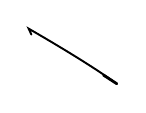
\begin{tikzpicture}[x=1cm,y=1cm,line cap=round]
\draw[line width=0.7pt] (0.035,-0.075) -- (0,0) .. controls (0.33,-0.19) and (0.80,-0.47) .. (1.12,-0.70);
\draw[line width=1.0pt] (0.95,-0.59) -- (1.12,-0.70);
\end{tikzpicture}}
\LMsourceMark{M004200}{\margin{117}}

\LMflushnotes\LMflushpages
\ifnum\LMform=1
\begin{LMapparatus}
\LMentry{140-2-s118-I001}{insertion}{\inserted{$\chi$ sur $\Sigma$}
}{\emph{\LMinsertedlabel}}{Ajout explicite de l'auteur : intégré à l'endroit indiqué par la transcription, sans modifier sa lecture.}{}
\LMentry{140-2-s118-D001}{suppression}{\deleted{\LMsourceMark{M004201}{\illegible{1}}}
}{\emph{\LMomittedlabel}}{Passage biffé dans le manuscrit : la suppression suit l'état final de l'auteur; les doutes de lecture restent signalés.}{}
\LMentry{140-2-s118-D002}{suppression}{\deleted{et si $\Sigma$ opère sur
$T$ (\LMsourceMark{M004202}{\illegible{3}} $\chi$), on dira qu'une action
est compatible}
}{\emph{\LMomittedlabel}}{Passage biffé dans le manuscrit : la suppression suit l'état final de l'auteur; les doutes de lecture restent signalés.}{}
\LMentry{140-2-s118-I002}{insertion}{\(\inserted{\text{dans le}}\)
}{\emph{\LMinsertedlabel}}{Ajout explicite de l'auteur : intégré à l'endroit indiqué par la transcription, sans modifier sa lecture.}{}
\LMentry{140-2-s118-I003}{insertion}{\(\inserted{\text{sinon pas de pb}}\)
}{\emph{\LMinsertedlabel}}{Ajout explicite de l'auteur : intégré à l'endroit indiqué par la transcription, sans modifier sa lecture.}{}
\end{LMapparatus}
\fi
\ifnum\LMform=2
\par\smallskip\begingroup\footnotesize\Needspace{4\baselineskip}\csname @beginparpenalty\endcsname=10000\relax\noindent\textcolor{gray}{\rule{.2\linewidth}{.35pt}}\par\nobreak
\noindent\textit{\LMdoubtheading.}\par\nobreak
\LMcarryover{140-2-s118-D001}{\LMsourceMark{M004203}{\illegible{1}}
}
\LMcarryover{140-2-s118-D002}{\LMsourceMark{M004204}{\illegible{3}}
}
\par\endgroup\smallskip
\fi

\LMsourceMark{M004205}{\scanpage{119}}
\LMsourceMark{M004206}{\mspage{58}}

14. Digression cohomologique (sur \LMsourceMark{M004207}{\unsure{les|le}} ``bouchage des
trous).

Soit $X$ un schéma loc. noeth. \uline{régulier} de
\LMsourceMark{M004208}{\unsure{dim.}} $1$, $S$ un sous-schéma fermé \var{\inserted{réduit discret}}{\LMadded{réduit discret}}{insertion}{140-2-s119-I001} tel que
$\forall s\in S$, $\dim_s S=1$ (donc $S$ défini par une
partie fermée discrète de $X$), $U=X\setminus S$.
\LMsourceMark{M004209}{\margin{Il vaudrait peut-être mieux démarrer avec \LMsourceMark{M004210}{\unsure{le cas purement topologique|les cas purement topologiques}} d'une surface\dots{} et faire le lien avec les groupes \uline{discrets}.}}

On veut expliciter par voie galoisienne les
faisceaux \var{\inserted{d'ens.}}{\LMadded{d'ens.}}{insertion}{140-2-s119-I002} étales \var{\inserted{constructibles}}{\LMadded{constructibles}}{insertion}{140-2-s119-I003} sur $X$ tels que $F\mid U$ soit
loc. ct. Par le \LMsourceMark{M004211}{\unsure{topos|tapis}} d'Artin \var{\inserted{sur les ouverts du topos}}{\LMadded{sur les ouverts du topos}}{insertion}{140-2-s119-I004}, ils corres-
pondent aux triples
\[
(F_U,F_S,\varphi)
\]
où $F_U$ est un faisceau \var{\inserted{constr.}}{\LMadded{constr.}}{insertion}{140-2-s119-I005} loc. constant sur $U$,
$F_S$ un faisceau (\LMsourceMark{M004212}{\unsure{néc.|nécess.}} loc. constant)
et $\varphi$ un hom
\[
F_S\xrightarrow{\varphi}j^{*}i_{*}(F_U)
\]
(où $i:U\LMsourceMark{M004213}{\unsure{\hookrightarrow|\to}}X$ et $j:S\to X$ sont les inclusions).
Toute condition de constructibilité étant mise à
part, un faisceau étale $F$ sur $X$ correspond
à un tel triple --- on se restreint ici aux
$F$ tels que $F_U$ \var{\deleted{\LMsourceMark{M004214}{\unsure{provienne}}}}{\LMsourceMark{M004215}{\LMcancelledDoubts{\LMsourceMark{M004216}{\unsure{provienne}}}}}{deletion}{140-2-s119-D001} provienne du
topos fondamental $B_{\LMsourceMark{M004217}{\unsure{\Pi_1(U)|\pi_1(U)}}}$ de $U$ \var{\deleted{\LMsourceMark{M004218}{\illegible{1}}}}{\LMsourceMark{M004219}{\LMcancelledDoubts{\LMsourceMark{M004220}{\illegible{1}}}}}{deletion}{140-2-s119-D002}\dots
(Il n'y a pas lieu de supposer $F_U$ à fibres finies,

\LMsourceMark{M004221}{\margin{118}}

\LMflushnotes\LMflushpages
\ifnum\LMform=1
\begin{LMapparatus}
\LMentry{140-2-s119-I001}{insertion}{\inserted{réduit discret}
}{\emph{\LMinsertedlabel}}{Ajout explicite de l'auteur : intégré à l'endroit indiqué par la transcription, sans modifier sa lecture.}{}
\LMentry{140-2-s119-I002}{insertion}{\inserted{d'ens.}
}{\emph{\LMinsertedlabel}}{Ajout explicite de l'auteur : intégré à l'endroit indiqué par la transcription, sans modifier sa lecture.}{}
\LMentry{140-2-s119-I003}{insertion}{\inserted{constructibles}
}{\emph{\LMinsertedlabel}}{Ajout explicite de l'auteur : intégré à l'endroit indiqué par la transcription, sans modifier sa lecture.}{}
\LMentry{140-2-s119-I004}{insertion}{\inserted{sur les ouverts du topos}
}{\emph{\LMinsertedlabel}}{Ajout explicite de l'auteur : intégré à l'endroit indiqué par la transcription, sans modifier sa lecture.}{}
\LMentry{140-2-s119-I005}{insertion}{\inserted{constr.}
}{\emph{\LMinsertedlabel}}{Ajout explicite de l'auteur : intégré à l'endroit indiqué par la transcription, sans modifier sa lecture.}{}
\LMentry{140-2-s119-D001}{suppression}{\deleted{\LMsourceMark{M004222}{\unsure{provienne}}}
}{\emph{\LMomittedlabel}}{Passage biffé dans le manuscrit : la suppression suit l'état final de l'auteur; les doutes de lecture restent signalés.}{}
\LMentry{140-2-s119-D002}{suppression}{\deleted{\LMsourceMark{M004223}{\illegible{1}}}
}{\emph{\LMomittedlabel}}{Passage biffé dans le manuscrit : la suppression suit l'état final de l'auteur; les doutes de lecture restent signalés.}{}
\end{LMapparatus}
\fi
\ifnum\LMform=2
\par\smallskip\begingroup\footnotesize\Needspace{4\baselineskip}\csname @beginparpenalty\endcsname=10000\relax\noindent\textcolor{gray}{\rule{.2\linewidth}{.35pt}}\par\nobreak
\noindent\textit{\LMdoubtheading.}\par\nobreak
\LMcarryover{140-2-s119-D001}{\LMsourceMark{M004224}{\unsure{provienne}}
}
\LMcarryover{140-2-s119-D002}{\LMsourceMark{M004225}{\illegible{1}}
}
\par\endgroup\smallskip
\fi

\LMsourceMark{M004226}{\scanpage{120}}

pour ce qui suit). \var{\deleted{Nous allons}}{}{deletion}{140-2-s120-D001}

Soit $\forall s\in S$ $\underline{O}_s$ un hensélisé de $\underline{O}_{X,s}$,
$D_s=\operatorname{Spec}\underline{O}_s$ \var{\inserted{(``disque en $s$'')}}{\LMadded{(``disque en $s$'')}}{insertion}{140-2-s120-I001}, $D_s^{*}=D_s-\{s\}$ \var{\inserted{$=\operatorname{Spec}K_s$ ($K_s$ corps des fractions de $\underline{O}_s$)}}{\LMadded{$=\operatorname{Spec}K_s$ ($K_s$ corps des fractions de $\underline{O}_s$)}}{insertion}{140-2-s120-I002} (``disque pointé'' en
$s$) $D=\coprod_{s\in S}D_s$, $\LMsourceMark{M004227}{\unsure{D_s^{*}|D^{*}}}=\coprod_{s\in S}D_s^{*}$. On a
un diagramme commutatif
\diagram{\begin{tikzcd}[ampersand replacement=\&]
\& D^{*} \arrow[dl, "\rho"'] \arrow[dr, "\sigma"] \& \& \\
U \arrow[dr, "i"'] \& \& D \arrow[dl, "\LMsourceMark{M004228}{\unsure{k|\kappa}}"] \& S \arrow[l, dashed, "j_0"'] \arrow[dll, dashed, "j"] \\
\& X \& \&
\end{tikzcd}
[La branche pointillée $S\xrightarrow{j_0}D$ est placée entre parenthèses.]}
et on voit \var{\inserted{(par Artin)}}{\LMadded{(par Artin)}}{insertion}{140-2-s120-I003} que ce diagramme \var{\deleted{\LMsourceMark{M004229}{\unsure{fait de}}}}{\LMsourceMark{M004230}{\LMcancelledDoubts{\LMsourceMark{M004231}{\unsure{fait de}}}}}{deletion}{140-2-s120-D002} \var{\inserted{permet d'exprimer}}{\LMadded{permet d'exprimer}}{insertion}{140-2-s120-I004}
\var{\inserted{les faisceaux}}{\LMadded{les faisceaux}}{insertion}{140-2-s120-I005} \var{\deleted{topos}}{}{deletion}{140-2-s120-D003} étales de $X$ \var{\deleted{\LMsourceMark{M004232}{\unsure{comme amalgamé}}}}{\LMsourceMark{M004233}{\LMcancelledDoubts{\LMsourceMark{M004234}{\unsure{comme amalgamé}}}}}{deletion}{140-2-s120-D004}
\var{\deleted{des topos étales de $U,D$ sur $D^{*}$}}{}{deletion}{140-2-s120-D005}
\var{\deleted{\diagram{\begin{tikzcd}[ampersand replacement=\&,column sep=2.5em,row sep=2em,nodes in empty cells]
\& \deleted{\LMsourceMark{M004235}{\unsure{D^*_{\mathrm{\acute et}}}}} \arrow[dl] \arrow[dr] \& \\
\deleted{U_{\mathrm{\acute et}}} \& \& \deleted{D_{\mathrm{\acute et}}}
\end{tikzcd}}}}{\LMsourceMark{M004236}{\LMcancelledDoubts{\(\LMsourceMark{M004237}{\unsure{D^*_{\mathrm{\acute et}}}}\)}}}{deletion}{140-2-s120-D006}
comme des systèmes \var{\deleted{de faisceaux}}{}{deletion}{140-2-s120-D010} \var{\inserted{$(F_U,F_D,\varphi)$}}{\LMadded{$(F_U,F_D,\varphi)$}}{insertion}{140-2-s120-I006}
avec $F_U$ faisceau étale sur $U$, $F_D$ faisceau
étale ``ess\textsuperscript{t} loc. constant'' sur $D$ [NB l'
inclusion $S\to D$ définit une équivalence
entre la cat. de ces faisceaux sur $D$, et
celle des faisceaux étales sur $S$] et
un hom. de faisceaux $F_D\to\sigma_{*}\rho^{*}F_U$ ou encore

\LMsourceMark{M004238}{\margin{119}}

\LMflushnotes\LMflushpages
\ifnum\LMform=1
\begin{LMapparatus}
\LMentry{140-2-s120-D001}{suppression}{\deleted{Nous allons}
}{\emph{\LMomittedlabel}}{Passage biffé dans le manuscrit : la suppression suit l'état final de l'auteur; les doutes de lecture restent signalés.}{}
\LMentry{140-2-s120-I001}{insertion}{\inserted{(``disque en $s$'')}
}{\emph{\LMinsertedlabel}}{Ajout explicite de l'auteur : intégré à l'endroit indiqué par la transcription, sans modifier sa lecture.}{}
\LMentry{140-2-s120-I002}{insertion}{\inserted{$=\operatorname{Spec}K_s$ ($K_s$ corps des fractions de $\underline{O}_s$)}
}{\emph{\LMinsertedlabel}}{Ajout explicite de l'auteur : intégré à l'endroit indiqué par la transcription, sans modifier sa lecture.}{}
\LMentry{140-2-s120-I003}{insertion}{\inserted{(par Artin)}
}{\emph{\LMinsertedlabel}}{Ajout explicite de l'auteur : intégré à l'endroit indiqué par la transcription, sans modifier sa lecture.}{}
\LMentry{140-2-s120-D002}{suppression}{\deleted{\LMsourceMark{M004239}{\unsure{fait de}}}
}{\emph{\LMomittedlabel}}{Passage biffé dans le manuscrit : la suppression suit l'état final de l'auteur; les doutes de lecture restent signalés.}{}
\LMentry{140-2-s120-I004}{insertion}{\inserted{permet d'exprimer}
}{\emph{\LMinsertedlabel}}{Ajout explicite de l'auteur : intégré à l'endroit indiqué par la transcription, sans modifier sa lecture.}{}
\LMentry{140-2-s120-I005}{insertion}{\inserted{les faisceaux}
}{\emph{\LMinsertedlabel}}{Ajout explicite de l'auteur : intégré à l'endroit indiqué par la transcription, sans modifier sa lecture.}{}
\LMentry{140-2-s120-D003}{suppression}{\deleted{topos}
}{\emph{\LMomittedlabel}}{Passage biffé dans le manuscrit : la suppression suit l'état final de l'auteur; les doutes de lecture restent signalés.}{}
\LMentry{140-2-s120-D004}{suppression}{\deleted{\LMsourceMark{M004240}{\unsure{comme amalgamé}}}
}{\emph{\LMomittedlabel}}{Passage biffé dans le manuscrit : la suppression suit l'état final de l'auteur; les doutes de lecture restent signalés.}{}
\LMentry{140-2-s120-D005}{suppression}{\deleted{des topos étales de $U,D$ sur $D^{*}$}
}{\emph{\LMomittedlabel}}{Passage biffé dans le manuscrit : la suppression suit l'état final de l'auteur; les doutes de lecture restent signalés.}{}
\LMentry{140-2-s120-D006}{suppression}{\deleted{\diagram{\begin{tikzcd}[ampersand replacement=\&,column sep=2.5em,row sep=2em,nodes in empty cells]
\& \deleted{\LMsourceMark{M004241}{\unsure{D^*_{\mathrm{\acute et}}}}} \arrow[dl] \arrow[dr] \& \\
\deleted{U_{\mathrm{\acute et}}} \& \& \deleted{D_{\mathrm{\acute et}}}
\end{tikzcd}}}
}{\emph{\LMomittedlabel}}{Passage biffé dans le manuscrit : la suppression suit l'état final de l'auteur; les doutes de lecture restent signalés.}{}
\LMentry{140-2-s120-D010}{suppression}{\deleted{de faisceaux}
}{\emph{\LMomittedlabel}}{Passage biffé dans le manuscrit : la suppression suit l'état final de l'auteur; les doutes de lecture restent signalés.}{}
\LMentry{140-2-s120-I006}{insertion}{\inserted{$(F_U,F_D,\varphi)$}
}{\emph{\LMinsertedlabel}}{Ajout explicite de l'auteur : intégré à l'endroit indiqué par la transcription, sans modifier sa lecture.}{}
\end{LMapparatus}
\fi
\ifnum\LMform=2
\par\smallskip\begingroup\footnotesize\Needspace{4\baselineskip}\csname @beginparpenalty\endcsname=10000\relax\noindent\textcolor{gray}{\rule{.2\linewidth}{.35pt}}\par\nobreak
\noindent\textit{\LMdoubtheading.}\par\nobreak
\LMcarryover{140-2-s120-D002}{\LMsourceMark{M004242}{\unsure{fait de}}
}
\LMcarryover{140-2-s120-D004}{\LMsourceMark{M004243}{\unsure{comme amalgamé}}
}
\LMcarryover{140-2-s120-D006}{\(\LMsourceMark{M004244}{\unsure{D^*_{\mathrm{\acute et}}}}\)
}
\par\endgroup\smallskip
\fi

% END PACKAGE LM_P012
% BEGIN PACKAGE LM_P013
\ifnum\LMform<2\Needspace{11\baselineskip}\subsection*{Scans 121--130}\fi
\LMsourceMark{M004245}{\scanpage{121}}
\LMsourceMark{M004246}{\mspage{59}}
% L01
\[
\boxed{\sigma^{*}(F_D)\xrightarrow{\varphi}\rho^{*}(F_U)}
\]
% L02
Or, \var{\deleted{\LMsourceMark{M004247}{\unsure{cette donnée si $F_U$ est un}}}}{\LMsourceMark{M004248}{\LMcancelledDoubts{\LMsourceMark{M004249}{\unsure{cette donnée si $F_U$ est un}}}}}{deletion}{140-2-s121-D001} \var{\inserted{si on se borne aux}}{\LMadded{si on se borne aux}}{insertion}{140-2-s121-I001} $F_U$ tels que $F_U$ soit
% L03
lui-= ess$^{t}$. loc$^{t}$ constant, alors les données
% L04
$F_U,F_D,\varphi$ ne font intervenir que des
% L05
faisceaux ess$^{t}$ loc. constants, i.e. des
% L06
topos fondamentaux (multigaloisiens)
% L07
associés aux schémas envisagés, \var{\deleted{\LMsourceMark{M004250}{\unsure{savoir}}}}{\LMsourceMark{M004251}{\LMcancelledDoubts{\LMsourceMark{M004252}{\unsure{savoir}}}}}{deletion}{140-2-s121-D002} donc
% L08
se décrivent entièrement en termes des
% L09
diagrammes
\diagram{\begin{tikzcd}[ampersand replacement=\&]
 \& B_{\pi_1,D^{*}} \arrow[dl,"{\var{\deleted{\LMsourceMark{M004253}{\illegible{1}}}}{\LMsourceMark{M004254}{\LMcancelledDoubts{\(\LMsourceMark{M004255}{\illegible{1}}\)}}}{deletion}{140-2-s121-D003}\,\rho}"'] \arrow[dr,no head,"\sigma"] \& \\
 B_{\pi_1,U} \& \& B_{\pi_1,D}
\end{tikzcd}}
\LMsourceMark{M004256}{\margin{(*)}}
% L10
-- d'ailleurs le cas où $\varphi$ est un \uline{iso} correspond
% L11
justement au cas des faisceaux loc. ess.
% L12
constants sur $X$, i.e. de faisceaux sur
% L13
$B_{\pi_1,X}$ -- lequel topos fondamental
% L14
apparaît donc comme somme
% L15
amalgamée du diagramme de topos
% L16
précédent, s'insérant dans le carré
\diagram{\begin{tikzcd}[ampersand replacement=\&]
 \& B_{\pi_1,D^{*}} \arrow[dl] \arrow[dr] \& \\
 B_{\pi_1,U} \arrow[dr] \& \& B_{\pi_1,D} \arrow[dl] \\
 \& B_{\pi_1,X} \&
\end{tikzcd}}

\LMflushnotes\LMflushpages
\ifnum\LMform=1
\begin{LMapparatus}
\LMentry{140-2-s121-D001}{suppression}{\deleted{\LMsourceMark{M004257}{\unsure{cette donnée si $F_U$ est un}}}
}{\emph{\LMomittedlabel}}{Passage biffé dans le manuscrit : la suppression suit l'état final de l'auteur; les doutes de lecture restent signalés.}{}
\LMentry{140-2-s121-I001}{insertion}{\inserted{si on se borne aux}
}{\emph{\LMinsertedlabel}}{Ajout explicite de l'auteur : intégré à l'endroit indiqué par la transcription, sans modifier sa lecture.}{}
\LMentry{140-2-s121-D002}{suppression}{\deleted{\LMsourceMark{M004258}{\unsure{savoir}}}
}{\emph{\LMomittedlabel}}{Passage biffé dans le manuscrit : la suppression suit l'état final de l'auteur; les doutes de lecture restent signalés.}{}
\LMentry{140-2-s121-D003}{suppression}{\(\deleted{\LMsourceMark{M004259}{\illegible{1}}}\)
}{\emph{\LMomittedlabel}}{Passage biffé dans le manuscrit : la suppression suit l'état final de l'auteur; les doutes de lecture restent signalés.}{}
\end{LMapparatus}
\fi
\ifnum\LMform=2
\par\smallskip\begingroup\footnotesize\Needspace{4\baselineskip}\csname @beginparpenalty\endcsname=10000\relax\noindent\textcolor{gray}{\rule{.2\linewidth}{.35pt}}\par\nobreak
\noindent\textit{\LMdoubtheading.}\par\nobreak
\LMcarryover{140-2-s121-D001}{\LMsourceMark{M004260}{\unsure{cette donnée si $F_U$ est un}}
}
\LMcarryover{140-2-s121-D002}{\LMsourceMark{M004261}{\unsure{savoir}}
}
\LMcarryover{140-2-s121-D003}{\(\LMsourceMark{M004262}{\illegible{1}}\)
}
\par\endgroup\smallskip
\fi

\LMsourceMark{M004263}{\scanpage{122}}
% L01
Supposons pour simplifier $U$ connexe,
% L02
choisissons un rev. universel \var{\inserted{$\widetilde U$}}{\LMadded{$\widetilde U$}}{insertion}{140-2-s122-I001} de $U$, et un
% L03
rev. universel \var{\inserted{$\widetilde D_i^{*}$}}{\LMadded{$\widetilde D_i^{*}$}}{insertion}{140-2-s122-I002} de chaque $D_i^{*}$ -- d'où un
% L04
rev. universel \var{\inserted{$\widetilde D_i$}}{\LMadded{$\widetilde D_i$}}{insertion}{140-2-s122-I003} de $D_i$ -- et des isom.
% L05
(= ``classes de chemins'') entre $\rho_{!}(\widetilde D_i^{*})$ et $\widetilde U$
% L06
-- donc le diagramme des topos \LMsourceMark{M004264}{\unsure{(*)}},
% L07
-- ou des groupoïdes fondamentaux --
% L08
s'explicite en termes d'un diagramme
% L09
\diagram{\begin{tikzcd}[ampersand replacement=\&,column sep=large]
 \& {\begin{gathered}
 (\operatorname{Gal}(\overline K_i/K_i))\\[-2pt]
 \Vert\\[-2pt]
 \mathcal E_i
 \end{gathered}} \arrow[dl,"\LMsourceMark{M004265}{\unsure{\rho_i|\varphi_i}}"'] \arrow[dr,"\sigma_i"] \& \\
 {\begin{gathered}
 \mathcal E\\[-2pt]
 \Vert\\[-2pt]
 (\pi_1(U,\widetilde U)=\operatorname{Aut}_U(\widetilde U))
 \end{gathered}} \& \&
 {\begin{gathered}
 \Gamma_i\;\LMsourceMark{M004266}{\illegible{1}}\\[-2pt]
 \Vert\\[-2pt]
 (\operatorname{Gal}(\overline{k(s)}/k(s)))
 \end{gathered}}
\end{tikzcd}}
% L10
et la donnée d'un $F$ comme envisagé sur
% L11
$X$ revient à la donnée d'un système
% L12
$(E_U,(E_i)_{i\in I},(\varphi_i)_{i\in I})$, où $E_U$ est un $\mathcal E$-ens,
% L13
$E_i$ un $\Gamma_i$-ens, $(\forall i\in I)$, et $\varphi_i$ un
% L14
$\mathcal E_i$-hom de $E_i$ dans $E_U$ (i.e. un
% L15
un $\Gamma_i$-hom
\[
\varphi_i:\ E_i\longrightarrow E_U^{\Pi_i},
\]

\LMflushnotes\LMflushpages
\ifnum\LMform=1
\begin{LMapparatus}
\LMentry{140-2-s122-I001}{insertion}{\inserted{$\widetilde U$}
}{\emph{\LMinsertedlabel}}{Ajout explicite de l'auteur : intégré à l'endroit indiqué par la transcription, sans modifier sa lecture.}{}
\LMentry{140-2-s122-I002}{insertion}{\inserted{$\widetilde D_i^{*}$}
}{\emph{\LMinsertedlabel}}{Ajout explicite de l'auteur : intégré à l'endroit indiqué par la transcription, sans modifier sa lecture.}{}
\LMentry{140-2-s122-I003}{insertion}{\inserted{$\widetilde D_i$}
}{\emph{\LMinsertedlabel}}{Ajout explicite de l'auteur : intégré à l'endroit indiqué par la transcription, sans modifier sa lecture.}{}
\end{LMapparatus}
\fi

\LMsourceMark{M004267}{\scanpage{123}}
\LMsourceMark{M004268}{\mspage{60}}
% L01
où \var{\deleted{\LMsourceMark{M004269}{\unsure{$\Pi_i$ est}}}}{\LMsourceMark{M004270}{\LMcancelledDoubts{\LMsourceMark{M004271}{\unsure{$\Pi_i$ est}}}}}{deletion}{140-2-s123-D001} $\Pi_i=\LMsourceMark{M004272}{\unsure{\operatorname{Ker}(\sigma_i)}}$ s'insère dans la suite exacte
% L02
\[
1\longrightarrow\Pi_i\longrightarrow\mathcal E_i\longrightarrow\Gamma_i\longrightarrow1
\]

% L03
Le cas où les $E_i\longrightarrow E_U$ sont des iso,
% L04
i.e. les $E_i$ \LMsourceMark{M004273}{\unsure{s'identifient|s'identifiant}} \var{\deleted{\LMsourceMark{M004274}{\illegible{1}}}}{\LMsourceMark{M004275}{\LMcancelledDoubts{\LMsourceMark{M004276}{\illegible{1}}}}}{deletion}{140-2-s123-D002} tous à $E_U$,
% L05
avec action triviale \LMsourceMark{M004277}{\unsure{de|des}} $\Pi_i$ sur $E_U$, correspond
% L06
au cas où $F$ est ess. loc. \LMsourceMark{M004278}{\unsure{ct|cst}} sur $X$,
% L07
d'où aussitôt
% L08
\[
\pi_1(X)=\mathcal E=\pi_1(U)\ \big/\
\substack{\text{ss-groupe \LMsourceMark{M004279}{\unsure{invariant}} engendré}\\
\text{par les }\rho_i(\Pi_i)}.
\]

% L09
Notre propos est celui d'un calcul galoisien
% L10
(si possible) de la cohomologie de $X$ pour
% L11
les $F$ envisagés.
% L12
Soit $B_{X,U}$ le topos \var{\inserted{dont les faisceaux sont}}{\LMadded{dont les faisceaux sont}}{insertion}{140-2-s123-I001} des triples
% L13
$(F_U,F_D,\varphi)$ comme dessus, qui s'envoie
% L14
donc dans le topos $B_{\pi_1,X}$, correspondant
% L15
aux couples pour lesquels $\varphi$ est iso,
% L16
et reçoit le topos $X_{\mathrm{ét}}$ :

\LMflushnotes\LMflushpages
\ifnum\LMform=1
\begin{LMapparatus}
\LMentry{140-2-s123-D001}{suppression}{\deleted{\LMsourceMark{M004280}{\unsure{$\Pi_i$ est}}}
}{\emph{\LMomittedlabel}}{Passage biffé dans le manuscrit : la suppression suit l'état final de l'auteur; les doutes de lecture restent signalés.}{}
\LMentry{140-2-s123-D002}{suppression}{\deleted{\LMsourceMark{M004281}{\illegible{1}}}
}{\emph{\LMomittedlabel}}{Passage biffé dans le manuscrit : la suppression suit l'état final de l'auteur; les doutes de lecture restent signalés.}{}
\LMentry{140-2-s123-I001}{insertion}{\inserted{dont les faisceaux sont}
}{\emph{\LMinsertedlabel}}{Ajout explicite de l'auteur : intégré à l'endroit indiqué par la transcription, sans modifier sa lecture.}{}
\end{LMapparatus}
\fi
\ifnum\LMform=2
\par\smallskip\begingroup\footnotesize\Needspace{4\baselineskip}\csname @beginparpenalty\endcsname=10000\relax\noindent\textcolor{gray}{\rule{.2\linewidth}{.35pt}}\par\nobreak
\noindent\textit{\LMdoubtheading.}\par\nobreak
\LMcarryover{140-2-s123-D001}{\LMsourceMark{M004282}{\unsure{$\Pi_i$ est}}
}
\LMcarryover{140-2-s123-D002}{\LMsourceMark{M004283}{\illegible{1}}
}
\par\endgroup\smallskip
\fi

\LMsourceMark{M004284}{\scanpage{124}}
% L01
\diagram{\begin{tikzcd}[ampersand replacement=\&]
X_{\mathrm{ét}} \arrow[r,"f"] \& B_{X,U} \arrow[r,"g"] \& B_{\pi_1,X}
\end{tikzcd}}
% L02
On se pose la question

% L03
a) Calcul ``explicite'', en termes de cohomologie
% L04
des groupes profinis, de la cohomologie
% L05
dans le topos abracadabra $B_{X,U}$. (NB.
% L06
\var{\deleted{\LMsourceMark{M004285}{\unsure{b) le calcul de}}}}{\LMsourceMark{M004286}{\LMcancelledDoubts{\LMsourceMark{M004287}{\unsure{b) le calcul de}}}}}{deletion}{140-2-s124-D001} la cohomologie \var{\deleted{\LMsourceMark{M004288}{\illegible{1}}}}{\LMsourceMark{M004289}{\LMcancelledDoubts{\LMsourceMark{M004290}{\illegible{1}}}}}{deletion}{140-2-s124-D002} de
% L07
$B_{\pi_1,X}$ n'est autre que la cohomologie
% L08
galoisienne profinie de $\pi_1(X)=\mathcal E/\ldots$
% L09
calculé plus haut\ldots).

% L10
b) Vérifier si pour un faisceau de
% L11
torsion $F$ sur $B_{X,U}$ l'hom. can.
% L12
\[
H^{*}(B_{X,U},F)\longrightarrow
H^{*}(X_{\mathrm{ét}},f^{*}F)
\]
% L13
est un iso.

% L14
NB Jusqu'à maintenant, l'hyp.
% L15
$\dim X=1$ n'a pas servi, ni l'hyp. noethérien
% L16
-- seulement le fait que $S$ soit partie fermée
% L17
discrète, $X$ connexe\ldots. Pour les calculs qui

\LMflushnotes\LMflushpages
\ifnum\LMform=1
\begin{LMapparatus}
\LMentry{140-2-s124-D001}{suppression}{\deleted{\LMsourceMark{M004291}{\unsure{b) le calcul de}}}
}{\emph{\LMomittedlabel}}{Passage biffé dans le manuscrit : la suppression suit l'état final de l'auteur; les doutes de lecture restent signalés.}{}
\LMentry{140-2-s124-D002}{suppression}{\deleted{\LMsourceMark{M004292}{\illegible{1}}}
}{\emph{\LMomittedlabel}}{Passage biffé dans le manuscrit : la suppression suit l'état final de l'auteur; les doutes de lecture restent signalés.}{}
\end{LMapparatus}
\fi
\ifnum\LMform=2
\par\smallskip\begingroup\footnotesize\Needspace{4\baselineskip}\csname @beginparpenalty\endcsname=10000\relax\noindent\textcolor{gray}{\rule{.2\linewidth}{.35pt}}\par\nobreak
\noindent\textit{\LMdoubtheading.}\par\nobreak
\LMcarryover{140-2-s124-D001}{\LMsourceMark{M004293}{\unsure{b) le calcul de}}
}
\LMcarryover{140-2-s124-D002}{\LMsourceMark{M004294}{\illegible{1}}
}
\par\endgroup\smallskip
\fi

\LMsourceMark{M004295}{\scanpage{125}}
\LMsourceMark{M004296}{\mspage{61}}
% L01
suivent, correspondants du \var{\deleted{\LMsourceMark{M004297}{\illegible{1}}}}{\LMsourceMark{M004298}{\LMcancelledDoubts{\LMsourceMark{M004299}{\illegible{1}}}}}{deletion}{140-2-s125-D001} cas où les
% L02
$\LMsourceMark{M004300}{\unsure{D_s|O_s}}$ sont des \LMsourceMark{M004301}{\unsure{jauges}} à corps résiduel $k(s)$
% L03
de car. $0$, on va supposer que
% L04
\[
\Pi_i\simeq\widehat{\mathbb Z}\qquad\text{(non canoniquement)}
\]
% L05
-- en fait, par la théorie Kummérienne on
% L06
a un système de systèmes locaux de Tate
% L07
$\LMsourceMark{M004302}{\unsure{T_{\mathcal E}}}$ \var{\inserted{(sur $\mathcal E$)}}{\LMadded{(sur $\mathcal E$)}}{insertion}{140-2-s125-I001}, $T_i$ \var{\inserted{(sur $\Gamma_i$)}}{\LMadded{(sur $\Gamma_i$)}}{insertion}{140-2-s125-I002}, et des \var{\inserted{$\mathcal E_i$-}}{\LMadded{$\mathcal E_i$-}}{insertion}{140-2-s125-I003}isom. $T_{\mathcal E}\simeq T_i$, \var{\deleted{et \LMsourceMark{M004303}{\illegible{1}}}}{\LMsourceMark{M004304}{\LMcancelledDoubts{\LMsourceMark{M004305}{\illegible{1}}}}}{deletion}{140-2-s125-D002}
% L08
(i.e. un $T_X$ sur lequel opère $\LMsourceMark{M004306}{\unsure{\widetilde{\mathcal E}|\overline{\mathcal E}}}=\mathcal E/\ldots$)
% L09
et on aura un iso. can. Kummérien
% L10
\[
T_i\xrightarrow[\sim]{\LMsourceMark{M004307}{\unsure{\kappa_i|k_i}}}\Pi_i.
\]

% L11
On aimerait pouvoir paraphraser,
% L12
sur $B_{X,U}$, la suite exacte de cohomologie
% L13
bien connue
% L14
\[
\longrightarrow H^i(X,F)\longrightarrow H^i(U,F)
\longrightarrow H^{i+1}_S(X,F)\longrightarrow\cdots
\]
% L15
relative à l'ouvert $U$ du topos $X$, et son
% L16
``complémentaire'' fermé $S$. Or, \var{\deleted{\LMsourceMark{M004308}{\illegible{2}}}}{\LMsourceMark{M004309}{\LMcancelledDoubts{\LMsourceMark{M004310}{\illegible{2}}}}}{deletion}{140-2-s125-D003} \var{\inserted{tout comme}}{\LMadded{tout comme}}{insertion}{140-2-s125-I004}
% L17
$X$ s'insère dans un diagramme de topos
% L18
\diagram{\begin{tikzcd}[ampersand replacement=\&]
 \& D^{*}_{\mathrm{ét}} \arrow[dl] \arrow[dr] \& \& \\
 U_{\mathrm{ét}} \arrow[dr,no head] \& \& D_{\mathrm{ét}} \arrow[dl] \& S_{\mathrm{ét}} \arrow[l,"\LMsourceMark{M004311}{\unsure{\xi}}"'] \\
 \& X_{\mathrm{ét}} \& \&
\end{tikzcd}},

\LMflushnotes\LMflushpages
\ifnum\LMform=1
\begin{LMapparatus}
\LMentry{140-2-s125-D001}{suppression}{\deleted{\LMsourceMark{M004312}{\illegible{1}}}
}{\emph{\LMomittedlabel}}{Passage biffé dans le manuscrit : la suppression suit l'état final de l'auteur; les doutes de lecture restent signalés.}{}
\LMentry{140-2-s125-I001}{insertion}{\inserted{(sur $\mathcal E$)}
}{\emph{\LMinsertedlabel}}{Ajout explicite de l'auteur : intégré à l'endroit indiqué par la transcription, sans modifier sa lecture.}{}
\LMentry{140-2-s125-I002}{insertion}{\inserted{(sur $\Gamma_i$)}
}{\emph{\LMinsertedlabel}}{Ajout explicite de l'auteur : intégré à l'endroit indiqué par la transcription, sans modifier sa lecture.}{}
\LMentry{140-2-s125-I003}{insertion}{\inserted{$\mathcal E_i$-}
}{\emph{\LMinsertedlabel}}{Ajout explicite de l'auteur : intégré à l'endroit indiqué par la transcription, sans modifier sa lecture.}{}
\LMentry{140-2-s125-D002}{suppression}{\deleted{et \LMsourceMark{M004313}{\illegible{1}}}
}{\emph{\LMomittedlabel}}{Passage biffé dans le manuscrit : la suppression suit l'état final de l'auteur; les doutes de lecture restent signalés.}{}
\LMentry{140-2-s125-D003}{suppression}{\deleted{\LMsourceMark{M004314}{\illegible{2}}}
}{\emph{\LMomittedlabel}}{Passage biffé dans le manuscrit : la suppression suit l'état final de l'auteur; les doutes de lecture restent signalés.}{}
\LMentry{140-2-s125-I004}{insertion}{\inserted{tout comme}
}{\emph{\LMinsertedlabel}}{Ajout explicite de l'auteur : intégré à l'endroit indiqué par la transcription, sans modifier sa lecture.}{}
\end{LMapparatus}
\fi
\ifnum\LMform=2
\par\smallskip\begingroup\footnotesize\Needspace{4\baselineskip}\csname @beginparpenalty\endcsname=10000\relax\noindent\textcolor{gray}{\rule{.2\linewidth}{.35pt}}\par\nobreak
\noindent\textit{\LMdoubtheading.}\par\nobreak
\LMcarryover{140-2-s125-D001}{\LMsourceMark{M004315}{\illegible{1}}
}
\LMcarryover{140-2-s125-D002}{\LMsourceMark{M004316}{\illegible{1}}
}
\LMcarryover{140-2-s125-D003}{\LMsourceMark{M004317}{\illegible{2}}
}
\par\endgroup\smallskip
\fi

\LMsourceMark{M004318}{\scanpage{126}}
% L01
de = $B_{X,U}$ s'insère dans
% L02
\diagram{\begin{tikzcd}[ampersand replacement=\&]
 \& B_{\pi_1,D^{*}} \arrow[dl] \arrow[dr] \& \& \\
 B_{\pi_1,U} \arrow[dr] \& \& B_{\pi_1,D} \arrow[dl] \& B_{\pi_1,S} \arrow[l,"\approx","\LMsourceMark{M004319}{\unsure{\xi_{\mathrm{ét}}}}"'] \\
 \& B_{X,U} \& \&
\end{tikzcd}}

% L03
[\uline{NB} les $\varprojlim$ finies et $\varinjlim$ quelc.
% L04
dans $B_{X,U}$ i.e. pour les $(F_U,F_D,\varphi)$, se
% L05
calculent ``terme à terme''] Je dis
% L06
que $B_{\pi_1,U}\longrightarrow B_{X,U}$ s'identifie à un
% L07
morphisme d'induction, relatif à l'
% L08
objet \var{\deleted{\LMsourceMark{M004320}{\illegible{1}}}}{\LMsourceMark{M004321}{\LMcancelledDoubts{\LMsourceMark{M004322}{\illegible{1}}}}}{deletion}{140-2-s126-D001} \LMsourceMark{M004323}{\unsure{(noté encore}} $U$ par abus de notation)
% L09
de $B_{X,U}$ défini par
% L10
$F_U={}$faisceau final $e_U$, $F_D={}$faisceau initial $\varnothing_D$
% L11
(et $\varphi$ \LMsourceMark{M004324}{\unsure{est|étant}} alors fixé !). En effet, les
% L12
objets \var{\inserted{de $B_{X,U}$}}{\LMadded{de $B_{X,U}$}}{insertion}{140-2-s126-I001} au dessus de $U$ s'identifient aux
% L13
$(F_U,F_D,\varphi)$ avec $F_D=\varnothing_D$ (ce que fixe $\varphi$ !) donc
% L14
ils forment une cat. équivalente à celle des
% L15
$F_U$, i.e. à $B_{\pi_1,U}$. On voit que le topos
% L16
résiduel (s'identifiant \var{\deleted{aux}}{}{deletion}{140-2-s126-D002} \var{\inserted{à la cat. des}}{\LMadded{à la cat. des}}{insertion}{140-2-s126-I002} $F\var{\deleted{_{\LMsourceMark{M004325}{\unsure{U}}},\LMsourceMark{M004326}{\unsure{E|e}}_{\LMsourceMark{M004327}{\unsure{i}}}}}{\LMsourceMark{M004328}{\LMcancelledDoubts{\(\LMsourceMark{M004329}{\unsure{U}}\)\quad \(\LMsourceMark{M004330}{\unsure{E|e}}\)\quad \(\LMsourceMark{M004331}{\unsure{i}}\)}}}{deletion}{140-2-s126-D003}=(F_U,F_D,\varphi)$ tels

\LMflushnotes\LMflushpages
\ifnum\LMform=1
\begin{LMapparatus}
\LMentry{140-2-s126-D001}{suppression}{\deleted{\LMsourceMark{M004332}{\illegible{1}}}
}{\emph{\LMomittedlabel}}{Passage biffé dans le manuscrit : la suppression suit l'état final de l'auteur; les doutes de lecture restent signalés.}{}
\LMentry{140-2-s126-I001}{insertion}{\inserted{de $B_{X,U}$}
}{\emph{\LMinsertedlabel}}{Ajout explicite de l'auteur : intégré à l'endroit indiqué par la transcription, sans modifier sa lecture.}{}
\LMentry{140-2-s126-D002}{suppression}{\deleted{aux}
}{\emph{\LMomittedlabel}}{Passage biffé dans le manuscrit : la suppression suit l'état final de l'auteur; les doutes de lecture restent signalés.}{}
\LMentry{140-2-s126-I002}{insertion}{\inserted{à la cat. des}
}{\emph{\LMinsertedlabel}}{Ajout explicite de l'auteur : intégré à l'endroit indiqué par la transcription, sans modifier sa lecture.}{}
\LMentry{140-2-s126-D003}{suppression}{\(\deleted{_{\LMsourceMark{M004333}{\unsure{U}}},\LMsourceMark{M004334}{\unsure{E|e}}_{\LMsourceMark{M004335}{\unsure{i}}}}\)
}{\emph{\LMomittedlabel}}{Passage biffé dans le manuscrit : la suppression suit l'état final de l'auteur; les doutes de lecture restent signalés.}{}
\end{LMapparatus}
\fi
\ifnum\LMform=2
\par\smallskip\begingroup\footnotesize\Needspace{4\baselineskip}\csname @beginparpenalty\endcsname=10000\relax\noindent\textcolor{gray}{\rule{.2\linewidth}{.35pt}}\par\nobreak
\noindent\textit{\LMdoubtheading.}\par\nobreak
\LMcarryover{140-2-s126-D001}{\LMsourceMark{M004336}{\illegible{1}}
}
\LMcarryover{140-2-s126-D003}{\(\LMsourceMark{M004337}{\unsure{U}}\)\quad \(\LMsourceMark{M004338}{\unsure{E|e}}\)\quad \(\LMsourceMark{M004339}{\unsure{i}}\)
}
\par\endgroup\smallskip
\fi

\LMsourceMark{M004340}{\scanpage{127}}
\LMsourceMark{M004341}{\mspage{62}}
% L01
que $F_U=e_U$ faisceau final, s'identifie de = à la
% L02
catégorie \var{\inserted{$B_{\pi_1,D}$}}{\LMadded{$B_{\pi_1,D}$}}{insertion}{140-2-s127-I001} des $F_D$ \var{\deleted{\LMsourceMark{M004342}{\illegible{2}}}}{\LMsourceMark{M004343}{\LMcancelledDoubts{\LMsourceMark{M004344}{\illegible{2}}}}}{deletion}{140-2-s127-D001} -- le foncteur
% L03
canonique ``image inverse sur $B_{\pi_1,D}$ de l'image
% L04
directe de $F$ sur $B_{\pi_1,U}$'' n'étant autre
% L05
$\sigma_*\rho^*$, de sorte qu'on retrouve la description
% L06
\var{\deleted{\LMsourceMark{M004345}{\illegible{1}}}}{\LMsourceMark{M004346}{\LMcancelledDoubts{\LMsourceMark{M004347}{\illegible{1}}}}}{deletion}{140-2-s127-D002} typique d'Artin d'un topos déduit
% L07
par ``recollement'' d'un \var{\deleted{\LMsourceMark{M004348}{\unsure{objet}}}}{\LMsourceMark{M004349}{\LMcancelledDoubts{\LMsourceMark{M004350}{\unsure{objet}}}}}{deletion}{140-2-s127-D003} ouvert et du
% L08
fermé complémentaire.
% L09
On trouve donc une suite exacte
% L10
\[
\longrightarrow H^i(B_{X,U},F)\longrightarrow
H^i(B_{\pi_1,U},F_U)\longrightarrow
H^{i+1}_{S(\text{ou }D)}(B_{X,U},F)\longrightarrow\cdots
\]
% L11
s'envoyant dans la suite exacte analogue
% L12
relative à $X_{\mathrm{ét}},U_{\mathrm{ét}},S_{\mathrm{ét}}$. \var{\deleted{\LMsourceMark{M004351}{\unsure{Pour}} \LMsourceMark{M004352}{\illegible{2}}}}{\LMsourceMark{M004353}{\LMcancelledDoubts{\LMsourceMark{M004354}{\unsure{Pour}}\quad \LMsourceMark{M004355}{\illegible{2}}}}}{deletion}{140-2-s127-D004} \var{\inserted{(On n'a}}{\LMadded{(On n'a}}{insertion}{140-2-s127-I002}
% L13
tjrs pas utilisé d'hyp. spéciale sur $S$\ldots).

% L14
Pour vérifier que l'on a des iso
% L15
au niveau des $H^i(B_{X,U},F)\longrightarrow H^i(X_{\mathrm{ét}},F)$,
% L16
il suffit par le lemme des cinq de
% L17
le prouver au niveau des
% L18
$H^i(B_{\pi_1,U},F)\longrightarrow H^i(U_{\mathrm{ét}},F)$ [i.e. \LMsourceMark{M004356}{\unsure{vérifier|vérifions}} que la
% L19
cohomologie de $U_{\mathrm{ét}}$ ``se calcule galoisiennement'']
% L20
\uline{et} au niveau des $H^i_S$. \var{\deleted{\LMsourceMark{M004357}{\unsure{Or}}}}{\LMsourceMark{M004358}{\LMcancelledDoubts{\LMsourceMark{M004359}{\unsure{Or}}}}}{deletion}{140-2-s127-D005} Regardons,

\LMflushnotes\LMflushpages
\ifnum\LMform=1
\begin{LMapparatus}
\LMentry{140-2-s127-I001}{insertion}{\inserted{$B_{\pi_1,D}$}
}{\emph{\LMinsertedlabel}}{Ajout explicite de l'auteur : intégré à l'endroit indiqué par la transcription, sans modifier sa lecture.}{}
\LMentry{140-2-s127-D001}{suppression}{\deleted{\LMsourceMark{M004360}{\illegible{2}}}
}{\emph{\LMomittedlabel}}{Passage biffé dans le manuscrit : la suppression suit l'état final de l'auteur; les doutes de lecture restent signalés.}{}
\LMentry{140-2-s127-D002}{suppression}{\deleted{\LMsourceMark{M004361}{\illegible{1}}}
}{\emph{\LMomittedlabel}}{Passage biffé dans le manuscrit : la suppression suit l'état final de l'auteur; les doutes de lecture restent signalés.}{}
\LMentry{140-2-s127-D003}{suppression}{\deleted{\LMsourceMark{M004362}{\unsure{objet}}}
}{\emph{\LMomittedlabel}}{Passage biffé dans le manuscrit : la suppression suit l'état final de l'auteur; les doutes de lecture restent signalés.}{}
\LMentry{140-2-s127-D004}{suppression}{\deleted{\LMsourceMark{M004363}{\unsure{Pour}} \LMsourceMark{M004364}{\illegible{2}}}
}{\emph{\LMomittedlabel}}{Passage biffé dans le manuscrit : la suppression suit l'état final de l'auteur; les doutes de lecture restent signalés.}{}
\LMentry{140-2-s127-I002}{insertion}{\inserted{(On n'a}
}{\emph{\LMinsertedlabel}}{Ajout explicite de l'auteur : intégré à l'endroit indiqué par la transcription, sans modifier sa lecture.}{}
\LMentry{140-2-s127-D005}{suppression}{\deleted{\LMsourceMark{M004365}{\unsure{Or}}}
}{\emph{\LMomittedlabel}}{Passage biffé dans le manuscrit : la suppression suit l'état final de l'auteur; les doutes de lecture restent signalés.}{}
\end{LMapparatus}
\fi
\ifnum\LMform=2
\par\smallskip\begingroup\footnotesize\Needspace{4\baselineskip}\csname @beginparpenalty\endcsname=10000\relax\noindent\textcolor{gray}{\rule{.2\linewidth}{.35pt}}\par\nobreak
\noindent\textit{\LMdoubtheading.}\par\nobreak
\LMcarryover{140-2-s127-D001}{\LMsourceMark{M004366}{\illegible{2}}
}
\LMcarryover{140-2-s127-D002}{\LMsourceMark{M004367}{\illegible{1}}
}
\LMcarryover{140-2-s127-D003}{\LMsourceMark{M004368}{\unsure{objet}}
}
\LMcarryover{140-2-s127-D004}{\LMsourceMark{M004369}{\unsure{Pour}}\quad \LMsourceMark{M004370}{\illegible{2}}
}
\LMcarryover{140-2-s127-D005}{\LMsourceMark{M004371}{\unsure{Or}}
}
\par\endgroup\smallskip
\fi

\LMsourceMark{M004372}{\scanpage{128}}
% L01
d'abord ces derniers -- on a
% L02
$H^0_S(B_{X,U},E)={}$ ens des sections de $F$ [i.e. des
% L03
couples d'une section de $F_U$ et
% L04
d'une de $F_D$, se correspondant
% L05
par $\varphi$, i.e. d'un élément \var{\inserted{$x$}}{\LMadded{$x$}}{insertion}{140-2-s128-I001} de
% L06
$E_U$ invariant par $\mathcal E$, et des
% L07
$x_i\in E_i$ invariants par les $\Gamma_i$,
% L08
tels que $x=\varphi_i(x_i)\quad\forall i$]
% L09
tels que $x=0$ \var{\deleted{\LMsourceMark{M004373}{\unsure{des|dans}} \LMsourceMark{M004374}{\unsure{systèmes}}}}{\LMsourceMark{M004375}{\LMcancelledDoubts{\LMsourceMark{M004376}{\unsure{des|dans}}\quad \LMsourceMark{M004377}{\unsure{systèmes}}}}}{deletion}{140-2-s128-D001}
% L10
\[
=\prod_i(\operatorname{Ker}(E_i\longrightarrow E_U)
\]
% L11
on constate que ce foncteur se factorise
% L12
par le foncteur $H^0_S$ relatif à ``l'inclusion''
% L13
\var{\deleted{\LMsourceMark{M004378}{\unsure{$D^{*}\subset D$}} \LMsourceMark{M004379}{\unsure{ou}} $B_{\pi_1,D^{*}}\longrightarrow B_{\pi_1,D}$}}{\LMsourceMark{M004380}{\LMcancelledDoubts{\LMsourceMark{M004381}{\unsure{$D^{*}\subset D$}}\quad \LMsourceMark{M004382}{\unsure{ou}}}}}{deletion}{140-2-s128-D002}
% L14
analogue \var{\deleted{\LMsourceMark{M004383}{\illegible{1}} $B_{\pi_1,U}$ \LMsourceMark{M004384}{\illegible{2}}}}{\LMsourceMark{M004385}{\LMcancelledDoubts{\LMsourceMark{M004386}{\illegible{1}}\quad \LMsourceMark{M004387}{\illegible{2}}}}}{deletion}{140-2-s128-D003}
% L15
\[
B_{\underbrace{\pi_1,\LMsourceMark{M004388}{\unsure{D^{*}|D_{*}}}}_{\text{remplaçant }\pi_1,U}}\longrightarrow B_{D,D^{*}}\quad\ldots
\]
% L16
et les $H^i_S$ sur $D_{X,U}$ se calculent comme
% L17
\var{\deleted{\LMsourceMark{M004389}{\unsure{qui n'est autre que}}}}{\LMsourceMark{M004390}{\LMcancelledDoubts{\LMsourceMark{M004391}{\unsure{qui n'est autre que}}}}}{deletion}{140-2-s128-D004}
% L18
ceux dans la situation locale $B_{D\var{\deleted{\LMsourceMark{M004392}{\illegible{1}}}}{\LMsourceMark{M004393}{\LMcancelledDoubts{\(\LMsourceMark{M004394}{\illegible{1}}\)}}}{deletion}{140-2-s128-D005},D^{*}\var{\deleted{\LMsourceMark{M004395}{\illegible{1}}}}{\LMsourceMark{M004396}{\LMcancelledDoubts{\(\LMsourceMark{M004397}{\illegible{1}}\)}}}{deletion}{140-2-s128-D006}}$ --
% L19
où on trouve le calcul habituel en
% L20
termes de l'hom. de groupes $\mathcal E_i\longrightarrow\Gamma_i$.
\LMsourceMark{M004398}{\margin{que j'ai un peu oublié !}}

% L21
Mais dans le cas actuel, l'hyp. $\dim_s X=1$
% L22
aux pts de $s\in S$, \var{\deleted{et $X$ \LMsourceMark{M004399}{\unsure{rég.}}}}{\LMsourceMark{M004400}{\LMcancelledDoubts{\LMsourceMark{M004401}{\unsure{rég.}}}}}{deletion}{140-2-s128-D007} implique que
% L23
la situation \var{\inserted{de topos}}{\LMadded{de topos}}{insertion}{140-2-s128-I002} localisée $D^{*}_{\LMsourceMark{M004402}{\unsure{a|\mathrm{ét}}}}\hookrightarrow D_{\LMsourceMark{M004403}{\unsure{a|\mathrm{ét}}}}$ est déjà entièrement
% L24
définie en termes des topos fondamentaux \LMsourceMark{M004404}{\unsure{des}}

\LMflushnotes\LMflushpages
\ifnum\LMform=1
\begin{LMapparatus}
\LMentry{140-2-s128-I001}{insertion}{\inserted{$x$}
}{\emph{\LMinsertedlabel}}{Ajout explicite de l'auteur : intégré à l'endroit indiqué par la transcription, sans modifier sa lecture.}{}
\LMentry{140-2-s128-D001}{suppression}{\deleted{\LMsourceMark{M004405}{\unsure{des|dans}} \LMsourceMark{M004406}{\unsure{systèmes}}}
}{\emph{\LMomittedlabel}}{Passage biffé dans le manuscrit : la suppression suit l'état final de l'auteur; les doutes de lecture restent signalés.}{}
\LMentry{140-2-s128-D002}{suppression}{\deleted{\LMsourceMark{M004407}{\unsure{$D^{*}\subset D$}} \LMsourceMark{M004408}{\unsure{ou}} $B_{\pi_1,D^{*}}\longrightarrow B_{\pi_1,D}$}
}{\emph{\LMomittedlabel}}{Passage biffé dans le manuscrit : la suppression suit l'état final de l'auteur; les doutes de lecture restent signalés.}{}
\LMentry{140-2-s128-D003}{suppression}{\deleted{\LMsourceMark{M004409}{\illegible{1}} $B_{\pi_1,U}$ \LMsourceMark{M004410}{\illegible{2}}}
}{\emph{\LMomittedlabel}}{Passage biffé dans le manuscrit : la suppression suit l'état final de l'auteur; les doutes de lecture restent signalés.}{}
\LMentry{140-2-s128-D004}{suppression}{\deleted{\LMsourceMark{M004411}{\unsure{qui n'est autre que}}}
}{\emph{\LMomittedlabel}}{Passage biffé dans le manuscrit : la suppression suit l'état final de l'auteur; les doutes de lecture restent signalés.}{}
\LMentry{140-2-s128-D005}{suppression}{\(\deleted{\LMsourceMark{M004412}{\illegible{1}}}\)
}{\emph{\LMomittedlabel}}{Passage biffé dans le manuscrit : la suppression suit l'état final de l'auteur; les doutes de lecture restent signalés.}{}
\LMentry{140-2-s128-D006}{suppression}{\(\deleted{\LMsourceMark{M004413}{\illegible{1}}}\)
}{\emph{\LMomittedlabel}}{Passage biffé dans le manuscrit : la suppression suit l'état final de l'auteur; les doutes de lecture restent signalés.}{}
\LMentry{140-2-s128-D007}{suppression}{\deleted{et $X$ \LMsourceMark{M004414}{\unsure{rég.}}}
}{\emph{\LMomittedlabel}}{Passage biffé dans le manuscrit : la suppression suit l'état final de l'auteur; les doutes de lecture restent signalés.}{}
\LMentry{140-2-s128-I002}{insertion}{\inserted{de topos}
}{\emph{\LMinsertedlabel}}{Ajout explicite de l'auteur : intégré à l'endroit indiqué par la transcription, sans modifier sa lecture.}{}
\end{LMapparatus}
\fi
\ifnum\LMform=2
\par\smallskip\begingroup\footnotesize\Needspace{4\baselineskip}\csname @beginparpenalty\endcsname=10000\relax\noindent\textcolor{gray}{\rule{.2\linewidth}{.35pt}}\par\nobreak
\noindent\textit{\LMdoubtheading.}\par\nobreak
\LMcarryover{140-2-s128-D001}{\LMsourceMark{M004415}{\unsure{des|dans}}\quad \LMsourceMark{M004416}{\unsure{systèmes}}
}
\LMcarryover{140-2-s128-D002}{\LMsourceMark{M004417}{\unsure{$D^{*}\subset D$}}\quad \LMsourceMark{M004418}{\unsure{ou}}
}
\LMcarryover{140-2-s128-D003}{\LMsourceMark{M004419}{\illegible{1}}\quad \LMsourceMark{M004420}{\illegible{2}}
}
\LMcarryover{140-2-s128-D004}{\LMsourceMark{M004421}{\unsure{qui n'est autre que}}
}
\LMcarryover{140-2-s128-D005}{\(\LMsourceMark{M004422}{\illegible{1}}\)
}
\LMcarryover{140-2-s128-D006}{\(\LMsourceMark{M004423}{\illegible{1}}\)
}
\LMcarryover{140-2-s128-D007}{\LMsourceMark{M004424}{\unsure{rég.}}
}
\par\endgroup\smallskip
\fi

\LMsourceMark{M004425}{\scanpage{129}}
\LMsourceMark{M004426}{\mspage{63}}
% L01
\var{\deleted{\LMsourceMark{M004427}{\unsure{des termes de}}}}{\LMsourceMark{M004428}{\LMcancelledDoubts{\LMsourceMark{M004429}{\unsure{des termes de}}}}}{deletion}{140-2-s129-D001}
% L02
i.e. le topos $B_{D,D^{*}}$ est équivalent à
% L03
$D_{\mathrm{ét}}$ -- or les $H^i_S(X_{\mathrm{ét}},F)$ se calculent
% L04
bien sur $D_{\mathrm{ét}}$\ldots On trouve donc

% L05
\uline{Prop.} L'hom. de suites exactes de coho-
% L06
mologie envisagé est un isomorphisme,
% L07
pourvu que l'on sache que l'hom.
% L08
$H^i(\mathcal E,F_{\mathcal E})\xrightarrow{\sim}H^i(U_{\mathrm{ét}},F_U)$ est un isom.
% L09
pour $\forall i$ ($F_U$ faisceau \LMsourceMark{M004430}{\unsure{étale|ét. loc.}} sur $U_{\mathrm{ét}}$
% L10
défini par un groupe $F_{\mathcal E}$ sur lequel $\mathcal E=\pi_1(U)$
% L11
opère).

% L12
\uline{Exemple} : \var{\inserted{OK}}{\LMadded{OK}}{insertion}{140-2-s129-I001} Si $U$ est une courbe affine
% L13
sur $k$ alg. clos \var{\inserted{$F$ \deleted{\LMsourceMark{M004431}{\illegible{1}}} premier à car}}{\LMadded{$F$ \var{\deleted{\LMsourceMark{M004432}{\illegible{1}}}}{\LMsourceMark{M004433}{\LMcancelledDoubts{\LMsourceMark{M004434}{\illegible{1}}}}}{deletion}{140-2-s129-D002} premier à car}}{insertion}{140-2-s129-I002} (car OK pour $i=0,1$, et
% L14
pour $i=2$, les deux \LMsourceMark{M004435}{\unsure{mbres}} sont nuls
% L15
(la \LMsourceMark{M004436}{\unsure{ch.|coh.}} galoisienne, car le groupe fondamental
% L16
\var{\inserted{premier à $p$}}{\LMadded{premier à $p$}}{insertion}{140-2-s129-I003} est \var{\deleted{pro}}{}{deletion}{140-2-s129-D003} libre\ldots) -- d'où on déduit le
% L17
cas analogue pour $\LMsourceMark{M004437}{\unsure{U|X}}$ affine sur $k$ quelcon-
% L18
que, puis = si $U$ n'est pas affine mais
% L19
simplement quasi-projective ? \var{\deleted{\LMsourceMark{M004438}{\illegible{1}}}}{\LMsourceMark{M004439}{\LMcancelledDoubts{\LMsourceMark{M004440}{\illegible{1}}}}}{deletion}{140-2-s129-D004}
\LMsourceMark{M004441}{\margin{\uline{Cor.} Dans ce cas, la cohomologie de $X$ à coefficients dans un $F_X$ loc. const. \LMsourceMark{M004442}{\unsure{se}} calcule également galoisiennement ? Non, à cause du genre $0$ !!! Dans le cas des courbes projectives lisses de genre $\ne0$ il faut un argument spécial.}}

% L20
Nous nous intéressons maintenant au
% L21
cas où $X$ projective \var{\inserted{(connexe)}}{\LMadded{(connexe)}}{insertion}{140-2-s129-I004} sur $k$ alg. clos, \LMsourceMark{M004443}{\unsure{on voit donc|on sait donc}}

\LMflushnotes\LMflushpages
\ifnum\LMform=1
\begin{LMapparatus}
\LMentry{140-2-s129-D001}{suppression}{\deleted{\LMsourceMark{M004444}{\unsure{des termes de}}}
}{\emph{\LMomittedlabel}}{Passage biffé dans le manuscrit : la suppression suit l'état final de l'auteur; les doutes de lecture restent signalés.}{}
\LMentry{140-2-s129-I001}{insertion}{\inserted{OK}
}{\emph{\LMinsertedlabel}}{Ajout explicite de l'auteur : intégré à l'endroit indiqué par la transcription, sans modifier sa lecture.}{}
\LMentry{140-2-s129-I002}{insertion}{\inserted{$F$ \deleted{\LMsourceMark{M004445}{\illegible{1}}} premier à car}
}{\emph{\LMinsertedlabel}}{Ajout explicite de l'auteur : intégré à l'endroit indiqué par la transcription, sans modifier sa lecture.}{}
\LMentry{140-2-s129-D002}{suppression}{\deleted{\LMsourceMark{M004446}{\illegible{1}}}
}{\emph{\LMomittedlabel}}{Passage biffé dans le manuscrit : la suppression suit l'état final de l'auteur; les doutes de lecture restent signalés.}{}
\LMentry{140-2-s129-I003}{insertion}{\inserted{premier à $p$}
}{\emph{\LMinsertedlabel}}{Ajout explicite de l'auteur : intégré à l'endroit indiqué par la transcription, sans modifier sa lecture.}{}
\LMentry{140-2-s129-D003}{suppression}{\deleted{pro}
}{\emph{\LMomittedlabel}}{Passage biffé dans le manuscrit : la suppression suit l'état final de l'auteur; les doutes de lecture restent signalés.}{}
\LMentry{140-2-s129-D004}{suppression}{\deleted{\LMsourceMark{M004447}{\illegible{1}}}
}{\emph{\LMomittedlabel}}{Passage biffé dans le manuscrit : la suppression suit l'état final de l'auteur; les doutes de lecture restent signalés.}{}
\LMentry{140-2-s129-I004}{insertion}{\inserted{(connexe)}
}{\emph{\LMinsertedlabel}}{Ajout explicite de l'auteur : intégré à l'endroit indiqué par la transcription, sans modifier sa lecture.}{}
\end{LMapparatus}
\fi
\ifnum\LMform=2
\par\smallskip\begingroup\footnotesize\Needspace{4\baselineskip}\csname @beginparpenalty\endcsname=10000\relax\noindent\textcolor{gray}{\rule{.2\linewidth}{.35pt}}\par\nobreak
\noindent\textit{\LMdoubtheading.}\par\nobreak
\LMcarryover{140-2-s129-D001}{\LMsourceMark{M004448}{\unsure{des termes de}}
}
\LMcarryover{140-2-s129-D002}{\LMsourceMark{M004449}{\illegible{1}}
}
\LMcarryover{140-2-s129-D004}{\LMsourceMark{M004450}{\illegible{1}}
}
\par\endgroup\smallskip
\fi

\LMsourceMark{M004451}{\scanpage{130}}
% L01
que : \var{\deleted{les $H^i_!(U,F$}}{}{deletion}{140-2-s130-D001}
% L02
a) Si $S=\varnothing$ i.e. $X=U$, la cohomologie de $U$
% L03
à (coefficients dans les syst. locaux) est celle
% L04
de $\pi$. Donc\ldots un isom. can.
% L05
\[
H^2(\pi,T)\simeq H^2(X,T)\quad(\simeq\widehat{\mathbb Z})
\]
\LMsourceMark{M004452}{\margin{avec \LMsourceMark{M004453}{\unsure{grain|grains}} de sel en car. $p>0$}}
% L06
\var{\deleted{b) Si $S=$}}{}{deletion}{140-2-s130-D002}

% L07
b) Si $S\ne\varnothing$, les $H^i_!(U,-)$ se \LMsourceMark{M004454}{\unsure{déterminent|décrivent}}
% L08
et calculent par voie galoisienne, en termes
% L09
des \var{\deleted{\LMsourceMark{M004455}{\unsure{syst.}}}}{\LMsourceMark{M004456}{\LMcancelledDoubts{\LMsourceMark{M004457}{\unsure{syst.}}}}}{deletion}{140-2-s130-D003} \var{\inserted{groupes}}{\LMadded{groupes}}{insertion}{140-2-s130-I001} à lacets, permettant de reconsti-
% L10
tuer la situation
% L11
\diagram{\begin{tikzcd}[ampersand replacement=\&,column sep=large]
 \& B_{\pi_1,D^{*}} \arrow[dl] \arrow[dr] \& \\
 B_{\pi_1,U} \arrow[dr,dotted,no head] \& \&
 {\begin{gathered}
 B_{\pi_1,D}\ (={\text{topos discret défini}}\\
 {\text{par }}S=I)
 \end{gathered}} \arrow[dl,dashed] \\
 \& B_{U,X} \&
\end{tikzcd}}
% L12
en postulant que le composant $B_{\pi_1,D_i^{*}}$
% L13
n'est autre que $B_{L_i}$ (avec les
% L14
\LMsourceMark{M004458}{\unsure{notations}} du \LMsourceMark{M004459}{\unsure{n$^{o}$|cas}} précédent). On
% L15
trouve alors des iso can. (par calculs locaux)
% L16
\[
H^2_{\LMsourceMark{M004460}{\unsure{S_i|s_i}}}(B_{U,X},\LMsourceMark{M004461}{\unsure{L_i}})\simeq\widehat{\mathbb Z}
\quad\text{i.e.}\quad
H^2_{\LMsourceMark{M004462}{\unsure{S_i|s_i}}}(B_{U,X},\widehat{\mathbb Z})\simeq L_i^{\otimes-1}
\]
% L17
(si $g\ne0$)
\[
H^2_{\LMsourceMark{M004463}{\unsure{S_i|s_i}}}(B_{U,X},\widehat{\mathbb Z})
\xrightarrow{\sim}H^2(X,\widehat{\mathbb Z})
\simeq H^2(\pi,\widehat{\mathbb Z})
\]
% L18
d'où \LMsourceMark{M004464}{\unsure{en}} \var{\deleted{\LMsourceMark{M004465}{\unsure{résumé}}}}{\LMsourceMark{M004466}{\LMcancelledDoubts{\LMsourceMark{M004467}{\unsure{résumé}}}}}{deletion}{140-2-s130-D004} mettant ensemble, des iso
% L19
canoniques
\[
\var{\deleted{\LMsourceMark{M004468}{\unsure{H}}}}{\LMsourceMark{M004469}{\LMcancelledDoubts{\(\LMsourceMark{M004470}{\unsure{H}}\)}}}{deletion}{140-2-s130-D005}\quad L_i\simeq H^2(\pi,\widehat{\mathbb Z})^{\otimes-1}.
\]
\LMsourceMark{M004471}{\margin{Mais dans tous les cas (= si $g=0$, du moment \LMsourceMark{M004472}{\unsure{qu'on}} n'a pas $\nu=0$) \var{\deleted{\LMsourceMark{M004473}{\illegible{1}}}}{\LMsourceMark{M004474}{\LMcancelledDoubts{\LMsourceMark{M004475}{\illegible{1}}}}}{deletion}{140-2-s130-D006} on trouve $H^{2}_{!}(B_{\pi_1,U},\widehat{\mathbb Z})\simeq\LMsourceMark{M004476}{\unsure{\widehat T_{\pi}^{\otimes-1}|T_{\pi}^{\otimes-1}}}$ canoniquement, d'où une description \LMsourceMark{M004477}{\unsure{cohom.}} des \LMsourceMark{M004478}{\unsure{modules d'orientations}}, commune au \LMsourceMark{M004479}{\unsure{cas sans trous et avec}} trous\ldots}}

\LMflushnotes\LMflushpages
\ifnum\LMform=1
\begin{LMapparatus}
\LMentry{140-2-s130-D001}{suppression}{\deleted{les $H^i_!(U,F$}
}{\emph{\LMomittedlabel}}{Passage biffé dans le manuscrit : la suppression suit l'état final de l'auteur; les doutes de lecture restent signalés.}{}
\LMentry{140-2-s130-D002}{suppression}{\deleted{b) Si $S=$}
}{\emph{\LMomittedlabel}}{Passage biffé dans le manuscrit : la suppression suit l'état final de l'auteur; les doutes de lecture restent signalés.}{}
\LMentry{140-2-s130-D003}{suppression}{\deleted{\LMsourceMark{M004480}{\unsure{syst.}}}
}{\emph{\LMomittedlabel}}{Passage biffé dans le manuscrit : la suppression suit l'état final de l'auteur; les doutes de lecture restent signalés.}{}
\LMentry{140-2-s130-I001}{insertion}{\inserted{groupes}
}{\emph{\LMinsertedlabel}}{Ajout explicite de l'auteur : intégré à l'endroit indiqué par la transcription, sans modifier sa lecture.}{}
\LMentry{140-2-s130-D004}{suppression}{\deleted{\LMsourceMark{M004481}{\unsure{résumé}}}
}{\emph{\LMomittedlabel}}{Passage biffé dans le manuscrit : la suppression suit l'état final de l'auteur; les doutes de lecture restent signalés.}{}
\LMentry{140-2-s130-D005}{suppression}{\(\deleted{\LMsourceMark{M004482}{\unsure{H}}}\)
}{\emph{\LMomittedlabel}}{Passage biffé dans le manuscrit : la suppression suit l'état final de l'auteur; les doutes de lecture restent signalés.}{}
\LMentry{140-2-s130-D006}{suppression}{\deleted{\LMsourceMark{M004483}{\illegible{1}}}
}{\emph{\LMomittedlabel}}{Passage biffé dans le manuscrit : la suppression suit l'état final de l'auteur; les doutes de lecture restent signalés.}{}
\end{LMapparatus}
\fi
\ifnum\LMform=2
\par\smallskip\begingroup\footnotesize\Needspace{4\baselineskip}\csname @beginparpenalty\endcsname=10000\relax\noindent\textcolor{gray}{\rule{.2\linewidth}{.35pt}}\par\nobreak
\noindent\textit{\LMdoubtheading.}\par\nobreak
\LMcarryover{140-2-s130-D003}{\LMsourceMark{M004484}{\unsure{syst.}}
}
\LMcarryover{140-2-s130-D004}{\LMsourceMark{M004485}{\unsure{résumé}}
}
\LMcarryover{140-2-s130-D005}{\(\LMsourceMark{M004486}{\unsure{H}}\)
}
\LMcarryover{140-2-s130-D006}{\LMsourceMark{M004487}{\illegible{1}}
}
\par\endgroup\smallskip
\fi

% END PACKAGE LM_P013
% BEGIN PACKAGE LM_P014
\ifnum\LMform<2\Needspace{11\baselineskip}\subsection*{Scans 131--140}\fi
\LMsourceMark{M004488}{\scanpage{131}}
\LMsourceMark{M004489}{\mspage{64}}

On constate que les composés
\[
T_\pi \xrightarrow{\sim} L_i \longrightarrow
H^2(\pi,\widehat{\mathbb Z})^{\otimes-1}
\]
ne dépendent pas du choix de $i$, de sorte que le module d'orientation $T_\pi$ du groupe \var{\inserted{profini $\pi$}}{\LMadded{profini $\pi$}}{insertion}{140-2-s131-I001} à lacets $\pi$ s'identifie au \uline{dual} de $H^2(\pi,\widehat{\mathbb Z})$ (si $g\ne0$).

Considérons maintenant un hom. de groupes à lacets
\[
\begin{gathered}
\pi'\xrightarrow{f}\pi\\
I'_0\xrightarrow{\tau}I
\end{gathered}
\]
associé à un isom $T_{\pi'}\simeq T_\pi$ et une application degré
$d:I'_0\longrightarrow\mathbb N$
\var{\deleted{(\LMsourceMark{M004490}{\unsure{entiers}} \LMsourceMark{M004491}{\illegible{3}}}}{\LMsourceMark{M004492}{\LMcancelledDoubts{\LMsourceMark{M004493}{\unsure{entiers}}\quad \LMsourceMark{M004494}{\illegible{3}}}}}{deletion}{140-2-s131-D001}
(NB $i'\in I'\setminus I'_0\longrightarrow f(L'_{i'})=(1)$.

On voudrait en déduire un diagramme de morphismes de topos
\diagram{\begin{tikzcd}[ampersand replacement=\&]
B_{\Pi_1 U'} \arrow[r,dash] \arrow[d] \& B_{\var{\deleted{\LMsourceMark{M004495}{\unsure{\Pi_1}}}}{\LMsourceMark{M004496}{\LMcancelledDoubts{\(\LMsourceMark{M004497}{\unsure{\Pi_1}}\)}}}{deletion}{140-2-s131-D002}X',U'} \arrow[r,dash] \arrow[d] \& B_{\Pi_1 X'} \arrow[d] \\
B_{\Pi_1 U} \arrow[r,dash] \& B_{\var{\deleted{\LMsourceMark{M004498}{\unsure{\Pi_1}}}}{\LMsourceMark{M004499}{\LMcancelledDoubts{\(\LMsourceMark{M004500}{\unsure{\Pi_1}}\)}}}{deletion}{140-2-s131-D003}X,U} \arrow[r,dash] \& B_{\Pi_1 X}
\end{tikzcd}}
et un hom \uline{trace} sur la cohomologie à supports propres de $U',U$ (défini en termes de cohomologie sur $B_{X',U'}, B_{X,U}$ relativement)
\var{\deleted{\LMsourceMark{M004501}{\unsure{qui un iso}}}}{\LMsourceMark{M004502}{\LMcancelledDoubts{\LMsourceMark{M004503}{\unsure{qui un iso}}}}}{deletion}{140-2-s131-D004} \LMsourceMark{M004504}{\unsure{induisant}} \var{\deleted{\LMsourceMark{M004505}{\unsure{pour}}}}{\LMsourceMark{M004506}{\LMcancelledDoubts{\LMsourceMark{M004507}{\unsure{pour}}}}}{deletion}{140-2-s131-D005} un \uline{iso}
\[
H^2_!(U',\widehat{\mathbb Z})\longrightarrow
H^2_!(U,\widehat{\mathbb Z})
\]

\LMflushnotes\LMflushpages
\ifnum\LMform=1
\begin{LMapparatus}
\LMentry{140-2-s131-I001}{insertion}{\inserted{profini $\pi$}
}{\emph{\LMinsertedlabel}}{Ajout explicite de l'auteur : intégré à l'endroit indiqué par la transcription, sans modifier sa lecture.}{}
\LMentry{140-2-s131-D001}{suppression}{\deleted{(\LMsourceMark{M004508}{\unsure{entiers}} \LMsourceMark{M004509}{\illegible{3}}}
}{\emph{\LMomittedlabel}}{Passage biffé dans le manuscrit : la suppression suit l'état final de l'auteur; les doutes de lecture restent signalés.}{}
\LMentry{140-2-s131-D002}{suppression}{\(\deleted{\LMsourceMark{M004510}{\unsure{\Pi_1}}}\)
}{\emph{\LMomittedlabel}}{Passage biffé dans le manuscrit : la suppression suit l'état final de l'auteur; les doutes de lecture restent signalés.}{}
\LMentry{140-2-s131-D003}{suppression}{\(\deleted{\LMsourceMark{M004511}{\unsure{\Pi_1}}}\)
}{\emph{\LMomittedlabel}}{Passage biffé dans le manuscrit : la suppression suit l'état final de l'auteur; les doutes de lecture restent signalés.}{}
\LMentry{140-2-s131-D004}{suppression}{\deleted{\LMsourceMark{M004512}{\unsure{qui un iso}}}
}{\emph{\LMomittedlabel}}{Passage biffé dans le manuscrit : la suppression suit l'état final de l'auteur; les doutes de lecture restent signalés.}{}
\LMentry{140-2-s131-D005}{suppression}{\deleted{\LMsourceMark{M004513}{\unsure{pour}}}
}{\emph{\LMomittedlabel}}{Passage biffé dans le manuscrit : la suppression suit l'état final de l'auteur; les doutes de lecture restent signalés.}{}
\end{LMapparatus}
\fi
\ifnum\LMform=2
\par\smallskip\begingroup\footnotesize\Needspace{4\baselineskip}\csname @beginparpenalty\endcsname=10000\relax\noindent\textcolor{gray}{\rule{.2\linewidth}{.35pt}}\par\nobreak
\noindent\textit{\LMdoubtheading.}\par\nobreak
\LMcarryover{140-2-s131-D001}{\LMsourceMark{M004514}{\unsure{entiers}}\quad \LMsourceMark{M004515}{\illegible{3}}
}
\LMcarryover{140-2-s131-D002}{\(\LMsourceMark{M004516}{\unsure{\Pi_1}}\)
}
\LMcarryover{140-2-s131-D003}{\(\LMsourceMark{M004517}{\unsure{\Pi_1}}\)
}
\LMcarryover{140-2-s131-D004}{\LMsourceMark{M004518}{\unsure{qui un iso}}
}
\LMcarryover{140-2-s131-D005}{\LMsourceMark{M004519}{\unsure{pour}}
}
\par\endgroup\smallskip
\fi

\LMsourceMark{M004520}{\scanpage{132}}

qui soit justement \var{\inserted{(\LMsourceMark{M004521}{\unsure{contragrédient|contragrédiant}} de)}}{\LMadded{(\LMsourceMark{M004522}{\unsure{contragrédient|contragrédiant}} de)}}{insertion}{140-2-s132-I001} (l'isom des modules d'orientation associé à $f$....

14. Où on revient sur les morphismes \uline{mixtes} (correspondants, dans le cadre topologique, au cas de
$f:(X',S')\longrightarrow(X,S)$ tels que l'on ait
$[f(X'\setminus S')\subset X\setminus S$, i.e.\ \var{\inserted{$S'\supset f^{-1}(S)$,}}{\LMadded{$S'\supset f^{-1}(S)$,}}{insertion}{140-2-s132-I002} \var{\inserted{mais}}{\LMadded{mais}}{insertion}{140-2-s132-I003}$]$
\var{\deleted{\LMsourceMark{M004523}{\illegible{1}}}}{\LMsourceMark{M004524}{\LMcancelledDoubts{\LMsourceMark{M004525}{\illegible{1}}}}}{deletion}{140-2-s132-D001} ($S'\ne f^{-1}(S)$, i.e.\ il y a des pts de $\LMsourceMark{M004526}{\unsure{S'|S}}$ qui sont envoyés dans $U=X\setminus S$.
\LMsourceMark{M004527}{\margin{$X,X'$ $T$-orientés}}

Dans le \var{\deleted{langage}}{}{deletion}{140-2-s132-D002} \var{\inserted{paradigme}}{\LMadded{paradigme}}{insertion}{140-2-s132-I004} topossique et groupoïdal, $(X,S)$ est \var{\deleted{défini}}{}{deletion}{140-2-s132-D003} \var{\inserted{décrit}}{\LMadded{décrit}}{insertion}{140-2-s132-I005} par un diagramme de groupoïdes
\[
\Pi_{D^*}\longrightarrow\Pi_U
\qquad
(\text{et }k:T_{\Pi_{D^*}}\simeq
\text{ système local des }\pi_1\text{ sur }\Pi_{D^*})
\]
\var{\deleted{\LMsourceMark{M004528}{\illegible{1}}}}{\LMsourceMark{M004529}{\LMcancelledDoubts{\LMsourceMark{M004530}{\illegible{1}}}}}{deletion}{140-2-s132-D004}
ou de topos
\[
B_{D^*}\longrightarrow B_U
\]
et \var{\deleted{\LMsourceMark{M004531}{\unsure{un}}}}{\LMsourceMark{M004532}{\LMcancelledDoubts{\LMsourceMark{M004533}{\unsure{un}}}}}{deletion}{140-2-s132-D005} isom \var{\inserted{$k$}}{\LMadded{$k$}}{insertion}{140-2-s132-I006} du syst. local des $\pi_1$ sur $B_{D^*}$, dans le système \var{\inserted{loc.}}{\LMadded{loc.}}{insertion}{140-2-s132-I007} constant $T$,
\var{\deleted{\LMsourceMark{M004534}{\illegible{4}} $(\deleted{\LMsourceMark{M004535}{\unsure{X}}},U')$}}{\LMsourceMark{M004536}{\LMcancelledDoubts{\LMsourceMark{M004537}{\illegible{4}}\quad \(\LMsourceMark{M004538}{\unsure{X}}\)}}}{deletion}{140-2-s132-D006}
\var{\inserted{qui permet de définir $B_D\;(=B_{\LMsourceMark{M004539}{\unsure{\pi_0 D_*}}})$ (le topos discret)}}{\LMadded{qui permet de définir $B_D\;(=B_{\LMsourceMark{M004540}{\unsure{\pi_0 D_*}}})$ (le topos discret)}}{insertion}{140-2-s132-I008}
et le topos $B_{X,U}$, s'insérant dans le diagramme \var{\deleted{$\LMsourceMark{M004541}{\unsure{B_{\Pi_1 D^*}}}$}}{\LMsourceMark{M004542}{\LMcancelledDoubts{\(\LMsourceMark{M004543}{\unsure{B_{\Pi_1 D^*}}}\)}}}{deletion}{140-2-s132-D008} de topos

\LMflushnotes\LMflushpages
\ifnum\LMform=1
\begin{LMapparatus}
\LMentry{140-2-s132-I001}{insertion}{\inserted{(\LMsourceMark{M004544}{\unsure{contragrédient|contragrédiant}} de)}
}{\emph{\LMinsertedlabel}}{Ajout explicite de l'auteur : intégré à l'endroit indiqué par la transcription, sans modifier sa lecture.}{}
\LMentry{140-2-s132-I002}{insertion}{\inserted{$S'\supset f^{-1}(S)$,}
}{\emph{\LMinsertedlabel}}{Ajout explicite de l'auteur : intégré à l'endroit indiqué par la transcription, sans modifier sa lecture.}{}
\LMentry{140-2-s132-I003}{insertion}{\inserted{mais}
}{\emph{\LMinsertedlabel}}{Ajout explicite de l'auteur : intégré à l'endroit indiqué par la transcription, sans modifier sa lecture.}{}
\LMentry{140-2-s132-D001}{suppression}{\deleted{\LMsourceMark{M004545}{\illegible{1}}}
}{\emph{\LMomittedlabel}}{Passage biffé dans le manuscrit : la suppression suit l'état final de l'auteur; les doutes de lecture restent signalés.}{}
\LMentry{140-2-s132-D002}{suppression}{\deleted{langage}
}{\emph{\LMomittedlabel}}{Passage biffé dans le manuscrit : la suppression suit l'état final de l'auteur; les doutes de lecture restent signalés.}{}
\LMentry{140-2-s132-I004}{insertion}{\inserted{paradigme}
}{\emph{\LMinsertedlabel}}{Ajout explicite de l'auteur : intégré à l'endroit indiqué par la transcription, sans modifier sa lecture.}{}
\LMentry{140-2-s132-D003}{suppression}{\deleted{défini}
}{\emph{\LMomittedlabel}}{Passage biffé dans le manuscrit : la suppression suit l'état final de l'auteur; les doutes de lecture restent signalés.}{}
\LMentry{140-2-s132-I005}{insertion}{\inserted{décrit}
}{\emph{\LMinsertedlabel}}{Ajout explicite de l'auteur : intégré à l'endroit indiqué par la transcription, sans modifier sa lecture.}{}
\LMentry{140-2-s132-D004}{suppression}{\deleted{\LMsourceMark{M004546}{\illegible{1}}}
}{\emph{\LMomittedlabel}}{Passage biffé dans le manuscrit : la suppression suit l'état final de l'auteur; les doutes de lecture restent signalés.}{}
\LMentry{140-2-s132-D005}{suppression}{\deleted{\LMsourceMark{M004547}{\unsure{un}}}
}{\emph{\LMomittedlabel}}{Passage biffé dans le manuscrit : la suppression suit l'état final de l'auteur; les doutes de lecture restent signalés.}{}
\LMentry{140-2-s132-I006}{insertion}{\inserted{$k$}
}{\emph{\LMinsertedlabel}}{Ajout explicite de l'auteur : intégré à l'endroit indiqué par la transcription, sans modifier sa lecture.}{}
\LMentry{140-2-s132-I007}{insertion}{\inserted{loc.}
}{\emph{\LMinsertedlabel}}{Ajout explicite de l'auteur : intégré à l'endroit indiqué par la transcription, sans modifier sa lecture.}{}
\LMentry{140-2-s132-D006}{suppression}{\deleted{\LMsourceMark{M004548}{\illegible{4}} $(\deleted{\LMsourceMark{M004549}{\unsure{X}}},U')$}
}{\emph{\LMomittedlabel}}{Passage biffé dans le manuscrit : la suppression suit l'état final de l'auteur; les doutes de lecture restent signalés.}{}
\LMentry{140-2-s132-I008}{insertion}{\inserted{qui permet de définir $B_D\;(=B_{\LMsourceMark{M004550}{\unsure{\pi_0 D_*}}})$ (le topos discret)}
}{\emph{\LMinsertedlabel}}{Ajout explicite de l'auteur : intégré à l'endroit indiqué par la transcription, sans modifier sa lecture.}{}
\LMentry{140-2-s132-D008}{suppression}{\deleted{$\LMsourceMark{M004551}{\unsure{B_{\Pi_1 D^*}}}$}
}{\emph{\LMomittedlabel}}{Passage biffé dans le manuscrit : la suppression suit l'état final de l'auteur; les doutes de lecture restent signalés.}{}
\end{LMapparatus}
\fi
\ifnum\LMform=2
\par\smallskip\begingroup\footnotesize\Needspace{4\baselineskip}\csname @beginparpenalty\endcsname=10000\relax\noindent\textcolor{gray}{\rule{.2\linewidth}{.35pt}}\par\nobreak
\noindent\textit{\LMdoubtheading.}\par\nobreak
\LMcarryover{140-2-s132-D001}{\LMsourceMark{M004552}{\illegible{1}}
}
\LMcarryover{140-2-s132-D004}{\LMsourceMark{M004553}{\illegible{1}}
}
\LMcarryover{140-2-s132-D005}{\LMsourceMark{M004554}{\unsure{un}}
}
\LMcarryover{140-2-s132-D006}{\LMsourceMark{M004555}{\illegible{4}}\quad \(\LMsourceMark{M004556}{\unsure{X}}\)
}
\LMcarryover{140-2-s132-D008}{\(\LMsourceMark{M004557}{\unsure{B_{\Pi_1 D^*}}}\)
}
\par\endgroup\smallskip
\fi

\LMsourceMark{M004558}{\scanpage{133}}
\LMsourceMark{M004559}{\mspage{65}}

\diagram{\begin{tikzcd}[ampersand replacement=\&,column sep=large]
\& B_{D^*}\arrow[dl,"\rho"']\arrow[dr,"\sigma"] \& \\
B_U\arrow[dr,"\varphi"'] \&\& B_D\; (\text{topos discret }\xleftarrow{\sim} B_S)\arrow[dl,"\psi"] \\
\& B_{X,U} \&
\end{tikzcd}}
où $\varphi,\psi$ sont des morphismes d'\LMsourceMark{M004560}{\unsure{inclusion|induction}} de sous-topos, $\varphi$ ouvert $\psi$ fermé, complémentaires l'un de l'autre, et itou pour $(X',S')$, décrit par un diagramme analogue
\diagram{\begin{tikzcd}[ampersand replacement=\&]
\& B_{D'^*}\arrow[dl]\arrow[dr] \& \\
B_{U'}\arrow[dr] \&\& B_{D'}\simeq\LMsourceMark{M004561}{\unsure{B_{S'}|B_S}}\arrow[dl] \\
\& B_{X',U'} \&
\end{tikzcd}}

Ceci dit, on veut absolument, dans une description de
$f:(X',S')\longrightarrow(X,S)$, que celle-ci permette de retrouver non seulement $B_{U'}\longrightarrow B_U$ (ce qui sera acquis par la donnée d'un $f_\pi:\pi'\longrightarrow\pi$), mais aussi
\[
B_{X',U'}\longrightarrow B_{X,U}\qquad\LMsourceMark{M004562}{\unsure{g|q}}.
\]
On aura \var{\deleted{\LMsourceMark{M004563}{\unsure{$S$}}}}{\LMsourceMark{M004564}{\LMcancelledDoubts{\LMsourceMark{M004565}{\unsure{$S$}}}}}{deletion}{140-2-s133-D001}
\[
S'=\underset{\substack{\Vert\\f^{-1}(S)}}{S'_0}\amalg S'_1,
\quad\text{donc}\quad D'=D'_0\amalg D'_1,
\]

\LMflushnotes\LMflushpages
\ifnum\LMform=1
\begin{LMapparatus}
\LMentry{140-2-s133-D001}{suppression}{\deleted{\LMsourceMark{M004566}{\unsure{$S$}}}
}{\emph{\LMomittedlabel}}{Passage biffé dans le manuscrit : la suppression suit l'état final de l'auteur; les doutes de lecture restent signalés.}{}
\end{LMapparatus}
\fi
\ifnum\LMform=2
\par\smallskip\begingroup\footnotesize\Needspace{4\baselineskip}\csname @beginparpenalty\endcsname=10000\relax\noindent\textcolor{gray}{\rule{.2\linewidth}{.35pt}}\par\nobreak
\noindent\textit{\LMdoubtheading.}\par\nobreak
\LMcarryover{140-2-s133-D001}{\LMsourceMark{M004567}{\unsure{$S$}}
}
\par\endgroup\smallskip
\fi

\LMsourceMark{M004568}{\scanpage{134}}
\LMsourceMark{M004569}{\mspage{66}}

et en fait $f$ induit $S'_1\xrightarrow{f}U$ (et non $S'_1\longrightarrow S$) qui doit s'expliciter, au niveau \var{\deleted{\LMsourceMark{M004570}{\illegible{2}}}}{\LMsourceMark{M004571}{\LMcancelledDoubts{\LMsourceMark{M004572}{\illegible{2}}}}}{deletion}{140-2-s134-D001} des topos multigaloisiens, par un morphisme
\diagram{\begin{tikzcd}[ampersand replacement=\&]
B_{D'_1}\arrow[r] \& B_U \\
B_{S'_1}\arrow[u,"\simeq",draw=none] \&
\end{tikzcd}}
i.e.\ par la donnée d'une famille de rev. universels de $U$, paramétrée par $S'_1=I'_1$, ou (\LMsourceMark{M004573}{\unsure{si un tel}} rev. universel est choisi, $U$ étant connexe, d'où un $\pi=\operatorname{Aut}(\widetilde U)$) par une famille de torseurs sous \var{\deleted{\LMsourceMark{M004574}{\unsure{le}}}}{\LMsourceMark{M004575}{\LMcancelledDoubts{\LMsourceMark{M004576}{\unsure{le}}}}}{deletion}{140-2-s134-D002} $\pi$, $(P_{i'})_{i'\in I'_1}$.
Ceci étant \var{\deleted{\LMsourceMark{M004577}{\unsure{défini}}}}{\LMsourceMark{M004578}{\LMcancelledDoubts{\LMsourceMark{M004579}{\unsure{défini}}}}}{deletion}{140-2-s134-D003} \var{\inserted{posé}}{\LMadded{posé}}{insertion}{140-2-s134-I001} on \LMsourceMark{M004580}{\unsure{pourra}} décrire, en termes de
\diagram{\begin{tikzcd}[ampersand replacement=\&,column sep=3.5em,row sep=3em]
B_{D_0'{}^*} \arrow[r,no head] \arrow[d] \& B_{U'} \arrow[d] \\
B_{D^*} \arrow[r,no head]
\arrow[ur,bend left=30,shorten <=1.5em,shorten >=1.5em,"\sim"'] \& B_U
\end{tikzcd}}
et de
\[
B_{D_1'^*}\longrightarrow B_{D'_1}\longrightarrow B_U
\]
\var{\deleted{\LMsourceMark{M004581}{\unsure{un}}}}{\LMsourceMark{M004582}{\LMcancelledDoubts{\LMsourceMark{M004583}{\unsure{un}}}}}{deletion}{140-2-s134-D004} l'hom de topos $B_{X',U'}\longrightarrow B_{X,U}$
% a small double tick stands before $B_{X',U'}$ (below $B_{D'_1}$ of the display above): probably the call of the marginal note
--- je passe sur le détail de la description
\LMsourceMark{M004584}{\margin{Il semble qu'on soit en droit de faire la description des morphismes de topos $B_{X',U'}\longrightarrow B_{X,U}$ qui induisent $U'\longrightarrow U$ et qui sur $D_1'^*$ \LMsourceMark{M004585}{\unsure{$(=D'^*\vert U$}} \var{\deleted{\LMsourceMark{M004586}{\illegible{2}}}}{\LMsourceMark{M004587}{\LMcancelledDoubts{\LMsourceMark{M004588}{\illegible{2}}}}}{deletion}{140-2-s134-D005}, se factorisent par $D_1'^*\longrightarrow D'_1$...}}

\LMflushnotes\LMflushpages
\ifnum\LMform=1
\begin{LMapparatus}
\LMentry{140-2-s134-D001}{suppression}{\deleted{\LMsourceMark{M004589}{\illegible{2}}}
}{\emph{\LMomittedlabel}}{Passage biffé dans le manuscrit : la suppression suit l'état final de l'auteur; les doutes de lecture restent signalés.}{}
\LMentry{140-2-s134-D002}{suppression}{\deleted{\LMsourceMark{M004590}{\unsure{le}}}
}{\emph{\LMomittedlabel}}{Passage biffé dans le manuscrit : la suppression suit l'état final de l'auteur; les doutes de lecture restent signalés.}{}
\LMentry{140-2-s134-D003}{suppression}{\deleted{\LMsourceMark{M004591}{\unsure{défini}}}
}{\emph{\LMomittedlabel}}{Passage biffé dans le manuscrit : la suppression suit l'état final de l'auteur; les doutes de lecture restent signalés.}{}
\LMentry{140-2-s134-I001}{insertion}{\inserted{posé}
}{\emph{\LMinsertedlabel}}{Ajout explicite de l'auteur : intégré à l'endroit indiqué par la transcription, sans modifier sa lecture.}{}
\LMentry{140-2-s134-D004}{suppression}{\deleted{\LMsourceMark{M004592}{\unsure{un}}}
}{\emph{\LMomittedlabel}}{Passage biffé dans le manuscrit : la suppression suit l'état final de l'auteur; les doutes de lecture restent signalés.}{}
\LMentry{140-2-s134-D005}{suppression}{\deleted{\LMsourceMark{M004593}{\illegible{2}}}
}{\emph{\LMomittedlabel}}{Passage biffé dans le manuscrit : la suppression suit l'état final de l'auteur; les doutes de lecture restent signalés.}{}
\end{LMapparatus}
\fi
\ifnum\LMform=2
\par\smallskip\begingroup\footnotesize\Needspace{4\baselineskip}\csname @beginparpenalty\endcsname=10000\relax\noindent\textcolor{gray}{\rule{.2\linewidth}{.35pt}}\par\nobreak
\noindent\textit{\LMdoubtheading.}\par\nobreak
\LMcarryover{140-2-s134-D001}{\LMsourceMark{M004594}{\illegible{2}}
}
\LMcarryover{140-2-s134-D002}{\LMsourceMark{M004595}{\unsure{le}}
}
\LMcarryover{140-2-s134-D003}{\LMsourceMark{M004596}{\unsure{défini}}
}
\LMcarryover{140-2-s134-D004}{\LMsourceMark{M004597}{\unsure{un}}
}
\LMcarryover{140-2-s134-D005}{\LMsourceMark{M004598}{\illegible{2}}
}
\par\endgroup\smallskip
\fi

\LMsourceMark{M004599}{\scanpage{135}}

Quand on se donne un groupe d'opérateurs \var{\deleted{$\Sigma$}}{}{deletion}{140-2-s135-D001}$\Gamma$ sur la situation $(X',S')\longrightarrow(X,S)$ donc sur la situation groupoïdale ou topossique, il faut en tenir compte dans la description ci-dessus.
Ainsi $I'_0$ et $I'_1$ sont stables par $\Gamma$, et le morphisme \var{\deleted{\LMsourceMark{M004600}{\illegible{1}}}}{\LMsourceMark{M004601}{\LMcancelledDoubts{\LMsourceMark{M004602}{\illegible{1}}}}}{deletion}{140-2-s135-D002} $B_{\LMsourceMark{M004603}{\unsure{D'_1}}}\longrightarrow B_U$ doit être stable par $\Gamma$.
\var{\deleted{On a donc un \LMsourceMark{M004604}{\unsure{joli}} ensemble $\LMsourceMark{M004605}{\unsure{E_f=\bigcup E_i}}$ ---}}{\LMsourceMark{M004606}{\LMcancelledDoubts{\LMsourceMark{M004607}{\unsure{joli}}\quad \(\LMsourceMark{M004608}{\unsure{E_f=\bigcup E_i}}\)}}}{deletion}{140-2-s135-D003}
\var{\deleted{En termes d'un rev. universel $\widetilde U$ de $U$, considérons les \deleted{\LMsourceMark{M004609}{\illegible{1}}} ens $\LMsourceMark{M004610}{\unsure{\operatorname{Hom}}}(f_*(\LMsourceMark{M004611}{\unsure{s'_{i'}}}),\widetilde U)$}}{\LMsourceMark{M004612}{\LMcancelledDoubts{\LMsourceMark{M004613}{\illegible{1}}\quad \(\LMsourceMark{M004614}{\unsure{\operatorname{Hom}}}\)\quad \(\LMsourceMark{M004615}{\unsure{s'_{i'}}}\)}}}{deletion}{140-2-s135-D004}
Ce qui signifie aussi, sans doute, qu'on a un morphisme de topos de
$B_{D'_1,\Sigma}=B_{I'_1,\LMsourceMark{M004616}{\unsure{\Sigma|\Gamma}}}$
dans $B_{U,\var{\deleted{\Sigma}}{}{deletion}{140-2-s135-D006}\Gamma}$.
Choisissant pour tte orbite de $\Gamma$ dans $I'_1$ un représentant $s'\in I'_1$, et considérant son stabilisateur $\Gamma_{s'}\subset\Gamma$, il faut donc pour tte telle orbite i.e.\ \var{\deleted{\LMsourceMark{M004617}{\unsure{tte}}}}{\LMsourceMark{M004618}{\LMcancelledDoubts{\LMsourceMark{M004619}{\unsure{tte}}}}}{deletion}{140-2-s135-D007} tt $i'$ se donner un $\Gamma_{s'}$ objet de la cat. des rev. universels de $(U,\Gamma)$.
\LMsourceMark{M004620}{\unsure{Simultanément|Équivalemment}} \var{\deleted{donc}}{}{deletion}{140-2-s135-D008} Décrivant $(U,\Gamma)$ en termes

\LMflushnotes\LMflushpages
\ifnum\LMform=1
\begin{LMapparatus}
\LMentry{140-2-s135-D001}{suppression}{\deleted{$\Sigma$}
}{\emph{\LMomittedlabel}}{Passage biffé dans le manuscrit : la suppression suit l'état final de l'auteur; les doutes de lecture restent signalés.}{}
\LMentry{140-2-s135-D002}{suppression}{\deleted{\LMsourceMark{M004621}{\illegible{1}}}
}{\emph{\LMomittedlabel}}{Passage biffé dans le manuscrit : la suppression suit l'état final de l'auteur; les doutes de lecture restent signalés.}{}
\LMentry{140-2-s135-D003}{suppression}{\deleted{On a donc un \LMsourceMark{M004622}{\unsure{joli}} ensemble $\LMsourceMark{M004623}{\unsure{E_f=\bigcup E_i}}$ ---}
}{\emph{\LMomittedlabel}}{Passage biffé dans le manuscrit : la suppression suit l'état final de l'auteur; les doutes de lecture restent signalés.}{}
\LMentry{140-2-s135-D004}{suppression}{\deleted{En termes d'un rev. universel $\widetilde U$ de $U$, considérons les \deleted{\LMsourceMark{M004624}{\illegible{1}}} ens $\LMsourceMark{M004625}{\unsure{\operatorname{Hom}}}(f_*(\LMsourceMark{M004626}{\unsure{s'_{i'}}}),\widetilde U)$}
}{\emph{\LMomittedlabel}}{Passage biffé dans le manuscrit : la suppression suit l'état final de l'auteur; les doutes de lecture restent signalés.}{}
\LMentry{140-2-s135-D006}{suppression}{\(\deleted{\Sigma}\)
}{\emph{\LMomittedlabel}}{Passage biffé dans le manuscrit : la suppression suit l'état final de l'auteur; les doutes de lecture restent signalés.}{}
\LMentry{140-2-s135-D007}{suppression}{\deleted{\LMsourceMark{M004627}{\unsure{tte}}}
}{\emph{\LMomittedlabel}}{Passage biffé dans le manuscrit : la suppression suit l'état final de l'auteur; les doutes de lecture restent signalés.}{}
\LMentry{140-2-s135-D008}{suppression}{\deleted{donc}
}{\emph{\LMomittedlabel}}{Passage biffé dans le manuscrit : la suppression suit l'état final de l'auteur; les doutes de lecture restent signalés.}{}
\end{LMapparatus}
\fi
\ifnum\LMform=2
\par\smallskip\begingroup\footnotesize\Needspace{4\baselineskip}\csname @beginparpenalty\endcsname=10000\relax\noindent\textcolor{gray}{\rule{.2\linewidth}{.35pt}}\par\nobreak
\noindent\textit{\LMdoubtheading.}\par\nobreak
\LMcarryover{140-2-s135-D002}{\LMsourceMark{M004628}{\illegible{1}}
}
\LMcarryover{140-2-s135-D003}{\LMsourceMark{M004629}{\unsure{joli}}\quad \(\LMsourceMark{M004630}{\unsure{E_f=\bigcup E_i}}\)
}
\LMcarryover{140-2-s135-D004}{\LMsourceMark{M004631}{\illegible{1}}\quad \(\LMsourceMark{M004632}{\unsure{\operatorname{Hom}}}\)\quad \(\LMsourceMark{M004633}{\unsure{s'_{i'}}}\)
}
\LMcarryover{140-2-s135-D007}{\LMsourceMark{M004634}{\unsure{tte}}
}
\par\endgroup\smallskip
\fi

\LMsourceMark{M004635}{\scanpage{136}}
\LMsourceMark{M004636}{\mspage{67}}

d'une extension $\mathcal E$ de $\Sigma\subset\Gamma$ par $\pi$ (en choisissant un rev. universel $\widetilde U$ de $U$), la donnée de $B_{\Gamma_{s'}}\longrightarrow B_{X,U}$ compatible avec tout revient sauf erreur à la donnée d'un torseur $P$ à droite sous $\pi$ (permettant de tordre le revêtement universel \LMsourceMark{M004637}{\unsure{de référence}} $\widetilde U$ de $\LMsourceMark{M004638}{\unsure{U^\Gamma|U,}}$ à l'aide de $P$ \var{\deleted{et}}{}{deletion}{140-2-s136-D001} \var{\inserted{donc aussi de tordre $\mathcal E$ par $P$}}{\LMadded{donc aussi de tordre $\mathcal E$ par $P$}}{insertion}{140-2-s136-I001}), et d'un scindage de $\mathcal E^P\longrightarrow\Gamma$ au dessus de $\Gamma_{s'}$.
[La classe d'isomorphie d'un tel objet $\longrightarrow$ une classe de $\pi$-conjugaison de scindages de $\mathcal E\longrightarrow\Gamma$ au dessus de $\Gamma_{s'}$... ).

Un autom d'un tel couple \var{\deleted{correspond}}{}{deletion}{140-2-s136-D002} $P,\ \Gamma_{s'}\xrightarrow{q}\mathcal E^P$ correspond à un $\alpha\in\pi$ qui \uline{centralise} $\Gamma_{s'}$, \var{\inserted{i.e.\ qui soit fixé par $\Gamma_{s'}$ opérant sur $\pi$.}}{\LMadded{i.e.\ qui soit fixé par $\Gamma_{s'}$ opérant sur $\pi$.}}{insertion}{140-2-s136-I002} (Si les $\Gamma_{s'}$ opèrent assez fortement sur $\pi$ pour que l'on sache que $\pi^{\Gamma_{s'}}=(1)$, l'objet $(P,q:\Gamma_{s'}\longrightarrow\mathcal E^P)$ est défini à \uline{isom unique} près par la classe d'isomorphie \var{\deleted{\LMsourceMark{M004639}{\unsure{de celui-ci}}}}{\LMsourceMark{M004640}{\LMcancelledDoubts{\LMsourceMark{M004641}{\unsure{de celui-ci}}}}}{deletion}{140-2-s136-D003} (classe de scindages de $\mathcal E$ sur $\Gamma_{s'}$).
\LMsourceMark{M004642}{\margin{\LMsourceMark{M004643}{\unsure{!!!|[trois traits verticaux]}}}}
Il me semble probable que ceci soit tjrs le cas dans le cas \uline{arithmétique}, où $\Gamma_{s'}$ est un ss-groupe ouvert du groupe de Galois $\Gamma_{\LMsourceMark{M004644}{\unsure{k|K}}}$ (dont l'opération extérieure est \var{\inserted{draconienne !}}{\LMadded{draconienne !}}{insertion}{140-2-s136-I003}).

\LMflushnotes\LMflushpages
\ifnum\LMform=1
\begin{LMapparatus}
\LMentry{140-2-s136-D001}{suppression}{\deleted{et}
}{\emph{\LMomittedlabel}}{Passage biffé dans le manuscrit : la suppression suit l'état final de l'auteur; les doutes de lecture restent signalés.}{}
\LMentry{140-2-s136-I001}{insertion}{\inserted{donc aussi de tordre $\mathcal E$ par $P$}
}{\emph{\LMinsertedlabel}}{Ajout explicite de l'auteur : intégré à l'endroit indiqué par la transcription, sans modifier sa lecture.}{}
\LMentry{140-2-s136-D002}{suppression}{\deleted{correspond}
}{\emph{\LMomittedlabel}}{Passage biffé dans le manuscrit : la suppression suit l'état final de l'auteur; les doutes de lecture restent signalés.}{}
\LMentry{140-2-s136-I002}{insertion}{\inserted{i.e.\ qui soit fixé par $\Gamma_{s'}$ opérant sur $\pi$.}
}{\emph{\LMinsertedlabel}}{Ajout explicite de l'auteur : intégré à l'endroit indiqué par la transcription, sans modifier sa lecture.}{}
\LMentry{140-2-s136-D003}{suppression}{\deleted{\LMsourceMark{M004645}{\unsure{de celui-ci}}}
}{\emph{\LMomittedlabel}}{Passage biffé dans le manuscrit : la suppression suit l'état final de l'auteur; les doutes de lecture restent signalés.}{}
\LMentry{140-2-s136-I003}{insertion}{\inserted{draconienne !}
}{\emph{\LMinsertedlabel}}{Ajout explicite de l'auteur : intégré à l'endroit indiqué par la transcription, sans modifier sa lecture.}{}
\end{LMapparatus}
\fi
\ifnum\LMform=2
\par\smallskip\begingroup\footnotesize\Needspace{4\baselineskip}\csname @beginparpenalty\endcsname=10000\relax\noindent\textcolor{gray}{\rule{.2\linewidth}{.35pt}}\par\nobreak
\noindent\textit{\LMdoubtheading.}\par\nobreak
\LMcarryover{140-2-s136-D003}{\LMsourceMark{M004646}{\unsure{de celui-ci}}
}
\par\endgroup\smallskip
\fi

\LMsourceMark{M004647}{\scanpage{137}}

Ceci va en direction de la conjecture qu'une classe de scindage de $\mathcal E$ sur $\Gamma$ est ``aussi bonne'' qu'un pt rat. de $U$ sur $K$ --- et permet de paradigmer ce qu'un tel pt rationnel permettrait d'obtenir....

\textcircled{15} \uline{Retour sur le cas topologique} Soit $\Gamma$ un grpe fini opérant sur un grpe à lacets $\pi$ --- supposons que ceci provienne d'une situation topologique, $\Gamma$ opérant sur $(X,S)$. Il y a des pts à vérifier (cas \uline{\LMsourceMark{M004648}{\unsure{anabéliens|anabélien}}})
\LMsourceMark{M004649}{\margin{Structure des $\Gamma$-orbites critiques en termes d'extension...}}

\[
\text{a) Opération de }\Gamma\text{ triviale}
\quad\Longleftrightarrow\quad
\underset{\text{triviale}}{\Gamma\longrightarrow\operatorname{Autext}(\pi)}
\]
en d'autres termes : un autom d'ordre fini de $(X,S)$ ne peut être isotope à l'identité (ou $\overline{\mathrm m}$ \var{\inserted{seulement}}{\LMadded{seulement}}{insertion}{140-2-s137-I001} homotope, cela revient au $\overline{\mathrm m}$ d'ailleurs) que si elle est triviale.

C'est $\overline{\mathrm m}$ connu en Géom. Alg ``abstraite'', du moment qu'on admet que $u$ \LMsourceMark{M004650}{\unsure{conserve|préserve}} une structure \var{\deleted{\LMsourceMark{M004651}{\unsure{complexe}}}}{\LMsourceMark{M004652}{\LMcancelledDoubts{\LMsourceMark{M004653}{\unsure{complexe}}}}}{deletion}{140-2-s137-D001} \var{\inserted{complexe}}{\LMadded{complexe}}{insertion}{140-2-s137-I002}, \var{\deleted{\LMsourceMark{M004654}{\unsure{conforme}}}}{\LMsourceMark{M004655}{\LMcancelledDoubts{\LMsourceMark{M004656}{\unsure{conforme}}}}}{deletion}{140-2-s137-D002} \var{\inserted{\LMsourceMark{M004657}{\unsure{il en est justement}}}}{\LMadded{\LMsourceMark{M004658}{\unsure{il en est justement}}}}{insertion}{140-2-s137-I003}

\LMflushnotes\LMflushpages
\ifnum\LMform=1
\begin{LMapparatus}
\LMentry{140-2-s137-I001}{insertion}{\inserted{seulement}
}{\emph{\LMinsertedlabel}}{Ajout explicite de l'auteur : intégré à l'endroit indiqué par la transcription, sans modifier sa lecture.}{}
\LMentry{140-2-s137-D001}{suppression}{\deleted{\LMsourceMark{M004659}{\unsure{complexe}}}
}{\emph{\LMomittedlabel}}{Passage biffé dans le manuscrit : la suppression suit l'état final de l'auteur; les doutes de lecture restent signalés.}{}
\LMentry{140-2-s137-I002}{insertion}{\inserted{complexe}
}{\emph{\LMinsertedlabel}}{Ajout explicite de l'auteur : intégré à l'endroit indiqué par la transcription, sans modifier sa lecture.}{}
\LMentry{140-2-s137-D002}{suppression}{\deleted{\LMsourceMark{M004660}{\unsure{conforme}}}
}{\emph{\LMomittedlabel}}{Passage biffé dans le manuscrit : la suppression suit l'état final de l'auteur; les doutes de lecture restent signalés.}{}
\LMentry{140-2-s137-I003}{insertion}{\inserted{\LMsourceMark{M004661}{\unsure{il en est justement}}}
}{\emph{\LMinsertedlabel}}{Ajout explicite de l'auteur : intégré à l'endroit indiqué par la transcription, sans modifier sa lecture.}{}
\end{LMapparatus}
\fi
\ifnum\LMform=2
\par\smallskip\begingroup\footnotesize\Needspace{4\baselineskip}\csname @beginparpenalty\endcsname=10000\relax\noindent\textcolor{gray}{\rule{.2\linewidth}{.35pt}}\par\nobreak
\noindent\textit{\LMdoubtheading.}\par\nobreak
\LMcarryover{140-2-s137-D001}{\LMsourceMark{M004662}{\unsure{complexe}}
}
\LMcarryover{140-2-s137-D002}{\LMsourceMark{M004663}{\unsure{conforme}}
}
\par\endgroup\smallskip
\fi

\LMsourceMark{M004664}{\scanpage{138}}
\LMsourceMark{M004665}{\mspage{68}}

ainsi si on \var{\deleted{suppose}}{}{deletion}{140-2-s138-D001} \var{\inserted{admet}}{\LMadded{admet}}{insertion}{140-2-s138-I001} qu'il n'y a pas de sauvagerie.... Sans doute tte action d'un groupe fini $\Gamma$ laisse structure conforme invariante, \var{\deleted{\LMsourceMark{M004666}{\illegible{1}}}}{\LMsourceMark{M004667}{\LMcancelledDoubts{\LMsourceMark{M004668}{\illegible{1}}}}}{deletion}{140-2-s138-D002} donc sa restriction à
\[
\Gamma^0=\operatorname{Ker}(\Gamma\xrightarrow{\chi}\{\pm1\})
\]
laisse structure complexe invariante.

Supposons dorénavant que $\Gamma$ opère fidèlement, \var{\inserted{$\Gamma\ne1$,}}{\LMadded{$\Gamma\ne1$,}}{insertion}{140-2-s138-I002} \var{\deleted{\LMsourceMark{M004669}{\illegible{1}}}}{\LMsourceMark{M004670}{\LMcancelledDoubts{\LMsourceMark{M004671}{\illegible{1}}}}}{deletion}{140-2-s138-D003} Le choix d'une structure complexe sur $Y=X/\Gamma^0$ \var{\inserted{en définit une sur $X$;}}{\LMadded{en définit une sur $X$;}}{insertion}{140-2-s138-I003} (NB: \var{\deleted{\LMsourceMark{M004672}{\illegible{1}}}}{\LMsourceMark{M004673}{\LMcancelledDoubts{\LMsourceMark{M004674}{\illegible{1}}}}}{deletion}{140-2-s138-D004} $\Gamma/\Gamma^0$ opère encore \var{\inserted{sur $X/\Gamma^0$}}{\LMadded{sur $X/\Gamma^0$}}{insertion}{140-2-s138-I004} en fait \var{\deleted{$X/\Gamma^0$}}{}{deletion}{140-2-s138-D005} \LMsourceMark{M004675}{\unsure{si}} $\Gamma\ne\Gamma^0$ i.e.\ $\Gamma/\Gamma^0\simeq\{\pm1\}$, $X/\Gamma^0$ est munie d'une ``structure de \var{\deleted{\LMsourceMark{M004676}{\illegible{2}}}}{\LMsourceMark{M004677}{\LMcancelledDoubts{\LMsourceMark{M004678}{\illegible{2}}}}}{deletion}{140-2-s138-D006} courbe algébrique \var{\inserted{str. conforme}}{\LMadded{str. conforme}}{insertion}{140-2-s138-I005} réelle''... ) stable par $\Gamma^0$ --- et (stable par $\Gamma$ si on choisit celle de $Y$ \var{\deleted{\LMsourceMark{M004679}{\unsure{invariante}}}}{\LMsourceMark{M004680}{\LMcancelledDoubts{\LMsourceMark{M004681}{\unsure{invariante}}}}}{deletion}{140-2-s138-D007} \var{\inserted{invariée}}{\LMadded{invariée}}{insertion}{140-2-s138-I006} par \LMsourceMark{M004682}{\unsure{l'élément|l'élt}} non trivial de $\Gamma/\Gamma^0$ (s'il y en a).).
\LMsourceMark{M004683}{\margin{\LMsourceMark{M004684}{\unsure{marche|comme}} chaque fois qu'on a un rev. ramifié de surfaces conformes}}

\var{\deleted{Or}}{}{deletion}{140-2-s138-D008} Tout $x\in U^\Gamma$ définit une classe \var{\deleted{\LMsourceMark{M004685}{\illegible{1}}}}{\LMsourceMark{M004686}{\LMcancelledDoubts{\LMsourceMark{M004687}{\illegible{1}}}}}{deletion}{140-2-s138-D009} \var{\inserted{\deleted{\LMsourceMark{M004688}{\unsure{classe}}} de $\pi$-conj. de}}{\LMadded{\var{\deleted{\LMsourceMark{M004689}{\unsure{classe}}}}{\LMsourceMark{M004690}{\LMcancelledDoubts{\LMsourceMark{M004691}{\unsure{classe}}}}}{deletion}{140-2-s138-D010} de $\pi$-conj. de}}{insertion}{140-2-s138-I007} scindages de l'extension $\mathcal E$ de $\Gamma$ par $\pi$, comme on voit en prenant $x$ comme pt base. ! Noter que $U^\Gamma$ est un ens fini \var{\inserted{si $\Gamma^0\ne1$, [i.e.\ $\Gamma$ pas réduit à une \deleted{\LMsourceMark{M004692}{\illegible{1}}} \LMsourceMark{M004693}{\unsure{anti-involution}} \LMsourceMark{M004694}{\illegible{1}})}}{\LMadded{si $\Gamma^0\ne1$, [i.e.\ $\Gamma$ pas réduit à une \var{\deleted{\LMsourceMark{M004695}{\illegible{1}}}}{\LMsourceMark{M004696}{\LMcancelledDoubts{\LMsourceMark{M004697}{\illegible{1}}}}}{deletion}{140-2-s138-D011} \LMsourceMark{M004698}{\unsure{anti-involution}} \LMsourceMark{M004699}{\illegible{1}})}}{insertion}{140-2-s138-I008}.
\LMsourceMark{M004700}{\margin{\uline{NB} $U^\Gamma\ne\varnothing$ implique que $\Gamma^0$ est cyclique...}}
On trouve \var{\deleted{donc}}{}{deletion}{140-2-s138-D012} une application
\[
U^\Gamma\longrightarrow\text{ens des classes de }\pi\text{-conjugaison de scindages de }\mathcal E\longrightarrow\Gamma,
\]

\LMflushnotes\LMflushpages
\ifnum\LMform=1
\begin{LMapparatus}
\LMentry{140-2-s138-D001}{suppression}{\deleted{suppose}
}{\emph{\LMomittedlabel}}{Passage biffé dans le manuscrit : la suppression suit l'état final de l'auteur; les doutes de lecture restent signalés.}{}
\LMentry{140-2-s138-I001}{insertion}{\inserted{admet}
}{\emph{\LMinsertedlabel}}{Ajout explicite de l'auteur : intégré à l'endroit indiqué par la transcription, sans modifier sa lecture.}{}
\LMentry{140-2-s138-D002}{suppression}{\deleted{\LMsourceMark{M004701}{\illegible{1}}}
}{\emph{\LMomittedlabel}}{Passage biffé dans le manuscrit : la suppression suit l'état final de l'auteur; les doutes de lecture restent signalés.}{}
\LMentry{140-2-s138-I002}{insertion}{\inserted{$\Gamma\ne1$,}
}{\emph{\LMinsertedlabel}}{Ajout explicite de l'auteur : intégré à l'endroit indiqué par la transcription, sans modifier sa lecture.}{}
\LMentry{140-2-s138-D003}{suppression}{\deleted{\LMsourceMark{M004702}{\illegible{1}}}
}{\emph{\LMomittedlabel}}{Passage biffé dans le manuscrit : la suppression suit l'état final de l'auteur; les doutes de lecture restent signalés.}{}
\LMentry{140-2-s138-I003}{insertion}{\inserted{en définit une sur $X$;}
}{\emph{\LMinsertedlabel}}{Ajout explicite de l'auteur : intégré à l'endroit indiqué par la transcription, sans modifier sa lecture.}{}
\LMentry{140-2-s138-D004}{suppression}{\deleted{\LMsourceMark{M004703}{\illegible{1}}}
}{\emph{\LMomittedlabel}}{Passage biffé dans le manuscrit : la suppression suit l'état final de l'auteur; les doutes de lecture restent signalés.}{}
\LMentry{140-2-s138-I004}{insertion}{\inserted{sur $X/\Gamma^0$}
}{\emph{\LMinsertedlabel}}{Ajout explicite de l'auteur : intégré à l'endroit indiqué par la transcription, sans modifier sa lecture.}{}
\LMentry{140-2-s138-D005}{suppression}{\deleted{$X/\Gamma^0$}
}{\emph{\LMomittedlabel}}{Passage biffé dans le manuscrit : la suppression suit l'état final de l'auteur; les doutes de lecture restent signalés.}{}
\LMentry{140-2-s138-D006}{suppression}{\deleted{\LMsourceMark{M004704}{\illegible{2}}}
}{\emph{\LMomittedlabel}}{Passage biffé dans le manuscrit : la suppression suit l'état final de l'auteur; les doutes de lecture restent signalés.}{}
\LMentry{140-2-s138-I005}{insertion}{\inserted{str. conforme}
}{\emph{\LMinsertedlabel}}{Ajout explicite de l'auteur : intégré à l'endroit indiqué par la transcription, sans modifier sa lecture.}{}
\LMentry{140-2-s138-D007}{suppression}{\deleted{\LMsourceMark{M004705}{\unsure{invariante}}}
}{\emph{\LMomittedlabel}}{Passage biffé dans le manuscrit : la suppression suit l'état final de l'auteur; les doutes de lecture restent signalés.}{}
\LMentry{140-2-s138-I006}{insertion}{\inserted{invariée}
}{\emph{\LMinsertedlabel}}{Ajout explicite de l'auteur : intégré à l'endroit indiqué par la transcription, sans modifier sa lecture.}{}
\LMentry{140-2-s138-D008}{suppression}{\deleted{Or}
}{\emph{\LMomittedlabel}}{Passage biffé dans le manuscrit : la suppression suit l'état final de l'auteur; les doutes de lecture restent signalés.}{}
\LMentry{140-2-s138-D009}{suppression}{\deleted{\LMsourceMark{M004706}{\illegible{1}}}
}{\emph{\LMomittedlabel}}{Passage biffé dans le manuscrit : la suppression suit l'état final de l'auteur; les doutes de lecture restent signalés.}{}
\LMentry{140-2-s138-I007}{insertion}{\inserted{\deleted{\LMsourceMark{M004707}{\unsure{classe}}} de $\pi$-conj. de}
}{\emph{\LMinsertedlabel}}{Ajout explicite de l'auteur : intégré à l'endroit indiqué par la transcription, sans modifier sa lecture.}{}
\LMentry{140-2-s138-D010}{suppression}{\deleted{\LMsourceMark{M004708}{\unsure{classe}}}
}{\emph{\LMomittedlabel}}{Passage biffé dans le manuscrit : la suppression suit l'état final de l'auteur; les doutes de lecture restent signalés.}{}
\LMentry{140-2-s138-I008}{insertion}{\inserted{si $\Gamma^0\ne1$, [i.e.\ $\Gamma$ pas réduit à une \deleted{\LMsourceMark{M004709}{\illegible{1}}} \LMsourceMark{M004710}{\unsure{anti-involution}} \LMsourceMark{M004711}{\illegible{1}})}
}{\emph{\LMinsertedlabel}}{Ajout explicite de l'auteur : intégré à l'endroit indiqué par la transcription, sans modifier sa lecture.}{}
\LMentry{140-2-s138-D011}{suppression}{\deleted{\LMsourceMark{M004712}{\illegible{1}}}
}{\emph{\LMomittedlabel}}{Passage biffé dans le manuscrit : la suppression suit l'état final de l'auteur; les doutes de lecture restent signalés.}{}
\LMentry{140-2-s138-D012}{suppression}{\deleted{donc}
}{\emph{\LMomittedlabel}}{Passage biffé dans le manuscrit : la suppression suit l'état final de l'auteur; les doutes de lecture restent signalés.}{}
\end{LMapparatus}
\fi
\ifnum\LMform=2
\par\smallskip\begingroup\footnotesize\Needspace{4\baselineskip}\csname @beginparpenalty\endcsname=10000\relax\noindent\textcolor{gray}{\rule{.2\linewidth}{.35pt}}\par\nobreak
\noindent\textit{\LMdoubtheading.}\par\nobreak
\LMcarryover{140-2-s138-D002}{\LMsourceMark{M004713}{\illegible{1}}
}
\LMcarryover{140-2-s138-D003}{\LMsourceMark{M004714}{\illegible{1}}
}
\LMcarryover{140-2-s138-D004}{\LMsourceMark{M004715}{\illegible{1}}
}
\LMcarryover{140-2-s138-D006}{\LMsourceMark{M004716}{\illegible{2}}
}
\LMcarryover{140-2-s138-D007}{\LMsourceMark{M004717}{\unsure{invariante}}
}
\LMcarryover{140-2-s138-D009}{\LMsourceMark{M004718}{\illegible{1}}
}
\LMcarryover{140-2-s138-D010}{\LMsourceMark{M004719}{\unsure{classe}}
}
\LMcarryover{140-2-s138-D011}{\LMsourceMark{M004720}{\illegible{1}}
}
\par\endgroup\smallskip
\fi

\LMsourceMark{M004721}{\scanpage{139}}
\LMsourceMark{M004722}{\mspage{69}}

i.e.\ \LMsourceMark{M004723}{\unsure{ens|aux}} des relèvements de $\Gamma\longrightarrow\operatorname{Autext}\pi$ \var{\inserted{en}}{\LMadded{en}}{insertion}{140-2-s139-I001} $\Gamma\longrightarrow\operatorname{Aut}(\pi)$, mod $\pi$-conjugaison.

\uline{Question} \var{\inserted{(Si $\Gamma^0\ne(1)$)}}{\LMadded{(Si $\Gamma^0\ne(1)$)}}{insertion}{140-2-s139-I002} Cette application est-elle bijective ??

[Si $\Gamma^0=\{1\}$, $\Gamma/\Gamma^0\simeq\{\pm1\}$, alors $X^\Gamma$ est l'ens des pts réels d'une courbe alg. réelle et $U^\Gamma=X^\Gamma-S^\Gamma$ est le complémentaire d'une partie finie dedans, on a
\[
\pi_0(X^\Gamma-S^\Gamma)\longrightarrow
\pi\text{-classes de scindages de }\mathcal E\text{ sur }\Gamma
\]
et la \var{\deleted{\LMsourceMark{M004724}{\illegible{1}}}}{\LMsourceMark{M004725}{\LMcancelledDoubts{\LMsourceMark{M004726}{\illegible{1}}}}}{deletion}{140-2-s139-D001} question \uline{analogue} de bijectivité se pose, pour ext. de $\pm1$ par $\pi$... ]

Pour l'injectivité de l'application ds le cas $\Gamma^0\ne(1)$, OPS $\Gamma=\LMsourceMark{M004727}{\unsure{\Gamma^0_a|\Gamma^0}}\simeq\mathbb Z/p\mathbb Z$, avec $p$ premier, i.e.\ $\Gamma$ engendré par un autom complexe \var{\inserted{$\LMsourceMark{M004728}{\unsure{\gamma|y}}$}}{\LMadded{$\LMsourceMark{M004729}{\unsure{\gamma|y}}$}}{insertion}{140-2-s139-I003} d'ordre $p$, qui définit (si $x,y\in U^\Gamma$, $x\ne y$) un autom d'ordre $p$ de $\pi_1(U,x)$, \var{\deleted{\LMsourceMark{M004730}{\unsure{soit}}}}{\LMsourceMark{M004731}{\LMcancelledDoubts{\LMsourceMark{M004732}{\unsure{soit}}}}}{deletion}{140-2-s139-D002} $u_x$, \LMsourceMark{M004733}{\unsure{soit}} \var{\deleted{une}}{}{deletion}{140-2-s139-D003} (donc classe de $\pi$-conj d'automs de $\pi$ d'ordre $p$), et un autre $u_y$.
Il faut prouver que $u_x,u_y$ ne sont pas conjugués sous $\pi$

\LMflushnotes\LMflushpages
\ifnum\LMform=1
\begin{LMapparatus}
\LMentry{140-2-s139-I001}{insertion}{\inserted{en}
}{\emph{\LMinsertedlabel}}{Ajout explicite de l'auteur : intégré à l'endroit indiqué par la transcription, sans modifier sa lecture.}{}
\LMentry{140-2-s139-I002}{insertion}{\inserted{(Si $\Gamma^0\ne(1)$)}
}{\emph{\LMinsertedlabel}}{Ajout explicite de l'auteur : intégré à l'endroit indiqué par la transcription, sans modifier sa lecture.}{}
\LMentry{140-2-s139-D001}{suppression}{\deleted{\LMsourceMark{M004734}{\illegible{1}}}
}{\emph{\LMomittedlabel}}{Passage biffé dans le manuscrit : la suppression suit l'état final de l'auteur; les doutes de lecture restent signalés.}{}
\LMentry{140-2-s139-I003}{insertion}{\inserted{$\LMsourceMark{M004735}{\unsure{\gamma|y}}$}
}{\emph{\LMinsertedlabel}}{Ajout explicite de l'auteur : intégré à l'endroit indiqué par la transcription, sans modifier sa lecture.}{}
\LMentry{140-2-s139-D002}{suppression}{\deleted{\LMsourceMark{M004736}{\unsure{soit}}}
}{\emph{\LMomittedlabel}}{Passage biffé dans le manuscrit : la suppression suit l'état final de l'auteur; les doutes de lecture restent signalés.}{}
\LMentry{140-2-s139-D003}{suppression}{\deleted{une}
}{\emph{\LMomittedlabel}}{Passage biffé dans le manuscrit : la suppression suit l'état final de l'auteur; les doutes de lecture restent signalés.}{}
\end{LMapparatus}
\fi
\ifnum\LMform=2
\par\smallskip\begingroup\footnotesize\Needspace{4\baselineskip}\csname @beginparpenalty\endcsname=10000\relax\noindent\textcolor{gray}{\rule{.2\linewidth}{.35pt}}\par\nobreak
\noindent\textit{\LMdoubtheading.}\par\nobreak
\LMcarryover{140-2-s139-D001}{\LMsourceMark{M004737}{\illegible{1}}
}
\LMcarryover{140-2-s139-D002}{\LMsourceMark{M004738}{\unsure{soit}}
}
\par\endgroup\smallskip
\fi

\LMsourceMark{M004739}{\scanpage{140}}

\uline{Théorème} Soient $\LMsourceMark{M004740}{\unsure{U|X}}$ \var{\deleted{\LMsourceMark{M004741}{\unsure{une surface}}}}{\LMsourceMark{M004742}{\LMcancelledDoubts{\LMsourceMark{M004743}{\unsure{une surface}}}}}{deletion}{140-2-s140-D001} \var{\inserted{espace}}{\LMadded{espace}}{insertion}{140-2-s140-I001} topologique connexe \var{\inserted{(\deleted{\LMsourceMark{M004744}{\illegible{2}}}, par arcs)}}{\LMadded{(\var{\deleted{\LMsourceMark{M004745}{\illegible{2}}}}{\LMsourceMark{M004746}{\LMcancelledDoubts{\LMsourceMark{M004747}{\illegible{2}}}}}{deletion}{140-2-s140-D002}, par arcs)}}{insertion}{140-2-s140-I002}, $\Gamma$ un groupe fini opérant \var{\deleted{fidèlement}}{}{deletion}{140-2-s140-D003} sur $U$, $\widetilde U$ un revêtement universel de $U$, d'où \var{\deleted{opérant}}{}{deletion}{140-2-s140-D004} un groupe extension
\[
1\longrightarrow\pi\xrightarrow{i}\mathcal E\xrightarrow{p}\Gamma\longrightarrow1
\]
opérant fidèlement sur $\widetilde U$ ($\pi=\operatorname{Aut}_U(\widetilde U)\simeq\pi_1(U)$... ).
Pour tout point fixe $x\in U^\Gamma$, $\Gamma$ opère sur le revêtement universel \LMsourceMark{M004748}{\unsure{ponctué|pointé}} sur $x$, soit \var{\deleted{\LMsourceMark{M004749}{\illegible{1}}}}{\LMsourceMark{M004750}{\LMcancelledDoubts{\LMsourceMark{M004751}{\illegible{1}}}}}{deletion}{140-2-s140-D005} $\LMsourceMark{M004752}{\unsure{R_x|\mathcal R_x}}$, en laissant fixe le pt \var{\inserted{marqué}}{\LMadded{marqué}}{insertion}{140-2-s140-I003} $\widetilde x$ de $\LMsourceMark{M004753}{\unsure{R_x}}$ au dessus de $x$, d'où un scindage de l'extension relative à $\LMsourceMark{M004754}{\unsure{R_x}}$
\diagram{\begin{tikzcd}[ampersand replacement=\&]
1\arrow[r] \& \pi_x\arrow[r,"i_x"] \& \mathcal E_x\arrow[r,"p_x"] \& \Gamma\arrow[r]\arrow[l,bend left=40,"\sigma_x"] \& 1
\end{tikzcd}}
et pour tt \var{\deleted{choix de chemin}}{}{deletion}{140-2-s140-D006} \var{\inserted{isomorphisme}}{\LMadded{isomorphisme}}{insertion}{140-2-s140-I004} $\ell$ \var{\inserted{(``chemin'')}}{\LMadded{(``chemin'')}}{insertion}{140-2-s140-I005} $\LMsourceMark{M004755}{\unsure{R_x}}\simeq\widetilde U$, induisant un isomorphisme d'extensions $\mathcal E_x\xrightarrow{\sim}\mathcal E$ (défini \LMsourceMark{M004756}{\unsure{de|dans}} mod comp. avec un autom intérieur induit par un $\alpha\in\pi$... ) on trouve \uline{par transport} de structure un scindage $\sigma_{x,\ell}$ de $\mathcal E\xrightarrow{p}\Gamma$, (qui, pour $\ell$ variable, est défini à autom intérieur près par un $\alpha\in\pi$).
On trouve ainsi une application
\[
(*)\quad U^\Gamma\longrightarrow
\begin{gathered}
\text{classes de }\pi\text{-conj. de scindages}\\
\text{de l'extension }\mathcal E\text{ de }\Gamma\text{ par }\pi\\
=\text{classes de }\pi\text{-conj. de ss-grpes }\var{\inserted{\LMsourceMark{M004757}{\unsure{sections}}}}{\LMadded{\LMsourceMark{M004758}{\unsure{sections}}}}{insertion}{140-2-s140-I006}\ \Gamma'\text{ de }\mathcal E
\end{gathered}
\]

\LMflushnotes\LMflushpages
\ifnum\LMform=1
\begin{LMapparatus}
\LMentry{140-2-s140-D001}{suppression}{\deleted{\LMsourceMark{M004759}{\unsure{une surface}}}
}{\emph{\LMomittedlabel}}{Passage biffé dans le manuscrit : la suppression suit l'état final de l'auteur; les doutes de lecture restent signalés.}{}
\LMentry{140-2-s140-I001}{insertion}{\inserted{espace}
}{\emph{\LMinsertedlabel}}{Ajout explicite de l'auteur : intégré à l'endroit indiqué par la transcription, sans modifier sa lecture.}{}
\LMentry{140-2-s140-I002}{insertion}{\inserted{(\deleted{\LMsourceMark{M004760}{\illegible{2}}}, par arcs)}
}{\emph{\LMinsertedlabel}}{Ajout explicite de l'auteur : intégré à l'endroit indiqué par la transcription, sans modifier sa lecture.}{}
\LMentry{140-2-s140-D002}{suppression}{\deleted{\LMsourceMark{M004761}{\illegible{2}}}
}{\emph{\LMomittedlabel}}{Passage biffé dans le manuscrit : la suppression suit l'état final de l'auteur; les doutes de lecture restent signalés.}{}
\LMentry{140-2-s140-D003}{suppression}{\deleted{fidèlement}
}{\emph{\LMomittedlabel}}{Passage biffé dans le manuscrit : la suppression suit l'état final de l'auteur; les doutes de lecture restent signalés.}{}
\LMentry{140-2-s140-D004}{suppression}{\deleted{opérant}
}{\emph{\LMomittedlabel}}{Passage biffé dans le manuscrit : la suppression suit l'état final de l'auteur; les doutes de lecture restent signalés.}{}
\LMentry{140-2-s140-D005}{suppression}{\deleted{\LMsourceMark{M004762}{\illegible{1}}}
}{\emph{\LMomittedlabel}}{Passage biffé dans le manuscrit : la suppression suit l'état final de l'auteur; les doutes de lecture restent signalés.}{}
\LMentry{140-2-s140-I003}{insertion}{\inserted{marqué}
}{\emph{\LMinsertedlabel}}{Ajout explicite de l'auteur : intégré à l'endroit indiqué par la transcription, sans modifier sa lecture.}{}
\LMentry{140-2-s140-D006}{suppression}{\deleted{choix de chemin}
}{\emph{\LMomittedlabel}}{Passage biffé dans le manuscrit : la suppression suit l'état final de l'auteur; les doutes de lecture restent signalés.}{}
\LMentry{140-2-s140-I004}{insertion}{\inserted{isomorphisme}
}{\emph{\LMinsertedlabel}}{Ajout explicite de l'auteur : intégré à l'endroit indiqué par la transcription, sans modifier sa lecture.}{}
\LMentry{140-2-s140-I005}{insertion}{\inserted{(``chemin'')}
}{\emph{\LMinsertedlabel}}{Ajout explicite de l'auteur : intégré à l'endroit indiqué par la transcription, sans modifier sa lecture.}{}
\LMentry{140-2-s140-I006}{insertion}{\(\inserted{\LMsourceMark{M004763}{\unsure{sections}}}\)
}{\emph{\LMinsertedlabel}}{Ajout explicite de l'auteur : intégré à l'endroit indiqué par la transcription, sans modifier sa lecture.}{}
\end{LMapparatus}
\fi
\ifnum\LMform=2
\par\smallskip\begingroup\footnotesize\Needspace{4\baselineskip}\csname @beginparpenalty\endcsname=10000\relax\noindent\textcolor{gray}{\rule{.2\linewidth}{.35pt}}\par\nobreak
\noindent\textit{\LMdoubtheading.}\par\nobreak
\LMcarryover{140-2-s140-D001}{\LMsourceMark{M004764}{\unsure{une surface}}
}
\LMcarryover{140-2-s140-D002}{\LMsourceMark{M004765}{\illegible{2}}
}
\LMcarryover{140-2-s140-D005}{\LMsourceMark{M004766}{\illegible{1}}
}
\par\endgroup\smallskip
\fi

% END PACKAGE LM_P014
% BEGIN PACKAGE LM_P015
\ifnum\LMform<2\Needspace{11\baselineskip}\subsection*{Scans 141--150}\fi
\LMsourceMark{M004767}{\scanpage{141}}
\LMsourceMark{M004768}{\mspage{70}}

L'image de cette application est donc formée des \var{\inserted{classes de $\pi$-conj. des}}{\LMadded{classes de $\pi$-conj. des}}{insertion}{140-2-s141-I001} sous-groupes sections $\Gamma'\subset\mathcal E$ tels que $\widetilde U^{\Gamma'}\ne\varnothing$, et pour un tel $\Gamma'$, l'ens. des \LMsourceMark{M004769}{\unsure{$x\in U^\Gamma$}} qui \var{\deleted{\LMsourceMark{M004770}{\unsure{lui}}}}{\LMsourceMark{M004771}{\LMcancelledDoubts{\LMsourceMark{M004772}{\unsure{lui}}}}}{deletion}{140-2-s141-D001} donnent comme image cette classe de conj. est l'image de $U^{\Gamma'}$ dans $U$. Enfin, si $x$ est dans cette image, l'ens. \var{\inserted{$\widetilde U^{\Gamma'}_x$}}{\LMadded{$\widetilde U^{\Gamma'}_x$}}{insertion}{140-2-s141-I002} des $\widetilde x\in\widetilde U^{\Gamma'}$ au dessus de $x$ (\var{\deleted{\LMsourceMark{M004773}{\unsure{$\ne\varnothing$}}}}{\LMsourceMark{M004774}{\LMcancelledDoubts{\LMsourceMark{M004775}{\unsure{$\ne\varnothing$}}}}}{deletion}{140-2-s141-D002} hyp. sur \LMsourceMark{M004776}{\unsure{a|x}}) est un torseur sous $\pi^{\Gamma'}$ i.e. si $\widetilde x\in(\widetilde U^{\Gamma'})_x$, \var{\deleted{\LMsourceMark{M004777}{\unsure{de}}}}{\LMsourceMark{M004778}{\LMcancelledDoubts{\LMsourceMark{M004779}{\unsure{de}}}}}{deletion}{140-2-s141-D003} et si $\alpha\in\pi$, alors
\[
\alpha.\widetilde x\in\widetilde U^{\Gamma'}\quad\Longleftrightarrow\quad\alpha\in\pi^{\Gamma'}
\]
(Vérification triviale, comme du reste toutes les assertions précédentes). Ainsi, les conditions suivantes sont équivalentes :

\LMsourceMark{M004780}{\margin{NB \LMsourceMark{M004781}{\unsure{$\widetilde U_x$}} étant identifié à \LMsourceMark{M004782}{\unsure{$\operatorname{Isom}_U(R_x,\widetilde U)$}}, $\widetilde U_x^{\Gamma'}$ s'identifie à \LMsourceMark{M004783}{\unsure{$\operatorname{Isom}_{U,\Gamma}(R_x,\widetilde U_{\Gamma'})$}} \LMsourceMark{M004784}{\unsure{des deux isom. qui commutent|des isom. de rev. commutant}} à l'action de $\Gamma$ et $\pi^\Gamma=(1)$ signifie que cet isom. est unique \LMsourceMark{M004785}{\unsure{i.e.}} \var{\deleted{\LMsourceMark{M004786}{\illegible{3}}}}{\LMsourceMark{M004787}{\LMcancelledDoubts{\LMsourceMark{M004788}{\illegible{3}}}}}{deletion}{140-2-s141-D004} \LMsourceMark{M004789}{\unsure{la classe de conj. des sections}} \LMsourceMark{M004790}{\illegible{2}}.}}

 a) $(*)$ est une bijection, et $\forall$ ss-gpe $\Gamma'$ de $\mathcal E$ section de l'extension, \var{\deleted{\LMsourceMark{M004791}{\illegible{1}}}}{\LMsourceMark{M004792}{\LMcancelledDoubts{\LMsourceMark{M004793}{\illegible{1}}}}}{deletion}{140-2-s141-D005} on a $\pi^{\Gamma'}=\{1\}$.

 b) $\forall\,\Gamma'$ comme dans a), $\Gamma'$ opérant sur $\widetilde U$ a un p\textsuperscript{t} fixe et un seul.

Ceci posé, prouvons le

\uline{Lemme fondamental} Soit $\Gamma$ un groupe \var{\inserted{fini}}{\LMadded{fini}}{insertion}{140-2-s141-I003} fini, opérant fidèlement sur \var{\inserted{un espace}}{\LMadded{un espace}}{insertion}{140-2-s141-I004} \LMsourceMark{M004794}{\unsure{$D$}}\,$\simeq\mathbb R^2$, soit \var{\deleted{On suppose $\Gamma=$}}{}{deletion}{140-2-s141-D006} $\Gamma^\circ$ le ss-gpe de $\Gamma$

\LMsourceMark{M004795}{\mspage{140}}

\LMflushnotes\LMflushpages
\ifnum\LMform=1
\begin{LMapparatus}
\LMentry{140-2-s141-I001}{insertion}{\inserted{classes de $\pi$-conj. des}
}{\emph{\LMinsertedlabel}}{Ajout explicite de l'auteur : intégré à l'endroit indiqué par la transcription, sans modifier sa lecture.}{}
\LMentry{140-2-s141-D001}{suppression}{\deleted{\LMsourceMark{M004796}{\unsure{lui}}}
}{\emph{\LMomittedlabel}}{Passage biffé dans le manuscrit : la suppression suit l'état final de l'auteur; les doutes de lecture restent signalés.}{}
\LMentry{140-2-s141-I002}{insertion}{\inserted{$\widetilde U^{\Gamma'}_x$}
}{\emph{\LMinsertedlabel}}{Ajout explicite de l'auteur : intégré à l'endroit indiqué par la transcription, sans modifier sa lecture.}{}
\LMentry{140-2-s141-D002}{suppression}{\deleted{\LMsourceMark{M004797}{\unsure{$\ne\varnothing$}}}
}{\emph{\LMomittedlabel}}{Passage biffé dans le manuscrit : la suppression suit l'état final de l'auteur; les doutes de lecture restent signalés.}{}
\LMentry{140-2-s141-D003}{suppression}{\deleted{\LMsourceMark{M004798}{\unsure{de}}}
}{\emph{\LMomittedlabel}}{Passage biffé dans le manuscrit : la suppression suit l'état final de l'auteur; les doutes de lecture restent signalés.}{}
\LMentry{140-2-s141-D004}{suppression}{\deleted{\LMsourceMark{M004799}{\illegible{3}}}
}{\emph{\LMomittedlabel}}{Passage biffé dans le manuscrit : la suppression suit l'état final de l'auteur; les doutes de lecture restent signalés.}{}
\LMentry{140-2-s141-D005}{suppression}{\deleted{\LMsourceMark{M004800}{\illegible{1}}}
}{\emph{\LMomittedlabel}}{Passage biffé dans le manuscrit : la suppression suit l'état final de l'auteur; les doutes de lecture restent signalés.}{}
\LMentry{140-2-s141-I003}{insertion}{\inserted{fini}
}{\emph{\LMinsertedlabel}}{Ajout explicite de l'auteur : intégré à l'endroit indiqué par la transcription, sans modifier sa lecture.}{}
\LMentry{140-2-s141-I004}{insertion}{\inserted{un espace}
}{\emph{\LMinsertedlabel}}{Ajout explicite de l'auteur : intégré à l'endroit indiqué par la transcription, sans modifier sa lecture.}{}
\LMentry{140-2-s141-D006}{suppression}{\deleted{On suppose $\Gamma=$}
}{\emph{\LMomittedlabel}}{Passage biffé dans le manuscrit : la suppression suit l'état final de l'auteur; les doutes de lecture restent signalés.}{}
\end{LMapparatus}
\fi
\ifnum\LMform=2
\par\smallskip\begingroup\footnotesize\Needspace{4\baselineskip}\csname @beginparpenalty\endcsname=10000\relax\noindent\textcolor{gray}{\rule{.2\linewidth}{.35pt}}\par\nobreak
\noindent\textit{\LMdoubtheading.}\par\nobreak
\LMcarryover{140-2-s141-D001}{\LMsourceMark{M004801}{\unsure{lui}}
}
\LMcarryover{140-2-s141-D002}{\LMsourceMark{M004802}{\unsure{$\ne\varnothing$}}
}
\LMcarryover{140-2-s141-D003}{\LMsourceMark{M004803}{\unsure{de}}
}
\LMcarryover{140-2-s141-D004}{\LMsourceMark{M004804}{\illegible{3}}
}
\LMcarryover{140-2-s141-D005}{\LMsourceMark{M004805}{\illegible{1}}
}
\par\endgroup\smallskip
\fi

\LMsourceMark{M004806}{\scanpage{142}}

(d'indice $0$ ou $1$) formé des $g\in\Gamma$ tels que $g_D$ conserve l'orientation, et supposons $\Gamma^\circ\ne\{1\}$ (i.e. $\Gamma$ n'est réduit ni au groupe unité, ni au groupe \var{\deleted{\LMsourceMark{M004807}{\illegible{1}}}}{\LMsourceMark{M004808}{\LMcancelledDoubts{\LMsourceMark{M004809}{\illegible{1}}}}}{deletion}{140-2-s142-D001} $\{1,\sigma\}$, où $\sigma$ est une anti-involution de $D$. Alors

 a) $\Gamma$ admet un p\textsuperscript{t} fixe et un seul dans $D$ i.e. $\operatorname{card}D^\Gamma=1$

 b) \var{\deleted{\LMsourceMark{M004810}{\unsure{Et}}}}{\LMsourceMark{M004811}{\LMcancelledDoubts{\LMsourceMark{M004812}{\unsure{Et}}}}}{deletion}{140-2-s142-D002} $\Gamma^\circ$ est cyclique, et si $\Gamma\ne\Gamma^\circ$, $\Gamma$ est un groupe \var{\inserted{diédral}}{\LMadded{diédral}}{insertion}{140-2-s142-I001}.

Plus précisément, il existe un homéomorphisme
\[
D\simeq\mathbb C
\]
tel que \var{\deleted{$\Gamma$ opère par automorphismes}}{}{deletion}{140-2-s142-D003} \var{\inserted{\LMsourceMark{M004813}{\unsure{sur $\mathbb C$ par le groupe}}}}{\LMadded{\LMsourceMark{M004814}{\unsure{sur $\mathbb C$ par le groupe}}}}{insertion}{140-2-s142-I002} \var{\deleted{\LMsourceMark{M004815}{\illegible{1}}}}{\LMsourceMark{M004816}{\LMcancelledDoubts{\LMsourceMark{M004817}{\illegible{1}}}}}{deletion}{140-2-s142-D004} d'homéomorphismes de $\mathbb C$ transformé de \var{\deleted{complexes et anti-complexes de $\mathbb C$}}{}{deletion}{140-2-s142-D005} \var{\deleted{\LMsourceMark{M004818}{\unsure{fixant}}}}{\LMsourceMark{M004819}{\LMcancelledDoubts{\LMsourceMark{M004820}{\unsure{fixant}}}}}{deletion}{140-2-s142-D006} $\Gamma$ soit le groupe des homothéties par $\mu_n(\mathbb C)$ (si $\Gamma=\Gamma^\circ$ d'ordre $n$), soit le groupe diédral associé \LMsourceMark{M004821}{\unsure{$z\longrightarrow\zeta\tau^\varepsilon(z)$}} ($\zeta\in\mu_n(\mathbb C)$, $\varepsilon=\pm1$) où \LMsourceMark{M004822}{\unsure{$\sigma$}} \var{\deleted{\LMsourceMark{M004823}{\illegible{1}}}}{\LMsourceMark{M004824}{\LMcancelledDoubts{\LMsourceMark{M004825}{\illegible{1}}}}}{deletion}{140-2-s142-D007} est la conjugaison complexe.

\uline{Démonstration du lemme fondamental.}

\var{\deleted{Supposons d'abord $\Gamma=\Gamma^\circ$, i.e. $\Gamma$ conserve l'orientation. \deleted{Si $\Gamma$ opérait \LMsourceMark{M004826}{\unsure{sans p\textsuperscript{t}}}} On procède}}{\LMsourceMark{M004827}{\LMcancelledDoubts{\LMsourceMark{M004828}{\unsure{sans p\textsuperscript{t}}}}}}{deletion}{140-2-s142-D008}

\LMsourceMark{M004829}{\mspage{141}}

\LMflushnotes\LMflushpages
\ifnum\LMform=1
\begin{LMapparatus}
\LMentry{140-2-s142-D001}{suppression}{\deleted{\LMsourceMark{M004830}{\illegible{1}}}
}{\emph{\LMomittedlabel}}{Passage biffé dans le manuscrit : la suppression suit l'état final de l'auteur; les doutes de lecture restent signalés.}{}
\LMentry{140-2-s142-D002}{suppression}{\deleted{\LMsourceMark{M004831}{\unsure{Et}}}
}{\emph{\LMomittedlabel}}{Passage biffé dans le manuscrit : la suppression suit l'état final de l'auteur; les doutes de lecture restent signalés.}{}
\LMentry{140-2-s142-I001}{insertion}{\inserted{diédral}
}{\emph{\LMinsertedlabel}}{Ajout explicite de l'auteur : intégré à l'endroit indiqué par la transcription, sans modifier sa lecture.}{}
\LMentry{140-2-s142-D003}{suppression}{\deleted{$\Gamma$ opère par automorphismes}
}{\emph{\LMomittedlabel}}{Passage biffé dans le manuscrit : la suppression suit l'état final de l'auteur; les doutes de lecture restent signalés.}{}
\LMentry{140-2-s142-I002}{insertion}{\inserted{\LMsourceMark{M004832}{\unsure{sur $\mathbb C$ par le groupe}}}
}{\emph{\LMinsertedlabel}}{Ajout explicite de l'auteur : intégré à l'endroit indiqué par la transcription, sans modifier sa lecture.}{}
\LMentry{140-2-s142-D004}{suppression}{\deleted{\LMsourceMark{M004833}{\illegible{1}}}
}{\emph{\LMomittedlabel}}{Passage biffé dans le manuscrit : la suppression suit l'état final de l'auteur; les doutes de lecture restent signalés.}{}
\LMentry{140-2-s142-D005}{suppression}{\deleted{complexes et anti-complexes de $\mathbb C$}
}{\emph{\LMomittedlabel}}{Passage biffé dans le manuscrit : la suppression suit l'état final de l'auteur; les doutes de lecture restent signalés.}{}
\LMentry{140-2-s142-D006}{suppression}{\deleted{\LMsourceMark{M004834}{\unsure{fixant}}}
}{\emph{\LMomittedlabel}}{Passage biffé dans le manuscrit : la suppression suit l'état final de l'auteur; les doutes de lecture restent signalés.}{}
\LMentry{140-2-s142-D007}{suppression}{\deleted{\LMsourceMark{M004835}{\illegible{1}}}
}{\emph{\LMomittedlabel}}{Passage biffé dans le manuscrit : la suppression suit l'état final de l'auteur; les doutes de lecture restent signalés.}{}
\LMentry{140-2-s142-D008}{suppression}{\deleted{Supposons d'abord $\Gamma=\Gamma^\circ$, i.e. $\Gamma$ conserve l'orientation. \deleted{Si $\Gamma$ opérait \LMsourceMark{M004836}{\unsure{sans p\textsuperscript{t}}}} On procède}
}{\emph{\LMomittedlabel}}{Passage biffé dans le manuscrit : la suppression suit l'état final de l'auteur; les doutes de lecture restent signalés.}{}
\end{LMapparatus}
\fi
\ifnum\LMform=2
\par\smallskip\begingroup\footnotesize\Needspace{4\baselineskip}\csname @beginparpenalty\endcsname=10000\relax\noindent\textcolor{gray}{\rule{.2\linewidth}{.35pt}}\par\nobreak
\noindent\textit{\LMdoubtheading.}\par\nobreak
\LMcarryover{140-2-s142-D001}{\LMsourceMark{M004837}{\illegible{1}}
}
\LMcarryover{140-2-s142-D002}{\LMsourceMark{M004838}{\unsure{Et}}
}
\LMcarryover{140-2-s142-D004}{\LMsourceMark{M004839}{\illegible{1}}
}
\LMcarryover{140-2-s142-D006}{\LMsourceMark{M004840}{\unsure{fixant}}
}
\LMcarryover{140-2-s142-D007}{\LMsourceMark{M004841}{\illegible{1}}
}
\LMcarryover{140-2-s142-D008}{\LMsourceMark{M004842}{\unsure{sans p\textsuperscript{t}}}
}
\par\endgroup\smallskip
\fi

\LMsourceMark{M004843}{\scanpage{143}}
\LMsourceMark{M004844}{\mspage{71}}

\var{\deleted{Par induction sur l'ordre de $\Gamma$.}}{}{deletion}{140-2-s143-D001}

\var{\deleted{\LMsourceMark{M004845}{\unsure{a)}} \LMsourceMark{M004846}{\unsure{$D^\Gamma\ne\varnothing$}}}}{\LMsourceMark{M004847}{\LMcancelledDoubts{\LMsourceMark{M004848}{\unsure{a)}}\quad \LMsourceMark{M004849}{\unsure{$D^\Gamma\ne\varnothing$}}}}}{deletion}{140-2-s143-D002}

\var{\deleted{a) Cas $\Gamma$ d'ordre premier}}{}{deletion}{140-2-s143-D003}

 a) Supposons d'abord qu'on puisse trouver une structure $C^2$ sur $D$ invariante par $\Gamma$ --- alors un argument standard montre qu'il existe une structure conforme invariante par $\Gamma$, or le th. fondamental de la représentation conforme montre qu'alors
\[
\begin{aligned}
&\text{ou bien }D\simeq\text{intérieur}\ \var{\inserted{\Delta}}{\LMadded{\Delta}}{insertion}{140-2-s143-I001}\ \text{du disque unité }\Delta\ \var{\inserted{\text{ou du demi-pl. de Poincaré}}}{\LMadded{\text{ou du demi-pl. de Poincaré}}}{insertion}{140-2-s143-I002}\\
&\text{ou bien }D\simeq\mathbb C\qquad\text{(isom. conformes).}
\end{aligned}
\]
Dans le premier cas, le groupe des automorphismes \var{\deleted{applications}}{}{deletion}{140-2-s143-D004} conformes est
\[
\simeq\LMsourceMark{M004850}{\unsure{\operatorname{Sl}(2,\mathbb R)^\sim\,|\,\operatorname{Gl}(2,\mathbb R)^\sim}}
=\{u\in\operatorname{Gl}(2,\mathbb R)\mid\det u=\pm1\}
\]
(\var{\deleted{opérant par}}{}{deletion}{140-2-s143-D005} $u=\left(\begin{smallmatrix}a&b\\c&d\end{smallmatrix}\right)$ opérant sur \var{\deleted{\LMsourceMark{M004851}{\illegible{1}} Poincaré}}{\LMsourceMark{M004852}{\LMcancelledDoubts{\LMsourceMark{M004853}{\illegible{1}}}}}{deletion}{140-2-s143-D006} \var{\inserted{$\widehat{\mathbb C}$}}{\LMadded{$\widehat{\mathbb C}$}}{insertion}{140-2-s143-I003} par \var{\deleted{\LMsourceMark{M004854}{\unsure{$z\longmapsto\dfrac{az+b}{cz+d}$}}}}{\LMsourceMark{M004855}{\LMcancelledDoubts{\LMsourceMark{M004856}{\unsure{$z\longmapsto\dfrac{az+b}{cz+d}$}}}}}{deletion}{140-2-s143-D007} $\Theta_u\circ\tau^{\det u}$, où $\tau$ est la conjugaison complexe et $\Theta_u(z)=\dfrac{az+b}{cz+d}$, et laissant stable le demi-pl. de Poincaré), et tt sous-groupe compact est \var{\inserted{contenu dans un}}{\LMadded{contenu dans un}}{insertion}{140-2-s143-I004} conjugué du \uline{ss-groupe} compact maximal, qui (en repassant au disque unité \var{\inserted{$\Delta$}}{\LMadded{$\Delta$}}{insertion}{140-2-s143-I005}) s'identifie au groupe $O(2,\mathbb R)$ des

\LMsourceMark{M004857}{\mspage{142}}

\LMflushnotes\LMflushpages
\ifnum\LMform=1
\begin{LMapparatus}
\LMentry{140-2-s143-D001}{suppression}{\deleted{Par induction sur l'ordre de $\Gamma$.}
}{\emph{\LMomittedlabel}}{Passage biffé dans le manuscrit : la suppression suit l'état final de l'auteur; les doutes de lecture restent signalés.}{}
\LMentry{140-2-s143-D002}{suppression}{\deleted{\LMsourceMark{M004858}{\unsure{a)}} \LMsourceMark{M004859}{\unsure{$D^\Gamma\ne\varnothing$}}}
}{\emph{\LMomittedlabel}}{Passage biffé dans le manuscrit : la suppression suit l'état final de l'auteur; les doutes de lecture restent signalés.}{}
\LMentry{140-2-s143-D003}{suppression}{\deleted{a) Cas $\Gamma$ d'ordre premier}
}{\emph{\LMomittedlabel}}{Passage biffé dans le manuscrit : la suppression suit l'état final de l'auteur; les doutes de lecture restent signalés.}{}
\LMentry{140-2-s143-I001}{insertion}{\(\inserted{\Delta}\)
}{\emph{\LMinsertedlabel}}{Ajout explicite de l'auteur : intégré à l'endroit indiqué par la transcription, sans modifier sa lecture.}{}
\LMentry{140-2-s143-I002}{insertion}{\(\inserted{\text{ou du demi-pl. de Poincaré}}\)
}{\emph{\LMinsertedlabel}}{Ajout explicite de l'auteur : intégré à l'endroit indiqué par la transcription, sans modifier sa lecture.}{}
\LMentry{140-2-s143-D004}{suppression}{\deleted{applications}
}{\emph{\LMomittedlabel}}{Passage biffé dans le manuscrit : la suppression suit l'état final de l'auteur; les doutes de lecture restent signalés.}{}
\LMentry{140-2-s143-D005}{suppression}{\deleted{opérant par}
}{\emph{\LMomittedlabel}}{Passage biffé dans le manuscrit : la suppression suit l'état final de l'auteur; les doutes de lecture restent signalés.}{}
\LMentry{140-2-s143-D006}{suppression}{\deleted{\LMsourceMark{M004860}{\illegible{1}} Poincaré}
}{\emph{\LMomittedlabel}}{Passage biffé dans le manuscrit : la suppression suit l'état final de l'auteur; les doutes de lecture restent signalés.}{}
\LMentry{140-2-s143-I003}{insertion}{\inserted{$\widehat{\mathbb C}$}
}{\emph{\LMinsertedlabel}}{Ajout explicite de l'auteur : intégré à l'endroit indiqué par la transcription, sans modifier sa lecture.}{}
\LMentry{140-2-s143-D007}{suppression}{\deleted{\LMsourceMark{M004861}{\unsure{$z\longmapsto\dfrac{az+b}{cz+d}$}}}
}{\emph{\LMomittedlabel}}{Passage biffé dans le manuscrit : la suppression suit l'état final de l'auteur; les doutes de lecture restent signalés.}{}
\LMentry{140-2-s143-I004}{insertion}{\inserted{contenu dans un}
}{\emph{\LMinsertedlabel}}{Ajout explicite de l'auteur : intégré à l'endroit indiqué par la transcription, sans modifier sa lecture.}{}
\LMentry{140-2-s143-I005}{insertion}{\inserted{$\Delta$}
}{\emph{\LMinsertedlabel}}{Ajout explicite de l'auteur : intégré à l'endroit indiqué par la transcription, sans modifier sa lecture.}{}
\end{LMapparatus}
\fi
\ifnum\LMform=2
\par\smallskip\begingroup\footnotesize\Needspace{4\baselineskip}\csname @beginparpenalty\endcsname=10000\relax\noindent\textcolor{gray}{\rule{.2\linewidth}{.35pt}}\par\nobreak
\noindent\textit{\LMdoubtheading.}\par\nobreak
\LMcarryover{140-2-s143-D002}{\LMsourceMark{M004862}{\unsure{a)}}\quad \LMsourceMark{M004863}{\unsure{$D^\Gamma\ne\varnothing$}}
}
\LMcarryover{140-2-s143-D006}{\LMsourceMark{M004864}{\illegible{1}}
}
\LMcarryover{140-2-s143-D007}{\LMsourceMark{M004865}{\unsure{$z\longmapsto\dfrac{az+b}{cz+d}$}}
}
\par\endgroup\smallskip
\fi

\LMsourceMark{M004866}{\scanpage{144}}

transformations du disque unité de la forme
\[
z\longrightarrow\zeta\tau^\varepsilon(z)\qquad
\begin{gathered}
\zeta\in\mathbb U=\{\zeta\in\mathbb C\mid |\zeta|=1\}\\
\varepsilon\in\{\pm1\}\\
\tau\ \text{la conjugaison complexe}
\end{gathered}
\]
Tout ss-groupe fini de ce groupe est de l'un des types explicités plus haut --- on gagne, en utilisant un \LMsourceMark{M004867}{\unsure{homéom.}} $[0,1[\longrightarrow[0,+\infty[$ pour définir un homéom \var{\deleted{\LMsourceMark{M004868}{\illegible{1}}}}{\LMsourceMark{M004869}{\LMcancelledDoubts{\LMsourceMark{M004870}{\illegible{1}}}}}{deletion}{140-2-s144-D001} $\Delta\simeq\mathbb C$ commutant à l'action de $G=\var{\deleted{\LMsourceMark{M004871}{\unsure{S}}}}{\LMsourceMark{M004872}{\LMcancelledDoubts{\(\LMsourceMark{M004873}{\unsure{S}}\)}}}{deletion}{140-2-s144-D002}O(2,\mathbb R)$.

Dans le cas $D\simeq\mathbb C$, on voit que \var{\deleted{\LMsourceMark{M004874}{\unsure{est}}}}{\LMsourceMark{M004875}{\LMcancelledDoubts{\LMsourceMark{M004876}{\unsure{est}}}}}{deletion}{140-2-s144-D003} le groupe des autom. conformes de $\mathbb C$ est le groupe des transformations $az+b$ ou $a\overline z+b$, dans lequel un ss-groupe compact maximal est le $\overline{\mathrm m}$ groupe $\var{\deleted{\LMsourceMark{M004877}{\unsure{S}}}}{\LMsourceMark{M004878}{\LMcancelledDoubts{\(\LMsourceMark{M004879}{\unsure{S}}\)}}}{deletion}{140-2-s144-D004}O(2,\mathbb R)$ que tantôt --- et tt ss-groupe compact (a fortiori, tt ss-groupe fini) est contenu dans un conjugué de celui-ci. On gagne encore.

Le reste du travail consiste \var{\inserted{ess\textsuperscript{t}}}{\LMadded{ess\textsuperscript{t}}}{insertion}{140-2-s144-I001} à \var{\deleted{éliminer}}{}{deletion}{140-2-s144-D005} montrer que l'hyp. de non sauvagerie

\LMsourceMark{M004880}{\mspage{143}}

\LMflushnotes\LMflushpages
\ifnum\LMform=1
\begin{LMapparatus}
\LMentry{140-2-s144-D001}{suppression}{\deleted{\LMsourceMark{M004881}{\illegible{1}}}
}{\emph{\LMomittedlabel}}{Passage biffé dans le manuscrit : la suppression suit l'état final de l'auteur; les doutes de lecture restent signalés.}{}
\LMentry{140-2-s144-D002}{suppression}{\(\deleted{\LMsourceMark{M004882}{\unsure{S}}}\)
}{\emph{\LMomittedlabel}}{Passage biffé dans le manuscrit : la suppression suit l'état final de l'auteur; les doutes de lecture restent signalés.}{}
\LMentry{140-2-s144-D003}{suppression}{\deleted{\LMsourceMark{M004883}{\unsure{est}}}
}{\emph{\LMomittedlabel}}{Passage biffé dans le manuscrit : la suppression suit l'état final de l'auteur; les doutes de lecture restent signalés.}{}
\LMentry{140-2-s144-D004}{suppression}{\(\deleted{\LMsourceMark{M004884}{\unsure{S}}}\)
}{\emph{\LMomittedlabel}}{Passage biffé dans le manuscrit : la suppression suit l'état final de l'auteur; les doutes de lecture restent signalés.}{}
\LMentry{140-2-s144-I001}{insertion}{\inserted{ess\textsuperscript{t}}
}{\emph{\LMinsertedlabel}}{Ajout explicite de l'auteur : intégré à l'endroit indiqué par la transcription, sans modifier sa lecture.}{}
\LMentry{140-2-s144-D005}{suppression}{\deleted{éliminer}
}{\emph{\LMomittedlabel}}{Passage biffé dans le manuscrit : la suppression suit l'état final de l'auteur; les doutes de lecture restent signalés.}{}
\end{LMapparatus}
\fi
\ifnum\LMform=2
\par\smallskip\begingroup\footnotesize\Needspace{4\baselineskip}\csname @beginparpenalty\endcsname=10000\relax\noindent\textcolor{gray}{\rule{.2\linewidth}{.35pt}}\par\nobreak
\noindent\textit{\LMdoubtheading.}\par\nobreak
\LMcarryover{140-2-s144-D001}{\LMsourceMark{M004885}{\illegible{1}}
}
\LMcarryover{140-2-s144-D002}{\(\LMsourceMark{M004886}{\unsure{S}}\)
}
\LMcarryover{140-2-s144-D003}{\LMsourceMark{M004887}{\unsure{est}}
}
\LMcarryover{140-2-s144-D004}{\(\LMsourceMark{M004888}{\unsure{S}}\)
}
\par\endgroup\smallskip
\fi

\LMsourceMark{M004889}{\scanpage{145}}
\LMsourceMark{M004890}{\mspage{72}}

est toujours satisfaite, \var{\inserted{du moins pour $\Gamma^\circ$. Supposons d'abord $\Gamma=\Gamma^\circ$.}}{\LMadded{du moins pour $\Gamma^\circ$. Supposons d'abord $\Gamma=\Gamma^\circ$.}}{insertion}{140-2-s145-I001} \var{\deleted{On suppose}}{}{deletion}{140-2-s145-D001} \var{\inserted{On suppose}}{\LMadded{On suppose}}{insertion}{140-2-s145-I002} que tt est prouvé pour \var{\deleted{les groupes}}{}{deletion}{140-2-s145-D002} \var{\inserted{les ordres}}{\LMadded{les ordres}}{insertion}{140-2-s145-I003} $<\operatorname{card}(\Gamma)$. \var{\deleted{Supposons}}{}{deletion}{140-2-s145-D003}

 b) $\Gamma$ admet un p\textsuperscript{t} fixe \var{\inserted{\LMsourceMark{M004891}{\unsure{$o$|$0$}}}}{\LMadded{\LMsourceMark{M004892}{\unsure{$o$|$0$}}}}{insertion}{140-2-s145-I004}, i.e. $D^\Gamma\ne\varnothing$.

Sinon, les ss-groupes de stabilité \var{\inserted{$\Gamma_x$}}{\LMadded{$\Gamma_x$}}{insertion}{140-2-s145-I005} des $x\in D$ étant d'ordre $<$ \var{\deleted{\LMsourceMark{M004893}{\illegible{1}}}}{\LMsourceMark{M004894}{\LMcancelledDoubts{\LMsourceMark{M004895}{\illegible{1}}}}}{deletion}{140-2-s145-D004} $\operatorname{card}\Gamma$, par hyp. de récurrence, les $\Gamma_x$ ont la structure dite dans le th., donc \LMsourceMark{M004896}{\unsure{$D^\Gamma=U$|$D/\Gamma=U$}} est une surface topologique et \LMsourceMark{M004897}{\unsure{$D\longrightarrow U$|$D\longrightarrow D^\Gamma$}} est un rev ramifié, choisissons une structure \var{\deleted{conforme complexe}}{}{deletion}{140-2-s145-D005} \var{\inserted{conforme}}{\LMadded{conforme}}{insertion}{140-2-s145-I006} sur $U$ \var{\deleted{NB $U$ est orienté}}{}{deletion}{140-2-s145-D006}; il y a une unique structure conforme sur $D$ telle que $D\longrightarrow U$ soit \var{\deleted{\LMsourceMark{M004898}{\unsure{conforme|holomorphe}}}}{\LMsourceMark{M004899}{\LMcancelledDoubts{\LMsourceMark{M004900}{\unsure{conforme|holomorphe}}}}}{deletion}{140-2-s145-D007} \var{\inserted{``conforme''}}{\LMadded{``conforme''}}{insertion}{140-2-s145-I007} (hol. ou anti-holomorphe), celle-ci est invariante par $\Gamma$, et d'après a) $\Gamma$ admet un p\textsuperscript{t} fixe, contradiction.

 c) $\Gamma$ n'admet pas d'autre p\textsuperscript{t} fixe que \LMsourceMark{M004901}{\unsure{$o$|$0$}}. On fait opérer $\Gamma$ \var{\inserted{\LMsourceMark{M004902}{\unsure{fidèl\textsuperscript{t}}}}}{\LMadded{\LMsourceMark{M004903}{\unsure{fidèl\textsuperscript{t}}}}}{insertion}{140-2-s145-I008} sur \LMsourceMark{M004904}{\unsure{$D^*=D\setminus\{o\}$|$D^*=D\setminus\{0\}$}}, et il faut prouver que $D^{*\Gamma}=\varnothing$.

\LMsourceMark{M004905}{\mspage{144}}

\LMflushnotes\LMflushpages
\ifnum\LMform=1
\begin{LMapparatus}
\LMentry{140-2-s145-I001}{insertion}{\inserted{du moins pour $\Gamma^\circ$. Supposons d'abord $\Gamma=\Gamma^\circ$.}
}{\emph{\LMinsertedlabel}}{Ajout explicite de l'auteur : intégré à l'endroit indiqué par la transcription, sans modifier sa lecture.}{}
\LMentry{140-2-s145-D001}{suppression}{\deleted{On suppose}
}{\emph{\LMomittedlabel}}{Passage biffé dans le manuscrit : la suppression suit l'état final de l'auteur; les doutes de lecture restent signalés.}{}
\LMentry{140-2-s145-I002}{insertion}{\inserted{On suppose}
}{\emph{\LMinsertedlabel}}{Ajout explicite de l'auteur : intégré à l'endroit indiqué par la transcription, sans modifier sa lecture.}{}
\LMentry{140-2-s145-D002}{suppression}{\deleted{les groupes}
}{\emph{\LMomittedlabel}}{Passage biffé dans le manuscrit : la suppression suit l'état final de l'auteur; les doutes de lecture restent signalés.}{}
\LMentry{140-2-s145-I003}{insertion}{\inserted{les ordres}
}{\emph{\LMinsertedlabel}}{Ajout explicite de l'auteur : intégré à l'endroit indiqué par la transcription, sans modifier sa lecture.}{}
\LMentry{140-2-s145-D003}{suppression}{\deleted{Supposons}
}{\emph{\LMomittedlabel}}{Passage biffé dans le manuscrit : la suppression suit l'état final de l'auteur; les doutes de lecture restent signalés.}{}
\LMentry{140-2-s145-I004}{insertion}{\inserted{\LMsourceMark{M004906}{\unsure{$o$|$0$}}}
}{\emph{\LMinsertedlabel}}{Ajout explicite de l'auteur : intégré à l'endroit indiqué par la transcription, sans modifier sa lecture.}{}
\LMentry{140-2-s145-I005}{insertion}{\inserted{$\Gamma_x$}
}{\emph{\LMinsertedlabel}}{Ajout explicite de l'auteur : intégré à l'endroit indiqué par la transcription, sans modifier sa lecture.}{}
\LMentry{140-2-s145-D004}{suppression}{\deleted{\LMsourceMark{M004907}{\illegible{1}}}
}{\emph{\LMomittedlabel}}{Passage biffé dans le manuscrit : la suppression suit l'état final de l'auteur; les doutes de lecture restent signalés.}{}
\LMentry{140-2-s145-D005}{suppression}{\deleted{conforme complexe}
}{\emph{\LMomittedlabel}}{Passage biffé dans le manuscrit : la suppression suit l'état final de l'auteur; les doutes de lecture restent signalés.}{}
\LMentry{140-2-s145-I006}{insertion}{\inserted{conforme}
}{\emph{\LMinsertedlabel}}{Ajout explicite de l'auteur : intégré à l'endroit indiqué par la transcription, sans modifier sa lecture.}{}
\LMentry{140-2-s145-D006}{suppression}{\deleted{NB $U$ est orienté}
}{\emph{\LMomittedlabel}}{Passage biffé dans le manuscrit : la suppression suit l'état final de l'auteur; les doutes de lecture restent signalés.}{}
\LMentry{140-2-s145-D007}{suppression}{\deleted{\LMsourceMark{M004908}{\unsure{conforme|holomorphe}}}
}{\emph{\LMomittedlabel}}{Passage biffé dans le manuscrit : la suppression suit l'état final de l'auteur; les doutes de lecture restent signalés.}{}
\LMentry{140-2-s145-I007}{insertion}{\inserted{``conforme''}
}{\emph{\LMinsertedlabel}}{Ajout explicite de l'auteur : intégré à l'endroit indiqué par la transcription, sans modifier sa lecture.}{}
\LMentry{140-2-s145-I008}{insertion}{\inserted{\LMsourceMark{M004909}{\unsure{fidèl\textsuperscript{t}}}}
}{\emph{\LMinsertedlabel}}{Ajout explicite de l'auteur : intégré à l'endroit indiqué par la transcription, sans modifier sa lecture.}{}
\end{LMapparatus}
\fi
\ifnum\LMform=2
\par\smallskip\begingroup\footnotesize\Needspace{4\baselineskip}\csname @beginparpenalty\endcsname=10000\relax\noindent\textcolor{gray}{\rule{.2\linewidth}{.35pt}}\par\nobreak
\noindent\textit{\LMdoubtheading.}\par\nobreak
\LMcarryover{140-2-s145-D004}{\LMsourceMark{M004910}{\illegible{1}}
}
\LMcarryover{140-2-s145-D007}{\LMsourceMark{M004911}{\unsure{conforme|holomorphe}}
}
\par\endgroup\smallskip
\fi

\LMsourceMark{M004912}{\scanpage{146}}

Soit donc $x\in D^{*\Gamma}$ --- on va aboutir à une contradiction. Considérons le rev. universel $\widetilde D^*$ de $D^*$ ponctué en $x$, \var{\deleted{OPS}}{}{deletion}{140-2-s146-D001} donc $\Gamma$ opère sur $\widetilde D^*$ \LMsourceMark{M004913}{\unsure{avec}} p\textsuperscript{t} fixe $\widetilde x$ au dessus de $x$. Ici $\pi=\pi_1(D^*)\simeq\mathbb Z$, et $\Gamma$ y opère \LMsourceMark{M004914}{\unsure{trivial\textsuperscript{t}}} (car $\Gamma=\Gamma^\circ$) donc $\Gamma\times\mathbb Z$ opère sur $\widetilde D^*$. OPS $D=\mathbb C$, \LMsourceMark{M004915}{\unsure{$o=0$|$0=0$}}, $x=1$, $D^*=\mathbb C^*$, $\widetilde D^*=\mathbb C$, $\widetilde x=0$, $\widetilde D^*\longrightarrow\widetilde D$ donné par $\exp 2i\pi z$, \var{\deleted{\LMsourceMark{M004916}{\unsure{donc}}}}{\LMsourceMark{M004917}{\LMcancelledDoubts{\LMsourceMark{M004918}{\unsure{donc}}}}}{deletion}{140-2-s146-D002} et $\mathbb Z$ opérant sur $\mathbb C$ par $\Theta_nz=z+n$ ($n\in\mathbb Z$).

\var{\deleted{Lemme}}{}{deletion}{140-2-s146-D003} Il reste à prouver que si un \var{\inserted{groupe fini}}{\LMadded{groupe fini}}{insertion}{140-2-s146-I001} $\Gamma$ opère sur $\mathbb C$ en commutant \var{\deleted{\LMsourceMark{M004919}{\unsure{à}}}}{\LMsourceMark{M004920}{\LMcancelledDoubts{\LMsourceMark{M004921}{\unsure{à}}}}}{deletion}{140-2-s146-D004} à l'action de $\mathbb Z$ sur $\mathbb C$, et en laissant \var{\deleted{un p\textsuperscript{t}}}{}{deletion}{140-2-s146-D005} fixe le p\textsuperscript{t} \LMsourceMark{M004922}{\unsure{$o$|$0$}}, alors $\Gamma$ opère trivialement (ce qui contredit l'hyp. de fidélité de l'opération).

\var{\deleted{Donc}}{}{deletion}{140-2-s146-D006} On est ramené au.

\uline{Lemme} Soit $u$ un homéomorphisme \var{\inserted{d'ordre fini}}{\LMadded{d'ordre fini}}{insertion}{140-2-s146-I002} de $\mathbb C$,

\LMsourceMark{M004923}{\mspage{145}}

\LMflushnotes\LMflushpages
\ifnum\LMform=1
\begin{LMapparatus}
\LMentry{140-2-s146-D001}{suppression}{\deleted{OPS}
}{\emph{\LMomittedlabel}}{Passage biffé dans le manuscrit : la suppression suit l'état final de l'auteur; les doutes de lecture restent signalés.}{}
\LMentry{140-2-s146-D002}{suppression}{\deleted{\LMsourceMark{M004924}{\unsure{donc}}}
}{\emph{\LMomittedlabel}}{Passage biffé dans le manuscrit : la suppression suit l'état final de l'auteur; les doutes de lecture restent signalés.}{}
\LMentry{140-2-s146-D003}{suppression}{\deleted{Lemme}
}{\emph{\LMomittedlabel}}{Passage biffé dans le manuscrit : la suppression suit l'état final de l'auteur; les doutes de lecture restent signalés.}{}
\LMentry{140-2-s146-I001}{insertion}{\inserted{groupe fini}
}{\emph{\LMinsertedlabel}}{Ajout explicite de l'auteur : intégré à l'endroit indiqué par la transcription, sans modifier sa lecture.}{}
\LMentry{140-2-s146-D004}{suppression}{\deleted{\LMsourceMark{M004925}{\unsure{à}}}
}{\emph{\LMomittedlabel}}{Passage biffé dans le manuscrit : la suppression suit l'état final de l'auteur; les doutes de lecture restent signalés.}{}
\LMentry{140-2-s146-D005}{suppression}{\deleted{un p\textsuperscript{t}}
}{\emph{\LMomittedlabel}}{Passage biffé dans le manuscrit : la suppression suit l'état final de l'auteur; les doutes de lecture restent signalés.}{}
\LMentry{140-2-s146-D006}{suppression}{\deleted{Donc}
}{\emph{\LMomittedlabel}}{Passage biffé dans le manuscrit : la suppression suit l'état final de l'auteur; les doutes de lecture restent signalés.}{}
\LMentry{140-2-s146-I002}{insertion}{\inserted{d'ordre fini}
}{\emph{\LMinsertedlabel}}{Ajout explicite de l'auteur : intégré à l'endroit indiqué par la transcription, sans modifier sa lecture.}{}
\end{LMapparatus}
\fi
\ifnum\LMform=2
\par\smallskip\begingroup\footnotesize\Needspace{4\baselineskip}\csname @beginparpenalty\endcsname=10000\relax\noindent\textcolor{gray}{\rule{.2\linewidth}{.35pt}}\par\nobreak
\noindent\textit{\LMdoubtheading.}\par\nobreak
\LMcarryover{140-2-s146-D002}{\LMsourceMark{M004926}{\unsure{donc}}
}
\LMcarryover{140-2-s146-D004}{\LMsourceMark{M004927}{\unsure{à}}
}
\par\endgroup\smallskip
\fi

\LMsourceMark{M004928}{\scanpage{147}}
\LMsourceMark{M004929}{\mspage{73}}

commutant à $z\longmapsto z+1$, et laissant invariant l'origine. Alors $u=\operatorname{id}$

OPS \var{\deleted{$u$ d'ordre premier}}{}{deletion}{140-2-s147-D001} $\exists$ nb premier $p$ tel que $u^p=\operatorname{id}$, i.e. que $u$ correspond à une opération de $\Gamma=\mathbb Z/p\mathbb Z$ sur $\mathbb C$. \var{\inserted{Tous les p\textsuperscript{ts} de $\mathbb Z\subset\mathbb C$ sont fixes par $\Gamma$.}}{\LMadded{Tous les p\textsuperscript{ts} de $\mathbb Z\subset\mathbb C$ sont fixes par $\Gamma$.}}{insertion}{140-2-s147-I001} Passant à $\widehat{\mathbb C}\simeq S^2$, on trouve que $\infty$ est un p\textsuperscript{t} d'accumulation des p\textsuperscript{ts} fixes sous $\Gamma$ --- si $\Gamma$ n'opérait pas trivialement, ce serait décidément très sauvage ! On doit pouvoir terminer par la suite spectrale d'Adams... je n'entre pas dans ces dédales...

 d) La partie purement top. étant \LMsourceMark{M004930}{\unsure{admise|ainsi}} \LMsourceMark{M004931}{\unsure{supposée|supposé}} \LMsourceMark{M004932}{\unsure{prouvée|prouvé}}, on en conclut ainsi, si $\Gamma\ne\Gamma^\circ$, $\Gamma^\circ\ne(1)$, \var{\deleted{que l'unique}}{}{deletion}{140-2-s147-D002} \var{\inserted{comme}}{\LMadded{comme}}{insertion}{140-2-s147-I002} \var{\deleted{p\textsuperscript{t} fixe de}}{}{deletion}{140-2-s147-D003} \var{\inserted{$D^{\Gamma^\circ}$}}{\LMadded{$D^{\Gamma^\circ}$}}{insertion}{140-2-s147-I003} est invariant sous $\Gamma$, \var{\deleted{que}}{}{deletion}{140-2-s147-D004} \var{\inserted{comme}}{\LMadded{comme}}{insertion}{140-2-s147-I004} $D^{\Gamma^\circ}$ est réduit à un p\textsuperscript{t}, celui-ci est invariant sous $\Gamma$ tt entier, pas seulement $\Gamma^\circ$. D'autre part, On en sait assez maintenant pour savoir que si $\Gamma$ groupe fini opère sur une surface \var{\deleted{séparée}}{}{deletion}{140-2-s147-D005} \var{\inserted{paracompacte $U$}}{\LMadded{paracompacte $U$}}{insertion}{140-2-s147-I005}, les $\Gamma_x$ ($x\in U$) respectant l'orientation, alors \LMsourceMark{M004933}{\unsure{$U/\Gamma=V$}}

\LMsourceMark{M004934}{\mspage{146}}

\LMflushnotes\LMflushpages
\ifnum\LMform=1
\begin{LMapparatus}
\LMentry{140-2-s147-D001}{suppression}{\deleted{$u$ d'ordre premier}
}{\emph{\LMomittedlabel}}{Passage biffé dans le manuscrit : la suppression suit l'état final de l'auteur; les doutes de lecture restent signalés.}{}
\LMentry{140-2-s147-I001}{insertion}{\inserted{Tous les p\textsuperscript{ts} de $\mathbb Z\subset\mathbb C$ sont fixes par $\Gamma$.}
}{\emph{\LMinsertedlabel}}{Ajout explicite de l'auteur : intégré à l'endroit indiqué par la transcription, sans modifier sa lecture.}{}
\LMentry{140-2-s147-D002}{suppression}{\deleted{que l'unique}
}{\emph{\LMomittedlabel}}{Passage biffé dans le manuscrit : la suppression suit l'état final de l'auteur; les doutes de lecture restent signalés.}{}
\LMentry{140-2-s147-I002}{insertion}{\inserted{comme}
}{\emph{\LMinsertedlabel}}{Ajout explicite de l'auteur : intégré à l'endroit indiqué par la transcription, sans modifier sa lecture.}{}
\LMentry{140-2-s147-D003}{suppression}{\deleted{p\textsuperscript{t} fixe de}
}{\emph{\LMomittedlabel}}{Passage biffé dans le manuscrit : la suppression suit l'état final de l'auteur; les doutes de lecture restent signalés.}{}
\LMentry{140-2-s147-I003}{insertion}{\inserted{$D^{\Gamma^\circ}$}
}{\emph{\LMinsertedlabel}}{Ajout explicite de l'auteur : intégré à l'endroit indiqué par la transcription, sans modifier sa lecture.}{}
\LMentry{140-2-s147-D004}{suppression}{\deleted{que}
}{\emph{\LMomittedlabel}}{Passage biffé dans le manuscrit : la suppression suit l'état final de l'auteur; les doutes de lecture restent signalés.}{}
\LMentry{140-2-s147-I004}{insertion}{\inserted{comme}
}{\emph{\LMinsertedlabel}}{Ajout explicite de l'auteur : intégré à l'endroit indiqué par la transcription, sans modifier sa lecture.}{}
\LMentry{140-2-s147-D005}{suppression}{\deleted{séparée}
}{\emph{\LMomittedlabel}}{Passage biffé dans le manuscrit : la suppression suit l'état final de l'auteur; les doutes de lecture restent signalés.}{}
\LMentry{140-2-s147-I005}{insertion}{\inserted{paracompacte $U$}
}{\emph{\LMinsertedlabel}}{Ajout explicite de l'auteur : intégré à l'endroit indiqué par la transcription, sans modifier sa lecture.}{}
\end{LMapparatus}
\fi

\LMsourceMark{M004935}{\scanpage{148}}

est une surface --- \var{\inserted{et $U\longrightarrow V=U/\Gamma$ est un rev. ramifié}}{\LMadded{et $U\longrightarrow V=U/\Gamma$ est un rev. ramifié}}{insertion}{140-2-s148-I001} et choisissant une structure conforme sur celle-ci, on trouve par image inverse une str. conforme sur $U$ invariante par $\Gamma$, \var{\deleted{et}}{}{deletion}{140-2-s148-D001} \var{\inserted{Pour le cas $U=D$}}{\LMadded{Pour le cas $U=D$}}{insertion}{140-2-s148-I002} on termine par a), \var{\deleted{mais}}{}{deletion}{140-2-s148-D002} pour le complément du lemme fondamental. [Mais pour bien faire, il faudrait prouver qu'il existe tjrs structure conforme invariante, \var{\deleted{\LMsourceMark{M004936}{\illegible{2}}}}{\LMsourceMark{M004937}{\LMcancelledDoubts{\LMsourceMark{M004938}{\illegible{2}}}}}{deletion}{140-2-s148-D003} $\Gamma$ gpe fini opère sur surfaces \var{\deleted{\LMsourceMark{M004939}{\illegible{1}}}}{\LMsourceMark{M004940}{\LMcancelledDoubts{\LMsourceMark{M004941}{\illegible{1}}}}}{deletion}{140-2-s148-D004} \LMsourceMark{M004942}{\unsure{paracompactes}} --- donc $U/\Gamma$ est une surface à bord.... Ici ce qui manque, c'est l'analyse de l'action d'une anti-involution d'une surface au voisinage d'un p\textsuperscript{t} fixe...]

\LMsourceMark{M004943}{\margin{Il faudrait prouver que si $\tau$ est un \LMsourceMark{M004944}{\unsure{anti-auto.}} involutif de $D$, alors $\exists$ isom $D\simeq\mathbb C$ tel que $\tau$ devienne $z\longmapsto\overline z$ (donc $D^\tau\simeq\mathbb R$ !) ce qui doit permettre de prouver, si $\Gamma\simeq\mathbb Z/2\mathbb Z$ opère par anti-autom. sur $U$ (\LMsourceMark{M004945}{\unsure{orient.|orientable}} $U\ne S^2$) que $\pi_0(U^\Gamma)$ \LMsourceMark{M004946}{\unsure{$\Longrightarrow$}} \LMsourceMark{M004947}{\unsure{Classes de $\pi$-conj. de sections de $\mathcal E$ sur $\Gamma$}} est bij.}}

Conséquence du lemme fondamental :

\uline{Théorème.} Soit $U$ une surface topologique paracompacte \var{\inserted{$0$-connexe}}{\LMadded{$0$-connexe}}{insertion}{140-2-s148-I003}, $\Gamma$ un groupe fini opérant \uline{fidèlement} sur $U$, on suppose $\widetilde U$ \var{\deleted{\LMsourceMark{M004948}{\illegible{1}}}}{\LMsourceMark{M004949}{\LMcancelledDoubts{\LMsourceMark{M004950}{\illegible{1}}}}}{deletion}{140-2-s148-D005} non compact (i.e. $U$ non homéomorphe à $S^2$ ni

\LMsourceMark{M004951}{\mspage{147}}

\LMflushnotes\LMflushpages
\ifnum\LMform=1
\begin{LMapparatus}
\LMentry{140-2-s148-I001}{insertion}{\inserted{et $U\longrightarrow V=U/\Gamma$ est un rev. ramifié}
}{\emph{\LMinsertedlabel}}{Ajout explicite de l'auteur : intégré à l'endroit indiqué par la transcription, sans modifier sa lecture.}{}
\LMentry{140-2-s148-D001}{suppression}{\deleted{et}
}{\emph{\LMomittedlabel}}{Passage biffé dans le manuscrit : la suppression suit l'état final de l'auteur; les doutes de lecture restent signalés.}{}
\LMentry{140-2-s148-I002}{insertion}{\inserted{Pour le cas $U=D$}
}{\emph{\LMinsertedlabel}}{Ajout explicite de l'auteur : intégré à l'endroit indiqué par la transcription, sans modifier sa lecture.}{}
\LMentry{140-2-s148-D002}{suppression}{\deleted{mais}
}{\emph{\LMomittedlabel}}{Passage biffé dans le manuscrit : la suppression suit l'état final de l'auteur; les doutes de lecture restent signalés.}{}
\LMentry{140-2-s148-D003}{suppression}{\deleted{\LMsourceMark{M004952}{\illegible{2}}}
}{\emph{\LMomittedlabel}}{Passage biffé dans le manuscrit : la suppression suit l'état final de l'auteur; les doutes de lecture restent signalés.}{}
\LMentry{140-2-s148-D004}{suppression}{\deleted{\LMsourceMark{M004953}{\illegible{1}}}
}{\emph{\LMomittedlabel}}{Passage biffé dans le manuscrit : la suppression suit l'état final de l'auteur; les doutes de lecture restent signalés.}{}
\LMentry{140-2-s148-I003}{insertion}{\inserted{$0$-connexe}
}{\emph{\LMinsertedlabel}}{Ajout explicite de l'auteur : intégré à l'endroit indiqué par la transcription, sans modifier sa lecture.}{}
\LMentry{140-2-s148-D005}{suppression}{\deleted{\LMsourceMark{M004954}{\illegible{1}}}
}{\emph{\LMomittedlabel}}{Passage biffé dans le manuscrit : la suppression suit l'état final de l'auteur; les doutes de lecture restent signalés.}{}
\end{LMapparatus}
\fi
\ifnum\LMform=2
\par\smallskip\begingroup\footnotesize\Needspace{4\baselineskip}\csname @beginparpenalty\endcsname=10000\relax\noindent\textcolor{gray}{\rule{.2\linewidth}{.35pt}}\par\nobreak
\noindent\textit{\LMdoubtheading.}\par\nobreak
\LMcarryover{140-2-s148-D003}{\LMsourceMark{M004955}{\illegible{2}}
}
\LMcarryover{140-2-s148-D004}{\LMsourceMark{M004956}{\illegible{1}}
}
\LMcarryover{140-2-s148-D005}{\LMsourceMark{M004957}{\illegible{1}}
}
\par\endgroup\smallskip
\fi

\LMsourceMark{M004958}{\scanpage{149}}
\LMsourceMark{M004959}{\mspage{74}}

au plan projectif réel), on suppose que \var{\deleted{\LMsourceMark{M004960}{\unsure{$\Gamma\ne(1)$}}, \LMsourceMark{M004961}{\illegible{1}}}}{\LMsourceMark{M004962}{\LMcancelledDoubts{\LMsourceMark{M004963}{\unsure{$\Gamma\ne(1)$}}\quad \LMsourceMark{M004964}{\illegible{1}}}}}{deletion}{140-2-s149-D001} que \var{\inserted{de plus}}{\LMadded{de plus}}{insertion}{140-2-s149-I001} si $U$ est \var{\deleted{non}}{}{deletion}{140-2-s149-D002} orientable, alors \var{\deleted{\LMsourceMark{M004965}{\unsure{$\Gamma\ne\{\pm1\}$}} i.e. $\operatorname{card}\Gamma\ge3$ \LMsourceMark{M004966}{\illegible{1}}}}{\LMsourceMark{M004967}{\LMcancelledDoubts{\LMsourceMark{M004968}{\unsure{$\Gamma\ne\{\pm1\}$}}\quad \LMsourceMark{M004969}{\illegible{1}}}}}{deletion}{140-2-s149-D003} \var{\deleted{on}}{}{deletion}{140-2-s149-D004} suppose que le sous-groupe $\Gamma^\circ$ de $\Gamma$ des $g\in\Gamma$ qui conservent une orientation soit $\ne(1)$ [donc $\Gamma$ \LMsourceMark{M004970}{\unsure{non réduit}} ni à $1$, ni à \LMsourceMark{M004971}{\unsure{$1$ et|Id}} une anti-involution], et si $U$ non orientable, que \var{\deleted{\LMsourceMark{M004972}{\unsure{card}}}}{\LMsourceMark{M004973}{\LMcancelledDoubts{\LMsourceMark{M004974}{\unsure{card}}}}}{deletion}{140-2-s149-D005} $\Gamma$ \LMsourceMark{M004975}{\unsure{$\not\simeq$|$\ne$}} $(1),\{\pm1\}$ i.e. $\operatorname{card}\Gamma\ge3$. Ceci posé, \var{\deleted{\LMsourceMark{M004976}{\unsure{l'app.}}}}{\LMsourceMark{M004977}{\LMcancelledDoubts{\LMsourceMark{M004978}{\unsure{l'app.}}}}}{deletion}{140-2-s149-D006} considérons \var{\deleted{l'application}}{}{deletion}{140-2-s149-D007} \var{\inserted{l'extension}}{\LMadded{l'extension}}{insertion}{140-2-s149-I002} $\mathcal E$ de $\Gamma$ par $\pi=\pi_1(U)$, et l'application
\[
U^\Gamma\longrightarrow\begin{gathered}
\text{Classes de }\pi\text{-conjugaison de}\\
\text{scindages de }\mathcal E\longrightarrow\Gamma
\end{gathered}
\]
on a ceci :

 a) Cette application est bijective

 b) Pour tt ss-groupe section $\Gamma'\subset\mathcal E$, on a $\pi^{\Gamma'}=(1)$

 c) Si $U^\Gamma\ne\varnothing$ i.e. S'il existe un scindage, alors $\Gamma$ est cyclique ou diédral (et dans le cas $U$ orienté, $\Gamma^\circ$ est cyclique)

\uline{NB} Les hypothèses sur $U$ assurent que $\widetilde U\simeq D$, et celles sur $\Gamma$ que $\Gamma$ opérant sur $D$ satisfait aux hyp. du lemme fondamental.

\LMsourceMark{M004979}{\mspage{148}}

\LMflushnotes\LMflushpages
\ifnum\LMform=1
\begin{LMapparatus}
\LMentry{140-2-s149-D001}{suppression}{\deleted{\LMsourceMark{M004980}{\unsure{$\Gamma\ne(1)$}}, \LMsourceMark{M004981}{\illegible{1}}}
}{\emph{\LMomittedlabel}}{Passage biffé dans le manuscrit : la suppression suit l'état final de l'auteur; les doutes de lecture restent signalés.}{}
\LMentry{140-2-s149-I001}{insertion}{\inserted{de plus}
}{\emph{\LMinsertedlabel}}{Ajout explicite de l'auteur : intégré à l'endroit indiqué par la transcription, sans modifier sa lecture.}{}
\LMentry{140-2-s149-D002}{suppression}{\deleted{non}
}{\emph{\LMomittedlabel}}{Passage biffé dans le manuscrit : la suppression suit l'état final de l'auteur; les doutes de lecture restent signalés.}{}
\LMentry{140-2-s149-D003}{suppression}{\deleted{\LMsourceMark{M004982}{\unsure{$\Gamma\ne\{\pm1\}$}} i.e. $\operatorname{card}\Gamma\ge3$ \LMsourceMark{M004983}{\illegible{1}}}
}{\emph{\LMomittedlabel}}{Passage biffé dans le manuscrit : la suppression suit l'état final de l'auteur; les doutes de lecture restent signalés.}{}
\LMentry{140-2-s149-D004}{suppression}{\deleted{on}
}{\emph{\LMomittedlabel}}{Passage biffé dans le manuscrit : la suppression suit l'état final de l'auteur; les doutes de lecture restent signalés.}{}
\LMentry{140-2-s149-D005}{suppression}{\deleted{\LMsourceMark{M004984}{\unsure{card}}}
}{\emph{\LMomittedlabel}}{Passage biffé dans le manuscrit : la suppression suit l'état final de l'auteur; les doutes de lecture restent signalés.}{}
\LMentry{140-2-s149-D006}{suppression}{\deleted{\LMsourceMark{M004985}{\unsure{l'app.}}}
}{\emph{\LMomittedlabel}}{Passage biffé dans le manuscrit : la suppression suit l'état final de l'auteur; les doutes de lecture restent signalés.}{}
\LMentry{140-2-s149-D007}{suppression}{\deleted{l'application}
}{\emph{\LMomittedlabel}}{Passage biffé dans le manuscrit : la suppression suit l'état final de l'auteur; les doutes de lecture restent signalés.}{}
\LMentry{140-2-s149-I002}{insertion}{\inserted{l'extension}
}{\emph{\LMinsertedlabel}}{Ajout explicite de l'auteur : intégré à l'endroit indiqué par la transcription, sans modifier sa lecture.}{}
\end{LMapparatus}
\fi
\ifnum\LMform=2
\par\smallskip\begingroup\footnotesize\Needspace{4\baselineskip}\csname @beginparpenalty\endcsname=10000\relax\noindent\textcolor{gray}{\rule{.2\linewidth}{.35pt}}\par\nobreak
\noindent\textit{\LMdoubtheading.}\par\nobreak
\LMcarryover{140-2-s149-D001}{\LMsourceMark{M004986}{\unsure{$\Gamma\ne(1)$}}\quad \LMsourceMark{M004987}{\illegible{1}}
}
\LMcarryover{140-2-s149-D003}{\LMsourceMark{M004988}{\unsure{$\Gamma\ne\{\pm1\}$}}\quad \LMsourceMark{M004989}{\illegible{1}}
}
\LMcarryover{140-2-s149-D005}{\LMsourceMark{M004990}{\unsure{card}}
}
\LMcarryover{140-2-s149-D006}{\LMsourceMark{M004991}{\unsure{l'app.}}
}
\par\endgroup\smallskip
\fi

\LMsourceMark{M004992}{\scanpage{150}}

\var{\deleted{\uline{Corollaire-Scholie}, Pour un $x\in U^\Gamma$ correspondant à une classe de scindage de l'extension $\mathcal E$, on trouve que les scindages de cette classe, \deleted{sur lesquels $\mathcal E$ opère par \LMsourceMark{M004993}{\unsure{autom. int.|fonctorialité}}}, forment un \deleted{\LMsourceMark{M004994}{\unsure{$\mathcal E$-ensemble qui est un}}} $\pi$-torseur, \deleted{et les automorphismes de}}}{\LMsourceMark{M004995}{\LMcancelledDoubts{\LMsourceMark{M004996}{\unsure{autom. int.|fonctorialité}}\quad \LMsourceMark{M004997}{\unsure{$\mathcal E$-ensemble qui est un}}}}}{deletion}{140-2-s150-D001}

\uline{Corollaire} Supposons \var{\deleted{que}}{}{deletion}{140-2-s150-D005} $U$ \LMsourceMark{M004998}{\unsure{orientable}}, \var{\deleted{\LMsourceMark{M004999}{\illegible{1}}}}{\LMsourceMark{M005000}{\LMcancelledDoubts{\LMsourceMark{M005001}{\illegible{1}}}}}{deletion}{140-2-s150-D006} $\Gamma$ conservant l'orientation. Soit $U^!$ l'ens des $x\in U$ tels que $\Gamma_x\ne(1)$. (qui est donc une partie discrète de $U$).

À tt $x\in U^!$, associons la classe de conjugaison des ss-groupes de $\mathcal E$ \var{\inserted{sections \inserted{\LMsourceMark{M005002}{\unsure{$\pi$}}} partielles de $\mathcal E$ sur $\Gamma_x$}}{\LMadded{sections \var{\inserted{\LMsourceMark{M005003}{\unsure{$\pi$}}}}{\LMadded{\LMsourceMark{M005004}{\unsure{$\pi$}}}}{insertion}{140-2-s150-I002} partielles de $\mathcal E$ sur $\Gamma_x$}}{insertion}{140-2-s150-I001} qui \LMsourceMark{M005005}{\unsure{correspondent|correspondant}} à \LMsourceMark{M005006}{\unsure{cet|ce}} $x\in U^{\Gamma_x}$. Alors

 a) \var{\deleted{l'application}}{}{deletion}{140-2-s150-D007} les sections partielles ainsi obtenues sont \uline{maximales} parmi celles qui sont $\ne(1)$

 b) L'application de $U^!$ vers \LMsourceMark{M005007}{\unsure{l'ens|l'un}} des classes de $\pi$-conjugaison des sections partielles \var{\deleted{non triviales}}{}{deletion}{140-2-s150-D008} \var{\inserted{$\ne(1)$}}{\LMadded{$\ne(1)$}}{insertion}{140-2-s150-I003} maximales, est bijective

\LMsourceMark{M005008}{\margin{\uline{NB} Cette application commute aux actions naturelles de $\Gamma$ !}}

 c) Pour tt telle section partielle, on a $\pi^{\Gamma'}=(1)$, i.e. les \var{\deleted{\LMsourceMark{M005009}{\unsure{$\Gamma_x$-}}}}{\LMsourceMark{M005010}{\LMcancelledDoubts{\LMsourceMark{M005011}{\unsure{$\Gamma_x$-}}}}}{deletion}{140-2-s150-D009} \LMsourceMark{M005012}{\unsure{automorphismes}} du rev. \var{\inserted{universel}}{\LMadded{universel}}{insertion}{140-2-s150-I004} \LMsourceMark{M005013}{\unsure{$R_x$}} de $U$ qui commutent à l'action de $\Gamma_x$ sont triviaux

--- il y a un isom. unique \var{\inserted{commutant à l'action de $\Gamma_x$}}{\LMadded{commutant à l'action de $\Gamma_x$}}{insertion}{140-2-s150-I005} entre ce torseur, et le torseur déduit de $\widetilde U$ en tordant par le $\pi$-torseur \var{\deleted{\LMsourceMark{M005014}{\unsure{des}}}}{\LMsourceMark{M005015}{\LMcancelledDoubts{\LMsourceMark{M005016}{\unsure{des}}}}}{deletion}{140-2-s150-D010} $P_x$ des \LMsourceMark{M005017}{\unsure{$\Gamma''$}} dans la classe \var{\deleted{\LMsourceMark{M005018}{\illegible{1}}}}{\LMsourceMark{M005019}{\LMcancelledDoubts{\LMsourceMark{M005020}{\illegible{1}}}}}{deletion}{140-2-s150-D011} \LMsourceMark{M005021}{\unsure{$[\Gamma']$}}...

\LMsourceMark{M005022}{\mspage{149}}

\LMflushnotes\LMflushpages
\ifnum\LMform=1
\begin{LMapparatus}
\LMentry{140-2-s150-D001}{suppression}{\deleted{\uline{Corollaire-Scholie}, Pour un $x\in U^\Gamma$ correspondant à une classe de scindage de l'extension $\mathcal E$, on trouve que les scindages de cette classe, \deleted{sur lesquels $\mathcal E$ opère par \LMsourceMark{M005023}{\unsure{autom. int.|fonctorialité}}}, forment un \deleted{\LMsourceMark{M005024}{\unsure{$\mathcal E$-ensemble qui est un}}} $\pi$-torseur, \deleted{et les automorphismes de}}
}{\emph{\LMomittedlabel}}{Passage biffé dans le manuscrit : la suppression suit l'état final de l'auteur; les doutes de lecture restent signalés.}{}
\LMentry{140-2-s150-D005}{suppression}{\deleted{que}
}{\emph{\LMomittedlabel}}{Passage biffé dans le manuscrit : la suppression suit l'état final de l'auteur; les doutes de lecture restent signalés.}{}
\LMentry{140-2-s150-D006}{suppression}{\deleted{\LMsourceMark{M005025}{\illegible{1}}}
}{\emph{\LMomittedlabel}}{Passage biffé dans le manuscrit : la suppression suit l'état final de l'auteur; les doutes de lecture restent signalés.}{}
\LMentry{140-2-s150-I001}{insertion}{\inserted{sections \inserted{\LMsourceMark{M005026}{\unsure{$\pi$}}} partielles de $\mathcal E$ sur $\Gamma_x$}
}{\emph{\LMinsertedlabel}}{Ajout explicite de l'auteur : intégré à l'endroit indiqué par la transcription, sans modifier sa lecture.}{}
\LMentry{140-2-s150-I002}{insertion}{\inserted{\LMsourceMark{M005027}{\unsure{$\pi$}}}
}{\emph{\LMinsertedlabel}}{Ajout explicite de l'auteur : intégré à l'endroit indiqué par la transcription, sans modifier sa lecture.}{}
\LMentry{140-2-s150-D007}{suppression}{\deleted{l'application}
}{\emph{\LMomittedlabel}}{Passage biffé dans le manuscrit : la suppression suit l'état final de l'auteur; les doutes de lecture restent signalés.}{}
\LMentry{140-2-s150-D008}{suppression}{\deleted{non triviales}
}{\emph{\LMomittedlabel}}{Passage biffé dans le manuscrit : la suppression suit l'état final de l'auteur; les doutes de lecture restent signalés.}{}
\LMentry{140-2-s150-I003}{insertion}{\inserted{$\ne(1)$}
}{\emph{\LMinsertedlabel}}{Ajout explicite de l'auteur : intégré à l'endroit indiqué par la transcription, sans modifier sa lecture.}{}
\LMentry{140-2-s150-D009}{suppression}{\deleted{\LMsourceMark{M005028}{\unsure{$\Gamma_x$-}}}
}{\emph{\LMomittedlabel}}{Passage biffé dans le manuscrit : la suppression suit l'état final de l'auteur; les doutes de lecture restent signalés.}{}
\LMentry{140-2-s150-I004}{insertion}{\inserted{universel}
}{\emph{\LMinsertedlabel}}{Ajout explicite de l'auteur : intégré à l'endroit indiqué par la transcription, sans modifier sa lecture.}{}
\LMentry{140-2-s150-I005}{insertion}{\inserted{commutant à l'action de $\Gamma_x$}
}{\emph{\LMinsertedlabel}}{Ajout explicite de l'auteur : intégré à l'endroit indiqué par la transcription, sans modifier sa lecture.}{}
\LMentry{140-2-s150-D010}{suppression}{\deleted{\LMsourceMark{M005029}{\unsure{des}}}
}{\emph{\LMomittedlabel}}{Passage biffé dans le manuscrit : la suppression suit l'état final de l'auteur; les doutes de lecture restent signalés.}{}
\LMentry{140-2-s150-D011}{suppression}{\deleted{\LMsourceMark{M005030}{\illegible{1}}}
}{\emph{\LMomittedlabel}}{Passage biffé dans le manuscrit : la suppression suit l'état final de l'auteur; les doutes de lecture restent signalés.}{}
\end{LMapparatus}
\fi
\ifnum\LMform=2
\par\smallskip\begingroup\footnotesize\Needspace{4\baselineskip}\csname @beginparpenalty\endcsname=10000\relax\noindent\textcolor{gray}{\rule{.2\linewidth}{.35pt}}\par\nobreak
\noindent\textit{\LMdoubtheading.}\par\nobreak
\LMcarryover{140-2-s150-D001}{\LMsourceMark{M005031}{\unsure{autom. int.|fonctorialité}}\quad \LMsourceMark{M005032}{\unsure{$\mathcal E$-ensemble qui est un}}
}
\LMcarryover{140-2-s150-D006}{\LMsourceMark{M005033}{\illegible{1}}
}
\LMcarryover{140-2-s150-D009}{\LMsourceMark{M005034}{\unsure{$\Gamma_x$-}}
}
\LMcarryover{140-2-s150-D010}{\LMsourceMark{M005035}{\unsure{des}}
}
\LMcarryover{140-2-s150-D011}{\LMsourceMark{M005036}{\illegible{1}}
}
\par\endgroup\smallskip
\fi

% END PACKAGE LM_P015
% BEGIN PACKAGE LM_P016
\ifnum\LMform<2\Needspace{11\baselineskip}\subsection*{Scans 151--160}\fi
\LMsourceMark{M005037}{\scanpage{151}}
\LMsourceMark{M005038}{\mspage{75}}

Prouvons a). Soit \(\Gamma'\subset\mathcal E\)
\var{\inserted{section partielle sur \(\Gamma_x\)}}{\LMadded{section partielle sur \(\Gamma_x\)}}{insertion}{140-2-s151-I001}
déduite de \(x\in U^!\).
Soit \(\Gamma''\supset\Gamma'_x\) un autre \LMsourceMark{M005039}{\unsure{ss-groupe|sous-groupe}}
\var{\inserted{soit \(\LMsourceMark{M005040}{\unsure{\Gamma_1}}\supset\Gamma_x\) son image \LMsourceMark{M005041}{\unsure{ds|de}} \(\Gamma\)}}{\LMadded{soit \(\LMsourceMark{M005042}{\unsure{\Gamma_1}}\supset\Gamma_x\) son image \LMsourceMark{M005043}{\unsure{ds|de}} \(\Gamma\)}}{insertion}{140-2-s151-I002}
tel que \(\Gamma''\cap\pi=(1)\) i.e. \(\Gamma''\hookrightarrow\Gamma\)
\var{\inserted{\LMsourceMark{M005044}{\illegible{1}}}}{\LMadded{\LMsourceMark{M005045}{\illegible{1}}}}{insertion}{140-2-s151-I003}.
Par le th. précédent, il est défini par un unique
\LMsourceMark{M005046}{\unsure{\(y\in U^{\Gamma_1}\)|\(y\in U^{\Gamma''_*}\)}},
et il est clair que cet \(y\) ne change pas si on remplace l'action de
\(\LMsourceMark{M005047}{\unsure{\Gamma_1}}\) sur \(U\) par l'action d'un groupe plus petit
\(\ne(1)\) (et la section induite) tel \(\Gamma_x\),
donc \(\LMsourceMark{M005048}{\unsure{\Gamma_1}}\) \var{\deleted{\LMsourceMark{M005049}{\illegible{1}}}}{\LMsourceMark{M005050}{\LMcancelledDoubts{\LMsourceMark{M005051}{\illegible{1}}}}}{deletion}{140-2-s151-D001} fixe \(x\) donc
(par définition de \(\Gamma_x\)) \(\Gamma_1=\Gamma_x\) donc
\(\Gamma''=\Gamma'\), \var{\deleted{\LMsourceMark{M005052}{\unsure{cqfd.}}}}{\LMsourceMark{M005053}{\LMcancelledDoubts{\LMsourceMark{M005054}{\unsure{cqfd.}}}}}{deletion}{140-2-s151-D002}

\var{\deleted{\LMsourceMark{M005055}{\unsure{L'injec}}}}{\LMsourceMark{M005056}{\LMcancelledDoubts{\LMsourceMark{M005057}{\unsure{L'injec}}}}}{deletion}{140-2-s151-D003}\var{\inserted{b)}}{\LMadded{b)}}{insertion}{140-2-s151-I004}
Soient \(x,y\) donnant \(\overline{\mathrm m}\) image
\([\Gamma']\ [\Gamma'']\), donc \(\Gamma_x=\Gamma_y\), soit \(\Gamma_1\),
et appliquant le \LMsourceMark{M005058}{\unsure{thm}} à \(\Gamma_1\) opérant sur \(U\),
on trouve \(x=y\).
Soit d'autre part \(\Gamma'_0\) une section partielle \(\ne1\) maximale,
\(\Gamma_0\subset\Gamma\) son image,
par le th. \var{\inserted{appliqué à l'action de \(\Gamma_0\) sur \(U\),}}{\LMadded{appliqué à l'action de \(\Gamma_0\) sur \(U\),}}{insertion}{140-2-s151-I005}
\(\exists x\in U\) \var{\deleted{\LMsourceMark{M005059}{\unsure{fixe}}}}{\LMsourceMark{M005060}{\LMcancelledDoubts{\LMsourceMark{M005061}{\unsure{fixe}}}}}{deletion}{140-2-s151-D004} tel que
\(x\in U^{\Gamma'_0}\) i.e. \(\Gamma'_0\subset\Gamma_x\),
et que \([\Gamma'_0]\) soit défini par \(x\),
mais si \([\Gamma']\) est défini par \(x\) pour l'action de
\(\Gamma_x\) tt entier, on aura \([\Gamma'_0]\subset[\Gamma']\),
donc par le car. maximal de \([\Gamma'_0]\), on aura
\([\Gamma'_0]=[\Gamma']\), ce \var{\deleted{\LMsourceMark{M005062}{\illegible{1}}}}{\LMsourceMark{M005063}{\LMcancelledDoubts{\LMsourceMark{M005064}{\illegible{1}}}}}{deletion}{140-2-s151-D005} qui prouve b).
D'autre part c) est clair.

\LMsourceMark{M005065}{\margin{150}}

\LMflushnotes\LMflushpages
\ifnum\LMform=1
\begin{LMapparatus}
\LMentry{140-2-s151-I001}{insertion}{\inserted{section partielle sur \(\Gamma_x\)}
}{\emph{\LMinsertedlabel}}{Ajout explicite de l'auteur : intégré à l'endroit indiqué par la transcription, sans modifier sa lecture.}{}
\LMentry{140-2-s151-I002}{insertion}{\inserted{soit \(\LMsourceMark{M005066}{\unsure{\Gamma_1}}\supset\Gamma_x\) son image \LMsourceMark{M005067}{\unsure{ds|de}} \(\Gamma\)}
}{\emph{\LMinsertedlabel}}{Ajout explicite de l'auteur : intégré à l'endroit indiqué par la transcription, sans modifier sa lecture.}{}
\LMentry{140-2-s151-I003}{insertion}{\inserted{\LMsourceMark{M005068}{\illegible{1}}}
}{\emph{\LMinsertedlabel}}{Ajout explicite de l'auteur : intégré à l'endroit indiqué par la transcription, sans modifier sa lecture.}{}
\LMentry{140-2-s151-D001}{suppression}{\deleted{\LMsourceMark{M005069}{\illegible{1}}}
}{\emph{\LMomittedlabel}}{Passage biffé dans le manuscrit : la suppression suit l'état final de l'auteur; les doutes de lecture restent signalés.}{}
\LMentry{140-2-s151-D002}{suppression}{\deleted{\LMsourceMark{M005070}{\unsure{cqfd.}}}
}{\emph{\LMomittedlabel}}{Passage biffé dans le manuscrit : la suppression suit l'état final de l'auteur; les doutes de lecture restent signalés.}{}
\LMentry{140-2-s151-D003}{suppression}{\deleted{\LMsourceMark{M005071}{\unsure{L'injec}}}
}{\emph{\LMomittedlabel}}{Passage biffé dans le manuscrit : la suppression suit l'état final de l'auteur; les doutes de lecture restent signalés.}{}
\LMentry{140-2-s151-I004}{insertion}{\inserted{b)}
}{\emph{\LMinsertedlabel}}{Ajout explicite de l'auteur : intégré à l'endroit indiqué par la transcription, sans modifier sa lecture.}{}
\LMentry{140-2-s151-I005}{insertion}{\inserted{appliqué à l'action de \(\Gamma_0\) sur \(U\),}
}{\emph{\LMinsertedlabel}}{Ajout explicite de l'auteur : intégré à l'endroit indiqué par la transcription, sans modifier sa lecture.}{}
\LMentry{140-2-s151-D004}{suppression}{\deleted{\LMsourceMark{M005072}{\unsure{fixe}}}
}{\emph{\LMomittedlabel}}{Passage biffé dans le manuscrit : la suppression suit l'état final de l'auteur; les doutes de lecture restent signalés.}{}
\LMentry{140-2-s151-D005}{suppression}{\deleted{\LMsourceMark{M005073}{\illegible{1}}}
}{\emph{\LMomittedlabel}}{Passage biffé dans le manuscrit : la suppression suit l'état final de l'auteur; les doutes de lecture restent signalés.}{}
\end{LMapparatus}
\fi
\ifnum\LMform=2
\par\smallskip\begingroup\footnotesize\Needspace{4\baselineskip}\csname @beginparpenalty\endcsname=10000\relax\noindent\textcolor{gray}{\rule{.2\linewidth}{.35pt}}\par\nobreak
\noindent\textit{\LMdoubtheading.}\par\nobreak
\LMcarryover{140-2-s151-D001}{\LMsourceMark{M005074}{\illegible{1}}
}
\LMcarryover{140-2-s151-D002}{\LMsourceMark{M005075}{\unsure{cqfd.}}
}
\LMcarryover{140-2-s151-D003}{\LMsourceMark{M005076}{\unsure{L'injec}}
}
\LMcarryover{140-2-s151-D004}{\LMsourceMark{M005077}{\unsure{fixe}}
}
\LMcarryover{140-2-s151-D005}{\LMsourceMark{M005078}{\illegible{1}}
}
\par\endgroup\smallskip
\fi

\LMsourceMark{M005079}{\scanpage{152}}

Revenons maintenant au cas où \(U=X\setminus S\), \(X\) surface
\(T\)-orientée compacte et \(S\) partie
finie, cas anabélien --- donc on a une description
\var{\inserted{``plt}}{\LMadded{``plt}}{insertion}{140-2-s152-I001} fidèle'' de \(U\) par un \(\pi\) avec
structure à lacets, et on voudrait se convaincre
que \var{\deleted{\LMsourceMark{M005080}{\illegible{2}}}}{\LMsourceMark{M005081}{\LMcancelledDoubts{\LMsourceMark{M005082}{\illegible{2}}}}}{deletion}{140-2-s152-D001} l'op. \var{\inserted{extérieure}}{\LMadded{extérieure}}{insertion}{140-2-s152-I002} de \(\Gamma\)
sur \(\pi\), quand \(\Gamma\) conserve l'orientation (pour simplifier)
également \LMsourceMark{M005083}{\unsure{suffit}} pour décrire pleinement l'objet
\((U,\Gamma)\) dans le catégorie isotopique qui convient.
\LMsourceMark{M005084}{\margin{il faudrait revenir sur le cas général pour \LMsourceMark{M005085}{\unsure{la suite}}\ldots}}

On récupère déjà une description de \(\LMsourceMark{M005086}{\unsure{U^!}}\) en termes de
l'action de \(\pi\), soit \(J\) \var{\inserted{\((\simeq U^!)\)}}{\LMadded{\((\simeq U^!)\)}}{insertion}{140-2-s152-I003},
l'ens des classes de \(\pi\)-conjugaison
\var{\deleted{de plus pour tt \(x\)}}{}{deletion}{140-2-s152-D002}
de sections partielles \var{\inserted{\(\ne1\)}}{\LMadded{\(\ne1\)}}{insertion}{140-2-s152-I004} maximales de
\(\mathcal E\) sur \(\Gamma\),
Pour tt \(j\in J\), \(j\) est un \var{\inserted{\(\pi\)-}}{\LMadded{\(\pi\)-}}{insertion}{140-2-s152-I005}torseur
comme
classe de \var{\inserted{\(\pi\)-}}{\LMadded{\(\pi\)-}}{insertion}{140-2-s152-I006}conjugaison de sections
[que ce soit un \(\pi\)-torseur résulte de
\(\pi^{\Gamma'}=(1)\), a priori
\var{\deleted{\LMsourceMark{M005087}{\unsure{c'est un \(\pi/\pi^{\Gamma'}\)-torseur}}}}{\LMsourceMark{M005088}{\LMcancelledDoubts{\LMsourceMark{M005089}{\unsure{c'est un \(\pi/\pi^{\Gamma'}\)-torseur}}}}}{deletion}{140-2-s152-D003}
\var{\inserted{\LMsourceMark{M005090}{\unsure{le stabilisateur|les stabilisateurs}} de \(\Gamma'\)}}{\LMadded{\LMsourceMark{M005091}{\unsure{le stabilisateur|les stabilisateurs}} de \(\Gamma'\)}}{insertion}{140-2-s152-I007}
est \(\pi^{\Gamma'}\) justement]
En fait,

\LMsourceMark{M005092}{\margin{151}}

\LMflushnotes\LMflushpages
\ifnum\LMform=1
\begin{LMapparatus}
\LMentry{140-2-s152-I001}{insertion}{\inserted{``plt}
}{\emph{\LMinsertedlabel}}{Ajout explicite de l'auteur : intégré à l'endroit indiqué par la transcription, sans modifier sa lecture.}{}
\LMentry{140-2-s152-D001}{suppression}{\deleted{\LMsourceMark{M005093}{\illegible{2}}}
}{\emph{\LMomittedlabel}}{Passage biffé dans le manuscrit : la suppression suit l'état final de l'auteur; les doutes de lecture restent signalés.}{}
\LMentry{140-2-s152-I002}{insertion}{\inserted{extérieure}
}{\emph{\LMinsertedlabel}}{Ajout explicite de l'auteur : intégré à l'endroit indiqué par la transcription, sans modifier sa lecture.}{}
\LMentry{140-2-s152-I003}{insertion}{\inserted{\((\simeq U^!)\)}
}{\emph{\LMinsertedlabel}}{Ajout explicite de l'auteur : intégré à l'endroit indiqué par la transcription, sans modifier sa lecture.}{}
\LMentry{140-2-s152-D002}{suppression}{\deleted{de plus pour tt \(x\)}
}{\emph{\LMomittedlabel}}{Passage biffé dans le manuscrit : la suppression suit l'état final de l'auteur; les doutes de lecture restent signalés.}{}
\LMentry{140-2-s152-I004}{insertion}{\inserted{\(\ne1\)}
}{\emph{\LMinsertedlabel}}{Ajout explicite de l'auteur : intégré à l'endroit indiqué par la transcription, sans modifier sa lecture.}{}
\LMentry{140-2-s152-I005}{insertion}{\inserted{\(\pi\)-}
}{\emph{\LMinsertedlabel}}{Ajout explicite de l'auteur : intégré à l'endroit indiqué par la transcription, sans modifier sa lecture.}{}
\LMentry{140-2-s152-I006}{insertion}{\inserted{\(\pi\)-}
}{\emph{\LMinsertedlabel}}{Ajout explicite de l'auteur : intégré à l'endroit indiqué par la transcription, sans modifier sa lecture.}{}
\LMentry{140-2-s152-D003}{suppression}{\deleted{\LMsourceMark{M005094}{\unsure{c'est un \(\pi/\pi^{\Gamma'}\)-torseur}}}
}{\emph{\LMomittedlabel}}{Passage biffé dans le manuscrit : la suppression suit l'état final de l'auteur; les doutes de lecture restent signalés.}{}
\LMentry{140-2-s152-I007}{insertion}{\inserted{\LMsourceMark{M005095}{\unsure{le stabilisateur|les stabilisateurs}} de \(\Gamma'\)}
}{\emph{\LMinsertedlabel}}{Ajout explicite de l'auteur : intégré à l'endroit indiqué par la transcription, sans modifier sa lecture.}{}
\end{LMapparatus}
\fi
\ifnum\LMform=2
\par\smallskip\begingroup\footnotesize\Needspace{4\baselineskip}\csname @beginparpenalty\endcsname=10000\relax\noindent\textcolor{gray}{\rule{.2\linewidth}{.35pt}}\par\nobreak
\noindent\textit{\LMdoubtheading.}\par\nobreak
\LMcarryover{140-2-s152-D001}{\LMsourceMark{M005096}{\illegible{2}}
}
\LMcarryover{140-2-s152-D003}{\LMsourceMark{M005097}{\unsure{c'est un \(\pi/\pi^{\Gamma'}\)-torseur}}
}
\par\endgroup\smallskip
\fi

\LMsourceMark{M005098}{\scanpage{153}}
\LMsourceMark{M005099}{\mspage{76}}

l'ensemble de \LMsourceMark{M005100}{\unsure{ttes}} ces \var{\deleted{\LMsourceMark{M005101}{\unsure{classes}}}}{\LMsourceMark{M005102}{\LMcancelledDoubts{\LMsourceMark{M005103}{\unsure{classes}}}}}{deletion}{140-2-s153-D001} sections
partielles maximales est de façon naturelle un \(\mathcal E\)-ensemble
(par conjugaison) \var{\deleted{\LMsourceMark{M005104}{\unsure{et}}}}{\LMsourceMark{M005105}{\LMcancelledDoubts{\LMsourceMark{M005106}{\unsure{et}}}}}{deletion}{140-2-s153-D002} sur lequel \(\pi\) opère librement, et cet
\(\mathcal E\)-ensemble s'identifie canoniquement à
\(\widetilde U|U^!=\widetilde U^!\), pour la structure de
\(\mathcal E\)-ensembles.

Soit \(S'=S\cup U^!\), donc \(U'=X\setminus S'\),
il s'impose d'essayer de reconstituer
(en termes de l'extension \(\mathcal E\) de \(\Gamma\) par le groupe à
lacets \(\pi\)) le groupe \var{\inserted{extérieur}}{\LMadded{extérieur}}{insertion}{140-2-s153-I001} à lacets correspondant
à \(\LMsourceMark{M005107}{\unsure{X'}},S'\) i.e. à \(U'\), et l'\var{\deleted{extension}}{}{deletion}{140-2-s153-D003}
\var{\inserted{action extérieure}}{\LMadded{action extérieure}}{insertion}{140-2-s153-I002} de \(\Gamma\) sur celui-ci.
\var{\deleted{\LMsourceMark{M005108}{\unsure{On espère trouver un}} \LMsourceMark{M005109}{\illegible{5}}}}{\LMsourceMark{M005110}{\LMcancelledDoubts{\LMsourceMark{M005111}{\unsure{On espère trouver un}}\quad \LMsourceMark{M005112}{\illegible{5}}}}}{deletion}{140-2-s153-D004}
\var{\deleted{\(\LMsourceMark{M005113}{\unsure{=}}\) \LMsourceMark{M005114}{\illegible{5}} \LMsourceMark{M005115}{\unsure{évident}}}}{\LMsourceMark{M005116}{\LMcancelledDoubts{\(\LMsourceMark{M005117}{\unsure{=}}\)\quad \LMsourceMark{M005118}{\illegible{5}}\quad \LMsourceMark{M005119}{\unsure{évident}}}}}{deletion}{140-2-s153-D005}

Mais il faudrait d'abord s'assurer du caractère intrinsèque de la
définition de \(J\) \LMsourceMark{M005120}{\unsure{\((\simeq U^!)\)|\((\simeq\widetilde U^!)\)}}
\var{\inserted{comme \(\Gamma\)-ensemble,}}{\LMadded{comme \(\Gamma\)-ensemble,}}{insertion}{140-2-s153-I003}
en termes du \var{\deleted{l'action}}{}{deletion}{140-2-s153-D006} \var{\deleted{du}}{}{deletion}{140-2-s153-D007}
groupe extérieur \(\pi\), et de l'action
\var{\deleted{de \(\LMsourceMark{M005121}{\unsure{\Gamma}}\)}}{\LMsourceMark{M005122}{\LMcancelledDoubts{\(\LMsourceMark{M005123}{\unsure{\Gamma}}\)}}}{deletion}{140-2-s153-D008} extérieure de \(\Gamma\) dessus.

\LMsourceMark{M005124}{\margin{152}}

\LMflushnotes\LMflushpages
\ifnum\LMform=1
\begin{LMapparatus}
\LMentry{140-2-s153-D001}{suppression}{\deleted{\LMsourceMark{M005125}{\unsure{classes}}}
}{\emph{\LMomittedlabel}}{Passage biffé dans le manuscrit : la suppression suit l'état final de l'auteur; les doutes de lecture restent signalés.}{}
\LMentry{140-2-s153-D002}{suppression}{\deleted{\LMsourceMark{M005126}{\unsure{et}}}
}{\emph{\LMomittedlabel}}{Passage biffé dans le manuscrit : la suppression suit l'état final de l'auteur; les doutes de lecture restent signalés.}{}
\LMentry{140-2-s153-I001}{insertion}{\inserted{extérieur}
}{\emph{\LMinsertedlabel}}{Ajout explicite de l'auteur : intégré à l'endroit indiqué par la transcription, sans modifier sa lecture.}{}
\LMentry{140-2-s153-D003}{suppression}{\deleted{extension}
}{\emph{\LMomittedlabel}}{Passage biffé dans le manuscrit : la suppression suit l'état final de l'auteur; les doutes de lecture restent signalés.}{}
\LMentry{140-2-s153-I002}{insertion}{\inserted{action extérieure}
}{\emph{\LMinsertedlabel}}{Ajout explicite de l'auteur : intégré à l'endroit indiqué par la transcription, sans modifier sa lecture.}{}
\LMentry{140-2-s153-D004}{suppression}{\deleted{\LMsourceMark{M005127}{\unsure{On espère trouver un}} \LMsourceMark{M005128}{\illegible{5}}}
}{\emph{\LMomittedlabel}}{Passage biffé dans le manuscrit : la suppression suit l'état final de l'auteur; les doutes de lecture restent signalés.}{}
\LMentry{140-2-s153-D005}{suppression}{\deleted{\(\LMsourceMark{M005129}{\unsure{=}}\) \LMsourceMark{M005130}{\illegible{5}} \LMsourceMark{M005131}{\unsure{évident}}}
}{\emph{\LMomittedlabel}}{Passage biffé dans le manuscrit : la suppression suit l'état final de l'auteur; les doutes de lecture restent signalés.}{}
\LMentry{140-2-s153-I003}{insertion}{\inserted{comme \(\Gamma\)-ensemble,}
}{\emph{\LMinsertedlabel}}{Ajout explicite de l'auteur : intégré à l'endroit indiqué par la transcription, sans modifier sa lecture.}{}
\LMentry{140-2-s153-D006}{suppression}{\deleted{l'action}
}{\emph{\LMomittedlabel}}{Passage biffé dans le manuscrit : la suppression suit l'état final de l'auteur; les doutes de lecture restent signalés.}{}
\LMentry{140-2-s153-D007}{suppression}{\deleted{du}
}{\emph{\LMomittedlabel}}{Passage biffé dans le manuscrit : la suppression suit l'état final de l'auteur; les doutes de lecture restent signalés.}{}
\LMentry{140-2-s153-D008}{suppression}{\deleted{de \(\LMsourceMark{M005132}{\unsure{\Gamma}}\)}
}{\emph{\LMomittedlabel}}{Passage biffé dans le manuscrit : la suppression suit l'état final de l'auteur; les doutes de lecture restent signalés.}{}
\end{LMapparatus}
\fi
\ifnum\LMform=2
\par\smallskip\begingroup\footnotesize\Needspace{4\baselineskip}\csname @beginparpenalty\endcsname=10000\relax\noindent\textcolor{gray}{\rule{.2\linewidth}{.35pt}}\par\nobreak
\noindent\textit{\LMdoubtheading.}\par\nobreak
\LMcarryover{140-2-s153-D001}{\LMsourceMark{M005133}{\unsure{classes}}
}
\LMcarryover{140-2-s153-D002}{\LMsourceMark{M005134}{\unsure{et}}
}
\LMcarryover{140-2-s153-D004}{\LMsourceMark{M005135}{\unsure{On espère trouver un}}\quad \LMsourceMark{M005136}{\illegible{5}}
}
\LMcarryover{140-2-s153-D005}{\(\LMsourceMark{M005137}{\unsure{=}}\)\quad \LMsourceMark{M005138}{\illegible{5}}\quad \LMsourceMark{M005139}{\unsure{évident}}
}
\LMcarryover{140-2-s153-D008}{\(\LMsourceMark{M005140}{\unsure{\Gamma}}\)
}
\par\endgroup\smallskip
\fi

\LMsourceMark{M005141}{\scanpage{154}}

Ceci est assez évident d'ailleurs
(en termes \var{\inserted{justement}}{\LMadded{justement}}{insertion}{140-2-s154-I001} des classes de
\var{\inserted{\(\pi\)-}}{\LMadded{\(\pi\)-}}{insertion}{140-2-s154-I002}conjugaison de relèvements partiels de
\(\LMsourceMark{M005142}{\unsure{\Gamma\to\operatorname{Autext}(\pi)}}\) vers
\(\operatorname{Aut}(\pi)\)), on aimerait cependant aussi une
description intrinsèque de \(\widetilde U|U^!\),
\LMsourceMark{M005143}{\unsure{en|ou}} un paradigme pour l'application de
\(\Gamma\)-espaces \(\LMsourceMark{M005144}{\unsure{U^!\longrightarrow U}}\)
on doit donc décrire un morphisme de topos avec op. de \(\Gamma\) dessus
\diagram{\begin{tikzcd}[ampersand replacement=\&]
B_J \arrow[r,"\LMsourceMark{M005145}{\unsure{\rho}}"] \& B_{\LMsourceMark{M005146}{\unsure{\mathcal E}}}
\end{tikzcd}}
qui correspond donc à un \var{\deleted{\LMsourceMark{M005147}{\unsure{morph}}}}{\LMsourceMark{M005148}{\LMcancelledDoubts{\LMsourceMark{M005149}{\unsure{morph}}}}}{deletion}{140-2-s154-D001} foncteur
``image inverse'' \(\LMsourceMark{M005150}{\unsure{\rho^*|?^*}}\)
(compatible avec action de \(\Gamma\))
\var{\deleted{\LMsourceMark{M005151}{\illegible{1}}}}{\LMsourceMark{M005152}{\LMcancelledDoubts{\LMsourceMark{M005153}{\illegible{1}}}}}{deletion}{140-2-s154-D002}
\diagram{\begin{tikzcd}[ampersand replacement=\&,row sep=2.5em,column sep=4em]
B_{\LMsourceMark{M005154}{\unsure{\mathcal E}}} \arrow[r] \arrow[d,phantom,"\simeq"{description,rotate=90}] \& B_J \arrow[d,phantom,"\simeq"{description,rotate=90}] \\
\pi\text{-Ens} \& \mathrm{Ens.}\ \text{sur }J
\end{tikzcd}}

Ce \var{\deleted{\LMsourceMark{M005155}{\unsure{qui}}}}{\LMsourceMark{M005156}{\LMcancelledDoubts{\LMsourceMark{M005157}{\unsure{qui}}}}}{deletion}{140-2-s154-D003} n'est autre que le produit contracté sur
\(\pi\) avec l'ens des sections partielles \(\ne1\) maximales de
\(\mathcal E\) sur \(\Gamma\)

\LMsourceMark{M005158}{\margin{153}}

\LMflushnotes\LMflushpages
\ifnum\LMform=1
\begin{LMapparatus}
\LMentry{140-2-s154-I001}{insertion}{\inserted{justement}
}{\emph{\LMinsertedlabel}}{Ajout explicite de l'auteur : intégré à l'endroit indiqué par la transcription, sans modifier sa lecture.}{}
\LMentry{140-2-s154-I002}{insertion}{\inserted{\(\pi\)-}
}{\emph{\LMinsertedlabel}}{Ajout explicite de l'auteur : intégré à l'endroit indiqué par la transcription, sans modifier sa lecture.}{}
\LMentry{140-2-s154-D001}{suppression}{\deleted{\LMsourceMark{M005159}{\unsure{morph}}}
}{\emph{\LMomittedlabel}}{Passage biffé dans le manuscrit : la suppression suit l'état final de l'auteur; les doutes de lecture restent signalés.}{}
\LMentry{140-2-s154-D002}{suppression}{\deleted{\LMsourceMark{M005160}{\illegible{1}}}
}{\emph{\LMomittedlabel}}{Passage biffé dans le manuscrit : la suppression suit l'état final de l'auteur; les doutes de lecture restent signalés.}{}
\LMentry{140-2-s154-D003}{suppression}{\deleted{\LMsourceMark{M005161}{\unsure{qui}}}
}{\emph{\LMomittedlabel}}{Passage biffé dans le manuscrit : la suppression suit l'état final de l'auteur; les doutes de lecture restent signalés.}{}
\end{LMapparatus}
\fi
\ifnum\LMform=2
\par\smallskip\begingroup\footnotesize\Needspace{4\baselineskip}\csname @beginparpenalty\endcsname=10000\relax\noindent\textcolor{gray}{\rule{.2\linewidth}{.35pt}}\par\nobreak
\noindent\textit{\LMdoubtheading.}\par\nobreak
\LMcarryover{140-2-s154-D001}{\LMsourceMark{M005162}{\unsure{morph}}
}
\LMcarryover{140-2-s154-D002}{\LMsourceMark{M005163}{\illegible{1}}
}
\LMcarryover{140-2-s154-D003}{\LMsourceMark{M005164}{\unsure{qui}}
}
\par\endgroup\smallskip
\fi

\LMsourceMark{M005165}{\scanpage{155}}
\LMsourceMark{M005166}{\mspage{77}}

Revenons à l'extension \(\mathcal E\) de \(\Gamma\) par \(\pi\)
\var{\deleted{\LMsourceMark{M005167}{\unsure{avec op. fidèle de \(\Gamma\)}}}}{\LMsourceMark{M005168}{\LMcancelledDoubts{\LMsourceMark{M005169}{\unsure{avec op. fidèle de \(\Gamma\)}}}}}{deletion}{140-2-s155-D001}
provenant d'une situation géométrique
(laquelle extension, dans le cas anabélien, est définie déjà en termes
d'une op. extérieure de \(\Gamma\) sur \(\pi\))
on sait que celle-ci satisfait des conditions supplémentaires
draconiennes !
\var{\inserted{\deleted{\LMsourceMark{M005170}{\unsure{pour}}} (Pour les formuler, on va supposer l'action de
\(\Gamma\) fidèle) :}}{\LMadded{\var{\deleted{\LMsourceMark{M005171}{\unsure{pour}}}}{\LMsourceMark{M005172}{\LMcancelledDoubts{\LMsourceMark{M005173}{\unsure{pour}}}}}{deletion}{140-2-s155-D002} (Pour les formuler, on va supposer l'action de
\(\Gamma\) fidèle) :}}{insertion}{140-2-s155-I001}
tt sous-groupe \(\Gamma'\subset\mathcal E\) tel que
\(\Gamma'\cap\pi=(e)\) (``section partielle'') est
\var{\inserted{cyclique (si \(\Gamma'=\Gamma'{}^0\)) ou}}{\LMadded{cyclique (si \(\Gamma'=\Gamma'{}^0\)) ou}}{insertion}{140-2-s155-I002}
\var{\deleted{\LMsourceMark{M005174}{\illegible{1}}}}{\LMsourceMark{M005175}{\LMcancelledDoubts{\LMsourceMark{M005176}{\illegible{1}}}}}{deletion}{140-2-s155-D003} diédral,
\var{\inserted{(si \(\Gamma'\ne\Gamma'{}^0\))}}{\LMadded{(si \(\Gamma'\ne\Gamma'{}^0\))}}{insertion}{140-2-s155-I003}
et l'ensemble des classes de \(\pi\)-conjugaison de tels ss-groupes
est fini.
Tout sous-groupe section \(\Gamma'\ne1\) est contenu dans un unique
ss groupe \var{\inserted{section}}{\LMadded{section}}{insertion}{140-2-s155-I004} \uline{maximal}.
\LMsourceMark{M005177}{\margin{\LMsourceMark{M005178}{\unsure{bon|donc}}
\figure{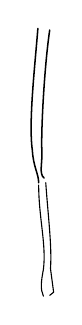
\begin{tikzpicture}[x=1mm,y=1mm,baseline=(current bounding box.center),line cap=round,line join=round]
\draw[line width=0.55pt] (0,34) .. controls (-0.4,29) and (-1.2,22) .. (-0.7,18.5) .. controls (-0.6,16.5) and (0.1,15.5) .. (0.1,14.4);
\draw[line width=0.40pt] (0.1,14.1) .. controls (0.1,10) and (1.1,6.5) .. (0.7,3.4) .. controls (0.4,1.8) and (0.3,0.9) .. (0.7,0);
\draw[line width=0.55pt] (1.5,33.8) .. controls (0.8,29) and (0.4,21) .. (0.5,18.5) .. controls (0.6,16.9) and (0.1,15.5) .. (0.8,15.0);
\draw[line width=0.40pt] (1.0,14.4) .. controls (1.3,10.1) and (1.8,6.3) .. (1.6,3.5) -- (2.0,0.5) -- (1.5,0.1);
\end{tikzpicture}}}}

(On l'a établi tt au moins dans le cas
\(\Gamma=\Gamma^0\), il faudrait revenir sur le cas général,
je pense que ça reste vrai tel quel, à vérifier\ldots)
\LMsourceMark{M005179}{\margin{\figure{[Un trait vertical à gauche des deux lignes
« je pense \ldots{} vérifier\ldots) ».]}}}
De plus, on vit apparaître une \uuline{structure supplémentaire}
sur le groupe \(\mathcal E\)
[qui dans le cas anabélien s'identifie à un sous-groupe de
\(\operatorname{Aut}(\pi)\)], à savoir une application
\[
\mu_{\mathcal E}:
\text{éléments }\var{\inserted{u}}{\LMadded{u}}{insertion}{140-2-s155-I005}\text{ d'ordre fini de }\mathcal E
\longrightarrow T\otimes\mathbb Q/\mathbb Z,
\]
\LMsourceMark{M005180}{\unsure{obtenue}} en notant que si \(u\in\mathcal E\) est d'ordre fini
\(n\), \LMsourceMark{M005181}{\unsure{d'où}} \(\mathbb Z/n\mathbb Z\lhook\joinrel\xrightarrow[i]{}
\mathcal E\), \LMsourceMark{M005182}{\unsure{on a|i.e.}} \(\operatorname{Im}i\cap\pi=(1)\)
(\(\pi\) n'a pas d'éléments de torsion), donc
\(\mathbb Z/n\mathbb Z\hookrightarrow\Gamma\), \LMsourceMark{M005183}{\unsure{d'où|d'un}} sous-groupe
\(\Gamma_1\subset\Gamma\) (i.e. l'image de
\LMsourceMark{M005184}{\margin{\uline{NB} Pour un \(u\) d'ordre fini de \(\mathcal E\),
on doit \LMsourceMark{M005185}{\unsure{savoir|avoir}}, si \(u\notin\mathcal E^0\),
que \(u\) \LMsourceMark{M005186}{\unsure{est}} d'ordre \(2\) exactement,
\LMsourceMark{M005187}{\illegible{5}} pour \LMsourceMark{M005188}{\unsure{définir}} \(\mu(u)\)!}}

\LMsourceMark{M005189}{\margin{154}}

\LMflushnotes\LMflushpages
\ifnum\LMform=1
\begin{LMapparatus}
\LMentry{140-2-s155-D001}{suppression}{\deleted{\LMsourceMark{M005190}{\unsure{avec op. fidèle de \(\Gamma\)}}}
}{\emph{\LMomittedlabel}}{Passage biffé dans le manuscrit : la suppression suit l'état final de l'auteur; les doutes de lecture restent signalés.}{}
\LMentry{140-2-s155-I001}{insertion}{\inserted{\deleted{\LMsourceMark{M005191}{\unsure{pour}}} (Pour les formuler, on va supposer l'action de
\(\Gamma\) fidèle) :}
}{\emph{\LMinsertedlabel}}{Ajout explicite de l'auteur : intégré à l'endroit indiqué par la transcription, sans modifier sa lecture.}{}
\LMentry{140-2-s155-D002}{suppression}{\deleted{\LMsourceMark{M005192}{\unsure{pour}}}
}{\emph{\LMomittedlabel}}{Passage biffé dans le manuscrit : la suppression suit l'état final de l'auteur; les doutes de lecture restent signalés.}{}
\LMentry{140-2-s155-I002}{insertion}{\inserted{cyclique (si \(\Gamma'=\Gamma'{}^0\)) ou}
}{\emph{\LMinsertedlabel}}{Ajout explicite de l'auteur : intégré à l'endroit indiqué par la transcription, sans modifier sa lecture.}{}
\LMentry{140-2-s155-D003}{suppression}{\deleted{\LMsourceMark{M005193}{\illegible{1}}}
}{\emph{\LMomittedlabel}}{Passage biffé dans le manuscrit : la suppression suit l'état final de l'auteur; les doutes de lecture restent signalés.}{}
\LMentry{140-2-s155-I003}{insertion}{\inserted{(si \(\Gamma'\ne\Gamma'{}^0\))}
}{\emph{\LMinsertedlabel}}{Ajout explicite de l'auteur : intégré à l'endroit indiqué par la transcription, sans modifier sa lecture.}{}
\LMentry{140-2-s155-I004}{insertion}{\inserted{section}
}{\emph{\LMinsertedlabel}}{Ajout explicite de l'auteur : intégré à l'endroit indiqué par la transcription, sans modifier sa lecture.}{}
\LMentry{140-2-s155-I005}{insertion}{\(\inserted{u}\)
}{\emph{\LMinsertedlabel}}{Ajout explicite de l'auteur : intégré à l'endroit indiqué par la transcription, sans modifier sa lecture.}{}
\end{LMapparatus}
\fi
\ifnum\LMform=2
\par\smallskip\begingroup\footnotesize\Needspace{4\baselineskip}\csname @beginparpenalty\endcsname=10000\relax\noindent\textcolor{gray}{\rule{.2\linewidth}{.35pt}}\par\nobreak
\noindent\textit{\LMdoubtheading.}\par\nobreak
\LMcarryover{140-2-s155-D001}{\LMsourceMark{M005194}{\unsure{avec op. fidèle de \(\Gamma\)}}
}
\LMcarryover{140-2-s155-D002}{\LMsourceMark{M005195}{\unsure{pour}}
}
\LMcarryover{140-2-s155-D003}{\LMsourceMark{M005196}{\illegible{1}}
}
\par\endgroup\smallskip
\fi

\LMsourceMark{M005197}{\scanpage{156}}

\(\LMsourceMark{M005198}{\unsure{u}}\) dans \(\Gamma\) a \(\overline{\mathrm m}\) ordre \(n\)),
et le relèvement \(\Gamma_1\hookrightarrow\mathcal E\) définit un
\(x\in U^{\Gamma_1}\), \var{\deleted{tel que}}{}{deletion}{140-2-s156-D001} et \(u_1\) opérant sur \(U\)
en laissant fixe \(x\) correspond donc au voisinage de \(x\) à un
``multiplicateur'', qui (pour une orientation locale choisie) est une
racine primitive \LMsourceMark{M005199}{\unsure{\(n\).ième}} de \(1\) i.e. un élément de
\(\mathbb Z/n\mathbb Z\), et qui pour orientation changeante
s'interprète intrinsèquement comme élément de
\(T\otimes\mathbb Z/n\mathbb Z
\subset T\otimes\mathbb Q/\mathbb Z\).

L'application \(\mu\) satisfait les conditions évidentes
\[
\begin{gathered}
\left\{
\begin{aligned}
\mu(\alpha u\alpha^{-1})&=\mu(u) &&\text{si }\alpha\in\pi\\
\mu(u^n)&=n\mu(u) &&\text{si }n\in\mathbb Z
\end{aligned}
\right.\\
\text{ordre }\mu(u)=\text{ordre de }u
\end{gathered}
\]
J'ignore si cette application \(\mu\) \var{\deleted{est}}{}{deletion}{140-2-s156-D002}
\var{\inserted{peut se}}{\LMadded{peut se}}{insertion}{140-2-s156-I001} définir intrinsèquement en termes de l'extension
\(\mathcal E\), ou si au contraire il peut exister deux extensions
\var{\deleted{\LMsourceMark{M005200}{\unsure{iso}}}}{\LMsourceMark{M005201}{\LMcancelledDoubts{\LMsourceMark{M005202}{\unsure{iso}}}}}{deletion}{140-2-s156-D003} \(\mathcal E,\mathcal E'\) de \(\Gamma\) par \(\pi\),
définies par des situations géométriques, de \(\Gamma\) opérant sur
\(U\) resp. \(U'\), et un isom. d'extensions
\(\mathcal E\longrightarrow\mathcal E'\) qui ne soit compatible avec
les fonctions \(\mu,\mu'\).
Le cas non trivial le plus simple à regarder est le cas

\LMsourceMark{M005203}{\margin{155}}

\LMflushnotes\LMflushpages
\ifnum\LMform=1
\begin{LMapparatus}
\LMentry{140-2-s156-D001}{suppression}{\deleted{tel que}
}{\emph{\LMomittedlabel}}{Passage biffé dans le manuscrit : la suppression suit l'état final de l'auteur; les doutes de lecture restent signalés.}{}
\LMentry{140-2-s156-D002}{suppression}{\deleted{est}
}{\emph{\LMomittedlabel}}{Passage biffé dans le manuscrit : la suppression suit l'état final de l'auteur; les doutes de lecture restent signalés.}{}
\LMentry{140-2-s156-I001}{insertion}{\inserted{peut se}
}{\emph{\LMinsertedlabel}}{Ajout explicite de l'auteur : intégré à l'endroit indiqué par la transcription, sans modifier sa lecture.}{}
\LMentry{140-2-s156-D003}{suppression}{\deleted{\LMsourceMark{M005204}{\unsure{iso}}}
}{\emph{\LMomittedlabel}}{Passage biffé dans le manuscrit : la suppression suit l'état final de l'auteur; les doutes de lecture restent signalés.}{}
\end{LMapparatus}
\fi
\ifnum\LMform=2
\par\smallskip\begingroup\footnotesize\Needspace{4\baselineskip}\csname @beginparpenalty\endcsname=10000\relax\noindent\textcolor{gray}{\rule{.2\linewidth}{.35pt}}\par\nobreak
\noindent\textit{\LMdoubtheading.}\par\nobreak
\LMcarryover{140-2-s156-D003}{\LMsourceMark{M005205}{\unsure{iso}}
}
\par\endgroup\smallskip
\fi

\LMsourceMark{M005206}{\scanpage{157}}
\LMsourceMark{M005207}{\mspage{78}}

abélien (où \(\pi\simeq\mathbb Z\)
\var{\inserted{\deleted{\LMsourceMark{M005208}{\illegible{1}}} \((\operatorname{card}I=2)\)}}{\LMadded{\var{\deleted{\LMsourceMark{M005209}{\illegible{1}}}}{\LMsourceMark{M005210}{\LMcancelledDoubts{\LMsourceMark{M005211}{\illegible{1}}}}}{deletion}{140-2-s157-D001} \((\operatorname{card}I=2)\)}}{insertion}{140-2-s157-I001}
ou \(\pi\simeq\mathbb Z^2\) (\var{\deleted{\LMsourceMark{M005212}{\unsure{card}}}}{\LMsourceMark{M005213}{\LMcancelledDoubts{\LMsourceMark{M005214}{\unsure{card}}}}}{deletion}{140-2-s157-D002} \(I=\varnothing\))),
Dans le \var{\inserted{premier}}{\LMadded{premier}}{insertion}{140-2-s157-I002} cas
\var{\deleted{d'une extension}}{}{deletion}{140-2-s157-D003} \(\pi\simeq\mathbb Z\), \LMsourceMark{M005215}{\unsure{on|\var{\deleted{les}}{\LMsourceMark{M005216}{\LMuncertaindeletion{140-2-s157-D004}}}{deletion}{140-2-s157-D004}}}
\var{\inserted{doit avoir (pour avoir une action fidèle de
\(\Gamma=\Gamma^0\))}}{\LMadded{doit avoir (pour avoir une action fidèle de
\(\Gamma=\Gamma^0\))}}{insertion}{140-2-s157-I003}
\var{\deleted{extensions \LMsourceMark{M005217}{\illegible{1}}}}{\LMsourceMark{M005218}{\LMcancelledDoubts{\LMsourceMark{M005219}{\illegible{1}}}}}{deletion}{140-2-s157-D005}
\(\Gamma^0\) cyclique, \(\mathcal E\simeq\mathbb Z\),
il n'y a pas d'élément d'ordre fini dans \(\mathcal E\) sauf
\(\LMsourceMark{M005220}{\unsure{1|e}}\), donc la question ne se pose pas.
Le cas \(\pi\simeq\mathbb Z^2\) est plus intéressant,
\var{\deleted{\LMsourceMark{M005221}{\unsure{et peut se reformuler}}}}{\LMsourceMark{M005222}{\LMcancelledDoubts{\LMsourceMark{M005223}{\unsure{et peut se reformuler}}}}}{deletion}{140-2-s157-D006}

Si \(\pi\) est un \(\mathbb Z\)-module libre de
\var{\deleted{\LMsourceMark{M005224}{\unsure{t.f.}}}}{\LMsourceMark{M005225}{\LMcancelledDoubts{\LMsourceMark{M005226}{\unsure{t.f.}}}}}{deletion}{140-2-s157-D007}\var{\inserted{\LMsourceMark{M005227}{\unsure{rg \(n\)}}}}{\LMadded{\LMsourceMark{M005228}{\unsure{rg \(n\)}}}}{insertion}{140-2-s157-I004}, on a une suite exacte
\diagram{
\begin{tikzcd}[ampersand replacement=\&,column sep=small,row sep=small]
0 \arrow[r] \& \pi \arrow[r] \& \pi\otimes_{\mathbb Z}\mathbb R
\arrow[r] \& X_0(\pi) \arrow[r] \arrow[d,dash] \& 0\\
\& \& \& \substack{\text{Tore de dim}\\ n\text{ associé à }\pi} \&
\end{tikzcd}
}
et si \(\Gamma\) opère sur \(\pi\), la suite exacte de cohomologie
(compte tenu de \(H^i(\Gamma,\pi\otimes_{\mathbb Z}\mathbb R)=0\)
pour \(i>0\)) donne
\diagram{
\begin{tikzcd}[ampersand replacement=\&,column sep=large,row sep=small]
H^2(\Gamma,\pi) \& H^1(\Gamma,X_0(\pi)) \arrow[l,"\sim" {anchor=south}]\\
\substack{\text{\LMsourceMark{M005229}{\unsure{classe d'extension|classes d'extensions}}}\\
\text{de }\Gamma\text{ par }\pi}
\&
\substack{\text{classes de}\\X_0(\pi)\text{ torseurs,}\\
\text{avec op. de }\Gamma\text{ dessus}\\
\text{compatible avec son}\\\text{action sur }X_0(\pi)}
\end{tikzcd}
}

donc la donnée d'une extension \(\mathcal E\) de \(\Gamma\) par \(\pi\)
revient essentiellement à celle d'un
\LMsourceMark{M005230}{\unsure{\(\Gamma\)-\(X_0(\pi)\)-torseur}} \(X\)
(\(n\)-tore inhomogène sur lequel \(\Gamma\) opère --- donc il opère
sur son groupe des translations \(X_0\), donc sur
\(\pi=\pi_1(X_0,0)\)\ldots).
S'il était vrai \var{\inserted{pour \(n=2\)}}{\LMadded{pour \(n=2\)}}{insertion}{140-2-s157-I005} que tte opération

\LMsourceMark{M005231}{\margin{156}}

\LMflushnotes\LMflushpages
\ifnum\LMform=1
\begin{LMapparatus}
\LMentry{140-2-s157-I001}{insertion}{\inserted{\deleted{\LMsourceMark{M005232}{\illegible{1}}} \((\operatorname{card}I=2)\)}
}{\emph{\LMinsertedlabel}}{Ajout explicite de l'auteur : intégré à l'endroit indiqué par la transcription, sans modifier sa lecture.}{}
\LMentry{140-2-s157-D001}{suppression}{\deleted{\LMsourceMark{M005233}{\illegible{1}}}
}{\emph{\LMomittedlabel}}{Passage biffé dans le manuscrit : la suppression suit l'état final de l'auteur; les doutes de lecture restent signalés.}{}
\LMentry{140-2-s157-D002}{suppression}{\deleted{\LMsourceMark{M005234}{\unsure{card}}}
}{\emph{\LMomittedlabel}}{Passage biffé dans le manuscrit : la suppression suit l'état final de l'auteur; les doutes de lecture restent signalés.}{}
\LMentry{140-2-s157-I002}{insertion}{\inserted{premier}
}{\emph{\LMinsertedlabel}}{Ajout explicite de l'auteur : intégré à l'endroit indiqué par la transcription, sans modifier sa lecture.}{}
\LMentry{140-2-s157-D003}{suppression}{\deleted{d'une extension}
}{\emph{\LMomittedlabel}}{Passage biffé dans le manuscrit : la suppression suit l'état final de l'auteur; les doutes de lecture restent signalés.}{}
\LMentry{140-2-s157-D004}{suppression}{\LMsourceMark{M005235}{\LMdoubtcopy{\deleted{les}}}
}{\emph{\LMomittedlabel}}{Passage biffé dans le manuscrit : la suppression suit l'état final de l'auteur; les doutes de lecture restent signalés.}{}
\LMentry{140-2-s157-I003}{insertion}{\inserted{doit avoir (pour avoir une action fidèle de
\(\Gamma=\Gamma^0\))}
}{\emph{\LMinsertedlabel}}{Ajout explicite de l'auteur : intégré à l'endroit indiqué par la transcription, sans modifier sa lecture.}{}
\LMentry{140-2-s157-D005}{suppression}{\deleted{extensions \LMsourceMark{M005236}{\illegible{1}}}
}{\emph{\LMomittedlabel}}{Passage biffé dans le manuscrit : la suppression suit l'état final de l'auteur; les doutes de lecture restent signalés.}{}
\LMentry{140-2-s157-D006}{suppression}{\deleted{\LMsourceMark{M005237}{\unsure{et peut se reformuler}}}
}{\emph{\LMomittedlabel}}{Passage biffé dans le manuscrit : la suppression suit l'état final de l'auteur; les doutes de lecture restent signalés.}{}
\LMentry{140-2-s157-D007}{suppression}{\deleted{\LMsourceMark{M005238}{\unsure{t.f.}}}
}{\emph{\LMomittedlabel}}{Passage biffé dans le manuscrit : la suppression suit l'état final de l'auteur; les doutes de lecture restent signalés.}{}
\LMentry{140-2-s157-I004}{insertion}{\inserted{\LMsourceMark{M005239}{\unsure{rg \(n\)}}}
}{\emph{\LMinsertedlabel}}{Ajout explicite de l'auteur : intégré à l'endroit indiqué par la transcription, sans modifier sa lecture.}{}
\LMentry{140-2-s157-I005}{insertion}{\inserted{pour \(n=2\)}
}{\emph{\LMinsertedlabel}}{Ajout explicite de l'auteur : intégré à l'endroit indiqué par la transcription, sans modifier sa lecture.}{}
\end{LMapparatus}
\fi
\ifnum\LMform=2
\par\smallskip\begingroup\footnotesize\Needspace{4\baselineskip}\csname @beginparpenalty\endcsname=10000\relax\noindent\textcolor{gray}{\rule{.2\linewidth}{.35pt}}\par\nobreak
\noindent\textit{\LMdoubtheading.}\par\nobreak
\LMcarryover{140-2-s157-D001}{\LMsourceMark{M005240}{\illegible{1}}
}
\LMcarryover{140-2-s157-D002}{\LMsourceMark{M005241}{\unsure{card}}
}
\LMcarryover{140-2-s157-D004}{\LMsourceMark{M005242}{\LMdoubtcopy{les}}
}
\LMcarryover{140-2-s157-D005}{\LMsourceMark{M005243}{\illegible{1}}
}
\LMcarryover{140-2-s157-D006}{\LMsourceMark{M005244}{\unsure{et peut se reformuler}}
}
\LMcarryover{140-2-s157-D007}{\LMsourceMark{M005245}{\unsure{t.f.}}
}
\par\endgroup\smallskip
\fi

\LMsourceMark{M005246}{\scanpage{158}}

de \(\Gamma\) sur une surface torique \((\simeq S^1\times S^1)\)
est isomorphe à une telle action standard, alors le caractère
intrinsèque de l'application \(\mu\) dans ce cas serait établi
--- ce qui ne \LMsourceMark{M005247}{\unsure{rendrait}} pas inintéressant pour autant le calcul
de \(\mu\), qui prend ses valeurs dans
\(T\otimes\mathbb Q/\mathbb Z\), où ici
\[
T\simeq\bigwedge\nolimits_{\mathbb Z}^{2}\pi
\quad
(\text{\LMsourceMark{M005248}{\unsure{dual|dim.\ 2}} de }H^2(\pi,\mathbb Z)\simeq
\bigwedge\nolimits^{2}
\underbrace{H^1(\pi,\mathbb Z)}_{
\substack{\LMsourceMark{M005249}{\unsure{\downarrow|\simeq}}\\ \pi^\vee}}).
\]

La question revient à celle-ci : On a une extension \uline{scindée}
d'un \var{\deleted{\LMsourceMark{M005250}{\unsure{groupe}}}}{\LMsourceMark{M005251}{\LMcancelledDoubts{\LMsourceMark{M005252}{\unsure{groupe}}}}}{deletion}{140-2-s158-D001}\var{\inserted{\LMsourceMark{M005253}{\unsure{groupe}}}}{\LMadded{\LMsourceMark{M005254}{\unsure{groupe}}}}{insertion}{140-2-s158-I001} cyclique
\(\mathbb Z/n\mathbb Z\) de générateur \(u\) par \(\pi\)
--- décrite donc entièrement par un autom.
\var{\deleted{d'ordre}}{}{deletion}{140-2-s158-D002} \(\LMsourceMark{M005255}{\unsure{\theta}}\) de \(\pi\) tel que
\(\theta^n=\operatorname{id}_\pi\)), décrire \LMsourceMark{M005256}{\unsure{en}} termes de
ceci un élément de \(T\otimes\mathbb Q/\mathbb Z\).

Réponse : la situation géométrique \LMsourceMark{M005257}{\unsure{standard|st. dont}}
correspond à \(X=X_0(\pi)\), avec \(0\) comme pt fixe sous \(\Gamma\).
Si \(u\) renverse l'orientation, il est d'ordre \LMsourceMark{M005258}{\unsure{\(1\) ou|i.e.}} \(2\),
il n'y a pas de Pb, sinon c'est \var{\deleted{dans}}{}{deletion}{140-2-s158-D003} en
\(\pi\otimes_{\mathbb Z}\mathbb R\) une rotation autour de \(0\)
(d'ordre \(2,3,4\) ou \(6\)) qui se repère bien par un élément
de \var{\deleted{\LMsourceMark{M005259}{\illegible{1}}}}{\LMsourceMark{M005260}{\LMcancelledDoubts{\LMsourceMark{M005261}{\illegible{1}}}}}{deletion}{140-2-s158-D004} \(T\otimes\mathbb Z/\nu\mathbb Z\)
(si \(\nu\) est \LMsourceMark{M005262}{\unsure{d'ordre|l'ordre}}).
C'est aussi (si on identifie
\(T\otimes\mathbb Z/\nu\mathbb Z\) à
\(\mu_\nu(\mathbb C^*)\), en supposant
\(T\simeq\mathbb Z\) donné
i.e. \(\pi\) orienté i.e. \(X_0(\pi)=\LMsourceMark{M005263}{\unsure{X}}\)
orienté) \uline{une} des deux

\LMsourceMark{M005264}{\margin{157}}

\LMflushnotes\LMflushpages
\ifnum\LMform=1
\begin{LMapparatus}
\LMentry{140-2-s158-D001}{suppression}{\deleted{\LMsourceMark{M005265}{\unsure{groupe}}}
}{\emph{\LMomittedlabel}}{Passage biffé dans le manuscrit : la suppression suit l'état final de l'auteur; les doutes de lecture restent signalés.}{}
\LMentry{140-2-s158-I001}{insertion}{\inserted{\LMsourceMark{M005266}{\unsure{groupe}}}
}{\emph{\LMinsertedlabel}}{Ajout explicite de l'auteur : intégré à l'endroit indiqué par la transcription, sans modifier sa lecture.}{}
\LMentry{140-2-s158-D002}{suppression}{\deleted{d'ordre}
}{\emph{\LMomittedlabel}}{Passage biffé dans le manuscrit : la suppression suit l'état final de l'auteur; les doutes de lecture restent signalés.}{}
\LMentry{140-2-s158-D003}{suppression}{\deleted{dans}
}{\emph{\LMomittedlabel}}{Passage biffé dans le manuscrit : la suppression suit l'état final de l'auteur; les doutes de lecture restent signalés.}{}
\LMentry{140-2-s158-D004}{suppression}{\deleted{\LMsourceMark{M005267}{\illegible{1}}}
}{\emph{\LMomittedlabel}}{Passage biffé dans le manuscrit : la suppression suit l'état final de l'auteur; les doutes de lecture restent signalés.}{}
\end{LMapparatus}
\fi
\ifnum\LMform=2
\par\smallskip\begingroup\footnotesize\Needspace{4\baselineskip}\csname @beginparpenalty\endcsname=10000\relax\noindent\textcolor{gray}{\rule{.2\linewidth}{.35pt}}\par\nobreak
\noindent\textit{\LMdoubtheading.}\par\nobreak
\LMcarryover{140-2-s158-D001}{\LMsourceMark{M005268}{\unsure{groupe}}
}
\LMcarryover{140-2-s158-D004}{\LMsourceMark{M005269}{\illegible{1}}
}
\par\endgroup\smallskip
\fi

\LMsourceMark{M005270}{\scanpage{159}}
\LMsourceMark{M005271}{\mspage{79}}

valeurs propres de \(u\otimes_{\mathbb Z}\mathbb C\)
(autom du vectoriel sur \(\mathbb C\) de dim \(2\)
\(\pi\otimes_{\mathbb Z}\mathbb C\)).

Ceci nous montre, dans le cas de la géom Alg sur corps alg clos
\(\Omega\), que si \(X=X_0\) est une courbe elliptique
\(u\) un autom d'ordre fini, on a comme description
paradigmatique non \uline{seult}
\(\pi=\pi_1(X,0)\)
\var{\inserted{(\(\widehat{\mathbb Z}\)-module libre de rg \(2\)),}}{\LMadded{(\(\widehat{\mathbb Z}\)-module libre de rg \(2\)),}}{insertion}{140-2-s159-I001}
(et l'action de \(u\) sur \(\pi\)), mais comme structure
\uline{supplémentaire} l'une des deux solutions \uline{dans \(\Omega\)}
de l'équation caractéristique de \(u\) (à coefficients entiers)
\[
T^2+aT+b=0
\qquad (a=-\operatorname{Tr}u,\ b=\LMsourceMark{M005272}{\unsure{\det u}}).
\]

Il est clair que cette structure supplémentaire ne peut se déduire
de la seule connaissance de l'action de \(u\) sur \(\pi\).
\LMsourceMark{M005273}{\margin{\figure{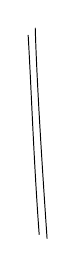
\begin{tikzpicture}[x=1mm,y=1mm,baseline=(current bounding box.center),line cap=round]
\draw[line width=0.35pt] (0,25.8) .. controls (0.4,19) and (0.7,10) .. (1.4,0.5);
\draw[line width=0.35pt] (0.9,26.7) .. controls (1.1,19.7) and (1.8,8.8) .. (2.4,0);
\end{tikzpicture}}
pour \(\LMsourceMark{M005274}{\unsure{\Omega}}=\mathbb C\)
\LMsourceMark{M005275}{\illegible{2}} \LMsourceMark{M005276}{\unsure{revient à}}
\LMsourceMark{M005277}{\illegible{1}} \uline{\LMsourceMark{M005278}{\unsure{orientation|orientations}}} de
\LMsourceMark{M005279}{\illegible{1}}}}
Mais il reste la question si cette \var{\deleted{\LMsourceMark{M005280}{\unsure{dernière}}}}{\LMsourceMark{M005281}{\LMcancelledDoubts{\LMsourceMark{M005282}{\unsure{dernière}}}}}{deletion}{140-2-s159-D001}
\var{\inserted{\LMsourceMark{M005283}{\unsure{\(\mu(u)\in\mu_n^*(\Omega)\)}}}}{\LMadded{\LMsourceMark{M005284}{\unsure{\(\mu(u)\in\mu_n^*(\Omega)\)}}}}{insertion}{140-2-s159-I002}
peut se déduire de la connaissance au moins de l'action
\var{\inserted{extérieure}}{\LMadded{extérieure}}{insertion}{140-2-s159-I003} de \(u\) sur le groupe
``avec \(1\) lacet'' correspondant à la situation géométrique
--- i.e. un autom \var{\inserted{ext.}}{\LMadded{ext.}}{insertion}{140-2-s159-I004}
\var{\deleted{\LMsourceMark{M005285}{\illegible{2}}}}{\LMsourceMark{M005286}{\LMcancelledDoubts{\LMsourceMark{M005287}{\illegible{2}}}}}{deletion}{140-2-s159-D002} d'ordre \(n\) \LMsourceMark{M005288}{\unsure{d'}} un tel groupe
(ou si là encore il faut la considérer décidément comme une donnée
supplémentaire).
\LMsourceMark{M005289}{\margin{oui, il le peut, grâce à la considération des
``sous-groupes \LMsourceMark{M005290}{\illegible{2}} de \(\mathcal E\)''
\LMsourceMark{M005291}{\illegible{2}} qui définissent des extensions
\diagram{\begin{tikzcd}[ampersand replacement=\&,row sep=2.5em,column sep=2em]
\LMsourceMark{M005292}{\unsure{1}} \arrow[r] \& T \arrow[r] \arrow[dr,dotted,no head,"\LMsourceMark{M005293}{\unsure{n_i\,\mathrm{id}_T}}"'] \& \mathcal E_i \arrow[r] \arrow[d,phantom,"\simeq"{description,rotate=90}] \& \Gamma_i \arrow[r] \& 1 \\
\& \& T \& \&
\end{tikzcd}}
d'où \(\LMsourceMark{M005294}{\unsure{\Gamma_i\simeq T/n_iT}}\)
\LMsourceMark{M005295}{\illegible{2}}}}
Mais s'il en était bien ainsi, cela impliquerait d'autre part que la
construction de \LMsourceMark{M005296}{\unsure{\(u\in\) groupe|ces groupes}} à

\LMsourceMark{M005297}{\margin{158}}

\LMflushnotes\LMflushpages
\ifnum\LMform=1
\begin{LMapparatus}
\LMentry{140-2-s159-I001}{insertion}{\inserted{(\(\widehat{\mathbb Z}\)-module libre de rg \(2\)),}
}{\emph{\LMinsertedlabel}}{Ajout explicite de l'auteur : intégré à l'endroit indiqué par la transcription, sans modifier sa lecture.}{}
\LMentry{140-2-s159-D001}{suppression}{\deleted{\LMsourceMark{M005298}{\unsure{dernière}}}
}{\emph{\LMomittedlabel}}{Passage biffé dans le manuscrit : la suppression suit l'état final de l'auteur; les doutes de lecture restent signalés.}{}
\LMentry{140-2-s159-I002}{insertion}{\inserted{\LMsourceMark{M005299}{\unsure{\(\mu(u)\in\mu_n^*(\Omega)\)}}}
}{\emph{\LMinsertedlabel}}{Ajout explicite de l'auteur : intégré à l'endroit indiqué par la transcription, sans modifier sa lecture.}{}
\LMentry{140-2-s159-I003}{insertion}{\inserted{extérieure}
}{\emph{\LMinsertedlabel}}{Ajout explicite de l'auteur : intégré à l'endroit indiqué par la transcription, sans modifier sa lecture.}{}
\LMentry{140-2-s159-I004}{insertion}{\inserted{ext.}
}{\emph{\LMinsertedlabel}}{Ajout explicite de l'auteur : intégré à l'endroit indiqué par la transcription, sans modifier sa lecture.}{}
\LMentry{140-2-s159-D002}{suppression}{\deleted{\LMsourceMark{M005300}{\illegible{2}}}
}{\emph{\LMomittedlabel}}{Passage biffé dans le manuscrit : la suppression suit l'état final de l'auteur; les doutes de lecture restent signalés.}{}
\end{LMapparatus}
\fi
\ifnum\LMform=2
\par\smallskip\begingroup\footnotesize\Needspace{4\baselineskip}\csname @beginparpenalty\endcsname=10000\relax\noindent\textcolor{gray}{\rule{.2\linewidth}{.35pt}}\par\nobreak
\noindent\textit{\LMdoubtheading.}\par\nobreak
\LMcarryover{140-2-s159-D001}{\LMsourceMark{M005301}{\unsure{dernière}}
}
\LMcarryover{140-2-s159-D002}{\LMsourceMark{M005302}{\illegible{2}}
}
\par\endgroup\smallskip
\fi

\LMsourceMark{M005303}{\scanpage{160}}

(1) lacet(s), avec l'op. de \(\Gamma\) dessus, ne peut se faire non
plus à l'aide de la seule \var{\deleted{\LMsourceMark{M005304}{\illegible{2}}}}{\LMsourceMark{M005305}{\LMcancelledDoubts{\LMsourceMark{M005306}{\illegible{2}}}}}{deletion}{140-2-s160-D001}
connaissance de l'action de \(\Gamma\) (\(=\mathbb Z/n\mathbb Z\))
sur \(\pi\).
C'est cette question de ``forage de trous'' qu'il faut donc en fin de
compte, à la fin des fins, attaquer !

Quant à la question de savoir si
\var{\deleted{\LMsourceMark{M005307}{\illegible{1}}}}{\LMsourceMark{M005308}{\LMcancelledDoubts{\LMsourceMark{M005309}{\illegible{1}}}}}{deletion}{140-2-s160-D002}\var{\inserted{dans}}{\LMadded{dans}}{insertion}{140-2-s160-I001}
\var{\deleted{\LMsourceMark{M005310}{\illegible{1}}}}{\LMsourceMark{M005311}{\LMcancelledDoubts{\LMsourceMark{M005312}{\illegible{1}}}}}{deletion}{140-2-s160-D003} le \uline{cas anabélien},
l'application
\[
\mu:\underbrace{{}_\infty\mathcal E}_{
\substack{\text{\LMsourceMark{M005313}{\unsure{ens des}}}\\
\text{\LMsourceMark{M005314}{\unsure{élémts}}}\\
\text{d'ordre fini de }\mathcal E}}
\longrightarrow T\otimes\mathbb Q/\mathbb Z)
\]
est déductible de l'action de \(\Gamma\) sur \(\pi\)
[si elle est fidèle, \(\mathcal E\) s'identifie donc à un ss-groupe
de \(\operatorname{Autext}_{\LMsourceMark{M005315}{\unsure{\ell|l}}}(\pi)\)
et on peut se demander si \(\mu\) n'est pas
\var{\inserted{alors}}{\LMadded{alors}}{insertion}{140-2-s160-I002} définissable sur cet tt entier],
ou \LMsourceMark{M005316}{\unsure{c'est|si c'est}} une donnée supplémentaire dont il faut disposer pour
reconstituer la situation géom. --- la question reste entière.
\LMsourceMark{M005317}{\margin{cela semble bien \LMsourceMark{M005318}{\unsure{ainsi}}, compte tenu
\LMsourceMark{M005319}{\illegible{1}} que pour \(\Gamma\) \uline{résoluble},
\LMsourceMark{M005320}{\illegible{3}}, on sait \LMsourceMark{M005321}{\illegible{1}}
que tte action \var{\deleted{\LMsourceMark{M005322}{\illegible{1}}}}{\LMsourceMark{M005323}{\LMcancelledDoubts{\LMsourceMark{M005324}{\illegible{1}}}}}{deletion}{140-2-s160-D004} de \(\Gamma\) sur \(\pi\)
\LMsourceMark{M005325}{\illegible{3}} \LMsourceMark{M005326}{\unsure{réaliser géométriquement}}}}

\textcircled{16}\quad
\uuline{Bouchage et forage de trous:}
\uline{Préliminaires} \LMsourceMark{M005327}{\unsure{toposiques}} généraux

Considérons une situation
\diagram{
\begin{tikzcd}[ampersand replacement=\&]
B_{D^*} \arrow[r] \& B_U
\end{tikzcd}
}
(de topos multigaloisiens)
\LMsourceMark{M005328}{\margin{NB. une telle situation
\var{\inserted{toposique \LMsourceMark{M005329}{\unsure{décrit}}}}{\LMadded{toposique \LMsourceMark{M005330}{\unsure{décrit}}}}{insertion}{140-2-s160-I003} \(2\)-fidlt les situations topologiques \((X,S)\),
ou \(U\), pourvu qu'aucune composante irréductible de \(U\)
ne soit \(\simeq S^2\) ---}}

\LMsourceMark{M005331}{\margin{159}}

\LMflushnotes\LMflushpages
\ifnum\LMform=1
\begin{LMapparatus}
\LMentry{140-2-s160-D001}{suppression}{\deleted{\LMsourceMark{M005332}{\illegible{2}}}
}{\emph{\LMomittedlabel}}{Passage biffé dans le manuscrit : la suppression suit l'état final de l'auteur; les doutes de lecture restent signalés.}{}
\LMentry{140-2-s160-D002}{suppression}{\deleted{\LMsourceMark{M005333}{\illegible{1}}}
}{\emph{\LMomittedlabel}}{Passage biffé dans le manuscrit : la suppression suit l'état final de l'auteur; les doutes de lecture restent signalés.}{}
\LMentry{140-2-s160-I001}{insertion}{\inserted{dans}
}{\emph{\LMinsertedlabel}}{Ajout explicite de l'auteur : intégré à l'endroit indiqué par la transcription, sans modifier sa lecture.}{}
\LMentry{140-2-s160-D003}{suppression}{\deleted{\LMsourceMark{M005334}{\illegible{1}}}
}{\emph{\LMomittedlabel}}{Passage biffé dans le manuscrit : la suppression suit l'état final de l'auteur; les doutes de lecture restent signalés.}{}
\LMentry{140-2-s160-I002}{insertion}{\inserted{alors}
}{\emph{\LMinsertedlabel}}{Ajout explicite de l'auteur : intégré à l'endroit indiqué par la transcription, sans modifier sa lecture.}{}
\LMentry{140-2-s160-D004}{suppression}{\deleted{\LMsourceMark{M005335}{\illegible{1}}}
}{\emph{\LMomittedlabel}}{Passage biffé dans le manuscrit : la suppression suit l'état final de l'auteur; les doutes de lecture restent signalés.}{}
\LMentry{140-2-s160-I003}{insertion}{\inserted{toposique \LMsourceMark{M005336}{\unsure{décrit}}}
}{\emph{\LMinsertedlabel}}{Ajout explicite de l'auteur : intégré à l'endroit indiqué par la transcription, sans modifier sa lecture.}{}
\end{LMapparatus}
\fi
\ifnum\LMform=2
\par\smallskip\begingroup\footnotesize\Needspace{4\baselineskip}\csname @beginparpenalty\endcsname=10000\relax\noindent\textcolor{gray}{\rule{.2\linewidth}{.35pt}}\par\nobreak
\noindent\textit{\LMdoubtheading.}\par\nobreak
\LMcarryover{140-2-s160-D001}{\LMsourceMark{M005337}{\illegible{2}}
}
\LMcarryover{140-2-s160-D002}{\LMsourceMark{M005338}{\illegible{1}}
}
\LMcarryover{140-2-s160-D003}{\LMsourceMark{M005339}{\illegible{1}}
}
\LMcarryover{140-2-s160-D004}{\LMsourceMark{M005340}{\illegible{1}}
}
\par\endgroup\smallskip
\fi

% END PACKAGE LM_P016
% BEGIN PACKAGE LM_P017
\ifnum\LMform<2\Needspace{11\baselineskip}\subsection*{Scans 161--170}\fi
\LMsourceMark{M005341}{\scanpage{161}}
\LMsourceMark{M005342}{\mspage{80}}
% Lignes 1--5 (continuation de la note marginale de la page précédente).
\LMsourceMark{M005343}{\illegible{2}}, et \LMsourceMark{M005344}{\unsure{au}} \var{\deleted{\LMsourceMark{M005345}{\unsure{le}}}}{\LMsourceMark{M005346}{\LMcancelledDoubts{\LMsourceMark{M005347}{\unsure{le}}}}}{deletion}{140-2-s161-D001} fait qu'elles restent \var{\inserted{très}}{\LMadded{très}}{insertion}{140-2-s161-I001} proches du langage \LMsourceMark{M005348}{\unsure{et|\var{\deleted{et}}{\LMsourceMark{M005349}{\LMuncertaindeletion{140-2-s161-D002}}}{deletion}{140-2-s161-D002}}} de l'intuition topologique, elle est supérieure au $p^t$ de vue ``groupes à lacets'', qui correspond à l'appr. du calculatoire plutôt.)

% Lignes 5--16 : grand passage encadré et barré par des traits obliques.
\var{\deleted{, donnons-nous \deleted{une partie sous topos} (\inserted{\LMsourceMark{M005350}{\unsure{néc$^t$.}}}\LMsourceMark{M005351}{\unsure{ouvert}}) $B_{D_1^*}$ de $B_{D^*}$ (correspondant à une partie $I_1$ de $I=\pi_0(B_{D^*})$) de sorte que
\[
 B_{D^*}\simeq B_{D_0^*}\amalg B_{D_1^*}
\]
\LMsourceMark{M005352}{\margin{($D_0^*$ correspond à la partie $I_0=I\setminus I_1$ de $I$)}}
On a une décomposition analogue
\[
 B_D\simeq B_{D_0}\amalg B_{D_1}.
\]
\inserted{\LMsourceMark{M005353}{\unsure{déf.}} $B_{\pi_0(D^*)}=B_S$}
Considérons le topos \LMsourceMark{M005354}{\unsure{$B_U'$}} ``somme amalgamée'' de \deleted{\LMsourceMark{M005355}{\unsure{$B_U$}}}
\diagram{\begin{tikzcd}[ampersand replacement=\&]
 \& B_{D_1^*}\arrow[dl]\arrow[dr] \& \& \\
 B_U \& \& B_D\arrow[r,leftrightarrow,"\LMsourceMark{M005356}{\unsure{\sim}}"] \& B_S
\end{tikzcd}}
}}{\LMsourceMark{M005357}{\LMcancelledDoubts{\LMsourceMark{M005358}{\unsure{néc$^t$.}}\quad \LMsourceMark{M005359}{\unsure{ouvert}}\quad \LMsourceMark{M005360}{\unsure{déf.}}\quad \LMsourceMark{M005361}{\unsure{$B_U'$}}\quad \LMsourceMark{M005362}{\unsure{$B_U$}}\quad \(\LMsourceMark{M005363}{\unsure{\sim}}\)}}}{deletion}{140-2-s161-D003}

% Lignes 17--24.
Je m'aperçois qu'il me faut revenir sur les notations des \var{\deleted{\LMsourceMark{M005364}{\illegible{1}}}}{\LMsourceMark{M005365}{\LMcancelledDoubts{\LMsourceMark{M005366}{\illegible{1}}}}}{deletion}{140-2-s161-D006} \var{\inserted{divers}}{\LMadded{divers}}{insertion}{140-2-s161-I004} topos associés à une telle donnée. Mais je vais me guider sur la situation des n$^\circ$ .-- où on a un schéma régulier \var{\inserted{$X$}}{\LMadded{$X$}}{insertion}{140-2-s161-I005} de dim 1, un sous-schéma fermé \var{\inserted{$S$}}{\LMadded{$S$}}{insertion}{140-2-s161-I006} de dim 0, d'où $U=X-S$ --- dans ce cas \var{\deleted{\LMsourceMark{M005367}{\illegible{2}}}}{\LMsourceMark{M005368}{\LMcancelledDoubts{\LMsourceMark{M005369}{\illegible{2}}}}}{deletion}{140-2-s161-D007} $\LMsourceMark{M005370}{\unsure{S_{\text{ét}}|X_{\text{ét}}}}$ \textcircled{ne} peut se reconstituer à partir de $B_{D^*}$ comme $\LMsourceMark{M005371}{\unsure{B_{\pi_0 B_{D^*}}|B_I}}$
\LMsourceMark{M005372}{\mspage{160}}

\LMflushnotes\LMflushpages
\ifnum\LMform=1
\begin{LMapparatus}
\LMentry{140-2-s161-D001}{suppression}{\deleted{\LMsourceMark{M005373}{\unsure{le}}}
}{\emph{\LMomittedlabel}}{Passage biffé dans le manuscrit : la suppression suit l'état final de l'auteur; les doutes de lecture restent signalés.}{}
\LMentry{140-2-s161-I001}{insertion}{\inserted{très}
}{\emph{\LMinsertedlabel}}{Ajout explicite de l'auteur : intégré à l'endroit indiqué par la transcription, sans modifier sa lecture.}{}
\LMentry{140-2-s161-D002}{suppression}{\LMsourceMark{M005374}{\LMdoubtcopy{\deleted{et}}}
}{\emph{\LMomittedlabel}}{Passage biffé dans le manuscrit : la suppression suit l'état final de l'auteur; les doutes de lecture restent signalés.}{}
\LMentry{140-2-s161-D003}{suppression}{\deleted{, donnons-nous \deleted{une partie sous topos} (\inserted{\LMsourceMark{M005375}{\unsure{néc$^t$.}}}\LMsourceMark{M005376}{\unsure{ouvert}}) $B_{D_1^*}$ de $B_{D^*}$ (correspondant à une partie $I_1$ de $I=\pi_0(B_{D^*})$) de sorte que
\[
 B_{D^*}\simeq B_{D_0^*}\amalg B_{D_1^*}
\]
\LMsourceMark{M005377}{\margin{($D_0^*$ correspond à la partie $I_0=I\setminus I_1$ de $I$)}}
On a une décomposition analogue
\[
 B_D\simeq B_{D_0}\amalg B_{D_1}.
\]
\inserted{\LMsourceMark{M005378}{\unsure{déf.}} $B_{\pi_0(D^*)}=B_S$}
Considérons le topos \LMsourceMark{M005379}{\unsure{$B_U'$}} ``somme amalgamée'' de \deleted{\LMsourceMark{M005380}{\unsure{$B_U$}}}
\diagram{\begin{tikzcd}[ampersand replacement=\&]
 \& B_{D_1^*}\arrow[dl]\arrow[dr] \& \& \\
 B_U \& \& B_D\arrow[r,leftrightarrow,"\LMsourceMark{M005381}{\unsure{\sim}}"] \& B_S
\end{tikzcd}}
}
}{\emph{\LMomittedlabel}}{Passage biffé dans le manuscrit : la suppression suit l'état final de l'auteur; les doutes de lecture restent signalés.}{}
\LMentry{140-2-s161-D006}{suppression}{\deleted{\LMsourceMark{M005382}{\illegible{1}}}
}{\emph{\LMomittedlabel}}{Passage biffé dans le manuscrit : la suppression suit l'état final de l'auteur; les doutes de lecture restent signalés.}{}
\LMentry{140-2-s161-I004}{insertion}{\inserted{divers}
}{\emph{\LMinsertedlabel}}{Ajout explicite de l'auteur : intégré à l'endroit indiqué par la transcription, sans modifier sa lecture.}{}
\LMentry{140-2-s161-I005}{insertion}{\inserted{$X$}
}{\emph{\LMinsertedlabel}}{Ajout explicite de l'auteur : intégré à l'endroit indiqué par la transcription, sans modifier sa lecture.}{}
\LMentry{140-2-s161-I006}{insertion}{\inserted{$S$}
}{\emph{\LMinsertedlabel}}{Ajout explicite de l'auteur : intégré à l'endroit indiqué par la transcription, sans modifier sa lecture.}{}
\LMentry{140-2-s161-D007}{suppression}{\deleted{\LMsourceMark{M005383}{\illegible{2}}}
}{\emph{\LMomittedlabel}}{Passage biffé dans le manuscrit : la suppression suit l'état final de l'auteur; les doutes de lecture restent signalés.}{}
\end{LMapparatus}
\fi
\ifnum\LMform=2
\par\smallskip\begingroup\footnotesize\Needspace{4\baselineskip}\csname @beginparpenalty\endcsname=10000\relax\noindent\textcolor{gray}{\rule{.2\linewidth}{.35pt}}\par\nobreak
\noindent\textit{\LMdoubtheading.}\par\nobreak
\LMcarryover{140-2-s161-D001}{\LMsourceMark{M005384}{\unsure{le}}
}
\LMcarryover{140-2-s161-D002}{\LMsourceMark{M005385}{\LMdoubtcopy{et}}
}
\LMcarryover{140-2-s161-D003}{\LMsourceMark{M005386}{\unsure{néc$^t$.}}\quad \LMsourceMark{M005387}{\unsure{ouvert}}\quad \LMsourceMark{M005388}{\unsure{déf.}}\quad \LMsourceMark{M005389}{\unsure{$B_U'$}}\quad \LMsourceMark{M005390}{\unsure{$B_U$}}\quad \(\LMsourceMark{M005391}{\unsure{\sim}}\)
}
\LMcarryover{140-2-s161-D006}{\LMsourceMark{M005392}{\illegible{1}}
}
\LMcarryover{140-2-s161-D007}{\LMsourceMark{M005393}{\illegible{2}}
}
\par\endgroup\smallskip
\fi

\LMsourceMark{M005394}{\scanpage{162}}
% Lignes 1--7.
avec $I=\pi_0(B_{D^*})$, il faut tenir compte des corps résiduels $k(s)$ $(s\in S)$ i.e. des groupes de Galois $\operatorname{Gal}(\overline{k(s)}/k(s))$. Donc il y a lieu de revenir à une situation de départ (qui est adaptée au cas \var{\inserted{arithmético-}}{\LMadded{arithmético-}}{insertion}{140-2-s162-I001}géométrique) de morphismes de topos \uuline{multigaloisiens}
\[
 (*)\qquad
 \diagram{\begin{tikzcd}[ampersand replacement=\&]
 \& B_{D^*}\arrow[dl,"\rho"']\arrow[dr,"\sigma"] \& \\
 B_U \& \& B_S
 \end{tikzcd}}
\]
% Lignes 8--14.
(Attention, on écrit $B_S$, non $B_D$, qui aura un autre sens), \uline{où} $\sigma$ \uline{induit un iso sur les} $\Pi_0$ [et est surjectif sur les $\operatorname{Hom}$]. Pour l'instant, on ne va faire aucune hypothèse particulière sur cette situation, qui pour $B_U$ connexe, et en termes des choix
% Lignes 15--23 : crochet et parenthèses tels que visibles.
[\var{\deleted{d'objets $\widetilde D_i^*\in\LMsourceMark{M005395}{\unsure{D}}$}}{\LMsourceMark{M005396}{\LMcancelledDoubts{\(\LMsourceMark{M005397}{\unsure{D}}\)}}}{deletion}{140-2-s162-D001} de rev. universels $\widetilde D_i^*$ des comp. conn. $D_i^*$ de $D^*$, et d'un rev universel $\widetilde U$ de $B_U$, et de l'isom. entre les $\rho_!(\widetilde D_i^*)$ et $\widetilde U$) s'explicite par la donnée d'un groupe \var{\inserted{$\mathcal E$ (ou}}{\LMadded{$\mathcal E$ (ou}}{insertion}{140-2-s162-I002} $\Pi$) $(=\operatorname{Aut}(\widetilde U))$ \var{\deleted{\LMsourceMark{M005398}{\unsure{et}}}}{\LMsourceMark{M005399}{\LMcancelledDoubts{\LMsourceMark{M005400}{\unsure{et}}}}}{deletion}{140-2-s162-D002} \var{\inserted{$\mathcal E_i$ (ou}}{\LMadded{$\mathcal E_i$ (ou}}{insertion}{140-2-s162-I003} $\Pi_i$ $(=\operatorname{Aut}(\widetilde D_i^*))$ \var{\deleted{\LMsourceMark{M005401}{\illegible{2}}}}{\LMsourceMark{M005402}{\LMcancelledDoubts{\LMsourceMark{M005403}{\illegible{2}}}}}{deletion}{140-2-s162-D003} $(i\in I)$, $\Gamma_i$ $(i\in I)$
\LMsourceMark{M005404}{\mspage{161}}

\LMflushnotes\LMflushpages
\ifnum\LMform=1
\begin{LMapparatus}
\LMentry{140-2-s162-I001}{insertion}{\inserted{arithmético-}
}{\emph{\LMinsertedlabel}}{Ajout explicite de l'auteur : intégré à l'endroit indiqué par la transcription, sans modifier sa lecture.}{}
\LMentry{140-2-s162-D001}{suppression}{\deleted{d'objets $\widetilde D_i^*\in\LMsourceMark{M005405}{\unsure{D}}$}
}{\emph{\LMomittedlabel}}{Passage biffé dans le manuscrit : la suppression suit l'état final de l'auteur; les doutes de lecture restent signalés.}{}
\LMentry{140-2-s162-I002}{insertion}{\inserted{$\mathcal E$ (ou}
}{\emph{\LMinsertedlabel}}{Ajout explicite de l'auteur : intégré à l'endroit indiqué par la transcription, sans modifier sa lecture.}{}
\LMentry{140-2-s162-D002}{suppression}{\deleted{\LMsourceMark{M005406}{\unsure{et}}}
}{\emph{\LMomittedlabel}}{Passage biffé dans le manuscrit : la suppression suit l'état final de l'auteur; les doutes de lecture restent signalés.}{}
\LMentry{140-2-s162-I003}{insertion}{\inserted{$\mathcal E_i$ (ou}
}{\emph{\LMinsertedlabel}}{Ajout explicite de l'auteur : intégré à l'endroit indiqué par la transcription, sans modifier sa lecture.}{}
\LMentry{140-2-s162-D003}{suppression}{\deleted{\LMsourceMark{M005407}{\illegible{2}}}
}{\emph{\LMomittedlabel}}{Passage biffé dans le manuscrit : la suppression suit l'état final de l'auteur; les doutes de lecture restent signalés.}{}
\end{LMapparatus}
\fi
\ifnum\LMform=2
\par\smallskip\begingroup\footnotesize\Needspace{4\baselineskip}\csname @beginparpenalty\endcsname=10000\relax\noindent\textcolor{gray}{\rule{.2\linewidth}{.35pt}}\par\nobreak
\noindent\textit{\LMdoubtheading.}\par\nobreak
\LMcarryover{140-2-s162-D001}{\(\LMsourceMark{M005408}{\unsure{D}}\)
}
\LMcarryover{140-2-s162-D002}{\LMsourceMark{M005409}{\unsure{et}}
}
\LMcarryover{140-2-s162-D003}{\LMsourceMark{M005410}{\illegible{2}}
}
\par\endgroup\smallskip
\fi

\LMsourceMark{M005411}{\scanpage{163}}
\LMsourceMark{M005412}{\mspage{81}}
% Lignes 1--3 et premier diagramme.
et des homomorphismes de groupes
\diagram{\begin{tikzcd}[ampersand replacement=\&,row sep=2em,column sep=2.5em]
\& \LMsourceMark{M005413}{\unsure{\mathcal E_i}} \arrow[dl,no head,"\rho_i"'] \arrow[dr,"\sigma_i"] \& \\
\LMsourceMark{M005414}{\unsure{\mathcal E}} \& \& \Gamma_i
\end{tikzcd}}
avec les $\sigma_i$ surjectifs. \var{\deleted{\LMsourceMark{M005415}{\unsure{et}}}}{\LMsourceMark{M005416}{\LMcancelledDoubts{\LMsourceMark{M005417}{\unsure{et}}}}}{deletion}{140-2-s163-D001}
% Lignes 3--10.
[Quand il y a un corps de base $K$ pour la situation géométrique, alors ds la description \LMsourceMark{M005418}{\unsure{toposienne}}, \var{\inserted{\LMsourceMark{M005419}{\unsure{posant}} $e=\operatorname{Spec}K$ et}}{\LMadded{\LMsourceMark{M005420}{\unsure{posant}} $e=\operatorname{Spec}K$ et}}{insertion}{140-2-s163-I001} désignant par $B_e$ le topos étale \var{\inserted{$e_{\text{ét}}$}}{\LMadded{$e_{\text{ét}}$}}{insertion}{140-2-s163-I002} de $e$, i.e. $B_\Gamma$ \LMsourceMark{M005421}{\unsure{où|si}} $\Gamma=\operatorname{Gal}(\overline K/K)$, le diagramme $*$ s'insère dans
\diagram{\begin{tikzcd}[ampersand replacement=\&]
 \& B_{D^*}\arrow[dl,"\rho"']\arrow[dr,"\sigma"] \& \\
 B_U\arrow[dr,"\varphi"'] \& \& B_S\arrow[dl,"\psi"] \\
 \& B_e \&
\end{tikzcd}},
avec donnée de commutativité pour le carré envisagé\LMsourceMark{M005422}{\unsure{\ldots\ comme envisagé}} au début de ces notes].

% Lignes 11--18 et dernier diagramme.
En termes de $*$, on construit par ``recollement'' de $B_U$ et \var{\inserted{de}}{\LMadded{de}}{insertion}{140-2-s163-I003} $B_S$ (via le foncteur de recollement $\sigma_*\rho^*$) un topos mixte, qui n'est plus en général multigaloisien, noté précédemment $\LMsourceMark{M005423}{\unsure{D_{X,U}|B_{X,U}}}$, et que \var{\inserted{\LMsourceMark{M005424}{\unsure{je préfère}}}}{\LMadded{\LMsourceMark{M005425}{\unsure{je préfère}}}}{insertion}{140-2-s163-I004} maintenant \var{\deleted{\LMsourceMark{M005426}{\illegible{1}}}}{\LMsourceMark{M005427}{\LMcancelledDoubts{\LMsourceMark{M005428}{\illegible{1}}}}}{deletion}{140-2-s163-D002} \LMsourceMark{M005429}{\unsure{noter|notés}} $B_{X;S}$ \var{\deleted{\LMsourceMark{M005430}{\illegible{2}}}}{\LMsourceMark{M005431}{\LMcancelledDoubts{\LMsourceMark{M005432}{\illegible{2}}}}}{deletion}{140-2-s163-D003} \var{\inserted{[pour rappeler qu'il s'agit de faisceaux sur $X$, mais n'ayant de singularités que sur $S$]}}{\LMadded{[pour rappeler qu'il s'agit de faisceaux sur $X$, mais n'ayant de singularités que sur $S$]}}{insertion}{140-2-s163-I005} \var{\deleted{\LMsourceMark{M005433}{\illegible{1}} s'insère dans un}}{\LMsourceMark{M005434}{\LMcancelledDoubts{\LMsourceMark{M005435}{\illegible{1}}}}}{deletion}{140-2-s163-D004}. Il s'insère dans un diagramme de topos
\diagram{\begin{tikzcd}[ampersand replacement=\&,row sep=2em,column sep=2.5em]
\& B_{D^*} \arrow[dl] \arrow[dr] \& \\
B_U \arrow[dr,""{name=xl,description}] \& \& B_S \arrow[dl,""{name=xr,description}] \\
\& B_{X;S} \&
\arrow[from=xr,to=xl,bend right=25,"\alpha_X"]
\end{tikzcd}}
avec une flèche
\LMsourceMark{M005436}{\mspage{162}}

\LMflushnotes\LMflushpages
\ifnum\LMform=1
\begin{LMapparatus}
\LMentry{140-2-s163-D001}{suppression}{\deleted{\LMsourceMark{M005437}{\unsure{et}}}
}{\emph{\LMomittedlabel}}{Passage biffé dans le manuscrit : la suppression suit l'état final de l'auteur; les doutes de lecture restent signalés.}{}
\LMentry{140-2-s163-I001}{insertion}{\inserted{\LMsourceMark{M005438}{\unsure{posant}} $e=\operatorname{Spec}K$ et}
}{\emph{\LMinsertedlabel}}{Ajout explicite de l'auteur : intégré à l'endroit indiqué par la transcription, sans modifier sa lecture.}{}
\LMentry{140-2-s163-I002}{insertion}{\inserted{$e_{\text{ét}}$}
}{\emph{\LMinsertedlabel}}{Ajout explicite de l'auteur : intégré à l'endroit indiqué par la transcription, sans modifier sa lecture.}{}
\LMentry{140-2-s163-I003}{insertion}{\inserted{de}
}{\emph{\LMinsertedlabel}}{Ajout explicite de l'auteur : intégré à l'endroit indiqué par la transcription, sans modifier sa lecture.}{}
\LMentry{140-2-s163-I004}{insertion}{\inserted{\LMsourceMark{M005439}{\unsure{je préfère}}}
}{\emph{\LMinsertedlabel}}{Ajout explicite de l'auteur : intégré à l'endroit indiqué par la transcription, sans modifier sa lecture.}{}
\LMentry{140-2-s163-D002}{suppression}{\deleted{\LMsourceMark{M005440}{\illegible{1}}}
}{\emph{\LMomittedlabel}}{Passage biffé dans le manuscrit : la suppression suit l'état final de l'auteur; les doutes de lecture restent signalés.}{}
\LMentry{140-2-s163-D003}{suppression}{\deleted{\LMsourceMark{M005441}{\illegible{2}}}
}{\emph{\LMomittedlabel}}{Passage biffé dans le manuscrit : la suppression suit l'état final de l'auteur; les doutes de lecture restent signalés.}{}
\LMentry{140-2-s163-I005}{insertion}{\inserted{[pour rappeler qu'il s'agit de faisceaux sur $X$, mais n'ayant de singularités que sur $S$]}
}{\emph{\LMinsertedlabel}}{Ajout explicite de l'auteur : intégré à l'endroit indiqué par la transcription, sans modifier sa lecture.}{}
\LMentry{140-2-s163-D004}{suppression}{\deleted{\LMsourceMark{M005442}{\illegible{1}} s'insère dans un}
}{\emph{\LMomittedlabel}}{Passage biffé dans le manuscrit : la suppression suit l'état final de l'auteur; les doutes de lecture restent signalés.}{}
\end{LMapparatus}
\fi
\ifnum\LMform=2
\par\smallskip\begingroup\footnotesize\Needspace{4\baselineskip}\csname @beginparpenalty\endcsname=10000\relax\noindent\textcolor{gray}{\rule{.2\linewidth}{.35pt}}\par\nobreak
\noindent\textit{\LMdoubtheading.}\par\nobreak
\LMcarryover{140-2-s163-D001}{\LMsourceMark{M005443}{\unsure{et}}
}
\LMcarryover{140-2-s163-D002}{\LMsourceMark{M005444}{\illegible{1}}
}
\LMcarryover{140-2-s163-D003}{\LMsourceMark{M005445}{\illegible{2}}
}
\LMcarryover{140-2-s163-D004}{\LMsourceMark{M005446}{\illegible{1}}
}
\par\endgroup\smallskip
\fi

\LMsourceMark{M005447}{\scanpage{164}}
% Lignes 1--5.
``de commutation'' $\alpha$ qui n'est telle que par abus de langage --- ce n'est pas un iso \var{\deleted{de \LMsourceMark{M005448}{\unsure{foncteurs}}}}{\LMsourceMark{M005449}{\LMcancelledDoubts{\LMsourceMark{M005450}{\unsure{foncteurs}}}}}{deletion}{140-2-s164-D001} mais un morphisme de foncteurs sans plus
\[
 \sigma^*\psi^*\var{\deleted{\LMsourceMark{M005451}{\unsure{u}}}}{\LMsourceMark{M005452}{\LMcancelledDoubts{\(\LMsourceMark{M005453}{\unsure{u}}\)}}}{deletion}{140-2-s164-D002}\xrightarrow{\alpha_X}\rho^*\varphi^*.
\]
% Lignes 6--11.
De la $\overline{\mathrm m}$ façon, recollant $D^*$ et $S$ via $\sigma_*$ (i.e. remplaçant $B_U$ par $B_{D^*}$ dans la construction précédente de $\LMsourceMark{M005454}{\unsure{D_{X;S}|B_{X;S}}}$), on trouve un topos, pas multigaloisien en général, noté $B_{D;S}$. Dans le \var{\deleted{\LMsourceMark{M005455}{\unsure{présent}}}}{\LMsourceMark{M005456}{\LMcancelledDoubts{\LMsourceMark{M005457}{\unsure{présent}}}}}{deletion}{140-2-s164-D003} modèle géométrique où on a $X,S$ comme dessus,
% Lignes 12--18.
$B_X$ correspond aux faisceaux sur $X$ qui sont \LMsourceMark{M005458}{\unsure{ess.|ens.|en.}} loc. constants sur $U$ (et sur $S$, où ils n'ont pas de mérite) i.e. sur $U$ proviennent par l'image inverse \var{\deleted{d'un faisceau}}{}{deletion}{140-2-s164-D004} \var{\inserted{par}}{\LMadded{par}}{insertion}{140-2-s164-I001} $U\longrightarrow B_{\Pi_1 U}$ d'un faisceau sur $B_{\Pi_1 U}$.

% Lignes 19--25.
et de $\overline{\mathrm m}$ $B_{D;S}$ correspond aux faisceaux sur $D=\coprod_i\operatorname{Spec}(\mathcal O_i=\text{hensélisé de }\mathcal O_{X,\LMsourceMark{M005459}{\unsure{i|s}}})$ \var{\deleted{qui sont}}{}{deletion}{140-2-s164-D005} qui sont loc constants sur $D^*=D-S$ (et sur $S$, sans mérite!) mais avec l'hyp. de dim faite -- --- \LMsourceMark{M005460}{\unsure{en|on}} fait
\[
 B_{D;S}\simeq D_{\text{ét}}
\]
($D_i$ n'a que 2 pts, $D_i^*=\{\eta_i\}$ --- ). Ainsi $B_{D;S}$ \LMsourceMark{M005461}{\unsure{$(\simeq D_{\text{ét}})$}}
\LMsourceMark{M005462}{\mspage{163}}

\LMflushnotes\LMflushpages
\ifnum\LMform=1
\begin{LMapparatus}
\LMentry{140-2-s164-D001}{suppression}{\deleted{de \LMsourceMark{M005463}{\unsure{foncteurs}}}
}{\emph{\LMomittedlabel}}{Passage biffé dans le manuscrit : la suppression suit l'état final de l'auteur; les doutes de lecture restent signalés.}{}
\LMentry{140-2-s164-D002}{suppression}{\(\deleted{\LMsourceMark{M005464}{\unsure{u}}}\)
}{\emph{\LMomittedlabel}}{Passage biffé dans le manuscrit : la suppression suit l'état final de l'auteur; les doutes de lecture restent signalés.}{}
\LMentry{140-2-s164-D003}{suppression}{\deleted{\LMsourceMark{M005465}{\unsure{présent}}}
}{\emph{\LMomittedlabel}}{Passage biffé dans le manuscrit : la suppression suit l'état final de l'auteur; les doutes de lecture restent signalés.}{}
\LMentry{140-2-s164-D004}{suppression}{\deleted{d'un faisceau}
}{\emph{\LMomittedlabel}}{Passage biffé dans le manuscrit : la suppression suit l'état final de l'auteur; les doutes de lecture restent signalés.}{}
\LMentry{140-2-s164-I001}{insertion}{\inserted{par}
}{\emph{\LMinsertedlabel}}{Ajout explicite de l'auteur : intégré à l'endroit indiqué par la transcription, sans modifier sa lecture.}{}
\LMentry{140-2-s164-D005}{suppression}{\deleted{qui sont}
}{\emph{\LMomittedlabel}}{Passage biffé dans le manuscrit : la suppression suit l'état final de l'auteur; les doutes de lecture restent signalés.}{}
\end{LMapparatus}
\fi
\ifnum\LMform=2
\par\smallskip\begingroup\footnotesize\Needspace{4\baselineskip}\csname @beginparpenalty\endcsname=10000\relax\noindent\textcolor{gray}{\rule{.2\linewidth}{.35pt}}\par\nobreak
\noindent\textit{\LMdoubtheading.}\par\nobreak
\LMcarryover{140-2-s164-D001}{\LMsourceMark{M005466}{\unsure{foncteurs}}
}
\LMcarryover{140-2-s164-D002}{\(\LMsourceMark{M005467}{\unsure{u}}\)
}
\LMcarryover{140-2-s164-D003}{\LMsourceMark{M005468}{\unsure{présent}}
}
\par\endgroup\smallskip
\fi

\LMsourceMark{M005469}{\scanpage{165}}
\LMsourceMark{M005470}{\mspage{82}}
% Lignes 1--2 et diagramme supérieur.
(quand on part de $X,S$) s'insère dans un triangle de morphismes de topos
\diagram{\begin{tikzcd}[ampersand replacement=\&,row sep=2em,column sep=2.5em]
\& B_{D^*} \arrow[dl,equals,""{name=deq,description}] \arrow[dr,"\sigma",""{name=dsig,description}] \& \\
B_{D^*} \arrow[dr,"\varphi_D"'] \& \& B_S \arrow[dl,"\psi_D"] \\
\& B_{D;S} \&
\arrow[from=dsig,to=deq,bend left=22,"\alpha_D"']
\end{tikzcd}}
\LMsourceMark{M005471}{\margin{\uline{NB} dans le cas géométrique, \var{\deleted{\LMsourceMark{M005472}{\illegible{1}}}}{\LMsourceMark{M005473}{\LMcancelledDoubts{\LMsourceMark{M005474}{\illegible{1}}}}}{deletion}{140-2-s165-D001} \LMsourceMark{M005475}{\unsure{trois}} topos de ce diagramme sont des topos étales ($D^*_{\text{ét}},D_{\text{ét}},S_{\text{ét}}$) et les flèches $\varphi_D$ et $\psi_D$ correspondent à \LMsourceMark{M005476}{\unsure{des morph.}} \LMsourceMark{M005477}{\unsure{mais non}} \LMsourceMark{M005478}{\illegible{1}} de topos)}}
% Lignes 3--4.
$\alpha_D$, comme $\alpha_X$ ci-dessus, n'est qu'un vulgaire homom. (pas iso en général).

% Lignes 5--14.
\var{\deleted{On trouve donc un \LMsourceMark{M005479}{\unsure{to.}}}}{\LMsourceMark{M005480}{\LMcancelledDoubts{\LMsourceMark{M005481}{\unsure{to.}}}}}{deletion}{140-2-s165-D002}
Quand on parle du morphisme canonique de $B_{D^*}$ dans $B_{D;S}$ c'est \var{\inserted{de}}{\LMadded{de}}{insertion}{140-2-s165-I001} $\varphi_D$ (et non de $\psi_D\sigma$) qu'il s'agit --- dans le cas géométrique on a $B_{D^*}\simeq D^*_{\text{ét}}$, et $\varphi_D$ correspond à l'inclusion de schémas
\[
 D^*\LMsourceMark{M005482}{\unsure{\supset|=}}D\setminus S\longrightarrow D
\]
\var{\inserted{et $\psi_D:B_S\longrightarrow B_{D;S}$ à l'inclusion de schémas $S\longrightarrow D$}}{\LMadded{et $\psi_D:B_S\longrightarrow B_{D;S}$ à l'inclusion de schémas $S\longrightarrow D$}}{insertion}{140-2-s165-I002}
alors que $\sigma$ ni $\psi_D\sigma$ ne correspondent en général à des morphismes de schémas.

% Lignes 15--16 et diagramme inférieur entièrement barré.
On obtient ainsi un diagramme de topos
\var{\deleted{\diagram{\begin{tikzcd}[ampersand replacement=\&,row sep=5em,column sep=8em]
\& B_{D^*}
\arrow[dl,"\LMsourceMark{M005483}{\unsure{\rho_X}}"',"\deleted{\LMsourceMark{M005484}{\unsure{B_{D^*}}}}"{description,pos=0.56},"\deleted{\LMsourceMark{M005485}{\unsure{\varphi_D}}}"{pos=0.25}]
\arrow[dl,bend right=38,"\deleted{\LMsourceMark{M005486}{\unsure{\LMsourceMark{M005487}{\illegible{1}}}}}"']
\arrow[dr,"\sigma"{xshift=0.65em,yshift=0.55em}]
\arrow[d] \& \\
B_U \arrow[dr,"\varphi"',""{name=oldl,description}] \& B_D \arrow[d] \& B_S \arrow[l] \arrow[dl,"\psi",""{name=oldr,description}] \\
\& B_X \&
\arrow[from=2-1,to=2-2,phantom,"\text{comm}"{description,yshift=1.3em}]
\arrow[from=2-2,to=2-3,phantom,"{\begin{gathered}\text{pseudo-}\\[-0.4ex]\text{comm}\end{gathered}}"{description,xshift=-1.5em,yshift=2.2em}]
\arrow[from=2-2,to=2-3,phantom,"\text{comm}"{description,xshift=-.8em,yshift=-1.3em}]
\arrow[from=oldr,to=oldl,bend right=20,"\deleted{\LMsourceMark{M005488}{\unsure{\LMsourceMark{M005489}{\illegible{1}}}}}"{pos=.8,xshift=-1.5em,yshift=-.2em}]
\end{tikzcd}}
où dans le cas géométrique}}{\LMsourceMark{M005490}{\LMcancelledDoubts{\(\LMsourceMark{M005491}{\unsure{\rho_X}}\)\quad \(\LMsourceMark{M005492}{\unsure{B_{D^*}}}\)\quad \(\LMsourceMark{M005493}{\unsure{\varphi_D}}\)\quad \(\LMsourceMark{M005494}{\unsure{\LMsourceMark{M005495}{\illegible{1}}}}\)\quad \(\LMsourceMark{M005496}{\unsure{\LMsourceMark{M005497}{\illegible{1}}}}\)}}}{deletion}{140-2-s165-D003}
\LMsourceMark{M005498}{\mspage{164}}

\LMflushnotes\LMflushpages
\ifnum\LMform=1
\begin{LMapparatus}
\LMentry{140-2-s165-D001}{suppression}{\deleted{\LMsourceMark{M005499}{\illegible{1}}}
}{\emph{\LMomittedlabel}}{Passage biffé dans le manuscrit : la suppression suit l'état final de l'auteur; les doutes de lecture restent signalés.}{}
\LMentry{140-2-s165-D002}{suppression}{\deleted{On trouve donc un \LMsourceMark{M005500}{\unsure{to.}}}
}{\emph{\LMomittedlabel}}{Passage biffé dans le manuscrit : la suppression suit l'état final de l'auteur; les doutes de lecture restent signalés.}{}
\LMentry{140-2-s165-I001}{insertion}{\inserted{de}
}{\emph{\LMinsertedlabel}}{Ajout explicite de l'auteur : intégré à l'endroit indiqué par la transcription, sans modifier sa lecture.}{}
\LMentry{140-2-s165-I002}{insertion}{\inserted{et $\psi_D:B_S\longrightarrow B_{D;S}$ à l'inclusion de schémas $S\longrightarrow D$}
}{\emph{\LMinsertedlabel}}{Ajout explicite de l'auteur : intégré à l'endroit indiqué par la transcription, sans modifier sa lecture.}{}
\LMentry{140-2-s165-D003}{suppression}{\deleted{\diagram{\begin{tikzcd}[ampersand replacement=\&,row sep=5em,column sep=8em]
\& B_{D^*}
\arrow[dl,"\LMsourceMark{M005501}{\unsure{\rho_X}}"',"\deleted{\LMsourceMark{M005502}{\unsure{B_{D^*}}}}"{description,pos=0.56},"\deleted{\LMsourceMark{M005503}{\unsure{\varphi_D}}}"{pos=0.25}]
\arrow[dl,bend right=38,"\deleted{\LMsourceMark{M005504}{\unsure{\LMsourceMark{M005505}{\illegible{1}}}}}"']
\arrow[dr,"\sigma"{xshift=0.65em,yshift=0.55em}]
\arrow[d] \& \\
B_U \arrow[dr,"\varphi"',""{name=oldl,description}] \& B_D \arrow[d] \& B_S \arrow[l] \arrow[dl,"\psi",""{name=oldr,description}] \\
\& B_X \&
\arrow[from=2-1,to=2-2,phantom,"\text{comm}"{description,yshift=1.3em}]
\arrow[from=2-2,to=2-3,phantom,"{\begin{gathered}\text{pseudo-}\\[-0.4ex]\text{comm}\end{gathered}}"{description,xshift=-1.5em,yshift=2.2em}]
\arrow[from=2-2,to=2-3,phantom,"\text{comm}"{description,xshift=-.8em,yshift=-1.3em}]
\arrow[from=oldr,to=oldl,bend right=20,"\deleted{\LMsourceMark{M005506}{\unsure{\LMsourceMark{M005507}{\illegible{1}}}}}"{pos=.8,xshift=-1.5em,yshift=-.2em}]
\end{tikzcd}}
où dans le cas géométrique}
}{\emph{\LMomittedlabel}}{Passage biffé dans le manuscrit : la suppression suit l'état final de l'auteur; les doutes de lecture restent signalés.}{}
\end{LMapparatus}
\fi
\ifnum\LMform=2
\par\smallskip\begingroup\footnotesize\Needspace{4\baselineskip}\csname @beginparpenalty\endcsname=10000\relax\noindent\textcolor{gray}{\rule{.2\linewidth}{.35pt}}\par\nobreak
\noindent\textit{\LMdoubtheading.}\par\nobreak
\LMcarryover{140-2-s165-D001}{\LMsourceMark{M005508}{\illegible{1}}
}
\LMcarryover{140-2-s165-D002}{\LMsourceMark{M005509}{\unsure{to.}}
}
\LMcarryover{140-2-s165-D003}{\(\LMsourceMark{M005510}{\unsure{\rho_X}}\)\quad \(\LMsourceMark{M005511}{\unsure{B_{D^*}}}\)\quad \(\LMsourceMark{M005512}{\unsure{\varphi_D}}\)\quad \(\LMsourceMark{M005513}{\unsure{\LMsourceMark{M005514}{\illegible{1}}}}\)\quad \(\LMsourceMark{M005515}{\unsure{\LMsourceMark{M005516}{\illegible{1}}}}\)
}
\par\endgroup\smallskip
\fi

\LMsourceMark{M005517}{\scanpage{166}}
% Diagramme supérieur (**).
\[
 (**)\qquad
 \diagram{\begin{tikzcd}[ampersand replacement=\&, column sep=large,row sep=small]
 \& \& \uline{B}_S\arrow[dl]\arrow[dd,"{\Vert}" description] \\
 \uline{B}_{D^*}\arrow[r]\arrow[dd]\arrow[urr] \& B_{D;S}\arrow[dd] \& \\
 \& \& \uline{B}_S\arrow[dl] \\
 \uline{B}_{\LMsourceMark{M005518}{\unsure{U}}}\arrow[r] \& B_{X;S} \&
 \end{tikzcd}}
\]
\LMsourceMark{M005519}{\margin{Attention, le triangle n'est pas ess. commutatif, mais \LMsourceMark{M005520}{\unsure{on a}} pseudo-commutativité\ldots}}
% Lignes 1--5.
où les trois topos soulignés $\uline{B}_U$, $\uline{B}_S$ et $\uline{B}_{D^*}$ sont multigaloisiens, et $B_{D;S}$ et $B_{X;S}$ sont composites (obtenus par recollement de deux topos multigaloisiens).
\var{\inserted{Sauf erreur les deux carrés sont [\uline{non} seulement ess$^t$. comm. mais aussi] 2-cartésiens (dans la 2-cat. des topos).}}{\LMadded{Sauf erreur les deux carrés sont [\uline{non} seulement ess$^t$. comm. mais aussi] 2-cartésiens (dans la 2-cat. des topos).}}{insertion}{140-2-s166-I001}

% Lignes 6--12 et diagramme médian.
Passant aux $B_{\Pi_1}$? des topos envisagés (correspondants aux objets loc. constants sur ces topos) on trouve \var{\inserted{un topos}}{\LMadded{un topos}}{insertion}{140-2-s166-I002} $B_{\var{\deleted{\Pi_1}}{}{deletion}{140-2-s166-D001}X}$ \var{\inserted{$=\LMsourceMark{M005521}{\unsure{B_{\Pi_1 B_{X,S}}|B_{\Pi_1 B_{X;S}}}}$}}{\LMadded{$=\LMsourceMark{M005522}{\unsure{B_{\Pi_1 B_{X,S}}|B_{\Pi_1 B_{X;S}}}}$}}{insertion}{140-2-s166-I003} comme somme amalgamée de topos dans le \var{\deleted{$B_{\Pi_1 X}$}}{}{deletion}{140-2-s166-D002} diagramme
\diagram{\begin{tikzcd}[ampersand replacement=\&,row sep=2em,column sep=2.5em]
\& B_{D^*} \arrow[dl] \arrow[dr] \& \\
B_U \arrow[dr,""{name=pl,description}] \& \& B_S \arrow[dl,no head,""{name=pr,description}] \\
\& B_{\var{\deleted{\LMsourceMark{M005523}{\unsure{\Pi_1}}}}{\LMsourceMark{M005524}{\LMcancelledDoubts{\(\LMsourceMark{M005525}{\unsure{\Pi_1}}\)}}}{deletion}{140-2-s166-D003}X} \&
\arrow[from=pr,to=pl,bend right=25,"\sim"]
\end{tikzcd}}
% Lignes 13--19.
(ce carré est bel et bien essentiellement commutatif) et de $\overline{\mathrm m}$ (remplaçant $B_U$ par $B_{D^*}$) un $B_{\var{\deleted{\Pi_1}}{}{deletion}{140-2-s166-D004}D}$, qui est cependant (par $B_S\longrightarrow B_{\var{\deleted{\Pi_1}}{}{deletion}{140-2-s166-D005}D}$) isom. \var{\inserted{(plutôt: \LMsourceMark{M005526}{\unsure{équiv.|égaux}})}}{\LMadded{(plutôt: \LMsourceMark{M005527}{\unsure{équiv.|égaux}})}}{insertion}{140-2-s166-I004} à $B_S$. Le diagramme $(**)$ devient alors
\LMsourceMark{M005528}{\mspage{165}}

\LMflushnotes\LMflushpages
\ifnum\LMform=1
\begin{LMapparatus}
\LMentry{140-2-s166-I001}{insertion}{\inserted{Sauf erreur les deux carrés sont [\uline{non} seulement ess$^t$. comm. mais aussi] 2-cartésiens (dans la 2-cat. des topos).}
}{\emph{\LMinsertedlabel}}{Ajout explicite de l'auteur : intégré à l'endroit indiqué par la transcription, sans modifier sa lecture.}{}
\LMentry{140-2-s166-I002}{insertion}{\inserted{un topos}
}{\emph{\LMinsertedlabel}}{Ajout explicite de l'auteur : intégré à l'endroit indiqué par la transcription, sans modifier sa lecture.}{}
\LMentry{140-2-s166-D001}{suppression}{\(\deleted{\Pi_1}\)
}{\emph{\LMomittedlabel}}{Passage biffé dans le manuscrit : la suppression suit l'état final de l'auteur; les doutes de lecture restent signalés.}{}
\LMentry{140-2-s166-I003}{insertion}{\inserted{$=\LMsourceMark{M005529}{\unsure{B_{\Pi_1 B_{X,S}}|B_{\Pi_1 B_{X;S}}}}$}
}{\emph{\LMinsertedlabel}}{Ajout explicite de l'auteur : intégré à l'endroit indiqué par la transcription, sans modifier sa lecture.}{}
\LMentry{140-2-s166-D002}{suppression}{\deleted{$B_{\Pi_1 X}$}
}{\emph{\LMomittedlabel}}{Passage biffé dans le manuscrit : la suppression suit l'état final de l'auteur; les doutes de lecture restent signalés.}{}
\LMentry{140-2-s166-D003}{suppression}{\(\deleted{\LMsourceMark{M005530}{\unsure{\Pi_1}}}\)
}{\emph{\LMomittedlabel}}{Passage biffé dans le manuscrit : la suppression suit l'état final de l'auteur; les doutes de lecture restent signalés.}{}
\LMentry{140-2-s166-D004}{suppression}{\(\deleted{\Pi_1}\)
}{\emph{\LMomittedlabel}}{Passage biffé dans le manuscrit : la suppression suit l'état final de l'auteur; les doutes de lecture restent signalés.}{}
\LMentry{140-2-s166-D005}{suppression}{\(\deleted{\Pi_1}\)
}{\emph{\LMomittedlabel}}{Passage biffé dans le manuscrit : la suppression suit l'état final de l'auteur; les doutes de lecture restent signalés.}{}
\LMentry{140-2-s166-I004}{insertion}{\inserted{(plutôt: \LMsourceMark{M005531}{\unsure{équiv.|égaux}})}
}{\emph{\LMinsertedlabel}}{Ajout explicite de l'auteur : intégré à l'endroit indiqué par la transcription, sans modifier sa lecture.}{}
\end{LMapparatus}
\fi
\ifnum\LMform=2
\par\smallskip\begingroup\footnotesize\Needspace{4\baselineskip}\csname @beginparpenalty\endcsname=10000\relax\noindent\textcolor{gray}{\rule{.2\linewidth}{.35pt}}\par\nobreak
\noindent\textit{\LMdoubtheading.}\par\nobreak
\LMcarryover{140-2-s166-D003}{\(\LMsourceMark{M005532}{\unsure{\Pi_1}}\)
}
\par\endgroup\smallskip
\fi

\LMsourceMark{M005533}{\scanpage{167}}
\LMsourceMark{M005534}{\mspage{83}}
% Diagramme supérieur (***).
\[
 (***)\qquad
 \diagram{\begin{tikzcd}[ampersand replacement=\&, column sep=large,row sep=small]
 \& \& B_S\;(=B_{\Pi_1 S})\arrow[dl,"\sim"']\arrow[dd,"{\Vert}" description] \\
 B_{D^*}\;(=B_{\Pi_1 D^*})\arrow[r]\arrow[dd]\arrow[urr,"\sigma"] \& B_{\var{\deleted{\Pi_1}}{}{deletion}{140-2-s167-D001}D}\arrow[dd] \& \\
 \& \& B_S\arrow[dl] \\
 B_U\;(=B_{\Pi_1 U})\arrow[r] \& B_{\var{\deleted{\Pi_1}}{}{deletion}{140-2-s167-D002}X} \&
 \end{tikzcd}}
\]
% Lignes 1--4.
où cette fois-ci le triangle sup. est bien ess. surjectif (c'est bien comme ça qu'on a défini $\sigma$, dans le cas géométrique!) et on a un morphisme de
% Lignes 5--12.
$(**)$ dans $(***)$, qui \var{\deleted{\LMsourceMark{M005535}{\unsure{est}}}}{\LMsourceMark{M005536}{\LMcancelledDoubts{\LMsourceMark{M005537}{\unsure{est}}}}}{deletion}{140-2-s167-D003} pour les flèches qui \LMsourceMark{M005538}{\unsure{n'sont|sont}} pas ess. des \var{\inserted{\LMsourceMark{M005539}{\unsure{(semi-}}}}{\LMadded{\LMsourceMark{M005540}{\unsure{(semi-}}}}{insertion}{140-2-s167-I001}identités), $B_{D;S}\longrightarrow B_{\var{\deleted{\Pi_1}}{}{deletion}{140-2-s167-D004}D}$ et $B_{X;S}\longrightarrow B_{\var{\deleted{\Pi_1}}{}{deletion}{140-2-s167-D005}X}$, ont une nette tendance d'être ``acycliques'' i.e. d'induire des iso. sur la cohomologie (il faudrait voir \LMsourceMark{M005541}{\illegible{1}} ce point). Enfin,
% Lignes 13--15 et diagramme inférieur (****).
dans le cas géométrique, on a \var{\inserted{\LMsourceMark{M005542}{\unsure{des}}}}{\LMadded{\LMsourceMark{M005543}{\unsure{des}}}}{insertion}{140-2-s167-I002} diagrammes \LMsourceMark{M005544}{\unsure{analogues|canoniques}} de morphismes de topos étales \var{\deleted{\LMsourceMark{M005545}{\illegible{1}}}}{\LMsourceMark{M005546}{\LMcancelledDoubts{\LMsourceMark{M005547}{\illegible{1}}}}}{deletion}{140-2-s167-D006}
\[
 (****)\qquad
 \diagram{\begin{tikzcd}[ampersand replacement=\&, column sep=large,row sep=small]
 \& \& S_{\text{ét}}\arrow[dl]\arrow[dd,equal] \\
 D^*_{\text{ét}}\arrow[r]\arrow[dd]\arrow[urr] \& D_{\text{ét}}\arrow[dd] \& \\
 \& \& S_{\text{ét}}\arrow[dl] \\
 U_{\text{ét}} \& X_{\text{ét}}\arrow[l] \&
 \end{tikzcd}}
\]
\LMsourceMark{M005548}{\margin{triangle sup. pas ess. comm.}}
\LMsourceMark{M005549}{\mspage{166}}

\LMflushnotes\LMflushpages
\ifnum\LMform=1
\begin{LMapparatus}
\LMentry{140-2-s167-D001}{suppression}{\(\deleted{\Pi_1}\)
}{\emph{\LMomittedlabel}}{Passage biffé dans le manuscrit : la suppression suit l'état final de l'auteur; les doutes de lecture restent signalés.}{}
\LMentry{140-2-s167-D002}{suppression}{\(\deleted{\Pi_1}\)
}{\emph{\LMomittedlabel}}{Passage biffé dans le manuscrit : la suppression suit l'état final de l'auteur; les doutes de lecture restent signalés.}{}
\LMentry{140-2-s167-D003}{suppression}{\deleted{\LMsourceMark{M005550}{\unsure{est}}}
}{\emph{\LMomittedlabel}}{Passage biffé dans le manuscrit : la suppression suit l'état final de l'auteur; les doutes de lecture restent signalés.}{}
\LMentry{140-2-s167-I001}{insertion}{\inserted{\LMsourceMark{M005551}{\unsure{(semi-}}}
}{\emph{\LMinsertedlabel}}{Ajout explicite de l'auteur : intégré à l'endroit indiqué par la transcription, sans modifier sa lecture.}{}
\LMentry{140-2-s167-D004}{suppression}{\(\deleted{\Pi_1}\)
}{\emph{\LMomittedlabel}}{Passage biffé dans le manuscrit : la suppression suit l'état final de l'auteur; les doutes de lecture restent signalés.}{}
\LMentry{140-2-s167-D005}{suppression}{\(\deleted{\Pi_1}\)
}{\emph{\LMomittedlabel}}{Passage biffé dans le manuscrit : la suppression suit l'état final de l'auteur; les doutes de lecture restent signalés.}{}
\LMentry{140-2-s167-I002}{insertion}{\inserted{\LMsourceMark{M005552}{\unsure{des}}}
}{\emph{\LMinsertedlabel}}{Ajout explicite de l'auteur : intégré à l'endroit indiqué par la transcription, sans modifier sa lecture.}{}
\LMentry{140-2-s167-D006}{suppression}{\deleted{\LMsourceMark{M005553}{\illegible{1}}}
}{\emph{\LMomittedlabel}}{Passage biffé dans le manuscrit : la suppression suit l'état final de l'auteur; les doutes de lecture restent signalés.}{}
\end{LMapparatus}
\fi
\ifnum\LMform=2
\par\smallskip\begingroup\footnotesize\Needspace{4\baselineskip}\csname @beginparpenalty\endcsname=10000\relax\noindent\textcolor{gray}{\rule{.2\linewidth}{.35pt}}\par\nobreak
\noindent\textit{\LMdoubtheading.}\par\nobreak
\LMcarryover{140-2-s167-D003}{\LMsourceMark{M005554}{\unsure{est}}
}
\LMcarryover{140-2-s167-D006}{\LMsourceMark{M005555}{\illegible{1}}
}
\par\endgroup\smallskip
\fi

\LMsourceMark{M005556}{\scanpage{168}}
% Lignes 1--2.
où toutes les flèches sauf $D^*_{\text{ét}}\longrightarrow S_{\text{ét}}$ sont induites par des morphismes de topos.
% Lignes 3--11.
Ici $(****)$ s'envoie dans le diagramme homologue $(**)$, en induisant des iso. de topos pour $D^*,D,S$, et pour $U_{\text{ét}}\longrightarrow B_U$ et $X_{\text{ét}}\longrightarrow X$ induisant des morphismes qui ont moins tendance d'être acycliques, mais qui le sont \var{\deleted{\LMsourceMark{M005557}{\unsure{cependant}}}}{\LMsourceMark{M005558}{\LMcancelledDoubts{\LMsourceMark{M005559}{\unsure{cependant}}}}}{deletion}{140-2-s168-D001} quand $\overline{\mathrm m}$ dans des cas importants, rappelés dans une section antérieure\ldots

% Lignes 12--15 et diagramme.
Les constructions de $(**)$ et $(***)$ en termes du diagramme de départ
\diagram{\begin{tikzcd}[ampersand replacement=\&]
 \& B_{D^*}\arrow[dl]\arrow[dr] \& \\
 B_U \& \& B_S
\end{tikzcd}}
sont purement formelles, et indépendantes de \LMsourceMark{M005560}{\unsure{tte}} hypothèse.
% Lignes 16--22.
La construction d'un $B_{\var{\deleted{\Pi_1}}{}{deletion}{140-2-s168-D002}X}$ multigaloisien, comme somme amalgamée, peut être interprété comme la traduction (au niveau des groupoïdes fondamentaux) d'une opération de ``bouchage de trous''.
\var{\deleted{Au niveau}}{}{deletion}{140-2-s168-D003} Dans le contexte calculatoire
\LMsourceMark{M005561}{\mspage{167}}

\LMflushnotes\LMflushpages
\ifnum\LMform=1
\begin{LMapparatus}
\LMentry{140-2-s168-D001}{suppression}{\deleted{\LMsourceMark{M005562}{\unsure{cependant}}}
}{\emph{\LMomittedlabel}}{Passage biffé dans le manuscrit : la suppression suit l'état final de l'auteur; les doutes de lecture restent signalés.}{}
\LMentry{140-2-s168-D002}{suppression}{\(\deleted{\Pi_1}\)
}{\emph{\LMomittedlabel}}{Passage biffé dans le manuscrit : la suppression suit l'état final de l'auteur; les doutes de lecture restent signalés.}{}
\LMentry{140-2-s168-D003}{suppression}{\deleted{Au niveau}
}{\emph{\LMomittedlabel}}{Passage biffé dans le manuscrit : la suppression suit l'état final de l'auteur; les doutes de lecture restent signalés.}{}
\end{LMapparatus}
\fi
\ifnum\LMform=2
\par\smallskip\begingroup\footnotesize\Needspace{4\baselineskip}\csname @beginparpenalty\endcsname=10000\relax\noindent\textcolor{gray}{\rule{.2\linewidth}{.35pt}}\par\nobreak
\noindent\textit{\LMdoubtheading.}\par\nobreak
\LMcarryover{140-2-s168-D001}{\LMsourceMark{M005563}{\unsure{cependant}}
}
\par\endgroup\smallskip
\fi

\LMsourceMark{M005564}{\scanpage{169}}
\LMsourceMark{M005565}{\mspage{84}}
% Ligne 1 et diagramme de groupes.
(avec choix des $\widetilde U,\widetilde U_i$, $\rho_!(\widetilde U_i)\simeq\widetilde U$) on a
\diagram{\begin{tikzcd}[ampersand replacement=\&]
 \& \mathcal E_i\arrow[dl,"\rho_i"']\arrow[dr,"\sigma_i"] \& \\
 \pi \& \& \Gamma_i
\end{tikzcd}},
% Lignes 2--8.
posant $\widetilde X=\text{image de }\widetilde U$ par $i_!$ $(i:B_U\longrightarrow B_{\Pi_1 X})$ $B_{\var{\deleted{\Pi_1}}{}{deletion}{140-2-s169-D001}X}$ est décrit en termes de ce $\widetilde U$ comme le \var{\deleted{topos des $\Pi$-ens}}{}{deletion}{140-2-s169-D002} classifiant $B_{\pi_X}$, où $\pi_X=\pi_1(X;\widetilde X)$ \var{\deleted{est défini}}{}{deletion}{140-2-s169-D003} \var{\inserted{se calcule}}{\LMadded{se calcule}}{insertion}{140-2-s169-I001} comme quotient de $\pi$ par le ss-groupe invariant engendré par les $\rho_i(L_i)$, où $L_i=\operatorname{Ker}\sigma_i\subset\mathcal E_i$.

% Lignes 9--16.
Si on se donne un sommande direct $B_{D_0^*}$ de $B_{D^*}$ (correspondant à une partie $I_0$ de $I=\pi_0(B_{D^*})$) on trouve de $\overline{\mathrm m}$ une somme amalgamée de $B_U$ et de $B_{S_0}$ sous $B_{D_0^*}$, noté \var{\deleted{$\LMsourceMark{M005566}{\unsure{B_{\Pi_1(U\cup S_0)}}}$}}{\LMsourceMark{M005567}{\LMcancelledDoubts{\(\LMsourceMark{M005568}{\unsure{B_{\Pi_1(U\cup S_0)}}}\)}}}{deletion}{140-2-s169-D004} \var{\inserted{$B_{U\cup S_1}\longleftarrow B_U$}}{\LMadded{$B_{U\cup S_1}\longleftarrow B_U$}}{insertion}{140-2-s169-I002}, qui se visualise comme un bouchage partiel de trous, interprété au niveau des groupoïdes fondamentaux. Dans le cas géom, si on pose $I=I_0\amalg I_1$, i.e. $S=S_0\amalg S_1$, on
\LMsourceMark{M005569}{\mspage{168}}

\LMflushnotes\LMflushpages
\ifnum\LMform=1
\begin{LMapparatus}
\LMentry{140-2-s169-D001}{suppression}{\(\deleted{\Pi_1}\)
}{\emph{\LMomittedlabel}}{Passage biffé dans le manuscrit : la suppression suit l'état final de l'auteur; les doutes de lecture restent signalés.}{}
\LMentry{140-2-s169-D002}{suppression}{\deleted{topos des $\Pi$-ens}
}{\emph{\LMomittedlabel}}{Passage biffé dans le manuscrit : la suppression suit l'état final de l'auteur; les doutes de lecture restent signalés.}{}
\LMentry{140-2-s169-D003}{suppression}{\deleted{est défini}
}{\emph{\LMomittedlabel}}{Passage biffé dans le manuscrit : la suppression suit l'état final de l'auteur; les doutes de lecture restent signalés.}{}
\LMentry{140-2-s169-I001}{insertion}{\inserted{se calcule}
}{\emph{\LMinsertedlabel}}{Ajout explicite de l'auteur : intégré à l'endroit indiqué par la transcription, sans modifier sa lecture.}{}
\LMentry{140-2-s169-D004}{suppression}{\deleted{$\LMsourceMark{M005570}{\unsure{B_{\Pi_1(U\cup S_0)}}}$}
}{\emph{\LMomittedlabel}}{Passage biffé dans le manuscrit : la suppression suit l'état final de l'auteur; les doutes de lecture restent signalés.}{}
\LMentry{140-2-s169-I002}{insertion}{\inserted{$B_{U\cup S_1}\longleftarrow B_U$}
}{\emph{\LMinsertedlabel}}{Ajout explicite de l'auteur : intégré à l'endroit indiqué par la transcription, sans modifier sa lecture.}{}
\end{LMapparatus}
\fi
\ifnum\LMform=2
\par\smallskip\begingroup\footnotesize\Needspace{4\baselineskip}\csname @beginparpenalty\endcsname=10000\relax\noindent\textcolor{gray}{\rule{.2\linewidth}{.35pt}}\par\nobreak
\noindent\textit{\LMdoubtheading.}\par\nobreak
\LMcarryover{140-2-s169-D004}{\(\LMsourceMark{M005571}{\unsure{B_{\Pi_1(U\cup S_0)}}}\)
}
\par\endgroup\smallskip
\fi

\LMsourceMark{M005572}{\scanpage{170}}
% Lignes 1--2.
peut interpréter ce topos comme $B_{\Pi_1 U_1}$, où $U_1=X\setminus\LMsourceMark{M005573}{\unsure{S_1}}$. \var{\deleted{Bien sûr,}}{}{deletion}{140-2-s170-D001}

% Lignes 3--6 et premier petit diagramme.
Bien sûr, on a un hom de diagrammes cocartésiens de topos relatif à
\diagram{\begin{tikzcd}[ampersand replacement=\&]
 \& B_{D_0^*}\arrow[dl]\arrow[dr] \& \\
 B_U \& \& B_{S_0}
\end{tikzcd}}
\var{\deleted{\LMsourceMark{M005574}{\unsure{de dessous}}}}{\LMsourceMark{M005575}{\LMcancelledDoubts{\LMsourceMark{M005576}{\unsure{de dessous}}}}}{deletion}{140-2-s170-D002} celui relatif à $B_{D^*}$ \var{\deleted{\LMsourceMark{M005577}{\unsure{la situation}}}}{\LMsourceMark{M005578}{\LMcancelledDoubts{\LMsourceMark{M005579}{\unsure{la situation}}}}}{deletion}{140-2-s170-D003} s'envoyant dans $B_U$, et \var{\deleted{$\LMsourceMark{M005580}{\unsure{B_{S_0}}}$}}{\LMsourceMark{M005581}{\LMcancelledDoubts{\(\LMsourceMark{M005582}{\unsure{B_{S_0}}}\)}}}{deletion}{140-2-s170-D004} $B_S$
% Grand diagramme central, avec surcharges et traits peu lisibles.
\diagram{\begin{tikzcd}[ampersand replacement=\&,row sep=3em,column sep=1.3em]
[B_{D_1^*}] \arrow[dr,dotted] \& \& B_{D_0^*} \arrow[dl] \arrow[dr] \arrow[rrr] \& \& \& B_{D^*} \arrow[dl,phantom,""{name=diagupper,description,pos=0.68,inner sep=0pt},""{name=diaglower,description,pos=0.86,inner sep=0pt}] \arrow[dr] \& \\
\& |[alias=leftU]| B_U \arrow[dr] \arrow[rrr,phantom,""{name=ugapleft,description,pos=0.39},""{name=ugapright,description,pos=0.76},""{name=utip,description,pos=0.88},""{name=uheadstart,description,pos=0.93,inner sep=0pt},""{name=uheadend,description,pos=0.97,inner sep=0pt},""{name=udashleft,description,pos=0.74,yshift=2pt,inner sep=0pt},""{name=udashright,description,pos=0.80,yshift=2pt,inner sep=0pt}] \& \& |[yshift=1.5em]| B_{S_0} \arrow[dl] \arrow[rrr] \& |[alias=rightU]| B_U \arrow[dr] \& \& |[yshift=1.5em]| B_S \arrow[dl] \\
\& \& B_{\var{\deleted{\LMsourceMark{M005583}{\unsure{\Pi_1}}}}{\LMsourceMark{M005584}{\LMcancelledDoubts{\(\LMsourceMark{M005585}{\unsure{\Pi_1}}\)}}}{deletion}{140-2-s170-D005}(\underbrace{U\cup S_0}_{U_1})} \arrow[rrr,no head] \& \& \&
\begin{gathered}
B_{\var{\deleted{\LMsourceMark{M005586}{\unsure{\Pi_1}}}}{\LMsourceMark{M005587}{\LMcancelledDoubts{\(\LMsourceMark{M005588}{\unsure{\Pi_1}}\)}}}{deletion}{140-2-s170-D006}(\underbrace{U\cup S}_{X})}\,\LMsourceMark{M005589}{\unsure{'}}\\[-0.2ex]
\var{\deleted{\LMsourceMark{M005590}{\unsure{\LMsourceMark{M005591}{\illegible{1}}}}\;B_{\LMsourceMark{M005592}{\unsure{\Pi_1}}X}}}{\LMsourceMark{M005593}{\LMcancelledDoubts{\(\LMsourceMark{M005594}{\unsure{\LMsourceMark{M005595}{\illegible{1}}}}\)\quad \(\LMsourceMark{M005596}{\unsure{\Pi_1}}\)}}}{deletion}{140-2-s170-D007}
\end{gathered} \&
\arrow[from=1-6,to=diagupper,no head,shorten >=0pt]
\arrow[from=diaglower,to=rightU,no head,shorten <=0pt]
\arrow[from=leftU,to=ugapleft]
\arrow[from=ugapright,to=utip,no head]
\arrow[from=uheadstart,to=uheadend,shorten <=0pt,shorten >=0pt]
\arrow[from=udashleft,to=udashright,no head,shorten <=0pt,shorten >=0pt]
\end{tikzcd}}
,
% Lignes 7--9.
et d'autre part on a \var{\inserted{un composé}}{\LMadded{un composé}}{insertion}{140-2-s170-I001} $B_{D_1^*}\longrightarrow B_U\longrightarrow B_{\var{\deleted{\Pi_1}}{}{deletion}{140-2-s170-D008}U_1}$ qui avec $\LMsourceMark{M005597}{\unsure{B_{D_1^*}}}\longrightarrow B_{S_1}$ \var{\deleted{peut être utilisé}}{}{deletion}{140-2-s170-D009} \var{\inserted{donne un diagramme}}{\LMadded{donne un diagramme}}{insertion}{140-2-s170-I002} de topos
\diagram{\begin{tikzcd}[ampersand replacement=\&]
 \& B_{D_1^*}\arrow[dl]\arrow[dr] \& \\
 B_{\var{\deleted{\Pi_1}}{}{deletion}{140-2-s170-D010}U_1} \& \& B_{S_1}
\end{tikzcd}}
% Lignes 10--15 (phrase continuée hors du lot).
de $\overline{\mathrm m}$ type qu'au début, qu'on peut utiliser pour construire encore une \var{\deleted{\LMsourceMark{M005598}{\unsure{donc|dans}}}}{\LMsourceMark{M005599}{\LMcancelledDoubts{\LMsourceMark{M005600}{\unsure{donc|dans}}}}}{deletion}{140-2-s170-D011} somme amalgamée. Et il est évident que celle-ci est can. équivalente à $B_{\var{\deleted{\Pi_1}}{}{deletion}{140-2-s170-D012}X}$, la somme amalgamée corres-
\LMsourceMark{M005601}{\mspage{169}}

\LMflushnotes\LMflushpages
\ifnum\LMform=1
\begin{LMapparatus}
\LMentry{140-2-s170-D001}{suppression}{\deleted{Bien sûr,}
}{\emph{\LMomittedlabel}}{Passage biffé dans le manuscrit : la suppression suit l'état final de l'auteur; les doutes de lecture restent signalés.}{}
\LMentry{140-2-s170-D002}{suppression}{\deleted{\LMsourceMark{M005602}{\unsure{de dessous}}}
}{\emph{\LMomittedlabel}}{Passage biffé dans le manuscrit : la suppression suit l'état final de l'auteur; les doutes de lecture restent signalés.}{}
\LMentry{140-2-s170-D003}{suppression}{\deleted{\LMsourceMark{M005603}{\unsure{la situation}}}
}{\emph{\LMomittedlabel}}{Passage biffé dans le manuscrit : la suppression suit l'état final de l'auteur; les doutes de lecture restent signalés.}{}
\LMentry{140-2-s170-D004}{suppression}{\deleted{$\LMsourceMark{M005604}{\unsure{B_{S_0}}}$}
}{\emph{\LMomittedlabel}}{Passage biffé dans le manuscrit : la suppression suit l'état final de l'auteur; les doutes de lecture restent signalés.}{}
\LMentry{140-2-s170-D005}{suppression}{\(\deleted{\LMsourceMark{M005605}{\unsure{\Pi_1}}}\)
}{\emph{\LMomittedlabel}}{Passage biffé dans le manuscrit : la suppression suit l'état final de l'auteur; les doutes de lecture restent signalés.}{}
\LMentry{140-2-s170-D006}{suppression}{\(\deleted{\LMsourceMark{M005606}{\unsure{\Pi_1}}}\)
}{\emph{\LMomittedlabel}}{Passage biffé dans le manuscrit : la suppression suit l'état final de l'auteur; les doutes de lecture restent signalés.}{}
\LMentry{140-2-s170-D007}{suppression}{\(\deleted{\LMsourceMark{M005607}{\unsure{\LMsourceMark{M005608}{\illegible{1}}}}\;B_{\LMsourceMark{M005609}{\unsure{\Pi_1}}X}}\)
}{\emph{\LMomittedlabel}}{Passage biffé dans le manuscrit : la suppression suit l'état final de l'auteur; les doutes de lecture restent signalés.}{}
\LMentry{140-2-s170-I001}{insertion}{\inserted{un composé}
}{\emph{\LMinsertedlabel}}{Ajout explicite de l'auteur : intégré à l'endroit indiqué par la transcription, sans modifier sa lecture.}{}
\LMentry{140-2-s170-D008}{suppression}{\(\deleted{\Pi_1}\)
}{\emph{\LMomittedlabel}}{Passage biffé dans le manuscrit : la suppression suit l'état final de l'auteur; les doutes de lecture restent signalés.}{}
\LMentry{140-2-s170-D009}{suppression}{\deleted{peut être utilisé}
}{\emph{\LMomittedlabel}}{Passage biffé dans le manuscrit : la suppression suit l'état final de l'auteur; les doutes de lecture restent signalés.}{}
\LMentry{140-2-s170-I002}{insertion}{\inserted{donne un diagramme}
}{\emph{\LMinsertedlabel}}{Ajout explicite de l'auteur : intégré à l'endroit indiqué par la transcription, sans modifier sa lecture.}{}
\LMentry{140-2-s170-D010}{suppression}{\(\deleted{\Pi_1}\)
}{\emph{\LMomittedlabel}}{Passage biffé dans le manuscrit : la suppression suit l'état final de l'auteur; les doutes de lecture restent signalés.}{}
\LMentry{140-2-s170-D011}{suppression}{\deleted{\LMsourceMark{M005610}{\unsure{donc|dans}}}
}{\emph{\LMomittedlabel}}{Passage biffé dans le manuscrit : la suppression suit l'état final de l'auteur; les doutes de lecture restent signalés.}{}
\LMentry{140-2-s170-D012}{suppression}{\(\deleted{\Pi_1}\)
}{\emph{\LMomittedlabel}}{Passage biffé dans le manuscrit : la suppression suit l'état final de l'auteur; les doutes de lecture restent signalés.}{}
\end{LMapparatus}
\fi
\ifnum\LMform=2
\par\smallskip\begingroup\footnotesize\Needspace{4\baselineskip}\csname @beginparpenalty\endcsname=10000\relax\noindent\textcolor{gray}{\rule{.2\linewidth}{.35pt}}\par\nobreak
\noindent\textit{\LMdoubtheading.}\par\nobreak
\LMcarryover{140-2-s170-D002}{\LMsourceMark{M005611}{\unsure{de dessous}}
}
\LMcarryover{140-2-s170-D003}{\LMsourceMark{M005612}{\unsure{la situation}}
}
\LMcarryover{140-2-s170-D004}{\(\LMsourceMark{M005613}{\unsure{B_{S_0}}}\)
}
\LMcarryover{140-2-s170-D005}{\(\LMsourceMark{M005614}{\unsure{\Pi_1}}\)
}
\LMcarryover{140-2-s170-D006}{\(\LMsourceMark{M005615}{\unsure{\Pi_1}}\)
}
\LMcarryover{140-2-s170-D007}{\(\LMsourceMark{M005616}{\unsure{\LMsourceMark{M005617}{\illegible{1}}}}\)\quad \(\LMsourceMark{M005618}{\unsure{\Pi_1}}\)
}
\LMcarryover{140-2-s170-D011}{\LMsourceMark{M005619}{\unsure{donc|dans}}
}
\par\endgroup\smallskip
\fi

% END PACKAGE LM_P017
% BEGIN PACKAGE LM_P018
\ifnum\LMform<2\Needspace{11\baselineskip}\subsection*{Scans 171--180}\fi
\LMsourceMark{M005620}{\scanpage{171}}
\LMsourceMark{M005621}{\mspage{85}}
% L01
pondant à cette intuition de départ...

% L02--L17: passage cancelled by long diagonal strokes; local cancellations retained.
\var{\deleted{Critique des notations. Alors que les \deleted{\LMsourceMark{M005622}{\unsure{lettres}}}
\LMsourceMark{M005623}{\unsure{graphismes}} $B_U$, $B_X$ se construisent en
termes des lettres $U,X$ (\LMsourceMark{M005624}{\unsure{suggérant|s'agissant}}, \LMsourceMark{M005625}{\unsure{en}}
\LMsourceMark{M005626}{\unsure{l'espèce|l'origine}}, des \LMsourceMark{M005627}{\unsure{schémas}} $U,X$) de la
$\overline{\mathrm m}$ façon, ils ont des significations
bien différentes --- $B_U$ désigne le topos
\LMsourceMark{M005628}{\unsure{classifiant}} $B_{\LMsourceMark{M005629}{\unsure{\Pi_1|\pi_1}},U}$, mais $B_X$ un topos
nettement plus gros. Donc je préfère
écrire \deleted{\LMsourceMark{M005630}{\illegible{1}}} \LMsourceMark{M005631}{\unsure{finalement}} $B_{X;S}$ (pour suggérer
les faisceaux sur $X$ \LMsourceMark{M005632}{\unsure{ens.|ess.}} constants sur
$X\setminus S$ et sur $S$) \deleted{\LMsourceMark{M005633}{\unsure{ou mieux}}, $B_{U,S}$ (pour
\LMsourceMark{M005634}{\unsure{suggérer}} un topos obtenu par recollement
de $U$ et $S$, de $\overline{\mathrm m}$ $B$} \inserted{et de $\overline{\mathrm m}$ $B_{D;S}$} ; par contre
dans $B_{\LMsourceMark{M005635}{\unsure{\Pi_1|\pi_1}},D}$ et $B_{\LMsourceMark{M005636}{\unsure{\Pi_1|\pi_1}},X}$ on écrirait
simplement (comme pour $B_U$)
\inserted{$B_D$, $B_X$}}}{\LMsourceMark{M005637}{\LMcancelledDoubts{\LMsourceMark{M005638}{\unsure{lettres}}\quad \LMsourceMark{M005639}{\unsure{graphismes}}\quad \LMsourceMark{M005640}{\unsure{suggérant|s'agissant}}\quad \LMsourceMark{M005641}{\unsure{en}}\quad \LMsourceMark{M005642}{\unsure{l'espèce|l'origine}}\quad \LMsourceMark{M005643}{\unsure{schémas}}\quad \LMsourceMark{M005644}{\unsure{classifiant}}\quad \(\LMsourceMark{M005645}{\unsure{\Pi_1|\pi_1}}\)\quad \LMsourceMark{M005646}{\illegible{1}}\quad \LMsourceMark{M005647}{\unsure{finalement}}\quad \LMsourceMark{M005648}{\unsure{ens.|ess.}}\quad \LMsourceMark{M005649}{\unsure{ou mieux}}\quad \LMsourceMark{M005650}{\unsure{suggérer}}\quad \(\LMsourceMark{M005651}{\unsure{\Pi_1|\pi_1}}\)\quad \(\LMsourceMark{M005652}{\unsure{\Pi_1|\pi_1}}\)}}}{deletion}{140-2-s171-D001}

% L18--L23
Toutes ces opérations sont essentiellement
triviales et sans mystère, et indépendantes de
\LMsourceMark{M005653}{\unsure{ttes|les}} hypothèses spéciales du type ``groupes à
lacets''. Un intérêt particulier s'attache
au cas où \LMsourceMark{M005654}{\unsure{$B_S$|$B_D$}} est un topos discret i.e.
s'identifie à $B_I$, \var{\deleted{\LMsourceMark{M005655}{\unsure{où}}}}{\LMsourceMark{M005656}{\LMcancelledDoubts{\LMsourceMark{M005657}{\unsure{où}}}}}{deletion}{140-2-s171-D005} $I=\pi_0(B_{D^*})$, de

% P: handwritten numeral in the lower-left corner; hand not identified.
\LMsourceMark{M005658}{\margin{170}}

\LMflushnotes\LMflushpages
\ifnum\LMform=1
\begin{LMapparatus}
\LMentry{140-2-s171-D001}{suppression}{\deleted{Critique des notations. Alors que les \deleted{\LMsourceMark{M005659}{\unsure{lettres}}}
\LMsourceMark{M005660}{\unsure{graphismes}} $B_U$, $B_X$ se construisent en
termes des lettres $U,X$ (\LMsourceMark{M005661}{\unsure{suggérant|s'agissant}}, \LMsourceMark{M005662}{\unsure{en}}
\LMsourceMark{M005663}{\unsure{l'espèce|l'origine}}, des \LMsourceMark{M005664}{\unsure{schémas}} $U,X$) de la
$\overline{\mathrm m}$ façon, ils ont des significations
bien différentes --- $B_U$ désigne le topos
\LMsourceMark{M005665}{\unsure{classifiant}} $B_{\LMsourceMark{M005666}{\unsure{\Pi_1|\pi_1}},U}$, mais $B_X$ un topos
nettement plus gros. Donc je préfère
écrire \deleted{\LMsourceMark{M005667}{\illegible{1}}} \LMsourceMark{M005668}{\unsure{finalement}} $B_{X;S}$ (pour suggérer
les faisceaux sur $X$ \LMsourceMark{M005669}{\unsure{ens.|ess.}} constants sur
$X\setminus S$ et sur $S$) \deleted{\LMsourceMark{M005670}{\unsure{ou mieux}}, $B_{U,S}$ (pour
\LMsourceMark{M005671}{\unsure{suggérer}} un topos obtenu par recollement
de $U$ et $S$, de $\overline{\mathrm m}$ $B$} \inserted{et de $\overline{\mathrm m}$ $B_{D;S}$} ; par contre
dans $B_{\LMsourceMark{M005672}{\unsure{\Pi_1|\pi_1}},D}$ et $B_{\LMsourceMark{M005673}{\unsure{\Pi_1|\pi_1}},X}$ on écrirait
simplement (comme pour $B_U$)
\inserted{$B_D$, $B_X$}}
}{\emph{\LMomittedlabel}}{Passage biffé dans le manuscrit : la suppression suit l'état final de l'auteur; les doutes de lecture restent signalés.}{}
\LMentry{140-2-s171-D005}{suppression}{\deleted{\LMsourceMark{M005674}{\unsure{où}}}
}{\emph{\LMomittedlabel}}{Passage biffé dans le manuscrit : la suppression suit l'état final de l'auteur; les doutes de lecture restent signalés.}{}
\end{LMapparatus}
\fi
\ifnum\LMform=2
\par\smallskip\begingroup\footnotesize\Needspace{4\baselineskip}\csname @beginparpenalty\endcsname=10000\relax\noindent\textcolor{gray}{\rule{.2\linewidth}{.35pt}}\par\nobreak
\noindent\textit{\LMdoubtheading.}\par\nobreak
\LMcarryover{140-2-s171-D001}{\LMsourceMark{M005675}{\unsure{lettres}}\quad \LMsourceMark{M005676}{\unsure{graphismes}}\quad \LMsourceMark{M005677}{\unsure{suggérant|s'agissant}}\quad \LMsourceMark{M005678}{\unsure{en}}\quad \LMsourceMark{M005679}{\unsure{l'espèce|l'origine}}\quad \LMsourceMark{M005680}{\unsure{schémas}}\quad \LMsourceMark{M005681}{\unsure{classifiant}}\quad \(\LMsourceMark{M005682}{\unsure{\Pi_1|\pi_1}}\)\quad \LMsourceMark{M005683}{\illegible{1}}\quad \LMsourceMark{M005684}{\unsure{finalement}}\quad \LMsourceMark{M005685}{\unsure{ens.|ess.}}\quad \LMsourceMark{M005686}{\unsure{ou mieux}}\quad \LMsourceMark{M005687}{\unsure{suggérer}}\quad \(\LMsourceMark{M005688}{\unsure{\Pi_1|\pi_1}}\)\quad \(\LMsourceMark{M005689}{\unsure{\Pi_1|\pi_1}}\)
}
\LMcarryover{140-2-s171-D005}{\LMsourceMark{M005690}{\unsure{où}}
}
\par\endgroup\smallskip
\fi

\LMsourceMark{M005691}{\scanpage{172}}
% L01--L07
sorte qu'on part simplement d'un morphisme
de topos multigaloisiens
\[
 B_{D^*}\longrightarrow B_U
\]
mais où de plus on a un groupe $\Gamma$
\var{\inserted{(discret, disons --- ou profini dans le \LMsourceMark{M005692}{\unsure{contexte}}
\LMsourceMark{M005693}{\unsure{arithmétique}})}}{\LMadded{(discret, disons --- ou profini dans le \LMsourceMark{M005694}{\unsure{contexte}}
\LMsourceMark{M005695}{\unsure{arithmétique}})}}{insertion}{140-2-s172-I001}
qui opère sur $B_{D^*}$, $B_U$ ; le morphisme
précédent commutant à l'action de $\Gamma$.

% L08--L13
Notons que la donnée d'une action
de $\Gamma$ sur un topos $B$ permet de
construire un topos $(B,\Gamma)$, et
un morphisme $(B,\Gamma)\longrightarrow B_\Gamma$
\var{\inserted{(topos classifiant de $\Gamma$}}{\LMadded{(topos classifiant de $\Gamma$}}{insertion}{140-2-s172-I002}
\uuline{i.e.} un $\Gamma$-torseur de $(B,\Gamma)$ --- et

% L14--L23
$B$ s'identifie au topos induit par
$\mathcal X=(B/\Gamma)$ sur ce $\Gamma$ torseur. Inversement,
la donnée d'un topos $\mathcal X$ et d'un
$\Gamma$-torseur $U$ de $\mathcal X$, et d'un
\LMsourceMark{M005696}{\unsure{isom.}} de $B$ avec le topos induit
$\mathcal X_{/U}$, \var{\deleted{\LMsourceMark{M005697}{\unsure{par}}}}{\LMsourceMark{M005698}{\LMcancelledDoubts{\LMsourceMark{M005699}{\unsure{par}}}}}{deletion}{140-2-s172-D001} (identifié à $U$, ou à $B$) permet
de récupérer des op. de $\Gamma$ sur $B$,
via les op. sur $U$. Donc, la \uline{donnée}

% P: handwritten numeral in the lower-left corner; hand not identified.
\LMsourceMark{M005700}{\margin{171}}

\LMflushnotes\LMflushpages
\ifnum\LMform=1
\begin{LMapparatus}
\LMentry{140-2-s172-I001}{insertion}{\inserted{(discret, disons --- ou profini dans le \LMsourceMark{M005701}{\unsure{contexte}}
\LMsourceMark{M005702}{\unsure{arithmétique}})}
}{\emph{\LMinsertedlabel}}{Ajout explicite de l'auteur : intégré à l'endroit indiqué par la transcription, sans modifier sa lecture.}{}
\LMentry{140-2-s172-I002}{insertion}{\inserted{(topos classifiant de $\Gamma$}
}{\emph{\LMinsertedlabel}}{Ajout explicite de l'auteur : intégré à l'endroit indiqué par la transcription, sans modifier sa lecture.}{}
\LMentry{140-2-s172-D001}{suppression}{\deleted{\LMsourceMark{M005703}{\unsure{par}}}
}{\emph{\LMomittedlabel}}{Passage biffé dans le manuscrit : la suppression suit l'état final de l'auteur; les doutes de lecture restent signalés.}{}
\end{LMapparatus}
\fi
\ifnum\LMform=2
\par\smallskip\begingroup\footnotesize\Needspace{4\baselineskip}\csname @beginparpenalty\endcsname=10000\relax\noindent\textcolor{gray}{\rule{.2\linewidth}{.35pt}}\par\nobreak
\noindent\textit{\LMdoubtheading.}\par\nobreak
\LMcarryover{140-2-s172-D001}{\LMsourceMark{M005704}{\unsure{par}}
}
\par\endgroup\smallskip
\fi

\LMsourceMark{M005705}{\scanpage{173}}
\LMsourceMark{M005706}{\mspage{86}}
% L01--L08
 d'une op. de $\Gamma$ sur un topos \var{\inserted{$B$}}{\LMadded{$B$}}{insertion}{140-2-s173-I001} revient
à celle de la donnée de $B$ comme
rev. galoisien de groupe $\Gamma$ d'un
autre topos (\LMsourceMark{M005707}{\unsure{ess\textsuperscript{t}}} unique, noté alors
$(B,\Gamma)$ ... ). Ainsi, faire opérer
\var{\deleted{\LMsourceMark{M005708}{\unsure{$B_{D^*}$}}}}{\LMsourceMark{M005709}{\LMcancelledDoubts{\LMsourceMark{M005710}{\unsure{$B_{D^*}$}}}}}{deletion}{140-2-s173-D001} $\Gamma$ sur $B_{D^*}\longrightarrow B_U$, c'est
la $\overline{\mathrm m}$ chose que d'insérer cette
\var{\deleted{\LMsourceMark{M005711}{\unsure{diagramme}}}}{\LMsourceMark{M005712}{\LMcancelledDoubts{\LMsourceMark{M005713}{\unsure{diagramme}}}}}{deletion}{140-2-s173-D002} \var{\inserted{flèche}}{\LMadded{flèche}}{insertion}{140-2-s173-I002} dans un diagramme comme

% D01
\diagram{\begin{tikzcd}[ampersand replacement=\&]
 B_{D^*}\text{\var{\deleted{\LMsourceMark{M005714}{\unsure{,\Gamma}}}}{\LMsourceMark{M005715}{\LMcancelledDoubts{\LMsourceMark{M005716}{\unsure{,\Gamma}}}}}{deletion}{140-2-s173-D003}} \arrow[r] \arrow[d] \& B_U \arrow[d] \\
 B_{D^*,\Gamma} \arrow[r] \& B_{U,\Gamma}
\end{tikzcd}}

% L09--L14
 où les flèches verticales sont $\Gamma$-galoisiennes
et le carré est $2$-cartésien, ou encore
(indépendamment de la donnée préalable
de $B_{D^*}$, $B_U$) c'est se donner un
triangle \LMsourceMark{M005717}{\unsure{ess\textsuperscript{t}}} commutatif de morphismes
de topos

% D02
\diagram{\begin{tikzcd}[ampersand replacement=\&,column sep=2.8em,row sep=2.6em]
B_{D^*,\Gamma} \arrow[rr] \arrow[dr] \& {} \& B_{U,\Gamma} \arrow[dl,no head] \\
{} \& B_{\Gamma} \& {}
\end{tikzcd}}

% P: handwritten numeral in the lower-left corner; hand not identified.
\LMsourceMark{M005718}{\margin{172}}

\LMflushnotes\LMflushpages
\ifnum\LMform=1
\begin{LMapparatus}
\LMentry{140-2-s173-I001}{insertion}{\inserted{$B$}
}{\emph{\LMinsertedlabel}}{Ajout explicite de l'auteur : intégré à l'endroit indiqué par la transcription, sans modifier sa lecture.}{}
\LMentry{140-2-s173-D001}{suppression}{\deleted{\LMsourceMark{M005719}{\unsure{$B_{D^*}$}}}
}{\emph{\LMomittedlabel}}{Passage biffé dans le manuscrit : la suppression suit l'état final de l'auteur; les doutes de lecture restent signalés.}{}
\LMentry{140-2-s173-D002}{suppression}{\deleted{\LMsourceMark{M005720}{\unsure{diagramme}}}
}{\emph{\LMomittedlabel}}{Passage biffé dans le manuscrit : la suppression suit l'état final de l'auteur; les doutes de lecture restent signalés.}{}
\LMentry{140-2-s173-I002}{insertion}{\inserted{flèche}
}{\emph{\LMinsertedlabel}}{Ajout explicite de l'auteur : intégré à l'endroit indiqué par la transcription, sans modifier sa lecture.}{}
\LMentry{140-2-s173-D003}{suppression}{\deleted{\LMsourceMark{M005721}{\unsure{,\Gamma}}}
}{\emph{\LMomittedlabel}}{Passage biffé dans le manuscrit : la suppression suit l'état final de l'auteur; les doutes de lecture restent signalés.}{}
\end{LMapparatus}
\fi
\ifnum\LMform=2
\par\smallskip\begingroup\footnotesize\Needspace{4\baselineskip}\csname @beginparpenalty\endcsname=10000\relax\noindent\textcolor{gray}{\rule{.2\linewidth}{.35pt}}\par\nobreak
\noindent\textit{\LMdoubtheading.}\par\nobreak
\LMcarryover{140-2-s173-D001}{\LMsourceMark{M005722}{\unsure{$B_{D^*}$}}
}
\LMcarryover{140-2-s173-D002}{\LMsourceMark{M005723}{\unsure{diagramme}}
}
\LMcarryover{140-2-s173-D003}{\LMsourceMark{M005724}{\unsure{,\Gamma}}
}
\par\endgroup\smallskip
\fi

\LMsourceMark{M005725}{\scanpage{174}}
% L01--L07
Si $\Gamma$ opère sur un topos multigaloisien,
on voit que $(B,\Gamma)$ est aussi
multigaloisien, et la situation d'un
topos multigaloisien $B_U$ et d'une
opération de $\Gamma$ dessus, revient à celle
d'un topos multigaloisien \var{\inserted{$B_{U,\Gamma}$}}{\LMadded{$B_{U,\Gamma}$}}{insertion}{140-2-s174-I001} et d'
un morphisme $B_{U,\Gamma}\LMsourceMark{M005726}{\unsure{\longrightarrow|\longleftrightarrow}}B_\Gamma$.

% L08--L12
Donc la donnée d'une situation
$B_{D^*}\longrightarrow B_U$ de topos multigal,
et d'une op. de $\Gamma$ dessus,
revient \LMsourceMark{M005727}{\unsure{ex.act}} à celle d'\LMsourceMark{M005728}{\unsure{hom}}
de topos multigaloisiens
\[
 B_{D^*,\Gamma}\longrightarrow B_{U,\Gamma}\longrightarrow B_\Gamma
\]

% L13--L16
\LMsourceMark{M005729}{\unsure{\var{\deleted{La connexité}}{\LMsourceMark{M005730}{\LMuncertaindeletion{140-2-s174-D001}}}{deletion}{140-2-s174-D001}|\uline{La connexité}}}
$B_{U,\Gamma}$ est \LMsourceMark{M005731}{\unsure{$0$-conn.}} ssi $\operatorname{card}\pi_0(\LMsourceMark{M005732}{\unsure{B_U}})/\Gamma=1$,
i.e. $B_U$ non vide et $\Gamma$ transitif sur
$\pi_0(B_U)$. --- Notons que la situation

% P: handwritten numeral in the lower-left corner; hand not identified.
\LMsourceMark{M005733}{\margin{173}}

\LMflushnotes\LMflushpages
\ifnum\LMform=1
\begin{LMapparatus}
\LMentry{140-2-s174-I001}{insertion}{\inserted{$B_{U,\Gamma}$}
}{\emph{\LMinsertedlabel}}{Ajout explicite de l'auteur : intégré à l'endroit indiqué par la transcription, sans modifier sa lecture.}{}
\LMentry{140-2-s174-D001}{suppression}{\LMsourceMark{M005734}{\LMdoubtcopy{\deleted{La connexité}}}
}{\emph{\LMomittedlabel}}{Passage biffé dans le manuscrit : la suppression suit l'état final de l'auteur; les doutes de lecture restent signalés.}{}
\end{LMapparatus}
\fi
\ifnum\LMform=2
\par\smallskip\begingroup\footnotesize\Needspace{4\baselineskip}\csname @beginparpenalty\endcsname=10000\relax\noindent\textcolor{gray}{\rule{.2\linewidth}{.35pt}}\par\nobreak
\noindent\textit{\LMdoubtheading.}\par\nobreak
\LMcarryover{140-2-s174-D001}{\LMsourceMark{M005735}{\LMdoubtcopy{La connexité}}
}
\par\endgroup\smallskip
\fi

\LMsourceMark{M005736}{\scanpage{175}}
\LMsourceMark{M005737}{\mspage{87}}
% L01--L11
 envisagée au début, avec $(X,S)$ sur corps $K$,
d'où \var{\deleted{\LMsourceMark{M005738}{\unsure{$B$}}}}{\LMsourceMark{M005739}{\LMcancelledDoubts{\LMsourceMark{M005740}{\unsure{$B$}}}}}{deletion}{140-2-s175-D001} $B_{D^*}\longrightarrow B_U\longrightarrow B_\Gamma$
\var{\inserted{``$e_{\text{ét}}$}}{\LMadded{``$e_{\text{ét}}$}}{insertion}{140-2-s175-I001}
$(\Gamma=\operatorname{Gal}(\overline K/K))$
peut être interprétée comme déduite
de la situation ``géométrique'' $(\overline X,\overline S)$ sur $\overline K$,
ou $B_{\overline D^*}\longrightarrow B_{\overline U}$, en tenant compte
des opérations de $\Gamma$ dessus. Il se trouve
que pour beaucoup de questions, c'est
cette interprétation ``géométrique'' (au
sens strict, i.e. sur $\overline K$ alg. clos) avec
opérations d'un groupe de Galois $\Gamma$, qui
est la plus commode.

% L12--L23
Si on regarde une opération de $\Gamma$
sur un topos ($B_{D^*}$ disons),
il opère sur le topos discret $B_{\LMsourceMark{M005741}{\unsure{I|\pi_0}}}$
$(I=\pi_0(B_{D^*}))$, et $B_{D^*}\longrightarrow B_I$ est
compatible aux actions de $\Gamma$. \var{\deleted{\LMsourceMark{M005742}{\unsure{En}}}}{\LMsourceMark{M005743}{\LMcancelledDoubts{\LMsourceMark{M005744}{\unsure{En}}}}}{deletion}{140-2-s175-D002}
Mais le \var{\deleted{structure de}}{}{deletion}{140-2-s175-D003} \var{\inserted{topos}}{\LMadded{topos}}{insertion}{140-2-s175-I002} $B_{(I,\Gamma)}$ est aussi
celui des $\Gamma$-ensembles au dessus de
$I$ (sur lequel $\Gamma$ opère) --- un topos induit
de $B_\Gamma$ --- \var{\deleted{et les \LMsourceMark{M005745}{\unsure{fibres au-dessus}}
d'un $i\in I$ \LMsourceMark{M005746}{\unsure{de}}}}{\LMsourceMark{M005747}{\LMcancelledDoubts{\LMsourceMark{M005748}{\unsure{fibres au-dessus}}\quad \LMsourceMark{M005749}{\unsure{de}}}}}{deletion}{140-2-s175-D004} \var{\inserted{ses composantes}}{\LMadded{ses composantes}}{insertion}{140-2-s175-I003}
connexes correspondent

% P: handwritten numeral in the lower-left corner; hand not identified.
\LMsourceMark{M005750}{\margin{174}}

\LMflushnotes\LMflushpages
\ifnum\LMform=1
\begin{LMapparatus}
\LMentry{140-2-s175-D001}{suppression}{\deleted{\LMsourceMark{M005751}{\unsure{$B$}}}
}{\emph{\LMomittedlabel}}{Passage biffé dans le manuscrit : la suppression suit l'état final de l'auteur; les doutes de lecture restent signalés.}{}
\LMentry{140-2-s175-I001}{insertion}{\inserted{``$e_{\text{ét}}$}
}{\emph{\LMinsertedlabel}}{Ajout explicite de l'auteur : intégré à l'endroit indiqué par la transcription, sans modifier sa lecture.}{}
\LMentry{140-2-s175-D002}{suppression}{\deleted{\LMsourceMark{M005752}{\unsure{En}}}
}{\emph{\LMomittedlabel}}{Passage biffé dans le manuscrit : la suppression suit l'état final de l'auteur; les doutes de lecture restent signalés.}{}
\LMentry{140-2-s175-D003}{suppression}{\deleted{structure de}
}{\emph{\LMomittedlabel}}{Passage biffé dans le manuscrit : la suppression suit l'état final de l'auteur; les doutes de lecture restent signalés.}{}
\LMentry{140-2-s175-I002}{insertion}{\inserted{topos}
}{\emph{\LMinsertedlabel}}{Ajout explicite de l'auteur : intégré à l'endroit indiqué par la transcription, sans modifier sa lecture.}{}
\LMentry{140-2-s175-D004}{suppression}{\deleted{et les \LMsourceMark{M005753}{\unsure{fibres au-dessus}}
d'un $i\in I$ \LMsourceMark{M005754}{\unsure{de}}}
}{\emph{\LMomittedlabel}}{Passage biffé dans le manuscrit : la suppression suit l'état final de l'auteur; les doutes de lecture restent signalés.}{}
\LMentry{140-2-s175-I003}{insertion}{\inserted{ses composantes}
}{\emph{\LMinsertedlabel}}{Ajout explicite de l'auteur : intégré à l'endroit indiqué par la transcription, sans modifier sa lecture.}{}
\end{LMapparatus}
\fi
\ifnum\LMform=2
\par\smallskip\begingroup\footnotesize\Needspace{4\baselineskip}\csname @beginparpenalty\endcsname=10000\relax\noindent\textcolor{gray}{\rule{.2\linewidth}{.35pt}}\par\nobreak
\noindent\textit{\LMdoubtheading.}\par\nobreak
\LMcarryover{140-2-s175-D001}{\LMsourceMark{M005755}{\unsure{$B$}}
}
\LMcarryover{140-2-s175-D002}{\LMsourceMark{M005756}{\unsure{En}}
}
\LMcarryover{140-2-s175-D004}{\LMsourceMark{M005757}{\unsure{fibres au-dessus}}\quad \LMsourceMark{M005758}{\unsure{de}}
}
\par\endgroup\smallskip
\fi

\LMsourceMark{M005759}{\scanpage{176}}
% L01--L05
aux orbites de $\Gamma$ sur $I$. Si $\Gamma$ est
transitif sur $I$ \var{\inserted{non vide}}{\LMadded{non vide}}{insertion}{140-2-s176-I001} (ou si on regarde \uline{une}
telle orbite...), choisissant $i\in I$, le topos
en question s'identifie à $B_{\Gamma_i}$, où $\Gamma_i$
est le \LMsourceMark{M005760}{\unsure{Stabilisateur}} de \var{\deleted{\LMsourceMark{M005761}{\illegible{1}}}}{\LMsourceMark{M005762}{\LMcancelledDoubts{\LMsourceMark{M005763}{\illegible{1}}}}}{deletion}{140-2-s176-D001} $i$ dans $\Gamma$.

% L06--L16
\uline{NB} Se donner une opération de $\Gamma$
sur un topos \uline{discret} $B$ ($=B_I$),
quand on l'interprète en tant
que morphisme d'un topos
multigaloisien $B'=(B,\Gamma)\longrightarrow B_\Gamma$,
est caractérisé par le fait que
le morphisme \var{\inserted{\LMsourceMark{M005764}{\unsure{de groupoïdes qui le décrit}}}}{\LMadded{\LMsourceMark{M005765}{\unsure{de groupoïdes qui le décrit}}}}{insertion}{140-2-s176-I002}
soit \uline{injectif} sur les
flèches, i.e. en termes d'un \LMsourceMark{M005766}{\unsure{système}}
\LMsourceMark{M005767}{\unsure{d'hom.}} de groupes $\Gamma_j\longrightarrow\Gamma$ ($j\in J$
$[\simeq I/\Gamma]$), par la condition que ces
homs soient injectifs. [et alors $I$

% L17--L20
se reconstitue comme la somme
directe des $\Gamma/\Gamma_j$ ... ]. Ainsi un
diagramme
\[
 B_{D^*}\longrightarrow B_U
\]

% P: handwritten numeral in the lower-left corner; hand not identified.
\LMsourceMark{M005768}{\margin{175}}

\LMflushnotes\LMflushpages
\ifnum\LMform=1
\begin{LMapparatus}
\LMentry{140-2-s176-I001}{insertion}{\inserted{non vide}
}{\emph{\LMinsertedlabel}}{Ajout explicite de l'auteur : intégré à l'endroit indiqué par la transcription, sans modifier sa lecture.}{}
\LMentry{140-2-s176-D001}{suppression}{\deleted{\LMsourceMark{M005769}{\illegible{1}}}
}{\emph{\LMomittedlabel}}{Passage biffé dans le manuscrit : la suppression suit l'état final de l'auteur; les doutes de lecture restent signalés.}{}
\LMentry{140-2-s176-I002}{insertion}{\inserted{\LMsourceMark{M005770}{\unsure{de groupoïdes qui le décrit}}}
}{\emph{\LMinsertedlabel}}{Ajout explicite de l'auteur : intégré à l'endroit indiqué par la transcription, sans modifier sa lecture.}{}
\end{LMapparatus}
\fi
\ifnum\LMform=2
\par\smallskip\begingroup\footnotesize\Needspace{4\baselineskip}\csname @beginparpenalty\endcsname=10000\relax\noindent\textcolor{gray}{\rule{.2\linewidth}{.35pt}}\par\nobreak
\noindent\textit{\LMdoubtheading.}\par\nobreak
\LMcarryover{140-2-s176-D001}{\LMsourceMark{M005771}{\illegible{1}}
}
\par\endgroup\smallskip
\fi

\LMsourceMark{M005772}{\scanpage{177}}
\LMsourceMark{M005773}{\mspage{88}}
% L01--L08
\uline{avec action de $\Gamma$} équivaut à la donnée
d'un diagramme
\[
 B_{D^*,\Gamma}\longrightarrow B_{U,\Gamma}\longrightarrow B_\Gamma
\]
et celui se complète (en utilisant
l'action de $\Gamma$ sur $\pi_0(B_{D^*}]$ ---
$B_{D^*}$ étant lui $\overline{\mathrm m}$ déduit de $B_{D^*,\Gamma}\longrightarrow B_\Gamma$
comme l'image inverse du torseur
universel) \var{\deleted{\LMsourceMark{M005774}{\unsure{comme|avec}}}}{\LMsourceMark{M005775}{\LMcancelledDoubts{\LMsourceMark{M005776}{\unsure{comme|avec}}}}}{deletion}{140-2-s177-D001} en
\[
 B_{D^*,\Gamma}\longrightarrow B_{I,\Gamma}\longrightarrow B_\Gamma
\]

% L09--L16
 où $B_{D^*,\Gamma}\longrightarrow B_{I,\Gamma}$ peut aussi se
décrire directement en termes de
$B_{D^*,\Gamma}\longrightarrow B_\Gamma$ (comme dans un n\textsuperscript{o}
antérieur), \var{\inserted{au niveau des groupoïdes fondamentaux,}}{\LMadded{au niveau des groupoïdes fondamentaux,}}{insertion}{140-2-s177-I001}
par un passage au
quotient, \LMsourceMark{M005777}{\unsure{dans|des}} chaque \LMsourceMark{M005778}{\unsure{composante connexe|composantes connexes}}
de $\Pi_1 B_{D^*,\Gamma}$, par les noyaux des applications
\LMsourceMark{M005779}{\unsure{sur les homs déduites|par les homs déduites}} de $\Pi_1 B_{D^*,\Gamma}\longrightarrow\Pi_1 B_\Gamma$.

% L17--L20
--- i.e. il s'agit de la factorisation
canonique d'un hom de \LMsourceMark{M005780}{\unsure{g-poïdes|groupoïdes}}
en \LMsourceMark{M005781}{\unsure{(}}\var{\inserted{\LMsourceMark{M005782}{\unsure{bi|bij}} (pour objets),}}{\LMadded{\LMsourceMark{M005783}{\unsure{bi|bij}} (pour objets),}}{insertion}{140-2-s177-I002} épi
\var{\deleted{(pour \LMsourceMark{M005784}{\illegible{1}})}}{\LMsourceMark{M005785}{\LMcancelledDoubts{\LMsourceMark{M005786}{\illegible{1}}}}}{deletion}{140-2-s177-D002} \var{\inserted{(pour hom)}}{\LMadded{(pour hom)}}{insertion}{140-2-s177-I003}\LMsourceMark{M005787}{\unsure{)}} suivi de \LMsourceMark{M005788}{\unsure{mono}}
(pour hom). On trouve ainsi un

% P: handwritten numeral in the lower-left corner; hand not identified.
\LMsourceMark{M005789}{\margin{176}}

\LMflushnotes\LMflushpages
\ifnum\LMform=1
\begin{LMapparatus}
\LMentry{140-2-s177-D001}{suppression}{\deleted{\LMsourceMark{M005790}{\unsure{comme|avec}}}
}{\emph{\LMomittedlabel}}{Passage biffé dans le manuscrit : la suppression suit l'état final de l'auteur; les doutes de lecture restent signalés.}{}
\LMentry{140-2-s177-I001}{insertion}{\inserted{au niveau des groupoïdes fondamentaux,}
}{\emph{\LMinsertedlabel}}{Ajout explicite de l'auteur : intégré à l'endroit indiqué par la transcription, sans modifier sa lecture.}{}
\LMentry{140-2-s177-I002}{insertion}{\inserted{\LMsourceMark{M005791}{\unsure{bi|bij}} (pour objets),}
}{\emph{\LMinsertedlabel}}{Ajout explicite de l'auteur : intégré à l'endroit indiqué par la transcription, sans modifier sa lecture.}{}
\LMentry{140-2-s177-D002}{suppression}{\deleted{(pour \LMsourceMark{M005792}{\illegible{1}})}
}{\emph{\LMomittedlabel}}{Passage biffé dans le manuscrit : la suppression suit l'état final de l'auteur; les doutes de lecture restent signalés.}{}
\LMentry{140-2-s177-I003}{insertion}{\inserted{(pour hom)}
}{\emph{\LMinsertedlabel}}{Ajout explicite de l'auteur : intégré à l'endroit indiqué par la transcription, sans modifier sa lecture.}{}
\end{LMapparatus}
\fi
\ifnum\LMform=2
\par\smallskip\begingroup\footnotesize\Needspace{4\baselineskip}\csname @beginparpenalty\endcsname=10000\relax\noindent\textcolor{gray}{\rule{.2\linewidth}{.35pt}}\par\nobreak
\noindent\textit{\LMdoubtheading.}\par\nobreak
\LMcarryover{140-2-s177-D001}{\LMsourceMark{M005793}{\unsure{comme|avec}}
}
\LMcarryover{140-2-s177-D002}{\LMsourceMark{M005794}{\illegible{1}}
}
\par\endgroup\smallskip
\fi

\LMsourceMark{M005795}{\scanpage{178}}
% L01; D01
carré essentiellement commutatif
\diagram{\begin{tikzcd}[ampersand replacement=\&]
 \& B_{D^*,\Gamma} \arrow[dl] \arrow[dr] \& \\
 B_{U,\Gamma} \arrow[dr] \& \& B_{I,\Gamma} \arrow[dl] \\
 \& B_\Gamma \&
\end{tikzcd}}

% L02--L03; D02
qui \var{\deleted{\LMsourceMark{M005796}{\unsure{n'est autre que celui que}}}}{\LMsourceMark{M005797}{\LMcancelledDoubts{\LMsourceMark{M005798}{\unsure{n'est autre que celui que}}}}}{deletion}{140-2-s178-D001}
\var{\inserted{correspond au diagramme de groupoïdes}}{\LMadded{correspond au diagramme de groupoïdes}}{insertion}{140-2-s178-I001}
au début des notes \var{\deleted{\LMsourceMark{M005799}{\unsure{que}}}}{\LMsourceMark{M005800}{\LMcancelledDoubts{\LMsourceMark{M005801}{\unsure{que}}}}}{deletion}{140-2-s178-D002} \var{\deleted{\LMsourceMark{M005802}{\unsure{$\Pi$}}}}{\LMsourceMark{M005803}{\LMcancelledDoubts{\LMsourceMark{M005804}{\unsure{$\Pi$}}}}}{deletion}{140-2-s178-D003} \var{\deleted{\LMsourceMark{M005805}{\unsure{fait}}}}{\LMsourceMark{M005806}{\LMcancelledDoubts{\LMsourceMark{M005807}{\unsure{fait}}}}}{deletion}{140-2-s178-D004} ($\S\,7$)
\diagram{\begin{tikzcd}[ampersand replacement=\&]
 \& \Pi_{D^*} \arrow[dl] \arrow[dr] \& \\
 \Pi_U \arrow[dr] \& \& \Pi_D \arrow[dl] \\
 \& \Pi_e \&
\end{tikzcd}}

% L04--L12
J'ai l'impression d'avoir à peu près
compris le mécanisme des actions des
groupes sur des topos multigaloisiens,
et comment \var{\deleted{\LMsourceMark{M005808}{\unsure{celle-ci commute}}}}{\LMsourceMark{M005809}{\LMcancelledDoubts{\LMsourceMark{M005810}{\unsure{celle-ci commute}}}}}{deletion}{140-2-s178-D005}
\var{\inserted{l'opération de passage}}{\LMadded{l'opération de passage}}{insertion}{140-2-s178-I002}
d'un topos $B$ avec opération de $\Gamma$
au topos ``quotient'' $(B,\Gamma)=\text{``}B/\Gamma\text{''}$,
commute aux opérations du type
passage de
\diagram{[$B_{D^*}\longrightarrow B_U$ ; sous $B_{D^*}$,
$B_S$, relié à $B_{D^*}$ par un court trait vertical plus épais à son
extrémité inférieure : \LMsourceMark{M005811}{\unsure{flèche $B_{D^*}\to B_S$|renvoi d'insertion}}.]}
à un $B_{X,S}$, via un
$B_X$ (``bouchage des trous''). \var{\deleted{\LMsourceMark{M005812}{\unsure{Je}}}}{\LMsourceMark{M005813}{\LMcancelledDoubts{\LMsourceMark{M005814}{\unsure{Je}}}}}{deletion}{140-2-s178-D006} Le temps

% P: handwritten numeral in the lower-left corner; hand not identified.
\LMsourceMark{M005815}{\margin{177}}

\LMflushnotes\LMflushpages
\ifnum\LMform=1
\begin{LMapparatus}
\LMentry{140-2-s178-D001}{suppression}{\deleted{\LMsourceMark{M005816}{\unsure{n'est autre que celui que}}}
}{\emph{\LMomittedlabel}}{Passage biffé dans le manuscrit : la suppression suit l'état final de l'auteur; les doutes de lecture restent signalés.}{}
\LMentry{140-2-s178-I001}{insertion}{\inserted{correspond au diagramme de groupoïdes}
}{\emph{\LMinsertedlabel}}{Ajout explicite de l'auteur : intégré à l'endroit indiqué par la transcription, sans modifier sa lecture.}{}
\LMentry{140-2-s178-D002}{suppression}{\deleted{\LMsourceMark{M005817}{\unsure{que}}}
}{\emph{\LMomittedlabel}}{Passage biffé dans le manuscrit : la suppression suit l'état final de l'auteur; les doutes de lecture restent signalés.}{}
\LMentry{140-2-s178-D003}{suppression}{\deleted{\LMsourceMark{M005818}{\unsure{$\Pi$}}}
}{\emph{\LMomittedlabel}}{Passage biffé dans le manuscrit : la suppression suit l'état final de l'auteur; les doutes de lecture restent signalés.}{}
\LMentry{140-2-s178-D004}{suppression}{\deleted{\LMsourceMark{M005819}{\unsure{fait}}}
}{\emph{\LMomittedlabel}}{Passage biffé dans le manuscrit : la suppression suit l'état final de l'auteur; les doutes de lecture restent signalés.}{}
\LMentry{140-2-s178-D005}{suppression}{\deleted{\LMsourceMark{M005820}{\unsure{celle-ci commute}}}
}{\emph{\LMomittedlabel}}{Passage biffé dans le manuscrit : la suppression suit l'état final de l'auteur; les doutes de lecture restent signalés.}{}
\LMentry{140-2-s178-I002}{insertion}{\inserted{l'opération de passage}
}{\emph{\LMinsertedlabel}}{Ajout explicite de l'auteur : intégré à l'endroit indiqué par la transcription, sans modifier sa lecture.}{}
\LMentry{140-2-s178-D006}{suppression}{\deleted{\LMsourceMark{M005821}{\unsure{Je}}}
}{\emph{\LMomittedlabel}}{Passage biffé dans le manuscrit : la suppression suit l'état final de l'auteur; les doutes de lecture restent signalés.}{}
\end{LMapparatus}
\fi
\ifnum\LMform=2
\par\smallskip\begingroup\footnotesize\Needspace{4\baselineskip}\csname @beginparpenalty\endcsname=10000\relax\noindent\textcolor{gray}{\rule{.2\linewidth}{.35pt}}\par\nobreak
\noindent\textit{\LMdoubtheading.}\par\nobreak
\LMcarryover{140-2-s178-D001}{\LMsourceMark{M005822}{\unsure{n'est autre que celui que}}
}
\LMcarryover{140-2-s178-D002}{\LMsourceMark{M005823}{\unsure{que}}
}
\LMcarryover{140-2-s178-D003}{\LMsourceMark{M005824}{\unsure{$\Pi$}}
}
\LMcarryover{140-2-s178-D004}{\LMsourceMark{M005825}{\unsure{fait}}
}
\LMcarryover{140-2-s178-D005}{\LMsourceMark{M005826}{\unsure{celle-ci commute}}
}
\LMcarryover{140-2-s178-D006}{\LMsourceMark{M005827}{\unsure{Je}}
}
\par\endgroup\smallskip
\fi

\LMsourceMark{M005828}{\scanpage{179}}
\LMsourceMark{M005829}{\mspage{89}}
% L01--L03
semble donc mûr enfin pour s'expliquer
\LMsourceMark{M005830}{\unsure{sur|avec}} l'opération inverse hypothétique
de ``forage \LMsourceMark{M005831}{\unsure{de|des}} trous''.

% L04--L05
\LMsourceMark{M005832}{\unsure{17.}} Complément sur les op. de groupes finis
sur les surfaces. (Complément au \LMsourceMark{M005833}{\unsure{$\S\,7$|$\S\,15$}})

% L06--L12
Soit $U$ surface paracompacte connexe \LMsourceMark{M005834}{\unsure{!}}
telle que $\pi_1(U)\ne(1)$ i.e. $U\not\simeq S^2,\mathbb R^2$.
On dit que $U$ est ``\LMsourceMark{M005835}{\unsure{anabélienne}}'' si
$\pi$ non abélien (auquel cas $\operatorname{Centre}(\pi)=1$),
\LMsourceMark{M005836}{\unsure{i.e.|et}} si $U\not\simeq\mathbb C^*,S^1\times S^1$.
Soit $\Gamma$
un groupe fini opérant sur $U$. Conditions
équivalentes :

% L13--L16
\LMsourceMark{M005837}{\unsure{b)|a)}} \var{\deleted{Pour}}{}{deletion}{140-2-s179-D001} $\forall g\in\Gamma$, $g_U$ est isotope à l'identité.

$b')$ $\forall g\in\Gamma$, $g_U$ est homotope à l'identité.

$c)$ L'opération extérieure de $\Gamma$ sur
$\pi_1(U)$ est triviale.

% L17--L20
$d)$ \var{\inserted{(cas anabélien)}}{\LMadded{(cas anabélien)}}{insertion}{140-2-s179-I001} L'extension $\mathcal E$ de $\Gamma$ par $\pi$ est
\LMsourceMark{M005838}{\unsure{isomorphe}} à une extension produit, ou (cas abélien)
\var{\deleted{\LMsourceMark{M005839}{\illegible{5}}}}{\LMsourceMark{M005840}{\LMcancelledDoubts{\LMsourceMark{M005841}{\illegible{5}}}}}{deletion}{140-2-s179-D002} elle est centrale.
\var{\deleted{elle \LMsourceMark{M005842}{\illegible{3}} est définie par une}}{\LMsourceMark{M005843}{\LMcancelledDoubts{\LMsourceMark{M005844}{\illegible{3}}}}}{deletion}{140-2-s179-D003}

% L21--L24: heavily superposed revisions at the foot of the page.
\LMsourceMark{M005845}{\unsure{a)|d)}} (cas anabélien) $\Gamma$ opère trivialement,
(cas \LMsourceMark{M005846}{\unsure{abélien|anabélien}}) $\exists$ \var{\deleted{\LMsourceMark{M005847}{\illegible{3}}}}{\LMsourceMark{M005848}{\LMcancelledDoubts{\LMsourceMark{M005849}{\illegible{3}}}}}{deletion}{140-2-s179-D004}
\var{\inserted{structure de \LMsourceMark{M005850}{\unsure{groupe topologique}}}}{\LMadded{structure de \LMsourceMark{M005851}{\unsure{groupe topologique}}}}{insertion}{140-2-s179-I002}
\var{\deleted{\LMsourceMark{M005852}{\unsure{$U\simeq\mathbb C^*,S^1\times S^1$}}}}{\LMsourceMark{M005853}{\LMcancelledDoubts{\LMsourceMark{M005854}{\unsure{$U\simeq\mathbb C^*,S^1\times S^1$}}}}}{deletion}{140-2-s179-D005}
sur $U$ (donc $U\simeq\LMsourceMark{M005855}{\unsure{\mathbb C^*}} \LMsourceMark{M005856}{\unsure{ou}} S^1\times S^1$),
\LMsourceMark{M005857}{\illegible{3}}
\var{\deleted{[de façon plus intrinsèque $U=(\pi\otimes_{\mathbb Z}\LMsourceMark{M005858}{\unsure{\mathbb C}})/\pi$
\LMsourceMark{M005859}{\illegible{4}}]}}{\LMsourceMark{M005860}{\LMcancelledDoubts{\(\LMsourceMark{M005861}{\unsure{\mathbb C}}\)\quad \LMsourceMark{M005862}{\illegible{4}}}}}{deletion}{140-2-s179-D006}
\LMsourceMark{M005863}{\unsure{et un hom de groupes $\Gamma\longrightarrow U$, \LMsourceMark{M005864}{\unsure{opér. par}} translations}}

% M01: upper left margin, written nearly at right angles to the body text.
\LMsourceMark{M005865}{\margin{Ça doit être le
seul contre-exemple
(dans le cas \var{\deleted{\LMsourceMark{M005866}{\illegible{2}}}}{\LMsourceMark{M005867}{\LMcancelledDoubts{\LMsourceMark{M005868}{\illegible{2}}}}}{deletion}{140-2-s179-D007}
\LMsourceMark{M005869}{\unsure{renvers.}} d'une orientation
... ) En tous cas un
contre-exemple doit être tel que
(si $\Gamma$ fidèle, $\Gamma\simeq(\pm1)$), \LMsourceMark{M005870}{\unsure{opère par}}
\uuline{anti} \LMsourceMark{M005871}{\unsure{involution}}...}}

% M02: oblique note down the left margin; a long return line leads toward M01.
\LMsourceMark{M005872}{\margin{Il est prudent
de supposer que
$\Gamma$ opère en conservant une orientation
de $U$ (supposé
orientable), sinon on a
des ennuis, p. ex.
avec \LMsourceMark{M005873}{\unsure{$z\longrightarrow\overline z^{-1}$}} de
$\mathbb C^*$ dans $\mathbb C^*$. Il
faudrait \LMsourceMark{M005874}{\unsure{éclaircir|tirer au clair}} la
situation générale (cas \LMsourceMark{M005875}{\unsure{abélien}})
dans le th. \LMsourceMark{M005876}{\illegible{4}}
cas d'une anti-involution \LMsourceMark{M005877}{\unsure{)}}.}}

% P: handwritten numeral in the lower-left corner; hand not identified.
\LMsourceMark{M005878}{\margin{178}}

\LMflushnotes\LMflushpages
\ifnum\LMform=1
\begin{LMapparatus}
\LMentry{140-2-s179-D001}{suppression}{\deleted{Pour}
}{\emph{\LMomittedlabel}}{Passage biffé dans le manuscrit : la suppression suit l'état final de l'auteur; les doutes de lecture restent signalés.}{}
\LMentry{140-2-s179-I001}{insertion}{\inserted{(cas anabélien)}
}{\emph{\LMinsertedlabel}}{Ajout explicite de l'auteur : intégré à l'endroit indiqué par la transcription, sans modifier sa lecture.}{}
\LMentry{140-2-s179-D002}{suppression}{\deleted{\LMsourceMark{M005879}{\illegible{5}}}
}{\emph{\LMomittedlabel}}{Passage biffé dans le manuscrit : la suppression suit l'état final de l'auteur; les doutes de lecture restent signalés.}{}
\LMentry{140-2-s179-D003}{suppression}{\deleted{elle \LMsourceMark{M005880}{\illegible{3}} est définie par une}
}{\emph{\LMomittedlabel}}{Passage biffé dans le manuscrit : la suppression suit l'état final de l'auteur; les doutes de lecture restent signalés.}{}
\LMentry{140-2-s179-D004}{suppression}{\deleted{\LMsourceMark{M005881}{\illegible{3}}}
}{\emph{\LMomittedlabel}}{Passage biffé dans le manuscrit : la suppression suit l'état final de l'auteur; les doutes de lecture restent signalés.}{}
\LMentry{140-2-s179-I002}{insertion}{\inserted{structure de \LMsourceMark{M005882}{\unsure{groupe topologique}}}
}{\emph{\LMinsertedlabel}}{Ajout explicite de l'auteur : intégré à l'endroit indiqué par la transcription, sans modifier sa lecture.}{}
\LMentry{140-2-s179-D005}{suppression}{\deleted{\LMsourceMark{M005883}{\unsure{$U\simeq\mathbb C^*,S^1\times S^1$}}}
}{\emph{\LMomittedlabel}}{Passage biffé dans le manuscrit : la suppression suit l'état final de l'auteur; les doutes de lecture restent signalés.}{}
\LMentry{140-2-s179-D006}{suppression}{\deleted{[de façon plus intrinsèque $U=(\pi\otimes_{\mathbb Z}\LMsourceMark{M005884}{\unsure{\mathbb C}})/\pi$
\LMsourceMark{M005885}{\illegible{4}}]}
}{\emph{\LMomittedlabel}}{Passage biffé dans le manuscrit : la suppression suit l'état final de l'auteur; les doutes de lecture restent signalés.}{}
\LMentry{140-2-s179-D007}{suppression}{\deleted{\LMsourceMark{M005886}{\illegible{2}}}
}{\emph{\LMomittedlabel}}{Passage biffé dans le manuscrit : la suppression suit l'état final de l'auteur; les doutes de lecture restent signalés.}{}
\end{LMapparatus}
\fi
\ifnum\LMform=2
\par\smallskip\begingroup\footnotesize\Needspace{4\baselineskip}\csname @beginparpenalty\endcsname=10000\relax\noindent\textcolor{gray}{\rule{.2\linewidth}{.35pt}}\par\nobreak
\noindent\textit{\LMdoubtheading.}\par\nobreak
\LMcarryover{140-2-s179-D002}{\LMsourceMark{M005887}{\illegible{5}}
}
\LMcarryover{140-2-s179-D003}{\LMsourceMark{M005888}{\illegible{3}}
}
\LMcarryover{140-2-s179-D004}{\LMsourceMark{M005889}{\illegible{3}}
}
\LMcarryover{140-2-s179-D005}{\LMsourceMark{M005890}{\unsure{$U\simeq\mathbb C^*,S^1\times S^1$}}
}
\LMcarryover{140-2-s179-D006}{\(\LMsourceMark{M005891}{\unsure{\mathbb C}}\)\quad \LMsourceMark{M005892}{\illegible{4}}
}
\LMcarryover{140-2-s179-D007}{\LMsourceMark{M005893}{\illegible{2}}
}
\par\endgroup\smallskip
\fi

\LMsourceMark{M005894}{\scanpage{180}}
% L01
\uline{Dém} $a)\Longrightarrow\LMsourceMark{M005895}{\unsure{b)}}\Longrightarrow b')\Longrightarrow c)$ trivial.

% L02--L08
$c)\Longrightarrow d)$ Dans cas anabélien, cela provient
du fait que $\operatorname{Centre}(\pi)=1$ (et une ext.
de $\Gamma$ par $\pi$ est définie déjà par l'action
extérieure, \var{\deleted{\LMsourceMark{M005896}{\unsure{prise}}}}{\LMsourceMark{M005897}{\LMcancelledDoubts{\LMsourceMark{M005898}{\unsure{prise}}}}}{deletion}{140-2-s180-D001} comme l'image inv.
de l'ex. $1\longrightarrow\pi\longrightarrow\operatorname{Aut}(\pi)
\longrightarrow\operatorname{Autext}\pi\longrightarrow1$ ].
Dans le cas abélien, c'est trivial.

% L09--L14
$d)\Longrightarrow a)$ Est la partie \LMsourceMark{M005899}{\unsure{peu|pas}} évidente. \var{\deleted{\LMsourceMark{M005900}{\unsure{Pour le}}}}{\LMsourceMark{M005901}{\LMcancelledDoubts{\LMsourceMark{M005902}{\unsure{Pour le}}}}}{deletion}{140-2-s180-D002}
\var{\deleted{Dans le cas anabélien}}{}{deletion}{140-2-s180-D003} \LMsourceMark{M005903}{\unsure{OPS|SPS}} que $\Gamma$
opère fidèlement, \var{\deleted{à prouver que}}{}{deletion}{140-2-s180-D004}
\var{\inserted{Cas anabélien}}{\LMadded{Cas anabélien}}{insertion}{140-2-s180-I001} \var{\deleted{\LMsourceMark{M005904}{\illegible{1}}}}{\LMsourceMark{M005905}{\LMcancelledDoubts{\LMsourceMark{M005906}{\illegible{1}}}}}{deletion}{140-2-s180-D005}
Si on \var{\inserted{\LMsourceMark{M005907}{\unsure{avait|avec}} $\Gamma\ne1$, fixons}}{\LMadded{\LMsourceMark{M005908}{\unsure{avait|avec}} $\Gamma\ne1$, fixons}}{insertion}{140-2-s180-I002} un scindage de l'extension
$\mathcal E$ de $\Gamma$ par $\pi$, on doit avoir
par le th. du n\textsuperscript{o} $15$ $\pi^\Gamma\LMsourceMark{M005909}{\unsure{=|\simeq}}1$, or

% L15--L16
le scindage canonique de $\pi\LMsourceMark{M005910}{\unsure{\times|\rtimes}}\Gamma$ sur $\Gamma$
donne $\pi^\Gamma=\pi$, absurde.

% L17--L20
Cas abélien $U\simeq\mathbb C^*$ (plus intrinsèque-
ment, $U$ un torseur sous $U_0=\pi\otimes_{\mathbb Z}\mathbb C/\pi$)
ou $U\simeq S^1\times S^1$ (plus \LMsourceMark{M005911}{\unsure{intrinsèquement}},
$U$ un torseur sous $U_0=\pi\otimes_{\mathbb Z}\mathbb C/\pi$).

% L21--L23
Je dis qu'une action de $\Gamma$ sur $U$ est
ici \LMsourceMark{M005912}{\unsure{(à}} \var{\deleted{\LMsourceMark{M005913}{\unsure{isotopie}}}}{\LMsourceMark{M005914}{\LMcancelledDoubts{\LMsourceMark{M005915}{\unsure{isotopie}}}}}{deletion}{140-2-s180-D006} \LMsourceMark{M005916}{\unsure{homéomorphisme|conjugaison}} près) définie par une action
de $\LMsourceMark{M005917}{\unsure{\Gamma|\pi}}$ sur le torseur --- la classe

% M01: note in the left margin, linked by a star and a vertical return line to L21--L23.
\LMsourceMark{M005918}{\margin{pas prouvé!}}

% P: handwritten numeral in the lower-left corner; hand not identified.
\LMsourceMark{M005919}{\margin{179}}

\LMflushnotes\LMflushpages
\ifnum\LMform=1
\begin{LMapparatus}
\LMentry{140-2-s180-D001}{suppression}{\deleted{\LMsourceMark{M005920}{\unsure{prise}}}
}{\emph{\LMomittedlabel}}{Passage biffé dans le manuscrit : la suppression suit l'état final de l'auteur; les doutes de lecture restent signalés.}{}
\LMentry{140-2-s180-D002}{suppression}{\deleted{\LMsourceMark{M005921}{\unsure{Pour le}}}
}{\emph{\LMomittedlabel}}{Passage biffé dans le manuscrit : la suppression suit l'état final de l'auteur; les doutes de lecture restent signalés.}{}
\LMentry{140-2-s180-D003}{suppression}{\deleted{Dans le cas anabélien}
}{\emph{\LMomittedlabel}}{Passage biffé dans le manuscrit : la suppression suit l'état final de l'auteur; les doutes de lecture restent signalés.}{}
\LMentry{140-2-s180-D004}{suppression}{\deleted{à prouver que}
}{\emph{\LMomittedlabel}}{Passage biffé dans le manuscrit : la suppression suit l'état final de l'auteur; les doutes de lecture restent signalés.}{}
\LMentry{140-2-s180-I001}{insertion}{\inserted{Cas anabélien}
}{\emph{\LMinsertedlabel}}{Ajout explicite de l'auteur : intégré à l'endroit indiqué par la transcription, sans modifier sa lecture.}{}
\LMentry{140-2-s180-D005}{suppression}{\deleted{\LMsourceMark{M005922}{\illegible{1}}}
}{\emph{\LMomittedlabel}}{Passage biffé dans le manuscrit : la suppression suit l'état final de l'auteur; les doutes de lecture restent signalés.}{}
\LMentry{140-2-s180-I002}{insertion}{\inserted{\LMsourceMark{M005923}{\unsure{avait|avec}} $\Gamma\ne1$, fixons}
}{\emph{\LMinsertedlabel}}{Ajout explicite de l'auteur : intégré à l'endroit indiqué par la transcription, sans modifier sa lecture.}{}
\LMentry{140-2-s180-D006}{suppression}{\deleted{\LMsourceMark{M005924}{\unsure{isotopie}}}
}{\emph{\LMomittedlabel}}{Passage biffé dans le manuscrit : la suppression suit l'état final de l'auteur; les doutes de lecture restent signalés.}{}
\end{LMapparatus}
\fi
\ifnum\LMform=2
\par\smallskip\begingroup\footnotesize\Needspace{4\baselineskip}\csname @beginparpenalty\endcsname=10000\relax\noindent\textcolor{gray}{\rule{.2\linewidth}{.35pt}}\par\nobreak
\noindent\textit{\LMdoubtheading.}\par\nobreak
\LMcarryover{140-2-s180-D001}{\LMsourceMark{M005925}{\unsure{prise}}
}
\LMcarryover{140-2-s180-D002}{\LMsourceMark{M005926}{\unsure{Pour le}}
}
\LMcarryover{140-2-s180-D005}{\LMsourceMark{M005927}{\illegible{1}}
}
\LMcarryover{140-2-s180-D006}{\LMsourceMark{M005928}{\unsure{isotopie}}
}
\par\endgroup\smallskip
\fi

% END PACKAGE LM_P018
% BEGIN PACKAGE LM_P019
\ifnum\LMform<2\Needspace{11\baselineskip}\subsection*{Scans 181--190}\fi
\LMsourceMark{M005929}{\scanpage{181}}
\LMsourceMark{M005930}{\mspage{90}}

d'isomorphie d'un tel torseur s'identifie d'ailleurs, par la suite exacte de coh. \LMsourceMark{M005931}{\unsure{associé}} à la suite exacte
\[
0 \longrightarrow \pi \longrightarrow
\pi\otimes_{\mathbb Z}\LMsourceMark{M005932}{\unsure{\mathbb C|\mathbb R}}
\longrightarrow U_0 \longrightarrow 0
\]
\var{\inserted{ou \(\pi\otimes_{\mathbb Z}\mathbb R\)}}{\LMadded{ou \(\pi\otimes_{\mathbb Z}\mathbb R\)}}{insertion}{140-2-s181-I001}
à une classe d'extensions de \(\Gamma\) par \(\pi\).
Mais dire que l'action de \(\Gamma\) sur \(\pi\) est triviale, signifie que l'action de \(\Gamma\) sur le torseur \(U\) sous \(U_0\) se fait par translations.

\var{\inserted{\uuline{Corollaire-scholie}}}{\LMadded{\uuline{Corollaire-scholie}}}{insertion}{140-2-s181-I002}
\uline{\LMsourceMark{M005933}{\unsure{NB}}} Le cas ``abélien'' n'est pas tout à fait démontré, faute d'avoir établi la \var{\deleted{\LMsourceMark{M005934}{\unsure{top.}}}}{\LMsourceMark{M005935}{\LMcancelledDoubts{\LMsourceMark{M005936}{\unsure{top.}}}}}{deletion}{140-2-s181-D001} classification \var{\inserted{top.}}{\LMadded{top.}}{insertion}{140-2-s181-I003} des opérations d'un groupe fini sur \(\mathbb C^{*}\) ou sur \(S^1\times S^1\). Cependant si dans le cas abélien on suppose d'avance que \(U^\Gamma\ne\varnothing\), \uline{alors} \var{\deleted{les conditions a) b) \LMsourceMark{M005937}{\unsure{c)}}}}{\LMsourceMark{M005938}{\LMcancelledDoubts{\LMsourceMark{M005939}{\unsure{c)}}}}}{deletion}{140-2-s181-D002} il est encore vrai que l'opération triviale de \(\Gamma\) sur \(\pi\) équivaut à la trivialité de l'action de \(\Gamma\) sur \(U\). Car on est ramené au cas où \(\Gamma\) opère fidèlement, et à prouver dans ce cas que si l'op. de \(\Gamma\) sur le \(\pi\) est triviale, on a \(\Gamma=1\). Et on fait comme plus haut dans le cas anabélien.

\LMflushnotes\LMflushpages
\ifnum\LMform=1
\begin{LMapparatus}
\LMentry{140-2-s181-I001}{insertion}{\inserted{ou \(\pi\otimes_{\mathbb Z}\mathbb R\)}
}{\emph{\LMinsertedlabel}}{Ajout explicite de l'auteur : intégré à l'endroit indiqué par la transcription, sans modifier sa lecture.}{}
\LMentry{140-2-s181-I002}{insertion}{\inserted{\uuline{Corollaire-scholie}}
}{\emph{\LMinsertedlabel}}{Ajout explicite de l'auteur : intégré à l'endroit indiqué par la transcription, sans modifier sa lecture.}{}
\LMentry{140-2-s181-D001}{suppression}{\deleted{\LMsourceMark{M005940}{\unsure{top.}}}
}{\emph{\LMomittedlabel}}{Passage biffé dans le manuscrit : la suppression suit l'état final de l'auteur; les doutes de lecture restent signalés.}{}
\LMentry{140-2-s181-I003}{insertion}{\inserted{top.}
}{\emph{\LMinsertedlabel}}{Ajout explicite de l'auteur : intégré à l'endroit indiqué par la transcription, sans modifier sa lecture.}{}
\LMentry{140-2-s181-D002}{suppression}{\deleted{les conditions a) b) \LMsourceMark{M005941}{\unsure{c)}}}
}{\emph{\LMomittedlabel}}{Passage biffé dans le manuscrit : la suppression suit l'état final de l'auteur; les doutes de lecture restent signalés.}{}
\end{LMapparatus}
\fi
\ifnum\LMform=2
\par\smallskip\begingroup\footnotesize\Needspace{4\baselineskip}\csname @beginparpenalty\endcsname=10000\relax\noindent\textcolor{gray}{\rule{.2\linewidth}{.35pt}}\par\nobreak
\noindent\textit{\LMdoubtheading.}\par\nobreak
\LMcarryover{140-2-s181-D001}{\LMsourceMark{M005942}{\unsure{top.}}
}
\LMcarryover{140-2-s181-D002}{\LMsourceMark{M005943}{\unsure{c)}}
}
\par\endgroup\smallskip
\fi

\LMsourceMark{M005944}{\scanpage{182}}
\LMsourceMark{M005945}{\mspage{91}}

\var{\deleted{\LMsourceMark{M005946}{\unsure{Supplément|Supprimé}}}}{\LMsourceMark{M005947}{\LMcancelledDoubts{\LMsourceMark{M005948}{\unsure{Supplément|Supprimé}}}}}{deletion}{140-2-s182-D001}
\uline{18} \uline{Forage de trous.} Application aux actions extérieures de groupes finis

Soit \(\Pi'\) un groupe à lacets de type \((g,\nu+1)\)\var{\inserted{\(\LMsourceMark{M005949}{\unsure{(\nu+1\in\mathbb N^*)|(\nu\in\mathbb N^*)}}\)}}{\LMadded{\(\LMsourceMark{M005950}{\unsure{(\nu+1\in\mathbb N^*)|(\nu\in\mathbb N^*)}}\)}}{insertion}{140-2-s182-I001}, non abélien i.e. \var{\deleted{\(g\ge2\) ou \(g=1,\nu\ge1\) ou}}{}{deletion}{140-2-s182-D002} \var{\inserted{\deleted{\LMsourceMark{M005951}{\illegible{1}}}, \LMsourceMark{M005952}{\unsure{si}}}}{\LMadded{\var{\deleted{\LMsourceMark{M005953}{\illegible{1}}}}{\LMsourceMark{M005954}{\LMcancelledDoubts{\LMsourceMark{M005955}{\illegible{1}}}}}{deletion}{140-2-s182-D003}, \LMsourceMark{M005956}{\unsure{si}}}}{insertion}{140-2-s182-I002} \(g=0\), \var{\inserted{\LMsourceMark{M005957}{\unsure{on a}}}}{\LMadded{\LMsourceMark{M005958}{\unsure{on a}}}}{insertion}{140-2-s182-I003} \(\nu\ge2\)
\var{\deleted{(i.e. \(2g+\LMsourceMark{M005959}{\unsure{\nu\geq2}}\quad 2g+\nu\ge\LMsourceMark{M005960}{\unsure{2|3}}\) i.e. \(\deleted{\LMsourceMark{M005961}{\unsure{\geq}}2}2-2g\,(=\mathrm{EP})\le\nu\)).}}{\LMsourceMark{M005962}{\LMcancelledDoubts{\(\LMsourceMark{M005963}{\unsure{\nu\geq2}}\)\quad \(\LMsourceMark{M005964}{\unsure{2|3}}\)\quad \(\LMsourceMark{M005965}{\unsure{\geq}}\)}}}{deletion}{140-2-s182-D004}
Soient \(T\) son module des orientations, et \(I'\) \((\operatorname{card}I'=\LMsourceMark{M005966}{\unsure{\nu}})\) l'ens. de ses classes de conjugaison de ss-groupes de lacets. Fixons nous un \(i\in I'\), et soit \(L'_i\subset\Pi'\) dans la classe \(i\).

Quand on se donne \var{\deleted{\(\Pi'\) en tant que}}{}{deletion}{140-2-s182-D006} \var{\inserted{seulement un}}{\LMadded{seulement un}}{insertion}{140-2-s182-I004} groupe \uline{extérieur} \var{\deleted{\LMsourceMark{M005967}{\illegible{1}}}}{\LMsourceMark{M005968}{\LMcancelledDoubts{\LMsourceMark{M005969}{\illegible{1}}}}}{deletion}{140-2-s182-D007}\var{\inserted{à lacets \(\LMsourceMark{M005970}{\unsure{[\Pi']}}\)}}{\LMadded{à lacets \(\LMsourceMark{M005971}{\unsure{[\Pi']}}\)}}{insertion}{140-2-s182-I005} (ce qui \var{\deleted{\LMsourceMark{M005972}{\unsure{est fait}}}}{\LMsourceMark{M005973}{\LMcancelledDoubts{\LMsourceMark{M005974}{\unsure{est fait}}}}}{deletion}{140-2-s182-D008} équivaut à la donnée de \(B_{D'^*}\longrightarrow B_{U'}\)), la donnée d'un \var{\deleted{\LMsourceMark{M005975}{\illegible{1}}}}{\LMsourceMark{M005976}{\LMcancelledDoubts{\LMsourceMark{M005977}{\illegible{1}}}}}{deletion}{140-2-s182-D009} \(i\in I'\) équivaut à celle d'une comp. connexe de \(B_{D'^*}\), et celle d'une réalisation \var{\deleted{\LMsourceMark{M005978}{\unsure{\((L_i,\Pi)\)}}}}{\LMsourceMark{M005979}{\LMcancelledDoubts{\LMsourceMark{M005980}{\unsure{\((L_i,\Pi)\)}}}}}{deletion}{140-2-s182-D010} du groupe cat. (i.e d'un couple d'un groupe \(\Pi'_{\LMsourceMark{M005981}{\unsure{s|\alpha}}}\), et d'un isom. cat. \(\Pi'\longrightarrow[\Pi']_{\LMsourceMark{M005982}{\unsure{d}}}\)) \var{\inserted{équivaut à isom unique près}}{\LMadded{équivaut à isom unique près}}{insertion}{140-2-s182-I006} \var{\deleted{\LMsourceMark{M005983}{\illegible{3}}}}{\LMsourceMark{M005984}{\LMcancelledDoubts{\LMsourceMark{M005985}{\illegible{3}}}}}{deletion}{140-2-s182-D011}\var{\inserted{(rev. universel \(\widetilde U'\) de \(U'\), par \(\Pi'=\operatorname{Aut}(\widetilde U')\).}}{\LMadded{(rev. universel \(\widetilde U'\) de \(U'\), par \(\Pi'=\operatorname{Aut}(\widetilde U')\).}}{insertion}{140-2-s182-I007} de \(\Pi_1B_{U'}\), Enfin la donnée d'un couple \((\Pi',L_i')\) (\(L_i'\) dans la classe de conjugaison \(i\)) équivaut \var{\inserted{(à isom unique près)}}{\LMadded{(à isom unique près)}}{insertion}{140-2-s182-I008} à la donnée \LMsourceMark{M005986}{\unsure{d'un}} objt \var{\inserted{\(\widetilde D_i^{\LMsourceMark{M005987}{\unsure{*}}}\)}}{\LMadded{\(\widetilde D_i^{\LMsourceMark{M005988}{\unsure{*}}}\)}}{insertion}{140-2-s182-I009} de \(\Pi_1B_{D_i'^*}\) -- on prend l'image \(\widetilde U'\) de \(\widetilde D^{*'}\) dans \(\Pi_1B_{U'}\), et
\[
\Pi'=\operatorname{Aut}(\widetilde U'),\qquad
L'_i=\operatorname{Im}\bigl(\operatorname{Aut}(\widetilde D_i'^*)\longrightarrow
\operatorname{Aut}(\widetilde U')\bigr).
\]
\LMsourceMark{M005989}{\margin{\LMsourceMark{M005990}{\unsure{Je vais}} provisoirement \LMsourceMark{M005991}{\unsure{laisser tomber}} les ``primes'' !}}

Quand on se donne \var{\deleted{une réalisation}}{}{deletion}{140-2-s182-D012} \var{\inserted{\LMsourceMark{M005992}{\unsure{d'origine|d'où une}}}}{\LMadded{\LMsourceMark{M005993}{\unsure{d'origine|d'où une}}}}{insertion}{140-2-s182-I010} un objt \(\widetilde U'_0\) de \(\Pi_1B_{U'}\), \LMsourceMark{M005994}{\unsure{d'où}} \var{\inserted{\(\Pi'=\operatorname{Aut}(\widetilde U'_0)\)}}{\LMadded{\(\Pi'=\operatorname{Aut}(\widetilde U'_0)\)}}{insertion}{140-2-s182-I011}, alors

\LMflushnotes\LMflushpages
\ifnum\LMform=1
\begin{LMapparatus}
\LMentry{140-2-s182-D001}{suppression}{\deleted{\LMsourceMark{M005995}{\unsure{Supplément|Supprimé}}}
}{\emph{\LMomittedlabel}}{Passage biffé dans le manuscrit : la suppression suit l'état final de l'auteur; les doutes de lecture restent signalés.}{}
\LMentry{140-2-s182-I001}{insertion}{\inserted{\(\LMsourceMark{M005996}{\unsure{(\nu+1\in\mathbb N^*)|(\nu\in\mathbb N^*)}}\)}
}{\emph{\LMinsertedlabel}}{Ajout explicite de l'auteur : intégré à l'endroit indiqué par la transcription, sans modifier sa lecture.}{}
\LMentry{140-2-s182-D002}{suppression}{\deleted{\(g\ge2\) ou \(g=1,\nu\ge1\) ou}
}{\emph{\LMomittedlabel}}{Passage biffé dans le manuscrit : la suppression suit l'état final de l'auteur; les doutes de lecture restent signalés.}{}
\LMentry{140-2-s182-I002}{insertion}{\inserted{\deleted{\LMsourceMark{M005997}{\illegible{1}}}, \LMsourceMark{M005998}{\unsure{si}}}
}{\emph{\LMinsertedlabel}}{Ajout explicite de l'auteur : intégré à l'endroit indiqué par la transcription, sans modifier sa lecture.}{}
\LMentry{140-2-s182-D003}{suppression}{\deleted{\LMsourceMark{M005999}{\illegible{1}}}
}{\emph{\LMomittedlabel}}{Passage biffé dans le manuscrit : la suppression suit l'état final de l'auteur; les doutes de lecture restent signalés.}{}
\LMentry{140-2-s182-I003}{insertion}{\inserted{\LMsourceMark{M006000}{\unsure{on a}}}
}{\emph{\LMinsertedlabel}}{Ajout explicite de l'auteur : intégré à l'endroit indiqué par la transcription, sans modifier sa lecture.}{}
\LMentry{140-2-s182-D004}{suppression}{\deleted{(i.e. \(2g+\LMsourceMark{M006001}{\unsure{\nu\geq2}}\quad 2g+\nu\ge\LMsourceMark{M006002}{\unsure{2|3}}\) i.e. \(\deleted{\LMsourceMark{M006003}{\unsure{\geq}}2}2-2g\,(=\mathrm{EP})\le\nu\)).}
}{\emph{\LMomittedlabel}}{Passage biffé dans le manuscrit : la suppression suit l'état final de l'auteur; les doutes de lecture restent signalés.}{}
\LMentry{140-2-s182-D006}{suppression}{\deleted{\(\Pi'\) en tant que}
}{\emph{\LMomittedlabel}}{Passage biffé dans le manuscrit : la suppression suit l'état final de l'auteur; les doutes de lecture restent signalés.}{}
\LMentry{140-2-s182-I004}{insertion}{\inserted{seulement un}
}{\emph{\LMinsertedlabel}}{Ajout explicite de l'auteur : intégré à l'endroit indiqué par la transcription, sans modifier sa lecture.}{}
\LMentry{140-2-s182-D007}{suppression}{\deleted{\LMsourceMark{M006004}{\illegible{1}}}
}{\emph{\LMomittedlabel}}{Passage biffé dans le manuscrit : la suppression suit l'état final de l'auteur; les doutes de lecture restent signalés.}{}
\LMentry{140-2-s182-I005}{insertion}{\inserted{à lacets \(\LMsourceMark{M006005}{\unsure{[\Pi']}}\)}
}{\emph{\LMinsertedlabel}}{Ajout explicite de l'auteur : intégré à l'endroit indiqué par la transcription, sans modifier sa lecture.}{}
\LMentry{140-2-s182-D008}{suppression}{\deleted{\LMsourceMark{M006006}{\unsure{est fait}}}
}{\emph{\LMomittedlabel}}{Passage biffé dans le manuscrit : la suppression suit l'état final de l'auteur; les doutes de lecture restent signalés.}{}
\LMentry{140-2-s182-D009}{suppression}{\deleted{\LMsourceMark{M006007}{\illegible{1}}}
}{\emph{\LMomittedlabel}}{Passage biffé dans le manuscrit : la suppression suit l'état final de l'auteur; les doutes de lecture restent signalés.}{}
\LMentry{140-2-s182-D010}{suppression}{\deleted{\LMsourceMark{M006008}{\unsure{\((L_i,\Pi)\)}}}
}{\emph{\LMomittedlabel}}{Passage biffé dans le manuscrit : la suppression suit l'état final de l'auteur; les doutes de lecture restent signalés.}{}
\LMentry{140-2-s182-I006}{insertion}{\inserted{équivaut à isom unique près}
}{\emph{\LMinsertedlabel}}{Ajout explicite de l'auteur : intégré à l'endroit indiqué par la transcription, sans modifier sa lecture.}{}
\LMentry{140-2-s182-D011}{suppression}{\deleted{\LMsourceMark{M006009}{\illegible{3}}}
}{\emph{\LMomittedlabel}}{Passage biffé dans le manuscrit : la suppression suit l'état final de l'auteur; les doutes de lecture restent signalés.}{}
\LMentry{140-2-s182-I007}{insertion}{\inserted{(rev. universel \(\widetilde U'\) de \(U'\), par \(\Pi'=\operatorname{Aut}(\widetilde U')\).}
}{\emph{\LMinsertedlabel}}{Ajout explicite de l'auteur : intégré à l'endroit indiqué par la transcription, sans modifier sa lecture.}{}
\LMentry{140-2-s182-I008}{insertion}{\inserted{(à isom unique près)}
}{\emph{\LMinsertedlabel}}{Ajout explicite de l'auteur : intégré à l'endroit indiqué par la transcription, sans modifier sa lecture.}{}
\LMentry{140-2-s182-I009}{insertion}{\inserted{\(\widetilde D_i^{\LMsourceMark{M006010}{\unsure{*}}}\)}
}{\emph{\LMinsertedlabel}}{Ajout explicite de l'auteur : intégré à l'endroit indiqué par la transcription, sans modifier sa lecture.}{}
\LMentry{140-2-s182-D012}{suppression}{\deleted{une réalisation}
}{\emph{\LMomittedlabel}}{Passage biffé dans le manuscrit : la suppression suit l'état final de l'auteur; les doutes de lecture restent signalés.}{}
\LMentry{140-2-s182-I010}{insertion}{\inserted{\LMsourceMark{M006011}{\unsure{d'origine|d'où une}}}
}{\emph{\LMinsertedlabel}}{Ajout explicite de l'auteur : intégré à l'endroit indiqué par la transcription, sans modifier sa lecture.}{}
\LMentry{140-2-s182-I011}{insertion}{\inserted{\(\Pi'=\operatorname{Aut}(\widetilde U'_0)\)}
}{\emph{\LMinsertedlabel}}{Ajout explicite de l'auteur : intégré à l'endroit indiqué par la transcription, sans modifier sa lecture.}{}
\end{LMapparatus}
\fi
\ifnum\LMform=2
\par\smallskip\begingroup\footnotesize\Needspace{4\baselineskip}\csname @beginparpenalty\endcsname=10000\relax\noindent\textcolor{gray}{\rule{.2\linewidth}{.35pt}}\par\nobreak
\noindent\textit{\LMdoubtheading.}\par\nobreak
\LMcarryover{140-2-s182-D001}{\LMsourceMark{M006012}{\unsure{Supplément|Supprimé}}
}
\LMcarryover{140-2-s182-D003}{\LMsourceMark{M006013}{\illegible{1}}
}
\LMcarryover{140-2-s182-D004}{\(\LMsourceMark{M006014}{\unsure{\nu\geq2}}\)\quad \(\LMsourceMark{M006015}{\unsure{2|3}}\)\quad \(\LMsourceMark{M006016}{\unsure{\geq}}\)
}
\LMcarryover{140-2-s182-D007}{\LMsourceMark{M006017}{\illegible{1}}
}
\LMcarryover{140-2-s182-D008}{\LMsourceMark{M006018}{\unsure{est fait}}
}
\LMcarryover{140-2-s182-D009}{\LMsourceMark{M006019}{\illegible{1}}
}
\LMcarryover{140-2-s182-D010}{\LMsourceMark{M006020}{\unsure{\((L_i,\Pi)\)}}
}
\LMcarryover{140-2-s182-D011}{\LMsourceMark{M006021}{\illegible{3}}
}
\par\endgroup\smallskip
\fi

\LMsourceMark{M006022}{\scanpage{183}}

la donnée d'un \(L_i\subset\pi\) dans la classe \(i\) équivaut à la donnée d'un couple \((\widetilde D_i,\LMsourceMark{M006023}{\unsure{\lambda|\operatorname{id}}})\) d'un \(\widetilde D_i\in\operatorname{Ob}\Pi_1B_{D_i}\) et d'un isom de \(\rho_!(\widetilde D_i)\LMsourceMark{M006024}{\unsure{=:|=}}\widetilde U\) sur \(\widetilde U_0\).

Quand \var{\deleted{\(\pi\) est réalisé}}{}{deletion}{140-2-s183-D001} la situation toposique est réalisée à partir d'une situation topologique \((X,S)\), et qu'on définit \(\widetilde U_0\) à l'aide d'un pt base \(a\in U\), alors la façon standard de définir un \(L_i\subset\pi=\operatorname{Aut}(\widetilde U_0)=\pi_1(U,a)\) est de choisir une petite \LMsourceMark{M006025}{\unsure{rondelle}} \(\Delta_i\) autour de \(s_i\) dans \(X\),
\figure{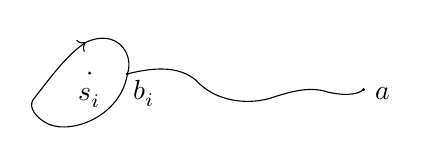
\begin{tikzpicture}[x=1cm,y=1cm,line cap=round,line join=round,baseline=(current bounding box.center)]
\coordinate (b) at (0.48,0.15);
\coordinate (a) at (3.48,-0.05);
\draw[->] (-0.72,-0.18) .. controls (-0.50,0.10) and (-0.30,0.38) .. (-0.05,0.55);
\draw (-0.05,0.55) .. controls (0.33,0.73) and (0.57,0.42) .. (b)
  .. controls (0.40,-0.37) and (-0.20,-0.62) .. (-0.52,-0.49)
  .. controls (-0.68,-0.41) and (-0.78,-0.28) .. (-0.72,-0.18);
\fill (0,0.16) circle (0.6pt);
\node[below] at (0,0.09) {$s_i$};
\fill (b) circle (0.6pt);
\node[below right,inner sep=2pt] at (b) {$b_i$};
\draw (b) .. controls (0.80,0.23) and (1.12,0.26) .. (1.35,0.07)
  .. controls (1.58,-0.19) and (1.98,-0.25) .. (2.29,-0.16)
  .. controls (2.59,-0.06) and (2.81,-0.01) .. (3.02,-0.08)
  .. controls (3.19,-0.12) and (3.38,-0.13) .. (a);
\fill (a) circle (0.6pt);
\node[right,inner sep=4pt] at (3.48,-0.10) {$a$};
\end{tikzpicture}}
et un pt \var{\inserted{\(b_i\)}}{\LMadded{\(b_i\)}}{insertion}{140-2-s183-I001} sur le bord, et une classe d'homotopie de chemins \var{\inserted{(dans \(\deleted{\LMsourceMark{M006026}{\unsure{X}}}\LMsourceMark{M006027}{\unsure{U|X}}-(\mathring\Delta_i-\{s_i\})=V_i\))}}{\LMadded{(dans \(\var{\deleted{\LMsourceMark{M006028}{\unsure{X}}}}{\LMsourceMark{M006029}{\LMcancelledDoubts{\(\LMsourceMark{M006030}{\unsure{X}}\)}}}{deletion}{140-2-s183-D002}\LMsourceMark{M006031}{\unsure{U|X}}-(\mathring\Delta_i-\{s_i\})=V_i\))}}{insertion}{140-2-s183-I002} de \(a\) vers \(b_i\), et de prendre le groupe \(L_i\) engendré par l'un quelconque des deux lacets correspondants autour de \(s_i\) (qui donnent des \var{\deleted{\LMsourceMark{M006032}{\unsure{deux}}}}{\LMsourceMark{M006033}{\LMcancelledDoubts{\LMsourceMark{M006034}{\unsure{deux}}}}}{deletion}{140-2-s183-D003} élts opposés de \(\pi\)).
On voit que l'on trouve ainsi une application surjective de
\[
\operatorname{Isom}_{\Pi_1V_i}(a,b_i)\simeq
\operatorname{Isom}_{\Pi_1U}(a,b_i)
\]
\var{\deleted{vers}}{}{deletion}{140-2-s183-D004} sur l'ens des \(L_i\subset\pi\) dans la classe \(\LMsourceMark{M006035}{\unsure{i|\Pi}}\), application \var{\deleted{dont}}{}{deletion}{140-2-s183-D005} compatible avec l'action

\LMflushnotes\LMflushpages
\ifnum\LMform=1
\begin{LMapparatus}
\LMentry{140-2-s183-D001}{suppression}{\deleted{\(\pi\) est réalisé}
}{\emph{\LMomittedlabel}}{Passage biffé dans le manuscrit : la suppression suit l'état final de l'auteur; les doutes de lecture restent signalés.}{}
\LMentry{140-2-s183-I001}{insertion}{\inserted{\(b_i\)}
}{\emph{\LMinsertedlabel}}{Ajout explicite de l'auteur : intégré à l'endroit indiqué par la transcription, sans modifier sa lecture.}{}
\LMentry{140-2-s183-I002}{insertion}{\inserted{(dans \(\deleted{\LMsourceMark{M006036}{\unsure{X}}}\LMsourceMark{M006037}{\unsure{U|X}}-(\mathring\Delta_i-\{s_i\})=V_i\))}
}{\emph{\LMinsertedlabel}}{Ajout explicite de l'auteur : intégré à l'endroit indiqué par la transcription, sans modifier sa lecture.}{}
\LMentry{140-2-s183-D002}{suppression}{\(\deleted{\LMsourceMark{M006038}{\unsure{X}}}\)
}{\emph{\LMomittedlabel}}{Passage biffé dans le manuscrit : la suppression suit l'état final de l'auteur; les doutes de lecture restent signalés.}{}
\LMentry{140-2-s183-D003}{suppression}{\deleted{\LMsourceMark{M006039}{\unsure{deux}}}
}{\emph{\LMomittedlabel}}{Passage biffé dans le manuscrit : la suppression suit l'état final de l'auteur; les doutes de lecture restent signalés.}{}
\LMentry{140-2-s183-D004}{suppression}{\deleted{vers}
}{\emph{\LMomittedlabel}}{Passage biffé dans le manuscrit : la suppression suit l'état final de l'auteur; les doutes de lecture restent signalés.}{}
\LMentry{140-2-s183-D005}{suppression}{\deleted{dont}
}{\emph{\LMomittedlabel}}{Passage biffé dans le manuscrit : la suppression suit l'état final de l'auteur; les doutes de lecture restent signalés.}{}
\end{LMapparatus}
\fi
\ifnum\LMform=2
\par\smallskip\begingroup\footnotesize\Needspace{4\baselineskip}\csname @beginparpenalty\endcsname=10000\relax\noindent\textcolor{gray}{\rule{.2\linewidth}{.35pt}}\par\nobreak
\noindent\textit{\LMdoubtheading.}\par\nobreak
\LMcarryover{140-2-s183-D002}{\(\LMsourceMark{M006040}{\unsure{X}}\)
}
\LMcarryover{140-2-s183-D003}{\LMsourceMark{M006041}{\unsure{deux}}
}
\par\endgroup\smallskip
\fi

\LMsourceMark{M006042}{\scanpage{184}}
\LMsourceMark{M006043}{\mspage{92}}

naturelle de \(\pi\) (opérant sur \(\operatorname{Isom}_{\Pi_1U}(a,b_i)\) de la façon évidente par composition, et sur l'ens des \(L_i\) par autom. int.
\var{\deleted{\LMsourceMark{M006044}{\unsure{Alors}}}}{\LMsourceMark{M006045}{\LMcancelledDoubts{\LMsourceMark{M006046}{\unsure{Alors}}}}}{deletion}{140-2-s184-D001} Ici, le \var{\deleted{choix de}}{}{deletion}{140-2-s184-D002} lien avec la description ``abstraite'' toposique s'établit ainsi: le choix de \(b_i\) peut servir de pt \LMsourceMark{M006047}{\unsure{base|fixe}} pour définir un rev. universel de \(\Delta_i\smallsetminus\{s_i\}\overset{\sim}{\hookleftarrow}D_i^*\), d'où un objt \(\rho_!(\widetilde D_i^*(b_i))\), et \var{\deleted{\LMsourceMark{M006048}{\unsure{cet objt}}}}{\LMsourceMark{M006049}{\LMcancelledDoubts{\LMsourceMark{M006050}{\unsure{cet objt}}}}}{deletion}{140-2-s184-D003} les \(L_i\subset\pi\) correspondent \var{\inserted{(d'après la description abstraite)}}{\LMadded{(d'après la description abstraite)}}{insertion}{140-2-s184-I001} aux isom de \(\widetilde U_0=\widetilde U(a_i)\) sur \(\LMsourceMark{M006051}{\unsure{D_i^*(b_i)|\widetilde D_i^*(b_i)}}\) modulo composition avec un autom de \(\LMsourceMark{M006052}{\unsure{D_i^*(b_i)|\widetilde D_i^*(b_i)}}\) provenant d'un autom de \(\LMsourceMark{M006053}{\unsure{D_i^*(b_i)|\widetilde D_i^*(b_i)}}\) -- mais les iso \var{\deleted{de}}{}{deletion}{140-2-s184-D004} \(\widetilde U(a_i)\xrightarrow{\sim}\rho_!(\widetilde D_i^*(b_i))\) correspondent justement aux classes de chemins de \(a\) vers \(b_i\).

\LMsourceMark{M006054}{\margin{On revient aux notations \(\pi',U'\) --}}
\LMsourceMark{M006055}{\unsure{Considérons}} un objt de \(\Pi_1B_{D_i^{*'}}\), i.e. un couple \((\pi',L_i')\). Soit \(\pi\) le groupe quotient de \(\pi'\) par le ss-groupe invariant de \(\pi'\) \var{\deleted{défini}}{}{deletion}{140-2-s184-D005} \var{\inserted{engendré}}{\LMadded{engendré}}{insertion}{140-2-s184-I002} par \(L_i'\). Je dis \LMsourceMark{M006056}{\margin{\(\Vert\)}} qu'à isom unique près (isom effectif de groupes, pas seulement extérieur !) il ne

\LMflushnotes\LMflushpages
\ifnum\LMform=1
\begin{LMapparatus}
\LMentry{140-2-s184-D001}{suppression}{\deleted{\LMsourceMark{M006057}{\unsure{Alors}}}
}{\emph{\LMomittedlabel}}{Passage biffé dans le manuscrit : la suppression suit l'état final de l'auteur; les doutes de lecture restent signalés.}{}
\LMentry{140-2-s184-D002}{suppression}{\deleted{choix de}
}{\emph{\LMomittedlabel}}{Passage biffé dans le manuscrit : la suppression suit l'état final de l'auteur; les doutes de lecture restent signalés.}{}
\LMentry{140-2-s184-D003}{suppression}{\deleted{\LMsourceMark{M006058}{\unsure{cet objt}}}
}{\emph{\LMomittedlabel}}{Passage biffé dans le manuscrit : la suppression suit l'état final de l'auteur; les doutes de lecture restent signalés.}{}
\LMentry{140-2-s184-I001}{insertion}{\inserted{(d'après la description abstraite)}
}{\emph{\LMinsertedlabel}}{Ajout explicite de l'auteur : intégré à l'endroit indiqué par la transcription, sans modifier sa lecture.}{}
\LMentry{140-2-s184-D004}{suppression}{\deleted{de}
}{\emph{\LMomittedlabel}}{Passage biffé dans le manuscrit : la suppression suit l'état final de l'auteur; les doutes de lecture restent signalés.}{}
\LMentry{140-2-s184-D005}{suppression}{\deleted{défini}
}{\emph{\LMomittedlabel}}{Passage biffé dans le manuscrit : la suppression suit l'état final de l'auteur; les doutes de lecture restent signalés.}{}
\LMentry{140-2-s184-I002}{insertion}{\inserted{engendré}
}{\emph{\LMinsertedlabel}}{Ajout explicite de l'auteur : intégré à l'endroit indiqué par la transcription, sans modifier sa lecture.}{}
\end{LMapparatus}
\fi
\ifnum\LMform=2
\par\smallskip\begingroup\footnotesize\Needspace{4\baselineskip}\csname @beginparpenalty\endcsname=10000\relax\noindent\textcolor{gray}{\rule{.2\linewidth}{.35pt}}\par\nobreak
\noindent\textit{\LMdoubtheading.}\par\nobreak
\LMcarryover{140-2-s184-D001}{\LMsourceMark{M006059}{\unsure{Alors}}
}
\LMcarryover{140-2-s184-D003}{\LMsourceMark{M006060}{\unsure{cet objt}}
}
\par\endgroup\smallskip
\fi

\LMsourceMark{M006061}{\scanpage{185}}

dépend pas du choix de l'objt \(\widetilde D_i^*\) de \(\Pi_1B_{D_i'^*}\). En effet, \(\pi=\pi(\widetilde D_i^*)\) dépend fonctoriellement de \(\widetilde D_i^*\), et tt revient à voir que ce foncteur est \uline{constant}, i.e. que l'opération de
\[
\operatorname{Aut}(\widetilde D_i^*)\simeq T\simeq L_i
\quad\text{sur}\quad
\pi=\pi(\widetilde D_i^*)
\]
est triviale. Or soit \(u\in L_i\), \LMsourceMark{M006062}{\unsure{l'|son}} autom de \(\pi\) qu'il définit est défini par l'autom. intérieur \(\operatorname{int}(u)\) par passage au quotient, donc (comme \(u\) devient \(1\) dans \(\pi\)) il est trivial. \LMsourceMark{M006063}{\unsure{Facile.}}

On trouve ainsi un \uline{foncteur}
\[
\begin{array}{c}
\text{Groupes extérieurs à lacets }\pi'\\
\text{de type }g,\nu+1\text{ munis d'une}\\
\text{classe de lacets }i\in I(\pi')
\end{array}
\longrightarrow
\begin{array}{c}
\text{groupes}\\
\text{(réalisés)}\\
\text{à lacets, de}\\
\text{type }g,\nu\var{\deleted{\LMsourceMark{M006064}{\unsure{+1}}}}{\LMsourceMark{M006065}{\LMcancelledDoubts{\(\LMsourceMark{M006066}{\unsure{+1}}\)}}}{deletion}{140-2-s185-D001}
\end{array}
\]
\[
(\pi',i)\longmapsto\beta(\pi',i)
\qquad
\text{[``bouchage du trou \(i\)'']}
\]
qui s'exprime par un hom de groupes
\[
\operatorname{Aut\,ext}(\pi',i)\longrightarrow\operatorname{Aut}\pi
\tag{\LMsourceMark{M006067}{\unsure{*|5}}}
\]
où \(\pi=\beta(\pi',i)\)
\[
\left(
\begin{array}{l}
\overset{\text{déf}}{=}\text{ ens. des autom cat.}\\
\text{de }\pi'\text{ respectant la structure}\\
\text{à lacets et fixant la classe de}\\
\text{lacets }i
\end{array}
\right)
\]

\LMflushnotes\LMflushpages
\ifnum\LMform=1
\begin{LMapparatus}
\LMentry{140-2-s185-D001}{suppression}{\(\deleted{\LMsourceMark{M006068}{\unsure{+1}}}\)
}{\emph{\LMomittedlabel}}{Passage biffé dans le manuscrit : la suppression suit l'état final de l'auteur; les doutes de lecture restent signalés.}{}
\end{LMapparatus}
\fi
\ifnum\LMform=2
\par\smallskip\begingroup\footnotesize\Needspace{4\baselineskip}\csname @beginparpenalty\endcsname=10000\relax\noindent\textcolor{gray}{\rule{.2\linewidth}{.35pt}}\par\nobreak
\noindent\textit{\LMdoubtheading.}\par\nobreak
\LMcarryover{140-2-s185-D001}{\(\LMsourceMark{M006069}{\unsure{+1}}\)
}
\par\endgroup\smallskip
\fi

\LMsourceMark{M006070}{\scanpage{186}}
\LMsourceMark{M006071}{\mspage{93}}

Du point de vue géométrique, ce fait (existence de ce foncteur), ne fait qu'exprimer le fait qu'après ``bouchage du trou'' \(i\), on a un \var{\deleted{pt.}}{}{deletion}{140-2-s186-D001} \(U=U'\cup\{s_i\}\) \uline{muni} d'un pt \(s_i\) qu'on peut utiliser comme un \uline{pt base} \var{\inserted{\uuline{canonique}}}{\LMadded{\uuline{canonique}}}{insertion}{140-2-s186-I001} pour calculer \(\pi_1(U)\).

On peut dire aussi que le choix de \(i\) permet de construire la somme amalgamée partielle (bouchage de trous \var{\inserted{partiel}}{\LMadded{partiel}}{insertion}{140-2-s186-I002}) \(B_{U^*}\)
\diagram{
\begin{tikzcd}[ampersand replacement=\&]
\& B_{D_i'^*} \arrow[dl] \arrow[dr] \& \\
B_{U'} \arrow[dr] \& \& B_{s_i} \arrow[dl] \\
\& B_{U^*} \&
\end{tikzcd}
}
et \(B_{s_i}\longrightarrow B_{U^*}\) fournit un pt géom. de \(B_{U^*}\) qui permet de décrire un objt canonique de \(\Pi_1B_{U^*}\) (rev universel relatif à ce pt) d'où canoniquement un groupe \(\pi\), qui bien sûr est un groupe à lacets de type \(g,\nu-1\).

\uline{Théorème} Supposons \(g,\nu\) tels que non

\LMflushnotes\LMflushpages
\ifnum\LMform=1
\begin{LMapparatus}
\LMentry{140-2-s186-D001}{suppression}{\deleted{pt.}
}{\emph{\LMomittedlabel}}{Passage biffé dans le manuscrit : la suppression suit l'état final de l'auteur; les doutes de lecture restent signalés.}{}
\LMentry{140-2-s186-I001}{insertion}{\inserted{\uuline{canonique}}
}{\emph{\LMinsertedlabel}}{Ajout explicite de l'auteur : intégré à l'endroit indiqué par la transcription, sans modifier sa lecture.}{}
\LMentry{140-2-s186-I002}{insertion}{\inserted{partiel}
}{\emph{\LMinsertedlabel}}{Ajout explicite de l'auteur : intégré à l'endroit indiqué par la transcription, sans modifier sa lecture.}{}
\end{LMapparatus}
\fi

\LMsourceMark{M006072}{\scanpage{187}}

seulement les groupes \(\pi'_{\LMsourceMark{M006073}{\unsure{s}}}\) de type \(g,\nu\), mais aussi les groupes \(\pi\) (de type \(g,\nu-1\)) soient anabéliens, i.e.
\[
2g+\LMsourceMark{M006074}{\unsure{\nu}}\var{\deleted{\LMsourceMark{M006075}{\unsure{+1}}}}{\LMsourceMark{M006076}{\LMcancelledDoubts{\(\LMsourceMark{M006077}{\unsure{+1}}\)}}}{deletion}{140-2-s187-D001}\LMsourceMark{M006078}{\unsure{\ge|\le}}\LMsourceMark{M006079}{\unsure{4}}
\quad
[\text{donc }g\ge2,\ \text{ou }g\LMsourceMark{M006080}{\unsure{\ge|=}}1,\nu\ge2,\ \text{ou }g=0,\nu\ge4].
\]
Alors le foncteur précédent \((\pi',i)\longrightarrow\pi\) est une équivalence de catégories, en d'autres termes (comme il s'agit de groupoïdes \(0\)-connexes)
\[
\operatorname{Aut\,ext}(\pi',i)\longrightarrow\operatorname{Aut}(\pi)
\]
est un \uline{isomorphisme}.

Notons pour ceci \LMsourceMark{M006081}{\unsure{qu'on a}} la suite exacte
\[
1\longrightarrow\pi\longrightarrow\operatorname{Aut}(\pi)
\longrightarrow\operatorname{Aut\,ext}(\pi)\longrightarrow1:
\]
(car \(\operatorname{Centre}\pi=1\) par hyp anabélienne sur \(\pi\)), \LMsourceMark{M006082}{\unsure{or}} on va définir une suite exacte
\[
1\longrightarrow\pi\longrightarrow\operatorname{Aut\,ext}(\pi',i)
\longrightarrow\LMsourceMark{M006083}{\unsure{\operatorname{Aut\,ext}(\pi)|\operatorname{Aut\,ext}(\pi')}}
\longrightarrow1
\]
et un hom. d'extensions de celle-ci

\LMflushnotes\LMflushpages
\ifnum\LMform=1
\begin{LMapparatus}
\LMentry{140-2-s187-D001}{suppression}{\(\deleted{\LMsourceMark{M006084}{\unsure{+1}}}\)
}{\emph{\LMomittedlabel}}{Passage biffé dans le manuscrit : la suppression suit l'état final de l'auteur; les doutes de lecture restent signalés.}{}
\end{LMapparatus}
\fi
\ifnum\LMform=2
\par\smallskip\begingroup\footnotesize\Needspace{4\baselineskip}\csname @beginparpenalty\endcsname=10000\relax\noindent\textcolor{gray}{\rule{.2\linewidth}{.35pt}}\par\nobreak
\noindent\textit{\LMdoubtheading.}\par\nobreak
\LMcarryover{140-2-s187-D001}{\(\LMsourceMark{M006085}{\unsure{+1}}\)
}
\par\endgroup\smallskip
\fi

\LMsourceMark{M006086}{\scanpage{188}}
\LMsourceMark{M006087}{\mspage{\LMsourceMark{M006088}{\unsure{94|99}}}}

dans la précédente (qui sera nécessairement un isomorphisme).

OPS \(T=\mathbb Z\), on considère les groupes à lacets \LMsourceMark{M006089}{\unsure{standart|standard}} \(\Pi_{g,\nu+1}\), \(\Pi_{g,\nu}\). Posons
\[
\operatorname{Aut\,ext}_{\mathrm{lac}}(\Pi_{g,\nu})
=\LMsourceMark{M006090}{\unsure{\mathcal T|\mathfrak T}}_{g,\nu}^{\LMsourceMark{M006091}{\unsure{00|\circ\circ}}}
\]
\var{\inserted{induisant \uline{l'identité} sur \(I(\Pi_{g,\nu})\) et sur \(T(\Pi_{g,\nu})\)}}{\LMadded{induisant \uline{l'identité} sur \(I(\Pi_{g,\nu})\) et sur \(T(\Pi_{g,\nu})\)}}{insertion}{140-2-s188-I001}
(groupe de Teichmüller d'indice \(g,\nu\)),
on sait que (pour \(2g+\nu\ge3\)) \(\mathcal T_{g,\nu}\) est le groupe fondamental du topos modulaire complexe \var{\inserted{\(M_{g,\nu}\)}}{\LMadded{\(M_{g,\nu}\)}}{insertion}{140-2-s188-I002} des courbes complexes (\var{\deleted{\LMsourceMark{M006092}{\illegible{1}}}}{\LMsourceMark{M006093}{\LMcancelledDoubts{\LMsourceMark{M006094}{\illegible{1}}}}}{deletion}{140-2-s188-D001} \LMsourceMark{M006095}{\unsure{proj. n.s.}}) conn., de genre \(g\), avec un syst de \(\nu\) pts \(s_1-\!s_\nu\) distincts donnés.
\LMsourceMark{M006096}{\margin{\uline{NB.} le rev. universel de \(M_{g,\nu}\) est contractible, Teichmüller.}}
Or le topos modulaire \(M_{g,\nu+1}\) n'est autre que \var{\deleted{l'image}}{}{deletion}{140-2-s188-D002} la ``courbe complexe universelle \var{\deleted{\LMsourceMark{M006097}{\illegible{1}}}}{\LMsourceMark{M006098}{\LMcancelledDoubts{\LMsourceMark{M006099}{\illegible{1}}}}}{deletion}{140-2-s188-D003} de genre \(g\) à \(\nu\) trous numérotés'' sur \(M_{g,\nu}\)
[car se donner une courbe \var{\inserted{\(U'\)}}{\LMadded{\(U'\)}}{insertion}{140-2-s188-I003} de genre \(g\) avec \(\nu+1\) trous \var{\inserted{\(x_1-\!x_{\nu+1}\)}}{\LMadded{\(x_1-\!x_{\nu+1}\)}}{insertion}{140-2-s188-I004} revient au \(\overline{\mathrm m}\) que de s'en donner une \var{\inserted{\(U\)}}{\LMadded{\(U\)}}{insertion}{140-2-s188-I005} avec \(\nu\) trous numérotés \(x_1-\!x_\nu\), \uline{plus} un \var{\deleted{trou de}}{}{deletion}{140-2-s188-D004} pt de \(U\) \var{\deleted{\LMsourceMark{M006100}{\unsure{pointé}}}}{\LMsourceMark{M006101}{\LMcancelledDoubts{\LMsourceMark{M006102}{\unsure{pointé}}}}}{deletion}{140-2-s188-D005}), \uline{d'où} une suite exacte d'homotopie
\diagram{
\begin{tikzcd}[ampersand replacement=\&,column sep=small]
\LMsourceMark{M006103}{\unsure{\pi_2|\Pi_2}}(M_{g,\nu},\LMsourceMark{M006104}{\unsure{\xi}})
 \arrow[r] \&
\pi_1(U) \arrow[r] \arrow[d,equal] \&
\pi_1(M_{g,\nu+1}) \arrow[r] \arrow[d,equal] \&
\pi_1(M_{g,\nu}) \arrow[r] \arrow[d,phantom,sloped,"\simeq"] \&
\pi_0(U) \arrow[d,equal] \\
0 \arrow[r] \&
\pi=\Pi_{g,\nu} \arrow[r] \&
\mathcal T^{00}_{g,\nu+1} \arrow[r] \&
\mathcal T^{00}_{g,\nu} \arrow[r] \&
1
\end{tikzcd}
}

\LMflushnotes\LMflushpages
\ifnum\LMform=1
\begin{LMapparatus}
\LMentry{140-2-s188-I001}{insertion}{\inserted{induisant \uline{l'identité} sur \(I(\Pi_{g,\nu})\) et sur \(T(\Pi_{g,\nu})\)}
}{\emph{\LMinsertedlabel}}{Ajout explicite de l'auteur : intégré à l'endroit indiqué par la transcription, sans modifier sa lecture.}{}
\LMentry{140-2-s188-I002}{insertion}{\inserted{\(M_{g,\nu}\)}
}{\emph{\LMinsertedlabel}}{Ajout explicite de l'auteur : intégré à l'endroit indiqué par la transcription, sans modifier sa lecture.}{}
\LMentry{140-2-s188-D001}{suppression}{\deleted{\LMsourceMark{M006105}{\illegible{1}}}
}{\emph{\LMomittedlabel}}{Passage biffé dans le manuscrit : la suppression suit l'état final de l'auteur; les doutes de lecture restent signalés.}{}
\LMentry{140-2-s188-D002}{suppression}{\deleted{l'image}
}{\emph{\LMomittedlabel}}{Passage biffé dans le manuscrit : la suppression suit l'état final de l'auteur; les doutes de lecture restent signalés.}{}
\LMentry{140-2-s188-D003}{suppression}{\deleted{\LMsourceMark{M006106}{\illegible{1}}}
}{\emph{\LMomittedlabel}}{Passage biffé dans le manuscrit : la suppression suit l'état final de l'auteur; les doutes de lecture restent signalés.}{}
\LMentry{140-2-s188-I003}{insertion}{\inserted{\(U'\)}
}{\emph{\LMinsertedlabel}}{Ajout explicite de l'auteur : intégré à l'endroit indiqué par la transcription, sans modifier sa lecture.}{}
\LMentry{140-2-s188-I004}{insertion}{\inserted{\(x_1-\!x_{\nu+1}\)}
}{\emph{\LMinsertedlabel}}{Ajout explicite de l'auteur : intégré à l'endroit indiqué par la transcription, sans modifier sa lecture.}{}
\LMentry{140-2-s188-I005}{insertion}{\inserted{\(U\)}
}{\emph{\LMinsertedlabel}}{Ajout explicite de l'auteur : intégré à l'endroit indiqué par la transcription, sans modifier sa lecture.}{}
\LMentry{140-2-s188-D004}{suppression}{\deleted{trou de}
}{\emph{\LMomittedlabel}}{Passage biffé dans le manuscrit : la suppression suit l'état final de l'auteur; les doutes de lecture restent signalés.}{}
\LMentry{140-2-s188-D005}{suppression}{\deleted{\LMsourceMark{M006107}{\unsure{pointé}}}
}{\emph{\LMomittedlabel}}{Passage biffé dans le manuscrit : la suppression suit l'état final de l'auteur; les doutes de lecture restent signalés.}{}
\end{LMapparatus}
\fi
\ifnum\LMform=2
\par\smallskip\begingroup\footnotesize\Needspace{4\baselineskip}\csname @beginparpenalty\endcsname=10000\relax\noindent\textcolor{gray}{\rule{.2\linewidth}{.35pt}}\par\nobreak
\noindent\textit{\LMdoubtheading.}\par\nobreak
\LMcarryover{140-2-s188-D001}{\LMsourceMark{M006108}{\illegible{1}}
}
\LMcarryover{140-2-s188-D003}{\LMsourceMark{M006109}{\illegible{1}}
}
\LMcarryover{140-2-s188-D005}{\LMsourceMark{M006110}{\unsure{pointé}}
}
\par\endgroup\smallskip
\fi

\LMsourceMark{M006111}{\scanpage{189}}

d'où \LMsourceMark{M006112}{\unsure{une}} structure d'extension \var{\deleted{annoncée}}{}{deletion}{140-2-s189-D001}
\[
1\longrightarrow\Pi_{g,\nu}
\longrightarrow\mathcal T^{00}_{g,\nu+1}
\longrightarrow\mathcal T^{00}_{g,\LMsourceMark{M006113}{\unsure{\nu}}}
\longrightarrow1
\]
qui est (à passage à un sous-groupe d'indice ``\(2\nu!\) près) cette structure d'extension annoncée. \LMsourceMark{M006114}{\unsure{\&}} les vérifications de \uline{compatibilité} sont laissées \ldots.

On a donc un foncteur quasi inverse (défini à isom unique près)
\[
\begin{array}{c}
\text{groupes à lacets}\\
\text{de type }g,\nu\\
(2g+\nu\ge3)
\end{array}
\longrightarrow
\begin{array}{c}
\text{groupes \uline{extérieurs} à}\\
\text{lacets de type }(g,\nu+1),\\
\text{avec une ``classe de}\\
\text{lacets'' distinguée}\\
\text{(couples }(\pi',i\in I(\pi'))\text{)}
\end{array}
\]

\var{\deleted{\LMsourceMark{M006115}{\unsure{Or}}}}{\LMsourceMark{M006116}{\LMcancelledDoubts{\LMsourceMark{M006117}{\unsure{Or}}}}}{deletion}{140-2-s189-D002} \LMsourceMark{M006118}{\unsure{Au}} niveau toposique, quand on a un système \(B_{D^*}\longrightarrow B_U\) \var{\inserted{de type \(g,\nu\) \((2g+\nu\ge3)\)}}{\LMadded{de type \(g,\nu\) \((2g+\nu\ge3)\)}}{insertion}{140-2-s189-I001}, et un ``pt'' de \(B_U\) i.e un \(\widetilde U\in\operatorname{Ob}\Pi_1B_U\), alors on peut de façon canonique trouver un \(B_{D_i^*}\) (\LMsourceMark{M006119}{\unsure{\(T\)-gr. poïde}} \var{\inserted{connexe}}{\LMadded{connexe}}{insertion}{140-2-s189-I002}, où \(T\) est le module d'orientation), et un système
\[
B_{D^*}\amalg B_{D_i^*}\longrightarrow B_{U'},
\]
de type \(g,\nu+1\),

\LMflushnotes\LMflushpages
\ifnum\LMform=1
\begin{LMapparatus}
\LMentry{140-2-s189-D001}{suppression}{\deleted{annoncée}
}{\emph{\LMomittedlabel}}{Passage biffé dans le manuscrit : la suppression suit l'état final de l'auteur; les doutes de lecture restent signalés.}{}
\LMentry{140-2-s189-D002}{suppression}{\deleted{\LMsourceMark{M006120}{\unsure{Or}}}
}{\emph{\LMomittedlabel}}{Passage biffé dans le manuscrit : la suppression suit l'état final de l'auteur; les doutes de lecture restent signalés.}{}
\LMentry{140-2-s189-I001}{insertion}{\inserted{de type \(g,\nu\) \((2g+\nu\ge3)\)}
}{\emph{\LMinsertedlabel}}{Ajout explicite de l'auteur : intégré à l'endroit indiqué par la transcription, sans modifier sa lecture.}{}
\LMentry{140-2-s189-I002}{insertion}{\inserted{connexe}
}{\emph{\LMinsertedlabel}}{Ajout explicite de l'auteur : intégré à l'endroit indiqué par la transcription, sans modifier sa lecture.}{}
\end{LMapparatus}
\fi
\ifnum\LMform=2
\par\smallskip\begingroup\footnotesize\Needspace{4\baselineskip}\csname @beginparpenalty\endcsname=10000\relax\noindent\textcolor{gray}{\rule{.2\linewidth}{.35pt}}\par\nobreak
\noindent\textit{\LMdoubtheading.}\par\nobreak
\LMcarryover{140-2-s189-D002}{\LMsourceMark{M006121}{\unsure{Or}}
}
\par\endgroup\smallskip
\fi

\LMsourceMark{M006122}{\scanpage{190}}
\LMsourceMark{M006123}{\mspage{95}}

de façon que \((B_{D^*},B_U,\widetilde U)\) \LMsourceMark{M006124}{\unsure{s'en déduise}} par l'opération de ``bouchage du trou \(D_i^*\)''.

Ces constructions sont si fonctorielles, \LMsourceMark{M006125}{\margin{\LMsourceMark{M006126}{\unsure{\(\wedge\)}}}} qu'elles commutent aux actions de groupes \(\Gamma\). Si un groupe \(\Gamma\) opère sur un groupe à lacets \(\pi_{\var{\deleted{\LMsourceMark{M006127}{\unsure{g,\nu}}}}{\LMsourceMark{M006128}{\LMcancelledDoubts{\(\LMsourceMark{M006129}{\unsure{g,\nu}}\)}}}{deletion}{140-2-s190-D001}}\) de type \(g,\nu\), (pas seulement extérieurement), alors on en déduit une opération \uline{extérieure} de \(\Gamma\) sur un \(\pi'\) à lacets de type \(g,\nu+1\), qui fixe une classe de lacets privilégiée \(i\in I\).

Mais alors, dans l'extension correspondante
\[
1\longrightarrow\pi'\longrightarrow E'\longrightarrow\Gamma\longrightarrow1,
\]
Choisissons un \(L_i'\subset\pi'\) et soit \(\LMsourceMark{M006130}{\unsure{\mathcal E_i'|E_i'}}\) le normalisateur de \(L_i\) dans \(\LMsourceMark{M006131}{\unsure{\mathcal E'|E'}}\) -- on trouve
\[
1\longrightarrow
\underset{\simeq T}{L_i'}
\longrightarrow\LMsourceMark{M006132}{\unsure{\mathcal E_i'|E_i'}}
\longrightarrow\Gamma\longrightarrow1
\]

\LMflushnotes\LMflushpages
\ifnum\LMform=1
\begin{LMapparatus}
\LMentry{140-2-s190-D001}{suppression}{\(\deleted{\LMsourceMark{M006133}{\unsure{g,\nu}}}\)
}{\emph{\LMomittedlabel}}{Passage biffé dans le manuscrit : la suppression suit l'état final de l'auteur; les doutes de lecture restent signalés.}{}
\end{LMapparatus}
\fi
\ifnum\LMform=2
\par\smallskip\begingroup\footnotesize\Needspace{4\baselineskip}\csname @beginparpenalty\endcsname=10000\relax\noindent\textcolor{gray}{\rule{.2\linewidth}{.35pt}}\par\nobreak
\noindent\textit{\LMdoubtheading.}\par\nobreak
\LMcarryover{140-2-s190-D001}{\(\LMsourceMark{M006134}{\unsure{g,\nu}}\)
}
\par\endgroup\smallskip
\fi

% END PACKAGE LM_P019
% BEGIN PACKAGE LM_P020
\ifnum\LMform<2\Needspace{11\baselineskip}\subsection*{Scans 191--200}\fi
\LMsourceMark{M006135}{\scanpage{191}}
% l. 01
( ceci \LMsourceMark{M006136}{\unsure{marche}} \LMsourceMark{M006137}{\unsure{s.s}} hyp. de finitude sur
% l. 02
$\Gamma$, le cas universel étant celui où $\Gamma$
% l. 03
est le \LMsourceMark{M006138}{\unsure{grpe}} de Teichmüller de $\pi'$ \LMsourceMark{M006139}{\unsure{fixt}} $i$
% l. 04
i.e. $\operatorname{Autext}_{\mathrm{lac}}(\pi';i)\simeq\operatorname{Aut}_{\mathrm{lac}}(\pi)$ ). Je
% l. 05
dis que si $\Gamma$ opère \uline{fidèlt} \uline{sur $\pi$}
% l. 06
i.e. si son opération extérieure \uline{sur}
% l. 07
\uline{$\pi'$} est fidèle, et si $\Gamma$ est \uline{fini},
% l. 08
Alors $\Gamma$ est nécessairement cyclique \var{\inserted{(cas $\Gamma=\Gamma^0$)}}{\LMadded{(cas $\Gamma=\Gamma^0$)}}{insertion}{140-2-s191-I001}
% l. 09
ou dihédral ($\Gamma\ne\Gamma^0$), et que si de
% l. 10
plus $\Gamma=\Gamma^0$, alors \var{\deleted{\LMsourceMark{M006140}{\unsure{$\mathcal E_i'$ est $\simeq$}}}}{\LMsourceMark{M006141}{\LMcancelledDoubts{\LMsourceMark{M006142}{\unsure{$\mathcal E_i'$ est $\simeq$}}}}}{deletion}{140-2-s191-D001} \var{\inserted{\LMsourceMark{M006143}{\unsure{$\mathcal E_i\simeq\mathbb Z$|$\mathcal E_i'\simeq\mathbb Z$}} i.e.}}{\LMadded{\LMsourceMark{M006144}{\unsure{$\mathcal E_i\simeq\mathbb Z$|$\mathcal E_i'\simeq\mathbb Z$}} i.e.}}{insertion}{140-2-s191-I002} $\exists!$ isom
% l. 11
\LMsourceMark{M006145}{\unsure{$T\xrightarrow{\sim}\mathcal E_i$|$T\xrightarrow{\sim}\mathcal E_i'$}} tel que \LMsourceMark{M006146}{\unsure{$T\xrightarrow{k_i'}\mathcal E_i'$}} s'identifie à
% l. 12
$n\operatorname{id}_T$ (de sorte qu'on trouve \LMsourceMark{M006147}{\unsure{$\Gamma\simeq\mathcal E_i'/n\mathcal E_i'$}}
% l. 13
$\simeq T\otimes_{\mathbb Z}\mathbb Z/n\mathbb Z$, si $n=\operatorname{card}\Gamma$ ...

% l. 14
Changeant de notations, ceci revient au
% l. 15
\uline{Th}\textsuperscript{\LMsourceMark{M006148}{\unsure{m}}} Soit $\Gamma$ un groupe fini opérant
% l. 16
fidèlt sur un groupe \uline{\LMsourceMark{M006149}{\unsure{extérieur|extérieurem\textsuperscript{t}}}} à
% l. 17
lacets $\pi$ \var{\inserted{de type \deleted{\LMsourceMark{M006150}{\illegible{1}}} $(g,\nu+1)$ ($\nu\geq0$)}}{\LMadded{de type \var{\deleted{\LMsourceMark{M006151}{\illegible{1}}}}{\LMsourceMark{M006152}{\LMcancelledDoubts{\LMsourceMark{M006153}{\illegible{1}}}}}{deletion}{140-2-s191-D002} $(g,\nu+1)$ ($\nu\geq0$)}}{insertion}{140-2-s191-I003}, en laissant fixe un $i\in I(\pi)$,
% l. 18
Alors $\Gamma$ est cyclique (si $\Gamma=\Gamma^0$) ou
% l. 19
dihédral (si $\Gamma\ne\Gamma^0$), et dans l'extension
% marge, en bas à gauche
\LMsourceMark{M006154}{\margin{\LMsourceMark{M006155}{\unsure{au}} $\overline{\mathrm m}$ il y a \uline{équivalence}, si dans le th, on suppose le type $(g,\nu)$ anabélien --- sinon le th. est un peu plus général}}
\LMsourceMark{M006156}{\mspage{190}}

\LMflushnotes\LMflushpages
\ifnum\LMform=1
\begin{LMapparatus}
\LMentry{140-2-s191-I001}{insertion}{\inserted{(cas $\Gamma=\Gamma^0$)}
}{\emph{\LMinsertedlabel}}{Ajout explicite de l'auteur : intégré à l'endroit indiqué par la transcription, sans modifier sa lecture.}{}
\LMentry{140-2-s191-D001}{suppression}{\deleted{\LMsourceMark{M006157}{\unsure{$\mathcal E_i'$ est $\simeq$}}}
}{\emph{\LMomittedlabel}}{Passage biffé dans le manuscrit : la suppression suit l'état final de l'auteur; les doutes de lecture restent signalés.}{}
\LMentry{140-2-s191-I002}{insertion}{\inserted{\LMsourceMark{M006158}{\unsure{$\mathcal E_i\simeq\mathbb Z$|$\mathcal E_i'\simeq\mathbb Z$}} i.e.}
}{\emph{\LMinsertedlabel}}{Ajout explicite de l'auteur : intégré à l'endroit indiqué par la transcription, sans modifier sa lecture.}{}
\LMentry{140-2-s191-I003}{insertion}{\inserted{de type \deleted{\LMsourceMark{M006159}{\illegible{1}}} $(g,\nu+1)$ ($\nu\geq0$)}
}{\emph{\LMinsertedlabel}}{Ajout explicite de l'auteur : intégré à l'endroit indiqué par la transcription, sans modifier sa lecture.}{}
\LMentry{140-2-s191-D002}{suppression}{\deleted{\LMsourceMark{M006160}{\illegible{1}}}
}{\emph{\LMomittedlabel}}{Passage biffé dans le manuscrit : la suppression suit l'état final de l'auteur; les doutes de lecture restent signalés.}{}
\end{LMapparatus}
\fi
\ifnum\LMform=2
\par\smallskip\begingroup\footnotesize\Needspace{4\baselineskip}\csname @beginparpenalty\endcsname=10000\relax\noindent\textcolor{gray}{\rule{.2\linewidth}{.35pt}}\par\nobreak
\noindent\textit{\LMdoubtheading.}\par\nobreak
\LMcarryover{140-2-s191-D001}{\LMsourceMark{M006161}{\unsure{$\mathcal E_i'$ est $\simeq$}}
}
\LMcarryover{140-2-s191-D002}{\LMsourceMark{M006162}{\illegible{1}}
}
\par\endgroup\smallskip
\fi

\LMsourceMark{M006163}{\scanpage{192}}
\LMsourceMark{M006164}{\mspage{96}}
% l. 01
correspondant \var{\deleted{\LMsourceMark{M006165}{\illegible{2}}}}{\LMsourceMark{M006166}{\LMcancelledDoubts{\LMsourceMark{M006167}{\illegible{2}}}}}{deletion}{140-2-s192-D001} \LMsourceMark{M006168}{\unsure{$\mathcal E$}} de $\Gamma$ par $\pi$,
% l. 02
Si \LMsourceMark{M006169}{\unsure{$\mathcal E_i$}} est le normalisateur de un $L_i$ dans
% l. 03
\LMsourceMark{M006170}{\unsure{$\mathcal E$}} [ \var{\inserted{de sorte qu'on a}}{\LMadded{de sorte qu'on a}}{insertion}{140-2-s192-I001} \var{\deleted{une}}{}{deletion}{140-2-s192-D002} \LMsourceMark{M006171}{\unsure{$\mathcal E_i\to\Gamma$}} épi i.e. une suite exacte
% l. 04
\LMsourceMark{M006172}{\unsure{$1\to L_i\to\mathcal E_i\to\Gamma\to1$}} ]. l'image inverse \LMsourceMark{M006173}{\unsure{$\mathcal E_i^0$}} de
% l. 05
$\Gamma^0$ est $\simeq\mathbb Z$ donc (si $n=\operatorname{card}\Gamma^0$)\var{\inserted{\LMsourceMark{M006174}{\unsure{$=[\mathcal E_i^0:L_i]$}}}}{\LMadded{\LMsourceMark{M006175}{\unsure{$=[\mathcal E_i^0:L_i]$}}}}{insertion}{140-2-s192-I002}
% l. 06
\var{\deleted{\LMsourceMark{M006176}{\unsure{$n\operatorname{id}$}}}}{\LMsourceMark{M006177}{\LMcancelledDoubts{\LMsourceMark{M006178}{\unsure{$n\operatorname{id}$}}}}}{deletion}{140-2-s192-D003} $x\to x^n$ est un iso. \var{\deleted{et}}{}{deletion}{140-2-s192-D004} \LMsourceMark{M006179}{\unsure{$\mathcal E_i^0\simeq L_i$}}, qui
% l. 07
compte tenu de $k_i$ donne un
% l. 08
isom \LMsourceMark{M006180}{\unsure{$\mathcal E_i^0\simeq T$}}, dont le composé avec
% l. 09
\var{\deleted{\LMsourceMark{M006181}{\unsure{$\mathcal E_i$}}}}{\LMsourceMark{M006182}{\LMcancelledDoubts{\LMsourceMark{M006183}{\unsure{$\mathcal E_i$}}}}}{deletion}{140-2-s192-D005} \LMsourceMark{M006184}{\unsure{$T\xrightarrow[\sim]{k_i}L_i\subset\mathcal E_i^0$}} est $n\operatorname{id}_T$, de sorte
% l. 10
qu'on a un iso. can
% l. 11
\[\LMsourceMark{M006185}{\unsure{\Gamma^0\simeq\mathcal E_i^0/L_i\simeq T/nT}}\]
% l. 12
(évidemment indépendant du choix de $L_i$ ...)

% l. 13
\uline{Démonstration}. Considérons l'extension
% l. 14
\LMsourceMark{M006186}{\unsure{$\mathcal E_i^0$}} de $\Gamma^0$ par $L_i\simeq T$ ($\overset{\text{\LMsourceMark{M006187}{\unsure{non can}}}}{\simeq}\mathbb Z$),
% l. 15
comme \LMsourceMark{M006188}{\unsure{$\mathcal E_i^0$|$\Gamma^0$}} opère trivialem\textsuperscript{t} sur $T$ \var{\inserted{sans torsion}}{\LMadded{sans torsion}}{insertion}{140-2-s192-I003}, cette
% l. 16
extension (par la suite exacte de coh.
% l. 17
associée à $0\to T\to T\otimes_{\mathbb Z}\mathbb Q\to T\otimes_{\mathbb Z}\mathbb Q/\mathbb Z\to0$)
% l. 18
est canoniquem\textsuperscript{t} isomorphe à \var{\deleted{\LMsourceMark{M006189}{\unsure{une}}}}{\LMsourceMark{M006190}{\LMcancelledDoubts{\LMsourceMark{M006191}{\unsure{une}}}}}{deletion}{140-2-s192-D006} l'extension
% l. 19
définie par un hom $\Gamma^0\to T_n=T/nT$,
% l. 20
comme image inverse de l'extension
% l. 21
$0\to T\xrightarrow{n}T\to T_n\to0$ de $T_n$ par $T$. Je dis que
\LMsourceMark{M006192}{\mspage{191}}

\LMflushnotes\LMflushpages
\ifnum\LMform=1
\begin{LMapparatus}
\LMentry{140-2-s192-D001}{suppression}{\deleted{\LMsourceMark{M006193}{\illegible{2}}}
}{\emph{\LMomittedlabel}}{Passage biffé dans le manuscrit : la suppression suit l'état final de l'auteur; les doutes de lecture restent signalés.}{}
\LMentry{140-2-s192-I001}{insertion}{\inserted{de sorte qu'on a}
}{\emph{\LMinsertedlabel}}{Ajout explicite de l'auteur : intégré à l'endroit indiqué par la transcription, sans modifier sa lecture.}{}
\LMentry{140-2-s192-D002}{suppression}{\deleted{une}
}{\emph{\LMomittedlabel}}{Passage biffé dans le manuscrit : la suppression suit l'état final de l'auteur; les doutes de lecture restent signalés.}{}
\LMentry{140-2-s192-I002}{insertion}{\inserted{\LMsourceMark{M006194}{\unsure{$=[\mathcal E_i^0:L_i]$}}}
}{\emph{\LMinsertedlabel}}{Ajout explicite de l'auteur : intégré à l'endroit indiqué par la transcription, sans modifier sa lecture.}{}
\LMentry{140-2-s192-D003}{suppression}{\deleted{\LMsourceMark{M006195}{\unsure{$n\operatorname{id}$}}}
}{\emph{\LMomittedlabel}}{Passage biffé dans le manuscrit : la suppression suit l'état final de l'auteur; les doutes de lecture restent signalés.}{}
\LMentry{140-2-s192-D004}{suppression}{\deleted{et}
}{\emph{\LMomittedlabel}}{Passage biffé dans le manuscrit : la suppression suit l'état final de l'auteur; les doutes de lecture restent signalés.}{}
\LMentry{140-2-s192-D005}{suppression}{\deleted{\LMsourceMark{M006196}{\unsure{$\mathcal E_i$}}}
}{\emph{\LMomittedlabel}}{Passage biffé dans le manuscrit : la suppression suit l'état final de l'auteur; les doutes de lecture restent signalés.}{}
\LMentry{140-2-s192-I003}{insertion}{\inserted{sans torsion}
}{\emph{\LMinsertedlabel}}{Ajout explicite de l'auteur : intégré à l'endroit indiqué par la transcription, sans modifier sa lecture.}{}
\LMentry{140-2-s192-D006}{suppression}{\deleted{\LMsourceMark{M006197}{\unsure{une}}}
}{\emph{\LMomittedlabel}}{Passage biffé dans le manuscrit : la suppression suit l'état final de l'auteur; les doutes de lecture restent signalés.}{}
\end{LMapparatus}
\fi
\ifnum\LMform=2
\par\smallskip\begingroup\footnotesize\Needspace{4\baselineskip}\csname @beginparpenalty\endcsname=10000\relax\noindent\textcolor{gray}{\rule{.2\linewidth}{.35pt}}\par\nobreak
\noindent\textit{\LMdoubtheading.}\par\nobreak
\LMcarryover{140-2-s192-D001}{\LMsourceMark{M006198}{\illegible{2}}
}
\LMcarryover{140-2-s192-D003}{\LMsourceMark{M006199}{\unsure{$n\operatorname{id}$}}
}
\LMcarryover{140-2-s192-D005}{\LMsourceMark{M006200}{\unsure{$\mathcal E_i$}}
}
\LMcarryover{140-2-s192-D006}{\LMsourceMark{M006201}{\unsure{une}}
}
\par\endgroup\smallskip
\fi

\LMsourceMark{M006202}{\scanpage{193}}
% l. 01
cet hom. est un iso (d'où \LMsourceMark{M006203}{\unsure{résulteraient|résulteront}}
% l. 02
les autres assertions), ou ce qui revient
% l. 03
au $\overline{\mathrm m}$ puisque $\Gamma^0$ et $T_n$ sont tous
% l. 04
deux d'ordre $n$, que c'est mono.
% l. 05
Remplaçant $\Gamma^0$ par le noyau de $\Gamma^0\to\mathbb Z/n\mathbb Z$,
% l. 06
OPS que l'hom. \var{\inserted{en question}}{\LMadded{en question}}{insertion}{140-2-s193-I001} est nul, et il faut
% l. 07
prouver que cela implique que l'action
% l. 08
de $\Gamma^0$ est triviale (ce qui, puisque par hyp.
% l. 09
l'action de $\Gamma$ est fidèle, implique $\Gamma^0=\{1\}$,
% l. 10
OK.) Donc \LMsourceMark{M006204}{\unsure{th}} est ramené au

% l. 11
\uline{lemme fondamental}. Tout automorphisme \var{\inserted{direct}}{\LMadded{direct}}{insertion}{140-2-s193-I002}
% l. 12
extérieur $u$ d'ordre fini \var{\inserted{\LMsourceMark{M006205}{\unsure{$n$}}}}{\LMadded{\LMsourceMark{M006206}{\unsure{$n$}}}}{insertion}{140-2-s193-I003} d'un groupe à
% l. 13
lacets $\pi$, qui fixe une classe de lacets
% l. 14
$i$ et est tel que l'extension de $\mathbb Z/n\mathbb Z$
% l. 15
par $L_i\in i$ définie par $u$ soit triviale,
% l. 16
est trivial.

% l. 17
L'hypothèse signifie que $u$ se remonte
% l. 18
en un autom $u_0$ de $\pi$, qui
% l. 19
normalise $L_i$, et qui soit aussi d'ordre \LMsourceMark{M006207}{\unsure{$n$}},
% l. 20
(ou d'ordre fini, cela revient au \LMsourceMark{M006208}{\unsure{$\overline{\mathrm m}$|$\Rightarrow$}} compte tenu
% l. 21
que \var{\deleted{\LMsourceMark{M006209}{\unsure{les élts de}}}}{\LMsourceMark{M006210}{\LMcancelledDoubts{\LMsourceMark{M006211}{\unsure{les élts de}}}}}{deletion}{140-2-s193-D001} $T$ est sans élts d'ordre fini)
\LMsourceMark{M006212}{\mspage{192}}

\LMflushnotes\LMflushpages
\ifnum\LMform=1
\begin{LMapparatus}
\LMentry{140-2-s193-I001}{insertion}{\inserted{en question}
}{\emph{\LMinsertedlabel}}{Ajout explicite de l'auteur : intégré à l'endroit indiqué par la transcription, sans modifier sa lecture.}{}
\LMentry{140-2-s193-I002}{insertion}{\inserted{direct}
}{\emph{\LMinsertedlabel}}{Ajout explicite de l'auteur : intégré à l'endroit indiqué par la transcription, sans modifier sa lecture.}{}
\LMentry{140-2-s193-I003}{insertion}{\inserted{\LMsourceMark{M006213}{\unsure{$n$}}}
}{\emph{\LMinsertedlabel}}{Ajout explicite de l'auteur : intégré à l'endroit indiqué par la transcription, sans modifier sa lecture.}{}
\LMentry{140-2-s193-D001}{suppression}{\deleted{\LMsourceMark{M006214}{\unsure{les élts de}}}
}{\emph{\LMomittedlabel}}{Passage biffé dans le manuscrit : la suppression suit l'état final de l'auteur; les doutes de lecture restent signalés.}{}
\end{LMapparatus}
\fi
\ifnum\LMform=2
\par\smallskip\begingroup\footnotesize\Needspace{4\baselineskip}\csname @beginparpenalty\endcsname=10000\relax\noindent\textcolor{gray}{\rule{.2\linewidth}{.35pt}}\par\nobreak
\noindent\textit{\LMdoubtheading.}\par\nobreak
\LMcarryover{140-2-s193-D001}{\LMsourceMark{M006215}{\unsure{les élts de}}
}
\par\endgroup\smallskip
\fi

\LMsourceMark{M006216}{\scanpage{194}}
\LMsourceMark{M006217}{\mspage{97}}
% l. 01
alors $u_0$ est trivial, i.e. cela équivaut au
% l. 02
\uline{Corollaire}. Tout autom \var{\inserted{direct}}{\LMadded{direct}}{insertion}{140-2-s194-I001} d'ordre fini \var{\inserted{$u_0$}}{\LMadded{$u_0$}}{insertion}{140-2-s194-I002} d'
% l. 03
un groupe à lacets $\pi$, \var{\inserted{qui soit direct et}}{\LMadded{qui soit direct et}}{insertion}{140-2-s194-I003} qui normalise
% l. 04
un sous-groupe à lacets $L_i$ (i.e. qui
% l. 05
centralise $L_i$), est réduit à l'identité.
% marge supérieure gauche
\LMsourceMark{M006218}{\margin{Dans le lemme ou son \LMsourceMark{M006219}{\unsure{coroll.}}}}
\LMsourceMark{M006220}{\margin{\uline{NB} (le cas $g=0$, $\nu+1=1$ ou $\nu+1=2$ est trivial, le cas $\nu+1=3$ ($(g,\nu)=(0,2)$ abélien!) n'est pas trivial \LMsourceMark{M006221}{\unsure{par contre}}, ni le cas $g=1$, $\nu+1=1$ i.e. $(g,\nu)=(1,0)$ abélien. Pourtant le résultat doit être valable aussi dans \LMsourceMark{M006222}{\unsure{ce|ces}} cas.)}}

% l. 06
Pour le démontrer, on est ramené \var{\inserted{aussitôt}}{\LMadded{aussitôt}}{insertion}{140-2-s194-I004} au
% l. 07
cas où $u_0$ est \var{\deleted{d'ordre premier $p$}}{}{deletion}{140-2-s194-D001} \var{\inserted{tel que $u_0^p=\operatorname{id}$, où}}{\LMadded{tel que $u_0^p=\operatorname{id}$, où}}{insertion}{140-2-s194-I005}
% l. 08
$p$ est un \LMsourceMark{M006223}{\unsure{nb}} premier --- i.e. $u_0$ corres-
% l. 09
pond à une opération au sens strict
% l. 10
(pas seulem\textsuperscript{t} extérieure) de $\mathbb Z/p\mathbb Z$ \var{\deleted{\LMsourceMark{M006224}{\unsure{par}}}}{\LMsourceMark{M006225}{\LMcancelledDoubts{\LMsourceMark{M006226}{\unsure{par}}}}}{deletion}{140-2-s194-D002} \LMsourceMark{M006227}{\unsure{à autom}}
% l. 11
de $\pi$. Mais (que l'on puisse ou non
% l. 12
trouver un tel $p$) considérons le cas où
% l. 13
on sait que l'opération \uline{extérieure} de
% l. 14
$\Gamma=\mathbb Z/n\mathbb Z$ [$n=$ ordre de $u$] sur $\pi$ se réalise
% l. 15
géométriquem\textsuperscript{t}, par une opération (fidèle)
% l. 16
de $\Gamma=\mathbb Z/n\mathbb Z$ sur une $U$ de type $(g,\nu+1)$.
% l. 17
\var{\deleted{\LMsourceMark{M006228}{\unsure{classes de $\pi$-conjugaison}}, \LMsourceMark{M006229}{\illegible{1}}}}{\LMsourceMark{M006230}{\LMcancelledDoubts{\LMsourceMark{M006231}{\unsure{classes de $\pi$-conjugaison}}\quad \LMsourceMark{M006232}{\illegible{1}}}}}{deletion}{140-2-s194-D003}
% marge inférieure gauche
\LMsourceMark{M006233}{\margin{$U=X\setminus S$, $S\simeq I$, $X$ comp. de genre $g$ \LMsourceMark{M006234}{\unsure{la pointe|la partie}} $s_i$ de $S$ correspondant à un pt fixe de $\Gamma$ op. sur $U$.}}

% l. 18
\var{\deleted{On sait que les (\LMsourceMark{M006235}{\unsure{relèvements}}) des auts
% l. 19
extérieurs en \deleted{\LMsourceMark{M006236}{\unsure{des autom}}} \inserted{une vraie opération},
% l. 20
correspondent aux pts fixes \LMsourceMark{M006237}{\illegible{1}} de $\Gamma$
% l. 21
dans $U$; \deleted{et l'extension de} \inserted{soit $a$ le pt fixe de $\Gamma$}
% l. 22
correspondant à l'opération donnée, \LMsourceMark{M006238}{\unsure{de}}
% l. 23
sorte qu'on a \deleted{\LMsourceMark{M006239}{\unsure{un}}} iso. can. \LMsourceMark{M006240}{\unsure{compatible avec $\Gamma$}}
% l. 24
$\pi=\pi_1(U,a)$.}}{\LMsourceMark{M006241}{\LMcancelledDoubts{\LMsourceMark{M006242}{\unsure{relèvements}}\quad \LMsourceMark{M006243}{\unsure{des autom}}\quad \LMsourceMark{M006244}{\illegible{1}}\quad \LMsourceMark{M006245}{\unsure{de}}\quad \LMsourceMark{M006246}{\unsure{un}}\quad \LMsourceMark{M006247}{\unsure{compatible avec $\Gamma$}}}}}{deletion}{140-2-s194-D004}
\LMsourceMark{M006248}{\mspage{193}}

\LMflushnotes\LMflushpages
\ifnum\LMform=1
\begin{LMapparatus}
\LMentry{140-2-s194-I001}{insertion}{\inserted{direct}
}{\emph{\LMinsertedlabel}}{Ajout explicite de l'auteur : intégré à l'endroit indiqué par la transcription, sans modifier sa lecture.}{}
\LMentry{140-2-s194-I002}{insertion}{\inserted{$u_0$}
}{\emph{\LMinsertedlabel}}{Ajout explicite de l'auteur : intégré à l'endroit indiqué par la transcription, sans modifier sa lecture.}{}
\LMentry{140-2-s194-I003}{insertion}{\inserted{qui soit direct et}
}{\emph{\LMinsertedlabel}}{Ajout explicite de l'auteur : intégré à l'endroit indiqué par la transcription, sans modifier sa lecture.}{}
\LMentry{140-2-s194-I004}{insertion}{\inserted{aussitôt}
}{\emph{\LMinsertedlabel}}{Ajout explicite de l'auteur : intégré à l'endroit indiqué par la transcription, sans modifier sa lecture.}{}
\LMentry{140-2-s194-D001}{suppression}{\deleted{d'ordre premier $p$}
}{\emph{\LMomittedlabel}}{Passage biffé dans le manuscrit : la suppression suit l'état final de l'auteur; les doutes de lecture restent signalés.}{}
\LMentry{140-2-s194-I005}{insertion}{\inserted{tel que $u_0^p=\operatorname{id}$, où}
}{\emph{\LMinsertedlabel}}{Ajout explicite de l'auteur : intégré à l'endroit indiqué par la transcription, sans modifier sa lecture.}{}
\LMentry{140-2-s194-D002}{suppression}{\deleted{\LMsourceMark{M006249}{\unsure{par}}}
}{\emph{\LMomittedlabel}}{Passage biffé dans le manuscrit : la suppression suit l'état final de l'auteur; les doutes de lecture restent signalés.}{}
\LMentry{140-2-s194-D003}{suppression}{\deleted{\LMsourceMark{M006250}{\unsure{classes de $\pi$-conjugaison}}, \LMsourceMark{M006251}{\illegible{1}}}
}{\emph{\LMomittedlabel}}{Passage biffé dans le manuscrit : la suppression suit l'état final de l'auteur; les doutes de lecture restent signalés.}{}
\LMentry{140-2-s194-D004}{suppression}{\deleted{On sait que les (\LMsourceMark{M006252}{\unsure{relèvements}}) des auts
% l. 19
extérieurs en \deleted{\LMsourceMark{M006253}{\unsure{des autom}}} \inserted{une vraie opération},
% l. 20
correspondent aux pts fixes \LMsourceMark{M006254}{\illegible{1}} de $\Gamma$
% l. 21
dans $U$; \deleted{et l'extension de} \inserted{soit $a$ le pt fixe de $\Gamma$}
% l. 22
correspondant à l'opération donnée, \LMsourceMark{M006255}{\unsure{de}}
% l. 23
sorte qu'on a \deleted{\LMsourceMark{M006256}{\unsure{un}}} iso. can. \LMsourceMark{M006257}{\unsure{compatible avec $\Gamma$}}
% l. 24
$\pi=\pi_1(U,a)$.}
}{\emph{\LMomittedlabel}}{Passage biffé dans le manuscrit : la suppression suit l'état final de l'auteur; les doutes de lecture restent signalés.}{}
\end{LMapparatus}
\fi
\ifnum\LMform=2
\par\smallskip\begingroup\footnotesize\Needspace{4\baselineskip}\csname @beginparpenalty\endcsname=10000\relax\noindent\textcolor{gray}{\rule{.2\linewidth}{.35pt}}\par\nobreak
\noindent\textit{\LMdoubtheading.}\par\nobreak
\LMcarryover{140-2-s194-D002}{\LMsourceMark{M006258}{\unsure{par}}
}
\LMcarryover{140-2-s194-D003}{\LMsourceMark{M006259}{\unsure{classes de $\pi$-conjugaison}}\quad \LMsourceMark{M006260}{\illegible{1}}
}
\LMcarryover{140-2-s194-D004}{\LMsourceMark{M006261}{\unsure{relèvements}}\quad \LMsourceMark{M006262}{\unsure{des autom}}\quad \LMsourceMark{M006263}{\illegible{1}}\quad \LMsourceMark{M006264}{\unsure{de}}\quad \LMsourceMark{M006265}{\unsure{un}}\quad \LMsourceMark{M006266}{\unsure{compatible avec $\Gamma$}}
}
\par\endgroup\smallskip
\fi

\LMsourceMark{M006267}{\scanpage{195}}
% l. 01
On exprime l'hyp. de l'opération \var{\inserted{\LMsourceMark{M006268}{\unsure{``véritable''}}}}{\LMadded{\LMsourceMark{M006269}{\unsure{``véritable''}}}}{insertion}{140-2-s195-I001} de $\Gamma$ sur
% l. 02
$\pi$, \var{\deleted{\LMsourceMark{M006270}{\illegible{1}}}}{\LMsourceMark{M006271}{\LMcancelledDoubts{\LMsourceMark{M006272}{\illegible{1}}}}}{deletion}{140-2-s195-D001} \LMsourceMark{M006273}{\unsure{centralis.}} un $L_i$, en disant que
% l. 03
l'opération extérieure donne une extension
% l. 04
de $\Gamma$ par $L_i\simeq T$ triviale. Mais on sait
% l. 05
par ailleurs dans le cas géom. \var{\inserted{et op. fidèle}}{\LMadded{et op. fidèle}}{insertion}{140-2-s195-I002} qu'elle
% l. 06
n'est \uline{pas} triviale !

% l. 07
Il suffirait donc, \var{\deleted{\LMsourceMark{M006274}{\illegible{1}}}}{\LMsourceMark{M006275}{\LMcancelledDoubts{\LMsourceMark{M006276}{\illegible{1}}}}}{deletion}{140-2-s195-D002} pour prouver le
% l. 08
lemme fondamental, de savoir que tte
% l. 09
action extérieure \var{\inserted{[fidèle]}}{\LMadded{[fidèle]}}{insertion}{140-2-s195-I003} d'un groupe cyclique
% l. 10
sur un groupe à lacets de type \LMsourceMark{M006277}{\unsure{$(g,\nu+1)$}}
% l. 11
est réalisable, et il suffit $\overline{\mathrm m}$ de le savoir
% l. 12
pour un groupe cyclique d'ordre
% l. 13
premier. \var{\inserted{\LMsourceMark{M006278}{\unsure{est}}}}{\LMadded{\LMsourceMark{M006279}{\unsure{est}}}}{insertion}{140-2-s195-I004} \LMsourceMark{M006280}{\unsure{Or}} sauf erreur ce résultat
% l. 14
est \LMsourceMark{M006281}{\unsure{bien}} connu ($\overline{\mathrm m}$ pour les groupes \LMsourceMark{M006282}{\unsure{ré-}}
% l. 15
solubles ...). --- de sorte que le lemme fon-
% l. 16
damental semble démontré. J'ai seulement
% l. 17
un doute s'il est démontré dans le
% l. 18
cas général d'un $(g,\nu)$, \var{\inserted{\deleted{\LMsourceMark{M006283}{\illegible{1}} $g\geq2$}}}{\LMadded{\var{\deleted{\LMsourceMark{M006284}{\illegible{1}} $g\geq2$}}{\LMsourceMark{M006285}{\LMcancelledDoubts{\LMsourceMark{M006286}{\illegible{1}}}}}{deletion}{140-2-s195-D003}}}{insertion}{140-2-s195-I005} ou seulement
% l. 19
pour \var{\inserted{$g\geq2$,}}{\LMadded{$g\geq2$,}}{insertion}{140-2-s195-I006} $\nu=0$. Mais \var{\deleted{à vrai dire, \LMsourceMark{M006287}{\illegible{2}}, \inserted{cela suffit}}}{\LMsourceMark{M006288}{\LMcancelledDoubts{\LMsourceMark{M006289}{\illegible{2}}}}}{deletion}{140-2-s195-D004}
% l. 20
\var{\deleted{\LMsourceMark{M006290}{\illegible{2}} \inserted{pour $g\geq2$}}}{\LMsourceMark{M006291}{\LMcancelledDoubts{\LMsourceMark{M006292}{\illegible{2}}}}}{deletion}{140-2-s195-D005}
% marge inférieure gauche
\LMsourceMark{M006293}{\margin{comme th. \LMsourceMark{M006294}{\unsure{d'exist.}} \LMsourceMark{M006295}{\unsure{de pts}} fixes d'un groupe \LMsourceMark{M006296}{\illegible{1}} \LMsourceMark{M006297}{\unsure{opér.}} \LMsourceMark{M006298}{\unsure{de}} Teichmüller}}

% l. 21
\var{\deleted{\uline{Lemme} Soit \LMsourceMark{M006299}{\illegible{1}} une opération extérieure}}{\LMsourceMark{M006300}{\LMcancelledDoubts{\LMsourceMark{M006301}{\illegible{1}}}}}{deletion}{140-2-s195-D006}
\LMsourceMark{M006302}{\mspage{194}}

\LMflushnotes\LMflushpages
\ifnum\LMform=1
\begin{LMapparatus}
\LMentry{140-2-s195-I001}{insertion}{\inserted{\LMsourceMark{M006303}{\unsure{``véritable''}}}
}{\emph{\LMinsertedlabel}}{Ajout explicite de l'auteur : intégré à l'endroit indiqué par la transcription, sans modifier sa lecture.}{}
\LMentry{140-2-s195-D001}{suppression}{\deleted{\LMsourceMark{M006304}{\illegible{1}}}
}{\emph{\LMomittedlabel}}{Passage biffé dans le manuscrit : la suppression suit l'état final de l'auteur; les doutes de lecture restent signalés.}{}
\LMentry{140-2-s195-I002}{insertion}{\inserted{et op. fidèle}
}{\emph{\LMinsertedlabel}}{Ajout explicite de l'auteur : intégré à l'endroit indiqué par la transcription, sans modifier sa lecture.}{}
\LMentry{140-2-s195-D002}{suppression}{\deleted{\LMsourceMark{M006305}{\illegible{1}}}
}{\emph{\LMomittedlabel}}{Passage biffé dans le manuscrit : la suppression suit l'état final de l'auteur; les doutes de lecture restent signalés.}{}
\LMentry{140-2-s195-I003}{insertion}{\inserted{[fidèle]}
}{\emph{\LMinsertedlabel}}{Ajout explicite de l'auteur : intégré à l'endroit indiqué par la transcription, sans modifier sa lecture.}{}
\LMentry{140-2-s195-I004}{insertion}{\inserted{\LMsourceMark{M006306}{\unsure{est}}}
}{\emph{\LMinsertedlabel}}{Ajout explicite de l'auteur : intégré à l'endroit indiqué par la transcription, sans modifier sa lecture.}{}
\LMentry{140-2-s195-I005}{insertion}{\inserted{\deleted{\LMsourceMark{M006307}{\illegible{1}} $g\geq2$}}
}{\emph{\LMinsertedlabel}}{Ajout explicite de l'auteur : intégré à l'endroit indiqué par la transcription, sans modifier sa lecture.}{}
\LMentry{140-2-s195-D003}{suppression}{\deleted{\LMsourceMark{M006308}{\illegible{1}} $g\geq2$}
}{\emph{\LMomittedlabel}}{Passage biffé dans le manuscrit : la suppression suit l'état final de l'auteur; les doutes de lecture restent signalés.}{}
\LMentry{140-2-s195-I006}{insertion}{\inserted{$g\geq2$,}
}{\emph{\LMinsertedlabel}}{Ajout explicite de l'auteur : intégré à l'endroit indiqué par la transcription, sans modifier sa lecture.}{}
\LMentry{140-2-s195-D004}{suppression}{\deleted{à vrai dire, \LMsourceMark{M006309}{\illegible{2}}, \inserted{cela suffit}}
}{\emph{\LMomittedlabel}}{Passage biffé dans le manuscrit : la suppression suit l'état final de l'auteur; les doutes de lecture restent signalés.}{}
\LMentry{140-2-s195-D005}{suppression}{\deleted{\LMsourceMark{M006310}{\illegible{2}} \inserted{pour $g\geq2$}}
}{\emph{\LMomittedlabel}}{Passage biffé dans le manuscrit : la suppression suit l'état final de l'auteur; les doutes de lecture restent signalés.}{}
\LMentry{140-2-s195-D006}{suppression}{\deleted{\uline{Lemme} Soit \LMsourceMark{M006311}{\illegible{1}} une opération extérieure}
}{\emph{\LMomittedlabel}}{Passage biffé dans le manuscrit : la suppression suit l'état final de l'auteur; les doutes de lecture restent signalés.}{}
\end{LMapparatus}
\fi
\ifnum\LMform=2
\par\smallskip\begingroup\footnotesize\Needspace{4\baselineskip}\csname @beginparpenalty\endcsname=10000\relax\noindent\textcolor{gray}{\rule{.2\linewidth}{.35pt}}\par\nobreak
\noindent\textit{\LMdoubtheading.}\par\nobreak
\LMcarryover{140-2-s195-D001}{\LMsourceMark{M006312}{\illegible{1}}
}
\LMcarryover{140-2-s195-D002}{\LMsourceMark{M006313}{\illegible{1}}
}
\LMcarryover{140-2-s195-D003}{\LMsourceMark{M006314}{\illegible{1}}
}
\LMcarryover{140-2-s195-D004}{\LMsourceMark{M006315}{\illegible{2}}
}
\LMcarryover{140-2-s195-D005}{\LMsourceMark{M006316}{\illegible{2}}
}
\LMcarryover{140-2-s195-D006}{\LMsourceMark{M006317}{\illegible{1}}
}
\par\endgroup\smallskip
\fi

\LMsourceMark{M006318}{\scanpage{196}}
\LMsourceMark{M006319}{\mspage{98}}
% l. 01
\var{\deleted{d'un groupe fini $\Gamma$ sur un \LMsourceMark{M006320}{\illegible{1}}}}{\LMsourceMark{M006321}{\LMcancelledDoubts{\LMsourceMark{M006322}{\illegible{1}}}}}{deletion}{140-2-s196-D001} s'il en
% l. 02
est bien ainsi, je pense que (pour $g\geq2$ tout
% l. 03
au moins) on s'en tire par dévissage
% l. 04
pour le cas $\nu$ quelconque --- et le cas $g=0,1$
% l. 05
demanderait \var{\inserted{\LMsourceMark{M006323}{\unsure{aussi}}}}{\LMadded{\LMsourceMark{M006324}{\unsure{aussi}}}}{insertion}{140-2-s196-I001} un traitement à part.
% l. 06
Je reviendrai là-dessus par la suite, et
% l. 07
préfère pour l'instant admettre le ``lemme
% l. 08
fondamental'', et examiner des conséquences
% l. 09
et corollaires de celui-ci.

% l. 10
Pour une action extérieure \var{\inserted{fidèle}}{\LMadded{fidèle}}{insertion}{140-2-s196-I002} d'un $\Gamma$ fini
% l. 11
sur un groupe à lacets \uline{anabélien} $\pi$, \LMsourceMark{M006325}{\unsure{on}}
% l. 12
\var{\deleted{\LMsourceMark{M006326}{\unsure{a établi}}}}{\LMsourceMark{M006327}{\LMcancelledDoubts{\LMsourceMark{M006328}{\unsure{a établi}}}}}{deletion}{140-2-s196-D002} correspondant à une extension \LMsourceMark{M006329}{\unsure{$\mathcal E$}} de $\Gamma$ par $\pi$,
% l. 13
on a donc établi a) que les scindages
% l. 14
partiels de celle-ci ne peuvent se faire
% l. 15
que sur des ss-groupes \var{\deleted{\LMsourceMark{M006330}{\unsure{cycliques}}}}{\LMsourceMark{M006331}{\LMcancelledDoubts{\LMsourceMark{M006332}{\unsure{cycliques}}}}}{deletion}{140-2-s196-D003} $\Gamma'$ de $\Gamma$
% l. 16
tels que $\Gamma'{}^0$ \LMsourceMark{M006333}{\unsure{soit}} cyclique, et $\Gamma'$ dihédral
% l. 17
si $\Gamma'\ne\Gamma'{}^0$, et que b) pour tte classe
% l. 18
de \LMsourceMark{M006334}{\illegible{2}} de tels scindages partiels
% l. 19
\LMsourceMark{M006335}{\unsure{sur}} $\Gamma'\subset\Gamma^0$, on a un iso. can.
% l. 20
correspondant $\Gamma'\simeq T_n$ ($=T/nT$), où $n=\operatorname{card}\Gamma'$.
% marge inférieure gauche
\LMsourceMark{M006336}{\margin{i.e. on a établi l'existence d'une \LMsourceMark{M006337}{\unsure{applic.}} can. \LMsourceMark{M006338}{\illegible{1}} des \LMsourceMark{M006339}{\unsure{éléments}} d'ordre fini de $\operatorname{Aut}_{\mathrm{lac}}(\pi)$ dans \LMsourceMark{M006340}{\unsure{$T\otimes\mathbb Q/T$}}, satisfaisant \LMsourceMark{M006341}{\unsure{les}} conditions \LMsourceMark{M006342}{\unsure{examinées}} précédemment}}

% l. 21
Ce sont là des résultats qu'on avait
\LMsourceMark{M006343}{\mspage{195}}

\LMflushnotes\LMflushpages
\ifnum\LMform=1
\begin{LMapparatus}
\LMentry{140-2-s196-D001}{suppression}{\deleted{d'un groupe fini $\Gamma$ sur un \LMsourceMark{M006344}{\illegible{1}}}
}{\emph{\LMomittedlabel}}{Passage biffé dans le manuscrit : la suppression suit l'état final de l'auteur; les doutes de lecture restent signalés.}{}
\LMentry{140-2-s196-I001}{insertion}{\inserted{\LMsourceMark{M006345}{\unsure{aussi}}}
}{\emph{\LMinsertedlabel}}{Ajout explicite de l'auteur : intégré à l'endroit indiqué par la transcription, sans modifier sa lecture.}{}
\LMentry{140-2-s196-I002}{insertion}{\inserted{fidèle}
}{\emph{\LMinsertedlabel}}{Ajout explicite de l'auteur : intégré à l'endroit indiqué par la transcription, sans modifier sa lecture.}{}
\LMentry{140-2-s196-D002}{suppression}{\deleted{\LMsourceMark{M006346}{\unsure{a établi}}}
}{\emph{\LMomittedlabel}}{Passage biffé dans le manuscrit : la suppression suit l'état final de l'auteur; les doutes de lecture restent signalés.}{}
\LMentry{140-2-s196-D003}{suppression}{\deleted{\LMsourceMark{M006347}{\unsure{cycliques}}}
}{\emph{\LMomittedlabel}}{Passage biffé dans le manuscrit : la suppression suit l'état final de l'auteur; les doutes de lecture restent signalés.}{}
\end{LMapparatus}
\fi
\ifnum\LMform=2
\par\smallskip\begingroup\footnotesize\Needspace{4\baselineskip}\csname @beginparpenalty\endcsname=10000\relax\noindent\textcolor{gray}{\rule{.2\linewidth}{.35pt}}\par\nobreak
\noindent\textit{\LMdoubtheading.}\par\nobreak
\LMcarryover{140-2-s196-D001}{\LMsourceMark{M006348}{\illegible{1}}
}
\LMcarryover{140-2-s196-D002}{\LMsourceMark{M006349}{\unsure{a établi}}
}
\LMcarryover{140-2-s196-D003}{\LMsourceMark{M006350}{\unsure{cycliques}}
}
\par\endgroup\smallskip
\fi

\LMsourceMark{M006351}{\scanpage{197}}
% l. 01
précédemment obtenus pour le cas d'une
% l. 02
opération \uline{réalisable}. [Il n'y avait pas lieu
% l. 03
d'ailleurs de se borner au cas anabélien,
% l. 04
du moment qu'on \LMsourceMark{M006352}{\unsure{suppose}} $\pi\ne0$ \var{\inserted{(cas essentiellement vide!)}}{\LMadded{(cas essentiellement vide!)}}{insertion}{140-2-s197-I001},
% l. 05
ce qui inclut les cas \var{\inserted{abéliens}}{\LMadded{abéliens}}{insertion}{140-2-s197-I002} $g=0$, $\nu=2$ et
% l. 06
$g=1$, $\nu=0$, pour lesquels un traitement
% l. 07
direct est possible, et a déjà été donné
% l. 08
essentiellement, les cas-là \var{\deleted{\LMsourceMark{M006353}{\unsure{étant}} réalisables,}}{\LMsourceMark{M006354}{\LMcancelledDoubts{\LMsourceMark{M006355}{\unsure{étant}}}}}{deletion}{140-2-s197-D001} \var{\inserted{\LMsourceMark{M006356}{\unsure{où|si l'on}}}}{\LMadded{\LMsourceMark{M006357}{\unsure{où|si l'on}}}}{insertion}{140-2-s197-I003}
% l. 09
part d'une \uline{extension} (pas d'une action
% l. 10
``extérieure'' i.e. ici d'une action tout court
% l. 11
de $\Gamma$ sur $\pi\simeq\mathbb Z$ ou $\mathbb Z^2$), \LMsourceMark{M006358}{\unsure{étant}} tjrs \LMsourceMark{M006359}{\unsure{réalisables}}.
% l. 12
(\uline{NB} \var{\deleted{\LMsourceMark{M006360}{\unsure{l'hyp.}}}}{\LMsourceMark{M006361}{\LMcancelledDoubts{\LMsourceMark{M006362}{\unsure{l'hyp.}}}}}{deletion}{140-2-s197-D002} \var{\inserted{Dans ce}}{\LMadded{Dans ce}}{insertion}{140-2-s197-I004} cas, l'hypothèse d'une
% l. 13
action fidèle est remplacée par celle que
% l. 14
l'extension n'est \var{\deleted{\LMsourceMark{M006363}{\unsure{pas scindable}}}}{\LMsourceMark{M006364}{\LMcancelledDoubts{\LMsourceMark{M006365}{\unsure{pas scindable}}}}}{deletion}{140-2-s197-D003} \var{\inserted{une extension \uline{produit}}}{\LMadded{une extension \uline{produit}}}{insertion}{140-2-s197-I005} \LMsourceMark{M006366}{\unsure{sur|sous}} aucun
% l. 15
sous-groupe $\Gamma'\subset\Gamma^0$ avec $\Gamma'\ne1$ ....).

% l. 16
Il reste cependant d'autres résultats du
% l. 17
cas réalisable, qu'il faudrait examiner
% l. 18
dans le cas général :

% l. 19
c) Si $\Gamma$ est un sous-groupe \var{\deleted{\LMsourceMark{M006367}{\unsure{discret}}}}{\LMsourceMark{M006368}{\LMcancelledDoubts{\LMsourceMark{M006369}{\unsure{discret}}}}}{deletion}{140-2-s197-D004} fini
% l. 20
de $\operatorname{Aut}_{\mathrm{lac}}(\pi)$ i.e. un grpe fini opérant \uline{\LMsourceMark{M006370}{\unsure{fidèlt}}}
% l. 21
sur $\pi$, a-t-on $\pi^\Gamma=\{1\}$ ?
% marge inférieure gauche
\LMsourceMark{M006371}{\margin{OPS $\Gamma=\Gamma^0$ donc $\Gamma$ engendré par un autom. direct \LMsourceMark{M006372}{\unsure{$u$}} ou $\Gamma$ engendré par un \LMsourceMark{M006373}{\unsure{anti-autom.}} d'ordre 2}}
\LMsourceMark{M006374}{\mspage{196}}

\LMflushnotes\LMflushpages
\ifnum\LMform=1
\begin{LMapparatus}
\LMentry{140-2-s197-I001}{insertion}{\inserted{(cas essentiellement vide!)}
}{\emph{\LMinsertedlabel}}{Ajout explicite de l'auteur : intégré à l'endroit indiqué par la transcription, sans modifier sa lecture.}{}
\LMentry{140-2-s197-I002}{insertion}{\inserted{abéliens}
}{\emph{\LMinsertedlabel}}{Ajout explicite de l'auteur : intégré à l'endroit indiqué par la transcription, sans modifier sa lecture.}{}
\LMentry{140-2-s197-D001}{suppression}{\deleted{\LMsourceMark{M006375}{\unsure{étant}} réalisables,}
}{\emph{\LMomittedlabel}}{Passage biffé dans le manuscrit : la suppression suit l'état final de l'auteur; les doutes de lecture restent signalés.}{}
\LMentry{140-2-s197-I003}{insertion}{\inserted{\LMsourceMark{M006376}{\unsure{où|si l'on}}}
}{\emph{\LMinsertedlabel}}{Ajout explicite de l'auteur : intégré à l'endroit indiqué par la transcription, sans modifier sa lecture.}{}
\LMentry{140-2-s197-D002}{suppression}{\deleted{\LMsourceMark{M006377}{\unsure{l'hyp.}}}
}{\emph{\LMomittedlabel}}{Passage biffé dans le manuscrit : la suppression suit l'état final de l'auteur; les doutes de lecture restent signalés.}{}
\LMentry{140-2-s197-I004}{insertion}{\inserted{Dans ce}
}{\emph{\LMinsertedlabel}}{Ajout explicite de l'auteur : intégré à l'endroit indiqué par la transcription, sans modifier sa lecture.}{}
\LMentry{140-2-s197-D003}{suppression}{\deleted{\LMsourceMark{M006378}{\unsure{pas scindable}}}
}{\emph{\LMomittedlabel}}{Passage biffé dans le manuscrit : la suppression suit l'état final de l'auteur; les doutes de lecture restent signalés.}{}
\LMentry{140-2-s197-I005}{insertion}{\inserted{une extension \uline{produit}}
}{\emph{\LMinsertedlabel}}{Ajout explicite de l'auteur : intégré à l'endroit indiqué par la transcription, sans modifier sa lecture.}{}
\LMentry{140-2-s197-D004}{suppression}{\deleted{\LMsourceMark{M006379}{\unsure{discret}}}
}{\emph{\LMomittedlabel}}{Passage biffé dans le manuscrit : la suppression suit l'état final de l'auteur; les doutes de lecture restent signalés.}{}
\end{LMapparatus}
\fi
\ifnum\LMform=2
\par\smallskip\begingroup\footnotesize\Needspace{4\baselineskip}\csname @beginparpenalty\endcsname=10000\relax\noindent\textcolor{gray}{\rule{.2\linewidth}{.35pt}}\par\nobreak
\noindent\textit{\LMdoubtheading.}\par\nobreak
\LMcarryover{140-2-s197-D001}{\LMsourceMark{M006380}{\unsure{étant}}
}
\LMcarryover{140-2-s197-D002}{\LMsourceMark{M006381}{\unsure{l'hyp.}}
}
\LMcarryover{140-2-s197-D003}{\LMsourceMark{M006382}{\unsure{pas scindable}}
}
\LMcarryover{140-2-s197-D004}{\LMsourceMark{M006383}{\unsure{discret}}
}
\par\endgroup\smallskip
\fi

\LMsourceMark{M006384}{\scanpage{198}}
\LMsourceMark{M006385}{\mspage{99}}
% l. 01
d) \LMsourceMark{M006386}{\unsure{Si}} $\Gamma',\Gamma''$ sont des ss-groupes finis de \LMsourceMark{M006387}{\unsure{$\mathcal E$}}
% l. 02
\LMsourceMark{M006388}{\unsure{(ext.}} du groupe fini $\Gamma$ par $\pi$, correspondant
% l. 03
à une opération \var{\deleted{\LMsourceMark{M006389}{\unsure{respect}}}}{\LMsourceMark{M006390}{\LMcancelledDoubts{\LMsourceMark{M006391}{\unsure{respect}}}}}{deletion}{140-2-s198-D001} extérieure \var{\inserted{(respectant l'orientation)}}{\LMadded{(respectant l'orientation)}}{insertion}{140-2-s198-I001} fidèle), \var{\deleted{\LMsourceMark{M006392}{\illegible{1}}}}{\LMsourceMark{M006393}{\LMcancelledDoubts{\LMsourceMark{M006394}{\illegible{1}}}}}{deletion}{140-2-s198-D002}
% l. 04
tels que $\Gamma'\cap\Gamma''\ne(1)$, alors \var{\deleted{l'un des
% l. 05
deux contient-il l'autre}}{}{deletion}{140-2-s198-D003} ?
\var{\inserted{$\Gamma'$ et $\Gamma''$ sont-ils contenus dans le $\pi$-conjugué d'un ss-gpe fini $\Gamma'''$ de \LMsourceMark{M006395}{\unsure{$\mathcal E$}} [i.e. tt sous-\LMsourceMark{M006396}{\unsure{groupe}} section $\ne1$ est contenu dans un unique sous-groupe section \LMsourceMark{M006397}{\unsure{maximal}}, mod. $\pi$-conjugaison}}{\LMadded{$\Gamma'$ et $\Gamma''$ sont-ils contenus dans le $\pi$-conjugué d'un ss-gpe fini $\Gamma'''$ de \LMsourceMark{M006398}{\unsure{$\mathcal E$}} [i.e. tt sous-\LMsourceMark{M006399}{\unsure{groupe}} section $\ne1$ est contenu dans un unique sous-groupe section \LMsourceMark{M006400}{\unsure{maximal}}, mod. $\pi$-conjugaison}}{insertion}{140-2-s198-I002}
% marge supérieure gauche
\LMsourceMark{M006401}{\margin{\uuline{NB} Deviendrait faux en \var{\deleted{\LMsourceMark{M006402}{\illegible{1}}}}{\LMsourceMark{M006403}{\LMcancelledDoubts{\LMsourceMark{M006404}{\illegible{1}}}}}{deletion}{140-2-s198-D004} \LMsourceMark{M006405}{\unsure{plaçant}} dans le groupe $\operatorname{Aut}_{\mathrm{lac}}(\pi)$ \LMsourceMark{M006406}{\illegible{2}} \LMsourceMark{M006407}{\unsure{l'un en ss-gr.}} \LMsourceMark{M006408}{\illegible{2}} \LMsourceMark{M006409}{\unsure{l'un des deux ss.}} \LMsourceMark{M006410}{\unsure{contenu dans}} \LMsourceMark{M006411}{\illegible{4}}}}

% l. 06
e) Pour tt \LMsourceMark{M006412}{\unsure{ss-gpe}}, \LMsourceMark{M006413}{\illegible{2}} \var{\deleted{\LMsourceMark{M006414}{\illegible{1}}}}{\LMsourceMark{M006415}{\LMcancelledDoubts{\LMsourceMark{M006416}{\illegible{1}}}}}{deletion}{140-2-s198-D005} $\Gamma'$ de $\Gamma$,
% l. 07
\LMsourceMark{M006417}{\unsure{l'ens.}} des classes \var{\deleted{\LMsourceMark{M006418}{\unsure{d'extensions}}}}{\LMsourceMark{M006419}{\LMcancelledDoubts{\LMsourceMark{M006420}{\unsure{d'extensions}}}}}{deletion}{140-2-s198-D006} $\pi$-conjugaison
% l. 08
de relèvements de $\Gamma'$ en \LMsourceMark{M006421}{\unsure{$\mathcal E$}} est-il fini ?
% l. 09
[OPS $\Gamma'=\Gamma$, et $\Gamma$ cyclique (si $\Gamma=\Gamma^0$) ou dihédral
% l. 10
(sinon)]
% l. 11
\var{\inserted{Dans le cas \LMsourceMark{M006422}{\unsure{c)|e)}}, OPS $\Gamma$ cyclique d'ordre premier, et
% l. 12
c'est OK s'il est acquis qu'une \LMsourceMark{M006423}{\unsure{op. extérieure}} \LMsourceMark{M006424}{\illegible{3}}
% l. 13
\LMsourceMark{M006425}{\unsure{que}} \LMsourceMark{M006426}{\illegible{4}} \LMsourceMark{M006427}{\unsure{$\pi_{g,\nu}$}} \deleted{\LMsourceMark{M006428}{\illegible{3}}} \LMsourceMark{M006429}{\unsure{d).}}}}{\LMadded{Dans le cas \LMsourceMark{M006430}{\unsure{c)|e)}}, OPS $\Gamma$ cyclique d'ordre premier, et
% l. 12
c'est OK s'il est acquis qu'une \LMsourceMark{M006431}{\unsure{op. extérieure}} \LMsourceMark{M006432}{\illegible{3}}
% l. 13
\LMsourceMark{M006433}{\unsure{que}} \LMsourceMark{M006434}{\illegible{4}} \LMsourceMark{M006435}{\unsure{$\pi_{g,\nu}$}} \var{\deleted{\LMsourceMark{M006436}{\illegible{3}}}}{\LMsourceMark{M006437}{\LMcancelledDoubts{\LMsourceMark{M006438}{\illegible{3}}}}}{deletion}{140-2-s198-D007} \LMsourceMark{M006439}{\unsure{d).}}}}{insertion}{140-2-s198-I003} \var{\deleted{En appliquant}}{}{deletion}{140-2-s198-D008}
% marge gauche, au milieu
\LMsourceMark{M006440}{\margin{\LMsourceMark{M006441}{\unsure{De}} $\overline{\mathrm m}$ e) est établi si \LMsourceMark{M006442}{\unsure{on}} admet que les op. ext. de \LMsourceMark{M006443}{\unsure{groupes cycliques}} \LMsourceMark{M006444}{\unsure{sur un}} $\pi\simeq\pi_{g,\nu}$ sont réalisables}}

% l. 14
\var{\deleted{Ex. examinons \LMsourceMark{M006445}{\illegible{2}}
% l. 15
la \LMsourceMark{M006446}{\unsure{joncture|jonction}} ``forage de trous'', $\Gamma'$ et $\Gamma''$
% l. 16
opérant extérieurement sur un $(\pi';i)$
% l. 17
$i\in I(\pi')$ --- leur action sur $\pi$ est
% l. 18
déduite de celle sur $(\pi',i)$ en ``bouchant
% l. 19
le trou $i$''. Ceci dit, $\Gamma'$ et $\Gamma''$ sont identifiés
% l. 20
aux ss-groupes finis de $\operatorname{Autext}_{\mathrm{lac}}(\pi';i)$
% l. 21
On a mieux :
% l. 22
\LMsourceMark{M006447}{\unsure{$\Gamma=\Gamma'\cap\Gamma''\ne(1)$}}}}{\LMsourceMark{M006448}{\LMcancelledDoubts{\LMsourceMark{M006449}{\illegible{2}}\quad \LMsourceMark{M006450}{\unsure{joncture|jonction}}\quad \LMsourceMark{M006451}{\unsure{$\Gamma=\Gamma'\cap\Gamma''\ne(1)$}}}}}{deletion}{140-2-s198-D009}

% Un trait oblique part du coin inférieur gauche du cadre et traverse « Soit » et « et considérons » ; sa portée comme biffure est incertaine.
\LMsourceMark{M006452}{\unsure{\var{\deleted{
% l. 23
\uline{Théorème}. Soit $\Gamma_0$ \deleted{\LMsourceMark{M006453}{\illegible{1}}} un sous-groupe fini de
% l. 24
$A=\operatorname{Aut}_{\mathrm{lac}}(\pi)^0$, \inserted{$\Gamma_0\ne1$}, \deleted{\LMsourceMark{M006454}{\illegible{1}} et considérons} Alors le normalis. $N$
% l. 25
de \LMsourceMark{M006455}{\unsure{$\Gamma$|$\Gamma_0$}} dans $A$ est égal à son centralisateur \LMsourceMark{M006456}{\unsure{$Z$|$\mathcal Z$}}
}}{\LMsourceMark{M006457}{\LMuncertaindeletion{140-2-s198-D010}}\LMdoubtdata{\LMsourceMark{M006458}{\illegible{1}}\quad \LMsourceMark{M006459}{\illegible{1}}\quad \LMsourceMark{M006460}{\unsure{$\Gamma$|$\Gamma_0$}}\quad \LMsourceMark{M006461}{\unsure{$Z$|$\mathcal Z$}}}}{deletion}{140-2-s198-D010}}}
\LMsourceMark{M006462}{\margin{\uuline{Ultra fort!} \LMsourceMark{M006463}{\unsure{Si $g=0$}}}}
\LMsourceMark{M006464}{\mspage{197}}

\LMflushnotes\LMflushpages
\ifnum\LMform=1
\begin{LMapparatus}
\LMentry{140-2-s198-D001}{suppression}{\deleted{\LMsourceMark{M006465}{\unsure{respect}}}
}{\emph{\LMomittedlabel}}{Passage biffé dans le manuscrit : la suppression suit l'état final de l'auteur; les doutes de lecture restent signalés.}{}
\LMentry{140-2-s198-I001}{insertion}{\inserted{(respectant l'orientation)}
}{\emph{\LMinsertedlabel}}{Ajout explicite de l'auteur : intégré à l'endroit indiqué par la transcription, sans modifier sa lecture.}{}
\LMentry{140-2-s198-D002}{suppression}{\deleted{\LMsourceMark{M006466}{\illegible{1}}}
}{\emph{\LMomittedlabel}}{Passage biffé dans le manuscrit : la suppression suit l'état final de l'auteur; les doutes de lecture restent signalés.}{}
\LMentry{140-2-s198-D003}{suppression}{\deleted{l'un des
% l. 05
deux contient-il l'autre}
}{\emph{\LMomittedlabel}}{Passage biffé dans le manuscrit : la suppression suit l'état final de l'auteur; les doutes de lecture restent signalés.}{}
\LMentry{140-2-s198-I002}{insertion}{\inserted{$\Gamma'$ et $\Gamma''$ sont-ils contenus dans le $\pi$-conjugué d'un ss-gpe fini $\Gamma'''$ de \LMsourceMark{M006467}{\unsure{$\mathcal E$}} [i.e. tt sous-\LMsourceMark{M006468}{\unsure{groupe}} section $\ne1$ est contenu dans un unique sous-groupe section \LMsourceMark{M006469}{\unsure{maximal}}, mod. $\pi$-conjugaison}
}{\emph{\LMinsertedlabel}}{Ajout explicite de l'auteur : intégré à l'endroit indiqué par la transcription, sans modifier sa lecture.}{}
\LMentry{140-2-s198-D004}{suppression}{\deleted{\LMsourceMark{M006470}{\illegible{1}}}
}{\emph{\LMomittedlabel}}{Passage biffé dans le manuscrit : la suppression suit l'état final de l'auteur; les doutes de lecture restent signalés.}{}
\LMentry{140-2-s198-D005}{suppression}{\deleted{\LMsourceMark{M006471}{\illegible{1}}}
}{\emph{\LMomittedlabel}}{Passage biffé dans le manuscrit : la suppression suit l'état final de l'auteur; les doutes de lecture restent signalés.}{}
\LMentry{140-2-s198-D006}{suppression}{\deleted{\LMsourceMark{M006472}{\unsure{d'extensions}}}
}{\emph{\LMomittedlabel}}{Passage biffé dans le manuscrit : la suppression suit l'état final de l'auteur; les doutes de lecture restent signalés.}{}
\LMentry{140-2-s198-I003}{insertion}{\inserted{Dans le cas \LMsourceMark{M006473}{\unsure{c)|e)}}, OPS $\Gamma$ cyclique d'ordre premier, et
% l. 12
c'est OK s'il est acquis qu'une \LMsourceMark{M006474}{\unsure{op. extérieure}} \LMsourceMark{M006475}{\illegible{3}}
% l. 13
\LMsourceMark{M006476}{\unsure{que}} \LMsourceMark{M006477}{\illegible{4}} \LMsourceMark{M006478}{\unsure{$\pi_{g,\nu}$}} \deleted{\LMsourceMark{M006479}{\illegible{3}}} \LMsourceMark{M006480}{\unsure{d).}}}
}{\emph{\LMinsertedlabel}}{Ajout explicite de l'auteur : intégré à l'endroit indiqué par la transcription, sans modifier sa lecture.}{}
\LMentry{140-2-s198-D007}{suppression}{\deleted{\LMsourceMark{M006481}{\illegible{3}}}
}{\emph{\LMomittedlabel}}{Passage biffé dans le manuscrit : la suppression suit l'état final de l'auteur; les doutes de lecture restent signalés.}{}
\LMentry{140-2-s198-D008}{suppression}{\deleted{En appliquant}
}{\emph{\LMomittedlabel}}{Passage biffé dans le manuscrit : la suppression suit l'état final de l'auteur; les doutes de lecture restent signalés.}{}
\LMentry{140-2-s198-D009}{suppression}{\deleted{Ex. examinons \LMsourceMark{M006482}{\illegible{2}}
% l. 15
la \LMsourceMark{M006483}{\unsure{joncture|jonction}} ``forage de trous'', $\Gamma'$ et $\Gamma''$
% l. 16
opérant extérieurement sur un $(\pi';i)$
% l. 17
$i\in I(\pi')$ --- leur action sur $\pi$ est
% l. 18
déduite de celle sur $(\pi',i)$ en ``bouchant
% l. 19
le trou $i$''. Ceci dit, $\Gamma'$ et $\Gamma''$ sont identifiés
% l. 20
aux ss-groupes finis de $\operatorname{Autext}_{\mathrm{lac}}(\pi';i)$
% l. 21
On a mieux :
% l. 22
\LMsourceMark{M006484}{\unsure{$\Gamma=\Gamma'\cap\Gamma''\ne(1)$}}}
}{\emph{\LMomittedlabel}}{Passage biffé dans le manuscrit : la suppression suit l'état final de l'auteur; les doutes de lecture restent signalés.}{}
\LMentry{140-2-s198-D010}{suppression}{\LMsourceMark{M006485}{\LMdoubtcopy{\deleted{
% l. 23
\uline{Théorème}. Soit $\Gamma_0$ \deleted{\LMsourceMark{M006486}{\illegible{1}}} un sous-groupe fini de
% l. 24
$A=\operatorname{Aut}_{\mathrm{lac}}(\pi)^0$, \inserted{$\Gamma_0\ne1$}, \deleted{\LMsourceMark{M006487}{\illegible{1}} et considérons} Alors le normalis. $N$
% l. 25
de \LMsourceMark{M006488}{\unsure{$\Gamma$|$\Gamma_0$}} dans $A$ est égal à son centralisateur \LMsourceMark{M006489}{\unsure{$Z$|$\mathcal Z$}}
}}}
}{\emph{\LMomittedlabel}}{Passage biffé dans le manuscrit : la suppression suit l'état final de l'auteur; les doutes de lecture restent signalés.}{}
\end{LMapparatus}
\fi
\ifnum\LMform=2
\par\smallskip\begingroup\footnotesize\Needspace{4\baselineskip}\csname @beginparpenalty\endcsname=10000\relax\noindent\textcolor{gray}{\rule{.2\linewidth}{.35pt}}\par\nobreak
\noindent\textit{\LMdoubtheading.}\par\nobreak
\LMcarryover{140-2-s198-D001}{\LMsourceMark{M006490}{\unsure{respect}}
}
\LMcarryover{140-2-s198-D002}{\LMsourceMark{M006491}{\illegible{1}}
}
\LMcarryover{140-2-s198-D004}{\LMsourceMark{M006492}{\illegible{1}}
}
\LMcarryover{140-2-s198-D005}{\LMsourceMark{M006493}{\illegible{1}}
}
\LMcarryover{140-2-s198-D006}{\LMsourceMark{M006494}{\unsure{d'extensions}}
}
\LMcarryover{140-2-s198-D007}{\LMsourceMark{M006495}{\illegible{3}}
}
\LMcarryover{140-2-s198-D009}{\LMsourceMark{M006496}{\illegible{2}}\quad \LMsourceMark{M006497}{\unsure{joncture|jonction}}\quad \LMsourceMark{M006498}{\unsure{$\Gamma=\Gamma'\cap\Gamma''\ne(1)$}}
}
\LMcarryover{140-2-s198-D010}{\LMsourceMark{M006499}{\LMdoubtcopy{
% l. 23
\uline{Théorème}. Soit $\Gamma_0$ \deleted{\LMsourceMark{M006500}{\illegible{1}}} un sous-groupe fini de
% l. 24
$A=\operatorname{Aut}_{\mathrm{lac}}(\pi)^0$, \inserted{$\Gamma_0\ne1$}, \deleted{\LMsourceMark{M006501}{\illegible{1}} et considérons} Alors le normalis. $N$
% l. 25
de \LMsourceMark{M006502}{\unsure{$\Gamma$|$\Gamma_0$}} dans $A$ est égal à son centralisateur \LMsourceMark{M006503}{\unsure{$Z$|$\mathcal Z$}}
}}
}
\par\endgroup\smallskip
\fi

\LMsourceMark{M006504}{\scanpage{199}}
% Un trait oblique traverse le corps de cette page ; sa portée comme biffure est incertaine.
\LMsourceMark{M006505}{\unsure{\var{\deleted{
% l. 01
et l'ensemble des élts d'ordre fini
% l. 02
de \LMsourceMark{M006506}{\unsure{$Z$|$\mathcal Z$}} est un groupe cyclique \inserted{\LMsourceMark{M006507}{\unsure{$F$|$\Gamma$}}}, \deleted{contenu
% l. 03
dans} qui est aussi le plus grand sous-
% l. 04
groupe fini de $A$ contenant $\Gamma_0$, et est
% l. 05
contenu dans le centre de \LMsourceMark{M006508}{\unsure{$Z$|$\mathcal Z$}}.

% l. 06
Le fait que le normalisateur $N$
% l. 07
centralise $\Gamma_0$ provient du fait que l'on
% l. 08
a un iso can. (compatible aux \LMsourceMark{M006509}{\unsure{transports}}
% l. 09
de \LMsourceMark{M006510}{\unsure{structures}})
% l. 10
\[\Gamma_0\xrightarrow{\sim}T_{n_0}\qquad(\text{si }n_0=\operatorname{card}\Gamma_0)\]
% l. 11
(NB si $g\in\operatorname{Aut}_{\mathrm{lac}}(\pi)$ renversant l'orientation,
% l. 12
et \LMsourceMark{M006511}{\unsure{normalise|centralise}} $\Gamma_0$, alors \deleted{\LMsourceMark{M006512}{\unsure{$g$}}} $(\operatorname{int}g)$ induit
% l. 13
la symétrie $\sigma\to\sigma^{-1}$ sur $\Gamma_0$, par le $\overline{\mathrm m}$
% l. 14
argument) \deleted{\LMsourceMark{M006513}{\illegible{1}}} Notons que si
% l. 15
$u$ est un élt d'ordre fini de \LMsourceMark{M006514}{\unsure{$Z$|$\mathcal Z$}}, de
% l. 16
sorte que $\Gamma_0,u$ engendrent un ss-grpe
% l. 17
comm. fini de \LMsourceMark{M006515}{\unsure{$Z$|$\mathcal Z$}}, \deleted{on voit que} \inserted{comme on sait}
% l. 18
qu'un ss-groupe fini de $A$ est cyclique,
% l. 19
il s'ensuit que $u$ est contenu dans
% l. 20
un sous-groupe cyclique de \LMsourceMark{M006516}{\unsure{$Z$|$\mathcal Z$}} \LMsourceMark{M006517}{\unsure{cont\textsuperscript{t}}} $\Gamma_0$,
% l. 21
\deleted{\LMsourceMark{M006518}{\unsure{donc}}} soit $\Gamma'$. choisissons maintenant
% l. 22
une réalisation géom. de l'action \inserted{ext.} de
% l. 23
$\Gamma_0$ sur \deleted{\LMsourceMark{M006519}{\illegible{1}}} $\pi$, soit $(X,S)$ avec $U=X-S$ ;
}}{\LMsourceMark{M006520}{\LMuncertaindeletion{140-2-s199-D001}}\LMdoubtdata{\LMsourceMark{M006521}{\unsure{$Z$|$\mathcal Z$}}\quad \LMsourceMark{M006522}{\unsure{$F$|$\Gamma$}}\quad \LMsourceMark{M006523}{\unsure{$Z$|$\mathcal Z$}}\quad \LMsourceMark{M006524}{\unsure{transports}}\quad \LMsourceMark{M006525}{\unsure{structures}}\quad \LMsourceMark{M006526}{\unsure{normalise|centralise}}\quad \LMsourceMark{M006527}{\unsure{$g$}}\quad \LMsourceMark{M006528}{\illegible{1}}\quad \LMsourceMark{M006529}{\unsure{$Z$|$\mathcal Z$}}\quad \LMsourceMark{M006530}{\unsure{$Z$|$\mathcal Z$}}\quad \LMsourceMark{M006531}{\unsure{$Z$|$\mathcal Z$}}\quad \LMsourceMark{M006532}{\unsure{cont\textsuperscript{t}}}\quad \LMsourceMark{M006533}{\unsure{donc}}\quad \LMsourceMark{M006534}{\illegible{1}}}}{deletion}{140-2-s199-D001}}}
\LMsourceMark{M006535}{\mspage{198}}

\LMflushnotes\LMflushpages
\ifnum\LMform=1
\begin{LMapparatus}
\LMentry{140-2-s199-D001}{suppression}{\LMsourceMark{M006536}{\LMdoubtcopy{\deleted{
% l. 01
et l'ensemble des élts d'ordre fini
% l. 02
de \LMsourceMark{M006537}{\unsure{$Z$|$\mathcal Z$}} est un groupe cyclique \inserted{\LMsourceMark{M006538}{\unsure{$F$|$\Gamma$}}}, \deleted{contenu
% l. 03
dans} qui est aussi le plus grand sous-
% l. 04
groupe fini de $A$ contenant $\Gamma_0$, et est
% l. 05
contenu dans le centre de \LMsourceMark{M006539}{\unsure{$Z$|$\mathcal Z$}}.

% l. 06
Le fait que le normalisateur $N$
% l. 07
centralise $\Gamma_0$ provient du fait que l'on
% l. 08
a un iso can. (compatible aux \LMsourceMark{M006540}{\unsure{transports}}
% l. 09
de \LMsourceMark{M006541}{\unsure{structures}})
% l. 10
\[\Gamma_0\xrightarrow{\sim}T_{n_0}\qquad(\text{si }n_0=\operatorname{card}\Gamma_0)\]
% l. 11
(NB si $g\in\operatorname{Aut}_{\mathrm{lac}}(\pi)$ renversant l'orientation,
% l. 12
et \LMsourceMark{M006542}{\unsure{normalise|centralise}} $\Gamma_0$, alors \deleted{\LMsourceMark{M006543}{\unsure{$g$}}} $(\operatorname{int}g)$ induit
% l. 13
la symétrie $\sigma\to\sigma^{-1}$ sur $\Gamma_0$, par le $\overline{\mathrm m}$
% l. 14
argument) \deleted{\LMsourceMark{M006544}{\illegible{1}}} Notons que si
% l. 15
$u$ est un élt d'ordre fini de \LMsourceMark{M006545}{\unsure{$Z$|$\mathcal Z$}}, de
% l. 16
sorte que $\Gamma_0,u$ engendrent un ss-grpe
% l. 17
comm. fini de \LMsourceMark{M006546}{\unsure{$Z$|$\mathcal Z$}}, \deleted{on voit que} \inserted{comme on sait}
% l. 18
qu'un ss-groupe fini de $A$ est cyclique,
% l. 19
il s'ensuit que $u$ est contenu dans
% l. 20
un sous-groupe cyclique de \LMsourceMark{M006547}{\unsure{$Z$|$\mathcal Z$}} \LMsourceMark{M006548}{\unsure{cont\textsuperscript{t}}} $\Gamma_0$,
% l. 21
\deleted{\LMsourceMark{M006549}{\unsure{donc}}} soit $\Gamma'$. choisissons maintenant
% l. 22
une réalisation géom. de l'action \inserted{ext.} de
% l. 23
$\Gamma_0$ sur \deleted{\LMsourceMark{M006550}{\illegible{1}}} $\pi$, soit $(X,S)$ avec $U=X-S$ ;
}}}
}{\emph{\LMomittedlabel}}{Passage biffé dans le manuscrit : la suppression suit l'état final de l'auteur; les doutes de lecture restent signalés.}{}
\end{LMapparatus}
\fi
\ifnum\LMform=2
\par\smallskip\begingroup\footnotesize\Needspace{4\baselineskip}\csname @beginparpenalty\endcsname=10000\relax\noindent\textcolor{gray}{\rule{.2\linewidth}{.35pt}}\par\nobreak
\noindent\textit{\LMdoubtheading.}\par\nobreak
\LMcarryover{140-2-s199-D001}{\LMsourceMark{M006551}{\LMdoubtcopy{
% l. 01
et l'ensemble des élts d'ordre fini
% l. 02
de \LMsourceMark{M006552}{\unsure{$Z$|$\mathcal Z$}} est un groupe cyclique \inserted{\LMsourceMark{M006553}{\unsure{$F$|$\Gamma$}}}, \deleted{contenu
% l. 03
dans} qui est aussi le plus grand sous-
% l. 04
groupe fini de $A$ contenant $\Gamma_0$, et est
% l. 05
contenu dans le centre de \LMsourceMark{M006554}{\unsure{$Z$|$\mathcal Z$}}.

% l. 06
Le fait que le normalisateur $N$
% l. 07
centralise $\Gamma_0$ provient du fait que l'on
% l. 08
a un iso can. (compatible aux \LMsourceMark{M006555}{\unsure{transports}}
% l. 09
de \LMsourceMark{M006556}{\unsure{structures}})
% l. 10
\[\Gamma_0\xrightarrow{\sim}T_{n_0}\qquad(\text{si }n_0=\operatorname{card}\Gamma_0)\]
% l. 11
(NB si $g\in\operatorname{Aut}_{\mathrm{lac}}(\pi)$ renversant l'orientation,
% l. 12
et \LMsourceMark{M006557}{\unsure{normalise|centralise}} $\Gamma_0$, alors \deleted{\LMsourceMark{M006558}{\unsure{$g$}}} $(\operatorname{int}g)$ induit
% l. 13
la symétrie $\sigma\to\sigma^{-1}$ sur $\Gamma_0$, par le $\overline{\mathrm m}$
% l. 14
argument) \deleted{\LMsourceMark{M006559}{\illegible{1}}} Notons que si
% l. 15
$u$ est un élt d'ordre fini de \LMsourceMark{M006560}{\unsure{$Z$|$\mathcal Z$}}, de
% l. 16
sorte que $\Gamma_0,u$ engendrent un ss-grpe
% l. 17
comm. fini de \LMsourceMark{M006561}{\unsure{$Z$|$\mathcal Z$}}, \deleted{on voit que} \inserted{comme on sait}
% l. 18
qu'un ss-groupe fini de $A$ est cyclique,
% l. 19
il s'ensuit que $u$ est contenu dans
% l. 20
un sous-groupe cyclique de \LMsourceMark{M006562}{\unsure{$Z$|$\mathcal Z$}} \LMsourceMark{M006563}{\unsure{cont\textsuperscript{t}}} $\Gamma_0$,
% l. 21
\deleted{\LMsourceMark{M006564}{\unsure{donc}}} soit $\Gamma'$. choisissons maintenant
% l. 22
une réalisation géom. de l'action \inserted{ext.} de
% l. 23
$\Gamma_0$ sur \deleted{\LMsourceMark{M006565}{\illegible{1}}} $\pi$, soit $(X,S)$ avec $U=X-S$ ;
}}
}
\par\endgroup\smallskip
\fi

\LMsourceMark{M006566}{\scanpage{200}}
\LMsourceMark{M006567}{\mspage{100}}
% Un long trait oblique traverse le texte ; sa portée comme biffure est incertaine.
\LMsourceMark{M006568}{\unsure{\var{\deleted{
% l. 01
on sait que le relèvement de l'action
% l. 02
extérieure de $\Gamma_0$ en une action est
% l. 03
décrit par un unique pt $a\in U$.
% l. 04
\deleted{Soit} Je dis que $\Gamma'$ \deleted{est réalisable} (ou son
% l. 05
action \deleted{extérieure} sur $\pi\simeq\pi_1(U,a)$) est réalisable
% l. 06
de \uuline{façon unique} par une action de $\Gamma'$
\LMsourceMark{M006569}{\margin{\uuline{pas vrai!}}}
\inserted{et induisant l'action déjà donnée de \LMsourceMark{M006570}{\unsure{$\Gamma$|$\Gamma_0$}}}
% l. 07
sur $(X,S)$), fixant $a$, le fait qu'il
% l. 08
soit \inserted{bien} réalisable ainsi provient du fait
% l. 09
(que nous admettons) que tte action
% l. 10
extérieure d'un groupe cyclique \inserted{(ici $\Gamma'$)} sur un
% l. 11
groupe à lacets \inserted{$\pi$} de type $(g,\nu)$ est réalisable,
% l. 12
et de l'unicité d'une telle réalisation
% l. 13
(dans le cas de $\Gamma_0$). Pour l'\uline{unicité},
% l. 14
cela \deleted{\LMsourceMark{M006571}{\illegible{1}}} revient au

% l. 15
\uline{Lemme}. Soit $u_0$ un autom d'ordre fini $n_0\ne1$
% l. 16
d'une surface \inserted{orientable} \deleted{\LMsourceMark{M006572}{\unsure{supposée}} $X^{u_0}\ne\emptyset$.} \inserted{$U=X-S$, $X$ (compacte, \deleted{\LMsourceMark{M006573}{\illegible{1}}}, et} laissant fixe \inserted{un pt $a\in U$} \LMsourceMark{M006574}{\illegible{1}}
% l. 17
soit $d\in\mathbb N^*$, (S'il existe un automorphisme \LMsourceMark{M006575}{\unsure{$u$}} de
% l. 18
\deleted{\LMsourceMark{M006576}{\illegible{1}}} \inserted{$(X,S)$} tel que $u^d=u_0$, \inserted{$u(a)=a$}, alors $u$ est uniquement
\LMsourceMark{M006577}{\margin{\uline{faux!}}}
% l. 19
déterminé par son \deleted{\LMsourceMark{M006578}{\unsure{classe d'}}} action sur $\pi_1(U,a)$;
% l. 20
et en tout état de cause le groupe cyclique
% l. 21
d'autom. de $(X,S)$ engendré par $u$ est \LMsourceMark{M006579}{\unsure{uniquem\textsuperscript{t}}}
% l. 22
\inserted{déterminé (il est d'ordre $nd$).}
}}{\LMsourceMark{M006580}{\LMuncertaindeletion{140-2-s200-D001}}\LMdoubtdata{\LMsourceMark{M006581}{\unsure{$\Gamma$|$\Gamma_0$}}\quad \LMsourceMark{M006582}{\illegible{1}}\quad \LMsourceMark{M006583}{\unsure{supposée}}\quad \LMsourceMark{M006584}{\illegible{1}}\quad \LMsourceMark{M006585}{\illegible{1}}\quad \LMsourceMark{M006586}{\unsure{$u$}}\quad \LMsourceMark{M006587}{\illegible{1}}\quad \LMsourceMark{M006588}{\unsure{classe d'}}\quad \LMsourceMark{M006589}{\unsure{uniquem\textsuperscript{t}}}}}{deletion}{140-2-s200-D001}}}
\LMsourceMark{M006590}{\mspage{199}}

\LMflushnotes\LMflushpages
\ifnum\LMform=1
\begin{LMapparatus}
\LMentry{140-2-s200-D001}{suppression}{\LMsourceMark{M006591}{\LMdoubtcopy{\deleted{
% l. 01
on sait que le relèvement de l'action
% l. 02
extérieure de $\Gamma_0$ en une action est
% l. 03
décrit par un unique pt $a\in U$.
% l. 04
\deleted{Soit} Je dis que $\Gamma'$ \deleted{est réalisable} (ou son
% l. 05
action \deleted{extérieure} sur $\pi\simeq\pi_1(U,a)$) est réalisable
% l. 06
de \uuline{façon unique} par une action de $\Gamma'$
\LMsourceMark{M006592}{\margin{\uuline{pas vrai!}}}
\inserted{et induisant l'action déjà donnée de \LMsourceMark{M006593}{\unsure{$\Gamma$|$\Gamma_0$}}}
% l. 07
sur $(X,S)$), fixant $a$, le fait qu'il
% l. 08
soit \inserted{bien} réalisable ainsi provient du fait
% l. 09
(que nous admettons) que tte action
% l. 10
extérieure d'un groupe cyclique \inserted{(ici $\Gamma'$)} sur un
% l. 11
groupe à lacets \inserted{$\pi$} de type $(g,\nu)$ est réalisable,
% l. 12
et de l'unicité d'une telle réalisation
% l. 13
(dans le cas de $\Gamma_0$). Pour l'\uline{unicité},
% l. 14
cela \deleted{\LMsourceMark{M006594}{\illegible{1}}} revient au

% l. 15
\uline{Lemme}. Soit $u_0$ un autom d'ordre fini $n_0\ne1$
% l. 16
d'une surface \inserted{orientable} \deleted{\LMsourceMark{M006595}{\unsure{supposée}} $X^{u_0}\ne\emptyset$.} \inserted{$U=X-S$, $X$ (compacte, \deleted{\LMsourceMark{M006596}{\illegible{1}}}, et} laissant fixe \inserted{un pt $a\in U$} \LMsourceMark{M006597}{\illegible{1}}
% l. 17
soit $d\in\mathbb N^*$, (S'il existe un automorphisme \LMsourceMark{M006598}{\unsure{$u$}} de
% l. 18
\deleted{\LMsourceMark{M006599}{\illegible{1}}} \inserted{$(X,S)$} tel que $u^d=u_0$, \inserted{$u(a)=a$}, alors $u$ est uniquement
\LMsourceMark{M006600}{\margin{\uline{faux!}}}
% l. 19
déterminé par son \deleted{\LMsourceMark{M006601}{\unsure{classe d'}}} action sur $\pi_1(U,a)$;
% l. 20
et en tout état de cause le groupe cyclique
% l. 21
d'autom. de $(X,S)$ engendré par $u$ est \LMsourceMark{M006602}{\unsure{uniquem\textsuperscript{t}}}
% l. 22
\inserted{déterminé (il est d'ordre $nd$).}
}}}
}{\emph{\LMomittedlabel}}{Passage biffé dans le manuscrit : la suppression suit l'état final de l'auteur; les doutes de lecture restent signalés.}{}
\end{LMapparatus}
\fi
\ifnum\LMform=2
\par\smallskip\begingroup\footnotesize\Needspace{4\baselineskip}\csname @beginparpenalty\endcsname=10000\relax\noindent\textcolor{gray}{\rule{.2\linewidth}{.35pt}}\par\nobreak
\noindent\textit{\LMdoubtheading.}\par\nobreak
\LMcarryover{140-2-s200-D001}{\LMsourceMark{M006603}{\LMdoubtcopy{
% l. 01
on sait que le relèvement de l'action
% l. 02
extérieure de $\Gamma_0$ en une action est
% l. 03
décrit par un unique pt $a\in U$.
% l. 04
\deleted{Soit} Je dis que $\Gamma'$ \deleted{est réalisable} (ou son
% l. 05
action \deleted{extérieure} sur $\pi\simeq\pi_1(U,a)$) est réalisable
% l. 06
de \uuline{façon unique} par une action de $\Gamma'$
\LMsourceMark{M006604}{\margin{\uuline{pas vrai!}}}
\inserted{et induisant l'action déjà donnée de \LMsourceMark{M006605}{\unsure{$\Gamma$|$\Gamma_0$}}}
% l. 07
sur $(X,S)$), fixant $a$, le fait qu'il
% l. 08
soit \inserted{bien} réalisable ainsi provient du fait
% l. 09
(que nous admettons) que tte action
% l. 10
extérieure d'un groupe cyclique \inserted{(ici $\Gamma'$)} sur un
% l. 11
groupe à lacets \inserted{$\pi$} de type $(g,\nu)$ est réalisable,
% l. 12
et de l'unicité d'une telle réalisation
% l. 13
(dans le cas de $\Gamma_0$). Pour l'\uline{unicité},
% l. 14
cela \deleted{\LMsourceMark{M006606}{\illegible{1}}} revient au

% l. 15
\uline{Lemme}. Soit $u_0$ un autom d'ordre fini $n_0\ne1$
% l. 16
d'une surface \inserted{orientable} \deleted{\LMsourceMark{M006607}{\unsure{supposée}} $X^{u_0}\ne\emptyset$.} \inserted{$U=X-S$, $X$ (compacte, \deleted{\LMsourceMark{M006608}{\illegible{1}}}, et} laissant fixe \inserted{un pt $a\in U$} \LMsourceMark{M006609}{\illegible{1}}
% l. 17
soit $d\in\mathbb N^*$, (S'il existe un automorphisme \LMsourceMark{M006610}{\unsure{$u$}} de
% l. 18
\deleted{\LMsourceMark{M006611}{\illegible{1}}} \inserted{$(X,S)$} tel que $u^d=u_0$, \inserted{$u(a)=a$}, alors $u$ est uniquement
\LMsourceMark{M006612}{\margin{\uline{faux!}}}
% l. 19
déterminé par son \deleted{\LMsourceMark{M006613}{\unsure{classe d'}}} action sur $\pi_1(U,a)$;
% l. 20
et en tout état de cause le groupe cyclique
% l. 21
d'autom. de $(X,S)$ engendré par $u$ est \LMsourceMark{M006614}{\unsure{uniquem\textsuperscript{t}}}
% l. 22
\inserted{déterminé (il est d'ordre $nd$).}
}}
}
\par\endgroup\smallskip
\fi

% END PACKAGE LM_P020
% BEGIN PACKAGE LM_P021
\ifnum\LMform<2\Needspace{11\baselineskip}\subsection*{Scans 201--210}\fi
\LMsourceMark{M006615}{\scanpage{201}}
\uline{Démonstration.} \var{\deleted{Fixons une structure
\deleted{\LMsourceMark{M006616}{\unsure{conforme}}} \inserted{\deleted{\LMsourceMark{M006617}{\illegible{1}}}} \inserted{complexe,}
sur $X$, \LMsourceMark{M006618}{\unsure{invariante}} par}}{\LMsourceMark{M006619}{\LMcancelledDoubts{\LMsourceMark{M006620}{\unsure{conforme}}\quad \LMsourceMark{M006621}{\illegible{1}}\quad \LMsourceMark{M006622}{\unsure{invariante}}}}}{deletion}{140-2-s201-D001}

Démontrons d). \var{\deleted{Soit $\Gamma_0 =$}}{}{deletion}{140-2-s201-D004} Nous identifions
$\Gamma',\Gamma''$ à des ss-groupes de $\Gamma$, et posons $\Gamma_0=\Gamma'\cap\Gamma''$.
Soit \LMsourceMark{M006623}{\unsure{$\mathcal E^!$}} le ss-groupe de $\mathcal E$ formé des $g\in\mathcal E$
tels que $\operatorname{int}(g).\Gamma_0$ soit $\pi$-conjugué de $\Gamma_0$
et dont l'image dans $\Gamma$ \var{\deleted{\LMsourceMark{M006624}{\illegible{1}}}}{\LMsourceMark{M006625}{\LMcancelledDoubts{\LMsourceMark{M006626}{\illegible{1}}}}}{deletion}{140-2-s201-D005} centralise $\Gamma_0$.
\var{\deleted{\LMsourceMark{M006627}{\illegible{1}}}}{\LMsourceMark{M006628}{\LMcancelledDoubts{\LMsourceMark{M006629}{\illegible{1}}}}}{deletion}{140-2-s201-D006} On a $\mathcal E^!\supset\pi$, et $\mathcal E^!$ est donc l'image
inverse d'un sous-groupe $\Gamma^!$ de $\Gamma$, qui
centralise $\Gamma_0$ \var{\deleted{\LMsourceMark{M006630}{\illegible{1}}}}{\LMsourceMark{M006631}{\LMcancelledDoubts{\LMsourceMark{M006632}{\illegible{1}}}}}{deletion}{140-2-s201-D007}, et qui contient $\Gamma'$ et $\Gamma''$
(car $\mathcal E^!$ contient le centralisateur de $\Gamma_0$ dans $\mathcal E$,
donc $\Gamma'$ et $\Gamma''$). Quitte à remplacer
$\Gamma$ par $\Gamma^!$, $\mathcal E$ par $\mathcal E^!$, OPS $\mathcal E=\mathcal E^!$, $\Gamma=\Gamma^!$ i.e.
que $\Gamma_0\subset\mathrm{Centre}$ de $\Gamma$, et que $\Gamma_0\hookrightarrow\mathcal E$
\LMsourceMark{M006633}{\unsure{invariant}} mod $\pi$-conjugaison par $\Gamma$.

\var{\deleted{Après quoi choisissons une réalisation top.
$(X,S,a)$ de l'opération \deleted{ext.} de $\Gamma_0$ sur $\pi$,
où $a\in U=X-S$ -- donc $\pi\simeq\pi_1(U,a)$. D'après
le résultat (\LMsourceMark{M006634}{\unsure{b}}) d'existence et d'unicité
des réalisations dans le cas cyclique, cela
est possible, et de plus on peut faire}}{\LMsourceMark{M006635}{\LMcancelledDoubts{\LMsourceMark{M006636}{\unsure{b}}}}}{deletion}{140-2-s201-D008}

\LMflushnotes\LMflushpages
\ifnum\LMform=1
\begin{LMapparatus}
\LMentry{140-2-s201-D001}{suppression}{\deleted{Fixons une structure
\deleted{\LMsourceMark{M006637}{\unsure{conforme}}} \inserted{\deleted{\LMsourceMark{M006638}{\illegible{1}}}} \inserted{complexe,}
sur $X$, \LMsourceMark{M006639}{\unsure{invariante}} par}
}{\emph{\LMomittedlabel}}{Passage biffé dans le manuscrit : la suppression suit l'état final de l'auteur; les doutes de lecture restent signalés.}{}
\LMentry{140-2-s201-D004}{suppression}{\deleted{Soit $\Gamma_0 =$}
}{\emph{\LMomittedlabel}}{Passage biffé dans le manuscrit : la suppression suit l'état final de l'auteur; les doutes de lecture restent signalés.}{}
\LMentry{140-2-s201-D005}{suppression}{\deleted{\LMsourceMark{M006640}{\illegible{1}}}
}{\emph{\LMomittedlabel}}{Passage biffé dans le manuscrit : la suppression suit l'état final de l'auteur; les doutes de lecture restent signalés.}{}
\LMentry{140-2-s201-D006}{suppression}{\deleted{\LMsourceMark{M006641}{\illegible{1}}}
}{\emph{\LMomittedlabel}}{Passage biffé dans le manuscrit : la suppression suit l'état final de l'auteur; les doutes de lecture restent signalés.}{}
\LMentry{140-2-s201-D007}{suppression}{\deleted{\LMsourceMark{M006642}{\illegible{1}}}
}{\emph{\LMomittedlabel}}{Passage biffé dans le manuscrit : la suppression suit l'état final de l'auteur; les doutes de lecture restent signalés.}{}
\LMentry{140-2-s201-D008}{suppression}{\deleted{Après quoi choisissons une réalisation top.
$(X,S,a)$ de l'opération \deleted{ext.} de $\Gamma_0$ sur $\pi$,
où $a\in U=X-S$ -- donc $\pi\simeq\pi_1(U,a)$. D'après
le résultat (\LMsourceMark{M006643}{\unsure{b}}) d'existence et d'unicité
des réalisations dans le cas cyclique, cela
est possible, et de plus on peut faire}
}{\emph{\LMomittedlabel}}{Passage biffé dans le manuscrit : la suppression suit l'état final de l'auteur; les doutes de lecture restent signalés.}{}
\end{LMapparatus}
\fi
\ifnum\LMform=2
\par\smallskip\begingroup\footnotesize\Needspace{4\baselineskip}\csname @beginparpenalty\endcsname=10000\relax\noindent\textcolor{gray}{\rule{.2\linewidth}{.35pt}}\par\nobreak
\noindent\textit{\LMdoubtheading.}\par\nobreak
\LMcarryover{140-2-s201-D001}{\LMsourceMark{M006644}{\unsure{conforme}}\quad \LMsourceMark{M006645}{\illegible{1}}\quad \LMsourceMark{M006646}{\unsure{invariante}}
}
\LMcarryover{140-2-s201-D005}{\LMsourceMark{M006647}{\illegible{1}}
}
\LMcarryover{140-2-s201-D006}{\LMsourceMark{M006648}{\illegible{1}}
}
\LMcarryover{140-2-s201-D007}{\LMsourceMark{M006649}{\illegible{1}}
}
\LMcarryover{140-2-s201-D008}{\LMsourceMark{M006650}{\unsure{b}}
}
\par\endgroup\smallskip
\fi

\LMsourceMark{M006651}{\scanpage{202}}
\LMsourceMark{M006652}{\mspage{101}}
\var{\deleted{opérer $\Gamma'$ sur \LMsourceMark{M006653}{\unsure{$(X,S,a)$}} (i.e. sur $(U,a)$) de façon
compatible avec son action sur $\pi_1(U,a)=\pi$, de
façon à prolonger l'action de \LMsourceMark{M006654}{\unsure{$\Gamma_0$|$\Gamma$}} --
et de \LMsourceMark{M006655}{\unsure{$\overline{\mathrm m}$|$=$}} pour $\Gamma''$. Mais il n'est pas clair
à priori
que les deux actions \deleted{\LMsourceMark{M006656}{\unsure{puissent}}} soient compatibles
en le sens préc. \deleted{\LMsourceMark{M006657}{\unsure{du ss-groupe engendré}}}
\inserted{que le \LMsourceMark{M006658}{\unsure{ss-groupe engendré}}}
\deleted{\LMsourceMark{M006659}{\unsure{par}} $\Gamma',\Gamma''$} $\subset\operatorname{Aut\,top}(U)$ soit aussi fini.}}{\LMsourceMark{M006660}{\LMcancelledDoubts{\LMsourceMark{M006661}{\unsure{$(X,S,a)$}}\quad \LMsourceMark{M006662}{\unsure{$\Gamma_0$|$\Gamma$}}\quad \LMsourceMark{M006663}{\unsure{$\overline{\mathrm m}$|$=$}}\quad \LMsourceMark{M006664}{\unsure{puissent}}\quad \LMsourceMark{M006665}{\unsure{du ss-groupe engendré}}\quad \LMsourceMark{M006666}{\unsure{ss-groupe engendré}}\quad \LMsourceMark{M006667}{\unsure{par}}}}}{deletion}{140-2-s202-D001}

\var{\deleted{Considérons maintenant $X'=X/\Gamma_0$, $S'=S/\Gamma_0$,
et l'image $a'$ de $a$ dans $X'$ -- donc $a'\in U'=X'-S'$.
Alors \LMsourceMark{M006668}{\unsure{$\Gamma/\Gamma_0$|$\Gamma'/\Gamma_0$}} opère \LMsourceMark{M006669}{\unsure{isotypiquement|isotopiquement}} sur $(X',S',b)$}}{\LMsourceMark{M006670}{\LMcancelledDoubts{\LMsourceMark{M006671}{\unsure{$\Gamma/\Gamma_0$|$\Gamma'/\Gamma_0$}}\quad \LMsourceMark{M006672}{\unsure{isotypiquement|isotopiquement}}}}}{deletion}{140-2-s202-D005}

\var{\deleted{Utilisons $\pi^{\Gamma_0}=(1)$, on trouve que}}{}{deletion}{140-2-s202-D006}

On va construire une section de $\mathcal E$
sur $\Gamma$ \LMsourceMark{M006673}{\unsure{tt}} entier, ainsi. Soit $\widetilde\Gamma\subset\mathcal E$
le centralisateur de $\Gamma_0$ dans $\mathcal E$, \LMsourceMark{M006674}{\unsure{on a|$\Rightarrow$}}
\var{\deleted{$\gamma\in\Gamma$, $g\in\mathcal E$ au-dessus de $\gamma$, considérons}}{}{deletion}{140-2-s202-D007}
$\widetilde\Gamma\cap\pi=(1)$ (car cela signifie $\pi^{\Gamma_0}=(1)$)
\var{\deleted{$\operatorname{int}(g).\Gamma_0$, $\exists!\ \alpha\in$}}{}{deletion}{140-2-s202-D008}
\var{\inserted{donc}}{\LMadded{donc}}{insertion}{140-2-s202-I002}
\var{\deleted{je dis que}}{}{deletion}{140-2-s202-D009} $\widetilde\Gamma\longrightarrow\Gamma$ injectif, je dis
qu'il est surjectif. En effet, soit
$\gamma\in\Gamma$, $g\in\mathcal E$ au dessus de $\gamma$, par hyp
\var{\inserted{sur $\Gamma$}}{\LMadded{sur $\Gamma$}}{insertion}{140-2-s202-I003}
$\exists\ \alpha\in\pi$ tel que $\operatorname{int}(g).\Gamma_0=\operatorname{int}(\alpha).\Gamma_0$
i.e. OPS $\operatorname{int}(g)\Gamma_0=\Gamma_0$, \var{\deleted{\LMsourceMark{M006675}{\unsure{donc}}}}{\LMsourceMark{M006676}{\LMcancelledDoubts{\LMsourceMark{M006677}{\unsure{donc}}}}}{deletion}{140-2-s202-D010} i.e. $g$ normalise
$\Gamma_0$, mais comme $\Gamma_0$ est central dans $\Gamma$
cela signifie que $g$ centralise $\Gamma_0$ i.e. $g\in\widetilde\Gamma$.

\LMflushnotes\LMflushpages
\ifnum\LMform=1
\begin{LMapparatus}
\LMentry{140-2-s202-D001}{suppression}{\deleted{opérer $\Gamma'$ sur \LMsourceMark{M006678}{\unsure{$(X,S,a)$}} (i.e. sur $(U,a)$) de façon
compatible avec son action sur $\pi_1(U,a)=\pi$, de
façon à prolonger l'action de \LMsourceMark{M006679}{\unsure{$\Gamma_0$|$\Gamma$}} --
et de \LMsourceMark{M006680}{\unsure{$\overline{\mathrm m}$|$=$}} pour $\Gamma''$. Mais il n'est pas clair
à priori
que les deux actions \deleted{\LMsourceMark{M006681}{\unsure{puissent}}} soient compatibles
en le sens préc. \deleted{\LMsourceMark{M006682}{\unsure{du ss-groupe engendré}}}
\inserted{que le \LMsourceMark{M006683}{\unsure{ss-groupe engendré}}}
\deleted{\LMsourceMark{M006684}{\unsure{par}} $\Gamma',\Gamma''$} $\subset\operatorname{Aut\,top}(U)$ soit aussi fini.}
}{\emph{\LMomittedlabel}}{Passage biffé dans le manuscrit : la suppression suit l'état final de l'auteur; les doutes de lecture restent signalés.}{}
\LMentry{140-2-s202-D005}{suppression}{\deleted{Considérons maintenant $X'=X/\Gamma_0$, $S'=S/\Gamma_0$,
et l'image $a'$ de $a$ dans $X'$ -- donc $a'\in U'=X'-S'$.
Alors \LMsourceMark{M006685}{\unsure{$\Gamma/\Gamma_0$|$\Gamma'/\Gamma_0$}} opère \LMsourceMark{M006686}{\unsure{isotypiquement|isotopiquement}} sur $(X',S',b)$}
}{\emph{\LMomittedlabel}}{Passage biffé dans le manuscrit : la suppression suit l'état final de l'auteur; les doutes de lecture restent signalés.}{}
\LMentry{140-2-s202-D006}{suppression}{\deleted{Utilisons $\pi^{\Gamma_0}=(1)$, on trouve que}
}{\emph{\LMomittedlabel}}{Passage biffé dans le manuscrit : la suppression suit l'état final de l'auteur; les doutes de lecture restent signalés.}{}
\LMentry{140-2-s202-D007}{suppression}{\deleted{$\gamma\in\Gamma$, $g\in\mathcal E$ au-dessus de $\gamma$, considérons}
}{\emph{\LMomittedlabel}}{Passage biffé dans le manuscrit : la suppression suit l'état final de l'auteur; les doutes de lecture restent signalés.}{}
\LMentry{140-2-s202-D008}{suppression}{\deleted{$\operatorname{int}(g).\Gamma_0$, $\exists!\ \alpha\in$}
}{\emph{\LMomittedlabel}}{Passage biffé dans le manuscrit : la suppression suit l'état final de l'auteur; les doutes de lecture restent signalés.}{}
\LMentry{140-2-s202-I002}{insertion}{\inserted{donc}
}{\emph{\LMinsertedlabel}}{Ajout explicite de l'auteur : intégré à l'endroit indiqué par la transcription, sans modifier sa lecture.}{}
\LMentry{140-2-s202-D009}{suppression}{\deleted{je dis que}
}{\emph{\LMomittedlabel}}{Passage biffé dans le manuscrit : la suppression suit l'état final de l'auteur; les doutes de lecture restent signalés.}{}
\LMentry{140-2-s202-I003}{insertion}{\inserted{sur $\Gamma$}
}{\emph{\LMinsertedlabel}}{Ajout explicite de l'auteur : intégré à l'endroit indiqué par la transcription, sans modifier sa lecture.}{}
\LMentry{140-2-s202-D010}{suppression}{\deleted{\LMsourceMark{M006687}{\unsure{donc}}}
}{\emph{\LMomittedlabel}}{Passage biffé dans le manuscrit : la suppression suit l'état final de l'auteur; les doutes de lecture restent signalés.}{}
\end{LMapparatus}
\fi
\ifnum\LMform=2
\par\smallskip\begingroup\footnotesize\Needspace{4\baselineskip}\csname @beginparpenalty\endcsname=10000\relax\noindent\textcolor{gray}{\rule{.2\linewidth}{.35pt}}\par\nobreak
\noindent\textit{\LMdoubtheading.}\par\nobreak
\LMcarryover{140-2-s202-D001}{\LMsourceMark{M006688}{\unsure{$(X,S,a)$}}\quad \LMsourceMark{M006689}{\unsure{$\Gamma_0$|$\Gamma$}}\quad \LMsourceMark{M006690}{\unsure{$\overline{\mathrm m}$|$=$}}\quad \LMsourceMark{M006691}{\unsure{puissent}}\quad \LMsourceMark{M006692}{\unsure{du ss-groupe engendré}}\quad \LMsourceMark{M006693}{\unsure{ss-groupe engendré}}\quad \LMsourceMark{M006694}{\unsure{par}}
}
\LMcarryover{140-2-s202-D005}{\LMsourceMark{M006695}{\unsure{$\Gamma/\Gamma_0$|$\Gamma'/\Gamma_0$}}\quad \LMsourceMark{M006696}{\unsure{isotypiquement|isotopiquement}}
}
\LMcarryover{140-2-s202-D010}{\LMsourceMark{M006697}{\unsure{donc}}
}
\par\endgroup\smallskip
\fi

\LMsourceMark{M006698}{\scanpage{203}}
Ainsi $\widetilde\Gamma$ \var{\inserted{$\simeq\Gamma$}}{\LMadded{$\simeq\Gamma$}}{insertion}{140-2-s203-I001} \LMsourceMark{M006699}{\unsure{est}} un sous-groupe \uline{fini} de $\operatorname{Aut}(\pi)$,
\var{\deleted{donc cyclique}}{}{deletion}{140-2-s203-D001} contenant $\Gamma'$ et $\Gamma''$, cqfd.% a dashed line runs under the deleted words (possible restoration mark); unresolved

\uline{NB} Si on n'avait pas au début supposé
$\Gamma$ fini, il serait vrai encore que $\Gamma',\Gamma''$
engendrent un ss-groupe $\widetilde\Gamma$ \var{\inserted{$\subset\operatorname{Aut}(\pi)$}}{\LMadded{$\subset\operatorname{Aut}(\pi)$}}{insertion}{140-2-s203-I002} tel que
$\widetilde\Gamma\cap\pi=(1)$, mais cela nous fait une
belle jambe \var{\deleted{-- \LMsourceMark{M006700}{\unsure{on peut en trouver}},
p.ex. isom. à \LMsourceMark{M006701}{\unsure{$\operatorname{Autext}(\pi,i)$}} tout entier,
(pour un \LMsourceMark{M006702}{\unsure{$i\in I(\pi)$}} choisi: prendre le
\deleted{\LMsourceMark{M006703}{\illegible{2}}}
centralisateur de \LMsourceMark{M006704}{\unsure{$i$}} dans \LMsourceMark{M006705}{\illegible{2}} $\operatorname{Aut}(\pi)$)}}{\LMsourceMark{M006706}{\LMcancelledDoubts{\LMsourceMark{M006707}{\unsure{on peut en trouver}}\quad \LMsourceMark{M006708}{\unsure{$\operatorname{Autext}(\pi,i)$}}\quad \LMsourceMark{M006709}{\unsure{$i\in I(\pi)$}}\quad \LMsourceMark{M006710}{\illegible{2}}\quad \LMsourceMark{M006711}{\unsure{$i$}}\quad \LMsourceMark{M006712}{\illegible{2}}}}}{deletion}{140-2-s203-D002}

\LMflushnotes\LMflushpages
\ifnum\LMform=1
\begin{LMapparatus}
\LMentry{140-2-s203-I001}{insertion}{\inserted{$\simeq\Gamma$}
}{\emph{\LMinsertedlabel}}{Ajout explicite de l'auteur : intégré à l'endroit indiqué par la transcription, sans modifier sa lecture.}{}
\LMentry{140-2-s203-D001}{suppression}{\deleted{donc cyclique}
}{\emph{\LMomittedlabel}}{Passage biffé dans le manuscrit : la suppression suit l'état final de l'auteur; les doutes de lecture restent signalés.}{}
\LMentry{140-2-s203-I002}{insertion}{\inserted{$\subset\operatorname{Aut}(\pi)$}
}{\emph{\LMinsertedlabel}}{Ajout explicite de l'auteur : intégré à l'endroit indiqué par la transcription, sans modifier sa lecture.}{}
\LMentry{140-2-s203-D002}{suppression}{\deleted{-- \LMsourceMark{M006713}{\unsure{on peut en trouver}},
p.ex. isom. à \LMsourceMark{M006714}{\unsure{$\operatorname{Autext}(\pi,i)$}} tout entier,
(pour un \LMsourceMark{M006715}{\unsure{$i\in I(\pi)$}} choisi: prendre le
\deleted{\LMsourceMark{M006716}{\illegible{2}}}
centralisateur de \LMsourceMark{M006717}{\unsure{$i$}} dans \LMsourceMark{M006718}{\illegible{2}} $\operatorname{Aut}(\pi)$)}
}{\emph{\LMomittedlabel}}{Passage biffé dans le manuscrit : la suppression suit l'état final de l'auteur; les doutes de lecture restent signalés.}{}
\end{LMapparatus}
\fi
\ifnum\LMform=2
\par\smallskip\begingroup\footnotesize\Needspace{4\baselineskip}\csname @beginparpenalty\endcsname=10000\relax\noindent\textcolor{gray}{\rule{.2\linewidth}{.35pt}}\par\nobreak
\noindent\textit{\LMdoubtheading.}\par\nobreak
\LMcarryover{140-2-s203-D002}{\LMsourceMark{M006719}{\unsure{on peut en trouver}}\quad \LMsourceMark{M006720}{\unsure{$\operatorname{Autext}(\pi,i)$}}\quad \LMsourceMark{M006721}{\unsure{$i\in I(\pi)$}}\quad \LMsourceMark{M006722}{\illegible{2}}\quad \LMsourceMark{M006723}{\unsure{$i$}}\quad \LMsourceMark{M006724}{\illegible{2}}
}
\par\endgroup\smallskip
\fi

\LMsourceMark{M006725}{\scanpage{204}}
\LMsourceMark{M006726}{\mspage{102}}
19. Tour de Teichmüller.

Soit \var{\inserted{$g\in\mathbb N$, et}}{\LMadded{$g\in\mathbb N$, et}}{insertion}{140-2-s204-I001} $X_g$ une surface compacte orientable de
genre $g$, \var{\deleted{\LMsourceMark{M006727}{\unsure{l'ensemble des orientations}},}}{\LMsourceMark{M006728}{\LMcancelledDoubts{\LMsourceMark{M006729}{\unsure{l'ensemble des orientations}}}}}{deletion}{140-2-s204-D001}
\LMsourceMark{M006730}{\unsure{$[$|$]$}} $(a_{g,i})_{i\in\mathbb N^*}=(a_{g,1},a_{g,2},\ldots)$ \LMsourceMark{M006731}{\unsure{$]$|$[$}}
une suite de
pts distincts de $X_g$. On pose pour \LMsourceMark{M006732}{\unsure{$\forall\nu\in\mathbb N$}}
\[
(1)\qquad S_{g,\nu}=\{\LMsourceMark{M006733}{\unsure{x_{g,i}|a_{g,i}}}\mid 0\leq i\leq\nu-1\}
\qquad\text{donc }\nu=\operatorname{card}S_{g,\nu}
\]
\[
(2)\qquad U_{g,\nu}=X_g-S_{g,\nu}.
\]
\LMsourceMark{M006734}{\margin{NB on \LMsourceMark{M006735}{\unsure{a}} $a_{g,\nu}\in U_{g,\nu}$}}
On a donc $S_{g,0}=\varnothing$, $U_{g,0}=X_g$; Les $S_{g,\nu}$ forment
une suite \var{\inserted{str.}}{\LMadded{str.}}{insertion}{140-2-s204-I002} croissante de parties finies de $X_g$,
les $U_{g,\nu}$ une suite str. décroissante d'ouverts
de $X_g$. On prendra par la suite $U_{g,\nu}$ comme
la surface (orientée, ou orientable) type, de
type $(g,\nu)$.

Soit
\[
(3)\qquad A_g=\operatorname{Aut}(X_g)
\]
le groupe des autom. de $X_g$, muni de la
top. de la conv. uniforme de $u$ et de son
inverse. On pose
\[
(4)\qquad A_{g,\nu}=\{u\in A_g\mid u(S_{g,\nu})=S_{g,\nu}\}\subset A_g
\]
ainsi $A_{g,\nu}$ est un sous-groupe de $A_g$. On
a un isomorphisme canonique $u\mapsto u|U_{g,\nu}$
\[
A_{g,\nu}\xrightarrow{\sim}\operatorname{Aut}(U_{g,\nu}).\qquad(5)
\]
\LMsourceMark{M006736}{\margin{\uline{NB} C'est \var{\inserted{\LMsourceMark{M006737}{\unsure{ss doute|sans doute}}}}{\LMadded{\LMsourceMark{M006738}{\unsure{ss doute|sans doute}}}}{insertion}{140-2-s204-I003} \LMsourceMark{M006739}{\unsure{un isom.}}
topologiques, quand $A_{g,\nu}$ est
muni de la top. induite par $A_g$,
et $\operatorname{Aut}(U_{g,\nu})$ de la top. habituelle de la conv.
\LMsourceMark{M006740}{\unsure{comp.}} \LMsourceMark{M006741}{\illegible{1}} de $u$ et son inverse.}}
\var{\deleted{\LMsourceMark{M006742}{\unsure{Soit}}}}{\LMsourceMark{M006743}{\LMcancelledDoubts{\LMsourceMark{M006744}{\unsure{Soit}}}}}{deletion}{140-2-s204-D002} On a \var{\deleted{\LMsourceMark{M006745}{\unsure{un}}}}{\LMsourceMark{M006746}{\LMcancelledDoubts{\LMsourceMark{M006747}{\unsure{un}}}}}{deletion}{140-2-s204-D003} homomorphisme can. surjectif
\[
(6)\qquad A_{g,\nu}\longrightarrow\operatorname{Aut}(S_{g,\nu})
\bigl(\overset{\text{(can)}}{\simeq}\LMsourceMark{M006748}{\unsure{\mathfrak S_\nu}}\bigr),
\]

\LMflushnotes\LMflushpages
\ifnum\LMform=1
\begin{LMapparatus}
\LMentry{140-2-s204-I001}{insertion}{\inserted{$g\in\mathbb N$, et}
}{\emph{\LMinsertedlabel}}{Ajout explicite de l'auteur : intégré à l'endroit indiqué par la transcription, sans modifier sa lecture.}{}
\LMentry{140-2-s204-D001}{suppression}{\deleted{\LMsourceMark{M006749}{\unsure{l'ensemble des orientations}},}
}{\emph{\LMomittedlabel}}{Passage biffé dans le manuscrit : la suppression suit l'état final de l'auteur; les doutes de lecture restent signalés.}{}
\LMentry{140-2-s204-I002}{insertion}{\inserted{str.}
}{\emph{\LMinsertedlabel}}{Ajout explicite de l'auteur : intégré à l'endroit indiqué par la transcription, sans modifier sa lecture.}{}
\LMentry{140-2-s204-I003}{insertion}{\inserted{\LMsourceMark{M006750}{\unsure{ss doute|sans doute}}}
}{\emph{\LMinsertedlabel}}{Ajout explicite de l'auteur : intégré à l'endroit indiqué par la transcription, sans modifier sa lecture.}{}
\LMentry{140-2-s204-D002}{suppression}{\deleted{\LMsourceMark{M006751}{\unsure{Soit}}}
}{\emph{\LMomittedlabel}}{Passage biffé dans le manuscrit : la suppression suit l'état final de l'auteur; les doutes de lecture restent signalés.}{}
\LMentry{140-2-s204-D003}{suppression}{\deleted{\LMsourceMark{M006752}{\unsure{un}}}
}{\emph{\LMomittedlabel}}{Passage biffé dans le manuscrit : la suppression suit l'état final de l'auteur; les doutes de lecture restent signalés.}{}
\end{LMapparatus}
\fi
\ifnum\LMform=2
\par\smallskip\begingroup\footnotesize\Needspace{4\baselineskip}\csname @beginparpenalty\endcsname=10000\relax\noindent\textcolor{gray}{\rule{.2\linewidth}{.35pt}}\par\nobreak
\noindent\textit{\LMdoubtheading.}\par\nobreak
\LMcarryover{140-2-s204-D001}{\LMsourceMark{M006753}{\unsure{l'ensemble des orientations}}
}
\LMcarryover{140-2-s204-D002}{\LMsourceMark{M006754}{\unsure{Soit}}
}
\LMcarryover{140-2-s204-D003}{\LMsourceMark{M006755}{\unsure{un}}
}
\par\endgroup\smallskip
\fi

\LMsourceMark{M006756}{\scanpage{205}}
dont le noyau est noté par $A_{g,\nu}^!$
\[
(7)\qquad A_{g,\nu}^!=\{u\in A_g\mid u(a_{g,i})=a_{g,i},\ \forall i\in[0,\ldots,\nu-1]\}
\]
d'où suite exacte
\[
(8)\qquad 1\longrightarrow A_{g,\nu}^!\longrightarrow A_{g,\nu}
\longrightarrow\mathfrak S_\nu\longrightarrow1.
\]
Soit $A_{g,\nu}^{\circ}$ la composante neutre du groupe
$A_{g,\nu}$, on a donc
\[
(9)\qquad A_{g,\nu}^{\circ}\bigl(=(A_{g,\nu}^!)^{\circ}\bigr)\subset A_{g,\nu}^!.
\]
Posons
\[
(10)\qquad \Gamma_{g,\nu}=A_{g,\nu}/A_{g,\nu}^{\circ}=\pi_0(A_{g,\nu})
\quad\text{(groupe de Teichmüller de type }g,\nu\text{)}
\]
\LMsourceMark{M006757}{\margin{On pose aussi $\Gamma_g=\Gamma_{g,0}(=\Gamma_{g,0}^!)$}}
\[
(11)\qquad \Gamma_{g,\nu}^!=A_{g,\nu}^!/A_{g,\nu}^{\circ}=\pi_0(A_{g,\nu}^!).
\]
La suite exacte (8) donne donc une suite
exacte
\[
(12)\qquad 1\longrightarrow\Gamma_{g,\nu}^!\longrightarrow\Gamma_{g,\nu}
\longrightarrow\mathfrak S_\nu\longrightarrow1.
\]
On a des homéomorphismes canoniques
\[
(13)\qquad A_g/A_{g,\nu}\simeq
\begin{gathered}
\text{ouvert }\var{\inserted{\operatorname{Sym}^{\nu}(X)^*}}{\LMadded{\operatorname{Sym}^{\nu}(X)^*}}{insertion}{140-2-s205-I001}\text{ \var{\inserted{du}}{\LMadded{du}}{insertion}{140-2-s205-I002} \var{\deleted{\LMsourceMark{M006758}{\unsure{$X_g$}}}}{\LMsourceMark{M006759}{\LMcancelledDoubts{\LMsourceMark{M006760}{\unsure{$X_g$}}}}}{deletion}{140-2-s205-D001} produit symé-}\\
\text{trique }\var{\inserted{\LMsourceMark{M006761}{\unsure{\nu^{\text{ième}}}}}}{\LMadded{\LMsourceMark{M006762}{\unsure{\nu^{\text{ième}}}}}}{insertion}{140-2-s205-I003}\operatorname{Sym}^{\nu}(X_g)\text{ de }X_g\\
\text{formé des parties finies}\\
\text{de cardinal }\nu\\
=\LMsourceMark{M006763}{\unsure{\mathcal P_\nu(X_g)}}
\end{gathered}
\]
\LMsourceMark{M006764}{\margin{NB les pts marqués des \LMsourceMark{M006765}{\unsure{espaces}} \LMsourceMark{M006766}{\unsure{homog.}}
des premiers membres \LMsourceMark{M006767}{\unsure{dans|de}} (13), (14)
\LMsourceMark{M006768}{\unsure{s'en vont vers}} les systèmes
de pts $\{\LMsourceMark{M006769}{\unsure{a_{g,0}}},a_{g,1},\ldots,a_{g,\nu-1}\}$ ou
$(a_{g,0},\ldots,a_{g,\nu-1})$.}}
\[
(14)\qquad A_g/A_{g,\nu}^!\simeq
\begin{gathered}
\text{ouvert }\var{\inserted{(X_g^{\nu})^*}}{\LMadded{(X_g^{\nu})^*}}{insertion}{140-2-s205-I004}\text{ de }X_g^{\nu}\text{ formé des}\\
\nu\text{-uples de pts distincts}\\
\simeq\operatorname{Mon}(\var{\deleted{\LMsourceMark{M006770}{\unsure{X_g}}}}{\LMsourceMark{M006771}{\LMcancelledDoubts{\(\LMsourceMark{M006772}{\unsure{X_g}}\)}}}{deletion}{140-2-s205-D002}I_\nu,X)\quad\text{(où }I_\nu\\
=\{0,\ldots,\nu-1\}.
\end{gathered}
\]

\LMflushnotes\LMflushpages
\ifnum\LMform=1
\begin{LMapparatus}
\LMentry{140-2-s205-I001}{insertion}{\(\inserted{\operatorname{Sym}^{\nu}(X)^*}\)
}{\emph{\LMinsertedlabel}}{Ajout explicite de l'auteur : intégré à l'endroit indiqué par la transcription, sans modifier sa lecture.}{}
\LMentry{140-2-s205-I002}{insertion}{\inserted{du}
}{\emph{\LMinsertedlabel}}{Ajout explicite de l'auteur : intégré à l'endroit indiqué par la transcription, sans modifier sa lecture.}{}
\LMentry{140-2-s205-D001}{suppression}{\deleted{\LMsourceMark{M006773}{\unsure{$X_g$}}}
}{\emph{\LMomittedlabel}}{Passage biffé dans le manuscrit : la suppression suit l'état final de l'auteur; les doutes de lecture restent signalés.}{}
\LMentry{140-2-s205-I003}{insertion}{\(\inserted{\LMsourceMark{M006774}{\unsure{\nu^{\text{ième}}}}}\)
}{\emph{\LMinsertedlabel}}{Ajout explicite de l'auteur : intégré à l'endroit indiqué par la transcription, sans modifier sa lecture.}{}
\LMentry{140-2-s205-I004}{insertion}{\(\inserted{(X_g^{\nu})^*}\)
}{\emph{\LMinsertedlabel}}{Ajout explicite de l'auteur : intégré à l'endroit indiqué par la transcription, sans modifier sa lecture.}{}
\LMentry{140-2-s205-D002}{suppression}{\(\deleted{\LMsourceMark{M006775}{\unsure{X_g}}}\)
}{\emph{\LMomittedlabel}}{Passage biffé dans le manuscrit : la suppression suit l'état final de l'auteur; les doutes de lecture restent signalés.}{}
\end{LMapparatus}
\fi
\ifnum\LMform=2
\par\smallskip\begingroup\footnotesize\Needspace{4\baselineskip}\csname @beginparpenalty\endcsname=10000\relax\noindent\textcolor{gray}{\rule{.2\linewidth}{.35pt}}\par\nobreak
\noindent\textit{\LMdoubtheading.}\par\nobreak
\LMcarryover{140-2-s205-D001}{\LMsourceMark{M006776}{\unsure{$X_g$}}
}
\LMcarryover{140-2-s205-D002}{\(\LMsourceMark{M006777}{\unsure{X_g}}\)
}
\par\endgroup\smallskip
\fi

\LMsourceMark{M006778}{\scanpage{206}}
\LMsourceMark{M006779}{\mspage{103}}
Cet homéomorphisme \LMsourceMark{M006780}{\unsure{respectant}} les actions
naturelles de $\mathfrak S_\nu\simeq A_{g,\nu}/A_{g,\nu}^!$.

Les $A_{g,\nu}^!$ pour $\nu$ variable forment une
suite décroissante de groupes de $A_g$
\[
(15)\qquad A_g\LMsourceMark{M006781}{\unsure{=|\supset}}A_{g,0}^!\supset A_{g,1}^!\supset A_{g,2}^!
\supset\cdots\supset A_{g,\nu}^!\supset\cdots
\]
et les homomorphismes correspondants
entre espaces homogènes \var{\inserted{de $A_g$}}{\LMadded{de $A_g$}}{insertion}{140-2-s206-I001} s'insèrent dans le
diagramme commutatif \LMsourceMark{M006782}{\unsure{d'homéo}} \LMsourceMark{M006783}{\illegible{1}}

\begin{samepage}
(16)\quad
\diagram{\begin{tikzcd}[ampersand replacement=\&]
 A_g/A_{g,\nu}^! \arrow[r,"\sim"] \arrow[d] \& \operatorname{Mon}(I_\nu,X) \arrow[d] \\
 A_g/A_{g,\nu'}^! \arrow[r,"\sim"] \& \operatorname{Mon}(I_{\nu'},X)
\end{tikzcd}}
\end{samepage}
\quad $0\leq\nu'\leq\nu$
\LMsourceMark{M006784}{\margin{\LMsourceMark{M006785}{\illegible{1}}}}
où la deuxième flèche verticale est celle de
restriction de $I_\nu$ à $I_{\nu'}\subset I_\nu$.

Pour $\nu=1$ \var{\inserted{on a $A_{g,1}^!=A_{g,1}$, et}}{\LMadded{on a $A_{g,1}^!=A_{g,1}$, et}}{insertion}{140-2-s206-I002} l'isomorphisme (13) (ou au choix,
(14)) s'écrit
\[
(17)\qquad A_g/A_{g,1}\simeq X_g
\]
(homéomorphisme compatible avec \var{\inserted{les}}{\LMadded{les}}{insertion}{140-2-s206-I003} actions de $A_g$)

D'ailleurs si à $\forall x\in X_g$ on associe son
stabilisateur $A_{g,x}$ dans $A_g$, on trouve une
application évidemment surjective

\LMflushnotes\LMflushpages
\ifnum\LMform=1
\begin{LMapparatus}
\LMentry{140-2-s206-I001}{insertion}{\inserted{de $A_g$}
}{\emph{\LMinsertedlabel}}{Ajout explicite de l'auteur : intégré à l'endroit indiqué par la transcription, sans modifier sa lecture.}{}
\LMentry{140-2-s206-I002}{insertion}{\inserted{on a $A_{g,1}^!=A_{g,1}$, et}
}{\emph{\LMinsertedlabel}}{Ajout explicite de l'auteur : intégré à l'endroit indiqué par la transcription, sans modifier sa lecture.}{}
\LMentry{140-2-s206-I003}{insertion}{\inserted{les}
}{\emph{\LMinsertedlabel}}{Ajout explicite de l'auteur : intégré à l'endroit indiqué par la transcription, sans modifier sa lecture.}{}
\end{LMapparatus}
\fi

\LMsourceMark{M006786}{\scanpage{207}}
\[
(18)\qquad X_g\longrightarrow
\begin{gathered}
\text{ensemble des conjugués du sous-}\\
\text{groupe }A_{g,1}\text{ de }A_g\\
\simeq A_g/\operatorname{Norm}_{A_g}(A_{g,1})
\end{gathered}
\]
qui s'identifie via (17) à l'application canonique
sur les espaces homogènes
\[
 A_g/A_{g,1}\longrightarrow A_g/\operatorname{Norm}_{A_g}(A_{g,1})
\]
déduite de l'inclusion $A_{g,1}\subset\operatorname{Norm}_{A_g}(A_{g,1})$,
et on voit de suite que (18) est
bijective i.e. que \var{\deleted{\LMsourceMark{M006787}{\illegible{1}}}}{\LMsourceMark{M006788}{\LMcancelledDoubts{\LMsourceMark{M006789}{\illegible{1}}}}}{deletion}{140-2-s207-D001}
\[
(19)\qquad A_{g,1}=\operatorname{Norm}_{A_g}(A_{g,1}),
\]
plus généralement pour $\forall\nu$, on a
\[
(20)\qquad A_{g,\nu}=\operatorname{Norm}_{A_g}(A_{g,\nu})
=\operatorname{Norm}_{A_g}(A_{g,\nu}^!)
\]
ce qui signifie que les applications canoniques
de $A_g$-ensembles homogènes
\var{\deleted{$x=\{x_1,\ldots,x_\nu\}\longmapsto A_{g,x}=\bigcap$}}{}{deletion}{140-2-s207-D002}
\var{\deleted{(23)}}{}{deletion}{140-2-s207-D003}
\[
\mathcal P_\nu(X_g)\longrightarrow\text{ens. des conjugués de }A_{g,\nu}
\]
\[
(21)\qquad S\longmapsto\text{stabilisateur }A_{g,S}\text{ de }S
\]
et
\[
(22)\qquad\LMsourceMark{M006790}{\unsure{\vert}}\quad S\longmapsto A_{g,S}^!
\]
sont non seulement surjectives, mais $\overline{\mathrm m}$ bijectives.
Cela provient du fait que l'on retrouve
$S$ en termes de $A_{g,S}$\var{\deleted{${}^!$}}{}{deletion}{140-2-s207-D004} \var{\inserted{(ou de $A_{g,S}^!$}}{\LMadded{(ou de $A_{g,S}^!$}}{insertion}{140-2-s207-I001}
\var{\deleted{\LMsourceMark{M006791}{\unsure{(et}} a fortiori en termes \LMsourceMark{M006792}{\unsure{du groupe}} $A_{g,S}$)}}{\LMsourceMark{M006793}{\LMcancelledDoubts{\LMsourceMark{M006794}{\unsure{(et}}\quad \LMsourceMark{M006795}{\unsure{du groupe}}}}}{deletion}{140-2-s207-D005} \var{\inserted{comme}}{\LMadded{comme}}{insertion}{140-2-s207-I002} \var{\deleted{comme}}{}{deletion}{140-2-s207-D006}

\LMflushnotes\LMflushpages
\ifnum\LMform=1
\begin{LMapparatus}
\LMentry{140-2-s207-D001}{suppression}{\deleted{\LMsourceMark{M006796}{\illegible{1}}}
}{\emph{\LMomittedlabel}}{Passage biffé dans le manuscrit : la suppression suit l'état final de l'auteur; les doutes de lecture restent signalés.}{}
\LMentry{140-2-s207-D002}{suppression}{\deleted{$x=\{x_1,\ldots,x_\nu\}\longmapsto A_{g,x}=\bigcap$}
}{\emph{\LMomittedlabel}}{Passage biffé dans le manuscrit : la suppression suit l'état final de l'auteur; les doutes de lecture restent signalés.}{}
\LMentry{140-2-s207-D003}{suppression}{\deleted{(23)}
}{\emph{\LMomittedlabel}}{Passage biffé dans le manuscrit : la suppression suit l'état final de l'auteur; les doutes de lecture restent signalés.}{}
\LMentry{140-2-s207-D004}{suppression}{\deleted{${}^!$}
}{\emph{\LMomittedlabel}}{Passage biffé dans le manuscrit : la suppression suit l'état final de l'auteur; les doutes de lecture restent signalés.}{}
\LMentry{140-2-s207-I001}{insertion}{\inserted{(ou de $A_{g,S}^!$}
}{\emph{\LMinsertedlabel}}{Ajout explicite de l'auteur : intégré à l'endroit indiqué par la transcription, sans modifier sa lecture.}{}
\LMentry{140-2-s207-D005}{suppression}{\deleted{\LMsourceMark{M006797}{\unsure{(et}} a fortiori en termes \LMsourceMark{M006798}{\unsure{du groupe}} $A_{g,S}$)}
}{\emph{\LMomittedlabel}}{Passage biffé dans le manuscrit : la suppression suit l'état final de l'auteur; les doutes de lecture restent signalés.}{}
\LMentry{140-2-s207-I002}{insertion}{\inserted{comme}
}{\emph{\LMinsertedlabel}}{Ajout explicite de l'auteur : intégré à l'endroit indiqué par la transcription, sans modifier sa lecture.}{}
\LMentry{140-2-s207-D006}{suppression}{\deleted{comme}
}{\emph{\LMomittedlabel}}{Passage biffé dans le manuscrit : la suppression suit l'état final de l'auteur; les doutes de lecture restent signalés.}{}
\end{LMapparatus}
\fi
\ifnum\LMform=2
\par\smallskip\begingroup\footnotesize\Needspace{4\baselineskip}\csname @beginparpenalty\endcsname=10000\relax\noindent\textcolor{gray}{\rule{.2\linewidth}{.35pt}}\par\nobreak
\noindent\textit{\LMdoubtheading.}\par\nobreak
\LMcarryover{140-2-s207-D001}{\LMsourceMark{M006799}{\illegible{1}}
}
\LMcarryover{140-2-s207-D005}{\LMsourceMark{M006800}{\unsure{(et}}\quad \LMsourceMark{M006801}{\unsure{du groupe}}
}
\par\endgroup\smallskip
\fi

\LMsourceMark{M006802}{\scanpage{208}}
\LMsourceMark{M006803}{\mspage{104}}
\[
(23)\qquad S=\{x\in X_g\mid ux=x\quad\forall u\in A_{g,S}^!\}
=X_g^{(A_{g,S}^!)}
\]
\[
(24)\qquad\begin{aligned}
S&=\{x\in X_g\mid A_{g,S}.x\text{ fini}\}\\
 &=\{x\in X_g\mid A_{g,S}.x\ne X_g\}
\end{aligned}
\]
\LMsourceMark{M006804}{\margin{$\forall S\in\mathcal P_\nu(X_g)$}}

On a aussi \LMsourceMark{M006805}{\unsure{des|\var{\deleted{des}}{\LMsourceMark{M006806}{\LMuncertaindeletion{140-2-s208-D001}}}{deletion}{140-2-s208-D001}}} applications canoniques
d'espaces homogènes sous $A_g$
\[
(25)\qquad S\longmapsto A_{g,S}^{\circ}
\]
\[
\mathcal P_\nu(X_g)\longrightarrow
\begin{gathered}
\text{ensemble des conjugués}\\
\text{des }A_{g,\nu}^{\circ}\text{ dans }A_g\\
\simeq A_g/\operatorname{Norm}(A_{g,\nu}^{\circ})
\end{gathered}
\]
qui est non seulement surjective, mais encore
injective, car on a la relation suivante, qui
renforce \var{\inserted{(23) et}}{\LMadded{(23) et}}{insertion}{140-2-s208-I001} (24), $\forall S\in\mathcal P_\nu(X_g)$
\[
(26)\qquad\begin{aligned}
S&=\{x\in X_g\mid A_{g,S}^{\circ}.x=\{x\}\}=X_g^{A_{g,S}^{\circ}}\\
 &=\{x\in X_g\mid A_{g,S}^{\circ}.x\text{ fini}\}\\
 &=\{x\in X_g\mid A_{g,S}^{\circ}.x\ne X_g\}.
\end{aligned}
\]
\var{\deleted{\LMsourceMark{M006807}{\illegible{2}}}}{\LMsourceMark{M006808}{\LMcancelledDoubts{\LMsourceMark{M006809}{\illegible{2}}}}}{deletion}{140-2-s208-D002} Ainsi on a pour $\forall\nu$
\[
(27)\qquad A_{g,\nu}=\operatorname{Norm}_{A_g}(\LMsourceMark{M006810}{\unsure{A_{g,\nu}|A_{g,x}}})
=\operatorname{Norm}_{A_g}(A_{g,\nu}^!)=\operatorname{Norm}_{A_g}(A_{g,\nu}^{\circ}).
\]

Soit $G$ un groupe topologique, muni
d'une classe de conjugaison \LMsourceMark{M006811}{\unsure{$\mathcal E$|$\mathcal X$}} de ss-groupes,
\var{\deleted{Soit}}{}{deletion}{140-2-s208-D003} $G_1$ dans cette classe. On dit que

\LMflushnotes\LMflushpages
\ifnum\LMform=1
\begin{LMapparatus}
\LMentry{140-2-s208-D001}{suppression}{\LMsourceMark{M006812}{\LMdoubtcopy{\deleted{des}}}
}{\emph{\LMomittedlabel}}{Passage biffé dans le manuscrit : la suppression suit l'état final de l'auteur; les doutes de lecture restent signalés.}{}
\LMentry{140-2-s208-I001}{insertion}{\inserted{(23) et}
}{\emph{\LMinsertedlabel}}{Ajout explicite de l'auteur : intégré à l'endroit indiqué par la transcription, sans modifier sa lecture.}{}
\LMentry{140-2-s208-D002}{suppression}{\deleted{\LMsourceMark{M006813}{\illegible{2}}}
}{\emph{\LMomittedlabel}}{Passage biffé dans le manuscrit : la suppression suit l'état final de l'auteur; les doutes de lecture restent signalés.}{}
\LMentry{140-2-s208-D003}{suppression}{\deleted{Soit}
}{\emph{\LMomittedlabel}}{Passage biffé dans le manuscrit : la suppression suit l'état final de l'auteur; les doutes de lecture restent signalés.}{}
\end{LMapparatus}
\fi
\ifnum\LMform=2
\par\smallskip\begingroup\footnotesize\Needspace{4\baselineskip}\csname @beginparpenalty\endcsname=10000\relax\noindent\textcolor{gray}{\rule{.2\linewidth}{.35pt}}\par\nobreak
\noindent\textit{\LMdoubtheading.}\par\nobreak
\LMcarryover{140-2-s208-D001}{\LMsourceMark{M006814}{\LMdoubtcopy{des}}
}
\LMcarryover{140-2-s208-D002}{\LMsourceMark{M006815}{\illegible{2}}
}
\par\endgroup\smallskip
\fi

\LMsourceMark{M006816}{\scanpage{209}}
$G,\mathcal X$ est un \var{\deleted{\LMsourceMark{M006817}{\unsure{donnée de}}}}{\LMsourceMark{M006818}{\LMcancelledDoubts{\LMsourceMark{M006819}{\unsure{donnée de}}}}}{deletion}{140-2-s209-D001} \var{\inserted{couple de}}{\LMadded{couple de}}{insertion}{140-2-s209-I001} Teichmüller
de type $g$, s'il existe un iso. de groupes
topologiques $G\simeq A_g$, transformant
\LMsourceMark{M006820}{\unsure{$\mathcal E$|$\mathcal X$}} en la classe de conjugaison de $A_1$.
\var{\inserted{\LMsourceMark{M006821}{\unsure{Il revient au $\overline{\mathrm m}$ de dire que}}}}{\LMadded{\LMsourceMark{M006822}{\unsure{Il revient au $\overline{\mathrm m}$ de dire que}}}}{insertion}{140-2-s209-I002}
\var{\deleted{On voit alors que $G_1=\operatorname{Norm}_G(G_1)$}}{}{deletion}{140-2-s209-D002}
\var{\deleted{donc que}}{}{deletion}{140-2-s209-D003} $\mathcal X$, \var{\deleted{\LMsourceMark{M006823}{\unsure{comme}}}}{\LMsourceMark{M006824}{\LMcancelledDoubts{\LMsourceMark{M006825}{\unsure{comme}}}}}{deletion}{140-2-s209-D004}
\var{\inserted{muni de la top. d'}}{\LMadded{muni de la top. d'}}{insertion}{140-2-s209-I003}espace homogène
sous $G$, est \var{\deleted{homéom. à $G/G_1$}}{}{deletion}{140-2-s209-D005} une
surface compacte orientable de genre $g$,
\var{\deleted{\LMsourceMark{M006826}{\illegible{2}}}}{\LMsourceMark{M006827}{\LMcancelledDoubts{\LMsourceMark{M006828}{\illegible{2}}}}}{deletion}{140-2-s209-D006} soit \LMsourceMark{M006829}{\unsure{$\mathcal X$|$\mathfrak X$}}, et que
\var{\deleted{\LMsourceMark{M006830}{\illegible{3}}}}{\LMsourceMark{M006831}{\LMcancelledDoubts{\LMsourceMark{M006832}{\illegible{3}}}}}{deletion}{140-2-s209-D007} \var{\inserted{l'application}}{\LMadded{l'application}}{insertion}{140-2-s209-I004}
naturelle
\[
(28)\qquad G\longrightarrow\operatorname{Aut}(\mathcal X)
\]
est un homéomorphisme de groupes topologiques.
On voit alors que \var{\inserted{\LMsourceMark{M006833}{\unsure{par}} $(G,\mathcal X)\longrightarrow\mathcal X$ de}}{\LMadded{\LMsourceMark{M006834}{\unsure{par}} $(G,\mathcal X)\longrightarrow\mathcal X$ de}}{insertion}{140-2-s209-I005}
la catégorie des
couples de Teichmüller de type $g$, vers
celle des surfaces compactes orientées, est
une équivalence de catégories. Il en résulte
que \var{\deleted{\LMsourceMark{M006835}{\unsure{tout auto}}}}{\LMsourceMark{M006836}{\LMcancelledDoubts{\LMsourceMark{M006837}{\unsure{tout auto}}}}}{deletion}{140-2-s209-D008} pour un autom. \var{\inserted{\LMsourceMark{M006838}{\unsure{$u$}}}}{\LMadded{\LMsourceMark{M006839}{\unsure{$u$}}}}{insertion}{140-2-s209-I006} du
groupe top. $G$, $u$ est intérieur ssi il

\LMflushnotes\LMflushpages
\ifnum\LMform=1
\begin{LMapparatus}
\LMentry{140-2-s209-D001}{suppression}{\deleted{\LMsourceMark{M006840}{\unsure{donnée de}}}
}{\emph{\LMomittedlabel}}{Passage biffé dans le manuscrit : la suppression suit l'état final de l'auteur; les doutes de lecture restent signalés.}{}
\LMentry{140-2-s209-I001}{insertion}{\inserted{couple de}
}{\emph{\LMinsertedlabel}}{Ajout explicite de l'auteur : intégré à l'endroit indiqué par la transcription, sans modifier sa lecture.}{}
\LMentry{140-2-s209-I002}{insertion}{\inserted{\LMsourceMark{M006841}{\unsure{Il revient au $\overline{\mathrm m}$ de dire que}}}
}{\emph{\LMinsertedlabel}}{Ajout explicite de l'auteur : intégré à l'endroit indiqué par la transcription, sans modifier sa lecture.}{}
\LMentry{140-2-s209-D002}{suppression}{\deleted{On voit alors que $G_1=\operatorname{Norm}_G(G_1)$}
}{\emph{\LMomittedlabel}}{Passage biffé dans le manuscrit : la suppression suit l'état final de l'auteur; les doutes de lecture restent signalés.}{}
\LMentry{140-2-s209-D003}{suppression}{\deleted{donc que}
}{\emph{\LMomittedlabel}}{Passage biffé dans le manuscrit : la suppression suit l'état final de l'auteur; les doutes de lecture restent signalés.}{}
\LMentry{140-2-s209-D004}{suppression}{\deleted{\LMsourceMark{M006842}{\unsure{comme}}}
}{\emph{\LMomittedlabel}}{Passage biffé dans le manuscrit : la suppression suit l'état final de l'auteur; les doutes de lecture restent signalés.}{}
\LMentry{140-2-s209-I003}{insertion}{\inserted{muni de la top. d'}
}{\emph{\LMinsertedlabel}}{Ajout explicite de l'auteur : intégré à l'endroit indiqué par la transcription, sans modifier sa lecture.}{}
\LMentry{140-2-s209-D005}{suppression}{\deleted{homéom. à $G/G_1$}
}{\emph{\LMomittedlabel}}{Passage biffé dans le manuscrit : la suppression suit l'état final de l'auteur; les doutes de lecture restent signalés.}{}
\LMentry{140-2-s209-D006}{suppression}{\deleted{\LMsourceMark{M006843}{\illegible{2}}}
}{\emph{\LMomittedlabel}}{Passage biffé dans le manuscrit : la suppression suit l'état final de l'auteur; les doutes de lecture restent signalés.}{}
\LMentry{140-2-s209-D007}{suppression}{\deleted{\LMsourceMark{M006844}{\illegible{3}}}
}{\emph{\LMomittedlabel}}{Passage biffé dans le manuscrit : la suppression suit l'état final de l'auteur; les doutes de lecture restent signalés.}{}
\LMentry{140-2-s209-I004}{insertion}{\inserted{l'application}
}{\emph{\LMinsertedlabel}}{Ajout explicite de l'auteur : intégré à l'endroit indiqué par la transcription, sans modifier sa lecture.}{}
\LMentry{140-2-s209-I005}{insertion}{\inserted{\LMsourceMark{M006845}{\unsure{par}} $(G,\mathcal X)\longrightarrow\mathcal X$ de}
}{\emph{\LMinsertedlabel}}{Ajout explicite de l'auteur : intégré à l'endroit indiqué par la transcription, sans modifier sa lecture.}{}
\LMentry{140-2-s209-D008}{suppression}{\deleted{\LMsourceMark{M006846}{\unsure{tout auto}}}
}{\emph{\LMomittedlabel}}{Passage biffé dans le manuscrit : la suppression suit l'état final de l'auteur; les doutes de lecture restent signalés.}{}
\LMentry{140-2-s209-I006}{insertion}{\inserted{\LMsourceMark{M006847}{\unsure{$u$}}}
}{\emph{\LMinsertedlabel}}{Ajout explicite de l'auteur : intégré à l'endroit indiqué par la transcription, sans modifier sa lecture.}{}
\end{LMapparatus}
\fi
\ifnum\LMform=2
\par\smallskip\begingroup\footnotesize\Needspace{4\baselineskip}\csname @beginparpenalty\endcsname=10000\relax\noindent\textcolor{gray}{\rule{.2\linewidth}{.35pt}}\par\nobreak
\noindent\textit{\LMdoubtheading.}\par\nobreak
\LMcarryover{140-2-s209-D001}{\LMsourceMark{M006848}{\unsure{donnée de}}
}
\LMcarryover{140-2-s209-D004}{\LMsourceMark{M006849}{\unsure{comme}}
}
\LMcarryover{140-2-s209-D006}{\LMsourceMark{M006850}{\illegible{2}}
}
\LMcarryover{140-2-s209-D007}{\LMsourceMark{M006851}{\illegible{3}}
}
\LMcarryover{140-2-s209-D008}{\LMsourceMark{M006852}{\unsure{tout auto}}
}
\par\endgroup\smallskip
\fi

\LMsourceMark{M006853}{\scanpage{210}}
\LMsourceMark{M006854}{\mspage{105}}
conserve la classe $\mathcal X$ i.e. ssi $u(G_1)$ est conjugué
de $G_1$. D'ailleurs le centre de $G$ est trivial, \LMsourceMark{M006855}{\unsure{i.e.}}

On peut donner une description analogue
pour la catégorie des surfaces orientées de
genre $g$ à $\nu$ trous (i.e. homéomorphes
à $U_{g,\nu}$) en termes d'un groupe topo-
logique $G_\nu(\simeq A_{g,\nu})$ et d'une \var{\inserted{classe de conj. \LMsourceMark{M006856}{\unsure{$U_\nu$|$\widetilde U_\nu$}} de}}{\LMadded{classe de conj. \LMsourceMark{M006857}{\unsure{$U_\nu$|$\widetilde U_\nu$}} de}}{insertion}{140-2-s210-I001}
ss-groupes $H_\nu$ de celui-ci $(\simeq A_{g,\nu}\cap A_{g,\nu+1})$, avec les
conditions que $(G_\nu,\{H_\nu\})$ soit isomorphe
à $(A_{g,\nu},A_{g,\nu}\cap A_{g,\nu+1}\LMsourceMark{M006858}{\unsure{)|\}}}$, ou encore
que $U_\nu$ \var{\inserted{(\LMsourceMark{M006859}{\unsure{espace}} \LMsourceMark{M006860}{\illegible{1}} top. \LMsourceMark{M006861}{\unsure{d'esp. homog.}})}}{\LMadded{(\LMsourceMark{M006862}{\unsure{espace}} \LMsourceMark{M006863}{\illegible{1}} top. \LMsourceMark{M006864}{\unsure{d'esp. homog.}})}}{insertion}{140-2-s210-I002} soit une surface orientée de
type $(g,\nu)$, et que l'\var{\deleted{application}}{}{deletion}{140-2-s210-D001}homomorphisme can.
\[
(29)\qquad G\longrightarrow\operatorname{Aut}(U_\nu)
\]
soit un homéomorphisme de groupes
topologiques. On trouve alors une
équivalence entre la catégorie des
couples de Teichmüller $(G_\nu,\{H_\nu\})$
de type $(g,\nu)$, et celle des surfaces
orientables de type $(g,\nu)$. On trouve encore

\LMflushnotes\LMflushpages
\ifnum\LMform=1
\begin{LMapparatus}
\LMentry{140-2-s210-I001}{insertion}{\inserted{classe de conj. \LMsourceMark{M006865}{\unsure{$U_\nu$|$\widetilde U_\nu$}} de}
}{\emph{\LMinsertedlabel}}{Ajout explicite de l'auteur : intégré à l'endroit indiqué par la transcription, sans modifier sa lecture.}{}
\LMentry{140-2-s210-I002}{insertion}{\inserted{(\LMsourceMark{M006866}{\unsure{espace}} \LMsourceMark{M006867}{\illegible{1}} top. \LMsourceMark{M006868}{\unsure{d'esp. homog.}})}
}{\emph{\LMinsertedlabel}}{Ajout explicite de l'auteur : intégré à l'endroit indiqué par la transcription, sans modifier sa lecture.}{}
\LMentry{140-2-s210-D001}{suppression}{\deleted{application}
}{\emph{\LMomittedlabel}}{Passage biffé dans le manuscrit : la suppression suit l'état final de l'auteur; les doutes de lecture restent signalés.}{}
\end{LMapparatus}
\fi

% END PACKAGE LM_P021
% BEGIN PACKAGE LM_P022
\ifnum\LMform<2\Needspace{11\baselineskip}\subsection*{Scans 211--220}\fi
\LMsourceMark{M006869}{\scanpage{211}}
% L1--4 (haut de la page)
que les automorphismes d'un tel $G_\nu$ ($\simeq A_{g,\nu}$) qui fixent la classe $U_\nu$ i.e. qui \LMsourceMark{M006870}{\unsure{transforment|transportent}} $H_\nu$ en un conjugué, \LMsourceMark{M006871}{\unsure{sont}} intérieurs, et que le centre de $H_\nu$ est $\{1\}$.

% L5--9
En fait, $U_\nu$ peut être interprété aussi comme espace homogène sous $G_\nu^\circ$, et pas seulement sous $G_\nu$, plus généralement on a que $G_\nu^\circ$ est transitif sur $U_\nu$, et \LMsourceMark{M006872}{\unsure{$\overline{\mathrm m}$}} sur $\mathcal P_{\nu'}(U_\nu)$ pour tt $\nu'\in\mathbb N^*$.

% L10--14, formule (30)
Revenant à la situation-type avec $U_{g,\nu}$, on trouve
\[
\tag{30}
\begin{aligned}
U_{g,\nu}
&\simeq A_{g,\nu}^{\LMsourceMark{M006873}{\unsure{\var{\deleted{\circ}}{\LMsourceMark{M006874}{\LMuncertaindeletion{140-2-s211-D001}}}{deletion}{140-2-s211-D001}|\bullet}}}/
\underbrace{A_{g,(\nu,\nu+1)}}_{\substack{\text{\LMsourceMark{M006875}{\unsure{$\parallel$ déf}}}\\ A_{g,\nu}\cap A_{g,\nu+1}}}\\[1.2em]
&\simeq A_{g,\nu}^{\circ}/
\underbrace{B_{g,(\nu,\nu+1)}}_{\substack{\text{\LMsourceMark{M006876}{\unsure{$\parallel$ (déf)}}}\\
 A_{g,\var{\deleted{\LMsourceMark{M006877}{\unsure{(\nu,}}}}{\LMsourceMark{M006878}{\LMcancelledDoubts{\(\LMsourceMark{M006879}{\unsure{(\nu,}}\)}}}{deletion}{140-2-s211-D002}\LMsourceMark{M006880}{\unsure{\{\nu+1\}}}}\cap A_{g,\nu}^{\circ}
 =\{u\in A_{g,\nu}^{\circ}\mid u.a_{g,\nu}=\LMsourceMark{M006881}{\unsure{a_{g,\nu}}}\}}}.
\end{aligned}
\]
% Exposant du premier numérateur : petite tache d'encre pleine (cercle noirci ou point), ni « ! » ni « * ».

% L15--18, bas de la page
On a ainsi \var{\deleted{\LMsourceMark{M006882}{\unsure{des}}}}{\LMsourceMark{M006883}{\LMcancelledDoubts{\LMsourceMark{M006884}{\unsure{des}}}}}{deletion}{140-2-s211-D003} \var{\deleted{\LMsourceMark{M006885}{\unsure{inclusions}}}}{\LMsourceMark{M006886}{\LMcancelledDoubts{\LMsourceMark{M006887}{\unsure{inclusions}}}}}{deletion}{140-2-s211-D004} \var{\inserted{par inv.}}{\LMadded{par inv.}}{insertion}{140-2-s211-I001} diagramme d'inclusions de ss-groupes de $A_{g,\nu}$ :
% « par inv. » est écrit en petit sous le mot barré « inclusions ».
\var{\deleted{\diagram{\begin{tikzcd}[ampersand replacement=\&,column sep=1.7em,row sep=2.7em]
\LMsourceMark{M006888}{\unsure{A_{g,\LMsourceMark{M006889}{\illegible{1}}}}} \arrow[r,phantom,"\LMsourceMark{M006890}{\unsure{\supset}}" description] \&
\LMsourceMark{M006891}{\unsure{A_{g,\nu}}} \arrow[r,phantom,"\supset" description] \&
A_{g,\nu}^{!} \arrow[r,phantom,"\LMsourceMark{M006892}{\unsure{\supset}}" description] \&
A_{g,\nu}^{\circ} \arrow[r,phantom,"\supset" description] \&
B_{g,\nu} \arrow[r,phantom,"\supset" description] \arrow[dl,hook,bend left=15,line width=0.8pt] \&
B_{g,\nu}^{\circ} \\
{} \& {} \& {} \& A_{g,(\nu,\nu+1)} \arrow[ull,hook,no head,bend left=10] \& {} \& {}
\end{tikzcd}}}}{\LMsourceMark{M006893}{\LMcancelledDoubts{\(\LMsourceMark{M006894}{\unsure{A_{g,\LMsourceMark{M006895}{\illegible{1}}}}}\)\quad \(\LMsourceMark{M006896}{\unsure{\supset}}\)\quad \(\LMsourceMark{M006897}{\unsure{A_{g,\nu}}}\)\quad \(\LMsourceMark{M006898}{\unsure{\supset}}\)}}}{deletion}{140-2-s211-D005}
\LMsourceMark{M006899}{\margin{210}}

\LMflushnotes\LMflushpages
\ifnum\LMform=1
\begin{LMapparatus}
\LMentry{140-2-s211-D001}{suppression}{\(\LMsourceMark{M006900}{\LMdoubtcopy{\deleted{\circ}}}\)
}{\emph{\LMomittedlabel}}{Passage biffé dans le manuscrit : la suppression suit l'état final de l'auteur; les doutes de lecture restent signalés.}{}
\LMentry{140-2-s211-D002}{suppression}{\(\deleted{\LMsourceMark{M006901}{\unsure{(\nu,}}}\)
}{\emph{\LMomittedlabel}}{Passage biffé dans le manuscrit : la suppression suit l'état final de l'auteur; les doutes de lecture restent signalés.}{}
\LMentry{140-2-s211-D003}{suppression}{\deleted{\LMsourceMark{M006902}{\unsure{des}}}
}{\emph{\LMomittedlabel}}{Passage biffé dans le manuscrit : la suppression suit l'état final de l'auteur; les doutes de lecture restent signalés.}{}
\LMentry{140-2-s211-D004}{suppression}{\deleted{\LMsourceMark{M006903}{\unsure{inclusions}}}
}{\emph{\LMomittedlabel}}{Passage biffé dans le manuscrit : la suppression suit l'état final de l'auteur; les doutes de lecture restent signalés.}{}
\LMentry{140-2-s211-I001}{insertion}{\inserted{par inv.}
}{\emph{\LMinsertedlabel}}{Ajout explicite de l'auteur : intégré à l'endroit indiqué par la transcription, sans modifier sa lecture.}{}
\LMentry{140-2-s211-D005}{suppression}{\deleted{\diagram{\begin{tikzcd}[ampersand replacement=\&,column sep=1.7em,row sep=2.7em]
\LMsourceMark{M006904}{\unsure{A_{g,\LMsourceMark{M006905}{\illegible{1}}}}} \arrow[r,phantom,"\LMsourceMark{M006906}{\unsure{\supset}}" description] \&
\LMsourceMark{M006907}{\unsure{A_{g,\nu}}} \arrow[r,phantom,"\supset" description] \&
A_{g,\nu}^{!} \arrow[r,phantom,"\LMsourceMark{M006908}{\unsure{\supset}}" description] \&
A_{g,\nu}^{\circ} \arrow[r,phantom,"\supset" description] \&
B_{g,\nu} \arrow[r,phantom,"\supset" description] \arrow[dl,hook,bend left=15,line width=0.8pt] \&
B_{g,\nu}^{\circ} \\
{} \& {} \& {} \& A_{g,(\nu,\nu+1)} \arrow[ull,hook,no head,bend left=10] \& {} \& {}
\end{tikzcd}}}
}{\emph{\LMomittedlabel}}{Passage biffé dans le manuscrit : la suppression suit l'état final de l'auteur; les doutes de lecture restent signalés.}{}
\end{LMapparatus}
\fi
\ifnum\LMform=2
\par\smallskip\begingroup\footnotesize\Needspace{4\baselineskip}\csname @beginparpenalty\endcsname=10000\relax\noindent\textcolor{gray}{\rule{.2\linewidth}{.35pt}}\par\nobreak
\noindent\textit{\LMdoubtheading.}\par\nobreak
\LMcarryover{140-2-s211-D001}{\(\LMsourceMark{M006909}{\LMdoubtcopy{\circ}}\)
}
\LMcarryover{140-2-s211-D002}{\(\LMsourceMark{M006910}{\unsure{(\nu,}}\)
}
\LMcarryover{140-2-s211-D003}{\LMsourceMark{M006911}{\unsure{des}}
}
\LMcarryover{140-2-s211-D004}{\LMsourceMark{M006912}{\unsure{inclusions}}
}
\LMcarryover{140-2-s211-D005}{\(\LMsourceMark{M006913}{\unsure{A_{g,\LMsourceMark{M006914}{\illegible{1}}}}}\)\quad \(\LMsourceMark{M006915}{\unsure{\supset}}\)\quad \(\LMsourceMark{M006916}{\unsure{A_{g,\nu}}}\)\quad \(\LMsourceMark{M006917}{\unsure{\supset}}\)
}
\par\endgroup\smallskip
\fi

\LMsourceMark{M006918}{\scanpage{212}}
\LMsourceMark{M006919}{\mspage{106}}
% L1--5, diagramme (31)
\diagram{\begin{tikzcd}[ampersand replacement=\&,column sep=2.1em,row sep=3.2em]
|[yshift=-1.4em]| {(31)} \&
A_{g,\nu} \arrow[rr,bend left=24,no head,"\Gamma_{g,\nu}"] \&
A_{g,\nu}^{!} \arrow[l,hook,"\mathrm{inv.}"',"\LMsourceMark{M006920}{\unsure{\mathfrak S_{\nu}}}"] \&
A_{g,\nu}^{\circ} \arrow[l,hook,"\mathrm{inv.}"',"\Gamma_{g,\nu}^{!}"] \& {} \\
\left[A_{g,\nu+1}\,\hookleftarrow\right] \&
A_{g,(\nu,\nu+1)} \arrow[u,hook] \arrow[rr,bend right=45,no head,"\Gamma_{g,\nu}"'] \&
A_{g,\nu+1}^{!} \arrow[u,hook] \arrow[l,hook,"\substack{\mathrm{inv.}\\\LMsourceMark{M006921}{\unsure{\mathfrak S_{\nu}}}}"] \&
B_{g,\nu} \arrow[u,hook] \arrow[l,hook,"\substack{\mathrm{inv.}\\\Gamma_{g,\nu}^{!}}"] \arrow[d,equal] \&
B_{g,\nu}^{\circ}=(A_{g,\nu+1}^{!})^{\circ}=A_{g,\nu+1}^{\circ} \arrow[l,hook,"\mathrm{inv.}"] \\[-1.2em]
{} \& {} \& {} \& \left[(A_{g,\nu}^{\circ})_{\LMsourceMark{M006922}{\unsure{a_{g,\nu}}}}\right] \& {}
\end{tikzcd}}

% Marge gauche, à hauteur de L4--13
\LMsourceMark{M006923}{\margin{\uline{NB} $A_{g,(\nu,\nu+1)}$, \LMsourceMark{M006924}{\unsure{stabilisateur}} \LMsourceMark{M006925}{\illegible{2}} dans $(A_{g,\nu}=\operatorname{Aut}(U_{g,\nu}))$ du \LMsourceMark{M006926}{\unsure{pt marqué}} $a_{g,\nu}$ \LMsourceMark{M006927}{\unsure{de}} \LMsourceMark{M006928}{\illegible{1}}, \LMsourceMark{M006929}{\unsure{mérite}} une notation plus simple, p.ex. $A_{g,\nu}^{\bullet}$ (l'exposant $\bullet$ \LMsourceMark{M006930}{\unsure{ici}} pour \LMsourceMark{M006931}{\unsure{souligner}} \LMsourceMark{M006932}{\illegible{3}} \uline{\LMsourceMark{M006933}{\unsure{ponctué|pointé}}} en $U_{g,\nu}$).}}

% L6--9
Les deux carrés sont cartésiens, et les inclusions horizontales \var{\inserted{(sauf celle entre \LMsourceMark{M006934}{\unsure{crochets}} de la $2^{\text{ième}}$ ligne)}}{\LMadded{(sauf celle entre \LMsourceMark{M006935}{\unsure{crochets}} de la $2^{\text{ième}}$ ligne)}}{insertion}{140-2-s212-I001} sont des inclusions de sous-groupes invariants \var{\inserted{invariants $\overline{\mathrm m}$}}{\LMadded{invariants $\overline{\mathrm m}$}}{insertion}{140-2-s212-I002} (dans le groupe le plus grand, $A_{g,\nu}$ resp. $A_{g,(\nu,\nu+1)}$).

% L10--15
[L'égalité $B_{g,\nu}^{\circ}=A_{g,\nu+1}^{!\,\circ}$ \var{\deleted{\LMsourceMark{M006936}{\unsure{par}}}}{\LMsourceMark{M006937}{\LMcancelledDoubts{\LMsourceMark{M006938}{\unsure{par}}}}}{deletion}{140-2-s212-D001} (qui précise l'inclusion triviale $B_{g,\nu}^{\circ}\subset A_{g,\nu+1}^{!\,\circ}$ par l'inclusion inverse $A_{g,\nu+1}^{!\,\circ}\subset B_{g,\nu}^{\circ}$, équivalente à $A_{g,\nu+1}^{!\,\circ}\subset B_{g,\nu}$) provient de l'inclusion
\[
A_{g,\nu+1}^{!\,\circ}\var{\inserted{\LMsourceMark{M006939}{\unsure{=}}A_{g,\nu+1}^{\circ}}}{\LMadded{\LMsourceMark{M006940}{\unsure{=}}A_{g,\nu+1}^{\circ}}}{insertion}{140-2-s212-I003}\subset A_{g,\nu}^{!\,\circ}=A_{g,\nu}^{\circ}
\quad\text{(d'où : }A_{g,\nu+1}^{\circ}\subset A_{g,\nu+1}\cap A_{g,\nu}^{\circ}=B_{g,\nu}\text{).}
\]
% L'ajout interlinéaire est écrit au-dessus du premier \subset, relié à lui par un trait vertical que coupent deux petits traits.
]

% L16--19
Les trois inclusions verticales définissent trois espaces homogènes, et \var{\deleted{$\LMsourceMark{M006941}{\unsure{A_g}}$}}{\LMsourceMark{M006942}{\LMcancelledDoubts{\(\LMsourceMark{M006943}{\unsure{A_g}}\)}}}{deletion}{140-2-s212-D002} des hom. d'inclusion entre ceux-ci qui sont \uline{bijectifs}
\[
(\LMsourceMark{M006944}{\unsure{U_{g,\nu}}}\simeq)\quad
A_{g,\nu}/A_{g,(\nu,\nu+1)}
\xleftarrow{\sim} A_{g,\nu}^{!}/A_{g,\nu+1}^{!}
\xleftarrow{\sim} A_{g,\nu}^{\circ}/B_{g,\nu},
\]
% Le U de (U_{g,\nu}\simeq) est repassé à l'encre forte, non barré.
\var{\inserted{\LMsourceMark{M006945}{\unsure{avec}} (transitivité !)}}{\LMadded{\LMsourceMark{M006946}{\unsure{avec}} (transitivité !)}}{insertion}{140-2-s212-I004}
et \var{\deleted{\LMsourceMark{M006947}{\unsure{de $\overline{\mathrm m}$ par}}}}{\LMsourceMark{M006948}{\LMcancelledDoubts{\LMsourceMark{M006949}{\unsure{de $\overline{\mathrm m}$ par}}}}}{deletion}{140-2-s212-D003} \var{\deleted{\LMsourceMark{M006950}{\unsure{flèches}} \LMsourceMark{M006951}{\illegible{2}}}}{\LMsourceMark{M006952}{\LMcancelledDoubts{\LMsourceMark{M006953}{\unsure{flèches}}\quad \LMsourceMark{M006954}{\illegible{2}}}}}{deletion}{140-2-s212-D004} \var{\inserted{les groupes quotients \LMsourceMark{M006955}{\unsure{notés}} $\mathfrak S_\nu$ et $\Gamma_{g,\nu}^{!}$}}{\LMadded{les groupes quotients \LMsourceMark{M006956}{\unsure{notés}} $\mathfrak S_\nu$ et $\Gamma_{g,\nu}^{!}$}}{insertion}{140-2-s212-I005} définis par les inclusions horizontales de la première ligne, sont isomorphes par les inclusions verticales aux quotients correspondants dans la deuxième ligne. Ainsi l'extension de groupes
\[
(12)\qquad 1\longrightarrow\Gamma_{g,\nu}^{!}\longrightarrow\Gamma_{g,\nu}\longrightarrow\LMsourceMark{M006957}{\unsure{\mathfrak S_\nu}}\longrightarrow1
\]
% L25--26, fin de page
peut \var{\deleted{aussi}}{}{deletion}{140-2-s212-D005} se déduire indifféremment de
\LMsourceMark{M006958}{\margin{211}}

\LMflushnotes\LMflushpages
\ifnum\LMform=1
\begin{LMapparatus}
\LMentry{140-2-s212-I001}{insertion}{\inserted{(sauf celle entre \LMsourceMark{M006959}{\unsure{crochets}} de la $2^{\text{ième}}$ ligne)}
}{\emph{\LMinsertedlabel}}{Ajout explicite de l'auteur : intégré à l'endroit indiqué par la transcription, sans modifier sa lecture.}{}
\LMentry{140-2-s212-I002}{insertion}{\inserted{invariants $\overline{\mathrm m}$}
}{\emph{\LMinsertedlabel}}{Ajout explicite de l'auteur : intégré à l'endroit indiqué par la transcription, sans modifier sa lecture.}{}
\LMentry{140-2-s212-D001}{suppression}{\deleted{\LMsourceMark{M006960}{\unsure{par}}}
}{\emph{\LMomittedlabel}}{Passage biffé dans le manuscrit : la suppression suit l'état final de l'auteur; les doutes de lecture restent signalés.}{}
\LMentry{140-2-s212-I003}{insertion}{\(\inserted{\LMsourceMark{M006961}{\unsure{=}}A_{g,\nu+1}^{\circ}}\)
}{\emph{\LMinsertedlabel}}{Ajout explicite de l'auteur : intégré à l'endroit indiqué par la transcription, sans modifier sa lecture.}{}
\LMentry{140-2-s212-D002}{suppression}{\deleted{$\LMsourceMark{M006962}{\unsure{A_g}}$}
}{\emph{\LMomittedlabel}}{Passage biffé dans le manuscrit : la suppression suit l'état final de l'auteur; les doutes de lecture restent signalés.}{}
\LMentry{140-2-s212-I004}{insertion}{\inserted{\LMsourceMark{M006963}{\unsure{avec}} (transitivité !)}
}{\emph{\LMinsertedlabel}}{Ajout explicite de l'auteur : intégré à l'endroit indiqué par la transcription, sans modifier sa lecture.}{}
\LMentry{140-2-s212-D003}{suppression}{\deleted{\LMsourceMark{M006964}{\unsure{de $\overline{\mathrm m}$ par}}}
}{\emph{\LMomittedlabel}}{Passage biffé dans le manuscrit : la suppression suit l'état final de l'auteur; les doutes de lecture restent signalés.}{}
\LMentry{140-2-s212-D004}{suppression}{\deleted{\LMsourceMark{M006965}{\unsure{flèches}} \LMsourceMark{M006966}{\illegible{2}}}
}{\emph{\LMomittedlabel}}{Passage biffé dans le manuscrit : la suppression suit l'état final de l'auteur; les doutes de lecture restent signalés.}{}
\LMentry{140-2-s212-I005}{insertion}{\inserted{les groupes quotients \LMsourceMark{M006967}{\unsure{notés}} $\mathfrak S_\nu$ et $\Gamma_{g,\nu}^{!}$}
}{\emph{\LMinsertedlabel}}{Ajout explicite de l'auteur : intégré à l'endroit indiqué par la transcription, sans modifier sa lecture.}{}
\LMentry{140-2-s212-D005}{suppression}{\deleted{aussi}
}{\emph{\LMomittedlabel}}{Passage biffé dans le manuscrit : la suppression suit l'état final de l'auteur; les doutes de lecture restent signalés.}{}
\end{LMapparatus}
\fi
\ifnum\LMform=2
\par\smallskip\begingroup\footnotesize\Needspace{4\baselineskip}\csname @beginparpenalty\endcsname=10000\relax\noindent\textcolor{gray}{\rule{.2\linewidth}{.35pt}}\par\nobreak
\noindent\textit{\LMdoubtheading.}\par\nobreak
\LMcarryover{140-2-s212-D001}{\LMsourceMark{M006968}{\unsure{par}}
}
\LMcarryover{140-2-s212-D002}{\(\LMsourceMark{M006969}{\unsure{A_g}}\)
}
\LMcarryover{140-2-s212-D003}{\LMsourceMark{M006970}{\unsure{de $\overline{\mathrm m}$ par}}
}
\LMcarryover{140-2-s212-D004}{\LMsourceMark{M006971}{\unsure{flèches}}\quad \LMsourceMark{M006972}{\illegible{2}}
}
\par\endgroup\smallskip
\fi

\LMsourceMark{M006973}{\scanpage{213}}
% L1--5, formule (32)
la première ligne de (31), ou des trois premiers termes de la deuxième, en particulier
\[
\tag{32}
\left\{\begin{aligned}
\LMsourceMark{M006974}{\unsure{\mathfrak S_\nu}}&\simeq A_{g,(\nu,\nu+1)}/A_{g,\nu+1}^{!}\\
\Gamma_{g,\nu}^{\LMsourceMark{M006975}{\unsure{\bullet|\,}}}&\simeq A_{g,(\nu,\nu+1)}/B_{g,\nu}\\
\Gamma_{g,\nu}^{!}&\simeq A_{g,\nu+1}^{!}/B_{g,\nu}.
\end{aligned}\right.
\]
% Au-dessus de \Gamma_{g,\nu} (deuxième ligne) : point d'encre plein, sans cercle ; peut-être une tache.

% L6--12
Ainsi le torseur \var{\inserted{\LMsourceMark{M006976}{\unsure{can}}}}{\LMadded{\LMsourceMark{M006977}{\unsure{can}}}}{insertion}{140-2-s213-I001} de groupe $A_{g,(\nu,\nu+1)}$ \var{\inserted{$=(A_{g,\nu})_{\LMsourceMark{M006978}{\unsure{a_{g,\nu}}}}$}}{\LMadded{$=(A_{g,\nu})_{\LMsourceMark{M006979}{\unsure{a_{g,\nu}}}}$}}{insertion}{140-2-s213-I002} sur \var{\inserted{l'espace homogène}}{\LMadded{l'espace homogène}}{insertion}{140-2-s213-I003} $U_{g,\nu}$, et \var{\inserted{celui}}{\LMadded{celui}}{insertion}{140-2-s213-I004} du groupe $A_{g,\nu+1}^{!}$ ($\subset A_{g,(\nu,\nu+1)}$) qui lui donne naissance, est l'un et l'autre déduit, par extension des groupes structuraux, d'un torseur de groupe $B_{g,\nu}$ (dont la fibre en $x\in U_{g,\nu}$ est l'espace des \var{\deleted{$g$}}{}{deletion}{140-2-s213-D001} $u\in A_{g,\nu}^{\circ}$ tels que $u(a_{g,\nu})=x$).
\var{\inserted{$\LMsourceMark{M006980}{\unsure{=(A_{g,\nu}^{\circ})_{a_{g,\nu}}}}$}}{\LMadded{$\LMsourceMark{M006981}{\unsure{=(A_{g,\nu}^{\circ})_{a_{g,\nu}}}}$}}{insertion}{140-2-s213-I005}
% Entre « de groupe » et A_{g,(\nu,\nu+1)}, une expression (A_{g,\nu})_{a_{g,\nu}} fortement surchargée est écrite dans la ligne ; une autre, =(A_{g,\nu})_{a_{g,\nu}}, en haut à droite au-dessus de « sur ».

% L13--16
Le revêtement \var{\inserted{galoisien}}{\LMadded{galoisien}}{insertion}{140-2-s213-I006} associé, de groupe $B_{g,\nu}/B_{g,\nu}^{\circ}$, est donc aussi l'espace homogène $A_{g,\nu}^{\circ}/A_{g,\nu+1}^{\circ}$, qui est évidemment connexe, et ponctué au dessus de $a_{g,\nu}\in U_{g,\nu}$. Posons
\var{\deleted{\uline{\LMsourceMark{M006982}{\unsure{Théorème}}}}}{\LMsourceMark{M006983}{\LMcancelledDoubts{\LMsourceMark{M006984}{\unsure{Théorème}}}}}{deletion}{140-2-s213-D002}
\var{\deleted{\uline{\LMsourceMark{M006985}{\illegible{2}}}}}{\LMsourceMark{M006986}{\LMcancelledDoubts{\LMsourceMark{M006987}{\illegible{2}}}}}{deletion}{140-2-s213-D003}
\LMsourceMark{M006988}{\margin{212}}
\[
\tag{33}
\widetilde U_{g,\nu}=A_{g,\nu}^{\circ}/A_{g,\nu+1}^{\circ}.
\]

% L17--21, théorème et ajouts
\uline{Théorème}. $\widetilde U_{g,\nu}$ est simplement connexe \var{\inserted{(si $(g,\nu)\ne(1,0)$ et $(g,\nu)\ne(0,2)$)}}{\LMadded{(si $(g,\nu)\ne(1,0)$ et $(g,\nu)\ne(0,2)$)}}{insertion}{140-2-s213-I007} (et $\overline{\mathrm m}$ contractile si $(g,\nu)\ne(0,0)$) et s'identifie donc au revêtement universel ponctué dans $\LMsourceMark{M006989}{\unsure{a_{g,\nu+1}}}$ de $U_{g,\nu}$.

% Marge gauche, à hauteur de L17--22
\LMsourceMark{M006990}{\margin{\LMsourceMark{M006991}{\unsure{Cette relation|Cette assertion}} \LMsourceMark{M006992}{\unsure{vraisemblable}} \LMsourceMark{M006993}{\illegible{3}} dans les cas anabéliens $2g+\nu\geq3$, \LMsourceMark{M006994}{\unsure{on va voir}} \LMsourceMark{M006995}{\illegible{3}} dans cas abélien \LMsourceMark{M006996}{\illegible{4}} \LMsourceMark{M006997}{\unsure{raisonnable}} \LMsourceMark{M006998}{\illegible{3}}. Il faut exclure les cas $(1,0)$ et $(0,2)$.}}

% L22--23, formule (34), au bord inférieur
\uline{Corollaire}. On a un iso. canonique
\[
\tag{34}
B_{g,\nu}/B_{g,\nu}^{\circ}\simeq\pi_1(U_{g,\nu};a_{g,\nu})\overset{\text{déf}}{=}\Pi_{g,\nu}.
\]

\LMflushnotes\LMflushpages
\ifnum\LMform=1
\begin{LMapparatus}
\LMentry{140-2-s213-I001}{insertion}{\inserted{\LMsourceMark{M006999}{\unsure{can}}}
}{\emph{\LMinsertedlabel}}{Ajout explicite de l'auteur : intégré à l'endroit indiqué par la transcription, sans modifier sa lecture.}{}
\LMentry{140-2-s213-I002}{insertion}{\inserted{$=(A_{g,\nu})_{\LMsourceMark{M007000}{\unsure{a_{g,\nu}}}}$}
}{\emph{\LMinsertedlabel}}{Ajout explicite de l'auteur : intégré à l'endroit indiqué par la transcription, sans modifier sa lecture.}{}
\LMentry{140-2-s213-I003}{insertion}{\inserted{l'espace homogène}
}{\emph{\LMinsertedlabel}}{Ajout explicite de l'auteur : intégré à l'endroit indiqué par la transcription, sans modifier sa lecture.}{}
\LMentry{140-2-s213-I004}{insertion}{\inserted{celui}
}{\emph{\LMinsertedlabel}}{Ajout explicite de l'auteur : intégré à l'endroit indiqué par la transcription, sans modifier sa lecture.}{}
\LMentry{140-2-s213-D001}{suppression}{\deleted{$g$}
}{\emph{\LMomittedlabel}}{Passage biffé dans le manuscrit : la suppression suit l'état final de l'auteur; les doutes de lecture restent signalés.}{}
\LMentry{140-2-s213-I005}{insertion}{\inserted{$\LMsourceMark{M007001}{\unsure{=(A_{g,\nu}^{\circ})_{a_{g,\nu}}}}$}
}{\emph{\LMinsertedlabel}}{Ajout explicite de l'auteur : intégré à l'endroit indiqué par la transcription, sans modifier sa lecture.}{}
\LMentry{140-2-s213-I006}{insertion}{\inserted{galoisien}
}{\emph{\LMinsertedlabel}}{Ajout explicite de l'auteur : intégré à l'endroit indiqué par la transcription, sans modifier sa lecture.}{}
\LMentry{140-2-s213-D002}{suppression}{\deleted{\uline{\LMsourceMark{M007002}{\unsure{Théorème}}}}
}{\emph{\LMomittedlabel}}{Passage biffé dans le manuscrit : la suppression suit l'état final de l'auteur; les doutes de lecture restent signalés.}{}
\LMentry{140-2-s213-D003}{suppression}{\deleted{\uline{\LMsourceMark{M007003}{\illegible{2}}}}
}{\emph{\LMomittedlabel}}{Passage biffé dans le manuscrit : la suppression suit l'état final de l'auteur; les doutes de lecture restent signalés.}{}
\LMentry{140-2-s213-I007}{insertion}{\inserted{(si $(g,\nu)\ne(1,0)$ et $(g,\nu)\ne(0,2)$)}
}{\emph{\LMinsertedlabel}}{Ajout explicite de l'auteur : intégré à l'endroit indiqué par la transcription, sans modifier sa lecture.}{}
\end{LMapparatus}
\fi
\ifnum\LMform=2
\par\smallskip\begingroup\footnotesize\Needspace{4\baselineskip}\csname @beginparpenalty\endcsname=10000\relax\noindent\textcolor{gray}{\rule{.2\linewidth}{.35pt}}\par\nobreak
\noindent\textit{\LMdoubtheading.}\par\nobreak
\LMcarryover{140-2-s213-D002}{\LMsourceMark{M007004}{\unsure{Théorème}}
}
\LMcarryover{140-2-s213-D003}{\LMsourceMark{M007005}{\illegible{2}}
}
\par\endgroup\smallskip
\fi

\LMsourceMark{M007006}{\scanpage{214}}
\LMsourceMark{M007007}{\mspage{107}}
% L1--4
Démonstration du Théorème, en termes de choses ``bien connues''. La \var{\deleted{\LMsourceMark{M007008}{\illegible{1}}}}{\LMsourceMark{M007009}{\LMcancelledDoubts{\LMsourceMark{M007010}{\illegible{1}}}}}{deletion}{140-2-s214-D001} suite exacte d'homotopie pour la fibration de $A_{g,\nu}^{\circ}$ sur
\[
A_{g,\nu+1}^{\circ}/A_{g,\nu}^{\circ}\simeq\widetilde U_{g,\nu}
\]
\var{\deleted{\LMsourceMark{M007011}{\unsure{donne}}}}{\LMsourceMark{M007012}{\LMcancelledDoubts{\LMsourceMark{M007013}{\unsure{donne}}}}}{deletion}{140-2-s214-D002}
% L5, suite (35)
\[
\tag{35}
\longrightarrow\pi_{i+1}(\widetilde U_{g,\nu})
\longrightarrow\pi_i(A_{g,\nu+1}^{\circ})
\longrightarrow\pi_i(A_{g,\nu\var{\deleted{\LMsourceMark{M007014}{\unsure{+1}}}}{\LMsourceMark{M007015}{\LMcancelledDoubts{\(\LMsourceMark{M007016}{\unsure{+1}}\)}}}{deletion}{140-2-s214-D003}}^{\circ})
\longrightarrow\pi_i(\widetilde U_{g,\nu})
\longrightarrow\pi_{i-1}(A_{g,\nu+1}^{\circ})
\]
et elle montre que $\pi_1(\widetilde U_{g,\nu})$ est isom. au conoyau de
\[
\pi_1(A_{g,\nu}^{\circ})\longrightarrow\pi_1(A_{g,\nu+1}^{\circ}),
\]
dont le noyau est un quotient de $\pi_2(\widetilde U_{g,\nu})$\ldots

% L9--13, formule (36)
Si $(g,\nu)\ne0$, on sait que $\pi_i(\widetilde U_{g,\nu})=0$ pour $i\geq2$ (pour tt revêtement de $U_{g,\nu}$) donc
\var{\deleted{\LMsourceMark{M007017}{\illegible{1}}}}{\LMsourceMark{M007018}{\LMcancelledDoubts{\LMsourceMark{M007019}{\illegible{1}}}}}{deletion}{140-2-s214-D004}
\[
\tag{36}
\left\{\begin{gathered}
\var{\inserted{\text{si }(g,\nu)\ne(0,0)}}{\LMadded{\text{si }(g,\nu)\ne(0,0)}}{insertion}{140-2-s214-I001}\\
\pi_i(A_{g,\nu+1}^{\circ})\longrightarrow\pi_i(A_{g,\nu\var{\deleted{\LMsourceMark{M007020}{\unsure{+1}}}}{\LMsourceMark{M007021}{\LMcancelledDoubts{\(\LMsourceMark{M007022}{\unsure{+1}}\)}}}{deletion}{140-2-s214-D005}}^{\circ})
\text{ est }\begin{cases}
\text{bijectif si }i\geq2\\
\text{injectif à image invariante si }i=1
\end{cases}\\
\text{[le conoyau est }\simeq\pi_1(\widetilde U_{g,\nu})\text{]}
\end{gathered}\right.
\]
et on veut prouver que c'est $\overline{\mathrm m}$ bijectif pour $i=1$. La chose à retenir \LMsourceMark{M007023}{\unsure{facile}} est celle-ci :

% L17--25, ensemble barré en diagonale
\var{\deleted{\uline{Théorème bien connu}.
$\pi_1(A_{g,\nu}^{\circ})=1$ \LMsourceMark{M007024}{\unsure{ssi}} On est dans les cas anabéliens (i.e. $2g+\nu\geq3$), \deleted{\LMsourceMark{M007025}{\illegible{1}}}
\inserted{($\pi_1(U_{g,\nu})$ non abélien i.e.\LMsourceMark{M007026}{\illegible{1}})}
\deleted{Donc} [\inserted{Ceci équivaut} \deleted{\LMsourceMark{M007027}{\illegible{2}}}, compte tenu de (35), \LMsourceMark{M007028}{\unsure{à}} \deleted{on a}
\[
\begin{aligned}
\pi_1(A_{g,0}^{\circ})&=1\quad\text{si }g\geq2\\
\pi_1(A_{1,1}^{\circ})&=1\\
\pi_1(A_{0,3}^{\circ})&=1
\end{aligned}
\qquad
\begin{gathered}
\pi_1(A_{1,0}^{\circ}),\pi_1(A_{0,0}^{\circ}),\pi_1(A_{0,1}^{\circ})\\
\text{et }\pi_1(A_{0,2}^{\circ})\text{ sont }\ne1.
\end{gathered}
\]
]}}{\LMsourceMark{M007029}{\LMcancelledDoubts{\LMsourceMark{M007030}{\unsure{ssi}}\quad \LMsourceMark{M007031}{\illegible{1}}\quad \LMsourceMark{M007032}{\illegible{1}}\quad \LMsourceMark{M007033}{\illegible{2}}\quad \LMsourceMark{M007034}{\unsure{à}}}}}{deletion}{140-2-s214-D006}
\LMsourceMark{M007035}{\margin{213}}

\LMflushnotes\LMflushpages
\ifnum\LMform=1
\begin{LMapparatus}
\LMentry{140-2-s214-D001}{suppression}{\deleted{\LMsourceMark{M007036}{\illegible{1}}}
}{\emph{\LMomittedlabel}}{Passage biffé dans le manuscrit : la suppression suit l'état final de l'auteur; les doutes de lecture restent signalés.}{}
\LMentry{140-2-s214-D002}{suppression}{\deleted{\LMsourceMark{M007037}{\unsure{donne}}}
}{\emph{\LMomittedlabel}}{Passage biffé dans le manuscrit : la suppression suit l'état final de l'auteur; les doutes de lecture restent signalés.}{}
\LMentry{140-2-s214-D003}{suppression}{\(\deleted{\LMsourceMark{M007038}{\unsure{+1}}}\)
}{\emph{\LMomittedlabel}}{Passage biffé dans le manuscrit : la suppression suit l'état final de l'auteur; les doutes de lecture restent signalés.}{}
\LMentry{140-2-s214-D004}{suppression}{\deleted{\LMsourceMark{M007039}{\illegible{1}}}
}{\emph{\LMomittedlabel}}{Passage biffé dans le manuscrit : la suppression suit l'état final de l'auteur; les doutes de lecture restent signalés.}{}
\LMentry{140-2-s214-I001}{insertion}{\(\inserted{\text{si }(g,\nu)\ne(0,0)}\)
}{\emph{\LMinsertedlabel}}{Ajout explicite de l'auteur : intégré à l'endroit indiqué par la transcription, sans modifier sa lecture.}{}
\LMentry{140-2-s214-D005}{suppression}{\(\deleted{\LMsourceMark{M007040}{\unsure{+1}}}\)
}{\emph{\LMomittedlabel}}{Passage biffé dans le manuscrit : la suppression suit l'état final de l'auteur; les doutes de lecture restent signalés.}{}
\LMentry{140-2-s214-D006}{suppression}{\deleted{\uline{Théorème bien connu}.
$\pi_1(A_{g,\nu}^{\circ})=1$ \LMsourceMark{M007041}{\unsure{ssi}} On est dans les cas anabéliens (i.e. $2g+\nu\geq3$), \deleted{\LMsourceMark{M007042}{\illegible{1}}}
\inserted{($\pi_1(U_{g,\nu})$ non abélien i.e.\LMsourceMark{M007043}{\illegible{1}})}
\deleted{Donc} [\inserted{Ceci équivaut} \deleted{\LMsourceMark{M007044}{\illegible{2}}}, compte tenu de (35), \LMsourceMark{M007045}{\unsure{à}} \deleted{on a}
\[
\begin{aligned}
\pi_1(A_{g,0}^{\circ})&=1\quad\text{si }g\geq2\\
\pi_1(A_{1,1}^{\circ})&=1\\
\pi_1(A_{0,3}^{\circ})&=1
\end{aligned}
\qquad
\begin{gathered}
\pi_1(A_{1,0}^{\circ}),\pi_1(A_{0,0}^{\circ}),\pi_1(A_{0,1}^{\circ})\\
\text{et }\pi_1(A_{0,2}^{\circ})\text{ sont }\ne1.
\end{gathered}
\]
]}
}{\emph{\LMomittedlabel}}{Passage biffé dans le manuscrit : la suppression suit l'état final de l'auteur; les doutes de lecture restent signalés.}{}
\end{LMapparatus}
\fi
\ifnum\LMform=2
\par\smallskip\begingroup\footnotesize\Needspace{4\baselineskip}\csname @beginparpenalty\endcsname=10000\relax\noindent\textcolor{gray}{\rule{.2\linewidth}{.35pt}}\par\nobreak
\noindent\textit{\LMdoubtheading.}\par\nobreak
\LMcarryover{140-2-s214-D001}{\LMsourceMark{M007046}{\illegible{1}}
}
\LMcarryover{140-2-s214-D002}{\LMsourceMark{M007047}{\unsure{donne}}
}
\LMcarryover{140-2-s214-D003}{\(\LMsourceMark{M007048}{\unsure{+1}}\)
}
\LMcarryover{140-2-s214-D004}{\LMsourceMark{M007049}{\illegible{1}}
}
\LMcarryover{140-2-s214-D005}{\(\LMsourceMark{M007050}{\unsure{+1}}\)
}
\LMcarryover{140-2-s214-D006}{\LMsourceMark{M007051}{\unsure{ssi}}\quad \LMsourceMark{M007052}{\illegible{1}}\quad \LMsourceMark{M007053}{\illegible{1}}\quad \LMsourceMark{M007054}{\illegible{2}}\quad \LMsourceMark{M007055}{\unsure{à}}
}
\par\endgroup\smallskip
\fi

\LMsourceMark{M007056}{\scanpage{215}}
% L1--8, théorème
\var{\deleted{\LMsourceMark{M007057}{\unsure{et la}} $\pi_1$}}{\LMsourceMark{M007058}{\LMcancelledDoubts{\LMsourceMark{M007059}{\unsure{et la}}}}}{deletion}{140-2-s215-D001}

\uline{Théorème bien connu}. Conditions équivalentes sur le couple $(g,\nu)\in\mathbb N\times\mathbb N$ :
\[
\begin{aligned}
\text{a)}\quad &2g+\nu\geq3\quad\text{i.e. on n'est pas dans un des}\\
\text{\var{\deleted{b)}}{}{deletion}{140-2-s215-D002}}\quad &\text{quatre cas exceptionnels }(1,0),\ (0,0),\ (0,1),\ (0,2).\\
\text{b)}\quad &\pi_1(U_{g,\nu})\text{ non abélien}\\
\text{c)}\quad &\var{\deleted{\LMsourceMark{M007060}{\unsure{\pi}}}}{\LMsourceMark{M007061}{\LMcancelledDoubts{\(\LMsourceMark{M007062}{\unsure{\pi}}\)}}}{deletion}{140-2-s215-D003}\ A_{g,\nu}^{\circ}\text{ est simplement connexe}\\
&\var{\inserted{\text{(}\deleted{\LMsourceMark{M007063}{\unsure{\text{et}}}}\ (g,\nu)\ne(0,1)\text{)}}}{\LMadded{\text{(}\var{\deleted{\LMsourceMark{M007064}{\unsure{\text{et}}}}}{\LMsourceMark{M007065}{\LMcancelledDoubts{\(\LMsourceMark{M007066}{\unsure{\text{et}}}\)}}}{deletion}{140-2-s215-D004}\ (g,\nu)\ne(0,1)\text{)}}}{insertion}{140-2-s215-I001}\\
\text{d)}\quad &A_{g,\nu}\text{ est contractile et }(g,\nu)\ne(0,1).
\end{aligned}
\]
% En d), A_{g,\nu} est écrit sans cercle (le cercle de c) est net).
\LMsourceMark{M007067}{\margin{cas abélien}}
% Cette note borde l'accolade à gauche de a) et b), à la hauteur des quatre couples exceptionnels.
\var{\deleted{[\LMsourceMark{M007068}{\unsure{Dans le cas}} ``abélien'' \LMsourceMark{M007069}{\unsure{de}} $U_{0,1}\simeq\mathbb C$ \LMsourceMark{M007070}{\unsure{simplement}} \LMsourceMark{M007071}{\illegible{3}} $A_{g,\nu}^{\circ}$ \LMsourceMark{M007072}{\unsure{contract.}}]}}{\LMsourceMark{M007073}{\LMcancelledDoubts{\LMsourceMark{M007074}{\unsure{Dans le cas}}\quad \LMsourceMark{M007075}{\unsure{de}}\quad \LMsourceMark{M007076}{\unsure{simplement}}\quad \LMsourceMark{M007077}{\illegible{3}}\quad \LMsourceMark{M007078}{\unsure{contract.}}}}}{deletion}{140-2-s215-D005}

% L9--14
En tous cas, que ces conditions soient ou non vérifiées, on a \var{\deleted{pour $(g,\nu)$}}{}{deletion}{140-2-s215-D006}
\[
\pi_i(A_{g,\nu}^{\circ})=0\qquad i\geq2,\quad(g,\nu)\ne0
\]
(i.e. \var{\inserted{les}}{\LMadded{les}}{insertion}{140-2-s215-I002} $A_{g,\nu}^{\circ}$ sont des espaces classifiants de groupes discrets $\LMsourceMark{M007079}{\unsure{\pi|K}}$, avec la seule exception de $A_{0,0}^{\circ}\simeq\operatorname{Aut}(S^2)^{\circ}$).

% L15--20, formules (37), (38)
Compte tenu de (36), ce Théorème équivaut aux relations
\[
\tag{37}
\begin{aligned}
\pi_i(A_{g,0}^{\circ})&=0\quad\text{si }g\geq2,\ i\geq1
&&\text{i.e. pour }g\geq2,\ A_{g,0}\text{ est contractile}\\
\pi_i(A_{1,1}^{\circ})&=0\quad\text{pour }i\geq1
&&\text{i.e. }A_{1,1}^{\circ}\text{ est contractile}\\
\pi_i(A_{0,3}^{\circ})&=0\quad\text{pour }i\geq1
&&\text{i.e. }A_{0,3}^{\circ}\text{ est contractile}.
\end{aligned}
\]
\[
\tag{38}
\left.\begin{aligned}
\pi_i(A_{1,0}^{\circ})&=0\quad\text{pour }i\geq2\\
\pi_i(A_{0,1}^{\circ})&=0\quad\text{pour }i\geq2
\end{aligned}\right\}
\quad\text{i.e. }A_{1,0}^{\circ}\text{ et }A_{0,1}^{\circ}\text{ sont des }K(\pi,1).
\]
\var{\deleted{et il a \LMsourceMark{M007080}{\unsure{aussi}} \LMsourceMark{M007081}{\unsure{comme conséquence}} que}}{\LMsourceMark{M007082}{\LMcancelledDoubts{\LMsourceMark{M007083}{\unsure{aussi}}\quad \LMsourceMark{M007084}{\unsure{comme conséquence}}}}}{deletion}{140-2-s215-D007}

% L21--23, fin de page
et ils \LMsourceMark{M007085}{\unsure{ont}} comme conséquence que $\widetilde U_{g,\nu}$ est simplement connexe dans les cas anabéliens $2g+\nu\geq3$. Pour savoir ce qui en est
\LMsourceMark{M007086}{\margin{214}}

\LMflushnotes\LMflushpages
\ifnum\LMform=1
\begin{LMapparatus}
\LMentry{140-2-s215-D001}{suppression}{\deleted{\LMsourceMark{M007087}{\unsure{et la}} $\pi_1$}
}{\emph{\LMomittedlabel}}{Passage biffé dans le manuscrit : la suppression suit l'état final de l'auteur; les doutes de lecture restent signalés.}{}
\LMentry{140-2-s215-D002}{suppression}{\deleted{b)}
}{\emph{\LMomittedlabel}}{Passage biffé dans le manuscrit : la suppression suit l'état final de l'auteur; les doutes de lecture restent signalés.}{}
\LMentry{140-2-s215-D003}{suppression}{\(\deleted{\LMsourceMark{M007088}{\unsure{\pi}}}\)
}{\emph{\LMomittedlabel}}{Passage biffé dans le manuscrit : la suppression suit l'état final de l'auteur; les doutes de lecture restent signalés.}{}
\LMentry{140-2-s215-I001}{insertion}{\(\inserted{\text{(}\deleted{\LMsourceMark{M007089}{\unsure{\text{et}}}}\ (g,\nu)\ne(0,1)\text{)}}\)
}{\emph{\LMinsertedlabel}}{Ajout explicite de l'auteur : intégré à l'endroit indiqué par la transcription, sans modifier sa lecture.}{}
\LMentry{140-2-s215-D004}{suppression}{\(\deleted{\LMsourceMark{M007090}{\unsure{\text{et}}}}\)
}{\emph{\LMomittedlabel}}{Passage biffé dans le manuscrit : la suppression suit l'état final de l'auteur; les doutes de lecture restent signalés.}{}
\LMentry{140-2-s215-D005}{suppression}{\deleted{[\LMsourceMark{M007091}{\unsure{Dans le cas}} ``abélien'' \LMsourceMark{M007092}{\unsure{de}} $U_{0,1}\simeq\mathbb C$ \LMsourceMark{M007093}{\unsure{simplement}} \LMsourceMark{M007094}{\illegible{3}} $A_{g,\nu}^{\circ}$ \LMsourceMark{M007095}{\unsure{contract.}}]}
}{\emph{\LMomittedlabel}}{Passage biffé dans le manuscrit : la suppression suit l'état final de l'auteur; les doutes de lecture restent signalés.}{}
\LMentry{140-2-s215-D006}{suppression}{\deleted{pour $(g,\nu)$}
}{\emph{\LMomittedlabel}}{Passage biffé dans le manuscrit : la suppression suit l'état final de l'auteur; les doutes de lecture restent signalés.}{}
\LMentry{140-2-s215-I002}{insertion}{\inserted{les}
}{\emph{\LMinsertedlabel}}{Ajout explicite de l'auteur : intégré à l'endroit indiqué par la transcription, sans modifier sa lecture.}{}
\LMentry{140-2-s215-D007}{suppression}{\deleted{et il a \LMsourceMark{M007096}{\unsure{aussi}} \LMsourceMark{M007097}{\unsure{comme conséquence}} que}
}{\emph{\LMomittedlabel}}{Passage biffé dans le manuscrit : la suppression suit l'état final de l'auteur; les doutes de lecture restent signalés.}{}
\end{LMapparatus}
\fi
\ifnum\LMform=2
\par\smallskip\begingroup\footnotesize\Needspace{4\baselineskip}\csname @beginparpenalty\endcsname=10000\relax\noindent\textcolor{gray}{\rule{.2\linewidth}{.35pt}}\par\nobreak
\noindent\textit{\LMdoubtheading.}\par\nobreak
\LMcarryover{140-2-s215-D001}{\LMsourceMark{M007098}{\unsure{et la}}
}
\LMcarryover{140-2-s215-D003}{\(\LMsourceMark{M007099}{\unsure{\pi}}\)
}
\LMcarryover{140-2-s215-D004}{\(\LMsourceMark{M007100}{\unsure{\text{et}}}\)
}
\LMcarryover{140-2-s215-D005}{\LMsourceMark{M007101}{\unsure{Dans le cas}}\quad \LMsourceMark{M007102}{\unsure{de}}\quad \LMsourceMark{M007103}{\unsure{simplement}}\quad \LMsourceMark{M007104}{\illegible{3}}\quad \LMsourceMark{M007105}{\unsure{contract.}}
}
\LMcarryover{140-2-s215-D007}{\LMsourceMark{M007106}{\unsure{aussi}}\quad \LMsourceMark{M007107}{\unsure{comme conséquence}}
}
\par\endgroup\smallskip
\fi

\LMsourceMark{M007108}{\scanpage{216}}
\LMsourceMark{M007109}{\mspage{108}}
% L1--4
\LMsourceMark{M007110}{\unsure{dans}} les cas abéliens, il faut préciser la structure topologique de $A_{g,\nu}^{\circ}$ dans les \var{\inserted{quatre}}{\LMadded{quatre}}{insertion}{140-2-s216-I001} cas ``abéliens'' $2g+\nu\leq2$. Or on a le

% L5--9, corollaire remanié
\uline{Corollaire}. \var{\deleted{\LMsourceMark{M007111}{\unsure{Les conditions}} du Théorème}}{\LMsourceMark{M007112}{\LMcancelledDoubts{\LMsourceMark{M007113}{\unsure{Les conditions}}}}}{deletion}{140-2-s216-D001} \var{\inserted{Pour que $U=U_{g,\nu}$ \deleted{\LMsourceMark{M007114}{\illegible{1}}} \LMsourceMark{M007115}{\unsure{soit}}}}{\LMadded{Pour que $U=U_{g,\nu}$ \var{\deleted{\LMsourceMark{M007116}{\illegible{1}}}}{\LMsourceMark{M007117}{\LMcancelledDoubts{\LMsourceMark{M007118}{\illegible{1}}}}}{deletion}{140-2-s216-D002} \LMsourceMark{M007119}{\unsure{soit}}}}{insertion}{140-2-s216-I002} à $\pi_1$ abélien (i.e. ne satisfaisant pas aux conditions équivalentes du th), \LMsourceMark{M007120}{\unsure{il f. et s.}} que l'esp. top. $U$ \var{\deleted{soit \LMsourceMark{M007121}{\unsure{isom.}}}}{\LMsourceMark{M007122}{\LMcancelledDoubts{\LMsourceMark{M007123}{\unsure{isom.}}}}}{deletion}{140-2-s216-D003} puisse, \var{\inserted{soit}}{\LMadded{soit}}{insertion}{140-2-s216-I003} être muni d'une structure de groupe topologique (qui \LMsourceMark{M007124}{\unsure{sera}} nécessairement
\[
\simeq\mathbb U\times\mathbb U\quad\text{(cas }(1,0)\text{)},\qquad
\simeq\mathbb C^*\quad\text{(cas }(0,2)\text{)}\quad\text{ou}\quad
\simeq\mathbb C\quad\text{(cas }(0,1)\text{)}),
\]
\LMsourceMark{M007125}{\margin{$\LMsourceMark{M007126}{\unsure{\mathbb U}}\overset{\text{déf}}{=}\{z\in\mathbb C^*\mid |z|=1\}$.}}
% L10--13
soit \var{\inserted{d'une structure}}{\LMadded{d'une structure}}{insertion}{140-2-s216-I004} d'espace homogène sous un groupe topologique \var{\deleted{\LMsourceMark{M007127}{\illegible{1}}}}{\LMsourceMark{M007128}{\LMcancelledDoubts{\LMsourceMark{M007129}{\illegible{1}}}}}{deletion}{140-2-s216-D004}.
\var{\inserted{(\LMsourceMark{M007130}{\unsure{on peut prendre}} $\operatorname{SO}(3,\mathbb R)$ \inserted{ou $\LMsourceMark{M007131}{\unsure{\operatorname{GP}(1,\mathbb C)|\operatorname{GL}(1,\mathbb C)}}$} pour le cas de $S^2$), par un ss-groupe connexe.}}{\LMadded{(\LMsourceMark{M007132}{\unsure{on peut prendre}} $\operatorname{SO}(3,\mathbb R)$ \var{\inserted{ou $\LMsourceMark{M007133}{\unsure{\operatorname{GP}(1,\mathbb C)|\operatorname{GL}(1,\mathbb C)}}$}}{\LMadded{ou $\LMsourceMark{M007134}{\unsure{\operatorname{GP}(1,\mathbb C)|\operatorname{GL}(1,\mathbb C)}}$}}{insertion}{140-2-s216-I006} pour le cas de $S^2$), par un ss-groupe connexe.}}{insertion}{140-2-s216-I005}

% L14--20
Dans tous les cas, le groupe topologique \var{\inserted{en question}}{\LMadded{en question}}{insertion}{140-2-s216-I007} peut se décrire de la façon suivante : On choisit une \var{\deleted{\LMsourceMark{M007135}{\unsure{topologie}}}}{\LMsourceMark{M007136}{\LMcancelledDoubts{\LMsourceMark{M007137}{\unsure{topologie}}}}}{deletion}{140-2-s216-D005} \var{\inserted{structure}}{\LMadded{structure}}{insertion}{140-2-s216-I008} complexe sur $X_g=\widehat U_{g,\nu}=\widehat U$ (la \LMsourceMark{M007138}{\unsure{compactifiée}} \LMsourceMark{M007139}{\unsure{pure}} de $U$), et on prend la structure complexe induite \var{\inserted{sur $U$}}{\LMadded{sur $U$}}{insertion}{140-2-s216-I009} (i.e. on choisit une structure de courbe alg. \var{\inserted{complexe}}{\LMadded{complexe}}{insertion}{140-2-s216-I010} sur $U$\ldots)
et on prend $G\simeq\operatorname{Aut}_{\mathbb C}^{\circ}(U)$, \var{\deleted{groupe}}{}{deletion}{140-2-s216-D006} \LMsourceMark{M007140}{\unsure{la composante}} \var{\deleted{connexe}}{}{deletion}{140-2-s216-D007} \var{\inserted{neutre}}{\LMadded{neutre}}{insertion}{140-2-s216-I011} \LMsourceMark{M007141}{\unsure{du groupe des}} automorphismes complexes de $U$, i.e. des automorphismes complexes de $\widehat U$ qui \LMsourceMark{M007142}{\unsure{invarient|fixent}} $S_\nu=\widehat U\setminus U$.

% L21, fin de page
Ceci posé, l'inclusion $G\subset\operatorname{Aut}^{\circ}(U)\simeq A_{g,\nu}^{\circ}$
\LMsourceMark{M007143}{\margin{215}}

\LMflushnotes\LMflushpages
\ifnum\LMform=1
\begin{LMapparatus}
\LMentry{140-2-s216-I001}{insertion}{\inserted{quatre}
}{\emph{\LMinsertedlabel}}{Ajout explicite de l'auteur : intégré à l'endroit indiqué par la transcription, sans modifier sa lecture.}{}
\LMentry{140-2-s216-D001}{suppression}{\deleted{\LMsourceMark{M007144}{\unsure{Les conditions}} du Théorème}
}{\emph{\LMomittedlabel}}{Passage biffé dans le manuscrit : la suppression suit l'état final de l'auteur; les doutes de lecture restent signalés.}{}
\LMentry{140-2-s216-I002}{insertion}{\inserted{Pour que $U=U_{g,\nu}$ \deleted{\LMsourceMark{M007145}{\illegible{1}}} \LMsourceMark{M007146}{\unsure{soit}}}
}{\emph{\LMinsertedlabel}}{Ajout explicite de l'auteur : intégré à l'endroit indiqué par la transcription, sans modifier sa lecture.}{}
\LMentry{140-2-s216-D002}{suppression}{\deleted{\LMsourceMark{M007147}{\illegible{1}}}
}{\emph{\LMomittedlabel}}{Passage biffé dans le manuscrit : la suppression suit l'état final de l'auteur; les doutes de lecture restent signalés.}{}
\LMentry{140-2-s216-D003}{suppression}{\deleted{soit \LMsourceMark{M007148}{\unsure{isom.}}}
}{\emph{\LMomittedlabel}}{Passage biffé dans le manuscrit : la suppression suit l'état final de l'auteur; les doutes de lecture restent signalés.}{}
\LMentry{140-2-s216-I003}{insertion}{\inserted{soit}
}{\emph{\LMinsertedlabel}}{Ajout explicite de l'auteur : intégré à l'endroit indiqué par la transcription, sans modifier sa lecture.}{}
\LMentry{140-2-s216-I004}{insertion}{\inserted{d'une structure}
}{\emph{\LMinsertedlabel}}{Ajout explicite de l'auteur : intégré à l'endroit indiqué par la transcription, sans modifier sa lecture.}{}
\LMentry{140-2-s216-D004}{suppression}{\deleted{\LMsourceMark{M007149}{\illegible{1}}}
}{\emph{\LMomittedlabel}}{Passage biffé dans le manuscrit : la suppression suit l'état final de l'auteur; les doutes de lecture restent signalés.}{}
\LMentry{140-2-s216-I005}{insertion}{\inserted{(\LMsourceMark{M007150}{\unsure{on peut prendre}} $\operatorname{SO}(3,\mathbb R)$ \inserted{ou $\LMsourceMark{M007151}{\unsure{\operatorname{GP}(1,\mathbb C)|\operatorname{GL}(1,\mathbb C)}}$} pour le cas de $S^2$), par un ss-groupe connexe.}
}{\emph{\LMinsertedlabel}}{Ajout explicite de l'auteur : intégré à l'endroit indiqué par la transcription, sans modifier sa lecture.}{}
\LMentry{140-2-s216-I006}{insertion}{\inserted{ou $\LMsourceMark{M007152}{\unsure{\operatorname{GP}(1,\mathbb C)|\operatorname{GL}(1,\mathbb C)}}$}
}{\emph{\LMinsertedlabel}}{Ajout explicite de l'auteur : intégré à l'endroit indiqué par la transcription, sans modifier sa lecture.}{}
\LMentry{140-2-s216-I007}{insertion}{\inserted{en question}
}{\emph{\LMinsertedlabel}}{Ajout explicite de l'auteur : intégré à l'endroit indiqué par la transcription, sans modifier sa lecture.}{}
\LMentry{140-2-s216-D005}{suppression}{\deleted{\LMsourceMark{M007153}{\unsure{topologie}}}
}{\emph{\LMomittedlabel}}{Passage biffé dans le manuscrit : la suppression suit l'état final de l'auteur; les doutes de lecture restent signalés.}{}
\LMentry{140-2-s216-I008}{insertion}{\inserted{structure}
}{\emph{\LMinsertedlabel}}{Ajout explicite de l'auteur : intégré à l'endroit indiqué par la transcription, sans modifier sa lecture.}{}
\LMentry{140-2-s216-I009}{insertion}{\inserted{sur $U$}
}{\emph{\LMinsertedlabel}}{Ajout explicite de l'auteur : intégré à l'endroit indiqué par la transcription, sans modifier sa lecture.}{}
\LMentry{140-2-s216-I010}{insertion}{\inserted{complexe}
}{\emph{\LMinsertedlabel}}{Ajout explicite de l'auteur : intégré à l'endroit indiqué par la transcription, sans modifier sa lecture.}{}
\LMentry{140-2-s216-D006}{suppression}{\deleted{groupe}
}{\emph{\LMomittedlabel}}{Passage biffé dans le manuscrit : la suppression suit l'état final de l'auteur; les doutes de lecture restent signalés.}{}
\LMentry{140-2-s216-D007}{suppression}{\deleted{connexe}
}{\emph{\LMomittedlabel}}{Passage biffé dans le manuscrit : la suppression suit l'état final de l'auteur; les doutes de lecture restent signalés.}{}
\LMentry{140-2-s216-I011}{insertion}{\inserted{neutre}
}{\emph{\LMinsertedlabel}}{Ajout explicite de l'auteur : intégré à l'endroit indiqué par la transcription, sans modifier sa lecture.}{}
\end{LMapparatus}
\fi
\ifnum\LMform=2
\par\smallskip\begingroup\footnotesize\Needspace{4\baselineskip}\csname @beginparpenalty\endcsname=10000\relax\noindent\textcolor{gray}{\rule{.2\linewidth}{.35pt}}\par\nobreak
\noindent\textit{\LMdoubtheading.}\par\nobreak
\LMcarryover{140-2-s216-D001}{\LMsourceMark{M007154}{\unsure{Les conditions}}
}
\LMcarryover{140-2-s216-D002}{\LMsourceMark{M007155}{\illegible{1}}
}
\LMcarryover{140-2-s216-D003}{\LMsourceMark{M007156}{\unsure{isom.}}
}
\LMcarryover{140-2-s216-D004}{\LMsourceMark{M007157}{\illegible{1}}
}
\LMcarryover{140-2-s216-D005}{\LMsourceMark{M007158}{\unsure{topologie}}
}
\par\endgroup\smallskip
\fi

\LMsourceMark{M007159}{\scanpage{217}}
% L1--8, texte principal sous la note marginale
est une équivalence d'homotopie.

Le fait que si $U$ est un espace homogène de groupe \var{\inserted{top., \LMsourceMark{M007160}{\unsure{par}} un ss-groupe connexe,}}{\LMadded{top., \LMsourceMark{M007161}{\unsure{par}} un ss-groupe connexe,}}{insertion}{140-2-s217-I001} \var{\deleted{connexe}}{}{deletion}{140-2-s217-D001}, alors $\LMsourceMark{M007162}{\unsure{\pi_1(U)}}$ est abélien, provient de la suite \LMsourceMark{M007163}{\unsure{exacte}} d'homotopie, et du fait que le $\LMsourceMark{M007164}{\unsure{\pi_1}}$ d'un groupe top. est \LMsourceMark{M007165}{\unsure{comm.}}. \LMsourceMark{M007166}{\unsure{La}} \LMsourceMark{M007167}{\unsure{réciproque}} dans le cas des surfaces top. \LMsourceMark{M007168}{\illegible{1}} remarquable ! Le corollaire nous donne

% Marge diagonale supérieure gauche
\LMsourceMark{M007169}{\margin{On a un résultat plus précis : Si $k$ est le plus petit entier tel que $(g,\nu+k)$ soit un couple anabélien, alors $\dim G=k$, et $G$ est simplement transitif sur l'ens. des $k$-uples $(x_1,\ldots,x_k)$ de pts distincts de $U_{g,\nu}$, d'où il résulte aussitôt que tout élément de $A_{g,\nu}$ s'écrit de façon \LMsourceMark{M007170}{\unsure{unique}} comme produit $gu$, avec $g\in G$, $u\in\LMsourceMark{M007171}{\unsure{A_{g,(\nu,\nu+k)}}}$, donc \var{\deleted{\LMsourceMark{M007172}{\illegible{2}}}}{\LMsourceMark{M007173}{\LMcancelledDoubts{\LMsourceMark{M007174}{\illegible{2}}}}}{deletion}{140-2-s217-D002} $\LMsourceMark{M007175}{\unsure{A_{g,\nu}}}$ est homéomorphe à $A_{g,(\nu,\nu+k)}\times G$. Comme $G$ est connexe, on en conclut
\[
\Gamma_{g,\nu}\simeq\LMsourceMark{M007176}{\unsure{\Gamma_{g,(\nu,\nu+k)}}}\subset\LMsourceMark{M007177}{\unsure{\Gamma_{g,\nu+k}}},
\]
et $A_{g,\nu}^{\circ}\LMsourceMark{M007178}{\unsure{\simeq}}G\times A_{g,\var{\deleted{\LMsourceMark{M007179}{\illegible{1}}}}{\LMsourceMark{M007180}{\LMcancelledDoubts{\(\LMsourceMark{M007181}{\illegible{1}}\)}}}{deletion}{140-2-s217-D003}\LMsourceMark{M007182}{\unsure{\nu+}}k}^{\circ}$, et comme $A_{g,\nu+k}^{\circ}$ est \LMsourceMark{M007183}{\unsure{contractile|$\infty$-connexe}}, on en conclut \LMsourceMark{M007184}{\illegible{2}} $G\LMsourceMark{M007185}{\unsure{\xrightarrow{\approx}|\simeq}}A_{g,\nu}^{\circ}$.}}

% L9--14, tableau (39) et annotations à gauche
\[
\tag{39}
\begin{aligned}
\pi_1(A_{1,0}^{\circ})&\simeq\mathbb Z\times\mathbb Z
&&\text{i.e. }A_{1,0}^{\circ}\simeq K(\mathbb Z\times\mathbb Z,1)\\
\pi_1(A_{0,2}^{\circ})&\simeq\mathbb Z
&&\text{i.e. }A_{0,\LMsourceMark{M007186}{\unsure{\nu|2}}}^{\circ}\simeq K(\mathbb Z,1)\\
\pi_1(A_{0,1}^{\circ})&\simeq\mathbb Z
&&\text{i.e. }A_{0,1}^{\circ}\simeq\var{\deleted{\LMsourceMark{M007187}{\illegible{1}}}}{\LMsourceMark{M007188}{\LMcancelledDoubts{\(\LMsourceMark{M007189}{\illegible{1}}\)}}}{deletion}{140-2-s217-D004}\LMsourceMark{M007190}{\unsure{K(\mathbb Z,1)}}.
\end{aligned}
\]
% Le numéro (39), entouré, est dans la marge gauche, sous la note diagonale.
\LMsourceMark{M007191}{\margin{$G\simeq\LMsourceMark{M007192}{\unsure{\mathbb U\times\mathbb U|U}}$ (courbe elliptique)}}
\LMsourceMark{M007193}{\margin{$G\simeq\mathbb C^*=\operatorname{GL}(1,\mathbb C)$}}
\LMsourceMark{M007194}{\margin{$G\simeq\operatorname{Aff}(1,\mathbb C)$ (homotope à $\mathbb C^*$ par l'inclusion)}}
\LMsourceMark{M007195}{\margin{$G\simeq\operatorname{GP}(1,\mathbb C)$}}

% L15--19
$A_{0,0}^{\circ}=\operatorname{Aut}(S^2)\simeq\operatorname{Aut}(\mathbb P_{\mathbb C}^1)$ est homotope par l'inclusion à son sous-groupe $\operatorname{GP}(1,\mathbb C)$ (donc à son sous-groupe cpt maximal $\operatorname{SO}(3,\mathbb R)/\{\pm1\}$), qui \uline{n'est pas} un $K(\pi,1)$, et dont le $\pi_1$ est $\simeq\mathbb Z/2\mathbb Z$.

% L20--23
On va utiliser ce corollaire pour déterminer la structure de $\widetilde U_{g,\nu}$ (comme rev. galoisien de $U_{g,\nu}$) pour les cas ``abéliens''. Notons pour ceci que
\LMsourceMark{M007196}{\margin{216}}

\LMflushnotes\LMflushpages
\ifnum\LMform=1
\begin{LMapparatus}
\LMentry{140-2-s217-I001}{insertion}{\inserted{top., \LMsourceMark{M007197}{\unsure{par}} un ss-groupe connexe,}
}{\emph{\LMinsertedlabel}}{Ajout explicite de l'auteur : intégré à l'endroit indiqué par la transcription, sans modifier sa lecture.}{}
\LMentry{140-2-s217-D001}{suppression}{\deleted{connexe}
}{\emph{\LMomittedlabel}}{Passage biffé dans le manuscrit : la suppression suit l'état final de l'auteur; les doutes de lecture restent signalés.}{}
\LMentry{140-2-s217-D002}{suppression}{\deleted{\LMsourceMark{M007198}{\illegible{2}}}
}{\emph{\LMomittedlabel}}{Passage biffé dans le manuscrit : la suppression suit l'état final de l'auteur; les doutes de lecture restent signalés.}{}
\LMentry{140-2-s217-D003}{suppression}{\(\deleted{\LMsourceMark{M007199}{\illegible{1}}}\)
}{\emph{\LMomittedlabel}}{Passage biffé dans le manuscrit : la suppression suit l'état final de l'auteur; les doutes de lecture restent signalés.}{}
\LMentry{140-2-s217-D004}{suppression}{\(\deleted{\LMsourceMark{M007200}{\illegible{1}}}\)
}{\emph{\LMomittedlabel}}{Passage biffé dans le manuscrit : la suppression suit l'état final de l'auteur; les doutes de lecture restent signalés.}{}
\end{LMapparatus}
\fi
\ifnum\LMform=2
\par\smallskip\begingroup\footnotesize\Needspace{4\baselineskip}\csname @beginparpenalty\endcsname=10000\relax\noindent\textcolor{gray}{\rule{.2\linewidth}{.35pt}}\par\nobreak
\noindent\textit{\LMdoubtheading.}\par\nobreak
\LMcarryover{140-2-s217-D002}{\LMsourceMark{M007201}{\illegible{2}}
}
\LMcarryover{140-2-s217-D003}{\(\LMsourceMark{M007202}{\illegible{1}}\)
}
\LMcarryover{140-2-s217-D004}{\(\LMsourceMark{M007203}{\illegible{1}}\)
}
\par\endgroup\smallskip
\fi

\LMsourceMark{M007204}{\scanpage{218}}
\LMsourceMark{M007205}{\mspage{109}}
% L1--5, calcul barré en diagonale
\var{\deleted{1) Cas $(g,\nu)=(1,0)$ : surface elliptique $\simeq\LMsourceMark{M007206}{\unsure{\mathbb U\times\mathbb U}}$ à $0$ trous, donc $\pi_1(U_{g,0})\simeq\mathbb Z\times\mathbb Z$. En fait, je dis qu'on a $\overline{\mathrm m}$ dans ce cas $B_{g,\nu}=B_{g,\nu}^{\circ}=A_{g,\nu+1}^{\circ}$ i.e. \deleted{$\LMsourceMark{M007207}{\unsure{B_{g,\nu}=}}$} \uline{$B_{1,0}$ est connexe}.}}{\LMsourceMark{M007208}{\LMcancelledDoubts{\(\LMsourceMark{M007209}{\unsure{\mathbb U\times\mathbb U}}\)\quad \(\LMsourceMark{M007210}{\unsure{B_{g,\nu}=}}\)}}}{deletion}{140-2-s218-D001}

% L6--8, formule (40)
l'inclusion $G\subset A_{g,\nu}^{\circ}$ induit une inclusion $G_0\hookrightarrow B_{g,\nu}$, où \var{\deleted{\LMsourceMark{M007211}{\illegible{1}}}}{\LMsourceMark{M007212}{\LMcancelledDoubts{\LMsourceMark{M007213}{\illegible{1}}}}}{deletion}{140-2-s218-D003}
\[
\tag{40}
G_0=G\cap B_{g,\nu}=\text{stabilisateur de }a_{g,\nu}\text{ dans }G.
\]

% L9--15
et comme
\[
G/G_0\xrightarrow{\sim}A_{g,\nu}^{\circ}/B_{g,\nu}\simeq U_{g,\nu}
\]
($G$ étant transitif sur $U_{g,\nu}=U$) on trouve que le fait que $G\longrightarrow A_{g,\nu}^{\circ}$ soit une équivalence d'homotopie, équivaut à celle que $G_0\longrightarrow B_{g,\nu}$ en soit une. Or dans tous les cas envisagés, $G_0$ est déjà connexe : il est réduit à $1$ dans les cas $(1,0)$ et $(0,2)$, [donc dans ce cas le corollaire équivaut à la \uline{contractibilité} de $B_{g,\nu}$], et c'est $\simeq\mathbb C^*$ dans le cas $(0,1)$, enfin c'est $\operatorname{Aff}(1,\mathbb C)$ dans le cas $(0,0)$. Donc on trouve
\LMsourceMark{M007214}{\margin{217}}

\LMflushnotes\LMflushpages
\ifnum\LMform=1
\begin{LMapparatus}
\LMentry{140-2-s218-D001}{suppression}{\deleted{1) Cas $(g,\nu)=(1,0)$ : surface elliptique $\simeq\LMsourceMark{M007215}{\unsure{\mathbb U\times\mathbb U}}$ à $0$ trous, donc $\pi_1(U_{g,0})\simeq\mathbb Z\times\mathbb Z$. En fait, je dis qu'on a $\overline{\mathrm m}$ dans ce cas $B_{g,\nu}=B_{g,\nu}^{\circ}=A_{g,\nu+1}^{\circ}$ i.e. \deleted{$\LMsourceMark{M007216}{\unsure{B_{g,\nu}=}}$} \uline{$B_{1,0}$ est connexe}.}
}{\emph{\LMomittedlabel}}{Passage biffé dans le manuscrit : la suppression suit l'état final de l'auteur; les doutes de lecture restent signalés.}{}
\LMentry{140-2-s218-D003}{suppression}{\deleted{\LMsourceMark{M007217}{\illegible{1}}}
}{\emph{\LMomittedlabel}}{Passage biffé dans le manuscrit : la suppression suit l'état final de l'auteur; les doutes de lecture restent signalés.}{}
\end{LMapparatus}
\fi
\ifnum\LMform=2
\par\smallskip\begingroup\footnotesize\Needspace{4\baselineskip}\csname @beginparpenalty\endcsname=10000\relax\noindent\textcolor{gray}{\rule{.2\linewidth}{.35pt}}\par\nobreak
\noindent\textit{\LMdoubtheading.}\par\nobreak
\LMcarryover{140-2-s218-D001}{\(\LMsourceMark{M007218}{\unsure{\mathbb U\times\mathbb U}}\)\quad \(\LMsourceMark{M007219}{\unsure{B_{g,\nu}=}}\)
}
\LMcarryover{140-2-s218-D003}{\LMsourceMark{M007220}{\illegible{1}}
}
\par\endgroup\smallskip
\fi

\LMsourceMark{M007221}{\scanpage{219}}
% L1--8, corollaire
\uline{Corollaire}. Dans les cas abéliens $2g+\nu<3$ (et dans ceux là seulement, bien sûr) $B_{g,\nu}$ est connexe (i.e. $=A_{g,\nu+1}^{\circ}$), i.e. $A_{g,\nu}^{\circ}/A_{g,\nu+1}^{\circ}\longrightarrow U_{g,\nu}$ est un homéomorphisme. Donc $A_{g,\nu}^{\circ}/A_{g,\nu+1}^{\circ}\longrightarrow U_{g,\nu}$ fait du premier membre un rev. universel de $U_{g,\nu}$ ssi $(g,\nu)$ est distinct des deux couples $(1,0)$ et $(0,2)$.

% L9--14
Supposons donc $(g,\nu)\ne(1,0),(0,2)$ (moralement on travaille dans les cas anabéliens, les cas \var{\deleted{\LMsourceMark{M007222}{\illegible{1}}}}{\LMsourceMark{M007223}{\LMcancelledDoubts{\LMsourceMark{M007224}{\illegible{1}}}}}{deletion}{140-2-s219-D001} abéliens inclus $(0,1)$ et $(0,0)$ étant \var{\deleted{\LMsourceMark{M007225}{\illegible{1}}}}{\LMsourceMark{M007226}{\LMcancelledDoubts{\LMsourceMark{M007227}{\illegible{1}}}}}{deletion}{140-2-s219-D002} sans intérêt pour ce qui va suivre, il me semble). Reprenons le diagramme (31), où dans la deuxième ligne le groupe quotient $B_{g,\nu}/B_{g,\nu}^{\circ}$ s'identifie donc à :
\[
\Pi_{g,\nu}=\pi_1(U_{g,\nu},a_{g,\nu}).
\]
On trouve donc

% L15--20, théorème, avec ajouts interlinéaires
\uline{Théorème}. \var{\inserted{\LMsourceMark{M007228}{\unsure{Supp.}} $(g,\nu)\ne(1,0)$ et $(0,2)$,}}{\LMadded{\LMsourceMark{M007229}{\unsure{Supp.}} $(g,\nu)\ne(1,0)$ et $(0,2)$,}}{insertion}{140-2-s219-I001} (le \LMsourceMark{M007230}{\unsure{s-groupe}} \var{\inserted{$A_{g,(\nu,\nu+1)}/\LMsourceMark{M007231}{\unsure{A_{g,\nu}^{\circ}|A_{g,\nu+1}^{\circ}}}$ du \LMsourceMark{M007232}{\unsure{groupe}} $=\Gamma_{g,\nu+1}'$}}{\LMadded{$A_{g,(\nu,\nu+1)}/\LMsourceMark{M007233}{\unsure{A_{g,\nu}^{\circ}|A_{g,\nu+1}^{\circ}}}$ du \LMsourceMark{M007234}{\unsure{groupe}} $=\Gamma_{g,\nu+1}'$}}{insertion}{140-2-s219-I002} de Teichmüller
% Deux lignes interlinéaires au-dessus de « (le s-groupe … de Teichmüller » : la première porte la condition, la seconde le quotient.
\[
\Gamma_{g,\nu+1}=A_{g,\nu+1}/A_{g,\nu+1}^{\circ}
\]
\var{\inserted{\uline{formé} des \LMsourceMark{M007235}{\unsure{élts}} qui fixent $a_{g,\nu}$}}{\LMadded{\uline{formé} des \LMsourceMark{M007236}{\unsure{élts}} qui fixent $a_{g,\nu}$}}{insertion}{140-2-s219-I003}
admet une suite de composition \var{\inserted{de longueur $3$}}{\LMadded{de longueur $3$}}{insertion}{140-2-s219-I004}, dont les facteurs successifs sont $\LMsourceMark{M007237}{\unsure{\mathfrak S_\nu|\mathfrak S_{\nu+1}}}$ \var{\deleted{(\LMsourceMark{M007238}{\illegible{2}} $\LMsourceMark{M007239}{\unsure{\Gamma_{g,\nu+1}^{!}}}$)}}{\LMsourceMark{M007240}{\LMcancelledDoubts{\LMsourceMark{M007241}{\illegible{2}}\quad \(\LMsourceMark{M007242}{\unsure{\Gamma_{g,\nu+1}^{!}}}\)}}}{deletion}{140-2-s219-D003}, $\Gamma_{g,\nu}^{!}$ et $\Pi_{g,\nu}$ --- \LMsourceMark{M007243}{\unsure{déduite}} d'une structure
\LMsourceMark{M007244}{\margin{218}}

\LMflushnotes\LMflushpages
\ifnum\LMform=1
\begin{LMapparatus}
\LMentry{140-2-s219-D001}{suppression}{\deleted{\LMsourceMark{M007245}{\illegible{1}}}
}{\emph{\LMomittedlabel}}{Passage biffé dans le manuscrit : la suppression suit l'état final de l'auteur; les doutes de lecture restent signalés.}{}
\LMentry{140-2-s219-D002}{suppression}{\deleted{\LMsourceMark{M007246}{\illegible{1}}}
}{\emph{\LMomittedlabel}}{Passage biffé dans le manuscrit : la suppression suit l'état final de l'auteur; les doutes de lecture restent signalés.}{}
\LMentry{140-2-s219-I001}{insertion}{\inserted{\LMsourceMark{M007247}{\unsure{Supp.}} $(g,\nu)\ne(1,0)$ et $(0,2)$,}
}{\emph{\LMinsertedlabel}}{Ajout explicite de l'auteur : intégré à l'endroit indiqué par la transcription, sans modifier sa lecture.}{}
\LMentry{140-2-s219-I002}{insertion}{\inserted{$A_{g,(\nu,\nu+1)}/\LMsourceMark{M007248}{\unsure{A_{g,\nu}^{\circ}|A_{g,\nu+1}^{\circ}}}$ du \LMsourceMark{M007249}{\unsure{groupe}} $=\Gamma_{g,\nu+1}'$}
}{\emph{\LMinsertedlabel}}{Ajout explicite de l'auteur : intégré à l'endroit indiqué par la transcription, sans modifier sa lecture.}{}
\LMentry{140-2-s219-I003}{insertion}{\inserted{\uline{formé} des \LMsourceMark{M007250}{\unsure{élts}} qui fixent $a_{g,\nu}$}
}{\emph{\LMinsertedlabel}}{Ajout explicite de l'auteur : intégré à l'endroit indiqué par la transcription, sans modifier sa lecture.}{}
\LMentry{140-2-s219-I004}{insertion}{\inserted{de longueur $3$}
}{\emph{\LMinsertedlabel}}{Ajout explicite de l'auteur : intégré à l'endroit indiqué par la transcription, sans modifier sa lecture.}{}
\LMentry{140-2-s219-D003}{suppression}{\deleted{(\LMsourceMark{M007251}{\illegible{2}} $\LMsourceMark{M007252}{\unsure{\Gamma_{g,\nu+1}^{!}}}$)}
}{\emph{\LMomittedlabel}}{Passage biffé dans le manuscrit : la suppression suit l'état final de l'auteur; les doutes de lecture restent signalés.}{}
\end{LMapparatus}
\fi
\ifnum\LMform=2
\par\smallskip\begingroup\footnotesize\Needspace{4\baselineskip}\csname @beginparpenalty\endcsname=10000\relax\noindent\textcolor{gray}{\rule{.2\linewidth}{.35pt}}\par\nobreak
\noindent\textit{\LMdoubtheading.}\par\nobreak
\LMcarryover{140-2-s219-D001}{\LMsourceMark{M007253}{\illegible{1}}
}
\LMcarryover{140-2-s219-D002}{\LMsourceMark{M007254}{\illegible{1}}
}
\LMcarryover{140-2-s219-D003}{\LMsourceMark{M007255}{\illegible{2}}\quad \(\LMsourceMark{M007256}{\unsure{\Gamma_{g,\nu+1}^{!}}}\)
}
\par\endgroup\smallskip
\fi

\LMsourceMark{M007257}{\scanpage{220}}
\LMsourceMark{M007258}{\mspage{110}}
% L1--3, formule (41)
d'extension sur $\Gamma_{g,\nu+1}^{!}$
\[
\tag{41}
1\longrightarrow\Pi_{g,\nu}\longrightarrow\Gamma_{g,\nu+1}^{!}
\longrightarrow\Gamma_{g,\nu}^{!}\longrightarrow1.
\]

% L4--8
[Les opérations extérieures de $\Gamma_{g,\nu}^{!}$ sur $\Pi_{g,\nu}$ sont celles déduites par passage au quotient de celles de $A_{g,\nu}^{!}$ \var{\inserted{$\subset\operatorname{Aut}(U_{g,\nu})$}}{\LMadded{$\subset\operatorname{Aut}(U_{g,\nu})$}}{insertion}{140-2-s220-I001} \var{\inserted{opérant}}{\LMadded{opérant}}{insertion}{140-2-s220-I002} extérieurement sur $\Pi_{g,\nu}=\pi_1(U_{g,\nu},a_{g,\nu})$.

% L9--15
Une autre façon de dire les choses est celle-ci. Distinguons, dans $\Gamma_{g,\nu+1}$ opérant sur $S_{\nu+1}$ \var{\deleted{\LMsourceMark{M007259}{\illegible{1}}}}{\LMsourceMark{M007260}{\LMcancelledDoubts{\LMsourceMark{M007261}{\illegible{1}}}}}{deletion}{140-2-s220-D001} ($\simeq I_{\nu+1}$), le stabilisateur du dernier élément $a_{g,\nu}$, i.e. de son complémentaire, soit $\Gamma_{g,\nu+1}'$ \var{\inserted{$\simeq A_{g,(\nu,\nu+1)}/A_{g,\nu+1}^{\circ}$}}{\LMadded{$\simeq A_{g,(\nu,\nu+1)}/A_{g,\nu+1}^{\circ}$}}{insertion}{140-2-s220-I003}, \LMsourceMark{M007262}{\unsure{ce|le}} sous-groupe d'indice $\nu+1$, image inverse de $\LMsourceMark{M007263}{\unsure{\mathfrak S_\nu}}$ \var{\inserted{de $\LMsourceMark{M007264}{\unsure{\mathfrak S_{\nu+1}}}$}}{\LMadded{de $\LMsourceMark{M007265}{\unsure{\mathfrak S_{\nu+1}}}$}}{insertion}{140-2-s220-I004} par $\Gamma_{g,\nu+1}\longrightarrow\LMsourceMark{M007266}{\unsure{\mathfrak S_{\nu+1}}}$.

% L16--19, formule (42)
Ceci posé, on a un homomorphisme évident de groupes discrets, déduit de l'inclusion \var{\deleted{\LMsourceMark{M007267}{\illegible{1}}}}{\LMsourceMark{M007268}{\LMcancelledDoubts{\LMsourceMark{M007269}{\illegible{1}}}}}{deletion}{140-2-s220-D002} $A_{g,(\nu,\nu+1)}\hookrightarrow A_{g,\nu+1}$ :
% Le but de l'inclusion porte l'indice \nu+1 dans l'encre (sic ; (42) demande A_{g,\nu}).
\[
\tag{42}
\Gamma_{g,\nu+1}'\longrightarrow\Gamma_{g,\nu}
\]
\LMsourceMark{M007270}{\margin{NB. Cet hom. \LMsourceMark{M007271}{\unsure{garde un sens}} sans conditions sur $(g,\nu)$ et il est iso dans le cas abélien $2g+\nu\leq2$.}}
et cet hom. est surjectif (sans conditions sur $(g,\nu)$), enfin (pour $(g,\nu)\ne(1,0),(0,1)$) son noyau est can. isomorphe à $\Pi_{g,\nu}$, de sorte qu'on a une extension
\LMsourceMark{M007272}{\margin{\uline{NB}}}

% Marge inférieure gauche, note barrée
\LMsourceMark{M007273}{\margin{NB \var{\deleted{Dans les cas $(g,\nu)=\LMsourceMark{M007274}{\unsure{(0,2)}}$, \LMsourceMark{M007275}{\illegible{2}} abéliens \LMsourceMark{M007276}{\illegible{3}} $\Pi_{g,\nu}$ \LMsourceMark{M007277}{\illegible{1}}, donc $\Gamma_{g,\nu+1}'\LMsourceMark{M007278}{\unsure{\simeq}}\Gamma_{g,\nu}$.}}{\LMsourceMark{M007279}{\LMcancelledDoubts{\(\LMsourceMark{M007280}{\unsure{(0,2)}}\)\quad \LMsourceMark{M007281}{\illegible{2}}\quad \LMsourceMark{M007282}{\illegible{3}}\quad \LMsourceMark{M007283}{\illegible{1}}\quad \(\LMsourceMark{M007284}{\unsure{\simeq}}\)}}}{deletion}{140-2-s220-D003}}}

% L23, formule (43), au bord inférieur
\[
\tag{43}
1\longrightarrow\Pi_{g,\nu}\longrightarrow\Gamma_{g,\nu+1}'
\longrightarrow\Gamma_{g,\nu}\longrightarrow1,
\]
\LMsourceMark{M007285}{\margin{219}}

\LMflushnotes\LMflushpages
\ifnum\LMform=1
\begin{LMapparatus}
\LMentry{140-2-s220-I001}{insertion}{\inserted{$\subset\operatorname{Aut}(U_{g,\nu})$}
}{\emph{\LMinsertedlabel}}{Ajout explicite de l'auteur : intégré à l'endroit indiqué par la transcription, sans modifier sa lecture.}{}
\LMentry{140-2-s220-I002}{insertion}{\inserted{opérant}
}{\emph{\LMinsertedlabel}}{Ajout explicite de l'auteur : intégré à l'endroit indiqué par la transcription, sans modifier sa lecture.}{}
\LMentry{140-2-s220-D001}{suppression}{\deleted{\LMsourceMark{M007286}{\illegible{1}}}
}{\emph{\LMomittedlabel}}{Passage biffé dans le manuscrit : la suppression suit l'état final de l'auteur; les doutes de lecture restent signalés.}{}
\LMentry{140-2-s220-I003}{insertion}{\inserted{$\simeq A_{g,(\nu,\nu+1)}/A_{g,\nu+1}^{\circ}$}
}{\emph{\LMinsertedlabel}}{Ajout explicite de l'auteur : intégré à l'endroit indiqué par la transcription, sans modifier sa lecture.}{}
\LMentry{140-2-s220-I004}{insertion}{\inserted{de $\LMsourceMark{M007287}{\unsure{\mathfrak S_{\nu+1}}}$}
}{\emph{\LMinsertedlabel}}{Ajout explicite de l'auteur : intégré à l'endroit indiqué par la transcription, sans modifier sa lecture.}{}
\LMentry{140-2-s220-D002}{suppression}{\deleted{\LMsourceMark{M007288}{\illegible{1}}}
}{\emph{\LMomittedlabel}}{Passage biffé dans le manuscrit : la suppression suit l'état final de l'auteur; les doutes de lecture restent signalés.}{}
\LMentry{140-2-s220-D003}{suppression}{\deleted{Dans les cas $(g,\nu)=\LMsourceMark{M007289}{\unsure{(0,2)}}$, \LMsourceMark{M007290}{\illegible{2}} abéliens \LMsourceMark{M007291}{\illegible{3}} $\Pi_{g,\nu}$ \LMsourceMark{M007292}{\illegible{1}}, donc $\Gamma_{g,\nu+1}'\LMsourceMark{M007293}{\unsure{\simeq}}\Gamma_{g,\nu}$.}
}{\emph{\LMomittedlabel}}{Passage biffé dans le manuscrit : la suppression suit l'état final de l'auteur; les doutes de lecture restent signalés.}{}
\end{LMapparatus}
\fi
\ifnum\LMform=2
\par\smallskip\begingroup\footnotesize\Needspace{4\baselineskip}\csname @beginparpenalty\endcsname=10000\relax\noindent\textcolor{gray}{\rule{.2\linewidth}{.35pt}}\par\nobreak
\noindent\textit{\LMdoubtheading.}\par\nobreak
\LMcarryover{140-2-s220-D001}{\LMsourceMark{M007294}{\illegible{1}}
}
\LMcarryover{140-2-s220-D002}{\LMsourceMark{M007295}{\illegible{1}}
}
\LMcarryover{140-2-s220-D003}{\(\LMsourceMark{M007296}{\unsure{(0,2)}}\)\quad \LMsourceMark{M007297}{\illegible{2}}\quad \LMsourceMark{M007298}{\illegible{3}}\quad \LMsourceMark{M007299}{\illegible{1}}\quad \(\LMsourceMark{M007300}{\unsure{\simeq}}\)
}
\par\endgroup\smallskip
\fi

% END PACKAGE LM_P022
% BEGIN PACKAGE LM_P023
\ifnum\LMform<2\Needspace{11\baselineskip}\subsection*{Scans 221--230}\fi
\LMsourceMark{M007301}{\scanpage{221}}
\var{\deleted{\LMsourceMark{M007302}{\mspage{110}}}}{}{deletion}{140-2-s221-D001}

\LMsourceMark{M007303}{\unsure{si|où}} les opérations \LMsourceMark{M007304}{\unsure{extérieures}} correspondantes de $\Gamma_{g,\nu}$ sur $\Pi_{g,\nu}$ sont celles déduites par passage au quotient de celles de \var{\deleted{de l'\LMsourceMark{M007305}{\unsure{inclusion}} $\Gamma_{g,\nu}\subset$}}{\LMsourceMark{M007306}{\LMcancelledDoubts{\LMsourceMark{M007307}{\unsure{inclusion}}}}}{deletion}{140-2-s221-D002}
$A_{g,\nu}\simeq\operatorname{Aut}(U_{g,\nu})$ sur $\pi_1(U_{g,\nu},a_{g,\nu})=\Pi_{g,\nu}$.

La structure d'extension (41) est déduite de \LMsourceMark{M007308}{\unsure{(41)|(43)}} par image inverse par l'inclusion
\[
\Gamma_{g,\nu}^{!}\longrightarrow\Gamma_{g,\nu}.
\]

\uline{Supposons} qu'on soit dans le cas anabélien $2g+\nu\geq3$.
Comme pour tte structure d'extension par un noyau de centre trivial, il y a un hom. canonique dans la structure d'extension canonique associée à $\Pi_{g,\nu}$
\[
(44)\quad
\diagram{\begin{tikzcd}[ampersand replacement=\&,column sep=small]
1 \arrow[r] \& \Pi_{g,\nu} \arrow[r,hook] \arrow[d,equal] \& \Gamma'_{g,\nu+1} \arrow[r] \arrow[d] \& \Gamma_{g,\nu} \arrow[r] \arrow[d] \& 1 \\
1 \arrow[r] \& \Pi_{g,\nu} \arrow[r] \& \operatorname{Aut}(\Pi_{g,\nu}) \arrow[r] \& \operatorname{Autext}(\Pi_{g,\nu}) \arrow[r] \& 1
\end{tikzcd}}
\]

\var{\deleted{\LMsourceMark{M007309}{\illegible{1}}}}{\LMsourceMark{M007310}{\LMcancelledDoubts{\LMsourceMark{M007311}{\illegible{1}}}}}{deletion}{140-2-s221-D003} où la flèche verticale centrale \var{\deleted{\LMsourceMark{M007312}{\unsure{Théor}}}}{\LMsourceMark{M007313}{\LMcancelledDoubts{\LMsourceMark{M007314}{\unsure{Théor}}}}}{deletion}{140-2-s221-D004} s'obtient en associant à $g\in\Gamma'_{g,\nu+1}$ la restriction à $\Pi_{g,\nu}\subset\Gamma'_{g,\nu+1}$ de l'autom. intérieur \LMsourceMark{M007315}{\unsure{$\operatorname{int}(g)$}}.
\LMsourceMark{M007316}{\mspage{220}}

\uline{Théorème \LMsourceMark{M007317}{\unsure{bien connu}}}\var{\inserted{Dans le cas anabélien${}^*$ $(2g+\nu\geq3)$}}{\LMadded{Dans le cas anabélien${}^*$ $(2g+\nu\geq3)$}}{insertion}{140-2-s221-I001}
\[
\Gamma_{g,\nu}\xrightarrow{\sim}\operatorname{Autext}_{\mathrm{lac}}(\Pi_{g,\nu}),
\]
Ce qui revient au $\overline{\mathrm m}$, \var{\inserted{par (44)}}{\LMadded{par (44)}}{insertion}{140-2-s221-I002}
\[
\Gamma'_{g,\nu+1}\xrightarrow{\sim}\operatorname{Aut}_{\mathrm{lac}}(\Pi_{g,\nu}).
\]
l'\LMsourceMark{M007318}{\unsure{image}} de $\Gamma_{g,\nu}\longrightarrow\operatorname{Autext}\Pi_{g,\nu}$ est formée des autom. ext. qui respectent la structure à lacets de $\Pi_{g,\nu}$ de type $g,\nu$.

\LMsourceMark{M007319}{\margin{${}^*$ \uline{NB} En fait ceci reste vrai \var{\deleted{dans les cas}}{}{deletion}{140-2-s221-D005} pour le \LMsourceMark{M007320}{\unsure{couple|cas}} $(1,0)$ (cf plus bas) et même dans le cas $(0,2)$ si on définit ad hoc la notion de groupe à \LMsourceMark{M007321}{\unsure{lacets}} $(0,2)$.}}

\LMflushnotes\LMflushpages
\ifnum\LMform=1
\begin{LMapparatus}
\LMentry{140-2-s221-D001}{suppression}{\deleted{\LMsourceMark{M007322}{\mspage{110}}}
}{\emph{\LMomittedlabel}}{Passage biffé dans le manuscrit : la suppression suit l'état final de l'auteur; les doutes de lecture restent signalés.}{}
\LMentry{140-2-s221-D002}{suppression}{\deleted{de l'\LMsourceMark{M007323}{\unsure{inclusion}} $\Gamma_{g,\nu}\subset$}
}{\emph{\LMomittedlabel}}{Passage biffé dans le manuscrit : la suppression suit l'état final de l'auteur; les doutes de lecture restent signalés.}{}
\LMentry{140-2-s221-D003}{suppression}{\deleted{\LMsourceMark{M007324}{\illegible{1}}}
}{\emph{\LMomittedlabel}}{Passage biffé dans le manuscrit : la suppression suit l'état final de l'auteur; les doutes de lecture restent signalés.}{}
\LMentry{140-2-s221-D004}{suppression}{\deleted{\LMsourceMark{M007325}{\unsure{Théor}}}
}{\emph{\LMomittedlabel}}{Passage biffé dans le manuscrit : la suppression suit l'état final de l'auteur; les doutes de lecture restent signalés.}{}
\LMentry{140-2-s221-I001}{insertion}{\inserted{Dans le cas anabélien${}^*$ $(2g+\nu\geq3)$}
}{\emph{\LMinsertedlabel}}{Ajout explicite de l'auteur : intégré à l'endroit indiqué par la transcription, sans modifier sa lecture.}{}
\LMentry{140-2-s221-I002}{insertion}{\inserted{par (44)}
}{\emph{\LMinsertedlabel}}{Ajout explicite de l'auteur : intégré à l'endroit indiqué par la transcription, sans modifier sa lecture.}{}
\LMentry{140-2-s221-D005}{suppression}{\deleted{dans les cas}
}{\emph{\LMomittedlabel}}{Passage biffé dans le manuscrit : la suppression suit l'état final de l'auteur; les doutes de lecture restent signalés.}{}
\end{LMapparatus}
\fi
\ifnum\LMform=2
\par\smallskip\begingroup\footnotesize\Needspace{4\baselineskip}\csname @beginparpenalty\endcsname=10000\relax\noindent\textcolor{gray}{\rule{.2\linewidth}{.35pt}}\par\nobreak
\noindent\textit{\LMdoubtheading.}\par\nobreak
\LMcarryover{140-2-s221-D002}{\LMsourceMark{M007326}{\unsure{inclusion}}
}
\LMcarryover{140-2-s221-D003}{\LMsourceMark{M007327}{\illegible{1}}
}
\LMcarryover{140-2-s221-D004}{\LMsourceMark{M007328}{\unsure{Théor}}
}
\par\endgroup\smallskip
\fi

\LMsourceMark{M007329}{\scanpage{222}}
\LMsourceMark{M007330}{\mspage{111}}
(condition vide si $\nu=0$, d'ailleurs\ldots).

\uline{Corollaire} Dans le cas anabélien $(2g+\nu\geq3)$, le foncteur $X\longmapsto\pi_1(X)$ de la catégorie \var{\inserted{\uline{isotopique}}}{\LMadded{\uline{isotopique}}}{insertion}{140-2-s222-I001} des surfaces de type $g,\nu$ vers les groupes \uline{extérieurs} à lacets de type $(g,\nu)$, est une équivalence des catégories, ainsi que le foncteur $(X,s)\longmapsto\pi_1(X,s)$ \var{\inserted{\uline{de la catégorie isotopique}}}{\LMadded{\uline{de la catégorie isotopique}}}{insertion}{140-2-s222-I002} des surfaces \uuline{\LMsourceMark{M007331}{\unsure{pointées|ponctuées}}} de type $(g,\nu)$, vers les groupes à lacets de type $(g,\nu)$.

\LMsourceMark{M007332}{\margin{\uline{NB} Les flèches dans \LMsourceMark{M007333}{\unsure{la|les}} cat. isotopique sont les classes d'isotopie d'\uline{homéomorph.}}}
\LMsourceMark{M007334}{\margin{C'est même une équivalence au niveau des catégories $\infty$-isotopiques ce qui \LMsourceMark{M007335}{\unsure{exprime}} seulement le fait que \var{\deleted{\LMsourceMark{M007336}{\illegible{1}}}}{\LMsourceMark{M007337}{\LMcancelledDoubts{\LMsourceMark{M007338}{\illegible{1}}}}}{deletion}{140-2-s222-D001} $A^0_{g,\nu}$ et $A^0_{g,\nu+1}$ sont contractiles.}}

Il reste à examiner dans quelle mesure on peut adapter ces résultats au cas ``abélien''. \var{\deleted{Notons}}{}{deletion}{140-2-s222-D002} \var{\inserted{\uline{Rappelons}}}{\LMadded{\uline{Rappelons}}}{insertion}{140-2-s222-I003} que dans ce cas, on a
\[
(45)\qquad \Gamma'_{g,\nu+1}\xrightarrow{\sim}\Gamma_{g,\nu\var{\deleted{\LMsourceMark{M007339}{\unsure{+1}}}}{\LMsourceMark{M007340}{\LMcancelledDoubts{\(\LMsourceMark{M007341}{\unsure{+1}}\)}}}{deletion}{140-2-s222-D003}}
\qquad\begin{array}{l}
\text{si }2g+\nu\leq2\\
\text{(cas ``abéliens'')}
\end{array}
\]
donc $\Gamma_{g,\nu}$ s'identifie au sous-groupe de $\Gamma_{g,\nu+1}$ formé des éléments qui fixent $a_{g,\nu}$.

1) Cas $g=1$, $\nu=0$ donc $\Gamma_{1,0}\simeq\Gamma'_{1,1}=\Gamma_{1,1}$.

Considérons l'homomorphisme canonique
\[
(46)\qquad \Gamma_1=\Gamma_{1,0}\longrightarrow\operatorname{Autext}(\Pi_{1,0})=\operatorname{Aut}(\Pi_{1,0})
\]
\[
(\simeq\operatorname{Gl}(2,\mathbb{Z})\text{ quand on a choisi une base de }\Pi_{1,0}\simeq\mathbb{Z}^2)
\]

qui correspond à l'homomorphisme
\[
(46\text{ bis})\qquad\Gamma_{1,1}\longrightarrow\operatorname{Aut}\pi_1(U_{1,0},a_{1,0})
\qquad(\simeq\operatorname{Gl}(2,\mathbb{Z})),
\]
déduits \var{\inserted{l'un et l'autre}}{\LMadded{l'un et l'autre}}{insertion}{140-2-s222-I004} par passage au quotient à partir des \var{\deleted{\LMsourceMark{M007342}{\illegible{1}}}}{\LMsourceMark{M007343}{\LMcancelledDoubts{\LMsourceMark{M007344}{\illegible{1}}}}}{deletion}{140-2-s222-D004} opérations évidentes de $A_{1\var{\deleted{\LMsourceMark{M007345}{\unsure{0}}}}{\LMsourceMark{M007346}{\LMcancelledDoubts{\(\LMsourceMark{M007347}{\unsure{0}}\)}}}{deletion}{140-2-s222-D005}}=A_{1,0}$\var{\inserted{$=\operatorname{Aut}(X_1)$}}{\LMadded{$=\operatorname{Aut}(X_1)$}}{insertion}{140-2-s222-I005}, et de
\LMsourceMark{M007348}{\mspage{221}}

\LMflushnotes\LMflushpages
\ifnum\LMform=1
\begin{LMapparatus}
\LMentry{140-2-s222-I001}{insertion}{\inserted{\uline{isotopique}}
}{\emph{\LMinsertedlabel}}{Ajout explicite de l'auteur : intégré à l'endroit indiqué par la transcription, sans modifier sa lecture.}{}
\LMentry{140-2-s222-I002}{insertion}{\inserted{\uline{de la catégorie isotopique}}
}{\emph{\LMinsertedlabel}}{Ajout explicite de l'auteur : intégré à l'endroit indiqué par la transcription, sans modifier sa lecture.}{}
\LMentry{140-2-s222-D001}{suppression}{\deleted{\LMsourceMark{M007349}{\illegible{1}}}
}{\emph{\LMomittedlabel}}{Passage biffé dans le manuscrit : la suppression suit l'état final de l'auteur; les doutes de lecture restent signalés.}{}
\LMentry{140-2-s222-D002}{suppression}{\deleted{Notons}
}{\emph{\LMomittedlabel}}{Passage biffé dans le manuscrit : la suppression suit l'état final de l'auteur; les doutes de lecture restent signalés.}{}
\LMentry{140-2-s222-I003}{insertion}{\inserted{\uline{Rappelons}}
}{\emph{\LMinsertedlabel}}{Ajout explicite de l'auteur : intégré à l'endroit indiqué par la transcription, sans modifier sa lecture.}{}
\LMentry{140-2-s222-D003}{suppression}{\(\deleted{\LMsourceMark{M007350}{\unsure{+1}}}\)
}{\emph{\LMomittedlabel}}{Passage biffé dans le manuscrit : la suppression suit l'état final de l'auteur; les doutes de lecture restent signalés.}{}
\LMentry{140-2-s222-I004}{insertion}{\inserted{l'un et l'autre}
}{\emph{\LMinsertedlabel}}{Ajout explicite de l'auteur : intégré à l'endroit indiqué par la transcription, sans modifier sa lecture.}{}
\LMentry{140-2-s222-D004}{suppression}{\deleted{\LMsourceMark{M007351}{\illegible{1}}}
}{\emph{\LMomittedlabel}}{Passage biffé dans le manuscrit : la suppression suit l'état final de l'auteur; les doutes de lecture restent signalés.}{}
\LMentry{140-2-s222-D005}{suppression}{\(\deleted{\LMsourceMark{M007352}{\unsure{0}}}\)
}{\emph{\LMomittedlabel}}{Passage biffé dans le manuscrit : la suppression suit l'état final de l'auteur; les doutes de lecture restent signalés.}{}
\LMentry{140-2-s222-I005}{insertion}{\inserted{$=\operatorname{Aut}(X_1)$}
}{\emph{\LMinsertedlabel}}{Ajout explicite de l'auteur : intégré à l'endroit indiqué par la transcription, sans modifier sa lecture.}{}
\end{LMapparatus}
\fi
\ifnum\LMform=2
\par\smallskip\begingroup\footnotesize\Needspace{4\baselineskip}\csname @beginparpenalty\endcsname=10000\relax\noindent\textcolor{gray}{\rule{.2\linewidth}{.35pt}}\par\nobreak
\noindent\textit{\LMdoubtheading.}\par\nobreak
\LMcarryover{140-2-s222-D001}{\LMsourceMark{M007353}{\illegible{1}}
}
\LMcarryover{140-2-s222-D003}{\(\LMsourceMark{M007354}{\unsure{+1}}\)
}
\LMcarryover{140-2-s222-D004}{\LMsourceMark{M007355}{\illegible{1}}
}
\LMcarryover{140-2-s222-D005}{\(\LMsourceMark{M007356}{\unsure{0}}\)
}
\par\endgroup\smallskip
\fi

\LMsourceMark{M007357}{\scanpage{223}}
$A_{1,1}=\operatorname{Aut}(\LMsourceMark{M007358}{\unsure{X_{1,1}|U_{1,1}}},a_{1,0})$.
Il est immédiat que cet hom. est surjectif, mais moins évident que ce soit un isomorphisme, i.e. que \LMsourceMark{M007359}{\unsure{tt}} homéomorphisme de $X_1$ qui induit l'identité \var{\deleted{sur}}{}{deletion}{140-2-s223-D001} le \var{\deleted{pt marqué}}{}{deletion}{140-2-s223-D002} \var{\inserted{$\Pi_1$ soit isotope}}{\LMadded{$\Pi_1$ soit isotope}}{insertion}{140-2-s223-I001} \var{\deleted{$a_{1,0}$ \LMsourceMark{M007360}{\illegible{1}}}}{\LMsourceMark{M007361}{\LMcancelledDoubts{\LMsourceMark{M007362}{\illegible{1}}}}}{deletion}{140-2-s223-D003} à l'identité --- c'est pourtant un résultat vrai (et connu).

Dans le cas actuel où \var{\deleted{\LMsourceMark{M007363}{\illegible{1}}}}{\LMsourceMark{M007364}{\LMcancelledDoubts{\LMsourceMark{M007365}{\illegible{1}}}}}{deletion}{140-2-s223-D004} $X_1$ \var{\deleted{\LMsourceMark{M007366}{\illegible{2}}}}{\LMsourceMark{M007367}{\LMcancelledDoubts{\LMsourceMark{M007368}{\illegible{2}}}}}{deletion}{140-2-s223-D005} \var{\inserted{s'identifie}}{\LMadded{s'identifie}}{insertion}{140-2-s223-I002} à l'espace topologique sous-jacent à un groupe topologique $H$ (ce qui est le cas dans tous les cas abéliens sauf celui de $g=0$, $\nu=0$ de la $2$-sphère) \var{\deleted{\LMsourceMark{M007369}{\illegible{1}}}}{\LMsourceMark{M007370}{\LMcancelledDoubts{\LMsourceMark{M007371}{\illegible{1}}}}}{deletion}{140-2-s223-D006}, par \LMsourceMark{M007372}{\unsure{translations|translation}} on a un homomorphisme naturel
\[
(47)\qquad H\longrightarrow A_{g,\nu}\simeq\operatorname{Aut}_{\mathrm{top}}H
\]

permettant d'identifier $H$ à un sous-groupe \var{\inserted{top}}{\LMadded{top}}{insertion}{140-2-s223-I003} de $A_{g,\nu}$, et on trouve que l'application
\[
(48)\qquad (g,u)\longmapsto gu\qquad
H\times\underbrace{A_{g,\nu+1}}_{\var{\inserted{\begin{array}{c}\text{Stabilisateur}\\\text{de }1_H\text{ dans}\\ \longleftarrow A_{g,\nu}\simeq\operatorname{Aut}_{\mathrm{top}}(H)\end{array}}}{\LMadded{\begin{array}{c}\text{Stabilisateur}\\\text{de }1_H\text{ dans}\\ \longleftarrow A_{g,\nu}\simeq\operatorname{Aut}_{\mathrm{top}}(H)\end{array}}}{insertion}{140-2-s223-I004}}
\longrightarrow A_{g,\nu}
\]
est un homéomorphisme. \var{\deleted{\LMsourceMark{M007373}{\unsure{Comme}}}}{\LMsourceMark{M007374}{\LMcancelledDoubts{\LMsourceMark{M007375}{\unsure{Comme}}}}}{deletion}{140-2-s223-D007} Ceci \var{\deleted{implique}}{}{deletion}{140-2-s223-D008} redonne (45) (puisque $H$ est connexe)
\LMsourceMark{M007376}{\mspage{222}}

\LMflushnotes\LMflushpages
\ifnum\LMform=1
\begin{LMapparatus}
\LMentry{140-2-s223-D001}{suppression}{\deleted{sur}
}{\emph{\LMomittedlabel}}{Passage biffé dans le manuscrit : la suppression suit l'état final de l'auteur; les doutes de lecture restent signalés.}{}
\LMentry{140-2-s223-D002}{suppression}{\deleted{pt marqué}
}{\emph{\LMomittedlabel}}{Passage biffé dans le manuscrit : la suppression suit l'état final de l'auteur; les doutes de lecture restent signalés.}{}
\LMentry{140-2-s223-I001}{insertion}{\inserted{$\Pi_1$ soit isotope}
}{\emph{\LMinsertedlabel}}{Ajout explicite de l'auteur : intégré à l'endroit indiqué par la transcription, sans modifier sa lecture.}{}
\LMentry{140-2-s223-D003}{suppression}{\deleted{$a_{1,0}$ \LMsourceMark{M007377}{\illegible{1}}}
}{\emph{\LMomittedlabel}}{Passage biffé dans le manuscrit : la suppression suit l'état final de l'auteur; les doutes de lecture restent signalés.}{}
\LMentry{140-2-s223-D004}{suppression}{\deleted{\LMsourceMark{M007378}{\illegible{1}}}
}{\emph{\LMomittedlabel}}{Passage biffé dans le manuscrit : la suppression suit l'état final de l'auteur; les doutes de lecture restent signalés.}{}
\LMentry{140-2-s223-D005}{suppression}{\deleted{\LMsourceMark{M007379}{\illegible{2}}}
}{\emph{\LMomittedlabel}}{Passage biffé dans le manuscrit : la suppression suit l'état final de l'auteur; les doutes de lecture restent signalés.}{}
\LMentry{140-2-s223-I002}{insertion}{\inserted{s'identifie}
}{\emph{\LMinsertedlabel}}{Ajout explicite de l'auteur : intégré à l'endroit indiqué par la transcription, sans modifier sa lecture.}{}
\LMentry{140-2-s223-D006}{suppression}{\deleted{\LMsourceMark{M007380}{\illegible{1}}}
}{\emph{\LMomittedlabel}}{Passage biffé dans le manuscrit : la suppression suit l'état final de l'auteur; les doutes de lecture restent signalés.}{}
\LMentry{140-2-s223-I003}{insertion}{\inserted{top}
}{\emph{\LMinsertedlabel}}{Ajout explicite de l'auteur : intégré à l'endroit indiqué par la transcription, sans modifier sa lecture.}{}
\LMentry{140-2-s223-I004}{insertion}{\(\inserted{\begin{array}{c}\text{Stabilisateur}\\\text{de }1_H\text{ dans}\\ \longleftarrow A_{g,\nu}\simeq\operatorname{Aut}_{\mathrm{top}}(H)\end{array}}\)
}{\emph{\LMinsertedlabel}}{Ajout explicite de l'auteur : intégré à l'endroit indiqué par la transcription, sans modifier sa lecture.}{}
\LMentry{140-2-s223-D007}{suppression}{\deleted{\LMsourceMark{M007381}{\unsure{Comme}}}
}{\emph{\LMomittedlabel}}{Passage biffé dans le manuscrit : la suppression suit l'état final de l'auteur; les doutes de lecture restent signalés.}{}
\LMentry{140-2-s223-D008}{suppression}{\deleted{implique}
}{\emph{\LMomittedlabel}}{Passage biffé dans le manuscrit : la suppression suit l'état final de l'auteur; les doutes de lecture restent signalés.}{}
\end{LMapparatus}
\fi
\ifnum\LMform=2
\par\smallskip\begingroup\footnotesize\Needspace{4\baselineskip}\csname @beginparpenalty\endcsname=10000\relax\noindent\textcolor{gray}{\rule{.2\linewidth}{.35pt}}\par\nobreak
\noindent\textit{\LMdoubtheading.}\par\nobreak
\LMcarryover{140-2-s223-D003}{\LMsourceMark{M007382}{\illegible{1}}
}
\LMcarryover{140-2-s223-D004}{\LMsourceMark{M007383}{\illegible{1}}
}
\LMcarryover{140-2-s223-D005}{\LMsourceMark{M007384}{\illegible{2}}
}
\LMcarryover{140-2-s223-D006}{\LMsourceMark{M007385}{\illegible{1}}
}
\LMcarryover{140-2-s223-D007}{\LMsourceMark{M007386}{\unsure{Comme}}
}
\par\endgroup\smallskip
\fi

\LMsourceMark{M007387}{\scanpage{224}}
\LMsourceMark{M007388}{\mspage{112}}
et le précise considérablement, par
\[
(49)\qquad\pi_i(A_{g,\nu+1})\simeq\pi_i(A_{g,\nu})\times\pi_i(H)
\]
\var{\deleted{(\LMsourceMark{M007389}{\illegible{1}} $(g,\nu)$ est \LMsourceMark{M007390}{\illegible{1}} \LMsourceMark{M007391}{\unsure{triviaux}}}}{\LMsourceMark{M007392}{\LMcancelledDoubts{\LMsourceMark{M007393}{\illegible{1}}\quad \LMsourceMark{M007394}{\illegible{1}}\quad \LMsourceMark{M007395}{\unsure{triviaux}}}}}{deletion}{140-2-s224-D001}
Cas abéliens non sphériques, i.e. \LMsourceMark{M007396}{\unsure{qcq|que}} des trois cas $(g=1,\nu=0)$, $(g=0,\nu=1)$, $(g=0,\nu=2)$.

Dans les cas ``limites'' $(1,0)$ et $(0,2)$ (quand $(g,\nu)$ est abélien, $(g,\nu+1)$ anabélien), comme $A^0_{g,\nu}\simeq H\times A^0_{g,\nu+1}$ avec $A^0_{g,\nu+1}$ contractile, on retrouve que $H\longrightarrow A^0_{g,\nu}$ est un homotopisme, \var{\deleted{\LMsourceMark{M007397}{\illegible{2}}}}{\LMsourceMark{M007398}{\LMcancelledDoubts{\LMsourceMark{M007399}{\illegible{2}}}}}{deletion}{140-2-s224-D002}

(Notons que dans les cas envisagés\var{\inserted{$(1,0)$, $(0,2)$ et $(0,1)$}}{\LMadded{$(1,0)$, $(0,2)$ et $(0,1)$}}{insertion}{140-2-s224-I001}, si on choisit une structure complexe sur \LMsourceMark{M007400}{\unsure{le|la}} compactifié \LMsourceMark{M007401}{\unsure{pur}} $\widehat X$ de $X=U_{g,\nu}$ et qu'on choisit $a_{g,\nu}$ comme origine, il y a une structure de groupe $\mathbb{C}$-\uline{algébrique} unique sur $\LMsourceMark{M007402}{\unsure{\widehat X|X}}$ \LMsourceMark{M007403}{\unsure{admettant}} $\LMsourceMark{M007404}{\unsure{1}}$ comme unité, et \var{\deleted{\LMsourceMark{M007405}{\illegible{2}}}}{\LMsourceMark{M007406}{\LMcancelledDoubts{\LMsourceMark{M007407}{\illegible{2}}}}}{deletion}{140-2-s224-D003} \var{\inserted{la}}{\LMadded{la}}{insertion}{140-2-s224-I002} \var{\deleted{\LMsourceMark{M007408}{\illegible{3}}}}{\LMsourceMark{M007409}{\LMcancelledDoubts{\LMsourceMark{M007410}{\illegible{3}}}}}{deletion}{140-2-s224-D004} composante neutre du groupe des autom. de la variété algébrique $X$ n'est autre justement que le groupe des translations, dans les cas limites $(1,0)$ et $(0,2)$.
\LMsourceMark{M007411}{\mspage{223}}

\LMflushnotes\LMflushpages
\ifnum\LMform=1
\begin{LMapparatus}
\LMentry{140-2-s224-D001}{suppression}{\deleted{(\LMsourceMark{M007412}{\illegible{1}} $(g,\nu)$ est \LMsourceMark{M007413}{\illegible{1}} \LMsourceMark{M007414}{\unsure{triviaux}}}
}{\emph{\LMomittedlabel}}{Passage biffé dans le manuscrit : la suppression suit l'état final de l'auteur; les doutes de lecture restent signalés.}{}
\LMentry{140-2-s224-D002}{suppression}{\deleted{\LMsourceMark{M007415}{\illegible{2}}}
}{\emph{\LMomittedlabel}}{Passage biffé dans le manuscrit : la suppression suit l'état final de l'auteur; les doutes de lecture restent signalés.}{}
\LMentry{140-2-s224-I001}{insertion}{\inserted{$(1,0)$, $(0,2)$ et $(0,1)$}
}{\emph{\LMinsertedlabel}}{Ajout explicite de l'auteur : intégré à l'endroit indiqué par la transcription, sans modifier sa lecture.}{}
\LMentry{140-2-s224-D003}{suppression}{\deleted{\LMsourceMark{M007416}{\illegible{2}}}
}{\emph{\LMomittedlabel}}{Passage biffé dans le manuscrit : la suppression suit l'état final de l'auteur; les doutes de lecture restent signalés.}{}
\LMentry{140-2-s224-I002}{insertion}{\inserted{la}
}{\emph{\LMinsertedlabel}}{Ajout explicite de l'auteur : intégré à l'endroit indiqué par la transcription, sans modifier sa lecture.}{}
\LMentry{140-2-s224-D004}{suppression}{\deleted{\LMsourceMark{M007417}{\illegible{3}}}
}{\emph{\LMomittedlabel}}{Passage biffé dans le manuscrit : la suppression suit l'état final de l'auteur; les doutes de lecture restent signalés.}{}
\end{LMapparatus}
\fi
\ifnum\LMform=2
\par\smallskip\begingroup\footnotesize\Needspace{4\baselineskip}\csname @beginparpenalty\endcsname=10000\relax\noindent\textcolor{gray}{\rule{.2\linewidth}{.35pt}}\par\nobreak
\noindent\textit{\LMdoubtheading.}\par\nobreak
\LMcarryover{140-2-s224-D001}{\LMsourceMark{M007418}{\illegible{1}}\quad \LMsourceMark{M007419}{\illegible{1}}\quad \LMsourceMark{M007420}{\unsure{triviaux}}
}
\LMcarryover{140-2-s224-D002}{\LMsourceMark{M007421}{\illegible{2}}
}
\LMcarryover{140-2-s224-D003}{\LMsourceMark{M007422}{\illegible{2}}
}
\LMcarryover{140-2-s224-D004}{\LMsourceMark{M007423}{\illegible{3}}
}
\par\endgroup\smallskip
\fi

\LMsourceMark{M007424}{\scanpage{225}}
2) Cas $g=0$, $\nu=2$, donc $H\simeq\mathbb{C}^*$,
\[
A_{g,\LMsourceMark{M007425}{\unsure{\nu|2}}}\simeq H\times A_{g,\nu+1}\quad\text{i.e.}\quad A_{g,2}\simeq\mathbb{C}^*\times\uline{A_{g,3}}
\]
donc
\[
(50)\qquad\left\{\begin{array}{l}
\Gamma_{g,2}\simeq\Gamma'_{g,3}\\
A^0_{g,2}\xleftarrow{\simeq}\mathbb{C}^*\quad\text{(équivalence d'homotopie)}
\end{array}\right.
\]

\var{\deleted{\LMsourceMark{M007426}{\unsure{Comme}}}}{\LMsourceMark{M007427}{\LMcancelledDoubts{\LMsourceMark{M007428}{\unsure{Comme}}}}}{deletion}{140-2-s225-D001} $\Pi_{\text{\textcircled{1}},2}\simeq\mathbb{Z}$\var{\deleted{\LMsourceMark{M007429}{\illegible{1}}}}{\LMsourceMark{M007430}{\LMcancelledDoubts{\LMsourceMark{M007431}{\illegible{1}}}}}{deletion}{140-2-s225-D002}, considérons
\LMsourceMark{M007432}{\margin{(plutôt $\Pi_{0,2}$)}}
\[
(51)\qquad\Gamma_{g,2}\xrightarrow{\rho}\operatorname{Aut}\left(\underset{\var{\inserted{\begin{array}{c}\Vert\\\pi_1(U_{0,2})\end{array}}}{\LMadded{\begin{array}{c}\Vert\\\pi_1(U_{0,2})\end{array}}}{insertion}{140-2-s225-I001}}{\Pi_{\text{\textcircled{1}},2}}\right)\var{\deleted{=\pi_1(\LMsourceMark{M007433}{\unsure{X_{0,2}}})}}{\LMsourceMark{M007434}{\LMcancelledDoubts{\(\LMsourceMark{M007435}{\unsure{X_{0,2}}}\)}}}{deletion}{140-2-s225-D003}\simeq\{\pm1\}\simeq\mathfrak S_2
\]
s'identifiant à
\[
(52)\qquad\Gamma'_{g,3}\longrightarrow\operatorname{Aut}\left(\underset{\begin{array}{c}\Vert\\\pi_1(U_{0,2},a_{0,2})\end{array}}{\Pi_{\text{\textcircled{1}},2}}\right)\simeq\{\pm\}
\]

Cette fois-ci l'hom. (51) n'est \uuline{pas} bijectif --- il s'identifie à l'hom. canonique
\[
\var{\deleted{\LMsourceMark{M007436}{\unsure{\Gamma_g}}}}{\LMsourceMark{M007437}{\LMcancelledDoubts{\(\LMsourceMark{M007438}{\unsure{\Gamma_g}}\)}}}{deletion}{140-2-s225-D004}\ (51\text{ bis})\qquad\Gamma_{g,2}\xrightarrow{\rho}\mathfrak S_2
\]
de noyau $\Gamma^!_{g,2}$ --- et $\Gamma^!_{g,\LMsourceMark{M007439}{\unsure{\nu|2}}}$ n'est pas réduit à $1$, p.ex. (si on prend $U_{0,2}=\mathbb{C}^*$)

$z\longrightarrow\overline z^{\var{\deleted{\LMsourceMark{M007440}{\unsure{-1}}}}{\LMsourceMark{M007441}{\LMcancelledDoubts{\(\LMsourceMark{M007442}{\unsure{-1}}\)}}}{deletion}{140-2-s225-D005}}$ définit un élément de $\Gamma^!_{g,2}$ qui n'est pas \LMsourceMark{M007443}{\unsure{égal}} à $1$. Notons \var{\deleted{\LMsourceMark{M007444}{\illegible{1}}}}{\LMsourceMark{M007445}{\LMcancelledDoubts{\LMsourceMark{M007446}{\illegible{1}}}}}{deletion}{140-2-s225-D006} \var{\inserted{maintenant}}{\LMadded{maintenant}}{insertion}{140-2-s225-I002} l'homomorphisme canonique (défini sans restriction sur $(g,\nu)$)
\LMsourceMark{M007447}{\mspage{224}}

\LMflushnotes\LMflushpages
\ifnum\LMform=1
\begin{LMapparatus}
\LMentry{140-2-s225-D001}{suppression}{\deleted{\LMsourceMark{M007448}{\unsure{Comme}}}
}{\emph{\LMomittedlabel}}{Passage biffé dans le manuscrit : la suppression suit l'état final de l'auteur; les doutes de lecture restent signalés.}{}
\LMentry{140-2-s225-D002}{suppression}{\deleted{\LMsourceMark{M007449}{\illegible{1}}}
}{\emph{\LMomittedlabel}}{Passage biffé dans le manuscrit : la suppression suit l'état final de l'auteur; les doutes de lecture restent signalés.}{}
\LMentry{140-2-s225-I001}{insertion}{\(\inserted{\begin{array}{c}\Vert\\\pi_1(U_{0,2})\end{array}}\)
}{\emph{\LMinsertedlabel}}{Ajout explicite de l'auteur : intégré à l'endroit indiqué par la transcription, sans modifier sa lecture.}{}
\LMentry{140-2-s225-D003}{suppression}{\(\deleted{=\pi_1(\LMsourceMark{M007450}{\unsure{X_{0,2}}})}\)
}{\emph{\LMomittedlabel}}{Passage biffé dans le manuscrit : la suppression suit l'état final de l'auteur; les doutes de lecture restent signalés.}{}
\LMentry{140-2-s225-D004}{suppression}{\(\deleted{\LMsourceMark{M007451}{\unsure{\Gamma_g}}}\)
}{\emph{\LMomittedlabel}}{Passage biffé dans le manuscrit : la suppression suit l'état final de l'auteur; les doutes de lecture restent signalés.}{}
\LMentry{140-2-s225-D005}{suppression}{\(\deleted{\LMsourceMark{M007452}{\unsure{-1}}}\)
}{\emph{\LMomittedlabel}}{Passage biffé dans le manuscrit : la suppression suit l'état final de l'auteur; les doutes de lecture restent signalés.}{}
\LMentry{140-2-s225-D006}{suppression}{\deleted{\LMsourceMark{M007453}{\illegible{1}}}
}{\emph{\LMomittedlabel}}{Passage biffé dans le manuscrit : la suppression suit l'état final de l'auteur; les doutes de lecture restent signalés.}{}
\LMentry{140-2-s225-I002}{insertion}{\inserted{maintenant}
}{\emph{\LMinsertedlabel}}{Ajout explicite de l'auteur : intégré à l'endroit indiqué par la transcription, sans modifier sa lecture.}{}
\end{LMapparatus}
\fi
\ifnum\LMform=2
\par\smallskip\begingroup\footnotesize\Needspace{4\baselineskip}\csname @beginparpenalty\endcsname=10000\relax\noindent\textcolor{gray}{\rule{.2\linewidth}{.35pt}}\par\nobreak
\noindent\textit{\LMdoubtheading.}\par\nobreak
\LMcarryover{140-2-s225-D001}{\LMsourceMark{M007454}{\unsure{Comme}}
}
\LMcarryover{140-2-s225-D002}{\LMsourceMark{M007455}{\illegible{1}}
}
\LMcarryover{140-2-s225-D003}{\(\LMsourceMark{M007456}{\unsure{X_{0,2}}}\)
}
\LMcarryover{140-2-s225-D004}{\(\LMsourceMark{M007457}{\unsure{\Gamma_g}}\)
}
\LMcarryover{140-2-s225-D005}{\(\LMsourceMark{M007458}{\unsure{-1}}\)
}
\LMcarryover{140-2-s225-D006}{\LMsourceMark{M007459}{\illegible{1}}
}
\par\endgroup\smallskip
\fi

\LMsourceMark{M007460}{\scanpage{226}}
\LMsourceMark{M007461}{\mspage{113}}
\[
(53)\qquad\Gamma_{g,\nu}\xrightarrow{\chi}\{\pm1\}
\]
\LMsourceMark{M007462}{\margin{Cet hom. est tjrs surjectif. Nous noterons \LMsourceMark{M007463}{\unsure{son noyau}} $\Gamma^+_{g,\nu}$ (et non \var{\inserted{plus}}{\LMadded{plus}}{insertion}{140-2-s226-I001} $\Gamma^0_{g,\nu}$!).}}

via l'action de $\Gamma_{g,\nu}$ sur le module d'orientation $T_g=T$ de $\LMsourceMark{M007464}{\unsure{U_{g,\nu}}}$ \var{\deleted{\LMsourceMark{M007465}{\illegible{1}}}}{\LMsourceMark{M007466}{\LMcancelledDoubts{\LMsourceMark{M007467}{\illegible{1}}}}}{deletion}{140-2-s226-D001} (qui se définit, pour $(g,\nu)\neq(0,0),(0,1)$, \var{\inserted{$(0,2)$}}{\LMadded{$(0,2)$}}{insertion}{140-2-s226-I002}, en termes de la structure des lacets de $\Pi_{g,\nu}$). Dans le cas actuel, mettant ensemble $\rho$ et $\LMsourceMark{M007468}{\unsure{\rho|\chi}}$, on trouve un homomorphisme

\[
(54)\qquad g\longmapsto(\rho(g),\chi(g)):\quad\Gamma_{g,2}\longrightarrow\mathfrak S_2\times\{\pm1\}
\simeq\var{\deleted{\LMsourceMark{M007469}{\unsure{\mathbb{Z}_2}}}}{\LMsourceMark{M007470}{\LMcancelledDoubts{\(\LMsourceMark{M007471}{\unsure{\mathbb{Z}_2}}\)}}}{deletion}{140-2-s226-D002}(\pm1)\times(\pm1)
\]
qui est évidemment surjectif (si $g$ correspond à $z\longmapsto z^{-1}$, son image est \LMsourceMark{M007472}{\unsure{$(-1,-1)$|$(-1,1)$}}, s'il \LMsourceMark{M007473}{\unsure{correspond à}} $z\longmapsto\overline z$, son image est $(1,-1)$).

\LMsourceMark{M007474}{\margin{\uline{NB} Ceci suggère que pour une description isotopique de la cat. des surfaces \LMsourceMark{M007475}{\unsure{$X$}} de \var{\inserted{type}}{\LMadded{type}}{insertion}{140-2-s226-I003} $(0,2)$, il faut utiliser le couple de $\pi_1(X)$ $(\simeq\mathbb{Z})$ et de son module d'orientation $T$; \LMsourceMark{M007476}{\unsure{itou|idem}} plus bas à propos \LMsourceMark{M007477}{\unsure{des cas des types|du cas du type}} $(0,1)$, mais alors $\pi=0$ et il suffit de $T$.}}

\LMsourceMark{M007478}{\unsure{Je}} dis qu'il est \uline{bijectif}, \var{\deleted{\LMsourceMark{M007479}{\illegible{3}}}}{\LMsourceMark{M007480}{\LMcancelledDoubts{\LMsourceMark{M007481}{\illegible{3}}}}}{deletion}{140-2-s226-D003}
\var{\inserted{$\displaystyle\Gamma_{g,2}\xrightarrow[\rho,\chi]{\sim}\mathfrak S_2\times\pm1$}}{\LMadded{$\displaystyle\Gamma_{g,2}\xrightarrow[\rho,\chi]{\sim}\mathfrak S_2\times\pm1$}}{insertion}{140-2-s226-I004}
qui revient au $\overline{\mathrm m}$, que la restriction de $\rho$ (51 bis) au noyau \var{\inserted{$\Gamma^+_{0,2}$}}{\LMadded{$\Gamma^+_{0,2}$}}{insertion}{140-2-s226-I005} de $\chi:\Gamma_{g,2}\longrightarrow\{\pm1\}$ est un iso, ou ce qui revient au $\overline{\mathrm m}$

\uline{Thm} (bien connu!)
\[
(55)\qquad\Gamma^{!+}_{0,2}=1,
\]
ou encore:
$\rho^+_{0,2}:\Gamma^+_{0,2}\longrightarrow\mathfrak S_2$ est un \uline{iso}, ou $\chi^!_{0,2}:\Gamma^!_{0,2}\xrightarrow{\LMsourceMark{M007482}{\unsure{\sim}}}\pm1$.

[\uline{NB} Si on veut un énoncé commun aux \var{\deleted{cas}}{}{deletion}{140-2-s226-D004} deux cas ``abéliens limites'' $(1,0)$ et $(0,2)$, on dira que dans ces cas, $\Gamma^+_{g,\nu}\longrightarrow\operatorname{Aut}(\Pi)$
\LMsourceMark{M007483}{\mspage{225}}

\LMflushnotes\LMflushpages
\ifnum\LMform=1
\begin{LMapparatus}
\LMentry{140-2-s226-I001}{insertion}{\inserted{plus}
}{\emph{\LMinsertedlabel}}{Ajout explicite de l'auteur : intégré à l'endroit indiqué par la transcription, sans modifier sa lecture.}{}
\LMentry{140-2-s226-D001}{suppression}{\deleted{\LMsourceMark{M007484}{\illegible{1}}}
}{\emph{\LMomittedlabel}}{Passage biffé dans le manuscrit : la suppression suit l'état final de l'auteur; les doutes de lecture restent signalés.}{}
\LMentry{140-2-s226-I002}{insertion}{\inserted{$(0,2)$}
}{\emph{\LMinsertedlabel}}{Ajout explicite de l'auteur : intégré à l'endroit indiqué par la transcription, sans modifier sa lecture.}{}
\LMentry{140-2-s226-D002}{suppression}{\(\deleted{\LMsourceMark{M007485}{\unsure{\mathbb{Z}_2}}}\)
}{\emph{\LMomittedlabel}}{Passage biffé dans le manuscrit : la suppression suit l'état final de l'auteur; les doutes de lecture restent signalés.}{}
\LMentry{140-2-s226-I003}{insertion}{\inserted{type}
}{\emph{\LMinsertedlabel}}{Ajout explicite de l'auteur : intégré à l'endroit indiqué par la transcription, sans modifier sa lecture.}{}
\LMentry{140-2-s226-D003}{suppression}{\deleted{\LMsourceMark{M007486}{\illegible{3}}}
}{\emph{\LMomittedlabel}}{Passage biffé dans le manuscrit : la suppression suit l'état final de l'auteur; les doutes de lecture restent signalés.}{}
\LMentry{140-2-s226-I004}{insertion}{\inserted{$\displaystyle\Gamma_{g,2}\xrightarrow[\rho,\chi]{\sim}\mathfrak S_2\times\pm1$}
}{\emph{\LMinsertedlabel}}{Ajout explicite de l'auteur : intégré à l'endroit indiqué par la transcription, sans modifier sa lecture.}{}
\LMentry{140-2-s226-I005}{insertion}{\inserted{$\Gamma^+_{0,2}$}
}{\emph{\LMinsertedlabel}}{Ajout explicite de l'auteur : intégré à l'endroit indiqué par la transcription, sans modifier sa lecture.}{}
\LMentry{140-2-s226-D004}{suppression}{\deleted{cas}
}{\emph{\LMomittedlabel}}{Passage biffé dans le manuscrit : la suppression suit l'état final de l'auteur; les doutes de lecture restent signalés.}{}
\end{LMapparatus}
\fi
\ifnum\LMform=2
\par\smallskip\begingroup\footnotesize\Needspace{4\baselineskip}\csname @beginparpenalty\endcsname=10000\relax\noindent\textcolor{gray}{\rule{.2\linewidth}{.35pt}}\par\nobreak
\noindent\textit{\LMdoubtheading.}\par\nobreak
\LMcarryover{140-2-s226-D001}{\LMsourceMark{M007487}{\illegible{1}}
}
\LMcarryover{140-2-s226-D002}{\(\LMsourceMark{M007488}{\unsure{\mathbb{Z}_2}}\)
}
\LMcarryover{140-2-s226-D003}{\LMsourceMark{M007489}{\illegible{3}}
}
\par\endgroup\smallskip
\fi

\LMsourceMark{M007490}{\scanpage{227}}
est \uline{injectif}, et a comme image \var{\deleted{\LMsourceMark{M007491}{\unsure{SL}}}}{\LMsourceMark{M007492}{\LMcancelledDoubts{\LMsourceMark{M007493}{\unsure{SL}}}}}{deletion}{140-2-s227-D001} le groupe des autom. du $\mathbb{Z}$-module libre $\Pi$ (de rg $2$ ou $1$) qui sont de \uline{dét. $1$}.]

Cela équivaut, modulo les isomorphismes $\Gamma'_{g,3}\simeq\Gamma_{g,2}$, au \var{\deleted{\LMsourceMark{M007494}{\illegible{1}}}}{\LMsourceMark{M007495}{\LMcancelledDoubts{\LMsourceMark{M007496}{\illegible{1}}}}}{deletion}{140-2-s227-D002}

\uline{Corollaire}
\[
(56)\qquad\left\{\begin{array}{l}
\Gamma^+_{\LMsourceMark{M007497}{\unsure{g|0}},3}\xrightarrow{\rho^+_{0,3}}\mathfrak S_3\quad\text{est un }\uline{\text{iso}},\text{ et}\\
\Gamma_{0,3}\xrightarrow{(\rho_{0,3},\chi_{0,3})}\mathfrak S_3\times(\pm1)\quad\text{aussi}
\end{array}\right.
\]

\var{\deleted{Quant à $\Gamma_{0,3}$ tout entier, c'est une extension de \deleted{\LMsourceMark{M007498}{\illegible{1}}} $\{\pm1\}$ par $\Gamma^+_{0,3}$, qui bien entendu est scindable (\uline{NB} Il en est ainsi de $\Gamma_{g,\nu}\xrightarrow{\chi}\{\pm1\}$ quel que soit $(g,\nu)$), et \LMsourceMark{M007499}{\unsure{à déterminer|se détermine}} aisément comme le groupe \LMsourceMark{M007500}{\unsure{produit}}.}}{\LMsourceMark{M007501}{\LMcancelledDoubts{\LMsourceMark{M007502}{\illegible{1}}\quad \LMsourceMark{M007503}{\unsure{à déterminer|se détermine}}\quad \LMsourceMark{M007504}{\unsure{produit}}}}}{deletion}{140-2-s227-D003}

3) Cas $g=0$, $\nu=1$ donc $H\simeq\mathbb{C}$, donc
\var{\deleted{$A_{g,1}$}}{}{deletion}{140-2-s227-D005}
\[
(57)\qquad A_{g,1}\overset{\text{homéom.}}{\simeq}\mathbb{C}\times A_{g,2}\simeq\underbrace{\mathbb{C}\times\mathbb{C}^*}_{\operatorname{Aff}(1,\mathbb{C})}\times A_{g,3}
\]
\var{\inserted{(qui est \LMsourceMark{M007505}{\unsure{simplement trans.}} sur les couples d'éléments distincts)}}{\LMadded{(qui est \LMsourceMark{M007506}{\unsure{simplement trans.}} sur les couples d'éléments distincts)}}{insertion}{140-2-s227-I001}
\var{\deleted{\LMsourceMark{M007507}{\unsure{d'où}}}}{\LMsourceMark{M007508}{\LMcancelledDoubts{\LMsourceMark{M007509}{\unsure{d'où}}}}}{deletion}{140-2-s227-D006}

\LMsourceMark{M007510}{\margin{NB Comme $A^0_{g,3}$ est contractile, cela \LMsourceMark{M007511}{\unsure{redonne|montre}} bien que l'inclusion de $G=\operatorname{Aff}(1,\mathbb{C})=\operatorname{Aut}_{\mathbb{C}}(X)=\operatorname{Aut}_{\mathbb{C}}(X)^0$ dans $A_{g,1}$ est un homotopisme.}}

en prenant sur $\LMsourceMark{M007512}{\unsure{U_{g,1}}}$ une structure de groupe algébrique complexe $\simeq\mathbb{C}$.
\LMsourceMark{M007513}{\mspage{226}}

\LMflushnotes\LMflushpages
\ifnum\LMform=1
\begin{LMapparatus}
\LMentry{140-2-s227-D001}{suppression}{\deleted{\LMsourceMark{M007514}{\unsure{SL}}}
}{\emph{\LMomittedlabel}}{Passage biffé dans le manuscrit : la suppression suit l'état final de l'auteur; les doutes de lecture restent signalés.}{}
\LMentry{140-2-s227-D002}{suppression}{\deleted{\LMsourceMark{M007515}{\illegible{1}}}
}{\emph{\LMomittedlabel}}{Passage biffé dans le manuscrit : la suppression suit l'état final de l'auteur; les doutes de lecture restent signalés.}{}
\LMentry{140-2-s227-D003}{suppression}{\deleted{Quant à $\Gamma_{0,3}$ tout entier, c'est une extension de \deleted{\LMsourceMark{M007516}{\illegible{1}}} $\{\pm1\}$ par $\Gamma^+_{0,3}$, qui bien entendu est scindable (\uline{NB} Il en est ainsi de $\Gamma_{g,\nu}\xrightarrow{\chi}\{\pm1\}$ quel que soit $(g,\nu)$), et \LMsourceMark{M007517}{\unsure{à déterminer|se détermine}} aisément comme le groupe \LMsourceMark{M007518}{\unsure{produit}}.}
}{\emph{\LMomittedlabel}}{Passage biffé dans le manuscrit : la suppression suit l'état final de l'auteur; les doutes de lecture restent signalés.}{}
\LMentry{140-2-s227-D005}{suppression}{\deleted{$A_{g,1}$}
}{\emph{\LMomittedlabel}}{Passage biffé dans le manuscrit : la suppression suit l'état final de l'auteur; les doutes de lecture restent signalés.}{}
\LMentry{140-2-s227-I001}{insertion}{\inserted{(qui est \LMsourceMark{M007519}{\unsure{simplement trans.}} sur les couples d'éléments distincts)}
}{\emph{\LMinsertedlabel}}{Ajout explicite de l'auteur : intégré à l'endroit indiqué par la transcription, sans modifier sa lecture.}{}
\LMentry{140-2-s227-D006}{suppression}{\deleted{\LMsourceMark{M007520}{\unsure{d'où}}}
}{\emph{\LMomittedlabel}}{Passage biffé dans le manuscrit : la suppression suit l'état final de l'auteur; les doutes de lecture restent signalés.}{}
\end{LMapparatus}
\fi
\ifnum\LMform=2
\par\smallskip\begingroup\footnotesize\Needspace{4\baselineskip}\csname @beginparpenalty\endcsname=10000\relax\noindent\textcolor{gray}{\rule{.2\linewidth}{.35pt}}\par\nobreak
\noindent\textit{\LMdoubtheading.}\par\nobreak
\LMcarryover{140-2-s227-D001}{\LMsourceMark{M007521}{\unsure{SL}}
}
\LMcarryover{140-2-s227-D002}{\LMsourceMark{M007522}{\illegible{1}}
}
\LMcarryover{140-2-s227-D003}{\LMsourceMark{M007523}{\illegible{1}}\quad \LMsourceMark{M007524}{\unsure{à déterminer|se détermine}}\quad \LMsourceMark{M007525}{\unsure{produit}}
}
\LMcarryover{140-2-s227-D006}{\LMsourceMark{M007526}{\unsure{d'où}}
}
\par\endgroup\smallskip
\fi

\LMsourceMark{M007527}{\scanpage{228}}
\LMsourceMark{M007528}{\mspage{114}}
On a \var{\inserted{ici}}{\LMadded{ici}}{insertion}{140-2-s228-I001} $\Gamma_{g,1}\simeq\Gamma'_{g,2}=\Gamma^!_{g,\LMsourceMark{M007529}{\unsure{1|2}}}\xrightarrow[\sim]{\chi}(\pm1)$

i.e.

\uline{Corollaire} On a par la signature un iso
\[
(58)\qquad\Gamma_{\LMsourceMark{M007530}{\unsure{0|g}},1}\xrightarrow[\sim]{\chi_{\LMsourceMark{M007531}{\unsure{0|g}},1}}\{\pm1\}
\]

4) Cas $g=0$, $\nu=0$. Ici il n'y a pas de $H$ i.e. de structure de groupe topologique sur $X\simeq\var{\deleted{\LMsourceMark{M007532}{\unsure{S^2}}}}{\LMsourceMark{M007533}{\LMcancelledDoubts{\(\LMsourceMark{M007534}{\unsure{S^2}}\)}}}{deletion}{140-2-s228-D001}X_0=U_{0,0}\simeq S^2$, mais prenant une structure complexe sur $X$ (d'où $X\overset{\var{\inserted{\mathbb{C}\text{-isom.}}}{\LMadded{\mathbb{C}\text{-isom.}}}{insertion}{140-2-s228-I002}}{\simeq}\mathbb{P}^1_{\mathbb{C}}$) on trouve un groupe $G$ de \var{\deleted{\LMsourceMark{M007535}{\unsure{homéom.}}}}{\LMsourceMark{M007536}{\LMcancelledDoubts{\LMsourceMark{M007537}{\unsure{homéom.}}}}}{deletion}{140-2-s228-D002} \var{\inserted{$\mathbb{C}$-autom.}}{\LMadded{$\mathbb{C}$-autom.}}{insertion}{140-2-s228-I003} $G\simeq\operatorname{GP}(1,\mathbb{C})$, et
\[
(59)\qquad G\hookrightarrow A_0=A_{00},
\]

\LMsourceMark{M007538}{\unsure{prouvons}} à nouveau que c'est une \var{\deleted{équivalence}}{}{deletion}{140-2-s228-D003} d'homotopisme. Comme $G$ est simplement transitif \LMsourceMark{M007539}{\unsure{sur|\var{\deleted{sur}}{\LMsourceMark{M007540}{\LMuncertaindeletion{140-2-s228-D004}}}{deletion}{140-2-s228-D004}}} les \var{\deleted{systèmes}}{}{deletion}{140-2-s228-D005} \var{\inserted{triples}}{\LMadded{triples}}{insertion}{140-2-s228-I004} de $3$ pts distincts de $X_0$, on trouve encore un homéomorphisme
\[
(60)\qquad G\times A^!_{0,3}\longrightarrow A_0\qquad(g,u)\longmapsto gu
\]

d'où
\[
(61)\qquad\Gamma_0\simeq\Gamma^!_{03}\xrightarrow[\sim]{\chi_{0,3}}\{\pm1\}
\]
\LMsourceMark{M007541}{\mspage{227}}

\LMflushnotes\LMflushpages
\ifnum\LMform=1
\begin{LMapparatus}
\LMentry{140-2-s228-I001}{insertion}{\inserted{ici}
}{\emph{\LMinsertedlabel}}{Ajout explicite de l'auteur : intégré à l'endroit indiqué par la transcription, sans modifier sa lecture.}{}
\LMentry{140-2-s228-D001}{suppression}{\(\deleted{\LMsourceMark{M007542}{\unsure{S^2}}}\)
}{\emph{\LMomittedlabel}}{Passage biffé dans le manuscrit : la suppression suit l'état final de l'auteur; les doutes de lecture restent signalés.}{}
\LMentry{140-2-s228-I002}{insertion}{\(\inserted{\mathbb{C}\text{-isom.}}\)
}{\emph{\LMinsertedlabel}}{Ajout explicite de l'auteur : intégré à l'endroit indiqué par la transcription, sans modifier sa lecture.}{}
\LMentry{140-2-s228-D002}{suppression}{\deleted{\LMsourceMark{M007543}{\unsure{homéom.}}}
}{\emph{\LMomittedlabel}}{Passage biffé dans le manuscrit : la suppression suit l'état final de l'auteur; les doutes de lecture restent signalés.}{}
\LMentry{140-2-s228-I003}{insertion}{\inserted{$\mathbb{C}$-autom.}
}{\emph{\LMinsertedlabel}}{Ajout explicite de l'auteur : intégré à l'endroit indiqué par la transcription, sans modifier sa lecture.}{}
\LMentry{140-2-s228-D003}{suppression}{\deleted{équivalence}
}{\emph{\LMomittedlabel}}{Passage biffé dans le manuscrit : la suppression suit l'état final de l'auteur; les doutes de lecture restent signalés.}{}
\LMentry{140-2-s228-D004}{suppression}{\LMsourceMark{M007544}{\LMdoubtcopy{\deleted{sur}}}
}{\emph{\LMomittedlabel}}{Passage biffé dans le manuscrit : la suppression suit l'état final de l'auteur; les doutes de lecture restent signalés.}{}
\LMentry{140-2-s228-D005}{suppression}{\deleted{systèmes}
}{\emph{\LMomittedlabel}}{Passage biffé dans le manuscrit : la suppression suit l'état final de l'auteur; les doutes de lecture restent signalés.}{}
\LMentry{140-2-s228-I004}{insertion}{\inserted{triples}
}{\emph{\LMinsertedlabel}}{Ajout explicite de l'auteur : intégré à l'endroit indiqué par la transcription, sans modifier sa lecture.}{}
\end{LMapparatus}
\fi
\ifnum\LMform=2
\par\smallskip\begingroup\footnotesize\Needspace{4\baselineskip}\csname @beginparpenalty\endcsname=10000\relax\noindent\textcolor{gray}{\rule{.2\linewidth}{.35pt}}\par\nobreak
\noindent\textit{\LMdoubtheading.}\par\nobreak
\LMcarryover{140-2-s228-D001}{\(\LMsourceMark{M007545}{\unsure{S^2}}\)
}
\LMcarryover{140-2-s228-D002}{\LMsourceMark{M007546}{\unsure{homéom.}}
}
\LMcarryover{140-2-s228-D004}{\LMsourceMark{M007547}{\LMdoubtcopy{sur}}
}
\par\endgroup\smallskip
\fi

\LMsourceMark{M007548}{\scanpage{229}}
et compte tenu que la composante neutre $A^0_{0,3}$ de $A^!_{0,3}$ est contractile, on trouve bien \var{\inserted{encore}}{\LMadded{encore}}{insertion}{140-2-s229-I001} que (59) est une \var{\deleted{équivalence}}{}{deletion}{140-2-s229-D001} d'homotopisme.
\begin{center}\rule{1.2cm}{0.25pt}\\[-0.8em]\rule{1.2cm}{0.25pt}\end{center}

\uline{Conclusion commune} \var{\inserted{à tous les cas.}}{\LMadded{à tous les cas.}}{insertion}{140-2-s229-I002} Il convient d'inclure dans la notion de ``groupe à lacets'' également les \var{\inserted{quatre}}{\LMadded{quatre}}{insertion}{140-2-s229-I003} cas abéliens, et on le fait de la façon suivante:

1) Type $(1,0)$ --- on n'a pas à compléter la définition générale, \var{\inserted{qui revient à dire ici que}}{\LMadded{qui revient à dire ici que}}{insertion}{140-2-s229-I004} $\Pi$ est un groupe abélien, $\mathbb{Z}$-module libre de rg $\LMsourceMark{M007549}{\unsure{1|2}}$. Son module d'orientation $T$ peut se définir bien comme $\LMsourceMark{M007550}{\unsure{H_2}}(\Pi,\mathbb{Z})$, ou comme $\Lambda^2_{\mathbb{Z}}\Pi$. La \var{\deleted{\LMsourceMark{M007551}{\unsure{action}}}}{\LMsourceMark{M007552}{\LMcancelledDoubts{\LMsourceMark{M007553}{\unsure{action}}}}}{deletion}{140-2-s229-D002} \var{\inserted{signature}}{\LMadded{signature}}{insertion}{140-2-s229-I005} d'un autom. de $\Pi$ est \LMsourceMark{M007554}{\unsure{donnée|donné}} par son action sur $T$, c'est aussi son déterminant.

2) Type $(0,2)$, $\Pi\overset{\var{\inserted{\text{pas can.}}}{\LMadded{\text{pas can.}}}{insertion}{140-2-s229-I006}}{\simeq}\mathbb{Z}$. Ici il faut se donner, \uline{en plus de} $\Pi$, un $\mathbb{Z}$-module inversible $T$, et la structure à lacets est définie par l'un des deux iso. $T\simeq\mathbb{Z}$. Un autom. de la structure à lacets est donc défini par \var{\deleted{un}}{}{deletion}{140-2-s229-D003} \var{\inserted{(n'importe quel}}{\LMadded{(n'importe quel}}{insertion}{140-2-s229-I007} couple \var{\deleted{\LMsourceMark{M007555}{\illegible{1}}}}{\LMsourceMark{M007556}{\LMcancelledDoubts{\LMsourceMark{M007557}{\illegible{1}}}}}{deletion}{140-2-s229-D004} $u_{\Pi},u_T$ d'un autom. de $\Pi$ et d'un de $T$.
\LMsourceMark{M007558}{\mspage{228}}

\LMflushnotes\LMflushpages
\ifnum\LMform=1
\begin{LMapparatus}
\LMentry{140-2-s229-I001}{insertion}{\inserted{encore}
}{\emph{\LMinsertedlabel}}{Ajout explicite de l'auteur : intégré à l'endroit indiqué par la transcription, sans modifier sa lecture.}{}
\LMentry{140-2-s229-D001}{suppression}{\deleted{équivalence}
}{\emph{\LMomittedlabel}}{Passage biffé dans le manuscrit : la suppression suit l'état final de l'auteur; les doutes de lecture restent signalés.}{}
\LMentry{140-2-s229-I002}{insertion}{\inserted{à tous les cas.}
}{\emph{\LMinsertedlabel}}{Ajout explicite de l'auteur : intégré à l'endroit indiqué par la transcription, sans modifier sa lecture.}{}
\LMentry{140-2-s229-I003}{insertion}{\inserted{quatre}
}{\emph{\LMinsertedlabel}}{Ajout explicite de l'auteur : intégré à l'endroit indiqué par la transcription, sans modifier sa lecture.}{}
\LMentry{140-2-s229-I004}{insertion}{\inserted{qui revient à dire ici que}
}{\emph{\LMinsertedlabel}}{Ajout explicite de l'auteur : intégré à l'endroit indiqué par la transcription, sans modifier sa lecture.}{}
\LMentry{140-2-s229-D002}{suppression}{\deleted{\LMsourceMark{M007559}{\unsure{action}}}
}{\emph{\LMomittedlabel}}{Passage biffé dans le manuscrit : la suppression suit l'état final de l'auteur; les doutes de lecture restent signalés.}{}
\LMentry{140-2-s229-I005}{insertion}{\inserted{signature}
}{\emph{\LMinsertedlabel}}{Ajout explicite de l'auteur : intégré à l'endroit indiqué par la transcription, sans modifier sa lecture.}{}
\LMentry{140-2-s229-I006}{insertion}{\(\inserted{\text{pas can.}}\)
}{\emph{\LMinsertedlabel}}{Ajout explicite de l'auteur : intégré à l'endroit indiqué par la transcription, sans modifier sa lecture.}{}
\LMentry{140-2-s229-D003}{suppression}{\deleted{un}
}{\emph{\LMomittedlabel}}{Passage biffé dans le manuscrit : la suppression suit l'état final de l'auteur; les doutes de lecture restent signalés.}{}
\LMentry{140-2-s229-I007}{insertion}{\inserted{(n'importe quel}
}{\emph{\LMinsertedlabel}}{Ajout explicite de l'auteur : intégré à l'endroit indiqué par la transcription, sans modifier sa lecture.}{}
\LMentry{140-2-s229-D004}{suppression}{\deleted{\LMsourceMark{M007560}{\illegible{1}}}
}{\emph{\LMomittedlabel}}{Passage biffé dans le manuscrit : la suppression suit l'état final de l'auteur; les doutes de lecture restent signalés.}{}
\end{LMapparatus}
\fi
\ifnum\LMform=2
\par\smallskip\begingroup\footnotesize\Needspace{4\baselineskip}\csname @beginparpenalty\endcsname=10000\relax\noindent\textcolor{gray}{\rule{.2\linewidth}{.35pt}}\par\nobreak
\noindent\textit{\LMdoubtheading.}\par\nobreak
\LMcarryover{140-2-s229-D002}{\LMsourceMark{M007561}{\unsure{action}}
}
\LMcarryover{140-2-s229-D004}{\LMsourceMark{M007562}{\illegible{1}}
}
\par\endgroup\smallskip
\fi

\LMsourceMark{M007563}{\scanpage{230}}
\LMsourceMark{M007564}{\mspage{115}}
3 et 4) Types $(0,1)$ et $(0,0)$, qui sont ceux où $\Pi=\pi_1(U_{g,\nu})$ est nul. Par définition, une structure de groupe à lacets de type $(g,\nu)$ est définie ici par la donnée d'un ``module d'orientation'' sans plus, qui est un $\mathbb{Z}$-module inv. $T$, les autom. sont ceux de $T$.
\LMsourceMark{M007565}{\margin{et il faut \LMsourceMark{M007566}{\unsure{en|se}} donner de plus le type, i.e. (sous-entendu $g=0$) le $\nu\in\{0,1\}$.}}

Avec ces définitions, et pour $g,\nu$ fixés, on a le

\uline{Théorème} \var{\inserted{Soit $(g,\nu)\in\mathbb{N}\times\mathbb{N}$.}}{\LMadded{Soit $(g,\nu)\in\mathbb{N}\times\mathbb{N}$.}}{insertion}{140-2-s230-I001} Le foncteur naturel de la catégorie \var{\inserted{\uline{isotopique}}}{\LMadded{\uline{isotopique}}}{insertion}{140-2-s230-I002} des surfaces de type $(g,\nu)$ vers \var{\inserted{la cat.}}{\LMadded{la cat.}}{insertion}{140-2-s230-I003} \LMsourceMark{M007567}{\unsure{des}} groupes extérieurs à lacets de type $(g,\nu)$, est une équivalence \LMsourceMark{M007568}{\unsure{de|des}} catégories. (NB. comme flèches on prend les classes d'iso, d'un côté comme de l'autre).

Mais ce théorème n'est pas bien sûr pleinement satisfaisant dans \LMsourceMark{M007569}{\unsure{le cas abélien|les cas abéliens}}, p.ex. la donnée d'un objet de la cat. isotopique (\LMsourceMark{M007570}{\unsure{explicité|explicitée}} par \LMsourceMark{M007571}{\unsure{son|un}} $\pi_1$ ext. à lacets), dans le cas d'une action d'un groupe, ne permet pas $\overline{\mathrm m}$ de récupérer
\LMsourceMark{M007572}{\mspage{229}}

\LMflushnotes\LMflushpages
\ifnum\LMform=1
\begin{LMapparatus}
\LMentry{140-2-s230-I001}{insertion}{\inserted{Soit $(g,\nu)\in\mathbb{N}\times\mathbb{N}$.}
}{\emph{\LMinsertedlabel}}{Ajout explicite de l'auteur : intégré à l'endroit indiqué par la transcription, sans modifier sa lecture.}{}
\LMentry{140-2-s230-I002}{insertion}{\inserted{\uline{isotopique}}
}{\emph{\LMinsertedlabel}}{Ajout explicite de l'auteur : intégré à l'endroit indiqué par la transcription, sans modifier sa lecture.}{}
\LMentry{140-2-s230-I003}{insertion}{\inserted{la cat.}
}{\emph{\LMinsertedlabel}}{Ajout explicite de l'auteur : intégré à l'endroit indiqué par la transcription, sans modifier sa lecture.}{}
\end{LMapparatus}
\fi

% END PACKAGE LM_P023
% BEGIN PACKAGE LM_P024
\ifnum\LMform<2\Needspace{11\baselineskip}\subsection*{Scans 231--240}\fi
\LMsourceMark{M007573}{\scanpage{231}}
l'extension de ce gr. par ledit $\Pi_1$ !

Ce qui cloche, on le sent bien, est
le fait que cette équivalence de catégories,
soit \LMsourceMark{M007574}{\unsure{1|0}}-isotopique\var{\inserted{(i.e. tient compte des $\Pi_0$ des espaces d'homéomorphismes)}}{\LMadded{(i.e. tient compte des $\Pi_0$ des espaces d'homéomorphismes)}}{insertion}{140-2-s231-I001}, mais néglige la
structure \var{\inserted{topologique}}{\LMadded{topologique}}{insertion}{140-2-s231-I002} interne des espaces topologiques
\var{\deleted{\LMsourceMark{M007575}{\unsure{App cont}} (\LMsourceMark{M007576}{\illegible{1}}}}{\LMsourceMark{M007577}{\LMcancelledDoubts{\LMsourceMark{M007578}{\unsure{App cont}}\quad \LMsourceMark{M007579}{\illegible{1}}}}}{deletion}{140-2-s231-D001} $\mathrm{Homéo}(X,X')$, qu'on remplace
brutalement par leurs $\Pi_0$ --- en négligeant
la structure homotopique des comp.
connexes, qui sont (en tant que torseurs
sous des groupes top. $\simeq A_{g,\nu}^{\circ}$) homéomorphes
à $A_{g,\nu}^{\circ}$. C'est \var{\deleted{\LMsourceMark{M007580}{\unsure{justement}}}}{\LMsourceMark{M007581}{\LMcancelledDoubts{\LMsourceMark{M007582}{\unsure{justement}}}}}{deletion}{140-2-s231-D002} dans le cas
anabélien, et dans celui-là seulement,
que ce groupe est $\infty$-connexe. Dans
le cas abélien, l'expérience prouve que,
la description précédente doit être remplacée
par celle de Ladegaillerie en termes \var{\deleted{\LMsourceMark{M007583}{\illegible{1}}}}{\LMsourceMark{M007584}{\LMcancelledDoubts{\LMsourceMark{M007585}{\illegible{1}}}}}{deletion}{140-2-s231-D003}
\LMsourceMark{M007586}{\unsure{$B_{D^{*}}\longrightarrow B_u$}} ou \LMsourceMark{M007587}{\unsure{$\Pi_{D^{*}}\longrightarrow\Pi_u$}}, \var{\deleted{\LMsourceMark{M007588}{\illegible{2}}}}{\LMsourceMark{M007589}{\LMcancelledDoubts{\LMsourceMark{M007590}{\illegible{2}}}}}{deletion}{140-2-s231-D004} elle
devient alors \var{\inserted{dans \LMsourceMark{M007591}{\unsure{tous}} les cas $\ne$ \LMsourceMark{M007592}{\unsure{$(0,0)$}}}}{\LMadded{dans \LMsourceMark{M007593}{\unsure{tous}} les cas $\ne$ \LMsourceMark{M007594}{\unsure{$(0,0)$}}}}{insertion}{140-2-s231-I003} \LMsourceMark{M007595}{\unsure{$\infty$}}-fidèle (i.e. tient compte
des $\Pi_i(A_{g,\nu}^{\circ})$). Le seul cas
\LMsourceMark{M007596}{\margin{\uline{NB} Il \LMsourceMark{M007597}{\unsure{n'y a pas}} \LMsourceMark{M007598}{\illegible{1}} $k$ ici --- \LMsourceMark{M007599}{\illegible{2}} \LMsourceMark{M007600}{\unsure{$T$|$J$}} se décrit \LMsourceMark{M007601}{\unsure{intrinsèquement}} \LMsourceMark{M007602}{\unsure{à partir de la str.}} de topos ou de groupoïdes}}
\LMsourceMark{M007603}{\margin{230}}

\LMflushnotes\LMflushpages
\ifnum\LMform=1
\begin{LMapparatus}
\LMentry{140-2-s231-I001}{insertion}{\inserted{(i.e. tient compte des $\Pi_0$ des espaces d'homéomorphismes)}
}{\emph{\LMinsertedlabel}}{Ajout explicite de l'auteur : intégré à l'endroit indiqué par la transcription, sans modifier sa lecture.}{}
\LMentry{140-2-s231-I002}{insertion}{\inserted{topologique}
}{\emph{\LMinsertedlabel}}{Ajout explicite de l'auteur : intégré à l'endroit indiqué par la transcription, sans modifier sa lecture.}{}
\LMentry{140-2-s231-D001}{suppression}{\deleted{\LMsourceMark{M007604}{\unsure{App cont}} (\LMsourceMark{M007605}{\illegible{1}}}
}{\emph{\LMomittedlabel}}{Passage biffé dans le manuscrit : la suppression suit l'état final de l'auteur; les doutes de lecture restent signalés.}{}
\LMentry{140-2-s231-D002}{suppression}{\deleted{\LMsourceMark{M007606}{\unsure{justement}}}
}{\emph{\LMomittedlabel}}{Passage biffé dans le manuscrit : la suppression suit l'état final de l'auteur; les doutes de lecture restent signalés.}{}
\LMentry{140-2-s231-D003}{suppression}{\deleted{\LMsourceMark{M007607}{\illegible{1}}}
}{\emph{\LMomittedlabel}}{Passage biffé dans le manuscrit : la suppression suit l'état final de l'auteur; les doutes de lecture restent signalés.}{}
\LMentry{140-2-s231-D004}{suppression}{\deleted{\LMsourceMark{M007608}{\illegible{2}}}
}{\emph{\LMomittedlabel}}{Passage biffé dans le manuscrit : la suppression suit l'état final de l'auteur; les doutes de lecture restent signalés.}{}
\LMentry{140-2-s231-I003}{insertion}{\inserted{dans \LMsourceMark{M007609}{\unsure{tous}} les cas $\ne$ \LMsourceMark{M007610}{\unsure{$(0,0)$}}}
}{\emph{\LMinsertedlabel}}{Ajout explicite de l'auteur : intégré à l'endroit indiqué par la transcription, sans modifier sa lecture.}{}
\end{LMapparatus}
\fi
\ifnum\LMform=2
\par\smallskip\begingroup\footnotesize\Needspace{4\baselineskip}\csname @beginparpenalty\endcsname=10000\relax\noindent\textcolor{gray}{\rule{.2\linewidth}{.35pt}}\par\nobreak
\noindent\textit{\LMdoubtheading.}\par\nobreak
\LMcarryover{140-2-s231-D001}{\LMsourceMark{M007611}{\unsure{App cont}}\quad \LMsourceMark{M007612}{\illegible{1}}
}
\LMcarryover{140-2-s231-D002}{\LMsourceMark{M007613}{\unsure{justement}}
}
\LMcarryover{140-2-s231-D003}{\LMsourceMark{M007614}{\illegible{1}}
}
\LMcarryover{140-2-s231-D004}{\LMsourceMark{M007615}{\illegible{2}}
}
\par\endgroup\smallskip
\fi

\LMsourceMark{M007616}{\scanpage{232}}
\LMsourceMark{M007617}{\mspage{116}}
entièrement réfractaire (\LMsourceMark{M007618}{\unsure{et d'importance}}, il
faut bien dire !) est celui du type $0,0$, i.e.
des surfaces homéom. à la sphère $S^2$
--- le type d'homotopie de \var{\deleted{\LMsourceMark{M007619}{\illegible{1}}}}{\LMsourceMark{M007620}{\LMcancelledDoubts{\LMsourceMark{M007621}{\illegible{1}}}}}{deletion}{140-2-s232-D001}
\[
\var{\inserted{A_0^\circ=A_0^+}}{\LMadded{A_0^\circ=A_0^+}}{insertion}{140-2-s232-I001}\var{\deleted{\LMsourceMark{M007622}{\unsure{A_0^\circ}}}}{\LMsourceMark{M007623}{\LMcancelledDoubts{\(\LMsourceMark{M007624}{\unsure{A_0^\circ}}\)}}}{deletion}{140-2-s232-D002}
\simeq \mathrm{GP}(1,\mathbb C)\simeq
\underset{(\text{quaternions})}{S^3/\pm1}
\]
et en particulier \LMsourceMark{M007625}{\unsure{ses|son}} \LMsourceMark{M007626}{\unsure{$\Pi_i$|$\Pi_1$}}, n'étant pas du
tout bien connus. Il faudrait pour
commencer \var{\deleted{\LMsourceMark{M007627}{\unsure{trouver le}}}}{\LMsourceMark{M007628}{\LMcancelledDoubts{\LMsourceMark{M007629}{\unsure{trouver le}}}}}{deletion}{140-2-s232-D003} expliciter le
\LMsourceMark{M007630}{\unsure{Gr.-catégorie}} \var{\inserted{\LMsourceMark{M007631}{\unsure{$\mathcal G$}}}}{\LMadded{\LMsourceMark{M007632}{\unsure{$\mathcal G$}}}}{insertion}{140-2-s232-I002}, d'invariants $\Pi_0\xrightarrow[\sim]{\chi}\{\pm1\}$ et
$\Pi_1\xrightarrow{\sim}\Pi_1(A_0^\circ)\simeq\pm1$, déduit de \var{\deleted{\LMsourceMark{M007633}{\unsure{$\mathrm{GP}(1,\mathbb C)$}}}}{\LMsourceMark{M007634}{\LMcancelledDoubts{\LMsourceMark{M007635}{\unsure{$\mathrm{GP}(1,\mathbb C)$}}}}}{deletion}{140-2-s232-D004}\var{\inserted{$A_0$}}{\LMadded{$A_0$}}{insertion}{140-2-s232-I003}
en tuant les groupes d'homotopie sup.
$\Pi_i$ $(i\geq2)$ de $A_0$, ou si on préfère,
du groupe des automorphismes conformes,
de la sphère de Riemann (extension
scindée de \LMsourceMark{M007636}{\unsure{$\mathbb Z_2$|$\mathbb Z/2$}} par $\mathrm{GP}(1,\mathbb C)$.
La $2$-catégorie
$2$-isotopique des surfaces homéom. à \var{\deleted{\LMsourceMark{M007637}{\unsure{$S^2$}}}}{\LMsourceMark{M007638}{\LMcancelledDoubts{\LMsourceMark{M007639}{\unsure{$S^2$}}}}}{deletion}{140-2-s232-D005}
\LMsourceMark{M007640}{\unsure{$\mathrm{GP}(1,\mathbb C)$}} est alors décrite par \var{\deleted{celle}}{}{deletion}{140-2-s232-D006}\var{\inserted{le $2$-groupoïde}}{\LMadded{le $2$-groupoïde}}{insertion}{140-2-s232-I004} des
$1$-torseurs sous le \LMsourceMark{M007641}{\unsure{Gr.-cat.}} précédent.
\LMsourceMark{M007642}{\margin{\LMsourceMark{M007643}{\unsure{OPS|OBS}} que \LMsourceMark{M007644}{\unsure{$\mathcal G$}} \LMsourceMark{M007645}{\unsure{n'a que deux}} objets \LMsourceMark{M007646}{\unsure{correspondant}} à l'identité et la conjugaison complexe de la sphère de Riemann \LMsourceMark{M007647}{\unsure{$\widehat{\mathbb C}$|$\overline{\mathbb C}$}}, en fait elle est \LMsourceMark{M007648}{\unsure{scindable|scindée}} et $\overline{\mathrm m}$ canoniquement \uline{scindée} \LMsourceMark{M007649}{\unsure{!}}\ldots}}
\LMsourceMark{M007650}{\margin{231}}

\LMflushnotes\LMflushpages
\ifnum\LMform=1
\begin{LMapparatus}
\LMentry{140-2-s232-D001}{suppression}{\deleted{\LMsourceMark{M007651}{\illegible{1}}}
}{\emph{\LMomittedlabel}}{Passage biffé dans le manuscrit : la suppression suit l'état final de l'auteur; les doutes de lecture restent signalés.}{}
\LMentry{140-2-s232-I001}{insertion}{\(\inserted{A_0^\circ=A_0^+}\)
}{\emph{\LMinsertedlabel}}{Ajout explicite de l'auteur : intégré à l'endroit indiqué par la transcription, sans modifier sa lecture.}{}
\LMentry{140-2-s232-D002}{suppression}{\(\deleted{\LMsourceMark{M007652}{\unsure{A_0^\circ}}}\)
}{\emph{\LMomittedlabel}}{Passage biffé dans le manuscrit : la suppression suit l'état final de l'auteur; les doutes de lecture restent signalés.}{}
\LMentry{140-2-s232-D003}{suppression}{\deleted{\LMsourceMark{M007653}{\unsure{trouver le}}}
}{\emph{\LMomittedlabel}}{Passage biffé dans le manuscrit : la suppression suit l'état final de l'auteur; les doutes de lecture restent signalés.}{}
\LMentry{140-2-s232-I002}{insertion}{\inserted{\LMsourceMark{M007654}{\unsure{$\mathcal G$}}}
}{\emph{\LMinsertedlabel}}{Ajout explicite de l'auteur : intégré à l'endroit indiqué par la transcription, sans modifier sa lecture.}{}
\LMentry{140-2-s232-D004}{suppression}{\deleted{\LMsourceMark{M007655}{\unsure{$\mathrm{GP}(1,\mathbb C)$}}}
}{\emph{\LMomittedlabel}}{Passage biffé dans le manuscrit : la suppression suit l'état final de l'auteur; les doutes de lecture restent signalés.}{}
\LMentry{140-2-s232-I003}{insertion}{\inserted{$A_0$}
}{\emph{\LMinsertedlabel}}{Ajout explicite de l'auteur : intégré à l'endroit indiqué par la transcription, sans modifier sa lecture.}{}
\LMentry{140-2-s232-D005}{suppression}{\deleted{\LMsourceMark{M007656}{\unsure{$S^2$}}}
}{\emph{\LMomittedlabel}}{Passage biffé dans le manuscrit : la suppression suit l'état final de l'auteur; les doutes de lecture restent signalés.}{}
\LMentry{140-2-s232-D006}{suppression}{\deleted{celle}
}{\emph{\LMomittedlabel}}{Passage biffé dans le manuscrit : la suppression suit l'état final de l'auteur; les doutes de lecture restent signalés.}{}
\LMentry{140-2-s232-I004}{insertion}{\inserted{le $2$-groupoïde}
}{\emph{\LMinsertedlabel}}{Ajout explicite de l'auteur : intégré à l'endroit indiqué par la transcription, sans modifier sa lecture.}{}
\end{LMapparatus}
\fi
\ifnum\LMform=2
\par\smallskip\begingroup\footnotesize\Needspace{4\baselineskip}\csname @beginparpenalty\endcsname=10000\relax\noindent\textcolor{gray}{\rule{.2\linewidth}{.35pt}}\par\nobreak
\noindent\textit{\LMdoubtheading.}\par\nobreak
\LMcarryover{140-2-s232-D001}{\LMsourceMark{M007657}{\illegible{1}}
}
\LMcarryover{140-2-s232-D002}{\(\LMsourceMark{M007658}{\unsure{A_0^\circ}}\)
}
\LMcarryover{140-2-s232-D003}{\LMsourceMark{M007659}{\unsure{trouver le}}
}
\LMcarryover{140-2-s232-D004}{\LMsourceMark{M007660}{\unsure{$\mathrm{GP}(1,\mathbb C)$}}
}
\LMcarryover{140-2-s232-D005}{\LMsourceMark{M007661}{\unsure{$S^2$}}
}
\par\endgroup\smallskip
\fi

\LMsourceMark{M007662}{\scanpage{233}}
\LMsourceMark{M007663}{\margin{Une digression !}}
\uline{20} Description $2$-isotopique de la cat. des sphères topologiques

Voici une façon de trouver une description
$1$-isotopique (et $\overline{\mathrm m}$ $2$-isotopique, \LMsourceMark{M007664}{\unsure{il se trouve}})
en utilisant un \var{\inserted{groupe}}{\LMadded{groupe}}{insertion}{140-2-s233-I001} revêtement canonique
$\widetilde A_0$ de $A_0$ \var{\deleted{\LMsourceMark{M007665}{\unsure{de}}}}{\LMsourceMark{M007666}{\LMcancelledDoubts{\LMsourceMark{M007667}{\unsure{de}}}}}{deletion}{140-2-s233-D001}, s'insérant dans la suite exacte
\[
(62)\qquad
1\longrightarrow\underset{\substack{\Vert\\\{\pm1\}}}{\mu_2(\mathbb C)}
\longrightarrow\widetilde A_0\longrightarrow A_0\longrightarrow1,
\]
qui contient la \var{\deleted{\LMsourceMark{M007668}{\illegible{1}}}}{\LMsourceMark{M007669}{\LMcancelledDoubts{\LMsourceMark{M007670}{\illegible{1}}}}}{deletion}{140-2-s233-D002} suite exacte correspondante
de ss groupes
\[
(63)\qquad
1\longrightarrow\mu_2\longrightarrow\widetilde{\mathrm{Sl}}(2,\mathbb C)
\longrightarrow\widetilde{\mathrm{GP}}(1,\mathbb C)\longrightarrow1
\]
où $\widetilde{\mathrm{Sl}}(2,\mathbb C)$ est formé des \LMsourceMark{M007671}{\unsure{automs}} $\frac12$ linéaires,
de $\mathbb C^2$ (pour un $\mathbb R$-autom. \var{\inserted{$\rho$}}{\LMadded{$\rho$}}{insertion}{140-2-s233-I002} non précisé,
$\mathrm{id}$ ou la conj. complexe $\tau$), tels que l'autom
$\rho$-linéaire correspondant de $\bigwedge^2\mathbb C^2\simeq\mathbb C$
soit l'identité si $\rho=\mathrm{id}$, et soit $\tau:z\longrightarrow\bar z$
si $\rho=\tau$ (i.e., indépendamment \LMsourceMark{M007672}{\unsure{des|du}} cas, \var{\deleted{\LMsourceMark{M007673}{\illegible{1}} la}}{\LMsourceMark{M007674}{\LMcancelledDoubts{\LMsourceMark{M007675}{\illegible{1}}}}}{deletion}{140-2-s233-D003}\var{\inserted{on considère}}{\LMadded{on considère}}{insertion}{140-2-s233-I003}
un vectoriel unimodulaire $V$ sur $\mathbb R$, d'où
$V_{\mathbb C}$ sur $\mathbb C$, avec une restriction de $\bigwedge^2 V_{\mathbb C}$ à $\mathbb R$,
\LMsourceMark{M007676}{\unsure{d'où|donc}} une conjugaison complexe sur $\bigwedge^2 V_{\mathbb C}$
--- et une \var{\deleted{\LMsourceMark{M007677}{\unsure{des}}}}{\LMsourceMark{M007678}{\LMcancelledDoubts{\LMsourceMark{M007679}{\unsure{des}}}}}{deletion}{140-2-s233-D004} base de $\bigwedge^2 V_{\mathbb C}$ invariante par
celle-ci --- et on s'intéresse aux \LMsourceMark{M007680}{\unsure{automs}}
\LMsourceMark{M007681}{\unsure{$\rho$|$\mathbb R$}}-linéaires $(\rho\in\mathrm{Aut}_{\mathbb R}\mathbb C)$ de $V_{\mathbb C}$ qui sur
$\bigwedge^2 V_{\mathbb C}$ soient $\mathrm{id}$ ou la conj. complexe \ldots)
\LMsourceMark{M007682}{\margin{232}}

\LMflushnotes\LMflushpages
\ifnum\LMform=1
\begin{LMapparatus}
\LMentry{140-2-s233-I001}{insertion}{\inserted{groupe}
}{\emph{\LMinsertedlabel}}{Ajout explicite de l'auteur : intégré à l'endroit indiqué par la transcription, sans modifier sa lecture.}{}
\LMentry{140-2-s233-D001}{suppression}{\deleted{\LMsourceMark{M007683}{\unsure{de}}}
}{\emph{\LMomittedlabel}}{Passage biffé dans le manuscrit : la suppression suit l'état final de l'auteur; les doutes de lecture restent signalés.}{}
\LMentry{140-2-s233-D002}{suppression}{\deleted{\LMsourceMark{M007684}{\illegible{1}}}
}{\emph{\LMomittedlabel}}{Passage biffé dans le manuscrit : la suppression suit l'état final de l'auteur; les doutes de lecture restent signalés.}{}
\LMentry{140-2-s233-I002}{insertion}{\inserted{$\rho$}
}{\emph{\LMinsertedlabel}}{Ajout explicite de l'auteur : intégré à l'endroit indiqué par la transcription, sans modifier sa lecture.}{}
\LMentry{140-2-s233-D003}{suppression}{\deleted{\LMsourceMark{M007685}{\illegible{1}} la}
}{\emph{\LMomittedlabel}}{Passage biffé dans le manuscrit : la suppression suit l'état final de l'auteur; les doutes de lecture restent signalés.}{}
\LMentry{140-2-s233-I003}{insertion}{\inserted{on considère}
}{\emph{\LMinsertedlabel}}{Ajout explicite de l'auteur : intégré à l'endroit indiqué par la transcription, sans modifier sa lecture.}{}
\LMentry{140-2-s233-D004}{suppression}{\deleted{\LMsourceMark{M007686}{\unsure{des}}}
}{\emph{\LMomittedlabel}}{Passage biffé dans le manuscrit : la suppression suit l'état final de l'auteur; les doutes de lecture restent signalés.}{}
\end{LMapparatus}
\fi
\ifnum\LMform=2
\par\smallskip\begingroup\footnotesize\Needspace{4\baselineskip}\csname @beginparpenalty\endcsname=10000\relax\noindent\textcolor{gray}{\rule{.2\linewidth}{.35pt}}\par\nobreak
\noindent\textit{\LMdoubtheading.}\par\nobreak
\LMcarryover{140-2-s233-D001}{\LMsourceMark{M007687}{\unsure{de}}
}
\LMcarryover{140-2-s233-D002}{\LMsourceMark{M007688}{\illegible{1}}
}
\LMcarryover{140-2-s233-D003}{\LMsourceMark{M007689}{\illegible{1}}
}
\LMcarryover{140-2-s233-D004}{\LMsourceMark{M007690}{\unsure{des}}
}
\par\endgroup\smallskip
\fi

\LMsourceMark{M007691}{\scanpage{234}}
\LMsourceMark{M007692}{\mspage{117}}
$\widetilde{\mathrm{GP}}(1,\mathbb C)$ s'identifie au groupe des \LMsourceMark{M007693}{\unsure{automs}} conformes
\var{\deleted{\LMsourceMark{M007694}{\illegible{1}} \LMsourceMark{M007695}{\unsure{pas ici}}}}{\LMsourceMark{M007696}{\LMcancelledDoubts{\LMsourceMark{M007697}{\illegible{1}}\quad \LMsourceMark{M007698}{\unsure{pas ici}}}}}{deletion}{140-2-s234-D001}
de la sphère de Riemann \var{\deleted{\LMsourceMark{M007699}{\illegible{1}}}}{\LMsourceMark{M007700}{\LMcancelledDoubts{\LMsourceMark{M007701}{\illegible{1}}}}}{deletion}{140-2-s234-D002} $\mathbb P^1_{\mathbb C}\simeq\mathbb P^1(\mathbb C^2)$,
\LMsourceMark{M007702}{\unsure{ou}} \LMsourceMark{M007703}{\unsure{automs}} de $\mathbb P^1_{\mathbb C}$ comme $\mathbb R$-schéma.
On \LMsourceMark{M007704}{\unsure{choisit ici|fait agir sur}} $X_0=\mathbb P^1_{\mathbb C}$, \LMsourceMark{M007705}{\unsure{de sorte qu'on a}}
une inclusion canonique
\[
(64)\qquad \widetilde{\mathrm{GP}}(1,\mathbb C)\longrightarrow A_0
\]
qui est (par ce qui précède (59)) est une
équivalence d'homotopie. Sauf erreur
il en résulte \var{\inserted{(sauf erreur)}}{\LMadded{(sauf erreur)}}{insertion}{140-2-s234-I001} que la classification des
extensions du groupe top. \var{\inserted{$A_0$}}{\LMadded{$A_0$}}{insertion}{140-2-s234-I002} par un groupe
\LMsourceMark{M007706}{\unsure{discret|disons}} $\mu$ est équivalente, par le foncteur
restriction, à la catégorie des extensions
correspondantes pour \var{\deleted{\LMsourceMark{M007707}{\unsure{$\widetilde A_0$}}}}{\LMsourceMark{M007708}{\LMcancelledDoubts{\LMsourceMark{M007709}{\unsure{$\widetilde A_0$}}}}}{deletion}{140-2-s234-D003} $\mathrm{GP}(1,\mathbb C)$, ce qui
permet de construire $\widetilde A_0$, à isom.
unique près. Ceci posé, la donnée d'
une surface \var{\inserted{compacte orientée $X$}}{\LMadded{compacte orientée $X$}}{insertion}{140-2-s234-I003} de genre $0$, qui équivaut
à celle d'un torseur \LMsourceMark{M007710}{\unsure{$[\mathrm{Isom}(\mathbb P^1_{\mathbb C},X))$|$(\mathrm{Isom}(\mathbb P^1_{\mathbb C},X))$}}
sous $A_0$, définit $1^\circ$) le torseur sous
$(\pm1)$ qui s'en déduit par $\chi:A_0\longrightarrow\{\pm1\}$
(qui est surjectif, de noyau $A_0^\circ$) et \LMsourceMark{M007711}{\unsure{$\varphi$}} $2^\circ$) du
\LMsourceMark{M007712}{\margin{\uline{NB} $\widetilde{\mathrm{GP}}(1,\mathbb C)$ est \LMsourceMark{M007713}{\unsure{aussi}} le groupe des \LMsourceMark{M007714}{\unsure{automs}} \LMsourceMark{M007715}{\unsure{$\mathbb R$}}-linéaires de la \LMsourceMark{M007716}{\unsure{$\mathbb R$-alg.}} $M_2(\mathbb C)$ \var{\deleted{\LMsourceMark{M007717}{\illegible{3}}}}{\LMsourceMark{M007718}{\LMcancelledDoubts{\LMsourceMark{M007719}{\illegible{3}}}}}{deletion}{140-2-s234-D004} (et la classification \LMsourceMark{M007720}{\unsure{$\infty$}}-isotopique des $2$-sphères équivaut donc à celle des algèbres \LMsourceMark{M007721}{\unsure{simples}} de rang $4$ sur \var{\deleted{\LMsourceMark{M007722}{\illegible{1}}}}{\LMsourceMark{M007723}{\LMcancelledDoubts{\LMsourceMark{M007724}{\illegible{1}}}}}{deletion}{140-2-s234-D005} une extension quadratique \LMsourceMark{M007725}{\unsure{non}} précisée de $\mathbb C$\ldots)}}
\LMsourceMark{M007726}{\margin{233}}

\LMflushnotes\LMflushpages
\ifnum\LMform=1
\begin{LMapparatus}
\LMentry{140-2-s234-D001}{suppression}{\deleted{\LMsourceMark{M007727}{\illegible{1}} \LMsourceMark{M007728}{\unsure{pas ici}}}
}{\emph{\LMomittedlabel}}{Passage biffé dans le manuscrit : la suppression suit l'état final de l'auteur; les doutes de lecture restent signalés.}{}
\LMentry{140-2-s234-D002}{suppression}{\deleted{\LMsourceMark{M007729}{\illegible{1}}}
}{\emph{\LMomittedlabel}}{Passage biffé dans le manuscrit : la suppression suit l'état final de l'auteur; les doutes de lecture restent signalés.}{}
\LMentry{140-2-s234-I001}{insertion}{\inserted{(sauf erreur)}
}{\emph{\LMinsertedlabel}}{Ajout explicite de l'auteur : intégré à l'endroit indiqué par la transcription, sans modifier sa lecture.}{}
\LMentry{140-2-s234-I002}{insertion}{\inserted{$A_0$}
}{\emph{\LMinsertedlabel}}{Ajout explicite de l'auteur : intégré à l'endroit indiqué par la transcription, sans modifier sa lecture.}{}
\LMentry{140-2-s234-D003}{suppression}{\deleted{\LMsourceMark{M007730}{\unsure{$\widetilde A_0$}}}
}{\emph{\LMomittedlabel}}{Passage biffé dans le manuscrit : la suppression suit l'état final de l'auteur; les doutes de lecture restent signalés.}{}
\LMentry{140-2-s234-I003}{insertion}{\inserted{compacte orientée $X$}
}{\emph{\LMinsertedlabel}}{Ajout explicite de l'auteur : intégré à l'endroit indiqué par la transcription, sans modifier sa lecture.}{}
\LMentry{140-2-s234-D004}{suppression}{\deleted{\LMsourceMark{M007731}{\illegible{3}}}
}{\emph{\LMomittedlabel}}{Passage biffé dans le manuscrit : la suppression suit l'état final de l'auteur; les doutes de lecture restent signalés.}{}
\LMentry{140-2-s234-D005}{suppression}{\deleted{\LMsourceMark{M007732}{\illegible{1}}}
}{\emph{\LMomittedlabel}}{Passage biffé dans le manuscrit : la suppression suit l'état final de l'auteur; les doutes de lecture restent signalés.}{}
\end{LMapparatus}
\fi
\ifnum\LMform=2
\par\smallskip\begingroup\footnotesize\Needspace{4\baselineskip}\csname @beginparpenalty\endcsname=10000\relax\noindent\textcolor{gray}{\rule{.2\linewidth}{.35pt}}\par\nobreak
\noindent\textit{\LMdoubtheading.}\par\nobreak
\LMcarryover{140-2-s234-D001}{\LMsourceMark{M007733}{\illegible{1}}\quad \LMsourceMark{M007734}{\unsure{pas ici}}
}
\LMcarryover{140-2-s234-D002}{\LMsourceMark{M007735}{\illegible{1}}
}
\LMcarryover{140-2-s234-D003}{\LMsourceMark{M007736}{\unsure{$\widetilde A_0$}}
}
\LMcarryover{140-2-s234-D004}{\LMsourceMark{M007737}{\illegible{3}}
}
\LMcarryover{140-2-s234-D005}{\LMsourceMark{M007738}{\illegible{1}}
}
\par\endgroup\smallskip
\fi

\LMsourceMark{M007739}{\scanpage{235}}
groupoïde des relèvements de ce \var{\deleted{\LMsourceMark{M007740}{\unsure{foncteur}}}}{\LMsourceMark{M007741}{\LMcancelledDoubts{\LMsourceMark{M007742}{\unsure{foncteur}}}}}{deletion}{140-2-s235-D001}\var{\inserted{\LMsourceMark{M007743}{\unsure{$A_0$}}}}{\LMadded{\LMsourceMark{M007744}{\unsure{$A_0$}}}}{insertion}{140-2-s235-I001}
torseur en un $\widetilde A_0$-torseur, qui est
un groupoïde connexe ($=$ gerbe) lié par \var{\inserted{le lien abélien}}{\LMadded{le lien abélien}}{insertion}{140-2-s235-I002}
$\underbrace{\mu_2(\mathbb C)=(\pm1)}_{\mu}$,
et dans lequel par suite $\mathrm{Tors}(\mu)$ \var{\inserted{$\simeq\mathrm{Ens}_2$}}{\LMadded{$\simeq\mathrm{Ens}_2$}}{insertion}{140-2-s235-I003} opère
(c'est un $1$-torseur sous la gr.-catégorie
$\mathrm{Tors}(\mu)$). Associant ainsi à tt $X$
le couple \LMsourceMark{M007745}{\unsure{$(\omega,\mathcal R)$}} du $\mu$-torseur associé $\omega$
(i.e. l'ens. à $2$ élts des deux orientations de
$X$, ou ce qui revient au $\overline{\mathrm m}$, le \LMsourceMark{M007746}{\unsure{module}}
des orientations de $X$), plus le \var{\inserted{$\mu$-}}{\LMadded{$\mu$-}}{insertion}{140-2-s235-I004}groupoïde
\LMsourceMark{M007747}{\unsure{$\mathcal R$}}, on trouve un $2$-foncteur de la
$2$-cat. $2$-isotopique des $2$-sphères top,
dans la $2$-catégorie des couples \LMsourceMark{M007748}{\unsure{$(\omega,\mathcal R)$}},
et celle-ci est une équivalence de
$2$-catégories (de ce point de vue \LMsourceMark{M007749}{\unsure{on a}}
envie de dire qu'elle est $3$-fidèle,
mais comme \var{\deleted{\LMsourceMark{M007750}{\illegible{1}}}}{\LMsourceMark{M007751}{\LMcancelledDoubts{\LMsourceMark{M007752}{\illegible{1}}}}}{deletion}{140-2-s235-D002} la surjectivité essentielle
sur les objets est triviale, il vaut mieux
l'appellation $2$-fidèle, et $\overline{\mathrm m}$ (comme pour
la décrire on a fait attention de respecter,
\LMsourceMark{M007753}{\margin{234}}

\LMflushnotes\LMflushpages
\ifnum\LMform=1
\begin{LMapparatus}
\LMentry{140-2-s235-D001}{suppression}{\deleted{\LMsourceMark{M007754}{\unsure{foncteur}}}
}{\emph{\LMomittedlabel}}{Passage biffé dans le manuscrit : la suppression suit l'état final de l'auteur; les doutes de lecture restent signalés.}{}
\LMentry{140-2-s235-I001}{insertion}{\inserted{\LMsourceMark{M007755}{\unsure{$A_0$}}}
}{\emph{\LMinsertedlabel}}{Ajout explicite de l'auteur : intégré à l'endroit indiqué par la transcription, sans modifier sa lecture.}{}
\LMentry{140-2-s235-I002}{insertion}{\inserted{le lien abélien}
}{\emph{\LMinsertedlabel}}{Ajout explicite de l'auteur : intégré à l'endroit indiqué par la transcription, sans modifier sa lecture.}{}
\LMentry{140-2-s235-I003}{insertion}{\inserted{$\simeq\mathrm{Ens}_2$}
}{\emph{\LMinsertedlabel}}{Ajout explicite de l'auteur : intégré à l'endroit indiqué par la transcription, sans modifier sa lecture.}{}
\LMentry{140-2-s235-I004}{insertion}{\inserted{$\mu$-}
}{\emph{\LMinsertedlabel}}{Ajout explicite de l'auteur : intégré à l'endroit indiqué par la transcription, sans modifier sa lecture.}{}
\LMentry{140-2-s235-D002}{suppression}{\deleted{\LMsourceMark{M007756}{\illegible{1}}}
}{\emph{\LMomittedlabel}}{Passage biffé dans le manuscrit : la suppression suit l'état final de l'auteur; les doutes de lecture restent signalés.}{}
\end{LMapparatus}
\fi
\ifnum\LMform=2
\par\smallskip\begingroup\footnotesize\Needspace{4\baselineskip}\csname @beginparpenalty\endcsname=10000\relax\noindent\textcolor{gray}{\rule{.2\linewidth}{.35pt}}\par\nobreak
\noindent\textit{\LMdoubtheading.}\par\nobreak
\LMcarryover{140-2-s235-D001}{\LMsourceMark{M007757}{\unsure{foncteur}}
}
\LMcarryover{140-2-s235-D002}{\LMsourceMark{M007758}{\illegible{1}}
}
\par\endgroup\smallskip
\fi

\LMsourceMark{M007759}{\scanpage{236}}
\LMsourceMark{M007760}{\mspage{118}}
les $\Pi_1$ \var{\inserted{(en plus des $\Pi_0$)}}{\LMadded{(en plus des $\Pi_0$)}}{insertion}{140-2-s236-I001} des composantes connexes des \var{\inserted{($A_0$-torseurs)}}{\LMadded{($A_0$-torseurs)}}{insertion}{140-2-s236-I002}
$\mathrm{Isom}(X_0,X)$, qui sont des $A_0^\circ$-torseurs
\LMsourceMark{M007761}{\unsure{donc}} à $\Pi_1$ \LMsourceMark{M007762}{\unsure{Isom|isom.}} à $\mu=\{\pm1\}$, il est
encore mieux l'appeler $1$-fidèle ---
mais en fait elle est $\overline{\mathrm m}$ $2$-fidèle
(en le sens correspondant) grâce au
fait que
\diagram{\begin{tikzcd}[ampersand replacement=\&,column sep=2.5em,row sep=1.2em]
(65)\quad\Pi_2(A_0^{\circ})
\& \Pi_2(\mathrm{GP}(1,\mathbb C)) \arrow[l,"\sim"']
\& \Pi_2\bigl(\var{\deleted{\LMsourceMark{M007763}{\unsure{\mathrm{Sl}(2,\mathbb C)}}}}{\LMsourceMark{M007764}{\LMcancelledDoubts{\(\LMsourceMark{M007765}{\unsure{\mathrm{Sl}(2,\mathbb C)}}\)}}}{deletion}{140-2-s236-D001}\var{\inserted{S^3}}{\LMadded{S^3}}{insertion}{140-2-s236-I003}/\pm1\bigr)
   \arrow[l,"\sim"']
   \arrow[d,phantom,"{\rotatebox[origin=c]{90}{$\simeq$}}" description]
\\
{} \& {} \& \Pi_2(S^3)=0
\end{tikzcd}}

Par contre elle n'est pas $3$-fidèle, car
\[
(66)\qquad \Pi_i(A_0^\circ)\xleftarrow{\sim}\Pi_i(S^3)
\qquad\text{pour }i\geq2
\]
et $\Pi_3(S^3)\simeq\mathbb Z\ne0$ donc $\Pi_3(A_0^\circ)\simeq\mathbb Z\ne0$,

On cherche une description $\infty$-isotopique,
qui tienne compte des groupes d'homotopie
de tous ordres (à déterminer !) de
$A_0^\circ$ i.e. de $S^3$ (ou encore, de $\mathrm{Sl}(2,\mathbb C)$,
ou de $\mathrm{GP}(1,\mathbb C)$. Au concours !
\LMsourceMark{M007766}{\margin{235}}

\LMflushnotes\LMflushpages
\ifnum\LMform=1
\begin{LMapparatus}
\LMentry{140-2-s236-I001}{insertion}{\inserted{(en plus des $\Pi_0$)}
}{\emph{\LMinsertedlabel}}{Ajout explicite de l'auteur : intégré à l'endroit indiqué par la transcription, sans modifier sa lecture.}{}
\LMentry{140-2-s236-I002}{insertion}{\inserted{($A_0$-torseurs)}
}{\emph{\LMinsertedlabel}}{Ajout explicite de l'auteur : intégré à l'endroit indiqué par la transcription, sans modifier sa lecture.}{}
\LMentry{140-2-s236-D001}{suppression}{\(\deleted{\LMsourceMark{M007767}{\unsure{\mathrm{Sl}(2,\mathbb C)}}}\)
}{\emph{\LMomittedlabel}}{Passage biffé dans le manuscrit : la suppression suit l'état final de l'auteur; les doutes de lecture restent signalés.}{}
\LMentry{140-2-s236-I003}{insertion}{\(\inserted{S^3}\)
}{\emph{\LMinsertedlabel}}{Ajout explicite de l'auteur : intégré à l'endroit indiqué par la transcription, sans modifier sa lecture.}{}
\end{LMapparatus}
\fi
\ifnum\LMform=2
\par\smallskip\begingroup\footnotesize\Needspace{4\baselineskip}\csname @beginparpenalty\endcsname=10000\relax\noindent\textcolor{gray}{\rule{.2\linewidth}{.35pt}}\par\nobreak
\noindent\textit{\LMdoubtheading.}\par\nobreak
\LMcarryover{140-2-s236-D001}{\(\LMsourceMark{M007768}{\unsure{\mathrm{Sl}(2,\mathbb C)}}\)
}
\par\endgroup\smallskip
\fi

\LMsourceMark{M007769}{\scanpage{237}}
\LMsourceMark{M007770}{\mspage{119}}
Mais déjà pour la modeste description proposée,
\var{\inserted{à prétention}}{\LMadded{à prétention}}{insertion}{140-2-s237-I001} $1$ ou $2$-isotopique, faute d'avoir écrit les
choses \LMsourceMark{M007771}{\unsure{avec soin}}, je ne suis pas trop sûr si
la description donnée est bien correcte --- je
suis un peu inquiet du fait que je n'ai
pas \var{\deleted{\LMsourceMark{M007772}{\unsure{disposé}}}}{\LMsourceMark{M007773}{\LMcancelledDoubts{\LMsourceMark{M007774}{\unsure{disposé}}}}}{deletion}{140-2-s237-D001}\var{\inserted{imposé}}{\LMadded{imposé}}{insertion}{140-2-s237-I002} de \var{\deleted{liens}}{}{deletion}{140-2-s237-D002} relations entre le \var{\inserted{$\mu$-}}{\LMadded{$\mu$-}}{insertion}{140-2-s237-I003}torseur $\omega$,
et le $\mu$-groupoïde \LMsourceMark{M007775}{\unsure{$\mathcal R$}}. Soit plus généralement
un groupe topologique $G$ ($\widetilde A_0$, ou $\widetilde{\mathrm{GP}}(1,\mathbb C)$),
\figure{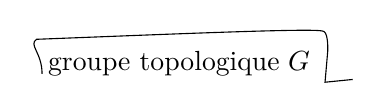
\begin{tikzpicture}[baseline=(phrase.base)]
\node[inner sep=0pt,anchor=base west] (phrase) at (0,0) {groupe topologique $G$};
\draw[line width=0.4pt]
 ([xshift=-2pt,yshift=1pt]phrase.south west)
 .. controls ([xshift=-2pt,yshift=4pt]phrase.west)
          and ([xshift=-7pt,yshift=2pt]phrase.north west)
 .. ([xshift=-4pt,yshift=4pt]phrase.north west)
 .. controls ([yshift=6pt]phrase.north)
          and ([yshift=8pt]phrase.north east)
 .. ([xshift=4pt,yshift=7pt]phrase.north east)
 .. controls ([xshift=6pt,yshift=7pt]phrase.north east)
          and ([xshift=6pt,yshift=2pt]phrase.north east)
 .. ([xshift=6pt]phrase.north east)
 -- ([xshift=5pt,yshift=-2pt]phrase.south east)
 -- ([xshift=15pt,yshift=-1pt]phrase.south east);
\end{tikzpicture}}
tel que \var{\deleted{\LMsourceMark{M007776}{\unsure{$\widetilde A_0^\circ$}}}}{\LMsourceMark{M007777}{\LMcancelledDoubts{\LMsourceMark{M007778}{\unsure{$\widetilde A_0^\circ$}}}}}{deletion}{140-2-s237-D003}\var{\inserted{$G^\circ$}}{\LMadded{$G^\circ$}}{insertion}{140-2-s237-I004} soit simplement connexe; \var{\deleted{soit}}{}{deletion}{140-2-s237-D004}
\var{\deleted{\LMsourceMark{M007779}{\unsure{posons}} $\mu=\mathrm{Centre}(\LMsourceMark{M007780}{\unsure{\widetilde A_0^\circ}})$}}{\LMsourceMark{M007781}{\LMcancelledDoubts{\LMsourceMark{M007782}{\unsure{posons}}\quad \(\LMsourceMark{M007783}{\unsure{\widetilde A_0^\circ}}\)}}}{deletion}{140-2-s237-D005}
\[
(67)\qquad\Pi_1(G^\circ)=0
\]
soit
\[
(68)\qquad \mu=\mathrm{Centre}(G^\circ),\qquad\Gamma=G/G^\circ
\]
\LMsourceMark{M007784}{\margin{on suppose $\mu$ discret (donc $G^\circ$ s'identifie au groupe rev. universel de $G^\circ/\mu=\mathcal H^\circ$ (si $\mathcal H=G/\mu$))}}
alors l'extension de groupes topologiques $G$
de $\Gamma$ par $G^\circ$ définit
\[
(69)\qquad\Gamma\longrightarrow\mathrm{Aut\,ext}(G^\circ)
\qquad(\longrightarrow\mathrm{Aut}(\mu).)
\]
et l'ens des classes d'extensions correspondantes
à une opération \var{\inserted{extérieure}}{\LMadded{extérieure}}{insertion}{140-2-s237-I005} donnée de $\Gamma$ sur $G^\circ$
est de façon naturelle un torseur sous
$H^2(\Gamma,\mu)$ (s'il n'est vide, ce \LMsourceMark{M007785}{\unsure{qui est|qu'on a}} exclu
par hypothèse de départ, en partant de $G$\ldots)
\LMsourceMark{M007786}{\margin{236}}

\LMflushnotes\LMflushpages
\ifnum\LMform=1
\begin{LMapparatus}
\LMentry{140-2-s237-I001}{insertion}{\inserted{à prétention}
}{\emph{\LMinsertedlabel}}{Ajout explicite de l'auteur : intégré à l'endroit indiqué par la transcription, sans modifier sa lecture.}{}
\LMentry{140-2-s237-D001}{suppression}{\deleted{\LMsourceMark{M007787}{\unsure{disposé}}}
}{\emph{\LMomittedlabel}}{Passage biffé dans le manuscrit : la suppression suit l'état final de l'auteur; les doutes de lecture restent signalés.}{}
\LMentry{140-2-s237-I002}{insertion}{\inserted{imposé}
}{\emph{\LMinsertedlabel}}{Ajout explicite de l'auteur : intégré à l'endroit indiqué par la transcription, sans modifier sa lecture.}{}
\LMentry{140-2-s237-D002}{suppression}{\deleted{liens}
}{\emph{\LMomittedlabel}}{Passage biffé dans le manuscrit : la suppression suit l'état final de l'auteur; les doutes de lecture restent signalés.}{}
\LMentry{140-2-s237-I003}{insertion}{\inserted{$\mu$-}
}{\emph{\LMinsertedlabel}}{Ajout explicite de l'auteur : intégré à l'endroit indiqué par la transcription, sans modifier sa lecture.}{}
\LMentry{140-2-s237-D003}{suppression}{\deleted{\LMsourceMark{M007788}{\unsure{$\widetilde A_0^\circ$}}}
}{\emph{\LMomittedlabel}}{Passage biffé dans le manuscrit : la suppression suit l'état final de l'auteur; les doutes de lecture restent signalés.}{}
\LMentry{140-2-s237-I004}{insertion}{\inserted{$G^\circ$}
}{\emph{\LMinsertedlabel}}{Ajout explicite de l'auteur : intégré à l'endroit indiqué par la transcription, sans modifier sa lecture.}{}
\LMentry{140-2-s237-D004}{suppression}{\deleted{soit}
}{\emph{\LMomittedlabel}}{Passage biffé dans le manuscrit : la suppression suit l'état final de l'auteur; les doutes de lecture restent signalés.}{}
\LMentry{140-2-s237-D005}{suppression}{\deleted{\LMsourceMark{M007789}{\unsure{posons}} $\mu=\mathrm{Centre}(\LMsourceMark{M007790}{\unsure{\widetilde A_0^\circ}})$}
}{\emph{\LMomittedlabel}}{Passage biffé dans le manuscrit : la suppression suit l'état final de l'auteur; les doutes de lecture restent signalés.}{}
\LMentry{140-2-s237-I005}{insertion}{\inserted{extérieure}
}{\emph{\LMinsertedlabel}}{Ajout explicite de l'auteur : intégré à l'endroit indiqué par la transcription, sans modifier sa lecture.}{}
\end{LMapparatus}
\fi
\ifnum\LMform=2
\par\smallskip\begingroup\footnotesize\Needspace{4\baselineskip}\csname @beginparpenalty\endcsname=10000\relax\noindent\textcolor{gray}{\rule{.2\linewidth}{.35pt}}\par\nobreak
\noindent\textit{\LMdoubtheading.}\par\nobreak
\LMcarryover{140-2-s237-D001}{\LMsourceMark{M007791}{\unsure{disposé}}
}
\LMcarryover{140-2-s237-D003}{\LMsourceMark{M007792}{\unsure{$\widetilde A_0^\circ$}}
}
\LMcarryover{140-2-s237-D005}{\LMsourceMark{M007793}{\unsure{posons}}\quad \(\LMsourceMark{M007794}{\unsure{\widetilde A_0^\circ}}\)
}
\par\endgroup\smallskip
\fi

\LMsourceMark{M007795}{\scanpage{238}}
Cette catégorie d'extensions est d'ailleurs équivalente
\var{\deleted{Elle \LMsourceMark{M007796}{\unsure{correspond}}}}{\LMsourceMark{M007797}{\LMcancelledDoubts{\LMsourceMark{M007798}{\unsure{correspond}}}}}{deletion}{140-2-s238-D001}
à celle des scindages d'une certaine
Gr.-catégorie définie par Sinh \var{\inserted{via $(69)$}}{\LMadded{via $(69)$}}{insertion}{140-2-s238-I001}, dont les $\Pi_0$ et
$\Pi_1$ sont respectivement $\var{\deleted{\LMsourceMark{M007799}{\unsure{\Pi_0}}}}{\LMsourceMark{M007800}{\LMcancelledDoubts{\(\LMsourceMark{M007801}{\unsure{\Pi_0}}\)}}}{deletion}{140-2-s238-D002}\Gamma$ et $\mu$ --- laquelle
est \var{\inserted{donc}}{\LMadded{donc}}{insertion}{140-2-s238-I002} ici scindée par la donnée de l'extension
$G$. (Dans le cas qui nous intéresse,
$\Gamma\simeq\mu\simeq\{\pm1\}$, et
cette extension est $\overline{\mathrm m}$ scindée, et correspond
à une opération d'ordre $2$ de $\Gamma$ sur $G^\circ$,
dont je doute fort que ce soit un autom intérieur.
En fait, j'ai l'impression que dans les
deux cas qui nous occupent ($\widetilde{\mathrm{GP}}(1,\mathbb C)$ et
$\widetilde A_0$) que $(69)$ est un \uline{iso}
$\Gamma=\{\pm1\}\xrightarrow{\sim}\mathrm{Autext}(G^\circ$

Ceci posé, la donnée d'un torseur sous
$\mathcal H=G/\mu$ définit $1^\circ$) un torseur sous $\Gamma$,
$\mathcal H\longrightarrow\Gamma\simeq\mathcal H/\mathcal H^\circ$; $2^\circ$) le groupoïde des
relèvements des relèvements de ce torseur
en un torseur sous $G$, qui est un
$\mu$-groupoïde \var{\inserted{connexe}}{\LMadded{connexe}}{insertion}{140-2-s238-I003} (sur lequel $\mu$ opère).
\LMsourceMark{M007802}{\margin{On suppose que $\Gamma$ opère \uline{trivialement} sur $\mu$ i.e. $\mu\subset\mathrm{Centre}(G)$}}

Si on \var{\deleted{\LMsourceMark{M007803}{\unsure{exp}}}}{\LMsourceMark{M007804}{\LMcancelledDoubts{\LMsourceMark{M007805}{\unsure{exp}}}}}{deletion}{140-2-s238-D003} reprend en termes de fibrés
sur un espace de base $S$ on trouve
\LMsourceMark{M007806}{\margin{237}}

\LMflushnotes\LMflushpages
\ifnum\LMform=1
\begin{LMapparatus}
\LMentry{140-2-s238-D001}{suppression}{\deleted{Elle \LMsourceMark{M007807}{\unsure{correspond}}}
}{\emph{\LMomittedlabel}}{Passage biffé dans le manuscrit : la suppression suit l'état final de l'auteur; les doutes de lecture restent signalés.}{}
\LMentry{140-2-s238-I001}{insertion}{\inserted{via $(69)$}
}{\emph{\LMinsertedlabel}}{Ajout explicite de l'auteur : intégré à l'endroit indiqué par la transcription, sans modifier sa lecture.}{}
\LMentry{140-2-s238-D002}{suppression}{\(\deleted{\LMsourceMark{M007808}{\unsure{\Pi_0}}}\)
}{\emph{\LMomittedlabel}}{Passage biffé dans le manuscrit : la suppression suit l'état final de l'auteur; les doutes de lecture restent signalés.}{}
\LMentry{140-2-s238-I002}{insertion}{\inserted{donc}
}{\emph{\LMinsertedlabel}}{Ajout explicite de l'auteur : intégré à l'endroit indiqué par la transcription, sans modifier sa lecture.}{}
\LMentry{140-2-s238-I003}{insertion}{\inserted{connexe}
}{\emph{\LMinsertedlabel}}{Ajout explicite de l'auteur : intégré à l'endroit indiqué par la transcription, sans modifier sa lecture.}{}
\LMentry{140-2-s238-D003}{suppression}{\deleted{\LMsourceMark{M007809}{\unsure{exp}}}
}{\emph{\LMomittedlabel}}{Passage biffé dans le manuscrit : la suppression suit l'état final de l'auteur; les doutes de lecture restent signalés.}{}
\end{LMapparatus}
\fi
\ifnum\LMform=2
\par\smallskip\begingroup\footnotesize\Needspace{4\baselineskip}\csname @beginparpenalty\endcsname=10000\relax\noindent\textcolor{gray}{\rule{.2\linewidth}{.35pt}}\par\nobreak
\noindent\textit{\LMdoubtheading.}\par\nobreak
\LMcarryover{140-2-s238-D001}{\LMsourceMark{M007810}{\unsure{correspond}}
}
\LMcarryover{140-2-s238-D002}{\(\LMsourceMark{M007811}{\unsure{\Pi_0}}\)
}
\LMcarryover{140-2-s238-D003}{\LMsourceMark{M007812}{\unsure{exp}}
}
\par\endgroup\smallskip
\fi

\LMsourceMark{M007813}{\scanpage{239}}
\LMsourceMark{M007814}{\mspage{120}}
encore sur $S$ (pour tt $\mathcal H_S$-torseur topologique)
un couple $(\omega,\LMsourceMark{M007815}{\unsure{\mathcal R|R}})$ d'un $\Gamma$-torseur, et d'
une $\mu$-gerbe sur $S$, qui sont décrits (à \LMsourceMark{M007816}{\unsure{isom.}}
\var{\inserted{\LMsourceMark{M007817}{\illegible{1}} \LMsourceMark{M007818}{\unsure{équival.}}}}{\LMadded{\LMsourceMark{M007819}{\illegible{1}} \LMsourceMark{M007820}{\unsure{équival.}}}}{insertion}{140-2-s239-I001}
\LMsourceMark{M007821}{\unsure{à équiv.|et équiv.}} près) par $H^1(S,\Gamma)$ et $H^2(S,\mu)$
respectivement. On voudrait dégager des
conditions \var{\inserted{sur $G$ et sur $S$}}{\LMadded{sur $G$ et sur $S$}}{insertion}{140-2-s239-I002} pour que l'application
\[
(70)\qquad H^1(S,\mathcal H)\longrightarrow H^1(S,\Gamma)\times H^2(S,\mu)
\]
soit bijective.
\LMsourceMark{M007822}{\margin{\uline{NB} $\omega$ ne dépend pas du choix de l'extension \LMsourceMark{M007823}{\unsure{$\widetilde G$}} de $\mathcal H$ par \LMsourceMark{M007824}{\unsure{$\mathfrak z$|$\zeta$}}${}\simeq\Pi_1(\mathcal H^\circ)$; \LMsourceMark{M007825}{\unsure{par contre}} $\mathcal R$ en dépend (et il \LMsourceMark{M007826}{\unsure{faudrait}} voir comment)}}

Injectivité : Si l'image \var{\inserted{d'un $\zeta\in H^1(S,\mathcal H)$,}}{\LMadded{d'un $\zeta\in H^1(S,\mathcal H)$,}}{insertion}{140-2-s239-I003}
dans $H^2(S,\mu)$ est nulle,
l'élément de $H^1(S,\mathcal H)$ se relève en un élément $\widetilde\zeta$
de $H^1(S,\widetilde{\mathcal H}=G)$; \LMsourceMark{M007827}{\unsure{dont}} l'image dans $H^1(S,\Gamma)$
\LMsourceMark{M007828}{\unsure{par}} $G\longrightarrow\Gamma$ est la $\overline{\mathrm m}$ que celle de $\zeta$, donc si
elle est triviale, on voit que $\widetilde\zeta$ provient d'
un $\widetilde\zeta_0\in H^1(S,G^\circ)$. Si on sait que
$H^1(S,G^\circ)=(1)$, on gagne. Par les
marteaux-pilons d'homotopie, ça marche
si $\exists n\in\mathbb N$ avec
\[
\Pi_i(G^\circ)=0\quad\text{si}\quad i\leq n
\]
\var{\inserted{(donc $\Pi_i(B_{G^\circ})=0$ si $i\leq n+1$)}}{\LMadded{(donc $\Pi_i(B_{G^\circ})=0$ si $i\leq n+1$)}}{insertion}{140-2-s239-I004}
\var{\deleted{$\Pi_i(S)=0$ si $i>n+1$}}{}{deletion}{140-2-s239-D001}
\var{\deleted{$\dim S\leq n+1$}}{}{deletion}{140-2-s239-D002}
$S$ un CW-complexe de dim $\leq n+1$
\LMsourceMark{M007829}{\margin{dans le cas qui nous occupe, on peut prendre $n=2$}}

Pour la surjectivité, notons que \LMsourceMark{M007830}{\unsure{pour|d'abord}} un
\LMsourceMark{M007831}{\margin{238}}

\LMflushnotes\LMflushpages
\ifnum\LMform=1
\begin{LMapparatus}
\LMentry{140-2-s239-I001}{insertion}{\inserted{\LMsourceMark{M007832}{\illegible{1}} \LMsourceMark{M007833}{\unsure{équival.}}}
}{\emph{\LMinsertedlabel}}{Ajout explicite de l'auteur : intégré à l'endroit indiqué par la transcription, sans modifier sa lecture.}{}
\LMentry{140-2-s239-I002}{insertion}{\inserted{sur $G$ et sur $S$}
}{\emph{\LMinsertedlabel}}{Ajout explicite de l'auteur : intégré à l'endroit indiqué par la transcription, sans modifier sa lecture.}{}
\LMentry{140-2-s239-I003}{insertion}{\inserted{d'un $\zeta\in H^1(S,\mathcal H)$,}
}{\emph{\LMinsertedlabel}}{Ajout explicite de l'auteur : intégré à l'endroit indiqué par la transcription, sans modifier sa lecture.}{}
\LMentry{140-2-s239-I004}{insertion}{\inserted{(donc $\Pi_i(B_{G^\circ})=0$ si $i\leq n+1$)}
}{\emph{\LMinsertedlabel}}{Ajout explicite de l'auteur : intégré à l'endroit indiqué par la transcription, sans modifier sa lecture.}{}
\LMentry{140-2-s239-D001}{suppression}{\deleted{$\Pi_i(S)=0$ si $i>n+1$}
}{\emph{\LMomittedlabel}}{Passage biffé dans le manuscrit : la suppression suit l'état final de l'auteur; les doutes de lecture restent signalés.}{}
\LMentry{140-2-s239-D002}{suppression}{\deleted{$\dim S\leq n+1$}
}{\emph{\LMomittedlabel}}{Passage biffé dans le manuscrit : la suppression suit l'état final de l'auteur; les doutes de lecture restent signalés.}{}
\end{LMapparatus}
\fi

\LMsourceMark{M007834}{\scanpage{240}}
élément de $H^2(S,\mu)$, l'obstruction à ce qu'il
se relève en un élément \var{\inserted{$\zeta$}}{\LMadded{$\zeta$}}{insertion}{140-2-s240-I001} de $H^1(S,\mathcal H)$ est
dans $H^2(S,G)$ [par la suite exacte
de \LMsourceMark{M007835}{\unsure{coh.}} associée : $1\longrightarrow\mu_S\longrightarrow G_S\longrightarrow\mathcal H_S\longrightarrow1$]
il faut exprimer qu'une certaine \var{\deleted{\LMsourceMark{M007836}{\illegible{1}}}}{\LMsourceMark{M007837}{\LMcancelledDoubts{\LMsourceMark{M007838}{\illegible{1}}}}}{deletion}{140-2-s240-D001} gerbe
liée par $G_S$ est neutre --- brr!. Mais
partons plutôt de l'élément \var{\inserted{\LMsourceMark{M007839}{\unsure{$\omega$|$\widetilde\zeta$}}}}{\LMadded{\LMsourceMark{M007840}{\unsure{$\omega$|$\widetilde\zeta$}}}}{insertion}{140-2-s240-I002} de $H^1(S,\Gamma)$,
si l'extension de $\Gamma$ par \var{\deleted{\LMsourceMark{M007841}{\unsure{$G^\circ$}}}}{\LMsourceMark{M007842}{\LMcancelledDoubts{\LMsourceMark{M007843}{\unsure{$G^\circ$}}}}}{deletion}{140-2-s240-D002}$\mathcal H^\circ$ est scindée, alors
on peut trouver un $\zeta_0\in H^1(S,\mathcal H_S)$ qui
donne naissance à \LMsourceMark{M007844}{\unsure{$\omega$}}. Elle a une certaine
obstruction $\rho_0$ dans $H^2(S,\mu)$, et il s'agit
de corriger $\zeta_0$ en $\zeta$, \var{\inserted{de}}{\LMadded{de}}{insertion}{140-2-s240-I003} telle façon que
l'obstruction devienne $\rho\in H^2(S,\mu)$ donné.
\var{\deleted{On dispose de}}{}{deletion}{140-2-s240-D003} \var{\inserted{Utilisant $\zeta_0$}}{\LMadded{Utilisant $\zeta_0$}}{insertion}{140-2-s240-I004} pour tordre $\mathcal H_S$ en
$\mathcal H'_S$, et (via l'opération de $\mathcal H_S$ \var{\inserted{$=G_S/\mu_S$}}{\LMadded{$=G_S/\mu_S$}}{insertion}{140-2-s240-I005} sur $G_S$,
compte tenu que $\mu_S\subset\mathrm{centre}\,G_S$) pour
tordre $G_S$ aussi \var{\inserted{en $G'_S$}}{\LMadded{en $G'_S$}}{insertion}{140-2-s240-I006}, d'où
\[
1\longrightarrow\mu\longrightarrow G'_S\longrightarrow\mathcal H'_S\longrightarrow1
\]
on trouve que les $\zeta$ ayant $\overline{\mathrm m}$ image dans $H^1(S,\Gamma)$
\LMsourceMark{M007845}{\margin{239}}

\LMflushnotes\LMflushpages
\ifnum\LMform=1
\begin{LMapparatus}
\LMentry{140-2-s240-I001}{insertion}{\inserted{$\zeta$}
}{\emph{\LMinsertedlabel}}{Ajout explicite de l'auteur : intégré à l'endroit indiqué par la transcription, sans modifier sa lecture.}{}
\LMentry{140-2-s240-D001}{suppression}{\deleted{\LMsourceMark{M007846}{\illegible{1}}}
}{\emph{\LMomittedlabel}}{Passage biffé dans le manuscrit : la suppression suit l'état final de l'auteur; les doutes de lecture restent signalés.}{}
\LMentry{140-2-s240-I002}{insertion}{\inserted{\LMsourceMark{M007847}{\unsure{$\omega$|$\widetilde\zeta$}}}
}{\emph{\LMinsertedlabel}}{Ajout explicite de l'auteur : intégré à l'endroit indiqué par la transcription, sans modifier sa lecture.}{}
\LMentry{140-2-s240-D002}{suppression}{\deleted{\LMsourceMark{M007848}{\unsure{$G^\circ$}}}
}{\emph{\LMomittedlabel}}{Passage biffé dans le manuscrit : la suppression suit l'état final de l'auteur; les doutes de lecture restent signalés.}{}
\LMentry{140-2-s240-I003}{insertion}{\inserted{de}
}{\emph{\LMinsertedlabel}}{Ajout explicite de l'auteur : intégré à l'endroit indiqué par la transcription, sans modifier sa lecture.}{}
\LMentry{140-2-s240-D003}{suppression}{\deleted{On dispose de}
}{\emph{\LMomittedlabel}}{Passage biffé dans le manuscrit : la suppression suit l'état final de l'auteur; les doutes de lecture restent signalés.}{}
\LMentry{140-2-s240-I004}{insertion}{\inserted{Utilisant $\zeta_0$}
}{\emph{\LMinsertedlabel}}{Ajout explicite de l'auteur : intégré à l'endroit indiqué par la transcription, sans modifier sa lecture.}{}
\LMentry{140-2-s240-I005}{insertion}{\inserted{$=G_S/\mu_S$}
}{\emph{\LMinsertedlabel}}{Ajout explicite de l'auteur : intégré à l'endroit indiqué par la transcription, sans modifier sa lecture.}{}
\LMentry{140-2-s240-I006}{insertion}{\inserted{en $G'_S$}
}{\emph{\LMinsertedlabel}}{Ajout explicite de l'auteur : intégré à l'endroit indiqué par la transcription, sans modifier sa lecture.}{}
\end{LMapparatus}
\fi
\ifnum\LMform=2
\par\smallskip\begingroup\footnotesize\Needspace{4\baselineskip}\csname @beginparpenalty\endcsname=10000\relax\noindent\textcolor{gray}{\rule{.2\linewidth}{.35pt}}\par\nobreak
\noindent\textit{\LMdoubtheading.}\par\nobreak
\LMcarryover{140-2-s240-D001}{\LMsourceMark{M007849}{\illegible{1}}
}
\LMcarryover{140-2-s240-D002}{\LMsourceMark{M007850}{\unsure{$G^\circ$}}
}
\par\endgroup\smallskip
\fi

% END PACKAGE LM_P024
% BEGIN PACKAGE LM_P025
\ifnum\LMform<2\Needspace{11\baselineskip}\subsection*{Scans 241--250}\fi
\LMsourceMark{M007851}{\scanpage{241}}
\LMsourceMark{M007852}{\mspage{121}}
% l. 1
que \LMsourceMark{M007853}{\unsure{$\xi_0$}} correspondent \var{\inserted{$1-1$}}{\LMadded{$1-1$}}{insertion}{140-2-s241-I001} aux
$\xi'\in H^1(S,\mathcal H'_S)$.
% A hatched loop with a descender stands under the H of H'_S (an overwritten letter, perhaps a G).

% l. 2
Pour un tel \var{\deleted{\LMsourceMark{M007854}{\unsure{$\mathcal H'_S$}}}}{\LMsourceMark{M007855}{\LMcancelledDoubts{\LMsourceMark{M007856}{\unsure{$\mathcal H'_S$}}}}}{deletion}{140-2-s241-D001} $\xi'$, soit
$\delta'(\xi')\in H^2(S,\mu)$
% l. 3
l'obstruction à le relever en $H^1(S,\LMsourceMark{M007857}{\unsure{\mathcal G'_S|\mathcal G_S}})$,
% l. 4
et $\delta(\xi')=\delta(\xi)$ l'obstruction à le relever
% l. 5
en $H^1(S,\mathcal G_S)$. Sauf erreur on a
% l. 6
\[
\delta'(\xi')=\delta(\xi')-\rho_0
\]
% l. 7
i.e.
\[
\delta(\xi')=\delta(\xi)=\delta'(\xi')+\rho_0
\]
% l. 8
et on veut $\delta(\xi)=\rho$ i.e.
% l. 9
\[
\var{\deleted{\LMsourceMark{M007858}{\unsure{\delta(\xi')}}=}}{\LMsourceMark{M007859}{\LMcancelledDoubts{\(\LMsourceMark{M007860}{\unsure{\delta(\xi')}}\)}}}{deletion}{140-2-s241-D002}\quad
\delta'(\xi')=\rho-\rho_0
\]
% l. 10
et la question revient encore à \var{\deleted{\LMsourceMark{M007861}{\illegible{3}}}}{\LMsourceMark{M007862}{\LMcancelledDoubts{\LMsourceMark{M007863}{\illegible{3}}}}}{deletion}{140-2-s241-D003} \var{\inserted{la}}{\LMadded{la}}{insertion}{140-2-s241-I002}
% l. 11
surjectivité de $H^1(S,\mathcal H'_S)\longrightarrow H^2(S,\mu)$
\var{\deleted{\LMsourceMark{M007864}{\illegible{1}}}}{\LMsourceMark{M007865}{\LMcancelledDoubts{\LMsourceMark{M007866}{\illegible{1}}}}}{deletion}{140-2-s241-D004}
% l. 12
--- je ne m'en tire pas. Il faudrait
% l. 13
consulter des gens compétents, comme
% l. 14
Giraud ou Larry Breen. On sent qu'il
% l. 15
faudrait travailler avec un Gr-champ $\underline{\underline{\mathcal H}}$
% l. 16
de coefficients, d'invariants $\underline{\pi}_0\simeq\Gamma$ et
$\underline{\pi}_1\simeq\mu$,
% l. 17
(mais pas nécessairement un champ de Picard!)
% l. 18
\var{\deleted{avec}}{}{deletion}{140-2-s241-D005} et
$H^1(S,\underline{\underline{\mathcal H}})\simeq\text{Classes d'applications}$
% l. 19
de $S$ dans $B\underline{\underline{\mathcal H}}$, qui est un espace
% l. 20
connexe avec $\pi_1(B\underline{\underline{\mathcal H}})\simeq\Gamma$,
$\pi_2(B\underline{\underline{\mathcal H}})=\mu$.
% l. 21
Ici la classe de \LMsourceMark{M007867}{\unsure{Postnikoff}} dans $H^3(\Gamma,\mu)$ est nulle,
\LMsourceMark{M007868}{\margin{240}}

\LMflushnotes\LMflushpages
\ifnum\LMform=1
\begin{LMapparatus}
\LMentry{140-2-s241-I001}{insertion}{\inserted{$1-1$}
}{\emph{\LMinsertedlabel}}{Ajout explicite de l'auteur : intégré à l'endroit indiqué par la transcription, sans modifier sa lecture.}{}
\LMentry{140-2-s241-D001}{suppression}{\deleted{\LMsourceMark{M007869}{\unsure{$\mathcal H'_S$}}}
}{\emph{\LMomittedlabel}}{Passage biffé dans le manuscrit : la suppression suit l'état final de l'auteur; les doutes de lecture restent signalés.}{}
\LMentry{140-2-s241-D002}{suppression}{\(\deleted{\LMsourceMark{M007870}{\unsure{\delta(\xi')}}=}\)
}{\emph{\LMomittedlabel}}{Passage biffé dans le manuscrit : la suppression suit l'état final de l'auteur; les doutes de lecture restent signalés.}{}
\LMentry{140-2-s241-D003}{suppression}{\deleted{\LMsourceMark{M007871}{\illegible{3}}}
}{\emph{\LMomittedlabel}}{Passage biffé dans le manuscrit : la suppression suit l'état final de l'auteur; les doutes de lecture restent signalés.}{}
\LMentry{140-2-s241-I002}{insertion}{\inserted{la}
}{\emph{\LMinsertedlabel}}{Ajout explicite de l'auteur : intégré à l'endroit indiqué par la transcription, sans modifier sa lecture.}{}
\LMentry{140-2-s241-D004}{suppression}{\deleted{\LMsourceMark{M007872}{\illegible{1}}}
}{\emph{\LMomittedlabel}}{Passage biffé dans le manuscrit : la suppression suit l'état final de l'auteur; les doutes de lecture restent signalés.}{}
\LMentry{140-2-s241-D005}{suppression}{\deleted{avec}
}{\emph{\LMomittedlabel}}{Passage biffé dans le manuscrit : la suppression suit l'état final de l'auteur; les doutes de lecture restent signalés.}{}
\end{LMapparatus}
\fi
\ifnum\LMform=2
\par\smallskip\begingroup\footnotesize\Needspace{4\baselineskip}\csname @beginparpenalty\endcsname=10000\relax\noindent\textcolor{gray}{\rule{.2\linewidth}{.35pt}}\par\nobreak
\noindent\textit{\LMdoubtheading.}\par\nobreak
\LMcarryover{140-2-s241-D001}{\LMsourceMark{M007873}{\unsure{$\mathcal H'_S$}}
}
\LMcarryover{140-2-s241-D002}{\(\LMsourceMark{M007874}{\unsure{\delta(\xi')}}\)
}
\LMcarryover{140-2-s241-D003}{\LMsourceMark{M007875}{\illegible{3}}
}
\LMcarryover{140-2-s241-D004}{\LMsourceMark{M007876}{\illegible{1}}
}
\par\endgroup\smallskip
\fi

\LMsourceMark{M007877}{\scanpage{242}}
% l. 1
[mais peut-être n'y a-t-il pas lieu de
% l. 2
trop se raccrocher à cette hypothèse,
% l. 3
correspondant à l'existence d'une \var{\inserted{ext.}}{\LMadded{ext.}}{insertion}{140-2-s242-I001} $\mathcal G$ de $\mathcal H$
\var{\inserted{par $\pi_1(\mathcal H^\circ)$}}{\LMadded{par $\pi_1(\mathcal H^\circ)$}}{insertion}{140-2-s242-I002} \var{\deleted{\LMsourceMark{M007878}{\illegible{1}}}}{\LMsourceMark{M007879}{\LMcancelledDoubts{\LMsourceMark{M007880}{\illegible{1}}}}}{deletion}{140-2-s242-D001}
% l. 4
qui redonne l'extension universelle de
% l. 5
$\mathcal H^\circ$ par $\pi_1(\mathcal H^\circ)$] on a un \LMsourceMark{M007881}{\unsure{hom.}}
% l. 6
$B\mathcal H$ \var{\deleted{\LMsourceMark{M007882}{\illegible{1}}}}{\LMsourceMark{M007883}{\LMcancelledDoubts{\LMsourceMark{M007884}{\illegible{1}}}}}{deletion}{140-2-s242-D002} $\longrightarrow B\underline{\underline{\mathcal H}}$
qui induit un iso pour
% The struck mark stands under the first BH (perhaps a cancelled double underline).
% l. 7
les $\pi_i$ pour $i\leq2$, et pour $i\leq n$
(où $n\geq2$ \var{\inserted{est donné}}{\LMadded{est donné}}{insertion}{140-2-s242-I003})
% l. 8
sss $\pi_i(B\mathcal H)=0$ pour $2<i\leq n$, i.e.
% l. 9
$\pi_i(\mathcal H)=0$ pour $2\leq i\leq n-1$ [dans le cas
% l. 10
qui nous intéresse $\mathcal H=A_0$, on peut
% l. 11
prendre $n=3$). Ceci implique que pour
% l. 12
tout C-W-complexe $S$ de dim $\leq n$,
% l. 13
on a \var{\inserted{(Hot désignant les morphismes dans
la cat. homotopique non ponctuée)}}{\LMadded{(Hot désignant les morphismes dans
la cat. homotopique non ponctuée)}}{insertion}{140-2-s242-I004}
% l. 14
\[
\mathrm{Hot}(S,B\mathcal H)\xrightarrow{\sim}
\mathrm{Hot}(S,B\underline{\underline{\mathcal H}})
\]
% l. 15
\LMsourceMark{M007885}{\unsure{c.à.d.|i.e.}}
\[
H^1(S,\mathcal H)\xrightarrow{\simeq}
H^1(S,\var{\deleted{\LMsourceMark{M007886}{\unsure{B}}}}{\LMsourceMark{M007887}{\LMcancelledDoubts{\(\LMsourceMark{M007888}{\unsure{B}}\)}}}{deletion}{140-2-s242-D003}\underline{\underline{\mathcal H}})
\]

% l. 16
Mais si l'invariant de \LMsourceMark{M007889}{\unsure{Postnikoff}}-Sinh
% l. 17
$\LMsourceMark{M007890}{\unsure{K|k}}\in H^3(\Gamma,\mu)$ est nul,
\var{\deleted{\LMsourceMark{M007891}{\illegible{1}}}}{\LMsourceMark{M007892}{\LMcancelledDoubts{\LMsourceMark{M007893}{\illegible{1}}}}}{deletion}{140-2-s242-D004} (ainsi que l'action
% l. 18
de $\Gamma$ sur $\mu$) alors sauf erreur
$B\underline{\underline{\mathcal H}}$ s'iden%
% l. 19
tifie à un produit $K(\Gamma,1)\times K(\pi,2)$,
\var{\deleted{et}}{}{deletion}{140-2-s242-D005}
% l. 20
(cette ``identification'' dépendant justement du
\LMsourceMark{M007894}{\margin{241}}

\LMflushnotes\LMflushpages
\ifnum\LMform=1
\begin{LMapparatus}
\LMentry{140-2-s242-I001}{insertion}{\inserted{ext.}
}{\emph{\LMinsertedlabel}}{Ajout explicite de l'auteur : intégré à l'endroit indiqué par la transcription, sans modifier sa lecture.}{}
\LMentry{140-2-s242-I002}{insertion}{\inserted{par $\pi_1(\mathcal H^\circ)$}
}{\emph{\LMinsertedlabel}}{Ajout explicite de l'auteur : intégré à l'endroit indiqué par la transcription, sans modifier sa lecture.}{}
\LMentry{140-2-s242-D001}{suppression}{\deleted{\LMsourceMark{M007895}{\illegible{1}}}
}{\emph{\LMomittedlabel}}{Passage biffé dans le manuscrit : la suppression suit l'état final de l'auteur; les doutes de lecture restent signalés.}{}
\LMentry{140-2-s242-D002}{suppression}{\deleted{\LMsourceMark{M007896}{\illegible{1}}}
}{\emph{\LMomittedlabel}}{Passage biffé dans le manuscrit : la suppression suit l'état final de l'auteur; les doutes de lecture restent signalés.}{}
\LMentry{140-2-s242-I003}{insertion}{\inserted{est donné}
}{\emph{\LMinsertedlabel}}{Ajout explicite de l'auteur : intégré à l'endroit indiqué par la transcription, sans modifier sa lecture.}{}
\LMentry{140-2-s242-I004}{insertion}{\inserted{(Hot désignant les morphismes dans
la cat. homotopique non ponctuée)}
}{\emph{\LMinsertedlabel}}{Ajout explicite de l'auteur : intégré à l'endroit indiqué par la transcription, sans modifier sa lecture.}{}
\LMentry{140-2-s242-D003}{suppression}{\(\deleted{\LMsourceMark{M007897}{\unsure{B}}}\)
}{\emph{\LMomittedlabel}}{Passage biffé dans le manuscrit : la suppression suit l'état final de l'auteur; les doutes de lecture restent signalés.}{}
\LMentry{140-2-s242-D004}{suppression}{\deleted{\LMsourceMark{M007898}{\illegible{1}}}
}{\emph{\LMomittedlabel}}{Passage biffé dans le manuscrit : la suppression suit l'état final de l'auteur; les doutes de lecture restent signalés.}{}
\LMentry{140-2-s242-D005}{suppression}{\deleted{et}
}{\emph{\LMomittedlabel}}{Passage biffé dans le manuscrit : la suppression suit l'état final de l'auteur; les doutes de lecture restent signalés.}{}
\end{LMapparatus}
\fi
\ifnum\LMform=2
\par\smallskip\begingroup\footnotesize\Needspace{4\baselineskip}\csname @beginparpenalty\endcsname=10000\relax\noindent\textcolor{gray}{\rule{.2\linewidth}{.35pt}}\par\nobreak
\noindent\textit{\LMdoubtheading.}\par\nobreak
\LMcarryover{140-2-s242-D001}{\LMsourceMark{M007899}{\illegible{1}}
}
\LMcarryover{140-2-s242-D002}{\LMsourceMark{M007900}{\illegible{1}}
}
\LMcarryover{140-2-s242-D003}{\(\LMsourceMark{M007901}{\unsure{B}}\)
}
\LMcarryover{140-2-s242-D004}{\LMsourceMark{M007902}{\illegible{1}}
}
\par\endgroup\smallskip
\fi

\LMsourceMark{M007903}{\scanpage{243}}
\LMsourceMark{M007904}{\mspage{122}}
% l. 1
choix des $H^2(\pi_1,\pi_2)\simeq H^2(\Gamma,\mu)$ !), et par
% l. 2
suite
\[
H^1(S,\underline{\underline{\mathcal H}})\xrightarrow{\simeq}
H^1(S,\Gamma)\times H^2(S,\mu)
\]
% l. 3
pour tt espace $S$, donc pour $S$ un C-W-%
% l. 4
complexe de dim $\leq n$
% l. 5
\[
(71)\qquad
H^1(S,\mathcal H)\xrightarrow{\simeq}H^1(S,\Gamma)\times H^2(S,\mu)
\]

% l. 6
Donc la classification des fibrés en sphères
% l. 7
topologiques sur un espace topologique $S$,
% l. 8
pour un C-W complexe $S$ de dim $\leq3$,
% l. 9
marche bel et bien. Bien entendu, le
% l. 10
fait qu'on soit obligé ici de se borner à
% l. 11
des \var{\deleted{\LMsourceMark{M007905}{\illegible{1}}}}{\LMsourceMark{M007906}{\LMcancelledDoubts{\LMsourceMark{M007907}{\illegible{1}}}}}{deletion}{140-2-s243-D001} $S$ de dim $\leq3$ tient au fait
% l. 12
que nous n'avons trouvé \var{\deleted{\LMsourceMark{M007908}{\unsure{qu'}}}}{\LMsourceMark{M007909}{\LMcancelledDoubts{\LMsourceMark{M007910}{\unsure{qu'}}}}}{deletion}{140-2-s243-D002}
(via $\underline{\underline{\mathcal H}}$)
% l. 13
qu'une description $2$-isotopique (et non
% l. 14
$\infty$-isotopique) de la catégorie des $2$-sphères
% l. 15
topologiques.

% l. 16
Je voudrais reprendre la classification
% l. 17
pour un CW-complexe $S$ quelconque, en
% l. 18
utilisant le fait que l'inclusion
% l. 19
\[
\widetilde{\mathrm{GP}}(1,\mathbb C)\hookrightarrow A_0
\]
\LMsourceMark{M007911}{\margin{242}}

\LMflushnotes\LMflushpages
\ifnum\LMform=1
\begin{LMapparatus}
\LMentry{140-2-s243-D001}{suppression}{\deleted{\LMsourceMark{M007912}{\illegible{1}}}
}{\emph{\LMomittedlabel}}{Passage biffé dans le manuscrit : la suppression suit l'état final de l'auteur; les doutes de lecture restent signalés.}{}
\LMentry{140-2-s243-D002}{suppression}{\deleted{\LMsourceMark{M007913}{\unsure{qu'}}}
}{\emph{\LMomittedlabel}}{Passage biffé dans le manuscrit : la suppression suit l'état final de l'auteur; les doutes de lecture restent signalés.}{}
\end{LMapparatus}
\fi
\ifnum\LMform=2
\par\smallskip\begingroup\footnotesize\Needspace{4\baselineskip}\csname @beginparpenalty\endcsname=10000\relax\noindent\textcolor{gray}{\rule{.2\linewidth}{.35pt}}\par\nobreak
\noindent\textit{\LMdoubtheading.}\par\nobreak
\LMcarryover{140-2-s243-D001}{\LMsourceMark{M007914}{\illegible{1}}
}
\LMcarryover{140-2-s243-D002}{\LMsourceMark{M007915}{\unsure{qu'}}
}
\par\endgroup\smallskip
\fi

\LMsourceMark{M007916}{\scanpage{244}}
% l. 1
est une équivalence d'homotopie, et induit
% l. 2
donc une bijection
% l. 3
\[
H^1(S,\widetilde{\mathrm{GP}}(1,\mathbb C))\longrightarrow H^1(S,A_0)
\]
% l. 4
et $\overline{\mathrm m}$ une $\infty$-équivalence des $\infty$-catégories des
% l. 5
\var{\deleted{fibrés}}{}{deletion}{140-2-s244-D001} \var{\inserted{torseurs}}{\LMadded{torseurs}}{insertion}{140-2-s244-I001} sur $S$, de \var{\deleted{\LMsourceMark{M007917}{\illegible{1}}}}{\LMsourceMark{M007918}{\LMcancelledDoubts{\LMsourceMark{M007919}{\illegible{1}}}}}{deletion}{140-2-s244-D002} groupes
$\widetilde{\mathrm{GP}}$ (correspondant
% l. 6
aux fibrés en sphères conformes, ou en
% l. 7
droites projectives sur une \var{\deleted{corps}}{}{deletion}{140-2-s244-D003} $\mathbb R$-algèbre
\var{\inserted{(non précisée)}}{\LMadded{(non précisée)}}{insertion}{140-2-s244-I002}
% l. 8
isomorphe à $\mathbb C$) et de groupe $A_0$ --- correspondant
% l. 9
aux fibrés en sphères sur $S$.

% l. 10
Le premier invariant d'un fibré de groupe $\widetilde{\mathrm{GP}}$
% l. 11
est un \var{\deleted{fibré}}{}{deletion}{140-2-s244-D004} torseur \LMsourceMark{M007920}{\unsure{$\eta$|$T$}} sous $(\mathbb Z/2\mathbb Z)_S$
\var{\deleted{\LMsourceMark{M007921}{\illegible{2}}}}{\LMsourceMark{M007922}{\LMcancelledDoubts{\LMsourceMark{M007923}{\illegible{2}}}}}{deletion}{140-2-s244-D005} défini (\LMsourceMark{M007924}{\unsure{à isom.}}
% l. 12
\uline{non unique} \var{\inserted{près) par un}}{\LMadded{près) par un}}{insertion}{140-2-s244-I003} $\chi\ (\in H^1(S,\mathbb Z/2\mathbb Z))$.
% Physical order: "non unique" opens l. 12 under "est un"; "près) par un" is raised after the
% parenthesis of H^1; linearised as the sense requires.
\LMsourceMark{M007925}{\margin{i.e. un \LMsourceMark{M007926}{\unsure{rev. étale|rev. double}} de degré $2$.
La donnée de \LMsourceMark{M007927}{\unsure{$\eta$|$\chi$}} revient à la donnée d'un système \LMsourceMark{M007928}{\unsure{$T$}} d'entiers
tordus sur $S$.}}
% l. 13
\var{\inserted{Ce torseur}}{\LMadded{Ce torseur}}{insertion}{140-2-s244-I004} servira à tordre $\mathbb C$
(via l'opération \var{\inserted{fidèle}}{\LMadded{fidèle}}{insertion}{140-2-s244-I005} de $\mathbb Z/2\mathbb Z$ sur
% l. 14
la $\mathbb R$-extension $\mathbb C$), \var{\deleted{et}}{}{deletion}{140-2-s244-D006} d'où un fibré loc.
\var{\deleted{\LMsourceMark{M007929}{\illegible{1}}}}{\LMsourceMark{M007930}{\LMcancelledDoubts{\LMsourceMark{M007931}{\illegible{1}}}}}{deletion}{140-2-s244-D007}
% l. 15
constant en \var{\deleted{corps}}{}{deletion}{140-2-s244-D008} extensions \var{\inserted{quadratiques}}{\LMadded{quadratiques}}{insertion}{140-2-s244-I006}
de $\mathbb R$ \var{\deleted{\LMsourceMark{M007932}{\illegible{1}}}}{\LMsourceMark{M007933}{\LMcancelledDoubts{\LMsourceMark{M007934}{\illegible{1}}}}}{deletion}{140-2-s244-D009},
% l. 16
soit $C$, et on \var{\deleted{prendra le}}{}{deletion}{140-2-s244-D010} enrichira $S$
% l. 17
par le faisceau \var{\inserted{$\underline C_S$ (ou $\underline C$)}}{\LMadded{$\underline C_S$ (ou $\underline C$)}}{insertion}{140-2-s244-I007} des sections continues de
% l. 18
$C$ (ce qui est une façon de tordre
% l. 19
\var{\deleted{$\mathrm{Sl}(2,$}}{}{deletion}{140-2-s244-D011} $\mathrm{GP}(1,\mathbb C)_S$
en $\mathrm{GP}(1,C)_S=\mathrm{GP}(1,\underline C)$))
% l. 20
et il s'agit de \var{\deleted{\LMsourceMark{M007935}{\unsure{donc}}}}{\LMsourceMark{M007936}{\LMcancelledDoubts{\LMsourceMark{M007937}{\unsure{donc}}}}}{deletion}{140-2-s244-D012} décrire de façon
% l. 21
compréhensible \var{\deleted{la catégorie}}{}{deletion}{140-2-s244-D013} \var{\inserted{--- en passant}}{\LMadded{--- en passant}}{insertion}{140-2-s244-I008} au besoin,
% l. 22
aux \var{\deleted{\LMsourceMark{M007938}{\unsure{$\infty$}}}}{\LMsourceMark{M007939}{\LMcancelledDoubts{\LMsourceMark{M007940}{\unsure{$\infty$}}}}}{deletion}{140-2-s244-D014}$n$-isotopiques, pour $n=\ldots$ --- la catégorie
\LMsourceMark{M007941}{\margin{243}}

\LMflushnotes\LMflushpages
\ifnum\LMform=1
\begin{LMapparatus}
\LMentry{140-2-s244-D001}{suppression}{\deleted{fibrés}
}{\emph{\LMomittedlabel}}{Passage biffé dans le manuscrit : la suppression suit l'état final de l'auteur; les doutes de lecture restent signalés.}{}
\LMentry{140-2-s244-I001}{insertion}{\inserted{torseurs}
}{\emph{\LMinsertedlabel}}{Ajout explicite de l'auteur : intégré à l'endroit indiqué par la transcription, sans modifier sa lecture.}{}
\LMentry{140-2-s244-D002}{suppression}{\deleted{\LMsourceMark{M007942}{\illegible{1}}}
}{\emph{\LMomittedlabel}}{Passage biffé dans le manuscrit : la suppression suit l'état final de l'auteur; les doutes de lecture restent signalés.}{}
\LMentry{140-2-s244-D003}{suppression}{\deleted{corps}
}{\emph{\LMomittedlabel}}{Passage biffé dans le manuscrit : la suppression suit l'état final de l'auteur; les doutes de lecture restent signalés.}{}
\LMentry{140-2-s244-I002}{insertion}{\inserted{(non précisée)}
}{\emph{\LMinsertedlabel}}{Ajout explicite de l'auteur : intégré à l'endroit indiqué par la transcription, sans modifier sa lecture.}{}
\LMentry{140-2-s244-D004}{suppression}{\deleted{fibré}
}{\emph{\LMomittedlabel}}{Passage biffé dans le manuscrit : la suppression suit l'état final de l'auteur; les doutes de lecture restent signalés.}{}
\LMentry{140-2-s244-D005}{suppression}{\deleted{\LMsourceMark{M007943}{\illegible{2}}}
}{\emph{\LMomittedlabel}}{Passage biffé dans le manuscrit : la suppression suit l'état final de l'auteur; les doutes de lecture restent signalés.}{}
\LMentry{140-2-s244-I003}{insertion}{\inserted{près) par un}
}{\emph{\LMinsertedlabel}}{Ajout explicite de l'auteur : intégré à l'endroit indiqué par la transcription, sans modifier sa lecture.}{}
\LMentry{140-2-s244-I004}{insertion}{\inserted{Ce torseur}
}{\emph{\LMinsertedlabel}}{Ajout explicite de l'auteur : intégré à l'endroit indiqué par la transcription, sans modifier sa lecture.}{}
\LMentry{140-2-s244-I005}{insertion}{\inserted{fidèle}
}{\emph{\LMinsertedlabel}}{Ajout explicite de l'auteur : intégré à l'endroit indiqué par la transcription, sans modifier sa lecture.}{}
\LMentry{140-2-s244-D006}{suppression}{\deleted{et}
}{\emph{\LMomittedlabel}}{Passage biffé dans le manuscrit : la suppression suit l'état final de l'auteur; les doutes de lecture restent signalés.}{}
\LMentry{140-2-s244-D007}{suppression}{\deleted{\LMsourceMark{M007944}{\illegible{1}}}
}{\emph{\LMomittedlabel}}{Passage biffé dans le manuscrit : la suppression suit l'état final de l'auteur; les doutes de lecture restent signalés.}{}
\LMentry{140-2-s244-D008}{suppression}{\deleted{corps}
}{\emph{\LMomittedlabel}}{Passage biffé dans le manuscrit : la suppression suit l'état final de l'auteur; les doutes de lecture restent signalés.}{}
\LMentry{140-2-s244-I006}{insertion}{\inserted{quadratiques}
}{\emph{\LMinsertedlabel}}{Ajout explicite de l'auteur : intégré à l'endroit indiqué par la transcription, sans modifier sa lecture.}{}
\LMentry{140-2-s244-D009}{suppression}{\deleted{\LMsourceMark{M007945}{\illegible{1}}}
}{\emph{\LMomittedlabel}}{Passage biffé dans le manuscrit : la suppression suit l'état final de l'auteur; les doutes de lecture restent signalés.}{}
\LMentry{140-2-s244-D010}{suppression}{\deleted{prendra le}
}{\emph{\LMomittedlabel}}{Passage biffé dans le manuscrit : la suppression suit l'état final de l'auteur; les doutes de lecture restent signalés.}{}
\LMentry{140-2-s244-I007}{insertion}{\inserted{$\underline C_S$ (ou $\underline C$)}
}{\emph{\LMinsertedlabel}}{Ajout explicite de l'auteur : intégré à l'endroit indiqué par la transcription, sans modifier sa lecture.}{}
\LMentry{140-2-s244-D011}{suppression}{\deleted{$\mathrm{Sl}(2,$}
}{\emph{\LMomittedlabel}}{Passage biffé dans le manuscrit : la suppression suit l'état final de l'auteur; les doutes de lecture restent signalés.}{}
\LMentry{140-2-s244-D012}{suppression}{\deleted{\LMsourceMark{M007946}{\unsure{donc}}}
}{\emph{\LMomittedlabel}}{Passage biffé dans le manuscrit : la suppression suit l'état final de l'auteur; les doutes de lecture restent signalés.}{}
\LMentry{140-2-s244-D013}{suppression}{\deleted{la catégorie}
}{\emph{\LMomittedlabel}}{Passage biffé dans le manuscrit : la suppression suit l'état final de l'auteur; les doutes de lecture restent signalés.}{}
\LMentry{140-2-s244-I008}{insertion}{\inserted{--- en passant}
}{\emph{\LMinsertedlabel}}{Ajout explicite de l'auteur : intégré à l'endroit indiqué par la transcription, sans modifier sa lecture.}{}
\LMentry{140-2-s244-D014}{suppression}{\deleted{\LMsourceMark{M007947}{\unsure{$\infty$}}}
}{\emph{\LMomittedlabel}}{Passage biffé dans le manuscrit : la suppression suit l'état final de l'auteur; les doutes de lecture restent signalés.}{}
\end{LMapparatus}
\fi
\ifnum\LMform=2
\par\smallskip\begingroup\footnotesize\Needspace{4\baselineskip}\csname @beginparpenalty\endcsname=10000\relax\noindent\textcolor{gray}{\rule{.2\linewidth}{.35pt}}\par\nobreak
\noindent\textit{\LMdoubtheading.}\par\nobreak
\LMcarryover{140-2-s244-D002}{\LMsourceMark{M007948}{\illegible{1}}
}
\LMcarryover{140-2-s244-D005}{\LMsourceMark{M007949}{\illegible{2}}
}
\LMcarryover{140-2-s244-D007}{\LMsourceMark{M007950}{\illegible{1}}
}
\LMcarryover{140-2-s244-D009}{\LMsourceMark{M007951}{\illegible{1}}
}
\LMcarryover{140-2-s244-D012}{\LMsourceMark{M007952}{\unsure{donc}}
}
\LMcarryover{140-2-s244-D014}{\LMsourceMark{M007953}{\unsure{$\infty$}}
}
\par\endgroup\smallskip
\fi

\LMsourceMark{M007954}{\scanpage{245}}
\LMsourceMark{M007955}{\mspage{123}}
% l. 1
--- dépendant du choix de $\chi$ via $\underline C$ --- des
% l. 2
algèbres d'Azumaya de rang $4$ sur $\underline C$,
% l. 3
ou encore des fibrés en droites projectives
% l. 4
sur $\underline C$, ou des torseurs sous $\mathrm{GP}(1,\underline C)$.

% l. 5
Or utilisant \var{\deleted{$\mathrm{Sl}(2,\underline C)\longrightarrow
\mathrm{GP}(1,\underline C$}}{}{deletion}{140-2-s245-D001} \var{\inserted{la suite \LMsourceMark{M007956}{\unsure{ex.te}}}}{\LMadded{la suite \LMsourceMark{M007957}{\unsure{ex.te}}}}{insertion}{140-2-s245-I001}
% l. 6
\[
1\longrightarrow\mu_{2S}\longrightarrow\mathrm{Sl}(2,\underline C_S)
\longrightarrow\mathrm{GP}(1,\underline C_S)\longrightarrow1
\]
% l. 7
on associe à un objet de la catégorie
% l. 8
--- disons un torseur sous $\mathrm{GP}(1,\underline C_S)$ --- la
% l. 9
catégorie \var{\inserted{fibrée (sur des ouverts variables de $S$)}}{\LMadded{fibrée (sur des ouverts variables de $S$)}}{insertion}{140-2-s245-I002} de ces relèvements à
$\mathrm{Sl}(2,\underline C_S)$,
% l. 10
qui est une \uline{gerbe} \var{\inserted{$\mathcal G$}}{\LMadded{$\mathcal G$}}{insertion}{140-2-s245-I003} liée par $\mu_2$.
% l. 11
C'est cette gerbe qui est le deuxième
% l. 12
invariant complet --- plus fin que
% l. 13
sa classe \var{\deleted{dans $H^2($}}{}{deletion}{140-2-s245-D002} \var{\inserted{d'équivalence, qui s'identifie à un}}{\LMadded{d'équivalence, qui s'identifie à un}}{insertion}{140-2-s245-I004}
% l. 14
$\xi\in H^2(S,\mu_2)=H^2(S,\{\pm1\})$
(jouant le rôle
% l. 15
d'un groupe de Brauer)

% l. 16
Un isomorphisme de fibrés, d'invariants
% l. 17
$(T,\mathcal G)$, $(T',\mathcal G')$, définira un isom $T\simeq T'$
% l. 18
(d'où un isom \var{\deleted{$\mathrm{GP}(1,C$}}{}{deletion}{140-2-s245-D003}
$\underline C_T\simeq\underline C_{T'}$ d'où
% l. 19
un isom $\mathrm{GP}(1,\underline C_T)\simeq\mathrm{GP}(1,\underline C_{T'})$) --- et
% l. 20
une équivalence de gerbes --- il faudrait
\LMsourceMark{M007958}{\margin{244}}

\LMflushnotes\LMflushpages
\ifnum\LMform=1
\begin{LMapparatus}
\LMentry{140-2-s245-D001}{suppression}{\deleted{$\mathrm{Sl}(2,\underline C)\longrightarrow
\mathrm{GP}(1,\underline C$}
}{\emph{\LMomittedlabel}}{Passage biffé dans le manuscrit : la suppression suit l'état final de l'auteur; les doutes de lecture restent signalés.}{}
\LMentry{140-2-s245-I001}{insertion}{\inserted{la suite \LMsourceMark{M007959}{\unsure{ex.te}}}
}{\emph{\LMinsertedlabel}}{Ajout explicite de l'auteur : intégré à l'endroit indiqué par la transcription, sans modifier sa lecture.}{}
\LMentry{140-2-s245-I002}{insertion}{\inserted{fibrée (sur des ouverts variables de $S$)}
}{\emph{\LMinsertedlabel}}{Ajout explicite de l'auteur : intégré à l'endroit indiqué par la transcription, sans modifier sa lecture.}{}
\LMentry{140-2-s245-I003}{insertion}{\inserted{$\mathcal G$}
}{\emph{\LMinsertedlabel}}{Ajout explicite de l'auteur : intégré à l'endroit indiqué par la transcription, sans modifier sa lecture.}{}
\LMentry{140-2-s245-D002}{suppression}{\deleted{dans $H^2($}
}{\emph{\LMomittedlabel}}{Passage biffé dans le manuscrit : la suppression suit l'état final de l'auteur; les doutes de lecture restent signalés.}{}
\LMentry{140-2-s245-I004}{insertion}{\inserted{d'équivalence, qui s'identifie à un}
}{\emph{\LMinsertedlabel}}{Ajout explicite de l'auteur : intégré à l'endroit indiqué par la transcription, sans modifier sa lecture.}{}
\LMentry{140-2-s245-D003}{suppression}{\deleted{$\mathrm{GP}(1,C$}
}{\emph{\LMomittedlabel}}{Passage biffé dans le manuscrit : la suppression suit l'état final de l'auteur; les doutes de lecture restent signalés.}{}
\end{LMapparatus}
\fi

\LMsourceMark{M007960}{\scanpage{246}}
% l. 1
expliciter que pour deux isomorphismes
% l. 2
$f,g$ des torseurs, \var{\deleted{et}}{}{deletion}{140-2-s246-D001} d'où
% l. 3
\diagram{\begin{tikzcd}[ampersand replacement=\&,column sep=3.4em]
f_T,g_T:\ T
 \arrow[r,shift left=2.6ex,line width=0.7pt,"\LMsourceMark{M007961}{\unsure{\simeq}}"]
 \arrow[r,phantom,"\LMsourceMark{M007962}{\unsure{\var{\deleted{\xrightarrow{\sim}}}{\LMsourceMark{M007963}{\LMuncertaindeletion{140-2-s246-D002}}}{deletion}{140-2-s246-D002}}}" description]
 \arrow[r,shift right=2.6ex,"\sim"]
\& T'
\& f_{\mathcal G},g_{\mathcal G}:\mathcal G
 \arrow[r,shift left=1.6ex,"\LMsourceMark{M007964}{\unsure{\simeq}}"]
 \arrow[r,shift right=1.6ex,"\LMsourceMark{M007965}{\unsure{\simeq}}"]
\& \mathcal G'
\end{tikzcd}}
% l. 4
et pour tte homotopie $h_t$ $(0\leq t\leq1)$ de
% l. 5
$f$ à $g$, on trouve $f_T=g_T$ et un
% l. 6
isom $h_*:f_{\mathcal G}\xrightarrow{\sim}g_{\mathcal G}$ d'équivalences de
% l. 7
gerbes, qui ne dépend que de la classe
% l. 8
d'homotopie de cette homotopie. On
% l. 9
trouve ainsi une $2$-foncteur, de la
% l. 10
$2$-catégorie des \var{\deleted{fibrés}}{}{deletion}{140-2-s246-D003} torseurs sur $S$
% l. 11
de groupe $\widetilde{\mathrm{GP}}(1,\mathbb C)$, vers la $2$-catégorie
% l. 12
formée des couples \var{\inserted{$(T,\mathcal G)$}}{\LMadded{$(T,\mathcal G)$}}{insertion}{140-2-s246-I001} d'un
\var{\deleted{torseur}}{}{deletion}{140-2-s246-D004} \var{\inserted{système}}{\LMadded{système}}{insertion}{140-2-s246-I002} d'%
% l. 13
entiers tordus, \var{\deleted{et}}{}{deletion}{140-2-s246-D005} ($\Longleftrightarrow$ d'un torseur sur
% l. 14
$S$ de groupe \var{\deleted{\LMsourceMark{M007966}{\illegible{1}}}}{\LMsourceMark{M007967}{\LMcancelledDoubts{\LMsourceMark{M007968}{\illegible{1}}}}}{deletion}{140-2-s246-D006} \var{\inserted{$\mathbb Z/2$}}{\LMadded{$\mathbb Z/2$}}{insertion}{140-2-s246-I003}) et d'une
% l. 15
\var{\deleted{\LMsourceMark{M007969}{\unsure{$\{\pm1\}=$}}}}{\LMsourceMark{M007970}{\LMcancelledDoubts{\LMsourceMark{M007971}{\unsure{$\{\pm1\}=$}}}}}{deletion}{140-2-s246-D007} $\mu_2(\mathbb C)$-gerbe $\mathcal G$ sur $S$. Ce
% l. 16
$2$-foncteur, sauf erreur, est $2$-fidèle
% l. 17
sous les conditions explicitées plus
% l. 18
haut (\var{\deleted{\LMsourceMark{M007972}{\illegible{2}}}}{\LMsourceMark{M007973}{\LMcancelledDoubts{\LMsourceMark{M007974}{\illegible{2}}}}}{deletion}{140-2-s246-D008} (dim $S\leq4$), et
% l. 19
est $3$-fidèle (i.e. l'application injective
% l. 20
$H^1(S,\widetilde{\mathrm{GP}})\LMsourceMark{M007975}{\unsure{\longrightarrow|{-}}}
H^1(S,\mathbb Z/2\mathbb Z)\times H^2(S,\mu_2)$ est surjective)
\LMsourceMark{M007976}{\margin{245}}

\LMflushnotes\LMflushpages
\ifnum\LMform=1
\begin{LMapparatus}
\LMentry{140-2-s246-D001}{suppression}{\deleted{et}
}{\emph{\LMomittedlabel}}{Passage biffé dans le manuscrit : la suppression suit l'état final de l'auteur; les doutes de lecture restent signalés.}{}
\LMentry{140-2-s246-D002}{suppression}{\(\LMsourceMark{M007977}{\LMdoubtcopy{\deleted{\xrightarrow{\sim}}}}\)
}{\emph{\LMomittedlabel}}{Passage biffé dans le manuscrit : la suppression suit l'état final de l'auteur; les doutes de lecture restent signalés.}{}
\LMentry{140-2-s246-D003}{suppression}{\deleted{fibrés}
}{\emph{\LMomittedlabel}}{Passage biffé dans le manuscrit : la suppression suit l'état final de l'auteur; les doutes de lecture restent signalés.}{}
\LMentry{140-2-s246-I001}{insertion}{\inserted{$(T,\mathcal G)$}
}{\emph{\LMinsertedlabel}}{Ajout explicite de l'auteur : intégré à l'endroit indiqué par la transcription, sans modifier sa lecture.}{}
\LMentry{140-2-s246-D004}{suppression}{\deleted{torseur}
}{\emph{\LMomittedlabel}}{Passage biffé dans le manuscrit : la suppression suit l'état final de l'auteur; les doutes de lecture restent signalés.}{}
\LMentry{140-2-s246-I002}{insertion}{\inserted{système}
}{\emph{\LMinsertedlabel}}{Ajout explicite de l'auteur : intégré à l'endroit indiqué par la transcription, sans modifier sa lecture.}{}
\LMentry{140-2-s246-D005}{suppression}{\deleted{et}
}{\emph{\LMomittedlabel}}{Passage biffé dans le manuscrit : la suppression suit l'état final de l'auteur; les doutes de lecture restent signalés.}{}
\LMentry{140-2-s246-D006}{suppression}{\deleted{\LMsourceMark{M007978}{\illegible{1}}}
}{\emph{\LMomittedlabel}}{Passage biffé dans le manuscrit : la suppression suit l'état final de l'auteur; les doutes de lecture restent signalés.}{}
\LMentry{140-2-s246-I003}{insertion}{\inserted{$\mathbb Z/2$}
}{\emph{\LMinsertedlabel}}{Ajout explicite de l'auteur : intégré à l'endroit indiqué par la transcription, sans modifier sa lecture.}{}
\LMentry{140-2-s246-D007}{suppression}{\deleted{\LMsourceMark{M007979}{\unsure{$\{\pm1\}=$}}}
}{\emph{\LMomittedlabel}}{Passage biffé dans le manuscrit : la suppression suit l'état final de l'auteur; les doutes de lecture restent signalés.}{}
\LMentry{140-2-s246-D008}{suppression}{\deleted{\LMsourceMark{M007980}{\illegible{2}}}
}{\emph{\LMomittedlabel}}{Passage biffé dans le manuscrit : la suppression suit l'état final de l'auteur; les doutes de lecture restent signalés.}{}
\end{LMapparatus}
\fi
\ifnum\LMform=2
\par\smallskip\begingroup\footnotesize\Needspace{4\baselineskip}\csname @beginparpenalty\endcsname=10000\relax\noindent\textcolor{gray}{\rule{.2\linewidth}{.35pt}}\par\nobreak
\noindent\textit{\LMdoubtheading.}\par\nobreak
\LMcarryover{140-2-s246-D002}{\(\LMsourceMark{M007981}{\LMdoubtcopy{\xrightarrow{\sim}}}\)
}
\LMcarryover{140-2-s246-D006}{\LMsourceMark{M007982}{\illegible{1}}
}
\LMcarryover{140-2-s246-D007}{\LMsourceMark{M007983}{\unsure{$\{\pm1\}=$}}
}
\LMcarryover{140-2-s246-D008}{\LMsourceMark{M007984}{\illegible{2}}
}
\par\endgroup\smallskip
\fi

\LMsourceMark{M007985}{\scanpage{247}}
\LMsourceMark{M007986}{\mspage{124}}
% l. 1
si on a même dim $S\leq3$. On s'attend qu'elle
% l. 2
soit $1$-fidèle dès que dim $S\leq5$, $0$-fidèle
% l. 3
dès que dim $S\leq6$.
\LMsourceMark{M007987}{\margin{??}}
% A vertical marginal stroke accompanies approximately lines 1--3.
[\uline{NB} \var{\inserted{l'assertion}}{\LMadded{l'assertion}}{insertion}{140-2-s247-I001} ``$0$-fidèle'' signifie
% l. 4
que si \var{\inserted{ci-dessus}}{\LMadded{ci-dessus}}{insertion}{140-2-s247-I002} on a deux homotopies $h,h'$ de $f$ à $g$,
% l. 5
telles que $h_*=h'_*,$ alors $h$ et $h'$ sont homotopes.
% l. 6
La condition ``$1$-fidèle'' signifie \var{\inserted{$0$-fidèle et}}{\LMadded{$0$-fidèle et}}{insertion}{140-2-s247-I003} que tout
% l. 7
isom de $f_{\mathcal G}$ à $g_{\mathcal G}$
\var{\deleted{\LMsourceMark{M007988}{\unsure{provient d'un}}}}{\LMsourceMark{M007989}{\LMcancelledDoubts{\LMsourceMark{M007990}{\unsure{provient d'un}}}}}{deletion}{140-2-s247-D001} est de la
% l. 8
forme $h_*$ (avec $h$ bien déterminé à hom. près,
% l. 9
par la condition précédente de $0$-fidélité). La
% l. 10
condition $2$-fidèle signifie que \var{\inserted{de plus, pour}}{\LMadded{de plus, pour}}{insertion}{140-2-s247-I004} toute
\var{\deleted{équivalence}}{}{deletion}{140-2-s247-D002}
% l. 11
\var{\deleted{\LMsourceMark{M007991}{\unsure{donnés}}}}{\LMsourceMark{M007992}{\LMcancelledDoubts{\LMsourceMark{M007993}{\unsure{donnés}}}}}{deletion}{140-2-s247-D003} $\varphi:T\simeq T'$,
$\psi_{\mathcal G}:\mathcal G\xrightarrow{\approx}\mathcal G'$,
il existe
% l. 12
un isom de fibrés $f$ tel que $\varphi=f_T$,
\var{\deleted{$\psi$ \LMsourceMark{M007994}{\illegible{1}}}}{\LMsourceMark{M007995}{\LMcancelledDoubts{\LMsourceMark{M007996}{\illegible{1}}}}}{deletion}{140-2-s247-D004}
% l. 13
et un isom $\psi\simeq f_{\mathcal G}$. Enfin $3$-fidèle signifie
% l. 14
que de plus, pour tout couple $T,\mathcal G$,
% l. 15
$\exists\ T',\mathcal G'$ provenant d'un fibré, \var{\deleted{et de}}{}{deletion}{140-2-s247-D005}
% l. 16
et un isom $T\simeq T'$ et une équivalence
% l. 17
$\mathcal G\approxeq\mathcal G'$. Ces notions catégoriques
% l. 18
doivent interpréter simplement que, si
% l. 19
on regarde $\mathcal H=\widetilde{\mathrm{GP}}(1,\mathbb C)
\xrightarrow{\alpha}\underline{\underline{\mathcal H}}$
--- où $\underline{\underline{\mathcal H}}$
% l. 20
est déduit de $\mathcal H$ en ``tuant les \LMsourceMark{M007997}{\unsure{g\textsuperscript{o}-pes}}
% l. 21
d'homotopie $\pi_i$ pour $i\geq2$'', de sorte que
\LMsourceMark{M007998}{\margin{246}}

\LMflushnotes\LMflushpages
\ifnum\LMform=1
\begin{LMapparatus}
\LMentry{140-2-s247-I001}{insertion}{\inserted{l'assertion}
}{\emph{\LMinsertedlabel}}{Ajout explicite de l'auteur : intégré à l'endroit indiqué par la transcription, sans modifier sa lecture.}{}
\LMentry{140-2-s247-I002}{insertion}{\inserted{ci-dessus}
}{\emph{\LMinsertedlabel}}{Ajout explicite de l'auteur : intégré à l'endroit indiqué par la transcription, sans modifier sa lecture.}{}
\LMentry{140-2-s247-I003}{insertion}{\inserted{$0$-fidèle et}
}{\emph{\LMinsertedlabel}}{Ajout explicite de l'auteur : intégré à l'endroit indiqué par la transcription, sans modifier sa lecture.}{}
\LMentry{140-2-s247-D001}{suppression}{\deleted{\LMsourceMark{M007999}{\unsure{provient d'un}}}
}{\emph{\LMomittedlabel}}{Passage biffé dans le manuscrit : la suppression suit l'état final de l'auteur; les doutes de lecture restent signalés.}{}
\LMentry{140-2-s247-I004}{insertion}{\inserted{de plus, pour}
}{\emph{\LMinsertedlabel}}{Ajout explicite de l'auteur : intégré à l'endroit indiqué par la transcription, sans modifier sa lecture.}{}
\LMentry{140-2-s247-D002}{suppression}{\deleted{équivalence}
}{\emph{\LMomittedlabel}}{Passage biffé dans le manuscrit : la suppression suit l'état final de l'auteur; les doutes de lecture restent signalés.}{}
\LMentry{140-2-s247-D003}{suppression}{\deleted{\LMsourceMark{M008000}{\unsure{donnés}}}
}{\emph{\LMomittedlabel}}{Passage biffé dans le manuscrit : la suppression suit l'état final de l'auteur; les doutes de lecture restent signalés.}{}
\LMentry{140-2-s247-D004}{suppression}{\deleted{$\psi$ \LMsourceMark{M008001}{\illegible{1}}}
}{\emph{\LMomittedlabel}}{Passage biffé dans le manuscrit : la suppression suit l'état final de l'auteur; les doutes de lecture restent signalés.}{}
\LMentry{140-2-s247-D005}{suppression}{\deleted{et de}
}{\emph{\LMomittedlabel}}{Passage biffé dans le manuscrit : la suppression suit l'état final de l'auteur; les doutes de lecture restent signalés.}{}
\end{LMapparatus}
\fi
\ifnum\LMform=2
\par\smallskip\begingroup\footnotesize\Needspace{4\baselineskip}\csname @beginparpenalty\endcsname=10000\relax\noindent\textcolor{gray}{\rule{.2\linewidth}{.35pt}}\par\nobreak
\noindent\textit{\LMdoubtheading.}\par\nobreak
\LMcarryover{140-2-s247-D001}{\LMsourceMark{M008002}{\unsure{provient d'un}}
}
\LMcarryover{140-2-s247-D003}{\LMsourceMark{M008003}{\unsure{donnés}}
}
\LMcarryover{140-2-s247-D004}{\LMsourceMark{M008004}{\illegible{1}}
}
\par\endgroup\smallskip
\fi

\LMsourceMark{M008005}{\scanpage{248}}
% l. 1
$\alpha$ induit un isom des $\pi_i$ pour $i\leq1$
% l. 2
(et $\overline{\mathrm m}$ pour $i\leq n$ si
$\pi_i(\mathcal H)=0$ pour $1<i\leq n$)
% l. 3
\var{\deleted{et $B_\alpha$ un}}{}{deletion}{140-2-s248-D001} d'où
% l. 4
\[
B_\alpha:B\mathcal H\longrightarrow B\underline{\underline{\mathcal H}}
\]
\LMsourceMark{M008006}{\margin{\uline{NB} $B\underline{\underline{\mathcal H}}$ est déduit de
$B\mathcal H$ en tuant les $\pi_i$ pour $i\geq3$.}}
% l. 5
(induisant un isom des $\pi_i$ pour $i\leq n+1$),
% l. 6
alors prenant pour \var{\deleted{tout}}{}{deletion}{140-2-s248-D002} \var{\inserted{un espace donné}}{\LMadded{un espace donné}}{insertion}{140-2-s248-I001} $S$ l'application
% l. 7
correspondante des espaces d'applications continues
% l. 8
\[
\var{\deleted{\mathrm{Hot}}}{}{deletion}{140-2-s248-D003}
\underline{\mathrm{Cont}}(S,B\mathcal H)
\LMsourceMark{M008007}{\unsure{\longrightarrow|{-}}}
\underline{\mathrm{Cont}}(S,B\underline{\underline{\mathcal H}})
\]
% l. 9
celle ci induit un isom pour les
% l. 10
$\pi_i$ $(0\leq i\leq2)$. \var{\deleted{\LMsourceMark{M008008}{\unsure{Comme}}}}{\LMsourceMark{M008009}{\LMcancelledDoubts{\LMsourceMark{M008010}{\unsure{Comme}}}}}{deletion}{140-2-s248-D004} Il semblerait que
% l. 11
$0$-fidélité est une condition d'injectivité
% l. 12
pour les $\pi_2$, $1$-fidèle la bijectivité pour les
% l. 13
$\pi_2$ et l'injectivité pour les $\pi_1$, $2$-fidèle
% l. 14
la bijectivité pour $\pi_2$ et $\pi_1$ et l'injectivité
% l. 15
pour $\pi_0$, $3$-fidèle la bijectivité pour $\pi_0,\pi_1,\pi_2$.

% l. 16
Comme $\pi_i(\mathrm{Cont}(S,B))\simeq
\pi_0(S\times S^i,B)$,
% l. 17
\var{\deleted{on voit}}{}{deletion}{140-2-s248-D005} \var{\inserted{il semblerait}}{\LMadded{il semblerait}}{insertion}{140-2-s248-I002}
qu'on est conduit, pour la $0$-%
% l. 18
fidélité, de faire l'hypothèse draco%
% l. 19
nienne que $S\times S^2$ de dim $\leq4$, pour la
% l. 20
$1$-fidélité que $S\times S^2$ de dim $\leq3$ i.e. $S$
% l. 21
de dim $\leq1$ ? (\LMsourceMark{M008011}{\unsure{Ceci|Cela}} impliquerait alors
% l. 22
la $3$-fidélité\ldots)
\LMsourceMark{M008012}{\margin{247}}

\LMflushnotes\LMflushpages
\ifnum\LMform=1
\begin{LMapparatus}
\LMentry{140-2-s248-D001}{suppression}{\deleted{et $B_\alpha$ un}
}{\emph{\LMomittedlabel}}{Passage biffé dans le manuscrit : la suppression suit l'état final de l'auteur; les doutes de lecture restent signalés.}{}
\LMentry{140-2-s248-D002}{suppression}{\deleted{tout}
}{\emph{\LMomittedlabel}}{Passage biffé dans le manuscrit : la suppression suit l'état final de l'auteur; les doutes de lecture restent signalés.}{}
\LMentry{140-2-s248-I001}{insertion}{\inserted{un espace donné}
}{\emph{\LMinsertedlabel}}{Ajout explicite de l'auteur : intégré à l'endroit indiqué par la transcription, sans modifier sa lecture.}{}
\LMentry{140-2-s248-D003}{suppression}{\(\deleted{\mathrm{Hot}}\)
}{\emph{\LMomittedlabel}}{Passage biffé dans le manuscrit : la suppression suit l'état final de l'auteur; les doutes de lecture restent signalés.}{}
\LMentry{140-2-s248-D004}{suppression}{\deleted{\LMsourceMark{M008013}{\unsure{Comme}}}
}{\emph{\LMomittedlabel}}{Passage biffé dans le manuscrit : la suppression suit l'état final de l'auteur; les doutes de lecture restent signalés.}{}
\LMentry{140-2-s248-D005}{suppression}{\deleted{on voit}
}{\emph{\LMomittedlabel}}{Passage biffé dans le manuscrit : la suppression suit l'état final de l'auteur; les doutes de lecture restent signalés.}{}
\LMentry{140-2-s248-I002}{insertion}{\inserted{il semblerait}
}{\emph{\LMinsertedlabel}}{Ajout explicite de l'auteur : intégré à l'endroit indiqué par la transcription, sans modifier sa lecture.}{}
\end{LMapparatus}
\fi
\ifnum\LMform=2
\par\smallskip\begingroup\footnotesize\Needspace{4\baselineskip}\csname @beginparpenalty\endcsname=10000\relax\noindent\textcolor{gray}{\rule{.2\linewidth}{.35pt}}\par\nobreak
\noindent\textit{\LMdoubtheading.}\par\nobreak
\LMcarryover{140-2-s248-D004}{\LMsourceMark{M008014}{\unsure{Comme}}
}
\par\endgroup\smallskip
\fi

\LMsourceMark{M008015}{\scanpage{249}}
\LMsourceMark{M008016}{\mspage{125}}
% l. 1
Prenons l'analogue arithmétique, d'une description
% l. 2
(plus ou moins ``fidèle'') \var{\deleted{par \LMsourceMark{M008017}{\illegible{1}}}}{\LMsourceMark{M008018}{\LMcancelledDoubts{\LMsourceMark{M008019}{\illegible{1}}}}}{deletion}{140-2-s249-D001}
de nature ``profinie''
% l. 3
des droites projectives \var{\deleted{définies}}{}{deletion}{140-2-s249-D002} (éventuellement
% l. 4
tordues) définies sur un corps de type
% l. 5
fini $K$ \var{\inserted{sur $\mathbb Q$ (plus gén. sur un schéma $S$ quelc.)}}{\LMadded{sur $\mathbb Q$ (plus gén. sur un schéma $S$ quelc.)}}{insertion}{140-2-s249-I001},
celles ci forment a priori une catégorie
% l. 6
sans plus --- un groupoïde (pas nécessairement
% l. 7
connexe) je ne sais pas en faire une
% l. 8
$2$-catégorie raisonnablement, car pour deux
% l. 9
isom $f,g$ \var{\inserted{$(=f\circ u)$}}{\LMadded{$(=f\circ u)$}}{insertion}{140-2-s249-I002} de tels torseurs, définir les
% l. 10
homotopismes de $f$ à $g$, i.e. pour une ``forme''
% l. 11
$G$ de $\mathrm{GP}(1)_S$ et une section $u$ de $G$,
% l. 12
définir les ``homotopies'' de $u$ à l'%
% l. 13
identité, \var{\deleted{et les classes \inserted{d'homotopie} de telles \LMsourceMark{M008020}{\illegible{1}}}}{\LMsourceMark{M008021}{\LMcancelledDoubts{\LMsourceMark{M008022}{\illegible{1}}}}}{deletion}{140-2-s249-D003}
\var{\inserted{ou plutôt}}{\LMadded{ou plutôt}}{insertion}{140-2-s249-I004} une
% l. 14
notion qui remplace la notion de classe d'%
% l. 15
homotopie de telles homotopies. \var{\deleted{Mais}}{}{deletion}{140-2-s249-D004} \var{\inserted{Ce serait}}{\LMadded{Ce serait}}{insertion}{140-2-s249-I005}
% l. 16
sans doute un relèvement de $u$ en une
\var{\deleted{
% l. 17
\LMsourceMark{M008023}{\unsure{Si}} $S$ est \LMsourceMark{M008024}{\illegible{1}} d'un pt géométrique
% l. 18
\LMsourceMark{M008025}{\illegible{1}} \LMsourceMark{M008026}{\unsure{tte section}} définit une \LMsourceMark{M008027}{\illegible{1}}
% l. 19
\LMsourceMark{M008028}{\unsure{si $K$ est alg.}} Pour un corps de base
% l. 20
alg. clos \LMsourceMark{M008029}{\unsure{tout au moins}} (les \LMsourceMark{M008030}{\unsure{sections}}
% l. 21
définissant un pt géométrique) on
% l. 22
peut songer à prendre les ``classes de
% l. 23
chemins de $f$ à \LMsourceMark{M008031}{\illegible{1}} de $u$ à
}}{\LMsourceMark{M008032}{\LMcancelledDoubts{\LMsourceMark{M008033}{\unsure{Si}}\quad \LMsourceMark{M008034}{\illegible{1}}\quad \LMsourceMark{M008035}{\illegible{1}}\quad \LMsourceMark{M008036}{\unsure{tte section}}\quad \LMsourceMark{M008037}{\illegible{1}}\quad \LMsourceMark{M008038}{\unsure{si $K$ est alg.}}\quad \LMsourceMark{M008039}{\unsure{tout au moins}}\quad \LMsourceMark{M008040}{\unsure{sections}}\quad \LMsourceMark{M008041}{\illegible{1}}}}}{deletion}{140-2-s249-D005}
% l. 24
section du \var{\deleted{\LMsourceMark{M008042}{\unsure{$\widetilde{\mathrm{GP}}$}}}}{\LMsourceMark{M008043}{\LMcancelledDoubts{\LMsourceMark{M008044}{\unsure{$\widetilde{\mathrm{GP}}$}}}}}{deletion}{140-2-s249-D006}
revêtement simplement
% l. 25
connexe $\widetilde G$ de $G$ !
\LMsourceMark{M008045}{\margin{248}}

\LMflushnotes\LMflushpages
\ifnum\LMform=1
\begin{LMapparatus}
\LMentry{140-2-s249-D001}{suppression}{\deleted{par \LMsourceMark{M008046}{\illegible{1}}}
}{\emph{\LMomittedlabel}}{Passage biffé dans le manuscrit : la suppression suit l'état final de l'auteur; les doutes de lecture restent signalés.}{}
\LMentry{140-2-s249-D002}{suppression}{\deleted{définies}
}{\emph{\LMomittedlabel}}{Passage biffé dans le manuscrit : la suppression suit l'état final de l'auteur; les doutes de lecture restent signalés.}{}
\LMentry{140-2-s249-I001}{insertion}{\inserted{sur $\mathbb Q$ (plus gén. sur un schéma $S$ quelc.)}
}{\emph{\LMinsertedlabel}}{Ajout explicite de l'auteur : intégré à l'endroit indiqué par la transcription, sans modifier sa lecture.}{}
\LMentry{140-2-s249-I002}{insertion}{\inserted{$(=f\circ u)$}
}{\emph{\LMinsertedlabel}}{Ajout explicite de l'auteur : intégré à l'endroit indiqué par la transcription, sans modifier sa lecture.}{}
\LMentry{140-2-s249-D003}{suppression}{\deleted{et les classes \inserted{d'homotopie} de telles \LMsourceMark{M008047}{\illegible{1}}}
}{\emph{\LMomittedlabel}}{Passage biffé dans le manuscrit : la suppression suit l'état final de l'auteur; les doutes de lecture restent signalés.}{}
\LMentry{140-2-s249-I004}{insertion}{\inserted{ou plutôt}
}{\emph{\LMinsertedlabel}}{Ajout explicite de l'auteur : intégré à l'endroit indiqué par la transcription, sans modifier sa lecture.}{}
\LMentry{140-2-s249-D004}{suppression}{\deleted{Mais}
}{\emph{\LMomittedlabel}}{Passage biffé dans le manuscrit : la suppression suit l'état final de l'auteur; les doutes de lecture restent signalés.}{}
\LMentry{140-2-s249-I005}{insertion}{\inserted{Ce serait}
}{\emph{\LMinsertedlabel}}{Ajout explicite de l'auteur : intégré à l'endroit indiqué par la transcription, sans modifier sa lecture.}{}
\LMentry{140-2-s249-D005}{suppression}{\deleted{
% l. 17
\LMsourceMark{M008048}{\unsure{Si}} $S$ est \LMsourceMark{M008049}{\illegible{1}} d'un pt géométrique
% l. 18
\LMsourceMark{M008050}{\illegible{1}} \LMsourceMark{M008051}{\unsure{tte section}} définit une \LMsourceMark{M008052}{\illegible{1}}
% l. 19
\LMsourceMark{M008053}{\unsure{si $K$ est alg.}} Pour un corps de base
% l. 20
alg. clos \LMsourceMark{M008054}{\unsure{tout au moins}} (les \LMsourceMark{M008055}{\unsure{sections}}
% l. 21
définissant un pt géométrique) on
% l. 22
peut songer à prendre les ``classes de
% l. 23
chemins de $f$ à \LMsourceMark{M008056}{\illegible{1}} de $u$ à
}
}{\emph{\LMomittedlabel}}{Passage biffé dans le manuscrit : la suppression suit l'état final de l'auteur; les doutes de lecture restent signalés.}{}
\LMentry{140-2-s249-D006}{suppression}{\deleted{\LMsourceMark{M008057}{\unsure{$\widetilde{\mathrm{GP}}$}}}
}{\emph{\LMomittedlabel}}{Passage biffé dans le manuscrit : la suppression suit l'état final de l'auteur; les doutes de lecture restent signalés.}{}
\end{LMapparatus}
\fi
\ifnum\LMform=2
\par\smallskip\begingroup\footnotesize\Needspace{4\baselineskip}\csname @beginparpenalty\endcsname=10000\relax\noindent\textcolor{gray}{\rule{.2\linewidth}{.35pt}}\par\nobreak
\noindent\textit{\LMdoubtheading.}\par\nobreak
\LMcarryover{140-2-s249-D001}{\LMsourceMark{M008058}{\illegible{1}}
}
\LMcarryover{140-2-s249-D003}{\LMsourceMark{M008059}{\illegible{1}}
}
\LMcarryover{140-2-s249-D005}{\LMsourceMark{M008060}{\unsure{Si}}\quad \LMsourceMark{M008061}{\illegible{1}}\quad \LMsourceMark{M008062}{\illegible{1}}\quad \LMsourceMark{M008063}{\unsure{tte section}}\quad \LMsourceMark{M008064}{\illegible{1}}\quad \LMsourceMark{M008065}{\unsure{si $K$ est alg.}}\quad \LMsourceMark{M008066}{\unsure{tout au moins}}\quad \LMsourceMark{M008067}{\unsure{sections}}\quad \LMsourceMark{M008068}{\illegible{1}}
}
\LMcarryover{140-2-s249-D006}{\LMsourceMark{M008069}{\unsure{$\widetilde{\mathrm{GP}}$}}
}
\par\endgroup\smallskip
\fi

\LMsourceMark{M008070}{\scanpage{250}}
% l. 1
je tiens là quelque chose d'assez amusant,
% l. 2
mais que je ne vais pas poursuivre --- de
% l. 3
\LMsourceMark{M008071}{\unsure{toutes façons|toute façon}} il est clair que la ``description''
% l. 4
des droites projectives (sur un corps de
% l. 5
type fini disons) à laquelle on aboutit,
% l. 6
n'a rien de fidèle --- pas même $0$-fidèle !
% l. 7
Ainsi tous les autom de $\mathbb P^1_K$ provenant de
% l. 8
$\mathrm{Sl}(2,K)$ seront identifiés à l'identité ---
% l. 9
c'est un peu brutal ! Mais je me
% l. 10
rends compte que le travail conceptuel
% l. 11
autour des thèmes ``Brauer'' n'est pas
% l. 12
terminé --- qu'il y a à comprendre
% l. 13
des choses pour l'étude de la catégorie
% l. 14
(\var{\inserted{qui devrait être}}{\LMadded{qui devrait être}}{insertion}{140-2-s250-I001} une \uuline{2}-catégorie !)
des Algèbres d'Azumaya
% l. 15
\var{\deleted{\LMsourceMark{M008072}{\unsure{de}}}}{\LMsourceMark{M008073}{\LMcancelledDoubts{\LMsourceMark{M008074}{\unsure{de}}}}}{deletion}{140-2-s250-D001} degré \uline{fixé} (ici $4$)\ldots
\LMsourceMark{M008075}{\margin{249}}

\LMflushnotes\LMflushpages
\ifnum\LMform=1
\begin{LMapparatus}
\LMentry{140-2-s250-I001}{insertion}{\inserted{qui devrait être}
}{\emph{\LMinsertedlabel}}{Ajout explicite de l'auteur : intégré à l'endroit indiqué par la transcription, sans modifier sa lecture.}{}
\LMentry{140-2-s250-D001}{suppression}{\deleted{\LMsourceMark{M008076}{\unsure{de}}}
}{\emph{\LMomittedlabel}}{Passage biffé dans le manuscrit : la suppression suit l'état final de l'auteur; les doutes de lecture restent signalés.}{}
\end{LMapparatus}
\fi
\ifnum\LMform=2
\par\smallskip\begingroup\footnotesize\Needspace{4\baselineskip}\csname @beginparpenalty\endcsname=10000\relax\noindent\textcolor{gray}{\rule{.2\linewidth}{.35pt}}\par\nobreak
\noindent\textit{\LMdoubtheading.}\par\nobreak
\LMcarryover{140-2-s250-D001}{\LMsourceMark{M008077}{\unsure{de}}
}
\par\endgroup\smallskip
\fi

% END PACKAGE LM_P025
% BEGIN PACKAGE LM_P026
\ifnum\LMform<2\Needspace{11\baselineskip}\subsection*{Scans 251--260}\fi
\LMsourceMark{M008078}{\scanpage{251}}
\LMsourceMark{M008079}{\mspage{126}}

\uline{21 Lien avec les espaces de Teichmüller.}

D'abord un complément lié au diagramme \var{\inserted{d'inclusions}}{\LMadded{d'inclusions}}{insertion}{140-2-s251-I001} (31) du n° 19, dans lequel \(A_{g,(\nu,\nu+1)}\) mérite la notation plus simple \(A_{g,\nu}^{\bullet}\) (\LMsourceMark{M008080}{\unsure{groupe}} des autom. de \(U_{g,\nu}\) ponctué par \(a_{g,\nu}\)). Considérons \LMsourceMark{M008081}{\unsure{l'inclusion|la filtration}} des sous-groupes de \(A_g\)
\[
 A_{g,\nu}^{\circ}\supset B_{g,\nu}\supset A_{g,\nu+1}^{\circ}
 \tag{72}
\]
\var{\deleted{\LMsourceMark{M008082}{\unsure{\(A_{g,\nu}^{\bullet}\)}}}}{\LMsourceMark{M008083}{\LMcancelledDoubts{\LMsourceMark{M008084}{\unsure{\(A_{g,\nu}^{\bullet}\)}}}}}{deletion}{140-2-s251-D001}

\LMsourceMark{M008085}{\unsure{donnant}}, en divisant par \(A_{g,\nu+1}\) et dans le cas anabélien \(2g+\nu\geq 3\), la fibration

\begin{samepage}
(73) \diagram{\begin{tikzcd}[ampersand replacement=\&]
\widetilde U_{g,\nu} \arrow[r] \& U_{g,\nu} \\
A_{g,\nu}^{\circ}/A_{g,\nu+1}^{\circ} \arrow[u, phantom, "\LMsourceMark{M008086}{\unsure{\simeq}}" description] \&
\end{tikzcd}}
\end{samepage}

On cherche le plus grand ss-groupe de \(A_g\) qui normalise \LMsourceMark{M008087}{\unsure{ces|les}} triplet (72), et qui \var{\deleted{\LMsourceMark{M008088}{\unsure{définit}}}}{\LMsourceMark{M008089}{\LMcancelledDoubts{\LMsourceMark{M008090}{\unsure{définit}}}}}{deletion}{140-2-s251-D002} \var{\inserted{opère}}{\LMadded{opère}}{insertion}{140-2-s251-I002} donc \var{\deleted{\LMsourceMark{M008091}{\unsure{sur}}}}{\LMsourceMark{M008092}{\LMcancelledDoubts{\LMsourceMark{M008093}{\unsure{sur}}}}}{deletion}{140-2-s251-D003} la fibration \(\widetilde U_{g,\nu}\to U_{g,\nu}\) (où \(\widetilde U_{g,\nu}\) est le rev. universel de \(U_{g,\nu}\) basé en \(a_{g,\nu}\)); comme les normalisateurs de \(A_{g,\nu}^{\circ}\) et \(A_{g,\nu+1}^{\circ}\) respectivement sont \(A_{g,\nu}\) et \(A_{g,\nu+1}\), le groupe en question doit être contenu dans leur intersection \(A_{g,\nu}^{\bullet}\), lequel normalise \var{\deleted{\LMsourceMark{M008094}{\unsure{également}}}}{\LMsourceMark{M008095}{\LMcancelledDoubts{\LMsourceMark{M008096}{\unsure{également}}}}}{deletion}{140-2-s251-D004} \(B_{g,\nu}=A_{g,\nu}^{\bullet}\cap A_{g,\nu}^{\circ}\). \LMsourceMark{M008097}{\unsure{C'est}} donc ce groupe qu'il y a lieu de faire opérer sur la fibration (73) -- le sous-groupe \LMsourceMark{M008098}{\unsure{formé}} \var{\deleted{\LMsourceMark{M008099}{\illegible{7}} \(U_{g,\nu}\)}}{\LMsourceMark{M008100}{\LMcancelledDoubts{\LMsourceMark{M008101}{\illegible{7}}}}}{deletion}{140-2-s251-D005} \var{\inserted{des éléments de \(A_{g,\nu}\)}}{\LMadded{des éléments de \(A_{g,\nu}\)}}{insertion}{140-2-s251-I003} dont l'opération

\LMflushnotes\LMflushpages
\ifnum\LMform=1
\begin{LMapparatus}
\LMentry{140-2-s251-I001}{insertion}{\inserted{d'inclusions}
}{\emph{\LMinsertedlabel}}{Ajout explicite de l'auteur : intégré à l'endroit indiqué par la transcription, sans modifier sa lecture.}{}
\LMentry{140-2-s251-D001}{suppression}{\deleted{\LMsourceMark{M008102}{\unsure{\(A_{g,\nu}^{\bullet}\)}}}
}{\emph{\LMomittedlabel}}{Passage biffé dans le manuscrit : la suppression suit l'état final de l'auteur; les doutes de lecture restent signalés.}{}
\LMentry{140-2-s251-D002}{suppression}{\deleted{\LMsourceMark{M008103}{\unsure{définit}}}
}{\emph{\LMomittedlabel}}{Passage biffé dans le manuscrit : la suppression suit l'état final de l'auteur; les doutes de lecture restent signalés.}{}
\LMentry{140-2-s251-I002}{insertion}{\inserted{opère}
}{\emph{\LMinsertedlabel}}{Ajout explicite de l'auteur : intégré à l'endroit indiqué par la transcription, sans modifier sa lecture.}{}
\LMentry{140-2-s251-D003}{suppression}{\deleted{\LMsourceMark{M008104}{\unsure{sur}}}
}{\emph{\LMomittedlabel}}{Passage biffé dans le manuscrit : la suppression suit l'état final de l'auteur; les doutes de lecture restent signalés.}{}
\LMentry{140-2-s251-D004}{suppression}{\deleted{\LMsourceMark{M008105}{\unsure{également}}}
}{\emph{\LMomittedlabel}}{Passage biffé dans le manuscrit : la suppression suit l'état final de l'auteur; les doutes de lecture restent signalés.}{}
\LMentry{140-2-s251-D005}{suppression}{\deleted{\LMsourceMark{M008106}{\illegible{7}} \(U_{g,\nu}\)}
}{\emph{\LMomittedlabel}}{Passage biffé dans le manuscrit : la suppression suit l'état final de l'auteur; les doutes de lecture restent signalés.}{}
\LMentry{140-2-s251-I003}{insertion}{\inserted{des éléments de \(A_{g,\nu}\)}
}{\emph{\LMinsertedlabel}}{Ajout explicite de l'auteur : intégré à l'endroit indiqué par la transcription, sans modifier sa lecture.}{}
\end{LMapparatus}
\fi
\ifnum\LMform=2
\par\smallskip\begingroup\footnotesize\Needspace{4\baselineskip}\csname @beginparpenalty\endcsname=10000\relax\noindent\textcolor{gray}{\rule{.2\linewidth}{.35pt}}\par\nobreak
\noindent\textit{\LMdoubtheading.}\par\nobreak
\LMcarryover{140-2-s251-D001}{\LMsourceMark{M008107}{\unsure{\(A_{g,\nu}^{\bullet}\)}}
}
\LMcarryover{140-2-s251-D002}{\LMsourceMark{M008108}{\unsure{définit}}
}
\LMcarryover{140-2-s251-D003}{\LMsourceMark{M008109}{\unsure{sur}}
}
\LMcarryover{140-2-s251-D004}{\LMsourceMark{M008110}{\unsure{également}}
}
\LMcarryover{140-2-s251-D005}{\LMsourceMark{M008111}{\illegible{7}}
}
\par\endgroup\smallskip
\fi

\LMsourceMark{M008112}{\scanpage{252}}

sur \(U_{g,\nu}\) est isotope à l'identité étant \LMsourceMark{M008113}{\unsure{justement}} \(B_{g,\nu}\) -- donc c'est le groupe \LMsourceMark{M008114}{\unsure{\(\Gamma\)}}
\[
 A_{g,\nu}^{\bullet}/B_{g,\nu}\simeq\Gamma_{g,\nu}
\]
qui, comme de juste, opère à isotopie près. On voudrait décrire le groupe de tous les autom. de la fibration topologique \(\widetilde U_{g,\nu}\) sur \(U_{g,\nu}\) qui sera a priori une extension du groupe
\[
 \begin{aligned}
 A_{g,\nu}&=\operatorname{Aut}(U_{g,\nu})\quad\text{par}\quad
 \Pi_{g,\nu}=\pi_1(\LMsourceMark{M008115}{\unsure{U_{g,\nu}|\widetilde U_{g,\nu}}},a_{g,\nu})\\
 &=\operatorname{Aut}_{U_{g,\nu}}(\widetilde U_{g,\nu}).
 \end{aligned}
\]

\var{\deleted{\LMsourceMark{M008116}{\illegible{1}}}}{\LMsourceMark{M008117}{\LMcancelledDoubts{\LMsourceMark{M008118}{\illegible{1}}}}}{deletion}{140-2-s252-D001} Cette extension \var{\inserted{est \uline{\LMsourceMark{M008119}{\unsure{scindée can\textsuperscript{t}}}}}}{\LMadded{est \uline{\LMsourceMark{M008120}{\unsure{scindée can\textsuperscript{t}}}}}}{insertion}{140-2-s252-I001} \var{\deleted{\LMsourceMark{M008121}{\unsure{splittée}}}}{\LMsourceMark{M008122}{\LMcancelledDoubts{\LMsourceMark{M008123}{\unsure{splittée}}}}}{deletion}{140-2-s252-D002} sur \(A_{g,\nu}^{\bullet}\), \var{\inserted{stabilisateur au pt base \(a_{g,\nu}\)}}{\LMadded{stabilisateur au pt base \(a_{g,\nu}\)}}{insertion}{140-2-s252-I002} (et on retrouve ainsi l'op. de \(A_{g,\nu}^{\bullet}\) pour la fibration (73). Or on a déjà une extension \(\Gamma'_{g,\nu+1}\) de \(\Gamma_{g,\nu}\) par \(\Pi_{g,\nu}\), d'où par image inverse par \(A_{g,\nu}\to\Gamma_{g,\nu}=A_{g,\nu}/A_{g,\nu}^{\circ}\), une extension (que je vais noter \(\widetilde A_{g,\LMsourceMark{M008124}{\unsure{\nu}}}\)) de \(A_{g,\nu}\) par \(\Pi_{g,\nu}\) :
\[
 \widetilde A_{g,\nu}\simeq A_{g,\nu}\mathbin{\times}_{\Gamma_{g,\nu}}\Gamma'_{g,\nu+1}
 \tag{74}
\]
\(=\) groupe quotient du ss-groupe \var{\deleted{\LMsourceMark{M008125}{\unsure{\(H\)}}}}{\LMsourceMark{M008126}{\LMcancelledDoubts{\LMsourceMark{M008127}{\unsure{\(H\)}}}}}{deletion}{140-2-s252-D003} \(\widetilde A_{g,\nu}^{\LMsourceMark{M008128}{\unsure{\natural|\sharp}}}\) \LMsourceMark{M008129}{\unsure{de}} \(A_{g,\nu}\times A_{g,\nu}^{\bullet}\) formé des couples \((u,v)\), \(u\LMsourceMark{M008130}{\unsure{\equiv}}v\) \var{\deleted{\LMsourceMark{M008131}{\unsure{\(A_{g,\nu}^{\circ}\)}}}}{\LMsourceMark{M008132}{\LMcancelledDoubts{\LMsourceMark{M008133}{\unsure{\(A_{g,\nu}^{\circ}\)}}}}}{deletion}{140-2-s252-D004} mod. \(A_{g,\nu}^{\circ}\), par le sous-groupe \var{\deleted{\LMsourceMark{M008134}{\unsure{\(B_{g,\nu}^{\circ}\)}}}}{\LMsourceMark{M008135}{\LMcancelledDoubts{\LMsourceMark{M008136}{\unsure{\(B_{g,\nu}^{\circ}\)}}}}}{deletion}{140-2-s252-D005} \(1\times A_{g,\nu+1}^{\circ}\).

On a donc deux \var{\inserted{(et = trois!)}}{\LMadded{(et = trois!)}}{insertion}{140-2-s252-I003} structures d'extensions sur \(\widetilde A_{g,\nu}\)

\begin{samepage}
(75) \diagram{\begin{tikzcd}[ampersand replacement=\&,column sep=small]
1 \arrow[r] \& \Pi_{g,\nu} \arrow[r] \& \widetilde A_{g,\nu} \arrow[r,"p"] \& A_{g,\nu} \arrow[r] \& 1 \\
1 \arrow[r] \& A_{g,\nu}^{\circ} \arrow[r] \& \widetilde A_{g,\nu} \arrow[r] \& \Gamma'_{g,\nu+1} \arrow[r] \& 1
\end{tikzcd}}
\end{samepage}
\diagram{\begin{tikzcd}[ampersand replacement=\&,column sep=small]
1 \arrow[r] \& (A_{g,\nu}^{\circ}\LMsourceMark{M008137}{\unsure{\times|\rtimes}}\Pi_{g,\nu}) \arrow[r] \& \widetilde A_{g,\nu} \arrow[r] \& \Gamma_{g,\nu} \arrow[r] \& 1
\end{tikzcd}}

\LMsourceMark{M008138}{\margin{\uline{NB.} Le deuxième \LMsourceMark{M008139}{\unsure{veut exprimer}} que \(\widetilde A_{g,\nu}^{\circ}=A_{g,\nu}^{\circ}\) et \(\pi_0(\widetilde A_{g,\nu})\simeq\Gamma'_{g,\nu+1}\) (l'ex. can. de \(\Gamma_{g,\nu}\) par \(\Pi_{g,\nu}\)).}}
\var{\deleted{\LMsourceMark{M008140}{\unsure{Or}}}}{\LMsourceMark{M008141}{\LMcancelledDoubts{\LMsourceMark{M008142}{\unsure{Or}}}}}{deletion}{140-2-s252-D006}

\LMflushnotes\LMflushpages
\ifnum\LMform=1
\begin{LMapparatus}
\LMentry{140-2-s252-D001}{suppression}{\deleted{\LMsourceMark{M008143}{\illegible{1}}}
}{\emph{\LMomittedlabel}}{Passage biffé dans le manuscrit : la suppression suit l'état final de l'auteur; les doutes de lecture restent signalés.}{}
\LMentry{140-2-s252-I001}{insertion}{\inserted{est \uline{\LMsourceMark{M008144}{\unsure{scindée can\textsuperscript{t}}}}}
}{\emph{\LMinsertedlabel}}{Ajout explicite de l'auteur : intégré à l'endroit indiqué par la transcription, sans modifier sa lecture.}{}
\LMentry{140-2-s252-D002}{suppression}{\deleted{\LMsourceMark{M008145}{\unsure{splittée}}}
}{\emph{\LMomittedlabel}}{Passage biffé dans le manuscrit : la suppression suit l'état final de l'auteur; les doutes de lecture restent signalés.}{}
\LMentry{140-2-s252-I002}{insertion}{\inserted{stabilisateur au pt base \(a_{g,\nu}\)}
}{\emph{\LMinsertedlabel}}{Ajout explicite de l'auteur : intégré à l'endroit indiqué par la transcription, sans modifier sa lecture.}{}
\LMentry{140-2-s252-D003}{suppression}{\deleted{\LMsourceMark{M008146}{\unsure{\(H\)}}}
}{\emph{\LMomittedlabel}}{Passage biffé dans le manuscrit : la suppression suit l'état final de l'auteur; les doutes de lecture restent signalés.}{}
\LMentry{140-2-s252-D004}{suppression}{\deleted{\LMsourceMark{M008147}{\unsure{\(A_{g,\nu}^{\circ}\)}}}
}{\emph{\LMomittedlabel}}{Passage biffé dans le manuscrit : la suppression suit l'état final de l'auteur; les doutes de lecture restent signalés.}{}
\LMentry{140-2-s252-D005}{suppression}{\deleted{\LMsourceMark{M008148}{\unsure{\(B_{g,\nu}^{\circ}\)}}}
}{\emph{\LMomittedlabel}}{Passage biffé dans le manuscrit : la suppression suit l'état final de l'auteur; les doutes de lecture restent signalés.}{}
\LMentry{140-2-s252-I003}{insertion}{\inserted{(et = trois!)}
}{\emph{\LMinsertedlabel}}{Ajout explicite de l'auteur : intégré à l'endroit indiqué par la transcription, sans modifier sa lecture.}{}
\LMentry{140-2-s252-D006}{suppression}{\deleted{\LMsourceMark{M008149}{\unsure{Or}}}
}{\emph{\LMomittedlabel}}{Passage biffé dans le manuscrit : la suppression suit l'état final de l'auteur; les doutes de lecture restent signalés.}{}
\end{LMapparatus}
\fi
\ifnum\LMform=2
\par\smallskip\begingroup\footnotesize\Needspace{4\baselineskip}\csname @beginparpenalty\endcsname=10000\relax\noindent\textcolor{gray}{\rule{.2\linewidth}{.35pt}}\par\nobreak
\noindent\textit{\LMdoubtheading.}\par\nobreak
\LMcarryover{140-2-s252-D001}{\LMsourceMark{M008150}{\illegible{1}}
}
\LMcarryover{140-2-s252-D002}{\LMsourceMark{M008151}{\unsure{splittée}}
}
\LMcarryover{140-2-s252-D003}{\LMsourceMark{M008152}{\unsure{\(H\)}}
}
\LMcarryover{140-2-s252-D004}{\LMsourceMark{M008153}{\unsure{\(A_{g,\nu}^{\circ}\)}}
}
\LMcarryover{140-2-s252-D005}{\LMsourceMark{M008154}{\unsure{\(B_{g,\nu}^{\circ}\)}}
}
\LMcarryover{140-2-s252-D006}{\LMsourceMark{M008155}{\unsure{Or}}
}
\par\endgroup\smallskip
\fi

\LMsourceMark{M008156}{\scanpage{253}}
\LMsourceMark{M008157}{\mspage{127}}

Je voudrais faire opérer \(\widetilde A_{g,\nu}\) sur \(\widetilde U_{g,\nu}\), i.e. faire \var{\deleted{\LMsourceMark{M008158}{\illegible{1}}}}{\LMsourceMark{M008159}{\LMcancelledDoubts{\LMsourceMark{M008160}{\illegible{1}}}}}{deletion}{140-2-s253-D001} opérer \(H=\widetilde A_{g,\nu}^{\LMsourceMark{M008161}{\unsure{\natural|\sharp}}}\) \LMsourceMark{M008162}{\unsure{en opérat.}} \var{\deleted{de façon que \((u,v)\)}}{}{deletion}{140-2-s253-D002} triviale de \(A_{g,\nu+1}^{\circ}\), et ceci en respectant les conditions suivantes

\LMsourceMark{M008163}{\margin{\LMsourceMark{M008164}{\unsure{donnée triviale}} sur \(1\times A_{g,\nu+1}^{\circ}\). Cf généralisation ci-dessous en marge.}}

a) \var{\deleted{\LMsourceMark{M008165}{\illegible{1}}}}{\LMsourceMark{M008166}{\LMcancelledDoubts{\LMsourceMark{M008167}{\illegible{1}}}}}{deletion}{140-2-s253-D003} (compatibilité avec \(\widetilde A_{g,\nu}\to A_{g,\nu}\)) le couple \((u,v)\in H\) opère \LMsourceMark{M008168}{\unsure{sur}} \(\widetilde U_{g,\nu}\) par un autom. compatible avec l'automorphisme \var{\inserted{\(u\) de}}{\LMadded{\(u\) de}}{insertion}{140-2-s253-I001} \(U_{g,\nu}\) (on dira que c'est un \(u\)-autom.).

b) (compatibilité avec \(\Pi_{g,\nu}\to\widetilde A_{g,\nu}\)) Si \(u=1\), \var{\inserted{[donc \(v\in A_{g,\nu}^{\circ}\), donc (comme \(v\in A_{g,\nu}^{\bullet}\)) \(v\in B_{g,\nu}\)]}}{\LMadded{[donc \(v\in A_{g,\nu}^{\circ}\), donc (comme \(v\in A_{g,\nu}^{\bullet}\)) \(v\in B_{g,\nu}\)]}}{insertion}{140-2-s253-I002} alors l'opération de \((u,v)=(1,v)\) sur \(\widetilde U_{g,\nu}\) n'est autre que celle définie par \(v\bmod B_{g,\nu}^{\circ}=A_{g,\nu+1}^{\circ}\), qui est un élément de \(\Pi_{g,\nu}\simeq\operatorname{Aut}(\widetilde U_{g,\nu}/U_{g,\nu})\), ou encore, c'est celle définie par \uline{translation} \var{\inserted{\uuline{à droite}}}{\LMadded{\uuline{à droite}}}{insertion}{140-2-s253-I003} par \(\LMsourceMark{M008169}{\unsure{v^{-1}}}\).

\LMsourceMark{M008170}{\margin{donnée de l'op. sur \(1\times B_{g,\nu}\).}}

c) Compatibilité avec \var{\deleted{\LMsourceMark{M008171}{\unsure{\(\widetilde A_{g,\nu}\to\Gamma'_{g,\nu+1}\)}}}}{\LMsourceMark{M008172}{\LMcancelledDoubts{\LMsourceMark{M008173}{\unsure{\(\widetilde A_{g,\nu}\to\Gamma'_{g,\nu+1}\)}}}}}{deletion}{140-2-s253-D004} l'opération déjà \var{\deleted{\LMsourceMark{M008174}{\illegible{1}}}}{\LMsourceMark{M008175}{\LMcancelledDoubts{\LMsourceMark{M008176}{\illegible{1}}}}}{deletion}{140-2-s253-D005} \var{\inserted{obtenue plus haut}}{\LMadded{obtenue plus haut}}{insertion}{140-2-s253-I004} de \(A_{g,\nu}^{\bullet}\) sur \(\widetilde U_{g,\nu}\) : si \((u,v)\in H\) est tel que \(u=v\) (donc \(u=v\in A_{g,\nu}^{\bullet}\)) alors \(\LMsourceMark{M008177}{\unsure{(u,v)}}=(u,u)\) opère \LMsourceMark{M008178}{\unsure{via}} l'autom. int. défini par \(u\).

\LMsourceMark{M008179}{\margin{donnée de l'opération sur \(\delta(A_{g,\nu}^{\bullet})\) (\(\delta\) : flèche diagonale).}}

d) \var{\inserted{Compatibilité avec \(A_{g,\nu}^{\circ}\to\widetilde A_{g,\nu}\) :}}{\LMadded{Compatibilité avec \(A_{g,\nu}^{\circ}\to\widetilde A_{g,\nu}\) :}}{insertion}{140-2-s253-I005} L'opération de \(A_{g,\nu}^{\circ}\) sur \(\widetilde U_{g,\nu}\) est continue (ce qui, joint à a), détermine cette opération de manière unique \var{\deleted{\LMsourceMark{M008180}{\illegible{2}}}}{\LMsourceMark{M008181}{\LMcancelledDoubts{\LMsourceMark{M008182}{\illegible{2}}}}}{deletion}{140-2-s253-D006} \var{\inserted{et}}{\LMadded{et}}{insertion}{140-2-s253-I006} l'existence \var{\inserted{\LMsourceMark{M008183}{\unsure{a priori d'une telle op.}}}}{\LMadded{\LMsourceMark{M008184}{\unsure{a priori d'une telle op.}}}}{insertion}{140-2-s253-I007} (résulte de \(\pi_1(A_{g,\nu}^{\circ})=0\))).

\LMsourceMark{M008185}{\margin{donnée de l'opération sur \((A_{g,\nu}^{\circ})\times 1\).}}

\LMsourceMark{M008186}{\unsure{tt}} élément \var{\inserted{\((u,v)\)}}{\LMadded{\((u,v)\)}}{insertion}{140-2-s253-I008} de \(H\) s'écrit de manière unique comme produit d'un élément \var{\inserted{\((v,v)\)}}{\LMadded{\((v,v)\)}}{insertion}{140-2-s253-I009} de \(\delta(A_{g,\nu}^{\bullet})\), par un élément \var{\inserted{\((v^{-1}u,1)\)}}{\LMadded{\((v^{-1}u,1)\)}}{insertion}{140-2-s253-I010} de \(A_{g,\nu}^{\circ}\times 1\) (le premier groupe normalisant le deuxième)

\LMsourceMark{M008187}{\margin{\uline{NB} L'opération de \(A_{g,\nu}^{\circ}\times 1\) se \LMsourceMark{M008188}{\unsure{décrit}} le plus simplement par \uline{translations} de \LMsourceMark{M008189}{\unsure{\(A_{g,\nu}^{\circ}\)}} sur l'espace \LMsourceMark{M008190}{\unsure{homogène}} \(\widetilde U_{g,\nu}\) de \(A_{g,\nu}^{\circ}\).}}

\LMflushnotes\LMflushpages
\ifnum\LMform=1
\begin{LMapparatus}
\LMentry{140-2-s253-D001}{suppression}{\deleted{\LMsourceMark{M008191}{\illegible{1}}}
}{\emph{\LMomittedlabel}}{Passage biffé dans le manuscrit : la suppression suit l'état final de l'auteur; les doutes de lecture restent signalés.}{}
\LMentry{140-2-s253-D002}{suppression}{\deleted{de façon que \((u,v)\)}
}{\emph{\LMomittedlabel}}{Passage biffé dans le manuscrit : la suppression suit l'état final de l'auteur; les doutes de lecture restent signalés.}{}
\LMentry{140-2-s253-D003}{suppression}{\deleted{\LMsourceMark{M008192}{\illegible{1}}}
}{\emph{\LMomittedlabel}}{Passage biffé dans le manuscrit : la suppression suit l'état final de l'auteur; les doutes de lecture restent signalés.}{}
\LMentry{140-2-s253-I001}{insertion}{\inserted{\(u\) de}
}{\emph{\LMinsertedlabel}}{Ajout explicite de l'auteur : intégré à l'endroit indiqué par la transcription, sans modifier sa lecture.}{}
\LMentry{140-2-s253-I002}{insertion}{\inserted{[donc \(v\in A_{g,\nu}^{\circ}\), donc (comme \(v\in A_{g,\nu}^{\bullet}\)) \(v\in B_{g,\nu}\)]}
}{\emph{\LMinsertedlabel}}{Ajout explicite de l'auteur : intégré à l'endroit indiqué par la transcription, sans modifier sa lecture.}{}
\LMentry{140-2-s253-I003}{insertion}{\inserted{\uuline{à droite}}
}{\emph{\LMinsertedlabel}}{Ajout explicite de l'auteur : intégré à l'endroit indiqué par la transcription, sans modifier sa lecture.}{}
\LMentry{140-2-s253-D004}{suppression}{\deleted{\LMsourceMark{M008193}{\unsure{\(\widetilde A_{g,\nu}\to\Gamma'_{g,\nu+1}\)}}}
}{\emph{\LMomittedlabel}}{Passage biffé dans le manuscrit : la suppression suit l'état final de l'auteur; les doutes de lecture restent signalés.}{}
\LMentry{140-2-s253-D005}{suppression}{\deleted{\LMsourceMark{M008194}{\illegible{1}}}
}{\emph{\LMomittedlabel}}{Passage biffé dans le manuscrit : la suppression suit l'état final de l'auteur; les doutes de lecture restent signalés.}{}
\LMentry{140-2-s253-I004}{insertion}{\inserted{obtenue plus haut}
}{\emph{\LMinsertedlabel}}{Ajout explicite de l'auteur : intégré à l'endroit indiqué par la transcription, sans modifier sa lecture.}{}
\LMentry{140-2-s253-I005}{insertion}{\inserted{Compatibilité avec \(A_{g,\nu}^{\circ}\to\widetilde A_{g,\nu}\) :}
}{\emph{\LMinsertedlabel}}{Ajout explicite de l'auteur : intégré à l'endroit indiqué par la transcription, sans modifier sa lecture.}{}
\LMentry{140-2-s253-D006}{suppression}{\deleted{\LMsourceMark{M008195}{\illegible{2}}}
}{\emph{\LMomittedlabel}}{Passage biffé dans le manuscrit : la suppression suit l'état final de l'auteur; les doutes de lecture restent signalés.}{}
\LMentry{140-2-s253-I006}{insertion}{\inserted{et}
}{\emph{\LMinsertedlabel}}{Ajout explicite de l'auteur : intégré à l'endroit indiqué par la transcription, sans modifier sa lecture.}{}
\LMentry{140-2-s253-I007}{insertion}{\inserted{\LMsourceMark{M008196}{\unsure{a priori d'une telle op.}}}
}{\emph{\LMinsertedlabel}}{Ajout explicite de l'auteur : intégré à l'endroit indiqué par la transcription, sans modifier sa lecture.}{}
\LMentry{140-2-s253-I008}{insertion}{\inserted{\((u,v)\)}
}{\emph{\LMinsertedlabel}}{Ajout explicite de l'auteur : intégré à l'endroit indiqué par la transcription, sans modifier sa lecture.}{}
\LMentry{140-2-s253-I009}{insertion}{\inserted{\((v,v)\)}
}{\emph{\LMinsertedlabel}}{Ajout explicite de l'auteur : intégré à l'endroit indiqué par la transcription, sans modifier sa lecture.}{}
\LMentry{140-2-s253-I010}{insertion}{\inserted{\((v^{-1}u,1)\)}
}{\emph{\LMinsertedlabel}}{Ajout explicite de l'auteur : intégré à l'endroit indiqué par la transcription, sans modifier sa lecture.}{}
\end{LMapparatus}
\fi
\ifnum\LMform=2
\par\smallskip\begingroup\footnotesize\Needspace{4\baselineskip}\csname @beginparpenalty\endcsname=10000\relax\noindent\textcolor{gray}{\rule{.2\linewidth}{.35pt}}\par\nobreak
\noindent\textit{\LMdoubtheading.}\par\nobreak
\LMcarryover{140-2-s253-D001}{\LMsourceMark{M008197}{\illegible{1}}
}
\LMcarryover{140-2-s253-D003}{\LMsourceMark{M008198}{\illegible{1}}
}
\LMcarryover{140-2-s253-D004}{\LMsourceMark{M008199}{\unsure{\(\widetilde A_{g,\nu}\to\Gamma'_{g,\nu+1}\)}}
}
\LMcarryover{140-2-s253-D005}{\LMsourceMark{M008200}{\illegible{1}}
}
\LMcarryover{140-2-s253-D006}{\LMsourceMark{M008201}{\illegible{2}}
}
\par\endgroup\smallskip
\fi

\LMsourceMark{M008202}{\scanpage{254}}

et une opération de ce produit \(\frac12\) direct est donnée \var{\inserted{bel et bien}}{\LMadded{bel et bien}}{insertion}{140-2-s254-I001} par \var{\deleted{\LMsourceMark{M008203}{\illegible{1}}}}{\LMsourceMark{M008204}{\LMcancelledDoubts{\LMsourceMark{M008205}{\illegible{1}}}}}{deletion}{140-2-s254-D001} la donnée d'opérations des deux groupes facteurs, satisfaisant une condition de compatibilité, qui est vérifiée ici par transport de structure. On a bien défini une opération de \(H=\widetilde A_{g,\nu}^{\LMsourceMark{M008206}{\unsure{\natural|\sharp}}}\) sur la fibration (73), \var{\deleted{\LMsourceMark{M008207}{\illegible{2}}}}{\LMsourceMark{M008208}{\LMcancelledDoubts{\LMsourceMark{M008209}{\illegible{2}}}}}{deletion}{140-2-s254-D002} satisfaisant les conditions c) et d) par construction même, il reste à vérifier a) et b).

Or pour a), il suffit de la vérifier séparément pour les \LMsourceMark{M008210}{\unsure{éléts}} de \(H\) de \(\delta(A_{g,\nu}^{\bullet})\) et de \(A_{g,\nu}^{\circ}\times 1\), où c'est trivial par construction dans les deux cas. Reste à vérifier b), i.e. à expliciter l'opération d'un \LMsourceMark{M008211}{\unsure{élmt}} \((1,v)\), \(v\in B_{g,\nu}\), qu'on écrit comme
\[
 (\qquad (1,v)=\var{\deleted{(\LMsourceMark{M008212}{\unsure{v^{-1}}},1)}}{\LMsourceMark{M008213}{\LMcancelledDoubts{\(\LMsourceMark{M008214}{\unsure{v^{-1}}}\)}}}{deletion}{140-2-s254-D003}(v,v)(v^{-1},1)
\]
donc
\[
 \rho\var{\deleted{_{\LMsourceMark{M008215}{\unsure{\widetilde A}}_{g,\nu}}}}{\LMsourceMark{M008216}{\LMcancelledDoubts{\(\LMsourceMark{M008217}{\unsure{\widetilde A}}\)}}}{deletion}{140-2-s254-D004}(1,v)=\rho(v,v)\rho(v^{-1},1).
\]

Or \(\rho(v,v)\) est induit par \(\operatorname{int}(v)\), \var{\inserted{i.e. \(x\mapsto vxv^{-1}\)}}{\LMadded{i.e. \(x\mapsto vxv^{-1}\)}}{insertion}{140-2-s254-I002} et \(\rho(v^{-1},1)\) par translation à gauche : \(x\mapsto v^{-1}x\), donc le composé opère par \(x\mapsto xv^{-1}\). Ouf !

\LMflushnotes\LMflushpages
\ifnum\LMform=1
\begin{LMapparatus}
\LMentry{140-2-s254-I001}{insertion}{\inserted{bel et bien}
}{\emph{\LMinsertedlabel}}{Ajout explicite de l'auteur : intégré à l'endroit indiqué par la transcription, sans modifier sa lecture.}{}
\LMentry{140-2-s254-D001}{suppression}{\deleted{\LMsourceMark{M008218}{\illegible{1}}}
}{\emph{\LMomittedlabel}}{Passage biffé dans le manuscrit : la suppression suit l'état final de l'auteur; les doutes de lecture restent signalés.}{}
\LMentry{140-2-s254-D002}{suppression}{\deleted{\LMsourceMark{M008219}{\illegible{2}}}
}{\emph{\LMomittedlabel}}{Passage biffé dans le manuscrit : la suppression suit l'état final de l'auteur; les doutes de lecture restent signalés.}{}
\LMentry{140-2-s254-D003}{suppression}{\(\deleted{(\LMsourceMark{M008220}{\unsure{v^{-1}}},1)}\)
}{\emph{\LMomittedlabel}}{Passage biffé dans le manuscrit : la suppression suit l'état final de l'auteur; les doutes de lecture restent signalés.}{}
\LMentry{140-2-s254-D004}{suppression}{\(\deleted{_{\LMsourceMark{M008221}{\unsure{\widetilde A}}_{g,\nu}}}\)
}{\emph{\LMomittedlabel}}{Passage biffé dans le manuscrit : la suppression suit l'état final de l'auteur; les doutes de lecture restent signalés.}{}
\LMentry{140-2-s254-I002}{insertion}{\inserted{i.e. \(x\mapsto vxv^{-1}\)}
}{\emph{\LMinsertedlabel}}{Ajout explicite de l'auteur : intégré à l'endroit indiqué par la transcription, sans modifier sa lecture.}{}
\end{LMapparatus}
\fi
\ifnum\LMform=2
\par\smallskip\begingroup\footnotesize\Needspace{4\baselineskip}\csname @beginparpenalty\endcsname=10000\relax\noindent\textcolor{gray}{\rule{.2\linewidth}{.35pt}}\par\nobreak
\noindent\textit{\LMdoubtheading.}\par\nobreak
\LMcarryover{140-2-s254-D001}{\LMsourceMark{M008222}{\illegible{1}}
}
\LMcarryover{140-2-s254-D002}{\LMsourceMark{M008223}{\illegible{2}}
}
\LMcarryover{140-2-s254-D003}{\(\LMsourceMark{M008224}{\unsure{v^{-1}}}\)
}
\LMcarryover{140-2-s254-D004}{\(\LMsourceMark{M008225}{\unsure{\widetilde A}}\)
}
\par\endgroup\smallskip
\fi

\LMsourceMark{M008226}{\scanpage{255}}
\LMsourceMark{M008227}{\mspage{128}}

On suppose maintenant que \(X_g\) est muni d'une structure \(C^\infty\), et on remplace dans les considérations \var{\deleted{Soit}}{}{deletion}{140-2-s255-D001} précédentes les groupes d'homéomorphismes par des groupes de difféomorphismes.

\LMsourceMark{M008228}{\margin{\uline{NB} Structure \(C^{\LMsourceMark{M008229}{\unsure{\nu|r}}}\) avec \(\LMsourceMark{M008230}{\unsure{\nu|r}}\geq 2\) suffirait}}
\[
 \begin{aligned}
 E_g={}&\text{ens. des structures \var{\deleted{complexes}}{}{deletion}{140-2-s255-D002} \var{\inserted{conformes}}{\LMadded{conformes}}{insertion}{140-2-s255-I001}}\\
 &\text{sur }X_g\text{ compatibles avec sa}\\
 &\text{structure }C^\infty
 \end{aligned}
 \tag{76}
\]

\var{\deleted{\LMsourceMark{M008231}{\unsure{Alors}}}}{\LMsourceMark{M008232}{\LMcancelledDoubts{\LMsourceMark{M008233}{\unsure{Alors}}}}}{deletion}{140-2-s255-D003} On voit de suite que \(E_g\) est un espace topologique \uline{\(\infty\)-connexe}, comme quotient de l'espace \(\infty\)-connexe \var{\inserted{(un convexe)}}{\LMadded{(un convexe)}}{insertion}{140-2-s255-I002} des structures riemanniennes, par le \var{\deleted{\LMsourceMark{M008234}{\unsure{gr.}}}}{\LMsourceMark{M008235}{\LMcancelledDoubts{\LMsourceMark{M008236}{\unsure{gr.}}}}}{deletion}{140-2-s255-D004} groupe \(\infty\)-connexe des applications \(C^\infty\) de \(X_g\) dans \(\mathbb R^{+*}\). Sur \(E_g\) le groupe \(A_g\) opère -- mais bien sûr \(E_g\) n'est plus un espace homogène. Notons tout de suite
\[
 \begin{aligned}
 E_g/A_g\simeq{}&\text{ens. des classes d'isomorphie}\\
 &\text{des \var{\deleted{courbes algébriques}}{}{deletion}{140-2-s255-D005} \var{\inserted{surfaces}}{\LMadded{surfaces}}{insertion}{140-2-s255-I003} \var{\deleted{\LMsourceMark{M008237}{\unsure{compactes}}}}{\LMsourceMark{M008238}{\LMcancelledDoubts{\LMsourceMark{M008239}{\unsure{compactes}}}}}{deletion}{140-2-s255-D006}}\\
 &\text{conformes compactes orientables}\\
 &\text{de genre }g
 \end{aligned}
 \tag{77}
\]

Et si on choisit une des deux orientations de \(X_g\), de sorte que \(E_g\) s'identifie à l'ens des structures \uline{complexes} sur \(X_g\) compatibles avec sa structure \(C^\infty\) \var{\inserted{et son orientation}}{\LMadded{et son orientation}}{insertion}{140-2-s255-I004}, alors \(E_g/A_g\) s'identifie à l'espace des classes d'isomorphie de courbes complexes \var{\inserted{(non singulières) connexes}}{\LMadded{(non singulières) connexes}}{insertion}{140-2-s255-I005} compactes de genre \(g\), \uline{modulo} passage à la complexe conjuguée. D'autre part

\LMflushnotes\LMflushpages
\ifnum\LMform=1
\begin{LMapparatus}
\LMentry{140-2-s255-D001}{suppression}{\deleted{Soit}
}{\emph{\LMomittedlabel}}{Passage biffé dans le manuscrit : la suppression suit l'état final de l'auteur; les doutes de lecture restent signalés.}{}
\LMentry{140-2-s255-D002}{suppression}{\deleted{complexes}
}{\emph{\LMomittedlabel}}{Passage biffé dans le manuscrit : la suppression suit l'état final de l'auteur; les doutes de lecture restent signalés.}{}
\LMentry{140-2-s255-I001}{insertion}{\inserted{conformes}
}{\emph{\LMinsertedlabel}}{Ajout explicite de l'auteur : intégré à l'endroit indiqué par la transcription, sans modifier sa lecture.}{}
\LMentry{140-2-s255-D003}{suppression}{\deleted{\LMsourceMark{M008240}{\unsure{Alors}}}
}{\emph{\LMomittedlabel}}{Passage biffé dans le manuscrit : la suppression suit l'état final de l'auteur; les doutes de lecture restent signalés.}{}
\LMentry{140-2-s255-I002}{insertion}{\inserted{(un convexe)}
}{\emph{\LMinsertedlabel}}{Ajout explicite de l'auteur : intégré à l'endroit indiqué par la transcription, sans modifier sa lecture.}{}
\LMentry{140-2-s255-D004}{suppression}{\deleted{\LMsourceMark{M008241}{\unsure{gr.}}}
}{\emph{\LMomittedlabel}}{Passage biffé dans le manuscrit : la suppression suit l'état final de l'auteur; les doutes de lecture restent signalés.}{}
\LMentry{140-2-s255-D005}{suppression}{\deleted{courbes algébriques}
}{\emph{\LMomittedlabel}}{Passage biffé dans le manuscrit : la suppression suit l'état final de l'auteur; les doutes de lecture restent signalés.}{}
\LMentry{140-2-s255-I003}{insertion}{\inserted{surfaces}
}{\emph{\LMinsertedlabel}}{Ajout explicite de l'auteur : intégré à l'endroit indiqué par la transcription, sans modifier sa lecture.}{}
\LMentry{140-2-s255-D006}{suppression}{\deleted{\LMsourceMark{M008242}{\unsure{compactes}}}
}{\emph{\LMomittedlabel}}{Passage biffé dans le manuscrit : la suppression suit l'état final de l'auteur; les doutes de lecture restent signalés.}{}
\LMentry{140-2-s255-I004}{insertion}{\inserted{et son orientation}
}{\emph{\LMinsertedlabel}}{Ajout explicite de l'auteur : intégré à l'endroit indiqué par la transcription, sans modifier sa lecture.}{}
\LMentry{140-2-s255-I005}{insertion}{\inserted{(non singulières) connexes}
}{\emph{\LMinsertedlabel}}{Ajout explicite de l'auteur : intégré à l'endroit indiqué par la transcription, sans modifier sa lecture.}{}
\end{LMapparatus}
\fi
\ifnum\LMform=2
\par\smallskip\begingroup\footnotesize\Needspace{4\baselineskip}\csname @beginparpenalty\endcsname=10000\relax\noindent\textcolor{gray}{\rule{.2\linewidth}{.35pt}}\par\nobreak
\noindent\textit{\LMdoubtheading.}\par\nobreak
\LMcarryover{140-2-s255-D003}{\LMsourceMark{M008243}{\unsure{Alors}}
}
\LMcarryover{140-2-s255-D004}{\LMsourceMark{M008244}{\unsure{gr.}}
}
\LMcarryover{140-2-s255-D006}{\LMsourceMark{M008245}{\unsure{compactes}}
}
\par\endgroup\smallskip
\fi

\LMsourceMark{M008246}{\scanpage{256}}

\[
 \begin{aligned}
 E_g/A_g^+\simeq{}&\text{ens. des classes d'iso.}\\
 &\text{de courbes }\mathbb C\text{-alg \var{\inserted{lisses}}{\LMadded{lisses}}{insertion}{140-2-s256-I001} projectives}\\
 &\text{connexes de genre }g.
 \end{aligned}
 \tag{78}
\]

Plus généralement

\[
 \begin{aligned}
 E_g/A_{g,\nu}\simeq{}&\text{ens. des classes d'isomorphie}\\
 &\text{des \var{\deleted{structures}}{}{deletion}{140-2-s256-D001} \var{\deleted{sur les}}{}{deletion}{140-2-s256-D002} surfaces compactes}\\
 &\text{\var{\inserted{conformes}}{\LMadded{conformes}}{insertion}{140-2-s256-I002} munies \LMsourceMark{M008247}{\unsure{de multiponctures|de multiponctuations}}}\\
 &\text{de type }(g,\nu)
 \end{aligned}
 \tag{79}
\]

\[
 \begin{aligned}
 E_g/A_{g,\nu}^{+}\simeq{}&\text{ens. des classes d'iso.}\\
 &\text{des courbes \var{\deleted{\LMsourceMark{M008248}{\unsure{complexes}}}}{\LMsourceMark{M008249}{\LMcancelledDoubts{\LMsourceMark{M008250}{\unsure{complexes}}}}}{deletion}{140-2-s256-D003} \var{\inserted{\(\mathbb C\) algébriques}}{\LMadded{\(\mathbb C\) algébriques}}{insertion}{140-2-s256-I003}}\\
 &\text{[lisses projectives connexes}\\
 &\text{de genre }g\text{] \uline{munies} d'une}\\
 &\text{multiponctuation, de type}\\
 &(g,\nu)
 \end{aligned}
 \tag{80}
\]
\LMsourceMark{M008251}{\margin{si \(X_g\) orientée.}}

Ce sont là les ``espaces modulaires grossiers'' (``coarse moduli'' de Mumford), qu'on peut noter \(M_g^{\LMsourceMark{M008252}{\unsure{\natural|\sharp}}}\) et \(M_{g,\nu}^{\LMsourceMark{M008253}{\unsure{\natural|\sharp}}}\), et qui sont justement trop grossiers pour les usages géométriques les plus importants. \var{\deleted{Mais}}{}{deletion}{140-2-s256-D004} Beaucoup plus intéressants sont les quotients \(E_g/A_{g,\nu}^{\circ}\), \LMsourceMark{M008254}{\illegible{1}}

\LMflushnotes\LMflushpages
\ifnum\LMform=1
\begin{LMapparatus}
\LMentry{140-2-s256-I001}{insertion}{\inserted{lisses}
}{\emph{\LMinsertedlabel}}{Ajout explicite de l'auteur : intégré à l'endroit indiqué par la transcription, sans modifier sa lecture.}{}
\LMentry{140-2-s256-D001}{suppression}{\deleted{structures}
}{\emph{\LMomittedlabel}}{Passage biffé dans le manuscrit : la suppression suit l'état final de l'auteur; les doutes de lecture restent signalés.}{}
\LMentry{140-2-s256-D002}{suppression}{\deleted{sur les}
}{\emph{\LMomittedlabel}}{Passage biffé dans le manuscrit : la suppression suit l'état final de l'auteur; les doutes de lecture restent signalés.}{}
\LMentry{140-2-s256-I002}{insertion}{\inserted{conformes}
}{\emph{\LMinsertedlabel}}{Ajout explicite de l'auteur : intégré à l'endroit indiqué par la transcription, sans modifier sa lecture.}{}
\LMentry{140-2-s256-D003}{suppression}{\deleted{\LMsourceMark{M008255}{\unsure{complexes}}}
}{\emph{\LMomittedlabel}}{Passage biffé dans le manuscrit : la suppression suit l'état final de l'auteur; les doutes de lecture restent signalés.}{}
\LMentry{140-2-s256-I003}{insertion}{\inserted{\(\mathbb C\) algébriques}
}{\emph{\LMinsertedlabel}}{Ajout explicite de l'auteur : intégré à l'endroit indiqué par la transcription, sans modifier sa lecture.}{}
\LMentry{140-2-s256-D004}{suppression}{\deleted{Mais}
}{\emph{\LMomittedlabel}}{Passage biffé dans le manuscrit : la suppression suit l'état final de l'auteur; les doutes de lecture restent signalés.}{}
\end{LMapparatus}
\fi
\ifnum\LMform=2
\par\smallskip\begingroup\footnotesize\Needspace{4\baselineskip}\csname @beginparpenalty\endcsname=10000\relax\noindent\textcolor{gray}{\rule{.2\linewidth}{.35pt}}\par\nobreak
\noindent\textit{\LMdoubtheading.}\par\nobreak
\LMcarryover{140-2-s256-D003}{\LMsourceMark{M008256}{\unsure{complexes}}
}
\par\endgroup\smallskip
\fi

\LMsourceMark{M008257}{\scanpage{257}}
\LMsourceMark{M008258}{\mspage{129}}

\[
 \widetilde M_{g,\nu}=E_g/A_{g,\nu}^{\circ}
 \qquad
 (\widetilde M_g=\widetilde M_{g,0}=E_g/A_g^{\circ})
 \tag{81}
\]
sur lesquels opère le groupe \var{\deleted{\LMsourceMark{M008259}{\illegible{1}}}}{\LMsourceMark{M008260}{\LMcancelledDoubts{\LMsourceMark{M008261}{\illegible{1}}}}}{deletion}{140-2-s257-D001}
\[
 \Gamma_{g,\nu}=A_{g,\nu}/A_{g,\nu}^{\circ}
\]
par passage au quotient de l'op. de \(A_{g,\nu}\).

\var{\deleted{\LMsourceMark{M008262}{\illegible{1}}}}{\LMsourceMark{M008263}{\LMcancelledDoubts{\LMsourceMark{M008264}{\illegible{1}}}}}{deletion}{140-2-s257-D002} L'espace \(\widetilde M_{g,\nu}\) \var{\inserted{(avec l'opération de \(\Gamma_{g,\nu}\))}}{\LMadded{(avec l'opération de \(\Gamma_{g,\nu}\))}}{insertion}{140-2-s257-I001} est appelé \uline{l'espace de Teichmüller} de type \(g,\nu\). Bien sûr on retrouve \(M_{g,\nu}^{\LMsourceMark{M008265}{\unsure{\natural|\sharp}}}\) à partir de \(\widetilde M_{g,\nu}\) et \LMsourceMark{M008266}{\margin{\var{\deleted{(82)}}{}{deletion}{140-2-s257-D003}}} de l'opération de \(\Gamma_{g,\nu}\) dessus, par
\[
 M_{g,\nu}^{\LMsourceMark{M008267}{\unsure{\natural|\sharp}}}=\widetilde M_{g,\nu}/\Gamma_{g,\nu}
 \tag{\LMsourceMark{M008268}{\unsure{82}}}
\]

\uline{Théorème} (Teichmüller) L'espace de Teichmüller \(\widetilde M_{g,\nu}\) est homéomorphe à \var{\deleted{\(\mathbb R\)}}{}{deletion}{140-2-s257-D004} \(\mathbb C^\mu\), où \(\mu=3g-3+\nu\) (\var{\inserted{dans les}}{\LMadded{dans les}}{insertion}{140-2-s257-I002} cas anabélien \(2g+\nu\geq 3\)), et \(\mu=3g-3+(\LMsourceMark{M008269}{\unsure{\nu}}+\delta)\)
\[
 \delta=\dim_{\mathbb C}G
\]
dans le cas général, \(G\) étant \LMsourceMark{M008270}{\unsure{groupe}} des autom. algébriques d'une \(U_{g,\nu}\) complexe (donc \(\delta=1\) dans les cas \LMsourceMark{M008271}{\unsure{``limites''}} \((1,0)\) et \((0,2)\), et \var{\inserted{plus \LMsourceMark{M008272}{\unsure{généralement}}}}{\LMadded{plus \LMsourceMark{M008273}{\unsure{généralement}}}}{insertion}{140-2-s257-I003} \(\delta\) augmente de 1 chaque fois \LMsourceMark{M008274}{\unsure{pour}} \(g\) fixé, et \((g,\nu-1)\) abélien, qu'on passe de \(\nu\) à \(\nu-1\)), donc

\LMsourceMark{M008275}{\margin{On peut dire aussi que \(\mu=3g-3+\nu'\), où \(\nu'=\nu\) dans le cas \LMsourceMark{M008276}{\unsure{anabélien}}, et \LMsourceMark{M008277}{\unsure{où \(\nu'\)}} dans le cas ``général'' est le plus petit entier \(\geq\nu\) tel que \((g,\nu')\) soit \LMsourceMark{M008278}{\unsure{``anabélien''}}.}}

\LMflushnotes\LMflushpages
\ifnum\LMform=1
\begin{LMapparatus}
\LMentry{140-2-s257-D001}{suppression}{\deleted{\LMsourceMark{M008279}{\illegible{1}}}
}{\emph{\LMomittedlabel}}{Passage biffé dans le manuscrit : la suppression suit l'état final de l'auteur; les doutes de lecture restent signalés.}{}
\LMentry{140-2-s257-D002}{suppression}{\deleted{\LMsourceMark{M008280}{\illegible{1}}}
}{\emph{\LMomittedlabel}}{Passage biffé dans le manuscrit : la suppression suit l'état final de l'auteur; les doutes de lecture restent signalés.}{}
\LMentry{140-2-s257-I001}{insertion}{\inserted{(avec l'opération de \(\Gamma_{g,\nu}\))}
}{\emph{\LMinsertedlabel}}{Ajout explicite de l'auteur : intégré à l'endroit indiqué par la transcription, sans modifier sa lecture.}{}
\LMentry{140-2-s257-D003}{suppression}{\deleted{(82)}
}{\emph{\LMomittedlabel}}{Passage biffé dans le manuscrit : la suppression suit l'état final de l'auteur; les doutes de lecture restent signalés.}{}
\LMentry{140-2-s257-D004}{suppression}{\deleted{\(\mathbb R\)}
}{\emph{\LMomittedlabel}}{Passage biffé dans le manuscrit : la suppression suit l'état final de l'auteur; les doutes de lecture restent signalés.}{}
\LMentry{140-2-s257-I002}{insertion}{\inserted{dans les}
}{\emph{\LMinsertedlabel}}{Ajout explicite de l'auteur : intégré à l'endroit indiqué par la transcription, sans modifier sa lecture.}{}
\LMentry{140-2-s257-I003}{insertion}{\inserted{plus \LMsourceMark{M008281}{\unsure{généralement}}}
}{\emph{\LMinsertedlabel}}{Ajout explicite de l'auteur : intégré à l'endroit indiqué par la transcription, sans modifier sa lecture.}{}
\end{LMapparatus}
\fi
\ifnum\LMform=2
\par\smallskip\begingroup\footnotesize\Needspace{4\baselineskip}\csname @beginparpenalty\endcsname=10000\relax\noindent\textcolor{gray}{\rule{.2\linewidth}{.35pt}}\par\nobreak
\noindent\textit{\LMdoubtheading.}\par\nobreak
\LMcarryover{140-2-s257-D001}{\LMsourceMark{M008282}{\illegible{1}}
}
\LMcarryover{140-2-s257-D002}{\LMsourceMark{M008283}{\illegible{1}}
}
\par\endgroup\smallskip
\fi

\LMsourceMark{M008284}{\scanpage{258}}

\[
 \left\{
 \begin{aligned}
 \mu&=1\quad\text{dans le cas }(1,0)\\
 \mu&=0\quad\text{dans les cas }(0,2),(0,1),(0,0),
 \end{aligned}
 \right.
 \tag{\LMsourceMark{M008285}{\unsure{\(82_1\)|\(82'\)}}}
\]
i.e. \(\widetilde M_{g,\nu}\) est en ces cas réduit à un pt, i.e. l'action de \(A_{g,\nu}^{\circ}\) sur \(E_g=E_0\) est \var{\deleted{déjà}}{}{deletion}{140-2-s258-D001} transitive -- (et ce sont \var{\inserted{avec le cas anabélien \((0,3)\)}}{\LMadded{avec le cas anabélien \((0,3)\)}}{insertion}{140-2-s258-I001} les seuls trois cas où il en est ainsi, \var{\deleted{\LMsourceMark{M008286}{\illegible{4}}}}{\LMsourceMark{M008287}{\LMcancelledDoubts{\LMsourceMark{M008288}{\illegible{4}}}}}{deletion}{140-2-s258-D002}).

\LMsourceMark{M008289}{\margin{i.e. sur surfaces \LMsourceMark{M008290}{\unsure{orientées}} \LMsourceMark{M008291}{\unsure{sphériques à}} \(\LMsourceMark{M008292}{\unsure{\nu\leq 3}}\), toutes les structures complexes sont \uline{isotopes}.}}

À partir de \(\widetilde M_{0,3}\), ou de \(\widetilde M_{1,1}\) ou de \(\widetilde M_{g,0}=\widetilde M_g\) avec \(g\geq 1\), quand \(\nu\) augmente les ``dimensions complexes'' de \(\widetilde M_{g,\nu}\) augmentent d'autant (Par contre \(\widetilde M_{1,0}\LMsourceMark{M008293}{\unsure{\longleftarrow}}\widetilde M_{1,1}\) est un homéomorphisme \var{\deleted{\LMsourceMark{M008294}{\unsure{parce que}}\ \(A_{1,0}^{\circ}\LMsourceMark{M008295}{\unsure{\simeq}}A_{1,1}^{\circ}\) \LMsourceMark{M008296}{\illegible{1}}}}{\LMsourceMark{M008297}{\LMcancelledDoubts{\LMsourceMark{M008298}{\unsure{parce que}}\quad \(\LMsourceMark{M008299}{\unsure{\simeq}}\)\quad \LMsourceMark{M008300}{\illegible{1}}}}}{deletion}{140-2-s258-D003}).

On peut préciser le th. de Teichmüller ainsi

\uline{Corollaire} Dans le cas \uline{anabélien}, \(A_{g,\nu}^{\circ}\) opère librement sur \(E_g\), de sorte que \(E_g\) devient un torseur sur \(\widetilde M_{g,\nu}\), de groupe structural \(A_{g,\nu}^{\circ}\).

On en déduit que \(\widetilde M_{g,\nu}\) joue le rôle d'un \uline{espace classifiant} pour \(A_{g,\nu}^{\circ}\), et que
\[
 \pi_{\LMsourceMark{M008301}{\unsure{i|\nu}}}(\widetilde M_{g,\nu})
 \xrightarrow{\sim} \pi_{\LMsourceMark{M008302}{\unsure{\nu-1|i-1}}}(A_{g,\nu}^{\circ})
 \tag{83}
\]
et le fait que \(\widetilde M_{g,\nu}\) soit \(\infty\)-connexe (contenu dans le th. de Teichmüller) équivaut à

\LMflushnotes\LMflushpages
\ifnum\LMform=1
\begin{LMapparatus}
\LMentry{140-2-s258-D001}{suppression}{\deleted{déjà}
}{\emph{\LMomittedlabel}}{Passage biffé dans le manuscrit : la suppression suit l'état final de l'auteur; les doutes de lecture restent signalés.}{}
\LMentry{140-2-s258-I001}{insertion}{\inserted{avec le cas anabélien \((0,3)\)}
}{\emph{\LMinsertedlabel}}{Ajout explicite de l'auteur : intégré à l'endroit indiqué par la transcription, sans modifier sa lecture.}{}
\LMentry{140-2-s258-D002}{suppression}{\deleted{\LMsourceMark{M008303}{\illegible{4}}}
}{\emph{\LMomittedlabel}}{Passage biffé dans le manuscrit : la suppression suit l'état final de l'auteur; les doutes de lecture restent signalés.}{}
\LMentry{140-2-s258-D003}{suppression}{\deleted{\LMsourceMark{M008304}{\unsure{parce que}}\ \(A_{1,0}^{\circ}\LMsourceMark{M008305}{\unsure{\simeq}}A_{1,1}^{\circ}\) \LMsourceMark{M008306}{\illegible{1}}}
}{\emph{\LMomittedlabel}}{Passage biffé dans le manuscrit : la suppression suit l'état final de l'auteur; les doutes de lecture restent signalés.}{}
\end{LMapparatus}
\fi
\ifnum\LMform=2
\par\smallskip\begingroup\footnotesize\Needspace{4\baselineskip}\csname @beginparpenalty\endcsname=10000\relax\noindent\textcolor{gray}{\rule{.2\linewidth}{.35pt}}\par\nobreak
\noindent\textit{\LMdoubtheading.}\par\nobreak
\LMcarryover{140-2-s258-D002}{\LMsourceMark{M008307}{\illegible{4}}
}
\LMcarryover{140-2-s258-D003}{\LMsourceMark{M008308}{\unsure{parce que}}\quad \(\LMsourceMark{M008309}{\unsure{\simeq}}\)\quad \LMsourceMark{M008310}{\illegible{1}}
}
\par\endgroup\smallskip
\fi

\LMsourceMark{M008311}{\scanpage{259}}
\LMsourceMark{M008312}{\mspage{130}}

celui que \(A_{g,\nu}^{\circ}\) le soit -- ce qui est le ``théorème bien connu'' rappelé au n° 19.

Je n'insiste pas ici sur l'interprétation des points de \(\widetilde M_{g,\nu}\) comme des classes d'isom. de courbes complexes, munies \var{\deleted{de}}{}{deletion}{140-2-s259-D001} \var{\inserted{d'une}}{\LMadded{d'une}}{insertion}{140-2-s259-I001} ``rigidification de Teichmüller'' convenable, \LMsourceMark{M008313}{\unsure{et le pt de vue espaces modulaires rigidifiés}}, qui permet de vérifier a priori que \(\widetilde M_{g,\nu}\) est muni d'une structure de variété complexe non singulière -- mais déjà le fait que \(\widetilde M_{g,\nu}\) soit \uline{simplement connexe} (ce qui peut \LMsourceMark{M008314}{\unsure{exprimer}} \LMsourceMark{M008315}{\unsure{en}} interprétant \(\widetilde M_{g,\nu}\) comme rev. universel du \uline{topos modulaire} \(M_{g,\nu}\)) est bien profond, qui ne semble pas pouvoir rentrer dans le cadre de la topologie (ou de la topologie différentielle \((C^\infty)\) sans plus...

\LMsourceMark{M008316}{\margin{\uline{NB} Pour prouver que les \(\LMsourceMark{M008317}{\unsure{\widetilde M_{g,\nu}}}\) sont \(\infty\)-connexes, \LMsourceMark{M008318}{\unsure{on est réduit facilement}} au cas de \(M_{g,0}\) \LMsourceMark{M008319}{\unsure{(si \(g\geq 2\))}}, ou de \(M_{1,1}\) (cas elliptique ponctué), en utilisant \LMsourceMark{M008320}{\unsure{les fibrations}} \(A_{g,\nu}^{\circ}/A_{g,\nu+1}^{\circ}\simeq\widetilde U_{g,\nu}\) (qui est \(\infty\)-connexe...). Le cas \(g=1\) est \LMsourceMark{M008321}{\unsure{d'ailleurs facile et}} bien compris...}}

\LMflushnotes\LMflushpages
\ifnum\LMform=1
\begin{LMapparatus}
\LMentry{140-2-s259-D001}{suppression}{\deleted{de}
}{\emph{\LMomittedlabel}}{Passage biffé dans le manuscrit : la suppression suit l'état final de l'auteur; les doutes de lecture restent signalés.}{}
\LMentry{140-2-s259-I001}{insertion}{\inserted{d'une}
}{\emph{\LMinsertedlabel}}{Ajout explicite de l'auteur : intégré à l'endroit indiqué par la transcription, sans modifier sa lecture.}{}
\end{LMapparatus}
\fi

\LMsourceMark{M008322}{\scanpage{260}}

Notons que les inclusions de sous-groupes
\[
 A_{g,\nu+1}^{\circ}\subset A_{g,\nu}^{\circ}\cdots\subset A_{g,0}^{\circ}=A_g^{\circ}
\]
définissent une tour d'applications continues
\[
 \cdots\longrightarrow\widetilde M_{g,\nu+1}\longrightarrow\widetilde M_{g,\nu}
 \longrightarrow\cdots\longrightarrow\widetilde M_{g,0}=\widetilde M_g
 \tag{84}
\]

où
\[
 \widetilde M_{g,\nu+1}\longrightarrow\widetilde M_{g,\nu}
 \tag{85}
\]
est \var{\inserted{\uline{pour \((g,\nu)\) anabéliens}}}{\LMadded{\uline{pour \((g,\nu)\) anabéliens}}}{insertion}{140-2-s260-I001} une fibration en fibre \(A_{g,\nu}^{\circ}/A_{g,\nu+1}^{\circ}\simeq\widetilde U_{g,\nu}\).

[il est donc à fibre contractile, et la \(\infty\)-connexité de \(\widetilde M_{g,\nu+1}\) équivaut donc à celle de \(\widetilde M_{g,\nu}\) -- ce qui nous ramène au cas de \(\widetilde M_g\) si \(g\geq 2\), de \(M_{\text{\var{\deleted{\(g\)}}{}{deletion}{140-2-s260-D001}}1,1}\) et de \(M_{0,3}\) si \(g\LMsourceMark{M008323}{\unsure{=|\neq|\geq}}1\) ou 0].

Dans le cas \((g,\nu)\) abélien, on trouve
\[
 \widetilde M_{g,\nu+1}\simeq\widetilde M_{g,\nu}\qquad
 (\text{si }(g,\nu)\text{ abélien})
 \tag{85}
\]
ce qui \var{\deleted{\LMsourceMark{M008324}{\unsure{précisément résulte|provient, résulte}} du fait déjà}}{\LMsourceMark{M008325}{\LMcancelledDoubts{\LMsourceMark{M008326}{\unsure{précisément résulte|provient, résulte}}}}}{deletion}{140-2-s260-D002} \var{\inserted{signifie}}{\LMadded{signifie}}{insertion}{140-2-s260-I002} \var{\deleted{signalé}}{}{deletion}{140-2-s260-D003} que dans ces cas, si on a deux structures complexes \var{\inserted{\(\alpha,\beta\)}}{\LMadded{\(\alpha,\beta\)}}{insertion}{140-2-s260-I003} sur \(X\) qui sont congrues par \var{\inserted{\(u\in\)}}{\LMadded{\(u\in\)}}{insertion}{140-2-s260-I004} \(A_{g,\nu}^{\circ}\), \var{\inserted{(i.e. \(\beta=u.\alpha\))}}{\LMadded{(i.e. \(\beta=u.\alpha\))}}{insertion}{140-2-s260-I005} elles sont = congrues par \(A_{g,\nu+1}^{\circ}\).

En effet, si \(G\) est \LMsourceMark{M008327}{\unsure{la}} \var{\inserted{composante \LMsourceMark{M008328}{\unsure{unité|neutre}} du}}{\LMadded{composante \LMsourceMark{M008329}{\unsure{unité|neutre}} du}}{insertion}{140-2-s260-I006} groupe des autom. complexes de \(U_{g,\nu}\) pour \(\beta\), on peut écrire \(u=gv\) avec \(g\in G\), \(v\in A_{g,\nu+1}^{\circ}\) donc \(\beta=gv.\alpha\) donc (comme \(g^{-1}\beta=\beta\)) \(\beta=v\alpha\), cqfd.

\LMflushnotes\LMflushpages
\ifnum\LMform=1
\begin{LMapparatus}
\LMentry{140-2-s260-I001}{insertion}{\inserted{\uline{pour \((g,\nu)\) anabéliens}}
}{\emph{\LMinsertedlabel}}{Ajout explicite de l'auteur : intégré à l'endroit indiqué par la transcription, sans modifier sa lecture.}{}
\LMentry{140-2-s260-D001}{suppression}{\deleted{\(g\)}
}{\emph{\LMomittedlabel}}{Passage biffé dans le manuscrit : la suppression suit l'état final de l'auteur; les doutes de lecture restent signalés.}{}
\LMentry{140-2-s260-D002}{suppression}{\deleted{\LMsourceMark{M008330}{\unsure{précisément résulte|provient, résulte}} du fait déjà}
}{\emph{\LMomittedlabel}}{Passage biffé dans le manuscrit : la suppression suit l'état final de l'auteur; les doutes de lecture restent signalés.}{}
\LMentry{140-2-s260-I002}{insertion}{\inserted{signifie}
}{\emph{\LMinsertedlabel}}{Ajout explicite de l'auteur : intégré à l'endroit indiqué par la transcription, sans modifier sa lecture.}{}
\LMentry{140-2-s260-D003}{suppression}{\deleted{signalé}
}{\emph{\LMomittedlabel}}{Passage biffé dans le manuscrit : la suppression suit l'état final de l'auteur; les doutes de lecture restent signalés.}{}
\LMentry{140-2-s260-I003}{insertion}{\inserted{\(\alpha,\beta\)}
}{\emph{\LMinsertedlabel}}{Ajout explicite de l'auteur : intégré à l'endroit indiqué par la transcription, sans modifier sa lecture.}{}
\LMentry{140-2-s260-I004}{insertion}{\inserted{\(u\in\)}
}{\emph{\LMinsertedlabel}}{Ajout explicite de l'auteur : intégré à l'endroit indiqué par la transcription, sans modifier sa lecture.}{}
\LMentry{140-2-s260-I005}{insertion}{\inserted{(i.e. \(\beta=u.\alpha\))}
}{\emph{\LMinsertedlabel}}{Ajout explicite de l'auteur : intégré à l'endroit indiqué par la transcription, sans modifier sa lecture.}{}
\LMentry{140-2-s260-I006}{insertion}{\inserted{composante \LMsourceMark{M008331}{\unsure{unité|neutre}} du}
}{\emph{\LMinsertedlabel}}{Ajout explicite de l'auteur : intégré à l'endroit indiqué par la transcription, sans modifier sa lecture.}{}
\end{LMapparatus}
\fi
\ifnum\LMform=2
\par\smallskip\begingroup\footnotesize\Needspace{4\baselineskip}\csname @beginparpenalty\endcsname=10000\relax\noindent\textcolor{gray}{\rule{.2\linewidth}{.35pt}}\par\nobreak
\noindent\textit{\LMdoubtheading.}\par\nobreak
\LMcarryover{140-2-s260-D002}{\LMsourceMark{M008332}{\unsure{précisément résulte|provient, résulte}}
}
\par\endgroup\smallskip
\fi

% END PACKAGE LM_P026
% BEGIN PACKAGE LM_P027
\ifnum\LMform<2\Needspace{11\baselineskip}\subsection*{Scans 261--270}\fi
\LMsourceMark{M008333}{\scanpage{261}}
\LMsourceMark{M008334}{\mspage{131}}
Donc $\widetilde M_{1,1}\simeq\widetilde M_{1,0}$ -- et il est immédiat que celui-ci est $\simeq$ le demi-plan de Poincaré. De même
$\widetilde M_{3,0}\xrightarrow{\sim}\widetilde M_{2,0}\simeq\widetilde M_{1,0}\simeq\widetilde M_{\LMsourceMark{M008335}{\unsure{00|0,0}}}$,
et comme $A_0^0$ est \var{\inserted{simplement}}{\LMadded{simplement}}{insertion}{140-2-s261-I001} formé des autom. de $X_0\simeq S^2$ qui \LMsourceMark{M008336}{\unsure{conservent}} l'orientation, on voit que deux structures complexes sur $S^2$ sont isotopes (puisqu'elles sont \LMsourceMark{M008337}{\unsure{isom.}}, et qu'un isom. conserve l'orientation i.e. est $\in A_0^0$) cela prouve que les $M_{0,i}$ ($i\leq 3$) sont réduits à un \LMsourceMark{M008338}{\unsure{pt|pts}} ! Ainsi le Th. de Teichmüller est assez évident si $g=0$ ou $1$, c'est le cas $g\geq 2$ qui est profond\ldots

L'espace de Teichmüller (plus généralement, tout \var{\deleted{espace}}{}{deletion}{140-2-s261-D001} espace \var{\inserted{$E$ $\infty$-connexe}}{\LMadded{$E$ $\infty$-connexe}}{insertion}{140-2-s261-I002} sur lequel $A_g$ opère de façon que $A_{g,\nu}^0$ opère librement) va permettre d'interpréter l'extension canonique $\Gamma'_{g,\nu+1}$ de $\Gamma_{g,\nu}$ par $\Pi_{g,\nu}$ (cas $(g,\nu)$ anabéliens) comme groupe fondamental mixte d'un espace \var{\deleted{fibré}}{}{deletion}{140-2-s261-D002} (homotope à \LMsourceMark{M008339}{\unsure{$U_{g,\nu}$}}) sur lequel $\Gamma_{g,\nu}$ opère. (On était ennuyé précédemment, car $\Gamma_{g,\nu}$ n'opérait pas lui-$\overline{\mathrm m}$ sur $U_{g,\nu}$, mais seulement le groupe $A_{g,\nu}$ dont $\Gamma_{g,\nu}$ est quotient, on avait l'impression

\LMflushnotes\LMflushpages
\ifnum\LMform=1
\begin{LMapparatus}
\LMentry{140-2-s261-I001}{insertion}{\inserted{simplement}
}{\emph{\LMinsertedlabel}}{Ajout explicite de l'auteur : intégré à l'endroit indiqué par la transcription, sans modifier sa lecture.}{}
\LMentry{140-2-s261-D001}{suppression}{\deleted{espace}
}{\emph{\LMomittedlabel}}{Passage biffé dans le manuscrit : la suppression suit l'état final de l'auteur; les doutes de lecture restent signalés.}{}
\LMentry{140-2-s261-I002}{insertion}{\inserted{$E$ $\infty$-connexe}
}{\emph{\LMinsertedlabel}}{Ajout explicite de l'auteur : intégré à l'endroit indiqué par la transcription, sans modifier sa lecture.}{}
\LMentry{140-2-s261-D002}{suppression}{\deleted{fibré}
}{\emph{\LMomittedlabel}}{Passage biffé dans le manuscrit : la suppression suit l'état final de l'auteur; les doutes de lecture restent signalés.}{}
\end{LMapparatus}
\fi

\LMsourceMark{M008340}{\scanpage{262}}
que le passage au quotient par $A_{g,\nu}^0$ était pourtant inessentiel, car $A_{g,\nu}^0$ est $\infty$-connexe -- et d'ailleurs on avait trouvé une extension $\widetilde A_{g,\nu}$ de $\Gamma'_{g,\nu+1}$ par ce \LMsourceMark{M008341}{\unsure{$\overline{\mathrm m}$}} groupe $\infty$-connexe $A_{g,\nu}^0$, qui opère sur le rev. universel, \var{\deleted{\LMsourceMark{M008342}{\unsure{telle façon}}}}{\LMsourceMark{M008343}{\LMcancelledDoubts{\LMsourceMark{M008344}{\unsure{telle façon}}}}}{deletion}{140-2-s262-D001} \var{\inserted{\deleted{de telle façon}}}{\LMadded{\var{\deleted{de telle façon}}{}{deletion}{140-2-s262-D002}}}{insertion}{140-2-s262-I001} \LMsourceMark{M008345}{\unsure{avec}} un hom. \var{\inserted{\LMsourceMark{M008346}{\unsure{surj.}}}}{\LMadded{\LMsourceMark{M008347}{\unsure{surj.}}}}{insertion}{140-2-s262-I002} $\widetilde A_{g,\nu}\to A_{g,\nu}$ de noyau $\simeq\Pi_{g,\nu}$ compatible avec cette opération\ldots

Or si $\widetilde M=E/A_{g,\nu}^0$, $E$ est un $A_{g,\nu}^0$-torseur de base $\widetilde M$, qu'on peut utiliser pour tordre \var{\deleted{\LMsourceMark{M008348}{\illegible{1}}}}{\LMsourceMark{M008349}{\LMcancelledDoubts{\LMsourceMark{M008350}{\illegible{1}}}}}{deletion}{140-2-s262-D003} $U_{g,\nu}$ sur lequel $A_{g,\nu}^0$ opère continûment, on trouve donc un fibré \LMsourceMark{M008351}{\unsure{$\mathcal X$}} ($\simeq U_{g,\nu}\times E/A_{g,\nu}^0$ opérant diagonalement) sur $\widetilde M$, de fibre $U_{g,\nu}$ (c'est pour $E=E_g$ le fibré universel en courbes complexes de type $(g,\nu)$ avec rigidification de Teichmüller\ldots). Comme $E$ et $A_{g,\nu}^0$

\LMflushnotes\LMflushpages
\ifnum\LMform=1
\begin{LMapparatus}
\LMentry{140-2-s262-D001}{suppression}{\deleted{\LMsourceMark{M008352}{\unsure{telle façon}}}
}{\emph{\LMomittedlabel}}{Passage biffé dans le manuscrit : la suppression suit l'état final de l'auteur; les doutes de lecture restent signalés.}{}
\LMentry{140-2-s262-I001}{insertion}{\inserted{\deleted{de telle façon}}
}{\emph{\LMinsertedlabel}}{Ajout explicite de l'auteur : intégré à l'endroit indiqué par la transcription, sans modifier sa lecture.}{}
\LMentry{140-2-s262-D002}{suppression}{\deleted{de telle façon}
}{\emph{\LMomittedlabel}}{Passage biffé dans le manuscrit : la suppression suit l'état final de l'auteur; les doutes de lecture restent signalés.}{}
\LMentry{140-2-s262-I002}{insertion}{\inserted{\LMsourceMark{M008353}{\unsure{surj.}}}
}{\emph{\LMinsertedlabel}}{Ajout explicite de l'auteur : intégré à l'endroit indiqué par la transcription, sans modifier sa lecture.}{}
\LMentry{140-2-s262-D003}{suppression}{\deleted{\LMsourceMark{M008354}{\illegible{1}}}
}{\emph{\LMomittedlabel}}{Passage biffé dans le manuscrit : la suppression suit l'état final de l'auteur; les doutes de lecture restent signalés.}{}
\end{LMapparatus}
\fi
\ifnum\LMform=2
\par\smallskip\begingroup\footnotesize\Needspace{4\baselineskip}\csname @beginparpenalty\endcsname=10000\relax\noindent\textcolor{gray}{\rule{.2\linewidth}{.35pt}}\par\nobreak
\noindent\textit{\LMdoubtheading.}\par\nobreak
\LMcarryover{140-2-s262-D001}{\LMsourceMark{M008355}{\unsure{telle façon}}
}
\LMcarryover{140-2-s262-D003}{\LMsourceMark{M008356}{\illegible{1}}
}
\par\endgroup\smallskip
\fi

\LMsourceMark{M008357}{\scanpage{263}}
\LMsourceMark{M008358}{\mspage{132}}
sont $\infty$-connexes, $\widetilde M$ aussi, donc l'inclusion d'une fibre dans \LMsourceMark{M008359}{\unsure{le}} fibré \LMsourceMark{M008360}{\unsure{$\mathcal X$}} sur $\widetilde M$ est un homotopisme. Or maintenant $\Gamma_{g,\nu}$ opère sur \LMsourceMark{M008361}{\unsure{$\mathcal X$}} (de façon compatible avec son opération sur $\widetilde M$), d'où la construction d'une extension de $\Gamma_{g,\nu}$ par $\pi_1(\mathcal X)\simeq\pi_{\LMsourceMark{M008362}{\unsure{1}}}(U_{g,\nu})\simeq\Pi_{g,\nu}$ -- on a fait tout ce qu'il fallait pour prouver que c'est bien essentiellement $\Gamma'_{g,\nu}$ -- je me dispense de donner le détail\ldots

\LMflushnotes\LMflushpages

\LMsourceMark{M008363}{\scanpage{264}}
\LMsourceMark{M008364}{\mspage{133}}
\uline{23} Retour sur les surfaces à \LMsourceMark{M008365}{\unsure{groupe|groupes}} d'opérateurs.

Notre point de vue sera, non celui des groupes extérieurs à lacets, mais celui des topos multigaloisiens et morphismes entre ceux-ci, plus souple, on l'a vu.
Avant de faire intervenir des opérations de groupes, \var{\deleted{\LMsourceMark{M008366}{\unsure{notons qu'une}}}}{\LMsourceMark{M008367}{\LMcancelledDoubts{\LMsourceMark{M008368}{\unsure{notons qu'une}}}}}{deletion}{140-2-s264-D001} \var{\inserted{introduisons la $2$-cat. des}}{\LMadded{introduisons la $2$-cat. des}}{insertion}{140-2-s264-I001} surfaces $U$ orientables (NB pas \LMsourceMark{M008369}{\unsure{orientées}} !) \var{\deleted{à \LMsourceMark{M008370}{\illegible{1}}}}{\LMsourceMark{M008371}{\LMcancelledDoubts{\LMsourceMark{M008372}{\illegible{1}}}}}{deletion}{140-2-s264-D002} \var{\deleted{\LMsourceMark{M008373}{\unsure{bornées}}}}{\LMsourceMark{M008374}{\LMcancelledDoubts{\LMsourceMark{M008375}{\unsure{bornées}}}}}{deletion}{140-2-s264-D003} \uline{admissibles} (i.e. de la forme $X\setminus S$, où $X$ est compact, $S$ fini, et tte composante connexe de $X$ de genre $0$ rencontre $S$), comme \LMsourceMark{M008376}{\unsure{des|ds}} Ladegaillerie (en prenant comme $2$-morphismes entre \var{\deleted{\LMsourceMark{M008377}{\illegible{1}}}}{\LMsourceMark{M008378}{\LMcancelledDoubts{\LMsourceMark{M008379}{\illegible{1}}}}}{deletion}{140-2-s264-D004} homéomorphismes $f,g\colon U\LMsourceMark{M008380}{\unsure{\rightrightarrows|\Rightarrow}}U'$ les classes d'homotopie de chemins de $f$ \LMsourceMark{M008381}{\unsure{de|dans}} $g$ dans l'espace $\uline{\mathrm{Isom}}(U,U')$ (qui, avec les hypothèses faites, a comme composantes connexes des \var{\deleted{\LMsourceMark{M008382}{\unsure{pro}}}}{\LMsourceMark{M008383}{\LMcancelledDoubts{\LMsourceMark{M008384}{\unsure{pro}}}}}{deletion}{140-2-s264-D005} torseurs sous des produits de groupes $A_{g,\nu}^0$ (avec \LMsourceMark{M008385}{\unsure{$(g,\nu)\ne 0,0$|$(g,\nu)\ne(0,0)$}}) -- donc ce sont des $K(\LMsourceMark{M008386}{\unsure{\Pi|\pi}},1)$.

On trouve un $2$-foncteur de la

\LMflushnotes\LMflushpages
\ifnum\LMform=1
\begin{LMapparatus}
\LMentry{140-2-s264-D001}{suppression}{\deleted{\LMsourceMark{M008387}{\unsure{notons qu'une}}}
}{\emph{\LMomittedlabel}}{Passage biffé dans le manuscrit : la suppression suit l'état final de l'auteur; les doutes de lecture restent signalés.}{}
\LMentry{140-2-s264-I001}{insertion}{\inserted{introduisons la $2$-cat. des}
}{\emph{\LMinsertedlabel}}{Ajout explicite de l'auteur : intégré à l'endroit indiqué par la transcription, sans modifier sa lecture.}{}
\LMentry{140-2-s264-D002}{suppression}{\deleted{à \LMsourceMark{M008388}{\illegible{1}}}
}{\emph{\LMomittedlabel}}{Passage biffé dans le manuscrit : la suppression suit l'état final de l'auteur; les doutes de lecture restent signalés.}{}
\LMentry{140-2-s264-D003}{suppression}{\deleted{\LMsourceMark{M008389}{\unsure{bornées}}}
}{\emph{\LMomittedlabel}}{Passage biffé dans le manuscrit : la suppression suit l'état final de l'auteur; les doutes de lecture restent signalés.}{}
\LMentry{140-2-s264-D004}{suppression}{\deleted{\LMsourceMark{M008390}{\illegible{1}}}
}{\emph{\LMomittedlabel}}{Passage biffé dans le manuscrit : la suppression suit l'état final de l'auteur; les doutes de lecture restent signalés.}{}
\LMentry{140-2-s264-D005}{suppression}{\deleted{\LMsourceMark{M008391}{\unsure{pro}}}
}{\emph{\LMomittedlabel}}{Passage biffé dans le manuscrit : la suppression suit l'état final de l'auteur; les doutes de lecture restent signalés.}{}
\end{LMapparatus}
\fi
\ifnum\LMform=2
\par\smallskip\begingroup\footnotesize\Needspace{4\baselineskip}\csname @beginparpenalty\endcsname=10000\relax\noindent\textcolor{gray}{\rule{.2\linewidth}{.35pt}}\par\nobreak
\noindent\textit{\LMdoubtheading.}\par\nobreak
\LMcarryover{140-2-s264-D001}{\LMsourceMark{M008392}{\unsure{notons qu'une}}
}
\LMcarryover{140-2-s264-D002}{\LMsourceMark{M008393}{\illegible{1}}
}
\LMcarryover{140-2-s264-D003}{\LMsourceMark{M008394}{\unsure{bornées}}
}
\LMcarryover{140-2-s264-D004}{\LMsourceMark{M008395}{\illegible{1}}
}
\LMcarryover{140-2-s264-D005}{\LMsourceMark{M008396}{\unsure{pro}}
}
\par\endgroup\smallskip
\fi

\LMsourceMark{M008397}{\scanpage{265}}
$2$ catégorie précédente dans celle des morphismes de topos \var{\inserted{multi}}{\LMadded{multi}}{insertion}{140-2-s265-I001}galoisiens (ou, si on préfère, dans celle des morphismes de groupoïdes), \LMsourceMark{M008398}{\unsure{notés}}
\diagram{\begin{tikzcd}[ampersand replacement=\&]
B_{D^*} \arrow[r,"\rho"] \& B_U
\end{tikzcd}},
où pour deux objets de la $2$-catégorie $B_{D^*}\to B_U$ et $B_{D'^*}\to B_{U'}$, la catégorie des morphismes de l'un dans l'autre est formée des diagrammes \LMsourceMark{M008399}{\unsure{ess. comm.|en. comm.}} \var{\deleted{des foncteurs}}{}{deletion}{140-2-s265-D001} \var{\inserted{de morphismes}}{\LMadded{de morphismes}}{insertion}{140-2-s265-I002} de topos (ou de foncteurs de groupoïdes)
\diagram{\begin{tikzcd}[ampersand replacement=\&,column sep=2.6em,row sep=1.7em]
B_{D'^*} \arrow[rr,no head,"\rho'"] \arrow[dd,no head,"f_{D^*}"']
\& {} \& B_{U'} \arrow[dd,"f_U"]
\\
{} \& {} \& {}
\\
B_{D^*} \arrow[rr,"\rho"]
\& {} \arrow[ur,bend left=18,shorten <=5pt,shorten >=5pt,"\alpha"']
\& B_U
\end{tikzcd}}
où $f_{D^*}$ et $f_U$ sont des morphismes, et \var{\deleted{\LMsourceMark{M008400}{\unsure{$\alpha$}}}}{\LMsourceMark{M008401}{\LMcancelledDoubts{\LMsourceMark{M008402}{\unsure{$\alpha$}}}}}{deletion}{140-2-s265-D002} $\alpha\colon\rho f_{D^*}\simeq f_U\rho'$ une donnée de commutativité, \var{\deleted{les \LMsourceMark{M008403}{\illegible{1}}}}{\LMsourceMark{M008404}{\LMcancelledDoubts{\LMsourceMark{M008405}{\illegible{1}}}}}{deletion}{140-2-s265-D003} les morphismes entre un $f$ et un $g$ étant définis ad hoc\ldots

Il peut être utile de considérer les

\LMflushnotes\LMflushpages
\ifnum\LMform=1
\begin{LMapparatus}
\LMentry{140-2-s265-I001}{insertion}{\inserted{multi}
}{\emph{\LMinsertedlabel}}{Ajout explicite de l'auteur : intégré à l'endroit indiqué par la transcription, sans modifier sa lecture.}{}
\LMentry{140-2-s265-D001}{suppression}{\deleted{des foncteurs}
}{\emph{\LMomittedlabel}}{Passage biffé dans le manuscrit : la suppression suit l'état final de l'auteur; les doutes de lecture restent signalés.}{}
\LMentry{140-2-s265-I002}{insertion}{\inserted{de morphismes}
}{\emph{\LMinsertedlabel}}{Ajout explicite de l'auteur : intégré à l'endroit indiqué par la transcription, sans modifier sa lecture.}{}
\LMentry{140-2-s265-D002}{suppression}{\deleted{\LMsourceMark{M008406}{\unsure{$\alpha$}}}
}{\emph{\LMomittedlabel}}{Passage biffé dans le manuscrit : la suppression suit l'état final de l'auteur; les doutes de lecture restent signalés.}{}
\LMentry{140-2-s265-D003}{suppression}{\deleted{les \LMsourceMark{M008407}{\illegible{1}}}
}{\emph{\LMomittedlabel}}{Passage biffé dans le manuscrit : la suppression suit l'état final de l'auteur; les doutes de lecture restent signalés.}{}
\end{LMapparatus}
\fi
\ifnum\LMform=2
\par\smallskip\begingroup\footnotesize\Needspace{4\baselineskip}\csname @beginparpenalty\endcsname=10000\relax\noindent\textcolor{gray}{\rule{.2\linewidth}{.35pt}}\par\nobreak
\noindent\textit{\LMdoubtheading.}\par\nobreak
\LMcarryover{140-2-s265-D002}{\LMsourceMark{M008408}{\unsure{$\alpha$}}
}
\LMcarryover{140-2-s265-D003}{\LMsourceMark{M008409}{\illegible{1}}
}
\par\endgroup\smallskip
\fi

\LMsourceMark{M008410}{\scanpage{266}}
\LMsourceMark{M008411}{\mspage{134}}
objets de la $2$-catégorie comme des topos cofibrés (ou des groupoïdes cofibrés) sur la catégorie ``flèche''
\diagram{\begin{tikzcd}[ampersand replacement=\&,column sep=3em]
\uuline{D^*}
 \arrow[r,"\LMsourceMark{M008412}{\unsure{\uuline{\rho}}}" description]
 \arrow[r,phantom,"\overbrace{\hspace{6.5em}}^{\LMsourceMark{M008413}{\unsure{\Delta_1}}}"{yshift=1.4em}]
\& \uuline{U}
\end{tikzcd}}
ayant deux objets $D^*$ et $U$, et une seule flèche non identique $D^*\to U$. En termes d'un foncteur entre groupoïdes, $\LMsourceMark{M008414}{\unsure{\Pi_{D^*}}}\to\LMsourceMark{M008415}{\unsure{\Pi_U}}$, la \var{\deleted{\LMsourceMark{M008416}{\unsure{catégorie}} \LMsourceMark{M008417}{\illegible{1}}}}{\LMsourceMark{M008418}{\LMcancelledDoubts{\LMsourceMark{M008419}{\unsure{catégorie}}\quad \LMsourceMark{M008420}{\illegible{1}}}}}{deletion}{140-2-s266-D001} \var{\inserted{catégorie cofibrée}}{\LMadded{catégorie cofibrée}}{insertion}{140-2-s266-I001} (``en groupoïdes'') associée \var{\inserted{$\LMsourceMark{M008421}{\unsure{\Pi}}$}}{\LMadded{$\LMsourceMark{M008422}{\unsure{\Pi}}$}}{insertion}{140-2-s266-I002} est \var{\deleted{formée}}{}{deletion}{140-2-s266-D002} \var{\deleted{des \LMsourceMark{M008423}{\illegible{2}} (}}{\LMsourceMark{M008424}{\LMcancelledDoubts{\LMsourceMark{M008425}{\illegible{2}}}}}{deletion}{140-2-s266-D003} \var{\inserted{définie par}}{\LMadded{définie par}}{insertion}{140-2-s266-I003}
\[
\mathrm{Ob}\,\LMsourceMark{M008426}{\unsure{\Pi}}=\mathrm{Ob}\,\LMsourceMark{M008427}{\unsure{\Pi_{D^*}}}\amalg\mathrm{Ob}\,\LMsourceMark{M008428}{\unsure{\Pi_U}}
\]
les flèches \var{\deleted{de}}{}{deletion}{140-2-s266-D004} \var{\inserted{entre}}{\LMadded{entre}}{insertion}{140-2-s266-I004} deux objets de $\LMsourceMark{M008429}{\unsure{\Pi_{D^*}}}$, ou deux objets de $\LMsourceMark{M008430}{\unsure{\Pi_U}}$, étant celles dans $\LMsourceMark{M008431}{\unsure{\Pi_{D^*}}}$ resp. ds $\LMsourceMark{M008432}{\unsure{\Pi_U}}$, et les flèches de $\widetilde D^*\in\var{\inserted{\mathrm{Ob}}}{\LMadded{\mathrm{Ob}}}{insertion}{140-2-s266-I005}\LMsourceMark{M008433}{\unsure{\Pi_{D^*}}}$ dans $\widetilde U\in\mathrm{Ob}\,\LMsourceMark{M008434}{\unsure{\Pi_U}}$ étant les \var{\deleted{\LMsourceMark{M008435}{\unsure{iso}}}}{\LMsourceMark{M008436}{\LMcancelledDoubts{\LMsourceMark{M008437}{\unsure{iso}}}}}{deletion}{140-2-s266-D005} $\rho_!(\widetilde D^*)\xrightarrow{\sim}\widetilde U$ dans \LMsourceMark{M008438}{\unsure{$\Pi_{B_U}$|$\Pi_{B_{D^*}}$}}. \var{\deleted{La relation entre}}{}{deletion}{140-2-s266-D006} On a un foncteur canonique $\Pi\to\Delta_1$ qui est ``\LMsourceMark{M008439}{\unsure{cofibrant}}'' et \var{\deleted{\LMsourceMark{M008440}{\illegible{1}}}}{\LMsourceMark{M008441}{\LMcancelledDoubts{\LMsourceMark{M008442}{\illegible{1}}}}}{deletion}{140-2-s266-D007} \var{\inserted{pour lequel}}{\LMadded{pour lequel}}{insertion}{140-2-s266-I006} \LMsourceMark{M008443}{\unsure{tt}} flèches \LMsourceMark{M008444}{\unsure{de}} $\Pi$ cocartésiennes. [Quand on préfère travailler

\LMflushnotes\LMflushpages
\ifnum\LMform=1
\begin{LMapparatus}
\LMentry{140-2-s266-D001}{suppression}{\deleted{\LMsourceMark{M008445}{\unsure{catégorie}} \LMsourceMark{M008446}{\illegible{1}}}
}{\emph{\LMomittedlabel}}{Passage biffé dans le manuscrit : la suppression suit l'état final de l'auteur; les doutes de lecture restent signalés.}{}
\LMentry{140-2-s266-I001}{insertion}{\inserted{catégorie cofibrée}
}{\emph{\LMinsertedlabel}}{Ajout explicite de l'auteur : intégré à l'endroit indiqué par la transcription, sans modifier sa lecture.}{}
\LMentry{140-2-s266-I002}{insertion}{\inserted{$\LMsourceMark{M008447}{\unsure{\Pi}}$}
}{\emph{\LMinsertedlabel}}{Ajout explicite de l'auteur : intégré à l'endroit indiqué par la transcription, sans modifier sa lecture.}{}
\LMentry{140-2-s266-D002}{suppression}{\deleted{formée}
}{\emph{\LMomittedlabel}}{Passage biffé dans le manuscrit : la suppression suit l'état final de l'auteur; les doutes de lecture restent signalés.}{}
\LMentry{140-2-s266-D003}{suppression}{\deleted{des \LMsourceMark{M008448}{\illegible{2}} (}
}{\emph{\LMomittedlabel}}{Passage biffé dans le manuscrit : la suppression suit l'état final de l'auteur; les doutes de lecture restent signalés.}{}
\LMentry{140-2-s266-I003}{insertion}{\inserted{définie par}
}{\emph{\LMinsertedlabel}}{Ajout explicite de l'auteur : intégré à l'endroit indiqué par la transcription, sans modifier sa lecture.}{}
\LMentry{140-2-s266-D004}{suppression}{\deleted{de}
}{\emph{\LMomittedlabel}}{Passage biffé dans le manuscrit : la suppression suit l'état final de l'auteur; les doutes de lecture restent signalés.}{}
\LMentry{140-2-s266-I004}{insertion}{\inserted{entre}
}{\emph{\LMinsertedlabel}}{Ajout explicite de l'auteur : intégré à l'endroit indiqué par la transcription, sans modifier sa lecture.}{}
\LMentry{140-2-s266-I005}{insertion}{\(\inserted{\mathrm{Ob}}\)
}{\emph{\LMinsertedlabel}}{Ajout explicite de l'auteur : intégré à l'endroit indiqué par la transcription, sans modifier sa lecture.}{}
\LMentry{140-2-s266-D005}{suppression}{\deleted{\LMsourceMark{M008449}{\unsure{iso}}}
}{\emph{\LMomittedlabel}}{Passage biffé dans le manuscrit : la suppression suit l'état final de l'auteur; les doutes de lecture restent signalés.}{}
\LMentry{140-2-s266-D006}{suppression}{\deleted{La relation entre}
}{\emph{\LMomittedlabel}}{Passage biffé dans le manuscrit : la suppression suit l'état final de l'auteur; les doutes de lecture restent signalés.}{}
\LMentry{140-2-s266-D007}{suppression}{\deleted{\LMsourceMark{M008450}{\illegible{1}}}
}{\emph{\LMomittedlabel}}{Passage biffé dans le manuscrit : la suppression suit l'état final de l'auteur; les doutes de lecture restent signalés.}{}
\LMentry{140-2-s266-I006}{insertion}{\inserted{pour lequel}
}{\emph{\LMinsertedlabel}}{Ajout explicite de l'auteur : intégré à l'endroit indiqué par la transcription, sans modifier sa lecture.}{}
\end{LMapparatus}
\fi
\ifnum\LMform=2
\par\smallskip\begingroup\footnotesize\Needspace{4\baselineskip}\csname @beginparpenalty\endcsname=10000\relax\noindent\textcolor{gray}{\rule{.2\linewidth}{.35pt}}\par\nobreak
\noindent\textit{\LMdoubtheading.}\par\nobreak
\LMcarryover{140-2-s266-D001}{\LMsourceMark{M008451}{\unsure{catégorie}}\quad \LMsourceMark{M008452}{\illegible{1}}
}
\LMcarryover{140-2-s266-D003}{\LMsourceMark{M008453}{\illegible{2}}
}
\LMcarryover{140-2-s266-D005}{\LMsourceMark{M008454}{\unsure{iso}}
}
\LMcarryover{140-2-s266-D007}{\LMsourceMark{M008455}{\illegible{1}}
}
\par\endgroup\smallskip
\fi

\LMsourceMark{M008456}{\scanpage{267}}
avec les topos, et qu'on \LMsourceMark{M008457}{\unsure{repère}} les morphismes \LMsourceMark{M008458}{\unsure{$\rho$}} de topos par les foncteurs images inverses $\rho^*$ (NB on a une suite de trois foncteurs adjoints $\rho_!\ \rho^*\ \rho_*$) alors $B_U\xrightarrow{\rho^*}B_{D^*}$ est décrit par une catégorie \var{\deleted{\LMsourceMark{M008459}{\unsure{co}}}}{\LMsourceMark{M008460}{\LMcancelledDoubts{\LMsourceMark{M008461}{\unsure{co}}}}}{deletion}{140-2-s267-D001} \uline{fibrée} en topos sur $\Delta$ -- i.e. une cat. fibrée $B$ telle que les cat. fibres soient des topos, et les foncteurs de \LMsourceMark{M008462}{\unsure{ch$^t$}} de base soit \LMsourceMark{M008463}{\unsure{exact|exacts}} à gauche et commutent aux \LMsourceMark{M008464}{\unsure{$\underset{\longrightarrow}{\lim}$}} quelconq.

Soit $\mathcal S$ la $2$-catégorie des surfaces admissibles, $\mathcal M$ celle des morphismes de topos multigaloisiens (sans conditions). On a un $2$-foncteur de $2$-catégories
\diagram{\begin{tikzcd}[ampersand replacement=\&]
\mathcal S \arrow[r] \& \mathcal M
\end{tikzcd}}
\LMsourceMark{M008465}{\unsure{on sait}} décrire l'image $2$-essentielle \LMsourceMark{M008466}{\unsure{par la}} condition ``structure à lacets'', \var{\deleted{Le fait}}{}{deletion}{140-2-s267-D002} qui définit une sous-$2$-catégorie $2$-pleine de $\mathcal M$, soit $\mathcal M_{\mathrm{lac}}$ \var{\inserted{(objets admissibles \LMsourceMark{M008467}{\unsure{de $\mathcal M$}})}}{\LMadded{(objets admissibles \LMsourceMark{M008468}{\unsure{de $\mathcal M$}})}}{insertion}{140-2-s267-I001}. Par ailleurs,
\LMsourceMark{M008469}{\margin{\uline{NB} on exclut par exemple $B_{D^*}\simeq$ ``topos vide'', $B_U\simeq$ ``topos ponctuel'' \LMsourceMark{M008470}{\unsure{i.e. $\Pi_{D^*}=\varnothing$, $\Pi_U\simeq$ cat. ponctuelle}}}}

\LMflushnotes\LMflushpages
\ifnum\LMform=1
\begin{LMapparatus}
\LMentry{140-2-s267-D001}{suppression}{\deleted{\LMsourceMark{M008471}{\unsure{co}}}
}{\emph{\LMomittedlabel}}{Passage biffé dans le manuscrit : la suppression suit l'état final de l'auteur; les doutes de lecture restent signalés.}{}
\LMentry{140-2-s267-D002}{suppression}{\deleted{Le fait}
}{\emph{\LMomittedlabel}}{Passage biffé dans le manuscrit : la suppression suit l'état final de l'auteur; les doutes de lecture restent signalés.}{}
\LMentry{140-2-s267-I001}{insertion}{\inserted{(objets admissibles \LMsourceMark{M008472}{\unsure{de $\mathcal M$}})}
}{\emph{\LMinsertedlabel}}{Ajout explicite de l'auteur : intégré à l'endroit indiqué par la transcription, sans modifier sa lecture.}{}
\end{LMapparatus}
\fi
\ifnum\LMform=2
\par\smallskip\begingroup\footnotesize\Needspace{4\baselineskip}\csname @beginparpenalty\endcsname=10000\relax\noindent\textcolor{gray}{\rule{.2\linewidth}{.35pt}}\par\nobreak
\noindent\textit{\LMdoubtheading.}\par\nobreak
\LMcarryover{140-2-s267-D001}{\LMsourceMark{M008473}{\unsure{co}}
}
\par\endgroup\smallskip
\fi

\LMsourceMark{M008474}{\scanpage{268}}
\LMsourceMark{M008475}{\mspage{135}}
on sait que le foncteur est $2$-fidèle, donc induit une équivalence de $2$-catégories
\diagram{\begin{tikzcd}[ampersand replacement=\&]
\mathcal S \arrow[r] \& \mathcal M_{\mathrm{lac}}
\end{tikzcd}}
\LMsourceMark{M008476}{\margin{Il n'y a \LMsourceMark{M008477}{\illegible{3}} \var{\deleted{\LMsourceMark{M008478}{\illegible{4}}}}{\LMsourceMark{M008479}{\LMcancelledDoubts{\LMsourceMark{M008480}{\illegible{4}}}}}{deletion}{140-2-s268-D001} \var{\deleted{\LMsourceMark{M008481}{\unsure{structure}} \LMsourceMark{M008482}{\illegible{2}}}}{\LMsourceMark{M008483}{\LMcancelledDoubts{\LMsourceMark{M008484}{\unsure{structure}}\quad \LMsourceMark{M008485}{\illegible{2}}}}}{deletion}{140-2-s268-D002} dans le cas $B_{D^*}=$ ``topos vide'' sur $B_U$ -- savoir un iso. $T\simeq H^2(\LMsourceMark{M008486}{\unsure{U_i}},Z)$ pour \LMsourceMark{M008487}{\unsure{tte}} composante connexe \LMsourceMark{M008488}{\illegible{1}}, -- car on ne suppose pas qu'on travaille avec des \LMsourceMark{M008489}{\unsure{Automorph.|structures}} \LMsourceMark{M008490}{\illegible{1}} orientation ! (Dans l'analogue arithmétique, \LMsourceMark{M008491}{\unsure{il n'en est|il n'en sera}} plus de $\overline{\mathrm m}$, bien sûr\ldots)}}

Si maintenant $\Gamma$ est un groupe, et si on considère des surfaces admissibles avec action de $\Gamma$, elles définissent des topos \var{\inserted{(ou groupoïdes)}}{\LMadded{(ou groupoïdes)}}{insertion}{140-2-s268-I001} $B_{D^*},B_U$ avec opération de $\Gamma$ dessus \LMsourceMark{M008492}{\unsure{[|(}}ou des topos cofibrés sur le groupoïde $[\Gamma]$ défini par $\Gamma$] et des morphismes entre ceux-ci commutant à $\Gamma$. On peut considérer une telle donnée comme celle d'un topos \var{\inserted{multigaloisien}}{\LMadded{multigaloisien}}{insertion}{140-2-s268-I002} (ou groupoïde) cofibré sur $\Delta\times[\Gamma]$. \var{\deleted{\LMsourceMark{M008493}{\illegible{1}}}}{\LMsourceMark{M008494}{\LMcancelledDoubts{\LMsourceMark{M008495}{\illegible{1}}}}}{deletion}{140-2-s268-D003} \var{\deleted{\LMsourceMark{M008496}{\illegible{1}}}}{\LMsourceMark{M008497}{\LMcancelledDoubts{\LMsourceMark{M008498}{\illegible{1}}}}}{deletion}{140-2-s268-D004} Mais la donnée d'un tel morph. de topos multigaloisiens à op. de $\Gamma$, équivaut à celle d'un morphisme \var{\inserted{de topos multigaloisiens}}{\LMadded{de topos multigaloisiens}}{insertion}{140-2-s268-I003}
\diagram{\begin{tikzcd}[ampersand replacement=\&]
B_{D^*,\Gamma} \arrow[r] \& B_{U,\Gamma} \arrow[r] \& B_\Gamma
\end{tikzcd}}

\LMflushnotes\LMflushpages
\ifnum\LMform=1
\begin{LMapparatus}
\LMentry{140-2-s268-D001}{suppression}{\deleted{\LMsourceMark{M008499}{\illegible{4}}}
}{\emph{\LMomittedlabel}}{Passage biffé dans le manuscrit : la suppression suit l'état final de l'auteur; les doutes de lecture restent signalés.}{}
\LMentry{140-2-s268-D002}{suppression}{\deleted{\LMsourceMark{M008500}{\unsure{structure}} \LMsourceMark{M008501}{\illegible{2}}}
}{\emph{\LMomittedlabel}}{Passage biffé dans le manuscrit : la suppression suit l'état final de l'auteur; les doutes de lecture restent signalés.}{}
\LMentry{140-2-s268-I001}{insertion}{\inserted{(ou groupoïdes)}
}{\emph{\LMinsertedlabel}}{Ajout explicite de l'auteur : intégré à l'endroit indiqué par la transcription, sans modifier sa lecture.}{}
\LMentry{140-2-s268-I002}{insertion}{\inserted{multigaloisien}
}{\emph{\LMinsertedlabel}}{Ajout explicite de l'auteur : intégré à l'endroit indiqué par la transcription, sans modifier sa lecture.}{}
\LMentry{140-2-s268-D003}{suppression}{\deleted{\LMsourceMark{M008502}{\illegible{1}}}
}{\emph{\LMomittedlabel}}{Passage biffé dans le manuscrit : la suppression suit l'état final de l'auteur; les doutes de lecture restent signalés.}{}
\LMentry{140-2-s268-D004}{suppression}{\deleted{\LMsourceMark{M008503}{\illegible{1}}}
}{\emph{\LMomittedlabel}}{Passage biffé dans le manuscrit : la suppression suit l'état final de l'auteur; les doutes de lecture restent signalés.}{}
\LMentry{140-2-s268-I003}{insertion}{\inserted{de topos multigaloisiens}
}{\emph{\LMinsertedlabel}}{Ajout explicite de l'auteur : intégré à l'endroit indiqué par la transcription, sans modifier sa lecture.}{}
\end{LMapparatus}
\fi
\ifnum\LMform=2
\par\smallskip\begingroup\footnotesize\Needspace{4\baselineskip}\csname @beginparpenalty\endcsname=10000\relax\noindent\textcolor{gray}{\rule{.2\linewidth}{.35pt}}\par\nobreak
\noindent\textit{\LMdoubtheading.}\par\nobreak
\LMcarryover{140-2-s268-D001}{\LMsourceMark{M008504}{\illegible{4}}
}
\LMcarryover{140-2-s268-D002}{\LMsourceMark{M008505}{\unsure{structure}}\quad \LMsourceMark{M008506}{\illegible{2}}
}
\LMcarryover{140-2-s268-D003}{\LMsourceMark{M008507}{\illegible{1}}
}
\LMcarryover{140-2-s268-D004}{\LMsourceMark{M008508}{\illegible{1}}
}
\par\endgroup\smallskip
\fi

\LMsourceMark{M008509}{\scanpage{269}}
Cela semble un point de vue conceptuellement commode, notamment quand on fait varier $\Gamma$. On peut remplacer $\Gamma$ par un groupoïde \var{\deleted{\LMsourceMark{M008510}{\illegible{1}}}}{\LMsourceMark{M008511}{\LMcancelledDoubts{\LMsourceMark{M008512}{\illegible{1}}}}}{deletion}{140-2-s269-D001} \var{\inserted{$\Pi$}}{\LMadded{$\Pi$}}{insertion}{140-2-s269-I001} (jouant le rôle d'un groupoïde fondamental) et se proposer de décrire la $2$-cat. \var{\inserted{$\mathcal{RS}$}}{\LMadded{$\mathcal{RS}$}}{insertion}{140-2-s269-I002} des foncteurs de $\Pi$ dans la cat. des surfaces admissibles (ou encore la $2$-cat. des ``surfaces fibrées admissibles'' sur \LMsourceMark{M008513}{\unsure{le|les}} topos \LMsourceMark{M008514}{\unsure{multigaloisien|multigaloisiens}} \var{\inserted{\LMsourceMark{M008515}{\unsure{$\widehat{\Pi}^{\circ}$|$\widehat{\Pi}^0$}}}}{\LMadded{\LMsourceMark{M008516}{\unsure{$\widehat{\Pi}^{\circ}$|$\widehat{\Pi}^0$}}}}{insertion}{140-2-s269-I003} \LMsourceMark{M008517}{\unsure{correspondant|correspondants}} à $\Pi$) -- on la décrit par \var{\deleted{\LMsourceMark{M008518}{\illegible{1}}}}{\LMsourceMark{M008519}{\LMcancelledDoubts{\LMsourceMark{M008520}{\illegible{1}}}}}{deletion}{140-2-s269-D002} \var{\inserted{la $2$-cat. $\mathcal{RM}$ des}}{\LMadded{la $2$-cat. $\mathcal{RM}$ des}}{insertion}{140-2-s269-I004} diagrammes de topos multigaloisiens (ou de groupoïdes)
\diagram{\begin{tikzcd}[ampersand replacement=\&]
B_{D^*,\Pi} \arrow[r] \& B_{U,\Pi} \arrow[r] \& B_\Pi
\end{tikzcd}}
$(*)$
\LMsourceMark{M008521}{\margin{\LMsourceMark{M008522}{\unsure{Rigidité}} de ``\LMsourceMark{M008523}{\unsure{représentation|représentations}}'' \LMsourceMark{M008524}{\unsure{(de groupes)|(de groupoïdes)}}}}

\var{\deleted{Donc}}{}{deletion}{140-2-s269-D003} finalement on a un $2$-foncteur \var{\deleted{entre}}{}{deletion}{140-2-s269-D004} \var{\inserted{des}}{\LMadded{des}}{insertion}{140-2-s269-I005} $2$-catégories, \var{\inserted{celle}}{\LMadded{celle}}{insertion}{140-2-s269-I006} des représentations de groupoïdes dans la cat. des surfaces admissibles, et celle des diagrammes de topos multigaloisiens (ou de groupoïdes)

$(*)$. Prenant pour tte comp. connexe $B_{\Pi_i}$ de $B_\Pi$ un rev. universel $\widetilde B_{\Pi_i}$, et prenant les produits fibrés, on récupère

\LMflushnotes\LMflushpages
\ifnum\LMform=1
\begin{LMapparatus}
\LMentry{140-2-s269-D001}{suppression}{\deleted{\LMsourceMark{M008525}{\illegible{1}}}
}{\emph{\LMomittedlabel}}{Passage biffé dans le manuscrit : la suppression suit l'état final de l'auteur; les doutes de lecture restent signalés.}{}
\LMentry{140-2-s269-I001}{insertion}{\inserted{$\Pi$}
}{\emph{\LMinsertedlabel}}{Ajout explicite de l'auteur : intégré à l'endroit indiqué par la transcription, sans modifier sa lecture.}{}
\LMentry{140-2-s269-I002}{insertion}{\inserted{$\mathcal{RS}$}
}{\emph{\LMinsertedlabel}}{Ajout explicite de l'auteur : intégré à l'endroit indiqué par la transcription, sans modifier sa lecture.}{}
\LMentry{140-2-s269-I003}{insertion}{\inserted{\LMsourceMark{M008526}{\unsure{$\widehat{\Pi}^{\circ}$|$\widehat{\Pi}^0$}}}
}{\emph{\LMinsertedlabel}}{Ajout explicite de l'auteur : intégré à l'endroit indiqué par la transcription, sans modifier sa lecture.}{}
\LMentry{140-2-s269-D002}{suppression}{\deleted{\LMsourceMark{M008527}{\illegible{1}}}
}{\emph{\LMomittedlabel}}{Passage biffé dans le manuscrit : la suppression suit l'état final de l'auteur; les doutes de lecture restent signalés.}{}
\LMentry{140-2-s269-I004}{insertion}{\inserted{la $2$-cat. $\mathcal{RM}$ des}
}{\emph{\LMinsertedlabel}}{Ajout explicite de l'auteur : intégré à l'endroit indiqué par la transcription, sans modifier sa lecture.}{}
\LMentry{140-2-s269-D003}{suppression}{\deleted{Donc}
}{\emph{\LMomittedlabel}}{Passage biffé dans le manuscrit : la suppression suit l'état final de l'auteur; les doutes de lecture restent signalés.}{}
\LMentry{140-2-s269-D004}{suppression}{\deleted{entre}
}{\emph{\LMomittedlabel}}{Passage biffé dans le manuscrit : la suppression suit l'état final de l'auteur; les doutes de lecture restent signalés.}{}
\LMentry{140-2-s269-I005}{insertion}{\inserted{des}
}{\emph{\LMinsertedlabel}}{Ajout explicite de l'auteur : intégré à l'endroit indiqué par la transcription, sans modifier sa lecture.}{}
\LMentry{140-2-s269-I006}{insertion}{\inserted{celle}
}{\emph{\LMinsertedlabel}}{Ajout explicite de l'auteur : intégré à l'endroit indiqué par la transcription, sans modifier sa lecture.}{}
\end{LMapparatus}
\fi
\ifnum\LMform=2
\par\smallskip\begingroup\footnotesize\Needspace{4\baselineskip}\csname @beginparpenalty\endcsname=10000\relax\noindent\textcolor{gray}{\rule{.2\linewidth}{.35pt}}\par\nobreak
\noindent\textit{\LMdoubtheading.}\par\nobreak
\LMcarryover{140-2-s269-D001}{\LMsourceMark{M008528}{\illegible{1}}
}
\LMcarryover{140-2-s269-D002}{\LMsourceMark{M008529}{\illegible{1}}
}
\par\endgroup\smallskip
\fi

\LMsourceMark{M008530}{\scanpage{270}}
\LMsourceMark{M008531}{\mspage{136}}
comme de juste un diagramme
$(**)$
\diagram{\begin{tikzcd}[ampersand replacement=\&]
B_{D_i^*}\,\var{\deleted{\LMsourceMark{M008532}{\unsure{\Pi}}}}{\LMsourceMark{M008533}{\LMcancelledDoubts{\(\LMsourceMark{M008534}{\unsure{\Pi}}\)}}}{deletion}{140-2-s270-D001} \arrow[r,"\LMsourceMark{M008535}{\unsure{\rho_i|f_i}}"] \& B_{U_i} \arrow[r] \& \LMsourceMark{M008536}{\unsure{\widetilde B_{\Pi_i}}}\simeq\text{topos ponctuel}
\end{tikzcd}}
et une action de $\Gamma_i=\mathrm{Aut}_{B_{\Pi_i}}\widetilde B_{\Pi_i}$ dessus -- et \LMsourceMark{M008537}{\unsure{la|l'}} \var{\deleted{\LMsourceMark{M008538}{\unsure{ens}}}}{\LMsourceMark{M008539}{\LMcancelledDoubts{\LMsourceMark{M008540}{\unsure{ens}}}}}{deletion}{140-2-s270-D002} famille de ceux-ci pour $i$ variable permet de récupérer la situation complète\ldots On dira que le diagramme $(*)$ est ``admissible'', si les \var{\inserted{\LMsourceMark{M008541}{\unsure{$\rho_i$|$f_i$}} dans}}{\LMadded{\LMsourceMark{M008542}{\unsure{$\rho_i$|$f_i$}} dans}}{insertion}{140-2-s270-I001} $(**)$ sont admissibles, \var{\deleted{Soit \LMsourceMark{M008543}{\illegible{1}}}}{\LMsourceMark{M008544}{\LMcancelledDoubts{\LMsourceMark{M008545}{\illegible{1}}}}}{deletion}{140-2-s270-D003} \var{\inserted{d'où une}}{\LMadded{d'où une}}{insertion}{140-2-s270-I002} \var{\deleted{$\mathcal S$ la catégorie des}}{}{deletion}{140-2-s270-D004} \var{\inserted{$2$-catégorie}}{\LMadded{$2$-catégorie}}{insertion}{140-2-s270-I003} $\mathcal{RM}_{\mathrm{lac}}$, et un $2$-foncteur
\diagram{\begin{tikzcd}[ampersand replacement=\&]
\mathcal{RS} \arrow[r] \& \mathcal{RM}_{\mathrm{lac}}
\end{tikzcd}}

On regarde les \var{\deleted{restrictions \LMsourceMark{M008546}{\unsure{des}}}}{\LMsourceMark{M008547}{\LMcancelledDoubts{\LMsourceMark{M008548}{\unsure{des}}}}}{deletion}{140-2-s270-D005} catégories pleines, obtenues en se limitant à des $\Pi$ dont les groupes fondamentaux sont finis, d'où un $2$-foncteur induit
\diagram{\begin{tikzcd}[ampersand replacement=\&]
\mathcal R_f\mathcal S \arrow[r] \& R_f\LMsourceMark{M008549}{\unsure{\widetilde{\mathcal M}}}_{\mathrm{lac}}
\end{tikzcd}}
et on se propose d'étudier ses propriétés de fidélité. Je conjecture que c'est une

\LMflushnotes\LMflushpages
\ifnum\LMform=1
\begin{LMapparatus}
\LMentry{140-2-s270-D001}{suppression}{\(\deleted{\LMsourceMark{M008550}{\unsure{\Pi}}}\)
}{\emph{\LMomittedlabel}}{Passage biffé dans le manuscrit : la suppression suit l'état final de l'auteur; les doutes de lecture restent signalés.}{}
\LMentry{140-2-s270-D002}{suppression}{\deleted{\LMsourceMark{M008551}{\unsure{ens}}}
}{\emph{\LMomittedlabel}}{Passage biffé dans le manuscrit : la suppression suit l'état final de l'auteur; les doutes de lecture restent signalés.}{}
\LMentry{140-2-s270-I001}{insertion}{\inserted{\LMsourceMark{M008552}{\unsure{$\rho_i$|$f_i$}} dans}
}{\emph{\LMinsertedlabel}}{Ajout explicite de l'auteur : intégré à l'endroit indiqué par la transcription, sans modifier sa lecture.}{}
\LMentry{140-2-s270-D003}{suppression}{\deleted{Soit \LMsourceMark{M008553}{\illegible{1}}}
}{\emph{\LMomittedlabel}}{Passage biffé dans le manuscrit : la suppression suit l'état final de l'auteur; les doutes de lecture restent signalés.}{}
\LMentry{140-2-s270-I002}{insertion}{\inserted{d'où une}
}{\emph{\LMinsertedlabel}}{Ajout explicite de l'auteur : intégré à l'endroit indiqué par la transcription, sans modifier sa lecture.}{}
\LMentry{140-2-s270-D004}{suppression}{\deleted{$\mathcal S$ la catégorie des}
}{\emph{\LMomittedlabel}}{Passage biffé dans le manuscrit : la suppression suit l'état final de l'auteur; les doutes de lecture restent signalés.}{}
\LMentry{140-2-s270-I003}{insertion}{\inserted{$2$-catégorie}
}{\emph{\LMinsertedlabel}}{Ajout explicite de l'auteur : intégré à l'endroit indiqué par la transcription, sans modifier sa lecture.}{}
\LMentry{140-2-s270-D005}{suppression}{\deleted{restrictions \LMsourceMark{M008554}{\unsure{des}}}
}{\emph{\LMomittedlabel}}{Passage biffé dans le manuscrit : la suppression suit l'état final de l'auteur; les doutes de lecture restent signalés.}{}
\end{LMapparatus}
\fi
\ifnum\LMform=2
\par\smallskip\begingroup\footnotesize\Needspace{4\baselineskip}\csname @beginparpenalty\endcsname=10000\relax\noindent\textcolor{gray}{\rule{.2\linewidth}{.35pt}}\par\nobreak
\noindent\textit{\LMdoubtheading.}\par\nobreak
\LMcarryover{140-2-s270-D001}{\(\LMsourceMark{M008555}{\unsure{\Pi}}\)
}
\LMcarryover{140-2-s270-D002}{\LMsourceMark{M008556}{\unsure{ens}}
}
\LMcarryover{140-2-s270-D003}{\LMsourceMark{M008557}{\illegible{1}}
}
\LMcarryover{140-2-s270-D005}{\LMsourceMark{M008558}{\unsure{des}}
}
\par\endgroup\smallskip
\fi

% END PACKAGE LM_P027
% BEGIN PACKAGE LM_P028
\ifnum\LMform<2\Needspace{11\baselineskip}\subsection*{Scans 271--280}\fi
\LMsourceMark{M008559}{\scanpage{271}}

équivalence \var{\inserted{\LMsourceMark{M008560}{\unsure{de}} 2-cat,}}{\LMadded{\LMsourceMark{M008561}{\unsure{de}} 2-cat,}}{insertion}{140-2-s271-I001} i.e. qu'il est \LMsourceMark{M008562}{\unsure{3}} fidèle.

Bien entendu on est ramené quand \LMsourceMark{M008563}{\unsure{\(\overline{\mathrm m}\)}} au cas de groupoïdes \var{\inserted{\LMsourceMark{M008564}{\unsure{« connexes »}}}}{\LMadded{\LMsourceMark{M008565}{\unsure{« connexes »}}}}{insertion}{140-2-s271-I002} \(\Pi_f\) définis par un groupe \var{\inserted{(\LMsourceMark{M008566}{\unsure{fini}} s'il le faut)}}{\LMadded{(\LMsourceMark{M008567}{\unsure{fini}} s'il le faut)}}{insertion}{140-2-s271-I003}, et on est aussi ramené par des arguments \LMsourceMark{M008568}{\unsure{ess.}} triviaux à regarder le cas des diagrammes \(B_{\LMsourceMark{M008569}{\unsure{D^*}}}\to B_U\) avec \(B_U\) connexe.

Du côté géométrique, la situation \LMsourceMark{M008570}{\unsure{serait}} donnée par un \(U=X\setminus S\) de type \((g,\nu)\) (\((g,\nu)\ne(0,0)\)), et une opération de \(\Gamma\) dessus --- OPS \(U=U_{g,\nu}\), donc on donne \(\Gamma\to A_{g,\nu}\). Pour la question des \LMsourceMark{M008571}{\unsure{\(i\)-fidélité}} avec \(i\leq 2\), OPS qu'il s'agit du \LMsourceMark{M008572}{\unsure{\(\overline{\mathrm m}\)}} groupe \(\Gamma\) qui opère\LMsourceMark{M008573}{\unsure{;}} \var{\deleted{\LMsourceMark{M008574}{\illegible{4}}}}{\LMsourceMark{M008575}{\LMcancelledDoubts{\LMsourceMark{M008576}{\illegible{4}}}}}{deletion}{140-2-s271-D001}

\LMsourceMark{M008577}{\unsure{1)}} \uline{0-fidélité}. \var{\deleted{\LMsourceMark{M008578}{\illegible{1}}}}{\LMsourceMark{M008579}{\LMcancelledDoubts{\LMsourceMark{M008580}{\illegible{1}}}}}{deletion}{140-2-s271-D002} Soient \(U,U'\) avec op. de \(\Gamma\) dessus, \(f,g:U\stackrel{\sim}{\longrightarrow}U'\) commutant à \(\Gamma\), et \(\alpha,\beta\) deux homotopies \var{\inserted{\LMsourceMark{M008581}{\unsure{de \(f\) à \(g\)}}}}{\LMadded{\LMsourceMark{M008582}{\unsure{de \(f\) à \(g\)}}}}{insertion}{140-2-s271-I004} i.e. deux chemins de \(f\) à \(g\) dans \(\uline{\mathrm{Isom}}_\Gamma(U,U')\), on suppose que dans \LMsourceMark{M008583}{\unsure{la description topossique|les descriptions topossiques}}
\diagram{\begin{tikzcd}[ampersand replacement=\&,column sep=5.5em,row sep=3.5em]
B_{D^*,\Gamma}
 \arrow[r]
 \arrow[d,bend right=16,"f_{D^*,\Gamma}"']
 \arrow[d,bend left=16,"g_{D^*,\Gamma}"]
\& B_{U,\Gamma}
 \arrow[r,no head]
 \arrow[d,bend right=16,"f_{U,\Gamma}"']
 \arrow[d,bend left=16,"g_{U,\Gamma}"]
\& B_\Gamma \arrow[d,equal]
\\
\LMsourceMark{M008584}{\unsure{B_{D'^*,\Gamma}}} \arrow[r,no head]
\& B_{U',\Gamma} \arrow[r,no head]
\& B_\Gamma
\end{tikzcd}}
on a \(\alpha_*^{D^*}=\beta_*^{D^*}:f_{D^*}\to g_{D^*}\) et \(\alpha_*^U=\beta_*^U:f_U\to g_U\). A prouver que \(\alpha\) et \(\beta\) sont homotopes.

\LMsourceMark{M008585}{\margin{270}}

\LMflushnotes\LMflushpages
\ifnum\LMform=1
\begin{LMapparatus}
\LMentry{140-2-s271-I001}{insertion}{\inserted{\LMsourceMark{M008586}{\unsure{de}} 2-cat,}
}{\emph{\LMinsertedlabel}}{Ajout explicite de l'auteur : intégré à l'endroit indiqué par la transcription, sans modifier sa lecture.}{}
\LMentry{140-2-s271-I002}{insertion}{\inserted{\LMsourceMark{M008587}{\unsure{« connexes »}}}
}{\emph{\LMinsertedlabel}}{Ajout explicite de l'auteur : intégré à l'endroit indiqué par la transcription, sans modifier sa lecture.}{}
\LMentry{140-2-s271-I003}{insertion}{\inserted{(\LMsourceMark{M008588}{\unsure{fini}} s'il le faut)}
}{\emph{\LMinsertedlabel}}{Ajout explicite de l'auteur : intégré à l'endroit indiqué par la transcription, sans modifier sa lecture.}{}
\LMentry{140-2-s271-D001}{suppression}{\deleted{\LMsourceMark{M008589}{\illegible{4}}}
}{\emph{\LMomittedlabel}}{Passage biffé dans le manuscrit : la suppression suit l'état final de l'auteur; les doutes de lecture restent signalés.}{}
\LMentry{140-2-s271-D002}{suppression}{\deleted{\LMsourceMark{M008590}{\illegible{1}}}
}{\emph{\LMomittedlabel}}{Passage biffé dans le manuscrit : la suppression suit l'état final de l'auteur; les doutes de lecture restent signalés.}{}
\LMentry{140-2-s271-I004}{insertion}{\inserted{\LMsourceMark{M008591}{\unsure{de \(f\) à \(g\)}}}
}{\emph{\LMinsertedlabel}}{Ajout explicite de l'auteur : intégré à l'endroit indiqué par la transcription, sans modifier sa lecture.}{}
\end{LMapparatus}
\fi
\ifnum\LMform=2
\par\smallskip\begingroup\footnotesize\Needspace{4\baselineskip}\csname @beginparpenalty\endcsname=10000\relax\noindent\textcolor{gray}{\rule{.2\linewidth}{.35pt}}\par\nobreak
\noindent\textit{\LMdoubtheading.}\par\nobreak
\LMcarryover{140-2-s271-D001}{\LMsourceMark{M008592}{\illegible{4}}
}
\LMcarryover{140-2-s271-D002}{\LMsourceMark{M008593}{\illegible{1}}
}
\par\endgroup\smallskip
\fi

\LMsourceMark{M008594}{\scanpage{272}}
\LMsourceMark{M008595}{\mspage{137}}

\LMsourceMark{M008596}{\margin{i.e. \(f\in A_{g,\nu}\) commutant à l'image de \(\Gamma\) par \(\Gamma\to A_{g,\nu}\).}}
OPS \(g=\mathrm{id}\), \(U=U_{g,\nu}\), donc \(f\in A_{g,\nu}^{\Gamma}\), et on a deux chemins \(\alpha,\beta\) de \(1\) à \var{\deleted{\LMsourceMark{M008597}{\illegible{1}}}}{\LMsourceMark{M008598}{\LMcancelledDoubts{\LMsourceMark{M008599}{\illegible{1}}}}}{deletion}{140-2-s272-D001} \(f\) dans l'espace \(A_{g,\nu}^{\Gamma}\). On suppose que les deux isomorphismes correspondants entre identité \var{\inserted{de \LMsourceMark{M008600}{\unsure{\(\Pi_{D^*}\)}}}}{\LMadded{de \LMsourceMark{M008601}{\unsure{\(\Pi_{D^*}\)}}}}{insertion}{140-2-s272-I001} et \LMsourceMark{M008602}{\unsure{\(f_{D^*,\Gamma}\)}} : \(\Pi_{\var{\deleted{\LMsourceMark{M008603}{\unsure{B}}}}{\LMsourceMark{M008604}{\LMcancelledDoubts{\(\LMsourceMark{M008605}{\unsure{B}}\)}}}{deletion}{140-2-s272-D002}\LMsourceMark{M008606}{\unsure{D^*_{S_\nu},\Gamma}}}\to\Pi_{\LMsourceMark{M008607}{\unsure{D^*_{S_\nu},\Gamma}}}\) d'une part, entre identité de \(\Pi_{U,\Gamma}\) et \(f_{U,\Gamma}\) d'autre part, sont les \(\overline{\mathrm m}\), on veut prouver que \(\alpha\) et \(\beta\) sont homotopes. Bien sûr, l'hyp. \var{\deleted{\LMsourceMark{M008608}{\illegible{1}}}}{\LMsourceMark{M008609}{\LMcancelledDoubts{\LMsourceMark{M008610}{\illegible{1}}}}}{deletion}{140-2-s272-D003} sur \(\alpha,\beta\) relative à l'action de \(\Gamma\) est vérifiée a fortiori en se restreignant à un groupe plus petit, p.ex. \var{\deleted{\LMsourceMark{M008611}{\unsure{\(\Gamma\)}}}}{\LMsourceMark{M008612}{\LMcancelledDoubts{\LMsourceMark{M008613}{\unsure{\(\Gamma\)}}}}}{deletion}{140-2-s272-D004} \(\Gamma'=1\), et en fait on voit qu'elle est équivalente pour \(\Gamma\), et pour son sous-groupe \(1\). \var{\deleted{\LMsourceMark{M008614}{\illegible{1}}}}{\LMsourceMark{M008615}{\LMcancelledDoubts{\LMsourceMark{M008616}{\illegible{1}}}}}{deletion}{140-2-s272-D005} le résultat déjà connu (\LMsourceMark{M008617}{\unsure{Ladegallerie|Ladegaillerie}}) pour \(\Gamma=1\), montre que ceci signifie que si deux chemins \var{\inserted{dans \(A^{\Gamma}_{\deleted{\LMsourceMark{M008618}{\unsure{g,\nu}}}}\)}}{\LMadded{dans \(A^{\Gamma}_{\var{\deleted{\LMsourceMark{M008619}{\unsure{g,\nu}}}}{\LMsourceMark{M008620}{\LMcancelledDoubts{\(\LMsourceMark{M008621}{\unsure{g,\nu}}\)}}}{deletion}{140-2-s272-D006}}\)}}{insertion}{140-2-s272-I002} de \(1\) à \(f\) sont homotopes dans \(A\), ils le sont dans \(A^{\Gamma}\) ou encore que
\LMsourceMark{M008622}{\margin{\LMsourceMark{M008623}{\unsure{posons}} \(A=A_{g,\nu}\)}}
\[
\fbox{\(\pi_1(A^{\Gamma})\to\pi_1(A)\ \mbox{est injectif.}\)}
\]
Dans le cas \(\pi_1(A)=0\) (cas \((g,\nu)\) anabélien) cela revient donc à prouver que \(\pi_1(A^{\Gamma})=0\).

\LMsourceMark{M008624}{\margin{271}}

\LMflushnotes\LMflushpages
\ifnum\LMform=1
\begin{LMapparatus}
\LMentry{140-2-s272-D001}{suppression}{\deleted{\LMsourceMark{M008625}{\illegible{1}}}
}{\emph{\LMomittedlabel}}{Passage biffé dans le manuscrit : la suppression suit l'état final de l'auteur; les doutes de lecture restent signalés.}{}
\LMentry{140-2-s272-I001}{insertion}{\inserted{de \LMsourceMark{M008626}{\unsure{\(\Pi_{D^*}\)}}}
}{\emph{\LMinsertedlabel}}{Ajout explicite de l'auteur : intégré à l'endroit indiqué par la transcription, sans modifier sa lecture.}{}
\LMentry{140-2-s272-D002}{suppression}{\(\deleted{\LMsourceMark{M008627}{\unsure{B}}}\)
}{\emph{\LMomittedlabel}}{Passage biffé dans le manuscrit : la suppression suit l'état final de l'auteur; les doutes de lecture restent signalés.}{}
\LMentry{140-2-s272-D003}{suppression}{\deleted{\LMsourceMark{M008628}{\illegible{1}}}
}{\emph{\LMomittedlabel}}{Passage biffé dans le manuscrit : la suppression suit l'état final de l'auteur; les doutes de lecture restent signalés.}{}
\LMentry{140-2-s272-D004}{suppression}{\deleted{\LMsourceMark{M008629}{\unsure{\(\Gamma\)}}}
}{\emph{\LMomittedlabel}}{Passage biffé dans le manuscrit : la suppression suit l'état final de l'auteur; les doutes de lecture restent signalés.}{}
\LMentry{140-2-s272-D005}{suppression}{\deleted{\LMsourceMark{M008630}{\illegible{1}}}
}{\emph{\LMomittedlabel}}{Passage biffé dans le manuscrit : la suppression suit l'état final de l'auteur; les doutes de lecture restent signalés.}{}
\LMentry{140-2-s272-I002}{insertion}{\inserted{dans \(A^{\Gamma}_{\deleted{\LMsourceMark{M008631}{\unsure{g,\nu}}}}\)}
}{\emph{\LMinsertedlabel}}{Ajout explicite de l'auteur : intégré à l'endroit indiqué par la transcription, sans modifier sa lecture.}{}
\LMentry{140-2-s272-D006}{suppression}{\(\deleted{\LMsourceMark{M008632}{\unsure{g,\nu}}}\)
}{\emph{\LMomittedlabel}}{Passage biffé dans le manuscrit : la suppression suit l'état final de l'auteur; les doutes de lecture restent signalés.}{}
\end{LMapparatus}
\fi
\ifnum\LMform=2
\par\smallskip\begingroup\footnotesize\Needspace{4\baselineskip}\csname @beginparpenalty\endcsname=10000\relax\noindent\textcolor{gray}{\rule{.2\linewidth}{.35pt}}\par\nobreak
\noindent\textit{\LMdoubtheading.}\par\nobreak
\LMcarryover{140-2-s272-D001}{\LMsourceMark{M008633}{\illegible{1}}
}
\LMcarryover{140-2-s272-D002}{\(\LMsourceMark{M008634}{\unsure{B}}\)
}
\LMcarryover{140-2-s272-D003}{\LMsourceMark{M008635}{\illegible{1}}
}
\LMcarryover{140-2-s272-D004}{\LMsourceMark{M008636}{\unsure{\(\Gamma\)}}
}
\LMcarryover{140-2-s272-D005}{\LMsourceMark{M008637}{\illegible{1}}
}
\LMcarryover{140-2-s272-D006}{\(\LMsourceMark{M008638}{\unsure{g,\nu}}\)
}
\par\endgroup\smallskip
\fi

\LMsourceMark{M008639}{\scanpage{273}}

2) \uline{1-fidélité}. Cela signifie \var{\inserted{(en plus de la 0-fid)}}{\LMadded{(en plus de la 0-fid)}}{insertion}{140-2-s273-I001} que \LMsourceMark{M008640}{\unsure{\(\forall\)}} isomorphisme entre \var{\deleted{\LMsourceMark{M008641}{\unsure{\(f\)}}}}{\LMsourceMark{M008642}{\LMcancelledDoubts{\LMsourceMark{M008643}{\unsure{\(f\)}}}}}{deletion}{140-2-s273-D001} \(B_f\) et \(B_g\) provient d'un \var{\deleted{\LMsourceMark{M008644}{\unsure{chem}}}}{\LMsourceMark{M008645}{\LMcancelledDoubts{\LMsourceMark{M008646}{\unsure{chem}}}}}{deletion}{140-2-s273-D002} chemin de \(f\) à \(g\). Avec \LMsourceMark{M008647}{\unsure{les réductions précédentes|la réduction précédente}}, OPS \(g=\mathrm{id}\), donc on a \(f\in A^{\Gamma}\), d'où \LMsourceMark{M008648}{\unsure{\(f^*:(B_{D^*}\to B_U)\to(B_{D^*}\to B_U)\)}} (\LMsourceMark{M008649}{\unsure{commutant}} \var{\deleted{\LMsourceMark{M008650}{\unsure{à}}}}{\LMsourceMark{M008651}{\LMcancelledDoubts{\LMsourceMark{M008652}{\unsure{à}}}}}{deletion}{140-2-s273-D003} \(\Gamma\) \var{\inserted{\LMsourceMark{M008653}{\unsure{respectant \(\Gamma\)}}}}{\LMadded{\LMsourceMark{M008654}{\unsure{respectant \(\Gamma\)}}}}{insertion}{140-2-s273-I002}), et on a un iso. avec l'identité --- sauf erreur cette condition

\LMsourceMark{M008655}{\margin{272}}

\LMflushnotes\LMflushpages
\ifnum\LMform=1
\begin{LMapparatus}
\LMentry{140-2-s273-I001}{insertion}{\inserted{(en plus de la 0-fid)}
}{\emph{\LMinsertedlabel}}{Ajout explicite de l'auteur : intégré à l'endroit indiqué par la transcription, sans modifier sa lecture.}{}
\LMentry{140-2-s273-D001}{suppression}{\deleted{\LMsourceMark{M008656}{\unsure{\(f\)}}}
}{\emph{\LMomittedlabel}}{Passage biffé dans le manuscrit : la suppression suit l'état final de l'auteur; les doutes de lecture restent signalés.}{}
\LMentry{140-2-s273-D002}{suppression}{\deleted{\LMsourceMark{M008657}{\unsure{chem}}}
}{\emph{\LMomittedlabel}}{Passage biffé dans le manuscrit : la suppression suit l'état final de l'auteur; les doutes de lecture restent signalés.}{}
\LMentry{140-2-s273-D003}{suppression}{\deleted{\LMsourceMark{M008658}{\unsure{à}}}
}{\emph{\LMomittedlabel}}{Passage biffé dans le manuscrit : la suppression suit l'état final de l'auteur; les doutes de lecture restent signalés.}{}
\LMentry{140-2-s273-I002}{insertion}{\inserted{\LMsourceMark{M008659}{\unsure{respectant \(\Gamma\)}}}
}{\emph{\LMinsertedlabel}}{Ajout explicite de l'auteur : intégré à l'endroit indiqué par la transcription, sans modifier sa lecture.}{}
\end{LMapparatus}
\fi
\ifnum\LMform=2
\par\smallskip\begingroup\footnotesize\Needspace{4\baselineskip}\csname @beginparpenalty\endcsname=10000\relax\noindent\textcolor{gray}{\rule{.2\linewidth}{.35pt}}\par\nobreak
\noindent\textit{\LMdoubtheading.}\par\nobreak
\LMcarryover{140-2-s273-D001}{\LMsourceMark{M008660}{\unsure{\(f\)}}
}
\LMcarryover{140-2-s273-D002}{\LMsourceMark{M008661}{\unsure{chem}}
}
\LMcarryover{140-2-s273-D003}{\LMsourceMark{M008662}{\unsure{à}}
}
\par\endgroup\smallskip
\fi

\LMsourceMark{M008663}{\scanpage{274}}
\LMsourceMark{M008664}{\mspage{138}}

Soit \(A\) un groupe topologique, d'où deux invariants
\[
\pi_0=\pi_0(A),\qquad \pi_1=\pi_1(A)
\]
le premier un groupe \var{\inserted{pas néc. comm.}}{\LMadded{pas néc. comm.}}{insertion}{140-2-s274-I001}, \var{\deleted{\LMsourceMark{M008665}{\illegible{1}}}}{\LMsourceMark{M008666}{\LMcancelledDoubts{\LMsourceMark{M008667}{\illegible{1}}}}}{deletion}{140-2-s274-D001} le deuxième un groupe commutatif sur lequel \(\pi_0\) opère. On définit une Gr-catégorie \var{\inserted{\(\uline{A}\)}}{\LMadded{\(\uline{A}\)}}{insertion}{140-2-s274-I002} d'invariants \(\pi_0,\pi_1\) et correspondant à cette opération de \(\pi_0\) sur \(\pi_1\), en prenant comme catégorie sous-jacente le \var{\deleted{\LMsourceMark{M008668}{\illegible{3}}}}{\LMsourceMark{M008669}{\LMcancelledDoubts{\LMsourceMark{M008670}{\illegible{3}}}}}{deletion}{140-2-s274-D002} groupoïde \var{\deleted{\LMsourceMark{M008671}{\unsure{Hom}}}}{\LMsourceMark{M008672}{\LMcancelledDoubts{\LMsourceMark{M008673}{\unsure{Hom}}}}}{deletion}{140-2-s274-D003} fondamental (naïf) de \(A\), et comme foncteur de composition celui déduit de \(A\times A\to A\) (l'associativité dans \(\uline{A}=\Pi A\) est stricte \ldots)

Ceci posé, tout torseur sous \(A\) définit un 1-torseur sous la gr-catégorie \(\uline{A}\). Plus généralement, pour \(\forall\) espace topologique \(S\) (ou \(\forall\) topos qui est loc. un espace topologique) tout torseur sur \(S\) de groupe \(A_S\) définit un \var{\inserted{\(\uline{A}_S\)-}}{\LMadded{\(\uline{A}_S\)-}}{insertion}{140-2-s274-I003}champ sur \(S\) qui est un \var{\deleted{\LMsourceMark{M008674}{\unsure{\(\uline{A}_S\)}}}}{\LMsourceMark{M008675}{\LMcancelledDoubts{\LMsourceMark{M008676}{\unsure{\(\uline{A}_S\)}}}}}{deletion}{140-2-s274-D004} champ en \(A_S\)-torseurs. Si \(\pi_i(A)=0\) pour \(i\geq2\), alors on trouve

\LMsourceMark{M008677}{\margin{273}}

\LMflushnotes\LMflushpages
\ifnum\LMform=1
\begin{LMapparatus}
\LMentry{140-2-s274-I001}{insertion}{\inserted{pas néc. comm.}
}{\emph{\LMinsertedlabel}}{Ajout explicite de l'auteur : intégré à l'endroit indiqué par la transcription, sans modifier sa lecture.}{}
\LMentry{140-2-s274-D001}{suppression}{\deleted{\LMsourceMark{M008678}{\illegible{1}}}
}{\emph{\LMomittedlabel}}{Passage biffé dans le manuscrit : la suppression suit l'état final de l'auteur; les doutes de lecture restent signalés.}{}
\LMentry{140-2-s274-I002}{insertion}{\inserted{\(\uline{A}\)}
}{\emph{\LMinsertedlabel}}{Ajout explicite de l'auteur : intégré à l'endroit indiqué par la transcription, sans modifier sa lecture.}{}
\LMentry{140-2-s274-D002}{suppression}{\deleted{\LMsourceMark{M008679}{\illegible{3}}}
}{\emph{\LMomittedlabel}}{Passage biffé dans le manuscrit : la suppression suit l'état final de l'auteur; les doutes de lecture restent signalés.}{}
\LMentry{140-2-s274-D003}{suppression}{\deleted{\LMsourceMark{M008680}{\unsure{Hom}}}
}{\emph{\LMomittedlabel}}{Passage biffé dans le manuscrit : la suppression suit l'état final de l'auteur; les doutes de lecture restent signalés.}{}
\LMentry{140-2-s274-I003}{insertion}{\inserted{\(\uline{A}_S\)-}
}{\emph{\LMinsertedlabel}}{Ajout explicite de l'auteur : intégré à l'endroit indiqué par la transcription, sans modifier sa lecture.}{}
\LMentry{140-2-s274-D004}{suppression}{\deleted{\LMsourceMark{M008681}{\unsure{\(\uline{A}_S\)}}}
}{\emph{\LMomittedlabel}}{Passage biffé dans le manuscrit : la suppression suit l'état final de l'auteur; les doutes de lecture restent signalés.}{}
\end{LMapparatus}
\fi
\ifnum\LMform=2
\par\smallskip\begingroup\footnotesize\Needspace{4\baselineskip}\csname @beginparpenalty\endcsname=10000\relax\noindent\textcolor{gray}{\rule{.2\linewidth}{.35pt}}\par\nobreak
\noindent\textit{\LMdoubtheading.}\par\nobreak
\LMcarryover{140-2-s274-D001}{\LMsourceMark{M008682}{\illegible{1}}
}
\LMcarryover{140-2-s274-D002}{\LMsourceMark{M008683}{\illegible{3}}
}
\LMcarryover{140-2-s274-D003}{\LMsourceMark{M008684}{\unsure{Hom}}
}
\LMcarryover{140-2-s274-D004}{\LMsourceMark{M008685}{\unsure{\(\uline{A}_S\)}}
}
\par\endgroup\smallskip
\fi

\LMsourceMark{M008686}{\scanpage{275}}

ainsi \var{\inserted{pour \LMsourceMark{M008687}{\unsure{\(\forall n\in N,\ n\geq2\)}}}}{\LMadded{pour \LMsourceMark{M008688}{\unsure{\(\forall n\in N,\ n\geq2\)}}}}{insertion}{140-2-s275-I001} une \LMsourceMark{M008689}{\unsure{\(n\)}}-\uline{équivalence} entre la \var{\inserted{\(n\)-}}{\LMadded{\(n\)-}}{insertion}{140-2-s275-I002}catégorie des torseurs sur \(S\) de groupe \(A_S\), et la \LMsourceMark{M008690}{\unsure{\(n\)}}-catégorie déduite de la 2-catégorie des \var{\inserted{\LMsourceMark{M008691}{\unsure{gerbes}}}}{\LMadded{\LMsourceMark{M008692}{\unsure{gerbes}}}}{insertion}{140-2-s275-I003} \(\uline{A}_S\)-torseurs en \LMsourceMark{M008693}{\unsure{la}} prolongeant de façon discrète \ldots

Mais considérons \var{\deleted{\LMsourceMark{M008694}{\illegible{1}}}}{\LMsourceMark{M008695}{\LMcancelledDoubts{\LMsourceMark{M008696}{\illegible{1}}}}}{deletion}{140-2-s275-D001} un groupe \(\Gamma\), et considérons la classification des \(A_{B_\Gamma}\)-torseurs sur le topos classifiant --- i.e. celle des \(A\) torseurs, avec une opération de \(\Gamma\) dessus (commutant à l'action de \(A\)). Ces objets forment une 2-catégorie, dont les composantes connexes correspondent aux classes de conjugaison d'homomorphismes de \(\Gamma\) dans \(A\). Si on a \var{\deleted{deux}}{}{deletion}{140-2-s275-D002} \var{\inserted{un}}{\LMadded{un}}{insertion}{140-2-s275-I004} hom \(\Gamma\to A\), il définit \var{\deleted{une}}{}{deletion}{140-2-s275-D003} une action sur le torseur trivial. \(1_A\) Si \(u,v\) sont deux hom, les isom de \((1_A,u)\) sur \((1_A,v)\) correspondent aux éléments de l'ens. \LMsourceMark{M008697}{\unsure{«}}
\[
\LMsourceMark{M008698}{\unsure{\mathrm{Transp}_A}}(u,v)=\{g\in A\mid v=\mathrm{int}(g).u\}
\]
Mais on fera une catégorie 0-isotopique,

\LMsourceMark{M008699}{\margin{274}}

\LMflushnotes\LMflushpages
\ifnum\LMform=1
\begin{LMapparatus}
\LMentry{140-2-s275-I001}{insertion}{\inserted{pour \LMsourceMark{M008700}{\unsure{\(\forall n\in N,\ n\geq2\)}}}
}{\emph{\LMinsertedlabel}}{Ajout explicite de l'auteur : intégré à l'endroit indiqué par la transcription, sans modifier sa lecture.}{}
\LMentry{140-2-s275-I002}{insertion}{\inserted{\(n\)-}
}{\emph{\LMinsertedlabel}}{Ajout explicite de l'auteur : intégré à l'endroit indiqué par la transcription, sans modifier sa lecture.}{}
\LMentry{140-2-s275-I003}{insertion}{\inserted{\LMsourceMark{M008701}{\unsure{gerbes}}}
}{\emph{\LMinsertedlabel}}{Ajout explicite de l'auteur : intégré à l'endroit indiqué par la transcription, sans modifier sa lecture.}{}
\LMentry{140-2-s275-D001}{suppression}{\deleted{\LMsourceMark{M008702}{\illegible{1}}}
}{\emph{\LMomittedlabel}}{Passage biffé dans le manuscrit : la suppression suit l'état final de l'auteur; les doutes de lecture restent signalés.}{}
\LMentry{140-2-s275-D002}{suppression}{\deleted{deux}
}{\emph{\LMomittedlabel}}{Passage biffé dans le manuscrit : la suppression suit l'état final de l'auteur; les doutes de lecture restent signalés.}{}
\LMentry{140-2-s275-I004}{insertion}{\inserted{un}
}{\emph{\LMinsertedlabel}}{Ajout explicite de l'auteur : intégré à l'endroit indiqué par la transcription, sans modifier sa lecture.}{}
\LMentry{140-2-s275-D003}{suppression}{\deleted{une}
}{\emph{\LMomittedlabel}}{Passage biffé dans le manuscrit : la suppression suit l'état final de l'auteur; les doutes de lecture restent signalés.}{}
\end{LMapparatus}
\fi
\ifnum\LMform=2
\par\smallskip\begingroup\footnotesize\Needspace{4\baselineskip}\csname @beginparpenalty\endcsname=10000\relax\noindent\textcolor{gray}{\rule{.2\linewidth}{.35pt}}\par\nobreak
\noindent\textit{\LMdoubtheading.}\par\nobreak
\LMcarryover{140-2-s275-D001}{\LMsourceMark{M008703}{\illegible{1}}
}
\par\endgroup\smallskip
\fi

\LMsourceMark{M008704}{\scanpage{276}}
\LMsourceMark{M008705}{\mspage{139}}

en remplaçant \(\mathrm{Transp}(u,v)\) par son \(\pi_0\), et une catégorie 1-isotopique en \var{\inserted{le}}{\LMadded{le}}{insertion}{140-2-s276-I001} remplaçant par son groupoïde fondamental \(\Pi_1\mathrm{Transp}(u,v)\). Donc un isom de \(u\) à \(v\) est encore un pt de \(\mathrm{Transp}(u,v)\), mais si on a deux tels isomorphismes \var{\inserted{\(f,g\)}}{\LMadded{\(f,g\)}}{insertion}{140-2-s276-I002}, les isom \(f\simeq g\) sont les classes de \LMsourceMark{M008706}{\unsure{chemins}} dans \(\mathrm{Transp}(u,v)\) de \(f\) à \(g\). Ainsi, la catégorie \(\uline{\mathrm{Aut}}(u)\) est équivalente à \(\Pi_1\underbrace{\LMsourceMark{M008707}{\unsure{\mathrm{Trans}}}(u,u)}_{A^u}\) \var{\deleted{est}}{}{deletion}{140-2-s276-D001}
\[
\uline{\mathrm{Aut}}(u)\simeq\Pi_1\LMsourceMark{M008708}{\unsure{\mathrm{Trans}}}(u)
\]
et la \var{\deleted{\LMsourceMark{M008709}{\unsure{le}}}}{\LMsourceMark{M008710}{\LMcancelledDoubts{\LMsourceMark{M008711}{\unsure{le}}}}}{deletion}{140-2-s276-D002} catégorie \(\mathrm{Isom}(u,v)\) est soit vide (si \(u,v\) ne sont conjugués), soit un torseur sous \(\uline{\mathrm{Aut}}(u)\).

Mais pour tout torseur \var{\inserted{\(P\)}}{\LMadded{\(P\)}}{insertion}{140-2-s276-I003} sur \(A\) sur lequel \(\Gamma\) opère, \var{\deleted{\LMsourceMark{M008712}{\illegible{1}}}}{\LMsourceMark{M008713}{\LMcancelledDoubts{\LMsourceMark{M008714}{\illegible{1}}}}}{deletion}{140-2-s276-D003}\var{\inserted{le}}{\LMadded{le}}{insertion}{140-2-s276-I004} \var{\deleted{\LMsourceMark{M008715}{\unsure{associé un}}}}{\LMsourceMark{M008716}{\LMcancelledDoubts{\LMsourceMark{M008717}{\unsure{associé un}}}}}{deletion}{140-2-s276-D004} 1-torseur \var{\deleted{sous}}{}{deletion}{140-2-s276-D005} \(\Pi_1P\) sous \(\Pi_1A\) \var{\inserted{\(=\uline{A}\)}}{\LMadded{\(=\uline{A}\)}}{insertion}{140-2-s276-I005} est muni d'opérations de \(\Gamma\), d'où un

\LMsourceMark{M008718}{\margin{275}}

\LMflushnotes\LMflushpages
\ifnum\LMform=1
\begin{LMapparatus}
\LMentry{140-2-s276-I001}{insertion}{\inserted{le}
}{\emph{\LMinsertedlabel}}{Ajout explicite de l'auteur : intégré à l'endroit indiqué par la transcription, sans modifier sa lecture.}{}
\LMentry{140-2-s276-I002}{insertion}{\inserted{\(f,g\)}
}{\emph{\LMinsertedlabel}}{Ajout explicite de l'auteur : intégré à l'endroit indiqué par la transcription, sans modifier sa lecture.}{}
\LMentry{140-2-s276-D001}{suppression}{\deleted{est}
}{\emph{\LMomittedlabel}}{Passage biffé dans le manuscrit : la suppression suit l'état final de l'auteur; les doutes de lecture restent signalés.}{}
\LMentry{140-2-s276-D002}{suppression}{\deleted{\LMsourceMark{M008719}{\unsure{le}}}
}{\emph{\LMomittedlabel}}{Passage biffé dans le manuscrit : la suppression suit l'état final de l'auteur; les doutes de lecture restent signalés.}{}
\LMentry{140-2-s276-I003}{insertion}{\inserted{\(P\)}
}{\emph{\LMinsertedlabel}}{Ajout explicite de l'auteur : intégré à l'endroit indiqué par la transcription, sans modifier sa lecture.}{}
\LMentry{140-2-s276-D003}{suppression}{\deleted{\LMsourceMark{M008720}{\illegible{1}}}
}{\emph{\LMomittedlabel}}{Passage biffé dans le manuscrit : la suppression suit l'état final de l'auteur; les doutes de lecture restent signalés.}{}
\LMentry{140-2-s276-I004}{insertion}{\inserted{le}
}{\emph{\LMinsertedlabel}}{Ajout explicite de l'auteur : intégré à l'endroit indiqué par la transcription, sans modifier sa lecture.}{}
\LMentry{140-2-s276-D004}{suppression}{\deleted{\LMsourceMark{M008721}{\unsure{associé un}}}
}{\emph{\LMomittedlabel}}{Passage biffé dans le manuscrit : la suppression suit l'état final de l'auteur; les doutes de lecture restent signalés.}{}
\LMentry{140-2-s276-D005}{suppression}{\deleted{sous}
}{\emph{\LMomittedlabel}}{Passage biffé dans le manuscrit : la suppression suit l'état final de l'auteur; les doutes de lecture restent signalés.}{}
\LMentry{140-2-s276-I005}{insertion}{\inserted{\(=\uline{A}\)}
}{\emph{\LMinsertedlabel}}{Ajout explicite de l'auteur : intégré à l'endroit indiqué par la transcription, sans modifier sa lecture.}{}
\end{LMapparatus}
\fi
\ifnum\LMform=2
\par\smallskip\begingroup\footnotesize\Needspace{4\baselineskip}\csname @beginparpenalty\endcsname=10000\relax\noindent\textcolor{gray}{\rule{.2\linewidth}{.35pt}}\par\nobreak
\noindent\textit{\LMdoubtheading.}\par\nobreak
\LMcarryover{140-2-s276-D002}{\LMsourceMark{M008722}{\unsure{le}}
}
\LMcarryover{140-2-s276-D003}{\LMsourceMark{M008723}{\illegible{1}}
}
\LMcarryover{140-2-s276-D004}{\LMsourceMark{M008724}{\unsure{associé un}}
}
\par\endgroup\smallskip
\fi

\LMsourceMark{M008725}{\scanpage{277}}

\LMsourceMark{M008726}{\unsure{\((\Gamma,-\uline{A})\)}} torseur. On trouve ainsi un foncteur de 2-catégories
\diagram{\begin{tikzcd}[ampersand replacement=\&,column sep=large]
{\begin{array}{l}
\mbox{2 catégorie des }\var{\deleted{\mbox{torseurs}}}{}{deletion}{140-2-s277-D001}\\
\Gamma-A\mbox{-torseurs}\\
\mbox{[ou encore, des hom }\Gamma\to A\mbox{]}
\end{array}}
\arrow[r] \&
{\begin{array}{l}
\mbox{2 catégorie des 1-torseurs sous }A,\\
\mbox{avec opérations de }\Gamma\mbox{ dessus.}
\end{array}}
\end{tikzcd}}

En somme, on vient de répéter sur le topos classifiant \(B_\Gamma\) la construction faite \var{\inserted{plus haut}}{\LMadded{plus haut}}{insertion}{140-2-s277-I001} pour un espace topologique \(S\). On aimerait encore \var{\inserted{exprimer}}{\LMadded{exprimer}}{insertion}{140-2-s277-I002} des conditions pour que cet \var{\deleted{hom}}{}{deletion}{140-2-s277-D002} \var{\inserted{2-foncteur}}{\LMadded{2-foncteur}}{insertion}{140-2-s277-I003} soit une 2-équivalence. Pour ceci, il conviendrait d'abord d'avoir une compréhension de la classification des classes \LMsourceMark{M008727}{\unsure{d'équivalence|d'équivalences}} d'objets de la deuxième catégorie --- qui sont, eux, de nature purement algébrique, en termes de la Gr-catégorie \(\uline{A}\) et de \(\Gamma\). \LMsourceMark{M008728}{\unsure{Quitte à}} se borner à des

\LMsourceMark{M008729}{\margin{276}}

\LMflushnotes\LMflushpages
\ifnum\LMform=1
\begin{LMapparatus}
\LMentry{140-2-s277-D001}{suppression}{\(\deleted{\mbox{torseurs}}\)
}{\emph{\LMomittedlabel}}{Passage biffé dans le manuscrit : la suppression suit l'état final de l'auteur; les doutes de lecture restent signalés.}{}
\LMentry{140-2-s277-I001}{insertion}{\inserted{plus haut}
}{\emph{\LMinsertedlabel}}{Ajout explicite de l'auteur : intégré à l'endroit indiqué par la transcription, sans modifier sa lecture.}{}
\LMentry{140-2-s277-I002}{insertion}{\inserted{exprimer}
}{\emph{\LMinsertedlabel}}{Ajout explicite de l'auteur : intégré à l'endroit indiqué par la transcription, sans modifier sa lecture.}{}
\LMentry{140-2-s277-D002}{suppression}{\deleted{hom}
}{\emph{\LMomittedlabel}}{Passage biffé dans le manuscrit : la suppression suit l'état final de l'auteur; les doutes de lecture restent signalés.}{}
\LMentry{140-2-s277-I003}{insertion}{\inserted{2-foncteur}
}{\emph{\LMinsertedlabel}}{Ajout explicite de l'auteur : intégré à l'endroit indiqué par la transcription, sans modifier sa lecture.}{}
\end{LMapparatus}
\fi

\LMsourceMark{M008730}{\scanpage{278}}
\LMsourceMark{M008731}{\mspage{140}}

torseurs triviaux sur \(\uline{A}\) (ce qui est licite) il faudrait expliciter ce que signifie que \(\Gamma\) opère sur le torseur trivial. On constate que cela signifie qu'on a un hom \var{\inserted{de Gr-cat.}}{\LMadded{de Gr-cat.}}{insertion}{140-2-s278-I001} de \var{\inserted{la Gr-cat. discrète définie par}}{\LMadded{la Gr-cat. discrète définie par}}{insertion}{140-2-s278-I002} \(\Gamma\) dans \(\uline{A}\). Donc la 2-catégorie envisagée est celle dont les objets sont les hom de Gr-catégories
\diagram{\begin{tikzcd}[ampersand replacement=\&]
\Gamma \arrow[r,"u","{\var{\deleted{\LMsourceMark{M008732}{\unsure{\underset{v}{\longrightarrow}}}}}{\LMsourceMark{M008733}{\LMcancelledDoubts{\(\LMsourceMark{M008734}{\unsure{\underset{v}{\longrightarrow}}}\)}}}{deletion}{140-2-s278-D001}}"'] \& \uline{A}
\end{tikzcd}}
et pour deux tels morphismes \(u,v\), il faut définir (non seulement un ensemble \(\mathrm{Hom}(u,v)\) mais) une catégorie \(\uline{\mathrm{Hom}}(u,v)\), comme la sous-catégorie \(\uline{\mathrm{Transp}}(u,v)\) de \(\uline{A}\), à définir ad-hoc.

Considérons pour simplifier le cas où \(\pi_1=0\), alors \(\uline{A}\) se réduit à \(\pi_0\), et la cat. des hom \(\Gamma\to\uline{A}\) à celle des hom \(\Gamma\to\pi_0\). Le

\LMsourceMark{M008735}{\margin{277}}

\LMflushnotes\LMflushpages
\ifnum\LMform=1
\begin{LMapparatus}
\LMentry{140-2-s278-I001}{insertion}{\inserted{de Gr-cat.}
}{\emph{\LMinsertedlabel}}{Ajout explicite de l'auteur : intégré à l'endroit indiqué par la transcription, sans modifier sa lecture.}{}
\LMentry{140-2-s278-I002}{insertion}{\inserted{la Gr-cat. discrète définie par}
}{\emph{\LMinsertedlabel}}{Ajout explicite de l'auteur : intégré à l'endroit indiqué par la transcription, sans modifier sa lecture.}{}
\LMentry{140-2-s278-D001}{suppression}{\(\deleted{\LMsourceMark{M008736}{\unsure{\underset{v}{\longrightarrow}}}}\)
}{\emph{\LMomittedlabel}}{Passage biffé dans le manuscrit : la suppression suit l'état final de l'auteur; les doutes de lecture restent signalés.}{}
\end{LMapparatus}
\fi
\ifnum\LMform=2
\par\smallskip\begingroup\footnotesize\Needspace{4\baselineskip}\csname @beginparpenalty\endcsname=10000\relax\noindent\textcolor{gray}{\rule{.2\linewidth}{.35pt}}\par\nobreak
\noindent\textit{\LMdoubtheading.}\par\nobreak
\LMcarryover{140-2-s278-D001}{\(\LMsourceMark{M008737}{\unsure{\underset{v}{\longrightarrow}}}\)
}
\par\endgroup\smallskip
\fi

\LMsourceMark{M008738}{\scanpage{279}}

fait que le foncteur de 2-catégories plus haut \var{\deleted{\LMsourceMark{M008739}{\unsure{qu'il}}}}{\LMsourceMark{M008740}{\LMcancelledDoubts{\LMsourceMark{M008741}{\unsure{qu'il}}}}}{deletion}{140-2-s279-D001} soit une équivalence de \LMsourceMark{M008742}{\unsure{2|1}}-catégories se traduit alors pas à pas ainsi :

1°) \uline{0 fidélité} signifie que pour \(\forall\) hom \(u:\Gamma\to A\), on a \(\pi_1(\LMsourceMark{M008743}{\unsure{A^u}})=0\)

\var{\inserted{\uline{NB} \(A^u\) et \LMsourceMark{M008744}{\unsure{\(A^{0u}\)}} ont \(\overline{\mathrm m}\) \LMsourceMark{M008745}{\unsure{composante neutre|composantes neutres}}, donc la condition s'écrit : \fbox{\(\pi_1(\LMsourceMark{M008746}{\unsure{(A^0)^u}})=0\)}.}}{\LMadded{\uline{NB} \(A^u\) et \LMsourceMark{M008747}{\unsure{\(A^{0u}\)}} ont \(\overline{\mathrm m}\) \LMsourceMark{M008748}{\unsure{composante neutre|composantes neutres}}, donc la condition s'écrit : \fbox{\(\pi_1(\LMsourceMark{M008749}{\unsure{(A^0)^u}})=0\)}.}}{insertion}{140-2-s279-I001}

2°) \uline{1-fidélité} signifie que de plus, si \(u,v\) sont \var{\deleted{deux}}{}{deletion}{140-2-s279-D002} hom \(\Gamma\rightrightarrows A\), et \var{\deleted{\LMsourceMark{M008750}{\unsure{\(\alpha,\beta\in\mathrm{Transp}\)}} \LMsourceMark{M008751}{\illegible{1}}}}{\LMsourceMark{M008752}{\LMcancelledDoubts{\LMsourceMark{M008753}{\unsure{\(\alpha,\beta\in\mathrm{Transp}\)}}\quad \LMsourceMark{M008754}{\illegible{1}}}}}{deletion}{140-2-s279-D003} \(\alpha,\beta\in\mathrm{Transp}_A(u,v)\) \var{\deleted{\LMsourceMark{M008755}{\illegible{1}} par \LMsourceMark{M008756}{\illegible{2}}}}{\LMsourceMark{M008757}{\LMcancelledDoubts{\LMsourceMark{M008758}{\illegible{1}}\quad \LMsourceMark{M008759}{\illegible{2}}}}}{deletion}{140-2-s279-D004} \var{\inserted{ont \(\overline{\mathrm m}\) image dans \(\mathrm{Transp}_{\pi_0}(\uline{u},\uline{v})\)}}{\LMadded{ont \(\overline{\mathrm m}\) image dans \(\mathrm{Transp}_{\pi_0}(\uline{u},\uline{v})\)}}{insertion}{140-2-s279-I002} \var{\deleted{alors \LMsourceMark{M008760}{\illegible{1}} \(\alpha,\beta\) \LMsourceMark{M008761}{\illegible{3}} \(A\to\pi_0\) sont conjugués, donc \LMsourceMark{M008762}{\unsure{\((u,v)\)}} \LMsourceMark{M008763}{\illegible{1}}}}{\LMsourceMark{M008764}{\LMcancelledDoubts{\LMsourceMark{M008765}{\illegible{1}}\quad \LMsourceMark{M008766}{\illegible{3}}\quad \LMsourceMark{M008767}{\unsure{\((u,v)\)}}\quad \LMsourceMark{M008768}{\illegible{1}}}}}{deletion}{140-2-s279-D005} \var{\deleted{\LMsourceMark{M008769}{\illegible{1}}}}{\LMsourceMark{M008770}{\LMcancelledDoubts{\LMsourceMark{M008771}{\illegible{1}}}}}{deletion}{140-2-s279-D006} alors \(\alpha,\beta\) sont dans une \(\overline{\mathrm m}\) \var{\deleted{\LMsourceMark{M008772}{\illegible{1}}, \(\overline{\mathrm m}\) \LMsourceMark{M008773}{\unsure{identiques}}), alors \(u\) et \(v\) sont}}{\LMsourceMark{M008774}{\LMcancelledDoubts{\LMsourceMark{M008775}{\illegible{1}}\quad \LMsourceMark{M008776}{\unsure{identiques}}}}}{deletion}{140-2-s279-D007} comp. connexe de \(\mathrm{Transp}_A(u,v)\). \var{\deleted{\LMsourceMark{M008777}{\unsure{Cela}}}}{\LMsourceMark{M008778}{\LMcancelledDoubts{\LMsourceMark{M008779}{\unsure{Cela}}}}}{deletion}{140-2-s279-D008} \var{\deleted{\LMsourceMark{M008780}{\unsure{conjugués entre eux}}}}{\LMsourceMark{M008781}{\LMcancelledDoubts{\LMsourceMark{M008782}{\unsure{conjugués entre eux}}}}}{deletion}{140-2-s279-D009} \var{\deleted{\LMsourceMark{M008783}{\unsure{Pour}}}}{\LMsourceMark{M008784}{\LMcancelledDoubts{\LMsourceMark{M008785}{\unsure{Pour}}}}}{deletion}{140-2-s279-D010} Pour le voir, OPS \(u=v\), et \LMsourceMark{M008786}{\margin{\LMsourceMark{M008787}{\unsure{3°)}}}} on est ramené à exprimer que l'application \(\pi_0(A^u)\to\pi_0\) est injective i.e. que \var{\deleted{\LMsourceMark{M008788}{\unsure{\(A^u\)}}}}{\LMsourceMark{M008789}{\LMcancelledDoubts{\LMsourceMark{M008790}{\unsure{\(A^u\)}}}}}{deletion}{140-2-s279-D011} son noyau est réduit à \(1\), i.e. que \var{\inserted{le sous-groupe ouvert}}{\LMadded{le sous-groupe ouvert}}{insertion}{140-2-s279-I003} \(\LMsourceMark{M008791}{\unsure{(A^u)\cap A^0=(A^0)^u}}\) de \(A^u\) est connexe, i.e
\[
\fbox{\(\pi_0(\LMsourceMark{M008792}{\unsure{(A^0)^u}})=0\)}
\]

\LMsourceMark{M008793}{\margin{278}}

\LMflushnotes\LMflushpages
\ifnum\LMform=1
\begin{LMapparatus}
\LMentry{140-2-s279-D001}{suppression}{\deleted{\LMsourceMark{M008794}{\unsure{qu'il}}}
}{\emph{\LMomittedlabel}}{Passage biffé dans le manuscrit : la suppression suit l'état final de l'auteur; les doutes de lecture restent signalés.}{}
\LMentry{140-2-s279-I001}{insertion}{\inserted{\uline{NB} \(A^u\) et \LMsourceMark{M008795}{\unsure{\(A^{0u}\)}} ont \(\overline{\mathrm m}\) \LMsourceMark{M008796}{\unsure{composante neutre|composantes neutres}}, donc la condition s'écrit : \fbox{\(\pi_1(\LMsourceMark{M008797}{\unsure{(A^0)^u}})=0\)}.}
}{\emph{\LMinsertedlabel}}{Ajout explicite de l'auteur : intégré à l'endroit indiqué par la transcription, sans modifier sa lecture.}{}
\LMentry{140-2-s279-D002}{suppression}{\deleted{deux}
}{\emph{\LMomittedlabel}}{Passage biffé dans le manuscrit : la suppression suit l'état final de l'auteur; les doutes de lecture restent signalés.}{}
\LMentry{140-2-s279-D003}{suppression}{\deleted{\LMsourceMark{M008798}{\unsure{\(\alpha,\beta\in\mathrm{Transp}\)}} \LMsourceMark{M008799}{\illegible{1}}}
}{\emph{\LMomittedlabel}}{Passage biffé dans le manuscrit : la suppression suit l'état final de l'auteur; les doutes de lecture restent signalés.}{}
\LMentry{140-2-s279-D004}{suppression}{\deleted{\LMsourceMark{M008800}{\illegible{1}} par \LMsourceMark{M008801}{\illegible{2}}}
}{\emph{\LMomittedlabel}}{Passage biffé dans le manuscrit : la suppression suit l'état final de l'auteur; les doutes de lecture restent signalés.}{}
\LMentry{140-2-s279-I002}{insertion}{\inserted{ont \(\overline{\mathrm m}\) image dans \(\mathrm{Transp}_{\pi_0}(\uline{u},\uline{v})\)}
}{\emph{\LMinsertedlabel}}{Ajout explicite de l'auteur : intégré à l'endroit indiqué par la transcription, sans modifier sa lecture.}{}
\LMentry{140-2-s279-D005}{suppression}{\deleted{alors \LMsourceMark{M008802}{\illegible{1}} \(\alpha,\beta\) \LMsourceMark{M008803}{\illegible{3}} \(A\to\pi_0\) sont conjugués, donc \LMsourceMark{M008804}{\unsure{\((u,v)\)}} \LMsourceMark{M008805}{\illegible{1}}}
}{\emph{\LMomittedlabel}}{Passage biffé dans le manuscrit : la suppression suit l'état final de l'auteur; les doutes de lecture restent signalés.}{}
\LMentry{140-2-s279-D006}{suppression}{\deleted{\LMsourceMark{M008806}{\illegible{1}}}
}{\emph{\LMomittedlabel}}{Passage biffé dans le manuscrit : la suppression suit l'état final de l'auteur; les doutes de lecture restent signalés.}{}
\LMentry{140-2-s279-D007}{suppression}{\deleted{\LMsourceMark{M008807}{\illegible{1}}, \(\overline{\mathrm m}\) \LMsourceMark{M008808}{\unsure{identiques}}), alors \(u\) et \(v\) sont}
}{\emph{\LMomittedlabel}}{Passage biffé dans le manuscrit : la suppression suit l'état final de l'auteur; les doutes de lecture restent signalés.}{}
\LMentry{140-2-s279-D008}{suppression}{\deleted{\LMsourceMark{M008809}{\unsure{Cela}}}
}{\emph{\LMomittedlabel}}{Passage biffé dans le manuscrit : la suppression suit l'état final de l'auteur; les doutes de lecture restent signalés.}{}
\LMentry{140-2-s279-D009}{suppression}{\deleted{\LMsourceMark{M008810}{\unsure{conjugués entre eux}}}
}{\emph{\LMomittedlabel}}{Passage biffé dans le manuscrit : la suppression suit l'état final de l'auteur; les doutes de lecture restent signalés.}{}
\LMentry{140-2-s279-D010}{suppression}{\deleted{\LMsourceMark{M008811}{\unsure{Pour}}}
}{\emph{\LMomittedlabel}}{Passage biffé dans le manuscrit : la suppression suit l'état final de l'auteur; les doutes de lecture restent signalés.}{}
\LMentry{140-2-s279-D011}{suppression}{\deleted{\LMsourceMark{M008812}{\unsure{\(A^u\)}}}
}{\emph{\LMomittedlabel}}{Passage biffé dans le manuscrit : la suppression suit l'état final de l'auteur; les doutes de lecture restent signalés.}{}
\LMentry{140-2-s279-I003}{insertion}{\inserted{le sous-groupe ouvert}
}{\emph{\LMinsertedlabel}}{Ajout explicite de l'auteur : intégré à l'endroit indiqué par la transcription, sans modifier sa lecture.}{}
\end{LMapparatus}
\fi
\ifnum\LMform=2
\par\smallskip\begingroup\footnotesize\Needspace{4\baselineskip}\csname @beginparpenalty\endcsname=10000\relax\noindent\textcolor{gray}{\rule{.2\linewidth}{.35pt}}\par\nobreak
\noindent\textit{\LMdoubtheading.}\par\nobreak
\LMcarryover{140-2-s279-D001}{\LMsourceMark{M008813}{\unsure{qu'il}}
}
\LMcarryover{140-2-s279-D003}{\LMsourceMark{M008814}{\unsure{\(\alpha,\beta\in\mathrm{Transp}\)}}\quad \LMsourceMark{M008815}{\illegible{1}}
}
\LMcarryover{140-2-s279-D004}{\LMsourceMark{M008816}{\illegible{1}}\quad \LMsourceMark{M008817}{\illegible{2}}
}
\LMcarryover{140-2-s279-D005}{\LMsourceMark{M008818}{\illegible{1}}\quad \LMsourceMark{M008819}{\illegible{3}}\quad \LMsourceMark{M008820}{\unsure{\((u,v)\)}}\quad \LMsourceMark{M008821}{\illegible{1}}
}
\LMcarryover{140-2-s279-D006}{\LMsourceMark{M008822}{\illegible{1}}
}
\LMcarryover{140-2-s279-D007}{\LMsourceMark{M008823}{\illegible{1}}\quad \LMsourceMark{M008824}{\unsure{identiques}}
}
\LMcarryover{140-2-s279-D008}{\LMsourceMark{M008825}{\unsure{Cela}}
}
\LMcarryover{140-2-s279-D009}{\LMsourceMark{M008826}{\unsure{conjugués entre eux}}
}
\LMcarryover{140-2-s279-D010}{\LMsourceMark{M008827}{\unsure{Pour}}
}
\LMcarryover{140-2-s279-D011}{\LMsourceMark{M008828}{\unsure{\(A^u\)}}
}
\par\endgroup\smallskip
\fi

\LMsourceMark{M008829}{\scanpage{280}}
\LMsourceMark{M008830}{\mspage{141}}

3°) \uline{2-fidélité} signifie qu'\LMsourceMark{M008831}{\unsure{en}} plus des conditions précédentes, qui assurent que pour \(u,v\) fixés, le foncteur \(\uline{\mathrm{Hom}}(u,v)\to\uline{\mathrm{Hom}}(\uline{u},\uline{v})\) est pl. fidèle, que celui-ci est ess. surjectif, i.e. que \LMsourceMark{M008832}{\unsure{si}} \(u,v\) sont tels que \(\uline{u},\uline{v}:\Gamma\to\pi_0\) sont conjugués, \var{\deleted{alors}}{}{deletion}{140-2-s280-D001} (\LMsourceMark{M008833}{\unsure{si on veut égaux}}) \(u,v\) sont déjà conjugués \var{\inserted{\LMsourceMark{M008834}{\unsure{(par un él\(^{\mathrm t}\) de \(\uline{\pi_0}\))}}}}{\LMadded{\LMsourceMark{M008835}{\unsure{(par un él\(^{\mathrm t}\) de \(\uline{\pi_0}\))}}}}{insertion}{140-2-s280-I001}. En d'autres termes : pour \(\forall\) hom \(\uline{u}:\Gamma\to\pi_0=\LMsourceMark{M008836}{\unsure{A/A^0}}\), s'il existe un relèvement de \(u\) en \(\Gamma\to A\), celui-ci est unique à conjugaison près.

\LMsourceMark{M008837}{\margin{\LMsourceMark{M008838}{\unsure{Il faut le dire}} \LMsourceMark{M008839}{\illegible{1}} \LMsourceMark{M008840}{\unsure{de façon}} \LMsourceMark{M008841}{\unsure{plus forte}} : \(\mathrm{Transp}(u,v)\to\mathrm{Transp}(\uline{u},\uline{v})\) surjectif --- cela équivaut à dire que si \LMsourceMark{M008842}{\unsure{\(\uline{u}=\uline{v}\)}}, alors \(u\) et \(v\) sont conjugués par un \uline{élément} \uline{de \LMsourceMark{M008843}{\unsure{\(A^0\)}}}.}}

4°) \uline{3-fidélité} signifie qu'en plus, \LMsourceMark{M008844}{\unsure{tout}} hom \(\uline{u}:\Gamma\to\pi_0\) se relève en \(u:\Gamma\to A\).

En résumé, \var{\inserted{si \(\pi_1(\LMsourceMark{M008845}{\unsure{A^0}})=0\),}}{\LMadded{si \(\pi_1(\LMsourceMark{M008846}{\unsure{A^0}})=0\),}}{insertion}{140-2-s280-I002} la 3-fidélité signifie que pour \(\forall\) hom \(\uline{u}:\Gamma\to\pi_0=\LMsourceMark{M008847}{\unsure{A/A^0}}\), il existe \var{\deleted{un}}{}{deletion}{140-2-s280-D002} relèvement \(u:\Gamma\to A\), unique à conjugaison près, et qu'alors \(\LMsourceMark{M008848}{\unsure{(A^0)^u}}\) est connexe et simplement connexe,

\LMsourceMark{M008849}{\margin{279}}

\LMflushnotes\LMflushpages
\ifnum\LMform=1
\begin{LMapparatus}
\LMentry{140-2-s280-D001}{suppression}{\deleted{alors}
}{\emph{\LMomittedlabel}}{Passage biffé dans le manuscrit : la suppression suit l'état final de l'auteur; les doutes de lecture restent signalés.}{}
\LMentry{140-2-s280-I001}{insertion}{\inserted{\LMsourceMark{M008850}{\unsure{(par un él\(^{\mathrm t}\) de \(\uline{\pi_0}\))}}}
}{\emph{\LMinsertedlabel}}{Ajout explicite de l'auteur : intégré à l'endroit indiqué par la transcription, sans modifier sa lecture.}{}
\LMentry{140-2-s280-I002}{insertion}{\inserted{si \(\pi_1(\LMsourceMark{M008851}{\unsure{A^0}})=0\),}
}{\emph{\LMinsertedlabel}}{Ajout explicite de l'auteur : intégré à l'endroit indiqué par la transcription, sans modifier sa lecture.}{}
\LMentry{140-2-s280-D002}{suppression}{\deleted{un}
}{\emph{\LMomittedlabel}}{Passage biffé dans le manuscrit : la suppression suit l'état final de l'auteur; les doutes de lecture restent signalés.}{}
\end{LMapparatus}
\fi

% END PACKAGE LM_P028
% BEGIN PACKAGE LM_P029
\ifnum\LMform<2\Needspace{11\baselineskip}\subsection*{Scans 281--290}\fi
\LMsourceMark{M008852}{\scanpage{281}}

\LMsourceMark{M008853}{\unsure{Je présume}} que dans le cas général \LMsourceMark{M008854}{\unsure{où on ne}} suppose pas $\Pi_1(\mathcal A^0)=0$, il faut remplacer la condition $\Pi_1(\mathcal A^{0u})=0$ par
\[
\Pi_1(\mathcal A^{0u})\longrightarrow\Pi_1(\mathcal A^0)
\]
un isomorphisme.

\LMsourceMark{M008855}{\margin{Trop brutal ! La condition en question disant $\Pi_1(\mathcal A^{0\Gamma})\xrightarrow{\sim}\Pi_{\LMsourceMark{M008856}{\unsure{1}}}(\mathcal A^0)^\Gamma$ -- mais il faut reprendre avec soin l'ensemble des conditions et les modifier ad hoc\ldots{} Cf\ldots{} feuille \LMsourceMark{M008857}{\unsure{intercalaire|intercalée}}}}

(Le plus agréable serait que ce soit un \LMsourceMark{M008858}{\unsure{homotopisme}} -- c'est \LMsourceMark{M008859}{\unsure{cela}} sans doute qui exprimerait qu'on a une $\infty$-\LMsourceMark{M008860}{\unsure{équivalence}}\ldots)

J'ai envie de prouver \var{\inserted{d'abord}}{\LMadded{d'abord}}{insertion}{140-2-s281-I001} $1^\circ$, $2^\circ$, $3^\circ$ dans le cas $\mathcal A=\mathcal A_{g,\nu}$, en me \LMsourceMark{M008861}{\unsure{limitant}} au besoin au cas \var{\inserted{anabélien}}{\LMadded{anabélien}}{insertion}{140-2-s281-I002} (sans doute le plus dur en fait ! \LMsourceMark{M008862}{\unsure{\}}} mais \var{\deleted{plus}}{}{deletion}{140-2-s281-D001} \var{\inserted{moins}}{\LMadded{moins}}{insertion}{140-2-s281-I003} touffu conceptuellement), et bien sûr au cas où $\Gamma$ est fini. Le premier travail sera bien sûr \LMsourceMark{M008863}{\unsure{celui|alors}} de déterminer $\mathcal A^{0u}$ et sa structure topologique, pour essayer de prouver que $\mathcal A^{0u}$ est contractile dans ce cas

\LMflushnotes\LMflushpages
\ifnum\LMform=1
\begin{LMapparatus}
\LMentry{140-2-s281-I001}{insertion}{\inserted{d'abord}
}{\emph{\LMinsertedlabel}}{Ajout explicite de l'auteur : intégré à l'endroit indiqué par la transcription, sans modifier sa lecture.}{}
\LMentry{140-2-s281-I002}{insertion}{\inserted{anabélien}
}{\emph{\LMinsertedlabel}}{Ajout explicite de l'auteur : intégré à l'endroit indiqué par la transcription, sans modifier sa lecture.}{}
\LMentry{140-2-s281-D001}{suppression}{\deleted{plus}
}{\emph{\LMomittedlabel}}{Passage biffé dans le manuscrit : la suppression suit l'état final de l'auteur; les doutes de lecture restent signalés.}{}
\LMentry{140-2-s281-I003}{insertion}{\inserted{moins}
}{\emph{\LMinsertedlabel}}{Ajout explicite de l'auteur : intégré à l'endroit indiqué par la transcription, sans modifier sa lecture.}{}
\end{LMapparatus}
\fi

\LMsourceMark{M008864}{\scanpage{282}}
\LMsourceMark{M008865}{\mspage{142}}

\uuline{24} \var{\inserted{Essai de}}{\LMadded{Essai de}}{insertion}{140-2-s282-I001} Détermination \LMsourceMark{M008866}{\unsure{de|des}} $\mathcal A^{0\Gamma}$. Lien avec la relation $\Pi_{g,(\nu,\nu+n-1)}^\Gamma=(1)$, et programme de travail\ldots

Considérons une opération (fidèle \LMsourceMark{M008867}{\unsure{si on y tient}}) du groupe fini $\Gamma$ sur la surface $\LMsourceMark{M008868}{\unsure{U}}\subset X=\widehat U$ de type $(g,\nu)$, \var{\inserted{$U=X-S$,}}{\LMadded{$U=X-S$,}}{insertion}{140-2-s282-I002} soit $\mathcal A=\operatorname{Aut}(\LMsourceMark{M008869}{\unsure{U}})$, donc $\Gamma\subset\mathcal A$ et $\mathcal A^{u}=\mathcal A^\Gamma$ est le centralisateur de $\Gamma$. \var{\inserted{Supposons d'abord $\Gamma=\Gamma^+$.}}{\LMadded{Supposons d'abord $\Gamma=\Gamma^+$.}}{insertion}{140-2-s282-I003} Evidemment $f\in\mathcal A^\Gamma$ implique que $f$ \var{\deleted{\LMsourceMark{M008870}{\unsure{transforme}} $\LMsourceMark{M008871}{\unsure{U}}$ en lui $\overline{\mathrm m}$}}{\LMsourceMark{M008872}{\LMcancelledDoubts{\LMsourceMark{M008873}{\unsure{transforme}}\quad \(\LMsourceMark{M008874}{\unsure{U}}\)}}}{deletion}{140-2-s282-D001} \var{\inserted{induit un \LMsourceMark{M008875}{\unsure{autom.}} $g$ de $X/\Gamma\LMsourceMark{M008876}{\unsure{\equiv|\simeq}}X'$}}{\LMadded{induit un \LMsourceMark{M008877}{\unsure{autom.}} $g$ de $X/\Gamma\LMsourceMark{M008878}{\unsure{\equiv|\simeq}}X'$}}{insertion}{140-2-s282-I004} \var{\deleted{\LMsourceMark{M008879}{\unsure{étant}}}}{\LMsourceMark{M008880}{\LMcancelledDoubts{\LMsourceMark{M008881}{\unsure{étant}}}}}{deletion}{140-2-s282-D002} $X$ est un rev. galoisien de groupe $\Gamma$.

Soit $S'$ l'image de $S$ dans $X'$ (donc $S=X\mid S'$), et soit $S^!$ l'ens des pts de ramification de $\Gamma$ dans $U$, $S^{\prime!}$ son image dans $U'=X'\backslash S'$ (NB $U=X\mid U'$). Ainsi $g$ est un autom. de $(X',S')$, appliquant $S^{\prime!}$ en lui $\overline{\mathrm m}$, et \var{\deleted{\LMsourceMark{M008882}{\unsure{tel que}}}}{\LMsourceMark{M008883}{\LMcancelledDoubts{\LMsourceMark{M008884}{\unsure{tel que}}}}}{deletion}{140-2-s282-D003} induisant donc un autom de $V'=U'\backslash S^{\prime!}=X'-(S'\cup S^{\prime!})$, \var{\deleted{\LMsourceMark{M008885}{\unsure{sur lequel}}}}{\LMsourceMark{M008886}{\LMcancelledDoubts{\LMsourceMark{M008887}{\unsure{sur lequel}}}}}{deletion}{140-2-s282-D004} \var{\inserted{L'image}}{\LMadded{L'image}}{insertion}{140-2-s282-I005} \var{\deleted{\LMsourceMark{M008888}{\illegible{2}}}}{\LMsourceMark{M008889}{\LMcancelledDoubts{\LMsourceMark{M008890}{\illegible{2}}}}}{deletion}{140-2-s282-D005} \var{\inserted{inverse}}{\LMadded{inverse}}{insertion}{140-2-s282-I006} $V=X\mid V'$ est étale sur $V'$, c'est $\overline{\mathrm m}$ un $\Gamma_{V'}$-torseur sur $V'$ et l'image inverse de celui-ci par $g\mid V'$ est (via $f$) isomorphe à $V$. La donnée de $f$ équivaut à la donnée d'un autom du \var{\deleted{\LMsourceMark{M008891}{\illegible{1}}}}{\LMsourceMark{M008892}{\LMcancelledDoubts{\LMsourceMark{M008893}{\illegible{1}}}}}{deletion}{140-2-s282-D006} $\Gamma$-rev. $V$ de $V'$, induisant un

\LMflushnotes\LMflushpages
\ifnum\LMform=1
\begin{LMapparatus}
\LMentry{140-2-s282-I001}{insertion}{\inserted{Essai de}
}{\emph{\LMinsertedlabel}}{Ajout explicite de l'auteur : intégré à l'endroit indiqué par la transcription, sans modifier sa lecture.}{}
\LMentry{140-2-s282-I002}{insertion}{\inserted{$U=X-S$,}
}{\emph{\LMinsertedlabel}}{Ajout explicite de l'auteur : intégré à l'endroit indiqué par la transcription, sans modifier sa lecture.}{}
\LMentry{140-2-s282-I003}{insertion}{\inserted{Supposons d'abord $\Gamma=\Gamma^+$.}
}{\emph{\LMinsertedlabel}}{Ajout explicite de l'auteur : intégré à l'endroit indiqué par la transcription, sans modifier sa lecture.}{}
\LMentry{140-2-s282-D001}{suppression}{\deleted{\LMsourceMark{M008894}{\unsure{transforme}} $\LMsourceMark{M008895}{\unsure{U}}$ en lui $\overline{\mathrm m}$}
}{\emph{\LMomittedlabel}}{Passage biffé dans le manuscrit : la suppression suit l'état final de l'auteur; les doutes de lecture restent signalés.}{}
\LMentry{140-2-s282-I004}{insertion}{\inserted{induit un \LMsourceMark{M008896}{\unsure{autom.}} $g$ de $X/\Gamma\LMsourceMark{M008897}{\unsure{\equiv|\simeq}}X'$}
}{\emph{\LMinsertedlabel}}{Ajout explicite de l'auteur : intégré à l'endroit indiqué par la transcription, sans modifier sa lecture.}{}
\LMentry{140-2-s282-D002}{suppression}{\deleted{\LMsourceMark{M008898}{\unsure{étant}}}
}{\emph{\LMomittedlabel}}{Passage biffé dans le manuscrit : la suppression suit l'état final de l'auteur; les doutes de lecture restent signalés.}{}
\LMentry{140-2-s282-D003}{suppression}{\deleted{\LMsourceMark{M008899}{\unsure{tel que}}}
}{\emph{\LMomittedlabel}}{Passage biffé dans le manuscrit : la suppression suit l'état final de l'auteur; les doutes de lecture restent signalés.}{}
\LMentry{140-2-s282-D004}{suppression}{\deleted{\LMsourceMark{M008900}{\unsure{sur lequel}}}
}{\emph{\LMomittedlabel}}{Passage biffé dans le manuscrit : la suppression suit l'état final de l'auteur; les doutes de lecture restent signalés.}{}
\LMentry{140-2-s282-I005}{insertion}{\inserted{L'image}
}{\emph{\LMinsertedlabel}}{Ajout explicite de l'auteur : intégré à l'endroit indiqué par la transcription, sans modifier sa lecture.}{}
\LMentry{140-2-s282-D005}{suppression}{\deleted{\LMsourceMark{M008901}{\illegible{2}}}
}{\emph{\LMomittedlabel}}{Passage biffé dans le manuscrit : la suppression suit l'état final de l'auteur; les doutes de lecture restent signalés.}{}
\LMentry{140-2-s282-I006}{insertion}{\inserted{inverse}
}{\emph{\LMinsertedlabel}}{Ajout explicite de l'auteur : intégré à l'endroit indiqué par la transcription, sans modifier sa lecture.}{}
\LMentry{140-2-s282-D006}{suppression}{\deleted{\LMsourceMark{M008902}{\illegible{1}}}
}{\emph{\LMomittedlabel}}{Passage biffé dans le manuscrit : la suppression suit l'état final de l'auteur; les doutes de lecture restent signalés.}{}
\end{LMapparatus}
\fi
\ifnum\LMform=2
\par\smallskip\begingroup\footnotesize\Needspace{4\baselineskip}\csname @beginparpenalty\endcsname=10000\relax\noindent\textcolor{gray}{\rule{.2\linewidth}{.35pt}}\par\nobreak
\noindent\textit{\LMdoubtheading.}\par\nobreak
\LMcarryover{140-2-s282-D001}{\LMsourceMark{M008903}{\unsure{transforme}}\quad \(\LMsourceMark{M008904}{\unsure{U}}\)
}
\LMcarryover{140-2-s282-D002}{\LMsourceMark{M008905}{\unsure{étant}}
}
\LMcarryover{140-2-s282-D003}{\LMsourceMark{M008906}{\unsure{tel que}}
}
\LMcarryover{140-2-s282-D004}{\LMsourceMark{M008907}{\unsure{sur lequel}}
}
\LMcarryover{140-2-s282-D005}{\LMsourceMark{M008908}{\illegible{2}}
}
\LMcarryover{140-2-s282-D006}{\LMsourceMark{M008909}{\illegible{1}}
}
\par\endgroup\smallskip
\fi

\LMsourceMark{M008910}{\scanpage{283}}

isom de $V'$ qui, prolongé à $X'$, envoie $S'$ dans lui-$\overline{\mathrm m}$. Cela donne une interprétation de $\mathcal A^\Gamma$ en termes de constructions sur $X'$.

Considérons le groupe fond. $\Pi'$ de $V'$, \LMsourceMark{M008911}{\unsure{avec la}} structure à lacets indexée par $S'\amalg S^{\prime!}$, on a donc un hom surjectif
\[
\Pi'\xrightarrow{\varphi}\Gamma
\]
qui sur \var{\inserted{chacun}}{\LMadded{chacun}}{insertion}{140-2-s283-I001} des ss-groupes \LMsourceMark{M008912}{\unsure{à|de}} lacets d'indice $s'\in S^{\prime!}$ n'est pas triviale, et un autom $g$ de $V$ définit un autom extérieur \var{\inserted{$\LMsourceMark{M008913}{\unsure{\mathfrak g|\overline g}}$}}{\LMadded{$\LMsourceMark{M008914}{\unsure{\mathfrak g|\overline g}}$}}{insertion}{140-2-s283-I002} de $\Pi'$ -- la condition à mettre dessus est que son composé avec $\varphi$ est conjugué \LMsourceMark{M008915}{\unsure{à|de}} $\varphi$, et que $\LMsourceMark{M008916}{\unsure{\mathfrak g|\overline g}}$ applique $S^{\prime!}$ dans lui-$\overline{\mathrm m}$.

\LMsourceMark{M008917}{\margin{on choisit un pt $a\in V$ et son image $a'\in V'$ comme pts bases, pour expliciter \LMsourceMark{M008918}{\illegible{1}} $\LMsourceMark{M008919}{\unsure{\pi|\Pi'}}$}}

Ceci posé, \var{\deleted{$f$ comme \LMsourceMark{M008920}{\unsure{$g$}}}}{\LMsourceMark{M008921}{\LMcancelledDoubts{\LMsourceMark{M008922}{\unsure{$g$}}}}}{deletion}{140-2-s283-D001} $g$ est défini par $\LMsourceMark{M008923}{\unsure{\mathfrak g|\overline g}}$ à isotopie près \var{\deleted{\LMsourceMark{M008924}{\unsure{soit|et}}}}{\LMsourceMark{M008925}{\LMcancelledDoubts{\LMsourceMark{M008926}{\unsure{soit|et}}}}}{deletion}{140-2-s283-D002} (si on excepte des cas \var{\inserted{$(g',\nu')$}}{\LMadded{$(g',\nu')$}}{insertion}{140-2-s283-I003} dégénérés \var{\deleted{\LMsourceMark{M008927}{\illegible{2}}}}{\LMsourceMark{M008928}{\LMcancelledDoubts{\LMsourceMark{M008929}{\illegible{2}}}}}{deletion}{140-2-s283-D003}, savoir $(0,\nu')$ avec $\nu'=0,1,2$ qu'il faudra examiner à part\ldots) et $g$ étant choisi, $f$ est défini modulo multiplication par un élément du centre de $\Gamma$, mais on sait déjà que $\mathcal A^0\cap\Gamma=(1)$, donc si on se borne à examiner des élts $f\in\mathcal A^{0\Gamma}$ alors $f$ sera déterminé par $g$ de façon unique

\LMflushnotes\LMflushpages
\ifnum\LMform=1
\begin{LMapparatus}
\LMentry{140-2-s283-I001}{insertion}{\inserted{chacun}
}{\emph{\LMinsertedlabel}}{Ajout explicite de l'auteur : intégré à l'endroit indiqué par la transcription, sans modifier sa lecture.}{}
\LMentry{140-2-s283-I002}{insertion}{\inserted{$\LMsourceMark{M008930}{\unsure{\mathfrak g|\overline g}}$}
}{\emph{\LMinsertedlabel}}{Ajout explicite de l'auteur : intégré à l'endroit indiqué par la transcription, sans modifier sa lecture.}{}
\LMentry{140-2-s283-D001}{suppression}{\deleted{$f$ comme \LMsourceMark{M008931}{\unsure{$g$}}}
}{\emph{\LMomittedlabel}}{Passage biffé dans le manuscrit : la suppression suit l'état final de l'auteur; les doutes de lecture restent signalés.}{}
\LMentry{140-2-s283-D002}{suppression}{\deleted{\LMsourceMark{M008932}{\unsure{soit|et}}}
}{\emph{\LMomittedlabel}}{Passage biffé dans le manuscrit : la suppression suit l'état final de l'auteur; les doutes de lecture restent signalés.}{}
\LMentry{140-2-s283-I003}{insertion}{\inserted{$(g',\nu')$}
}{\emph{\LMinsertedlabel}}{Ajout explicite de l'auteur : intégré à l'endroit indiqué par la transcription, sans modifier sa lecture.}{}
\LMentry{140-2-s283-D003}{suppression}{\deleted{\LMsourceMark{M008933}{\illegible{2}}}
}{\emph{\LMomittedlabel}}{Passage biffé dans le manuscrit : la suppression suit l'état final de l'auteur; les doutes de lecture restent signalés.}{}
\end{LMapparatus}
\fi
\ifnum\LMform=2
\par\smallskip\begingroup\footnotesize\Needspace{4\baselineskip}\csname @beginparpenalty\endcsname=10000\relax\noindent\textcolor{gray}{\rule{.2\linewidth}{.35pt}}\par\nobreak
\noindent\textit{\LMdoubtheading.}\par\nobreak
\LMcarryover{140-2-s283-D001}{\LMsourceMark{M008934}{\unsure{$g$}}
}
\LMcarryover{140-2-s283-D002}{\LMsourceMark{M008935}{\unsure{soit|et}}
}
\LMcarryover{140-2-s283-D003}{\LMsourceMark{M008936}{\illegible{2}}
}
\par\endgroup\smallskip
\fi

\LMsourceMark{M008937}{\scanpage{284}}
\LMsourceMark{M008938}{\mspage{143}}

On est ainsi amené au Pb suivant :

Soit $V'=X'\setminus(S'\amalg S^{\prime!})$ une surface
\var{\deleted{\LMsourceMark{M008939}{\unsure{orientable}}}}{\LMsourceMark{M008940}{\LMcancelledDoubts{\LMsourceMark{M008941}{\unsure{orientable}}}}}{deletion}{140-2-s284-D001} \var{\inserted{admissible}}{\LMadded{admissible}}{insertion}{140-2-s284-I001} de type $(g',\nu')$
($X'$ compacte, $\nu'=\operatorname{card} S'+\operatorname{card} S^{\prime!}$),
munie d'un \LMsourceMark{M008942}{\unsure{sous-ens.}} $S^{\prime!}$ de l'ens de ses pts à l'infini
et d'un pt base $x'$, d'où $\Pi'=\Pi_1(\LMsourceMark{M008943}{\unsure{X'|V'}},x')$.
On a donné un rev. galoisien \var{\inserted{\LMsourceMark{M008944}{\unsure{connexe|nommé}} $V$}}{\LMadded{\LMsourceMark{M008945}{\unsure{connexe|nommé}} $V$}}{insertion}{140-2-s284-I002} de $V'$ de groupe
fini $\Gamma$, ponctué au dessus de $x'$, donc défini par un hom surjectif
\[
\Pi'\xrightarrow{\varphi}\Gamma
\]
et on suppose \LMsourceMark{M008946}{\unsure{$V'$|$V$}} ramifié en chacun des $s'\in S^{\prime!}$,
i.e. (pour un choix du \LMsourceMark{M008947}{\unsure{groupe à lacets|groupe lacets}} \var{\deleted{\LMsourceMark{M008948}{\illegible{1}}}}{\LMsourceMark{M008949}{\LMcancelledDoubts{\LMsourceMark{M008950}{\illegible{1}}}}}{deletion}{140-2-s284-D002} $L_{s'}$
correspondant à $s'$) que $L_{s'}\to\Gamma$ n'est pas trivial.
On considère \LMsourceMark{M008951}{\unsure{l'ens|l'espace}} compactifié \var{\deleted{\LMsourceMark{M008952}{\unsure{pour|par}}}}{\LMsourceMark{M008953}{\LMcancelledDoubts{\LMsourceMark{M008954}{\unsure{pour|par}}}}}{deletion}{140-2-s284-D003} $X$ de $V$,
et l'ens $S$ resp $S^!$ des pts de $X$ sur $S'$ resp $S^{\prime!}$.
Soit $g$ un autom. de \LMsourceMark{M008955}{\unsure{$V$|$V'$}}, définissant un autom ext.
$g_\bullet$ de $\Pi'$, on suppose que
\[
\LMsourceMark{M008956}{\unsure{g^*(V'/V)}}\overset{\text{\var{\inserted{\LMsourceMark{M008957}{\unsure{$V$-isom}}}}{\LMadded{\LMsourceMark{M008958}{\unsure{$V$-isom}}}}{insertion}{140-2-s284-I003}}}{\simeq}\LMsourceMark{M008959}{\unsure{V'}}
\quad\text{i.e. que }\varphi\circ g_\bullet\text{ est conjugué à }\varphi
\]
\LMsourceMark{M008960}{\margin{OPS que $g$ fixe $x'$, donc $g_\bullet$ est un autom bien défini de $\Pi'$.}}
\LMsourceMark{M008961}{\unsure{(|\{}}ce qui exprime que $g$ provient par passage au quotient d'un autom $f$ de $V$,
défini mod multiplication par un \var{\inserted{\LMsourceMark{M008962}{\unsure{élément de}}}}{\LMadded{\LMsourceMark{M008963}{\unsure{élément de}}}}{insertion}{140-2-s284-I004}
$z\in$ Centre $\Gamma$).
Soit $U=V\cup S^!=X\setminus S$ (\LMsourceMark{M008964}{\unsure{rev. ramifié}} sur
$U'=V'\cup S^{\prime!}=X'\setminus S'$),
\var{\inserted{\LMsourceMark{M008965}{\unsure{On veut}}}}{\LMadded{\LMsourceMark{M008966}{\unsure{On veut}}}}{insertion}{140-2-s284-I005} \var{\deleted{\LMsourceMark{M008967}{\illegible{1}}}}{\LMsourceMark{M008968}{\LMcancelledDoubts{\LMsourceMark{M008969}{\illegible{1}}}}}{deletion}{140-2-s284-D004} exprimer que
\var{\deleted{\LMsourceMark{M008970}{\unsure{$g$ provient par un}}}}{\LMsourceMark{M008971}{\LMcancelledDoubts{\LMsourceMark{M008972}{\unsure{$g$ provient par un}}}}}{deletion}{140-2-s284-D005} \var{\inserted{parmi les $f$ qui remontent}}{\LMadded{parmi les $f$ qui remontent}}{insertion}{140-2-s284-I006}
$g$, il y en a un (\LMsourceMark{M008973}{\unsure{néc.|nécess.}} unique!) qui est \var{\deleted{dans}}{}{deletion}{140-2-s284-D006}
\LMsourceMark{M008974}{\unsure{isot.}} à $1$ dans $\underline{\mathrm{Aut}}(U)$ --- i.e. qui induit
l'autom ext. trivial de $\Pi_1(U)$. On aimerait

\LMflushnotes\LMflushpages
\ifnum\LMform=1
\begin{LMapparatus}
\LMentry{140-2-s284-D001}{suppression}{\deleted{\LMsourceMark{M008975}{\unsure{orientable}}}
}{\emph{\LMomittedlabel}}{Passage biffé dans le manuscrit : la suppression suit l'état final de l'auteur; les doutes de lecture restent signalés.}{}
\LMentry{140-2-s284-I001}{insertion}{\inserted{admissible}
}{\emph{\LMinsertedlabel}}{Ajout explicite de l'auteur : intégré à l'endroit indiqué par la transcription, sans modifier sa lecture.}{}
\LMentry{140-2-s284-I002}{insertion}{\inserted{\LMsourceMark{M008976}{\unsure{connexe|nommé}} $V$}
}{\emph{\LMinsertedlabel}}{Ajout explicite de l'auteur : intégré à l'endroit indiqué par la transcription, sans modifier sa lecture.}{}
\LMentry{140-2-s284-D002}{suppression}{\deleted{\LMsourceMark{M008977}{\illegible{1}}}
}{\emph{\LMomittedlabel}}{Passage biffé dans le manuscrit : la suppression suit l'état final de l'auteur; les doutes de lecture restent signalés.}{}
\LMentry{140-2-s284-D003}{suppression}{\deleted{\LMsourceMark{M008978}{\unsure{pour|par}}}
}{\emph{\LMomittedlabel}}{Passage biffé dans le manuscrit : la suppression suit l'état final de l'auteur; les doutes de lecture restent signalés.}{}
\LMentry{140-2-s284-I003}{insertion}{\inserted{\LMsourceMark{M008979}{\unsure{$V$-isom}}}
}{\emph{\LMinsertedlabel}}{Ajout explicite de l'auteur : intégré à l'endroit indiqué par la transcription, sans modifier sa lecture.}{}
\LMentry{140-2-s284-I004}{insertion}{\inserted{\LMsourceMark{M008980}{\unsure{élément de}}}
}{\emph{\LMinsertedlabel}}{Ajout explicite de l'auteur : intégré à l'endroit indiqué par la transcription, sans modifier sa lecture.}{}
\LMentry{140-2-s284-I005}{insertion}{\inserted{\LMsourceMark{M008981}{\unsure{On veut}}}
}{\emph{\LMinsertedlabel}}{Ajout explicite de l'auteur : intégré à l'endroit indiqué par la transcription, sans modifier sa lecture.}{}
\LMentry{140-2-s284-D004}{suppression}{\deleted{\LMsourceMark{M008982}{\illegible{1}}}
}{\emph{\LMomittedlabel}}{Passage biffé dans le manuscrit : la suppression suit l'état final de l'auteur; les doutes de lecture restent signalés.}{}
\LMentry{140-2-s284-D005}{suppression}{\deleted{\LMsourceMark{M008983}{\unsure{$g$ provient par un}}}
}{\emph{\LMomittedlabel}}{Passage biffé dans le manuscrit : la suppression suit l'état final de l'auteur; les doutes de lecture restent signalés.}{}
\LMentry{140-2-s284-I006}{insertion}{\inserted{parmi les $f$ qui remontent}
}{\emph{\LMinsertedlabel}}{Ajout explicite de l'auteur : intégré à l'endroit indiqué par la transcription, sans modifier sa lecture.}{}
\LMentry{140-2-s284-D006}{suppression}{\deleted{dans}
}{\emph{\LMomittedlabel}}{Passage biffé dans le manuscrit : la suppression suit l'état final de l'auteur; les doutes de lecture restent signalés.}{}
\end{LMapparatus}
\fi
\ifnum\LMform=2
\par\smallskip\begingroup\footnotesize\Needspace{4\baselineskip}\csname @beginparpenalty\endcsname=10000\relax\noindent\textcolor{gray}{\rule{.2\linewidth}{.35pt}}\par\nobreak
\noindent\textit{\LMdoubtheading.}\par\nobreak
\LMcarryover{140-2-s284-D001}{\LMsourceMark{M008984}{\unsure{orientable}}
}
\LMcarryover{140-2-s284-D002}{\LMsourceMark{M008985}{\illegible{1}}
}
\LMcarryover{140-2-s284-D003}{\LMsourceMark{M008986}{\unsure{pour|par}}
}
\LMcarryover{140-2-s284-D004}{\LMsourceMark{M008987}{\illegible{1}}
}
\LMcarryover{140-2-s284-D005}{\LMsourceMark{M008988}{\unsure{$g$ provient par un}}
}
\par\endgroup\smallskip
\fi

\LMsourceMark{M008989}{\scanpage{285}}

prouver que ce sont exactement ceux qui \var{\deleted{\LMsourceMark{M008990}{\unsure{induisent}}}}{\LMsourceMark{M008991}{\LMcancelledDoubts{\LMsourceMark{M008992}{\unsure{induisent}}}}}{deletion}{140-2-s285-D001} \var{\inserted{sont}}{\LMadded{sont}}{insertion}{140-2-s285-I001}
isotopes à $1$ dans $\underline{\mathrm{Aut}}(V')$ --- ou encore que pour un tel $f$,
$f$ est nécessairement isotope à $1$ dans $\underline{\mathrm{Aut}}(\LMsourceMark{M008993}{\unsure{V}})$
\var{\deleted{\LMsourceMark{M008994}{\unsure{ou $\underline{\mathrm{Aut}}(U)$}}}}{\LMsourceMark{M008995}{\LMcancelledDoubts{\LMsourceMark{M008996}{\unsure{ou $\underline{\mathrm{Aut}}(U)$}}}}}{deletion}{140-2-s285-D002}
\var{\inserted{i.e. est dans $\underline{\mathrm{Aut}}(\LMsourceMark{M008997}{\unsure{V}})^{0}$
($\subset\underline{\mathrm{Aut}}(\LMsourceMark{M008998}{\unsure{V|U}})^0$)}}{\LMadded{i.e. est dans $\underline{\mathrm{Aut}}(\LMsourceMark{M008999}{\unsure{V}})^{0}$
($\subset\underline{\mathrm{Aut}}(\LMsourceMark{M009000}{\unsure{V|U}})^0$)}}{insertion}{140-2-s285-I002}
\LMsourceMark{M009001}{\unsure{et}} pas seulement dans $\underline{\mathrm{Aut}}(U)^0$.
Notons \var{\inserted{lorsque $\underline{\mathrm{Aut}}(V')^0$ est $1$-connexe}}{\LMadded{lorsque $\underline{\mathrm{Aut}}(V')^0$ est $1$-connexe}}{insertion}{140-2-s285-I003} que
$\underline{\mathrm{Aut}}(V')^0$ se relève (en vertu de \LMsourceMark{M009002}{\unsure{principes généraux}}) en
\var{\deleted{\LMsourceMark{M009003}{\unsure{$\underline{\mathrm{Aut}}$}}}}{\LMsourceMark{M009004}{\LMcancelledDoubts{\LMsourceMark{M009005}{\unsure{$\underline{\mathrm{Aut}}$}}}}}{deletion}{140-2-s285-D003}
\var{\deleted{\LMsourceMark{M009006}{\unsure{$\underline{\mathrm{Aut}}$}}}}{\LMsourceMark{M009007}{\LMcancelledDoubts{\LMsourceMark{M009008}{\unsure{$\underline{\mathrm{Aut}}$}}}}}{deletion}{140-2-s285-D004}
\[
\underline{\mathrm{Aut}}(V')^0\longrightarrow
\underline{\mathrm{Aut}}(V)^{0\Gamma}\subset
\underline{\mathrm{Aut}}(U)^{0\Gamma}.
\]

Donc la condition énoncée sur $g$ d'isotopie à $1$ est certainement
\uline{suffisante}. Notons d'ailleurs que les résultats déjà obtenus impliquent que
\[
\underline{\mathrm{Aut}}(U)^{\var{\deleted{\LMsourceMark{M009009}{\unsure{0}}}}{\LMsourceMark{M009010}{\LMcancelledDoubts{\(\LMsourceMark{M009011}{\unsure{0}}\)}}}{deletion}{140-2-s285-D005}\Gamma}
\cap\underline{\mathrm{Aut}}(U)^0
=\underline{\mathrm{Aut}}(U)^{0\Gamma}
\]
induit \uline{l'identité} sur $S^!$ ($=U^!$ \LMsourceMark{M009012}{\unsure{avec}} une notation antérieure).
Or \var{\deleted{le sous-gr.}}{}{deletion}{140-2-s285-D006} soit $B$
\var{\deleted{\LMsourceMark{M009013}{\unsure{$\subset\underline{\mathrm{Aut}}(U)^0$}}}}{\LMsourceMark{M009014}{\LMcancelledDoubts{\LMsourceMark{M009015}{\unsure{$\subset\underline{\mathrm{Aut}}(U)^0$}}}}}{deletion}{140-2-s285-D007}
\var{\inserted{$\subset\underline{\mathrm{Aut}}(U)^0\cap
\underline{\mathrm{Aut}}(\LMsourceMark{M009016}{\unsure{U|V}},S^!)_{\LMsourceMark{M009017}{\unsure{=|\epsilon}}}$}}{\LMadded{$\subset\underline{\mathrm{Aut}}(U)^0\cap
\underline{\mathrm{Aut}}(\LMsourceMark{M009018}{\unsure{U|V}},S^!)_{\LMsourceMark{M009019}{\unsure{=|\epsilon}}}$}}{insertion}{140-2-s285-I004}
le sous-groupe des pts \LMsourceMark{M009020}{\unsure{qui}} fixent les $s\in S^!$, de sorte que
\[
\underline{\mathrm{Aut}}(U)^0/B\simeq\underline{\mathrm{Mon}}(S^!,U),
\]
et $B^0=\underline{\mathrm{Aut}}(V)^0$ --- un argument connu nous montre que
\[
B/B^0\simeq\Pi_1(\underline{\mathrm{Mon}}(S^!,U)).
\]
\var{\inserted{Comme $\underline{\mathrm{Aut}}(U)^{0\Gamma}\subset B$ i.e.
$\underline{\mathrm{Aut}}(U)^{0\Gamma}=B^\Gamma$, \LMsourceMark{M009021}{\unsure{on}}}}{\LMadded{Comme $\underline{\mathrm{Aut}}(U)^{0\Gamma}\subset B$ i.e.
$\underline{\mathrm{Aut}}(U)^{0\Gamma}=B^\Gamma$, \LMsourceMark{M009022}{\unsure{on}}}}{insertion}{140-2-s285-I005}
\var{\deleted{On a donc
\diagram{\begin{tikzcd}[ampersand replacement=\&,column sep=1.6em,row sep=1em]
B^{0\Gamma}
 \arrow[r,phantom,"\subset" description]
 \arrow[d,phantom,"{\rotatebox[origin=c]{90}{$\simeq$}}" description]
\& \underline{\mathrm{Aut}}(U)^{0\Gamma}
 \arrow[r,phantom,"=" description]
\& B^\Gamma
\\
\underline{\mathrm{Aut}}(V')^0 \& {} \& {}
\end{tikzcd}}
, \LMsourceMark{M009023}{\unsure{donc}} ($B^{0\Gamma}$ \LMsourceMark{M009024}{\unsure{est|étant}} \LMsourceMark{M009025}{\unsure{connexe}} et \LMsourceMark{M009026}{\illegible{2}} $B^\Gamma$)}}{\LMsourceMark{M009027}{\LMcancelledDoubts{\LMsourceMark{M009028}{\unsure{donc}}\quad \LMsourceMark{M009029}{\unsure{est|étant}}\quad \LMsourceMark{M009030}{\unsure{connexe}}\quad \LMsourceMark{M009031}{\illegible{2}}}}}{deletion}{140-2-s285-D008}
\var{\deleted{$\underline{\mathrm{Aut}}$}}{}{deletion}{140-2-s285-D009}
:
\diagram{\begin{tikzcd}[ampersand replacement=\&]
1 \arrow[r] \& \LMsourceMark{M009032}{\unsure{B^{0\Gamma^0}}} \arrow[r]
  \arrow[d, phantom, "\rotatebox{90}{$\simeq$}" description]
\& B^\Gamma \arrow[r] \arrow[d, phantom, "\rotatebox{90}{$\simeq$}" description]
\& (B/B^0)^\Gamma \arrow[r]
\& H^1(\Gamma,B^0) \arrow[d, equal, "?"] \\
\& \underline{\mathrm{Aut}}(V)^0 \& \underline{\mathrm{Aut}}(U)^{0\Gamma} \&\& 1
\end{tikzcd}}
\LMsourceMark{M009033}{\margin{\LMsourceMark{M009034}{\unsure{déduit donc de}}
\diagram{\begin{tikzcd}[ampersand replacement=\&]
1\arrow[r]\&B^0\arrow[r]\&B\arrow[r]\&B/B^0\arrow[r]\&1
\end{tikzcd}}}}

\LMflushnotes\LMflushpages
\ifnum\LMform=1
\begin{LMapparatus}
\LMentry{140-2-s285-D001}{suppression}{\deleted{\LMsourceMark{M009035}{\unsure{induisent}}}
}{\emph{\LMomittedlabel}}{Passage biffé dans le manuscrit : la suppression suit l'état final de l'auteur; les doutes de lecture restent signalés.}{}
\LMentry{140-2-s285-I001}{insertion}{\inserted{sont}
}{\emph{\LMinsertedlabel}}{Ajout explicite de l'auteur : intégré à l'endroit indiqué par la transcription, sans modifier sa lecture.}{}
\LMentry{140-2-s285-D002}{suppression}{\deleted{\LMsourceMark{M009036}{\unsure{ou $\underline{\mathrm{Aut}}(U)$}}}
}{\emph{\LMomittedlabel}}{Passage biffé dans le manuscrit : la suppression suit l'état final de l'auteur; les doutes de lecture restent signalés.}{}
\LMentry{140-2-s285-I002}{insertion}{\inserted{i.e. est dans $\underline{\mathrm{Aut}}(\LMsourceMark{M009037}{\unsure{V}})^{0}$
($\subset\underline{\mathrm{Aut}}(\LMsourceMark{M009038}{\unsure{V|U}})^0$)}
}{\emph{\LMinsertedlabel}}{Ajout explicite de l'auteur : intégré à l'endroit indiqué par la transcription, sans modifier sa lecture.}{}
\LMentry{140-2-s285-I003}{insertion}{\inserted{lorsque $\underline{\mathrm{Aut}}(V')^0$ est $1$-connexe}
}{\emph{\LMinsertedlabel}}{Ajout explicite de l'auteur : intégré à l'endroit indiqué par la transcription, sans modifier sa lecture.}{}
\LMentry{140-2-s285-D003}{suppression}{\deleted{\LMsourceMark{M009039}{\unsure{$\underline{\mathrm{Aut}}$}}}
}{\emph{\LMomittedlabel}}{Passage biffé dans le manuscrit : la suppression suit l'état final de l'auteur; les doutes de lecture restent signalés.}{}
\LMentry{140-2-s285-D004}{suppression}{\deleted{\LMsourceMark{M009040}{\unsure{$\underline{\mathrm{Aut}}$}}}
}{\emph{\LMomittedlabel}}{Passage biffé dans le manuscrit : la suppression suit l'état final de l'auteur; les doutes de lecture restent signalés.}{}
\LMentry{140-2-s285-D005}{suppression}{\(\deleted{\LMsourceMark{M009041}{\unsure{0}}}\)
}{\emph{\LMomittedlabel}}{Passage biffé dans le manuscrit : la suppression suit l'état final de l'auteur; les doutes de lecture restent signalés.}{}
\LMentry{140-2-s285-D006}{suppression}{\deleted{le sous-gr.}
}{\emph{\LMomittedlabel}}{Passage biffé dans le manuscrit : la suppression suit l'état final de l'auteur; les doutes de lecture restent signalés.}{}
\LMentry{140-2-s285-D007}{suppression}{\deleted{\LMsourceMark{M009042}{\unsure{$\subset\underline{\mathrm{Aut}}(U)^0$}}}
}{\emph{\LMomittedlabel}}{Passage biffé dans le manuscrit : la suppression suit l'état final de l'auteur; les doutes de lecture restent signalés.}{}
\LMentry{140-2-s285-I004}{insertion}{\inserted{$\subset\underline{\mathrm{Aut}}(U)^0\cap
\underline{\mathrm{Aut}}(\LMsourceMark{M009043}{\unsure{U|V}},S^!)_{\LMsourceMark{M009044}{\unsure{=|\epsilon}}}$}
}{\emph{\LMinsertedlabel}}{Ajout explicite de l'auteur : intégré à l'endroit indiqué par la transcription, sans modifier sa lecture.}{}
\LMentry{140-2-s285-I005}{insertion}{\inserted{Comme $\underline{\mathrm{Aut}}(U)^{0\Gamma}\subset B$ i.e.
$\underline{\mathrm{Aut}}(U)^{0\Gamma}=B^\Gamma$, \LMsourceMark{M009045}{\unsure{on}}}
}{\emph{\LMinsertedlabel}}{Ajout explicite de l'auteur : intégré à l'endroit indiqué par la transcription, sans modifier sa lecture.}{}
\LMentry{140-2-s285-D008}{suppression}{\deleted{On a donc
\diagram{\begin{tikzcd}[ampersand replacement=\&,column sep=1.6em,row sep=1em]
B^{0\Gamma}
 \arrow[r,phantom,"\subset" description]
 \arrow[d,phantom,"{\rotatebox[origin=c]{90}{$\simeq$}}" description]
\& \underline{\mathrm{Aut}}(U)^{0\Gamma}
 \arrow[r,phantom,"=" description]
\& B^\Gamma
\\
\underline{\mathrm{Aut}}(V')^0 \& {} \& {}
\end{tikzcd}}
, \LMsourceMark{M009046}{\unsure{donc}} ($B^{0\Gamma}$ \LMsourceMark{M009047}{\unsure{est|étant}} \LMsourceMark{M009048}{\unsure{connexe}} et \LMsourceMark{M009049}{\illegible{2}} $B^\Gamma$)}
}{\emph{\LMomittedlabel}}{Passage biffé dans le manuscrit : la suppression suit l'état final de l'auteur; les doutes de lecture restent signalés.}{}
\LMentry{140-2-s285-D009}{suppression}{\deleted{$\underline{\mathrm{Aut}}$}
}{\emph{\LMomittedlabel}}{Passage biffé dans le manuscrit : la suppression suit l'état final de l'auteur; les doutes de lecture restent signalés.}{}
\end{LMapparatus}
\fi
\ifnum\LMform=2
\par\smallskip\begingroup\footnotesize\Needspace{4\baselineskip}\csname @beginparpenalty\endcsname=10000\relax\noindent\textcolor{gray}{\rule{.2\linewidth}{.35pt}}\par\nobreak
\noindent\textit{\LMdoubtheading.}\par\nobreak
\LMcarryover{140-2-s285-D001}{\LMsourceMark{M009050}{\unsure{induisent}}
}
\LMcarryover{140-2-s285-D002}{\LMsourceMark{M009051}{\unsure{ou $\underline{\mathrm{Aut}}(U)$}}
}
\LMcarryover{140-2-s285-D003}{\LMsourceMark{M009052}{\unsure{$\underline{\mathrm{Aut}}$}}
}
\LMcarryover{140-2-s285-D004}{\LMsourceMark{M009053}{\unsure{$\underline{\mathrm{Aut}}$}}
}
\LMcarryover{140-2-s285-D005}{\(\LMsourceMark{M009054}{\unsure{0}}\)
}
\LMcarryover{140-2-s285-D007}{\LMsourceMark{M009055}{\unsure{$\subset\underline{\mathrm{Aut}}(U)^0$}}
}
\LMcarryover{140-2-s285-D008}{\LMsourceMark{M009056}{\unsure{donc}}\quad \LMsourceMark{M009057}{\unsure{est|étant}}\quad \LMsourceMark{M009058}{\unsure{connexe}}\quad \LMsourceMark{M009059}{\illegible{2}}
}
\par\endgroup\smallskip
\fi

\LMsourceMark{M009060}{\scanpage{286}}
\LMsourceMark{M009061}{\mspage{144}}

Donc on trouve que la composante neutre de
$\underline{\mathrm{Aut}}(U)^{0\Gamma}$ est $\simeq\underline{\mathrm{Aut}}(V)^0$
(\LMsourceMark{M009062}{\unsure{donc}} est $\infty$-connexe si $V$ \LMsourceMark{M009063}{\unsure{anabélien}}), et son $\Pi_0$ est
\[
\subset(B/B^0)^\Gamma\simeq\Pi_1(\mathrm{Mon}(S^!,U))^\Gamma.
\]
On voudrait prouver que le sous-groupe \LMsourceMark{M009064}{\unsure{de|du}} \var{\inserted{ce}}{\LMadded{ce}}{insertion}{140-2-s286-I001} $\Pi_1$ des
invariants sous $\Gamma$ est réduit à $1$,
\LMsourceMark{M009065}{\margin{\LMsourceMark{M009066}{\unsure{?}}}}
\var{\deleted{\uline{et mieux que simultanément}}}{}{deletion}{140-2-s286-D001}
\[
\uline{\LMsourceMark{M009067}{\unsure{H^0(\Gamma,\Pi_1(\mathrm{Mon}(S^!,U)))}}}
\var{\deleted{\uline{=H^1(\Gamma,\Pi_1(\quad))=1}}}{}{deletion}{140-2-s286-D002}
\]

On aimerait que ceci soit vrai même indépendamment d'hypothèses de réalisabilité,
quand on a donné un hom de $\Gamma$ dans le groupe de Teichmüller d'un $V$,
et qu'on fait \LMsourceMark{M009068}{\unsure{des}} hypothèses adéquates....

\uline{Conjecture} Soit $\Pi$ un groupe extérieur à lacets de type $(g,\nu)$,
$I$ l'ens \LMsourceMark{M009069}{\unsure{d'indices|d'indice}} des \var{\inserted{classes des}}{\LMadded{classes des}}{insertion}{140-2-s286-I002} lacets,
$\Gamma$ un groupe fini opérant extérieurement sur $\Pi$.
Alors il existe un groupe extérieur à lacets $\Pi'$, \LMsourceMark{M009070}{\unsure{d'ens|d'un}} $I'$ de classes
de lacets, une \LMsourceMark{M009071}{\unsure{opération|action}} extérieure de $\Gamma$ sur $\Pi'$, une partie
$I^{\prime!}$ de $I'$ stable \LMsourceMark{M009072}{\unsure{par|pour}} $\Gamma$, un homomorphisme \var{\inserted{ext}}{\LMadded{ext}}{insertion}{140-2-s286-I003}
de "bouchage des trous de $I'$"
\[
\Pi'\longrightarrow\Pi
\]
compatible avec l'action de $\Gamma$, tels que

\LMflushnotes\LMflushpages
\ifnum\LMform=1
\begin{LMapparatus}
\LMentry{140-2-s286-I001}{insertion}{\inserted{ce}
}{\emph{\LMinsertedlabel}}{Ajout explicite de l'auteur : intégré à l'endroit indiqué par la transcription, sans modifier sa lecture.}{}
\LMentry{140-2-s286-D001}{suppression}{\deleted{\uline{et mieux que simultanément}}
}{\emph{\LMomittedlabel}}{Passage biffé dans le manuscrit : la suppression suit l'état final de l'auteur; les doutes de lecture restent signalés.}{}
\LMentry{140-2-s286-D002}{suppression}{\(\deleted{\uline{=H^1(\Gamma,\Pi_1(\quad))=1}}\)
}{\emph{\LMomittedlabel}}{Passage biffé dans le manuscrit : la suppression suit l'état final de l'auteur; les doutes de lecture restent signalés.}{}
\LMentry{140-2-s286-I002}{insertion}{\inserted{classes des}
}{\emph{\LMinsertedlabel}}{Ajout explicite de l'auteur : intégré à l'endroit indiqué par la transcription, sans modifier sa lecture.}{}
\LMentry{140-2-s286-I003}{insertion}{\inserted{ext}
}{\emph{\LMinsertedlabel}}{Ajout explicite de l'auteur : intégré à l'endroit indiqué par la transcription, sans modifier sa lecture.}{}
\end{LMapparatus}
\fi

\LMsourceMark{M009073}{\scanpage{287}}

$1^\circ)$ Le stabilisateur dans $\Gamma$ de $\forall$ élément de $I^{\prime!}$ soit non réduit à $1$

$2^\circ)$ L'extension de $\Gamma$ par $\Pi'$ déduite de l'action ext. de $\Gamma$ n'a pas d'éléments d'ordre fini $\ne 1$ (i.e. pour aucun \LMsourceMark{M009074}{\unsure{élém\textsuperscript{t}}} de $\Gamma$ $\ne 1$, l'action extérieure \var{\inserted{sur $\Pi'$}}{\LMadded{sur $\Pi'$}}{insertion}{140-2-s287-I001} ne se réalise \LMsourceMark{M009075}{\unsure{en|par}} un autom. de $\Pi'$ d'ordre fini)

De plus, le $\Gamma$-groupe ext. à lacets $\Pi'$, muni du morphisme $\Pi'\longrightarrow\Pi$, est déterminé à isom unique près.

\var{\deleted{\uline{\LMsourceMark{M009076}{\unsure{Commentaire.}}}}}{\LMsourceMark{M009077}{\LMcancelledDoubts{\LMsourceMark{M009078}{\unsure{Commentaire.}}}}}{deletion}{140-2-s287-D001} \uline{Commentaire.} L'existence de $\Pi'$, \var{\deleted{et}}{}{deletion}{140-2-s287-D002} $\Pi'\longrightarrow\Pi$ est évidente dans le cas ``réalisable''. L'unicité -- à isom unique près, \var{\inserted{même}}{\LMadded{même}}{insertion}{140-2-s287-I002} dans le cas réalisable n'est pas évidente, ni même prouvée. Le noyau de \var{\deleted{\LMsourceMark{M009079}{\illegible{1}}}}{\LMsourceMark{M009080}{\LMcancelledDoubts{\LMsourceMark{M009081}{\illegible{1}}}}}{deletion}{140-2-s287-D003}
\diagram{\begin{tikzcd}[ampersand replacement=\&]
\mathrm{Autext}_{\mathrm{lac}}(\Pi',\Pi) \arrow[r] \arrow[d,equal] \& \mathrm{Autext}(\Pi) \\
\mathrm{Autext}_{\mathrm{lac}}(\Pi',I^{\prime!}) \&
\end{tikzcd}}
est justement le groupe $\Pi_1$ de tantôt
\LMsourceMark{M009082}{\margin{plutôt, une extension de \LMsourceMark{M009083}{\unsure{$\mathfrak{S}_{I'}$}} par \LMsourceMark{M009084}{\unsure{ce}} $\Pi_1$}}
et pour montrer que le foncteur des \var{\deleted{\LMsourceMark{M009085}{\illegible{1}}}}{\LMsourceMark{M009086}{\LMcancelledDoubts{\LMsourceMark{M009087}{\illegible{1}}}}}{deletion}{140-2-s287-D004} \var{\inserted{\LMsourceMark{M009088}{\unsure{couples}} $(\Pi',I^{\prime!})$ d'un}}{\LMadded{\LMsourceMark{M009089}{\unsure{couples}} $(\Pi',I^{\prime!})$ d'un}}{insertion}{140-2-s287-I003} $\Gamma$-groupe \LMsourceMark{M009090}{\unsure{ext.|cat.}} $\Pi'$, \var{\deleted{\LMsourceMark{M009091}{\illegible{1}}}}{\LMsourceMark{M009092}{\LMcancelledDoubts{\LMsourceMark{M009093}{\illegible{1}}}}}{deletion}{140-2-s287-D005} et d'une partie

\LMflushnotes\LMflushpages
\ifnum\LMform=1
\begin{LMapparatus}
\LMentry{140-2-s287-I001}{insertion}{\inserted{sur $\Pi'$}
}{\emph{\LMinsertedlabel}}{Ajout explicite de l'auteur : intégré à l'endroit indiqué par la transcription, sans modifier sa lecture.}{}
\LMentry{140-2-s287-D001}{suppression}{\deleted{\uline{\LMsourceMark{M009094}{\unsure{Commentaire.}}}}
}{\emph{\LMomittedlabel}}{Passage biffé dans le manuscrit : la suppression suit l'état final de l'auteur; les doutes de lecture restent signalés.}{}
\LMentry{140-2-s287-D002}{suppression}{\deleted{et}
}{\emph{\LMomittedlabel}}{Passage biffé dans le manuscrit : la suppression suit l'état final de l'auteur; les doutes de lecture restent signalés.}{}
\LMentry{140-2-s287-I002}{insertion}{\inserted{même}
}{\emph{\LMinsertedlabel}}{Ajout explicite de l'auteur : intégré à l'endroit indiqué par la transcription, sans modifier sa lecture.}{}
\LMentry{140-2-s287-D003}{suppression}{\deleted{\LMsourceMark{M009095}{\illegible{1}}}
}{\emph{\LMomittedlabel}}{Passage biffé dans le manuscrit : la suppression suit l'état final de l'auteur; les doutes de lecture restent signalés.}{}
\LMentry{140-2-s287-D004}{suppression}{\deleted{\LMsourceMark{M009096}{\illegible{1}}}
}{\emph{\LMomittedlabel}}{Passage biffé dans le manuscrit : la suppression suit l'état final de l'auteur; les doutes de lecture restent signalés.}{}
\LMentry{140-2-s287-I003}{insertion}{\inserted{\LMsourceMark{M009097}{\unsure{couples}} $(\Pi',I^{\prime!})$ d'un}
}{\emph{\LMinsertedlabel}}{Ajout explicite de l'auteur : intégré à l'endroit indiqué par la transcription, sans modifier sa lecture.}{}
\LMentry{140-2-s287-D005}{suppression}{\deleted{\LMsourceMark{M009098}{\illegible{1}}}
}{\emph{\LMomittedlabel}}{Passage biffé dans le manuscrit : la suppression suit l'état final de l'auteur; les doutes de lecture restent signalés.}{}
\end{LMapparatus}
\fi
\ifnum\LMform=2
\par\smallskip\begingroup\footnotesize\Needspace{4\baselineskip}\csname @beginparpenalty\endcsname=10000\relax\noindent\textcolor{gray}{\rule{.2\linewidth}{.35pt}}\par\nobreak
\noindent\textit{\LMdoubtheading.}\par\nobreak
\LMcarryover{140-2-s287-D001}{\LMsourceMark{M009099}{\unsure{Commentaire.}}
}
\LMcarryover{140-2-s287-D003}{\LMsourceMark{M009100}{\illegible{1}}
}
\LMcarryover{140-2-s287-D004}{\LMsourceMark{M009101}{\illegible{1}}
}
\LMcarryover{140-2-s287-D005}{\LMsourceMark{M009102}{\illegible{1}}
}
\par\endgroup\smallskip
\fi

\LMsourceMark{M009103}{\scanpage{288}}
\LMsourceMark{M009104}{\mspage{145}}

$I^{\prime!}$ de $I(\Pi')$ stable par $\Gamma$, telle que l'extension correspondante de $\Gamma$ par $\Pi'$ soit ``sans torsion'' et que le stabilisateur de $\forall\ i'\in I^{\prime!}$ dans $\Gamma$ soit non trivial, vers les $\Gamma$-groupes extérieurs, soit (\LMsourceMark{M009105}{\unsure{non}} seulement ess. surjectif, mais) pleinement fidèle, est déjà problématique. La fidélité signifie justement que $\Pi_1^\Gamma=1$, la pleine fidélité est plus \LMsourceMark{M009106}{\unsure{forte|fort}} que le fait que \LMsourceMark{M009107}{\unsure{trivial}}
\[
\mathrm{Autext}(\Pi',\Pi)^\Gamma\longrightarrow\mathrm{Autext}(\Pi)^\Gamma
\]
est surjectif (dans le cas réalisable, cette \var{\inserted{surjectivité}}{\LMadded{surjectivité}}{insertion}{140-2-s288-I001} serait conséquence du fait que $\forall$ \LMsourceMark{M009108}{\unsure{classe}} d'homéo. commutant à $\Gamma$ contient un homéo commutant à $\Gamma$)
-- il faut ajouter à ceci que \LMsourceMark{M009109}{\unsure{toute|tout}} autre relèvement de $\Gamma$ en \LMsourceMark{M009110}{\unsure{op.|gr.}} ext. de $\Pi'$ [i.e. un $\Gamma\longrightarrow\mathrm{Autext}_{\mathrm{lac}}(\Pi',\Pi)$\var{\inserted{\diagram{\begin{tikzcd}[ampersand replacement=\&,row sep=1.2em]
\mathrm{Autext}_{\mathrm{lac}}(\Pi',\Pi)
 \arrow[d,phantom,"\inserted{\LMsourceMark{M009111}{\unsure{\rotatebox[origin=c]{90}{$\simeq$}}}}" description]
\\
\inserted{\mathrm{Autext}_{\mathrm{lac}}(\Pi',I)}
\end{tikzcd}}}}{\LMadded{\diagram{\begin{tikzcd}[ampersand replacement=\&,row sep=1.2em]
\mathrm{Autext}_{\mathrm{lac}}(\Pi',\Pi)
 \arrow[d,phantom,"\var{\inserted{\LMsourceMark{M009112}{\unsure{\rotatebox[origin=c]{90}{$\simeq$}}}}}{\LMadded{\LMsourceMark{M009113}{\unsure{\rotatebox[origin=c]{90}{$\simeq$}}}}}{insertion}{140-2-s288-I003}" description]
\\
\var{\inserted{\mathrm{Autext}_{\mathrm{lac}}(\Pi',I)}}{\LMadded{\mathrm{Autext}_{\mathrm{lac}}(\Pi',I)}}{insertion}{140-2-s288-I004}
\end{tikzcd}}}}{insertion}{140-2-s288-I002}], \var{\deleted{\LMsourceMark{M009114}{\unsure{telle que}}}}{\LMsourceMark{M009115}{\LMcancelledDoubts{\LMsourceMark{M009116}{\unsure{telle que}}}}}{deletion}{140-2-s288-D001} \var{\inserted{ayant la}}{\LMadded{ayant la}}{insertion}{140-2-s288-I005} \LMsourceMark{M009117}{\unsure{$=$|$\overline{\mathrm m}$}} \uline{action de $\Gamma$} \uline{sur} $I^{\prime!}$, est conjugué \LMsourceMark{M009118}{\unsure{par|à}} la \LMsourceMark{M009119}{\illegible{1}}

\LMflushnotes\LMflushpages
\ifnum\LMform=1
\begin{LMapparatus}
\LMentry{140-2-s288-I001}{insertion}{\inserted{surjectivité}
}{\emph{\LMinsertedlabel}}{Ajout explicite de l'auteur : intégré à l'endroit indiqué par la transcription, sans modifier sa lecture.}{}
\LMentry{140-2-s288-I002}{insertion}{\inserted{\diagram{\begin{tikzcd}[ampersand replacement=\&,row sep=1.2em]
\mathrm{Autext}_{\mathrm{lac}}(\Pi',\Pi)
 \arrow[d,phantom,"\inserted{\LMsourceMark{M009120}{\unsure{\rotatebox[origin=c]{90}{$\simeq$}}}}" description]
\\
\inserted{\mathrm{Autext}_{\mathrm{lac}}(\Pi',I)}
\end{tikzcd}}}
}{\emph{\LMinsertedlabel}}{Ajout explicite de l'auteur : intégré à l'endroit indiqué par la transcription, sans modifier sa lecture.}{}
\LMentry{140-2-s288-I003}{insertion}{\(\inserted{\LMsourceMark{M009121}{\unsure{\rotatebox[origin=c]{90}{$\simeq$}}}}\)
}{\emph{\LMinsertedlabel}}{Ajout explicite de l'auteur : intégré à l'endroit indiqué par la transcription, sans modifier sa lecture.}{}
\LMentry{140-2-s288-I004}{insertion}{\(\inserted{\mathrm{Autext}_{\mathrm{lac}}(\Pi',I)}\)
}{\emph{\LMinsertedlabel}}{Ajout explicite de l'auteur : intégré à l'endroit indiqué par la transcription, sans modifier sa lecture.}{}
\LMentry{140-2-s288-D001}{suppression}{\deleted{\LMsourceMark{M009122}{\unsure{telle que}}}
}{\emph{\LMomittedlabel}}{Passage biffé dans le manuscrit : la suppression suit l'état final de l'auteur; les doutes de lecture restent signalés.}{}
\LMentry{140-2-s288-I005}{insertion}{\inserted{ayant la}
}{\emph{\LMinsertedlabel}}{Ajout explicite de l'auteur : intégré à l'endroit indiqué par la transcription, sans modifier sa lecture.}{}
\end{LMapparatus}
\fi
\ifnum\LMform=2
\par\smallskip\begingroup\footnotesize\Needspace{4\baselineskip}\csname @beginparpenalty\endcsname=10000\relax\noindent\textcolor{gray}{\rule{.2\linewidth}{.35pt}}\par\nobreak
\noindent\textit{\LMdoubtheading.}\par\nobreak
\LMcarryover{140-2-s288-D001}{\LMsourceMark{M009123}{\unsure{telle que}}
}
\par\endgroup\smallskip
\fi

\LMsourceMark{M009124}{\scanpage{289}}
\LMsourceMark{M009125}{\unsure{précédente|précédent}} par un élément du \LMsourceMark{M009126}{\unsure{noyau}} $\Pi_1$ de
\[
\mathrm{Autext}_{\LMsourceMark{M009127}{\unsure{\mathrm{lac}|\mathrm{loc}}}}(\Pi',I^{\prime!})
\longrightarrow
\mathrm{Autext}_{\LMsourceMark{M009128}{\unsure{\mathrm{lac}|\mathrm{loc}}}}(\Pi)
\times \LMsourceMark{M009129}{\unsure{\mathfrak S}}_{I^{\prime!}}\quad\ldots
\]

On va \LMsourceMark{M009130}{\unsure{réénoncer}} la conjecture précédente sous une forme un peu plus générale.
On va introduire une notation. Si $\Gamma$ est un groupe fini opérant \LMsourceMark{M009131}{\unsure{extérieurement}}
\var{\inserted{de façon directe}}{\LMadded{de façon directe}}{insertion}{140-2-s289-I001} sur un groupe à lacets $\Pi$ \var{\inserted{\LMsourceMark{M009132}{\unsure{anabélien}}}}{\LMadded{\LMsourceMark{M009133}{\unsure{anabélien}}}}{insertion}{140-2-s289-I002},
donnant lieu à une extension $\LMsourceMark{M009134}{\unsure{\mathcal E|E}}$ de $\Pi$ par $\Gamma$,
on \LMsourceMark{M009135}{\unsure{va}} \LMsourceMark{M009136}{\unsure{désigner}} par $\Phi=\Phi(\Pi,\Gamma)$ (``\LMsourceMark{M009137}{\unsure{pts}} fixes'')
\LMsourceMark{M009138}{\unsure{l'ens}} des classes de $\Pi$-conjugaison des sections partielles
\var{\inserted{$\ne(1)$}}{\LMadded{$\ne(1)$}}{insertion}{140-2-s289-I003} maximales de l'extension.
(Le caractère intrinsèque de $\Phi(\Pi,\Gamma)$, indépendamment des choix particuliers de $\LMsourceMark{M009139}{\unsure{\mathcal E|E}}$, a été déjà noté).
Il est clair que $\Phi$ est un $\Gamma$-ensemble, on sait aussi qu'il est fini.

Soit \LMsourceMark{M009140}{\unsure{maintenant}} $(\Pi',\Gamma)$ un $\Gamma$-groupe \var{\inserted{\LMsourceMark{M009141}{\unsure{ext}}}}{\LMadded{\LMsourceMark{M009142}{\unsure{ext}}}}{insertion}{140-2-s289-I004}
à lacets, \var{\inserted{\LMsourceMark{M009143}{\unsure{avec}} $\Gamma$ opérant de façon directe ($\Gamma=\Gamma^+$)
et \LMsourceMark{M009144}{\unsure{fidèle}} (\LMsourceMark{M009145}{\unsure{pour simplifier}})}}{\LMadded{\LMsourceMark{M009146}{\unsure{avec}} $\Gamma$ opérant de façon directe ($\Gamma=\Gamma^+$)
et \LMsourceMark{M009147}{\unsure{fidèle}} (\LMsourceMark{M009148}{\unsure{pour simplifier}})}}{insertion}{140-2-s289-I005} \LMsourceMark{M009149}{\unsure{fixons-nous}} une partie
$I^{\prime!}$ de $I'=I(\Pi')$, stable par $\Gamma$,
\var{\inserted{telle que $\forall i'\in I^{\prime!}$, \LMsourceMark{M009150}{\unsure{on}} ait $\Gamma_{i'}\ne(1)$,}}{\LMadded{telle que $\forall i'\in I^{\prime!}$, \LMsourceMark{M009151}{\unsure{on}} ait $\Gamma_{i'}\ne(1)$,}}{insertion}{140-2-s289-I006}
et considérons le groupe extérieur quotient, défini par bouchage de $I^{\prime!}$,
soit $\Pi$ \var{\deleted{\LMsourceMark{M009152}{\unsure{$\Pi'_{I^{\prime!}}$}}}}{\LMsourceMark{M009153}{\LMcancelledDoubts{\LMsourceMark{M009154}{\unsure{$\Pi'_{I^{\prime!}}$}}}}}{deletion}{140-2-s289-D001}, -- il est clair que $\Gamma$ opère encore dessus.
On veut d'abord définir une bijection

\LMflushnotes\LMflushpages
\ifnum\LMform=1
\begin{LMapparatus}
\LMentry{140-2-s289-I001}{insertion}{\inserted{de façon directe}
}{\emph{\LMinsertedlabel}}{Ajout explicite de l'auteur : intégré à l'endroit indiqué par la transcription, sans modifier sa lecture.}{}
\LMentry{140-2-s289-I002}{insertion}{\inserted{\LMsourceMark{M009155}{\unsure{anabélien}}}
}{\emph{\LMinsertedlabel}}{Ajout explicite de l'auteur : intégré à l'endroit indiqué par la transcription, sans modifier sa lecture.}{}
\LMentry{140-2-s289-I003}{insertion}{\inserted{$\ne(1)$}
}{\emph{\LMinsertedlabel}}{Ajout explicite de l'auteur : intégré à l'endroit indiqué par la transcription, sans modifier sa lecture.}{}
\LMentry{140-2-s289-I004}{insertion}{\inserted{\LMsourceMark{M009156}{\unsure{ext}}}
}{\emph{\LMinsertedlabel}}{Ajout explicite de l'auteur : intégré à l'endroit indiqué par la transcription, sans modifier sa lecture.}{}
\LMentry{140-2-s289-I005}{insertion}{\inserted{\LMsourceMark{M009157}{\unsure{avec}} $\Gamma$ opérant de façon directe ($\Gamma=\Gamma^+$)
et \LMsourceMark{M009158}{\unsure{fidèle}} (\LMsourceMark{M009159}{\unsure{pour simplifier}})}
}{\emph{\LMinsertedlabel}}{Ajout explicite de l'auteur : intégré à l'endroit indiqué par la transcription, sans modifier sa lecture.}{}
\LMentry{140-2-s289-I006}{insertion}{\inserted{telle que $\forall i'\in I^{\prime!}$, \LMsourceMark{M009160}{\unsure{on}} ait $\Gamma_{i'}\ne(1)$,}
}{\emph{\LMinsertedlabel}}{Ajout explicite de l'auteur : intégré à l'endroit indiqué par la transcription, sans modifier sa lecture.}{}
\LMentry{140-2-s289-D001}{suppression}{\deleted{\LMsourceMark{M009161}{\unsure{$\Pi'_{I^{\prime!}}$}}}
}{\emph{\LMomittedlabel}}{Passage biffé dans le manuscrit : la suppression suit l'état final de l'auteur; les doutes de lecture restent signalés.}{}
\end{LMapparatus}
\fi
\ifnum\LMform=2
\par\smallskip\begingroup\footnotesize\Needspace{4\baselineskip}\csname @beginparpenalty\endcsname=10000\relax\noindent\textcolor{gray}{\rule{.2\linewidth}{.35pt}}\par\nobreak
\noindent\textit{\LMdoubtheading.}\par\nobreak
\LMcarryover{140-2-s289-D001}{\LMsourceMark{M009162}{\unsure{$\Pi'_{I^{\prime!}}$}}
}
\par\endgroup\smallskip
\fi

\LMsourceMark{M009163}{\scanpage{290}}
\LMsourceMark{M009164}{\mspage{146}}
\[
(*)\qquad\Phi(\Pi,\Gamma)\overset{\sim}{\longleftarrow}
\Phi(\Pi',\Gamma)\LMsourceMark{M009165}{\unsure{\amalg|\sqcup}} I^{\prime!}
\]
\LMsourceMark{M009166}{\margin{en supposant $\Pi,\Gamma$ également
\LMsourceMark{M009167}{\unsure{anabélien}}, pour être plus sûr !}}

a) Application $I'\longrightarrow\Phi(\Pi,\Gamma)$

Soit $L_{i'}\subset\Pi'$ de \LMsourceMark{M009168}{\unsure{classe}} $i'\in I'$, $Z_{i'}$ son centralisateur dans l'extension $\LMsourceMark{M009169}{\unsure{\mathcal E|E}}'$ de $\Gamma$ par $\Pi'$
de sorte que $L_{i'}$ est une extension de $\Gamma_{i'}$
par $L_{i'}$. Le passage au quotient $\LMsourceMark{M009170}{\unsure{\mathcal E|E}}'\longrightarrow\LMsourceMark{M009171}{\unsure{\mathcal E|E}}$
définit une section partielle $\Gamma_{i'}\hookrightarrow\LMsourceMark{M009172}{\unsure{\mathcal E|E}}$,
contenue dans une unique section partielle \LMsourceMark{M009173}{\unsure{maximale}}
\var{\inserted{(sans doute elle est déjà maximale elle-\LMsourceMark{M009174}{\unsure{$=$|$\overline{\mathrm m}$}} ?\ldots)}}{\LMadded{(sans doute elle est déjà maximale elle-\LMsourceMark{M009175}{\unsure{$=$|$\overline{\mathrm m}$}} ?\ldots)}}{insertion}{140-2-s290-I001}.
\LMsourceMark{M009176}{\margin{Oui, car pour \LMsourceMark{M009177}{\illegible{2}} \LMsourceMark{M009178}{\unsure{$\Gamma$ cyclique}},
\LMsourceMark{M009179}{\illegible{5}} \LMsourceMark{M009180}{\unsure{réalisable}}\ldots ! \LMsourceMark{M009181}{\unsure{?}}}}
On trouve ainsi une application $I'\longrightarrow\Phi(\Pi,\Gamma)$,
évidemment compatible avec les actions de $\Gamma$.

b) Application $\Phi(\Pi',\Gamma)\longrightarrow\Phi(\Pi,\Gamma)$

Toute section partielle \var{\inserted{$\ne1$}}{\LMadded{$\ne1$}}{insertion}{140-2-s290-I002} de $\LMsourceMark{M009182}{\unsure{\mathcal E|E}}'$ sur $\Gamma$ en définit
évidemment une de $\LMsourceMark{M009183}{\unsure{\mathcal E|E}}$ sur $\Gamma$ en passant au
quotient, on sait comme ci-dessus qu'une
section maximale donne une section maximale,
en se ramenant au cas $\Gamma$ cyclique.
\LMsourceMark{M009184}{\margin{pas clair, car \LMsourceMark{M009185}{\unsure{l'hyp.}} que les $\Gamma_{i'}\ne(1)$
\LMsourceMark{M009186}{\unsure{risque|risquent}} de ne pas être \LMsourceMark{M009187}{\unsure{réalisée|réalisé}}}}

c) Bijectivité de (*). \var{\deleted{Pour la surjectivité,}}{}{deletion}{140-2-s290-D001} \var{\inserted{Elle n'est}}{\LMadded{Elle n'est}}{insertion}{140-2-s290-I003}
\var{\deleted{on est \LMsourceMark{M009188}{\unsure{ramené}} au cas}}{\LMsourceMark{M009189}{\LMcancelledDoubts{\LMsourceMark{M009190}{\unsure{ramené}}}}}{deletion}{140-2-s290-D002}
\var{\inserted{\LMsourceMark{M009191}{\unsure{prouvée}} (\LMsourceMark{M009192}{\unsure{sauf}} si la situation de départ est}}{\LMadded{\LMsourceMark{M009193}{\unsure{prouvée}} (\LMsourceMark{M009194}{\unsure{sauf}} si la situation de départ est}}{insertion}{140-2-s290-I004}
réalisable, ou si $I^{\prime!}$ réduit à un seul élément
\ldots mais alors $\Gamma$ cyclique et la situation est réalisable\ldots)

\LMflushnotes\LMflushpages
\ifnum\LMform=1
\begin{LMapparatus}
\LMentry{140-2-s290-I001}{insertion}{\inserted{(sans doute elle est déjà maximale elle-\LMsourceMark{M009195}{\unsure{$=$|$\overline{\mathrm m}$}} ?\ldots)}
}{\emph{\LMinsertedlabel}}{Ajout explicite de l'auteur : intégré à l'endroit indiqué par la transcription, sans modifier sa lecture.}{}
\LMentry{140-2-s290-I002}{insertion}{\inserted{$\ne1$}
}{\emph{\LMinsertedlabel}}{Ajout explicite de l'auteur : intégré à l'endroit indiqué par la transcription, sans modifier sa lecture.}{}
\LMentry{140-2-s290-D001}{suppression}{\deleted{Pour la surjectivité,}
}{\emph{\LMomittedlabel}}{Passage biffé dans le manuscrit : la suppression suit l'état final de l'auteur; les doutes de lecture restent signalés.}{}
\LMentry{140-2-s290-I003}{insertion}{\inserted{Elle n'est}
}{\emph{\LMinsertedlabel}}{Ajout explicite de l'auteur : intégré à l'endroit indiqué par la transcription, sans modifier sa lecture.}{}
\LMentry{140-2-s290-D002}{suppression}{\deleted{on est \LMsourceMark{M009196}{\unsure{ramené}} au cas}
}{\emph{\LMomittedlabel}}{Passage biffé dans le manuscrit : la suppression suit l'état final de l'auteur; les doutes de lecture restent signalés.}{}
\LMentry{140-2-s290-I004}{insertion}{\inserted{\LMsourceMark{M009197}{\unsure{prouvée}} (\LMsourceMark{M009198}{\unsure{sauf}} si la situation de départ est}
}{\emph{\LMinsertedlabel}}{Ajout explicite de l'auteur : intégré à l'endroit indiqué par la transcription, sans modifier sa lecture.}{}
\end{LMapparatus}
\fi
\ifnum\LMform=2
\par\smallskip\begingroup\footnotesize\Needspace{4\baselineskip}\csname @beginparpenalty\endcsname=10000\relax\noindent\textcolor{gray}{\rule{.2\linewidth}{.35pt}}\par\nobreak
\noindent\textit{\LMdoubtheading.}\par\nobreak
\LMcarryover{140-2-s290-D002}{\LMsourceMark{M009199}{\unsure{ramené}}
}
\par\endgroup\smallskip
\fi

% END PACKAGE LM_P029
% BEGIN PACKAGE LM_P030
\ifnum\LMform<2\Needspace{11\baselineskip}\subsection*{Scans 291--300}\fi
\LMsourceMark{M009200}{\scanpage{291}}

Ceci \var{\deleted{\LMsourceMark{M009201}{\unsure{posé}}}}{\LMsourceMark{M009202}{\LMcancelledDoubts{\LMsourceMark{M009203}{\unsure{posé}}}}}{deletion}{140-2-s291-D001} \var{\inserted{\LMsourceMark{M009204}{\unsure{admis}}}}{\LMadded{\LMsourceMark{M009205}{\unsure{admis}}}}{insertion}{140-2-s291-I001} on a \var{\inserted{défini}}{\LMadded{défini}}{insertion}{140-2-s291-I002} un foncteur
\[
(\pi',\Gamma,I^{\prime !})\longmapsto(\pi,\Gamma,I^{\prime !})
\]
allant de la catégorie des $\Gamma$-groupes ext. à lacets
\var{\inserted{$\pi'$}}{\LMadded{$\pi'$}}{insertion}{140-2-s291-I003} munis d'une partie $I^{\prime !}$ de $I'=I(\pi')$ stable
\var{\inserted{\deleted{sur lesquels $\Gamma$ opère} telle que $\LMsourceMark{M009206}{\unsure{s'}}\in I'\Rightarrow\Gamma_{\LMsourceMark{M009207}{\unsure{s'}}}\ne(1)$,}}{\LMadded{\var{\deleted{sur lesquels $\Gamma$ opère}}{}{deletion}{140-2-s291-D002} telle que $\LMsourceMark{M009208}{\unsure{s'}}\in I'\Rightarrow\Gamma_{\LMsourceMark{M009209}{\unsure{s'}}}\ne(1)$,}}{insertion}{140-2-s291-I004}
par $\Gamma$, dans la catégorie des $\Gamma$-groupes extérieurs à lacets, munis d'une partie $I^{\prime !}$ de
$\Phi(\pi,\Gamma)$. La conjecture est que le foncteur
(lui-$\overline{\mathrm m}$ un peu conjectural, sauf si on se réduit aux situations de départ réalisables, d'où situations d'arrivée également réalisables) est une équivalence de catégories, i.e. $1^\circ)$ pl. fidèle et $2^\circ)$ \LMsourceMark{M009210}{\unsure{ess.}} surjectif. \var{\deleted{Le point}}{}{deletion}{140-2-s291-D003}

Le point $2^\circ)$ est clair, quand on se borne de part et d'autre à des situations réalisables. Mais même dans ce cas, le point $1^\circ)$ n'est pas prouvé.
\var{\deleted{\LMsourceMark{M009211}{\unsure{Il se peut que}}}}{\LMsourceMark{M009212}{\LMcancelledDoubts{\LMsourceMark{M009213}{\unsure{Il se peut que}}}}}{deletion}{140-2-s291-D004} \var{\inserted{Je pense}}{\LMadded{Je pense}}{insertion}{140-2-s291-I005} que
\var{\deleted{\LMsourceMark{M009214}{\unsure{les propriétés}} \LMsourceMark{M009215}{\illegible{2}} \LMsourceMark{M009216}{\unsure{sur le}} \LMsourceMark{M009217}{\illegible{2}} \LMsourceMark{M009218}{\unsure{fidélité}}}}{\LMsourceMark{M009219}{\LMcancelledDoubts{\LMsourceMark{M009220}{\unsure{les propriétés}}\quad \LMsourceMark{M009221}{\illegible{2}}\quad \LMsourceMark{M009222}{\unsure{sur le}}\quad \LMsourceMark{M009223}{\illegible{2}}\quad \LMsourceMark{M009224}{\unsure{fidélité}}}}}{deletion}{140-2-s291-D005}
\var{\inserted{\uline{si} $I'$ \uline{est réduit à} \uline{un élément}, alors les}}{\LMadded{\uline{si} $I'$ \uline{est réduit à} \uline{un élément}, alors les}}{insertion}{140-2-s291-I006}
\var{\deleted{\[
\operatorname{Autext}(\pi',I^{\prime !})\longrightarrow
\operatorname{Autext}(\LMsourceMark{M009225}{\unsure{\pi)\Gamma|\pi,\Gamma}},\LMsourceMark{M009226}{\unsure{I^{\prime !}|I''}}
\]}}{\LMsourceMark{M009227}{\LMcancelledDoubts{\(\LMsourceMark{M009228}{\unsure{\pi)\Gamma|\pi,\Gamma}}\)\quad \(\LMsourceMark{M009229}{\unsure{I^{\prime !}|I''}}\)}}}{deletion}{140-2-s291-D006}
propriétés du foncteur ``forage d'un trou'' permettront de l'établir aisément. On voit aussi que pour l'établir, on est

\LMflushnotes\LMflushpages
\ifnum\LMform=1
\begin{LMapparatus}
\LMentry{140-2-s291-D001}{suppression}{\deleted{\LMsourceMark{M009230}{\unsure{posé}}}
}{\emph{\LMomittedlabel}}{Passage biffé dans le manuscrit : la suppression suit l'état final de l'auteur; les doutes de lecture restent signalés.}{}
\LMentry{140-2-s291-I001}{insertion}{\inserted{\LMsourceMark{M009231}{\unsure{admis}}}
}{\emph{\LMinsertedlabel}}{Ajout explicite de l'auteur : intégré à l'endroit indiqué par la transcription, sans modifier sa lecture.}{}
\LMentry{140-2-s291-I002}{insertion}{\inserted{défini}
}{\emph{\LMinsertedlabel}}{Ajout explicite de l'auteur : intégré à l'endroit indiqué par la transcription, sans modifier sa lecture.}{}
\LMentry{140-2-s291-I003}{insertion}{\inserted{$\pi'$}
}{\emph{\LMinsertedlabel}}{Ajout explicite de l'auteur : intégré à l'endroit indiqué par la transcription, sans modifier sa lecture.}{}
\LMentry{140-2-s291-I004}{insertion}{\inserted{\deleted{sur lesquels $\Gamma$ opère} telle que $\LMsourceMark{M009232}{\unsure{s'}}\in I'\Rightarrow\Gamma_{\LMsourceMark{M009233}{\unsure{s'}}}\ne(1)$,}
}{\emph{\LMinsertedlabel}}{Ajout explicite de l'auteur : intégré à l'endroit indiqué par la transcription, sans modifier sa lecture.}{}
\LMentry{140-2-s291-D002}{suppression}{\deleted{sur lesquels $\Gamma$ opère}
}{\emph{\LMomittedlabel}}{Passage biffé dans le manuscrit : la suppression suit l'état final de l'auteur; les doutes de lecture restent signalés.}{}
\LMentry{140-2-s291-D003}{suppression}{\deleted{Le point}
}{\emph{\LMomittedlabel}}{Passage biffé dans le manuscrit : la suppression suit l'état final de l'auteur; les doutes de lecture restent signalés.}{}
\LMentry{140-2-s291-D004}{suppression}{\deleted{\LMsourceMark{M009234}{\unsure{Il se peut que}}}
}{\emph{\LMomittedlabel}}{Passage biffé dans le manuscrit : la suppression suit l'état final de l'auteur; les doutes de lecture restent signalés.}{}
\LMentry{140-2-s291-I005}{insertion}{\inserted{Je pense}
}{\emph{\LMinsertedlabel}}{Ajout explicite de l'auteur : intégré à l'endroit indiqué par la transcription, sans modifier sa lecture.}{}
\LMentry{140-2-s291-D005}{suppression}{\deleted{\LMsourceMark{M009235}{\unsure{les propriétés}} \LMsourceMark{M009236}{\illegible{2}} \LMsourceMark{M009237}{\unsure{sur le}} \LMsourceMark{M009238}{\illegible{2}} \LMsourceMark{M009239}{\unsure{fidélité}}}
}{\emph{\LMomittedlabel}}{Passage biffé dans le manuscrit : la suppression suit l'état final de l'auteur; les doutes de lecture restent signalés.}{}
\LMentry{140-2-s291-I006}{insertion}{\inserted{\uline{si} $I'$ \uline{est réduit à} \uline{un élément}, alors les}
}{\emph{\LMinsertedlabel}}{Ajout explicite de l'auteur : intégré à l'endroit indiqué par la transcription, sans modifier sa lecture.}{}
\LMentry{140-2-s291-D006}{suppression}{\deleted{\[
\operatorname{Autext}(\pi',I^{\prime !})\longrightarrow
\operatorname{Autext}(\LMsourceMark{M009240}{\unsure{\pi)\Gamma|\pi,\Gamma}},\LMsourceMark{M009241}{\unsure{I^{\prime !}|I''}}
\]}
}{\emph{\LMomittedlabel}}{Passage biffé dans le manuscrit : la suppression suit l'état final de l'auteur; les doutes de lecture restent signalés.}{}
\end{LMapparatus}
\fi
\ifnum\LMform=2
\par\smallskip\begingroup\footnotesize\Needspace{4\baselineskip}\csname @beginparpenalty\endcsname=10000\relax\noindent\textcolor{gray}{\rule{.2\linewidth}{.35pt}}\par\nobreak
\noindent\textit{\LMdoubtheading.}\par\nobreak
\LMcarryover{140-2-s291-D001}{\LMsourceMark{M009242}{\unsure{posé}}
}
\LMcarryover{140-2-s291-D004}{\LMsourceMark{M009243}{\unsure{Il se peut que}}
}
\LMcarryover{140-2-s291-D005}{\LMsourceMark{M009244}{\unsure{les propriétés}}\quad \LMsourceMark{M009245}{\illegible{2}}\quad \LMsourceMark{M009246}{\unsure{sur le}}\quad \LMsourceMark{M009247}{\illegible{2}}\quad \LMsourceMark{M009248}{\unsure{fidélité}}
}
\LMcarryover{140-2-s291-D006}{\(\LMsourceMark{M009249}{\unsure{\pi)\Gamma|\pi,\Gamma}}\)\quad \(\LMsourceMark{M009250}{\unsure{I^{\prime !}|I''}}\)
}
\par\endgroup\smallskip
\fi

\LMsourceMark{M009251}{\scanpage{292}}
\LMsourceMark{M009252}{\mspage{147}}

ramené à établir la bijectivité des $(*)$, et le \LMsourceMark{M009253}{\unsure{th.}} d'équivalence dans le cas où $\Gamma$ est transitif sur $I^{\prime !}$.

Pour résumer, le Programme d'attaque du Pb de réalisabilité d'un $\Gamma$-groupe extérieur à lacets serait le suivant

I) Etablir la bijectivité des $(*)$ dans le cas général

(II) \LMsourceMark{M009254}{\unsure{Établir}} la pleine fidélité du foncteur précédent (en se \LMsourceMark{M009255}{\unsure{ramenant}} au besoin au cas où $I^{\prime !}$ est \uline{une} orbite (singulière) de $\Gamma$ dans $I'=I(\pi')$.

(III) Dans le cas où $\Phi(\pi,\Gamma)=\varnothing$ i.e. l'extension $\LMsourceMark{M009256}{\unsure{\mathcal E}}$ n'a pas d'élément d'ordre fini $\ne1$, prouver que $\LMsourceMark{M009257}{\unsure{\mathcal E}}$, muni \var{\inserted{de l'ens.}}{\LMadded{de l'ens.}}{insertion}{140-2-s292-I001} des $\LMsourceMark{M009258}{\unsure{\mathcal E}}$-classes de conjugaison des centralisateurs des $L_i$ $(i\in I(\pi))$ dans $\LMsourceMark{M009259}{\unsure{\mathcal E}}$, est un groupe à lacets.

D'ailleurs, pour disposer des propriétés préliminaires indispensables des ens. $\Phi(\pi,\Gamma)$, il faudrait commencer par réaliser ce programme pour les

\LMflushnotes\LMflushpages
\ifnum\LMform=1
\begin{LMapparatus}
\LMentry{140-2-s292-I001}{insertion}{\inserted{de l'ens.}
}{\emph{\LMinsertedlabel}}{Ajout explicite de l'auteur : intégré à l'endroit indiqué par la transcription, sans modifier sa lecture.}{}
\end{LMapparatus}
\fi

\LMsourceMark{M009260}{\scanpage{293}}

groupes cycliques (\LMsourceMark{M009261}{\unsure{opérant}} de façon directe), et procéder dans ce cas par dévissage.

Si le th. de classification complet (comme équivalence des 2-catégories \var{\inserted{--des opérations}}{\LMadded{--des opérations}}{insertion}{140-2-s293-I001} topologiques et des opérations \LMsourceMark{M009262}{\unsure{isotopiques|homologiques}} --) était vrai, les pts I, II, III de ce programme \LMsourceMark{M009263}{\unsure{devraient}} l'être aussi, et ce serait donc un bon programme d'approche. Les pts I et II devraient être valables, dès que le 2-foncteur entre 2-catégories serait 2-fidèle (pas néc. \var{\deleted{pas}}{}{deletion}{140-2-s293-D001} 3-fidèle), \var{\deleted{et la condition néc.}}{}{deletion}{140-2-s293-D002} \var{\inserted{\LMsourceMark{M009264}{\unsure{du moins pour des}}}}{\LMadded{\LMsourceMark{M009265}{\unsure{du moins pour des}}}}{insertion}{140-2-s293-I002} situations réalisables. On dirait donc qu'une action \var{\inserted{\LMsourceMark{M009266}{\unsure{ext.}}}}{\LMadded{\LMsourceMark{M009267}{\unsure{ext.}}}}{insertion}{140-2-s293-I003} de $\Gamma$ sur un $\pi'$, muni d'un $I^{\prime !}$, est \uline{admissible}, si \var{\deleted{toute}}{}{deletion}{140-2-s293-D003}
\[
\operatorname{Aut\,ext}(\pi',\Gamma,I^{\prime !})\xrightarrow{\sim}\operatorname{Aut}(\pi,\Gamma,I^{\prime !})
\]
et \LMsourceMark{M009268}{\unsure{si}} de plus tte \var{\deleted{\LMsourceMark{M009269}{\unsure{bonne}}}}{\LMsourceMark{M009270}{\LMcancelledDoubts{\LMsourceMark{M009271}{\unsure{bonne}}}}}{deletion}{140-2-s293-D004} autre action de $\Gamma$ sur $\pi'$, \var{\deleted{induisant la $\overline{\mathrm m}$ action sur $I^{\prime !}$ et}}{}{deletion}{140-2-s293-D005} la $\overline{\mathrm m}$ action sur $\pi$ et la $\overline{\mathrm m}$ application $I^{\prime !}\LMsourceMark{M009272}{\unsure{\longrightarrow|{-}}}\Phi(\pi,\Gamma)$, est conjuguée de l'action originelle

\LMflushnotes\LMflushpages
\ifnum\LMform=1
\begin{LMapparatus}
\LMentry{140-2-s293-I001}{insertion}{\inserted{--des opérations}
}{\emph{\LMinsertedlabel}}{Ajout explicite de l'auteur : intégré à l'endroit indiqué par la transcription, sans modifier sa lecture.}{}
\LMentry{140-2-s293-D001}{suppression}{\deleted{pas}
}{\emph{\LMomittedlabel}}{Passage biffé dans le manuscrit : la suppression suit l'état final de l'auteur; les doutes de lecture restent signalés.}{}
\LMentry{140-2-s293-D002}{suppression}{\deleted{et la condition néc.}
}{\emph{\LMomittedlabel}}{Passage biffé dans le manuscrit : la suppression suit l'état final de l'auteur; les doutes de lecture restent signalés.}{}
\LMentry{140-2-s293-I002}{insertion}{\inserted{\LMsourceMark{M009273}{\unsure{du moins pour des}}}
}{\emph{\LMinsertedlabel}}{Ajout explicite de l'auteur : intégré à l'endroit indiqué par la transcription, sans modifier sa lecture.}{}
\LMentry{140-2-s293-I003}{insertion}{\inserted{\LMsourceMark{M009274}{\unsure{ext.}}}
}{\emph{\LMinsertedlabel}}{Ajout explicite de l'auteur : intégré à l'endroit indiqué par la transcription, sans modifier sa lecture.}{}
\LMentry{140-2-s293-D003}{suppression}{\deleted{toute}
}{\emph{\LMomittedlabel}}{Passage biffé dans le manuscrit : la suppression suit l'état final de l'auteur; les doutes de lecture restent signalés.}{}
\LMentry{140-2-s293-D004}{suppression}{\deleted{\LMsourceMark{M009275}{\unsure{bonne}}}
}{\emph{\LMomittedlabel}}{Passage biffé dans le manuscrit : la suppression suit l'état final de l'auteur; les doutes de lecture restent signalés.}{}
\LMentry{140-2-s293-D005}{suppression}{\deleted{induisant la $\overline{\mathrm m}$ action sur $I^{\prime !}$ et}
}{\emph{\LMomittedlabel}}{Passage biffé dans le manuscrit : la suppression suit l'état final de l'auteur; les doutes de lecture restent signalés.}{}
\end{LMapparatus}
\fi
\ifnum\LMform=2
\par\smallskip\begingroup\footnotesize\Needspace{4\baselineskip}\csname @beginparpenalty\endcsname=10000\relax\noindent\textcolor{gray}{\rule{.2\linewidth}{.35pt}}\par\nobreak
\noindent\textit{\LMdoubtheading.}\par\nobreak
\LMcarryover{140-2-s293-D004}{\LMsourceMark{M009276}{\unsure{bonne}}
}
\par\endgroup\smallskip
\fi

\LMsourceMark{M009277}{\scanpage{294}}
\LMsourceMark{M009278}{\mspage{148}}

Ceci posé, la cond. \LMsourceMark{M009279}{\unsure{néc.}} et suff. de \LMsourceMark{M009280}{\unsure{réalisabilité}} d'une action ext. \var{\inserted{fidèle}}{\LMadded{fidèle}}{insertion}{140-2-s294-I001} de $\Gamma$ sur un $\pi$ serait alors que cette action se \LMsourceMark{M009281}{\unsure{remonte}} \var{\inserted{(par ``\LMsourceMark{M009282}{\unsure{forage}} de trous'' \deleted{\LMsourceMark{M009283}{\unsure{pour $I^{\prime !}$}}} \inserted{pour $I^{\prime !}=\Phi(\pi,\Gamma)$})}}{\LMadded{(par ``\LMsourceMark{M009284}{\unsure{forage}} de trous'' \var{\deleted{\LMsourceMark{M009285}{\unsure{pour $I^{\prime !}$}}}}{\LMsourceMark{M009286}{\LMcancelledDoubts{\LMsourceMark{M009287}{\unsure{pour $I^{\prime !}$}}}}}{deletion}{140-2-s294-D001} \var{\inserted{pour $I^{\prime !}=\Phi(\pi,\Gamma)$}}{\LMadded{pour $I^{\prime !}=\Phi(\pi,\Gamma)$}}{insertion}{140-2-s294-I003})}}{insertion}{140-2-s294-I002} en une action \var{\inserted{\uline{admissible},}}{\LMadded{\uline{admissible},}}{insertion}{140-2-s294-I004} de $\Gamma$ sur un $(\pi',I^{\prime !})$, \var{\deleted{\LMsourceMark{M009288}{\illegible{1}}}}{\LMsourceMark{M009289}{\LMcancelledDoubts{\LMsourceMark{M009290}{\illegible{1}}}}}{deletion}{140-2-s294-D002} (par définition $\overline{\mathrm m}$, ce \LMsourceMark{M009291}{\unsure{remontement}} serait \var{\deleted{que l'ex. corr. de $\Gamma$ \LMsourceMark{M009292}{\unsure{par}} \LMsourceMark{M009293}{\unsure{des}} $\pi'$,}}{\LMsourceMark{M009294}{\LMcancelledDoubts{\LMsourceMark{M009295}{\unsure{par}}\quad \LMsourceMark{M009296}{\unsure{des}}}}}{deletion}{140-2-s294-D003} alors \LMsourceMark{M009297}{\unsure{ess.}} unique) et que de plus l'ext. correspondante $\LMsourceMark{M009298}{\unsure{\mathcal E}}'$ de $\Gamma$ par $\pi'$ soit un groupe à lacets.

25. Groupes de Teichmüller \uline{spéciaux}.

Revenons aux notations du n° 19, On va définir un sous-groupe $SA_{g,\nu}^{\LMsourceMark{M009299}{\unsure{\var{\deleted{!}}{\LMsourceMark{M009300}{\LMuncertaindeletion{140-2-s294-D004}}}{deletion}{140-2-s294-D004}|!}}}$ de $A_{g,\nu}^{!}$
\[
SA_{g,\nu}^{\LMsourceMark{M009301}{\unsure{\var{\deleted{!}}{\LMsourceMark{M009302}{\LMuncertaindeletion{140-2-s294-D005}}}{deletion}{140-2-s294-D005}|!}}}\LMsourceMark{M009303}{\unsure{\{}} =
\{u\in A_g\mid u\text{ induise l'identité sur un voisinage de }S_{g,\nu}\}
\]
\var{\inserted{(ens. des \LMsourceMark{M009304}{\unsure{autom.}} de $U_{g,\nu}$ qui)}}{\LMadded{(ens. des \LMsourceMark{M009305}{\unsure{autom.}} de $U_{g,\nu}$ qui)}}{insertion}{140-2-s294-I005}
i.e \var{\deleted{$u$}}{}{deletion}{140-2-s294-D006} \LMsourceMark{M009306}{\unsure{induisent|induit}} l'identité \LMsourceMark{M009307}{\unsure{ds|dans}} le complémentaire d'un compact.

Contrairement aux autres ss-groupes de $A_g$ considérés jusqu'à présent, celui-ci n'est pas un ss-groupe fermé. \uline{NB} Dans le cas où on travaille sur des surfaces compactes

\LMflushnotes\LMflushpages
\ifnum\LMform=1
\begin{LMapparatus}
\LMentry{140-2-s294-I001}{insertion}{\inserted{fidèle}
}{\emph{\LMinsertedlabel}}{Ajout explicite de l'auteur : intégré à l'endroit indiqué par la transcription, sans modifier sa lecture.}{}
\LMentry{140-2-s294-I002}{insertion}{\inserted{(par ``\LMsourceMark{M009308}{\unsure{forage}} de trous'' \deleted{\LMsourceMark{M009309}{\unsure{pour $I^{\prime !}$}}} \inserted{pour $I^{\prime !}=\Phi(\pi,\Gamma)$})}
}{\emph{\LMinsertedlabel}}{Ajout explicite de l'auteur : intégré à l'endroit indiqué par la transcription, sans modifier sa lecture.}{}
\LMentry{140-2-s294-D001}{suppression}{\deleted{\LMsourceMark{M009310}{\unsure{pour $I^{\prime !}$}}}
}{\emph{\LMomittedlabel}}{Passage biffé dans le manuscrit : la suppression suit l'état final de l'auteur; les doutes de lecture restent signalés.}{}
\LMentry{140-2-s294-I003}{insertion}{\inserted{pour $I^{\prime !}=\Phi(\pi,\Gamma)$}
}{\emph{\LMinsertedlabel}}{Ajout explicite de l'auteur : intégré à l'endroit indiqué par la transcription, sans modifier sa lecture.}{}
\LMentry{140-2-s294-I004}{insertion}{\inserted{\uline{admissible},}
}{\emph{\LMinsertedlabel}}{Ajout explicite de l'auteur : intégré à l'endroit indiqué par la transcription, sans modifier sa lecture.}{}
\LMentry{140-2-s294-D002}{suppression}{\deleted{\LMsourceMark{M009311}{\illegible{1}}}
}{\emph{\LMomittedlabel}}{Passage biffé dans le manuscrit : la suppression suit l'état final de l'auteur; les doutes de lecture restent signalés.}{}
\LMentry{140-2-s294-D003}{suppression}{\deleted{que l'ex. corr. de $\Gamma$ \LMsourceMark{M009312}{\unsure{par}} \LMsourceMark{M009313}{\unsure{des}} $\pi'$,}
}{\emph{\LMomittedlabel}}{Passage biffé dans le manuscrit : la suppression suit l'état final de l'auteur; les doutes de lecture restent signalés.}{}
\LMentry{140-2-s294-D004}{suppression}{\(\LMsourceMark{M009314}{\LMdoubtcopy{\deleted{!}}}\)
}{\emph{\LMomittedlabel}}{Passage biffé dans le manuscrit : la suppression suit l'état final de l'auteur; les doutes de lecture restent signalés.}{}
\LMentry{140-2-s294-D005}{suppression}{\(\LMsourceMark{M009315}{\LMdoubtcopy{\deleted{!}}}\)
}{\emph{\LMomittedlabel}}{Passage biffé dans le manuscrit : la suppression suit l'état final de l'auteur; les doutes de lecture restent signalés.}{}
\LMentry{140-2-s294-I005}{insertion}{\inserted{(ens. des \LMsourceMark{M009316}{\unsure{autom.}} de $U_{g,\nu}$ qui)}
}{\emph{\LMinsertedlabel}}{Ajout explicite de l'auteur : intégré à l'endroit indiqué par la transcription, sans modifier sa lecture.}{}
\LMentry{140-2-s294-D006}{suppression}{\deleted{$u$}
}{\emph{\LMomittedlabel}}{Passage biffé dans le manuscrit : la suppression suit l'état final de l'auteur; les doutes de lecture restent signalés.}{}
\end{LMapparatus}
\fi
\ifnum\LMform=2
\par\smallskip\begingroup\footnotesize\Needspace{4\baselineskip}\csname @beginparpenalty\endcsname=10000\relax\noindent\textcolor{gray}{\rule{.2\linewidth}{.35pt}}\par\nobreak
\noindent\textit{\LMdoubtheading.}\par\nobreak
\LMcarryover{140-2-s294-D001}{\LMsourceMark{M009317}{\unsure{pour $I^{\prime !}$}}
}
\LMcarryover{140-2-s294-D002}{\LMsourceMark{M009318}{\illegible{1}}
}
\LMcarryover{140-2-s294-D003}{\LMsourceMark{M009319}{\unsure{par}}\quad \LMsourceMark{M009320}{\unsure{des}}
}
\LMcarryover{140-2-s294-D004}{\(\LMsourceMark{M009321}{\LMdoubtcopy{!}}\)
}
\LMcarryover{140-2-s294-D005}{\(\LMsourceMark{M009322}{\LMdoubtcopy{!}}\)
}
\par\endgroup\smallskip
\fi

\LMsourceMark{M009323}{\scanpage{295}}

à bord au lieu de surfaces compactes (sans bord) ``\LMsourceMark{M009324}{\unsure{trouées|troués}}'', il y aurait lieu de prendre le groupe des autom. qui \LMsourceMark{M009325}{\unsure{induisent}} l'identité sur le bord.

$SA_{g,\nu}$ est un ss-gr \LMsourceMark{M009326}{\unsure{invariant}} de $A_{g,\nu}$, le \LMsourceMark{M009327}{\unsure{quot}} $A_{g,\nu}/SA_{g,\nu}$ étant \LMsourceMark{M009328}{\unsure{isom.}} au groupe des \uline{germes} d'\LMsourceMark{M009329}{\unsure{autom.}} de $X_g$ au voisinage de $\LMsourceMark{M009330}{\unsure{S_{g,\nu}|SA_{g,\nu}}}$, ou encore le groupe des germes \var{\inserted{à l'infini}}{\LMadded{à l'infini}}{insertion}{140-2-s295-I001} d'\LMsourceMark{M009331}{\unsure{autom.}} de $\LMsourceMark{M009332}{\unsure{U_{\nu,g}|U_{g,\nu}}}$ (dans les complémentaires de compacts\ldots)

\var{\deleted{Considérons}}{}{deletion}{140-2-s295-D001} \var{\inserted{On aura}}{\LMadded{On aura}}{insertion}{140-2-s295-I002} évidemment, puisque
\[
SA_{g,\nu}\subset A_{g,\nu}
\]
\[
(SA_{g,\nu})^{0}\subset \LMsourceMark{M009333}{\unsure{SA_{g,\nu}^{0}|A_{g,\nu}^{0}}},
\]
\LMsourceMark{M009334}{\unsure{posons}}
\[
S\Gamma_{g,\nu}^{!}=SA_{g,\nu}/SA_{g,\nu}^{0},
\]
on aura un homomorphisme canonique
\[
S\Gamma_{g,\nu}^{!}\longrightarrow\Gamma_{g,\nu}^{!+}.
\]
qu'on va interpréter de façon algébrique, en termes de l'interprétation de $\Gamma_{g,\nu}^{!+}$ \var{\inserted{$=\Gamma^{!}$}}{\LMadded{$=\Gamma^{!}$}}{insertion}{140-2-s295-I003} comme

\LMflushnotes\LMflushpages
\ifnum\LMform=1
\begin{LMapparatus}
\LMentry{140-2-s295-I001}{insertion}{\inserted{à l'infini}
}{\emph{\LMinsertedlabel}}{Ajout explicite de l'auteur : intégré à l'endroit indiqué par la transcription, sans modifier sa lecture.}{}
\LMentry{140-2-s295-D001}{suppression}{\deleted{Considérons}
}{\emph{\LMomittedlabel}}{Passage biffé dans le manuscrit : la suppression suit l'état final de l'auteur; les doutes de lecture restent signalés.}{}
\LMentry{140-2-s295-I002}{insertion}{\inserted{On aura}
}{\emph{\LMinsertedlabel}}{Ajout explicite de l'auteur : intégré à l'endroit indiqué par la transcription, sans modifier sa lecture.}{}
\LMentry{140-2-s295-I003}{insertion}{\inserted{$=\Gamma^{!}$}
}{\emph{\LMinsertedlabel}}{Ajout explicite de l'auteur : intégré à l'endroit indiqué par la transcription, sans modifier sa lecture.}{}
\end{LMapparatus}
\fi

\LMsourceMark{M009335}{\scanpage{296}}
\LMsourceMark{M009336}{\mspage{149}}

le groupe des autom. ext. du groupe à lacets $\pi_{g,\nu}$, \LMsourceMark{M009337}{\unsure{induisant}} l'identité sur $S_{g,\nu}=I(\pi_{g,\nu})$.

\var{\deleted{Pour tt \LMsourceMark{M009338}{\illegible{1}}}}{\LMsourceMark{M009339}{\LMcancelledDoubts{\LMsourceMark{M009340}{\illegible{1}}}}}{deletion}{140-2-s296-D001} \var{\deleted{Soit}}{}{deletion}{140-2-s296-D002} Pour $i\in I=S_{g,\nu}$, choisissons un \var{\deleted{$\LMsourceMark{M009341}{\unsure{\ell}}$}}{\LMsourceMark{M009342}{\LMcancelledDoubts{\(\LMsourceMark{M009343}{\unsure{\ell}}\)}}}{deletion}{140-2-s296-D003} $L_i$ de classe $i$ dans $\pi_{g,\nu}$ --- ce qui revient à se donner un ``pt'' \LMsourceMark{M009344}{\unsure{du|de}} $\LMsourceMark{M009345}{\unsure{B}}_{D_i^{*}}$ \var{\inserted{($\simeq$ un rev. universel $\widetilde D_i^{*}$)}}{\LMadded{($\simeq$ un rev. universel $\widetilde D_i^{*}$)}}{insertion}{140-2-s296-I001} \var{\deleted{\LMsourceMark{M009346}{\unsure{sur}}}}{\LMsourceMark{M009347}{\LMcancelledDoubts{\LMsourceMark{M009348}{\unsure{sur}}}}}{deletion}{140-2-s296-D004} et un isom \LMsourceMark{M009349}{\unsure{entre}} son image \LMsourceMark{M009350}{\unsure{dans}} $\LMsourceMark{M009351}{\unsure{B}}_{U=U_{g,\nu}}$ avec l'\var{\deleted{\LMsourceMark{M009352}{\unsure{élément}}}}{\LMsourceMark{M009353}{\LMcancelledDoubts{\LMsourceMark{M009354}{\unsure{élément}}}}}{deletion}{140-2-s296-D005} ``point'' $s=s_{g,\nu}$ de référence, qui servait pour définir $\pi_{g,\nu}$ comme $\operatorname{Aut}_{\LMsourceMark{M009355}{\unsure{B}}_U}(s_{\var{\deleted{\LMsourceMark{M009356}{\unsure{g,\nu}}}}{\LMsourceMark{M009357}{\LMcancelledDoubts{\(\LMsourceMark{M009358}{\unsure{g,\nu}}\)}}}{deletion}{140-2-s296-D006}})\simeq\pi_1(\LMsourceMark{M009359}{\unsure{B}}_U,s)$.

Ceci dit, si $u$ est un autom. de $\pi=\pi_{g,\nu}$, le fait qu'il respecte (\LMsourceMark{M009360}{\unsure{strict.}}, \var{\inserted{en induisant l'identité sur $S_{g,\nu}$)}}{\LMadded{en induisant l'identité sur $S_{g,\nu}$)}}{insertion}{140-2-s296-I002} la str. à lacets, s'exprime par l'existence d'une famille d'élts $g_i\in\LMsourceMark{M009361}{\unsure{\pi}}$, \LMsourceMark{M009362}{\unsure{tels}} que
\[
u(\ell)=\operatorname{int}g_i^{-1}\bigl(\var{\deleted{\LMsourceMark{M009363}{\unsure{\chi(u)}}}}{\LMsourceMark{M009364}{\LMcancelledDoubts{\(\LMsourceMark{M009365}{\unsure{\chi(u)}}\)}}}{deletion}{140-2-s296-D007}\ell^{\var{\deleted{\LMsourceMark{M009366}{\unsure{\chi(u)}}}}{\LMsourceMark{M009367}{\LMcancelledDoubts{\(\LMsourceMark{M009368}{\unsure{\chi(u)}}\)}}}{deletion}{140-2-s296-D008}\var{\inserted{\alpha}}{\LMadded{\alpha}}{insertion}{140-2-s296-I003}}\bigr)
\qquad(i\in I,\LMsourceMark{M009369}{\unsure{\forall}}\ell\in L_i)
\]
\LMsourceMark{M009370}{\margin{où $\alpha=\chi(u)$}}
--- \LMsourceMark{M009371}{\unsure{lesquels|les quels}} $g_i$ sont déterminés par $u$ \var{\deleted{\LMsourceMark{M009372}{\illegible{1}}}}{\LMsourceMark{M009373}{\LMcancelledDoubts{\LMsourceMark{M009374}{\illegible{1}}}}}{deletion}{140-2-s296-D009} modulo multiplication à droite par un $\lambda_i\in L_i$. Si on a de $\overline{\mathrm m}$ $v,(h_i)$, alors \var{\deleted{sur $L_i$}}{}{deletion}{140-2-s296-D010} Pour $\ell\in L_i$ \LMsourceMark{M009375}{\unsure{on a}}
\[
\begin{aligned}
(vu)(\ell)
&=v\bigl(\underbrace{u(\ell)}_{\var{\inserted{\operatorname{int}(g_i^{-1})\ell^{\alpha}}}{\LMadded{\operatorname{int}(g_i^{-1})\ell^{\alpha}}}{insertion}{140-2-s296-I004}}\bigr)
=v\bigl(\operatorname{int}(g_i^{-1})\bigr)v(\ell)^{\alpha}\\
&=\operatorname{int}\bigl(v(g_i^{-1})\bigr)\operatorname{int}\bigl(\LMsourceMark{M009376}{\unsure{h_i^{-1}}}\bigr)\cdot(\ell^{\alpha\beta})\\
&=\operatorname{int}\bigl(v(g_i^{-1})\cdot h_i^{-1}\bigr)\cdot\ell^{\alpha\beta}
=\operatorname{int}\bigl((h_i\cdot v(g_i))^{-1}\bigr)\ell^{\alpha\beta}
\end{aligned}
\]
\LMsourceMark{M009377}{\margin{NB $\alpha=\chi(u)$\quad $\beta=\chi(v)$}}
donc $vu$ est compatible avec le système des \var{\deleted{$\LMsourceMark{M009378}{\unsure{u|v}}(g_i)$}}{\LMsourceMark{M009379}{\LMcancelledDoubts{\(\LMsourceMark{M009380}{\unsure{u|v}}\)}}}{deletion}{140-2-s296-D011} $h_i v(g_i)$ \LMsourceMark{M009381}{\unsure{Posons}}

\LMflushnotes\LMflushpages
\ifnum\LMform=1
\begin{LMapparatus}
\LMentry{140-2-s296-D001}{suppression}{\deleted{Pour tt \LMsourceMark{M009382}{\illegible{1}}}
}{\emph{\LMomittedlabel}}{Passage biffé dans le manuscrit : la suppression suit l'état final de l'auteur; les doutes de lecture restent signalés.}{}
\LMentry{140-2-s296-D002}{suppression}{\deleted{Soit}
}{\emph{\LMomittedlabel}}{Passage biffé dans le manuscrit : la suppression suit l'état final de l'auteur; les doutes de lecture restent signalés.}{}
\LMentry{140-2-s296-D003}{suppression}{\deleted{$\LMsourceMark{M009383}{\unsure{\ell}}$}
}{\emph{\LMomittedlabel}}{Passage biffé dans le manuscrit : la suppression suit l'état final de l'auteur; les doutes de lecture restent signalés.}{}
\LMentry{140-2-s296-I001}{insertion}{\inserted{($\simeq$ un rev. universel $\widetilde D_i^{*}$)}
}{\emph{\LMinsertedlabel}}{Ajout explicite de l'auteur : intégré à l'endroit indiqué par la transcription, sans modifier sa lecture.}{}
\LMentry{140-2-s296-D004}{suppression}{\deleted{\LMsourceMark{M009384}{\unsure{sur}}}
}{\emph{\LMomittedlabel}}{Passage biffé dans le manuscrit : la suppression suit l'état final de l'auteur; les doutes de lecture restent signalés.}{}
\LMentry{140-2-s296-D005}{suppression}{\deleted{\LMsourceMark{M009385}{\unsure{élément}}}
}{\emph{\LMomittedlabel}}{Passage biffé dans le manuscrit : la suppression suit l'état final de l'auteur; les doutes de lecture restent signalés.}{}
\LMentry{140-2-s296-D006}{suppression}{\(\deleted{\LMsourceMark{M009386}{\unsure{g,\nu}}}\)
}{\emph{\LMomittedlabel}}{Passage biffé dans le manuscrit : la suppression suit l'état final de l'auteur; les doutes de lecture restent signalés.}{}
\LMentry{140-2-s296-I002}{insertion}{\inserted{en induisant l'identité sur $S_{g,\nu}$)}
}{\emph{\LMinsertedlabel}}{Ajout explicite de l'auteur : intégré à l'endroit indiqué par la transcription, sans modifier sa lecture.}{}
\LMentry{140-2-s296-D007}{suppression}{\(\deleted{\LMsourceMark{M009387}{\unsure{\chi(u)}}}\)
}{\emph{\LMomittedlabel}}{Passage biffé dans le manuscrit : la suppression suit l'état final de l'auteur; les doutes de lecture restent signalés.}{}
\LMentry{140-2-s296-D008}{suppression}{\(\deleted{\LMsourceMark{M009388}{\unsure{\chi(u)}}}\)
}{\emph{\LMomittedlabel}}{Passage biffé dans le manuscrit : la suppression suit l'état final de l'auteur; les doutes de lecture restent signalés.}{}
\LMentry{140-2-s296-I003}{insertion}{\(\inserted{\alpha}\)
}{\emph{\LMinsertedlabel}}{Ajout explicite de l'auteur : intégré à l'endroit indiqué par la transcription, sans modifier sa lecture.}{}
\LMentry{140-2-s296-D009}{suppression}{\deleted{\LMsourceMark{M009389}{\illegible{1}}}
}{\emph{\LMomittedlabel}}{Passage biffé dans le manuscrit : la suppression suit l'état final de l'auteur; les doutes de lecture restent signalés.}{}
\LMentry{140-2-s296-D010}{suppression}{\deleted{sur $L_i$}
}{\emph{\LMomittedlabel}}{Passage biffé dans le manuscrit : la suppression suit l'état final de l'auteur; les doutes de lecture restent signalés.}{}
\LMentry{140-2-s296-I004}{insertion}{\(\inserted{\operatorname{int}(g_i^{-1})\ell^{\alpha}}\)
}{\emph{\LMinsertedlabel}}{Ajout explicite de l'auteur : intégré à l'endroit indiqué par la transcription, sans modifier sa lecture.}{}
\LMentry{140-2-s296-D011}{suppression}{\deleted{$\LMsourceMark{M009390}{\unsure{u|v}}(g_i)$}
}{\emph{\LMomittedlabel}}{Passage biffé dans le manuscrit : la suppression suit l'état final de l'auteur; les doutes de lecture restent signalés.}{}
\end{LMapparatus}
\fi
\ifnum\LMform=2
\par\smallskip\begingroup\footnotesize\Needspace{4\baselineskip}\csname @beginparpenalty\endcsname=10000\relax\noindent\textcolor{gray}{\rule{.2\linewidth}{.35pt}}\par\nobreak
\noindent\textit{\LMdoubtheading.}\par\nobreak
\LMcarryover{140-2-s296-D001}{\LMsourceMark{M009391}{\illegible{1}}
}
\LMcarryover{140-2-s296-D003}{\(\LMsourceMark{M009392}{\unsure{\ell}}\)
}
\LMcarryover{140-2-s296-D004}{\LMsourceMark{M009393}{\unsure{sur}}
}
\LMcarryover{140-2-s296-D005}{\LMsourceMark{M009394}{\unsure{élément}}
}
\LMcarryover{140-2-s296-D006}{\(\LMsourceMark{M009395}{\unsure{g,\nu}}\)
}
\LMcarryover{140-2-s296-D007}{\(\LMsourceMark{M009396}{\unsure{\chi(u)}}\)
}
\LMcarryover{140-2-s296-D008}{\(\LMsourceMark{M009397}{\unsure{\chi(u)}}\)
}
\LMcarryover{140-2-s296-D009}{\LMsourceMark{M009398}{\illegible{1}}
}
\LMcarryover{140-2-s296-D011}{\(\LMsourceMark{M009399}{\unsure{u|v}}\)
}
\par\endgroup\smallskip
\fi

\LMsourceMark{M009400}{\scanpage{297}}

\[
(v,(h_i))\cdot(u,(g_i))=(vu,h_i v(g_i)\var{\deleted{\LMsourceMark{M009401}{\unsure{h_i}}}}{\LMsourceMark{M009402}{\LMcancelledDoubts{\(\LMsourceMark{M009403}{\unsure{h_i}}\)}}}{deletion}{140-2-s297-D001}),
\]
\LMsourceMark{M009404}{\margin{$S$}}

On trouve alors une structure de groupe sur l'ens \var{\inserted{$S\LMsourceMark{M009405}{\unsure{\mathcal E}}^{!}$}}{\LMadded{$S\LMsourceMark{M009406}{\unsure{\mathcal E}}^{!}$}}{insertion}{140-2-s297-I001} des $(u,(g_i))$, sous-groupe du produit semi-direct de $\LMsourceMark{M009407}{\unsure{\mathcal E}}^{!}=\mathrm{Autext}_{\mathrm{lac}}(\pi,I)$ \var{\inserted{id. sur $I$}}{\LMadded{id. sur $I$}}{insertion}{140-2-s297-I002} par $\pi^I$, sur lequel $\LMsourceMark{M009408}{\unsure{\mathcal E}}^{!}$ opère de façon évidente. L'hom naturel
\[
S\LMsourceMark{M009409}{\unsure{\mathcal E}}^{!}\longrightarrow\LMsourceMark{M009410}{\unsure{\mathcal E}}^{!}
\]
est surjectif, et son noyau est can. isom à $\prod_{i\in I} L_i\simeq \LMsourceMark{M009411}{\unsure{T|\mathbb T}}^I$, où $\LMsourceMark{M009412}{\unsure{T|\mathbb T}}$ est le module des orientations.
\var{\deleted{Je voudrais définir un \LMsourceMark{M009413}{\unsure{hom}} canonique
\[
S\Gamma_{g,\nu}^{!}\longrightarrow S^{\prime}\Gamma^{!}
\]
compatible avec les \LMsourceMark{M009414}{\unsure{hom}} des $\Gamma^{!}$, ce qui définit}}{\LMsourceMark{M009415}{\LMcancelledDoubts{\LMsourceMark{M009416}{\unsure{hom}}\quad \LMsourceMark{M009417}{\unsure{hom}}}}}{deletion}{140-2-s297-D002}
\var{\inserted{d'où}}{\LMadded{d'où}}{insertion}{140-2-s297-I003} une structure d'extension \var{\deleted{(\LMsourceMark{M009418}{\unsure{centrale}})}}{\LMsourceMark{M009419}{\LMcancelledDoubts{\LMsourceMark{M009420}{\unsure{centrale}}}}}{deletion}{140-2-s297-D003}
\LMsourceMark{M009421}{\margin{où $\LMsourceMark{M009422}{\unsure{\mathcal E}}$ opère sur $\LMsourceMark{M009423}{\unsure{T|\mathbb T}}^I$ via son action sur $\LMsourceMark{M009424}{\unsure{T|\mathbb T}}$}}
\[
1\longrightarrow \LMsourceMark{M009425}{\unsure{T|\mathbb T}}^I\longrightarrow S\LMsourceMark{M009426}{\unsure{\mathcal E}}^{!}\longrightarrow\LMsourceMark{M009427}{\unsure{\mathcal E}}^{!}-1
\]
\var{\deleted{
\[
1\LMsourceMark{M009428}{\unsure{\longrightarrow}}\LMsourceMark{M009429}{\unsure{T|\mathbb T}}_g^{S_{g,\nu}}\LMsourceMark{M009430}{\unsure{\longrightarrow}}S\Gamma_{g,\nu}^{!}\LMsourceMark{M009431}{\unsure{\longrightarrow}}\Gamma_{g,\nu}^{!}-1
\]
\LMsourceMark{M009432}{\unsure{sur}} $S\Gamma_{g,\nu}^{!}$ (où $\LMsourceMark{M009433}{\unsure{T|\mathbb T}}_g\,(\LMsourceMark{M009434}{\unsure{\simeq}}\LMsourceMark{M009435}{\unsure{\mathbb Z}})$ est le module d'orientations). Il faut donc définir

Notons que le noyau de $S\Gamma_{g,\nu}^{!}\longrightarrow\Gamma_{g,\nu}^{!}$ s'identifie à
$SA_{g,\nu}^{\LMsourceMark{M009436}{\unsure{\deleted{!}|!}}}\cap A_{g,\nu}^{0}/(SA_{g,\nu}^{\LMsourceMark{M009437}{\unsure{\deleted{!}|!}}})^{0}$, et
}}{\LMsourceMark{M009438}{\LMcancelledDoubts{\(\LMsourceMark{M009439}{\unsure{\longrightarrow}}\)\quad \(\LMsourceMark{M009440}{\unsure{T|\mathbb T}}\)\quad \(\LMsourceMark{M009441}{\unsure{\longrightarrow}}\)\quad \(\LMsourceMark{M009442}{\unsure{\longrightarrow}}\)\quad \LMsourceMark{M009443}{\unsure{sur}}\quad \(\LMsourceMark{M009444}{\unsure{T|\mathbb T}}\)\quad \(\LMsourceMark{M009445}{\unsure{\simeq}}\)\quad \(\LMsourceMark{M009446}{\unsure{\mathbb Z}}\)\quad \(\LMsourceMark{M009447}{\unsure{\deleted{!}|!}}\)\quad \(\LMsourceMark{M009448}{\unsure{\deleted{!}|!}}\)}}}{deletion}{140-2-s297-D004}

\LMflushnotes\LMflushpages
\ifnum\LMform=1
\begin{LMapparatus}
\LMentry{140-2-s297-D001}{suppression}{\(\deleted{\LMsourceMark{M009449}{\unsure{h_i}}}\)
}{\emph{\LMomittedlabel}}{Passage biffé dans le manuscrit : la suppression suit l'état final de l'auteur; les doutes de lecture restent signalés.}{}
\LMentry{140-2-s297-I001}{insertion}{\inserted{$S\LMsourceMark{M009450}{\unsure{\mathcal E}}^{!}$}
}{\emph{\LMinsertedlabel}}{Ajout explicite de l'auteur : intégré à l'endroit indiqué par la transcription, sans modifier sa lecture.}{}
\LMentry{140-2-s297-I002}{insertion}{\inserted{id. sur $I$}
}{\emph{\LMinsertedlabel}}{Ajout explicite de l'auteur : intégré à l'endroit indiqué par la transcription, sans modifier sa lecture.}{}
\LMentry{140-2-s297-D002}{suppression}{\deleted{Je voudrais définir un \LMsourceMark{M009451}{\unsure{hom}} canonique
\[
S\Gamma_{g,\nu}^{!}\longrightarrow S^{\prime}\Gamma^{!}
\]
compatible avec les \LMsourceMark{M009452}{\unsure{hom}} des $\Gamma^{!}$, ce qui définit}
}{\emph{\LMomittedlabel}}{Passage biffé dans le manuscrit : la suppression suit l'état final de l'auteur; les doutes de lecture restent signalés.}{}
\LMentry{140-2-s297-I003}{insertion}{\inserted{d'où}
}{\emph{\LMinsertedlabel}}{Ajout explicite de l'auteur : intégré à l'endroit indiqué par la transcription, sans modifier sa lecture.}{}
\LMentry{140-2-s297-D003}{suppression}{\deleted{(\LMsourceMark{M009453}{\unsure{centrale}})}
}{\emph{\LMomittedlabel}}{Passage biffé dans le manuscrit : la suppression suit l'état final de l'auteur; les doutes de lecture restent signalés.}{}
\LMentry{140-2-s297-D004}{suppression}{\deleted{
\[
1\LMsourceMark{M009454}{\unsure{\longrightarrow}}\LMsourceMark{M009455}{\unsure{T|\mathbb T}}_g^{S_{g,\nu}}\LMsourceMark{M009456}{\unsure{\longrightarrow}}S\Gamma_{g,\nu}^{!}\LMsourceMark{M009457}{\unsure{\longrightarrow}}\Gamma_{g,\nu}^{!}-1
\]
\LMsourceMark{M009458}{\unsure{sur}} $S\Gamma_{g,\nu}^{!}$ (où $\LMsourceMark{M009459}{\unsure{T|\mathbb T}}_g\,(\LMsourceMark{M009460}{\unsure{\simeq}}\LMsourceMark{M009461}{\unsure{\mathbb Z}})$ est le module d'orientations). Il faut donc définir

Notons que le noyau de $S\Gamma_{g,\nu}^{!}\longrightarrow\Gamma_{g,\nu}^{!}$ s'identifie à
$SA_{g,\nu}^{\LMsourceMark{M009462}{\unsure{\deleted{!}|!}}}\cap A_{g,\nu}^{0}/(SA_{g,\nu}^{\LMsourceMark{M009463}{\unsure{\deleted{!}|!}}})^{0}$, et
}
}{\emph{\LMomittedlabel}}{Passage biffé dans le manuscrit : la suppression suit l'état final de l'auteur; les doutes de lecture restent signalés.}{}
\end{LMapparatus}
\fi
\ifnum\LMform=2
\par\smallskip\begingroup\footnotesize\Needspace{4\baselineskip}\csname @beginparpenalty\endcsname=10000\relax\noindent\textcolor{gray}{\rule{.2\linewidth}{.35pt}}\par\nobreak
\noindent\textit{\LMdoubtheading.}\par\nobreak
\LMcarryover{140-2-s297-D001}{\(\LMsourceMark{M009464}{\unsure{h_i}}\)
}
\LMcarryover{140-2-s297-D002}{\LMsourceMark{M009465}{\unsure{hom}}\quad \LMsourceMark{M009466}{\unsure{hom}}
}
\LMcarryover{140-2-s297-D003}{\LMsourceMark{M009467}{\unsure{centrale}}
}
\LMcarryover{140-2-s297-D004}{\(\LMsourceMark{M009468}{\unsure{\longrightarrow}}\)\quad \(\LMsourceMark{M009469}{\unsure{T|\mathbb T}}\)\quad \(\LMsourceMark{M009470}{\unsure{\longrightarrow}}\)\quad \(\LMsourceMark{M009471}{\unsure{\longrightarrow}}\)\quad \LMsourceMark{M009472}{\unsure{sur}}\quad \(\LMsourceMark{M009473}{\unsure{T|\mathbb T}}\)\quad \(\LMsourceMark{M009474}{\unsure{\simeq}}\)\quad \(\LMsourceMark{M009475}{\unsure{\mathbb Z}}\)\quad \(\LMsourceMark{M009476}{\unsure{\deleted{!}|!}}\)\quad \(\LMsourceMark{M009477}{\unsure{\deleted{!}|!}}\)
}
\par\endgroup\smallskip
\fi

\LMsourceMark{M009478}{\scanpage{298}}
\LMsourceMark{M009479}{\mspage{150}}

\var{\deleted{
\[
SA_{g,\nu}\longrightarrow S^{\prime}\Gamma^{!}
\]
en utilisant le choix, pour $\LMsourceMark{M009480}{\unsure{\forall|\mathrm{tt}}}\ i\inserted{\in I=S_{g,\nu}}$ d'un rev. universel $\widetilde D_i^{*}$ d'un voisinage $D_i^{*}$ de $s_i$ (\LMsourceMark{M009481}{\unsure{qu'on}} prendra toujours : un disque épointé) et d'un \LMsourceMark{M009482}{\unsure{iso}} entre le rev. universel $\LMsourceMark{M009483}{\unsure{\widetilde U(i)|U(i)}}$ de $U=U_{g,\nu}$ qu'il définit, et le rev. \LMsourceMark{M009484}{\unsure{univ.}} de référence $\widetilde U$ (pointé au dessus de $s=s_{g,\nu}$). Cet \LMsourceMark{M009485}{\unsure{autom}}
}}{\LMsourceMark{M009486}{\LMcancelledDoubts{\(\LMsourceMark{M009487}{\unsure{\forall|\mathrm{tt}}}\)\quad \LMsourceMark{M009488}{\unsure{qu'on}}\quad \LMsourceMark{M009489}{\unsure{iso}}\quad \(\LMsourceMark{M009490}{\unsure{\widetilde U(i)|U(i)}}\)\quad \LMsourceMark{M009491}{\unsure{univ.}}\quad \LMsourceMark{M009492}{\unsure{autom}}}}}{deletion}{140-2-s298-D001}

Je voudrais \LMsourceMark{M009493}{\unsure{interpréter}} cette extension comme l'image inverse d'une extension \var{\inserted{can}}{\LMadded{can}}{insertion}{140-2-s298-I002} de $\Gamma^{!}$ par $\LMsourceMark{M009494}{\unsure{T|\mathbb T}}^I$ (canonique en tous cas, une fois choisis les $\widetilde D_i^{*}$). Pour ceci, notons que si $\LMsourceMark{M009495}{\unsure{\ddot u|\dot u}}$ est une \LMsourceMark{M009496}{\unsure{autoéquivalence|autoéquiv.}} \var{\deleted{\LMsourceMark{M009497}{\unsure{dans}}}}{\LMsourceMark{M009498}{\LMcancelledDoubts{\LMsourceMark{M009499}{\unsure{dans}}}}}{deletion}{140-2-s298-D002} de la situation $\LMsourceMark{M009500}{\unsure{B}}_{D^{*}}\longrightarrow\LMsourceMark{M009501}{\unsure{B}}_U$ \var{\inserted{induisant l'identité sur $I$}}{\LMadded{induisant l'identité sur $I$}}{insertion}{140-2-s298-I003} on peut considérer les $\dot u(\widetilde D_i^{*})$, et on peut considérer les $\widetilde{\dot u}$ au dessus de $\dot u$, savoir les syst. $(\dot u,\gamma_i)$, où pour \LMsourceMark{M009502}{\unsure{tt|tout}} $i\in I$, $\gamma_i:\widetilde D_i^{*}\longrightarrow\dot u(\widetilde D_i^{*})$ [\LMsourceMark{M009503}{\unsure{déterminé}} \LMsourceMark{M009504}{\unsure{mod|par}} \LMsourceMark{M009505}{\unsure{élt|élémt}} de $\LMsourceMark{M009506}{\unsure{T|\mathbb T}}$]. \var{\deleted{\LMsourceMark{M009507}{\unsure{L'ens des}}}}{\LMsourceMark{M009508}{\LMcancelledDoubts{\LMsourceMark{M009509}{\unsure{L'ens des}}}}}{deletion}{140-2-s298-D003} Le groupe des classes d'isomorphie d'\LMsourceMark{M009510}{\unsure{automs|autom.}} de $(\LMsourceMark{M009511}{\unsure{B}}_{D^{*}}\LMsourceMark{M009512}{\unsure{\longrightarrow}}\LMsourceMark{M009513}{\unsure{B}}_U,(\widetilde D_i^{*}))$, ou si on préfère, des classes d'isom. d'\LMsourceMark{M009514}{\unsure{automs|autom.}} de
\[
(\LMsourceMark{M009515}{\unsure{B}}_I\longrightarrow\LMsourceMark{M009516}{\unsure{B}}_{D^{*}}\LMsourceMark{M009517}{\unsure{\longrightarrow}}\LMsourceMark{M009518}{\unsure{B}}_U)
\]

\LMflushnotes\LMflushpages
\ifnum\LMform=1
\begin{LMapparatus}
\LMentry{140-2-s298-D001}{suppression}{\deleted{
\[
SA_{g,\nu}\longrightarrow S^{\prime}\Gamma^{!}
\]
en utilisant le choix, pour $\LMsourceMark{M009519}{\unsure{\forall|\mathrm{tt}}}\ i\inserted{\in I=S_{g,\nu}}$ d'un rev. universel $\widetilde D_i^{*}$ d'un voisinage $D_i^{*}$ de $s_i$ (\LMsourceMark{M009520}{\unsure{qu'on}} prendra toujours : un disque épointé) et d'un \LMsourceMark{M009521}{\unsure{iso}} entre le rev. universel $\LMsourceMark{M009522}{\unsure{\widetilde U(i)|U(i)}}$ de $U=U_{g,\nu}$ qu'il définit, et le rev. \LMsourceMark{M009523}{\unsure{univ.}} de référence $\widetilde U$ (pointé au dessus de $s=s_{g,\nu}$). Cet \LMsourceMark{M009524}{\unsure{autom}}
}
}{\emph{\LMomittedlabel}}{Passage biffé dans le manuscrit : la suppression suit l'état final de l'auteur; les doutes de lecture restent signalés.}{}
\LMentry{140-2-s298-I002}{insertion}{\inserted{can}
}{\emph{\LMinsertedlabel}}{Ajout explicite de l'auteur : intégré à l'endroit indiqué par la transcription, sans modifier sa lecture.}{}
\LMentry{140-2-s298-D002}{suppression}{\deleted{\LMsourceMark{M009525}{\unsure{dans}}}
}{\emph{\LMomittedlabel}}{Passage biffé dans le manuscrit : la suppression suit l'état final de l'auteur; les doutes de lecture restent signalés.}{}
\LMentry{140-2-s298-I003}{insertion}{\inserted{induisant l'identité sur $I$}
}{\emph{\LMinsertedlabel}}{Ajout explicite de l'auteur : intégré à l'endroit indiqué par la transcription, sans modifier sa lecture.}{}
\LMentry{140-2-s298-D003}{suppression}{\deleted{\LMsourceMark{M009526}{\unsure{L'ens des}}}
}{\emph{\LMomittedlabel}}{Passage biffé dans le manuscrit : la suppression suit l'état final de l'auteur; les doutes de lecture restent signalés.}{}
\end{LMapparatus}
\fi
\ifnum\LMform=2
\par\smallskip\begingroup\footnotesize\Needspace{4\baselineskip}\csname @beginparpenalty\endcsname=10000\relax\noindent\textcolor{gray}{\rule{.2\linewidth}{.35pt}}\par\nobreak
\noindent\textit{\LMdoubtheading.}\par\nobreak
\LMcarryover{140-2-s298-D001}{\(\LMsourceMark{M009527}{\unsure{\forall|\mathrm{tt}}}\)\quad \LMsourceMark{M009528}{\unsure{qu'on}}\quad \LMsourceMark{M009529}{\unsure{iso}}\quad \(\LMsourceMark{M009530}{\unsure{\widetilde U(i)|U(i)}}\)\quad \LMsourceMark{M009531}{\unsure{univ.}}\quad \LMsourceMark{M009532}{\unsure{autom}}
}
\LMcarryover{140-2-s298-D002}{\LMsourceMark{M009533}{\unsure{dans}}
}
\LMcarryover{140-2-s298-D003}{\LMsourceMark{M009534}{\unsure{L'ens des}}
}
\par\endgroup\smallskip
\fi

\LMsourceMark{M009535}{\scanpage{299}}

induisant l'identité sur $I$, est donc une extension de $\Gamma^{!}$ par $\LMsourceMark{M009536}{\unsure{T|\mathbb T}}^I$, soit $S\Gamma^{!}$. On va définir un hom. de suites exactes
\diagram{\begin{tikzcd}[ampersand replacement=\&,column sep=2em,row sep=2.2em,nodes in empty cells]
1 \arrow[r,no head,to path={(\tikztostart.east) -- ([xshift=-2pt]\tikztotarget.west) -- ++(0,-0.07) \tikztonodes}]
\& T^I \arrow[r,no head] \arrow[d,equal]
\& S\LMsourceMark{M009537}{\unsure{\mathcal E}}^{!}
 \arrow[r,no head,to path={(\tikztostart.east) -- ([xshift=-2pt]\tikztotarget.west) -- ++(0,-0.07) \tikztonodes}]
 \arrow[d,no head]
\& \var{\deleted{S}}{}{deletion}{140-2-s299-D001}\LMsourceMark{M009538}{\unsure{\mathcal E}}^{!}
 \arrow[r,no head,to path={(\tikztostart.east) -- ([xshift=-2pt]\tikztotarget.west) -- ++(0,-0.10) \tikztonodes}]
 \arrow[d]
\& 1
\\
\var{\deleted{\LMsourceMark{M009539}{\unsure{\LMsourceMark{M009540}{\illegible{1}}\,\Gamma}}}}{\LMsourceMark{M009541}{\LMcancelledDoubts{\(\LMsourceMark{M009542}{\unsure{\LMsourceMark{M009543}{\illegible{1}}\,\Gamma}}\)}}}{deletion}{140-2-s299-D002}
 \arrow[r,no head,to path={(\tikztostart.east) -- ([xshift=-2pt]\tikztotarget.west) -- ++(-0.03,-0.06) \tikztonodes}]
\& T^I
 \arrow[r,no head,to path={(\tikztostart.east) -- ([xshift=-2pt]\tikztotarget.west) -- ++(-0.03,-0.06) \tikztonodes}]
\& S\Gamma^{!} \arrow[r,no head]
\& \Gamma^{!} \arrow[r,no head]
\& 1
\end{tikzcd}}
qui prouve que $S\LMsourceMark{M009544}{\unsure{\mathcal E|\varepsilon}}^{!}$ est bien l'image inverse de \var{\deleted{\LMsourceMark{M009545}{\illegible{1}}}}{\LMsourceMark{M009546}{\LMcancelledDoubts{\LMsourceMark{M009547}{\illegible{1}}}}}{deletion}{140-2-s299-D003} l'extension \var{\inserted{$S\Gamma^{!}$}}{\LMadded{$S\Gamma^{!}$}}{insertion}{140-2-s299-I001} de $\Gamma^{!}$ par $\LMsourceMark{M009548}{\unsure{T|\mathbb T}}^I$.

Pour cela, on note que $\var{\deleted{S}}{}{deletion}{140-2-s299-D004}\LMsourceMark{M009549}{\unsure{\mathcal E|\varepsilon}}^{!}$ est le groupe des classes d'isom. \LMsourceMark{M009550}{\unsure{d'autoéqui.|de autoéqui.}} de
\diagram{\begin{tikzcd}[ampersand replacement=\&]
\LMsourceMark{M009551}{\unsure{B}}_{D^*} \arrow[d] \& {} \\
\LMsourceMark{M009552}{\unsure{B}}_U \& \text{pt.}s \arrow[l]
\end{tikzcd}}
et $S\LMsourceMark{M009553}{\unsure{\mathcal E|\varepsilon}}^{!}$ celui des classes d'isom des \var{\deleted{\LMsourceMark{M009554}{\illegible{1}}}}{\LMsourceMark{M009555}{\LMcancelledDoubts{\LMsourceMark{M009556}{\illegible{1}}}}}{deletion}{140-2-s299-D005} autoéqui. de
\diagram{\begin{tikzcd}[ampersand replacement=\&,column sep=2.4em,row sep=1.7em]
B_{D^*} \arrow[dd]
\& {} \& B_I \arrow[ll] \arrow[dd]
\\
{} \& {} \& {}
\\
B_U
\& {} \arrow[ul,bend right=20,shorten <=5pt,shorten >=5pt,"{\begin{gathered}\text{isom}\\[-2pt]\text{de}\\[-2pt]\text{comm.}\end{gathered}}"'{xshift=1.3em,yshift=-1.8em}]
\& \text{pt.}\,s \arrow[ll]
\end{tikzcd}}
qui s'envoie de façon naturelle dans celui des classes d'iso. des autoéqui. des \LMsourceMark{M009557}{\unsure{2-diagrammes}}
\diagram{\begin{tikzcd}[ampersand replacement=\&]
\LMsourceMark{M009558}{\unsure{B}}_I \arrow[r] \& \LMsourceMark{M009559}{\unsure{B}}_{D^*} \arrow[r] \& \LMsourceMark{M009560}{\unsure{B}}_U
\end{tikzcd}}.

\LMflushnotes\LMflushpages
\ifnum\LMform=1
\begin{LMapparatus}
\LMentry{140-2-s299-D001}{suppression}{\(\deleted{S}\)
}{\emph{\LMomittedlabel}}{Passage biffé dans le manuscrit : la suppression suit l'état final de l'auteur; les doutes de lecture restent signalés.}{}
\LMentry{140-2-s299-D002}{suppression}{\(\deleted{\LMsourceMark{M009561}{\unsure{\LMsourceMark{M009562}{\illegible{1}}\,\Gamma}}}\)
}{\emph{\LMomittedlabel}}{Passage biffé dans le manuscrit : la suppression suit l'état final de l'auteur; les doutes de lecture restent signalés.}{}
\LMentry{140-2-s299-D003}{suppression}{\deleted{\LMsourceMark{M009563}{\illegible{1}}}
}{\emph{\LMomittedlabel}}{Passage biffé dans le manuscrit : la suppression suit l'état final de l'auteur; les doutes de lecture restent signalés.}{}
\LMentry{140-2-s299-I001}{insertion}{\inserted{$S\Gamma^{!}$}
}{\emph{\LMinsertedlabel}}{Ajout explicite de l'auteur : intégré à l'endroit indiqué par la transcription, sans modifier sa lecture.}{}
\LMentry{140-2-s299-D004}{suppression}{\(\deleted{S}\)
}{\emph{\LMomittedlabel}}{Passage biffé dans le manuscrit : la suppression suit l'état final de l'auteur; les doutes de lecture restent signalés.}{}
\LMentry{140-2-s299-D005}{suppression}{\deleted{\LMsourceMark{M009564}{\illegible{1}}}
}{\emph{\LMomittedlabel}}{Passage biffé dans le manuscrit : la suppression suit l'état final de l'auteur; les doutes de lecture restent signalés.}{}
\end{LMapparatus}
\fi
\ifnum\LMform=2
\par\smallskip\begingroup\footnotesize\Needspace{4\baselineskip}\csname @beginparpenalty\endcsname=10000\relax\noindent\textcolor{gray}{\rule{.2\linewidth}{.35pt}}\par\nobreak
\noindent\textit{\LMdoubtheading.}\par\nobreak
\LMcarryover{140-2-s299-D002}{\(\LMsourceMark{M009565}{\unsure{\LMsourceMark{M009566}{\illegible{1}}\,\Gamma}}\)
}
\LMcarryover{140-2-s299-D003}{\LMsourceMark{M009567}{\illegible{1}}
}
\LMcarryover{140-2-s299-D005}{\LMsourceMark{M009568}{\illegible{1}}
}
\par\endgroup\smallskip
\fi

\LMsourceMark{M009569}{\scanpage{300}}
\LMsourceMark{M009570}{\mspage{151}}

En fait, dans tout ceci il n'y avait aucunement lieu de se borner aux \var{\deleted{\LMsourceMark{M009571}{\unsure{extérieurs}}}}{\LMsourceMark{M009572}{\LMcancelledDoubts{\LMsourceMark{M009573}{\unsure{extérieurs}}}}}{deletion}{140-2-s300-D001} \var{\inserted{\LMsourceMark{M009574}{\unsure{autom.}}}}{\LMadded{\LMsourceMark{M009575}{\unsure{autom.}}}}{insertion}{140-2-s300-I001} de $\pi$ (ext. ou totaux) induisant l'identité sur $I$. On trouve de toutes façons des extensions $S\LMsourceMark{M009576}{\unsure{\mathcal E|\varepsilon}}$ de $\LMsourceMark{M009577}{\unsure{\mathcal E|\varepsilon}}$ par $\LMsourceMark{M009578}{\unsure{T|\mathbb T}}^I$, $S\Gamma$ de $\Gamma$ par $\LMsourceMark{M009579}{\unsure{T|\mathbb T}}^I$, et un hom d'extensions
\diagram{\begin{tikzcd}[ampersand replacement=\&]
{} \& {} \& 1 \arrow[d] \& 1 \arrow[d] \& {} \\
{} \& {} \& \pi \arrow[r,"\LMsourceMark{M009580}{\unsure{\sim}}"] \arrow[d] \& \pi \& {} \\
1 \arrow[r] \& \LMsourceMark{M009581}{\unsure{T|\mathbb T}}^I \arrow[r] \arrow[d,equal] \& S\LMsourceMark{M009582}{\unsure{\mathcal E|\varepsilon}} \arrow[r] \arrow[d] \& \LMsourceMark{M009583}{\unsure{\mathcal E|\varepsilon}} \arrow[r] \arrow[d] \& 1 \\
1 \arrow[r] \& \LMsourceMark{M009584}{\unsure{T|\mathbb T}}^I \arrow[r] \& S\Gamma \arrow[r] \arrow[d] \& \Gamma \arrow[r,no head] \arrow[d] \& 1 \\
{} \& {} \& 1 \& 1 \& {}
\end{tikzcd}}
de façon que l'on pt considérer $S\LMsourceMark{M009585}{\unsure{\mathcal E|\varepsilon}}$ comme ext. de $\Gamma$ par $\LMsourceMark{M009586}{\unsure{T|\mathbb T}}^I\times\pi$
\[
1\longrightarrow \LMsourceMark{M009587}{\unsure{T|\mathbb T}}^I\times\pi\longrightarrow S\LMsourceMark{M009588}{\unsure{\mathcal E|\varepsilon}}\longrightarrow\Gamma\longrightarrow1
\]
dont \var{\inserted{\LMsourceMark{M009589}{\unsure{l'ext}}}}{\LMadded{\LMsourceMark{M009590}{\unsure{l'ext}}}}{insertion}{140-2-s300-I002} $\LMsourceMark{M009591}{\unsure{\mathcal E|\varepsilon}}$ resp. $S\Gamma$ se déduit en divisant par $\LMsourceMark{M009592}{\unsure{T|\mathbb T}}^{\LMsourceMark{M009593}{\unsure{I|S}}}$ resp. par $\pi$.

\LMsourceMark{M009594}{\unsure{\var{\deleted{Revenant}}{\LMsourceMark{M009595}{\LMuncertaindeletion{140-2-s300-D002}}}{deletion}{140-2-s300-D002}|Revenant}} maintenant au cas-type \var{\deleted{$U_{g,\nu}$}}{}{deletion}{140-2-s300-D003}
$\LMsourceMark{M009596}{\unsure{U}}_{g,\nu}=X_{g,\nu}\setminus S_{g,\nu}$, on \LMsourceMark{M009597}{\unsure{prendra|prend}} \LMsourceMark{M009598}{\unsure{les|des}} notations
\LMsourceMark{M009599}{\margin{\var{\deleted{\LMsourceMark{M009600}{\unsure{$S\mathcal E_{g,\nu}$}}}}{\LMsourceMark{M009601}{\LMcancelledDoubts{\LMsourceMark{M009602}{\unsure{$S\mathcal E_{g,\nu}$}}}}}{deletion}{140-2-s300-D004}}}
\[
\LMsourceMark{M009603}{\unsure{\mathcal E|\varepsilon}}_{g,\nu}
=\mathrm{Aut}\var{\deleted{\LMsourceMark{M009604}{\unsure{\mathrm{ext}}}}}{\LMsourceMark{M009605}{\LMcancelledDoubts{\(\LMsourceMark{M009606}{\unsure{\mathrm{ext}}}\)}}}{deletion}{140-2-s300-D005}_{\mathrm{lac}}
(\LMsourceMark{M009607}{\unsure{\pi|\Pi}}_{g,\nu})
\]
($\stackrel{\mathrm{can}}{\simeq}\Gamma_{g,\nu+1}$ si $(g,\nu)\ne(0,0),(0,1)$ i.e. \var{\deleted{\LMsourceMark{M009608}{\unsure{$\pi_{g,\nu}\ne0$}}}}{\LMsourceMark{M009609}{\LMcancelledDoubts{\LMsourceMark{M009610}{\unsure{$\pi_{g,\nu}\ne0$}}}}}{deletion}{140-2-s300-D006}) \LMsourceMark{M009611}{\illegible{1}}

et
\[
S\Gamma_{g,\nu}=S\mathrm{Autext}_{\mathrm{lac}}(\LMsourceMark{M009612}{\unsure{\pi|\Pi}}_{g,\nu})
\]
(extension de $\Gamma_{g,\nu}$ par $\LMsourceMark{M009613}{\unsure{T|\mathbb T}}^I$)

et $S\LMsourceMark{M009614}{\unsure{\mathcal E|\varepsilon}}_{g,\nu}$
($\simeq S\Gamma'_{g,\nu+1}/\LMsourceMark{M009615}{\unsure{T|\mathbb T|\Gamma}}_{\LMsourceMark{M009616}{\unsure{s_\nu|g,\nu}}}$
\var{\inserted{\deleted{\LMsourceMark{M009617}{\illegible{1}}} \LMsourceMark{M009618}{\unsure{où}} $S\Gamma'_{g,\nu+1}$ désigne le}}{\LMadded{\var{\deleted{\LMsourceMark{M009619}{\illegible{1}}}}{\LMsourceMark{M009620}{\LMcancelledDoubts{\LMsourceMark{M009621}{\illegible{1}}}}}{deletion}{140-2-s300-D007} \LMsourceMark{M009622}{\unsure{où}} $S\Gamma'_{g,\nu+1}$ désigne le}}{insertion}{140-2-s300-I003}
sous-groupe de $S\Gamma'_{g,\nu+1}$ des \LMsourceMark{M009623}{\unsure{élé-ts}} qui fixent \LMsourceMark{M009624}{\unsure{le}} dernier élément $s_\nu$ \ldots)

\LMflushnotes\LMflushpages
\ifnum\LMform=1
\begin{LMapparatus}
\LMentry{140-2-s300-D001}{suppression}{\deleted{\LMsourceMark{M009625}{\unsure{extérieurs}}}
}{\emph{\LMomittedlabel}}{Passage biffé dans le manuscrit : la suppression suit l'état final de l'auteur; les doutes de lecture restent signalés.}{}
\LMentry{140-2-s300-I001}{insertion}{\inserted{\LMsourceMark{M009626}{\unsure{autom.}}}
}{\emph{\LMinsertedlabel}}{Ajout explicite de l'auteur : intégré à l'endroit indiqué par la transcription, sans modifier sa lecture.}{}
\LMentry{140-2-s300-I002}{insertion}{\inserted{\LMsourceMark{M009627}{\unsure{l'ext}}}
}{\emph{\LMinsertedlabel}}{Ajout explicite de l'auteur : intégré à l'endroit indiqué par la transcription, sans modifier sa lecture.}{}
\LMentry{140-2-s300-D002}{suppression}{\LMsourceMark{M009628}{\LMdoubtcopy{\deleted{Revenant}}}
}{\emph{\LMomittedlabel}}{Passage biffé dans le manuscrit : la suppression suit l'état final de l'auteur; les doutes de lecture restent signalés.}{}
\LMentry{140-2-s300-D003}{suppression}{\deleted{$U_{g,\nu}$}
}{\emph{\LMomittedlabel}}{Passage biffé dans le manuscrit : la suppression suit l'état final de l'auteur; les doutes de lecture restent signalés.}{}
\LMentry{140-2-s300-D004}{suppression}{\deleted{\LMsourceMark{M009629}{\unsure{$S\mathcal E_{g,\nu}$}}}
}{\emph{\LMomittedlabel}}{Passage biffé dans le manuscrit : la suppression suit l'état final de l'auteur; les doutes de lecture restent signalés.}{}
\LMentry{140-2-s300-D005}{suppression}{\(\deleted{\LMsourceMark{M009630}{\unsure{\mathrm{ext}}}}\)
}{\emph{\LMomittedlabel}}{Passage biffé dans le manuscrit : la suppression suit l'état final de l'auteur; les doutes de lecture restent signalés.}{}
\LMentry{140-2-s300-D006}{suppression}{\deleted{\LMsourceMark{M009631}{\unsure{$\pi_{g,\nu}\ne0$}}}
}{\emph{\LMomittedlabel}}{Passage biffé dans le manuscrit : la suppression suit l'état final de l'auteur; les doutes de lecture restent signalés.}{}
\LMentry{140-2-s300-I003}{insertion}{\inserted{\deleted{\LMsourceMark{M009632}{\illegible{1}}} \LMsourceMark{M009633}{\unsure{où}} $S\Gamma'_{g,\nu+1}$ désigne le}
}{\emph{\LMinsertedlabel}}{Ajout explicite de l'auteur : intégré à l'endroit indiqué par la transcription, sans modifier sa lecture.}{}
\LMentry{140-2-s300-D007}{suppression}{\deleted{\LMsourceMark{M009634}{\illegible{1}}}
}{\emph{\LMomittedlabel}}{Passage biffé dans le manuscrit : la suppression suit l'état final de l'auteur; les doutes de lecture restent signalés.}{}
\end{LMapparatus}
\fi
\ifnum\LMform=2
\par\smallskip\begingroup\footnotesize\Needspace{4\baselineskip}\csname @beginparpenalty\endcsname=10000\relax\noindent\textcolor{gray}{\rule{.2\linewidth}{.35pt}}\par\nobreak
\noindent\textit{\LMdoubtheading.}\par\nobreak
\LMcarryover{140-2-s300-D001}{\LMsourceMark{M009635}{\unsure{extérieurs}}
}
\LMcarryover{140-2-s300-D002}{\LMsourceMark{M009636}{\LMdoubtcopy{Revenant}}
}
\LMcarryover{140-2-s300-D004}{\LMsourceMark{M009637}{\unsure{$S\mathcal E_{g,\nu}$}}
}
\LMcarryover{140-2-s300-D005}{\(\LMsourceMark{M009638}{\unsure{\mathrm{ext}}}\)
}
\LMcarryover{140-2-s300-D006}{\LMsourceMark{M009639}{\unsure{$\pi_{g,\nu}\ne0$}}
}
\LMcarryover{140-2-s300-D007}{\LMsourceMark{M009640}{\illegible{1}}
}
\par\endgroup\smallskip
\fi

% END PACKAGE LM_P030
% BEGIN PACKAGE LM_P031
\ifnum\LMform<2\Needspace{11\baselineskip}\subsection*{Scans 301--310}\fi
\LMsourceMark{M009641}{\scanpage{301}}

On désigne par $S\Gamma^{!}_{g,\nu}$ et $S\LMsourceMark{M009642}{\unsure{\mathcal{E}|\varepsilon}}^{!}_{g,\nu}$ les \LMsourceMark{M009643}{\unsure{ss-groupes|ss-grps}} des précédents $S\Gamma_{g,\nu}$, $S\LMsourceMark{M009644}{\unsure{\mathcal{E}|\varepsilon}}_{g,\nu}$ qui induisent l'identité sur $I=S_{g,\nu}$.

Et revenons enfin aux relations avec $S\LMsourceMark{M009645}{\unsure{A|\mathcal A}}_{g,\nu}$, on va définir
\[
SA_{g,\nu}\longrightarrow S\Gamma^{!+}_{g,\nu}
\]
en \var{\deleted{choisissant pour $\forall$}}{}{deletion}{140-2-s301-D001} notant que si un $u\in A_{g,\nu}$ induit l'identité au voisinage de $S_{g,\nu}$, alors $\LMsourceMark{M009646}{\unsure{u_{\bullet}|u_i}}(\LMsourceMark{M009647}{\unsure{\widetilde D_i^{*}|\widetilde D_i}})\LMsourceMark{M009648}{\unsure{\simeq|=}}\widetilde D_i^{*}$ et on pourra définir un élément de $S\Gamma^{!}_{g,\nu}$ en prenant comme $\gamma_i$ les identités. Le fait que l'hom obtenu soit trivial sur $(SA_{g,\nu})^0$ est ss doute trivial, d'où
\[
SA_{g,\nu}/(SA_{g,\nu})^0\longrightarrow S\Gamma^{!+}_{g,\nu}.
\]
Dire que c'est surjectif signifie que $\forall$ autom $\in A_{g,\nu}^{!+}$ \var{\inserted{(i.e. \LMsourceMark{M009649}{\unsure{tt|les}} autom. de $U_{g,\nu}$ induisant l'identité sur $S_{g,\nu}$ et respectant l'orientation)}}{\LMadded{(i.e. \LMsourceMark{M009650}{\unsure{tt|les}} autom. de $U_{g,\nu}$ induisant l'identité sur $S_{g,\nu}$ et respectant l'orientation)}}{insertion}{140-2-s301-I001} est isotope (par une isotopie, \LMsourceMark{M009651}{\unsure{si on veut}}, qui reste l'identité dans l'extérieur d'un petit voisinage de $S_{g,\nu}$) à un autom qui soit l'identité sur un voisinage, c'est facile. L'injectivité peut-être plus délicate, elle revient essen

\LMsourceMark{M009652}{\mspage{300}}

\LMflushnotes\LMflushpages
\ifnum\LMform=1
\begin{LMapparatus}
\LMentry{140-2-s301-D001}{suppression}{\deleted{choisissant pour $\forall$}
}{\emph{\LMomittedlabel}}{Passage biffé dans le manuscrit : la suppression suit l'état final de l'auteur; les doutes de lecture restent signalés.}{}
\LMentry{140-2-s301-I001}{insertion}{\inserted{(i.e. \LMsourceMark{M009653}{\unsure{tt|les}} autom. de $U_{g,\nu}$ induisant l'identité sur $S_{g,\nu}$ et respectant l'orientation)}
}{\emph{\LMinsertedlabel}}{Ajout explicite de l'auteur : intégré à l'endroit indiqué par la transcription, sans modifier sa lecture.}{}
\end{LMapparatus}
\fi

\LMsourceMark{M009654}{\scanpage{302}}
\LMsourceMark{M009655}{\mspage{152}}

tiellement : déterminer le noyau de
\[
S\LMsourceMark{M009656}{\unsure{A|\mathcal A}}_{g,\nu}/(SA_{g,\nu})^0\longrightarrow\Gamma^!_{g,\nu},
\quad\text{i.e.}\quad
SA_{g,\nu}\cap A_{g,\nu}^0/(SA_{g,\nu})^0
\]
comme $T^I=T^{S_{g,\nu}}$. On peut sans doute se ramener au contexte des surfaces \var{\inserted{compactes}}{\LMadded{compactes}}{insertion}{140-2-s302-I001} à bord (notons par un $'$ les groupes topologiques correspondants), on a
\[
1\longrightarrow SA_{g,\nu}^{\prime+}\longrightarrow
A_{g,\nu}^{\prime!+}\longrightarrow
\prod_{i\in S_{g,\nu}}\operatorname{Aut}^+(C_i)\longrightarrow1
\]
\LMsourceMark{M009657}{\margin{homotope au groupe \LMsourceMark{M009658}{\unsure{circulaire}} \var{\deleted{\LMsourceMark{M009659}{\illegible{1}}}}{\LMsourceMark{M009660}{\LMcancelledDoubts{\LMsourceMark{M009661}{\illegible{1}}}}}{deletion}{140-2-s302-D001} standard $\mathbb U$, tordu par $\LMsourceMark{M009662}{\unsure{T|\Pi}}$}}
où le $+$ indique les autom. conservant l'\LMsourceMark{M009663}{\unsure{orient.}}, et les $C_i$ sont les comp. conn. du bord. On en conclut la suite exacte d'homotopie
\LMlayoutnotice{140-2-302-D1}
\begin{landscape}
\begin{center}
\begin{tikzcd}[ampersand replacement=\&,column sep=small,row sep=small,column sep=9pt,row sep=14pt,execute at begin picture={\fontsize{10}{12}\selectfont}]
\var{\inserted{0=\LMsourceMark{M009664}{\unsure{\prod_i|\prod}}\LMsourceMark{M009665}{\unsure{\Pi_2|\pi_2}}(\operatorname{Aut}^+(C_i))}}{\LMadded{0=\LMsourceMark{M009666}{\unsure{\prod_i|\prod}}\LMsourceMark{M009667}{\unsure{\Pi_2|\pi_2}}(\operatorname{Aut}^+(C_i))}}{insertion}{140-2-s302-I002}
\arrow[r] \&
\LMsourceMark{M009668}{\unsure{\Pi_1|\pi_1}}(SA_{g,\nu}^{\prime0})\arrow[r] \&
\LMsourceMark{M009669}{\unsure{\Pi_1|\pi_1}}(A_{g,\nu}^{\prime!+})\arrow[r]\arrow[d,equal] \&
\var{\deleted{\LMsourceMark{M009670}{\unsure{\Pi_0}}}}{\LMsourceMark{M009671}{\LMcancelledDoubts{\(\LMsourceMark{M009672}{\unsure{\Pi_0}}\)}}}{deletion}{140-2-s302-D002}\prod_i\LMsourceMark{M009673}{\unsure{\Pi_1|\pi_1}}(\operatorname{Aut}^+(C_i))\arrow[r]\arrow[d,phantom,"\LMsourceMark{M009674}{\unsure{\wr}}"] \&
\LMsourceMark{M009675}{\unsure{\Pi_0|\pi_0}}(SA_{g,\nu}^{\prime+})\arrow[r] \&
\LMsourceMark{M009676}{\unsure{\Pi_0|\pi_0}}(A_{g,\nu}^{\prime!+})\arrow[d,equal]\arrow[dd,bend left=28] \\
\&\&\LMsourceMark{M009677}{\unsure{\Pi_1|\pi_1}}(A_{g,\nu}^{\prime0})\&\LMsourceMark{M009678}{\unsure{T^I}}\&\overset{\uparrow}{\uline{\text{à calculer}}}\&\Gamma_{g,\nu}'\\
\&\&\&\&\&1=\prod_i\LMsourceMark{M009679}{\unsure{\Pi_0|\pi_0}}(\operatorname{Aut}^+(C_i))
\end{tikzcd}\end{center}
\end{landscape}
\[
\left[\text{et}\quad
\LMsourceMark{M009680}{\unsure{\Pi_i|\pi_i}}(SA'_{g,\nu})\xrightarrow{\sim}
\LMsourceMark{M009681}{\unsure{\Pi_i|\pi_i}}(A_{g,\nu}^{\prime\LMsourceMark{M009682}{\unsure{0}}})
\quad\text{si }i\geq2\right]
\]

i.e.
\[
\left\{\begin{aligned}
0&\longrightarrow\LMsourceMark{M009683}{\unsure{\Pi_1|\pi_1}}(SA_{g,\nu}^{\prime+})
\longrightarrow\LMsourceMark{M009684}{\unsure{\Pi_1|\pi_1}}(A_{g,\nu}^{\prime0})
\longrightarrow T^I\longrightarrow\LMsourceMark{M009685}{\unsure{\Pi_0|\pi_0}}(SA_{g,\nu}^{\prime!+})
\longrightarrow\Gamma_{g,\nu}^{\prime!+}\longrightarrow1.\\
&\LMsourceMark{M009686}{\unsure{\Pi_i|\pi_i}}(SA_{g,\nu}^{\prime+})\xrightarrow{\sim}
\var{\deleted{\LMsourceMark{M009687}{\illegible{1}}}}{\LMsourceMark{M009688}{\LMcancelledDoubts{\(\LMsourceMark{M009689}{\illegible{1}}\)}}}{deletion}{140-2-s302-D003}\LMsourceMark{M009690}{\unsure{\Pi_i|\pi_i}}(A_{g,\nu}^{\prime0})
\quad\text{pour }i\geq2
\end{aligned}\right.
\]
\var{\deleted{Dans le cas \LMsourceMark{M009691}{\illegible{1}}}}{\LMsourceMark{M009692}{\LMcancelledDoubts{\LMsourceMark{M009693}{\illegible{1}}}}}{deletion}{140-2-s302-D004}

On a un hom. évident : (par '\LMsourceMark{M009694}{\unsure{recollt}} des disques')
$A_{g,\nu}^{\prime\LMsourceMark{M009695}{\unsure{0}}}\longrightarrow A_{g,\nu}$ induisant
$SA'_{g,\nu}\longrightarrow SA_{g,\nu}$,
\var{\deleted{qui}}{}{deletion}{140-2-s302-D005} et ce sont là sûrement des équiv. d'homotopie, donc
\var{\deleted{\LMsourceMark{M009696}{\illegible{1}}}}{\LMsourceMark{M009697}{\LMcancelledDoubts{\LMsourceMark{M009698}{\illegible{1}}}}}{deletion}{140-2-s302-D006} la suite exacte précédente

\LMsourceMark{M009699}{\mspage{301}}

\LMflushnotes\LMflushpages
\ifnum\LMform=1
\begin{LMapparatus}
\LMentry{140-2-s302-I001}{insertion}{\inserted{compactes}
}{\emph{\LMinsertedlabel}}{Ajout explicite de l'auteur : intégré à l'endroit indiqué par la transcription, sans modifier sa lecture.}{}
\LMentry{140-2-s302-D001}{suppression}{\deleted{\LMsourceMark{M009700}{\illegible{1}}}
}{\emph{\LMomittedlabel}}{Passage biffé dans le manuscrit : la suppression suit l'état final de l'auteur; les doutes de lecture restent signalés.}{}
\LMentry{140-2-s302-I002}{insertion}{\(\inserted{0=\LMsourceMark{M009701}{\unsure{\prod_i|\prod}}\LMsourceMark{M009702}{\unsure{\Pi_2|\pi_2}}(\operatorname{Aut}^+(C_i))}\)
}{\emph{\LMinsertedlabel}}{Ajout explicite de l'auteur : intégré à l'endroit indiqué par la transcription, sans modifier sa lecture.}{}
\LMentry{140-2-s302-D002}{suppression}{\(\deleted{\LMsourceMark{M009703}{\unsure{\Pi_0}}}\)
}{\emph{\LMomittedlabel}}{Passage biffé dans le manuscrit : la suppression suit l'état final de l'auteur; les doutes de lecture restent signalés.}{}
\LMentry{140-2-s302-D003}{suppression}{\(\deleted{\LMsourceMark{M009704}{\illegible{1}}}\)
}{\emph{\LMomittedlabel}}{Passage biffé dans le manuscrit : la suppression suit l'état final de l'auteur; les doutes de lecture restent signalés.}{}
\LMentry{140-2-s302-D004}{suppression}{\deleted{Dans le cas \LMsourceMark{M009705}{\illegible{1}}}
}{\emph{\LMomittedlabel}}{Passage biffé dans le manuscrit : la suppression suit l'état final de l'auteur; les doutes de lecture restent signalés.}{}
\LMentry{140-2-s302-D005}{suppression}{\deleted{qui}
}{\emph{\LMomittedlabel}}{Passage biffé dans le manuscrit : la suppression suit l'état final de l'auteur; les doutes de lecture restent signalés.}{}
\LMentry{140-2-s302-D006}{suppression}{\deleted{\LMsourceMark{M009706}{\illegible{1}}}
}{\emph{\LMomittedlabel}}{Passage biffé dans le manuscrit : la suppression suit l'état final de l'auteur; les doutes de lecture restent signalés.}{}
\end{LMapparatus}
\fi
\ifnum\LMform=2
\par\smallskip\begingroup\footnotesize\Needspace{4\baselineskip}\csname @beginparpenalty\endcsname=10000\relax\noindent\textcolor{gray}{\rule{.2\linewidth}{.35pt}}\par\nobreak
\noindent\textit{\LMdoubtheading.}\par\nobreak
\LMcarryover{140-2-s302-D001}{\LMsourceMark{M009707}{\illegible{1}}
}
\LMcarryover{140-2-s302-D002}{\(\LMsourceMark{M009708}{\unsure{\Pi_0}}\)
}
\LMcarryover{140-2-s302-D003}{\(\LMsourceMark{M009709}{\illegible{1}}\)
}
\LMcarryover{140-2-s302-D004}{\LMsourceMark{M009710}{\illegible{1}}
}
\LMcarryover{140-2-s302-D006}{\LMsourceMark{M009711}{\illegible{1}}
}
\par\endgroup\smallskip
\fi

\ifnum\LMform=1
\par\begingroup\footnotesize
\noindent\texttt{140-2-302-D1} \textit{Disposition}. Diagramme reporté sur une page en paysage, avec un repère à son emplacement; les objets, flèches et lectures restent identiques.\par
\endgroup\fi
\LMsourceMark{M009712}{\scanpage{303}}

doit pouvoir s'interpréter comme suite exacte
\[
\left\{\begin{aligned}
0&\longrightarrow\LMsourceMark{M009713}{\unsure{\Pi_1|\pi_1}}((S\LMsourceMark{M009714}{\unsure{A|\mathcal A}}_{g,\nu})^0)
\longrightarrow\LMsourceMark{M009715}{\unsure{\Pi_1|\pi_1}}(A_{g,\nu}^0)
\longrightarrow T^I\longrightarrow\LMsourceMark{M009716}{\unsure{\Pi_0|\pi_0}}(SA_{g,\nu}^{!+})
\longrightarrow\LMsourceMark{M009717}{\unsure{\Gamma}}_{g,\nu}^{!+}\longrightarrow1\\
&\LMsourceMark{M009718}{\unsure{\Pi_i|\pi_i}}((SA_{g,\nu})^0)\xrightarrow{\sim}
\LMsourceMark{M009719}{\unsure{\Pi_i|\pi_i}}(A_{g,\nu}^0)\quad\text{pour }i\geq2.
\end{aligned}\right.
\]

Dans le cas anabélien, on trouve bien, \LMsourceMark{M009720}{\unsure{puisque}}
$\LMsourceMark{M009721}{\unsure{\Pi_1|\pi_1}}(A_{g,\nu}^0)=0$, une structure d'extension
\[
\boxed{1\longrightarrow T^{S_{g,\nu}}\longrightarrow
\LMsourceMark{M009722}{\unsure{\Pi_0|\pi_0}}(SA_{g,\nu})\longrightarrow\Gamma_{g,\nu}^{!+}\longrightarrow1}
\]
\var{\deleted{\LMsourceMark{M009723}{\unsure{d'où on déduit}} $1\longrightarrow T^{S_{g,\nu}}\longrightarrow\LMsourceMark{M009724}{\unsure{\Pi_0|\pi_0}}(\LMsourceMark{M009725}{\unsure{S}}$}}{\LMsourceMark{M009726}{\LMcancelledDoubts{\LMsourceMark{M009727}{\unsure{d'où on déduit}}\quad \(\LMsourceMark{M009728}{\unsure{\Pi_0|\pi_0}}\)\quad \(\LMsourceMark{M009729}{\unsure{S}}\)}}}{deletion}{140-2-s303-D001}
et de plus
\[
\LMsourceMark{M009730}{\unsure{\Pi_i|\pi_i}}((SA_{g,\nu})^0)=0\quad\text{pour }i\geq2.
\]

Dans le cas abélien, on doit expliciter
\var{\deleted{\LMsourceMark{M009731}{\illegible{1}}}}{\LMsourceMark{M009732}{\LMcancelledDoubts{\LMsourceMark{M009733}{\illegible{1}}}}}{deletion}{140-2-s303-D002}
\[
\LMsourceMark{M009734}{\unsure{\Pi_1|\pi_1}}(A_{g,\nu}^0)\longrightarrow T^{S_{g,\nu}}
\]
et on va distinguer les \var{\deleted{quatre}}{}{deletion}{140-2-s303-D003}\var{\inserted{deux}}{\LMadded{deux}}{insertion}{140-2-s303-I001} cas abéliens
\var{\inserted{(\LMsourceMark{M009735}{\unsure{sous-entendant}} que l'on ait $I\ne\varnothing$ !) --- \LMsourceMark{M009736}{\unsure{on a|i.e.}} tjrs $g=0$, $\nu=1$ ou $2$. \deleted{\LMsourceMark{M009737}{\unsure{Comme}}}}}{\LMadded{(\LMsourceMark{M009738}{\unsure{sous-entendant}} que l'on ait $I\ne\varnothing$ !) --- \LMsourceMark{M009739}{\unsure{on a|i.e.}} tjrs $g=0$, $\nu=1$ ou $2$. \var{\deleted{\LMsourceMark{M009740}{\unsure{Comme}}}}{\LMsourceMark{M009741}{\LMcancelledDoubts{\LMsourceMark{M009742}{\unsure{Comme}}}}}{deletion}{140-2-s303-D004}}}{insertion}{140-2-s303-I002}

En tous cas, introduisant une structure analy. \LMsourceMark{M009743}{\unsure{compl.|complexe}} et le groupe $G$, comp. neutre du groupe des autom. complexes, on a
\LMsourceMark{M009744}{\unsure{a}}
\[
G\xrightarrow{\LMsourceMark{M009745}{\unsure{\approx|\sim}}}A_{g,\nu}^0.
\]
\var{\deleted{\LMsourceMark{M009746}{\unsure{donc}}}}{\LMsourceMark{M009747}{\LMcancelledDoubts{\LMsourceMark{M009748}{\unsure{donc}}}}}{deletion}{140-2-s303-D005} :

a) Cas $g=0$, $\nu=2$ \var{\deleted{\LMsourceMark{M009749}{\unsure{donc}} $I\LMsourceMark{M009750}{\unsure{=|\ne}}\varnothing$}}{\LMsourceMark{M009751}{\LMcancelledDoubts{\LMsourceMark{M009752}{\unsure{donc}}\quad \(\LMsourceMark{M009753}{\unsure{=|\ne}}\)}}}{deletion}{140-2-s303-D006}
$G\simeq\mathbb C^*$, \var{\deleted{il opère}}{}{deletion}{140-2-s303-D007}
on voit que si la structure à lacets \var{\inserted{de $\LMsourceMark{M009754}{\unsure{\pi|\Pi}}$}}{\LMadded{de $\LMsourceMark{M009755}{\unsure{\pi|\Pi}}$}}{insertion}{140-2-s303-I003} est définie par les deux iso
$\LMsourceMark{M009756}{\unsure{k_i|\kappa_i}}:T\longrightarrow\LMsourceMark{M009757}{\unsure{\pi|\Pi}}$
$(i\in I=\{\LMsourceMark{M009758}{\unsure{s_{g0}|s_{0,0}|s_\infty}},\LMsourceMark{M009759}{\unsure{s_{0g}|s_{0,1}|s_0}}\})$

\LMsourceMark{M009760}{\mspage{302}}

\LMflushnotes\LMflushpages
\ifnum\LMform=1
\begin{LMapparatus}
\LMentry{140-2-s303-D001}{suppression}{\deleted{\LMsourceMark{M009761}{\unsure{d'où on déduit}} $1\longrightarrow T^{S_{g,\nu}}\longrightarrow\LMsourceMark{M009762}{\unsure{\Pi_0|\pi_0}}(\LMsourceMark{M009763}{\unsure{S}}$}
}{\emph{\LMomittedlabel}}{Passage biffé dans le manuscrit : la suppression suit l'état final de l'auteur; les doutes de lecture restent signalés.}{}
\LMentry{140-2-s303-D002}{suppression}{\deleted{\LMsourceMark{M009764}{\illegible{1}}}
}{\emph{\LMomittedlabel}}{Passage biffé dans le manuscrit : la suppression suit l'état final de l'auteur; les doutes de lecture restent signalés.}{}
\LMentry{140-2-s303-D003}{suppression}{\deleted{quatre}
}{\emph{\LMomittedlabel}}{Passage biffé dans le manuscrit : la suppression suit l'état final de l'auteur; les doutes de lecture restent signalés.}{}
\LMentry{140-2-s303-I001}{insertion}{\inserted{deux}
}{\emph{\LMinsertedlabel}}{Ajout explicite de l'auteur : intégré à l'endroit indiqué par la transcription, sans modifier sa lecture.}{}
\LMentry{140-2-s303-I002}{insertion}{\inserted{(\LMsourceMark{M009765}{\unsure{sous-entendant}} que l'on ait $I\ne\varnothing$ !) --- \LMsourceMark{M009766}{\unsure{on a|i.e.}} tjrs $g=0$, $\nu=1$ ou $2$. \deleted{\LMsourceMark{M009767}{\unsure{Comme}}}}
}{\emph{\LMinsertedlabel}}{Ajout explicite de l'auteur : intégré à l'endroit indiqué par la transcription, sans modifier sa lecture.}{}
\LMentry{140-2-s303-D004}{suppression}{\deleted{\LMsourceMark{M009768}{\unsure{Comme}}}
}{\emph{\LMomittedlabel}}{Passage biffé dans le manuscrit : la suppression suit l'état final de l'auteur; les doutes de lecture restent signalés.}{}
\LMentry{140-2-s303-D005}{suppression}{\deleted{\LMsourceMark{M009769}{\unsure{donc}}}
}{\emph{\LMomittedlabel}}{Passage biffé dans le manuscrit : la suppression suit l'état final de l'auteur; les doutes de lecture restent signalés.}{}
\LMentry{140-2-s303-D006}{suppression}{\deleted{\LMsourceMark{M009770}{\unsure{donc}} $I\LMsourceMark{M009771}{\unsure{=|\ne}}\varnothing$}
}{\emph{\LMomittedlabel}}{Passage biffé dans le manuscrit : la suppression suit l'état final de l'auteur; les doutes de lecture restent signalés.}{}
\LMentry{140-2-s303-D007}{suppression}{\deleted{il opère}
}{\emph{\LMomittedlabel}}{Passage biffé dans le manuscrit : la suppression suit l'état final de l'auteur; les doutes de lecture restent signalés.}{}
\LMentry{140-2-s303-I003}{insertion}{\inserted{de $\LMsourceMark{M009772}{\unsure{\pi|\Pi}}$}
}{\emph{\LMinsertedlabel}}{Ajout explicite de l'auteur : intégré à l'endroit indiqué par la transcription, sans modifier sa lecture.}{}
\end{LMapparatus}
\fi
\ifnum\LMform=2
\par\smallskip\begingroup\footnotesize\Needspace{4\baselineskip}\csname @beginparpenalty\endcsname=10000\relax\noindent\textcolor{gray}{\rule{.2\linewidth}{.35pt}}\par\nobreak
\noindent\textit{\LMdoubtheading.}\par\nobreak
\LMcarryover{140-2-s303-D001}{\LMsourceMark{M009773}{\unsure{d'où on déduit}}\quad \(\LMsourceMark{M009774}{\unsure{\Pi_0|\pi_0}}\)\quad \(\LMsourceMark{M009775}{\unsure{S}}\)
}
\LMcarryover{140-2-s303-D002}{\LMsourceMark{M009776}{\illegible{1}}
}
\LMcarryover{140-2-s303-D004}{\LMsourceMark{M009777}{\unsure{Comme}}
}
\LMcarryover{140-2-s303-D005}{\LMsourceMark{M009778}{\unsure{donc}}
}
\LMcarryover{140-2-s303-D006}{\LMsourceMark{M009779}{\unsure{donc}}\quad \(\LMsourceMark{M009780}{\unsure{=|\ne}}\)
}
\par\endgroup\smallskip
\fi

\LMsourceMark{M009781}{\scanpage{304}}
\LMsourceMark{M009782}{\mspage{153}}

alors $\LMsourceMark{M009783}{\unsure{\Pi_1|\pi_1}}(G)\longrightarrow T^I$ s'identifie à
$T\longrightarrow T^I$ dont les composantes sont \LMsourceMark{M009784}{\unsure{ces|les}} deux
$\LMsourceMark{M009785}{\unsure{k_i|\kappa_i}}$ (qui sont symétriques, donc c'est un hom injectif dont l'image est le noyau de l'application somme
$T^I\longrightarrow T$, donc \LMsourceMark{M009786}{\unsure{ici}} le noyau de
\diagram{\begin{tikzcd}[ampersand replacement=\&,column sep=small,row sep=small]
\LMsourceMark{M009787}{\unsure{\Pi_0|\pi_0}}(S\LMsourceMark{M009788}{\unsure{A|\mathcal A}}_{g,\nu})\arrow[r]\&\Gamma_{g,\nu}^{!+}\arrow[d,equal]\\
\&\LMsourceMark{M009789}{\unsure{0}}\var{\deleted{\LMsourceMark{M009790}{\unsure{\text{nul}}}}}{\LMsourceMark{M009791}{\LMcancelledDoubts{\(\LMsourceMark{M009792}{\unsure{\text{nul}}}\)}}}{deletion}{140-2-s304-D001}
\end{tikzcd}}
(\LMsourceMark{M009793}{\unsure{dont|donc}} $\LMsourceMark{M009794}{\unsure{\Pi_0|\pi_0}}(SA_{g,\nu})$ lui $\overline{\mathrm m}$)
\LMsourceMark{M009795}{\unsure{est}} isomorphe, non à $T^I$, mais à son quotient $T$.
Quant à $(SA'_{g,\nu})^0$, tous ses $\LMsourceMark{M009796}{\unsure{\Pi_i|\pi_i}}$ $(i\geq1)$ sont nuls --- il est encore $\infty$-connexe.

b) Cas $g=0$, $\nu=1$. Alors $G\simeq\LMsourceMark{M009797}{\unsure{\operatorname{Aff}(1,\mathbb C)}}$,
$\LMsourceMark{M009798}{\unsure{\Pi_1|\pi_1}}(G)\simeq T$ et
$\LMsourceMark{M009799}{\unsure{\Pi_1|\pi_1}}(G)\longrightarrow T^I=T$ est un iso.
Ici, \var{\deleted{\LMsourceMark{M009800}{\unsure{encore}}}}{\LMsourceMark{M009801}{\LMcancelledDoubts{\LMsourceMark{M009802}{\unsure{encore}}}}}{deletion}{140-2-s304-D002} le noyau de l'hom
\diagram{\begin{tikzcd}[ampersand replacement=\&,column sep=small,row sep=small]
\LMsourceMark{M009803}{\unsure{\Pi_0|\pi_0}}(SA_{g,\nu})\arrow[r]\&\Gamma_{g,\nu}^{!+}\arrow[d,phantom,"\LMsourceMark{M009804}{\unsure{\wr}}"]\\
\&\LMsourceMark{M009805}{\unsure{0}}
\end{tikzcd}}
est nul
\var{\deleted{(\LMsourceMark{M009806}{\unsure{formellt|formellement}}, il se définirait comme \LMsourceMark{M009807}{\illegible{1}} dans le cas précédent)}}{\LMsourceMark{M009808}{\LMcancelledDoubts{\LMsourceMark{M009809}{\unsure{formellt|formellement}}\quad \LMsourceMark{M009810}{\illegible{1}}}}}{deletion}{140-2-s304-D003}
\figure{[Signe en forme de V à droite de ce 0, au bout de la première ligne barrée.]}
i.e. \var{\deleted{c'est un iso}}{}{deletion}{140-2-s304-D004} $\LMsourceMark{M009811}{\unsure{\Pi_0|\pi_0}}(SA_{g,\nu})=0$.
Dans ce cas encore, on trouve que $\LMsourceMark{M009812}{\unsure{\Pi_i|\pi_i}}(SA_{g,\nu}^0)=0$
pour \LMsourceMark{M009813}{\unsure{tt}} $i\geq\LMsourceMark{M009814}{\unsure{1}}$. On trouve donc

\uline{Théorème} \var{\inserted{Supposons $\nu\LMsourceMark{M009815}{\unsure{>|\geq}}0$.}}{\LMadded{Supposons $\nu\LMsourceMark{M009816}{\unsure{>|\geq}}0$.}}{insertion}{140-2-s304-I001}
Si $(g,\nu)$ est anabélien, alors $\LMsourceMark{M009817}{\unsure{\Pi_0|\pi_0}}(SA_{g,\nu})$ est canoniquement isomorphe à $S\Gamma_{g,\nu}^{!+}$.
Dans tous les cas, $(SA_{g,\nu})^0$ est $\infty$-connexe.
\figure{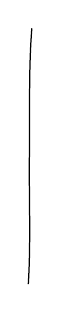
\begin{tikzpicture}[x=1cm,y=1cm]
\draw[line width=0.45pt] (0.045,3.25)
  .. controls (0.005,2.76) and (0.020,2.23) .. (0.015,1.70)
  .. controls (0.005,1.18) and (0.035,0.57) .. (0,0);
\end{tikzpicture}}

\LMsourceMark{M009818}{\mspage{303}}

\LMflushnotes\LMflushpages
\ifnum\LMform=1
\begin{LMapparatus}
\LMentry{140-2-s304-D001}{suppression}{\(\deleted{\LMsourceMark{M009819}{\unsure{\text{nul}}}}\)
}{\emph{\LMomittedlabel}}{Passage biffé dans le manuscrit : la suppression suit l'état final de l'auteur; les doutes de lecture restent signalés.}{}
\LMentry{140-2-s304-D002}{suppression}{\deleted{\LMsourceMark{M009820}{\unsure{encore}}}
}{\emph{\LMomittedlabel}}{Passage biffé dans le manuscrit : la suppression suit l'état final de l'auteur; les doutes de lecture restent signalés.}{}
\LMentry{140-2-s304-D003}{suppression}{\deleted{(\LMsourceMark{M009821}{\unsure{formellt|formellement}}, il se définirait comme \LMsourceMark{M009822}{\illegible{1}} dans le cas précédent)}
}{\emph{\LMomittedlabel}}{Passage biffé dans le manuscrit : la suppression suit l'état final de l'auteur; les doutes de lecture restent signalés.}{}
\LMentry{140-2-s304-D004}{suppression}{\deleted{c'est un iso}
}{\emph{\LMomittedlabel}}{Passage biffé dans le manuscrit : la suppression suit l'état final de l'auteur; les doutes de lecture restent signalés.}{}
\LMentry{140-2-s304-I001}{insertion}{\inserted{Supposons $\nu\LMsourceMark{M009823}{\unsure{>|\geq}}0$.}
}{\emph{\LMinsertedlabel}}{Ajout explicite de l'auteur : intégré à l'endroit indiqué par la transcription, sans modifier sa lecture.}{}
\end{LMapparatus}
\fi
\ifnum\LMform=2
\par\smallskip\begingroup\footnotesize\Needspace{4\baselineskip}\csname @beginparpenalty\endcsname=10000\relax\noindent\textcolor{gray}{\rule{.2\linewidth}{.35pt}}\par\nobreak
\noindent\textit{\LMdoubtheading.}\par\nobreak
\LMcarryover{140-2-s304-D001}{\(\LMsourceMark{M009824}{\unsure{\text{nul}}}\)
}
\LMcarryover{140-2-s304-D002}{\LMsourceMark{M009825}{\unsure{encore}}
}
\LMcarryover{140-2-s304-D003}{\LMsourceMark{M009826}{\unsure{formellt|formellement}}\quad \LMsourceMark{M009827}{\illegible{1}}
}
\par\endgroup\smallskip
\fi

\LMsourceMark{M009828}{\scanpage{305}}
Nous allons expliciter une relation de
compatibilité pour $S\Gamma$ relatif à un $\pi$
à \LMsourceMark{M009829}{\unsure{lacets}}, en fixant un $i\in I=\LMsourceMark{M009830}{\unsure{\mathcal I(\pi)}}$,
d'où un stabilisateur $\Gamma_i\subset\Gamma$ dont l'image
inverse $(S\Gamma)_i$ dans $S\Gamma$ est donc une
extension de $\Gamma_i$ par $T^I$. Utilisant la
projection $T^I\xrightarrow{\mathrm{pr}_i}T$, on trouve une
extension de $\Gamma_i$ par $T$, qu'on va décrire
d'une autre façon. L'extension $S\Gamma$
est définie intrinsèquement par la
donnée de $I$ \LMsourceMark{M009831}{\unsure{réalisations}} \var{\inserted{$(\pi_i)_{i\in I}$}}{\LMadded{$(\pi_i)_{i\in I}$}}{insertion}{140-2-s305-I001} \LMsourceMark{M009832}{\unsure{du groupe}}
\LMsourceMark{M009833}{\unsure{extérieur}} $\pi$ par des groupes, avec dans
chaque $\pi_i$ un $L_i\subset\pi_i$ de la classe $i$
(c'est cela, la donnée d'un système des
$(\widetilde D_i^*)$ !). Pour un autom. ext. \var{\deleted{\LMsourceMark{M009834}{\unsure{$u$}}}}{\LMsourceMark{M009835}{\LMcancelledDoubts{\LMsourceMark{M009836}{\unsure{$u$}}}}}{deletion}{140-2-s305-D001} \var{\inserted{à lacets $u\in\Gamma$}}{\LMadded{à lacets $u\in\Gamma$}}{insertion}{140-2-s305-I002} de $\pi$,
\var{\deleted{ses ``\LMsourceMark{M009837}{\illegible{1}}'' sont les}}{\LMsourceMark{M009838}{\LMcancelledDoubts{\LMsourceMark{M009839}{\illegible{1}}}}}{deletion}{140-2-s305-D002}
pour $\forall i$ il \var{\deleted{\LMsourceMark{M009840}{\unsure{y a des façons}}}}{\LMsourceMark{M009841}{\LMcancelledDoubts{\LMsourceMark{M009842}{\unsure{y a des façons}}}}}{deletion}{140-2-s305-D003} \var{\inserted{est possible}}{\LMadded{est possible}}{insertion}{140-2-s305-I003} de le
\LMsourceMark{M009843}{\unsure{réaliser}} par $u_i\in\operatorname{Aut}_{\LMsourceMark{M009844}{\unsure{\mathrm{lac}|\mathrm{loc}}}}(\pi_i)$, avec $u_i(L_i)\subset L_i$
--- cet $u_i$ est déterminé \LMsourceMark{M009845}{\unsure{mod}} multiplication
à droite par un $\operatorname{int}(\LMsourceMark{M009846}{\unsure{k_i|\kappa_i}}(\alpha))$, où $\alpha\in T$.
Bien entendu, $S\Gamma$ est le \LMsourceMark{M009847}{\unsure{ss-groupe}} \LMsourceMark{M009848}{\unsure{des|du}}
\LMsourceMark{M009849}{\mspage{304}}

\LMflushnotes\LMflushpages
\ifnum\LMform=1
\begin{LMapparatus}
\LMentry{140-2-s305-I001}{insertion}{\inserted{$(\pi_i)_{i\in I}$}
}{\emph{\LMinsertedlabel}}{Ajout explicite de l'auteur : intégré à l'endroit indiqué par la transcription, sans modifier sa lecture.}{}
\LMentry{140-2-s305-D001}{suppression}{\deleted{\LMsourceMark{M009850}{\unsure{$u$}}}
}{\emph{\LMomittedlabel}}{Passage biffé dans le manuscrit : la suppression suit l'état final de l'auteur; les doutes de lecture restent signalés.}{}
\LMentry{140-2-s305-I002}{insertion}{\inserted{à lacets $u\in\Gamma$}
}{\emph{\LMinsertedlabel}}{Ajout explicite de l'auteur : intégré à l'endroit indiqué par la transcription, sans modifier sa lecture.}{}
\LMentry{140-2-s305-D002}{suppression}{\deleted{ses ``\LMsourceMark{M009851}{\illegible{1}}'' sont les}
}{\emph{\LMomittedlabel}}{Passage biffé dans le manuscrit : la suppression suit l'état final de l'auteur; les doutes de lecture restent signalés.}{}
\LMentry{140-2-s305-D003}{suppression}{\deleted{\LMsourceMark{M009852}{\unsure{y a des façons}}}
}{\emph{\LMomittedlabel}}{Passage biffé dans le manuscrit : la suppression suit l'état final de l'auteur; les doutes de lecture restent signalés.}{}
\LMentry{140-2-s305-I003}{insertion}{\inserted{est possible}
}{\emph{\LMinsertedlabel}}{Ajout explicite de l'auteur : intégré à l'endroit indiqué par la transcription, sans modifier sa lecture.}{}
\end{LMapparatus}
\fi
\ifnum\LMform=2
\par\smallskip\begingroup\footnotesize\Needspace{4\baselineskip}\csname @beginparpenalty\endcsname=10000\relax\noindent\textcolor{gray}{\rule{.2\linewidth}{.35pt}}\par\nobreak
\noindent\textit{\LMdoubtheading.}\par\nobreak
\LMcarryover{140-2-s305-D001}{\LMsourceMark{M009853}{\unsure{$u$}}
}
\LMcarryover{140-2-s305-D002}{\LMsourceMark{M009854}{\illegible{1}}
}
\LMcarryover{140-2-s305-D003}{\LMsourceMark{M009855}{\unsure{y a des façons}}
}
\par\endgroup\smallskip
\fi

\LMsourceMark{M009856}{\scanpage{306}}
\LMsourceMark{M009857}{\mspage{154}}
$\displaystyle\prod_{i\in I}\operatorname{Aut}_{\LMsourceMark{M009858}{\unsure{\mathrm{lac}|\mathrm{loc}}}}(\pi_i)$,
\var{\deleted{\LMsourceMark{M009859}{\unsure{formé de}} \LMsourceMark{M009860}{\illegible{1}}}}{\LMsourceMark{M009861}{\LMcancelledDoubts{\LMsourceMark{M009862}{\unsure{formé de}}\quad \LMsourceMark{M009863}{\illegible{1}}}}}{deletion}{140-2-s306-D001} \var{\inserted{\LMsourceMark{M009864}{\unsure{l'image inverse}}}}{\LMadded{\LMsourceMark{M009865}{\unsure{l'image inverse}}}}{insertion}{140-2-s306-I001} de la diagonale
dans l'hom. naturel de ce produit dans
$\operatorname{Autext}_{\LMsourceMark{M009866}{\unsure{\mathrm{lac}|\mathrm{loc}}}}(\pi)^I$, \var{\deleted{\LMsourceMark{M009867}{\unsure{d'où une}}}}{\LMsourceMark{M009868}{\LMcancelledDoubts{\LMsourceMark{M009869}{\unsure{d'où une}}}}}{deletion}{140-2-s306-D002} \var{\inserted{\LMsourceMark{M009870}{\unsure{qui est bien}}}}{\LMadded{\LMsourceMark{M009871}{\unsure{qui est bien}}}}{insertion}{140-2-s306-I002} extension de
\LMsourceMark{M009872}{\unsure{ladite}} diagonale (identifiée à $\Gamma$) par $T^I$.
Si on regarde la sous-extension \var{\deleted{de $\Gamma_i$}}{}{deletion}{140-2-s306-D003} obtenue
par restriction à $\Gamma_i$, on voit que la
projection $T^I\LMsourceMark{M009873}{\unsure{\xrightarrow{\mathrm{pr}_i}}}T$ est stable par $\Gamma_i$; donc
on en déduit une extension de $\Gamma_i$ par $T$,
qui n'est autre que le groupe des
autom. \var{\inserted{à lacets}}{\LMadded{à lacets}}{insertion}{140-2-s306-I003} de $\pi_i$ qui normalisent $L_i$
--- qui est bien une extension de $\Gamma_i$ par $L_i$
(\LMsourceMark{M009874}{\unsure{car}} intersection avec $\pi_i\subset\operatorname{Aut}_{\LMsourceMark{M009875}{\unsure{\mathrm{lac}|\mathrm{loc}}}}(\pi_i)$ \LMsourceMark{M009876}{\unsure{est|étant}}
réduite à $L_i$).

Ceci nous montre que l'extension
de $\Gamma$ par $T^I$ a une nette tendance à
ne pas être triviale, car il en est \LMsourceMark{M009877}{\unsure{ainsi}}
\var{\inserted{(pour $i\in I$ fixé)}}{\LMadded{(pour $i\in I$ fixé)}}{insertion}{140-2-s306-I004} de l'extension de $\Gamma_i$ par $T$ \var{\inserted{à}}{\LMadded{à}}{insertion}{140-2-s306-I005} qui elle donne
naissance. Si p.ex. on a un ss-groupe
\uline{fini} $G\subset\Gamma_i^+$, l'extension induite n'est
jamais triviale si $G\ne1$, on l'a vu. En
fait, $G$ doit être cyclique et son image inverse
dans l'ext. en question est $\simeq T$\ldots
\LMsourceMark{M009878}{\mspage{305}}

\LMflushnotes\LMflushpages
\ifnum\LMform=1
\begin{LMapparatus}
\LMentry{140-2-s306-D001}{suppression}{\deleted{\LMsourceMark{M009879}{\unsure{formé de}} \LMsourceMark{M009880}{\illegible{1}}}
}{\emph{\LMomittedlabel}}{Passage biffé dans le manuscrit : la suppression suit l'état final de l'auteur; les doutes de lecture restent signalés.}{}
\LMentry{140-2-s306-I001}{insertion}{\inserted{\LMsourceMark{M009881}{\unsure{l'image inverse}}}
}{\emph{\LMinsertedlabel}}{Ajout explicite de l'auteur : intégré à l'endroit indiqué par la transcription, sans modifier sa lecture.}{}
\LMentry{140-2-s306-D002}{suppression}{\deleted{\LMsourceMark{M009882}{\unsure{d'où une}}}
}{\emph{\LMomittedlabel}}{Passage biffé dans le manuscrit : la suppression suit l'état final de l'auteur; les doutes de lecture restent signalés.}{}
\LMentry{140-2-s306-I002}{insertion}{\inserted{\LMsourceMark{M009883}{\unsure{qui est bien}}}
}{\emph{\LMinsertedlabel}}{Ajout explicite de l'auteur : intégré à l'endroit indiqué par la transcription, sans modifier sa lecture.}{}
\LMentry{140-2-s306-D003}{suppression}{\deleted{de $\Gamma_i$}
}{\emph{\LMomittedlabel}}{Passage biffé dans le manuscrit : la suppression suit l'état final de l'auteur; les doutes de lecture restent signalés.}{}
\LMentry{140-2-s306-I003}{insertion}{\inserted{à lacets}
}{\emph{\LMinsertedlabel}}{Ajout explicite de l'auteur : intégré à l'endroit indiqué par la transcription, sans modifier sa lecture.}{}
\LMentry{140-2-s306-I004}{insertion}{\inserted{(pour $i\in I$ fixé)}
}{\emph{\LMinsertedlabel}}{Ajout explicite de l'auteur : intégré à l'endroit indiqué par la transcription, sans modifier sa lecture.}{}
\LMentry{140-2-s306-I005}{insertion}{\inserted{à}
}{\emph{\LMinsertedlabel}}{Ajout explicite de l'auteur : intégré à l'endroit indiqué par la transcription, sans modifier sa lecture.}{}
\end{LMapparatus}
\fi
\ifnum\LMform=2
\par\smallskip\begingroup\footnotesize\Needspace{4\baselineskip}\csname @beginparpenalty\endcsname=10000\relax\noindent\textcolor{gray}{\rule{.2\linewidth}{.35pt}}\par\nobreak
\noindent\textit{\LMdoubtheading.}\par\nobreak
\LMcarryover{140-2-s306-D001}{\LMsourceMark{M009884}{\unsure{formé de}}\quad \LMsourceMark{M009885}{\illegible{1}}
}
\LMcarryover{140-2-s306-D002}{\LMsourceMark{M009886}{\unsure{d'où une}}
}
\par\endgroup\smallskip
\fi

\LMsourceMark{M009887}{\scanpage{307}}
\LMsourceMark{M009888}{\mspage{155}}
$25^{\mathrm{bis}}$. Cas des deux groupes. Retour sur les \LMsourceMark{M009889}{\unsure{notations}}

On se place \var{\inserted{d'abord}}{\LMadded{d'abord}}{insertion}{140-2-s307-I001} pour fixer les idées dans le cas
topologique et discret, mais la motivation est
le cas d'une courbe algébrique $U$ sur un
corps de type fini $K$, où on a à la fois
le groupe $G_K=\operatorname{Aut}_K(U)$ et $\Gamma=\operatorname{Gal}(\overline K/K)$
\LMsourceMark{M009890}{\margin{Cas anabélien donc \LMsourceMark{M009891}{\unsure{$G$|$G_K$}} fini}}
qui \LMsourceMark{M009892}{\unsure{opèrent}} extérieurement sur le $\pi_1(U_{\overline K})$.
Dans ce cas, $G$ et $\Gamma$ commutent, mais
on peut regarder plus généralement le cas
du groupe (plus gros que $G_K$) $G_{\overline K}=\operatorname{Aut}_{\overline K}(U)$,
sur lequel $\Gamma$ opère (de façon pas néc. triviale
--- cette opération décrit \LMsourceMark{M009893}{\unsure{un}} groupe algébrique
étale fini sur $K$.

Supposons donc qu'on ait une surface
$U$ (orientable, $U=X-S$, $X$ \LMsourceMark{M009894}{\unsure{compact}} \var{\inserted{\LMsourceMark{M009895}{\unsure{connexe}}}}{\LMadded{\LMsourceMark{M009896}{\unsure{connexe}}}}{insertion}{140-2-s307-I002}, $S$ fini)
sur \LMsourceMark{M009897}{\unsure{laquelle|la quelle}} \LMsourceMark{M009898}{\unsure{opèrent}} deux groupes $G$, $\Gamma$,
l'action de $\Gamma$ normalisant celle de $G$
--- donc on a un groupe $\mathcal G=\Gamma . G$ (produit
semi-direct, pour une certaine action de $\Gamma$
sur $G$) qui opère sur $U$. On suppose $G$
fini, mais pas néc. $\Gamma$ fini.
\LMsourceMark{M009899}{\mspage{306}}

\LMflushnotes\LMflushpages
\ifnum\LMform=1
\begin{LMapparatus}
\LMentry{140-2-s307-I001}{insertion}{\inserted{d'abord}
}{\emph{\LMinsertedlabel}}{Ajout explicite de l'auteur : intégré à l'endroit indiqué par la transcription, sans modifier sa lecture.}{}
\LMentry{140-2-s307-I002}{insertion}{\inserted{\LMsourceMark{M009900}{\unsure{connexe}}}
}{\emph{\LMinsertedlabel}}{Ajout explicite de l'auteur : intégré à l'endroit indiqué par la transcription, sans modifier sa lecture.}{}
\end{LMapparatus}
\fi

\LMsourceMark{M009901}{\scanpage{308}}

On suppose choisi un rev. universel $\widetilde U$ de $U$, d'où un groupe à \LMsourceMark{M009902}{\unsure{lcts}} $\pi=\operatorname{Aut}(\widetilde U)$, sur lequel $\mathcal G$ opère extérieurement, d'où extension
\[
(1)\qquad 1\longrightarrow\pi\longrightarrow\LMsourceMark{M009903}{\unsure{\mathcal E|\varepsilon}}\longrightarrow\mathcal G\longrightarrow 1
\]
\LMsourceMark{M009904}{\margin{On va \LMsourceMark{M009905}{\unsure{supposer}} l'action de $\mathcal G$ fidèle}}
Si l'action de $\mathcal G$ sur $U$ \var{\inserted{mod isotopie}}{\LMadded{mod isotopie}}{insertion}{140-2-s308-I001} est fidèle,
alors $\mathcal G\hookrightarrow\operatorname{Autext}(\pi)$, et l'extension précédente est l'image inverse de l'extension de Teichmüller de $\pi$
\[
1\longrightarrow\pi\longrightarrow\operatorname{Aut}_{\mathrm{lac}}(\pi)\longrightarrow\operatorname{Autext}_{\mathrm{lac}}(\pi)\longrightarrow 1.
\]

\var{\deleted{\LMsourceMark{M009906}{\unsure{Soit}}}}{\LMsourceMark{M009907}{\LMcancelledDoubts{\LMsourceMark{M009908}{\unsure{Soit}}}}}{deletion}{140-2-s308-D001} On aura à regarder d'autres \LMsourceMark{M009909}{\unsure{rev\textsuperscript{ts}}} univ. que $\widetilde U$, et leurs iso. avec $\widetilde U$.
Quand $\widetilde U=\widetilde U(P)$ est le rev. universel basé en un certain $P\in U$, alors pour des rev. universels \var{\inserted{$\LMsourceMark{M009910}{\unsure{U(Q)}}$}}{\LMadded{$\LMsourceMark{M009911}{\unsure{U(Q)}}$}}{insertion}{140-2-s308-I002} basés en \var{\deleted{\LMsourceMark{M009912}{\illegible{1}}}}{\LMsourceMark{M009913}{\LMcancelledDoubts{\LMsourceMark{M009914}{\illegible{1}}}}}{deletion}{140-2-s308-D002} \var{\inserted{un}}{\LMadded{un}}{insertion}{140-2-s308-I003} \LMsourceMark{M009915}{\unsure{point\var{\deleted{s}}{\LMsourceMark{M009916}{\LMuncertaindeletion{140-2-s308-D003}}}{deletion}{140-2-s308-D003}|points}},
les \var{\inserted{$U$-}}{\LMadded{$U$-}}{insertion}{140-2-s308-I004}iso. $\widetilde U(P)\xrightarrow{\sim}\LMsourceMark{M009917}{\unsure{\overline U(Q)|\widetilde U(Q)}}$ correspondent \LMsourceMark{M009918}{\unsure{donc}} aux classes de chemins de $P$ à $Q$.

Soit \var{\deleted{\LMsourceMark{M009919}{\illegible{1}}}}{\LMsourceMark{M009920}{\LMcancelledDoubts{\LMsourceMark{M009921}{\illegible{1}}}}}{deletion}{140-2-s308-D004} $Q\in U$ tel que son groupe d'isotropie \var{\inserted{$G_Q$}}{\LMadded{$G_Q$}}{insertion}{140-2-s308-I005} \var{\deleted{\LMsourceMark{M009922}{\illegible{1}}}}{\LMsourceMark{M009923}{\LMcancelledDoubts{\LMsourceMark{M009924}{\illegible{1}}}}}{deletion}{140-2-s308-D005} \uline{dans $G$} soit \LMsourceMark{M009925}{\unsure{tel.}} que $G_Q^+\ne1$.
(Donc $G_Q^+$ est cyclique). Choisissant une
\LMsourceMark{M009926}{\mspage{307}}

\LMflushnotes\LMflushpages
\ifnum\LMform=1
\begin{LMapparatus}
\LMentry{140-2-s308-I001}{insertion}{\inserted{mod isotopie}
}{\emph{\LMinsertedlabel}}{Ajout explicite de l'auteur : intégré à l'endroit indiqué par la transcription, sans modifier sa lecture.}{}
\LMentry{140-2-s308-D001}{suppression}{\deleted{\LMsourceMark{M009927}{\unsure{Soit}}}
}{\emph{\LMomittedlabel}}{Passage biffé dans le manuscrit : la suppression suit l'état final de l'auteur; les doutes de lecture restent signalés.}{}
\LMentry{140-2-s308-I002}{insertion}{\inserted{$\LMsourceMark{M009928}{\unsure{U(Q)}}$}
}{\emph{\LMinsertedlabel}}{Ajout explicite de l'auteur : intégré à l'endroit indiqué par la transcription, sans modifier sa lecture.}{}
\LMentry{140-2-s308-D002}{suppression}{\deleted{\LMsourceMark{M009929}{\illegible{1}}}
}{\emph{\LMomittedlabel}}{Passage biffé dans le manuscrit : la suppression suit l'état final de l'auteur; les doutes de lecture restent signalés.}{}
\LMentry{140-2-s308-I003}{insertion}{\inserted{un}
}{\emph{\LMinsertedlabel}}{Ajout explicite de l'auteur : intégré à l'endroit indiqué par la transcription, sans modifier sa lecture.}{}
\LMentry{140-2-s308-D003}{suppression}{\LMsourceMark{M009930}{\LMdoubtcopy{\deleted{s}}}
}{\emph{\LMomittedlabel}}{Passage biffé dans le manuscrit : la suppression suit l'état final de l'auteur; les doutes de lecture restent signalés.}{}
\LMentry{140-2-s308-I004}{insertion}{\inserted{$U$-}
}{\emph{\LMinsertedlabel}}{Ajout explicite de l'auteur : intégré à l'endroit indiqué par la transcription, sans modifier sa lecture.}{}
\LMentry{140-2-s308-D004}{suppression}{\deleted{\LMsourceMark{M009931}{\illegible{1}}}
}{\emph{\LMomittedlabel}}{Passage biffé dans le manuscrit : la suppression suit l'état final de l'auteur; les doutes de lecture restent signalés.}{}
\LMentry{140-2-s308-I005}{insertion}{\inserted{$G_Q$}
}{\emph{\LMinsertedlabel}}{Ajout explicite de l'auteur : intégré à l'endroit indiqué par la transcription, sans modifier sa lecture.}{}
\LMentry{140-2-s308-D005}{suppression}{\deleted{\LMsourceMark{M009932}{\illegible{1}}}
}{\emph{\LMomittedlabel}}{Passage biffé dans le manuscrit : la suppression suit l'état final de l'auteur; les doutes de lecture restent signalés.}{}
\end{LMapparatus}
\fi
\ifnum\LMform=2
\par\smallskip\begingroup\footnotesize\Needspace{4\baselineskip}\csname @beginparpenalty\endcsname=10000\relax\noindent\textcolor{gray}{\rule{.2\linewidth}{.35pt}}\par\nobreak
\noindent\textit{\LMdoubtheading.}\par\nobreak
\LMcarryover{140-2-s308-D001}{\LMsourceMark{M009933}{\unsure{Soit}}
}
\LMcarryover{140-2-s308-D002}{\LMsourceMark{M009934}{\illegible{1}}
}
\LMcarryover{140-2-s308-D003}{\LMsourceMark{M009935}{\LMdoubtcopy{s}}
}
\LMcarryover{140-2-s308-D004}{\LMsourceMark{M009936}{\illegible{1}}
}
\LMcarryover{140-2-s308-D005}{\LMsourceMark{M009937}{\illegible{1}}
}
\par\endgroup\smallskip
\fi

\LMsourceMark{M009938}{\scanpage{309}}
\LMsourceMark{M009939}{\mspage{156}}

classe de chemins \var{\inserted{$\lambda$}}{\LMadded{$\lambda$}}{insertion}{140-2-s309-I001} de $P$ à $Q$, identifiant $\LMsourceMark{M009940}{\unsure{\overline U(P)|\widetilde U(P)}}$ à $\LMsourceMark{M009941}{\unsure{\overline U(Q)|\widetilde U(Q)}}$, on trouve une opération de $G_Q$ sur $\widetilde U(P)$ i.e. un relèvement $G_Q\xrightarrow{r_{G_Q}}\LMsourceMark{M009942}{\unsure{\mathcal E|\varepsilon}}$ dans l'extension (1) --- le changement de classe de chemins \var{\inserted{de $\lambda$ en $\lambda'$}}{\LMadded{de $\lambda$ en $\lambda'$}}{insertion}{140-2-s309-I002} donnera un relèvement $r'_{G_Q}$ qui \var{\deleted{\LMsourceMark{M009943}{\unsure{est}}}}{\LMsourceMark{M009944}{\LMcancelledDoubts{\LMsourceMark{M009945}{\unsure{est}}}}}{deletion}{140-2-s309-D001} sera conjugué de $r$ par un unique élément de $\pi$ \var{\inserted{$=\pi_1(U,P)$}}{\LMadded{$=\pi_1(U,P)$}}{insertion}{140-2-s309-I003} (l'unicité provient de $\pi^{G_Q}=\{1\}$), \LMsourceMark{M009946}{\unsure{savoir}} celui qui fait \LMsourceMark{M009947}{\unsure{passer}} d'un chemin à un autre.

Considérons le stabilisateur $\Gamma_Q$ de $Q$ dans $\Gamma$, \var{\deleted{\LMsourceMark{M009948}{\illegible{2}}}}{\LMsourceMark{M009949}{\LMcancelledDoubts{\LMsourceMark{M009950}{\illegible{2}}}}}{deletion}{140-2-s309-D002} qui opère bien sûr sur $\widetilde U(Q)$ tout comme $G_Q$ (en fait c'est $\mathcal G_Q$ qui opère \var{\inserted{d'où $r:\mathcal G_Q\to\LMsourceMark{M009951}{\unsure{\mathcal E|\varepsilon}}$}}{\LMadded{d'où $r:\mathcal G_Q\to\LMsourceMark{M009952}{\unsure{\mathcal E|\varepsilon}}$}}{insertion}{140-2-s309-I004} \LMsourceMark{M009953}{\unsure{\dots}}), donc via $\lambda$ on a aussi un \LMsourceMark{M009954}{\unsure{relèv\textsuperscript{t}|relèvg.}} $r_{\Gamma_Q}:\Gamma_Q\longrightarrow\LMsourceMark{M009955}{\unsure{\mathcal E|\varepsilon}}$, qui \var{\inserted{a}}{\LMadded{a}}{insertion}{140-2-s309-I005} $\overline{\mathrm m}$ la \LMsourceMark{M009956}{\unsure{propté}} de \LMsourceMark{M009957}{\unsure{normaliser}} $r_{G_Q}$ (\LMsourceMark{M009958}{\unsure{i.e.}} op. de \var{\deleted{\LMsourceMark{M009959}{\illegible{1}}}}{\LMsourceMark{M009960}{\LMcancelledDoubts{\LMsourceMark{M009961}{\illegible{1}}}}}{deletion}{140-2-s309-D003} $\Gamma_Q$ dessus, qui est celle provenant de l'op. donnée de $\Gamma$ sur $G$).
\LMsourceMark{M009962}{\margin{\uline{NB} Comme l'ens \var{\deleted{\LMsourceMark{M009963}{\illegible{1}}}}{\LMsourceMark{M009964}{\LMcancelledDoubts{\LMsourceMark{M009965}{\illegible{1}}}}}{deletion}{140-2-s309-D004} \LMsourceMark{M009966}{\unsure{des}} pts $Q$ est fini, et que $\mathcal G$ opère dessus, l'orbite de $Q$ sous $\mathcal G$ est finie, i.e. $\mathcal G_Q$ d'indice fini dans $\mathcal G$. et de $\overline{\mathrm m}$ $\Gamma_Q$ dans $\Gamma$.}}
Pour simplifier, supposons quand $\overline{\mathrm m}$ que $\Gamma$ opère \LMsourceMark{M009967}{\unsure{trivial\textsuperscript{t}}} sur $G$ i.e. $\mathcal G=\Gamma\times G$, alors $r_{\Gamma_Q}(\Gamma_Q)\subset\LMsourceMark{M009968}{\unsure{\mathcal E|\varepsilon}}$ est contenu dans le \uline{centralisateur} de \var{\inserted{$r$ (ou de}}{\LMadded{$r$ (ou de}}{insertion}{140-2-s309-I006} $\LMsourceMark{M009969}{\unsure{r_{G_Q}}}(G_Q)$),
\LMsourceMark{M009970}{\mspage{308}}

\LMflushnotes\LMflushpages
\ifnum\LMform=1
\begin{LMapparatus}
\LMentry{140-2-s309-I001}{insertion}{\inserted{$\lambda$}
}{\emph{\LMinsertedlabel}}{Ajout explicite de l'auteur : intégré à l'endroit indiqué par la transcription, sans modifier sa lecture.}{}
\LMentry{140-2-s309-I002}{insertion}{\inserted{de $\lambda$ en $\lambda'$}
}{\emph{\LMinsertedlabel}}{Ajout explicite de l'auteur : intégré à l'endroit indiqué par la transcription, sans modifier sa lecture.}{}
\LMentry{140-2-s309-D001}{suppression}{\deleted{\LMsourceMark{M009971}{\unsure{est}}}
}{\emph{\LMomittedlabel}}{Passage biffé dans le manuscrit : la suppression suit l'état final de l'auteur; les doutes de lecture restent signalés.}{}
\LMentry{140-2-s309-I003}{insertion}{\inserted{$=\pi_1(U,P)$}
}{\emph{\LMinsertedlabel}}{Ajout explicite de l'auteur : intégré à l'endroit indiqué par la transcription, sans modifier sa lecture.}{}
\LMentry{140-2-s309-D002}{suppression}{\deleted{\LMsourceMark{M009972}{\illegible{2}}}
}{\emph{\LMomittedlabel}}{Passage biffé dans le manuscrit : la suppression suit l'état final de l'auteur; les doutes de lecture restent signalés.}{}
\LMentry{140-2-s309-I004}{insertion}{\inserted{d'où $r:\mathcal G_Q\to\LMsourceMark{M009973}{\unsure{\mathcal E|\varepsilon}}$}
}{\emph{\LMinsertedlabel}}{Ajout explicite de l'auteur : intégré à l'endroit indiqué par la transcription, sans modifier sa lecture.}{}
\LMentry{140-2-s309-I005}{insertion}{\inserted{a}
}{\emph{\LMinsertedlabel}}{Ajout explicite de l'auteur : intégré à l'endroit indiqué par la transcription, sans modifier sa lecture.}{}
\LMentry{140-2-s309-D003}{suppression}{\deleted{\LMsourceMark{M009974}{\illegible{1}}}
}{\emph{\LMomittedlabel}}{Passage biffé dans le manuscrit : la suppression suit l'état final de l'auteur; les doutes de lecture restent signalés.}{}
\LMentry{140-2-s309-D004}{suppression}{\deleted{\LMsourceMark{M009975}{\illegible{1}}}
}{\emph{\LMomittedlabel}}{Passage biffé dans le manuscrit : la suppression suit l'état final de l'auteur; les doutes de lecture restent signalés.}{}
\LMentry{140-2-s309-I006}{insertion}{\inserted{$r$ (ou de}
}{\emph{\LMinsertedlabel}}{Ajout explicite de l'auteur : intégré à l'endroit indiqué par la transcription, sans modifier sa lecture.}{}
\end{LMapparatus}
\fi
\ifnum\LMform=2
\par\smallskip\begingroup\footnotesize\Needspace{4\baselineskip}\csname @beginparpenalty\endcsname=10000\relax\noindent\textcolor{gray}{\rule{.2\linewidth}{.35pt}}\par\nobreak
\noindent\textit{\LMdoubtheading.}\par\nobreak
\LMcarryover{140-2-s309-D001}{\LMsourceMark{M009976}{\unsure{est}}
}
\LMcarryover{140-2-s309-D002}{\LMsourceMark{M009977}{\illegible{2}}
}
\LMcarryover{140-2-s309-D003}{\LMsourceMark{M009978}{\illegible{1}}
}
\LMcarryover{140-2-s309-D004}{\LMsourceMark{M009979}{\illegible{1}}
}
\par\endgroup\smallskip
\fi

\LMsourceMark{M009980}{\scanpage{310}}

et comme $\pi^{r(G_Q)}=1$, donc l'hom
\[
\operatorname{Centr}(r_{\var{\deleted{\LMsourceMark{M009981}{\unsure{G_Q}}}}{\LMsourceMark{M009982}{\LMcancelledDoubts{\(\LMsourceMark{M009983}{\unsure{G_Q}}\)}}}{deletion}{140-2-s310-D001}}(G_Q))\longrightarrow\mathcal G
\]
est injectif, le relèvement en question \var{\inserted{$\LMsourceMark{M009984}{\unsure{r_{\Gamma_Q}}}$}}{\LMadded{$\LMsourceMark{M009985}{\unsure{r_{\Gamma_Q}}}$}}{insertion}{140-2-s310-I001} est uniquement déterminé par la condition précédente.
\LMsourceMark{M009986}{\margin{\uline{NB} \LMsourceMark{M009987}{\unsure{Indépend\textsuperscript{mt}|Indépendamment}} de \LMsourceMark{M009988}{\unsure{tte|l'}} hyp. que $\Gamma$ centralise $G$, le normalisateur de $r(G_Q)$ dans $\pi$, égal à son ``centralisateur'', est réduit à $1$, donc $\operatorname{Norm}(r(G_Q))\longrightarrow\mathcal G$ est injectif}}

En fait, l'image de $\operatorname{Centr}(r(G_Q))$ dans $\mathcal G$ contient $\mathcal G_Q$, \var{\inserted{\LMsourceMark{M009989}{\unsure{et}}}}{\LMadded{\LMsourceMark{M009990}{\unsure{et}}}}{insertion}{140-2-s310-I002} \var{\deleted{\LMsourceMark{M009991}{\illegible{5}}}}{\LMsourceMark{M009992}{\LMcancelledDoubts{\LMsourceMark{M009993}{\illegible{5}}}}}{deletion}{140-2-s310-D002} \LMsourceMark{M009994}{\unsure{$\overline{\mathrm m}$}} le relèvement $\mathcal G_Q\xrightarrow{r_{\mathcal G_Q}}\LMsourceMark{M009995}{\unsure{\mathcal E|\varepsilon}}$.
\var{\deleted{si $\mathcal G$ est fini}}{}{deletion}{140-2-s310-D003}
\LMsourceMark{M009996}{\unsure{La|Le}} chose \LMsourceMark{M009997}{\unsure{intéressante}}, c'est que \LMsourceMark{M009998}{\unsure{les|le}} \var{\inserted{choix d'un}}{\LMadded{choix d'un}}{insertion}{140-2-s310-I003} relèvement\var{\deleted{\LMsourceMark{M009999}{\unsure{s}}}}{\LMsourceMark{M010000}{\LMcancelledDoubts{\LMsourceMark{M010001}{\unsure{s}}}}}{deletion}{140-2-s310-D004} \LMsourceMark{M010002}{\unsure{du|des}} (petit) groupe $G_Q$, impose déjà le choix d'un relèvement \LMsourceMark{M010003}{\unsure{du|des}} (grand) groupe $\Gamma_Q$, ou $\mathcal G_Q$.

\var{\deleted{Quand $\mathcal G$ est lui-$\overline{\mathrm m}$ fini,}}{}{deletion}{140-2-s310-D005} je dis que l'image dans $\mathcal G$ du centralisateur \var{\inserted{(et $\overline{\mathrm m}$ du normalisateur)}}{\LMadded{(et $\overline{\mathrm m}$ du normalisateur)}}{insertion}{140-2-s310-I004} de $r(G_Q)$ est $\mathcal G_Q$ lui-$\overline{\mathrm m}$ (a priori il le contient).
\LMsourceMark{M010004}{\unsure{Revenant|Revenons}} à $\widetilde U(Q)$ lui-$\overline{\mathrm m}$, cela signifie que \var{\deleted{\LMsourceMark{M010005}{\illegible{1}}}}{\LMsourceMark{M010006}{\LMcancelledDoubts{\LMsourceMark{M010007}{\illegible{1}}}}}{deletion}{140-2-s310-D006} si $g\in\mathcal G$ est tel qu'il existe un autom $\widetilde g$ de $\widetilde U(Q)$ qui relève $g$, en \var{\deleted{\LMsourceMark{M010008}{\unsure{commutant}}}}{\LMsourceMark{M010009}{\LMcancelledDoubts{\LMsourceMark{M010010}{\unsure{commutant}}}}}{deletion}{140-2-s310-D007} \var{\inserted{normalisant}}{\LMadded{normalisant}}{insertion}{140-2-s310-I005} \var{\deleted{\LMsourceMark{M010011}{\unsure{à}}}}{\LMsourceMark{M010012}{\LMcancelledDoubts{\LMsourceMark{M010013}{\unsure{à}}}}}{deletion}{140-2-s310-D008} \var{\inserted{l'action de}}{\LMadded{l'action de}}{insertion}{140-2-s310-I006} $G_Q$, alors $g\in\mathcal G_Q$ \var{\inserted{(et $\widetilde g$ est le relèvement évident)}}{\LMadded{(et $\widetilde g$ est le relèvement évident)}}{insertion}{140-2-s310-I007}. En effet, si $\widetilde g$ \var{\deleted{\LMsourceMark{M010014}{\unsure{commute}}}}{\LMsourceMark{M010015}{\LMcancelledDoubts{\LMsourceMark{M010016}{\unsure{commute}}}}}{deletion}{140-2-s310-D009} \var{\inserted{normalise}}{\LMadded{normalise}}{insertion}{140-2-s310-I008} \var{\inserted{l'action de}}{\LMadded{l'action de}}{insertion}{140-2-s310-I009} $G_Q$, il \LMsourceMark{M010017}{\unsure{invarie|envoie}} l'ens des pts fixes de $G_Q$ dans $\widetilde U(Q)$, qui est réduit \var{\deleted{\LMsourceMark{M010018}{\illegible{1}}}}{\LMsourceMark{M010019}{\LMcancelledDoubts{\LMsourceMark{M010020}{\illegible{1}}}}}{deletion}{140-2-s310-D010} \var{\inserted{\LMsourceMark{M010021}{\unsure{au point}}}}{\LMadded{\LMsourceMark{M010022}{\unsure{au point}}}}{insertion}{140-2-s310-I010} $\LMsourceMark{M010023}{\unsure{\widetilde Q|\overline Q}}$
\LMsourceMark{M010024}{\mspage{309}}

\LMflushnotes\LMflushpages
\ifnum\LMform=1
\begin{LMapparatus}
\LMentry{140-2-s310-D001}{suppression}{\(\deleted{\LMsourceMark{M010025}{\unsure{G_Q}}}\)
}{\emph{\LMomittedlabel}}{Passage biffé dans le manuscrit : la suppression suit l'état final de l'auteur; les doutes de lecture restent signalés.}{}
\LMentry{140-2-s310-I001}{insertion}{\inserted{$\LMsourceMark{M010026}{\unsure{r_{\Gamma_Q}}}$}
}{\emph{\LMinsertedlabel}}{Ajout explicite de l'auteur : intégré à l'endroit indiqué par la transcription, sans modifier sa lecture.}{}
\LMentry{140-2-s310-I002}{insertion}{\inserted{\LMsourceMark{M010027}{\unsure{et}}}
}{\emph{\LMinsertedlabel}}{Ajout explicite de l'auteur : intégré à l'endroit indiqué par la transcription, sans modifier sa lecture.}{}
\LMentry{140-2-s310-D002}{suppression}{\deleted{\LMsourceMark{M010028}{\illegible{5}}}
}{\emph{\LMomittedlabel}}{Passage biffé dans le manuscrit : la suppression suit l'état final de l'auteur; les doutes de lecture restent signalés.}{}
\LMentry{140-2-s310-D003}{suppression}{\deleted{si $\mathcal G$ est fini}
}{\emph{\LMomittedlabel}}{Passage biffé dans le manuscrit : la suppression suit l'état final de l'auteur; les doutes de lecture restent signalés.}{}
\LMentry{140-2-s310-I003}{insertion}{\inserted{choix d'un}
}{\emph{\LMinsertedlabel}}{Ajout explicite de l'auteur : intégré à l'endroit indiqué par la transcription, sans modifier sa lecture.}{}
\LMentry{140-2-s310-D004}{suppression}{\deleted{\LMsourceMark{M010029}{\unsure{s}}}
}{\emph{\LMomittedlabel}}{Passage biffé dans le manuscrit : la suppression suit l'état final de l'auteur; les doutes de lecture restent signalés.}{}
\LMentry{140-2-s310-D005}{suppression}{\deleted{Quand $\mathcal G$ est lui-$\overline{\mathrm m}$ fini,}
}{\emph{\LMomittedlabel}}{Passage biffé dans le manuscrit : la suppression suit l'état final de l'auteur; les doutes de lecture restent signalés.}{}
\LMentry{140-2-s310-I004}{insertion}{\inserted{(et $\overline{\mathrm m}$ du normalisateur)}
}{\emph{\LMinsertedlabel}}{Ajout explicite de l'auteur : intégré à l'endroit indiqué par la transcription, sans modifier sa lecture.}{}
\LMentry{140-2-s310-D006}{suppression}{\deleted{\LMsourceMark{M010030}{\illegible{1}}}
}{\emph{\LMomittedlabel}}{Passage biffé dans le manuscrit : la suppression suit l'état final de l'auteur; les doutes de lecture restent signalés.}{}
\LMentry{140-2-s310-D007}{suppression}{\deleted{\LMsourceMark{M010031}{\unsure{commutant}}}
}{\emph{\LMomittedlabel}}{Passage biffé dans le manuscrit : la suppression suit l'état final de l'auteur; les doutes de lecture restent signalés.}{}
\LMentry{140-2-s310-I005}{insertion}{\inserted{normalisant}
}{\emph{\LMinsertedlabel}}{Ajout explicite de l'auteur : intégré à l'endroit indiqué par la transcription, sans modifier sa lecture.}{}
\LMentry{140-2-s310-D008}{suppression}{\deleted{\LMsourceMark{M010032}{\unsure{à}}}
}{\emph{\LMomittedlabel}}{Passage biffé dans le manuscrit : la suppression suit l'état final de l'auteur; les doutes de lecture restent signalés.}{}
\LMentry{140-2-s310-I006}{insertion}{\inserted{l'action de}
}{\emph{\LMinsertedlabel}}{Ajout explicite de l'auteur : intégré à l'endroit indiqué par la transcription, sans modifier sa lecture.}{}
\LMentry{140-2-s310-I007}{insertion}{\inserted{(et $\widetilde g$ est le relèvement évident)}
}{\emph{\LMinsertedlabel}}{Ajout explicite de l'auteur : intégré à l'endroit indiqué par la transcription, sans modifier sa lecture.}{}
\LMentry{140-2-s310-D009}{suppression}{\deleted{\LMsourceMark{M010033}{\unsure{commute}}}
}{\emph{\LMomittedlabel}}{Passage biffé dans le manuscrit : la suppression suit l'état final de l'auteur; les doutes de lecture restent signalés.}{}
\LMentry{140-2-s310-I008}{insertion}{\inserted{normalise}
}{\emph{\LMinsertedlabel}}{Ajout explicite de l'auteur : intégré à l'endroit indiqué par la transcription, sans modifier sa lecture.}{}
\LMentry{140-2-s310-I009}{insertion}{\inserted{l'action de}
}{\emph{\LMinsertedlabel}}{Ajout explicite de l'auteur : intégré à l'endroit indiqué par la transcription, sans modifier sa lecture.}{}
\LMentry{140-2-s310-D010}{suppression}{\deleted{\LMsourceMark{M010034}{\illegible{1}}}
}{\emph{\LMomittedlabel}}{Passage biffé dans le manuscrit : la suppression suit l'état final de l'auteur; les doutes de lecture restent signalés.}{}
\LMentry{140-2-s310-I010}{insertion}{\inserted{\LMsourceMark{M010035}{\unsure{au point}}}
}{\emph{\LMinsertedlabel}}{Ajout explicite de l'auteur : intégré à l'endroit indiqué par la transcription, sans modifier sa lecture.}{}
\end{LMapparatus}
\fi
\ifnum\LMform=2
\par\smallskip\begingroup\footnotesize\Needspace{4\baselineskip}\csname @beginparpenalty\endcsname=10000\relax\noindent\textcolor{gray}{\rule{.2\linewidth}{.35pt}}\par\nobreak
\noindent\textit{\LMdoubtheading.}\par\nobreak
\LMcarryover{140-2-s310-D001}{\(\LMsourceMark{M010036}{\unsure{G_Q}}\)
}
\LMcarryover{140-2-s310-D002}{\LMsourceMark{M010037}{\illegible{5}}
}
\LMcarryover{140-2-s310-D004}{\LMsourceMark{M010038}{\unsure{s}}
}
\LMcarryover{140-2-s310-D006}{\LMsourceMark{M010039}{\illegible{1}}
}
\LMcarryover{140-2-s310-D007}{\LMsourceMark{M010040}{\unsure{commutant}}
}
\LMcarryover{140-2-s310-D008}{\LMsourceMark{M010041}{\unsure{à}}
}
\LMcarryover{140-2-s310-D009}{\LMsourceMark{M010042}{\unsure{commute}}
}
\LMcarryover{140-2-s310-D010}{\LMsourceMark{M010043}{\illegible{1}}
}
\par\endgroup\smallskip
\fi

% END PACKAGE LM_P031
% BEGIN PACKAGE LM_P032
\ifnum\LMform<2\Needspace{11\baselineskip}\subsection*{Scans 311--320}\fi
\LMsourceMark{M010044}{\scanpage{311}}
\LMsourceMark{M010045}{\mspage{157}}

L'ens. $\LMsourceMark{M010046}{\unsure{\widetilde U|U}}^{!}$ des pts $Q\in U$ tels que $G_Q^+\ne(1)$ est stable par l'action de $\mathcal G$, et s'identifie (avec cette action) à \LMsourceMark{M010047}{\unsure{l'ens.}} des relèvements \var{\inserted{maximaux}}{\LMadded{maximaux}}{insertion}{140-2-s311-I001} mod $\pi$ de ss-groupes (cycliques) $\ne1$ de $G^{+}_{\var{\deleted{\LMsourceMark{M010048}{\unsure{Q}}}}{\LMsourceMark{M010049}{\LMcancelledDoubts{\(\LMsourceMark{M010050}{\unsure{Q}}\)}}}{deletion}{140-2-s311-D001}}$. Quand on connaît, pour un relèvement partiel $r$ d'un $G_Q$ dans $\mathcal E$ quel est son centralisateur dans $\mathcal E$ i.e. le relèvement correspondant de $\mathcal G_Q$, \LMsourceMark{M010051}{\unsure{bien|lors}} de $=$ pour les conjugués de $r$ par n'importe quel \LMsourceMark{M010052}{\unsure{élt}} $g$ (non seulement de $\pi$, mais $=$ de $\mathcal E$), par simple conjugaison.

Donc les cas à déterminer correspondent pratiquement aux orbites de $\mathcal G$ dans $U^{!}$.

On peut s'intéresser à décrire $\mathcal G$ ou $\Gamma$ en tant que ss-groupe de $\mathrm{Aut\,ext}_{\mathrm{lac}}(\pi)=\Gamma'$ \var{\inserted{donnant lieu à l'ext. $\mathcal E'$ de $\Gamma'$ par $\pi$ (donc $\mathcal E\subset\mathcal E'$).}}{\LMadded{donnant lieu à l'ext. $\mathcal E'$ de $\Gamma'$ par $\pi$ (donc $\mathcal E\subset\mathcal E'$).}}{insertion}{140-2-s311-I002} Mais pour tt relèvement $r$ d'un $G_Q$, considérons $\mathrm{Centr}_{\mathcal E'}(r)$, \var{\deleted{\LMsourceMark{M010053}{\illegible{1}}}}{\LMsourceMark{M010054}{\LMcancelledDoubts{\LMsourceMark{M010055}{\illegible{1}}}}}{deletion}{140-2-s311-D002} . \LMsourceMark{M010056}{\unsure{on aura|on a encore}} $\mathrm{Centr}_{\mathcal E'}(r)\cap\pi=(1)$ i.e. \var{\inserted{on trouve une section au dessus de}}{\LMadded{on trouve une section au dessus de}}{insertion}{140-2-s311-I003} l'image de ce centralisateur dans $\Gamma'$, soit $\Gamma'(Q)$. Cette image ne dépend que de $Q$ i.e. de la classe de $\pi$-conjugaison de $r$ ou de $r(\LMsourceMark{M010057}{\unsure{G_Q}})$, et est remplacée par un $G$-conjugué quand $Q$ est remplacé par un $G$-conjugué. Ceci

\LMsourceMark{M010058}{\mspage{310}}

\LMflushnotes\LMflushpages
\ifnum\LMform=1
\begin{LMapparatus}
\LMentry{140-2-s311-I001}{insertion}{\inserted{maximaux}
}{\emph{\LMinsertedlabel}}{Ajout explicite de l'auteur : intégré à l'endroit indiqué par la transcription, sans modifier sa lecture.}{}
\LMentry{140-2-s311-D001}{suppression}{\(\deleted{\LMsourceMark{M010059}{\unsure{Q}}}\)
}{\emph{\LMomittedlabel}}{Passage biffé dans le manuscrit : la suppression suit l'état final de l'auteur; les doutes de lecture restent signalés.}{}
\LMentry{140-2-s311-I002}{insertion}{\inserted{donnant lieu à l'ext. $\mathcal E'$ de $\Gamma'$ par $\pi$ (donc $\mathcal E\subset\mathcal E'$).}
}{\emph{\LMinsertedlabel}}{Ajout explicite de l'auteur : intégré à l'endroit indiqué par la transcription, sans modifier sa lecture.}{}
\LMentry{140-2-s311-D002}{suppression}{\deleted{\LMsourceMark{M010060}{\illegible{1}}}
}{\emph{\LMomittedlabel}}{Passage biffé dans le manuscrit : la suppression suit l'état final de l'auteur; les doutes de lecture restent signalés.}{}
\LMentry{140-2-s311-I003}{insertion}{\inserted{on trouve une section au dessus de}
}{\emph{\LMinsertedlabel}}{Ajout explicite de l'auteur : intégré à l'endroit indiqué par la transcription, sans modifier sa lecture.}{}
\end{LMapparatus}
\fi
\ifnum\LMform=2
\par\smallskip\begingroup\footnotesize\Needspace{4\baselineskip}\csname @beginparpenalty\endcsname=10000\relax\noindent\textcolor{gray}{\rule{.2\linewidth}{.35pt}}\par\nobreak
\noindent\textit{\LMdoubtheading.}\par\nobreak
\LMcarryover{140-2-s311-D001}{\(\LMsourceMark{M010061}{\unsure{Q}}\)
}
\LMcarryover{140-2-s311-D002}{\LMsourceMark{M010062}{\illegible{1}}
}
\par\endgroup\smallskip
\fi

\LMsourceMark{M010063}{\scanpage{312}}

dit, l'intersection \var{\inserted{$\Gamma'^{\natural}$}}{\LMadded{$\Gamma'^{\natural}$}}{insertion}{140-2-s312-I001} des $\Gamma'(Q)$, pour $Q\in U^{!}$, est un ss-groupe de $\Gamma'$ qui contient l'intersection \var{\deleted{\LMsourceMark{M010064}{\unsure{de}}}}{\LMsourceMark{M010065}{\LMcancelledDoubts{\LMsourceMark{M010066}{\unsure{de}}}}}{deletion}{140-2-s312-D001} $\mathcal G^{\natural}$ des $\mathcal G_Q^{\var{\deleted{\LMsourceMark{M010067}{\unsure{\natural}}}}{\LMsourceMark{M010068}{\LMcancelledDoubts{\(\LMsourceMark{M010069}{\unsure{\natural}}\)}}}{deletion}{140-2-s312-D002}}$, et le centralisateur de $G$ dans $\Gamma'^{\natural}$ contient de $=$ l'intersection \var{\deleted{de}}{}{deletion}{140-2-s312-D003} $\Gamma^{\natural}$ des $\Gamma_Q$, qui est un ss-groupe \var{\inserted{invariant}}{\LMadded{invariant}}{insertion}{140-2-s312-I002} d'indice fini de $\Gamma$. Et on peut alors se proposer s'il est possible de caractériser au moins \LMsourceMark{M010070}{\unsure{le|un}} ss-groupe fini $\Gamma^{\natural}$ de $\Gamma$ comme $\mathrm{Centr}_{\Gamma'^{\natural}}(G)$, et \LMsourceMark{M010071}{\unsure{d'en récupérer}} peut être $\Gamma$ comme le normalisateur de $\Gamma^{\natural}$ dans \var{\deleted{le centralisateur}}{}{deletion}{140-2-s312-D004} $\mathrm{Centr}_{G}(\Gamma)$.

Je m'intéresse plus particulièrement à la variante profinie de ceci, dans le cas où $U=\mathbb P^1_{\mathbb Q}\setminus\{0,1,\infty\}$, $G=\mathfrak S_3$, $\Gamma={}$ groupe de Galois de $\overline{\mathbb Q}/\mathbb Q$, \var{\deleted{tandis}}{}{deletion}{140-2-s312-D005} \var{\inserted{$\LMsourceMark{M010072}{\unsure{P|\rho}}=\exp(2i\pi/6)$}}{\LMadded{$\LMsourceMark{M010073}{\unsure{P|\rho}}=\exp(2i\pi/6)$}}{insertion}{140-2-s312-I003}.
\LMsourceMark{M010074}{\margin{clôture alg. dans $\mathbb C$}}

Je n'ai pas vérifié que $\Gamma\longrightarrow\mathrm{Autext}_{\mathrm{lac}}(\widehat\pi)$ soit injectif, cela n'empêche de faire des calculs dans $\mathrm{Aut}_{\mathrm{lac}}(\widehat\pi)$, fussent-ils heuristiques pour le moment.

\LMsourceMark{M010075}{\mspage{311}}

\LMflushnotes\LMflushpages
\ifnum\LMform=1
\begin{LMapparatus}
\LMentry{140-2-s312-I001}{insertion}{\inserted{$\Gamma'^{\natural}$}
}{\emph{\LMinsertedlabel}}{Ajout explicite de l'auteur : intégré à l'endroit indiqué par la transcription, sans modifier sa lecture.}{}
\LMentry{140-2-s312-D001}{suppression}{\deleted{\LMsourceMark{M010076}{\unsure{de}}}
}{\emph{\LMomittedlabel}}{Passage biffé dans le manuscrit : la suppression suit l'état final de l'auteur; les doutes de lecture restent signalés.}{}
\LMentry{140-2-s312-D002}{suppression}{\(\deleted{\LMsourceMark{M010077}{\unsure{\natural}}}\)
}{\emph{\LMomittedlabel}}{Passage biffé dans le manuscrit : la suppression suit l'état final de l'auteur; les doutes de lecture restent signalés.}{}
\LMentry{140-2-s312-D003}{suppression}{\deleted{de}
}{\emph{\LMomittedlabel}}{Passage biffé dans le manuscrit : la suppression suit l'état final de l'auteur; les doutes de lecture restent signalés.}{}
\LMentry{140-2-s312-I002}{insertion}{\inserted{invariant}
}{\emph{\LMinsertedlabel}}{Ajout explicite de l'auteur : intégré à l'endroit indiqué par la transcription, sans modifier sa lecture.}{}
\LMentry{140-2-s312-D004}{suppression}{\deleted{le centralisateur}
}{\emph{\LMomittedlabel}}{Passage biffé dans le manuscrit : la suppression suit l'état final de l'auteur; les doutes de lecture restent signalés.}{}
\LMentry{140-2-s312-D005}{suppression}{\deleted{tandis}
}{\emph{\LMomittedlabel}}{Passage biffé dans le manuscrit : la suppression suit l'état final de l'auteur; les doutes de lecture restent signalés.}{}
\LMentry{140-2-s312-I003}{insertion}{\inserted{$\LMsourceMark{M010078}{\unsure{P|\rho}}=\exp(2i\pi/6)$}
}{\emph{\LMinsertedlabel}}{Ajout explicite de l'auteur : intégré à l'endroit indiqué par la transcription, sans modifier sa lecture.}{}
\end{LMapparatus}
\fi
\ifnum\LMform=2
\par\smallskip\begingroup\footnotesize\Needspace{4\baselineskip}\csname @beginparpenalty\endcsname=10000\relax\noindent\textcolor{gray}{\rule{.2\linewidth}{.35pt}}\par\nobreak
\noindent\textit{\LMdoubtheading.}\par\nobreak
\LMcarryover{140-2-s312-D001}{\LMsourceMark{M010079}{\unsure{de}}
}
\LMcarryover{140-2-s312-D002}{\(\LMsourceMark{M010080}{\unsure{\natural}}\)
}
\par\endgroup\smallskip
\fi

\LMsourceMark{M010081}{\scanpage{313}}
\LMsourceMark{M010082}{\mspage{158}}

Je bute à des ennuis de notations -- trop de groupes sont \LMsourceMark{M010083}{\unsure{\uline{désignés}}} par la lettre $\Gamma$ (avec évt. des primes, indices, exposants \ldots). Il y a trois types de groupes qui interviennent dans mes réflexions :

a) les groupes de Teichmüller et ses variantes, qui jouent le rôle \LMsourceMark{M010084}{\unsure{des|de}} groupes ``universels'' opérant (\var{\inserted{éventuellement}}{\LMadded{éventuellement}}{insertion}{140-2-s313-I001} mod isotopie) sur des surfaces, ou sur des groupes \var{\deleted{\LMsourceMark{M010085}{\unsure{à lacets}}}}{\LMsourceMark{M010086}{\LMcancelledDoubts{\LMsourceMark{M010087}{\unsure{à lacets}}}}}{deletion}{140-2-s313-D001} extérieurs à lacets. Ces groupes ont tendance à être infinis

b) Des groupes (le plus souvent finis) opérant sur des surfaces topologiques, ou sur des courbes algébriques géométriques (\LMsourceMark{M010088}{\unsure{sans}}, dans ce cas-là, bouger le corps de base).

\LMsourceMark{M010089}{\margin{Les cas b) et c) se mélangent parfois (dans \LMsourceMark{M010090}{\unsure{un}} \LMsourceMark{M010091}{\unsure{$G$}} \LMsourceMark{M010092}{\unsure{groupes}} $\mathcal G$ ext. d'un groupe de Galois $\Gamma$ par un groupe fini \LMsourceMark{M010093}{\unsure{$G$}}) \LMsourceMark{M010094}{\unsure{dans le cas de}} \LMsourceMark{M010095}{\unsure{$G$}} \LMsourceMark{M010096}{\unsure{Géom.}} Alg.}}

c) Des groupes de Galois profinis (donc infinis), surtout des corps de type fini sur $\mathbb Q$, opérant ``arithmétiquement'' sur des surfaces et leurs $\widehat{\pi}_1$ géométriques.

C'est à cause des analogies profondes entre les cas b) et c), et leurs relations étroites avec le cas a), que j'avais été induit à adopter des notations communes, mais

\LMsourceMark{M010097}{\mspage{312}}

\LMflushnotes\LMflushpages
\ifnum\LMform=1
\begin{LMapparatus}
\LMentry{140-2-s313-I001}{insertion}{\inserted{éventuellement}
}{\emph{\LMinsertedlabel}}{Ajout explicite de l'auteur : intégré à l'endroit indiqué par la transcription, sans modifier sa lecture.}{}
\LMentry{140-2-s313-D001}{suppression}{\deleted{\LMsourceMark{M010098}{\unsure{à lacets}}}
}{\emph{\LMomittedlabel}}{Passage biffé dans le manuscrit : la suppression suit l'état final de l'auteur; les doutes de lecture restent signalés.}{}
\end{LMapparatus}
\fi
\ifnum\LMform=2
\par\smallskip\begingroup\footnotesize\Needspace{4\baselineskip}\csname @beginparpenalty\endcsname=10000\relax\noindent\textcolor{gray}{\rule{.2\linewidth}{.35pt}}\par\nobreak
\noindent\textit{\LMdoubtheading.}\par\nobreak
\LMcarryover{140-2-s313-D001}{\LMsourceMark{M010099}{\unsure{à lacets}}
}
\par\endgroup\smallskip
\fi

\LMsourceMark{M010100}{\scanpage{314}}

qui à la longue finissent par aboutir à des collisions. Il y a donc lieu de revoir les notations. Je vais réserver la lettre $G$ \var{\inserted{et variantes}}{\LMadded{et variantes}}{insertion}{140-2-s314-I001} pour des actions géométriques (cas b)) de groupes, le plus souvent finis, la lettre $\Gamma$ \var{\inserted{et variantes}}{\LMadded{et variantes}}{insertion}{140-2-s314-I002} pour des groupes de Galois, la lettre $\mathcal G$ pour des groupes mixtes.

Quand aux groupes ``universels'' de type Teichmüller, comme ceux notés $\Gamma_{g,\nu}$ précédemment, je vais plutôt les noter \var{\inserted{$\mathcal T$,}}{\LMadded{$\mathcal T$,}}{insertion}{140-2-s314-I003} $\mathcal T_{g,\nu}$ (initiale de ``Teichmüller'', alors que $\Gamma$, \var{\inserted{$G$}}{\LMadded{$G$}}{insertion}{140-2-s314-I004} \LMsourceMark{M010101}{\unsure{sont}} l'initiale de Galois).

Le groupe de Galois \var{\inserted{sur $\mathbb Q$}}{\LMadded{sur $\mathbb Q$}}{insertion}{140-2-s314-I005} de la clôture algébrique $\overline{\mathbb Q}$ de $\mathbb Q$ dans $\mathbb C$ \var{\deleted{\LMsourceMark{M010102}{\unsure{de $\overline{\mathbb Q}$ sur}}}}{\LMsourceMark{M010103}{\LMcancelledDoubts{\LMsourceMark{M010104}{\unsure{de $\overline{\mathbb Q}$ sur}}}}}{deletion}{140-2-s314-D001} \LMsourceMark{M010105}{\unsure{mérite}} une lettre spéciale, je le noterai $\boldsymbol{\Gamma}$. Le quotient \var{\deleted{\LMsourceMark{M010106}{\unsure{par}} $\widehat{\Gamma}_{g,\nu}$ de}}{\LMsourceMark{M010107}{\LMcancelledDoubts{\LMsourceMark{M010108}{\unsure{par}}}}}{deletion}{140-2-s314-D002} $\operatorname{Norm}_{\widehat{\widehat{\mathcal T}}_{g,\nu}}(\widehat{\mathcal T}_{g,\nu})/\widehat{\mathcal T}_{g,\nu}$, qui s'apparente plus à un groupe de Galois qu'à un groupe de Teichmüller, sera noté $\boldsymbol{\Gamma}_{g,\nu}$ (lettre grasse !). Dans le

\LMsourceMark{M010109}{\mspage{313}}

\LMflushnotes\LMflushpages
\ifnum\LMform=1
\begin{LMapparatus}
\LMentry{140-2-s314-I001}{insertion}{\inserted{et variantes}
}{\emph{\LMinsertedlabel}}{Ajout explicite de l'auteur : intégré à l'endroit indiqué par la transcription, sans modifier sa lecture.}{}
\LMentry{140-2-s314-I002}{insertion}{\inserted{et variantes}
}{\emph{\LMinsertedlabel}}{Ajout explicite de l'auteur : intégré à l'endroit indiqué par la transcription, sans modifier sa lecture.}{}
\LMentry{140-2-s314-I003}{insertion}{\inserted{$\mathcal T$,}
}{\emph{\LMinsertedlabel}}{Ajout explicite de l'auteur : intégré à l'endroit indiqué par la transcription, sans modifier sa lecture.}{}
\LMentry{140-2-s314-I004}{insertion}{\inserted{$G$}
}{\emph{\LMinsertedlabel}}{Ajout explicite de l'auteur : intégré à l'endroit indiqué par la transcription, sans modifier sa lecture.}{}
\LMentry{140-2-s314-I005}{insertion}{\inserted{sur $\mathbb Q$}
}{\emph{\LMinsertedlabel}}{Ajout explicite de l'auteur : intégré à l'endroit indiqué par la transcription, sans modifier sa lecture.}{}
\LMentry{140-2-s314-D001}{suppression}{\deleted{\LMsourceMark{M010110}{\unsure{de $\overline{\mathbb Q}$ sur}}}
}{\emph{\LMomittedlabel}}{Passage biffé dans le manuscrit : la suppression suit l'état final de l'auteur; les doutes de lecture restent signalés.}{}
\LMentry{140-2-s314-D002}{suppression}{\deleted{\LMsourceMark{M010111}{\unsure{par}} $\widehat{\Gamma}_{g,\nu}$ de}
}{\emph{\LMomittedlabel}}{Passage biffé dans le manuscrit : la suppression suit l'état final de l'auteur; les doutes de lecture restent signalés.}{}
\end{LMapparatus}
\fi
\ifnum\LMform=2
\par\smallskip\begingroup\footnotesize\Needspace{4\baselineskip}\csname @beginparpenalty\endcsname=10000\relax\noindent\textcolor{gray}{\rule{.2\linewidth}{.35pt}}\par\nobreak
\noindent\textit{\LMdoubtheading.}\par\nobreak
\LMcarryover{140-2-s314-D001}{\LMsourceMark{M010112}{\unsure{de $\overline{\mathbb Q}$ sur}}
}
\LMcarryover{140-2-s314-D002}{\LMsourceMark{M010113}{\unsure{par}}
}
\par\endgroup\smallskip
\fi

\LMsourceMark{M010114}{\scanpage{315}}
\LMsourceMark{M010115}{\mspage{159}}

cas $(g,\nu)=(0,3)$ qui m'occupe plus particulièrement, $\boldsymbol{\Gamma}_{0,3}$ s'identifie au \var{\deleted{\LMsourceMark{M010116}{\unsure{normalisateur}}}}{\LMsourceMark{M010117}{\LMcancelledDoubts{\LMsourceMark{M010118}{\unsure{normalisateur}}}}}{deletion}{140-2-s315-D001} \var{\inserted{centralisateur}}{\LMadded{centralisateur}}{insertion}{140-2-s315-I001} de $G=\mathfrak S_3$ \var{\inserted{$=\mathcal T_{0,3}^{+}$}}{\LMadded{$=\mathcal T_{0,3}^{+}$}}{insertion}{140-2-s315-I002} dans $\widehat{\widehat{\mathcal T}}_{0,3}$ -- il est contenu dans $\widehat{\widehat{\mathcal T}}_{03}^{!}$, \var{\inserted{et peut-être égal.}}{\LMadded{et peut-être égal.}}{insertion}{140-2-s315-I003} On a un hom canonique
\LMsourceMark{M010119}{\margin{$\widehat{\widehat{\mathcal T}}$ est ici produit $\frac{1}{2}$ direct de $\mathfrak S_3=\mathcal T^+$ par $\mathcal T^{!}$}}
\[
\boldsymbol{\Gamma}\longrightarrow\boldsymbol{\Gamma}_{03}
\qquad (\text{plus généralement }\boldsymbol{\Gamma}\longrightarrow\boldsymbol{\Gamma}_{g,\nu})
\]
dont j'ignore pour l'instant s'il est injectif, et encore plus s'il est surjectif. Les réflexions qui précèdent suggèrent des conditions sur l'image, qui sont surtout intéressantes si on admet les relations
\[
\widehat{\pi}^{\rho}=\widehat{\pi}^{\sigma_0}=(1)
\]

On \var{\inserted{a}}{\LMadded{a}}{insertion}{140-2-s315-I004} \LMsourceMark{M010120}{\unsure{désigné\var{\deleted{ra}}{\LMsourceMark{M010121}{\LMuncertaindeletion{140-2-s315-D002}}}{deletion}{140-2-s315-D002}}} par $\mathcal E_{g\nu}$ l'extension canonique de $\mathcal T_{g,\nu}$ par $\pi_{g,\nu}$ (qui pour $(g,\nu)$ anabélien s'identifie à $\mathcal T'_{g,\nu+1}$).

L'opération extérieure d'un groupe $G$, $\Gamma$ ou $\mathcal G$ définit aussi une extension par $\pi$ (ou par $\widehat{\pi}$), qu'on a également \LMsourceMark{M010122}{\unsure{désigné|désignée}} par la lettre $\mathcal E$ (initiale d'extension) -- il y a à nouveau collision de notations.

\LMsourceMark{M010123}{\mspage{314}}

\LMflushnotes\LMflushpages
\ifnum\LMform=1
\begin{LMapparatus}
\LMentry{140-2-s315-D001}{suppression}{\deleted{\LMsourceMark{M010124}{\unsure{normalisateur}}}
}{\emph{\LMomittedlabel}}{Passage biffé dans le manuscrit : la suppression suit l'état final de l'auteur; les doutes de lecture restent signalés.}{}
\LMentry{140-2-s315-I001}{insertion}{\inserted{centralisateur}
}{\emph{\LMinsertedlabel}}{Ajout explicite de l'auteur : intégré à l'endroit indiqué par la transcription, sans modifier sa lecture.}{}
\LMentry{140-2-s315-I002}{insertion}{\inserted{$=\mathcal T_{0,3}^{+}$}
}{\emph{\LMinsertedlabel}}{Ajout explicite de l'auteur : intégré à l'endroit indiqué par la transcription, sans modifier sa lecture.}{}
\LMentry{140-2-s315-I003}{insertion}{\inserted{et peut-être égal.}
}{\emph{\LMinsertedlabel}}{Ajout explicite de l'auteur : intégré à l'endroit indiqué par la transcription, sans modifier sa lecture.}{}
\LMentry{140-2-s315-I004}{insertion}{\inserted{a}
}{\emph{\LMinsertedlabel}}{Ajout explicite de l'auteur : intégré à l'endroit indiqué par la transcription, sans modifier sa lecture.}{}
\LMentry{140-2-s315-D002}{suppression}{\LMsourceMark{M010125}{\LMdoubtcopy{\deleted{ra}}}
}{\emph{\LMomittedlabel}}{Passage biffé dans le manuscrit : la suppression suit l'état final de l'auteur; les doutes de lecture restent signalés.}{}
\end{LMapparatus}
\fi
\ifnum\LMform=2
\par\smallskip\begingroup\footnotesize\Needspace{4\baselineskip}\csname @beginparpenalty\endcsname=10000\relax\noindent\textcolor{gray}{\rule{.2\linewidth}{.35pt}}\par\nobreak
\noindent\textit{\LMdoubtheading.}\par\nobreak
\LMcarryover{140-2-s315-D001}{\LMsourceMark{M010126}{\unsure{normalisateur}}
}
\LMcarryover{140-2-s315-D002}{\LMsourceMark{M010127}{\LMdoubtcopy{ra}}
}
\par\endgroup\smallskip
\fi

\LMsourceMark{M010128}{\scanpage{316}}

Je vais prendre la lettre $\mathfrak{S}$ (qui fait pendant à $\mathcal{T}$) pour ces extensions dans les cas universels à la Teichmüller, (en écrivant $\mathfrak{S}_{g,\nu}$ au lieu des $\Gamma'_{g,\nu+1}$, puisque l'optique est différente\ldots), et en gardant la lettre $\mathcal{E}$ dans \LMsourceMark{M010129}{\unsure{les|le}} cas \LMsourceMark{M010130}{\unsure{précédents|précédent}}. Donc $\mathcal{E}$ a tendance à être une sous-extension d'une $\mathfrak{S}$.

Admettant que $\boldsymbol{\Gamma}\longrightarrow\boldsymbol{\Gamma}_{0,3}$ est injectif, on aurait donc

\diagram{\begin{tikzcd}[ampersand replacement=\&,column sep=small,row sep=large]
1 \arrow[r,no head] \& \widehat{\pi}_{0,3} \arrow[r] \arrow[d,equal] \& \widehat{\widehat{\mathfrak{S}}}_{0,3} \arrow[r] \arrow[d] \& \widehat{\widehat{\mathcal{T}}}_{0,3} \arrow[r] \arrow[d] \& 1 \\
1 \arrow[r,no head] \& \widehat{\pi}_{0,3} \arrow[r] \arrow[d,equal] \& \widehat{\widehat{\mathfrak{S}}}'_{0,3} \arrow[r] \arrow[d] \& \underbrace{\LMsourceMark{M010131}{\unsure{\mathcal{T}^{+}_{0,3}}}}_{\mathfrak{S}_{3}}\;\var{\deleted{\LMsourceMark{M010132}{\unsure{\boldsymbol{\Gamma}}}}}{\LMsourceMark{M010133}{\LMcancelledDoubts{\(\LMsourceMark{M010134}{\unsure{\boldsymbol{\Gamma}}}\)}}}{deletion}{140-2-s316-D001}\!\times\boldsymbol{\Gamma}_{0,3} \arrow[r] \arrow[d] \& 1 \\
1 \arrow[r] \& \widehat{\pi}_{03} \arrow[r] \arrow[d] \& \mathcal{E} \arrow[r] \arrow[d] \& \mathfrak{S}_{3}\times\boldsymbol{\Gamma} \arrow[r,no head] \arrow[d] \& 1 \\
1 \arrow[r] \& \pi_{0,3} \arrow[r] \& \mathfrak{S}_{03} \arrow[r,no head] \& \underbrace{\mathfrak{S}_{3}\times\LMsourceMark{M010135}{\unsure{\mathbb{Z}/2}}}_{\mathcal{T}_{0,3}} \arrow[r] \& 1
\end{tikzcd}}

\LMsourceMark{M010136}{\margin{NB On note $\widehat{\widehat{\mathfrak{S}}}'_{g,\nu}$ le normalisateur de $\widehat{\mathfrak{S}}^{+}_{g,\nu}$ dans $\widehat{\widehat{\mathfrak{S}}}_{g,\nu}$, extension de $\boldsymbol{\Gamma}_{g,\nu}$ par $\widehat{\mathfrak{S}}^{+}_{g,\nu}$}}

\LMsourceMark{M010137}{\unsure{Si|Soit}} $\gamma\in\boldsymbol{\Gamma}_{0,3}$, \var{\deleted{\LMsourceMark{M010138}{\unsure{qui soit}}}}{\LMsourceMark{M010139}{\LMcancelledDoubts{\LMsourceMark{M010140}{\unsure{qui soit}}}}}{deletion}{140-2-s316-D002}\var{\inserted{pour qu'il soit}}{\LMadded{pour qu'il soit}}{insertion}{140-2-s316-I001} dans l'image de $\boldsymbol{\Gamma}$ \var{\deleted{\LMsourceMark{M010141}{\unsure{ait|est}} la propriété}}{\LMsourceMark{M010142}{\LMcancelledDoubts{\LMsourceMark{M010143}{\unsure{ait|est}}}}}{deletion}{140-2-s316-D003}\var{\inserted{il faut}}{\LMadded{il faut}}{insertion}{140-2-s316-I002} \LMsourceMark{M010144}{\unsure{qu'il|qu'ils}} \LMsourceMark{M010145}{\unsure{admette|admettent}} un relèvement $u$ qui commute à $\rho$, et un rel. qui commute à $\sigma_{0}$ \LMsourceMark{M010146}{\unsure{(ce|Ce}} qui, \LMsourceMark{M010147}{\unsure{dès|des}} que $\gamma\in\widehat{\widehat{\mathcal{T}}}_{0,3}$, implique

\LMsourceMark{M010148}{\mspage{315}}

\LMflushnotes\LMflushpages
\ifnum\LMform=1
\begin{LMapparatus}
\LMentry{140-2-s316-D001}{suppression}{\(\deleted{\LMsourceMark{M010149}{\unsure{\boldsymbol{\Gamma}}}}\)
}{\emph{\LMomittedlabel}}{Passage biffé dans le manuscrit : la suppression suit l'état final de l'auteur; les doutes de lecture restent signalés.}{}
\LMentry{140-2-s316-D002}{suppression}{\deleted{\LMsourceMark{M010150}{\unsure{qui soit}}}
}{\emph{\LMomittedlabel}}{Passage biffé dans le manuscrit : la suppression suit l'état final de l'auteur; les doutes de lecture restent signalés.}{}
\LMentry{140-2-s316-I001}{insertion}{\inserted{pour qu'il soit}
}{\emph{\LMinsertedlabel}}{Ajout explicite de l'auteur : intégré à l'endroit indiqué par la transcription, sans modifier sa lecture.}{}
\LMentry{140-2-s316-D003}{suppression}{\deleted{\LMsourceMark{M010151}{\unsure{ait|est}} la propriété}
}{\emph{\LMomittedlabel}}{Passage biffé dans le manuscrit : la suppression suit l'état final de l'auteur; les doutes de lecture restent signalés.}{}
\LMentry{140-2-s316-I002}{insertion}{\inserted{il faut}
}{\emph{\LMinsertedlabel}}{Ajout explicite de l'auteur : intégré à l'endroit indiqué par la transcription, sans modifier sa lecture.}{}
\end{LMapparatus}
\fi
\ifnum\LMform=2
\par\smallskip\begingroup\footnotesize\Needspace{4\baselineskip}\csname @beginparpenalty\endcsname=10000\relax\noindent\textcolor{gray}{\rule{.2\linewidth}{.35pt}}\par\nobreak
\noindent\textit{\LMdoubtheading.}\par\nobreak
\LMcarryover{140-2-s316-D001}{\(\LMsourceMark{M010152}{\unsure{\boldsymbol{\Gamma}}}\)
}
\LMcarryover{140-2-s316-D002}{\LMsourceMark{M010153}{\unsure{qui soit}}
}
\LMcarryover{140-2-s316-D003}{\LMsourceMark{M010154}{\unsure{ait|est}}
}
\par\endgroup\smallskip
\fi

\LMsourceMark{M010155}{\scanpage{317}}
\LMsourceMark{M010156}{\mspage{160}}

déjà que $\gamma$ dans $\widehat{\widehat{\mathcal{T}}}_{0,3}$ commute à $\mathcal{T}^{+}_{0,3}=\mathfrak{S}_{3}$, \var{\deleted{donc}}{}{deletion}{140-2-s317-D001} i.e. qu'ils est dans $\boldsymbol{\Gamma}_{0,3}$). Il se pourrait que \LMsourceMark{M010157}{\unsure{tout}} élément de $\boldsymbol{\Gamma}_{0,3}$ ait déjà cette propriété, donc que cette condition ne \LMsourceMark{M010158}{\unsure{pose|fasse}} pas de restriction véritable sur l'image de $\boldsymbol{\Gamma}$ dans $\boldsymbol{\Gamma}_{0,3}$.

\LMsourceMark{M010159}{\mspage{316}}

\LMflushnotes\LMflushpages
\ifnum\LMform=1
\begin{LMapparatus}
\LMentry{140-2-s317-D001}{suppression}{\deleted{donc}
}{\emph{\LMomittedlabel}}{Passage biffé dans le manuscrit : la suppression suit l'état final de l'auteur; les doutes de lecture restent signalés.}{}
\end{LMapparatus}
\fi

\LMsourceMark{M010160}{\scanpage{318}}
\LMsourceMark{M010161}{\mspage{161}}

\uline{26} Groupes de Teichmüller profinis.

\LMsourceMark{M010162}{\margin{Discrétifications et prédiscrétifications.}}

Soit $\pi$ un groupe profini à lacets \var{\inserted{de type $g,\nu$}}{\LMadded{de type $g,\nu$}}{insertion}{140-2-s318-I001}, $T$ le $\widehat{\mathbb Z}$-module inversible de ses orientations.

On suppose qu'on est dans le cas \LMsourceMark{M010163}{\unsure{anabélien}}, et on admettra \LMsourceMark{M010164}{\unsure{qu'alors}}
\[
\operatorname{Centre}(\pi)=\{1\}
\tag{1}
\]
plus généralement que le centralisateur dans $\pi$ de tout sous-groupe ouvert de $\pi$ est réduit à $\{1\}$. On aura donc encore une suite exacte canonique de groupes profinis
\[
1 \LMsourceMark{M010165}{\unsure{\longrightarrow|{-}}} \pi \longrightarrow \operatorname{Aut}_{\mathrm{lac}}(\pi) \longrightarrow \operatorname{Autext}_{\mathrm{lac}}(\pi) \longrightarrow 1
\tag{\LMsourceMark{M010166}{\unsure{2}}}
\]
On posera aussi \var{\deleted{\LMsourceMark{M010167}{\unsure{$\operatorname{Autext}$}}}}{\LMsourceMark{M010168}{\LMcancelledDoubts{\LMsourceMark{M010169}{\unsure{$\operatorname{Autext}$}}}}}{deletion}{140-2-s318-D001}
\[
\operatorname{Autext}_{\mathrm{lac}}(\pi)=\widehat{\widehat{\mathcal T}}(\pi)
\tag{3}
\]
\LMsourceMark{M010170}{\unsure{on|et}} l'appellera le \uline{groupe de Teichmüller étendu} de $\pi$. On posera aussi $\widehat{\widehat{\mathfrak S}}(\pi)=\operatorname{Aut}_{\mathrm{lac}}(\pi)$, de sorte qu'on peut écrire (2) comme
\[
1 \longrightarrow \pi \longrightarrow \widehat{\widehat{\mathfrak S}}(\pi) \longrightarrow \widehat{\widehat{\mathcal T}}(\pi) \longrightarrow 1
\tag{2'}
\]

Appelons "base" de $\pi$ un \LMsourceMark{M010171}{\unsure{ens}} d'\LMsourceMark{M010172}{\unsure{élts}} de $\pi$ $(x_i,y_i)_{1\leq i\leq g}$, $(\ell_j)_{1\leq j\leq\nu}$, \var{\inserted{les $\ell_j$ \LMsourceMark{M010173}{\unsure{engend$^{\mathrm t}$}} les diff. groupes à lacets}}{\LMadded{les $\ell_j$ \LMsourceMark{M010174}{\unsure{engend$^{\mathrm t}$}} les diff. groupes à lacets}}{insertion}{140-2-s318-I002} satisfaisant
\[
\var{\deleted{\LMsourceMark{M010175}{\unsure{\prod_i}}\,\LMsourceMark{M010176}{\unsure{[x_i,y_i]}}\,\LMsourceMark{M010177}{\unsure{\cdots[x_g,y_g]\ell_1}}}}{\LMsourceMark{M010178}{\LMcancelledDoubts{\(\LMsourceMark{M010179}{\unsure{\prod_i}}\)\quad \(\LMsourceMark{M010180}{\unsure{[x_i,y_i]}}\)\quad \(\LMsourceMark{M010181}{\unsure{\cdots[x_g,y_g]\ell_1}}\)}}}{deletion}{140-2-s318-D002}
\quad
\var{\inserted{\ell_\nu\ell_{\nu-1}\cdots\ell_1[x_g,y_g]\cdots[x_1,y_1]=1}}{\LMadded{\ell_\nu\ell_{\nu-1}\cdots\ell_1[x_g,y_g]\cdots[x_1,y_1]=1}}{insertion}{140-2-s318-I003}
\tag{\LMsourceMark{M010182}{\unsure{4}}}
\]
et tels que ceci soit une relation génératrice.

\LMsourceMark{M010183}{\mspage{317}}

\LMflushnotes\LMflushpages
\ifnum\LMform=1
\begin{LMapparatus}
\LMentry{140-2-s318-I001}{insertion}{\inserted{de type $g,\nu$}
}{\emph{\LMinsertedlabel}}{Ajout explicite de l'auteur : intégré à l'endroit indiqué par la transcription, sans modifier sa lecture.}{}
\LMentry{140-2-s318-D001}{suppression}{\deleted{\LMsourceMark{M010184}{\unsure{$\operatorname{Autext}$}}}
}{\emph{\LMomittedlabel}}{Passage biffé dans le manuscrit : la suppression suit l'état final de l'auteur; les doutes de lecture restent signalés.}{}
\LMentry{140-2-s318-I002}{insertion}{\inserted{les $\ell_j$ \LMsourceMark{M010185}{\unsure{engend$^{\mathrm t}$}} les diff. groupes à lacets}
}{\emph{\LMinsertedlabel}}{Ajout explicite de l'auteur : intégré à l'endroit indiqué par la transcription, sans modifier sa lecture.}{}
\LMentry{140-2-s318-D002}{suppression}{\(\deleted{\LMsourceMark{M010186}{\unsure{\prod_i}}\,\LMsourceMark{M010187}{\unsure{[x_i,y_i]}}\,\LMsourceMark{M010188}{\unsure{\cdots[x_g,y_g]\ell_1}}}\)
}{\emph{\LMomittedlabel}}{Passage biffé dans le manuscrit : la suppression suit l'état final de l'auteur; les doutes de lecture restent signalés.}{}
\LMentry{140-2-s318-I003}{insertion}{\(\inserted{\ell_\nu\ell_{\nu-1}\cdots\ell_1[x_g,y_g]\cdots[x_1,y_1]=1}\)
}{\emph{\LMinsertedlabel}}{Ajout explicite de l'auteur : intégré à l'endroit indiqué par la transcription, sans modifier sa lecture.}{}
\end{LMapparatus}
\fi
\ifnum\LMform=2
\par\smallskip\begingroup\footnotesize\Needspace{4\baselineskip}\csname @beginparpenalty\endcsname=10000\relax\noindent\textcolor{gray}{\rule{.2\linewidth}{.35pt}}\par\nobreak
\noindent\textit{\LMdoubtheading.}\par\nobreak
\LMcarryover{140-2-s318-D001}{\LMsourceMark{M010189}{\unsure{$\operatorname{Autext}$}}
}
\LMcarryover{140-2-s318-D002}{\(\LMsourceMark{M010190}{\unsure{\prod_i}}\)\quad \(\LMsourceMark{M010191}{\unsure{[x_i,y_i]}}\)\quad \(\LMsourceMark{M010192}{\unsure{\cdots[x_g,y_g]\ell_1}}\)
}
\par\endgroup\smallskip
\fi

\LMsourceMark{M010193}{\scanpage{319}}

\LMsourceMark{M010194}{\margin{ou encore, on définit $\Pi_{g,\nu}$ comme le groupe discret \LMsourceMark{M010195}{\unsure{de|des}} gén. les $x_i,y_i,\ell_j$ et de relation de \LMsourceMark{M010196}{\unsure{définition}} (4)}}

\LMsourceMark{M010197}{\unsure{Si}} on choisit dans $\Pi_{g,\nu}$ une base (discrète) (\LMsourceMark{M010198}{\unsure{définition|Définition}} correspondante), \LMsourceMark{M010199}{\unsure{d'où}} une base de $\widehat{\Pi}_{g,\nu}$, on aura une bijection évidente
\[
\operatorname{Bases}(\pi) \xleftarrow{\sim} \operatorname{Isom}_{\mathrm{lac}}(\widehat{\Pi}_{g,\nu},\pi)
\tag{5}
\]

L'ensemble des bases de $\pi$ est un ensemble homogène \LMsourceMark{M010200}{\unsure{dans|sous}} \var{\deleted{\LMsourceMark{M010201}{\illegible{1}}}}{\LMsourceMark{M010202}{\LMcancelledDoubts{\LMsourceMark{M010203}{\illegible{1}}}}}{deletion}{140-2-s319-D001} $\widehat{\widehat{\mathfrak S}}(\pi)=\operatorname{Aut}_{\mathrm{lac}}(\pi)$. \LMsourceMark{M010204}{\unsure{Soit|Si}} la \var{\deleted{\LMsourceMark{M010205}{\unsure{$\Pi_0$ d}}}}{\LMsourceMark{M010206}{\LMcancelledDoubts{\LMsourceMark{M010207}{\unsure{$\Pi_0$ d}}}}}{deletion}{140-2-s319-D002} base correspond à un iso $u:\widehat{\Pi}_{g,\nu}\longrightarrow\pi$, le groupe \var{\inserted{$\Pi_0$}}{\LMadded{$\Pi_0$}}{insertion}{140-2-s319-I001} engendré par les $x_i,y_i,\ell_j$ n'est autre que $\var{\deleted{\LMsourceMark{M010208}{\unsure{\Pi_0}}}}{\LMsourceMark{M010209}{\LMcancelledDoubts{\(\LMsourceMark{M010210}{\unsure{\Pi_0}}\)}}}{deletion}{140-2-s319-D003}\var{\inserted{u}}{\LMadded{u}}{insertion}{140-2-s319-I002}(\Pi_{g,\nu})$. \var{\deleted{Une des}}{}{deletion}{140-2-s319-D004} \var{\inserted{les ss-groupes}}{\LMadded{les ss-groupes}}{insertion}{140-2-s319-I003} de $\pi$ qui peuvent s'obtenir ainsi sont appelés les \uline{discrétifications} de $\pi$. Celles-ci forment un ensemble homogène sous $\widehat{\widehat{\mathfrak S}}=\operatorname{Aut}_{\mathrm{lac}}(\pi)$, \var{\inserted{can.}}{\LMadded{can.}}{insertion}{140-2-s319-I004} isomorphe au quotient du $\widehat{\widehat{\mathfrak S}}_{g,\nu}$-\var{\deleted{\LMsourceMark{M010211}{\unsure{torseur}}}}{\LMsourceMark{M010212}{\LMcancelledDoubts{\LMsourceMark{M010213}{\unsure{torseur}}}}}{deletion}{140-2-s319-D005}\var{\inserted{ensemble}}{\LMadded{ensemble}}{insertion}{140-2-s319-I005} à droite $\operatorname{Isom}_{\mathrm{lac}}(\widehat{\Pi}_{g,\nu},\pi)$ par $\mathfrak S_{g,\nu}$ :
\[
\operatorname{Discrt}(\pi) \xleftarrow{\sim} \operatorname{Isom}_{\mathrm{lac}}(\widehat{\Pi}_{g,\nu},\pi)/\mathfrak S_{g,\nu}
\tag{6}
\]
Les \LMsourceMark{M010214}{\unsure{autom}} \var{\inserted{(profinis à lacets)}}{\LMadded{(profinis à lacets)}}{insertion}{140-2-s319-I006} de $\pi$ fixant \var{\inserted{une discrétification}}{\LMadded{une discrétification}}{insertion}{140-2-s319-I007} $\Pi_0$ s'identifient aux \LMsourceMark{M010215}{\unsure{autom}} du groupe discret \var{\inserted{à lacets}}{\LMadded{à lacets}}{insertion}{140-2-s319-I008} $\Pi_0$.
\[
\operatorname{Aut}_{\mathrm{lac}}(\pi,\Pi_0)\simeq\operatorname{Aut}_{\mathrm{lac}}(\Pi_0)
\tag{7}
\]

\LMsourceMark{M010216}{\mspage{318}}

\LMflushnotes\LMflushpages
\ifnum\LMform=1
\begin{LMapparatus}
\LMentry{140-2-s319-D001}{suppression}{\deleted{\LMsourceMark{M010217}{\illegible{1}}}
}{\emph{\LMomittedlabel}}{Passage biffé dans le manuscrit : la suppression suit l'état final de l'auteur; les doutes de lecture restent signalés.}{}
\LMentry{140-2-s319-D002}{suppression}{\deleted{\LMsourceMark{M010218}{\unsure{$\Pi_0$ d}}}
}{\emph{\LMomittedlabel}}{Passage biffé dans le manuscrit : la suppression suit l'état final de l'auteur; les doutes de lecture restent signalés.}{}
\LMentry{140-2-s319-I001}{insertion}{\inserted{$\Pi_0$}
}{\emph{\LMinsertedlabel}}{Ajout explicite de l'auteur : intégré à l'endroit indiqué par la transcription, sans modifier sa lecture.}{}
\LMentry{140-2-s319-D003}{suppression}{\(\deleted{\LMsourceMark{M010219}{\unsure{\Pi_0}}}\)
}{\emph{\LMomittedlabel}}{Passage biffé dans le manuscrit : la suppression suit l'état final de l'auteur; les doutes de lecture restent signalés.}{}
\LMentry{140-2-s319-I002}{insertion}{\(\inserted{u}\)
}{\emph{\LMinsertedlabel}}{Ajout explicite de l'auteur : intégré à l'endroit indiqué par la transcription, sans modifier sa lecture.}{}
\LMentry{140-2-s319-D004}{suppression}{\deleted{Une des}
}{\emph{\LMomittedlabel}}{Passage biffé dans le manuscrit : la suppression suit l'état final de l'auteur; les doutes de lecture restent signalés.}{}
\LMentry{140-2-s319-I003}{insertion}{\inserted{les ss-groupes}
}{\emph{\LMinsertedlabel}}{Ajout explicite de l'auteur : intégré à l'endroit indiqué par la transcription, sans modifier sa lecture.}{}
\LMentry{140-2-s319-I004}{insertion}{\inserted{can.}
}{\emph{\LMinsertedlabel}}{Ajout explicite de l'auteur : intégré à l'endroit indiqué par la transcription, sans modifier sa lecture.}{}
\LMentry{140-2-s319-D005}{suppression}{\deleted{\LMsourceMark{M010220}{\unsure{torseur}}}
}{\emph{\LMomittedlabel}}{Passage biffé dans le manuscrit : la suppression suit l'état final de l'auteur; les doutes de lecture restent signalés.}{}
\LMentry{140-2-s319-I005}{insertion}{\inserted{ensemble}
}{\emph{\LMinsertedlabel}}{Ajout explicite de l'auteur : intégré à l'endroit indiqué par la transcription, sans modifier sa lecture.}{}
\LMentry{140-2-s319-I006}{insertion}{\inserted{(profinis à lacets)}
}{\emph{\LMinsertedlabel}}{Ajout explicite de l'auteur : intégré à l'endroit indiqué par la transcription, sans modifier sa lecture.}{}
\LMentry{140-2-s319-I007}{insertion}{\inserted{une discrétification}
}{\emph{\LMinsertedlabel}}{Ajout explicite de l'auteur : intégré à l'endroit indiqué par la transcription, sans modifier sa lecture.}{}
\LMentry{140-2-s319-I008}{insertion}{\inserted{à lacets}
}{\emph{\LMinsertedlabel}}{Ajout explicite de l'auteur : intégré à l'endroit indiqué par la transcription, sans modifier sa lecture.}{}
\end{LMapparatus}
\fi
\ifnum\LMform=2
\par\smallskip\begingroup\footnotesize\Needspace{4\baselineskip}\csname @beginparpenalty\endcsname=10000\relax\noindent\textcolor{gray}{\rule{.2\linewidth}{.35pt}}\par\nobreak
\noindent\textit{\LMdoubtheading.}\par\nobreak
\LMcarryover{140-2-s319-D001}{\LMsourceMark{M010221}{\illegible{1}}
}
\LMcarryover{140-2-s319-D002}{\LMsourceMark{M010222}{\unsure{$\Pi_0$ d}}
}
\LMcarryover{140-2-s319-D003}{\(\LMsourceMark{M010223}{\unsure{\Pi_0}}\)
}
\LMcarryover{140-2-s319-D005}{\LMsourceMark{M010224}{\unsure{torseur}}
}
\par\endgroup\smallskip
\fi

\LMsourceMark{M010225}{\scanpage{320}}
\LMsourceMark{M010226}{\mspage{162}}

La bijection (5) met sur l'ens des Bases de $\pi$ une structure de bitorseur sous $\widehat{\widehat{\mathfrak S}}(\pi),\widehat{\widehat{\mathfrak S}}_{g,\nu}$, et \LMsourceMark{M010227}{\unsure{les|la}} \LMsourceMark{M010228}{\unsure{topologies|topologie}} \LMsourceMark{M010229}{\unsure{correspondantes|correspondante}} en fait un ens profini. L'ensemble des discrétifications de $\pi$, qui est un quotient de l'ens précédent, hérite d'une topologie quotient, qui n'est autre que la top. quotient du deuxième membre de (6). \var{\deleted{Sauf dans les cas \LMsourceMark{M010230}{\unsure{exceptionnels}} \LMsourceMark{M010231}{\unsure{$(g,\nu)=(0,3)$}} \LMsourceMark{M010232}{\unsure{où}} $\mathfrak S_{g,\nu}$}}{\LMsourceMark{M010233}{\LMcancelledDoubts{\LMsourceMark{M010234}{\unsure{exceptionnels}}\quad \LMsourceMark{M010235}{\unsure{$(g,\nu)=(0,3)$}}\quad \LMsourceMark{M010236}{\unsure{où}}}}}{deletion}{140-2-s320-D001} \var{\inserted{Cet espace n'est}}{\LMadded{Cet espace n'est}}{insertion}{140-2-s320-I001} pas séparé \var{\inserted{(NB $\mathfrak S_{g,\nu}$ est \LMsourceMark{M010237}{\unsure{tjs}} infini)}}{\LMadded{(NB $\mathfrak S_{g,\nu}$ est \LMsourceMark{M010238}{\unsure{tjs}} infini)}}{insertion}{140-2-s320-I002}, car le groupe $\mathfrak S_{g,\nu}\subset\widehat{\widehat{\mathfrak S}}_{g,\nu}$ n'est pas fermé. On désigne par $\LMsourceMark{M010239}{\unsure{\widetilde{\operatorname{Discrt}}'|\operatorname{Discrt}'}}(\pi)$ l'espace topologique séparé associé, s'identifiant à $\operatorname{Isom}_{\mathrm{lac}}(\widehat{\Pi}_{g,\nu},\pi)/\LMsourceMark{M010240}{\unsure{\overline{\mathfrak S}}}_{g,\nu}$, où $\overline{\mathfrak S}_{g,\nu}$ désigne l'adhérence de $\mathfrak S_{g,\nu}$ dans $\widehat{\widehat{\mathfrak S}}_{g,\nu}$. On a d'ailleurs un hom surjectif évident $\widehat{\mathfrak S}_{g,\nu}\longrightarrow\LMsourceMark{M010241}{\unsure{\widehat{\widehat{\mathfrak S}}|\overline{\mathfrak S}}}_{g,\nu}$ dont l'image est $\overline{\mathfrak S}_{g,\nu}$, \LMsourceMark{M010242}{\unsure{nous admettrons}} qu'il est injectif, et identifierons $\overline{\mathfrak S}_{g,\nu}$ à $\widehat{\mathfrak S}_{g,\nu}$. Ainsi
\[
\operatorname{Discrt}'(\pi)\simeq\operatorname{Isom}_{\mathrm{lac}}(\widehat{\Pi}_{g,\nu},\pi)/\widehat{\mathfrak S}_{g,\nu}
\tag{\LMsourceMark{M010243}{\unsure{8}}}
\]

\LMsourceMark{M010244}{\mspage{319}}

\LMflushnotes\LMflushpages
\ifnum\LMform=1
\begin{LMapparatus}
\LMentry{140-2-s320-D001}{suppression}{\deleted{Sauf dans les cas \LMsourceMark{M010245}{\unsure{exceptionnels}} \LMsourceMark{M010246}{\unsure{$(g,\nu)=(0,3)$}} \LMsourceMark{M010247}{\unsure{où}} $\mathfrak S_{g,\nu}$}
}{\emph{\LMomittedlabel}}{Passage biffé dans le manuscrit : la suppression suit l'état final de l'auteur; les doutes de lecture restent signalés.}{}
\LMentry{140-2-s320-I001}{insertion}{\inserted{Cet espace n'est}
}{\emph{\LMinsertedlabel}}{Ajout explicite de l'auteur : intégré à l'endroit indiqué par la transcription, sans modifier sa lecture.}{}
\LMentry{140-2-s320-I002}{insertion}{\inserted{(NB $\mathfrak S_{g,\nu}$ est \LMsourceMark{M010248}{\unsure{tjs}} infini)}
}{\emph{\LMinsertedlabel}}{Ajout explicite de l'auteur : intégré à l'endroit indiqué par la transcription, sans modifier sa lecture.}{}
\end{LMapparatus}
\fi
\ifnum\LMform=2
\par\smallskip\begingroup\footnotesize\Needspace{4\baselineskip}\csname @beginparpenalty\endcsname=10000\relax\noindent\textcolor{gray}{\rule{.2\linewidth}{.35pt}}\par\nobreak
\noindent\textit{\LMdoubtheading.}\par\nobreak
\LMcarryover{140-2-s320-D001}{\LMsourceMark{M010249}{\unsure{exceptionnels}}\quad \LMsourceMark{M010250}{\unsure{$(g,\nu)=(0,3)$}}\quad \LMsourceMark{M010251}{\unsure{où}}
}
\par\endgroup\smallskip
\fi

% END PACKAGE LM_P032
% BEGIN PACKAGE LM_P033
\ifnum\LMform<2\Needspace{11\baselineskip}\subsection*{Scans 321--330}\fi
\LMsourceMark{M010252}{\scanpage{321}}

\LMsourceMark{M010253}{\unsure{Un}} élément de $\operatorname{Discr\acute{e}t}^{\LMsourceMark{M010254}{\unsure{\prime}}}(\pi)$ s'appelle une
classe de discrétifications de $\pi$\var{\inserted{\LMsourceMark{M010255}{\unsure{ou}} \LMsourceMark{M010256}{\unsure{pré-discrétification}} de $\pi$}}{\LMadded{\LMsourceMark{M010257}{\unsure{ou}} \LMsourceMark{M010258}{\unsure{pré-discrétification}} de $\pi$}}{insertion}{140-2-s321-I001}.
Si $\pi_0$ est une discrétification, on désigne sa classe par
$\pi_0^{\LMsourceMark{M010259}{\unsure{\natural}}}$. L'ens. des classes de discrétifications sur $\pi$
est un \LMsourceMark{M010260}{\unsure{espace}} hom. $\widehat{\widehat{\LMsourceMark{M010261}{\unsure{\mathfrak{S}|\mathcal{G}}}}}(\pi)$, le stabilisateur
de $\pi_0^{\LMsourceMark{M010262}{\unsure{\natural}}}$ \LMsourceMark{M010263}{\unsure{s'identifie à|s'identifiant}} : l'adhérence de
$\LMsourceMark{M010264}{\unsure{\mathfrak{S}|\mathcal{G}}}(\pi_0)=\operatorname{Aut}_{\mathrm{lac}}(\pi_0)$ dans
$\widehat{\widehat{\LMsourceMark{M010265}{\unsure{\mathfrak{S}|\mathcal{G}}}}}(\pi)$, ou encore :
$\widehat{\LMsourceMark{M010266}{\unsure{\mathfrak{S}|\mathcal{G}}}}(\pi_0)$.
Celle-ci contient toujours $\pi$.
\[
\operatorname{Aut}_{\mathrm{lac}}(\pi,\pi_0^{\LMsourceMark{M010267}{\unsure{\natural}}})
\simeq\widehat{\LMsourceMark{M010268}{\unsure{\mathfrak{S}|\mathcal{G}}}}(\pi_0)
\]

\var{\deleted{On a}}{}{deletion}{140-2-s321-D001} pour tte discrétification $\pi_0^{\LMsourceMark{M010269}{\unsure{\natural}}}$, le sous-groupe de
$\widehat{\widehat{\LMsourceMark{M010270}{\unsure{\mathfrak{S}|\mathcal{G}}}}}(\pi)$ des \LMsourceMark{M010271}{\unsure{autom.}} à lacets qui fixent
$\pi_0^{\LMsourceMark{M010272}{\unsure{\natural}}}$ est noté $\widehat{\LMsourceMark{M010273}{\unsure{\mathfrak{S}|\mathcal{G}}}}(\pi_0^{\LMsourceMark{M010274}{\unsure{\natural}}})$,
c'est donc l'image inverse d'un ss-groupe de
$\widehat{\widehat{\mathcal{T}}}(\pi)$, noté
$\widehat{\mathcal{T}}(\pi_0^{\LMsourceMark{M010275}{\unsure{\natural}}})$. On a donc une inclusion de
structures d'extensions

\begin{samepage}
(10)
\diagram{\begin{tikzcd}[ampersand replacement=\&]
1 \arrow[r] \& \pi \arrow[r] \&
\widehat{\LMsourceMark{M010276}{\unsure{\mathfrak{S}|\mathcal{G}}}}(\pi_0^{\LMsourceMark{M010277}{\unsure{\natural}}}) \arrow[r] \arrow[d,hook] \&
\widehat{\mathcal{T}}(\pi_0^{\LMsourceMark{M010278}{\unsure{\natural}}}) \arrow[r] \arrow[d,hook] \& 1 \\
1 \arrow[r] \& \pi \arrow[r] \&
\widehat{\widehat{\LMsourceMark{M010279}{\unsure{\mathfrak{S}|\mathcal{G}}}}}(\pi) \arrow[r] \&
\widehat{\widehat{\mathcal{T}}}(\pi) \arrow[r] \& 1
\end{tikzcd}}
\end{samepage}

\LMsourceMark{M010280}{\margin{\uline{NB} L'ens des classes de discrétifications de $\pi$ se décrit
\LMsourceMark{M010281}{\illegible{2}} du groupe \uline{ext} $\pi$, comme
$\operatorname{Isom\,ext}(\widehat{\Pi}_{g,\nu},\pi)$\var{\deleted{\LMsourceMark{M010282}{\illegible{1}}}}{\LMsourceMark{M010283}{\LMcancelledDoubts{\LMsourceMark{M010284}{\illegible{1}}}}}{deletion}{140-2-s321-D002}
divisé par $\widehat{\mathcal{T}}_{g,\nu}$.
On a d'ailleurs \LMsourceMark{M010285}{\unsure{une flèche}} de degré $2$
\diagram{\begin{tikzcd}[ampersand replacement=\&]
\operatorname{Isom\,ext}(\widehat{\Pi}_{g,\nu},\pi)/\widehat{\mathcal{T}}_{g,\nu}^{+}
\arrow[d] \\
\operatorname{Isom\,ext}(\widehat{\Pi}_{g,\nu},\pi)/\widehat{\mathcal{T}}_{g,\nu}
\end{tikzcd}}
ce qui permet pour \LMsourceMark{M010286}{\unsure{tte|les}} \LMsourceMark{M010287}{\unsure{clas.}} de discrétifications, de définir
ses deux \uline{\LMsourceMark{M010288}{\unsure{orientations}}}, et parler des
discrétifications \uline{orientées}.}}

\LMsourceMark{M010289}{\mspage{320}}

\LMflushnotes\LMflushpages
\ifnum\LMform=1
\begin{LMapparatus}
\LMentry{140-2-s321-I001}{insertion}{\inserted{\LMsourceMark{M010290}{\unsure{ou}} \LMsourceMark{M010291}{\unsure{pré-discrétification}} de $\pi$}
}{\emph{\LMinsertedlabel}}{Ajout explicite de l'auteur : intégré à l'endroit indiqué par la transcription, sans modifier sa lecture.}{}
\LMentry{140-2-s321-D001}{suppression}{\deleted{On a}
}{\emph{\LMomittedlabel}}{Passage biffé dans le manuscrit : la suppression suit l'état final de l'auteur; les doutes de lecture restent signalés.}{}
\LMentry{140-2-s321-D002}{suppression}{\deleted{\LMsourceMark{M010292}{\illegible{1}}}
}{\emph{\LMomittedlabel}}{Passage biffé dans le manuscrit : la suppression suit l'état final de l'auteur; les doutes de lecture restent signalés.}{}
\end{LMapparatus}
\fi
\ifnum\LMform=2
\par\smallskip\begingroup\footnotesize\Needspace{4\baselineskip}\csname @beginparpenalty\endcsname=10000\relax\noindent\textcolor{gray}{\rule{.2\linewidth}{.35pt}}\par\nobreak
\noindent\textit{\LMdoubtheading.}\par\nobreak
\LMcarryover{140-2-s321-D002}{\LMsourceMark{M010293}{\illegible{1}}
}
\par\endgroup\smallskip
\fi

\LMsourceMark{M010294}{\scanpage{322}}
\LMsourceMark{M010295}{\mspage{163}}

(On montre par voie arithmético-géométrique que l'inclusion
$\widehat{\mathcal{T}}\longrightarrow\widehat{\widehat{\mathcal{T}}}$
n'est jamais un iso.) On trouve ainsi une application
\[
\tag{11}
\operatorname{Discr\acute{e}t}^{\LMsourceMark{M010296}{\unsure{\prime}}}(\pi)\longrightarrow
\text{Ss-groupes fermés de }\widehat{\widehat{\mathcal{T}}}(\pi)
\]
évidemment compatible à l'action de
\var{\deleted{$\LMsourceMark{M010297}{\unsure{\widehat{\widehat{\mathcal{T}}}}}$}}{\LMsourceMark{M010298}{\LMcancelledDoubts{\(\LMsourceMark{M010299}{\unsure{\widehat{\widehat{\mathcal{T}}}}}\)}}}{deletion}{140-2-s322-D001}
$\widehat{\widehat{\LMsourceMark{M010300}{\unsure{\mathfrak{S}|\mathcal{G}}}}}(\pi)$ (transport de structure) -- opérant
à droite via $\widehat{\widehat{\mathcal{T}}}(\pi)$ et ses autom. int. sur lui-même.

On trouve ainsi une classe de conjugaison, bien déterminée \LMsourceMark{M010301}{\unsure{de|des}}
ss-groupes fermés de $\widehat{\widehat{\mathcal{T}}}(\pi)$,
qu'on appelle ses sous-groupes de Teichmüller ``\uline{géométriques}''.
\var{\deleted{Il n'est nullement improbable d'ailleurs que
$\widehat{\mathcal{T}}(\pi_0^{\LMsourceMark{M010302}{\unsure{\natural}}})$ soit \LMsourceMark{M010303}{\illegible{1}}}}{\LMsourceMark{M010304}{\LMcancelledDoubts{\(\LMsourceMark{M010305}{\unsure{\natural}}\)\quad \LMsourceMark{M010306}{\illegible{1}}}}}{deletion}{140-2-s322-D002}
Il se pourrait d'ailleurs que $\widehat{\mathcal{T}}_{g,\nu}$ soit
son propre normalisateur dans $\widehat{\widehat{\mathcal{T}}}_{g,\nu}$
-- équivalent à l'assertion que (11) est \LMsourceMark{M010307}{\unsure{injective|bijective|injection}} :
La donnée d'une classe de discrétifications\var{\inserted{de $\pi$}}{\LMadded{de $\pi$}}{insertion}{140-2-s322-I001}
serait équivalente à celle d'un ss-groupe de Teichmüller géométrique dans
\var{\deleted{$\LMsourceMark{M010308}{\unsure{\widehat{\widehat{\mathcal{T}}}}}$}}{\LMsourceMark{M010309}{\LMcancelledDoubts{\(\LMsourceMark{M010310}{\unsure{\widehat{\widehat{\mathcal{T}}}}}\)}}}{deletion}{140-2-s322-D003}
son groupe de Teichmüller \LMsourceMark{M010311}{\unsure{étendu}} $\widehat{\widehat{\mathcal{T}}}$.

\LMsourceMark{M010312}{\margin{c'est complètement déconnant et ultra-faux
-- un moment d'égarement ! Cela apparaît clairement par la suite\ldots
La question \LMsourceMark{M010313}{\unsure{judicieuse}} (avec laquelle \LMsourceMark{M010314}{\unsure{j'ai}} dû
\LMsourceMark{M010315}{\unsure{sur le coup}} confondre) \LMsourceMark{M010316}{\unsure{c'est}} si $\widehat{\mathcal{T}}$ est
\uline{invariant} dans $\widehat{\widehat{\mathcal{T}}}$, i.e. si
le normalisateur est $\widehat{\widehat{\mathcal{T}}}$ \LMsourceMark{M010317}{\unsure{tt|tout}} \LMsourceMark{M010318}{\unsure{entier}} !}}

\LMsourceMark{M010319}{\mspage{321}}

\LMflushnotes\LMflushpages
\ifnum\LMform=1
\begin{LMapparatus}
\LMentry{140-2-s322-D001}{suppression}{\deleted{$\LMsourceMark{M010320}{\unsure{\widehat{\widehat{\mathcal{T}}}}}$}
}{\emph{\LMomittedlabel}}{Passage biffé dans le manuscrit : la suppression suit l'état final de l'auteur; les doutes de lecture restent signalés.}{}
\LMentry{140-2-s322-D002}{suppression}{\deleted{Il n'est nullement improbable d'ailleurs que
$\widehat{\mathcal{T}}(\pi_0^{\LMsourceMark{M010321}{\unsure{\natural}}})$ soit \LMsourceMark{M010322}{\illegible{1}}}
}{\emph{\LMomittedlabel}}{Passage biffé dans le manuscrit : la suppression suit l'état final de l'auteur; les doutes de lecture restent signalés.}{}
\LMentry{140-2-s322-I001}{insertion}{\inserted{de $\pi$}
}{\emph{\LMinsertedlabel}}{Ajout explicite de l'auteur : intégré à l'endroit indiqué par la transcription, sans modifier sa lecture.}{}
\LMentry{140-2-s322-D003}{suppression}{\deleted{$\LMsourceMark{M010323}{\unsure{\widehat{\widehat{\mathcal{T}}}}}$}
}{\emph{\LMomittedlabel}}{Passage biffé dans le manuscrit : la suppression suit l'état final de l'auteur; les doutes de lecture restent signalés.}{}
\end{LMapparatus}
\fi
\ifnum\LMform=2
\par\smallskip\begingroup\footnotesize\Needspace{4\baselineskip}\csname @beginparpenalty\endcsname=10000\relax\noindent\textcolor{gray}{\rule{.2\linewidth}{.35pt}}\par\nobreak
\noindent\textit{\LMdoubtheading.}\par\nobreak
\LMcarryover{140-2-s322-D001}{\(\LMsourceMark{M010324}{\unsure{\widehat{\widehat{\mathcal{T}}}}}\)
}
\LMcarryover{140-2-s322-D002}{\(\LMsourceMark{M010325}{\unsure{\natural}}\)\quad \LMsourceMark{M010326}{\illegible{1}}
}
\LMcarryover{140-2-s322-D003}{\(\LMsourceMark{M010327}{\unsure{\widehat{\widehat{\mathcal{T}}}}}\)
}
\par\endgroup\smallskip
\fi

\LMsourceMark{M010328}{\scanpage{323}}

Notons qu'on a les hom canoniques
\[
\tag{12}
\widehat{\widehat{\mathcal{T}}}\var{\deleted{\LMsourceMark{M010329}{\unsure{(\pi_0^{\natural})}}}}{\LMsourceMark{M010330}{\LMcancelledDoubts{\(\LMsourceMark{M010331}{\unsure{(\pi_0^{\natural})}}\)}}}{deletion}{140-2-s323-D001}
\xrightarrow{\chi}\widehat{\LMsourceMark{M010332}{\unsure{\mathbb{Z}}}}^{*}
\]
\[
\tag{13}
\widehat{\widehat{\mathcal{T}}}\longrightarrow
\LMsourceMark{M010333}{\unsure{\mathfrak{S}_{I}|\mathcal{G}_{I}}}
\]
\LMsourceMark{M010334}{\margin{où $I=I(\pi)$ est \LMsourceMark{M010335}{\unsure{l'ens|l'ens.}} des classes de conj. de ss-groupes à lacets de $\pi$}}
induisant sur $\widehat{\mathcal{T}}(\pi_0^{\LMsourceMark{M010336}{\unsure{\natural}}})$ des
\var{\deleted{\LMsourceMark{M010337}{\unsure{continus}}}}{\LMsourceMark{M010338}{\LMcancelledDoubts{\LMsourceMark{M010339}{\unsure{continus}}}}}{deletion}{140-2-s323-D002} hom correspondants -- d'où la définition des
ss groupes $\widehat{\widehat{\mathcal{T}}}^{!}$,
$\widehat{\widehat{\mathcal{T}}}^{+}$,
$\widehat{\widehat{\mathcal{T}}}^{!+}$ et de $\overline{\mathrm m}$ pour
$\widehat{\mathcal{T}}$. Noter que $\chi$ ne prend sur $\widehat{\mathcal{T}}$
que les valeurs $\pm1$.

Le sous-groupe $\widehat{\mathcal{T}}^{+}$ des autom. ext. des
\LMsourceMark{M010340}{\unsure{grps|groupes}} à lacets profinis $\pi$,
\var{\deleted{\LMsourceMark{M010341}{\illegible{2}}}}{\LMsourceMark{M010342}{\LMcancelledDoubts{\LMsourceMark{M010343}{\illegible{2}}}}}{deletion}{140-2-s323-D003}\var{\inserted{fixant}}{\LMadded{fixant}}{insertion}{140-2-s323-I001} une classe de discrétifications
$\pi_0^{\LMsourceMark{M010344}{\unsure{\natural}}}$ et de multiplicateur $+1$, joue un rôle très particulier.
À l'opposé de ce \LMsourceMark{M010345}{\unsure{qu'on}} peut conjecturer sur $\widehat{\mathcal{T}}$
(dont $\widehat{\mathcal{T}}^{+}$ est un sous-groupe \LMsourceMark{M010346}{\unsure{ouvert|invariant}} d'indice $2$),
on supposerait plutôt que $\widehat{\mathcal{T}}^{+}$ est invariant dans
$\widehat{\widehat{\mathcal{T}}}$. En tt état de cause,
les ss-groupes ainsi définis dans $\widehat{\widehat{\mathcal{T}}}$
\var{\deleted{qui}}{}{deletion}{140-2-s323-D004}\var{\inserted{via}}{\LMadded{via}}{insertion}{140-2-s323-I002} \LMsourceMark{M010347}{\unsure{classes}} de discrétifications de $\pi$
\var{\deleted{\LMsourceMark{M010348}{\illegible{1}}}}{\LMsourceMark{M010349}{\LMcancelledDoubts{\LMsourceMark{M010350}{\illegible{1}}}}}{deletion}{140-2-s323-D005} (peut-être

\LMsourceMark{M010351}{\mspage{322}}

\LMflushnotes\LMflushpages
\ifnum\LMform=1
\begin{LMapparatus}
\LMentry{140-2-s323-D001}{suppression}{\(\deleted{\LMsourceMark{M010352}{\unsure{(\pi_0^{\natural})}}}\)
}{\emph{\LMomittedlabel}}{Passage biffé dans le manuscrit : la suppression suit l'état final de l'auteur; les doutes de lecture restent signalés.}{}
\LMentry{140-2-s323-D002}{suppression}{\deleted{\LMsourceMark{M010353}{\unsure{continus}}}
}{\emph{\LMomittedlabel}}{Passage biffé dans le manuscrit : la suppression suit l'état final de l'auteur; les doutes de lecture restent signalés.}{}
\LMentry{140-2-s323-D003}{suppression}{\deleted{\LMsourceMark{M010354}{\illegible{2}}}
}{\emph{\LMomittedlabel}}{Passage biffé dans le manuscrit : la suppression suit l'état final de l'auteur; les doutes de lecture restent signalés.}{}
\LMentry{140-2-s323-I001}{insertion}{\inserted{fixant}
}{\emph{\LMinsertedlabel}}{Ajout explicite de l'auteur : intégré à l'endroit indiqué par la transcription, sans modifier sa lecture.}{}
\LMentry{140-2-s323-D004}{suppression}{\deleted{qui}
}{\emph{\LMomittedlabel}}{Passage biffé dans le manuscrit : la suppression suit l'état final de l'auteur; les doutes de lecture restent signalés.}{}
\LMentry{140-2-s323-I002}{insertion}{\inserted{via}
}{\emph{\LMinsertedlabel}}{Ajout explicite de l'auteur : intégré à l'endroit indiqué par la transcription, sans modifier sa lecture.}{}
\LMentry{140-2-s323-D005}{suppression}{\deleted{\LMsourceMark{M010355}{\illegible{1}}}
}{\emph{\LMomittedlabel}}{Passage biffé dans le manuscrit : la suppression suit l'état final de l'auteur; les doutes de lecture restent signalés.}{}
\end{LMapparatus}
\fi
\ifnum\LMform=2
\par\smallskip\begingroup\footnotesize\Needspace{4\baselineskip}\csname @beginparpenalty\endcsname=10000\relax\noindent\textcolor{gray}{\rule{.2\linewidth}{.35pt}}\par\nobreak
\noindent\textit{\LMdoubtheading.}\par\nobreak
\LMcarryover{140-2-s323-D001}{\(\LMsourceMark{M010356}{\unsure{(\pi_0^{\natural})}}\)
}
\LMcarryover{140-2-s323-D002}{\LMsourceMark{M010357}{\unsure{continus}}
}
\LMcarryover{140-2-s323-D003}{\LMsourceMark{M010358}{\illegible{2}}
}
\LMcarryover{140-2-s323-D005}{\LMsourceMark{M010359}{\illegible{1}}
}
\par\endgroup\smallskip
\fi

\LMsourceMark{M010360}{\scanpage{324}}
\LMsourceMark{M010361}{\mspage{164}}

n'y en a-t-il qu'un seul et unique!) s'appelleront les sous-groupes de Teichmüller géométriques \uline{stricts}. Le choix d'un tel sous-groupe \var{\inserted{de $\widehat{\widehat{\mathcal{T}}}$}}{\LMadded{de $\widehat{\widehat{\mathcal{T}}}$}}{insertion}{140-2-s324-I001} est, en tt état de cause, un élément de structure \LMsourceMark{M010362}{\unsure{nettement}} plus faible que celle d'une classe de \LMsourceMark{M010363}{\unsure{discrétifications}}, et $\overline{\mathrm m}$ que celle d'un ss-groupe de Teichmüller géométrique (pas strict).

Pour préciser les relations entre ces deux notions, rappelons d'abord que $\widehat{\mathcal{T}}^{+}=\Sigma$ se déduit de $\widehat{\mathcal{T}}$ comme noyau de $\chi\mid\widehat{\mathcal{T}}:\widehat{\mathcal{T}}\longrightarrow\{\pm1\}$. D'autre part, \var{\deleted{soit}}{}{deletion}{140-2-s324-D001} (pour un ss-groupe de Teichmüller géom. strict choisi $\widehat{\mathcal{T}}^{+}$) considérons
\[
(14)\qquad
\LMsourceMark{M010364}{\unsure{\mathcal{N}|N}}_{\Sigma}=\mathcal{N}
=\operatorname{Norm}_{\widehat{\widehat{\mathcal{T}}}}
\bigl(\var{\deleted{\widehat{\mathcal{T}}^{+}}}{}{deletion}{140-2-s324-D002}\var{\inserted{\Sigma}}{\LMadded{\Sigma}}{insertion}{140-2-s324-I002}\bigr)
\qquad (\Sigma=\widehat{\mathcal{T}}^{+})
\]
(peut-être tjrs égal à $\widehat{\widehat{\mathcal{T}}}$ tt entier)

évidemment (si $\var{\deleted{\widehat{\mathcal{T}}^{+}}}{}{deletion}{140-2-s324-D003}\var{\inserted{\Sigma}}{\LMadded{\Sigma}}{insertion}{140-2-s324-I003}$ provient d'un $\widehat{\mathcal{T}}$)
\[
(15)\qquad
\underset{\var{\inserted{\LMsourceMark{M010365}{\unsure{=}}\widehat{\mathcal{T}}^{+}}}{\LMadded{\LMsourceMark{M010366}{\unsure{=}}\widehat{\mathcal{T}}^{+}}}{insertion}{140-2-s324-I004}}
{\var{\deleted{\widehat{\mathcal{T}}^{+}}}{}{deletion}{140-2-s324-D004}\var{\inserted{\Sigma}}{\LMadded{\Sigma}}{insertion}{140-2-s324-I005}}
\subset\widehat{\mathcal{T}}\subset\mathcal{N}_{\Sigma}.
\]
\var{\deleted{et $\mathcal{N}/\widehat{\mathcal{T}}^{+}$ est}}{}{deletion}{140-2-s324-D005}
Le groupe profini $\mathcal{N}/\var{\deleted{\widehat{\mathcal{T}}^{+}}}{}{deletion}{140-2-s324-D006}\var{\inserted{\Sigma}}{\LMadded{\Sigma}}{insertion}{140-2-s324-I006}$
\var{\deleted{est}}{}{deletion}{140-2-s324-D007} associé à \var{\deleted{la \LMsourceMark{M010367}{\unsure{struc}}}}{\LMsourceMark{M010368}{\LMcancelledDoubts{\LMsourceMark{M010369}{\unsure{struc}}}}}{deletion}{140-2-s324-D008}
$\var{\deleted{\widehat{\mathcal{T}}^{+}}}{}{deletion}{140-2-s324-D009}\var{\inserted{\Sigma}}{\LMadded{\Sigma}}{insertion}{140-2-s324-I007}$ se note
$\boldsymbol{\Gamma}_{\var{\deleted{\LMsourceMark{M010370}{\unsure{\widehat{\mathcal{T}}^{+}}}}}{\LMsourceMark{M010371}{\LMcancelledDoubts{\(\LMsourceMark{M010372}{\unsure{\widehat{\mathcal{T}}^{+}}}\)}}}{deletion}{140-2-s324-D010}\var{\inserted{\Sigma}}{\LMadded{\Sigma}}{insertion}{140-2-s324-I008}}$
\var{\deleted{\LMsourceMark{M010373}{\illegible{1}}}}{\LMsourceMark{M010374}{\LMcancelledDoubts{\LMsourceMark{M010375}{\illegible{1}}}}}{deletion}{140-2-s324-D011} \var{\deleted{\LMsourceMark{M010376}{\illegible{2}}}}{\LMsourceMark{M010377}{\LMcancelledDoubts{\LMsourceMark{M010378}{\illegible{2}}}}}{deletion}{140-2-s324-D012}
(si $\var{\deleted{\widehat{\mathcal{T}}^{+}}}{}{deletion}{140-2-s324-D013}\var{\inserted{\Sigma}}{\LMadded{\Sigma}}{insertion}{140-2-s324-I009}$ est unique, on note $\boldsymbol{\Gamma}_{\pi}$);

\LMsourceMark{M010379}{\mspage{323}}

\LMflushnotes\LMflushpages
\ifnum\LMform=1
\begin{LMapparatus}
\LMentry{140-2-s324-I001}{insertion}{\inserted{de $\widehat{\widehat{\mathcal{T}}}$}
}{\emph{\LMinsertedlabel}}{Ajout explicite de l'auteur : intégré à l'endroit indiqué par la transcription, sans modifier sa lecture.}{}
\LMentry{140-2-s324-D001}{suppression}{\deleted{soit}
}{\emph{\LMomittedlabel}}{Passage biffé dans le manuscrit : la suppression suit l'état final de l'auteur; les doutes de lecture restent signalés.}{}
\LMentry{140-2-s324-D002}{suppression}{\(\deleted{\widehat{\mathcal{T}}^{+}}\)
}{\emph{\LMomittedlabel}}{Passage biffé dans le manuscrit : la suppression suit l'état final de l'auteur; les doutes de lecture restent signalés.}{}
\LMentry{140-2-s324-I002}{insertion}{\(\inserted{\Sigma}\)
}{\emph{\LMinsertedlabel}}{Ajout explicite de l'auteur : intégré à l'endroit indiqué par la transcription, sans modifier sa lecture.}{}
\LMentry{140-2-s324-D003}{suppression}{\(\deleted{\widehat{\mathcal{T}}^{+}}\)
}{\emph{\LMomittedlabel}}{Passage biffé dans le manuscrit : la suppression suit l'état final de l'auteur; les doutes de lecture restent signalés.}{}
\LMentry{140-2-s324-I003}{insertion}{\(\inserted{\Sigma}\)
}{\emph{\LMinsertedlabel}}{Ajout explicite de l'auteur : intégré à l'endroit indiqué par la transcription, sans modifier sa lecture.}{}
\LMentry{140-2-s324-I004}{insertion}{\(\inserted{\LMsourceMark{M010380}{\unsure{=}}\widehat{\mathcal{T}}^{+}}\)
}{\emph{\LMinsertedlabel}}{Ajout explicite de l'auteur : intégré à l'endroit indiqué par la transcription, sans modifier sa lecture.}{}
\LMentry{140-2-s324-D004}{suppression}{\(\deleted{\widehat{\mathcal{T}}^{+}}\)
}{\emph{\LMomittedlabel}}{Passage biffé dans le manuscrit : la suppression suit l'état final de l'auteur; les doutes de lecture restent signalés.}{}
\LMentry{140-2-s324-I005}{insertion}{\(\inserted{\Sigma}\)
}{\emph{\LMinsertedlabel}}{Ajout explicite de l'auteur : intégré à l'endroit indiqué par la transcription, sans modifier sa lecture.}{}
\LMentry{140-2-s324-D005}{suppression}{\deleted{et $\mathcal{N}/\widehat{\mathcal{T}}^{+}$ est}
}{\emph{\LMomittedlabel}}{Passage biffé dans le manuscrit : la suppression suit l'état final de l'auteur; les doutes de lecture restent signalés.}{}
\LMentry{140-2-s324-D006}{suppression}{\(\deleted{\widehat{\mathcal{T}}^{+}}\)
}{\emph{\LMomittedlabel}}{Passage biffé dans le manuscrit : la suppression suit l'état final de l'auteur; les doutes de lecture restent signalés.}{}
\LMentry{140-2-s324-I006}{insertion}{\(\inserted{\Sigma}\)
}{\emph{\LMinsertedlabel}}{Ajout explicite de l'auteur : intégré à l'endroit indiqué par la transcription, sans modifier sa lecture.}{}
\LMentry{140-2-s324-D007}{suppression}{\deleted{est}
}{\emph{\LMomittedlabel}}{Passage biffé dans le manuscrit : la suppression suit l'état final de l'auteur; les doutes de lecture restent signalés.}{}
\LMentry{140-2-s324-D008}{suppression}{\deleted{la \LMsourceMark{M010381}{\unsure{struc}}}
}{\emph{\LMomittedlabel}}{Passage biffé dans le manuscrit : la suppression suit l'état final de l'auteur; les doutes de lecture restent signalés.}{}
\LMentry{140-2-s324-D009}{suppression}{\(\deleted{\widehat{\mathcal{T}}^{+}}\)
}{\emph{\LMomittedlabel}}{Passage biffé dans le manuscrit : la suppression suit l'état final de l'auteur; les doutes de lecture restent signalés.}{}
\LMentry{140-2-s324-I007}{insertion}{\(\inserted{\Sigma}\)
}{\emph{\LMinsertedlabel}}{Ajout explicite de l'auteur : intégré à l'endroit indiqué par la transcription, sans modifier sa lecture.}{}
\LMentry{140-2-s324-D010}{suppression}{\(\deleted{\LMsourceMark{M010382}{\unsure{\widehat{\mathcal{T}}^{+}}}}\)
}{\emph{\LMomittedlabel}}{Passage biffé dans le manuscrit : la suppression suit l'état final de l'auteur; les doutes de lecture restent signalés.}{}
\LMentry{140-2-s324-I008}{insertion}{\(\inserted{\Sigma}\)
}{\emph{\LMinsertedlabel}}{Ajout explicite de l'auteur : intégré à l'endroit indiqué par la transcription, sans modifier sa lecture.}{}
\LMentry{140-2-s324-D011}{suppression}{\deleted{\LMsourceMark{M010383}{\illegible{1}}}
}{\emph{\LMomittedlabel}}{Passage biffé dans le manuscrit : la suppression suit l'état final de l'auteur; les doutes de lecture restent signalés.}{}
\LMentry{140-2-s324-D012}{suppression}{\deleted{\LMsourceMark{M010384}{\illegible{2}}}
}{\emph{\LMomittedlabel}}{Passage biffé dans le manuscrit : la suppression suit l'état final de l'auteur; les doutes de lecture restent signalés.}{}
\LMentry{140-2-s324-D013}{suppression}{\(\deleted{\widehat{\mathcal{T}}^{+}}\)
}{\emph{\LMomittedlabel}}{Passage biffé dans le manuscrit : la suppression suit l'état final de l'auteur; les doutes de lecture restent signalés.}{}
\LMentry{140-2-s324-I009}{insertion}{\(\inserted{\Sigma}\)
}{\emph{\LMinsertedlabel}}{Ajout explicite de l'auteur : intégré à l'endroit indiqué par la transcription, sans modifier sa lecture.}{}
\end{LMapparatus}
\fi
\ifnum\LMform=2
\par\smallskip\begingroup\footnotesize\Needspace{4\baselineskip}\csname @beginparpenalty\endcsname=10000\relax\noindent\textcolor{gray}{\rule{.2\linewidth}{.35pt}}\par\nobreak
\noindent\textit{\LMdoubtheading.}\par\nobreak
\LMcarryover{140-2-s324-D008}{\LMsourceMark{M010385}{\unsure{struc}}
}
\LMcarryover{140-2-s324-D010}{\(\LMsourceMark{M010386}{\unsure{\widehat{\mathcal{T}}^{+}}}\)
}
\LMcarryover{140-2-s324-D011}{\LMsourceMark{M010387}{\illegible{1}}
}
\LMcarryover{140-2-s324-D012}{\LMsourceMark{M010388}{\illegible{2}}
}
\par\endgroup\smallskip
\fi

\LMsourceMark{M010389}{\scanpage{325}}

et les $\widehat{\mathcal{T}}\var{\deleted{\LMsourceMark{M010390}{\unsure{\mathcal G}}}}{\LMsourceMark{M010391}{\LMcancelledDoubts{\(\LMsourceMark{M010392}{\unsure{\mathcal G}}\)}}}{deletion}{140-2-s325-D001}$ \LMsourceMark{M010393}{\unsure{donnant}} naissance au $\overline{\mathrm m}$ $\var{\deleted{\widehat{\mathcal{T}}^{+}}}{}{deletion}{140-2-s325-D002}\var{\inserted{\Sigma}}{\LMadded{\Sigma}}{insertion}{140-2-s325-I001}$ correspondent \var{\deleted{\LMsourceMark{M010394}{\unsure{aux cl}}}}{\LMsourceMark{M010395}{\LMcancelledDoubts{\LMsourceMark{M010396}{\unsure{aux cl}}}}}{deletion}{140-2-s325-D003} à une classe de conjugaison d'éléments d'ordre $2$ de $\boldsymbol{\Gamma}_{\var{\deleted{\LMsourceMark{M010397}{\unsure{\widehat{\mathcal{T}}^{+}}}}}{\LMsourceMark{M010398}{\LMcancelledDoubts{\(\LMsourceMark{M010399}{\unsure{\widehat{\mathcal{T}}^{+}}}\)}}}{deletion}{140-2-s325-D004}\var{\inserted{\Sigma}}{\LMadded{\Sigma}}{insertion}{140-2-s325-I002}}$. Il est clair \var{\deleted{\LMsourceMark{M010400}{\unsure{qu'on|que}}}}{\LMsourceMark{M010401}{\LMcancelledDoubts{\LMsourceMark{M010402}{\unsure{qu'on|que}}}}}{deletion}{140-2-s325-D005} en tous cas qu'on a une application injective
\[
(16)\qquad
\begin{gathered}
\text{ens des ss-groupes}\\
\text{de Teichmüller géom}\\
\widehat{\mathcal{T}}\text{ de }\widehat{\widehat{\mathcal{T}}}\text{ tels que}\\
\widehat{\mathcal{T}}^{+}=\Sigma
\end{gathered}
\longrightarrow
\begin{gathered}
\text{ens des }\LMsourceMark{M010403}{\unsure{\text{éléments}|\text{élémts}}}\\
\text{d'ordre }2\text{ de }\boldsymbol{\Gamma}_{\Sigma}
\end{gathered}
\quad :
\]
et que son image est stable par conjugaison. Montrons que \LMsourceMark{M010404}{\unsure{deux|les}} éléments de l'image sont conjugués par $\boldsymbol{\Gamma}_{\Sigma}$. En effet, soient
\[
\widehat{\mathcal{T}},\ \widehat{\mathcal{T}}^{\prime}\supset\Sigma
\quad\text{tels que}\quad
\Sigma=\widehat{\mathcal{T}}^{+}=\widehat{\mathcal{T}}^{\prime+}.
\]
\var{\deleted{On \LMsourceMark{M010405}{\illegible{1}} \LMsourceMark{M010406}{\unsure{évidemment}}}}{\LMsourceMark{M010407}{\LMcancelledDoubts{\LMsourceMark{M010408}{\illegible{1}}\quad \LMsourceMark{M010409}{\unsure{évidemment}}}}}{deletion}{140-2-s325-D006}
\var{\inserted{$\exists\,g\in\widehat{\widehat{\mathcal{T}}}$}}{\LMadded{$\exists\,g\in\widehat{\widehat{\mathcal{T}}}$}}{insertion}{140-2-s325-I003}
tel que
$\widehat{\mathcal{T}}^{\prime}=\operatorname{int}(g)\LMsourceMark{M010410}{\unsure{\mathcal{T}}}$,
et on \LMsourceMark{M010411}{\unsure{aura|a}} donc
$\widehat{\mathcal{T}}^{\prime+}=\operatorname{int}_{g}\widehat{\mathcal{T}}^{+}$
i.e. $g\in\mathcal{N}$, OK.

Les éléments d'ordre $2$ ainsi obtenus dans $\boldsymbol{\Gamma}_{\Sigma}$ s'appellent les involutions canoniques. On en donnera une interprétation conjecturale remarquable plus bas. L'ens. $\widehat{\widehat{\mathcal{T}}}/\mathcal{N}$ s'identifie à l'ens des \LMsourceMark{M010412}{\unsure{ss-groupes}} de

\LMsourceMark{M010413}{\mspage{324}}

\LMflushnotes\LMflushpages
\ifnum\LMform=1
\begin{LMapparatus}
\LMentry{140-2-s325-D001}{suppression}{\(\deleted{\LMsourceMark{M010414}{\unsure{\mathcal G}}}\)
}{\emph{\LMomittedlabel}}{Passage biffé dans le manuscrit : la suppression suit l'état final de l'auteur; les doutes de lecture restent signalés.}{}
\LMentry{140-2-s325-D002}{suppression}{\(\deleted{\widehat{\mathcal{T}}^{+}}\)
}{\emph{\LMomittedlabel}}{Passage biffé dans le manuscrit : la suppression suit l'état final de l'auteur; les doutes de lecture restent signalés.}{}
\LMentry{140-2-s325-I001}{insertion}{\(\inserted{\Sigma}\)
}{\emph{\LMinsertedlabel}}{Ajout explicite de l'auteur : intégré à l'endroit indiqué par la transcription, sans modifier sa lecture.}{}
\LMentry{140-2-s325-D003}{suppression}{\deleted{\LMsourceMark{M010415}{\unsure{aux cl}}}
}{\emph{\LMomittedlabel}}{Passage biffé dans le manuscrit : la suppression suit l'état final de l'auteur; les doutes de lecture restent signalés.}{}
\LMentry{140-2-s325-D004}{suppression}{\(\deleted{\LMsourceMark{M010416}{\unsure{\widehat{\mathcal{T}}^{+}}}}\)
}{\emph{\LMomittedlabel}}{Passage biffé dans le manuscrit : la suppression suit l'état final de l'auteur; les doutes de lecture restent signalés.}{}
\LMentry{140-2-s325-I002}{insertion}{\(\inserted{\Sigma}\)
}{\emph{\LMinsertedlabel}}{Ajout explicite de l'auteur : intégré à l'endroit indiqué par la transcription, sans modifier sa lecture.}{}
\LMentry{140-2-s325-D005}{suppression}{\deleted{\LMsourceMark{M010417}{\unsure{qu'on|que}}}
}{\emph{\LMomittedlabel}}{Passage biffé dans le manuscrit : la suppression suit l'état final de l'auteur; les doutes de lecture restent signalés.}{}
\LMentry{140-2-s325-D006}{suppression}{\deleted{On \LMsourceMark{M010418}{\illegible{1}} \LMsourceMark{M010419}{\unsure{évidemment}}}
}{\emph{\LMomittedlabel}}{Passage biffé dans le manuscrit : la suppression suit l'état final de l'auteur; les doutes de lecture restent signalés.}{}
\LMentry{140-2-s325-I003}{insertion}{\inserted{$\exists\,g\in\widehat{\widehat{\mathcal{T}}}$}
}{\emph{\LMinsertedlabel}}{Ajout explicite de l'auteur : intégré à l'endroit indiqué par la transcription, sans modifier sa lecture.}{}
\end{LMapparatus}
\fi
\ifnum\LMform=2
\par\smallskip\begingroup\footnotesize\Needspace{4\baselineskip}\csname @beginparpenalty\endcsname=10000\relax\noindent\textcolor{gray}{\rule{.2\linewidth}{.35pt}}\par\nobreak
\noindent\textit{\LMdoubtheading.}\par\nobreak
\LMcarryover{140-2-s325-D001}{\(\LMsourceMark{M010420}{\unsure{\mathcal G}}\)
}
\LMcarryover{140-2-s325-D003}{\LMsourceMark{M010421}{\unsure{aux cl}}
}
\LMcarryover{140-2-s325-D004}{\(\LMsourceMark{M010422}{\unsure{\widehat{\mathcal{T}}^{+}}}\)
}
\LMcarryover{140-2-s325-D005}{\LMsourceMark{M010423}{\unsure{qu'on|que}}
}
\LMcarryover{140-2-s325-D006}{\LMsourceMark{M010424}{\illegible{1}}\quad \LMsourceMark{M010425}{\unsure{évidemment}}
}
\par\endgroup\smallskip
\fi

\LMsourceMark{M010426}{\scanpage{326}}
\LMsourceMark{M010427}{\mspage{165}}

Teichmüller géométriques stricts (une fois choisi l'élément ``origine'' $\Sigma$). Plus \LMsourceMark{M010428}{\unsure{intrinsèquement}}, on \LMsourceMark{M010429}{\unsure{aura}}:
\[
(17)\qquad
\begin{gathered}
\text{Ens des ss-groupes de}\\
\text{Teichm. géom stricts}\\
\text{de }\widehat{\widehat{\mathcal{T}}}(\pi)
\end{gathered}
\LMsourceMark{M010430}{\unsure{\xleftarrow{\sim}|\simeq}}
\operatorname{Isomext}_{\LMsourceMark{M010431}{\unsure{\mathrm{lac}}}}
(\widehat{\Pi}_{g,\nu},\pi)/\LMsourceMark{M010432}{\unsure{\mathcal{N}_{g,\nu}}}
\]
où on pose, comme de juste
\[
(18)\qquad
\mathcal{N}_{g,\nu}
=\operatorname{Norm}_{\widehat{\widehat{\mathcal{T}}}_{g,\nu}}
\bigl(\widehat{\mathcal{T}}_{g,\nu}^{+}\bigr)
\]
(peut-être égal à $\widehat{\widehat{\mathcal{T}}}_{g,\nu}$ tt entier!)

Considérons maintenant le \uline{topos modulaire} \uline{sur} $\mathbb{Q}$ des courbes algébriques de type $(g,\nu)$, noté $M_{g,\nu\,\mathbb{Q}}$, ou simplement $M_{g,\nu}$. Si nous choisissons un rev. universel $\widetilde{M}_{g,\nu}$ de $M_{g,\nu\,\mathbb{Q}}$ (d'où un rev. universel de $\LMsourceMark{M010433}{\unsure{\operatorname{Spec}}}\mathbb{Q}$ i.e. une clôture alg. $\overline{\mathbb{Q}}$ de $\mathbb{Q}$) on peut \LMsourceMark{M010434}{\unsure{préciser}} le $\pi_1(M_{g,\nu\,\mathbb{Q}})$ comme le groupe des $M_{g,\nu\,\mathbb{Q}}$-\LMsourceMark{M010435}{\unsure{autom}} de ce \LMsourceMark{M010436}{\unsure{revêt|revêtement}}; \var{\deleted{\LMsourceMark{M010437}{\unsure{et en}} \LMsourceMark{M010438}{\unsure{faire}} \LMsourceMark{M010439}{\illegible{1}}}}{\LMsourceMark{M010440}{\LMcancelledDoubts{\LMsourceMark{M010441}{\unsure{et en}}\quad \LMsourceMark{M010442}{\unsure{faire}}\quad \LMsourceMark{M010443}{\illegible{1}}}}}{deletion}{140-2-s326-D001} \var{\inserted{l'appeler le}}{\LMadded{l'appeler le}}{insertion}{140-2-s326-I001} \uline{groupe de Teichmüller arithmétique} de type $(g,\nu)$ (relatif au choix de $\widetilde{M}_{g,\nu\,\mathbb{Q}}$). On aura donc une suite exacte

\LMsourceMark{M010444}{\mspage{325}}

\LMflushnotes\LMflushpages
\ifnum\LMform=1
\begin{LMapparatus}
\LMentry{140-2-s326-D001}{suppression}{\deleted{\LMsourceMark{M010445}{\unsure{et en}} \LMsourceMark{M010446}{\unsure{faire}} \LMsourceMark{M010447}{\illegible{1}}}
}{\emph{\LMomittedlabel}}{Passage biffé dans le manuscrit : la suppression suit l'état final de l'auteur; les doutes de lecture restent signalés.}{}
\LMentry{140-2-s326-I001}{insertion}{\inserted{l'appeler le}
}{\emph{\LMinsertedlabel}}{Ajout explicite de l'auteur : intégré à l'endroit indiqué par la transcription, sans modifier sa lecture.}{}
\end{LMapparatus}
\fi
\ifnum\LMform=2
\par\smallskip\begingroup\footnotesize\Needspace{4\baselineskip}\csname @beginparpenalty\endcsname=10000\relax\noindent\textcolor{gray}{\rule{.2\linewidth}{.35pt}}\par\nobreak
\noindent\textit{\LMdoubtheading.}\par\nobreak
\LMcarryover{140-2-s326-D001}{\LMsourceMark{M010448}{\unsure{et en}}\quad \LMsourceMark{M010449}{\unsure{faire}}\quad \LMsourceMark{M010450}{\illegible{1}}
}
\par\endgroup\smallskip
\fi

\LMsourceMark{M010451}{\scanpage{327}}

\[
(19)\qquad 1\longrightarrow \pi_1(M_{g,\nu\,\overline{Q}})
\longrightarrow \pi_1(M_{g,\nu})
\longrightarrow \operatorname{Gal}(\overline{Q}/Q)\longrightarrow 1
\]
\var{\deleted{\(1\longrightarrow \LMsourceMark{M010452}{\unsure{\widehat{\mathcal{T}}_{g,\nu}}}\longrightarrow \LMsourceMark{M010453}{\unsure{\Gamma}}\)}}{\LMsourceMark{M010454}{\LMcancelledDoubts{\(\LMsourceMark{M010455}{\unsure{\widehat{\mathcal{T}}_{g,\nu}}}\)\quad \(\LMsourceMark{M010456}{\unsure{\Gamma}}\)}}}{deletion}{140-2-s327-D001}

(\LMsourceMark{M010457}{\unsure{où}} $\overline{Q}$ et les pts base sont \LMsourceMark{M010458}{\unsure{explicités}} comme il a été dit) Notons que par la théorie \LMsourceMark{M010459}{\unsure{transcendante}} de Teichmüller, on a un iso. (défini mod \LMsourceMark{M010460}{\unsure{opération}} \LMsourceMark{M010461}{\unsure{induite}} par $\pi_1(M_{g,\nu})$ sur $\pi_1(M_{g,\nu,\overline{Q}})$)
\[
(20)\qquad \pi_1(\LMsourceMark{M010462}{\unsure{M_{g,\nu,\overline{Q}}}})\simeq\widehat{\mathcal{T}}_{g,\nu}^{+}
\qquad (\text{compactifié profini de }\mathcal{T}_{g,\nu}^{+})
\]

Considérons d'autre part le \LMsourceMark{M010463}{\unsure{schéma.}} $\LMsourceMark{M010464}{\unsure{U|\mathcal{U}}}_{g,\nu}$\var{\inserted{ sur $M_{g,\nu}$}}{\LMadded{ sur $M_{g,\nu}$}}{insertion}{140-2-s327-I001}, courbe de type $(g,\nu)$ ``universelle''

On a donc, en choisissant un rev. universel $\widetilde{\LMsourceMark{M010465}{\unsure{U|\mathcal{U}}}}_{g,\nu}$ de celle-ci \uline{\LMsourceMark{M010466}{\unsure{en dessus}}} du rev. universel choisi $\LMsourceMark{M010467}{\unsure{\widetilde{M}_{g,\nu}^{\natural}}}$ de $M_{g,\nu}$, une suite exacte
\diagram{
\begin{tikzcd}[column sep=large,row sep=large,ampersand replacement=\&]
(21) \& 1 \arrow[r] \& \pi \arrow[r] \arrow[dd,"\Vert" description] \& \pi_1(\LMsourceMark{M010468}{\unsure{\overset{\var{\deleted{\sim}}{\LMsourceMark{M010469}{\LMuncertaindeletion{140-2-s327-D002}}}{deletion}{140-2-s327-D002}}{\LMsourceMark{M010470}{\unsure{U|\mathcal{U}}}}_{g,\nu}}}) \arrow[r] \arrow[dd] \& \pi_1(M_{g,\nu}) \arrow[r] \arrow[dd] \& 1 \\
\text{qui s'envoie dans :} \& \& \& \& \& \\
(22) \& 1 \arrow[r] \& \pi \arrow[r] \& \widehat{\widehat{\LMsourceMark{M010471}{\unsure{\mathfrak{S}|\mathcal{G}}}}}(\pi) \arrow[r] \& \widehat{\widehat{\mathcal{T}}}(\pi) \arrow[r] \& 1
\end{tikzcd}
}
et de $\overline{\mathrm m}$ pour $\LMsourceMark{M010472}{\unsure{U|\mathcal{U}}}_{g,\nu\,\overline{Q}}\longrightarrow M_{g,\nu\,\LMsourceMark{M010473}{\unsure{\overline{Q}|Q}}}$

\LMsourceMark{M010474}{\mspage{326}}

\LMflushnotes\LMflushpages
\ifnum\LMform=1
\begin{LMapparatus}
\LMentry{140-2-s327-D001}{suppression}{\deleted{\(1\longrightarrow \LMsourceMark{M010475}{\unsure{\widehat{\mathcal{T}}_{g,\nu}}}\longrightarrow \LMsourceMark{M010476}{\unsure{\Gamma}}\)}
}{\emph{\LMomittedlabel}}{Passage biffé dans le manuscrit : la suppression suit l'état final de l'auteur; les doutes de lecture restent signalés.}{}
\LMentry{140-2-s327-I001}{insertion}{\inserted{ sur $M_{g,\nu}$}
}{\emph{\LMinsertedlabel}}{Ajout explicite de l'auteur : intégré à l'endroit indiqué par la transcription, sans modifier sa lecture.}{}
\LMentry{140-2-s327-D002}{suppression}{\(\LMsourceMark{M010477}{\LMdoubtcopy{\deleted{\sim}}}\)
}{\emph{\LMomittedlabel}}{Passage biffé dans le manuscrit : la suppression suit l'état final de l'auteur; les doutes de lecture restent signalés.}{}
\end{LMapparatus}
\fi
\ifnum\LMform=2
\par\smallskip\begingroup\footnotesize\Needspace{4\baselineskip}\csname @beginparpenalty\endcsname=10000\relax\noindent\textcolor{gray}{\rule{.2\linewidth}{.35pt}}\par\nobreak
\noindent\textit{\LMdoubtheading.}\par\nobreak
\LMcarryover{140-2-s327-D001}{\(\LMsourceMark{M010478}{\unsure{\widehat{\mathcal{T}}_{g,\nu}}}\)\quad \(\LMsourceMark{M010479}{\unsure{\Gamma}}\)
}
\LMcarryover{140-2-s327-D002}{\(\LMsourceMark{M010480}{\LMdoubtcopy{\sim}}\)
}
\par\endgroup\smallskip
\fi

\LMsourceMark{M010481}{\scanpage{328}}
\LMsourceMark{M010482}{\mspage{\LMsourceMark{M010483}{\unsure{166|168}}}}

\[
\LMsourceMark{M010484}{\unsure{(\overline{21})|(\overline{21}')}}\qquad
1\longrightarrow\pi\longrightarrow\pi_1(\LMsourceMark{M010485}{\unsure{U|\mathcal{U}}}_{g,\nu\,\overline{Q}})
\longrightarrow\pi_1(M_{g,\nu\,\overline{Q}})\longrightarrow1
\]
\var{\deleted{\(\LMsourceMark{M010486}{\unsure{(\overline{22})}}\qquad 1\longrightarrow\pi\longrightarrow\)}}{\LMsourceMark{M010487}{\LMcancelledDoubts{\(\LMsourceMark{M010488}{\unsure{(\overline{22})}}\)}}}{deletion}{140-2-s328-D001}

On a bien sur un \LMsourceMark{M010489}{\unsure{isom}} de groupes à \LMsourceMark{M010490}{\unsure{lacets|bouts}}
\[
(23)\qquad \pi\simeq\widehat{\Pi}_{g,\nu}
\]
dont on voudrait déterminer l'indétermination de façon précise

Notons $M_{g,\nu\,C}$ le \var{\deleted{\LMsourceMark{M010491}{\illegible{1}}}}{\LMsourceMark{M010492}{\LMcancelledDoubts{\LMsourceMark{M010493}{\illegible{1}}}}}{deletion}{140-2-s328-D002}\var{\inserted{topos}}{\LMadded{topos}}{insertion}{140-2-s328-I001} modulaire de Teichmüller complexe, défini à l'aide de la surface \var{\deleted{diff.}}{}{deletion}{140-2-s328-D003}\var{\inserted{$C^\infty$}}{\LMadded{$C^\infty$}}{insertion}{140-2-s328-I002} $\LMsourceMark{M010494}{\unsure{U|\mathcal{U}}}_{g,\nu}$, il est muni du rev. universel canonique $\widetilde{M}_{g,\nu\,C}$ (\S~21)
\LMsourceMark{M010495}{\margin{$\widetilde{M}_{g,\nu\,C}=E_g/\LMsourceMark{M010496}{\unsure{A_{g,\nu}^{0}|A_{g,\nu}^{\circ}}}$}}
de groupe \LMsourceMark{M010497}{\unsure{d'autom.}} $\mathcal{T}_{g,\nu}^{+}$ justement \LMsourceMark{M010498}{\unsure{--|...}}
$\LMsourceMark{M010499}{\unsure{U|\mathcal{U}}}_{g,\nu\,C}$ étant lui aussi muni d'un rev. universel \LMsourceMark{M010500}{\unsure{en dessus}} du précédent,
$\widetilde{\LMsourceMark{M010501}{\unsure{U|\mathcal{U}}}}_{g,\nu\,C}=E_g/\LMsourceMark{M010502}{\unsure{A_{g,\nu+1}^{0}|A_{g,\nu+1}^{\circ}}}$.
Ceci donne naissance à la suite exacte de groupes discrets (dans le contexte topologie générale)
\diagram{
\begin{tikzcd}[column sep=large,row sep=large,ampersand replacement=\&,column sep=9pt,row sep=14pt,execute at begin picture={\fontsize{10}{12}\selectfont}]
(24) \& 1 \arrow[r] \& \Pi_{g,\nu} \arrow[r] \arrow[dd] \& \LMsourceMark{M010503}{\unsure{\mathfrak{S}|\mathcal{G}}}_{g,\nu}^{+} \arrow[r] \arrow[d,equal] \& \mathcal{T}_{g,\nu}^{+} \arrow[r] \arrow[d,equal] \& 1 \\
\& \& \& \pi_1(\LMsourceMark{M010504}{\unsure{U|\mathcal{U}}}_{g,\nu\,C}) \arrow[d] \& \pi_1(M_{g,\nu\,C}) \arrow[d] \& \\
\text{(s'envoyant dans} \& 1 \arrow[r] \& \Pi_{g,\nu} \arrow[r] \& \operatorname{Aut}_{\mathrm{lac}}\var{\deleted{\LMsourceMark{M010505}{\unsure{\mathrm{ext}}}}}{\LMsourceMark{M010506}{\LMcancelledDoubts{\(\LMsourceMark{M010507}{\unsure{\mathrm{ext}}}\)}}}{deletion}{140-2-s328-D004}(\Pi_{g,\nu}) \arrow[r] \arrow[d,equal] \& \operatorname{Aut\,ext}_{\mathrm{lac}}(\Pi_{g,\nu}) \arrow[r] \arrow[d,equal] \& 1 \\
\& \& \& \LMsourceMark{M010508}{\unsure{\mathfrak{S}|\mathcal{G}}}_{g,\nu} \& \mathcal{T}_{g,\nu} \&
\end{tikzcd}
}
par un \LMsourceMark{M010509}{\unsure{isom|hom.}} de \LMsourceMark{M010510}{\unsure{structures}} d'extensions), qui par passage aux complétés profinis donne la suite exacte analogue pour les

\LMsourceMark{M010511}{\mspage{327}}

\LMflushnotes\LMflushpages
\ifnum\LMform=1
\begin{LMapparatus}
\LMentry{140-2-s328-D001}{suppression}{\deleted{\(\LMsourceMark{M010512}{\unsure{(\overline{22})}}\qquad 1\longrightarrow\pi\longrightarrow\)}
}{\emph{\LMomittedlabel}}{Passage biffé dans le manuscrit : la suppression suit l'état final de l'auteur; les doutes de lecture restent signalés.}{}
\LMentry{140-2-s328-D002}{suppression}{\deleted{\LMsourceMark{M010513}{\illegible{1}}}
}{\emph{\LMomittedlabel}}{Passage biffé dans le manuscrit : la suppression suit l'état final de l'auteur; les doutes de lecture restent signalés.}{}
\LMentry{140-2-s328-I001}{insertion}{\inserted{topos}
}{\emph{\LMinsertedlabel}}{Ajout explicite de l'auteur : intégré à l'endroit indiqué par la transcription, sans modifier sa lecture.}{}
\LMentry{140-2-s328-D003}{suppression}{\deleted{diff.}
}{\emph{\LMomittedlabel}}{Passage biffé dans le manuscrit : la suppression suit l'état final de l'auteur; les doutes de lecture restent signalés.}{}
\LMentry{140-2-s328-I002}{insertion}{\inserted{$C^\infty$}
}{\emph{\LMinsertedlabel}}{Ajout explicite de l'auteur : intégré à l'endroit indiqué par la transcription, sans modifier sa lecture.}{}
\LMentry{140-2-s328-D004}{suppression}{\(\deleted{\LMsourceMark{M010514}{\unsure{\mathrm{ext}}}}\)
}{\emph{\LMomittedlabel}}{Passage biffé dans le manuscrit : la suppression suit l'état final de l'auteur; les doutes de lecture restent signalés.}{}
\end{LMapparatus}
\fi
\ifnum\LMform=2
\par\smallskip\begingroup\footnotesize\Needspace{4\baselineskip}\csname @beginparpenalty\endcsname=10000\relax\noindent\textcolor{gray}{\rule{.2\linewidth}{.35pt}}\par\nobreak
\noindent\textit{\LMdoubtheading.}\par\nobreak
\LMcarryover{140-2-s328-D001}{\(\LMsourceMark{M010515}{\unsure{(\overline{22})}}\)
}
\LMcarryover{140-2-s328-D002}{\LMsourceMark{M010516}{\illegible{1}}
}
\LMcarryover{140-2-s328-D004}{\(\LMsourceMark{M010517}{\unsure{\mathrm{ext}}}\)
}
\par\endgroup\smallskip
\fi

\LMsourceMark{M010518}{\scanpage{329}}

multiplicités algébriques sur $\mathbb C$

\diagram{\begin{tikzcd}[ampersand replacement=\&,column sep=1.3em,row sep=1.2em]
(25) \& 1 \arrow[r] \&
\widehat{\Pi}_{g,\nu} \arrow[r] \arrow[d,equal] \&
\var{\deleted{\LMsourceMark{M010519}{\unsure{\widehat{\Pi}}}}}{\LMsourceMark{M010520}{\LMcancelledDoubts{\(\LMsourceMark{M010521}{\unsure{\widehat{\Pi}}}\)}}}{deletion}{140-2-s329-D001}\,\widehat{\mathcal G}_{g,\nu}
  \arrow[r] \arrow[d,very thick] \&
\widehat{\mathcal T}_{g,\nu}^{+} \arrow[r]
  \arrow[d,phantom,"{\rotatebox{-90}{$\LMsourceMark{M010522}{\unsure{\hookrightarrow}}$}}" description] \& 1 \\
\& \& \var{\inserted{\widehat{\Pi}_{g,\nu}}}{\LMadded{\widehat{\Pi}_{g,\nu}}}{insertion}{140-2-s329-I001} \arrow[r] \&
\var{\inserted{\operatorname{Aut}\deleted{\LMsourceMark{M010523}{\unsure{\mathrm{ext}}}}_{\mathrm{lac}}(\widehat{\Pi}_{g,\nu})}}{\LMadded{\operatorname{Aut}\var{\deleted{\LMsourceMark{M010524}{\unsure{\mathrm{ext}}}}}{\LMsourceMark{M010525}{\LMcancelledDoubts{\(\LMsourceMark{M010526}{\unsure{\mathrm{ext}}}\)}}}{deletion}{140-2-s329-D002}_{\mathrm{lac}}(\widehat{\Pi}_{g,\nu})}}{insertion}{140-2-s329-I002}
  \arrow[r] \&
\var{\inserted{\operatorname{Autext}_{\mathrm{lac}}(\widehat{\Pi}_{g,\nu})}}{\LMadded{\operatorname{Autext}_{\mathrm{lac}}(\widehat{\Pi}_{g,\nu})}}{insertion}{140-2-s329-I003}
  \& \\[-0.7em]
\& \& \& |[xshift=-2.2em]| {\var{\inserted{\raisebox{1ex}{\rotatebox[origin=c]{-60}{$=$}}\,\LMsourceMark{M010527}{\unsure{\widehat{\widehat{\mathcal G}}}}_{g,\nu}}}{\LMadded{\raisebox{1ex}{\rotatebox[origin=c]{-60}{$=$}}\,\LMsourceMark{M010528}{\unsure{\widehat{\widehat{\mathcal G}}}}_{g,\nu}}}{insertion}{140-2-s329-I004}} \&
|[xshift=-2.2em]| {\var{\inserted{\raisebox{1ex}{\rotatebox[origin=c]{-60}{$=$}}\,\widehat{\widehat{\mathcal T}}_{g,\nu}}}{\LMadded{\raisebox{1ex}{\rotatebox[origin=c]{-60}{$=$}}\,\widehat{\widehat{\mathcal T}}_{g,\nu}}}{insertion}{140-2-s329-I005}} \&
\end{tikzcd}}

Cette situation \LMsourceMark{M010529}{\unsure{provient}} d'ailleurs \LMsourceMark{M010530}{\unsure{canoniquement}} d'une situation analogue sur $\overline{\mathbb Q}_0=\text{clôture alg de }\mathbb Q\text{ dans }\mathbb C$, le choix de $\widetilde{\LMsourceMark{M010531}{\unsure{U|\mathcal{U}}}}_{g,\nu\mathbb C}$ définissant un $\widetilde{\LMsourceMark{M010532}{\unsure{U|\mathcal{U}}}}_{g,\nu\overline{\mathbb Q}_0}$, d'où un $\widetilde{M}_{g,\nu\overline{\mathbb Q}_0}$.

Pour définir un isom entre cette suite (25) et la suite exacte $(\overline{21})$ \var{\deleted{il faut}}{}{deletion}{140-2-s329-D003} (\LMsourceMark{M010533}{\unsure{munie}} de \LMsourceMark{M010534}{\unsure{$2$ homs|son hom.}} dans (22)) il faut

$1^{\circ})$ choisir un isom $\overline{\mathbb Q}\simeq\overline{\mathbb Q}_0$ --- l'indétermination est dans $\mathrm{Gal}(\overline{\mathbb Q}/\mathbb Q)$ ; ce qui permet d'identifier $\overline{\mathbb Q}$ et $\overline{\mathbb Q}_0$ ;

$2^{\circ})$ Choisir un isom (\var{\deleted{\LMsourceMark{M010535}{\unsure{entre}}}}{\LMsourceMark{M010536}{\LMcancelledDoubts{\LMsourceMark{M010537}{\unsure{entre}}}}}{deletion}{140-2-s329-D004} $\overline{\mathbb Q}=\overline{\mathbb Q}_0$) de $(\widetilde{\LMsourceMark{M010538}{\unsure{U|\mathcal{U}}}}_{g,\nu})_0$ (construit par voie \LMsourceMark{M010539}{\unsure{transcendante|transcendant}} sur $\mathbb C$ et descendu à $\overline{\mathbb Q}_0$) avec $\widetilde{\LMsourceMark{M010540}{\unsure{U|\mathcal{U}}}}_{g,\nu\overline{\mathbb Q}}$ --- l'indétermination est dans $\pi_1(M_{g,\nu\overline{\mathbb Q}})$.

En résumé, on a une classe d'iso de \LMsourceMark{M010541}{\unsure{(24)|(21)}}\var{\inserted{\LMsourceMark{M010542}{\unsure{2|?}}}}{\LMadded{\LMsourceMark{M010543}{\unsure{2|?}}}}{insertion}{140-2-s329-I006} et (25), défini mod autom \var{\inserted{\deleted{\LMsourceMark{M010544}{\illegible{1}}} \LMsourceMark{M010545}{\illegible{1}} \LMsourceMark{M010546}{\unsure{une fois choisi}} $\overline{\mathbb Q}\simeq\overline{\mathbb Q}_0$}}{\LMadded{\var{\deleted{\LMsourceMark{M010547}{\illegible{1}}}}{\LMsourceMark{M010548}{\LMcancelledDoubts{\LMsourceMark{M010549}{\illegible{1}}}}}{deletion}{140-2-s329-D005} \LMsourceMark{M010550}{\illegible{1}} \LMsourceMark{M010551}{\unsure{une fois choisi}} $\overline{\mathbb Q}\simeq\overline{\mathbb Q}_0$}}{insertion}{140-2-s329-I007} intérieurs dans \var{\inserted{le groupe \LMsourceMark{M010552}{\unsure{\uline{profini}}}}}{\LMadded{le groupe \LMsourceMark{M010553}{\unsure{\uline{profini}}}}}{insertion}{140-2-s329-I008} $\pi_1(\LMsourceMark{M010554}{\unsure{U|\mathcal{U}}}_{g,\nu})$. (\LMsourceMark{M010555}{\unsure{Ces|Les}} isomorphismes \var{\inserted{\LMsourceMark{M010556}{\unsure{\uline{correspondants}}}}}{\LMadded{\LMsourceMark{M010557}{\unsure{\uline{correspondants}}}}}{insertion}{140-2-s329-I009} transforment la \var{\deleted{structure}}{}{deletion}{140-2-s329-D006} \uline{classe de \LMsourceMark{M010558}{\unsure{discrétification}}} \uline{orientée} \LMsourceMark{M010559}{\unsure{Standard|standard}} de $\widehat{\Pi}_{g,\nu}$ en \var{\deleted{\LMsourceMark{M010560}{\unsure{une classe}}}}{\LMsourceMark{M010561}{\LMcancelledDoubts{\LMsourceMark{M010562}{\unsure{une classe}}}}}{deletion}{140-2-s329-D007} \var{\inserted{exactement}}{\LMadded{exactement}}{insertion}{140-2-s329-I010} \uline{une} classe de discrétifications orientées de $\pi$.

\LMsourceMark{M010563}{\mspage{328}}

\LMflushnotes\LMflushpages
\ifnum\LMform=1
\begin{LMapparatus}
\LMentry{140-2-s329-D001}{suppression}{\(\deleted{\LMsourceMark{M010564}{\unsure{\widehat{\Pi}}}}\)
}{\emph{\LMomittedlabel}}{Passage biffé dans le manuscrit : la suppression suit l'état final de l'auteur; les doutes de lecture restent signalés.}{}
\LMentry{140-2-s329-I001}{insertion}{\(\inserted{\widehat{\Pi}_{g,\nu}}\)
}{\emph{\LMinsertedlabel}}{Ajout explicite de l'auteur : intégré à l'endroit indiqué par la transcription, sans modifier sa lecture.}{}
\LMentry{140-2-s329-I002}{insertion}{\(\inserted{\operatorname{Aut}\deleted{\LMsourceMark{M010565}{\unsure{\mathrm{ext}}}}_{\mathrm{lac}}(\widehat{\Pi}_{g,\nu})}\)
}{\emph{\LMinsertedlabel}}{Ajout explicite de l'auteur : intégré à l'endroit indiqué par la transcription, sans modifier sa lecture.}{}
\LMentry{140-2-s329-D002}{suppression}{\(\deleted{\LMsourceMark{M010566}{\unsure{\mathrm{ext}}}}\)
}{\emph{\LMomittedlabel}}{Passage biffé dans le manuscrit : la suppression suit l'état final de l'auteur; les doutes de lecture restent signalés.}{}
\LMentry{140-2-s329-I003}{insertion}{\(\inserted{\operatorname{Autext}_{\mathrm{lac}}(\widehat{\Pi}_{g,\nu})}\)
}{\emph{\LMinsertedlabel}}{Ajout explicite de l'auteur : intégré à l'endroit indiqué par la transcription, sans modifier sa lecture.}{}
\LMentry{140-2-s329-I004}{insertion}{\(\inserted{\raisebox{1ex}{\rotatebox[origin=c]{-60}{$=$}}\,\LMsourceMark{M010567}{\unsure{\widehat{\widehat{\mathcal G}}}}_{g,\nu}}\)
}{\emph{\LMinsertedlabel}}{Ajout explicite de l'auteur : intégré à l'endroit indiqué par la transcription, sans modifier sa lecture.}{}
\LMentry{140-2-s329-I005}{insertion}{\(\inserted{\raisebox{1ex}{\rotatebox[origin=c]{-60}{$=$}}\,\widehat{\widehat{\mathcal T}}_{g,\nu}}\)
}{\emph{\LMinsertedlabel}}{Ajout explicite de l'auteur : intégré à l'endroit indiqué par la transcription, sans modifier sa lecture.}{}
\LMentry{140-2-s329-D003}{suppression}{\deleted{il faut}
}{\emph{\LMomittedlabel}}{Passage biffé dans le manuscrit : la suppression suit l'état final de l'auteur; les doutes de lecture restent signalés.}{}
\LMentry{140-2-s329-D004}{suppression}{\deleted{\LMsourceMark{M010568}{\unsure{entre}}}
}{\emph{\LMomittedlabel}}{Passage biffé dans le manuscrit : la suppression suit l'état final de l'auteur; les doutes de lecture restent signalés.}{}
\LMentry{140-2-s329-I006}{insertion}{\inserted{\LMsourceMark{M010569}{\unsure{2|?}}}
}{\emph{\LMinsertedlabel}}{Ajout explicite de l'auteur : intégré à l'endroit indiqué par la transcription, sans modifier sa lecture.}{}
\LMentry{140-2-s329-I007}{insertion}{\inserted{\deleted{\LMsourceMark{M010570}{\illegible{1}}} \LMsourceMark{M010571}{\illegible{1}} \LMsourceMark{M010572}{\unsure{une fois choisi}} $\overline{\mathbb Q}\simeq\overline{\mathbb Q}_0$}
}{\emph{\LMinsertedlabel}}{Ajout explicite de l'auteur : intégré à l'endroit indiqué par la transcription, sans modifier sa lecture.}{}
\LMentry{140-2-s329-D005}{suppression}{\deleted{\LMsourceMark{M010573}{\illegible{1}}}
}{\emph{\LMomittedlabel}}{Passage biffé dans le manuscrit : la suppression suit l'état final de l'auteur; les doutes de lecture restent signalés.}{}
\LMentry{140-2-s329-I008}{insertion}{\inserted{le groupe \LMsourceMark{M010574}{\unsure{\uline{profini}}}}
}{\emph{\LMinsertedlabel}}{Ajout explicite de l'auteur : intégré à l'endroit indiqué par la transcription, sans modifier sa lecture.}{}
\LMentry{140-2-s329-I009}{insertion}{\inserted{\LMsourceMark{M010575}{\unsure{\uline{correspondants}}}}
}{\emph{\LMinsertedlabel}}{Ajout explicite de l'auteur : intégré à l'endroit indiqué par la transcription, sans modifier sa lecture.}{}
\LMentry{140-2-s329-D006}{suppression}{\deleted{structure}
}{\emph{\LMomittedlabel}}{Passage biffé dans le manuscrit : la suppression suit l'état final de l'auteur; les doutes de lecture restent signalés.}{}
\LMentry{140-2-s329-D007}{suppression}{\deleted{\LMsourceMark{M010576}{\unsure{une classe}}}
}{\emph{\LMomittedlabel}}{Passage biffé dans le manuscrit : la suppression suit l'état final de l'auteur; les doutes de lecture restent signalés.}{}
\LMentry{140-2-s329-I010}{insertion}{\inserted{exactement}
}{\emph{\LMinsertedlabel}}{Ajout explicite de l'auteur : intégré à l'endroit indiqué par la transcription, sans modifier sa lecture.}{}
\end{LMapparatus}
\fi
\ifnum\LMform=2
\par\smallskip\begingroup\footnotesize\Needspace{4\baselineskip}\csname @beginparpenalty\endcsname=10000\relax\noindent\textcolor{gray}{\rule{.2\linewidth}{.35pt}}\par\nobreak
\noindent\textit{\LMdoubtheading.}\par\nobreak
\LMcarryover{140-2-s329-D001}{\(\LMsourceMark{M010577}{\unsure{\widehat{\Pi}}}\)
}
\LMcarryover{140-2-s329-D002}{\(\LMsourceMark{M010578}{\unsure{\mathrm{ext}}}\)
}
\LMcarryover{140-2-s329-D004}{\LMsourceMark{M010579}{\unsure{entre}}
}
\LMcarryover{140-2-s329-D005}{\LMsourceMark{M010580}{\illegible{1}}
}
\LMcarryover{140-2-s329-D007}{\LMsourceMark{M010581}{\unsure{une classe}}
}
\par\endgroup\smallskip
\fi

\LMsourceMark{M010582}{\scanpage{330}}
\LMsourceMark{M010583}{\mspage{167}}

\var{\deleted{Ainsi $\pi$ de (21) est \LMsourceMark{M010584}{\unsure{can.}} muni d'une \deleted{\LMsourceMark{M010585}{\unsure{classe de}}} \inserted{\LMsourceMark{M010586}{\unsure{quasi}}} discrétification orientée \inserted{\LMsourceMark{M010587}{\unsure{$\pi_0^{\natural}$}}}, et dans l'hom de $(\overline{21})$ dans (22), on trouve que $\pi_1(\LMsourceMark{M010588}{\unsure{U|\mathcal{U}}}_{g,\nu\overline{\mathbb Q}})$ s'identifie à $\widehat{\LMsourceMark{M010589}{\unsure{\mathfrak{S}|\mathcal{G}}}}(\LMsourceMark{M010590}{\unsure{\pi_0^{\natural}}})$, et $\pi_1(M_{g,\nu})$ à $\widehat{\mathcal T}(\LMsourceMark{M010591}{\unsure{\pi_0^{\natural}}})$ \LMsourceMark{M010592}{\unsure{$\longrightarrow$}}}}{\LMsourceMark{M010593}{\LMcancelledDoubts{\LMsourceMark{M010594}{\unsure{can.}}\quad \LMsourceMark{M010595}{\unsure{classe de}}\quad \LMsourceMark{M010596}{\unsure{quasi}}\quad \LMsourceMark{M010597}{\unsure{$\pi_0^{\natural}$}}\quad \(\LMsourceMark{M010598}{\unsure{U|\mathcal{U}}}\)\quad \(\LMsourceMark{M010599}{\unsure{\mathfrak{S}|\mathcal{G}}}\)\quad \(\LMsourceMark{M010600}{\unsure{\pi_0^{\natural}}}\)\quad \(\LMsourceMark{M010601}{\unsure{\pi_0^{\natural}}}\)\quad \LMsourceMark{M010602}{\unsure{$\longrightarrow$}}}}}{deletion}{140-2-s330-D001}

Changeant le choix de l'isom en son complexe conjugué, on trouve la \var{\inserted{\LMsourceMark{M010603}{\unsure{quasi-}}}}{\LMadded{\LMsourceMark{M010604}{\unsure{quasi-}}}}{insertion}{140-2-s330-I003} \LMsourceMark{M010605}{\unsure{discrétification}} orientée opposée.

On voit d'autre part que l'image de $\pi_1(M_{g,\nu\overline{\mathbb Q}})\LMsourceMark{M010606}{\unsure{\subset}}\pi_1(M_{g,\nu})$ dans $\widehat{\widehat{\mathcal T}}(\pi)$ n'est autre que le $\widehat{\mathcal T}^{+}$ \LMsourceMark{M010607}{\unsure{correspondant|correspond.}} à une \var{\inserted{quelconque}}{\LMadded{quelconque}}{insertion}{140-2-s330-I004} des classes de quasi-rigidifications discrètes choisies --- le sous-groupe ne dépend pas du choix de cette classe --- ce qui ne fait qu'exprimer que l'image de $\pi_1(M_{g,\nu\overline{\mathbb Q}})$ dans $\widehat{\widehat{\mathcal T}}(\pi)$, \LMsourceMark{M010608}{\unsure{considéré|considérée}} comme sous-groupe de l'image du groupe plus grand $\pi_1(M_{g,\nu})$, y est \LMsourceMark{M010609}{\unsure{invariante|invariant}} --- ce qui résulte du fait que $\pi_1(M_{g,\nu\overline{\mathbb Q}})$ est \LMsourceMark{M010610}{\unsure{invariant}} dans $\pi_1(M_{g,\nu\LMsourceMark{M010611}{\unsure{\mathbb Q|\overline{\mathbb Q}}}})$. Ainsi $\pi$

\LMsourceMark{M010612}{\mspage{329}}

\LMflushnotes\LMflushpages
\ifnum\LMform=1
\begin{LMapparatus}
\LMentry{140-2-s330-D001}{suppression}{\deleted{Ainsi $\pi$ de (21) est \LMsourceMark{M010613}{\unsure{can.}} muni d'une \deleted{\LMsourceMark{M010614}{\unsure{classe de}}} \inserted{\LMsourceMark{M010615}{\unsure{quasi}}} discrétification orientée \inserted{\LMsourceMark{M010616}{\unsure{$\pi_0^{\natural}$}}}, et dans l'hom de $(\overline{21})$ dans (22), on trouve que $\pi_1(\LMsourceMark{M010617}{\unsure{U|\mathcal{U}}}_{g,\nu\overline{\mathbb Q}})$ s'identifie à $\widehat{\LMsourceMark{M010618}{\unsure{\mathfrak{S}|\mathcal{G}}}}(\LMsourceMark{M010619}{\unsure{\pi_0^{\natural}}})$, et $\pi_1(M_{g,\nu})$ à $\widehat{\mathcal T}(\LMsourceMark{M010620}{\unsure{\pi_0^{\natural}}})$ \LMsourceMark{M010621}{\unsure{$\longrightarrow$}}}
}{\emph{\LMomittedlabel}}{Passage biffé dans le manuscrit : la suppression suit l'état final de l'auteur; les doutes de lecture restent signalés.}{}
\LMentry{140-2-s330-I003}{insertion}{\inserted{\LMsourceMark{M010622}{\unsure{quasi-}}}
}{\emph{\LMinsertedlabel}}{Ajout explicite de l'auteur : intégré à l'endroit indiqué par la transcription, sans modifier sa lecture.}{}
\LMentry{140-2-s330-I004}{insertion}{\inserted{quelconque}
}{\emph{\LMinsertedlabel}}{Ajout explicite de l'auteur : intégré à l'endroit indiqué par la transcription, sans modifier sa lecture.}{}
\end{LMapparatus}
\fi
\ifnum\LMform=2
\par\smallskip\begingroup\footnotesize\Needspace{4\baselineskip}\csname @beginparpenalty\endcsname=10000\relax\noindent\textcolor{gray}{\rule{.2\linewidth}{.35pt}}\par\nobreak
\noindent\textit{\LMdoubtheading.}\par\nobreak
\LMcarryover{140-2-s330-D001}{\LMsourceMark{M010623}{\unsure{can.}}\quad \LMsourceMark{M010624}{\unsure{classe de}}\quad \LMsourceMark{M010625}{\unsure{quasi}}\quad \LMsourceMark{M010626}{\unsure{$\pi_0^{\natural}$}}\quad \(\LMsourceMark{M010627}{\unsure{U|\mathcal{U}}}\)\quad \(\LMsourceMark{M010628}{\unsure{\mathfrak{S}|\mathcal{G}}}\)\quad \(\LMsourceMark{M010629}{\unsure{\pi_0^{\natural}}}\)\quad \(\LMsourceMark{M010630}{\unsure{\pi_0^{\natural}}}\)\quad \LMsourceMark{M010631}{\unsure{$\longrightarrow$}}
}
\par\endgroup\smallskip
\fi

% END PACKAGE LM_P033
% BEGIN PACKAGE LM_P034
\ifnum\LMform<2\Needspace{11\baselineskip}\subsection*{Scans 331--340}\fi
\LMsourceMark{M010632}{\scanpage{331}}

est muni canoniquement (non d'une quasi-rigidification discrète \var{\inserted{orientée}}{\LMadded{orientée}}{insertion}{140-2-s331-I001}, ce qui dépend du choix d'un isom $\overline{\mathbb Q}\simeq\overline{\mathbb Q}_0$ i.e. d'un plongement $\overline{\mathbb Q}\subset\mathbb C$) mais du moins d'un groupe de Teichmüller géométrique strict $\Sigma\subset\widehat{\widehat{\mathcal T}}(\pi)$, à savoir l'image de $\pi_1(M_{g,\nu\overline{\mathbb Q}})$, \var{\inserted{isomorphe à}}{\LMadded{isomorphe à}}{insertion}{140-2-s331-I002} Ceci posé, On a un hom canonique d'extensions de groupes

\diagram{(26)\quad
\begin{tikzcd}[ampersand replacement=\&, column sep=small,column sep=9pt,row sep=14pt,execute at begin picture={\fontsize{10}{12}\selectfont}]
1 \arrow[r] \&
\pi_1(M_{g,\nu\overline{\mathbb Q}}) \arrow[r] \arrow[d, "{\LMsourceMark{M010633}{\unsure{\wr|2}}}"] \&
\pi_1(M_{g,\nu}) \arrow[r, no head] \arrow[d] \&
\operatorname{Gal}(\overline{\mathbb Q}/\mathbb Q) \arrow[r] \arrow[d] \&
1 \\
1 \arrow[r] \&
\Sigma \arrow[r] \&
\LMsourceMark{M010634}{\unsure{\mathcal N|N}}_\Sigma \arrow[r] \arrow[d, equal] \&
\Gamma_\Sigma \arrow[r] \arrow[dr] \&
1 \\
\& \&
\operatorname{Norm}_{\widehat{\widehat{\mathcal T}}(\pi)}(\Sigma) \&
\&
\text{\parbox[t]{105pt}{\footnotesize\noindent \LMsourceMark{M010635}{\margin{groupe des autom. \var{\deleted{\LMsourceMark{M010636}{\unsure{``arithmétiques}}}}{\LMsourceMark{M010637}{\LMcancelledDoubts{\LMsourceMark{M010638}{\unsure{``arithmétiques}}}}}{deletion}{140-2-s331-D001}\var{\inserted{extérieurs}}{\LMadded{extérieurs}}{insertion}{140-2-s331-I003} "arithmétiques" de $\pi$ (muni de $\Sigma$)}}}}
\end{tikzcd}}

Pour le choix d'un isom $\overline{\mathbb Q}\simeq\overline{\mathbb Q}_0$ i.e. d'un plongement $\overline{\mathbb Q}\subset\mathbb C$, l'image de la conjugaison complexe de $\operatorname{Gal}(\overline{\mathbb Q}_0/\mathbb Q)$ n'est autre que \LMsourceMark{M010639}{\unsure{l'élt}} d'ordre $2$ de $\Gamma_\Sigma$ associé au sous-groupe de Teichmüller géométrique, associé à la quasi-discrétification (orientée, mais peu importe) canonique sur $\pi$ (définie par $\overline{\mathbb Q}\LMsourceMark{M010640}{\unsure{\simeq|\xrightarrow{\sim}}}\overline{\mathbb Q}_0$).

\LMflushnotes\LMflushpages
\ifnum\LMform=1
\begin{LMapparatus}
\LMentry{140-2-s331-I001}{insertion}{\inserted{orientée}
}{\emph{\LMinsertedlabel}}{Ajout explicite de l'auteur : intégré à l'endroit indiqué par la transcription, sans modifier sa lecture.}{}
\LMentry{140-2-s331-I002}{insertion}{\inserted{isomorphe à}
}{\emph{\LMinsertedlabel}}{Ajout explicite de l'auteur : intégré à l'endroit indiqué par la transcription, sans modifier sa lecture.}{}
\LMentry{140-2-s331-D001}{suppression}{\deleted{\LMsourceMark{M010641}{\unsure{``arithmétiques}}}
}{\emph{\LMomittedlabel}}{Passage biffé dans le manuscrit : la suppression suit l'état final de l'auteur; les doutes de lecture restent signalés.}{}
\LMentry{140-2-s331-I003}{insertion}{\inserted{extérieurs}
}{\emph{\LMinsertedlabel}}{Ajout explicite de l'auteur : intégré à l'endroit indiqué par la transcription, sans modifier sa lecture.}{}
\end{LMapparatus}
\fi
\ifnum\LMform=2
\par\smallskip\begingroup\footnotesize\Needspace{4\baselineskip}\csname @beginparpenalty\endcsname=10000\relax\noindent\textcolor{gray}{\rule{.2\linewidth}{.35pt}}\par\nobreak
\noindent\textit{\LMdoubtheading.}\par\nobreak
\LMcarryover{140-2-s331-D001}{\LMsourceMark{M010642}{\unsure{``arithmétiques}}
}
\par\endgroup\smallskip
\fi

\LMsourceMark{M010643}{\scanpage{332}}
\LMsourceMark{M010644}{\mspage{168}}

La conjecture naturelle ici, c'est que
\[
(27)\qquad \operatorname{Gal}(\overline{\mathbb Q}/\mathbb Q)\longrightarrow\Gamma_\Sigma
\]
du groupe de Galois vers les autom ext. arithmétiques de $(\pi,\Sigma)$ soit un iso. On peut la compléter par la conjecture, encore plus hardie, que de plus $\Sigma$ est invariant dans $\widehat{\widehat{\mathcal T}}(\pi)$ ($\Longleftrightarrow\Sigma_{g,\nu}$ inv. dans $\widehat{\widehat{\mathcal T}}_{g,\nu}$), ce qui signifierait donc que $\LMsourceMark{M010645}{\unsure{\mathcal N|N}}_\Sigma=\widehat{\widehat{\mathcal T}}$, ou encore que \var{\deleted{$\LMsourceMark{M010646}{\unsure{\pi_1(M_{g,\nu})}}$}}{\LMsourceMark{M010647}{\LMcancelledDoubts{\(\LMsourceMark{M010648}{\unsure{\pi_1(M_{g,\nu})}}\)}}}{deletion}{140-2-s332-D001}

\LMsourceMark{M010649}{\margin{Conjectural!!}}
\[
(28)\qquad \pi_1(M_{g,\nu})\xrightarrow{\sim}\widehat{\widehat{\mathcal T}}(\pi)
=\operatorname{Aut\,ext}_{\mathrm{lac}}(\pi).
\]
et $\operatorname{Gal}(\overline{\mathbb Q}/\mathbb Q)$ s'identifierait au quotient "arithmétique" du groupe des autom. ext. à lacets de $\pi$.

Soit maintenant $U$ une courbe algébrique de type $g,\nu$ sur $\overline{\mathbb Q}$. Elle est définie par un pt de $M_{g,\nu\overline{\mathbb Q}}$ sur $\operatorname{Spec}\overline{\mathbb Q}$, et \var{\deleted{choisissant un}}{}{deletion}{140-2-s332-D002} comme fibre de $\mathcal U_{g,\nu}$ en ce pt. Choisissons un rev. universel de $\LMsourceMark{M010650}{\unsure{U}}$, d'où un groupe $\pi(U)$, canoniquement isomorphe au groupe $\pi$ ci-

\LMflushnotes\LMflushpages
\ifnum\LMform=1
\begin{LMapparatus}
\LMentry{140-2-s332-D001}{suppression}{\deleted{$\LMsourceMark{M010651}{\unsure{\pi_1(M_{g,\nu})}}$}
}{\emph{\LMomittedlabel}}{Passage biffé dans le manuscrit : la suppression suit l'état final de l'auteur; les doutes de lecture restent signalés.}{}
\LMentry{140-2-s332-D002}{suppression}{\deleted{choisissant un}
}{\emph{\LMomittedlabel}}{Passage biffé dans le manuscrit : la suppression suit l'état final de l'auteur; les doutes de lecture restent signalés.}{}
\end{LMapparatus}
\fi
\ifnum\LMform=2
\par\smallskip\begingroup\footnotesize\Needspace{4\baselineskip}\csname @beginparpenalty\endcsname=10000\relax\noindent\textcolor{gray}{\rule{.2\linewidth}{.35pt}}\par\nobreak
\noindent\textit{\LMdoubtheading.}\par\nobreak
\LMcarryover{140-2-s332-D001}{\(\LMsourceMark{M010652}{\unsure{\pi_1(M_{g,\nu})}}\)
}
\par\endgroup\smallskip
\fi

\LMsourceMark{M010653}{\scanpage{333}}

dessus, une fois choisi un isom entre $\widetilde{\mathcal U}_{g,\nu}$ et le rev. universel de $\mathcal U_{g,\nu}$ déduit de $\widetilde U$, ce qui donne une indétermination dans $\pi_1(\mathcal U_{g,\nu\overline{\mathbb Q}})\simeq\LMsourceMark{M010654}{\unsure{\widehat{\mathcal S}^{+}}}$.

Ainsi, une fois choisi un isom $\overline{\mathbb Q}\simeq\overline{\mathbb Q}_0$, on trouve sur $\pi_1(U)$ une quasi-discrétification orientée (évidente d'ailleurs à définir \LMsourceMark{M010655}{\unsure{directt}}, par voie \LMsourceMark{M010656}{\unsure{transcend.te}}) changée en son opposée par chgt de l'isom $\LMsourceMark{M010657}{\unsure{\overline{\mathbb Q}_2|\overline{\mathbb Q}}}\simeq\overline{\mathbb Q}_0$ par conj. complexe. D'autre part, le sous groupe $\widehat{\mathcal T}^{+}$ de $\widehat{\widehat{\mathcal T}}(\pi)$ correspondant à cette quasi-discrétification (orientée, peu nous chaut) ne dépend pas du choix de l'isom en question $\overline{\mathbb Q}\simeq\overline{\mathbb Q}_0$, il est canoniquement associé à $\pi$ en tant que groupe fond. d'une $U$ sur \var{\deleted{$\LMsourceMark{M010658}{\unsure{\overline{\mathbb Q}}}$}}{\LMsourceMark{M010659}{\LMcancelledDoubts{\(\LMsourceMark{M010660}{\unsure{\overline{\mathbb Q}}}\)}}}{deletion}{140-2-s333-D001} un corps alg clos

[\uline{NB} on pourrait prendre un corps alg clos de car. $0$ quelconque, pas la peine que ce soit \var{\inserted{\LMsourceMark{M010661}{\unsure{un|sur}}}}{\LMadded{\LMsourceMark{M010662}{\unsure{un|sur}}}}{insertion}{140-2-s333-I001} $\overline{\mathbb Q}$, cf plus bas].

\LMflushnotes\LMflushpages
\ifnum\LMform=1
\begin{LMapparatus}
\LMentry{140-2-s333-D001}{suppression}{\deleted{$\LMsourceMark{M010663}{\unsure{\overline{\mathbb Q}}}$}
}{\emph{\LMomittedlabel}}{Passage biffé dans le manuscrit : la suppression suit l'état final de l'auteur; les doutes de lecture restent signalés.}{}
\LMentry{140-2-s333-I001}{insertion}{\inserted{\LMsourceMark{M010664}{\unsure{un|sur}}}
}{\emph{\LMinsertedlabel}}{Ajout explicite de l'auteur : intégré à l'endroit indiqué par la transcription, sans modifier sa lecture.}{}
\end{LMapparatus}
\fi
\ifnum\LMform=2
\par\smallskip\begingroup\footnotesize\Needspace{4\baselineskip}\csname @beginparpenalty\endcsname=10000\relax\noindent\textcolor{gray}{\rule{.2\linewidth}{.35pt}}\par\nobreak
\noindent\textit{\LMdoubtheading.}\par\nobreak
\LMcarryover{140-2-s333-D001}{\(\LMsourceMark{M010665}{\unsure{\overline{\mathbb Q}}}\)
}
\par\endgroup\smallskip
\fi

\LMsourceMark{M010666}{\scanpage{334}}
\LMsourceMark{M010667}{\mspage{169}}

\var{\deleted{Considérons maintenant une courbe algébrique $U$ de type $(g,\nu)$ définie sur un corps $K$ de type fini --- donc définie par un morphisme de $\mathbb Q$-multiplicités
\[
\operatorname{Spec}K\mathrel{\text{---}}M_{g,\nu}
\]
comme image inverse de $\mathcal U_{g,\nu}$. On a donc canoniquement un \LMsourceMark{M010668}{\unsure{hom}} cartésien groupoïdes fondamentaux
\diagram{\begin{tikzcd}[ampersand replacement=\&]
\Pi_1(U) \arrow[r] \arrow[d] \& \Pi_1(\mathcal U_{g,\nu}) \arrow[d] \\
\Pi_1(K) \arrow[r,dash] \& \Pi_1(M_{g,\nu})
\end{tikzcd}}
}}{\LMsourceMark{M010669}{\LMcancelledDoubts{\LMsourceMark{M010670}{\unsure{hom}}}}}{deletion}{140-2-s334-D001}

Si la conjecture sur $\Gamma$ est vérifiée, il en résulterait que la donnée d'un groupe \var{\deleted{\LMsourceMark{M010671}{\unsure{extérieur}}}}{\LMsourceMark{M010672}{\LMcancelledDoubts{\LMsourceMark{M010673}{\unsure{extérieur}}}}}{deletion}{140-2-s334-D002} profini à lacets \var{\inserted{$\pi$}}{\LMadded{$\pi$}}{insertion}{140-2-s334-I001} de type $(g,\nu)$, muni d'un groupe de Teichmüller géom. strict $\Sigma\subset$ $\widehat{\widehat{\mathcal T}}(\pi)$ (ce qui peut être n'est pas une structure supplémentaire du tout --- $\Sigma$ serait uniquement déterminé par $\pi$ !) : équivaudrait à la donnée $1^{\circ})$ d'une extension \LMsourceMark{M010674}{\unsure{alg}} close $\overline{\mathbb Q}$ de $\mathbb Q$ (dont le groupe de Galois serait $N_{\widehat{\widehat{\mathcal T}}}(\Sigma)/\Sigma=\Gamma_\Sigma$, et le \var{\inserted{\LMsourceMark{M010675}{\unsure{$\Gamma_0$-|$\Pi_0$-}}}}{\LMadded{\LMsourceMark{M010676}{\unsure{$\Gamma_0$-|$\Pi_0$-}}}}{insertion}{140-2-s334-I002}torseur $\operatorname{Isom}(\overline{\mathbb Q}_0,\overline{\mathbb Q}_1)$ s'identifierait

\LMflushnotes\LMflushpages
\ifnum\LMform=1
\begin{LMapparatus}
\LMentry{140-2-s334-D001}{suppression}{\deleted{Considérons maintenant une courbe algébrique $U$ de type $(g,\nu)$ définie sur un corps $K$ de type fini --- donc définie par un morphisme de $\mathbb Q$-multiplicités
\[
\operatorname{Spec}K\mathrel{\text{---}}M_{g,\nu}
\]
comme image inverse de $\mathcal U_{g,\nu}$. On a donc canoniquement un \LMsourceMark{M010677}{\unsure{hom}} cartésien groupoïdes fondamentaux
\diagram{\begin{tikzcd}[ampersand replacement=\&]
\Pi_1(U) \arrow[r] \arrow[d] \& \Pi_1(\mathcal U_{g,\nu}) \arrow[d] \\
\Pi_1(K) \arrow[r,dash] \& \Pi_1(M_{g,\nu})
\end{tikzcd}}
}
}{\emph{\LMomittedlabel}}{Passage biffé dans le manuscrit : la suppression suit l'état final de l'auteur; les doutes de lecture restent signalés.}{}
\LMentry{140-2-s334-D002}{suppression}{\deleted{\LMsourceMark{M010678}{\unsure{extérieur}}}
}{\emph{\LMomittedlabel}}{Passage biffé dans le manuscrit : la suppression suit l'état final de l'auteur; les doutes de lecture restent signalés.}{}
\LMentry{140-2-s334-I001}{insertion}{\inserted{$\pi$}
}{\emph{\LMinsertedlabel}}{Ajout explicite de l'auteur : intégré à l'endroit indiqué par la transcription, sans modifier sa lecture.}{}
\LMentry{140-2-s334-I002}{insertion}{\inserted{\LMsourceMark{M010679}{\unsure{$\Gamma_0$-|$\Pi_0$-}}}
}{\emph{\LMinsertedlabel}}{Ajout explicite de l'auteur : intégré à l'endroit indiqué par la transcription, sans modifier sa lecture.}{}
\end{LMapparatus}
\fi
\ifnum\LMform=2
\par\smallskip\begingroup\footnotesize\Needspace{4\baselineskip}\csname @beginparpenalty\endcsname=10000\relax\noindent\textcolor{gray}{\rule{.2\linewidth}{.35pt}}\par\nobreak
\noindent\textit{\LMdoubtheading.}\par\nobreak
\LMcarryover{140-2-s334-D001}{\LMsourceMark{M010680}{\unsure{hom}}
}
\LMcarryover{140-2-s334-D002}{\LMsourceMark{M010681}{\unsure{extérieur}}
}
\par\endgroup\smallskip
\fi

\LMsourceMark{M010682}{\scanpage{335}}

à l'ens \var{\inserted{($\subset\operatorname{Isom}(\widehat{\Pi}_{g,\nu},\pi)/\widehat{\mathcal T}_{g,\nu}^{\,0}$}}{\LMadded{($\subset\operatorname{Isom}(\widehat{\Pi}_{g,\nu},\pi)/\widehat{\mathcal T}_{g,\nu}^{\,0}$}}{insertion}{140-2-s335-I001} des quasi-rigidifications \var{\deleted{\LMsourceMark{M010683}{\illegible{1}}}}{\LMsourceMark{M010684}{\LMcancelledDoubts{\LMsourceMark{M010685}{\illegible{1}}}}}{deletion}{140-2-s335-D001} \uline{orientées} donnant naissance à \LMsourceMark{M010686}{\unsure{$\pi_{g,\nu}$|$\Pi_{g,\nu}$}}) et d'un rev. universel de $\mathcal U_{g,\nu\,\overline{\mathbb Q}}$ --- ou \LMsourceMark{M010687}{\unsure{simplt}}, d'un rev. universel $\widetilde{\mathcal U}_{g,\nu}$ de $\mathcal U_{g,\nu}=\mathcal U_{g,\nu\,\mathbb Q}$.

\LMsourceMark{M010688}{\margin{Si on se donne \LMsourceMark{M010689}{\unsure{seulement}} $\pi$ comme groupe ext., avec $\Sigma$, ceci revient à la donnée d'un rev. universel de $M_{g,\nu}$.}}

La donnée d'un isom $\overline{\mathbb Q}\simeq\overline{\mathbb Q}_0$ revient donc à celle d'une quasi-rigidification orientée sur $\pi$ compatible \LMsourceMark{M010690}{\unsure{avec}} $\Sigma$ (condition peut être automatiquement satisfaite\ldots).
\LMsourceMark{M010691}{\margin{\uline{NB} Si on renonce à choisir $\widetilde U$, ceci \LMsourceMark{M010692}{\unsure{équivaut|revient}} à travailler \LMsourceMark{M010693}{\unsure{avec}} des groupes à lacets \uline{extérieurs}.}}
Ceci dit, la donnée d'une courbe algébrique \var{\inserted{de type $g,\nu$}}{\LMadded{de type $g,\nu$}}{insertion}{140-2-s335-I002} sur \var{\inserted{\deleted{et d'un rev. universel}}}{\LMadded{\var{\deleted{et d'un rev. universel}}{}{deletion}{140-2-s335-D002}}}{insertion}{140-2-s335-I003} \var{\deleted{\LMsourceMark{M010694}{\unsure{(}}\LMsourceMark{M010695}{\illegible{1}} \LMsourceMark{M010696}{\unsure{correspondrait}}}}{\LMsourceMark{M010697}{\LMcancelledDoubts{\LMsourceMark{M010698}{\unsure{(}}\quad \LMsourceMark{M010699}{\illegible{1}}\quad \LMsourceMark{M010700}{\unsure{correspondrait}}}}}{deletion}{140-2-s335-D003} un corps alg. clos $\overline{\mathbb Q}$, et d'un rev. universel \var{\deleted{de celle-ci}}{}{deletion}{140-2-s335-D004} de celle ci reviendrait à la donnée d'une donnée précédente (\LMsourceMark{M010701}{\unsure{savoir}} \var{\inserted{\deleted{un \LMsourceMark{M010702}{\unsure{groupe ext. profini}}} un rev. universel d'un $M_{g,\nu}$}}{\LMadded{\var{\deleted{un \LMsourceMark{M010703}{\unsure{groupe ext. profini}}}}{\LMsourceMark{M010704}{\LMcancelledDoubts{\LMsourceMark{M010705}{\unsure{groupe ext. profini}}}}}{deletion}{140-2-s335-D005} un rev. universel d'un $M_{g,\nu}$}}{insertion}{140-2-s335-I004}), \uline{plus} un pt de $M_{g,\nu,\overline{\mathbb Q}}$ sur $\overline{\mathbb Q}$ \var{\deleted{\LMsourceMark{M010706}{\unsure{cette}}}}{\LMsourceMark{M010707}{\LMcancelledDoubts{\LMsourceMark{M010708}{\unsure{cette}}}}}{deletion}{140-2-s335-D006} \var{\inserted{\LMsourceMark{M010709}{\unsure{définissant ce rev. univ.}} --- et,}}{\LMadded{\LMsourceMark{M010710}{\unsure{définissant ce rev. univ.}} --- et,}}{insertion}{140-2-s335-I005} cette dernière donnée s'identifierait à un \var{\deleted{\LMsourceMark{M010711}{\unsure{point}}}}{\LMsourceMark{M010712}{\LMcancelledDoubts{\LMsourceMark{M010713}{\unsure{point}}}}}{deletion}{140-2-s335-D007} germe de scindage de l'extension
\var{\inserted{\[
1\longrightarrow\pi_1(M_{g,\nu\,\overline{\mathbb Q}})\longrightarrow\pi_1(M_{g,\nu})\longrightarrow\pi_1(\mathbb Q)\longrightarrow1
\]}}{\LMadded{\[
1\longrightarrow\pi_1(M_{g,\nu\,\overline{\mathbb Q}})\longrightarrow\pi_1(M_{g,\nu})\longrightarrow\pi_1(\mathbb Q)\longrightarrow1
\]}}{insertion}{140-2-s335-I006}
\LMsourceMark{M010714}{\unsure{L'}}interprétation \var{\inserted{profinie}}{\LMadded{profinie}}{insertion}{140-2-s335-I007} \var{\inserted{(en termes des \LMsourceMark{M010715}{\unsure{groupes}} \uline{ext.} à lacets $\pi$)}}{\LMadded{(en termes des \LMsourceMark{M010716}{\unsure{groupes}} \uline{ext.} à lacets $\pi$)}}{insertion}{140-2-s335-I008} \var{\inserted{\LMsourceMark{M010717}{\unsure{est alors}}}}{\LMadded{\LMsourceMark{M010718}{\unsure{est alors}}}}{insertion}{140-2-s335-I009} \var{\deleted{\LMsourceMark{M010719}{\unsure{$\longrightarrow N_\Sigma\longrightarrow\Gamma_\Sigma\longrightarrow1$}}}}{\LMsourceMark{M010720}{\LMcancelledDoubts{\LMsourceMark{M010721}{\unsure{$\longrightarrow N_\Sigma\longrightarrow\Gamma_\Sigma\longrightarrow1$}}}}}{deletion}{140-2-s335-D008} un $(\pi,\Sigma)$, et un germe de scindage de
\[
1\longrightarrow\Sigma\longrightarrow N_\Sigma\longrightarrow\Gamma_\Sigma\longrightarrow1.
\]
Si on veut une courbe sur une sous-extension finie \LMsourceMark{M010722}{\unsure{$K'$}} de $\overline{\mathbb Q}/\mathbb Q$, correspondant à un ss-groupe d'indice fini $\Gamma'\subset\Gamma_\Sigma$, il s'agira d'un scindage \var{\deleted{\LMsourceMark{M010723}{\illegible{1}}}}{\LMsourceMark{M010724}{\LMcancelledDoubts{\LMsourceMark{M010725}{\illegible{1}}}}}{deletion}{140-2-s335-D009} partiel $\Gamma'\longrightarrow N_\Sigma$.

\LMflushnotes\LMflushpages
\ifnum\LMform=1
\begin{LMapparatus}
\LMentry{140-2-s335-I001}{insertion}{\inserted{($\subset\operatorname{Isom}(\widehat{\Pi}_{g,\nu},\pi)/\widehat{\mathcal T}_{g,\nu}^{\,0}$}
}{\emph{\LMinsertedlabel}}{Ajout explicite de l'auteur : intégré à l'endroit indiqué par la transcription, sans modifier sa lecture.}{}
\LMentry{140-2-s335-D001}{suppression}{\deleted{\LMsourceMark{M010726}{\illegible{1}}}
}{\emph{\LMomittedlabel}}{Passage biffé dans le manuscrit : la suppression suit l'état final de l'auteur; les doutes de lecture restent signalés.}{}
\LMentry{140-2-s335-I002}{insertion}{\inserted{de type $g,\nu$}
}{\emph{\LMinsertedlabel}}{Ajout explicite de l'auteur : intégré à l'endroit indiqué par la transcription, sans modifier sa lecture.}{}
\LMentry{140-2-s335-I003}{insertion}{\inserted{\deleted{et d'un rev. universel}}
}{\emph{\LMinsertedlabel}}{Ajout explicite de l'auteur : intégré à l'endroit indiqué par la transcription, sans modifier sa lecture.}{}
\LMentry{140-2-s335-D002}{suppression}{\deleted{et d'un rev. universel}
}{\emph{\LMomittedlabel}}{Passage biffé dans le manuscrit : la suppression suit l'état final de l'auteur; les doutes de lecture restent signalés.}{}
\LMentry{140-2-s335-D003}{suppression}{\deleted{\LMsourceMark{M010727}{\unsure{(}}\LMsourceMark{M010728}{\illegible{1}} \LMsourceMark{M010729}{\unsure{correspondrait}}}
}{\emph{\LMomittedlabel}}{Passage biffé dans le manuscrit : la suppression suit l'état final de l'auteur; les doutes de lecture restent signalés.}{}
\LMentry{140-2-s335-D004}{suppression}{\deleted{de celle-ci}
}{\emph{\LMomittedlabel}}{Passage biffé dans le manuscrit : la suppression suit l'état final de l'auteur; les doutes de lecture restent signalés.}{}
\LMentry{140-2-s335-I004}{insertion}{\inserted{\deleted{un \LMsourceMark{M010730}{\unsure{groupe ext. profini}}} un rev. universel d'un $M_{g,\nu}$}
}{\emph{\LMinsertedlabel}}{Ajout explicite de l'auteur : intégré à l'endroit indiqué par la transcription, sans modifier sa lecture.}{}
\LMentry{140-2-s335-D005}{suppression}{\deleted{un \LMsourceMark{M010731}{\unsure{groupe ext. profini}}}
}{\emph{\LMomittedlabel}}{Passage biffé dans le manuscrit : la suppression suit l'état final de l'auteur; les doutes de lecture restent signalés.}{}
\LMentry{140-2-s335-D006}{suppression}{\deleted{\LMsourceMark{M010732}{\unsure{cette}}}
}{\emph{\LMomittedlabel}}{Passage biffé dans le manuscrit : la suppression suit l'état final de l'auteur; les doutes de lecture restent signalés.}{}
\LMentry{140-2-s335-I005}{insertion}{\inserted{\LMsourceMark{M010733}{\unsure{définissant ce rev. univ.}} --- et,}
}{\emph{\LMinsertedlabel}}{Ajout explicite de l'auteur : intégré à l'endroit indiqué par la transcription, sans modifier sa lecture.}{}
\LMentry{140-2-s335-D007}{suppression}{\deleted{\LMsourceMark{M010734}{\unsure{point}}}
}{\emph{\LMomittedlabel}}{Passage biffé dans le manuscrit : la suppression suit l'état final de l'auteur; les doutes de lecture restent signalés.}{}
\LMentry{140-2-s335-I006}{insertion}{\inserted{\[
1\longrightarrow\pi_1(M_{g,\nu\,\overline{\mathbb Q}})\longrightarrow\pi_1(M_{g,\nu})\longrightarrow\pi_1(\mathbb Q)\longrightarrow1
\]}
}{\emph{\LMinsertedlabel}}{Ajout explicite de l'auteur : intégré à l'endroit indiqué par la transcription, sans modifier sa lecture.}{}
\LMentry{140-2-s335-I007}{insertion}{\inserted{profinie}
}{\emph{\LMinsertedlabel}}{Ajout explicite de l'auteur : intégré à l'endroit indiqué par la transcription, sans modifier sa lecture.}{}
\LMentry{140-2-s335-I008}{insertion}{\inserted{(en termes des \LMsourceMark{M010735}{\unsure{groupes}} \uline{ext.} à lacets $\pi$)}
}{\emph{\LMinsertedlabel}}{Ajout explicite de l'auteur : intégré à l'endroit indiqué par la transcription, sans modifier sa lecture.}{}
\LMentry{140-2-s335-I009}{insertion}{\inserted{\LMsourceMark{M010736}{\unsure{est alors}}}
}{\emph{\LMinsertedlabel}}{Ajout explicite de l'auteur : intégré à l'endroit indiqué par la transcription, sans modifier sa lecture.}{}
\LMentry{140-2-s335-D008}{suppression}{\deleted{\LMsourceMark{M010737}{\unsure{$\longrightarrow N_\Sigma\longrightarrow\Gamma_\Sigma\longrightarrow1$}}}
}{\emph{\LMomittedlabel}}{Passage biffé dans le manuscrit : la suppression suit l'état final de l'auteur; les doutes de lecture restent signalés.}{}
\LMentry{140-2-s335-D009}{suppression}{\deleted{\LMsourceMark{M010738}{\illegible{1}}}
}{\emph{\LMomittedlabel}}{Passage biffé dans le manuscrit : la suppression suit l'état final de l'auteur; les doutes de lecture restent signalés.}{}
\end{LMapparatus}
\fi
\ifnum\LMform=2
\par\smallskip\begingroup\footnotesize\Needspace{4\baselineskip}\csname @beginparpenalty\endcsname=10000\relax\noindent\textcolor{gray}{\rule{.2\linewidth}{.35pt}}\par\nobreak
\noindent\textit{\LMdoubtheading.}\par\nobreak
\LMcarryover{140-2-s335-D001}{\LMsourceMark{M010739}{\illegible{1}}
}
\LMcarryover{140-2-s335-D003}{\LMsourceMark{M010740}{\unsure{(}}\quad \LMsourceMark{M010741}{\illegible{1}}\quad \LMsourceMark{M010742}{\unsure{correspondrait}}
}
\LMcarryover{140-2-s335-D005}{\LMsourceMark{M010743}{\unsure{groupe ext. profini}}
}
\LMcarryover{140-2-s335-D006}{\LMsourceMark{M010744}{\unsure{cette}}
}
\LMcarryover{140-2-s335-D007}{\LMsourceMark{M010745}{\unsure{point}}
}
\LMcarryover{140-2-s335-D008}{\LMsourceMark{M010746}{\unsure{$\longrightarrow N_\Sigma\longrightarrow\Gamma_\Sigma\longrightarrow1$}}
}
\LMcarryover{140-2-s335-D009}{\LMsourceMark{M010747}{\illegible{1}}
}
\par\endgroup\smallskip
\fi

\LMsourceMark{M010748}{\scanpage{336}}
\LMsourceMark{M010749}{\mspage{170}}

Mais sûrement, si cette \var{\deleted{\LMsourceMark{M010750}{\unsure{représentation}}}}{\LMsourceMark{M010751}{\LMcancelledDoubts{\LMsourceMark{M010752}{\unsure{représentation}}}}}{deletion}{140-2-s336-D001} \var{\inserted{description}}{\LMadded{description}}{insertion}{140-2-s336-I001} des courbes algébriques anabéliennes est pleinement fidèle, elle n'est pas $2$-fidèle, i.e. il faut des conditions sur un scindage, qu'il faudra examiner par la suite.

La description d'une \var{\deleted{\LMsourceMark{M010753}{\unsure{gr.}}}}{\LMsourceMark{M010754}{\LMcancelledDoubts{\LMsourceMark{M010755}{\unsure{gr.}}}}}{deletion}{140-2-s336-D002} courbe alg. de type $g,\nu$ sur un corps \var{\inserted{fixé}}{\LMadded{fixé}}{insertion}{140-2-s336-I002} de type fini \var{\inserted{\LMsourceMark{M010756}{\unsure{, car.\ $0$|sur $\mathbb Q$}}}}{\LMadded{\LMsourceMark{M010757}{\unsure{, car.\ $0$|sur $\mathbb Q$}}}}{insertion}{140-2-s336-I003} $K$ quelconque, muni d'une extension alg close $\overline K$ (donc \LMsourceMark{M010758}{\unsure{$\Gamma=\operatorname{Gal}\overline K/K'$}} $\longrightarrow\Gamma_0=\operatorname{Gal}(\overline{\mathbb Q}/\mathbb Q)$, où $\overline{\mathbb Q}$ est la clôture algébrique de $\mathbb Q$ dans $\overline K$), en termes de $\Gamma\longrightarrow\Gamma_0$, serait la suivante : donnée d'un groupe extérieur \LMsourceMark{M010759}{\unsure{à}} lacets $\pi$ de type $g,\nu$, d'un \LMsourceMark{M010760}{\unsure{ss-groupe}} de Teichmüller $\Sigma$ dans $\widehat{\widehat{\mathcal T}}(\pi)$, d'un isom $\overline{\mathbb Q}\simeq$ corps défini par cette situation (ayant comme groupe de Galois \var{\deleted{par}}{}{deletion}{140-2-s336-D003} $N_\Sigma/\Sigma$, de sorte qu'on trouve un iso. $\Gamma_0\simeq N_\Sigma/\Sigma$) enfin d'un relèvement de $\Gamma\longrightarrow\Gamma_0$ \var{\deleted{\LMsourceMark{M010761}{\illegible{2}}}}{\LMsourceMark{M010762}{\LMcancelledDoubts{\LMsourceMark{M010763}{\illegible{2}}}}}{deletion}{140-2-s336-D004} \var{\inserted{(qui décrit}}{\LMadded{(qui décrit}}{insertion}{140-2-s336-I004} une action arithmétiquement extérieure de $\Gamma$ sur $(\pi,\Sigma)$) en une action extérieure $\Gamma\longrightarrow N_\Sigma$ de $\Gamma$ sur $(\pi,\Sigma)$ ; avec des conditions qu'il faudra \LMsourceMark{M010764}{\unsure{essayer}}

\LMflushnotes\LMflushpages
\ifnum\LMform=1
\begin{LMapparatus}
\LMentry{140-2-s336-D001}{suppression}{\deleted{\LMsourceMark{M010765}{\unsure{représentation}}}
}{\emph{\LMomittedlabel}}{Passage biffé dans le manuscrit : la suppression suit l'état final de l'auteur; les doutes de lecture restent signalés.}{}
\LMentry{140-2-s336-I001}{insertion}{\inserted{description}
}{\emph{\LMinsertedlabel}}{Ajout explicite de l'auteur : intégré à l'endroit indiqué par la transcription, sans modifier sa lecture.}{}
\LMentry{140-2-s336-D002}{suppression}{\deleted{\LMsourceMark{M010766}{\unsure{gr.}}}
}{\emph{\LMomittedlabel}}{Passage biffé dans le manuscrit : la suppression suit l'état final de l'auteur; les doutes de lecture restent signalés.}{}
\LMentry{140-2-s336-I002}{insertion}{\inserted{fixé}
}{\emph{\LMinsertedlabel}}{Ajout explicite de l'auteur : intégré à l'endroit indiqué par la transcription, sans modifier sa lecture.}{}
\LMentry{140-2-s336-I003}{insertion}{\inserted{\LMsourceMark{M010767}{\unsure{, car.\ $0$|sur $\mathbb Q$}}}
}{\emph{\LMinsertedlabel}}{Ajout explicite de l'auteur : intégré à l'endroit indiqué par la transcription, sans modifier sa lecture.}{}
\LMentry{140-2-s336-D003}{suppression}{\deleted{par}
}{\emph{\LMomittedlabel}}{Passage biffé dans le manuscrit : la suppression suit l'état final de l'auteur; les doutes de lecture restent signalés.}{}
\LMentry{140-2-s336-D004}{suppression}{\deleted{\LMsourceMark{M010768}{\illegible{2}}}
}{\emph{\LMomittedlabel}}{Passage biffé dans le manuscrit : la suppression suit l'état final de l'auteur; les doutes de lecture restent signalés.}{}
\LMentry{140-2-s336-I004}{insertion}{\inserted{(qui décrit}
}{\emph{\LMinsertedlabel}}{Ajout explicite de l'auteur : intégré à l'endroit indiqué par la transcription, sans modifier sa lecture.}{}
\end{LMapparatus}
\fi
\ifnum\LMform=2
\par\smallskip\begingroup\footnotesize\Needspace{4\baselineskip}\csname @beginparpenalty\endcsname=10000\relax\noindent\textcolor{gray}{\rule{.2\linewidth}{.35pt}}\par\nobreak
\noindent\textit{\LMdoubtheading.}\par\nobreak
\LMcarryover{140-2-s336-D001}{\LMsourceMark{M010769}{\unsure{représentation}}
}
\LMcarryover{140-2-s336-D002}{\LMsourceMark{M010770}{\unsure{gr.}}
}
\LMcarryover{140-2-s336-D004}{\LMsourceMark{M010771}{\illegible{2}}
}
\par\endgroup\smallskip
\fi

\LMsourceMark{M010772}{\scanpage{337}}
de dégager (néc. et suff. conjecturalement) sur ce relèvement.

\var{\deleted{Pour que}}{}{deletion}{140-2-s337-D001}
Notons que tout plongement $\overline K\subset\mathbb C$
définit \var{\inserted{\LMsourceMark{M010773}{\unsure{canont|canoniq.}}}}{\LMadded{\LMsourceMark{M010774}{\unsure{canont|canoniq.}}}}{insertion}{140-2-s337-I001} sur le groupe extérieur
$\pi=\pi_1(U_{\overline K})$
une quasi-discrétification orientée, \LMsourceMark{M010775}{\unsure{remplacée}}
par l'opposée quand on remplace le plongement par le complexe conjugué.
\var{\deleted{Supposons}}{}{deletion}{140-2-s337-D002} \var{\deleted{\LMsourceMark{M010776}{\unsure{qu'|que}}}}{\LMsourceMark{M010777}{\LMcancelledDoubts{\LMsourceMark{M010778}{\unsure{qu'|que}}}}}{deletion}{140-2-s337-D003} Je dis que ces
quasi-discrétifications définissent toutes $\Sigma$ comme groupe des
\LMsourceMark{M010779}{\unsure{autom.}}, et que la quasi-discrétification
définie par $\overline K\hookrightarrow\mathbb C$ ne dépend que de
sa restriction en
$\overline{\mathbb Q}\subset\mathbb C$
--- de \LMsourceMark{M010780}{\unsure{façon}} plus précise, c'est celle qu'on définit
\LMsourceMark{M010781}{\unsure{directt}} à l'aide de $\overline{\mathbb Q}\subset\mathbb C$ i.e. de
$\overline{\mathbb Q}\simeq\overline{\mathbb Q}_0$
--- Mais il y a lieu d'examiner aussi la façon d'obtenir des
\uline{discrétifications}. Ainsi, si \var{\inserted{\LMsourceMark{M010782}{\unsure{on a un|un}}}}{\LMadded{\LMsourceMark{M010783}{\unsure{on a un|un}}}}{insertion}{140-2-s337-I002} $U$ est définie
sur $\overline{\mathbb Q}_0$ (i.e. un \LMsourceMark{M010784}{\unsure{$\pi$|$\Pi$}} ext. de type
$(g,\nu)$, muni d'une quasi-discrétification

\LMflushnotes\LMflushpages
\ifnum\LMform=1
\begin{LMapparatus}
\LMentry{140-2-s337-D001}{suppression}{\deleted{Pour que}
}{\emph{\LMomittedlabel}}{Passage biffé dans le manuscrit : la suppression suit l'état final de l'auteur; les doutes de lecture restent signalés.}{}
\LMentry{140-2-s337-I001}{insertion}{\inserted{\LMsourceMark{M010785}{\unsure{canont|canoniq.}}}
}{\emph{\LMinsertedlabel}}{Ajout explicite de l'auteur : intégré à l'endroit indiqué par la transcription, sans modifier sa lecture.}{}
\LMentry{140-2-s337-D002}{suppression}{\deleted{Supposons}
}{\emph{\LMomittedlabel}}{Passage biffé dans le manuscrit : la suppression suit l'état final de l'auteur; les doutes de lecture restent signalés.}{}
\LMentry{140-2-s337-D003}{suppression}{\deleted{\LMsourceMark{M010786}{\unsure{qu'|que}}}
}{\emph{\LMomittedlabel}}{Passage biffé dans le manuscrit : la suppression suit l'état final de l'auteur; les doutes de lecture restent signalés.}{}
\LMentry{140-2-s337-I002}{insertion}{\inserted{\LMsourceMark{M010787}{\unsure{on a un|un}}}
}{\emph{\LMinsertedlabel}}{Ajout explicite de l'auteur : intégré à l'endroit indiqué par la transcription, sans modifier sa lecture.}{}
\end{LMapparatus}
\fi
\ifnum\LMform=2
\par\smallskip\begingroup\footnotesize\Needspace{4\baselineskip}\csname @beginparpenalty\endcsname=10000\relax\noindent\textcolor{gray}{\rule{.2\linewidth}{.35pt}}\par\nobreak
\noindent\textit{\LMdoubtheading.}\par\nobreak
\LMcarryover{140-2-s337-D003}{\LMsourceMark{M010788}{\unsure{qu'|que}}
}
\par\endgroup\smallskip
\fi

\LMsourceMark{M010789}{\scanpage{338}}
\LMsourceMark{M010790}{\mspage{171}}
orientée \LMsourceMark{M010791}{\unsure{$\pi_0^{\natural+}$|$\pi_0^{\zeta+}$}},
et d'un germe de \var{\deleted{\LMsourceMark{M010792}{\unsure{relèvement}}}}{\LMsourceMark{M010793}{\LMcancelledDoubts{\LMsourceMark{M010794}{\unsure{relèvement}}}}}{deletion}{140-2-s338-D001}\var{\inserted{scindage}}{\LMadded{scindage}}{insertion}{140-2-s338-I001}
de
\diagram{
\begin{tikzcd}[ampersand replacement=\&, column sep=large]
1 \arrow[r] \&
\Sigma_{\var{\deleted{\LMsourceMark{M010795}{\unsure{\pi_0^{\natural+}}}}}{\LMsourceMark{M010796}{\LMcancelledDoubts{\(\LMsourceMark{M010797}{\unsure{\pi_0^{\natural+}}}\)}}}{deletion}{140-2-s338-D002}}
\arrow[r] \arrow[d, equal] \&
N_{\Sigma} \arrow[r] \& \Gamma_{\Sigma} \arrow[r] \& 1 \\
\& \mathrm{Aut\,ext}_{\LMsourceMark{M010798}{\unsure{\mathrm{lac}}}}
 (\pi,\LMsourceMark{M010799}{\unsure{\pi_0^{\natural+}|\pi_0^{\zeta+}}}) \& \& \&
\end{tikzcd}
}
\LMsourceMark{M010800}{\unsure{)|,}}
qui fait opérer \var{\inserted{ext.}}{\LMadded{ext.}}{insertion}{140-2-s338-I002} le noyau \LMsourceMark{M010801}{\unsure{de|du}} groupe
défini par $\Gamma_{\Sigma}$ sur $\pi$, les pts rat/$\overline{\mathbb Q}_0$
\LMsourceMark{M010802}{\unsure{correspondants|correspondent}} aux
\var{\inserted{classes de $\pi$-conj. des}}{\LMadded{classes de $\pi$-conj. des}}{insertion}{140-2-s338-I003} germes de relèvement de
cette opération\LMsourceMark{M010803}{\unsure{,}} \LMsourceMark{M010804}{\unsure{ext.|ext}} en une vraie opération.
Supposons donc donné un tel point, i.e.
\var{\deleted{\LMsourceMark{M010805}{\unsure{$\Gamma_{\Sigma}$ opère}}}}{\LMsourceMark{M010806}{\LMcancelledDoubts{\LMsourceMark{M010807}{\unsure{$\Gamma_{\Sigma}$ opère}}}}}{deletion}{140-2-s338-D003} \LMsourceMark{M010808}{\unsure{on a}} un sous-groupe ouvert
\LMsourceMark{M010809}{\unsure{$\Gamma^{\pi+}$|$\Gamma'$}}$\subset\Gamma_{\Sigma}$
qui opère bel et bien sur $\pi$,
\var{\inserted{l'op. définie}}{\LMadded{l'op. définie}}{insertion}{140-2-s338-I004} mod autom intérieurs
(lui-$\overline{\mathrm m}$ \LMsourceMark{M010810}{\unsure{uniques}}
car \LMsourceMark{M010811}{\unsure{$\pi^{\Gamma}$|$\overline\pi^{\Gamma}$}}$=(1)$ !)
Dans cette situation, il faudrait définir dans $\pi$
\var{\inserted{$(\simeq\pi_1(U_{\LMsourceMark{M010812}{\unsure{P|p}}},P))$}}{\LMadded{$(\simeq\pi_1(U_{\LMsourceMark{M010813}{\unsure{P|p}}},P))$}}{insertion}{140-2-s338-I005}
une \uline{discrétification}
\var{\inserted{\uline{orientée} $\pi_0\subset\pi$,}}{\LMadded{\uline{orientée} $\pi_0\subset\pi$,}}{insertion}{140-2-s338-I006}
et pas seulement une quasi-discrétification orientée !
\var{\deleted{Mais}}{}{deletion}{140-2-s338-D004} (Bien sûr, elle doit être dans la classe \LMsourceMark{M010814}{\unsure{qu'on}} \var{\inserted{s'est}}{\LMadded{s'est}}{insertion}{140-2-s338-I007} donnée d'avance
de \var{\deleted{quasi}}{}{deletion}{140-2-s338-D005} discrétifications orientées, \LMsourceMark{M010815}{\unsure{qu'on avait}}
justement notée \LMsourceMark{M010816}{\unsure{$\pi_0^{\natural+}$|$\pi_0^{\zeta+}$}}.
On y reviendra --- et à la situation analogue sur un corps de
base $K$ de type fini quelconque\LMsourceMark{M010817}{\unsure{....|...}}

\LMflushnotes\LMflushpages
\ifnum\LMform=1
\begin{LMapparatus}
\LMentry{140-2-s338-D001}{suppression}{\deleted{\LMsourceMark{M010818}{\unsure{relèvement}}}
}{\emph{\LMomittedlabel}}{Passage biffé dans le manuscrit : la suppression suit l'état final de l'auteur; les doutes de lecture restent signalés.}{}
\LMentry{140-2-s338-I001}{insertion}{\inserted{scindage}
}{\emph{\LMinsertedlabel}}{Ajout explicite de l'auteur : intégré à l'endroit indiqué par la transcription, sans modifier sa lecture.}{}
\LMentry{140-2-s338-D002}{suppression}{\(\deleted{\LMsourceMark{M010819}{\unsure{\pi_0^{\natural+}}}}\)
}{\emph{\LMomittedlabel}}{Passage biffé dans le manuscrit : la suppression suit l'état final de l'auteur; les doutes de lecture restent signalés.}{}
\LMentry{140-2-s338-I002}{insertion}{\inserted{ext.}
}{\emph{\LMinsertedlabel}}{Ajout explicite de l'auteur : intégré à l'endroit indiqué par la transcription, sans modifier sa lecture.}{}
\LMentry{140-2-s338-I003}{insertion}{\inserted{classes de $\pi$-conj. des}
}{\emph{\LMinsertedlabel}}{Ajout explicite de l'auteur : intégré à l'endroit indiqué par la transcription, sans modifier sa lecture.}{}
\LMentry{140-2-s338-D003}{suppression}{\deleted{\LMsourceMark{M010820}{\unsure{$\Gamma_{\Sigma}$ opère}}}
}{\emph{\LMomittedlabel}}{Passage biffé dans le manuscrit : la suppression suit l'état final de l'auteur; les doutes de lecture restent signalés.}{}
\LMentry{140-2-s338-I004}{insertion}{\inserted{l'op. définie}
}{\emph{\LMinsertedlabel}}{Ajout explicite de l'auteur : intégré à l'endroit indiqué par la transcription, sans modifier sa lecture.}{}
\LMentry{140-2-s338-I005}{insertion}{\inserted{$(\simeq\pi_1(U_{\LMsourceMark{M010821}{\unsure{P|p}}},P))$}
}{\emph{\LMinsertedlabel}}{Ajout explicite de l'auteur : intégré à l'endroit indiqué par la transcription, sans modifier sa lecture.}{}
\LMentry{140-2-s338-I006}{insertion}{\inserted{\uline{orientée} $\pi_0\subset\pi$,}
}{\emph{\LMinsertedlabel}}{Ajout explicite de l'auteur : intégré à l'endroit indiqué par la transcription, sans modifier sa lecture.}{}
\LMentry{140-2-s338-D004}{suppression}{\deleted{Mais}
}{\emph{\LMomittedlabel}}{Passage biffé dans le manuscrit : la suppression suit l'état final de l'auteur; les doutes de lecture restent signalés.}{}
\LMentry{140-2-s338-I007}{insertion}{\inserted{s'est}
}{\emph{\LMinsertedlabel}}{Ajout explicite de l'auteur : intégré à l'endroit indiqué par la transcription, sans modifier sa lecture.}{}
\LMentry{140-2-s338-D005}{suppression}{\deleted{quasi}
}{\emph{\LMomittedlabel}}{Passage biffé dans le manuscrit : la suppression suit l'état final de l'auteur; les doutes de lecture restent signalés.}{}
\end{LMapparatus}
\fi
\ifnum\LMform=2
\par\smallskip\begingroup\footnotesize\Needspace{4\baselineskip}\csname @beginparpenalty\endcsname=10000\relax\noindent\textcolor{gray}{\rule{.2\linewidth}{.35pt}}\par\nobreak
\noindent\textit{\LMdoubtheading.}\par\nobreak
\LMcarryover{140-2-s338-D001}{\LMsourceMark{M010822}{\unsure{relèvement}}
}
\LMcarryover{140-2-s338-D002}{\(\LMsourceMark{M010823}{\unsure{\pi_0^{\natural+}}}\)
}
\LMcarryover{140-2-s338-D003}{\LMsourceMark{M010824}{\unsure{$\Gamma_{\Sigma}$ opère}}
}
\par\endgroup\smallskip
\fi

\LMsourceMark{M010825}{\scanpage{339}}

Je \LMsourceMark{M010826}{\unsure{réfère}} au début du \S\ suivant (\S\,27) pour le
changement de terminologie, la ``quasi-discrétification''
devenant une ``pré-discrétification''. Mais il y a lieu
d'introduire aussi une notion plus fine, correspondant
--- \LMsourceMark{M010827}{\unsure{au}} \LMsourceMark{M010828}{\illegible{1}} $\pi_1$ (profini) d'une \LMsourceMark{M010829}{\unsure{variété}} alg.
$X$ définie sur un corps alg. clos $\overline K$, quand on plonge
$\overline K$ dans $\mathbb C$ : il y a une discrétification \LMsourceMark{M010830}{\unsure{mod}}
\LMsourceMark{M010831}{\unsure{autom.|automs.}} intérieurs --- on l'appellera une
prédiscrétification stricte. Dans le cas d'un
$\pi$ à lacets, l'\var{\deleted{espace}}{}{deletion}{140-2-s339-D001} homogène \var{\deleted{de}}{}{deletion}{140-2-s339-D002} dans $\widehat{\widehat{\mathcal T}}(\pi)$ de
celle ci s'identifie à
\[
\operatorname{Isom}_{\mathrm{lac}}(\widehat{\Pi}_{g,\nu},\pi)/\widehat{\Pi}_{g,\nu}\cdot
\overset{\var{\deleted{\LMsourceMark{M010832}{\unsure{\widehat{\wedge}}}}}{\LMsourceMark{M010833}{\LMcancelledDoubts{\(\LMsourceMark{M010834}{\unsure{\widehat{\wedge}}}\)}}}{deletion}{140-2-s339-D003}}{\mathcal T_{g,\nu}}
\var{\inserted{\simeq\operatorname{Isom\,ext}_{\mathrm{lac}}(\widehat{\Pi}_{g,\nu},\pi)/\mathcal T_{g,\nu}}}{\LMadded{\simeq\operatorname{Isom\,ext}_{\mathrm{lac}}(\widehat{\Pi}_{g,\nu},\pi)/\mathcal T_{g,\nu}}}{insertion}{140-2-s339-I001}
\]
--- cette notion \var{\inserted{\LMsourceMark{M010835}{\unsure{égalt|égalmt}}}}{\LMadded{\LMsourceMark{M010836}{\unsure{égalt|égalmt}}}}{insertion}{140-2-s339-I002} ne dépend que du gr. \LMsourceMark{M010837}{\unsure{pr}} à lacets
extérieur défini par $\Pi_{g,\nu}$), et \var{\deleted{\LMsourceMark{M010838}{\illegible{1}}}}{\LMsourceMark{M010839}{\LMcancelledDoubts{\LMsourceMark{M010840}{\illegible{1}}}}}{deletion}{140-2-s339-D004} \LMsourceMark{M010841}{\unsure{équivaut}}
à celle d'une ``base extérieure'' dans $\pi$
\var{\inserted{\LMsourceMark{M010842}{\unsure{mod action de}} $\mathcal T_{g,\nu}$,}}{\LMadded{\LMsourceMark{M010843}{\unsure{mod action de}} $\mathcal T_{g,\nu}$,}}{insertion}{140-2-s339-I003}
\var{\inserted{i.e. d'un iso.}}{\LMadded{i.e. d'un iso.}}{insertion}{140-2-s339-I004}
de $\pi$ avec le $\widehat{\Pi}_{g,\nu}$ ``type'' ;
\var{\inserted{\LMsourceMark{M010844}{\unsure{mod. action de}} $\mathcal T_{g,\nu}$.}}{\LMadded{\LMsourceMark{M010845}{\unsure{mod. action de}} $\mathcal T_{g,\nu}$.}}{insertion}{140-2-s339-I005}
L'application
\[
\overset{\var{\inserted{\text{Bases extérieures de }\pi}}{\LMadded{\text{Bases extérieures de }\pi}}{insertion}{140-2-s339-I006}}{\var{\deleted{\text{Prédiscrétifications strictes }(\pi)}}{}{deletion}{140-2-s339-D005}}
\longrightarrow \text{Prédiscrétifications de }(\pi)
\]
fait \LMsourceMark{M010846}{\unsure{donc}} du membre de gauche un torseur relatif
\var{\inserted{à droite,}}{\LMadded{à droite,}}{insertion}{140-2-s339-I007} sur celui de droite, du groupe $\mathcal T_{g,\nu}$.
\var{\deleted{\LMsourceMark{M010847}{\illegible{1}}}}{\LMsourceMark{M010848}{\LMcancelledDoubts{\LMsourceMark{M010849}{\illegible{1}}}}}{deletion}{140-2-s339-D006}

Une prédiscrétification de $(\pi,\Sigma)$ correspond à un
choix d'un isom de la clôture algébrique $\overline{\mathbb Q}_{\LMsourceMark{M010850}{\unsure{(\pi,\Sigma)}}}$ \var{\inserted{$=\overline{\mathbb Q}$}}{\LMadded{$=\overline{\mathbb Q}$}}{insertion}{140-2-s339-I008} \LMsourceMark{M010851}{\unsure{associée}}
à $(\pi,\Sigma)$, avec $\overline{\mathbb Q}_0$. Quand on a donné $(\pi,\Sigma)$ comme
\LMsourceMark{M010852}{\unsure{correspondant}} à une courbe algébrique sur $\overline{\mathbb Q}$, i.e. qu'on
\LMsourceMark{M010853}{\unsure{se donne|s'est donné}} un \LMsourceMark{M010854}{\unsure{germe}} de relèvement de $\Gamma_\Sigma$ dans $N_\Sigma\subset\widehat{\widehat{\mathcal T}}(\pi)$
i.e. un \LMsourceMark{M010855}{\unsure{germe|groupe}} d'action extérieure de $\Gamma_\Sigma$ sur $\pi$, \LMsourceMark{M010856}{\unsure{toute|dont}}
prédiscrétification \var{\inserted{doit}}{\LMadded{doit}}{insertion}{140-2-s339-I009} donner naissance à une discrétification
stricte --- et \var{\inserted{une}}{\LMadded{une}}{insertion}{140-2-s339-I010} \var{\deleted{\LMsourceMark{M010857}{\illegible{1}}}}{\LMsourceMark{M010858}{\LMcancelledDoubts{\LMsourceMark{M010859}{\illegible{1}}}}}{deletion}{140-2-s339-D007} discrétification \LMsourceMark{M010860}{\unsure{équivaut}} \LMsourceMark{M010861}{\unsure{en remontant}}
un \LMsourceMark{M010862}{\unsure{germe}} d'action (``admissible'') de $\Gamma_\Sigma$ sur $\pi$ \LMsourceMark{M010863}{\unsure{\ldots}}

\LMflushnotes\LMflushpages
\ifnum\LMform=1
\begin{LMapparatus}
\LMentry{140-2-s339-D001}{suppression}{\deleted{espace}
}{\emph{\LMomittedlabel}}{Passage biffé dans le manuscrit : la suppression suit l'état final de l'auteur; les doutes de lecture restent signalés.}{}
\LMentry{140-2-s339-D002}{suppression}{\deleted{de}
}{\emph{\LMomittedlabel}}{Passage biffé dans le manuscrit : la suppression suit l'état final de l'auteur; les doutes de lecture restent signalés.}{}
\LMentry{140-2-s339-D003}{suppression}{\(\deleted{\LMsourceMark{M010864}{\unsure{\widehat{\wedge}}}}\)
}{\emph{\LMomittedlabel}}{Passage biffé dans le manuscrit : la suppression suit l'état final de l'auteur; les doutes de lecture restent signalés.}{}
\LMentry{140-2-s339-I001}{insertion}{\(\inserted{\simeq\operatorname{Isom\,ext}_{\mathrm{lac}}(\widehat{\Pi}_{g,\nu},\pi)/\mathcal T_{g,\nu}}\)
}{\emph{\LMinsertedlabel}}{Ajout explicite de l'auteur : intégré à l'endroit indiqué par la transcription, sans modifier sa lecture.}{}
\LMentry{140-2-s339-I002}{insertion}{\inserted{\LMsourceMark{M010865}{\unsure{égalt|égalmt}}}
}{\emph{\LMinsertedlabel}}{Ajout explicite de l'auteur : intégré à l'endroit indiqué par la transcription, sans modifier sa lecture.}{}
\LMentry{140-2-s339-D004}{suppression}{\deleted{\LMsourceMark{M010866}{\illegible{1}}}
}{\emph{\LMomittedlabel}}{Passage biffé dans le manuscrit : la suppression suit l'état final de l'auteur; les doutes de lecture restent signalés.}{}
\LMentry{140-2-s339-I003}{insertion}{\inserted{\LMsourceMark{M010867}{\unsure{mod action de}} $\mathcal T_{g,\nu}$,}
}{\emph{\LMinsertedlabel}}{Ajout explicite de l'auteur : intégré à l'endroit indiqué par la transcription, sans modifier sa lecture.}{}
\LMentry{140-2-s339-I004}{insertion}{\inserted{i.e. d'un iso.}
}{\emph{\LMinsertedlabel}}{Ajout explicite de l'auteur : intégré à l'endroit indiqué par la transcription, sans modifier sa lecture.}{}
\LMentry{140-2-s339-I005}{insertion}{\inserted{\LMsourceMark{M010868}{\unsure{mod. action de}} $\mathcal T_{g,\nu}$.}
}{\emph{\LMinsertedlabel}}{Ajout explicite de l'auteur : intégré à l'endroit indiqué par la transcription, sans modifier sa lecture.}{}
\LMentry{140-2-s339-I006}{insertion}{\(\inserted{\text{Bases extérieures de }\pi}\)
}{\emph{\LMinsertedlabel}}{Ajout explicite de l'auteur : intégré à l'endroit indiqué par la transcription, sans modifier sa lecture.}{}
\LMentry{140-2-s339-D005}{suppression}{\(\deleted{\text{Prédiscrétifications strictes }(\pi)}\)
}{\emph{\LMomittedlabel}}{Passage biffé dans le manuscrit : la suppression suit l'état final de l'auteur; les doutes de lecture restent signalés.}{}
\LMentry{140-2-s339-I007}{insertion}{\inserted{à droite,}
}{\emph{\LMinsertedlabel}}{Ajout explicite de l'auteur : intégré à l'endroit indiqué par la transcription, sans modifier sa lecture.}{}
\LMentry{140-2-s339-D006}{suppression}{\deleted{\LMsourceMark{M010869}{\illegible{1}}}
}{\emph{\LMomittedlabel}}{Passage biffé dans le manuscrit : la suppression suit l'état final de l'auteur; les doutes de lecture restent signalés.}{}
\LMentry{140-2-s339-I008}{insertion}{\inserted{$=\overline{\mathbb Q}$}
}{\emph{\LMinsertedlabel}}{Ajout explicite de l'auteur : intégré à l'endroit indiqué par la transcription, sans modifier sa lecture.}{}
\LMentry{140-2-s339-I009}{insertion}{\inserted{doit}
}{\emph{\LMinsertedlabel}}{Ajout explicite de l'auteur : intégré à l'endroit indiqué par la transcription, sans modifier sa lecture.}{}
\LMentry{140-2-s339-I010}{insertion}{\inserted{une}
}{\emph{\LMinsertedlabel}}{Ajout explicite de l'auteur : intégré à l'endroit indiqué par la transcription, sans modifier sa lecture.}{}
\LMentry{140-2-s339-D007}{suppression}{\deleted{\LMsourceMark{M010870}{\illegible{1}}}
}{\emph{\LMomittedlabel}}{Passage biffé dans le manuscrit : la suppression suit l'état final de l'auteur; les doutes de lecture restent signalés.}{}
\end{LMapparatus}
\fi
\ifnum\LMform=2
\par\smallskip\begingroup\footnotesize\Needspace{4\baselineskip}\csname @beginparpenalty\endcsname=10000\relax\noindent\textcolor{gray}{\rule{.2\linewidth}{.35pt}}\par\nobreak
\noindent\textit{\LMdoubtheading.}\par\nobreak
\LMcarryover{140-2-s339-D003}{\(\LMsourceMark{M010871}{\unsure{\widehat{\wedge}}}\)
}
\LMcarryover{140-2-s339-D004}{\LMsourceMark{M010872}{\illegible{1}}
}
\LMcarryover{140-2-s339-D006}{\LMsourceMark{M010873}{\illegible{1}}
}
\LMcarryover{140-2-s339-D007}{\LMsourceMark{M010874}{\illegible{1}}
}
\par\endgroup\smallskip
\fi

\LMsourceMark{M010875}{\scanpage{340}}
\LMsourceMark{M010876}{\mspage{172}}

27. \uline{Changement de type} $(g,\nu)$ : a) \uline{bouchage de trous}.

Je vais changer de terminologie, en appelant
pré-discrétification ce que j'avais appelé (un peu
péjorativement !) \LMsourceMark{M010877}{\unsure{quasi}}-discrétification. En effet, on
\LMsourceMark{M010878}{\unsure{prévoit}} qu'une pré-discrétification \var{\inserted{--- compatible avec $\Sigma$ \LMsourceMark{M010879}{\unsure{---)}}}}{\LMadded{--- compatible avec $\Sigma$ \LMsourceMark{M010880}{\unsure{---)}}}}{insertion}{140-2-s340-I001} (qui revient \LMsourceMark{M010881}{\unsure{moralement|moralt}}
au plongement \var{\inserted{(mod conj. complexe)}}{\LMadded{(mod conj. complexe)}}{insertion}{140-2-s340-I002} dans $\mathbb C$ de la clôture alg. $\overline{\mathbb Q}$ de $\mathbb Q$
canoniquement associée \LMsourceMark{M010882}{\unsure{à|$*$}} $(\pi,\Sigma(\subset\widehat{\widehat{\mathcal T}}(\pi)))$, donne
naissance dès que l'action extérieure-arithmétique de
$\Gamma_\Sigma=\LMsourceMark{M010883}{\unsure{N_\Sigma/\Sigma}}$ sur $\pi$ est relevée en un germe d'action
sur $\pi$, à une vraie discrétification de $\pi$. \LMsourceMark{M010884}{\unsure{Itou|Idem}} pour
pré-discrétifications orientées. Le groupe $N_\Sigma/\Sigma$ mérite
\LMsourceMark{M010885}{\margin{\LMsourceMark{M010886}{\unsure{moralement|normalement}}, $\Sigma=\LMsourceMark{M010887}{\unsure{\widehat{\mathcal T}}}$ (mais il n'y a pas de $\LMsourceMark{M010888}{\unsure{\mathcal T}}$ !)}}
aussi un nom --- je vais l'appeler le \uline{groupe de}
\uline{Teichmüller} \uuline{arithmétique} associé à $(\pi,\Sigma)$, et
ses éléments seront appelés les automorphismes
arithmétiquement extérieurs de $\pi$ --- \LMsourceMark{M010889}{\unsure{déduits}} d'un
autom extérieur (normalisant $\Sigma$) : en négligeant les
autom extérieurs ``géométriques'' (i.e. justement ceux
$\in\Sigma$) --- \var{\deleted{\LMsourceMark{M010890}{\unsure{de}}}}{\LMsourceMark{M010891}{\LMcancelledDoubts{\LMsourceMark{M010892}{\unsure{de}}}}}{deletion}{140-2-s340-D001} comme les autom extérieurs \var{\inserted{ordinaires}}{\LMadded{ordinaires}}{insertion}{140-2-s340-I003} \LMsourceMark{M010893}{\unsure{étaient}}
\LMsourceMark{M010894}{\unsure{décrits}} en négligeant les autom intérieurs de $\pi$.
On \var{\deleted{\LMsourceMark{M010895}{\illegible{1}}}}{\LMsourceMark{M010896}{\LMcancelledDoubts{\LMsourceMark{M010897}{\illegible{1}}}}}{deletion}{140-2-s340-D002} fera attention que le caractère ``multiplicateur''
\[
\chi:\widehat{\widehat{\mathcal T}}(\pi)\LMsourceMark{M010898}{\unsure{\longrightarrow}}\widehat{\mathbb Z}^{*}
\]
est trivial sur $\Sigma$, par construction de $\Sigma$, et
passe à $\Gamma_\Sigma$
\[
\chi_\Sigma:\Gamma_\Sigma\longrightarrow\widehat{\mathbb Z}^{*}
\]

\LMflushnotes\LMflushpages
\ifnum\LMform=1
\begin{LMapparatus}
\LMentry{140-2-s340-I001}{insertion}{\inserted{--- compatible avec $\Sigma$ \LMsourceMark{M010899}{\unsure{---)}}}
}{\emph{\LMinsertedlabel}}{Ajout explicite de l'auteur : intégré à l'endroit indiqué par la transcription, sans modifier sa lecture.}{}
\LMentry{140-2-s340-I002}{insertion}{\inserted{(mod conj. complexe)}
}{\emph{\LMinsertedlabel}}{Ajout explicite de l'auteur : intégré à l'endroit indiqué par la transcription, sans modifier sa lecture.}{}
\LMentry{140-2-s340-D001}{suppression}{\deleted{\LMsourceMark{M010900}{\unsure{de}}}
}{\emph{\LMomittedlabel}}{Passage biffé dans le manuscrit : la suppression suit l'état final de l'auteur; les doutes de lecture restent signalés.}{}
\LMentry{140-2-s340-I003}{insertion}{\inserted{ordinaires}
}{\emph{\LMinsertedlabel}}{Ajout explicite de l'auteur : intégré à l'endroit indiqué par la transcription, sans modifier sa lecture.}{}
\LMentry{140-2-s340-D002}{suppression}{\deleted{\LMsourceMark{M010901}{\illegible{1}}}
}{\emph{\LMomittedlabel}}{Passage biffé dans le manuscrit : la suppression suit l'état final de l'auteur; les doutes de lecture restent signalés.}{}
\end{LMapparatus}
\fi
\ifnum\LMform=2
\par\smallskip\begingroup\footnotesize\Needspace{4\baselineskip}\csname @beginparpenalty\endcsname=10000\relax\noindent\textcolor{gray}{\rule{.2\linewidth}{.35pt}}\par\nobreak
\noindent\textit{\LMdoubtheading.}\par\nobreak
\LMcarryover{140-2-s340-D001}{\LMsourceMark{M010902}{\unsure{de}}
}
\LMcarryover{140-2-s340-D002}{\LMsourceMark{M010903}{\illegible{1}}
}
\par\endgroup\smallskip
\fi

% END PACKAGE LM_P034
% BEGIN PACKAGE LM_P035
\ifnum\LMform<2\Needspace{11\baselineskip}\subsection*{Scans 341--350}\fi
\LMsourceMark{M010904}{\scanpage{341}}

Bien sûr, ce caractère s'appelera encore, ``multiplicateur'', \LMsourceMark{M010905}{\unsure{et|ou}} ``caractère cyclotomique''. \var{\deleted{\LMsourceMark{M010906}{\unsure{Il}}}}{\LMsourceMark{M010907}{\LMcancelledDoubts{\LMsourceMark{M010908}{\unsure{Il}}}}}{deletion}{140-2-s341-D001} Si notre conjecture fondamentale est vraie, ce caractère identifie $(\Gamma_\Sigma)_{\mathrm{ab}}$ à $\widehat{\mathbb Z}^{*}$.

Par contre, si $I=I(\pi)$, l'hom canonique
\[
\widehat{\widehat{\mathcal T}}\longrightarrow\LMsourceMark{M010909}{\unsure{\mathfrak S_I|\mathcal S_I}}
\]
n'est \var{\deleted{\LMsourceMark{M010910}{\illegible{1}}}}{\LMsourceMark{M010911}{\LMcancelledDoubts{\LMsourceMark{M010912}{\illegible{1}}}}}{deletion}{140-2-s341-D002} pas trivial sur $\Sigma$, mais induit un hom surjectif
\[
\Sigma\longrightarrow\mathfrak S_I^{\var{\deleted{\LMsourceMark{M010913}{\unsure{!}}}}{\LMsourceMark{M010914}{\LMcancelledDoubts{\(\LMsourceMark{M010915}{\unsure{!}}\)}}}{deletion}{140-2-s341-D003}}
\]
d'où un sous-groupe $\Sigma^!$ tel que
\[
\Sigma/\Sigma^!\xrightarrow{\sim}\mathfrak S_I.
\]
\LMsourceMark{M010916}{\margin{\LMsourceMark{M010917}{\unsure{moralement}}, $\Sigma^!\simeq\widehat{\mathcal T}^{!+}$}}

On voit de suite que $\forall\ \LMsourceMark{M010918}{\unsure{\gamma|g}}\in\widehat{\widehat{\mathcal T}}$ qui normalise $\Sigma$ normalise $\Sigma^!=\Sigma\cap\widehat{\widehat{\mathcal T}}^!$, \LMsourceMark{M010919}{\unsure{d'où|i.e.}} $\Sigma^!$ est aussi invariant dans $\mathcal N_\Sigma$. \var{\deleted{\LMsourceMark{M010920}{\illegible{3}}}}{\LMsourceMark{M010921}{\LMcancelledDoubts{\LMsourceMark{M010922}{\illegible{3}}}}}{deletion}{140-2-s341-D004} Soit $\mathcal N_\Sigma^!=\mathcal N_\Sigma\cap\widehat{\widehat{\mathcal T}}^!$, on a un diagramme cartésien de ss-groupes de $\widehat{\widehat{\mathcal T}}$
\diagram{\begin{tikzcd}[ampersand replacement=\&]
\mathcal N^!\arrow[r,hook,"\mathfrak S_I"] \& \mathcal N\\
\Sigma^!\arrow[u,hook,"\Gamma_\Sigma"]\arrow[r,hook,"\mathfrak S_I"'] \& \Sigma\arrow[u,hook,"\Gamma_\Sigma"']
\end{tikzcd}}
donnant un hom injectif
\[
\mathcal N/\Sigma^!\longrightarrow
\underbrace{\mathcal N/\mathcal N^!}_{\mathfrak S_I}\times
\underbrace{\mathcal N/\Sigma}_{\Gamma_\Sigma}
\]
\LMsourceMark{M010923}{\unsure{dont|quand}} on voit de suite qu'il est bijectif
\LMsourceMark{M010924}{\margin{\LMsourceMark{M010925}{\unsure{et|car}} $\LMsourceMark{M010926}{\unsure{\Sigma}}/\Sigma^!\xrightarrow{\sim}\mathcal N/\mathcal N^!\ (\simeq\mathfrak S_I)$}}
\[
\mathcal N/\Sigma^!\xrightarrow{\sim}\mathcal N/\mathcal N^!\times\mathcal N/\Sigma\simeq\mathfrak S_I\times\Gamma_\Sigma
\]
et on a par suite aussi
\[
\LMsourceMark{M010927}{\unsure{\mathcal N}}^!/\Sigma^!\xrightarrow{\sim}\mathcal N/\LMsourceMark{M010928}{\unsure{\Sigma}}=\Gamma_\Sigma,
\]
i.e. le groupe $\Gamma_\Sigma$ des autom \LMsourceMark{M010929}{\unsure{arithmétiquement}} ext. de $(\pi,\Sigma)$ peut se décrire aussi via les automs.
\LMsourceMark{M010930}{\mspage{340}}

\LMflushnotes\LMflushpages
\ifnum\LMform=1
\begin{LMapparatus}
\LMentry{140-2-s341-D001}{suppression}{\deleted{\LMsourceMark{M010931}{\unsure{Il}}}
}{\emph{\LMomittedlabel}}{Passage biffé dans le manuscrit : la suppression suit l'état final de l'auteur; les doutes de lecture restent signalés.}{}
\LMentry{140-2-s341-D002}{suppression}{\deleted{\LMsourceMark{M010932}{\illegible{1}}}
}{\emph{\LMomittedlabel}}{Passage biffé dans le manuscrit : la suppression suit l'état final de l'auteur; les doutes de lecture restent signalés.}{}
\LMentry{140-2-s341-D003}{suppression}{\(\deleted{\LMsourceMark{M010933}{\unsure{!}}}\)
}{\emph{\LMomittedlabel}}{Passage biffé dans le manuscrit : la suppression suit l'état final de l'auteur; les doutes de lecture restent signalés.}{}
\LMentry{140-2-s341-D004}{suppression}{\deleted{\LMsourceMark{M010934}{\illegible{3}}}
}{\emph{\LMomittedlabel}}{Passage biffé dans le manuscrit : la suppression suit l'état final de l'auteur; les doutes de lecture restent signalés.}{}
\end{LMapparatus}
\fi
\ifnum\LMform=2
\par\smallskip\begingroup\footnotesize\Needspace{4\baselineskip}\csname @beginparpenalty\endcsname=10000\relax\noindent\textcolor{gray}{\rule{.2\linewidth}{.35pt}}\par\nobreak
\noindent\textit{\LMdoubtheading.}\par\nobreak
\LMcarryover{140-2-s341-D001}{\LMsourceMark{M010935}{\unsure{Il}}
}
\LMcarryover{140-2-s341-D002}{\LMsourceMark{M010936}{\illegible{1}}
}
\LMcarryover{140-2-s341-D003}{\(\LMsourceMark{M010937}{\unsure{!}}\)
}
\LMcarryover{140-2-s341-D004}{\LMsourceMark{M010938}{\illegible{3}}
}
\par\endgroup\smallskip
\fi

\LMsourceMark{M010939}{\scanpage{342}}
\LMsourceMark{M010940}{\mspage{173}}

extérieurs induisant l'identité sur $I$.

Dans le cas $(g,\nu)=(0,3)$, on a $\Sigma^!=(1)$, \LMsourceMark{M010941}{\unsure{$\Rightarrow$}} donc $\Sigma\xrightarrow{\sim}\mathfrak S_3$. $\mathcal N$ est le \var{\deleted{produit}}{}{deletion}{140-2-s342-D001} normalisateur de $\mathfrak S_3$ dans $\widehat{\widehat{\mathcal T}}$, $\mathcal N^!$ \var{\inserted{$\LMsourceMark{M010942}{\unsure{\xrightarrow{\sim}}}\Gamma_\Sigma$}}{\LMadded{$\LMsourceMark{M010943}{\unsure{\xrightarrow{\sim}}}\Gamma_\Sigma$}}{insertion}{140-2-s342-I001} est son centralisateur, et $\mathcal N$ s'identifie au produit direct des deux.

\var{\deleted{\LMsourceMark{M010944}{\illegible{2}}}}{\LMsourceMark{M010945}{\LMcancelledDoubts{\LMsourceMark{M010946}{\illegible{2}}}}}{deletion}{140-2-s342-D002}

Soit maintenant $\LMsourceMark{M010947}{\unsure{I|I'}}\subset I$, \var{\inserted{$\nu'=\operatorname{card}I'$,}}{\LMadded{$\nu'=\operatorname{card}I'$,}}{insertion}{140-2-s342-I002} et considérons le groupe extérieur $\pi'$ déduit de $\pi$ par ``bouchage des trous en $\LMsourceMark{M010948}{\unsure{I\setminus I'}}$'', d'où hom
\[
\pi^{\LMsourceMark{M010949}{\unsure{*}}}\longrightarrow\pi'.
\]
\var{\deleted{\LMsourceMark{M010950}{\unsure{Pour une application}}}}{\LMsourceMark{M010951}{\LMcancelledDoubts{\LMsourceMark{M010952}{\unsure{Pour une application}}}}}{deletion}{140-2-s342-D003} \var{\inserted{Considérons}}{\LMadded{Considérons}}{insertion}{140-2-s342-I003} les bases \var{\inserted{de $\pi$,}}{\LMadded{de $\pi$,}}{insertion}{140-2-s342-I004} pour lesquelles \var{\deleted{$l_{\nu-\nu'+1}\ldots l_\nu$}}{}{deletion}{140-2-s342-D004} \var{\deleted{\LMsourceMark{M010953}{\illegible{2}}}}{\LMsourceMark{M010954}{\LMcancelledDoubts{\LMsourceMark{M010955}{\illegible{2}}}}}{deletion}{140-2-s342-D005} \var{\inserted{les $\nu'$ \deleted{derniers} \inserted{premiers} $l_i$,}}{\LMadded{les $\nu'$ \var{\deleted{derniers}}{}{deletion}{140-2-s342-D006} \var{\inserted{premiers}}{\LMadded{premiers}}{insertion}{140-2-s342-I006} $l_i$,}}{insertion}{140-2-s342-I005} soient dans des \var{\inserted{\deleted{\LMsourceMark{M010956}{\unsure{bases}}}}}{\LMadded{\var{\deleted{\LMsourceMark{M010957}{\unsure{bases}}}}{\LMsourceMark{M010958}{\LMcancelledDoubts{\LMsourceMark{M010959}{\unsure{bases}}}}}{deletion}{140-2-s342-D007}}}{insertion}{140-2-s342-I007} groupes \LMsourceMark{M010960}{\unsure{à}} lacets \var{\deleted{\LMsourceMark{M010961}{\unsure{dans}}}}{\LMsourceMark{M010962}{\LMcancelledDoubts{\LMsourceMark{M010963}{\unsure{dans}}}}}{deletion}{140-2-s342-D008} $L_{i'}$ $(i'\in I')$ --- on les appelle adaptées à $I'$; elles forment un torseur \var{\inserted{$\subset\operatorname{Isom}_{\mathrm{lac}}(\widehat\pi_{g,\nu},\pi)$}}{\LMadded{$\subset\operatorname{Isom}_{\mathrm{lac}}(\widehat\pi_{g,\nu},\pi)$}}{insertion}{140-2-s342-I008} sous le sous-groupe de \var{\deleted{\LMsourceMark{M010964}{\illegible{1}}}}{\LMsourceMark{M010965}{\LMcancelledDoubts{\LMsourceMark{M010966}{\illegible{1}}}}}{deletion}{140-2-s342-D009} $\LMsourceMark{M010967}{\unsure{\widehat{\widehat{\mathcal G}}}}_{g;(\nu,\nu'\var{\deleted{\LMsourceMark{M010968}{\unsure{+2}}}}{\LMsourceMark{M010969}{\LMcancelledDoubts{\(\LMsourceMark{M010970}{\unsure{+2}}\)}}}{deletion}{140-2-s342-D010})}$ de $\widehat{\widehat{\mathcal G}}_{g,\nu}$ \var{\inserted{$=\operatorname{Aut}\deleted{\,\mathrm{ext}}_{\LMsourceMark{M010971}{\unsure{\mathrm{lac}}}}(\widehat\pi_{g,\nu})$}}{\LMadded{$=\operatorname{Aut}\var{\deleted{\,\mathrm{ext}}}{}{deletion}{140-2-s342-D011}_{\LMsourceMark{M010972}{\unsure{\mathrm{lac}}}}(\widehat\pi_{g,\nu})$}}{insertion}{140-2-s342-I009} \var{\inserted{formé}}{\LMadded{formé}}{insertion}{140-2-s342-I010} des $\LMsourceMark{M010973}{\unsure{u|h}}\in\widehat{\widehat{\mathcal G}}_{g,\nu}$ dont l'image dans $\mathfrak S_I$ \LMsourceMark{M010974}{\unsure{invarie}} \var{\inserted{\deleted{\LMsourceMark{M010975}{\unsure{aussi}}} l'ens}}{\LMadded{\var{\deleted{\LMsourceMark{M010976}{\unsure{aussi}}}}{\LMsourceMark{M010977}{\LMcancelledDoubts{\LMsourceMark{M010978}{\unsure{aussi}}}}}{deletion}{140-2-s342-D012} l'ens}}{insertion}{140-2-s342-I011} des $\nu'\var{\deleted{\LMsourceMark{M010979}{\unsure{+2}}}}{\LMsourceMark{M010980}{\LMcancelledDoubts{\(\LMsourceMark{M010981}{\unsure{+2}}\)}}}{deletion}{140-2-s342-D013}$ premiers éléments (\LMsourceMark{M010982}{\unsure{ou}}, des $\nu-\LMsourceMark{M010983}{\unsure{\nu'}}$ derniers \var{\inserted{\LMsourceMark{M010984}{\unsure{son|leur}} ens complémentaire,}}{\LMadded{\LMsourceMark{M010985}{\unsure{son|leur}} ens complémentaire,}}{insertion}{140-2-s342-I012}).

\LMsourceMark{M010986}{\margin{D'où aussi : $\forall$ base, $\forall$ discrétification, discrétification orientée de $\pi$ en définit une de $\pi'$, d'où \LMsourceMark{M010987}{\unsure{itou}} pour classes de \var{\inserted{$\pi,\pi'$}}{\LMadded{$\pi,\pi'$}}{insertion}{140-2-s342-I013} conjugaison, i.e. \LMsourceMark{M010988}{\unsure{pour|par}} les prédiscrétifications \var{\inserted{(év. orientées)}}{\LMadded{(év. orientées)}}{insertion}{140-2-s342-I014} strictes, et aussi \LMsourceMark{M010989}{\unsure{pour|par}} les adhérences des classes, i.e. les \var{\deleted{\LMsourceMark{M010990}{\illegible{1}}}}{\LMsourceMark{M010991}{\LMcancelledDoubts{\LMsourceMark{M010992}{\illegible{1}}}}}{deletion}{140-2-s342-D014} prédiscrétifications et prédiscrétifications orientées. Il n'y a que le cas des \LMsourceMark{M010993}{\unsure{arithmétis.|arithmétisations}} qui \var{\deleted{\LMsourceMark{M010994}{\unsure{demande}}}}{\LMsourceMark{M010995}{\LMcancelledDoubts{\LMsourceMark{M010996}{\unsure{demande}}}}}{deletion}{140-2-s342-D015} \var{\inserted{\LMsourceMark{M010997}{\unsure{demanderait}}}}{\LMadded{\LMsourceMark{M010998}{\unsure{demanderait}}}}{insertion}{140-2-s342-I015} une analyse plus fine\ldots}}

Pour une telle base, on trouve une base correspondante de $\pi'$. \var{\deleted{le passage}}{}{deletion}{140-2-s342-D016} La donnée de $(\pi,I')$ équivaut à celle d'un torseur sous $\widehat{\widehat{\mathcal G}}_{g,(\nu,\nu'\var{\deleted{\LMsourceMark{M010999}{\unsure{+2}}}}{\LMsourceMark{M011000}{\LMcancelledDoubts{\(\LMsourceMark{M011001}{\unsure{+2}}\)}}}{deletion}{140-2-s342-D017})}$, celle d'un $\pi'$ à \var{\deleted{\LMsourceMark{M011002}{\illegible{1}}}}{\LMsourceMark{M011003}{\LMcancelledDoubts{\LMsourceMark{M011004}{\illegible{1}}}}}{deletion}{140-2-s342-D018} la donnée d'un torseur sous $\widehat{\widehat{\mathcal G}}_{g,\nu'}$, et le passage de $\pi$ à $\pi'$ se décrit par le chgt de groupe d'opérateurs
\[
\widehat{\widehat{\mathcal G}}_{g,(\nu,\nu')}\longrightarrow\widehat{\widehat{\mathcal G}}_{g,\nu'}
\]
cet homomorphisme envoie $\underset{\var{\inserted{\substack{\cap\\ \Sigma_{g,\nu}}}}{\LMadded{\substack{\cap\\ \Sigma_{g,\nu}}}}{insertion}{140-2-s342-I016}}{\widehat{\mathcal G}_{g,(\nu,\nu')}}\var{\inserted{=\Sigma_{g,(\nu,\nu')}}}{\LMadded{=\Sigma_{g,(\nu,\nu')}}}{insertion}{140-2-s342-I017}$ dans $\LMsourceMark{M011005}{\unsure{\widehat{\mathcal G}}}_{g,\nu'}=\Sigma_{g,\nu'}$,
\LMsourceMark{M011006}{\mspage{341}}

\LMflushnotes\LMflushpages
\ifnum\LMform=1
\begin{LMapparatus}
\LMentry{140-2-s342-D001}{suppression}{\deleted{produit}
}{\emph{\LMomittedlabel}}{Passage biffé dans le manuscrit : la suppression suit l'état final de l'auteur; les doutes de lecture restent signalés.}{}
\LMentry{140-2-s342-I001}{insertion}{\inserted{$\LMsourceMark{M011007}{\unsure{\xrightarrow{\sim}}}\Gamma_\Sigma$}
}{\emph{\LMinsertedlabel}}{Ajout explicite de l'auteur : intégré à l'endroit indiqué par la transcription, sans modifier sa lecture.}{}
\LMentry{140-2-s342-D002}{suppression}{\deleted{\LMsourceMark{M011008}{\illegible{2}}}
}{\emph{\LMomittedlabel}}{Passage biffé dans le manuscrit : la suppression suit l'état final de l'auteur; les doutes de lecture restent signalés.}{}
\LMentry{140-2-s342-I002}{insertion}{\inserted{$\nu'=\operatorname{card}I'$,}
}{\emph{\LMinsertedlabel}}{Ajout explicite de l'auteur : intégré à l'endroit indiqué par la transcription, sans modifier sa lecture.}{}
\LMentry{140-2-s342-D003}{suppression}{\deleted{\LMsourceMark{M011009}{\unsure{Pour une application}}}
}{\emph{\LMomittedlabel}}{Passage biffé dans le manuscrit : la suppression suit l'état final de l'auteur; les doutes de lecture restent signalés.}{}
\LMentry{140-2-s342-I003}{insertion}{\inserted{Considérons}
}{\emph{\LMinsertedlabel}}{Ajout explicite de l'auteur : intégré à l'endroit indiqué par la transcription, sans modifier sa lecture.}{}
\LMentry{140-2-s342-I004}{insertion}{\inserted{de $\pi$,}
}{\emph{\LMinsertedlabel}}{Ajout explicite de l'auteur : intégré à l'endroit indiqué par la transcription, sans modifier sa lecture.}{}
\LMentry{140-2-s342-D004}{suppression}{\deleted{$l_{\nu-\nu'+1}\ldots l_\nu$}
}{\emph{\LMomittedlabel}}{Passage biffé dans le manuscrit : la suppression suit l'état final de l'auteur; les doutes de lecture restent signalés.}{}
\LMentry{140-2-s342-D005}{suppression}{\deleted{\LMsourceMark{M011010}{\illegible{2}}}
}{\emph{\LMomittedlabel}}{Passage biffé dans le manuscrit : la suppression suit l'état final de l'auteur; les doutes de lecture restent signalés.}{}
\LMentry{140-2-s342-I005}{insertion}{\inserted{les $\nu'$ \deleted{derniers} \inserted{premiers} $l_i$,}
}{\emph{\LMinsertedlabel}}{Ajout explicite de l'auteur : intégré à l'endroit indiqué par la transcription, sans modifier sa lecture.}{}
\LMentry{140-2-s342-D006}{suppression}{\deleted{derniers}
}{\emph{\LMomittedlabel}}{Passage biffé dans le manuscrit : la suppression suit l'état final de l'auteur; les doutes de lecture restent signalés.}{}
\LMentry{140-2-s342-I006}{insertion}{\inserted{premiers}
}{\emph{\LMinsertedlabel}}{Ajout explicite de l'auteur : intégré à l'endroit indiqué par la transcription, sans modifier sa lecture.}{}
\LMentry{140-2-s342-I007}{insertion}{\inserted{\deleted{\LMsourceMark{M011011}{\unsure{bases}}}}
}{\emph{\LMinsertedlabel}}{Ajout explicite de l'auteur : intégré à l'endroit indiqué par la transcription, sans modifier sa lecture.}{}
\LMentry{140-2-s342-D007}{suppression}{\deleted{\LMsourceMark{M011012}{\unsure{bases}}}
}{\emph{\LMomittedlabel}}{Passage biffé dans le manuscrit : la suppression suit l'état final de l'auteur; les doutes de lecture restent signalés.}{}
\LMentry{140-2-s342-D008}{suppression}{\deleted{\LMsourceMark{M011013}{\unsure{dans}}}
}{\emph{\LMomittedlabel}}{Passage biffé dans le manuscrit : la suppression suit l'état final de l'auteur; les doutes de lecture restent signalés.}{}
\LMentry{140-2-s342-I008}{insertion}{\inserted{$\subset\operatorname{Isom}_{\mathrm{lac}}(\widehat\pi_{g,\nu},\pi)$}
}{\emph{\LMinsertedlabel}}{Ajout explicite de l'auteur : intégré à l'endroit indiqué par la transcription, sans modifier sa lecture.}{}
\LMentry{140-2-s342-D009}{suppression}{\deleted{\LMsourceMark{M011014}{\illegible{1}}}
}{\emph{\LMomittedlabel}}{Passage biffé dans le manuscrit : la suppression suit l'état final de l'auteur; les doutes de lecture restent signalés.}{}
\LMentry{140-2-s342-D010}{suppression}{\(\deleted{\LMsourceMark{M011015}{\unsure{+2}}}\)
}{\emph{\LMomittedlabel}}{Passage biffé dans le manuscrit : la suppression suit l'état final de l'auteur; les doutes de lecture restent signalés.}{}
\LMentry{140-2-s342-I009}{insertion}{\inserted{$=\operatorname{Aut}\deleted{\,\mathrm{ext}}_{\LMsourceMark{M011016}{\unsure{\mathrm{lac}}}}(\widehat\pi_{g,\nu})$}
}{\emph{\LMinsertedlabel}}{Ajout explicite de l'auteur : intégré à l'endroit indiqué par la transcription, sans modifier sa lecture.}{}
\LMentry{140-2-s342-D011}{suppression}{\(\deleted{\,\mathrm{ext}}\)
}{\emph{\LMomittedlabel}}{Passage biffé dans le manuscrit : la suppression suit l'état final de l'auteur; les doutes de lecture restent signalés.}{}
\LMentry{140-2-s342-I010}{insertion}{\inserted{formé}
}{\emph{\LMinsertedlabel}}{Ajout explicite de l'auteur : intégré à l'endroit indiqué par la transcription, sans modifier sa lecture.}{}
\LMentry{140-2-s342-I011}{insertion}{\inserted{\deleted{\LMsourceMark{M011017}{\unsure{aussi}}} l'ens}
}{\emph{\LMinsertedlabel}}{Ajout explicite de l'auteur : intégré à l'endroit indiqué par la transcription, sans modifier sa lecture.}{}
\LMentry{140-2-s342-D012}{suppression}{\deleted{\LMsourceMark{M011018}{\unsure{aussi}}}
}{\emph{\LMomittedlabel}}{Passage biffé dans le manuscrit : la suppression suit l'état final de l'auteur; les doutes de lecture restent signalés.}{}
\LMentry{140-2-s342-D013}{suppression}{\(\deleted{\LMsourceMark{M011019}{\unsure{+2}}}\)
}{\emph{\LMomittedlabel}}{Passage biffé dans le manuscrit : la suppression suit l'état final de l'auteur; les doutes de lecture restent signalés.}{}
\LMentry{140-2-s342-I012}{insertion}{\inserted{\LMsourceMark{M011020}{\unsure{son|leur}} ens complémentaire,}
}{\emph{\LMinsertedlabel}}{Ajout explicite de l'auteur : intégré à l'endroit indiqué par la transcription, sans modifier sa lecture.}{}
\LMentry{140-2-s342-I013}{insertion}{\inserted{$\pi,\pi'$}
}{\emph{\LMinsertedlabel}}{Ajout explicite de l'auteur : intégré à l'endroit indiqué par la transcription, sans modifier sa lecture.}{}
\LMentry{140-2-s342-I014}{insertion}{\inserted{(év. orientées)}
}{\emph{\LMinsertedlabel}}{Ajout explicite de l'auteur : intégré à l'endroit indiqué par la transcription, sans modifier sa lecture.}{}
\LMentry{140-2-s342-D014}{suppression}{\deleted{\LMsourceMark{M011021}{\illegible{1}}}
}{\emph{\LMomittedlabel}}{Passage biffé dans le manuscrit : la suppression suit l'état final de l'auteur; les doutes de lecture restent signalés.}{}
\LMentry{140-2-s342-D015}{suppression}{\deleted{\LMsourceMark{M011022}{\unsure{demande}}}
}{\emph{\LMomittedlabel}}{Passage biffé dans le manuscrit : la suppression suit l'état final de l'auteur; les doutes de lecture restent signalés.}{}
\LMentry{140-2-s342-I015}{insertion}{\inserted{\LMsourceMark{M011023}{\unsure{demanderait}}}
}{\emph{\LMinsertedlabel}}{Ajout explicite de l'auteur : intégré à l'endroit indiqué par la transcription, sans modifier sa lecture.}{}
\LMentry{140-2-s342-D016}{suppression}{\deleted{le passage}
}{\emph{\LMomittedlabel}}{Passage biffé dans le manuscrit : la suppression suit l'état final de l'auteur; les doutes de lecture restent signalés.}{}
\LMentry{140-2-s342-D017}{suppression}{\(\deleted{\LMsourceMark{M011024}{\unsure{+2}}}\)
}{\emph{\LMomittedlabel}}{Passage biffé dans le manuscrit : la suppression suit l'état final de l'auteur; les doutes de lecture restent signalés.}{}
\LMentry{140-2-s342-D018}{suppression}{\deleted{\LMsourceMark{M011025}{\illegible{1}}}
}{\emph{\LMomittedlabel}}{Passage biffé dans le manuscrit : la suppression suit l'état final de l'auteur; les doutes de lecture restent signalés.}{}
\LMentry{140-2-s342-I016}{insertion}{\(\inserted{\substack{\cap\\ \Sigma_{g,\nu}}}\)
}{\emph{\LMinsertedlabel}}{Ajout explicite de l'auteur : intégré à l'endroit indiqué par la transcription, sans modifier sa lecture.}{}
\LMentry{140-2-s342-I017}{insertion}{\(\inserted{=\Sigma_{g,(\nu,\nu')}}\)
}{\emph{\LMinsertedlabel}}{Ajout explicite de l'auteur : intégré à l'endroit indiqué par la transcription, sans modifier sa lecture.}{}
\end{LMapparatus}
\fi
\ifnum\LMform=2
\par\smallskip\begingroup\footnotesize\Needspace{4\baselineskip}\csname @beginparpenalty\endcsname=10000\relax\noindent\textcolor{gray}{\rule{.2\linewidth}{.35pt}}\par\nobreak
\noindent\textit{\LMdoubtheading.}\par\nobreak
\LMcarryover{140-2-s342-D002}{\LMsourceMark{M011026}{\illegible{2}}
}
\LMcarryover{140-2-s342-D003}{\LMsourceMark{M011027}{\unsure{Pour une application}}
}
\LMcarryover{140-2-s342-D005}{\LMsourceMark{M011028}{\illegible{2}}
}
\LMcarryover{140-2-s342-D007}{\LMsourceMark{M011029}{\unsure{bases}}
}
\LMcarryover{140-2-s342-D008}{\LMsourceMark{M011030}{\unsure{dans}}
}
\LMcarryover{140-2-s342-D009}{\LMsourceMark{M011031}{\illegible{1}}
}
\LMcarryover{140-2-s342-D010}{\(\LMsourceMark{M011032}{\unsure{+2}}\)
}
\LMcarryover{140-2-s342-D012}{\LMsourceMark{M011033}{\unsure{aussi}}
}
\LMcarryover{140-2-s342-D013}{\(\LMsourceMark{M011034}{\unsure{+2}}\)
}
\LMcarryover{140-2-s342-D014}{\LMsourceMark{M011035}{\illegible{1}}
}
\LMcarryover{140-2-s342-D015}{\LMsourceMark{M011036}{\unsure{demande}}
}
\LMcarryover{140-2-s342-D017}{\(\LMsourceMark{M011037}{\unsure{+2}}\)
}
\LMcarryover{140-2-s342-D018}{\LMsourceMark{M011038}{\illegible{1}}
}
\par\endgroup\smallskip
\fi

\LMsourceMark{M011039}{\scanpage{343}}

\var{\inserted{et $\overline{\mathrm m}$}}{\LMadded{et $\overline{\mathrm m}$}}{insertion}{140-2-s343-I001} $\mathcal G_{g,(\nu,\nu')}$ dans $\mathcal G_{g,\nu'}$, aussi $\pi$ dans $\pi'$. Il s'ensuit que toute prédiscrétification de $\pi$ en définit une de $\pi'$, de $\overline{\mathrm m}$ pour les prédiscrétifications strictes, \var{\deleted{bases}}{}{deletion}{140-2-s343-D001} discrétifications, bases extérieures \var{\inserted{``adaptées à $I'$'' \deleted{\LMsourceMark{M011040}{\unsure{(i.e.) pour lesquelles}}}}}{\LMadded{``adaptées à $I'$'' \var{\deleted{\LMsourceMark{M011041}{\unsure{(i.e.) pour lesquelles}}}}{\LMsourceMark{M011042}{\LMcancelledDoubts{\LMsourceMark{M011043}{\unsure{(i.e.) pour lesquelles}}}}}{deletion}{140-2-s343-D002}}}{insertion}{140-2-s343-I002}. Enfin, si on a une ``préarithmétisation'' de $\pi$, i.e. un $\Sigma\subset\widehat{\widehat{\mathcal T}}(\pi)$, en déduit-on une préarithmétisation de $\pi'$ --- i.e. \var{\inserted{\LMsourceMark{M011044}{\unsure{(p.ex.)}}}}{\LMadded{\LMsourceMark{M011045}{\unsure{(p.ex.)}}}}{insertion}{140-2-s343-I003} si deux prédiscrétifications de $\pi$ sont compatibles i.e. \var{\deleted{\LMsourceMark{M011046}{\unsure{définissent}}}}{\LMsourceMark{M011047}{\LMcancelledDoubts{\LMsourceMark{M011048}{\unsure{définissent}}}}}{deletion}{140-2-s343-D003} ont le $\overline{\mathrm m}$ groupe $\Sigma\subset\widehat{\widehat{\mathcal T}}(\pi)\LMsourceMark{M011049}{\unsure{,}}$ d'autom extérieurs, en est-il de $\overline{\mathrm m}$ de leurs images ?

\var{\deleted{\LMsourceMark{M011050}{\unsure{[}}La question revient à celle-ci :\LMsourceMark{M011051}{\unsure{]}}
\LMsourceMark{M011052}{\unsure{[}}l'hom
\[
\widehat{\widehat{\mathcal T}}_{g,(\nu,\nu')}
\longrightarrow\widehat{\widehat{\mathcal T}}_{g,\nu'},
\]
\LMsourceMark{M011053}{\unsure{qui envoie}}
\[
\widehat{\mathcal T}_{g,(\nu,\nu')}=\LMsourceMark{M011054}{\unsure{\Sigma}}_{g,(\nu,\nu')}
\]
dans]}}{\LMsourceMark{M011055}{\LMcancelledDoubts{\LMsourceMark{M011056}{\unsure{[}}\quad \LMsourceMark{M011057}{\unsure{]}}\quad \LMsourceMark{M011058}{\unsure{[}}\quad \LMsourceMark{M011059}{\unsure{qui envoie}}\quad \(\LMsourceMark{M011060}{\unsure{\Sigma}}\)}}}{deletion}{140-2-s343-D004}

Pour y voir plus clair, on va écrire sous forme de diagrammes les ens. remarquables associés à $\pi$, et ceci de deux façons, l'une sans utiliser de \LMsourceMark{M011061}{\unsure{structure particulière|structures particulières}} sur $I=I(\pi)$, l'autre en utilisant un ordre total, ce qui permet, dans le torseur $\operatorname{Isom}_{\mathrm{lac}}(\widehat\pi_{g,\nu},\pi)$ sous $\widehat{\widehat{\mathcal G}}_{g,\nu}$, de définir le sous-torseur sous $\widehat{\widehat{\mathcal G}}_{g,\nu}^{!}$ qu'on peut noter \var{\deleted{\LMsourceMark{M011062}{\illegible{1}}}}{\LMsourceMark{M011063}{\LMcancelledDoubts{\LMsourceMark{M011064}{\illegible{1}}}}}{deletion}{140-2-s343-D005} $\operatorname{Isom}_{\mathrm{lac}}^{!}(\widehat\pi_{g,\nu},\pi)$.
\LMsourceMark{M011065}{\mspage{342}}

\LMflushnotes\LMflushpages
\ifnum\LMform=1
\begin{LMapparatus}
\LMentry{140-2-s343-I001}{insertion}{\inserted{et $\overline{\mathrm m}$}
}{\emph{\LMinsertedlabel}}{Ajout explicite de l'auteur : intégré à l'endroit indiqué par la transcription, sans modifier sa lecture.}{}
\LMentry{140-2-s343-D001}{suppression}{\deleted{bases}
}{\emph{\LMomittedlabel}}{Passage biffé dans le manuscrit : la suppression suit l'état final de l'auteur; les doutes de lecture restent signalés.}{}
\LMentry{140-2-s343-I002}{insertion}{\inserted{``adaptées à $I'$'' \deleted{\LMsourceMark{M011066}{\unsure{(i.e.) pour lesquelles}}}}
}{\emph{\LMinsertedlabel}}{Ajout explicite de l'auteur : intégré à l'endroit indiqué par la transcription, sans modifier sa lecture.}{}
\LMentry{140-2-s343-D002}{suppression}{\deleted{\LMsourceMark{M011067}{\unsure{(i.e.) pour lesquelles}}}
}{\emph{\LMomittedlabel}}{Passage biffé dans le manuscrit : la suppression suit l'état final de l'auteur; les doutes de lecture restent signalés.}{}
\LMentry{140-2-s343-I003}{insertion}{\inserted{\LMsourceMark{M011068}{\unsure{(p.ex.)}}}
}{\emph{\LMinsertedlabel}}{Ajout explicite de l'auteur : intégré à l'endroit indiqué par la transcription, sans modifier sa lecture.}{}
\LMentry{140-2-s343-D003}{suppression}{\deleted{\LMsourceMark{M011069}{\unsure{définissent}}}
}{\emph{\LMomittedlabel}}{Passage biffé dans le manuscrit : la suppression suit l'état final de l'auteur; les doutes de lecture restent signalés.}{}
\LMentry{140-2-s343-D004}{suppression}{\deleted{\LMsourceMark{M011070}{\unsure{[}}La question revient à celle-ci :\LMsourceMark{M011071}{\unsure{]}}
\LMsourceMark{M011072}{\unsure{[}}l'hom
\[
\widehat{\widehat{\mathcal T}}_{g,(\nu,\nu')}
\longrightarrow\widehat{\widehat{\mathcal T}}_{g,\nu'},
\]
\LMsourceMark{M011073}{\unsure{qui envoie}}
\[
\widehat{\mathcal T}_{g,(\nu,\nu')}=\LMsourceMark{M011074}{\unsure{\Sigma}}_{g,(\nu,\nu')}
\]
dans]}
}{\emph{\LMomittedlabel}}{Passage biffé dans le manuscrit : la suppression suit l'état final de l'auteur; les doutes de lecture restent signalés.}{}
\LMentry{140-2-s343-D005}{suppression}{\deleted{\LMsourceMark{M011075}{\illegible{1}}}
}{\emph{\LMomittedlabel}}{Passage biffé dans le manuscrit : la suppression suit l'état final de l'auteur; les doutes de lecture restent signalés.}{}
\end{LMapparatus}
\fi
\ifnum\LMform=2
\par\smallskip\begingroup\footnotesize\Needspace{4\baselineskip}\csname @beginparpenalty\endcsname=10000\relax\noindent\textcolor{gray}{\rule{.2\linewidth}{.35pt}}\par\nobreak
\noindent\textit{\LMdoubtheading.}\par\nobreak
\LMcarryover{140-2-s343-D002}{\LMsourceMark{M011076}{\unsure{(i.e.) pour lesquelles}}
}
\LMcarryover{140-2-s343-D003}{\LMsourceMark{M011077}{\unsure{définissent}}
}
\LMcarryover{140-2-s343-D004}{\LMsourceMark{M011078}{\unsure{[}}\quad \LMsourceMark{M011079}{\unsure{]}}\quad \LMsourceMark{M011080}{\unsure{[}}\quad \LMsourceMark{M011081}{\unsure{qui envoie}}\quad \(\LMsourceMark{M011082}{\unsure{\Sigma}}\)
}
\LMcarryover{140-2-s343-D005}{\LMsourceMark{M011083}{\illegible{1}}
}
\par\endgroup\smallskip
\fi

\LMsourceMark{M011084}{\scanpage{344}}
\LMsourceMark{M011085}{\mspage{174}}

\LMlayoutnotice{140-2-344-D1}
\begin{landscape}
\begin{center}
\begin{tikzcd}[ampersand replacement=\&,column sep=large,row sep=large,column sep=9pt,row sep=9pt,execute at begin picture={\fontsize{9}{11}\selectfont}]
\& \&
\begin{gathered}
\text{Bases de }(\pi)\simeq\operatorname{Isom}_{\mathrm{lac}}(\widehat{\pi}_{g,\nu},\pi)\\
\downarrow\\
[\text{Bases}^{!}(\pi)\simeq\operatorname{Isom}^{!}_{\mathrm{lac}}(\widehat{\pi}_{g,\nu},\pi)]
\end{gathered}
\arrow[dl,"\mathcal G^{+}_{g,\nu}"']\arrow[dr,"\widehat{\pi}_{g,\nu}"]
\&\\
\&
\begin{gathered}
\text{discrétifications}\ \var{\inserted{\text{orientées}}}{\LMadded{\text{orientées}}}{insertion}{140-2-s344-I001}\ (\pi)\\
\simeq\operatorname{Isom}_{\mathrm{lac}}(\widehat{\pi}_{g,\nu},\pi)/\mathcal G^{+}_{g,\nu}\\
\simeq\operatorname{Isom}^{!}_{\mathrm{lac}}(\widehat{\pi}_{g,\nu},\pi)/\mathcal G^{!+}_{g,\nu}
\end{gathered}
\arrow[dl,"\{\pm1\}"']\arrow[dr]
\&\&
\begin{gathered}
\text{Bases extérieures de }\pi\\
\simeq\operatorname{Isom}\var{\deleted{\,\mathrm{ext}}}{}{deletion}{140-2-s344-D001}_{\mathrm{lac}}(\widehat{\pi}_{g,\nu},\pi)/\widehat{\pi}_{g,\nu}\\
\simeq\operatorname{Isom\,ext}_{\mathrm{lac}}(\widehat{\pi}_{g,\nu},\pi)\\
\downarrow\\
[\text{Bases ext}^{!}(\pi)\simeq\operatorname{Isom\,ext}^{!}_{\mathrm{lac}}(\widehat{\pi}_{g,\nu},\pi)]
\end{gathered}
\arrow[dl,"\mathcal T_{g,\nu}"]\\
\left[\begin{gathered}\text{Discrétifications }(\pi)\\\simeq\end{gathered}\right]
\arrow[d]
\&\&
\begin{gathered}
\text{prédiscrétifications}\ \var{\inserted{\text{orientées}}}{\LMadded{\text{orientées}}}{insertion}{140-2-s344-I002}\ \text{strictes}\ (\pi)\\
\simeq\operatorname{Isom}_{\mathrm{lac}}(\LMsourceMark{M011086}{\unsure{\widehat{\pi}}}_{g,\nu},\pi)/\mathcal G^{+}_{g,\nu}\cdot\widehat{\pi}_{g,\nu}\\
\simeq\operatorname{Isom\,ext}_{\mathrm{lac}}(\widehat{\pi}_{g,\nu},\pi)/\mathcal T^{+}_{g,\nu})\\
\simeq\operatorname{Isom}^{!}(\widehat{\pi}_{g,\nu},\pi)/\mathcal G^{!+}_{g,\nu}\cdot\widehat{\pi}_{g,\nu}\\
\simeq\operatorname{Isom\,ext}_{\mathrm{lac}}(\widehat{\pi}_{g,\nu},\pi)/\mathcal T^{!+}_{g,\nu}
\end{gathered}
\arrow[dll,"\{\pm1\}"']\arrow[d]
\&\\
\left[\begin{gathered}\text{prédiscrétifications strictes}\\\text{de }\pi\\\simeq\end{gathered}\right]
\&\&
\begin{gathered}
\text{prédiscrétifications}\ \var{\inserted{\text{orientées}}}{\LMadded{\text{orientées}}}{insertion}{140-2-s344-I003}\ (\pi)\\
\simeq\operatorname{Isom}_{\mathrm{lac}}(\widehat{\pi}_{g,\nu},\pi)/\widehat{\mathcal G}^{+}_{g,\nu}\\
\simeq\operatorname{Isom\,ext}_{\mathrm{lac}}(\widehat{\pi}_{g,\nu},\pi)/\widehat{\mathcal T}^{+}_{g,\nu}\\
\var{\deleted{\LMsourceMark{M011087}{\unsure{\simeq}}}}{\LMsourceMark{M011088}{\LMcancelledDoubts{\(\LMsourceMark{M011089}{\unsure{\simeq}}\)}}}{deletion}{140-2-s344-D002}\quad
\simeq\operatorname{Isom}^{!}_{\mathrm{lac}}(\widehat{\pi}_{g,\nu},\pi)/\widehat{\mathcal G}^{!+}_{g,\nu}\\
\simeq\operatorname{Isom\,ext}^{!}_{\mathrm{lac}}(\widehat{\pi}_{g,\nu},\pi)/\widehat{\mathcal T}^{!+}_{g,\nu}
\end{gathered}
\arrow[dll,"\{\pm1\}"']\arrow[dd,"\Gamma_{\Sigma}"',"\Gamma_{g,\nu}"]
\&\\
\left[\begin{gathered}\text{prédiscrétifications de }\pi\\\simeq\end{gathered}\right]
\arrow[drr]
\&\&\&\\
\&\&
\begin{gathered}
\text{préarithmétisations de }\pi\\
\simeq\operatorname{Isom}_{\mathrm{lac}}(\widehat{\pi}_{g,\nu},\pi)/\mathcal M_{g,\nu}\\
\simeq\operatorname{Isom\,ext}_{\mathrm{lac}}(\widehat{\pi}_{g,\nu},\pi)/\mathcal N_{g,\nu}\\
\simeq\operatorname{Isom}^{!}_{\mathrm{lac}}(\widehat{\pi}_{g,\nu},\pi)/\mathcal M^{!}_{g,\nu}\\
\simeq\operatorname{Isom\,ext}^{!}_{\mathrm{lac}}(\widehat{\pi}_{g,\nu},\pi)/\mathcal N^{!}_{g,\nu}
\end{gathered}
\&
\end{tikzcd}\end{center}
\end{landscape}

\LMpairedmargins{\LMsourceMark{M011090}{\margin{\LMsourceMark{M011091}{\unsure{pas séparé}}}}
\LMsourceMark{M011092}{\margin{\LMsourceMark{M011093}{\unsure{pas séparé}}}}}
\LMsourceMark{M011094}{\margin{\diagram{\begin{tikzcd}[ampersand replacement=\&,nodes in empty cells]
\var{\deleted{\left\downarrow\vphantom{\rule{0pt}{2.8cm}}\right.}}{}{deletion}{140-2-s344-D003}
\end{tikzcd}}}}
\LMsourceMark{M011095}{\margin{\diagram{\begin{tikzcd}[ampersand replacement=\&,column sep=0.35cm,row sep=1.4cm,cells={nodes={inner sep=0pt,minimum size=0pt}}]
{} \& {} \arrow[d,bend right=8,line width=0.8pt,
  "{\widehat{\mathcal T}_{g,\nu}}"{pos=0.95,right}] \\
{} \& {} \arrow[dl,bend right=8,no head,line width=0.3pt] \\
{} \& {}
\end{tikzcd}}}}
\LMsourceMark{M011096}{\margin{\diagram{\begin{tikzcd}[ampersand replacement=\&,column sep=0.30cm,row sep=0.40cm,cells={nodes={inner sep=0pt,minimum size=0pt}},arrows={line width=0.65pt,start anchor=center,end anchor=center,shorten <=1.2pt,shorten >=1.2pt}]
{} \& {} \& {} \arrow[dl] \arrow[dr] \& {} \& {} \arrow[ll] \arrow[dr] \& {} \\
|[yshift=-0.05cm]| {} \arrow[dr] \& {} \arrow[l] \arrow[dr] \& {} \& {} \arrow[dl] \& {} \& {} \arrow[ll] \\
{} \& |[yshift=-0.04cm]| {} \arrow[d] \& {} \arrow[l] \arrow[d] \& {} \& {} \& {} \\
{} \& |[yshift=-0.06cm]| {} \arrow[dr] \& {} \arrow[l] \arrow[dd,line width=1.25pt] \& {} \& {} \& {} \\
{} \& {} \& |[xshift=-0.12cm,yshift=-0.25cm]| {} \& {} \& {} \& {} \\
{} \& {} \& |[yshift=-0.45cm]| {} \& {} \& {} \& {}
\end{tikzcd}}}}
\LMsourceMark{M011097}{\margin{TSVP}}
\LMsourceMark{M011098}{\mspage{343}}

\LMflushnotes\LMflushpages
\ifnum\LMform=1
\begin{LMapparatus}
\LMentry{140-2-s344-I001}{insertion}{\(\inserted{\text{orientées}}\)
}{\emph{\LMinsertedlabel}}{Ajout explicite de l'auteur : intégré à l'endroit indiqué par la transcription, sans modifier sa lecture.}{}
\LMentry{140-2-s344-D001}{suppression}{\(\deleted{\,\mathrm{ext}}\)
}{\emph{\LMomittedlabel}}{Passage biffé dans le manuscrit : la suppression suit l'état final de l'auteur; les doutes de lecture restent signalés.}{}
\LMentry{140-2-s344-I002}{insertion}{\(\inserted{\text{orientées}}\)
}{\emph{\LMinsertedlabel}}{Ajout explicite de l'auteur : intégré à l'endroit indiqué par la transcription, sans modifier sa lecture.}{}
\LMentry{140-2-s344-I003}{insertion}{\(\inserted{\text{orientées}}\)
}{\emph{\LMinsertedlabel}}{Ajout explicite de l'auteur : intégré à l'endroit indiqué par la transcription, sans modifier sa lecture.}{}
\LMentry{140-2-s344-D002}{suppression}{\(\deleted{\LMsourceMark{M011099}{\unsure{\simeq}}}\)
}{\emph{\LMomittedlabel}}{Passage biffé dans le manuscrit : la suppression suit l'état final de l'auteur; les doutes de lecture restent signalés.}{}
\LMentry{140-2-s344-D003}{suppression}{\(\deleted{\left\downarrow\vphantom{\rule{0pt}{2.8cm}}\right.}\)
}{\emph{\LMomittedlabel}}{Passage biffé dans le manuscrit : la suppression suit l'état final de l'auteur; les doutes de lecture restent signalés.}{}
\end{LMapparatus}
\fi
\ifnum\LMform=2
\par\smallskip\begingroup\footnotesize\Needspace{4\baselineskip}\csname @beginparpenalty\endcsname=10000\relax\noindent\textcolor{gray}{\rule{.2\linewidth}{.35pt}}\par\nobreak
\noindent\textit{\LMdoubtheading.}\par\nobreak
\LMcarryover{140-2-s344-D002}{\(\LMsourceMark{M011100}{\unsure{\simeq}}\)
}
\par\endgroup\smallskip
\fi

\ifnum\LMform=1
\par\begingroup\footnotesize
\noindent\texttt{140-2-344-D1} \textit{Disposition}. Diagramme reporté sur une page en paysage, avec un repère à son emplacement; les objets, flèches et lectures restent identiques.\par
\endgroup\fi
\LMsourceMark{M011101}{\scanpage{345}}

\uline{NB}

On pose \var{\deleted{\LMsourceMark{M011102}{\illegible{1}}}}{\LMsourceMark{M011103}{\LMcancelledDoubts{\LMsourceMark{M011104}{\illegible{1}}}}}{deletion}{140-2-s345-D001}
\[
\Gamma_{g,\nu}=\mathcal N_{g,\nu}/\Sigma_{g,\nu}
=\mathcal N^{!}_{g,\nu}/\Sigma^{!}_{g,\nu}
\]
(où $\Sigma_{g,\nu}=\widehat{\mathcal T}^{+}_{g,\nu}$,
$\Sigma^{!}_{g,\nu}=\widehat{\mathcal T}^{!+}_{g,\nu}$).
On peut aussi le décrire comme le groupe $\Gamma_{\Sigma}$ associé à un
groupe \var{\inserted{ext}}{\LMadded{ext}}{insertion}{140-2-s345-I001} profini à lacets \var{\inserted{$\pi$}}{\LMadded{$\pi$}}{insertion}{140-2-s345-I002}
\uline{muni} d'une prédiscrétification \var{\inserted{orientée}}{\LMadded{orientée}}{insertion}{140-2-s345-I003}
$\alpha$ (sans plus). Si on a deux tels \var{\deleted{groupes}}{}{deletion}{140-2-s345-D002}\var{\inserted{couples}}{\LMadded{couples}}{insertion}{140-2-s345-I004}
$(\pi,\alpha),(\pi',\alpha')$, \LMsourceMark{M011105}{\unsure{d'où}} $\Gamma_{\Sigma}$ et
$\Gamma_{\Sigma'}$ ($\Sigma=\operatorname{Aut\,ext}_{\mathrm{lac}}(\pi,\alpha)$,
$\Sigma'=\operatorname{Aut\,ext}_{\mathrm{lac}}(\pi',\alpha')$), on trouve en effet un
isom. \uline{can.}
\[
\Gamma_{\Sigma}\xrightarrow{\sim}\Gamma_{\Sigma'}
\]
en prenant n'importe quel isom ext. \var{\inserted{à lacets $u$}}{\LMadded{à lacets $u$}}{insertion}{140-2-s345-I005} de $\pi$ avec $\pi'$,
transformant $\alpha$ en $\alpha'$ --- l'isom associé
$\Gamma_{\Sigma}\longrightarrow\Gamma_{\Sigma'}$ ne dépend évidemment pas du choix de
$u$.

Ceci posé, les \var{\inserted{couples $(\pi,\Sigma)$ d'un}}{\LMadded{couples $(\pi,\Sigma)$ d'un}}{insertion}{140-2-s345-I006}
\LMsourceMark{M011106}{\unsure{groupe|groupes}} \LMsourceMark{M011107}{\unsure{profini|profinis}} à lacets de type $(g,\nu)$,
\var{\deleted{munis d'une}}{}{deletion}{140-2-s345-D003}\var{\inserted{\LMsourceMark{M011108}{\unsure{muni d'une}}}}{\LMadded{\LMsourceMark{M011109}{\unsure{muni d'une}}}}{insertion}{140-2-s345-I007} préarithmétisation,
avec comme morphismes les \LMsourceMark{M011110}{\unsure{isomorphismes}} \LMsourceMark{M011111}{\unsure{arithmétiquement}} extérieurs
\var{\deleted{transformant}}{}{deletion}{140-2-s345-D004}\var{\inserted{(relatifs à}}{\LMadded{(relatifs à}}{insertion}{140-2-s345-I008} $\Sigma$ et $\Sigma'\ldots$),
forment un groupoïde connexe $\Pi_{g,\nu}$, ayant un objet ``origine''
(défini à isom unique près comme étant $(\widehat{\pi}_{g,\nu},\Sigma_{g,\nu})$,
\LMsourceMark{M011112}{\unsure{ou au choix}} n'importe quel $(\pi,\Sigma_{\alpha})$ provenant d'un
$(\pi,\alpha)$ ($\alpha$ une prédiscrétification orientée de $\pi$),
et dont le groupe \LMsourceMark{M011113}{\unsure{des}} \LMsourceMark{M011114}{\unsure{autom}} est justement $\Gamma_{g,\nu}$.
\LMsourceMark{M011115}{\mspage{344}}

\LMflushnotes\LMflushpages
\ifnum\LMform=1
\begin{LMapparatus}
\LMentry{140-2-s345-D001}{suppression}{\deleted{\LMsourceMark{M011116}{\illegible{1}}}
}{\emph{\LMomittedlabel}}{Passage biffé dans le manuscrit : la suppression suit l'état final de l'auteur; les doutes de lecture restent signalés.}{}
\LMentry{140-2-s345-I001}{insertion}{\inserted{ext}
}{\emph{\LMinsertedlabel}}{Ajout explicite de l'auteur : intégré à l'endroit indiqué par la transcription, sans modifier sa lecture.}{}
\LMentry{140-2-s345-I002}{insertion}{\inserted{$\pi$}
}{\emph{\LMinsertedlabel}}{Ajout explicite de l'auteur : intégré à l'endroit indiqué par la transcription, sans modifier sa lecture.}{}
\LMentry{140-2-s345-I003}{insertion}{\inserted{orientée}
}{\emph{\LMinsertedlabel}}{Ajout explicite de l'auteur : intégré à l'endroit indiqué par la transcription, sans modifier sa lecture.}{}
\LMentry{140-2-s345-D002}{suppression}{\deleted{groupes}
}{\emph{\LMomittedlabel}}{Passage biffé dans le manuscrit : la suppression suit l'état final de l'auteur; les doutes de lecture restent signalés.}{}
\LMentry{140-2-s345-I004}{insertion}{\inserted{couples}
}{\emph{\LMinsertedlabel}}{Ajout explicite de l'auteur : intégré à l'endroit indiqué par la transcription, sans modifier sa lecture.}{}
\LMentry{140-2-s345-I005}{insertion}{\inserted{à lacets $u$}
}{\emph{\LMinsertedlabel}}{Ajout explicite de l'auteur : intégré à l'endroit indiqué par la transcription, sans modifier sa lecture.}{}
\LMentry{140-2-s345-I006}{insertion}{\inserted{couples $(\pi,\Sigma)$ d'un}
}{\emph{\LMinsertedlabel}}{Ajout explicite de l'auteur : intégré à l'endroit indiqué par la transcription, sans modifier sa lecture.}{}
\LMentry{140-2-s345-D003}{suppression}{\deleted{munis d'une}
}{\emph{\LMomittedlabel}}{Passage biffé dans le manuscrit : la suppression suit l'état final de l'auteur; les doutes de lecture restent signalés.}{}
\LMentry{140-2-s345-I007}{insertion}{\inserted{\LMsourceMark{M011117}{\unsure{muni d'une}}}
}{\emph{\LMinsertedlabel}}{Ajout explicite de l'auteur : intégré à l'endroit indiqué par la transcription, sans modifier sa lecture.}{}
\LMentry{140-2-s345-D004}{suppression}{\deleted{transformant}
}{\emph{\LMomittedlabel}}{Passage biffé dans le manuscrit : la suppression suit l'état final de l'auteur; les doutes de lecture restent signalés.}{}
\LMentry{140-2-s345-I008}{insertion}{\inserted{(relatifs à}
}{\emph{\LMinsertedlabel}}{Ajout explicite de l'auteur : intégré à l'endroit indiqué par la transcription, sans modifier sa lecture.}{}
\end{LMapparatus}
\fi
\ifnum\LMform=2
\par\smallskip\begingroup\footnotesize\Needspace{4\baselineskip}\csname @beginparpenalty\endcsname=10000\relax\noindent\textcolor{gray}{\rule{.2\linewidth}{.35pt}}\par\nobreak
\noindent\textit{\LMdoubtheading.}\par\nobreak
\LMcarryover{140-2-s345-D001}{\LMsourceMark{M011118}{\illegible{1}}
}
\par\endgroup\smallskip
\fi

\LMsourceMark{M011119}{\scanpage{346}}
\LMsourceMark{M011120}{\mspage{175}}

On constate que, à l'exception des deux espaces homogènes
(sous $\widehat{\widehat{\mathcal G}}(\pi)$, mais pas \LMsourceMark{M011121}{\unsure{nécess|néc}} sous
$\widehat{\widehat{\mathcal G}}(\pi,I')$, voire sous
$\widehat{\widehat{\mathcal G}}^{!}(\pi)$) Bases $(\pi)$ et Bases ext $(\pi)$,
les quatre autres sont en fait des espaces homogènes sous
$\widehat{\widehat{\mathcal G}}^{!}$, et s'expriment comme quotients du
\var{\inserted{$\widehat{\widehat{\mathcal G}}^{!}_{g,\nu}$-}}{\LMadded{$\widehat{\widehat{\mathcal G}}^{!}_{g,\nu}$-}}{insertion}{140-2-s346-I001}torseur
$\operatorname{Isom}^{!}(\widehat{\pi}_{g,\nu},\pi)$, par les quatre sous-groupes
\[
\mathcal G^{!}_{g,\nu},\quad
\mathcal G^{!}_{g,\nu}\cdot\widehat{\pi}_{g,\nu},\quad
\widehat{\mathcal G}^{!}_{g,\nu},\quad
\mathcal M^{!}_{g,\nu}
\]
(le dernier défini comme image inverse de $\mathcal N^{!}_{g,\nu}$ dans
$\widehat{\widehat{\mathcal G}}_{g,\nu}$, tt comme $\mathcal M_{g,\nu}$ est défini
comme image inverse de $\mathcal N_{g,\nu}$).
On trouve d'autre part, \LMsourceMark{M011122}{\unsure{si|à}} $I'=\{i_0,\ldots,i_{\nu'-1}\}$,
\LMsourceMark{M011123}{\unsure{un|des}} hom.
\[
\widehat{\widehat{\mathcal G}}^{!}_{g,\nu}\longrightarrow
\widehat{\widehat{\mathcal G}}^{!}_{g,\nu'},
\]
envoyant $\mathcal G^{!}_{g,\nu}$ dans $\mathcal G^{!}_{g,\nu'}$,
\var{\deleted{\LMsourceMark{M011124}{\illegible{1}} $\LMsourceMark{M011125}{\unsure{\widehat{\mathcal G}}}_{g,\nu}$ dans
$\LMsourceMark{M011126}{\unsure{\widehat{\pi}_{g,\nu}}}$}}{\LMsourceMark{M011127}{\LMcancelledDoubts{\LMsourceMark{M011128}{\illegible{1}}\quad \(\LMsourceMark{M011129}{\unsure{\widehat{\mathcal G}}}\)\quad \(\LMsourceMark{M011130}{\unsure{\widehat{\pi}_{g,\nu}}}\)}}}{deletion}{140-2-s346-D001}
en envoyant $\pi_{g,\nu}$ dans $\pi_{g,\nu'}$, donc $\widehat{\pi}_{g,\nu}$
dans $\widehat{\pi}_{g,\nu'}$,
$\widehat{\mathcal G}^{!}_{g,\nu}=\Sigma^{!}_{g,\nu}$ dans
$\widehat{\mathcal G}^{!}_{g,\nu'}=\Sigma^{!}_{g,\nu'}$, et le sous-groupe
$\mathcal G^{!}_{g,\nu}\cdot\widehat{\pi}_{g,\nu}$ de
\var{\deleted{\LMsourceMark{M011131}{\illegible{1}}}}{\LMsourceMark{M011132}{\LMcancelledDoubts{\LMsourceMark{M011133}{\illegible{1}}}}}{deletion}{140-2-s346-D002} \var{\inserted{$\widehat{\mathcal G}^{!}_{g,\nu}$}}{\LMadded{$\widehat{\mathcal G}^{!}_{g,\nu}$}}{insertion}{140-2-s346-I002}
dans le sous-groupe $\mathcal G^{!}_{g,\nu'}\cdot\widehat{\pi}_{g,\nu'}$ de
$\widehat{\mathcal G}^{!}_{g,\nu'}$.
Enfin, comme $\Sigma^{!}_{g,\nu}$ s'envoie dans $\Sigma^{!}_{g,\nu'}$,
\var{\deleted{\LMsourceMark{M011134}{\illegible{1}}}}{\LMsourceMark{M011135}{\LMcancelledDoubts{\LMsourceMark{M011136}{\illegible{1}}}}}{deletion}{140-2-s346-D003} $\mathcal N^{!}_{g,\nu}$ s'envoie dans le normalisateur
de $\Sigma^{!}_{g,\nu'}$ \var{\inserted{(dans $\widehat{\widehat{\mathcal T}}^{!}_{g,\nu'}$)}}{\LMadded{(dans $\widehat{\widehat{\mathcal T}}^{!}_{g,\nu'}$)}}{insertion}{140-2-s346-I003},
\var{\deleted{qui}}{}{deletion}{140-2-s346-D004}\var{\inserted{je dis que ce}}{\LMadded{je dis que ce}}{insertion}{140-2-s346-I004} n'est autre que $\mathcal N^{!}_{g,\nu'}$.
Changeant de notation, ceci revient au

\uline{Lemme}\quad Le
$\mathcal N^{!}_{\Sigma}=\operatorname{Norm}_{\widehat{\widehat{\mathcal T}}^{!}}(\Sigma^{!})$
\var{\deleted{\LMsourceMark{M011137}{\illegible{1}}}}{\LMsourceMark{M011138}{\LMcancelledDoubts{\LMsourceMark{M011139}{\illegible{1}}}}}{deletion}{140-2-s346-D005}
$\bigl(=\operatorname{Norm}_{\widehat{\widehat{\mathcal T}}}(\Sigma^{!})\cap
\widehat{\widehat{\mathcal T}}^{!}\bigr)$.

\LMsourceMark{M011140}{\margin{pas prouvé\quad
\var{\deleted{\LMsourceMark{M011141}{\illegible{4}} de
$\LMsourceMark{M011142}{\unsure{\operatorname{Norm}_{\widehat{\widehat{\mathcal T}}}(\Sigma^{!})/\Sigma^{!}}}$}}{\LMsourceMark{M011143}{\LMcancelledDoubts{\LMsourceMark{M011144}{\illegible{4}}\quad \(\LMsourceMark{M011145}{\unsure{\operatorname{Norm}_{\widehat{\widehat{\mathcal T}}}(\Sigma^{!})/\Sigma^{!}}}\)}}}{deletion}{140-2-s346-D006}}}

Evidemment on a
$\mathcal N^{!}_{\Sigma}\subset
\operatorname{Norm}_{\widehat{\widehat{\mathcal T}}}(\Sigma^{!})\cap
\widehat{\widehat{\mathcal T}}^{!}$,
inversement soit $g\in\widehat{\widehat{\mathcal T}}^{!}$ qui normalise
$\LMsourceMark{M011146}{\unsure{\Sigma^{!}}}$, montrons qu'il normalise $\Sigma$ i.e.
qu'il \LMsourceMark{M011147}{\unsure{est}} $\in\mathcal N$
(donc $\in\mathcal N^{!}=\mathcal N\cap\widehat{\widehat{\mathcal T}}^{!}$).
\LMsourceMark{M011148}{\mspage{345}}

\LMflushnotes\LMflushpages
\ifnum\LMform=1
\begin{LMapparatus}
\LMentry{140-2-s346-I001}{insertion}{\inserted{$\widehat{\widehat{\mathcal G}}^{!}_{g,\nu}$-}
}{\emph{\LMinsertedlabel}}{Ajout explicite de l'auteur : intégré à l'endroit indiqué par la transcription, sans modifier sa lecture.}{}
\LMentry{140-2-s346-D001}{suppression}{\deleted{\LMsourceMark{M011149}{\illegible{1}} $\LMsourceMark{M011150}{\unsure{\widehat{\mathcal G}}}_{g,\nu}$ dans
$\LMsourceMark{M011151}{\unsure{\widehat{\pi}_{g,\nu}}}$}
}{\emph{\LMomittedlabel}}{Passage biffé dans le manuscrit : la suppression suit l'état final de l'auteur; les doutes de lecture restent signalés.}{}
\LMentry{140-2-s346-D002}{suppression}{\deleted{\LMsourceMark{M011152}{\illegible{1}}}
}{\emph{\LMomittedlabel}}{Passage biffé dans le manuscrit : la suppression suit l'état final de l'auteur; les doutes de lecture restent signalés.}{}
\LMentry{140-2-s346-I002}{insertion}{\inserted{$\widehat{\mathcal G}^{!}_{g,\nu}$}
}{\emph{\LMinsertedlabel}}{Ajout explicite de l'auteur : intégré à l'endroit indiqué par la transcription, sans modifier sa lecture.}{}
\LMentry{140-2-s346-D003}{suppression}{\deleted{\LMsourceMark{M011153}{\illegible{1}}}
}{\emph{\LMomittedlabel}}{Passage biffé dans le manuscrit : la suppression suit l'état final de l'auteur; les doutes de lecture restent signalés.}{}
\LMentry{140-2-s346-I003}{insertion}{\inserted{(dans $\widehat{\widehat{\mathcal T}}^{!}_{g,\nu'}$)}
}{\emph{\LMinsertedlabel}}{Ajout explicite de l'auteur : intégré à l'endroit indiqué par la transcription, sans modifier sa lecture.}{}
\LMentry{140-2-s346-D004}{suppression}{\deleted{qui}
}{\emph{\LMomittedlabel}}{Passage biffé dans le manuscrit : la suppression suit l'état final de l'auteur; les doutes de lecture restent signalés.}{}
\LMentry{140-2-s346-I004}{insertion}{\inserted{je dis que ce}
}{\emph{\LMinsertedlabel}}{Ajout explicite de l'auteur : intégré à l'endroit indiqué par la transcription, sans modifier sa lecture.}{}
\LMentry{140-2-s346-D005}{suppression}{\deleted{\LMsourceMark{M011154}{\illegible{1}}}
}{\emph{\LMomittedlabel}}{Passage biffé dans le manuscrit : la suppression suit l'état final de l'auteur; les doutes de lecture restent signalés.}{}
\LMentry{140-2-s346-D006}{suppression}{\deleted{\LMsourceMark{M011155}{\illegible{4}} de
$\LMsourceMark{M011156}{\unsure{\operatorname{Norm}_{\widehat{\widehat{\mathcal T}}}(\Sigma^{!})/\Sigma^{!}}}$}
}{\emph{\LMomittedlabel}}{Passage biffé dans le manuscrit : la suppression suit l'état final de l'auteur; les doutes de lecture restent signalés.}{}
\end{LMapparatus}
\fi
\ifnum\LMform=2
\par\smallskip\begingroup\footnotesize\Needspace{4\baselineskip}\csname @beginparpenalty\endcsname=10000\relax\noindent\textcolor{gray}{\rule{.2\linewidth}{.35pt}}\par\nobreak
\noindent\textit{\LMdoubtheading.}\par\nobreak
\LMcarryover{140-2-s346-D001}{\LMsourceMark{M011157}{\illegible{1}}\quad \(\LMsourceMark{M011158}{\unsure{\widehat{\mathcal G}}}\)\quad \(\LMsourceMark{M011159}{\unsure{\widehat{\pi}_{g,\nu}}}\)
}
\LMcarryover{140-2-s346-D002}{\LMsourceMark{M011160}{\illegible{1}}
}
\LMcarryover{140-2-s346-D003}{\LMsourceMark{M011161}{\illegible{1}}
}
\LMcarryover{140-2-s346-D005}{\LMsourceMark{M011162}{\illegible{1}}
}
\LMcarryover{140-2-s346-D006}{\LMsourceMark{M011163}{\illegible{4}}\quad \(\LMsourceMark{M011164}{\unsure{\operatorname{Norm}_{\widehat{\widehat{\mathcal T}}}(\Sigma^{!})/\Sigma^{!}}}\)
}
\par\endgroup\smallskip
\fi

\LMsourceMark{M011165}{\scanpage{347}}

C'est pas clair. J'ai \var{\inserted{pourtant}}{\LMadded{pourtant}}{insertion}{140-2-s347-I001} envie de \LMsourceMark{M011166}{\unsure{prouver|prononcer}} \var{\deleted{\LMsourceMark{M011167}{\illegible{1}}}}{\LMsourceMark{M011168}{\LMcancelledDoubts{\LMsourceMark{M011169}{\illegible{1}}}}}{deletion}{140-2-s347-D001} la
\uline{conjecture} L'application canonique
\[
\LMsourceMark{M011170}{\unsure{\text{Prédiscrét}|\text{Prédiscrit}}}^{+}(\pi)
 \overset{\sim}{\longrightarrow}
\LMsourceMark{M011171}{\unsure{\text{Prédiscrét}|\text{Prédiscrit}}}^{+}(\pi')
\]
est \uline{bijective}. Pour \var{\inserted{que}}{\LMadded{que}}{insertion}{140-2-s347-I002} deux prédiscrétifications \LMsourceMark{M011172}{\unsure{orientées}}
$\alpha,\beta$ de $\pi$ \var{\deleted{\LMsourceMark{M011173}{\unsure{soient}}}}{\LMsourceMark{M011174}{\LMcancelledDoubts{\LMsourceMark{M011175}{\unsure{soient}}}}}{deletion}{140-2-s347-D002} \LMsourceMark{M011176}{\unsure{aient}} $\overline{\mathrm m}$ groupe d'\LMsourceMark{M011177}{\unsure{autom.}} extérieurs
$\Sigma_\alpha=\Sigma_\beta$, \var{\deleted{alors}}{}{deletion}{140-2-s347-D003} il faut et \LMsourceMark{M011178}{\unsure{s.}}
\var{\deleted{\LMsourceMark{M011179}{\unsure{pour leurs im.}}}}{\LMsourceMark{M011180}{\LMcancelledDoubts{\LMsourceMark{M011181}{\unsure{pour leurs im.}}}}}{deletion}{140-2-s347-D004} \var{\inserted{qu'il en soit ainsi.}}{\LMadded{qu'il en soit ainsi.}}{insertion}{140-2-s347-I003}
pour leurs images $\Sigma_{\alpha'}$ et $\Sigma_{\beta'}$, i.e. que
$\Sigma_{\alpha'}=\Sigma_{\beta'}$; de sorte que la bijection précédente induit une bijection
\[
\text{Préarithm.}(\pi)\overset{\sim}{\longrightarrow}\text{Préarithm.}(\pi').
\]
Enfin, \var{\deleted{l'application $\widehat{\widehat{\mathcal T}}(\pi)\longrightarrow
\widehat{\widehat{\mathcal T}}(\pi')$, qui induit}}{}{deletion}{140-2-s347-D005}
\var{\inserted{les bijections précédentes sont compatibles avec}}{\LMadded{les bijections précédentes sont compatibles avec}}{insertion}{140-2-s347-I004}
l'hom. des groupes \var{\inserted{d'opérateurs}}{\LMadded{d'opérateurs}}{insertion}{140-2-s347-I005}
$\widehat{\widehat{\mathcal T}}(\pi,I')\longrightarrow\widehat{\widehat{\mathcal T}}(\pi')$,
\var{\deleted{\LMsourceMark{M011182}{\unsure{qui induit}}}}{\LMsourceMark{M011183}{\LMcancelledDoubts{\LMsourceMark{M011184}{\unsure{qui induit}}}}}{deletion}{140-2-s347-D006} \var{\inserted{a fortiori}}{\LMadded{a fortiori}}{insertion}{140-2-s347-I006}
un $\widehat{\widehat{\mathcal T}}^{!}(\pi)\longrightarrow\widehat{\widehat{\mathcal T}}^{!}(\pi')$,
\var{\deleted{ce}}{}{deletion}{140-2-s347-D007} qui implique \LMsourceMark{M011185}{\unsure{qu'il en induit|qu'il les induit}}
(pour une préarithmétisation $\Sigma$ \var{\inserted{$\subset\widehat{\widehat{\mathcal T}}(\pi)$}}{\LMadded{$\subset\widehat{\widehat{\mathcal T}}(\pi)$}}{insertion}{140-2-s347-I007}
donnée de $\pi$, donnant $\Sigma'$ \var{\inserted{$\subset\widehat{\widehat{\mathcal T}}(\pi')$}}{\LMadded{$\subset\widehat{\widehat{\mathcal T}}(\pi')$}}{insertion}{140-2-s347-I008}
dans $\pi'$; \var{\inserted{avec $\Sigma^{!}\longrightarrow\Sigma'^{!}$}}{\LMadded{avec $\Sigma^{!}\longrightarrow\Sigma'^{!}$}}{insertion}{140-2-s347-I009}) un
hom.
$\mathcal N_\Sigma^{!}\var{\deleted{\LMsourceMark{M011186}{\unsure{(\Sigma)}}}}{\LMsourceMark{M011187}{\LMcancelledDoubts{\(\LMsourceMark{M011188}{\unsure{(\Sigma)}}\)}}}{deletion}{140-2-s347-D008}\longrightarrow
\mathcal N_{\Sigma'}^{!}\var{\deleted{\LMsourceMark{M011189}{\unsure{(\Sigma')}}}}{\LMsourceMark{M011190}{\LMcancelledDoubts{\(\LMsourceMark{M011191}{\unsure{(\Sigma')}}\)}}}{deletion}{140-2-s347-D009}$,
\var{\deleted{\LMsourceMark{M011192}{\unsure{qui est de $\overline{\mathrm m}$}}}}{\LMsourceMark{M011193}{\LMcancelledDoubts{\LMsourceMark{M011194}{\unsure{qui est de $\overline{\mathrm m}$}}}}}{deletion}{140-2-s347-D010} et l'hom. \LMsourceMark{M011195}{\unsure{correspondant}}
\[
\Gamma_\Sigma=\var{\deleted{\widehat{\widehat{\mathcal T}}}}{}{deletion}{140-2-s347-D011}\mathcal N_\Sigma^{!}/\Sigma^{!}
 \longrightarrow
\var{\deleted{\LMsourceMark{M011196}{\unsure{\mathcal N_{\Sigma'}^{!}/\Sigma'^{!}}}}}{\LMsourceMark{M011197}{\LMcancelledDoubts{\(\LMsourceMark{M011198}{\unsure{\mathcal N_{\Sigma'}^{!}/\Sigma'^{!}}}\)}}}{deletion}{140-2-s347-D012}\Gamma_{\Sigma'}=\mathcal N_{\Sigma'}^{!}/\Sigma'^{!}
\]
est un isomorphisme.

Pour s'en convaincre il suffit de regarder
\var{\deleted{\LMsourceMark{M011199}{\unsure{$\pi=\widehat{\pi}_{g,\nu}$}}}}{\LMsourceMark{M011200}{\LMcancelledDoubts{\LMsourceMark{M011201}{\unsure{$\pi=\widehat{\pi}_{g,\nu}$}}}}}{deletion}{140-2-s347-D013}
\var{\inserted{(\LMsourceMark{M011202}{\unsure{choisissant}} $\pi=\LMsourceMark{M011203}{\unsure{\pi_{g,\nu}|\widehat{\pi}_{g,\nu}}}$,
$I'$ \deleted{\LMsourceMark{M011204}{\illegible{1}}} \LMsourceMark{M011205}{\unsure{réduit au|étant un}} dernier \LMsourceMark{M011206}{\unsure{élémt|élément}} de $I_\nu$)}}{\LMadded{(\LMsourceMark{M011207}{\unsure{choisissant}} $\pi=\LMsourceMark{M011208}{\unsure{\pi_{g,\nu}|\widehat{\pi}_{g,\nu}}}$,
$I'$ \var{\deleted{\LMsourceMark{M011209}{\illegible{1}}}}{\LMsourceMark{M011210}{\LMcancelledDoubts{\LMsourceMark{M011211}{\illegible{1}}}}}{deletion}{140-2-s347-D014} \LMsourceMark{M011212}{\unsure{réduit au|étant un}} dernier \LMsourceMark{M011213}{\unsure{élémt|élément}} de $I_\nu$)}}{insertion}{140-2-s347-I010}
le cas où $I'=\{\LMsourceMark{M011214}{\unsure{i'|i}}\}$, On a alors un hom.
\[
\widehat{\widehat{\mathcal T}}(\pi,i)\longrightarrow
\widehat{\widehat{\mathcal G}}(\pi').
\]
(les autom. \uline{ext.} à lacets de $\pi$ fixant $i$ définissent des
\LMsourceMark{M011215}{\unsure{autom.}} bien déterminés de $\pi'$ --- pas seulement extérieurs)
\LMsourceMark{M011216}{\mspage{346}}

\LMflushnotes\LMflushpages
\ifnum\LMform=1
\begin{LMapparatus}
\LMentry{140-2-s347-I001}{insertion}{\inserted{pourtant}
}{\emph{\LMinsertedlabel}}{Ajout explicite de l'auteur : intégré à l'endroit indiqué par la transcription, sans modifier sa lecture.}{}
\LMentry{140-2-s347-D001}{suppression}{\deleted{\LMsourceMark{M011217}{\illegible{1}}}
}{\emph{\LMomittedlabel}}{Passage biffé dans le manuscrit : la suppression suit l'état final de l'auteur; les doutes de lecture restent signalés.}{}
\LMentry{140-2-s347-I002}{insertion}{\inserted{que}
}{\emph{\LMinsertedlabel}}{Ajout explicite de l'auteur : intégré à l'endroit indiqué par la transcription, sans modifier sa lecture.}{}
\LMentry{140-2-s347-D002}{suppression}{\deleted{\LMsourceMark{M011218}{\unsure{soient}}}
}{\emph{\LMomittedlabel}}{Passage biffé dans le manuscrit : la suppression suit l'état final de l'auteur; les doutes de lecture restent signalés.}{}
\LMentry{140-2-s347-D003}{suppression}{\deleted{alors}
}{\emph{\LMomittedlabel}}{Passage biffé dans le manuscrit : la suppression suit l'état final de l'auteur; les doutes de lecture restent signalés.}{}
\LMentry{140-2-s347-D004}{suppression}{\deleted{\LMsourceMark{M011219}{\unsure{pour leurs im.}}}
}{\emph{\LMomittedlabel}}{Passage biffé dans le manuscrit : la suppression suit l'état final de l'auteur; les doutes de lecture restent signalés.}{}
\LMentry{140-2-s347-I003}{insertion}{\inserted{qu'il en soit ainsi.}
}{\emph{\LMinsertedlabel}}{Ajout explicite de l'auteur : intégré à l'endroit indiqué par la transcription, sans modifier sa lecture.}{}
\LMentry{140-2-s347-D005}{suppression}{\deleted{l'application $\widehat{\widehat{\mathcal T}}(\pi)\longrightarrow
\widehat{\widehat{\mathcal T}}(\pi')$, qui induit}
}{\emph{\LMomittedlabel}}{Passage biffé dans le manuscrit : la suppression suit l'état final de l'auteur; les doutes de lecture restent signalés.}{}
\LMentry{140-2-s347-I004}{insertion}{\inserted{les bijections précédentes sont compatibles avec}
}{\emph{\LMinsertedlabel}}{Ajout explicite de l'auteur : intégré à l'endroit indiqué par la transcription, sans modifier sa lecture.}{}
\LMentry{140-2-s347-I005}{insertion}{\inserted{d'opérateurs}
}{\emph{\LMinsertedlabel}}{Ajout explicite de l'auteur : intégré à l'endroit indiqué par la transcription, sans modifier sa lecture.}{}
\LMentry{140-2-s347-D006}{suppression}{\deleted{\LMsourceMark{M011220}{\unsure{qui induit}}}
}{\emph{\LMomittedlabel}}{Passage biffé dans le manuscrit : la suppression suit l'état final de l'auteur; les doutes de lecture restent signalés.}{}
\LMentry{140-2-s347-I006}{insertion}{\inserted{a fortiori}
}{\emph{\LMinsertedlabel}}{Ajout explicite de l'auteur : intégré à l'endroit indiqué par la transcription, sans modifier sa lecture.}{}
\LMentry{140-2-s347-D007}{suppression}{\deleted{ce}
}{\emph{\LMomittedlabel}}{Passage biffé dans le manuscrit : la suppression suit l'état final de l'auteur; les doutes de lecture restent signalés.}{}
\LMentry{140-2-s347-I007}{insertion}{\inserted{$\subset\widehat{\widehat{\mathcal T}}(\pi)$}
}{\emph{\LMinsertedlabel}}{Ajout explicite de l'auteur : intégré à l'endroit indiqué par la transcription, sans modifier sa lecture.}{}
\LMentry{140-2-s347-I008}{insertion}{\inserted{$\subset\widehat{\widehat{\mathcal T}}(\pi')$}
}{\emph{\LMinsertedlabel}}{Ajout explicite de l'auteur : intégré à l'endroit indiqué par la transcription, sans modifier sa lecture.}{}
\LMentry{140-2-s347-I009}{insertion}{\inserted{avec $\Sigma^{!}\longrightarrow\Sigma'^{!}$}
}{\emph{\LMinsertedlabel}}{Ajout explicite de l'auteur : intégré à l'endroit indiqué par la transcription, sans modifier sa lecture.}{}
\LMentry{140-2-s347-D008}{suppression}{\(\deleted{\LMsourceMark{M011221}{\unsure{(\Sigma)}}}\)
}{\emph{\LMomittedlabel}}{Passage biffé dans le manuscrit : la suppression suit l'état final de l'auteur; les doutes de lecture restent signalés.}{}
\LMentry{140-2-s347-D009}{suppression}{\(\deleted{\LMsourceMark{M011222}{\unsure{(\Sigma')}}}\)
}{\emph{\LMomittedlabel}}{Passage biffé dans le manuscrit : la suppression suit l'état final de l'auteur; les doutes de lecture restent signalés.}{}
\LMentry{140-2-s347-D010}{suppression}{\deleted{\LMsourceMark{M011223}{\unsure{qui est de $\overline{\mathrm m}$}}}
}{\emph{\LMomittedlabel}}{Passage biffé dans le manuscrit : la suppression suit l'état final de l'auteur; les doutes de lecture restent signalés.}{}
\LMentry{140-2-s347-D011}{suppression}{\(\deleted{\widehat{\widehat{\mathcal T}}}\)
}{\emph{\LMomittedlabel}}{Passage biffé dans le manuscrit : la suppression suit l'état final de l'auteur; les doutes de lecture restent signalés.}{}
\LMentry{140-2-s347-D012}{suppression}{\(\deleted{\LMsourceMark{M011224}{\unsure{\mathcal N_{\Sigma'}^{!}/\Sigma'^{!}}}}\)
}{\emph{\LMomittedlabel}}{Passage biffé dans le manuscrit : la suppression suit l'état final de l'auteur; les doutes de lecture restent signalés.}{}
\LMentry{140-2-s347-D013}{suppression}{\deleted{\LMsourceMark{M011225}{\unsure{$\pi=\widehat{\pi}_{g,\nu}$}}}
}{\emph{\LMomittedlabel}}{Passage biffé dans le manuscrit : la suppression suit l'état final de l'auteur; les doutes de lecture restent signalés.}{}
\LMentry{140-2-s347-I010}{insertion}{\inserted{(\LMsourceMark{M011226}{\unsure{choisissant}} $\pi=\LMsourceMark{M011227}{\unsure{\pi_{g,\nu}|\widehat{\pi}_{g,\nu}}}$,
$I'$ \deleted{\LMsourceMark{M011228}{\illegible{1}}} \LMsourceMark{M011229}{\unsure{réduit au|étant un}} dernier \LMsourceMark{M011230}{\unsure{élémt|élément}} de $I_\nu$)}
}{\emph{\LMinsertedlabel}}{Ajout explicite de l'auteur : intégré à l'endroit indiqué par la transcription, sans modifier sa lecture.}{}
\LMentry{140-2-s347-D014}{suppression}{\deleted{\LMsourceMark{M011231}{\illegible{1}}}
}{\emph{\LMomittedlabel}}{Passage biffé dans le manuscrit : la suppression suit l'état final de l'auteur; les doutes de lecture restent signalés.}{}
\end{LMapparatus}
\fi
\ifnum\LMform=2
\par\smallskip\begingroup\footnotesize\Needspace{4\baselineskip}\csname @beginparpenalty\endcsname=10000\relax\noindent\textcolor{gray}{\rule{.2\linewidth}{.35pt}}\par\nobreak
\noindent\textit{\LMdoubtheading.}\par\nobreak
\LMcarryover{140-2-s347-D001}{\LMsourceMark{M011232}{\illegible{1}}
}
\LMcarryover{140-2-s347-D002}{\LMsourceMark{M011233}{\unsure{soient}}
}
\LMcarryover{140-2-s347-D004}{\LMsourceMark{M011234}{\unsure{pour leurs im.}}
}
\LMcarryover{140-2-s347-D006}{\LMsourceMark{M011235}{\unsure{qui induit}}
}
\LMcarryover{140-2-s347-D008}{\(\LMsourceMark{M011236}{\unsure{(\Sigma)}}\)
}
\LMcarryover{140-2-s347-D009}{\(\LMsourceMark{M011237}{\unsure{(\Sigma')}}\)
}
\LMcarryover{140-2-s347-D010}{\LMsourceMark{M011238}{\unsure{qui est de $\overline{\mathrm m}$}}
}
\LMcarryover{140-2-s347-D012}{\(\LMsourceMark{M011239}{\unsure{\mathcal N_{\Sigma'}^{!}/\Sigma'^{!}}}\)
}
\LMcarryover{140-2-s347-D013}{\LMsourceMark{M011240}{\unsure{$\pi=\widehat{\pi}_{g,\nu}$}}
}
\LMcarryover{140-2-s347-D014}{\LMsourceMark{M011241}{\illegible{1}}
}
\par\endgroup\smallskip
\fi

\LMsourceMark{M011242}{\scanpage{348}}
\LMsourceMark{M011243}{\mspage{176}}

i.e. $\widehat{\widehat{\mathcal G}}(\pi,i)\longrightarrow
\widehat{\widehat{\mathcal G}}(\pi')$ est trivial sur $\LMsourceMark{M011244}{\unsure{\widehat{\pi}}}$, et
passe donc en quotient un
$\widehat{\widehat{\mathcal T}}(\pi,i)\longrightarrow
\widehat{\widehat{\mathcal G}}(\pi,i)$.
J'admets, \var{\deleted{que}}{}{deletion}{140-2-s348-D001} en analogie avec le cas discret,
que cet hom. est un \uline{iso}, de sorte qu'on a une suite exacte
\LMsourceMark{M011245}{\margin{\figure{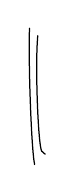
\begin{tikzpicture}[x=1cm,y=1cm,line width=.45pt,line cap=round]
\draw (0,0) .. controls (-.015,-.48) and (.025,-1.54) .. (.065,-1.73);
\draw (.105,-.095) .. controls (.070,-.48) and (.110,-1.48) .. (.155,-1.56) .. controls (.165,-1.58) and (.185,-1.59) .. (.200,-1.60);
\end{tikzpicture}}}}
\LMsourceMark{M011246}{\margin{\LMsourceMark{M011247}{\unsure{rappelons qu'on suppose}} $\pi$ \LMsourceMark{M011248}{\unsure{anabélien|nonabélien}}
$(2g+\nu\geq3)$}}
\[
1\longrightarrow\pi'\longrightarrow
\widehat{\widehat{\mathcal T}}(\pi,i)\longrightarrow
\LMsourceMark{M011249}{\unsure{\widehat{\widehat{\mathcal G}}}}(\pi',i)\longrightarrow1
\]
ou encore
\[
1\longrightarrow\widehat{\pi}_{g,\nu-1}\longrightarrow
\widehat{\widehat{\mathcal T}}_{g,(\nu,\nu-1)}
\longrightarrow\LMsourceMark{M011250}{\unsure{\widehat{\widehat{\mathcal G}}}}_{g,\nu-1}
\longrightarrow1
\]
qui contient la suite exacte
\[
1\longrightarrow\pi_{g,\nu-1}^{\LMsourceMark{M011251}{\unsure{*|+}}}\longrightarrow
\mathcal T_{g,(\nu,\nu-1)}\longrightarrow
\LMsourceMark{M011252}{\unsure{\mathcal G}}_{g,\nu-1}\longrightarrow1
\]
\LMsourceMark{M011253}{\unsure{comme|connue}} sous\var{\deleted{\LMsourceMark{M011254}{\unsure{particulière|partie dense}}}}{\LMsourceMark{M011255}{\LMcancelledDoubts{\LMsourceMark{M011256}{\unsure{particulière|partie dense}}}}}{deletion}{140-2-s348-D002}, \LMsourceMark{M011257}{\unsure{suite|est}} exacte.
Il est commode de travailler plutôt avec
\diagram{\begin{tikzcd}[ampersand replacement=\&,column sep=2.1em,row sep=3.0em]
1 \arrow[r,dash] \&
\pi_{g,\nu-1} \arrow[r,dash] \arrow[d,hook',no head] \&
\LMsourceMark{M011258}{\unsure{\mathcal T}}_{g,\nu}^{!+} \arrow[r] \arrow[d,hook',no head] \&
\mathcal G_{g,\nu-1}^{!+} \arrow[r,dash] \arrow[d,hook',no head] \& 1 \\
1 \arrow[r,dash] \&
\widehat{\pi}_{g,\nu-1} \arrow[r] \arrow[d,equal] \&
\underset{\var{\deleted{\LMsourceMark{M011259}{\unsure{\LMsourceMark{M011260}{\illegible{1}}}}}}{\LMsourceMark{M011261}{\LMcancelledDoubts{\(\LMsourceMark{M011262}{\unsure{\LMsourceMark{M011263}{\illegible{1}}}}\)}}}{deletion}{140-2-s348-D003}}{\widehat{\mathcal T}_{g,\nu}^{!+}}
\arrow[r] \arrow[d,hook',no head] \&
\widehat{\mathcal G}_{g,\nu-1}^{!+} \arrow[r,dash] \arrow[d,hook'] \& 1 \\
1 \arrow[r,dash] \&
\widehat{\pi}_{g,\nu-1} \arrow[r] \&
\widehat{\widehat{\mathcal T}}_{g,\nu}^{!} \arrow[r] \&
\widehat{\widehat{\mathcal G}}_{g,\nu-1}^{!} \arrow[r,dash] \& 1
\end{tikzcd}}

L'application \LMmathnotice{140-2-348-M1}
\begin{multline*}\LMsourceMark{M011264}{\unsure{\text{Prédiscrét}|\text{Prédiscrit}}}^{+}(\pi)\\\longrightarrow
\LMsourceMark{M011265}{\unsure{\text{Prédiscrét}|\text{Prédiscrit}}}^{+}(\pi')\end{multline*} s'identifie donc à
$\widehat{\widehat{\mathcal T}}_{g,\nu}^{!}/\widehat{\mathcal T}_{g,\nu}^{!}$,
on lit sur le diagramme que c'est
$\simeq\widehat{\widehat{\mathcal G}}_{g,\nu-1}^{\LMsourceMark{M011266}{\unsure{!}}\var{\deleted{\LMsourceMark{M011267}{\unsure{+}}}}{\LMsourceMark{M011268}{\LMcancelledDoubts{\(\LMsourceMark{M011269}{\unsure{+}}\)}}}{deletion}{140-2-s348-D004}}/
\widehat{\mathcal G}_{g,\nu-1}^{!+}$,
d'où la bijectivité sur les ens des prédiscrétifications orientées.

Dans le groupe $\widehat{\widehat{\mathcal T}}_{g,\nu}^{!}=\mathcal T$,
on a un sous-groupe invariant $\widehat{\pi}_{g,\nu-1}=\pi'$,
et un sous-groupe $\Sigma$ $(\LMsourceMark{M011270}{\unsure{=|\longleftarrow}}\widehat{\mathcal T}_{g,\nu}^{!+})$
\LMsourceMark{M011271}{\mspage{347}}

\LMflushnotes\LMflushpages
\ifnum\LMform=1
\begin{LMapparatus}
\LMentry{140-2-s348-D001}{suppression}{\deleted{que}
}{\emph{\LMomittedlabel}}{Passage biffé dans le manuscrit : la suppression suit l'état final de l'auteur; les doutes de lecture restent signalés.}{}
\LMentry{140-2-s348-D002}{suppression}{\deleted{\LMsourceMark{M011272}{\unsure{particulière|partie dense}}}
}{\emph{\LMomittedlabel}}{Passage biffé dans le manuscrit : la suppression suit l'état final de l'auteur; les doutes de lecture restent signalés.}{}
\LMentry{140-2-s348-D003}{suppression}{\(\deleted{\LMsourceMark{M011273}{\unsure{\LMsourceMark{M011274}{\illegible{1}}}}}\)
}{\emph{\LMomittedlabel}}{Passage biffé dans le manuscrit : la suppression suit l'état final de l'auteur; les doutes de lecture restent signalés.}{}
\LMentry{140-2-s348-D004}{suppression}{\(\deleted{\LMsourceMark{M011275}{\unsure{+}}}\)
}{\emph{\LMomittedlabel}}{Passage biffé dans le manuscrit : la suppression suit l'état final de l'auteur; les doutes de lecture restent signalés.}{}
\end{LMapparatus}
\fi
\ifnum\LMform=2
\par\smallskip\begingroup\footnotesize\Needspace{4\baselineskip}\csname @beginparpenalty\endcsname=10000\relax\noindent\textcolor{gray}{\rule{.2\linewidth}{.35pt}}\par\nobreak
\noindent\textit{\LMdoubtheading.}\par\nobreak
\LMcarryover{140-2-s348-D002}{\LMsourceMark{M011276}{\unsure{particulière|partie dense}}
}
\LMcarryover{140-2-s348-D003}{\(\LMsourceMark{M011277}{\unsure{\LMsourceMark{M011278}{\illegible{1}}}}\)
}
\LMcarryover{140-2-s348-D004}{\(\LMsourceMark{M011279}{\unsure{+}}\)
}
\par\endgroup\smallskip
\fi

\ifnum\LMform=1
\par\begingroup\footnotesize
\noindent\texttt{140-2-348-M1} \textit{Disposition}. Formule du texte courant disposée sur deux lignes, avec un repère à son emplacement; les symboles et lectures restent identiques.\par
\endgroup\fi
\LMsourceMark{M011280}{\scanpage{349}}

entre $\pi'$ et $\mathcal T$, \var{\deleted{\LMsourceMark{M011281}{\unsure{donnant par}}}}{\LMsourceMark{M011282}{\LMcancelledDoubts{\LMsourceMark{M011283}{\unsure{donnant par}}}}}{deletion}{140-2-s349-D001} \var{\inserted{donnant}}{\LMadded{donnant}}{insertion}{140-2-s349-I001} un ss-groupe $\Sigma'\simeq\mathcal T(\pi')$\var{\inserted{$(=\LMsourceMark{M011284}{\unsure{\widehat{\mathcal G}^{!+}_{g,\nu-1}}})$}}{\LMadded{$(=\LMsourceMark{M011285}{\unsure{\widehat{\mathcal G}^{!+}_{g,\nu-1}}})$}}{insertion}{140-2-s349-I002} dans $\LMsourceMark{M011286}{\unsure{\mathcal T'}}=\mathcal T/\pi'$ $(\simeq\widehat{\widehat{\mathcal G}}^{!}_{g,\nu-1})$, et on sait bien qu'alors
\[
\mathcal T/\Sigma\simeq\mathcal T'/\Sigma',
\]
et \var{\deleted{$\LMsourceMark{M011287}{\unsure{N(\Sigma)}}$}}{\LMsourceMark{M011288}{\LMcancelledDoubts{\(\LMsourceMark{M011289}{\unsure{N(\Sigma)}}\)}}}{deletion}{140-2-s349-D002} que le normalisateur \var{\inserted{$\mathcal N$,}}{\LMadded{$\mathcal N$,}}{insertion}{140-2-s349-I003} de $\Sigma$ dans $\mathcal T$ est l'image inverse du normalisateur $\mathcal N'$ de $\Sigma'$ dans $\mathcal T'$, de sorte que $\mathcal N/\Sigma\simeq\mathcal N'/\Sigma'$, ce qui prouve ce qu'on voulait.

\uline{Corollaire} On a des \LMsourceMark{M011290}{\unsure{is.}} canoniques
\[
\Gamma_{g,\nu}\xrightarrow{\sim}\Gamma_{g,\nu-1}\xrightarrow{\sim}\LMsourceMark{M011291}{\unsure{\cdots}}\quad\var{\deleted{\LMsourceMark{M011292}{\unsure{\Gamma_{g,0}}}}}{\LMsourceMark{M011293}{\LMcancelledDoubts{\(\LMsourceMark{M011294}{\unsure{\Gamma_{g,0}}}\)}}}{deletion}{140-2-s349-D003}
\]
\LMsourceMark{M011295}{\margin{On voit aussi que $\LMsourceMark{M011296}{\unsure{\Sigma|\Sigma^{!}}}$ invariant dans $\LMsourceMark{M011297}{\unsure{\mathcal T|\widehat{\widehat{\mathcal T}}}}$ équivaut à $\Sigma'$ invariant dans $\widehat{\widehat{\mathcal T}}'$}}
de sorte que si $g\geq2$, on a \LMsourceMark{M011298}{\unsure{canoniqt}} $\Gamma_{g,\nu}\simeq\Gamma_{g,0}$, d'autre part $\Gamma_{1,\nu}\simeq\Gamma_{1,1}$ $(g=1,\nu\geq1)$, $\Gamma_{0,\nu}\simeq\Gamma_{0,3}$ $(\nu\geq3)$.

\uline{NB} Le ``fait'' \var{\deleted{\LMsourceMark{M011299}{\illegible{1}}}}{\LMsourceMark{M011300}{\LMcancelledDoubts{\LMsourceMark{M011301}{\illegible{1}}}}}{deletion}{140-2-s349-D004} admis est loin d'être évident --- même que $\widehat{\widehat{\mathcal T}}^{\LMsourceMark{M011302}{\unsure{!}}}_{g,(\nu,\nu-1)}\longrightarrow\LMsourceMark{M011303}{\unsure{\widehat{\widehat{\mathcal T}}_{g,\nu-1}|\widehat{\widehat{\mathcal M}}_{g,\nu-1}}}$ soit surjectif, ou que $\widehat{\widehat{\mathcal T}}_{g,(\nu,\nu-1)}\longrightarrow\widehat{\widehat{\mathcal G}}_{g,\nu-1}$ soit injectif, est loin d'être évident, et est peut-être tout à fait faux !

Le fait admis revient à un énoncé d'existence d'un foncteur \LMsourceMark{M011304}{\unsure{en}} sens inverse ``forage des trous'', \LMsourceMark{M011305}{\unsure{qui|quid}} en tout état de cause reste incompris.

\LMsourceMark{M011306}{\mspage{348}}

\LMflushnotes\LMflushpages
\ifnum\LMform=1
\begin{LMapparatus}
\LMentry{140-2-s349-D001}{suppression}{\deleted{\LMsourceMark{M011307}{\unsure{donnant par}}}
}{\emph{\LMomittedlabel}}{Passage biffé dans le manuscrit : la suppression suit l'état final de l'auteur; les doutes de lecture restent signalés.}{}
\LMentry{140-2-s349-I001}{insertion}{\inserted{donnant}
}{\emph{\LMinsertedlabel}}{Ajout explicite de l'auteur : intégré à l'endroit indiqué par la transcription, sans modifier sa lecture.}{}
\LMentry{140-2-s349-I002}{insertion}{\inserted{$(=\LMsourceMark{M011308}{\unsure{\widehat{\mathcal G}^{!+}_{g,\nu-1}}})$}
}{\emph{\LMinsertedlabel}}{Ajout explicite de l'auteur : intégré à l'endroit indiqué par la transcription, sans modifier sa lecture.}{}
\LMentry{140-2-s349-D002}{suppression}{\deleted{$\LMsourceMark{M011309}{\unsure{N(\Sigma)}}$}
}{\emph{\LMomittedlabel}}{Passage biffé dans le manuscrit : la suppression suit l'état final de l'auteur; les doutes de lecture restent signalés.}{}
\LMentry{140-2-s349-I003}{insertion}{\inserted{$\mathcal N$,}
}{\emph{\LMinsertedlabel}}{Ajout explicite de l'auteur : intégré à l'endroit indiqué par la transcription, sans modifier sa lecture.}{}
\LMentry{140-2-s349-D003}{suppression}{\(\deleted{\LMsourceMark{M011310}{\unsure{\Gamma_{g,0}}}}\)
}{\emph{\LMomittedlabel}}{Passage biffé dans le manuscrit : la suppression suit l'état final de l'auteur; les doutes de lecture restent signalés.}{}
\LMentry{140-2-s349-D004}{suppression}{\deleted{\LMsourceMark{M011311}{\illegible{1}}}
}{\emph{\LMomittedlabel}}{Passage biffé dans le manuscrit : la suppression suit l'état final de l'auteur; les doutes de lecture restent signalés.}{}
\end{LMapparatus}
\fi
\ifnum\LMform=2
\par\smallskip\begingroup\footnotesize\Needspace{4\baselineskip}\csname @beginparpenalty\endcsname=10000\relax\noindent\textcolor{gray}{\rule{.2\linewidth}{.35pt}}\par\nobreak
\noindent\textit{\LMdoubtheading.}\par\nobreak
\LMcarryover{140-2-s349-D001}{\LMsourceMark{M011312}{\unsure{donnant par}}
}
\LMcarryover{140-2-s349-D002}{\(\LMsourceMark{M011313}{\unsure{N(\Sigma)}}\)
}
\LMcarryover{140-2-s349-D003}{\(\LMsourceMark{M011314}{\unsure{\Gamma_{g,0}}}\)
}
\LMcarryover{140-2-s349-D004}{\LMsourceMark{M011315}{\illegible{1}}
}
\par\endgroup\smallskip
\fi

\LMsourceMark{M011316}{\scanpage{350}}
\LMsourceMark{M011317}{\mspage{177}}

28. \uline{Changement de type} $(g,\nu)$ \LMsourceMark{M011318}{\unsure{(suite)}} : \uline{\LMsourceMark{M011319}{\unsure{passage}} à un rev. fini.}

Soit $\pi$ un groupe profini \var{\inserted{à lacets}}{\LMadded{à lacets}}{insertion}{140-2-s350-I001} de type $(g,\nu)$, anabélien comme tjrs, $\pi'$ un ss-groupe d'indice fini. On sait (\LMsourceMark{M011320}{\unsure{ou on|on en}} vérifie, par passage au cas discret) que \var{\deleted{\LMsourceMark{M011321}{\illegible{1}} \LMsourceMark{M011322}{\unsure{discrétifié}}}}{\LMsourceMark{M011323}{\LMcancelledDoubts{\LMsourceMark{M011324}{\illegible{1}}\quad \LMsourceMark{M011325}{\unsure{discrétifié}}}}}{deletion}{140-2-s350-D001} \var{\inserted{muni des}}{\LMadded{muni des}}{insertion}{140-2-s350-I002} \LMsourceMark{M011326}{\unsure{traces}} \LMsourceMark{M011327}{\unsure{sur|sous}} $\pi$ des ss-groupes à \LMsourceMark{M011328}{\unsure{lacets}} de $\pi$, $\pi'$ est un groupe à lacets.

\var{\deleted{Si pour tout $i\in I(\pi)$, on considère un $L_i$, et les $\LMsourceMark{M011329}{\unsure{n}}$ conjugués $\LMsourceMark{M011330}{\unsure{\operatorname{int}(g)}}L_i$ \inserted{$=L_{i\alpha}$}, avec $g\in\pi\bmod\pi'$ $(n=[\pi:\pi']\LMsourceMark{M011331}{\unsure{\}}},\ \deleted{\LMsourceMark{M011332}{\unsure{n}}}\ \inserted{1\leq\alpha\leq n})$ \deleted{\LMsourceMark{M011333}{\unsure{comptés|compter}} le nb de fois qu'une classe de conjugaison dans $\pi'$ du ss-groupe $\LMsourceMark{M011334}{\unsure{\operatorname{int}(g)}}L_i$ est} \inserted{alors si $\LMsourceMark{M011335}{\unsure{d_{\alpha}|d_{i\alpha}}}=[L_{i\alpha}:\LMsourceMark{M011336}{\unsure{L'_{i\alpha}|N'_{i\alpha}}}\deleted{\LMsourceMark{M011337}{\unsure{\cap\pi'}}}]$ \LMsourceMark{M011338}{\unsure{pour}} $L'_{i\alpha}=L_{i\alpha}\cap\pi'$, alors} exactement $d_{i\alpha}$ parmi les $L'_{i\beta}$ \inserted{$(1\leq\beta\leq n)$} sont conjugués dans $\pi'$ à $L'_{i\alpha}$, et si on somme sur les classes de \LMsourceMark{M011339}{\unsure{conjugaison}} distinctes des sous-groupes}}{\LMsourceMark{M011340}{\LMcancelledDoubts{\(\LMsourceMark{M011341}{\unsure{n}}\)\quad \(\LMsourceMark{M011342}{\unsure{\operatorname{int}(g)}}\)\quad \(\LMsourceMark{M011343}{\unsure{\}}}\)\quad \(\LMsourceMark{M011344}{\unsure{n}}\)\quad \LMsourceMark{M011345}{\unsure{comptés|compter}}\quad \(\LMsourceMark{M011346}{\unsure{\operatorname{int}(g)}}\)\quad \(\LMsourceMark{M011347}{\unsure{d_{\alpha}|d_{i\alpha}}}\)\quad \(\LMsourceMark{M011348}{\unsure{L'_{i\alpha}|N'_{i\alpha}}}\)\quad \(\LMsourceMark{M011349}{\unsure{\cap\pi'}}\)\quad \LMsourceMark{M011350}{\unsure{pour}}\quad \LMsourceMark{M011351}{\unsure{conjugaison}}}}}{deletion}{140-2-s350-D002}

Les sous-groupes à lacets sont \LMsourceMark{M011352}{\unsure{aussi|ainsi}} les \var{\deleted{\LMsourceMark{M011353}{\unsure{les}}}}{\LMsourceMark{M011354}{\LMcancelledDoubts{\LMsourceMark{M011355}{\unsure{les}}}}}{deletion}{140-2-s350-D006} sous-groupes $L'$ tels que
\[
\text{a)}\quad L'=\operatorname{Centr}_{\pi}(L')\cap\pi'.
\]
\[
\text{b)}\quad L\LMsourceMark{M011356}{\unsure{=|:}}\operatorname{Centr}_{\pi}(L')\text{ est un sous-groupe à \LMsourceMark{M011357}{\unsure{lacet}} dans }\pi.
\]
On pose $d(L')=[L:L']$, et on a ainsi une fonction
\[
d:I'=I(\pi')\longrightarrow\mathbb N^*,
\]
et une application $I'\xrightarrow{\varphi}I$, telles que $\forall i\in I$, on ait
\[
\text{(1)}\qquad \sum_{\substack{i'\in I'\\\text{sur }i}}d(i')=n
\qquad (\text{\LMsourceMark{M011358}{\unsure{où|ici}}}\ n=[\pi:\pi'])
\]
On aura la formule de Hurwitz
\[
\text{(2)}\qquad \var{\deleted{\LMsourceMark{M011359}{\unsure{2g|2\alpha}}}}{\LMsourceMark{M011360}{\LMcancelledDoubts{\(\LMsourceMark{M011361}{\unsure{2g|2\alpha}}\)}}}{deletion}{140-2-s350-D007}\ 2g'-2=n(2g-2)+\overbrace{\sum_{i'\in I'}(d(i')-1)}^{\var{\inserted{n\operatorname{card}I-\operatorname{card}I'}}{\LMadded{n\operatorname{card}I-\operatorname{card}I'}}{insertion}{140-2-s350-I007}}
\]
\LMsourceMark{M011362}{\mspage{349}}

\LMflushnotes\LMflushpages
\ifnum\LMform=1
\begin{LMapparatus}
\LMentry{140-2-s350-I001}{insertion}{\inserted{à lacets}
}{\emph{\LMinsertedlabel}}{Ajout explicite de l'auteur : intégré à l'endroit indiqué par la transcription, sans modifier sa lecture.}{}
\LMentry{140-2-s350-D001}{suppression}{\deleted{\LMsourceMark{M011363}{\illegible{1}} \LMsourceMark{M011364}{\unsure{discrétifié}}}
}{\emph{\LMomittedlabel}}{Passage biffé dans le manuscrit : la suppression suit l'état final de l'auteur; les doutes de lecture restent signalés.}{}
\LMentry{140-2-s350-I002}{insertion}{\inserted{muni des}
}{\emph{\LMinsertedlabel}}{Ajout explicite de l'auteur : intégré à l'endroit indiqué par la transcription, sans modifier sa lecture.}{}
\LMentry{140-2-s350-D002}{suppression}{\deleted{Si pour tout $i\in I(\pi)$, on considère un $L_i$, et les $\LMsourceMark{M011365}{\unsure{n}}$ conjugués $\LMsourceMark{M011366}{\unsure{\operatorname{int}(g)}}L_i$ \inserted{$=L_{i\alpha}$}, avec $g\in\pi\bmod\pi'$ $(n=[\pi:\pi']\LMsourceMark{M011367}{\unsure{\}}},\ \deleted{\LMsourceMark{M011368}{\unsure{n}}}\ \inserted{1\leq\alpha\leq n})$ \deleted{\LMsourceMark{M011369}{\unsure{comptés|compter}} le nb de fois qu'une classe de conjugaison dans $\pi'$ du ss-groupe $\LMsourceMark{M011370}{\unsure{\operatorname{int}(g)}}L_i$ est} \inserted{alors si $\LMsourceMark{M011371}{\unsure{d_{\alpha}|d_{i\alpha}}}=[L_{i\alpha}:\LMsourceMark{M011372}{\unsure{L'_{i\alpha}|N'_{i\alpha}}}\deleted{\LMsourceMark{M011373}{\unsure{\cap\pi'}}}]$ \LMsourceMark{M011374}{\unsure{pour}} $L'_{i\alpha}=L_{i\alpha}\cap\pi'$, alors} exactement $d_{i\alpha}$ parmi les $L'_{i\beta}$ \inserted{$(1\leq\beta\leq n)$} sont conjugués dans $\pi'$ à $L'_{i\alpha}$, et si on somme sur les classes de \LMsourceMark{M011375}{\unsure{conjugaison}} distinctes des sous-groupes}
}{\emph{\LMomittedlabel}}{Passage biffé dans le manuscrit : la suppression suit l'état final de l'auteur; les doutes de lecture restent signalés.}{}
\LMentry{140-2-s350-D006}{suppression}{\deleted{\LMsourceMark{M011376}{\unsure{les}}}
}{\emph{\LMomittedlabel}}{Passage biffé dans le manuscrit : la suppression suit l'état final de l'auteur; les doutes de lecture restent signalés.}{}
\LMentry{140-2-s350-D007}{suppression}{\(\deleted{\LMsourceMark{M011377}{\unsure{2g|2\alpha}}}\)
}{\emph{\LMomittedlabel}}{Passage biffé dans le manuscrit : la suppression suit l'état final de l'auteur; les doutes de lecture restent signalés.}{}
\LMentry{140-2-s350-I007}{insertion}{\(\inserted{n\operatorname{card}I-\operatorname{card}I'}\)
}{\emph{\LMinsertedlabel}}{Ajout explicite de l'auteur : intégré à l'endroit indiqué par la transcription, sans modifier sa lecture.}{}
\end{LMapparatus}
\fi
\ifnum\LMform=2
\par\smallskip\begingroup\footnotesize\Needspace{4\baselineskip}\csname @beginparpenalty\endcsname=10000\relax\noindent\textcolor{gray}{\rule{.2\linewidth}{.35pt}}\par\nobreak
\noindent\textit{\LMdoubtheading.}\par\nobreak
\LMcarryover{140-2-s350-D001}{\LMsourceMark{M011378}{\illegible{1}}\quad \LMsourceMark{M011379}{\unsure{discrétifié}}
}
\LMcarryover{140-2-s350-D002}{\(\LMsourceMark{M011380}{\unsure{n}}\)\quad \(\LMsourceMark{M011381}{\unsure{\operatorname{int}(g)}}\)\quad \(\LMsourceMark{M011382}{\unsure{\}}}\)\quad \(\LMsourceMark{M011383}{\unsure{n}}\)\quad \LMsourceMark{M011384}{\unsure{comptés|compter}}\quad \(\LMsourceMark{M011385}{\unsure{\operatorname{int}(g)}}\)\quad \(\LMsourceMark{M011386}{\unsure{d_{\alpha}|d_{i\alpha}}}\)\quad \(\LMsourceMark{M011387}{\unsure{L'_{i\alpha}|N'_{i\alpha}}}\)\quad \(\LMsourceMark{M011388}{\unsure{\cap\pi'}}\)\quad \LMsourceMark{M011389}{\unsure{pour}}\quad \LMsourceMark{M011390}{\unsure{conjugaison}}
}
\LMcarryover{140-2-s350-D006}{\LMsourceMark{M011391}{\unsure{les}}
}
\LMcarryover{140-2-s350-D007}{\(\LMsourceMark{M011392}{\unsure{2g|2\alpha}}\)
}
\par\endgroup\smallskip
\fi

% END PACKAGE LM_P035
% BEGIN PACKAGE LM_P036
\ifnum\LMform<2\Needspace{11\baselineskip}\subsection*{Scans 351--360}\fi
\LMsourceMark{M011393}{\scanpage{351}}
i.e.
\[
(3)\qquad 2g'-2+\mathrm{card}\,I'=n(2g-2+\mathrm{card}\,I)
\]

(NB. \var{\deleted{\LMsourceMark{M011394}{\unsure{\(n\)}}}}{\LMsourceMark{M011395}{\LMcancelledDoubts{\LMsourceMark{M011396}{\unsure{\(n\)}}}}}{deletion}{140-2-s351-D001} \((2g-2+\mathrm{card}\,I)\) est
\var{\inserted{l'opposé de}}{\LMadded{l'opposé de}}{insertion}{140-2-s351-I001} la \LMsourceMark{M011397}{\unsure{car.}} d'EP à supports
compacts de la courbe dont \(\LMsourceMark{M011398}{\unsure{\Pi|\pi}}\) est le groupe
fondamental\ldots) \(\checkmark\)

\LMsourceMark{M011399}{\margin{\uline{NB} dire qu'on \LMsourceMark{M011400}{\unsure{est}} dans le cas
\LMsourceMark{M011401}{\unsure{anabélien}} signifie que \(-\mathrm{EP}_{!}\) est \(\geq 1\)
--- cette \LMsourceMark{M011402}{\unsure{condition|relation}} est \LMsourceMark{M011403}{\unsure{donc conservée}}
par passage \LMsourceMark{M011404}{\unsure{à un revêtement|aux revêtements}}.
L'entier \(-\mathrm{EP}_{!}\) \LMsourceMark{M011405}{\unsure{mesure}} \LMsourceMark{M011406}{\unsure{positivité stricte}}
\LMsourceMark{M011407}{\illegible{1}} degré d'\LMsourceMark{M011408}{\unsure{anabélianité}}, \LMsourceMark{M011409}{\unsure{en qq sorte}}\ldots}}

De façon évidente, \LMsourceMark{M011410}{\unsure{tte}} discrétification de \(\LMsourceMark{M011411}{\unsure{\Pi|\pi}}\)
en définit une de \(\LMsourceMark{M011412}{\unsure{\Pi|\pi}}'\) --- et il en est de
\(\overline{\mathrm m}\) pour les discrétifications orientées, modulo
un peu de cohomologie [qui revient à dire,
\var{\inserted{dans le cas \LMsourceMark{M011413}{\unsure{discret}} \LMsourceMark{M011414}{\unsure{pex|p.ex}})}}{\LMadded{dans le cas \LMsourceMark{M011415}{\unsure{discret}} \LMsourceMark{M011416}{\unsure{pex|p.ex}})}}{insertion}{140-2-s351-I002}
que
\diagram{\begin{tikzcd}[ampersand replacement=\&]
H^2_{!}(\LMsourceMark{M011417}{\unsure{U|\mathcal U}},\LMsourceMark{M011418}{\unsure{\mathbb Z|\mathbf Z}}) \arrow[r] \arrow[d,phantom,sloped,"\simeq"] \& H^2_{!}(\LMsourceMark{M011419}{\unsure{U'|\mathcal U'}},\LMsourceMark{M011420}{\unsure{\mathbb Z|\mathbf Z}}) \arrow[d,phantom,sloped,"\simeq"] \\
T \& T'
\end{tikzcd}}
peut s'écrire sous la forme \(n\theta^{-1}\), où \(\theta\) est un iso. bien
déterminé (l'isom. trace) \LMsourceMark{M011421}{\unsure{\(\theta\)|de}} \(T'\xrightarrow{\sim}T\).

Il n'est pas clair pour moi à première
vue si l'application
\[
\mathrm{Discret}(\LMsourceMark{M011422}{\unsure{\Pi|\pi}})\LMsourceMark{M011423}{\unsure{-|\longrightarrow}}\mathrm{Discret}(\LMsourceMark{M011424}{\unsure{\Pi|\pi}}')
\]
est surjective, ou injective. L'injectivité
\var{\inserted{(pour \LMsourceMark{M011425}{\unsure{tt}} \(\LMsourceMark{M011426}{\unsure{\Pi|\pi}}'\) d'indice fini de \(\LMsourceMark{M011427}{\unsure{\Pi|\pi}}\))}}{\LMadded{(pour \LMsourceMark{M011428}{\unsure{tt}} \(\LMsourceMark{M011429}{\unsure{\Pi|\pi}}'\) d'indice fini de \(\LMsourceMark{M011430}{\unsure{\Pi|\pi}}\))}}{insertion}{140-2-s351-I003}
signifierait que : deux discrétifications \(\LMsourceMark{M011431}{\unsure{\Pi|\pi}}_0,\LMsourceMark{M011432}{\unsure{\Pi|\pi}}'_0\) de
\(\LMsourceMark{M011433}{\unsure{\Pi|\pi}}\) qui sont commensurables, i.e. telles que
\(\LMsourceMark{M011434}{\unsure{\Pi|\pi}}_0\cap\LMsourceMark{M011435}{\unsure{\Pi|\pi}}'_0\) soit d'indice fini dans \(\LMsourceMark{M011436}{\unsure{\Pi|\pi}}_0\) et dans \(\LMsourceMark{M011437}{\unsure{\Pi|\pi}}'_0\),
\var{\deleted{en fait, il suffit \LMsourceMark{M011438}{\unsure{qu'il le soit}} dans l'un d'eux}}{\LMsourceMark{M011439}{\LMcancelledDoubts{\LMsourceMark{M011440}{\unsure{qu'il le soit}}}}}{deletion}{140-2-s351-D002}
\var{\inserted{égales}}{\LMadded{égales}}{insertion}{140-2-s351-I004}

\LMflushnotes\LMflushpages
\ifnum\LMform=1
\begin{LMapparatus}
\LMentry{140-2-s351-D001}{suppression}{\deleted{\LMsourceMark{M011441}{\unsure{\(n\)}}}
}{\emph{\LMomittedlabel}}{Passage biffé dans le manuscrit : la suppression suit l'état final de l'auteur; les doutes de lecture restent signalés.}{}
\LMentry{140-2-s351-I001}{insertion}{\inserted{l'opposé de}
}{\emph{\LMinsertedlabel}}{Ajout explicite de l'auteur : intégré à l'endroit indiqué par la transcription, sans modifier sa lecture.}{}
\LMentry{140-2-s351-I002}{insertion}{\inserted{dans le cas \LMsourceMark{M011442}{\unsure{discret}} \LMsourceMark{M011443}{\unsure{pex|p.ex}})}
}{\emph{\LMinsertedlabel}}{Ajout explicite de l'auteur : intégré à l'endroit indiqué par la transcription, sans modifier sa lecture.}{}
\LMentry{140-2-s351-I003}{insertion}{\inserted{(pour \LMsourceMark{M011444}{\unsure{tt}} \(\LMsourceMark{M011445}{\unsure{\Pi|\pi}}'\) d'indice fini de \(\LMsourceMark{M011446}{\unsure{\Pi|\pi}}\))}
}{\emph{\LMinsertedlabel}}{Ajout explicite de l'auteur : intégré à l'endroit indiqué par la transcription, sans modifier sa lecture.}{}
\LMentry{140-2-s351-D002}{suppression}{\deleted{en fait, il suffit \LMsourceMark{M011447}{\unsure{qu'il le soit}} dans l'un d'eux}
}{\emph{\LMomittedlabel}}{Passage biffé dans le manuscrit : la suppression suit l'état final de l'auteur; les doutes de lecture restent signalés.}{}
\LMentry{140-2-s351-I004}{insertion}{\inserted{égales}
}{\emph{\LMinsertedlabel}}{Ajout explicite de l'auteur : intégré à l'endroit indiqué par la transcription, sans modifier sa lecture.}{}
\end{LMapparatus}
\fi
\ifnum\LMform=2
\par\smallskip\begingroup\footnotesize\Needspace{4\baselineskip}\csname @beginparpenalty\endcsname=10000\relax\noindent\textcolor{gray}{\rule{.2\linewidth}{.35pt}}\par\nobreak
\noindent\textit{\LMdoubtheading.}\par\nobreak
\LMcarryover{140-2-s351-D001}{\LMsourceMark{M011448}{\unsure{\(n\)}}
}
\LMcarryover{140-2-s351-D002}{\LMsourceMark{M011449}{\unsure{qu'il le soit}}
}
\par\endgroup\smallskip
\fi

\LMsourceMark{M011450}{\scanpage{352}}
\LMsourceMark{M011451}{\mspage{178}}
Supposons que \(\LMsourceMark{M011452}{\unsure{\Pi|\pi}}'\) soit sous-groupe invariant
dans \(\LMsourceMark{M011453}{\unsure{\Pi|\pi}}\), posons \(G=\LMsourceMark{M011454}{\unsure{\Pi|\pi}}'/\LMsourceMark{M011455}{\unsure{\Pi|\pi}}\)

\uline{Conjecture} L'application \(\mathrm{Discret}(\LMsourceMark{M011456}{\unsure{\Pi|\pi}})\longrightarrow\mathrm{Discret}(\LMsourceMark{M011457}{\unsure{\Pi|\pi}}')\)
est injective, et son image est formée des
discrétifications \(\LMsourceMark{M011458}{\unsure{\Pi|\pi}}'_0\subset\LMsourceMark{M011459}{\unsure{\Pi|\pi}}'\) telles que
\(G\longrightarrow\mathrm{Aut\,ext}_{\mathrm{lac}}(\LMsourceMark{M011460}{\unsure{\Pi|\pi}}')
\simeq\mathrm{Aut\,ext}_{\mathrm{lac}}(\widehat{\LMsourceMark{M011461}{\unsure{\Pi|\pi}}}'_0)
\simeq\widehat{\widehat{\mathcal T}}(\widehat{\LMsourceMark{M011462}{\unsure{\Pi|\pi}}}'_0)\)
se factorise par \(\mathcal T(\LMsourceMark{M011463}{\unsure{\Pi|\pi}}'_0)=\mathrm{Autext}_{\mathrm{lac}}(\LMsourceMark{M011464}{\unsure{\Pi|\pi}}'_0)\)
(et en fait, \(\overline{\mathrm m}\) par \(\mathcal T(\LMsourceMark{M011465}{\unsure{\Pi|\pi}}'_0)^+\)).

\LMsourceMark{M011466}{\margin{En d'autres termes, \(\forall g\in\LMsourceMark{M011467}{\unsure{\Pi|\pi}}\),
\(\exists h\in\LMsourceMark{M011468}{\unsure{\Pi|\pi}}'\) tel que \(\mathrm{int}(hg)(\LMsourceMark{M011469}{\unsure{\Pi|\pi}}'_0)\subset\LMsourceMark{M011470}{\unsure{\Pi|\pi}}'_0\)
i.e. \(\LMsourceMark{M011471}{\unsure{\LMsourceMark{M011472}{\unsure{\Pi|\pi}}'|\LMsourceMark{M011473}{\unsure{\Pi|\pi}}'_0}}\cdot\LMsourceMark{M011474}{\unsure{\Pi|\pi}}_0=\LMsourceMark{M011475}{\unsure{\Pi|\pi}}\), où \(\LMsourceMark{M011476}{\unsure{\Pi|\pi}}_0\) est le
normalisateur de \(\LMsourceMark{M011477}{\unsure{\Pi|\pi}}'_0\) dans \(\LMsourceMark{M011478}{\unsure{\Pi|\pi}}\).}}

La condition pour qu'un \var{\deleted{\LMsourceMark{M011479}{\illegible{1}}}}{\LMsourceMark{M011480}{\LMcancelledDoubts{\LMsourceMark{M011481}{\illegible{1}}}}}{deletion}{140-2-s352-D001} \(\LMsourceMark{M011482}{\unsure{\Pi|\pi}}'_0\) soit dans
l'image est évidemment nécessaire. Montrons
qu'elle est suffisante, et que le \(\LMsourceMark{M011483}{\unsure{\Pi|\pi}}_0^{\LMsourceMark{M011484}{\unsure{*}}}\) donnant
\LMsourceMark{M011485}{\unsure{naissance}} à \(\LMsourceMark{M011486}{\unsure{\Pi|\pi}}'_0\) par \(\LMsourceMark{M011487}{\unsure{\Pi|\pi}}_0\cap\LMsourceMark{M011488}{\unsure{\Pi|\pi}}'\) est unique.
On a une action extérieure de \(G\) sur \(\LMsourceMark{M011489}{\unsure{\Pi|\pi}}'_0\),
qui définit l'action extérieure sur \(\widehat{\LMsourceMark{M011490}{\unsure{\Pi|\pi}}}'_0\simeq\LMsourceMark{M011491}{\unsure{\Pi|\pi}}'\),
or \(\LMsourceMark{M011492}{\unsure{\Pi|\pi}}\) se récupère canoniquement à partir de
cette dernière (car \(\mathrm{Centre}(\widehat{\LMsourceMark{M011493}{\unsure{\Pi|\pi}}}')=1\)), et on
voit que c'est l' \var{\deleted{adhérence dans}}{}{deletion}{140-2-s352-D002} \var{\inserted{complété}}{\LMadded{complété}}{insertion}{140-2-s352-I001} profini de
l'extension \var{\inserted{\(\LMsourceMark{M011494}{\unsure{\Pi|\pi}}_0\)}}{\LMadded{\(\LMsourceMark{M011495}{\unsure{\Pi|\pi}}_0\)}}{insertion}{140-2-s352-I002} de \(G\) par \(\LMsourceMark{M011496}{\unsure{\Pi|\pi}}'_0\), définie par l'action
\var{\inserted{ext.}}{\LMadded{ext.}}{insertion}{140-2-s352-I003} de \(G\) sur \(\LMsourceMark{M011497}{\unsure{\Pi|\pi}}'_0\). On a donc bien une
discrétification généralisée \var{\inserted{\(\LMsourceMark{M011498}{\unsure{\Pi|\pi}}_0\) de \(\LMsourceMark{M011499}{\unsure{\Pi|\pi}}\)}}{\LMadded{\(\LMsourceMark{M011500}{\unsure{\Pi|\pi}}_0\) de \(\LMsourceMark{M011501}{\unsure{\Pi|\pi}}\)}}{insertion}{140-2-s352-I004}, au sens de la
seule structure de \var{\deleted{\LMsourceMark{M011502}{\unsure{gr}}}}{\LMsourceMark{M011503}{\LMcancelledDoubts{\LMsourceMark{M011504}{\unsure{gr}}}}}{deletion}{140-2-s352-D003} groupe profini, et elle
induit \(\LMsourceMark{M011505}{\unsure{\Pi|\pi}}'_0\) --- mais il faut voir qu'elle
est compatible avec la structure à lacets de \(\LMsourceMark{M011506}{\unsure{\Pi|\pi}}\).

\LMflushnotes\LMflushpages
\ifnum\LMform=1
\begin{LMapparatus}
\LMentry{140-2-s352-D001}{suppression}{\deleted{\LMsourceMark{M011507}{\illegible{1}}}
}{\emph{\LMomittedlabel}}{Passage biffé dans le manuscrit : la suppression suit l'état final de l'auteur; les doutes de lecture restent signalés.}{}
\LMentry{140-2-s352-D002}{suppression}{\deleted{adhérence dans}
}{\emph{\LMomittedlabel}}{Passage biffé dans le manuscrit : la suppression suit l'état final de l'auteur; les doutes de lecture restent signalés.}{}
\LMentry{140-2-s352-I001}{insertion}{\inserted{complété}
}{\emph{\LMinsertedlabel}}{Ajout explicite de l'auteur : intégré à l'endroit indiqué par la transcription, sans modifier sa lecture.}{}
\LMentry{140-2-s352-I002}{insertion}{\inserted{\(\LMsourceMark{M011508}{\unsure{\Pi|\pi}}_0\)}
}{\emph{\LMinsertedlabel}}{Ajout explicite de l'auteur : intégré à l'endroit indiqué par la transcription, sans modifier sa lecture.}{}
\LMentry{140-2-s352-I003}{insertion}{\inserted{ext.}
}{\emph{\LMinsertedlabel}}{Ajout explicite de l'auteur : intégré à l'endroit indiqué par la transcription, sans modifier sa lecture.}{}
\LMentry{140-2-s352-I004}{insertion}{\inserted{\(\LMsourceMark{M011509}{\unsure{\Pi|\pi}}_0\) de \(\LMsourceMark{M011510}{\unsure{\Pi|\pi}}\)}
}{\emph{\LMinsertedlabel}}{Ajout explicite de l'auteur : intégré à l'endroit indiqué par la transcription, sans modifier sa lecture.}{}
\LMentry{140-2-s352-D003}{suppression}{\deleted{\LMsourceMark{M011511}{\unsure{gr}}}
}{\emph{\LMomittedlabel}}{Passage biffé dans le manuscrit : la suppression suit l'état final de l'auteur; les doutes de lecture restent signalés.}{}
\end{LMapparatus}
\fi
\ifnum\LMform=2
\par\smallskip\begingroup\footnotesize\Needspace{4\baselineskip}\csname @beginparpenalty\endcsname=10000\relax\noindent\textcolor{gray}{\rule{.2\linewidth}{.35pt}}\par\nobreak
\noindent\textit{\LMdoubtheading.}\par\nobreak
\LMcarryover{140-2-s352-D001}{\LMsourceMark{M011512}{\illegible{1}}
}
\LMcarryover{140-2-s352-D003}{\LMsourceMark{M011513}{\unsure{gr}}
}
\par\endgroup\smallskip
\fi

\LMsourceMark{M011514}{\scanpage{353}}
Mais celle-ci s'explicite, à partir de la
structure à lacets de \(\LMsourceMark{M011515}{\unsure{\Pi|\pi}}'\), on prend les
sous-groupes à lacets \var{\inserted{\(L'\)}}{\LMadded{\(L'\)}}{insertion}{140-2-s353-I001} de \(\LMsourceMark{M011516}{\unsure{\Pi|\pi}}'\), et leurs
Centralisateurs dans \(\LMsourceMark{M011517}{\unsure{\Pi|\pi}}\). Faisons \LMsourceMark{M011518}{\unsure{itou}} pour
\(\LMsourceMark{M011519}{\unsure{\Pi|\pi}}_0\LMsourceMark{M011520}{\unsure{\supset|>}}\LMsourceMark{M011521}{\unsure{\Pi|\pi}}'_0\), on devrait trouver une structure
à lacets sur \(\LMsourceMark{M011522}{\unsure{\Pi|\pi}}_0\), donnant lieu aux
\(\overline{\mathrm m}\)\LMsourceMark{M011523}{\unsure{s}} \(d_i\).
J'ai l'impression que ça ne
doit pas être très vache à prouver --- ce
serait comme si on savait déjà que \LMsourceMark{M011524}{\unsure{tte}}
extension \var{\inserted{``sans torsion''}}{\LMadded{``sans torsion''}}{insertion}{140-2-s353-I002} d'un groupe fini par un
groupe à lacets est (de la façon canonique)
un groupe à lacets\ldots

\uline{Corollaire} En tous cas, l'application
\(\mathrm{Discret}(\LMsourceMark{M011525}{\unsure{\Pi|\pi}})\longrightarrow\mathrm{Discret}(\LMsourceMark{M011526}{\unsure{\Pi|\pi}}')\)
est \uline{injective}.
\figure{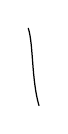
\begin{tikzpicture}[x=1cm,y=1cm,line width=.45pt,line cap=round]
\draw (0,0) .. controls (.065,-.20) and (.040,-.65) .. (.135,-.98);
\end{tikzpicture}}

\uline{NB} Elle ne doit pas tjs être bijective,
car il doit y avoir une action \var{\inserted{\LMsourceMark{M011527}{\unsure{extérieure|extérieures}}}}{\LMadded{\LMsourceMark{M011528}{\unsure{extérieure|extérieures}}}}{insertion}{140-2-s353-I003} d'un
\(G\) dans un \(\widehat{\LMsourceMark{M011529}{\unsure{\Pi|\pi}}}'_0\) i.e. des hom
\(G\longrightarrow\widehat{\widehat{\mathcal T}}(\widehat{\LMsourceMark{M011530}{\unsure{\Pi|\pi}}}'_0)\), qui ne se \LMsourceMark{M011531}{\unsure{factorise|factorisent}} pas
par \(\mathcal T(\LMsourceMark{M011532}{\unsure{\Pi|\pi}}'_0)\), et qui pourtant est aussi
\LMsourceMark{M011533}{\unsure{bonne|bonnes}} du pt de vue groupe profini que
\LMsourceMark{M011534}{\unsure{celle|celles}} provenant d'un \(\LMsourceMark{M011535}{\unsure{\Pi|\pi}}\) et d'un \LMsourceMark{M011536}{\unsure{ss-groupe}}

\LMflushnotes\LMflushpages
\ifnum\LMform=1
\begin{LMapparatus}
\LMentry{140-2-s353-I001}{insertion}{\inserted{\(L'\)}
}{\emph{\LMinsertedlabel}}{Ajout explicite de l'auteur : intégré à l'endroit indiqué par la transcription, sans modifier sa lecture.}{}
\LMentry{140-2-s353-I002}{insertion}{\inserted{``sans torsion''}
}{\emph{\LMinsertedlabel}}{Ajout explicite de l'auteur : intégré à l'endroit indiqué par la transcription, sans modifier sa lecture.}{}
\LMentry{140-2-s353-I003}{insertion}{\inserted{\LMsourceMark{M011537}{\unsure{extérieure|extérieures}}}
}{\emph{\LMinsertedlabel}}{Ajout explicite de l'auteur : intégré à l'endroit indiqué par la transcription, sans modifier sa lecture.}{}
\end{LMapparatus}
\fi

\LMsourceMark{M011538}{\scanpage{354}}
\LMsourceMark{M011539}{\mspage{179}}

invariant $\LMsourceMark{M011540}{\unsure{\Pi|\pi}}'$. En fait, partons d'une telle situation \uline{discrète} $\LMsourceMark{M011541}{\unsure{\Pi|\pi}}_0 \LMsourceMark{M011542}{\unsure{\supset|>}} \LMsourceMark{M011543}{\unsure{\Pi|\pi}}'_0$, d'où $G=\LMsourceMark{M011544}{\unsure{\Pi|\pi}}_0/\LMsourceMark{M011545}{\unsure{\Pi|\pi}}'_0$ et $G\longrightarrow \operatorname{Autext}_{\mathrm{lac}}(\LMsourceMark{M011546}{\unsure{\Pi|\pi}}'_0)\var{\deleted{\LMsourceMark{M011547}{\unsure{(\pi'_0)}}}}{\LMsourceMark{M011548}{\LMcancelledDoubts{\(\LMsourceMark{M011549}{\unsure{(\pi'_0)}}\)}}}{deletion}{140-2-s354-D001}=\mathcal T(\LMsourceMark{M011550}{\unsure{\Pi|\pi}}'_0)\subset\LMsourceMark{M011551}{\unsure{\widehat{\mathcal T}|\widehat{\widehat{\mathcal T}}}}(\widehat{\LMsourceMark{M011552}{\unsure{\Pi|\pi}}}'_0)$, et \uline{conjuguons} $G$ par un élément \var{\inserted{$\gamma$}}{\LMadded{$\gamma$}}{insertion}{140-2-s354-I001} de $\widehat{\widehat{\mathcal T}}(\LMsourceMark{M011553}{\unsure{\Pi|\pi}}'_0)$, de façon à trouver $G\longrightarrow\widehat{\mathcal T}(\widehat{\LMsourceMark{M011554}{\unsure{\Pi|\pi}}}'_0)$ qui ne \var{\deleted{\LMsourceMark{M011555}{\illegible{2}}}}{\LMsourceMark{M011556}{\LMcancelledDoubts{\LMsourceMark{M011557}{\illegible{2}}}}}{deletion}{140-2-s354-D002} se \LMsourceMark{M011558}{\unsure{factorise}} pas par $\mathcal T(\LMsourceMark{M011559}{\unsure{\Pi|\pi}}^{\LMsourceMark{M011560}{\unsure{'}}}_0)$. On trouve une extension \var{\inserted{$\LMsourceMark{M011561}{\unsure{\widehat{\LMsourceMark{M011562}{\unsure{\Pi|\pi}}}|\LMsourceMark{M011563}{\unsure{\Pi|\pi}}}}^{\LMsourceMark{M011564}{\unsure{\natural|\sharp}}}$}}{\LMadded{$\LMsourceMark{M011565}{\unsure{\widehat{\LMsourceMark{M011566}{\unsure{\Pi|\pi}}}|\LMsourceMark{M011567}{\unsure{\Pi|\pi}}}}^{\LMsourceMark{M011568}{\unsure{\natural|\sharp}}}$}}{insertion}{140-2-s354-I002} de $G$ par $\widehat{\LMsourceMark{M011569}{\unsure{\Pi|\pi}}}'_0$, \uline{isomorphe} à $\widehat{\LMsourceMark{M011570}{\unsure{\Pi|\pi}}}_0$ (en tant qu'extension de $G$ par $\widehat{\LMsourceMark{M011571}{\unsure{\Pi|\pi}}}'_0$), donc la structure à lacets de $\widehat{\LMsourceMark{M011572}{\unsure{\Pi|\pi}}}'_0$ en définit une sur $\LMsourceMark{M011573}{\unsure{\Pi|\pi}}^{\LMsourceMark{M011574}{\unsure{\natural|\sharp}}}$ \var{\deleted{et est}}{}{deletion}{140-2-s354-D003} \var{\inserted{(de façon à être}}{\LMadded{(de façon à être}}{insertion}{140-2-s354-I003} induite par cette dernière), mais pourtant la discrétification \uline{choisie} \var{\inserted{$\LMsourceMark{M011575}{\unsure{\Pi|\pi}}_0$}}{\LMadded{$\LMsourceMark{M011576}{\unsure{\Pi|\pi}}_0$}}{insertion}{140-2-s354-I004} de $\widehat{\LMsourceMark{M011577}{\unsure{\Pi|\pi}}}_0$ n'est pas induite par une de $\LMsourceMark{M011578}{\unsure{\Pi|\pi}}$. Pour

$\ast$ Faire la construction, il suffit de trouver un élément \var{\inserted{$\gamma\in\widehat{\widehat{\mathcal T}}(\LMsourceMark{M011579}{\unsure{\Pi|\pi}}'_0)$ \deleted{\LMsourceMark{M011580}{\unsure{fini}}} tel que $\operatorname{int}(\gamma).G\LMsourceMark{M011581}{\unsure{\not\subset|\notin}}\mathcal T$,}}{\LMadded{$\gamma\in\widehat{\widehat{\mathcal T}}(\LMsourceMark{M011582}{\unsure{\Pi|\pi}}'_0)$ \var{\deleted{\LMsourceMark{M011583}{\unsure{fini}}}}{\LMsourceMark{M011584}{\LMcancelledDoubts{\LMsourceMark{M011585}{\unsure{fini}}}}}{deletion}{140-2-s354-D004} tel que $\operatorname{int}(\gamma).G\LMsourceMark{M011586}{\unsure{\not\subset|\notin}}\mathcal T$,}}{insertion}{140-2-s354-I005} \var{\deleted{\LMsourceMark{M011587}{\unsure{$u$}} \LMsourceMark{M011588}{\unsure{d'ordre}} \LMsourceMark{M011589}{\illegible{1}} \LMsourceMark{M011590}{\unsure{provenant}} pas de, \LMsourceMark{M011591}{\unsure{dans}} $\mathcal T(\LMsourceMark{M011592}{\unsure{\Pi|\pi}}'_0)$, \LMsourceMark{M011593}{\unsure{ou se}} \LMsourceMark{M011594}{\unsure{relevant}} par un élément d'ordre fini de $\LMsourceMark{M011595}{\unsure{\mathcal G|\mathcal C}}(\LMsourceMark{M011596}{\unsure{\Pi|\pi}}'_0)^+=\operatorname{Aut}_{\mathrm{lac}}(\LMsourceMark{M011597}{\unsure{\Pi|\pi}}'_0)^+$, et \deleted{dont la \LMsourceMark{M011598}{\unsure{conjugaison}} dans $\widehat{\widehat{\mathcal T}}$ \LMsourceMark{M011599}{\unsure{un}}} \inserted{un $\gamma\in\widehat{\widehat{\mathcal T}}(\LMsourceMark{M011600}{\unsure{\Pi|\pi}}'_0)$, tel que} $\gamma u\gamma^{-1}\notin\mathcal T(\LMsourceMark{M011601}{\unsure{\Pi|\pi}}'_0)$, \inserted{\deleted{i.e. tel que $u$ ne \LMsourceMark{M011602}{\unsure{fixe}}}} \deleted{pas} \inserted{$\gamma^{-1}.\LMsourceMark{M011603}{\unsure{\Pi|\pi}}'_0\subset\widehat{\LMsourceMark{M011604}{\unsure{\Pi|\pi}}}'_0$.}}}{\LMsourceMark{M011605}{\LMcancelledDoubts{\LMsourceMark{M011606}{\unsure{$u$}}\quad \LMsourceMark{M011607}{\unsure{d'ordre}}\quad \LMsourceMark{M011608}{\illegible{1}}\quad \LMsourceMark{M011609}{\unsure{provenant}}\quad \LMsourceMark{M011610}{\unsure{dans}}\quad \(\LMsourceMark{M011611}{\unsure{\Pi|\pi}}\)\quad \LMsourceMark{M011612}{\unsure{ou se}}\quad \LMsourceMark{M011613}{\unsure{relevant}}\quad \(\LMsourceMark{M011614}{\unsure{\mathcal G|\mathcal C}}\)\quad \(\LMsourceMark{M011615}{\unsure{\Pi|\pi}}\)\quad \(\LMsourceMark{M011616}{\unsure{\Pi|\pi}}\)\quad \LMsourceMark{M011617}{\unsure{conjugaison}}\quad \LMsourceMark{M011618}{\unsure{un}}\quad \(\LMsourceMark{M011619}{\unsure{\Pi|\pi}}\)\quad \(\LMsourceMark{M011620}{\unsure{\Pi|\pi}}\)\quad \LMsourceMark{M011621}{\unsure{fixe}}\quad \(\LMsourceMark{M011622}{\unsure{\Pi|\pi}}\)\quad \(\LMsourceMark{M011623}{\unsure{\Pi|\pi}}\)}}}{deletion}{140-2-s354-D005}
\figure{[Une grande partie du passage annulé est entourée d'un cadre (côtés gauche, inférieur et droit) et barrée de quatre longs traits obliques. Après l'inclusion $\gamma^{-1}.\LMsourceMark{M011624}{\unsure{\Pi|\pi}}'_0\subset\widehat{\LMsourceMark{M011625}{\unsure{\Pi|\pi}}}'_0$ de la dernière ligne, trait recourbé en crochet, dirigé vers l'inclusion suivante.]}
\var{\inserted{i.e. tel que $G$ \deleted{\LMsourceMark{M011626}{\unsure{ne fixe}}} ne stabilise pas $\gamma^{-1}(\LMsourceMark{M011627}{\unsure{\Pi|\pi}}'_0)\subset\widehat{\LMsourceMark{M011628}{\unsure{\Pi|\pi}}}'_0$}}{\LMadded{i.e. tel que $G$ \var{\deleted{\LMsourceMark{M011629}{\unsure{ne fixe}}}}{\LMsourceMark{M011630}{\LMcancelledDoubts{\LMsourceMark{M011631}{\unsure{ne fixe}}}}}{deletion}{140-2-s354-D009} ne stabilise pas $\gamma^{-1}(\LMsourceMark{M011632}{\unsure{\Pi|\pi}}'_0)\subset\widehat{\LMsourceMark{M011633}{\unsure{\Pi|\pi}}}'_0$}}{insertion}{140-2-s354-I009}

Un tel $\gamma$ existe \LMsourceMark{M011634}{\unsure{tjrs}}....

\LMflushnotes\LMflushpages
\ifnum\LMform=1
\begin{LMapparatus}
\LMentry{140-2-s354-D001}{suppression}{\(\deleted{\LMsourceMark{M011635}{\unsure{(\pi'_0)}}}\)
}{\emph{\LMomittedlabel}}{Passage biffé dans le manuscrit : la suppression suit l'état final de l'auteur; les doutes de lecture restent signalés.}{}
\LMentry{140-2-s354-I001}{insertion}{\inserted{$\gamma$}
}{\emph{\LMinsertedlabel}}{Ajout explicite de l'auteur : intégré à l'endroit indiqué par la transcription, sans modifier sa lecture.}{}
\LMentry{140-2-s354-D002}{suppression}{\deleted{\LMsourceMark{M011636}{\illegible{2}}}
}{\emph{\LMomittedlabel}}{Passage biffé dans le manuscrit : la suppression suit l'état final de l'auteur; les doutes de lecture restent signalés.}{}
\LMentry{140-2-s354-I002}{insertion}{\inserted{$\LMsourceMark{M011637}{\unsure{\widehat{\LMsourceMark{M011638}{\unsure{\Pi|\pi}}}|\LMsourceMark{M011639}{\unsure{\Pi|\pi}}}}^{\LMsourceMark{M011640}{\unsure{\natural|\sharp}}}$}
}{\emph{\LMinsertedlabel}}{Ajout explicite de l'auteur : intégré à l'endroit indiqué par la transcription, sans modifier sa lecture.}{}
\LMentry{140-2-s354-D003}{suppression}{\deleted{et est}
}{\emph{\LMomittedlabel}}{Passage biffé dans le manuscrit : la suppression suit l'état final de l'auteur; les doutes de lecture restent signalés.}{}
\LMentry{140-2-s354-I003}{insertion}{\inserted{(de façon à être}
}{\emph{\LMinsertedlabel}}{Ajout explicite de l'auteur : intégré à l'endroit indiqué par la transcription, sans modifier sa lecture.}{}
\LMentry{140-2-s354-I004}{insertion}{\inserted{$\LMsourceMark{M011641}{\unsure{\Pi|\pi}}_0$}
}{\emph{\LMinsertedlabel}}{Ajout explicite de l'auteur : intégré à l'endroit indiqué par la transcription, sans modifier sa lecture.}{}
\LMentry{140-2-s354-I005}{insertion}{\inserted{$\gamma\in\widehat{\widehat{\mathcal T}}(\LMsourceMark{M011642}{\unsure{\Pi|\pi}}'_0)$ \deleted{\LMsourceMark{M011643}{\unsure{fini}}} tel que $\operatorname{int}(\gamma).G\LMsourceMark{M011644}{\unsure{\not\subset|\notin}}\mathcal T$,}
}{\emph{\LMinsertedlabel}}{Ajout explicite de l'auteur : intégré à l'endroit indiqué par la transcription, sans modifier sa lecture.}{}
\LMentry{140-2-s354-D004}{suppression}{\deleted{\LMsourceMark{M011645}{\unsure{fini}}}
}{\emph{\LMomittedlabel}}{Passage biffé dans le manuscrit : la suppression suit l'état final de l'auteur; les doutes de lecture restent signalés.}{}
\LMentry{140-2-s354-D005}{suppression}{\deleted{\LMsourceMark{M011646}{\unsure{$u$}} \LMsourceMark{M011647}{\unsure{d'ordre}} \LMsourceMark{M011648}{\illegible{1}} \LMsourceMark{M011649}{\unsure{provenant}} pas de, \LMsourceMark{M011650}{\unsure{dans}} $\mathcal T(\LMsourceMark{M011651}{\unsure{\Pi|\pi}}'_0)$, \LMsourceMark{M011652}{\unsure{ou se}} \LMsourceMark{M011653}{\unsure{relevant}} par un élément d'ordre fini de $\LMsourceMark{M011654}{\unsure{\mathcal G|\mathcal C}}(\LMsourceMark{M011655}{\unsure{\Pi|\pi}}'_0)^+=\operatorname{Aut}_{\mathrm{lac}}(\LMsourceMark{M011656}{\unsure{\Pi|\pi}}'_0)^+$, et \deleted{dont la \LMsourceMark{M011657}{\unsure{conjugaison}} dans $\widehat{\widehat{\mathcal T}}$ \LMsourceMark{M011658}{\unsure{un}}} \inserted{un $\gamma\in\widehat{\widehat{\mathcal T}}(\LMsourceMark{M011659}{\unsure{\Pi|\pi}}'_0)$, tel que} $\gamma u\gamma^{-1}\notin\mathcal T(\LMsourceMark{M011660}{\unsure{\Pi|\pi}}'_0)$, \inserted{\deleted{i.e. tel que $u$ ne \LMsourceMark{M011661}{\unsure{fixe}}}} \deleted{pas} \inserted{$\gamma^{-1}.\LMsourceMark{M011662}{\unsure{\Pi|\pi}}'_0\subset\widehat{\LMsourceMark{M011663}{\unsure{\Pi|\pi}}}'_0$.}}
}{\emph{\LMomittedlabel}}{Passage biffé dans le manuscrit : la suppression suit l'état final de l'auteur; les doutes de lecture restent signalés.}{}
\LMentry{140-2-s354-I009}{insertion}{\inserted{i.e. tel que $G$ \deleted{\LMsourceMark{M011664}{\unsure{ne fixe}}} ne stabilise pas $\gamma^{-1}(\LMsourceMark{M011665}{\unsure{\Pi|\pi}}'_0)\subset\widehat{\LMsourceMark{M011666}{\unsure{\Pi|\pi}}}'_0$}
}{\emph{\LMinsertedlabel}}{Ajout explicite de l'auteur : intégré à l'endroit indiqué par la transcription, sans modifier sa lecture.}{}
\LMentry{140-2-s354-D009}{suppression}{\deleted{\LMsourceMark{M011667}{\unsure{ne fixe}}}
}{\emph{\LMomittedlabel}}{Passage biffé dans le manuscrit : la suppression suit l'état final de l'auteur; les doutes de lecture restent signalés.}{}
\end{LMapparatus}
\fi
\ifnum\LMform=2
\par\smallskip\begingroup\footnotesize\Needspace{4\baselineskip}\csname @beginparpenalty\endcsname=10000\relax\noindent\textcolor{gray}{\rule{.2\linewidth}{.35pt}}\par\nobreak
\noindent\textit{\LMdoubtheading.}\par\nobreak
\LMcarryover{140-2-s354-D001}{\(\LMsourceMark{M011668}{\unsure{(\pi'_0)}}\)
}
\LMcarryover{140-2-s354-D002}{\LMsourceMark{M011669}{\illegible{2}}
}
\LMcarryover{140-2-s354-D004}{\LMsourceMark{M011670}{\unsure{fini}}
}
\LMcarryover{140-2-s354-D005}{\LMsourceMark{M011671}{\unsure{$u$}}\quad \LMsourceMark{M011672}{\unsure{d'ordre}}\quad \LMsourceMark{M011673}{\illegible{1}}\quad \LMsourceMark{M011674}{\unsure{provenant}}\quad \LMsourceMark{M011675}{\unsure{dans}}\quad \(\LMsourceMark{M011676}{\unsure{\Pi|\pi}}\)\quad \LMsourceMark{M011677}{\unsure{ou se}}\quad \LMsourceMark{M011678}{\unsure{relevant}}\quad \(\LMsourceMark{M011679}{\unsure{\mathcal G|\mathcal C}}\)\quad \(\LMsourceMark{M011680}{\unsure{\Pi|\pi}}\)\quad \(\LMsourceMark{M011681}{\unsure{\Pi|\pi}}\)\quad \LMsourceMark{M011682}{\unsure{conjugaison}}\quad \LMsourceMark{M011683}{\unsure{un}}\quad \(\LMsourceMark{M011684}{\unsure{\Pi|\pi}}\)\quad \(\LMsourceMark{M011685}{\unsure{\Pi|\pi}}\)\quad \LMsourceMark{M011686}{\unsure{fixe}}\quad \(\LMsourceMark{M011687}{\unsure{\Pi|\pi}}\)\quad \(\LMsourceMark{M011688}{\unsure{\Pi|\pi}}\)
}
\LMcarryover{140-2-s354-D009}{\LMsourceMark{M011689}{\unsure{ne fixe}}
}
\par\endgroup\smallskip
\fi

\LMsourceMark{M011690}{\scanpage{355}}

Bien sûr, il n'y a pas de raison, \var{\deleted{que}}{}{deletion}{140-2-s355-D001} pour deux discrétifications $\LMsourceMark{M011691}{\unsure{\LMsourceMark{M011692}{\unsure{\Pi|\pi}}'_0|\LMsourceMark{M011693}{\unsure{\Pi|\pi}}_0}},\LMsourceMark{M011694}{\unsure{\Pi|\pi}}_1$ de $\LMsourceMark{M011695}{\unsure{\Pi|\pi}}$, que si $\LMsourceMark{M011696}{\unsure{\Pi|\pi}}_0,\LMsourceMark{M011697}{\unsure{\Pi|\pi}}_1$ sont $\LMsourceMark{M011698}{\unsure{\Pi|\pi}}$-conjugués (i.e. définissent \var{\deleted{des}}{}{deletion}{140-2-s355-D002} \var{\inserted{la $\overline{\mathrm m}$}}{\LMadded{la $\overline{\mathrm m}$}}{insertion}{140-2-s355-I001} \LMsourceMark{M011699}{\unsure{prédiscrt.|prédiscrét.}} stricte\var{\deleted{s}}{}{deletion}{140-2-s355-D003} de $\LMsourceMark{M011700}{\unsure{\Pi|\pi}}$), il en soit de $\overline{\mathrm m}$ pour $\LMsourceMark{M011701}{\unsure{\Pi|\pi}}'_0$ et $\LMsourceMark{M011702}{\unsure{\Pi|\pi}}'_1$ pour l'action intérieure de $\LMsourceMark{M011703}{\unsure{\Pi|\pi}}'$. (Il faudrait que $\LMsourceMark{M011704}{\unsure{\Pi|\pi}}_0,\LMsourceMark{M011705}{\unsure{\Pi|\pi}}_1$ soient conjugués par $\LMsourceMark{M011706}{\unsure{\Pi|\pi}}'$, et pas seulement par $\LMsourceMark{M011707}{\unsure{\Pi|\pi}}$). Par contre, je présume que si $\LMsourceMark{M011708}{\unsure{\Pi|\pi}}_0,\LMsourceMark{M011709}{\unsure{\Pi|\pi}}_1$ sont ``adhérents'' l'un à l'autre dans l'espace des \LMsourceMark{M011710}{\unsure{discrétifications|discrétific.}} de $\LMsourceMark{M011711}{\unsure{\Pi|\pi}}$, i.e. s'ils définissent une $\overline{\mathrm m}$ prédiscrétification, il en va de $\overline{\mathrm m}$ pour $\LMsourceMark{M011712}{\unsure{\Pi|\pi}}'_0,\LMsourceMark{M011713}{\unsure{\Pi|\pi}}'_1$, et que l'application
\[
\tag{4}
\operatorname{Prédiscrt}^{+}(\LMsourceMark{M011714}{\unsure{\Pi|\pi}}\var{\deleted{\LMsourceMark{M011715}{\unsure{_0}}}}{\LMsourceMark{M011716}{\LMcancelledDoubts{\(\LMsourceMark{M011717}{\unsure{_0}}\)}}}{deletion}{140-2-s355-D004})\longrightarrow\operatorname{Prédiscrt}^{+}(\LMsourceMark{M011718}{\unsure{\Pi|\pi}}'\var{\deleted{\LMsourceMark{M011719}{\unsure{_0}}}}{\LMsourceMark{M011720}{\LMcancelledDoubts{\(\LMsourceMark{M011721}{\unsure{_0}}\)}}}{deletion}{140-2-s355-D005})
\]
qu'on obtient ainsi, est encore bijective, et qu'elle passe à son tour au quotient, pour définir une application bijective
\[
\tag{5}
\LMsourceMark{M011722}{\unsure{\operatorname{Préarith}|\operatorname{Préarithm}}}(\LMsourceMark{M011723}{\unsure{\Pi|\pi}}\var{\deleted{\LMsourceMark{M011724}{\unsure{_0}}}}{\LMsourceMark{M011725}{\LMcancelledDoubts{\(\LMsourceMark{M011726}{\unsure{_0}}\)}}}{deletion}{140-2-s355-D006})\longrightarrow\LMsourceMark{M011727}{\unsure{\operatorname{Préarith}|\operatorname{Préarithm}}}(\LMsourceMark{M011728}{\unsure{\Pi|\pi}}'\var{\deleted{\LMsourceMark{M011729}{\unsure{_0}}}}{\LMsourceMark{M011730}{\LMcancelledDoubts{\(\LMsourceMark{M011731}{\unsure{_0}}\)}}}{deletion}{140-2-s355-D007}),
\]
et que si $\Sigma,\Sigma'$ se correspondent par cette dernière, qu'on a un isom canonique
\[
\tag{6}
\LMsourceMark{M011732}{\unsure{\mathbb{\Gamma}|\Gamma}}_{\Sigma}\longrightarrow\LMsourceMark{M011733}{\unsure{\mathbb{\Gamma}|\Gamma}}_{\Sigma'},
\]
\LMsourceMark{M011734}{\unsure{comp.$^{\mathrm t}$ble}},

\LMflushnotes\LMflushpages
\ifnum\LMform=1
\begin{LMapparatus}
\LMentry{140-2-s355-D001}{suppression}{\deleted{que}
}{\emph{\LMomittedlabel}}{Passage biffé dans le manuscrit : la suppression suit l'état final de l'auteur; les doutes de lecture restent signalés.}{}
\LMentry{140-2-s355-D002}{suppression}{\deleted{des}
}{\emph{\LMomittedlabel}}{Passage biffé dans le manuscrit : la suppression suit l'état final de l'auteur; les doutes de lecture restent signalés.}{}
\LMentry{140-2-s355-I001}{insertion}{\inserted{la $\overline{\mathrm m}$}
}{\emph{\LMinsertedlabel}}{Ajout explicite de l'auteur : intégré à l'endroit indiqué par la transcription, sans modifier sa lecture.}{}
\LMentry{140-2-s355-D003}{suppression}{\deleted{s}
}{\emph{\LMomittedlabel}}{Passage biffé dans le manuscrit : la suppression suit l'état final de l'auteur; les doutes de lecture restent signalés.}{}
\LMentry{140-2-s355-D004}{suppression}{\(\deleted{\LMsourceMark{M011735}{\unsure{_0}}}\)
}{\emph{\LMomittedlabel}}{Passage biffé dans le manuscrit : la suppression suit l'état final de l'auteur; les doutes de lecture restent signalés.}{}
\LMentry{140-2-s355-D005}{suppression}{\(\deleted{\LMsourceMark{M011736}{\unsure{_0}}}\)
}{\emph{\LMomittedlabel}}{Passage biffé dans le manuscrit : la suppression suit l'état final de l'auteur; les doutes de lecture restent signalés.}{}
\LMentry{140-2-s355-D006}{suppression}{\(\deleted{\LMsourceMark{M011737}{\unsure{_0}}}\)
}{\emph{\LMomittedlabel}}{Passage biffé dans le manuscrit : la suppression suit l'état final de l'auteur; les doutes de lecture restent signalés.}{}
\LMentry{140-2-s355-D007}{suppression}{\(\deleted{\LMsourceMark{M011738}{\unsure{_0}}}\)
}{\emph{\LMomittedlabel}}{Passage biffé dans le manuscrit : la suppression suit l'état final de l'auteur; les doutes de lecture restent signalés.}{}
\end{LMapparatus}
\fi
\ifnum\LMform=2
\par\smallskip\begingroup\footnotesize\Needspace{4\baselineskip}\csname @beginparpenalty\endcsname=10000\relax\noindent\textcolor{gray}{\rule{.2\linewidth}{.35pt}}\par\nobreak
\noindent\textit{\LMdoubtheading.}\par\nobreak
\LMcarryover{140-2-s355-D004}{\(\LMsourceMark{M011739}{\unsure{_0}}\)
}
\LMcarryover{140-2-s355-D005}{\(\LMsourceMark{M011740}{\unsure{_0}}\)
}
\LMcarryover{140-2-s355-D006}{\(\LMsourceMark{M011741}{\unsure{_0}}\)
}
\LMcarryover{140-2-s355-D007}{\(\LMsourceMark{M011742}{\unsure{_0}}\)
}
\par\endgroup\smallskip
\fi

\LMsourceMark{M011743}{\scanpage{356}}
\LMsourceMark{M011744}{\mspage{180}}

avec les actions de ces groupes sur l'ens $P_{\Sigma}$ des prédiscrétifications de $\LMsourceMark{M011745}{\unsure{\Pi|\pi}}$ comp.tibles à $\Sigma$, et l'ens \var{\inserted{$P_{\Sigma'}$}}{\LMadded{$P_{\Sigma'}$}}{insertion}{140-2-s356-I001} des prédiscrétifications de $\LMsourceMark{M011746}{\unsure{\Pi|\pi}}'$ comp.tibles à $\Sigma'$ (qui sont resp. des torseurs à g. sous $\LMsourceMark{M011747}{\unsure{\mathbb{\Gamma}|\Gamma}}_{\Sigma},\LMsourceMark{M011748}{\unsure{\mathbb{\Gamma}|\Gamma}}_{\Sigma'}$). En même temps, on trouvera \var{\inserted{donc}}{\LMadded{donc}}{insertion}{140-2-s356-I002} que $\Sigma$ est unique pour $\LMsourceMark{M011749}{\unsure{\Pi|\pi}}$ i.e. invariant dans $\widehat{\widehat{\mathcal T}}(\LMsourceMark{M011750}{\unsure{\Pi|\pi}})$, ssi $\Sigma'$ est unique dans $\LMsourceMark{M011751}{\unsure{\Pi|\pi}}'$ i.e. invariant dans $\widehat{\widehat{\mathcal T}}(\LMsourceMark{M011752}{\unsure{\Pi|\pi}}')$.

En tous cas, la conjecture fondamentale qui \LMsourceMark{M011753}{\unsure{interprète}} les $\LMsourceMark{M011754}{\unsure{\mathbb{\Gamma}|\Gamma}}_{g,\LMsourceMark{M011755}{\unsure{\nu|v}}}$ comme $\LMsourceMark{M011756}{\unsure{\mathbb{\Gamma}|\Gamma}}_0=\operatorname{Gal}(\overline{\mathbb Q}_0/\mathbb Q)$ \LMsourceMark{M011757}{\unsure{aurait|aura}} au moins comme conséquence que l'application $\operatorname{Discr}^{+}(\LMsourceMark{M011758}{\unsure{\Pi|\pi}})\LMsourceMark{M011759}{\unsure{-|\longrightarrow}}\operatorname{Discr}^{+}(\LMsourceMark{M011760}{\unsure{\Pi|\pi}}')$ passe au quotient \var{\inserted{de}}{\LMadded{de}}{insertion}{140-2-s356-I003} deux façons, pour donner un diagramme comm.

\diagram{
\begin{tikzcd}[row sep=large,column sep=large,ampersand replacement=\&]
\operatorname{Discr}^{+}(\LMsourceMark{M011761}{\unsure{\Pi|\pi}}) \arrow[r,no head] \arrow[d]
  \& \operatorname{Discr}^{+}(\LMsourceMark{M011762}{\unsure{\Pi|\pi}}') \arrow[d] \\
\LMsourceMark{M011763}{\unsure{P|p}}=\LMsourceMark{M011764}{\unsure{\operatorname{Prédiscr}}}^{+}(\LMsourceMark{M011765}{\unsure{\Pi|\pi}}) \arrow[r] \arrow[d]
  \& \LMsourceMark{M011766}{\unsure{P|p}}'=\operatorname{Prédiscr}^{+}(\LMsourceMark{M011767}{\unsure{\Pi|\pi}}') \arrow[d] \\
A=\operatorname{Arithm}(\LMsourceMark{M011768}{\unsure{\Pi|\pi}}) \arrow[r]
  \& A'=\operatorname{Arithm}(\LMsourceMark{M011769}{\unsure{\Pi|\pi}}')
\end{tikzcd}
}

et que le \var{\deleted{\LMsourceMark{M011770}{\unsure{diagr|diagr.}}}}{\LMsourceMark{M011771}{\LMcancelledDoubts{\LMsourceMark{M011772}{\unsure{diagr|diagr.}}}}}{deletion}{140-2-s356-D001} carré inférieur est cartésien (sans préjuger de l'\LMsourceMark{M011773}{\unsure{injectivité}} ou de la \LMsourceMark{M011774}{\unsure{bijectivité}} de l'application $A\longrightarrow A'$). \LMsourceMark{M011775}{\unsure{Donc}} il faudrait

\LMflushnotes\LMflushpages
\ifnum\LMform=1
\begin{LMapparatus}
\LMentry{140-2-s356-I001}{insertion}{\inserted{$P_{\Sigma'}$}
}{\emph{\LMinsertedlabel}}{Ajout explicite de l'auteur : intégré à l'endroit indiqué par la transcription, sans modifier sa lecture.}{}
\LMentry{140-2-s356-I002}{insertion}{\inserted{donc}
}{\emph{\LMinsertedlabel}}{Ajout explicite de l'auteur : intégré à l'endroit indiqué par la transcription, sans modifier sa lecture.}{}
\LMentry{140-2-s356-I003}{insertion}{\inserted{de}
}{\emph{\LMinsertedlabel}}{Ajout explicite de l'auteur : intégré à l'endroit indiqué par la transcription, sans modifier sa lecture.}{}
\LMentry{140-2-s356-D001}{suppression}{\deleted{\LMsourceMark{M011776}{\unsure{diagr|diagr.}}}
}{\emph{\LMomittedlabel}}{Passage biffé dans le manuscrit : la suppression suit l'état final de l'auteur; les doutes de lecture restent signalés.}{}
\end{LMapparatus}
\fi
\ifnum\LMform=2
\par\smallskip\begingroup\footnotesize\Needspace{4\baselineskip}\csname @beginparpenalty\endcsname=10000\relax\noindent\textcolor{gray}{\rule{.2\linewidth}{.35pt}}\par\nobreak
\noindent\textit{\LMdoubtheading.}\par\nobreak
\LMcarryover{140-2-s356-D001}{\LMsourceMark{M011777}{\unsure{diagr|diagr.}}
}
\par\endgroup\smallskip
\fi

\LMsourceMark{M011778}{\scanpage{357}}
que \var{\deleted{\LMsourceMark{M011779}{\unsure{déjà}}}}{\LMsourceMark{M011780}{\LMcancelledDoubts{\LMsourceMark{M011781}{\unsure{déjà}}}}}{deletion}{140-2-s357-D001} si $\LMsourceMark{M011782}{\unsure{\Pi|\pi}}_0,\LMsourceMark{M011783}{\unsure{\Pi|\pi}}_1$ sont deux discrétifications \var{\inserted{(\LMsourceMark{M011784}{\unsure{orientées}})}}{\LMadded{(\LMsourceMark{M011785}{\unsure{orientées}})}}{insertion}{140-2-s357-I001} de $\LMsourceMark{M011786}{\unsure{\Pi|\pi}}$, qui définissent la $\overline{\mathrm m}$ prédiscrétification (\LMsourceMark{M011787}{\unsure{orientée}}), alors il en va de $\overline{\mathrm m}$ pour \var{\inserted{leurs \LMsourceMark{M011788}{\unsure{traces}} sur $\LMsourceMark{M011789}{\unsure{\Pi|\pi}}'$,}}{\LMadded{leurs \LMsourceMark{M011790}{\unsure{traces}} sur $\LMsourceMark{M011791}{\unsure{\Pi|\pi}}'$,}}{insertion}{140-2-s357-I002} $\LMsourceMark{M011792}{\unsure{\Pi|\pi}}'_0$ \LMsourceMark{M011793}{\unsure{et}} $\LMsourceMark{M011794}{\unsure{\Pi|\pi}}'_1$, relativement à $\LMsourceMark{M011795}{\unsure{\Pi|\pi}}'$. Mais déjà si $\LMsourceMark{M011796}{\unsure{\Pi|\pi}}_0$ et $\LMsourceMark{M011797}{\unsure{\Pi|\pi}}_1$ sont $\LMsourceMark{M011798}{\unsure{\Pi|\pi}}$-conjugués (i.e. définissent $\overline{\mathrm m}$ discrét. (\LMsourceMark{M011799}{\unsure{orientée}}, \uline{\LMsourceMark{M011800}{\unsure{stricte}}})), ce n'est pas tellement clair --- \var{\deleted{\LMsourceMark{M011801}{\unsure{à moins de}}}}{\LMsourceMark{M011802}{\LMcancelledDoubts{\LMsourceMark{M011803}{\unsure{à moins de}}}}}{deletion}{140-2-s357-D002} mais si, car on aura $\LMsourceMark{M011804}{\unsure{\Pi|\pi}}=\LMsourceMark{M011805}{\unsure{\Pi|\pi}}'\cdot\LMsourceMark{M011806}{\unsure{\Pi|\pi}}_0$ donc si $\LMsourceMark{M011807}{\unsure{\Pi|\pi}}_1=\operatorname{int}(u)\LMsourceMark{M011808}{\unsure{\Pi|\pi}}_0$ écrivant $u=u'u_0$ avec $u'\in\LMsourceMark{M011809}{\unsure{\Pi|\pi}}'$, $u_0\in\LMsourceMark{M011810}{\unsure{\Pi|\pi}}_0$, on aura
\[
\LMsourceMark{M011811}{\unsure{\Pi|\pi}}_1=\operatorname{int}(u')\operatorname{int}(u_0)\LMsourceMark{M011812}{\unsure{\Pi|\pi}}_0=\operatorname{int}(u')\LMsourceMark{M011813}{\unsure{\Pi|\pi}}_0,
\]
donc $\LMsourceMark{M011814}{\unsure{\Pi|\pi}}'_1=\operatorname{int}(u')\LMsourceMark{M011815}{\unsure{\Pi|\pi}}'_0$ donc $\LMsourceMark{M011816}{\unsure{\Pi|\pi}}'_0$ et $\LMsourceMark{M011817}{\unsure{\Pi|\pi}}'_1$ sont conjugués.

Tâchons de procéder de $\overline{\mathrm m}$ dans le cas général d'un $u\in\widehat{\LMsourceMark{M011818}{\unsure{\mathcal{C}|\mathcal{G}}}(\LMsourceMark{M011819}{\unsure{\Pi|\pi}}_0)}^+$, \var{\inserted{tel que $\LMsourceMark{M011820}{\unsure{\Pi|\pi}}_1=u(\LMsourceMark{M011821}{\unsure{\Pi|\pi}}_0)$,}}{\LMadded{tel que $\LMsourceMark{M011822}{\unsure{\Pi|\pi}}_1=u(\LMsourceMark{M011823}{\unsure{\Pi|\pi}}_0)$,}}{insertion}{140-2-s357-I003} en écrivant si possible $u=u'u_0$, avec $u'\in\widehat{\LMsourceMark{M011824}{\unsure{\mathcal{C}|\mathcal{G}}}(\LMsourceMark{M011825}{\unsure{\Pi|\pi}}_0,\LMsourceMark{M011826}{\unsure{\Pi|\pi}}'_0)}^+$, et $u_0\in\LMsourceMark{M011827}{\unsure{\mathcal{C}|\mathcal{G}}}(\LMsourceMark{M011828}{\unsure{\Pi|\pi}}_0)^+$, où on définit $\LMsourceMark{M011829}{\unsure{\mathcal{C}|\mathcal{G}}}(\LMsourceMark{M011830}{\unsure{\Pi|\pi}}_0,\LMsourceMark{M011831}{\unsure{\Pi|\pi}}'_0)^+$ comme le groupe des \LMsourceMark{M011832}{\unsure{i-automs|l-automs}} \var{\inserted{\LMsourceMark{M011833}{\unsure{directs|discrets}}}}{\LMadded{\LMsourceMark{M011834}{\unsure{directs|discrets}}}}{insertion}{140-2-s357-I004} de $\LMsourceMark{M011835}{\unsure{\Pi|\pi}}_0$ qui \uline{stabilisent $\LMsourceMark{M011836}{\unsure{\Pi|\pi}}'_0$}, et $\widehat{\LMsourceMark{M011837}{\unsure{\mathcal{C}|\mathcal{G}}}}(\LMsourceMark{M011838}{\unsure{\Pi|\pi}}_0,\LMsourceMark{M011839}{\unsure{\Pi|\pi}}'_0)^+$ est son \LMsourceMark{M011840}{\unsure{compactifié}} profini. On aurait alors $\LMsourceMark{M011841}{\unsure{\Pi|\pi}}_1=u'(u_0(\LMsourceMark{M011842}{\unsure{\Pi|\pi}}_0))=\dot{u}'(\LMsourceMark{M011843}{\unsure{\Pi|\pi}}_0)$, où \var{\deleted{\LMsourceMark{M011844}{\illegible{1}}}}{\LMsourceMark{M011845}{\LMcancelledDoubts{\LMsourceMark{M011846}{\illegible{1}}}}}{deletion}{140-2-s357-D003} $\dot{u}'$ désigne l'image de $u'$ dans $\widehat{\LMsourceMark{M011847}{\unsure{\mathcal{T}|\mathcal{C}}}(\LMsourceMark{M011848}{\unsure{\Pi|\pi}}'_0)}$. En tous cas, il n'y a aucun Pb si $\LMsourceMark{M011849}{\unsure{\Pi|\pi}}'\var{\deleted{\LMsourceMark{M011850}{\unsure{_0}}}}{\LMsourceMark{M011851}{\LMcancelledDoubts{\(\LMsourceMark{M011852}{\unsure{_0}}\)}}}{deletion}{140-2-s357-D004}$ est un ss-groupe \var{\deleted{\LMsourceMark{M011853}{\unsure{fermé}}}}{\LMsourceMark{M011854}{\LMcancelledDoubts{\LMsourceMark{M011855}{\unsure{fermé}}}}}{deletion}{140-2-s357-D005} \uline{caractéristique} de $\LMsourceMark{M011856}{\unsure{\Pi|\pi}}$, car alors on a un hom

\LMflushnotes\LMflushpages
\ifnum\LMform=1
\begin{LMapparatus}
\LMentry{140-2-s357-D001}{suppression}{\deleted{\LMsourceMark{M011857}{\unsure{déjà}}}
}{\emph{\LMomittedlabel}}{Passage biffé dans le manuscrit : la suppression suit l'état final de l'auteur; les doutes de lecture restent signalés.}{}
\LMentry{140-2-s357-I001}{insertion}{\inserted{(\LMsourceMark{M011858}{\unsure{orientées}})}
}{\emph{\LMinsertedlabel}}{Ajout explicite de l'auteur : intégré à l'endroit indiqué par la transcription, sans modifier sa lecture.}{}
\LMentry{140-2-s357-I002}{insertion}{\inserted{leurs \LMsourceMark{M011859}{\unsure{traces}} sur $\LMsourceMark{M011860}{\unsure{\Pi|\pi}}'$,}
}{\emph{\LMinsertedlabel}}{Ajout explicite de l'auteur : intégré à l'endroit indiqué par la transcription, sans modifier sa lecture.}{}
\LMentry{140-2-s357-D002}{suppression}{\deleted{\LMsourceMark{M011861}{\unsure{à moins de}}}
}{\emph{\LMomittedlabel}}{Passage biffé dans le manuscrit : la suppression suit l'état final de l'auteur; les doutes de lecture restent signalés.}{}
\LMentry{140-2-s357-I003}{insertion}{\inserted{tel que $\LMsourceMark{M011862}{\unsure{\Pi|\pi}}_1=u(\LMsourceMark{M011863}{\unsure{\Pi|\pi}}_0)$,}
}{\emph{\LMinsertedlabel}}{Ajout explicite de l'auteur : intégré à l'endroit indiqué par la transcription, sans modifier sa lecture.}{}
\LMentry{140-2-s357-I004}{insertion}{\inserted{\LMsourceMark{M011864}{\unsure{directs|discrets}}}
}{\emph{\LMinsertedlabel}}{Ajout explicite de l'auteur : intégré à l'endroit indiqué par la transcription, sans modifier sa lecture.}{}
\LMentry{140-2-s357-D003}{suppression}{\deleted{\LMsourceMark{M011865}{\illegible{1}}}
}{\emph{\LMomittedlabel}}{Passage biffé dans le manuscrit : la suppression suit l'état final de l'auteur; les doutes de lecture restent signalés.}{}
\LMentry{140-2-s357-D004}{suppression}{\(\deleted{\LMsourceMark{M011866}{\unsure{_0}}}\)
}{\emph{\LMomittedlabel}}{Passage biffé dans le manuscrit : la suppression suit l'état final de l'auteur; les doutes de lecture restent signalés.}{}
\LMentry{140-2-s357-D005}{suppression}{\deleted{\LMsourceMark{M011867}{\unsure{fermé}}}
}{\emph{\LMomittedlabel}}{Passage biffé dans le manuscrit : la suppression suit l'état final de l'auteur; les doutes de lecture restent signalés.}{}
\end{LMapparatus}
\fi
\ifnum\LMform=2
\par\smallskip\begingroup\footnotesize\Needspace{4\baselineskip}\csname @beginparpenalty\endcsname=10000\relax\noindent\textcolor{gray}{\rule{.2\linewidth}{.35pt}}\par\nobreak
\noindent\textit{\LMdoubtheading.}\par\nobreak
\LMcarryover{140-2-s357-D001}{\LMsourceMark{M011868}{\unsure{déjà}}
}
\LMcarryover{140-2-s357-D002}{\LMsourceMark{M011869}{\unsure{à moins de}}
}
\LMcarryover{140-2-s357-D003}{\LMsourceMark{M011870}{\illegible{1}}
}
\LMcarryover{140-2-s357-D004}{\(\LMsourceMark{M011871}{\unsure{_0}}\)
}
\LMcarryover{140-2-s357-D005}{\LMsourceMark{M011872}{\unsure{fermé}}
}
\par\endgroup\smallskip
\fi

\LMsourceMark{M011873}{\scanpage{358}}
\LMsourceMark{M011874}{\mspage{181}}
discret $\LMsourceMark{M011875}{\unsure{\mathcal{C}|\mathcal{G}}}(\LMsourceMark{M011876}{\unsure{\Pi|\pi}}_0)\longrightarrow\LMsourceMark{M011877}{\unsure{\mathcal{C}|\mathcal{G}}}(\LMsourceMark{M011878}{\unsure{\Pi|\pi}}'_0)$, définissant \LMsourceMark{M011879}{\unsure{l'|le}} $\LMsourceMark{M011880}{\unsure{\widehat{\LMsourceMark{M011881}{\unsure{\mathcal{C}|\mathcal{G}}}}(\widehat{\LMsourceMark{M011882}{\unsure{\Pi|\pi}}}_0)}}\longrightarrow\LMsourceMark{M011883}{\unsure{\widehat{\LMsourceMark{M011884}{\unsure{\mathcal{C}|\mathcal{G}}}}(\widehat{\LMsourceMark{M011885}{\unsure{\Pi|\pi}}}'_0)}}$. Comme les sous groupes \LMsourceMark{M011886}{\unsure{ouverts}} caract. de $\LMsourceMark{M011887}{\unsure{\Pi|\pi}}$ sont cofinaux, on est ramené (pour les questions de factorisabilité \var{\inserted{de $D(\LMsourceMark{M011888}{\unsure{\Pi|\pi}})\longrightarrow D(\LMsourceMark{M011889}{\unsure{\Pi|\pi}}')$ en $P(\LMsourceMark{M011890}{\unsure{\Pi|\pi}})\longrightarrow P(\LMsourceMark{M011891}{\unsure{\Pi|\pi}}')$ et $A(\LMsourceMark{M011892}{\unsure{\Pi|\pi}})\longrightarrow A(\LMsourceMark{M011893}{\unsure{\Pi|\pi}}')$}}{\LMadded{de $D(\LMsourceMark{M011894}{\unsure{\Pi|\pi}})\longrightarrow D(\LMsourceMark{M011895}{\unsure{\Pi|\pi}}')$ en $P(\LMsourceMark{M011896}{\unsure{\Pi|\pi}})\longrightarrow P(\LMsourceMark{M011897}{\unsure{\Pi|\pi}}')$ et $A(\LMsourceMark{M011898}{\unsure{\Pi|\pi}})\longrightarrow A(\LMsourceMark{M011899}{\unsure{\Pi|\pi}}')$}}{insertion}{140-2-s358-I001} et de bijectivité des applications $\LMsourceMark{M011900}{\unsure{P}}(\LMsourceMark{M011901}{\unsure{\Pi|\pi}})\longrightarrow P(\LMsourceMark{M011902}{\unsure{\Pi|\pi}}')$ et $A(\LMsourceMark{M011903}{\unsure{\Pi|\pi}})\longrightarrow A(\LMsourceMark{M011904}{\unsure{\Pi|\pi}}')$) on est ramené au cas où $\LMsourceMark{M011905}{\unsure{\Pi|\pi}}'$ est ss-groupe \uline{caractéristique}. On a \LMsourceMark{M011906}{\unsure{bien|vu}} \var{\inserted{alors}}{\LMadded{alors}}{insertion}{140-2-s358-I002} \var{\deleted{la}}{}{deletion}{140-2-s358-D001} factorisabilité de $D(\LMsourceMark{M011907}{\unsure{\Pi|\pi}})\longrightarrow D(\LMsourceMark{M011908}{\unsure{\Pi|\pi}}')$ en $P(\LMsourceMark{M011909}{\unsure{\Pi|\pi}})\longrightarrow P(\LMsourceMark{M011910}{\unsure{\Pi|\pi}}')$, \var{\inserted{\LMsourceMark{M011911}{\unsure{nous voulons}}}}{\LMadded{\LMsourceMark{M011912}{\unsure{nous voulons}}}}{insertion}{140-2-s358-I003} \LMsourceMark{M011913}{\unsure{montrer|montrons}} que cette application est injective \LMsourceMark{M011914}{\unsure{...}} \var{\inserted{Cela}}{\LMadded{Cela}}{insertion}{140-2-s358-I004} \var{\deleted{\LMsourceMark{M011915}{\unsure{cela signifie}}}}{\LMsourceMark{M011916}{\LMcancelledDoubts{\LMsourceMark{M011917}{\unsure{cela signifie}}}}}{deletion}{140-2-s358-D002}
\var{\inserted{\textcircled{a}}}{\LMadded{\textcircled{a}}}{insertion}{140-2-s358-I005} signifie que l'image inverse dans $\widehat{\widehat{\LMsourceMark{M011918}{\unsure{\mathcal{C}|\mathcal{G}}}}}(\widehat{\LMsourceMark{M011919}{\unsure{\Pi|\pi}}}_0)$ de $\widehat{\LMsourceMark{M011920}{\unsure{\mathcal{C}|\mathcal{G}}}}(\widehat{\LMsourceMark{M011921}{\unsure{\Pi|\pi}}}'_0)^+$ est $\widehat{\LMsourceMark{M011922}{\unsure{\mathcal{C}|\mathcal{G}}}}(\widehat{\LMsourceMark{M011923}{\unsure{\Pi|\pi}}}_0)^+$, la surjectivité \var{\inserted{\textcircled{b}}}{\LMadded{\textcircled{b}}}{insertion}{140-2-s358-I006} signifie que tt élément de $\widehat{\widehat{\LMsourceMark{M011924}{\unsure{\mathcal{C}|\mathcal{G}}}}}(\widehat{\LMsourceMark{M011925}{\unsure{\Pi|\pi}}}'_0)$ est congru mod $\widehat{\LMsourceMark{M011926}{\unsure{\mathcal{C}|\mathcal{G}}}(\LMsourceMark{M011927}{\unsure{\Pi|\pi}}'_0)}^+$ à un élément de l'image de $\widehat{\widehat{\LMsourceMark{M011928}{\unsure{\mathcal{C}|\mathcal{G}}}}}(\LMsourceMark{M011929}{\unsure{\Pi|\pi}}_0)$. La factorisabilité en $A(\LMsourceMark{M011930}{\unsure{\Pi|\pi}})\longrightarrow A(\LMsourceMark{M011931}{\unsure{\Pi|\pi}}')$ signifie que par \var{\inserted{\textcircled{c}}}{\LMadded{\textcircled{c}}}{insertion}{140-2-s358-I007} l'application précédente \var{\deleted{\LMsourceMark{M011932}{\unsure{de}}}}{\LMsourceMark{M011933}{\LMcancelledDoubts{\LMsourceMark{M011934}{\unsure{de}}}}}{deletion}{140-2-s358-D003} $\widehat{\widehat{\LMsourceMark{M011935}{\unsure{\mathcal{C}|\mathcal{G}}}}}(\LMsourceMark{M011936}{\unsure{\Pi|\pi}}_0)\hookrightarrow\widehat{\widehat{\LMsourceMark{M011937}{\unsure{\mathcal{C}|\mathcal{G}}}}}(\LMsourceMark{M011938}{\unsure{\Pi|\pi}}'_0)$, (NB il est immédiat que \LMsourceMark{M011939}{\unsure{c'est}} injectif) \var{\deleted{\LMsourceMark{M011940}{\unsure{est}}}}{\LMsourceMark{M011941}{\LMcancelledDoubts{\LMsourceMark{M011942}{\unsure{est}}}}}{deletion}{140-2-s358-D004} \var{\inserted{envoie}}{\LMadded{envoie}}{insertion}{140-2-s358-I008}
\[
M(\LMsourceMark{M011943}{\unsure{\Pi|\pi}}_0)=\operatorname{Norm}_{\LMsourceMark{M011944}{\unsure{\widehat{\widehat{\mathcal{C}}}|\widehat{\mathcal{C}}}}(\LMsourceMark{M011945}{\unsure{\Pi|\pi}}_0)}\bigl(\widehat{\LMsourceMark{M011946}{\unsure{\mathcal{C}|\mathcal{G}}}}^{+}(\LMsourceMark{M011947}{\unsure{\Pi|\pi}}_0)\bigr)
\]
dans $M(\LMsourceMark{M011948}{\unsure{\Pi|\pi}}'_0)$, l'injectivité de $A(\LMsourceMark{M011949}{\unsure{\Pi|\pi}})\longrightarrow A(\LMsourceMark{M011950}{\unsure{\Pi|\pi}}')$ que

\LMflushnotes\LMflushpages
\ifnum\LMform=1
\begin{LMapparatus}
\LMentry{140-2-s358-I001}{insertion}{\inserted{de $D(\LMsourceMark{M011951}{\unsure{\Pi|\pi}})\longrightarrow D(\LMsourceMark{M011952}{\unsure{\Pi|\pi}}')$ en $P(\LMsourceMark{M011953}{\unsure{\Pi|\pi}})\longrightarrow P(\LMsourceMark{M011954}{\unsure{\Pi|\pi}}')$ et $A(\LMsourceMark{M011955}{\unsure{\Pi|\pi}})\longrightarrow A(\LMsourceMark{M011956}{\unsure{\Pi|\pi}}')$}
}{\emph{\LMinsertedlabel}}{Ajout explicite de l'auteur : intégré à l'endroit indiqué par la transcription, sans modifier sa lecture.}{}
\LMentry{140-2-s358-I002}{insertion}{\inserted{alors}
}{\emph{\LMinsertedlabel}}{Ajout explicite de l'auteur : intégré à l'endroit indiqué par la transcription, sans modifier sa lecture.}{}
\LMentry{140-2-s358-D001}{suppression}{\deleted{la}
}{\emph{\LMomittedlabel}}{Passage biffé dans le manuscrit : la suppression suit l'état final de l'auteur; les doutes de lecture restent signalés.}{}
\LMentry{140-2-s358-I003}{insertion}{\inserted{\LMsourceMark{M011957}{\unsure{nous voulons}}}
}{\emph{\LMinsertedlabel}}{Ajout explicite de l'auteur : intégré à l'endroit indiqué par la transcription, sans modifier sa lecture.}{}
\LMentry{140-2-s358-I004}{insertion}{\inserted{Cela}
}{\emph{\LMinsertedlabel}}{Ajout explicite de l'auteur : intégré à l'endroit indiqué par la transcription, sans modifier sa lecture.}{}
\LMentry{140-2-s358-D002}{suppression}{\deleted{\LMsourceMark{M011958}{\unsure{cela signifie}}}
}{\emph{\LMomittedlabel}}{Passage biffé dans le manuscrit : la suppression suit l'état final de l'auteur; les doutes de lecture restent signalés.}{}
\LMentry{140-2-s358-I005}{insertion}{\inserted{\textcircled{a}}
}{\emph{\LMinsertedlabel}}{Ajout explicite de l'auteur : intégré à l'endroit indiqué par la transcription, sans modifier sa lecture.}{}
\LMentry{140-2-s358-I006}{insertion}{\inserted{\textcircled{b}}
}{\emph{\LMinsertedlabel}}{Ajout explicite de l'auteur : intégré à l'endroit indiqué par la transcription, sans modifier sa lecture.}{}
\LMentry{140-2-s358-I007}{insertion}{\inserted{\textcircled{c}}
}{\emph{\LMinsertedlabel}}{Ajout explicite de l'auteur : intégré à l'endroit indiqué par la transcription, sans modifier sa lecture.}{}
\LMentry{140-2-s358-D003}{suppression}{\deleted{\LMsourceMark{M011959}{\unsure{de}}}
}{\emph{\LMomittedlabel}}{Passage biffé dans le manuscrit : la suppression suit l'état final de l'auteur; les doutes de lecture restent signalés.}{}
\LMentry{140-2-s358-D004}{suppression}{\deleted{\LMsourceMark{M011960}{\unsure{est}}}
}{\emph{\LMomittedlabel}}{Passage biffé dans le manuscrit : la suppression suit l'état final de l'auteur; les doutes de lecture restent signalés.}{}
\LMentry{140-2-s358-I008}{insertion}{\inserted{envoie}
}{\emph{\LMinsertedlabel}}{Ajout explicite de l'auteur : intégré à l'endroit indiqué par la transcription, sans modifier sa lecture.}{}
\end{LMapparatus}
\fi
\ifnum\LMform=2
\par\smallskip\begingroup\footnotesize\Needspace{4\baselineskip}\csname @beginparpenalty\endcsname=10000\relax\noindent\textcolor{gray}{\rule{.2\linewidth}{.35pt}}\par\nobreak
\noindent\textit{\LMdoubtheading.}\par\nobreak
\LMcarryover{140-2-s358-D002}{\LMsourceMark{M011961}{\unsure{cela signifie}}
}
\LMcarryover{140-2-s358-D003}{\LMsourceMark{M011962}{\unsure{de}}
}
\LMcarryover{140-2-s358-D004}{\LMsourceMark{M011963}{\unsure{est}}
}
\par\endgroup\smallskip
\fi

\LMsourceMark{M011964}{\scanpage{359}}

\textcircled{d} l'on a même \LMsourceMark{M011965}{\unsure{que}} $M(\LMsourceMark{M011966}{\unsure{\Pi|\pi}})$ est
\LMsourceMark{M011967}{\unsure{exactement|ex.\textsuperscript{t}}} l'image inverse de $M(\LMsourceMark{M011968}{\unsure{\Pi|\pi}}')$,
la \LMsourceMark{M011969}{\unsure{surjectivité}} de
$A(\LMsourceMark{M011970}{\unsure{\Pi|\pi}})\LMsourceMark{M011971}{\unsure{\twoheadrightarrow|\longrightarrow}}A(\LMsourceMark{M011972}{\unsure{\Pi|\pi}}')$ que
\var{\inserted{\textcircled{e}}}{\LMadded{\textcircled{e}}}{insertion}{140-2-s359-I001} tt élément de
$\widehat{\widehat{\LMsourceMark{M011973}{\unsure{\mathcal C|\mathcal G}}}}(\LMsourceMark{M011974}{\unsure{\Pi|\pi}}'_0)$
est congru mod $M(\LMsourceMark{M011975}{\unsure{\Pi|\pi}}'_0)$ à un élément de
$\widehat{\widehat{\LMsourceMark{M011976}{\unsure{\mathcal C|\mathcal G}}}}(\LMsourceMark{M011977}{\unsure{\Pi|\pi}}_0)$
\LMsourceMark{M011978}{\margin{plus faible que (b)}}
--- et ces conditions \LMsourceMark{M011979}{\unsure{réunies}} impliquent que l'hom canonique
\diagram{\begin{tikzcd}[ampersand replacement=\&]
\mathbb{\Gamma}_{\var{\deleted{\LMsourceMark{M011980}{\unsure{\pi}}}}{\LMsourceMark{M011981}{\LMcancelledDoubts{\(\LMsourceMark{M011982}{\unsure{\pi}}\)}}}{deletion}{140-2-s359-D001}\LMsourceMark{M011983}{\unsure{\Pi|\pi}}_0}
  \arrow[r] \arrow[d, equal]
  \& \mathbb{\Gamma}_{\LMsourceMark{M011984}{\unsure{\Pi|\pi}}'_0} \arrow[d, equal] \\
M(\LMsourceMark{M011985}{\unsure{\Pi|\pi}}_0)/\widehat{\LMsourceMark{M011986}{\unsure{\mathcal C|\mathcal G}}}(\LMsourceMark{M011987}{\unsure{\Pi|\pi}}_0)
  \& M^{\LMsourceMark{M011988}{\unsure{\sharp|*}}}(\LMsourceMark{M011989}{\unsure{\Pi|\pi}}'_0)/\widehat{\LMsourceMark{M011990}{\unsure{\mathcal C|\mathcal G}}}(\LMsourceMark{M011991}{\unsure{\Pi|\pi}}'_0)
\end{tikzcd}}
est iso -- il suffit $\overline{\mathrm m}$ pour ceci d'avoir
\LMsourceMark{M011992}{\unsure{(c)|(e)}} (pour pouvoir définir cette application) et (a)
(pour son injectivité), et (b) et le renforcement (d) de
\LMsourceMark{M011993}{\unsure{(c)|(e)}} (pour sa \LMsourceMark{M011994}{\unsure{bijectivité|surjectivité}}. Donc on voit que
\LMsourceMark{M011995}{\unsure{tout}} est suspendu aux propriétés de l'hom d'inclusions de groupes
\diagram{\begin{tikzcd}[ampersand replacement=\&,column sep=2.2em,row sep=3.8em,
execute at end picture={
  \draw[line width=.35pt] ([xshift=-6pt,yshift=-1pt]\tikzcdmatrixname-1-3.south) -- ([xshift=-9pt,yshift=-1pt]\tikzcdmatrixname-1-3.south) -- ([xshift=-9pt,yshift=1pt]\tikzcdmatrixname-2-3.north) -- ([xshift=-6pt,yshift=1pt]\tikzcdmatrixname-2-3.north);
  \draw[line width=.35pt] ([xshift=17pt,yshift=-1pt]\tikzcdmatrixname-1-3.south) -- ([xshift=20pt,yshift=-1pt]\tikzcdmatrixname-1-3.south) -- ([xshift=20pt,yshift=1pt]\tikzcdmatrixname-2-3.north) -- ([xshift=17pt,yshift=1pt]\tikzcdmatrixname-2-3.north);
}]
{} \arrow[d,phantom,"{(7)}"{description}] \&
\widehat{\mathcal G}^{+}(\pi_0)
\arrow[r,phantom,"{\subset}"{description}]
\arrow[d,hook,no head] \&
M(\pi_0)
\arrow[r,phantom,"{\subset}"{description}]
\arrow[d,hook]
\arrow[d,phantom,"{?}"{description,xshift=8pt}] \&
\widehat{\widehat{\mathcal G}}(\pi_0) \arrow[d,hook,no head] \\
{} \&
\widehat{\mathcal G}^{+}(\pi'_0)
\arrow[r,phantom,"{\subset}"{description}] \&
M(\pi'_0)
\arrow[r,phantom,"{\subset}"{description}] \&
\widehat{\widehat{\mathcal G}}(\pi'_0)
\end{tikzcd}}
à charge de prouver a) b) (qui ne \LMsourceMark{M011996}{\unsure{concernent}} que le carré composé)
et \LMsourceMark{M011997}{\unsure{c)|e)}}.

\var{\deleted{D'ailleurs d) \LMsourceMark{M011998}{\unsure{sera}} conséquence
\inserted{\LMsourceMark{M011999}{\unsure{immédiate}}} de a), et du fait
(qui assurera \LMsourceMark{M012000}{\unsure{c)|e)}}) que tt élément de
$\widehat{\LMsourceMark{M012001}{\unsure{\mathcal C|\mathcal G}}}^{+}(\LMsourceMark{M012002}{\unsure{\Pi|\pi}}_0)$ est congru mod
$\LMsourceMark{M012003}{\unsure{\mathcal C|\mathcal G}}$}}{\LMsourceMark{M012004}{\LMcancelledDoubts{\LMsourceMark{M012005}{\unsure{sera}}\quad \LMsourceMark{M012006}{\unsure{immédiate}}\quad \LMsourceMark{M012007}{\unsure{c)|e)}}\quad \(\LMsourceMark{M012008}{\unsure{\mathcal C|\mathcal G}}\)\quad \(\LMsourceMark{M012009}{\unsure{\Pi|\pi}}\)\quad \(\LMsourceMark{M012010}{\unsure{\mathcal C|\mathcal G}}\)}}}{deletion}{140-2-s359-D002}

\LMflushnotes\LMflushpages
\ifnum\LMform=1
\begin{LMapparatus}
\LMentry{140-2-s359-I001}{insertion}{\inserted{\textcircled{e}}
}{\emph{\LMinsertedlabel}}{Ajout explicite de l'auteur : intégré à l'endroit indiqué par la transcription, sans modifier sa lecture.}{}
\LMentry{140-2-s359-D001}{suppression}{\(\deleted{\LMsourceMark{M012011}{\unsure{\pi}}}\)
}{\emph{\LMomittedlabel}}{Passage biffé dans le manuscrit : la suppression suit l'état final de l'auteur; les doutes de lecture restent signalés.}{}
\LMentry{140-2-s359-D002}{suppression}{\deleted{D'ailleurs d) \LMsourceMark{M012012}{\unsure{sera}} conséquence
\inserted{\LMsourceMark{M012013}{\unsure{immédiate}}} de a), et du fait
(qui assurera \LMsourceMark{M012014}{\unsure{c)|e)}}) que tt élément de
$\widehat{\LMsourceMark{M012015}{\unsure{\mathcal C|\mathcal G}}}^{+}(\LMsourceMark{M012016}{\unsure{\Pi|\pi}}_0)$ est congru mod
$\LMsourceMark{M012017}{\unsure{\mathcal C|\mathcal G}}$}
}{\emph{\LMomittedlabel}}{Passage biffé dans le manuscrit : la suppression suit l'état final de l'auteur; les doutes de lecture restent signalés.}{}
\end{LMapparatus}
\fi
\ifnum\LMform=2
\par\smallskip\begingroup\footnotesize\Needspace{4\baselineskip}\csname @beginparpenalty\endcsname=10000\relax\noindent\textcolor{gray}{\rule{.2\linewidth}{.35pt}}\par\nobreak
\noindent\textit{\LMdoubtheading.}\par\nobreak
\LMcarryover{140-2-s359-D001}{\(\LMsourceMark{M012018}{\unsure{\pi}}\)
}
\LMcarryover{140-2-s359-D002}{\LMsourceMark{M012019}{\unsure{sera}}\quad \LMsourceMark{M012020}{\unsure{immédiate}}\quad \LMsourceMark{M012021}{\unsure{c)|e)}}\quad \(\LMsourceMark{M012022}{\unsure{\mathcal C|\mathcal G}}\)\quad \(\LMsourceMark{M012023}{\unsure{\Pi|\pi}}\)\quad \(\LMsourceMark{M012024}{\unsure{\mathcal C|\mathcal G}}\)
}
\par\endgroup\smallskip
\fi

\LMsourceMark{M012025}{\scanpage{360}}
\LMsourceMark{M012026}{\mspage{182}}

Peut. être les propriétés a) b) c) sont elles
tout à fait fausses -- pourtant a) (qui correspond à l'injectivité de
$P(\LMsourceMark{M012027}{\unsure{\Pi|\pi}})\longrightarrow P(\LMsourceMark{M012028}{\unsure{\Pi|\pi}}')$) semble assez plausible.
La propriété b) (qui exprimerait la surjectivité de
$P(\LMsourceMark{M012029}{\unsure{\Pi|\pi}})\longrightarrow P(\LMsourceMark{M012030}{\unsure{\Pi|\pi}}')$) est beaucoup plus problématique,
voir douteuse. L'ennui, c'est que le groupe
$\widehat{\widehat{\LMsourceMark{M012031}{\unsure{\mathcal C|\mathcal G}}}}(\LMsourceMark{M012032}{\unsure{\Pi|\pi}}_0)$
peut être ``beaucoup plus petit'' que
$\widehat{\widehat{\LMsourceMark{M012033}{\unsure{\mathcal C|\mathcal G}}}}(\LMsourceMark{M012034}{\unsure{\Pi|\pi}}'_0)$,
on s'en rend compte en passant au quotient par le sous-groupe
$\widehat{\LMsourceMark{M012035}{\unsure{\Pi|\pi}}}'_0=\LMsourceMark{M012036}{\unsure{\Pi|\pi}}'$ (contenu dans le plus petit des groupes de (7),
et invariant dans le plus grand), on trouve sur la deuxième ligne
les groupes $\widehat{\mathcal T}^{+}(\LMsourceMark{M012037}{\unsure{\Pi|\pi}}'_0)$,
\var{\deleted{\LMsourceMark{M012038}{\illegible{1}}}}{\LMsourceMark{M012039}{\LMcancelledDoubts{\LMsourceMark{M012040}{\illegible{1}}}}}{deletion}{140-2-s360-D001} $\LMsourceMark{M012041}{\unsure{\mathcal N|N}}(\LMsourceMark{M012042}{\unsure{\Pi|\pi}}'_0)$ et
$\widehat{\widehat{\mathcal T}}(\LMsourceMark{M012043}{\unsure{\Pi|\pi}}'_0)$, sur la première
des extensions des groupes \LMsourceMark{M012044}{\unsure{corresp.dants|correspondants}}
pour $\LMsourceMark{M012045}{\unsure{\Pi|\pi}}_0$ ($\widehat{\mathcal T}^{+}(\LMsourceMark{M012046}{\unsure{\Pi|\pi}}_0)$,
$\LMsourceMark{M012047}{\unsure{\mathcal N|N}}(\LMsourceMark{M012048}{\unsure{\Pi|\pi}}_0)$ et
$\widehat{\widehat{\mathcal T}}(\LMsourceMark{M012049}{\unsure{\Pi|\pi}}_0)$) par
\var{\inserted{le groupe fini}}{\LMadded{le groupe fini}}{insertion}{140-2-s360-I001} $G=\LMsourceMark{M012050}{\unsure{\Pi|\pi}}_0/\LMsourceMark{M012051}{\unsure{\Pi|\pi}}'_0\simeq\LMsourceMark{M012052}{\unsure{\Pi|\pi}}/\LMsourceMark{M012053}{\unsure{\Pi|\pi}}'$,
\var{\deleted{\LMsourceMark{M012054}{\unsure{soient|soit}}
$\LMsourceMark{M012055}{\unsure{\widetilde{\widehat{\mathcal T}}^{+}|\widetilde{\mathcal T}^{+}}}$
ou $\mathcal T$}}{\LMsourceMark{M012056}{\LMcancelledDoubts{\LMsourceMark{M012057}{\unsure{soient|soit}}\quad \(\LMsourceMark{M012058}{\unsure{\widetilde{\widehat{\mathcal T}}^{+}|\widetilde{\mathcal T}^{+}}}\)}}}{deletion}{140-2-s360-D002}
\LMsourceMark{M012059}{\unsure{notées|notés}} par des $\sim$, de sorte que \LMsourceMark{M012060}{\unsure{.|--}}
\diagram{\begin{tikzcd}[ampersand replacement=\&,column sep=1.9em,row sep=3.8em,
execute at end picture={
  \draw[line width=.35pt] ([xshift=-6pt,yshift=-1pt]\tikzcdmatrixname-1-4.south) -- ([xshift=-9pt,yshift=-1pt]\tikzcdmatrixname-1-4.south) -- ([xshift=-9pt,yshift=1pt]\tikzcdmatrixname-2-4.north) -- ([xshift=-6pt,yshift=1pt]\tikzcdmatrixname-2-4.north);
  \draw[line width=.35pt] ([xshift=17pt,yshift=-1pt]\tikzcdmatrixname-1-4.south) -- ([xshift=20pt,yshift=-1pt]\tikzcdmatrixname-1-4.south) -- ([xshift=20pt,yshift=1pt]\tikzcdmatrixname-2-4.north) -- ([xshift=17pt,yshift=1pt]\tikzcdmatrixname-2-4.north);
}]
{} \arrow[d,phantom,"{(8)}"{description}] \&
G \arrow[r,phantom,"{\subset}"{description}] \arrow[dr,hook] \&
\widetilde{\widehat{\LMsourceMark{M012061}{\unsure{\mathcal T}}}}^{+\LMsourceMark{M012062}{\unsure{:}}}(\pi_0)
\arrow[r,phantom,"{\subset}"{description}]
\arrow[d,hook,no head] \&
\widetilde{\mathcal N}(\pi_0)
\arrow[r,phantom,"{\subset}"{description}]
\arrow[d,hook]
\arrow[d,phantom,"{?}"{description,xshift=8pt}] \&
\widetilde{\widehat{\widehat{\mathcal T}}}(\pi_0) \arrow[d,hook] \\
{} \& {} \&
\widehat{\mathcal T}^{+}(\pi'_0)
\arrow[r,phantom,"{\subset}"{description}] \&
\mathcal N(\pi'_0)
\arrow[r,phantom,"{\subset}"{description}] \&
\widehat{\widehat{\mathcal T}}(\pi'_0)
\end{tikzcd}},
qui montre que les groupes de la première ligne

\LMflushnotes\LMflushpages
\ifnum\LMform=1
\begin{LMapparatus}
\LMentry{140-2-s360-D001}{suppression}{\deleted{\LMsourceMark{M012063}{\illegible{1}}}
}{\emph{\LMomittedlabel}}{Passage biffé dans le manuscrit : la suppression suit l'état final de l'auteur; les doutes de lecture restent signalés.}{}
\LMentry{140-2-s360-I001}{insertion}{\inserted{le groupe fini}
}{\emph{\LMinsertedlabel}}{Ajout explicite de l'auteur : intégré à l'endroit indiqué par la transcription, sans modifier sa lecture.}{}
\LMentry{140-2-s360-D002}{suppression}{\deleted{\LMsourceMark{M012064}{\unsure{soient|soit}}
$\LMsourceMark{M012065}{\unsure{\widetilde{\widehat{\mathcal T}}^{+}|\widetilde{\mathcal T}^{+}}}$
ou $\mathcal T$}
}{\emph{\LMomittedlabel}}{Passage biffé dans le manuscrit : la suppression suit l'état final de l'auteur; les doutes de lecture restent signalés.}{}
\end{LMapparatus}
\fi
\ifnum\LMform=2
\par\smallskip\begingroup\footnotesize\Needspace{4\baselineskip}\csname @beginparpenalty\endcsname=10000\relax\noindent\textcolor{gray}{\rule{.2\linewidth}{.35pt}}\par\nobreak
\noindent\textit{\LMdoubtheading.}\par\nobreak
\LMcarryover{140-2-s360-D001}{\LMsourceMark{M012066}{\illegible{1}}
}
\LMcarryover{140-2-s360-D002}{\LMsourceMark{M012067}{\unsure{soient|soit}}\quad \(\LMsourceMark{M012068}{\unsure{\widetilde{\widehat{\mathcal T}}^{+}|\widetilde{\mathcal T}^{+}}}\)
}
\par\endgroup\smallskip
\fi

% END PACKAGE LM_P036
% BEGIN PACKAGE LM_P037
\ifnum\LMform<2\Needspace{11\baselineskip}\subsection*{Scans 361--370}\fi
\LMsourceMark{M012069}{\scanpage{361}}
\uline{normalisent} le sous-groupe $G\subset\widehat{\mathcal T}^{+}(\pi'_0)$
(\uline{NB} en fait on a $G\subset\mathcal T^{+}(\pi'_0)$ ; \var{\deleted{\LMsourceMark{M012070}{\illegible{1}}}}{\LMsourceMark{M012071}{\LMcancelledDoubts{\LMsourceMark{M012072}{\illegible{1}}}}}{deletion}{140-2-s361-D001} et $\pi_0$
se reconstitue à partir de $\pi'_0$ et de
ce sous-groupe de $\pi'_0$) --- \var{\deleted{\LMsourceMark{M012073}{\unsure{je crois}}}}{\LMsourceMark{M012074}{\LMcancelledDoubts{\LMsourceMark{M012075}{\unsure{je crois}}}}}{deletion}{140-2-s361-D002}\var{\inserted{on doit}}{\LMadded{on doit}}{insertion}{140-2-s361-I001}
pouvoir montrer sans trop de mal
que \var{\deleted{\LMsourceMark{M012076}{\illegible{1}}}}{\LMsourceMark{M012077}{\LMcancelledDoubts{\LMsourceMark{M012078}{\illegible{1}}}}}{deletion}{140-2-s361-D003} dans (8), $\widetilde{\widehat{\mathcal T}}^{+}(\pi_0)$ et $\widetilde{\widehat{\widehat{\mathcal T}}}(\pi_0)$
sont justement les normalisateurs de $G$
dans $\widehat{\mathcal T}^{+}(\pi'_0)$ et dans $\widehat{\widehat{\mathcal T}}(\pi'_0)$ (ce
qui impliquerait bien a), d'ailleurs) ---
mais je ne vois aucune raison plausible
que (b) soit vrai --- ce qui signifierait,
essentiellement, qu'il n'y a pas plus de
``\LMsourceMark{M012079}{\unsure{transcendance}} arithmétique'' définie par le
(``très gros'' !) $\widehat{\widehat{\mathcal T}}(\pi'_0)$ (mod $\widehat{\mathcal T}(\pi'_0)^{+}$), que
celle définie par le (``bien plus petit'') groupe
$\widetilde{\widehat{\widehat{\mathcal T}}}(\pi_0)=\operatorname{Norm}_{\widehat{\widehat{\mathcal T}}(\LMsourceMark{M012080}{\unsure{\pi_0|\pi'_0}})}(G)$ \dots\ D'ailleurs ces
conditions a) b) ne sont pas impératives
pour que la conjecture fondamentale
\LMsourceMark{M012081}{\unsure{reliant}} les $\LMsourceMark{M012082}{\unsure{\pi_{g,\nu}|\Pi_{g,\nu}}}$ à $\Gamma_0$ soit \LMsourceMark{M012083}{\unsure{cohérente}} ---
\LMsourceMark{M012084}{\mspage{360}}

\LMflushnotes\LMflushpages
\ifnum\LMform=1
\begin{LMapparatus}
\LMentry{140-2-s361-D001}{suppression}{\deleted{\LMsourceMark{M012085}{\illegible{1}}}
}{\emph{\LMomittedlabel}}{Passage biffé dans le manuscrit : la suppression suit l'état final de l'auteur; les doutes de lecture restent signalés.}{}
\LMentry{140-2-s361-D002}{suppression}{\deleted{\LMsourceMark{M012086}{\unsure{je crois}}}
}{\emph{\LMomittedlabel}}{Passage biffé dans le manuscrit : la suppression suit l'état final de l'auteur; les doutes de lecture restent signalés.}{}
\LMentry{140-2-s361-I001}{insertion}{\inserted{on doit}
}{\emph{\LMinsertedlabel}}{Ajout explicite de l'auteur : intégré à l'endroit indiqué par la transcription, sans modifier sa lecture.}{}
\LMentry{140-2-s361-D003}{suppression}{\deleted{\LMsourceMark{M012087}{\illegible{1}}}
}{\emph{\LMomittedlabel}}{Passage biffé dans le manuscrit : la suppression suit l'état final de l'auteur; les doutes de lecture restent signalés.}{}
\end{LMapparatus}
\fi
\ifnum\LMform=2
\par\smallskip\begingroup\footnotesize\Needspace{4\baselineskip}\csname @beginparpenalty\endcsname=10000\relax\noindent\textcolor{gray}{\rule{.2\linewidth}{.35pt}}\par\nobreak
\noindent\textit{\LMdoubtheading.}\par\nobreak
\LMcarryover{140-2-s361-D001}{\LMsourceMark{M012088}{\illegible{1}}
}
\LMcarryover{140-2-s361-D002}{\LMsourceMark{M012089}{\unsure{je crois}}
}
\LMcarryover{140-2-s361-D003}{\LMsourceMark{M012090}{\illegible{1}}
}
\par\endgroup\smallskip
\fi

\LMsourceMark{M012091}{\scanpage{362}}
\LMsourceMark{M012092}{\mspage{183}}
par contre il faudrait absolument avoir
c) pour pouvoir au moins définir
$A(\pi)\LMsourceMark{M012093}{\unsure{\longrightarrow|{-}}}A(\pi')$ et (si $\Sigma,\Sigma'$ se correspondent)
$\Gamma_{\Sigma}\LMsourceMark{M012094}{\unsure{\longrightarrow|{-}}}\Gamma_{\Sigma'}$, dans le cas $\LMsourceMark{M012095}{\unsure{\pi'_a|\pi'_0}}$ \var{\deleted{\LMsourceMark{M012096}{\unsure{invariant}}}}{\LMsourceMark{M012097}{\LMcancelledDoubts{\LMsourceMark{M012098}{\unsure{invariant}}}}}{deletion}{140-2-s362-D001}\var{\inserted{caractéristique}}{\LMadded{caractéristique}}{insertion}{140-2-s362-I001} dans $\pi$
(et dans tous les cas si on admet de plus
a), qui semble \LMsourceMark{M012099}{\unsure{assez}} plausible, et donne
les \uline{injectivités} qu'il faut. Mais on
se demande bien pourquoi un élément
de \var{\deleted{\LMsourceMark{M012100}{\illegible{1}}}}{\LMsourceMark{M012101}{\LMcancelledDoubts{\LMsourceMark{M012102}{\illegible{1}}}}}{deletion}{140-2-s362-D002} $\widehat{\widehat{\mathcal T}}(\pi'_0)$ simplement parce qu'
il \var{\deleted{\LMsourceMark{M012103}{\unsure{normalise}}}}{\LMsourceMark{M012104}{\LMcancelledDoubts{\LMsourceMark{M012105}{\unsure{normalise}}}}}{deletion}{140-2-s362-D003}\var{\inserted{est dans}}{\LMadded{est dans}}{insertion}{140-2-s362-I002} le \var{\deleted{$G$ et qu'il \LMsourceMark{M012106}{\unsure{normalise}}}}{\LMsourceMark{M012107}{\LMcancelledDoubts{\LMsourceMark{M012108}{\unsure{normalise}}}}}{deletion}{140-2-s362-D004}\var{\inserted{normalisateur $R$ de $G$}}{\LMadded{normalisateur $R$ de $G$}}{insertion}{140-2-s362-I003}
\var{\deleted{\LMsourceMark{M012109}{\unsure{le même}}}}{\LMsourceMark{M012110}{\LMcancelledDoubts{\LMsourceMark{M012111}{\unsure{le même}}}}}{deletion}{140-2-s362-D005}\var{\inserted{dans}}{\LMadded{dans}}{insertion}{140-2-s362-I004} $\widehat{\widehat{\mathcal T}}(\pi'_0)$, \var{\inserted{donc aussi $R$,}}{\LMadded{donc aussi $R$,}}{insertion}{140-2-s362-I005} et qu'il normalise
$R\cap\widehat{\mathcal T}^{+}(\pi'_0)$, devrait normaliser aussi
$\widehat{\mathcal T}^{+}(\pi'_0)$ lui-$\overline{\mathrm m}$ ! Il est vrai qu'on a
fait des hypothèses \LMsourceMark{M012112}{\unsure{draconiennes}} au départ
(\LMsourceMark{M012113}{\unsure{partant}} d'un ss-groupe \uline{car.} $\pi'_0$ de $\pi_0$) qui
doivent bien se \LMsourceMark{M012114}{\unsure{refléter}} par des propriétés
particulières de $G\subset\mathcal T^{+}(\pi'_0)$. Peut-être
finalement l'astuce de se ramener à des
ss-groupes caractéristiques pour examiner
\LMsourceMark{M012115}{\mspage{361}}

\LMflushnotes\LMflushpages
\ifnum\LMform=1
\begin{LMapparatus}
\LMentry{140-2-s362-D001}{suppression}{\deleted{\LMsourceMark{M012116}{\unsure{invariant}}}
}{\emph{\LMomittedlabel}}{Passage biffé dans le manuscrit : la suppression suit l'état final de l'auteur; les doutes de lecture restent signalés.}{}
\LMentry{140-2-s362-I001}{insertion}{\inserted{caractéristique}
}{\emph{\LMinsertedlabel}}{Ajout explicite de l'auteur : intégré à l'endroit indiqué par la transcription, sans modifier sa lecture.}{}
\LMentry{140-2-s362-D002}{suppression}{\deleted{\LMsourceMark{M012117}{\illegible{1}}}
}{\emph{\LMomittedlabel}}{Passage biffé dans le manuscrit : la suppression suit l'état final de l'auteur; les doutes de lecture restent signalés.}{}
\LMentry{140-2-s362-D003}{suppression}{\deleted{\LMsourceMark{M012118}{\unsure{normalise}}}
}{\emph{\LMomittedlabel}}{Passage biffé dans le manuscrit : la suppression suit l'état final de l'auteur; les doutes de lecture restent signalés.}{}
\LMentry{140-2-s362-I002}{insertion}{\inserted{est dans}
}{\emph{\LMinsertedlabel}}{Ajout explicite de l'auteur : intégré à l'endroit indiqué par la transcription, sans modifier sa lecture.}{}
\LMentry{140-2-s362-D004}{suppression}{\deleted{$G$ et qu'il \LMsourceMark{M012119}{\unsure{normalise}}}
}{\emph{\LMomittedlabel}}{Passage biffé dans le manuscrit : la suppression suit l'état final de l'auteur; les doutes de lecture restent signalés.}{}
\LMentry{140-2-s362-I003}{insertion}{\inserted{normalisateur $R$ de $G$}
}{\emph{\LMinsertedlabel}}{Ajout explicite de l'auteur : intégré à l'endroit indiqué par la transcription, sans modifier sa lecture.}{}
\LMentry{140-2-s362-D005}{suppression}{\deleted{\LMsourceMark{M012120}{\unsure{le même}}}
}{\emph{\LMomittedlabel}}{Passage biffé dans le manuscrit : la suppression suit l'état final de l'auteur; les doutes de lecture restent signalés.}{}
\LMentry{140-2-s362-I004}{insertion}{\inserted{dans}
}{\emph{\LMinsertedlabel}}{Ajout explicite de l'auteur : intégré à l'endroit indiqué par la transcription, sans modifier sa lecture.}{}
\LMentry{140-2-s362-I005}{insertion}{\inserted{donc aussi $R$,}
}{\emph{\LMinsertedlabel}}{Ajout explicite de l'auteur : intégré à l'endroit indiqué par la transcription, sans modifier sa lecture.}{}
\end{LMapparatus}
\fi
\ifnum\LMform=2
\par\smallskip\begingroup\footnotesize\Needspace{4\baselineskip}\csname @beginparpenalty\endcsname=10000\relax\noindent\textcolor{gray}{\rule{.2\linewidth}{.35pt}}\par\nobreak
\noindent\textit{\LMdoubtheading.}\par\nobreak
\LMcarryover{140-2-s362-D001}{\LMsourceMark{M012121}{\unsure{invariant}}
}
\LMcarryover{140-2-s362-D002}{\LMsourceMark{M012122}{\illegible{1}}
}
\LMcarryover{140-2-s362-D003}{\LMsourceMark{M012123}{\unsure{normalise}}
}
\LMcarryover{140-2-s362-D004}{\LMsourceMark{M012124}{\unsure{normalise}}
}
\LMcarryover{140-2-s362-D005}{\LMsourceMark{M012125}{\unsure{le même}}
}
\par\endgroup\smallskip
\fi

\LMsourceMark{M012126}{\scanpage{363}}
la situation n'est \LMsourceMark{M012127}{\unsure{elle}} pas si astucieuse.
Pour y voir plus clair, on pourrait déjà
\LMsourceMark{M012128}{\unsure{essayer}} de comprendre le cas où (sans
supposer $\pi'$ caract.) on suppose $\pi'$ d'indice
2 dans $\pi$, donc invariant et $G\simeq\mathbb Z/2$, ou
bien on prend \var{\deleted{\LMsourceMark{M012129}{\illegible{2}}}}{\LMsourceMark{M012130}{\LMcancelledDoubts{\LMsourceMark{M012131}{\illegible{2}}}}}{deletion}{140-2-s363-D001} le noyau de l'hom
canonique $\pi\longrightarrow(\pi_{\mathrm{ab}})_2$ ($\simeq(\mathbb Z/2\mathbb Z)^{2g\var{\deleted{+}}{}{deletion}{140-2-s363-D002}}$ si $\nu=0$,
$\simeq(\mathbb Z/2\mathbb Z)^{2g\LMsourceMark{M012132}{\unsure{+|-}}\nu-1}$ si $\nu\geq1$), en prenant p.ex.
$\pi=\widehat\Pi_{0,3}$ --- \LMsourceMark{M012133}{\unsure{situation}} de la courbe de
Fermat $x^2+y^2+z^2=0$ (revêtement octaédral
de $\mathbb P^1_{\overline{\mathbb Q}}\setminus\{0,1,\infty\}$ \dots)

Mais admettons provisoirement les \var{\deleted{résultats}}{}{deletion}{140-2-s363-D003}\var{\inserted{hypothèses}}{\LMadded{hypothèses}}{insertion}{140-2-s363-I001}
d'injectivité (relativement anodines), \uline{plus} la
condition c), pas anodine du tout ---
d'où, si $\Sigma$ et $\Sigma'$ se correspondent, un hom
injectif
\[
(9)\qquad \Gamma_{\Sigma}\hookrightarrow\Gamma_{\Sigma'},
\]
et voyons ce qu'on pourrait en tirer.
en admettant même, provisoirement (pour
voir) que (9) est un iso --- \var{\deleted{\LMsourceMark{M012134}{\unsure{Ce qui|Ce que}}}}{\LMsourceMark{M012135}{\LMcancelledDoubts{\LMsourceMark{M012136}{\unsure{Ce qui|Ce que}}}}}{deletion}{140-2-s363-D004}
c'est à dire toute la force de la conjecture
principale $\Gamma_0\simeq\Gamma_{g,\nu}$.
\LMsourceMark{M012137}{\mspage{362}}

\LMflushnotes\LMflushpages
\ifnum\LMform=1
\begin{LMapparatus}
\LMentry{140-2-s363-D001}{suppression}{\deleted{\LMsourceMark{M012138}{\illegible{2}}}
}{\emph{\LMomittedlabel}}{Passage biffé dans le manuscrit : la suppression suit l'état final de l'auteur; les doutes de lecture restent signalés.}{}
\LMentry{140-2-s363-D002}{suppression}{\(\deleted{+}\)
}{\emph{\LMomittedlabel}}{Passage biffé dans le manuscrit : la suppression suit l'état final de l'auteur; les doutes de lecture restent signalés.}{}
\LMentry{140-2-s363-D003}{suppression}{\deleted{résultats}
}{\emph{\LMomittedlabel}}{Passage biffé dans le manuscrit : la suppression suit l'état final de l'auteur; les doutes de lecture restent signalés.}{}
\LMentry{140-2-s363-I001}{insertion}{\inserted{hypothèses}
}{\emph{\LMinsertedlabel}}{Ajout explicite de l'auteur : intégré à l'endroit indiqué par la transcription, sans modifier sa lecture.}{}
\LMentry{140-2-s363-D004}{suppression}{\deleted{\LMsourceMark{M012139}{\unsure{Ce qui|Ce que}}}
}{\emph{\LMomittedlabel}}{Passage biffé dans le manuscrit : la suppression suit l'état final de l'auteur; les doutes de lecture restent signalés.}{}
\end{LMapparatus}
\fi
\ifnum\LMform=2
\par\smallskip\begingroup\footnotesize\Needspace{4\baselineskip}\csname @beginparpenalty\endcsname=10000\relax\noindent\textcolor{gray}{\rule{.2\linewidth}{.35pt}}\par\nobreak
\noindent\textit{\LMdoubtheading.}\par\nobreak
\LMcarryover{140-2-s363-D001}{\LMsourceMark{M012140}{\illegible{2}}
}
\LMcarryover{140-2-s363-D004}{\LMsourceMark{M012141}{\unsure{Ce qui|Ce que}}
}
\par\endgroup\smallskip
\fi

\LMsourceMark{M012142}{\scanpage{364}}
\LMsourceMark{M012143}{\mspage{184}}

\LMsourceMark{M012144}{\unsure{Soient|Soit}} $\pi$ un groupe profini \var{\inserted{à lacets}}{\LMadded{à lacets}}{insertion}{140-2-s364-I001} de type $(g,\nu)$, $\pi'$ de type $(g',\nu')$. Appelons ``correspondance'' entre $\pi$ et $\pi'$ un \var{\deleted{groupe}}{}{deletion}{140-2-s364-D001} couple formé d'un $\LMsourceMark{M012145}{\unsure{G|\pi''}}$ profini \var{\inserted{à lacets}}{\LMadded{à lacets}}{insertion}{140-2-s364-I002} \var{\deleted{de type $(g'',\nu'')$}}{}{deletion}{140-2-s364-D002}, et d'hom. \var{\inserted{à lacets}}{\LMadded{à lacets}}{insertion}{140-2-s364-I003} $\LMsourceMark{M012146}{\unsure{G|\pi''}}\xrightarrow{p}\pi$, $\LMsourceMark{M012147}{\unsure{G|\pi''}}\xrightarrow{q}\pi'$ qui sont donc \LMsourceMark{M012148}{\unsure{chacun|chacune}} \LMsourceMark{M012149}{\unsure{composé|composée}} d'un morphisme ``bouchage de trous'', et d'une \var{\deleted{inclusion}}{}{deletion}{140-2-s364-D003} isom. sur un \LMsourceMark{M012150}{\unsure{ss-groupe|ss-gr.}} d'indice fini.
\LMsourceMark{M012151}{\unsure{Soit|Soient}} $\LMsourceMark{M012152}{\unsure{J_p|I''_p}}$, $\LMsourceMark{M012153}{\unsure{J_q|I''_q}}\in\LMsourceMark{M012154}{\unsure{J|I''}}=I(\pi'')$ les \var{\inserted{ss-}}{\LMadded{ss-}}{insertion}{140-2-s364-I004}ensembles de $\LMsourceMark{M012155}{\unsure{J|I''}}$ qui correspondent aux ``trous bouchés par $p$'' resp. par $q$, on suppose \var{\inserted{s'il le faut}}{\LMadded{s'il le faut}}{insertion}{140-2-s364-I005} $\LMsourceMark{M012156}{\unsure{J_p|I''_p}}\cap\LMsourceMark{M012157}{\unsure{J_q|I''_q}}=\varnothing$ (sinon on pourrait factoriser par un $\LMsourceMark{M012158}{\unsure{\overline{\mathrm m}}}$ quotient $\widetilde{\pi}''$ de $\pi''$). En d'autres termes si $\LMsourceMark{M012159}{\unsure{\overline{J}_p|\overline{I}''_p}}$, $\LMsourceMark{M012160}{\unsure{\overline{J}_q|\overline{I}''_q}}$ sont les complémentaires de $\LMsourceMark{M012161}{\unsure{J_p|I''_p}}$, $\LMsourceMark{M012162}{\unsure{J_q|I''_q}}$ dans $\LMsourceMark{M012163}{\unsure{J|I''}}$ (de sorte qu'on a : $\LMsourceMark{M012164}{\unsure{\overline{J}_p|\overline{I}''_p}}\to I=I(\pi)$, $\LMsourceMark{M012165}{\unsure{\overline{J}_q|\overline{I}''_q}}\to I'=I(\pi')$) on a
\[
\LMsourceMark{M012166}{\unsure{\overline{J}_p|\overline{I}''_p}}\cup\LMsourceMark{M012167}{\unsure{\overline{J}_q|\overline{I}''_q}}=\LMsourceMark{M012168}{\unsure{J|I''}}.
\]

\var{\deleted{\LMsourceMark{M012169}{\unsure{Utilisant|Utilisons}} les ``résultats'' des deux \LMsourceMark{M012170}{\unsure{paragraphes}} \LMsourceMark{M012171}{\unsure{antérieurs}}, on définit alors des applications}}{\LMsourceMark{M012172}{\LMcancelledDoubts{\LMsourceMark{M012173}{\unsure{Utilisant|Utilisons}}\quad \LMsourceMark{M012174}{\unsure{paragraphes}}\quad \LMsourceMark{M012175}{\unsure{antérieurs}}}}}{deletion}{140-2-s364-D004}

On va supposer maintenant $\pi$ muni d'un $\Sigma$ \var{\inserted{$\in A(\pi)$}}{\LMadded{$\in A(\pi)$}}{insertion}{140-2-s364-I006}, $\pi'$ muni d'un $\Sigma'\in A(\pi')$, on appellera ``correspondance arithmétique'' entre $\pi$ et $\pi'$ un quadruple $(\LMsourceMark{M012176}{\unsure{G|\pi''}},p,q,\LMsourceMark{M012177}{\unsure{\Sigma_G|\Sigma''}})$, où $(\LMsourceMark{M012178}{\unsure{G|\pi''}},p,q)$ sont comme dessus, et $\LMsourceMark{M012179}{\unsure{\Sigma_G^{a}|\Sigma_G}}\in A(G)$, tels que l'on ait $\LMsourceMark{M012180}{\unsure{\Sigma_G|\Sigma_a}}=p^*(\Sigma)=q^*(\Sigma')$. \var{\deleted{\LMsourceMark{M012181}{\unsure{On supp}}}}{\LMsourceMark{M012182}{\LMcancelledDoubts{\LMsourceMark{M012183}{\unsure{On supp}}}}}{deletion}{140-2-s364-D005} Si $P_{\Sigma}$,
\LMsourceMark{M012184}{\mspage{363}}

\LMflushnotes\LMflushpages
\ifnum\LMform=1
\begin{LMapparatus}
\LMentry{140-2-s364-I001}{insertion}{\inserted{à lacets}
}{\emph{\LMinsertedlabel}}{Ajout explicite de l'auteur : intégré à l'endroit indiqué par la transcription, sans modifier sa lecture.}{}
\LMentry{140-2-s364-D001}{suppression}{\deleted{groupe}
}{\emph{\LMomittedlabel}}{Passage biffé dans le manuscrit : la suppression suit l'état final de l'auteur; les doutes de lecture restent signalés.}{}
\LMentry{140-2-s364-I002}{insertion}{\inserted{à lacets}
}{\emph{\LMinsertedlabel}}{Ajout explicite de l'auteur : intégré à l'endroit indiqué par la transcription, sans modifier sa lecture.}{}
\LMentry{140-2-s364-D002}{suppression}{\deleted{de type $(g'',\nu'')$}
}{\emph{\LMomittedlabel}}{Passage biffé dans le manuscrit : la suppression suit l'état final de l'auteur; les doutes de lecture restent signalés.}{}
\LMentry{140-2-s364-I003}{insertion}{\inserted{à lacets}
}{\emph{\LMinsertedlabel}}{Ajout explicite de l'auteur : intégré à l'endroit indiqué par la transcription, sans modifier sa lecture.}{}
\LMentry{140-2-s364-D003}{suppression}{\deleted{inclusion}
}{\emph{\LMomittedlabel}}{Passage biffé dans le manuscrit : la suppression suit l'état final de l'auteur; les doutes de lecture restent signalés.}{}
\LMentry{140-2-s364-I004}{insertion}{\inserted{ss-}
}{\emph{\LMinsertedlabel}}{Ajout explicite de l'auteur : intégré à l'endroit indiqué par la transcription, sans modifier sa lecture.}{}
\LMentry{140-2-s364-I005}{insertion}{\inserted{s'il le faut}
}{\emph{\LMinsertedlabel}}{Ajout explicite de l'auteur : intégré à l'endroit indiqué par la transcription, sans modifier sa lecture.}{}
\LMentry{140-2-s364-D004}{suppression}{\deleted{\LMsourceMark{M012185}{\unsure{Utilisant|Utilisons}} les ``résultats'' des deux \LMsourceMark{M012186}{\unsure{paragraphes}} \LMsourceMark{M012187}{\unsure{antérieurs}}, on définit alors des applications}
}{\emph{\LMomittedlabel}}{Passage biffé dans le manuscrit : la suppression suit l'état final de l'auteur; les doutes de lecture restent signalés.}{}
\LMentry{140-2-s364-I006}{insertion}{\inserted{$\in A(\pi)$}
}{\emph{\LMinsertedlabel}}{Ajout explicite de l'auteur : intégré à l'endroit indiqué par la transcription, sans modifier sa lecture.}{}
\LMentry{140-2-s364-D005}{suppression}{\deleted{\LMsourceMark{M012188}{\unsure{On supp}}}
}{\emph{\LMomittedlabel}}{Passage biffé dans le manuscrit : la suppression suit l'état final de l'auteur; les doutes de lecture restent signalés.}{}
\end{LMapparatus}
\fi
\ifnum\LMform=2
\par\smallskip\begingroup\footnotesize\Needspace{4\baselineskip}\csname @beginparpenalty\endcsname=10000\relax\noindent\textcolor{gray}{\rule{.2\linewidth}{.35pt}}\par\nobreak
\noindent\textit{\LMdoubtheading.}\par\nobreak
\LMcarryover{140-2-s364-D004}{\LMsourceMark{M012189}{\unsure{Utilisant|Utilisons}}\quad \LMsourceMark{M012190}{\unsure{paragraphes}}\quad \LMsourceMark{M012191}{\unsure{antérieurs}}
}
\LMcarryover{140-2-s364-D005}{\LMsourceMark{M012192}{\unsure{On supp}}
}
\par\endgroup\smallskip
\fi

\LMsourceMark{M012193}{\scanpage{365}}

$P_{\Sigma'}$, $P_{\LMsourceMark{M012194}{\unsure{\Sigma_G|\Sigma_a}}}$ sont resp. les torseurs sous $\Gamma_{\Sigma}$, $\Gamma_{\Sigma'}$, $\Gamma_{\Sigma''}$ qu'on sait, on a deux \LMsourceMark{M012195}{\unsure{diagrammes|diagramme}} d'isom. de torseurs
\diagram{\begin{tikzcd}[ampersand replacement=\&,column sep=small,row sep=large]
\& P_{\LMsourceMark{M012196}{\unsure{\Sigma_G|\Sigma_a}}} \& \\
P_{\Sigma} \arrow[ur,"p_P^*","\sim"'] \& \& P_{\Sigma'} \arrow[ul,"q_P^*"',"\sim"]
\end{tikzcd}}
\diagram{\begin{tikzcd}[ampersand replacement=\&,column sep=small,row sep=large]
\& \Gamma_{\LMsourceMark{M012197}{\unsure{\Sigma_G|\Sigma''_G}}} \arrow[dr,leftrightarrow,"q_\Gamma^*","\sim"'] \& \\
\Gamma_{\Sigma} \arrow[ur,"\LMsourceMark{M012198}{\unsure{\widehat{p}_\Gamma|p_\Gamma^*}}","\sim"'] \& \& \Gamma_{\Sigma''}
\end{tikzcd}},
d'où par composition un \LMsourceMark{M012199}{\unsure{isom|hom}} de
\var{\deleted{$\LMsourceMark{M012200}{\unsure{P_{\Sigma}\to}}$}}{\LMsourceMark{M012201}{\LMcancelledDoubts{\(\LMsourceMark{M012202}{\unsure{P_{\Sigma}\to}}\)}}}{deletion}{140-2-s365-D001}
\[
(P_{\Sigma},\Gamma_{\Sigma})\xrightarrow{\sim}(P_{\Sigma'},\Gamma_{\Sigma'})
\]

On appelle ``isom arithmétiquement extérieurs'' \var{\inserted{de $(\pi,\Sigma)$ avec $(\pi',\Sigma')$,}}{\LMadded{de $(\pi,\Sigma)$ avec $(\pi',\Sigma')$,}}{insertion}{140-2-s365-I001} tout isomorphisme de torseurs qu'on peut obtenir de cette façon. Deux correspondances sont dites \var{\inserted{\LMsourceMark{M012203}{\unsure{équivalentes}} \deleted{\LMsourceMark{M012204}{\unsure{du point de}}} du point de vue}}{\LMadded{\LMsourceMark{M012205}{\unsure{équivalentes}} \var{\deleted{\LMsourceMark{M012206}{\unsure{du point de}}}}{\LMsourceMark{M012207}{\LMcancelledDoubts{\LMsourceMark{M012208}{\unsure{du point de}}}}}{deletion}{140-2-s365-D002} du point de vue}}{insertion}{140-2-s365-I002} \var{\deleted{\LMsourceMark{M012209}{\unsure{arithmétiques|arithmétique}} \LMsourceMark{M012210}{\unsure{extérieures|extérieure}}}}{\LMsourceMark{M012211}{\LMcancelledDoubts{\LMsourceMark{M012212}{\unsure{arithmétiques|arithmétique}}\quad \LMsourceMark{M012213}{\unsure{extérieures|extérieure}}}}}{deletion}{140-2-s365-D003} arithmétiquement extérieur, si elles définissent le $\LMsourceMark{M012214}{\unsure{\overline{\mathrm m}|=}}$ isom. arithm. extérieur. \LMsourceMark{M012215}{\unsure{La}} composition est définie par composition des actions sur $(P_{\Sigma},\Gamma_{\Sigma})$ --- on voit que \LMsourceMark{M012216}{\unsure{ça}} provient d'une correspondance. On \LMsourceMark{M012217}{\unsure{trouve}} donc un groupoïde, dont on vérifie sans peine qu'il est connexe. \var{\inserted{Je dis que}}{\LMadded{Je dis que}}{insertion}{140-2-s365-I003} Les autom de $(\pi,\Sigma)$ ``sont'' les autom de $(P_{\Sigma},\Gamma_{\Sigma})$ définis par des éléments de $\Gamma_{\Sigma}$. \var{\deleted{C'est \LMsourceMark{M012218}{\unsure{évident}} ou \LMsourceMark{M012219}{\unsure{pas}}}}{\LMsourceMark{M012220}{\LMcancelledDoubts{\LMsourceMark{M012221}{\unsure{évident}}\quad \LMsourceMark{M012222}{\unsure{pas}}}}}{deletion}{140-2-s365-D004} C'est \LMsourceMark{M012223}{\unsure{facile}}\ldots

\LMsourceMark{M012224}{\margin{On l'appellera le \LMsourceMark{M012225}{\unsure{groupoïde}} des ``courbes arithmétiques extérieures''.}}
\LMsourceMark{M012226}{\mspage{364}}

\LMflushnotes\LMflushpages
\ifnum\LMform=1
\begin{LMapparatus}
\LMentry{140-2-s365-D001}{suppression}{\deleted{$\LMsourceMark{M012227}{\unsure{P_{\Sigma}\to}}$}
}{\emph{\LMomittedlabel}}{Passage biffé dans le manuscrit : la suppression suit l'état final de l'auteur; les doutes de lecture restent signalés.}{}
\LMentry{140-2-s365-I001}{insertion}{\inserted{de $(\pi,\Sigma)$ avec $(\pi',\Sigma')$,}
}{\emph{\LMinsertedlabel}}{Ajout explicite de l'auteur : intégré à l'endroit indiqué par la transcription, sans modifier sa lecture.}{}
\LMentry{140-2-s365-I002}{insertion}{\inserted{\LMsourceMark{M012228}{\unsure{équivalentes}} \deleted{\LMsourceMark{M012229}{\unsure{du point de}}} du point de vue}
}{\emph{\LMinsertedlabel}}{Ajout explicite de l'auteur : intégré à l'endroit indiqué par la transcription, sans modifier sa lecture.}{}
\LMentry{140-2-s365-D002}{suppression}{\deleted{\LMsourceMark{M012230}{\unsure{du point de}}}
}{\emph{\LMomittedlabel}}{Passage biffé dans le manuscrit : la suppression suit l'état final de l'auteur; les doutes de lecture restent signalés.}{}
\LMentry{140-2-s365-D003}{suppression}{\deleted{\LMsourceMark{M012231}{\unsure{arithmétiques|arithmétique}} \LMsourceMark{M012232}{\unsure{extérieures|extérieure}}}
}{\emph{\LMomittedlabel}}{Passage biffé dans le manuscrit : la suppression suit l'état final de l'auteur; les doutes de lecture restent signalés.}{}
\LMentry{140-2-s365-I003}{insertion}{\inserted{Je dis que}
}{\emph{\LMinsertedlabel}}{Ajout explicite de l'auteur : intégré à l'endroit indiqué par la transcription, sans modifier sa lecture.}{}
\LMentry{140-2-s365-D004}{suppression}{\deleted{C'est \LMsourceMark{M012233}{\unsure{évident}} ou \LMsourceMark{M012234}{\unsure{pas}}}
}{\emph{\LMomittedlabel}}{Passage biffé dans le manuscrit : la suppression suit l'état final de l'auteur; les doutes de lecture restent signalés.}{}
\end{LMapparatus}
\fi
\ifnum\LMform=2
\par\smallskip\begingroup\footnotesize\Needspace{4\baselineskip}\csname @beginparpenalty\endcsname=10000\relax\noindent\textcolor{gray}{\rule{.2\linewidth}{.35pt}}\par\nobreak
\noindent\textit{\LMdoubtheading.}\par\nobreak
\LMcarryover{140-2-s365-D001}{\(\LMsourceMark{M012235}{\unsure{P_{\Sigma}\to}}\)
}
\LMcarryover{140-2-s365-D002}{\LMsourceMark{M012236}{\unsure{du point de}}
}
\LMcarryover{140-2-s365-D003}{\LMsourceMark{M012237}{\unsure{arithmétiques|arithmétique}}\quad \LMsourceMark{M012238}{\unsure{extérieures|extérieure}}
}
\LMcarryover{140-2-s365-D004}{\LMsourceMark{M012239}{\unsure{évident}}\quad \LMsourceMark{M012240}{\unsure{pas}}
}
\par\endgroup\smallskip
\fi

\LMsourceMark{M012241}{\scanpage{366}}
\LMsourceMark{M012242}{\mspage{185}}

Dans ce groupoïde, il y a un syst. transitif d'iso. entre les \var{\deleted{\LMsourceMark{M012243}{\illegible{1}}}}{\LMsourceMark{M012244}{\LMcancelledDoubts{\LMsourceMark{M012245}{\illegible{1}}}}}{deletion}{140-2-s366-D001} $(\widehat{\pi}_0,\overline{\Sigma}_{\pi_0})$ (où $\pi_0$ est un groupe discret à lacets) plus gén. entre les $(\pi,\Sigma_\alpha)$, où $\alpha$ \var{\inserted{$\in P(\pi)$}}{\LMadded{$\in P(\pi)$}}{insertion}{140-2-s366-I001} est une prédiscrétification de $\pi$ --- définissons donc un isom. \var{\inserted{arithmétiquement}}{\LMadded{arithmétiquement}}{insertion}{140-2-s366-I002} extérieur de $\Pi_{g,\nu}$
$\pi$ \ldots\ \LMsourceMark{M012246}{\unsure{Le|Leur}} groupe de \LMsourceMark{M012247}{\unsure{ces|ses}} autom. est noté $\Gamma_0$. Le \var{\deleted{catégorie}}{}{deletion}{140-2-s366-D002} groupoïde des courbes \var{\inserted{virtuelles}}{\LMadded{virtuelles}}{insertion}{140-2-s366-I003} arithmétiques extérieures s'identifie donc à la cat. des torseurs sous $\Gamma_0$,
Une prédiscrétification (on pourrait aussi l'appeler une rigidification arithmétiquement extérieure) n'est \LMsourceMark{M012248}{\unsure{donc}} autre chose qu' un isom arithm. extérieur entre cet élément de référence, et $\pi$.
\LMsourceMark{M012249}{\mspage{365}}

\LMflushnotes\LMflushpages
\ifnum\LMform=1
\begin{LMapparatus}
\LMentry{140-2-s366-D001}{suppression}{\deleted{\LMsourceMark{M012250}{\illegible{1}}}
}{\emph{\LMomittedlabel}}{Passage biffé dans le manuscrit : la suppression suit l'état final de l'auteur; les doutes de lecture restent signalés.}{}
\LMentry{140-2-s366-I001}{insertion}{\inserted{$\in P(\pi)$}
}{\emph{\LMinsertedlabel}}{Ajout explicite de l'auteur : intégré à l'endroit indiqué par la transcription, sans modifier sa lecture.}{}
\LMentry{140-2-s366-I002}{insertion}{\inserted{arithmétiquement}
}{\emph{\LMinsertedlabel}}{Ajout explicite de l'auteur : intégré à l'endroit indiqué par la transcription, sans modifier sa lecture.}{}
\LMentry{140-2-s366-D002}{suppression}{\deleted{catégorie}
}{\emph{\LMomittedlabel}}{Passage biffé dans le manuscrit : la suppression suit l'état final de l'auteur; les doutes de lecture restent signalés.}{}
\LMentry{140-2-s366-I003}{insertion}{\inserted{virtuelles}
}{\emph{\LMinsertedlabel}}{Ajout explicite de l'auteur : intégré à l'endroit indiqué par la transcription, sans modifier sa lecture.}{}
\end{LMapparatus}
\fi
\ifnum\LMform=2
\par\smallskip\begingroup\footnotesize\Needspace{4\baselineskip}\csname @beginparpenalty\endcsname=10000\relax\noindent\textcolor{gray}{\rule{.2\linewidth}{.35pt}}\par\nobreak
\noindent\textit{\LMdoubtheading.}\par\nobreak
\LMcarryover{140-2-s366-D001}{\LMsourceMark{M012251}{\illegible{1}}
}
\par\endgroup\smallskip
\fi

\LMsourceMark{M012252}{\scanpage{367}}
\LMsourceMark{M012253}{\mspage{186}}

\uline{29} Critique de l'approche précédente.

L'approche \LMsourceMark{M012254}{\unsure{des|du}} \S\ précédents semble \LMsourceMark{M012255}{\unsure{franchement|finalement}} très brutale. J'ai même des doutes si \LMsourceMark{M012256}{\unsure{la|l'}} \var{\deleted{hypothèse}}{}{deletion}{140-2-s367-D001} conjecture \LMsourceMark{M012257}{\unsure{dans|sur}} les propriétés du foncteur "bouchage de trous" est vraie telle quelle. Il est vrai que pour un groupe profini \var{\deleted{\LMsourceMark{M012258}{\illegible{1}}}}{\LMsourceMark{M012259}{\LMcancelledDoubts{\LMsourceMark{M012260}{\illegible{1}}}}}{deletion}{140-2-s367-D002} \var{\inserted{\LMsourceMark{M012261}{\unsure{à}}}}{\LMadded{\LMsourceMark{M012262}{\unsure{à}}}}{insertion}{140-2-s367-I001} \LMsourceMark{M012263}{\unsure{lacets}} $\pi$, si on fixe $i\in I(\pi)$, on a un hom canonique
\[
\tag{1}
\widehat{\widehat{\mathcal T}}(\pi,i)
=\underset{\substack{\text{stabilisateur}\\\text{de }i\text{ dans }\widehat{\widehat{\mathcal T}}(\pi)}}{\text{\uline{$\widehat{\widehat{\mathcal T}}(\pi)_i$}}}
\longrightarrow \widehat{\widehat{\mathcal G}}(\pi'),
\]
mais il est problématique si c'est un isomorphisme --- et même si c'est injectif, ou si c'est surjectif. Mais, \LMsourceMark{M012264}{\unsure{choisissant}} une discrétification $\pi_0\subset\pi$, d'où itou $\pi'_0$ pour $\pi'$, l'hom précédent induit bel et bien un isom
\[
\tag{1}
\mathcal T(\pi_0)_i\simeq\mathcal G(\pi'_0)
\]
d'où
\[
\tag{3}
\widehat{\mathcal T}(\pi_0)\xrightarrow{\sim}\widehat{\mathcal G}(\pi'_0)
\]
et par suite, la suite exacte $\var{\deleted{\LMsourceMark{M012265}{\unsure{\widehat{\pi}_0}}}}{\LMsourceMark{M012266}{\LMcancelledDoubts{\(\LMsourceMark{M012267}{\unsure{\widehat{\pi}_0}}\)}}}{deletion}{140-2-s367-D003}\widehat{\pi}'_0\longrightarrow\widehat{\mathcal G}(\pi'_0)\longrightarrow\widehat{\mathcal T}(\pi'_0)\longrightarrow 1$ donne
\[
\tag{4}
1\longrightarrow\widehat{\pi}'_0\longrightarrow\widehat{\mathcal T}(\pi_0)\longrightarrow\widehat{\mathcal T}(\pi'_0)\longrightarrow 1
\]
et par suite on trouve un homomorphisme injectif
\[
\begin{gathered}\widehat{\pi}'_0\\[-0.5ex]\Vert\\[-0.5ex]\pi'\end{gathered}
\LMsourceMark{M012268}{\unsure{\hookrightarrow|\leftrightarrow}}
\widehat{\mathcal T}(\pi_0)_i
\hookrightarrow
\begin{gathered}\widehat{\widehat{\mathcal T}}(\pi_0)_i\\[-0.5ex]\Vert\\[-0.5ex]\LMsourceMark{M012269}{\unsure{\widehat{\widehat{\mathcal T}}}}(\pi)\end{gathered}
\]
donc un hom
\[
\tag{5}
i_{\pi_0}:\quad\pi'\longrightarrow\widehat{\widehat{\mathcal T}}(\pi)_i
\]
dont \LMsourceMark{M012270}{\unsure{le|la}} composé avec (1) est l'injection canonique $\pi'\hookrightarrow\widehat{\widehat{\mathcal G}}(\pi')$. Remplaçant la discrétification \var{\inserted{$\pi_0$}}{\LMadded{$\pi_0$}}{insertion}{140-2-s367-I002} par une autre, $\pi_1$, on trouve a priori un autre hom $i_{\pi_1}:\pi'\longrightarrow\widehat{\widehat{\mathcal T}}(\pi)_i$. \LMsourceMark{M012271}{\unsure{OPS}} $\pi_1=u(\pi_0)$, $u\in\widehat{\widehat{\mathcal T}}(\pi)_i$;

\LMsourceMark{M012272}{\mspage{366}}

\LMflushnotes\LMflushpages
\ifnum\LMform=1
\begin{LMapparatus}
\LMentry{140-2-s367-D001}{suppression}{\deleted{hypothèse}
}{\emph{\LMomittedlabel}}{Passage biffé dans le manuscrit : la suppression suit l'état final de l'auteur; les doutes de lecture restent signalés.}{}
\LMentry{140-2-s367-D002}{suppression}{\deleted{\LMsourceMark{M012273}{\illegible{1}}}
}{\emph{\LMomittedlabel}}{Passage biffé dans le manuscrit : la suppression suit l'état final de l'auteur; les doutes de lecture restent signalés.}{}
\LMentry{140-2-s367-I001}{insertion}{\inserted{\LMsourceMark{M012274}{\unsure{à}}}
}{\emph{\LMinsertedlabel}}{Ajout explicite de l'auteur : intégré à l'endroit indiqué par la transcription, sans modifier sa lecture.}{}
\LMentry{140-2-s367-D003}{suppression}{\(\deleted{\LMsourceMark{M012275}{\unsure{\widehat{\pi}_0}}}\)
}{\emph{\LMomittedlabel}}{Passage biffé dans le manuscrit : la suppression suit l'état final de l'auteur; les doutes de lecture restent signalés.}{}
\LMentry{140-2-s367-I002}{insertion}{\inserted{$\pi_0$}
}{\emph{\LMinsertedlabel}}{Ajout explicite de l'auteur : intégré à l'endroit indiqué par la transcription, sans modifier sa lecture.}{}
\end{LMapparatus}
\fi
\ifnum\LMform=2
\par\smallskip\begingroup\footnotesize\Needspace{4\baselineskip}\csname @beginparpenalty\endcsname=10000\relax\noindent\textcolor{gray}{\rule{.2\linewidth}{.35pt}}\par\nobreak
\noindent\textit{\LMdoubtheading.}\par\nobreak
\LMcarryover{140-2-s367-D002}{\LMsourceMark{M012276}{\illegible{1}}
}
\LMcarryover{140-2-s367-D003}{\(\LMsourceMark{M012277}{\unsure{\widehat{\pi}_0}}\)
}
\par\endgroup\smallskip
\fi

\LMsourceMark{M012278}{\scanpage{368}}

et par transport de structure on trouve
\[
i_{\pi_1}=i_{u(\pi_0)}=\operatorname{int}(u)\circ i_{\pi_0}\circ u_{\pi'}^{-1}
\]
où $u_{\pi'}$ est l'automorphisme de $\pi'$ défini par $u$ via (1). Dire que $i_{\pi_0}$ est indépendant du choix de la discrétification $\pi_0$, revient aussi à dire que son image dans $\widehat{\widehat{\mathcal T}}(\pi)_i$ est un sous-groupe invariant --- et alors l'action de $\widehat{\widehat{\mathcal T}}(\pi)_i$ sur \var{\deleted{\LMsourceMark{M012279}{\unsure{$\pi$}}}}{\LMsourceMark{M012280}{\LMcancelledDoubts{\LMsourceMark{M012281}{\unsure{$\pi$}}}}}{deletion}{140-2-s368-D001} le sous-groupe invariant $i_{\pi_0}(\pi)=i(\pi)$ \var{\deleted{\LMsourceMark{M012282}{\illegible{1}}}}{\LMsourceMark{M012283}{\LMcancelledDoubts{\LMsourceMark{M012284}{\illegible{1}}}}}{deletion}{140-2-s368-D002} \LMsourceMark{M012285}{\unsure{via}} \LMsourceMark{M012286}{\unsure{autom}} intérieurs, n'est autre que celle définie par (1). \uline{Dans} ce cas, on trouve par passage au quotient un \LMsourceMark{M012287}{\unsure{homomorphisme}}
\[
\tag{6}
\widehat{\widehat{\mathcal T}}(\pi)_i/\pi'\longrightarrow\widehat{\widehat{\mathcal T}}(\pi')
\]
dont l'injectivité resp. surjectivité équivaudrait à celle de (1). Mais il n'est pas évident du tout qu'il en soit \LMsourceMark{M012288}{\unsure{tjrs}} ainsi.

S'il n'en était pas ainsi, il \var{\deleted{serait}}{}{deletion}{140-2-s368-D003} s'imposerait de regarder le sous-groupe de $\widehat{\widehat{\mathcal T}}(\pi)_i$ \var{\inserted{formé des $\gamma\in\LMsourceMark{M012289}{\unsure{\widehat{\widehat{\mathcal T}}}}(\pi)_i$ qui}}{\LMadded{formé des $\gamma\in\LMsourceMark{M012290}{\unsure{\widehat{\widehat{\mathcal T}}}}(\pi)_i$ qui}}{insertion}{140-2-s368-I001} \var{\deleted{qui}}{}{deletion}{140-2-s368-D004} normalisent le sous-groupe \var{\deleted{\LMsourceMark{M012291}{\unsure{injecteur|injecté}}}}{\LMsourceMark{M012292}{\LMcancelledDoubts{\LMsourceMark{M012293}{\unsure{injecteur|injecté}}}}}{deletion}{140-2-s368-D005} $i_{\pi_0}(\pi')$, et tels que l'action induite sur $i_{\pi_0}(\pi')$ correspond à celle donnée par l'action (1) de $\widehat{\widehat{\mathcal T}}(\pi)$ sur $\pi'$. Ce sous-groupe \var{\inserted{$H_{\pi_0,\LMsourceMark{M012294}{\unsure{i}}}$ (qui contient $\widehat{\mathcal T}(\pi_0)_i$) \deleted{\LMsourceMark{M012295}{\illegible{1}}}}}{\LMadded{$H_{\pi_0,\LMsourceMark{M012296}{\unsure{i}}}$ (qui contient $\widehat{\mathcal T}(\pi_0)_i$) \var{\deleted{\LMsourceMark{M012297}{\illegible{1}}}}{\LMsourceMark{M012298}{\LMcancelledDoubts{\LMsourceMark{M012299}{\illegible{1}}}}}{deletion}{140-2-s368-D006}}}{insertion}{140-2-s368-I002} dépend donc a priori de la discrétification choisie. Remplaçant $\pi_0$ par $u(\pi_0)$ (où \var{\deleted{\LMsourceMark{M012300}{\unsure{$u$}}}}{\LMsourceMark{M012301}{\LMcancelledDoubts{\LMsourceMark{M012302}{\unsure{$u$}}}}}{deletion}{140-2-s368-D007} $u\in\widehat{\widehat{\mathcal T}}(\LMsourceMark{M012303}{\unsure{\pi_0|\pi}})_i$) le remplace par $\operatorname{int}(u).H$ --- donc $H$

\LMsourceMark{M012304}{\mspage{367}}

\LMflushnotes\LMflushpages
\ifnum\LMform=1
\begin{LMapparatus}
\LMentry{140-2-s368-D001}{suppression}{\deleted{\LMsourceMark{M012305}{\unsure{$\pi$}}}
}{\emph{\LMomittedlabel}}{Passage biffé dans le manuscrit : la suppression suit l'état final de l'auteur; les doutes de lecture restent signalés.}{}
\LMentry{140-2-s368-D002}{suppression}{\deleted{\LMsourceMark{M012306}{\illegible{1}}}
}{\emph{\LMomittedlabel}}{Passage biffé dans le manuscrit : la suppression suit l'état final de l'auteur; les doutes de lecture restent signalés.}{}
\LMentry{140-2-s368-D003}{suppression}{\deleted{serait}
}{\emph{\LMomittedlabel}}{Passage biffé dans le manuscrit : la suppression suit l'état final de l'auteur; les doutes de lecture restent signalés.}{}
\LMentry{140-2-s368-I001}{insertion}{\inserted{formé des $\gamma\in\LMsourceMark{M012307}{\unsure{\widehat{\widehat{\mathcal T}}}}(\pi)_i$ qui}
}{\emph{\LMinsertedlabel}}{Ajout explicite de l'auteur : intégré à l'endroit indiqué par la transcription, sans modifier sa lecture.}{}
\LMentry{140-2-s368-D004}{suppression}{\deleted{qui}
}{\emph{\LMomittedlabel}}{Passage biffé dans le manuscrit : la suppression suit l'état final de l'auteur; les doutes de lecture restent signalés.}{}
\LMentry{140-2-s368-D005}{suppression}{\deleted{\LMsourceMark{M012308}{\unsure{injecteur|injecté}}}
}{\emph{\LMomittedlabel}}{Passage biffé dans le manuscrit : la suppression suit l'état final de l'auteur; les doutes de lecture restent signalés.}{}
\LMentry{140-2-s368-I002}{insertion}{\inserted{$H_{\pi_0,\LMsourceMark{M012309}{\unsure{i}}}$ (qui contient $\widehat{\mathcal T}(\pi_0)_i$) \deleted{\LMsourceMark{M012310}{\illegible{1}}}}
}{\emph{\LMinsertedlabel}}{Ajout explicite de l'auteur : intégré à l'endroit indiqué par la transcription, sans modifier sa lecture.}{}
\LMentry{140-2-s368-D006}{suppression}{\deleted{\LMsourceMark{M012311}{\illegible{1}}}
}{\emph{\LMomittedlabel}}{Passage biffé dans le manuscrit : la suppression suit l'état final de l'auteur; les doutes de lecture restent signalés.}{}
\LMentry{140-2-s368-D007}{suppression}{\deleted{\LMsourceMark{M012312}{\unsure{$u$}}}
}{\emph{\LMomittedlabel}}{Passage biffé dans le manuscrit : la suppression suit l'état final de l'auteur; les doutes de lecture restent signalés.}{}
\end{LMapparatus}
\fi
\ifnum\LMform=2
\par\smallskip\begingroup\footnotesize\Needspace{4\baselineskip}\csname @beginparpenalty\endcsname=10000\relax\noindent\textcolor{gray}{\rule{.2\linewidth}{.35pt}}\par\nobreak
\noindent\textit{\LMdoubtheading.}\par\nobreak
\LMcarryover{140-2-s368-D001}{\LMsourceMark{M012313}{\unsure{$\pi$}}
}
\LMcarryover{140-2-s368-D002}{\LMsourceMark{M012314}{\illegible{1}}
}
\LMcarryover{140-2-s368-D005}{\LMsourceMark{M012315}{\unsure{injecteur|injecté}}
}
\LMcarryover{140-2-s368-D006}{\LMsourceMark{M012316}{\illegible{1}}
}
\LMcarryover{140-2-s368-D007}{\LMsourceMark{M012317}{\unsure{$u$}}
}
\par\endgroup\smallskip
\fi

\LMsourceMark{M012318}{\scanpage{369}}
\LMsourceMark{M012319}{\mspage{187}}

tout au moins ne change pas, si on fait varier $\pi_0$ dans \LMsourceMark{M012320}{\unsure{leur|une}} classe de prédiscrétification.

On peut faire des choses plus symétriques, en considérant \uline{pour tout} $i\in I$ le quotient \LMsourceMark{M012321}{\unsure{correspondant}} $\pi'_i$ de $\pi$, d'où, pour une discrétification choisie $\pi_0$, des homomorphismes
\[
\LMsourceMark{M012322}{\unsure{i_{\pi_0,i}}}:\ \pi'_i\longrightarrow
\widehat{\widehat{\mathcal T}}(\pi)_i\subset
\widehat{\widehat{\mathcal T}}(\pi)
\]
et on définira $H_{\pi_0}\subset\widehat{\widehat{\mathcal T}}(\pi)$ comme le sous-groupe des $\gamma\in\widehat{\widehat{\mathcal T}}(\pi)$ qui ``permutent les \var{\deleted{\LMsourceMark{M012323}{\illegible{1}}}}{\LMsourceMark{M012324}{\LMcancelledDoubts{\LMsourceMark{M012325}{\illegible{1}}}}}{deletion}{140-2-s369-D001}\var{\inserted{$i_{\pi_0,i}$}}{\LMadded{$i_{\pi_0,i}$}}{insertion}{140-2-s369-I001} entre eux'' dans un sens évident. On a donc
\[
\tag{7}
H_{\pi_0}\cap\widehat{\widehat{\mathcal T}}(\pi)_i=H_{\pi_0,i}
\]
et
\[
\tag{8}
H\supset\widehat{\mathcal T}(\pi_0)
\]
Le point que j'ai en vue, c'est que le sous-groupe de $\widehat{\widehat{\mathcal T}}(\pi_0)$ image de $\pi_1(M_{g,\nu})$, doit non seulement normaliser $\widehat{\mathcal T}(\pi_0)^+$, mais de plus être contenu dans ce $H$. C'est là une condition que j'ai \LMsourceMark{M012326}{\unsure{rencontrée}} par la bande, \var{\deleted{\LMsourceMark{M012327}{\unsure{sous}}}}{\LMsourceMark{M012328}{\LMcancelledDoubts{\LMsourceMark{M012329}{\unsure{sous}}}}}{deletion}{140-2-s369-D002}\var{\inserted{à la faveur de}}{\LMadded{à la faveur de}}{insertion}{140-2-s369-I002} l'hypothèse (\LMsourceMark{M012330}{\unsure{peut}} être bien hâtive) que (1) est un iso, qui impliquait (tacitement) que l'on avait $H=\widehat{\widehat{\mathcal T}}(\pi_0)$ tout entier. Il est possible que $\widehat{\widehat{\mathcal T}}(\pi_0)$ soit un groupe à tel point \LMsourceMark{M012331}{\unsure{démesuré|déraisonné}} et pathologique, qu'il ne pourra jamais être question d'en dire des choses raisonnables \var{\inserted{(et vraies)}}{\LMadded{(et vraies)}}{insertion}{140-2-s369-I003} sur \var{\deleted{\LMsourceMark{M012332}{\unsure{l'image de}}}}{\LMsourceMark{M012333}{\LMcancelledDoubts{\LMsourceMark{M012334}{\unsure{l'image de}}}}}{deletion}{140-2-s369-D003} ce groupe tout entier (tel que la bijectivité de (1), p.\ ex.

\LMsourceMark{M012335}{\mspage{368}}

\LMflushnotes\LMflushpages
\ifnum\LMform=1
\begin{LMapparatus}
\LMentry{140-2-s369-D001}{suppression}{\deleted{\LMsourceMark{M012336}{\illegible{1}}}
}{\emph{\LMomittedlabel}}{Passage biffé dans le manuscrit : la suppression suit l'état final de l'auteur; les doutes de lecture restent signalés.}{}
\LMentry{140-2-s369-I001}{insertion}{\inserted{$i_{\pi_0,i}$}
}{\emph{\LMinsertedlabel}}{Ajout explicite de l'auteur : intégré à l'endroit indiqué par la transcription, sans modifier sa lecture.}{}
\LMentry{140-2-s369-D002}{suppression}{\deleted{\LMsourceMark{M012337}{\unsure{sous}}}
}{\emph{\LMomittedlabel}}{Passage biffé dans le manuscrit : la suppression suit l'état final de l'auteur; les doutes de lecture restent signalés.}{}
\LMentry{140-2-s369-I002}{insertion}{\inserted{à la faveur de}
}{\emph{\LMinsertedlabel}}{Ajout explicite de l'auteur : intégré à l'endroit indiqué par la transcription, sans modifier sa lecture.}{}
\LMentry{140-2-s369-I003}{insertion}{\inserted{(et vraies)}
}{\emph{\LMinsertedlabel}}{Ajout explicite de l'auteur : intégré à l'endroit indiqué par la transcription, sans modifier sa lecture.}{}
\LMentry{140-2-s369-D003}{suppression}{\deleted{\LMsourceMark{M012338}{\unsure{l'image de}}}
}{\emph{\LMomittedlabel}}{Passage biffé dans le manuscrit : la suppression suit l'état final de l'auteur; les doutes de lecture restent signalés.}{}
\end{LMapparatus}
\fi
\ifnum\LMform=2
\par\smallskip\begingroup\footnotesize\Needspace{4\baselineskip}\csname @beginparpenalty\endcsname=10000\relax\noindent\textcolor{gray}{\rule{.2\linewidth}{.35pt}}\par\nobreak
\noindent\textit{\LMdoubtheading.}\par\nobreak
\LMcarryover{140-2-s369-D001}{\LMsourceMark{M012339}{\illegible{1}}
}
\LMcarryover{140-2-s369-D002}{\LMsourceMark{M012340}{\unsure{sous}}
}
\LMcarryover{140-2-s369-D003}{\LMsourceMark{M012341}{\unsure{l'image de}}
}
\par\endgroup\smallskip
\fi

\LMsourceMark{M012342}{\scanpage{370}}

et qu'on soit obligé de travailler avec des ss-groupes plus petits, qui \LMsourceMark{M012343}{\unsure{restent}} proches du discret (avec quand même des aspects supplémentaires ``arithmétiques'', dûs au $\Gamma_0=\mathrm{Gal}(\LMsourceMark{M012344}{\unsure{\overline{\mathbb Q}_0}}/\mathbb Q)$ !). En fait, il y a \var{\inserted{(pour $I=I(\pi)\ne\varnothing$ i.e.\ $\nu\ne0$)}}{\LMadded{(pour $I=I(\pi)\ne\varnothing$ i.e.\ $\nu\ne0$)}}{insertion}{140-2-s370-I001} dans le groupe $\widehat{\mathcal T}(\pi_0)$ une structure \var{\inserted{\LMsourceMark{M012345}{\unsure{simpliciale}}}}{\LMadded{\LMsourceMark{M012346}{\unsure{simpliciale}}}}{insertion}{140-2-s370-I002} d'extensions successives, qui va être respectée par l'action extérieure du groupe de Galois, et dont il faudrait tenir compte. Elle fait partie de la ``structure \LMsourceMark{M012347}{\unsure{à|:}} l'$\infty$'' dans le $\pi_1$ des \var{\deleted{\LMsourceMark{M012348}{\unsure{espaces}}}}{\LMsourceMark{M012349}{\LMcancelledDoubts{\LMsourceMark{M012350}{\unsure{espaces}}}}}{deletion}{140-2-s370-D001} multiplicités modulaires $M_{g,\nu}$, qui même pour $\nu=0$ est sans doute non triviale, et il est possible qu'il faille en tenir compte, pour arriver à mettre le doigt sur $\Gamma_{\mathbb Q}$.

Sans essayer de donner d'emblée une description a priori de $\Gamma_{\mathbb Q}$ ``dans les $\widehat{\widehat{\mathcal T}}_{g,\nu}$'', on va procéder de façon plus inductive, en partant de la présence de $\Gamma_{\mathbb Q}$ (pour des raisons \LMsourceMark{M012351}{\unsure{arithmético-géométriques}}), et en essayant de dégager des propriétés de cette présence, peut-être assez fortes pour finir par donner une caractérisation purement algébrique.

\LMsourceMark{M012352}{\mspage{369}}

\LMflushnotes\LMflushpages
\ifnum\LMform=1
\begin{LMapparatus}
\LMentry{140-2-s370-I001}{insertion}{\inserted{(pour $I=I(\pi)\ne\varnothing$ i.e.\ $\nu\ne0$)}
}{\emph{\LMinsertedlabel}}{Ajout explicite de l'auteur : intégré à l'endroit indiqué par la transcription, sans modifier sa lecture.}{}
\LMentry{140-2-s370-I002}{insertion}{\inserted{\LMsourceMark{M012353}{\unsure{simpliciale}}}
}{\emph{\LMinsertedlabel}}{Ajout explicite de l'auteur : intégré à l'endroit indiqué par la transcription, sans modifier sa lecture.}{}
\LMentry{140-2-s370-D001}{suppression}{\deleted{\LMsourceMark{M012354}{\unsure{espaces}}}
}{\emph{\LMomittedlabel}}{Passage biffé dans le manuscrit : la suppression suit l'état final de l'auteur; les doutes de lecture restent signalés.}{}
\end{LMapparatus}
\fi
\ifnum\LMform=2
\par\smallskip\begingroup\footnotesize\Needspace{4\baselineskip}\csname @beginparpenalty\endcsname=10000\relax\noindent\textcolor{gray}{\rule{.2\linewidth}{.35pt}}\par\nobreak
\noindent\textit{\LMdoubtheading.}\par\nobreak
\LMcarryover{140-2-s370-D001}{\LMsourceMark{M012355}{\unsure{espaces}}
}
\par\endgroup\smallskip
\fi

% END PACKAGE LM_P037
% BEGIN PACKAGE LM_P038
\ifnum\LMform<2\Needspace{11\baselineskip}\subsection*{Scans 371--380}\fi
\LMsourceMark{M012356}{\scanpage{371}}
\LMsourceMark{M012357}{\mspage{188}}

Rappelons que, via le choix de $U_{g,\nu}$ (différentiable), on avait pu construire par voie transcendante un $\widetilde M_{g,\nu\,\mathbb C}$\var{\inserted{ et un $\LMsourceMark{M012358}{\unsure{\widetilde{\mathcal U}_{g,\nu\,\mathbb C}|\mathcal U_{g,\nu\,\mathbb C}}}=\LMsourceMark{M012359}{\unsure{\widetilde M_{g,\nu+1\,\mathbb C}|M_{g,\nu+1\,\mathbb C}}}$}}{\LMadded{ et un $\LMsourceMark{M012360}{\unsure{\widetilde{\mathcal U}_{g,\nu\,\mathbb C}|\mathcal U_{g,\nu\,\mathbb C}}}=\LMsourceMark{M012361}{\unsure{\widetilde M_{g,\nu+1\,\mathbb C}|M_{g,\nu+1\,\mathbb C}}}$}}{insertion}{140-2-s371-I001}, d'où un $\widetilde M_{g,\nu\,\mathbb Q}$, \var{\deleted{d'où \LMsourceMark{M012362}{\unsure{une|un}}}}{\LMsourceMark{M012363}{\LMcancelledDoubts{\LMsourceMark{M012364}{\unsure{une|un}}}}}{deletion}{140-2-s371-D001}\var{\inserted{et un}}{\LMadded{et un}}{insertion}{140-2-s371-I002} $\widetilde{\mathcal U}_{g,\nu\,\mathbb Q}$, d'où un $\pi_1(\mathcal U_{g,\nu,\mathbb Q})$, avec une filtration en trois \LMsourceMark{M012365}{\unsure{crans}}, dont les facteurs sont respectivement can. isom. à
\[
\widehat{\pi}_{g,\nu},\quad
\LMsourceMark{M012366}{\unsure{\widehat{\mathcal T(\pi_{g,\nu})}^{+}}},\quad
\Gamma_{\mathbb Q}=\mathrm{Gal}(\overline{\mathbb Q}_0/\mathbb Q)
\tag{9}
\]
le groupe s'envoie (on présume injectivement) dans $\widehat{\widehat{\mathcal G}}(\pi_{g,\nu})$, \var{\deleted{\LMsourceMark{M012367}{\unsure{en}}}}{\LMsourceMark{M012368}{\LMcancelledDoubts{\LMsourceMark{M012369}{\unsure{en}}}}}{deletion}{140-2-s371-D002} induisant un isomorphisme entre son sous-groupe $\pi_1(\mathcal U_{g,\nu\,\overline{\mathbb Q}_0})$ avec $\widehat{\mathcal G}(\pi_{g,\nu})$, désignons son image par $M_{g,\nu}$. Donc c'est un \LMsourceMark{M012370}{\unsure{ss-groupe}} \var{\inserted{fermé}}{\LMadded{fermé}}{insertion}{140-2-s371-I003}
\[
\widehat{\mathcal G}_{g,\nu}\subset M_{g,\nu}\subset\widehat{\widehat{\mathcal G}}_{g,\nu}
\tag{10}
\]
et $\widehat{\mathcal G}_{g,\nu}^{+}$ est normal dans $M_{g,\nu}$\var{\inserted{ (mais pas $\widehat{\mathcal G}_{g,\nu}$ !)}}{\LMadded{ (mais pas $\widehat{\mathcal G}_{g,\nu}$ !)}}{insertion}{140-2-s371-I004}. La donnée \var{\deleted{\LMsourceMark{M012371}{\unsure{de}}}}{\LMsourceMark{M012372}{\LMcancelledDoubts{\LMsourceMark{M012373}{\unsure{de}}}}}{deletion}{140-2-s371-D003}\var{\inserted{d'un tel}}{\LMadded{d'un tel}}{insertion}{140-2-s371-I005} $M_{g,\nu}$ équivaut à celle d'un $N_{g,\nu}$
\[
\widehat{\mathcal T}_{g,\nu}\subset N_{g,\nu}\subset\widehat{\widehat{\mathcal T}}_{g,\nu},
\tag{11}
\]
avec $\widehat{\mathcal T}_{g,\nu}^{+}$ normal dans $N_{g,\nu}$.

On pose
\[
\Gamma_{g,\nu}=N_{g,\nu}/\widehat{\mathcal T}_{g,\nu}^{+}\simeq M_{g,\nu}/\widehat{\mathcal G}_{g,\nu}^{+}.
\tag{12}
\]
\LMsourceMark{M012374}{\margin{\uline{NB} Dans $\Gamma_{g,\nu}$ on a un élément canonique d'ordre $2$ $\tau_{g,\nu}$, \LMsourceMark{M012375}{\unsure{correspondant}} aux éléments de $\var{\deleted{\LMsourceMark{M012376}{\unsure{A}}}}{\LMsourceMark{M012377}{\LMcancelledDoubts{\(\LMsourceMark{M012378}{\unsure{A}}\)}}}{deletion}{140-2-s371-D004}\widehat{\mathcal T}_{g,\nu}\LMsourceMark{M012379}{\unsure{-|\smallsetminus}}\widehat{\mathcal T}_{g,\nu}^{+}=\widehat{\mathcal T}_{g,\nu}^{-}$.}}

On a un hom. surjectif
\[
\Gamma_{\mathbb Q}\longrightarrow\Gamma_{g,\nu}
\tag{13}
\]
dont on présume qu'il est bijectif --- i.e. que les $\Gamma_{g,\nu}$ sont can. isom. entre eux.

\LMsourceMark{M012380}{\margin{370}}

\LMflushnotes\LMflushpages
\ifnum\LMform=1
\begin{LMapparatus}
\LMentry{140-2-s371-I001}{insertion}{\inserted{ et un $\LMsourceMark{M012381}{\unsure{\widetilde{\mathcal U}_{g,\nu\,\mathbb C}|\mathcal U_{g,\nu\,\mathbb C}}}=\LMsourceMark{M012382}{\unsure{\widetilde M_{g,\nu+1\,\mathbb C}|M_{g,\nu+1\,\mathbb C}}}$}
}{\emph{\LMinsertedlabel}}{Ajout explicite de l'auteur : intégré à l'endroit indiqué par la transcription, sans modifier sa lecture.}{}
\LMentry{140-2-s371-D001}{suppression}{\deleted{d'où \LMsourceMark{M012383}{\unsure{une|un}}}
}{\emph{\LMomittedlabel}}{Passage biffé dans le manuscrit : la suppression suit l'état final de l'auteur; les doutes de lecture restent signalés.}{}
\LMentry{140-2-s371-I002}{insertion}{\inserted{et un}
}{\emph{\LMinsertedlabel}}{Ajout explicite de l'auteur : intégré à l'endroit indiqué par la transcription, sans modifier sa lecture.}{}
\LMentry{140-2-s371-D002}{suppression}{\deleted{\LMsourceMark{M012384}{\unsure{en}}}
}{\emph{\LMomittedlabel}}{Passage biffé dans le manuscrit : la suppression suit l'état final de l'auteur; les doutes de lecture restent signalés.}{}
\LMentry{140-2-s371-I003}{insertion}{\inserted{fermé}
}{\emph{\LMinsertedlabel}}{Ajout explicite de l'auteur : intégré à l'endroit indiqué par la transcription, sans modifier sa lecture.}{}
\LMentry{140-2-s371-I004}{insertion}{\inserted{ (mais pas $\widehat{\mathcal G}_{g,\nu}$ !)}
}{\emph{\LMinsertedlabel}}{Ajout explicite de l'auteur : intégré à l'endroit indiqué par la transcription, sans modifier sa lecture.}{}
\LMentry{140-2-s371-D003}{suppression}{\deleted{\LMsourceMark{M012385}{\unsure{de}}}
}{\emph{\LMomittedlabel}}{Passage biffé dans le manuscrit : la suppression suit l'état final de l'auteur; les doutes de lecture restent signalés.}{}
\LMentry{140-2-s371-I005}{insertion}{\inserted{d'un tel}
}{\emph{\LMinsertedlabel}}{Ajout explicite de l'auteur : intégré à l'endroit indiqué par la transcription, sans modifier sa lecture.}{}
\LMentry{140-2-s371-D004}{suppression}{\(\deleted{\LMsourceMark{M012386}{\unsure{A}}}\)
}{\emph{\LMomittedlabel}}{Passage biffé dans le manuscrit : la suppression suit l'état final de l'auteur; les doutes de lecture restent signalés.}{}
\end{LMapparatus}
\fi
\ifnum\LMform=2
\par\smallskip\begingroup\footnotesize\Needspace{4\baselineskip}\csname @beginparpenalty\endcsname=10000\relax\noindent\textcolor{gray}{\rule{.2\linewidth}{.35pt}}\par\nobreak
\noindent\textit{\LMdoubtheading.}\par\nobreak
\LMcarryover{140-2-s371-D001}{\LMsourceMark{M012387}{\unsure{une|un}}
}
\LMcarryover{140-2-s371-D002}{\LMsourceMark{M012388}{\unsure{en}}
}
\LMcarryover{140-2-s371-D003}{\LMsourceMark{M012389}{\unsure{de}}
}
\LMcarryover{140-2-s371-D004}{\(\LMsourceMark{M012390}{\unsure{A}}\)
}
\par\endgroup\smallskip
\fi

\LMsourceMark{M012391}{\scanpage{372}}

Soit maintenant $\pi_0$ un groupe discret à lacets de type $g,\nu$, alors on définit des sous-groupes $M_{\var{\inserted{\pi_0}}{\LMadded{\pi_0}}{insertion}{140-2-s372-I001}}\var{\deleted{(\LMsourceMark{M012392}{\unsure{\pi_0}})}}{\LMsourceMark{M012393}{\LMcancelledDoubts{\(\LMsourceMark{M012394}{\unsure{\pi_0}}\)}}}{deletion}{140-2-s372-D001}$, $N_{\var{\inserted{\pi_0}}{\LMadded{\pi_0}}{insertion}{140-2-s372-I002}}\var{\deleted{(\LMsourceMark{M012395}{\unsure{\pi_0}})}}{\LMsourceMark{M012396}{\LMcancelledDoubts{\(\LMsourceMark{M012397}{\unsure{\pi_0}}\)}}}{deletion}{140-2-s372-D002}$
\[
\widehat{\mathcal G}(\pi_0)\subset M_{\var{\inserted{\pi_0}}{\LMadded{\pi_0}}{insertion}{140-2-s372-I003}}\var{\deleted{(\LMsourceMark{M012398}{\unsure{\pi_0}})}}{\LMsourceMark{M012399}{\LMcancelledDoubts{\(\LMsourceMark{M012400}{\unsure{\pi_0}}\)}}}{deletion}{140-2-s372-D003}\subset\widehat{\widehat{\mathcal G}}(\pi_0)
\tag{14}
\]
\LMsourceMark{M012401}{\margin{$\Gamma_{\pi_0}=M_{\pi_0}/\widehat{\mathcal G}(\pi_0)$}}
\[
\tikz[baseline=(lmfixA.base)]\node[draw,rounded corners=0.7em,inner sep=1.2pt](lmfixA){$\widehat{\widehat{\mathcal T}}$};(\pi_0)\subset N_{\var{\inserted{\pi_0}}{\LMadded{\pi_0}}{insertion}{140-2-s372-I004}}\var{\deleted{(\LMsourceMark{M012402}{\unsure{\pi_0}})}}{\LMsourceMark{M012403}{\LMcancelledDoubts{\(\LMsourceMark{M012404}{\unsure{\pi_0}}\)}}}{deletion}{140-2-s372-D004}=M(\pi_0)/\widehat{\pi}_0\subset\widehat{\widehat{\mathcal T}}(\pi_0)
\tag{15}
\]
\LMsourceMark{M012405}{\margin{$\longleftrightarrow$\,? $\widehat{\mathcal T}$}}
en utilisant un iso. $\pi_0\overset{\sim}{\longrightarrow}\pi_{g,\nu}$ et en \LMsourceMark{M012406}{\unsure{procédant}} par transport des structures --- le résultat n'en dépend pas. Plus généralement, partons d'un cple $(\pi,\alpha)$ d'un groupe $\pi$ profini, muni d'une \uline{prédiscrétification} $\alpha$, qu'on peut donc interpréter comme une classe d'iso $\widehat{\pi}_{g,\nu}\longrightarrow\pi$, \LMsourceMark{M012407}{\unsure{défini|définie}} mod composition à droite par un $u\in\widehat{\mathcal G}_{g,\nu}$. Alors par transport des structures on en déduit des groupes \var{\inserted{$M_\alpha$, $N_\alpha$}}{\LMadded{$M_\alpha$, $N_\alpha$}}{insertion}{140-2-s372-I005}
\[
\widehat{\mathcal G}_{\var{\inserted{\alpha}}{\LMadded{\alpha}}{insertion}{140-2-s372-I006}}\var{\deleted{(\LMsourceMark{M012408}{\unsure{\pi}})}}{\LMsourceMark{M012409}{\LMcancelledDoubts{\(\LMsourceMark{M012410}{\unsure{\pi}}\)}}}{deletion}{140-2-s372-D005}\subset M_\alpha\subset\widehat{\widehat{\mathcal G}}(\pi)
\tag{16}
\]
\[
\widehat{\mathcal T}_{\var{\inserted{\alpha}}{\LMadded{\alpha}}{insertion}{140-2-s372-I007}}\var{\deleted{(\LMsourceMark{M012411}{\unsure{\pi}})}}{\LMsourceMark{M012412}{\LMcancelledDoubts{\(\LMsourceMark{M012413}{\unsure{\pi}}\)}}}{deletion}{140-2-s372-D006}\subset
\underset{\var{\inserted{\substack{\Vert\\ M_\alpha/\pi}}}{\LMadded{\substack{\Vert\\ M_\alpha/\pi}}}{insertion}{140-2-s372-I008}}{N_\alpha}
\subset\tikz[baseline=(lmfixB.base)]\node[draw,rounded corners=0.7em,inner sep=1.2pt](lmfixB){$\widehat{\mathcal T}(\pi)$};
\tag{17}
\]
\LMsourceMark{M012414}{\margin{$\LMsourceMark{M012415}{\unsure{\widehat{\widehat{\mathcal T}}}}$ ?}}
avec $\widehat{\mathcal G}(\pi)^{+}$ normal dans $M_\alpha$ i.e. $\widehat{\mathcal T}^{+}(\pi)$ normal dans $N_\alpha$. On pose
\[
\Gamma_\alpha=M_\alpha/\widehat{\mathcal G}_{\var{\inserted{\alpha}}{\LMadded{\alpha}}{insertion}{140-2-s372-I009}}^{\var{\inserted{+}}{\LMadded{+}}{insertion}{140-2-s372-I010}}\var{\deleted{(\LMsourceMark{M012416}{\unsure{\pi}})^{+}}}{\LMsourceMark{M012417}{\LMcancelledDoubts{\(\LMsourceMark{M012418}{\unsure{\pi}}\)}}}{deletion}{140-2-s372-D007}\simeq N_\alpha/\widehat{\mathcal T}_\alpha^{+}
\tag{18}
\]
On a un élément canonique \var{\deleted{$\tau_\alpha$ \LMsourceMark{M012419}{\unsure{dont}}}}{\LMsourceMark{M012420}{\LMcancelledDoubts{\LMsourceMark{M012421}{\unsure{dont}}}}}{deletion}{140-2-s372-D008}
\[
\tau_\alpha\in\Gamma_\alpha,\qquad \tau_\alpha^2=1,\quad\tau_\alpha\ne1
\tag{19}
\]

\LMsourceMark{M012422}{\margin{371}}

\LMflushnotes\LMflushpages
\ifnum\LMform=1
\begin{LMapparatus}
\LMentry{140-2-s372-I001}{insertion}{\(\inserted{\pi_0}\)
}{\emph{\LMinsertedlabel}}{Ajout explicite de l'auteur : intégré à l'endroit indiqué par la transcription, sans modifier sa lecture.}{}
\LMentry{140-2-s372-D001}{suppression}{\(\deleted{(\LMsourceMark{M012423}{\unsure{\pi_0}})}\)
}{\emph{\LMomittedlabel}}{Passage biffé dans le manuscrit : la suppression suit l'état final de l'auteur; les doutes de lecture restent signalés.}{}
\LMentry{140-2-s372-I002}{insertion}{\(\inserted{\pi_0}\)
}{\emph{\LMinsertedlabel}}{Ajout explicite de l'auteur : intégré à l'endroit indiqué par la transcription, sans modifier sa lecture.}{}
\LMentry{140-2-s372-D002}{suppression}{\(\deleted{(\LMsourceMark{M012424}{\unsure{\pi_0}})}\)
}{\emph{\LMomittedlabel}}{Passage biffé dans le manuscrit : la suppression suit l'état final de l'auteur; les doutes de lecture restent signalés.}{}
\LMentry{140-2-s372-I003}{insertion}{\(\inserted{\pi_0}\)
}{\emph{\LMinsertedlabel}}{Ajout explicite de l'auteur : intégré à l'endroit indiqué par la transcription, sans modifier sa lecture.}{}
\LMentry{140-2-s372-D003}{suppression}{\(\deleted{(\LMsourceMark{M012425}{\unsure{\pi_0}})}\)
}{\emph{\LMomittedlabel}}{Passage biffé dans le manuscrit : la suppression suit l'état final de l'auteur; les doutes de lecture restent signalés.}{}
\LMentry{140-2-s372-I004}{insertion}{\(\inserted{\pi_0}\)
}{\emph{\LMinsertedlabel}}{Ajout explicite de l'auteur : intégré à l'endroit indiqué par la transcription, sans modifier sa lecture.}{}
\LMentry{140-2-s372-D004}{suppression}{\(\deleted{(\LMsourceMark{M012426}{\unsure{\pi_0}})}\)
}{\emph{\LMomittedlabel}}{Passage biffé dans le manuscrit : la suppression suit l'état final de l'auteur; les doutes de lecture restent signalés.}{}
\LMentry{140-2-s372-I005}{insertion}{\inserted{$M_\alpha$, $N_\alpha$}
}{\emph{\LMinsertedlabel}}{Ajout explicite de l'auteur : intégré à l'endroit indiqué par la transcription, sans modifier sa lecture.}{}
\LMentry{140-2-s372-I006}{insertion}{\(\inserted{\alpha}\)
}{\emph{\LMinsertedlabel}}{Ajout explicite de l'auteur : intégré à l'endroit indiqué par la transcription, sans modifier sa lecture.}{}
\LMentry{140-2-s372-D005}{suppression}{\(\deleted{(\LMsourceMark{M012427}{\unsure{\pi}})}\)
}{\emph{\LMomittedlabel}}{Passage biffé dans le manuscrit : la suppression suit l'état final de l'auteur; les doutes de lecture restent signalés.}{}
\LMentry{140-2-s372-I007}{insertion}{\(\inserted{\alpha}\)
}{\emph{\LMinsertedlabel}}{Ajout explicite de l'auteur : intégré à l'endroit indiqué par la transcription, sans modifier sa lecture.}{}
\LMentry{140-2-s372-D006}{suppression}{\(\deleted{(\LMsourceMark{M012428}{\unsure{\pi}})}\)
}{\emph{\LMomittedlabel}}{Passage biffé dans le manuscrit : la suppression suit l'état final de l'auteur; les doutes de lecture restent signalés.}{}
\LMentry{140-2-s372-I008}{insertion}{\(\inserted{\substack{\Vert\\ M_\alpha/\pi}}\)
}{\emph{\LMinsertedlabel}}{Ajout explicite de l'auteur : intégré à l'endroit indiqué par la transcription, sans modifier sa lecture.}{}
\LMentry{140-2-s372-I009}{insertion}{\(\inserted{\alpha}\)
}{\emph{\LMinsertedlabel}}{Ajout explicite de l'auteur : intégré à l'endroit indiqué par la transcription, sans modifier sa lecture.}{}
\LMentry{140-2-s372-I010}{insertion}{\(\inserted{+}\)
}{\emph{\LMinsertedlabel}}{Ajout explicite de l'auteur : intégré à l'endroit indiqué par la transcription, sans modifier sa lecture.}{}
\LMentry{140-2-s372-D007}{suppression}{\(\deleted{(\LMsourceMark{M012429}{\unsure{\pi}})^{+}}\)
}{\emph{\LMomittedlabel}}{Passage biffé dans le manuscrit : la suppression suit l'état final de l'auteur; les doutes de lecture restent signalés.}{}
\LMentry{140-2-s372-D008}{suppression}{\deleted{$\tau_\alpha$ \LMsourceMark{M012430}{\unsure{dont}}}
}{\emph{\LMomittedlabel}}{Passage biffé dans le manuscrit : la suppression suit l'état final de l'auteur; les doutes de lecture restent signalés.}{}
\end{LMapparatus}
\fi
\ifnum\LMform=2
\par\smallskip\begingroup\footnotesize\Needspace{4\baselineskip}\csname @beginparpenalty\endcsname=10000\relax\noindent\textcolor{gray}{\rule{.2\linewidth}{.35pt}}\par\nobreak
\noindent\textit{\LMdoubtheading.}\par\nobreak
\LMcarryover{140-2-s372-D001}{\(\LMsourceMark{M012431}{\unsure{\pi_0}}\)
}
\LMcarryover{140-2-s372-D002}{\(\LMsourceMark{M012432}{\unsure{\pi_0}}\)
}
\LMcarryover{140-2-s372-D003}{\(\LMsourceMark{M012433}{\unsure{\pi_0}}\)
}
\LMcarryover{140-2-s372-D004}{\(\LMsourceMark{M012434}{\unsure{\pi_0}}\)
}
\LMcarryover{140-2-s372-D005}{\(\LMsourceMark{M012435}{\unsure{\pi}}\)
}
\LMcarryover{140-2-s372-D006}{\(\LMsourceMark{M012436}{\unsure{\pi}}\)
}
\LMcarryover{140-2-s372-D007}{\(\LMsourceMark{M012437}{\unsure{\pi}}\)
}
\LMcarryover{140-2-s372-D008}{\LMsourceMark{M012438}{\unsure{dont}}
}
\par\endgroup\smallskip
\fi

\LMsourceMark{M012439}{\scanpage{373}}
\LMsourceMark{M012440}{\mspage{189}}

Soit maintenant $\pi$ un groupe profini à lacets de type $(g,\nu)$. On appelle \uline{\LMsourceMark{M012441}{\unsure{arithmétisation}}} de $\pi$ la donnée d'un élément de
\[
\begin{aligned}
 A(\pi)&=\uline{\mathrm{Isom}}_{\mathrm{lac}}(\widehat{\pi}_{g,\nu},\pi)/M_{g,\nu}\\
 &\simeq\uline{\LMsourceMark{M012442}{\unsure{\mathrm{Isomext}}}}_{\mathrm{lac}}(\widehat{\pi}_{g,\nu},\pi)/N_{g,\nu}
\end{aligned}
\tag{20}
\]
Soit $P(\pi)$ l'\LMsourceMark{M012443}{\unsure{ens}} des prédiscrétifications \var{\inserted{\LMsourceMark{M012444}{\unsure{orientées}}}}{\LMadded{\LMsourceMark{M012445}{\unsure{orientées}}}}{insertion}{140-2-s373-I001} de $\pi$
\[
\begin{aligned}
 P(\pi)&=\uline{\mathrm{Isom}}_{\mathrm{lac}}(\widehat{\pi}_{g,\nu},\pi)/\widehat{\mathcal G}_{g,\nu}^{+}\\
 &\simeq\LMsourceMark{M012446}{\unsure{\mathrm{Isomext}}}_{\mathrm{lac}}(\widehat{\pi}_{g,\nu},\pi)/\widehat{\mathcal T}_{g,\nu}^{+}
\end{aligned}
\tag{21}
\]
alors $\Gamma_{g,\nu}$ opère librement \var{\inserted{à droite}}{\LMadded{à droite}}{insertion}{140-2-s373-I002} sur $P(\pi)$, et
\[
 A(\pi)\simeq P(\pi)/\Gamma_{g,\nu}
\tag{22}
\]
--- $P(\pi)$ est un torseur relatif sur $A(\pi)$, de groupe $\Gamma_{g,\nu}$. Pour $a\in A(\pi)$, soit $M_a$ le sous-groupe de $\widehat{\widehat{\mathcal G}}(\pi)$ des \LMsourceMark{M012447}{\unsure{autom.}} de $(\pi,a)$, il opère sur le $\Gamma_{g,\nu}$-torseur $P_a$ des discrétifications orientées de $\pi$ sur $a$.
\var{\inserted{Pour \deleted{\LMsourceMark{M012448}{\unsure{tt}}} $\alpha\in P_a$, soit $\widehat{\mathcal G}_{\alpha}^{\LMsourceMark{M012449}{\unsure{*|\deleted{+}}}}\subset\widehat{\widehat{\mathcal G}}(\pi)$, alors $\widehat{\mathcal G}_{\alpha}^{+}$}}{\LMadded{Pour \var{\deleted{\LMsourceMark{M012450}{\unsure{tt}}}}{\LMsourceMark{M012451}{\LMcancelledDoubts{\LMsourceMark{M012452}{\unsure{tt}}}}}{deletion}{140-2-s373-D001} $\alpha\in P_a$, soit $\widehat{\mathcal G}_{\alpha}^{\LMsourceMark{M012453}{\unsure{*|\var{\deleted{+}}{\LMsourceMark{M012454}{\LMuncertaindeletion{140-2-s373-D002}}}{deletion}{140-2-s373-D002}}}}\subset\widehat{\widehat{\mathcal G}}(\pi)$, alors $\widehat{\mathcal G}_{\alpha}^{+}$}}{insertion}{140-2-s373-I003}
\var{\deleted{est le sous-groupe de $M_a$ opérant \LMsourceMark{M012455}{\unsure{trivi}}}}{\LMsourceMark{M012456}{\LMcancelledDoubts{\LMsourceMark{M012457}{\unsure{trivi}}}}}{deletion}{140-2-s373-D003}
\LMsourceMark{M012458}{\unsure{ne}} dépend pas de $\alpha$ (\LMsourceMark{M012459}{\unsure{on le notera|vu la notat.}} (\LMsourceMark{M012460}{\illegible{1}}\LMsourceMark{M012461}{\unsure{)!|?!}} $\widehat{\mathcal G}_a$), il est aussi le noyau de l'opération de $M_a$ sur $P_a$. On a
\LMsourceMark{M012462}{\margin{\LMsourceMark{M012463}{\unsure{mais. Attention}} $\widehat{\mathcal G}_{\alpha}^{\LMsourceMark{M012464}{\unsure{*|\var{\deleted{+}}{\LMsourceMark{M012465}{\LMuncertaindeletion{140-2-s373-D004}}}{deletion}{140-2-s373-D004}}}}$ dépend de $\alpha$ i.e. $\tau_{\alpha}\in\Gamma_a$ dépend de $\alpha$}}
\[
 \widehat{\mathcal G}_a^{+}\subset M_a\subset\widehat{\widehat{\mathcal G}}(\pi)
\tag{23}
\]
d'où encore
\LMsourceMark{M012466}{\margin{372}}

\LMflushnotes\LMflushpages
\ifnum\LMform=1
\begin{LMapparatus}
\LMentry{140-2-s373-I001}{insertion}{\inserted{\LMsourceMark{M012467}{\unsure{orientées}}}
}{\emph{\LMinsertedlabel}}{Ajout explicite de l'auteur : intégré à l'endroit indiqué par la transcription, sans modifier sa lecture.}{}
\LMentry{140-2-s373-I002}{insertion}{\inserted{à droite}
}{\emph{\LMinsertedlabel}}{Ajout explicite de l'auteur : intégré à l'endroit indiqué par la transcription, sans modifier sa lecture.}{}
\LMentry{140-2-s373-I003}{insertion}{\inserted{Pour \deleted{\LMsourceMark{M012468}{\unsure{tt}}} $\alpha\in P_a$, soit $\widehat{\mathcal G}_{\alpha}^{\LMsourceMark{M012469}{\unsure{*|\deleted{+}}}}\subset\widehat{\widehat{\mathcal G}}(\pi)$, alors $\widehat{\mathcal G}_{\alpha}^{+}$}
}{\emph{\LMinsertedlabel}}{Ajout explicite de l'auteur : intégré à l'endroit indiqué par la transcription, sans modifier sa lecture.}{}
\LMentry{140-2-s373-D001}{suppression}{\deleted{\LMsourceMark{M012470}{\unsure{tt}}}
}{\emph{\LMomittedlabel}}{Passage biffé dans le manuscrit : la suppression suit l'état final de l'auteur; les doutes de lecture restent signalés.}{}
\LMentry{140-2-s373-D002}{suppression}{\(\LMsourceMark{M012471}{\LMdoubtcopy{\deleted{+}}}\)
}{\emph{\LMomittedlabel}}{Passage biffé dans le manuscrit : la suppression suit l'état final de l'auteur; les doutes de lecture restent signalés.}{}
\LMentry{140-2-s373-D003}{suppression}{\deleted{est le sous-groupe de $M_a$ opérant \LMsourceMark{M012472}{\unsure{trivi}}}
}{\emph{\LMomittedlabel}}{Passage biffé dans le manuscrit : la suppression suit l'état final de l'auteur; les doutes de lecture restent signalés.}{}
\LMentry{140-2-s373-D004}{suppression}{\(\LMsourceMark{M012473}{\LMdoubtcopy{\deleted{+}}}\)
}{\emph{\LMomittedlabel}}{Passage biffé dans le manuscrit : la suppression suit l'état final de l'auteur; les doutes de lecture restent signalés.}{}
\end{LMapparatus}
\fi
\ifnum\LMform=2
\par\smallskip\begingroup\footnotesize\Needspace{4\baselineskip}\csname @beginparpenalty\endcsname=10000\relax\noindent\textcolor{gray}{\rule{.2\linewidth}{.35pt}}\par\nobreak
\noindent\textit{\LMdoubtheading.}\par\nobreak
\LMcarryover{140-2-s373-D001}{\LMsourceMark{M012474}{\unsure{tt}}
}
\LMcarryover{140-2-s373-D002}{\(\LMsourceMark{M012475}{\LMdoubtcopy{+}}\)
}
\LMcarryover{140-2-s373-D003}{\LMsourceMark{M012476}{\unsure{trivi}}
}
\LMcarryover{140-2-s373-D004}{\(\LMsourceMark{M012477}{\LMdoubtcopy{+}}\)
}
\par\endgroup\smallskip
\fi

\LMsourceMark{M012478}{\scanpage{374}}

\[
 \widehat{\mathcal T}_a^{+}\subset N_a\subset\widehat{\widehat{\mathcal T}}(\pi)
\tag{24}
\]
en posant
\[
 N_a\LMsourceMark{M012479}{\unsure{=}}M_a/\pi,\qquad
 \widehat{\mathcal T}_a^{+}=\widehat{\mathcal G}_a^{+}/\pi.
\tag{25}
\]
On pose
\[
 \Gamma_a=M_a/\widehat{\mathcal G}_a^{+}\simeq N_a/\widehat{\mathcal T}_a^{+}
\tag{26}
\]
alors $\Gamma_a$ s'identifie au commutant de $\Gamma_{g,\nu}$ opérant sur $P_a$, i.e. à $\Gamma_{g,\nu}$ ``tordu'' par le torseur $P_a$. Le choix d'un $\alpha\in P_a$ \LMsourceMark{M012480}{\unsure{revient}} donc au choix d'un tel \LMsourceMark{M012481}{\unsure{isom.}}
\var{\deleted{$\Gamma_a\LMsourceMark{M012482}{\unsure{\simeq}}$}}{\LMsourceMark{M012483}{\LMcancelledDoubts{\(\LMsourceMark{M012484}{\unsure{\simeq}}\)}}}{deletion}{140-2-s374-D001}
\[
 \Gamma_a\overset{\sim}{\longleftrightarrow}\Gamma_{g,\nu}
\tag{27}
\]
qui est \LMsourceMark{M012485}{\unsure{changé}} par \LMsourceMark{M012486}{\unsure{autom.}} int. si on change \LMsourceMark{M012487}{\unsure{d'$\alpha$|$\alpha$}}...

On a la catégorie des groupes à lacets \var{\deleted{\LMsourceMark{M012488}{\unsure{arith|ext}}}}{\LMsourceMark{M012489}{\LMcancelledDoubts{\LMsourceMark{M012490}{\unsure{arith|ext}}}}}{deletion}{140-2-s374-D002} extérieurs arithmétisés de type $g,\nu$ --- c'est un groupoïde connexe, avec une origine fixée $(\widehat{\pi}_{g,\nu},\underbrace{a_{g,\nu}}_{\var{\inserted{\text{\LMsourceMark{M012491}{\unsure{arithm.}} ``canonique''}}}{\LMadded{\text{\LMsourceMark{M012492}{\unsure{arithm.}} ``canonique''}}}{insertion}{140-2-s374-I001}})$,
\var{\deleted{--- en fait; les $\widehat{\pi}_0$ \LMsourceMark{M012493}{\unsure{correspondants}} à des groupes discrets sont can. isom. \LMsourceMark{M012494}{\unsure{ds|dans}} cette catégorie,}}{\LMsourceMark{M012495}{\LMcancelledDoubts{\LMsourceMark{M012496}{\unsure{correspondants}}\quad \LMsourceMark{M012497}{\unsure{ds|dans}}}}}{deletion}{140-2-s374-D003}
\var{\inserted{dont le groupe des \LMsourceMark{M012498}{\unsure{autom}} est $N_{g,\nu}$, \LMsourceMark{M012499}{\unsure{ext}} de $\Gamma_{g,\nu}$ par $\widehat{\mathcal T}_{g,\nu}$, $\simeq\pi_1(M_{g,\nu\,\LMsourceMark{M012500}{\unsure{\mathbb Q|\overline{\mathbb Q}}}})$ (\LMsourceMark{M012501}{\unsure{calculé}} par \LMsourceMark{M012502}{\unsure{rapport}} au rev. universel canonique de $M_{g,\nu\,\mathbb Q}$...)}}{\LMadded{dont le groupe des \LMsourceMark{M012503}{\unsure{autom}} est $N_{g,\nu}$, \LMsourceMark{M012504}{\unsure{ext}} de $\Gamma_{g,\nu}$ par $\widehat{\mathcal T}_{g,\nu}$, $\simeq\pi_1(M_{g,\nu\,\LMsourceMark{M012505}{\unsure{\mathbb Q|\overline{\mathbb Q}}}})$ (\LMsourceMark{M012506}{\unsure{calculé}} par \LMsourceMark{M012507}{\unsure{rapport}} au rev. universel canonique de $M_{g,\nu\,\mathbb Q}$...)}}{insertion}{140-2-s374-I002}
\LMsourceMark{M012508}{\margin{si $\Gamma_{\mathbb Q}\longrightarrow\Gamma_{g,\nu}$ injectif !}}
\LMsourceMark{M012509}{\margin{373}}

\LMflushnotes\LMflushpages
\ifnum\LMform=1
\begin{LMapparatus}
\LMentry{140-2-s374-D001}{suppression}{\deleted{$\Gamma_a\LMsourceMark{M012510}{\unsure{\simeq}}$}
}{\emph{\LMomittedlabel}}{Passage biffé dans le manuscrit : la suppression suit l'état final de l'auteur; les doutes de lecture restent signalés.}{}
\LMentry{140-2-s374-D002}{suppression}{\deleted{\LMsourceMark{M012511}{\unsure{arith|ext}}}
}{\emph{\LMomittedlabel}}{Passage biffé dans le manuscrit : la suppression suit l'état final de l'auteur; les doutes de lecture restent signalés.}{}
\LMentry{140-2-s374-I001}{insertion}{\(\inserted{\text{\LMsourceMark{M012512}{\unsure{arithm.}} ``canonique''}}\)
}{\emph{\LMinsertedlabel}}{Ajout explicite de l'auteur : intégré à l'endroit indiqué par la transcription, sans modifier sa lecture.}{}
\LMentry{140-2-s374-D003}{suppression}{\deleted{--- en fait; les $\widehat{\pi}_0$ \LMsourceMark{M012513}{\unsure{correspondants}} à des groupes discrets sont can. isom. \LMsourceMark{M012514}{\unsure{ds|dans}} cette catégorie,}
}{\emph{\LMomittedlabel}}{Passage biffé dans le manuscrit : la suppression suit l'état final de l'auteur; les doutes de lecture restent signalés.}{}
\LMentry{140-2-s374-I002}{insertion}{\inserted{dont le groupe des \LMsourceMark{M012515}{\unsure{autom}} est $N_{g,\nu}$, \LMsourceMark{M012516}{\unsure{ext}} de $\Gamma_{g,\nu}$ par $\widehat{\mathcal T}_{g,\nu}$, $\simeq\pi_1(M_{g,\nu\,\LMsourceMark{M012517}{\unsure{\mathbb Q|\overline{\mathbb Q}}}})$ (\LMsourceMark{M012518}{\unsure{calculé}} par \LMsourceMark{M012519}{\unsure{rapport}} au rev. universel canonique de $M_{g,\nu\,\mathbb Q}$...)}
}{\emph{\LMinsertedlabel}}{Ajout explicite de l'auteur : intégré à l'endroit indiqué par la transcription, sans modifier sa lecture.}{}
\end{LMapparatus}
\fi
\ifnum\LMform=2
\par\smallskip\begingroup\footnotesize\Needspace{4\baselineskip}\csname @beginparpenalty\endcsname=10000\relax\noindent\textcolor{gray}{\rule{.2\linewidth}{.35pt}}\par\nobreak
\noindent\textit{\LMdoubtheading.}\par\nobreak
\LMcarryover{140-2-s374-D001}{\(\LMsourceMark{M012520}{\unsure{\simeq}}\)
}
\LMcarryover{140-2-s374-D002}{\LMsourceMark{M012521}{\unsure{arith|ext}}
}
\LMcarryover{140-2-s374-D003}{\LMsourceMark{M012522}{\unsure{correspondants}}\quad \LMsourceMark{M012523}{\unsure{ds|dans}}
}
\par\endgroup\smallskip
\fi

\LMsourceMark{M012524}{\scanpage{375}}
\LMsourceMark{M012525}{\mspage{190}}

Se donner un objet de cette catégorie, c'est essentiellement la $=$ chose (à isom unique près) que de se donner un rev. universel \var{\inserted{$\widetilde M_{g,\nu\,\mathbb Q}$}}{\LMadded{$\widetilde M_{g,\nu\,\mathbb Q}$}}{insertion}{140-2-s375-I001} de $M_{g,\nu\,\LMsourceMark{M012526}{\unsure{\overline{\mathbb Q}}}}$\var{\inserted{$\LMsourceMark{M012527}{\unsure{\mathbb Q}}$}}{\LMadded{$\LMsourceMark{M012528}{\unsure{\mathbb Q}}$}}{insertion}{140-2-s375-I002} --- ou un torseur sous $N_{g,\nu}$; on \LMsourceMark{M012529}{\unsure{considère}} alors la famille de courbes de type $g,\nu$ sur $\LMsourceMark{M012530}{\unsure{\widetilde M_{g,\nu\,\mathbb Q}|M_{g,\nu\,\mathbb Q}}}$
\[
 \mathcal U_{g,\nu}\times_{M_{g,\nu}}\widetilde M_{g,\nu\,\mathbb Q}
 =\mathcal U_{g,\nu}(\widetilde M_{g,\nu\,\mathbb Q})
\tag{28}
\]
comme étant ``la'' courbe algébrique dont le $\pi_1$ \var{\inserted{ext.}}{\LMadded{ext.}}{insertion}{140-2-s375-I003} (qui est \LMsourceMark{M012531}{\unsure{donc}} le $\pi_1$ de ce schéma...) soit le groupe ext. à lacets donné.

Si on prenait les groupes à lacets arithmétisés, pas extérieurs, on aurait \var{\inserted{encore}}{\LMadded{encore}}{insertion}{140-2-s375-I004} un groupoïde connexe avec ``origine'' $(\widehat{\pi}_{g,\nu},a_{g,\nu})$, avec un groupe d'\LMsourceMark{M012532}{\unsure{autom}} qui est $M_{g,\nu}$\var{\inserted{$\simeq\pi_1(\mathcal U_{g,\nu\,\mathbb Q})$}}{\LMadded{$\simeq\pi_1(\mathcal U_{g,\nu\,\mathbb Q})$}}{insertion}{140-2-s375-I005}. La donnée d'un objet de cette catégorie \var{\deleted{est}}{}{deletion}{140-2-s375-D001} \var{\inserted{revient à}}{\LMadded{revient à}}{insertion}{140-2-s375-I006} la donnée d'un rev. universel (non seulement de $M_{g,\nu\,\mathbb Q}$, mais) de $\mathcal U_{g,\nu\,\mathbb Q}$, soit $\widetilde{\mathcal U}_{g,\nu\,\mathbb Q}$, qui permet en effet de servir de rev. universel de référence
\LMsourceMark{M012533}{\margin{374}}

\LMflushnotes\LMflushpages
\ifnum\LMform=1
\begin{LMapparatus}
\LMentry{140-2-s375-I001}{insertion}{\inserted{$\widetilde M_{g,\nu\,\mathbb Q}$}
}{\emph{\LMinsertedlabel}}{Ajout explicite de l'auteur : intégré à l'endroit indiqué par la transcription, sans modifier sa lecture.}{}
\LMentry{140-2-s375-I002}{insertion}{\inserted{$\LMsourceMark{M012534}{\unsure{\mathbb Q}}$}
}{\emph{\LMinsertedlabel}}{Ajout explicite de l'auteur : intégré à l'endroit indiqué par la transcription, sans modifier sa lecture.}{}
\LMentry{140-2-s375-I003}{insertion}{\inserted{ext.}
}{\emph{\LMinsertedlabel}}{Ajout explicite de l'auteur : intégré à l'endroit indiqué par la transcription, sans modifier sa lecture.}{}
\LMentry{140-2-s375-I004}{insertion}{\inserted{encore}
}{\emph{\LMinsertedlabel}}{Ajout explicite de l'auteur : intégré à l'endroit indiqué par la transcription, sans modifier sa lecture.}{}
\LMentry{140-2-s375-I005}{insertion}{\inserted{$\simeq\pi_1(\mathcal U_{g,\nu\,\mathbb Q})$}
}{\emph{\LMinsertedlabel}}{Ajout explicite de l'auteur : intégré à l'endroit indiqué par la transcription, sans modifier sa lecture.}{}
\LMentry{140-2-s375-D001}{suppression}{\deleted{est}
}{\emph{\LMomittedlabel}}{Passage biffé dans le manuscrit : la suppression suit l'état final de l'auteur; les doutes de lecture restent signalés.}{}
\LMentry{140-2-s375-I006}{insertion}{\inserted{revient à}
}{\emph{\LMinsertedlabel}}{Ajout explicite de l'auteur : intégré à l'endroit indiqué par la transcription, sans modifier sa lecture.}{}
\end{LMapparatus}
\fi

\LMsourceMark{M012535}{\scanpage{376}}

pour la courbe \LMsourceMark{M012536}{\unsure{relative}} (28), \LMsourceMark{M012537}{\unsure{permettant}} alors de préciser son groupe fondamental comme un vrai groupe à \LMsourceMark{M012538}{\unsure{lacets}} (pas seulement un groupe ext.).

On peut enfin regarder aussi la catégorie des groupes profinis à \LMsourceMark{M012539}{\unsure{lacets}} \LMsourceMark{M012540}{\unsure{arithmétisés}}, où on prend comme morphismes les \uline{isomorphismes arithmétiquement extérieurs}.

On trouve encore un groupoïde connexe avec origine \LMsourceMark{M012541}{\unsure{marquée}} $(\pi_{g,\nu},a_{g,\nu})$, dont le groupe des autom. est maintenant $\Gamma_{g,\nu}$. Maintenant les groupes $\widehat{\pi}_0$ ($\pi_0$ groupe à \LMsourceMark{M012542}{\unsure{lacets}} discret de type $g,\nu$) sont can. isom. entre eux. La catégorie est (\LMsourceMark{M012543}{\unsure{conjecturalement}}, \LMsourceMark{M012544}{\unsure{admettant}} $\Gamma_{\mathbb Q}\to\Gamma_{g,\nu}$ iso) équivalente à celle des rev. universels de $\mathrm{Spec}\ \mathbb Q$, i.e. à celle des clôtures algébriques de $\mathbb Q$, l'élément origine \LMsourceMark{M012545}{\unsure{correspondant}} à $\overline{\mathbb Q}_0$.

\LMsourceMark{M012546}{\margin{375}}

\LMflushnotes\LMflushpages

\LMsourceMark{M012547}{\scanpage{377}}
\LMsourceMark{M012548}{\mspage{191}}

Quand on se donne un $\pi$ avec arithmétisation $a$, alors \LMsourceMark{M012549}{\unsure{il}} \var{\deleted{\LMsourceMark{M012550}{\unsure{donne|donné}}}}{\LMsourceMark{M012551}{\LMcancelledDoubts{\LMsourceMark{M012552}{\unsure{donne|donné}}}}}{deletion}{140-2-s377-D001} lui correspond \LMsourceMark{M012553}{\unsure{donc}} canoniquement une clôture algébrique $\overline{\mathbb Q}$ de $\mathbb Q$. Le \var{\inserted{$\Gamma_{\mathbb Q}$}}{\LMadded{$\Gamma_{\mathbb Q}$}}{insertion}{140-2-s377-I001} torseur des iso. $\mathrm{Isom}(\overline{\mathbb Q}_0,\overline{\mathbb Q})$, i.e. des plongements $\overline{\mathbb Q}\LMsourceMark{M012554}{\unsure{\hookrightarrow|\subset}}\mathbb C$, est \LMsourceMark{M012555}{\unsure{en}} corr. $1-1$ avec l'ens \var{\inserted{$P_a$}}{\LMadded{$P_a$}}{insertion}{140-2-s377-I002} des prédiscrétifications \LMsourceMark{M012556}{\unsure{orientées}} \var{\inserted{de $\pi$}}{\LMadded{de $\pi$}}{insertion}{140-2-s377-I003} \LMsourceMark{M012557}{\unsure{donnant}} naissance à $a$.

Notons que tout $\alpha$ définit un élément $\tau_\alpha\in\Gamma_a$, $\tau_\alpha^2=1$ ($\tau_\alpha\ne1$), d'où une application canonique
\[
\tag{29}
P_a\longrightarrow {}_2\Gamma_a
\]
On voit que cette application est compatible avec l'action du groupe $\pm1$ sur $P_a$
\[
\tau_\alpha=\tau_{-\alpha}
\]

S'il est vrai que $\Gamma_{\mathbb Q}\stackrel{\sim}{\longrightarrow}\Gamma_{g,\nu}$, alors \var{\deleted{l'image \LMsourceMark{M012558}{\unsure{de}} (29) est}}{\LMsourceMark{M012559}{\LMcancelledDoubts{\LMsourceMark{M012560}{\unsure{de}}}}}{deletion}{140-2-s377-D002} (29) induit par passage au quotient une application \LMsourceMark{M012561}{\unsure{bijective}}
\[
\tag{30}
\begin{array}{ccl}
P_a/\pm1&\stackrel{\sim}{\longrightarrow}&\begin{gathered}\text{ens des éléments}\\\text{d'ordre 2 de }\Gamma_a\end{gathered}\\
\var{\inserted{\Vert}}{\LMadded{\Vert}}{insertion}{140-2-s377-I004}&&\\
\var{\inserted{P_a^{\natural}=\begin{gathered}\text{ens. des prédiscrétifications}\\\text{(pas orientées) sur }a\LMsourceMark{M012562}{\unsure{)}}\end{gathered}}}{\LMadded{P_a^{\natural}=\begin{gathered}\text{ens. des prédiscrétifications}\\\text{(pas orientées) sur }a\LMsourceMark{M012563}{\unsure{)}}\end{gathered}}}{insertion}{140-2-s377-I005}&&
\end{array}
\]

\LMsourceMark{M012564}{\margin{376}}

\LMflushnotes\LMflushpages
\ifnum\LMform=1
\begin{LMapparatus}
\LMentry{140-2-s377-D001}{suppression}{\deleted{\LMsourceMark{M012565}{\unsure{donne|donné}}}
}{\emph{\LMomittedlabel}}{Passage biffé dans le manuscrit : la suppression suit l'état final de l'auteur; les doutes de lecture restent signalés.}{}
\LMentry{140-2-s377-I001}{insertion}{\inserted{$\Gamma_{\mathbb Q}$}
}{\emph{\LMinsertedlabel}}{Ajout explicite de l'auteur : intégré à l'endroit indiqué par la transcription, sans modifier sa lecture.}{}
\LMentry{140-2-s377-I002}{insertion}{\inserted{$P_a$}
}{\emph{\LMinsertedlabel}}{Ajout explicite de l'auteur : intégré à l'endroit indiqué par la transcription, sans modifier sa lecture.}{}
\LMentry{140-2-s377-I003}{insertion}{\inserted{de $\pi$}
}{\emph{\LMinsertedlabel}}{Ajout explicite de l'auteur : intégré à l'endroit indiqué par la transcription, sans modifier sa lecture.}{}
\LMentry{140-2-s377-D002}{suppression}{\deleted{l'image \LMsourceMark{M012566}{\unsure{de}} (29) est}
}{\emph{\LMomittedlabel}}{Passage biffé dans le manuscrit : la suppression suit l'état final de l'auteur; les doutes de lecture restent signalés.}{}
\LMentry{140-2-s377-I004}{insertion}{\(\inserted{\Vert}\)
}{\emph{\LMinsertedlabel}}{Ajout explicite de l'auteur : intégré à l'endroit indiqué par la transcription, sans modifier sa lecture.}{}
\LMentry{140-2-s377-I005}{insertion}{\(\inserted{P_a^{\natural}=\begin{gathered}\text{ens. des prédiscrétifications}\\\text{(pas orientées) sur }a\LMsourceMark{M012567}{\unsure{)}}\end{gathered}}\)
}{\emph{\LMinsertedlabel}}{Ajout explicite de l'auteur : intégré à l'endroit indiqué par la transcription, sans modifier sa lecture.}{}
\end{LMapparatus}
\fi
\ifnum\LMform=2
\par\smallskip\begingroup\footnotesize\Needspace{4\baselineskip}\csname @beginparpenalty\endcsname=10000\relax\noindent\textcolor{gray}{\rule{.2\linewidth}{.35pt}}\par\nobreak
\noindent\textit{\LMdoubtheading.}\par\nobreak
\LMcarryover{140-2-s377-D001}{\LMsourceMark{M012568}{\unsure{donne|donné}}
}
\LMcarryover{140-2-s377-D002}{\LMsourceMark{M012569}{\unsure{de}}
}
\par\endgroup\smallskip
\fi

\LMsourceMark{M012570}{\scanpage{378}}

Cela \LMsourceMark{M012571}{\unsure{provient}} du fait connu que dans $\Gamma_{\mathbb Q}$, les seuls éléments d'ordre 2 sont les conjugués de $\tau$, et que le \LMsourceMark{M012572}{\unsure{centralisateur}} de $\tau$ dans $\Gamma_{\mathbb Q}$ est réduit à $\{1,\tau\}$.

On peut dire que la donnée d'une \LMsourceMark{M012573}{\unsure{discrétification}} (pas orientée) $\alpha^{\natural}$ sur l'arithmétisation $a$, revient à la donnée d'une \var{\deleted{topologie}}{}{deletion}{140-2-s378-D001} valuation archimédienne sur la clôture algébrique $\overline{\mathbb Q}$ \var{\inserted{de $\mathbb Q$}}{\LMadded{de $\mathbb Q$}}{insertion}{140-2-s378-I001} définie par $(\pi,a)$ (i.e. d'un isom $\overline{\mathbb Q}_1\simeq\overline{\mathbb Q}_0$ \uline{mod conjugaison complexe})

\var{\deleted{\LMsourceMark{M012574}{\unsure{30}}}}{\LMsourceMark{M012575}{\LMcancelledDoubts{\LMsourceMark{M012576}{\unsure{30}}}}}{deletion}{140-2-s378-D002}

\LMsourceMark{M012577}{\margin{377}}

\LMflushnotes\LMflushpages
\ifnum\LMform=1
\begin{LMapparatus}
\LMentry{140-2-s378-D001}{suppression}{\deleted{topologie}
}{\emph{\LMomittedlabel}}{Passage biffé dans le manuscrit : la suppression suit l'état final de l'auteur; les doutes de lecture restent signalés.}{}
\LMentry{140-2-s378-I001}{insertion}{\inserted{de $\mathbb Q$}
}{\emph{\LMinsertedlabel}}{Ajout explicite de l'auteur : intégré à l'endroit indiqué par la transcription, sans modifier sa lecture.}{}
\LMentry{140-2-s378-D002}{suppression}{\deleted{\LMsourceMark{M012578}{\unsure{30}}}
}{\emph{\LMomittedlabel}}{Passage biffé dans le manuscrit : la suppression suit l'état final de l'auteur; les doutes de lecture restent signalés.}{}
\end{LMapparatus}
\fi
\ifnum\LMform=2
\par\smallskip\begingroup\footnotesize\Needspace{4\baselineskip}\csname @beginparpenalty\endcsname=10000\relax\noindent\textcolor{gray}{\rule{.2\linewidth}{.35pt}}\par\nobreak
\noindent\textit{\LMdoubtheading.}\par\nobreak
\LMcarryover{140-2-s378-D002}{\LMsourceMark{M012579}{\unsure{30}}
}
\par\endgroup\smallskip
\fi

\LMsourceMark{M012580}{\scanpage{379}}
\LMsourceMark{M012581}{\mspage{192}}

\uline{30}\quad \uline{Propriétés des} $N_{g,\nu}$, $\Gamma_{g,\nu}$.
\LMsourceMark{M012582}{\margin{\LMsourceMark{M012583}{\unsure{a)}} Propriétés liées aux \LMsourceMark{M012584}{\unsure{ss-groupes|s-groupes}} finis.}}

On aimerait dégager des propriétés, inspirées par \LMsourceMark{M012585}{\unsure{le}} contexte géométrico-arithmétique, mais qui \LMsourceMark{M012586}{\unsure{puissent|\var{\deleted{puissent}}{\LMsourceMark{M012587}{\LMuncertaindeletion{140-2-s379-D001}}}{deletion}{140-2-s379-D001}}} se \LMsourceMark{M012588}{\unsure{formuler|formulent}} \LMsourceMark{M012589}{\unsure{de}} façon purement algébrique -- et qui \LMsourceMark{M012590}{\unsure{soient}} assez fortes peut-être pour finir par \LMsourceMark{M012591}{\unsure{caractériser}} les $N_{g,\nu}$, \var{\deleted{\LMsourceMark{M012592}{\illegible{1}}}}{\LMsourceMark{M012593}{\LMcancelledDoubts{\LMsourceMark{M012594}{\illegible{1}}}}}{deletion}{140-2-s379-D002}

Revenons à un $(\pi,a)$, groupe à \LMsourceMark{M012595}{\unsure{lacets}} arithmétisé, heuristiquement, il correspond à la donnée d'une clôture alg. $\overline{\mathbb Q}$ de $\mathbb Q$, et (si $\pi$ est donné extérieurement) d'une famille algébrique, \LMsourceMark{M012596}{\unsure{paramétrée}} par un rev. universel \var{\inserted{$\LMsourceMark{M012597}{\unsure{\widetilde M_{g,\nu\overline{\mathbb Q}}}}$}}{\LMadded{$\LMsourceMark{M012598}{\unsure{\widetilde M_{g,\nu\overline{\mathbb Q}}}}$}}{insertion}{140-2-s379-I001} de $M_{g,\nu\overline{\mathbb Q}}$, de courbes algébriques de type $(g,\nu)$. Dans cette optique, réduire cette famille à \uline{une} courbe algébrique -- i.e. se donner une courbe alg. de type $(g,\nu)$ sur $\overline{\mathbb Q}$ -- doit revenir à se donner un noyau de relèvement de l'hom surjectif
\[
 N_a\longrightarrow\Gamma_a
 \qquad (\text{noyau }\widehat{\mathcal T}_a^+)
 \tag{1}
\]
\LMsourceMark{M012599}{\margin{378}}

\LMflushnotes\LMflushpages
\ifnum\LMform=1
\begin{LMapparatus}
\LMentry{140-2-s379-D001}{suppression}{\LMsourceMark{M012600}{\LMdoubtcopy{\deleted{puissent}}}
}{\emph{\LMomittedlabel}}{Passage biffé dans le manuscrit : la suppression suit l'état final de l'auteur; les doutes de lecture restent signalés.}{}
\LMentry{140-2-s379-D002}{suppression}{\deleted{\LMsourceMark{M012601}{\illegible{1}}}
}{\emph{\LMomittedlabel}}{Passage biffé dans le manuscrit : la suppression suit l'état final de l'auteur; les doutes de lecture restent signalés.}{}
\LMentry{140-2-s379-I001}{insertion}{\inserted{$\LMsourceMark{M012602}{\unsure{\widetilde M_{g,\nu\overline{\mathbb Q}}}}$}
}{\emph{\LMinsertedlabel}}{Ajout explicite de l'auteur : intégré à l'endroit indiqué par la transcription, sans modifier sa lecture.}{}
\end{LMapparatus}
\fi
\ifnum\LMform=2
\par\smallskip\begingroup\footnotesize\Needspace{4\baselineskip}\csname @beginparpenalty\endcsname=10000\relax\noindent\textcolor{gray}{\rule{.2\linewidth}{.35pt}}\par\nobreak
\noindent\textit{\LMdoubtheading.}\par\nobreak
\LMcarryover{140-2-s379-D001}{\LMsourceMark{M012603}{\LMdoubtcopy{puissent}}
}
\LMcarryover{140-2-s379-D002}{\LMsourceMark{M012604}{\illegible{1}}
}
\par\endgroup\smallskip
\fi

\LMsourceMark{M012605}{\scanpage{380}}

La donnée d'un tel relèvement sur un sous-groupe ouvert $\Gamma'$, revient à la donnée d'une courbe algébrique de type $g,\nu$, définie sur \tikz[baseline=(lmfixC.base)]\node[draw,rounded corners=0.7em,inner sep=1.2pt](lmfixC){\shortstack{\scriptsize\LMsourceMark{M012606}{\unsure{hum-|hom-}}\\l'ext.}}; finie $K'\subset\overline{\mathbb Q}$ définie par $\Gamma'$.
\LMsourceMark{M012607}{\margin{?}}

Il s'agit ici non pas \LMsourceMark{M012608}{\unsure{de|des}} relèvements continus quelconques, mais de relèvements ayant des propriétés particulières (dont certaines fort profondes, du genre ``Weil''\ldots\var{\deleted{)}}{}{deletion}{140-2-s380-D001} mais \uline{peut être} conséquences de propriétés beaucoup plus simples). Les propriétés \LMsourceMark{M012609}{\unsure{\var{\deleted{ainsi}}{\LMsourceMark{M012610}{\LMuncertaindeletion{140-2-s380-D002}}}{deletion}{140-2-s380-D002} à dégager|\var{\deleted{ainsi dégagées}}{\LMsourceMark{M012611}{\LMuncertaindeletion{140-2-s380-D003}}}{deletion}{140-2-s380-D003}}} \LMsourceMark{M012612}{\unsure{devraient}} en tous cas être \var{\deleted{\LMsourceMark{M012613}{\unsure{invariantes}}}}{\LMsourceMark{M012614}{\LMcancelledDoubts{\LMsourceMark{M012615}{\unsure{invariantes}}}}}{deletion}{140-2-s380-D004} \var{\inserted{stables}}{\LMadded{stables}}{insertion}{140-2-s380-I001} par passage à un sous-groupe ouvert plus petit. Parmi ces propriétés, il y aurait que \LMsourceMark{M012616}{\unsure{ces|un}} \LMsourceMark{M012617}{\unsure{germes|germe}} de relèvements \LMsourceMark{M012618}{\unsure{pourraient|pourrait}} à leur tour se remonter à $\widehat{\widehat{\mathcal G}}(\pi)$ lui-même -- \LMsourceMark{M012619}{\unsure{de}} façon également ``admissible'' en un sens à préciser -- et $\LMsourceMark{M012620}{\unsure{=|\overline{\mathrm m}}}$ qu'il y aurait ``beaucoup'' \var{\inserted{(\LMsourceMark{M012621}{\unsure{classes}} de $\pi$-conj.)}}{\LMadded{(\LMsourceMark{M012622}{\unsure{classes}} de $\pi$-conj.)}}{insertion}{140-2-s380-I002} de tels
\LMsourceMark{M012623}{\margin{379}}

\LMflushnotes\LMflushpages
\ifnum\LMform=1
\begin{LMapparatus}
\LMentry{140-2-s380-D001}{suppression}{\deleted{)}
}{\emph{\LMomittedlabel}}{Passage biffé dans le manuscrit : la suppression suit l'état final de l'auteur; les doutes de lecture restent signalés.}{}
\LMentry{140-2-s380-D002}{suppression}{\LMsourceMark{M012624}{\LMdoubtcopy{\deleted{ainsi}}}
}{\emph{\LMomittedlabel}}{Passage biffé dans le manuscrit : la suppression suit l'état final de l'auteur; les doutes de lecture restent signalés.}{}
\LMentry{140-2-s380-D003}{suppression}{\LMsourceMark{M012625}{\LMdoubtcopy{\deleted{ainsi dégagées}}}
}{\emph{\LMomittedlabel}}{Passage biffé dans le manuscrit : la suppression suit l'état final de l'auteur; les doutes de lecture restent signalés.}{}
\LMentry{140-2-s380-D004}{suppression}{\deleted{\LMsourceMark{M012626}{\unsure{invariantes}}}
}{\emph{\LMomittedlabel}}{Passage biffé dans le manuscrit : la suppression suit l'état final de l'auteur; les doutes de lecture restent signalés.}{}
\LMentry{140-2-s380-I001}{insertion}{\inserted{stables}
}{\emph{\LMinsertedlabel}}{Ajout explicite de l'auteur : intégré à l'endroit indiqué par la transcription, sans modifier sa lecture.}{}
\LMentry{140-2-s380-I002}{insertion}{\inserted{(\LMsourceMark{M012627}{\unsure{classes}} de $\pi$-conj.)}
}{\emph{\LMinsertedlabel}}{Ajout explicite de l'auteur : intégré à l'endroit indiqué par la transcription, sans modifier sa lecture.}{}
\end{LMapparatus}
\fi
\ifnum\LMform=2
\par\smallskip\begingroup\footnotesize\Needspace{4\baselineskip}\csname @beginparpenalty\endcsname=10000\relax\noindent\textcolor{gray}{\rule{.2\linewidth}{.35pt}}\par\nobreak
\noindent\textit{\LMdoubtheading.}\par\nobreak
\LMcarryover{140-2-s380-D002}{\LMsourceMark{M012628}{\LMdoubtcopy{ainsi}}
}
\LMcarryover{140-2-s380-D003}{\LMsourceMark{M012629}{\LMdoubtcopy{ainsi dégagées}}
}
\LMcarryover{140-2-s380-D004}{\LMsourceMark{M012630}{\unsure{invariantes}}
}
\par\endgroup\smallskip
\fi

% END PACKAGE LM_P038
% BEGIN PACKAGE LM_P039
\ifnum\LMform<2\Needspace{11\baselineskip}\subsection*{Scans 381--390}\fi
\LMsourceMark{M012631}{\scanpage{381}}
\LMsourceMark{M012632}{\mspage{193}}

\var{\inserted{\LMsourceMark{M012633}{\unsure{germes de|germe de}}}}{\LMadded{\LMsourceMark{M012634}{\unsure{germes de|germe de}}}}{insertion}{140-2-s381-I001} relèvements, pour \LMsourceMark{M012635}{\unsure{un|une}} \var{\inserted{germe d'}}{\LMadded{germe d'}}{insertion}{140-2-s381-I002}action extérieure sur $\pi$ déjà donné --- ce qui correspond au fait naïf que la courbe algébrique $U_{\var{\deleted{\LMsourceMark{M012636}{\unsure{g,\nu}}}}{\LMsourceMark{M012637}{\LMcancelledDoubts{\(\LMsourceMark{M012638}{\unsure{g,\nu}}\)}}}{deletion}{140-2-s381-D001}}$ sur $\overline{\mathbb Q}$ définie par cette action extérieure \LMsourceMark{M012639}{\unsure{a}} ``beaucoup de p\textsuperscript{ts}'' rat/$\overline{\mathbb Q}$. En fait, il suffirait, à la limite, de parler des \var{\deleted{\LMsourceMark{M012640}{\illegible{1}}}}{\LMsourceMark{M012641}{\LMcancelledDoubts{\LMsourceMark{M012642}{\illegible{1}}}}}{deletion}{140-2-s381-D002} propriétés de ces relèvements plus complets en \var{\inserted{un germe d'}}{\LMadded{un germe d'}}{insertion}{140-2-s381-I003}une vraie action de \var{\deleted{\LMsourceMark{M012643}{\illegible{1}}}}{\LMsourceMark{M012644}{\LMcancelledDoubts{\LMsourceMark{M012645}{\illegible{1}}}}}{deletion}{140-2-s381-D003} $\mathbb{\Gamma}_a$ sur $\pi$ (pas seulement extérieure) --- dont les actions extérieures \LMsourceMark{M012646}{\unsure{sont|vont}} \LMsourceMark{M012647}{\unsure{à|se}} déduire par composition avec
\[
M_a \longrightarrow N_a \simeq M_a/\pi.
\]

\var{\deleted{\LMsourceMark{M012648}{\illegible{1}}}}{\LMsourceMark{M012649}{\LMcancelledDoubts{\LMsourceMark{M012650}{\illegible{1}}}}}{deletion}{140-2-s381-D004} On suppose donc donné un ss-groupe fermé
\[
\Gamma \subset \var{\deleted{\LMsourceMark{M012651}{\unsure{\mathcal G}}}}{\LMsourceMark{M012652}{\LMcancelledDoubts{\(\LMsourceMark{M012653}{\unsure{\mathcal G}}\)}}}{deletion}{140-2-s381-D005} M_a \subset \widehat{\widehat{\mathcal G}}(\pi)
\]
tel que
\[
\text{\textcircled{a}}\qquad
\Gamma \longrightarrow \mathbb{\Gamma}_a
 = M_a/\pi
\quad \text{\LMsourceMark{M012654}{\unsure{soit|est}} injectif,}
\]
et \LMsourceMark{M012655}{\unsure{ait|a}} comme image un ss-groupe ouvert de $\mathbb{\Gamma}_a$.

--- étant entendu que deux sous-groupes conjugués sous $\pi$ --- voire même, \var{\inserted{parfois,}}{\LMadded{parfois,}}{insertion}{140-2-s381-I004} sous $M_a$ --- ne sont pas considérés comme essentiellement distincts. On considère, en $\overline{\mathrm m}$ temps que $\Gamma$, des sous-groupes

\LMflushnotes\LMflushpages
\ifnum\LMform=1
\begin{LMapparatus}
\LMentry{140-2-s381-I001}{insertion}{\inserted{\LMsourceMark{M012656}{\unsure{germes de|germe de}}}
}{\emph{\LMinsertedlabel}}{Ajout explicite de l'auteur : intégré à l'endroit indiqué par la transcription, sans modifier sa lecture.}{}
\LMentry{140-2-s381-I002}{insertion}{\inserted{germe d'}
}{\emph{\LMinsertedlabel}}{Ajout explicite de l'auteur : intégré à l'endroit indiqué par la transcription, sans modifier sa lecture.}{}
\LMentry{140-2-s381-D001}{suppression}{\(\deleted{\LMsourceMark{M012657}{\unsure{g,\nu}}}\)
}{\emph{\LMomittedlabel}}{Passage biffé dans le manuscrit : la suppression suit l'état final de l'auteur; les doutes de lecture restent signalés.}{}
\LMentry{140-2-s381-D002}{suppression}{\deleted{\LMsourceMark{M012658}{\illegible{1}}}
}{\emph{\LMomittedlabel}}{Passage biffé dans le manuscrit : la suppression suit l'état final de l'auteur; les doutes de lecture restent signalés.}{}
\LMentry{140-2-s381-I003}{insertion}{\inserted{un germe d'}
}{\emph{\LMinsertedlabel}}{Ajout explicite de l'auteur : intégré à l'endroit indiqué par la transcription, sans modifier sa lecture.}{}
\LMentry{140-2-s381-D003}{suppression}{\deleted{\LMsourceMark{M012659}{\illegible{1}}}
}{\emph{\LMomittedlabel}}{Passage biffé dans le manuscrit : la suppression suit l'état final de l'auteur; les doutes de lecture restent signalés.}{}
\LMentry{140-2-s381-D004}{suppression}{\deleted{\LMsourceMark{M012660}{\illegible{1}}}
}{\emph{\LMomittedlabel}}{Passage biffé dans le manuscrit : la suppression suit l'état final de l'auteur; les doutes de lecture restent signalés.}{}
\LMentry{140-2-s381-D005}{suppression}{\(\deleted{\LMsourceMark{M012661}{\unsure{\mathcal G}}}\)
}{\emph{\LMomittedlabel}}{Passage biffé dans le manuscrit : la suppression suit l'état final de l'auteur; les doutes de lecture restent signalés.}{}
\LMentry{140-2-s381-I004}{insertion}{\inserted{parfois,}
}{\emph{\LMinsertedlabel}}{Ajout explicite de l'auteur : intégré à l'endroit indiqué par la transcription, sans modifier sa lecture.}{}
\end{LMapparatus}
\fi
\ifnum\LMform=2
\par\smallskip\begingroup\footnotesize\Needspace{4\baselineskip}\csname @beginparpenalty\endcsname=10000\relax\noindent\textcolor{gray}{\rule{.2\linewidth}{.35pt}}\par\nobreak
\noindent\textit{\LMdoubtheading.}\par\nobreak
\LMcarryover{140-2-s381-D001}{\(\LMsourceMark{M012662}{\unsure{g,\nu}}\)
}
\LMcarryover{140-2-s381-D002}{\LMsourceMark{M012663}{\illegible{1}}
}
\LMcarryover{140-2-s381-D003}{\LMsourceMark{M012664}{\illegible{1}}
}
\LMcarryover{140-2-s381-D004}{\LMsourceMark{M012665}{\illegible{1}}
}
\LMcarryover{140-2-s381-D005}{\(\LMsourceMark{M012666}{\unsure{\mathcal G}}\)
}
\par\endgroup\smallskip
\fi

\LMsourceMark{M012667}{\scanpage{382}}

ouverts $\Gamma'$. On veut sûrement, pour de tels sous-groupes ouverts
\[
\text{\textcircled{b}}\qquad \pi^{\Gamma'}=(1)
\]
Si on désigne par $\widetilde{\Gamma}$ l'image de $\Gamma$ dans $N_a$, de sorte qu'on a une extension
\begin{samepage}
(1)\quad
\diagram{\begin{tikzcd}[ampersand replacement=\&,column sep=2.1em,row sep=1.1em]
1 \arrow[r,dash] \& \pi \arrow[r,dash] \& \mathcal E \arrow[r] \& \widetilde{\Gamma} \arrow[r,dash] \& 1 \\
\& \& \& \Gamma \arrow[u,"\sim"'] \&
\end{tikzcd}}
\end{samepage}
on peut considérer $\Gamma$ comme une section de cette extension, $\Gamma'$ comme une section partielle. L'hyp. $\pi^{\Gamma'}=(1)$ assure la \uline{rigidité} de la catégorie des points de $U$ à valeurs dans $\overline{\mathbb Q}$, paradigmée par celle des germes de \LMsourceMark{M012668}{\unsure{scindages|scindage}} de l'extension \textcircled{(1)'}.
\LMsourceMark{M012669}{\margin{\LMsourceMark{M012670}{\unsure{!|?}}}}

On peut aussi regarder les ensembles
\[
\LMsourceMark{M012671}{\unsure{\widehat{\mathcal G}_a^{+\Gamma'}}}
=
\var{\deleted{\LMsourceMark{M012672}{\unsure{N_a^{\Gamma'}|M_a^{\Gamma'}}}}}{\LMsourceMark{M012673}{\LMcancelledDoubts{\(\LMsourceMark{M012674}{\unsure{N_a^{\Gamma'}|M_a^{\Gamma'}}}\)}}}{deletion}{140-2-s382-D001}
\operatorname{Centr}_{M_a}(\Gamma')\cap\widehat{\mathcal G}_a^+
\quad\text{et}
\]
\[
\widehat{\mathcal T}_a^{+\Gamma'}
=\operatorname{Centr}_{N_a}(\widetilde{\Gamma}')\cap\widehat{\mathcal T}_a^+,
\]
\var{\deleted{et}}{}{deletion}{140-2-s382-D002} on a donc une suite exacte
\[
(2)\qquad 1\longrightarrow\pi^{\Gamma'}\longrightarrow
(\widehat{\mathcal G}_a^+)^{\Gamma'}\longrightarrow
(\widehat{\mathcal T}_a^+)^{\Gamma'}
\]
qui, compte tenu de l'hyp. $\pi^{\Gamma'}=(1)$,

\LMflushnotes\LMflushpages
\ifnum\LMform=1
\begin{LMapparatus}
\LMentry{140-2-s382-D001}{suppression}{\(\deleted{\LMsourceMark{M012675}{\unsure{N_a^{\Gamma'}|M_a^{\Gamma'}}}}\)
}{\emph{\LMomittedlabel}}{Passage biffé dans le manuscrit : la suppression suit l'état final de l'auteur; les doutes de lecture restent signalés.}{}
\LMentry{140-2-s382-D002}{suppression}{\deleted{et}
}{\emph{\LMomittedlabel}}{Passage biffé dans le manuscrit : la suppression suit l'état final de l'auteur; les doutes de lecture restent signalés.}{}
\end{LMapparatus}
\fi
\ifnum\LMform=2
\par\smallskip\begingroup\footnotesize\Needspace{4\baselineskip}\csname @beginparpenalty\endcsname=10000\relax\noindent\textcolor{gray}{\rule{.2\linewidth}{.35pt}}\par\nobreak
\noindent\textit{\LMdoubtheading.}\par\nobreak
\LMcarryover{140-2-s382-D001}{\(\LMsourceMark{M012676}{\unsure{N_a^{\Gamma'}|M_a^{\Gamma'}}}\)
}
\par\endgroup\smallskip
\fi

\LMsourceMark{M012677}{\scanpage{383}}
\LMsourceMark{M012678}{\mspage{194}}

donne
\[
(3)\qquad (\widehat{\mathcal G}_a^+)^{\Gamma'}
\hookrightarrow (\widehat{\mathcal T}_a^+)^{\Gamma'}.
\]

Le deuxième membre de (3), par notre dictionnaire hypothétique, devrait être \var{\inserted{\LMsourceMark{M012679}{\unsure{canoniquement}}}}{\LMadded{\LMsourceMark{M012680}{\unsure{canoniquement}}}}{insertion}{140-2-s383-I001} \LMsourceMark{M012681}{\unsure{le|iso}} groupe des \LMsourceMark{M012682}{\unsure{automs}} de la courbe $U$ sur $\LMsourceMark{M012683}{\unsure{K'_a|K'}}$ donc être un groupe fini, et $\overline{\mathrm m}$ \var{\deleted{\LMsourceMark{M012684}{\unsure{par}}}}{\LMsourceMark{M012685}{\LMcancelledDoubts{\LMsourceMark{M012686}{\unsure{par}}}}}{deletion}{140-2-s383-D001} la limite inductive (pour $\Gamma'$ décroissant) --- qui est le groupe des \LMsourceMark{M012687}{\unsure{automs}} de $U$ sur $\overline{\mathbb Q}$ --- est fini. Désignant par un exposant $\natural$ le germe de groupe correspondant, on veut donc
\[
\text{\textcircled{c}}\qquad
Z=(\widehat{\mathcal T}_a^+)^{(\Gamma^{\natural})}
\left(=\operatorname{Centr}_{\LMsourceMark{M012688}{\unsure{N_a|M_a}}}
(\widetilde{\Gamma}^{\natural})\cap\widehat{\mathcal T}_a^+\right)
\]
est un groupe \uline{fini}

--- ce qui fait pendant à (b), et exprime que les groupes d'automorphismes des points de $M_{g,\nu\overline{\mathbb Q}}$ sur $\overline{\mathbb Q}$ sont finis.

En fait, on voudrait que $Z$ soit conjugué dans $\var{\deleted{\LMsourceMark{M012689}{\unsure{\widehat{\mathcal T}}}_a^+}}{\LMsourceMark{M012690}{\LMcancelledDoubts{\(\LMsourceMark{M012691}{\unsure{\widehat{\mathcal T}}}\)}}}{deletion}{140-2-s383-D002}\var{\inserted{M_a}}{\LMadded{M_a}}{insertion}{140-2-s383-I002}$ à un sous-groupe de \LMsourceMark{M012692}{\unsure{à}} $\mathcal T^+$ \var{\deleted{Centr}}{}{deletion}{140-2-s383-D003} (si on suppose qu'on dispose d'une \var{\inserted{discrétification}}{\LMadded{discrétification}}{insertion}{140-2-s383-I003} \var{\deleted{\LMsourceMark{M012693}{\illegible{1}}}}{\LMsourceMark{M012694}{\LMcancelledDoubts{\LMsourceMark{M012695}{\illegible{1}}}}}{deletion}{140-2-s383-D004} $\pi_0$ de $\pi$, permettant de définir $\mathcal T$ --- sinon, \LMsourceMark{M012696}{\unsure{on peut}} exprimer cette

\LMflushnotes\LMflushpages
\ifnum\LMform=1
\begin{LMapparatus}
\LMentry{140-2-s383-I001}{insertion}{\inserted{\LMsourceMark{M012697}{\unsure{canoniquement}}}
}{\emph{\LMinsertedlabel}}{Ajout explicite de l'auteur : intégré à l'endroit indiqué par la transcription, sans modifier sa lecture.}{}
\LMentry{140-2-s383-D001}{suppression}{\deleted{\LMsourceMark{M012698}{\unsure{par}}}
}{\emph{\LMomittedlabel}}{Passage biffé dans le manuscrit : la suppression suit l'état final de l'auteur; les doutes de lecture restent signalés.}{}
\LMentry{140-2-s383-D002}{suppression}{\(\deleted{\LMsourceMark{M012699}{\unsure{\widehat{\mathcal T}}}_a^+}\)
}{\emph{\LMomittedlabel}}{Passage biffé dans le manuscrit : la suppression suit l'état final de l'auteur; les doutes de lecture restent signalés.}{}
\LMentry{140-2-s383-I002}{insertion}{\(\inserted{M_a}\)
}{\emph{\LMinsertedlabel}}{Ajout explicite de l'auteur : intégré à l'endroit indiqué par la transcription, sans modifier sa lecture.}{}
\LMentry{140-2-s383-D003}{suppression}{\deleted{Centr}
}{\emph{\LMomittedlabel}}{Passage biffé dans le manuscrit : la suppression suit l'état final de l'auteur; les doutes de lecture restent signalés.}{}
\LMentry{140-2-s383-I003}{insertion}{\inserted{discrétification}
}{\emph{\LMinsertedlabel}}{Ajout explicite de l'auteur : intégré à l'endroit indiqué par la transcription, sans modifier sa lecture.}{}
\LMentry{140-2-s383-D004}{suppression}{\deleted{\LMsourceMark{M012700}{\illegible{1}}}
}{\emph{\LMomittedlabel}}{Passage biffé dans le manuscrit : la suppression suit l'état final de l'auteur; les doutes de lecture restent signalés.}{}
\end{LMapparatus}
\fi
\ifnum\LMform=2
\par\smallskip\begingroup\footnotesize\Needspace{4\baselineskip}\csname @beginparpenalty\endcsname=10000\relax\noindent\textcolor{gray}{\rule{.2\linewidth}{.35pt}}\par\nobreak
\noindent\textit{\LMdoubtheading.}\par\nobreak
\LMcarryover{140-2-s383-D001}{\LMsourceMark{M012701}{\unsure{par}}
}
\LMcarryover{140-2-s383-D002}{\(\LMsourceMark{M012702}{\unsure{\widehat{\mathcal T}}}\)
}
\LMcarryover{140-2-s383-D004}{\LMsourceMark{M012703}{\illegible{1}}
}
\par\endgroup\smallskip
\fi

\LMsourceMark{M012704}{\scanpage{384}}

propriété en disant qu'il existe une \LMsourceMark{M012705}{\unsure{discrétification}} \var{\inserted{$\pi_0$}}{\LMadded{$\pi_0$}}{insertion}{140-2-s384-I001} de $\pi$, compatible avec $a$, telle que $Z\subset\mathcal T(\pi_0)$\ldots)

\LMsourceMark{M012706}{\unsure{Considérons}} maintenant un sous-groupe fini quelconque $G\subset\widehat{\mathcal T}_a^+$. [N.B. Si on prend \var{\inserted{seulement}}{\LMadded{seulement}}{insertion}{140-2-s384-I002} $G\subset M_a$, de sorte que l'image de $G$ dans $\mathbb{\Gamma}_a=M_a/\widehat{\mathcal T}_a^+$ est un ss-groupe fini, alors s'il \var{\deleted{$\mathbb{\Gamma}_a$}}{}{deletion}{140-2-s384-D001} est vrai que $\mathbb{\Gamma}_a\simeq\LMsourceMark{M012707}{\unsure{\mathcal G|\mathfrak G}}$, \LMsourceMark{M012708}{\margin{$\operatorname{Gal}(\overline{\mathbb Q}/\mathbb Q)\longrightarrow$}} cette image doit être d'ordre $1$ ou $2$, et dans le deuxième cas doit \LMsourceMark{M012709}{\margin{\LMsourceMark{M012710}{\unsure{?}}}} définir un $\tau\in\mathbb{\Gamma}_a$ correspondant à une \uline{\LMsourceMark{M012711}{\unsure{prédiscrétification}}} (pas orientée) bien déterminée de $\pi$. Ce cas devrait être encore réutilisé dans la suite\ldots]. \var{\deleted{Si on}}{}{deletion}{140-2-s384-D002} \var{\inserted{Supposons, \LMsourceMark{M012712}{\unsure{ou}}}}{\LMadded{Supposons, \LMsourceMark{M012713}{\unsure{ou}}}}{insertion}{140-2-s384-I003} \LMsourceMark{M012714}{\unsure{admettons}}, que $G$ est contenu dans $\mathcal T^+$, \LMsourceMark{M012715}{\margin{ce n'est sans doute \uline{pas} automatique (si on \LMsourceMark{M012716}{\unsure{ne}} suppose \LMsourceMark{M012717}{\unsure{pas|N'}} $N_a=\operatorname{Norm}_{\widehat{\widehat{\mathcal T}}}(\LMsourceMark{M012718}{\unsure{\widehat{\mathcal T}_a|\widehat{\mathcal T}_a^+}})$)}} pour une discrétification convenable dans la classe $a$, et que l'action extérieure ainsi obtenue de $G$ sur un $\pi_0$ discret de type $(g,\nu)$ \LMsourceMark{M012719}{\unsure{soit|sont}} tjrs \uline{réalisable}. Elle est donc réalisable aussi \LMsourceMark{M012720}{\unsure{par|pour}} une action de $G$

\LMflushnotes\LMflushpages
\ifnum\LMform=1
\begin{LMapparatus}
\LMentry{140-2-s384-I001}{insertion}{\inserted{$\pi_0$}
}{\emph{\LMinsertedlabel}}{Ajout explicite de l'auteur : intégré à l'endroit indiqué par la transcription, sans modifier sa lecture.}{}
\LMentry{140-2-s384-I002}{insertion}{\inserted{seulement}
}{\emph{\LMinsertedlabel}}{Ajout explicite de l'auteur : intégré à l'endroit indiqué par la transcription, sans modifier sa lecture.}{}
\LMentry{140-2-s384-D001}{suppression}{\deleted{$\mathbb{\Gamma}_a$}
}{\emph{\LMomittedlabel}}{Passage biffé dans le manuscrit : la suppression suit l'état final de l'auteur; les doutes de lecture restent signalés.}{}
\LMentry{140-2-s384-D002}{suppression}{\deleted{Si on}
}{\emph{\LMomittedlabel}}{Passage biffé dans le manuscrit : la suppression suit l'état final de l'auteur; les doutes de lecture restent signalés.}{}
\LMentry{140-2-s384-I003}{insertion}{\inserted{Supposons, \LMsourceMark{M012721}{\unsure{ou}}}
}{\emph{\LMinsertedlabel}}{Ajout explicite de l'auteur : intégré à l'endroit indiqué par la transcription, sans modifier sa lecture.}{}
\end{LMapparatus}
\fi

\LMsourceMark{M012722}{\scanpage{385}}
\LMsourceMark{M012723}{\mspage{195}}

sur une structure complexe, donc algébrique, ce qui signifie qu'on peut trouver un \var{\deleted{\LMsourceMark{M012724}{\illegible{1}}}}{\LMsourceMark{M012725}{\LMcancelledDoubts{\LMsourceMark{M012726}{\illegible{1}}}}}{deletion}{140-2-s385-D001} \var{\inserted{\LMsourceMark{M012727}{\unsure{germe|germes}} de relèvement \uline{admissible}}}{\LMadded{\LMsourceMark{M012728}{\unsure{germe|germes}} de relèvement \uline{admissible}}}{insertion}{140-2-s385-I001}
\[
\mathbb{\Gamma}_a\longrightarrow N_a
\]
qui centralise $G$. Considérons d'autre part
\[
(4)\qquad
\underset{\var{\inserted{\widehat N_a}}{\LMadded{\widehat N_a}}{insertion}{140-2-s385-I002}}{\operatorname{Centr}_{N_a}}(G)
\longrightarrow\mathbb{\Gamma}_a
\]
dont le noyau est $\operatorname{Centr}_{\widehat{\mathcal T}_a^+}(G)=\widehat{\mathcal T}_a^{+G}$.
Si on se \LMsourceMark{M012729}{\unsure{plaçait|plaçant}} dans le contexte discret \var{\deleted{\LMsourceMark{M012730}{\unsure{pour}}}}{\LMsourceMark{M012731}{\LMcancelledDoubts{\LMsourceMark{M012732}{\unsure{pour}}}}}{deletion}{140-2-s385-D002} (avec une \var{\inserted{discrétification}}{\LMadded{discrétification}}{insertion}{140-2-s385-I003} $\pi_0\subset\pi$ \LMsourceMark{M012733}{\unsure{invariante|invariants}} par $G$) on aurait, par les conjectures standard topologiques, que $\LMsourceMark{M012734}{\unsure{\widehat{\mathcal T}_a^{+G}|\widehat{\widehat{\mathcal T}}_a^{+G}}}$ est le groupe des autom., dans la catégorie isotopique, de l'action de $G$ sur une surface $U$ de type $(g,\nu)$, \LMsourceMark{M012735}{\unsure{décrite}} par l'op. ext. donnée de $G$ sur $\pi_0$. Ce groupe n'a aucune raison d'être fini --- s'il l'était, l'\LMsourceMark{M012736}{\unsure{hom.}} (4) serait à noyau fini, donc serait un \LMsourceMark{M012737}{\unsure{iso}} \LMsourceMark{M012738}{\unsure{des|de}} noyaux de groupes, et il y aurait un

\LMflushnotes\LMflushpages
\ifnum\LMform=1
\begin{LMapparatus}
\LMentry{140-2-s385-D001}{suppression}{\deleted{\LMsourceMark{M012739}{\illegible{1}}}
}{\emph{\LMomittedlabel}}{Passage biffé dans le manuscrit : la suppression suit l'état final de l'auteur; les doutes de lecture restent signalés.}{}
\LMentry{140-2-s385-I001}{insertion}{\inserted{\LMsourceMark{M012740}{\unsure{germe|germes}} de relèvement \uline{admissible}}
}{\emph{\LMinsertedlabel}}{Ajout explicite de l'auteur : intégré à l'endroit indiqué par la transcription, sans modifier sa lecture.}{}
\LMentry{140-2-s385-I002}{insertion}{\(\inserted{\widehat N_a}\)
}{\emph{\LMinsertedlabel}}{Ajout explicite de l'auteur : intégré à l'endroit indiqué par la transcription, sans modifier sa lecture.}{}
\LMentry{140-2-s385-D002}{suppression}{\deleted{\LMsourceMark{M012741}{\unsure{pour}}}
}{\emph{\LMomittedlabel}}{Passage biffé dans le manuscrit : la suppression suit l'état final de l'auteur; les doutes de lecture restent signalés.}{}
\LMentry{140-2-s385-I003}{insertion}{\inserted{discrétification}
}{\emph{\LMinsertedlabel}}{Ajout explicite de l'auteur : intégré à l'endroit indiqué par la transcription, sans modifier sa lecture.}{}
\end{LMapparatus}
\fi
\ifnum\LMform=2
\par\smallskip\begingroup\footnotesize\Needspace{4\baselineskip}\csname @beginparpenalty\endcsname=10000\relax\noindent\textcolor{gray}{\rule{.2\linewidth}{.35pt}}\par\nobreak
\noindent\textit{\LMdoubtheading.}\par\nobreak
\LMcarryover{140-2-s385-D001}{\LMsourceMark{M012742}{\illegible{1}}
}
\LMcarryover{140-2-s385-D002}{\LMsourceMark{M012743}{\unsure{pour}}
}
\par\endgroup\smallskip
\fi

\LMsourceMark{M012744}{\scanpage{386}}

germe de relèvement unique $\mathbb{\Gamma}_a^{\natural}\longrightarrow M_a$ qui centraliserait $G$ --- ce qui signifierait qu'il y a \var{\deleted{une seule}}{}{deletion}{140-2-s386-D001} une seule façon de réaliser l'opération \var{\inserted{topologique}}{\LMadded{topologique}}{insertion}{140-2-s386-I001} de $G$ sur $U$ par une opération \var{\deleted{algébrique}}{}{deletion}{140-2-s386-D002} analytique complexe, donc algébrique --- or ce n'est surement pas le cas, l'\LMsourceMark{M012745}{\unsure{ens}} des \LMsourceMark{M012746}{\unsure{pts}} fixes de $G$ opérant sur l'espace de Teichmüller $\widetilde M_{g,\nu}$ n'est pas réduit à un point --- c'est \var{\inserted{(dans le contexte topologique)}}{\LMadded{(dans le contexte topologique)}}{insertion}{140-2-s386-I002} une multiplicité \LMsourceMark{M012747}{\unsure{schématique|arithmétique}} qui peut être \var{\deleted{\LMsourceMark{M012748}{\illegible{2}}}}{\LMsourceMark{M012749}{\LMcancelledDoubts{\LMsourceMark{M012750}{\illegible{2}}}}}{deletion}{140-2-s386-D003} de dim $\LMsourceMark{M012751}{\unsure{\mathbb R|\mathbb C}}$ quelconque --- Elle est de dim $>0$ en tous cas, si le quotient \var{\deleted{\LMsourceMark{M012752}{\illegible{1}}}}{\LMsourceMark{M012753}{\LMcancelledDoubts{\LMsourceMark{M012754}{\illegible{1}}}}}{deletion}{140-2-s386-D004} $U/G$ n'est pas de genre $0$.

À retenir en tous cas, comme propriété plausible :

(d) Pour $\forall$ ss-groupe fini \var{\inserted{$G$}}{\LMadded{$G$}}{insertion}{140-2-s386-I003} de $\widehat{\mathcal T}_a^+$ (ou du moins si $G\subset\mathcal T^+$, quand on dispose d'une \var{\inserted{\LMsourceMark{M012755}{\unsure{discrét.}}}}{\LMadded{\LMsourceMark{M012756}{\unsure{discrét.}}}}{insertion}{140-2-s386-I004} $\pi_0\subset\pi$ \var{\inserted{\LMsourceMark{M012757}{\unsure{dans $a$}}}}{\LMadded{\LMsourceMark{M012758}{\unsure{dans $a$}}}}{insertion}{140-2-s386-I005}), regardant $\operatorname{Centr}_{\LMsourceMark{M012759}{\unsure{\widehat{\widehat{\mathcal T}}|\widehat{\mathcal T}}}}(G)=\LMsourceMark{M012760}{\unsure{;}}Z(G)$, $N_a\cap Z(G)\var{\inserted{\longrightarrow\mathbb{\Gamma}_a}}{\LMadded{\longrightarrow\mathbb{\Gamma}_a}}{insertion}{140-2-s386-I006}$ \var{\deleted{est ouvert dans $N_a$}}{}{deletion}{140-2-s386-D005} \var{\inserted{a une image ouverte (et il y a $\LMsourceMark{M012761}{\unsure{\overline{\mathrm m}}}$ des}}{\LMadded{a une image ouverte (et il y a $\LMsourceMark{M012762}{\unsure{\overline{\mathrm m}}}$ des}}{insertion}{140-2-s386-I007}

\LMflushnotes\LMflushpages
\ifnum\LMform=1
\begin{LMapparatus}
\LMentry{140-2-s386-D001}{suppression}{\deleted{une seule}
}{\emph{\LMomittedlabel}}{Passage biffé dans le manuscrit : la suppression suit l'état final de l'auteur; les doutes de lecture restent signalés.}{}
\LMentry{140-2-s386-I001}{insertion}{\inserted{topologique}
}{\emph{\LMinsertedlabel}}{Ajout explicite de l'auteur : intégré à l'endroit indiqué par la transcription, sans modifier sa lecture.}{}
\LMentry{140-2-s386-D002}{suppression}{\deleted{algébrique}
}{\emph{\LMomittedlabel}}{Passage biffé dans le manuscrit : la suppression suit l'état final de l'auteur; les doutes de lecture restent signalés.}{}
\LMentry{140-2-s386-I002}{insertion}{\inserted{(dans le contexte topologique)}
}{\emph{\LMinsertedlabel}}{Ajout explicite de l'auteur : intégré à l'endroit indiqué par la transcription, sans modifier sa lecture.}{}
\LMentry{140-2-s386-D003}{suppression}{\deleted{\LMsourceMark{M012763}{\illegible{2}}}
}{\emph{\LMomittedlabel}}{Passage biffé dans le manuscrit : la suppression suit l'état final de l'auteur; les doutes de lecture restent signalés.}{}
\LMentry{140-2-s386-D004}{suppression}{\deleted{\LMsourceMark{M012764}{\illegible{1}}}
}{\emph{\LMomittedlabel}}{Passage biffé dans le manuscrit : la suppression suit l'état final de l'auteur; les doutes de lecture restent signalés.}{}
\LMentry{140-2-s386-I003}{insertion}{\inserted{$G$}
}{\emph{\LMinsertedlabel}}{Ajout explicite de l'auteur : intégré à l'endroit indiqué par la transcription, sans modifier sa lecture.}{}
\LMentry{140-2-s386-I004}{insertion}{\inserted{\LMsourceMark{M012765}{\unsure{discrét.}}}
}{\emph{\LMinsertedlabel}}{Ajout explicite de l'auteur : intégré à l'endroit indiqué par la transcription, sans modifier sa lecture.}{}
\LMentry{140-2-s386-I005}{insertion}{\inserted{\LMsourceMark{M012766}{\unsure{dans $a$}}}
}{\emph{\LMinsertedlabel}}{Ajout explicite de l'auteur : intégré à l'endroit indiqué par la transcription, sans modifier sa lecture.}{}
\LMentry{140-2-s386-I006}{insertion}{\(\inserted{\longrightarrow\mathbb{\Gamma}_a}\)
}{\emph{\LMinsertedlabel}}{Ajout explicite de l'auteur : intégré à l'endroit indiqué par la transcription, sans modifier sa lecture.}{}
\LMentry{140-2-s386-D005}{suppression}{\deleted{est ouvert dans $N_a$}
}{\emph{\LMomittedlabel}}{Passage biffé dans le manuscrit : la suppression suit l'état final de l'auteur; les doutes de lecture restent signalés.}{}
\LMentry{140-2-s386-I007}{insertion}{\inserted{a une image ouverte (et il y a $\LMsourceMark{M012767}{\unsure{\overline{\mathrm m}}}$ des}
}{\emph{\LMinsertedlabel}}{Ajout explicite de l'auteur : intégré à l'endroit indiqué par la transcription, sans modifier sa lecture.}{}
\end{LMapparatus}
\fi
\ifnum\LMform=2
\par\smallskip\begingroup\footnotesize\Needspace{4\baselineskip}\csname @beginparpenalty\endcsname=10000\relax\noindent\textcolor{gray}{\rule{.2\linewidth}{.35pt}}\par\nobreak
\noindent\textit{\LMdoubtheading.}\par\nobreak
\LMcarryover{140-2-s386-D003}{\LMsourceMark{M012768}{\illegible{2}}
}
\LMcarryover{140-2-s386-D004}{\LMsourceMark{M012769}{\illegible{1}}
}
\par\endgroup\smallskip
\fi

\LMsourceMark{M012770}{\scanpage{387}}
\LMsourceMark{M012771}{\mspage{196}}

germes de relèvements admissibles $\mathbb{\Gamma}_a\to Z(G)$)

Ceci implique une propriété non triviale pour
les $g\in\LMsourceMark{M012772}{\unsure{N_a|M_a}}$ \LMsourceMark{M012773}{\illegible{1}} en tant qu'éléments de $\widehat{\widehat{\mathcal T}}(\pi)$,
ou mieux de $\var{\inserted{N'=}}{\LMadded{N'=}}{insertion}{140-2-s387-I001}\operatorname{Norm}_{\widehat{\widehat{\mathcal T}}}(\widehat{\mathcal T})$ :
\var{\deleted{$\exists n\in\mathbb N^{*}$ tel que $g^n$ \LMsourceMark{M012774}{\unsure{,|;}}}}{\LMsourceMark{M012775}{\LMcancelledDoubts{\LMsourceMark{M012776}{\unsure{,|;}}}}}{deletion}{140-2-s387-D001}
\LMsourceMark{M012777}{\margin{\LMsourceMark{M012778}{\unsure{savoir}} : $\exists n\in\mathbb N^{*}$ tel que $g^n$ soit congru mod $\widehat{\mathcal T}^{+}_a$ à un élément de $Z(G)$\ldots}}
Considérons en effet l'image \var{\inserted{$\LMsourceMark{M012779}{\unsure{Z'_G|Z'(G)}}$}}{\LMadded{$\LMsourceMark{M012780}{\unsure{Z'_G|Z'(G)}}$}}{insertion}{140-2-s387-I002} de
$Z(G)\cap N'$ dans $\Gamma'=N'/\widehat{\mathcal T}$, \var{\deleted{\LMsourceMark{M012781}{\unsure{alors est|alors soit}}}}{\LMsourceMark{M012782}{\LMcancelledDoubts{\LMsourceMark{M012783}{\unsure{alors est|alors soit}}}}}{deletion}{140-2-s387-D002}
\var{\inserted{où évidemment $\mathbb{\Gamma}_a\subset\Gamma'$, et \deleted{\LMsourceMark{M012784}{\unsure{la propriété}}} l'image de $Z(G)\cap N_a$ dans $\mathbb{\Gamma}_a$ n'est autre que}}{\LMadded{où évidemment $\mathbb{\Gamma}_a\subset\Gamma'$, et \var{\deleted{\LMsourceMark{M012785}{\unsure{la propriété}}}}{\LMsourceMark{M012786}{\LMcancelledDoubts{\LMsourceMark{M012787}{\unsure{la propriété}}}}}{deletion}{140-2-s387-D003} l'image de $Z(G)\cap N_a$ dans $\mathbb{\Gamma}_a$ n'est autre que}}{insertion}{140-2-s387-I003}
\var{\deleted{\LMsourceMark{M012788}{\illegible{1}} soit $\mathbb{\Gamma}_a$ celle de $\Gamma$}}{\LMsourceMark{M012789}{\LMcancelledDoubts{\LMsourceMark{M012790}{\illegible{1}}}}}{deletion}{140-2-s387-D004}
$Z'_G\cap\mathbb{\Gamma}_a$. Dire que celle-ci est \var{\inserted{\LMsourceMark{M012791}{\unsure{ouverte|ouvert}} i.e. \uline{d'indice}}}{\LMadded{\LMsourceMark{M012792}{\unsure{ouverte|ouvert}} i.e. \uline{d'indice}}}{insertion}{140-2-s387-I004} \LMsourceMark{M012793}{\unsure{finie|fini}},
implique donc que $\forall g\in\mathbb{\Gamma}_a$, \var{\deleted{\LMsourceMark{M012794}{\illegible{1}}}}{\LMsourceMark{M012795}{\LMcancelledDoubts{\LMsourceMark{M012796}{\illegible{1}}}}}{deletion}{140-2-s387-D005} $\exists n\in\mathbb N^{*}$
tel que $g^n\in Z'_G$. \var{\deleted{On \LMsourceMark{M012797}{\unsure{À vrai dire}}}}{\LMsourceMark{M012798}{\LMcancelledDoubts{\LMsourceMark{M012799}{\unsure{À vrai dire}}}}}{deletion}{140-2-s387-D006}

Notons que dans $\mathcal T(\pi_{g,\nu})$ il n'y a
qu'un nb fini de classes de conjugaison
de sous-groupes finis, donc si on
regarde leurs centralisateurs \var{\inserted{$Z_G$}}{\LMadded{$Z_G$}}{insertion}{140-2-s387-I005} dans
$\widehat{\widehat{\mathcal T}}(\pi_{g,\nu})$, et leurs images dans
$\Gamma'_{g,\nu}=\operatorname{Norm}_{\widehat{\widehat{\mathcal T}}_{g,\nu}}(\widehat{\mathcal T}^{+}_{g,\nu})/\widehat{\mathcal T}^{+}_{g,\nu}$, on ne
trouve qu'un nombre fini de sous-groupes
de $\Gamma'_{g,\nu}$, soit $Z'_{g,\nu}$ leur intersection.
On voit donc que \LMsourceMark{M012800}{\unsure{ce|le}} sous-groupe $\mathbb{\Gamma}_{g,\nu}$
de $\Gamma'_{g,\nu}$ est tel que $\mathbb{\Gamma}_{g,\nu}\cap Z'_{g,\nu}$ soit
ouvert dans $\mathbb{\Gamma}_{g,\nu}$

\LMflushnotes\LMflushpages
\ifnum\LMform=1
\begin{LMapparatus}
\LMentry{140-2-s387-I001}{insertion}{\(\inserted{N'=}\)
}{\emph{\LMinsertedlabel}}{Ajout explicite de l'auteur : intégré à l'endroit indiqué par la transcription, sans modifier sa lecture.}{}
\LMentry{140-2-s387-D001}{suppression}{\deleted{$\exists n\in\mathbb N^{*}$ tel que $g^n$ \LMsourceMark{M012801}{\unsure{,|;}}}
}{\emph{\LMomittedlabel}}{Passage biffé dans le manuscrit : la suppression suit l'état final de l'auteur; les doutes de lecture restent signalés.}{}
\LMentry{140-2-s387-I002}{insertion}{\inserted{$\LMsourceMark{M012802}{\unsure{Z'_G|Z'(G)}}$}
}{\emph{\LMinsertedlabel}}{Ajout explicite de l'auteur : intégré à l'endroit indiqué par la transcription, sans modifier sa lecture.}{}
\LMentry{140-2-s387-D002}{suppression}{\deleted{\LMsourceMark{M012803}{\unsure{alors est|alors soit}}}
}{\emph{\LMomittedlabel}}{Passage biffé dans le manuscrit : la suppression suit l'état final de l'auteur; les doutes de lecture restent signalés.}{}
\LMentry{140-2-s387-I003}{insertion}{\inserted{où évidemment $\mathbb{\Gamma}_a\subset\Gamma'$, et \deleted{\LMsourceMark{M012804}{\unsure{la propriété}}} l'image de $Z(G)\cap N_a$ dans $\mathbb{\Gamma}_a$ n'est autre que}
}{\emph{\LMinsertedlabel}}{Ajout explicite de l'auteur : intégré à l'endroit indiqué par la transcription, sans modifier sa lecture.}{}
\LMentry{140-2-s387-D003}{suppression}{\deleted{\LMsourceMark{M012805}{\unsure{la propriété}}}
}{\emph{\LMomittedlabel}}{Passage biffé dans le manuscrit : la suppression suit l'état final de l'auteur; les doutes de lecture restent signalés.}{}
\LMentry{140-2-s387-D004}{suppression}{\deleted{\LMsourceMark{M012806}{\illegible{1}} soit $\mathbb{\Gamma}_a$ celle de $\Gamma$}
}{\emph{\LMomittedlabel}}{Passage biffé dans le manuscrit : la suppression suit l'état final de l'auteur; les doutes de lecture restent signalés.}{}
\LMentry{140-2-s387-I004}{insertion}{\inserted{\LMsourceMark{M012807}{\unsure{ouverte|ouvert}} i.e. \uline{d'indice}}
}{\emph{\LMinsertedlabel}}{Ajout explicite de l'auteur : intégré à l'endroit indiqué par la transcription, sans modifier sa lecture.}{}
\LMentry{140-2-s387-D005}{suppression}{\deleted{\LMsourceMark{M012808}{\illegible{1}}}
}{\emph{\LMomittedlabel}}{Passage biffé dans le manuscrit : la suppression suit l'état final de l'auteur; les doutes de lecture restent signalés.}{}
\LMentry{140-2-s387-D006}{suppression}{\deleted{On \LMsourceMark{M012809}{\unsure{À vrai dire}}}
}{\emph{\LMomittedlabel}}{Passage biffé dans le manuscrit : la suppression suit l'état final de l'auteur; les doutes de lecture restent signalés.}{}
\LMentry{140-2-s387-I005}{insertion}{\inserted{$Z_G$}
}{\emph{\LMinsertedlabel}}{Ajout explicite de l'auteur : intégré à l'endroit indiqué par la transcription, sans modifier sa lecture.}{}
\end{LMapparatus}
\fi
\ifnum\LMform=2
\par\smallskip\begingroup\footnotesize\Needspace{4\baselineskip}\csname @beginparpenalty\endcsname=10000\relax\noindent\textcolor{gray}{\rule{.2\linewidth}{.35pt}}\par\nobreak
\noindent\textit{\LMdoubtheading.}\par\nobreak
\LMcarryover{140-2-s387-D001}{\LMsourceMark{M012810}{\unsure{,|;}}
}
\LMcarryover{140-2-s387-D002}{\LMsourceMark{M012811}{\unsure{alors est|alors soit}}
}
\LMcarryover{140-2-s387-D003}{\LMsourceMark{M012812}{\unsure{la propriété}}
}
\LMcarryover{140-2-s387-D004}{\LMsourceMark{M012813}{\illegible{1}}
}
\LMcarryover{140-2-s387-D005}{\LMsourceMark{M012814}{\illegible{1}}
}
\LMcarryover{140-2-s387-D006}{\LMsourceMark{M012815}{\unsure{À vrai dire}}
}
\par\endgroup\smallskip
\fi

\LMsourceMark{M012816}{\scanpage{388}}

Passons maintenant \LMsourceMark{M012817}{\unsure{à}} des ss-groupes
finis de $\widehat{\widehat{\mathcal G}}(\pi)$ lui-$\overline{\mathrm m}$ --- ou du moins
de $M_a$ --- ou, ce qui revient presque au
même, de $\widehat{\mathcal G}^{+}_a$. On va, comme
tantôt, se borner à des $G\subset\mathcal G(\pi_0)$,
pour une \LMsourceMark{M012818}{\unsure{discrétification}} convenable $\in a$,
car autrement il n'y aurait guère rien à
dire. On sait qu'alors $G$ est
cyclique --- \LMsourceMark{M012819}{\unsure{il|et}} correspond à une action
de $G$ sur un $U$ topologique, \uline{avec}
\uline{pt fixe}. On peut la réaliser de
façon complexe, ce qu'on \LMsourceMark{M012820}{\unsure{exprimera|exprime}} en
disant qu'il existe un relèvement
admissible $\mathbb{\Gamma}_a^{\natural}\longrightarrow\var{\deleted{\LMsourceMark{M012821}{\unsure{\mathcal G}}}}{\LMsourceMark{M012822}{\LMcancelledDoubts{\(\LMsourceMark{M012823}{\unsure{\mathcal G}}\)}}}{deletion}{140-2-s388-D001} M_a$, qui
centralise $G$. On sait d'ailleurs, si
$G\ne1$, que \var{\deleted{$\LMsourceMark{M012824}{\unsure{\pi}}$}}{\LMsourceMark{M012825}{\LMcancelledDoubts{\(\LMsourceMark{M012826}{\unsure{\pi}}\)}}}{deletion}{140-2-s388-D002}
\[
(5)\qquad \pi^G=(1)
\]
(ou plutôt, on le sait dans le cas discret ---
on l'admet dans le contexte profini) ---

\LMflushnotes\LMflushpages
\ifnum\LMform=1
\begin{LMapparatus}
\LMentry{140-2-s388-D001}{suppression}{\(\deleted{\LMsourceMark{M012827}{\unsure{\mathcal G}}}\)
}{\emph{\LMomittedlabel}}{Passage biffé dans le manuscrit : la suppression suit l'état final de l'auteur; les doutes de lecture restent signalés.}{}
\LMentry{140-2-s388-D002}{suppression}{\deleted{$\LMsourceMark{M012828}{\unsure{\pi}}$}
}{\emph{\LMomittedlabel}}{Passage biffé dans le manuscrit : la suppression suit l'état final de l'auteur; les doutes de lecture restent signalés.}{}
\end{LMapparatus}
\fi
\ifnum\LMform=2
\par\smallskip\begingroup\footnotesize\Needspace{4\baselineskip}\csname @beginparpenalty\endcsname=10000\relax\noindent\textcolor{gray}{\rule{.2\linewidth}{.35pt}}\par\nobreak
\noindent\textit{\LMdoubtheading.}\par\nobreak
\LMcarryover{140-2-s388-D001}{\(\LMsourceMark{M012829}{\unsure{\mathcal G}}\)
}
\LMcarryover{140-2-s388-D002}{\(\LMsourceMark{M012830}{\unsure{\pi}}\)
}
\par\endgroup\smallskip
\fi

\LMsourceMark{M012831}{\scanpage{389}}
\LMsourceMark{M012832}{\mspage{197}}

ce qu'on peut \LMsourceMark{M012833}{\unsure{encore}} interpréter comme une propriété de rigidité --- ainsi
\[
\operatorname{Centr}_{\LMsourceMark{M012834}{\unsure{\widehat{\widehat{\mathcal G}}}}}(G)
=\widehat{\widehat{\mathcal G}}^{G}
\longrightarrow\widehat{\widehat{\mathcal T}}^{G}
\]
est \uline{injectif}, donc si on a un $\LMsourceMark{M012835}{\unsure{\Gamma''|\widetilde{\Gamma}}}\subset\LMsourceMark{M012836}{\unsure{N_a|M_a}}$ qui est dans l'image, alors il existe un relèvement $\LMsourceMark{M012837}{\unsure{\Gamma''|\widetilde{\Gamma}}}\longrightarrow\widehat{\widehat{\mathcal G}}$ unique qui centralise $G$ i.e. tel que ce soit $\Gamma\longrightarrow\widehat{\widehat{\mathcal G}}^{G}$.

Mais en fait ce qu'on saura, pour un $\Gamma\subset M_a$ donné (\LMsourceMark{M012838}{\unsure{définissant}} une courbe algébrique via son action ext. sur un $\pi_1$) c'est que $\Gamma\subset M_a^G$ (i.e. l'action extérieure commute à une action extérieure donnée de $G$ \var{\inserted{i.e. $G$ opère sur la courbe alg.}}{\LMadded{i.e. $G$ opère sur la courbe alg.}}{insertion}{140-2-s389-I001}) --- et on voudrait néanmoins en conclure que lorsqu'on a relevé $G\longrightarrow\widehat{\mathcal T}^{+}$ \LMsourceMark{M012839}{\unsure{en|ou}} $G\longrightarrow\widehat{\mathcal G}^{+}$ (i.e quand on s'est donné un pt fixe de l'action de $G$ sur $U$): \LMsourceMark{M012840}{\unsure{alors|donc}} l'action de $\Gamma^{\natural}$ se remonte \var{\inserted{(i.e. $\Gamma^{\natural}\longrightarrow M_a^G$)}}{\LMadded{(i.e. $\Gamma^{\natural}\longrightarrow M_a^G$)}}{insertion}{140-2-s389-I002} \LMsourceMark{M012841}{\unsure{automatiquement|automatique}}, \var{\inserted{en $\Gamma^{\natural}\longrightarrow M_a$}}{\LMadded{en $\Gamma^{\natural}\longrightarrow M_a$}}{insertion}{140-2-s389-I003} de façon \LMsourceMark{M012842}{\unsure{à}} \LMsourceMark{M012843}{\unsure{commuter|commutante|commutant}},\ldots . Est-ce là une propriété \LMsourceMark{M012844}{\unsure{du choix des|des choix des}} $M_a$, ou de celui du relèvement $\Gamma^{\natural}\LMsourceMark{M012845}{\unsure{\longrightarrow|\hookrightarrow}}N_a$, ou de $G$??

\LMflushnotes\LMflushpages
\ifnum\LMform=1
\begin{LMapparatus}
\LMentry{140-2-s389-I001}{insertion}{\inserted{i.e. $G$ opère sur la courbe alg.}
}{\emph{\LMinsertedlabel}}{Ajout explicite de l'auteur : intégré à l'endroit indiqué par la transcription, sans modifier sa lecture.}{}
\LMentry{140-2-s389-I002}{insertion}{\inserted{(i.e. $\Gamma^{\natural}\longrightarrow M_a^G$)}
}{\emph{\LMinsertedlabel}}{Ajout explicite de l'auteur : intégré à l'endroit indiqué par la transcription, sans modifier sa lecture.}{}
\LMentry{140-2-s389-I003}{insertion}{\inserted{en $\Gamma^{\natural}\longrightarrow M_a$}
}{\emph{\LMinsertedlabel}}{Ajout explicite de l'auteur : intégré à l'endroit indiqué par la transcription, sans modifier sa lecture.}{}
\end{LMapparatus}
\fi

\LMsourceMark{M012846}{\scanpage{390}}

Dans le cadre discret, sauf erreur, si on a une action fidèle \var{\inserted{\LMsourceMark{M012847}{\unsure{directe|discrète}},}}{\LMadded{\LMsourceMark{M012848}{\unsure{directe|discrète}},}}{insertion}{140-2-s390-I001} de $G$ fini sur $\pi_0$, alors \var{\deleted{Centr}}{}{deletion}{140-2-s390-D001}
\[
\mathcal G(\pi_0)^G\longrightarrow\mathcal T(\pi_0)^G
\]
(qui est injectif, par $\pi_0^G=1$) est aussi surjectif. Non, il y a erreur --- ça \LMsourceMark{M012849}{\unsure{signifierait}} tel quel que si $G$ opère fid. sur une surface top. $U$ de type $g,\nu$, avec un pt fixe $P$, alors les autom. qui commutent à $G$ \uline{fixent} $P$ (au lieu de permuter seulement les pts fixes entre eux\ldots). Donc il ne faut pas s'attendre à ce que $\forall$ \LMsourceMark{M012850}{\unsure{élémt}} de $\LMsourceMark{M012851}{\unsure{N_a^G|M_a^G}}$, ni $\overline{\mathrm m}$ de $\widehat{\mathcal T}_a^G$, se remonte à $M_a^G$ --- mais plutôt ceci: pour un $G\LMsourceMark{M012852}{\unsure{\in|\subset}}\mathcal T_a(\pi_0)$ \LMsourceMark{M012853}{\unsure{ss-groupe}} fini donné, les classes de $\pi$-conj. de remontages à $\widehat{\mathcal G}$, \var{\deleted{\LMsourceMark{M012854}{\unsure{à}} $\mathcal G$}}{\LMsourceMark{M012855}{\LMcancelledDoubts{\LMsourceMark{M012856}{\unsure{à}}}}}{deletion}{140-2-s390-D002} qui s'interprètent comme des pts fixes d'une action de $G$ sur quelque $U$, forment un ens. fini, sur lequel $\widehat{\widehat{\mathcal T}}(\pi)^G$ opère de façon naturelle, et \LMsourceMark{M012857}{\unsure{les|le}} \LMsourceMark{M012858}{\unsure{stabilisateurs|stabilisateur}} d'un pt $P$ i.e d'une classe de conj. de \LMsourceMark{M012859}{\unsure{rel\textsuperscript{ts}|relts}}

\LMflushnotes\LMflushpages
\ifnum\LMform=1
\begin{LMapparatus}
\LMentry{140-2-s390-I001}{insertion}{\inserted{\LMsourceMark{M012860}{\unsure{directe|discrète}},}
}{\emph{\LMinsertedlabel}}{Ajout explicite de l'auteur : intégré à l'endroit indiqué par la transcription, sans modifier sa lecture.}{}
\LMentry{140-2-s390-D001}{suppression}{\deleted{Centr}
}{\emph{\LMomittedlabel}}{Passage biffé dans le manuscrit : la suppression suit l'état final de l'auteur; les doutes de lecture restent signalés.}{}
\LMentry{140-2-s390-D002}{suppression}{\deleted{\LMsourceMark{M012861}{\unsure{à}} $\mathcal G$}
}{\emph{\LMomittedlabel}}{Passage biffé dans le manuscrit : la suppression suit l'état final de l'auteur; les doutes de lecture restent signalés.}{}
\end{LMapparatus}
\fi
\ifnum\LMform=2
\par\smallskip\begingroup\footnotesize\Needspace{4\baselineskip}\csname @beginparpenalty\endcsname=10000\relax\noindent\textcolor{gray}{\rule{.2\linewidth}{.35pt}}\par\nobreak
\noindent\textit{\LMdoubtheading.}\par\nobreak
\LMcarryover{140-2-s390-D002}{\LMsourceMark{M012862}{\unsure{à}}
}
\par\endgroup\smallskip
\fi

% END PACKAGE LM_P039
% BEGIN PACKAGE LM_P040
\ifnum\LMform<2\Needspace{11\baselineskip}\subsection*{Scans 391--400}\fi
\LMsourceMark{M012863}{\scanpage{391}}
\LMsourceMark{M012864}{\mspage{198}}
se remonte de façon unique en
$\widehat{\widehat{\mathcal G}}^{G}$.
Il faudrait réexaminer ceci de façon plus soigneuse par la suite.
Mais il me semble qu'on ne trouve pas ici de nouvelles propriétés des
$\Gamma\subset\mathcal M_a$ ou de
$M_a$ lui $\overline{\mathrm m}$, i.e. de
$\mathbb{\Gamma}_a$ comme ss-groupe profini de
$\Gamma'=\operatorname{Norm}_{\widehat{\widehat{\mathcal T}}}
(\widehat{\mathcal T})/\widehat{\mathcal T}$.

\uline{31}\quad Digression sur les relèvements
d'\var{\inserted{une}}{\LMadded{une}}{insertion}{140-2-s391-I001} action extérieure
d\var{\deleted{\LMsourceMark{M012865}{\unsure{e}}}}{\LMsourceMark{M012866}{\LMcancelledDoubts{\LMsourceMark{M012867}{\unsure{e}}}}}{deletion}{140-2-s391-D001}\var{\inserted{'un}}{\LMadded{'un}}{insertion}{140-2-s391-I002} groupe fini $G$ sur un
groupe profini à lacets $\pi$.
\figure{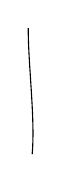
\begin{tikzpicture}[x=1cm,y=1cm,baseline=(current bounding box.south)]
\draw[line width=0.4pt] (0,0) .. controls (0.04,0.45) and (-0.05,1.12) .. (-0.05,1.60);
\end{tikzpicture}}

On suppose l'action extérieure \uline{fidèle},
i.e. $G\subset\widehat{\widehat{\mathcal T}}(\pi)
=\widehat{\widehat{\mathcal T}}$,
\var{\inserted{et que $G=G^+$.}}{\LMadded{et que $G=G^+$.}}{insertion}{140-2-s391-I003}
On suppose de plus qu'il existe une discrétification
invariante $\pi_0$, i.e. telle que
$G\subset\mathcal T(\pi_0)$.

Si on suppose $G$ cyclique, alors sauf
erreur il est prouvé que la situation est
\uline{réalisable} topologiquement (\LMsourceMark{M012868}{\unsure{donc}} :
\uline{\LMsourceMark{M012869}{\unsure{algébr.}}} de façon analytique complexe $\ldots$).

\LMflushnotes\LMflushpages
\ifnum\LMform=1
\begin{LMapparatus}
\LMentry{140-2-s391-I001}{insertion}{\inserted{une}
}{\emph{\LMinsertedlabel}}{Ajout explicite de l'auteur : intégré à l'endroit indiqué par la transcription, sans modifier sa lecture.}{}
\LMentry{140-2-s391-D001}{suppression}{\deleted{\LMsourceMark{M012870}{\unsure{e}}}
}{\emph{\LMomittedlabel}}{Passage biffé dans le manuscrit : la suppression suit l'état final de l'auteur; les doutes de lecture restent signalés.}{}
\LMentry{140-2-s391-I002}{insertion}{\inserted{'un}
}{\emph{\LMinsertedlabel}}{Ajout explicite de l'auteur : intégré à l'endroit indiqué par la transcription, sans modifier sa lecture.}{}
\LMentry{140-2-s391-I003}{insertion}{\inserted{et que $G=G^+$.}
}{\emph{\LMinsertedlabel}}{Ajout explicite de l'auteur : intégré à l'endroit indiqué par la transcription, sans modifier sa lecture.}{}
\end{LMapparatus}
\fi
\ifnum\LMform=2
\par\smallskip\begingroup\footnotesize\Needspace{4\baselineskip}\csname @beginparpenalty\endcsname=10000\relax\noindent\textcolor{gray}{\rule{.2\linewidth}{.35pt}}\par\nobreak
\noindent\textit{\LMdoubtheading.}\par\nobreak
\LMcarryover{140-2-s391-D001}{\LMsourceMark{M012871}{\unsure{e}}
}
\par\endgroup\smallskip
\fi

\LMsourceMark{M012872}{\scanpage{392}}
Dans le cas discret, la signification des classes de
\var{\inserted{$\pi_0$-}}{\LMadded{$\pi_0$-}}{insertion}{140-2-s392-I001}conjugaison de relèvement
$G\longrightarrow\mathcal G(\pi_0)$ est bien comprise ;
\var{\deleted{Mais}}{}{deletion}{140-2-s392-D001}\var{\inserted{de $\overline{\mathrm m}$ que pour les relèvements partiels}}{\LMadded{de $\overline{\mathrm m}$ que pour les relèvements partiels}}{insertion}{140-2-s392-I002}
On trouve une \var{\deleted{\LMsourceMark{M012873}{\unsure{cat.}} $U^{!}$}}{\LMsourceMark{M012874}{\LMcancelledDoubts{\LMsourceMark{M012875}{\unsure{cat.}}}}}{deletion}{140-2-s392-D002} réalisation
\var{\inserted{canonique}}{\LMadded{canonique}}{insertion}{140-2-s392-I003} du groupoïde fondamental
\LMsourceMark{M012876}{\margin{si $U^{!}\ne\LMsourceMark{M012877}{\unsure{\varnothing|\phi}}$}}
associé au
groupe ext. $\pi_0$, par un groupoïde \var{\inserted{fini}}{\LMadded{fini}}{insertion}{140-2-s392-I004} $[U^{!}]$
sur lequel $G$ opère au sens strict, dont les pts
correspondent aux classes de $\pi_0$-conjugaison de sections
partielles $\ne1$ maximales, le groupe
\var{\deleted{\LMsourceMark{M012878}{\illegible{1}}}}{\LMsourceMark{M012879}{\LMcancelledDoubts{\LMsourceMark{M012880}{\illegible{1}}}}}{deletion}{140-2-s392-D003}$\mathcal T(\pi_0)^G$
opère de façon \LMsourceMark{M012881}{\unsure{également}} canonique sur ce groupoïde.
Si $P\in U^{!}$ correspond à un relèvement
$G\longrightarrow\mathcal G(\pi_0)$, alors
un élément $\var{\deleted{\LMsourceMark{M012882}{\unsure{g}}}}{\LMsourceMark{M012883}{\LMcancelledDoubts{\(\LMsourceMark{M012884}{\unsure{g}}\)}}}{deletion}{140-2-s392-D004}\var{\inserted{\dot u}}{\LMadded{\dot u}}{insertion}{140-2-s392-I005}\in
\mathcal T(\pi_0)^G$ est dans l'image de
$\mathcal G(\pi_0)^G$, i.e. peut se remonter en
$u\in\mathcal G(\pi_0)$ commutant à $G$, sss
$\dot u(P)=P$ [i.e. sss
\var{\inserted{(si $\dot u$ est remonté de façon \LMsourceMark{M012885}{\unsure{quelc.}} en $v$)}}{\LMadded{(si $\dot u$ est remonté de façon \LMsourceMark{M012886}{\unsure{quelc.}} en $v$)}}{insertion}{140-2-s392-I006}
$v(G)$ est $\pi_0$-conjugué à $G$
i.e. sss $\exists g\in\pi_0$ tel que
$v(G)=\operatorname{int}(g)(G)$
i.e. \var{\deleted{\LMsourceMark{M012887}{\unsure{qui}}}}{\LMsourceMark{M012888}{\LMcancelledDoubts{\LMsourceMark{M012889}{\unsure{qui}}}}}{deletion}{140-2-s392-D005}
$u\overset{\text{déf}}{=}\operatorname{int}(g^{-1})v$ fixe $G$.
\var{\deleted{\LMsourceMark{M012890}{\unsure{(Donc}}}}{\LMsourceMark{M012891}{\LMcancelledDoubts{\LMsourceMark{M012892}{\unsure{(Donc}}}}}{deletion}{140-2-s392-D006} (auquel cas bien sûr il centralise,
\var{\inserted{(par l'hyp. $\dot u\in\mathcal T^{G}$)}}{\LMadded{(par l'hyp. $\dot u\in\mathcal T^{G}$)}}{insertion}{140-2-s392-I007})
Donc notre brillante assertion, est une tautologie]

\LMflushnotes\LMflushpages
\ifnum\LMform=1
\begin{LMapparatus}
\LMentry{140-2-s392-I001}{insertion}{\inserted{$\pi_0$-}
}{\emph{\LMinsertedlabel}}{Ajout explicite de l'auteur : intégré à l'endroit indiqué par la transcription, sans modifier sa lecture.}{}
\LMentry{140-2-s392-D001}{suppression}{\deleted{Mais}
}{\emph{\LMomittedlabel}}{Passage biffé dans le manuscrit : la suppression suit l'état final de l'auteur; les doutes de lecture restent signalés.}{}
\LMentry{140-2-s392-I002}{insertion}{\inserted{de $\overline{\mathrm m}$ que pour les relèvements partiels}
}{\emph{\LMinsertedlabel}}{Ajout explicite de l'auteur : intégré à l'endroit indiqué par la transcription, sans modifier sa lecture.}{}
\LMentry{140-2-s392-D002}{suppression}{\deleted{\LMsourceMark{M012893}{\unsure{cat.}} $U^{!}$}
}{\emph{\LMomittedlabel}}{Passage biffé dans le manuscrit : la suppression suit l'état final de l'auteur; les doutes de lecture restent signalés.}{}
\LMentry{140-2-s392-I003}{insertion}{\inserted{canonique}
}{\emph{\LMinsertedlabel}}{Ajout explicite de l'auteur : intégré à l'endroit indiqué par la transcription, sans modifier sa lecture.}{}
\LMentry{140-2-s392-I004}{insertion}{\inserted{fini}
}{\emph{\LMinsertedlabel}}{Ajout explicite de l'auteur : intégré à l'endroit indiqué par la transcription, sans modifier sa lecture.}{}
\LMentry{140-2-s392-D003}{suppression}{\deleted{\LMsourceMark{M012894}{\illegible{1}}}
}{\emph{\LMomittedlabel}}{Passage biffé dans le manuscrit : la suppression suit l'état final de l'auteur; les doutes de lecture restent signalés.}{}
\LMentry{140-2-s392-D004}{suppression}{\(\deleted{\LMsourceMark{M012895}{\unsure{g}}}\)
}{\emph{\LMomittedlabel}}{Passage biffé dans le manuscrit : la suppression suit l'état final de l'auteur; les doutes de lecture restent signalés.}{}
\LMentry{140-2-s392-I005}{insertion}{\(\inserted{\dot u}\)
}{\emph{\LMinsertedlabel}}{Ajout explicite de l'auteur : intégré à l'endroit indiqué par la transcription, sans modifier sa lecture.}{}
\LMentry{140-2-s392-I006}{insertion}{\inserted{(si $\dot u$ est remonté de façon \LMsourceMark{M012896}{\unsure{quelc.}} en $v$)}
}{\emph{\LMinsertedlabel}}{Ajout explicite de l'auteur : intégré à l'endroit indiqué par la transcription, sans modifier sa lecture.}{}
\LMentry{140-2-s392-D005}{suppression}{\deleted{\LMsourceMark{M012897}{\unsure{qui}}}
}{\emph{\LMomittedlabel}}{Passage biffé dans le manuscrit : la suppression suit l'état final de l'auteur; les doutes de lecture restent signalés.}{}
\LMentry{140-2-s392-D006}{suppression}{\deleted{\LMsourceMark{M012898}{\unsure{(Donc}}}
}{\emph{\LMomittedlabel}}{Passage biffé dans le manuscrit : la suppression suit l'état final de l'auteur; les doutes de lecture restent signalés.}{}
\LMentry{140-2-s392-I007}{insertion}{\inserted{(par l'hyp. $\dot u\in\mathcal T^{G}$)}
}{\emph{\LMinsertedlabel}}{Ajout explicite de l'auteur : intégré à l'endroit indiqué par la transcription, sans modifier sa lecture.}{}
\end{LMapparatus}
\fi
\ifnum\LMform=2
\par\smallskip\begingroup\footnotesize\Needspace{4\baselineskip}\csname @beginparpenalty\endcsname=10000\relax\noindent\textcolor{gray}{\rule{.2\linewidth}{.35pt}}\par\nobreak
\noindent\textit{\LMdoubtheading.}\par\nobreak
\LMcarryover{140-2-s392-D002}{\LMsourceMark{M012899}{\unsure{cat.}}
}
\LMcarryover{140-2-s392-D003}{\LMsourceMark{M012900}{\illegible{1}}
}
\LMcarryover{140-2-s392-D004}{\(\LMsourceMark{M012901}{\unsure{g}}\)
}
\LMcarryover{140-2-s392-D005}{\LMsourceMark{M012902}{\unsure{qui}}
}
\LMcarryover{140-2-s392-D006}{\LMsourceMark{M012903}{\unsure{(Donc}}
}
\par\endgroup\smallskip
\fi

\LMsourceMark{M012904}{\scanpage{393}}
\LMsourceMark{M012905}{\mspage{199}}
et donc le relèvement est unique. Comme
$U^{!}_{\LMsourceMark{M012906}{\unsure{*|\varphi}}}$ est fini, donc le stabilisateur
$\mathcal T(\pi_0)^G_P$ de $P$ dans
$\mathcal T(\pi_0)^G$ est d'indice fini,
et c'est donc ce ss-groupe d'indice fini qui se remonte
gaillardement et canoniquement.

Que peut-on dire dans le contexte profini ? Bien sur,
on a une application canonique
\diagram{\begin{tikzcd}[ampersand replacement=\&,column sep=large]
\begin{gathered}
\text{\var{\deleted{\LMsourceMark{M012907}{\unsure{Ens.}}}}{\LMsourceMark{M012908}{\LMcancelledDoubts{\LMsourceMark{M012909}{\unsure{Ens.}}}}}{deletion}{140-2-s393-D001} classes de $\pi_0$-conj.}\\
\text{de relèvements de}\\
G\text{ en }G
\longrightarrow\mathcal G(\pi_0)\\
\text{i.e. de scindages de}\\
\text{l'ext. }1\longrightarrow\pi_0\longrightarrow
E\longrightarrow G\longrightarrow1
\end{gathered}
\arrow[r] \&
\begin{gathered}
\text{classes de $\pi_0$-}\\
\text{conj. de rel. de}\\
G\text{ en }G
\longrightarrow\widehat{\widehat{\mathcal G}}(\pi_0)\\
\text{i.e. de scindages}\\
\text{de l'extension}\\
1\longrightarrow\underset{\substack{\Vert\\\pi}}{\widehat{\pi}_0}
\longrightarrow\widehat E
\longrightarrow G\longrightarrow1
\end{gathered}
\end{tikzcd}}

Il faudrait examiner d'abord

a) La question de la bijectivité de cette appl.

b) La question si $\pi^G=1$ (\LMsourceMark{M012910}{\unsure{\uline{rigidité}|rigidité}}),
pour $G\ne(1)$. -- (pour un relèvement donné,
dans $E$ pour simplifier)

J'ai envie de conjecturer sans vergogne
qu'il en est ainsi --- ce qui impliquerait
p.ex. que pour tt tel relèvement $G$, il y a

\LMflushnotes\LMflushpages
\ifnum\LMform=1
\begin{LMapparatus}
\LMentry{140-2-s393-D001}{suppression}{\deleted{\LMsourceMark{M012911}{\unsure{Ens.}}}
}{\emph{\LMomittedlabel}}{Passage biffé dans le manuscrit : la suppression suit l'état final de l'auteur; les doutes de lecture restent signalés.}{}
\end{LMapparatus}
\fi
\ifnum\LMform=2
\par\smallskip\begingroup\footnotesize\Needspace{4\baselineskip}\csname @beginparpenalty\endcsname=10000\relax\noindent\textcolor{gray}{\rule{.2\linewidth}{.35pt}}\par\nobreak
\noindent\textit{\LMdoubtheading.}\par\nobreak
\LMcarryover{140-2-s393-D001}{\LMsourceMark{M012912}{\unsure{Ens.}}
}
\par\endgroup\smallskip
\fi

\LMsourceMark{M012913}{\scanpage{394}}

un sous-groupe \uline{ouvert} \var{\inserted{$(\LMsourceMark{M012914}{\unsure{\widehat{\widehat{\mathcal T}}|\widehat{\mathcal T}}}^{G})_{P}$}}{\LMadded{$(\LMsourceMark{M012915}{\unsure{\widehat{\widehat{\mathcal T}}|\widehat{\mathcal T}}}^{G})_{P}$}}{insertion}{140-2-s394-I001} du groupe (peut-être vraiment immense à priori !) $\widehat{\widehat{\mathcal T}}^{G}$, qui se remonte canoniquement de façon à commuter à \LMsourceMark{M012916}{\unsure{$\widetilde G$|$G$}}....

Il faudrait manifestement faire, en $\overline{\mathrm m}$ temps qu'une théorie des op. ext. de groupes finis sur des groupes discrets à lacets (qui est pour le moment extrêmement \LMsourceMark{M012917}{\unsure{conjecturale|conjectural}}) une théorie analogue dans le cas profini --- j'\var{\deleted{\LMsourceMark{M012918}{\illegible{1}}}}{\LMsourceMark{M012919}{\LMcancelledDoubts{\LMsourceMark{M012920}{\illegible{1}}}}}{deletion}{140-2-s394-D001}\var{\inserted{aurai}}{\LMadded{aurai}}{insertion}{140-2-s394-I002} sans doute à y revenir par la suite.

\LMflushnotes\LMflushpages
\ifnum\LMform=1
\begin{LMapparatus}
\LMentry{140-2-s394-I001}{insertion}{\inserted{$(\LMsourceMark{M012921}{\unsure{\widehat{\widehat{\mathcal T}}|\widehat{\mathcal T}}}^{G})_{P}$}
}{\emph{\LMinsertedlabel}}{Ajout explicite de l'auteur : intégré à l'endroit indiqué par la transcription, sans modifier sa lecture.}{}
\LMentry{140-2-s394-D001}{suppression}{\deleted{\LMsourceMark{M012922}{\illegible{1}}}
}{\emph{\LMomittedlabel}}{Passage biffé dans le manuscrit : la suppression suit l'état final de l'auteur; les doutes de lecture restent signalés.}{}
\LMentry{140-2-s394-I002}{insertion}{\inserted{aurai}
}{\emph{\LMinsertedlabel}}{Ajout explicite de l'auteur : intégré à l'endroit indiqué par la transcription, sans modifier sa lecture.}{}
\end{LMapparatus}
\fi
\ifnum\LMform=2
\par\smallskip\begingroup\footnotesize\Needspace{4\baselineskip}\csname @beginparpenalty\endcsname=10000\relax\noindent\textcolor{gray}{\rule{.2\linewidth}{.35pt}}\par\nobreak
\noindent\textit{\LMdoubtheading.}\par\nobreak
\LMcarryover{140-2-s394-D001}{\LMsourceMark{M012923}{\illegible{1}}
}
\par\endgroup\smallskip
\fi

\LMsourceMark{M012924}{\scanpage{395}}
\LMsourceMark{M012925}{\mspage{200}}

\uline{32} Retour sur les aspects arithmétiques du bouchage de trous : relations entre $\Gamma_{g,\nu}$ et $\Gamma_{g,\nu-1}$.

Bien sûr, on \var{\deleted{\LMsourceMark{M012926}{\unsure{voit que}}}}{\LMsourceMark{M012927}{\LMcancelledDoubts{\LMsourceMark{M012928}{\unsure{voit que}}}}}{deletion}{140-2-s395-D001} a que
\[
\mathcal N_{g,\nu}\longrightarrow\mathfrak S_{\nu}
\]
est surjectif \var{\inserted{(puisque $\mathcal T_{g,\nu}\longrightarrow\mathfrak S_{\nu}$ l'est)}}{\LMadded{(puisque $\mathcal T_{g,\nu}\longrightarrow\mathfrak S_{\nu}$ l'est)}}{insertion}{140-2-s395-I001}, donc on aura
\[
(1)\qquad 1\LMsourceMark{M012929}{\unsure{\longrightarrow|-}}\mathcal N_{g,\nu}^{!}\LMsourceMark{M012930}{\unsure{\longrightarrow|-}}\mathcal N_{g,\nu}\LMsourceMark{M012931}{\unsure{\longrightarrow|-}}\mathfrak S_{\nu}\LMsourceMark{M012932}{\unsure{\longrightarrow|-}}1
\]
et le diagramme cartésien de \LMsourceMark{M012933}{\unsure{ssgroupes}} de $\widehat{\widehat{\mathcal T}}_{g,\nu}$
\[
(2)\qquad
\diagram{\begin{tikzcd}[ampersand replacement=\&]
\widehat{\mathcal T}_{g,\nu}^{+}\arrow[r,hook] \& \mathcal N_{g,\nu}\\
\widehat{\mathcal T}_{g,\nu}^{!+}\arrow[u,hook]\arrow[r,hook] \& \mathcal N_{g,\nu}^{!}\arrow[u,hook]
\end{tikzcd}}
\]
\LMsourceMark{M012934}{\margin{\var{\deleted{\LMsourceMark{M012935}{\illegible{1}}}}{\LMsourceMark{M012936}{\LMcancelledDoubts{\LMsourceMark{M012937}{\illegible{1}}}}}{deletion}{140-2-s395-D002} $\mathcal N_{g,\nu}=\mathcal N_{g,\nu}^{!}\cdot\widehat{\mathcal T}_{g,\nu}^{+}$ i.e. $\mathcal N_{g,\nu}$ connu par $\mathcal N_{g,\nu}^{!}$}}
donnera un isomorphisme
\[
(3)\qquad \mathcal N_{g,\nu}^{!}/\widehat{\mathcal T}_{g,\nu}^{!+}\xrightarrow{\sim}\mathcal N_{g,\nu}/\widehat{\mathcal T}_{g,\nu}^{+}=\mathbb{\Gamma}_{g,\nu}
\]
Dans le cas d'un $(\pi,a)$, \var{\inserted{($\pi$ groupe ext. à lacets,}}{\LMadded{($\pi$ groupe ext. à lacets,}}{insertion}{140-2-s395-I002} $a$ une arithmétisation), on aura de $\overline{\mathrm m}$
\[
(4)\qquad\left\{\begin{aligned}
\mathcal N_a^{!}/\widehat{\mathcal T}_a^{+}&\simeq\mathcal N_a/\widehat{\mathcal T}_a^{+}=\mathbb{\Gamma}_a.\\
\mathcal N_a&=\mathcal N_a^{!}\widehat{\mathcal T}_a^{+}
\end{aligned}\right.
\]

Considérons maintenant \var{\deleted{une \LMsourceMark{M012938}{\unsure{partie}}\inserted{\LMsourceMark{M012939}{\unsure{$i\in I=I(\pi)$}}} , \LMsourceMark{M012940}{\illegible{3}} $\LMsourceMark{M012941}{\unsure{(g,\nu)}}$, \LMsourceMark{M012942}{\unsure{et un}} $\pi_i'$ \LMsourceMark{M012943}{\illegible{2}} $\LMsourceMark{M012944}{\unsure{I=I(\pi)}}$, et soit \LMsourceMark{M012945}{\illegible{1}}}}{\LMsourceMark{M012946}{\LMcancelledDoubts{\LMsourceMark{M012947}{\unsure{partie}}\quad \LMsourceMark{M012948}{\unsure{$i\in I=I(\pi)$}}\quad \LMsourceMark{M012949}{\illegible{3}}\quad \(\LMsourceMark{M012950}{\unsure{(g,\nu)}}\)\quad \LMsourceMark{M012951}{\unsure{et un}}\quad \LMsourceMark{M012952}{\illegible{2}}\quad \(\LMsourceMark{M012953}{\unsure{I=I(\pi)}}\)\quad \LMsourceMark{M012954}{\illegible{1}}}}}{deletion}{140-2-s395-D003} pour $\forall i\in I$ le stabilisateur \var{\deleted{\LMsourceMark{M012955}{\illegible{1}}}}{\LMsourceMark{M012956}{\LMcancelledDoubts{\LMsourceMark{M012957}{\illegible{1}}}}}{deletion}{140-2-s395-D004} $\mathcal N_i$ de $i$ dans $\mathcal N$, et le groupe \var{\deleted{extérieur}}{}{deletion}{140-2-s395-D005} \var{\inserted{à lacets (pas ext!)}}{\LMadded{à lacets (pas ext!)}}{insertion}{140-2-s395-I004} $\pi_i'$ de type $g,\nu-1$, déduit de $\pi$ par ``bouchage du trou $i$'',
\LMsourceMark{M012958}{\margin{On écrit $\mathcal N$ etc. au lieu de $\mathcal N_a$. On suppose \LMsourceMark{M012959}{\illegible{2}} $(g,\nu-1)$, i.e. \LMsourceMark{M012960}{\unsure{$2g-2+\nu$}} \LMsourceMark{M012961}{\illegible{1}} \LMsourceMark{M012962}{\unsure{$\geq1$}}, i.e. $2g+\nu\geq4$}}

\LMflushnotes\LMflushpages
\ifnum\LMform=1
\begin{LMapparatus}
\LMentry{140-2-s395-D001}{suppression}{\deleted{\LMsourceMark{M012963}{\unsure{voit que}}}
}{\emph{\LMomittedlabel}}{Passage biffé dans le manuscrit : la suppression suit l'état final de l'auteur; les doutes de lecture restent signalés.}{}
\LMentry{140-2-s395-I001}{insertion}{\inserted{(puisque $\mathcal T_{g,\nu}\longrightarrow\mathfrak S_{\nu}$ l'est)}
}{\emph{\LMinsertedlabel}}{Ajout explicite de l'auteur : intégré à l'endroit indiqué par la transcription, sans modifier sa lecture.}{}
\LMentry{140-2-s395-D002}{suppression}{\deleted{\LMsourceMark{M012964}{\illegible{1}}}
}{\emph{\LMomittedlabel}}{Passage biffé dans le manuscrit : la suppression suit l'état final de l'auteur; les doutes de lecture restent signalés.}{}
\LMentry{140-2-s395-I002}{insertion}{\inserted{($\pi$ groupe ext. à lacets,}
}{\emph{\LMinsertedlabel}}{Ajout explicite de l'auteur : intégré à l'endroit indiqué par la transcription, sans modifier sa lecture.}{}
\LMentry{140-2-s395-D003}{suppression}{\deleted{une \LMsourceMark{M012965}{\unsure{partie}}\inserted{\LMsourceMark{M012966}{\unsure{$i\in I=I(\pi)$}}} , \LMsourceMark{M012967}{\illegible{3}} $\LMsourceMark{M012968}{\unsure{(g,\nu)}}$, \LMsourceMark{M012969}{\unsure{et un}} $\pi_i'$ \LMsourceMark{M012970}{\illegible{2}} $\LMsourceMark{M012971}{\unsure{I=I(\pi)}}$, et soit \LMsourceMark{M012972}{\illegible{1}}}
}{\emph{\LMomittedlabel}}{Passage biffé dans le manuscrit : la suppression suit l'état final de l'auteur; les doutes de lecture restent signalés.}{}
\LMentry{140-2-s395-D004}{suppression}{\deleted{\LMsourceMark{M012973}{\illegible{1}}}
}{\emph{\LMomittedlabel}}{Passage biffé dans le manuscrit : la suppression suit l'état final de l'auteur; les doutes de lecture restent signalés.}{}
\LMentry{140-2-s395-D005}{suppression}{\deleted{extérieur}
}{\emph{\LMomittedlabel}}{Passage biffé dans le manuscrit : la suppression suit l'état final de l'auteur; les doutes de lecture restent signalés.}{}
\LMentry{140-2-s395-I004}{insertion}{\inserted{à lacets (pas ext!)}
}{\emph{\LMinsertedlabel}}{Ajout explicite de l'auteur : intégré à l'endroit indiqué par la transcription, sans modifier sa lecture.}{}
\end{LMapparatus}
\fi
\ifnum\LMform=2
\par\smallskip\begingroup\footnotesize\Needspace{4\baselineskip}\csname @beginparpenalty\endcsname=10000\relax\noindent\textcolor{gray}{\rule{.2\linewidth}{.35pt}}\par\nobreak
\noindent\textit{\LMdoubtheading.}\par\nobreak
\LMcarryover{140-2-s395-D001}{\LMsourceMark{M012974}{\unsure{voit que}}
}
\LMcarryover{140-2-s395-D002}{\LMsourceMark{M012975}{\illegible{1}}
}
\LMcarryover{140-2-s395-D003}{\LMsourceMark{M012976}{\unsure{partie}}\quad \LMsourceMark{M012977}{\unsure{$i\in I=I(\pi)$}}\quad \LMsourceMark{M012978}{\illegible{3}}\quad \(\LMsourceMark{M012979}{\unsure{(g,\nu)}}\)\quad \LMsourceMark{M012980}{\unsure{et un}}\quad \LMsourceMark{M012981}{\illegible{2}}\quad \(\LMsourceMark{M012982}{\unsure{I=I(\pi)}}\)\quad \LMsourceMark{M012983}{\illegible{1}}
}
\LMcarryover{140-2-s395-D004}{\LMsourceMark{M012984}{\illegible{1}}
}
\par\endgroup\smallskip
\fi

\LMsourceMark{M012985}{\scanpage{396}}

on a alors, pour une discrétification choisie, \var{\deleted{\LMsourceMark{M012986}{\unsure{une}}}}{\LMsourceMark{M012987}{\LMcancelledDoubts{\LMsourceMark{M012988}{\unsure{une}}}}}{deletion}{140-2-s396-D001} \var{\inserted{$\alpha$}}{\LMadded{$\alpha$}}{insertion}{140-2-s396-I001} compatible avec l'arithmétisation, un \LMsourceMark{M012989}{\unsure{hom.|hom}} injectif
\[
(5)\qquad \pi_i'\xrightarrow{\varphi_i}\widehat{\mathcal T}_{\LMsourceMark{M012990}{\unsure{i|a}}}^{+!}\subset\mathcal N_{\LMsourceMark{M012991}{\unsure{i|a}}}^{!}\subset\widehat{\widehat{\mathcal T}}_i
\]

\var{\deleted{On \LMsourceMark{M012992}{\unsure{ne peut}} \LMsourceMark{M012993}{\illegible{2}}}}{\LMsourceMark{M012994}{\LMcancelledDoubts{\LMsourceMark{M012995}{\unsure{ne peut}}\quad \LMsourceMark{M012996}{\illegible{2}}}}}{deletion}{140-2-s396-D002}
\var{\deleted{On aura}}{}{deletion}{140-2-s396-D003}
\var{\deleted{\LMsourceMark{M012997}{\unsure{qui remonte le composé}}}}{\LMsourceMark{M012998}{\LMcancelledDoubts{\LMsourceMark{M012999}{\unsure{qui remonte le composé}}}}}{deletion}{140-2-s396-D004}
\var{\deleted{\textcircled{\LMsourceMark{M013000}{\unsure{e|c}}} L'image de $\pi'$}}{\LMsourceMark{M013001}{\LMcancelledDoubts{\LMsourceMark{M013002}{\unsure{e|c}}}}}{deletion}{140-2-s396-D005}
tel que le composé
\[
\diagram{\begin{tikzcd}[ampersand replacement=\&]
\pi_i'\arrow[r] \& \widehat{\widehat{\mathcal T}}_i\arrow[r] \& \widehat{\widehat{\mathcal G}}(\pi_i')\\
\&\& \pi_i'\arrow[u,hook]
\end{tikzcd}}
\]
soit l'inclusion canonique. Ceci posé, on veut\LMsourceMark{M013003}{\margin{plutôt : \uline{il est vrai que !}}} que l'image de (5) (qui n'est peut-être pas invariante dans $\widehat{\widehat{\mathcal T}}_i$) soit \uline{invariante dans \var{\deleted{$\mathcal T$}}{}{deletion}{140-2-s396-D006} $\mathcal N_i$}, ou ce qui revient au $\overline{\mathrm m}$, dans $\mathcal N^{!}$ (car $\mathcal N_i=\mathcal N^{!}\cdot\widehat{\mathcal T}_i^{+}$ or $\widehat{\mathcal T}_i^{+}$ invarie cette image). \var{\deleted{\LMsourceMark{M013004}{\illegible{1}}}}{\LMsourceMark{M013005}{\LMcancelledDoubts{\LMsourceMark{M013006}{\illegible{1}}}}}{deletion}{140-2-s396-D007} Revenant à la situation universelle, cela \LMsourceMark{M013007}{\unsure{\uline{signifie}|signifie}}
\LMsourceMark{M013008}{\margin{Cela signifie aussi que $\varphi_i$ \LMsourceMark{M013009}{\unsure{ne dépend pas}} du choix de la discrétification \LMsourceMark{M013010}{\unsure{de donnée}} $\alpha$...}}

\textcircled{\LMsourceMark{M013011}{\unsure{e|c}}} $\mathcal N_{g,\nu}^{!}\subset\widehat{\widehat{\mathcal T}}_{g,\nu}$ est contenu dans le normalisateur des $\pi_i'\hookrightarrow\widehat{\mathcal T}_{g,\nu}^{!+}$ $(0\leq i\leq\nu-1)$ \var{\inserted{qui sont donc invariants dans $\mathcal N_{g,\nu}^{!}$}}{\LMadded{qui sont donc invariants dans $\mathcal N_{g,\nu}^{!}$}}{insertion}{140-2-s396-I002} \var{\deleted{\LMsourceMark{M013012}{\unsure{si}} $(g,\nu-1)$ \LMsourceMark{M013013}{\unsure{est aussi anabélien}}}}{\LMsourceMark{M013014}{\LMcancelledDoubts{\LMsourceMark{M013015}{\unsure{si}}\quad \LMsourceMark{M013016}{\unsure{est aussi anabélien}}}}}{deletion}{140-2-s396-D008}.

De plus $\widehat{\widehat{\mathcal T}}_{g,\nu}^{!}\xrightarrow{\psi_i}\widehat{\widehat{\mathcal G}}_{g,\nu-1}^{!}$ induit un \var{\deleted{\LMsourceMark{M013017}{\illegible{1}}}}{\LMsourceMark{M013018}{\LMcancelledDoubts{\LMsourceMark{M013019}{\illegible{1}}}}}{deletion}{140-2-s396-D009} \uuline{\LMsourceMark{M013020}{\unsure{iso|isom.}}}
\[
(6)\qquad\mathcal N_{g,\nu}^{!}\xrightarrow{\sim}\mathcal M_{g,\nu-1}^{!}
\]
\LMsourceMark{M013021}{\margin{\uline{NB} Il suffit \LMsourceMark{M013022}{\unsure{me semble-t-il}} de le prouver \LMsourceMark{M013023}{\unsure{pour un $i$}} pour le déduire pour les autres \var{\deleted{\LMsourceMark{M013024}{\illegible{1}}}}{\LMsourceMark{M013025}{\LMcancelledDoubts{\LMsourceMark{M013026}{\illegible{1}}}}}{deletion}{140-2-s396-D010}}}
\LMsourceMark{M013027}{\margin{\uline{NB} \LMsourceMark{M013028}{\illegible{4}}}}

\LMflushnotes\LMflushpages
\ifnum\LMform=1
\begin{LMapparatus}
\LMentry{140-2-s396-D001}{suppression}{\deleted{\LMsourceMark{M013029}{\unsure{une}}}
}{\emph{\LMomittedlabel}}{Passage biffé dans le manuscrit : la suppression suit l'état final de l'auteur; les doutes de lecture restent signalés.}{}
\LMentry{140-2-s396-I001}{insertion}{\inserted{$\alpha$}
}{\emph{\LMinsertedlabel}}{Ajout explicite de l'auteur : intégré à l'endroit indiqué par la transcription, sans modifier sa lecture.}{}
\LMentry{140-2-s396-D002}{suppression}{\deleted{On \LMsourceMark{M013030}{\unsure{ne peut}} \LMsourceMark{M013031}{\illegible{2}}}
}{\emph{\LMomittedlabel}}{Passage biffé dans le manuscrit : la suppression suit l'état final de l'auteur; les doutes de lecture restent signalés.}{}
\LMentry{140-2-s396-D003}{suppression}{\deleted{On aura}
}{\emph{\LMomittedlabel}}{Passage biffé dans le manuscrit : la suppression suit l'état final de l'auteur; les doutes de lecture restent signalés.}{}
\LMentry{140-2-s396-D004}{suppression}{\deleted{\LMsourceMark{M013032}{\unsure{qui remonte le composé}}}
}{\emph{\LMomittedlabel}}{Passage biffé dans le manuscrit : la suppression suit l'état final de l'auteur; les doutes de lecture restent signalés.}{}
\LMentry{140-2-s396-D005}{suppression}{\deleted{\textcircled{\LMsourceMark{M013033}{\unsure{e|c}}} L'image de $\pi'$}
}{\emph{\LMomittedlabel}}{Passage biffé dans le manuscrit : la suppression suit l'état final de l'auteur; les doutes de lecture restent signalés.}{}
\LMentry{140-2-s396-D006}{suppression}{\deleted{$\mathcal T$}
}{\emph{\LMomittedlabel}}{Passage biffé dans le manuscrit : la suppression suit l'état final de l'auteur; les doutes de lecture restent signalés.}{}
\LMentry{140-2-s396-D007}{suppression}{\deleted{\LMsourceMark{M013034}{\illegible{1}}}
}{\emph{\LMomittedlabel}}{Passage biffé dans le manuscrit : la suppression suit l'état final de l'auteur; les doutes de lecture restent signalés.}{}
\LMentry{140-2-s396-I002}{insertion}{\inserted{qui sont donc invariants dans $\mathcal N_{g,\nu}^{!}$}
}{\emph{\LMinsertedlabel}}{Ajout explicite de l'auteur : intégré à l'endroit indiqué par la transcription, sans modifier sa lecture.}{}
\LMentry{140-2-s396-D008}{suppression}{\deleted{\LMsourceMark{M013035}{\unsure{si}} $(g,\nu-1)$ \LMsourceMark{M013036}{\unsure{est aussi anabélien}}}
}{\emph{\LMomittedlabel}}{Passage biffé dans le manuscrit : la suppression suit l'état final de l'auteur; les doutes de lecture restent signalés.}{}
\LMentry{140-2-s396-D009}{suppression}{\deleted{\LMsourceMark{M013037}{\illegible{1}}}
}{\emph{\LMomittedlabel}}{Passage biffé dans le manuscrit : la suppression suit l'état final de l'auteur; les doutes de lecture restent signalés.}{}
\LMentry{140-2-s396-D010}{suppression}{\deleted{\LMsourceMark{M013038}{\illegible{1}}}
}{\emph{\LMomittedlabel}}{Passage biffé dans le manuscrit : la suppression suit l'état final de l'auteur; les doutes de lecture restent signalés.}{}
\end{LMapparatus}
\fi
\ifnum\LMform=2
\par\smallskip\begingroup\footnotesize\Needspace{4\baselineskip}\csname @beginparpenalty\endcsname=10000\relax\noindent\textcolor{gray}{\rule{.2\linewidth}{.35pt}}\par\nobreak
\noindent\textit{\LMdoubtheading.}\par\nobreak
\LMcarryover{140-2-s396-D001}{\LMsourceMark{M013039}{\unsure{une}}
}
\LMcarryover{140-2-s396-D002}{\LMsourceMark{M013040}{\unsure{ne peut}}\quad \LMsourceMark{M013041}{\illegible{2}}
}
\LMcarryover{140-2-s396-D004}{\LMsourceMark{M013042}{\unsure{qui remonte le composé}}
}
\LMcarryover{140-2-s396-D005}{\LMsourceMark{M013043}{\unsure{e|c}}
}
\LMcarryover{140-2-s396-D007}{\LMsourceMark{M013044}{\illegible{1}}
}
\LMcarryover{140-2-s396-D008}{\LMsourceMark{M013045}{\unsure{si}}\quad \LMsourceMark{M013046}{\unsure{est aussi anabélien}}
}
\LMcarryover{140-2-s396-D009}{\LMsourceMark{M013047}{\illegible{1}}
}
\LMcarryover{140-2-s396-D010}{\LMsourceMark{M013048}{\illegible{1}}
}
\par\endgroup\smallskip
\fi

\LMsourceMark{M013049}{\scanpage{397}}
\LMsourceMark{M013050}{\mspage{201}}

Cette assertion se décompose en deux : \LMsourceMark{M013051}{\unsure{donc|tout}} d'abord que $\psi_i$ applique bien $\mathcal N_{g,\nu}^{!}$ dans $\mathcal M_{g,\nu-1}^{!}$ -- et ceci résulte de la définition \LMsourceMark{M013052}{\unsure{arithmético-géom}} de ces groupes -- cela implique d'autre part, puisque $\psi_i$ induit aussi un \var{\inserted{\LMsourceMark{M013053}{\unsure{iso}}}}{\LMadded{\LMsourceMark{M013054}{\unsure{iso}}}}{insertion}{140-2-s397-I001} \var{\deleted{\LMsourceMark{M013055}{\illegible{1}}}}{\LMsourceMark{M013056}{\LMcancelledDoubts{\LMsourceMark{M013057}{\illegible{1}}}}}{deletion}{140-2-s397-D001}
\[
\widehat{\mathcal T}_{g,\nu}^{+}
\xrightarrow{\sim}
\widehat{\mathcal G}_{g,\nu-1}^{+},
\]
qu'il induit un hom
\[
(7)\qquad
\begin{array}{ccc}
\mathbb{\Gamma}_{g,\nu}
&\xrightarrow{\substack{\var{\inserted{\lambda_i}}{\LMadded{\lambda_i}}{insertion}{140-2-s397-I002}\\\var{\deleted{\LMsourceMark{M013058}{\unsure{\psi_i}}}}{\LMsourceMark{M013059}{\LMcancelledDoubts{\(\LMsourceMark{M013060}{\unsure{\psi_i}}\)}}}{deletion}{140-2-s397-D002}}}&
\mathbb{\Gamma}_{g,\nu-1}\\
\wr\vert&&\wr\vert\\
\mathcal N_{g,\nu}/\widehat{\mathcal T}_{g,\nu}^{+}
&&\mathcal M_{g,\nu-1}/\LMsourceMark{M013061}{\unsure{\widehat{\mathcal G}}}
\end{array}
\]
\var{\deleted{et par voie \LMsourceMark{M013062}{\unsure{arithmétique}}}}{\LMsourceMark{M013063}{\LMcancelledDoubts{\LMsourceMark{M013064}{\unsure{arithmétique}}}}}{deletion}{140-2-s397-D003}
et l'inj. (resp. \var{\deleted{b}}{}{deletion}{140-2-s397-D004}\LMsourceMark{M013065}{\unsure{surjectivité}}) de (6) équivaut à celle de (7). D'ailleurs (7) s'insère, par construction, dans un diagramme commutatif

\begin{samepage}
(8)\quad\diagram{\begin{tikzcd}[ampersand replacement=\&,column sep=large,row sep=large]
\& \mathbb{\Gamma}_{\mathbb Q}
  \arrow[dl,"\Theta_{g,\nu}"']
  \arrow[dr,"\Theta_{g,\nu-1}"] \& \\
\mathbb{\Gamma}_{g,\nu} \arrow[rr]
\&\&\mathbb{\Gamma}_{g,\nu-1}
\end{tikzcd}}
\end{samepage}

avec $\Theta_{g,\nu}$ et $\Theta_{g,\nu-1}$ surjectifs, donc il est bel et bien évident que (6) est \uline{surjectif}. La bijectivité \LMsourceMark{M013066}{\unsure{\uline{signifie}|signifie}} que $\Theta_{g,\nu}$ et $\Theta_{g,\nu-1}$ ont $\overline{\mathrm m}$ noyau (alors qu'à priori il se pourrait que $\Theta_{g,\nu}$ ait un noyau plus petit i.e. corresponde à une représentation de $\mathbb{\Gamma}_{\mathbb Q}$ ``moins infidèle'' que $\Theta_{g,\nu-1}$. D'ailleurs,

\LMflushnotes\LMflushpages
\ifnum\LMform=1
\begin{LMapparatus}
\LMentry{140-2-s397-I001}{insertion}{\inserted{\LMsourceMark{M013067}{\unsure{iso}}}
}{\emph{\LMinsertedlabel}}{Ajout explicite de l'auteur : intégré à l'endroit indiqué par la transcription, sans modifier sa lecture.}{}
\LMentry{140-2-s397-D001}{suppression}{\deleted{\LMsourceMark{M013068}{\illegible{1}}}
}{\emph{\LMomittedlabel}}{Passage biffé dans le manuscrit : la suppression suit l'état final de l'auteur; les doutes de lecture restent signalés.}{}
\LMentry{140-2-s397-I002}{insertion}{\(\inserted{\lambda_i}\)
}{\emph{\LMinsertedlabel}}{Ajout explicite de l'auteur : intégré à l'endroit indiqué par la transcription, sans modifier sa lecture.}{}
\LMentry{140-2-s397-D002}{suppression}{\(\deleted{\LMsourceMark{M013069}{\unsure{\psi_i}}}\)
}{\emph{\LMomittedlabel}}{Passage biffé dans le manuscrit : la suppression suit l'état final de l'auteur; les doutes de lecture restent signalés.}{}
\LMentry{140-2-s397-D003}{suppression}{\deleted{et par voie \LMsourceMark{M013070}{\unsure{arithmétique}}}
}{\emph{\LMomittedlabel}}{Passage biffé dans le manuscrit : la suppression suit l'état final de l'auteur; les doutes de lecture restent signalés.}{}
\LMentry{140-2-s397-D004}{suppression}{\deleted{b}
}{\emph{\LMomittedlabel}}{Passage biffé dans le manuscrit : la suppression suit l'état final de l'auteur; les doutes de lecture restent signalés.}{}
\end{LMapparatus}
\fi
\ifnum\LMform=2
\par\smallskip\begingroup\footnotesize\Needspace{4\baselineskip}\csname @beginparpenalty\endcsname=10000\relax\noindent\textcolor{gray}{\rule{.2\linewidth}{.35pt}}\par\nobreak
\noindent\textit{\LMdoubtheading.}\par\nobreak
\LMcarryover{140-2-s397-D001}{\LMsourceMark{M013071}{\illegible{1}}
}
\LMcarryover{140-2-s397-D002}{\(\LMsourceMark{M013072}{\unsure{\psi_i}}\)
}
\LMcarryover{140-2-s397-D003}{\LMsourceMark{M013073}{\unsure{arithmétique}}
}
\par\endgroup\smallskip
\fi

\LMsourceMark{M013074}{\scanpage{398}}

il est évident \var{\deleted{que}}{}{deletion}{140-2-s398-D001} ($\LMsourceMark{M013075}{\unsure{\overline{\mathrm m}}}$, à priori, sans utiliser la définition \var{\inserted{ailleurs}}{\LMadded{ailleurs}}{insertion}{140-2-s398-I001} \LMsourceMark{M013076}{\unsure{explicite|explicitée}} des $\mathcal N_{g,\nu}$) que l'hom $\var{\deleted{\LMsourceMark{M013077}{\unsure{\psi_i}}}}{\LMsourceMark{M013078}{\LMcancelledDoubts{\(\LMsourceMark{M013079}{\unsure{\psi_i}}\)}}}{deletion}{140-2-s398-D002}\var{\inserted{\LMsourceMark{M013080}{\unsure{\lambda_i}}}}{\LMadded{\LMsourceMark{M013081}{\unsure{\lambda_i}}}}{insertion}{140-2-s398-I002}$ \var{\inserted{\LMsourceMark{M013082}{\unsure{(7)}}}}{\LMadded{\LMsourceMark{M013083}{\unsure{(7)}}}}{insertion}{140-2-s398-I003} ne dépend pas du choix de $0\leq i\leq\nu-1$ -- p.ex. puisque l'on passe de l'un à l'autre en appliquant des opérations de $\widehat{\mathcal T}^{+}$ (puisque $\widehat{\mathcal T}^{+}$ opère \LMsourceMark{M013084}{\unsure{transitivement}} sur $I$) et que $\widehat{\mathcal T}^{+}$ opère \LMsourceMark{M013085}{\unsure{trivialt|trivialement}} dans $\mathbb{\Gamma}_{g,\nu}$ ...

On peut dire que (6) décrit $\mathcal M_{g,\nu-1}^{!}$ (donc $\mathcal N_{g,\nu-1}^{!}$) en termes de $\mathcal N_{g,\nu}$ -- mais l'inverse est moins clair, faute de savoir si
\[
\LMsourceMark{M013086}{\unsure{\widehat{\widehat{\mathcal T}}_{g,\nu}^{!}}}
\xrightarrow{\psi_i}
\widehat{\widehat{\mathcal G}}_{g,\nu-1}
\]
est injectif ; si on le savait, on pourrait décrire $\mathcal N_{g,\nu}^{!}$ comme l'image inverse de $\mathcal M_{g,\nu-1}^{!}$ ... \var{\deleted{\LMsourceMark{M013087}{\unsure{Alors}}}}{\LMsourceMark{M013088}{\LMcancelledDoubts{\LMsourceMark{M013089}{\unsure{Alors}}}}}{deletion}{140-2-s398-D003} Il ne serait pas impossible d'ailleurs que (f) soit faux, i.e. que \var{\inserted{les}}{\LMadded{les}}{insertion}{140-2-s398-I004} $\Theta_{g,\nu}$ soient infidèles, mais de moins en moins quand on fait augmenter $\nu$ -- en passant à la limite \var{\inserted{\LMsourceMark{M013090}{\unsure{projective}}}}{\LMadded{\LMsourceMark{M013091}{\unsure{projective}}}}{insertion}{140-2-s398-I005} $\Theta_{g,\infty}$, \LMsourceMark{M013092}{\unsure{seulement}}, aurait-on

\LMflushnotes\LMflushpages
\ifnum\LMform=1
\begin{LMapparatus}
\LMentry{140-2-s398-D001}{suppression}{\deleted{que}
}{\emph{\LMomittedlabel}}{Passage biffé dans le manuscrit : la suppression suit l'état final de l'auteur; les doutes de lecture restent signalés.}{}
\LMentry{140-2-s398-I001}{insertion}{\inserted{ailleurs}
}{\emph{\LMinsertedlabel}}{Ajout explicite de l'auteur : intégré à l'endroit indiqué par la transcription, sans modifier sa lecture.}{}
\LMentry{140-2-s398-D002}{suppression}{\(\deleted{\LMsourceMark{M013093}{\unsure{\psi_i}}}\)
}{\emph{\LMomittedlabel}}{Passage biffé dans le manuscrit : la suppression suit l'état final de l'auteur; les doutes de lecture restent signalés.}{}
\LMentry{140-2-s398-I002}{insertion}{\(\inserted{\LMsourceMark{M013094}{\unsure{\lambda_i}}}\)
}{\emph{\LMinsertedlabel}}{Ajout explicite de l'auteur : intégré à l'endroit indiqué par la transcription, sans modifier sa lecture.}{}
\LMentry{140-2-s398-I003}{insertion}{\inserted{\LMsourceMark{M013095}{\unsure{(7)}}}
}{\emph{\LMinsertedlabel}}{Ajout explicite de l'auteur : intégré à l'endroit indiqué par la transcription, sans modifier sa lecture.}{}
\LMentry{140-2-s398-D003}{suppression}{\deleted{\LMsourceMark{M013096}{\unsure{Alors}}}
}{\emph{\LMomittedlabel}}{Passage biffé dans le manuscrit : la suppression suit l'état final de l'auteur; les doutes de lecture restent signalés.}{}
\LMentry{140-2-s398-I004}{insertion}{\inserted{les}
}{\emph{\LMinsertedlabel}}{Ajout explicite de l'auteur : intégré à l'endroit indiqué par la transcription, sans modifier sa lecture.}{}
\LMentry{140-2-s398-I005}{insertion}{\inserted{\LMsourceMark{M013097}{\unsure{projective}}}
}{\emph{\LMinsertedlabel}}{Ajout explicite de l'auteur : intégré à l'endroit indiqué par la transcription, sans modifier sa lecture.}{}
\end{LMapparatus}
\fi
\ifnum\LMform=2
\par\smallskip\begingroup\footnotesize\Needspace{4\baselineskip}\csname @beginparpenalty\endcsname=10000\relax\noindent\textcolor{gray}{\rule{.2\linewidth}{.35pt}}\par\nobreak
\noindent\textit{\LMdoubtheading.}\par\nobreak
\LMcarryover{140-2-s398-D002}{\(\LMsourceMark{M013098}{\unsure{\psi_i}}\)
}
\LMcarryover{140-2-s398-D003}{\LMsourceMark{M013099}{\unsure{Alors}}
}
\par\endgroup\smallskip
\fi

\LMsourceMark{M013100}{\scanpage{399}}
\LMsourceMark{M013101}{\mspage{202}}

(peut-être !) une représentation fidèle de $\mathbb{\Gamma}_{\mathbb Q}$. Mais jusqu'à indication contraire, je préfère travailler hypothétiquement avec (f), ce qui s'exprime par les suites \LMsourceMark{M013102}{\unsure{exactes|ex.tes}} fondamentales
\[
(9)\qquad
1\longrightarrow\widehat{\pi}_{g,\nu-1}
\xrightarrow{\varphi_i}
\LMsourceMark{M013103}{\unsure{\mathcal N_{g,\nu}^{!}|\mathcal M_{g,\nu}^{!}}}
\LMsourceMark{M013104}{\unsure{\overset{\psi_i'}{\longleftrightarrow}|\xrightarrow{\psi_i'}}}
\LMsourceMark{M013105}{\unsure{\mathcal N_{g,\nu-1}^{!}|\mathcal M_{g,\nu-1}^{!}}}
\longrightarrow1
\]
\LMsourceMark{M013106}{\margin{\LMsourceMark{M013107}{\unsure{\&}} on pourrait l'inclure dans une suite \LMsourceMark{M013108}{\unsure{ex.te}} un peu plus grande, avec $(\mathcal N_{g,\nu})_i$ et $\mathcal N_{g,\nu-1}$ ...}}
qui étend la suite \LMsourceMark{M013109}{\unsure{ex.te|exacte}}
\[
(10)\qquad
1\longrightarrow\widehat{\pi}_{g,\nu-1}
\xrightarrow{\varphi_i}
\widehat{\mathcal T}_{g,\nu}^{!}
\xrightarrow{\psi_i'}
\widehat{\mathcal T}_{g,\nu-1}^{!}
\longrightarrow1
\]
(et tient lieu de la suite \LMsourceMark{M013110}{\unsure{exacte|ex.te}} peut-être défaillante
\[
??\qquad
1\longrightarrow\widehat{\pi}_{g,\nu-1}
\longrightarrow\widehat{\widehat{\mathcal T}}_{g,\nu}^{!}
\longrightarrow\widehat{\widehat{\mathcal T}}_{g,\nu-1}^{!}
\longrightarrow1
\qquad??
\]
)

Quand $(\pi,a)$ est un groupe extérieur à lacets muni d'une arithmétisation -- ce qu'on pourrait appeler une ``courbe algébrique virtuelle'' -- alors ce qui précède permet de définir, sur \var{\inserted{chacun}}{\LMadded{chacun}}{insertion}{140-2-s399-I001} des $\pi_i'$ de type $(g,\nu-1)$ associés aux $i\in I(\pi)$, \LMsourceMark{M013111}{\unsure{une}} arithmétisation canoniquement associée à $a$, soit $\LMsourceMark{M013112}{\unsure{a'}}$,

\LMflushnotes\LMflushpages
\ifnum\LMform=1
\begin{LMapparatus}
\LMentry{140-2-s399-I001}{insertion}{\inserted{chacun}
}{\emph{\LMinsertedlabel}}{Ajout explicite de l'auteur : intégré à l'endroit indiqué par la transcription, sans modifier sa lecture.}{}
\end{LMapparatus}
\fi

\LMsourceMark{M013113}{\scanpage{400}}

et on trouve \LMsourceMark{M013114}{\unsure{alors|donc}} une suite \LMsourceMark{M013115}{\unsure{exacte|exact}}
\[
1 \longrightarrow \pi'_i \longrightarrow (\mathcal{N}_a)_i
\xrightarrow{\psi_i} \mathcal{N}_{a'_i} \longrightarrow 1
\tag{11}
\]
telle que l'on ait
\[
(\widehat{\mathcal{T}}^{+}_a)_i
=\psi_i^{-1}(\widehat{\mathcal{T}}^{+}_{a'_i}),
\tag{12}
\]
\[
\downarrow
\]
induisant

\diagram{\begin{tikzcd}[ampersand replacement=\&,column sep=1.9em,row sep=1.8em]
(11') \& 1 \arrow[r,dash] \& \pi'_i \arrow[r,dash] \& \mathcal N_{\LMsourceMark{M013116}{\unsure{a}}}^{!} \arrow[r,dash,"\psi_i^{!}"] \arrow[d,phantom,"\cup" description] \& \mathcal N_{a'_i}^{!} \arrow[r,dash] \arrow[d,phantom,"\cup" description] \& 1 \\
\& \& \& \widehat{\mathcal T}_{a}^{+!} \arrow[d,phantom,"\Vert" description] \& \widehat{\mathcal T}_{a'_i}^{+!} \& \\
\& \& \& \psi_i^{\LMsourceMark{M013117}{\unsure{\prime}}-1}\bigl(\widehat{\mathcal T}_{a_i}^{+!} \& \&
\end{tikzcd}}

et induisant par passage aux quotients
\[
\mathbb{\Gamma}_a\xrightarrow{\sim}
\mathbb{\Gamma}_{\LMsourceMark{M013118}{\unsure{a_i}}}
\tag{13}
\]
De plus, \uline{\LMsourceMark{M013119}{\unsure{l'application}}} canonique
\[
\LMsourceMark{M013120}{\unsure{\mathrm{Discrt}|\mathrm{Discr}}}^{+}(\pi)\longrightarrow
\LMsourceMark{M013121}{\unsure{\mathrm{Discrt}|\mathrm{Discr}}}^{+}(\pi'_i)
\]
définit par passage aux quotients
\[
\mathbb{P}_a\xrightarrow{\sim}\mathbb{P}_{\LMsourceMark{M013122}{\unsure{a_i}}}
\tag{14}
\]
compatible avec les actions de $\mathbb{\Gamma}_a$,
$\mathbb{\Gamma}_{a'_i}$ et (13).

Je ne fais \var{\inserted{ici}}{\LMadded{ici}}{insertion}{140-2-s400-I001} aucune assertion sur
une \LMsourceMark{M013123}{\unsure{soit-disante|soi-disante}} bijectivité entre
ens. des arithmétisations de $\pi$, et \LMsourceMark{M013124}{\unsure{ens}} des

\LMflushnotes\LMflushpages
\ifnum\LMform=1
\begin{LMapparatus}
\LMentry{140-2-s400-I001}{insertion}{\inserted{ici}
}{\emph{\LMinsertedlabel}}{Ajout explicite de l'auteur : intégré à l'endroit indiqué par la transcription, sans modifier sa lecture.}{}
\end{LMapparatus}
\fi

% END PACKAGE LM_P040
% BEGIN PACKAGE LM_P041
\ifnum\LMform<2\Needspace{11\baselineskip}\subsection*{Scans 401--410}\fi
\LMsourceMark{M013125}{\scanpage{401}}
\LMsourceMark{M013126}{\mspage{203}}

\LMsourceMark{M013127}{\unsure{arithmétisations|arithmétisation}} de $\pi'_i$ --- ce qui
reviendrait à la bijectivité de
\[
\widehat{\widehat{\mathcal T}}/\mathcal N_a
\longrightarrow
\widehat{\widehat{\mathcal G}}'/\LMsourceMark{M013128}{\unsure{M_{a'}^{\natural}|M_{a'}^{\sharp}}}
\simeq \widehat{\widehat{\mathcal T}}'/\mathcal N_{a'},
\]
qui n'a\var{\inserted{urait}}{\LMadded{urait}}{insertion}{140-2-s401-I001} guère de raison d'être que si
on admettait
$\widehat{\widehat{\mathcal T}}(\pi)\xrightarrow{\sim}\LMsourceMark{M013129}{\unsure{\widehat{\widehat{\mathcal G}}|\widehat{\mathcal G}}}(\pi'_i)$,
qui me semble bien problématique.

\LMsourceMark{M013130}{\margin{\figure{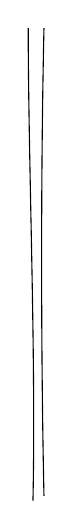
\begin{tikzpicture}[x=1cm,y=1cm,baseline=(current bounding box.north)]
\draw[line width=0.4pt] (0,0) .. controls (0.04,1.85) and (-0.06,4.30) .. (-0.06,6.00);
\draw[line width=0.4pt] (0.14,0.06) .. controls (0.10,1.90) and (0.10,4.25) .. (0.14,6.00);
\end{tikzpicture}}}}
Cependant, on trouve, par le foncteur
"bouchage des trous", une équivalence
entre la catégorie des \var{\deleted{\LMsourceMark{M013131}{\unsure{courbes alg.}}}}{\LMsourceMark{M013132}{\LMcancelledDoubts{\LMsourceMark{M013133}{\unsure{courbes alg.}}}}}{deletion}{140-2-s401-D001}
groupes profinis à lacets \uuline{extérieurs} \uline{arithmétisés},
\var{\inserted{de type $(g,\nu)$,}}{\LMadded{de type $(g,\nu)$,}}{insertion}{140-2-s401-I002}
et des groupes profinis à lacets
(pas extérieurs !) \uline{arithmétisés}, de type
$(g,\nu-1)$.

On peut se proposer d'essayer de
préciser \var{\deleted{\LMsourceMark{M013134}{\unsure{par}}}}{\LMsourceMark{M013135}{\LMcancelledDoubts{\LMsourceMark{M013136}{\unsure{par}}}}}{deletion}{140-2-s401-D002} le type des propriétés
qui vont caractériser $\mathcal N_{g,\nu}$ dans $\mathcal N'_{g,\nu}=$
$\operatorname{Norm}_{\widehat{\widehat{\mathcal T}}_{g,\nu}}
(\widehat{\mathcal T}_{g,\nu}^{+})$,
\var{\deleted{Je \LMsourceMark{M013137}{\unsure{pense}} qu'il}}{\LMsourceMark{M013138}{\LMcancelledDoubts{\LMsourceMark{M013139}{\unsure{pense}}}}}{deletion}{140-2-s401-D003}
\var{\inserted{\deleted{\LMsourceMark{M013140}{\unsure{On aura}}}ou encore}}{\LMadded{\var{\deleted{\LMsourceMark{M013141}{\unsure{On aura}}}}{\LMsourceMark{M013142}{\LMcancelledDoubts{\LMsourceMark{M013143}{\unsure{On aura}}}}}{deletion}{140-2-s401-D004}ou encore}}{insertion}{140-2-s401-I003}
$\mathbb{\Gamma}_{g,\nu}$
\var{\deleted{\LMsourceMark{M013144}{\unsure{pour}} \LMsourceMark{M013145}{\illegible{1}} $\Gamma'$}}{\LMsourceMark{M013146}{\LMcancelledDoubts{\LMsourceMark{M013147}{\unsure{pour}}\quad \LMsourceMark{M013148}{\illegible{1}}}}}{deletion}{140-2-s401-D005}
dans $\mathbb{\Gamma}'_{g,\nu}=\mathcal N'_{g,\nu}/\widehat{\mathcal T}_{g,\nu}^{+}$.
On a des hom. naturels

\LMsourceMark{M013149}{\margin{400}}

\LMflushnotes\LMflushpages
\ifnum\LMform=1
\begin{LMapparatus}
\LMentry{140-2-s401-I001}{insertion}{\inserted{urait}
}{\emph{\LMinsertedlabel}}{Ajout explicite de l'auteur : intégré à l'endroit indiqué par la transcription, sans modifier sa lecture.}{}
\LMentry{140-2-s401-D001}{suppression}{\deleted{\LMsourceMark{M013150}{\unsure{courbes alg.}}}
}{\emph{\LMomittedlabel}}{Passage biffé dans le manuscrit : la suppression suit l'état final de l'auteur; les doutes de lecture restent signalés.}{}
\LMentry{140-2-s401-I002}{insertion}{\inserted{de type $(g,\nu)$,}
}{\emph{\LMinsertedlabel}}{Ajout explicite de l'auteur : intégré à l'endroit indiqué par la transcription, sans modifier sa lecture.}{}
\LMentry{140-2-s401-D002}{suppression}{\deleted{\LMsourceMark{M013151}{\unsure{par}}}
}{\emph{\LMomittedlabel}}{Passage biffé dans le manuscrit : la suppression suit l'état final de l'auteur; les doutes de lecture restent signalés.}{}
\LMentry{140-2-s401-D003}{suppression}{\deleted{Je \LMsourceMark{M013152}{\unsure{pense}} qu'il}
}{\emph{\LMomittedlabel}}{Passage biffé dans le manuscrit : la suppression suit l'état final de l'auteur; les doutes de lecture restent signalés.}{}
\LMentry{140-2-s401-I003}{insertion}{\inserted{\deleted{\LMsourceMark{M013153}{\unsure{On aura}}}ou encore}
}{\emph{\LMinsertedlabel}}{Ajout explicite de l'auteur : intégré à l'endroit indiqué par la transcription, sans modifier sa lecture.}{}
\LMentry{140-2-s401-D004}{suppression}{\deleted{\LMsourceMark{M013154}{\unsure{On aura}}}
}{\emph{\LMomittedlabel}}{Passage biffé dans le manuscrit : la suppression suit l'état final de l'auteur; les doutes de lecture restent signalés.}{}
\LMentry{140-2-s401-D005}{suppression}{\deleted{\LMsourceMark{M013155}{\unsure{pour}} \LMsourceMark{M013156}{\illegible{1}} $\Gamma'$}
}{\emph{\LMomittedlabel}}{Passage biffé dans le manuscrit : la suppression suit l'état final de l'auteur; les doutes de lecture restent signalés.}{}
\end{LMapparatus}
\fi
\ifnum\LMform=2
\par\smallskip\begingroup\footnotesize\Needspace{4\baselineskip}\csname @beginparpenalty\endcsname=10000\relax\noindent\textcolor{gray}{\rule{.2\linewidth}{.35pt}}\par\nobreak
\noindent\textit{\LMdoubtheading.}\par\nobreak
\LMcarryover{140-2-s401-D001}{\LMsourceMark{M013157}{\unsure{courbes alg.}}
}
\LMcarryover{140-2-s401-D002}{\LMsourceMark{M013158}{\unsure{par}}
}
\LMcarryover{140-2-s401-D003}{\LMsourceMark{M013159}{\unsure{pense}}
}
\LMcarryover{140-2-s401-D004}{\LMsourceMark{M013160}{\unsure{On aura}}
}
\LMcarryover{140-2-s401-D005}{\LMsourceMark{M013161}{\unsure{pour}}\quad \LMsourceMark{M013162}{\illegible{1}}
}
\par\endgroup\smallskip
\fi

\LMsourceMark{M013163}{\scanpage{402}}

\[
\tag{15}
\left|
\begin{aligned}
\mathbb{\Gamma}'_{g,\nu}&\longrightarrow\operatorname{Autext}(\widehat{\mathcal T}_{g,\nu}^{+})\\
\mathbb{\Gamma}'_{g,\nu}&\longrightarrow\operatorname{Aut\,ext}(\widehat{\mathcal T}_{g,\nu}^{+!})
\end{aligned}
\right.
\]
et je présume qu'\var{\deleted{il s'agit}}{}{deletion}{140-2-s402-D001} $\mathbb{\Gamma}_{g,\nu}$ pourra
se décrire comme image inverse d'un
sous-groupe fermé convenable de l'un
ou l'autre des seconds mbs, i.e. qu'on
peut le décrire en termes \LMsourceMark{M013164}{\unsure{des|de}} propriétés
d'opérations extérieures sur $\widehat{\mathcal T}_{g,\nu}^{+}$ ou
sur $\widehat{\mathcal T}_{g,\nu}$. Les conditions \textcircled{e} en tous
cas sont bien de ce type (\LMsourceMark{M013165}{\unsure{propriété|propriétés}}
de normaliser des \LMsourceMark{M013166}{\unsure{ss-groupes}} \LMsourceMark{M013167}{\unsure{invariants|inscrits}}
\var{\deleted{$\LMsourceMark{M013168}{\unsure{\mathcal T'_i}}$}}{\LMsourceMark{M013169}{\LMcancelledDoubts{\(\LMsourceMark{M013170}{\unsure{\mathcal T'_i}}\)}}}{deletion}{140-2-s402-D002} $\pi'_i$ de $\mathcal T_{g,\nu}^{+!}$ ...).
Bien sûr, on
pourrait poser des conditions sur des
\LMsourceMark{M013171}{\unsure{automs}} extérieurs (de $\widehat{\mathcal T}'{}_{g,\nu}^{+!}$, disons),
qui soient stables par passage \var{\inserted{successifs}}{\LMadded{successifs}}{insertion}{140-2-s402-I001} à des
$\widehat{\mathcal T}'{}_{g,\nu-1}^{+!}$, $\widehat{\mathcal T}'{}_{g,\LMsourceMark{M013172}{\unsure{\nu-2}}}^{+!}$ etc ... et
\var{\deleted{pour lesquelles}}{}{deletion}{140-2-s402-D003}\var{\inserted{qui soient}}{\LMadded{qui soient}}{insertion}{140-2-s402-I002}
engendrées par les conditions \textcircled{e}. Mais
il n'est pas dit du tout que cela

\LMsourceMark{M013173}{\margin{401}}

\LMflushnotes\LMflushpages
\ifnum\LMform=1
\begin{LMapparatus}
\LMentry{140-2-s402-D001}{suppression}{\deleted{il s'agit}
}{\emph{\LMomittedlabel}}{Passage biffé dans le manuscrit : la suppression suit l'état final de l'auteur; les doutes de lecture restent signalés.}{}
\LMentry{140-2-s402-D002}{suppression}{\deleted{$\LMsourceMark{M013174}{\unsure{\mathcal T'_i}}$}
}{\emph{\LMomittedlabel}}{Passage biffé dans le manuscrit : la suppression suit l'état final de l'auteur; les doutes de lecture restent signalés.}{}
\LMentry{140-2-s402-I001}{insertion}{\inserted{successifs}
}{\emph{\LMinsertedlabel}}{Ajout explicite de l'auteur : intégré à l'endroit indiqué par la transcription, sans modifier sa lecture.}{}
\LMentry{140-2-s402-D003}{suppression}{\deleted{pour lesquelles}
}{\emph{\LMomittedlabel}}{Passage biffé dans le manuscrit : la suppression suit l'état final de l'auteur; les doutes de lecture restent signalés.}{}
\LMentry{140-2-s402-I002}{insertion}{\inserted{qui soient}
}{\emph{\LMinsertedlabel}}{Ajout explicite de l'auteur : intégré à l'endroit indiqué par la transcription, sans modifier sa lecture.}{}
\end{LMapparatus}
\fi
\ifnum\LMform=2
\par\smallskip\begingroup\footnotesize\Needspace{4\baselineskip}\csname @beginparpenalty\endcsname=10000\relax\noindent\textcolor{gray}{\rule{.2\linewidth}{.35pt}}\par\nobreak
\noindent\textit{\LMdoubtheading.}\par\nobreak
\LMcarryover{140-2-s402-D002}{\(\LMsourceMark{M013175}{\unsure{\mathcal T'_i}}\)
}
\par\endgroup\smallskip
\fi

\LMsourceMark{M013176}{\scanpage{403}}
\LMsourceMark{M013177}{\mspage{204}}

\LMsourceMark{M013178}{\unsure{suffira|suffise}} à décrire les \var{\deleted{$\LMsourceMark{M013179}{\unsure{\mathcal N_{g,\nu}}}$}}{\LMsourceMark{M013180}{\LMcancelledDoubts{\(\LMsourceMark{M013181}{\unsure{\mathcal N_{g,\nu}}}\)}}}{deletion}{140-2-s403-D001}
$\mathbb{\Gamma}_{g,\nu}\subset\Gamma'_{g,\nu}$,
ne serait-ce que parce que la condition
devient vide pour \var{\deleted{$\LMsourceMark{M013182}{\unsure{\nu=0}}$}}{\LMsourceMark{M013183}{\LMcancelledDoubts{\(\LMsourceMark{M013184}{\unsure{\nu=0}}\)}}}{deletion}{140-2-s403-D002} le cas limite $\nu=0$
(si $g\geq2$; ou pour les cas $g=1$, $\nu=1$, ou $g=0$, $\nu=3$).

Il est possible qu'il faille faire
intervenir des propriétés des $\pi_1$ des
$\LMsourceMark{M013185}{\unsure{M_{g,\nu\,\overline{\mathbb Q}_a}}}$, liés à la compactification.
Ce n'est guère que dans le cas de
$(g,\nu)=(0,3)$ qu'il ne faut pas s'attendre
du tout à ce genre de conditions.

Appelons "\LMsourceMark{M013186}{\unsure{courbe algébrique potentielle|courbes algébriques potentielles}}"
(sous-entendu, sur une clôture alg. pas précisée de $\mathbb Q$,)
la donnée d'\LMsourceMark{M013187}{\unsure{une|un}} \var{\inserted{\LMsourceMark{M013188}{\unsure{groupe}} ext profini}}{\LMadded{\LMsourceMark{M013189}{\unsure{groupe}} ext profini}}{insertion}{140-2-s403-I001}
$\pi$ à \LMsourceMark{M013190}{\unsure{lacets|lacet}} \var{\deleted{profini}}{}{deletion}{140-2-s403-D003}\var{\inserted{\deleted{ext}}}{\LMadded{\var{\deleted{ext}}{}{deletion}{140-2-s403-D004}}}{insertion}{140-2-s403-I002}
de type $(g,\nu)$, muni d'une arithmétisation
$a$, et d'un germe de relèvement
"admissible"
\LMsourceMark{M013191}{\margin{\var{\deleted{\LMsourceMark{M013192}{\illegible{1}}}}{\LMsourceMark{M013193}{\LMcancelledDoubts{\LMsourceMark{M013194}{\illegible{1}}}}}{deletion}{140-2-s403-D005}}}
\[
\tag{16}
\mathbb{\Gamma}_{\LMsourceMark{M013195}{\unsure{a|\bullet}}}^{\natural}
\longrightarrow\mathcal N_a.
\]
Elles forment une catégorie (pour les
iso, pour le moment) Si on se
donne un torseur $P$ sous $\mathbb{\Gamma}_{g,\nu}$
(ce qui \var{\inserted{\LMsourceMark{M013196}{\unsure{trivialt.|moralt.}}}}{\LMadded{\LMsourceMark{M013197}{\unsure{trivialt.|moralt.}}}}{insertion}{140-2-s403-I003} revient à se donner une clôture

\LMsourceMark{M013198}{\margin{402}}

\LMflushnotes\LMflushpages
\ifnum\LMform=1
\begin{LMapparatus}
\LMentry{140-2-s403-D001}{suppression}{\deleted{$\LMsourceMark{M013199}{\unsure{\mathcal N_{g,\nu}}}$}
}{\emph{\LMomittedlabel}}{Passage biffé dans le manuscrit : la suppression suit l'état final de l'auteur; les doutes de lecture restent signalés.}{}
\LMentry{140-2-s403-D002}{suppression}{\deleted{$\LMsourceMark{M013200}{\unsure{\nu=0}}$}
}{\emph{\LMomittedlabel}}{Passage biffé dans le manuscrit : la suppression suit l'état final de l'auteur; les doutes de lecture restent signalés.}{}
\LMentry{140-2-s403-I001}{insertion}{\inserted{\LMsourceMark{M013201}{\unsure{groupe}} ext profini}
}{\emph{\LMinsertedlabel}}{Ajout explicite de l'auteur : intégré à l'endroit indiqué par la transcription, sans modifier sa lecture.}{}
\LMentry{140-2-s403-D003}{suppression}{\deleted{profini}
}{\emph{\LMomittedlabel}}{Passage biffé dans le manuscrit : la suppression suit l'état final de l'auteur; les doutes de lecture restent signalés.}{}
\LMentry{140-2-s403-I002}{insertion}{\inserted{\deleted{ext}}
}{\emph{\LMinsertedlabel}}{Ajout explicite de l'auteur : intégré à l'endroit indiqué par la transcription, sans modifier sa lecture.}{}
\LMentry{140-2-s403-D004}{suppression}{\deleted{ext}
}{\emph{\LMomittedlabel}}{Passage biffé dans le manuscrit : la suppression suit l'état final de l'auteur; les doutes de lecture restent signalés.}{}
\LMentry{140-2-s403-D005}{suppression}{\deleted{\LMsourceMark{M013202}{\illegible{1}}}
}{\emph{\LMomittedlabel}}{Passage biffé dans le manuscrit : la suppression suit l'état final de l'auteur; les doutes de lecture restent signalés.}{}
\LMentry{140-2-s403-I003}{insertion}{\inserted{\LMsourceMark{M013203}{\unsure{trivialt.|moralt.}}}
}{\emph{\LMinsertedlabel}}{Ajout explicite de l'auteur : intégré à l'endroit indiqué par la transcription, sans modifier sa lecture.}{}
\end{LMapparatus}
\fi
\ifnum\LMform=2
\par\smallskip\begingroup\footnotesize\Needspace{4\baselineskip}\csname @beginparpenalty\endcsname=10000\relax\noindent\textcolor{gray}{\rule{.2\linewidth}{.35pt}}\par\nobreak
\noindent\textit{\LMdoubtheading.}\par\nobreak
\LMcarryover{140-2-s403-D001}{\(\LMsourceMark{M013204}{\unsure{\mathcal N_{g,\nu}}}\)
}
\LMcarryover{140-2-s403-D002}{\(\LMsourceMark{M013205}{\unsure{\nu=0}}\)
}
\LMcarryover{140-2-s403-D005}{\LMsourceMark{M013206}{\illegible{1}}
}
\par\endgroup\smallskip
\fi

\LMsourceMark{M013207}{\scanpage{404}}
alg. $\overline{\mathbb Q}$ de $\mathbb Q$ \ldots) les courbes potentielles
de type $(g,\nu)$ \uline{\LMsourceMark{M013208}{\unsure{relatifs|relatives}}} à ce torseur
(\LMsourceMark{M013209}{\unsure{moralt|moralmt}}, \LMsourceMark{M013210}{\unsure{correspondant|correspondent}} à des courbes
alg. sur $\overline{\mathbb Q}$ \ldots) sont \var{\inserted{celles}}{\LMadded{celles}}{insertion}{140-2-s404-I001} munies en
plus d'un \LMsourceMark{M013211}{\unsure{isom.}} (``intérieur'')
\[
(17)\qquad \mathbb P_a\xrightarrow{\sim}P
\]
(définissant un isomorphisme
\[
(18)\qquad \mathbb{\Gamma}_a\longrightarrow\Gamma_P
 =\operatorname{Aut}_{\mathbb{\Gamma}_{g,\nu}}(P).
\]
\LMsourceMark{M013212}{\margin{Le cas où $P$ est le torseur
trivial, est celui des \var{\deleted{\LMsourceMark{M013213}{\unsure{courbes}}}}{\LMsourceMark{M013214}{\LMcancelledDoubts{\LMsourceMark{M013215}{\unsure{courbes}}}}}{deletion}{140-2-s404-D001} $\pi$ ext \LMsourceMark{M013216}{\unsure{(?)|(18)}}
munis d'une \uline{prédiscrétification} orientée $\alpha$
(d'où une \var{\deleted{\LMsourceMark{M013217}{\illegible{1}}}}{\LMsourceMark{M013218}{\LMcancelledDoubts{\LMsourceMark{M013219}{\illegible{1}}}}}{deletion}{140-2-s404-D002} \LMsourceMark{M013220}{\unsure{suite}} exacte
$1\longrightarrow\widehat{\mathcal T}_\alpha\longrightarrow
\mathcal N_\alpha\longrightarrow\mathbb{\Gamma}_\alpha\longrightarrow1$)}}

Cette fois-ci, on s'attend à trouver
des \LMsourceMark{M013221}{\unsure{ens}} d'iso. \uline{finis}, au lieu de
torseurs sous des groupes profinis
considérables.

On considère les \var{\deleted{\LMsourceMark{M013222}{\unsure{P}}}}{\LMsourceMark{M013223}{\LMcancelledDoubts{\LMsourceMark{M013224}{\unsure{P}}}}}{deletion}{140-2-s404-D003} \uline{Points} de $\pi$,
comme les classes de \var{\inserted{$\pi$-}}{\LMadded{$\pi$-}}{insertion}{140-2-s404-I002}conjugaison
des \LMsourceMark{M013225}{\unsure{relèvts}} ``admissibles'' de (16),
\LMsourceMark{M013226}{\unsure{en|ou}}
\[
(19)\qquad\mathbb{\Gamma}_{\LMsourceMark{M013227}{\unsure{a|\bullet}}}^{\natural}\longrightarrow
\mathcal M_a\subset\widehat{\widehat{\mathcal T}}(\pi)
\]
i.e. un germe de vraie action de $\mathbb{\Gamma}_{\bullet}$
sur $\pi$, avec
\LMsourceMark{M013228}{\margin{(20)}}
\figure{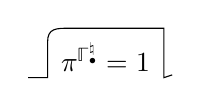
\begin{tikzpicture}[baseline=(eq.base)]
\node[inner sep=0pt,outer sep=0pt] (eq) {$\pi^{\mathbb{\Gamma}_{\bullet}^{\natural}}=1$};
\draw[line width=0.4pt]
([xshift=-12pt,yshift=-2pt]eq.south west)
-- ([xshift=-5pt,yshift=-2pt]eq.south west)
-- ([xshift=-5pt]eq.north west)
.. controls ([xshift=-5pt,yshift=5pt]eq.north west) and ([xshift=-2pt,yshift=5pt]eq.north west) .. ([xshift=3pt,yshift=5pt]eq.north west)
-- ([xshift=5pt,yshift=5pt]eq.north east)
-- ([xshift=5pt,yshift=-2pt]eq.south east)
-- ([xshift=8pt,yshift=-1pt]eq.south east);
\end{tikzpicture}}
(ceci pour \var{\deleted{\LMsourceMark{M013229}{\unsure{l'ad}}}}{\LMsourceMark{M013230}{\LMcancelledDoubts{\LMsourceMark{M013231}{\unsure{l'ad}}}}}{deletion}{140-2-s404-D004}
\LMsourceMark{M013232}{\margin{403}}

\LMflushnotes\LMflushpages
\ifnum\LMform=1
\begin{LMapparatus}
\LMentry{140-2-s404-I001}{insertion}{\inserted{celles}
}{\emph{\LMinsertedlabel}}{Ajout explicite de l'auteur : intégré à l'endroit indiqué par la transcription, sans modifier sa lecture.}{}
\LMentry{140-2-s404-D001}{suppression}{\deleted{\LMsourceMark{M013233}{\unsure{courbes}}}
}{\emph{\LMomittedlabel}}{Passage biffé dans le manuscrit : la suppression suit l'état final de l'auteur; les doutes de lecture restent signalés.}{}
\LMentry{140-2-s404-D002}{suppression}{\deleted{\LMsourceMark{M013234}{\illegible{1}}}
}{\emph{\LMomittedlabel}}{Passage biffé dans le manuscrit : la suppression suit l'état final de l'auteur; les doutes de lecture restent signalés.}{}
\LMentry{140-2-s404-D003}{suppression}{\deleted{\LMsourceMark{M013235}{\unsure{P}}}
}{\emph{\LMomittedlabel}}{Passage biffé dans le manuscrit : la suppression suit l'état final de l'auteur; les doutes de lecture restent signalés.}{}
\LMentry{140-2-s404-I002}{insertion}{\inserted{$\pi$-}
}{\emph{\LMinsertedlabel}}{Ajout explicite de l'auteur : intégré à l'endroit indiqué par la transcription, sans modifier sa lecture.}{}
\LMentry{140-2-s404-D004}{suppression}{\deleted{\LMsourceMark{M013236}{\unsure{l'ad}}}
}{\emph{\LMomittedlabel}}{Passage biffé dans le manuscrit : la suppression suit l'état final de l'auteur; les doutes de lecture restent signalés.}{}
\end{LMapparatus}
\fi
\ifnum\LMform=2
\par\smallskip\begingroup\footnotesize\Needspace{4\baselineskip}\csname @beginparpenalty\endcsname=10000\relax\noindent\textcolor{gray}{\rule{.2\linewidth}{.35pt}}\par\nobreak
\noindent\textit{\LMdoubtheading.}\par\nobreak
\LMcarryover{140-2-s404-D001}{\LMsourceMark{M013237}{\unsure{courbes}}
}
\LMcarryover{140-2-s404-D002}{\LMsourceMark{M013238}{\illegible{1}}
}
\LMcarryover{140-2-s404-D003}{\LMsourceMark{M013239}{\unsure{P}}
}
\LMcarryover{140-2-s404-D004}{\LMsourceMark{M013240}{\unsure{l'ad}}
}
\par\endgroup\smallskip
\fi

\LMsourceMark{M013241}{\scanpage{405}}
\LMsourceMark{M013242}{\mspage{205}}
l'admissibilité.

\uline{Question liminaire} La connaissance de
$\pi$, de $\underbrace{\widehat{\mathcal T}_a^+}_{\Sigma_a}
\subset\widehat{\widehat{\mathcal T}}(\pi)$, et \LMsourceMark{M013243}{\unsure{d'un}} ss-groupe
$\Gamma'\subset\widehat{\widehat{\mathcal T}}(\pi)$
(normalisant $\Sigma_a$, \var{\inserted{tel que
$\Gamma'\cap\LMsourceMark{M013244}{\unsure{\Sigma_a|\Sigma_{\bullet}}}=(1)$}}{\LMadded{tel que
$\Gamma'\cap\LMsourceMark{M013245}{\unsure{\Sigma_a|\Sigma_{\bullet}}}=(1)$}}{insertion}{140-2-s405-I001})
\LMsourceMark{M013246}{\unsure{permettrait-il}} de retrouver l'\LMsourceMark{M013247}{\unsure{arithmatisation|arithmétisation}} de $\pi$
--- et, pour commencer, de retrouver
$\mathcal N_a$ (dans lequel $\Gamma'\cdot\Sigma$ est d'indice
fini) ? \var{\deleted{Est}}{}{deletion}{140-2-s405-D001} Il \LMsourceMark{M013248}{\unsure{suffirait|suffira}}, pour pouvoir
répondre par l'affirmative, de savoir
que tt \LMsourceMark{M013249}{\unsure{isom.}} ext. $\pi\longrightarrow\pi_{g,\nu}$,
qui envoie \var{\inserted{$\Sigma$ sur $\widehat{\mathcal T}_{g,\nu}=\Sigma_{g,\nu}$, et}}{\LMadded{$\Sigma$ sur $\widehat{\mathcal T}_{g,\nu}=\Sigma_{g,\nu}$, et}}{insertion}{140-2-s405-I002}
\LMsourceMark{M013250}{\unsure{tt|le}} ss-groupe d'indice
fini $\Gamma'\cdot\Sigma$ dans $\mathcal N_a$ dans $\mathcal N_{g,\nu}$,
est compatible avec les \LMsourceMark{M013251}{\unsure{arithmatisations|arithmétisations}}.
Or ceci revient \LMsourceMark{M013252}{\unsure{exactt|exactmt}} :

\textcircled{g} (facultatif, quand même !)
\var{\deleted{tout}}{}{deletion}{140-2-s405-D002} Pour tt sous-groupe
ouvert $\mathcal N'$ de $\mathcal N_{g,\nu}$,
les éléments de $\widehat{\widehat{\mathcal T}}_{g,\nu}$
\var{\inserted{normalisant $\widehat{\mathcal T}_{g,\nu}$ et}}{\LMadded{normalisant $\widehat{\mathcal T}_{g,\nu}$ et}}{insertion}{140-2-s405-I003}
qui transportent
$\mathcal N'$ dans $\mathcal N_{g,\nu}$, \LMsourceMark{M013253}{\unsure{sont}} dans $\mathcal N_{g,\nu}$
(\LMsourceMark{M013254}{\unsure{a fortiori}},
$\mathcal N_{g,\nu}$ serait son propre normalisateur
dans $\operatorname{Norm}_{\widehat{\widehat{\mathcal T}}_{g,\nu}}
(\widehat{\mathcal T}_{g,\nu})$.
\LMsourceMark{M013255}{\margin{404}}

\LMflushnotes\LMflushpages
\ifnum\LMform=1
\begin{LMapparatus}
\LMentry{140-2-s405-I001}{insertion}{\inserted{tel que
$\Gamma'\cap\LMsourceMark{M013256}{\unsure{\Sigma_a|\Sigma_{\bullet}}}=(1)$}
}{\emph{\LMinsertedlabel}}{Ajout explicite de l'auteur : intégré à l'endroit indiqué par la transcription, sans modifier sa lecture.}{}
\LMentry{140-2-s405-D001}{suppression}{\deleted{Est}
}{\emph{\LMomittedlabel}}{Passage biffé dans le manuscrit : la suppression suit l'état final de l'auteur; les doutes de lecture restent signalés.}{}
\LMentry{140-2-s405-I002}{insertion}{\inserted{$\Sigma$ sur $\widehat{\mathcal T}_{g,\nu}=\Sigma_{g,\nu}$, et}
}{\emph{\LMinsertedlabel}}{Ajout explicite de l'auteur : intégré à l'endroit indiqué par la transcription, sans modifier sa lecture.}{}
\LMentry{140-2-s405-D002}{suppression}{\deleted{tout}
}{\emph{\LMomittedlabel}}{Passage biffé dans le manuscrit : la suppression suit l'état final de l'auteur; les doutes de lecture restent signalés.}{}
\LMentry{140-2-s405-I003}{insertion}{\inserted{normalisant $\widehat{\mathcal T}_{g,\nu}$ et}
}{\emph{\LMinsertedlabel}}{Ajout explicite de l'auteur : intégré à l'endroit indiqué par la transcription, sans modifier sa lecture.}{}
\end{LMapparatus}
\fi

\LMsourceMark{M013257}{\scanpage{406}}
Avec les ``points de $U$'' (définis comme \LMsourceMark{M013258}{\unsure{classes}}
de conjugaison de \LMsourceMark{M013259}{\unsure{relèvts}} (19)
``admissibles'' i.e. satisfaisant (20), on
fait un groupoïde, ayant comme
groupe fondamental extérieur $\pi$, et sur
lequel $\Gamma^{\LMsourceMark{M013260}{\unsure{\natural|\sharp}}}\subset\mathcal N_a$ opère strictement
(\uline{NB} pour se reposer, on se donne
maintenant $\LMsourceMark{M013261}{\unsure{\Gamma^{\natural}|\Gamma}}$ lui-$\overline{\mathrm m}$, pas \LMsourceMark{M013262}{\unsure{seulmt|seulement}} un
germe --- \LMsourceMark{M013263}{\unsure{moralmt|moralement}}, cela signifie
qu'on a une courbe définie sur une
sous-ext. finie $K$ de $\overline{\mathbb Q}/\mathbb Q$ \ldots\LMsourceMark{M013264}{\unsure{\}|)}}.
Les pts fixes de $\Gamma$ correspondent
aux pts rat/$K$, les pts fixes sous un
ss-groupe fermé $\Gamma'$ aux pts rationnels
sur la sous-extension $K'$ de $\overline{\mathbb Q}/\mathbb Q$ asso-
ciée à $\Gamma'$ \ldots)
\LMsourceMark{M013265}{\margin{405}}

\LMflushnotes\LMflushpages

\LMsourceMark{M013266}{\scanpage{407}}
\LMsourceMark{M013267}{\mspage{206}}

Soit maintenant
\figure{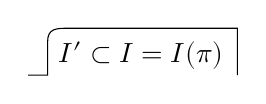
\begin{tikzpicture}[baseline=(eq.base)]
\node[inner sep=0pt,outer sep=0pt] (eq) {$I'\subset I=I(\pi)$};
\draw[line width=0.4pt]
([xshift=-11pt,yshift=-2pt]eq.south west)
-- ([xshift=-4pt,yshift=-2pt]eq.south west)
-- ([xshift=-4pt]eq.north west)
.. controls ([xshift=-4pt,yshift=5pt]eq.north west) and ([xshift=-1pt,yshift=5pt]eq.north west) .. ([xshift=4pt,yshift=5pt]eq.north west)
-- ([xshift=5pt,yshift=5pt]eq.north east)
-- ([xshift=5pt,yshift=-2pt]eq.south east);
\end{tikzpicture}}
une
partie de $I$, stable par $\Gamma$. On trouve
par "bouchage des trous en $I'$" un
groupe ext. à lacets $\pi'$, \var{\deleted{qui}}{}{deletion}{140-2-s407-D001} et un
hom extérieur
\[
(20)\qquad \pi^{\LMsourceMark{M013268}{\unsure{\natural|\sharp}}}\longrightarrow\pi'
\]
D'ailleurs $\pi'$ hérite d'une arithmétisation \var{\inserted{$a'$}}{\LMadded{$a'$}}{insertion}{140-2-s407-I001}
par $\pi$ -- et on aura
\[
(21)\qquad
\left\{
\begin{array}{ccc}
\mathbb{\Gamma}_a & \overset{\sim}{\longrightarrow} & \mathbb{\Gamma}_{a'} \\
\mathbb P_a & \overset{\sim}{\longrightarrow} & \mathbb P_{a'} \\
\LMsourceMark{M013269}{\unsure{\wr}} & & \\
P & &
\end{array}
\right.
\quad\LMsourceMark{M013270}{\unsure{\leadsto}}
\]
donc $\pi'$ est défini sur \LMsourceMark{M013271}{\unsure{le|la}} $\overline{\mathrm m}$ $P$ que
$\mathbb{\Gamma}_a$
(i.e. en faisant des trous dans $U$ pour
trouver $U'$, on n'a pas dérangé le
corps de base alg. \LMsourceMark{M013272}{\unsure{clos|abs}} $\overline{\mathbb Q}\ldots$). D'ailleurs
on aura un hom canonique
\[
\widehat{\mathcal T}(\pi)\longrightarrow
\widehat{\mathcal T}(\pi')
\]
induisant
\begin{samepage}
\[
(22)\qquad
\]
\diagram{\begin{tikzcd}[ampersand replacement=\&,column sep=3.2em,row sep=1.8em]
\mathcal N_a \arrow[r] \arrow[d,phantom,"\cup" description] \& \mathcal N_{a'} \arrow[d,phantom,"\cup" description] \\
\widehat{\mathcal T}_a \arrow[r,dash] \& \widehat{\mathcal T}_{a'}
\end{tikzcd}}
\end{samepage}

\LMsourceMark{M013273}{\margin{406}}

\LMflushnotes\LMflushpages
\ifnum\LMform=1
\begin{LMapparatus}
\LMentry{140-2-s407-D001}{suppression}{\deleted{qui}
}{\emph{\LMomittedlabel}}{Passage biffé dans le manuscrit : la suppression suit l'état final de l'auteur; les doutes de lecture restent signalés.}{}
\LMentry{140-2-s407-I001}{insertion}{\inserted{$a'$}
}{\emph{\LMinsertedlabel}}{Ajout explicite de l'auteur : intégré à l'endroit indiqué par la transcription, sans modifier sa lecture.}{}
\end{LMapparatus}
\fi

\LMsourceMark{M013274}{\scanpage{408}}

(induisant justement $\mathbb{\Gamma}_a\longrightarrow\mathbb{\Gamma}_{a'}$ par passage
aux quotients), et on trouve, en
composant
\[
\Gamma\;\LMsourceMark{M013275}{\unsure{\subset|\hookrightarrow}}\;\mathcal N_a\longrightarrow\mathcal N_{a'}
\]
un hom \LMsourceMark{M013276}{\unsure{égalmt|également}} injectif
\[
(23)\qquad\Gamma\hookrightarrow\mathcal N_{a'}
\]
qui est une \LMsourceMark{M013277}{\unsure{quasi-section|quasi section}} de $\mathcal N_{a'}$ sur $\mathbb{\Gamma}_{a'}$,
Donc \var{\deleted{\LMsourceMark{M013278}{\unsure{que|par}}}}{\LMsourceMark{M013279}{\LMcancelledDoubts{\LMsourceMark{M013280}{\unsure{que|par}}}}}{deletion}{140-2-s408-D001}\var{\inserted{sous}}{\LMadded{sous}}{insertion}{140-2-s408-I001} réserve d'admissibilité,
on trouve sur \var{\deleted{\LMsourceMark{M013281}{\illegible{1}}}}{\LMsourceMark{M013282}{\LMcancelledDoubts{\LMsourceMark{M013283}{\illegible{1}}}}}{deletion}{140-2-s408-D002} $\LMsourceMark{M013284}{\unsure{\pi'|\pi}}$ une structure
de courbe algébrique potentielle, relatif
au $\overline{\mathrm m}$ $P$.

\var{\deleted{L'admissibilité s'exprime
\LMsourceMark{M013285}{\unsure{peut-être par}} la condition
\[
(24)\qquad {\pi'}^{\Gamma}=(1)
\]
-- et s'il le faut, on mettra ces
conditions (pour \LMsourceMark{M013286}{\unsure{tte|$\forall$}} $I'\subset I$) dans
la définition de l'admissibilité de}}{\LMsourceMark{M013287}{\LMcancelledDoubts{\LMsourceMark{M013288}{\unsure{peut-être par}}\quad \LMsourceMark{M013289}{\unsure{tte|$\forall$}}}}}{deletion}{140-2-s408-D003}

\var{\deleted{\LMsourceMark{M013290}{\illegible{1}} \LMsourceMark{M013291}{\unsure{Je}}}}{\LMsourceMark{M013292}{\LMcancelledDoubts{\LMsourceMark{M013293}{\illegible{1}}\quad \LMsourceMark{M013294}{\unsure{Je}}}}}{deletion}{140-2-s408-D004} Je suis vraiment gêné
aux entournures, faute d'avoir une
définition en forme de "admissible" --

\LMsourceMark{M013295}{\margin{407}}

\LMflushnotes\LMflushpages
\ifnum\LMform=1
\begin{LMapparatus}
\LMentry{140-2-s408-D001}{suppression}{\deleted{\LMsourceMark{M013296}{\unsure{que|par}}}
}{\emph{\LMomittedlabel}}{Passage biffé dans le manuscrit : la suppression suit l'état final de l'auteur; les doutes de lecture restent signalés.}{}
\LMentry{140-2-s408-I001}{insertion}{\inserted{sous}
}{\emph{\LMinsertedlabel}}{Ajout explicite de l'auteur : intégré à l'endroit indiqué par la transcription, sans modifier sa lecture.}{}
\LMentry{140-2-s408-D002}{suppression}{\deleted{\LMsourceMark{M013297}{\illegible{1}}}
}{\emph{\LMomittedlabel}}{Passage biffé dans le manuscrit : la suppression suit l'état final de l'auteur; les doutes de lecture restent signalés.}{}
\LMentry{140-2-s408-D003}{suppression}{\deleted{L'admissibilité s'exprime
\LMsourceMark{M013298}{\unsure{peut-être par}} la condition
\[
(24)\qquad {\pi'}^{\Gamma}=(1)
\]
-- et s'il le faut, on mettra ces
conditions (pour \LMsourceMark{M013299}{\unsure{tte|$\forall$}} $I'\subset I$) dans
la définition de l'admissibilité de}
}{\emph{\LMomittedlabel}}{Passage biffé dans le manuscrit : la suppression suit l'état final de l'auteur; les doutes de lecture restent signalés.}{}
\LMentry{140-2-s408-D004}{suppression}{\deleted{\LMsourceMark{M013300}{\illegible{1}} \LMsourceMark{M013301}{\unsure{Je}}}
}{\emph{\LMomittedlabel}}{Passage biffé dans le manuscrit : la suppression suit l'état final de l'auteur; les doutes de lecture restent signalés.}{}
\end{LMapparatus}
\fi
\ifnum\LMform=2
\par\smallskip\begingroup\footnotesize\Needspace{4\baselineskip}\csname @beginparpenalty\endcsname=10000\relax\noindent\textcolor{gray}{\rule{.2\linewidth}{.35pt}}\par\nobreak
\noindent\textit{\LMdoubtheading.}\par\nobreak
\LMcarryover{140-2-s408-D001}{\LMsourceMark{M013302}{\unsure{que|par}}
}
\LMcarryover{140-2-s408-D002}{\LMsourceMark{M013303}{\illegible{1}}
}
\LMcarryover{140-2-s408-D003}{\LMsourceMark{M013304}{\unsure{peut-être par}}\quad \LMsourceMark{M013305}{\unsure{tte|$\forall$}}
}
\LMcarryover{140-2-s408-D004}{\LMsourceMark{M013306}{\illegible{1}}\quad \LMsourceMark{M013307}{\unsure{Je}}
}
\par\endgroup\smallskip
\fi

\LMsourceMark{M013308}{\scanpage{409}}
\LMsourceMark{M013309}{\mspage{207}}

je vais y revenir très vite --- mais
pour le moment, j'ai envie de noter que,
\var{\deleted{du fait que $\Gamma$ \LMsourceMark{M013310}{\unsure{opérait}} \LMsourceMark{M013311}{\unsure{tr.}}}}{\LMsourceMark{M013312}{\LMcancelledDoubts{\LMsourceMark{M013313}{\unsure{opérait}}\quad \LMsourceMark{M013314}{\unsure{tr.}}}}}{deletion}{140-2-s409-D001}
\var{\inserted{si $I'\neq\varnothing$,}}{\LMadded{si $I'\neq\varnothing$,}}{insertion}{140-2-s409-I001}
le groupe ext. $\pi'$ peut se décrire par
un \var{\inserted{vrai}}{\LMadded{vrai}}{insertion}{140-2-s409-I002} groupoïde, ayant $I'$ comme ens.
d'objets, et sur lequel $\Gamma$ opère en
sens strict (ceci est de l'algèbre pure,
indépendamment des histoires d'arithmétisation\ldots)
Le fait que $\Gamma$ opère \LMsourceMark{M013315}{\unsure{trivialt}}
sur les $i'\in I'$ implique que pour \LMsourceMark{M013316}{\unsure{tt|$\forall$}}
$i'\in I'$, on a un \var{\deleted{\LMsourceMark{M013317}{\unsure{relèvement de}}}}{\LMsourceMark{M013318}{\LMcancelledDoubts{\LMsourceMark{M013319}{\unsure{relèvement de}}}}}{deletion}{140-2-s409-D002}
\LMsourceMark{M013320}{\unsure{hom.}} canonique
\[
(24)\qquad \Gamma\longrightarrow\pi'(i')
\]
qui relève son action \LMsourceMark{M013321}{\unsure{extérieur|extérieure}}, d'où
une \LMsourceMark{M013322}{\unsure{uq}} classe de \var{\inserted{$\pi'$-}}{\LMadded{$\pi'$-}}{insertion}{140-2-s409-I003}conj. de relèvements
de l'action ext. de $\Gamma$ sur $\pi'$
en une vraie action de $\Gamma$ sur $\pi'$
--- on espère qu'elle satisfait ${\pi'}^{\Gamma}=1$ ---
et on a donc une application can.
\[
(25)\qquad I'\longrightarrow\mathrm{Pts}(\pi',\alpha',\Gamma)
\]

\LMsourceMark{M013323}{\margin{408}}

\LMflushnotes\LMflushpages
\ifnum\LMform=1
\begin{LMapparatus}
\LMentry{140-2-s409-D001}{suppression}{\deleted{du fait que $\Gamma$ \LMsourceMark{M013324}{\unsure{opérait}} \LMsourceMark{M013325}{\unsure{tr.}}}
}{\emph{\LMomittedlabel}}{Passage biffé dans le manuscrit : la suppression suit l'état final de l'auteur; les doutes de lecture restent signalés.}{}
\LMentry{140-2-s409-I001}{insertion}{\inserted{si $I'\neq\varnothing$,}
}{\emph{\LMinsertedlabel}}{Ajout explicite de l'auteur : intégré à l'endroit indiqué par la transcription, sans modifier sa lecture.}{}
\LMentry{140-2-s409-I002}{insertion}{\inserted{vrai}
}{\emph{\LMinsertedlabel}}{Ajout explicite de l'auteur : intégré à l'endroit indiqué par la transcription, sans modifier sa lecture.}{}
\LMentry{140-2-s409-D002}{suppression}{\deleted{\LMsourceMark{M013326}{\unsure{relèvement de}}}
}{\emph{\LMomittedlabel}}{Passage biffé dans le manuscrit : la suppression suit l'état final de l'auteur; les doutes de lecture restent signalés.}{}
\LMentry{140-2-s409-I003}{insertion}{\inserted{$\pi'$-}
}{\emph{\LMinsertedlabel}}{Ajout explicite de l'auteur : intégré à l'endroit indiqué par la transcription, sans modifier sa lecture.}{}
\end{LMapparatus}
\fi
\ifnum\LMform=2
\par\smallskip\begingroup\footnotesize\Needspace{4\baselineskip}\csname @beginparpenalty\endcsname=10000\relax\noindent\textcolor{gray}{\rule{.2\linewidth}{.35pt}}\par\nobreak
\noindent\textit{\LMdoubtheading.}\par\nobreak
\LMcarryover{140-2-s409-D001}{\LMsourceMark{M013327}{\unsure{opérait}}\quad \LMsourceMark{M013328}{\unsure{tr.}}
}
\LMcarryover{140-2-s409-D002}{\LMsourceMark{M013329}{\unsure{relèvement de}}
}
\par\endgroup\smallskip
\fi

\LMsourceMark{M013330}{\scanpage{410}}

Je \uline{dis que cette application est injective}

Ceci est "évident" quand on interprète
"action ext. admissible" par "réalisable
par une vraie courbe alg.", et
"relèvements admissibles" par "réalisables
par des vrais pts rat / \LMsourceMark{M013331}{\unsure{$K^+$|$K$}}, corps des
\LMsourceMark{M013332}{\unsure{fixes|invariants}} de $\Gamma$". Mais on voudrait
bien sûr des raisons internes à
la donnée des $(\mathcal N_{g,\nu})$, et des \LMsourceMark{M013333}{\unsure{)}}
propriétés de ces données ! \var{\deleted{\LMsourceMark{M013334}{\unsure{Et}}}}{\LMsourceMark{M013335}{\LMcancelledDoubts{\LMsourceMark{M013336}{\unsure{Et}}}}}{deletion}{140-2-s410-D001}

\LMsourceMark{M013337}{\margin{On \LMsourceMark{M013338}{\unsure{est ramené|va revenir}} au cas Card $I'=2$\ldots}}

Ce pt étant admis (en mettant
entre parenthèses les deux définitions
\LMsourceMark{M013339}{\unsure{éventuelles|essentielles}} d'admissibilité, sur lesquelles
on va revenir plus bas) on trouve
un foncteur "bouchage de trous"
\diagram{\begin{tikzcd}[ampersand replacement=\&,column sep=large]
\begin{gathered}
\text{Courbes algébriques}\\
\text{potentielles sur }P,\ \text{\LMsourceMark{M013340}{\unsure{\var{\deleted{relatives}}{\LMsourceMark{M013341}{\LMuncertaindeletion{140-2-s410-D002}}}{deletion}{140-2-s410-D002}|relatives}}}\\
\text{à un ss-groupe ouvert}\\
\text{\var{\deleted{\LMsourceMark{M013342}{\unsure{d'un ens}}}}{\LMsourceMark{M013343}{\LMcancelledDoubts{\LMsourceMark{M013344}{\unsure{d'un ens}}}}}{deletion}{140-2-s410-D003}}\\
\Gamma\text{ de }\mathbb{\Gamma}_P,\ \text{et munies d'un}\\
\text{ens }I'\text{ de pts à l'}\infty
\end{gathered}
\arrow[r]
\&
\begin{gathered}
\text{Courbes alg.}\\
\text{pot. sur }P\text{ relatives}\\
\text{à }\Gamma,\ \text{munies}\\
\text{d'une partie}\\
\text{de l'ens des}\\
\text{"Pts \LMsourceMark{M013345}{\unsure{ratls|invts}}/}\Gamma\text{"}
\end{gathered}
\end{tikzcd}}

\LMsourceMark{M013346}{\margin{il faut pour ceci les restrictions
anabéliennes habituelles}}

\LMsourceMark{M013347}{\margin{409}}

\LMflushnotes\LMflushpages
\ifnum\LMform=1
\begin{LMapparatus}
\LMentry{140-2-s410-D001}{suppression}{\deleted{\LMsourceMark{M013348}{\unsure{Et}}}
}{\emph{\LMomittedlabel}}{Passage biffé dans le manuscrit : la suppression suit l'état final de l'auteur; les doutes de lecture restent signalés.}{}
\LMentry{140-2-s410-D002}{suppression}{\LMsourceMark{M013349}{\LMdoubtcopy{\deleted{relatives}}}
}{\emph{\LMomittedlabel}}{Passage biffé dans le manuscrit : la suppression suit l'état final de l'auteur; les doutes de lecture restent signalés.}{}
\LMentry{140-2-s410-D003}{suppression}{\deleted{\LMsourceMark{M013350}{\unsure{d'un ens}}}
}{\emph{\LMomittedlabel}}{Passage biffé dans le manuscrit : la suppression suit l'état final de l'auteur; les doutes de lecture restent signalés.}{}
\end{LMapparatus}
\fi
\ifnum\LMform=2
\par\smallskip\begingroup\footnotesize\Needspace{4\baselineskip}\csname @beginparpenalty\endcsname=10000\relax\noindent\textcolor{gray}{\rule{.2\linewidth}{.35pt}}\par\nobreak
\noindent\textit{\LMdoubtheading.}\par\nobreak
\LMcarryover{140-2-s410-D001}{\LMsourceMark{M013351}{\unsure{Et}}
}
\LMcarryover{140-2-s410-D002}{\LMsourceMark{M013352}{\LMdoubtcopy{relatives}}
}
\LMcarryover{140-2-s410-D003}{\LMsourceMark{M013353}{\unsure{d'un ens}}
}
\par\endgroup\smallskip
\fi

% END PACKAGE LM_P041
% BEGIN PACKAGE LM_P042
\ifnum\LMform<2\Needspace{11\baselineskip}\subsection*{Scans 411--420}\fi
\LMsourceMark{M013354}{\scanpage{411}}
\LMsourceMark{M013355}{\mspage{208}}

et sauf erreur, il est devenu évident
que ce foncteur est une \uline{équivalence de
catégories} (et comme conséquence, il
\LMsourceMark{M013356}{\margin{\LMsourceMark{M013357}{\unsure{pour les}} \uline{\LMsourceMark{M013358}{\unsure{isom}}}}}
y a le foncteur en sens inverse :
forer des trous en des ``pts'' invariants
sous $\Gamma_{\LMsourceMark{M013359}{\unsure{a|0}}}$ (ou en des pts quelconques
quitte à passer à un $\Gamma'$ plus petit).

Mais je me rends compte que
\var{\deleted{\LMsourceMark{M013360}{\illegible{1}}}}{\LMsourceMark{M013361}{\LMcancelledDoubts{\LMsourceMark{M013362}{\illegible{1}}}}}{deletion}{140-2-s411-D001} ce n'est pas du tout évident -- je vais
essayer d'élucider la situation axiomatiquement.
On a fixé un genre $g$,
on suppose donné, pour $\nu$ variable
(tel que $(g,\nu)$ anabélien) des
sous-groupes fermés $N_{g,\nu}\subset\widehat{\widehat{\mathcal T}}_{g,\nu}$,
normalisant $\widehat{\mathcal T}_{g,\nu}$, et satisfaisant la
condition essentielle que les $\psi_i:\widehat{\widehat{\mathcal T}}_{g,\nu}\longrightarrow\widehat{\widehat{\LMsourceMark{M013363}{\unsure{\mathcal G|\mathcal S}}}}_{g,\nu-1}$
induisent
\[
M_{g,\nu}\xrightarrow{\sim}M_{g,\nu-1}
\]
Ce qui permet de définir la notion
d'arithmétisation d'un $\pi$ profini de
type $(g,\nu)$ anabélien, et la théorie du

\LMflushnotes\LMflushpages
\ifnum\LMform=1
\begin{LMapparatus}
\LMentry{140-2-s411-D001}{suppression}{\deleted{\LMsourceMark{M013364}{\illegible{1}}}
}{\emph{\LMomittedlabel}}{Passage biffé dans le manuscrit : la suppression suit l'état final de l'auteur; les doutes de lecture restent signalés.}{}
\end{LMapparatus}
\fi
\ifnum\LMform=2
\par\smallskip\begingroup\footnotesize\Needspace{4\baselineskip}\csname @beginparpenalty\endcsname=10000\relax\noindent\textcolor{gray}{\rule{.2\linewidth}{.35pt}}\par\nobreak
\noindent\textit{\LMdoubtheading.}\par\nobreak
\LMcarryover{140-2-s411-D001}{\LMsourceMark{M013365}{\illegible{1}}
}
\par\endgroup\smallskip
\fi

\LMsourceMark{M013366}{\scanpage{412}}

bouchage d'un nb quelc. de trous, et
du forage d'1 seul trou, dans la
catégorie des groupes de type $g,\nu$,
arithmétisés.

On suppose d'autre part \LMsourceMark{M013367}{\unsure{donné|donnée}} une
sous-catégorie pleine de la cat. des groupes
\LMsourceMark{M013368}{\margin{\LMsourceMark{M013369}{\unsure{on la suppose}} : stable par prise des ss-groupes ouverts.}}
profinis (qui pourrait se réduire aux
sous-groupes ouverts de $\mathbb{\Gamma}_g$, valeur
commune des $\mathbb{\Gamma}_{g,\nu}$ ou des sous-groupes
ouverts du groupe $\mathbb{\Gamma}_a$, $a$ une
arithmétisation), et \var{\deleted{des}}{}{deletion}{140-2-s412-D001} \var{\inserted{une notion d'}}{\LMadded{une notion d'}}{insertion}{140-2-s412-I001}opérations
extérieures \var{\inserted{``admissibles''}}{\LMadded{``admissibles''}}{insertion}{140-2-s412-I002} de tels $\Gamma$ sur les
$\pi$ arithmétisés. On suppose

\textcircled{1} Si $\Gamma$ opère admissiblement sur $\pi$, tt
sous-groupe ouvert aussi (\var{\deleted{\LMsourceMark{M013370}{\unsure{et}}}}{\LMsourceMark{M013371}{\LMcancelledDoubts{\LMsourceMark{M013372}{\unsure{et}}}}}{deletion}{140-2-s412-D002} et inversement ?)

\textcircled{2} Si de plus $\Gamma$ invarie une partie $I'$
de $I=I(\pi)$, alors en ``bouchant $I'$'',
l'opération de $\Gamma$ sur $\pi'$ est admissible.

\LMsourceMark{M013373}{\margin{Il suffit de \LMsourceMark{M013374}{\unsure{la poser|le prouver}} pour $\operatorname{card} I'=1$, i.e. bouchage \LMsourceMark{M013375}{\unsure{d'un|d'un seul}} trou -- \LMsourceMark{M013376}{\unsure{du moins si on sait que la condition d'admissibilité ne dépend que de l'action des noyaux des groupes}}.}}

\var{\deleted{\LMsourceMark{M013377}{\illegible{1}}}}{\LMsourceMark{M013378}{\LMcancelledDoubts{\LMsourceMark{M013379}{\illegible{1}}}}}{deletion}{140-2-s412-D003}
\var{\deleted{\LMsourceMark{M013380}{\unsure{On se propose de définir une notion d'action admissible}} \LMsourceMark{M013381}{\illegible{2}}}}{\LMsourceMark{M013382}{\LMcancelledDoubts{\LMsourceMark{M013383}{\unsure{On se propose de définir une notion d'action admissible}}\quad \LMsourceMark{M013384}{\illegible{2}}}}}{deletion}{140-2-s412-D004}
\var{\inserted{Quand on a une action \inserted{\uline{effective}}, \LMsourceMark{M013385}{\unsure{(pas extérieure)|(non extérieure)}}}}{\LMadded{Quand on a une action \var{\inserted{\uline{effective}}}{\LMadded{\uline{effective}}}{insertion}{140-2-s412-I004}, \LMsourceMark{M013386}{\unsure{(pas extérieure)|(non extérieure)}}}}{insertion}{140-2-s412-I003}
de $\Gamma$ sur un $(\pi,a)$, alors le foncteur
\LMsourceMark{M013387}{\unsure{de}} ``\var{\deleted{bouchage}}{}{deletion}{140-2-s412-D005}\var{\inserted{forage}}{\LMadded{forage}}{insertion}{140-2-s412-I005} des trous'' donne une action
ext. sur un $(\pi^0,a^0)$ de type $g,\nu+1$,
et on dit que l'action de départ est

\LMflushnotes\LMflushpages
\ifnum\LMform=1
\begin{LMapparatus}
\LMentry{140-2-s412-D001}{suppression}{\deleted{des}
}{\emph{\LMomittedlabel}}{Passage biffé dans le manuscrit : la suppression suit l'état final de l'auteur; les doutes de lecture restent signalés.}{}
\LMentry{140-2-s412-I001}{insertion}{\inserted{une notion d'}
}{\emph{\LMinsertedlabel}}{Ajout explicite de l'auteur : intégré à l'endroit indiqué par la transcription, sans modifier sa lecture.}{}
\LMentry{140-2-s412-I002}{insertion}{\inserted{``admissibles''}
}{\emph{\LMinsertedlabel}}{Ajout explicite de l'auteur : intégré à l'endroit indiqué par la transcription, sans modifier sa lecture.}{}
\LMentry{140-2-s412-D002}{suppression}{\deleted{\LMsourceMark{M013388}{\unsure{et}}}
}{\emph{\LMomittedlabel}}{Passage biffé dans le manuscrit : la suppression suit l'état final de l'auteur; les doutes de lecture restent signalés.}{}
\LMentry{140-2-s412-D003}{suppression}{\deleted{\LMsourceMark{M013389}{\illegible{1}}}
}{\emph{\LMomittedlabel}}{Passage biffé dans le manuscrit : la suppression suit l'état final de l'auteur; les doutes de lecture restent signalés.}{}
\LMentry{140-2-s412-D004}{suppression}{\deleted{\LMsourceMark{M013390}{\unsure{On se propose de définir une notion d'action admissible}} \LMsourceMark{M013391}{\illegible{2}}}
}{\emph{\LMomittedlabel}}{Passage biffé dans le manuscrit : la suppression suit l'état final de l'auteur; les doutes de lecture restent signalés.}{}
\LMentry{140-2-s412-I003}{insertion}{\inserted{Quand on a une action \inserted{\uline{effective}}, \LMsourceMark{M013392}{\unsure{(pas extérieure)|(non extérieure)}}}
}{\emph{\LMinsertedlabel}}{Ajout explicite de l'auteur : intégré à l'endroit indiqué par la transcription, sans modifier sa lecture.}{}
\LMentry{140-2-s412-I004}{insertion}{\inserted{\uline{effective}}
}{\emph{\LMinsertedlabel}}{Ajout explicite de l'auteur : intégré à l'endroit indiqué par la transcription, sans modifier sa lecture.}{}
\LMentry{140-2-s412-D005}{suppression}{\deleted{bouchage}
}{\emph{\LMomittedlabel}}{Passage biffé dans le manuscrit : la suppression suit l'état final de l'auteur; les doutes de lecture restent signalés.}{}
\LMentry{140-2-s412-I005}{insertion}{\inserted{forage}
}{\emph{\LMinsertedlabel}}{Ajout explicite de l'auteur : intégré à l'endroit indiqué par la transcription, sans modifier sa lecture.}{}
\end{LMapparatus}
\fi
\ifnum\LMform=2
\par\smallskip\begingroup\footnotesize\Needspace{4\baselineskip}\csname @beginparpenalty\endcsname=10000\relax\noindent\textcolor{gray}{\rule{.2\linewidth}{.35pt}}\par\nobreak
\noindent\textit{\LMdoubtheading.}\par\nobreak
\LMcarryover{140-2-s412-D002}{\LMsourceMark{M013393}{\unsure{et}}
}
\LMcarryover{140-2-s412-D003}{\LMsourceMark{M013394}{\illegible{1}}
}
\LMcarryover{140-2-s412-D004}{\LMsourceMark{M013395}{\unsure{On se propose de définir une notion d'action admissible}}\quad \LMsourceMark{M013396}{\illegible{2}}
}
\par\endgroup\smallskip
\fi

\LMsourceMark{M013397}{\scanpage{413}}
\LMsourceMark{M013398}{\mspage{209}}

admissible, si l'action \uline{extérieure} déduite l'est.

On trouve ainsi une \uline{équivalence} entre
la cat. des \var{\deleted{\LMsourceMark{M013399}{\unsure{cat.}}}}{\LMsourceMark{M013400}{\LMcancelledDoubts{\LMsourceMark{M013401}{\unsure{cat.}}}}}{deletion}{140-2-s413-D001} systèmes $(\pi,a,\Gamma,\psi,i)$
d'un $(\pi,a)$ de type $(g,\nu+1)$, avec une
op. \var{\inserted{\uline{ext.}}}{\LMadded{\uline{ext.}}}{insertion}{140-2-s413-I001} admissible $\psi$ d'un $\Gamma$ dessus, et
un $i\in I(\pi)$ stable par $\Gamma$, avec la cat.
des $(\pi',a',\Gamma,\psi')$ des $(\pi',a')$ de type
$(g,\nu)$, avec une \uline{vraie} action admissible $\psi'$
de $\Gamma$ dessus.

\var{\deleted{\LMsourceMark{M013402}{\unsure{On doit}} \LMsourceMark{M013403}{\illegible{3}}}}{\LMsourceMark{M013404}{\LMcancelledDoubts{\LMsourceMark{M013405}{\unsure{On doit}}\quad \LMsourceMark{M013406}{\illegible{3}}}}}{deletion}{140-2-s413-D002}
\var{\inserted{La condition (1) assure que}}{\LMadded{La condition (1) assure que}}{insertion}{140-2-s413-I002}
\var{\deleted{\textcircled{3} \LMsourceMark{M013407}{\unsure{Si une vraie action}}}}{\LMsourceMark{M013408}{\LMcancelledDoubts{\LMsourceMark{M013409}{\unsure{Si une vraie action}}}}}{deletion}{140-2-s413-D003}
\var{\inserted{si $\Gamma$ opère \deleted{\uline{\LMsourceMark{M013410}{\unsure{vraiment}}}} \deleted{\LMsourceMark{M013411}{\unsure{admissible|admissiblement}}} effectivement, de façon}}{\LMadded{si $\Gamma$ opère \var{\deleted{\uline{\LMsourceMark{M013412}{\unsure{vraiment}}}}}{\LMsourceMark{M013413}{\LMcancelledDoubts{\LMsourceMark{M013414}{\unsure{vraiment}}}}}{deletion}{140-2-s413-D004} \var{\deleted{\LMsourceMark{M013415}{\unsure{admissible|admissiblement}}}}{\LMsourceMark{M013416}{\LMcancelledDoubts{\LMsourceMark{M013417}{\unsure{admissible|admissiblement}}}}}{deletion}{140-2-s413-D005} effectivement, de façon}}{insertion}{140-2-s413-I003}
admissible, alors l'action extérieure déduite
est admissible (mais l'inverse ne
sera pas vrai -- il y aura des relèvements
``pathologiques'' d'une action \LMsourceMark{M013418}{\unsure{cat.|ext.}} admissible
donnée\ldots). On suppose de plus

\LMsourceMark{M013419}{\margin{\figure{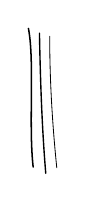
\begin{tikzpicture}[x=1cm,y=1cm,line cap=round,baseline=(current bounding box.center)]
\draw[line width=0.55pt] (0.04,1.80) .. controls (0.12,1.38) and (0.04,0.57) .. (0.10,0.04);
\draw[line width=0.50pt] (0.18,1.74) .. controls (0.19,1.20) and (0.21,0.55) .. (0.26,-0.04);
\draw[line width=0.30pt] (0.31,1.70) .. controls (0.31,1.09) and (0.35,0.52) .. (0.40,0.03);
\end{tikzpicture}}}}
\textcircled{3} Si $\Gamma$ opère \var{\inserted{effect.}}{\LMadded{effect.}}{insertion}{140-2-s413-I004} de façon admissible sur
$\pi$, alors $\pi^\Gamma=(1)$.

\var{\deleted{Soit \LMsourceMark{M013420}{\unsure{Alors}}}}{\LMsourceMark{M013421}{\LMcancelledDoubts{\LMsourceMark{M013422}{\unsure{Alors}}}}}{deletion}{140-2-s413-D006}
Cela implique que la catégorie des
$\Gamma$-Pts de $\pi$, ou si on veut des sections
de $B_{\pi,\Gamma}\,(\LMsourceMark{M013423}{\unsure{\simeq}}B_u)$ sur $B_\Gamma$, est \uline{rigide}.

\LMflushnotes\LMflushpages
\ifnum\LMform=1
\begin{LMapparatus}
\LMentry{140-2-s413-D001}{suppression}{\deleted{\LMsourceMark{M013424}{\unsure{cat.}}}
}{\emph{\LMomittedlabel}}{Passage biffé dans le manuscrit : la suppression suit l'état final de l'auteur; les doutes de lecture restent signalés.}{}
\LMentry{140-2-s413-I001}{insertion}{\inserted{\uline{ext.}}
}{\emph{\LMinsertedlabel}}{Ajout explicite de l'auteur : intégré à l'endroit indiqué par la transcription, sans modifier sa lecture.}{}
\LMentry{140-2-s413-D002}{suppression}{\deleted{\LMsourceMark{M013425}{\unsure{On doit}} \LMsourceMark{M013426}{\illegible{3}}}
}{\emph{\LMomittedlabel}}{Passage biffé dans le manuscrit : la suppression suit l'état final de l'auteur; les doutes de lecture restent signalés.}{}
\LMentry{140-2-s413-I002}{insertion}{\inserted{La condition (1) assure que}
}{\emph{\LMinsertedlabel}}{Ajout explicite de l'auteur : intégré à l'endroit indiqué par la transcription, sans modifier sa lecture.}{}
\LMentry{140-2-s413-D003}{suppression}{\deleted{\textcircled{3} \LMsourceMark{M013427}{\unsure{Si une vraie action}}}
}{\emph{\LMomittedlabel}}{Passage biffé dans le manuscrit : la suppression suit l'état final de l'auteur; les doutes de lecture restent signalés.}{}
\LMentry{140-2-s413-I003}{insertion}{\inserted{si $\Gamma$ opère \deleted{\uline{\LMsourceMark{M013428}{\unsure{vraiment}}}} \deleted{\LMsourceMark{M013429}{\unsure{admissible|admissiblement}}} effectivement, de façon}
}{\emph{\LMinsertedlabel}}{Ajout explicite de l'auteur : intégré à l'endroit indiqué par la transcription, sans modifier sa lecture.}{}
\LMentry{140-2-s413-D004}{suppression}{\deleted{\uline{\LMsourceMark{M013430}{\unsure{vraiment}}}}
}{\emph{\LMomittedlabel}}{Passage biffé dans le manuscrit : la suppression suit l'état final de l'auteur; les doutes de lecture restent signalés.}{}
\LMentry{140-2-s413-D005}{suppression}{\deleted{\LMsourceMark{M013431}{\unsure{admissible|admissiblement}}}
}{\emph{\LMomittedlabel}}{Passage biffé dans le manuscrit : la suppression suit l'état final de l'auteur; les doutes de lecture restent signalés.}{}
\LMentry{140-2-s413-I004}{insertion}{\inserted{effect.}
}{\emph{\LMinsertedlabel}}{Ajout explicite de l'auteur : intégré à l'endroit indiqué par la transcription, sans modifier sa lecture.}{}
\LMentry{140-2-s413-D006}{suppression}{\deleted{Soit \LMsourceMark{M013432}{\unsure{Alors}}}
}{\emph{\LMomittedlabel}}{Passage biffé dans le manuscrit : la suppression suit l'état final de l'auteur; les doutes de lecture restent signalés.}{}
\end{LMapparatus}
\fi
\ifnum\LMform=2
\par\smallskip\begingroup\footnotesize\Needspace{4\baselineskip}\csname @beginparpenalty\endcsname=10000\relax\noindent\textcolor{gray}{\rule{.2\linewidth}{.35pt}}\par\nobreak
\noindent\textit{\LMdoubtheading.}\par\nobreak
\LMcarryover{140-2-s413-D001}{\LMsourceMark{M013433}{\unsure{cat.}}
}
\LMcarryover{140-2-s413-D002}{\LMsourceMark{M013434}{\unsure{On doit}}\quad \LMsourceMark{M013435}{\illegible{3}}
}
\LMcarryover{140-2-s413-D003}{\LMsourceMark{M013436}{\unsure{Si une vraie action}}
}
\LMcarryover{140-2-s413-D004}{\LMsourceMark{M013437}{\unsure{vraiment}}
}
\LMcarryover{140-2-s413-D005}{\LMsourceMark{M013438}{\unsure{admissible|admissiblement}}
}
\LMcarryover{140-2-s413-D006}{\LMsourceMark{M013439}{\unsure{Alors}}
}
\par\endgroup\smallskip
\fi

\LMsourceMark{M013440}{\scanpage{414}}

Mais \var{\deleted{\LMsourceMark{M013441}{\unsure{appelons|supposons}}}}{\LMsourceMark{M013442}{\LMcancelledDoubts{\LMsourceMark{M013443}{\unsure{appelons|supposons}}}}}{deletion}{140-2-s414-D001} considérons la catégorie limite inductive des \var{\deleted{\LMsourceMark{M013444}{\illegible{1}}}}{\LMsourceMark{M013445}{\LMcancelledDoubts{\LMsourceMark{M013446}{\illegible{1}}}}}{deletion}{140-2-s414-D002} catégories des sections de $B_{\pi,\Gamma}\simeq B_u$ sur des $B_{\Gamma'}$ ($\Gamma'$ sous-groupe ouvert), elle est discrète et correspond à l'ens
\[
\mathrm{Pt}_{\mathrm{ad}}(B_{\pi,\Gamma^{\natural}})\simeq
\underset{\substack{\Gamma'\ \mathrm{ouvert}\\\mathrm{de}\ \Gamma}}{\varinjlim}
\mathrm{Pt}_{\mathrm{ad}}(B_{\pi,\Gamma'}).
\]

\LMsourceMark{M013447}{\margin{\uline{NB} Le gr.-poïde à opérateurs stricts $\uline{\mathrm{Pt}}(B_{\pi,\Gamma})$ dépend \LMsourceMark{M013448}{\unsure{fonctoriellement}} de $(\pi,\Gamma)$, \LMsourceMark{M013449}{\illegible{1}} pour des morphismes ext. \var{\deleted{\LMsourceMark{M013450}{\unsure{dans}}}}{\LMsourceMark{M013451}{\LMcancelledDoubts{\LMsourceMark{M013452}{\unsure{dans}}}}}{deletion}{140-2-s414-D003} \LMsourceMark{M013453}{\unsure{plus}} \LMsourceMark{M013454}{\illegible{3}} de $\Gamma$, si \var{\deleted{\LMsourceMark{M013455}{\illegible{4}}}}{\LMsourceMark{M013456}{\LMcancelledDoubts{\LMsourceMark{M013457}{\illegible{4}}}}}{deletion}{140-2-s414-D004}.}}

\var{\deleted{\textcircled{4} \LMsourceMark{M013458}{\unsure{Pour}} \LMsourceMark{M013459}{\illegible{2}} $\mathrm{Pt}(B_{\pi,\Gamma})$ \LMsourceMark{M013460}{\illegible{1}}. D'autre part, $\pi$ peut être défini par un groupoïde.}}{\LMsourceMark{M013461}{\LMcancelledDoubts{\LMsourceMark{M013462}{\unsure{Pour}}\quad \LMsourceMark{M013463}{\illegible{2}}\quad \LMsourceMark{M013464}{\illegible{1}}}}}{deletion}{140-2-s414-D005}
Si $\mathrm{Pt}(B_{\pi,\Gamma})\ne\varnothing$, alors (du seul fait que $\pi^{\Gamma'}=(1)$ pour $\forall$ sous-groupe ouvert de $\LMsourceMark{M013465}{\unsure{\Gamma'|\Gamma}}$) \var{\inserted{le gr. cat.}}{\LMadded{le gr. cat.}}{insertion}{140-2-s414-I001} $\pi$ peut être décrit \LMsourceMark{M013466}{\unsure{can.|com.}} par un groupoïde \var{\inserted{profini $\uline{\mathrm{Pt}}(B_{\pi,\Gamma^{\natural}})$}}{\LMadded{profini $\uline{\mathrm{Pt}}(B_{\pi,\Gamma^{\natural}})$}}{insertion}{140-2-s414-I002} ayant $\mathrm{Pt}(B_{\pi,\Gamma})$ comme ens d'objet, \var{\deleted{\LMsourceMark{M013467}{\unsure{et|alors}}}}{\LMsourceMark{M013468}{\LMcancelledDoubts{\LMsourceMark{M013469}{\unsure{et|alors}}}}}{deletion}{140-2-s414-D006} \var{\inserted{\LMsourceMark{M013470}{\unsure{lié|liés}} par le groupe cat. $\pi$, sur}}{\LMadded{\LMsourceMark{M013471}{\unsure{lié|liés}} par le groupe cat. $\pi$, sur}}{insertion}{140-2-s414-I003} lequel $\Gamma$ opère en sens strict, avec le stabilisateur \var{\inserted{$\Gamma_P$}}{\LMadded{$\Gamma_P$}}{insertion}{140-2-s414-I004} de $\forall$ pt étant ouvert. et $\Gamma_P\to\mathrm{Aut}(P)$ $(\simeq\pi\ \text{mod \LMsourceMark{M013472}{\unsure{autom. int.}}})$

\var{\deleted{De façon plus précise, \LMsourceMark{M013473}{\unsure{indépendamment de}} l'axiomatique précédente, on peut décrire les syst. \LMsourceMark{M013474}{\unsure{formés}} d'un groupe \inserted{cat. $\pi$} profini, et d'une opération \inserted{ext.} \LMsourceMark{M013475}{\unsure{d'un groupe profini}} $\Gamma$ dessus, \LMsourceMark{M013476}{\unsure{satisfaisant}}}}{\LMsourceMark{M013477}{\LMcancelledDoubts{\LMsourceMark{M013478}{\unsure{indépendamment de}}\quad \LMsourceMark{M013479}{\unsure{formés}}\quad \LMsourceMark{M013480}{\unsure{d'un groupe profini}}\quad \LMsourceMark{M013481}{\unsure{satisfaisant}}}}}{deletion}{140-2-s414-D007}

étant continue. On a ici \LMsourceMark{M013482}{\unsure{si}} à $\forall\ P\in\mathrm{Pt}(B_{\pi,\Gamma})$ on associe la classe d'isom. de \var{\deleted{\LMsourceMark{M013483}{\unsure{groupes de relèvements}}}}{\LMsourceMark{M013484}{\LMcancelledDoubts{\LMsourceMark{M013485}{\unsure{groupes de relèvements}}}}}{deletion}{140-2-s414-D008}

\LMflushnotes\LMflushpages
\ifnum\LMform=1
\begin{LMapparatus}
\LMentry{140-2-s414-D001}{suppression}{\deleted{\LMsourceMark{M013486}{\unsure{appelons|supposons}}}
}{\emph{\LMomittedlabel}}{Passage biffé dans le manuscrit : la suppression suit l'état final de l'auteur; les doutes de lecture restent signalés.}{}
\LMentry{140-2-s414-D002}{suppression}{\deleted{\LMsourceMark{M013487}{\illegible{1}}}
}{\emph{\LMomittedlabel}}{Passage biffé dans le manuscrit : la suppression suit l'état final de l'auteur; les doutes de lecture restent signalés.}{}
\LMentry{140-2-s414-D003}{suppression}{\deleted{\LMsourceMark{M013488}{\unsure{dans}}}
}{\emph{\LMomittedlabel}}{Passage biffé dans le manuscrit : la suppression suit l'état final de l'auteur; les doutes de lecture restent signalés.}{}
\LMentry{140-2-s414-D004}{suppression}{\deleted{\LMsourceMark{M013489}{\illegible{4}}}
}{\emph{\LMomittedlabel}}{Passage biffé dans le manuscrit : la suppression suit l'état final de l'auteur; les doutes de lecture restent signalés.}{}
\LMentry{140-2-s414-D005}{suppression}{\deleted{\textcircled{4} \LMsourceMark{M013490}{\unsure{Pour}} \LMsourceMark{M013491}{\illegible{2}} $\mathrm{Pt}(B_{\pi,\Gamma})$ \LMsourceMark{M013492}{\illegible{1}}. D'autre part, $\pi$ peut être défini par un groupoïde.}
}{\emph{\LMomittedlabel}}{Passage biffé dans le manuscrit : la suppression suit l'état final de l'auteur; les doutes de lecture restent signalés.}{}
\LMentry{140-2-s414-I001}{insertion}{\inserted{le gr. cat.}
}{\emph{\LMinsertedlabel}}{Ajout explicite de l'auteur : intégré à l'endroit indiqué par la transcription, sans modifier sa lecture.}{}
\LMentry{140-2-s414-I002}{insertion}{\inserted{profini $\uline{\mathrm{Pt}}(B_{\pi,\Gamma^{\natural}})$}
}{\emph{\LMinsertedlabel}}{Ajout explicite de l'auteur : intégré à l'endroit indiqué par la transcription, sans modifier sa lecture.}{}
\LMentry{140-2-s414-D006}{suppression}{\deleted{\LMsourceMark{M013493}{\unsure{et|alors}}}
}{\emph{\LMomittedlabel}}{Passage biffé dans le manuscrit : la suppression suit l'état final de l'auteur; les doutes de lecture restent signalés.}{}
\LMentry{140-2-s414-I003}{insertion}{\inserted{\LMsourceMark{M013494}{\unsure{lié|liés}} par le groupe cat. $\pi$, sur}
}{\emph{\LMinsertedlabel}}{Ajout explicite de l'auteur : intégré à l'endroit indiqué par la transcription, sans modifier sa lecture.}{}
\LMentry{140-2-s414-I004}{insertion}{\inserted{$\Gamma_P$}
}{\emph{\LMinsertedlabel}}{Ajout explicite de l'auteur : intégré à l'endroit indiqué par la transcription, sans modifier sa lecture.}{}
\LMentry{140-2-s414-D007}{suppression}{\deleted{De façon plus précise, \LMsourceMark{M013495}{\unsure{indépendamment de}} l'axiomatique précédente, on peut décrire les syst. \LMsourceMark{M013496}{\unsure{formés}} d'un groupe \inserted{cat. $\pi$} profini, et d'une opération \inserted{ext.} \LMsourceMark{M013497}{\unsure{d'un groupe profini}} $\Gamma$ dessus, \LMsourceMark{M013498}{\unsure{satisfaisant}}}
}{\emph{\LMomittedlabel}}{Passage biffé dans le manuscrit : la suppression suit l'état final de l'auteur; les doutes de lecture restent signalés.}{}
\LMentry{140-2-s414-D008}{suppression}{\deleted{\LMsourceMark{M013499}{\unsure{groupes de relèvements}}}
}{\emph{\LMomittedlabel}}{Passage biffé dans le manuscrit : la suppression suit l'état final de l'auteur; les doutes de lecture restent signalés.}{}
\end{LMapparatus}
\fi
\ifnum\LMform=2
\par\smallskip\begingroup\footnotesize\Needspace{4\baselineskip}\csname @beginparpenalty\endcsname=10000\relax\noindent\textcolor{gray}{\rule{.2\linewidth}{.35pt}}\par\nobreak
\noindent\textit{\LMdoubtheading.}\par\nobreak
\LMcarryover{140-2-s414-D001}{\LMsourceMark{M013500}{\unsure{appelons|supposons}}
}
\LMcarryover{140-2-s414-D002}{\LMsourceMark{M013501}{\illegible{1}}
}
\LMcarryover{140-2-s414-D003}{\LMsourceMark{M013502}{\unsure{dans}}
}
\LMcarryover{140-2-s414-D004}{\LMsourceMark{M013503}{\illegible{4}}
}
\LMcarryover{140-2-s414-D005}{\LMsourceMark{M013504}{\unsure{Pour}}\quad \LMsourceMark{M013505}{\illegible{2}}\quad \LMsourceMark{M013506}{\illegible{1}}
}
\LMcarryover{140-2-s414-D006}{\LMsourceMark{M013507}{\unsure{et|alors}}
}
\LMcarryover{140-2-s414-D007}{\LMsourceMark{M013508}{\unsure{indépendamment de}}\quad \LMsourceMark{M013509}{\unsure{formés}}\quad \LMsourceMark{M013510}{\unsure{d'un groupe profini}}\quad \LMsourceMark{M013511}{\unsure{satisfaisant}}
}
\LMcarryover{140-2-s414-D008}{\LMsourceMark{M013512}{\unsure{groupes de relèvements}}
}
\par\endgroup\smallskip
\fi

\LMsourceMark{M013513}{\scanpage{415}}
\LMsourceMark{M013514}{\mspage{210}}

\var{\deleted{\LMsourceMark{M013515}{\unsure{groupes}}}}{\LMsourceMark{M013516}{\LMcancelledDoubts{\LMsourceMark{M013517}{\unsure{groupes}}}}}{deletion}{140-2-s415-D001} de sections de $B_{\pi,\Gamma}$ sur $B_\Gamma$, on trouve une bijection -- ce qui caractérise le \var{\inserted{$\Gamma$-}}{\LMadded{$\Gamma$-}}{insertion}{140-2-s415-I001}groupoïde en question à \uline{isom} unique près. On suppose

\textcircled{4} Si $\Gamma$ opère admissiblement sur $(\pi,a)$, alors il existe un sous-groupe ouvert $\Gamma'$ de $\Gamma$ \var{\deleted{peut \LMsourceMark{M013518}{\unsure{opérer de façon}}}}{\LMsourceMark{M013519}{\LMcancelledDoubts{\LMsourceMark{M013520}{\unsure{opérer de façon}}}}}{deletion}{140-2-s415-D002} \var{\inserted{dont l'op. \inserted{cat.} se relève en une}}{\LMadded{dont l'op. \var{\inserted{cat.}}{\LMadded{cat.}}{insertion}{140-2-s415-I003} se relève en une}}{insertion}{140-2-s415-I002} op. effective admissible -- i.e. $\mathrm{Pt}_{\mathrm{ad}}(B_{\Gamma,\pi})\ne\varnothing$.

\var{\deleted{Ceci dit, considérons \deleted{\LMsourceMark{M013521}{\illegible{1}}} la situation d'une action \inserted{ext.} admissible de $\Gamma$ sur $(\pi,a)$ et d'un $i\in I(\pi)$ \deleted{stable} fixe sous $\Gamma$. On a donc une action \uline{effective} \inserted{\LMsourceMark{M013522}{\unsure{admiss.}}} de $\Gamma$ sur $(\pi',a')$, \deleted{et de plus on a} \inserted{donc une action extérieure,} plus un Pt ``$\Gamma$-rationnel'', i.e. invariant sous $\Gamma$. Considérons d'autre part un \LMsourceMark{M013523}{\unsure{relèvement}} admissible $\Gamma\longrightarrow M(\pi,a)$, et \LMsourceMark{M013524}{\illegible{2}}}}{\LMsourceMark{M013525}{\LMcancelledDoubts{\LMsourceMark{M013526}{\illegible{1}}\quad \LMsourceMark{M013527}{\unsure{admiss.}}\quad \LMsourceMark{M013528}{\unsure{relèvement}}\quad \LMsourceMark{M013529}{\illegible{2}}}}}{deletion}{140-2-s415-D003}

Notons que dans la situation envisagée, du bouchage d'un trou $i\in I(\pi)$ d'un $\pi$, en plus de l'hom.
\[
\widehat{\widehat{\mathcal T}}(\pi)_i
\xrightarrow{\psi_i}
\widehat{\widehat{\LMsourceMark{M013530}{\unsure{\mathcal G|\mathcal S}}}}(\pi'_i)
\]
associé, donnant par composition
\[
\widehat{\widehat{\mathcal T}}(\pi)_i
\xrightarrow{\psi'_i}
\widehat{\widehat{\mathcal T}}(\pi'_i)
\]

\LMflushnotes\LMflushpages
\ifnum\LMform=1
\begin{LMapparatus}
\LMentry{140-2-s415-D001}{suppression}{\deleted{\LMsourceMark{M013531}{\unsure{groupes}}}
}{\emph{\LMomittedlabel}}{Passage biffé dans le manuscrit : la suppression suit l'état final de l'auteur; les doutes de lecture restent signalés.}{}
\LMentry{140-2-s415-I001}{insertion}{\inserted{$\Gamma$-}
}{\emph{\LMinsertedlabel}}{Ajout explicite de l'auteur : intégré à l'endroit indiqué par la transcription, sans modifier sa lecture.}{}
\LMentry{140-2-s415-D002}{suppression}{\deleted{peut \LMsourceMark{M013532}{\unsure{opérer de façon}}}
}{\emph{\LMomittedlabel}}{Passage biffé dans le manuscrit : la suppression suit l'état final de l'auteur; les doutes de lecture restent signalés.}{}
\LMentry{140-2-s415-I002}{insertion}{\inserted{dont l'op. \inserted{cat.} se relève en une}
}{\emph{\LMinsertedlabel}}{Ajout explicite de l'auteur : intégré à l'endroit indiqué par la transcription, sans modifier sa lecture.}{}
\LMentry{140-2-s415-I003}{insertion}{\inserted{cat.}
}{\emph{\LMinsertedlabel}}{Ajout explicite de l'auteur : intégré à l'endroit indiqué par la transcription, sans modifier sa lecture.}{}
\LMentry{140-2-s415-D003}{suppression}{\deleted{Ceci dit, considérons \deleted{\LMsourceMark{M013533}{\illegible{1}}} la situation d'une action \inserted{ext.} admissible de $\Gamma$ sur $(\pi,a)$ et d'un $i\in I(\pi)$ \deleted{stable} fixe sous $\Gamma$. On a donc une action \uline{effective} \inserted{\LMsourceMark{M013534}{\unsure{admiss.}}} de $\Gamma$ sur $(\pi',a')$, \deleted{et de plus on a} \inserted{donc une action extérieure,} plus un Pt ``$\Gamma$-rationnel'', i.e. invariant sous $\Gamma$. Considérons d'autre part un \LMsourceMark{M013535}{\unsure{relèvement}} admissible $\Gamma\longrightarrow M(\pi,a)$, et \LMsourceMark{M013536}{\illegible{2}}}
}{\emph{\LMomittedlabel}}{Passage biffé dans le manuscrit : la suppression suit l'état final de l'auteur; les doutes de lecture restent signalés.}{}
\end{LMapparatus}
\fi
\ifnum\LMform=2
\par\smallskip\begingroup\footnotesize\Needspace{4\baselineskip}\csname @beginparpenalty\endcsname=10000\relax\noindent\textcolor{gray}{\rule{.2\linewidth}{.35pt}}\par\nobreak
\noindent\textit{\LMdoubtheading.}\par\nobreak
\LMcarryover{140-2-s415-D001}{\LMsourceMark{M013537}{\unsure{groupes}}
}
\LMcarryover{140-2-s415-D002}{\LMsourceMark{M013538}{\unsure{opérer de façon}}
}
\LMcarryover{140-2-s415-D003}{\LMsourceMark{M013539}{\illegible{1}}\quad \LMsourceMark{M013540}{\unsure{admiss.}}\quad \LMsourceMark{M013541}{\unsure{relèvement}}\quad \LMsourceMark{M013542}{\illegible{2}}
}
\par\endgroup\smallskip
\fi

\LMsourceMark{M013543}{\scanpage{416}}

d'où une action extérieure de $\widehat{\widehat{\mathcal T}}(\pi)$ sur $\pi'_i$, \var{\inserted{\LMsourceMark{M013544}{\unsure{de façon}} \LMsourceMark{M013545}{\unsure{que les}} $\pi\overset{p_i}{\longrightarrow}\pi'_i$ \LMsourceMark{M013546}{\unsure{commutent|commutant}} aux act. ext. de $\widehat{\widehat{\mathcal T}}(\pi)$, \deleted{\LMsourceMark{M013547}{\illegible{1}}}}}{\LMadded{\LMsourceMark{M013548}{\unsure{de façon}} \LMsourceMark{M013549}{\unsure{que les}} $\pi\overset{p_i}{\longrightarrow}\pi'_i$ \LMsourceMark{M013550}{\unsure{commutent|commutant}} aux act. ext. de $\widehat{\widehat{\mathcal T}}(\pi)$, \var{\deleted{\LMsourceMark{M013551}{\illegible{1}}}}{\LMsourceMark{M013552}{\LMcancelledDoubts{\LMsourceMark{M013553}{\illegible{1}}}}}{deletion}{140-2-s416-D001}}}{insertion}{140-2-s416-I001} on a un homomorphisme canonique d'extensions, \var{\deleted{associé}}{}{deletion}{140-2-s416-D002} provenant de cette action extérieure et de l'hom. $p_i:\pi\longrightarrow\pi'_i$,

\diagram{\begin{tikzcd}[ampersand replacement=\&,column sep=2.4em,row sep=3.4em,
execute at end picture={
  \path (\tikzcdmatrixname-1-4.south west) -- (\tikzcdmatrixname-2-3.north east) coordinate[pos=.5] (lmfixnineteendiag);
  \draw[line width=.35pt] ([xshift=-5mm,yshift=1mm]lmfixnineteendiag) -- ([xshift=-6mm,yshift=1mm]lmfixnineteendiag) -- ([xshift=-6mm,yshift=-5mm]lmfixnineteendiag) -- ([xshift=-5mm,yshift=-5mm]lmfixnineteendiag);
  \draw[line width=.35pt] ([xshift=8mm,yshift=5mm]lmfixnineteendiag) -- ([xshift=9mm,yshift=5mm]lmfixnineteendiag) -- ([xshift=9mm,yshift=-1mm]lmfixnineteendiag) -- ([xshift=8mm,yshift=-1mm]lmfixnineteendiag);
}]
1 \arrow[r,dash] \& \pi \arrow[r,dash] \arrow[d,"p_i"] \&
\widehat{\widehat{\LMsourceMark{M013554}{\unsure{\mathcal G|\mathcal S}}}}(\pi)_i \arrow[r] \arrow[d,"\varphi_i"] \&
\widehat{\widehat{\mathcal T}}(\pi)_i \arrow[r,dash] \arrow[d,"\psi'_i"] \arrow[dl,dashed,"\psi_i"'] \& 1 \\
1 \arrow[r,dash] \& \pi'_i \arrow[r] \&
\widehat{\widehat{\LMsourceMark{M013555}{\unsure{\mathcal G|\mathcal S}}}}(\pi'_i) \arrow[r,dash] \&
\widehat{\widehat{\mathcal T}}(\pi'_i) \arrow[r,dash] \& 1
\end{tikzcd}}

qui n'est pas la \LMsourceMark{M013556}{\unsure{composée|composé}}
\[
\widehat{\widehat{\LMsourceMark{M013557}{\unsure{\mathcal G|\mathcal S}}}}(\pi)_i
\longrightarrow\widehat{\widehat{\mathcal T}}(\pi)_i
\xrightarrow{\psi_i}\widehat{\widehat{\LMsourceMark{M013558}{\unsure{\mathcal G|\mathcal S}}}}(\pi'_i).
\]
(il peut se définir chaque fois qu'on a un groupe $\Gamma$, ici $\widehat{\widehat{\mathcal T}}(\pi)$, qui \var{\deleted{\LMsourceMark{M013559}{\unsure{de centre trivial}}}}{\LMsourceMark{M013560}{\LMcancelledDoubts{\LMsourceMark{M013561}{\unsure{de centre trivial}}}}}{deletion}{140-2-s416-D003} \var{\inserted{\LMsourceMark{M013562}{\unsure{commutant|commute}}}}{\LMadded{\LMsourceMark{M013563}{\unsure{commutant|commute}}}}{insertion}{140-2-s416-I002} extérieurement sur deux groupes ext $\pi,\pi'$, et qu'on a un hom \var{\inserted{$\LMsourceMark{M013564}{\unsure{\beta|p}}$}}{\LMadded{$\LMsourceMark{M013565}{\unsure{\beta|p}}$}}{insertion}{140-2-s416-I003} \var{\deleted{\LMsourceMark{M013566}{\illegible{1}}}}{\LMsourceMark{M013567}{\LMcancelledDoubts{\LMsourceMark{M013568}{\illegible{1}}}}}{deletion}{140-2-s416-D004} $\pi\longrightarrow\pi'$ qui commute à l'action de $\Gamma$, et tel que le \var{\inserted{centre de $\pi$ et \LMsourceMark{M013569}{\unsure{le|les}}}}{\LMadded{centre de $\pi$ et \LMsourceMark{M013570}{\unsure{le|les}}}}{insertion}{140-2-s416-I004} \LMsourceMark{M013571}{\unsure{centralisateur|centralisateurs}} de \LMsourceMark{M013572}{\unsure{son image|$\beta(\pi)$}} dans $\pi'$ soient triviaux\ldots)
\var{\inserted{\LMsourceMark{M013573}{\unsure{C'est aussi ici}} l'hom de ``transport de str.''}}{\LMadded{\LMsourceMark{M013574}{\unsure{C'est aussi ici}} l'hom de ``transport de str.''}}{insertion}{140-2-s416-I005}, \var{\inserted{qui}}{\LMadded{qui}}{insertion}{140-2-s416-I006} \LMsourceMark{M013575}{\unsure{pour}} \LMsourceMark{M013576}{\unsure{tout|\var{\deleted{tout}}{\LMsourceMark{M013577}{\LMuncertaindeletion{140-2-s416-D005}}}{deletion}{140-2-s416-D005}}} autom. à lacets $u$ de $\pi$, associe l'autom. \LMsourceMark{M013578}{\unsure{corresp.|canonq.}} de $\pi'_i$.

On \LMsourceMark{M013579}{\unsure{a\var{\deleted{vait}}{\LMsourceMark{M013580}{\LMuncertaindeletion{140-2-s416-D006}}}{deletion}{140-2-s416-D006}|\var{\deleted{avait}}{\LMsourceMark{M013581}{\LMuncertaindeletion{140-2-s416-D007}}}{deletion}{140-2-s416-D007}}} oublié de préciser :

\textcircled{\LMsourceMark{M013582}{\unsure{g|9}}} L'hom canonique $(\widehat{\widehat{\LMsourceMark{M013583}{\unsure{\mathcal G|\mathcal S}}}}_{g,\nu})_i\longrightarrow\widehat{\widehat{\LMsourceMark{M013584}{\unsure{\mathcal G|\mathcal S}}}}_{g,\nu-1}$ associé à $i\in[0,\nu-1]$, envoie $(M_{g,\nu})_i$ dans $M_{g,\nu-1}$ \var{\deleted{dans}}{}{deletion}{140-2-s416-D008} donc il s'insère dans un \LMsourceMark{M013585}{\unsure{hom.|diagr.}} de suites exactes

\LMflushnotes\LMflushpages
\ifnum\LMform=1
\begin{LMapparatus}
\LMentry{140-2-s416-I001}{insertion}{\inserted{\LMsourceMark{M013586}{\unsure{de façon}} \LMsourceMark{M013587}{\unsure{que les}} $\pi\overset{p_i}{\longrightarrow}\pi'_i$ \LMsourceMark{M013588}{\unsure{commutent|commutant}} aux act. ext. de $\widehat{\widehat{\mathcal T}}(\pi)$, \deleted{\LMsourceMark{M013589}{\illegible{1}}}}
}{\emph{\LMinsertedlabel}}{Ajout explicite de l'auteur : intégré à l'endroit indiqué par la transcription, sans modifier sa lecture.}{}
\LMentry{140-2-s416-D001}{suppression}{\deleted{\LMsourceMark{M013590}{\illegible{1}}}
}{\emph{\LMomittedlabel}}{Passage biffé dans le manuscrit : la suppression suit l'état final de l'auteur; les doutes de lecture restent signalés.}{}
\LMentry{140-2-s416-D002}{suppression}{\deleted{associé}
}{\emph{\LMomittedlabel}}{Passage biffé dans le manuscrit : la suppression suit l'état final de l'auteur; les doutes de lecture restent signalés.}{}
\LMentry{140-2-s416-D003}{suppression}{\deleted{\LMsourceMark{M013591}{\unsure{de centre trivial}}}
}{\emph{\LMomittedlabel}}{Passage biffé dans le manuscrit : la suppression suit l'état final de l'auteur; les doutes de lecture restent signalés.}{}
\LMentry{140-2-s416-I002}{insertion}{\inserted{\LMsourceMark{M013592}{\unsure{commutant|commute}}}
}{\emph{\LMinsertedlabel}}{Ajout explicite de l'auteur : intégré à l'endroit indiqué par la transcription, sans modifier sa lecture.}{}
\LMentry{140-2-s416-I003}{insertion}{\inserted{$\LMsourceMark{M013593}{\unsure{\beta|p}}$}
}{\emph{\LMinsertedlabel}}{Ajout explicite de l'auteur : intégré à l'endroit indiqué par la transcription, sans modifier sa lecture.}{}
\LMentry{140-2-s416-D004}{suppression}{\deleted{\LMsourceMark{M013594}{\illegible{1}}}
}{\emph{\LMomittedlabel}}{Passage biffé dans le manuscrit : la suppression suit l'état final de l'auteur; les doutes de lecture restent signalés.}{}
\LMentry{140-2-s416-I004}{insertion}{\inserted{centre de $\pi$ et \LMsourceMark{M013595}{\unsure{le|les}}}
}{\emph{\LMinsertedlabel}}{Ajout explicite de l'auteur : intégré à l'endroit indiqué par la transcription, sans modifier sa lecture.}{}
\LMentry{140-2-s416-I005}{insertion}{\inserted{\LMsourceMark{M013596}{\unsure{C'est aussi ici}} l'hom de ``transport de str.''}
}{\emph{\LMinsertedlabel}}{Ajout explicite de l'auteur : intégré à l'endroit indiqué par la transcription, sans modifier sa lecture.}{}
\LMentry{140-2-s416-I006}{insertion}{\inserted{qui}
}{\emph{\LMinsertedlabel}}{Ajout explicite de l'auteur : intégré à l'endroit indiqué par la transcription, sans modifier sa lecture.}{}
\LMentry{140-2-s416-D005}{suppression}{\LMsourceMark{M013597}{\LMdoubtcopy{\deleted{tout}}}
}{\emph{\LMomittedlabel}}{Passage biffé dans le manuscrit : la suppression suit l'état final de l'auteur; les doutes de lecture restent signalés.}{}
\LMentry{140-2-s416-D006}{suppression}{\LMsourceMark{M013598}{\LMdoubtcopy{\deleted{vait}}}
}{\emph{\LMomittedlabel}}{Passage biffé dans le manuscrit : la suppression suit l'état final de l'auteur; les doutes de lecture restent signalés.}{}
\LMentry{140-2-s416-D007}{suppression}{\LMsourceMark{M013599}{\LMdoubtcopy{\deleted{avait}}}
}{\emph{\LMomittedlabel}}{Passage biffé dans le manuscrit : la suppression suit l'état final de l'auteur; les doutes de lecture restent signalés.}{}
\LMentry{140-2-s416-D008}{suppression}{\deleted{dans}
}{\emph{\LMomittedlabel}}{Passage biffé dans le manuscrit : la suppression suit l'état final de l'auteur; les doutes de lecture restent signalés.}{}
\end{LMapparatus}
\fi
\ifnum\LMform=2
\par\smallskip\begingroup\footnotesize\Needspace{4\baselineskip}\csname @beginparpenalty\endcsname=10000\relax\noindent\textcolor{gray}{\rule{.2\linewidth}{.35pt}}\par\nobreak
\noindent\textit{\LMdoubtheading.}\par\nobreak
\LMcarryover{140-2-s416-D001}{\LMsourceMark{M013600}{\illegible{1}}
}
\LMcarryover{140-2-s416-D003}{\LMsourceMark{M013601}{\unsure{de centre trivial}}
}
\LMcarryover{140-2-s416-D004}{\LMsourceMark{M013602}{\illegible{1}}
}
\LMcarryover{140-2-s416-D005}{\LMsourceMark{M013603}{\LMdoubtcopy{tout}}
}
\LMcarryover{140-2-s416-D006}{\LMsourceMark{M013604}{\LMdoubtcopy{vait}}
}
\LMcarryover{140-2-s416-D007}{\LMsourceMark{M013605}{\LMdoubtcopy{avait}}
}
\par\endgroup\smallskip
\fi

\LMsourceMark{M013606}{\scanpage{417}}
\LMsourceMark{M013607}{\mspage{211}}

\begin{samepage}
(26)
\diagram{
\begin{tikzcd}[ampersand replacement=\&,row sep=6em]
1 \arrow[r,dash] \& \pi \arrow[r,dash] \arrow[d] \&
M_a(\pi)_i \arrow[r] \arrow[d, "\varphi_i"']
\arrow[dr, phantom, "{\text{\shortstack{\LMsourceMark{M013608}{\unsure{\uline{non}|\uline{pas}}}\\\LMsourceMark{M013609}{\unsure{comm.?}}}}}" description, near start] \&[65pt]
N_a(\pi)_i \arrow[r] \arrow[d, "\text{\LMsourceMark{M013610}{\unsure{comm.}}}"',pos=.75] \arrow[dl, dashed] \& 1 \\
1 \arrow[r,dash] \& \pi'_i \arrow[r] \&
M_{a'}(\pi'_i) \arrow[r,dash] \& N_{a'}(\pi'_i) \arrow[r,dash] \& 1
\end{tikzcd}
\par [Les segments horizontaux issus des deux $1$ de gauche n'ont pas de pointe visible. Les extrémités droites des segments $\pi$--$M_a(\pi)_i$ en haut, $M_{a'}(\pi'_i)$--$N_{a'}(\pi'_i)$ et $N_{a'}(\pi'_i)$--$1$ en bas sont épaissies, sans pointe lisible avec certitude. Une tache d'encre (surcharge) suit la parenthèse de $M_a(\pi)_i$. Le mot \LMsourceMark{M013611}{\unsure{comm.}} est écrit dans le triangle de droite, entre la flèche pointillée et la flèche verticale de droite ; ce n'est pas une étiquette lisible de la flèche pointillée.]
}
\end{samepage}.

Ceci posé, si on a une opération \var{\inserted{ext}}{\LMadded{ext}}{insertion}{140-2-s417-I001} admissible
$\Gamma\longrightarrow N_a(\pi)$ de $\Gamma$ sur $\pi$,
\var{\inserted{fixant $i$,}}{\LMadded{fixant $i$,}}{insertion}{140-2-s417-I002} donc aussi par
$N_a(\pi)\longrightarrow N_{a'}(\pi'_i)$ sur $\pi'_i$,
on peut considérer que \LMsourceMark{M013612}{\unsure{\var{\deleted{tout}}{\LMsourceMark{M013613}{\LMuncertaindeletion{140-2-s417-D001}}}{deletion}{140-2-s417-D001}}} relèvement
$\Gamma\longrightarrow M_a(\pi)$ \var{\inserted{pour $\pi$}}{\LMadded{pour $\pi$}}{insertion}{140-2-s417-I003} définit
par composition un relèvement $\Gamma\longrightarrow M_{a'}(\pi'_i)$
pour $\pi'_i$. \var{\deleted{Dire que}}{}{deletion}{140-2-s417-D002}
\var{\inserted{On conclut aisément de}}{\LMadded{On conclut aisément de}}{insertion}{140-2-s417-I004}
\textcircled{2} que si le premier est admissible, le deuxième l'est.
On trouve donc
\[
(27)\qquad
\mathrm{Pt}_{\mathrm{ad}}(B_{\pi,\Gamma})
\longrightarrow
\mathrm{Pt}_{\mathrm{ad}}(B_{\pi'_i,\Gamma})
\]
(et en passant à la limite, une application de $\Gamma$-ensembles
\[
(28)\qquad
\mathrm{Pt}_{\mathrm{ad}}(B_{\pi,\Gamma^{\natural}})
\longrightarrow
\mathrm{Pt}_{\mathrm{ad}}(B_{\pi'_i,\Gamma^{\natural}})
\]
-- qui correspond d'ailleurs à un hom. de \LMsourceMark{M013614}{\unsure{$\Gamma$}} groupoïdes
\[
(29)\qquad
\uline{\mathrm{Pt}}_{\mathrm{ad}}(B_{\pi,\Gamma^{\natural}})
\longrightarrow
\uline{\mathrm{Pt}}_{\mathrm{ad}}(B_{\pi'_i,\Gamma^{\natural}}).
\]

Ceci posé, soit $P\in\mathrm{Pt}_{\mathrm{ad}}(B_{\pi'_i,\Gamma})$
le ``pt canonique'' de
$\mathrm{Pt}_{\mathrm{ad}}B_{\pi'_i,\Gamma}
=\bigl(\mathrm{Pt}_{\mathrm{ad}}(B_{\pi'_i,\Gamma^{\natural}})\bigr)^\Gamma$.

\LMflushnotes\LMflushpages
\ifnum\LMform=1
\begin{LMapparatus}
\LMentry{140-2-s417-I001}{insertion}{\inserted{ext}
}{\emph{\LMinsertedlabel}}{Ajout explicite de l'auteur : intégré à l'endroit indiqué par la transcription, sans modifier sa lecture.}{}
\LMentry{140-2-s417-I002}{insertion}{\inserted{fixant $i$,}
}{\emph{\LMinsertedlabel}}{Ajout explicite de l'auteur : intégré à l'endroit indiqué par la transcription, sans modifier sa lecture.}{}
\LMentry{140-2-s417-D001}{suppression}{\LMsourceMark{M013615}{\LMdoubtcopy{\deleted{tout}}}
}{\emph{\LMomittedlabel}}{Passage biffé dans le manuscrit : la suppression suit l'état final de l'auteur; les doutes de lecture restent signalés.}{}
\LMentry{140-2-s417-I003}{insertion}{\inserted{pour $\pi$}
}{\emph{\LMinsertedlabel}}{Ajout explicite de l'auteur : intégré à l'endroit indiqué par la transcription, sans modifier sa lecture.}{}
\LMentry{140-2-s417-D002}{suppression}{\deleted{Dire que}
}{\emph{\LMomittedlabel}}{Passage biffé dans le manuscrit : la suppression suit l'état final de l'auteur; les doutes de lecture restent signalés.}{}
\LMentry{140-2-s417-I004}{insertion}{\inserted{On conclut aisément de}
}{\emph{\LMinsertedlabel}}{Ajout explicite de l'auteur : intégré à l'endroit indiqué par la transcription, sans modifier sa lecture.}{}
\end{LMapparatus}
\fi
\ifnum\LMform=2
\par\smallskip\begingroup\footnotesize\Needspace{4\baselineskip}\csname @beginparpenalty\endcsname=10000\relax\noindent\textcolor{gray}{\rule{.2\linewidth}{.35pt}}\par\nobreak
\noindent\textit{\LMdoubtheading.}\par\nobreak
\LMcarryover{140-2-s417-D001}{\LMsourceMark{M013616}{\LMdoubtcopy{tout}}
}
\par\endgroup\smallskip
\fi

\LMsourceMark{M013617}{\scanpage{418}}

On demande :

\textcircled{5} L'application (27) induit une \uline{bijection}\LMsourceMark{M013618}{\unsure{.}}
\figure{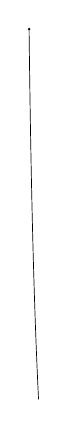
\begin{tikzpicture}[x=1mm,y=1mm,baseline=(current bounding box.north)]
\fill (0,0) circle[radius=.18mm];
\draw[line width=.25pt,line cap=round] (0,-.2) .. controls (.15,-13) and (.45,-32) .. (1.2,-47);
\end{tikzpicture}}
\[
\mathrm{Pt}_{\mathrm{ad}}(B_{\pi,\Gamma})
\longrightarrow
\mathrm{Pt}_{\mathrm{ad}}(B_{\pi'_i,\Gamma})\setminus\{P\}
\]
ou encore (passant à la limite) une bijection de $\Gamma$-ensembles
\[
\mathrm{Pt}_{\mathrm{ad}}(B_{\pi,\Gamma^{\natural}})
\simeq
\mathrm{Pt}_{\mathrm{ad}}(B_{\pi'_i,\Gamma^{\natural}})\setminus\{P\}
\]

Ceci signifie trois choses :

a) L'hom canonique $\Gamma\longrightarrow M_{a'}(\pi'_i)$,
composé de $\Gamma\longrightarrow N_a(\pi)$ et de
$N_a(\pi)\simeq M_{a'}(\pi'_i)$,
n'est pas \var{\inserted{$\pi'_i$-}}{\LMadded{$\pi'_i$-}}{insertion}{140-2-s418-I001}conjugué à un hom composé
$\Gamma\xrightarrow{\lambda}M_a(\pi)
\xrightarrow{\varphi_i}M_{a'}(\pi'_i)$,
où $\Gamma\xrightarrow{\lambda}M_a(\pi)$ est un relèvement admissible.

b) Si $\lambda,\mu:\Gamma\rightrightarrows M_a(\pi)$ sont deux
relèvements admissibles de $\Gamma\longrightarrow N_a(\pi)$
\var{\deleted{\LMsourceMark{M013619}{\unsure{que}}}}{\LMsourceMark{M013620}{\LMcancelledDoubts{\LMsourceMark{M013621}{\unsure{que}}}}}{deletion}{140-2-s418-D001} tels que
$\varphi_i\circ\lambda$ et $\varphi_i\circ\mu:
\Gamma\rightrightarrows M_a(\pi)$ soient
\var{\inserted{$\pi'_i$-}}{\LMadded{$\pi'_i$-}}{insertion}{140-2-s418-I002}conjugués, alors $\lambda$ et $\mu$ sont déjà
\var{\inserted{$\pi$-}}{\LMadded{$\pi$-}}{insertion}{140-2-s418-I003}conjugués.

c) Tout relèvement admissible de
$\Gamma\longrightarrow N_{a'}(\pi'_i)$ en
$\Gamma\longrightarrow M_{a'}(\pi'_i)$,
provient par composition d'un rel. admissible
$\Gamma\longrightarrow M_a(\pi)$.

\LMflushnotes\LMflushpages
\ifnum\LMform=1
\begin{LMapparatus}
\LMentry{140-2-s418-I001}{insertion}{\inserted{$\pi'_i$-}
}{\emph{\LMinsertedlabel}}{Ajout explicite de l'auteur : intégré à l'endroit indiqué par la transcription, sans modifier sa lecture.}{}
\LMentry{140-2-s418-D001}{suppression}{\deleted{\LMsourceMark{M013622}{\unsure{que}}}
}{\emph{\LMomittedlabel}}{Passage biffé dans le manuscrit : la suppression suit l'état final de l'auteur; les doutes de lecture restent signalés.}{}
\LMentry{140-2-s418-I002}{insertion}{\inserted{$\pi'_i$-}
}{\emph{\LMinsertedlabel}}{Ajout explicite de l'auteur : intégré à l'endroit indiqué par la transcription, sans modifier sa lecture.}{}
\LMentry{140-2-s418-I003}{insertion}{\inserted{$\pi$-}
}{\emph{\LMinsertedlabel}}{Ajout explicite de l'auteur : intégré à l'endroit indiqué par la transcription, sans modifier sa lecture.}{}
\end{LMapparatus}
\fi
\ifnum\LMform=2
\par\smallskip\begingroup\footnotesize\Needspace{4\baselineskip}\csname @beginparpenalty\endcsname=10000\relax\noindent\textcolor{gray}{\rule{.2\linewidth}{.35pt}}\par\nobreak
\noindent\textit{\LMdoubtheading.}\par\nobreak
\LMcarryover{140-2-s418-D001}{\LMsourceMark{M013623}{\unsure{que}}
}
\par\endgroup\smallskip
\fi

\LMsourceMark{M013624}{\scanpage{419}}
\LMsourceMark{M013625}{\mspage{212}}

Grâce à ceci, l'équivalence de catégories entre systèmes
$(\pi,a,i,\Gamma,\LMsourceMark{M013626}{\unsure{\theta}}:\Gamma\mathop{\longrightarrow}\limits_{\LMsourceMark{M013627}{\unsure{\mathrm{adm}}}}\LMsourceMark{M013628}{\unsure{N_a}})$,
et les systèmes $(\pi',a',\Gamma,\theta':\Gamma\longrightarrow\LMsourceMark{M013629}{\unsure{N_{a'}}},P)$,
où $P\in\mathrm{Pt}(B_{\pi',\Gamma^{\natural}})^\Gamma$,
se précise de façon parfaite au niveau des points: les
Points $\Gamma$-rationnels de $B_{\pi\LMsourceMark{M013630}{\unsure{,\Gamma^{\natural}|\var{\deleted{,\Gamma^{\natural}}}{\LMsourceMark{M013631}{\LMuncertaindeletion{140-2-s419-D001}}}{deletion}{140-2-s419-D001}}}}$
s'identifient à \LMsourceMark{M013632}{\unsure{l'un|l'ens}}
\var{\deleted{des pts $\Gamma$-\LMsourceMark{M013633}{\unsure{rationnels}}}}{\LMsourceMark{M013634}{\LMcancelledDoubts{\LMsourceMark{M013635}{\unsure{rationnels}}}}}{deletion}{140-2-s419-D002} des pts $\Gamma$-rationnels
de $B_{\pi'}$, distincts de $P$.

Ceci nous permet alors (ce qui n'était pas faisable dans le contexte
discret!) d'étendre l'équivalence de catégories en une équivalence

\[
\begin{gathered}(30)\\[3pt]
\begin{array}{c@{\,}c@{\,}c}
\parbox[t]{0.44\linewidth}{%
cat. des systèmes $(\pi,\LMsourceMark{M013636}{\unsure{a|\alpha}},I',\allowbreak\Gamma,\allowbreak\theta:\Gamma\longrightarrow N_a)$
d'un $\pi$ arithmétisé \var{\inserted{(par \LMsourceMark{M013637}{\unsure{$\alpha$|$a$}})}}{\LMadded{(par \LMsourceMark{M013638}{\unsure{$\alpha$|$a$}})}}{insertion}{140-2-s419-I001} de type $(g,\nu)$,
de $I'\subset I(\pi)$, d'une action
\uline{admissible} ext. de $\Gamma$ sur $\pi$
telle que $\Gamma$ \var{\deleted{\LMsourceMark{M013639}{\unsure{op.}}}}{\LMsourceMark{M013640}{\LMcancelledDoubts{\LMsourceMark{M013641}{\unsure{op.}}}}}{deletion}{140-2-s419-D003} \uline{fixe chaque point} de $I'$
}
& \LMsourceMark{M013642}{\unsure{\cong|\simeq}} &
\parbox[t]{0.44\linewidth}{%
cat des syst.
$(\pi',\LMsourceMark{M013643}{\unsure{a'|\alpha'}},I',\allowbreak\LMsourceMark{M013644}{\unsure{\Gamma^{*}|\Gamma}},\allowbreak\theta':\Gamma\longrightarrow N_{a'})$
d'un $\pi'$ arithmétisé (par \LMsourceMark{M013645}{\unsure{$a'$|$\alpha'$}}) de type
$(g,\nu')$ $[\nu'=\nu-\mathrm{card}(I')]$
avec op. \var{\inserted{ext.}}{\LMadded{ext.}}{insertion}{140-2-s419-I002} admissible de $\Gamma$ dessus, et
une partie $I'\subset\mathrm{Pt}_{ad}(B_{\pi',\LMsourceMark{M013646}{\unsure{\Gamma}}}\LMsourceMark{M013647}{\unsure{)}}$
(donc $I'\subset\mathrm{Pt}_{ad}(B_{\pi',\Gamma})^\Gamma$)
i.e. $I'$ formé de pts \LMsourceMark{M013648}{\unsure{inv.|fixes}} par $\Gamma$, i.e. ``$\Gamma$-rationnels''
}
\end{array}
\end{gathered}\]

\LMsourceMark{M013649}{\margin{avec $2g+(\underbrace{\nu-\mathrm{card}\,I'}_{\nu'})\geq3$}}

On a donc un foncteur quasi-inverse:
forage de trous en $I'$ !

\LMflushnotes\LMflushpages
\ifnum\LMform=1
\begin{LMapparatus}
\LMentry{140-2-s419-D001}{suppression}{\(\LMsourceMark{M013650}{\LMdoubtcopy{\deleted{,\Gamma^{\natural}}}}\)
}{\emph{\LMomittedlabel}}{Passage biffé dans le manuscrit : la suppression suit l'état final de l'auteur; les doutes de lecture restent signalés.}{}
\LMentry{140-2-s419-D002}{suppression}{\deleted{des pts $\Gamma$-\LMsourceMark{M013651}{\unsure{rationnels}}}
}{\emph{\LMomittedlabel}}{Passage biffé dans le manuscrit : la suppression suit l'état final de l'auteur; les doutes de lecture restent signalés.}{}
\LMentry{140-2-s419-I001}{insertion}{\inserted{(par \LMsourceMark{M013652}{\unsure{$\alpha$|$a$}})}
}{\emph{\LMinsertedlabel}}{Ajout explicite de l'auteur : intégré à l'endroit indiqué par la transcription, sans modifier sa lecture.}{}
\LMentry{140-2-s419-D003}{suppression}{\deleted{\LMsourceMark{M013653}{\unsure{op.}}}
}{\emph{\LMomittedlabel}}{Passage biffé dans le manuscrit : la suppression suit l'état final de l'auteur; les doutes de lecture restent signalés.}{}
\LMentry{140-2-s419-I002}{insertion}{\inserted{ext.}
}{\emph{\LMinsertedlabel}}{Ajout explicite de l'auteur : intégré à l'endroit indiqué par la transcription, sans modifier sa lecture.}{}
\end{LMapparatus}
\fi
\ifnum\LMform=2
\par\smallskip\begingroup\footnotesize\Needspace{4\baselineskip}\csname @beginparpenalty\endcsname=10000\relax\noindent\textcolor{gray}{\rule{.2\linewidth}{.35pt}}\par\nobreak
\noindent\textit{\LMdoubtheading.}\par\nobreak
\LMcarryover{140-2-s419-D001}{\(\LMsourceMark{M013654}{\LMdoubtcopy{,\Gamma^{\natural}}}\)
}
\LMcarryover{140-2-s419-D002}{\LMsourceMark{M013655}{\unsure{rationnels}}
}
\LMcarryover{140-2-s419-D003}{\LMsourceMark{M013656}{\unsure{op.}}
}
\par\endgroup\smallskip
\fi

\LMsourceMark{M013657}{\scanpage{420}}

Il est à noter que dans cette approche, on a dû se borner au cas
\var{\deleted{\LMsourceMark{M013658}{\unsure{des|de}}}}{\LMsourceMark{M013659}{\LMcancelledDoubts{\LMsourceMark{M013660}{\unsure{des|de}}}}}{deletion}{140-2-s420-D001} \var{\inserted{d'un ens de}}{\LMadded{d'un ens de}}{insertion}{140-2-s420-I001} pts \var{\deleted{\LMsourceMark{M013661}{\illegible{1}}}}{\LMsourceMark{M013662}{\LMcancelledDoubts{\LMsourceMark{M013663}{\illegible{1}}}}}{deletion}{140-2-s420-D002}
$I'\subset I(\pi)$ non seulement stable par $\Gamma$, mais
\var{\deleted{\LMsourceMark{M013664}{\unsure{formé}}}}{\LMsourceMark{M013665}{\LMcancelledDoubts{\LMsourceMark{M013666}{\unsure{formé}}}}}{deletion}{140-2-s420-D003} $\subset I^\Gamma$
\var{\deleted{fixes par $\Gamma$}}{}{deletion}{140-2-s420-D004} ou encore à une partie
$I'\subset\mathrm{Pt}(B_{\pi',\Gamma^{\natural}})$
non seulement stable par $\Gamma$, mais
\LMsourceMark{M013667}{\unsure{$\overline{\mathrm m}$|$=$}}\,$\subset\mathrm{Pt}(B_{\pi',\Gamma^{\natural}})^\Gamma$.
Pour montrer que sans cette restriction, le foncteur naturel
\var{\deleted{\LMsourceMark{M013668}{\unsure{est}}}}{\LMsourceMark{M013669}{\LMcancelledDoubts{\LMsourceMark{M013670}{\unsure{est}}}}}{deletion}{140-2-s420-D005} correspondant est néanmoins
une équivalence, on est ramené à ceci

\textcircled{6} Soit $(\pi,a,I'\subset I(\pi))$ avec $(\pi,a)$
groupe à lacets \var{\inserted{cat.}}{\LMadded{cat.}}{insertion}{140-2-s420-I002} \LMsourceMark{M013671}{\unsure{profini|profi.}} arithmétisé de type
$g,\nu$, d'où $(\pi',a')$ --- soit $\Gamma$, avec $\Gamma'$
sous-groupe ouvert opérant sur $(\pi,a)$ de façon admissible
$(\Gamma\longrightarrow N_a(\pi))$,
et laissant stable $I'$, donc il opère de façon admissible sur
$(\pi',a')$,
Supposons donné un \uline{relèvement} de cette action de $\Gamma'$
en une action admissible de $\Gamma$ sur $N_{a'}$, qui invarie
\[
\begin{array}{rcl}
I'&\subset&\mathrm{Pt}(B_{\pi',\Gamma^{\natural}}).\\
&&\rotatebox{90}{$\LMsourceMark{M013672}{\unsure{\simeq}}$}\\
&&\mathrm{Pt}(B_{\pi',\Gamma^{\prime\natural}})
\end{array}
\]

\diagram{\begin{tikzcd}[ampersand replacement=\&,column sep=3.6em,row sep=3em]
{\var{\deleted{\LMsourceMark{M013673}{\unsure{M_a}}}}{\LMsourceMark{M013674}{\LMcancelledDoubts{\(\LMsourceMark{M013675}{\unsure{M_a}}\)}}}{deletion}{140-2-s420-D006}\;(N_a)_{I'}} \arrow[d] \&
\Gamma' \arrow[l] \arrow[d,hook,line width=.9pt] \arrow[dl,bend right=7,line width=.65pt] \\
N_{a'} \& \Gamma \arrow[l] \arrow[ul,dashed]
\end{tikzcd}}

Alors il existe une action admissible unique de $\LMsourceMark{M013676}{\unsure{\Gamma|\Gamma'}}$
sur $(\pi,a)$, qui prolonge celle de $\Gamma'$ et qui donne naissance
à celle \var{\inserted{donnée}}{\LMadded{donnée}}{insertion}{140-2-s420-I003} sur $\pi'$.

\LMflushnotes\LMflushpages
\ifnum\LMform=1
\begin{LMapparatus}
\LMentry{140-2-s420-D001}{suppression}{\deleted{\LMsourceMark{M013677}{\unsure{des|de}}}
}{\emph{\LMomittedlabel}}{Passage biffé dans le manuscrit : la suppression suit l'état final de l'auteur; les doutes de lecture restent signalés.}{}
\LMentry{140-2-s420-I001}{insertion}{\inserted{d'un ens de}
}{\emph{\LMinsertedlabel}}{Ajout explicite de l'auteur : intégré à l'endroit indiqué par la transcription, sans modifier sa lecture.}{}
\LMentry{140-2-s420-D002}{suppression}{\deleted{\LMsourceMark{M013678}{\illegible{1}}}
}{\emph{\LMomittedlabel}}{Passage biffé dans le manuscrit : la suppression suit l'état final de l'auteur; les doutes de lecture restent signalés.}{}
\LMentry{140-2-s420-D003}{suppression}{\deleted{\LMsourceMark{M013679}{\unsure{formé}}}
}{\emph{\LMomittedlabel}}{Passage biffé dans le manuscrit : la suppression suit l'état final de l'auteur; les doutes de lecture restent signalés.}{}
\LMentry{140-2-s420-D004}{suppression}{\deleted{fixes par $\Gamma$}
}{\emph{\LMomittedlabel}}{Passage biffé dans le manuscrit : la suppression suit l'état final de l'auteur; les doutes de lecture restent signalés.}{}
\LMentry{140-2-s420-D005}{suppression}{\deleted{\LMsourceMark{M013680}{\unsure{est}}}
}{\emph{\LMomittedlabel}}{Passage biffé dans le manuscrit : la suppression suit l'état final de l'auteur; les doutes de lecture restent signalés.}{}
\LMentry{140-2-s420-I002}{insertion}{\inserted{cat.}
}{\emph{\LMinsertedlabel}}{Ajout explicite de l'auteur : intégré à l'endroit indiqué par la transcription, sans modifier sa lecture.}{}
\LMentry{140-2-s420-D006}{suppression}{\(\deleted{\LMsourceMark{M013681}{\unsure{M_a}}}\)
}{\emph{\LMomittedlabel}}{Passage biffé dans le manuscrit : la suppression suit l'état final de l'auteur; les doutes de lecture restent signalés.}{}
\LMentry{140-2-s420-I003}{insertion}{\inserted{donnée}
}{\emph{\LMinsertedlabel}}{Ajout explicite de l'auteur : intégré à l'endroit indiqué par la transcription, sans modifier sa lecture.}{}
\end{LMapparatus}
\fi
\ifnum\LMform=2
\par\smallskip\begingroup\footnotesize\Needspace{4\baselineskip}\csname @beginparpenalty\endcsname=10000\relax\noindent\textcolor{gray}{\rule{.2\linewidth}{.35pt}}\par\nobreak
\noindent\textit{\LMdoubtheading.}\par\nobreak
\LMcarryover{140-2-s420-D001}{\LMsourceMark{M013682}{\unsure{des|de}}
}
\LMcarryover{140-2-s420-D002}{\LMsourceMark{M013683}{\illegible{1}}
}
\LMcarryover{140-2-s420-D003}{\LMsourceMark{M013684}{\unsure{formé}}
}
\LMcarryover{140-2-s420-D005}{\LMsourceMark{M013685}{\unsure{est}}
}
\LMcarryover{140-2-s420-D006}{\(\LMsourceMark{M013686}{\unsure{M_a}}\)
}
\par\endgroup\smallskip
\fi

% END PACKAGE LM_P042
% BEGIN PACKAGE LM_P043
\ifnum\LMform<2\Needspace{11\baselineskip}\subsection*{Scans 421--430}\fi
\LMsourceMark{M013687}{\scanpage{421}}
\LMsourceMark{M013688}{\mspage{213}}
% Main text, approximate manuscript lines 1--4.
\var{\deleted{Soit}}{}{deletion}{140-2-s421-D001} L'unicité est-elle de \LMsourceMark{M013689}{\unsure{ttes|toutes}} façons claire ?
\var{\deleted{\LMsourceMark{M013690}{\unsure{Choisissant un}}}}{\LMsourceMark{M013691}{\LMcancelledDoubts{\LMsourceMark{M013692}{\unsure{Choisissant un}}}}}{deletion}{140-2-s421-D002} Considérons l'ext. \var{\inserted{$\mathcal{E}$}}{\LMadded{$\mathcal{E}$}}{insertion}{140-2-s421-I001} de
$\Gamma$ par $L=\mathrm{Ker}((N_a)_{I'}\to\LMsourceMark{M013693}{\unsure{N_a|N_0}})$,
\LMsourceMark{M013694}{\unsure{image}} inverse de l'ext. $(N_a)_{I'}$
(de $\LMsourceMark{M013695}{\unsure{N_{a'}|N_{0'}}}$ par $L$) via $\Gamma\to\LMsourceMark{M013696}{\unsure{N_{a'}|N_{0'}}}$, on
% Main text, approximate manuscript lines 5--8.
a un scindage \var{\inserted{partiel}}{\LMadded{partiel}}{insertion}{140-2-s421-I002} de cette extension \LMsourceMark{M013697}{\unsure{au}} dessus
du sous-groupe $\Gamma'$ de $\Gamma$, et l'assertion est
que ce scindage se \uline{\LMsourceMark{M013698}{\unsure{prolonge}}}, \uline{de façon} \uline{unique}, à $\Gamma$.
OPS $\Gamma'$ invariant dans $\Gamma$, et on
% Main text, approximate manuscript lines 9--13.
identifie $\Gamma'$ à un ss-groupe de $\mathcal{E}$. \LMsourceMark{M013699}{\unsure{Toutes}}
\var{\deleted{\LMsourceMark{M013700}{\unsure{sections}}}}{\LMsourceMark{M013701}{\LMcancelledDoubts{\LMsourceMark{M013702}{\unsure{sections}}}}}{deletion}{140-2-s421-D003} les sections de $\mathcal{E}$ sur $\Gamma$ \LMsourceMark{M013703}{\unsure{s'identifient}}
à des sous-groupes \var{\inserted{\LMsourceMark{M013704}{\unsure{sections}}}}{\LMadded{\LMsourceMark{M013705}{\unsure{sections}}}}{insertion}{140-2-s421-I003} $\widetilde{\Gamma}$ de $\mathcal{E}$.
Pour un tel $\widetilde{\Gamma}$, on a bien sûr
$\widetilde{\Gamma}\subset\mathrm{Norm}_{\mathcal{E}}(\Gamma')$
d'ailleurs \var{\deleted{\LMsourceMark{M013706}{\unsure{si on}} \LMsourceMark{M013707}{\illegible{2}}}}{\LMsourceMark{M013708}{\LMcancelledDoubts{\LMsourceMark{M013709}{\unsure{si on}}\quad \LMsourceMark{M013710}{\illegible{2}}}}}{deletion}{140-2-s421-D004} \var{\inserted{on a évidemment}}{\LMadded{on a évidemment}}{insertion}{140-2-s421-I004}
% Main text, approximate manuscript line 14.
\[
\mathrm{Norm}_{\mathcal{E}}(\Gamma')\cap L=L^{\Gamma'} \tag{31}
\]
% Main text, approximate manuscript lines 15--21.
et je présume qu'on doit avoir
$L^{\Gamma'}=1$ (qui généralise la condition
\textcircled{3} plus haut\ldots) Or \uline{cette condition}
\uline{implique l'unicité} -- savoir
$\widetilde{\Gamma}=\mathrm{Norm}_{\mathcal{E}}(\Gamma')$ --
et l'existence \uline{signifie} que
$\mathrm{Norm}_{\mathcal{E}}(\Gamma')\to\Gamma$
est épi (donc iso\ldots).

% Main text, approximate manuscript lines 22--23.
Mais il faudra essayer de préciser,
dans certains contextes (au moins celui des

\LMflushnotes\LMflushpages
\ifnum\LMform=1
\begin{LMapparatus}
\LMentry{140-2-s421-D001}{suppression}{\deleted{Soit}
}{\emph{\LMomittedlabel}}{Passage biffé dans le manuscrit : la suppression suit l'état final de l'auteur; les doutes de lecture restent signalés.}{}
\LMentry{140-2-s421-D002}{suppression}{\deleted{\LMsourceMark{M013711}{\unsure{Choisissant un}}}
}{\emph{\LMomittedlabel}}{Passage biffé dans le manuscrit : la suppression suit l'état final de l'auteur; les doutes de lecture restent signalés.}{}
\LMentry{140-2-s421-I001}{insertion}{\inserted{$\mathcal{E}$}
}{\emph{\LMinsertedlabel}}{Ajout explicite de l'auteur : intégré à l'endroit indiqué par la transcription, sans modifier sa lecture.}{}
\LMentry{140-2-s421-I002}{insertion}{\inserted{partiel}
}{\emph{\LMinsertedlabel}}{Ajout explicite de l'auteur : intégré à l'endroit indiqué par la transcription, sans modifier sa lecture.}{}
\LMentry{140-2-s421-D003}{suppression}{\deleted{\LMsourceMark{M013712}{\unsure{sections}}}
}{\emph{\LMomittedlabel}}{Passage biffé dans le manuscrit : la suppression suit l'état final de l'auteur; les doutes de lecture restent signalés.}{}
\LMentry{140-2-s421-I003}{insertion}{\inserted{\LMsourceMark{M013713}{\unsure{sections}}}
}{\emph{\LMinsertedlabel}}{Ajout explicite de l'auteur : intégré à l'endroit indiqué par la transcription, sans modifier sa lecture.}{}
\LMentry{140-2-s421-D004}{suppression}{\deleted{\LMsourceMark{M013714}{\unsure{si on}} \LMsourceMark{M013715}{\illegible{2}}}
}{\emph{\LMomittedlabel}}{Passage biffé dans le manuscrit : la suppression suit l'état final de l'auteur; les doutes de lecture restent signalés.}{}
\LMentry{140-2-s421-I004}{insertion}{\inserted{on a évidemment}
}{\emph{\LMinsertedlabel}}{Ajout explicite de l'auteur : intégré à l'endroit indiqué par la transcription, sans modifier sa lecture.}{}
\end{LMapparatus}
\fi
\ifnum\LMform=2
\par\smallskip\begingroup\footnotesize\Needspace{4\baselineskip}\csname @beginparpenalty\endcsname=10000\relax\noindent\textcolor{gray}{\rule{.2\linewidth}{.35pt}}\par\nobreak
\noindent\textit{\LMdoubtheading.}\par\nobreak
\LMcarryover{140-2-s421-D002}{\LMsourceMark{M013716}{\unsure{Choisissant un}}
}
\LMcarryover{140-2-s421-D003}{\LMsourceMark{M013717}{\unsure{sections}}
}
\LMcarryover{140-2-s421-D004}{\LMsourceMark{M013718}{\unsure{si on}}\quad \LMsourceMark{M013719}{\illegible{2}}
}
\par\endgroup\smallskip
\fi

\LMsourceMark{M013720}{\scanpage{422}}
% Main text, approximate manuscript lines 1--4; continuation of scan 421.
actions arithmétiquement fidèles, i.e. $\Gamma\to\boldsymbol{\Gamma}_a$
injectif -- qui \LMsourceMark{M013721}{\unsure{correspond}} \LMsourceMark{M013722}{\unsure{normalement|vraisblmt}}
au cas de courbes alg. \LMsourceMark{M013723}{\unsure{définies}} sur des
ext. algébriques de $\mathbb{Q}$ -- la notion
% Main text, approximate manuscript lines 5--9.
d'action ``admissible''. Pour ceci, on
doit revenir sur la relation entre
courbes (potentielles) et revêtements finis,
ce qui donne aussi une façon de
faire varier $g$.

% Main text, approximate manuscript lines 10--17.
Mais j'ai envie d'abord de reprendre
\LMsourceMark{M013724}{\unsure{sous|sur}} un autre aspect \var{\inserted{(peut-être plus général)}}{\LMadded{(peut-être plus général)}}{insertion}{140-2-s422-I001} le formalisme
précédent, qui \LMsourceMark{M013725}{\unsure{peut}} peut-être aussi \LMsourceMark{M013726}{\unsure{s'}}appliquer au cas des groupes \uline{discrets}
à lacets (je pense au formalisme
des $\LMsourceMark{M013727}{\unsure{U^!|\mathcal{U}^!}}$, lié aux actions extérieures de
groupes finis sur de tels \LMsourceMark{M013728}{\unsure{gr.-p.}} à lacets).

% Main text, approximate manuscript lines 18--20.
Soit $\mathcal{X}$ un ensemble \var{\inserted{$\ne\varnothing$}}{\LMadded{$\ne\varnothing$}}{insertion}{140-2-s422-I002}
(\var{\inserted{\LMsourceMark{M013729}{\unsure{moralement}}, un}}{\LMadded{\LMsourceMark{M013730}{\unsure{moralement}}, un}}{insertion}{140-2-s422-I003} ensemble des
``pts'' d'une \var{\deleted{surface}}{}{deletion}{140-2-s422-D001} courbe algébrique,
ou d'une surface topologique\ldots), \var{\deleted{et $\Gamma$}}{}{deletion}{140-2-s422-D002}

\LMflushnotes\LMflushpages
\ifnum\LMform=1
\begin{LMapparatus}
\LMentry{140-2-s422-I001}{insertion}{\inserted{(peut-être plus général)}
}{\emph{\LMinsertedlabel}}{Ajout explicite de l'auteur : intégré à l'endroit indiqué par la transcription, sans modifier sa lecture.}{}
\LMentry{140-2-s422-I002}{insertion}{\inserted{$\ne\varnothing$}
}{\emph{\LMinsertedlabel}}{Ajout explicite de l'auteur : intégré à l'endroit indiqué par la transcription, sans modifier sa lecture.}{}
\LMentry{140-2-s422-I003}{insertion}{\inserted{\LMsourceMark{M013731}{\unsure{moralement}}, un}
}{\emph{\LMinsertedlabel}}{Ajout explicite de l'auteur : intégré à l'endroit indiqué par la transcription, sans modifier sa lecture.}{}
\LMentry{140-2-s422-D001}{suppression}{\deleted{surface}
}{\emph{\LMomittedlabel}}{Passage biffé dans le manuscrit : la suppression suit l'état final de l'auteur; les doutes de lecture restent signalés.}{}
\LMentry{140-2-s422-D002}{suppression}{\deleted{et $\Gamma$}
}{\emph{\LMomittedlabel}}{Passage biffé dans le manuscrit : la suppression suit l'état final de l'auteur; les doutes de lecture restent signalés.}{}
\end{LMapparatus}
\fi

\LMsourceMark{M013732}{\scanpage{423}}
\LMsourceMark{M013733}{\mspage{214}}
% Main text, approximate manuscript lines 1--7.
\var{\deleted{un groupe opérant sur $\mathcal{X}$.}}{}{deletion}{140-2-s423-D001} On suppose
donné, pour tte partie finie $I$ de $\mathcal{X}$,
de complémentaire $U_I=\mathcal{X}\setminus I$, un
\LMsourceMark{M013734}{\unsure{groupoïde}} $\Pi_{U_I}$, ayant $U_I$ comme ens
d'\LMsourceMark{M013735}{\unsure{objets}}. De plus, pour $J\supset I$ i.e.
$U_J\subset U_I$, on suppose donné un hom
de groupoïdes
% Main text, approximate manuscript line 8.
\[
\Pi_{U_J}\to\Pi_{U_I}
\]
% Main text, approximate manuscript lines 9--14.
qui sur les objets soit l'inclusion $U_J\LMsourceMark{M013736}{\unsure{\subset|\hookrightarrow}}\LMsourceMark{M013737}{\unsure{U_J|U_I}}$.
On suppose transitivité (stricte) i.e. \var{\deleted{\LMsourceMark{M013738}{\unsure{qui}}}}{\LMsourceMark{M013739}{\LMcancelledDoubts{\LMsourceMark{M013740}{\unsure{qui}}}}}{deletion}{140-2-s423-D002}
un foncteur covariant \var{\inserted{de la cat.}}{\LMadded{de la cat.}}{insertion}{140-2-s423-I001} des parties $U$ de
$\mathcal{X}$ complémentaires de parties finies \var{\inserted{(avec les inclusions)}}{\LMadded{(avec les inclusions)}}{insertion}{140-2-s423-I002}, vers
\LMsourceMark{M013741}{\unsure{la}} cat. des groupoïdes, qui sur \LMsourceMark{M013742}{\unsure{l'ens.}}
d'objets coïncide avec le foncteur évident\ldots

% Left marginal note, running beside approximate lines 10--22.
\LMsourceMark{M013743}{\margin{Si $\mathcal{X}$ est fini et $I=\mathcal{X}$, on
\LMsourceMark{M013744}{\unsure{suppose}} \var{\inserted{\uuline{\LMsourceMark{M013745}{\unsure{quand même|cependant}}}}}{\LMadded{\uuline{\LMsourceMark{M013746}{\unsure{quand même|cependant}}}}}{insertion}{140-2-s423-I003}
$\Pi_{U_I}\;(=\Pi_{\varnothing})$ \LMsourceMark{M013747}{\unsure{n'est}}
pas le groupoïde vide, mais un groupoïde
\var{\deleted{quelconque}}{}{deletion}{140-2-s423-D003} (qui \LMsourceMark{M013748}{\unsure{s'envoie}} dans les précédents\ldots)
mais on ne pourra exiger
\LMsourceMark{M013749}{\unsure{la}} transitivité stricte.
Il \LMsourceMark{M013750}{\unsure{faudra|faudrait}} \var{\inserted{\LMsourceMark{M013751}{\unsure{peut-être}}}}{\LMadded{\LMsourceMark{M013752}{\unsure{peut-être}}}}{insertion}{140-2-s423-I004} \LMsourceMark{M013753}{\illegible{1}} \LMsourceMark{M013754}{\unsure{hyp.}} anabéliennes
sur $\Pi_{U_I}$ dans ce cas\ldots}}

% Main text, approximate manuscript lines 15--18.
On suppose de plus que pour tout \var{\deleted{$I\in\mathcal{P}_f(\mathcal{X})$}}{}{deletion}{140-2-s423-D004}
$i\in\mathcal{X}$, on se donne un \var{\deleted{\LMsourceMark{M013755}{\unsure{groupoïde}} \LMsourceMark{M013756}{\illegible{1}}}}{\LMsourceMark{M013757}{\LMcancelledDoubts{\LMsourceMark{M013758}{\unsure{groupoïde}}\quad \LMsourceMark{M013759}{\illegible{1}}}}}{deletion}{140-2-s423-D005}
$\Pi_i$ (ou $\Pi_{D_i^*}$),
et \var{\deleted{\LMsourceMark{M013760}{\unsure{pour tout}}}}{\LMsourceMark{M013761}{\LMcancelledDoubts{\LMsourceMark{M013762}{\unsure{pour tout}}}}}{deletion}{140-2-s423-D006} pour $i\in I\in\mathcal{P}_f(\mathcal{X})$,
un hom de groupoïdes
% Main text, approximate manuscript line 19.
\[
\Pi_{D_i^*}\to\Pi_{U_I}
\]
% Main text, approximate manuscript lines 20--23.
compatible avec les morphismes de transition
\var{\inserted{$\Pi_{U_I}\to\Pi_{U_J}$ $(I\supset J)$}}{\LMadded{$\Pi_{U_I}\to\Pi_{U_J}$ $(I\supset J)$}}{insertion}{140-2-s423-I005}.
On suppose que pour $I$ fixé, on trouve
sur $\Pi_{U_I}$ une structure de groupoïde
à lacets par
\[
\Pi_{D_I^*}=\coprod_{i\in I}\Pi_{D_i^*}\to\Pi_{U_I}.
\]

\LMflushnotes\LMflushpages
\ifnum\LMform=1
\begin{LMapparatus}
\LMentry{140-2-s423-D001}{suppression}{\deleted{un groupe opérant sur $\mathcal{X}$.}
}{\emph{\LMomittedlabel}}{Passage biffé dans le manuscrit : la suppression suit l'état final de l'auteur; les doutes de lecture restent signalés.}{}
\LMentry{140-2-s423-D002}{suppression}{\deleted{\LMsourceMark{M013763}{\unsure{qui}}}
}{\emph{\LMomittedlabel}}{Passage biffé dans le manuscrit : la suppression suit l'état final de l'auteur; les doutes de lecture restent signalés.}{}
\LMentry{140-2-s423-I001}{insertion}{\inserted{de la cat.}
}{\emph{\LMinsertedlabel}}{Ajout explicite de l'auteur : intégré à l'endroit indiqué par la transcription, sans modifier sa lecture.}{}
\LMentry{140-2-s423-I002}{insertion}{\inserted{(avec les inclusions)}
}{\emph{\LMinsertedlabel}}{Ajout explicite de l'auteur : intégré à l'endroit indiqué par la transcription, sans modifier sa lecture.}{}
\LMentry{140-2-s423-I003}{insertion}{\inserted{\uuline{\LMsourceMark{M013764}{\unsure{quand même|cependant}}}}
}{\emph{\LMinsertedlabel}}{Ajout explicite de l'auteur : intégré à l'endroit indiqué par la transcription, sans modifier sa lecture.}{}
\LMentry{140-2-s423-D003}{suppression}{\deleted{quelconque}
}{\emph{\LMomittedlabel}}{Passage biffé dans le manuscrit : la suppression suit l'état final de l'auteur; les doutes de lecture restent signalés.}{}
\LMentry{140-2-s423-I004}{insertion}{\inserted{\LMsourceMark{M013765}{\unsure{peut-être}}}
}{\emph{\LMinsertedlabel}}{Ajout explicite de l'auteur : intégré à l'endroit indiqué par la transcription, sans modifier sa lecture.}{}
\LMentry{140-2-s423-D004}{suppression}{\deleted{$I\in\mathcal{P}_f(\mathcal{X})$}
}{\emph{\LMomittedlabel}}{Passage biffé dans le manuscrit : la suppression suit l'état final de l'auteur; les doutes de lecture restent signalés.}{}
\LMentry{140-2-s423-D005}{suppression}{\deleted{\LMsourceMark{M013766}{\unsure{groupoïde}} \LMsourceMark{M013767}{\illegible{1}}}
}{\emph{\LMomittedlabel}}{Passage biffé dans le manuscrit : la suppression suit l'état final de l'auteur; les doutes de lecture restent signalés.}{}
\LMentry{140-2-s423-D006}{suppression}{\deleted{\LMsourceMark{M013768}{\unsure{pour tout}}}
}{\emph{\LMomittedlabel}}{Passage biffé dans le manuscrit : la suppression suit l'état final de l'auteur; les doutes de lecture restent signalés.}{}
\LMentry{140-2-s423-I005}{insertion}{\inserted{$\Pi_{U_I}\to\Pi_{U_J}$ $(I\supset J)$}
}{\emph{\LMinsertedlabel}}{Ajout explicite de l'auteur : intégré à l'endroit indiqué par la transcription, sans modifier sa lecture.}{}
\end{LMapparatus}
\fi
\ifnum\LMform=2
\par\smallskip\begingroup\footnotesize\Needspace{4\baselineskip}\csname @beginparpenalty\endcsname=10000\relax\noindent\textcolor{gray}{\rule{.2\linewidth}{.35pt}}\par\nobreak
\noindent\textit{\LMdoubtheading.}\par\nobreak
\LMcarryover{140-2-s423-D002}{\LMsourceMark{M013769}{\unsure{qui}}
}
\LMcarryover{140-2-s423-D005}{\LMsourceMark{M013770}{\unsure{groupoïde}}\quad \LMsourceMark{M013771}{\illegible{1}}
}
\LMcarryover{140-2-s423-D006}{\LMsourceMark{M013772}{\unsure{pour tout}}
}
\par\endgroup\smallskip
\fi

\LMsourceMark{M013773}{\scanpage{424}}
% Main-text lines 1--2; insertion above line 2.
sans d'ailleurs exclure le cas où $I=\varnothing$, et où \var{\inserted{($\Pi_{\mathcal{X}}$ \LMsourceMark{M013774}{\unsure{étant}} connexe, disons)}}{\LMadded{($\Pi_{\mathcal{X}}$ \LMsourceMark{M013775}{\unsure{étant}} connexe, disons)}}{insertion}{140-2-s424-I001} \LMsourceMark{M013776}{\unsure{son|le}} genre \uline{est $0$} --- \var{\deleted{\LMsourceMark{M013777}{\unsure{donc}}}}{\LMsourceMark{M013778}{\LMcancelledDoubts{\LMsourceMark{M013779}{\unsure{donc}}}}}{deletion}{140-2-s424-D001}
\LMsourceMark{M013780}{\margin{\LMsourceMark{M013781}{\unsure{On suppose}} \LMsourceMark{M013782}{\illegible{4}} \LMsourceMark{M013783}{\unsure{que}} \LMsourceMark{M013784}{\illegible{1}} $\mathcal{X}$ \LMsourceMark{M013785}{\illegible{3}} \var{\deleted{\LMsourceMark{M013786}{\unsure{pour}} $\mathcal{X}$ \LMsourceMark{M013787}{\illegible{2}}}}{\LMsourceMark{M013788}{\LMcancelledDoubts{\LMsourceMark{M013789}{\unsure{pour}}\quad \LMsourceMark{M013790}{\illegible{2}}}}}{deletion}{140-2-s424-D002} \var{\deleted{\LMsourceMark{M013791}{\unsure{deux pts}}}}{\LMsourceMark{M013792}{\LMcancelledDoubts{\LMsourceMark{M013793}{\unsure{deux pts}}}}}{deletion}{140-2-s424-D003}}}

% Main-text lines 3--8.
On suppose de plus que si $J\supset I$ i.e. $U_J\subset U_I$, \var{\inserted{et pour $i\in J\setminus I$,}}{\LMadded{et pour $i\in J\setminus I$,}}{insertion}{140-2-s424-I002} l'hom. composé
\[
\Pi_{D_i^*}\longrightarrow\Pi_{U_J}\longrightarrow\Pi_{U_I}
\]
soit ``constant'', de telle façon que $\Pi_{U_I}$ se \LMsourceMark{M013794}{\unsure{déduise}} de $\Pi_{U_J}$ par ``bouchage des trous'' en $J\setminus I$.

% Main-text lines 9--21; the middle of the example is heavily revised.
Jusqu'à présent, \LMsourceMark{M013795}{\unsure{tt|tout}} ceci pouvait se visualiser p.ex. en partant d'une surface top. orientable \var{\deleted{de la forme \LMsourceMark{M013796}{\unsure{$X\setminus S$}}; \LMsourceMark{M013797}{\illegible{4}} du type}}{\LMsourceMark{M013798}{\LMcancelledDoubts{\LMsourceMark{M013799}{\unsure{$X\setminus S$}}\quad \LMsourceMark{M013800}{\illegible{4}}}}}{deletion}{140-2-s424-D004} $X$, et d'une partie \var{\inserted{\LMsourceMark{M013801}{\illegible{1}}}}{\LMadded{\LMsourceMark{M013802}{\illegible{1}}}}{insertion}{140-2-s424-I003} $\mathcal{X}$ de $X$ \var{\deleted{\LMsourceMark{M013803}{\illegible{1}}}}{\LMsourceMark{M013804}{\LMcancelledDoubts{\LMsourceMark{M013805}{\illegible{1}}}}}{deletion}{140-2-s424-D005}\var{\inserted{\LMsourceMark{M013806}{\unsure{rencontrant}}}}{\LMadded{\LMsourceMark{M013807}{\unsure{rencontrant}}}}{insertion}{140-2-s424-I004} \var{\deleted{\LMsourceMark{M013808}{\unsure{tte compos. connexe}}}}{\LMsourceMark{M013809}{\LMcancelledDoubts{\LMsourceMark{M013810}{\unsure{tte compos. connexe}}}}}{deletion}{140-2-s424-D006}\var{\inserted{\LMsourceMark{M013811}{\unsure{tte}} comp. connexe}}{\LMadded{\LMsourceMark{M013812}{\unsure{tte}} comp. connexe}}{insertion}{140-2-s424-I005}; en prenant pour $\Pi_I$ la restriction à $\mathcal{X}\setminus I$ du groupoïde fondamental de $X\setminus I$ (si $I\ne\mathcal{X}$; si $\mathcal{X}=I$, ce qui exige $\mathcal{X}$ fini, on prendra le groupoïde fondamental de $X\setminus I=X\setminus\{\mathcal{X}\}$; qu'on aura du mal à envoyer dans les autres avec transitivité \uline{stricte}, qu'à cela ne tienne !

% Main-text lines 22--23; sentence continues on the next scan.
Mais, on est surtout intéressé au cas $\mathcal{X}$ infini. Où on \LMsourceMark{M013813}{\unsure{prend}} $X$ courbe alg. sur

\LMflushnotes\LMflushpages
\ifnum\LMform=1
\begin{LMapparatus}
\LMentry{140-2-s424-I001}{insertion}{\inserted{($\Pi_{\mathcal{X}}$ \LMsourceMark{M013814}{\unsure{étant}} connexe, disons)}
}{\emph{\LMinsertedlabel}}{Ajout explicite de l'auteur : intégré à l'endroit indiqué par la transcription, sans modifier sa lecture.}{}
\LMentry{140-2-s424-D001}{suppression}{\deleted{\LMsourceMark{M013815}{\unsure{donc}}}
}{\emph{\LMomittedlabel}}{Passage biffé dans le manuscrit : la suppression suit l'état final de l'auteur; les doutes de lecture restent signalés.}{}
\LMentry{140-2-s424-D002}{suppression}{\deleted{\LMsourceMark{M013816}{\unsure{pour}} $\mathcal{X}$ \LMsourceMark{M013817}{\illegible{2}}}
}{\emph{\LMomittedlabel}}{Passage biffé dans le manuscrit : la suppression suit l'état final de l'auteur; les doutes de lecture restent signalés.}{}
\LMentry{140-2-s424-D003}{suppression}{\deleted{\LMsourceMark{M013818}{\unsure{deux pts}}}
}{\emph{\LMomittedlabel}}{Passage biffé dans le manuscrit : la suppression suit l'état final de l'auteur; les doutes de lecture restent signalés.}{}
\LMentry{140-2-s424-I002}{insertion}{\inserted{et pour $i\in J\setminus I$,}
}{\emph{\LMinsertedlabel}}{Ajout explicite de l'auteur : intégré à l'endroit indiqué par la transcription, sans modifier sa lecture.}{}
\LMentry{140-2-s424-D004}{suppression}{\deleted{de la forme \LMsourceMark{M013819}{\unsure{$X\setminus S$}}; \LMsourceMark{M013820}{\illegible{4}} du type}
}{\emph{\LMomittedlabel}}{Passage biffé dans le manuscrit : la suppression suit l'état final de l'auteur; les doutes de lecture restent signalés.}{}
\LMentry{140-2-s424-I003}{insertion}{\inserted{\LMsourceMark{M013821}{\illegible{1}}}
}{\emph{\LMinsertedlabel}}{Ajout explicite de l'auteur : intégré à l'endroit indiqué par la transcription, sans modifier sa lecture.}{}
\LMentry{140-2-s424-D005}{suppression}{\deleted{\LMsourceMark{M013822}{\illegible{1}}}
}{\emph{\LMomittedlabel}}{Passage biffé dans le manuscrit : la suppression suit l'état final de l'auteur; les doutes de lecture restent signalés.}{}
\LMentry{140-2-s424-I004}{insertion}{\inserted{\LMsourceMark{M013823}{\unsure{rencontrant}}}
}{\emph{\LMinsertedlabel}}{Ajout explicite de l'auteur : intégré à l'endroit indiqué par la transcription, sans modifier sa lecture.}{}
\LMentry{140-2-s424-D006}{suppression}{\deleted{\LMsourceMark{M013824}{\unsure{tte compos. connexe}}}
}{\emph{\LMomittedlabel}}{Passage biffé dans le manuscrit : la suppression suit l'état final de l'auteur; les doutes de lecture restent signalés.}{}
\LMentry{140-2-s424-I005}{insertion}{\inserted{\LMsourceMark{M013825}{\unsure{tte}} comp. connexe}
}{\emph{\LMinsertedlabel}}{Ajout explicite de l'auteur : intégré à l'endroit indiqué par la transcription, sans modifier sa lecture.}{}
\end{LMapparatus}
\fi
\ifnum\LMform=2
\par\smallskip\begingroup\footnotesize\Needspace{4\baselineskip}\csname @beginparpenalty\endcsname=10000\relax\noindent\textcolor{gray}{\rule{.2\linewidth}{.35pt}}\par\nobreak
\noindent\textit{\LMdoubtheading.}\par\nobreak
\LMcarryover{140-2-s424-D001}{\LMsourceMark{M013826}{\unsure{donc}}
}
\LMcarryover{140-2-s424-D002}{\LMsourceMark{M013827}{\unsure{pour}}\quad \LMsourceMark{M013828}{\illegible{2}}
}
\LMcarryover{140-2-s424-D003}{\LMsourceMark{M013829}{\unsure{deux pts}}
}
\LMcarryover{140-2-s424-D004}{\LMsourceMark{M013830}{\unsure{$X\setminus S$}}\quad \LMsourceMark{M013831}{\illegible{4}}
}
\LMcarryover{140-2-s424-D005}{\LMsourceMark{M013832}{\illegible{1}}
}
\LMcarryover{140-2-s424-D006}{\LMsourceMark{M013833}{\unsure{tte compos. connexe}}
}
\par\endgroup\smallskip
\fi

\LMsourceMark{M013834}{\scanpage{425}}
\LMsourceMark{M013835}{\mspage{215}}
% Main-text lines 1--3; continuation from scan 424.
corps alg. clos, $\mathcal{X}$ partie de $X$ rencontrant \LMsourceMark{M013836}{\unsure{tte}} comp. connexe, et on définit les $\Pi_{U_I}$ comme précédemment.

% Main-text lines 4--9, with an insertion between lines 6 and 7.
Soit maintenant $\Gamma$ un groupe qui opère sur la situation (\uline{strictement}, s'entend) donc sur \LMsourceMark{M013837}{\unsure{l'ens}} $\mathcal{X}$, \var{\deleted{et}}{}{deletion}{140-2-s425-D001} les groupoïdes \LMsourceMark{M013838}{\unsure{$\Pi_{U_I}$}}, \var{\inserted{les $\Pi_{D_i^*}$, (N.B. qu'il \LMsourceMark{M013839}{\unsure{permute}} entre eux),}}{\LMadded{les $\Pi_{D_i^*}$, (N.B. qu'il \LMsourceMark{M013840}{\unsure{permute}} entre eux),}}{insertion}{140-2-s425-I001} en commutant aux hom. \LMsourceMark{M013841}{\unsure{d|de}}
\[
\Pi_{U_I}\longrightarrow\Pi_{U_J}
\]
et les $\Pi_{D_i^*}\longrightarrow\Pi_{U_I}$.
\LMsourceMark{M013842}{\margin{\var{\deleted{(qu'il \LMsourceMark{M013843}{\unsure{permute}} \LMsourceMark{M013844}{\unsure{entre eux}})}}{\LMsourceMark{M013845}{\LMcancelledDoubts{\LMsourceMark{M013846}{\unsure{permute}}\quad \LMsourceMark{M013847}{\unsure{entre eux}}}}}{deletion}{140-2-s425-D002}}}

% Main-text lines 10--13; the wording after Nous is rewritten interlinearly.
(On aura des difficultés, si $\mathcal{X}$ est fini, pour $\Pi_{U_I}$ quand $I=\mathcal{X}$, pour la commutation \uline{stricte} \var{\deleted{\LMsourceMark{M013848}{\unsure{des}}}}{\LMsourceMark{M013849}{\LMcancelledDoubts{\LMsourceMark{M013850}{\unsure{des}}}}}{deletion}{140-2-s425-D003} \LMsourceMark{M013851}{\unsure{$\Pi_{U_{\mathcal{X}}}$}}$\longrightarrow\Pi_{U_J}$ \LMsourceMark{M013852}{\unsure{..}} mais passons...)
Nous \var{\deleted{faisons \LMsourceMark{M013853}{\unsure{l'hypothèse|les hypothèses}},}}{\LMsourceMark{M013854}{\LMcancelledDoubts{\LMsourceMark{M013855}{\unsure{l'hypothèse|les hypothèses}}}}}{deletion}{140-2-s425-D004} \var{\inserted{supposons définie une notion de ss-groupe \uline{admissible} de $\Gamma$, (ils sont en tous cas $\ne1$) telle que \deleted{\LMsourceMark{M013856}{\illegible{1}}} si $\Gamma'$ est admissible \LMsourceMark{M013857}{\unsure{alors}} tt ss-groupe $\Gamma''\supset\Gamma'$ aussi.}}{\LMadded{supposons définie une notion de ss-groupe \uline{admissible} de $\Gamma$, (ils sont en tous cas $\ne1$) telle que \var{\deleted{\LMsourceMark{M013858}{\illegible{1}}}}{\LMsourceMark{M013859}{\LMcancelledDoubts{\LMsourceMark{M013860}{\illegible{1}}}}}{deletion}{140-2-s425-D005} si $\Gamma'$ est admissible \LMsourceMark{M013861}{\unsure{alors}} tt ss-groupe $\Gamma''\supset\Gamma'$ aussi.}}{insertion}{140-2-s425-I002} \var{\deleted{\LMsourceMark{M013862}{\unsure{suivantes}}}}{\LMsourceMark{M013863}{\LMcancelledDoubts{\LMsourceMark{M013864}{\unsure{suivantes}}}}}{deletion}{140-2-s425-D006} \var{\inserted{On \deleted{\LMsourceMark{M013865}{\unsure{suppose}}}}}{\LMadded{On \var{\deleted{\LMsourceMark{M013866}{\unsure{suppose}}}}{\LMsourceMark{M013867}{\LMcancelledDoubts{\LMsourceMark{M013868}{\unsure{suppose}}}}}{deletion}{140-2-s425-D007}}}{insertion}{140-2-s425-I003}

% Canceled condition and canceled bracketed development in the lower half.
\var{\deleted{\textcircled{\(1^\circ\)} Pour $P\in\mathcal{X}$, son stabilisateur $\Gamma_P$ dans $\Gamma$ est \deleted{$\ne1$}\inserted{admissible} (donc $\ne1$)}}{}{deletion}{140-2-s425-D008}
\var{\inserted{\deleted{\LMsourceMark{M013869}{\unsure{$U_I$ stable pr $\Gamma_P$ i.e. $I$ stable}}}}}{\LMadded{\var{\deleted{\LMsourceMark{M013870}{\unsure{$U_I$ stable pr $\Gamma_P$ i.e. $I$ stable}}}}{\LMsourceMark{M013871}{\LMcancelledDoubts{\LMsourceMark{M013872}{\unsure{$U_I$ stable pr $\Gamma_P$ i.e. $I$ stable}}}}}{deletion}{140-2-s425-D010}}}{insertion}{140-2-s425-I005}

\var{\deleted{\LMsourceMark{M013873}{\unsure{\textcircled{\(2^\circ\)}}} \LMsourceMark{M013874}{\illegible{1}} (Notons que si $U_I\ni P$, alors $P$ est un objet de $\Pi_{U_I}$ avec op. de $\Gamma_P$ dessus, \deleted{\LMsourceMark{M013875}{\illegible{1}}}\inserted{On} \LMsourceMark{M013876}{\unsure{trouve}} ainsi une \deleted{application}\inserted{opération} de $\Gamma_P$ sur \LMsourceMark{M013877}{\unsure{$\pi_1(U_I,P)$|$\Pi_1(U_I,P)$}}, et on suppose}}{\LMsourceMark{M013878}{\LMcancelledDoubts{\LMsourceMark{M013879}{\unsure{\textcircled{\(2^\circ\)}}}\quad \LMsourceMark{M013880}{\illegible{1}}\quad \LMsourceMark{M013881}{\illegible{1}}\quad \LMsourceMark{M013882}{\unsure{trouve}}\quad \LMsourceMark{M013883}{\unsure{$\pi_1(U_I,P)$|$\Pi_1(U_I,P)$}}}}}{deletion}{140-2-s425-D011}

\var{\deleted{\textcircled{\(2^\circ\)} \LMsourceMark{M013884}{\unsure{$\pi_1(U_I,P)$|$\Pi_1(U_I,P)$}} \deleted{\LMsourceMark{M013885}{\unsure{appeler}}}\inserted{\LMsourceMark{M013886}{\unsure{dire qu'un}}} ss-groupe $\Gamma'$ de $\Gamma$ est \textcircled{\(1^\circ\)} Si $\Gamma'$ \uline{admissible} si \deleted{\LMsourceMark{M013887}{\illegible{1}}} $\mathcal{X}^{\Gamma'}$ \LMsourceMark{M013888}{\unsure{rencontre}} \LMsourceMark{M013889}{\unsure{tte}} composante connexe de $\mathcal{X}=U_{\varnothing}$ (ce qui}}{\LMsourceMark{M013890}{\LMcancelledDoubts{\LMsourceMark{M013891}{\unsure{$\pi_1(U_I,P)$|$\Pi_1(U_I,P)$}}\quad \LMsourceMark{M013892}{\unsure{appeler}}\quad \LMsourceMark{M013893}{\unsure{dire qu'un}}\quad \LMsourceMark{M013894}{\illegible{1}}\quad \LMsourceMark{M013895}{\unsure{rencontre}}\quad \LMsourceMark{M013896}{\unsure{tte}}}}}{deletion}{140-2-s425-D014}

\LMflushnotes\LMflushpages
\ifnum\LMform=1
\begin{LMapparatus}
\LMentry{140-2-s425-D001}{suppression}{\deleted{et}
}{\emph{\LMomittedlabel}}{Passage biffé dans le manuscrit : la suppression suit l'état final de l'auteur; les doutes de lecture restent signalés.}{}
\LMentry{140-2-s425-I001}{insertion}{\inserted{les $\Pi_{D_i^*}$, (N.B. qu'il \LMsourceMark{M013897}{\unsure{permute}} entre eux),}
}{\emph{\LMinsertedlabel}}{Ajout explicite de l'auteur : intégré à l'endroit indiqué par la transcription, sans modifier sa lecture.}{}
\LMentry{140-2-s425-D002}{suppression}{\deleted{(qu'il \LMsourceMark{M013898}{\unsure{permute}} \LMsourceMark{M013899}{\unsure{entre eux}})}
}{\emph{\LMomittedlabel}}{Passage biffé dans le manuscrit : la suppression suit l'état final de l'auteur; les doutes de lecture restent signalés.}{}
\LMentry{140-2-s425-D003}{suppression}{\deleted{\LMsourceMark{M013900}{\unsure{des}}}
}{\emph{\LMomittedlabel}}{Passage biffé dans le manuscrit : la suppression suit l'état final de l'auteur; les doutes de lecture restent signalés.}{}
\LMentry{140-2-s425-D004}{suppression}{\deleted{faisons \LMsourceMark{M013901}{\unsure{l'hypothèse|les hypothèses}},}
}{\emph{\LMomittedlabel}}{Passage biffé dans le manuscrit : la suppression suit l'état final de l'auteur; les doutes de lecture restent signalés.}{}
\LMentry{140-2-s425-I002}{insertion}{\inserted{supposons définie une notion de ss-groupe \uline{admissible} de $\Gamma$, (ils sont en tous cas $\ne1$) telle que \deleted{\LMsourceMark{M013902}{\illegible{1}}} si $\Gamma'$ est admissible \LMsourceMark{M013903}{\unsure{alors}} tt ss-groupe $\Gamma''\supset\Gamma'$ aussi.}
}{\emph{\LMinsertedlabel}}{Ajout explicite de l'auteur : intégré à l'endroit indiqué par la transcription, sans modifier sa lecture.}{}
\LMentry{140-2-s425-D005}{suppression}{\deleted{\LMsourceMark{M013904}{\illegible{1}}}
}{\emph{\LMomittedlabel}}{Passage biffé dans le manuscrit : la suppression suit l'état final de l'auteur; les doutes de lecture restent signalés.}{}
\LMentry{140-2-s425-D006}{suppression}{\deleted{\LMsourceMark{M013905}{\unsure{suivantes}}}
}{\emph{\LMomittedlabel}}{Passage biffé dans le manuscrit : la suppression suit l'état final de l'auteur; les doutes de lecture restent signalés.}{}
\LMentry{140-2-s425-I003}{insertion}{\inserted{On \deleted{\LMsourceMark{M013906}{\unsure{suppose}}}}
}{\emph{\LMinsertedlabel}}{Ajout explicite de l'auteur : intégré à l'endroit indiqué par la transcription, sans modifier sa lecture.}{}
\LMentry{140-2-s425-D007}{suppression}{\deleted{\LMsourceMark{M013907}{\unsure{suppose}}}
}{\emph{\LMomittedlabel}}{Passage biffé dans le manuscrit : la suppression suit l'état final de l'auteur; les doutes de lecture restent signalés.}{}
\LMentry{140-2-s425-D008}{suppression}{\deleted{\textcircled{\(1^\circ\)} Pour $P\in\mathcal{X}$, son stabilisateur $\Gamma_P$ dans $\Gamma$ est \deleted{$\ne1$}\inserted{admissible} (donc $\ne1$)}
}{\emph{\LMomittedlabel}}{Passage biffé dans le manuscrit : la suppression suit l'état final de l'auteur; les doutes de lecture restent signalés.}{}
\LMentry{140-2-s425-I005}{insertion}{\inserted{\deleted{\LMsourceMark{M013908}{\unsure{$U_I$ stable pr $\Gamma_P$ i.e. $I$ stable}}}}
}{\emph{\LMinsertedlabel}}{Ajout explicite de l'auteur : intégré à l'endroit indiqué par la transcription, sans modifier sa lecture.}{}
\LMentry{140-2-s425-D010}{suppression}{\deleted{\LMsourceMark{M013909}{\unsure{$U_I$ stable pr $\Gamma_P$ i.e. $I$ stable}}}
}{\emph{\LMomittedlabel}}{Passage biffé dans le manuscrit : la suppression suit l'état final de l'auteur; les doutes de lecture restent signalés.}{}
\LMentry{140-2-s425-D011}{suppression}{\deleted{\LMsourceMark{M013910}{\unsure{\textcircled{\(2^\circ\)}}} \LMsourceMark{M013911}{\illegible{1}} (Notons que si $U_I\ni P$, alors $P$ est un objet de $\Pi_{U_I}$ avec op. de $\Gamma_P$ dessus, \deleted{\LMsourceMark{M013912}{\illegible{1}}}\inserted{On} \LMsourceMark{M013913}{\unsure{trouve}} ainsi une \deleted{application}\inserted{opération} de $\Gamma_P$ sur \LMsourceMark{M013914}{\unsure{$\pi_1(U_I,P)$|$\Pi_1(U_I,P)$}}, et on suppose}
}{\emph{\LMomittedlabel}}{Passage biffé dans le manuscrit : la suppression suit l'état final de l'auteur; les doutes de lecture restent signalés.}{}
\LMentry{140-2-s425-D014}{suppression}{\deleted{\textcircled{\(2^\circ\)} \LMsourceMark{M013915}{\unsure{$\pi_1(U_I,P)$|$\Pi_1(U_I,P)$}} \deleted{\LMsourceMark{M013916}{\unsure{appeler}}}\inserted{\LMsourceMark{M013917}{\unsure{dire qu'un}}} ss-groupe $\Gamma'$ de $\Gamma$ est \textcircled{\(1^\circ\)} Si $\Gamma'$ \uline{admissible} si \deleted{\LMsourceMark{M013918}{\illegible{1}}} $\mathcal{X}^{\Gamma'}$ \LMsourceMark{M013919}{\unsure{rencontre}} \LMsourceMark{M013920}{\unsure{tte}} composante connexe de $\mathcal{X}=U_{\varnothing}$ (ce qui}
}{\emph{\LMomittedlabel}}{Passage biffé dans le manuscrit : la suppression suit l'état final de l'auteur; les doutes de lecture restent signalés.}{}
\end{LMapparatus}
\fi
\ifnum\LMform=2
\par\smallskip\begingroup\footnotesize\Needspace{4\baselineskip}\csname @beginparpenalty\endcsname=10000\relax\noindent\textcolor{gray}{\rule{.2\linewidth}{.35pt}}\par\nobreak
\noindent\textit{\LMdoubtheading.}\par\nobreak
\LMcarryover{140-2-s425-D002}{\LMsourceMark{M013921}{\unsure{permute}}\quad \LMsourceMark{M013922}{\unsure{entre eux}}
}
\LMcarryover{140-2-s425-D003}{\LMsourceMark{M013923}{\unsure{des}}
}
\LMcarryover{140-2-s425-D004}{\LMsourceMark{M013924}{\unsure{l'hypothèse|les hypothèses}}
}
\LMcarryover{140-2-s425-D005}{\LMsourceMark{M013925}{\illegible{1}}
}
\LMcarryover{140-2-s425-D006}{\LMsourceMark{M013926}{\unsure{suivantes}}
}
\LMcarryover{140-2-s425-D007}{\LMsourceMark{M013927}{\unsure{suppose}}
}
\LMcarryover{140-2-s425-D010}{\LMsourceMark{M013928}{\unsure{$U_I$ stable pr $\Gamma_P$ i.e. $I$ stable}}
}
\LMcarryover{140-2-s425-D011}{\LMsourceMark{M013929}{\unsure{\textcircled{\(2^\circ\)}}}\quad \LMsourceMark{M013930}{\illegible{1}}\quad \LMsourceMark{M013931}{\illegible{1}}\quad \LMsourceMark{M013932}{\unsure{trouve}}\quad \LMsourceMark{M013933}{\unsure{$\pi_1(U_I,P)$|$\Pi_1(U_I,P)$}}
}
\LMcarryover{140-2-s425-D014}{\LMsourceMark{M013934}{\unsure{$\pi_1(U_I,P)$|$\Pi_1(U_I,P)$}}\quad \LMsourceMark{M013935}{\unsure{appeler}}\quad \LMsourceMark{M013936}{\unsure{dire qu'un}}\quad \LMsourceMark{M013937}{\illegible{1}}\quad \LMsourceMark{M013938}{\unsure{rencontre}}\quad \LMsourceMark{M013939}{\unsure{tte}}
}
\par\endgroup\smallskip
\fi

\LMsourceMark{M013940}{\scanpage{426}}
% Main-text lines 1--3 continue the canceled draft on scan 425.
\var{\deleted{signifie aussi \LMsourceMark{M013941}{\unsure{simplement}} que $\mathcal{X}^{\Gamma'}\ne\varnothing$ si $\mathcal{X}$ connexe, ou encore que $\Gamma'$ \LMsourceMark{M013942}{\unsure{contient}} un stabilisateur $\Gamma_P$.}}{\LMsourceMark{M013943}{\LMcancelledDoubts{\LMsourceMark{M013944}{\unsure{simplement}}\quad \LMsourceMark{M013945}{\unsure{contient}}}}}{deletion}{140-2-s426-D001} On suppose

% Main-text line 4 and its small parenthetical addition.
\textcircled{\(1^\circ\)} $\forall P\in\mathcal{X}$, $\Gamma_P\ne\{1\}$, et $\Gamma_P$ d'indice fini \LMsourceMark{M013946}{\unsure{ds $\Gamma$}} \var{\inserted{(i.e. l'orbite de $P$ finie)}}{\LMadded{(i.e. l'orbite de $P$ finie)}}{insertion}{140-2-s426-I001}

% Main-text lines 5--21.
Nous voulons des conditions qui assurent que $\mathcal{X}$ et les $\Pi_{U_I}$ \var{\deleted{\LMsourceMark{M013947}{\unsure{pour}}}}{\LMsourceMark{M013948}{\LMcancelledDoubts{\LMsourceMark{M013949}{\unsure{pour}}}}}{deletion}{140-2-s426-D002} etc, \LMsourceMark{M013950}{\unsure{peuvent|puissent}} se reconstruire à \var{\deleted{\LMsourceMark{M013951}{\unsure{l'aide}}}}{\LMsourceMark{M013952}{\LMcancelledDoubts{\LMsourceMark{M013953}{\unsure{l'aide}}}}}{deletion}{140-2-s426-D003} \LMsourceMark{M013954}{\unsure{isom.}} can. près à l'aide des données purement groupoïdiques ``nues'' ou topossiques \var{\inserted{(à opérateurs $\Gamma$)}}{\LMadded{(à opérateurs $\Gamma$)}}{insertion}{140-2-s426-I002} \LMsourceMark{M013955}{\unsure{correspondants|correspondantes}}. \var{\deleted{On \LMsourceMark{M013956}{\illegible{1}}}}{\LMsourceMark{M013957}{\LMcancelledDoubts{\LMsourceMark{M013958}{\illegible{1}}}}}{deletion}{140-2-s426-D004} On peut le dire en langage topossique savant, mais on va l'exprimer en termes de théorie des groupes à lacets. Soit $I$ une partie de $\mathcal{X}$ stable par \LMsourceMark{M013959}{\unsure{$\Gamma^*$|$\Gamma'$}}, on voudrait poser des conditions qui \var{\deleted{\LMsourceMark{M013960}{\unsure{on prend}} un \LMsourceMark{M013961}{\unsure{ss-groupe}}}}{\LMsourceMark{M013962}{\LMcancelledDoubts{\LMsourceMark{M013963}{\unsure{on prend}}\quad \LMsourceMark{M013964}{\unsure{ss-groupe}}}}}{deletion}{140-2-s426-D005} \LMsourceMark{M013965}{\unsure{permettent|permettront}} d'exprimer \var{\inserted{\LMsourceMark{M013966}{\unsure{(pour les tels $I$)}}}}{\LMadded{\LMsourceMark{M013967}{\unsure{(pour les tels $I$)}}}}{insertion}{140-2-s426-I003} la situation des groupoïdes \var{\inserted{$\Pi_V$}}{\LMadded{$\Pi_V$}}{insertion}{140-2-s426-I004} associés aux $V\supset U_I$ (i.e. les $U_J$ avec $J\subset I$), \var{\inserted{les $\Pi_{D_i^*}$ $(i\in I)$,}}{\LMadded{les $\Pi_{D_i^*}$ $(i\in I)$,}}{insertion}{140-2-s426-I005} et l'opération de $\Gamma$ dessus, en termes de la \var{\deleted{\LMsourceMark{M013968}{\unsure{op.}}}}{\LMsourceMark{M013969}{\LMcancelledDoubts{\LMsourceMark{M013970}{\unsure{op.}}}}}{deletion}{140-2-s426-D006} seule opération de $\Gamma$ sur le groupe ext. à lacets \var{\deleted{$\pi_I$ associé}}{}{deletion}{140-2-s426-D007} $\pi_1(\Pi_{U_I})$ associé à $I$ ---

\LMflushnotes\LMflushpages
\ifnum\LMform=1
\begin{LMapparatus}
\LMentry{140-2-s426-D001}{suppression}{\deleted{signifie aussi \LMsourceMark{M013971}{\unsure{simplement}} que $\mathcal{X}^{\Gamma'}\ne\varnothing$ si $\mathcal{X}$ connexe, ou encore que $\Gamma'$ \LMsourceMark{M013972}{\unsure{contient}} un stabilisateur $\Gamma_P$.}
}{\emph{\LMomittedlabel}}{Passage biffé dans le manuscrit : la suppression suit l'état final de l'auteur; les doutes de lecture restent signalés.}{}
\LMentry{140-2-s426-I001}{insertion}{\inserted{(i.e. l'orbite de $P$ finie)}
}{\emph{\LMinsertedlabel}}{Ajout explicite de l'auteur : intégré à l'endroit indiqué par la transcription, sans modifier sa lecture.}{}
\LMentry{140-2-s426-D002}{suppression}{\deleted{\LMsourceMark{M013973}{\unsure{pour}}}
}{\emph{\LMomittedlabel}}{Passage biffé dans le manuscrit : la suppression suit l'état final de l'auteur; les doutes de lecture restent signalés.}{}
\LMentry{140-2-s426-D003}{suppression}{\deleted{\LMsourceMark{M013974}{\unsure{l'aide}}}
}{\emph{\LMomittedlabel}}{Passage biffé dans le manuscrit : la suppression suit l'état final de l'auteur; les doutes de lecture restent signalés.}{}
\LMentry{140-2-s426-I002}{insertion}{\inserted{(à opérateurs $\Gamma$)}
}{\emph{\LMinsertedlabel}}{Ajout explicite de l'auteur : intégré à l'endroit indiqué par la transcription, sans modifier sa lecture.}{}
\LMentry{140-2-s426-D004}{suppression}{\deleted{On \LMsourceMark{M013975}{\illegible{1}}}
}{\emph{\LMomittedlabel}}{Passage biffé dans le manuscrit : la suppression suit l'état final de l'auteur; les doutes de lecture restent signalés.}{}
\LMentry{140-2-s426-D005}{suppression}{\deleted{\LMsourceMark{M013976}{\unsure{on prend}} un \LMsourceMark{M013977}{\unsure{ss-groupe}}}
}{\emph{\LMomittedlabel}}{Passage biffé dans le manuscrit : la suppression suit l'état final de l'auteur; les doutes de lecture restent signalés.}{}
\LMentry{140-2-s426-I003}{insertion}{\inserted{\LMsourceMark{M013978}{\unsure{(pour les tels $I$)}}}
}{\emph{\LMinsertedlabel}}{Ajout explicite de l'auteur : intégré à l'endroit indiqué par la transcription, sans modifier sa lecture.}{}
\LMentry{140-2-s426-I004}{insertion}{\inserted{$\Pi_V$}
}{\emph{\LMinsertedlabel}}{Ajout explicite de l'auteur : intégré à l'endroit indiqué par la transcription, sans modifier sa lecture.}{}
\LMentry{140-2-s426-I005}{insertion}{\inserted{les $\Pi_{D_i^*}$ $(i\in I)$,}
}{\emph{\LMinsertedlabel}}{Ajout explicite de l'auteur : intégré à l'endroit indiqué par la transcription, sans modifier sa lecture.}{}
\LMentry{140-2-s426-D006}{suppression}{\deleted{\LMsourceMark{M013979}{\unsure{op.}}}
}{\emph{\LMomittedlabel}}{Passage biffé dans le manuscrit : la suppression suit l'état final de l'auteur; les doutes de lecture restent signalés.}{}
\LMentry{140-2-s426-D007}{suppression}{\deleted{$\pi_I$ associé}
}{\emph{\LMomittedlabel}}{Passage biffé dans le manuscrit : la suppression suit l'état final de l'auteur; les doutes de lecture restent signalés.}{}
\end{LMapparatus}
\fi
\ifnum\LMform=2
\par\smallskip\begingroup\footnotesize\Needspace{4\baselineskip}\csname @beginparpenalty\endcsname=10000\relax\noindent\textcolor{gray}{\rule{.2\linewidth}{.35pt}}\par\nobreak
\noindent\textit{\LMdoubtheading.}\par\nobreak
\LMcarryover{140-2-s426-D001}{\LMsourceMark{M013980}{\unsure{simplement}}\quad \LMsourceMark{M013981}{\unsure{contient}}
}
\LMcarryover{140-2-s426-D002}{\LMsourceMark{M013982}{\unsure{pour}}
}
\LMcarryover{140-2-s426-D003}{\LMsourceMark{M013983}{\unsure{l'aide}}
}
\LMcarryover{140-2-s426-D004}{\LMsourceMark{M013984}{\illegible{1}}
}
\LMcarryover{140-2-s426-D005}{\LMsourceMark{M013985}{\unsure{on prend}}\quad \LMsourceMark{M013986}{\unsure{ss-groupe}}
}
\LMcarryover{140-2-s426-D006}{\LMsourceMark{M013987}{\unsure{op.}}
}
\par\endgroup\smallskip
\fi

\LMsourceMark{M013988}{\scanpage{427}}
\LMsourceMark{M013989}{\mspage{216}}
\LMsourceMark{M013990}{\margin{\LMsourceMark{M013991}{\unsure{$\rightsquigarrow$|$\longrightarrow$}}}}
% Main-text lines 1--5.
ou plutôt (car cela est immédiat, par l'opération de forage des trous), \var{\inserted{en sens inverse,}}{\LMadded{en sens inverse,}}{insertion}{140-2-s427-I001} montrer comment,
\var{\deleted{\LMsourceMark{M013992}{\unsure{pour un}} $J\subset I$ \LMsourceMark{M013993}{\unsure{invariant}} par $\Gamma$}}{\LMsourceMark{M013994}{\LMcancelledDoubts{\LMsourceMark{M013995}{\unsure{pour un}}\quad \LMsourceMark{M013996}{\unsure{invariant}}}}}{deletion}{140-2-s427-D001}
\var{\deleted{\LMsourceMark{M013997}{\illegible{5}}}}{\LMsourceMark{M013998}{\LMcancelledDoubts{\LMsourceMark{M013999}{\illegible{5}}}}}{deletion}{140-2-s427-D002}
\var{\deleted{\LMsourceMark{M014000}{\unsure{réconstituer}} \LMsourceMark{M014001}{\illegible{2}},}}{\LMsourceMark{M014002}{\LMcancelledDoubts{\LMsourceMark{M014003}{\unsure{réconstituer}}\quad \LMsourceMark{M014004}{\illegible{2}}}}}{deletion}{140-2-s427-D003}
% Main-text lines 6--11.
sous réserve d'anabélianité \LMsourceMark{M014005}{\unsure{$\zeta$|$\xi$}} disons de \LMsourceMark{M014006}{\unsure{$\Pi_{\mathcal X}$|$B_{\Pi_{\mathcal X}}$}} (pour fixer les idées), on peut $\pm$ \LMsourceMark{M014007}{\unsure{réconstituer}} $\Pi_{U_I}$ et l'action de $\Gamma$ dessus \LMsourceMark{M014008}{\unsure{....|...}},
à partir de \LMsourceMark{M014009}{\unsure{$\Pi_{\mathcal X}$}} \var{\inserted{(ou plutôt, \deleted{de}\inserted{du \LMsourceMark{M014010}{\unsure{top.}}} \LMsourceMark{M014011}{\unsure{$B_{\Pi_{\mathcal X}}$}})}}{\LMadded{(ou plutôt, \var{\deleted{de}}{}{deletion}{140-2-s427-D004}\var{\inserted{du \LMsourceMark{M014012}{\unsure{top.}}}}{\LMadded{du \LMsourceMark{M014013}{\unsure{top.}}}}{insertion}{140-2-s427-I003} \LMsourceMark{M014014}{\unsure{$B_{\Pi_{\mathcal X}}$}})}}{insertion}{140-2-s427-I002} et de l'action de $\Gamma$ dessus.
On veut au moins une description \var{\inserted{\LMsourceMark{M014015}{\unsure{intrinsèque}}}}{\LMadded{\LMsourceMark{M014016}{\unsure{intrinsèque}}}}{insertion}{140-2-s427-I004} des \LMsourceMark{M014017}{\unsure{éléments}} de \LMsourceMark{M014018}{\unsure{$\mathcal X$}}, \var{\inserted{et de l'action de $\Gamma$ dessus,}}{\LMadded{et de l'action de $\Gamma$ dessus,}}{insertion}{140-2-s427-I005} via
% Main-text lines 12--15.
cette action ``molle'' --- qui, pour $X$ connexe, revient encore à une action extérieure de $\Gamma$ sur un groupe à lacets (\uline{sans} lacets!) $\pi$...

% Main-text lines 16--21; the parenthesis continues on the next scan.
Une première condition, sous forme faible, \LMsourceMark{M014019}{\unsure{c'est|est}} que (supposant \LMsourceMark{M014020}{\unsure{$\mathcal X$}} connexe, et appelant : $\pi(I)$ le groupe extérieur $\pi_1(\Pi_{U_I})$, pour \LMsourceMark{M014021}{\unsure{tte}} partie finie $I$ de \LMsourceMark{M014022}{\unsure{$\mathcal X$}}) que \LMsourceMark{M014023}{\unsure{pour}} $\pi(I)$ anabélien (ce qui sera le cas pour $I$ ``assez grand'',

\LMflushnotes\LMflushpages
\ifnum\LMform=1
\begin{LMapparatus}
\LMentry{140-2-s427-I001}{insertion}{\inserted{en sens inverse,}
}{\emph{\LMinsertedlabel}}{Ajout explicite de l'auteur : intégré à l'endroit indiqué par la transcription, sans modifier sa lecture.}{}
\LMentry{140-2-s427-D001}{suppression}{\deleted{\LMsourceMark{M014024}{\unsure{pour un}} $J\subset I$ \LMsourceMark{M014025}{\unsure{invariant}} par $\Gamma$}
}{\emph{\LMomittedlabel}}{Passage biffé dans le manuscrit : la suppression suit l'état final de l'auteur; les doutes de lecture restent signalés.}{}
\LMentry{140-2-s427-D002}{suppression}{\deleted{\LMsourceMark{M014026}{\illegible{5}}}
}{\emph{\LMomittedlabel}}{Passage biffé dans le manuscrit : la suppression suit l'état final de l'auteur; les doutes de lecture restent signalés.}{}
\LMentry{140-2-s427-D003}{suppression}{\deleted{\LMsourceMark{M014027}{\unsure{réconstituer}} \LMsourceMark{M014028}{\illegible{2}},}
}{\emph{\LMomittedlabel}}{Passage biffé dans le manuscrit : la suppression suit l'état final de l'auteur; les doutes de lecture restent signalés.}{}
\LMentry{140-2-s427-I002}{insertion}{\inserted{(ou plutôt, \deleted{de}\inserted{du \LMsourceMark{M014029}{\unsure{top.}}} \LMsourceMark{M014030}{\unsure{$B_{\Pi_{\mathcal X}}$}})}
}{\emph{\LMinsertedlabel}}{Ajout explicite de l'auteur : intégré à l'endroit indiqué par la transcription, sans modifier sa lecture.}{}
\LMentry{140-2-s427-D004}{suppression}{\deleted{de}
}{\emph{\LMomittedlabel}}{Passage biffé dans le manuscrit : la suppression suit l'état final de l'auteur; les doutes de lecture restent signalés.}{}
\LMentry{140-2-s427-I003}{insertion}{\inserted{du \LMsourceMark{M014031}{\unsure{top.}}}
}{\emph{\LMinsertedlabel}}{Ajout explicite de l'auteur : intégré à l'endroit indiqué par la transcription, sans modifier sa lecture.}{}
\LMentry{140-2-s427-I004}{insertion}{\inserted{\LMsourceMark{M014032}{\unsure{intrinsèque}}}
}{\emph{\LMinsertedlabel}}{Ajout explicite de l'auteur : intégré à l'endroit indiqué par la transcription, sans modifier sa lecture.}{}
\LMentry{140-2-s427-I005}{insertion}{\inserted{et de l'action de $\Gamma$ dessus,}
}{\emph{\LMinsertedlabel}}{Ajout explicite de l'auteur : intégré à l'endroit indiqué par la transcription, sans modifier sa lecture.}{}
\end{LMapparatus}
\fi
\ifnum\LMform=2
\par\smallskip\begingroup\footnotesize\Needspace{4\baselineskip}\csname @beginparpenalty\endcsname=10000\relax\noindent\textcolor{gray}{\rule{.2\linewidth}{.35pt}}\par\nobreak
\noindent\textit{\LMdoubtheading.}\par\nobreak
\LMcarryover{140-2-s427-D001}{\LMsourceMark{M014033}{\unsure{pour un}}\quad \LMsourceMark{M014034}{\unsure{invariant}}
}
\LMcarryover{140-2-s427-D002}{\LMsourceMark{M014035}{\illegible{5}}
}
\LMcarryover{140-2-s427-D003}{\LMsourceMark{M014036}{\unsure{réconstituer}}\quad \LMsourceMark{M014037}{\illegible{2}}
}
\par\endgroup\smallskip
\fi

\LMsourceMark{M014038}{\scanpage{428}}
% Main-text lines 1--3.
du moins si \LMsourceMark{M014039}{\unsure{$\mathcal X$}} est infini \LMsourceMark{M014040}{\unsure{donc|de}} qu'on puisse prendre $I$ de cardinal arbitrairement grand...) \var{\deleted{on ait}}{}{deletion}{140-2-s428-D001} l'application évidente
% Deleted display and replacement display, approximately lines 4--5.
\[
\var{\deleted{\LMsourceMark{M014041}{\unsure{\mathrm{Pt}(B_{\pi(I),\Gamma\natural})|\mathrm{Pt}(B_{\pi(I)},\Gamma\natural)}}\longrightarrow\text{classes de}}}{\LMsourceMark{M014042}{\LMcancelledDoubts{\(\LMsourceMark{M014043}{\unsure{\mathrm{Pt}(B_{\pi(I),\Gamma\natural})|\mathrm{Pt}(B_{\pi(I)},\Gamma\natural)}}\)}}}{deletion}{140-2-s428-D002}
\]
\[
2^\circ)\quad
\var{\deleted{\LMsourceMark{M014044}{\unsure{\mathcal X}}}}{\LMsourceMark{M014045}{\LMcancelledDoubts{\(\LMsourceMark{M014046}{\unsure{\mathcal X}}\)}}}{deletion}{140-2-s428-D003}U_I\longrightarrow
\LMsourceMark{M014047}{\unsure{\mathrm{Pt}(B_{\pi(I),\Gamma\natural})|\mathrm{Pt}(B_{\pi(I)},\Gamma\natural)}}
\simeq
\begin{gathered}
\LMsourceMark{M014048}{\unsure{\var{\inserted{\text{classes de }\pi(I)\text{-conj. }\LMsourceMark{M014049}{\unsure{\text{de}|\text{des}}}}}{\LMadded{\text{classes de }\pi(I)\text{-conj. }\LMsourceMark{M014050}{\unsure{\text{de}|\text{des}}}}}{insertion}{140-2-s428-I001}}}\\
\LMsourceMark{M014051}{\unsure{\text{germes}}}\text{ de}\\
\var{\deleted{\text{de}}}{}{deletion}{140-2-s428-D004}\text{ scindages de}\\
\text{l'ext. }\mathcal E(I)\\
\text{de }\var{\deleted{\LMsourceMark{M014052}{\unsure{\mathcal E}}}}{\LMsourceMark{M014053}{\LMcancelledDoubts{\(\LMsourceMark{M014054}{\unsure{\mathcal E}}\)}}}{deletion}{140-2-s428-D005}\Gamma\text{ par }\pi(I)
\end{gathered}
\]
% Main-text lines 6--15.
\LMsourceMark{M014055}{\unsure{(compatible|compatible}} avec les actions de $\Gamma$) soit \uline{injective}. Mais pour aller plus loin, il faudrait pouvoir donner une caractérisation de l'image. Notons (nous plaçant dans le contexte profini désormais) que si on se donne sur les \LMsourceMark{M014056}{\unsure{$\Pi(I)$|$\pi(I)$}} des \LMsourceMark{M014057}{\unsure{arithmétisations}}, \LMsourceMark{M014058}{\unsure{compatibles}} avec les hom extérieurs de bouchage de trous $\pi(I)\longrightarrow\pi(J)$, et avec l'action de $\Gamma$ sur les $\pi(I)$, on a donc un
% Main-text lines 16--20.
hom canonique de $\Gamma$ dans le groupe commun \var{\deleted{des}}{}{deletion}{140-2-s428-D006} $\boldsymbol{\Gamma}$ des autom. \LMsourceMark{M014059}{\unsure{arithmétiquement}} \LMsourceMark{M014060}{\unsure{(}}ext. de ces \LMsourceMark{M014061}{\unsure{arithmétisations}}.
(et $\overline{\mathrm m}$ $\Gamma\longrightarrow$ \LMsourceMark{M014062}{\unsure{$M_{\pi(\varnothing)=\pi}$}}, --- qui est \var{\inserted{déjà}}{\LMadded{déjà}}{insertion}{140-2-s428-I002} une \var{\inserted{donnée}}{\LMadded{donnée}}{insertion}{140-2-s428-I003} nettement plus forte). On peut donc

\LMflushnotes\LMflushpages
\ifnum\LMform=1
\begin{LMapparatus}
\LMentry{140-2-s428-D001}{suppression}{\deleted{on ait}
}{\emph{\LMomittedlabel}}{Passage biffé dans le manuscrit : la suppression suit l'état final de l'auteur; les doutes de lecture restent signalés.}{}
\LMentry{140-2-s428-D002}{suppression}{\(\deleted{\LMsourceMark{M014063}{\unsure{\mathrm{Pt}(B_{\pi(I),\Gamma\natural})|\mathrm{Pt}(B_{\pi(I)},\Gamma\natural)}}\longrightarrow\text{classes de}}\)
}{\emph{\LMomittedlabel}}{Passage biffé dans le manuscrit : la suppression suit l'état final de l'auteur; les doutes de lecture restent signalés.}{}
\LMentry{140-2-s428-D003}{suppression}{\(\deleted{\LMsourceMark{M014064}{\unsure{\mathcal X}}}\)
}{\emph{\LMomittedlabel}}{Passage biffé dans le manuscrit : la suppression suit l'état final de l'auteur; les doutes de lecture restent signalés.}{}
\LMentry{140-2-s428-I001}{insertion}{\(\LMsourceMark{M014065}{\LMdoubtcopy{\inserted{\text{classes de }\pi(I)\text{-conj. }\LMsourceMark{M014066}{\unsure{\text{de}|\text{des}}}}}}\)
}{\emph{\LMinsertedlabel}}{Ajout explicite de l'auteur : intégré à l'endroit indiqué par la transcription, sans modifier sa lecture.}{}
\LMentry{140-2-s428-D004}{suppression}{\(\deleted{\text{de}}\)
}{\emph{\LMomittedlabel}}{Passage biffé dans le manuscrit : la suppression suit l'état final de l'auteur; les doutes de lecture restent signalés.}{}
\LMentry{140-2-s428-D005}{suppression}{\(\deleted{\LMsourceMark{M014067}{\unsure{\mathcal E}}}\)
}{\emph{\LMomittedlabel}}{Passage biffé dans le manuscrit : la suppression suit l'état final de l'auteur; les doutes de lecture restent signalés.}{}
\LMentry{140-2-s428-D006}{suppression}{\deleted{des}
}{\emph{\LMomittedlabel}}{Passage biffé dans le manuscrit : la suppression suit l'état final de l'auteur; les doutes de lecture restent signalés.}{}
\LMentry{140-2-s428-I002}{insertion}{\inserted{déjà}
}{\emph{\LMinsertedlabel}}{Ajout explicite de l'auteur : intégré à l'endroit indiqué par la transcription, sans modifier sa lecture.}{}
\LMentry{140-2-s428-I003}{insertion}{\inserted{donnée}
}{\emph{\LMinsertedlabel}}{Ajout explicite de l'auteur : intégré à l'endroit indiqué par la transcription, sans modifier sa lecture.}{}
\end{LMapparatus}
\fi
\ifnum\LMform=2
\par\smallskip\begingroup\footnotesize\Needspace{4\baselineskip}\csname @beginparpenalty\endcsname=10000\relax\noindent\textcolor{gray}{\rule{.2\linewidth}{.35pt}}\par\nobreak
\noindent\textit{\LMdoubtheading.}\par\nobreak
\LMcarryover{140-2-s428-D002}{\(\LMsourceMark{M014068}{\unsure{\mathrm{Pt}(B_{\pi(I),\Gamma\natural})|\mathrm{Pt}(B_{\pi(I)},\Gamma\natural)}}\)
}
\LMcarryover{140-2-s428-D003}{\(\LMsourceMark{M014069}{\unsure{\mathcal X}}\)
}
\LMcarryover{140-2-s428-D005}{\(\LMsourceMark{M014070}{\unsure{\mathcal E}}\)
}
\par\endgroup\smallskip
\fi

\LMsourceMark{M014071}{\scanpage{429}}
\LMsourceMark{M014072}{\mspage{217}}
% Main text, approximate lines 1--5.
supposer \LMsourceMark{M014073}{\unsure{donné}} une notion de \uline{relèvement}
\uuline{admissible} d'une telle action arithm.
extérieure, de telle façon que le
\LMsourceMark{M014074}{\unsure{mor.}} précédent soit une bijection
\[
 U_I=\LMsourceMark{M014075}{\unsure{\mathcal X|\mathfrak X}}\setminus I
 \xrightarrow{\sim}
 \mathrm{Pt}_{\mathrm{ad}}\bigl(B_{\pi(I)},\Gamma\natural\bigr)
\]
Ceci signifie d'ailleurs, pratiquement,
que la notion d'admissibilité satisfait
aux conditions $1^\circ)$ : $6^\circ)$ \LMsourceMark{M014076}{\unsure{vues}} ci-dessus.

% Main text, approximate lines 9--12.
Quant à savoir \LMsourceMark{M014077}{\unsure{ce}} qu'il y a lieu
d'appeler \LMsourceMark{M014078}{\unsure{op}} \var{\deleted{\LMsourceMark{M014079}{\unsure{ext.}}}}{\LMsourceMark{M014080}{\LMcancelledDoubts{\LMsourceMark{M014081}{\unsure{ext.}}}}}{deletion}{140-2-s429-D001} ``\LMsourceMark{M014082}{\unsure{admissibles|admissible}}'' de
$\Gamma$ sur un groupe \var{\inserted{ext.}}{\LMadded{ext.}}{insertion}{140-2-s429-I001} \LMsourceMark{M014083}{\unsure{(}}profini\LMsourceMark{M014084}{\unsure{)|,}} à lacets,
cela reste pour le moment conjectural.

% Main text, approximate lines 13--21; interlinear revisions retained.
On pourrait à titre expérimental
\LMsourceMark{M014085}{\unsure{conjecturer}} \var{\deleted{que \LMsourceMark{M014086}{\unsure{toute}} \LMsourceMark{M014087}{\illegible{2}}}}{\LMsourceMark{M014088}{\LMcancelledDoubts{\LMsourceMark{M014089}{\unsure{toute}}\quad \LMsourceMark{M014090}{\illegible{2}}}}}{deletion}{140-2-s429-D002}
\var{\inserted{que la notion qui suit marcherait}}{\LMadded{que la notion qui suit marcherait}}{insertion}{140-2-s429-I002}
\LMsourceMark{M014091}{\unsure{Appelons|Appellons}}
``admissible'' toute telle action
\[
 \Gamma\longrightarrow\widehat{\widehat{\mathcal T}}(\pi)
\]
qui respecte une arithmétisation $a$,
i.e. qui se factorise par le $N_a$ correspondant, \LMsourceMark{M014092}{\unsure{et}} telle que l'im. de
$\Gamma\longrightarrow N_a/\widehat{\mathcal T}_a=\boldsymbol{\Gamma}_a$
soit \LMsourceMark{M014093}{\unsure{ouverte|ouvert}},
\var{\deleted{\inserted{et que $\pi^{\Gamma'}=(1)$}}}{}{deletion}{140-2-s429-D003}
\var{\deleted{\LMsourceMark{M014094}{\unsure{les conditions}}}}{\LMsourceMark{M014095}{\LMcancelledDoubts{\LMsourceMark{M014096}{\unsure{les conditions}}}}}{deletion}{140-2-s429-D004}, \var{\inserted{et que}}{\LMadded{et que}}{insertion}{140-2-s429-I004}

\LMflushnotes\LMflushpages
\ifnum\LMform=1
\begin{LMapparatus}
\LMentry{140-2-s429-D001}{suppression}{\deleted{\LMsourceMark{M014097}{\unsure{ext.}}}
}{\emph{\LMomittedlabel}}{Passage biffé dans le manuscrit : la suppression suit l'état final de l'auteur; les doutes de lecture restent signalés.}{}
\LMentry{140-2-s429-I001}{insertion}{\inserted{ext.}
}{\emph{\LMinsertedlabel}}{Ajout explicite de l'auteur : intégré à l'endroit indiqué par la transcription, sans modifier sa lecture.}{}
\LMentry{140-2-s429-D002}{suppression}{\deleted{que \LMsourceMark{M014098}{\unsure{toute}} \LMsourceMark{M014099}{\illegible{2}}}
}{\emph{\LMomittedlabel}}{Passage biffé dans le manuscrit : la suppression suit l'état final de l'auteur; les doutes de lecture restent signalés.}{}
\LMentry{140-2-s429-I002}{insertion}{\inserted{que la notion qui suit marcherait}
}{\emph{\LMinsertedlabel}}{Ajout explicite de l'auteur : intégré à l'endroit indiqué par la transcription, sans modifier sa lecture.}{}
\LMentry{140-2-s429-D003}{suppression}{\deleted{\inserted{et que $\pi^{\Gamma'}=(1)$}}
}{\emph{\LMomittedlabel}}{Passage biffé dans le manuscrit : la suppression suit l'état final de l'auteur; les doutes de lecture restent signalés.}{}
\LMentry{140-2-s429-D004}{suppression}{\deleted{\LMsourceMark{M014100}{\unsure{les conditions}}}
}{\emph{\LMomittedlabel}}{Passage biffé dans le manuscrit : la suppression suit l'état final de l'auteur; les doutes de lecture restent signalés.}{}
\LMentry{140-2-s429-I004}{insertion}{\inserted{et que}
}{\emph{\LMinsertedlabel}}{Ajout explicite de l'auteur : intégré à l'endroit indiqué par la transcription, sans modifier sa lecture.}{}
\end{LMapparatus}
\fi
\ifnum\LMform=2
\par\smallskip\begingroup\footnotesize\Needspace{4\baselineskip}\csname @beginparpenalty\endcsname=10000\relax\noindent\textcolor{gray}{\rule{.2\linewidth}{.35pt}}\par\nobreak
\noindent\textit{\LMdoubtheading.}\par\nobreak
\LMcarryover{140-2-s429-D001}{\LMsourceMark{M014101}{\unsure{ext.}}
}
\LMcarryover{140-2-s429-D002}{\LMsourceMark{M014102}{\unsure{toute}}\quad \LMsourceMark{M014103}{\illegible{2}}
}
\LMcarryover{140-2-s429-D004}{\LMsourceMark{M014104}{\unsure{les conditions}}
}
\par\endgroup\smallskip
\fi

\LMsourceMark{M014105}{\scanpage{430}}
% Main text, approximate lines 1--5.
\var{\deleted{\LMsourceMark{M014106}{\unsure{envisagées}} plus haut \LMsourceMark{M014107}{\unsure{$1^\circ:6^\circ$}} \LMsourceMark{M014108}{\unsure{sont}} \LMsourceMark{M014109}{\unsure{vérifiées|vérifiés}}}}{\LMsourceMark{M014110}{\LMcancelledDoubts{\LMsourceMark{M014111}{\unsure{envisagées}}\quad \LMsourceMark{M014112}{\unsure{$1^\circ:6^\circ$}}\quad \LMsourceMark{M014113}{\unsure{sont}}\quad \LMsourceMark{M014114}{\unsure{vérifiées|vérifiés}}}}}{deletion}{140-2-s430-D001}

$\forall$ \LMsourceMark{M014115}{\unsure{hom}} de bouchage de trous en $i\in I(\pi)$,
$\pi\longrightarrow\pi_i'$, $N(\pi)_i\longrightarrow M(\pi_i')$, l'hom \LMsourceMark{M014116}{\unsure{correspondant}}
$\Gamma_i$, ni d'aucun sous-groupe ouvert $\Gamma'$
de $\Gamma_i$, \LMsourceMark{M014117}{\unsure{ne}} normalise un $L_j'$ $(j\in I(\pi_i')=I\setminus\{i\})$.

% Upper left margin; several long strokes run through the whole note.
\LMsourceMark{M014118}{\margin{\var{\deleted{
cette condition est
peut-être \LMsourceMark{M014119}{\illegible{2}} et \LMsourceMark{M014120}{\unsure{prématurée}}
--- il se pourrait
que pour \LMsourceMark{M014121}{\unsure{tout couple|tous couples}}
d'indices distincts $i,j$ de $I=I(\pi)$,
\inserted{et pour $L_i,L_j$ \LMsourceMark{M014122}{\unsure{correspondants}}},
le sous-groupe \deleted{\LMsourceMark{M014123}{\illegible{1}}} \LMsourceMark{M014124}{\unsure{$K$}} de
$M(\pi)$ \LMsourceMark{M014125}{\unsure{formé}} des
$g\in M(\pi)$ qui \uline{normalisent}
$L_i$, et qui normalisent de
plus $L_j$ \uline{mod} $\mathrm{Ker}(\LMsourceMark{M014126}{\unsure{\pi\longrightarrow\pi_i'}})$,
soit ``\LMsourceMark{M014127}{\unsure{trop petit}}'' \deleted{\LMsourceMark{M014128}{\unsure{pour que}}} \inserted{\LMsourceMark{M014129}{\unsure{i.e.}}}
que son image dans
$\LMsourceMark{M014130}{\unsure{\boldsymbol{\Gamma}|\Pi}}=M(\pi)/\LMsourceMark{M014131}{\unsure{\widehat{\mathcal T}(\pi)|\widehat{\mathcal G}(\pi)}}$
\uline{\LMsourceMark{M014132}{\unsure{ne soit pas}}}
d'indice fini
}}{\LMsourceMark{M014133}{\LMcancelledDoubts{\LMsourceMark{M014134}{\illegible{2}}\quad \LMsourceMark{M014135}{\unsure{prématurée}}\quad \LMsourceMark{M014136}{\unsure{tout couple|tous couples}}\quad \LMsourceMark{M014137}{\unsure{correspondants}}\quad \LMsourceMark{M014138}{\illegible{1}}\quad \LMsourceMark{M014139}{\unsure{$K$}}\quad \LMsourceMark{M014140}{\unsure{formé}}\quad \(\LMsourceMark{M014141}{\unsure{\pi\longrightarrow\pi_i'}}\)\quad \LMsourceMark{M014142}{\unsure{trop petit}}\quad \LMsourceMark{M014143}{\unsure{pour que}}\quad \LMsourceMark{M014144}{\unsure{i.e.}}\quad \(\LMsourceMark{M014145}{\unsure{\boldsymbol{\Gamma}|\Pi}}\)\quad \(\LMsourceMark{M014146}{\unsure{\widehat{\mathcal T}(\pi)|\widehat{\mathcal G}(\pi)}}\)\quad \LMsourceMark{M014147}{\unsure{ne soit pas}}}}}{deletion}{140-2-s430-D002}}}

% Main text, approximate lines 6--14.
\LMsourceMark{M014148}{\unsure{peut-être}} $\overline{\mathrm m}$ faudrait-il imposer
$\pi^{\LMsourceMark{M014149}{\unsure{(\Gamma^{\prime+})|\langle\Gamma^{\prime+}\rangle}}}=(1)$, où $\Gamma^{\prime+}$ est le noyau de
$\Gamma'\xrightarrow{\chi}\widehat{\mathbb Z}^{*}$ --- en tous cas on s'attend
\LMsourceMark{M014150}{\unsure{---}} que l'on ait alors $\pi^{\Gamma'}=(1)$,
et si ce n'était le cas, il faudrait
l'introduire dans la définition --- pour
chaque opération de bouchage de trous
\LMsourceMark{M014151}{\unsure{relatif}} à $I'\subset I(\pi)$, et au choix d'un
$i\in I'$, permettant de définir $\Gamma_{(I',i)}\longrightarrow M(\pi(I'))$.

% Lower left marginal note.
\LMsourceMark{M014152}{\margin{
Plus généralement,
pour $i\in I'\subset I=I(\pi)$,
\var{\deleted{\LMsourceMark{M014153}{\unsure{il faut}}}}{\LMsourceMark{M014154}{\LMcancelledDoubts{\LMsourceMark{M014155}{\unsure{il faut}}}}}{deletion}{140-2-s430-D005} \var{\inserted{\LMsourceMark{M014156}{\unsure{on impose}}}}{\LMadded{\LMsourceMark{M014157}{\unsure{on impose}}}}{insertion}{140-2-s430-I003} que la
vraie action de
\LMsourceMark{M014158}{\unsure{$\Gamma_{I',i}$}} sur \LMsourceMark{M014159}{\unsure{$\pi_i(I')$|$\Pi_i(I')$}}
\var{\inserted{\LMsourceMark{M014160}{\unsure{correspondante}}}}{\LMadded{\LMsourceMark{M014161}{\unsure{correspondante}}}}{insertion}{140-2-s430-I004} \LMsourceMark{M014162}{\unsure{à $i$}}
ne normalise aucun
sous-groupe $L_j$
$(j\in I\setminus I')$ --- on
est ramené pour
ceci au cas où
$I'=I\setminus\{j\}$, donc
où \LMsourceMark{M014163}{\unsure{$\pi(I')$|$\Pi(I')$}} n'a \LMsourceMark{M014164}{\unsure{(qu'une}} seule \LMsourceMark{M014165}{\unsure{classe}} lacets\dots\
(\LMsourceMark{M014166}{\unsure{si|et}} $g\geq1$)
}}

% Main text, approximate lines 15--21.
Notons qu'une vraie action de $\Gamma$ sur $\pi$
(pas \LMsourceMark{M014167}{\unsure{seult|seulmt}} \LMsourceMark{M014168}{\unsure{ext.}}) qui relève une action
donnée\LMsourceMark{M014169}{\unsure{$+$}} admissible, est \var{\inserted{\LMsourceMark{M014170}{\unsure{elle aussi}}}}{\LMadded{\LMsourceMark{M014171}{\unsure{elle aussi}}}}{insertion}{140-2-s430-I005} admissible
(en ce sens qu'elle définit une
action \var{\deleted{ext.}}{}{deletion}{140-2-s430-D006} \uline{adm} sur un $\pi'$ de
type $(g,\nu+1)$), ssi cette action \var{\inserted{\LMsourceMark{M014172}{\unsure{(plutôt son germe)}}}}{\LMadded{\LMsourceMark{M014173}{\unsure{(plutôt son germe)}}}}{insertion}{140-2-s430-I006} ne
normalise aucun $L_i$ $(i\in I(\pi))$, et qu'

\LMflushnotes\LMflushpages
\ifnum\LMform=1
\begin{LMapparatus}
\LMentry{140-2-s430-D001}{suppression}{\deleted{\LMsourceMark{M014174}{\unsure{envisagées}} plus haut \LMsourceMark{M014175}{\unsure{$1^\circ:6^\circ$}} \LMsourceMark{M014176}{\unsure{sont}} \LMsourceMark{M014177}{\unsure{vérifiées|vérifiés}}}
}{\emph{\LMomittedlabel}}{Passage biffé dans le manuscrit : la suppression suit l'état final de l'auteur; les doutes de lecture restent signalés.}{}
\LMentry{140-2-s430-D002}{suppression}{\deleted{
cette condition est
peut-être \LMsourceMark{M014178}{\illegible{2}} et \LMsourceMark{M014179}{\unsure{prématurée}}
--- il se pourrait
que pour \LMsourceMark{M014180}{\unsure{tout couple|tous couples}}
d'indices distincts $i,j$ de $I=I(\pi)$,
\inserted{et pour $L_i,L_j$ \LMsourceMark{M014181}{\unsure{correspondants}}},
le sous-groupe \deleted{\LMsourceMark{M014182}{\illegible{1}}} \LMsourceMark{M014183}{\unsure{$K$}} de
$M(\pi)$ \LMsourceMark{M014184}{\unsure{formé}} des
$g\in M(\pi)$ qui \uline{normalisent}
$L_i$, et qui normalisent de
plus $L_j$ \uline{mod} $\mathrm{Ker}(\LMsourceMark{M014185}{\unsure{\pi\longrightarrow\pi_i'}})$,
soit ``\LMsourceMark{M014186}{\unsure{trop petit}}'' \deleted{\LMsourceMark{M014187}{\unsure{pour que}}} \inserted{\LMsourceMark{M014188}{\unsure{i.e.}}}
que son image dans
$\LMsourceMark{M014189}{\unsure{\boldsymbol{\Gamma}|\Pi}}=M(\pi)/\LMsourceMark{M014190}{\unsure{\widehat{\mathcal T}(\pi)|\widehat{\mathcal G}(\pi)}}$
\uline{\LMsourceMark{M014191}{\unsure{ne soit pas}}}
d'indice fini
}
}{\emph{\LMomittedlabel}}{Passage biffé dans le manuscrit : la suppression suit l'état final de l'auteur; les doutes de lecture restent signalés.}{}
\LMentry{140-2-s430-D005}{suppression}{\deleted{\LMsourceMark{M014192}{\unsure{il faut}}}
}{\emph{\LMomittedlabel}}{Passage biffé dans le manuscrit : la suppression suit l'état final de l'auteur; les doutes de lecture restent signalés.}{}
\LMentry{140-2-s430-I003}{insertion}{\inserted{\LMsourceMark{M014193}{\unsure{on impose}}}
}{\emph{\LMinsertedlabel}}{Ajout explicite de l'auteur : intégré à l'endroit indiqué par la transcription, sans modifier sa lecture.}{}
\LMentry{140-2-s430-I004}{insertion}{\inserted{\LMsourceMark{M014194}{\unsure{correspondante}}}
}{\emph{\LMinsertedlabel}}{Ajout explicite de l'auteur : intégré à l'endroit indiqué par la transcription, sans modifier sa lecture.}{}
\LMentry{140-2-s430-I005}{insertion}{\inserted{\LMsourceMark{M014195}{\unsure{elle aussi}}}
}{\emph{\LMinsertedlabel}}{Ajout explicite de l'auteur : intégré à l'endroit indiqué par la transcription, sans modifier sa lecture.}{}
\LMentry{140-2-s430-D006}{suppression}{\deleted{ext.}
}{\emph{\LMomittedlabel}}{Passage biffé dans le manuscrit : la suppression suit l'état final de l'auteur; les doutes de lecture restent signalés.}{}
\LMentry{140-2-s430-I006}{insertion}{\inserted{\LMsourceMark{M014196}{\unsure{(plutôt son germe)}}}
}{\emph{\LMinsertedlabel}}{Ajout explicite de l'auteur : intégré à l'endroit indiqué par la transcription, sans modifier sa lecture.}{}
\end{LMapparatus}
\fi
\ifnum\LMform=2
\par\smallskip\begingroup\footnotesize\Needspace{4\baselineskip}\csname @beginparpenalty\endcsname=10000\relax\noindent\textcolor{gray}{\rule{.2\linewidth}{.35pt}}\par\nobreak
\noindent\textit{\LMdoubtheading.}\par\nobreak
\LMcarryover{140-2-s430-D001}{\LMsourceMark{M014197}{\unsure{envisagées}}\quad \LMsourceMark{M014198}{\unsure{$1^\circ:6^\circ$}}\quad \LMsourceMark{M014199}{\unsure{sont}}\quad \LMsourceMark{M014200}{\unsure{vérifiées|vérifiés}}
}
\LMcarryover{140-2-s430-D002}{\LMsourceMark{M014201}{\illegible{2}}\quad \LMsourceMark{M014202}{\unsure{prématurée}}\quad \LMsourceMark{M014203}{\unsure{tout couple|tous couples}}\quad \LMsourceMark{M014204}{\unsure{correspondants}}\quad \LMsourceMark{M014205}{\illegible{1}}\quad \LMsourceMark{M014206}{\unsure{$K$}}\quad \LMsourceMark{M014207}{\unsure{formé}}\quad \(\LMsourceMark{M014208}{\unsure{\pi\longrightarrow\pi_i'}}\)\quad \LMsourceMark{M014209}{\unsure{trop petit}}\quad \LMsourceMark{M014210}{\unsure{pour que}}\quad \LMsourceMark{M014211}{\unsure{i.e.}}\quad \(\LMsourceMark{M014212}{\unsure{\boldsymbol{\Gamma}|\Pi}}\)\quad \(\LMsourceMark{M014213}{\unsure{\widehat{\mathcal T}(\pi)|\widehat{\mathcal G}(\pi)}}\)\quad \LMsourceMark{M014214}{\unsure{ne soit pas}}
}
\LMcarryover{140-2-s430-D005}{\LMsourceMark{M014215}{\unsure{il faut}}
}
\par\endgroup\smallskip
\fi

% END PACKAGE LM_P043
% BEGIN PACKAGE LM_P044
\ifnum\LMform<2\Needspace{11\baselineskip}\subsection*{Scans 431--440}\fi
\LMsourceMark{M014216}{\scanpage{431}}
\LMsourceMark{M014217}{\mspage{218}}

il en est de $\overline{\mathrm m}$ \LMsourceMark{M014218}{\unsure{pour}} l'action induite sur chaque $\pi(I')$ $(I'\subset I=I(\pi))$ [il suffit de prendre les $\pi(I')$ pour $I'$ de la forme $I\setminus\{j\}$, $j\in I$] --- \uuline{et} qu'enfin l'action de $\Gamma^{\natural}$ \var{\deleted{relatif à \LMsourceMark{M014219}{\unsure{un}} $i\in I$}}{\LMsourceMark{M014220}{\LMcancelledDoubts{\LMsourceMark{M014221}{\unsure{un}}}}}{deletion}{140-2-s431-D001} sur $\pi'(I)$ (déduite de $\pi'$ en bouchant les trous en $I$, de sorte que $\pi'(I)$ a une seule classe de lacets; \LMsourceMark{M014222}{\unsure{$\pi'(I)$}} se déduit aussi de l'action \var{\inserted{effective}}{\LMadded{effective}}{insertion}{140-2-s431-I001} de $\Gamma$ sur $\pi(I)$ --- avec $0$ \var{\inserted{classe de}}{\LMadded{classe de}}{insertion}{140-2-s431-I002} lacets --- en faisant ``un trou'' correspondant) relatif à \var{\inserted{un}}{\LMadded{un}}{insertion}{140-2-s431-I003} point $i\in I$, ne normalise pas de ss-groupes lacets\ldots\ Mais je présume que la première condition (action \var{\inserted{de $\Gamma^{\natural}$}}{\LMadded{de $\Gamma^{\natural}$}}{insertion}{140-2-s431-I004} ne normalisant aucun des $L_i$) implique les autres.

\LMsourceMark{M014223}{\margin{du moins si $g\ne 0$}}

Mais il faut \var{\inserted{dans la définition d'admissibilité}}{\LMadded{dans la définition d'admissibilité}}{insertion}{140-2-s431-I005} aussi tenir compte de la condition $(4^\circ)$, \var{\deleted{\LMsourceMark{M014224}{\illegible{1}}}}{\LMsourceMark{M014225}{\LMcancelledDoubts{\LMsourceMark{M014226}{\illegible{1}}}}}{deletion}{140-2-s431-D002}\var{\inserted{qui implique l'}}{\LMadded{qui implique l'}}{insertion}{140-2-s431-I006}existence de suffisamment de relèvements\ldots\ .

J'en arrive (péniblement!) à une

\uuline{Conjecture provisoire profinie} Pour $\Gamma$ groupe profini donné, une action extérieure sur un $(\pi,a)$ arithmétisé anabélien de type $(g,\nu)$ est dite \uline{admissible}, si

\LMsourceMark{M014227}{\margin{Canulé cf plus bas\ldots}}

a) \var{\deleted{\LMsourceMark{M014228}{\illegible{1}}}}{\LMsourceMark{M014229}{\LMcancelledDoubts{\LMsourceMark{M014230}{\illegible{1}}}}}{deletion}{140-2-s431-D003} L'hom $\Gamma\longrightarrow\boldsymbol{\Gamma}_a$ a une image ouverte

b) Les \LMsourceMark{M014231}{\unsure{actions}} \uline{effectives} déduites par bouchages \LMsourceMark{M014232}{\unsure{de|des}} trous $(i\in I'\subset I=I(\pi))$ ne normalisent pas de ss-groupes lacets.

\LMflushnotes\LMflushpages
\ifnum\LMform=1
\begin{LMapparatus}
\LMentry{140-2-s431-D001}{suppression}{\deleted{relatif à \LMsourceMark{M014233}{\unsure{un}} $i\in I$}
}{\emph{\LMomittedlabel}}{Passage biffé dans le manuscrit : la suppression suit l'état final de l'auteur; les doutes de lecture restent signalés.}{}
\LMentry{140-2-s431-I001}{insertion}{\inserted{effective}
}{\emph{\LMinsertedlabel}}{Ajout explicite de l'auteur : intégré à l'endroit indiqué par la transcription, sans modifier sa lecture.}{}
\LMentry{140-2-s431-I002}{insertion}{\inserted{classe de}
}{\emph{\LMinsertedlabel}}{Ajout explicite de l'auteur : intégré à l'endroit indiqué par la transcription, sans modifier sa lecture.}{}
\LMentry{140-2-s431-I003}{insertion}{\inserted{un}
}{\emph{\LMinsertedlabel}}{Ajout explicite de l'auteur : intégré à l'endroit indiqué par la transcription, sans modifier sa lecture.}{}
\LMentry{140-2-s431-I004}{insertion}{\inserted{de $\Gamma^{\natural}$}
}{\emph{\LMinsertedlabel}}{Ajout explicite de l'auteur : intégré à l'endroit indiqué par la transcription, sans modifier sa lecture.}{}
\LMentry{140-2-s431-I005}{insertion}{\inserted{dans la définition d'admissibilité}
}{\emph{\LMinsertedlabel}}{Ajout explicite de l'auteur : intégré à l'endroit indiqué par la transcription, sans modifier sa lecture.}{}
\LMentry{140-2-s431-D002}{suppression}{\deleted{\LMsourceMark{M014234}{\illegible{1}}}
}{\emph{\LMomittedlabel}}{Passage biffé dans le manuscrit : la suppression suit l'état final de l'auteur; les doutes de lecture restent signalés.}{}
\LMentry{140-2-s431-I006}{insertion}{\inserted{qui implique l'}
}{\emph{\LMinsertedlabel}}{Ajout explicite de l'auteur : intégré à l'endroit indiqué par la transcription, sans modifier sa lecture.}{}
\LMentry{140-2-s431-D003}{suppression}{\deleted{\LMsourceMark{M014235}{\illegible{1}}}
}{\emph{\LMomittedlabel}}{Passage biffé dans le manuscrit : la suppression suit l'état final de l'auteur; les doutes de lecture restent signalés.}{}
\end{LMapparatus}
\fi
\ifnum\LMform=2
\par\smallskip\begingroup\footnotesize\Needspace{4\baselineskip}\csname @beginparpenalty\endcsname=10000\relax\noindent\textcolor{gray}{\rule{.2\linewidth}{.35pt}}\par\nobreak
\noindent\textit{\LMdoubtheading.}\par\nobreak
\LMcarryover{140-2-s431-D001}{\LMsourceMark{M014236}{\unsure{un}}
}
\LMcarryover{140-2-s431-D002}{\LMsourceMark{M014237}{\illegible{1}}
}
\LMcarryover{140-2-s431-D003}{\LMsourceMark{M014238}{\illegible{1}}
}
\par\endgroup\smallskip
\fi

\LMsourceMark{M014239}{\scanpage{432}}

c) Il existe une infinité de \var{\inserted{classes de $\pi$-conj. des}}{\LMadded{classes de $\pi$-conj. des}}{insertion}{140-2-s432-I001} germes \var{\deleted{\LMsourceMark{M014240}{\illegible{1}}}}{\LMsourceMark{M014241}{\LMcancelledDoubts{\LMsourceMark{M014242}{\illegible{1}}}}}{deletion}{140-2-s432-D001} scindages de l'extension de $\Gamma$ par $\pi$, qui ne normalisent aucun ss-groupe à lacets de $\pi$.

\LMsourceMark{M014243}{\margin{Cette \var{\inserted{condition c)}}{\LMadded{condition c)}}{insertion}{140-2-s432-I002} exclut sans doute des cas comme $\Gamma=\LMsourceMark{M014244}{\unsure{\mathcal N_{g,\nu}|N_{g,\nu}}}$ avec $(g,\nu)\ne(0,3)$, car l'extension $\LMsourceMark{M014245}{\unsure{\mathcal M_{g,\nu}|M_{g,\nu}}}$ de $\LMsourceMark{M014246}{\unsure{\mathcal N_{g,\nu}|N_{g,\nu}}}$ par $\LMsourceMark{M014247}{\unsure{\widehat{\pi}_{g,\nu}|\widehat{\Pi}_{g,\nu}}}$ n'admet sans doute pas de germes de \LMsourceMark{M014248}{\illegible{1}} ($\overset{?}{\Longleftrightarrow}$ $\LMsourceMark{M014249}{\unsure{\mathcal U_{g,\nu}|U_{g,\nu}}}$ sur $\LMsourceMark{M014250}{\unsure{\mathcal M_{g,\nu}|\mathcal N_{g,\nu}}}$ \LMsourceMark{M014251}{\unsure{n'a|n'admet}} sans doute pas de \LMsourceMark{M014252}{\unsure{multisection étale|multisections étales}}\ldots)}}

Une action effective de $\Gamma$ sur $\pi$ est dite effective, \var{\deleted{et}}{}{deletion}{140-2-s432-D002} si l'action ext. est effective, et si elle ne normalise aucun ss-groupe à lacets.

Ceci posé:

a) Si $\Gamma$ opère effectivement de façon admissible, on a
\[
\pi^\Gamma=(1)
\]
(peut-être $\overline{\mathrm m}$ $\pi^{\LMsourceMark{M014253}{\unsure{\Gamma^+|\Gamma^\dagger}}}=(1)$) \var{\deleted{je présume aussi que les seuls \LMsourceMark{M014254}{\unsure{sous-}}}}{\LMsourceMark{M014255}{\LMcancelledDoubts{\LMsourceMark{M014256}{\unsure{sous-}}}}}{deletion}{140-2-s432-D003}

\var{\deleted{b) Si $\Gamma$ opère extérieurement de façon admissible, \deleted{alors} en laissant stable $I'\subset I(\pi)$, alors itou sur $\pi(I')$ --- de $\overline{\mathrm m}$ pour actions effectives admissibles.}}{}{deletion}{140-2-s432-D004}

\LMsourceMark{M014257}{\margin{\var{\deleted{\LMsourceMark{M014258}{\illegible{1}}}}{\LMsourceMark{M014259}{\LMcancelledDoubts{\LMsourceMark{M014260}{\illegible{1}}}}}{deletion}{140-2-s432-D006}}}

\var{\deleted{c) Sous les conditions précédentes,}}{}{deletion}{140-2-s432-D007}

\LMflushnotes\LMflushpages
\ifnum\LMform=1
\begin{LMapparatus}
\LMentry{140-2-s432-I001}{insertion}{\inserted{classes de $\pi$-conj. des}
}{\emph{\LMinsertedlabel}}{Ajout explicite de l'auteur : intégré à l'endroit indiqué par la transcription, sans modifier sa lecture.}{}
\LMentry{140-2-s432-D001}{suppression}{\deleted{\LMsourceMark{M014261}{\illegible{1}}}
}{\emph{\LMomittedlabel}}{Passage biffé dans le manuscrit : la suppression suit l'état final de l'auteur; les doutes de lecture restent signalés.}{}
\LMentry{140-2-s432-I002}{insertion}{\inserted{condition c)}
}{\emph{\LMinsertedlabel}}{Ajout explicite de l'auteur : intégré à l'endroit indiqué par la transcription, sans modifier sa lecture.}{}
\LMentry{140-2-s432-D002}{suppression}{\deleted{et}
}{\emph{\LMomittedlabel}}{Passage biffé dans le manuscrit : la suppression suit l'état final de l'auteur; les doutes de lecture restent signalés.}{}
\LMentry{140-2-s432-D003}{suppression}{\deleted{je présume aussi que les seuls \LMsourceMark{M014262}{\unsure{sous-}}}
}{\emph{\LMomittedlabel}}{Passage biffé dans le manuscrit : la suppression suit l'état final de l'auteur; les doutes de lecture restent signalés.}{}
\LMentry{140-2-s432-D004}{suppression}{\deleted{b) Si $\Gamma$ opère extérieurement de façon admissible, \deleted{alors} en laissant stable $I'\subset I(\pi)$, alors itou sur $\pi(I')$ --- de $\overline{\mathrm m}$ pour actions effectives admissibles.}
}{\emph{\LMomittedlabel}}{Passage biffé dans le manuscrit : la suppression suit l'état final de l'auteur; les doutes de lecture restent signalés.}{}
\LMentry{140-2-s432-D006}{suppression}{\deleted{\LMsourceMark{M014263}{\illegible{1}}}
}{\emph{\LMomittedlabel}}{Passage biffé dans le manuscrit : la suppression suit l'état final de l'auteur; les doutes de lecture restent signalés.}{}
\LMentry{140-2-s432-D007}{suppression}{\deleted{c) Sous les conditions précédentes,}
}{\emph{\LMomittedlabel}}{Passage biffé dans le manuscrit : la suppression suit l'état final de l'auteur; les doutes de lecture restent signalés.}{}
\end{LMapparatus}
\fi
\ifnum\LMform=2
\par\smallskip\begingroup\footnotesize\Needspace{4\baselineskip}\csname @beginparpenalty\endcsname=10000\relax\noindent\textcolor{gray}{\rule{.2\linewidth}{.35pt}}\par\nobreak
\noindent\textit{\LMdoubtheading.}\par\nobreak
\LMcarryover{140-2-s432-D001}{\LMsourceMark{M014264}{\illegible{1}}
}
\LMcarryover{140-2-s432-D003}{\LMsourceMark{M014265}{\unsure{sous-}}
}
\LMcarryover{140-2-s432-D006}{\LMsourceMark{M014266}{\illegible{1}}
}
\par\endgroup\smallskip
\fi

\LMsourceMark{M014267}{\scanpage{433}}
\LMsourceMark{M014268}{\mspage{219}}

\var{\deleted{l'application canonique des $\Gamma$-ensembles
\[
\mathrm{Pt}(B_{\pi,\Gamma^{\natural}})\longrightarrow
\mathrm{Pt}(B_{\pi(I'),\Gamma^{\natural}})
\]}}{}{deletion}{140-2-s433-D001}

b) Si $i\in I$ est stable par $\Gamma$ opérant \var{\deleted{effective}}{}{deletion}{140-2-s433-D002}\var{\inserted{extérieure}}{\LMadded{extérieure}}{insertion}{140-2-s433-I001}ment de façon admissible, alors l'action effective sur $\pi'=\pi(i)$ ne normalise aucun $L'_j$ $(j\in I\setminus\{i\})$.

c) Si $\Gamma$ opère effectivement sur $\pi$ de façon admissible, \var{\inserted{\LMsourceMark{M014269}{\unsure{en}} laissant fixe $i\in I$,}}{\LMadded{\LMsourceMark{M014270}{\unsure{en}} laissant fixe $i\in I$,}}{insertion}{140-2-s433-I002} alors l'action correspondante effective (\uline{par} \var{\deleted{\LMsourceMark{M014271}{\illegible{3}}}}{\LMsourceMark{M014272}{\LMcancelledDoubts{\LMsourceMark{M014273}{\illegible{3}}}}}{deletion}{140-2-s433-D003}\var{\inserted{passage au quotient}}{\LMadded{passage au quotient}}{insertion}{140-2-s433-I003}) sur $\pi^{\prime\natural}=\LMsourceMark{M014274}{\unsure{\pi(i)|R(i)}}$ ne normalise aucun $L'_j$ $(j\in I\setminus\{i\})$.

d) Si $\Gamma$ \var{\deleted{opère effectivement sur $\pi$ de façon}}{}{deletion}{140-2-s433-D004}\var{\inserted{opère effectivement sur $\pi$ de}}{\LMadded{opère effectivement sur $\pi$ de}}{insertion}{140-2-s433-I004} façon admissible, alors l'application
\[
\LMsourceMark{M014275}{\unsure{\beta}}\qquad
\mathrm{Pt}_{\mathrm{ad}}(B_{\pi,\Gamma^{\natural}})\longrightarrow
\mathrm{Pt}_{\mathrm{ad}}(B_{\pi',\Gamma^{\natural}})
\]
définie par c) est \uline{injective}, et \var{\inserted{le complémentaire de}}{\LMadded{le complémentaire de}}{insertion}{140-2-s433-I005} son image est \var{\deleted{finie}}{}{deletion}{140-2-s433-D005} égale à $\{P\}$, où $P$ est défini par le ``trou'' $i$.

Mais cette dernière partie de l'assertion, allant au delà de la seule \uline{injectivité} --- et caractérisant l'image, me semble maintenant tout à fait douteuse ---

\LMflushnotes\LMflushpages
\ifnum\LMform=1
\begin{LMapparatus}
\LMentry{140-2-s433-D001}{suppression}{\deleted{l'application canonique des $\Gamma$-ensembles
\[
\mathrm{Pt}(B_{\pi,\Gamma^{\natural}})\longrightarrow
\mathrm{Pt}(B_{\pi(I'),\Gamma^{\natural}})
\]}
}{\emph{\LMomittedlabel}}{Passage biffé dans le manuscrit : la suppression suit l'état final de l'auteur; les doutes de lecture restent signalés.}{}
\LMentry{140-2-s433-D002}{suppression}{\deleted{effective}
}{\emph{\LMomittedlabel}}{Passage biffé dans le manuscrit : la suppression suit l'état final de l'auteur; les doutes de lecture restent signalés.}{}
\LMentry{140-2-s433-I001}{insertion}{\inserted{extérieure}
}{\emph{\LMinsertedlabel}}{Ajout explicite de l'auteur : intégré à l'endroit indiqué par la transcription, sans modifier sa lecture.}{}
\LMentry{140-2-s433-I002}{insertion}{\inserted{\LMsourceMark{M014276}{\unsure{en}} laissant fixe $i\in I$,}
}{\emph{\LMinsertedlabel}}{Ajout explicite de l'auteur : intégré à l'endroit indiqué par la transcription, sans modifier sa lecture.}{}
\LMentry{140-2-s433-D003}{suppression}{\deleted{\LMsourceMark{M014277}{\illegible{3}}}
}{\emph{\LMomittedlabel}}{Passage biffé dans le manuscrit : la suppression suit l'état final de l'auteur; les doutes de lecture restent signalés.}{}
\LMentry{140-2-s433-I003}{insertion}{\inserted{passage au quotient}
}{\emph{\LMinsertedlabel}}{Ajout explicite de l'auteur : intégré à l'endroit indiqué par la transcription, sans modifier sa lecture.}{}
\LMentry{140-2-s433-D004}{suppression}{\deleted{opère effectivement sur $\pi$ de façon}
}{\emph{\LMomittedlabel}}{Passage biffé dans le manuscrit : la suppression suit l'état final de l'auteur; les doutes de lecture restent signalés.}{}
\LMentry{140-2-s433-I004}{insertion}{\inserted{opère effectivement sur $\pi$ de}
}{\emph{\LMinsertedlabel}}{Ajout explicite de l'auteur : intégré à l'endroit indiqué par la transcription, sans modifier sa lecture.}{}
\LMentry{140-2-s433-I005}{insertion}{\inserted{le complémentaire de}
}{\emph{\LMinsertedlabel}}{Ajout explicite de l'auteur : intégré à l'endroit indiqué par la transcription, sans modifier sa lecture.}{}
\LMentry{140-2-s433-D005}{suppression}{\deleted{finie}
}{\emph{\LMomittedlabel}}{Passage biffé dans le manuscrit : la suppression suit l'état final de l'auteur; les doutes de lecture restent signalés.}{}
\end{LMapparatus}
\fi
\ifnum\LMform=2
\par\smallskip\begingroup\footnotesize\Needspace{4\baselineskip}\csname @beginparpenalty\endcsname=10000\relax\noindent\textcolor{gray}{\rule{.2\linewidth}{.35pt}}\par\nobreak
\noindent\textit{\LMdoubtheading.}\par\nobreak
\LMcarryover{140-2-s433-D003}{\LMsourceMark{M014278}{\illegible{3}}
}
\par\endgroup\smallskip
\fi

\LMsourceMark{M014279}{\scanpage{434}}

en effet, il suffit de regarder un schéma $S$ de paramètres, de type fini sur \LMsourceMark{M014280}{\unsure{$Q$|$\mathbb{Q}$}} (un $K(\pi,1)$ de préférence, p.ex une courbe \LMsourceMark{M014281}{\unsure{alg.}}) et de prendre pour $\Gamma$ (non le groupe fondamental de son point générique, \var{\inserted{i.e. d'un corps,}}{\LMadded{i.e. d'un corps,}}{insertion}{140-2-s434-I001} \LMsourceMark{M014282}{\unsure{mais)}} le groupe fondamental de $S$ lui-$\overline{\mathrm m}$. La donnée d'une action extérieure admissible de $\Gamma$ sur un $\pi$ \LMsourceMark{M014283}{\unsure{correspond.}} moralement à celle d'une famille de courbes $U$ de type $g,\nu$ paramétré par $S$. La condition c) est vérifiée p.ex. si $U$ provient d'une courbe alg. sur le corps de base lui-$\overline{\mathrm m}$, donc pas de pb -- et il est manifeste que la surjectivité déconne. La difficulté provient du fait que deux sections \uline{distinctes} de $U$ sur $S$ peuvent ne pas être \uline{disjointes} !

\LMsourceMark{M014284}{\margin{Les scindages d'extensions correspondent \LMsourceMark{M014285}{\unsure{aux}} sections de $U$ sur $S$}}

\LMflushnotes\LMflushpages
\ifnum\LMform=1
\begin{LMapparatus}
\LMentry{140-2-s434-I001}{insertion}{\inserted{i.e. d'un corps,}
}{\emph{\LMinsertedlabel}}{Ajout explicite de l'auteur : intégré à l'endroit indiqué par la transcription, sans modifier sa lecture.}{}
\end{LMapparatus}
\fi

\LMsourceMark{M014286}{\scanpage{435}}
\LMsourceMark{M014287}{\mspage{220}}

Il faut pouvoir parler de sections ``\LMsourceMark{M014288}{\unsure{strictmt|strictement}} distinctes'' i.e. distinctes en tt pt de $S$ -- ce qui, en traduction profinie, \LMsourceMark{M014289}{\unsure{revient}} à comparer deux scindages de l'ext. de $\Gamma$ par $\pi$, avec \var{\deleted{\LMsourceMark{M014290}{\unsure{deux}}}}{\LMsourceMark{M014291}{\LMcancelledDoubts{\LMsourceMark{M014292}{\unsure{deux}}}}}{deletion}{140-2-s435-D001}\var{\inserted{les}}{\LMadded{les}}{insertion}{140-2-s435-I001} \var{\inserted{germes de}}{\LMadded{germes de}}{insertion}{140-2-s435-I002} scindages sur \LMsourceMark{M014293}{\unsure{$\boldsymbol{\Gamma}'_{\cdot}\subset\boldsymbol{\Gamma}$|$\boldsymbol{\Gamma}'\subset\boldsymbol{\Gamma}$}} de $\Gamma$ (en tant \LMsourceMark{M014294}{\unsure{qu'extension}} de $\boldsymbol{\Gamma}_Q$ par une partie géométrique) qui correspondent aux \LMsourceMark{M014295}{\unsure{pts}} de $S$ -- i.e. les (germes de scindages) \uline{admissibles} justement. On a l'impression de tourner dans un cercle vicieux ou presque -- il semblerait qu'il ne faudrait pas trop vouloir avaler à la fois -- traiter d'emblée \uline{tous} les groupes profinis $\Gamma$ à la fois -- mais plutôt \LMsourceMark{M014296}{\unsure{se}} borner \var{\inserted{d'abord}}{\LMadded{d'abord}}{insertion}{140-2-s435-I003} à ceux qui, moralement, correspondent à des \var{\inserted{\LMsourceMark{M014297}{\unsure{$\pi_1$|$\Pi_1$}} de}}{\LMadded{\LMsourceMark{M014298}{\unsure{$\pi_1$|$\Pi_1$}} de}}{insertion}{140-2-s435-I004} schémas de type fini sur \LMsourceMark{M014299}{\unsure{$Q$|$\mathbb{Q}$}} -- des $K(\pi,1)$ disons, ou \var{\inserted{$\overline{\mathrm m}$}}{\LMadded{$\overline{\mathrm m}$}}{insertion}{140-2-s435-I005} des variétés

\LMflushnotes\LMflushpages
\ifnum\LMform=1
\begin{LMapparatus}
\LMentry{140-2-s435-D001}{suppression}{\deleted{\LMsourceMark{M014300}{\unsure{deux}}}
}{\emph{\LMomittedlabel}}{Passage biffé dans le manuscrit : la suppression suit l'état final de l'auteur; les doutes de lecture restent signalés.}{}
\LMentry{140-2-s435-I001}{insertion}{\inserted{les}
}{\emph{\LMinsertedlabel}}{Ajout explicite de l'auteur : intégré à l'endroit indiqué par la transcription, sans modifier sa lecture.}{}
\LMentry{140-2-s435-I002}{insertion}{\inserted{germes de}
}{\emph{\LMinsertedlabel}}{Ajout explicite de l'auteur : intégré à l'endroit indiqué par la transcription, sans modifier sa lecture.}{}
\LMentry{140-2-s435-I003}{insertion}{\inserted{d'abord}
}{\emph{\LMinsertedlabel}}{Ajout explicite de l'auteur : intégré à l'endroit indiqué par la transcription, sans modifier sa lecture.}{}
\LMentry{140-2-s435-I004}{insertion}{\inserted{\LMsourceMark{M014301}{\unsure{$\pi_1$|$\Pi_1$}} de}
}{\emph{\LMinsertedlabel}}{Ajout explicite de l'auteur : intégré à l'endroit indiqué par la transcription, sans modifier sa lecture.}{}
\LMentry{140-2-s435-I005}{insertion}{\inserted{$\overline{\mathrm m}$}
}{\emph{\LMinsertedlabel}}{Ajout explicite de l'auteur : intégré à l'endroit indiqué par la transcription, sans modifier sa lecture.}{}
\end{LMapparatus}
\fi
\ifnum\LMform=2
\par\smallskip\begingroup\footnotesize\Needspace{4\baselineskip}\csname @beginparpenalty\endcsname=10000\relax\noindent\textcolor{gray}{\rule{.2\linewidth}{.35pt}}\par\nobreak
\noindent\textit{\LMdoubtheading.}\par\nobreak
\LMcarryover{140-2-s435-D001}{\LMsourceMark{M014302}{\unsure{deux}}
}
\par\endgroup\smallskip
\fi

\LMsourceMark{M014303}{\scanpage{436}}

élémentaires à la Artin -- et dans les définitions resp. conjectures, se tirer par les lacets de souliers, en récurrant sur la dimension.

Au premier cran donc (dim $0$) on se bornerait à des actions de groupes $\Gamma$ qui soient (modulo tt au moins passage à un ss-groupe ouvert) ``arithmétiquement fidèles'' \LMsourceMark{M014304}{\unsure{p.e.|p.ex.}} $\Gamma\to\boldsymbol{\Gamma}_a$ injectif.

\LMsourceMark{M014305}{\unsure{Dans|\uline{Dans}}} ce cas-là, la conjecture telle qu'elle est énoncée tantôt semble raisonnable, ou du moins pas nécessairement déconnante. Le test décisif\LMsourceMark{M014306}{\unsure{,|,:}} il est vrai, serait la possibilité d'obtenir les ``courbes'' ainsi définies comme des revêtements de $\mathbb{P}^1\setminus\{0,1,\infty\}$ \ldots

\LMflushnotes\LMflushpages

\LMsourceMark{M014307}{\scanpage{437}}
\LMsourceMark{M014308}{\mspage{221}}

\uline{33} Digression topologique :
Antiinvolutions des surfaces orientées \LMsourceMark{M014309}{\unsure{algébroïdes}}

\LMsourceMark{M014310}{\margin{Finalement je ne regarde que les surfaces compactes -- Pourtant le cas non comp. serait aussi très intéressant à regarder -- pour essayer de retrouver par voie ``algébrique'', sur l'auto ext. d'ordre $2$ dans $\LMsourceMark{M014311}{\unsure{\pi_1}}$, la disposition des ``points à l'infini'' de la courbe sur les composantes connexes de \var{\deleted{\LMsourceMark{M014312}{\illegible{1}}}}{\LMsourceMark{M014313}{\LMcancelledDoubts{\LMsourceMark{M014314}{\illegible{1}}}}}{deletion}{140-2-s437-D001} $X^\sigma$ $(X=\widehat U)$}}

\LMsourceMark{M014315}{\unsure{On appelle}} surface \LMsourceMark{M014316}{\unsure{algébroïde}} une surface $U$ de la forme $\widehat X\setminus S$, $X$ \var{\inserted{surface}}{\LMadded{surface}}{insertion}{140-2-s437-I001} compacte orientable, $S$ fini. Alors $X$ est déterminé à homéom. unique près comme ``compactifié pur'' de $U$, \LMsourceMark{M014317}{\unsure{le note|on le note}} $\widehat U$. \var{\deleted{\LMsourceMark{M014318}{\unsure{Les}}}}{\LMsourceMark{M014319}{\LMcancelledDoubts{\LMsourceMark{M014320}{\unsure{Les}}}}}{deletion}{140-2-s437-D002} Les homéomorphismes $U$ sur lui-$\overline{\mathrm m}$ s'identifient aux hom. de $X$ qui appliquent $S$ dans lui-$\overline{\mathrm m}$. Les orientations de $X$ sont en cor. $1$-$1$ avec celles de $U$. Les antiinvolutions de $U$ (\LMsourceMark{M014321}{\unsure{supposée}} orientée) sont en cor. $1$-$1$ avec celles de $X$ qui conservent $S$.

On trouve alors une équivalence entre la cat. des surfaces orientées \LMsourceMark{M014322}{\unsure{algébroïdes}} \var{\inserted{$U$,}}{\LMadded{$U$,}}{insertion}{140-2-s437-I002} munies d'une antiinvolution $\sigma$, et des surfaces à bord compactes $Y$, munies d'une partie finie $T$, à $(U,\sigma)$ correspond $(\widehat U/\sigma,(\widehat U\setminus U)/\sigma)$ -- et à $(Y,T)$ correspond $\widetilde Y-\widetilde T$, où $\widetilde Y$ est le ``double orienté'' de $Y$ \var{\inserted{(qui est une surface orientée \LMsourceMark{M014323}{\unsure{cpte}})}}{\LMadded{(qui est une surface orientée \LMsourceMark{M014324}{\unsure{cpte}})}}{insertion}{140-2-s437-I003}, et $\widetilde T$ l'image inverse de $T$ dans $\widetilde Y$.

Nous nous intéressons maintenant au

\LMflushnotes\LMflushpages
\ifnum\LMform=1
\begin{LMapparatus}
\LMentry{140-2-s437-D001}{suppression}{\deleted{\LMsourceMark{M014325}{\illegible{1}}}
}{\emph{\LMomittedlabel}}{Passage biffé dans le manuscrit : la suppression suit l'état final de l'auteur; les doutes de lecture restent signalés.}{}
\LMentry{140-2-s437-I001}{insertion}{\inserted{surface}
}{\emph{\LMinsertedlabel}}{Ajout explicite de l'auteur : intégré à l'endroit indiqué par la transcription, sans modifier sa lecture.}{}
\LMentry{140-2-s437-D002}{suppression}{\deleted{\LMsourceMark{M014326}{\unsure{Les}}}
}{\emph{\LMomittedlabel}}{Passage biffé dans le manuscrit : la suppression suit l'état final de l'auteur; les doutes de lecture restent signalés.}{}
\LMentry{140-2-s437-I002}{insertion}{\inserted{$U$,}
}{\emph{\LMinsertedlabel}}{Ajout explicite de l'auteur : intégré à l'endroit indiqué par la transcription, sans modifier sa lecture.}{}
\LMentry{140-2-s437-I003}{insertion}{\inserted{(qui est une surface orientée \LMsourceMark{M014327}{\unsure{cpte}})}
}{\emph{\LMinsertedlabel}}{Ajout explicite de l'auteur : intégré à l'endroit indiqué par la transcription, sans modifier sa lecture.}{}
\end{LMapparatus}
\fi
\ifnum\LMform=2
\par\smallskip\begingroup\footnotesize\Needspace{4\baselineskip}\csname @beginparpenalty\endcsname=10000\relax\noindent\textcolor{gray}{\rule{.2\linewidth}{.35pt}}\par\nobreak
\noindent\textit{\LMdoubtheading.}\par\nobreak
\LMcarryover{140-2-s437-D001}{\LMsourceMark{M014328}{\illegible{1}}
}
\LMcarryover{140-2-s437-D002}{\LMsourceMark{M014329}{\unsure{Les}}
}
\par\endgroup\smallskip
\fi

\LMsourceMark{M014330}{\scanpage{438}}

cas où $U$ est connexe de type $(g,\nu)$, en examinant d'abord le cas $\nu=0$, \var{\inserted{i.e. $U=\widehat U$, $S=\varnothing$}}{\LMadded{i.e. $U=\widehat U$, $S=\varnothing$}}{insertion}{140-2-s438-I001} (auquel le cas général \LMsourceMark{M014331}{\unsure{se ramènera}}). \var{\deleted{Cela}}{}{deletion}{140-2-s438-D001} \var{\inserted{La condition $\nu=0$}}{\LMadded{La condition $\nu=0$}}{insertion}{140-2-s438-I002} correspond au cas où $T=\varnothing$ -- donc les \var{\inserted{$U=X$}}{\LMadded{$U=X$}}{insertion}{140-2-s438-I003} \var{\deleted{$X$}}{}{deletion}{140-2-s438-D002} envisagés \var{\deleted{sont}}{}{deletion}{140-2-s438-D003} s'identifient aux doublements orientés de certaines variétés à bord compactes $Y$. Lesquelles ? Évidemment il faut que $Y$ soit \uline{connexe}, et \uuline{non orientable}.

\LMsourceMark{M014332}{\margin{ce n'est pas vrai que $Y$ soit nécessairement non orientable -- seulement dans le cas où $X^\sigma=\varnothing$}}

Donc $Y$ est \LMsourceMark{M014333}{\unsure{caractérisé}}, à homéomorphisme près, par son genre $\gamma$ \var{\inserted{et le nombre $\mu$ des composantes connexes \inserted{du bord}}}{\LMadded{et le nombre $\mu$ des composantes connexes \var{\inserted{du bord}}{\LMadded{du bord}}{insertion}{140-2-s438-I005}}}{insertion}{140-2-s438-I004} -- il peut se déduire du plan projectif \var{\inserted{réel $Y_0$}}{\LMadded{réel $Y_0$}}{insertion}{140-2-s438-I006} en y découpant $\gamma$ rondelles disjointes, et y recollant des rubans de Möbius, \var{\inserted{puis en \LMsourceMark{M014334}{\unsure{réenlevant}} $\mu$ rondelles ouvertes,}}{\LMadded{puis en \LMsourceMark{M014335}{\unsure{réenlevant}} $\mu$ rondelles ouvertes,}}{insertion}{140-2-s438-I007} -- ce qui donne
\[
\begin{aligned}
\chi(Y)&=\underset{\substack{\text{''}\\1}}{\chi(Y_0)}
-\var{\deleted{\LMsourceMark{M014336}{\unsure{\chi}}}}{\LMsourceMark{M014337}{\LMcancelledDoubts{\(\LMsourceMark{M014338}{\unsure{\chi}}\)}}}{deletion}{140-2-s438-D004}\LMsourceMark{M014339}{\unsure{\gamma}}\cdot
\underbrace{\chi_!(\text{rondelle ouverte})}_{+1}
+\LMsourceMark{M014340}{\unsure{\gamma}}\chi_!(\text{ruban de Möbius ouvert})\\
&\hspace{11em}\LMsourceMark{M014341}{\unsure{+|-}}\mu\underbrace{\chi_!(\text{rondelle ouverte})}_{+1}
\end{aligned}
\]
or le ruban de Möbius \var{\inserted{ouvert}}{\LMadded{ouvert}}{insertion}{140-2-s438-I008} (déduit de $Y_0$ en \LMsourceMark{M014342}{\unsure{enlevant}} une rondelle \var{\inserted{fermée}}{\LMadded{fermée}}{insertion}{140-2-s438-I009}) a \LMsourceMark{M014343}{\unsure{un|une}} $\chi_!$ ég. à :
\[
\underset{\substack{\text{''}\\1}}{\chi(Y_0)}-
\underset{\substack{\text{''}\\1}}{\chi(\text{rondelle fermée})},
\quad \text{soit }0,\quad \text{d'où}
\]
\[
(1)\qquad \chi(Y)=1-(\LMsourceMark{M014344}{\unsure{\gamma}}+\mu)
\]
\LMsourceMark{M014345}{\margin{$Y$ surface compacte connexe sans bord non orientable de genre $\gamma$}}

D'autre part, on \LMsourceMark{M014346}{\unsure{aura|a}}
\[
\chi(X)=\chi(X\var{\deleted{\LMsourceMark{M014347}{\unsure{)}}}}{\LMsourceMark{M014348}{\LMcancelledDoubts{\(\LMsourceMark{M014349}{\unsure{)}}\)}}}{deletion}{140-2-s438-D005}\setminus X^\sigma)
\]
car $X^\sigma$ est une \LMsourceMark{M014350}{\unsure{réunion}} de cercles donc son $\chi$ est nul,

\LMflushnotes\LMflushpages
\ifnum\LMform=1
\begin{LMapparatus}
\LMentry{140-2-s438-I001}{insertion}{\inserted{i.e. $U=\widehat U$, $S=\varnothing$}
}{\emph{\LMinsertedlabel}}{Ajout explicite de l'auteur : intégré à l'endroit indiqué par la transcription, sans modifier sa lecture.}{}
\LMentry{140-2-s438-D001}{suppression}{\deleted{Cela}
}{\emph{\LMomittedlabel}}{Passage biffé dans le manuscrit : la suppression suit l'état final de l'auteur; les doutes de lecture restent signalés.}{}
\LMentry{140-2-s438-I002}{insertion}{\inserted{La condition $\nu=0$}
}{\emph{\LMinsertedlabel}}{Ajout explicite de l'auteur : intégré à l'endroit indiqué par la transcription, sans modifier sa lecture.}{}
\LMentry{140-2-s438-I003}{insertion}{\inserted{$U=X$}
}{\emph{\LMinsertedlabel}}{Ajout explicite de l'auteur : intégré à l'endroit indiqué par la transcription, sans modifier sa lecture.}{}
\LMentry{140-2-s438-D002}{suppression}{\deleted{$X$}
}{\emph{\LMomittedlabel}}{Passage biffé dans le manuscrit : la suppression suit l'état final de l'auteur; les doutes de lecture restent signalés.}{}
\LMentry{140-2-s438-D003}{suppression}{\deleted{sont}
}{\emph{\LMomittedlabel}}{Passage biffé dans le manuscrit : la suppression suit l'état final de l'auteur; les doutes de lecture restent signalés.}{}
\LMentry{140-2-s438-I004}{insertion}{\inserted{et le nombre $\mu$ des composantes connexes \inserted{du bord}}
}{\emph{\LMinsertedlabel}}{Ajout explicite de l'auteur : intégré à l'endroit indiqué par la transcription, sans modifier sa lecture.}{}
\LMentry{140-2-s438-I005}{insertion}{\inserted{du bord}
}{\emph{\LMinsertedlabel}}{Ajout explicite de l'auteur : intégré à l'endroit indiqué par la transcription, sans modifier sa lecture.}{}
\LMentry{140-2-s438-I006}{insertion}{\inserted{réel $Y_0$}
}{\emph{\LMinsertedlabel}}{Ajout explicite de l'auteur : intégré à l'endroit indiqué par la transcription, sans modifier sa lecture.}{}
\LMentry{140-2-s438-I007}{insertion}{\inserted{puis en \LMsourceMark{M014351}{\unsure{réenlevant}} $\mu$ rondelles ouvertes,}
}{\emph{\LMinsertedlabel}}{Ajout explicite de l'auteur : intégré à l'endroit indiqué par la transcription, sans modifier sa lecture.}{}
\LMentry{140-2-s438-D004}{suppression}{\(\deleted{\LMsourceMark{M014352}{\unsure{\chi}}}\)
}{\emph{\LMomittedlabel}}{Passage biffé dans le manuscrit : la suppression suit l'état final de l'auteur; les doutes de lecture restent signalés.}{}
\LMentry{140-2-s438-I008}{insertion}{\inserted{ouvert}
}{\emph{\LMinsertedlabel}}{Ajout explicite de l'auteur : intégré à l'endroit indiqué par la transcription, sans modifier sa lecture.}{}
\LMentry{140-2-s438-I009}{insertion}{\inserted{fermée}
}{\emph{\LMinsertedlabel}}{Ajout explicite de l'auteur : intégré à l'endroit indiqué par la transcription, sans modifier sa lecture.}{}
\LMentry{140-2-s438-D005}{suppression}{\(\deleted{\LMsourceMark{M014353}{\unsure{)}}}\)
}{\emph{\LMomittedlabel}}{Passage biffé dans le manuscrit : la suppression suit l'état final de l'auteur; les doutes de lecture restent signalés.}{}
\end{LMapparatus}
\fi
\ifnum\LMform=2
\par\smallskip\begingroup\footnotesize\Needspace{4\baselineskip}\csname @beginparpenalty\endcsname=10000\relax\noindent\textcolor{gray}{\rule{.2\linewidth}{.35pt}}\par\nobreak
\noindent\textit{\LMdoubtheading.}\par\nobreak
\LMcarryover{140-2-s438-D004}{\(\LMsourceMark{M014354}{\unsure{\chi}}\)
}
\LMcarryover{140-2-s438-D005}{\(\LMsourceMark{M014355}{\unsure{)}}\)
}
\par\endgroup\smallskip
\fi

\LMsourceMark{M014356}{\scanpage{439}}
\LMsourceMark{M014357}{\mspage{222}}

Or, comme $X\setminus X^\sigma$ est un revêt. étale d'ordre $2$ de $\LMsourceMark{M014358}{\unsure{\operatorname{Int}Y}}$, on a
\[
\chi(X\setminus X^\sigma)=2\chi(\operatorname{Int}(Y))
\]
enfin
\[
\chi(Y)=\chi(\underline{Y\setminus\partial Y})=\chi(\operatorname{Int}Y)
\]
pour la $\overline{\mathrm m}$ raison que \LMsourceMark{M014359}{\unsure{tantôt}} $(\chi(\partial Y)=0)$,
d'où enfin
\[
(2)\qquad \chi(X)=2\chi(Y)=2(1-(\gamma+\mu))
\]
\var{\deleted{\LMsourceMark{M014360}{\illegible{1}}}}{\LMsourceMark{M014361}{\LMcancelledDoubts{\LMsourceMark{M014362}{\illegible{1}}}}}{deletion}{140-2-s439-D001} ou encore, puisque $\chi(X)=2-2g$
\[
(3)\qquad g=\gamma+\mu
\]

Donc on trouve

\LMsourceMark{M014363}{\margin{\LMsourceMark{M014364}{\illegible{1}}}}

\uline{Proposition} La catégorie des surfaces orientées \var{\inserted{connexes compactes}}{\LMadded{connexes compactes}}{insertion}{140-2-s439-I001} de genre $g$ munies d'une antiinvolution $\sigma$ est équivalente à celle des variétés compactes à bord \uline{non orientables}, de type $(\gamma,\mu)$ ($\gamma$ le genre, $\mu$ le nb des trous), avec $\gamma+\mu=g$.

\LMsourceMark{M014365}{\margin{non, on ne trouve qu'une sous-catégorie pleine de celle de tous les $(X,\sigma)$. Il y a d'autre part aussi les doublements orientés $Y\amalg_{\partial Y}Y$ des surfaces \uline{orientables} compactes à \uline{bord non vide} -- si $Y$ est de type $(\gamma,\mu)$, $X$ est de genre $g$ \LMsourceMark{M014366}{\unsure{avec}} $g=2\gamma+\mu-1$ (où $\gamma\geq0$, $\mu\geq1$)}}

\uline{Corollaire} Il y a exactement $g+1$ classes d'isomorphie de systèmes $(X,\sigma)$, classifiés par $0\leq\mu\leq g$, où $\mu=\operatorname{card}\LMsourceMark{M014367}{\unsure{\pi_0|\Pi_0}}(X^\sigma)$.

\LMsourceMark{M014368}{\margin{Ça ne marche qu'en se limitant aux $(X,\sigma)$ tels que $(X/\sigma)$ non orientable -- \LMsourceMark{M014369}{\unsure{cf|cf.}} ci-contre \var{\deleted{\LMsourceMark{M014370}{\unsure{pour}}}}{\LMsourceMark{M014371}{\LMcancelledDoubts{\LMsourceMark{M014372}{\unsure{pour}}}}}{deletion}{140-2-s439-D002} le cas \var{\deleted{\LMsourceMark{M014373}{\unsure{général}}}}{\LMsourceMark{M014374}{\LMcancelledDoubts{\LMsourceMark{M014375}{\unsure{général}}}}}{deletion}{140-2-s439-D003} \var{\inserted{$X/\sigma$ orientable}}{\LMadded{$X/\sigma$ orientable}}{insertion}{140-2-s439-I002}}}

$X$ \var{\inserted{$=X_g$}}{\LMadded{$=X_g$}}{insertion}{140-2-s439-I003} est une surface orientée compacte de

\var{\deleted{Antiinvolutions des surfaces \LMsourceMark{M014376}{\unsure{orientées}} de type \deleted{\LMsourceMark{M014377}{\illegible{1}}} \LMsourceMark{M014378}{\unsure{algébroïde}} (i.e. de la forme $X\setminus S$, avec $X$ compacte, $S$ fini). Nous \deleted{admettrons} \inserted{savons} qu'elles sont classifiées, mod isomorphisme \inserted{près}, par les systèmes}}{\LMsourceMark{M014379}{\LMcancelledDoubts{\LMsourceMark{M014380}{\unsure{orientées}}\quad \LMsourceMark{M014381}{\illegible{1}}\quad \LMsourceMark{M014382}{\unsure{algébroïde}}}}}{deletion}{140-2-s439-D004}

\LMflushnotes\LMflushpages
\ifnum\LMform=1
\begin{LMapparatus}
\LMentry{140-2-s439-D001}{suppression}{\deleted{\LMsourceMark{M014383}{\illegible{1}}}
}{\emph{\LMomittedlabel}}{Passage biffé dans le manuscrit : la suppression suit l'état final de l'auteur; les doutes de lecture restent signalés.}{}
\LMentry{140-2-s439-I001}{insertion}{\inserted{connexes compactes}
}{\emph{\LMinsertedlabel}}{Ajout explicite de l'auteur : intégré à l'endroit indiqué par la transcription, sans modifier sa lecture.}{}
\LMentry{140-2-s439-D002}{suppression}{\deleted{\LMsourceMark{M014384}{\unsure{pour}}}
}{\emph{\LMomittedlabel}}{Passage biffé dans le manuscrit : la suppression suit l'état final de l'auteur; les doutes de lecture restent signalés.}{}
\LMentry{140-2-s439-D003}{suppression}{\deleted{\LMsourceMark{M014385}{\unsure{général}}}
}{\emph{\LMomittedlabel}}{Passage biffé dans le manuscrit : la suppression suit l'état final de l'auteur; les doutes de lecture restent signalés.}{}
\LMentry{140-2-s439-I002}{insertion}{\inserted{$X/\sigma$ orientable}
}{\emph{\LMinsertedlabel}}{Ajout explicite de l'auteur : intégré à l'endroit indiqué par la transcription, sans modifier sa lecture.}{}
\LMentry{140-2-s439-I003}{insertion}{\inserted{$=X_g$}
}{\emph{\LMinsertedlabel}}{Ajout explicite de l'auteur : intégré à l'endroit indiqué par la transcription, sans modifier sa lecture.}{}
\LMentry{140-2-s439-D004}{suppression}{\deleted{Antiinvolutions des surfaces \LMsourceMark{M014386}{\unsure{orientées}} de type \deleted{\LMsourceMark{M014387}{\illegible{1}}} \LMsourceMark{M014388}{\unsure{algébroïde}} (i.e. de la forme $X\setminus S$, avec $X$ compacte, $S$ fini). Nous \deleted{admettrons} \inserted{savons} qu'elles sont classifiées, mod isomorphisme \inserted{près}, par les systèmes}
}{\emph{\LMomittedlabel}}{Passage biffé dans le manuscrit : la suppression suit l'état final de l'auteur; les doutes de lecture restent signalés.}{}
\end{LMapparatus}
\fi
\ifnum\LMform=2
\par\smallskip\begingroup\footnotesize\Needspace{4\baselineskip}\csname @beginparpenalty\endcsname=10000\relax\noindent\textcolor{gray}{\rule{.2\linewidth}{.35pt}}\par\nobreak
\noindent\textit{\LMdoubtheading.}\par\nobreak
\LMcarryover{140-2-s439-D001}{\LMsourceMark{M014389}{\illegible{1}}
}
\LMcarryover{140-2-s439-D002}{\LMsourceMark{M014390}{\unsure{pour}}
}
\LMcarryover{140-2-s439-D003}{\LMsourceMark{M014391}{\unsure{général}}
}
\LMcarryover{140-2-s439-D004}{\LMsourceMark{M014392}{\unsure{orientées}}\quad \LMsourceMark{M014393}{\illegible{1}}\quad \LMsourceMark{M014394}{\unsure{algébroïde}}
}
\par\endgroup\smallskip
\fi

\LMsourceMark{M014395}{\scanpage{440}}

genre $g$, cela signifie aussi que dans le groupe $A_g=\mathrm{Aut}(X_g)$, il y a exactement $g+1$ classes de conjugaison d'éléments $\sigma$ satisfaisant
\[
(4)\qquad \sigma^2=1,\qquad \mathrm{sg}(\sigma)=+1.
\]
(i.e. qui soient des antiinvolutions). Elles fournissent $g+1$ classes de conjugaison d'éléments de $A_g/A_g^\circ=\LMsourceMark{M014396}{\unsure{\mathcal{T}_g}}$, satisfaisant les \LMsourceMark{M014397}{\unsure{$\mathrm m^{\mathrm s}$|$\overline{\mathrm m}^{\mathrm s}$}} relations. Nous montrerons (on l'espère!) que ces classes sont distinctes, et que tt $\sigma\in\LMsourceMark{M014398}{\unsure{\mathcal{T}_g}}$ satisfaisant les relations (4) est dans l'une de ces classes.

On admettra le

\uline{Lemme} Toute antiinvolution du disque \var{\inserted{unité}}{\LMadded{unité}}{insertion}{140-2-s440-I001} \var{\inserted{(\LMsourceMark{M014399}{\unsure{cas|ou}} de $\mathbb C$)}}{\LMadded{(\LMsourceMark{M014400}{\unsure{cas|ou}} de $\mathbb C$)}}{insertion}{140-2-s440-I002} est conjuguée de $z\mapsto\overline z$, et par suite \LMsourceMark{M014401}{\unsure{l'ens.}} de ses points fixes est homéomorphe à $\mathbb R$, et en particulier est \uline{connexe}.

\uline{Théorème} Soit $U$ une surface orientée \var{\inserted{\LMsourceMark{M014402}{\unsure{(séparée connexe paracompacte)}}}}{\LMadded{\LMsourceMark{M014403}{\unsure{(séparée connexe paracompacte)}}}}{insertion}{140-2-s440-I003}, \var{\inserted{\uline{non isomorphe à} $S^2$,}}{\LMadded{\uline{non isomorphe à} $S^2$,}}{insertion}{140-2-s440-I004} $\sigma$ une antiinvolution de $U$, $\widetilde U$ un rev. universel de $U$, d'où $\pi=\mathrm{Aut}(\widetilde U/U)$ et une extension \LMsourceMark{M014404}{\unsure{$E$|$\mathcal E$}} de \LMsourceMark{M014405}{\unsure{$\mathbb Z/2$}} par $\pi$, formée

\LMflushnotes\LMflushpages
\ifnum\LMform=1
\begin{LMapparatus}
\LMentry{140-2-s440-I001}{insertion}{\inserted{unité}
}{\emph{\LMinsertedlabel}}{Ajout explicite de l'auteur : intégré à l'endroit indiqué par la transcription, sans modifier sa lecture.}{}
\LMentry{140-2-s440-I002}{insertion}{\inserted{(\LMsourceMark{M014406}{\unsure{cas|ou}} de $\mathbb C$)}
}{\emph{\LMinsertedlabel}}{Ajout explicite de l'auteur : intégré à l'endroit indiqué par la transcription, sans modifier sa lecture.}{}
\LMentry{140-2-s440-I003}{insertion}{\inserted{\LMsourceMark{M014407}{\unsure{(séparée connexe paracompacte)}}}
}{\emph{\LMinsertedlabel}}{Ajout explicite de l'auteur : intégré à l'endroit indiqué par la transcription, sans modifier sa lecture.}{}
\LMentry{140-2-s440-I004}{insertion}{\inserted{\uline{non isomorphe à} $S^2$,}
}{\emph{\LMinsertedlabel}}{Ajout explicite de l'auteur : intégré à l'endroit indiqué par la transcription, sans modifier sa lecture.}{}
\end{LMapparatus}
\fi

% END PACKAGE LM_P044
% BEGIN PACKAGE LM_P045
\ifnum\LMform<2\Needspace{11\baselineskip}\subsection*{Scans 441--450}\fi
\LMsourceMark{M014408}{\scanpage{441}}
\LMsourceMark{M014409}{\mspage{223}}

des autom. top. de $\widetilde U$ compatibles avec la
relation d'équivalence \LMsourceMark{M014410}{\unsure{définie}} par $\widetilde U\LMsourceMark{M014411}{\unsure{\longrightarrow|-}}U$, et
induisant sur $U$ l'\LMsourceMark{M014412}{\unsure{autom.}} $\mathrm{id}_U$ ou $\sigma$.

\var{\deleted{Pour}}{}{deletion}{140-2-s441-D001} Alors

a) (Pour mémoire) $U^\sigma$ est une sous-variété fermée
de $U$ de dim 1.

b) Pour $\forall\ x\in U^\sigma$, on trouve une classe
de \var{\inserted{$\pi$-}}{\LMadded{$\pi$-}}{insertion}{140-2-s441-I001}conjugaison de \var{\deleted{éléments \LMsourceMark{M014413}{\unsure{de}}}}{\LMsourceMark{M014414}{\LMcancelledDoubts{\LMsourceMark{M014415}{\unsure{de}}}}}{deletion}{140-2-s441-D002}\var{\inserted{scindages}}{\LMadded{scindages}}{insertion}{140-2-s441-I002} de l'extension
$\mathcal E$, à la façon habituelle, d'où une
application
\var{\deleted{(\LMsourceMark{M014416}{\unsure{4|5}})}}{\LMsourceMark{M014417}{\LMcancelledDoubts{\LMsourceMark{M014418}{\unsure{4|5}}}}}{deletion}{140-2-s441-D003}
\[
 \begin{aligned}
 U^\sigma\longrightarrow\mathrm{Sc}(\mathcal E,\mathbb Z/2)
 &=\text{ens. des classes de}\\
 &\quad\text{$\pi$-conj. de scindages de $\mathcal E$}\\
 &\quad\text{\LMsourceMark{M014419}{\unsure{sur}} $\mathbb Z/2$, ou encore des}\\
 &\quad\text{éléments d'ordre $2$ de}\\
 &\quad\text{$\mathcal E$ qui ne sont pas dans $\pi$.}
 \end{aligned}
 \tag{5}
\]

Cette application se factorise en une
\uline{bijection}
\[
 \pi_0(U^\sigma)\simeq\mathrm{Sc}(\mathcal E,\mathbb Z/2)
 \tag{6}
\]

c) Soit $Z_i$ une comp. conn. de $U^\sigma$,
correspondant à un \var{\deleted{scindage}}{}{deletion}{140-2-s441-D004} $\sigma_i\in\mathcal E^-$ \var{\deleted{tel}}{}{deletion}{140-2-s441-D005}\var{\inserted{d'}}{\LMadded{d'}}{insertion}{140-2-s441-I003}
ordre $2$. Alors \var{\deleted{\LMsourceMark{M014420}{\illegible{1}} $\pi$\LMsourceMark{M014421}{\illegible{1}}}}{\LMsourceMark{M014422}{\LMcancelledDoubts{\LMsourceMark{M014423}{\illegible{1}}\quad \LMsourceMark{M014424}{\illegible{1}}}}}{deletion}{140-2-s441-D006}
\[
 \pi^{\sigma_i}=\{1\}\quad\text{\LMsourceMark{M014425}{\unsure{sss|ssi}}}\quad Z_i\simeq\mathbb R,
 \quad\var{\deleted{\LMsourceMark{M014426}{\unsure{\text{et}}}}}{\LMsourceMark{M014427}{\LMcancelledDoubts{\(\LMsourceMark{M014428}{\unsure{\text{et}}}\)}}}{deletion}{140-2-s441-D007}
 \tag{7}
\]

d) Si $Z_i\not\simeq\mathbb R$ i.e. \var{\deleted{\LMsourceMark{M014429}{\illegible{4}} $Z_i$}}{\LMsourceMark{M014430}{\LMcancelledDoubts{\LMsourceMark{M014431}{\illegible{4}}}}}{deletion}{140-2-s441-D008} $Z_i\simeq\LMsourceMark{M014432}{\unsure{S^1|\mathbb S^1}}$, alors,
pour une orientation choisie de $Z_i$, désig-

\LMflushnotes\LMflushpages
\ifnum\LMform=1
\begin{LMapparatus}
\LMentry{140-2-s441-D001}{suppression}{\deleted{Pour}
}{\emph{\LMomittedlabel}}{Passage biffé dans le manuscrit : la suppression suit l'état final de l'auteur; les doutes de lecture restent signalés.}{}
\LMentry{140-2-s441-I001}{insertion}{\inserted{$\pi$-}
}{\emph{\LMinsertedlabel}}{Ajout explicite de l'auteur : intégré à l'endroit indiqué par la transcription, sans modifier sa lecture.}{}
\LMentry{140-2-s441-D002}{suppression}{\deleted{éléments \LMsourceMark{M014433}{\unsure{de}}}
}{\emph{\LMomittedlabel}}{Passage biffé dans le manuscrit : la suppression suit l'état final de l'auteur; les doutes de lecture restent signalés.}{}
\LMentry{140-2-s441-I002}{insertion}{\inserted{scindages}
}{\emph{\LMinsertedlabel}}{Ajout explicite de l'auteur : intégré à l'endroit indiqué par la transcription, sans modifier sa lecture.}{}
\LMentry{140-2-s441-D003}{suppression}{\deleted{(\LMsourceMark{M014434}{\unsure{4|5}})}
}{\emph{\LMomittedlabel}}{Passage biffé dans le manuscrit : la suppression suit l'état final de l'auteur; les doutes de lecture restent signalés.}{}
\LMentry{140-2-s441-D004}{suppression}{\deleted{scindage}
}{\emph{\LMomittedlabel}}{Passage biffé dans le manuscrit : la suppression suit l'état final de l'auteur; les doutes de lecture restent signalés.}{}
\LMentry{140-2-s441-D005}{suppression}{\deleted{tel}
}{\emph{\LMomittedlabel}}{Passage biffé dans le manuscrit : la suppression suit l'état final de l'auteur; les doutes de lecture restent signalés.}{}
\LMentry{140-2-s441-I003}{insertion}{\inserted{d'}
}{\emph{\LMinsertedlabel}}{Ajout explicite de l'auteur : intégré à l'endroit indiqué par la transcription, sans modifier sa lecture.}{}
\LMentry{140-2-s441-D006}{suppression}{\deleted{\LMsourceMark{M014435}{\illegible{1}} $\pi$\LMsourceMark{M014436}{\illegible{1}}}
}{\emph{\LMomittedlabel}}{Passage biffé dans le manuscrit : la suppression suit l'état final de l'auteur; les doutes de lecture restent signalés.}{}
\LMentry{140-2-s441-D007}{suppression}{\(\deleted{\LMsourceMark{M014437}{\unsure{\text{et}}}}\)
}{\emph{\LMomittedlabel}}{Passage biffé dans le manuscrit : la suppression suit l'état final de l'auteur; les doutes de lecture restent signalés.}{}
\LMentry{140-2-s441-D008}{suppression}{\deleted{\LMsourceMark{M014438}{\illegible{4}} $Z_i$}
}{\emph{\LMomittedlabel}}{Passage biffé dans le manuscrit : la suppression suit l'état final de l'auteur; les doutes de lecture restent signalés.}{}
\end{LMapparatus}
\fi
\ifnum\LMform=2
\par\smallskip\begingroup\footnotesize\Needspace{4\baselineskip}\csname @beginparpenalty\endcsname=10000\relax\noindent\textcolor{gray}{\rule{.2\linewidth}{.35pt}}\par\nobreak
\noindent\textit{\LMdoubtheading.}\par\nobreak
\LMcarryover{140-2-s441-D002}{\LMsourceMark{M014439}{\unsure{de}}
}
\LMcarryover{140-2-s441-D003}{\LMsourceMark{M014440}{\unsure{4|5}}
}
\LMcarryover{140-2-s441-D006}{\LMsourceMark{M014441}{\illegible{1}}\quad \LMsourceMark{M014442}{\illegible{1}}
}
\LMcarryover{140-2-s441-D007}{\(\LMsourceMark{M014443}{\unsure{\text{et}}}\)
}
\LMcarryover{140-2-s441-D008}{\LMsourceMark{M014444}{\illegible{4}}
}
\par\endgroup\smallskip
\fi

\LMsourceMark{M014445}{\scanpage{442}}
nant par $g_i$ l'élément de $\pi=\pi_1(U)$
qu'il définit (défini à conj. près), et
par $\varphi_i:\mathbb Z\longrightarrow\pi$ l'hom $\varphi_i(n)=g_i^n$ de
$\mathbb Z$ dans $\pi$, on a :

$1^\circ)$ $\varphi_i$ est injectif

$2^\circ)$ quitte à remplacer $\varphi_i$ par un conjugué,
on a
\[
\LMsourceMark{M014446}{\unsure{(9)|(8)}}\qquad \pi^{\sigma_i}=\operatorname{Im}\varphi_i
\]

\uline{Dém} On trouve l'application (5) en
\var{\deleted{\LMsourceMark{M014447}{\unsure{prenant}}}}{\LMsourceMark{M014448}{\LMcancelledDoubts{\LMsourceMark{M014449}{\unsure{prenant}}}}}{deletion}{140-2-s442-D001}, pour $\forall\ x\in U^\sigma$, l'opération \var{\inserted{\LMsourceMark{M014450}{\unsure{can.}}}}{\LMadded{\LMsourceMark{M014451}{\unsure{can.}}}}{insertion}{140-2-s442-I001} de
$\mathbb Z/2$ sur le rev. universel $\widetilde U(\LMsourceMark{M014452}{\unsure{x}})$ ponctué
en $x$, et en \var{\deleted{choisissant}}{}{deletion}{140-2-s442-D002} prenant les
op. \LMsourceMark{M014453}{\unsure{correspondantes}} sur $\widetilde U$, \LMsourceMark{M014454}{\unsure{déduites}} par
les iso $\widetilde U\simeq\widetilde U(x)$. On voit que
les \var{\deleted{\LMsourceMark{M014455}{\unsure{seules}}}}{\LMsourceMark{M014456}{\LMcancelledDoubts{\LMsourceMark{M014457}{\unsure{seules}}}}}{deletion}{140-2-s442-D003} op. $\sigma'$\var{\deleted{\LMsourceMark{M014458}{\illegible{1}}}}{\LMsourceMark{M014459}{\LMcancelledDoubts{\LMsourceMark{M014460}{\illegible{1}}}}}{deletion}{140-2-s442-D004} obtenues sur $\widetilde U$ \var{\inserted{(pour $x$ fixé)}}{\LMadded{(pour $x$ fixé)}}{insertion}{140-2-s442-I002}, sont
celles pour lesquelles \var{\deleted{\LMsourceMark{M014461}{\illegible{1}}}}{\LMsourceMark{M014462}{\LMcancelledDoubts{\LMsourceMark{M014463}{\illegible{1}}}}}{deletion}{140-2-s442-D005} $\widetilde U^{\sigma'}$ a un
point au dessus de $x$ --- donc l'ens
des $x$ qui donnent naissance à \var{\deleted{\LMsourceMark{M014464}{\unsure{une}}}}{\LMsourceMark{M014465}{\LMcancelledDoubts{\LMsourceMark{M014466}{\unsure{une}}}}}{deletion}{140-2-s442-D006}\var{\inserted{la}}{\LMadded{la}}{insertion}{140-2-s442-I003}
classe d'un $\sigma'$, sont les élts de
l'image de $\widetilde U^{\sigma'}$ par la projection
$\widetilde U\longrightarrow U$. Comme par le lemme $\widetilde U^{\sigma'}$
est non vide et connexe, il s'ensuit que

\LMflushnotes\LMflushpages
\ifnum\LMform=1
\begin{LMapparatus}
\LMentry{140-2-s442-D001}{suppression}{\deleted{\LMsourceMark{M014467}{\unsure{prenant}}}
}{\emph{\LMomittedlabel}}{Passage biffé dans le manuscrit : la suppression suit l'état final de l'auteur; les doutes de lecture restent signalés.}{}
\LMentry{140-2-s442-I001}{insertion}{\inserted{\LMsourceMark{M014468}{\unsure{can.}}}
}{\emph{\LMinsertedlabel}}{Ajout explicite de l'auteur : intégré à l'endroit indiqué par la transcription, sans modifier sa lecture.}{}
\LMentry{140-2-s442-D002}{suppression}{\deleted{choisissant}
}{\emph{\LMomittedlabel}}{Passage biffé dans le manuscrit : la suppression suit l'état final de l'auteur; les doutes de lecture restent signalés.}{}
\LMentry{140-2-s442-D003}{suppression}{\deleted{\LMsourceMark{M014469}{\unsure{seules}}}
}{\emph{\LMomittedlabel}}{Passage biffé dans le manuscrit : la suppression suit l'état final de l'auteur; les doutes de lecture restent signalés.}{}
\LMentry{140-2-s442-D004}{suppression}{\deleted{\LMsourceMark{M014470}{\illegible{1}}}
}{\emph{\LMomittedlabel}}{Passage biffé dans le manuscrit : la suppression suit l'état final de l'auteur; les doutes de lecture restent signalés.}{}
\LMentry{140-2-s442-I002}{insertion}{\inserted{(pour $x$ fixé)}
}{\emph{\LMinsertedlabel}}{Ajout explicite de l'auteur : intégré à l'endroit indiqué par la transcription, sans modifier sa lecture.}{}
\LMentry{140-2-s442-D005}{suppression}{\deleted{\LMsourceMark{M014471}{\illegible{1}}}
}{\emph{\LMomittedlabel}}{Passage biffé dans le manuscrit : la suppression suit l'état final de l'auteur; les doutes de lecture restent signalés.}{}
\LMentry{140-2-s442-D006}{suppression}{\deleted{\LMsourceMark{M014472}{\unsure{une}}}
}{\emph{\LMomittedlabel}}{Passage biffé dans le manuscrit : la suppression suit l'état final de l'auteur; les doutes de lecture restent signalés.}{}
\LMentry{140-2-s442-I003}{insertion}{\inserted{la}
}{\emph{\LMinsertedlabel}}{Ajout explicite de l'auteur : intégré à l'endroit indiqué par la transcription, sans modifier sa lecture.}{}
\end{LMapparatus}
\fi
\ifnum\LMform=2
\par\smallskip\begingroup\footnotesize\Needspace{4\baselineskip}\csname @beginparpenalty\endcsname=10000\relax\noindent\textcolor{gray}{\rule{.2\linewidth}{.35pt}}\par\nobreak
\noindent\textit{\LMdoubtheading.}\par\nobreak
\LMcarryover{140-2-s442-D001}{\LMsourceMark{M014473}{\unsure{prenant}}
}
\LMcarryover{140-2-s442-D003}{\LMsourceMark{M014474}{\unsure{seules}}
}
\LMcarryover{140-2-s442-D004}{\LMsourceMark{M014475}{\illegible{1}}
}
\LMcarryover{140-2-s442-D005}{\LMsourceMark{M014476}{\illegible{1}}
}
\LMcarryover{140-2-s442-D006}{\LMsourceMark{M014477}{\unsure{une}}
}
\par\endgroup\smallskip
\fi

\LMsourceMark{M014478}{\scanpage{443}}
\LMsourceMark{M014479}{\mspage{224}}
son image dans $U^\sigma$ l'est aussi --- on va
voir que son image est exactement une comp.
connexe de $U^\sigma$ --- ce qui à la fois \LMsourceMark{M014480}{\unsure{prouvera}}
la factorisabilité de (5) par \var{\deleted{\LMsourceMark{M014481}{\unsure{le}}}}{\LMsourceMark{M014482}{\LMcancelledDoubts{\LMsourceMark{M014483}{\unsure{le}}}}}{deletion}{140-2-s443-D001} $\pi_0(U^\sigma)$
(\LMsourceMark{M014484}{\unsure{assez}} triviale de ttes façons) et le fait que
l'application déduite (6) est \uline{bijective}.

Soit $\widetilde Z_i$ un \LMsourceMark{M014485}{\unsure{revêt\textsuperscript{t}|revêtement}} universel de $Z_i$,
et prenons le rev. universel \LMsourceMark{M014486}{\unsure{correspondant}}
$\widetilde U_i$ de $U$, de sorte qu'on a
\LMsourceMark{M014487}{\margin{\var{\deleted{\diagram{\begin{tikzcd}[ampersand replacement=\&]
\widetilde Z_i \arrow[r] \arrow[d] \& \widetilde U_i \arrow[d] \\
Z_i \arrow[r] \& U
\end{tikzcd}}}}{}{deletion}{140-2-s443-D002}}}
\LMsourceMark{M014488}{\unsure{(8)|(9)}}
\diagram{\begin{tikzcd}[ampersand replacement=\&]
\widetilde Z_i \arrow[r] \arrow[d] \& \widetilde U_i \arrow[d] \\
Z_i \arrow[r] \& U
\end{tikzcd}}
et par fonctorialité $\sigma$ opère aussi sur ce
diagramme (en opérant \LMsourceMark{M014489}{\unsure{trivial\textsuperscript{t}}} sur $Z_i,\widetilde Z_i$),
soit $\sigma_i$ son opération sur $\widetilde U_i$. On
voit donc que $\widetilde Z_i$ s'envoie dans $\widetilde U_i^{\sigma_i}$,
qui s'envoie donc \uline{sur} $Z_i$ --- ce qui achève
déjà de prouver b).

\var{\deleted{Supposons maintenant $Z_i$ \LMsourceMark{M014490}{\unsure{simple\textsuperscript{t}|simplement}} connexe
i.e. $Z_i\simeq\mathbb R$, $\widetilde Z_i=Z_i$ --- donc $\widetilde Z_i\longrightarrow\widetilde U_i$ est
\LMsourceMark{M014491}{\unsure{une}} section de $\widetilde U_i$.}}{\LMsourceMark{M014492}{\LMcancelledDoubts{\LMsourceMark{M014493}{\unsure{simple\textsuperscript{t}|simplement}}\quad \LMsourceMark{M014494}{\unsure{une}}}}}{deletion}{140-2-s443-D003}
\var{\inserted{Considérons \deleted{\LMsourceMark{M014495}{\unsure{l'image}}} \inserted{l'image} \deleted{\LMsourceMark{M014496}{\unsure{induit}}} de $\widetilde Z_i$ dans
$\LMsourceMark{M014497}{\unsure{\widetilde U_i|\widetilde U}}\mid Z_i$, c'est une partie \uline{ouverte} et fermée}}{\LMadded{Considérons \var{\deleted{\LMsourceMark{M014498}{\unsure{l'image}}}}{\LMsourceMark{M014499}{\LMcancelledDoubts{\LMsourceMark{M014500}{\unsure{l'image}}}}}{deletion}{140-2-s443-D004} \var{\inserted{l'image}}{\LMadded{l'image}}{insertion}{140-2-s443-I002} \var{\deleted{\LMsourceMark{M014501}{\unsure{induit}}}}{\LMsourceMark{M014502}{\LMcancelledDoubts{\LMsourceMark{M014503}{\unsure{induit}}}}}{deletion}{140-2-s443-D005} de $\widetilde Z_i$ dans
$\LMsourceMark{M014504}{\unsure{\widetilde U_i|\widetilde U}}\mid Z_i$, c'est une partie \uline{ouverte} et fermée}}{insertion}{140-2-s443-I001}
(comme image d'un hom de \LMsourceMark{M014505}{\unsure{revêt\textsuperscript{ts}|revêtements}}
étales sur la $\overline{\mathrm m}$ comp. $Z_i$), donc c'est

\LMflushnotes\LMflushpages
\ifnum\LMform=1
\begin{LMapparatus}
\LMentry{140-2-s443-D001}{suppression}{\deleted{\LMsourceMark{M014506}{\unsure{le}}}
}{\emph{\LMomittedlabel}}{Passage biffé dans le manuscrit : la suppression suit l'état final de l'auteur; les doutes de lecture restent signalés.}{}
\LMentry{140-2-s443-D002}{suppression}{\deleted{\diagram{\begin{tikzcd}[ampersand replacement=\&]
\widetilde Z_i \arrow[r] \arrow[d] \& \widetilde U_i \arrow[d] \\
Z_i \arrow[r] \& U
\end{tikzcd}}}
}{\emph{\LMomittedlabel}}{Passage biffé dans le manuscrit : la suppression suit l'état final de l'auteur; les doutes de lecture restent signalés.}{}
\LMentry{140-2-s443-D003}{suppression}{\deleted{Supposons maintenant $Z_i$ \LMsourceMark{M014507}{\unsure{simple\textsuperscript{t}|simplement}} connexe
i.e. $Z_i\simeq\mathbb R$, $\widetilde Z_i=Z_i$ --- donc $\widetilde Z_i\longrightarrow\widetilde U_i$ est
\LMsourceMark{M014508}{\unsure{une}} section de $\widetilde U_i$.}
}{\emph{\LMomittedlabel}}{Passage biffé dans le manuscrit : la suppression suit l'état final de l'auteur; les doutes de lecture restent signalés.}{}
\LMentry{140-2-s443-I001}{insertion}{\inserted{Considérons \deleted{\LMsourceMark{M014509}{\unsure{l'image}}} \inserted{l'image} \deleted{\LMsourceMark{M014510}{\unsure{induit}}} de $\widetilde Z_i$ dans
$\LMsourceMark{M014511}{\unsure{\widetilde U_i|\widetilde U}}\mid Z_i$, c'est une partie \uline{ouverte} et fermée}
}{\emph{\LMinsertedlabel}}{Ajout explicite de l'auteur : intégré à l'endroit indiqué par la transcription, sans modifier sa lecture.}{}
\LMentry{140-2-s443-D004}{suppression}{\deleted{\LMsourceMark{M014512}{\unsure{l'image}}}
}{\emph{\LMomittedlabel}}{Passage biffé dans le manuscrit : la suppression suit l'état final de l'auteur; les doutes de lecture restent signalés.}{}
\LMentry{140-2-s443-I002}{insertion}{\inserted{l'image}
}{\emph{\LMinsertedlabel}}{Ajout explicite de l'auteur : intégré à l'endroit indiqué par la transcription, sans modifier sa lecture.}{}
\LMentry{140-2-s443-D005}{suppression}{\deleted{\LMsourceMark{M014513}{\unsure{induit}}}
}{\emph{\LMomittedlabel}}{Passage biffé dans le manuscrit : la suppression suit l'état final de l'auteur; les doutes de lecture restent signalés.}{}
\end{LMapparatus}
\fi
\ifnum\LMform=2
\par\smallskip\begingroup\footnotesize\Needspace{4\baselineskip}\csname @beginparpenalty\endcsname=10000\relax\noindent\textcolor{gray}{\rule{.2\linewidth}{.35pt}}\par\nobreak
\noindent\textit{\LMdoubtheading.}\par\nobreak
\LMcarryover{140-2-s443-D001}{\LMsourceMark{M014514}{\unsure{le}}
}
\LMcarryover{140-2-s443-D003}{\LMsourceMark{M014515}{\unsure{simple\textsuperscript{t}|simplement}}\quad \LMsourceMark{M014516}{\unsure{une}}
}
\LMcarryover{140-2-s443-D004}{\LMsourceMark{M014517}{\unsure{l'image}}
}
\LMcarryover{140-2-s443-D005}{\LMsourceMark{M014518}{\unsure{induit}}
}
\par\endgroup\smallskip
\fi

\LMsourceMark{M014519}{\scanpage{444}}
\LMsourceMark{M014520}{\unsure{fortiori}} une partie ouverte et fermée de
$\widetilde U_i^{\sigma_i}$, et comme cet espace est connexe,
il lui est égal.
\var{\deleted{Lorsque}}{}{deletion}{140-2-s444-D001}
\var{\deleted{\[
(10)\qquad \widetilde U_i^{\sigma_i}=\operatorname{Im}(\widetilde Z_i\longrightarrow\widetilde U_i)
\]}}{}{deletion}{140-2-s444-D002}
\var{\inserted{De plus $\widetilde Z_i\longrightarrow\widetilde U^{\sigma_i}$ fait \deleted{\LMsourceMark{M014521}{\illegible{1}}}\inserted{de}
$\widetilde Z_i$ un rev. étale de
son image $\widetilde U_i^{\sigma_i}$ dans $\widetilde U_i\mid Z_i$, $\ast$
et comme $\widetilde U_i^{\sigma_i}$ est
\LMsourceMark{M014522}{\unsure{simple\textsuperscript{t}|simplement}} connexe,
on trouve \LMsourceMark{M014523}{\unsure{final\textsuperscript{t}|finalement}}
\[
(10)\qquad \widetilde Z_i\overset{\sim}{\longrightarrow}\widetilde U_i^{\sigma_i}
\]}}{\LMadded{De plus $\widetilde Z_i\longrightarrow\widetilde U^{\sigma_i}$ fait \var{\deleted{\LMsourceMark{M014524}{\illegible{1}}}}{\LMsourceMark{M014525}{\LMcancelledDoubts{\LMsourceMark{M014526}{\illegible{1}}}}}{deletion}{140-2-s444-D003}\var{\inserted{de}}{\LMadded{de}}{insertion}{140-2-s444-I002}
$\widetilde Z_i$ un rev. étale de
son image $\widetilde U_i^{\sigma_i}$ dans $\widetilde U_i\mid Z_i$, $\ast$
et comme $\widetilde U_i^{\sigma_i}$ est
\LMsourceMark{M014527}{\unsure{simple\textsuperscript{t}|simplement}} connexe,
on trouve \LMsourceMark{M014528}{\unsure{final\textsuperscript{t}|finalement}}
\[
(10)\qquad \widetilde Z_i\overset{\sim}{\longrightarrow}\widetilde U_i^{\sigma_i}
\]}}{insertion}{140-2-s444-I001}

Lorsque $Z_i$ est \LMsourceMark{M014529}{\unsure{simple\textsuperscript{t}|simplement}} connexe i.e.
$\widetilde Z_i\simeq Z_i$, cela signifie aussi que
$\widetilde U_i^{\sigma_i}\longrightarrow Z_i$ est un homéomorphisme,
(donc $\widetilde Z_i=Z_i\longrightarrow\widetilde U_i^{\sigma_i}$ est l'\LMsourceMark{M014530}{\unsure{homéom.}}
inverse). Comme, pour $x\in Z_i$,
\var{\deleted{\LMsourceMark{M014531}{\unsure{les élts}}}}{\LMsourceMark{M014532}{\LMcancelledDoubts{\LMsourceMark{M014533}{\unsure{les élts}}}}}{deletion}{140-2-s444-D004} et $\widetilde x\in(\widetilde U_i^{\sigma_i})_x$, les
$\widetilde x'$ de $\widetilde U_i^{\sigma_i}$ au dessus de $x$ sont \var{\deleted{\LMsourceMark{M014534}{\illegible{1}}}}{\LMsourceMark{M014535}{\LMcancelledDoubts{\LMsourceMark{M014536}{\illegible{1}}}}}{deletion}{140-2-s444-D005} \var{\inserted{\LMsourceMark{M014537}{\unsure{les élém.}}}}{\LMadded{\LMsourceMark{M014538}{\unsure{les élém.}}}}{insertion}{140-2-s444-I003} de
la forme $\widetilde x\cdot\gamma$, avec $\gamma\in\pi_i^{\sigma_i}$
($\pi_i=\operatorname{Aut}(\widetilde U_i/U)$) il s'ensuit que l'on
a bien
\[
(11)\qquad \pi_i^{\sigma_i}=1
\]
ce qui est essentiellement la formule (7).

Dans le cas \var{\deleted{général, \LMsourceMark{M014539}{\unsure{désignant}}}}{\LMsourceMark{M014540}{\LMcancelledDoubts{\LMsourceMark{M014541}{\unsure{désignant}}}}}{deletion}{140-2-s444-D006} \var{\inserted{$Z_i$ non \LMsourceMark{M014542}{\unsure{simple\textsuperscript{t}|simplement}} connexe,}}{\LMadded{$Z_i$ non \LMsourceMark{M014543}{\unsure{simple\textsuperscript{t}|simplement}} connexe,}}{insertion}{140-2-s444-I004} posant
\[
(12)\qquad T_i=\operatorname{Aut}(\widetilde Z_i/Z_i)\underset{\LMsourceMark{M014544}{\unsure{f}}}{\simeq}\pi_1(Z_i;\widetilde Z_i)
\]
on trouve un homomorphisme \LMsourceMark{M014545}{\unsure{can.}}
\[
(13)\qquad \varphi_i:T_i\longrightarrow\pi_i
\]
et l'injectivité dans (10) équivaut au fait
que (13) est injectif. Bien entendu,

\LMflushnotes\LMflushpages
\ifnum\LMform=1
\begin{LMapparatus}
\LMentry{140-2-s444-D001}{suppression}{\deleted{Lorsque}
}{\emph{\LMomittedlabel}}{Passage biffé dans le manuscrit : la suppression suit l'état final de l'auteur; les doutes de lecture restent signalés.}{}
\LMentry{140-2-s444-D002}{suppression}{\deleted{\[
(10)\qquad \widetilde U_i^{\sigma_i}=\operatorname{Im}(\widetilde Z_i\longrightarrow\widetilde U_i)
\]}
}{\emph{\LMomittedlabel}}{Passage biffé dans le manuscrit : la suppression suit l'état final de l'auteur; les doutes de lecture restent signalés.}{}
\LMentry{140-2-s444-I001}{insertion}{\inserted{De plus $\widetilde Z_i\longrightarrow\widetilde U^{\sigma_i}$ fait \deleted{\LMsourceMark{M014546}{\illegible{1}}}\inserted{de}
$\widetilde Z_i$ un rev. étale de
son image $\widetilde U_i^{\sigma_i}$ dans $\widetilde U_i\mid Z_i$, $\ast$
et comme $\widetilde U_i^{\sigma_i}$ est
\LMsourceMark{M014547}{\unsure{simple\textsuperscript{t}|simplement}} connexe,
on trouve \LMsourceMark{M014548}{\unsure{final\textsuperscript{t}|finalement}}
\[
(10)\qquad \widetilde Z_i\overset{\sim}{\longrightarrow}\widetilde U_i^{\sigma_i}
\]}
}{\emph{\LMinsertedlabel}}{Ajout explicite de l'auteur : intégré à l'endroit indiqué par la transcription, sans modifier sa lecture.}{}
\LMentry{140-2-s444-D003}{suppression}{\deleted{\LMsourceMark{M014549}{\illegible{1}}}
}{\emph{\LMomittedlabel}}{Passage biffé dans le manuscrit : la suppression suit l'état final de l'auteur; les doutes de lecture restent signalés.}{}
\LMentry{140-2-s444-I002}{insertion}{\inserted{de}
}{\emph{\LMinsertedlabel}}{Ajout explicite de l'auteur : intégré à l'endroit indiqué par la transcription, sans modifier sa lecture.}{}
\LMentry{140-2-s444-D004}{suppression}{\deleted{\LMsourceMark{M014550}{\unsure{les élts}}}
}{\emph{\LMomittedlabel}}{Passage biffé dans le manuscrit : la suppression suit l'état final de l'auteur; les doutes de lecture restent signalés.}{}
\LMentry{140-2-s444-D005}{suppression}{\deleted{\LMsourceMark{M014551}{\illegible{1}}}
}{\emph{\LMomittedlabel}}{Passage biffé dans le manuscrit : la suppression suit l'état final de l'auteur; les doutes de lecture restent signalés.}{}
\LMentry{140-2-s444-I003}{insertion}{\inserted{\LMsourceMark{M014552}{\unsure{les élém.}}}
}{\emph{\LMinsertedlabel}}{Ajout explicite de l'auteur : intégré à l'endroit indiqué par la transcription, sans modifier sa lecture.}{}
\LMentry{140-2-s444-D006}{suppression}{\deleted{général, \LMsourceMark{M014553}{\unsure{désignant}}}
}{\emph{\LMomittedlabel}}{Passage biffé dans le manuscrit : la suppression suit l'état final de l'auteur; les doutes de lecture restent signalés.}{}
\LMentry{140-2-s444-I004}{insertion}{\inserted{$Z_i$ non \LMsourceMark{M014554}{\unsure{simple\textsuperscript{t}|simplement}} connexe,}
}{\emph{\LMinsertedlabel}}{Ajout explicite de l'auteur : intégré à l'endroit indiqué par la transcription, sans modifier sa lecture.}{}
\end{LMapparatus}
\fi
\ifnum\LMform=2
\par\smallskip\begingroup\footnotesize\Needspace{4\baselineskip}\csname @beginparpenalty\endcsname=10000\relax\noindent\textcolor{gray}{\rule{.2\linewidth}{.35pt}}\par\nobreak
\noindent\textit{\LMdoubtheading.}\par\nobreak
\LMcarryover{140-2-s444-D003}{\LMsourceMark{M014555}{\illegible{1}}
}
\LMcarryover{140-2-s444-D004}{\LMsourceMark{M014556}{\unsure{les élts}}
}
\LMcarryover{140-2-s444-D005}{\LMsourceMark{M014557}{\illegible{1}}
}
\LMcarryover{140-2-s444-D006}{\LMsourceMark{M014558}{\unsure{désignant}}
}
\par\endgroup\smallskip
\fi

\LMsourceMark{M014559}{\scanpage{445}}
\LMsourceMark{M014560}{\mspage{225}}
le choix d'un générateur $g_i^{\circ}$ de $T_i$ équivaut au
choix d'une orientation de $Z_i$, et
$g_i=\varphi_i(g_i^{\circ})\in\pi_i$ est alors l'élément correspondant
de $\pi_1(U)$ dont il est question dans
l'énoncé (moins précis, \LMsourceMark{M014561}{\unsure{car}} on n'y parle que
de classe de conjugaison). Il est clair
que $\sigma_i$ (\LMsourceMark{M014562}{\unsure{opérant}} \LMsourceMark{M014563}{\unsure{trivial\textsuperscript{t}}} sur $T_i$, et sur $\pi_i$
par transport de structure) commute à
l'hom injectif $\varphi_i$, donc \var{\deleted{$\varphi_i(T_i)\subset$}}{}{deletion}{140-2-s445-D001} $\varphi_i$
induit \var{\deleted{$\varphi_i$}}{}{deletion}{140-2-s445-D002} $T_i\longrightarrow\pi_i^{\sigma_i}$. Je dis que
c'est en fait un \uline{isomorphisme}
\[
\text{(14)}\qquad \varphi_i:T_i\xrightarrow{\sim}\pi_i^{\sigma_i}
\]
-- il reste à prouver la surjectivité. Mais
si $\gamma\in\pi_i^{\sigma_i}$, alors $\widetilde{x}\gamma\in\widetilde{U}_i^{\sigma_i}$, donc
$\widetilde{x}\gamma\in\varphi_i(\widetilde{Z}_i)$ ce qui signifie que
$\widetilde{x}\gamma=\widetilde{x}\varphi_i(g)$ \var{\deleted{\LMsourceMark{M014564}{\unsure{donc}}}}{\LMsourceMark{M014565}{\LMcancelledDoubts{\LMsourceMark{M014566}{\unsure{donc}}}}}{deletion}{140-2-s445-D003} pour $g\in T_i$ donc
$\gamma\in\operatorname{Im}\varphi_i$, cqfd.

\uline{Corollaire} 1 Soit $\sigma_i\in\mathcal{T}_g$ $(0\leq i\leq g)$,
correspondant à une anti-involution $\sigma_i$ de
$X_g$ telle que $\operatorname{card}\pi_0(X_g^{\sigma_i})=i$. Alors
\LMsourceMark{M014567}{\margin{et $X_g/\sigma$ non orientable....}}
a) Il y a exactement $i$ classes de \var{\inserted{$\Pi_g$}}{\LMadded{$\Pi_g$}}{insertion}{140-2-s445-I001}-conju-

\LMflushnotes\LMflushpages
\ifnum\LMform=1
\begin{LMapparatus}
\LMentry{140-2-s445-D001}{suppression}{\deleted{$\varphi_i(T_i)\subset$}
}{\emph{\LMomittedlabel}}{Passage biffé dans le manuscrit : la suppression suit l'état final de l'auteur; les doutes de lecture restent signalés.}{}
\LMentry{140-2-s445-D002}{suppression}{\deleted{$\varphi_i$}
}{\emph{\LMomittedlabel}}{Passage biffé dans le manuscrit : la suppression suit l'état final de l'auteur; les doutes de lecture restent signalés.}{}
\LMentry{140-2-s445-D003}{suppression}{\deleted{\LMsourceMark{M014568}{\unsure{donc}}}
}{\emph{\LMomittedlabel}}{Passage biffé dans le manuscrit : la suppression suit l'état final de l'auteur; les doutes de lecture restent signalés.}{}
\LMentry{140-2-s445-I001}{insertion}{\inserted{$\Pi_g$}
}{\emph{\LMinsertedlabel}}{Ajout explicite de l'auteur : intégré à l'endroit indiqué par la transcription, sans modifier sa lecture.}{}
\end{LMapparatus}
\fi
\ifnum\LMform=2
\par\smallskip\begingroup\footnotesize\Needspace{4\baselineskip}\csname @beginparpenalty\endcsname=10000\relax\noindent\textcolor{gray}{\rule{.2\linewidth}{.35pt}}\par\nobreak
\noindent\textit{\LMdoubtheading.}\par\nobreak
\LMcarryover{140-2-s445-D003}{\LMsourceMark{M014569}{\unsure{donc}}
}
\par\endgroup\smallskip
\fi

\LMsourceMark{M014570}{\scanpage{446}}
gaisons d'automorphismes effectifs d'ordre $2$
de $\Pi_g$, dans la classe $\sigma_i$ (ce qui prouve
que si $i\neq j$, $\sigma_i$ et $\sigma_j$ ne sont pas
conjugués dans $\mathcal{T}_g$ \var{\deleted{\LMsourceMark{M014571}{\illegible{1}}}}{\LMsourceMark{M014572}{\LMcancelledDoubts{\LMsourceMark{M014573}{\illegible{1}}}}}{deletion}{140-2-s446-D001} \dots)

b) Si $u_i\in\mathcal{G}_g=\operatorname{Aut}_{\mathrm{lac}}(\Pi_g)$ est \var{\inserted{d'ordre $2$,}}{\LMadded{d'ordre $2$,}}{insertion}{140-2-s446-I001} dans la
classe $\sigma_i$, alors \var{\deleted{$\LMsourceMark{M014574}{\unsure{\Pi_g}}$}}{\LMsourceMark{M014575}{\LMcancelledDoubts{\(\LMsourceMark{M014576}{\unsure{\Pi_g}}\)}}}{deletion}{140-2-s446-D002}
\[
\text{(14)}\qquad \Pi_g^{\LMsourceMark{M014577}{\unsure{u_i}}}\simeq\mathbb{Z}
\]

c) Si $u_i,u'_i\in\mathcal{G}_g$, \var{\deleted{\LMsourceMark{M014578}{\unsure{satisfont}} \LMsourceMark{M014579}{\unsure{tous deux}} anti-}}{\LMsourceMark{M014580}{\LMcancelledDoubts{\LMsourceMark{M014581}{\unsure{satisfont}}\quad \LMsourceMark{M014582}{\unsure{tous deux}}}}}{deletion}{140-2-s446-D003}
\var{\inserted{sont d'ordre $2$}}{\LMadded{sont d'ordre $2$}}{insertion}{140-2-s446-I002}
\var{\deleted{involutions}}{}{deletion}{140-2-s446-D004} de classe $\sigma_i$, alors $\exists\,\LMsourceMark{M014583}{\unsure{h}}\in\mathcal{G}_g^+$
tel que
\[
\text{(15)}\qquad u'_i=hu_ih^{-1}=\operatorname{int}(h)u_i
\]
(\uline{NB} \LMsourceMark{M014584}{\unsure{Nécessairement}}, l'image de $h$ dans $\mathcal{T}_g^+$
sera dans $(\mathcal{T}_g^+)^{\sigma_i}=\operatorname{Centr}_{\mathcal{T}_g}(\sigma_i)^+$.)

\uline{Démonstration} a) et b) sont des cas
particuliers du théorème, appliqué à
une anti-involution $\sigma_i$ de $X_g$, avec
$\pi_0(X_g^{\sigma_i})$ de cardinal $i$. Soit $Y_{\LMsourceMark{M014585}{\unsure{g,i}}}=X_g^{\sigma_i}$,
surface compacte \var{\inserted{à bord}}{\LMadded{à bord}}{insertion}{140-2-s446-I003} non orientable \var{\deleted{de}}{}{deletion}{140-2-s446-D005} connexe
de type $(g-i,i)$, il est bien connu,
et immédiat, que le groupe des auto-

\LMflushnotes\LMflushpages
\ifnum\LMform=1
\begin{LMapparatus}
\LMentry{140-2-s446-D001}{suppression}{\deleted{\LMsourceMark{M014586}{\illegible{1}}}
}{\emph{\LMomittedlabel}}{Passage biffé dans le manuscrit : la suppression suit l'état final de l'auteur; les doutes de lecture restent signalés.}{}
\LMentry{140-2-s446-I001}{insertion}{\inserted{d'ordre $2$,}
}{\emph{\LMinsertedlabel}}{Ajout explicite de l'auteur : intégré à l'endroit indiqué par la transcription, sans modifier sa lecture.}{}
\LMentry{140-2-s446-D002}{suppression}{\deleted{$\LMsourceMark{M014587}{\unsure{\Pi_g}}$}
}{\emph{\LMomittedlabel}}{Passage biffé dans le manuscrit : la suppression suit l'état final de l'auteur; les doutes de lecture restent signalés.}{}
\LMentry{140-2-s446-D003}{suppression}{\deleted{\LMsourceMark{M014588}{\unsure{satisfont}} \LMsourceMark{M014589}{\unsure{tous deux}} anti-}
}{\emph{\LMomittedlabel}}{Passage biffé dans le manuscrit : la suppression suit l'état final de l'auteur; les doutes de lecture restent signalés.}{}
\LMentry{140-2-s446-I002}{insertion}{\inserted{sont d'ordre $2$}
}{\emph{\LMinsertedlabel}}{Ajout explicite de l'auteur : intégré à l'endroit indiqué par la transcription, sans modifier sa lecture.}{}
\LMentry{140-2-s446-D004}{suppression}{\deleted{involutions}
}{\emph{\LMomittedlabel}}{Passage biffé dans le manuscrit : la suppression suit l'état final de l'auteur; les doutes de lecture restent signalés.}{}
\LMentry{140-2-s446-I003}{insertion}{\inserted{à bord}
}{\emph{\LMinsertedlabel}}{Ajout explicite de l'auteur : intégré à l'endroit indiqué par la transcription, sans modifier sa lecture.}{}
\LMentry{140-2-s446-D005}{suppression}{\deleted{de}
}{\emph{\LMomittedlabel}}{Passage biffé dans le manuscrit : la suppression suit l'état final de l'auteur; les doutes de lecture restent signalés.}{}
\end{LMapparatus}
\fi
\ifnum\LMform=2
\par\smallskip\begingroup\footnotesize\Needspace{4\baselineskip}\csname @beginparpenalty\endcsname=10000\relax\noindent\textcolor{gray}{\rule{.2\linewidth}{.35pt}}\par\nobreak
\noindent\textit{\LMdoubtheading.}\par\nobreak
\LMcarryover{140-2-s446-D001}{\LMsourceMark{M014590}{\illegible{1}}
}
\LMcarryover{140-2-s446-D002}{\(\LMsourceMark{M014591}{\unsure{\Pi_g}}\)
}
\LMcarryover{140-2-s446-D003}{\LMsourceMark{M014592}{\unsure{satisfont}}\quad \LMsourceMark{M014593}{\unsure{tous deux}}
}
\par\endgroup\smallskip
\fi

\LMsourceMark{M014594}{\scanpage{447}}
\LMsourceMark{M014595}{\mspage{226}}
morphismes \LMsourceMark{M014596}{\unsure{de l'|d'}}\var{\deleted{$\LMsourceMark{M014597}{\unsure{Y}}$}}{\LMsourceMark{M014598}{\LMcancelledDoubts{\(\LMsourceMark{M014599}{\unsure{Y}}\)}}}{deletion}{140-2-s447-D001} une telle variété est transitif
sur $\pi_0(\partial Y)$, donc en \LMsourceMark{M014600}{\unsure{remontant}} à $(X_g,\sigma_i)$, que
le groupe des autom de $(X_g,\sigma_i)$ est transitif
sur $\pi_0(X_g^{\sigma_i})$, \var{\deleted{\LMsourceMark{M014601}{\illegible{2}}}}{\LMsourceMark{M014602}{\LMcancelledDoubts{\LMsourceMark{M014603}{\illegible{2}}}}}{deletion}{140-2-s447-D002} qu'on peut interpréter
aussi comme \LMsourceMark{M014604}{\unsure{l'ens}} des classes de $\Pi_g$-conjugaisons
de $u_i$ comme dans b), c). Cela
implique donc qu'il existe $\dot{h}\in\LMsourceMark{M014605}{\unsure{\mathcal{T}_g^+|\mathcal{G}_g^+}}$, \var{\inserted{commutant à $\sigma_i$,}}{\LMadded{commutant à $\sigma_i$,}}{insertion}{140-2-s447-I001} tel que
-- désignant par $h$ un \LMsourceMark{M014606}{\unsure{relevant|relèvement}} dans $\mathcal{G}_g^+$ --
on ait $u'_i$ $\LMsourceMark{M014607}{\unsure{\Pi|\pi}}$-conjugué à $\operatorname{int}(h).u_i$, ce
qui signifie aussi qu'on peut quitte à modifier
$h$), le choisir de façon qu'on ait (15)

\uline{Corollaire} 2 Sous les conditions du corollaire
précédent, \LMsourceMark{M014608}{\unsure{posant}} $\Pi_g^{u_i}=T$ $(\simeq\mathbb{Z})$, on
a un diagramme de suites exactes
\[
\text{(16)}\qquad
\diagram{\LMsourceMark{M014609}{\unsure{
\begin{tikzcd}[ampersand replacement=\&,column sep=large]
1 \arrow[r] \& T \arrow[r] \arrow[d,equal] \&
\var{\deleted{\LMsourceMark{M014610}{\unsure{\operatorname{Centr}_{\mathcal{G}_g}}}}}{\LMsourceMark{M014611}{\LMuncertaindeletion{140-2-s447-D003}}\LMdoubtdata{\(\LMsourceMark{M014612}{\unsure{\operatorname{Centr}_{\mathcal{G}_g}}}\)}}{deletion}{140-2-s447-D003}\mathcal{G}_g^{+u_i}
\arrow[r] \arrow[d] \&
\mathcal{T}_g^{+\sigma_i}
\arrow[d,hook] \quad \var{\deleted{\LMsourceMark{M014613}{\unsure{\longrightarrow 1}}}}{\LMsourceMark{M014614}{\LMuncertaindeletion{140-2-s447-D004}}\LMdoubtdata{\(\LMsourceMark{M014615}{\unsure{\longrightarrow 1}}\)}}{deletion}{140-2-s447-D004}
\\
1 \arrow[r] \& T \arrow[r] \&
\mathcal{G}_g^{\var{\deleted{+}}{\LMsourceMark{M014616}{\LMuncertaindeletion{140-2-s447-D005}}}{deletion}{140-2-s447-D005}u_i} \arrow[r] \&
\mathcal{T}_g^{\var{\deleted{+}}{\LMsourceMark{M014617}{\LMuncertaindeletion{140-2-s447-D006}}}{deletion}{140-2-s447-D006}\sigma_i}
\quad \var{\deleted{\LMsourceMark{M014618}{\unsure{\longrightarrow 1}}}}{\LMsourceMark{M014619}{\LMuncertaindeletion{140-2-s447-D007}}\LMdoubtdata{\(\LMsourceMark{M014620}{\unsure{\longrightarrow 1}}\)}}{deletion}{140-2-s447-D007}
\end{tikzcd}
}}}
\]
et l'indice de $\mathcal{G}_g^{+u_i}$ dans $\mathcal{T}_g^{+\sigma_i}$
(et de $\mathcal{G}_g^{u_i}$ dans $\mathcal{T}_g^{\sigma_i}$) est $i$.
Comme les deux dernières flèches verticales
sont des inclusions de sous-groupes d'indice $2$,
il suffit de traiter l\var{\deleted{\LMsourceMark{M014621}{\unsure{es}}}}{\LMsourceMark{M014622}{\LMcancelledDoubts{\LMsourceMark{M014623}{\unsure{es}}}}}{deletion}{140-2-s447-D008}'assertion concernant
$\mathcal{G}^+$, $\mathcal{T}^+$, \var{\deleted{qui \LMsourceMark{M014624}{\illegible{2}} \inserted{\LMsourceMark{M014625}{\illegible{1}}} \LMsourceMark{M014626}{\illegible{1}}}}{\LMsourceMark{M014627}{\LMcancelledDoubts{\LMsourceMark{M014628}{\illegible{2}}\quad \LMsourceMark{M014629}{\illegible{1}}\quad \LMsourceMark{M014630}{\illegible{1}}}}}{deletion}{140-2-s447-D009}

\LMflushnotes\LMflushpages
\ifnum\LMform=1
\begin{LMapparatus}
\LMentry{140-2-s447-D001}{suppression}{\deleted{$\LMsourceMark{M014631}{\unsure{Y}}$}
}{\emph{\LMomittedlabel}}{Passage biffé dans le manuscrit : la suppression suit l'état final de l'auteur; les doutes de lecture restent signalés.}{}
\LMentry{140-2-s447-D002}{suppression}{\deleted{\LMsourceMark{M014632}{\illegible{2}}}
}{\emph{\LMomittedlabel}}{Passage biffé dans le manuscrit : la suppression suit l'état final de l'auteur; les doutes de lecture restent signalés.}{}
\LMentry{140-2-s447-I001}{insertion}{\inserted{commutant à $\sigma_i$,}
}{\emph{\LMinsertedlabel}}{Ajout explicite de l'auteur : intégré à l'endroit indiqué par la transcription, sans modifier sa lecture.}{}
\LMentry{140-2-s447-D003}{suppression}{\(\LMsourceMark{M014633}{\LMdoubtcopy{\deleted{\LMsourceMark{M014634}{\unsure{\operatorname{Centr}_{\mathcal{G}_g}}}}}}\)
}{\emph{\LMomittedlabel}}{Passage biffé dans le manuscrit : la suppression suit l'état final de l'auteur; les doutes de lecture restent signalés.}{}
\LMentry{140-2-s447-D004}{suppression}{\(\LMsourceMark{M014635}{\LMdoubtcopy{\deleted{\LMsourceMark{M014636}{\unsure{\longrightarrow 1}}}}}\)
}{\emph{\LMomittedlabel}}{Passage biffé dans le manuscrit : la suppression suit l'état final de l'auteur; les doutes de lecture restent signalés.}{}
\LMentry{140-2-s447-D005}{suppression}{\(\LMsourceMark{M014637}{\LMdoubtcopy{\deleted{+}}}\)
}{\emph{\LMomittedlabel}}{Passage biffé dans le manuscrit : la suppression suit l'état final de l'auteur; les doutes de lecture restent signalés.}{}
\LMentry{140-2-s447-D006}{suppression}{\(\LMsourceMark{M014638}{\LMdoubtcopy{\deleted{+}}}\)
}{\emph{\LMomittedlabel}}{Passage biffé dans le manuscrit : la suppression suit l'état final de l'auteur; les doutes de lecture restent signalés.}{}
\LMentry{140-2-s447-D007}{suppression}{\(\LMsourceMark{M014639}{\LMdoubtcopy{\deleted{\LMsourceMark{M014640}{\unsure{\longrightarrow 1}}}}}\)
}{\emph{\LMomittedlabel}}{Passage biffé dans le manuscrit : la suppression suit l'état final de l'auteur; les doutes de lecture restent signalés.}{}
\LMentry{140-2-s447-D008}{suppression}{\deleted{\LMsourceMark{M014641}{\unsure{es}}}
}{\emph{\LMomittedlabel}}{Passage biffé dans le manuscrit : la suppression suit l'état final de l'auteur; les doutes de lecture restent signalés.}{}
\LMentry{140-2-s447-D009}{suppression}{\deleted{qui \LMsourceMark{M014642}{\illegible{2}} \inserted{\LMsourceMark{M014643}{\illegible{1}}} \LMsourceMark{M014644}{\illegible{1}}}
}{\emph{\LMomittedlabel}}{Passage biffé dans le manuscrit : la suppression suit l'état final de l'auteur; les doutes de lecture restent signalés.}{}
\end{LMapparatus}
\fi
\ifnum\LMform=2
\par\smallskip\begingroup\footnotesize\Needspace{4\baselineskip}\csname @beginparpenalty\endcsname=10000\relax\noindent\textcolor{gray}{\rule{.2\linewidth}{.35pt}}\par\nobreak
\noindent\textit{\LMdoubtheading.}\par\nobreak
\LMcarryover{140-2-s447-D001}{\(\LMsourceMark{M014645}{\unsure{Y}}\)
}
\LMcarryover{140-2-s447-D002}{\LMsourceMark{M014646}{\illegible{2}}
}
\LMcarryover{140-2-s447-D003}{\(\LMsourceMark{M014647}{\LMdoubtcopy{\LMsourceMark{M014648}{\unsure{\operatorname{Centr}_{\mathcal{G}_g}}}}}\)
}
\LMcarryover{140-2-s447-D004}{\(\LMsourceMark{M014649}{\LMdoubtcopy{\LMsourceMark{M014650}{\unsure{\longrightarrow 1}}}}\)
}
\LMcarryover{140-2-s447-D005}{\(\LMsourceMark{M014651}{\LMdoubtcopy{+}}\)
}
\LMcarryover{140-2-s447-D006}{\(\LMsourceMark{M014652}{\LMdoubtcopy{+}}\)
}
\LMcarryover{140-2-s447-D007}{\(\LMsourceMark{M014653}{\LMdoubtcopy{\LMsourceMark{M014654}{\unsure{\longrightarrow 1}}}}\)
}
\LMcarryover{140-2-s447-D008}{\LMsourceMark{M014655}{\unsure{es}}
}
\LMcarryover{140-2-s447-D009}{\LMsourceMark{M014656}{\illegible{2}}\quad \LMsourceMark{M014657}{\illegible{1}}\quad \LMsourceMark{M014658}{\illegible{1}}
}
\par\endgroup\smallskip
\fi

\LMsourceMark{M014659}{\scanpage{448}}
\var{\deleted{1°) $\mathcal{G}_g^{+u_i}\longrightarrow\mathcal{T}_g^{+\sigma_i}$ est surjectif. Soit
$\LMsourceMark{M014660}{\unsure{\dot\gamma}}\in\mathcal{T}_g^{+\sigma_i}$, alors $\LMsourceMark{M014661}{\unsure{u_i'}}=\operatorname{int}(\gamma).u_i$ satisfait aux
conditions de c), donc $\exists h\in\mathcal{G}_g^{+\deleted{u_i}}$ tel que
\deleted{\LMsourceMark{M014662}{\illegible{1}}} $u_i'=\operatorname{int}(h)u_i$ donc $\operatorname{int}(\LMsourceMark{M014663}{\unsure{h\gamma}})u_i=u_i$ i.e.
$\LMsourceMark{M014664}{\unsure{h\gamma}}\in$.}}{\LMsourceMark{M014665}{\LMcancelledDoubts{\(\LMsourceMark{M014666}{\unsure{\dot\gamma}}\)\quad \(\LMsourceMark{M014667}{\unsure{u_i'}}\)\quad \LMsourceMark{M014668}{\illegible{1}}\quad \(\LMsourceMark{M014669}{\unsure{h\gamma}}\)\quad \(\LMsourceMark{M014670}{\unsure{h\gamma}}\)}}}{deletion}{140-2-s448-D001}

Or $\mathcal{T}_g^{+\sigma_i}$ opère \var{\inserted{transitivement}}{\LMadded{transitivement}}{insertion}{140-2-s448-I001} sur l'ens des
classes de $\Pi$-conjugaison des $u_i'$, d'après
c), \LMsourceMark{M014671}{\unsure{d'autre part}} le stabilisateur \var{\inserted{dans $\mathcal{T}_g^{+\sigma_i}$}}{\LMadded{dans $\mathcal{T}_g^{+\sigma_i}$}}{insertion}{140-2-s448-I002}, pour cette
action, de $u_i$, est formé des $\dot\gamma\in\mathcal{T}_g^{+\sigma_i}$
tels que \var{\deleted{\LMsourceMark{M014672}{\unsure{il existe}}}}{\LMsourceMark{M014673}{\LMcancelledDoubts{\LMsourceMark{M014674}{\unsure{il existe}}}}}{deletion}{140-2-s448-D004} $\operatorname{int}(\gamma)u_i$ soit $\Pi$-conjugué
à $u_i$, i.e. tels qu'il existe $\alpha\in\Pi$, avec
$\operatorname{int}(\gamma)u_i=\operatorname{int}(\alpha)u_i$ i.e. $\alpha^{-1}\gamma\in\mathcal{G}_g^{+u_i}$, ce qui
signifie que $\dot\gamma$ est dans l'image de $\mathcal{G}_g^{+u_i}$,
cqfd.

\LMsourceMark{M014675}{\margin{\var{\deleted{\LMsourceMark{M014676}{\unsure{comme}}}}{\LMsourceMark{M014677}{\LMcancelledDoubts{\LMsourceMark{M014678}{\unsure{comme}}}}}{deletion}{140-2-s448-D005}}}
\var{\deleted{\uline{Corollaire 3} Soit $U$ une surface \deleted{compacte}
\inserted{\deleted{\LMsourceMark{M014679}{\illegible{1}}} \LMsourceMark{M014680}{\unsure{0-conn.}}, non \LMsourceMark{M014681}{\unsure{homéom.}} au plan projectif réel.}
à bord, $\Pi=\pi_1(U)$, (Pour que \deleted{\LMsourceMark{M014682}{\illegible{1}}} $\Pi$
ait des éléments de torsion, il \LMsourceMark{M014683}{\unsure{f et s.}}
que $U$ soit non orientable et \deleted{$\partial U\ne\varnothing$. Alors}
\inserted{que $\partial U$ ait au \LMsourceMark{M014684}{\unsure{moins}} une comp. connexe compacte.}
\deleted{\LMsourceMark{M014685}{\illegible{1}}} Les éléments de torsion de
\deleted{\LMsourceMark{M014686}{\unsure{quand}} $U$ \LMsourceMark{M014687}{\illegible{2}} \LMsourceMark{M014688}{\unsure{orientable}},}
$\Pi$ \deleted{\LMsourceMark{M014689}{\unsure{comme}}} sont d'ordre 2, et leurs classes de
conjugaison sont en corr. 1-1 avec les
éléments de $\pi_0(\partial U)$ qui \LMsourceMark{M014690}{\unsure{correspondent}} à des comp. \LMsourceMark{M014691}{\unsure{connexes}} compactes.}}{\LMsourceMark{M014692}{\LMcancelledDoubts{\LMsourceMark{M014693}{\illegible{1}}\quad \LMsourceMark{M014694}{\unsure{0-conn.}}\quad \LMsourceMark{M014695}{\unsure{homéom.}}\quad \LMsourceMark{M014696}{\illegible{1}}\quad \LMsourceMark{M014697}{\unsure{f et s.}}\quad \LMsourceMark{M014698}{\unsure{moins}}\quad \LMsourceMark{M014699}{\illegible{1}}\quad \LMsourceMark{M014700}{\unsure{quand}}\quad \LMsourceMark{M014701}{\illegible{2}}\quad \LMsourceMark{M014702}{\unsure{orientable}}\quad \LMsourceMark{M014703}{\unsure{comme}}\quad \LMsourceMark{M014704}{\unsure{correspondent}}\quad \LMsourceMark{M014705}{\unsure{connexes}}}}}{deletion}{140-2-s448-D006}

\LMflushnotes\LMflushpages
\ifnum\LMform=1
\begin{LMapparatus}
\LMentry{140-2-s448-D001}{suppression}{\deleted{1°) $\mathcal{G}_g^{+u_i}\longrightarrow\mathcal{T}_g^{+\sigma_i}$ est surjectif. Soit
$\LMsourceMark{M014706}{\unsure{\dot\gamma}}\in\mathcal{T}_g^{+\sigma_i}$, alors $\LMsourceMark{M014707}{\unsure{u_i'}}=\operatorname{int}(\gamma).u_i$ satisfait aux
conditions de c), donc $\exists h\in\mathcal{G}_g^{+\deleted{u_i}}$ tel que
\deleted{\LMsourceMark{M014708}{\illegible{1}}} $u_i'=\operatorname{int}(h)u_i$ donc $\operatorname{int}(\LMsourceMark{M014709}{\unsure{h\gamma}})u_i=u_i$ i.e.
$\LMsourceMark{M014710}{\unsure{h\gamma}}\in$.}
}{\emph{\LMomittedlabel}}{Passage biffé dans le manuscrit : la suppression suit l'état final de l'auteur; les doutes de lecture restent signalés.}{}
\LMentry{140-2-s448-I001}{insertion}{\inserted{transitivement}
}{\emph{\LMinsertedlabel}}{Ajout explicite de l'auteur : intégré à l'endroit indiqué par la transcription, sans modifier sa lecture.}{}
\LMentry{140-2-s448-I002}{insertion}{\inserted{dans $\mathcal{T}_g^{+\sigma_i}$}
}{\emph{\LMinsertedlabel}}{Ajout explicite de l'auteur : intégré à l'endroit indiqué par la transcription, sans modifier sa lecture.}{}
\LMentry{140-2-s448-D004}{suppression}{\deleted{\LMsourceMark{M014711}{\unsure{il existe}}}
}{\emph{\LMomittedlabel}}{Passage biffé dans le manuscrit : la suppression suit l'état final de l'auteur; les doutes de lecture restent signalés.}{}
\LMentry{140-2-s448-D005}{suppression}{\deleted{\LMsourceMark{M014712}{\unsure{comme}}}
}{\emph{\LMomittedlabel}}{Passage biffé dans le manuscrit : la suppression suit l'état final de l'auteur; les doutes de lecture restent signalés.}{}
\LMentry{140-2-s448-D006}{suppression}{\deleted{\uline{Corollaire 3} Soit $U$ une surface \deleted{compacte}
\inserted{\deleted{\LMsourceMark{M014713}{\illegible{1}}} \LMsourceMark{M014714}{\unsure{0-conn.}}, non \LMsourceMark{M014715}{\unsure{homéom.}} au plan projectif réel.}
à bord, $\Pi=\pi_1(U)$, (Pour que \deleted{\LMsourceMark{M014716}{\illegible{1}}} $\Pi$
ait des éléments de torsion, il \LMsourceMark{M014717}{\unsure{f et s.}}
que $U$ soit non orientable et \deleted{$\partial U\ne\varnothing$. Alors}
\inserted{que $\partial U$ ait au \LMsourceMark{M014718}{\unsure{moins}} une comp. connexe compacte.}
\deleted{\LMsourceMark{M014719}{\illegible{1}}} Les éléments de torsion de
\deleted{\LMsourceMark{M014720}{\unsure{quand}} $U$ \LMsourceMark{M014721}{\illegible{2}} \LMsourceMark{M014722}{\unsure{orientable}},}
$\Pi$ \deleted{\LMsourceMark{M014723}{\unsure{comme}}} sont d'ordre 2, et leurs classes de
conjugaison sont en corr. 1-1 avec les
éléments de $\pi_0(\partial U)$ qui \LMsourceMark{M014724}{\unsure{correspondent}} à des comp. \LMsourceMark{M014725}{\unsure{connexes}} compactes.}
}{\emph{\LMomittedlabel}}{Passage biffé dans le manuscrit : la suppression suit l'état final de l'auteur; les doutes de lecture restent signalés.}{}
\end{LMapparatus}
\fi
\ifnum\LMform=2
\par\smallskip\begingroup\footnotesize\Needspace{4\baselineskip}\csname @beginparpenalty\endcsname=10000\relax\noindent\textcolor{gray}{\rule{.2\linewidth}{.35pt}}\par\nobreak
\noindent\textit{\LMdoubtheading.}\par\nobreak
\LMcarryover{140-2-s448-D001}{\(\LMsourceMark{M014726}{\unsure{\dot\gamma}}\)\quad \(\LMsourceMark{M014727}{\unsure{u_i'}}\)\quad \LMsourceMark{M014728}{\illegible{1}}\quad \(\LMsourceMark{M014729}{\unsure{h\gamma}}\)\quad \(\LMsourceMark{M014730}{\unsure{h\gamma}}\)
}
\LMcarryover{140-2-s448-D004}{\LMsourceMark{M014731}{\unsure{il existe}}
}
\LMcarryover{140-2-s448-D005}{\LMsourceMark{M014732}{\unsure{comme}}
}
\LMcarryover{140-2-s448-D006}{\LMsourceMark{M014733}{\illegible{1}}\quad \LMsourceMark{M014734}{\unsure{0-conn.}}\quad \LMsourceMark{M014735}{\unsure{homéom.}}\quad \LMsourceMark{M014736}{\illegible{1}}\quad \LMsourceMark{M014737}{\unsure{f et s.}}\quad \LMsourceMark{M014738}{\unsure{moins}}\quad \LMsourceMark{M014739}{\illegible{1}}\quad \LMsourceMark{M014740}{\unsure{quand}}\quad \LMsourceMark{M014741}{\illegible{2}}\quad \LMsourceMark{M014742}{\unsure{orientable}}\quad \LMsourceMark{M014743}{\unsure{comme}}\quad \LMsourceMark{M014744}{\unsure{correspondent}}\quad \LMsourceMark{M014745}{\unsure{connexes}}
}
\par\endgroup\smallskip
\fi

\LMsourceMark{M014746}{\scanpage{449}}
\LMsourceMark{M014747}{\mspage{227}}
J'ai envie de construire une figure \var{\inserted{géométrique}}{\LMadded{géométrique}}{insertion}{140-2-s449-I001} où
on puisse mettre en évidence simultanément
des anti-involutions topologiques
qui \var{\deleted{soient des}}{}{deletion}{140-2-s449-D001} donnent naissance aux
$\sigma_i\in\LMsourceMark{M014748}{\unsure{\mathcal{T}_g^{\natural}|\mathcal{T}_g^{\sharp}}}$ (à conj. près\LMsourceMark{M014749}{\unsure{..}}), et aux divers
$u_i$ \var{\inserted{$\in\mathcal{G}_g$}}{\LMadded{$\in\mathcal{G}_g$}}{insertion}{140-2-s449-I002} associés à un $\sigma_i$ (ce qui sera alors
facile, par la recette générale). Nous
savons que $\sigma_i$ \var{\inserted{$\in\mathcal{T}_g$}}{\LMadded{$\in\mathcal{T}_g$}}{insertion}{140-2-s449-I003} s'obtient en regardant
un $X_g$ comme doublement orienté
d'un $Y=Y_{g-\var{\deleted{\LMsourceMark{M014750}{\unsure{2}}}}{\LMsourceMark{M014751}{\LMcancelledDoubts{\(\LMsourceMark{M014752}{\unsure{2}}\)}}}{deletion}{140-2-s449-D002}i,i}$, \LMsourceMark{M014753}{\unsure{donc en partant}}
du \var{\deleted{\LMsourceMark{M014754}{\illegible{1}}}}{\LMsourceMark{M014755}{\LMcancelledDoubts{\LMsourceMark{M014756}{\illegible{1}}}}}{deletion}{140-2-s449-D003} plan projectif réel $Y_{\var{\deleted{\LMsourceMark{M014757}{\unsure{g}}}}{\LMsourceMark{M014758}{\LMcancelledDoubts{\(\LMsourceMark{M014759}{\unsure{g}}\)}}}{deletion}{140-2-s449-D004}0}$, en
\LMsourceMark{M014760}{\margin{\var{\deleted{\LMsourceMark{M014761}{\unsure{$D_0$}}}}{\LMsourceMark{M014762}{\LMcancelledDoubts{\LMsourceMark{M014763}{\unsure{$D_0$}}}}}{deletion}{140-2-s449-D005}}}
y faisant $g$ trous, \var{\deleted{dont}}{}{deletion}{140-2-s449-D006} on \var{\inserted{\deleted{\LMsourceMark{M014764}{\illegible{1}}}}}{\LMadded{\var{\deleted{\LMsourceMark{M014765}{\illegible{1}}}}{\LMsourceMark{M014766}{\LMcancelledDoubts{\LMsourceMark{M014767}{\illegible{1}}}}}{deletion}{140-2-s449-D007}}}{insertion}{140-2-s449-I004} rebouche
$\LMsourceMark{M014768}{\unsure{g-i}}$ par des rubans de Möbius, en
laissant les $i$ autres trous tels quels.
Soient $D_j$ ($1\le j\le g$) les disques disjoints
fermés \LMsourceMark{M014769}{\unsure{correspondants}} aux "trous, donc
\var{\deleted{\LMsourceMark{M014770}{\unsure{Alors}}}}{\LMsourceMark{M014771}{\LMcancelledDoubts{\LMsourceMark{M014772}{\unsure{Alors}}}}}{deletion}{140-2-s449-D008}
\[
(17)\qquad \boxed{V_{0,j}=Y_0\setminus\bigcup_j \overset{\circ}{D}_j}
\]
est une variété à bord
(non orientable), contenue à la fois dans
$Y_0$, et dans $Y=Y_{g-i,i}$, et coïncidant
$\overline{\mathrm m}$ avec $Y$ \LMsourceMark{M014773}{\unsure{en les points}} de
\[
\boxed{\partial Y=\bigcup_{\LMsourceMark{M014774}{\unsure{g-i+1\le j\le g}}}\partial D_j}.
\]
\var{\deleted{Ainsi}}{}{deletion}{140-2-s449-D009} Soit $X_0$ la sphère orientée qui \LMsourceMark{M014775}{\unsure{revêt}} $Y_0$,

\LMflushnotes\LMflushpages
\ifnum\LMform=1
\begin{LMapparatus}
\LMentry{140-2-s449-I001}{insertion}{\inserted{géométrique}
}{\emph{\LMinsertedlabel}}{Ajout explicite de l'auteur : intégré à l'endroit indiqué par la transcription, sans modifier sa lecture.}{}
\LMentry{140-2-s449-D001}{suppression}{\deleted{soient des}
}{\emph{\LMomittedlabel}}{Passage biffé dans le manuscrit : la suppression suit l'état final de l'auteur; les doutes de lecture restent signalés.}{}
\LMentry{140-2-s449-I002}{insertion}{\inserted{$\in\mathcal{G}_g$}
}{\emph{\LMinsertedlabel}}{Ajout explicite de l'auteur : intégré à l'endroit indiqué par la transcription, sans modifier sa lecture.}{}
\LMentry{140-2-s449-I003}{insertion}{\inserted{$\in\mathcal{T}_g$}
}{\emph{\LMinsertedlabel}}{Ajout explicite de l'auteur : intégré à l'endroit indiqué par la transcription, sans modifier sa lecture.}{}
\LMentry{140-2-s449-D002}{suppression}{\(\deleted{\LMsourceMark{M014776}{\unsure{2}}}\)
}{\emph{\LMomittedlabel}}{Passage biffé dans le manuscrit : la suppression suit l'état final de l'auteur; les doutes de lecture restent signalés.}{}
\LMentry{140-2-s449-D003}{suppression}{\deleted{\LMsourceMark{M014777}{\illegible{1}}}
}{\emph{\LMomittedlabel}}{Passage biffé dans le manuscrit : la suppression suit l'état final de l'auteur; les doutes de lecture restent signalés.}{}
\LMentry{140-2-s449-D004}{suppression}{\(\deleted{\LMsourceMark{M014778}{\unsure{g}}}\)
}{\emph{\LMomittedlabel}}{Passage biffé dans le manuscrit : la suppression suit l'état final de l'auteur; les doutes de lecture restent signalés.}{}
\LMentry{140-2-s449-D005}{suppression}{\deleted{\LMsourceMark{M014779}{\unsure{$D_0$}}}
}{\emph{\LMomittedlabel}}{Passage biffé dans le manuscrit : la suppression suit l'état final de l'auteur; les doutes de lecture restent signalés.}{}
\LMentry{140-2-s449-D006}{suppression}{\deleted{dont}
}{\emph{\LMomittedlabel}}{Passage biffé dans le manuscrit : la suppression suit l'état final de l'auteur; les doutes de lecture restent signalés.}{}
\LMentry{140-2-s449-I004}{insertion}{\inserted{\deleted{\LMsourceMark{M014780}{\illegible{1}}}}
}{\emph{\LMinsertedlabel}}{Ajout explicite de l'auteur : intégré à l'endroit indiqué par la transcription, sans modifier sa lecture.}{}
\LMentry{140-2-s449-D007}{suppression}{\deleted{\LMsourceMark{M014781}{\illegible{1}}}
}{\emph{\LMomittedlabel}}{Passage biffé dans le manuscrit : la suppression suit l'état final de l'auteur; les doutes de lecture restent signalés.}{}
\LMentry{140-2-s449-D008}{suppression}{\deleted{\LMsourceMark{M014782}{\unsure{Alors}}}
}{\emph{\LMomittedlabel}}{Passage biffé dans le manuscrit : la suppression suit l'état final de l'auteur; les doutes de lecture restent signalés.}{}
\LMentry{140-2-s449-D009}{suppression}{\deleted{Ainsi}
}{\emph{\LMomittedlabel}}{Passage biffé dans le manuscrit : la suppression suit l'état final de l'auteur; les doutes de lecture restent signalés.}{}
\end{LMapparatus}
\fi
\ifnum\LMform=2
\par\smallskip\begingroup\footnotesize\Needspace{4\baselineskip}\csname @beginparpenalty\endcsname=10000\relax\noindent\textcolor{gray}{\rule{.2\linewidth}{.35pt}}\par\nobreak
\noindent\textit{\LMdoubtheading.}\par\nobreak
\LMcarryover{140-2-s449-D002}{\(\LMsourceMark{M014783}{\unsure{2}}\)
}
\LMcarryover{140-2-s449-D003}{\LMsourceMark{M014784}{\illegible{1}}
}
\LMcarryover{140-2-s449-D004}{\(\LMsourceMark{M014785}{\unsure{g}}\)
}
\LMcarryover{140-2-s449-D005}{\LMsourceMark{M014786}{\unsure{$D_0$}}
}
\LMcarryover{140-2-s449-D007}{\LMsourceMark{M014787}{\illegible{1}}
}
\LMcarryover{140-2-s449-D008}{\LMsourceMark{M014788}{\unsure{Alors}}
}
\par\endgroup\smallskip
\fi

\LMsourceMark{M014789}{\scanpage{450}}
et $U_0$ \var{\deleted{\LMsourceMark{M014790}{\illegible{1}}}}{\LMsourceMark{M014791}{\LMcancelledDoubts{\LMsourceMark{M014792}{\illegible{1}}}}}{deletion}{140-2-s450-D001} $=X_0\vert V_0$, sa restriction sur $\bigcup D_j$,
c'est donc \var{\inserted{le complémentaire d'}}{\LMadded{le complémentaire d'}}{insertion}{140-2-s450-I001} une réunion de $2g$ disques
\[
(18)\quad \var{\deleted{\LMsourceMark{M014793}{\unsure{U_0}}}}{\LMsourceMark{M014794}{\LMcancelledDoubts{\(\LMsourceMark{M014795}{\unsure{U_0}}\)}}}{deletion}{140-2-s450-D002}\quad U_0\var{\deleted{\LMsourceMark{M014796}{\unsure{U_g^i}}}}{\LMsourceMark{M014797}{\LMcancelledDoubts{\(\LMsourceMark{M014798}{\unsure{U_g^i}}\)}}}{deletion}{140-2-s450-D003}=X_0\setminus\bigcup_{1\le j\le g}\var{\deleted{D}}{}{deletion}{140-2-s450-D004}\Delta_j,
\]
où $\Delta_j\longrightarrow D_j$ est un rev. trivial à $2\var{\deleted{\LMsourceMark{M014799}{\unsure{g}}}}{\LMsourceMark{M014800}{\LMcancelledDoubts{\(\LMsourceMark{M014801}{\unsure{g}}\)}}}{deletion}{140-2-s450-D005}$
feuillets de $D_j$ ($\Delta_j=\Delta'_j\amalg\Delta''_j\simeq D_j\times\LMsourceMark{M014802}{\unsure{\varepsilon_j|\mathcal{E}_j}}$,
où $\LMsourceMark{M014803}{\unsure{\varepsilon_j|\mathcal{E}_j}}$ est un ens à 2 éléments, qui s'identifie
à l'ens des deux orientations de
$D_j$\LMsourceMark{M014804}{\unsure{...}}). \var{\deleted{On \LMsourceMark{M014805}{\unsure{construit}} \LMsourceMark{M014806}{\illegible{1}} de sorte que}}{\LMsourceMark{M014807}{\LMcancelledDoubts{\LMsourceMark{M014808}{\unsure{construit}}\quad \LMsourceMark{M014809}{\illegible{1}}}}}{deletion}{140-2-s450-D006}
\var{\inserted{Soit \LMsourceMark{M014810}{\unsure{d'autre part}}}}{\LMadded{Soit \LMsourceMark{M014811}{\unsure{d'autre part}}}}{insertion}{140-2-s450-I002}
\var{\deleted{\LMsourceMark{M014812}{\illegible{1}}}}{\LMsourceMark{M014813}{\LMcancelledDoubts{\LMsourceMark{M014814}{\illegible{1}}}}}{deletion}{140-2-s450-D007} $M_j$ \var{\inserted{($1\le j\le g-i$)}}{\LMadded{($1\le j\le g-i$)}}{insertion}{140-2-s450-I003} le ruban de Möbius dont le bord \LMsourceMark{M014815}{\unsure{a|.}}
été recollé à $V_0$ par un homéom.
\[
(19)\qquad \partial M_j\simeq\partial D_j
\]
\LMsourceMark{M014816}{\unsure{soit|sur}}
\[
(20)\qquad M=\coprod_{1\le j\le g-i} M_i
\]
de sorte que
\[
(21)\qquad Y_{g\LMsourceMark{M014817}{\unsure{-|+}}i,i}=V_0\amalg_{\partial M}M.
\]

\var{\deleted{On voit qu'on a une appl. continue
\[
U_0\longrightarrow\LMsourceMark{M014818}{\unsure{X_{g-i,i}|X_{g,i}}}
\]
qui induit un homéom.
\[
\operatorname{Int}(U_0)\longrightarrow Y_{g-i,i}\setminus(M\cup\partial Y)
\]
Plus précisément, l'image inverse}}{\LMsourceMark{M014819}{\LMcancelledDoubts{\(\LMsourceMark{M014820}{\unsure{X_{g-i,i}|X_{g,i}}}\)}}}{deletion}{140-2-s450-D008}

Soit donc $X=X_g$ le \LMsourceMark{M014821}{\unsure{doublement|dédoublement}} orienté
de $Y_{g-i,i}$ \LMsourceMark{M014822}{\unsure{défini}} par (21), soit $\widetilde M=\coprod_{1\le j\le g-i}\widetilde M_j$
l'image inverse de $M$ dedans, \var{\deleted{\LMsourceMark{M014823}{\unsure{$X_g$}} \LMsourceMark{M014824}{\illegible{4}}}}{\LMsourceMark{M014825}{\LMcancelledDoubts{\LMsourceMark{M014826}{\unsure{$X_g$}}\quad \LMsourceMark{M014827}{\illegible{4}}}}}{deletion}{140-2-s450-D009}
\var{\inserted{un rev. étale de degré 2 de $M$,}}{\LMadded{un rev. étale de degré 2 de $M$,}}{insertion}{140-2-s450-I004} \var{\deleted{\LMsourceMark{M014828}{\illegible{3}}}}{\LMsourceMark{M014829}{\LMcancelledDoubts{\LMsourceMark{M014830}{\illegible{3}}}}}{deletion}{140-2-s450-D010}
\[
(\LMsourceMark{M014831}{\unsure{22|21}})\qquad \var{\deleted{X_g\LMsourceMark{M014832}{\unsure{\LMsourceMark{M014833}{\illegible{1}}}}}}{\LMsourceMark{M014834}{\LMcancelledDoubts{\(\LMsourceMark{M014835}{\unsure{\LMsourceMark{M014836}{\illegible{1}}}}\)}}}{deletion}{140-2-s450-D011}\quad X_{g,i}=X_g\setminus\operatorname{Int}(\widetilde M),
\]

\LMflushnotes\LMflushpages
\ifnum\LMform=1
\begin{LMapparatus}
\LMentry{140-2-s450-D001}{suppression}{\deleted{\LMsourceMark{M014837}{\illegible{1}}}
}{\emph{\LMomittedlabel}}{Passage biffé dans le manuscrit : la suppression suit l'état final de l'auteur; les doutes de lecture restent signalés.}{}
\LMentry{140-2-s450-I001}{insertion}{\inserted{le complémentaire d'}
}{\emph{\LMinsertedlabel}}{Ajout explicite de l'auteur : intégré à l'endroit indiqué par la transcription, sans modifier sa lecture.}{}
\LMentry{140-2-s450-D002}{suppression}{\(\deleted{\LMsourceMark{M014838}{\unsure{U_0}}}\)
}{\emph{\LMomittedlabel}}{Passage biffé dans le manuscrit : la suppression suit l'état final de l'auteur; les doutes de lecture restent signalés.}{}
\LMentry{140-2-s450-D003}{suppression}{\(\deleted{\LMsourceMark{M014839}{\unsure{U_g^i}}}\)
}{\emph{\LMomittedlabel}}{Passage biffé dans le manuscrit : la suppression suit l'état final de l'auteur; les doutes de lecture restent signalés.}{}
\LMentry{140-2-s450-D004}{suppression}{\(\deleted{D}\)
}{\emph{\LMomittedlabel}}{Passage biffé dans le manuscrit : la suppression suit l'état final de l'auteur; les doutes de lecture restent signalés.}{}
\LMentry{140-2-s450-D005}{suppression}{\(\deleted{\LMsourceMark{M014840}{\unsure{g}}}\)
}{\emph{\LMomittedlabel}}{Passage biffé dans le manuscrit : la suppression suit l'état final de l'auteur; les doutes de lecture restent signalés.}{}
\LMentry{140-2-s450-D006}{suppression}{\deleted{On \LMsourceMark{M014841}{\unsure{construit}} \LMsourceMark{M014842}{\illegible{1}} de sorte que}
}{\emph{\LMomittedlabel}}{Passage biffé dans le manuscrit : la suppression suit l'état final de l'auteur; les doutes de lecture restent signalés.}{}
\LMentry{140-2-s450-I002}{insertion}{\inserted{Soit \LMsourceMark{M014843}{\unsure{d'autre part}}}
}{\emph{\LMinsertedlabel}}{Ajout explicite de l'auteur : intégré à l'endroit indiqué par la transcription, sans modifier sa lecture.}{}
\LMentry{140-2-s450-D007}{suppression}{\deleted{\LMsourceMark{M014844}{\illegible{1}}}
}{\emph{\LMomittedlabel}}{Passage biffé dans le manuscrit : la suppression suit l'état final de l'auteur; les doutes de lecture restent signalés.}{}
\LMentry{140-2-s450-I003}{insertion}{\inserted{($1\le j\le g-i$)}
}{\emph{\LMinsertedlabel}}{Ajout explicite de l'auteur : intégré à l'endroit indiqué par la transcription, sans modifier sa lecture.}{}
\LMentry{140-2-s450-D008}{suppression}{\deleted{On voit qu'on a une appl. continue
\[
U_0\longrightarrow\LMsourceMark{M014845}{\unsure{X_{g-i,i}|X_{g,i}}}
\]
qui induit un homéom.
\[
\operatorname{Int}(U_0)\longrightarrow Y_{g-i,i}\setminus(M\cup\partial Y)
\]
Plus précisément, l'image inverse}
}{\emph{\LMomittedlabel}}{Passage biffé dans le manuscrit : la suppression suit l'état final de l'auteur; les doutes de lecture restent signalés.}{}
\LMentry{140-2-s450-D009}{suppression}{\deleted{\LMsourceMark{M014846}{\unsure{$X_g$}} \LMsourceMark{M014847}{\illegible{4}}}
}{\emph{\LMomittedlabel}}{Passage biffé dans le manuscrit : la suppression suit l'état final de l'auteur; les doutes de lecture restent signalés.}{}
\LMentry{140-2-s450-I004}{insertion}{\inserted{un rev. étale de degré 2 de $M$,}
}{\emph{\LMinsertedlabel}}{Ajout explicite de l'auteur : intégré à l'endroit indiqué par la transcription, sans modifier sa lecture.}{}
\LMentry{140-2-s450-D010}{suppression}{\deleted{\LMsourceMark{M014848}{\illegible{3}}}
}{\emph{\LMomittedlabel}}{Passage biffé dans le manuscrit : la suppression suit l'état final de l'auteur; les doutes de lecture restent signalés.}{}
\LMentry{140-2-s450-D011}{suppression}{\(\deleted{X_g\LMsourceMark{M014849}{\unsure{\LMsourceMark{M014850}{\illegible{1}}}}}\)
}{\emph{\LMomittedlabel}}{Passage biffé dans le manuscrit : la suppression suit l'état final de l'auteur; les doutes de lecture restent signalés.}{}
\end{LMapparatus}
\fi
\ifnum\LMform=2
\par\smallskip\begingroup\footnotesize\Needspace{4\baselineskip}\csname @beginparpenalty\endcsname=10000\relax\noindent\textcolor{gray}{\rule{.2\linewidth}{.35pt}}\par\nobreak
\noindent\textit{\LMdoubtheading.}\par\nobreak
\LMcarryover{140-2-s450-D001}{\LMsourceMark{M014851}{\illegible{1}}
}
\LMcarryover{140-2-s450-D002}{\(\LMsourceMark{M014852}{\unsure{U_0}}\)
}
\LMcarryover{140-2-s450-D003}{\(\LMsourceMark{M014853}{\unsure{U_g^i}}\)
}
\LMcarryover{140-2-s450-D005}{\(\LMsourceMark{M014854}{\unsure{g}}\)
}
\LMcarryover{140-2-s450-D006}{\LMsourceMark{M014855}{\unsure{construit}}\quad \LMsourceMark{M014856}{\illegible{1}}
}
\LMcarryover{140-2-s450-D007}{\LMsourceMark{M014857}{\illegible{1}}
}
\LMcarryover{140-2-s450-D008}{\(\LMsourceMark{M014858}{\unsure{X_{g-i,i}|X_{g,i}}}\)
}
\LMcarryover{140-2-s450-D009}{\LMsourceMark{M014859}{\unsure{$X_g$}}\quad \LMsourceMark{M014860}{\illegible{4}}
}
\LMcarryover{140-2-s450-D010}{\LMsourceMark{M014861}{\illegible{3}}
}
\LMcarryover{140-2-s450-D011}{\(\LMsourceMark{M014862}{\unsure{\LMsourceMark{M014863}{\illegible{1}}}}\)
}
\par\endgroup\smallskip
\fi

% END PACKAGE LM_P045
% BEGIN PACKAGE LM_P046
\ifnum\LMform<2\Needspace{11\baselineskip}\subsection*{Scans 451--460}\fi
\LMsourceMark{M014864}{\scanpage{451}}
\LMsourceMark{M014865}{\mspage{228}}

et on aura
\[
(23)\qquad X_g=X_{g,i}\amalg_{\partial\widetilde M}\widetilde M
\]
par un \LMsourceMark{M014866}{\unsure{homéom.}} bien déterminé de $\partial\widetilde M$ avec une partie ouverte et fermée de $\partial X_{g,i}$. D'ailleurs, on aura une appl. continue can.
\[
(24)\qquad U_0\longrightarrow X_{g,i}
\]
qui définit un homéom. de $X_{g,i}$ avec \LMsourceMark{M014867}{\unsure{la|le}} \var{\deleted{\LMsourceMark{M014868}{\unsure{variété}}}}{\LMsourceMark{M014869}{\LMcancelledDoubts{\LMsourceMark{M014870}{\unsure{variété}}}}}{deletion}{140-2-s451-D001} surface \LMsourceMark{M014871}{\unsure{obtenue|obtenu}} en contractant les $\underset{\var{\inserted{\substack{\parallel\\(\partial D_j)\times\varepsilon_j}}}{\LMadded{\substack{\parallel\\(\partial D_j)\times\varepsilon_j}}}{insertion}{140-2-s451-I001}}{\uline{\partial\Delta_j}}\subset U_0$ $(g-i+1\leq j\leq g)$ à l'aide des \LMsourceMark{M014872}{\unsure{projections}} $\partial\Delta_j\simeq(\partial D_j)\times\varepsilon_j\longrightarrow D_j$.

D'autre part, chaque $\widetilde M_j$ $(1\leq j\leq g-i)$, rev. \var{\inserted{des}}{\LMadded{des}}{insertion}{140-2-s451-I002} orientations du ruban de Möbius, est isomorphe au cylindre $S^1\times I$, et son anti-involution canonique \var{\deleted{s'identifie}}{}{deletion}{140-2-s451-D002} est sans point fixe, et s'identifie à :
\[
(z,t)\longrightarrow(\LMsourceMark{M014873}{\unsure{-z}}^{\var{\deleted{\LMsourceMark{M014874}{\illegible{1}}}}{\LMsourceMark{M014875}{\LMcancelledDoubts{\(\LMsourceMark{M014876}{\illegible{1}}\)}}}{deletion}{140-2-s451-D003}},-t)
\]
(où $S^1$ est identifié aux nbs complexes de module $1$, et $I:[-1;+1]$).

D'ailleurs, $X_0$ \var{\inserted{\LMsourceMark{M014877}{\unsure{orienté|orientée}},}}{\LMadded{\LMsourceMark{M014878}{\unsure{orienté|orientée}},}}{insertion}{140-2-s451-I003} avec \LMsourceMark{M014879}{\unsure{son}} anti-involution de \LMsourceMark{M014880}{\unsure{revêt\textsuperscript{t}|revêtement}} de $Y_0$ s'identifie à la sphère \var{\deleted{\LMsourceMark{M014881}{\unsure{des}}}}{\LMsourceMark{M014882}{\LMcancelledDoubts{\LMsourceMark{M014883}{\unsure{des}}}}}{deletion}{140-2-s451-D004} ordinaire\var{\inserted{, dans un espace vectoriel euclidien de dim $3$}}{\LMadded{, dans un espace vectoriel euclidien de dim $3$}}{insertion}{140-2-s451-I004}, avec l'anti-involution $x\longmapsto-x$.

\LMflushnotes\LMflushpages
\ifnum\LMform=1
\begin{LMapparatus}
\LMentry{140-2-s451-D001}{suppression}{\deleted{\LMsourceMark{M014884}{\unsure{variété}}}
}{\emph{\LMomittedlabel}}{Passage biffé dans le manuscrit : la suppression suit l'état final de l'auteur; les doutes de lecture restent signalés.}{}
\LMentry{140-2-s451-I001}{insertion}{\(\inserted{\substack{\parallel\\(\partial D_j)\times\varepsilon_j}}\)
}{\emph{\LMinsertedlabel}}{Ajout explicite de l'auteur : intégré à l'endroit indiqué par la transcription, sans modifier sa lecture.}{}
\LMentry{140-2-s451-I002}{insertion}{\inserted{des}
}{\emph{\LMinsertedlabel}}{Ajout explicite de l'auteur : intégré à l'endroit indiqué par la transcription, sans modifier sa lecture.}{}
\LMentry{140-2-s451-D002}{suppression}{\deleted{s'identifie}
}{\emph{\LMomittedlabel}}{Passage biffé dans le manuscrit : la suppression suit l'état final de l'auteur; les doutes de lecture restent signalés.}{}
\LMentry{140-2-s451-D003}{suppression}{\(\deleted{\LMsourceMark{M014885}{\illegible{1}}}\)
}{\emph{\LMomittedlabel}}{Passage biffé dans le manuscrit : la suppression suit l'état final de l'auteur; les doutes de lecture restent signalés.}{}
\LMentry{140-2-s451-I003}{insertion}{\inserted{\LMsourceMark{M014886}{\unsure{orienté|orientée}},}
}{\emph{\LMinsertedlabel}}{Ajout explicite de l'auteur : intégré à l'endroit indiqué par la transcription, sans modifier sa lecture.}{}
\LMentry{140-2-s451-D004}{suppression}{\deleted{\LMsourceMark{M014887}{\unsure{des}}}
}{\emph{\LMomittedlabel}}{Passage biffé dans le manuscrit : la suppression suit l'état final de l'auteur; les doutes de lecture restent signalés.}{}
\LMentry{140-2-s451-I004}{insertion}{\inserted{, dans un espace vectoriel euclidien de dim $3$}
}{\emph{\LMinsertedlabel}}{Ajout explicite de l'auteur : intégré à l'endroit indiqué par la transcription, sans modifier sa lecture.}{}
\end{LMapparatus}
\fi
\ifnum\LMform=2
\par\smallskip\begingroup\footnotesize\Needspace{4\baselineskip}\csname @beginparpenalty\endcsname=10000\relax\noindent\textcolor{gray}{\rule{.2\linewidth}{.35pt}}\par\nobreak
\noindent\textit{\LMdoubtheading.}\par\nobreak
\LMcarryover{140-2-s451-D001}{\LMsourceMark{M014888}{\unsure{variété}}
}
\LMcarryover{140-2-s451-D003}{\(\LMsourceMark{M014889}{\illegible{1}}\)
}
\LMcarryover{140-2-s451-D004}{\LMsourceMark{M014890}{\unsure{des}}
}
\par\endgroup\smallskip
\fi

\LMsourceMark{M014891}{\scanpage{452}}

En résumé :

\uline{Proposition} On peut obtenir (pour $0\leq i\leq g$ fixés) les couples $(X_g,\sigma_i)$, à \LMsourceMark{M014892}{\unsure{homéomorphismes}} près, en prenant la sphère \var{\deleted{\LMsourceMark{M014893}{\unsure{orientée}}}}{\LMsourceMark{M014894}{\LMcancelledDoubts{\LMsourceMark{M014895}{\unsure{orientée}}}}}{deletion}{140-2-s452-D001} \var{\inserted{euclidienne orientée}}{\LMadded{euclidienne orientée}}{insertion}{140-2-s452-I001} $X_0$, avec son antipodisme standard $\tau$, en prenant un ens. de $2g$ disques \var{\inserted{$\LMsourceMark{M014896}{\unsure{D'_j}}\ (j\in J)$}}{\LMadded{$\LMsourceMark{M014897}{\unsure{D'_j}}\ (j\in J)$}}{insertion}{140-2-s452-I002} mutuellement disjoints, stable par $\tau$, et une partie $I'\subset J/\tau=I$ ($I$ de card $g$) avec $\operatorname{card}I'=i$, \LMsourceMark{M014898}{\margin{l'introduire plus tard}} et en \LMsourceMark{M014899}{\unsure{procédant}} ainsi : pour tt $j\in I$, soient $\Delta_j=D'_j\cup D''_j$ la \var{\inserted{réunion des deux}}{\LMadded{réunion des deux}}{insertion}{140-2-s452-I003} disques correspondants, et $S_j=\partial\Delta_j/\tau$, de sorte que $S_j$ est un cercle, soit \figure{\begin{tikzpicture}[baseline=(lmfixtwentyfour.base),line cap=round,line join=round]
\node[inner sep=2.5pt] (lmfixtwentyfour) {$T_j=S_j\times\LMsourceMark{M014900}{\unsure{\mathbb I}}^{\LMsourceMark{M014901}{\unsure{\xi_j}}}$};
\draw[line width=.4pt]
([xshift=-3mm,yshift=-1mm]lmfixtwentyfour.south west)
-- ([xshift=-.6mm,yshift=-1.6mm]lmfixtwentyfour.south west)
-- ([xshift=-1.7mm,yshift=1.8mm]lmfixtwentyfour.north west)
.. controls ([xshift=6mm,yshift=2.2mm]lmfixtwentyfour.north west) and ([xshift=-7mm,yshift=2.7mm]lmfixtwentyfour.north east) ..
([xshift=2mm,yshift=3mm]lmfixtwentyfour.north east)
-- ([xshift=2.3mm,yshift=-1mm]lmfixtwentyfour.north east);
\end{tikzpicture}} (où $\LMsourceMark{M014902}{\unsure{\mathbf I|\mathbb I}}=[-1,+1]$), $\varepsilon_j=\{j'\in\LMsourceMark{M014903}{\unsure{J|\mathbf I}}\mid j'\text{ sur }i\}$\var{\inserted{$\simeq$ ens. des \uline{orientations} de $S_j$}}{\LMadded{$\simeq$ ens. des \uline{orientations} de $S_j$}}{insertion}{140-2-s452-I004}, $\LMsourceMark{M014904}{\unsure{\mathbf I^{\varepsilon_j}|\mathbb I^{\varepsilon_j}}}$ tordu par $\varepsilon_j$, de sorte qu'on a un homéomorphisme can.

\[
(25)\qquad \partial T_j\simeq\partial\Delta_j.
\]
\var{\inserted{\LMsourceMark{M014905}{\unsure{i.e.}} $\partial T\simeq\partial V_0$ \deleted{\LMsourceMark{M014906}{\unsure{id}}} \LMsourceMark{M014907}{\unsure{la}} \uline{renverse}}}{\LMadded{\LMsourceMark{M014908}{\unsure{i.e.}} $\partial T\simeq\partial V_0$ \var{\deleted{\LMsourceMark{M014909}{\unsure{id}}}}{\LMsourceMark{M014910}{\LMcancelledDoubts{\LMsourceMark{M014911}{\unsure{id}}}}}{deletion}{140-2-s452-D002} \LMsourceMark{M014912}{\unsure{la}} \uline{renverse}}}{insertion}{140-2-s452-I005}

\LMsourceMark{M014913}{\margin{de sorte que $X_g=\LMsourceMark{M014914}{\unsure{V_0|U_0}}\amalg_{\partial\Delta}T$ (où $\Delta=\coprod_1^g\Delta_j$, $T=\coprod_1^gT_j$) est \uline{\LMsourceMark{M014915}{\unsure{orienté|orientée}}}}}

\LMsourceMark{M014916}{\margin{NB. $T_j$ est canoniquement orienté et l'isom (25) \uuline{respecte} comme \LMsourceMark{M014917}{\unsure{il se doit|doit}} l'\LMsourceMark{M014918}{\unsure{orientation}}}}

Ceci posé, l'antipodisme $\tau$ \LMsourceMark{M014919}{\unsure{induit}} sur chaque $\LMsourceMark{M014920}{\unsure{\partial T_i|\partial T_j}}$ \var{\inserted{$\simeq S_j\times\varepsilon_j$}}{\LMadded{$\simeq S_j\times\varepsilon_j$}}{insertion}{140-2-s452-I006}, \var{\deleted{\LMsourceMark{M014921}{\illegible{1}}}}{\LMsourceMark{M014922}{\LMcancelledDoubts{\LMsourceMark{M014923}{\illegible{1}}}}}{deletion}{140-2-s452-D003}\var{\inserted{l'}}{\LMadded{l'}}{insertion}{140-2-s452-I007}anti-involution \var{\inserted{canonique}}{\LMadded{canonique}}{insertion}{140-2-s452-I008} \var{\deleted{\LMsourceMark{M014924}{\unsure{qui}}}}{\LMsourceMark{M014925}{\LMcancelledDoubts{\LMsourceMark{M014926}{\unsure{qui}}}}}{deletion}{140-2-s452-D004} \var{\inserted{\LMsourceMark{M014927}{\unsure{provenant de cette}}}}{\LMadded{\LMsourceMark{M014928}{\unsure{provenant de cette}}}}{insertion}{140-2-s452-I009} \LMsourceMark{M014929}{\unsure{expression}} de $\partial T_i$, qui échange les deux composantes connexes.

Pour \var{\inserted{\LMsourceMark{M014930}{\unsure{tt|$\forall$}}}}{\LMadded{\LMsourceMark{M014931}{\unsure{tt|$\forall$}}}}{insertion}{140-2-s452-I010} $j\in\LMsourceMark{M014932}{\unsure{I|I'}}$, on prolonge $\dot\tau|\partial T_j$ à $T_j$ en deux anti-involutions $\dot\tau_j$, \var{\inserted{$\dot\tau'_j$}}{\LMadded{$\dot\tau'_j$}}{insertion}{140-2-s452-I011} de $T_j$, \var{\deleted{et on}}{}{deletion}{140-2-s452-D005} \var{\deleted{\LMsourceMark{M014933}{\illegible{1}} $T_j$}}{\LMsourceMark{M014934}{\LMcancelledDoubts{\LMsourceMark{M014935}{\illegible{1}}}}}{deletion}{140-2-s452-D006} de telle façon que

\LMflushnotes\LMflushpages
\ifnum\LMform=1
\begin{LMapparatus}
\LMentry{140-2-s452-D001}{suppression}{\deleted{\LMsourceMark{M014936}{\unsure{orientée}}}
}{\emph{\LMomittedlabel}}{Passage biffé dans le manuscrit : la suppression suit l'état final de l'auteur; les doutes de lecture restent signalés.}{}
\LMentry{140-2-s452-I001}{insertion}{\inserted{euclidienne orientée}
}{\emph{\LMinsertedlabel}}{Ajout explicite de l'auteur : intégré à l'endroit indiqué par la transcription, sans modifier sa lecture.}{}
\LMentry{140-2-s452-I002}{insertion}{\inserted{$\LMsourceMark{M014937}{\unsure{D'_j}}\ (j\in J)$}
}{\emph{\LMinsertedlabel}}{Ajout explicite de l'auteur : intégré à l'endroit indiqué par la transcription, sans modifier sa lecture.}{}
\LMentry{140-2-s452-I003}{insertion}{\inserted{réunion des deux}
}{\emph{\LMinsertedlabel}}{Ajout explicite de l'auteur : intégré à l'endroit indiqué par la transcription, sans modifier sa lecture.}{}
\LMentry{140-2-s452-I004}{insertion}{\inserted{$\simeq$ ens. des \uline{orientations} de $S_j$}
}{\emph{\LMinsertedlabel}}{Ajout explicite de l'auteur : intégré à l'endroit indiqué par la transcription, sans modifier sa lecture.}{}
\LMentry{140-2-s452-I005}{insertion}{\inserted{\LMsourceMark{M014938}{\unsure{i.e.}} $\partial T\simeq\partial V_0$ \deleted{\LMsourceMark{M014939}{\unsure{id}}} \LMsourceMark{M014940}{\unsure{la}} \uline{renverse}}
}{\emph{\LMinsertedlabel}}{Ajout explicite de l'auteur : intégré à l'endroit indiqué par la transcription, sans modifier sa lecture.}{}
\LMentry{140-2-s452-D002}{suppression}{\deleted{\LMsourceMark{M014941}{\unsure{id}}}
}{\emph{\LMomittedlabel}}{Passage biffé dans le manuscrit : la suppression suit l'état final de l'auteur; les doutes de lecture restent signalés.}{}
\LMentry{140-2-s452-I006}{insertion}{\inserted{$\simeq S_j\times\varepsilon_j$}
}{\emph{\LMinsertedlabel}}{Ajout explicite de l'auteur : intégré à l'endroit indiqué par la transcription, sans modifier sa lecture.}{}
\LMentry{140-2-s452-D003}{suppression}{\deleted{\LMsourceMark{M014942}{\illegible{1}}}
}{\emph{\LMomittedlabel}}{Passage biffé dans le manuscrit : la suppression suit l'état final de l'auteur; les doutes de lecture restent signalés.}{}
\LMentry{140-2-s452-I007}{insertion}{\inserted{l'}
}{\emph{\LMinsertedlabel}}{Ajout explicite de l'auteur : intégré à l'endroit indiqué par la transcription, sans modifier sa lecture.}{}
\LMentry{140-2-s452-I008}{insertion}{\inserted{canonique}
}{\emph{\LMinsertedlabel}}{Ajout explicite de l'auteur : intégré à l'endroit indiqué par la transcription, sans modifier sa lecture.}{}
\LMentry{140-2-s452-D004}{suppression}{\deleted{\LMsourceMark{M014943}{\unsure{qui}}}
}{\emph{\LMomittedlabel}}{Passage biffé dans le manuscrit : la suppression suit l'état final de l'auteur; les doutes de lecture restent signalés.}{}
\LMentry{140-2-s452-I009}{insertion}{\inserted{\LMsourceMark{M014944}{\unsure{provenant de cette}}}
}{\emph{\LMinsertedlabel}}{Ajout explicite de l'auteur : intégré à l'endroit indiqué par la transcription, sans modifier sa lecture.}{}
\LMentry{140-2-s452-I010}{insertion}{\inserted{\LMsourceMark{M014945}{\unsure{tt|$\forall$}}}
}{\emph{\LMinsertedlabel}}{Ajout explicite de l'auteur : intégré à l'endroit indiqué par la transcription, sans modifier sa lecture.}{}
\LMentry{140-2-s452-I011}{insertion}{\inserted{$\dot\tau'_j$}
}{\emph{\LMinsertedlabel}}{Ajout explicite de l'auteur : intégré à l'endroit indiqué par la transcription, sans modifier sa lecture.}{}
\LMentry{140-2-s452-D005}{suppression}{\deleted{et on}
}{\emph{\LMomittedlabel}}{Passage biffé dans le manuscrit : la suppression suit l'état final de l'auteur; les doutes de lecture restent signalés.}{}
\LMentry{140-2-s452-D006}{suppression}{\deleted{\LMsourceMark{M014946}{\illegible{1}} $T_j$}
}{\emph{\LMomittedlabel}}{Passage biffé dans le manuscrit : la suppression suit l'état final de l'auteur; les doutes de lecture restent signalés.}{}
\end{LMapparatus}
\fi
\ifnum\LMform=2
\par\smallskip\begingroup\footnotesize\Needspace{4\baselineskip}\csname @beginparpenalty\endcsname=10000\relax\noindent\textcolor{gray}{\rule{.2\linewidth}{.35pt}}\par\nobreak
\noindent\textit{\LMdoubtheading.}\par\nobreak
\LMcarryover{140-2-s452-D001}{\LMsourceMark{M014947}{\unsure{orientée}}
}
\LMcarryover{140-2-s452-D002}{\LMsourceMark{M014948}{\unsure{id}}
}
\LMcarryover{140-2-s452-D003}{\LMsourceMark{M014949}{\illegible{1}}
}
\LMcarryover{140-2-s452-D004}{\LMsourceMark{M014950}{\unsure{qui}}
}
\LMcarryover{140-2-s452-D006}{\LMsourceMark{M014951}{\illegible{1}}
}
\par\endgroup\smallskip
\fi

\LMsourceMark{M014952}{\scanpage{453}}
\LMsourceMark{M014953}{\mspage{229}}

a) \var{\deleted{pour $j\in I'$}}{}{deletion}{140-2-s453-D001}, $\dot\tau_j$ soit sans points fixes

b) \var{\deleted{pour $j\in I'$}}{}{deletion}{140-2-s453-D002}, $\dot\tau'_j$ ait un ens. de pts fixes homéomorphe à $S_j$ par la projection $T_j^{\LMsourceMark{M014954}{\unsure{\dot\tau_j|\dot\tau'_j}}}\longrightarrow S_j$ (cf. plus bas \LMsourceMark{M014955}{\unsure{\}}} pour des choix \LMsourceMark{M014956}{\unsure{particuliers}} \LMsourceMark{M014957}{\unsure{et}} explicites \LMsourceMark{M014958}{\unsure{\}}}. --- on \LMsourceMark{M014959}{\unsure{voit|verra}} qu'on peut $\LMsourceMark{M014960}{\unsure{\overline{\mathrm m}|=}}$ supposer $T_j^{\LMsourceMark{M014961}{\unsure{\dot\tau_j|\dot\tau'_j}}}=S_j\times\{0\}$).

Soit, pour tte partie $I'\subset I$, $\tau_{I'}$ l'anti-involution de $X_g=V_0\amalg_{\partial T}T$ (où $V_0=X_0\setminus\bigcup_{j\in J}D'_j$) qui coïncide avec $\tau$ sur $V_0$, avec $\tau'_j$ sur $T_j$ pour $j\in I'$, avec $\LMsourceMark{M014962}{\unsure{\tau_j^0|\dot\tau_j}}$ pour $j\in I\setminus I'$. Alors l'on a
\[
(26)\qquad X_g^{(\tau_{I'})}=\bigcup_{j\in I'}(S_j\times\{0\})
\]
donc si $\operatorname{Card}I'=i$ $(0\leq i\leq g)$, alors $\tau_{I'}$ est une $\sigma_i$.

Choix des $\dot\tau_j$, $\dot\tau'_j$. On choisit un isomorphisme $S_j\simeq\LMsourceMark{M014963}{\unsure{\mathbb U|\mathbf U}}\overset{\LMsourceMark{M014964}{\unsure{\mathrm{df}}}}{=}\{z\in\mathbb C\mid |z|=1\}$, d'où une orientation de $S_j$, et une bijection $\varepsilon_j\simeq\{\pm1\}$, \var{\inserted{d'où $\LMsourceMark{M014965}{\unsure{\mathbf I^{\varepsilon_j}|\mathbb I^{\varepsilon_j}}}\simeq\LMsourceMark{M014966}{\unsure{I|\mathbf I}}=[-1,+1]$}}{\LMadded{d'où $\LMsourceMark{M014967}{\unsure{\mathbf I^{\varepsilon_j}|\mathbb I^{\varepsilon_j}}}\simeq\LMsourceMark{M014968}{\unsure{I|\mathbf I}}=[-1,+1]$}}{insertion}{140-2-s453-I001} et on prend ;
\[
(27)\qquad
\left\{\begin{aligned}
\dot\tau_{\LMsourceMark{M014969}{\unsure{j|g}}}(z,t)&=\var{\deleted{(\LMsourceMark{M014970}{\unsure{-z|z}},-t)}}{\LMsourceMark{M014971}{\LMcancelledDoubts{\(\LMsourceMark{M014972}{\unsure{-z|z}}\)}}}{deletion}{140-2-s453-D003}\;(-z\exp\LMsourceMark{M014973}{\unsure{\pi it}},-t)\\
\dot\tau'_{\LMsourceMark{M014974}{\unsure{j|g}}}(z,t)&=(z\var{\deleted{\LMsourceMark{M014975}{\unsure{\exp\pi it}}}}{\LMsourceMark{M014976}{\LMcancelledDoubts{\(\LMsourceMark{M014977}{\unsure{\exp\pi it}}\)}}}{deletion}{140-2-s453-D004},-t)
\end{aligned}\right.
\]

\LMsourceMark{M014978}{\margin{\uline{NB} Pour la définition \LMsourceMark{M014979}{\unsure{de|des}} $\dot\tau'_j$, on n'a pas besoin du choix d'un iso $S_j\simeq\LMsourceMark{M014980}{\unsure{\mathbb U|\mathbf U}}$ (27)}}

\var{\deleted{On a bien $\dot\tau^2$}}{}{deletion}{140-2-s453-D005} On a bien $\dot\tau^2=\mathrm{id}$, $\dot\tau'{}^2=\mathrm{id}$
\[
\dot\tau|\partial T=\dot\tau'|\partial T=\tau|\partial T,
\]
D'ailleurs

\LMflushnotes\LMflushpages
\ifnum\LMform=1
\begin{LMapparatus}
\LMentry{140-2-s453-D001}{suppression}{\deleted{pour $j\in I'$}
}{\emph{\LMomittedlabel}}{Passage biffé dans le manuscrit : la suppression suit l'état final de l'auteur; les doutes de lecture restent signalés.}{}
\LMentry{140-2-s453-D002}{suppression}{\deleted{pour $j\in I'$}
}{\emph{\LMomittedlabel}}{Passage biffé dans le manuscrit : la suppression suit l'état final de l'auteur; les doutes de lecture restent signalés.}{}
\LMentry{140-2-s453-I001}{insertion}{\inserted{d'où $\LMsourceMark{M014981}{\unsure{\mathbf I^{\varepsilon_j}|\mathbb I^{\varepsilon_j}}}\simeq\LMsourceMark{M014982}{\unsure{I|\mathbf I}}=[-1,+1]$}
}{\emph{\LMinsertedlabel}}{Ajout explicite de l'auteur : intégré à l'endroit indiqué par la transcription, sans modifier sa lecture.}{}
\LMentry{140-2-s453-D003}{suppression}{\(\deleted{(\LMsourceMark{M014983}{\unsure{-z|z}},-t)}\)
}{\emph{\LMomittedlabel}}{Passage biffé dans le manuscrit : la suppression suit l'état final de l'auteur; les doutes de lecture restent signalés.}{}
\LMentry{140-2-s453-D004}{suppression}{\(\deleted{\LMsourceMark{M014984}{\unsure{\exp\pi it}}}\)
}{\emph{\LMomittedlabel}}{Passage biffé dans le manuscrit : la suppression suit l'état final de l'auteur; les doutes de lecture restent signalés.}{}
\LMentry{140-2-s453-D005}{suppression}{\deleted{On a bien $\dot\tau^2$}
}{\emph{\LMomittedlabel}}{Passage biffé dans le manuscrit : la suppression suit l'état final de l'auteur; les doutes de lecture restent signalés.}{}
\end{LMapparatus}
\fi
\ifnum\LMform=2
\par\smallskip\begingroup\footnotesize\Needspace{4\baselineskip}\csname @beginparpenalty\endcsname=10000\relax\noindent\textcolor{gray}{\rule{.2\linewidth}{.35pt}}\par\nobreak
\noindent\textit{\LMdoubtheading.}\par\nobreak
\LMcarryover{140-2-s453-D003}{\(\LMsourceMark{M014985}{\unsure{-z|z}}\)
}
\LMcarryover{140-2-s453-D004}{\(\LMsourceMark{M014986}{\unsure{\exp\pi it}}\)
}
\par\endgroup\smallskip
\fi

\LMsourceMark{M014987}{\scanpage{454}}

On note que
\[
(\dot\tau'\dot\tau)^2
=\dot\tau'\dot\tau\dot\tau'\dot\tau
=\bigl((z,t)\longmapsto(z\exp 2i\pi t,t)\bigr)
\]
ce n'est pas l'application identique --- \LMsourceMark{M014988}{\unsure{l'ens.}} de ses pts fixes est égal à : \var{\deleted{\LMsourceMark{M014989}{\unsure{$S_j$}}}}{\LMsourceMark{M014990}{\LMcancelledDoubts{\LMsourceMark{M014991}{\unsure{$S_j$}}}}}{deletion}{140-2-s454-D001}
\LMsourceMark{M014992}{\unsure{l'ens.}} des $(z,t)$ tels que $t\in\{-1,0,+1\}$ --- i.e.
\[
T_j^{(\dot\tau'_j\dot\tau_j)^2}
=S_j\times[\partial\LMsourceMark{M014993}{\unsure{\mathbf I|\mathbb I}}^{\varepsilon_j}\cup\{0\}]
\tag{28}
\]

\var{\deleted{\LMsourceMark{M014994}{\unsure{On a}}}}{\LMsourceMark{M014995}{\LMcancelledDoubts{\LMsourceMark{M014996}{\unsure{On a}}}}}{deletion}{140-2-s454-D002}

\var{\deleted{Pour \LMsourceMark{M014997}{\unsure{pouvoir}} écrire}}{\LMsourceMark{M014998}{\LMcancelledDoubts{\LMsourceMark{M014999}{\unsure{pouvoir}}}}}{deletion}{140-2-s454-D003}

Soit \LMsourceMark{M015000}{\unsure{$\rho_j=$.}}
\[
\dot\rho_j=\dot\tau'_j\dot\tau_j^{\var{\deleted{\LMsourceMark{M015001}{\illegible{1}}}}{\LMsourceMark{M015002}{\LMcancelledDoubts{\(\LMsourceMark{M015003}{\illegible{1}}\)}}}{deletion}{140-2-s454-D004}}
\qquad [(z,t)\longmapsto(-z\exp\pi it,t)]
\tag{29}
\]
--- c'est un \LMsourceMark{M015004}{\unsure{autom.}} de $T_j$ qui est l'\uline{identité} sur $\partial T_j$.
\var{\deleted{et}}{}{deletion}{140-2-s454-D005} Pour tt partie $I'$ de $I=J/\tau$, soit

(30)\quad $\rho_{I'}$ l'\LMsourceMark{M015005}{\unsure{autom.}} de $X_g$ qui est l'identité sur
$V_0=X_g-\bigcup_{j\in I-I'}T_j$,
et qui est $\rho_j$ sur $T_j$ pour $j\in I'$.

\LMsourceMark{M015006}{\margin{Posant $\rho_j=\rho_{\{j\}}$, on aura simplement
$\rho_J=\prod_{j\in J}\rho_j$.
Sauf erreur, $\rho_j$ engendre le groupe
$\LMsourceMark{M015007}{\unsure{S\Gamma^{!+}(T_j)|S\Gamma^{!*}(T_j)}}\simeq\mathbb Z$,
\LMsourceMark{M015008}{\unsure{donc les $\rho_j$ eng. un groupe}} $\simeq\mathbb Z^I$.
\var{\inserted{\LMsourceMark{M015009}{\unsure{(orienté sur}}\LMsourceMark{M015010}{\illegible{1}}\LMsourceMark{M015011}{\unsure{)}}}}{\LMadded{\LMsourceMark{M015012}{\unsure{(orienté sur}}\LMsourceMark{M015013}{\illegible{1}}\LMsourceMark{M015014}{\unsure{)}}}}{insertion}{140-2-s454-I001}}}

\LMsourceMark{M015015}{\margin{\uline{NB} On a
$\rho_j=\tau^{}_{\var{\deleted{\LMsourceMark{M015016}{\unsure{\varnothing}}}}{\LMsourceMark{M015017}{\LMcancelledDoubts{\(\LMsourceMark{M015018}{\unsure{\varnothing}}\)}}}{deletion}{140-2-s454-D006}\{j\}}\tau_{\varnothing}$.}}

On aura donc
\[
\left\{
\begin{array}{l}
\tau_{I'}\tau_{I''}
=\rho_{I'_0}^{\var{\deleted{\LMsourceMark{M015019}{\illegible{1}}}}{\LMsourceMark{M015020}{\LMcancelledDoubts{\(\LMsourceMark{M015021}{\illegible{1}}\)}}}{deletion}{140-2-s454-D007}}\rho_{I''_0}^{-1\,\var{\deleted{\LMsourceMark{M015022}{\illegible{1}}}}{\LMsourceMark{M015023}{\LMcancelledDoubts{\(\LMsourceMark{M015024}{\illegible{1}}\)}}}{deletion}{140-2-s454-D008}}
\\[3pt]
\var{\deleted{\LMsourceMark{M015025}{\unsure{\tau'_{I'}\tau'_{I''}}}=\LMsourceMark{M015026}{\unsure{\rho_{I'_0}\rho_{I''_0}^{-1}}}}}{\LMsourceMark{M015027}{\LMcancelledDoubts{\(\LMsourceMark{M015028}{\unsure{\tau'_{I'}\tau'_{I''}}}\)\quad \(\LMsourceMark{M015029}{\unsure{\rho_{I'_0}\rho_{I''_0}^{-1}}}\)}}}{deletion}{140-2-s454-D009}
\\[3pt]
\var{\deleted{\LMsourceMark{M015030}{\unsure{(\tau_{I'}\tau_{I''})}}\LMsourceMark{M015031}{\unsure{\LMsourceMark{M015032}{\illegible{1}}}}=\rho_{\LMsourceMark{M015033}{\unsure{I'_0}}}\LMsourceMark{M015034}{\unsure{\LMsourceMark{M015035}{\illegible{1}}}}\rho_{\LMsourceMark{M015036}{\unsure{I''_0}}}\LMsourceMark{M015037}{\unsure{\LMsourceMark{M015038}{\illegible{1}}}}}}{\LMsourceMark{M015039}{\LMcancelledDoubts{\(\LMsourceMark{M015040}{\unsure{(\tau_{I'}\tau_{I''})}}\)\quad \(\LMsourceMark{M015041}{\unsure{\LMsourceMark{M015042}{\illegible{1}}}}\)\quad \(\LMsourceMark{M015043}{\unsure{I'_0}}\)\quad \(\LMsourceMark{M015044}{\unsure{\LMsourceMark{M015045}{\illegible{1}}}}\)\quad \(\LMsourceMark{M015046}{\unsure{I''_0}}\)\quad \(\LMsourceMark{M015047}{\unsure{\LMsourceMark{M015048}{\illegible{1}}}}\)}}}{deletion}{140-2-s454-D010}
\end{array}
\right.
\tag{32}
\]
\var{\deleted{\LMsourceMark{M015049}{\unsure{et le}}}}{\LMsourceMark{M015050}{\LMcancelledDoubts{\LMsourceMark{M015051}{\unsure{et le}}}}}{deletion}{140-2-s454-D011}
\var{\inserted{où
\deleted{$\LMsourceMark{M015052}{\unsure{J}}=I'\cup I''-\LMsourceMark{M015053}{\unsure{I'\cap I''}}$}
\deleted{$J=I'\cup I''-(I'\cap I'')$}
$I'_0=I'\setminus I'\cap I''$, $I''_0=I''\setminus I'\cap I''$.}}{\LMadded{où
\var{\deleted{$\LMsourceMark{M015054}{\unsure{J}}=I'\cup I''-\LMsourceMark{M015055}{\unsure{I'\cap I''}}$}}{\LMsourceMark{M015056}{\LMcancelledDoubts{\(\LMsourceMark{M015057}{\unsure{J}}\)\quad \(\LMsourceMark{M015058}{\unsure{I'\cap I''}}\)}}}{deletion}{140-2-s454-D012}
\var{\deleted{$J=I'\cup I''-(I'\cap I'')$}}{}{deletion}{140-2-s454-D013}
$I'_0=I'\setminus I'\cap I''$, $I''_0=I''\setminus I'\cap I''$.}}{insertion}{140-2-s454-I002}

d'autre part on aura évidemment
\[
[\rho_J,\rho_K]=1\qquad\text{pour }J,K\subset I.
\tag{33}
\]

\uline{Remarque.} Au lieu d'un \LMsourceMark{M015059}{\unsure{isom.}} $S_j\simeq\mathbb U$,
supposons donné plutôt sur

\LMflushnotes\LMflushpages
\ifnum\LMform=1
\begin{LMapparatus}
\LMentry{140-2-s454-D001}{suppression}{\deleted{\LMsourceMark{M015060}{\unsure{$S_j$}}}
}{\emph{\LMomittedlabel}}{Passage biffé dans le manuscrit : la suppression suit l'état final de l'auteur; les doutes de lecture restent signalés.}{}
\LMentry{140-2-s454-D002}{suppression}{\deleted{\LMsourceMark{M015061}{\unsure{On a}}}
}{\emph{\LMomittedlabel}}{Passage biffé dans le manuscrit : la suppression suit l'état final de l'auteur; les doutes de lecture restent signalés.}{}
\LMentry{140-2-s454-D003}{suppression}{\deleted{Pour \LMsourceMark{M015062}{\unsure{pouvoir}} écrire}
}{\emph{\LMomittedlabel}}{Passage biffé dans le manuscrit : la suppression suit l'état final de l'auteur; les doutes de lecture restent signalés.}{}
\LMentry{140-2-s454-D004}{suppression}{\(\deleted{\LMsourceMark{M015063}{\illegible{1}}}\)
}{\emph{\LMomittedlabel}}{Passage biffé dans le manuscrit : la suppression suit l'état final de l'auteur; les doutes de lecture restent signalés.}{}
\LMentry{140-2-s454-D005}{suppression}{\deleted{et}
}{\emph{\LMomittedlabel}}{Passage biffé dans le manuscrit : la suppression suit l'état final de l'auteur; les doutes de lecture restent signalés.}{}
\LMentry{140-2-s454-I001}{insertion}{\inserted{\LMsourceMark{M015064}{\unsure{(orienté sur}}\LMsourceMark{M015065}{\illegible{1}}\LMsourceMark{M015066}{\unsure{)}}}
}{\emph{\LMinsertedlabel}}{Ajout explicite de l'auteur : intégré à l'endroit indiqué par la transcription, sans modifier sa lecture.}{}
\LMentry{140-2-s454-D006}{suppression}{\(\deleted{\LMsourceMark{M015067}{\unsure{\varnothing}}}\)
}{\emph{\LMomittedlabel}}{Passage biffé dans le manuscrit : la suppression suit l'état final de l'auteur; les doutes de lecture restent signalés.}{}
\LMentry{140-2-s454-D007}{suppression}{\(\deleted{\LMsourceMark{M015068}{\illegible{1}}}\)
}{\emph{\LMomittedlabel}}{Passage biffé dans le manuscrit : la suppression suit l'état final de l'auteur; les doutes de lecture restent signalés.}{}
\LMentry{140-2-s454-D008}{suppression}{\(\deleted{\LMsourceMark{M015069}{\illegible{1}}}\)
}{\emph{\LMomittedlabel}}{Passage biffé dans le manuscrit : la suppression suit l'état final de l'auteur; les doutes de lecture restent signalés.}{}
\LMentry{140-2-s454-D009}{suppression}{\(\deleted{\LMsourceMark{M015070}{\unsure{\tau'_{I'}\tau'_{I''}}}=\LMsourceMark{M015071}{\unsure{\rho_{I'_0}\rho_{I''_0}^{-1}}}}\)
}{\emph{\LMomittedlabel}}{Passage biffé dans le manuscrit : la suppression suit l'état final de l'auteur; les doutes de lecture restent signalés.}{}
\LMentry{140-2-s454-D010}{suppression}{\(\deleted{\LMsourceMark{M015072}{\unsure{(\tau_{I'}\tau_{I''})}}\LMsourceMark{M015073}{\unsure{\LMsourceMark{M015074}{\illegible{1}}}}=\rho_{\LMsourceMark{M015075}{\unsure{I'_0}}}\LMsourceMark{M015076}{\unsure{\LMsourceMark{M015077}{\illegible{1}}}}\rho_{\LMsourceMark{M015078}{\unsure{I''_0}}}\LMsourceMark{M015079}{\unsure{\LMsourceMark{M015080}{\illegible{1}}}}}\)
}{\emph{\LMomittedlabel}}{Passage biffé dans le manuscrit : la suppression suit l'état final de l'auteur; les doutes de lecture restent signalés.}{}
\LMentry{140-2-s454-D011}{suppression}{\deleted{\LMsourceMark{M015081}{\unsure{et le}}}
}{\emph{\LMomittedlabel}}{Passage biffé dans le manuscrit : la suppression suit l'état final de l'auteur; les doutes de lecture restent signalés.}{}
\LMentry{140-2-s454-I002}{insertion}{\inserted{où
\deleted{$\LMsourceMark{M015082}{\unsure{J}}=I'\cup I''-\LMsourceMark{M015083}{\unsure{I'\cap I''}}$}
\deleted{$J=I'\cup I''-(I'\cap I'')$}
$I'_0=I'\setminus I'\cap I''$, $I''_0=I''\setminus I'\cap I''$.}
}{\emph{\LMinsertedlabel}}{Ajout explicite de l'auteur : intégré à l'endroit indiqué par la transcription, sans modifier sa lecture.}{}
\LMentry{140-2-s454-D012}{suppression}{\deleted{$\LMsourceMark{M015084}{\unsure{J}}=I'\cup I''-\LMsourceMark{M015085}{\unsure{I'\cap I''}}$}
}{\emph{\LMomittedlabel}}{Passage biffé dans le manuscrit : la suppression suit l'état final de l'auteur; les doutes de lecture restent signalés.}{}
\LMentry{140-2-s454-D013}{suppression}{\deleted{$J=I'\cup I''-(I'\cap I'')$}
}{\emph{\LMomittedlabel}}{Passage biffé dans le manuscrit : la suppression suit l'état final de l'auteur; les doutes de lecture restent signalés.}{}
\end{LMapparatus}
\fi
\ifnum\LMform=2
\par\smallskip\begingroup\footnotesize\Needspace{4\baselineskip}\csname @beginparpenalty\endcsname=10000\relax\noindent\textcolor{gray}{\rule{.2\linewidth}{.35pt}}\par\nobreak
\noindent\textit{\LMdoubtheading.}\par\nobreak
\LMcarryover{140-2-s454-D001}{\LMsourceMark{M015086}{\unsure{$S_j$}}
}
\LMcarryover{140-2-s454-D002}{\LMsourceMark{M015087}{\unsure{On a}}
}
\LMcarryover{140-2-s454-D003}{\LMsourceMark{M015088}{\unsure{pouvoir}}
}
\LMcarryover{140-2-s454-D004}{\(\LMsourceMark{M015089}{\illegible{1}}\)
}
\LMcarryover{140-2-s454-D006}{\(\LMsourceMark{M015090}{\unsure{\varnothing}}\)
}
\LMcarryover{140-2-s454-D007}{\(\LMsourceMark{M015091}{\illegible{1}}\)
}
\LMcarryover{140-2-s454-D008}{\(\LMsourceMark{M015092}{\illegible{1}}\)
}
\LMcarryover{140-2-s454-D009}{\(\LMsourceMark{M015093}{\unsure{\tau'_{I'}\tau'_{I''}}}\)\quad \(\LMsourceMark{M015094}{\unsure{\rho_{I'_0}\rho_{I''_0}^{-1}}}\)
}
\LMcarryover{140-2-s454-D010}{\(\LMsourceMark{M015095}{\unsure{(\tau_{I'}\tau_{I''})}}\)\quad \(\LMsourceMark{M015096}{\unsure{\LMsourceMark{M015097}{\illegible{1}}}}\)\quad \(\LMsourceMark{M015098}{\unsure{I'_0}}\)\quad \(\LMsourceMark{M015099}{\unsure{\LMsourceMark{M015100}{\illegible{1}}}}\)\quad \(\LMsourceMark{M015101}{\unsure{I''_0}}\)\quad \(\LMsourceMark{M015102}{\unsure{\LMsourceMark{M015103}{\illegible{1}}}}\)
}
\LMcarryover{140-2-s454-D011}{\LMsourceMark{M015104}{\unsure{et le}}
}
\LMcarryover{140-2-s454-D012}{\(\LMsourceMark{M015105}{\unsure{J}}\)\quad \(\LMsourceMark{M015106}{\unsure{I'\cap I''}}\)
}
\par\endgroup\smallskip
\fi

\LMsourceMark{M015107}{\scanpage{455}}
\LMsourceMark{M015108}{\mspage{230}}

$S_j$ une structure de torseur sous $\mathbb U^{\varepsilon_j}$
($\mathbb U$ tordu par $\varepsilon_j$, \LMsourceMark{M015109}{\unsure{grâce|pris}} à l'\LMsourceMark{M015110}{\unsure{autom.}} d'ordre 2
$z\longmapsto z^{-1}=\bar z$ de $\mathbb U$) On peut donc définir
\[
\exp:\underset{\underset{\LMsourceMark{M015111}{\unsure{\mathbf I|\mathbb I}}^{\varepsilon_j}}{\cup}}{\mathbb R^{\varepsilon_j}}
\longrightarrow\mathbb U^{\varepsilon_j}
\tag{36}
\]
de façon évidente, d'où des \var{\deleted{applications}}{}{deletion}{140-2-s455-D001}
\var{\inserted{\uline{anti-involutions}}}{\LMadded{\uline{anti-involutions}}}{insertion}{140-2-s455-I001}
$\dot\tau_j,\dot\tau'_j:T_j\xrightarrow{\sim}T_j$ par les formules (27).

Si p.ex. on choisit des disques $D'_j$ tels que leurs bords soient des \uline{cercles}
\LMsourceMark{M015112}{\unsure{euclidiens}}, alors il y a sur chaque \var{\deleted{\LMsourceMark{M015113}{\unsure{$S_j$}}}}{\LMsourceMark{M015114}{\LMcancelledDoubts{\LMsourceMark{M015115}{\unsure{$S_j$}}}}}{deletion}{140-2-s455-D002} $\partial D'_j$
une structure de torseur sous un groupe $\mathbb U^{\varepsilon_j}$,
\LMsourceMark{M015116}{\unsure{invariant|invariante}} par antipodisme, et qui passe donc au quotient.
Dès lors tout \LMsourceMark{M015117}{\unsure{autom.}} de $(X_0,(D'_j))$ qui respecte cette
\var{\deleted{\LMsourceMark{M015118}{\unsure{montre que le}}}}{\LMsourceMark{M015119}{\LMcancelledDoubts{\LMsourceMark{M015120}{\unsure{montre que le}}}}}{deletion}{140-2-s455-D003}
structure supplémentaire de torseurs --- et notamment tt \LMsourceMark{M015121}{\unsure{autom.}} qui respecte
la structure \uline{métrique}, \var{\deleted{\LMsourceMark{M015122}{\unsure{respecte}}}}{\LMsourceMark{M015123}{\LMcancelledDoubts{\LMsourceMark{M015124}{\unsure{respecte}}}}}{deletion}{140-2-s455-D004} opère sur $X_g$ en commutant
au système des $\tau_j,\tau'_j$ en un sens évident.

\LMsourceMark{M015125}{\unsure{Égal\textsuperscript{t}}}, si on \var{\deleted{prend}}{}{deletion}{140-2-s455-D005} \var{\inserted{retient}}{\LMadded{retient}}{insertion}{140-2-s455-I002} sur $X$
\LMsourceMark{M015126}{\unsure{la|les}} structure \uline{\LMsourceMark{M015127}{\unsure{conforme|conformes}}} seul\textsuperscript{t}, et si on

\LMflushnotes\LMflushpages
\ifnum\LMform=1
\begin{LMapparatus}
\LMentry{140-2-s455-D001}{suppression}{\deleted{applications}
}{\emph{\LMomittedlabel}}{Passage biffé dans le manuscrit : la suppression suit l'état final de l'auteur; les doutes de lecture restent signalés.}{}
\LMentry{140-2-s455-I001}{insertion}{\inserted{\uline{anti-involutions}}
}{\emph{\LMinsertedlabel}}{Ajout explicite de l'auteur : intégré à l'endroit indiqué par la transcription, sans modifier sa lecture.}{}
\LMentry{140-2-s455-D002}{suppression}{\deleted{\LMsourceMark{M015128}{\unsure{$S_j$}}}
}{\emph{\LMomittedlabel}}{Passage biffé dans le manuscrit : la suppression suit l'état final de l'auteur; les doutes de lecture restent signalés.}{}
\LMentry{140-2-s455-D003}{suppression}{\deleted{\LMsourceMark{M015129}{\unsure{montre que le}}}
}{\emph{\LMomittedlabel}}{Passage biffé dans le manuscrit : la suppression suit l'état final de l'auteur; les doutes de lecture restent signalés.}{}
\LMentry{140-2-s455-D004}{suppression}{\deleted{\LMsourceMark{M015130}{\unsure{respecte}}}
}{\emph{\LMomittedlabel}}{Passage biffé dans le manuscrit : la suppression suit l'état final de l'auteur; les doutes de lecture restent signalés.}{}
\LMentry{140-2-s455-D005}{suppression}{\deleted{prend}
}{\emph{\LMomittedlabel}}{Passage biffé dans le manuscrit : la suppression suit l'état final de l'auteur; les doutes de lecture restent signalés.}{}
\LMentry{140-2-s455-I002}{insertion}{\inserted{retient}
}{\emph{\LMinsertedlabel}}{Ajout explicite de l'auteur : intégré à l'endroit indiqué par la transcription, sans modifier sa lecture.}{}
\end{LMapparatus}
\fi
\ifnum\LMform=2
\par\smallskip\begingroup\footnotesize\Needspace{4\baselineskip}\csname @beginparpenalty\endcsname=10000\relax\noindent\textcolor{gray}{\rule{.2\linewidth}{.35pt}}\par\nobreak
\noindent\textit{\LMdoubtheading.}\par\nobreak
\LMcarryover{140-2-s455-D002}{\LMsourceMark{M015131}{\unsure{$S_j$}}
}
\LMcarryover{140-2-s455-D003}{\LMsourceMark{M015132}{\unsure{montre que le}}
}
\LMcarryover{140-2-s455-D004}{\LMsourceMark{M015133}{\unsure{respecte}}
}
\par\endgroup\smallskip
\fi

\LMsourceMark{M015134}{\scanpage{456}}

choisit dans chaque $D'_j$ un ``centre'' $a'_j$, de façon compatible avec l'involution,
alors le choix des $a'_j\in\mathrm{Int}(D'_j)$ définit une structure de torseur sur
$\partial D'_j$\LMsourceMark{M015135}{\unsure{\textsuperscript{*}}}, et ces structures sont invariantes par les
transformations conformes qui respectent \LMsourceMark{M015136}{\unsure{l'ens.}} des pts $a'_j$.

\LMsourceMark{M015137}{\margin{\uline{NB} On ne suppose plus \LMsourceMark{M015138}{\unsure{néc.}} que $D_j$ soit un cercle,
\LMsourceMark{M015139}{\unsure{seulement}} que $\partial D_j$ pas trop \var{\deleted{\LMsourceMark{M015140}{\illegible{1}}}}{\LMsourceMark{M015141}{\LMcancelledDoubts{\LMsourceMark{M015142}{\illegible{1}}}}}{deletion}{140-2-s456-D001} \LMsourceMark{M015143}{\unsure{sauvage}}.
Si $\partial D_j$ est un cercle, cette définition coïncide avec la précédente
\LMsourceMark{M015144}{\unsure{ssi}} \LMsourceMark{M015145}{\unsure{$a_j$|$a'_j$}} est le centre \LMsourceMark{M015146}{\unsure{du|de ce}} cercle\ldots}}

\uline{Re-NB.} Pour définir $\tau_j$ sur $T_j$, il suffit de \LMsourceMark{M015147}{\unsure{nettement}}
moins de données que d'une structure de torseur topologique sur $T_j$.
Écrivant \var{\inserted{pour $(z,t)\in S_j\times\LMsourceMark{M015148}{\unsure{\mathbf I|\mathbb I}}^{\varepsilon_j}$}}{\LMadded{pour $(z,t)\in S_j\times\LMsourceMark{M015149}{\unsure{\mathbf I|\mathbb I}}^{\varepsilon_j}$}}{insertion}{140-2-s456-I001}
\[
\tau_j(z,t)=(u_t(z),-t)
\tag{37}
\]
où $u_t:S_j\xrightarrow{\sim}S_j$ est un \LMsourceMark{M015150}{\unsure{homéom.}} dépendant continûment de $t$,
écrivant que $\tau_j|\partial T_j=\tau|\partial T_j$, on trouve la condition
\[
\text{a)}\quad u_t=\var{\deleted{\LMsourceMark{M015151}{\unsure{u_1=}}}}{\LMsourceMark{M015152}{\LMcancelledDoubts{\(\LMsourceMark{M015153}{\unsure{u_1=}}\)}}}{deletion}{140-2-s456-D002}\mathrm{id}
\quad\text{si }t\in\partial\LMsourceMark{M015154}{\unsure{\mathbf I|\mathbb I}}^{\varepsilon_j}\simeq\varepsilon_j
\]

\LMsourceMark{M015155}{\margin{\LMsourceMark{M015156}{\unsure{ça}} s'écrit, si $S_j$ est orienté, $u_1=u_{-1}=\LMsourceMark{M015157}{\unsure{0}}$.}}

écrivant que $\tau_j^2=\mathrm{id}$ on trouve la condition
\[
\text{b)}\quad u_{-t}=u_t^{-1}
\qquad(t\in\LMsourceMark{M015158}{\unsure{\mathbf I|\mathbb I}}^{\varepsilon_j})
\]
et écrivant que $T_j^{\tau_j}=\varnothing$ on trouve
\[
\text{c)}\quad u_0\text{ sans points fixes}.
\]

Si une orientation est choisie, les $t\longmapsto u_t$ satisfaisant a) b) c)
correspondent aux applications
$[0,1]\xrightarrow{t\mapsto u_t}\var{\deleted{\LMsourceMark{M015159}{\unsure{\mathrm{Homéom}}}}}{\LMsourceMark{M015160}{\LMcancelledDoubts{\(\LMsourceMark{M015161}{\unsure{\mathrm{Homéom}}}\)}}}{deletion}{140-2-s456-D003}\var{\inserted{\LMsourceMark{M015162}{\unsure{\mathrm{Aut}}}}}{\LMadded{\LMsourceMark{M015163}{\unsure{\mathrm{Aut}}}}}{insertion}{140-2-s456-I002}(\LMsourceMark{M015164}{\unsure{S_j|S_1}})$
telles que $u_1=\mathrm{id}$, $u_0$ ss pt fixe
\var{\deleted{\LMsourceMark{M015165}{\illegible{2}}}}{\LMsourceMark{M015166}{\LMcancelledDoubts{\LMsourceMark{M015167}{\illegible{2}}}}}{deletion}{140-2-s456-D004}\var{\inserted{\uuline{et d'ordre 2}}}{\LMadded{\uuline{et d'ordre 2}}}{insertion}{140-2-s456-I003}.
(Le cas \LMsourceMark{M015168}{\unsure{envisagé}} plus haut est celui où
$\LMsourceMark{M015169}{\unsure{t|*}}\longmapsto u_{1-t}$ provient d'une représentation continue
$\mathbb R\longrightarrow\mathrm{Aut}(\LMsourceMark{M015170}{\unsure{S_j|S_1}})$\ldots)

\LMflushnotes\LMflushpages
\ifnum\LMform=1
\begin{LMapparatus}
\LMentry{140-2-s456-D001}{suppression}{\deleted{\LMsourceMark{M015171}{\illegible{1}}}
}{\emph{\LMomittedlabel}}{Passage biffé dans le manuscrit : la suppression suit l'état final de l'auteur; les doutes de lecture restent signalés.}{}
\LMentry{140-2-s456-I001}{insertion}{\inserted{pour $(z,t)\in S_j\times\LMsourceMark{M015172}{\unsure{\mathbf I|\mathbb I}}^{\varepsilon_j}$}
}{\emph{\LMinsertedlabel}}{Ajout explicite de l'auteur : intégré à l'endroit indiqué par la transcription, sans modifier sa lecture.}{}
\LMentry{140-2-s456-D002}{suppression}{\(\deleted{\LMsourceMark{M015173}{\unsure{u_1=}}}\)
}{\emph{\LMomittedlabel}}{Passage biffé dans le manuscrit : la suppression suit l'état final de l'auteur; les doutes de lecture restent signalés.}{}
\LMentry{140-2-s456-D003}{suppression}{\(\deleted{\LMsourceMark{M015174}{\unsure{\mathrm{Homéom}}}}\)
}{\emph{\LMomittedlabel}}{Passage biffé dans le manuscrit : la suppression suit l'état final de l'auteur; les doutes de lecture restent signalés.}{}
\LMentry{140-2-s456-I002}{insertion}{\(\inserted{\LMsourceMark{M015175}{\unsure{\mathrm{Aut}}}}\)
}{\emph{\LMinsertedlabel}}{Ajout explicite de l'auteur : intégré à l'endroit indiqué par la transcription, sans modifier sa lecture.}{}
\LMentry{140-2-s456-D004}{suppression}{\deleted{\LMsourceMark{M015176}{\illegible{2}}}
}{\emph{\LMomittedlabel}}{Passage biffé dans le manuscrit : la suppression suit l'état final de l'auteur; les doutes de lecture restent signalés.}{}
\LMentry{140-2-s456-I003}{insertion}{\inserted{\uuline{et d'ordre 2}}
}{\emph{\LMinsertedlabel}}{Ajout explicite de l'auteur : intégré à l'endroit indiqué par la transcription, sans modifier sa lecture.}{}
\end{LMapparatus}
\fi
\ifnum\LMform=2
\par\smallskip\begingroup\footnotesize\Needspace{4\baselineskip}\csname @beginparpenalty\endcsname=10000\relax\noindent\textcolor{gray}{\rule{.2\linewidth}{.35pt}}\par\nobreak
\noindent\textit{\LMdoubtheading.}\par\nobreak
\LMcarryover{140-2-s456-D001}{\LMsourceMark{M015177}{\illegible{1}}
}
\LMcarryover{140-2-s456-D002}{\(\LMsourceMark{M015178}{\unsure{u_1=}}\)
}
\LMcarryover{140-2-s456-D003}{\(\LMsourceMark{M015179}{\unsure{\mathrm{Homéom}}}\)
}
\LMcarryover{140-2-s456-D004}{\LMsourceMark{M015180}{\illegible{2}}
}
\par\endgroup\smallskip
\fi

\LMsourceMark{M015181}{\scanpage{457}}
\LMsourceMark{M015182}{\mspage{231}}

\uline{Remarques} On peut se proposer de déterminer la structure de toutes les anti-involutions \var{\inserted{$\tau$}}{\LMadded{$\tau$}}{insertion}{140-2-s457-I001} sur un cylindre \var{\inserted{orienté}}{\LMadded{orienté}}{insertion}{140-2-s457-I002} $T\simeq S\times\LMsourceMark{M015183}{\unsure{\mathbf I^{\varepsilon}|\mathbb I^{\varepsilon}}}$ $(\varepsilon=\operatorname{Or}(S))$ qui \var{\deleted{\LMsourceMark{M015184}{\unsure{induisent}}}}{\LMsourceMark{M015185}{\LMcancelledDoubts{\LMsourceMark{M015186}{\unsure{induisent}}}}}{deletion}{140-2-s457-D001} n'ont pas de pt fixe sur le bord --- ce qui implique déjà qu'\var{\deleted{elles}}{}{deletion}{140-2-s457-D002}\var{\inserted{$\tau$}}{\LMadded{$\tau$}}{insertion}{140-2-s457-I003} \LMsourceMark{M015187}{\unsure{permute|permutent}} les deux composantes connexes du bord. Plus généralement, les anti-involutions \var{\inserted{$\tau$}}{\LMadded{$\tau$}}{insertion}{140-2-s457-I004} d'une \var{\deleted{\LMsourceMark{M015188}{\unsure{variété}}}}{\LMsourceMark{M015189}{\LMcancelledDoubts{\LMsourceMark{M015190}{\unsure{variété}}}}}{deletion}{140-2-s457-D003}\var{\inserted{surface}}{\LMadded{surface}}{insertion}{140-2-s457-I005} \uline{à bord} orientée $\LMsourceMark{M015191}{\unsure{X}}$, n'ayant pas de pt fixe sur $\partial\LMsourceMark{M015192}{\unsure{X}}$, correspondent aux variétés à bord $\LMsourceMark{M015193}{\unsure{Y}}$ \LMsourceMark{M015194}{\unsure{munies}} d'une partie à la fois \LMsourceMark{M015195}{\unsure{ouverte}} et \LMsourceMark{M015196}{\unsure{fermée}} $(\partial Y)'$ de $\partial Y$ --- en associant à une telle $\LMsourceMark{M015197}{\unsure{(Y,(\partial Y)')}}$ son \uline{``\LMsourceMark{M015198}{\unsure{doublement}}'' orienté} relativement à $(\partial Y)'$ --- à $X,\sigma$ correspondant $(X/\sigma,\operatorname{Im}X^\sigma\longrightarrow X/\sigma)$. Si $X$ est connexe, \var{\inserted{compact,}}{\LMadded{compact,}}{insertion}{140-2-s457-I006} $Y$ est \var{\inserted{compacte,}}{\LMadded{compacte,}}{insertion}{140-2-s457-I007} \uline{non orientable}, supposons que \LMsourceMark{M015199}{\unsure{son type}} $(\gamma,j)$, \var{\deleted{soit}}{}{deletion}{140-2-s457-D004} et \var{\deleted{\LMsourceMark{M015200}{\unsure{card}} $\pi_0$}}{\LMsourceMark{M015201}{\LMcancelledDoubts{\LMsourceMark{M015202}{\unsure{card}}}}}{deletion}{140-2-s457-D005} \LMsourceMark{M015203}{\unsure{soit}} \var{\inserted{$0\leq i\leq j$, et,}}{\LMadded{$0\leq i\leq j$, et,}}{insertion}{140-2-s457-I008} $\LMsourceMark{M015204}{\unsure{i|i'}}=\operatorname{card}(\pi_0((\partial Y)'))$\var{\inserted{$={}\operatorname{card}\pi_0(X^\sigma)$}}{\LMadded{$={}\operatorname{card}\pi_0(X^\sigma)$}}{insertion}{140-2-s457-I009}. Donc $\chi(Y)=1-(\gamma+j)$, et on \LMsourceMark{M015205}{\unsure{sait|voit}} de suite que \var{\deleted{$\chi(X)=\chi_!(\operatorname{Int}(X))$}}{}{deletion}{140-2-s457-D006} (car le $\chi$ d'un cercle est nul)
\[
\begin{split}
\chi(X)&=\chi_!\left(\underbrace{X\setminus(\LMsourceMark{M015206}{\unsure{X\mid\partial Y}})}_{\LMsourceMark{M015207}{\unsure{X\mid\operatorname{Int}(Y)}}}\right)\\
&=2\chi_!(\operatorname{Int}Y)=2\chi(Y)=2(1-(\gamma+j))
\end{split}
\]
donc si $X$ est de \var{\deleted{genre}}{}{deletion}{140-2-s457-D007}\var{\inserted{type}}{\LMadded{type}}{insertion}{140-2-s457-I010} $(g,\nu)$, on aura \var{\inserted{$\chi(X)=2-2g\LMsourceMark{M015208}{\unsure{-|+}}\nu$}}{\LMadded{$\chi(X)=2-2g\LMsourceMark{M015209}{\unsure{-|+}}\nu$}}{insertion}{140-2-s457-I011}
\[
\var{\deleted{\LMsourceMark{M015210}{\unsure{g+\nu}}}}{\LMsourceMark{M015211}{\LMcancelledDoubts{\(\LMsourceMark{M015212}{\unsure{g+\nu}}\)}}}{deletion}{140-2-s457-D008}\quad 2-2g\LMsourceMark{M015213}{\unsure{-|+}}\nu=2(1-(\gamma+j))
\]
i.e.
\[
(38)\qquad g+\frac{\nu}{2}=\gamma+j
\]

\LMsourceMark{M015214}{\margin{pas vrai ! Si $Y$ orientable de type $(\gamma,j)$ (\LMsourceMark{M015215}{\unsure{même|avec}} $0\leq i\leq j$) on aura
\[
(39)\qquad\left\{\begin{array}{l}
g+\dfrac{\nu}{2}=2\gamma+j-1\\
\nu=2(j-i)
\end{array}\right.
\]
i.e. $i=j-\dfrac{\nu}{2}$ (comme dans le cas ci-contre)}}

\LMflushnotes\LMflushpages
\ifnum\LMform=1
\begin{LMapparatus}
\LMentry{140-2-s457-I001}{insertion}{\inserted{$\tau$}
}{\emph{\LMinsertedlabel}}{Ajout explicite de l'auteur : intégré à l'endroit indiqué par la transcription, sans modifier sa lecture.}{}
\LMentry{140-2-s457-I002}{insertion}{\inserted{orienté}
}{\emph{\LMinsertedlabel}}{Ajout explicite de l'auteur : intégré à l'endroit indiqué par la transcription, sans modifier sa lecture.}{}
\LMentry{140-2-s457-D001}{suppression}{\deleted{\LMsourceMark{M015216}{\unsure{induisent}}}
}{\emph{\LMomittedlabel}}{Passage biffé dans le manuscrit : la suppression suit l'état final de l'auteur; les doutes de lecture restent signalés.}{}
\LMentry{140-2-s457-D002}{suppression}{\deleted{elles}
}{\emph{\LMomittedlabel}}{Passage biffé dans le manuscrit : la suppression suit l'état final de l'auteur; les doutes de lecture restent signalés.}{}
\LMentry{140-2-s457-I003}{insertion}{\inserted{$\tau$}
}{\emph{\LMinsertedlabel}}{Ajout explicite de l'auteur : intégré à l'endroit indiqué par la transcription, sans modifier sa lecture.}{}
\LMentry{140-2-s457-I004}{insertion}{\inserted{$\tau$}
}{\emph{\LMinsertedlabel}}{Ajout explicite de l'auteur : intégré à l'endroit indiqué par la transcription, sans modifier sa lecture.}{}
\LMentry{140-2-s457-D003}{suppression}{\deleted{\LMsourceMark{M015217}{\unsure{variété}}}
}{\emph{\LMomittedlabel}}{Passage biffé dans le manuscrit : la suppression suit l'état final de l'auteur; les doutes de lecture restent signalés.}{}
\LMentry{140-2-s457-I005}{insertion}{\inserted{surface}
}{\emph{\LMinsertedlabel}}{Ajout explicite de l'auteur : intégré à l'endroit indiqué par la transcription, sans modifier sa lecture.}{}
\LMentry{140-2-s457-I006}{insertion}{\inserted{compact,}
}{\emph{\LMinsertedlabel}}{Ajout explicite de l'auteur : intégré à l'endroit indiqué par la transcription, sans modifier sa lecture.}{}
\LMentry{140-2-s457-I007}{insertion}{\inserted{compacte,}
}{\emph{\LMinsertedlabel}}{Ajout explicite de l'auteur : intégré à l'endroit indiqué par la transcription, sans modifier sa lecture.}{}
\LMentry{140-2-s457-D004}{suppression}{\deleted{soit}
}{\emph{\LMomittedlabel}}{Passage biffé dans le manuscrit : la suppression suit l'état final de l'auteur; les doutes de lecture restent signalés.}{}
\LMentry{140-2-s457-D005}{suppression}{\deleted{\LMsourceMark{M015218}{\unsure{card}} $\pi_0$}
}{\emph{\LMomittedlabel}}{Passage biffé dans le manuscrit : la suppression suit l'état final de l'auteur; les doutes de lecture restent signalés.}{}
\LMentry{140-2-s457-I008}{insertion}{\inserted{$0\leq i\leq j$, et,}
}{\emph{\LMinsertedlabel}}{Ajout explicite de l'auteur : intégré à l'endroit indiqué par la transcription, sans modifier sa lecture.}{}
\LMentry{140-2-s457-I009}{insertion}{\inserted{$={}\operatorname{card}\pi_0(X^\sigma)$}
}{\emph{\LMinsertedlabel}}{Ajout explicite de l'auteur : intégré à l'endroit indiqué par la transcription, sans modifier sa lecture.}{}
\LMentry{140-2-s457-D006}{suppression}{\deleted{$\chi(X)=\chi_!(\operatorname{Int}(X))$}
}{\emph{\LMomittedlabel}}{Passage biffé dans le manuscrit : la suppression suit l'état final de l'auteur; les doutes de lecture restent signalés.}{}
\LMentry{140-2-s457-D007}{suppression}{\deleted{genre}
}{\emph{\LMomittedlabel}}{Passage biffé dans le manuscrit : la suppression suit l'état final de l'auteur; les doutes de lecture restent signalés.}{}
\LMentry{140-2-s457-I010}{insertion}{\inserted{type}
}{\emph{\LMinsertedlabel}}{Ajout explicite de l'auteur : intégré à l'endroit indiqué par la transcription, sans modifier sa lecture.}{}
\LMentry{140-2-s457-I011}{insertion}{\inserted{$\chi(X)=2-2g\LMsourceMark{M015219}{\unsure{-|+}}\nu$}
}{\emph{\LMinsertedlabel}}{Ajout explicite de l'auteur : intégré à l'endroit indiqué par la transcription, sans modifier sa lecture.}{}
\LMentry{140-2-s457-D008}{suppression}{\(\deleted{\LMsourceMark{M015220}{\unsure{g+\nu}}}\)
}{\emph{\LMomittedlabel}}{Passage biffé dans le manuscrit : la suppression suit l'état final de l'auteur; les doutes de lecture restent signalés.}{}
\end{LMapparatus}
\fi
\ifnum\LMform=2
\par\smallskip\begingroup\footnotesize\Needspace{4\baselineskip}\csname @beginparpenalty\endcsname=10000\relax\noindent\textcolor{gray}{\rule{.2\linewidth}{.35pt}}\par\nobreak
\noindent\textit{\LMdoubtheading.}\par\nobreak
\LMcarryover{140-2-s457-D001}{\LMsourceMark{M015221}{\unsure{induisent}}
}
\LMcarryover{140-2-s457-D003}{\LMsourceMark{M015222}{\unsure{variété}}
}
\LMcarryover{140-2-s457-D005}{\LMsourceMark{M015223}{\unsure{card}}
}
\LMcarryover{140-2-s457-D008}{\(\LMsourceMark{M015224}{\unsure{g+\nu}}\)
}
\par\endgroup\smallskip
\fi

\LMsourceMark{M015225}{\scanpage{458}}

(cela exige que $\nu$ soit pair, ce qui était évident à priori, car $\sigma$ doit permuter les éléments de $\pi_0(\partial X)$ entre eux sans \var{\inserted{y}}{\LMadded{y}}{insertion}{140-2-s458-I001} avoir de pt fixe\ldots)
\var{\deleted{Dans le cas actuel $g=1,\nu=2$ on \LMsourceMark{M015226}{\unsure{trouve|trouvera}} donc}}{\LMsourceMark{M015227}{\LMcancelledDoubts{\LMsourceMark{M015228}{\unsure{trouve|trouvera}}}}}{deletion}{140-2-s458-D001}
\var{\deleted{$\gamma+i=2$}}{}{deletion}{140-2-s458-D002}
\var{\deleted{d'où les possibilités}}{}{deletion}{140-2-s458-D003}
\var{\deleted{$\gamma=2,\ i=0$}}{}{deletion}{140-2-s458-D004}
\var{\inserted{Mais j'ai oublié de noter que $\nu$ est déterminé en fonction de $(\gamma,j,i\inserted{={}\LMsourceMark{M015229}{\unsure{\operatorname{card}((\partial Y)')}}})$ par}}{\LMadded{Mais j'ai oublié de noter que $\nu$ est déterminé en fonction de $(\gamma,j,i\var{\inserted{={}\LMsourceMark{M015230}{\unsure{\operatorname{card}((\partial Y)')}}}}{\LMadded{={}\LMsourceMark{M015231}{\unsure{\operatorname{card}((\partial Y)')}}}}{insertion}{140-2-s458-I003})$ par}}{insertion}{140-2-s458-I002}
\var{\deleted{$\nu=2(j-i)+\LMsourceMark{M015232}{\unsure{i^{\varepsilon}|i}}=2j-i$}}{\LMsourceMark{M015233}{\LMcancelledDoubts{\(\LMsourceMark{M015234}{\unsure{i^{\varepsilon}|i}}\)}}}{deletion}{140-2-s458-D005}
\var{\deleted{$\gamma=2(j-i)$ \LMsourceMark{M015235}{\unsure{donc}}}}{\LMsourceMark{M015236}{\LMcancelledDoubts{\LMsourceMark{M015237}{\unsure{donc}}}}}{deletion}{140-2-s458-D006}
\var{\deleted{\LMsourceMark{M015238}{\unsure{doit avoir}}}}{\LMsourceMark{M015239}{\LMcancelledDoubts{\LMsourceMark{M015240}{\unsure{doit avoir}}}}}{deletion}{140-2-s458-D007}
\[
(39)\qquad \nu=2(j-i)
\]
i.e. \uline{$i=j-\dfrac{\nu}{2}$}.

Donc il faut ici (pour $g=0,\nu=2$) chercher $(\gamma,j,i)$, avec $\gamma\in\mathbb N,\ 0\leq i\leq j\in\mathbb N$, tels que l'on ait $\nu=2(j-i)$ i.e. $j-i=1$ i.e. $i=j-1$, et $\gamma+j=1$, ce qui donne la \var{\inserted{seule}}{\LMadded{seule}}{insertion}{140-2-s458-I004} possibilité (comme $i$ doit être $\geq0$ donc $j\geq1$)

a) $\gamma=0,\ j=1,\ i=0$ \LMsourceMark{M015241}{\unsure{:|.}}

\var{\deleted{b) $\LMsourceMark{M015242}{\unsure{\gamma=1|\gamma=0}},\ \LMsourceMark{M015243}{\unsure{j=0|j=1}},\ i=0$.}}{\LMsourceMark{M015244}{\LMcancelledDoubts{\(\LMsourceMark{M015245}{\unsure{\gamma=1|\gamma=0}}\)\quad \(\LMsourceMark{M015246}{\unsure{j=0|j=1}}\)}}}{deletion}{140-2-s458-D008}

Le cas a) correspond au cas où \var{\deleted{\LMsourceMark{M015247}{\illegible{1}}}}{\LMsourceMark{M015248}{\LMcancelledDoubts{\LMsourceMark{M015249}{\illegible{1}}}}}{deletion}{140-2-s458-D009} $T^\sigma=\varnothing$, \var{\deleted{il \LMsourceMark{M015250}{\illegible{2}} \LMsourceMark{M015251}{\unsure{nécessairement}} une composante connexe, et}}{\LMsourceMark{M015252}{\LMcancelledDoubts{\LMsourceMark{M015253}{\illegible{2}}\quad \LMsourceMark{M015254}{\unsure{nécessairement}}}}}{deletion}{140-2-s458-D010} se déduit du plan projectif réel en y faisant \var{\deleted{deux}}{}{deletion}{140-2-s458-D011}\var{\inserted{un}}{\LMadded{un}}{insertion}{140-2-s458-I005} \LMsourceMark{M015255}{\unsure{trou|trous}}, \var{\inserted{à bord (d'où ruban Möbius)}}{\LMadded{à bord (d'où ruban Möbius)}}{insertion}{140-2-s458-I006} et en \var{\deleted{bordant l'un d'eux par}}{}{deletion}{140-2-s458-D012}\var{\inserted{prenant le \deleted{\LMsourceMark{M015256}{\unsure{rev. orienté}}} doublement orienté}}{\LMadded{prenant le \var{\deleted{\LMsourceMark{M015257}{\unsure{rev. orienté}}}}{\LMsourceMark{M015258}{\LMcancelledDoubts{\LMsourceMark{M015259}{\unsure{rev. orienté}}}}}{deletion}{140-2-s458-D013} doublement orienté}}{insertion}{140-2-s458-I007}. \var{\deleted{relativement à l'un de ces trous.}}{}{deletion}{140-2-s458-D014}

Le cas où $T^\sigma\neq\varnothing$ donnera nécessairement un quotient \var{\inserted{$Y$}}{\LMadded{$Y$}}{insertion}{140-2-s458-I008} \uline{orienté}, on doit avoir pour son type $\LMsourceMark{M015260}{\unsure{(\gamma,j)}}$ (comme $j\geq1$), le seul cas :

\LMflushnotes\LMflushpages
\ifnum\LMform=1
\begin{LMapparatus}
\LMentry{140-2-s458-I001}{insertion}{\inserted{y}
}{\emph{\LMinsertedlabel}}{Ajout explicite de l'auteur : intégré à l'endroit indiqué par la transcription, sans modifier sa lecture.}{}
\LMentry{140-2-s458-D001}{suppression}{\deleted{Dans le cas actuel $g=1,\nu=2$ on \LMsourceMark{M015261}{\unsure{trouve|trouvera}} donc}
}{\emph{\LMomittedlabel}}{Passage biffé dans le manuscrit : la suppression suit l'état final de l'auteur; les doutes de lecture restent signalés.}{}
\LMentry{140-2-s458-D002}{suppression}{\deleted{$\gamma+i=2$}
}{\emph{\LMomittedlabel}}{Passage biffé dans le manuscrit : la suppression suit l'état final de l'auteur; les doutes de lecture restent signalés.}{}
\LMentry{140-2-s458-D003}{suppression}{\deleted{d'où les possibilités}
}{\emph{\LMomittedlabel}}{Passage biffé dans le manuscrit : la suppression suit l'état final de l'auteur; les doutes de lecture restent signalés.}{}
\LMentry{140-2-s458-D004}{suppression}{\deleted{$\gamma=2,\ i=0$}
}{\emph{\LMomittedlabel}}{Passage biffé dans le manuscrit : la suppression suit l'état final de l'auteur; les doutes de lecture restent signalés.}{}
\LMentry{140-2-s458-I002}{insertion}{\inserted{Mais j'ai oublié de noter que $\nu$ est déterminé en fonction de $(\gamma,j,i\inserted{={}\LMsourceMark{M015262}{\unsure{\operatorname{card}((\partial Y)')}}})$ par}
}{\emph{\LMinsertedlabel}}{Ajout explicite de l'auteur : intégré à l'endroit indiqué par la transcription, sans modifier sa lecture.}{}
\LMentry{140-2-s458-I003}{insertion}{\(\inserted{={}\LMsourceMark{M015263}{\unsure{\operatorname{card}((\partial Y)')}}}\)
}{\emph{\LMinsertedlabel}}{Ajout explicite de l'auteur : intégré à l'endroit indiqué par la transcription, sans modifier sa lecture.}{}
\LMentry{140-2-s458-D005}{suppression}{\deleted{$\nu=2(j-i)+\LMsourceMark{M015264}{\unsure{i^{\varepsilon}|i}}=2j-i$}
}{\emph{\LMomittedlabel}}{Passage biffé dans le manuscrit : la suppression suit l'état final de l'auteur; les doutes de lecture restent signalés.}{}
\LMentry{140-2-s458-D006}{suppression}{\deleted{$\gamma=2(j-i)$ \LMsourceMark{M015265}{\unsure{donc}}}
}{\emph{\LMomittedlabel}}{Passage biffé dans le manuscrit : la suppression suit l'état final de l'auteur; les doutes de lecture restent signalés.}{}
\LMentry{140-2-s458-D007}{suppression}{\deleted{\LMsourceMark{M015266}{\unsure{doit avoir}}}
}{\emph{\LMomittedlabel}}{Passage biffé dans le manuscrit : la suppression suit l'état final de l'auteur; les doutes de lecture restent signalés.}{}
\LMentry{140-2-s458-I004}{insertion}{\inserted{seule}
}{\emph{\LMinsertedlabel}}{Ajout explicite de l'auteur : intégré à l'endroit indiqué par la transcription, sans modifier sa lecture.}{}
\LMentry{140-2-s458-D008}{suppression}{\deleted{b) $\LMsourceMark{M015267}{\unsure{\gamma=1|\gamma=0}},\ \LMsourceMark{M015268}{\unsure{j=0|j=1}},\ i=0$.}
}{\emph{\LMomittedlabel}}{Passage biffé dans le manuscrit : la suppression suit l'état final de l'auteur; les doutes de lecture restent signalés.}{}
\LMentry{140-2-s458-D009}{suppression}{\deleted{\LMsourceMark{M015269}{\illegible{1}}}
}{\emph{\LMomittedlabel}}{Passage biffé dans le manuscrit : la suppression suit l'état final de l'auteur; les doutes de lecture restent signalés.}{}
\LMentry{140-2-s458-D010}{suppression}{\deleted{il \LMsourceMark{M015270}{\illegible{2}} \LMsourceMark{M015271}{\unsure{nécessairement}} une composante connexe, et}
}{\emph{\LMomittedlabel}}{Passage biffé dans le manuscrit : la suppression suit l'état final de l'auteur; les doutes de lecture restent signalés.}{}
\LMentry{140-2-s458-D011}{suppression}{\deleted{deux}
}{\emph{\LMomittedlabel}}{Passage biffé dans le manuscrit : la suppression suit l'état final de l'auteur; les doutes de lecture restent signalés.}{}
\LMentry{140-2-s458-I005}{insertion}{\inserted{un}
}{\emph{\LMinsertedlabel}}{Ajout explicite de l'auteur : intégré à l'endroit indiqué par la transcription, sans modifier sa lecture.}{}
\LMentry{140-2-s458-I006}{insertion}{\inserted{à bord (d'où ruban Möbius)}
}{\emph{\LMinsertedlabel}}{Ajout explicite de l'auteur : intégré à l'endroit indiqué par la transcription, sans modifier sa lecture.}{}
\LMentry{140-2-s458-D012}{suppression}{\deleted{bordant l'un d'eux par}
}{\emph{\LMomittedlabel}}{Passage biffé dans le manuscrit : la suppression suit l'état final de l'auteur; les doutes de lecture restent signalés.}{}
\LMentry{140-2-s458-I007}{insertion}{\inserted{prenant le \deleted{\LMsourceMark{M015272}{\unsure{rev. orienté}}} doublement orienté}
}{\emph{\LMinsertedlabel}}{Ajout explicite de l'auteur : intégré à l'endroit indiqué par la transcription, sans modifier sa lecture.}{}
\LMentry{140-2-s458-D013}{suppression}{\deleted{\LMsourceMark{M015273}{\unsure{rev. orienté}}}
}{\emph{\LMomittedlabel}}{Passage biffé dans le manuscrit : la suppression suit l'état final de l'auteur; les doutes de lecture restent signalés.}{}
\LMentry{140-2-s458-D014}{suppression}{\deleted{relativement à l'un de ces trous.}
}{\emph{\LMomittedlabel}}{Passage biffé dans le manuscrit : la suppression suit l'état final de l'auteur; les doutes de lecture restent signalés.}{}
\LMentry{140-2-s458-I008}{insertion}{\inserted{$Y$}
}{\emph{\LMinsertedlabel}}{Ajout explicite de l'auteur : intégré à l'endroit indiqué par la transcription, sans modifier sa lecture.}{}
\end{LMapparatus}
\fi
\ifnum\LMform=2
\par\smallskip\begingroup\footnotesize\Needspace{4\baselineskip}\csname @beginparpenalty\endcsname=10000\relax\noindent\textcolor{gray}{\rule{.2\linewidth}{.35pt}}\par\nobreak
\noindent\textit{\LMdoubtheading.}\par\nobreak
\LMcarryover{140-2-s458-D001}{\LMsourceMark{M015274}{\unsure{trouve|trouvera}}
}
\LMcarryover{140-2-s458-D005}{\(\LMsourceMark{M015275}{\unsure{i^{\varepsilon}|i}}\)
}
\LMcarryover{140-2-s458-D006}{\LMsourceMark{M015276}{\unsure{donc}}
}
\LMcarryover{140-2-s458-D007}{\LMsourceMark{M015277}{\unsure{doit avoir}}
}
\LMcarryover{140-2-s458-D008}{\(\LMsourceMark{M015278}{\unsure{\gamma=1|\gamma=0}}\)\quad \(\LMsourceMark{M015279}{\unsure{j=0|j=1}}\)
}
\LMcarryover{140-2-s458-D009}{\LMsourceMark{M015280}{\illegible{1}}
}
\LMcarryover{140-2-s458-D010}{\LMsourceMark{M015281}{\illegible{2}}\quad \LMsourceMark{M015282}{\unsure{nécessairement}}
}
\LMcarryover{140-2-s458-D013}{\LMsourceMark{M015283}{\unsure{rev. orienté}}
}
\par\endgroup\smallskip
\fi

\LMsourceMark{M015284}{\scanpage{459}}
\LMsourceMark{M015285}{\mspage{232}}

b) $\gamma=0,\ j=2,\ i=1$ (quotient \uline{orienté})

déduit de la sphère à deux trous i.e. du cylindre, en prenant le doublement orienté \LMsourceMark{M015286}{\unsure{p.r.}} à \uline{un} des trous. \var{\deleted{C'est bien les}}{}{deletion}{140-2-s459-D001}

C'est bien les deux cas obtenus \LMsourceMark{M015287}{\unsure{resp.\textsuperscript{t}}} par $\dot\tau$ et $\dot\tau'$ dans les formules (27).

Je voudrais maintenant construire une situation (sous les conditions de la proposition) mettant en évidence un maximum de \LMsourceMark{M015288}{\unsure{symétries}} --- il est vrai que l'on pourrait \LMsourceMark{M015289}{\unsure{travailler}} avec \var{\deleted{\LMsourceMark{M015290}{\unsure{le}} \LMsourceMark{M015291}{\illegible{1}} \LMsourceMark{M015292}{\unsure{des}}}}{\LMsourceMark{M015293}{\LMcancelledDoubts{\LMsourceMark{M015294}{\unsure{le}}\quad \LMsourceMark{M015295}{\illegible{1}}\quad \LMsourceMark{M015296}{\unsure{des}}}}}{deletion}{140-2-s459-D002} les \LMsourceMark{M015297}{\unsure{autom.}} de $X_0$ \LMsourceMark{M015298}{\unsure{commutant}} à l'antipodisme\var{\inserted{$\tau$}}{\LMadded{$\tau$}}{insertion}{140-2-s459-I001}, \var{\inserted{invariant \LMsourceMark{M015299}{\unsure{l'ens}} des $D'_j$,}}{\LMadded{invariant \LMsourceMark{M015300}{\unsure{l'ens}} des $D'_j$,}}{insertion}{140-2-s459-I002} et respectant (disons) des structures de \LMsourceMark{M015301}{\unsure{torseurs|torseur}} topologiques sur \LMsourceMark{M015302}{\unsure{l'ens.}} des $\partial D'_j$ --- ou ce qui revient \LMsourceMark{M015303}{\unsure{natl.}} au $\overline{\mathrm m}$ (à \LMsourceMark{M015304}{\unsure{indétermination}} de multiplication par $\LMsourceMark{M015305}{\unsure{\tau|2}}$ près) les \LMsourceMark{M015306}{\unsure{autom.}} de $Y_0$ qui \var{\deleted{\LMsourceMark{M015307}{\illegible{1}}}}{\LMsourceMark{M015308}{\LMcancelledDoubts{\LMsourceMark{M015309}{\illegible{1}}}}}{deletion}{140-2-s459-D003} \LMsourceMark{M015310}{\unsure{invarient|invariant}} $D=\bigcup_{i\in I}D_i$, et \LMsourceMark{M015311}{\unsure{respectent|respectant}} des structures de \LMsourceMark{M015312}{\unsure{torseur|torseurs}} sur \var{\deleted{les bords}}{}{deletion}{140-2-s459-D004} les comp. conn. $\partial D_i$ de $\partial D$. On prévoit que (travaillant mod isotopie) on \LMsourceMark{M015313}{\unsure{aura|obtient}} un groupe

\LMsourceMark{M015314}{\margin{non, \uline{sans} indétermination, en relevant \LMsourceMark{M015315}{\unsure{défini|à la sphère}} de façon à \LMsourceMark{M015316}{\unsure{respecter}} \LMsourceMark{M015317}{\unsure{les orientations|l'orientation}}\ldots}}

\LMflushnotes\LMflushpages
\ifnum\LMform=1
\begin{LMapparatus}
\LMentry{140-2-s459-D001}{suppression}{\deleted{C'est bien les}
}{\emph{\LMomittedlabel}}{Passage biffé dans le manuscrit : la suppression suit l'état final de l'auteur; les doutes de lecture restent signalés.}{}
\LMentry{140-2-s459-D002}{suppression}{\deleted{\LMsourceMark{M015318}{\unsure{le}} \LMsourceMark{M015319}{\illegible{1}} \LMsourceMark{M015320}{\unsure{des}}}
}{\emph{\LMomittedlabel}}{Passage biffé dans le manuscrit : la suppression suit l'état final de l'auteur; les doutes de lecture restent signalés.}{}
\LMentry{140-2-s459-I001}{insertion}{\inserted{$\tau$}
}{\emph{\LMinsertedlabel}}{Ajout explicite de l'auteur : intégré à l'endroit indiqué par la transcription, sans modifier sa lecture.}{}
\LMentry{140-2-s459-I002}{insertion}{\inserted{invariant \LMsourceMark{M015321}{\unsure{l'ens}} des $D'_j$,}
}{\emph{\LMinsertedlabel}}{Ajout explicite de l'auteur : intégré à l'endroit indiqué par la transcription, sans modifier sa lecture.}{}
\LMentry{140-2-s459-D003}{suppression}{\deleted{\LMsourceMark{M015322}{\illegible{1}}}
}{\emph{\LMomittedlabel}}{Passage biffé dans le manuscrit : la suppression suit l'état final de l'auteur; les doutes de lecture restent signalés.}{}
\LMentry{140-2-s459-D004}{suppression}{\deleted{les bords}
}{\emph{\LMomittedlabel}}{Passage biffé dans le manuscrit : la suppression suit l'état final de l'auteur; les doutes de lecture restent signalés.}{}
\end{LMapparatus}
\fi
\ifnum\LMform=2
\par\smallskip\begingroup\footnotesize\Needspace{4\baselineskip}\csname @beginparpenalty\endcsname=10000\relax\noindent\textcolor{gray}{\rule{.2\linewidth}{.35pt}}\par\nobreak
\noindent\textit{\LMdoubtheading.}\par\nobreak
\LMcarryover{140-2-s459-D002}{\LMsourceMark{M015323}{\unsure{le}}\quad \LMsourceMark{M015324}{\illegible{1}}\quad \LMsourceMark{M015325}{\unsure{des}}
}
\LMcarryover{140-2-s459-D003}{\LMsourceMark{M015326}{\illegible{1}}
}
\par\endgroup\smallskip
\fi

\LMsourceMark{M015327}{\scanpage{460}}

qui sera voisin d'un groupe de tresses, et sans doute calculable sans grand mal --- et en \var{\inserted{\LMsourceMark{M015328}{\unsure{le}}}}{\LMadded{\LMsourceMark{M015329}{\unsure{le}}}}{insertion}{140-2-s460-I001} mettant ens. avec le groupe engendré par les opérateurs précédents, on trouvera peut être un démarrage pour \LMsourceMark{M015330}{\unsure{engendrer}} p.ex. \LMsourceMark{M015331}{\unsure{$\mathcal T_g$|$\Pi_g$}} par générateurs \var{\inserted{(anti-involutifs ?)}}{\LMadded{(anti-involutifs ?)}}{insertion}{140-2-s460-I002} et relations.

Considérons le \var{\deleted{\LMsourceMark{M015332}{\unsure{ss}}}}{\LMsourceMark{M015333}{\LMcancelledDoubts{\LMsourceMark{M015334}{\unsure{ss}}}}}{deletion}{140-2-s460-D001} groupe $G$ de $A_g=\operatorname{Aut}X_g$ engendré par les \var{\deleted{\LMsourceMark{M015335}{\illegible{1}}}}{\LMsourceMark{M015336}{\LMcancelledDoubts{\LMsourceMark{M015337}{\illegible{1}}}}}{deletion}{140-2-s460-D002}\var{\inserted{$\tau_{I'}$}}{\LMadded{$\tau_{I'}$}}{insertion}{140-2-s460-I003} $(I'\in I)$, \var{\deleted{les}}{}{deletion}{140-2-s460-D003} Soit $\mathcal H$ \var{\deleted{commutateurs de générateurs sont dans}}{}{deletion}{140-2-s460-D004} le sous-groupe engendré par les $\rho_j$ $(j\in I)$. On a
\[
\begin{aligned}
\tau_{I'}\rho_j\tau_{I'}
&=\var{\deleted{\LMsourceMark{M015338}{\unsure{(\tau_{I'}(\tau_{\{j\}}\tau_{\varnothing})\tau_{I'})}}}}{\LMsourceMark{M015339}{\LMcancelledDoubts{\(\LMsourceMark{M015340}{\unsure{(\tau_{I'}(\tau_{\{j\}}\tau_{\varnothing})\tau_{I'})}}\)}}}{deletion}{140-2-s460-D005}
\tau_{I'}(\tau_{\{j\}}\tau_{\varnothing})\tau_{I'}\\
&=(\tau_{I'}\tau_{\{j\}})
\underbrace{(\tau_{\varnothing}\tau_{I'})}_{\var{\deleted{\LMsourceMark{M015341}{\unsure{\rho_{I'_0}}}}}{\LMsourceMark{M015342}{\LMcancelledDoubts{\(\LMsourceMark{M015343}{\unsure{\rho_{I'_0}}}\)}}}{deletion}{140-2-s460-D006}\LMsourceMark{M015344}{\unsure{\rho_{I'}}}}
\in\mathcal H
\end{aligned}
\]
par la formule \LMsourceMark{M015345}{\unsure{(31)|(32)}}, donc $\mathcal H$ est un sous-groupe invariant.

Les formules (32) montrent que $G/\mathcal H$ est un groupe \uline{commutatif}, \var{\deleted{\LMsourceMark{M015346}{\unsure{isomorphe à}}}}{\LMsourceMark{M015347}{\LMcancelledDoubts{\LMsourceMark{M015348}{\unsure{isomorphe à}}}}}{deletion}{140-2-s460-D007}\var{\inserted{et $\overline{\mathrm m}$ qu'il est \LMsourceMark{M015349}{\unsure{isomorphe à}}}}{\LMadded{et $\overline{\mathrm m}$ qu'il est \LMsourceMark{M015350}{\unsure{isomorphe à}}}}{insertion}{140-2-s460-I004} $\pm1$ par le caractère d'orientation (tous les $\tau_{I'}$ sont égaux mod $\mathcal H$).

\LMflushnotes\LMflushpages
\ifnum\LMform=1
\begin{LMapparatus}
\LMentry{140-2-s460-I001}{insertion}{\inserted{\LMsourceMark{M015351}{\unsure{le}}}
}{\emph{\LMinsertedlabel}}{Ajout explicite de l'auteur : intégré à l'endroit indiqué par la transcription, sans modifier sa lecture.}{}
\LMentry{140-2-s460-I002}{insertion}{\inserted{(anti-involutifs ?)}
}{\emph{\LMinsertedlabel}}{Ajout explicite de l'auteur : intégré à l'endroit indiqué par la transcription, sans modifier sa lecture.}{}
\LMentry{140-2-s460-D001}{suppression}{\deleted{\LMsourceMark{M015352}{\unsure{ss}}}
}{\emph{\LMomittedlabel}}{Passage biffé dans le manuscrit : la suppression suit l'état final de l'auteur; les doutes de lecture restent signalés.}{}
\LMentry{140-2-s460-D002}{suppression}{\deleted{\LMsourceMark{M015353}{\illegible{1}}}
}{\emph{\LMomittedlabel}}{Passage biffé dans le manuscrit : la suppression suit l'état final de l'auteur; les doutes de lecture restent signalés.}{}
\LMentry{140-2-s460-I003}{insertion}{\inserted{$\tau_{I'}$}
}{\emph{\LMinsertedlabel}}{Ajout explicite de l'auteur : intégré à l'endroit indiqué par la transcription, sans modifier sa lecture.}{}
\LMentry{140-2-s460-D003}{suppression}{\deleted{les}
}{\emph{\LMomittedlabel}}{Passage biffé dans le manuscrit : la suppression suit l'état final de l'auteur; les doutes de lecture restent signalés.}{}
\LMentry{140-2-s460-D004}{suppression}{\deleted{commutateurs de générateurs sont dans}
}{\emph{\LMomittedlabel}}{Passage biffé dans le manuscrit : la suppression suit l'état final de l'auteur; les doutes de lecture restent signalés.}{}
\LMentry{140-2-s460-D005}{suppression}{\(\deleted{\LMsourceMark{M015354}{\unsure{(\tau_{I'}(\tau_{\{j\}}\tau_{\varnothing})\tau_{I'})}}}\)
}{\emph{\LMomittedlabel}}{Passage biffé dans le manuscrit : la suppression suit l'état final de l'auteur; les doutes de lecture restent signalés.}{}
\LMentry{140-2-s460-D006}{suppression}{\(\deleted{\LMsourceMark{M015355}{\unsure{\rho_{I'_0}}}}\)
}{\emph{\LMomittedlabel}}{Passage biffé dans le manuscrit : la suppression suit l'état final de l'auteur; les doutes de lecture restent signalés.}{}
\LMentry{140-2-s460-D007}{suppression}{\deleted{\LMsourceMark{M015356}{\unsure{isomorphe à}}}
}{\emph{\LMomittedlabel}}{Passage biffé dans le manuscrit : la suppression suit l'état final de l'auteur; les doutes de lecture restent signalés.}{}
\LMentry{140-2-s460-I004}{insertion}{\inserted{et $\overline{\mathrm m}$ qu'il est \LMsourceMark{M015357}{\unsure{isomorphe à}}}
}{\emph{\LMinsertedlabel}}{Ajout explicite de l'auteur : intégré à l'endroit indiqué par la transcription, sans modifier sa lecture.}{}
\end{LMapparatus}
\fi
\ifnum\LMform=2
\par\smallskip\begingroup\footnotesize\Needspace{4\baselineskip}\csname @beginparpenalty\endcsname=10000\relax\noindent\textcolor{gray}{\rule{.2\linewidth}{.35pt}}\par\nobreak
\noindent\textit{\LMdoubtheading.}\par\nobreak
\LMcarryover{140-2-s460-D001}{\LMsourceMark{M015358}{\unsure{ss}}
}
\LMcarryover{140-2-s460-D002}{\LMsourceMark{M015359}{\illegible{1}}
}
\LMcarryover{140-2-s460-D005}{\(\LMsourceMark{M015360}{\unsure{(\tau_{I'}(\tau_{\{j\}}\tau_{\varnothing})\tau_{I'})}}\)
}
\LMcarryover{140-2-s460-D006}{\(\LMsourceMark{M015361}{\unsure{\rho_{I'_0}}}\)
}
\LMcarryover{140-2-s460-D007}{\LMsourceMark{M015362}{\unsure{isomorphe à}}
}
\par\endgroup\smallskip
\fi

% END PACKAGE LM_P046
% BEGIN PACKAGE LM_P047
\ifnum\LMform<2\Needspace{11\baselineskip}\subsection*{Scans 461--470}\fi
\LMsourceMark{M015363}{\scanpage{461}}
\LMsourceMark{M015364}{\mspage{233}}

Considérons comme élément de référence de $\mathcal H^{-}$ l'élément
\[
(40)\qquad \tau=\tau_{\varnothing}\qquad
\text{(anti-involution ss pts fixes de $X_g$)}
\]
on trouve alors \var{\inserted{par (32)}}{\LMadded{par (32)}}{insertion}{140-2-s461-I001} que pour $I'\subset I$
\[
(41)\qquad \tau_{I'}=\rho_{I'}\tau=
\left(\prod_{j\in I'}\rho_j\right)\cdot\tau\quad
\var{\deleted{\LMsourceMark{M015365}{\unsure{=\rho_h}}}}{\LMsourceMark{M015366}{\LMcancelledDoubts{\(\LMsourceMark{M015367}{\unsure{=\rho_h}}\)}}}{deletion}{140-2-s461-D001}
\]
\LMsourceMark{M015368}{\margin{on voit de suite, comme $\tau^2=1$, $\tau_{I'}^2=1$, que
$\tau_{I'}=\tau_{I'}^{-1}=\tau\rho_{I'}^{-1}$
\LMsourceMark{M015369}{\unsure{donc}} $\tau\rho_{I'}\tau=\rho_{I'}^{-1}$
\LMsourceMark{M015370}{\unsure{ce qui est $(42)$|ce qui $\Rightarrow(42)$}}}}
d'ailleurs on aura, pour \var{\inserted{$\LMsourceMark{M015371}{\unsure{j|i}}\in I$}}{\LMadded{$\LMsourceMark{M015372}{\unsure{j|i}}\in I$}}{insertion}{140-2-s461-I002}
\[
\tau\rho_{i}\tau
=\tau_{\varnothing}\left(\tau_{\{\LMsourceMark{M015373}{\unsure{j|i}}\}}\tau_{\{\varnothing\}}\right)
\tau_{\{0\}}
=\tau_{\varnothing}\tau_{\{j\}}=\rho_j^{-1}
\]
\[
(42)\qquad \tau\rho_{i}\tau^{-1}=\rho_{i}^{-1}.
\]

Ainsi $\mathcal G$ apparaît comme le produit semi-direct de $\mathcal H\simeq\mathbb Z^I$, et de
\var{\deleted{\LMsourceMark{M015374}{\illegible{2}}}}{\LMsourceMark{M015375}{\LMcancelledDoubts{\LMsourceMark{M015376}{\illegible{2}}}}}{deletion}{140-2-s461-D002}
$\{\pm1\}\simeq\{1,\tau\}$ y opérant par la symétrie
$\rho\longmapsto\rho^{-1}$. Donc pour \uline{tout} $\rho\in\mathcal H$,
\LMsourceMark{M015377}{\unsure{\var{\deleted{$\tau\rho$}}{\LMsourceMark{M015378}{\LMuncertaindeletion{140-2-s461-D003}}}{deletion}{140-2-s461-D003} on a}}
$(\tau\rho)^2=1$, i.e. pour tt
$\sigma\in\mathcal H^{-1}$,
$\sigma$ \var{\deleted{\LMsourceMark{M015379}{\illegible{1}}}}{\LMsourceMark{M015380}{\LMcancelledDoubts{\LMsourceMark{M015381}{\illegible{1}}}}}{deletion}{140-2-s461-D004} \uline{est une anti-involution} !
Comme $\sigma$ coïncide avec $\tau$ sur
$V_0=X_g-\bigcup_{\LMsourceMark{M015382}{\unsure{j|i}}\in I}\operatorname{Int}(T_j)$,
on voit que l'ens des pts fixes de $\sigma$ est contenu dans
$\bigcup_{i\in I}\operatorname{Int}(T_i)$, et pour calculer l'indice de $\sigma$,
i.e. $\operatorname{card}\pi_0(X_g^\sigma)$, il suffit de prendre la somme des
\LMsourceMark{M015383}{\margin{460}}

\LMflushnotes\LMflushpages
\ifnum\LMform=1
\begin{LMapparatus}
\LMentry{140-2-s461-I001}{insertion}{\inserted{par (32)}
}{\emph{\LMinsertedlabel}}{Ajout explicite de l'auteur : intégré à l'endroit indiqué par la transcription, sans modifier sa lecture.}{}
\LMentry{140-2-s461-D001}{suppression}{\(\deleted{\LMsourceMark{M015384}{\unsure{=\rho_h}}}\)
}{\emph{\LMomittedlabel}}{Passage biffé dans le manuscrit : la suppression suit l'état final de l'auteur; les doutes de lecture restent signalés.}{}
\LMentry{140-2-s461-I002}{insertion}{\inserted{$\LMsourceMark{M015385}{\unsure{j|i}}\in I$}
}{\emph{\LMinsertedlabel}}{Ajout explicite de l'auteur : intégré à l'endroit indiqué par la transcription, sans modifier sa lecture.}{}
\LMentry{140-2-s461-D002}{suppression}{\deleted{\LMsourceMark{M015386}{\illegible{2}}}
}{\emph{\LMomittedlabel}}{Passage biffé dans le manuscrit : la suppression suit l'état final de l'auteur; les doutes de lecture restent signalés.}{}
\LMentry{140-2-s461-D003}{suppression}{\LMsourceMark{M015387}{\LMdoubtcopy{\deleted{$\tau\rho$}}}
}{\emph{\LMomittedlabel}}{Passage biffé dans le manuscrit : la suppression suit l'état final de l'auteur; les doutes de lecture restent signalés.}{}
\LMentry{140-2-s461-D004}{suppression}{\deleted{\LMsourceMark{M015388}{\illegible{1}}}
}{\emph{\LMomittedlabel}}{Passage biffé dans le manuscrit : la suppression suit l'état final de l'auteur; les doutes de lecture restent signalés.}{}
\end{LMapparatus}
\fi
\ifnum\LMform=2
\par\smallskip\begingroup\footnotesize\Needspace{4\baselineskip}\csname @beginparpenalty\endcsname=10000\relax\noindent\textcolor{gray}{\rule{.2\linewidth}{.35pt}}\par\nobreak
\noindent\textit{\LMdoubtheading.}\par\nobreak
\LMcarryover{140-2-s461-D001}{\(\LMsourceMark{M015389}{\unsure{=\rho_h}}\)
}
\LMcarryover{140-2-s461-D002}{\LMsourceMark{M015390}{\illegible{2}}
}
\LMcarryover{140-2-s461-D003}{\LMsourceMark{M015391}{\LMdoubtcopy{$\tau\rho$}}
}
\LMcarryover{140-2-s461-D004}{\LMsourceMark{M015392}{\illegible{1}}
}
\par\endgroup\smallskip
\fi

\LMsourceMark{M015393}{\scanpage{462}}

indices dans les $T_j$. Or dans $T_j$, on a \var{\inserted{(29)}}{\LMadded{(29)}}{insertion}{140-2-s462-I001}
$\rho_j(z,t)=(-z\exp\pi it,t)$, et par récurrence
\[
(43)\qquad \rho_j^{n_j}(z,t)=\left((-1)^{n_j}z\exp n_j\pi it,t\right)
\]
donc
\[
(44)\qquad \tau\rho_j^{n_j}(z,t)=
\left((-1)^{n_j+1}z\exp(n_j+1)\pi it,-t\right)
\]
et \var{\deleted{\LMsourceMark{M015394}{\illegible{1}}}}{\LMsourceMark{M015395}{\LMcancelledDoubts{\LMsourceMark{M015396}{\illegible{1}}}}}{deletion}{140-2-s462-D001} $(z,t)$\var{\inserted{$\in T_j$}}{\LMadded{$\in T_j$}}{insertion}{140-2-s462-I002} est pt fixe de
$\LMsourceMark{M015397}{\unsure{z|\tau}}\rho_j^{n_j}$ \LMsourceMark{M015398}{\unsure{ssi|ss}}
$t=0$, \var{\deleted{\LMsourceMark{M015399}{\unsure{si|et}}}}{\LMsourceMark{M015400}{\LMcancelledDoubts{\LMsourceMark{M015401}{\unsure{si|et}}}}}{deletion}{140-2-s462-D002} et $n_j$ est \uline{impair}, donc
\[
(45)\qquad T_j^{\tau\rho_j^{n_j}}=
\begin{cases}
\varnothing&\text{si $n_j$ pair}\\
S_j\times\{0\}&\text{si $n_j$ impair}
\end{cases}
\]

donc
\[
\begin{gathered}
(46)\qquad \text{Indice de }u=\tau\prod_j\rho_j^{n_j}\text{ est égal au cardinal}\\
\text{de l'ens. }I'_u\text{ des }j\in I\text{ tels que }n_j\\
\text{\LMsourceMark{M015402}{\unsure{soit|sont}} impair}
\end{gathered}
\]

Il en résulte \var{\inserted{par des raisons générales}}{\LMadded{par des raisons générales}}{insertion}{140-2-s462-I003} que $u$ est conjugué dans
$\mathcal A_g=\operatorname{Aut}(X_g)$
\var{\inserted{(par un élément de $\LMsourceMark{M015403}{\unsure{A_g^+|\widetilde A_g^+}}$)}}{\LMadded{(par un élément de $\LMsourceMark{M015404}{\unsure{A_g^+|\widetilde A_g^+}}$)}}{insertion}{140-2-s462-I004}
à $\tau_{I'}=\rho_{I'}\tau=\tau\rho_{I'}^{-1}$ \LMsourceMark{M015405}{\unsure{ou aussi}}
$\rho_{I'}^{-1}\tau=\tau\rho_{I'}$ ---
\var{\deleted{
\LMsourceMark{M015406}{\unsure{mais}} \LMsourceMark{M015407}{\illegible{4}}
\inserted{on a l'égalité \LMsourceMark{M015408}{\illegible{2}} $\mathcal H$}
\LMsourceMark{M015409}{\unsure{dans le groupe}} $\mathcal G$ (\LMsourceMark{M015410}{\unsure{trop petit}}).
\LMsourceMark{M015411}{\illegible{4}} $\rho\in\mathcal H$, \LMsourceMark{M015412}{\illegible{2}}
\LMsourceMark{M015413}{\unsure{les questions}}, d'une part
\[
\LMsourceMark{M015414}{\unsure{(\tau\rho)^{-1}}}\cdot\rho_{I'}(\tau\rho)
=\LMsourceMark{M015415}{\unsure{\tau\rho\rho_{I'}}}
\]
en introduisant des groupes de symétries supplémentaires, d'autre part en
\deleted{\LMsourceMark{M015416}{\unsure{l'agrandissant}}, en} \LMsourceMark{M015417}{\unsure{complétant}}
chaque $T_j$ par une \LMsourceMark{M015418}{\unsure{configuration}} plus
}}{\LMsourceMark{M015419}{\LMcancelledDoubts{\LMsourceMark{M015420}{\unsure{mais}}\quad \LMsourceMark{M015421}{\illegible{4}}\quad \LMsourceMark{M015422}{\illegible{2}}\quad \LMsourceMark{M015423}{\unsure{dans le groupe}}\quad \LMsourceMark{M015424}{\unsure{trop petit}}\quad \LMsourceMark{M015425}{\illegible{4}}\quad \LMsourceMark{M015426}{\illegible{2}}\quad \LMsourceMark{M015427}{\unsure{les questions}}\quad \(\LMsourceMark{M015428}{\unsure{(\tau\rho)^{-1}}}\)\quad \(\LMsourceMark{M015429}{\unsure{\tau\rho\rho_{I'}}}\)\quad \LMsourceMark{M015430}{\unsure{l'agrandissant}}\quad \LMsourceMark{M015431}{\unsure{complétant}}\quad \LMsourceMark{M015432}{\unsure{configuration}}}}}{deletion}{140-2-s462-D003}
\LMsourceMark{M015433}{\margin{\var{\deleted{
\[
\LMsourceMark{M015434}{\unsure{(\tau\rho)(\tau\rho')(\tau\rho)^{-1}}}
=\underset{\text{\deleted{\LMsourceMark{M015435}{\illegible{1}}}}}{\tau\rho}\,
\underbrace{\tau\rho'\rho^{-1}\tau}_{\rho\rho'^{-1}}
=\tau\rho^{2}\rho'^{-1}=\tau\rho''
\]
dès que $\rho^2=\rho'\rho''$, \LMsourceMark{M015436}{\unsure{c.à.d.|càd.}}
\LMsourceMark{M015437}{\illegible{3}} $\tau\rho'$ est \LMsourceMark{M015438}{\unsure{conjugué}} \LMsourceMark{M015439}{\illegible{1}}
$\LMsourceMark{M015440}{\unsure{\tau\rho''}}$ dans $\mathcal G$, dès que
$\rho'\rho''\in\mathcal H^2$
}}{\LMsourceMark{M015441}{\LMcancelledDoubts{\(\LMsourceMark{M015442}{\unsure{(\tau\rho)(\tau\rho')(\tau\rho)^{-1}}}\)\quad \LMsourceMark{M015443}{\illegible{1}}\quad \LMsourceMark{M015444}{\unsure{c.à.d.|càd.}}\quad \LMsourceMark{M015445}{\illegible{3}}\quad \LMsourceMark{M015446}{\unsure{conjugué}}\quad \LMsourceMark{M015447}{\illegible{1}}\quad \(\LMsourceMark{M015448}{\unsure{\tau\rho''}}\)}}}{deletion}{140-2-s462-D005}}}
\LMsourceMark{M015449}{\margin{461}}

\LMflushnotes\LMflushpages
\ifnum\LMform=1
\begin{LMapparatus}
\LMentry{140-2-s462-I001}{insertion}{\inserted{(29)}
}{\emph{\LMinsertedlabel}}{Ajout explicite de l'auteur : intégré à l'endroit indiqué par la transcription, sans modifier sa lecture.}{}
\LMentry{140-2-s462-D001}{suppression}{\deleted{\LMsourceMark{M015450}{\illegible{1}}}
}{\emph{\LMomittedlabel}}{Passage biffé dans le manuscrit : la suppression suit l'état final de l'auteur; les doutes de lecture restent signalés.}{}
\LMentry{140-2-s462-I002}{insertion}{\inserted{$\in T_j$}
}{\emph{\LMinsertedlabel}}{Ajout explicite de l'auteur : intégré à l'endroit indiqué par la transcription, sans modifier sa lecture.}{}
\LMentry{140-2-s462-D002}{suppression}{\deleted{\LMsourceMark{M015451}{\unsure{si|et}}}
}{\emph{\LMomittedlabel}}{Passage biffé dans le manuscrit : la suppression suit l'état final de l'auteur; les doutes de lecture restent signalés.}{}
\LMentry{140-2-s462-I003}{insertion}{\inserted{par des raisons générales}
}{\emph{\LMinsertedlabel}}{Ajout explicite de l'auteur : intégré à l'endroit indiqué par la transcription, sans modifier sa lecture.}{}
\LMentry{140-2-s462-I004}{insertion}{\inserted{(par un élément de $\LMsourceMark{M015452}{\unsure{A_g^+|\widetilde A_g^+}}$)}
}{\emph{\LMinsertedlabel}}{Ajout explicite de l'auteur : intégré à l'endroit indiqué par la transcription, sans modifier sa lecture.}{}
\LMentry{140-2-s462-D003}{suppression}{\deleted{
\LMsourceMark{M015453}{\unsure{mais}} \LMsourceMark{M015454}{\illegible{4}}
\inserted{on a l'égalité \LMsourceMark{M015455}{\illegible{2}} $\mathcal H$}
\LMsourceMark{M015456}{\unsure{dans le groupe}} $\mathcal G$ (\LMsourceMark{M015457}{\unsure{trop petit}}).
\LMsourceMark{M015458}{\illegible{4}} $\rho\in\mathcal H$, \LMsourceMark{M015459}{\illegible{2}}
\LMsourceMark{M015460}{\unsure{les questions}}, d'une part
\[
\LMsourceMark{M015461}{\unsure{(\tau\rho)^{-1}}}\cdot\rho_{I'}(\tau\rho)
=\LMsourceMark{M015462}{\unsure{\tau\rho\rho_{I'}}}
\]
en introduisant des groupes de symétries supplémentaires, d'autre part en
\deleted{\LMsourceMark{M015463}{\unsure{l'agrandissant}}, en} \LMsourceMark{M015464}{\unsure{complétant}}
chaque $T_j$ par une \LMsourceMark{M015465}{\unsure{configuration}} plus
}
}{\emph{\LMomittedlabel}}{Passage biffé dans le manuscrit : la suppression suit l'état final de l'auteur; les doutes de lecture restent signalés.}{}
\LMentry{140-2-s462-D005}{suppression}{\deleted{
\[
\LMsourceMark{M015466}{\unsure{(\tau\rho)(\tau\rho')(\tau\rho)^{-1}}}
=\underset{\text{\deleted{\LMsourceMark{M015467}{\illegible{1}}}}}{\tau\rho}\,
\underbrace{\tau\rho'\rho^{-1}\tau}_{\rho\rho'^{-1}}
=\tau\rho^{2}\rho'^{-1}=\tau\rho''
\]
dès que $\rho^2=\rho'\rho''$, \LMsourceMark{M015468}{\unsure{c.à.d.|càd.}}
\LMsourceMark{M015469}{\illegible{3}} $\tau\rho'$ est \LMsourceMark{M015470}{\unsure{conjugué}} \LMsourceMark{M015471}{\illegible{1}}
$\LMsourceMark{M015472}{\unsure{\tau\rho''}}$ dans $\mathcal G$, dès que
$\rho'\rho''\in\mathcal H^2$
}
}{\emph{\LMomittedlabel}}{Passage biffé dans le manuscrit : la suppression suit l'état final de l'auteur; les doutes de lecture restent signalés.}{}
\end{LMapparatus}
\fi
\ifnum\LMform=2
\par\smallskip\begingroup\footnotesize\Needspace{4\baselineskip}\csname @beginparpenalty\endcsname=10000\relax\noindent\textcolor{gray}{\rule{.2\linewidth}{.35pt}}\par\nobreak
\noindent\textit{\LMdoubtheading.}\par\nobreak
\LMcarryover{140-2-s462-D001}{\LMsourceMark{M015473}{\illegible{1}}
}
\LMcarryover{140-2-s462-D002}{\LMsourceMark{M015474}{\unsure{si|et}}
}
\LMcarryover{140-2-s462-D003}{\LMsourceMark{M015475}{\unsure{mais}}\quad \LMsourceMark{M015476}{\illegible{4}}\quad \LMsourceMark{M015477}{\illegible{2}}\quad \LMsourceMark{M015478}{\unsure{dans le groupe}}\quad \LMsourceMark{M015479}{\unsure{trop petit}}\quad \LMsourceMark{M015480}{\illegible{4}}\quad \LMsourceMark{M015481}{\illegible{2}}\quad \LMsourceMark{M015482}{\unsure{les questions}}\quad \(\LMsourceMark{M015483}{\unsure{(\tau\rho)^{-1}}}\)\quad \(\LMsourceMark{M015484}{\unsure{\tau\rho\rho_{I'}}}\)\quad \LMsourceMark{M015485}{\unsure{l'agrandissant}}\quad \LMsourceMark{M015486}{\unsure{complétant}}\quad \LMsourceMark{M015487}{\unsure{configuration}}
}
\LMcarryover{140-2-s462-D005}{\(\LMsourceMark{M015488}{\unsure{(\tau\rho)(\tau\rho')(\tau\rho)^{-1}}}\)\quad \LMsourceMark{M015489}{\illegible{1}}\quad \LMsourceMark{M015490}{\unsure{c.à.d.|càd.}}\quad \LMsourceMark{M015491}{\illegible{3}}\quad \LMsourceMark{M015492}{\unsure{conjugué}}\quad \LMsourceMark{M015493}{\illegible{1}}\quad \(\LMsourceMark{M015494}{\unsure{\tau\rho''}}\)
}
\par\endgroup\smallskip
\fi

\LMsourceMark{M015495}{\scanpage{463}}
\LMsourceMark{M015496}{\mspage{234}}

Mais si $\tau\rho',\tau\rho''\in\mathcal G^-$, $(\rho',\rho''\in\mathcal H)$, et si
$\rho\in\mathcal H$, la relation
\[
\rho(\tau\rho')\rho^{-1}=\tau\rho''
\]
équivaut à
\[
\underbrace{\tau\rho\tau}_{\rho^{-1}}\rho'\rho^{-1}=\rho''
\qquad\text{i.e.}\qquad \rho^2=\rho'\rho''^{-1}
\]
donc $\tau\rho'$ et $\tau\rho''$ sont conjugués par un élément de $\mathcal H$
\LMsourceMark{M015497}{\unsure{ssi|ss}} $\rho'\rho''^{-1}\in\mathcal H^2$ -- ce qui précise l'observation précédente\ldots

La façon la plus riche en symétries simples pour disposer les $2g$ trous antipodiques
$D_j$ me semble la suivante. On \var{\deleted{\LMsourceMark{M015498}{\illegible{1}}}}{\LMsourceMark{M015499}{\LMcancelledDoubts{\LMsourceMark{M015500}{\illegible{1}}}}}{deletion}{140-2-s463-D001} considère
la sphère euclidienne, avec \LMsourceMark{M015501}{\unsure{l'}}action du groupe dihédral
$\LMsourceMark{M015502}{\unsure{\mathbb D_{2g}|\mathbf D_{2g}}}$ -- par exemple, quand c'est la sphère de Riemann qui est
considérée comme riemannienne, par le choix de l'antipodisme comme étant
\[
(47)\qquad \tau z=-\frac{1}{\overline z}
\]
on prend l'action type du groupe dihédral (avec comme pôles les points $0,\infty$, et
comme équateur le cercle unité $\mathbb U=\{z\in\mathbb C\mathbin{:}|z|=1\}$),
\var{\deleted{par}}{}{deletion}{140-2-s463-D002} en écrivant
$\LMsourceMark{M015503}{\unsure{\mathbb D_n|\mathbf D_n}}$ comme $\subset\operatorname O(\var{\deleted{\LMsourceMark{M015504}{\unsure{3}}}}{\LMsourceMark{M015505}{\LMcancelledDoubts{\(\LMsourceMark{M015506}{\unsure{3}}\)}}}{deletion}{140-2-s463-D003}2,\mathbb R)$,
comme un produit $\frac12$ direct de
\var{\deleted{\LMsourceMark{M015507}{\unsure{$\mathbb Z/2\mathbb Z$}}}}{\LMsourceMark{M015508}{\LMcancelledDoubts{\LMsourceMark{M015509}{\unsure{$\mathbb Z/2\mathbb Z$}}}}}{deletion}{140-2-s463-D004}\var{\inserted{$\{\pm1\}$}}{\LMadded{$\{\pm1\}$}}{insertion}{140-2-s463-I001} par $\mu_n(\mathbb C)=\mu_n$,
le couple $(\zeta,\alpha)$ $(\zeta\in\mu_n,\alpha\in\var{\deleted{\LMsourceMark{M015510}{\unsure{\mathbb Z/2\mathbb Z}}}}{\LMsourceMark{M015511}{\LMcancelledDoubts{\(\LMsourceMark{M015512}{\unsure{\mathbb Z/2\mathbb Z}}\)}}}{deletion}{140-2-s463-D005}\var{\inserted{\{\pm1\}}}{\LMadded{\{\pm1\}}}{insertion}{140-2-s463-I002})$ opérant par
\[
(48)\qquad u_{\zeta,\alpha}(z)=\zeta z^\alpha
\]
\LMsourceMark{M015513}{\margin{462}}

\LMflushnotes\LMflushpages
\ifnum\LMform=1
\begin{LMapparatus}
\LMentry{140-2-s463-D001}{suppression}{\deleted{\LMsourceMark{M015514}{\illegible{1}}}
}{\emph{\LMomittedlabel}}{Passage biffé dans le manuscrit : la suppression suit l'état final de l'auteur; les doutes de lecture restent signalés.}{}
\LMentry{140-2-s463-D002}{suppression}{\deleted{par}
}{\emph{\LMomittedlabel}}{Passage biffé dans le manuscrit : la suppression suit l'état final de l'auteur; les doutes de lecture restent signalés.}{}
\LMentry{140-2-s463-D003}{suppression}{\(\deleted{\LMsourceMark{M015515}{\unsure{3}}}\)
}{\emph{\LMomittedlabel}}{Passage biffé dans le manuscrit : la suppression suit l'état final de l'auteur; les doutes de lecture restent signalés.}{}
\LMentry{140-2-s463-D004}{suppression}{\deleted{\LMsourceMark{M015516}{\unsure{$\mathbb Z/2\mathbb Z$}}}
}{\emph{\LMomittedlabel}}{Passage biffé dans le manuscrit : la suppression suit l'état final de l'auteur; les doutes de lecture restent signalés.}{}
\LMentry{140-2-s463-I001}{insertion}{\inserted{$\{\pm1\}$}
}{\emph{\LMinsertedlabel}}{Ajout explicite de l'auteur : intégré à l'endroit indiqué par la transcription, sans modifier sa lecture.}{}
\LMentry{140-2-s463-D005}{suppression}{\(\deleted{\LMsourceMark{M015517}{\unsure{\mathbb Z/2\mathbb Z}}}\)
}{\emph{\LMomittedlabel}}{Passage biffé dans le manuscrit : la suppression suit l'état final de l'auteur; les doutes de lecture restent signalés.}{}
\LMentry{140-2-s463-I002}{insertion}{\(\inserted{\{\pm1\}}\)
}{\emph{\LMinsertedlabel}}{Ajout explicite de l'auteur : intégré à l'endroit indiqué par la transcription, sans modifier sa lecture.}{}
\end{LMapparatus}
\fi
\ifnum\LMform=2
\par\smallskip\begingroup\footnotesize\Needspace{4\baselineskip}\csname @beginparpenalty\endcsname=10000\relax\noindent\textcolor{gray}{\rule{.2\linewidth}{.35pt}}\par\nobreak
\noindent\textit{\LMdoubtheading.}\par\nobreak
\LMcarryover{140-2-s463-D001}{\LMsourceMark{M015518}{\illegible{1}}
}
\LMcarryover{140-2-s463-D003}{\(\LMsourceMark{M015519}{\unsure{3}}\)
}
\LMcarryover{140-2-s463-D004}{\LMsourceMark{M015520}{\unsure{$\mathbb Z/2\mathbb Z$}}
}
\LMcarryover{140-2-s463-D005}{\(\LMsourceMark{M015521}{\unsure{\mathbb Z/2\mathbb Z}}\)
}
\par\endgroup\smallskip
\fi

\LMsourceMark{M015522}{\scanpage{464}}

On peut d'ailleurs l'élargir en un groupe
$\mathbb D_n^\sim=\mathbb D_n\times\mathbb Z_{/2}$,
où le deuxième facteur $\mathbb Z_{/2}$ est engendré par l'antipodisme (47)
(qui commute à $\mathbb D_n$ --- de $\overline{\mathrm m}$ d'ailleurs
que l'anti-involution $z\longmapsto\frac{1}{\bar z}$, qui a comme
ens des pts fixes $\mathbb U$ et n'est autre que la symétrie p.r. à
l'équateur, leur composé $z\longmapsto-z$ étant la symétrie p.r. à
l'axe des pôles \ldots) donc de regarder les transformations
\[
u_{\zeta,\alpha,\beta}\var{\deleted{(z)}}{}{deletion}{140-2-s464-D001}=\LMsourceMark{M015523}{\unsure{\zeta}}u_{\zeta,\alpha}\tau^\beta
\qquad
(\zeta\in\mu_n,\ \alpha\in\{\pm1\},\ \beta\in\mathbb Z_{/2})
\]
donc
\[
u_{\zeta,\alpha,\beta}z=
\begin{cases}
u_{\zeta,\alpha}(z)=\zeta z^\alpha&\mathrm{si}\ \beta=0\\
u_{\zeta,\alpha}(-\frac{1}{\bar z})=-\zeta\bar z^{-\alpha}
&\mathrm{si}\ \beta=1
\end{cases},
\]
mais on se \LMsourceMark{M015524}{\unsure{rappellera}} que $\tau$ renverse l'orientation,
donc \var{\deleted{\LMsourceMark{M015525}{\illegible{1}}}}{\LMsourceMark{M015526}{\LMcancelledDoubts{\LMsourceMark{M015527}{\illegible{1}}}}}{deletion}{140-2-s464-D002}\var{\inserted{est à}}{\LMadded{est à}}{insertion}{140-2-s464-I001}
\var{\deleted{\LMsourceMark{M015528}{\unsure{plus}}}}{\LMsourceMark{M015529}{\LMcancelledDoubts{\LMsourceMark{M015530}{\unsure{plus}}}}}{deletion}{140-2-s464-D003}\var{\inserted{manier}}{\LMadded{manier}}{insertion}{140-2-s464-I002} avec
réserve pour ce qui concerne le "transport de structure" dans
la situation présente.

Ici $n=2g$, $\mathbb D_{\LMsourceMark{M015531}{\unsure{2g|n}}}$ est d'ordre $4g$, et
$\mathbb D_n^\sim$ d'ordre $8g$. On prend sur l'équateur une
trajectoire $\LMsourceMark{M015532}{\unsure{\mathcal J|\mathbb J}}$, de $\mu_n=\mu_{2g}$, p.ex.
\LMsourceMark{M015533}{\unsure{les|ici}} \LMsourceMark{M015534}{\unsure{justement}}
\var{\deleted{\LMsourceMark{M015535}{\unsure{les}}}}{\LMsourceMark{M015536}{\LMcancelledDoubts{\LMsourceMark{M015537}{\unsure{les}}}}}{deletion}{140-2-s464-D004} ($\mu_{2g}$
\var{\inserted{\LMsourceMark{M015538}{\unsure{l'ens}} des racines \LMsourceMark{M015539}{\unsure{$2g$ ièmes}} de l'unité}}{\LMadded{\LMsourceMark{M015540}{\unsure{l'ens}} des racines \LMsourceMark{M015541}{\unsure{$2g$ ièmes}} de l'unité}}{insertion}{140-2-s464-I003}
lui-$\overline{\mathrm m}$, \LMsourceMark{M015542}{\unsure{vu}}\var{\deleted{\LMsourceMark{M015543}{\illegible{1}}}}{\LMsourceMark{M015544}{\LMcancelledDoubts{\LMsourceMark{M015545}{\illegible{1}}}}}{deletion}{140-2-s464-D005}
\LMsourceMark{M015546}{\unsure{pour}} sous-ens. de la sphère) comme l'ens des "centres"
des disques $D'_i$. On choisit un disque $D'_0$ autour du
\LMsourceMark{M015547}{\unsure{point|pt}} $P_0$ (assez petit pour ce qui va suivre), et on
prend les \LMsourceMark{M015548}{\unsure{transformés|transformées}} de $D'_0$ par les
$\zeta\in\mu_n$.

\LMsourceMark{M015549}{\margin{il faut \LMsourceMark{M015550}{\unsure{simplemt}} que $D'_0$ ne
\LMsourceMark{M015551}{\unsure{rencontre}} pas $\LMsourceMark{M015552}{\unsure{\zeta_0|\zeta}}D'_0$,
\LMsourceMark{M015553}{\unsure{où}} $\zeta=\exp\frac{2i\pi}{2g}$}}

\LMsourceMark{M015554}{\margin{463}}

\LMflushnotes\LMflushpages
\ifnum\LMform=1
\begin{LMapparatus}
\LMentry{140-2-s464-D001}{suppression}{\(\deleted{(z)}\)
}{\emph{\LMomittedlabel}}{Passage biffé dans le manuscrit : la suppression suit l'état final de l'auteur; les doutes de lecture restent signalés.}{}
\LMentry{140-2-s464-D002}{suppression}{\deleted{\LMsourceMark{M015555}{\illegible{1}}}
}{\emph{\LMomittedlabel}}{Passage biffé dans le manuscrit : la suppression suit l'état final de l'auteur; les doutes de lecture restent signalés.}{}
\LMentry{140-2-s464-I001}{insertion}{\inserted{est à}
}{\emph{\LMinsertedlabel}}{Ajout explicite de l'auteur : intégré à l'endroit indiqué par la transcription, sans modifier sa lecture.}{}
\LMentry{140-2-s464-D003}{suppression}{\deleted{\LMsourceMark{M015556}{\unsure{plus}}}
}{\emph{\LMomittedlabel}}{Passage biffé dans le manuscrit : la suppression suit l'état final de l'auteur; les doutes de lecture restent signalés.}{}
\LMentry{140-2-s464-I002}{insertion}{\inserted{manier}
}{\emph{\LMinsertedlabel}}{Ajout explicite de l'auteur : intégré à l'endroit indiqué par la transcription, sans modifier sa lecture.}{}
\LMentry{140-2-s464-D004}{suppression}{\deleted{\LMsourceMark{M015557}{\unsure{les}}}
}{\emph{\LMomittedlabel}}{Passage biffé dans le manuscrit : la suppression suit l'état final de l'auteur; les doutes de lecture restent signalés.}{}
\LMentry{140-2-s464-I003}{insertion}{\inserted{\LMsourceMark{M015558}{\unsure{l'ens}} des racines \LMsourceMark{M015559}{\unsure{$2g$ ièmes}} de l'unité}
}{\emph{\LMinsertedlabel}}{Ajout explicite de l'auteur : intégré à l'endroit indiqué par la transcription, sans modifier sa lecture.}{}
\LMentry{140-2-s464-D005}{suppression}{\deleted{\LMsourceMark{M015560}{\illegible{1}}}
}{\emph{\LMomittedlabel}}{Passage biffé dans le manuscrit : la suppression suit l'état final de l'auteur; les doutes de lecture restent signalés.}{}
\end{LMapparatus}
\fi
\ifnum\LMform=2
\par\smallskip\begingroup\footnotesize\Needspace{4\baselineskip}\csname @beginparpenalty\endcsname=10000\relax\noindent\textcolor{gray}{\rule{.2\linewidth}{.35pt}}\par\nobreak
\noindent\textit{\LMdoubtheading.}\par\nobreak
\LMcarryover{140-2-s464-D002}{\LMsourceMark{M015561}{\illegible{1}}
}
\LMcarryover{140-2-s464-D003}{\LMsourceMark{M015562}{\unsure{plus}}
}
\LMcarryover{140-2-s464-D004}{\LMsourceMark{M015563}{\unsure{les}}
}
\LMcarryover{140-2-s464-D005}{\LMsourceMark{M015564}{\illegible{1}}
}
\par\endgroup\smallskip
\fi

\LMsourceMark{M015565}{\scanpage{465}}
\LMsourceMark{M015566}{\mspage{235}}

Ces choix étant faits, la surface $X_g$ est déterminée sans
\LMsourceMark{M015567}{\unsure{ambiguité|ambiguïté}}, et le groupe $\mathbb D_{2g}$ y opère par transport de
structure, en permutant entre eux les $g$ cylindres $T_i$,
\LMsourceMark{M015568}{\unsure{correspond.ts|correspondants}} aux éléments de
\var{\inserted{$\LMsourceMark{M015569}{\unsure{\mathcal J|\mathbb J}}/\tau=$}}{\LMadded{$\LMsourceMark{M015570}{\unsure{\mathcal J|\mathbb J}}/\tau=$}}{insertion}{140-2-s465-I001}$\LMsourceMark{M015571}{\unsure{\mathcal J|\mathbb J}}/\{\pm1\}$ i.e.
aux paires d'éléments antipodiques de $\LMsourceMark{M015572}{\unsure{S|\mathcal J}}$,
i.e. aux "diagonales" du polygone à $2\mu$ côtés
qu'ils \var{\deleted{\LMsourceMark{M015573}{\unsure{forment}}}}{\LMsourceMark{M015574}{\LMcancelledDoubts{\LMsourceMark{M015575}{\unsure{forment}}}}}{deletion}{140-2-s465-D001}\var{\inserted{déterminent}}{\LMadded{déterminent}}{insertion}{140-2-s465-I002}
sur l'équateur. Le groupe $\mathbb D_{2g}$ normalise
\var{\deleted{\LMsourceMark{M015576}{\illegible{1}}}}{\LMsourceMark{M015577}{\LMcancelledDoubts{\LMsourceMark{M015578}{\illegible{1}}}}}{deletion}{140-2-s465-D002} le groupe $\mathcal G$, de façon précise
on aura, pour $u\in\mathbb D_{2g}$
\[
\tag{49}
u\tau_{I'}u^{-1}=\tau_{u(I')}
\]
pour $I'\subset I=\LMsourceMark{M015579}{\unsure{\mathcal J|\mathbb J}}/\tau$, en tenant compte de
l'opération de $\mathbb D_{2g}$ sur $I$. On aura donc en
particulier, désignant par $\tau_g$\var{\inserted{$=\tau_\varnothing$}}{\LMadded{$=\tau_\varnothing$}}{insertion}{140-2-s465-I003}
l'extension \LMsourceMark{M015580}{\margin{\var{\deleted{(50)}}{}{deletion}{140-2-s465-D003}}} de l'antipodisme de la sphère $X_0$
(ou plutôt de $\LMsourceMark{M015581}{\unsure{\tau}}\vert V_0$) en un antipodisme
sans pts fixes de $X_g$, noté $\tau$ précédemment:
\[
\tag{50}
u\tau_g u^{-1}=\tau_g
\qquad\text{i.e. $\tau_g$ commute à l'action de $\mathbb D_n$}
\]
\[
\var{\deleted{\LMsourceMark{M015582}{\unsure{(51)}}}}{\LMsourceMark{M015583}{\LMcancelledDoubts{\(\LMsourceMark{M015584}{\unsure{(51)}}\)}}}{deletion}{140-2-s465-D004}\qquad
u\rho_j u^{-1}=\rho_{u\LMsourceMark{M015585}{\unsure{(}}j)}
\]

On peut donc dire que $\mathbb D_{2g}$ opère sur $\mathcal G$,
d'où un produit $\frac12$-direct $\mathbb D_{2g}.\mathcal G$,
qui opère donc sur $X_g$.
Quant à la question de prolonger de $\overline{\mathrm m}$
l'action \var{\inserted{sur $X_0$,}}{\LMadded{sur $X_0$,}}{insertion}{140-2-s465-I004} de $\mathbb D_{2g}^\sim$
\var{\deleted{sur $X_0$}}{}{deletion}{140-2-s465-D005} \LMsourceMark{M015586}{\unsure{tout entier}} en une action sur $X_g$,

\LMsourceMark{M015587}{\margin{464}}

\LMflushnotes\LMflushpages
\ifnum\LMform=1
\begin{LMapparatus}
\LMentry{140-2-s465-I001}{insertion}{\inserted{$\LMsourceMark{M015588}{\unsure{\mathcal J|\mathbb J}}/\tau=$}
}{\emph{\LMinsertedlabel}}{Ajout explicite de l'auteur : intégré à l'endroit indiqué par la transcription, sans modifier sa lecture.}{}
\LMentry{140-2-s465-D001}{suppression}{\deleted{\LMsourceMark{M015589}{\unsure{forment}}}
}{\emph{\LMomittedlabel}}{Passage biffé dans le manuscrit : la suppression suit l'état final de l'auteur; les doutes de lecture restent signalés.}{}
\LMentry{140-2-s465-I002}{insertion}{\inserted{déterminent}
}{\emph{\LMinsertedlabel}}{Ajout explicite de l'auteur : intégré à l'endroit indiqué par la transcription, sans modifier sa lecture.}{}
\LMentry{140-2-s465-D002}{suppression}{\deleted{\LMsourceMark{M015590}{\illegible{1}}}
}{\emph{\LMomittedlabel}}{Passage biffé dans le manuscrit : la suppression suit l'état final de l'auteur; les doutes de lecture restent signalés.}{}
\LMentry{140-2-s465-I003}{insertion}{\inserted{$=\tau_\varnothing$}
}{\emph{\LMinsertedlabel}}{Ajout explicite de l'auteur : intégré à l'endroit indiqué par la transcription, sans modifier sa lecture.}{}
\LMentry{140-2-s465-D003}{suppression}{\deleted{(50)}
}{\emph{\LMomittedlabel}}{Passage biffé dans le manuscrit : la suppression suit l'état final de l'auteur; les doutes de lecture restent signalés.}{}
\LMentry{140-2-s465-D004}{suppression}{\(\deleted{\LMsourceMark{M015591}{\unsure{(51)}}}\)
}{\emph{\LMomittedlabel}}{Passage biffé dans le manuscrit : la suppression suit l'état final de l'auteur; les doutes de lecture restent signalés.}{}
\LMentry{140-2-s465-I004}{insertion}{\inserted{sur $X_0$,}
}{\emph{\LMinsertedlabel}}{Ajout explicite de l'auteur : intégré à l'endroit indiqué par la transcription, sans modifier sa lecture.}{}
\LMentry{140-2-s465-D005}{suppression}{\deleted{sur $X_0$}
}{\emph{\LMomittedlabel}}{Passage biffé dans le manuscrit : la suppression suit l'état final de l'auteur; les doutes de lecture restent signalés.}{}
\end{LMapparatus}
\fi
\ifnum\LMform=2
\par\smallskip\begingroup\footnotesize\Needspace{4\baselineskip}\csname @beginparpenalty\endcsname=10000\relax\noindent\textcolor{gray}{\rule{.2\linewidth}{.35pt}}\par\nobreak
\noindent\textit{\LMdoubtheading.}\par\nobreak
\LMcarryover{140-2-s465-D001}{\LMsourceMark{M015592}{\unsure{forment}}
}
\LMcarryover{140-2-s465-D002}{\LMsourceMark{M015593}{\illegible{1}}
}
\LMcarryover{140-2-s465-D004}{\(\LMsourceMark{M015594}{\unsure{(51)}}\)
}
\par\endgroup\smallskip
\fi

\LMsourceMark{M015595}{\scanpage{466}}

ça a été fait sans crier gare, à $\tau_{X_0}$ correspondant
naturellement $\tau_{X_g}=\tau_g$, qui a en effet le bon goût
de commuter à l'action de $\mathbb D_{2g}$.
[Il pourrait sembler plus naturel, il est vrai, dans un
esprit de "transport de structure (\LMsourceMark{M015596}{\unsure{envers}} et contre
tout?)", de faire correspondre à $\tau_{X_0}$ l'opération
$\tau_I$\var{\inserted{\LMsourceMark{M015597}{\unsure{donné|donnée}} par (27)}}{\LMadded{\LMsourceMark{M015598}{\unsure{donné|donnée}} par (27)}}{insertion}{140-2-s466-I001}, qui sur
chaque $T_j$ serait égal à $\tau'_j$
(et sur $V_0$, bien sûr, coïncide avec $\tau_{X_0}$),
$\tau'_j(z,t)=(z,-t)$,
\var{\deleted{donc}}{}{deletion}{140-2-s466-D001} l'ens des pts fixes de $\tau_I^{\LMsourceMark{M015599}{\unsure{2}}}$
étant formé des $g$ cercles \LMsourceMark{M015600}{\unsure{médians}} $S_j\times\{0\}$
des $g$ tubes $T_j$. On aura par (41)
$\tau_I=\rho_I\tau_g$, donc $\tau_I$ commute
\LMsourceMark{M015601}{\unsure{également}} à $\mathbb D_n$, puisque $\tau$ et
$\rho_I=\prod_{i\in I}\rho_i$ y commutent.
Mais il \LMsourceMark{M015602}{\unsure{ne|me}} semble pas \LMsourceMark{M015603}{\unsure{important}} pour le moment
quelle convention nous \LMsourceMark{M015604}{\unsure{adoptons}}]

On peut donc dire aussi que le groupe $\mathbb D_{2g}^\sim$
opère sur $\mathcal H$ --- cette opération prolongeant celle
de $\tau_g$\var{\deleted{\LMsourceMark{M015605}{\unsure{par}}}}{\LMsourceMark{M015606}{\LMcancelledDoubts{\LMsourceMark{M015607}{\unsure{par}}}}}{deletion}{140-2-s466-D002}, identifié maintenant à un
élément de $\mathbb D_{2g}^\sim$, i.e. à l'antipodisme dans
$\mathbb D_{2g}^\sim$ --- et le produit $\frac12$ direct
\[
\tag{51}
\mathbb D_{2g}^\sim.\mathcal H\supset\mathcal G
=\var{\deleted{\LMsourceMark{M015608}{\unsure{\mathcal H}}}}{\LMsourceMark{M015609}{\LMcancelledDoubts{\(\LMsourceMark{M015610}{\unsure{\mathcal H}}\)}}}{deletion}{140-2-s466-D003}\{1,\tau_g\}.\mathcal H
\]

\LMsourceMark{M015611}{\margin{465}}

\LMflushnotes\LMflushpages
\ifnum\LMform=1
\begin{LMapparatus}
\LMentry{140-2-s466-I001}{insertion}{\inserted{\LMsourceMark{M015612}{\unsure{donné|donnée}} par (27)}
}{\emph{\LMinsertedlabel}}{Ajout explicite de l'auteur : intégré à l'endroit indiqué par la transcription, sans modifier sa lecture.}{}
\LMentry{140-2-s466-D001}{suppression}{\deleted{donc}
}{\emph{\LMomittedlabel}}{Passage biffé dans le manuscrit : la suppression suit l'état final de l'auteur; les doutes de lecture restent signalés.}{}
\LMentry{140-2-s466-D002}{suppression}{\deleted{\LMsourceMark{M015613}{\unsure{par}}}
}{\emph{\LMomittedlabel}}{Passage biffé dans le manuscrit : la suppression suit l'état final de l'auteur; les doutes de lecture restent signalés.}{}
\LMentry{140-2-s466-D003}{suppression}{\(\deleted{\LMsourceMark{M015614}{\unsure{\mathcal H}}}\)
}{\emph{\LMomittedlabel}}{Passage biffé dans le manuscrit : la suppression suit l'état final de l'auteur; les doutes de lecture restent signalés.}{}
\end{LMapparatus}
\fi
\ifnum\LMform=2
\par\smallskip\begingroup\footnotesize\Needspace{4\baselineskip}\csname @beginparpenalty\endcsname=10000\relax\noindent\textcolor{gray}{\rule{.2\linewidth}{.35pt}}\par\nobreak
\noindent\textit{\LMdoubtheading.}\par\nobreak
\LMcarryover{140-2-s466-D002}{\LMsourceMark{M015615}{\unsure{par}}
}
\LMcarryover{140-2-s466-D003}{\(\LMsourceMark{M015616}{\unsure{\mathcal H}}\)
}
\par\endgroup\smallskip
\fi

\LMsourceMark{M015617}{\scanpage{467}}
\LMsourceMark{M015618}{\mspage{236}}

opère sur $X_g$.

Il faudrait maintenant, dans cette voie :

1) Expliciter l'action extérieure de ce produit $\frac12$ direct sur le groupe fondamental $\pi_g$, \LMsourceMark{M015619}{\unsure{avec}} une attention toute particulière à l'action du groupe $(\mathbb Z/2\mathbb Z)^3\subset\mathbb D_{2g}^{\sim}$ qui stabilise un des cylindres $T_j$ --- qui dans l'espace euclidien de dim 3 s'interprète comme le groupe des \LMsourceMark{M015620}{\unsure{chgts}} de signe relatif \LMsourceMark{M015621}{\unsure{au|un}} syst. d'axes orthonormé correspondant.

2) Étendre l'action \var{\inserted{sur $\pi_g$}}{\LMadded{sur $\pi_g$}}{insertion}{140-2-s467-I001} du groupe de Teichmüller (plus ou moins) ``spécial'' de chacun des $T_j$, en l'action d'un groupe analogue d'un ensemble plus grand obtenu en lui rajoutant une ``lanière'' \var{\inserted{$L$}}{\LMadded{$L$}}{insertion}{140-2-s467-I002} (d'où un tore à 1 trou, et son groupe de Teichmüller spécial, qui \LMsourceMark{M015622}{\unsure{s'introduisent}} de façon naturelle$^*$) \LMsourceMark{M015623}{\unsure{voire|voir}} l'ensemble encore plus grand obtenu en mettant également la lanière antipodique $L'$ (cet ensemble se présente comme un cylindre $(L\cup L')$, ou ``buse'', où on aurait mis un tube $(T_j)$ en travers, et a la structure topologique d'un tore à deux trous.

\figure{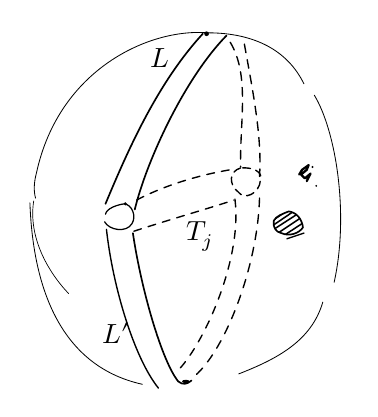
\begin{tikzpicture}[x=.12mm,y=-.12mm,line cap=round,line join=round]
\draw[line width=.3pt] (194,39) .. controls (133,34) and (37,77) .. (13,187) .. controls (10,198) and (10,207) .. (12,214);
\draw[line width=.3pt] (194,39) .. controls (244,39) and (279,58) .. (296,93);
\draw[line width=.3pt] (307,105) .. controls (330,143) and (344,231) .. (328,303);
\draw[line width=.3pt] (316,324) .. controls (304,365) and (268,384) .. (227,400);
\draw[line width=.3pt] (6,219) .. controls (9,303) and (35,391) .. (125,411);
\draw[line width=.25pt] (10,217) .. controls (4,255) and (25,292) .. (47,315);
\draw[line width=.6pt] (189,40) .. controls (142,91) and (111,160) .. (86,220);
\draw[line width=.6pt] (214,42) .. controls (169,88) and (129,176) .. (117,226);
\draw[line width=.5pt] (87,247) .. controls (94,310) and (117,384) .. (142,415);
\draw[line width=.6pt] (115,251) .. controls (124,312) and (146,387) .. (163,408) .. controls (168,412) and (172,411) .. (177,407);
\draw[line width=.45pt] (86,231) .. controls (87,225) and (98,221) .. (106,220) .. controls (114,221) and (119,233) .. (114,241) .. controls (108,251) and (90,248) .. (85,239);
\draw[line width=.5pt,dash pattern=on 1.1mm off .9mm] (218,49) .. controls (239,84) and (228,133) .. (229,181);
\draw[line width=.5pt,dash pattern=on 1.1mm off .9mm] (233,51) .. controls (241,96) and (252,149) .. (249,191);
\draw[line width=.5pt,dash pattern=on 1mm off .7mm] (229,182) .. controls (216,186) and (217,200) .. (226,207) .. controls (233,217) and (249,209) .. (250,195) .. controls (253,186) and (242,181) .. (229,182);
\draw[line width=.5pt,dash pattern=on 1mm off 1mm] (223,215) .. controls (231,278) and (191,366) .. (164,395);
\draw[line width=.5pt,dash pattern=on 1.1mm off 1mm] (249,214) .. controls (247,288) and (211,380) .. (177,405);
\draw[line width=.5pt,dash pattern=on 1mm off .9mm] (119,216) .. controls (155,197) and (197,187) .. (224,183);
\draw[line width=.5pt,dash pattern=on 1mm off .9mm] (116,249) .. controls (156,236) and (198,224) .. (222,216);
\fill (193,40) circle[radius=.3mm];
\fill (171,408) ellipse[x radius=.48mm,y radius=.216mm];
\fill (107,220) circle[radius=.216mm];
\node[inner sep=0pt] at (144,66) {$L$};
\node[inner sep=0pt] at (98,357) {$L'$};
\node[inner sep=0pt] at (186,255) {$T_j$};
\draw[line width=.8pt] (291,189) -- (294,184) -- (301,179) -- (299,184) -- (293,189) -- (297,193) -- (303,188) -- (299,196);
\fill (305,181) circle[radius=.144mm];
\fill (309,201) circle[radius=.132mm];
\draw[line width=.6pt] (264,238) .. controls (266,233) and (275,230) .. (280,228) .. controls (288,229) and (294,236) .. (295,245) .. controls (291,251) and (281,255) .. (272,251) .. controls (266,250) and (263,244) .. (264,238);
\begin{scope}
\clip (264,238) .. controls (266,233) and (275,230) .. (280,228) .. controls (288,229) and (294,236) .. (295,245) .. controls (291,251) and (281,255) .. (272,251) .. controls (266,250) and (263,244) .. (264,238);
\draw[line width=.55pt] (258,241)--(283,224) (260,245)--(288,226) (261,249)--(292,229) (264,254)--(297,232) (271,256)--(300,237) (280,257)--(302,242);
\end{scope}
\draw[line width=.5pt] (278,257) -- (296,251);
\end{tikzpicture}}

\LMsourceMark{M015624}{\margin{$^*$ C'est essentiellement un $\mathrm{SL}(2,\mathbb Z)$ --- plutôt une extension centrale \LMsourceMark{M015625}{\unsure{remarquable}} de $\mathrm{SL}(2,\mathbb Z)$ par $\mathbb Z$, qui \LMsourceMark{M015626}{\unsure{rappelle}} celle de $\mathrm{SL}(2,\mathbb R)$ par $\mathbb Z$\ldots\ (rev. universel de $\mathrm{SL}(2,\mathbb R)$)}}

\figure{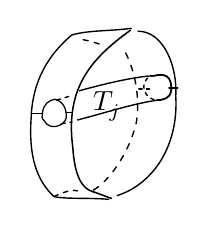
\begin{tikzpicture}[x=.12mm,y=-.12mm,line cap=round,line join=round]
\draw[line width=.5pt] (118,15) .. controls (94,18) and (72,17) .. (55,22) .. controls (24,48) and (13,79) .. (12,109) .. controls (9,151) and (18,176) .. (36,193) .. controls (49,196) and (75,194) .. (94,196);
\draw[line width=.5pt] (125,18) .. controls (153,18) and (167,57) .. (165,87) .. controls (168,137) and (143,179) .. (103,192);
\draw[line width=.55pt] (117,17) .. controls (74,48) and (48,79) .. (56,141) .. controls (58,170) and (65,185) .. (78,188) -- (97,195);
\draw[line width=.5pt,dash pattern=on .65mm off .8mm] (67,27) .. controls (74,28) and (82,31) .. (89,33);
\draw[line width=.5pt,dash pattern=on .75mm off .95mm] (112,41) .. controls (124,65) and (127,94) .. (123,116) .. controls (115,148) and (94,177) .. (78,186);
\draw[line width=.45pt] (24,104) .. controls (25,95) and (31,91) .. (37,90) .. controls (46,92) and (50,101) .. (49,110) .. controls (47,118) and (32,124) .. (26,113) .. controls (23,111) and (23,107) .. (24,104);
\draw[line width=.5pt] (12,105) -- (24,105) (49,104) -- (55,104);
\draw[line width=.5pt,dash pattern=on .5mm off .6mm] (39,91) -- (55,86) (44,116) -- (55,114);
\draw[line width=.5pt] (63,81) .. controls (85,75) and (120,66) .. (143,65);
\draw[line width=.5pt] (61,112) .. controls (88,105) and (122,94) .. (146,91);
\draw[line width=.65pt] (143,65) .. controls (159,61) and (161,72) .. (160,82) .. controls (159,88) and (153,91) .. (145,91);
\draw[line width=.5pt,dash pattern=on .45mm off .55mm] (143,65) .. controls (128,65) and (126,87) .. (144,91);
\draw[line width=.55pt,dash pattern=on .4mm off .55mm] (126,79)--(141,79);
\draw[line width=.7pt] (158,78)--(167,78);
\draw[line width=.5pt,dash pattern=on .6mm off .7mm] (36,193) .. controls (47,188) and (56,185) .. (61,187);
\fill (78,188) circle[radius=.18mm];
\node[inner sep=0pt] at (92,98) {$T_j$};
\end{tikzpicture}}

\LMsourceMark{M015627}{\margin{466}}

\LMflushnotes\LMflushpages
\ifnum\LMform=1
\begin{LMapparatus}
\LMentry{140-2-s467-I001}{insertion}{\inserted{sur $\pi_g$}
}{\emph{\LMinsertedlabel}}{Ajout explicite de l'auteur : intégré à l'endroit indiqué par la transcription, sans modifier sa lecture.}{}
\LMentry{140-2-s467-I002}{insertion}{\inserted{$L$}
}{\emph{\LMinsertedlabel}}{Ajout explicite de l'auteur : intégré à l'endroit indiqué par la transcription, sans modifier sa lecture.}{}
\end{LMapparatus}
\fi

\LMsourceMark{M015628}{\scanpage{468}}

Il est possible qu'il faudra considérer de près ce dernier, pour étudier les relations entre \var{\inserted{les}}{\LMadded{les}}{insertion}{140-2-s468-I001} éléments de $\mathcal T_g$ provenant des ensembles précédents\ldots\ Un travail amusant sera de se débrouiller pour écrire les générateurs du groupe $\pi_g$, et surtout la fameuse relation, dans une disposition géométrique relative des ``anses'', qui est une disposition ``\LMsourceMark{M015629}{\unsure{panachée}}'' --- et non plus \uline{sagement} à la queue-leu-leu !

\var{\deleted{Je vois \LMsourceMark{M015630}{\unsure{apparaître}}}}{\LMsourceMark{M015631}{\LMcancelledDoubts{\LMsourceMark{M015632}{\unsure{apparaître}}}}}{deletion}{140-2-s468-D001}

En attendant d'entrer ainsi dans le vif de la structure du groupe de Teichmüller, je vais déjà essayer de décrire des générateurs et relations pour le sous-groupe intéressant qu'on vient d'écrire, $\mathbb D_{2g}^{\sim}\cdot H$.
Je vais prendre les sempiternels générateurs $\varepsilon_0,\varepsilon_1$ de $\mathbb D_{2g}$
\[
\varepsilon_0^2=\varepsilon_1^2=1,\qquad (\varepsilon_0\varepsilon_1)^{2g}=1
\]
et y joindre $\tau=\tau_g$, et \var{\deleted{\LMsourceMark{M015633}{\illegible{1}}}}{\LMsourceMark{M015634}{\LMcancelledDoubts{\LMsourceMark{M015635}{\illegible{1}}}}}{deletion}{140-2-s468-D002} $\rho_0\tau=\tau'$
($\rho_0=\rho_{j_0}$, $j_0$ pt marqué de $I=J/\tau$)
satisfaisant
\[
\tau^2=\tau'^2=1,\qquad
\var{\deleted{[\tau,\varepsilon_0]=\LMsourceMark{M015636}{\unsure{[\varepsilon_1,\tau]|[\tau,\varepsilon_1]}}=}}{\LMsourceMark{M015637}{\LMcancelledDoubts{\(\LMsourceMark{M015638}{\unsure{[\varepsilon_1,\tau]|[\tau,\varepsilon_1]}}\)}}}{deletion}{140-2-s468-D003}
\]
\[
(\tau\varepsilon_0)^2=(\tau\varepsilon_1)^2=1\quad
\var{\deleted{\LMsourceMark{M015639}{\unsure{(\tau'\varepsilon_0)^2=(\tau'\varepsilon_1)^2}}=1}}{\LMsourceMark{M015640}{\LMcancelledDoubts{\(\LMsourceMark{M015641}{\unsure{(\tau'\varepsilon_0)^2=(\tau'\varepsilon_1)^2}}\)}}}{deletion}{140-2-s468-D004}
\]
\[
(\varepsilon_1\tau')^2=1
\qquad \varepsilon_1\ \text{commute à}\ \tau'
\]

\LMsourceMark{M015642}{\margin{\uline{NB} $\varepsilon_0$ bouge \LMsourceMark{M015643}{\unsure{le sommet}} du repère, $\varepsilon_1$ l'arête et pas le sommet, donc $\varepsilon_1(j_0)=j_0$}}

\LMsourceMark{M015644}{\margin{\LMsourceMark{M015645}{\unsure{expriment}} la commutation de $\tau$ \var{\deleted{\LMsourceMark{M015646}{\illegible{1}}}}{\LMsourceMark{M015647}{\LMcancelledDoubts{\LMsourceMark{M015648}{\illegible{1}}}}}{deletion}{140-2-s468-D005} à $\varepsilon_0,\varepsilon_1$}}

\LMsourceMark{M015649}{\margin{467}}

\LMflushnotes\LMflushpages
\ifnum\LMform=1
\begin{LMapparatus}
\LMentry{140-2-s468-I001}{insertion}{\inserted{les}
}{\emph{\LMinsertedlabel}}{Ajout explicite de l'auteur : intégré à l'endroit indiqué par la transcription, sans modifier sa lecture.}{}
\LMentry{140-2-s468-D001}{suppression}{\deleted{Je vois \LMsourceMark{M015650}{\unsure{apparaître}}}
}{\emph{\LMomittedlabel}}{Passage biffé dans le manuscrit : la suppression suit l'état final de l'auteur; les doutes de lecture restent signalés.}{}
\LMentry{140-2-s468-D002}{suppression}{\deleted{\LMsourceMark{M015651}{\illegible{1}}}
}{\emph{\LMomittedlabel}}{Passage biffé dans le manuscrit : la suppression suit l'état final de l'auteur; les doutes de lecture restent signalés.}{}
\LMentry{140-2-s468-D003}{suppression}{\(\deleted{[\tau,\varepsilon_0]=\LMsourceMark{M015652}{\unsure{[\varepsilon_1,\tau]|[\tau,\varepsilon_1]}}=}\)
}{\emph{\LMomittedlabel}}{Passage biffé dans le manuscrit : la suppression suit l'état final de l'auteur; les doutes de lecture restent signalés.}{}
\LMentry{140-2-s468-D004}{suppression}{\(\deleted{\LMsourceMark{M015653}{\unsure{(\tau'\varepsilon_0)^2=(\tau'\varepsilon_1)^2}}=1}\)
}{\emph{\LMomittedlabel}}{Passage biffé dans le manuscrit : la suppression suit l'état final de l'auteur; les doutes de lecture restent signalés.}{}
\LMentry{140-2-s468-D005}{suppression}{\deleted{\LMsourceMark{M015654}{\illegible{1}}}
}{\emph{\LMomittedlabel}}{Passage biffé dans le manuscrit : la suppression suit l'état final de l'auteur; les doutes de lecture restent signalés.}{}
\end{LMapparatus}
\fi
\ifnum\LMform=2
\par\smallskip\begingroup\footnotesize\Needspace{4\baselineskip}\csname @beginparpenalty\endcsname=10000\relax\noindent\textcolor{gray}{\rule{.2\linewidth}{.35pt}}\par\nobreak
\noindent\textit{\LMdoubtheading.}\par\nobreak
\LMcarryover{140-2-s468-D001}{\LMsourceMark{M015655}{\unsure{apparaître}}
}
\LMcarryover{140-2-s468-D002}{\LMsourceMark{M015656}{\illegible{1}}
}
\LMcarryover{140-2-s468-D003}{\(\LMsourceMark{M015657}{\unsure{[\varepsilon_1,\tau]|[\tau,\varepsilon_1]}}\)
}
\LMcarryover{140-2-s468-D004}{\(\LMsourceMark{M015658}{\unsure{(\tau'\varepsilon_0)^2=(\tau'\varepsilon_1)^2}}\)
}
\LMcarryover{140-2-s468-D005}{\LMsourceMark{M015659}{\illegible{1}}
}
\par\endgroup\smallskip
\fi

\LMsourceMark{M015660}{\scanpage{469}}
\LMsourceMark{M015661}{\mspage{237}}

\[
((\varepsilon_0\varepsilon_1)^g\tau')^2=1
\]
\LMsourceMark{M015662}{\margin{(l'involution $(\varepsilon_0\varepsilon_1)^g$ commute à $\tau'$)}}

sauf erreur, ça fait un ensemble de générateurs et relations pour $\mathbb D_{2g}^{\sim}\cdot\mathcal H$ --- en résumé $\varepsilon_0,\varepsilon_1,\tau,\tau'$
\[
\text{(52)}\quad
\left\{
\begin{array}{l}
\varepsilon_0^2=\varepsilon_1^2=\tau^2=\tau'^2=1\\
(\tau\varepsilon_0)^2=(\tau\varepsilon_1)^2=(\tau'\varepsilon_1)^2=1\\
(\varepsilon_0\varepsilon_1)^{2g}=1\\
(\tau'(\varepsilon_0\varepsilon_1)^g)^2=1
\end{array}
\right.
\]

C'est peut-être pas très astucieux comme choix de générateurs, en ce sens que $\varepsilon_0,\varepsilon_1$, ne sont pas du tt sur le même pied que $\tau,\tau'$ --- ce ne sont pas des \uline{anti}-\LMsourceMark{M015663}{\unsure{involutions}}. Il vaudrait mieux prendre $\varepsilon'_0=\tau\varepsilon_0$, $\varepsilon'_1=\tau\LMsourceMark{M015664}{\unsure{\varepsilon_1}}$ de façon à obtenir
\[
\text{(52bis)}\quad
\left\{
\begin{array}{l}
\varepsilon_0^{\prime 2}=\varepsilon_1^{\prime 2}=\tau^2=\tau'^2=1\\
(\tau\varepsilon'_0)^2=(\tau\varepsilon'_1)^2=(\tau'(\tau\varepsilon'_1))^2=1\\
(\varepsilon'_0\varepsilon'_1)^{2g}=1\\
(\tau'(\varepsilon'_0\varepsilon'_1)^g)^2=1
\end{array}
\right.
\]
ce sont essentiellement ``les mêmes'' relations sauf la dernière de la deuxième ligne.

Peut être ce petit jeu avec le tout petit groupe $\mathbb D_n^{\sim}$ opérant sur $\mathcal H$ est un peu une \LMsourceMark{M015665}{\unsure{amusette}} --- le groupe $\mathcal H\simeq\mathbb Z^g$ dans $\mathcal T_g$ suggère beaucoup la situation

\LMsourceMark{M015666}{\margin{468}}

\LMflushnotes\LMflushpages

\LMsourceMark{M015667}{\scanpage{470}}

d'un tore maximal dans un groupe $\frac12$ simple, on a vraiment envie d'en \LMsourceMark{M015668}{\unsure{avoir|voir}} une caractérisation intrinsèque dans $\mathcal T_g$ --- ou dans $\LMsourceMark{M015669}{\unsure{\mathcal S_g|\mathcal G_g|\mathcal C_g}}$, ce qui est possible puisque \var{\deleted{\LMsourceMark{M015670}{\illegible{1}}}}{\LMsourceMark{M015671}{\LMcancelledDoubts{\LMsourceMark{M015672}{\illegible{1}}}}}{deletion}{140-2-s470-D001} en tant que groupe de transformations topologiques \LMsourceMark{M015673}{\unsure{effectives|effectif}}, il laisse fixe les points de $V_0\subset X_g$ --- p.ex. les deux pôles, qu'on peut prendre comme pts \LMsourceMark{M015674}{\unsure{bases|base}} pour construire rev. universels et groupes \LMsourceMark{M015675}{\unsure{fondamental|fondamentale}}. Ce sont peut-être les sous-groupes \LMsourceMark{M015676}{\unsure{abéliens|abélien}}-libres maximaux.

On aimerait étudier le normalisateur --- est-ce exactement ce qui provient des autom de $X_g-\bigcup\mathring{T}_i\simeq V_0$ ?

les $\mathrm{SL}(2,\mathbb Z_{\LMsourceMark{M015677}{\unsure{j}}})$ associés aux ``lanières'' à travers le tube \var{\inserted{$T_j$}}{\LMadded{$T_j$}}{insertion}{140-2-s470-I001} jouent-ils un rôle analogue à celui des groupes $\mathrm{SL}(2,K)$ ou $\LMsourceMark{M015678}{\unsure{\mathrm{GP}(1,k)|\mathrm{GL}(1,k)}}$ ``de rang 1'' dans la théorie des groupes algébriques réductifs ? Si Jean \LMsourceMark{M015679}{\unsure{ne|me}} ``\LMsourceMark{M015680}{\unsure{mord}}''

\LMsourceMark{M015681}{\margin{469}}

\LMflushnotes\LMflushpages
\ifnum\LMform=1
\begin{LMapparatus}
\LMentry{140-2-s470-D001}{suppression}{\deleted{\LMsourceMark{M015682}{\illegible{1}}}
}{\emph{\LMomittedlabel}}{Passage biffé dans le manuscrit : la suppression suit l'état final de l'auteur; les doutes de lecture restent signalés.}{}
\LMentry{140-2-s470-I001}{insertion}{\inserted{$T_j$}
}{\emph{\LMinsertedlabel}}{Ajout explicite de l'auteur : intégré à l'endroit indiqué par la transcription, sans modifier sa lecture.}{}
\end{LMapparatus}
\fi
\ifnum\LMform=2
\par\smallskip\begingroup\footnotesize\Needspace{4\baselineskip}\csname @beginparpenalty\endcsname=10000\relax\noindent\textcolor{gray}{\rule{.2\linewidth}{.35pt}}\par\nobreak
\noindent\textit{\LMdoubtheading.}\par\nobreak
\LMcarryover{140-2-s470-D001}{\LMsourceMark{M015683}{\illegible{1}}
}
\par\endgroup\smallskip
\fi

% END PACKAGE LM_P047
% BEGIN PACKAGE LM_P048
\ifnum\LMform<2\Needspace{11\baselineskip}\subsection*{Scans 471--480}\fi
\LMsourceMark{M015684}{\scanpage{471}}
\LMsourceMark{M015685}{\mspage{238}}

pas à la situation, la soumettre peut-être à Carlos, qui est à l'aise tant avec les groupes discrets et leurs générateurs et relations, qu'avec la théorie des $\frac{1}{2}$ simples -- et la topologie ....

\LMflushnotes\LMflushpages

\LMsourceMark{M015686}{\scanpage{472}}
\LMsourceMark{M015687}{\mspage{239}}

\uline{33} Étude des revêtements finis -- relation entre les $\mathcal N_{g,\nu},\Gamma_{g,\nu}$ pour $g$ variable.

Soient $(\pi\var{\deleted{,\LMsourceMark{M015688}{\unsure{a}}}}{\LMsourceMark{M015689}{\LMcancelledDoubts{\(\LMsourceMark{M015690}{\unsure{a}}\)}}}{deletion}{140-2-s472-D001})$ groupe ext. à lacets profini arithmétisé de type $(g,\nu)$, $\pi'$ un \LMsourceMark{M015691}{\unsure{ss-grpe|ss-grp}} ouvert de $\pi$, d'où une application injective
\[
\mathrm{Discr\acute{e}t}(\pi)\hookrightarrow
\mathrm{Discr\acute{e}t}(\pi'),
\]
on voudrait prouver qu'elle est compatible avec la relation d'équivalence \var{\deleted{\LMsourceMark{M015692}{\unsure{des}}\ \LMsourceMark{M015693}{\illegible{1}}}}{\LMsourceMark{M015694}{\LMcancelledDoubts{\LMsourceMark{M015695}{\unsure{des}}\quad \LMsourceMark{M015696}{\illegible{1}}}}}{deletion}{140-2-s472-D002}\var{\inserted{\LMsourceMark{M015697}{\unsure{de l'arithmétisation|de l'arithmétisabilité}}}}{\LMadded{\LMsourceMark{M015698}{\unsure{de l'arithmétisation|de l'arithmétisabilité}}}}{insertion}{140-2-s472-I001}, de \var{\deleted{\LMsourceMark{M015699}{\unsure{prouver}}}}{\LMsourceMark{M015700}{\LMcancelledDoubts{\LMsourceMark{M015701}{\unsure{prouver}}}}}{deletion}{140-2-s472-D003} sorte que tte arithmétisation de $\pi$ en donne une de $\pi'$, et de $\overline{\mathrm m}$ pour les \var{\deleted{\LMsourceMark{M015702}{\unsure{discre}}}}{\LMsourceMark{M015703}{\LMcancelledDoubts{\LMsourceMark{M015704}{\unsure{discre}}}}}{deletion}{140-2-s472-D004} prédiscrétifications.

On voudrait établir en $\overline{\mathrm m}$ temps que les applications
\[
\begin{array}{lll}
 &P^+(\pi)\longrightarrow P^+(\pi')&\begin{gathered}\text{sur les prédiscrétifications}\\\text{orientées}\end{gathered}\\[1em]
\text{et}&A(\pi)\LMsourceMark{M015705}{\unsure{\longrightarrow|-}}A(\pi')&\text{sur les arithmétisations}
\end{array}
\]
sont injectives. Pour prouver ces points, on est ramené au cas où $\pi'$ est invariant caractéristique. (Cf \S\,28, diagramme 7, \LMsourceMark{M015706}{\unsure{ff}}) Choisissant

\LMflushnotes\LMflushpages
\ifnum\LMform=1
\begin{LMapparatus}
\LMentry{140-2-s472-D001}{suppression}{\(\deleted{,\LMsourceMark{M015707}{\unsure{a}}}\)
}{\emph{\LMomittedlabel}}{Passage biffé dans le manuscrit : la suppression suit l'état final de l'auteur; les doutes de lecture restent signalés.}{}
\LMentry{140-2-s472-D002}{suppression}{\deleted{\LMsourceMark{M015708}{\unsure{des}}\ \LMsourceMark{M015709}{\illegible{1}}}
}{\emph{\LMomittedlabel}}{Passage biffé dans le manuscrit : la suppression suit l'état final de l'auteur; les doutes de lecture restent signalés.}{}
\LMentry{140-2-s472-I001}{insertion}{\inserted{\LMsourceMark{M015710}{\unsure{de l'arithmétisation|de l'arithmétisabilité}}}
}{\emph{\LMinsertedlabel}}{Ajout explicite de l'auteur : intégré à l'endroit indiqué par la transcription, sans modifier sa lecture.}{}
\LMentry{140-2-s472-D003}{suppression}{\deleted{\LMsourceMark{M015711}{\unsure{prouver}}}
}{\emph{\LMomittedlabel}}{Passage biffé dans le manuscrit : la suppression suit l'état final de l'auteur; les doutes de lecture restent signalés.}{}
\LMentry{140-2-s472-D004}{suppression}{\deleted{\LMsourceMark{M015712}{\unsure{discre}}}
}{\emph{\LMomittedlabel}}{Passage biffé dans le manuscrit : la suppression suit l'état final de l'auteur; les doutes de lecture restent signalés.}{}
\end{LMapparatus}
\fi
\ifnum\LMform=2
\par\smallskip\begingroup\footnotesize\Needspace{4\baselineskip}\csname @beginparpenalty\endcsname=10000\relax\noindent\textcolor{gray}{\rule{.2\linewidth}{.35pt}}\par\nobreak
\noindent\textit{\LMdoubtheading.}\par\nobreak
\LMcarryover{140-2-s472-D001}{\(\LMsourceMark{M015713}{\unsure{a}}\)
}
\LMcarryover{140-2-s472-D002}{\LMsourceMark{M015714}{\unsure{des}}\quad \LMsourceMark{M015715}{\illegible{1}}
}
\LMcarryover{140-2-s472-D003}{\LMsourceMark{M015716}{\unsure{prouver}}
}
\LMcarryover{140-2-s472-D004}{\LMsourceMark{M015717}{\unsure{discre}}
}
\par\endgroup\smallskip
\fi

\LMsourceMark{M015718}{\scanpage{473}}

une discrétification $\pi_0$ de $\pi$, donc $\pi'_0$ de $\pi'$, on trouve alors
\[
\LMsourceMark{M015719}{\unsure{\widehat{\widehat{\mathcal G}}}}(\pi_0)\longrightarrow
\LMsourceMark{M015720}{\unsure{\widehat{\widehat{\mathcal G}}}}(\pi'_0)
\]
et on a

\textcircled{1} L'hom $\LMsourceMark{M015721}{\unsure{\widehat{\widehat{\mathcal G}}}}(\pi_0)\LMsourceMark{M015722}{\unsure{\longrightarrow}}\LMsourceMark{M015723}{\unsure{\widehat{\widehat{\mathcal G}}}}(\pi'_0)$ envoie $\mathcal M(\pi_0)$ dans $\mathcal M(\pi'_0)$

on aura donc un diagramme (\LMsourceMark{M015724}{\unsure{variante|parent}} de celui du \S\,28)
\diagram{\begin{tikzcd}[ampersand replacement=\&,column sep=large,row sep=large]
\LMsourceMark{M015725}{\unsure{(1)}} \&
\widehat{\mathcal G}^{+}(\pi_0)
 \arrow[r,hook,no head] \arrow[d,hook] \&
\mathcal M(\pi_0) \arrow[r,hook,no head] \arrow[d,hook] \&
\widehat{\widehat{\mathcal G}}(\pi_0) \arrow[d,hook] \\
\& \widehat{\mathcal G}^{+}(\pi'_0)
 \arrow[r,hook,no head] \&
\mathcal M^{\LMsourceMark{M015726}{\unsure{\ast|\sharp}}}(\pi'_0) \arrow[r,hook,no head] \&
\LMsourceMark{M015727}{\unsure{\widehat{\widehat{\mathcal G}}}}(\pi'_0)
\end{tikzcd}}
qui \var{\deleted{signifie}}{}{deletion}{140-2-s473-D001} implique qu'une discrétification $\pi_1$ sur $\pi$ qui donne $\overline{\mathrm m}$ prédiscrétification orientée que $\pi_0$ (resp. $\overline{\mathrm m}$ arithmétisation) définit une \var{\inserted{\LMsourceMark{M015728}{\unsure{discrét}}}}{\LMadded{\LMsourceMark{M015729}{\unsure{discrét}}}}{insertion}{140-2-s473-I001} $\pi'_1$ de $\pi'$ qui donne $\overline{\mathrm m}$ prédiscr. or. (resp. $\overline{\mathrm m}$ arithm.) que $\pi'_0$. Donc on a bien $\LMsourceMark{M015730}{\unsure{P}}^{+}(\pi)\longrightarrow P^+(\pi')$, $A(\pi)\longrightarrow A(\pi')$, il faut encore exprimer l'injectivité, qui revient aux relations
\[
\begin{gathered}
(2)\quad
\LMsourceMark{M015731}{\unsure{\widehat{\mathcal G}^{+}}}(\pi_0)
=
\LMsourceMark{M015732}{\unsure{\widehat{\mathcal G}^{+}}}(\pi'_0)\cap
\LMsourceMark{M015733}{\unsure{\widehat{\widehat{\mathcal G}}}}(\pi_0),\qquad
\mathcal M(\pi_0)=\mathcal M(\pi'_0)\cap
\LMsourceMark{M015734}{\unsure{\widehat{\widehat{\mathcal G}}}}(\pi_0)
\end{gathered}
\]

\LMflushnotes\LMflushpages
\ifnum\LMform=1
\begin{LMapparatus}
\LMentry{140-2-s473-D001}{suppression}{\deleted{signifie}
}{\emph{\LMomittedlabel}}{Passage biffé dans le manuscrit : la suppression suit l'état final de l'auteur; les doutes de lecture restent signalés.}{}
\LMentry{140-2-s473-I001}{insertion}{\inserted{\LMsourceMark{M015735}{\unsure{discrét}}}
}{\emph{\LMinsertedlabel}}{Ajout explicite de l'auteur : intégré à l'endroit indiqué par la transcription, sans modifier sa lecture.}{}
\end{LMapparatus}
\fi

\LMsourceMark{M015736}{\scanpage{474}}
\LMsourceMark{M015737}{\mspage{240}}

i.e. un \LMsourceMark{M015738}{\unsure{autom.}} à lacets de $\pi^{+}$ qui, sur $\pi'$, appartient à $\LMsourceMark{M015739}{\unsure{\widehat{\mathcal G}}}(\pi'_0)$ \var{\deleted{\LMsourceMark{M015740}{\illegible{2}}}}{\LMsourceMark{M015741}{\LMcancelledDoubts{\LMsourceMark{M015742}{\illegible{2}}}}}{deletion}{140-2-s474-D001} resp. à $\mathcal M(\pi'_0)$, est déjà dans $\LMsourceMark{M015743}{\unsure{\widehat{\mathcal G}}}(\pi_0)$ resp. dans $\mathcal M(\pi_0)$.

L'assertion \var{\deleted{\LMsourceMark{M015744}{\illegible{1}}}}{\LMsourceMark{M015745}{\LMcancelledDoubts{\LMsourceMark{M015746}{\illegible{1}}}}}{deletion}{140-2-s474-D002} repérée étant admise, l'assertion \var{\inserted{non}}{\LMadded{non}}{insertion}{140-2-s474-I001} repérée signifie aussi que l'hom. can.
\[
(3)\qquad
\mathbb{\Gamma}_a=\mathcal M_a(\pi)/\LMsourceMark{M015747}{\unsure{\widehat{\mathcal G}}}^{+}_a(\pi)
\longrightarrow
\mathbb{\Gamma}_{a'}=\mathcal M_{a'}(\pi')/\LMsourceMark{M015748}{\unsure{\widehat{\mathcal G}}}^{+}_{a'}(\pi')
\]
est \uline{injectif}. Par construction (via $\mathbb{\Gamma}_{\LMsourceMark{M015749}{\unsure{\mathbb Q}}}$) c'est aussi surjectif, donc on trouverait :

\textcircled{2} l'hom. canonique (3) est bijectif

et on trouverait aussi une bijection
\[
(4)\qquad P_a(\pi)\longrightarrow P_{a'}(\pi')
\]
entre \LMsourceMark{M015750}{\unsure{arithm.}} de $\pi$ de type $a$, et arithm. de $\pi'$ de type $a'$, \uline{compatible} avec l'iso. \LMsourceMark{M015751}{\unsure{(3)}}.

Enfin, un résultat dans le cas $\pi'$ \LMsourceMark{M015752}{\unsure{inv.}} car. s'étendrait aussitôt au cas d'une $\pi'\subset\pi$ ouvert quelconque.

Procédant \var{\inserted{p.ex.}}{\LMadded{p.ex.}}{insertion}{140-2-s474-I002} comme dans le \S 28 à coups de ``correspondances'' \var{\inserted{arithm. extérieures\LMsourceMark{M015753}{\unsure{,}}}}{\LMadded{arithm. extérieures\LMsourceMark{M015754}{\unsure{,}}}}{insertion}{140-2-s474-I003} entre

\LMflushnotes\LMflushpages
\ifnum\LMform=1
\begin{LMapparatus}
\LMentry{140-2-s474-D001}{suppression}{\deleted{\LMsourceMark{M015755}{\illegible{2}}}
}{\emph{\LMomittedlabel}}{Passage biffé dans le manuscrit : la suppression suit l'état final de l'auteur; les doutes de lecture restent signalés.}{}
\LMentry{140-2-s474-D002}{suppression}{\deleted{\LMsourceMark{M015756}{\illegible{1}}}
}{\emph{\LMomittedlabel}}{Passage biffé dans le manuscrit : la suppression suit l'état final de l'auteur; les doutes de lecture restent signalés.}{}
\LMentry{140-2-s474-I001}{insertion}{\inserted{non}
}{\emph{\LMinsertedlabel}}{Ajout explicite de l'auteur : intégré à l'endroit indiqué par la transcription, sans modifier sa lecture.}{}
\LMentry{140-2-s474-I002}{insertion}{\inserted{p.ex.}
}{\emph{\LMinsertedlabel}}{Ajout explicite de l'auteur : intégré à l'endroit indiqué par la transcription, sans modifier sa lecture.}{}
\LMentry{140-2-s474-I003}{insertion}{\inserted{arithm. extérieures\LMsourceMark{M015757}{\unsure{,}}}
}{\emph{\LMinsertedlabel}}{Ajout explicite de l'auteur : intégré à l'endroit indiqué par la transcription, sans modifier sa lecture.}{}
\end{LMapparatus}
\fi
\ifnum\LMform=2
\par\smallskip\begingroup\footnotesize\Needspace{4\baselineskip}\csname @beginparpenalty\endcsname=10000\relax\noindent\textcolor{gray}{\rule{.2\linewidth}{.35pt}}\par\nobreak
\noindent\textit{\LMdoubtheading.}\par\nobreak
\LMcarryover{140-2-s474-D001}{\LMsourceMark{M015758}{\illegible{2}}
}
\LMcarryover{140-2-s474-D002}{\LMsourceMark{M015759}{\illegible{1}}
}
\par\endgroup\smallskip
\fi

\LMsourceMark{M015760}{\scanpage{475}}

``courbes potentielles'', on trouve un groupoïde connexe (ponctué par les $\widehat{\pi}_{g,\nu}$, p.ex, \var{\deleted{\LMsourceMark{M015761}{\unsure{)}}}}{\LMsourceMark{M015762}{\LMcancelledDoubts{\LMsourceMark{M015763}{\unsure{)}}}}}{deletion}{140-2-s475-D001} qui y sont \LMsourceMark{M015764}{\unsure{can.}} isomorphes), dont le $\pi_1$ ext. est la valeur commune des $\mathbb{\Gamma}_{g*}=\mathbb{\Gamma}_{g,\nu}$.

Pour trouver \LMsourceMark{M015765}{\unsure{un}} l'isom. \var{\inserted{\LMsourceMark{M015766}{\unsure{canonique}}}}{\LMadded{\LMsourceMark{M015767}{\unsure{canonique}}}}{insertion}{140-2-s475-I001} entre $\mathbb{\Gamma}_{g,\nu}$ et $\mathbb{\Gamma}_{g',\nu'}$, on choisit une \var{\deleted{\LMsourceMark{M015768}{\unsure{multiple commun}}}}{\LMsourceMark{M015769}{\LMcancelledDoubts{\LMsourceMark{M015770}{\unsure{multiple commun}}}}}{deletion}{140-2-s475-D002} \var{\inserted{correspondance entre}}{\LMadded{correspondance entre}}{insertion}{140-2-s475-I002} un $\pi_{g,\nu}$ et $\pi_{g',\nu'}$, p.ex. en \LMsourceMark{M015771}{\unsure{regardant}} \var{\deleted{\LMsourceMark{M015772}{\unsure{$N$ de $2g-2+\nu$ et $2g'-2+\nu'$}}}}{\LMsourceMark{M015773}{\LMcancelledDoubts{\LMsourceMark{M015774}{\unsure{$N$ de $2g-2+\nu$ et $2g'-2+\nu'$}}}}}{deletion}{140-2-s475-D003} l'un et l'autre (quitte à passer : de $g,\nu$ à $g,\widetilde{\nu}$ avec $\widetilde{\nu}\geq\nu$, et de $\overline{\mathrm m}$ pour $g',\nu'$ à $(g',\widetilde{\nu}')$ avec $\widetilde{\nu}'\geq\nu'$) comme des sous-groupes finis du $\overline{\mathrm m}$ $\pi_{0,3}$ \LMsourceMark{M015775}{\unsure{et}} d'où
\[
\mathbb{\Gamma}_{0,3}\xrightarrow{\sim}\Gamma_{g,\widetilde{\nu}},
\qquad
\Gamma_{0,3}\xrightarrow{\sim}\Gamma_{g',\widetilde{\nu}'}.
\]

On aimerait maintenant voir ce qui, dans le yoga précédent, est indépendant de toute conjecture. Par exemple, le fait que les \LMsourceMark{M015776}{\unsure{hom}} surjectifs \var{\inserted{\LMsourceMark{M015777}{\unsure{can.}}}}{\LMadded{\LMsourceMark{M015778}{\unsure{can.}}}}{insertion}{140-2-s475-I003} $\mathbb{\Gamma}_{g,\nu}\LMsourceMark{M015779}{\unsure{\longrightarrow}}\mathbb{\Gamma}_{g,\nu'}$ ($g$ le $\overline{\mathrm m}$, $\nu'$ constant) n'est pas établi.

Cependant, si on savait que dans la situation du $(\pi,\pi')$ avec $\pi'$ \LMsourceMark{M015780}{\unsure{inv.}} car. on ait
\[
\widehat{\widehat{\mathcal T}}(\pi'_0)\cap
\LMsourceMark{M015781}{\unsure{\widehat{\mathcal G}}}^{+}(\pi_0)
=
\LMsourceMark{M015782}{\unsure{\widehat{\mathcal G}}}^{+}(\pi_0)
\]

\LMflushnotes\LMflushpages
\ifnum\LMform=1
\begin{LMapparatus}
\LMentry{140-2-s475-D001}{suppression}{\deleted{\LMsourceMark{M015783}{\unsure{)}}}
}{\emph{\LMomittedlabel}}{Passage biffé dans le manuscrit : la suppression suit l'état final de l'auteur; les doutes de lecture restent signalés.}{}
\LMentry{140-2-s475-I001}{insertion}{\inserted{\LMsourceMark{M015784}{\unsure{canonique}}}
}{\emph{\LMinsertedlabel}}{Ajout explicite de l'auteur : intégré à l'endroit indiqué par la transcription, sans modifier sa lecture.}{}
\LMentry{140-2-s475-D002}{suppression}{\deleted{\LMsourceMark{M015785}{\unsure{multiple commun}}}
}{\emph{\LMomittedlabel}}{Passage biffé dans le manuscrit : la suppression suit l'état final de l'auteur; les doutes de lecture restent signalés.}{}
\LMentry{140-2-s475-I002}{insertion}{\inserted{correspondance entre}
}{\emph{\LMinsertedlabel}}{Ajout explicite de l'auteur : intégré à l'endroit indiqué par la transcription, sans modifier sa lecture.}{}
\LMentry{140-2-s475-D003}{suppression}{\deleted{\LMsourceMark{M015786}{\unsure{$N$ de $2g-2+\nu$ et $2g'-2+\nu'$}}}
}{\emph{\LMomittedlabel}}{Passage biffé dans le manuscrit : la suppression suit l'état final de l'auteur; les doutes de lecture restent signalés.}{}
\LMentry{140-2-s475-I003}{insertion}{\inserted{\LMsourceMark{M015787}{\unsure{can.}}}
}{\emph{\LMinsertedlabel}}{Ajout explicite de l'auteur : intégré à l'endroit indiqué par la transcription, sans modifier sa lecture.}{}
\end{LMapparatus}
\fi
\ifnum\LMform=2
\par\smallskip\begingroup\footnotesize\Needspace{4\baselineskip}\csname @beginparpenalty\endcsname=10000\relax\noindent\textcolor{gray}{\rule{.2\linewidth}{.35pt}}\par\nobreak
\noindent\textit{\LMdoubtheading.}\par\nobreak
\LMcarryover{140-2-s475-D001}{\LMsourceMark{M015788}{\unsure{)}}
}
\LMcarryover{140-2-s475-D002}{\LMsourceMark{M015789}{\unsure{multiple commun}}
}
\LMcarryover{140-2-s475-D003}{\LMsourceMark{M015790}{\unsure{$N$ de $2g-2+\nu$ et $2g'-2+\nu'$}}
}
\par\endgroup\smallskip
\fi

\LMsourceMark{M015791}{\scanpage{476}}
\LMsourceMark{M015792}{\mspage{241}}

(qui est un énoncé de nature relativement anodin sur des groupes à lacets profinis) on conclurait à la \uline{bijectivité} de $\mathbb{\Gamma}_{\pi_0}\longrightarrow\mathbb{\Gamma}_{\pi'_0}$ dans cette situation, et on en conclurait que le noyau de $\mathbb{\Gamma}_{\LMsourceMark{M015793}{\unsure{\mathbb Q}}}\longrightarrow\mathbb{\Gamma}_{0,3}$ \var{\deleted{\LMsourceMark{M015794}{\unsure{s'envoie|l'envoie}}}}{\LMsourceMark{M015795}{\LMcancelledDoubts{\LMsourceMark{M015796}{\unsure{s'envoie|l'envoie}}}}}{deletion}{140-2-s476-D001} s'envoie \uline{trivialement} dans les $\mathbb{\Gamma}_{g,\nu}$ pour $\forall\nu$ -- i.e. qu'il s'envoie dans les $\mathbb{\Gamma}_{g,\nu}$ par l'\uline{intermédiaire} de $\mathbb{\Gamma}_{0,3}$ \LMsourceMark{M015797}{\margin{\LMsourceMark{M015798}{\unsure{$!\! -\! A$}}}} -- et que de plus $\mathbb{\Gamma}_{0,3}\longrightarrow\Gamma_{g,\nu}$ est
\var{\deleted{\LMsourceMark{M015799}{\unsure{défaut|à défaut}} d'avoir établi ceci, \LMsourceMark{M015800}{\unsure{je vais montrer}} au moins que l'image des \LMsourceMark{M015801}{\unsure{noyaux|noyau}} $\Theta$ de $\mathbb{\Gamma}_{\LMsourceMark{M015802}{\unsure{\mathbb Q}}}\longrightarrow\mathbb{\Gamma}_{0,3}$ \LMsourceMark{M015803}{\unsure{ds}} les $\mathbb{\Gamma}_{g,\nu}$ est \uline{\LMsourceMark{M015804}{\unsure{finie|fini}}} ce qui signifie aussi}}{\LMsourceMark{M015805}{\LMcancelledDoubts{\LMsourceMark{M015806}{\unsure{défaut|à défaut}}\quad \LMsourceMark{M015807}{\unsure{je vais montrer}}\quad \LMsourceMark{M015808}{\unsure{noyaux|noyau}}\quad \(\LMsourceMark{M015809}{\unsure{\mathbb Q}}\)\quad \LMsourceMark{M015810}{\unsure{ds}}\quad \LMsourceMark{M015811}{\unsure{finie|fini}}}}}{deletion}{140-2-s476-D002}
\var{\inserted{\uline{iso} pour $\forall(g,\nu)$}}{\LMadded{\uline{iso} pour $\forall(g,\nu)$}}{insertion}{140-2-s476-I001} avec $\nu$ \uline{assez} grand -- il suffit que la surface de type $(g,\nu)$ \var{\deleted{\LMsourceMark{M015812}{\unsure{puisse}}}}{\LMsourceMark{M015813}{\LMcancelledDoubts{\LMsourceMark{M015814}{\unsure{puisse}}}}}{deletion}{140-2-s476-D003} (ou de type $(g,\nu')$ avec un $\nu'\leq\nu$) puisse s'obtenir comme rev. \LMsourceMark{M015815}{\unsure{étale}} de $X_{0,3}$, i.e. que $\pi_{g,\nu'}$ se réalise \var{\inserted{(\LMsourceMark{M015816}{\unsure{avec sa str.}} à lacets)}}{\LMadded{(\LMsourceMark{M015817}{\unsure{avec sa str.}} à lacets)}}{insertion}{140-2-s476-I002} comme \LMsourceMark{M015818}{\unsure{ss-groupe|ss: groupe}} \var{\deleted{à lacets}}{}{deletion}{140-2-s476-D004} \var{\inserted{d'indice fini}}{\LMadded{d'indice fini}}{insertion}{140-2-s476-I003} \var{\deleted{\LMsourceMark{M015819}{\unsure{d'in}}}}{\LMsourceMark{M015820}{\LMcancelledDoubts{\LMsourceMark{M015821}{\unsure{d'in}}}}}{deletion}{140-2-s476-D005} de $\pi_{0,3}$. Alors, \var{\deleted{\LMsourceMark{M015822}{\unsure{prenant}}}}{\LMsourceMark{M015823}{\LMcancelledDoubts{\LMsourceMark{M015824}{\unsure{prenant}}}}}{deletion}{140-2-s476-D006} \var{\inserted{considérant}}{\LMadded{considérant}}{insertion}{140-2-s476-I004} un $\pi''$ \var{\inserted{$\LMsourceMark{M015825}{\unsure{\simeq|\sim}}\pi_{g'',\nu''}$}}{\LMadded{$\LMsourceMark{M015826}{\unsure{\simeq|\sim}}\pi_{g'',\nu''}$}}{insertion}{140-2-s476-I005} $\LMsourceMark{M015827}{\unsure{\subset|\in}}\pi_{g,\nu'}$ d'indice fini et car. dans $\pi_{0,3}$, on aura

\LMflushnotes\LMflushpages
\ifnum\LMform=1
\begin{LMapparatus}
\LMentry{140-2-s476-D001}{suppression}{\deleted{\LMsourceMark{M015828}{\unsure{s'envoie|l'envoie}}}
}{\emph{\LMomittedlabel}}{Passage biffé dans le manuscrit : la suppression suit l'état final de l'auteur; les doutes de lecture restent signalés.}{}
\LMentry{140-2-s476-D002}{suppression}{\deleted{\LMsourceMark{M015829}{\unsure{défaut|à défaut}} d'avoir établi ceci, \LMsourceMark{M015830}{\unsure{je vais montrer}} au moins que l'image des \LMsourceMark{M015831}{\unsure{noyaux|noyau}} $\Theta$ de $\mathbb{\Gamma}_{\LMsourceMark{M015832}{\unsure{\mathbb Q}}}\longrightarrow\mathbb{\Gamma}_{0,3}$ \LMsourceMark{M015833}{\unsure{ds}} les $\mathbb{\Gamma}_{g,\nu}$ est \uline{\LMsourceMark{M015834}{\unsure{finie|fini}}} ce qui signifie aussi}
}{\emph{\LMomittedlabel}}{Passage biffé dans le manuscrit : la suppression suit l'état final de l'auteur; les doutes de lecture restent signalés.}{}
\LMentry{140-2-s476-I001}{insertion}{\inserted{\uline{iso} pour $\forall(g,\nu)$}
}{\emph{\LMinsertedlabel}}{Ajout explicite de l'auteur : intégré à l'endroit indiqué par la transcription, sans modifier sa lecture.}{}
\LMentry{140-2-s476-D003}{suppression}{\deleted{\LMsourceMark{M015835}{\unsure{puisse}}}
}{\emph{\LMomittedlabel}}{Passage biffé dans le manuscrit : la suppression suit l'état final de l'auteur; les doutes de lecture restent signalés.}{}
\LMentry{140-2-s476-I002}{insertion}{\inserted{(\LMsourceMark{M015836}{\unsure{avec sa str.}} à lacets)}
}{\emph{\LMinsertedlabel}}{Ajout explicite de l'auteur : intégré à l'endroit indiqué par la transcription, sans modifier sa lecture.}{}
\LMentry{140-2-s476-D004}{suppression}{\deleted{à lacets}
}{\emph{\LMomittedlabel}}{Passage biffé dans le manuscrit : la suppression suit l'état final de l'auteur; les doutes de lecture restent signalés.}{}
\LMentry{140-2-s476-I003}{insertion}{\inserted{d'indice fini}
}{\emph{\LMinsertedlabel}}{Ajout explicite de l'auteur : intégré à l'endroit indiqué par la transcription, sans modifier sa lecture.}{}
\LMentry{140-2-s476-D005}{suppression}{\deleted{\LMsourceMark{M015837}{\unsure{d'in}}}
}{\emph{\LMomittedlabel}}{Passage biffé dans le manuscrit : la suppression suit l'état final de l'auteur; les doutes de lecture restent signalés.}{}
\LMentry{140-2-s476-D006}{suppression}{\deleted{\LMsourceMark{M015838}{\unsure{prenant}}}
}{\emph{\LMomittedlabel}}{Passage biffé dans le manuscrit : la suppression suit l'état final de l'auteur; les doutes de lecture restent signalés.}{}
\LMentry{140-2-s476-I004}{insertion}{\inserted{considérant}
}{\emph{\LMinsertedlabel}}{Ajout explicite de l'auteur : intégré à l'endroit indiqué par la transcription, sans modifier sa lecture.}{}
\LMentry{140-2-s476-I005}{insertion}{\inserted{$\LMsourceMark{M015839}{\unsure{\simeq|\sim}}\pi_{g'',\nu''}$}
}{\emph{\LMinsertedlabel}}{Ajout explicite de l'auteur : intégré à l'endroit indiqué par la transcription, sans modifier sa lecture.}{}
\end{LMapparatus}
\fi
\ifnum\LMform=2
\par\smallskip\begingroup\footnotesize\Needspace{4\baselineskip}\csname @beginparpenalty\endcsname=10000\relax\noindent\textcolor{gray}{\rule{.2\linewidth}{.35pt}}\par\nobreak
\noindent\textit{\LMdoubtheading.}\par\nobreak
\LMcarryover{140-2-s476-D001}{\LMsourceMark{M015840}{\unsure{s'envoie|l'envoie}}
}
\LMcarryover{140-2-s476-D002}{\LMsourceMark{M015841}{\unsure{défaut|à défaut}}\quad \LMsourceMark{M015842}{\unsure{je vais montrer}}\quad \LMsourceMark{M015843}{\unsure{noyaux|noyau}}\quad \(\LMsourceMark{M015844}{\unsure{\mathbb Q}}\)\quad \LMsourceMark{M015845}{\unsure{ds}}\quad \LMsourceMark{M015846}{\unsure{finie|fini}}
}
\LMcarryover{140-2-s476-D003}{\LMsourceMark{M015847}{\unsure{puisse}}
}
\LMcarryover{140-2-s476-D005}{\LMsourceMark{M015848}{\unsure{d'in}}
}
\LMcarryover{140-2-s476-D006}{\LMsourceMark{M015849}{\unsure{prenant}}
}
\par\endgroup\smallskip
\fi

\LMsourceMark{M015850}{\scanpage{477}}

\diagram{\begin{tikzcd}[ampersand replacement=\&]
\mathbb{\Gamma}_{0,3} \arrow[r,"\sim"] \& \mathbb{\Gamma}_{g'',\nu''} \\
\mathbb{\Gamma}_{\mathbb Q} \arrow[u] \arrow[r] \& \mathbb{\Gamma}_{g,\nu'} \arrow[u,"\LMsourceMark{M015851}{\unsure{\wr|2}}"']
\end{tikzcd}}
\LMsourceMark{M015852}{\unsure{diagramme}} comm.

d'où notre \LMsourceMark{M015853}{\unsure{assertion}} $\mathbb{\Gamma}_{0,3}\xrightarrow{\sim}\mathbb{\Gamma}_{g,\nu'}$, et a fortiori l'hom surjectif $\mathbb{\Gamma}_{0,3}\longrightarrow\mathbb{\Gamma}_{g,\nu}$ qui le \LMsourceMark{M015854}{\unsure{factorise}} \var{\inserted{$(\nu\geq\nu')$}}{\LMadded{$(\nu\geq\nu')$}}{insertion}{140-2-s477-I001} est bijectif. Notons \LMsourceMark{M015855}{\unsure{p.ex.}} que les $\mathbb{\Gamma}_{0,\nu}\longrightarrow\mathbb{\Gamma}_{0,3}$ $(\nu\geq3)$ sont alors bijectifs. Mais \var{\deleted{il \LMsourceMark{M015856}{\illegible{3}}}}{\LMsourceMark{M015857}{\LMcancelledDoubts{\LMsourceMark{M015858}{\illegible{3}}}}}{deletion}{140-2-s477-D001}\var{\inserted{\deleted{\LMsourceMark{M015859}{\illegible{1}}}}}{\LMadded{\var{\deleted{\LMsourceMark{M015860}{\illegible{1}}}}{\LMsourceMark{M015861}{\LMcancelledDoubts{\LMsourceMark{M015862}{\illegible{1}}}}}{deletion}{140-2-s477-D002}}}{insertion}{140-2-s477-I002} noter qu'en tout état de cause, on ne trouve de résultat pour un $g,\nu$ que si $\nu\geq3$ -- donc ceci ne dit rien sur la fidélité \LMsourceMark{M015863}{\unsure{éventuelle}} \LMsourceMark{M015864}{\unsure{p.ex.}} de $\mathbb{\Gamma}_{0,3}\LMsourceMark{M015865}{\unsure{\longrightarrow|-}}\mathbb{\Gamma}_{g,0}=\mathbb{\Gamma}_g$ $(g\geq2)$ \LMsourceMark{M015866}{\unsure{ou}} $\mathbb{\Gamma}_{0,3}\longrightarrow\mathbb{\Gamma}_{1,1}=\mathbb{\Gamma}_1$.

\LMsourceMark{M015867}{\margin{On ne fait plus d'hypothèse conjecturale (\LMsourceMark{M015868}{\unsure{telle}} que l'injectivité dans (3)}}
Soit une courbe algébrique \var{\inserted{$\LMsourceMark{M015869}{\unsure{U}}$ de type $g,\nu$}}{\LMadded{$\LMsourceMark{M015870}{\unsure{U}}$ de type $g,\nu$}}{insertion}{140-2-s477-I003} définie sur un sous-corps \var{\inserted{$K$}}{\LMadded{$K$}}{insertion}{140-2-s477-I004} fini sur $\mathbb Q$ de $\overline{\mathbb Q}_0$, donc elle définit une action extérieure du sous groupe ouvert $\Gamma=\Gamma_K\subset\mathbb{\Gamma}_{\mathbb Q}$ sur $\pi_1(\LMsourceMark{M015871}{\unsure{U}}_{\overline{\mathbb Q}_0})$. \var{\deleted{Supposons}}{}{deletion}{140-2-s477-D003} Quitte à agrandir $K$, \var{\deleted{\LMsourceMark{M015872}{\unsure{en}} $K'$, \LMsourceMark{M015873}{\unsure{OPS}} \LMsourceMark{M015874}{\unsure{que}}}}{\LMsourceMark{M015875}{\LMcancelledDoubts{\LMsourceMark{M015876}{\unsure{en}}\quad \LMsourceMark{M015877}{\unsure{OPS}}\quad \LMsourceMark{M015878}{\unsure{que}}}}}{deletion}{140-2-s477-D004} et à \LMsourceMark{M015879}{\unsure{agrandir}}

\LMflushnotes\LMflushpages
\ifnum\LMform=1
\begin{LMapparatus}
\LMentry{140-2-s477-I001}{insertion}{\inserted{$(\nu\geq\nu')$}
}{\emph{\LMinsertedlabel}}{Ajout explicite de l'auteur : intégré à l'endroit indiqué par la transcription, sans modifier sa lecture.}{}
\LMentry{140-2-s477-D001}{suppression}{\deleted{il \LMsourceMark{M015880}{\illegible{3}}}
}{\emph{\LMomittedlabel}}{Passage biffé dans le manuscrit : la suppression suit l'état final de l'auteur; les doutes de lecture restent signalés.}{}
\LMentry{140-2-s477-I002}{insertion}{\inserted{\deleted{\LMsourceMark{M015881}{\illegible{1}}}}
}{\emph{\LMinsertedlabel}}{Ajout explicite de l'auteur : intégré à l'endroit indiqué par la transcription, sans modifier sa lecture.}{}
\LMentry{140-2-s477-D002}{suppression}{\deleted{\LMsourceMark{M015882}{\illegible{1}}}
}{\emph{\LMomittedlabel}}{Passage biffé dans le manuscrit : la suppression suit l'état final de l'auteur; les doutes de lecture restent signalés.}{}
\LMentry{140-2-s477-I003}{insertion}{\inserted{$\LMsourceMark{M015883}{\unsure{U}}$ de type $g,\nu$}
}{\emph{\LMinsertedlabel}}{Ajout explicite de l'auteur : intégré à l'endroit indiqué par la transcription, sans modifier sa lecture.}{}
\LMentry{140-2-s477-I004}{insertion}{\inserted{$K$}
}{\emph{\LMinsertedlabel}}{Ajout explicite de l'auteur : intégré à l'endroit indiqué par la transcription, sans modifier sa lecture.}{}
\LMentry{140-2-s477-D003}{suppression}{\deleted{Supposons}
}{\emph{\LMomittedlabel}}{Passage biffé dans le manuscrit : la suppression suit l'état final de l'auteur; les doutes de lecture restent signalés.}{}
\LMentry{140-2-s477-D004}{suppression}{\deleted{\LMsourceMark{M015884}{\unsure{en}} $K'$, \LMsourceMark{M015885}{\unsure{OPS}} \LMsourceMark{M015886}{\unsure{que}}}
}{\emph{\LMomittedlabel}}{Passage biffé dans le manuscrit : la suppression suit l'état final de l'auteur; les doutes de lecture restent signalés.}{}
\end{LMapparatus}
\fi
\ifnum\LMform=2
\par\smallskip\begingroup\footnotesize\Needspace{4\baselineskip}\csname @beginparpenalty\endcsname=10000\relax\noindent\textcolor{gray}{\rule{.2\linewidth}{.35pt}}\par\nobreak
\noindent\textit{\LMdoubtheading.}\par\nobreak
\LMcarryover{140-2-s477-D001}{\LMsourceMark{M015887}{\illegible{3}}
}
\LMcarryover{140-2-s477-D002}{\LMsourceMark{M015888}{\illegible{1}}
}
\LMcarryover{140-2-s477-D004}{\LMsourceMark{M015889}{\unsure{en}}\quad \LMsourceMark{M015890}{\unsure{OPS}}\quad \LMsourceMark{M015891}{\unsure{que}}
}
\par\endgroup\smallskip
\fi

\LMsourceMark{M015892}{\scanpage{478}}
\LMsourceMark{M015893}{\mspage{242}}

$\nu$ en $\nu'$ (i.e. faire des trous \var{\inserted{pour \LMsourceMark{M015894}{\unsure{trouver}} $\LMsourceMark{M015895}{\unsure{U}}'$}}{\LMadded{pour \LMsourceMark{M015896}{\unsure{trouver}} $\LMsourceMark{M015897}{\unsure{U}}'$}}{insertion}{140-2-s478-I001}) \uuline{OPS que} $\LMsourceMark{M015898}{\unsure{U}}'$ \uuline{est un rev. étale de} \LMsourceMark{M015899}{\unsure{\var{\deleted{$\mathbb P^1_K$}}{\LMsourceMark{M015900}{\LMuncertaindeletion{140-2-s478-D001}}}{deletion}{140-2-s478-D001}}} $(\LMsourceMark{M015901}{\unsure{U}}_{0,3})_K$.
\LMsourceMark{M015902}{\margin{on pose $\pi'=\pi_1(\LMsourceMark{M015903}{\unsure{U}}'_{\overline{\mathbb Q}_0})$ $\pi=\pi_1(\LMsourceMark{M015904}{\unsure{U}}_{\overline{\mathbb Q}})$}}
\var{\deleted{\LMsourceMark{M015905}{\unsure{Choisissons}}}}{\LMsourceMark{M015906}{\LMcancelledDoubts{\LMsourceMark{M015907}{\unsure{Choisissons}}}}}{deletion}{140-2-s478-D002} \var{\deleted{\LMsourceMark{M015908}{\unsure{Considé-rons}} $\pi$ de $\LMsourceMark{M015909}{\unsure{U}}'$ \LMsourceMark{M015910}{\unsure{rel}}/$K$, donc $\LMsourceMark{M015911}{\unsure{\Gamma'}}$ opère \LMsourceMark{M015912}{\unsure{effectivement}} sur $\pi$.}}{\LMsourceMark{M015913}{\LMcancelledDoubts{\LMsourceMark{M015914}{\unsure{Considé-rons}}\quad \(\LMsourceMark{M015915}{\unsure{U}}\)\quad \LMsourceMark{M015916}{\unsure{rel}}\quad \(\LMsourceMark{M015917}{\unsure{\Gamma'}}\)\quad \LMsourceMark{M015918}{\unsure{effectivement}}}}}{deletion}{140-2-s478-D003}
Soit alors $\LMsourceMark{M015919}{\unsure{\Theta|\Theta'}}$ le noyau de
\diagram{\begin{tikzcd}[ampersand replacement=\&]
\LMsourceMark{M015920}{\unsure{\Gamma'|\Gamma}} \arrow[r] \arrow[d,phantom,"\cap" description] \& \mathbb{\Gamma}_{0,3} \\
\mathbb{\Gamma}_{\mathbb Q} \&
\end{tikzcd}},
il opère donc \var{\deleted{par}}{}{deletion}{140-2-s478-D004} \LMsourceMark{M015921}{\unsure{autom.|autom}} int. sur $\widehat{\pi}_{\LMsourceMark{M015922}{\unsure{03|0,3}}}$, donc \var{\deleted{\LMsourceMark{M015923}{\unsure{son}}}}{\LMsourceMark{M015924}{\LMcancelledDoubts{\LMsourceMark{M015925}{\unsure{son}}}}}{deletion}{140-2-s478-D005}\var{\inserted{l'}}{\LMadded{l'}}{insertion}{140-2-s478-I002}image \var{\inserted{de $\Theta'=\Gamma'\LMsourceMark{M015926}{\unsure{\cap|\wedge}}\Theta$}}{\LMadded{de $\Theta'=\Gamma'\LMsourceMark{M015927}{\unsure{\cap|\wedge}}\Theta$}}{insertion}{140-2-s478-I003} dans le groupe des \LMsourceMark{M015928}{\unsure{autom.|autom}} extérieurs de $\pi'\subset\widehat{\pi}_{0,3}$ est un sous-groupe fini -- a fortiori son image dans $\mathbb{\Gamma}_{\pi'}$, et dans \var{\inserted{$\mathcal N(\pi)$ et dans}}{\LMadded{$\mathcal N(\pi)$ et dans}}{insertion}{140-2-s478-I004} $\mathbb{\Gamma}_{\pi}$. Il en est de $\overline{\mathrm m}$ (choisissant un point \LMsourceMark{M015929}{\unsure{base|bon}} rat/$K$ dans $\LMsourceMark{M015930}{\unsure{U}}'$) de l'opération \LMsourceMark{M015931}{\unsure{effective}} \LMsourceMark{M015932}{\unsure{dans|de}} $\LMsourceMark{M015933}{\unsure{\pi_1(U,P)|\pi_1(U',P)}}$ -- car il suffit d'appliquer le résultat précédent à $\LMsourceMark{M015934}{\unsure{U}}\LMsourceMark{M015935}{\unsure{\backslash|-}}\{P\}$. On en conclut aussi que \var{\deleted{si $(g,\nu)$ est \LMsourceMark{M015936}{\unsure{tel}}}}{\LMsourceMark{M015937}{\LMcancelledDoubts{\LMsourceMark{M015938}{\unsure{tel}}}}}{deletion}{140-2-s478-D006} les noyaux des hom $\mathbb{\Gamma}_{0,\nu}\longrightarrow\mathbb{\Gamma}_{0,3}$ $(\nu\geq3)$ sont \uline{finis}. On voit facilement que pour tte V.A. $A$ définie sur $K$, l'opération de $\Theta'$ sur les $\prod_\ell T_\ell(A)$ se fait à travers un groupe quotient fini.

Il \LMsourceMark{M015939}{\unsure{devient}} très difficile de s'imaginer, comment il \LMsourceMark{M015940}{\unsure{\var{\deleted{$\Theta$}}{\LMsourceMark{M015941}{\LMuncertaindeletion{140-2-s478-D007}}}{deletion}{140-2-s478-D007}}} pourrait se faire que $\LMsourceMark{M015942}{\unsure{\Theta'|\Theta}}$ n'opère pas, en fait, trivialement ! \LMsourceMark{M015943}{\unsure{J'ai}}

\LMflushnotes\LMflushpages
\ifnum\LMform=1
\begin{LMapparatus}
\LMentry{140-2-s478-I001}{insertion}{\inserted{pour \LMsourceMark{M015944}{\unsure{trouver}} $\LMsourceMark{M015945}{\unsure{U}}'$}
}{\emph{\LMinsertedlabel}}{Ajout explicite de l'auteur : intégré à l'endroit indiqué par la transcription, sans modifier sa lecture.}{}
\LMentry{140-2-s478-D001}{suppression}{\LMsourceMark{M015946}{\LMdoubtcopy{\deleted{$\mathbb P^1_K$}}}
}{\emph{\LMomittedlabel}}{Passage biffé dans le manuscrit : la suppression suit l'état final de l'auteur; les doutes de lecture restent signalés.}{}
\LMentry{140-2-s478-D002}{suppression}{\deleted{\LMsourceMark{M015947}{\unsure{Choisissons}}}
}{\emph{\LMomittedlabel}}{Passage biffé dans le manuscrit : la suppression suit l'état final de l'auteur; les doutes de lecture restent signalés.}{}
\LMentry{140-2-s478-D003}{suppression}{\deleted{\LMsourceMark{M015948}{\unsure{Considé-rons}} $\pi$ de $\LMsourceMark{M015949}{\unsure{U}}'$ \LMsourceMark{M015950}{\unsure{rel}}/$K$, donc $\LMsourceMark{M015951}{\unsure{\Gamma'}}$ opère \LMsourceMark{M015952}{\unsure{effectivement}} sur $\pi$.}
}{\emph{\LMomittedlabel}}{Passage biffé dans le manuscrit : la suppression suit l'état final de l'auteur; les doutes de lecture restent signalés.}{}
\LMentry{140-2-s478-D004}{suppression}{\deleted{par}
}{\emph{\LMomittedlabel}}{Passage biffé dans le manuscrit : la suppression suit l'état final de l'auteur; les doutes de lecture restent signalés.}{}
\LMentry{140-2-s478-D005}{suppression}{\deleted{\LMsourceMark{M015953}{\unsure{son}}}
}{\emph{\LMomittedlabel}}{Passage biffé dans le manuscrit : la suppression suit l'état final de l'auteur; les doutes de lecture restent signalés.}{}
\LMentry{140-2-s478-I002}{insertion}{\inserted{l'}
}{\emph{\LMinsertedlabel}}{Ajout explicite de l'auteur : intégré à l'endroit indiqué par la transcription, sans modifier sa lecture.}{}
\LMentry{140-2-s478-I003}{insertion}{\inserted{de $\Theta'=\Gamma'\LMsourceMark{M015954}{\unsure{\cap|\wedge}}\Theta$}
}{\emph{\LMinsertedlabel}}{Ajout explicite de l'auteur : intégré à l'endroit indiqué par la transcription, sans modifier sa lecture.}{}
\LMentry{140-2-s478-I004}{insertion}{\inserted{$\mathcal N(\pi)$ et dans}
}{\emph{\LMinsertedlabel}}{Ajout explicite de l'auteur : intégré à l'endroit indiqué par la transcription, sans modifier sa lecture.}{}
\LMentry{140-2-s478-D006}{suppression}{\deleted{si $(g,\nu)$ est \LMsourceMark{M015955}{\unsure{tel}}}
}{\emph{\LMomittedlabel}}{Passage biffé dans le manuscrit : la suppression suit l'état final de l'auteur; les doutes de lecture restent signalés.}{}
\LMentry{140-2-s478-D007}{suppression}{\LMsourceMark{M015956}{\LMdoubtcopy{\deleted{$\Theta$}}}
}{\emph{\LMomittedlabel}}{Passage biffé dans le manuscrit : la suppression suit l'état final de l'auteur; les doutes de lecture restent signalés.}{}
\end{LMapparatus}
\fi
\ifnum\LMform=2
\par\smallskip\begingroup\footnotesize\Needspace{4\baselineskip}\csname @beginparpenalty\endcsname=10000\relax\noindent\textcolor{gray}{\rule{.2\linewidth}{.35pt}}\par\nobreak
\noindent\textit{\LMdoubtheading.}\par\nobreak
\LMcarryover{140-2-s478-D001}{\LMsourceMark{M015957}{\LMdoubtcopy{$\mathbb P^1_K$}}
}
\LMcarryover{140-2-s478-D002}{\LMsourceMark{M015958}{\unsure{Choisissons}}
}
\LMcarryover{140-2-s478-D003}{\LMsourceMark{M015959}{\unsure{Considé-rons}}\quad \(\LMsourceMark{M015960}{\unsure{U}}\)\quad \LMsourceMark{M015961}{\unsure{rel}}\quad \(\LMsourceMark{M015962}{\unsure{\Gamma'}}\)\quad \LMsourceMark{M015963}{\unsure{effectivement}}
}
\LMcarryover{140-2-s478-D005}{\LMsourceMark{M015964}{\unsure{son}}
}
\LMcarryover{140-2-s478-D006}{\LMsourceMark{M015965}{\unsure{tel}}
}
\LMcarryover{140-2-s478-D007}{\LMsourceMark{M015966}{\LMdoubtcopy{$\Theta$}}
}
\par\endgroup\smallskip
\fi

\LMsourceMark{M015967}{\scanpage{479}}

même l'impression que je peux montrer grâce au résultat du russe que m'a signalé Deligne, \var{\deleted{\LMsourceMark{M015968}{\unsure{crois je}}}}{\LMsourceMark{M015969}{\LMcancelledDoubts{\LMsourceMark{M015970}{\unsure{crois je}}}}}{deletion}{140-2-s479-D001} que $\mathbb{\Gamma}_{\mathbb Q}\longrightarrow\mathbb{\Gamma}_{0,3}$ est iso ! \LMsourceMark{M015971}{\unsure{Cela|Cel}} \LMsourceMark{M015972}{\unsure{signifierait}} que les actions extérieures de $\mathbb{\Gamma}_{\mathbb Q}$ sur des $\pi_1$ \var{\inserted{$\simeq\overline{\pi}_{g,\nu}$}}{\LMadded{$\simeq\overline{\pi}_{g,\nu}$}}{insertion}{140-2-s479-I001} peuvent s'interpréter (au moins pour $\nu$ assez grand, $g$ étant fixé) comme des scindages \LMsourceMark{M015973}{\unsure{de}} l'extension \var{\inserted{$\mathcal N_{g,\nu}$}}{\LMadded{$\mathcal N_{g,\nu}$}}{insertion}{140-2-s479-I002} de $\mathbb{\Gamma}_{g,\nu}$ par $\widehat{\mathcal T}_{g,\nu}$ — ou de l'extension $\mathcal M_{g,\nu}$ de $\mathbb{\Gamma}_{g,\nu}$ par $\widehat{\mathcal G}_{g,\nu}$, quand il s'agit d'actions effectives.

Bien entendu, la question essentielle qui se pose alors (admettant $\mathbb{\Gamma}_{\mathbb Q}\simeq\mathbb{\Gamma}_{0,3}$) est de \LMsourceMark{M015974}{\unsure{caractériser}} $\mathbb{\Gamma}_{0,3}$ algébriquement, ainsi que les $\mathcal N_{g,\nu}$ — et de donner une description algébrique également des scindages ``admissibles'' — i.e \LMsourceMark{M015975}{\unsure{correspondant}} bel et bien à des courbes algébriques sur des corps de nombres algébriques.

\LMflushnotes\LMflushpages
\ifnum\LMform=1
\begin{LMapparatus}
\LMentry{140-2-s479-D001}{suppression}{\deleted{\LMsourceMark{M015976}{\unsure{crois je}}}
}{\emph{\LMomittedlabel}}{Passage biffé dans le manuscrit : la suppression suit l'état final de l'auteur; les doutes de lecture restent signalés.}{}
\LMentry{140-2-s479-I001}{insertion}{\inserted{$\simeq\overline{\pi}_{g,\nu}$}
}{\emph{\LMinsertedlabel}}{Ajout explicite de l'auteur : intégré à l'endroit indiqué par la transcription, sans modifier sa lecture.}{}
\LMentry{140-2-s479-I002}{insertion}{\inserted{$\mathcal N_{g,\nu}$}
}{\emph{\LMinsertedlabel}}{Ajout explicite de l'auteur : intégré à l'endroit indiqué par la transcription, sans modifier sa lecture.}{}
\end{LMapparatus}
\fi
\ifnum\LMform=2
\par\smallskip\begingroup\footnotesize\Needspace{4\baselineskip}\csname @beginparpenalty\endcsname=10000\relax\noindent\textcolor{gray}{\rule{.2\linewidth}{.35pt}}\par\nobreak
\noindent\textit{\LMdoubtheading.}\par\nobreak
\LMcarryover{140-2-s479-D001}{\LMsourceMark{M015977}{\unsure{crois je}}
}
\par\endgroup\smallskip
\fi

\LMsourceMark{M015978}{\scanpage{480}}
\LMsourceMark{M015979}{\mspage{243}}

qu'\var{\deleted{il suffit}}{}{deletion}{140-2-s480-D001} ce sont exactement les actions relevant l'action ext. \LMsourceMark{M015980}{\unsure{donnée|donné}}, qui ne normalisent aucun \LMsourceMark{M015981}{\unsure{ss-groupe|ss-groupes}} à lacets, \var{\inserted{ou encore telle que $\widehat{\pi}_{0,3}^{\Gamma''+}$ \deleted{\LMsourceMark{M015982}{\illegible{1}}} $(1)$}}{\LMadded{ou encore telle que $\widehat{\pi}_{0,3}^{\Gamma''+}$ \var{\deleted{\LMsourceMark{M015983}{\illegible{1}}}}{\LMsourceMark{M015984}{\LMcancelledDoubts{\LMsourceMark{M015985}{\illegible{1}}}}}{deletion}{140-2-s480-D002} $(1)$}}{insertion}{140-2-s480-I001} (Mais il est \LMsourceMark{M015986}{\unsure{concevable}} qu'il faille y apporter des conditions plus subtiles, faisant intervenir les Frobenius ... ) On peut se proposer de trouver une description des actions \uline{ext.} ``admissibles'', \var{\deleted{\LMsourceMark{M015987}{\unsure{en termes}}}}{\LMsourceMark{M015988}{\LMcancelledDoubts{\LMsourceMark{M015989}{\unsure{en termes}}}}}{deletion}{140-2-s480-D003} \var{\inserted{sans avoir}}{\LMadded{sans avoir}}{insertion}{140-2-s480-I002} à passer par des actions effectives admissibles — et à \LMsourceMark{M015990}{\unsure{s'endea-|s'ende-}}\linebreak\LMsourceMark{M015991}{\unsure{vorer}} d'en donner une définition plus ou moins plausible. La difficulté bien \LMsourceMark{M015992}{\unsure{sur|sûr}} provient du fait que si $\Gamma''$ opère \uline{ext.} sur \var{\deleted{\LMsourceMark{M015993}{\illegible{1}}}}{\LMsourceMark{M015994}{\LMcancelledDoubts{\LMsourceMark{M015995}{\illegible{1}}}}}{deletion}{140-2-s480-D004} $\widehat{\pi}_{0,3}$, il n'opère pas extérieurement pour autant sur un sous-groupe ouvert donné \var{\inserted{$\pi'$}}{\LMadded{$\pi'$}}{insertion}{140-2-s480-I003} de $\widehat{\pi}_{0,3}$. Mais on va \LMsourceMark{M015996}{\unsure{supposer}} justement qu'il \uline{existe} une telle action, \var{\deleted{\LMsourceMark{M015997}{\unsure{compatible}}}}{\LMsourceMark{M015998}{\LMcancelledDoubts{\LMsourceMark{M015999}{\unsure{compatible}}}}}{deletion}{140-2-s480-D005} \var{\inserted{de telle façon que}}{\LMadded{de telle façon que}}{insertion}{140-2-s480-I004} \var{\deleted{\LMsourceMark{M016000}{\unsure{avec}}}}{\LMsourceMark{M016001}{\LMcancelledDoubts{\LMsourceMark{M016002}{\unsure{avec}}}}}{deletion}{140-2-s480-D006} $\pi'\longrightarrow\widehat{\pi}_{0,3}$ soit compatible avec les actions extérieures, et que l'action de $\Gamma''$ sur $\pi$ se \LMsourceMark{M016003}{\unsure{déduise}} (mod iso) de

\LMflushnotes\LMflushpages
\ifnum\LMform=1
\begin{LMapparatus}
\LMentry{140-2-s480-D001}{suppression}{\deleted{il suffit}
}{\emph{\LMomittedlabel}}{Passage biffé dans le manuscrit : la suppression suit l'état final de l'auteur; les doutes de lecture restent signalés.}{}
\LMentry{140-2-s480-I001}{insertion}{\inserted{ou encore telle que $\widehat{\pi}_{0,3}^{\Gamma''+}$ \deleted{\LMsourceMark{M016004}{\illegible{1}}} $(1)$}
}{\emph{\LMinsertedlabel}}{Ajout explicite de l'auteur : intégré à l'endroit indiqué par la transcription, sans modifier sa lecture.}{}
\LMentry{140-2-s480-D002}{suppression}{\deleted{\LMsourceMark{M016005}{\illegible{1}}}
}{\emph{\LMomittedlabel}}{Passage biffé dans le manuscrit : la suppression suit l'état final de l'auteur; les doutes de lecture restent signalés.}{}
\LMentry{140-2-s480-D003}{suppression}{\deleted{\LMsourceMark{M016006}{\unsure{en termes}}}
}{\emph{\LMomittedlabel}}{Passage biffé dans le manuscrit : la suppression suit l'état final de l'auteur; les doutes de lecture restent signalés.}{}
\LMentry{140-2-s480-I002}{insertion}{\inserted{sans avoir}
}{\emph{\LMinsertedlabel}}{Ajout explicite de l'auteur : intégré à l'endroit indiqué par la transcription, sans modifier sa lecture.}{}
\LMentry{140-2-s480-D004}{suppression}{\deleted{\LMsourceMark{M016007}{\illegible{1}}}
}{\emph{\LMomittedlabel}}{Passage biffé dans le manuscrit : la suppression suit l'état final de l'auteur; les doutes de lecture restent signalés.}{}
\LMentry{140-2-s480-I003}{insertion}{\inserted{$\pi'$}
}{\emph{\LMinsertedlabel}}{Ajout explicite de l'auteur : intégré à l'endroit indiqué par la transcription, sans modifier sa lecture.}{}
\LMentry{140-2-s480-D005}{suppression}{\deleted{\LMsourceMark{M016008}{\unsure{compatible}}}
}{\emph{\LMomittedlabel}}{Passage biffé dans le manuscrit : la suppression suit l'état final de l'auteur; les doutes de lecture restent signalés.}{}
\LMentry{140-2-s480-I004}{insertion}{\inserted{de telle façon que}
}{\emph{\LMinsertedlabel}}{Ajout explicite de l'auteur : intégré à l'endroit indiqué par la transcription, sans modifier sa lecture.}{}
\LMentry{140-2-s480-D006}{suppression}{\deleted{\LMsourceMark{M016009}{\unsure{avec}}}
}{\emph{\LMomittedlabel}}{Passage biffé dans le manuscrit : la suppression suit l'état final de l'auteur; les doutes de lecture restent signalés.}{}
\end{LMapparatus}
\fi
\ifnum\LMform=2
\par\smallskip\begingroup\footnotesize\Needspace{4\baselineskip}\csname @beginparpenalty\endcsname=10000\relax\noindent\textcolor{gray}{\rule{.2\linewidth}{.35pt}}\par\nobreak
\noindent\textit{\LMdoubtheading.}\par\nobreak
\LMcarryover{140-2-s480-D002}{\LMsourceMark{M016010}{\illegible{1}}
}
\LMcarryover{140-2-s480-D003}{\LMsourceMark{M016011}{\unsure{en termes}}
}
\LMcarryover{140-2-s480-D004}{\LMsourceMark{M016012}{\illegible{1}}
}
\LMcarryover{140-2-s480-D005}{\LMsourceMark{M016013}{\unsure{compatible}}
}
\LMcarryover{140-2-s480-D006}{\LMsourceMark{M016014}{\unsure{avec}}
}
\par\endgroup\smallskip
\fi

% END PACKAGE LM_P048
% BEGIN PACKAGE LM_P049
\ifnum\LMform<2\Needspace{11\baselineskip}\subsection*{Scans 481--490}\fi
\LMsourceMark{M016015}{\scanpage{481}}

Pour ce deuxième point, on a une réponse immédiate (supposant connus déjà les
$\LMsourceMark{M016016}{\unsure{\mathcal{N}_{g,\nu}|N_{g,\nu}}}$). Soit \LMsourceMark{M016017}{\unsure{une|un}} $(\pi,a)$ de type $g,\nu$,
avec \var{\deleted{\LMsourceMark{M016018}{\unsure{quand}}}}{\LMsourceMark{M016019}{\LMcancelledDoubts{\LMsourceMark{M016020}{\unsure{quand}}}}}{deletion}{140-2-s481-D001} relèvement \var{\inserted{partiel}}{\LMadded{partiel}}{insertion}{140-2-s481-I001} de $\boldsymbol{\Gamma}_a$ \LMsourceMark{M016021}{\unsure{en|un}}
$\Gamma'_{\LMsourceMark{M016022}{\unsure{a|\cdot}}}\hookrightarrow \LMsourceMark{M016023}{\unsure{\mathcal{N}_a|N_a}}$.
Elle sera admissible \LMsourceMark{M016024}{\unsure{ssi}} on peut trouver
un $(\pi',a')$ de type $(g,\nu')$, \var{\inserted{et}}{\LMadded{et}}{insertion}{140-2-s481-I002} un
plongement de $\pi'$ comme \LMsourceMark{M016025}{\unsure{ss-groupe|ss groupe}} d'indice fini de $\widehat{\pi}_{03}$ compatible avec $a'$,
\LMsourceMark{M016026}{\unsure{et}} un sous-groupe $\LMsourceMark{M016027}{\unsure{\Gamma}}$ ouvert \var{\inserted{$\Gamma''$}}{\LMadded{$\Gamma''$}}{insertion}{140-2-s481-I003} de $\boldsymbol{\Gamma}_{03}$, et
une \LMsourceMark{M016028}{\unsure{action}} effective \var{\inserted{admissible}}{\LMadded{admissible}}{insertion}{140-2-s481-I004} de $\Gamma''$ \var{\deleted{\LMsourceMark{M016029}{\unsure{admissible}}}}{\LMsourceMark{M016030}{\LMcancelledDoubts{\LMsourceMark{M016031}{\unsure{admissible}}}}}{deletion}{140-2-s481-D002}
sur $\widehat{\pi}_{03}$ qui
relève l'action ext. donnée, et qui
invarie $\pi'$, de façon qu'à isom
près, $(\pi,a)$ \var{\inserted{et le germe d'action de $\Gamma'$ dessus}}{\LMadded{et le germe d'action de $\Gamma'$ dessus}}{insertion}{140-2-s481-I005}
se déduise de $(\pi',a')$
par l'action de $\Gamma''$ dessus, par ``bouchage''
d'un paquet de trous \var{\inserted{(et \LMsourceMark{M016032}{\unsure{oubli}} d'une action effective au profit
de l'action \LMsourceMark{M016033}{\unsure{extérieure}})}}{\LMadded{(et \LMsourceMark{M016034}{\unsure{oubli}} d'une action effective au profit
de l'action \LMsourceMark{M016035}{\unsure{extérieure}})}}{insertion}{140-2-s481-I006}. Il faut
dans cette appr. de simplement savoir
préciser \var{\inserted{\LMsourceMark{M016036}{\unsure{algébriquement}}}}{\LMadded{\LMsourceMark{M016037}{\unsure{algébriquement}}}}{insertion}{140-2-s481-I007} ce qu'on entend par
action ``admissible'' de \var{\inserted{$\Gamma''\subset$}}{\LMadded{$\Gamma''\subset$}}{insertion}{140-2-s481-I008} $\boldsymbol{\Gamma}_{0,3}$ sur $\widehat{\pi}_{0,3}$
--- sous-entendant que ça doit correspondre
aux pts de $\LMsourceMark{M016038}{\unsure{U_{0,3}}}$ rat. sur \var{\deleted{$\LMsourceMark{M016039}{\unsure{\mathbb{Q}}}$}}{\LMsourceMark{M016040}{\LMcancelledDoubts{\(\LMsourceMark{M016041}{\unsure{\mathbb{Q}}}\)}}}{deletion}{140-2-s481-D003} le corps
de nombres défini par $\Gamma''$. On peut conjecturer

\LMsourceMark{M016042}{\margin{480}}

\LMflushnotes\LMflushpages
\ifnum\LMform=1
\begin{LMapparatus}
\LMentry{140-2-s481-D001}{suppression}{\deleted{\LMsourceMark{M016043}{\unsure{quand}}}
}{\emph{\LMomittedlabel}}{Passage biffé dans le manuscrit : la suppression suit l'état final de l'auteur; les doutes de lecture restent signalés.}{}
\LMentry{140-2-s481-I001}{insertion}{\inserted{partiel}
}{\emph{\LMinsertedlabel}}{Ajout explicite de l'auteur : intégré à l'endroit indiqué par la transcription, sans modifier sa lecture.}{}
\LMentry{140-2-s481-I002}{insertion}{\inserted{et}
}{\emph{\LMinsertedlabel}}{Ajout explicite de l'auteur : intégré à l'endroit indiqué par la transcription, sans modifier sa lecture.}{}
\LMentry{140-2-s481-I003}{insertion}{\inserted{$\Gamma''$}
}{\emph{\LMinsertedlabel}}{Ajout explicite de l'auteur : intégré à l'endroit indiqué par la transcription, sans modifier sa lecture.}{}
\LMentry{140-2-s481-I004}{insertion}{\inserted{admissible}
}{\emph{\LMinsertedlabel}}{Ajout explicite de l'auteur : intégré à l'endroit indiqué par la transcription, sans modifier sa lecture.}{}
\LMentry{140-2-s481-D002}{suppression}{\deleted{\LMsourceMark{M016044}{\unsure{admissible}}}
}{\emph{\LMomittedlabel}}{Passage biffé dans le manuscrit : la suppression suit l'état final de l'auteur; les doutes de lecture restent signalés.}{}
\LMentry{140-2-s481-I005}{insertion}{\inserted{et le germe d'action de $\Gamma'$ dessus}
}{\emph{\LMinsertedlabel}}{Ajout explicite de l'auteur : intégré à l'endroit indiqué par la transcription, sans modifier sa lecture.}{}
\LMentry{140-2-s481-I006}{insertion}{\inserted{(et \LMsourceMark{M016045}{\unsure{oubli}} d'une action effective au profit
de l'action \LMsourceMark{M016046}{\unsure{extérieure}})}
}{\emph{\LMinsertedlabel}}{Ajout explicite de l'auteur : intégré à l'endroit indiqué par la transcription, sans modifier sa lecture.}{}
\LMentry{140-2-s481-I007}{insertion}{\inserted{\LMsourceMark{M016047}{\unsure{algébriquement}}}
}{\emph{\LMinsertedlabel}}{Ajout explicite de l'auteur : intégré à l'endroit indiqué par la transcription, sans modifier sa lecture.}{}
\LMentry{140-2-s481-I008}{insertion}{\inserted{$\Gamma''\subset$}
}{\emph{\LMinsertedlabel}}{Ajout explicite de l'auteur : intégré à l'endroit indiqué par la transcription, sans modifier sa lecture.}{}
\LMentry{140-2-s481-D003}{suppression}{\deleted{$\LMsourceMark{M016048}{\unsure{\mathbb{Q}}}$}
}{\emph{\LMomittedlabel}}{Passage biffé dans le manuscrit : la suppression suit l'état final de l'auteur; les doutes de lecture restent signalés.}{}
\end{LMapparatus}
\fi
\ifnum\LMform=2
\par\smallskip\begingroup\footnotesize\Needspace{4\baselineskip}\csname @beginparpenalty\endcsname=10000\relax\noindent\textcolor{gray}{\rule{.2\linewidth}{.35pt}}\par\nobreak
\noindent\textit{\LMdoubtheading.}\par\nobreak
\LMcarryover{140-2-s481-D001}{\LMsourceMark{M016049}{\unsure{quand}}
}
\LMcarryover{140-2-s481-D002}{\LMsourceMark{M016050}{\unsure{admissible}}
}
\LMcarryover{140-2-s481-D003}{\(\LMsourceMark{M016051}{\unsure{\mathbb{Q}}}\)
}
\par\endgroup\smallskip
\fi

\LMsourceMark{M016052}{\scanpage{482}}
\LMsourceMark{M016053}{\mspage{244}}

celle-ci, par ``bouchage des trous''.

Il semble qu'on puisse sur le $\overline{\mathrm m}$
principe donner une description des
$\LMsourceMark{M016054}{\unsure{\mathcal{N}_{g,\nu}|N_{g,\nu}}}$ (donc des $\boldsymbol{\Gamma}_{g,\nu}$)
en termes de
$\boldsymbol{\Gamma}_{0,3}$. Utilisant les hom de transition
$\LMsourceMark{M016055}{\unsure{\widehat{\widehat{\mathcal{T}}}_{g,\nu}}}
\longrightarrow
\widehat{\widehat{\mathcal{T}}}_{g,\nu'}$,
il suffit de le
faire, quand $g$ est fixé, pour des $\nu$
grands --- assez grands pour qu'il
existe une courbe \var{\inserted{alg.}}{\LMadded{alg.}}{insertion}{140-2-s482-I001} de type $g,\nu$ \var{\inserted{sur $\mathbb{Q}$}}{\LMadded{sur $\mathbb{Q}$}}{insertion}{140-2-s482-I002}
qui soit un rev. étale de $U_{0,3}$ sur $\mathbb{Q}$.

On considère donc un plongement \LMsourceMark{M016056}{\unsure{correspondant}}
de $\pi_{g,\nu}$ dans $\pi_{0,3}$, et on
décrète que si \var{\deleted{$\LMsourceMark{M016057}{\unsure{\boldsymbol{\Gamma}_{03}|\mathcal{T}_{03}}}$}}{\LMsourceMark{M016058}{\LMcancelledDoubts{\(\LMsourceMark{M016059}{\unsure{\boldsymbol{\Gamma}_{03}|\mathcal{T}_{03}}}\)}}}{deletion}{140-2-s482-D001} on peut faire
opérer $\mathrm{ext}^{t}$ $\boldsymbol{\Gamma}_{0,3}$ dans $\pi_{g,\nu}$, de
façon que $\pi_{g,\nu}\longrightarrow\pi_{0,3}$ \LMsourceMark{M016060}{\unsure{commute}}
à ces actions ext, \uline{alors} le sous
groupe de $\widehat{\widehat{\mathcal{T}}}_{g,\nu}$ engendré par
$\widehat{\mathcal{T}}_{g,\nu}$ et
$\boldsymbol{\Gamma}_{0,3}$ est \var{\deleted{$\LMsourceMark{M016061}{\unsure{\widehat{\mathcal{T}}}}$}}{\LMsourceMark{M016062}{\LMcancelledDoubts{\(\LMsourceMark{M016063}{\unsure{\widehat{\mathcal{T}}}}\)}}}{deletion}{140-2-s482-D002}
$\LMsourceMark{M016064}{\unsure{\mathcal{N}_{g,\nu}|N_{g,\nu}}}$.

\LMsourceMark{M016065}{\margin{481}}

\LMflushnotes\LMflushpages
\ifnum\LMform=1
\begin{LMapparatus}
\LMentry{140-2-s482-I001}{insertion}{\inserted{alg.}
}{\emph{\LMinsertedlabel}}{Ajout explicite de l'auteur : intégré à l'endroit indiqué par la transcription, sans modifier sa lecture.}{}
\LMentry{140-2-s482-I002}{insertion}{\inserted{sur $\mathbb{Q}$}
}{\emph{\LMinsertedlabel}}{Ajout explicite de l'auteur : intégré à l'endroit indiqué par la transcription, sans modifier sa lecture.}{}
\LMentry{140-2-s482-D001}{suppression}{\deleted{$\LMsourceMark{M016066}{\unsure{\boldsymbol{\Gamma}_{03}|\mathcal{T}_{03}}}$}
}{\emph{\LMomittedlabel}}{Passage biffé dans le manuscrit : la suppression suit l'état final de l'auteur; les doutes de lecture restent signalés.}{}
\LMentry{140-2-s482-D002}{suppression}{\deleted{$\LMsourceMark{M016067}{\unsure{\widehat{\mathcal{T}}}}$}
}{\emph{\LMomittedlabel}}{Passage biffé dans le manuscrit : la suppression suit l'état final de l'auteur; les doutes de lecture restent signalés.}{}
\end{LMapparatus}
\fi
\ifnum\LMform=2
\par\smallskip\begingroup\footnotesize\Needspace{4\baselineskip}\csname @beginparpenalty\endcsname=10000\relax\noindent\textcolor{gray}{\rule{.2\linewidth}{.35pt}}\par\nobreak
\noindent\textit{\LMdoubtheading.}\par\nobreak
\LMcarryover{140-2-s482-D001}{\(\LMsourceMark{M016068}{\unsure{\boldsymbol{\Gamma}_{03}|\mathcal{T}_{03}}}\)
}
\LMcarryover{140-2-s482-D002}{\(\LMsourceMark{M016069}{\unsure{\widehat{\mathcal{T}}}}\)
}
\par\endgroup\smallskip
\fi

\LMsourceMark{M016070}{\scanpage{483}}
\LMsourceMark{M016071}{\mspage{245}}
34. Description heuristique profinie de la catégorie
des courbes alg. \LMsourceMark{M016072}{\unsure{définies}} sur \var{\deleted{\LMsourceMark{M016073}{\unsure{$\mathbb Q$}}}}{\LMsourceMark{M016074}{\LMcancelledDoubts{\LMsourceMark{M016075}{\unsure{$\mathbb Q$}}}}}{deletion}{140-2-s483-D001} des sous-
extensions finies $K$ de $\overline{\mathbb Q}_0/\mathbb Q$ (i.e. de $\mathbb C/\mathbb Q$).

On se borne aux courbes \var{\inserted{géom.}}{\LMadded{géom.}}{insertion}{140-2-s483-I001} connexes \var{\inserted{(par commodité)}}{\LMadded{(par commodité)}}{insertion}{140-2-s483-I002}, anabéliennes
(par nécessité provisoire \LMsourceMark{M016076}{\unsure{!}}, cf plus bas sur \LMsourceMark{M016077}{\unsure{la façon}} de
se débarrasser de cette restriction). La donnée d'
un rev. universel de \var{\deleted{un}}{}{deletion}{140-2-s483-D002} $U_{\overline{\mathbb Q}_0}$ définit une
structure d'extension
\[
(1)\qquad 1\longrightarrow\pi\longrightarrow\mathcal E\longrightarrow\Gamma^{+}\longrightarrow1\qquad\text{ou}
\]
(2) ou encore on a un hom $\mathcal E\longrightarrow\boldsymbol{\Gamma}$
(image $\Gamma^{+}$ ouverte dans $\boldsymbol{\Gamma}$,
noyau appelé $\pi$),
où $\Gamma^{+}\subset\boldsymbol{\Gamma}_{\mathbb Q}\simeq\boldsymbol{\Gamma}_{0,3}$ est le \LMsourceMark{M016078}{\unsure{ss-gr.|sous-gr.}} ouvert
correspondant à $K$. Se donner une telle
extension (moyennant $\LMsourceMark{M016079}{\unsure{\mathrm{Centre}}}(\pi)=1$) revient à
se donner une action extérieure de $\Gamma'$ sur $\pi$.
Une première question : faut-il mettre la
structure à lacets de $\pi$ dans les \var{\deleted{\LMsourceMark{M016080}{\illegible{1}}}}{\LMsourceMark{M016081}{\LMcancelledDoubts{\LMsourceMark{M016082}{\illegible{1}}}}}{deletion}{140-2-s483-D003} données \LMsourceMark{M016083}{\unsure{$\mathcal E$}} de
l'objet (1) (ou \LMsourceMark{M016084}{\unsure{(2)|(1')}}) censé décrire $U\LMsourceMark{M016085}{\unsure{\mathcal E}}/K$ ?

\uline{Conjecture} Ce n'est pas la peine -- la structure à lacets
de $\pi$ est la seule structure à lacets \LMsourceMark{M016086}{\unsure{invariante}}
par l'action extérieure de $\Gamma^{+}$ (ou de $\Gamma^{\natural}$). Les
sous-groupes à lacets $L_i$ sont les sous-groupes
maximaux\var{\inserted{dans $\pi$}}{\LMadded{dans $\pi$}}{insertion}{140-2-s483-I003}, tels que $\mathrm{Norm}_{\mathcal E}(L_i)\longrightarrow\Gamma^{+}$ ait
comme image un ss-groupe ouvert de $\LMsourceMark{M016087}{\unsure{\Gamma^{+}|\Gamma}}$.
\LMsourceMark{M016088}{\margin{\LMsourceMark{M016089}{\unsure{et}} tout sous-groupe $\ne1$ de $\pi$ qui a cette propriété est contenu dans un unique $L_i\ldots$}}
Je
présume aussi que tout hom \var{\deleted{\LMsourceMark{M016090}{\unsure{d'}}}}{\LMsourceMark{M016091}{\LMcancelledDoubts{\LMsourceMark{M016092}{\unsure{d'}}}}}{deletion}{140-2-s483-D004}\var{\inserted{entre}}{\LMadded{entre}}{insertion}{140-2-s483-I004} extensions
$\mathcal E$ de $\Gamma^{+}$ par un $\pi$, $\mathcal E'$ de $\Gamma$ par un $\pi'$
($\mathcal E,\mathcal E'$ provenant de courbes algébriques $U,U'$) et tel
que l'image de $\mathcal E$ dans $\mathcal E'$ soit ouverte, respecte
\LMsourceMark{M016093}{\margin{482}}

\LMflushnotes\LMflushpages
\ifnum\LMform=1
\begin{LMapparatus}
\LMentry{140-2-s483-D001}{suppression}{\deleted{\LMsourceMark{M016094}{\unsure{$\mathbb Q$}}}
}{\emph{\LMomittedlabel}}{Passage biffé dans le manuscrit : la suppression suit l'état final de l'auteur; les doutes de lecture restent signalés.}{}
\LMentry{140-2-s483-I001}{insertion}{\inserted{géom.}
}{\emph{\LMinsertedlabel}}{Ajout explicite de l'auteur : intégré à l'endroit indiqué par la transcription, sans modifier sa lecture.}{}
\LMentry{140-2-s483-I002}{insertion}{\inserted{(par commodité)}
}{\emph{\LMinsertedlabel}}{Ajout explicite de l'auteur : intégré à l'endroit indiqué par la transcription, sans modifier sa lecture.}{}
\LMentry{140-2-s483-D002}{suppression}{\deleted{un}
}{\emph{\LMomittedlabel}}{Passage biffé dans le manuscrit : la suppression suit l'état final de l'auteur; les doutes de lecture restent signalés.}{}
\LMentry{140-2-s483-D003}{suppression}{\deleted{\LMsourceMark{M016095}{\illegible{1}}}
}{\emph{\LMomittedlabel}}{Passage biffé dans le manuscrit : la suppression suit l'état final de l'auteur; les doutes de lecture restent signalés.}{}
\LMentry{140-2-s483-I003}{insertion}{\inserted{dans $\pi$}
}{\emph{\LMinsertedlabel}}{Ajout explicite de l'auteur : intégré à l'endroit indiqué par la transcription, sans modifier sa lecture.}{}
\LMentry{140-2-s483-D004}{suppression}{\deleted{\LMsourceMark{M016096}{\unsure{d'}}}
}{\emph{\LMomittedlabel}}{Passage biffé dans le manuscrit : la suppression suit l'état final de l'auteur; les doutes de lecture restent signalés.}{}
\LMentry{140-2-s483-I004}{insertion}{\inserted{entre}
}{\emph{\LMinsertedlabel}}{Ajout explicite de l'auteur : intégré à l'endroit indiqué par la transcription, sans modifier sa lecture.}{}
\end{LMapparatus}
\fi
\ifnum\LMform=2
\par\smallskip\begingroup\footnotesize\Needspace{4\baselineskip}\csname @beginparpenalty\endcsname=10000\relax\noindent\textcolor{gray}{\rule{.2\linewidth}{.35pt}}\par\nobreak
\noindent\textit{\LMdoubtheading.}\par\nobreak
\LMcarryover{140-2-s483-D001}{\LMsourceMark{M016097}{\unsure{$\mathbb Q$}}
}
\LMcarryover{140-2-s483-D003}{\LMsourceMark{M016098}{\illegible{1}}
}
\LMcarryover{140-2-s483-D004}{\LMsourceMark{M016099}{\unsure{d'}}
}
\par\endgroup\smallskip
\fi

\LMsourceMark{M016100}{\scanpage{484}}
nécessairement la structure à lacets, et en fait
provient d'un hom (unique, on le sait) de courbes
algébriques.

En tous cas, si on admet la description des
ss-groupes lacets, il \LMsourceMark{M016101}{\unsure{sera}} clair que l'image par
$\LMsourceMark{M016102}{\unsure{u}}$ d'un $L_i$ sera, ou bien $(1)$, ou bien contenue
dans un unique $L'_j\ldots$

Ceci signifierait que le foncteur des courbes
algébriques sur $K$\var{\inserted{(morphismes les morphismes \LMsourceMark{M016103}{\unsure{dominants}})}}{\LMadded{(morphismes les morphismes \LMsourceMark{M016104}{\unsure{dominants}})}}{insertion}{140-2-s484-I001}, vers les groupes profinis ext.
sur lesquels $\Gamma$ opère, serait pleinement fidèle.
Le foncteur ``extension du corps de base'' de
$K$ à $K'$ correspond au foncteur : restriction
d'un gr. \LMsourceMark{M016105}{\unsure{extérieur|extérieure}} (ou d'une structure
d'extension) de $\Gamma$ à $\Gamma'$ (ss-groupe ouvert).
Les rev. \var{\inserted{\LMsourceMark{M016106}{\unsure{étales}}}}{\LMadded{\LMsourceMark{M016107}{\unsure{étales}}}}{insertion}{140-2-s484-I002} finis de $U$ correspondent aux
$\mathcal E$-ensembles : [$\widetilde U$ \LMsourceMark{M016108}{\unsure{étant choisi}}]\ldots

Pour décrire l'image essentielle de ce
foncteur, on n'est pas réduit aux conjectures :
on part de l'extension \var{\inserted{can.}}{\LMadded{can.}}{insertion}{140-2-s484-I003} $\mathcal E_{03}$ de $\boldsymbol{\Gamma}_{03}=\boldsymbol{\Gamma}$
par $\widehat{\pi}_{03}$, on prend un \LMsourceMark{M016109}{\unsure{sous-groupe|ss-groupe}} \var{\inserted{ouvert}}{\LMadded{ouvert}}{insertion}{140-2-s484-I004} $\mathcal E'$
de $\mathcal E_{03}$, d'image $\Gamma\subset\boldsymbol{\Gamma}_{03}$, noyau
$\pi'\subset\widehat{\pi}_{0,3}$, et dans la structure à lacets
canonique de $\pi'$\var{\inserted{de genre $g$}}{\LMadded{de genre $g$}}{insertion}{140-2-s484-I005} (induite par celle de $\widehat{\pi}_{03}$)
on prend un $\LMsourceMark{M016110}{\unsure{I|\overline I}}\subset I(\pi')$\var{\inserted{tel que $2g+\LMsourceMark{M016111}{\unsure{\mathrm{Card}(I)}}\geq3$}}{\LMadded{tel que $2g+\LMsourceMark{M016112}{\unsure{\mathrm{Card}(I)}}\geq3$}}{insertion}{140-2-s484-I006}, \var{\inserted{stable par $\Gamma$, et}}{\LMadded{stable par $\Gamma$, et}}{insertion}{140-2-s484-I007} on ``bouche les trous''
en $I(\pi')\setminus I$. De même, pour décrire quand
\LMsourceMark{M016113}{\margin{483}}

\LMflushnotes\LMflushpages
\ifnum\LMform=1
\begin{LMapparatus}
\LMentry{140-2-s484-I001}{insertion}{\inserted{(morphismes les morphismes \LMsourceMark{M016114}{\unsure{dominants}})}
}{\emph{\LMinsertedlabel}}{Ajout explicite de l'auteur : intégré à l'endroit indiqué par la transcription, sans modifier sa lecture.}{}
\LMentry{140-2-s484-I002}{insertion}{\inserted{\LMsourceMark{M016115}{\unsure{étales}}}
}{\emph{\LMinsertedlabel}}{Ajout explicite de l'auteur : intégré à l'endroit indiqué par la transcription, sans modifier sa lecture.}{}
\LMentry{140-2-s484-I003}{insertion}{\inserted{can.}
}{\emph{\LMinsertedlabel}}{Ajout explicite de l'auteur : intégré à l'endroit indiqué par la transcription, sans modifier sa lecture.}{}
\LMentry{140-2-s484-I004}{insertion}{\inserted{ouvert}
}{\emph{\LMinsertedlabel}}{Ajout explicite de l'auteur : intégré à l'endroit indiqué par la transcription, sans modifier sa lecture.}{}
\LMentry{140-2-s484-I005}{insertion}{\inserted{de genre $g$}
}{\emph{\LMinsertedlabel}}{Ajout explicite de l'auteur : intégré à l'endroit indiqué par la transcription, sans modifier sa lecture.}{}
\LMentry{140-2-s484-I006}{insertion}{\inserted{tel que $2g+\LMsourceMark{M016116}{\unsure{\mathrm{Card}(I)}}\geq3$}
}{\emph{\LMinsertedlabel}}{Ajout explicite de l'auteur : intégré à l'endroit indiqué par la transcription, sans modifier sa lecture.}{}
\LMentry{140-2-s484-I007}{insertion}{\inserted{stable par $\Gamma$, et}
}{\emph{\LMinsertedlabel}}{Ajout explicite de l'auteur : intégré à l'endroit indiqué par la transcription, sans modifier sa lecture.}{}
\end{LMapparatus}
\fi

\LMsourceMark{M016117}{\scanpage{485}}
\LMsourceMark{M016118}{\mspage{\LMsourceMark{M016119}{\unsure{246|245}}}}
une action effective, relevant une action extérieure
admissible, est elle-même admissible -- \var{\deleted{\LMsourceMark{M016120}{\unsure{peut}}}}{\LMsourceMark{M016121}{\LMcancelledDoubts{\LMsourceMark{M016122}{\unsure{peut}}}}}{deletion}{140-2-s485-D001}
i.e. peut être obtenue à partir d'une \var{\deleted{\LMsourceMark{M016123}{\illegible{1}}}}{\LMsourceMark{M016124}{\LMcancelledDoubts{\LMsourceMark{M016125}{\illegible{1}}}}}{deletion}{140-2-s485-D002}\var{\inserted{courbe}}{\LMadded{courbe}}{insertion}{140-2-s485-I001}
algébrique $U$, \uline{ponctuée} par un pt rationnel sur $K$.
Ceci ne \uline{signifie} pas pour autant, que si
$U$ est donnée par une action ext. de $\Gamma$ sur un $\pi$,
que les classes de conj. de relèvements admissibles
de cette action \LMsourceMark{M016126}{\unsure{proviennent}} bien toutes de
points de $U$ rat/$K$. Mais on voit de suite que
ceci sera le cas, dès que l'on admet la
pleine fidélité pour les \uline{isomorphismes}

\uline{NB} Même pour les automorphismes de $U_{0,3}$
$=\mathbb P^1_{\mathbb Q}\setminus\{0,1,\infty\}$, cette pleine fidélité n'est pas
du tout claire. Il faudrait prouver que \var{\deleted{\LMsourceMark{M016127}{\illegible{1}}}}{\LMsourceMark{M016128}{\LMcancelledDoubts{\LMsourceMark{M016129}{\illegible{1}}}}}{deletion}{140-2-s485-D003}
le commutant de $\boldsymbol{\Gamma}_{0,3}$ dans $\widehat{\widehat{\mathcal T}}_{0,3}$ est réduit
à $\LMsourceMark{M016130}{\unsure{\mathfrak S_3|\mathcal S_3}}$. La situation est moins sans espoir,
quand on se donne, avec la structure de
groupe \var{\inserted{profini}}{\LMadded{profini}}{insertion}{140-2-s485-I002} extérieur à opérateurs $\Gamma$, une arithmétisation
de $\pi$ (ce qui suppose qu'on a \LMsourceMark{M016131}{\unsure{explicité}}
une structure à lacets) invariante par \var{\deleted{\LMsourceMark{M016132}{\illegible{1}}}}{\LMsourceMark{M016133}{\LMcancelledDoubts{\LMsourceMark{M016134}{\illegible{1}}}}}{deletion}{140-2-s485-D004} $\Gamma$
-- \LMsourceMark{M016135}{\unsure{donc}} dans $\widehat{\widehat{\mathcal T}}(\pi)$ on dispose d'un $\LMsourceMark{M016136}{\unsure{N(\pi)|\mathcal N(\pi)}}$,
et $\Gamma\hookrightarrow\LMsourceMark{M016137}{\unsure{N(\pi)|\mathcal N(\pi)}}$. Dans ce point de vue, \var{\inserted{pour}}{\LMadded{pour}}{insertion}{140-2-s485-I003} un
hom \var{\inserted{$\pi'\longrightarrow\pi$}}{\LMadded{$\pi'\longrightarrow\pi$}}{insertion}{140-2-s485-I004} de $\Gamma$-groupes extérieurs (arithmétisés),
\LMsourceMark{M016138}{\unsure{il}} est sous-entendu qu'il est compatible avec
les arithmétisations, i.e. si $\pi''$ est l'image de $\pi'$ dans $\pi$,
\LMsourceMark{M016139}{\margin{484}}

\LMflushnotes\LMflushpages
\ifnum\LMform=1
\begin{LMapparatus}
\LMentry{140-2-s485-D001}{suppression}{\deleted{\LMsourceMark{M016140}{\unsure{peut}}}
}{\emph{\LMomittedlabel}}{Passage biffé dans le manuscrit : la suppression suit l'état final de l'auteur; les doutes de lecture restent signalés.}{}
\LMentry{140-2-s485-D002}{suppression}{\deleted{\LMsourceMark{M016141}{\illegible{1}}}
}{\emph{\LMomittedlabel}}{Passage biffé dans le manuscrit : la suppression suit l'état final de l'auteur; les doutes de lecture restent signalés.}{}
\LMentry{140-2-s485-I001}{insertion}{\inserted{courbe}
}{\emph{\LMinsertedlabel}}{Ajout explicite de l'auteur : intégré à l'endroit indiqué par la transcription, sans modifier sa lecture.}{}
\LMentry{140-2-s485-D003}{suppression}{\deleted{\LMsourceMark{M016142}{\illegible{1}}}
}{\emph{\LMomittedlabel}}{Passage biffé dans le manuscrit : la suppression suit l'état final de l'auteur; les doutes de lecture restent signalés.}{}
\LMentry{140-2-s485-I002}{insertion}{\inserted{profini}
}{\emph{\LMinsertedlabel}}{Ajout explicite de l'auteur : intégré à l'endroit indiqué par la transcription, sans modifier sa lecture.}{}
\LMentry{140-2-s485-D004}{suppression}{\deleted{\LMsourceMark{M016143}{\illegible{1}}}
}{\emph{\LMomittedlabel}}{Passage biffé dans le manuscrit : la suppression suit l'état final de l'auteur; les doutes de lecture restent signalés.}{}
\LMentry{140-2-s485-I003}{insertion}{\inserted{pour}
}{\emph{\LMinsertedlabel}}{Ajout explicite de l'auteur : intégré à l'endroit indiqué par la transcription, sans modifier sa lecture.}{}
\LMentry{140-2-s485-I004}{insertion}{\inserted{$\pi'\longrightarrow\pi$}
}{\emph{\LMinsertedlabel}}{Ajout explicite de l'auteur : intégré à l'endroit indiqué par la transcription, sans modifier sa lecture.}{}
\end{LMapparatus}
\fi
\ifnum\LMform=2
\par\smallskip\begingroup\footnotesize\Needspace{4\baselineskip}\csname @beginparpenalty\endcsname=10000\relax\noindent\textcolor{gray}{\rule{.2\linewidth}{.35pt}}\par\nobreak
\noindent\textit{\LMdoubtheading.}\par\nobreak
\LMcarryover{140-2-s485-D001}{\LMsourceMark{M016144}{\unsure{peut}}
}
\LMcarryover{140-2-s485-D002}{\LMsourceMark{M016145}{\illegible{1}}
}
\LMcarryover{140-2-s485-D003}{\LMsourceMark{M016146}{\illegible{1}}
}
\LMcarryover{140-2-s485-D004}{\LMsourceMark{M016147}{\illegible{1}}
}
\par\endgroup\smallskip
\fi

\LMsourceMark{M016148}{\scanpage{486}}

on voit que l'arithmétisation de $\pi''$ \LMsourceMark{M016149}{\unsure{déduite}} de celle de $\pi'$ par ``passage au quotient'', soit celle \LMsourceMark{M016150}{\unsure{induite}} par $\pi$. \var{\deleted{\LMsourceMark{M016151}{\unsure{L'intérêt}}}}{\LMsourceMark{M016152}{\LMcancelledDoubts{\LMsourceMark{M016153}{\unsure{L'intérêt}}}}}{deletion}{140-2-s486-D001} En particulier, \var{\inserted{pour}}{\LMadded{pour}}{insertion}{140-2-s486-I001} les autom.\var{\inserted{(ext)}}{\LMadded{(ext)}}{insertion}{140-2-s486-I002} de $\pi$ il est sous-entendu que \var{\deleted{\LMsourceMark{M016154}{\illegible{1}}}}{\LMsourceMark{M016155}{\LMcancelledDoubts{\LMsourceMark{M016156}{\illegible{1}}}}}{deletion}{140-2-s486-D002} non seulement ils commutent à $\Gamma$, mais encore qu'ils sont dans $N(\pi)$. \var{\inserted{(ce qui implique qu'ils sont dans \LMsourceMark{M016157}{\unsure{$\widehat{\mathcal T}(\pi)$}}, car le centralisateur dans $\boldsymbol{\Gamma}_\pi$ de \LMsourceMark{M016158}{\unsure{tt}} sous-groupe ouvert de $\boldsymbol{\Gamma}_\pi$ est $(1)$ !)}}{\LMadded{(ce qui implique qu'ils sont dans \LMsourceMark{M016159}{\unsure{$\widehat{\mathcal T}(\pi)$}}, car le centralisateur dans $\boldsymbol{\Gamma}_\pi$ de \LMsourceMark{M016160}{\unsure{tt}} sous-groupe ouvert de $\boldsymbol{\Gamma}_\pi$ est $(1)$ !)}}{insertion}{140-2-s486-I003} Dans le cas de $U_{0,3}$, on a $N_{0,3}\simeq\LMsourceMark{M016161}{\unsure{\mathfrak S_3}}\times\boldsymbol{\Gamma}_{0,3}$, et on sait que le centre de $\boldsymbol{\Gamma}_{03}\simeq\boldsymbol{\Gamma}$ est trivial -- donc on trouve bien que le groupe des autom. de cette structure est réduit \LMsourceMark{M016162}{\unsure{à|:}} \LMsourceMark{M016163}{\unsure{$\mathfrak S_3$}} !

Ce point de vue est néanmoins probablement superflu -- car on \LMsourceMark{M016164}{\unsure{présume}} que pour l'action extérieure donnée de $\Gamma$, il y a une unique arithmétisation invariante par $\Gamma$, et que les \LMsourceMark{M016165}{\unsure{hom}} \var{\inserted{``admissibles''}}{\LMadded{``admissibles''}}{insertion}{140-2-s486-I004} des $\Gamma$-groupes ext. ``admissibles'', tels qu'ils ont été définis précédemment, respectent \LMsourceMark{M016166}{\unsure{automatiquement}} cette arithmétisation. S'il n'en était rien, il faudrait bien entendu introduire les arithmétisations dans la structure.

\var{\deleted{\LMsourceMark{M016167}{\unsure{Ici}}, \deleted{\LMsourceMark{M016168}{\unsure{comme}} $\LMsourceMark{M016169}{\unsure{\boldsymbol{\Gamma}_\pi|\Gamma_\pi}}\LMsourceMark{M016170}{\unsure{=}}$} \inserted{si $\Gamma=\LMsourceMark{M016171}{\unsure{\boldsymbol{\Gamma}_{\mathbb Q}}}$,} l'arithmétisation de \deleted{\LMsourceMark{M016172}{\illegible{1}}} $\pi$ \deleted{\LMsourceMark{M016173}{\unsure{est}}} \inserted{doit être} \LMsourceMark{M016174}{\unsure{décrite}} en fait par une prédiscrétification orientée bien déterminée $\alpha$, \deleted{\LMsourceMark{M016175}{\unsure{du fait qu'}}\LMsourceMark{M016176}{\illegible{2}}} \inserted{En fait, \LMsourceMark{M016177}{\unsure{on va|on se}} décrire une prédiscrétification \LMsourceMark{M016178}{\unsure{orient.}} \uline{stricte}} \deleted{\LMsourceMark{M016179}{\illegible{3}} \LMsourceMark{M016180}{\unsure{point de base}}} bien déterminée de $\pi$, Partons d'un relèvement admissible de l'op. ext. donnée}}{\LMsourceMark{M016181}{\LMcancelledDoubts{\LMsourceMark{M016182}{\unsure{Ici}}\quad \LMsourceMark{M016183}{\unsure{comme}}\quad \(\LMsourceMark{M016184}{\unsure{\boldsymbol{\Gamma}_\pi|\Gamma_\pi}}\)\quad \(\LMsourceMark{M016185}{\unsure{=}}\)\quad \(\LMsourceMark{M016186}{\unsure{\boldsymbol{\Gamma}_{\mathbb Q}}}\)\quad \LMsourceMark{M016187}{\illegible{1}}\quad \LMsourceMark{M016188}{\unsure{est}}\quad \LMsourceMark{M016189}{\unsure{décrite}}\quad \LMsourceMark{M016190}{\unsure{du fait qu'}}\quad \LMsourceMark{M016191}{\illegible{2}}\quad \LMsourceMark{M016192}{\unsure{on va|on se}}\quad \LMsourceMark{M016193}{\unsure{orient.}}\quad \LMsourceMark{M016194}{\illegible{3}}\quad \LMsourceMark{M016195}{\unsure{point de base}}}}}{deletion}{140-2-s486-D003}

\LMsourceMark{M016196}{\margin{485}}

\LMflushnotes\LMflushpages
\ifnum\LMform=1
\begin{LMapparatus}
\LMentry{140-2-s486-D001}{suppression}{\deleted{\LMsourceMark{M016197}{\unsure{L'intérêt}}}
}{\emph{\LMomittedlabel}}{Passage biffé dans le manuscrit : la suppression suit l'état final de l'auteur; les doutes de lecture restent signalés.}{}
\LMentry{140-2-s486-I001}{insertion}{\inserted{pour}
}{\emph{\LMinsertedlabel}}{Ajout explicite de l'auteur : intégré à l'endroit indiqué par la transcription, sans modifier sa lecture.}{}
\LMentry{140-2-s486-I002}{insertion}{\inserted{(ext)}
}{\emph{\LMinsertedlabel}}{Ajout explicite de l'auteur : intégré à l'endroit indiqué par la transcription, sans modifier sa lecture.}{}
\LMentry{140-2-s486-D002}{suppression}{\deleted{\LMsourceMark{M016198}{\illegible{1}}}
}{\emph{\LMomittedlabel}}{Passage biffé dans le manuscrit : la suppression suit l'état final de l'auteur; les doutes de lecture restent signalés.}{}
\LMentry{140-2-s486-I003}{insertion}{\inserted{(ce qui implique qu'ils sont dans \LMsourceMark{M016199}{\unsure{$\widehat{\mathcal T}(\pi)$}}, car le centralisateur dans $\boldsymbol{\Gamma}_\pi$ de \LMsourceMark{M016200}{\unsure{tt}} sous-groupe ouvert de $\boldsymbol{\Gamma}_\pi$ est $(1)$ !)}
}{\emph{\LMinsertedlabel}}{Ajout explicite de l'auteur : intégré à l'endroit indiqué par la transcription, sans modifier sa lecture.}{}
\LMentry{140-2-s486-I004}{insertion}{\inserted{``admissibles''}
}{\emph{\LMinsertedlabel}}{Ajout explicite de l'auteur : intégré à l'endroit indiqué par la transcription, sans modifier sa lecture.}{}
\LMentry{140-2-s486-D003}{suppression}{\deleted{\LMsourceMark{M016201}{\unsure{Ici}}, \deleted{\LMsourceMark{M016202}{\unsure{comme}} $\LMsourceMark{M016203}{\unsure{\boldsymbol{\Gamma}_\pi|\Gamma_\pi}}\LMsourceMark{M016204}{\unsure{=}}$} \inserted{si $\Gamma=\LMsourceMark{M016205}{\unsure{\boldsymbol{\Gamma}_{\mathbb Q}}}$,} l'arithmétisation de \deleted{\LMsourceMark{M016206}{\illegible{1}}} $\pi$ \deleted{\LMsourceMark{M016207}{\unsure{est}}} \inserted{doit être} \LMsourceMark{M016208}{\unsure{décrite}} en fait par une prédiscrétification orientée bien déterminée $\alpha$, \deleted{\LMsourceMark{M016209}{\unsure{du fait qu'}}\LMsourceMark{M016210}{\illegible{2}}} \inserted{En fait, \LMsourceMark{M016211}{\unsure{on va|on se}} décrire une prédiscrétification \LMsourceMark{M016212}{\unsure{orient.}} \uline{stricte}} \deleted{\LMsourceMark{M016213}{\illegible{3}} \LMsourceMark{M016214}{\unsure{point de base}}} bien déterminée de $\pi$, Partons d'un relèvement admissible de l'op. ext. donnée}
}{\emph{\LMomittedlabel}}{Passage biffé dans le manuscrit : la suppression suit l'état final de l'auteur; les doutes de lecture restent signalés.}{}
\end{LMapparatus}
\fi
\ifnum\LMform=2
\par\smallskip\begingroup\footnotesize\Needspace{4\baselineskip}\csname @beginparpenalty\endcsname=10000\relax\noindent\textcolor{gray}{\rule{.2\linewidth}{.35pt}}\par\nobreak
\noindent\textit{\LMdoubtheading.}\par\nobreak
\LMcarryover{140-2-s486-D001}{\LMsourceMark{M016215}{\unsure{L'intérêt}}
}
\LMcarryover{140-2-s486-D002}{\LMsourceMark{M016216}{\illegible{1}}
}
\LMcarryover{140-2-s486-D003}{\LMsourceMark{M016217}{\unsure{Ici}}\quad \LMsourceMark{M016218}{\unsure{comme}}\quad \(\LMsourceMark{M016219}{\unsure{\boldsymbol{\Gamma}_\pi|\Gamma_\pi}}\)\quad \(\LMsourceMark{M016220}{\unsure{=}}\)\quad \(\LMsourceMark{M016221}{\unsure{\boldsymbol{\Gamma}_{\mathbb Q}}}\)\quad \LMsourceMark{M016222}{\illegible{1}}\quad \LMsourceMark{M016223}{\unsure{est}}\quad \LMsourceMark{M016224}{\unsure{décrite}}\quad \LMsourceMark{M016225}{\unsure{du fait qu'}}\quad \LMsourceMark{M016226}{\illegible{2}}\quad \LMsourceMark{M016227}{\unsure{on va|on se}}\quad \LMsourceMark{M016228}{\unsure{orient.}}\quad \LMsourceMark{M016229}{\illegible{3}}\quad \LMsourceMark{M016230}{\unsure{point de base}}
}
\par\endgroup\smallskip
\fi

\LMsourceMark{M016231}{\scanpage{487}}
\LMsourceMark{M016232}{\mspage{247}}

Il se pose la question de trouver une description plus \var{\deleted{\LMsourceMark{M016233}{\unsure{simple et}}}}{\LMsourceMark{M016234}{\LMcancelledDoubts{\LMsourceMark{M016235}{\unsure{simple et}}}}}{deletion}{140-2-s487-D001} \var{\inserted{simpliste}}{\LMadded{simpliste}}{insertion}{140-2-s487-I001} des actions extérieures d'un $\Gamma$ sur un $\pi$ qui sont ``admissibles''. \var{\deleted{\LMsourceMark{M016236}{\illegible{1}}}}{\LMsourceMark{M016237}{\LMcancelledDoubts{\LMsourceMark{M016238}{\illegible{1}}}}}{deletion}{140-2-s487-D002} Ici, on va partir d'un $\pi$ dont on \LMsourceMark{M016239}{\unsure{fixe}} déjà une structure à lacets \var{\inserted{et une arithmét. \LMsourceMark{M016240}{\unsure{a}}}}{\LMadded{et une arithmét. \LMsourceMark{M016241}{\unsure{a}}}}{insertion}{140-2-s487-I002} (\LMsourceMark{M016242}{\unsure{invariées|invariés}} par $\Gamma$), de \var{\deleted{\LMsourceMark{M016243}{\illegible{2}}}}{\LMsourceMark{M016244}{\LMcancelledDoubts{\LMsourceMark{M016245}{\illegible{2}}}}}{deletion}{140-2-s487-D003} sorte que $\Gamma\subset N(\pi)$, $\Gamma\longrightarrow\boldsymbol{\Gamma}_\pi$ \LMsourceMark{M016246}{\unsure{injective}} à image ouverte, \var{\deleted{\LMsourceMark{M016247}{\illegible{1}}}}{\LMsourceMark{M016248}{\LMcancelledDoubts{\LMsourceMark{M016249}{\illegible{1}}}}}{deletion}{140-2-s487-D004} i.e. $\Gamma$ correspond à un scindage partiel (ou germe de scindage) de \var{\deleted{\LMsourceMark{M016250}{\illegible{1}}}}{\LMsourceMark{M016251}{\LMcancelledDoubts{\LMsourceMark{M016252}{\illegible{1}}}}}{deletion}{140-2-s487-D005}
\[
1\longrightarrow\widehat{\mathcal T}(\pi)\longrightarrow N(\pi)\longrightarrow\boldsymbol{\Gamma}_\pi\longrightarrow1
\]

\LMsourceMark{M016253}{\unsure{Soit}} $(g,\nu)$ le type de $\pi$; \var{\deleted{\LMsourceMark{M016254}{\illegible{2}}}}{\LMsourceMark{M016255}{\LMcancelledDoubts{\LMsourceMark{M016256}{\illegible{2}}}}}{deletion}{140-2-s487-D006} si $g\geq1$ le critère le plus simple, c'est que les ``\var{\inserted{$\Gamma^{\natural}$-}}{\LMadded{$\Gamma^{\natural}$-}}{insertion}{140-2-s487-I003}points'' \LMsourceMark{M016257}{\unsure{de|du}} $\pi'$ déduits de $\pi$ en bouchant tous les trous, soient distincts. \var{\deleted{\LMsourceMark{M016258}{\unsure{Excepté}}}}{\LMsourceMark{M016259}{\LMcancelledDoubts{\LMsourceMark{M016260}{\unsure{Excepté}}}}}{deletion}{140-2-s487-D007} (NB si $g=1$, \var{\deleted{\LMsourceMark{M016261}{\unsure{cette}}}}{\LMsourceMark{M016262}{\LMcancelledDoubts{\LMsourceMark{M016263}{\unsure{cette}}}}}{deletion}{140-2-s487-D008} \var{\deleted{\LMsourceMark{M016264}{\unsure{bouchant}}}}{\LMsourceMark{M016265}{\LMcancelledDoubts{\LMsourceMark{M016266}{\unsure{bouchant}}}}}{deletion}{140-2-s487-D009} \var{\inserted{en bouchant}}{\LMadded{en bouchant}}{insertion}{140-2-s487-I004} tous les trous on tombe dans un cas abélien -- mais ça ne fait rien). Si $g=0$, \var{\deleted{le critère est que}}{}{deletion}{140-2-s487-D010} il n'y a pas de condition pour $\LMsourceMark{M016267}{\unsure{\alpha|\nu}}=3$, et si $\nu>3$, \LMsourceMark{M016268}{\unsure{mettons|mettant}} à part une \var{\deleted{\LMsourceMark{M016269}{\unsure{une}}}}{\LMsourceMark{M016270}{\LMcancelledDoubts{\LMsourceMark{M016271}{\unsure{une}}}}}{deletion}{140-2-s487-D011} partie $I'\subset I(\pi)$ avec $\mathrm{card}\,I'=3$, la condition c'est que en bouchant les trous \LMsourceMark{M016272}{\unsure{de|dans}} $\LMsourceMark{M016273}{\unsure{I\setminus I'}}$, les \var{\inserted{$\Gamma^{\natural}$-}}{\LMadded{$\Gamma^{\natural}$-}}{insertion}{140-2-s487-I005}pts \LMsourceMark{M016274}{\unsure{du|de}} $\pi$ déduits des pts de $\LMsourceMark{M016275}{\unsure{I\setminus I'}}$ sont distincts.

On notera que dans cette optique conjecturale, dans les cas limites $(g,0)$ $(g\geq2)$, $(1,1)$, $(0,3)$, on n'impose aucune condition \var{\inserted{a priori}}{\LMadded{a priori}}{insertion}{140-2-s487-I006} sur les \LMsourceMark{M016276}{\unsure{relèvements}}.

\LMsourceMark{M016277}{\margin{486}}

\LMflushnotes\LMflushpages
\ifnum\LMform=1
\begin{LMapparatus}
\LMentry{140-2-s487-D001}{suppression}{\deleted{\LMsourceMark{M016278}{\unsure{simple et}}}
}{\emph{\LMomittedlabel}}{Passage biffé dans le manuscrit : la suppression suit l'état final de l'auteur; les doutes de lecture restent signalés.}{}
\LMentry{140-2-s487-I001}{insertion}{\inserted{simpliste}
}{\emph{\LMinsertedlabel}}{Ajout explicite de l'auteur : intégré à l'endroit indiqué par la transcription, sans modifier sa lecture.}{}
\LMentry{140-2-s487-D002}{suppression}{\deleted{\LMsourceMark{M016279}{\illegible{1}}}
}{\emph{\LMomittedlabel}}{Passage biffé dans le manuscrit : la suppression suit l'état final de l'auteur; les doutes de lecture restent signalés.}{}
\LMentry{140-2-s487-I002}{insertion}{\inserted{et une arithmét. \LMsourceMark{M016280}{\unsure{a}}}
}{\emph{\LMinsertedlabel}}{Ajout explicite de l'auteur : intégré à l'endroit indiqué par la transcription, sans modifier sa lecture.}{}
\LMentry{140-2-s487-D003}{suppression}{\deleted{\LMsourceMark{M016281}{\illegible{2}}}
}{\emph{\LMomittedlabel}}{Passage biffé dans le manuscrit : la suppression suit l'état final de l'auteur; les doutes de lecture restent signalés.}{}
\LMentry{140-2-s487-D004}{suppression}{\deleted{\LMsourceMark{M016282}{\illegible{1}}}
}{\emph{\LMomittedlabel}}{Passage biffé dans le manuscrit : la suppression suit l'état final de l'auteur; les doutes de lecture restent signalés.}{}
\LMentry{140-2-s487-D005}{suppression}{\deleted{\LMsourceMark{M016283}{\illegible{1}}}
}{\emph{\LMomittedlabel}}{Passage biffé dans le manuscrit : la suppression suit l'état final de l'auteur; les doutes de lecture restent signalés.}{}
\LMentry{140-2-s487-D006}{suppression}{\deleted{\LMsourceMark{M016284}{\illegible{2}}}
}{\emph{\LMomittedlabel}}{Passage biffé dans le manuscrit : la suppression suit l'état final de l'auteur; les doutes de lecture restent signalés.}{}
\LMentry{140-2-s487-I003}{insertion}{\inserted{$\Gamma^{\natural}$-}
}{\emph{\LMinsertedlabel}}{Ajout explicite de l'auteur : intégré à l'endroit indiqué par la transcription, sans modifier sa lecture.}{}
\LMentry{140-2-s487-D007}{suppression}{\deleted{\LMsourceMark{M016285}{\unsure{Excepté}}}
}{\emph{\LMomittedlabel}}{Passage biffé dans le manuscrit : la suppression suit l'état final de l'auteur; les doutes de lecture restent signalés.}{}
\LMentry{140-2-s487-D008}{suppression}{\deleted{\LMsourceMark{M016286}{\unsure{cette}}}
}{\emph{\LMomittedlabel}}{Passage biffé dans le manuscrit : la suppression suit l'état final de l'auteur; les doutes de lecture restent signalés.}{}
\LMentry{140-2-s487-D009}{suppression}{\deleted{\LMsourceMark{M016287}{\unsure{bouchant}}}
}{\emph{\LMomittedlabel}}{Passage biffé dans le manuscrit : la suppression suit l'état final de l'auteur; les doutes de lecture restent signalés.}{}
\LMentry{140-2-s487-I004}{insertion}{\inserted{en bouchant}
}{\emph{\LMinsertedlabel}}{Ajout explicite de l'auteur : intégré à l'endroit indiqué par la transcription, sans modifier sa lecture.}{}
\LMentry{140-2-s487-D010}{suppression}{\deleted{le critère est que}
}{\emph{\LMomittedlabel}}{Passage biffé dans le manuscrit : la suppression suit l'état final de l'auteur; les doutes de lecture restent signalés.}{}
\LMentry{140-2-s487-D011}{suppression}{\deleted{\LMsourceMark{M016288}{\unsure{une}}}
}{\emph{\LMomittedlabel}}{Passage biffé dans le manuscrit : la suppression suit l'état final de l'auteur; les doutes de lecture restent signalés.}{}
\LMentry{140-2-s487-I005}{insertion}{\inserted{$\Gamma^{\natural}$-}
}{\emph{\LMinsertedlabel}}{Ajout explicite de l'auteur : intégré à l'endroit indiqué par la transcription, sans modifier sa lecture.}{}
\LMentry{140-2-s487-I006}{insertion}{\inserted{a priori}
}{\emph{\LMinsertedlabel}}{Ajout explicite de l'auteur : intégré à l'endroit indiqué par la transcription, sans modifier sa lecture.}{}
\end{LMapparatus}
\fi
\ifnum\LMform=2
\par\smallskip\begingroup\footnotesize\Needspace{4\baselineskip}\csname @beginparpenalty\endcsname=10000\relax\noindent\textcolor{gray}{\rule{.2\linewidth}{.35pt}}\par\nobreak
\noindent\textit{\LMdoubtheading.}\par\nobreak
\LMcarryover{140-2-s487-D001}{\LMsourceMark{M016289}{\unsure{simple et}}
}
\LMcarryover{140-2-s487-D002}{\LMsourceMark{M016290}{\illegible{1}}
}
\LMcarryover{140-2-s487-D003}{\LMsourceMark{M016291}{\illegible{2}}
}
\LMcarryover{140-2-s487-D004}{\LMsourceMark{M016292}{\illegible{1}}
}
\LMcarryover{140-2-s487-D005}{\LMsourceMark{M016293}{\illegible{1}}
}
\LMcarryover{140-2-s487-D006}{\LMsourceMark{M016294}{\illegible{2}}
}
\LMcarryover{140-2-s487-D007}{\LMsourceMark{M016295}{\unsure{Excepté}}
}
\LMcarryover{140-2-s487-D008}{\LMsourceMark{M016296}{\unsure{cette}}
}
\LMcarryover{140-2-s487-D009}{\LMsourceMark{M016297}{\unsure{bouchant}}
}
\LMcarryover{140-2-s487-D011}{\LMsourceMark{M016298}{\unsure{une}}
}
\par\endgroup\smallskip
\fi

\LMsourceMark{M016299}{\scanpage{488}}

C'est peut-être très \LMsourceMark{M016300}{\unsure{brutal}} -- et il se pourrait qu'on trouve des relèvements qui ne \LMsourceMark{M016301}{\unsure{correspondent}} \LMsourceMark{M016302}{\unsure{pas}} à une courbe alg. -- i.e. qui en fait ne sont \LMsourceMark{M016303}{\unsure{pas}} admissibles, même s'ils le paraissent.

Pour y comprendre quelque chose, il me semble qu'il faut revenir à une interprétation des \var{\inserted{germes de}}{\LMadded{germes de}}{insertion}{140-2-s488-I001} scindages dits ``admissibles'' d'une extension telle que
\diagram{\begin{tikzcd}[ampersand replacement=\&]
1 \arrow[r] \& \widehat{\mathcal T}_{g,\nu} \arrow[r] \& N_{g,\nu} \arrow[r] \& \boldsymbol{\Gamma}_{g,\nu} \arrow[r] \& 1 \\
\& \& \& \boldsymbol{\Gamma}_{\mathbb Q}\simeq\boldsymbol{\Gamma}_{0,3} \arrow[u,"\LMsourceMark{M016304}{\unsure{\wr}}"'] \&
\end{tikzcd}}
comme correspondants aux points algébriques d'une \uline{variété} (\LMsourceMark{M016305}{\unsure{plutôt ici}}, une multiplicité) modulaire \LMsourceMark{M016306}{\unsure{$M_{g,\nu\,\mathbb Q}$|$M_{g,\nu,\mathbb Q}$}}, dont $N_{g,\nu}$ est le groupe fondamental arithmétique, et $\widehat{\mathcal T}_{g,\nu}$ le groupe fondamental géométrique.

J'aimerais examiner cette situation de plus près, par la suite. Pour le moment, il semble prudent de ne pas faire \LMsourceMark{M016307}{\unsure{des|de}} conjectures hâtives pour \var{\deleted{\LMsourceMark{M016308}{\illegible{1}}}}{\LMsourceMark{M016309}{\LMcancelledDoubts{\LMsourceMark{M016310}{\illegible{1}}}}}{deletion}{140-2-s488-D001} une description \uline{directe} (i.e. \uline{pas} via $U_{03}$) des opérations extérieures ``admissibles''. On travaillera donc pour le moment \LMsourceMark{M016311}{\unsure{avec|sur}} cette notion sous la forme ``constructive'' (via $U_{03}$).

\LMsourceMark{M016312}{\margin{487}}

\LMflushnotes\LMflushpages
\ifnum\LMform=1
\begin{LMapparatus}
\LMentry{140-2-s488-I001}{insertion}{\inserted{germes de}
}{\emph{\LMinsertedlabel}}{Ajout explicite de l'auteur : intégré à l'endroit indiqué par la transcription, sans modifier sa lecture.}{}
\LMentry{140-2-s488-D001}{suppression}{\deleted{\LMsourceMark{M016313}{\illegible{1}}}
}{\emph{\LMomittedlabel}}{Passage biffé dans le manuscrit : la suppression suit l'état final de l'auteur; les doutes de lecture restent signalés.}{}
\end{LMapparatus}
\fi
\ifnum\LMform=2
\par\smallskip\begingroup\footnotesize\Needspace{4\baselineskip}\csname @beginparpenalty\endcsname=10000\relax\noindent\textcolor{gray}{\rule{.2\linewidth}{.35pt}}\par\nobreak
\noindent\textit{\LMdoubtheading.}\par\nobreak
\LMcarryover{140-2-s488-D001}{\LMsourceMark{M016314}{\illegible{1}}
}
\par\endgroup\smallskip
\fi

\LMsourceMark{M016315}{\scanpage{489}}
\LMsourceMark{M016316}{\mspage{248}}

Si on a un $\pi$ \var{\inserted{ext.}}{\LMadded{ext.}}{insertion}{140-2-s489-I001} de type \LMsourceMark{M016317}{\unsure{$(g\nu)$|$(g,\nu)$}} avec op. extérieure admissible de $\Gamma\subset\boldsymbol{\Gamma}$, on prévoit qu'il y aura une prédiscrétification \LMsourceMark{M016318}{\unsure{orientée}} canonique sur \LMsourceMark{M016319}{\unsure{$\pi_x$}} (pas \LMsourceMark{M016320}{\unsure{invariant|invariante}} par $\Gamma$, bien sûr \LMsourceMark{M016321}{\unsure{!|)}} -- mais telle que l'arithmétisation correspondante le soit). On \LMsourceMark{M016322}{\unsure{va}} \var{\inserted{$\overline{\mathrm m}$}}{\LMadded{$\overline{\mathrm m}$}}{insertion}{140-2-s489-I002}, pour une action \var{\inserted{effective}}{\LMadded{effective}}{insertion}{140-2-s489-I003} admissible de $\Gamma^{\natural}$ sur $\pi$, \var{\inserted{(relevant l'action ext. donnée)}}{\LMadded{(relevant l'action ext. donnée)}}{insertion}{140-2-s489-I004}, définir une discrétification \var{\inserted{or.}}{\LMadded{or.}}{insertion}{140-2-s489-I005} \LMsourceMark{M016323}{\unsure{correspondante}} canonique $\pi_0\subset\pi$ (\LMsourceMark{M016324}{\unsure{remplacée}} par une \LMsourceMark{M016325}{\unsure{conjuguée}}, quand on conjugue \var{\deleted{\LMsourceMark{M016326}{\unsure{l'action}}}}{\LMsourceMark{M016327}{\LMcancelledDoubts{\LMsourceMark{M016328}{\unsure{l'action}}}}}{deletion}{140-2-s489-D001} le relèvement $\Gamma^{\natural}\to\mathcal E$ par un $g\in\pi$) -- toutes ces discrétifications or. (correspondantes aux différents ``pts'' de $B_{\pi,\Gamma^{\natural}}$) définissent une $\overline{\mathrm m}$ \var{\inserted{pré-}}{\LMadded{pré-}}{insertion}{140-2-s489-I006}discrétification orientée -- et $\overline{\mathrm m}$ une $\overline{\mathrm m}$ prédiscr. or. \uline{stricte}.

L'action effective de $\Gamma^{\natural}$ sur $\pi$ peut s'obtenir (à isom. près) \var{\inserted{comme suit:}}{\LMadded{comme suit:}}{insertion}{140-2-s489-I007} on \LMsourceMark{M016329}{\unsure{prend|prendra}} un sous-groupe \var{\inserted{ouvert}}{\LMadded{ouvert}}{insertion}{140-2-s489-I008} $\mathcal E'\subset\mathcal E_{03}$, d'où extension
\[
1\to\pi'\to\mathcal E'\to\Gamma'\to1
\]
avec $\pi'\subset\widehat{\pi}_{03}$, donc $\pi'=\widehat{\pi}'_0$ $(\pi'_0=\pi'\cap\LMsourceMark{M016330}{\unsure{\pi|\Pi}}_{03})$. On a une opération de $\Gamma'$ sur $I(\pi')=I(\pi'_0)$, on la prend triviale (quitte à passer à un ss-groupe ouvert de $\Gamma'$), on choisit $i\in I'\subset I(\pi')$, on bouche les trous en $I'$, \var{\deleted{et on regarde}}{}{deletion}{140-2-s489-D002} \var{\inserted{d'où $\pi$, une \deleted{action ext.}}}{\LMadded{d'où $\pi$, une \var{\deleted{action ext.}}{}{deletion}{140-2-s489-D003}}}{insertion}{140-2-s489-I009} discrétification \var{\inserted{orientée}}{\LMadded{orientée}}{insertion}{140-2-s489-I010} $\pi_0$, et une action ext. de $\Gamma'$ dessus, qui est relevée en une action effective grâce à $i$. On trouve bien ainsi une

\LMsourceMark{M016331}{\margin{488}}

\LMflushnotes\LMflushpages
\ifnum\LMform=1
\begin{LMapparatus}
\LMentry{140-2-s489-I001}{insertion}{\inserted{ext.}
}{\emph{\LMinsertedlabel}}{Ajout explicite de l'auteur : intégré à l'endroit indiqué par la transcription, sans modifier sa lecture.}{}
\LMentry{140-2-s489-I002}{insertion}{\inserted{$\overline{\mathrm m}$}
}{\emph{\LMinsertedlabel}}{Ajout explicite de l'auteur : intégré à l'endroit indiqué par la transcription, sans modifier sa lecture.}{}
\LMentry{140-2-s489-I003}{insertion}{\inserted{effective}
}{\emph{\LMinsertedlabel}}{Ajout explicite de l'auteur : intégré à l'endroit indiqué par la transcription, sans modifier sa lecture.}{}
\LMentry{140-2-s489-I004}{insertion}{\inserted{(relevant l'action ext. donnée)}
}{\emph{\LMinsertedlabel}}{Ajout explicite de l'auteur : intégré à l'endroit indiqué par la transcription, sans modifier sa lecture.}{}
\LMentry{140-2-s489-I005}{insertion}{\inserted{or.}
}{\emph{\LMinsertedlabel}}{Ajout explicite de l'auteur : intégré à l'endroit indiqué par la transcription, sans modifier sa lecture.}{}
\LMentry{140-2-s489-D001}{suppression}{\deleted{\LMsourceMark{M016332}{\unsure{l'action}}}
}{\emph{\LMomittedlabel}}{Passage biffé dans le manuscrit : la suppression suit l'état final de l'auteur; les doutes de lecture restent signalés.}{}
\LMentry{140-2-s489-I006}{insertion}{\inserted{pré-}
}{\emph{\LMinsertedlabel}}{Ajout explicite de l'auteur : intégré à l'endroit indiqué par la transcription, sans modifier sa lecture.}{}
\LMentry{140-2-s489-I007}{insertion}{\inserted{comme suit:}
}{\emph{\LMinsertedlabel}}{Ajout explicite de l'auteur : intégré à l'endroit indiqué par la transcription, sans modifier sa lecture.}{}
\LMentry{140-2-s489-I008}{insertion}{\inserted{ouvert}
}{\emph{\LMinsertedlabel}}{Ajout explicite de l'auteur : intégré à l'endroit indiqué par la transcription, sans modifier sa lecture.}{}
\LMentry{140-2-s489-D002}{suppression}{\deleted{et on regarde}
}{\emph{\LMomittedlabel}}{Passage biffé dans le manuscrit : la suppression suit l'état final de l'auteur; les doutes de lecture restent signalés.}{}
\LMentry{140-2-s489-I009}{insertion}{\inserted{d'où $\pi$, une \deleted{action ext.}}
}{\emph{\LMinsertedlabel}}{Ajout explicite de l'auteur : intégré à l'endroit indiqué par la transcription, sans modifier sa lecture.}{}
\LMentry{140-2-s489-D003}{suppression}{\deleted{action ext.}
}{\emph{\LMomittedlabel}}{Passage biffé dans le manuscrit : la suppression suit l'état final de l'auteur; les doutes de lecture restent signalés.}{}
\LMentry{140-2-s489-I010}{insertion}{\inserted{orientée}
}{\emph{\LMinsertedlabel}}{Ajout explicite de l'auteur : intégré à l'endroit indiqué par la transcription, sans modifier sa lecture.}{}
\end{LMapparatus}
\fi
\ifnum\LMform=2
\par\smallskip\begingroup\footnotesize\Needspace{4\baselineskip}\csname @beginparpenalty\endcsname=10000\relax\noindent\textcolor{gray}{\rule{.2\linewidth}{.35pt}}\par\nobreak
\noindent\textit{\LMdoubtheading.}\par\nobreak
\LMcarryover{140-2-s489-D001}{\LMsourceMark{M016333}{\unsure{l'action}}
}
\par\endgroup\smallskip
\fi

\LMsourceMark{M016334}{\scanpage{490}}

``réseau'' \var{\inserted{-- une discrétification or.}}{\LMadded{-- une discrétification or.}}{insertion}{140-2-s490-I001} dans $\pi$ -- je dis qu'elle ne dépend pas des choix qui \LMsourceMark{M016335}{\unsure{ont}} été faits -- en particulier, que les \LMsourceMark{M016336}{\unsure{autom.|autos}} de $(\pi,a,\Gamma^{\natural})$ \LMsourceMark{M016337}{\unsure{transforment}} $\pi_0$ en lui-$\overline{\mathrm m}$. De plus, si on a deux pts \var{\inserted{$x,y$}}{\LMadded{$x,y$}}{insertion}{140-2-s490-I002} de $B_{\pi,\Gamma^{\natural}}$, d'où $\pi(x)$, $\pi(y)$, parmi les \LMsourceMark{M016338}{\unsure{classes}} de chemins de $x$ à $y$ (qui \LMsourceMark{M016339}{\unsure{font|forment}} un \LMsourceMark{M016340}{\unsure{bitorseur}} sous $\pi(y),\pi(x)$) il y en a pour lesquels \var{\deleted{\LMsourceMark{M016341}{\illegible{2}}}}{\LMsourceMark{M016342}{\LMcancelledDoubts{\LMsourceMark{M016343}{\illegible{2}}}}}{deletion}{140-2-s490-D001} $\pi(x)\to\pi(y)$ envoie $\pi_0(x)$ dans $\pi_0(y)$, -- quand on \LMsourceMark{M016344}{\unsure{se}} \LMsourceMark{M016345}{\unsure{limite}} à ceux-ci, on trouve un sous-groupoïde du groupoïde fondamental $\Pi_{\LMsourceMark{M016346}{\unsure{1|\cdot}}}(\pi,\Gamma^{\natural})$, qui est cette fois ci un groupoïde \uline{\LMsourceMark{M016347}{\unsure{connexe}}} à lacets. On \LMsourceMark{M016348}{\unsure{fera}} attention que $\Gamma$ \var{\inserted{n'}}{\LMadded{n'}}{insertion}{140-2-s490-I003}opère \uline{pas} sur ce groupoïde, bien qu'il opère sur l'ens. de ses objets.

\LMsourceMark{M016349}{\margin{489}}

\LMflushnotes\LMflushpages
\ifnum\LMform=1
\begin{LMapparatus}
\LMentry{140-2-s490-I001}{insertion}{\inserted{-- une discrétification or.}
}{\emph{\LMinsertedlabel}}{Ajout explicite de l'auteur : intégré à l'endroit indiqué par la transcription, sans modifier sa lecture.}{}
\LMentry{140-2-s490-I002}{insertion}{\inserted{$x,y$}
}{\emph{\LMinsertedlabel}}{Ajout explicite de l'auteur : intégré à l'endroit indiqué par la transcription, sans modifier sa lecture.}{}
\LMentry{140-2-s490-D001}{suppression}{\deleted{\LMsourceMark{M016350}{\illegible{2}}}
}{\emph{\LMomittedlabel}}{Passage biffé dans le manuscrit : la suppression suit l'état final de l'auteur; les doutes de lecture restent signalés.}{}
\LMentry{140-2-s490-I003}{insertion}{\inserted{n'}
}{\emph{\LMinsertedlabel}}{Ajout explicite de l'auteur : intégré à l'endroit indiqué par la transcription, sans modifier sa lecture.}{}
\end{LMapparatus}
\fi
\ifnum\LMform=2
\par\smallskip\begingroup\footnotesize\Needspace{4\baselineskip}\csname @beginparpenalty\endcsname=10000\relax\noindent\textcolor{gray}{\rule{.2\linewidth}{.35pt}}\par\nobreak
\noindent\textit{\LMdoubtheading.}\par\nobreak
\LMcarryover{140-2-s490-D001}{\LMsourceMark{M016351}{\illegible{2}}
}
\par\endgroup\smallskip
\fi

% END PACKAGE LM_P049
% BEGIN PACKAGE LM_P050
\ifnum\LMform<2\Needspace{11\baselineskip}\subsection*{Scans 491--500}\fi
\LMsourceMark{M016352}{\scanpage{491}}
\LMsourceMark{M016353}{\mspage{249}}

\uline{35} \uline{L'injectivité de} $\Gamma_{\mathbb Q}\longrightarrow\mathrm{Autext}_{\mathrm{lac}}(\widehat{\Pi}_{0,3})$.

\LMsourceMark{M016354}{\margin{démontré modulo le lemme 2 plus bas ---}}

\uline{Théorème 1} Soit $\Gamma=\mathrm{Gal}(\overline{\mathbb Q}_0/\mathbb Q)$, où $\overline{\mathbb Q}_0$ est la clôture algébrique de $\mathbb Q$ dans $\mathbb C$, considérons l'homomorphisme canonique
\[
(1)\qquad \LMsourceMark{M016355}{\unsure{\Gamma}}\xrightarrow{\Theta}\widehat{\widehat{\LMsourceMark{M016356}{\unsure{\mathcal T}}}}_{0,3}=\mathrm{Autext}_{\mathrm{lac}}(\widehat{\Pi}_{0,3}).
\]
Cet homomorphisme est \uline{injectif}.

Démonstration.

\uline{Lemme 1} Soit $x\in\mathbb Q$, $x\ne0,1$ i.e. $x\in U_{0,3}(\mathbb Q)$, choisissons un \var{\deleted{lacet}}{}{deletion}{140-2-s491-D001} chemin sur $\mathbb P^1(\mathbb C)$ de $P=-\LMsourceMark{M016357}{\unsure{\overline{j}|\overline{J}}}$ (point base pour définir $\Pi_{03}=\pi_1(U_{0,3}(\LMsourceMark{M016358}{\unsure{\mathbb C}}),P)$ --- N.B. $U_{03}=\mathbb P^1_{\mathbb Q}\setminus\{0,1,\infty\}$) d'où un isomorphisme $\pi_1(U_{0,3\,\overline{\mathbb Q}_0},x)\simeq\widehat{\Pi}_{0,3}$, et par transport de structure une action \var{\inserted{effective}}{\LMadded{effective}}{insertion}{140-2-s491-I001} de $\Gamma$ sur $\widehat{\Pi}_{0,3}$ (pas seulement extérieure). Alors $K\LMsourceMark{M016359}{\unsure{=}}\mathrm{Ker}\,\Theta$ opère trivialement sur $\widehat{\Pi}_{0,3}$.

\var{\inserted{Dém. Il suffit de voir que l'opération \uline{extérieure} de $K$ sur $\pi_1(\overline V)$, où $V=U_{0,3}\setminus\{x\}$, est triviale.}}{\LMadded{Dém. Il suffit de voir que l'opération \uline{extérieure} de $K$ sur $\pi_1(\overline V)$, où $V=U_{0,3}\setminus\{x\}$, est triviale.}}{insertion}{140-2-s491-I002}
D'après le résultat de Белый, il existe un morphisme (\uline{défini sur} $\mathbb Q$, ceci est essentiel)
\[
\mathbb P^1_{\mathbb Q}\longrightarrow\mathbb P^1_{\mathbb Q},
\]
\var{\deleted{\LMsourceMark{M016360}{\illegible{1}}}}{\LMsourceMark{M016361}{\LMcancelledDoubts{\LMsourceMark{M016362}{\illegible{1}}}}}{deletion}{140-2-s491-D002}\LMsourceMark{M016363}{\unsure{étale}} au dessus de $U_{0,3}=\mathbb P^1_{\mathbb Q}\setminus\{0,1,\infty\}$, et tel que $x\longmapsto0$. Soit $U'$ le revêtement étale de $U_{03}=U$ induit, \var{\deleted{\LMsourceMark{M016364}{\illegible{2}}}}{\LMsourceMark{M016365}{\LMcancelledDoubts{\LMsourceMark{M016366}{\illegible{2}}}}}{deletion}{140-2-s491-D003} $\pi'=\pi_1(\overline{U'})$ son groupe fondamental géo-
\LMsourceMark{M016367}{\margin{490}}

\LMflushnotes\LMflushpages
\ifnum\LMform=1
\begin{LMapparatus}
\LMentry{140-2-s491-D001}{suppression}{\deleted{lacet}
}{\emph{\LMomittedlabel}}{Passage biffé dans le manuscrit : la suppression suit l'état final de l'auteur; les doutes de lecture restent signalés.}{}
\LMentry{140-2-s491-I001}{insertion}{\inserted{effective}
}{\emph{\LMinsertedlabel}}{Ajout explicite de l'auteur : intégré à l'endroit indiqué par la transcription, sans modifier sa lecture.}{}
\LMentry{140-2-s491-I002}{insertion}{\inserted{Dém. Il suffit de voir que l'opération \uline{extérieure} de $K$ sur $\pi_1(\overline V)$, où $V=U_{0,3}\setminus\{x\}$, est triviale.}
}{\emph{\LMinsertedlabel}}{Ajout explicite de l'auteur : intégré à l'endroit indiqué par la transcription, sans modifier sa lecture.}{}
\LMentry{140-2-s491-D002}{suppression}{\deleted{\LMsourceMark{M016368}{\illegible{1}}}
}{\emph{\LMomittedlabel}}{Passage biffé dans le manuscrit : la suppression suit l'état final de l'auteur; les doutes de lecture restent signalés.}{}
\LMentry{140-2-s491-D003}{suppression}{\deleted{\LMsourceMark{M016369}{\illegible{2}}}
}{\emph{\LMomittedlabel}}{Passage biffé dans le manuscrit : la suppression suit l'état final de l'auteur; les doutes de lecture restent signalés.}{}
\end{LMapparatus}
\fi
\ifnum\LMform=2
\par\smallskip\begingroup\footnotesize\Needspace{4\baselineskip}\csname @beginparpenalty\endcsname=10000\relax\noindent\textcolor{gray}{\rule{.2\linewidth}{.35pt}}\par\nobreak
\noindent\textit{\LMdoubtheading.}\par\nobreak
\LMcarryover{140-2-s491-D002}{\LMsourceMark{M016370}{\illegible{1}}
}
\LMcarryover{140-2-s491-D003}{\LMsourceMark{M016371}{\illegible{2}}
}
\par\endgroup\smallskip
\fi

\LMsourceMark{M016372}{\scanpage{492}}

métrique, sur lequel $\Gamma$ donc $K\subset\Gamma$ opère extérieurement. Alors $\pi(\overline V)$ est un quotient de $\pi'$, avec respect des opérations extérieures de $\Gamma$, et il suffit de prouver que $K$ opère trivialement sur $\pi'$. Mais $\pi'$ s'identifie à un sous-groupe ouvert de $\widehat{\Pi}_{0,3}=\pi$ (avec respect des opérations extérieures de $K$, sur lequel l'opération extérieure de $K$ est triviale. Il s'ensuit que l'opération \var{\inserted{ext.}}{\LMadded{ext.}}{insertion}{140-2-s492-I001} de $K$ sur $\pi'$ se fait à travers un groupe quotient \uline{fini}.

\LMsourceMark{M016373}{\margin{\diagram{\begin{tikzcd}[ampersand replacement=\&]
1 \arrow[r] \& \pi' \arrow[r] \arrow[d] \& \mathcal E'_K \arrow[r] \arrow[d] \& K \arrow[r,dash] \arrow[d,equal] \& 1 \\
1 \arrow[r,dash] \& \pi \arrow[r] \& \mathcal E_K \arrow[r,dash] \& K \arrow[r,dash] \& 1
\end{tikzcd}}}}

[En effet, l'action extérieure de $K$ se fait à travers l'action effective du groupe extension $\mathcal E_K$, laquelle par construction de $K$ se fait par un homomorphisme $\mathcal E_K\longrightarrow\pi/\LMsourceMark{M016374}{\unsure{Z|\mathcal Z}}$ ($Z=\mathrm{Centre}(\pi)$), \var{\deleted{\LMsourceMark{M016375}{\illegible{1}}}}{\LMsourceMark{M016376}{\LMcancelledDoubts{\LMsourceMark{M016377}{\illegible{1}}}}}{deletion}{140-2-s492-D001} l'action de $\mathcal E'_K$ \LMsourceMark{M016378}{\unsure{induit|induite}} se fait par le composé $\mathcal E'_K\longrightarrow\mathcal E_K\longrightarrow\pi/Z$, dont l'image est dans $N/Z$, où $N$ est le normalisateur de $\pi'$ dans $\pi$. Donc l'image de $K$ dans $\mathrm{Autext}(\pi')$ est contenue dans celle de $N/\pi'\longrightarrow\mathrm{Autext}(\pi')$, or $N/\pi'$ est fini ]
\LMsourceMark{M016379}{\margin{491}}

\LMflushnotes\LMflushpages
\ifnum\LMform=1
\begin{LMapparatus}
\LMentry{140-2-s492-I001}{insertion}{\inserted{ext.}
}{\emph{\LMinsertedlabel}}{Ajout explicite de l'auteur : intégré à l'endroit indiqué par la transcription, sans modifier sa lecture.}{}
\LMentry{140-2-s492-D001}{suppression}{\deleted{\LMsourceMark{M016380}{\illegible{1}}}
}{\emph{\LMomittedlabel}}{Passage biffé dans le manuscrit : la suppression suit l'état final de l'auteur; les doutes de lecture restent signalés.}{}
\end{LMapparatus}
\fi
\ifnum\LMform=2
\par\smallskip\begingroup\footnotesize\Needspace{4\baselineskip}\csname @beginparpenalty\endcsname=10000\relax\noindent\textcolor{gray}{\rule{.2\linewidth}{.35pt}}\par\nobreak
\noindent\textit{\LMdoubtheading.}\par\nobreak
\LMcarryover{140-2-s492-D001}{\LMsourceMark{M016381}{\illegible{1}}
}
\par\endgroup\smallskip
\fi

\LMsourceMark{M016382}{\scanpage{493}}
\LMsourceMark{M016383}{\mspage{250}}

Repassant à $\pi_1(\overline V)$, on voit donc que l'image de $K$ dans $\mathrm{Autext}\,\pi_1(\overline V)$ est finie, donc l'image de $K$ dans $\mathrm{Aut}\,\widehat{\Pi}_{03}$ est finie. Elle est d'ailleurs formée d'automorphismes intérieurs, donc le Lemme 1 sera conséquence du

\uline{Lemme 2} Tout automorphisme intérieur d'ordre fini de $\widehat{\Pi}_{0,3}$ (groupe profini libre à deux générateurs) est trivial. De façon plus précise : $\widehat{\Pi}_{0,3}$ a un centre réduit à $\{1\}$, et tout élément de $\widehat{\Pi}_{0,3}$ d'ordre fini est réduit à 1.

Ceci est un énoncé d'algèbre profinie pure, que je reporte pour plus tard, pour en terminer avec la partie ``géométrique'' de la démonstration du théorème.

\uline{Lemme} 3 Pour \LMsourceMark{M016384}{\unsure{tout|toute}} ouvert \var{\inserted{non vide}}{\LMadded{non vide}}{insertion}{140-2-s493-I001} $\var{\deleted{U}}{}{deletion}{140-2-s493-D001}V\subset\var{\deleted{\LMsourceMark{M016385}{\unsure{U_{0,3}}}}}{\LMsourceMark{M016386}{\LMcancelledDoubts{\(\LMsourceMark{M016387}{\unsure{U_{0,3}}}\)}}}{deletion}{140-2-s493-D002}\var{\inserted{\mathbb P^1_{\mathbb Q}}}{\LMadded{\mathbb P^1_{\mathbb Q}}}{insertion}{140-2-s493-I002}$, \var{\inserted{considérant}}{\LMadded{considérant}}{insertion}{140-2-s493-I003} l'action extérieure de $\Gamma$ sur $\pi_1(\overline{\var{\deleted{U}}{}{deletion}{140-2-s493-D003}V})$, la restriction de celle-ci à $K$ est triviale.

Quitte à passer à un ouvert plus
\LMsourceMark{M016388}{\margin{492}}

\LMflushnotes\LMflushpages
\ifnum\LMform=1
\begin{LMapparatus}
\LMentry{140-2-s493-I001}{insertion}{\inserted{non vide}
}{\emph{\LMinsertedlabel}}{Ajout explicite de l'auteur : intégré à l'endroit indiqué par la transcription, sans modifier sa lecture.}{}
\LMentry{140-2-s493-D001}{suppression}{\(\deleted{U}\)
}{\emph{\LMomittedlabel}}{Passage biffé dans le manuscrit : la suppression suit l'état final de l'auteur; les doutes de lecture restent signalés.}{}
\LMentry{140-2-s493-D002}{suppression}{\(\deleted{\LMsourceMark{M016389}{\unsure{U_{0,3}}}}\)
}{\emph{\LMomittedlabel}}{Passage biffé dans le manuscrit : la suppression suit l'état final de l'auteur; les doutes de lecture restent signalés.}{}
\LMentry{140-2-s493-I002}{insertion}{\(\inserted{\mathbb P^1_{\mathbb Q}}\)
}{\emph{\LMinsertedlabel}}{Ajout explicite de l'auteur : intégré à l'endroit indiqué par la transcription, sans modifier sa lecture.}{}
\LMentry{140-2-s493-I003}{insertion}{\inserted{considérant}
}{\emph{\LMinsertedlabel}}{Ajout explicite de l'auteur : intégré à l'endroit indiqué par la transcription, sans modifier sa lecture.}{}
\LMentry{140-2-s493-D003}{suppression}{\(\deleted{U}\)
}{\emph{\LMomittedlabel}}{Passage biffé dans le manuscrit : la suppression suit l'état final de l'auteur; les doutes de lecture restent signalés.}{}
\end{LMapparatus}
\fi
\ifnum\LMform=2
\par\smallskip\begingroup\footnotesize\Needspace{4\baselineskip}\csname @beginparpenalty\endcsname=10000\relax\noindent\textcolor{gray}{\rule{.2\linewidth}{.35pt}}\par\nobreak
\noindent\textit{\LMdoubtheading.}\par\nobreak
\LMcarryover{140-2-s493-D002}{\(\LMsourceMark{M016390}{\unsure{U_{0,3}}}\)
}
\par\endgroup\smallskip
\fi

\LMsourceMark{M016391}{\scanpage{494}}

petit, OPS par Белый que $\var{\deleted{U}}{}{deletion}{140-2-s494-D001}V$ est un revêtement étale de $U_{03}$ --- et le raisonnement précédent montre alors que l'action extérieure de $K$ se fait via un groupe \var{\inserted{quotient}}{\LMadded{quotient}}{insertion}{140-2-s494-I001} fini --- mais cela n'est pas suffisant pour notre propos, et n'implique pas par lui-même que cette action soit triviale.

\LMsourceMark{M016392}{\unsure{(}}\var{\deleted{Mais choisis}}{}{deletion}{140-2-s494-D002}\var{\inserted{D'ailleurs, au point où j'en suis,}}{\LMadded{D'ailleurs, au point où j'en suis,}}{insertion}{140-2-s494-I002} on aurait pu remplacer $U$ par n'importe quelle courbe algébrique qu.proj. lisse géométriquement connexe --- pour trouver que $K$ opère sur le groupe extérieur $\pi_1(\overline{\var{\deleted{U}}{}{deletion}{140-2-s494-D003}V})$ via un groupe fini. Mais ici l'hypothèse $\var{\deleted{U}}{}{deletion}{140-2-s494-D004}V\subset\mathbb P^1_{\mathbb Q}$ implique qu'il existe $y\in V(\mathbb Q)$, soit $x\in U(\mathbb Q)$ son image dans $U=U_{0,3}$.

Prenant \var{\deleted{\LMsourceMark{M016393}{\unsure{les}}}}{\LMsourceMark{M016394}{\LMcancelledDoubts{\LMsourceMark{M016395}{\unsure{les}}}}}{deletion}{140-2-s494-D005} $y,x$ comme points-bases pour les groupes fondamentaux, on trouve maintenant un homomorphisme effectif de groupes fondamentaux
\LMsourceMark{M016396}{\margin{493}}

\LMflushnotes\LMflushpages
\ifnum\LMform=1
\begin{LMapparatus}
\LMentry{140-2-s494-D001}{suppression}{\(\deleted{U}\)
}{\emph{\LMomittedlabel}}{Passage biffé dans le manuscrit : la suppression suit l'état final de l'auteur; les doutes de lecture restent signalés.}{}
\LMentry{140-2-s494-I001}{insertion}{\inserted{quotient}
}{\emph{\LMinsertedlabel}}{Ajout explicite de l'auteur : intégré à l'endroit indiqué par la transcription, sans modifier sa lecture.}{}
\LMentry{140-2-s494-D002}{suppression}{\deleted{Mais choisis}
}{\emph{\LMomittedlabel}}{Passage biffé dans le manuscrit : la suppression suit l'état final de l'auteur; les doutes de lecture restent signalés.}{}
\LMentry{140-2-s494-I002}{insertion}{\inserted{D'ailleurs, au point où j'en suis,}
}{\emph{\LMinsertedlabel}}{Ajout explicite de l'auteur : intégré à l'endroit indiqué par la transcription, sans modifier sa lecture.}{}
\LMentry{140-2-s494-D003}{suppression}{\(\deleted{U}\)
}{\emph{\LMomittedlabel}}{Passage biffé dans le manuscrit : la suppression suit l'état final de l'auteur; les doutes de lecture restent signalés.}{}
\LMentry{140-2-s494-D004}{suppression}{\(\deleted{U}\)
}{\emph{\LMomittedlabel}}{Passage biffé dans le manuscrit : la suppression suit l'état final de l'auteur; les doutes de lecture restent signalés.}{}
\LMentry{140-2-s494-D005}{suppression}{\deleted{\LMsourceMark{M016397}{\unsure{les}}}
}{\emph{\LMomittedlabel}}{Passage biffé dans le manuscrit : la suppression suit l'état final de l'auteur; les doutes de lecture restent signalés.}{}
\end{LMapparatus}
\fi
\ifnum\LMform=2
\par\smallskip\begingroup\footnotesize\Needspace{4\baselineskip}\csname @beginparpenalty\endcsname=10000\relax\noindent\textcolor{gray}{\rule{.2\linewidth}{.35pt}}\par\nobreak
\noindent\textit{\LMdoubtheading.}\par\nobreak
\LMcarryover{140-2-s494-D005}{\LMsourceMark{M016398}{\unsure{les}}
}
\par\endgroup\smallskip
\fi

\LMsourceMark{M016399}{\scanpage{495}}
\LMsourceMark{M016400}{\mspage{251}}

\[
\pi'=\pi_1(\overline V,y)\hookrightarrow
\pi\;(\simeq\widehat{\Pi}_{0,3})=\pi_1(\overline U,x),
\]
compatible avec une action \uline{effective} de $\Gamma$ sur ces groupes. Par le lemme 1
\var{\deleted{cette}}{}{deletion}{140-2-s495-D001}\var{\inserted{l'}}{\LMadded{l'}}{insertion}{140-2-s495-I001}action induite de $K$ sur $\pi=\pi_1(\overline U,x)$ est triviale,
donc aussi son action sur le sous-groupe $\pi'$. A fortiori l'action extérieure est triviale, cqfd.

On peut maintenant prouver le

\uline{Lemme 4} $K=(\LMsourceMark{M016401}{\unsure{1}})$ (i.e. le théorème !)

En effet, \var{\inserted{sous les conditions du lemme 2,}}{\LMadded{sous les conditions du lemme 2,}}{insertion}{140-2-s495-I002} l'action de
\var{\deleted{\LMsourceMark{M016402}{\unsure{$\Gamma$}}}}{\LMsourceMark{M016403}{\LMcancelledDoubts{\LMsourceMark{M016404}{\unsure{$\Gamma$}}}}}{deletion}{140-2-s495-D002}\var{\inserted{$K$}}{\LMadded{$K$}}{insertion}{140-2-s495-I003} sur l'ensemble
$I=S(\overline{\mathbb Q}_0)$, où $S=\mathbb P^1_{\mathbb Q}\setminus V$,
est déduite de l'action extérieure de
\var{\deleted{\LMsourceMark{M016405}{\unsure{$\Gamma$}}}}{\LMsourceMark{M016406}{\LMcancelledDoubts{\LMsourceMark{M016407}{\unsure{$\Gamma$}}}}}{deletion}{140-2-s495-D003}\var{\inserted{$K$}}{\LMadded{$K$}}{insertion}{140-2-s495-I004} sur $\pi_1(\overline V)$,
\var{\inserted{si $\operatorname{card} I\geq 2$,}}{\LMadded{si $\operatorname{card} I\geq 2$,}}{insertion}{140-2-s495-I005} comme l'action sur les classes de conjugaison de
``\LMsourceMark{M016408}{\unsure{ss-groupes|s-groupes}} lacets''. Comme $K$ opère trivialement sur le \LMsourceMark{M016409}{\unsure{groupe}} extérieur,
il opère trivialement sur $I$. Ceci \LMsourceMark{M016410}{\unsure{étant}} vrai pour tt $V$, on voit que l'action de $K$
sur $\mathbb P^1(\overline{\mathbb Q}_0)$
\var{\inserted{$=\overline{\mathbb Q}_0\cup\{\infty\}$}}{\LMadded{$=\overline{\mathbb Q}_0\cup\{\infty\}$}}{insertion}{140-2-s495-I006}
est triviale, i.e. son action sur $\overline{\mathbb Q}_0$ l'est,
donc $K=(1)$, cqfd.

\LMsourceMark{M016411}{\margin{Ouf !}}
\LMsourceMark{M016412}{\margin{494}}

\LMflushnotes\LMflushpages
\ifnum\LMform=1
\begin{LMapparatus}
\LMentry{140-2-s495-D001}{suppression}{\deleted{cette}
}{\emph{\LMomittedlabel}}{Passage biffé dans le manuscrit : la suppression suit l'état final de l'auteur; les doutes de lecture restent signalés.}{}
\LMentry{140-2-s495-I001}{insertion}{\inserted{l'}
}{\emph{\LMinsertedlabel}}{Ajout explicite de l'auteur : intégré à l'endroit indiqué par la transcription, sans modifier sa lecture.}{}
\LMentry{140-2-s495-I002}{insertion}{\inserted{sous les conditions du lemme 2,}
}{\emph{\LMinsertedlabel}}{Ajout explicite de l'auteur : intégré à l'endroit indiqué par la transcription, sans modifier sa lecture.}{}
\LMentry{140-2-s495-D002}{suppression}{\deleted{\LMsourceMark{M016413}{\unsure{$\Gamma$}}}
}{\emph{\LMomittedlabel}}{Passage biffé dans le manuscrit : la suppression suit l'état final de l'auteur; les doutes de lecture restent signalés.}{}
\LMentry{140-2-s495-I003}{insertion}{\inserted{$K$}
}{\emph{\LMinsertedlabel}}{Ajout explicite de l'auteur : intégré à l'endroit indiqué par la transcription, sans modifier sa lecture.}{}
\LMentry{140-2-s495-D003}{suppression}{\deleted{\LMsourceMark{M016414}{\unsure{$\Gamma$}}}
}{\emph{\LMomittedlabel}}{Passage biffé dans le manuscrit : la suppression suit l'état final de l'auteur; les doutes de lecture restent signalés.}{}
\LMentry{140-2-s495-I004}{insertion}{\inserted{$K$}
}{\emph{\LMinsertedlabel}}{Ajout explicite de l'auteur : intégré à l'endroit indiqué par la transcription, sans modifier sa lecture.}{}
\LMentry{140-2-s495-I005}{insertion}{\inserted{si $\operatorname{card} I\geq 2$,}
}{\emph{\LMinsertedlabel}}{Ajout explicite de l'auteur : intégré à l'endroit indiqué par la transcription, sans modifier sa lecture.}{}
\LMentry{140-2-s495-I006}{insertion}{\inserted{$=\overline{\mathbb Q}_0\cup\{\infty\}$}
}{\emph{\LMinsertedlabel}}{Ajout explicite de l'auteur : intégré à l'endroit indiqué par la transcription, sans modifier sa lecture.}{}
\end{LMapparatus}
\fi
\ifnum\LMform=2
\par\smallskip\begingroup\footnotesize\Needspace{4\baselineskip}\csname @beginparpenalty\endcsname=10000\relax\noindent\textcolor{gray}{\rule{.2\linewidth}{.35pt}}\par\nobreak
\noindent\textit{\LMdoubtheading.}\par\nobreak
\LMcarryover{140-2-s495-D002}{\LMsourceMark{M016415}{\unsure{$\Gamma$}}
}
\LMcarryover{140-2-s495-D003}{\LMsourceMark{M016416}{\unsure{$\Gamma$}}
}
\par\endgroup\smallskip
\fi

\LMsourceMark{M016417}{\scanpage{496}}

Il reste à reporter la démonstration du lemme 2, que je vais reformuler sous une forme plus générale :

\uline{Théorème 2} Soit $\pi$ un groupe profini libre sur un ensemble \var{\inserted{fini $I$}}{\LMadded{fini $I$}}{insertion}{140-2-s496-I001} de cardinal $\geq 2$.

Alors :

a) Le centre de $\pi$ est \var{\deleted{trivial}}{}{deletion}{140-2-s496-D001} égal à $(1)$.

b) Il n'y a pas \var{\inserted{dans $\pi$}}{\LMadded{dans $\pi$}}{insertion}{140-2-s496-I002} d'élément d'ordre fini autre que $1$.

Finalement je cale sur a) -- tout comme je ne vois pas pourquoi le centre de $\Gamma$
(et de tt sous-groupe ouvert) doit être réduit à $(1)$. Consulter Deligne à ce sujet !

Pour b), voici un expédient.

Soit $K$ un corps alg. clos. de car. $0$, et considérons le corps des fonctions
$L=K(x)$ de \var{\deleted{\LMsourceMark{M016418}{\unsure{$U_{0,3\,K}$|$(U_{0,3})_K$}}}}{\LMsourceMark{M016419}{\LMcancelledDoubts{\LMsourceMark{M016420}{\unsure{$U_{0,3\,K}$|$(U_{0,3})_K$}}}}}{deletion}{140-2-s496-D002}
\var{\inserted{$U$}}{\LMadded{$U$}}{insertion}{140-2-s496-I003}$=\mathbb P^1_K\setminus$\var{\deleted{\LMsourceMark{M016421}{\unsure{$I$|$\Sigma$}}}}{\LMsourceMark{M016422}{\LMcancelledDoubts{\LMsourceMark{M016423}{\unsure{$I$|$\Sigma$}}}}}{deletion}{140-2-s496-D003}
\var{\inserted{($n+1$ points)}}{\LMadded{($n+1$ points)}}{insertion}{140-2-s496-I004}
\var{\deleted{\LMsourceMark{M016424}{\unsure{($I$}} \LMsourceMark{M016425}{\illegible{1}} plongé dans $\mathbb P^1(K)$)}}{\LMsourceMark{M016426}{\LMcancelledDoubts{\LMsourceMark{M016427}{\unsure{($I$}}\quad \LMsourceMark{M016428}{\illegible{1}}}}}{deletion}{140-2-s496-D004}
($n=\operatorname{card} I$). Alors $\pi\simeq\pi_1(U)$, et c'est un quotient de
$\mathcal E_L=\mathrm{Gal}(\overline L/L)$.
Comme $\pi$ est libre, $\mathcal E_L\longrightarrow\pi$ se \LMsourceMark{M016429}{\unsure{relève}} en
$\pi\longrightarrow\mathcal E_L$, et il suffit de voir

\LMsourceMark{M016430}{\margin{495}}

\LMflushnotes\LMflushpages
\ifnum\LMform=1
\begin{LMapparatus}
\LMentry{140-2-s496-I001}{insertion}{\inserted{fini $I$}
}{\emph{\LMinsertedlabel}}{Ajout explicite de l'auteur : intégré à l'endroit indiqué par la transcription, sans modifier sa lecture.}{}
\LMentry{140-2-s496-D001}{suppression}{\deleted{trivial}
}{\emph{\LMomittedlabel}}{Passage biffé dans le manuscrit : la suppression suit l'état final de l'auteur; les doutes de lecture restent signalés.}{}
\LMentry{140-2-s496-I002}{insertion}{\inserted{dans $\pi$}
}{\emph{\LMinsertedlabel}}{Ajout explicite de l'auteur : intégré à l'endroit indiqué par la transcription, sans modifier sa lecture.}{}
\LMentry{140-2-s496-D002}{suppression}{\deleted{\LMsourceMark{M016431}{\unsure{$U_{0,3\,K}$|$(U_{0,3})_K$}}}
}{\emph{\LMomittedlabel}}{Passage biffé dans le manuscrit : la suppression suit l'état final de l'auteur; les doutes de lecture restent signalés.}{}
\LMentry{140-2-s496-I003}{insertion}{\inserted{$U$}
}{\emph{\LMinsertedlabel}}{Ajout explicite de l'auteur : intégré à l'endroit indiqué par la transcription, sans modifier sa lecture.}{}
\LMentry{140-2-s496-D003}{suppression}{\deleted{\LMsourceMark{M016432}{\unsure{$I$|$\Sigma$}}}
}{\emph{\LMomittedlabel}}{Passage biffé dans le manuscrit : la suppression suit l'état final de l'auteur; les doutes de lecture restent signalés.}{}
\LMentry{140-2-s496-I004}{insertion}{\inserted{($n+1$ points)}
}{\emph{\LMinsertedlabel}}{Ajout explicite de l'auteur : intégré à l'endroit indiqué par la transcription, sans modifier sa lecture.}{}
\LMentry{140-2-s496-D004}{suppression}{\deleted{\LMsourceMark{M016433}{\unsure{($I$}} \LMsourceMark{M016434}{\illegible{1}} plongé dans $\mathbb P^1(K)$)}
}{\emph{\LMomittedlabel}}{Passage biffé dans le manuscrit : la suppression suit l'état final de l'auteur; les doutes de lecture restent signalés.}{}
\end{LMapparatus}
\fi
\ifnum\LMform=2
\par\smallskip\begingroup\footnotesize\Needspace{4\baselineskip}\csname @beginparpenalty\endcsname=10000\relax\noindent\textcolor{gray}{\rule{.2\linewidth}{.35pt}}\par\nobreak
\noindent\textit{\LMdoubtheading.}\par\nobreak
\LMcarryover{140-2-s496-D002}{\LMsourceMark{M016435}{\unsure{$U_{0,3\,K}$|$(U_{0,3})_K$}}
}
\LMcarryover{140-2-s496-D003}{\LMsourceMark{M016436}{\unsure{$I$|$\Sigma$}}
}
\LMcarryover{140-2-s496-D004}{\LMsourceMark{M016437}{\unsure{($I$}}\quad \LMsourceMark{M016438}{\illegible{1}}
}
\par\endgroup\smallskip
\fi

\LMsourceMark{M016439}{\scanpage{497}}
\LMsourceMark{M016440}{\mspage{252}}

que $\mathcal E_L$ n'a pas d'élément d'ordre fini $\ne 1$.

Mais d'après Artin, il n'y a pas d'\LMsourceMark{M016441}{\unsure{autom.}} \var{\inserted{\LMsourceMark{M016442}{\unsure{$\tau$}}}}{\LMadded{\LMsourceMark{M016443}{\unsure{$\tau$}}}}{insertion}{140-2-s497-I001}
d'ordre fini \var{\inserted{$\ne 1$}}{\LMadded{$\ne 1$}}{insertion}{140-2-s497-I002} d'un corps alg. clos $\overline L$,
sauf dans le cas où $\overline L$ est extension quadratique d'un
\var{\deleted{\LMsourceMark{M016444}{\illegible{1}}}}{\LMsourceMark{M016445}{\LMcancelledDoubts{\LMsourceMark{M016446}{\illegible{1}}}}}{deletion}{140-2-s497-D001} corps \var{\deleted{\LMsourceMark{M016447}{\unsure{réel}}}}{\LMsourceMark{M016448}{\LMcancelledDoubts{\LMsourceMark{M016449}{\unsure{réel}}}}}{deletion}{140-2-s497-D002}\var{\inserted{ordonné}}{\LMadded{ordonné}}{insertion}{140-2-s497-I003} maximal
\var{\inserted{$R$}}{\LMadded{$R$}}{insertion}{140-2-s497-I004}, \var{\deleted{\LMsourceMark{M016450}{\unsure{fixé|fini}}}}{\LMsourceMark{M016451}{\LMcancelledDoubts{\LMsourceMark{M016452}{\unsure{fixé|fini}}}}}{deletion}{140-2-s497-D003} qui soit le corps des invariants de
$\tau$ (donc $\tau$ d'ordre $2$ \LMsourceMark{M016453}{\unsure{exactement}}).

\var{\deleted{\LMsourceMark{M016454}{\illegible{1}}}}{\LMsourceMark{M016455}{\LMcancelledDoubts{\LMsourceMark{M016456}{\illegible{1}}}}}{deletion}{140-2-s497-D004} Mais en l'\LMsourceMark{M016457}{\unsure{occurrence|occurence}} on aurait $R\supset L$,
\var{\inserted{et $L$}}{\LMadded{et $L$}}{insertion}{140-2-s497-I005}$\supset K$, or dans $K$ l'élément $-1$ est un carré,
donc $R$ ne peut être ordonné; absurde !

\uline{Corollaire 1 du \LMsourceMark{M016458}{\unsure{Th.}} 1} Soit \LMsourceMark{M016459}{\unsure{$X$|$U$}} une courbe algébrique
(lisse, \LMsourceMark{M016460}{\unsure{géom\textsuperscript{t}.}} connexe, quasi-projective) sur $k$ extension finie de
$\mathbb Q$, \var{\deleted{Alors \LMsourceMark{M016461}{\unsure{il|A}}}}{\LMsourceMark{M016462}{\LMcancelledDoubts{\LMsourceMark{M016463}{\unsure{il|A}}}}}{deletion}{140-2-s497-D005} (Je présume que l'action extérieure de
$\mathcal E_k^{\overline k}$ sur $\pi_1(\LMsourceMark{M016464}{\unsure{X|U}}_{\overline k})$ est fidèle
si $U$ \LMsourceMark{M016465}{\unsure{anabélien}} -- à défaut de pouvoir le prouver, j'énonce :)
Alors il existe une partie ouverte non vide $V$ de \LMsourceMark{M016466}{\unsure{$X$|$U$}} telle que
l'action \var{\inserted{extérieure}}{\LMadded{extérieure}}{insertion}{140-2-s497-I006} de $\mathcal E_k^{\overline k}$ sur
$\pi_1(V_{\overline k})$ soit fidèle.

\LMsourceMark{M016467}{\margin{496}}

\LMflushnotes\LMflushpages
\ifnum\LMform=1
\begin{LMapparatus}
\LMentry{140-2-s497-I001}{insertion}{\inserted{\LMsourceMark{M016468}{\unsure{$\tau$}}}
}{\emph{\LMinsertedlabel}}{Ajout explicite de l'auteur : intégré à l'endroit indiqué par la transcription, sans modifier sa lecture.}{}
\LMentry{140-2-s497-I002}{insertion}{\inserted{$\ne 1$}
}{\emph{\LMinsertedlabel}}{Ajout explicite de l'auteur : intégré à l'endroit indiqué par la transcription, sans modifier sa lecture.}{}
\LMentry{140-2-s497-D001}{suppression}{\deleted{\LMsourceMark{M016469}{\illegible{1}}}
}{\emph{\LMomittedlabel}}{Passage biffé dans le manuscrit : la suppression suit l'état final de l'auteur; les doutes de lecture restent signalés.}{}
\LMentry{140-2-s497-D002}{suppression}{\deleted{\LMsourceMark{M016470}{\unsure{réel}}}
}{\emph{\LMomittedlabel}}{Passage biffé dans le manuscrit : la suppression suit l'état final de l'auteur; les doutes de lecture restent signalés.}{}
\LMentry{140-2-s497-I003}{insertion}{\inserted{ordonné}
}{\emph{\LMinsertedlabel}}{Ajout explicite de l'auteur : intégré à l'endroit indiqué par la transcription, sans modifier sa lecture.}{}
\LMentry{140-2-s497-I004}{insertion}{\inserted{$R$}
}{\emph{\LMinsertedlabel}}{Ajout explicite de l'auteur : intégré à l'endroit indiqué par la transcription, sans modifier sa lecture.}{}
\LMentry{140-2-s497-D003}{suppression}{\deleted{\LMsourceMark{M016471}{\unsure{fixé|fini}}}
}{\emph{\LMomittedlabel}}{Passage biffé dans le manuscrit : la suppression suit l'état final de l'auteur; les doutes de lecture restent signalés.}{}
\LMentry{140-2-s497-D004}{suppression}{\deleted{\LMsourceMark{M016472}{\illegible{1}}}
}{\emph{\LMomittedlabel}}{Passage biffé dans le manuscrit : la suppression suit l'état final de l'auteur; les doutes de lecture restent signalés.}{}
\LMentry{140-2-s497-I005}{insertion}{\inserted{et $L$}
}{\emph{\LMinsertedlabel}}{Ajout explicite de l'auteur : intégré à l'endroit indiqué par la transcription, sans modifier sa lecture.}{}
\LMentry{140-2-s497-D005}{suppression}{\deleted{Alors \LMsourceMark{M016473}{\unsure{il|A}}}
}{\emph{\LMomittedlabel}}{Passage biffé dans le manuscrit : la suppression suit l'état final de l'auteur; les doutes de lecture restent signalés.}{}
\LMentry{140-2-s497-I006}{insertion}{\inserted{extérieure}
}{\emph{\LMinsertedlabel}}{Ajout explicite de l'auteur : intégré à l'endroit indiqué par la transcription, sans modifier sa lecture.}{}
\end{LMapparatus}
\fi
\ifnum\LMform=2
\par\smallskip\begingroup\footnotesize\Needspace{4\baselineskip}\csname @beginparpenalty\endcsname=10000\relax\noindent\textcolor{gray}{\rule{.2\linewidth}{.35pt}}\par\nobreak
\noindent\textit{\LMdoubtheading.}\par\nobreak
\LMcarryover{140-2-s497-D001}{\LMsourceMark{M016474}{\illegible{1}}
}
\LMcarryover{140-2-s497-D002}{\LMsourceMark{M016475}{\unsure{réel}}
}
\LMcarryover{140-2-s497-D003}{\LMsourceMark{M016476}{\unsure{fixé|fini}}
}
\LMcarryover{140-2-s497-D004}{\LMsourceMark{M016477}{\illegible{1}}
}
\LMcarryover{140-2-s497-D005}{\LMsourceMark{M016478}{\unsure{il|A}}
}
\par\endgroup\smallskip
\fi

\LMsourceMark{M016479}{\scanpage{498}}

\uline{Dém}. D'après Белый, on sait qu'on peut trouver $V\subset\LMsourceMark{M016480}{\unsure{X}}$, qui soit un revêtement étale de $U_{\var{\deleted{\LMsourceMark{M016481}{\unsure{03}}}}{\LMsourceMark{M016482}{\LMcancelledDoubts{\(\LMsourceMark{M016483}{\unsure{03}}\)}}}{deletion}{140-2-s498-D001}}=(U_{03})_k$, je dis que ce $V$-là convient. Soit donc $K$ le noyau de l'\var{\deleted{représentation}}{}{deletion}{140-2-s498-D002}\var{\inserted{opération}}{\LMadded{opération}}{insertion}{140-2-s498-I001} extérieure de $\Gamma=\mathcal E_k^{\bar k}$ sur $\pi'=\pi_1(V_{\bar k})$. Soit $y$ un pt fermé de $V$, rationnel sur l'extension finie $k'$ de $k$, correspondant à un sous-groupe ouvert $\Gamma'\var{\inserted{=\mathcal E_{k'}^{\bar k}}}{\LMadded{=\mathcal E_{k'}^{\bar k}}}{insertion}{140-2-s498-I002}$ de $\Gamma$, soit $K'=\Gamma'\cap K$. Soit $x$ l'image de $y$ \LMsourceMark{M016484}{\unsure{dans}} $U$, on a
\[
\pi'=\pi_1(V_{\bar k},y)\hookrightarrow\pi=\pi_1(U_{\bar k},x),
\]
et par construction l'action extérieure de $K'$ sur $\pi'$ est triviale, donc $K'$ opère sur $\pi'$ par autom intérieurs. Or on a le

\LMsourceMark{M016485}{\margin{prouvé seulement modulo vérification de $(2),(4)$ ci-dessous -- pour le \LMsourceMark{M016486}{\unsure{corollaire}} $(2)$ est d'ailleurs suffisant\ldots}}
\uline{Lemme} 5 Soit $\pi$ un groupe \var{\inserted{profini}}{\LMadded{profini}}{insertion}{140-2-s498-I003} à lacets, $\pi'$ un sous-groupe ouvert, alors tout automorphisme $u$ de $\pi$ qui laisse stable $\pi'$ et induit sur $\pi'$ un autom int. (resp. l'identité) est intérieur (resp. l'identité).

\LMsourceMark{M016487}{\margin{497}}

\LMflushnotes\LMflushpages
\ifnum\LMform=1
\begin{LMapparatus}
\LMentry{140-2-s498-D001}{suppression}{\(\deleted{\LMsourceMark{M016488}{\unsure{03}}}\)
}{\emph{\LMomittedlabel}}{Passage biffé dans le manuscrit : la suppression suit l'état final de l'auteur; les doutes de lecture restent signalés.}{}
\LMentry{140-2-s498-D002}{suppression}{\deleted{représentation}
}{\emph{\LMomittedlabel}}{Passage biffé dans le manuscrit : la suppression suit l'état final de l'auteur; les doutes de lecture restent signalés.}{}
\LMentry{140-2-s498-I001}{insertion}{\inserted{opération}
}{\emph{\LMinsertedlabel}}{Ajout explicite de l'auteur : intégré à l'endroit indiqué par la transcription, sans modifier sa lecture.}{}
\LMentry{140-2-s498-I002}{insertion}{\(\inserted{=\mathcal E_{k'}^{\bar k}}\)
}{\emph{\LMinsertedlabel}}{Ajout explicite de l'auteur : intégré à l'endroit indiqué par la transcription, sans modifier sa lecture.}{}
\LMentry{140-2-s498-I003}{insertion}{\inserted{profini}
}{\emph{\LMinsertedlabel}}{Ajout explicite de l'auteur : intégré à l'endroit indiqué par la transcription, sans modifier sa lecture.}{}
\end{LMapparatus}
\fi
\ifnum\LMform=2
\par\smallskip\begingroup\footnotesize\Needspace{4\baselineskip}\csname @beginparpenalty\endcsname=10000\relax\noindent\textcolor{gray}{\rule{.2\linewidth}{.35pt}}\par\nobreak
\noindent\textit{\LMdoubtheading.}\par\nobreak
\LMcarryover{140-2-s498-D001}{\(\LMsourceMark{M016489}{\unsure{03}}\)
}
\par\endgroup\smallskip
\fi

\LMsourceMark{M016490}{\scanpage{499}}
\LMsourceMark{M016491}{\mspage{253}}

Admettons pour l'instant ce lemme -- il en résulte que les éléments de $K'$, qui opèrent sur $\pi$ en induisant sur $\pi'$ des autom intérieurs, \LMsourceMark{M016492}{\unsure{induisent|s'induisent}} sur $\pi$ lui-même des autom intérieurs, i.e que l'action extérieure de $K'$ sur $\pi$ est triviale. D'après le théorème 1, on sait d'autre part que l'action ext. de $\Gamma'$ sur $\pi$ est fidèle, donc $K'=(1)$. Il en résulte que $K$ est \uline{fini}. Mais par Artin on sait que les seuls sous-groupes finis \var{\inserted{$\ne(1)$}}{\LMadded{$\ne(1)$}}{insertion}{140-2-s499-I001} de $\Gamma$ sont ceux engendrés par une "conjugaison \var{\deleted{de $\tau$}}{}{deletion}{140-2-s499-D001} complexe" $\tau$, \LMsourceMark{M016493}{\unsure{correspondante|correspondant}} \LMsourceMark{M016494}{\unsure{à un|aux}} sous-corps \var{\deleted{réels}}{}{deletion}{140-2-s499-D002}\var{\inserted{\LMsourceMark{M016495}{\unsure{ordonné|ordonnés}}}}{\LMadded{\LMsourceMark{M016496}{\unsure{ordonné|ordonnés}}}}{insertion}{140-2-s499-I002} \LMsourceMark{M016497}{\unsure{maximal|maximaux}} entre $k$ et $\bar k$. Mais pour un tel $\tau$ on a $\chi(\tau)=-1$, donc l'action extérieure de $\tau$ ne peut être triviale -- on gagne. En fait, la démonstration a montré ceci :

\uline{Corollaire 2} Soient $\LMsourceMark{M016498}{\unsure{k|K}}$ \LMsourceMark{M016499}{\unsure{un}} \var{\deleted{extension de}}{}{deletion}{140-2-s499-D003}\var{\inserted{corps de car $0$}}{\LMadded{corps de car $0$}}{insertion}{140-2-s499-I003},

\LMsourceMark{M016500}{\margin{498}}

\LMflushnotes\LMflushpages
\ifnum\LMform=1
\begin{LMapparatus}
\LMentry{140-2-s499-I001}{insertion}{\inserted{$\ne(1)$}
}{\emph{\LMinsertedlabel}}{Ajout explicite de l'auteur : intégré à l'endroit indiqué par la transcription, sans modifier sa lecture.}{}
\LMentry{140-2-s499-D001}{suppression}{\deleted{de $\tau$}
}{\emph{\LMomittedlabel}}{Passage biffé dans le manuscrit : la suppression suit l'état final de l'auteur; les doutes de lecture restent signalés.}{}
\LMentry{140-2-s499-D002}{suppression}{\deleted{réels}
}{\emph{\LMomittedlabel}}{Passage biffé dans le manuscrit : la suppression suit l'état final de l'auteur; les doutes de lecture restent signalés.}{}
\LMentry{140-2-s499-I002}{insertion}{\inserted{\LMsourceMark{M016501}{\unsure{ordonné|ordonnés}}}
}{\emph{\LMinsertedlabel}}{Ajout explicite de l'auteur : intégré à l'endroit indiqué par la transcription, sans modifier sa lecture.}{}
\LMentry{140-2-s499-D003}{suppression}{\deleted{extension de}
}{\emph{\LMomittedlabel}}{Passage biffé dans le manuscrit : la suppression suit l'état final de l'auteur; les doutes de lecture restent signalés.}{}
\LMentry{140-2-s499-I003}{insertion}{\inserted{corps de car $0$}
}{\emph{\LMinsertedlabel}}{Ajout explicite de l'auteur : intégré à l'endroit indiqué par la transcription, sans modifier sa lecture.}{}
\end{LMapparatus}
\fi

\LMsourceMark{M016502}{\scanpage{500}}

\var{\deleted{\LMsourceMark{M016503}{\unsure{type}} fini de $\mathbb Q$}}{\LMsourceMark{M016504}{\LMcancelledDoubts{\LMsourceMark{M016505}{\unsure{type}}}}}{deletion}{140-2-s500-D001}\var{\inserted{$U$ une courbe}}{\LMadded{$U$ une courbe}}{insertion}{140-2-s500-I001} algébrique (lisse etc) sur $k$, \LMsourceMark{M016506}{\unsure{telles|telle}} que $\mathcal E_k^{\bar k}=\Gamma$ opère fidèlement sur $\pi_1(U_{\bar k})$ (opération extérieure).

Alors pour tout revêtement étale géom.\textsuperscript{t} connexe $V$ de $U$, l'opération extérieure de \var{\deleted{\LMsourceMark{M016507}{\unsure{$\pi$}}}}{\LMsourceMark{M016508}{\LMcancelledDoubts{\LMsourceMark{M016509}{\unsure{$\pi$}}}}}{deletion}{140-2-s500-D002} $\Gamma$ sur $\pi_1(V_{\bar k})$ est également fidèle.

Reste à prouver le lemme 5. Il suffit de le prouver dans le cas respé -- l'autre s'en déduit aussitôt. \var{\deleted{Mais soit}}{}{deletion}{140-2-s500-D003}\var{\inserted{Si $\pi$ a au moins une classe de lacets (cas d'une courbe}}{\LMadded{Si $\pi$ a au moins une classe de lacets (cas d'une courbe}}{insertion}{140-2-s500-I002} \var{\deleted{$(x_i,y_i)_{1\le i\le g}$, $(l_j)_{1\le j\le\nu}$ une base de $\pi$, ---}}{}{deletion}{140-2-s500-D004}\var{\inserted{alg. affine i.e. non propre), alors $\pi$ est}}{\LMadded{alg. affine i.e. non propre), alors $\pi$ est}}{insertion}{140-2-s500-I003} \var{\deleted{nous admettrons que si}}{}{deletion}{140-2-s500-D005} libre -- et le lemme 5 \var{\deleted{\LMsourceMark{M016510}{\unsure{se trouve|se prouve}}}}{\LMsourceMark{M016511}{\LMcancelledDoubts{\LMsourceMark{M016512}{\unsure{se trouve|se prouve}}}}}{deletion}{140-2-s500-D006}\var{\inserted{est valable}}{\LMadded{est valable}}{insertion}{140-2-s500-I004} justement pour de tels groupes. Si $(\LMsourceMark{M016513}{\unsure{\ell_i|h_i}})_{1\le i\le\nu}$ est un syst. de générateurs, soit $L_i$ le sous-groupe fermé engendré par $\LMsourceMark{M016514}{\unsure{\ell_i|h_i}}$, nous admettrons que $\forall n\in\mathbb N^*$
\LMsourceMark{M016515}{\margin{pas prouvé !}}
\[
(2)\qquad L_i=\operatorname{Centr}_{\pi}(\LMsourceMark{M016516}{\unsure{L_i^n|\ell_i^n}})
\]

Ceci posé, si l'autom $u$ de $\pi$ induit l'identité sur $\pi'$, $\exists n\in\mathbb N^*$ tel que $\forall 1\le i\le\LMsourceMark{M016517}{\unsure{\nu}}$
$u(\LMsourceMark{M016518}{\unsure{\ell_i|h_i}}^{n})=\LMsourceMark{M016519}{\unsure{\ell_i|h_i}}^{n}\LMsourceMark{M016520}{\unsure{{}_r}}$, donc $u(\LMsourceMark{M016521}{\unsure{\ell_i|h_i}})$ centralise $\LMsourceMark{M016522}{\unsure{\ell_i|h_i}}^{n}=u(\LMsourceMark{M016523}{\unsure{\ell_i|h_i}})^{n}$,

\LMsourceMark{M016524}{\margin{499}}

\LMflushnotes\LMflushpages
\ifnum\LMform=1
\begin{LMapparatus}
\LMentry{140-2-s500-D001}{suppression}{\deleted{\LMsourceMark{M016525}{\unsure{type}} fini de $\mathbb Q$}
}{\emph{\LMomittedlabel}}{Passage biffé dans le manuscrit : la suppression suit l'état final de l'auteur; les doutes de lecture restent signalés.}{}
\LMentry{140-2-s500-I001}{insertion}{\inserted{$U$ une courbe}
}{\emph{\LMinsertedlabel}}{Ajout explicite de l'auteur : intégré à l'endroit indiqué par la transcription, sans modifier sa lecture.}{}
\LMentry{140-2-s500-D002}{suppression}{\deleted{\LMsourceMark{M016526}{\unsure{$\pi$}}}
}{\emph{\LMomittedlabel}}{Passage biffé dans le manuscrit : la suppression suit l'état final de l'auteur; les doutes de lecture restent signalés.}{}
\LMentry{140-2-s500-D003}{suppression}{\deleted{Mais soit}
}{\emph{\LMomittedlabel}}{Passage biffé dans le manuscrit : la suppression suit l'état final de l'auteur; les doutes de lecture restent signalés.}{}
\LMentry{140-2-s500-I002}{insertion}{\inserted{Si $\pi$ a au moins une classe de lacets (cas d'une courbe}
}{\emph{\LMinsertedlabel}}{Ajout explicite de l'auteur : intégré à l'endroit indiqué par la transcription, sans modifier sa lecture.}{}
\LMentry{140-2-s500-D004}{suppression}{\deleted{$(x_i,y_i)_{1\le i\le g}$, $(l_j)_{1\le j\le\nu}$ une base de $\pi$, ---}
}{\emph{\LMomittedlabel}}{Passage biffé dans le manuscrit : la suppression suit l'état final de l'auteur; les doutes de lecture restent signalés.}{}
\LMentry{140-2-s500-I003}{insertion}{\inserted{alg. affine i.e. non propre), alors $\pi$ est}
}{\emph{\LMinsertedlabel}}{Ajout explicite de l'auteur : intégré à l'endroit indiqué par la transcription, sans modifier sa lecture.}{}
\LMentry{140-2-s500-D005}{suppression}{\deleted{nous admettrons que si}
}{\emph{\LMomittedlabel}}{Passage biffé dans le manuscrit : la suppression suit l'état final de l'auteur; les doutes de lecture restent signalés.}{}
\LMentry{140-2-s500-D006}{suppression}{\deleted{\LMsourceMark{M016527}{\unsure{se trouve|se prouve}}}
}{\emph{\LMomittedlabel}}{Passage biffé dans le manuscrit : la suppression suit l'état final de l'auteur; les doutes de lecture restent signalés.}{}
\LMentry{140-2-s500-I004}{insertion}{\inserted{est valable}
}{\emph{\LMinsertedlabel}}{Ajout explicite de l'auteur : intégré à l'endroit indiqué par la transcription, sans modifier sa lecture.}{}
\end{LMapparatus}
\fi
\ifnum\LMform=2
\par\smallskip\begingroup\footnotesize\Needspace{4\baselineskip}\csname @beginparpenalty\endcsname=10000\relax\noindent\textcolor{gray}{\rule{.2\linewidth}{.35pt}}\par\nobreak
\noindent\textit{\LMdoubtheading.}\par\nobreak
\LMcarryover{140-2-s500-D001}{\LMsourceMark{M016528}{\unsure{type}}
}
\LMcarryover{140-2-s500-D002}{\LMsourceMark{M016529}{\unsure{$\pi$}}
}
\LMcarryover{140-2-s500-D006}{\LMsourceMark{M016530}{\unsure{se trouve|se prouve}}
}
\par\endgroup\smallskip
\fi

% END PACKAGE LM_P050
% BEGIN PACKAGE LM_P051
\ifnum\LMform<2\Needspace{11\baselineskip}\subsection*{Scans 501--510}\fi
\LMsourceMark{M016531}{\scanpage{501}}
\LMsourceMark{M016532}{\mspage{254}}

donc par $(*)$ on a $u(l_i)\in L_i$ i.e. $u(L_i)\subset L_i$,
mais on a $\operatorname{Aut}(L_i)\simeq\widehat{\mathbb Z}^{*}$, et un
\LMsourceMark{M016533}{\unsure{endom.|autom.}} \LMsourceMark{M016534}{\unsure{du|d'un}} \var{\deleted{\LMsourceMark{M016535}{\unsure{$L_i$}}}}{\LMsourceMark{M016536}{\LMcancelledDoubts{\LMsourceMark{M016537}{\unsure{$L_i$}}}}}{deletion}{140-2-s501-D001}
$\widehat{\mathbb Z}$-\LMsourceMark{M016538}{\unsure{module|modules}} \LMsourceMark{M016539}{\unsure{libre|libres}} de rang $1$
\var{\inserted{$L_i$}}{\LMadded{$L_i$}}{insertion}{140-2-s501-I001} est connu quand on le connaît
sur un $nL_i\xleftarrow{\sim}L_i$.
Donc \var{\inserted{$\forall i$ \LMsourceMark{M016540}{\unsure{on a}}}}{\LMadded{$\forall i$ \LMsourceMark{M016541}{\unsure{on a}}}}{insertion}{140-2-s501-I002} $u(l_i)=l_i$,
donc $u=\mathrm{id}$, cqfd.

Dans le cas où $\pi$ n'est pas libre,
prenons une \var{\deleted{syst. de}}{}{deletion}{140-2-s501-D002} base $(x_i,y_i)_{1\leq i\leq g}$
-- de sorte que $\pi$ soit défini par la relation génératrice
\[
\tag{3} \prod_1^g[x_i,y_i]=1,
\]
soient $\Lambda_i$, $\Lambda'_i$ les sous-groupes fermés
engendrés par $x_i,y_i$.
\var{\deleted{J'admets}}{}{deletion}{140-2-s501-D003} (Ils sont d'ailleurs tous conjugués sous
$\operatorname{Aut}(\pi)$\ldots) J'admets que ces groupes
sont $\simeq\widehat{\mathbb Z}$ (i.e que les hom
\var{\inserted{surjectifs}}{\LMadded{surjectifs}}{insertion}{140-2-s501-I003} $\widehat{\mathbb Z}\longrightarrow\Lambda_i$,
$\widehat{\mathbb Z}\longrightarrow\Lambda'_i$ envoyant $1$ dans les
$x_i,y_i$ sont injectifs -- ça \var{\deleted{\LMsourceMark{M016542}{\unsure{doit pas être dur}}}}{\LMsourceMark{M016543}{\LMcancelledDoubts{\LMsourceMark{M016544}{\unsure{doit pas être dur}}}}}{deletion}{140-2-s501-D004}
\var{\inserted{c'est d'ailleurs trivial}}{\LMadded{c'est d'ailleurs trivial}}{insertion}{140-2-s501-I004} en passant à $\pi_{\mathrm{ab}}$)
\uline{et} qu'on a, en analogie avec (2), pour
tout $n\in\LMsourceMark{M016545}{\unsure{\mathbb N^{*}}}$
\[
\tag{4}
\operatorname{Centr}_{\pi}(\Lambda_i^n)=\Lambda_i,\qquad
\operatorname{Centr}_{\pi}(\Lambda_i'{}^n)=\Lambda'_i,
\]

\LMflushnotes\LMflushpages
\ifnum\LMform=1
\begin{LMapparatus}
\LMentry{140-2-s501-D001}{suppression}{\deleted{\LMsourceMark{M016546}{\unsure{$L_i$}}}
}{\emph{\LMomittedlabel}}{Passage biffé dans le manuscrit : la suppression suit l'état final de l'auteur; les doutes de lecture restent signalés.}{}
\LMentry{140-2-s501-I001}{insertion}{\inserted{$L_i$}
}{\emph{\LMinsertedlabel}}{Ajout explicite de l'auteur : intégré à l'endroit indiqué par la transcription, sans modifier sa lecture.}{}
\LMentry{140-2-s501-I002}{insertion}{\inserted{$\forall i$ \LMsourceMark{M016547}{\unsure{on a}}}
}{\emph{\LMinsertedlabel}}{Ajout explicite de l'auteur : intégré à l'endroit indiqué par la transcription, sans modifier sa lecture.}{}
\LMentry{140-2-s501-D002}{suppression}{\deleted{syst. de}
}{\emph{\LMomittedlabel}}{Passage biffé dans le manuscrit : la suppression suit l'état final de l'auteur; les doutes de lecture restent signalés.}{}
\LMentry{140-2-s501-D003}{suppression}{\deleted{J'admets}
}{\emph{\LMomittedlabel}}{Passage biffé dans le manuscrit : la suppression suit l'état final de l'auteur; les doutes de lecture restent signalés.}{}
\LMentry{140-2-s501-I003}{insertion}{\inserted{surjectifs}
}{\emph{\LMinsertedlabel}}{Ajout explicite de l'auteur : intégré à l'endroit indiqué par la transcription, sans modifier sa lecture.}{}
\LMentry{140-2-s501-D004}{suppression}{\deleted{\LMsourceMark{M016548}{\unsure{doit pas être dur}}}
}{\emph{\LMomittedlabel}}{Passage biffé dans le manuscrit : la suppression suit l'état final de l'auteur; les doutes de lecture restent signalés.}{}
\LMentry{140-2-s501-I004}{insertion}{\inserted{c'est d'ailleurs trivial}
}{\emph{\LMinsertedlabel}}{Ajout explicite de l'auteur : intégré à l'endroit indiqué par la transcription, sans modifier sa lecture.}{}
\end{LMapparatus}
\fi
\ifnum\LMform=2
\par\smallskip\begingroup\footnotesize\Needspace{4\baselineskip}\csname @beginparpenalty\endcsname=10000\relax\noindent\textcolor{gray}{\rule{.2\linewidth}{.35pt}}\par\nobreak
\noindent\textit{\LMdoubtheading.}\par\nobreak
\LMcarryover{140-2-s501-D001}{\LMsourceMark{M016549}{\unsure{$L_i$}}
}
\LMcarryover{140-2-s501-D004}{\LMsourceMark{M016550}{\unsure{doit pas être dur}}
}
\par\endgroup\smallskip
\fi

\LMsourceMark{M016551}{\scanpage{502}}

et on termine comme ci-dessus.

\uline{Remarque} Le résultat le plus fort de
fidélité dans la direction du présent
\S, concernant des actions de $\mathbb{\Gamma}$ et de
ses sous-groupes ouverts, serait le
suivant: si $\LMsourceMark{M016552}{\unsure{V}}$ est une courbe
algébrique anabélienne sur l'extension
finie $k$ de $\mathbb Q$, avec la clôture alg. $\bar k$,
alors non seulement l'action extérieure
de $\mathcal E_k^{\bar k}=\Gamma$ sur
$\pi_1(\LMsourceMark{M016553}{\unsure{V}}_{\bar k})$ devrait être
fidèle, i.e.
\[
\Gamma\longrightarrow\LMsourceMark{M016554}{\unsure{\widehat{\widehat{\mathcal T}}}}(\pi)
\]
\LMsourceMark{M016555}{\margin{cet \LMsourceMark{M016556}{\unsure{hom$^{\mathrm m}$}} \LMsourceMark{M016557}{\unsure{se}} \LMsourceMark{M016558}{\unsure{factorise automatiquement}}
par le sous-groupe $\mathcal N(\pi)$ qui \LMsourceMark{M016559}{\unsure{nous intéresse \LMsourceMark{M016560}{\illegible{1}}|normalise}}
$\widehat{\mathcal T}(\pi)$}}
injective, mais même l'homomorphisme
composé
\[
\Gamma\longrightarrow
\LMsourceMark{M016561}{\unsure{\mathcal N_4(\pi)|\mathcal N_{\Delta}(\pi)}}
\longrightarrow\mathcal N(\pi)/\widehat{\mathcal T}^{+}(\pi)
\simeq\mathbb{\Gamma}_{\pi}
\]
devrait être injectif (auquel cas ce sera
même un isomorphisme, puisqu'il est
surjectif par construction même de
$\mathcal N(\pi),\mathbb{\Gamma}_{\pi}$\ldots)
Des raisonnements heuris-

\LMflushnotes\LMflushpages

\LMsourceMark{M016562}{\scanpage{503}}
\LMsourceMark{M016563}{\mspage{255}}

tiques faits précédemment (moins convainquants sans doute que ceux du présent
\S~!) semblent indiquer que ce serait
le cas au moins lorsque $V$ est un
revêtement étale de $U=(U_{03})_k$, auquel
cas en effet l'homomorphisme $\Gamma\longrightarrow\mathbb{\Gamma}_{\pi}$
s'insère dans un diagramme commutatif
\diagram{\begin{tikzcd}[ampersand replacement=\&,column sep=large,row sep=large]
\& \Gamma \arrow[dl] \arrow[d] \arrow[dr] \& \\
\mathbb{\Gamma}_{\pi_0}
 \arrow[rr,bend right=23]
 \arrow[rr,bend left=20,phantom,"{\var{\deleted{\LMsourceMark{M016564}{\unsure{\longrightarrow}}}}{\LMsourceMark{M016565}{\LMcancelledDoubts{\(\LMsourceMark{M016566}{\unsure{\longrightarrow}}\)}}}{deletion}{140-2-s503-D001}}" description]
\& \mathbb{\Gamma}_{\pi} \arrow[r] \& \mathbb{\Gamma}_{\pi'}
\end{tikzcd}}
où $\pi_0=\pi(U_{\bar k})$, de sorte que $\pi$ est un sous-groupe ouvert de
$\pi_0$, et $\LMsourceMark{M016567}{\unsure{\pi''|\pi'}}$ est un
sous-groupe ouvert convenable, \uline{caractéristique}
dans $\pi_0$. \uline{\uuline{Si}} on pouvait montrer que
$\mathbb{\Gamma}_{\pi_0}\longrightarrow\mathbb{\Gamma}_{\pi'}$ est injectif
(ce qui est $\pm$ une histoire d'algèbre profinie), il en serait
de $\overline{\mathrm m}$ du composé
$\Gamma\LMsourceMark{M016568}{\unsure{\hookrightarrow|\subset}}\mathbb{\Gamma}_{\pi_0}
\longrightarrow\mathbb{\Gamma}_{\pi'}$,
donc aussi de $\Gamma\longrightarrow\mathbb{\Gamma}_{\pi}$.
Donc modulo cette hypothèse sur les groupes profinis,
et utilisant \LMsourceMark{M016569}{\unsure{Белый}}, on trouve que

\LMflushnotes\LMflushpages
\ifnum\LMform=1
\begin{LMapparatus}
\LMentry{140-2-s503-D001}{suppression}{\(\deleted{\LMsourceMark{M016570}{\unsure{\longrightarrow}}}\)
}{\emph{\LMomittedlabel}}{Passage biffé dans le manuscrit : la suppression suit l'état final de l'auteur; les doutes de lecture restent signalés.}{}
\end{LMapparatus}
\fi
\ifnum\LMform=2
\par\smallskip\begingroup\footnotesize\Needspace{4\baselineskip}\csname @beginparpenalty\endcsname=10000\relax\noindent\textcolor{gray}{\rule{.2\linewidth}{.35pt}}\par\nobreak
\noindent\textit{\LMdoubtheading.}\par\nobreak
\LMcarryover{140-2-s503-D001}{\(\LMsourceMark{M016571}{\unsure{\longrightarrow}}\)
}
\par\endgroup\smallskip
\fi

\LMsourceMark{M016572}{\scanpage{504}}
pour toute courbe algébrique $V$ sur $k$,
$\exists\ V'\subset V$ ouvert non vide, tel que
\[
\Gamma\longrightarrow\mathbb{\Gamma}_{\pi'}
\qquad (\text{où }\pi'=\pi_1(V'_{\bar{k}}))
\]
soit injectif. Quant à savoir si
$\Gamma\longrightarrow\mathbb{\Gamma}_{\pi}$ est lui-$\overline{\mathrm m}$ déjà injectif
-- ou \var{\deleted{\LMsourceMark{M016573}{\illegible{1}}}}{\LMsourceMark{M016574}{\LMcancelledDoubts{\LMsourceMark{M016575}{\illegible{1}}}}}{deletion}{140-2-s504-D001} ce qui revient au même, si
$\Gamma\longrightarrow\mathbb{\Gamma}_g$ pour $g\geq 2$, et
$\Gamma\longrightarrow\mathbb{\Gamma}_{1,1}$ sont injectifs,
je n'ai pas de raison heuristique plausible pour m'en convaincre à présent
-- \LMsourceMark{M016576}{\unsure{peut-être|peut être}} est-ce tout à fait faux ? L'argument
plus ou moins convainquant \LMsourceMark{M016577}{\unsure{rappelé}} précédemment (à supposer qu'on
\LMsourceMark{M016578}{\unsure{arrive}} à le justifier) \LMsourceMark{M016579}{\unsure{montrerait}} seulement que si
$\Gamma\longrightarrow\mathbb{\Gamma}_{\pi}$ est injectif pour
\uline{un} $\pi$ (ce qui ne dépend que de \LMsourceMark{M016580}{\unsure{son}} type $(g,\nu)$)
alors il l'est pour les $\pi'$ ouverts dans $\pi$.
\var{\deleted{Mais est \LMsourceMark{M016581}{\unsure{il|-il}} vrai que}}{\LMsourceMark{M016582}{\LMcancelledDoubts{\LMsourceMark{M016583}{\unsure{il|-il}}}}}{deletion}{140-2-s504-D002} \var{\inserted{On le sait à}}{\LMadded{On le sait à}}{insertion}{140-2-s504-I001}

\LMflushnotes\LMflushpages
\ifnum\LMform=1
\begin{LMapparatus}
\LMentry{140-2-s504-D001}{suppression}{\deleted{\LMsourceMark{M016584}{\illegible{1}}}
}{\emph{\LMomittedlabel}}{Passage biffé dans le manuscrit : la suppression suit l'état final de l'auteur; les doutes de lecture restent signalés.}{}
\LMentry{140-2-s504-D002}{suppression}{\deleted{Mais est \LMsourceMark{M016585}{\unsure{il|-il}} vrai que}
}{\emph{\LMomittedlabel}}{Passage biffé dans le manuscrit : la suppression suit l'état final de l'auteur; les doutes de lecture restent signalés.}{}
\LMentry{140-2-s504-I001}{insertion}{\inserted{On le sait à}
}{\emph{\LMinsertedlabel}}{Ajout explicite de l'auteur : intégré à l'endroit indiqué par la transcription, sans modifier sa lecture.}{}
\end{LMapparatus}
\fi
\ifnum\LMform=2
\par\smallskip\begingroup\footnotesize\Needspace{4\baselineskip}\csname @beginparpenalty\endcsname=10000\relax\noindent\textcolor{gray}{\rule{.2\linewidth}{.35pt}}\par\nobreak
\noindent\textit{\LMdoubtheading.}\par\nobreak
\LMcarryover{140-2-s504-D001}{\LMsourceMark{M016586}{\illegible{1}}
}
\LMcarryover{140-2-s504-D002}{\LMsourceMark{M016587}{\unsure{il|-il}}
}
\par\endgroup\smallskip
\fi

\LMsourceMark{M016588}{\scanpage{505}}
\LMsourceMark{M016589}{\mspage{256}}
présent (modulo peu de chose, tout au moins)
pour les types $(0,\nu)$ $(\nu\geq 3)$ exactement
-- ni plus, ni moins -- et on pourrait
peut-être le déduire pour des types $(g,\nu)$
qui s'en déduisent par ``\LMsourceMark{M016590}{\unsure{revêtement}} fini''.
Mais il est clair déjà qu'on n'obtient
pas les types $(g,0)$ comme cela $(g\geq 2)$,
ni même aucun $(g,\nu)$ avec $g\geq 1$, $\nu\in\{0,1,2\}$\LMsourceMark{M016591}{\unsure{.|-}}
C'est dire qu'on est loin du compte\ldots
Le premier cas bien intéressant serait
donc le cas $(1\LMsourceMark{M016592}{\unsure{,}}1)$, où
$\widehat{\mathcal{T}}_{1,1}^{+}\simeq
\LMsourceMark{M016593}{\unsure{\mathrm{Sl}|\mathrm{SL}}}(2,\mathbb{Z})^{\wedge}$
\LMsourceMark{M016594}{\margin{tore à un trou !}}
\LMsourceMark{M016595}{\unsure{Opérant|opérant}} extérieurement sur $\widehat{\Pi}_{1,1}$
(groupe libre à deux générateurs, encore
-- comme par hasard) -- l'action
``arithmétique'' de $\mathbb{\Gamma}_{\mathbb{Q}}$ sur $\widehat{\Pi}_{1,1}$
(i.e. l'action extérieure \uline{mod}
\var{\inserted{$\widehat{\mathcal{T}}_{1,1}^{+}\simeq$}}{\LMadded{$\widehat{\mathcal{T}}_{1,1}^{+}\simeq$}}{insertion}{140-2-s505-I001}
$\LMsourceMark{M016596}{\unsure{\mathrm{Sl}|\mathrm{SL}}}(2,\mathbb{Z})^{\wedge}$)
est-elle fidèle ?

\LMflushnotes\LMflushpages
\ifnum\LMform=1
\begin{LMapparatus}
\LMentry{140-2-s505-I001}{insertion}{\inserted{$\widehat{\mathcal{T}}_{1,1}^{+}\simeq$}
}{\emph{\LMinsertedlabel}}{Ajout explicite de l'auteur : intégré à l'endroit indiqué par la transcription, sans modifier sa lecture.}{}
\end{LMapparatus}
\fi

\LMsourceMark{M016597}{\scanpage{506}}
\LMsourceMark{M016598}{\mspage{257}}
\uline{36} L'isomorphisme
$\mathbb{\Gamma}_{\mathbb{Q}}\xrightarrow{\sim}\mathbb{\Gamma}_{1,1}$,
et l'injectivité de
$\mathbb{\Gamma}_{\mathbb{Q}}\longrightarrow
\mathrm{Aut\,ext}_{\LMsourceMark{M016599}{\unsure{\mathrm{lac}}}}(\widehat{\mathcal{T}}_{11}^{+})
\simeq\mathrm{Aut\,ext}_{\LMsourceMark{M016600}{\unsure{\mathrm{lac}}}}(\LMsourceMark{M016601}{\unsure{\mathrm{Sl}|\mathrm{SL}}}(2,\mathbb{Z})^{\wedge})$
\LMsourceMark{M016602}{\margin{Les \LMsourceMark{M016603}{\unsure{réflexions|reflexions}} du présent \S,
un peu cahin-caha, seront reprises de \LMsourceMark{M016604}{\unsure{façon|facon}}
moins pesante au \S\ suivant\ldots}}

Soit $\Pi'_{03}$ le groupe quotient de $\Pi_{03}$
\LMsourceMark{M016605}{\unsure{défini}} par \LMsourceMark{M016606}{\unsure{\uline{les}}} relations
\[
(1)\qquad l_1^2=l_\infty^3=1
\]
-- c'est donc le groupe ``cartographique
orienté \var{\inserted{pour structures triangulées}}{\LMadded{pour structures triangulées}}{insertion}{140-2-s506-I001}''\LMsourceMark{M016607}{\unsure{,|;}}
\var{\deleted{dont les}}{}{deletion}{140-2-s506-D001} les $\Pi'_{0,3}$-ensembles
finis \var{\deleted{sur lesquels}}{}{deletion}{140-2-s506-D002} \LMsourceMark{M016608}{\unsure{correspondent|correspondant}} aux cartes
\LMsourceMark{M016609}{\unsure{orientées}} \LMsourceMark{M016610}{\unsure{finies}} (\LMsourceMark{M016611}{\unsure{pouvant}} avoir des
boucles aplaties) dont les faces sont des
triangles ou des mono-angles. L'opération
extérieure de $\mathbb{\Gamma}_{\mathbb{Q}}$
(mais non celle de $\LMsourceMark{M016612}{\unsure{\mathfrak{S}_3|\mathcal{S}_3}}$ !)
sur $\widehat{\Pi}_{03}$ passe au quotient en une
action sur $\widehat{\Pi}'_{0,3}$. On peut améliorer le
\LMsourceMark{M016613}{\unsure{th.}} 1 du \S\ précédent par \LMsourceMark{M016614}{\unsure{la|le}}

\uline{Proposition} L'action extérieure de $\mathbb{\Gamma}_{\mathbb{Q}}$
sur $\widehat{\Pi}'_{0,3}$ est fidèle.
\figure{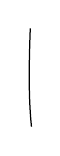
\begin{tikzpicture}[x=1cm,y=1cm]
\draw[line width=.45pt] (0,1.25) .. controls (-.015,.82) and (-.025,.40) .. (.015,0);
\end{tikzpicture}}

Pour le montrer, on va plonger
$\Pi_{0,3}$ comme sous-groupe d'indice fini
dans $\Pi'_{0,3}$, d'où un plongement \LMsourceMark{M016615}{\unsure{analogue}}
\var{\deleted{\LMsourceMark{M016616}{\illegible{1}}}}{\LMsourceMark{M016617}{\LMcancelledDoubts{\LMsourceMark{M016618}{\illegible{1}}}}}{deletion}{140-2-s506-D003}
\[
(2)\qquad\widehat{\Pi}_{0,3}\lhook\joinrel\longrightarrow\widehat{\Pi}'_{0,3}
\]
qui sera compatible avec l'action ext. de $\Gamma$.

\LMflushnotes\LMflushpages
\ifnum\LMform=1
\begin{LMapparatus}
\LMentry{140-2-s506-I001}{insertion}{\inserted{pour structures triangulées}
}{\emph{\LMinsertedlabel}}{Ajout explicite de l'auteur : intégré à l'endroit indiqué par la transcription, sans modifier sa lecture.}{}
\LMentry{140-2-s506-D001}{suppression}{\deleted{dont les}
}{\emph{\LMomittedlabel}}{Passage biffé dans le manuscrit : la suppression suit l'état final de l'auteur; les doutes de lecture restent signalés.}{}
\LMentry{140-2-s506-D002}{suppression}{\deleted{sur lesquels}
}{\emph{\LMomittedlabel}}{Passage biffé dans le manuscrit : la suppression suit l'état final de l'auteur; les doutes de lecture restent signalés.}{}
\LMentry{140-2-s506-D003}{suppression}{\deleted{\LMsourceMark{M016619}{\illegible{1}}}
}{\emph{\LMomittedlabel}}{Passage biffé dans le manuscrit : la suppression suit l'état final de l'auteur; les doutes de lecture restent signalés.}{}
\end{LMapparatus}
\fi
\ifnum\LMform=2
\par\smallskip\begingroup\footnotesize\Needspace{4\baselineskip}\csname @beginparpenalty\endcsname=10000\relax\noindent\textcolor{gray}{\rule{.2\linewidth}{.35pt}}\par\nobreak
\noindent\textit{\LMdoubtheading.}\par\nobreak
\LMcarryover{140-2-s506-D003}{\LMsourceMark{M016620}{\illegible{1}}
}
\par\endgroup\smallskip
\fi

\LMsourceMark{M016621}{\scanpage{507}}

Considérons pour cela le schéma quotient
\[
Y=\underbrace{\mathbb P^1_{\mathbb Q}}_{X}/\LMsourceMark{M016622}{\unsure{\mathfrak S_3}}
\]
avec les trois points \var{\inserted{$a_0,a_1,a_\infty$}}{\LMadded{$a_0,a_1,a_\infty$}}{insertion}{140-2-s507-I001} de $Y$, rationnels sur
$\mathbb Q$, \var{\inserted{$a_0$}}{\LMadded{$a_0$}}{insertion}{140-2-s507-I002} correspondant à la trajectoire
\var{\deleted{des}}{}{deletion}{140-2-s507-D001} $\{0,1,\infty\}$, $a_1$ à la trajectoire
$\{-1,\frac12,2\}$, et $a_\infty$ à la trajectoire
$\{\LMsourceMark{M016623}{\unsure{-j}},\LMsourceMark{M016624}{\unsure{-\overline j}}\}$ de $\LMsourceMark{M016625}{\unsure{\mathfrak S_3}}$
\LMsourceMark{M016626}{\margin{$j=\exp\frac{2i\pi}{3}$}}
(ce qui épuise \LMsourceMark{M016627}{\unsure{l'ens}} des trajectoires
``singulières'' géométriques). On sait que $Y$ est une droite projective
(sur $\overline{\mathbb Q}$ a priori), \LMsourceMark{M016628}{\unsure{qu'on}} \LMsourceMark{M016629}{\unsure{épingle}} par
$a_0,a_1,a_\infty$ comme points $0,1,\infty$, \LMsourceMark{M016630}{\unsure{(donc}}
$Y\simeq\mathbb P^1_{\mathbb Q}$ -- le \var{\deleted{\LMsourceMark{M016631}{\illegible{1}}}}{\LMsourceMark{M016632}{\LMcancelledDoubts{\LMsourceMark{M016633}{\illegible{1}}}}}{deletion}{140-2-s507-D002} morphisme
$X\longrightarrow Y$ s'identifie donc à un morphisme bien déterminé
\[
(3)\qquad
f:\begin{array}{ccc}
\mathbb P^1_{\mathbb Q}&\longrightarrow&\mathbb P^1_{\mathbb Q}\\
\Vert&&\Vert\\
X&&Y
\end{array}
\]
\var{\deleted{(en fait, $f$ peut se définir comme morphisme
$\mathbb P^1_{\mathbb Z}\longrightarrow\mathbb P^1_{\mathbb Z}$,
mais ici peu nous importe)}}{}{deletion}{140-2-s507-D003}
qui fait de $X$ un \LMsourceMark{M016634}{\unsure{revêtt|revêtement}} galoisien de $Y$, de groupe
$\LMsourceMark{M016635}{\unsure{\mathfrak S_3}}$, étale \LMsourceMark{M016636}{\unsure{au|en}} dessus de
$\mathbb P^1_{\mathbb Q}\setminus\{0,1,\infty\}$, avec comme indices de
ramification en ces points $2,2,3$. Du point de vue de la géométrie des cartes
(\LMsourceMark{M016637}{\unsure{se plaçant|se plongeant}} sur le corps de base $\mathbb C$), on considère la

\LMflushnotes\LMflushpages
\ifnum\LMform=1
\begin{LMapparatus}
\LMentry{140-2-s507-I001}{insertion}{\inserted{$a_0,a_1,a_\infty$}
}{\emph{\LMinsertedlabel}}{Ajout explicite de l'auteur : intégré à l'endroit indiqué par la transcription, sans modifier sa lecture.}{}
\LMentry{140-2-s507-I002}{insertion}{\inserted{$a_0$}
}{\emph{\LMinsertedlabel}}{Ajout explicite de l'auteur : intégré à l'endroit indiqué par la transcription, sans modifier sa lecture.}{}
\LMentry{140-2-s507-D001}{suppression}{\deleted{des}
}{\emph{\LMomittedlabel}}{Passage biffé dans le manuscrit : la suppression suit l'état final de l'auteur; les doutes de lecture restent signalés.}{}
\LMentry{140-2-s507-D002}{suppression}{\deleted{\LMsourceMark{M016638}{\illegible{1}}}
}{\emph{\LMomittedlabel}}{Passage biffé dans le manuscrit : la suppression suit l'état final de l'auteur; les doutes de lecture restent signalés.}{}
\LMentry{140-2-s507-D003}{suppression}{\deleted{(en fait, $f$ peut se définir comme morphisme
$\mathbb P^1_{\mathbb Z}\longrightarrow\mathbb P^1_{\mathbb Z}$,
mais ici peu nous importe)}
}{\emph{\LMomittedlabel}}{Passage biffé dans le manuscrit : la suppression suit l'état final de l'auteur; les doutes de lecture restent signalés.}{}
\end{LMapparatus}
\fi
\ifnum\LMform=2
\par\smallskip\begingroup\footnotesize\Needspace{4\baselineskip}\csname @beginparpenalty\endcsname=10000\relax\noindent\textcolor{gray}{\rule{.2\linewidth}{.35pt}}\par\nobreak
\noindent\textit{\LMdoubtheading.}\par\nobreak
\LMcarryover{140-2-s507-D002}{\LMsourceMark{M016639}{\illegible{1}}
}
\par\endgroup\smallskip
\fi

\LMsourceMark{M016640}{\scanpage{508}}
\LMsourceMark{M016641}{\mspage{\LMsourceMark{M016642}{\unsure{258 (259)}}}}

carte déterminée sur $X$ par les triangles sphériques $(0,1,\infty)$
(sur l'axe réel comme équateur) -- qui est donc la carte triangulaire
\LMsourceMark{M016643}{\unsure{pondérée}} universelle -- comme image inverse de la carte universelle
(ayant un seul sommet $0$, une seule arête (repliée) $0\longrightarrow1$,
une seule face, de centre $\infty$).
\LMsourceMark{M016644}{\margin{\figure{\begin{tikzpicture}[x=1cm,y=1cm,line cap=round,line join=round]
\draw[line width=.45pt] (0,2.85)
 .. controls (-.71,2.83) and (-1.02,2.47) .. (-1,2)
 .. controls (-1.01,1.48) and (-.57,1.16) .. (0,1.15);
\draw[line width=.45pt] (0,2.85)
 .. controls (.76,2.85) and (1.03,2.48) .. (1,2.10);
\draw[line width=.45pt] (.99,1.98)
 .. controls (.98,1.62) and (.74,1.36) .. (.54,1.26);
\draw[line width=.5pt] (-1,2)
 .. controls (-.91,1.75) and (.83,1.74) .. (1,1.95);
\draw[densely dotted,line width=.65pt] (-1,2)
 .. controls (-.61,2.17) and (.63,2.17) .. (1,2.02);
\fill (0,2.85) circle (1.4pt);
\node[anchor=south west,inner sep=2pt] at (0,2.88) {$P=\LMsourceMark{M016645}{\unsure{-\bar j|-j}}$};
\fill (0,1.15) circle (1.4pt);
\node[anchor=north west,inner sep=2pt] at (-.03,1.12) {$P'=\LMsourceMark{M016646}{\unsure{-j|-\bar j}}$};
\fill (-.57,1.80) circle (1.4pt);
\node[below,inner sep=2pt] at (-.57,1.80) {$0$};
\fill (.78,1.82) circle (1.4pt);
\node[below,inner sep=2pt] at (.78,1.82) {$1$};
\fill (0,2.12) circle (1.5pt);
\node[above,inner sep=2pt] at (0,2.12) {$\infty$};
\draw[->,line width=.65pt] (-1.40,1.60)
 .. controls (-1.40,1.22) and (-1.38,.85) .. (-1.37,.58);
\draw[line width=.45pt] (.02,.48)
 .. controls (-.55,.48) and (-.86,.17) .. (-.82,-.20)
 .. controls (-.78,-.70) and (-.46,-1.02) .. (.10,-1.04);
\draw[line width=.45pt] (.02,.48)
 .. controls (.65,.46) and (.87,.12) .. (.82,-.29)
 .. controls (.81,-.58) and (.66,-.79) .. (.53,-.87);
\fill (.02,.48) circle (1.5pt);
\node[anchor=west,inner sep=2pt] at (.07,.48) {$\LMsourceMark{M016647}{\unsure{Q}}(=P)$};
\fill (-.82,-.12) circle (1.5pt);
\node[left,inner sep=2pt] at (-.82,-.12) {$\infty$};
\fill (-.08,.10) circle (1.7pt);
\node[below,inner sep=2pt] at (-.08,.10) {$1$};
\fill (-.40,-.36) circle (1.7pt);
\node[below,inner sep=2pt] at (-.40,-.36) {$0$};
\draw[line width=1.15pt] (-.08,.10)
 .. controls (.28,.10) and (.71,.02) .. (.82,-.20)
 .. controls (.66,-.43) and (.03,-.47) .. (-.40,-.36);
\draw[densely dotted,line width=.65pt] (-.82,-.12)
 .. controls (-.60,.08) and (-.36,.08) .. (-.08,.10);
\draw[densely dotted,line width=.65pt] (-.82,-.12)
 .. controls (-.78,-.32) and (-.59,-.35) .. (-.40,-.36);
\node[below,inner sep=1pt] at (.22,-.44) {$\LMsourceMark{M016648}{\unsure{\varphi}}$};
\end{tikzpicture}}}}
Tout revêtement \var{\deleted{\LMsourceMark{M016649}{\unsure{de}}}}{\LMsourceMark{M016650}{\LMcancelledDoubts{\LMsourceMark{M016651}{\unsure{de}}}}}{deletion}{140-2-s508-D001} \var{\inserted{étale}}{\LMadded{étale}}{insertion}{140-2-s508-I001} topologique de
$U_{03}(\mathbb C)\subset X$ donne ainsi un rev. étale topologique de
$U_{0,3}(\mathbb C)\subset Y$, \var{\deleted{ramifié}}{}{deletion}{140-2-s508-D002} ayant au
\var{\deleted{\LMsourceMark{M016652}{\illegible{1}}}}{\LMsourceMark{M016653}{\LMcancelledDoubts{\LMsourceMark{M016654}{\illegible{1}}}}}{deletion}{140-2-s508-D003} \var{\inserted{dessus de}}{\LMadded{dessus de}}{insertion}{140-2-s508-I002} $1$ la ramification $2$,
au dessus de $\infty$ la ramification $3$ \LMsourceMark{M016655}{\unsure{exactt|exactement}},
ce qui correspond au foncteur ``oubli'' \var{\inserted{(de la pondération)}}{\LMadded{(de la pondération)}}{insertion}{140-2-s508-I003},
où une carte triangulaire \LMsourceMark{M016656}{\unsure{pondérée}} est considérée comme une carte
tout court. Du point de vue des groupes fondamentaux \LMsourceMark{M016657}{\unsure{on}} trouve
ainsi une \var{\deleted{\LMsourceMark{M016658}{\unsure{hom.}} de groupes extérieurs}}{\LMsourceMark{M016659}{\LMcancelledDoubts{\LMsourceMark{M016660}{\unsure{hom.}}}}}{deletion}{140-2-s508-D004}
\var{\inserted{équiv. de catégories}}{\LMadded{équiv. de catégories}}{insertion}{140-2-s508-I004}

\diagram{\begin{tikzcd}[ampersand replacement=\&,column sep=large,row sep=huge,column sep=9pt,row sep=14pt,execute at begin picture={\fontsize{10}{12}\selectfont},nodes in empty cells]
\&
\var{\deleted{\begin{gathered}
\Pi_1(\LMsourceMark{M016661}{\unsure{X(\mathbb C)}}\setminus\{0,1,\infty\})\\[-2pt]
\rotatebox{90}{$=$}\\[-2pt]
\Pi_{0,3}
\end{gathered}}}{\LMsourceMark{M016662}{\LMcancelledDoubts{\(\LMsourceMark{M016663}{\unsure{X(\mathbb C)}}\)}}}{deletion}{140-2-s508-D005}
\arrow[r,phantom,"{\var{\deleted{\longleftarrow}}{}{deletion}{140-2-s508-D006}}" description]
\&
\var{\deleted{\begin{gathered}
\Pi_1\!\left(Y(\mathbb C)\setminus\{0,1,\infty\};
\underbrace{2\{1\}+3\{\infty\}}_{\substack{\text{signature de}\\\text{ramification}}}\right)\\[-2pt]
\rotatebox{90}{$=$}\\[-2pt]
\Pi'_{0,3}
\end{gathered}}}{}{deletion}{140-2-s508-D007}
\\
(\var{\deleted{\LMsourceMark{M016664}{\illegible{1}}}}{\LMsourceMark{M016665}{\LMcancelledDoubts{\(\LMsourceMark{M016666}{\illegible{1}}\)}}}{deletion}{140-2-s508-D008}\var{\inserted{4}}{\LMadded{4}}{insertion}{140-2-s508-I005}) \&
\left(\text{Rev. étales de }X\setminus\{0,1,\infty\}=U_{0,3}\right)
\arrow[r,phantom,"\simeq" description]
\arrow[d,phantom,"{\rotatebox{-90}{$\simeq$}}" description]
\&
\begin{gathered}
\left[\begin{gathered}
\text{Rev. de }Y\setminus\{0,1,\infty\}=U_{0,3}\\
\text{avec ramification sub. à}\\
\text{la signature }2\{1\}+3\{\infty\}
\end{gathered}\right]\\
\big/\begin{gathered}
\text{l'objet }(X\setminus\{0,1,\infty\})\\
\text{de la dite catégorie}
\end{gathered}
\end{gathered}
\arrow[d,phantom,"{\rotatebox{90}{$\simeq$}}" description]
\\
\& \Pi_{0,3}\text{-ensembles} \&
(\Pi'_{0,3}\text{-Ens})/\var{\deleted{\LMsourceMark{M016667}{\unsure{E}}}}{\LMsourceMark{M016668}{\LMcancelledDoubts{\(\LMsourceMark{M016669}{\unsure{E}}\)}}}{deletion}{140-2-s508-D009}E
\end{tikzcd}}

où $E$ est le $\Pi'_{0,3}$-ens. correspondant à l'objet
$X\setminus\{0,1,\infty\}$ de la cat. des rev. étales de
$\LMsourceMark{M016670}{\unsure{Y\setminus\{0,1,\infty\}}}$ à ramification
\var{\deleted{\LMsourceMark{M016671}{\unsure{imposée}}}}{\LMsourceMark{M016672}{\LMcancelledDoubts{\LMsourceMark{M016673}{\unsure{imposée}}}}}{deletion}{140-2-s508-D010}\var{\inserted{\LMsourceMark{M016674}{\unsure{subordon-}}}}{\LMadded{\LMsourceMark{M016675}{\unsure{subordon-}}}}{insertion}{140-2-s508-I006}née à
$2\{1\}+3\{\infty\}$

\var{\deleted{$\LMsourceMark{M016676}{\unsure{\simeq}}\ \LMsourceMark{M016677}{\unsure{\Pi_{0,3}^{\prime\circ}}}\in\mathrm{Ens}$}}{\LMsourceMark{M016678}{\LMcancelledDoubts{\(\LMsourceMark{M016679}{\unsure{\simeq}}\)\quad \(\LMsourceMark{M016680}{\unsure{\Pi_{0,3}^{\prime\circ}}}\)}}}{deletion}{140-2-s508-D011}

\LMflushnotes\LMflushpages
\ifnum\LMform=1
\begin{LMapparatus}
\LMentry{140-2-s508-D001}{suppression}{\deleted{\LMsourceMark{M016681}{\unsure{de}}}
}{\emph{\LMomittedlabel}}{Passage biffé dans le manuscrit : la suppression suit l'état final de l'auteur; les doutes de lecture restent signalés.}{}
\LMentry{140-2-s508-I001}{insertion}{\inserted{étale}
}{\emph{\LMinsertedlabel}}{Ajout explicite de l'auteur : intégré à l'endroit indiqué par la transcription, sans modifier sa lecture.}{}
\LMentry{140-2-s508-D002}{suppression}{\deleted{ramifié}
}{\emph{\LMomittedlabel}}{Passage biffé dans le manuscrit : la suppression suit l'état final de l'auteur; les doutes de lecture restent signalés.}{}
\LMentry{140-2-s508-D003}{suppression}{\deleted{\LMsourceMark{M016682}{\illegible{1}}}
}{\emph{\LMomittedlabel}}{Passage biffé dans le manuscrit : la suppression suit l'état final de l'auteur; les doutes de lecture restent signalés.}{}
\LMentry{140-2-s508-I002}{insertion}{\inserted{dessus de}
}{\emph{\LMinsertedlabel}}{Ajout explicite de l'auteur : intégré à l'endroit indiqué par la transcription, sans modifier sa lecture.}{}
\LMentry{140-2-s508-I003}{insertion}{\inserted{(de la pondération)}
}{\emph{\LMinsertedlabel}}{Ajout explicite de l'auteur : intégré à l'endroit indiqué par la transcription, sans modifier sa lecture.}{}
\LMentry{140-2-s508-D004}{suppression}{\deleted{\LMsourceMark{M016683}{\unsure{hom.}} de groupes extérieurs}
}{\emph{\LMomittedlabel}}{Passage biffé dans le manuscrit : la suppression suit l'état final de l'auteur; les doutes de lecture restent signalés.}{}
\LMentry{140-2-s508-I004}{insertion}{\inserted{équiv. de catégories}
}{\emph{\LMinsertedlabel}}{Ajout explicite de l'auteur : intégré à l'endroit indiqué par la transcription, sans modifier sa lecture.}{}
\LMentry{140-2-s508-D005}{suppression}{\(\deleted{\begin{gathered}
\Pi_1(\LMsourceMark{M016684}{\unsure{X(\mathbb C)}}\setminus\{0,1,\infty\})\\[-2pt]
\rotatebox{90}{$=$}\\[-2pt]
\Pi_{0,3}
\end{gathered}}\)
}{\emph{\LMomittedlabel}}{Passage biffé dans le manuscrit : la suppression suit l'état final de l'auteur; les doutes de lecture restent signalés.}{}
\LMentry{140-2-s508-D006}{suppression}{\(\deleted{\longleftarrow}\)
}{\emph{\LMomittedlabel}}{Passage biffé dans le manuscrit : la suppression suit l'état final de l'auteur; les doutes de lecture restent signalés.}{}
\LMentry{140-2-s508-D007}{suppression}{\(\deleted{\begin{gathered}
\Pi_1\!\left(Y(\mathbb C)\setminus\{0,1,\infty\};
\underbrace{2\{1\}+3\{\infty\}}_{\substack{\text{signature de}\\\text{ramification}}}\right)\\[-2pt]
\rotatebox{90}{$=$}\\[-2pt]
\Pi'_{0,3}
\end{gathered}}\)
}{\emph{\LMomittedlabel}}{Passage biffé dans le manuscrit : la suppression suit l'état final de l'auteur; les doutes de lecture restent signalés.}{}
\LMentry{140-2-s508-D008}{suppression}{\(\deleted{\LMsourceMark{M016685}{\illegible{1}}}\)
}{\emph{\LMomittedlabel}}{Passage biffé dans le manuscrit : la suppression suit l'état final de l'auteur; les doutes de lecture restent signalés.}{}
\LMentry{140-2-s508-I005}{insertion}{\(\inserted{4}\)
}{\emph{\LMinsertedlabel}}{Ajout explicite de l'auteur : intégré à l'endroit indiqué par la transcription, sans modifier sa lecture.}{}
\LMentry{140-2-s508-D009}{suppression}{\(\deleted{\LMsourceMark{M016686}{\unsure{E}}}\)
}{\emph{\LMomittedlabel}}{Passage biffé dans le manuscrit : la suppression suit l'état final de l'auteur; les doutes de lecture restent signalés.}{}
\LMentry{140-2-s508-D010}{suppression}{\deleted{\LMsourceMark{M016687}{\unsure{imposée}}}
}{\emph{\LMomittedlabel}}{Passage biffé dans le manuscrit : la suppression suit l'état final de l'auteur; les doutes de lecture restent signalés.}{}
\LMentry{140-2-s508-I006}{insertion}{\inserted{\LMsourceMark{M016688}{\unsure{subordon-}}}
}{\emph{\LMinsertedlabel}}{Ajout explicite de l'auteur : intégré à l'endroit indiqué par la transcription, sans modifier sa lecture.}{}
\LMentry{140-2-s508-D011}{suppression}{\deleted{$\LMsourceMark{M016689}{\unsure{\simeq}}\ \LMsourceMark{M016690}{\unsure{\Pi_{0,3}^{\prime\circ}}}\in\mathrm{Ens}$}
}{\emph{\LMomittedlabel}}{Passage biffé dans le manuscrit : la suppression suit l'état final de l'auteur; les doutes de lecture restent signalés.}{}
\end{LMapparatus}
\fi
\ifnum\LMform=2
\par\smallskip\begingroup\footnotesize\Needspace{4\baselineskip}\csname @beginparpenalty\endcsname=10000\relax\noindent\textcolor{gray}{\rule{.2\linewidth}{.35pt}}\par\nobreak
\noindent\textit{\LMdoubtheading.}\par\nobreak
\LMcarryover{140-2-s508-D001}{\LMsourceMark{M016691}{\unsure{de}}
}
\LMcarryover{140-2-s508-D003}{\LMsourceMark{M016692}{\illegible{1}}
}
\LMcarryover{140-2-s508-D004}{\LMsourceMark{M016693}{\unsure{hom.}}
}
\LMcarryover{140-2-s508-D005}{\(\LMsourceMark{M016694}{\unsure{X(\mathbb C)}}\)
}
\LMcarryover{140-2-s508-D008}{\(\LMsourceMark{M016695}{\illegible{1}}\)
}
\LMcarryover{140-2-s508-D009}{\(\LMsourceMark{M016696}{\unsure{E}}\)
}
\LMcarryover{140-2-s508-D010}{\LMsourceMark{M016697}{\unsure{imposée}}
}
\LMcarryover{140-2-s508-D011}{\(\LMsourceMark{M016698}{\unsure{\simeq}}\)\quad \(\LMsourceMark{M016699}{\unsure{\Pi_{0,3}^{\prime\circ}}}\)
}
\par\endgroup\smallskip
\fi

\LMsourceMark{M016700}{\scanpage{509}}
\LMsourceMark{M016701}{\mspage{\LMsourceMark{M016702}{\unsure{260|250}}}}

Ici, \var{\deleted{\LMsourceMark{M016703}{\illegible{3}}}}{\LMsourceMark{M016704}{\LMcancelledDoubts{\LMsourceMark{M016705}{\illegible{3}}}}}{deletion}{140-2-s509-D001} \var{\inserted{\deleted{\LMsourceMark{M016706}{\illegible{1}}} le point base de $Y-\{0,1,\infty\}$ choisi\LMsourceMark{M016707}{\unsure{;|,}} \LMsourceMark{M016708}{\unsure{pour}} décrire les}}{\LMadded{\var{\deleted{\LMsourceMark{M016709}{\illegible{1}}}}{\LMsourceMark{M016710}{\LMcancelledDoubts{\LMsourceMark{M016711}{\illegible{1}}}}}{deletion}{140-2-s509-D002} le point base de $Y-\{0,1,\infty\}$ choisi\LMsourceMark{M016712}{\unsure{;|,}} \LMsourceMark{M016713}{\unsure{pour}} décrire les}}{insertion}{140-2-s509-I001} revêtements \var{\deleted{$E=\LMsourceMark{M016714}{\unsure{f^{-1}}}\LMsourceMark{M016715}{\unsure{(}}$}}{\LMsourceMark{M016716}{\LMcancelledDoubts{\(\LMsourceMark{M016717}{\unsure{f^{-1}}}\)\quad \(\LMsourceMark{M016718}{\unsure{(}}\)}}}{deletion}{140-2-s509-D003} (à ramification \LMsourceMark{M016719}{\unsure{subordonnée}} à \dots) par un groupe fondamental à ramification, étant \LMsourceMark{M016720}{\unsure{encore}} $P=-\bar j$, on aura
\[
(5)\qquad E=f_{\LMsourceMark{M016721}{\unsure{\mathbf C|\mathbb C}}}^{-1}(P)
\]
et on peut expliciter ainsi la cat. $(\Pi'_{03}\text{-Ens})/E$\LMsourceMark{M016722}{\unsure{;}}

Où $E$ est un espace homogène, \var{\inserted{\LMsourceMark{M016723}{\unsure{isom. au}}}}{\LMadded{\LMsourceMark{M016724}{\unsure{isom. au}}}}{insertion}{140-2-s509-I002} \LMsourceMark{M016725}{\unsure{quot.}} de $\Pi'_{03}$ par le \LMsourceMark{M016726}{\unsure{ss-groupe|s-groupe}} \var{\inserted{$\Pi'^{\circ}_{03}$}}{\LMadded{$\Pi'^{\circ}_{03}$}}{insertion}{140-2-s509-I003} noyau de l'hom. surjectif \var{\inserted{idoine}}{\LMadded{idoine}}{insertion}{140-2-s509-I004}
\[
(6)\qquad
\left\{
\begin{array}{l}
\Pi'_{0,3}\longrightarrow\LMsourceMark{M016727}{\unsure{\mathfrak S_3|\mathcal S_3}}\\[2pt]
\left.
\begin{array}{lll}
\ell_0 &\longmapsto& \text{él. d'ordre 2}\\
\ell_1 &\longmapsto& \text{él. d'ordre 2}\\
\ell_\infty &\longmapsto& \text{\LMsourceMark{M016728}{\unsure{él.}} d'ordre 3}
\end{array}
\right)\quad\text{à calculer !}
\end{array}
\right.
\]

On choisit un $Q_0\in E$ comme ``origine'' de $E$ -- pour pouvoir identifier $E$ comme $\Pi'_{0,3}$-ens à $\Pi'_{03}/\Pi'^{\circ}_{03}\simeq\LMsourceMark{M016729}{\unsure{\mathfrak S_3}}$ -- alors $(\mathrm{Ens}\,\Pi'_{03})/E$ s'identifie, par le foncteur $F\longmapsto F_{Q_0}$, à $\mathrm{Ens}(\Pi'^{\circ}_{03})$.

On trouve donc en résumé une équivalence de catégories (dépendant du choix de $Q_0$)
\[
\Pi_{03}\text{-ens}\quad\LMsourceMark{M016730}{\unsure{\simeq}}\quad\Pi'^{\circ}_{03}\text{-ensembles}
\]
qui est elle-même décrite par un bitorseur sous $(\Pi'^{\circ}_{0,3},\Pi_{03})$ -- et, à isom \var{\deleted{que}}{}{deletion}{140-2-s509-D004} (non unique !) près, par un isomorphisme
\[
\Pi_{03}\simeq\Pi'^{\circ}_{0,3}\quad -
\]
les isomorphismes ainsi obtenus (pour des

\LMflushnotes\LMflushpages
\ifnum\LMform=1
\begin{LMapparatus}
\LMentry{140-2-s509-D001}{suppression}{\deleted{\LMsourceMark{M016731}{\illegible{3}}}
}{\emph{\LMomittedlabel}}{Passage biffé dans le manuscrit : la suppression suit l'état final de l'auteur; les doutes de lecture restent signalés.}{}
\LMentry{140-2-s509-I001}{insertion}{\inserted{\deleted{\LMsourceMark{M016732}{\illegible{1}}} le point base de $Y-\{0,1,\infty\}$ choisi\LMsourceMark{M016733}{\unsure{;|,}} \LMsourceMark{M016734}{\unsure{pour}} décrire les}
}{\emph{\LMinsertedlabel}}{Ajout explicite de l'auteur : intégré à l'endroit indiqué par la transcription, sans modifier sa lecture.}{}
\LMentry{140-2-s509-D002}{suppression}{\deleted{\LMsourceMark{M016735}{\illegible{1}}}
}{\emph{\LMomittedlabel}}{Passage biffé dans le manuscrit : la suppression suit l'état final de l'auteur; les doutes de lecture restent signalés.}{}
\LMentry{140-2-s509-D003}{suppression}{\deleted{$E=\LMsourceMark{M016736}{\unsure{f^{-1}}}\LMsourceMark{M016737}{\unsure{(}}$}
}{\emph{\LMomittedlabel}}{Passage biffé dans le manuscrit : la suppression suit l'état final de l'auteur; les doutes de lecture restent signalés.}{}
\LMentry{140-2-s509-I002}{insertion}{\inserted{\LMsourceMark{M016738}{\unsure{isom. au}}}
}{\emph{\LMinsertedlabel}}{Ajout explicite de l'auteur : intégré à l'endroit indiqué par la transcription, sans modifier sa lecture.}{}
\LMentry{140-2-s509-I003}{insertion}{\inserted{$\Pi'^{\circ}_{03}$}
}{\emph{\LMinsertedlabel}}{Ajout explicite de l'auteur : intégré à l'endroit indiqué par la transcription, sans modifier sa lecture.}{}
\LMentry{140-2-s509-I004}{insertion}{\inserted{idoine}
}{\emph{\LMinsertedlabel}}{Ajout explicite de l'auteur : intégré à l'endroit indiqué par la transcription, sans modifier sa lecture.}{}
\LMentry{140-2-s509-D004}{suppression}{\deleted{que}
}{\emph{\LMomittedlabel}}{Passage biffé dans le manuscrit : la suppression suit l'état final de l'auteur; les doutes de lecture restent signalés.}{}
\end{LMapparatus}
\fi
\ifnum\LMform=2
\par\smallskip\begingroup\footnotesize\Needspace{4\baselineskip}\csname @beginparpenalty\endcsname=10000\relax\noindent\textcolor{gray}{\rule{.2\linewidth}{.35pt}}\par\nobreak
\noindent\textit{\LMdoubtheading.}\par\nobreak
\LMcarryover{140-2-s509-D001}{\LMsourceMark{M016739}{\illegible{3}}
}
\LMcarryover{140-2-s509-D002}{\LMsourceMark{M016740}{\illegible{1}}
}
\LMcarryover{140-2-s509-D003}{\(\LMsourceMark{M016741}{\unsure{f^{-1}}}\)\quad \(\LMsourceMark{M016742}{\unsure{(}}\)
}
\par\endgroup\smallskip
\fi

\LMsourceMark{M016743}{\scanpage{510}}
\LMsourceMark{M016744}{\mspage{\LMsourceMark{M016745}{\unsure{249}}}}

origines variables du bitorseur) \LMsourceMark{M016746}{\unsure{forment|formant}} exactement une classe de conjugaison par $\Pi'^{\circ}_{03}$ -- i.e. un \uline{\LMsourceMark{M016747}{\unsure{isom.}}} \uline{extérieur} $\Pi_{03}\simeq\Pi'^{\circ}_{03}$. Quand de plus le choix de $Q_0$ varie, on trouve \var{\deleted{comme}}{}{deletion}{140-2-s510-D001} un \LMsourceMark{M016748}{\unsure{composé|composés}}
\[
\Pi_{0,3}\longrightarrow\Pi'^{\circ}_{03}\longrightarrow\Pi'_{03}
\]
\var{\deleted{\LMsourceMark{M016749}{\unsure{exactement}}}}{\LMsourceMark{M016750}{\LMcancelledDoubts{\LMsourceMark{M016751}{\unsure{exactement}}}}}{deletion}{140-2-s510-D002} une classe de $\Pi'_{03}$-conj, i.e. un hom extérieur.

J'ai beaucoup \LMsourceMark{M016752}{\unsure{turbiné}} pour pas grand chose -- à défaut d'avoir écrit les \LMsourceMark{M016753}{\unsure{fonctorialités}} \var{\inserted{générales}}{\LMadded{générales}}{insertion}{140-2-s510-I001} \LMsourceMark{M016754}{\unsure{nécessaires|élémentaires}} pour les ``groupes fondamentaux \LMsourceMark{M016755}{\unsure{avec}} ramification''. \LMsourceMark{M016756}{\unsure{P.ex.}} le bifoncteur $I$ mystérieux de tantôt est formé des \LMsourceMark{M016757}{\unsure{classes}} de chemins de $P\in\LMsourceMark{M016758}{\unsure{X(\mathbb C)|X_{\mathbb C}}}\setminus\{0,1,\infty\}$ (point base pour calculer $\Pi_{0,3}$) vers $Q_0$ (jouant le rôle d'un nouveau pt base, ayant le mérite de s'envoyer sur celui \var{\inserted{-- $P$ --}}{\LMadded{-- $P$ --}}{insertion}{140-2-s510-I002} qui sert à calculer $\Pi'_{03}$, groupe fondamental à ramification sur $Y(\mathbb C)\setminus\{0,1,\infty\}$ \dots) Il serait peut-être plus commode de définir \LMsourceMark{M016759}{\unsure{direct\textsuperscript{t}|directement}} un foncteur en sens inverse\LMsourceMark{M016760}{\unsure{:|.}}
\[
(7)\qquad
\begin{array}{c}
\text{Rev. de }Y(\mathbb C)\var{\inserted{\setminus(0,1,\infty)}}{\LMadded{\setminus(0,1,\infty)}}{insertion}{140-2-s510-I003}\ \text{subordonnés}\\
\text{à la signature }2\{1\}+3\{\infty\}
\end{array}
\longrightarrow
\begin{array}{c}
\text{Rev. \LMsourceMark{M016761}{\unsure{ét.les|étales}} de}\\
X(\mathbb C)\setminus\{0,1,\infty\}
\end{array}
\]
par image inverse, \LMsourceMark{M016762}{\unsure{suivi|suivie}} d'une \uline{normalisation}

\LMflushnotes\LMflushpages
\ifnum\LMform=1
\begin{LMapparatus}
\LMentry{140-2-s510-D001}{suppression}{\deleted{comme}
}{\emph{\LMomittedlabel}}{Passage biffé dans le manuscrit : la suppression suit l'état final de l'auteur; les doutes de lecture restent signalés.}{}
\LMentry{140-2-s510-D002}{suppression}{\deleted{\LMsourceMark{M016763}{\unsure{exactement}}}
}{\emph{\LMomittedlabel}}{Passage biffé dans le manuscrit : la suppression suit l'état final de l'auteur; les doutes de lecture restent signalés.}{}
\LMentry{140-2-s510-I001}{insertion}{\inserted{générales}
}{\emph{\LMinsertedlabel}}{Ajout explicite de l'auteur : intégré à l'endroit indiqué par la transcription, sans modifier sa lecture.}{}
\LMentry{140-2-s510-I002}{insertion}{\inserted{-- $P$ --}
}{\emph{\LMinsertedlabel}}{Ajout explicite de l'auteur : intégré à l'endroit indiqué par la transcription, sans modifier sa lecture.}{}
\LMentry{140-2-s510-I003}{insertion}{\(\inserted{\setminus(0,1,\infty)}\)
}{\emph{\LMinsertedlabel}}{Ajout explicite de l'auteur : intégré à l'endroit indiqué par la transcription, sans modifier sa lecture.}{}
\end{LMapparatus}
\fi
\ifnum\LMform=2
\par\smallskip\begingroup\footnotesize\Needspace{4\baselineskip}\csname @beginparpenalty\endcsname=10000\relax\noindent\textcolor{gray}{\rule{.2\linewidth}{.35pt}}\par\nobreak
\noindent\textit{\LMdoubtheading.}\par\nobreak
\LMcarryover{140-2-s510-D002}{\LMsourceMark{M016764}{\unsure{exactement}}
}
\par\endgroup\smallskip
\fi

% END PACKAGE LM_P051
% BEGIN PACKAGE LM_P052
\ifnum\LMform<2\Needspace{11\baselineskip}\subsection*{Scans 511--520}\fi
\LMsourceMark{M016765}{\scanpage{511}}
\LMsourceMark{M016766}{\mspage{261}}

-- Ici on utilise le fait que l'objet $X(\mathbb C)\setminus\{0,1,\infty\}$ de la catégorie des \LMsourceMark{M016767}{\unsure{rev\textsuperscript{ts}}} à ramification maximum \LMsourceMark{M016768}{\unsure{imposé|imposée}}, réalise justement un maximum, en les pts $1,\infty$ où la condition intervient.
On trouve que le foncteur correspondant
\[
\tag{7 bis}
\Pi'_{03}\text{-}\mathrm{Ens}\longrightarrow(\Pi_{0,3}\text{-}\mathrm{Ens})
\]
a les propriétés d'exactitude d'un foncteur associé à un morphisme de topos galoisiens
\diagram{\begin{tikzcd}[ampersand replacement=\&]
\overset{\var{\inserted{\LMsourceMark{M016769}{\unsure{B}}}}{\LMadded{\LMsourceMark{M016770}{\unsure{B}}}}{insertion}{140-2-s511-I001}}{\LMsourceMark{M016771}{\unsure{B|D}}}_{\Pi_{03}} \arrow[r] \& B_{\Pi'_{0,3}}
\end{tikzcd}}
(\LMsourceMark{M016772}{\unsure{commute aux}} $\underset{\longrightarrow}{\lim}$ \LMsourceMark{M016773}{\unsure{quelc.}}, exact à g.) et est donc défini par un $(\Pi_{03}^{\var{\deleted{\LMsourceMark{M016774}{\unsure{\wedge}}}}{\LMsourceMark{M016775}{\LMcancelledDoubts{\(\LMsourceMark{M016776}{\unsure{\wedge}}\)}}}{deletion}{140-2-s511-D001}},\Pi'_{03})$ ens. qui soit un torseur (à droite) pour $\Pi'_{03}$. Le choix d'une origine pour ce torseur définit alors aussi un hom correspondant $\Pi_{0,3}\longrightarrow\Pi'_{03}$.

\LMsourceMark{M016777}{\margin{Ce bitorseur est aussi l'ens. des ($Y(\mathbb C)\setminus$\var{\deleted{\LMsourceMark{M016778}{\illegible{2}}}}{\LMsourceMark{M016779}{\LMcancelledDoubts{\LMsourceMark{M016780}{\illegible{2}}}}}{deletion}{140-2-s511-D002}\var{\inserted{\LMsourceMark{M016781}{\unsure{$\{0\}$}}}}{\LMadded{\LMsourceMark{M016782}{\unsure{$\{0\}$}}}}{insertion}{140-2-s511-I002}) \LMsourceMark{M016783}{\unsure{isom|hom}} des ``rev. universel à \LMsourceMark{M016784}{\unsure{ramification}} imposée'' de cet espace, sur le rev. universel \var{\deleted{\LMsourceMark{M016785}{\unsure{à ramification}}}}{\LMsourceMark{M016786}{\LMcancelledDoubts{\LMsourceMark{M016787}{\unsure{à ramification}}}}}{deletion}{140-2-s511-D003} \var{\deleted{\LMsourceMark{M016788}{\unsure{ordinaire}}}}{\LMsourceMark{M016789}{\LMcancelledDoubts{\LMsourceMark{M016790}{\unsure{ordinaire}}}}}{deletion}{140-2-s511-D004} ordinaire de $X(\mathbb C)\setminus\{0,1,\infty\}$ \ldots}}

Revenons à la situation arithmétique sur $\mathbb Q$, où on dispose non seulement des groupes fondamentaux géom. profinis $\widehat{\Pi}_{03}$, $\widehat{\Pi}'_{03}$, mais aussi d'extensions
\[
\tag{8}
\left\{\begin{aligned}
1&\LMsourceMark{M016791}{\unsure{\longrightarrow}}\widehat{\Pi}_{03}\longrightarrow\mathcal E_{0,3}^{\var{\deleted{\LMsourceMark{M016792}{\unsure{\wedge}}}}{\LMsourceMark{M016793}{\LMcancelledDoubts{\(\LMsourceMark{M016794}{\unsure{\wedge}}\)}}}{deletion}{140-2-s511-D005}}\longrightarrow\Gamma_{\var{\deleted{\LMsourceMark{M016795}{\unsure{\mathbb Q}}}}{\LMsourceMark{M016796}{\LMcancelledDoubts{\(\LMsourceMark{M016797}{\unsure{\mathbb Q}}\)}}}{deletion}{140-2-s511-D006}}\longrightarrow1\\
1&\LMsourceMark{M016798}{\unsure{\longrightarrow}}\widehat{\Pi}'_{03}\LMsourceMark{M016799}{\unsure{\longrightarrow}}\mathcal E_{0,3}^{\prime\var{\deleted{\LMsourceMark{M016800}{\unsure{\wedge}}}}{\LMsourceMark{M016801}{\LMcancelledDoubts{\(\LMsourceMark{M016802}{\unsure{\wedge}}\)}}}{deletion}{140-2-s511-D007}}\LMsourceMark{M016803}{\unsure{\longrightarrow}}\Gamma\LMsourceMark{M016804}{\unsure{\longrightarrow}}1
\end{aligned}\right.,
\]
s'interprétant comme des groupes fondamentaux de $\LMsourceMark{M016805}{\unsure{U}}_{03\var{\deleted{\mathbb Q}}{}{deletion}{140-2-s511-D008}}$, resp. de $\LMsourceMark{M016806}{\unsure{U}}_{03}$ avec ramification imposée $2\{1\}+3\{\infty\}$. Les raisonnements

\LMflushnotes\LMflushpages
\ifnum\LMform=1
\begin{LMapparatus}
\LMentry{140-2-s511-I001}{insertion}{\(\inserted{\LMsourceMark{M016807}{\unsure{B}}}\)
}{\emph{\LMinsertedlabel}}{Ajout explicite de l'auteur : intégré à l'endroit indiqué par la transcription, sans modifier sa lecture.}{}
\LMentry{140-2-s511-D001}{suppression}{\(\deleted{\LMsourceMark{M016808}{\unsure{\wedge}}}\)
}{\emph{\LMomittedlabel}}{Passage biffé dans le manuscrit : la suppression suit l'état final de l'auteur; les doutes de lecture restent signalés.}{}
\LMentry{140-2-s511-D002}{suppression}{\deleted{\LMsourceMark{M016809}{\illegible{2}}}
}{\emph{\LMomittedlabel}}{Passage biffé dans le manuscrit : la suppression suit l'état final de l'auteur; les doutes de lecture restent signalés.}{}
\LMentry{140-2-s511-I002}{insertion}{\inserted{\LMsourceMark{M016810}{\unsure{$\{0\}$}}}
}{\emph{\LMinsertedlabel}}{Ajout explicite de l'auteur : intégré à l'endroit indiqué par la transcription, sans modifier sa lecture.}{}
\LMentry{140-2-s511-D003}{suppression}{\deleted{\LMsourceMark{M016811}{\unsure{à ramification}}}
}{\emph{\LMomittedlabel}}{Passage biffé dans le manuscrit : la suppression suit l'état final de l'auteur; les doutes de lecture restent signalés.}{}
\LMentry{140-2-s511-D004}{suppression}{\deleted{\LMsourceMark{M016812}{\unsure{ordinaire}}}
}{\emph{\LMomittedlabel}}{Passage biffé dans le manuscrit : la suppression suit l'état final de l'auteur; les doutes de lecture restent signalés.}{}
\LMentry{140-2-s511-D005}{suppression}{\(\deleted{\LMsourceMark{M016813}{\unsure{\wedge}}}\)
}{\emph{\LMomittedlabel}}{Passage biffé dans le manuscrit : la suppression suit l'état final de l'auteur; les doutes de lecture restent signalés.}{}
\LMentry{140-2-s511-D006}{suppression}{\(\deleted{\LMsourceMark{M016814}{\unsure{\mathbb Q}}}\)
}{\emph{\LMomittedlabel}}{Passage biffé dans le manuscrit : la suppression suit l'état final de l'auteur; les doutes de lecture restent signalés.}{}
\LMentry{140-2-s511-D007}{suppression}{\(\deleted{\LMsourceMark{M016815}{\unsure{\wedge}}}\)
}{\emph{\LMomittedlabel}}{Passage biffé dans le manuscrit : la suppression suit l'état final de l'auteur; les doutes de lecture restent signalés.}{}
\LMentry{140-2-s511-D008}{suppression}{\(\deleted{\mathbb Q}\)
}{\emph{\LMomittedlabel}}{Passage biffé dans le manuscrit : la suppression suit l'état final de l'auteur; les doutes de lecture restent signalés.}{}
\end{LMapparatus}
\fi
\ifnum\LMform=2
\par\smallskip\begingroup\footnotesize\Needspace{4\baselineskip}\csname @beginparpenalty\endcsname=10000\relax\noindent\textcolor{gray}{\rule{.2\linewidth}{.35pt}}\par\nobreak
\noindent\textit{\LMdoubtheading.}\par\nobreak
\LMcarryover{140-2-s511-D001}{\(\LMsourceMark{M016816}{\unsure{\wedge}}\)
}
\LMcarryover{140-2-s511-D002}{\LMsourceMark{M016817}{\illegible{2}}
}
\LMcarryover{140-2-s511-D003}{\LMsourceMark{M016818}{\unsure{à ramification}}
}
\LMcarryover{140-2-s511-D004}{\LMsourceMark{M016819}{\unsure{ordinaire}}
}
\LMcarryover{140-2-s511-D005}{\(\LMsourceMark{M016820}{\unsure{\wedge}}\)
}
\LMcarryover{140-2-s511-D006}{\(\LMsourceMark{M016821}{\unsure{\mathbb Q}}\)
}
\LMcarryover{140-2-s511-D007}{\(\LMsourceMark{M016822}{\unsure{\wedge}}\)
}
\par\endgroup\smallskip
\fi

\LMsourceMark{M016823}{\scanpage{512}}

précédents s'étendent à ce cadre, et fournissent donc un homomorphisme \var{\deleted{extérieur}}{}{deletion}{140-2-s512-D001} \var{\inserted{d'extensions}}{\LMadded{d'extensions}}{insertion}{140-2-s512-I001}
\diagram{\begin{tikzcd}[ampersand replacement=\&]
1 \arrow[r] \& \widehat{\Pi}_{03} \arrow[r] \arrow[d] \& \mathcal E_{03} \arrow[r] \arrow[d] \& \Gamma \arrow[r] \arrow[d,equal] \& 1 \\
1 \arrow[r] \& \widehat{\Pi}'_{03} \arrow[r] \& \mathcal E'_{03} \arrow[r] \& \Gamma \arrow[r] \& 1
\end{tikzcd}\quad(9)},
modulo conjugaison par un autom. int. de $\Pi'_{03}$.

\LMsourceMark{M016824}{\margin{(9 bis) $\widehat{\Pi}_{0,3}\longrightarrow\widehat{\Pi}'_{0,3}$ s'insère dans une suite exacte
\[
\boxed{1\longrightarrow\widehat{\Pi}_{0,3}\longrightarrow\widehat{\Pi}'_{0,3}\longrightarrow\LMsourceMark{M016825}{\unsure{\mathfrak S}}_3\longrightarrow1}
\]
et itou pour les groupes discrets
\[
\boxed{1\longrightarrow\Pi_{0,3}\longrightarrow\Pi'_{0,3}\longrightarrow\LMsourceMark{M016826}{\unsure{\mathfrak S}}_3\longrightarrow1}.
\]}}

Ceci dit, soit $K$ le noyau de l'opération extérieure de $\Gamma$ sur $\Pi'_{03}$. On voit alors que \var{\deleted{$K$ opère}}{}{deletion}{140-2-s512-D002} l'opération ext. de $K$ sur le sous-groupe ouvert $\widehat{\Pi}_{03}$ se fait par un groupe fini (en fait, par \var{\inserted{l'intermédiaire de}}{\LMadded{l'intermédiaire de}}{insertion}{140-2-s512-I002} $\widehat{\Pi}'_{03}/\widehat{\Pi}_{03}\simeq\LMsourceMark{M016827}{\unsure{\mathfrak S}}_3$ \ldots) -- ce qui implique, par le th. 1 du \S\ précédent, que le groupe $K$ lui-$\overline{\mathrm m}$ est fini. Donc par Artin on a $K=1$ ou $K=(1,\tau)$, $\tau$ la conjugaison complexe. Mais comme $\chi(\tau)=-1$ il est évident que l'op. ex. de $\tau$ sur $\Pi'_{03}$ \var{\inserted{(ni $\overline{\mathrm m}$ sur $(\Pi'_{03})_{\LMsourceMark{M016828}{\unsure{\mathrm{ab}}}}^{*}$ \deleted{\LMsourceMark{M016829}{\illegible{2}}})}}{\LMadded{(ni $\overline{\mathrm m}$ sur $(\Pi'_{03})_{\LMsourceMark{M016830}{\unsure{\mathrm{ab}}}}^{*}$ \var{\deleted{\LMsourceMark{M016831}{\illegible{2}}}}{\LMsourceMark{M016832}{\LMcancelledDoubts{\LMsourceMark{M016833}{\illegible{2}}}}}{deletion}{140-2-s512-D003})}}{insertion}{140-2-s512-I003} n'est pas triviale\ldots
\LMsourceMark{M016834}{\margin{$*\simeq\LMsourceMark{M016835}{\unsure{\mathbb Z/2\mathbb Z+\mathbb Z/3\mathbb Z}}$}}
\var{\deleted{\LMsourceMark{M016836}{\unsure{Ce qui}}}}{\LMsourceMark{M016837}{\LMcancelledDoubts{\LMsourceMark{M016838}{\unsure{Ce qui}}}}}{deletion}{140-2-s512-D004} Cela prouve la proposition.

\LMflushnotes\LMflushpages
\ifnum\LMform=1
\begin{LMapparatus}
\LMentry{140-2-s512-D001}{suppression}{\deleted{extérieur}
}{\emph{\LMomittedlabel}}{Passage biffé dans le manuscrit : la suppression suit l'état final de l'auteur; les doutes de lecture restent signalés.}{}
\LMentry{140-2-s512-I001}{insertion}{\inserted{d'extensions}
}{\emph{\LMinsertedlabel}}{Ajout explicite de l'auteur : intégré à l'endroit indiqué par la transcription, sans modifier sa lecture.}{}
\LMentry{140-2-s512-D002}{suppression}{\deleted{$K$ opère}
}{\emph{\LMomittedlabel}}{Passage biffé dans le manuscrit : la suppression suit l'état final de l'auteur; les doutes de lecture restent signalés.}{}
\LMentry{140-2-s512-I002}{insertion}{\inserted{l'intermédiaire de}
}{\emph{\LMinsertedlabel}}{Ajout explicite de l'auteur : intégré à l'endroit indiqué par la transcription, sans modifier sa lecture.}{}
\LMentry{140-2-s512-I003}{insertion}{\inserted{(ni $\overline{\mathrm m}$ sur $(\Pi'_{03})_{\LMsourceMark{M016839}{\unsure{\mathrm{ab}}}}^{*}$ \deleted{\LMsourceMark{M016840}{\illegible{2}}})}
}{\emph{\LMinsertedlabel}}{Ajout explicite de l'auteur : intégré à l'endroit indiqué par la transcription, sans modifier sa lecture.}{}
\LMentry{140-2-s512-D003}{suppression}{\deleted{\LMsourceMark{M016841}{\illegible{2}}}
}{\emph{\LMomittedlabel}}{Passage biffé dans le manuscrit : la suppression suit l'état final de l'auteur; les doutes de lecture restent signalés.}{}
\LMentry{140-2-s512-D004}{suppression}{\deleted{\LMsourceMark{M016842}{\unsure{Ce qui}}}
}{\emph{\LMomittedlabel}}{Passage biffé dans le manuscrit : la suppression suit l'état final de l'auteur; les doutes de lecture restent signalés.}{}
\end{LMapparatus}
\fi
\ifnum\LMform=2
\par\smallskip\begingroup\footnotesize\Needspace{4\baselineskip}\csname @beginparpenalty\endcsname=10000\relax\noindent\textcolor{gray}{\rule{.2\linewidth}{.35pt}}\par\nobreak
\noindent\textit{\LMdoubtheading.}\par\nobreak
\LMcarryover{140-2-s512-D003}{\LMsourceMark{M016843}{\illegible{2}}
}
\LMcarryover{140-2-s512-D004}{\LMsourceMark{M016844}{\unsure{Ce qui}}
}
\par\endgroup\smallskip
\fi

\LMsourceMark{M016845}{\scanpage{513}}
\LMsourceMark{M016846}{\mspage{262}}

J'ai envie maintenant d'interpréter $\Pi_{03}^{\LMsourceMark{M016847}{\unsure{\prime}}}$ comme $\mathcal T^+_{1,1}/\var{\deleted{\text{sous-groupe}}}{}{deletion}{140-2-s513-D001}\var{\inserted{\text{centre}}}{\LMadded{\text{centre}}}{insertion}{140-2-s513-I001}$ (isom. \LMsourceMark{M016848}{\unsure{à}} $\{\pm1\}$\LMsourceMark{M016849}{\unsure{),|,}} et itou pour $\widehat{\Pi}'_{03}\simeq\widehat{\mathcal T}_{11}/\{\pm1\}$, \LMsourceMark{M016850}{\unsure{isomorphisme|isomorphismes}} qui soit compatible à l'action extérieure de $\Gamma$, On a (pour mémoire)
\[
\tag{10}
\mathcal T_{1,1}\xrightarrow{\sim}\mathrm{Gl}(2,\mathbb Z),
\]
l'isomorphisme étant obtenu ainsi :
\[
\tag{11}
\mathcal T_{1,1}\xrightarrow[\substack{\text{bouchage}\\\text{du trou}}]{\mathrm{iso}}\mathcal T_{1,0}\xrightarrow{\mathrm{iso}}\mathrm{Autext}\left(\underbrace{\Pi_{10}}_{\substack{\wr\\\mathbb Z^2}}\right)\simeq\mathrm{Gl}(2,\mathbb Z)
\]

On a donc
\[
\tag{12}
\mathcal T^+_{11}\simeq\mathrm{Sl}(2,\mathbb Z)
\]
et
\[
\tag{13}
\mathrm{Cent}(\mathcal T_{11})\simeq(\pm1)
\]
(s'identifie au ss-groupe des homothéties de $\mathrm{Sl}(2,\mathbb Z)$). Il est connu qu'on a \LMsourceMark{M016851}{\unsure{dans}} $\mathrm{Sl}(2,\mathbb Z)/(\pm1)$ deux générateurs $\LMsourceMark{M016852}{\unsure{\lambda_3,\lambda_2}}$, satisfaisant respectivement
\[
\tag{14}
\lambda_3^3=1,\quad\lambda_2^2=1
\]
et tels que ces relations soient une \uline{présentation} de $\mathrm{Sl}(2,\mathbb Z)/(\pm1)$. Sauf erreur, ces \LMsourceMark{M016853}{\unsure{élts|élmts}} proviennent d'\LMsourceMark{M016854}{\unsure{élts|élmts}} $u_6,u_4$ de $\mathrm{Sl}(2,\mathbb Z)$ lui-$\overline{\mathrm m}$, satisfaisant
\[
\tag{15}
u_6^6=1,\quad u_4^4=1
\]

\LMflushnotes\LMflushpages
\ifnum\LMform=1
\begin{LMapparatus}
\LMentry{140-2-s513-D001}{suppression}{\(\deleted{\text{sous-groupe}}\)
}{\emph{\LMomittedlabel}}{Passage biffé dans le manuscrit : la suppression suit l'état final de l'auteur; les doutes de lecture restent signalés.}{}
\LMentry{140-2-s513-I001}{insertion}{\(\inserted{\text{centre}}\)
}{\emph{\LMinsertedlabel}}{Ajout explicite de l'auteur : intégré à l'endroit indiqué par la transcription, sans modifier sa lecture.}{}
\end{LMapparatus}
\fi

\LMsourceMark{M016855}{\scanpage{514}}

et qui correspondent aux seuls éléments d'ordre 6 et d'ordre 4 (à conjugaison et passage à l'inverse près). En fait, \LMsourceMark{M016856}{\unsure{tout}} élément d'ordre fini de $\mathrm{Sl}(2,\mathbb Z)$ est conjugué à une puissance \LMsourceMark{M016857}{\unsure{de|d'}} \var{\deleted{un}}{}{deletion}{140-2-s514-D001} $u_4$, ou $u_6$. Les \LMsourceMark{M016858}{\unsure{ss/groupes}} \LMsourceMark{M016859}{\unsure{engendrés}} resp. par $u_4$ et $u_6$, cycliques d'ordre 4 et 6, sont les groupes des \LMsourceMark{M016860}{\unsure{autom.}} des deux courbes elliptiques exceptionnelles (dites ``\LMsourceMark{M016861}{\unsure{anharmoniques}}'') (en car. 0).

\var{\deleted{Pour}}{}{deletion}{140-2-s514-D002} Je n'ai pas de formule sous la main pour ``placer'' \var{\deleted{\LMsourceMark{M016862}{\unsure{$u_4$}}}}{\LMsourceMark{M016863}{\LMcancelledDoubts{\LMsourceMark{M016864}{\unsure{$u_4$}}}}}{deletion}{140-2-s514-D003} $u_4$ et $u_6$, de façon qu'ils engendrent le groupe $\mathrm{Sl}(2,\mathbb Z)$\var{\deleted{\LMsourceMark{M016865}{\unsure{$/\pm1$}}}}{\LMsourceMark{M016866}{\LMcancelledDoubts{\LMsourceMark{M016867}{\unsure{$/\pm1$}}}}}{deletion}{140-2-s514-D004} \LMsourceMark{M016868}{\unsure{mod}} son centre (ce qui implique sans doute qu'ils engendrent $\mathrm{Sl}(2,\mathbb Z)$ --- mais \LMsourceMark{M016869}{\unsure{on fera attention|enfin. Attention}} à la relation supplémentaire. \var{\deleted{s'ajoutant \LMsourceMark{M016870}{\unsure{à}} \inserted{(15)} \LMsourceMark{M016871}{\unsure{des}} relations fondamentales}}{\LMsourceMark{M016872}{\LMcancelledDoubts{\LMsourceMark{M016873}{\unsure{à}}\quad \LMsourceMark{M016874}{\unsure{des}}}}}{deletion}{140-2-s514-D005}
\[
(16)\qquad u_4^2=u_6^3\qquad\LMsourceMark{M016875}{\unsure{\varepsilon}}
\]
(c'est \var{\deleted{\LMsourceMark{M016876}{\illegible{2}}}}{\LMsourceMark{M016877}{\LMcancelledDoubts{\LMsourceMark{M016878}{\illegible{2}}}}}{deletion}{140-2-s514-D006} \LMsourceMark{M016879}{\unsure{justement}} l'élément $-1$ du centre de $\mathrm{Sl}(2,\mathbb Z)$). Je n'en ai peut-être pas besoin (de la formule explicite pour $u_4,u_6$). On \LMsourceMark{M016880}{\unsure{définira|définit}} alors

\LMflushnotes\LMflushpages
\ifnum\LMform=1
\begin{LMapparatus}
\LMentry{140-2-s514-D001}{suppression}{\deleted{un}
}{\emph{\LMomittedlabel}}{Passage biffé dans le manuscrit : la suppression suit l'état final de l'auteur; les doutes de lecture restent signalés.}{}
\LMentry{140-2-s514-D002}{suppression}{\deleted{Pour}
}{\emph{\LMomittedlabel}}{Passage biffé dans le manuscrit : la suppression suit l'état final de l'auteur; les doutes de lecture restent signalés.}{}
\LMentry{140-2-s514-D003}{suppression}{\deleted{\LMsourceMark{M016881}{\unsure{$u_4$}}}
}{\emph{\LMomittedlabel}}{Passage biffé dans le manuscrit : la suppression suit l'état final de l'auteur; les doutes de lecture restent signalés.}{}
\LMentry{140-2-s514-D004}{suppression}{\deleted{\LMsourceMark{M016882}{\unsure{$/\pm1$}}}
}{\emph{\LMomittedlabel}}{Passage biffé dans le manuscrit : la suppression suit l'état final de l'auteur; les doutes de lecture restent signalés.}{}
\LMentry{140-2-s514-D005}{suppression}{\deleted{s'ajoutant \LMsourceMark{M016883}{\unsure{à}} \inserted{(15)} \LMsourceMark{M016884}{\unsure{des}} relations fondamentales}
}{\emph{\LMomittedlabel}}{Passage biffé dans le manuscrit : la suppression suit l'état final de l'auteur; les doutes de lecture restent signalés.}{}
\LMentry{140-2-s514-D006}{suppression}{\deleted{\LMsourceMark{M016885}{\illegible{2}}}
}{\emph{\LMomittedlabel}}{Passage biffé dans le manuscrit : la suppression suit l'état final de l'auteur; les doutes de lecture restent signalés.}{}
\end{LMapparatus}
\fi
\ifnum\LMform=2
\par\smallskip\begingroup\footnotesize\Needspace{4\baselineskip}\csname @beginparpenalty\endcsname=10000\relax\noindent\textcolor{gray}{\rule{.2\linewidth}{.35pt}}\par\nobreak
\noindent\textit{\LMdoubtheading.}\par\nobreak
\LMcarryover{140-2-s514-D003}{\LMsourceMark{M016886}{\unsure{$u_4$}}
}
\LMcarryover{140-2-s514-D004}{\LMsourceMark{M016887}{\unsure{$/\pm1$}}
}
\LMcarryover{140-2-s514-D005}{\LMsourceMark{M016888}{\unsure{à}}\quad \LMsourceMark{M016889}{\unsure{des}}
}
\LMcarryover{140-2-s514-D006}{\LMsourceMark{M016890}{\illegible{2}}
}
\par\endgroup\smallskip
\fi

\LMsourceMark{M016891}{\scanpage{515}}
\LMsourceMark{M016892}{\mspage{263}}

\[
(17)\qquad \Pi'_{03}\xrightarrow{\sim}\mathrm{Sl}(2,\mathbb Z)/(\pm1)
\]
par
\[
(18)\qquad
\begin{array}{rcl}
\ell'_1&\longmapsto&\lambda_2\\
\ell'_\infty&\longmapsto&\lambda_3
\end{array}
\]
\[
\bigl[\text{donc}\qquad\ell'_0\longmapsto(\lambda_3\lambda_2)^{-1}
=\lambda_2\lambda_3^{-1}=\lambda_2\lambda_3^2\bigr],
\]
\LMsourceMark{M016893}{\unsure{où}} $\ell'_0,\ell'_1,\ell'_\infty$ sont les générateurs de $\Pi'_{03}$ correspondants à ceux $\ell_0,\ell_1,\ell_\infty$ de $\Pi_{03}$, avec les relations de définition
\[
(19)\qquad\ell'_\infty\ell'_1\ell'_0=1\qquad
\ell_1^{\prime 2}=1,\quad\ell_\infty^{\prime 3}=1
\]
de sorte que $\Pi'_{03}$ est bien le groupe \var{\deleted{libre}}{}{deletion}{140-2-s515-D001} de générateurs $\ell'_1,\ell'_\infty$ satisfaisant à : $\ell_1^{\prime 2}=1,\ell_\infty^{\prime 3}=1$.

Je veux maintenant me convaincre que l'homomorphisme correspondant à (17)
\[
(20)\qquad\widehat{\Pi}'_{03}\longrightarrow
\mathrm{Sl}(2,\mathbb Z)^\wedge/\pm1\simeq
\widehat{\mathcal T}_{1,1}^{+}/(\pm1)
\]
est compatible avec l'opération extérieure de $\Gamma=\Pi_{\mathbb Q}$. Pour ceci, j'ai envie de définir directement le composé \LMsourceMark{M016894}{\unsure{avec}} $\LMsourceMark{M016895}{\unsure{\widehat{\Pi}_{0,3}|\Pi_{0,3}}}\longrightarrow\widehat{\Pi}'_{03}$
\[
\text{\var{\deleted{\LMsourceMark{M016896}{\unsure{(21)}}}}{\LMsourceMark{M016897}{\LMcancelledDoubts{\LMsourceMark{M016898}{\unsure{(21)}}}}}{deletion}{140-2-s515-D002}}\qquad\widehat{\Pi}_{03}\longrightarrow\widehat{\mathcal T}_{1,1}^{+}/\pm1
\]
et $\overline{\mathrm m}$ de le \LMsourceMark{M016899}{\unsure{relever}} en un hom
\[
(21)\qquad\widehat{\Pi}_{03}\longrightarrow\widehat{\mathcal T}_{11}^{+}\;.
\]

\LMflushnotes\LMflushpages
\ifnum\LMform=1
\begin{LMapparatus}
\LMentry{140-2-s515-D001}{suppression}{\deleted{libre}
}{\emph{\LMomittedlabel}}{Passage biffé dans le manuscrit : la suppression suit l'état final de l'auteur; les doutes de lecture restent signalés.}{}
\LMentry{140-2-s515-D002}{suppression}{\deleted{\LMsourceMark{M016900}{\unsure{(21)}}}
}{\emph{\LMomittedlabel}}{Passage biffé dans le manuscrit : la suppression suit l'état final de l'auteur; les doutes de lecture restent signalés.}{}
\end{LMapparatus}
\fi
\ifnum\LMform=2
\par\smallskip\begingroup\footnotesize\Needspace{4\baselineskip}\csname @beginparpenalty\endcsname=10000\relax\noindent\textcolor{gray}{\rule{.2\linewidth}{.35pt}}\par\nobreak
\noindent\textit{\LMdoubtheading.}\par\nobreak
\LMcarryover{140-2-s515-D002}{\LMsourceMark{M016901}{\unsure{(21)}}
}
\par\endgroup\smallskip
\fi

\LMsourceMark{M016902}{\scanpage{516}}

Au niveau des groupes discrets, on définit bien
\[
(22)\qquad\Pi_{03}\longrightarrow\mathrm{Sl}(2,\mathbb Z)
\]
\[
\left\{
\begin{array}{rcl}
\ell_1&\longmapsto&u_4\\
\ell_\infty&\longmapsto&u_6\\
\ell_0&\longmapsto&(u_6u_4)^{-1}=u_4^{-1}u_6^{-1}
\end{array}
\right.
\]
et $\mathrm{Sl}(2,\mathbb Z)$\var{\inserted{$\simeq\mathcal T_{11}^{+}$}}{\LMadded{$\simeq\mathcal T_{11}^{+}$}}{insertion}{140-2-s516-I001} s'identifie au quotient de $\Pi_{0,3}$ par le \LMsourceMark{M016903}{\unsure{sous-groupe}} invariant \LMsourceMark{M016904}{\unsure{engendré}} par les éléments
\[
\ell_1^4,\ \ell_\infty^6,\ (\ell_1^2)(\ell_\infty^3)^{-1}\;.
\]

D'ailleurs $\Pi_{03}$ peut s'interpréter comme un groupe de Teichmüller $\mathcal T_{0,4}^{!+}$, et (22) comme un hom
\LMsourceMark{M016905}{\margin{en effet, $\mathcal T_{g,\nu}^{!}$ est ext. de $\mathcal T_{g,\nu-1}^{!}$ par $\Pi_{g,\nu-1}$ (si $(g,\nu-1)$ \LMsourceMark{M016906}{\unsure{anab.}}) et itou pour les $\mathcal T^{+}$, $\mathcal T_{0,3}^{!+}=(1)$ !}}
\[
\text{\var{\deleted{\LMsourceMark{M016907}{\unsure{(24)}}}}{\LMsourceMark{M016908}{\LMcancelledDoubts{\LMsourceMark{M016909}{\unsure{(24)}}}}}{deletion}{140-2-s516-D001}}\ (23)\qquad\mathcal T_{0,4}^{!+}\longrightarrow\mathcal T_{11}^{+}
\]
dont je soupçonne qu'il se prolonge en un hom
\[
(24)\qquad
\diagram{\begin{tikzcd}[ampersand replacement=\&,column sep=large]
\mathcal T_{0,4}^{!}\arrow[r]\arrow[d,phantom,"\wr" description]\&\mathcal T_{11}\arrow[d,phantom,"\wr" description]\\
\begin{gathered}
\text{ext. de }\{1,\LMsourceMark{M016910}{\unsure{\tau}}\}\text{ par}\\
\Pi_{0,3},\ \text{qui n'est}\\
\text{autre que le}\\
\text{groupe cartographique}\\
\text{triangulé pondéré}\\
\text{non orienté}
\end{gathered}
\&\mathrm{Gl}(2,\mathbb Z)
\end{tikzcd}}
\]
\LMsourceMark{M016911}{\margin{pas encore défini}}

J'interprète le premier \LMsourceMark{M016912}{\unsure{mb}} \var{\inserted{de (23)}}{\LMadded{de (23)}}{insertion}{140-2-s516-I002} comme le $\Pi_1$ ``géométrique transcendant'' \LMsourceMark{M016913}{\unsure{des|du}} topos \LMsourceMark{M016914}{\unsure{modulaires|modulaire}}

\LMflushnotes\LMflushpages
\ifnum\LMform=1
\begin{LMapparatus}
\LMentry{140-2-s516-I001}{insertion}{\inserted{$\simeq\mathcal T_{11}^{+}$}
}{\emph{\LMinsertedlabel}}{Ajout explicite de l'auteur : intégré à l'endroit indiqué par la transcription, sans modifier sa lecture.}{}
\LMentry{140-2-s516-D001}{suppression}{\deleted{\LMsourceMark{M016915}{\unsure{(24)}}}
}{\emph{\LMomittedlabel}}{Passage biffé dans le manuscrit : la suppression suit l'état final de l'auteur; les doutes de lecture restent signalés.}{}
\LMentry{140-2-s516-I002}{insertion}{\inserted{de (23)}
}{\emph{\LMinsertedlabel}}{Ajout explicite de l'auteur : intégré à l'endroit indiqué par la transcription, sans modifier sa lecture.}{}
\end{LMapparatus}
\fi
\ifnum\LMform=2
\par\smallskip\begingroup\footnotesize\Needspace{4\baselineskip}\csname @beginparpenalty\endcsname=10000\relax\noindent\textcolor{gray}{\rule{.2\linewidth}{.35pt}}\par\nobreak
\noindent\textit{\LMdoubtheading.}\par\nobreak
\LMcarryover{140-2-s516-D001}{\LMsourceMark{M016916}{\unsure{(24)}}
}
\par\endgroup\smallskip
\fi

\LMsourceMark{M016917}{\scanpage{517}}
\LMsourceMark{M016918}{\mspage{264}}

$\mathbb{M}_{0,4}^{!}$, classifiant les \var{\deleted{courbes rationnelles}}{}{deletion}{140-2-s517-D001} \var{\inserted{droites projectives}}{\LMadded{droites projectives}}{insertion}{140-2-s517-I001} avec quatre points distincts numérotés de $1$ à $4$ ; et le deuxième \LMsourceMark{M016919}{\unsure{mb|md}} de (23) est le $\pi_1$ transcendant du topos modulaire $M_{1,1}$, classifiant les courbes elliptiques (avec une origine fixée). On devrait donc pouvoir définir, au niveau des \var{\deleted{schémas}}{}{deletion}{140-2-s517-D002} multiplicités modulaires sur $\mathbb{Q}$
\[
(25)\qquad (\mathbb{M}_{0,4}^{!})_{\mathbb{Q}} \longrightarrow
(\mathbb{M}_{1,1}^{\var{\deleted{\LMsourceMark{M016920}{\unsure{!}}}}{\LMsourceMark{M016921}{\LMcancelledDoubts{\(\LMsourceMark{M016922}{\unsure{!}}\)}}}{deletion}{140-2-s517-D003}})_{\mathbb{Q}}
\]
qui donnerait naissance à (23). \var{\deleted{Cela \LMsourceMark{M016923}{\unsure{signifie aussi}}}}{\LMsourceMark{M016924}{\LMcancelledDoubts{\LMsourceMark{M016925}{\unsure{signifie aussi}}}}}{deletion}{140-2-s517-D004}

Mais on voit de suite qu'on a un isom can.
\[
(26)\qquad \mathbb{M}_{0,4}^{!}\simeq U_{0,3}
\]
(je laisse tomber les indices $\mathbb{Q}$), et la donnée de (25) revient donc aussi à la donnée d'une famille de courbes elliptiques sur $U_{0,3}$.

Mais \LMsourceMark{M016926}{\unsure{si}} $\lambda$ est la \LMsourceMark{M016927}{\unsure{``variable'' $\in U_{0,3}$''}}, en prenant ``le'' rev. quadratique $E_\lambda$ de \var{\deleted{\LMsourceMark{M016928}{\illegible{1}}}}{\LMsourceMark{M016929}{\LMcancelledDoubts{\LMsourceMark{M016930}{\illegible{1}}}}}{deletion}{140-2-s517-D005} $\mathbb{P}^1$ ramifié en $0,1,\infty,\lambda$,

\LMflushnotes\LMflushpages
\ifnum\LMform=1
\begin{LMapparatus}
\LMentry{140-2-s517-D001}{suppression}{\deleted{courbes rationnelles}
}{\emph{\LMomittedlabel}}{Passage biffé dans le manuscrit : la suppression suit l'état final de l'auteur; les doutes de lecture restent signalés.}{}
\LMentry{140-2-s517-I001}{insertion}{\inserted{droites projectives}
}{\emph{\LMinsertedlabel}}{Ajout explicite de l'auteur : intégré à l'endroit indiqué par la transcription, sans modifier sa lecture.}{}
\LMentry{140-2-s517-D002}{suppression}{\deleted{schémas}
}{\emph{\LMomittedlabel}}{Passage biffé dans le manuscrit : la suppression suit l'état final de l'auteur; les doutes de lecture restent signalés.}{}
\LMentry{140-2-s517-D003}{suppression}{\(\deleted{\LMsourceMark{M016931}{\unsure{!}}}\)
}{\emph{\LMomittedlabel}}{Passage biffé dans le manuscrit : la suppression suit l'état final de l'auteur; les doutes de lecture restent signalés.}{}
\LMentry{140-2-s517-D004}{suppression}{\deleted{Cela \LMsourceMark{M016932}{\unsure{signifie aussi}}}
}{\emph{\LMomittedlabel}}{Passage biffé dans le manuscrit : la suppression suit l'état final de l'auteur; les doutes de lecture restent signalés.}{}
\LMentry{140-2-s517-D005}{suppression}{\deleted{\LMsourceMark{M016933}{\illegible{1}}}
}{\emph{\LMomittedlabel}}{Passage biffé dans le manuscrit : la suppression suit l'état final de l'auteur; les doutes de lecture restent signalés.}{}
\end{LMapparatus}
\fi
\ifnum\LMform=2
\par\smallskip\begingroup\footnotesize\Needspace{4\baselineskip}\csname @beginparpenalty\endcsname=10000\relax\noindent\textcolor{gray}{\rule{.2\linewidth}{.35pt}}\par\nobreak
\noindent\textit{\LMdoubtheading.}\par\nobreak
\LMcarryover{140-2-s517-D003}{\(\LMsourceMark{M016934}{\unsure{!}}\)
}
\LMcarryover{140-2-s517-D004}{\LMsourceMark{M016935}{\unsure{signifie aussi}}
}
\LMcarryover{140-2-s517-D005}{\LMsourceMark{M016936}{\illegible{1}}
}
\par\endgroup\smallskip
\fi

\LMsourceMark{M016937}{\scanpage{518}}

on trouve une courbe elliptique, avec quatre points marqués \var{\deleted{resp.}}{}{deletion}{140-2-s518-D001} au dessus de $0,1,\infty,\lambda$ --- dont on peut prendre le pt au dessus de $0$ comme origine --- alors les autres points sont les trois points d'ordre $2$, indexés resp. par $1,\infty,\lambda$.

De façon plus précise : sur un schéma de base quelconque \var{\inserted{$S$}}{\LMadded{$S$}}{insertion}{140-2-s518-I001}, sauf que $2$ y soit inv (car. résid. \LMsourceMark{M016938}{\unsure{ttes}} $\ne 2$), \var{\deleted{le}}{}{deletion}{140-2-s518-D002} \var{\inserted{on a un}}{\LMadded{on a un}}{insertion}{140-2-s518-I002} foncteur qui va \var{\deleted{des}}{}{deletion}{140-2-s518-D003} \var{\inserted{de la cat des syst $(E,\alpha,\beta\deleted{,\LMsourceMark{M016939}{\unsure{\gamma}}})$ d'une}}{\LMadded{de la cat des syst $(E,\alpha,\beta\var{\deleted{,\LMsourceMark{M016940}{\unsure{\gamma}}}}{\LMsourceMark{M016941}{\LMcancelledDoubts{\(\LMsourceMark{M016942}{\unsure{\gamma}}\)}}}{deletion}{140-2-s518-D004})$ d'une}}{insertion}{140-2-s518-I003} \LMsourceMark{M016943}{\unsure{courbes|courbe}} \LMsourceMark{M016944}{\unsure{elliptiques|elliptique}} (\LMsourceMark{M016945}{\unsure{homogène|homogènes}}) \LMsourceMark{M016946}{\unsure{relative|relatives}} \var{\deleted{\LMsourceMark{M016947}{\unsure{avec}} \LMsourceMark{M016948}{\illegible{1}}}}{\LMsourceMark{M016949}{\LMcancelledDoubts{\LMsourceMark{M016950}{\unsure{avec}}\quad \LMsourceMark{M016951}{\illegible{1}}}}}{deletion}{140-2-s518-D005} sur $S$, et \var{\deleted{\LMsourceMark{M016952}{\unsure{dont}}}}{\LMsourceMark{M016953}{\LMcancelledDoubts{\LMsourceMark{M016954}{\unsure{dont}}}}}{deletion}{140-2-s518-D006} $\alpha,\beta\var{\deleted{,\LMsourceMark{M016955}{\unsure{\gamma}}}}{\LMsourceMark{M016956}{\LMcancelledDoubts{\(\LMsourceMark{M016957}{\unsure{\gamma}}\)}}}{deletion}{140-2-s518-D007}$ \var{\deleted{trois}}{}{deletion}{140-2-s518-D008} \var{\inserted{deux}}{\LMadded{deux}}{insertion}{140-2-s518-I004} sections de $E$ qui forment une base de ${}_2E$ \LMsourceMark{M016958}{\unsure{en tant}} que schéma \var{\inserted{loc. constant}}{\LMadded{loc. constant}}{insertion}{140-2-s518-I005} en $\mathbb{F}_2$-Modules (un système local de $\mathbb{F}_2$-modules) de $S$ [\LMsourceMark{M016959}{\unsure{donnant}} naissance à : $\gamma=\alpha+\beta$, comme un troisième larron --- de sorte que $(\beta,\gamma)$\LMsourceMark{M016960}{\unsure{,|.}} \var{\deleted{et \LMsourceMark{M016961}{\unsure{$(\gamma,\alpha)$}}}}{\LMsourceMark{M016962}{\LMcancelledDoubts{\LMsourceMark{M016963}{\unsure{$(\gamma,\alpha)$}}}}}{deletion}{140-2-s518-D009} \var{\inserted{etc}}{\LMadded{etc}}{insertion}{140-2-s518-I006} sont en fait aussi des bases) --- vers la catégorie des fibrés en droites projectives $P$ sur $S$, avec quatre sections \var{\inserted{$u_0,u_1,u_\infty,\lambda$}}{\LMadded{$u_0,u_1,u_\infty,\lambda$}}{insertion}{140-2-s518-I007} \LMsourceMark{M016964}{\unsure{marquées}} distinctes en chaque point, en associant à $E$ le quotient $E/\pm1$, \LMsourceMark{M016965}{\unsure{muni}} des sections $u_0,u_1,u_\infty,\lambda$ qui sont image resp. de $0,\alpha,\beta,\gamma=\alpha+\beta$

\LMsourceMark{M016966}{\margin{il revient au $\overline{\mathrm m}$ de dire que \LMsourceMark{M016967}{\unsure{l'on a|les}} trois sections $\alpha,\beta,\gamma$ de ${}_2E$ sur $S$, qui \LMsourceMark{M016968}{\unsure{sont}} $\forall s\in S$, \var{\deleted{\LMsourceMark{M016969}{\unsure{partout}}}}{\LMsourceMark{M016970}{\LMcancelledDoubts{\LMsourceMark{M016971}{\unsure{partout}}}}}{deletion}{140-2-s518-D010} distinctes et \LMsourceMark{M016972}{\unsure{partant|partout}} $\ne1$.}}

\LMflushnotes\LMflushpages
\ifnum\LMform=1
\begin{LMapparatus}
\LMentry{140-2-s518-D001}{suppression}{\deleted{resp.}
}{\emph{\LMomittedlabel}}{Passage biffé dans le manuscrit : la suppression suit l'état final de l'auteur; les doutes de lecture restent signalés.}{}
\LMentry{140-2-s518-I001}{insertion}{\inserted{$S$}
}{\emph{\LMinsertedlabel}}{Ajout explicite de l'auteur : intégré à l'endroit indiqué par la transcription, sans modifier sa lecture.}{}
\LMentry{140-2-s518-D002}{suppression}{\deleted{le}
}{\emph{\LMomittedlabel}}{Passage biffé dans le manuscrit : la suppression suit l'état final de l'auteur; les doutes de lecture restent signalés.}{}
\LMentry{140-2-s518-I002}{insertion}{\inserted{on a un}
}{\emph{\LMinsertedlabel}}{Ajout explicite de l'auteur : intégré à l'endroit indiqué par la transcription, sans modifier sa lecture.}{}
\LMentry{140-2-s518-D003}{suppression}{\deleted{des}
}{\emph{\LMomittedlabel}}{Passage biffé dans le manuscrit : la suppression suit l'état final de l'auteur; les doutes de lecture restent signalés.}{}
\LMentry{140-2-s518-I003}{insertion}{\inserted{de la cat des syst $(E,\alpha,\beta\deleted{,\LMsourceMark{M016973}{\unsure{\gamma}}})$ d'une}
}{\emph{\LMinsertedlabel}}{Ajout explicite de l'auteur : intégré à l'endroit indiqué par la transcription, sans modifier sa lecture.}{}
\LMentry{140-2-s518-D004}{suppression}{\(\deleted{,\LMsourceMark{M016974}{\unsure{\gamma}}}\)
}{\emph{\LMomittedlabel}}{Passage biffé dans le manuscrit : la suppression suit l'état final de l'auteur; les doutes de lecture restent signalés.}{}
\LMentry{140-2-s518-D005}{suppression}{\deleted{\LMsourceMark{M016975}{\unsure{avec}} \LMsourceMark{M016976}{\illegible{1}}}
}{\emph{\LMomittedlabel}}{Passage biffé dans le manuscrit : la suppression suit l'état final de l'auteur; les doutes de lecture restent signalés.}{}
\LMentry{140-2-s518-D006}{suppression}{\deleted{\LMsourceMark{M016977}{\unsure{dont}}}
}{\emph{\LMomittedlabel}}{Passage biffé dans le manuscrit : la suppression suit l'état final de l'auteur; les doutes de lecture restent signalés.}{}
\LMentry{140-2-s518-D007}{suppression}{\(\deleted{,\LMsourceMark{M016978}{\unsure{\gamma}}}\)
}{\emph{\LMomittedlabel}}{Passage biffé dans le manuscrit : la suppression suit l'état final de l'auteur; les doutes de lecture restent signalés.}{}
\LMentry{140-2-s518-D008}{suppression}{\deleted{trois}
}{\emph{\LMomittedlabel}}{Passage biffé dans le manuscrit : la suppression suit l'état final de l'auteur; les doutes de lecture restent signalés.}{}
\LMentry{140-2-s518-I004}{insertion}{\inserted{deux}
}{\emph{\LMinsertedlabel}}{Ajout explicite de l'auteur : intégré à l'endroit indiqué par la transcription, sans modifier sa lecture.}{}
\LMentry{140-2-s518-I005}{insertion}{\inserted{loc. constant}
}{\emph{\LMinsertedlabel}}{Ajout explicite de l'auteur : intégré à l'endroit indiqué par la transcription, sans modifier sa lecture.}{}
\LMentry{140-2-s518-D009}{suppression}{\deleted{et \LMsourceMark{M016979}{\unsure{$(\gamma,\alpha)$}}}
}{\emph{\LMomittedlabel}}{Passage biffé dans le manuscrit : la suppression suit l'état final de l'auteur; les doutes de lecture restent signalés.}{}
\LMentry{140-2-s518-I006}{insertion}{\inserted{etc}
}{\emph{\LMinsertedlabel}}{Ajout explicite de l'auteur : intégré à l'endroit indiqué par la transcription, sans modifier sa lecture.}{}
\LMentry{140-2-s518-I007}{insertion}{\inserted{$u_0,u_1,u_\infty,\lambda$}
}{\emph{\LMinsertedlabel}}{Ajout explicite de l'auteur : intégré à l'endroit indiqué par la transcription, sans modifier sa lecture.}{}
\LMentry{140-2-s518-D010}{suppression}{\deleted{\LMsourceMark{M016980}{\unsure{partout}}}
}{\emph{\LMomittedlabel}}{Passage biffé dans le manuscrit : la suppression suit l'état final de l'auteur; les doutes de lecture restent signalés.}{}
\end{LMapparatus}
\fi
\ifnum\LMform=2
\par\smallskip\begingroup\footnotesize\Needspace{4\baselineskip}\csname @beginparpenalty\endcsname=10000\relax\noindent\textcolor{gray}{\rule{.2\linewidth}{.35pt}}\par\nobreak
\noindent\textit{\LMdoubtheading.}\par\nobreak
\LMcarryover{140-2-s518-D004}{\(\LMsourceMark{M016981}{\unsure{\gamma}}\)
}
\LMcarryover{140-2-s518-D005}{\LMsourceMark{M016982}{\unsure{avec}}\quad \LMsourceMark{M016983}{\illegible{1}}
}
\LMcarryover{140-2-s518-D006}{\LMsourceMark{M016984}{\unsure{dont}}
}
\LMcarryover{140-2-s518-D007}{\(\LMsourceMark{M016985}{\unsure{\gamma}}\)
}
\LMcarryover{140-2-s518-D009}{\LMsourceMark{M016986}{\unsure{$(\gamma,\alpha)$}}
}
\LMcarryover{140-2-s518-D010}{\LMsourceMark{M016987}{\unsure{partout}}
}
\par\endgroup\smallskip
\fi

\LMsourceMark{M016988}{\scanpage{519}}
\LMsourceMark{M016989}{\mspage{265}}

\LMsourceMark{M016990}{\margin{Les pages qui suivent sont inutilement compliquées, avec l'introduction des $\LMsourceMark{M016991}{\unsure{M|\mathbb M}}'_{1,1}$, $\mathcal{T}'_{1,1}$ \LMsourceMark{M016992}{\unsure{etc.}} -- il suffit d'y aller \LMsourceMark{M016993}{\unsure{brutalement|bonnement}} avec la courbe elliptique $y^2=\sqrt{x(x-1)(x-\lambda)}$, sur $U_{0,3}$, \LMsourceMark{M016994}{\unsure{pour}} \LMsourceMark{M016995}{\illegible{1}} \LMsourceMark{M016996}{\unsure{avoir}} $U_{0,3}\longrightarrow \LMsourceMark{M016997}{\unsure{M|\mathbb M}}_{1,1}$ cf plus bas\ldots}}

et ce foncteur est \uline{presque} une équivalence de catégories. Ce qui lui manque pour l'être, c'est que pour une courbe elliptique relative $E$, la symétrie \var{\inserted{$x\mapsto -x$}}{\LMadded{$x\mapsto -x$}}{insertion}{140-2-s519-I001} de $E$ -- qui est un autom. non trivial -- opère \LMsourceMark{M016998}{\unsure{trivialement}} sur l'objet correspondant $E/\pm1$. Donc il \LMsourceMark{M016999}{\unsure{faut}} prendre \LMsourceMark{M017000}{\unsure{la|le}} \var{\deleted{catégorie fibrée}}{}{deletion}{140-2-s519-D001} \var{\inserted{champ}}{\LMadded{champ}}{insertion}{140-2-s519-I002} sur $(\mathrm{Sch})$, déduit de celle des courbes elliptiques en commençant par prendre $\LMsourceMark{M017001}{\unsure{\mathrm{Isom}}}(E,F)'=\LMsourceMark{M017002}{\unsure{\mathrm{Isom}}}(E,F)/\pm1$, puis on prendra le champ associé à un préchamp (les objets sur $S$ sont les ``courbes elliptiques relatives à symétrie près sur $S$''). \LMsourceMark{M017003}{\unsure{Cet|Ce|Le}} champ est représentable par une multiplicité modulaire $\LMsourceMark{M017004}{\unsure{M|\mathbb M}}'_{1,1}$, \var{\deleted{\LMsourceMark{M017005}{\unsure{déduit de}} \LMsourceMark{M017006}{\illegible{1}}}}{\LMsourceMark{M017007}{\LMcancelledDoubts{\LMsourceMark{M017008}{\unsure{déduit de}}\quad \LMsourceMark{M017009}{\illegible{1}}}}}{deletion}{140-2-s519-D002} ayant comme groupe fondamental géom. $\mathrm{Sl}(2,\mathbb{Z})^{\wedge}/\pm1$ justement, déduit \var{\deleted{des}}{}{deletion}{140-2-s519-D003} p.ex. des variétés modulaires à rigidification de Jacobi d'échelon $n$, $\LMsourceMark{M017010}{\unsure{M|\mathbb M}}_{11}[n]$ -- avec groupe $\mathrm{Sl}(2,\mathbb{Z}/n\mathbb{Z})$ opérant dessus, de sorte que
\[
 (27)\qquad \LMsourceMark{M017011}{\unsure{M|\mathbb M}}_{11}\simeq \bigl(\LMsourceMark{M017012}{\unsure{M|\mathbb M}}_{1,1}[n],\mathrm{Sl}(2,\mathbb{Z}/n\mathbb{Z})\bigr)
\]
\LMsourceMark{M017013}{\unsure{en outre|on note}} que \var{\inserted{le ss-groupe central $\LMsourceMark{M017014}{\unsure{(\pm1)|\{\pm1\}}}$ de}}{\LMadded{le ss-groupe central $\LMsourceMark{M017015}{\unsure{(\pm1)|\{\pm1\}}}$ de}}{insertion}{140-2-s519-I003} $\mathrm{Sl}(2,\mathbb{Z}/n\mathbb{Z})$ opère \LMsourceMark{M017016}{\unsure{trivialement}} sur $\LMsourceMark{M017017}{\unsure{M|\mathbb M}}_{11}[n]$, donc on peut faire opérer le groupe quotient $\mathrm{Sl}(2,\mathbb{Z}/n\mathbb{Z})'\,\var{\deleted{\LMsourceMark{M017018}{\illegible{1}}}}{\LMsourceMark{M017019}{\LMcancelledDoubts{\(\LMsourceMark{M017020}{\illegible{1}}\)}}}{deletion}{140-2-s519-D004}=\mathrm{Sl}(2,\mathbb{Z}/n\mathbb{Z})/\pm1$, et poser

\LMflushnotes\LMflushpages
\ifnum\LMform=1
\begin{LMapparatus}
\LMentry{140-2-s519-I001}{insertion}{\inserted{$x\mapsto -x$}
}{\emph{\LMinsertedlabel}}{Ajout explicite de l'auteur : intégré à l'endroit indiqué par la transcription, sans modifier sa lecture.}{}
\LMentry{140-2-s519-D001}{suppression}{\deleted{catégorie fibrée}
}{\emph{\LMomittedlabel}}{Passage biffé dans le manuscrit : la suppression suit l'état final de l'auteur; les doutes de lecture restent signalés.}{}
\LMentry{140-2-s519-I002}{insertion}{\inserted{champ}
}{\emph{\LMinsertedlabel}}{Ajout explicite de l'auteur : intégré à l'endroit indiqué par la transcription, sans modifier sa lecture.}{}
\LMentry{140-2-s519-D002}{suppression}{\deleted{\LMsourceMark{M017021}{\unsure{déduit de}} \LMsourceMark{M017022}{\illegible{1}}}
}{\emph{\LMomittedlabel}}{Passage biffé dans le manuscrit : la suppression suit l'état final de l'auteur; les doutes de lecture restent signalés.}{}
\LMentry{140-2-s519-D003}{suppression}{\deleted{des}
}{\emph{\LMomittedlabel}}{Passage biffé dans le manuscrit : la suppression suit l'état final de l'auteur; les doutes de lecture restent signalés.}{}
\LMentry{140-2-s519-I003}{insertion}{\inserted{le ss-groupe central $\LMsourceMark{M017023}{\unsure{(\pm1)|\{\pm1\}}}$ de}
}{\emph{\LMinsertedlabel}}{Ajout explicite de l'auteur : intégré à l'endroit indiqué par la transcription, sans modifier sa lecture.}{}
\LMentry{140-2-s519-D004}{suppression}{\(\deleted{\LMsourceMark{M017024}{\illegible{1}}}\)
}{\emph{\LMomittedlabel}}{Passage biffé dans le manuscrit : la suppression suit l'état final de l'auteur; les doutes de lecture restent signalés.}{}
\end{LMapparatus}
\fi
\ifnum\LMform=2
\par\smallskip\begingroup\footnotesize\Needspace{4\baselineskip}\csname @beginparpenalty\endcsname=10000\relax\noindent\textcolor{gray}{\rule{.2\linewidth}{.35pt}}\par\nobreak
\noindent\textit{\LMdoubtheading.}\par\nobreak
\LMcarryover{140-2-s519-D002}{\LMsourceMark{M017025}{\unsure{déduit de}}\quad \LMsourceMark{M017026}{\illegible{1}}
}
\LMcarryover{140-2-s519-D004}{\(\LMsourceMark{M017027}{\illegible{1}}\)
}
\par\endgroup\smallskip
\fi

\LMsourceMark{M017028}{\scanpage{520}}

\[
 (28)\qquad \LMsourceMark{M017029}{\unsure{M|\mathbb M}}'_{11}=\bigl(\LMsourceMark{M017030}{\unsure{M|\mathbb M}}_{11}[n],\mathrm{Sl}(2,\mathbb{Z}/n\mathbb{Z})'\bigr)
\]
\LMsourceMark{M017031}{\unsure{(ce|Ce}} qui \LMsourceMark{M017032}{\unsure{manifest$^{\mathrm t}$|manifestement}} ne dépend pas du choix de $n$, $n\geq2$). On trouve ainsi un homomorphisme
\[
 (29)\qquad
 \diagram{\begin{tikzcd}[ampersand replacement=\&,row sep=small]
 \LMsourceMark{M017033}{\unsure{M|\mathbb M}}^!_{0,4} \arrow[r] \arrow[d,equal] \& \LMsourceMark{M017034}{\unsure{M|\mathbb M}}'_{11} \\
 U_{0,3} \&
 \end{tikzcd}}
\]
qui fait de $\LMsourceMark{M017035}{\unsure{M|\mathbb M}}^!_{0,4}$ un rev. galoisien de groupe $\LMsourceMark{M017036}{\unsure{\mathfrak{S}_3}}$ de $\LMsourceMark{M017037}{\unsure{M|\mathbb M}}'_{11}$, et de façon plus précise
\[
 (30)\qquad
 \diagram{\begin{tikzcd}[ampersand replacement=\&,column sep=large]
 \LMsourceMark{M017038}{\unsure{M|\mathbb M}}^!_{0,4} \arrow[r,dash,"\sim"] \&
 \LMsourceMark{M017039}{\unsure{M|\mathbb M}}_{1,1}^{\prime\,\var{\deleted{\LMsourceMark{M017040}{\illegible{1}}}}{\LMsourceMark{M017041}{\LMcancelledDoubts{\(\LMsourceMark{M017042}{\illegible{1}}\)}}}{deletion}{140-2-s520-D001}}[2]
 \arrow[r,"{\text{rev. galoisien de groupe }\mathrm{Sl}(2,\mathbb{F}_2)\simeq\LMsourceMark{M017043}{\unsure{\mathfrak{S}_3}}}"'{yshift=-8pt}] \&
 \LMsourceMark{M017044}{\unsure{M|\mathbb M}}'_{11}\,\var{\deleted{\LMsourceMark{M017045}{\illegible{1}}}}{\LMsourceMark{M017046}{\LMcancelledDoubts{\(\LMsourceMark{M017047}{\illegible{1}}\)}}}{deletion}{140-2-s520-D002}
 \end{tikzcd}}
\]
le groupe fondamental géom. de $\LMsourceMark{M017048}{\unsure{M|\mathbb M}}_{11}[2]$ \LMsourceMark{M017049}{\unsure{étant}} d'ailleurs isomorphe au noyau de \var{\inserted{l'hom}}{\LMadded{l'hom}}{insertion}{140-2-s520-I001} $\mathrm{Sl}(2,\mathbb{Z})^{\prime\wedge}\longrightarrow\mathrm{Sl}(2,\mathbb{Z}/2\mathbb{Z})$ qui factorise l'hom canonique $\mathrm{Sl}(2,\mathbb{Z})^{\wedge}_{\var{\deleted{\LMsourceMark{M017050}{\illegible{1}}}}{\LMsourceMark{M017051}{\LMcancelledDoubts{\(\LMsourceMark{M017052}{\illegible{1}}\)}}}{deletion}{140-2-s520-D003}}\longrightarrow\mathrm{Sl}(2,\mathbb{Z}/2\mathbb{Z})$.

Passant aux groupes fondamentaux pour $\LMsourceMark{M017053}{\unsure{M|\mathbb M}}^!_{0,4}=U_{0,3}$ et $\LMsourceMark{M017054}{\unsure{M|\mathbb M}}'_{11}$, on trouve un \LMsourceMark{M017055}{\unsure{hom|homom.}} de suites exactes

\var{\deleted{\LMsourceMark{M017056}{\unsure{(31)}}}}{\LMsourceMark{M017057}{\LMcancelledDoubts{\LMsourceMark{M017058}{\unsure{(31)}}}}}{deletion}{140-2-s520-D004}
\[
 (31)\qquad
 \diagram{\begin{tikzcd}[ampersand replacement=\&,column sep=small,row sep=small]
 \& \var{\inserted{\LMsourceMark{M017059}{\unsure{\mathcal{T}_{0,4}^{!+}|\widehat{\mathcal{T}}_{0,4}^{!+}}}}}{\LMadded{\LMsourceMark{M017060}{\unsure{\mathcal{T}_{0,4}^{!+}|\widehat{\mathcal{T}}_{0,4}^{!+}}}}}{insertion}{140-2-s520-I002}
   \arrow[d,phantom,"\var{\inserted{\Vert}}{\LMadded{\Vert}}{insertion}{140-2-s520-I003}" description]
 \& \var{\inserted{\LMsourceMark{M017061}{\unsure{N_{0,4}|\mathcal{N}_{0,4}}}}}{\LMadded{\LMsourceMark{M017062}{\unsure{N_{0,4}|\mathcal{N}_{0,4}}}}}{insertion}{140-2-s520-I004}
   \arrow[d,phantom,"\var{\inserted{\Vert}}{\LMadded{\Vert}}{insertion}{140-2-s520-I005}" description] \& \& \\
 1 \arrow[r] \& \widehat{\Pi}_{0,3} \arrow[r] \arrow[d]
 \& \mathcal{E}_{0,3} \arrow[r] \arrow[d]
 \& \Gamma \arrow[r,dash] \arrow[d,"\Vert"] \& 1 \\
 1 \arrow[r] \& \widehat{\mathcal{T}}_{1,1}^{\prime+} \arrow[r]
   \arrow[d,phantom,"\var{\inserted{\wr}}{\LMadded{\wr}}{insertion}{140-2-s520-I006}" description]
 \& \mathcal{E}'_{11} \arrow[r] \& \Gamma \arrow[r] \& 1 \\
 \& \var{\inserted{\widehat{\mathcal{T}}_{11}^{+}/\LMsourceMark{M017063}{\unsure{\{\pm1\}|(\pm1)}}
   \simeq\mathrm{Sl}(2,\mathbb{Z})^{\wedge}/\pm1}}{\LMadded{\widehat{\mathcal{T}}_{11}^{+}/\LMsourceMark{M017064}{\unsure{\{\pm1\}|(\pm1)}}
   \simeq\mathrm{Sl}(2,\mathbb{Z})^{\wedge}/\pm1}}{insertion}{140-2-s520-I007} \& \& \&
 \end{tikzcd}}
\]

\LMflushnotes\LMflushpages
\ifnum\LMform=1
\begin{LMapparatus}
\LMentry{140-2-s520-D001}{suppression}{\(\deleted{\LMsourceMark{M017065}{\illegible{1}}}\)
}{\emph{\LMomittedlabel}}{Passage biffé dans le manuscrit : la suppression suit l'état final de l'auteur; les doutes de lecture restent signalés.}{}
\LMentry{140-2-s520-D002}{suppression}{\(\deleted{\LMsourceMark{M017066}{\illegible{1}}}\)
}{\emph{\LMomittedlabel}}{Passage biffé dans le manuscrit : la suppression suit l'état final de l'auteur; les doutes de lecture restent signalés.}{}
\LMentry{140-2-s520-I001}{insertion}{\inserted{l'hom}
}{\emph{\LMinsertedlabel}}{Ajout explicite de l'auteur : intégré à l'endroit indiqué par la transcription, sans modifier sa lecture.}{}
\LMentry{140-2-s520-D003}{suppression}{\(\deleted{\LMsourceMark{M017067}{\illegible{1}}}\)
}{\emph{\LMomittedlabel}}{Passage biffé dans le manuscrit : la suppression suit l'état final de l'auteur; les doutes de lecture restent signalés.}{}
\LMentry{140-2-s520-D004}{suppression}{\deleted{\LMsourceMark{M017068}{\unsure{(31)}}}
}{\emph{\LMomittedlabel}}{Passage biffé dans le manuscrit : la suppression suit l'état final de l'auteur; les doutes de lecture restent signalés.}{}
\LMentry{140-2-s520-I002}{insertion}{\(\inserted{\LMsourceMark{M017069}{\unsure{\mathcal{T}_{0,4}^{!+}|\widehat{\mathcal{T}}_{0,4}^{!+}}}}\)
}{\emph{\LMinsertedlabel}}{Ajout explicite de l'auteur : intégré à l'endroit indiqué par la transcription, sans modifier sa lecture.}{}
\LMentry{140-2-s520-I003}{insertion}{\(\inserted{\Vert}\)
}{\emph{\LMinsertedlabel}}{Ajout explicite de l'auteur : intégré à l'endroit indiqué par la transcription, sans modifier sa lecture.}{}
\LMentry{140-2-s520-I004}{insertion}{\(\inserted{\LMsourceMark{M017070}{\unsure{N_{0,4}|\mathcal{N}_{0,4}}}}\)
}{\emph{\LMinsertedlabel}}{Ajout explicite de l'auteur : intégré à l'endroit indiqué par la transcription, sans modifier sa lecture.}{}
\LMentry{140-2-s520-I005}{insertion}{\(\inserted{\Vert}\)
}{\emph{\LMinsertedlabel}}{Ajout explicite de l'auteur : intégré à l'endroit indiqué par la transcription, sans modifier sa lecture.}{}
\LMentry{140-2-s520-I006}{insertion}{\(\inserted{\wr}\)
}{\emph{\LMinsertedlabel}}{Ajout explicite de l'auteur : intégré à l'endroit indiqué par la transcription, sans modifier sa lecture.}{}
\LMentry{140-2-s520-I007}{insertion}{\(\inserted{\widehat{\mathcal{T}}_{11}^{+}/\LMsourceMark{M017071}{\unsure{\{\pm1\}|(\pm1)}}
   \simeq\mathrm{Sl}(2,\mathbb{Z})^{\wedge}/\pm1}\)
}{\emph{\LMinsertedlabel}}{Ajout explicite de l'auteur : intégré à l'endroit indiqué par la transcription, sans modifier sa lecture.}{}
\end{LMapparatus}
\fi
\ifnum\LMform=2
\par\smallskip\begingroup\footnotesize\Needspace{4\baselineskip}\csname @beginparpenalty\endcsname=10000\relax\noindent\textcolor{gray}{\rule{.2\linewidth}{.35pt}}\par\nobreak
\noindent\textit{\LMdoubtheading.}\par\nobreak
\LMcarryover{140-2-s520-D001}{\(\LMsourceMark{M017072}{\illegible{1}}\)
}
\LMcarryover{140-2-s520-D002}{\(\LMsourceMark{M017073}{\illegible{1}}\)
}
\LMcarryover{140-2-s520-D003}{\(\LMsourceMark{M017074}{\illegible{1}}\)
}
\LMcarryover{140-2-s520-D004}{\LMsourceMark{M017075}{\unsure{(31)}}
}
\par\endgroup\smallskip
\fi

% END PACKAGE LM_P052
% BEGIN PACKAGE LM_P053
\ifnum\LMform<2\Needspace{11\baselineskip}\subsection*{Scans 521--530}\fi
\LMsourceMark{M017076}{\scanpage{521}}
\LMsourceMark{M017077}{\mspage{266}}

qui identifie $\mathcal E_{0,3}$ à un ss-groupe \var{\inserted{\LMsourceMark{M017078}{\unsure{ouvert}}\LMsourceMark{M017079}{\illegible{1}}}}{\LMadded{\LMsourceMark{M017080}{\unsure{ouvert}}\LMsourceMark{M017081}{\illegible{1}}}}{insertion}{140-2-s521-I001} d'indice $6$ de $\mathcal E'_{1,1}=\mathcal E_{1,1}/(\pm1)$, et itou pour $\widehat\Pi_{0,3}$ dans $\widehat{\mathcal T}_{1,1}^{\prime+}$. On trouve ainsi un iso\var{\deleted{\LMsourceMark{M017082}{\illegible{1}}}}{\LMsourceMark{M017083}{\LMcancelledDoubts{\LMsourceMark{M017084}{\illegible{1}}}}}{deletion}{140-2-s521-D001}morphisme
\[
(32)\qquad
\widehat\Pi_{0,3}\xrightarrow{\sim}
\begin{gathered}
\operatorname{Ker}(\widehat{\mathcal T}_{1,1}^{\prime+}\longrightarrow\LMsourceMark{M017085}{\unsure{\mathfrak S}}_3)\\
\wr\\
\biggl(\operatorname{Ker}\biggl(
\begin{gathered}\widehat{\mathcal T}_{11}^{+}\\\wr\\\mathrm{Sl}(2,\mathbb Z)^{\wedge}\end{gathered}
\longrightarrow
\begin{gathered}\LMsourceMark{M017086}{\unsure{\mathfrak S}}_3\\\wr\\\mathrm{Sl}(2,\mathbb F_2)\end{gathered}
\biggr)\biggr)/\pm1
\end{gathered}
\]
compatible avec les actions extérieures de $\Gamma$. On peut dire aussi qu'on a une structure d'extension
\[
(33)\qquad
\diagram{\begin{tikzcd}[ampersand replacement=\&,column sep=small]
1\arrow[r,dash] \& \widehat\Pi_{0,3}\arrow[r] \& \widehat{\mathcal T}_{1,1}^{\prime+}\arrow[r]\arrow[d,phantom,"\wr" description] \& \LMsourceMark{M017087}{\unsure{\mathfrak S}}_3\arrow[r]\arrow[d,phantom,"\wr" description] \& 1\\
\&\&\mathrm{Sl}(2,\mathbb Z)^{\wedge}/\pm1\arrow[r]\&\mathrm{Sl}(2,\mathbb Z_{/2})\&
\end{tikzcd}}
\]
compatible avec les actions de $\Gamma$ ($\Gamma$ opérant trivialement sur $\LMsourceMark{M017088}{\unsure{\mathfrak S}}_3$).

Je finis par m'apercevoir que ce qu'on obtient ici est loin de 22 --- cet hom. (22) n'a rien d'injectif, par contre il est surjectif --- et ses valeurs sont \LMsourceMark{M017089}{\unsure{non}} dans $\mathrm{Sl}(2,\mathbb Z)/\pm1$, mais dans $\mathrm{Sl}(2,\mathbb Z)$ lui-$\overline{\mathrm m}$! Il faudra donc que je \LMsourceMark{M017090}{\unsure{revienne}} encore sur une façon de donner

\LMflushnotes\LMflushpages
\ifnum\LMform=1
\begin{LMapparatus}
\LMentry{140-2-s521-I001}{insertion}{\inserted{\LMsourceMark{M017091}{\unsure{ouvert}}\LMsourceMark{M017092}{\illegible{1}}}
}{\emph{\LMinsertedlabel}}{Ajout explicite de l'auteur : intégré à l'endroit indiqué par la transcription, sans modifier sa lecture.}{}
\LMentry{140-2-s521-D001}{suppression}{\deleted{\LMsourceMark{M017093}{\illegible{1}}}
}{\emph{\LMomittedlabel}}{Passage biffé dans le manuscrit : la suppression suit l'état final de l'auteur; les doutes de lecture restent signalés.}{}
\end{LMapparatus}
\fi
\ifnum\LMform=2
\par\smallskip\begingroup\footnotesize\Needspace{4\baselineskip}\csname @beginparpenalty\endcsname=10000\relax\noindent\textcolor{gray}{\rule{.2\linewidth}{.35pt}}\par\nobreak
\noindent\textit{\LMdoubtheading.}\par\nobreak
\LMcarryover{140-2-s521-D001}{\LMsourceMark{M017094}{\illegible{1}}
}
\par\endgroup\smallskip
\fi

\LMsourceMark{M017095}{\scanpage{522}}
un sens arithmético-géométrique remarquable à (22), et son \LMsourceMark{M017096}{\unsure{extension}} aux groupes profinis correspondants. Pour le moment, je m'en tiens à exploiter un peu (33). Tout d'abord je note que les arguments faits dans le cadre schématique, marchent aussi dans le cas transcendant, analytique complexe, et fournissent alors
\[
(34)\qquad
\Pi_{0,3}\xrightarrow{\sim}\operatorname{Ker}\biggl(
\begin{gathered}\mathcal T_{11}^{\prime+}\\\Vert\\\mathrm{Sl}(2,\mathbb Z/2\mathbb Z)/\pm1\end{gathered}
\longrightarrow
\begin{gathered}\LMsourceMark{M017097}{\unsure{\mathfrak S}}_3\\\Vert\\\mathrm{Sl}(2,\mathbb Z/2\mathbb Z)\end{gathered}
\biggr)
\]
compatible avec (32), ou encore une suite exacte
\[
(35)\qquad
\diagram{\begin{tikzcd}[ampersand replacement=\&,column sep=small]
1\arrow[r,dash]\&\Pi_{0,3}\arrow[r]\&\mathcal T_{11}^{\prime+}\arrow[r]\arrow[d,phantom,"\wr" description]\&\LMsourceMark{M017098}{\unsure{\mathfrak S}}_3\arrow[r]\arrow[d,phantom,"\wr" description]\&1\\
\&\&\mathrm{Sl}(2,\mathbb Z)/\pm1\&\mathrm{Sl}(2,\mathbb Z/2\mathbb Z)\&
\end{tikzcd}}\LMsourceMark{M017099}{\unsure{,)|.,}}
\]

\var{\deleted{\LMsourceMark{M017100}{\unsure{qui}}}}{\LMsourceMark{M017101}{\LMcancelledDoubts{\LMsourceMark{M017102}{\unsure{qui}}}}}{deletion}{140-2-s522-D001} On aimerait interpréter (35) et (33) comme correspondant \LMsourceMark{M017103}{\unsure{aux}} suites exactes analogues liées au diagramme (\LMsourceMark{M017104}{\unsure{9}}), reliant $\Pi_{0,3}$ et $\Pi'_{0,3}$ --- en identifiant $\Pi'_{0,3}$ à $\mathcal T_{11}^{\prime+}$, $\widehat\Pi'_{0,3}$ à $\widehat{\mathcal T}_{11}^{\prime+}$. J'y reviendrai \LMsourceMark{M017105}{\unsure{tantôt}}.

\uline{Rem.} On peut se demander si l'hom
\[
\widehat\Pi_{0,3}\longrightarrow\mathrm{Sl}(2,\mathbb Z)^{\wedge}/\pm1\simeq\widehat{\mathcal T}_{11}^{+}/(\pm1)
\]
se remonte (de façon plus ou moins naturelle)

\LMflushnotes\LMflushpages
\ifnum\LMform=1
\begin{LMapparatus}
\LMentry{140-2-s522-D001}{suppression}{\deleted{\LMsourceMark{M017106}{\unsure{qui}}}
}{\emph{\LMomittedlabel}}{Passage biffé dans le manuscrit : la suppression suit l'état final de l'auteur; les doutes de lecture restent signalés.}{}
\end{LMapparatus}
\fi
\ifnum\LMform=2
\par\smallskip\begingroup\footnotesize\Needspace{4\baselineskip}\csname @beginparpenalty\endcsname=10000\relax\noindent\textcolor{gray}{\rule{.2\linewidth}{.35pt}}\par\nobreak
\noindent\textit{\LMdoubtheading.}\par\nobreak
\LMcarryover{140-2-s522-D001}{\LMsourceMark{M017107}{\unsure{qui}}
}
\par\endgroup\smallskip
\fi

\LMsourceMark{M017108}{\scanpage{523}}
\LMsourceMark{M017109}{\mspage{267}}
en un hom
\[
\widehat\Pi_{0,3}\longrightarrow\mathrm{Sl}(2,\mathbb Z)^{\wedge}\simeq\var{\deleted{\LMsourceMark{M017110}{\unsure{\mathrm{Sl}}}}}{\LMsourceMark{M017111}{\LMcancelledDoubts{\(\LMsourceMark{M017112}{\unsure{\mathrm{Sl}}}\)}}}{deletion}{140-2-s523-D001}\widehat{\mathcal T}_{1,1}^{+}
\]
et itou pour les groupes discrets
\[
\Pi_{0,3}\longrightarrow\mathrm{Sl}(2,\mathbb Z)\simeq\mathcal T_{11}^{+}.
\]

\LMsourceMark{M017113}{\margin{Oui, on peut remonter, et c'est plus ou moins trivial... cf plus bas...}}

Bien sûr, comme $\Pi_{0,3}$ et $\widehat\Pi_{03}$ sont libres (avec deux \LMsourceMark{M017114}{\unsure{gén}}) on peut tjrs remonter --- \var{\deleted{\LMsourceMark{M017115}{\unsure{l'indétermination à}}}}{\LMsourceMark{M017116}{\LMcancelledDoubts{\LMsourceMark{M017117}{\unsure{l'indétermination à}}}}}{deletion}{140-2-s523-D002}\var{\inserted{d'exactement}}{\LMadded{d'exactement}}{insertion}{140-2-s523-I001} \uline{quatre} façons, d'ailleurs. (qui nécessairement, dans le cadre profini, \LMsourceMark{M017118}{\unsure{respectent}} les réseaux discrets). Mais peut-on le faire en \LMsourceMark{M017119}{\unsure{respectant}} les op. de $\Gamma$? Il suffirait pour cela qu'on puisse remonter $U_{0,3}\longrightarrow M'_{1,1}\var{\deleted{[2]}}{}{deletion}{140-2-s523-D003}$ en $U_{0,3}\longrightarrow M_{11}^{\LMsourceMark{M017120}{\unsure{t|\ell}}}$ (\uline{NB} $M_{11}$ est une \var{\deleted{\LMsourceMark{M017121}{\illegible{1}}}}{\LMsourceMark{M017122}{\LMcancelledDoubts{\LMsourceMark{M017123}{\illegible{1}}}}}{deletion}{140-2-s523-D004} $\mathbb Z/2$-gerbe au dessus de $M'_{11}$) --- et je suspecte, \var{\deleted{que}}{}{deletion}{140-2-s523-D005}
\LMsourceMark{M017124}{\margin{pas tout à fait cf \LMsourceMark{M017125}{\unsure{pg}} suivante pour une formulation plus \LMsourceMark{M017126}{\unsure{raisonnable}}...}}
d'après le \LMsourceMark{M017127}{\unsure{yoga}} ``anabélien'' que j'essaye de développer, que l'inverse doit être vrai --- que tt relèvement de $\widehat\Pi_{03}\longrightarrow\widehat{\mathcal T}_{11}^{\prime+}\var{\deleted{\LMsourceMark{M017128}{\unsure{\Pi}}}}{\LMsourceMark{M017129}{\LMcancelledDoubts{\(\LMsourceMark{M017130}{\unsure{\Pi}}\)}}}{deletion}{140-2-s523-D006}$ \LMsourceMark{M017131}{\unsure{commutant}} aux op. de $\Gamma$ est défini par un tel relèvement $U_{0,3}\longrightarrow M_{1,1}$. Or l'existence \var{\inserted{d'un tel relèvement $U_{0,3}\longrightarrow M_{1,1}$}}{\LMadded{d'un tel relèvement $U_{0,3}\longrightarrow M_{1,1}$}}{insertion}{140-2-s523-I002} signifierait \var{\inserted{\LMsourceMark{M017132}{\unsure{exactement}}}}{\LMadded{\LMsourceMark{M017133}{\unsure{exactement}}}}{insertion}{140-2-s523-I003} l'existence d'une famille de courbes elliptiques sur $U_{0,3}$, avec

\LMflushnotes\LMflushpages
\ifnum\LMform=1
\begin{LMapparatus}
\LMentry{140-2-s523-D001}{suppression}{\(\deleted{\LMsourceMark{M017134}{\unsure{\mathrm{Sl}}}}\)
}{\emph{\LMomittedlabel}}{Passage biffé dans le manuscrit : la suppression suit l'état final de l'auteur; les doutes de lecture restent signalés.}{}
\LMentry{140-2-s523-D002}{suppression}{\deleted{\LMsourceMark{M017135}{\unsure{l'indétermination à}}}
}{\emph{\LMomittedlabel}}{Passage biffé dans le manuscrit : la suppression suit l'état final de l'auteur; les doutes de lecture restent signalés.}{}
\LMentry{140-2-s523-I001}{insertion}{\inserted{d'exactement}
}{\emph{\LMinsertedlabel}}{Ajout explicite de l'auteur : intégré à l'endroit indiqué par la transcription, sans modifier sa lecture.}{}
\LMentry{140-2-s523-D003}{suppression}{\(\deleted{[2]}\)
}{\emph{\LMomittedlabel}}{Passage biffé dans le manuscrit : la suppression suit l'état final de l'auteur; les doutes de lecture restent signalés.}{}
\LMentry{140-2-s523-D004}{suppression}{\deleted{\LMsourceMark{M017136}{\illegible{1}}}
}{\emph{\LMomittedlabel}}{Passage biffé dans le manuscrit : la suppression suit l'état final de l'auteur; les doutes de lecture restent signalés.}{}
\LMentry{140-2-s523-D005}{suppression}{\deleted{que}
}{\emph{\LMomittedlabel}}{Passage biffé dans le manuscrit : la suppression suit l'état final de l'auteur; les doutes de lecture restent signalés.}{}
\LMentry{140-2-s523-D006}{suppression}{\(\deleted{\LMsourceMark{M017137}{\unsure{\Pi}}}\)
}{\emph{\LMomittedlabel}}{Passage biffé dans le manuscrit : la suppression suit l'état final de l'auteur; les doutes de lecture restent signalés.}{}
\LMentry{140-2-s523-I002}{insertion}{\inserted{d'un tel relèvement $U_{0,3}\longrightarrow M_{1,1}$}
}{\emph{\LMinsertedlabel}}{Ajout explicite de l'auteur : intégré à l'endroit indiqué par la transcription, sans modifier sa lecture.}{}
\LMentry{140-2-s523-I003}{insertion}{\inserted{\LMsourceMark{M017138}{\unsure{exactement}}}
}{\emph{\LMinsertedlabel}}{Ajout explicite de l'auteur : intégré à l'endroit indiqué par la transcription, sans modifier sa lecture.}{}
\end{LMapparatus}
\fi
\ifnum\LMform=2
\par\smallskip\begingroup\footnotesize\Needspace{4\baselineskip}\csname @beginparpenalty\endcsname=10000\relax\noindent\textcolor{gray}{\rule{.2\linewidth}{.35pt}}\par\nobreak
\noindent\textit{\LMdoubtheading.}\par\nobreak
\LMcarryover{140-2-s523-D001}{\(\LMsourceMark{M017139}{\unsure{\mathrm{Sl}}}\)
}
\LMcarryover{140-2-s523-D002}{\LMsourceMark{M017140}{\unsure{l'indétermination à}}
}
\LMcarryover{140-2-s523-D004}{\LMsourceMark{M017141}{\illegible{1}}
}
\LMcarryover{140-2-s523-D006}{\(\LMsourceMark{M017142}{\unsure{\Pi}}\)
}
\par\endgroup\smallskip
\fi

\LMsourceMark{M017143}{\scanpage{524}}
rigidification de Jacobi d'échelon $2$, qui \LMsourceMark{M017144}{\unsure{corresponde}} à l'invariant tautologique $\lambda$. Je doute qu'il en existe une, comme je doute que le relèvement en termes de groupes profinis à op. puisse se faire.

À vrai dire, comme \var{\inserted{$\widehat{\mathcal T}_{11}^{+}=$}}{\LMadded{$\widehat{\mathcal T}_{11}^{+}=$}}{insertion}{140-2-s524-I001}$\mathrm{Sl}(2,\mathbb Z)^{\wedge}$ n'a plus de centre trivial, il n'est plus \var{\deleted{licite}}{}{deletion}{140-2-s524-D001} \var{\inserted{raisonnable à vrai dire}}{\LMadded{raisonnable à vrai dire}}{insertion}{140-2-s524-I002} de \LMsourceMark{M017145}{\unsure{vouloir}} ``\LMsourceMark{M017146}{\unsure{tout exprimer}}'' \LMsourceMark{M017147}{\unsure{par}} les \LMsourceMark{M017148}{\unsure{op.}} ext. de $\Gamma$ sur $\widehat{\mathcal T}_{11}^{+}$, il faut plutôt revenir à l'extension $\mathcal E_{11}=\mathcal E_{M_{1,1}}$ de $\Gamma$ par $\widehat{\mathcal T}_{1,1}^{+}$, et la question est si l'homomorphisme
\[
\mathcal E_{0,3}\longrightarrow\mathcal E'_{1,1}=\mathcal E_{1,1}/\pm1
\]
se remonte en
\[
\mathcal E_{0,3}\xrightarrow{?}\mathcal E_{11},
\]
\var{\deleted{\LMsourceMark{M017149}{\unsure{choisissant un}}}}{\LMsourceMark{M017150}{\LMcancelledDoubts{\LMsourceMark{M017151}{\unsure{choisissant un}}}}}{deletion}{140-2-s524-D002}\var{\inserted{ce qui est plus}}{\LMadded{ce qui est plus}}{insertion}{140-2-s524-I003} fort que de trouver un relèvement $\widehat{\Pi}_{0,3}\longrightarrow\mathcal T_{11}^{+}$ compatible avec les \LMsourceMark{M017152}{\unsure{op.}} ext. de $\Gamma$. Pour \LMsourceMark{M017153}{\unsure{apprécier}} cette différence, je note que $\Gamma$ opère sur l'ens\var{\inserted{ $E$}}{\LMadded{ $E$}}{insertion}{140-2-s524-I004} des quatre relèvements \LMsourceMark{M017154}{\unsure{de}} $\widehat{\Pi}_{0,3}\longrightarrow\widehat{\mathcal T}_{1,1}^{+}$, (\LMsourceMark{M017155}{\unsure{interprétés}} comme hom. extérieurs), et la

\LMflushnotes\LMflushpages
\ifnum\LMform=1
\begin{LMapparatus}
\LMentry{140-2-s524-I001}{insertion}{\inserted{$\widehat{\mathcal T}_{11}^{+}=$}
}{\emph{\LMinsertedlabel}}{Ajout explicite de l'auteur : intégré à l'endroit indiqué par la transcription, sans modifier sa lecture.}{}
\LMentry{140-2-s524-D001}{suppression}{\deleted{licite}
}{\emph{\LMomittedlabel}}{Passage biffé dans le manuscrit : la suppression suit l'état final de l'auteur; les doutes de lecture restent signalés.}{}
\LMentry{140-2-s524-I002}{insertion}{\inserted{raisonnable à vrai dire}
}{\emph{\LMinsertedlabel}}{Ajout explicite de l'auteur : intégré à l'endroit indiqué par la transcription, sans modifier sa lecture.}{}
\LMentry{140-2-s524-D002}{suppression}{\deleted{\LMsourceMark{M017156}{\unsure{choisissant un}}}
}{\emph{\LMomittedlabel}}{Passage biffé dans le manuscrit : la suppression suit l'état final de l'auteur; les doutes de lecture restent signalés.}{}
\LMentry{140-2-s524-I003}{insertion}{\inserted{ce qui est plus}
}{\emph{\LMinsertedlabel}}{Ajout explicite de l'auteur : intégré à l'endroit indiqué par la transcription, sans modifier sa lecture.}{}
\LMentry{140-2-s524-I004}{insertion}{\inserted{ $E$}
}{\emph{\LMinsertedlabel}}{Ajout explicite de l'auteur : intégré à l'endroit indiqué par la transcription, sans modifier sa lecture.}{}
\end{LMapparatus}
\fi
\ifnum\LMform=2
\par\smallskip\begingroup\footnotesize\Needspace{4\baselineskip}\csname @beginparpenalty\endcsname=10000\relax\noindent\textcolor{gray}{\rule{.2\linewidth}{.35pt}}\par\nobreak
\noindent\textit{\LMdoubtheading.}\par\nobreak
\LMcarryover{140-2-s524-D002}{\LMsourceMark{M017157}{\unsure{choisissant un}}
}
\par\endgroup\smallskip
\fi

\LMsourceMark{M017158}{\scanpage{525}}
\LMsourceMark{M017159}{\mspage{268}}
question posée sous la forme faible est s'il existe un élément de $E$ invariant par $\Gamma$. S'il n'en existait pas, il y aurait en tous cas un sous-groupe ouvert de $\Gamma$, d'indice \var{\deleted{divisant}}{}{deletion}{140-2-s525-D001}\var{\inserted{$2$ ou $4$}}{\LMadded{$2$ ou $4$}}{insertion}{140-2-s525-I001} \var{\deleted{\LMsourceMark{M017160}{\illegible{1}} $4$, tel que}}{\LMsourceMark{M017161}{\LMcancelledDoubts{\LMsourceMark{M017162}{\illegible{1}}}}}{deletion}{140-2-s525-D002} \var{\inserted{\deleted{$4!=24$,} qui}}{\LMadded{\var{\deleted{$4!=24$,}}{}{deletion}{140-2-s525-D003} qui}}{insertion}{140-2-s525-I002} laisserait invariant un élément --- donc quitte à passer à l'extension \var{\deleted{\LMsourceMark{M017163}{\illegible{1}}}}{\LMsourceMark{M017164}{\LMcancelledDoubts{\LMsourceMark{M017165}{\illegible{1}}}}}{deletion}{140-2-s525-D004} finie correspondante de $\mathbb Q$, on trouve le relèvement --- et quitte à passer à une extension un peu plus grande, les \uline{quatre} relèvements possibles commutent à l'action ext. de $\Gamma$. Par contre, rien ne prouve que l'on puisse trouver un \var{\inserted{``germe de}}{\LMadded{``germe de}}{insertion}{140-2-s525-I003} relèvement'' \var{\deleted{\LMsourceMark{M017166}{\unsure{$\mathcal E_{0,3}\longrightarrow\mathcal E_{11}$}}}}{\LMsourceMark{M017167}{\LMcancelledDoubts{\LMsourceMark{M017168}{\unsure{$\mathcal E_{0,3}\longrightarrow\mathcal E_{11}$}}}}}{deletion}{140-2-s525-D005} de $\mathcal E_{0,3}\longrightarrow\mathcal E'_{1,1}$ en \LMsourceMark{M017169}{\unsure{$\mathcal E_{0,3}^{G}\longrightarrow\mathcal E_{1,1}^{G}$}} (\LMsourceMark{M017170}{\unsure{germes}} pris p.r. aux sous-groupes \var{\inserted{\LMsourceMark{M017171}{\unsure{ouverts|ouvert}}}}{\LMadded{\LMsourceMark{M017172}{\unsure{ouverts|ouvert}}}}{insertion}{140-2-s525-I004} de $\mathcal E_{0,3}$ \var{\deleted{\LMsourceMark{M017173}{\illegible{1}}}}{\LMsourceMark{M017174}{\LMcancelledDoubts{\LMsourceMark{M017175}{\illegible{1}}}}}{deletion}{140-2-s525-D006} contenant $\widehat\Pi_{0,3}$, ou $\overline{\mathrm m}$ de tt les sous-groupes ouverts) L'obstruction à \var{\deleted{\LMsourceMark{M017176}{\illegible{3}}}}{\LMsourceMark{M017177}{\LMcancelledDoubts{\LMsourceMark{M017178}{\illegible{3}}}}}{deletion}{140-2-s525-D007}\var{\inserted{\LMsourceMark{M017179}{\unsure{remonter sur}}}}{\LMadded{\LMsourceMark{M017180}{\unsure{remonter sur}}}}{insertion}{140-2-s525-I005} $\mathcal E_{0,3}$ \var{\deleted{\LMsourceMark{M017181}{\illegible{3}}}}{\LMsourceMark{M017182}{\LMcancelledDoubts{\LMsourceMark{M017183}{\illegible{3}}}}}{deletion}{140-2-s525-D008}\var{\inserted{lui $\overline{\mathrm m}$}}{\LMadded{lui $\overline{\mathrm m}$}}{insertion}{140-2-s525-I006}, i.e. à \uline{\LMsourceMark{M017184}{\unsure{scinder}}} une certaine extension de $\mathcal E_{0,3}$ par \var{\deleted{\LMsourceMark{M017185}{\unsure{$\mathbb Z$}}}}{\LMsourceMark{M017186}{\LMcancelledDoubts{\LMsourceMark{M017187}{\unsure{$\mathbb Z$}}}}}{deletion}{140-2-s525-D009} $\pm1$), est
\figure{\begin{tikzpicture}[x=1cm,y=1cm,baseline=(formule.base)]
\node[anchor=west,inner sep=0pt] (formule) at (1.02,0)
  {$\alpha\in H^2(\mathcal E_{0,3},\mathbb Z_{/2})$};
\node[anchor=east,inner sep=0pt] at (0.18,-0.48) {$(36)$};
\draw[line width=0.45pt]
  (0.72,0.47) .. controls (2.65,0.73) and (5.13,0.85) .. (5.64,0.84)
  .. controls (5.89,0.86) and (5.92,0.70) .. (5.92,0.47)
  -- (5.96,-0.19) -- (6.18,-0.18);
\draw[line width=0.45pt]
  (0.72,0.47) -- (0.85,-0.19)
  .. controls (0.94,-0.42) and (0.83,-0.49) .. (0.73,-0.38);
\draw[line width=1.35pt,line cap=round]
  (0.18,-0.02) .. controls (0.35,-0.04) and (0.55,0.01) .. (0.75,-0.03);
\node[anchor=west,inner sep=0pt] at (6.22,-0.12) {.};
\end{tikzpicture}}
--- et rien ne dit que cette classe de cohomologie puisse s'effacer, en passant à un ss-groupe ouvert de $\mathcal E_{0,3}$.
\figure{\begin{tikzpicture}[x=1cm,y=1cm]
\draw[line width=0.45pt]
  (0,1.05) .. controls (0.03,0.64) and (0.04,0.11) .. (0.10,-0.49);
\end{tikzpicture}}

\LMflushnotes\LMflushpages
\ifnum\LMform=1
\begin{LMapparatus}
\LMentry{140-2-s525-D001}{suppression}{\deleted{divisant}
}{\emph{\LMomittedlabel}}{Passage biffé dans le manuscrit : la suppression suit l'état final de l'auteur; les doutes de lecture restent signalés.}{}
\LMentry{140-2-s525-I001}{insertion}{\inserted{$2$ ou $4$}
}{\emph{\LMinsertedlabel}}{Ajout explicite de l'auteur : intégré à l'endroit indiqué par la transcription, sans modifier sa lecture.}{}
\LMentry{140-2-s525-D002}{suppression}{\deleted{\LMsourceMark{M017188}{\illegible{1}} $4$, tel que}
}{\emph{\LMomittedlabel}}{Passage biffé dans le manuscrit : la suppression suit l'état final de l'auteur; les doutes de lecture restent signalés.}{}
\LMentry{140-2-s525-I002}{insertion}{\inserted{\deleted{$4!=24$,} qui}
}{\emph{\LMinsertedlabel}}{Ajout explicite de l'auteur : intégré à l'endroit indiqué par la transcription, sans modifier sa lecture.}{}
\LMentry{140-2-s525-D003}{suppression}{\deleted{$4!=24$,}
}{\emph{\LMomittedlabel}}{Passage biffé dans le manuscrit : la suppression suit l'état final de l'auteur; les doutes de lecture restent signalés.}{}
\LMentry{140-2-s525-D004}{suppression}{\deleted{\LMsourceMark{M017189}{\illegible{1}}}
}{\emph{\LMomittedlabel}}{Passage biffé dans le manuscrit : la suppression suit l'état final de l'auteur; les doutes de lecture restent signalés.}{}
\LMentry{140-2-s525-I003}{insertion}{\inserted{``germe de}
}{\emph{\LMinsertedlabel}}{Ajout explicite de l'auteur : intégré à l'endroit indiqué par la transcription, sans modifier sa lecture.}{}
\LMentry{140-2-s525-D005}{suppression}{\deleted{\LMsourceMark{M017190}{\unsure{$\mathcal E_{0,3}\longrightarrow\mathcal E_{11}$}}}
}{\emph{\LMomittedlabel}}{Passage biffé dans le manuscrit : la suppression suit l'état final de l'auteur; les doutes de lecture restent signalés.}{}
\LMentry{140-2-s525-I004}{insertion}{\inserted{\LMsourceMark{M017191}{\unsure{ouverts|ouvert}}}
}{\emph{\LMinsertedlabel}}{Ajout explicite de l'auteur : intégré à l'endroit indiqué par la transcription, sans modifier sa lecture.}{}
\LMentry{140-2-s525-D006}{suppression}{\deleted{\LMsourceMark{M017192}{\illegible{1}}}
}{\emph{\LMomittedlabel}}{Passage biffé dans le manuscrit : la suppression suit l'état final de l'auteur; les doutes de lecture restent signalés.}{}
\LMentry{140-2-s525-D007}{suppression}{\deleted{\LMsourceMark{M017193}{\illegible{3}}}
}{\emph{\LMomittedlabel}}{Passage biffé dans le manuscrit : la suppression suit l'état final de l'auteur; les doutes de lecture restent signalés.}{}
\LMentry{140-2-s525-I005}{insertion}{\inserted{\LMsourceMark{M017194}{\unsure{remonter sur}}}
}{\emph{\LMinsertedlabel}}{Ajout explicite de l'auteur : intégré à l'endroit indiqué par la transcription, sans modifier sa lecture.}{}
\LMentry{140-2-s525-D008}{suppression}{\deleted{\LMsourceMark{M017195}{\illegible{3}}}
}{\emph{\LMomittedlabel}}{Passage biffé dans le manuscrit : la suppression suit l'état final de l'auteur; les doutes de lecture restent signalés.}{}
\LMentry{140-2-s525-I006}{insertion}{\inserted{lui $\overline{\mathrm m}$}
}{\emph{\LMinsertedlabel}}{Ajout explicite de l'auteur : intégré à l'endroit indiqué par la transcription, sans modifier sa lecture.}{}
\LMentry{140-2-s525-D009}{suppression}{\deleted{\LMsourceMark{M017196}{\unsure{$\mathbb Z$}}}
}{\emph{\LMomittedlabel}}{Passage biffé dans le manuscrit : la suppression suit l'état final de l'auteur; les doutes de lecture restent signalés.}{}
\end{LMapparatus}
\fi
\ifnum\LMform=2
\par\smallskip\begingroup\footnotesize\Needspace{4\baselineskip}\csname @beginparpenalty\endcsname=10000\relax\noindent\textcolor{gray}{\rule{.2\linewidth}{.35pt}}\par\nobreak
\noindent\textit{\LMdoubtheading.}\par\nobreak
\LMcarryover{140-2-s525-D002}{\LMsourceMark{M017197}{\illegible{1}}
}
\LMcarryover{140-2-s525-D004}{\LMsourceMark{M017198}{\illegible{1}}
}
\LMcarryover{140-2-s525-D005}{\LMsourceMark{M017199}{\unsure{$\mathcal E_{0,3}\longrightarrow\mathcal E_{11}$}}
}
\LMcarryover{140-2-s525-D006}{\LMsourceMark{M017200}{\illegible{1}}
}
\LMcarryover{140-2-s525-D007}{\LMsourceMark{M017201}{\illegible{3}}
}
\LMcarryover{140-2-s525-D008}{\LMsourceMark{M017202}{\illegible{3}}
}
\LMcarryover{140-2-s525-D009}{\LMsourceMark{M017203}{\unsure{$\mathbb Z$}}
}
\par\endgroup\smallskip
\fi

\LMsourceMark{M017204}{\scanpage{526}}

Mais en termes géométriques, \var{\deleted{\LMsourceMark{M017205}{\unsure{bientôt}}}}{\LMsourceMark{M017206}{\LMcancelledDoubts{\LMsourceMark{M017207}{\unsure{bientôt}}}}}{deletion}{140-2-s526-D001} les courbes elliptiques relatives \LMsourceMark{M017208}{\unsure{cherchées}} sur \LMsourceMark{M017209}{\unsure{$U_{0,2}$|$U_{0,3}$}} forment \LMsourceMark{M017210}{\unsure{\var{\deleted{les}}{\LMsourceMark{M017211}{\LMuncertaindeletion{140-2-s526-D002}}}{deletion}{140-2-s526-D002}|les}} sections d'un champ sur $(U_{0,3})_{\mathrm{et}}$, qui est une \var{\deleted{\LMsourceMark{M017212}{\unsure{$\{\pm1\}$}}}}{\LMsourceMark{M017213}{\LMcancelledDoubts{\LMsourceMark{M017214}{\unsure{$\{\pm1\}$}}}}}{deletion}{140-2-s526-D003}\var{\inserted{$\mathbb Z_{/2}$}}{\LMadded{$\mathbb Z_{/2}$}}{insertion}{140-2-s526-I001}-gerbe --- l'obstruction se trouve donc dans un groupe de Brauer
\[
\beta\in H^2(U_{0,3},\mathbb Z_{/2}), \tag{37}
\]
or comme $U=U_{0,3}$ est une courbe alg. \var{\deleted{\LMsourceMark{M017215}{\illegible{1}}}}{\LMsourceMark{M017216}{\LMcancelledDoubts{\LMsourceMark{M017217}{\illegible{1}}}}}{deletion}{140-2-s526-D004} affine sur un corps (il \LMsourceMark{M017218}{\unsure{suffirait}} qu'elle ne soit de type $0,0$) \LMsourceMark{M017219}{\unsure{il s'ensuit}} que l'hom canonique (à coefficients de torsion quelconques)
\[
H^*(\mathcal E_U,-)\longrightarrow H^*(U,-)
\]
est un iso. D'ailleurs, il \LMsourceMark{M017220}{\unsure{doit}} être $\pm$ trivial que $\beta$ est l'image de $\alpha$ --- ce qui confirme l'\LMsourceMark{M017221}{\unsure{intuition|intention}} que \var{\deleted{\LMsourceMark{M017222}{\unsure{le}}}}{\LMsourceMark{M017223}{\LMcancelledDoubts{\LMsourceMark{M017224}{\unsure{le}}}}}{deletion}{140-2-s526-D005} si le relèvement est possible au niveau des groupes fondamentaux profinis (\LMsourceMark{M017225}{\unsure{arithmético-géométriques|arithmético-géométrique}}) il l'est aussi au niveau des \LMsourceMark{M017226}{\unsure{multiplicités}} modulaires elles-$\overline{\mathrm m}$, donc qu'on a une existence d'une courbe elliptique relative sur $U_{0,3}$ qui\ldots

\LMflushnotes\LMflushpages
\ifnum\LMform=1
\begin{LMapparatus}
\LMentry{140-2-s526-D001}{suppression}{\deleted{\LMsourceMark{M017227}{\unsure{bientôt}}}
}{\emph{\LMomittedlabel}}{Passage biffé dans le manuscrit : la suppression suit l'état final de l'auteur; les doutes de lecture restent signalés.}{}
\LMentry{140-2-s526-D002}{suppression}{\LMsourceMark{M017228}{\LMdoubtcopy{\deleted{les}}}
}{\emph{\LMomittedlabel}}{Passage biffé dans le manuscrit : la suppression suit l'état final de l'auteur; les doutes de lecture restent signalés.}{}
\LMentry{140-2-s526-D003}{suppression}{\deleted{\LMsourceMark{M017229}{\unsure{$\{\pm1\}$}}}
}{\emph{\LMomittedlabel}}{Passage biffé dans le manuscrit : la suppression suit l'état final de l'auteur; les doutes de lecture restent signalés.}{}
\LMentry{140-2-s526-I001}{insertion}{\inserted{$\mathbb Z_{/2}$}
}{\emph{\LMinsertedlabel}}{Ajout explicite de l'auteur : intégré à l'endroit indiqué par la transcription, sans modifier sa lecture.}{}
\LMentry{140-2-s526-D004}{suppression}{\deleted{\LMsourceMark{M017230}{\illegible{1}}}
}{\emph{\LMomittedlabel}}{Passage biffé dans le manuscrit : la suppression suit l'état final de l'auteur; les doutes de lecture restent signalés.}{}
\LMentry{140-2-s526-D005}{suppression}{\deleted{\LMsourceMark{M017231}{\unsure{le}}}
}{\emph{\LMomittedlabel}}{Passage biffé dans le manuscrit : la suppression suit l'état final de l'auteur; les doutes de lecture restent signalés.}{}
\end{LMapparatus}
\fi
\ifnum\LMform=2
\par\smallskip\begingroup\footnotesize\Needspace{4\baselineskip}\csname @beginparpenalty\endcsname=10000\relax\noindent\textcolor{gray}{\rule{.2\linewidth}{.35pt}}\par\nobreak
\noindent\textit{\LMdoubtheading.}\par\nobreak
\LMcarryover{140-2-s526-D001}{\LMsourceMark{M017232}{\unsure{bientôt}}
}
\LMcarryover{140-2-s526-D002}{\LMsourceMark{M017233}{\LMdoubtcopy{les}}
}
\LMcarryover{140-2-s526-D003}{\LMsourceMark{M017234}{\unsure{$\{\pm1\}$}}
}
\LMcarryover{140-2-s526-D004}{\LMsourceMark{M017235}{\illegible{1}}
}
\LMcarryover{140-2-s526-D005}{\LMsourceMark{M017236}{\unsure{le}}
}
\par\endgroup\smallskip
\fi

\LMsourceMark{M017237}{\scanpage{527}}
\LMsourceMark{M017238}{\mspage{269}}

Il est \LMsourceMark{M017239}{\unsure{vrai}} qu'il est bien \LMsourceMark{M017240}{\unsure{connu}} qu'une classe de cohomologie (37) à coeff de torsion s'efface, en \LMsourceMark{M017241}{\unsure{passant}} à une extension finie du \var{\deleted{\LMsourceMark{M017242}{\unsure{$\mathbb Q$}}}}{\LMsourceMark{M017243}{\LMcancelledDoubts{\LMsourceMark{M017244}{\unsure{$\mathbb Q$}}}}}{deletion}{140-2-s527-D001} corps de base ($\mathbb Q$ en l'occurrence). En fait, on a une suite spectrale
\[
(38)\qquad H^*(U_{0,3},\mathbb Z_{/2})
\Longleftarrow E_2^{pq}
=H^p(\var{\deleted{\LMsourceMark{M017245}{\unsure{\overline U_{0,3}}}}}{\LMsourceMark{M017246}{\LMcancelledDoubts{\(\LMsourceMark{M017247}{\unsure{\overline U_{0,3}}}\)}}}{deletion}{140-2-s527-D002}\LMsourceMark{M017248}{\unsure{\mathbb Q}},H^q(\overline U_{0,3},\mathbb Z_{/2}\LMsourceMark{M017249}{\unsure{)|))}}
\]
et ici $H^q(\overline U_{0,3})=0$ pour $q\geq 2$, donc on trouve une suite exacte
\[
\var{\deleted{\LMsourceMark{M017250}{\unsure{H^1(\mathbb Q)}}\longrightarrow
\LMsourceMark{M017251}{\unsure{H^1(U_{0,3},\mathbb Z_{/2})}}\longrightarrow
\LMsourceMark{M017252}{\unsure{H^1(\overline U_{0,3},-)}}}}{\LMsourceMark{M017253}{\LMcancelledDoubts{\(\LMsourceMark{M017254}{\unsure{H^1(\mathbb Q)}}\)\quad \(\LMsourceMark{M017255}{\unsure{H^1(U_{0,3},\mathbb Z_{/2})}}\)\quad \(\LMsourceMark{M017256}{\unsure{H^1(\overline U_{0,3},-)}}\)}}}{deletion}{140-2-s527-D003}
\]
\diagram{\begin{tikzcd}[ampersand replacement=\&,column sep=small,column sep=9pt,row sep=14pt,execute at begin picture={\fontsize{10}{12}\selectfont}]
\cdots \& E_2^{0,1} \arrow[r] \arrow[d,equal]
\& E_2^{2,0} \arrow[r] \arrow[d,equal]
\& \var{\deleted{\LMsourceMark{M017257}{\unsure{E}}}}{\LMsourceMark{M017258}{\LMcancelledDoubts{\(\LMsourceMark{M017259}{\unsure{E}}\)}}}{deletion}{140-2-s527-D004}H^2(U_{0,3}) \arrow[r]
\& E_2^{1,1} \arrow[r] \arrow[d,equal]
\& E_2^{3,0} \arrow[d,equal] \& \cdots \\
\& H^0(\mathbb Q,H^1(\overline U)
\& H^2(\mathbb Q,\mathbb Z_{/2})
\&
\& H^1(\mathbb Q,\underset{\substack{\wr\\\mathbb F_2^2}}{H^1(\overline U)})
\& H^3(\mathbb Q,\LMsourceMark{M017260}{\unsure{\mathbb Z_{/2}|\mathbb F_2}}) \&
\end{tikzcd}}

Je me \LMsourceMark{M017261}{\unsure{rends}} compte enfin que l'existence d'un \var{\deleted{\LMsourceMark{M017262}{\illegible{1}}}}{\LMsourceMark{M017263}{\LMcancelledDoubts{\LMsourceMark{M017264}{\illegible{1}}}}}{deletion}{140-2-s527-D005} relèvement, -- i.e. de la courbe elliptique hypothétique sur $U_{0,3}$ -- est tout à fait triviale, il suffit de \LMsourceMark{M017265}{\unsure{la|le}} définir par l'équation
\[
y=\sqrt{\LMsourceMark{M017266}{\unsure{x|\dot x}}(x-1)(x-\lambda)}
\]
i.e.
\[
y^2-x(x-1)(x-\lambda)=F(x,y;\lambda]=0
\]
ce qui définit une courbe plane affine,

\LMflushnotes\LMflushpages
\ifnum\LMform=1
\begin{LMapparatus}
\LMentry{140-2-s527-D001}{suppression}{\deleted{\LMsourceMark{M017267}{\unsure{$\mathbb Q$}}}
}{\emph{\LMomittedlabel}}{Passage biffé dans le manuscrit : la suppression suit l'état final de l'auteur; les doutes de lecture restent signalés.}{}
\LMentry{140-2-s527-D002}{suppression}{\(\deleted{\LMsourceMark{M017268}{\unsure{\overline U_{0,3}}}}\)
}{\emph{\LMomittedlabel}}{Passage biffé dans le manuscrit : la suppression suit l'état final de l'auteur; les doutes de lecture restent signalés.}{}
\LMentry{140-2-s527-D003}{suppression}{\(\deleted{\LMsourceMark{M017269}{\unsure{H^1(\mathbb Q)}}\longrightarrow
\LMsourceMark{M017270}{\unsure{H^1(U_{0,3},\mathbb Z_{/2})}}\longrightarrow
\LMsourceMark{M017271}{\unsure{H^1(\overline U_{0,3},-)}}}\)
}{\emph{\LMomittedlabel}}{Passage biffé dans le manuscrit : la suppression suit l'état final de l'auteur; les doutes de lecture restent signalés.}{}
\LMentry{140-2-s527-D004}{suppression}{\(\deleted{\LMsourceMark{M017272}{\unsure{E}}}\)
}{\emph{\LMomittedlabel}}{Passage biffé dans le manuscrit : la suppression suit l'état final de l'auteur; les doutes de lecture restent signalés.}{}
\LMentry{140-2-s527-D005}{suppression}{\deleted{\LMsourceMark{M017273}{\illegible{1}}}
}{\emph{\LMomittedlabel}}{Passage biffé dans le manuscrit : la suppression suit l'état final de l'auteur; les doutes de lecture restent signalés.}{}
\end{LMapparatus}
\fi
\ifnum\LMform=2
\par\smallskip\begingroup\footnotesize\Needspace{4\baselineskip}\csname @beginparpenalty\endcsname=10000\relax\noindent\textcolor{gray}{\rule{.2\linewidth}{.35pt}}\par\nobreak
\noindent\textit{\LMdoubtheading.}\par\nobreak
\LMcarryover{140-2-s527-D001}{\LMsourceMark{M017274}{\unsure{$\mathbb Q$}}
}
\LMcarryover{140-2-s527-D002}{\(\LMsourceMark{M017275}{\unsure{\overline U_{0,3}}}\)
}
\LMcarryover{140-2-s527-D003}{\(\LMsourceMark{M017276}{\unsure{H^1(\mathbb Q)}}\)\quad \(\LMsourceMark{M017277}{\unsure{H^1(U_{0,3},\mathbb Z_{/2})}}\)\quad \(\LMsourceMark{M017278}{\unsure{H^1(\overline U_{0,3},-)}}\)
}
\LMcarryover{140-2-s527-D004}{\(\LMsourceMark{M017279}{\unsure{E}}\)
}
\LMcarryover{140-2-s527-D005}{\LMsourceMark{M017280}{\illegible{1}}
}
\par\endgroup\smallskip
\fi

\LMsourceMark{M017281}{\scanpage{528}}
\LMsourceMark{M017282}{\unsure{on passe|ou passer}} en coordonnées projectives
\[
F(x,y,z;\lambda)=y^2z-x^3+(1+\lambda)x^2z-\lambda xz^2=0
\]
\var{\deleted{\LMsourceMark{M017283}{\unsure{pour|puis}}}}{\LMsourceMark{M017284}{\LMcancelledDoubts{\LMsourceMark{M017285}{\unsure{pour|puis}}}}}{deletion}{140-2-s528-D001} Je ne vais pas approfondir la question ici\LMsourceMark{M017286}{\unsure{.}} \LMsourceMark{M017287}{\unsure{dans}} quelle mesure ce choix est ``naturel''.

\var{\deleted{\LMsourceMark{M017288}{\unsure{Une fois}}}}{\LMsourceMark{M017289}{\LMcancelledDoubts{\LMsourceMark{M017290}{\unsure{Une fois}}}}}{deletion}{140-2-s528-D002} \var{\inserted{\LMsourceMark{M017291}{\unsure{Il}}}}{\LMadded{\LMsourceMark{M017292}{\unsure{Il}}}}{insertion}{140-2-s528-I001} donne en tous cas un \LMsourceMark{M017293}{\unsure{homomorphis-}}\var{\deleted{\LMsourceMark{M017294}{\unsure{me extérieur}}}}{\LMsourceMark{M017295}{\LMcancelledDoubts{\LMsourceMark{M017296}{\unsure{me extérieur}}}}}{deletion}{140-2-s528-D003} \LMsourceMark{M017297}{\unsure{tout}} ce qu'il y a de précis
\[
(39)\qquad M_{0,4}^{!}=U_{0,3}\longrightarrow M_{1,1}
\]
d'où un \LMsourceMark{M017298}{\unsure{hom.|hom}} d'extensions
\diagram{\begin{tikzcd}[ampersand replacement=\&,column sep=small,row sep=small]
\& \& \widehat{\mathcal T}_{0,4}^{!+} \arrow[d,phantom,"\wr" description]
\& \LMsourceMark{M017299}{\unsure{N_{0,4}^{!}|\mathcal N_{0,4}^{!}}} \arrow[d,phantom,"\wr" description] \& \& \\
(40) \& 1 \arrow[r]
\& \widehat\Pi_{0,3} \arrow[r] \arrow[d]
\& \mathcal E_{0,3} \arrow[r] \arrow[d]
\& \Gamma \arrow[r] \arrow[d,equal] \& 1 \\
\& 1 \arrow[r]
\& \widehat{\mathcal T}_{11}^{+} \arrow[r] \arrow[d,phantom,"\wr" description]
\& \mathcal E_{11} \arrow[r] \arrow[d,equal]
\& \Gamma \arrow[r] \& 1 \\
\& \& \LMsourceMark{M017300}{\unsure{\mathrm{Sl}}}(2,\mathbb Z)^{\wedge}
\& \LMsourceMark{M017301}{\unsure{N_{1,1}|\mathcal N_{1,1}}}\var{\deleted{\LMsourceMark{M017302}{\unsure{\simeq\mathrm{Sl}(2,\mathbb Z)^{\wedge}}}}}{\LMsourceMark{M017303}{\LMcancelledDoubts{\(\LMsourceMark{M017304}{\unsure{\simeq\mathrm{Sl}(2,\mathbb Z)^{\wedge}}}\)}}}{deletion}{140-2-s528-D004} \& \&
\end{tikzcd}}
défini mod \LMsourceMark{M017305}{\unsure{autom.|autom}} \LMsourceMark{M017306}{\unsure{intérieure}} par \var{\deleted{et}}{}{deletion}{140-2-s528-D005} un élément de $\widehat{\mathcal T}_{11}^{+}\simeq\LMsourceMark{M017307}{\unsure{\mathrm{Sl}}}(2,\mathbb Z)^{\wedge}$, et au niveau des groupes \LMsourceMark{M017308}{\unsure{discrets|discret}}
\[
\var{\deleted{(41)}}{}{deletion}{140-2-s528-D006}\qquad \Pi_{0,3}\longrightarrow\mathcal T_{1,1}^{+}
\]
\var{\deleted{\LMsourceMark{M017309}{\unsure{mais}} il n'est plus tellement}}{\LMsourceMark{M017310}{\LMcancelledDoubts{\LMsourceMark{M017311}{\unsure{mais}}}}}{deletion}{140-2-s528-D007}
\var{\inserted{et même}}{\LMadded{et même}}{insertion}{140-2-s528-I002}
\[
(42)\qquad \Pi_{0,3}\hookrightarrow
\overbrace{\operatorname{Ker}\left(
\underset{\substack{\Vert\\\LMsourceMark{M017312}{\unsure{\mathrm{Sl}}}(2,\mathbb Z)}}{\mathcal T_{1,1}^{+}}
\longrightarrow
\underset{\substack{\Vert\\\LMsourceMark{M017313}{\unsure{\mathrm{Sl}}}(2,\mathbb Z_{/2})}}{\LMsourceMark{M017314}{\unsure{\mathfrak S_3}}}
\right)}^{\LMsourceMark{M017315}{\unsure{\Gamma_2}}}
\]
(et itou pour les groupes profinis). Ici $\Pi_{0,3}$ est tel que le sous-groupe de congruence du \LMsourceMark{M017316}{\unsure{deuxième}} \LMsourceMark{M017317}{\unsure{mb|niv.}} \var{\deleted{\LMsourceMark{M017318}{\unsure{$\Gamma$}}}}{\LMsourceMark{M017319}{\LMcancelledDoubts{\LMsourceMark{M017320}{\unsure{$\Gamma$}}}}}{deletion}{140-2-s528-D008} soit $\LMsourceMark{M017321}{\unsure{\Gamma_2}}$, \LMsourceMark{M017322}{\unsure{soit|est}} produit direct de \LMsourceMark{M017323}{\unsure{ce|le}} \LMsourceMark{M017324}{\unsure{sous-groupe|sous-groupes}} $\Pi_{0,3}$ et de

\LMflushnotes\LMflushpages
\ifnum\LMform=1
\begin{LMapparatus}
\LMentry{140-2-s528-D001}{suppression}{\deleted{\LMsourceMark{M017325}{\unsure{pour|puis}}}
}{\emph{\LMomittedlabel}}{Passage biffé dans le manuscrit : la suppression suit l'état final de l'auteur; les doutes de lecture restent signalés.}{}
\LMentry{140-2-s528-D002}{suppression}{\deleted{\LMsourceMark{M017326}{\unsure{Une fois}}}
}{\emph{\LMomittedlabel}}{Passage biffé dans le manuscrit : la suppression suit l'état final de l'auteur; les doutes de lecture restent signalés.}{}
\LMentry{140-2-s528-I001}{insertion}{\inserted{\LMsourceMark{M017327}{\unsure{Il}}}
}{\emph{\LMinsertedlabel}}{Ajout explicite de l'auteur : intégré à l'endroit indiqué par la transcription, sans modifier sa lecture.}{}
\LMentry{140-2-s528-D003}{suppression}{\deleted{\LMsourceMark{M017328}{\unsure{me extérieur}}}
}{\emph{\LMomittedlabel}}{Passage biffé dans le manuscrit : la suppression suit l'état final de l'auteur; les doutes de lecture restent signalés.}{}
\LMentry{140-2-s528-D004}{suppression}{\(\deleted{\LMsourceMark{M017329}{\unsure{\simeq\mathrm{Sl}(2,\mathbb Z)^{\wedge}}}}\)
}{\emph{\LMomittedlabel}}{Passage biffé dans le manuscrit : la suppression suit l'état final de l'auteur; les doutes de lecture restent signalés.}{}
\LMentry{140-2-s528-D005}{suppression}{\deleted{et}
}{\emph{\LMomittedlabel}}{Passage biffé dans le manuscrit : la suppression suit l'état final de l'auteur; les doutes de lecture restent signalés.}{}
\LMentry{140-2-s528-D006}{suppression}{\(\deleted{(41)}\)
}{\emph{\LMomittedlabel}}{Passage biffé dans le manuscrit : la suppression suit l'état final de l'auteur; les doutes de lecture restent signalés.}{}
\LMentry{140-2-s528-D007}{suppression}{\deleted{\LMsourceMark{M017330}{\unsure{mais}} il n'est plus tellement}
}{\emph{\LMomittedlabel}}{Passage biffé dans le manuscrit : la suppression suit l'état final de l'auteur; les doutes de lecture restent signalés.}{}
\LMentry{140-2-s528-I002}{insertion}{\inserted{et même}
}{\emph{\LMinsertedlabel}}{Ajout explicite de l'auteur : intégré à l'endroit indiqué par la transcription, sans modifier sa lecture.}{}
\LMentry{140-2-s528-D008}{suppression}{\deleted{\LMsourceMark{M017331}{\unsure{$\Gamma$}}}
}{\emph{\LMomittedlabel}}{Passage biffé dans le manuscrit : la suppression suit l'état final de l'auteur; les doutes de lecture restent signalés.}{}
\end{LMapparatus}
\fi
\ifnum\LMform=2
\par\smallskip\begingroup\footnotesize\Needspace{4\baselineskip}\csname @beginparpenalty\endcsname=10000\relax\noindent\textcolor{gray}{\rule{.2\linewidth}{.35pt}}\par\nobreak
\noindent\textit{\LMdoubtheading.}\par\nobreak
\LMcarryover{140-2-s528-D001}{\LMsourceMark{M017332}{\unsure{pour|puis}}
}
\LMcarryover{140-2-s528-D002}{\LMsourceMark{M017333}{\unsure{Une fois}}
}
\LMcarryover{140-2-s528-D003}{\LMsourceMark{M017334}{\unsure{me extérieur}}
}
\LMcarryover{140-2-s528-D004}{\(\LMsourceMark{M017335}{\unsure{\simeq\mathrm{Sl}(2,\mathbb Z)^{\wedge}}}\)
}
\LMcarryover{140-2-s528-D007}{\LMsourceMark{M017336}{\unsure{mais}}
}
\LMcarryover{140-2-s528-D008}{\LMsourceMark{M017337}{\unsure{$\Gamma$}}
}
\par\endgroup\smallskip
\fi

\LMsourceMark{M017338}{\scanpage{529}}
\LMsourceMark{M017339}{\mspage{270}}
son centre $\pm1$. (Mais en fait, il y a \LMsourceMark{M017340}{\unsure{exactement}} quatre sous-groupes de $\Gamma_2$ qui \LMsourceMark{M017341}{\unsure{réalisent}} cette décomposition. Pour ne pas faire \LMsourceMark{M017342}{\unsure{de|des}} jaloux, on pourrait regarder l'intersection des quatre, qui est un sous-groupe $\Gamma_2$ d'indice un diviseur de $2^4=16$ c'est l'intersection des noyaux \LMsourceMark{M017343}{\unsure{de|des}} quatre homomorphismes $\Gamma_2\longrightarrow\var{\deleted{\mathbb Z_{/2}}}{}{deletion}{140-2-s529-D001}\ \LMsourceMark{M017344}{\unsure{\mathrm{Centre}}}(\Gamma_2)=\{\pm1\}$,
\LMsourceMark{M017345}{\margin{\uline{NB} \LMsourceMark{M017346}{\unsure{Ça}} doit être le noyau de $\mathrm{Sl}(2,\mathbb Z)^{\LMsourceMark{M017347}{\unsure{\wedge|*}}}\longrightarrow\mathrm{Sl}(2,\mathbb Z/4\mathbb Z)$}}
En tant que sous-groupe de $\Pi_{0,3}$, il est d'indice un diviseur de $8$ -- Ça m'étonnerait pas que ce soit juste le groupe des commutateurs de $\Pi_{0,3}$,) qui est d'indice $4$ -- il y a là toute une \LMsourceMark{M017348}{\unsure{situation}} à élucider\ldots\,.
\LMsourceMark{M017349}{\margin{c'est vrai et c'est \LMsourceMark{M017350}{\unsure{$\simeq$|$\overline{\mathrm m}$}} trivial\ldots}}
\LMsourceMark{M017351}{\margin{Il n'est pas clair \var{\deleted{si $\Pi_{0,3}$}}{}{deletion}{140-2-s529-D002} est invariant en \LMsourceMark{M017352}{\unsure{tant}} que ss-groupe de \var{\deleted{\LMsourceMark{M017353}{\unsure{$\mathfrak S$}}}}{\LMsourceMark{M017354}{\LMcancelledDoubts{\LMsourceMark{M017355}{\unsure{$\mathfrak S$}}}}}{deletion}{140-2-s529-D003} $\mathcal T_{1,1}^{+}\simeq\mathrm{Sl}(2,\mathbb Z)$, i.e. stable par l'action ext. de $\LMsourceMark{M017356}{\unsure{\mathfrak S}}_3$ sur $\mathrm{Sl}(2,\mathbb Z)$ -- je présume que oui, puisque $\LMsourceMark{M017357}{\unsure{\mathfrak S}}_3$ opère aussi extérieurement sur $\Pi_{0,3}$ a priori\ldots\ $\mathcal T_{11}^{+}/\Pi_{0,3}$ serait une extension centrale \LMsourceMark{M017358}{\unsure{intéressante}} de $\LMsourceMark{M017359}{\unsure{\mathfrak S}}_3$ par $\{\pm1\}$\ldots}}

Bien entendu, il faudrait aussi expliciter l'homomorphisme (42) (défini \LMsourceMark{M017360}{\unsure{mod}} \LMsourceMark{M017361}{\unsure{autom.}} intérieurs) par ses valeurs sur les générateurs $\LMsourceMark{M017362}{\unsure{l_0,l_1,l_2}}$ -- j'y reviendrai peut-être tantôt.

\LMflushnotes\LMflushpages
\ifnum\LMform=1
\begin{LMapparatus}
\LMentry{140-2-s529-D001}{suppression}{\(\deleted{\mathbb Z_{/2}}\)
}{\emph{\LMomittedlabel}}{Passage biffé dans le manuscrit : la suppression suit l'état final de l'auteur; les doutes de lecture restent signalés.}{}
\LMentry{140-2-s529-D002}{suppression}{\deleted{si $\Pi_{0,3}$}
}{\emph{\LMomittedlabel}}{Passage biffé dans le manuscrit : la suppression suit l'état final de l'auteur; les doutes de lecture restent signalés.}{}
\LMentry{140-2-s529-D003}{suppression}{\deleted{\LMsourceMark{M017363}{\unsure{$\mathfrak S$}}}
}{\emph{\LMomittedlabel}}{Passage biffé dans le manuscrit : la suppression suit l'état final de l'auteur; les doutes de lecture restent signalés.}{}
\end{LMapparatus}
\fi
\ifnum\LMform=2
\par\smallskip\begingroup\footnotesize\Needspace{4\baselineskip}\csname @beginparpenalty\endcsname=10000\relax\noindent\textcolor{gray}{\rule{.2\linewidth}{.35pt}}\par\nobreak
\noindent\textit{\LMdoubtheading.}\par\nobreak
\LMcarryover{140-2-s529-D003}{\LMsourceMark{M017364}{\unsure{$\mathfrak S$}}
}
\par\endgroup\smallskip
\fi

\LMsourceMark{M017365}{\scanpage{530}}

\uline{Théorème} L'action extérieure naturelle de $\Gamma_Q$ sur $\widehat{\mathcal T}_{1,1}^{+}$, et même sur $\widehat{\mathcal T}_{1,1}^{+\prime}=\widehat{\mathcal T}_{1,1}/(\pm1)$, est fidèle.
\figure{\begin{tikzpicture}[x=1cm,y=1cm]
\draw[line width=0.45pt]
  (0,1.05) .. controls (0.025,0.44) and (0.035,-0.19) .. (0.035,-0.78)
  .. controls (0.035,-0.91) and (0.025,-0.96) .. (0.005,-0.99);
\end{tikzpicture}}

On utilise le fait qu'on a un hom. ext. injectif
\[
\widehat{\Pi}_{0,3}\hookrightarrow\widehat{\mathcal T}_{1,1}^{\prime+}
\]
compatible avec l'action de $\Gamma$, en procédant comme pour la proposition du début (où $\widehat{\Pi}_{0,3}'$ jouait le rôle de $\widehat{\mathcal T}_{1,1}^{\prime+}$).

\uline{Corollaire} Les homomorphismes canoniques (surjectifs)
\[
\tag{43}
\Gamma_Q\longrightarrow\Gamma_{1,\nu}\qquad(\nu\geq1)
\]
sont injectifs, donc des isomorphismes.

Il suffit de le prouver pour $\Gamma_Q\longrightarrow\Gamma_{1,1}$ (puisque $\Gamma_{1,1}$ est un quotient de $\Gamma_{1,\nu}$, $\nu\geq1\ldots$), or on a un hom \LMsourceMark{M017366}{\unsure{\var{\deleted{\LMsourceMark{M017367}{\illegible{1}}}}{\LMsourceMark{M017368}{\LMuncertaindeletion{140-2-s530-D001}}\LMdoubtdata{\LMsourceMark{M017369}{\illegible{1}}}}{deletion}{140-2-s530-D001}}} $\Gamma_{1,1}\longrightarrow\mathrm{Aut\ ext}\,\widehat{\mathcal T}_{1,1}^{+}$ et on peut considérer le \LMsourceMark{M017370}{\unsure{composé}}

\LMflushnotes\LMflushpages
\ifnum\LMform=1
\begin{LMapparatus}
\LMentry{140-2-s530-D001}{suppression}{\LMsourceMark{M017371}{\LMdoubtcopy{\deleted{\LMsourceMark{M017372}{\illegible{1}}}}}
}{\emph{\LMomittedlabel}}{Passage biffé dans le manuscrit : la suppression suit l'état final de l'auteur; les doutes de lecture restent signalés.}{}
\end{LMapparatus}
\fi
\ifnum\LMform=2
\par\smallskip\begingroup\footnotesize\Needspace{4\baselineskip}\csname @beginparpenalty\endcsname=10000\relax\noindent\textcolor{gray}{\rule{.2\linewidth}{.35pt}}\par\nobreak
\noindent\textit{\LMdoubtheading.}\par\nobreak
\LMcarryover{140-2-s530-D001}{\LMsourceMark{M017373}{\LMdoubtcopy{\LMsourceMark{M017374}{\illegible{1}}}}
}
\par\endgroup\smallskip
\fi

% END PACKAGE LM_P053
% BEGIN PACKAGE LM_P054
\ifnum\LMform<2\Needspace{11\baselineskip}\subsection*{Scans 531--540}\fi
\LMsourceMark{M017375}{\scanpage{531}}
\LMsourceMark{M017376}{\mspage{271}}

\[
\Gamma_{\mathbb Q}\LMsourceMark{M017377}{\unsure{-|\longrightarrow}}\Gamma_{1,1}
\longrightarrow \operatorname{Aut\,ext}\widehat{\mathcal T}_{1,1}^{+}
\longrightarrow \operatorname{Aut\,ext}\widehat{\mathcal T}_{1,1}^{+'},
\]
par le théorème précédent ce composé est injectif, donc aussi
$\Gamma_{\mathbb Q}\longrightarrow\Gamma_{1,1}$, cqfd.

\uline{Remarque} On a vraiment l'impression, avec la proposition du début, et
le résultat précédent baptisé ``théorème'', d'avoir démontré deux fois
la $\overline{\mathrm m}$ chose, et avec la $\overline{\mathrm m}$ démonstration
encore ! Donc il est temps, après ce détour, de s'assurer qu'il en est
bien ainsi, i.e. que l'hom
$\widehat{\Pi}_{0,3}\longrightarrow\var{\deleted{\LMsourceMark{M017378}{\unsure{\Pi}}}}{\LMsourceMark{M017379}{\LMcancelledDoubts{\(\LMsourceMark{M017380}{\unsure{\Pi}}\)}}}{deletion}{140-2-s531-D001}\widehat{\mathcal T}_{1,1}^{+'}$ qu'on vient d'utiliser
s'identifie bel et bien à l'hom.
$\widehat{\Pi}_{0,3}\longrightarrow\widehat{\Pi}'_{0,3}$,
moyennant un iso. convenable (qui reste à décrire),
commutant aux actions extérieures de $\Gamma$,
qu'on se proposait de construire (cf (10) à (20)) --- et on l'a
perdu en route, en

\LMflushnotes\LMflushpages
\ifnum\LMform=1
\begin{LMapparatus}
\LMentry{140-2-s531-D001}{suppression}{\(\deleted{\LMsourceMark{M017381}{\unsure{\Pi}}}\)
}{\emph{\LMomittedlabel}}{Passage biffé dans le manuscrit : la suppression suit l'état final de l'auteur; les doutes de lecture restent signalés.}{}
\end{LMapparatus}
\fi
\ifnum\LMform=2
\par\smallskip\begingroup\footnotesize\Needspace{4\baselineskip}\csname @beginparpenalty\endcsname=10000\relax\noindent\textcolor{gray}{\rule{.2\linewidth}{.35pt}}\par\nobreak
\noindent\textit{\LMdoubtheading.}\par\nobreak
\LMcarryover{140-2-s531-D001}{\(\LMsourceMark{M017382}{\unsure{\Pi}}\)
}
\par\endgroup\smallskip
\fi

\LMsourceMark{M017383}{\scanpage{532}}

essayant de \var{\deleted{\LMsourceMark{M017384}{\unsure{prouver}}}}{\LMsourceMark{M017385}{\LMcancelledDoubts{\LMsourceMark{M017386}{\unsure{prouver}}}}}{deletion}{140-2-s532-D001}\var{\inserted{\LMsourceMark{M017387}{\unsure{trouver}}}}{\LMadded{\LMsourceMark{M017388}{\unsure{trouver}}}}{insertion}{140-2-s532-I001}
$\Pi'_{0,3}\xrightarrow{\sim}\mathcal T_{1,1}^{+'}$ par
factorisation dans l'hom composé
\[
\Pi_{0,3}\xrightarrow{\substack{\mathrm{can.}\\\LMsourceMark{M017389}{\unsure{\mathrm{surj}}}}}
\Pi'_{0,3}\longrightarrow\mathcal T_{1,1}^{+'}
\]
--- et on s'est en un sens fourvoyé, car l'hom ``naturel''
$\LMsourceMark{M017390}{\unsure{\varphi|\rho}}\,\Pi_{0,3}\longrightarrow\mathcal T_{1,1}^{+'}$
sur lequel on est tombé n'était \uline{pas} \var{\inserted{du tout}}{\LMadded{du tout}}{insertion}{140-2-s532-I002} celui qu'on avait
en vue : j'étais à côté de mes pompes. Donc il me faut revenir à la charge !

\LMflushnotes\LMflushpages
\ifnum\LMform=1
\begin{LMapparatus}
\LMentry{140-2-s532-D001}{suppression}{\deleted{\LMsourceMark{M017391}{\unsure{prouver}}}
}{\emph{\LMomittedlabel}}{Passage biffé dans le manuscrit : la suppression suit l'état final de l'auteur; les doutes de lecture restent signalés.}{}
\LMentry{140-2-s532-I001}{insertion}{\inserted{\LMsourceMark{M017392}{\unsure{trouver}}}
}{\emph{\LMinsertedlabel}}{Ajout explicite de l'auteur : intégré à l'endroit indiqué par la transcription, sans modifier sa lecture.}{}
\LMentry{140-2-s532-I002}{insertion}{\inserted{du tout}
}{\emph{\LMinsertedlabel}}{Ajout explicite de l'auteur : intégré à l'endroit indiqué par la transcription, sans modifier sa lecture.}{}
\end{LMapparatus}
\fi
\ifnum\LMform=2
\par\smallskip\begingroup\footnotesize\Needspace{4\baselineskip}\csname @beginparpenalty\endcsname=10000\relax\noindent\textcolor{gray}{\rule{.2\linewidth}{.35pt}}\par\nobreak
\noindent\textit{\LMdoubtheading.}\par\nobreak
\LMcarryover{140-2-s532-D001}{\LMsourceMark{M017393}{\unsure{prouver}}
}
\par\endgroup\smallskip
\fi

\LMsourceMark{M017394}{\scanpage{533}}
\LMsourceMark{M017395}{\mspage{272}}

\uline{37} Théorie des Modules des courbes elliptiques via Legendre
(rigidification d'échelon 2). \LMsourceMark{M017396}{\unsure{)}}

Je me rends compte que j'ai pas mal compliqué des choses pourtant bien
simples, au \S\ précédent. D'abord un remords de topologie des surfaces :

\uline{Proposition} \LMsourceMark{M017397}{\unsure{Soient|Soit}}\var{\deleted{\LMsourceMark{M017398}{\illegible{1}}}}{\LMsourceMark{M017399}{\LMcancelledDoubts{\LMsourceMark{M017400}{\illegible{1}}}}}{deletion}{140-2-s533-D001}
$X$ une surface topologique\LMsourceMark{M017401}{\unsure{${}^{*}$}} paracompacte,
$G$ un groupe discret opérant proprement sur $X$, on suppose que pour tout
$x\in X$, le stabilisateur $G_x$ opère fidèlement sur un voisinage de $x$
(de sorte que $G$ opère fidèlement --- en fait les deux doivent être
équivalents) en préservant l'orientation locale (donc $G_x$ est
un groupe cyclique), de sorte que $Y=X/G$ est une surface top. paracompacte.
Considérons l'ens
\[
X^{!}=\{x\in X\mid G_x\ne(1)\}
\]
--- qui est une partie discrète de $X$ stable sous $G$ --- et l'image
$Y^{!}\LMsourceMark{M017402}{\unsure{\subset|\in}}Y$ de $X^{!}$ --- partie discrète de $Y$ --- et
la ``signature'' sur $(Y,Y^{!})$, pour laquelle le coeff $d_y$ $(y\in Y^{!})$
est l'indice de ramification $\operatorname{ord}G_x$ en les
$x\in X$ au dessus de $y$. Pour tout $G$-revêtement $X'$ de $X$, considérons
alors $X'/G=Y'$ comme espace au dessus de $Y$. Alors :

\LMsourceMark{M017403}{\margin{\uline{Variante} $\mathcal G$ opère
\var{\deleted{$X$ \LMsourceMark{M017404}{\illegible{2}} $\mathcal G$}}{\LMsourceMark{M017405}{\LMcancelledDoubts{\LMsourceMark{M017406}{\illegible{2}}}}}{deletion}{140-2-s533-D002}
\var{\deleted{\LMsourceMark{M017407}{\unsure{opère}}}}{\LMsourceMark{M017408}{\LMcancelledDoubts{\LMsourceMark{M017409}{\unsure{opère}}}}}{deletion}{140-2-s533-D003}\var{\inserted{sur}}{\LMadded{sur}}{insertion}{140-2-s533-I001} $X$, \LMsourceMark{M017410}{\unsure{avec|son}} sous-groupe
\uline{invariant} $G$ dans $\mathcal G$
satisfaisant les conditions ci-contre. On a alors, posant
\var{\deleted{\LMsourceMark{M017411}{\illegible{1}}}}{\LMsourceMark{M017412}{\LMcancelledDoubts{\LMsourceMark{M017413}{\illegible{1}}}}}{deletion}{140-2-s533-D004} $Y=X/G$ avec \LMsourceMark{M017414}{\unsure{opér.}} de
$\mathcal G/G=\mathcal H$
dessus :
\[
\var{\deleted{\LMsourceMark{M017415}{\illegible{1}}}}{\LMsourceMark{M017416}{\LMcancelledDoubts{\(\LMsourceMark{M017417}{\illegible{1}}\)}}}{deletion}{140-2-s533-D005}\underline{\operatorname{Rev}}.
(X,\mathcal G)\LMsourceMark{M017418}{\unsure{\approxeq|\simeq}}
\underline{\operatorname{Rev}}((Y,\underline d),\mathcal H),
\]
donc
\[
\Pi_1(X,\mathcal G,x)
\xrightarrow{\sim}
\Pi_1((Y,\underline d,\mathcal H),y).
\]
Application
\[
\mathfrak S_{0,3}\simeq
\mathcal T'_{1,1}
(\simeq\LMsourceMark{M017419}{\unsure{\mathrm{Gl}|\mathrm{Sl}}}(2,\mathbb Z)/\pm1)
\]
ext de $\mathcal T_{0,3}=\mathfrak S_3
\times\mathbb Z/2$ par $\Pi_{03}$}}

\LMflushnotes\LMflushpages
\ifnum\LMform=1
\begin{LMapparatus}
\LMentry{140-2-s533-D001}{suppression}{\deleted{\LMsourceMark{M017420}{\illegible{1}}}
}{\emph{\LMomittedlabel}}{Passage biffé dans le manuscrit : la suppression suit l'état final de l'auteur; les doutes de lecture restent signalés.}{}
\LMentry{140-2-s533-D002}{suppression}{\deleted{$X$ \LMsourceMark{M017421}{\illegible{2}} $\mathcal G$}
}{\emph{\LMomittedlabel}}{Passage biffé dans le manuscrit : la suppression suit l'état final de l'auteur; les doutes de lecture restent signalés.}{}
\LMentry{140-2-s533-D003}{suppression}{\deleted{\LMsourceMark{M017422}{\unsure{opère}}}
}{\emph{\LMomittedlabel}}{Passage biffé dans le manuscrit : la suppression suit l'état final de l'auteur; les doutes de lecture restent signalés.}{}
\LMentry{140-2-s533-I001}{insertion}{\inserted{sur}
}{\emph{\LMinsertedlabel}}{Ajout explicite de l'auteur : intégré à l'endroit indiqué par la transcription, sans modifier sa lecture.}{}
\LMentry{140-2-s533-D004}{suppression}{\deleted{\LMsourceMark{M017423}{\illegible{1}}}
}{\emph{\LMomittedlabel}}{Passage biffé dans le manuscrit : la suppression suit l'état final de l'auteur; les doutes de lecture restent signalés.}{}
\LMentry{140-2-s533-D005}{suppression}{\(\deleted{\LMsourceMark{M017424}{\illegible{1}}}\)
}{\emph{\LMomittedlabel}}{Passage biffé dans le manuscrit : la suppression suit l'état final de l'auteur; les doutes de lecture restent signalés.}{}
\end{LMapparatus}
\fi
\ifnum\LMform=2
\par\smallskip\begingroup\footnotesize\Needspace{4\baselineskip}\csname @beginparpenalty\endcsname=10000\relax\noindent\textcolor{gray}{\rule{.2\linewidth}{.35pt}}\par\nobreak
\noindent\textit{\LMdoubtheading.}\par\nobreak
\LMcarryover{140-2-s533-D001}{\LMsourceMark{M017425}{\illegible{1}}
}
\LMcarryover{140-2-s533-D002}{\LMsourceMark{M017426}{\illegible{2}}
}
\LMcarryover{140-2-s533-D003}{\LMsourceMark{M017427}{\unsure{opère}}
}
\LMcarryover{140-2-s533-D004}{\LMsourceMark{M017428}{\illegible{1}}
}
\LMcarryover{140-2-s533-D005}{\(\LMsourceMark{M017429}{\illegible{1}}\)
}
\par\endgroup\smallskip
\fi

\LMsourceMark{M017430}{\scanpage{534}}

a) $Y'$ est \var{\deleted{un}}{}{deletion}{140-2-s534-D001} \var{\inserted{une surface top.,}}{\LMadded{une surface top.,}}{insertion}{140-2-s534-I001} rev. ramifié de $Y$, subordonné à la signature $\underline d\,\var{\deleted{\LMsourceMark{M017431}{\illegible{1}}}}{\LMsourceMark{M017432}{\LMcancelledDoubts{\(\LMsourceMark{M017433}{\illegible{1}}\)}}}{deletion}{140-2-s534-D002}=\underline d(X/Y)$.

b) Le foncteur $X'\longmapsto Y'=X'/G$ est une équivalence de catégories
\[
(1)\qquad \mathrm{Rev}(X,G)\overset{\approx}{\longrightarrow}\mathrm{Rev}_{\underline d}(Y)
\]

\uline{NB} On peut expliciter un foncteur quasi-inverse, en associant à tout rev. ramifié $Y'$ de $Y$ compatible avec $\underline d$, \var{\deleted{\LMsourceMark{M017434}{\illegible{2}}}}{\LMsourceMark{M017435}{\LMcancelledDoubts{\LMsourceMark{M017436}{\illegible{2}}}}}{deletion}{140-2-s534-D003} \var{\inserted{le}}{\LMadded{le}}{insertion}{140-2-s534-I002} $(X,G)$-revêtement ``normalisé'' (en un sens topologique facile à expliciter) de $X\times_Y Y'$. On a un énoncé analogue pour les schémas loc. noeth. réguliers de dim $1$, où le foncteur quasi-inverse s'obtient en normalisant $X\times_Y Y'$.

\uline{Corollaire} Soient $x\in X-X^{!}$, $y$ son image dans $Y$. On suppose $Y$ connexe (i.e. que $G$ opère transitivement sur l'ens des comp. connexes de $X$). Alors on a un isom canonique
\[
(2)\qquad \Pi_1(X,G;\LMsourceMark{M017437}{\unsure{a|x}})\overset{\sim}{\longrightarrow}\Pi_1((Y,\underline d),y)
\]

\LMflushnotes\LMflushpages
\ifnum\LMform=1
\begin{LMapparatus}
\LMentry{140-2-s534-D001}{suppression}{\deleted{un}
}{\emph{\LMomittedlabel}}{Passage biffé dans le manuscrit : la suppression suit l'état final de l'auteur; les doutes de lecture restent signalés.}{}
\LMentry{140-2-s534-I001}{insertion}{\inserted{une surface top.,}
}{\emph{\LMinsertedlabel}}{Ajout explicite de l'auteur : intégré à l'endroit indiqué par la transcription, sans modifier sa lecture.}{}
\LMentry{140-2-s534-D002}{suppression}{\(\deleted{\LMsourceMark{M017438}{\illegible{1}}}\)
}{\emph{\LMomittedlabel}}{Passage biffé dans le manuscrit : la suppression suit l'état final de l'auteur; les doutes de lecture restent signalés.}{}
\LMentry{140-2-s534-D003}{suppression}{\deleted{\LMsourceMark{M017439}{\illegible{2}}}
}{\emph{\LMomittedlabel}}{Passage biffé dans le manuscrit : la suppression suit l'état final de l'auteur; les doutes de lecture restent signalés.}{}
\LMentry{140-2-s534-I002}{insertion}{\inserted{le}
}{\emph{\LMinsertedlabel}}{Ajout explicite de l'auteur : intégré à l'endroit indiqué par la transcription, sans modifier sa lecture.}{}
\end{LMapparatus}
\fi
\ifnum\LMform=2
\par\smallskip\begingroup\footnotesize\Needspace{4\baselineskip}\csname @beginparpenalty\endcsname=10000\relax\noindent\textcolor{gray}{\rule{.2\linewidth}{.35pt}}\par\nobreak
\noindent\textit{\LMdoubtheading.}\par\nobreak
\LMcarryover{140-2-s534-D002}{\(\LMsourceMark{M017440}{\illegible{1}}\)
}
\LMcarryover{140-2-s534-D003}{\LMsourceMark{M017441}{\illegible{2}}
}
\par\endgroup\smallskip
\fi

\LMsourceMark{M017442}{\scanpage{535}}
\LMsourceMark{M017443}{\mspage{273}}

d'où, pour $X$ connexe, une suite exacte canonique
\[
(3)\qquad
1\longrightarrow
\var{\deleted{\Pi_1((X,\LMsourceMark{M017444}{\unsure{G|1}}),x)}}{\LMsourceMark{M017445}{\LMcancelledDoubts{\(\LMsourceMark{M017446}{\unsure{G|1}}\)}}}{deletion}{140-2-s535-D001}\var{\inserted{\Pi_1(X,x)}}{\LMadded{\Pi_1(X,x)}}{insertion}{140-2-s535-I001}
\longrightarrow\Pi_1((Y,\underline d),y)\longrightarrow G\longrightarrow 1
\]

\uline{NB} On a \LMsourceMark{M017447}{\unsure{?}} un corollaire analogue dans le contexte schématique, $X$ et $Y$ étant des schémas réguliers de dim $1$\LMsourceMark{M017448}{\unsure{.}} --- ou, le cas échéant, des schémas relatifs lisses de dim rel. $1$ sur un $S$, mais dans ce cas il faudrait (si j'en ai besoin) faire un peu attention de préciser \LMsourceMark{M017449}{\unsure{l'énoncé|les énoncés}} en forme raisonnable.

\uline{Exemple} Prenons $X=\mathbb P^1(\mathbb C)\setminus\{0,1,\infty\}=U_{0,3}(\mathbb C)$,
$G=\mathfrak S_3$ opérant de façon habituelle, donc (avec les \var{\deleted{\LMsourceMark{M017450}{\unsure{notations}}}}{\LMsourceMark{M017451}{\LMcancelledDoubts{\LMsourceMark{M017452}{\unsure{notations}}}}}{deletion}{140-2-s535-D002} \var{\inserted{conventions}}{\LMadded{conventions}}{insertion}{140-2-s535-I002} du \S\ précédent),
\var{\deleted{$Y=\LMsourceMark{M017453}{\unsure{\mathbb P^1(\mathbb C)}}\,\mathbb P^1(\mathbb C)$}}{\LMsourceMark{M017454}{\LMcancelledDoubts{\(\LMsourceMark{M017455}{\unsure{\mathbb P^1(\mathbb C)}}\)}}}{deletion}{140-2-s535-D003}
\var{\inserted{identifiant}}{\LMadded{identifiant}}{insertion}{140-2-s535-I003} $\mathbb P^1(\mathbb C)/(G=\mathfrak S_3)$ à $\mathbb P^1_{\mathbb C}$, avec
\[
(4)\qquad
\begin{array}{rcll}
(0,1,\infty)&\longmapsto&0&d_0=2\\
(2,-1,\tfrac12)&\longmapsto&1&d_1=2\\
(j,\overline j)&\longmapsto&\infty&d_\infty=3
\end{array}
\]
on trouve $Y=\mathbb P^1(\mathbb C)\setminus\{0\}$, et $\underline d=2\{1\}+3\{\infty\}$.

On trouve donc un iso. can.
\[
(5)\qquad
\Pi^{1}((U_{0,3}(\mathbb C),\mathfrak S_3),x)
\simeq\Pi_1((\mathbb P^1(\mathbb C)\setminus\{0\},\underline d),\LMsourceMark{M017456}{\unsure{y}})
\]

\LMflushnotes\LMflushpages
\ifnum\LMform=1
\begin{LMapparatus}
\LMentry{140-2-s535-D001}{suppression}{\(\deleted{\Pi_1((X,\LMsourceMark{M017457}{\unsure{G|1}}),x)}\)
}{\emph{\LMomittedlabel}}{Passage biffé dans le manuscrit : la suppression suit l'état final de l'auteur; les doutes de lecture restent signalés.}{}
\LMentry{140-2-s535-I001}{insertion}{\(\inserted{\Pi_1(X,x)}\)
}{\emph{\LMinsertedlabel}}{Ajout explicite de l'auteur : intégré à l'endroit indiqué par la transcription, sans modifier sa lecture.}{}
\LMentry{140-2-s535-D002}{suppression}{\deleted{\LMsourceMark{M017458}{\unsure{notations}}}
}{\emph{\LMomittedlabel}}{Passage biffé dans le manuscrit : la suppression suit l'état final de l'auteur; les doutes de lecture restent signalés.}{}
\LMentry{140-2-s535-I002}{insertion}{\inserted{conventions}
}{\emph{\LMinsertedlabel}}{Ajout explicite de l'auteur : intégré à l'endroit indiqué par la transcription, sans modifier sa lecture.}{}
\LMentry{140-2-s535-D003}{suppression}{\deleted{$Y=\LMsourceMark{M017459}{\unsure{\mathbb P^1(\mathbb C)}}\,\mathbb P^1(\mathbb C)$}
}{\emph{\LMomittedlabel}}{Passage biffé dans le manuscrit : la suppression suit l'état final de l'auteur; les doutes de lecture restent signalés.}{}
\LMentry{140-2-s535-I003}{insertion}{\inserted{identifiant}
}{\emph{\LMinsertedlabel}}{Ajout explicite de l'auteur : intégré à l'endroit indiqué par la transcription, sans modifier sa lecture.}{}
\end{LMapparatus}
\fi
\ifnum\LMform=2
\par\smallskip\begingroup\footnotesize\Needspace{4\baselineskip}\csname @beginparpenalty\endcsname=10000\relax\noindent\textcolor{gray}{\rule{.2\linewidth}{.35pt}}\par\nobreak
\noindent\textit{\LMdoubtheading.}\par\nobreak
\LMcarryover{140-2-s535-D001}{\(\LMsourceMark{M017460}{\unsure{G|1}}\)
}
\LMcarryover{140-2-s535-D002}{\LMsourceMark{M017461}{\unsure{notations}}
}
\LMcarryover{140-2-s535-D003}{\(\LMsourceMark{M017462}{\unsure{\mathbb P^1(\mathbb C)}}\)
}
\par\endgroup\smallskip
\fi

\LMsourceMark{M017463}{\scanpage{536}}

\LMsourceMark{M017464}{\unsure{or|ou}} malheureusement on ne peut prendre $x=P=j$, il faut prendre
$x\in\mathbb P^1(\mathbb C)\setminus\{0,1,\infty,2,-1,\tfrac12,j,\overline j\}$
--- le plus commode sera de prendre $x$ tel que $y=f(x)\,\LMsourceMark{M017465}{\unsure{\in|\leq|\leftarrow}}$ soit le $\mathrm p^{\mathrm t}$-base \var{\inserted{typique}}{\LMadded{typique}}{insertion}{140-2-s536-I001} $Q=j$ pour calculer le $\pi_1$ à ramification --- pour un tel $x$ on trouve donc un iso. canonique
\[
(5\,\mathrm{bis})\qquad
\Pi_1((U_{0,3}(\mathbb C),\mathfrak S_3),x)\simeq\Pi'_{0,3}
\]
et en choisissant une \var{\inserted{$\mathfrak S_3$-}}{\LMadded{$\mathfrak S_3$-}}{insertion}{140-2-s536-I002}classe de chemins du point-base \var{\inserted{initial}}{\LMadded{initial}}{insertion}{140-2-s536-I003} $P=j$ sur $\LMsourceMark{M017466}{\unsure{X_0|X}}=U_{0,3}(\mathbb C)$ vers $x$, d'où un iso. corr. du premier mb de (5bis) \var{\deleted{\LMsourceMark{M017467}{\illegible{1}}}}{\LMsourceMark{M017468}{\LMcancelledDoubts{\LMsourceMark{M017469}{\illegible{1}}}}}{deletion}{140-2-s536-D001} avec $\Pi_{0,3}$, on trouve un iso. can.
\[
(6)\qquad
\Pi_1((U_{0,3}(\mathbb C),\mathfrak S_3),P)\simeq\Pi'_{0,3}
\]
(qui change par autom. int. quand on modifie le choix d'une $\mathfrak S_3$-classe de chemins), d'où la suite exacte
\[
(7)\qquad
1\longrightarrow\Pi_{0,3}\longrightarrow\Pi'_{0,3}\longrightarrow\mathfrak S_3\longrightarrow 1,
\]
qui n'est autre que (9bis) du \S\ précédent, mais interprétée ici de façon bien plus transparente comme

\LMflushnotes\LMflushpages
\ifnum\LMform=1
\begin{LMapparatus}
\LMentry{140-2-s536-I001}{insertion}{\inserted{typique}
}{\emph{\LMinsertedlabel}}{Ajout explicite de l'auteur : intégré à l'endroit indiqué par la transcription, sans modifier sa lecture.}{}
\LMentry{140-2-s536-I002}{insertion}{\inserted{$\mathfrak S_3$-}
}{\emph{\LMinsertedlabel}}{Ajout explicite de l'auteur : intégré à l'endroit indiqué par la transcription, sans modifier sa lecture.}{}
\LMentry{140-2-s536-I003}{insertion}{\inserted{initial}
}{\emph{\LMinsertedlabel}}{Ajout explicite de l'auteur : intégré à l'endroit indiqué par la transcription, sans modifier sa lecture.}{}
\LMentry{140-2-s536-D001}{suppression}{\deleted{\LMsourceMark{M017470}{\illegible{1}}}
}{\emph{\LMomittedlabel}}{Passage biffé dans le manuscrit : la suppression suit l'état final de l'auteur; les doutes de lecture restent signalés.}{}
\end{LMapparatus}
\fi
\ifnum\LMform=2
\par\smallskip\begingroup\footnotesize\Needspace{4\baselineskip}\csname @beginparpenalty\endcsname=10000\relax\noindent\textcolor{gray}{\rule{.2\linewidth}{.35pt}}\par\nobreak
\noindent\textit{\LMdoubtheading.}\par\nobreak
\LMcarryover{140-2-s536-D001}{\LMsourceMark{M017471}{\illegible{1}}
}
\par\endgroup\smallskip
\fi

\LMsourceMark{M017472}{\scanpage{537}}
\LMsourceMark{M017473}{\mspage{274}}

suite exacte d'homotopie pour $\mathfrak{S}_3$ opérant
sur $U_{0,3}(\mathbb{C})$. Et on trouve de $\overline{\mathrm m}$,
dans le cadre \LMsourceMark{M017474}{\unsure{arithméticogéométrique}},
travaillant sur le schém. $U_{0,3}=U_{0,3\mathbb{Q}}$ et son
quotient $U_{0,3}/\mathfrak{S}_3\simeq\mathbb{P}^{1}_{\mathbb{Q}}\setminus\{0\}$, avec
la signature $2\{1\}+\LMsourceMark{M017475}{\unsure{3}}\{\infty\}$ dessus, le
diagramme de suites exactes

\diagram{
\begin{tikzcd}[ampersand replacement=\&,column sep=large,row sep=large]
 \& 1 \arrow[d] \& 1 \arrow[d] \& \& \\
1 \arrow[r] \& \widehat{\Pi}_{0,3} \arrow[r] \arrow[d] \& \widehat{\Pi}'_{0,3} \arrow[r] \arrow[d] \& \mathfrak{S}_3 \arrow[r] \arrow[d,equal] \& 1 \\
1 \arrow[r] \& \mathcal{E}_{0,3} \arrow[r] \arrow[d] \& \mathcal{E}'_{0,3} \arrow[r] \arrow[d] \& \mathfrak{S}_3 \arrow[r] \& 1 \\
 \& \Gamma_{\mathbb{Q}} \arrow[r,equal] \arrow[d] \& \Gamma_{\mathbb{Q}} \arrow[d] \& \& \\
 \& 1 \& 1 \& \&
\end{tikzcd}
[(8) à gauche de la deuxième suite horizontale.
À gauche et un peu au-dessous de $\widehat{\Pi}_{0,3}$ :
$\widehat{\mathcal{T}}^{+}_{0,4}$, suivi de deux courts traits obliques parallèles
(signe $=$ qui l'égale à $\widehat{\Pi}_{0,3}$).
À gauche et un peu au-dessous de $\mathcal{E}_{0,3}$ :
$\LMsourceMark{M017476}{\unsure{N}}^{!}_{0,4}$ (un court trait horizontal contre le ${}^{!}$), suivi de deux courts traits
obliques parallèles (signe $=$ vers $\mathcal{E}_{0,3}$).
À gauche et un peu au-dessous du premier $\Gamma_{\mathbb{Q}}$ :
$\Gamma_{0,4}$, suivi de deux courts traits obliques parallèles (signe $=$ vers $\Gamma_{\mathbb{Q}}$).]
}

Nous voulons maintenant mettre en
relation $U_{0,3}$, avec l'action de $\mathfrak{S}_3$
dessus, avec la multiplicité modulaire
$M_{11}$ pour les courbes elliptiques
(indices $\mathbb{Q}$ sous-entendus). C'est
domage d'ailleurs de travailler seulement sur $\mathbb{Q}$ --- je vais travailler
plutôt, sur $\mathbb{Z}[1/2]$ --- i.e. en car. \LMsourceMark{M017477}{\unsure{rés.|tj.}} $\ne 2$.

\LMflushnotes\LMflushpages

\LMsourceMark{M017478}{\scanpage{538}}

Au \S{} précédent j'ai identifié, un peu
vaseusement, $U_{0,3}=M^{!}_{0,4}$\LMsourceMark{M017479}{\unsure{,}} à $M_{1,1}[2]'$\LMsourceMark{M017480}{\unsure{,}}
(\var{\deleted{dont}}{}{deletion}{140-2-s538-D001}\var{\inserted{sur lequel}}{\LMadded{sur lequel}}{insertion}{140-2-s538-I001} $M_{1,1}[2]$
\var{\deleted{\LMsourceMark{M017481}{\unsure{devrait être|devait être}} \LMsourceMark{M017482}{\illegible{1}}}}{\LMsourceMark{M017483}{\LMcancelledDoubts{\LMsourceMark{M017484}{\unsure{devrait être|devait être}}\quad \LMsourceMark{M017485}{\illegible{1}}}}}{deletion}{140-2-s538-D002}\var{\inserted{est une gerbe liée}}{\LMadded{est une gerbe liée}}{insertion}{140-2-s538-I002} par
$\mathbb{Z}/2$). Les ennuis techniques (plutôt,
les complications conceptuelles) tiennent
au fait que pour les courbes elliptiques
(plus gén, pour les variétés abéliennes de
dim quelconque), si $n$ est un entier $\ge 3$,
la "rigidification de Jacobi d'échelon $n$" est
bel et bien une rigidification (i.e.
tout autom d'une courbe elliptique
relative $E$ qui induit l'identité sur
${}_nE$ --- sous-schém. noyau de $n.\mathrm{id}_E$ --- est
l'identité --- mais il n'en est plus de
$\overline{\mathrm m}$ pour $n=2$, où $\LMsourceMark{M017486}{\unsure{u|n}}$ est l'\uline{identité}\var{\inserted{$\mathrm{id}_E$}}{\LMadded{$\mathrm{id}_E$}}{insertion}{140-2-s538-I003} \LMsourceMark{M017487}{\unsure{au}} dessus
d'une partie ouverte fermée de $S$, et $-\mathrm{id}_E$
sur le complémentaire. Ceci suggère, pour
une meilleure compréhension, de coiffer
$M_{1,1}[2]$ par un $M_{1,1}(n)$, où $n$ est un
multiple de $2$ --- alors $M_{1,1}(n)$ dev. un
schém. ordinaire de t.f. sur $\operatorname{Spec}\mathbb{Z}$
(son image dans $\operatorname{Spec}\mathbb{Z}$ \LMsourceMark{M017488}{\unsure{sera|ser.}} \var{\inserted{l'ouvert}}{\LMadded{l'ouvert}}{insertion}{140-2-s538-I004} $\operatorname{Spec}\mathbb{Z}[1/n]$)
et au dessus de $\operatorname{Spec}[1/n]$, le \var{\deleted{\LMsourceMark{M017489}{\unsure{schém.|schéma}}}}{\LMsourceMark{M017490}{\LMcancelledDoubts{\LMsourceMark{M017491}{\unsure{schém.|schéma}}}}}{deletion}{140-2-s538-D003}\var{\inserted{topos modulaire}}{\LMadded{topos modulaire}}{insertion}{140-2-s538-I005}

\LMflushnotes\LMflushpages
\ifnum\LMform=1
\begin{LMapparatus}
\LMentry{140-2-s538-D001}{suppression}{\deleted{dont}
}{\emph{\LMomittedlabel}}{Passage biffé dans le manuscrit : la suppression suit l'état final de l'auteur; les doutes de lecture restent signalés.}{}
\LMentry{140-2-s538-I001}{insertion}{\inserted{sur lequel}
}{\emph{\LMinsertedlabel}}{Ajout explicite de l'auteur : intégré à l'endroit indiqué par la transcription, sans modifier sa lecture.}{}
\LMentry{140-2-s538-D002}{suppression}{\deleted{\LMsourceMark{M017492}{\unsure{devrait être|devait être}} \LMsourceMark{M017493}{\illegible{1}}}
}{\emph{\LMomittedlabel}}{Passage biffé dans le manuscrit : la suppression suit l'état final de l'auteur; les doutes de lecture restent signalés.}{}
\LMentry{140-2-s538-I002}{insertion}{\inserted{est une gerbe liée}
}{\emph{\LMinsertedlabel}}{Ajout explicite de l'auteur : intégré à l'endroit indiqué par la transcription, sans modifier sa lecture.}{}
\LMentry{140-2-s538-I003}{insertion}{\inserted{$\mathrm{id}_E$}
}{\emph{\LMinsertedlabel}}{Ajout explicite de l'auteur : intégré à l'endroit indiqué par la transcription, sans modifier sa lecture.}{}
\LMentry{140-2-s538-I004}{insertion}{\inserted{l'ouvert}
}{\emph{\LMinsertedlabel}}{Ajout explicite de l'auteur : intégré à l'endroit indiqué par la transcription, sans modifier sa lecture.}{}
\LMentry{140-2-s538-D003}{suppression}{\deleted{\LMsourceMark{M017494}{\unsure{schém.|schéma}}}
}{\emph{\LMomittedlabel}}{Passage biffé dans le manuscrit : la suppression suit l'état final de l'auteur; les doutes de lecture restent signalés.}{}
\LMentry{140-2-s538-I005}{insertion}{\inserted{topos modulaire}
}{\emph{\LMinsertedlabel}}{Ajout explicite de l'auteur : intégré à l'endroit indiqué par la transcription, sans modifier sa lecture.}{}
\end{LMapparatus}
\fi
\ifnum\LMform=2
\par\smallskip\begingroup\footnotesize\Needspace{4\baselineskip}\csname @beginparpenalty\endcsname=10000\relax\noindent\textcolor{gray}{\rule{.2\linewidth}{.35pt}}\par\nobreak
\noindent\textit{\LMdoubtheading.}\par\nobreak
\LMcarryover{140-2-s538-D002}{\LMsourceMark{M017495}{\unsure{devrait être|devait être}}\quad \LMsourceMark{M017496}{\illegible{1}}
}
\LMcarryover{140-2-s538-D003}{\LMsourceMark{M017497}{\unsure{schém.|schéma}}
}
\par\endgroup\smallskip
\fi

\LMsourceMark{M017498}{\scanpage{539}}
\LMsourceMark{M017499}{\mspage{275}}

$M_{1,1}$ se récupère comme
\[
(9)\qquad
M_{1,1}\LMsourceMark{M017500}{\unsure{\simeq|\cong}}
\bigl(M_{1,1}[n],\overbrace{\mathrm{Gl}(2,\mathbb Z/n\mathbb Z)}^{\Gamma_n}\bigr)
\]
(au dessus de $\operatorname{Spec}\mathbb Z[1/n]$)

\LMsourceMark{M017501}{\margin{attention, c'est bien $\mathrm{Gl}(2,\mathbb Z/n\mathbb Z)$, et \uuline{non} $\mathrm{Sl}(2,\mathbb Z/n\mathbb Z)$ qu'il faut prendre ici}}

Ici $M_{1,1}[n]$ est le schém. qui représente le foncteur sur $(\mathrm{Sch})_{\LMsourceMark{M017502}{\unsure{\mathbb Z|S}}}$
\[
S\longmapsto
\begin{gathered}
\text{ens des courbes elliptiques relatives}\\
\text{sur $S$, \uline{munies} d'un isom.}\\
(\mathbb Z/n\mathbb Z)^2_S\longrightarrow {}_nE
\end{gathered}
\]
\LMsourceMark{M017503}{\margin{ce foncteur \LMsourceMark{M017504}{\unsure{est|$\to$}} représentable ssi $n\geq 3$ (donc il ne l'est pas pour $n=1,2$)}}
sur lequel le groupe $\Gamma_n=\mathrm{Gl}(2,\mathbb Z/n\mathbb Z)=\operatorname{Aut}((\mathbb Z/n\mathbb Z)^2)$ opère de façon évidente. \var{\deleted{La variété}}{}{deletion}{140-2-s539-D001} Le \uline{schém. modulaire} (``grossier'', par opposition à la multiplicité ou topos modulaire) est décrit au dessus de $\mathbb Z/n\mathbb Z$ par
\[
(10)\qquad \widetilde M_{1,1}\simeq M_{1,1}[n]/\Gamma_n
\]
(au dessus de $\mathbb Z[1/n]$)

\uline{NB} Le schém. $\widetilde M_{1,1}$ \var{\inserted{sur $\operatorname{Spec}\mathbb Z$}}{\LMadded{sur $\operatorname{Spec}\mathbb Z$}}{insertion}{140-2-s539-I001} peut se décrire comme ``l'enveloppe représentable'' du foncteur non représentable
\[
S\longmapsto
\begin{gathered}
\text{classes d'\LMsourceMark{M017505}{\unsure{isom.|Isom.}} des courbes}\\
\text{elliptiques relatives sur $S$ \ldots}
\end{gathered}
\]
-- itou sur un schém. de base (p.ex $\mathbb Q$, ou $\operatorname{Spec}\mathbb Z[1/n]$, quelconque \ldots

\LMflushnotes\LMflushpages
\ifnum\LMform=1
\begin{LMapparatus}
\LMentry{140-2-s539-D001}{suppression}{\deleted{La variété}
}{\emph{\LMomittedlabel}}{Passage biffé dans le manuscrit : la suppression suit l'état final de l'auteur; les doutes de lecture restent signalés.}{}
\LMentry{140-2-s539-I001}{insertion}{\inserted{sur $\operatorname{Spec}\mathbb Z$}
}{\emph{\LMinsertedlabel}}{Ajout explicite de l'auteur : intégré à l'endroit indiqué par la transcription, sans modifier sa lecture.}{}
\end{LMapparatus}
\fi

\LMsourceMark{M017506}{\scanpage{540}}

Il faut faire attention qu'en tant que schém. sur $\mathbb Z[1/n]$ (ou sur $\mathbb Q$, en passant à la fibre \LMsourceMark{M017507}{\unsure{gén|gén.}}) $M_{1,1}[n]$ \uline{n'est pas} relativement connexe (i.e. n'est pas à fibres géom. connexes). \LMsourceMark{M017508}{\unsure{En}} effet, un iso.
\[
(\mathbb Z/n\mathbb Z)^2_S\simeq {}_nE
\]
implique, par passage à la puissance ext. $2^{\LMsourceMark{M017509}{\unsure{\mathrm{ième}|\mathrm{ème}}}}$, un isom
\[
(\mathbb Z/n\mathbb Z)_S\xrightarrow{\sim}
\Lambda^2_{\mathbb Z/n\mathbb Z}\,{}_nE
\simeq \mu_n^{\otimes-1}(S)
\]
d'où un isom
\[
\mathbb Z/n\mathbb Z\simeq\mu_n(S)
\]
qui s'identifie (prenant \var{\deleted{\LMsourceMark{M017510}{\unsure{et}}}}{\LMsourceMark{M017511}{\LMcancelledDoubts{\LMsourceMark{M017512}{\unsure{et}}}}}{deletion}{140-2-s540-D001} l'image de $1$ mod $n$) à une section de $\mu_n^*(S)$, où $\mu_n^*$ est le $(\mathbb Z/n\mathbb Z)^*$-torseur relatif sur $\operatorname{Spec}\mathbb Z[1/n]$ des ``racines primitives \LMsourceMark{M017513}{\unsure{$n$ièmes|$n$-ièmes}} de $1$''. On a donc un morphisme canonique
\[
(11)\qquad M_{1,1}[n]\longrightarrow\mu_n^*
\]
et c'est ce morphisme qui est à fibres géom. connexes \var{\inserted{\uuline{en car.0}}}{\LMadded{\uuline{en car.0}}}{insertion}{140-2-s540-I001}. Passant à la limite sur $n$ variable, on trouve \uline{sur $\mathbb Q$}
\[
(12)\qquad M_{1,1}[\infty]=\varprojlim_n M_{1,1}[n]
\longrightarrow\mu_\infty^*\overset{\var{\inserted{\mathrm{iso.can}}}{\LMadded{\mathrm{iso.can}}}{insertion}{140-2-s540-I002}}{\simeq}\operatorname{Spec}\Sigma
\]

\LMflushnotes\LMflushpages
\ifnum\LMform=1
\begin{LMapparatus}
\LMentry{140-2-s540-D001}{suppression}{\deleted{\LMsourceMark{M017514}{\unsure{et}}}
}{\emph{\LMomittedlabel}}{Passage biffé dans le manuscrit : la suppression suit l'état final de l'auteur; les doutes de lecture restent signalés.}{}
\LMentry{140-2-s540-I001}{insertion}{\inserted{\uuline{en car.0}}
}{\emph{\LMinsertedlabel}}{Ajout explicite de l'auteur : intégré à l'endroit indiqué par la transcription, sans modifier sa lecture.}{}
\LMentry{140-2-s540-I002}{insertion}{\(\inserted{\mathrm{iso.can}}\)
}{\emph{\LMinsertedlabel}}{Ajout explicite de l'auteur : intégré à l'endroit indiqué par la transcription, sans modifier sa lecture.}{}
\end{LMapparatus}
\fi
\ifnum\LMform=2
\par\smallskip\begingroup\footnotesize\Needspace{4\baselineskip}\csname @beginparpenalty\endcsname=10000\relax\noindent\textcolor{gray}{\rule{.2\linewidth}{.35pt}}\par\nobreak
\noindent\textit{\LMdoubtheading.}\par\nobreak
\LMcarryover{140-2-s540-D001}{\LMsourceMark{M017515}{\unsure{et}}
}
\par\endgroup\smallskip
\fi

% END PACKAGE LM_P054
% BEGIN PACKAGE LM_P055
\ifnum\LMform<2\Needspace{11\baselineskip}\subsection*{Scans 541--550}\fi
\LMsourceMark{M017516}{\scanpage{541}}
\LMsourceMark{M017517}{\mspage{276}}

\LMsourceMark{M017518}{\unsure{(12)}} où $\Sigma$ \var{\inserted{$\subset\mathbb C$}}{\LMadded{$\subset\mathbb C$}}{insertion}{140-2-s541-I001} est \LMsourceMark{M017519}{\unsure{la sous-extension}} cyclotomique maximale de $\overline{\mathbb Q}_0$.

\var{\deleted{\LMsourceMark{M017520}{\unsure{Le}}}}{\LMsourceMark{M017521}{\LMcancelledDoubts{\LMsourceMark{M017522}{\unsure{Le}}}}}{deletion}{140-2-s541-D001} On récupère les $M_{1,1}[n']$, pour $n'\mid n$, \var{\inserted{$n'\ne 1,2$,}}{\LMadded{$n'\ne 1,2$,}}{insertion}{140-2-s541-I002} à partir de $M_{1,1}[n]$ avec l'action de $\Gamma_n$ dessus, par
\[
(13)\qquad M_{1,1}[n']\simeq M_{1,1}[n]\wedge_{\Gamma_n}\Gamma_{n'}\simeq M_{1,1}[n]/K_{n,n'}
\]
\[
\text{sur }\operatorname{Spec}\mathbb Z[1/n]
\]
où
\[
(14)\qquad K_{nn'}=\operatorname{Ker}(\Gamma_n\longrightarrow\Gamma_{n'}).
\]

\LMsourceMark{M017523}{\margin{\uline{NB} $K_{n,n'}$ opère \uline{librement} sur le schéma $M_{1,1}[n]$ (si $n'\mid n$, $n'\ne 1,2$) --- mais pas bien sûr si $n'=1$ ou $2$.}}

Si on applique cependant cette formule dans \LMsourceMark{M017524}{\unsure{le cas non licite|les cas non licites}} $n'=1$ ou $2$, on trouve pour le cas $n'=1$, non $M_{1,1}$ mais $\widetilde M_{1,1}$ (schéma modulaire grossier), et pour $n'=2$, non $M_{1,1}[2]$ (qui n'est pas non plus un schéma) mais ce qu'on avait appelé au \S\ précédent $M_{1,1}[2]'$.

On peut \var{\deleted{\LMsourceMark{M017525}{\unsure{déterminer|définir}}}}{\LMsourceMark{M017526}{\LMcancelledDoubts{\LMsourceMark{M017527}{\unsure{déterminer|définir}}}}}{deletion}{140-2-s541-D002} \var{\inserted{expliciter}}{\LMadded{expliciter}}{insertion}{140-2-s541-I003} \var{\inserted{$M_{1,1}$ et}}{\LMadded{$M_{1,1}$ et}}{insertion}{140-2-s541-I004} $\widetilde M_{1,1}$ sur $\operatorname{Spec}\mathbb Z$ tout entier, \var{\inserted{en termes des $M_{1,1}[n]$,}}{\LMadded{en termes des $M_{1,1}[n]$,}}{insertion}{140-2-s541-I005} en les décrivant au \var{\inserted{dessus des}}{\LMadded{dessus des}}{insertion}{140-2-s541-I006} deux ouverts $\operatorname{Spec}(\mathbb Z[1/n])$, $\operatorname{Spec}(\mathbb Z[1/n'])$ qui recouvrent $\operatorname{Spec}(\mathbb Z)$ (i.e. pour $(n,n')=1$) par (9) et (10), \var{\inserted{(en y prenant d'abord $n$, puis $n'$)}}{\LMadded{(en y prenant d'abord $n$, puis $n'$)}}{insertion}{140-2-s541-I007} et en ``recollant'' \var{\deleted{dans}}{}{deletion}{140-2-s541-D003} au dessus de $\operatorname{Spec}(\mathbb Z[\frac{1}{nn'}])$ par ces $\overline{\mathrm m}$s formules, appliquées à $nn'$\ldots

\LMflushnotes\LMflushpages
\ifnum\LMform=1
\begin{LMapparatus}
\LMentry{140-2-s541-I001}{insertion}{\inserted{$\subset\mathbb C$}
}{\emph{\LMinsertedlabel}}{Ajout explicite de l'auteur : intégré à l'endroit indiqué par la transcription, sans modifier sa lecture.}{}
\LMentry{140-2-s541-D001}{suppression}{\deleted{\LMsourceMark{M017528}{\unsure{Le}}}
}{\emph{\LMomittedlabel}}{Passage biffé dans le manuscrit : la suppression suit l'état final de l'auteur; les doutes de lecture restent signalés.}{}
\LMentry{140-2-s541-I002}{insertion}{\inserted{$n'\ne 1,2$,}
}{\emph{\LMinsertedlabel}}{Ajout explicite de l'auteur : intégré à l'endroit indiqué par la transcription, sans modifier sa lecture.}{}
\LMentry{140-2-s541-D002}{suppression}{\deleted{\LMsourceMark{M017529}{\unsure{déterminer|définir}}}
}{\emph{\LMomittedlabel}}{Passage biffé dans le manuscrit : la suppression suit l'état final de l'auteur; les doutes de lecture restent signalés.}{}
\LMentry{140-2-s541-I003}{insertion}{\inserted{expliciter}
}{\emph{\LMinsertedlabel}}{Ajout explicite de l'auteur : intégré à l'endroit indiqué par la transcription, sans modifier sa lecture.}{}
\LMentry{140-2-s541-I004}{insertion}{\inserted{$M_{1,1}$ et}
}{\emph{\LMinsertedlabel}}{Ajout explicite de l'auteur : intégré à l'endroit indiqué par la transcription, sans modifier sa lecture.}{}
\LMentry{140-2-s541-I005}{insertion}{\inserted{en termes des $M_{1,1}[n]$,}
}{\emph{\LMinsertedlabel}}{Ajout explicite de l'auteur : intégré à l'endroit indiqué par la transcription, sans modifier sa lecture.}{}
\LMentry{140-2-s541-I006}{insertion}{\inserted{dessus des}
}{\emph{\LMinsertedlabel}}{Ajout explicite de l'auteur : intégré à l'endroit indiqué par la transcription, sans modifier sa lecture.}{}
\LMentry{140-2-s541-I007}{insertion}{\inserted{(en y prenant d'abord $n$, puis $n'$)}
}{\emph{\LMinsertedlabel}}{Ajout explicite de l'auteur : intégré à l'endroit indiqué par la transcription, sans modifier sa lecture.}{}
\LMentry{140-2-s541-D003}{suppression}{\deleted{dans}
}{\emph{\LMomittedlabel}}{Passage biffé dans le manuscrit : la suppression suit l'état final de l'auteur; les doutes de lecture restent signalés.}{}
\end{LMapparatus}
\fi
\ifnum\LMform=2
\par\smallskip\begingroup\footnotesize\Needspace{4\baselineskip}\csname @beginparpenalty\endcsname=10000\relax\noindent\textcolor{gray}{\rule{.2\linewidth}{.35pt}}\par\nobreak
\noindent\textit{\LMdoubtheading.}\par\nobreak
\LMcarryover{140-2-s541-D001}{\LMsourceMark{M017530}{\unsure{Le}}
}
\LMcarryover{140-2-s541-D002}{\LMsourceMark{M017531}{\unsure{déterminer|définir}}
}
\par\endgroup\smallskip
\fi

\LMsourceMark{M017532}{\scanpage{542}}

On a d'ailleurs (pour mémoire)
\[
\text{\uline{Th}}\qquad \widetilde M_{1,1}\simeq\mathbb E^1_{\mathbb Z}\qquad(\text{sur }\operatorname{Spec}\mathbb Z)
\]

On peut épingler un tel isomorphisme (\LMsourceMark{M017533}{\unsure{défini|définit}} à priori modulo le groupe affine entier $X\longmapsto\pm X+n$, $n\in\mathbb Z$) en \LMsourceMark{M017534}{\unsure{notant}} qu'il y a dans $\widetilde M_{1,1}$ deux sections privilégiées sur $\mathbb Z$, dont les valeurs au pt générique correspondent aux deux classes d'isom des courbes elliptiques en car. $0$ (sur $\mathbb C$, p.ex) qui ont des autom. $\ne\mathrm{id},-\mathrm{id}$ --- les deux groupes \LMsourceMark{M017535}{\unsure{d'automs}} qu'on obtient sont d'ailleurs $\mathbb Z/4\mathbb Z$ et $\mathbb Z/6\mathbb Z$ (très facile p.ex. par voie \LMsourceMark{M017536}{\unsure{transcend.te|transcendante}}). Ce sont ce qu'on appelle sauf erreur les courbes elliptiques ``anharmoniques''. Sur un $M_{1,1}[n]$, le groupe des autom. rat.\,$/k$ d'une courbe elliptique décrite par un point $x$ de $M_{1,1}[n](k)$ s'identifie canoniquement au stabilisateur de $x$ dans $\Gamma_n$ :
\[
(15)\qquad\operatorname{Aut}(E_x)\simeq(\Gamma_n)_x
\]

\LMflushnotes\LMflushpages

\LMsourceMark{M017537}{\scanpage{543}}
\LMsourceMark{M017538}{\mspage{277}}

--- bien sûr, on a des énoncés idoines sur un schéma de base quelconque, pas néc. un corps. Cela montre déjà que les \LMsourceMark{M017539}{\unsure{automs}} des courbes elliptiques sont liés de façon essentielle à la \uline{ramification} de $\Gamma_n$ opérant sur $\LMsourceMark{M017540}{\unsure{M_{1,1}[n]|M_{1,n}[n]}}$. On trouve ainsi :

\uline{Proposition} (Sur $\operatorname{Spec}\mathbb Q$) Il y a exactement deux orbites de $\Gamma_n$ opérant sur $M_{1,1}[n]$ qui sont ``\var{\deleted{singulières}}{}{deletion}{140-2-s543-D001}\var{\inserted{critiques}}{\LMadded{critiques}}{insertion}{140-2-s543-I001}'', et qui correspondent à des stabilisateurs isomorphes resp. à $\mathbb Z/4\mathbb Z$ et $\mathbb Z/6\mathbb Z$, qui sont les groupes des \LMsourceMark{M017541}{\unsure{automs}} des courbes elliptiques (``anharmoniques'') correspondantes.

\LMsourceMark{M017542}{\margin{$n\ne 1,2$}}

On \LMsourceMark{M017543}{\unsure{notera|note}} que $\Gamma_n$ \uline{n'opère pas} \LMsourceMark{M017544}{\unsure{fidèlt|fidèlement}} sur $M_{1,1}[n]$ --- le noyau de cette opération est le s-groupe central $\{\pm1\}$, image du groupe correspondant de $\operatorname{Gl}(2,\mathbb Z)$ --- il correspond au groupe des automorphismes ``universels'' $\pm\mathrm{id}_E$ des courbes elliptiques $E$. Le groupe quotient
\[
(16)\qquad \Gamma'_n=\Gamma_n/\{\pm1\}
\]
\var{\deleted{\LMsourceMark{M017545}{\unsure{(sur|sur}}}}{\LMsourceMark{M017546}{\LMcancelledDoubts{\LMsourceMark{M017547}{\unsure{(sur|sur}}}}}{deletion}{140-2-s543-D002} opère \LMsourceMark{M017548}{\unsure{fidèlt|fidèlement}}, et on peut regarder le ``topos mixte'' $(M_{1,1}[n],\Gamma'_n)$ --- on trouve

\LMflushnotes\LMflushpages
\ifnum\LMform=1
\begin{LMapparatus}
\LMentry{140-2-s543-D001}{suppression}{\deleted{singulières}
}{\emph{\LMomittedlabel}}{Passage biffé dans le manuscrit : la suppression suit l'état final de l'auteur; les doutes de lecture restent signalés.}{}
\LMentry{140-2-s543-I001}{insertion}{\inserted{critiques}
}{\emph{\LMinsertedlabel}}{Ajout explicite de l'auteur : intégré à l'endroit indiqué par la transcription, sans modifier sa lecture.}{}
\LMentry{140-2-s543-D002}{suppression}{\deleted{\LMsourceMark{M017549}{\unsure{(sur|sur}}}
}{\emph{\LMomittedlabel}}{Passage biffé dans le manuscrit : la suppression suit l'état final de l'auteur; les doutes de lecture restent signalés.}{}
\end{LMapparatus}
\fi
\ifnum\LMform=2
\par\smallskip\begingroup\footnotesize\Needspace{4\baselineskip}\csname @beginparpenalty\endcsname=10000\relax\noindent\textcolor{gray}{\rule{.2\linewidth}{.35pt}}\par\nobreak
\noindent\textit{\LMdoubtheading.}\par\nobreak
\LMcarryover{140-2-s543-D002}{\LMsourceMark{M017550}{\unsure{(sur|sur}}
}
\par\endgroup\smallskip
\fi

\LMsourceMark{M017551}{\scanpage{544}}
aussitôt qu'il ne \uline{dépend pas} (à \LMsourceMark{M017552}{\unsure{équi.|équiv.}} can. près) \uline{du choix de} $n$ [à cela près que l'ouvert de $\operatorname{Spec}\mathbb Z$ sur lequel ``il a un sens'' dépend de $n$\dots] -- et. en fait, on a :

\LMsourceMark{M017553}{\margin{donc à \LMsourceMark{M017554}{\unsure{condition}} de se placer au dessus d'un schéma de base (tel $\operatorname{Spec}\mathbb Z[\frac{1}{nn'}]$) où $n,n'$ sont \LMsourceMark{M017555}{\unsure{tous}} deux inversibles\dots}}

\[
(17)\qquad (M_{1,1}[n],\Gamma'_n)\simeq M_{1,1}'
\]
\[
(\text{au dessus de }\operatorname{Spec}\mathbb Z[1/n])
\]
où la \var{\deleted{topos}}{}{deletion}{140-2-s544-D001} \var{\inserted{multiplicité schématique}}{\LMadded{multiplicité schématique}}{insertion}{140-2-s544-I001} modulaire $M_{1,1}'$ est \LMsourceMark{M017556}{\unsure{décrite|décrit}}, en termes des courbes elliptiques ``\LMsourceMark{M017557}{\unsure{définies}} mod symétrie'', comme au \S\ précédent.

\uline{Remarque.} La proposition précédente semble dépendre de $n$ -- mais on voit a priori \var{\deleted{que}}{}{deletion}{140-2-s544-D002} (grâce au fait que les $\Gamma_{n,n'}$ \var{\inserted{($n'\mid n$, $n'\ne1,2$)}}{\LMadded{($n'\mid n$, $n'\ne1,2$)}}{insertion}{140-2-s544-I002} (\LMsourceMark{M017558}{\unsure{opérant|opèrent}} librement) que si elle est valable pour \uline{un} $n$, elle est valable pour tous.

\var{\deleted{\LMsourceMark{M017559}{\unsure{Cor.}}}}{\LMsourceMark{M017560}{\LMcancelledDoubts{\LMsourceMark{M017561}{\unsure{Cor.}}}}}{deletion}{140-2-s544-D003} Notons \var{\deleted{que}}{}{deletion}{140-2-s544-D004} aussi

\uline{Corollaire de la proposition.} \var{\inserted{(car. 0)}}{\LMadded{(car. 0)}}{insertion}{140-2-s544-I003} Les stabilisateurs \uline{dans $\Gamma'_n$} (le groupe qui opère \uline{\LMsourceMark{M017562}{\unsure{fidèlement}}} sur $M_{1,1}[n]$) des points des \LMsourceMark{M017563}{\unsure{deux}} orbites critiques sont resp. $\mathbb Z/2\mathbb Z$ et $\mathbb Z/3\mathbb Z$. \var{\deleted{\LMsourceMark{M017564}{\illegible{1}}}}{\LMsourceMark{M017565}{\LMcancelledDoubts{\LMsourceMark{M017566}{\illegible{1}}}}}{deletion}{140-2-s544-D005}

\LMsourceMark{M017567}{\margin{valable pour $n\LMsourceMark{M017568}{\unsure{\ne|=|\geq}}2$, \LMsourceMark{M017569}{\unsure{cf|cf.}} plus bas}}

\LMflushnotes\LMflushpages
\ifnum\LMform=1
\begin{LMapparatus}
\LMentry{140-2-s544-D001}{suppression}{\deleted{topos}
}{\emph{\LMomittedlabel}}{Passage biffé dans le manuscrit : la suppression suit l'état final de l'auteur; les doutes de lecture restent signalés.}{}
\LMentry{140-2-s544-I001}{insertion}{\inserted{multiplicité schématique}
}{\emph{\LMinsertedlabel}}{Ajout explicite de l'auteur : intégré à l'endroit indiqué par la transcription, sans modifier sa lecture.}{}
\LMentry{140-2-s544-D002}{suppression}{\deleted{que}
}{\emph{\LMomittedlabel}}{Passage biffé dans le manuscrit : la suppression suit l'état final de l'auteur; les doutes de lecture restent signalés.}{}
\LMentry{140-2-s544-I002}{insertion}{\inserted{($n'\mid n$, $n'\ne1,2$)}
}{\emph{\LMinsertedlabel}}{Ajout explicite de l'auteur : intégré à l'endroit indiqué par la transcription, sans modifier sa lecture.}{}
\LMentry{140-2-s544-D003}{suppression}{\deleted{\LMsourceMark{M017570}{\unsure{Cor.}}}
}{\emph{\LMomittedlabel}}{Passage biffé dans le manuscrit : la suppression suit l'état final de l'auteur; les doutes de lecture restent signalés.}{}
\LMentry{140-2-s544-D004}{suppression}{\deleted{que}
}{\emph{\LMomittedlabel}}{Passage biffé dans le manuscrit : la suppression suit l'état final de l'auteur; les doutes de lecture restent signalés.}{}
\LMentry{140-2-s544-I003}{insertion}{\inserted{(car. 0)}
}{\emph{\LMinsertedlabel}}{Ajout explicite de l'auteur : intégré à l'endroit indiqué par la transcription, sans modifier sa lecture.}{}
\LMentry{140-2-s544-D005}{suppression}{\deleted{\LMsourceMark{M017571}{\illegible{1}}}
}{\emph{\LMomittedlabel}}{Passage biffé dans le manuscrit : la suppression suit l'état final de l'auteur; les doutes de lecture restent signalés.}{}
\end{LMapparatus}
\fi
\ifnum\LMform=2
\par\smallskip\begingroup\footnotesize\Needspace{4\baselineskip}\csname @beginparpenalty\endcsname=10000\relax\noindent\textcolor{gray}{\rule{.2\linewidth}{.35pt}}\par\nobreak
\noindent\textit{\LMdoubtheading.}\par\nobreak
\LMcarryover{140-2-s544-D003}{\LMsourceMark{M017572}{\unsure{Cor.}}
}
\LMcarryover{140-2-s544-D005}{\LMsourceMark{M017573}{\illegible{1}}
}
\par\endgroup\smallskip
\fi

\LMsourceMark{M017574}{\scanpage{545}}
\LMsourceMark{M017575}{\mspage{278}}
On a supposé ici que $n\ne1,2$ -- mais rien ne nous empêche de regarder aussi \var{\inserted{sur}}{\LMadded{sur}}{insertion}{140-2-s545-I001}
\[
(18)\qquad M_{1,1}[2]'\overset{\mathrm{dfn}}{=}M_{1,1}[2m]/\Gamma_{2m,2}
=M_{1,1}[2m]/\LMsourceMark{M017576}{\unsure{\Gamma_{2m,2}|\Gamma'_{2m,2}}}
\]
(où $m$ est un entier quelconque, $\ge2$)
l'action de $\Gamma_2\simeq\operatorname{Gl}(2,\mathbb Z/2\mathbb Z)\simeq\operatorname{Sl}(2,\mathbb Z/2\mathbb Z)\simeq\LMsourceMark{M017577}{\unsure{\mathfrak S_3|\mathcal S_3}}\simeq\Gamma_{2m}/\Gamma_{2m,2}$. \var{\deleted{\LMsourceMark{M017578}{\unsure{Alors qu'|Alors que}}}}{\LMsourceMark{M017579}{\LMcancelledDoubts{\LMsourceMark{M017580}{\unsure{Alors qu'|Alors que}}}}}{deletion}{140-2-s545-D001} Il n'est plus vrai, \var{\inserted{certes,}}{\LMadded{certes,}}{insertion}{140-2-s545-I002} que $\Gamma_{2m,2}$ opère \LMsourceMark{M017581}{\unsure{librement}} sur $M_{1,1}[2m]$ -- car $\Gamma_{2m,2}$ contient l'élément $-1\in\Gamma_{2m}$ correspondant à la symétrie universelle $-\operatorname{id}_E$ -- i.e. \var{\inserted{\LMsourceMark{M017582}{\unsure{à}}}}{\LMadded{\LMsourceMark{M017583}{\unsure{à}}}}{insertion}{140-2-s545-I003} l'élément \var{\deleted{\LMsourceMark{M017584}{\unsure{de}}}}{\LMsourceMark{M017585}{\LMcancelledDoubts{\LMsourceMark{M017586}{\unsure{de}}}}}{deletion}{140-2-s545-D002} $-1$ de $\operatorname{Gl}(2,\mathbb Z)$. Mais le résultat général de rigidité rappelé au début implique que \var{\deleted{$\Gamma'_{2m,2}=\Gamma_{2m,2}/\pm1$}}{}{deletion}{140-2-s545-D003}
\[
(19)\qquad\Gamma'_{2m,2}\overset{\mathrm{dfn}}{=}\Gamma_{2m,2}'/\pm1
\simeq\operatorname{Ker}(\Gamma'_{2m}\longrightarrow\Gamma'_2\simeq\LMsourceMark{M017587}{\unsure{\mathfrak S_3|\mathcal S_3}})
\]
opère \var{\deleted{\LMsourceMark{M017588}{\unsure{fi}}}}{\LMsourceMark{M017589}{\LMcancelledDoubts{\LMsourceMark{M017590}{\unsure{fi}}}}}{deletion}{140-2-s545-D004} \var{\inserted{encore}}{\LMadded{encore}}{insertion}{140-2-s545-I004} \uline{librement} sur $M_{1,1}[2m]$ -- et cela implique que le cor. de la prop. est valable encore pour l'action de $\Gamma'_2\,(\xleftarrow{\sim}\Gamma_2\simeq\LMsourceMark{M017591}{\unsure{\mathfrak S_3|\mathcal S_3}})$ sur $M_{1,1}[2]'$.

\uline{Digression terminologique.} $M_{1,1}$ \var{\inserted{${}=M_{1,1}[1]$}}{\LMadded{${}=M_{1,1}[1]$}}{insertion}{140-2-s545-I005} et les

\LMflushnotes\LMflushpages
\ifnum\LMform=1
\begin{LMapparatus}
\LMentry{140-2-s545-I001}{insertion}{\inserted{sur}
}{\emph{\LMinsertedlabel}}{Ajout explicite de l'auteur : intégré à l'endroit indiqué par la transcription, sans modifier sa lecture.}{}
\LMentry{140-2-s545-D001}{suppression}{\deleted{\LMsourceMark{M017592}{\unsure{Alors qu'|Alors que}}}
}{\emph{\LMomittedlabel}}{Passage biffé dans le manuscrit : la suppression suit l'état final de l'auteur; les doutes de lecture restent signalés.}{}
\LMentry{140-2-s545-I002}{insertion}{\inserted{certes,}
}{\emph{\LMinsertedlabel}}{Ajout explicite de l'auteur : intégré à l'endroit indiqué par la transcription, sans modifier sa lecture.}{}
\LMentry{140-2-s545-I003}{insertion}{\inserted{\LMsourceMark{M017593}{\unsure{à}}}
}{\emph{\LMinsertedlabel}}{Ajout explicite de l'auteur : intégré à l'endroit indiqué par la transcription, sans modifier sa lecture.}{}
\LMentry{140-2-s545-D002}{suppression}{\deleted{\LMsourceMark{M017594}{\unsure{de}}}
}{\emph{\LMomittedlabel}}{Passage biffé dans le manuscrit : la suppression suit l'état final de l'auteur; les doutes de lecture restent signalés.}{}
\LMentry{140-2-s545-D003}{suppression}{\deleted{$\Gamma'_{2m,2}=\Gamma_{2m,2}/\pm1$}
}{\emph{\LMomittedlabel}}{Passage biffé dans le manuscrit : la suppression suit l'état final de l'auteur; les doutes de lecture restent signalés.}{}
\LMentry{140-2-s545-D004}{suppression}{\deleted{\LMsourceMark{M017595}{\unsure{fi}}}
}{\emph{\LMomittedlabel}}{Passage biffé dans le manuscrit : la suppression suit l'état final de l'auteur; les doutes de lecture restent signalés.}{}
\LMentry{140-2-s545-I004}{insertion}{\inserted{encore}
}{\emph{\LMinsertedlabel}}{Ajout explicite de l'auteur : intégré à l'endroit indiqué par la transcription, sans modifier sa lecture.}{}
\LMentry{140-2-s545-I005}{insertion}{\inserted{${}=M_{1,1}[1]$}
}{\emph{\LMinsertedlabel}}{Ajout explicite de l'auteur : intégré à l'endroit indiqué par la transcription, sans modifier sa lecture.}{}
\end{LMapparatus}
\fi
\ifnum\LMform=2
\par\smallskip\begingroup\footnotesize\Needspace{4\baselineskip}\csname @beginparpenalty\endcsname=10000\relax\noindent\textcolor{gray}{\rule{.2\linewidth}{.35pt}}\par\nobreak
\noindent\textit{\LMdoubtheading.}\par\nobreak
\LMcarryover{140-2-s545-D001}{\LMsourceMark{M017596}{\unsure{Alors qu'|Alors que}}
}
\LMcarryover{140-2-s545-D002}{\LMsourceMark{M017597}{\unsure{de}}
}
\LMcarryover{140-2-s545-D004}{\LMsourceMark{M017598}{\unsure{fi}}
}
\par\endgroup\smallskip
\fi

\LMsourceMark{M017599}{\scanpage{546}}
\LMsourceMark{M017600}{\mspage{278}}
\figure{\begin{tikzpicture}[x=1cm,y=1cm,baseline=(ancien.base)]
\node[inner sep=0pt] (ancien) at (0,0) {$278$};
\draw[line width=0.45pt]
  (0.58,0.02) .. controls (0.63,0.27) and (0.13,0.31) .. (-0.40,0.25)
  .. controls (-0.73,0.22) and (-0.72,-0.19) .. (-0.28,-0.22)
  .. controls (0.20,-0.27) and (0.57,-0.20) .. (0.58,0.02);
\draw[->,line width=0.45pt]
  (0.77,-0.06) .. controls (1.25,-0.15) and (1.70,-0.20) .. (2.06,-0.11);
\draw[line width=0.4pt] (1.57,0.09) -- (1.95,0.04);
\node[anchor=west,inner sep=0pt] at (2.31,-0.015) {$278'$};
\end{tikzpicture}}
\LMsourceMark{M017601}{\mspage{278'}}
$M_{1,1}[n]$ ($n\in\mathbb N^*$) sont \LMsourceMark{M017602}{\unsure{définis}} \LMsourceMark{M017603}{\unsure{a|à}} priori comme des \uline{multiplicités} schématiques modulaires, i.e. a) comme des topos loc. annelés loc. isom. au topos étale d'un schéma (en l'occurrence, de type fini sur $\operatorname{Spec}\mathbb Z$, ou sur $\mathbb Q$ si on travaille en car. 0) et b) \LMsourceMark{M017604}{\unsure{définis}}, à équivalence près définie elle-$\overline{\mathrm m}$ à \LMsourceMark{M017605}{\unsure{isom|isom.}} unique près, comme ``représentant'' les \var{\deleted{\LMsourceMark{M017606}{\illegible{1}}}}{\LMsourceMark{M017607}{\LMcancelledDoubts{\LMsourceMark{M017608}{\illegible{1}}}}}{deletion}{140-2-s546-D001} ``foncteurs'' correspondants
\[
S\longmapsto
\begin{gathered}
\text{catégorie des courbes elliptiques}\\
\text{relatives sur }S\text{, avec rigidification}\\
\text{de Jacobi d'échelon }n\text{ i.e.}\\
\text{iso.}\quad(\mathbb Z/n\mathbb Z)_S\simeq{}_nE\\
={}\LMsourceMark{M017609}{\unsure{\mathcal{E}ll_n}}(S)
\end{gathered}
\]
donc par construction on a \var{\inserted{pour tt schéma $S$}}{\LMadded{pour tt schéma $S$}}{insertion}{140-2-s546-I001} une équivalence
\[
\LMsourceMark{M017610}{\unsure{\mathcal{E}ll_n}}(S)\LMsourceMark{M017611}{\unsure{\simeq|\cong}}
\text{\uline{$\operatorname{Hom}$}}_{\substack{\text{topos loc.}\\\text{annelés}\\\text{i.e. hom de}\\\text{multiplicités}}}
(S,M_{1,1}[n])
\]
Pour que les catégories $\LMsourceMark{M017612}{\unsure{\mathcal{E}ll_n}}(S)$ soient \uline{discrètes}, \var{\deleted{\LMsourceMark{M017613}{\illegible{1}}}}{\LMsourceMark{M017614}{\LMcancelledDoubts{\LMsourceMark{M017615}{\illegible{1}}}}}{deletion}{140-2-s546-D002} ou encore $M_{1,1}[n]$ soit un schéma, ou encore que les autom. d'une

\LMflushnotes\LMflushpages
\ifnum\LMform=1
\begin{LMapparatus}
\LMentry{140-2-s546-D001}{suppression}{\deleted{\LMsourceMark{M017616}{\illegible{1}}}
}{\emph{\LMomittedlabel}}{Passage biffé dans le manuscrit : la suppression suit l'état final de l'auteur; les doutes de lecture restent signalés.}{}
\LMentry{140-2-s546-I001}{insertion}{\inserted{pour tt schéma $S$}
}{\emph{\LMinsertedlabel}}{Ajout explicite de l'auteur : intégré à l'endroit indiqué par la transcription, sans modifier sa lecture.}{}
\LMentry{140-2-s546-D002}{suppression}{\deleted{\LMsourceMark{M017617}{\illegible{1}}}
}{\emph{\LMomittedlabel}}{Passage biffé dans le manuscrit : la suppression suit l'état final de l'auteur; les doutes de lecture restent signalés.}{}
\end{LMapparatus}
\fi
\ifnum\LMform=2
\par\smallskip\begingroup\footnotesize\Needspace{4\baselineskip}\csname @beginparpenalty\endcsname=10000\relax\noindent\textcolor{gray}{\rule{.2\linewidth}{.35pt}}\par\nobreak
\noindent\textit{\LMdoubtheading.}\par\nobreak
\LMcarryover{140-2-s546-D001}{\LMsourceMark{M017618}{\illegible{1}}
}
\LMcarryover{140-2-s546-D002}{\LMsourceMark{M017619}{\illegible{1}}
}
\par\endgroup\smallskip
\fi

\LMsourceMark{M017620}{\scanpage{547}}
\LMsourceMark{M017621}{\mspage{279}}

courbe ell. \LMsourceMark{M017622}{\unsure{respectant|respectent}} une rigid. de Jacobi d'échelon $n$ \LMsourceMark{M017623}{\unsure{soient}} l'identité, il \LMsourceMark{M017624}{\unsure{f et s.}} que $n\geq 3$ i.e. $n\neq 1,2$. Donc $M_{1,1}[2]$ n'\uline{est pas} un schéma -- mais $M'_{1,1}[2]$ en est un, et $M_{1,1}[2]\to M_{1,1}[2]'$ est un \var{\deleted{\LMsourceMark{M017625}{\illegible{1}}}}{\LMsourceMark{M017626}{\LMcancelledDoubts{\LMsourceMark{M017627}{\illegible{1}}}}}{deletion}{140-2-s547-D001} isom local (décrit entièrement par une $\mathbb Z/2\mathbb Z$-gerbe sur $M_{1,1}[2]'$). \var{\deleted{\LMsourceMark{M017628}{\unsure{On considère bien sûr}}}}{\LMsourceMark{M017629}{\LMcancelledDoubts{\LMsourceMark{M017630}{\unsure{On considère bien sûr}}}}}{deletion}{140-2-s547-D002} \var{\inserted{\LMsourceMark{M017631}{\unsure{Il}} faut quand $\overline{\mathrm m}$ prendre la}}{\LMadded{\LMsourceMark{M017632}{\unsure{Il}} faut quand $\overline{\mathrm m}$ prendre la}}{insertion}{140-2-s547-I001} peine de définir
\diagram{\[
\tag{20}
\begin{tikzcd}[ampersand replacement=\&,column sep=large,row sep=large]
M_{1,1}[2] \arrow[r] \arrow[d,phantom,"{\simeq}"{description,rotate=90},"{\text{``théor.''}}"{description,xshift=3em}] \& M_{1,1}[2]' \arrow[d,phantom,"{\simeq}"{description,rotate=90},"{\text{``dfn''}}"{description,xshift=3em}] \\
(M_{1,1}[2m],\Gamma_{2m,2}) \& M_{1,1}[2m]/\Gamma'_{2m,2} \arrow[d,phantom,"{\Vert}"{description}] \\
\& M_{1,1}\LMsourceMark{M017633}{\unsure{(2m)|[2m]}}/\Gamma_{2m,2}
\end{tikzcd}
\]}
comme l'homomorphisme canonique du ``passage au quotient grossier'' -- qui a un sens chaque fois qu'un groupe discret (disons)\LMsourceMark{M017634}{\unsure{\S}} $G$ opère sur un schéma (disons) $X$, comme un morphisme
\[
\tag{21}
(X,G)\longrightarrow X/G=Y
\]
dont le foncteur \LMsourceMark{M017635}{\unsure{image}} inverse (faisceaux sur $Y=X/G\longrightarrow G$-faisceaux sur $X$) est évident. Ici on a un sous-groupe inv. \LMsourceMark{M017636}{\unsure{$\mathfrak z$|$z$}} de $G$ qui opère \LMsourceMark{M017637}{\unsure{trivialt|trivialement}} sur $X$, tel que $G/\LMsourceMark{M017638}{\unsure{\mathfrak z|z}}$ opère librement, ce qui signifie que le morphisme

\LMflushnotes\LMflushpages
\ifnum\LMform=1
\begin{LMapparatus}
\LMentry{140-2-s547-D001}{suppression}{\deleted{\LMsourceMark{M017639}{\illegible{1}}}
}{\emph{\LMomittedlabel}}{Passage biffé dans le manuscrit : la suppression suit l'état final de l'auteur; les doutes de lecture restent signalés.}{}
\LMentry{140-2-s547-D002}{suppression}{\deleted{\LMsourceMark{M017640}{\unsure{On considère bien sûr}}}
}{\emph{\LMomittedlabel}}{Passage biffé dans le manuscrit : la suppression suit l'état final de l'auteur; les doutes de lecture restent signalés.}{}
\LMentry{140-2-s547-I001}{insertion}{\inserted{\LMsourceMark{M017641}{\unsure{Il}} faut quand $\overline{\mathrm m}$ prendre la}
}{\emph{\LMinsertedlabel}}{Ajout explicite de l'auteur : intégré à l'endroit indiqué par la transcription, sans modifier sa lecture.}{}
\end{LMapparatus}
\fi
\ifnum\LMform=2
\par\smallskip\begingroup\footnotesize\Needspace{4\baselineskip}\csname @beginparpenalty\endcsname=10000\relax\noindent\textcolor{gray}{\rule{.2\linewidth}{.35pt}}\par\nobreak
\noindent\textit{\LMdoubtheading.}\par\nobreak
\LMcarryover{140-2-s547-D001}{\LMsourceMark{M017642}{\illegible{1}}
}
\LMcarryover{140-2-s547-D002}{\LMsourceMark{M017643}{\unsure{On considère bien sûr}}
}
\par\endgroup\smallskip
\fi

\LMsourceMark{M017644}{\scanpage{548}}

(21) se factorise en
\[
\tag{22}
(X,G)\longrightarrow
\left(X,\underbrace{G/\LMsourceMark{M017645}{\unsure{\mathfrak z|z}}}_{G'}\right)
\overset{\sim}{\longrightarrow}Y=X/G=X/G',
\]
de sorte que le morphisme de multiplicités (21) s'identifie aussi, simplement, à
\diagram{\[
\tag{23}
\begin{tikzcd}[ampersand replacement=\&,column sep=large,row sep=large]
(M_{1,1}[2m],\Gamma_{2m,2}) \arrow[r] \& (M_{1,1}[2m],\Gamma'_{2m,2}) \arrow[d,phantom,"{\simeq}"{description,rotate=90}] \\
\& M_{1,1}[2]'
\end{tikzcd}
\]}

Par contre, si on veut descendre jusqu'à $M_{1,1}[1]'=M_{1,1}'$, en passant au quotient (au sens ``grossier'') de $M_{1,1}[n]$ par $\Gamma'_n$, le morphisme
\diagram{\[
\tag{24}
\begin{tikzcd}[ampersand replacement=\&,column sep=large,row sep=large]
(M_{1,1}[n],\Gamma'_n) \arrow[r] \arrow[d,phantom,"{\Vert}"{description}] \& M_{1,1}[n]/\Gamma'_n \arrow[d,phantom,"{\Vert}"{description}] \\
M_{1,1}' \& \widetilde M_{1,1}
\end{tikzcd}
\]}
n'est plus un ``iso'' i.e. n'est plus une équivalence, car $\Gamma'_n$ n'opère pas librement -- il a \var{\inserted{($\overline{\mathrm m}$ en car. $0$)}}{\LMadded{($\overline{\mathrm m}$ en car. $0$)}}{insertion}{140-2-s548-I001} de la ramification de degré $2,3$.

[Si cependant on exclut les courbes elliptiques anharmoniques, \LMsourceMark{M017646}{\unsure{sa|ça}} marcherait -- ce n'est ``qu'au voisinage'' de ces courbes elliptiques que (24) n'est pas un iso\ldots

\LMflushnotes\LMflushpages
\ifnum\LMform=1
\begin{LMapparatus}
\LMentry{140-2-s548-I001}{insertion}{\inserted{($\overline{\mathrm m}$ en car. $0$)}
}{\emph{\LMinsertedlabel}}{Ajout explicite de l'auteur : intégré à l'endroit indiqué par la transcription, sans modifier sa lecture.}{}
\end{LMapparatus}
\fi

\LMsourceMark{M017647}{\scanpage{549}}
\LMsourceMark{M017648}{\mspage{280}}

En fait, les raisonnements du \S{} précédent établissent un isomorphisme (\LMsourceMark{M017649}{\unsure{valable}} sur \var{\inserted{le}}{\LMadded{le}}{insertion}{140-2-s549-I001} $\mathrm{Spec}\,\LMsourceMark{M017650}{\unsure{\mathbb Z[1/n]}}$ de $\mathbb Z[1/2]$)
\[
(25)\qquad M_{1,1}[2]'\simeq M_{0,4}^{!}\simeq U_{0,3}
\]
(\LMsourceMark{M017651}{\unsure{valable}} sur $\mathrm{Spec}\,\mathbb Z[1/2]$)

\LMsourceMark{M017652}{\margin{NB \LMsourceMark{M017653}{\unsure{l'image}} de $M_{1,1}[2]'$ dans $\mathrm{Spec}\,\mathbb Z$ est $\mathrm{Spec}\,\mathbb Z[1/\LMsourceMark{M017654}{\unsure{n|2}}]$, tandis que celle de $M_{0,4}^{!}\simeq U_{0,3}$ est $\mathrm{Spec}\,\mathbb Z$ \LMsourceMark{M017655}{\unsure{tt}} entier}}

et cet isomorphisme est compatible avec les opérations de \var{\deleted{$\LMsourceMark{M017656}{\unsure{\Gamma'_2\simeq\Gamma}}$}}{\LMsourceMark{M017657}{\LMcancelledDoubts{\(\LMsourceMark{M017658}{\unsure{\Gamma'_2\simeq\Gamma}}\)}}}{deletion}{140-2-s549-D001}
\[
(26)\qquad \Gamma'_2\simeq\Gamma_2=\operatorname{Gl}(2,\mathbb Z/2\mathbb Z)=\operatorname{Sl}(2,\mathbb Z/2\mathbb Z)
\]
sur $M_{1,1}[2]'$ d'une part, de $\LMsourceMark{M017659}{\unsure{\mathfrak S_3|\mathcal S_3}}$ sur $U_{0,3}$ d'autre \LMsourceMark{M017660}{\unsure{part|parts}}, quand on considère l'isomorphisme
\[
(27)\qquad
\begin{array}{ccc}
\Gamma_2 & \xrightarrow{\sim} & \LMsourceMark{M017661}{\unsure{\mathfrak S_3|\mathcal S_3}}\\
\Vert &&\\[-4pt]
\operatorname{Gl}(2,\mathbb F_2)&&
\end{array}
\]
qui associe, à tout autom de $\mathbb F_2^2$, son action sur les trois éléments non nuls, $\underline{\alpha}=(1,0)$, \var{\inserted{$\underline{\beta}=$}}{\LMadded{$\underline{\beta}=$}}{insertion}{140-2-s549-I002}$(0,1)$, et $\underline{\gamma}=(1,1)=\underline{\alpha}+\underline{\beta}$ (de sorte qu'on a d'ailleurs) \var{\deleted{\LMsourceMark{M017662}{\illegible{2}}}}{\LMsourceMark{M017663}{\LMcancelledDoubts{\LMsourceMark{M017664}{\illegible{2}}}}}{deletion}{140-2-s549-D002}
\[
(28)\qquad \gamma=\alpha\LMsourceMark{M017665}{\unsure{+|-}}\beta,\quad \LMsourceMark{M017666}{\unsure{\alpha|\beta}}=\beta\LMsourceMark{M017667}{\unsure{+|-}}\gamma,\quad \beta=\LMsourceMark{M017668}{\unsure{\gamma}}+\alpha.
\]
Il faudrait expliciter cette compatibilité, en \LMsourceMark{M017669}{\unsure{considérant}} l'action naturelle de $\LMsourceMark{M017670}{\unsure{\mathfrak S_4|\mathcal S_4}}$ sur $M_{0,4}^{!}$, $M_{0,n}^{!}$ étant la multiplicité modulaire définie par

\LMflushnotes\LMflushpages
\ifnum\LMform=1
\begin{LMapparatus}
\LMentry{140-2-s549-I001}{insertion}{\inserted{le}
}{\emph{\LMinsertedlabel}}{Ajout explicite de l'auteur : intégré à l'endroit indiqué par la transcription, sans modifier sa lecture.}{}
\LMentry{140-2-s549-D001}{suppression}{\deleted{$\LMsourceMark{M017671}{\unsure{\Gamma'_2\simeq\Gamma}}$}
}{\emph{\LMomittedlabel}}{Passage biffé dans le manuscrit : la suppression suit l'état final de l'auteur; les doutes de lecture restent signalés.}{}
\LMentry{140-2-s549-I002}{insertion}{\inserted{$\underline{\beta}=$}
}{\emph{\LMinsertedlabel}}{Ajout explicite de l'auteur : intégré à l'endroit indiqué par la transcription, sans modifier sa lecture.}{}
\LMentry{140-2-s549-D002}{suppression}{\deleted{\LMsourceMark{M017672}{\illegible{2}}}
}{\emph{\LMomittedlabel}}{Passage biffé dans le manuscrit : la suppression suit l'état final de l'auteur; les doutes de lecture restent signalés.}{}
\end{LMapparatus}
\fi
\ifnum\LMform=2
\par\smallskip\begingroup\footnotesize\Needspace{4\baselineskip}\csname @beginparpenalty\endcsname=10000\relax\noindent\textcolor{gray}{\rule{.2\linewidth}{.35pt}}\par\nobreak
\noindent\textit{\LMdoubtheading.}\par\nobreak
\LMcarryover{140-2-s549-D001}{\(\LMsourceMark{M017673}{\unsure{\Gamma'_2\simeq\Gamma}}\)
}
\LMcarryover{140-2-s549-D002}{\LMsourceMark{M017674}{\illegible{2}}
}
\par\endgroup\smallskip
\fi

\LMsourceMark{M017675}{\scanpage{550}}

\[
(29)\qquad
\underline{\operatorname{Hom}}_{\text{multiplicités}}(S,M_{0,n}^{!})\simeq
\begin{gathered}
\text{catégorie des}\\
\text{\LMsourceMark{M017676}{\unsure{courbes|droites}} relatives}\\
\text{sur }S,\ \text{loc. isom. à }\mathbb P^1_S\\
\text{(pour top. étale) et munies}\\
\text{de }n\text{ sections mutuellement}\\
\text{\LMsourceMark{M017677}{\unsure{disjointes}} \LMsourceMark{M017678}{\unsure{numérotées}}}\\
\var{\deleted{\LMsourceMark{M017679}{\illegible{1}}}}{\LMsourceMark{M017680}{\LMcancelledDoubts{\(\LMsourceMark{M017681}{\illegible{1}}\)}}}{deletion}{140-2-s550-D001}\quad\LMsourceMark{M017682}{\unsure{s_1|s_0}},s_2,\ldots s_n
\end{gathered}
\]

\LMsourceMark{M017683}{\margin{Si on veut une représentabilité pour $n=0,1,2$, il ne suffit plus de travailler avec \LMsourceMark{M017684}{\unsure{la topologie étale|les topologies étales}} --- il faut des top. fppf p.ex...}}

\uline{NB} c'est représentable bel et bien par une multiplicité ssi $n\geq3$, \var{\inserted{i.e. si le champ \LMsourceMark{M017685}{\unsure{en|des}} groupoïdes qu'on veut \LMsourceMark{M017686}{\unsure{représenter}} est ``rigide'' ---}}{\LMadded{i.e. si le champ \LMsourceMark{M017687}{\unsure{en|des}} groupoïdes qu'on veut \LMsourceMark{M017688}{\unsure{représenter}} est ``rigide'' ---}}{insertion}{140-2-s550-I001} et alors la multiplicité est $\overline{\mathrm m}$ un schéma, isomorphe d'ailleurs \LMsourceMark{M017689}{\unsure{canonique|canoniquement}} au \var{\inserted{\LMsourceMark{M017690}{\unsure{ss-}}}}{\LMadded{\LMsourceMark{M017691}{\unsure{ss-}}}}{insertion}{140-2-s550-I002}schéma
\[
\underline{\operatorname{Mon}}(I_{n-3},U_{0,3})\subset U_{0,3}^{I_{n-3}},
\]
où ici
\[
I_{n-3}=\{i\in\mathbb N\quad3<i\leq n\var{\deleted{\LMsourceMark{M017692}{\unsure{-3}}}}{\LMsourceMark{M017693}{\LMcancelledDoubts{\(\LMsourceMark{M017694}{\unsure{-3}}\)}}}{deletion}{140-2-s550-D002}\}
\]
--- ainsi \var{\deleted{\LMsourceMark{M017695}{\illegible{1}}}}{\LMsourceMark{M017696}{\LMcancelledDoubts{\LMsourceMark{M017697}{\illegible{1}}}}}{deletion}{140-2-s550-D003}
\[
M_{0,3}^{!}\xrightarrow{\sim}\mathrm{Spec}\,\mathbb Z\quad\text{(schéma final)},\quad\text{et}
\]
\[
M_{0,4}^{!}\xrightarrow{\sim}U_{0,3}=\mathbb P^1_{\mathbb Z}\setminus\{\text{sections \var{\deleted{\LMsourceMark{M017698}{\illegible{1}}}}{\LMsourceMark{M017699}{\LMcancelledDoubts{\LMsourceMark{M017700}{\illegible{1}}}}}{deletion}{140-2-s550-D004} }0,1,\infty\}=\mathrm{Spec}\,\mathbb Z[T]\Bigl[\frac{1}{T(T-1)}
\]

Mais on fera attention qu'il y a une opération naturelle de $\LMsourceMark{M017701}{\unsure{\mathfrak S_n|\mathcal S_n}}$ sur $M_{0,n}^{!}$, donc sur $\underline{\operatorname{Mon}}(I_{n-3},U_{0,3})$ --- \var{\deleted{\LMsourceMark{M017702}{\unsure{dont|donc}}}}{\LMsourceMark{M017703}{\LMcancelledDoubts{\LMsourceMark{M017704}{\unsure{dont|donc}}}}}{deletion}{140-2-s550-D005} alors que l'on ne voit a priori que l'action de $\LMsourceMark{M017705}{\unsure{\mathfrak S_3|\mathcal S_3}}\times\LMsourceMark{M017706}{\unsure{\mathfrak S_{n-3}|\mathcal S_{n-3}}}$ sur ce dernier: l'isom canonique
\[
(30)\qquad M_{0,n}^{!}\simeq\LMsourceMark{M017707}{\unsure{\operatorname{Mon}}}(I_{n-3},U_{0,3})\subset U_{0,3}^{I_{n-3}}
\]
\[
\text{(où }I_{n-3}=\{i\in\mathbb N\mid\var{\deleted{\LMsourceMark{M017708}{\unsure{2}}}}{\LMsourceMark{M017709}{\LMcancelledDoubts{\(\LMsourceMark{M017710}{\unsure{2}}\)}}}{deletion}{140-2-s550-D006}3<i\leq n\}\text{)}
\]
ne tient compte que des opérations naturelles \LMsourceMark{M017711}{\unsure{du|des}}

\LMflushnotes\LMflushpages
\ifnum\LMform=1
\begin{LMapparatus}
\LMentry{140-2-s550-D001}{suppression}{\(\deleted{\LMsourceMark{M017712}{\illegible{1}}}\)
}{\emph{\LMomittedlabel}}{Passage biffé dans le manuscrit : la suppression suit l'état final de l'auteur; les doutes de lecture restent signalés.}{}
\LMentry{140-2-s550-I001}{insertion}{\inserted{i.e. si le champ \LMsourceMark{M017713}{\unsure{en|des}} groupoïdes qu'on veut \LMsourceMark{M017714}{\unsure{représenter}} est ``rigide'' ---}
}{\emph{\LMinsertedlabel}}{Ajout explicite de l'auteur : intégré à l'endroit indiqué par la transcription, sans modifier sa lecture.}{}
\LMentry{140-2-s550-I002}{insertion}{\inserted{\LMsourceMark{M017715}{\unsure{ss-}}}
}{\emph{\LMinsertedlabel}}{Ajout explicite de l'auteur : intégré à l'endroit indiqué par la transcription, sans modifier sa lecture.}{}
\LMentry{140-2-s550-D002}{suppression}{\(\deleted{\LMsourceMark{M017716}{\unsure{-3}}}\)
}{\emph{\LMomittedlabel}}{Passage biffé dans le manuscrit : la suppression suit l'état final de l'auteur; les doutes de lecture restent signalés.}{}
\LMentry{140-2-s550-D003}{suppression}{\deleted{\LMsourceMark{M017717}{\illegible{1}}}
}{\emph{\LMomittedlabel}}{Passage biffé dans le manuscrit : la suppression suit l'état final de l'auteur; les doutes de lecture restent signalés.}{}
\LMentry{140-2-s550-D004}{suppression}{\deleted{\LMsourceMark{M017718}{\illegible{1}}}
}{\emph{\LMomittedlabel}}{Passage biffé dans le manuscrit : la suppression suit l'état final de l'auteur; les doutes de lecture restent signalés.}{}
\LMentry{140-2-s550-D005}{suppression}{\deleted{\LMsourceMark{M017719}{\unsure{dont|donc}}}
}{\emph{\LMomittedlabel}}{Passage biffé dans le manuscrit : la suppression suit l'état final de l'auteur; les doutes de lecture restent signalés.}{}
\LMentry{140-2-s550-D006}{suppression}{\(\deleted{\LMsourceMark{M017720}{\unsure{2}}}\)
}{\emph{\LMomittedlabel}}{Passage biffé dans le manuscrit : la suppression suit l'état final de l'auteur; les doutes de lecture restent signalés.}{}
\end{LMapparatus}
\fi
\ifnum\LMform=2
\par\smallskip\begingroup\footnotesize\Needspace{4\baselineskip}\csname @beginparpenalty\endcsname=10000\relax\noindent\textcolor{gray}{\rule{.2\linewidth}{.35pt}}\par\nobreak
\noindent\textit{\LMdoubtheading.}\par\nobreak
\LMcarryover{140-2-s550-D001}{\(\LMsourceMark{M017721}{\illegible{1}}\)
}
\LMcarryover{140-2-s550-D002}{\(\LMsourceMark{M017722}{\unsure{-3}}\)
}
\LMcarryover{140-2-s550-D003}{\LMsourceMark{M017723}{\illegible{1}}
}
\LMcarryover{140-2-s550-D004}{\LMsourceMark{M017724}{\illegible{1}}
}
\LMcarryover{140-2-s550-D005}{\LMsourceMark{M017725}{\unsure{dont|donc}}
}
\LMcarryover{140-2-s550-D006}{\(\LMsourceMark{M017726}{\unsure{2}}\)
}
\par\endgroup\smallskip
\fi

% END PACKAGE LM_P055
% BEGIN PACKAGE LM_P056
\ifnum\LMform<2\Needspace{11\baselineskip}\subsection*{Scans 551--560}\fi
\LMsourceMark{M017727}{\scanpage{551}}
\LMsourceMark{M017728}{\mspage{\LMsourceMark{M017729}{\unsure{281}}}}

bijection canonique
\[
\tag{33}
\widetilde I \xrightarrow{\sim} V(I)^*
\overset{\mathrm{df}}{=} V(I)\setminus\{0\}
\]
en associant à une partition $I=I'\cup I''$, avec
$I',I''$ de cardinal $2$, la \var{\inserted{seule}}{\LMadded{seule}}{insertion}{140-2-s551-I001} permutation
\LMsourceMark{M017730}{\unsure{\var{\inserted{(paire)}}{\LMadded{(paire)}}{insertion}{140-2-s551-I002}|\var{\deleted{\inserted{(paire)}}}{\LMsourceMark{M017731}{\LMuncertaindeletion{140-2-s551-D001}}}{deletion}{140-2-s551-D001}}} de $I$
\var{\deleted{formée de}}{}{deletion}{140-2-s551-D002} qui \LMsourceMark{M017732}{\unsure{invarie}} $I',I''$ et \LMsourceMark{M017733}{\unsure{induise|induit}} sur
chacun \LMsourceMark{M017734}{\unsure{sa}} permutation non triviale. (Les éléments
de $\mathfrak{S}_I$ obtenus ainsi sont aussi les \uline{permutations}
\uline{paires} \uline{d'ordre $2$}, \var{\deleted{\LMsourceMark{M017735}{\unsure{)}}}}{\LMsourceMark{M017736}{\LMcancelledDoubts{\LMsourceMark{M017737}{\unsure{)}}}}}{deletion}{140-2-s551-D003} qui avec l'identité forment
donc le sous-groupe $V(I)$).

On trouve, si $i\in I$, d'où $I\setminus\{i\}$ de
cardinal $3$, \var{\deleted{\LMsourceMark{M017738}{\unsure{que}}}}{\LMsourceMark{M017739}{\LMcancelledDoubts{\LMsourceMark{M017740}{\unsure{que}}}}}{deletion}{140-2-s551-D004} une application canonique
\[
\tag{34}
I\setminus\{i\}\longrightarrow\widetilde I
\]
en associant à $j\in I\setminus\{i\}$ la partition
de $I$ en $\{i,j\}$ et en son complémentaire.
Cette bijection étant compatible avec le
transport de \LMsourceMark{M017741}{\unsure{structures|structure}}, on en conclut
que l'isom. correspondant
\[
\tag{35}
\mathfrak{S}_{I\setminus\{i\}}\simeq\mathfrak{S}_{\widetilde I}
\]
\var{\deleted{\LMsourceMark{M017742}{\unsure{qui}}}}{\LMsourceMark{M017743}{\LMcancelledDoubts{\LMsourceMark{M017744}{\unsure{qui}}}}}{deletion}{140-2-s551-D005} est \var{\deleted{\LMsourceMark{M017745}{\unsure{compat}}}}{\LMsourceMark{M017746}{\LMcancelledDoubts{\LMsourceMark{M017747}{\unsure{compat}}}}}{deletion}{140-2-s551-D006} aussi le composé
\[
\tag{36}
\underset{\substack{\text{stabilisateur de}\\ i\text{ dans }\mathfrak{S}_I}}
{\mathfrak{S}_{I\setminus\{i\}}}
\hookrightarrow\mathfrak{S}_I\longrightarrow\mathfrak{S}_{\widetilde I},
\]
donc les quatre sous-groupes symétriques
d'indice $3$ $\mathfrak{S}_{I\setminus\{i\}}$ de $\mathfrak{S}_I$ $(i\in I)$\LMsourceMark{M017748}{\unsure{.|,}}

\LMflushnotes\LMflushpages
\ifnum\LMform=1
\begin{LMapparatus}
\LMentry{140-2-s551-I001}{insertion}{\inserted{seule}
}{\emph{\LMinsertedlabel}}{Ajout explicite de l'auteur : intégré à l'endroit indiqué par la transcription, sans modifier sa lecture.}{}
\LMentry{140-2-s551-I002}{insertion}{\LMsourceMark{M017749}{\LMdoubtcopy{\inserted{(paire)}}}
}{\emph{\LMinsertedlabel}}{Ajout explicite de l'auteur : intégré à l'endroit indiqué par la transcription, sans modifier sa lecture.}{}
\LMentry{140-2-s551-D001}{suppression}{\LMsourceMark{M017750}{\LMdoubtcopy{\deleted{\inserted{(paire)}}}}
}{\emph{\LMomittedlabel}}{Passage biffé dans le manuscrit : la suppression suit l'état final de l'auteur; les doutes de lecture restent signalés.}{}
\LMentry{140-2-s551-D002}{suppression}{\deleted{formée de}
}{\emph{\LMomittedlabel}}{Passage biffé dans le manuscrit : la suppression suit l'état final de l'auteur; les doutes de lecture restent signalés.}{}
\LMentry{140-2-s551-D003}{suppression}{\deleted{\LMsourceMark{M017751}{\unsure{)}}}
}{\emph{\LMomittedlabel}}{Passage biffé dans le manuscrit : la suppression suit l'état final de l'auteur; les doutes de lecture restent signalés.}{}
\LMentry{140-2-s551-D004}{suppression}{\deleted{\LMsourceMark{M017752}{\unsure{que}}}
}{\emph{\LMomittedlabel}}{Passage biffé dans le manuscrit : la suppression suit l'état final de l'auteur; les doutes de lecture restent signalés.}{}
\LMentry{140-2-s551-D005}{suppression}{\deleted{\LMsourceMark{M017753}{\unsure{qui}}}
}{\emph{\LMomittedlabel}}{Passage biffé dans le manuscrit : la suppression suit l'état final de l'auteur; les doutes de lecture restent signalés.}{}
\LMentry{140-2-s551-D006}{suppression}{\deleted{\LMsourceMark{M017754}{\unsure{compat}}}
}{\emph{\LMomittedlabel}}{Passage biffé dans le manuscrit : la suppression suit l'état final de l'auteur; les doutes de lecture restent signalés.}{}
\end{LMapparatus}
\fi
\ifnum\LMform=2
\par\smallskip\begingroup\footnotesize\Needspace{4\baselineskip}\csname @beginparpenalty\endcsname=10000\relax\noindent\textcolor{gray}{\rule{.2\linewidth}{.35pt}}\par\nobreak
\noindent\textit{\LMdoubtheading.}\par\nobreak
\LMcarryover{140-2-s551-D001}{\LMsourceMark{M017755}{\LMdoubtcopy{\inserted{(paire)}}}
}
\LMcarryover{140-2-s551-D003}{\LMsourceMark{M017756}{\unsure{)}}
}
\LMcarryover{140-2-s551-D004}{\LMsourceMark{M017757}{\unsure{que}}
}
\LMcarryover{140-2-s551-D005}{\LMsourceMark{M017758}{\unsure{qui}}
}
\LMcarryover{140-2-s551-D006}{\LMsourceMark{M017759}{\unsure{compat}}
}
\par\endgroup\smallskip
\fi

\LMsourceMark{M017760}{\scanpage{552}}
sont canoniquement \LMsourceMark{M017761}{\unsure{isomorphes}} à $\mathfrak{S}_{\widetilde I}$
--- donc entre eux, \var{\deleted{\LMsourceMark{M017762}{\unsure{mais}}}}{\LMsourceMark{M017763}{\LMcancelledDoubts{\LMsourceMark{M017764}{\unsure{mais}}}}}{deletion}{140-2-s552-D001} par des isom. qui
\var{\deleted{\LMsourceMark{M017765}{\unsure{ne}}}}{\LMsourceMark{M017766}{\LMcancelledDoubts{\LMsourceMark{M017767}{\unsure{ne}}}}}{deletion}{140-2-s552-D002} sont \var{\deleted{\LMsourceMark{M017768}{\unsure{pas}}}}{\LMsourceMark{M017769}{\LMcancelledDoubts{\LMsourceMark{M017770}{\unsure{pas}}}}}{deletion}{140-2-s552-D003} d'ailleurs \var{\deleted{\LMsourceMark{M017771}{\illegible{1}}}}{\LMsourceMark{M017772}{\LMcancelledDoubts{\LMsourceMark{M017773}{\illegible{1}}}}}{deletion}{140-2-s552-D004} déduits des bijections
canoniques \var{\deleted{\LMsourceMark{M017774}{\unsure{égales}}}}{\LMsourceMark{M017775}{\LMcancelledDoubts{\LMsourceMark{M017776}{\unsure{égales}}}}}{deletion}{140-2-s552-D005}
\[
  (\var{\deleted{\LMsourceMark{M017777}{\unsure{39}}}}{\LMsourceMark{M017778}{\LMcancelledDoubts{\(\LMsourceMark{M017779}{\unsure{39}}\)}}}{deletion}{140-2-s552-D006}\var{\inserted{37}}{\LMadded{37}}{insertion}{140-2-s552-I001})\qquad
  I\setminus\{i\}\xrightarrow{\sim}I\setminus\{j\}
  \qquad(i\ne j,\ i,j\in I)
\]
canoniques, égales à \var{\deleted{l'identité}}{}{deletion}{140-2-s552-D007}
\var{\inserted{la \uline{transposition} (non à l'identité)}}{\LMadded{la \uline{transposition} (non à l'identité)}}{insertion}{140-2-s552-I002} sur $I\setminus\{i,j\}$.
\var{\inserted{Cette bijection en effet est le composé}}{\LMadded{Cette bijection en effet est le composé}}{insertion}{140-2-s552-I003}
\var{\deleted{(En effet, ces bijections \LMsourceMark{M017780}{\unsure{ne forment pas un}}}}{\LMsourceMark{M017781}{\LMcancelledDoubts{\LMsourceMark{M017782}{\unsure{ne forment pas un}}}}}{deletion}{140-2-s552-D008}
\[
  I\setminus\{i\}\xrightarrow{\sim}\widetilde I
  \xrightarrow{\sim}I\setminus\{j\}
  \qquad\text{---}
\]
\var{\deleted{\LMsourceMark{M017783}{\unsure{syst.}} transitif d'isom.)}}{\LMsourceMark{M017784}{\LMcancelledDoubts{\LMsourceMark{M017785}{\unsure{syst.}}}}}{deletion}{140-2-s552-D009}
et pour $i,j$ variables, ces isom. forment un
syst. transitif d'isom.

Revenant à l'action de $\mathfrak{S}_4$ sur
$M_{\LMsourceMark{M017786}{\unsure{0}},4}^{!}$, la clef de la \LMsourceMark{M017787}{\unsure{compréhension}}
est donnée par ceci :

\uline{Proposition} Considérons le ss-groupe
$V(\var{\deleted{\LMsourceMark{M017788}{\unsure{4}}}}{\LMsourceMark{M017789}{\LMcancelledDoubts{\(\LMsourceMark{M017790}{\unsure{4}}\)}}}{deletion}{140-2-s552-D010}\var{\inserted{I}}{\LMadded{I}}{insertion}{140-2-s552-I004})$ de $\mathfrak{S}_{\var{\deleted{\LMsourceMark{M017791}{\unsure{4}}}}{\LMsourceMark{M017792}{\LMcancelledDoubts{\(\LMsourceMark{M017793}{\unsure{4}}\)}}}{deletion}{140-2-s552-D011}\var{\inserted{I}}{\LMadded{I}}{insertion}{140-2-s552-I005}}$ formé de $1$ et des involutions
paires. Alors l'action de $V(\var{\deleted{\LMsourceMark{M017794}{\unsure{4}}}}{\LMsourceMark{M017795}{\LMcancelledDoubts{\(\LMsourceMark{M017796}{\unsure{4}}\)}}}{deletion}{140-2-s552-D012}\var{\inserted{I}}{\LMadded{I}}{insertion}{140-2-s552-I006})$ sur $M_{0,\var{\deleted{\LMsourceMark{M017797}{\unsure{4}}}}{\LMsourceMark{M017798}{\LMcancelledDoubts{\(\LMsourceMark{M017799}{\unsure{4}}\)}}}{deletion}{140-2-s552-D013}\var{\inserted{I}}{\LMadded{I}}{insertion}{140-2-s552-I007}}^{!}$
est triviale, \LMsourceMark{M017800}{\unsure{\&|Si}} donc \var{\deleted{$V(I)$}}{}{deletion}{140-2-s552-D014} $\mathfrak{S}_I$ agit
sur $M_{0,I}^{!}$ par l'intermédiaire de
$\mathfrak{S}_I/V(I)=\mathfrak{S}_{\widetilde I}$.
\figure{\begin{tikzpicture}[x=1cm,y=1cm]
\draw[line width=0.45pt]
  (0,3.45) .. controls (0.00,3.22) and (0.015,3.04) .. (0.045,2.90);
\draw[line width=0.45pt]
  (0.04,1.28) .. controls (0.055,0.83) and (0.055,0.35) .. (0.035,0.10)
  .. controls (0.03,0.04) and (0.015,0.015) .. (0,0);
\end{tikzpicture}}

\LMsourceMark{M017801}{\margin{\uline{NB} $M_{0,I}^{!}$ se définit en \LMsourceMark{M017802}{\unsure{termes}} de $I$, pour tt ens\LMsourceMark{M017803}{\unsure{.}} $I$ de card\LMsourceMark{M017804}{\unsure{.}} $\geq 3$, comme $M_{0,n}^{!}$}}

\uline{Corollaire} Soit $i\in I$, alors l'action
de $\mathfrak{S}_{I\setminus\{i\}}\subset\mathfrak{S}_I$ sur $M_{0,I}^{!}$ est déduite
de celle de $\mathfrak{S}_{\widetilde I}$ via l'isom can $\mathfrak{S}_{I\setminus\{i\}}\xrightarrow{\sim}\mathfrak{S}_{\widetilde I}$

\LMflushnotes\LMflushpages
\ifnum\LMform=1
\begin{LMapparatus}
\LMentry{140-2-s552-D001}{suppression}{\deleted{\LMsourceMark{M017805}{\unsure{mais}}}
}{\emph{\LMomittedlabel}}{Passage biffé dans le manuscrit : la suppression suit l'état final de l'auteur; les doutes de lecture restent signalés.}{}
\LMentry{140-2-s552-D002}{suppression}{\deleted{\LMsourceMark{M017806}{\unsure{ne}}}
}{\emph{\LMomittedlabel}}{Passage biffé dans le manuscrit : la suppression suit l'état final de l'auteur; les doutes de lecture restent signalés.}{}
\LMentry{140-2-s552-D003}{suppression}{\deleted{\LMsourceMark{M017807}{\unsure{pas}}}
}{\emph{\LMomittedlabel}}{Passage biffé dans le manuscrit : la suppression suit l'état final de l'auteur; les doutes de lecture restent signalés.}{}
\LMentry{140-2-s552-D004}{suppression}{\deleted{\LMsourceMark{M017808}{\illegible{1}}}
}{\emph{\LMomittedlabel}}{Passage biffé dans le manuscrit : la suppression suit l'état final de l'auteur; les doutes de lecture restent signalés.}{}
\LMentry{140-2-s552-D005}{suppression}{\deleted{\LMsourceMark{M017809}{\unsure{égales}}}
}{\emph{\LMomittedlabel}}{Passage biffé dans le manuscrit : la suppression suit l'état final de l'auteur; les doutes de lecture restent signalés.}{}
\LMentry{140-2-s552-D006}{suppression}{\(\deleted{\LMsourceMark{M017810}{\unsure{39}}}\)
}{\emph{\LMomittedlabel}}{Passage biffé dans le manuscrit : la suppression suit l'état final de l'auteur; les doutes de lecture restent signalés.}{}
\LMentry{140-2-s552-I001}{insertion}{\(\inserted{37}\)
}{\emph{\LMinsertedlabel}}{Ajout explicite de l'auteur : intégré à l'endroit indiqué par la transcription, sans modifier sa lecture.}{}
\LMentry{140-2-s552-D007}{suppression}{\deleted{l'identité}
}{\emph{\LMomittedlabel}}{Passage biffé dans le manuscrit : la suppression suit l'état final de l'auteur; les doutes de lecture restent signalés.}{}
\LMentry{140-2-s552-I002}{insertion}{\inserted{la \uline{transposition} (non à l'identité)}
}{\emph{\LMinsertedlabel}}{Ajout explicite de l'auteur : intégré à l'endroit indiqué par la transcription, sans modifier sa lecture.}{}
\LMentry{140-2-s552-I003}{insertion}{\inserted{Cette bijection en effet est le composé}
}{\emph{\LMinsertedlabel}}{Ajout explicite de l'auteur : intégré à l'endroit indiqué par la transcription, sans modifier sa lecture.}{}
\LMentry{140-2-s552-D008}{suppression}{\deleted{(En effet, ces bijections \LMsourceMark{M017811}{\unsure{ne forment pas un}}}
}{\emph{\LMomittedlabel}}{Passage biffé dans le manuscrit : la suppression suit l'état final de l'auteur; les doutes de lecture restent signalés.}{}
\LMentry{140-2-s552-D009}{suppression}{\deleted{\LMsourceMark{M017812}{\unsure{syst.}} transitif d'isom.)}
}{\emph{\LMomittedlabel}}{Passage biffé dans le manuscrit : la suppression suit l'état final de l'auteur; les doutes de lecture restent signalés.}{}
\LMentry{140-2-s552-D010}{suppression}{\(\deleted{\LMsourceMark{M017813}{\unsure{4}}}\)
}{\emph{\LMomittedlabel}}{Passage biffé dans le manuscrit : la suppression suit l'état final de l'auteur; les doutes de lecture restent signalés.}{}
\LMentry{140-2-s552-I004}{insertion}{\(\inserted{I}\)
}{\emph{\LMinsertedlabel}}{Ajout explicite de l'auteur : intégré à l'endroit indiqué par la transcription, sans modifier sa lecture.}{}
\LMentry{140-2-s552-D011}{suppression}{\(\deleted{\LMsourceMark{M017814}{\unsure{4}}}\)
}{\emph{\LMomittedlabel}}{Passage biffé dans le manuscrit : la suppression suit l'état final de l'auteur; les doutes de lecture restent signalés.}{}
\LMentry{140-2-s552-I005}{insertion}{\(\inserted{I}\)
}{\emph{\LMinsertedlabel}}{Ajout explicite de l'auteur : intégré à l'endroit indiqué par la transcription, sans modifier sa lecture.}{}
\LMentry{140-2-s552-D012}{suppression}{\(\deleted{\LMsourceMark{M017815}{\unsure{4}}}\)
}{\emph{\LMomittedlabel}}{Passage biffé dans le manuscrit : la suppression suit l'état final de l'auteur; les doutes de lecture restent signalés.}{}
\LMentry{140-2-s552-I006}{insertion}{\(\inserted{I}\)
}{\emph{\LMinsertedlabel}}{Ajout explicite de l'auteur : intégré à l'endroit indiqué par la transcription, sans modifier sa lecture.}{}
\LMentry{140-2-s552-D013}{suppression}{\(\deleted{\LMsourceMark{M017816}{\unsure{4}}}\)
}{\emph{\LMomittedlabel}}{Passage biffé dans le manuscrit : la suppression suit l'état final de l'auteur; les doutes de lecture restent signalés.}{}
\LMentry{140-2-s552-I007}{insertion}{\(\inserted{I}\)
}{\emph{\LMinsertedlabel}}{Ajout explicite de l'auteur : intégré à l'endroit indiqué par la transcription, sans modifier sa lecture.}{}
\LMentry{140-2-s552-D014}{suppression}{\deleted{$V(I)$}
}{\emph{\LMomittedlabel}}{Passage biffé dans le manuscrit : la suppression suit l'état final de l'auteur; les doutes de lecture restent signalés.}{}
\end{LMapparatus}
\fi
\ifnum\LMform=2
\par\smallskip\begingroup\footnotesize\Needspace{4\baselineskip}\csname @beginparpenalty\endcsname=10000\relax\noindent\textcolor{gray}{\rule{.2\linewidth}{.35pt}}\par\nobreak
\noindent\textit{\LMdoubtheading.}\par\nobreak
\LMcarryover{140-2-s552-D001}{\LMsourceMark{M017817}{\unsure{mais}}
}
\LMcarryover{140-2-s552-D002}{\LMsourceMark{M017818}{\unsure{ne}}
}
\LMcarryover{140-2-s552-D003}{\LMsourceMark{M017819}{\unsure{pas}}
}
\LMcarryover{140-2-s552-D004}{\LMsourceMark{M017820}{\illegible{1}}
}
\LMcarryover{140-2-s552-D005}{\LMsourceMark{M017821}{\unsure{égales}}
}
\LMcarryover{140-2-s552-D006}{\(\LMsourceMark{M017822}{\unsure{39}}\)
}
\LMcarryover{140-2-s552-D008}{\LMsourceMark{M017823}{\unsure{ne forment pas un}}
}
\LMcarryover{140-2-s552-D009}{\LMsourceMark{M017824}{\unsure{syst.}}
}
\LMcarryover{140-2-s552-D010}{\(\LMsourceMark{M017825}{\unsure{4}}\)
}
\LMcarryover{140-2-s552-D011}{\(\LMsourceMark{M017826}{\unsure{4}}\)
}
\LMcarryover{140-2-s552-D012}{\(\LMsourceMark{M017827}{\unsure{4}}\)
}
\LMcarryover{140-2-s552-D013}{\(\LMsourceMark{M017828}{\unsure{4}}\)
}
\par\endgroup\smallskip
\fi

\LMsourceMark{M017829}{\scanpage{553}}
\LMsourceMark{M017830}{\mspage{28\LMsourceMark{M017831}{\unsure{0|1}}bis}}
\var{\deleted{\LMsourceMark{M017832}{\unsure{de}}}}{\LMsourceMark{M017833}{\LMcancelledDoubts{\LMsourceMark{M017834}{\unsure{de}}}}}{deletion}{140-2-s553-D001} des ss-groupes
\[
 (31)\qquad \mathfrak{S}_3\times\mathfrak{S}_{n-3}\subset\mathfrak{S}_n
\]
de $\mathfrak{S}_n$ sur $M_{0,n}^{!}$, et pas de \LMsourceMark{M017835}{\unsure{celle|celles}} de
$\mathfrak{S}_n$ tout entier. Dans le cas de $n=4$,
l'opération de $\Gamma'_2=\mathrm{Sl}(2,\mathbb{F}_2)\simeq\mathfrak{S}_3$ sur
$M_{0,4}^{!}$ qui nous intéresse, est celle qui
correspond au sous-groupe $\mathfrak{S}_{\LMsourceMark{M017836}{\unsure{1}}}\times\mathfrak{S}_3\subset\mathfrak{S}_4$,
qui fixe le premier élément (\LMsourceMark{M017837}{\unsure{correspond.}} à
la section nulle d'une courbe elliptique
--- \var{\deleted{\LMsourceMark{M017838}{\unsure{qui}}}}{\LMsourceMark{M017839}{\LMcancelledDoubts{\LMsourceMark{M017840}{\unsure{qui}}}}}{deletion}{140-2-s553-D002} et qui permute les trois \LMsourceMark{M017841}{\unsure{suivants}}
\LMsourceMark{M017842}{\unsure{correspondts}} aux trois éléments d'ordre $2$
d'une courbe ell. géom en \LMsourceMark{M017843}{\unsure{car.}} $\ne 2$, qui
sont les trois autres \LMsourceMark{M017844}{\unsure{p\textsuperscript{t}}} fixes de
$x\mapsto -x$, alors que l'opération \LMsourceMark{M017845}{\unsure{naïve|naive}} de
$\mathfrak{S}_3$ sur $U_{0,3}$ correspond au ss-groupe
$\mathfrak{S}_3\times\mathfrak{S}_1$ de $\mathfrak{S}_4$, qui fixe les trois premiers
éléments. Petite question de gymnastique
\LMsourceMark{M017846}{\unsure{schématique}} (\LMsourceMark{M017847}{\unsure{indépendante|indépendts}} maintenant de la
géométrie des courbes elliptiques, mais
histoire de géom. projective de dim $1$) :
comment passer d'une de ces \var{\deleted{\LMsourceMark{M017848}{\unsure{représentations}}}}{\LMsourceMark{M017849}{\LMcancelledDoubts{\LMsourceMark{M017850}{\unsure{représentations}}}}}{deletion}{140-2-s553-D003}\var{\inserted{actions de}}{\LMadded{actions de}}{insertion}{140-2-s553-I001}
$\mathfrak{S}_3$ à l'autre ? On a envie de prouver que
ce sont les $\overline{\mathrm m}$s !

\LMflushnotes\LMflushpages
\ifnum\LMform=1
\begin{LMapparatus}
\LMentry{140-2-s553-D001}{suppression}{\deleted{\LMsourceMark{M017851}{\unsure{de}}}
}{\emph{\LMomittedlabel}}{Passage biffé dans le manuscrit : la suppression suit l'état final de l'auteur; les doutes de lecture restent signalés.}{}
\LMentry{140-2-s553-D002}{suppression}{\deleted{\LMsourceMark{M017852}{\unsure{qui}}}
}{\emph{\LMomittedlabel}}{Passage biffé dans le manuscrit : la suppression suit l'état final de l'auteur; les doutes de lecture restent signalés.}{}
\LMentry{140-2-s553-D003}{suppression}{\deleted{\LMsourceMark{M017853}{\unsure{représentations}}}
}{\emph{\LMomittedlabel}}{Passage biffé dans le manuscrit : la suppression suit l'état final de l'auteur; les doutes de lecture restent signalés.}{}
\LMentry{140-2-s553-I001}{insertion}{\inserted{actions de}
}{\emph{\LMinsertedlabel}}{Ajout explicite de l'auteur : intégré à l'endroit indiqué par la transcription, sans modifier sa lecture.}{}
\end{LMapparatus}
\fi
\ifnum\LMform=2
\par\smallskip\begingroup\footnotesize\Needspace{4\baselineskip}\csname @beginparpenalty\endcsname=10000\relax\noindent\textcolor{gray}{\rule{.2\linewidth}{.35pt}}\par\nobreak
\noindent\textit{\LMdoubtheading.}\par\nobreak
\LMcarryover{140-2-s553-D001}{\LMsourceMark{M017854}{\unsure{de}}
}
\LMcarryover{140-2-s553-D002}{\LMsourceMark{M017855}{\unsure{qui}}
}
\LMcarryover{140-2-s553-D003}{\LMsourceMark{M017856}{\unsure{représentations}}
}
\par\endgroup\smallskip
\fi

\LMsourceMark{M017857}{\scanpage{554}}
Notons que si $I$ est un ens. à $4$
éléments, alors il lui est associé un
ens. à trois éléments des ``partitions de
type $(2,2)$'' $P_{2,2}(I)=\widetilde I$, et l'hom
\[
 (32)\qquad
 \diagram{\begin{tikzcd}[ampersand replacement=\&, row sep=small,column sep=large]
 \mathfrak{S}_I \arrow[r] \arrow[d,phantom,"\simeq"{rotate=90}]
   \& \mathfrak{S}_{\widetilde I} \arrow[d,phantom,"\simeq"{rotate=90}] \\
 \mathfrak{S}_4 \& \mathfrak{S}_3
 \end{tikzcd}}
\]
est surjectif --- son noyau est un sous-groupe
isomorphe (\LMsourceMark{M017858}{\unsure{non}} can.\textsuperscript{t}) à $\mathbb{F}_2\times\mathbb{F}_2$ --- donc un
groupe commutatif \var{\inserted{$V(I)$}}{\LMadded{$V(I)$}}{insertion}{140-2-s554-I001} annulé par $2$, i.e. un
vectoriel sur $\mathbb{F}_2$, et en tt que tel de dim $2$.

En fait, $V(I)$ \LMsourceMark{M017859}{\unsure{opérant}} sur $I$ fait de $I$
un $V(I)$ torseur --- donc $I$ est muni canoniquement
d'une structure \LMsourceMark{M017860}{\unsure{de|d'}} \var{\deleted{\LMsourceMark{M017861}{\unsure{espace}}}}{\LMsourceMark{M017862}{\LMcancelledDoubts{\LMsourceMark{M017863}{\unsure{espace}}}}}{deletion}{140-2-s554-D001}\var{\inserted{plan}}{\LMadded{plan}}{insertion}{140-2-s554-I002} affine sur $\mathbb{F}_2$,
et $V(I)\subset\mathfrak{S}_I$ est le groupe de ses
translations, $\mathfrak{S}_I$ \LMsourceMark{M017864}{\unsure{s'interprétant|s'interprète}} comme le
groupe des autom. affines de $I$ (\uline{\LMsourceMark{M017865}{\unsure{tte}}} permutation
de $I$ est affine --- il \var{\deleted{\LMsourceMark{M017866}{\unsure{n'}}}}{\LMsourceMark{M017867}{\LMcancelledDoubts{\LMsourceMark{M017868}{\unsure{n'}}}}}{deletion}{140-2-s554-D002} y a sur l'ens
$I$ $1$ et $1$ seule structure de plan affine sur
$\mathbb{F}_2$), et $\mathfrak{S}_{\widetilde I}$ comme le groupe $\mathrm{Aut}(V(I))$
--- ce qui suggère d'interpréter $\widetilde I$ comme
l'ens des trois éléments non nuls de $V(I)$, et
en effet, on constate que \var{\deleted{\LMsourceMark{M017869}{\unsure{les}}}}{\LMsourceMark{M017870}{\LMcancelledDoubts{\LMsourceMark{M017871}{\unsure{les}}}}}{deletion}{140-2-s554-D003} l'on a une

\LMflushnotes\LMflushpages
\ifnum\LMform=1
\begin{LMapparatus}
\LMentry{140-2-s554-I001}{insertion}{\inserted{$V(I)$}
}{\emph{\LMinsertedlabel}}{Ajout explicite de l'auteur : intégré à l'endroit indiqué par la transcription, sans modifier sa lecture.}{}
\LMentry{140-2-s554-D001}{suppression}{\deleted{\LMsourceMark{M017872}{\unsure{espace}}}
}{\emph{\LMomittedlabel}}{Passage biffé dans le manuscrit : la suppression suit l'état final de l'auteur; les doutes de lecture restent signalés.}{}
\LMentry{140-2-s554-I002}{insertion}{\inserted{plan}
}{\emph{\LMinsertedlabel}}{Ajout explicite de l'auteur : intégré à l'endroit indiqué par la transcription, sans modifier sa lecture.}{}
\LMentry{140-2-s554-D002}{suppression}{\deleted{\LMsourceMark{M017873}{\unsure{n'}}}
}{\emph{\LMomittedlabel}}{Passage biffé dans le manuscrit : la suppression suit l'état final de l'auteur; les doutes de lecture restent signalés.}{}
\LMentry{140-2-s554-D003}{suppression}{\deleted{\LMsourceMark{M017874}{\unsure{les}}}
}{\emph{\LMomittedlabel}}{Passage biffé dans le manuscrit : la suppression suit l'état final de l'auteur; les doutes de lecture restent signalés.}{}
\end{LMapparatus}
\fi
\ifnum\LMform=2
\par\smallskip\begingroup\footnotesize\Needspace{4\baselineskip}\csname @beginparpenalty\endcsname=10000\relax\noindent\textcolor{gray}{\rule{.2\linewidth}{.35pt}}\par\nobreak
\noindent\textit{\LMdoubtheading.}\par\nobreak
\LMcarryover{140-2-s554-D001}{\LMsourceMark{M017875}{\unsure{espace}}
}
\LMcarryover{140-2-s554-D002}{\LMsourceMark{M017876}{\unsure{n'}}
}
\LMcarryover{140-2-s554-D003}{\LMsourceMark{M017877}{\unsure{les}}
}
\par\endgroup\smallskip
\fi

\LMsourceMark{M017878}{\scanpage{555}}
\LMsourceMark{M017879}{\mspage{282}}

provenant de $I\setminus\{i\}\xrightarrow{\sim}\widetilde I$.

En particulier, pour $I=[1,2,3,4]$, pour
comparer l'action de $\mathfrak{S}_{\{1,2,3\}}$ et de
$\mathfrak{S}_{\{2,3,4\}}$ sur $M_{0,4}^{!}\simeq U_{0,3}$ --- où la première
est l'action standard de $\mathfrak{S}_3$ sur $U_{0,3}$,
la deuxième celle de $\mathfrak{S}_3$ sur $M_{1,1}[2]'$,
on utilise l'isom.
\[
\tag{38}
\mathfrak{S}_{\{1,2,3\}}\simeq\mathfrak{S}_{\{2,3,4\}}
\]
explicité dans (37), correspondant à la
bijection
\[
1\mapsto4,\quad 2\mapsto3,\quad 3\mapsto2
\]
des \LMsourceMark{M017880}{\unsure{ens.}} d'indices, qui correspond donc
à l'\LMsourceMark{M017881}{\unsure{autom.}}
\[
\tag{39}
\operatorname{int}(\sigma_1):\mathfrak{S}_3\longrightarrow\mathfrak{S}_3
\]
en identifiant maintenant les deux ens.
d'indices $[1,2,3]$, $[2,3,4]$ à $\{0,1,\infty\}$,
et en désignant par $\sigma_i\in\mathfrak{S}_{\{0,1,\infty\}}$
\var{\inserted{(pour $i\in\{0,1,\infty\}$)}}{\LMadded{(pour $i\in\{0,1,\infty\}$)}}{insertion}{140-2-s555-I001} la
transposition des éléments $\ne i$. Donc

\uline{Corollaire} L'isom. canonique
\[
U_{0,3}\xrightarrow{\overset{\varphi}{\sim}}M_{1,1}[2]'
\qquad (\text{sur }\mathbb Z[1/2]),
\]
quand on fait opérer $\mathfrak{S}_3=\mathfrak{S}_{\{0,1,\infty\}}$ sur
l'un et l'autre membre, est compatible
avec ses opérations, \uline{via} l'\LMsourceMark{M017882}{\unsure{autom.}} $\operatorname{int}(\LMsourceMark{M017883}{\unsure{\sigma_1|\sigma_i}})$, i.e.

\LMflushnotes\LMflushpages
\ifnum\LMform=1
\begin{LMapparatus}
\LMentry{140-2-s555-I001}{insertion}{\inserted{(pour $i\in\{0,1,\infty\}$)}
}{\emph{\LMinsertedlabel}}{Ajout explicite de l'auteur : intégré à l'endroit indiqué par la transcription, sans modifier sa lecture.}{}
\end{LMapparatus}
\fi

\LMsourceMark{M017884}{\scanpage{556}}

\[
\tag{40}
\varphi(u.x)=(\LMsourceMark{M017885}{\unsure{\sigma_1|\sigma_i}}\,u\,\LMsourceMark{M017886}{\unsure{\sigma_1^{-1}|\sigma_i^{-1}}})\varphi(x)
\]

Il faut quand $\overline{\mathrm m}$ démontrer la prop. 4,
qui \LMsourceMark{M017887}{\unsure{équivaut}} bien sûr à ceci

\uline{Corollaire} Soit $X$ une droite projective
relative sur \LMsourceMark{M017888}{\unsure{schém.}} $S$, $I$ \LMsourceMark{M017889}{\unsure{ens}} à quatre él.,
$(\var{\deleted{\LMsourceMark{M017890}{\unsure{\sigma_i}}}}{\LMsourceMark{M017891}{\LMcancelledDoubts{\(\LMsourceMark{M017892}{\unsure{\sigma_i}}\)}}}{deletion}{140-2-s556-D001}s_i)_{i\in I}$ une famille de sections \LMsourceMark{M017893}{\unsure{mutuellement|mutuellemt}}
disjointes, et $\sigma$ une \var{\deleted{\LMsourceMark{M017894}{\unsure{transposition}}}}{\LMsourceMark{M017895}{\LMcancelledDoubts{\LMsourceMark{M017896}{\unsure{transposition}}}}}{deletion}{140-2-s556-D002}\var{\inserted{\LMsourceMark{M017897}{\unsure{involution}}}}{\LMadded{\LMsourceMark{M017898}{\unsure{involution}}}}{insertion}{140-2-s556-I001} paire de
$I$ (correspondant à une partition $I=\{i_1,i_2\}\cup\{i_3,i_4\}$
par $\sigma i_1=i_2$, $\sigma i_2=i_1$, $\sigma i_3=i_4$, $\sigma i_4=i_3$). Alors $\exists$
\LMsourceMark{M017899}{\unsure{autom.}} (évidemment unique) $u$ de $X$,
tel que $u\circ s_i=s_{\sigma i}$.

\uline{Dém} OPS $X=\mathbb P^1_S$, $\LMsourceMark{M017900}{\unsure{s_1|s_{i_1}}}=0$, $s_{i_2}=\infty$, donc
$\LMsourceMark{M017901}{\unsure{s_{i_2}|s_{i_4}}},s_{i_3}$ s'identifient à des sections de
$\underline{\mathcal O}_S^*$, on prendra \var{\deleted{\LMsourceMark{M017902}{\illegible{1}}}}{\LMsourceMark{M017903}{\LMcancelledDoubts{\LMsourceMark{M017904}{\illegible{1}}}}}{deletion}{140-2-s556-D003} $u$ défini par
\[
u(z)=\lambda/\LMsourceMark{M017905}{\unsure{z|Z}}\qquad\lambda\in\Gamma(S,\mathcal O_S^*)
\]
qui échange $0$ et $\infty$, et la condition
pour échanger $s_2,s_3$ \LMsourceMark{M017906}{\unsure{ser.|s'écr.}} $\lambda/s_3=s_4$, $\lambda/s_4=s_3$
i.e. $\lambda=s_3s_4$ (\uline{NB} il \LMsourceMark{M017907}{\unsure{suffisait|suffirait}} que
$(s_1,s_2,s_3)$ et $(s_1,\LMsourceMark{M017908}{\unsure{s_2|s_1}},s_4)$ \LMsourceMark{M017909}{\unsure{sont|soient}} mutuellement disjointes ---
pas la peine que $s_3,s_4$ soient mutuellement
disjointes $\ldots$)

\LMflushnotes\LMflushpages
\ifnum\LMform=1
\begin{LMapparatus}
\LMentry{140-2-s556-D001}{suppression}{\(\deleted{\LMsourceMark{M017910}{\unsure{\sigma_i}}}\)
}{\emph{\LMomittedlabel}}{Passage biffé dans le manuscrit : la suppression suit l'état final de l'auteur; les doutes de lecture restent signalés.}{}
\LMentry{140-2-s556-D002}{suppression}{\deleted{\LMsourceMark{M017911}{\unsure{transposition}}}
}{\emph{\LMomittedlabel}}{Passage biffé dans le manuscrit : la suppression suit l'état final de l'auteur; les doutes de lecture restent signalés.}{}
\LMentry{140-2-s556-I001}{insertion}{\inserted{\LMsourceMark{M017912}{\unsure{involution}}}
}{\emph{\LMinsertedlabel}}{Ajout explicite de l'auteur : intégré à l'endroit indiqué par la transcription, sans modifier sa lecture.}{}
\LMentry{140-2-s556-D003}{suppression}{\deleted{\LMsourceMark{M017913}{\illegible{1}}}
}{\emph{\LMomittedlabel}}{Passage biffé dans le manuscrit : la suppression suit l'état final de l'auteur; les doutes de lecture restent signalés.}{}
\end{LMapparatus}
\fi
\ifnum\LMform=2
\par\smallskip\begingroup\footnotesize\Needspace{4\baselineskip}\csname @beginparpenalty\endcsname=10000\relax\noindent\textcolor{gray}{\rule{.2\linewidth}{.35pt}}\par\nobreak
\noindent\textit{\LMdoubtheading.}\par\nobreak
\LMcarryover{140-2-s556-D001}{\(\LMsourceMark{M017914}{\unsure{\sigma_i}}\)
}
\LMcarryover{140-2-s556-D002}{\LMsourceMark{M017915}{\unsure{transposition}}
}
\LMcarryover{140-2-s556-D003}{\LMsourceMark{M017916}{\illegible{1}}
}
\par\endgroup\smallskip
\fi

\LMsourceMark{M017917}{\scanpage{557}}
\LMsourceMark{M017918}{\mspage{283}}

Plaçons-nous à nouveau sur $\mathbb Q$ (pour fixer
les idées), et considérons les groupes fondamentaux
des multiplicités modulaires $M_{1,1}$, $M_{1,1}'$.
On part de
\[
\tag{41}
\left\{
\diagram{\begin{tikzcd}[ampersand replacement=\&, column sep=small,row sep=large]
M_{1,1}\arrow[d]\arrow[r,phantom,"\simeq" description]
  \& (M_{1,1}[n],\Gamma_n)\arrow[d]
  \& (n\geq3) \\
M_{1,1}'\arrow[r,phantom,"\simeq" description]
  \& (M_{1,1}[n],\underset{\substack{\Vert\\\Gamma_n/\pm1}}{\Gamma_n'})
  \& {\begin{gathered}(n\geq2\LMsourceMark{M017919}{\unsure{)}},\text{ en remplaçant}\\
      \text{pour }n=2\quad M_{1,1}[2]\text{ par}\\
      M_{1,1}[2]')\end{gathered}}
\end{tikzcd}}
\right.
\]
qui \LMsourceMark{M017920}{\unsure{donne|donnent}} des \LMsourceMark{M017921}{\unsure{isom.}} de groupes extérieurs
\[
\tag{42}
\diagram{\begin{tikzcd}[ampersand replacement=\&, column sep=small,row sep=large]
\var{\deleted{\LMsourceMark{M017922}{\unsure{\{}}}}{\LMsourceMark{M017923}{\LMcancelledDoubts{\(\LMsourceMark{M017924}{\unsure{\{}}\)}}}{deletion}{140-2-s557-D001}\pi_1(M_{1,1})\arrow[d]\arrow[r,phantom,"\simeq" description]
  \& \pi_1(M_{1,1}[n],\Gamma_n)\arrow[d]
  \& (n\geq3) \\
\pi_1(M_{1,1}')\arrow[r,phantom,"\simeq" description]
  \& \pi_1(M_{1,1}[n],\Gamma_n')
  \& {\begin{gathered}(n\geq2\LMsourceMark{M017925}{\unsure{)}},\text{ avec}\\
      \overline{\mathrm m}\ \text{grain de sel}\\
      \text{pour }n=2)\end{gathered}}
\end{tikzcd}}
\]

comme $M_{1,1}[n]$ est connexe ($\overline{\mathrm m}$ s'il n'est
pas géom connexe), on trouve
\LMsourceMark{M017926}{\margin{c'est le th. de Kronecker d'irréductibilité de l'équation cyclotomique}}
\[
\tag{43}
\left\{
\diagram{\begin{tikzcd}[ampersand replacement=\&, column sep=small,row sep=large]
1\arrow[r,dash]
  \& \pi_1(M_{1,1}[n])\arrow[r]\arrow[d,"\sim"]
  \& \pi_1(M_{1,1}\var{\deleted{\LMsourceMark{M017927}{\unsure{[n]}}}}{\LMsourceMark{M017928}{\LMcancelledDoubts{\(\LMsourceMark{M017929}{\unsure{[n]}}\)}}}{deletion}{140-2-s557-D002})\arrow[r,dash]\arrow[d]
  \& \Gamma_n\arrow[r]\arrow[d]
  \& 1 \\
1\arrow[r,dash]
  \& \pi_1(M_{1,1}[n])\arrow[r]
  \& \pi_1(M_{1,1}\var{\deleted{\LMsourceMark{M017930}{\unsure{[n]}}}}{\LMsourceMark{M017931}{\LMcancelledDoubts{\(\LMsourceMark{M017932}{\unsure{[n]}}\)}}}{deletion}{140-2-s557-D003}')\arrow[r,dash]
  \& \Gamma_n'\arrow[r,dash]
  \& 1
\end{tikzcd}}
\right.
\]
qui permet de \LMsourceMark{M017933}{\unsure{réconstruire|reconstruire}} $\pi_1(M_{1,1})$, en
tant qu'extension de $\Gamma_n$, quand on
\LMsourceMark{M017934}{\unsure{connait|connaît}} $\pi_1(M_{1,1}')$ comme extension de
$\Gamma_n'$, par image inverse via $\Gamma_n\to\Gamma_n'$. On
trouve \var{\deleted{\LMsourceMark{M017935}{\illegible{2}}}}{\LMsourceMark{M017936}{\LMcancelledDoubts{\LMsourceMark{M017937}{\illegible{2}}}}}{deletion}{140-2-s557-D004}\var{\inserted{comme}}{\LMadded{comme}}{insertion}{140-2-s557-I001} de juste

\figure{\begin{tikzpicture}[x=1cm,y=1cm]
\draw[line width=0.45pt]
  (0,0.63) .. controls (0.015,0.30) and (0.01,-0.18) .. (0.04,-0.48);
\fill (0.04,-0.48) circle[radius=0.012cm];
\end{tikzpicture}}
\uline{Proposition} $\pi_1(M_{1,1})$ est une extension centrale
de $\pi_1(M_{1,1}')$ par $\{\pm1\}$.

D'autre part, on a les suites exactes,
\var{\deleted{\LMsourceMark{M017938}{\illegible{5}}}}{\LMsourceMark{M017939}{\LMcancelledDoubts{\LMsourceMark{M017940}{\illegible{5}}}}}{deletion}{140-2-s557-D005}
d'homotopie sur $\operatorname{Spec}\mathbb Q$

\LMflushnotes\LMflushpages
\ifnum\LMform=1
\begin{LMapparatus}
\LMentry{140-2-s557-D001}{suppression}{\(\deleted{\LMsourceMark{M017941}{\unsure{\{}}}\)
}{\emph{\LMomittedlabel}}{Passage biffé dans le manuscrit : la suppression suit l'état final de l'auteur; les doutes de lecture restent signalés.}{}
\LMentry{140-2-s557-D002}{suppression}{\(\deleted{\LMsourceMark{M017942}{\unsure{[n]}}}\)
}{\emph{\LMomittedlabel}}{Passage biffé dans le manuscrit : la suppression suit l'état final de l'auteur; les doutes de lecture restent signalés.}{}
\LMentry{140-2-s557-D003}{suppression}{\(\deleted{\LMsourceMark{M017943}{\unsure{[n]}}}\)
}{\emph{\LMomittedlabel}}{Passage biffé dans le manuscrit : la suppression suit l'état final de l'auteur; les doutes de lecture restent signalés.}{}
\LMentry{140-2-s557-D004}{suppression}{\deleted{\LMsourceMark{M017944}{\illegible{2}}}
}{\emph{\LMomittedlabel}}{Passage biffé dans le manuscrit : la suppression suit l'état final de l'auteur; les doutes de lecture restent signalés.}{}
\LMentry{140-2-s557-I001}{insertion}{\inserted{comme}
}{\emph{\LMinsertedlabel}}{Ajout explicite de l'auteur : intégré à l'endroit indiqué par la transcription, sans modifier sa lecture.}{}
\LMentry{140-2-s557-D005}{suppression}{\deleted{\LMsourceMark{M017945}{\illegible{5}}}
}{\emph{\LMomittedlabel}}{Passage biffé dans le manuscrit : la suppression suit l'état final de l'auteur; les doutes de lecture restent signalés.}{}
\end{LMapparatus}
\fi
\ifnum\LMform=2
\par\smallskip\begingroup\footnotesize\Needspace{4\baselineskip}\csname @beginparpenalty\endcsname=10000\relax\noindent\textcolor{gray}{\rule{.2\linewidth}{.35pt}}\par\nobreak
\noindent\textit{\LMdoubtheading.}\par\nobreak
\LMcarryover{140-2-s557-D001}{\(\LMsourceMark{M017946}{\unsure{\{}}\)
}
\LMcarryover{140-2-s557-D002}{\(\LMsourceMark{M017947}{\unsure{[n]}}\)
}
\LMcarryover{140-2-s557-D003}{\(\LMsourceMark{M017948}{\unsure{[n]}}\)
}
\LMcarryover{140-2-s557-D004}{\LMsourceMark{M017949}{\illegible{2}}
}
\LMcarryover{140-2-s557-D005}{\LMsourceMark{M017950}{\illegible{5}}
}
\par\endgroup\smallskip
\fi

\LMsourceMark{M017951}{\scanpage{558}}

\diagram{(44)\quad
\begin{tikzcd}[ampersand replacement=\&, column sep=small]
1 \arrow[r,no head] \&
\pi_1(\overline{M}_{1,1})\var{\inserted{{}=\widehat{\mathcal T}_{1,1}^{+}}}{\LMadded{{}=\widehat{\mathcal T}_{1,1}^{+}}}{insertion}{140-2-s558-I001} \arrow[r] \arrow[d] \&
\pi_1(M_{1,1})\var{\inserted{{}=\mathcal E_{1,1}=N_{1,1}}}{\LMadded{{}=\mathcal E_{1,1}=N_{1,1}}}{insertion}{140-2-s558-I002} \arrow[r] \arrow[d] \&
\mathbb{\Gamma}_{\mathbb Q} \arrow[r,no head] \arrow[d] \& 1 \\
1 \arrow[r,no head] \& \pi_1(\overline{M'_{1,1}}) \arrow[r,no head] \&
\pi_1(M'_{1,1}) \arrow[r,no head] \& \mathbb{\Gamma}_{\mathbb Q} \arrow[r,no head] \& 1
\end{tikzcd}}

et la théorie transcendante fournit des
isomorphismes \var{\inserted{ext.}}{\LMadded{ext.}}{insertion}{140-2-s558-I003} canoniques

\diagram{(45)\quad
$\left\{
\begin{tikzcd}[ampersand replacement=\&, column sep=large,row sep=large]
\pi_1(\overline{M}_{1,1}) \arrow[d] \arrow[r,phantom,"\simeq" description]
 \& \mathrm{Sl}(2,\mathbb Z)^{\wedge} \arrow[d] \\
\pi_1(\overline{M'_{1,1}}) \arrow[r,phantom,"\simeq" description]
 \& \mathrm{Sl}(2,\mathbb Z)'^{\wedge}=\mathrm{Sl}(2,\mathbb Z)^{\wedge}/\mathord{\pm}1,
\end{tikzcd}\right.$}

\LMsourceMark{M017952}{\margin{Attention ne pas confondre $\mathrm{Sl}(2,\mathbb Z)^{\wedge}$ avec $\mathrm{Sl}(2,\widehat{\mathbb Z})$ !!!}}

\var{\deleted{\LMsourceMark{M017953}{\unsure{d'où}} \LMsourceMark{M017954}{\illegible{1}} fait que la suite}}{\LMsourceMark{M017955}{\LMcancelledDoubts{\LMsourceMark{M017956}{\unsure{d'où}}\quad \LMsourceMark{M017957}{\illegible{1}}}}}{deletion}{140-2-s558-D001}

On a \LMsourceMark{M017958}{\unsure{la}} compatibilité essentielle
suivante entre (43) (44) (45) : la \LMsourceMark{M017959}{\unsure{commutativité|compatibilité}} de

\diagram{(46)\quad
\begin{tikzcd}[ampersand replacement=\&,column sep=1.8em,row sep=1.25em]
1\arrow[r]
\& \pi_1(\overline M_{1,1})\arrow[r]
   \arrow[d,phantom,"\simeq"{description,rotate=90}]
\& \pi_1(M_{1,1})\arrow[r]\arrow[dd]
   \arrow[r,phantom,"{\var{\deleted{\LMsourceMark{M017960}{\unsure{\longrightarrow\Gamma_n=\mathrm{Gl}(2,\mathbb Z_n)}}}}{\LMsourceMark{M017961}{\LMcancelledDoubts{\(\LMsourceMark{M017962}{\unsure{\longrightarrow\Gamma_n=\mathrm{Gl}(2,\mathbb Z_n)}}\)}}}{deletion}{140-2-s558-D002}}"{description,yshift=-3.8ex,fill=none,inner sep=0pt}]
\& \mathbb{\Gamma}_{\mathbb Q}\arrow[r]
   \arrow[dd,"{\substack{\chi_n\ \text{caractère}\\\text{cyclotomique}}}"{right}]
\& 1\\
\& \mathrm{Sl}(2,\mathbb Z)^{\wedge}\arrow[d,"\text{surj}"{right}]
\& \& \& \\
1\arrow[r]
\& \mathrm{Sl}(2,\mathbb Z/n\mathbb Z)\arrow[r,hook]
\& \Gamma_n=\mathrm{Gl}(2,\mathbb Z/n\mathbb Z)\arrow[r,"\det"]
\& (\mathbb Z/n\mathbb Z)^*\arrow[r]
\& 1
\end{tikzcd}}

Passant à la limite sur $n$, ceci donne
un diagramme commutatif

\diagram{(47)\quad
\begin{tikzcd}[ampersand replacement=\&, column sep=small]
1 \arrow[r,no head] \&
\bigl(\pi_1(\overline{M}_{1,1})\simeq\mathrm{Sl}(2,\mathbb Z)^{\wedge}\bigr) \arrow[r] \arrow[d,"\text{surj}"'] \&
\pi_1(M_{1,1}) \arrow[r] \arrow[d] \&
\mathbb{\Gamma}_{\mathbb Q} \arrow[r,no head] \arrow[d,"\chi"] \& 1 \\
1 \arrow[r,no head] \& \mathrm{Sl}(2,\widehat{\mathbb Z}) \arrow[r,hook] \&
\mathrm{Gl}(2,\widehat{\mathbb Z}) \arrow[r] \&
\widehat{\mathbb Z}^{*} \arrow[r] \& 1
\end{tikzcd}}

-- diagramme sur lequel nous allons revenir.

\LMflushnotes\LMflushpages
\ifnum\LMform=1
\begin{LMapparatus}
\LMentry{140-2-s558-I001}{insertion}{\(\inserted{{}=\widehat{\mathcal T}_{1,1}^{+}}\)
}{\emph{\LMinsertedlabel}}{Ajout explicite de l'auteur : intégré à l'endroit indiqué par la transcription, sans modifier sa lecture.}{}
\LMentry{140-2-s558-I002}{insertion}{\(\inserted{{}=\mathcal E_{1,1}=N_{1,1}}\)
}{\emph{\LMinsertedlabel}}{Ajout explicite de l'auteur : intégré à l'endroit indiqué par la transcription, sans modifier sa lecture.}{}
\LMentry{140-2-s558-I003}{insertion}{\inserted{ext.}
}{\emph{\LMinsertedlabel}}{Ajout explicite de l'auteur : intégré à l'endroit indiqué par la transcription, sans modifier sa lecture.}{}
\LMentry{140-2-s558-D001}{suppression}{\deleted{\LMsourceMark{M017963}{\unsure{d'où}} \LMsourceMark{M017964}{\illegible{1}} fait que la suite}
}{\emph{\LMomittedlabel}}{Passage biffé dans le manuscrit : la suppression suit l'état final de l'auteur; les doutes de lecture restent signalés.}{}
\LMentry{140-2-s558-D002}{suppression}{\(\deleted{\LMsourceMark{M017965}{\unsure{\longrightarrow\Gamma_n=\mathrm{Gl}(2,\mathbb Z_n)}}}\)
}{\emph{\LMomittedlabel}}{Passage biffé dans le manuscrit : la suppression suit l'état final de l'auteur; les doutes de lecture restent signalés.}{}
\end{LMapparatus}
\fi
\ifnum\LMform=2
\par\smallskip\begingroup\footnotesize\Needspace{4\baselineskip}\csname @beginparpenalty\endcsname=10000\relax\noindent\textcolor{gray}{\rule{.2\linewidth}{.35pt}}\par\nobreak
\noindent\textit{\LMdoubtheading.}\par\nobreak
\LMcarryover{140-2-s558-D001}{\LMsourceMark{M017966}{\unsure{d'où}}\quad \LMsourceMark{M017967}{\illegible{1}}
}
\LMcarryover{140-2-s558-D002}{\(\LMsourceMark{M017968}{\unsure{\longrightarrow\Gamma_n=\mathrm{Gl}(2,\mathbb Z_n)}}\)
}
\par\endgroup\smallskip
\fi

\LMsourceMark{M017969}{\scanpage{559}}
\LMsourceMark{M017970}{\mspage{284}}

Pour l'instant je vais exploiter le \var{\inserted{deuxième}}{\LMadded{deuxième}}{insertion}{140-2-s559-I001} isomorphisme (42), $n=2$ :
\[
(48)\qquad
\begin{aligned}
\pi_1(M_{1,1}')\var{\inserted{{}\simeq\deleted{\LMsourceMark{M017971}{\unsure{\mathcal T_{1,1}^{+}}}}N_{1,1}'}}{\LMadded{{}\simeq\var{\deleted{\LMsourceMark{M017972}{\unsure{\mathcal T_{1,1}^{+}}}}}{\LMsourceMark{M017973}{\LMcancelledDoubts{\(\LMsourceMark{M017974}{\unsure{\mathcal T_{1,1}^{+}}}\)}}}{deletion}{140-2-s559-D001}N_{1,1}'}}{insertion}{140-2-s559-I002}
&\simeq\pi_1(M_{1,1}[2]',\Gamma_2=\mathfrak S_3)\\
&\simeq\pi_1(U_{0,3},\mathfrak S_3),
\end{aligned}
\]
où le dernier isomorphisme correspond à
l'isom \var{\inserted{$\operatorname{int}(\sigma_1):$}}{\LMadded{$\operatorname{int}(\sigma_1):$}}{insertion}{140-2-s559-I003} $\mathfrak S_3\simeq\mathfrak S_3$ explicité dans (40).

On trouve donc bien, comme prévu au
\S\ précédent -- et de façon entièrement
conceptuelle, l'isomorphisme \var{\deleted{de suites}}{}{deletion}{140-2-s559-D002}
\var{\deleted{exactes}}{}{deletion}{140-2-s559-D003} d'extension

\var{\deleted{(\LMsourceMark{M017975}{\unsure{49}})\quad $\pi_1(M_{1,1}')\simeq\LMsourceMark{M017976}{\unsure{\widehat{\mathcal T}_{1,1}^{+\,\prime}}}\simeq$}}{\LMsourceMark{M017977}{\LMcancelledDoubts{\LMsourceMark{M017978}{\unsure{49}}\quad \(\LMsourceMark{M017979}{\unsure{\widehat{\mathcal T}_{1,1}^{+\,\prime}}}\)}}}{deletion}{140-2-s559-D004}

\diagram{(49)\quad
\begin{tikzcd}[ampersand replacement=\&, column sep=small]
1 \arrow[r] \&
\pi_1(\overline{M_{1,1}'})\var{\inserted{{}=\LMsourceMark{M017980}{\unsure{\widehat{\mathcal T}_{1,1}^{+\,\prime}}}\simeq\mathrm{Sl}(2,\mathbb Z)^{\wedge}}}{\LMadded{{}=\LMsourceMark{M017981}{\unsure{\widehat{\mathcal T}_{1,1}^{+\,\prime}}}\simeq\mathrm{Sl}(2,\mathbb Z)^{\wedge}}}{insertion}{140-2-s559-I004} \arrow[r] \arrow[d,"\sim"'] \&
\pi_1(M_{1,1}')\var{\inserted{{}\simeq N_{1,1}'}}{\LMadded{{}\simeq N_{1,1}'}}{insertion}{140-2-s559-I005} \arrow[r] \arrow[d,"\sim"'] \&
\mathbb{\Gamma}_{\mathbb Q} \arrow[r,no head] \arrow[d,equal] \& 1 \\
1 \arrow[r] \& \pi_1(\overline U_{0,3};\mathfrak S_3) \arrow[r] \arrow[d,"\simeq" description,phantom] \&
\pi_1(U_{0,3},\mathfrak S_3) \arrow[r,no head] \arrow[d,"\simeq" description,phantom] \&
\mathbb{\Gamma}_{\mathbb Q} \arrow[r,no head] \& 1 \\
\& \widehat\Pi_{0,3}' \& \mathcal E_{0,3}'
\end{tikzcd}}

D'ailleurs, reprenant ces réflexions dans le
contexte transcendant, on voit que
cet isomorphisme

\diagram{(50)\quad
\begin{tikzcd}[ampersand replacement=\&, column sep=large]
\widehat\Pi_{0,3}' \arrow[r,"\sim"] \arrow[d,equal] \&
\pi_1(\overline{M_{1,1}'}) \arrow[d,"\simeq" description,phantom] \\
\widehat\Pi_{0,3}/\{\ell_1^2,\ell_\infty^3\} \&
\mathrm{Sl}(2,\mathbb Z)'^{\wedge}=\mathrm{Sl}(2,\mathbb Z)^{\wedge}/\mathord{\pm}1
\end{tikzcd}}

est associé à un isom
\diagram{(51)\quad
$\boxed{\begin{array}{ccc}
\Pi_{0,3}'&\xrightarrow{\sim}&\mathrm{Sl}(2,\mathbb Z)'\simeq\mathrm{Sl}(2,\mathbb Z)/\mathord{\pm}1\\
\Vert&&\\
\Pi_{0,3}/\{\ell_1^{\LMsourceMark{M017982}{\unsure{2}}},\ell_\infty^3\}&&
\end{array}}$}

\LMflushnotes\LMflushpages
\ifnum\LMform=1
\begin{LMapparatus}
\LMentry{140-2-s559-I001}{insertion}{\inserted{deuxième}
}{\emph{\LMinsertedlabel}}{Ajout explicite de l'auteur : intégré à l'endroit indiqué par la transcription, sans modifier sa lecture.}{}
\LMentry{140-2-s559-I002}{insertion}{\(\inserted{{}\simeq\deleted{\LMsourceMark{M017983}{\unsure{\mathcal T_{1,1}^{+}}}}N_{1,1}'}\)
}{\emph{\LMinsertedlabel}}{Ajout explicite de l'auteur : intégré à l'endroit indiqué par la transcription, sans modifier sa lecture.}{}
\LMentry{140-2-s559-D001}{suppression}{\(\deleted{\LMsourceMark{M017984}{\unsure{\mathcal T_{1,1}^{+}}}}\)
}{\emph{\LMomittedlabel}}{Passage biffé dans le manuscrit : la suppression suit l'état final de l'auteur; les doutes de lecture restent signalés.}{}
\LMentry{140-2-s559-I003}{insertion}{\inserted{$\operatorname{int}(\sigma_1):$}
}{\emph{\LMinsertedlabel}}{Ajout explicite de l'auteur : intégré à l'endroit indiqué par la transcription, sans modifier sa lecture.}{}
\LMentry{140-2-s559-D002}{suppression}{\deleted{de suites}
}{\emph{\LMomittedlabel}}{Passage biffé dans le manuscrit : la suppression suit l'état final de l'auteur; les doutes de lecture restent signalés.}{}
\LMentry{140-2-s559-D003}{suppression}{\deleted{exactes}
}{\emph{\LMomittedlabel}}{Passage biffé dans le manuscrit : la suppression suit l'état final de l'auteur; les doutes de lecture restent signalés.}{}
\LMentry{140-2-s559-D004}{suppression}{\deleted{(\LMsourceMark{M017985}{\unsure{49}})\quad $\pi_1(M_{1,1}')\simeq\LMsourceMark{M017986}{\unsure{\widehat{\mathcal T}_{1,1}^{+\,\prime}}}\simeq$}
}{\emph{\LMomittedlabel}}{Passage biffé dans le manuscrit : la suppression suit l'état final de l'auteur; les doutes de lecture restent signalés.}{}
\LMentry{140-2-s559-I004}{insertion}{\(\inserted{{}=\LMsourceMark{M017987}{\unsure{\widehat{\mathcal T}_{1,1}^{+\,\prime}}}\simeq\mathrm{Sl}(2,\mathbb Z)^{\wedge}}\)
}{\emph{\LMinsertedlabel}}{Ajout explicite de l'auteur : intégré à l'endroit indiqué par la transcription, sans modifier sa lecture.}{}
\LMentry{140-2-s559-I005}{insertion}{\(\inserted{{}\simeq N_{1,1}'}\)
}{\emph{\LMinsertedlabel}}{Ajout explicite de l'auteur : intégré à l'endroit indiqué par la transcription, sans modifier sa lecture.}{}
\end{LMapparatus}
\fi
\ifnum\LMform=2
\par\smallskip\begingroup\footnotesize\Needspace{4\baselineskip}\csname @beginparpenalty\endcsname=10000\relax\noindent\textcolor{gray}{\rule{.2\linewidth}{.35pt}}\par\nobreak
\noindent\textit{\LMdoubtheading.}\par\nobreak
\LMcarryover{140-2-s559-D001}{\(\LMsourceMark{M017988}{\unsure{\mathcal T_{1,1}^{+}}}\)
}
\LMcarryover{140-2-s559-D004}{\LMsourceMark{M017989}{\unsure{49}}\quad \(\LMsourceMark{M017990}{\unsure{\widehat{\mathcal T}_{1,1}^{+\,\prime}}}\)
}
\par\endgroup\smallskip
\fi

\LMsourceMark{M017991}{\scanpage{560}}

déduit de l'isom de multiplicités analytiques
complexes
\[
(52)\qquad M_{1,1}^{\mathrm{an}\,\prime}\simeq
(U_{0,3}^{\var{\inserted{\mathrm{an}}}{\LMadded{\mathrm{an}}}{insertion}{140-2-s560-I001}}\var{\deleted{\LMsourceMark{M017992}{\unsure{(\mathbb C)}}}}{\LMsourceMark{M017993}{\LMcancelledDoubts{\(\LMsourceMark{M017994}{\unsure{(\mathbb C)}}\)}}}{deletion}{140-2-s560-D001},\mathfrak S_3)
\]

Il faudrait quand même expliciter
l'hom (51) -- qui n'est défini que
modulo autom. intérieurs, a priori,
par des formules explicites -- alors que
sa définition ici sort de façon purement conceptuelle, ``géométrique'' (au sens
de la géométrie algébrique relative, des
courbes rationnelles et elliptiques sur des
espaces analytiques arbitraires). C'est là
un calcul-clef, \var{\inserted{sûrement instructif,}}{\LMadded{sûrement instructif,}}{insertion}{140-2-s560-I002} qui ne devrait pas
présenter de \uline{difficulté} particulière\ldots

J'ai un peu laissé tomber \var{\inserted{en chemin}}{\LMadded{en chemin}}{insertion}{140-2-s560-I003} dans tout
ça le schéma modulaire ``grossier'' $\widetilde M_{1,1}$,
après avoir affirmé qu'il est $\simeq\mathbb E_{\mathbb Z}^{1}$, et
qu'il y a deux sections marquées,
dont les \var{\deleted{points}}{}{deletion}{140-2-s560-D002} val. en car. $0$ correspondent
\var{\deleted{\LMsourceMark{M017995}{\unsure{aux}}}}{\LMsourceMark{M017996}{\LMcancelledDoubts{\LMsourceMark{M017997}{\unsure{aux}}}}}{deletion}{140-2-s560-D003} \var{\inserted{deux}}{\LMadded{deux}}{insertion}{140-2-s560-I004} classes d'isom. de courbes elliptiques
\LMsourceMark{M017998}{\unsure{anharmoniques}}. En termes de l'isom.

\LMflushnotes\LMflushpages
\ifnum\LMform=1
\begin{LMapparatus}
\LMentry{140-2-s560-I001}{insertion}{\(\inserted{\mathrm{an}}\)
}{\emph{\LMinsertedlabel}}{Ajout explicite de l'auteur : intégré à l'endroit indiqué par la transcription, sans modifier sa lecture.}{}
\LMentry{140-2-s560-D001}{suppression}{\(\deleted{\LMsourceMark{M017999}{\unsure{(\mathbb C)}}}\)
}{\emph{\LMomittedlabel}}{Passage biffé dans le manuscrit : la suppression suit l'état final de l'auteur; les doutes de lecture restent signalés.}{}
\LMentry{140-2-s560-I002}{insertion}{\inserted{sûrement instructif,}
}{\emph{\LMinsertedlabel}}{Ajout explicite de l'auteur : intégré à l'endroit indiqué par la transcription, sans modifier sa lecture.}{}
\LMentry{140-2-s560-I003}{insertion}{\inserted{en chemin}
}{\emph{\LMinsertedlabel}}{Ajout explicite de l'auteur : intégré à l'endroit indiqué par la transcription, sans modifier sa lecture.}{}
\LMentry{140-2-s560-D002}{suppression}{\deleted{points}
}{\emph{\LMomittedlabel}}{Passage biffé dans le manuscrit : la suppression suit l'état final de l'auteur; les doutes de lecture restent signalés.}{}
\LMentry{140-2-s560-D003}{suppression}{\deleted{\LMsourceMark{M018000}{\unsure{aux}}}
}{\emph{\LMomittedlabel}}{Passage biffé dans le manuscrit : la suppression suit l'état final de l'auteur; les doutes de lecture restent signalés.}{}
\LMentry{140-2-s560-I004}{insertion}{\inserted{deux}
}{\emph{\LMinsertedlabel}}{Ajout explicite de l'auteur : intégré à l'endroit indiqué par la transcription, sans modifier sa lecture.}{}
\end{LMapparatus}
\fi
\ifnum\LMform=2
\par\smallskip\begingroup\footnotesize\Needspace{4\baselineskip}\csname @beginparpenalty\endcsname=10000\relax\noindent\textcolor{gray}{\rule{.2\linewidth}{.35pt}}\par\nobreak
\noindent\textit{\LMdoubtheading.}\par\nobreak
\LMcarryover{140-2-s560-D001}{\(\LMsourceMark{M018001}{\unsure{(\mathbb C)}}\)
}
\LMcarryover{140-2-s560-D003}{\LMsourceMark{M018002}{\unsure{aux}}
}
\par\endgroup\smallskip
\fi

% END PACKAGE LM_P056
% BEGIN PACKAGE LM_P057
\ifnum\LMform<2\Needspace{11\baselineskip}\subsection*{Scans 561--570}\fi
\LMsourceMark{M018003}{\scanpage{561}}
\LMsourceMark{M018004}{\mspage{285}}

\[
(53)\qquad
\widetilde M_{1,1}\simeq M_{1,1}[2]'/\Gamma'_2
\simeq U_{0,3}/\mathfrak S_3
\]

\LMsourceMark{M018005}{\unsure{on|or}}\qquad
(valable sur $\mathrm{Spec}\,\mathbb Z[1/2]$)

on trouve bien, au dessus de \var{\inserted{$S=$}}{\LMadded{$S=$}}{insertion}{140-2-s561-I001}$\mathrm{Spec}\,\mathbb Z[1/2]$, que
$\widetilde M_{1,1}$ se déduit d'un schéma relatif \var{\inserted{$Y$,}}{\LMadded{$Y$,}}{insertion}{140-2-s561-I002} qui est
\var{\deleted{\LMsourceMark{M018006}{\illegible{1}}}}{\LMsourceMark{M018007}{\LMcancelledDoubts{\LMsourceMark{M018008}{\illegible{1}}}}}{deletion}{140-2-s561-D001} loc. \var{\inserted{(ét)}}{\LMadded{(ét)}}{insertion}{140-2-s561-I003} isom. à $\mathbb P^1_S$,
en enlevant une section $s$ (dont l'existence implique déjà que $Y$ est
\LMsourceMark{M018009}{\unsure{globalmt|globalement}} isom. à $\mathbb P^1_S$ - donc
$Y-s(S)$ isom. à $\mathbb E^1_S$.
Dans cette approche on a donc envie de désigner par $\infty$
(non par $0$, comme en théorie des cartes !) cette section,
qui correspond aux ``points à l'infini'' $\LMsourceMark{M018010}{\unsure{(0,1,\infty)}}$ de
$U_{0,3}$, ou encore au ``\LMsourceMark{M018011}{\unsure{pt}} à l'infini'' de
$\widetilde M_{1,1}$.
Il est d'ailleurs facile de vérifier a priori \LMsourceMark{M018012}{\unsure{que}}
(par la compactification de Deligne-Mumford de $M_{1,1}$ et de
$\widetilde M_{1,1}$) que $\widetilde M_{1,1}$ sur $\mathrm{Spec}\,\mathbb Z$
tt entier est de la forme $Y-\mathrm{Im}\,s$, où $Y$ est lisse propre
sur $\mathrm{Spec}\,\mathbb Z$, et $s$ une section - dès lors ce qu'on
connait p.ex. sur la fibre générique, et le fait que $\mathbb Z$ soit
principal, impliquent que $Y\simeq\mathbb P^1_{\mathbb Z}$, et

\LMflushnotes\LMflushpages
\ifnum\LMform=1
\begin{LMapparatus}
\LMentry{140-2-s561-I001}{insertion}{\inserted{$S=$}
}{\emph{\LMinsertedlabel}}{Ajout explicite de l'auteur : intégré à l'endroit indiqué par la transcription, sans modifier sa lecture.}{}
\LMentry{140-2-s561-I002}{insertion}{\inserted{$Y$,}
}{\emph{\LMinsertedlabel}}{Ajout explicite de l'auteur : intégré à l'endroit indiqué par la transcription, sans modifier sa lecture.}{}
\LMentry{140-2-s561-D001}{suppression}{\deleted{\LMsourceMark{M018013}{\illegible{1}}}
}{\emph{\LMomittedlabel}}{Passage biffé dans le manuscrit : la suppression suit l'état final de l'auteur; les doutes de lecture restent signalés.}{}
\LMentry{140-2-s561-I003}{insertion}{\inserted{(ét)}
}{\emph{\LMinsertedlabel}}{Ajout explicite de l'auteur : intégré à l'endroit indiqué par la transcription, sans modifier sa lecture.}{}
\end{LMapparatus}
\fi
\ifnum\LMform=2
\par\smallskip\begingroup\footnotesize\Needspace{4\baselineskip}\csname @beginparpenalty\endcsname=10000\relax\noindent\textcolor{gray}{\rule{.2\linewidth}{.35pt}}\par\nobreak
\noindent\textit{\LMdoubtheading.}\par\nobreak
\LMcarryover{140-2-s561-D001}{\LMsourceMark{M018014}{\illegible{1}}
}
\par\endgroup\smallskip
\fi

\LMsourceMark{M018015}{\scanpage{562}}

qu'on a donc $\widetilde M_{1,1}\simeq\mathbb E^1_{\mathbb Z}$.
Pour \var{\deleted{le}}{}{deletion}{140-2-s562-D001} choisir cet isom., on utilise les deux sections de
$\mathbb E^1_{\mathbb Z}$, correspondant aux courbes anharmoniques.
Ces deux sections \uline{ne sont pas} \uline{disjointes}, elles se
rencontrent en car. $2$ et car. $3$.
(Pour ce qui se passe en car. $\ne 2$ i.e. sur
$\mathrm{Spec}\,\mathbb Z[1/2]$, on le voit bien par l'isom $53$ -
\var{\deleted{les}}{}{deletion}{140-2-s562-D002} car en car. $3$ les deux orbites
\[
(2,-1,1/2)\quad\text{et}\quad(j,\bar j)
\]
coïncident et se collapsent en un seul et
$\overline{\mathrm m}$ point).
Mais prenant l'une de ces sections comme section nulle
(sauf erreur c'est celle qui correspond à la courbe elliptique la plus
riche en symétries, \LMsourceMark{M018016}{\unsure{savoir|soit}} \LMsourceMark{M018017}{\unsure{de|le}} groupe $\mathbb Z/6\mathbb Z$, qu'on prend -
c'est une question de convention, bien sûr - c'est donc aussi l'orbite
$\{j,\bar j\}$, correspondant à un stabilisateur
$\simeq\mathbb Z/3\mathbb Z$) - cela détermine l'isom
$\widetilde M_{1,1}\simeq\mathbb E^1_{\mathbb Z}$ au signe près.
L'autre section devient alors un entier de la forme
$\pm 2^a3^b$ ($a,b\in\mathbb N^*$ - \uline{entiers} bien déterminés dont
\LMsourceMark{M018018}{\unsure{je|j'ai}} ne sais pas la valeur par \LMsourceMark{M018019}{\unsure{cœur}}), et on achève de

\LMflushnotes\LMflushpages
\ifnum\LMform=1
\begin{LMapparatus}
\LMentry{140-2-s562-D001}{suppression}{\deleted{le}
}{\emph{\LMomittedlabel}}{Passage biffé dans le manuscrit : la suppression suit l'état final de l'auteur; les doutes de lecture restent signalés.}{}
\LMentry{140-2-s562-D002}{suppression}{\deleted{les}
}{\emph{\LMomittedlabel}}{Passage biffé dans le manuscrit : la suppression suit l'état final de l'auteur; les doutes de lecture restent signalés.}{}
\end{LMapparatus}
\fi

\LMsourceMark{M018020}{\scanpage{563}}
\LMsourceMark{M018021}{\mspage{286}}

normaliser en exigeant que le \uline{signe} soit \uline{plus}. Donc

\uline{Théorème} (pour mémoire - c'est bien connu) Il y a un isom unique
\[
(54)\qquad
\widetilde M_{1,1}\simeq\mathbb E^1_{\mathbb Z},
\]
qui \var{\deleted{donne}}{}{deletion}{140-2-s563-D001} en car. $0$ donne à la courbe anharmonique de groupe
d'autom $\mathbb Z/6\mathbb Z$
l'\var{\deleted{\LMsourceMark{M018022}{\illegible{1}}}}{\LMsourceMark{M018023}{\LMcancelledDoubts{\LMsourceMark{M018024}{\illegible{1}}}}}{deletion}{140-2-s563-D002}\var{\inserted{invariant}}{\LMadded{invariant}}{insertion}{140-2-s563-I001} $0$, et à celle de
groupe $\mathbb Z/4\mathbb Z$ un inv. \var{\deleted{\LMsourceMark{M018025}{\illegible{1}}}}{\LMsourceMark{M018026}{\LMcancelledDoubts{\LMsourceMark{M018027}{\illegible{1}}}}}{deletion}{140-2-s563-D003} $>0$
(qui sera nécessairement $2^a3^b$, avec $a,b\in\mathbb N^*$ bien
déterminés, mais par moi oubliés\ldots).
\LMsourceMark{M018028}{\margin{$b=3$, cf ci-dessous}}

En \LMsourceMark{M018029}{\unsure{termes}} de l'isom
\[
\var{\deleted{\LMsourceMark{M018030}{\unsure{(55)}}}}{\LMsourceMark{M018031}{\LMcancelledDoubts{\(\LMsourceMark{M018032}{\unsure{(55)}}\)}}}{deletion}{140-2-s563-D004}\qquad
\widetilde M_{1,1}\simeq U_{0,3}/\mathfrak S_3
\subset \mathbb P^1/\mathfrak S_3
\]
(valable sur $\mathrm{Spec}\,\mathbb Z[1/2]$)
ceci correspond à \var{\deleted{l'isom}}{}{deletion}{140-2-s563-D005} un isom entre
$\mathbb P^1/\mathfrak S_3$ et $\mathbb P^1$ qui à l'orbite
$(0,1,\infty)$ associe $\infty$ (non $0$) et à l'orbite $(j,\bar j)$
associe $0$ (non $\infty$), à l'orbite $(2,-1,1/2)$
\LMsourceMark{M018033}{\unsure{le fameux}} $2^a3^b$ (et non $1$). La fonction
\LMsourceMark{M018034}{\margin{\uline{invariant} \uline{modulaire}}}
\[
(55)\qquad j(\lambda)\in\mathbb Q(\lambda)
\]
qui réalise cet isom, i.e \LMsourceMark{M018035}{\unsure{le|l'}} \var{\deleted{\LMsourceMark{M018036}{\unsure{hom}}}}{\LMsourceMark{M018037}{\LMcancelledDoubts{\LMsourceMark{M018038}{\unsure{hom}}}}}{deletion}{140-2-s563-D006} morphisme
\[
(56)\qquad
\mathbb P^1_{\mathbb Z}\xrightarrow{j}\mathbb P^1_{\mathbb Z}
\]
correspondant (de degré $6$, avec
\[
j\circ u=j
\qquad(u\in\mathfrak S_3)
\]
)

\LMflushnotes\LMflushpages
\ifnum\LMform=1
\begin{LMapparatus}
\LMentry{140-2-s563-D001}{suppression}{\deleted{donne}
}{\emph{\LMomittedlabel}}{Passage biffé dans le manuscrit : la suppression suit l'état final de l'auteur; les doutes de lecture restent signalés.}{}
\LMentry{140-2-s563-D002}{suppression}{\deleted{\LMsourceMark{M018039}{\illegible{1}}}
}{\emph{\LMomittedlabel}}{Passage biffé dans le manuscrit : la suppression suit l'état final de l'auteur; les doutes de lecture restent signalés.}{}
\LMentry{140-2-s563-I001}{insertion}{\inserted{invariant}
}{\emph{\LMinsertedlabel}}{Ajout explicite de l'auteur : intégré à l'endroit indiqué par la transcription, sans modifier sa lecture.}{}
\LMentry{140-2-s563-D003}{suppression}{\deleted{\LMsourceMark{M018040}{\illegible{1}}}
}{\emph{\LMomittedlabel}}{Passage biffé dans le manuscrit : la suppression suit l'état final de l'auteur; les doutes de lecture restent signalés.}{}
\LMentry{140-2-s563-D004}{suppression}{\(\deleted{\LMsourceMark{M018041}{\unsure{(55)}}}\)
}{\emph{\LMomittedlabel}}{Passage biffé dans le manuscrit : la suppression suit l'état final de l'auteur; les doutes de lecture restent signalés.}{}
\LMentry{140-2-s563-D005}{suppression}{\deleted{l'isom}
}{\emph{\LMomittedlabel}}{Passage biffé dans le manuscrit : la suppression suit l'état final de l'auteur; les doutes de lecture restent signalés.}{}
\LMentry{140-2-s563-D006}{suppression}{\deleted{\LMsourceMark{M018042}{\unsure{hom}}}
}{\emph{\LMomittedlabel}}{Passage biffé dans le manuscrit : la suppression suit l'état final de l'auteur; les doutes de lecture restent signalés.}{}
\end{LMapparatus}
\fi
\ifnum\LMform=2
\par\smallskip\begingroup\footnotesize\Needspace{4\baselineskip}\csname @beginparpenalty\endcsname=10000\relax\noindent\textcolor{gray}{\rule{.2\linewidth}{.35pt}}\par\nobreak
\noindent\textit{\LMdoubtheading.}\par\nobreak
\LMcarryover{140-2-s563-D002}{\LMsourceMark{M018043}{\illegible{1}}
}
\LMcarryover{140-2-s563-D003}{\LMsourceMark{M018044}{\illegible{1}}
}
\LMcarryover{140-2-s563-D004}{\(\LMsourceMark{M018045}{\unsure{(55)}}\)
}
\LMcarryover{140-2-s563-D006}{\LMsourceMark{M018046}{\unsure{hom}}
}
\par\endgroup\smallskip
\fi

\LMsourceMark{M018047}{\scanpage{564}}

est donc \LMsourceMark{M018048}{\unsure{lié|liée}} à celle inspirée de la théorie des cartes,
soit $f(\lambda)$, par
\[
(57)\qquad
j(\lambda)=2^a3^b f(\lambda)^{-1}.
\]

D'ailleurs $f(\lambda)$ \var{\inserted{(ou $j(\lambda)$)}}{\LMadded{(ou $j(\lambda)$)}}{insertion}{140-2-s564-I001} se calcule aisément
par connaissance de ses zéros et de ses pôles,
\var{\inserted{avec leurs multiplicités}}{\LMadded{avec leurs multiplicités}}{insertion}{140-2-s564-I002},
\var{\deleted{\LMsourceMark{M018049}{\illegible{2}}}}{\LMsourceMark{M018050}{\LMcancelledDoubts{\LMsourceMark{M018051}{\illegible{2}}}}}{deletion}{140-2-s564-D001} et la ``normalisation'' par la valeur de $f$
(ou de $j$) sur une des sections $2,-1,1/2$ ; on trouve immédiatement :
\[
(58)\qquad
f(z)=\frac{3^3}{2^2}\frac{z^2(z-1)^2}{(z^2-z+1)^3}
\]
donc
\[
(59)\qquad
j(\lambda)=2^{a+2}3^{b-3}\frac{(z^2-z+1)^3}{z^2(z-1)^2}.
\]

Comme $j(\lambda)$ doit garder un sens en car. $3$ et ne pas être
constante, cela montre d'ailleurs \uline{$b=3$}, donc $(59)$ s'écrit aussi
\[
\var{\deleted{\LMsourceMark{M018052}{\unsure{(60)}}}}{\LMsourceMark{M018053}{\LMcancelledDoubts{\(\LMsourceMark{M018054}{\unsure{(60)}}\)}}}{deletion}{140-2-s564-D002}\qquad
j(\lambda)=2^{a+2}\frac{(z^2-z+1)^3}{z^2(z-1)^2}
\]
- mais on se \LMsourceMark{M018055}{\unsure{rappellera|rappelle}} que cette formule n'est pertinente -
\LMsourceMark{M018056}{\unsure{ne permet}} de calculer
\var{\deleted{un \LMsourceMark{M018057}{\unsure{discriminant}} de}}{\LMsourceMark{M018058}{\LMcancelledDoubts{\LMsourceMark{M018059}{\unsure{discriminant}}}}}{deletion}{140-2-s564-D003}\var{\inserted{l'invariant d'une}}{\LMadded{l'invariant d'une}}{insertion}{140-2-s564-I003}
courbe elliptique - qu'en car $\ne 2$, heureusement !
Pour \var{\deleted{\LMsourceMark{M018060}{\illegible{1}}}}{\LMsourceMark{M018061}{\LMcancelledDoubts{\LMsourceMark{M018062}{\illegible{1}}}}}{deletion}{140-2-s564-D004}

\LMflushnotes\LMflushpages
\ifnum\LMform=1
\begin{LMapparatus}
\LMentry{140-2-s564-I001}{insertion}{\inserted{(ou $j(\lambda)$)}
}{\emph{\LMinsertedlabel}}{Ajout explicite de l'auteur : intégré à l'endroit indiqué par la transcription, sans modifier sa lecture.}{}
\LMentry{140-2-s564-I002}{insertion}{\inserted{avec leurs multiplicités}
}{\emph{\LMinsertedlabel}}{Ajout explicite de l'auteur : intégré à l'endroit indiqué par la transcription, sans modifier sa lecture.}{}
\LMentry{140-2-s564-D001}{suppression}{\deleted{\LMsourceMark{M018063}{\illegible{2}}}
}{\emph{\LMomittedlabel}}{Passage biffé dans le manuscrit : la suppression suit l'état final de l'auteur; les doutes de lecture restent signalés.}{}
\LMentry{140-2-s564-D002}{suppression}{\(\deleted{\LMsourceMark{M018064}{\unsure{(60)}}}\)
}{\emph{\LMomittedlabel}}{Passage biffé dans le manuscrit : la suppression suit l'état final de l'auteur; les doutes de lecture restent signalés.}{}
\LMentry{140-2-s564-D003}{suppression}{\deleted{un \LMsourceMark{M018065}{\unsure{discriminant}} de}
}{\emph{\LMomittedlabel}}{Passage biffé dans le manuscrit : la suppression suit l'état final de l'auteur; les doutes de lecture restent signalés.}{}
\LMentry{140-2-s564-I003}{insertion}{\inserted{l'invariant d'une}
}{\emph{\LMinsertedlabel}}{Ajout explicite de l'auteur : intégré à l'endroit indiqué par la transcription, sans modifier sa lecture.}{}
\LMentry{140-2-s564-D004}{suppression}{\deleted{\LMsourceMark{M018066}{\illegible{1}}}
}{\emph{\LMomittedlabel}}{Passage biffé dans le manuscrit : la suppression suit l'état final de l'auteur; les doutes de lecture restent signalés.}{}
\end{LMapparatus}
\fi
\ifnum\LMform=2
\par\smallskip\begingroup\footnotesize\Needspace{4\baselineskip}\csname @beginparpenalty\endcsname=10000\relax\noindent\textcolor{gray}{\rule{.2\linewidth}{.35pt}}\par\nobreak
\noindent\textit{\LMdoubtheading.}\par\nobreak
\LMcarryover{140-2-s564-D001}{\LMsourceMark{M018067}{\illegible{2}}
}
\LMcarryover{140-2-s564-D002}{\(\LMsourceMark{M018068}{\unsure{(60)}}\)
}
\LMcarryover{140-2-s564-D003}{\LMsourceMark{M018069}{\unsure{discriminant}}
}
\LMcarryover{140-2-s564-D004}{\LMsourceMark{M018070}{\illegible{1}}
}
\par\endgroup\smallskip
\fi

\LMsourceMark{M018071}{\scanpage{565}}
\LMsourceMark{M018072}{\mspage{287}}

\var{\deleted{définir}}{}{deletion}{140-2-s565-D001}\var{\inserted{décrire}}{\LMadded{décrire}}{insertion}{140-2-s565-I001}
\[
(60)\qquad
M_{1,1}\longrightarrow\mathbb E^1_{\mathbb Z}
\]
\LMsourceMark{M018073}{\margin{et en particulier pour déterminer
l'autre invariant modulaire critique
$2^a3^3$, i.e. \uline{déterminer $a$}}}
aussi au voisinage de $2$ - disons en car. $\ne 3$ - il faut une étude
des courbes elliptiques qui ne passe plus par la représentation
(de \uline{Legendre}, sauf erreur)
$y^{2}=\sqrt{x(x-1)(x-\lambda)}$, ou encore, par la rigidification de
Jacobi d'échelon $2$, mais par contre par celle d'échelon $3$.

\uline{Remarques} On voit tout de suite que le quotient
$\mathbb P^1_{\mathbb Z}/\mathfrak S_3$ s'identifie à
$\mathbb P^1_{\mathbb Z}$, de façon unique en prenant comme images des
orbites $(0,1,\infty)$ et $(j,\bar j)$ les sections $0$ et $\infty$
(p.ex., en suivant la convention qui correspond à la théorie des cartes),
et en prenant comme image de l'orbite $(2,-1,1/2)$ un
\var{\deleted{entier}}{}{deletion}{140-2-s565-D002}\var{\inserted{rationnel}}{\LMadded{rationnel}}{insertion}{140-2-s565-I002} qui soit $>0$.
Ceci est possible a priori, car on note que les \var{\deleted{sections}}{}{deletion}{140-2-s565-D003}
orbites $(0,1,\infty)$ et $(j,\bar j)$
\var{\deleted{d'une part, $(0,1,\infty)$ et $(2,-1,1/2)$ d'autre part,}}{}{deletion}{140-2-s565-D004}
ne coïncident en aucune caractéristique, donc correspondent à des sections
disjointes de $Y=\mathbb P^1_{\mathbb Z}/\mathfrak S_3$,
tandis que l'orbite \LMsourceMark{M018074}{\unsure{restante|constante}}

\LMflushnotes\LMflushpages
\ifnum\LMform=1
\begin{LMapparatus}
\LMentry{140-2-s565-D001}{suppression}{\deleted{définir}
}{\emph{\LMomittedlabel}}{Passage biffé dans le manuscrit : la suppression suit l'état final de l'auteur; les doutes de lecture restent signalés.}{}
\LMentry{140-2-s565-I001}{insertion}{\inserted{décrire}
}{\emph{\LMinsertedlabel}}{Ajout explicite de l'auteur : intégré à l'endroit indiqué par la transcription, sans modifier sa lecture.}{}
\LMentry{140-2-s565-D002}{suppression}{\deleted{entier}
}{\emph{\LMomittedlabel}}{Passage biffé dans le manuscrit : la suppression suit l'état final de l'auteur; les doutes de lecture restent signalés.}{}
\LMentry{140-2-s565-I002}{insertion}{\inserted{rationnel}
}{\emph{\LMinsertedlabel}}{Ajout explicite de l'auteur : intégré à l'endroit indiqué par la transcription, sans modifier sa lecture.}{}
\LMentry{140-2-s565-D003}{suppression}{\deleted{sections}
}{\emph{\LMomittedlabel}}{Passage biffé dans le manuscrit : la suppression suit l'état final de l'auteur; les doutes de lecture restent signalés.}{}
\LMentry{140-2-s565-D004}{suppression}{\deleted{d'une part, $(0,1,\infty)$ et $(2,-1,1/2)$ d'autre part,}
}{\emph{\LMomittedlabel}}{Passage biffé dans le manuscrit : la suppression suit l'état final de l'auteur; les doutes de lecture restent signalés.}{}
\end{LMapparatus}
\fi

\LMsourceMark{M018075}{\scanpage{566}}

$(2,-1,1/2)$ coïncide avec la première en car. $2$, avec la deuxième en
car. $3$ (et ce sont là les seules coïncidences qui peuvent arriver).
On voit donc a priori que la troisième section sera de la forme
$2^\alpha/3^\beta$, avec $\alpha,\beta\in\mathbb N^*$.
Le calcul explicite est d'ailleurs évident, l'hom composé
\[
(61)\qquad
\mathbb P^1_{\mathbb Z}
\xrightarrow{f_1^{\LMsourceMark{M018076}{\unsure{*|\circ}}}}
\mathbb P^1_{\mathbb Z}/\mathfrak S_3
\simeq\mathbb P^1_{\mathbb Z}
\]
doit être de la forme
$f_1^{\LMsourceMark{M018077}{\unsure{*|\circ}}}=c.f^{\LMsourceMark{M018078}{\unsure{*|\circ}}}$, avec la constante
\var{\inserted{$c\in\mathbb Q$}}{\LMadded{$c\in\mathbb Q$}}{insertion}{140-2-s566-I001} choisie de telle façon que
$cf^{\LMsourceMark{M018079}{\unsure{*|\circ}}}$ \var{\deleted{ait}}{}{deletion}{140-2-s566-D001} se réduise bien en
\LMsourceMark{M018080}{\unsure{ttes}} car. (ce qui détermine $c$ \LMsourceMark{M018081}{\unsure{modulo|mod. le}} signe)
et que
\var{\inserted{$f_1(-1)=$}}{\LMadded{$f_1(-1)=$}}{insertion}{140-2-s566-I002}\var{\deleted{\LMsourceMark{M018082}{\illegible{1}}}}{\LMsourceMark{M018083}{\LMcancelledDoubts{\LMsourceMark{M018084}{\illegible{1}}}}}{deletion}{140-2-s566-D002}
$cf^{\LMsourceMark{M018085}{\unsure{*|\circ}}}(-1)$ \var{\inserted{$=c$}}{\LMadded{$=c$}}{insertion}{140-2-s566-I003} $>0$
(ce qui lève l'indétermination du signe).
On trouve alors
\[
(62)\qquad
f_1(\lambda)=
\frac{\lambda^2(\lambda-1)^2}{(\lambda^2-\lambda+1)^{2}}
=\frac{2^2}{3^3}f(\lambda)
\]
donc
\[
(63)\qquad
f_1(-1)=\frac{2^2}{3^3}
\qquad(\text{donc }\alpha=2,\ \beta=3).
\]

Mais on fera attention \var{\deleted{que}}{}{deletion}{140-2-s566-D003}
\var{\inserted{qu'au voisinage de la car. $2$,}}{\LMadded{qu'au voisinage de la car. $2$,}}{insertion}{140-2-s566-I004}
ces calculs ne se rapportent plus à $\widetilde M_{1,1}$ et
$\LMsourceMark{M018086}{\unsure{\widetilde{\widetilde M}|\widetilde{\widehat M}}}_{1,1}$,
où la configuration des trois sections
\var{\deleted{\LMsourceMark{M018087}{\illegible{1}}
$\LMsourceMark{M018088}{\unsure{\Delta_\infty,\Delta_0|\Lambda_\infty,\Lambda_0}}$,}}{\LMsourceMark{M018089}{\LMcancelledDoubts{\LMsourceMark{M018090}{\illegible{1}}\quad \(\LMsourceMark{M018091}{\unsure{\Delta_\infty,\Delta_0|\Lambda_\infty,\Lambda_0}}\)}}}{deletion}{140-2-s566-D004}
n'est pas la $\overline{\mathrm m}$ \LMsourceMark{M018092}{\unsure{qu'ici}}\ldots

\LMflushnotes\LMflushpages
\ifnum\LMform=1
\begin{LMapparatus}
\LMentry{140-2-s566-I001}{insertion}{\inserted{$c\in\mathbb Q$}
}{\emph{\LMinsertedlabel}}{Ajout explicite de l'auteur : intégré à l'endroit indiqué par la transcription, sans modifier sa lecture.}{}
\LMentry{140-2-s566-D001}{suppression}{\deleted{ait}
}{\emph{\LMomittedlabel}}{Passage biffé dans le manuscrit : la suppression suit l'état final de l'auteur; les doutes de lecture restent signalés.}{}
\LMentry{140-2-s566-I002}{insertion}{\inserted{$f_1(-1)=$}
}{\emph{\LMinsertedlabel}}{Ajout explicite de l'auteur : intégré à l'endroit indiqué par la transcription, sans modifier sa lecture.}{}
\LMentry{140-2-s566-D002}{suppression}{\deleted{\LMsourceMark{M018093}{\illegible{1}}}
}{\emph{\LMomittedlabel}}{Passage biffé dans le manuscrit : la suppression suit l'état final de l'auteur; les doutes de lecture restent signalés.}{}
\LMentry{140-2-s566-I003}{insertion}{\inserted{$=c$}
}{\emph{\LMinsertedlabel}}{Ajout explicite de l'auteur : intégré à l'endroit indiqué par la transcription, sans modifier sa lecture.}{}
\LMentry{140-2-s566-D003}{suppression}{\deleted{que}
}{\emph{\LMomittedlabel}}{Passage biffé dans le manuscrit : la suppression suit l'état final de l'auteur; les doutes de lecture restent signalés.}{}
\LMentry{140-2-s566-I004}{insertion}{\inserted{qu'au voisinage de la car. $2$,}
}{\emph{\LMinsertedlabel}}{Ajout explicite de l'auteur : intégré à l'endroit indiqué par la transcription, sans modifier sa lecture.}{}
\LMentry{140-2-s566-D004}{suppression}{\deleted{\LMsourceMark{M018094}{\illegible{1}}
$\LMsourceMark{M018095}{\unsure{\Delta_\infty,\Delta_0|\Lambda_\infty,\Lambda_0}}$,}
}{\emph{\LMomittedlabel}}{Passage biffé dans le manuscrit : la suppression suit l'état final de l'auteur; les doutes de lecture restent signalés.}{}
\end{LMapparatus}
\fi
\ifnum\LMform=2
\par\smallskip\begingroup\footnotesize\Needspace{4\baselineskip}\csname @beginparpenalty\endcsname=10000\relax\noindent\textcolor{gray}{\rule{.2\linewidth}{.35pt}}\par\nobreak
\noindent\textit{\LMdoubtheading.}\par\nobreak
\LMcarryover{140-2-s566-D002}{\LMsourceMark{M018096}{\illegible{1}}
}
\LMcarryover{140-2-s566-D004}{\LMsourceMark{M018097}{\illegible{1}}\quad \(\LMsourceMark{M018098}{\unsure{\Delta_\infty,\Delta_0|\Lambda_\infty,\Lambda_0}}\)
}
\par\endgroup\smallskip
\fi

\LMsourceMark{M018099}{\scanpage{567}}
\LMsourceMark{M018100}{\mspage{288}}

Sur la \LMsourceMark{M018101}{\unsure{lancée}} de ces réflexions, il serait naturel de regarder
de plus près le schéma
\[
(64)\qquad
M_{1,1}[4],\quad
\text{sur lequel agit }\Gamma_4=\mathrm{Gl}(2,\mathbb Z/4)
\]
\[
\text{via}\quad \Gamma'_4=\Gamma_4/\pm1
\]
et \LMsourceMark{M018102}{\unsure{l'homomorphisme}} $\otimes$
\[
(65)\qquad
M_{1,1}[4]\longrightarrow M_{1,1}[2]'\simeq U_{0,3}
\]
\var{\inserted{Compatible}}{\LMadded{Compatible}}{insertion}{140-2-s567-I001} \var{\deleted{\LMsourceMark{M018103}{\illegible{1}}}}{\LMsourceMark{M018104}{\LMcancelledDoubts{\LMsourceMark{M018105}{\illegible{1}}}}}{deletion}{140-2-s567-D001}
\[
\Gamma'_4=\mathrm{Gl}(2,\mathbb Z/4)/\pm1
\longrightarrow
\Gamma'_2=\Gamma_2\simeq\mathrm{Gl}(2,\mathbb Z/2)
\simeq\mathfrak S_3
\]
\LMsourceMark{M018106}{\margin{\diagram{[Au-dessus de la flèche, une inscription biffée :
\var{\deleted{\LMsourceMark{M018107}{\illegible{1}} $\det$}}{\LMsourceMark{M018108}{\LMcancelledDoubts{\LMsourceMark{M018109}{\illegible{1}}}}}{deletion}{140-2-s567-D002}. À gauche de (65), un trait de renvoi
relie le signe $\otimes$ à la note marginale.]}}}
\LMsourceMark{M018110}{\margin{en fait le noyau de l'hom
$\mathrm{Gl}(k,A)$\var{\deleted{\LMsourceMark{M018111}{\illegible{1}}}}{\LMsourceMark{M018112}{\LMcancelledDoubts{\LMsourceMark{M018113}{\illegible{1}}}}}{deletion}{140-2-s567-D003}$\longrightarrow\mathrm{Gl}(k,A/J)$
est tjrs un groupe commutatif $\circledast$
\LMsourceMark{M018114}{\unsure{si}} $J$ est un idéal de carré nul d'un anneau $A$ -
donc ici $\mathrm{Ker}(\mathrm{Gl}(2,\mathbb Z/4\mathbb Z)\longrightarrow
\mathrm{Gl}(2,\mathbb Z/2\mathbb Z))$ est un groupe \uline{commutatif},
et $\overline{\mathrm m}$ un vectoriel sur $\mathbb F_2$ - il est isom. à
$\mathbb F_2^4$}}
\LMsourceMark{M018115}{\margin{$\circledast$ et $\overline{\mathrm m}$ un $A/J$ $(A/J)^4$}}

Un calcul immédiat, compte tenu que
\[
(\mathbb Z/4\mathbb Z)^*\simeq\{\pm1\}
\]
, donne
\[
\mathrm{card}\,\Gamma_4
=
2\underbrace{\mathrm{card}\,\mathrm{Sl}(2,\mathbb Z/4\mathbb Z)}
_{8\,\mathrm{card}\,\mathrm{Sl}(2,\mathbb Z/2\mathbb Z)}
=
16.\underbrace{\mathrm{card}\,\Gamma_2}_{6}
\]
donc
\[
(66)\qquad
\mathrm{card}\bigl(\Gamma'_{4,2}
=\mathrm{Ker}(\Gamma'_4\longrightarrow\Gamma'_2)\bigr)=8
\]
i.e. $M_{1,1}[4]$ est un rev. galoisien de $M_{1,1}[2]'$,
de \var{\deleted{groupe}}{}{deletion}{140-2-s567-D004} ordre $8$.
Notons qu'il n'est pas géom. connexe sur $\mathbb Q$,
\var{\inserted{\LMsourceMark{M018116}{\unsure{ou sur $\mathrm{Spec}\,\mathbb Z[1/2]$}}}}{\LMadded{\LMsourceMark{M018117}{\unsure{ou sur $\mathrm{Spec}\,\mathbb Z[1/2]$}}}}{insertion}{140-2-s567-I002},
- puisque $M_{1,1}[4]$ se trouve sur l'extension quadratique
$\mu_4^*$ \var{\deleted{\LMsourceMark{M018118}{\unsure{$\simeq\mathrm{Spec}$}}}}{\LMsourceMark{M018119}{\LMcancelledDoubts{\LMsourceMark{M018120}{\unsure{$\simeq\mathrm{Spec}$}}}}}{deletion}{140-2-s567-D005}, de
$\mathrm{Spec}\,\underbrace{\mathbb Z[1/2]}_{\Lambda}$ disons,
qui n'est autre que $\Lambda[i]$.
\var{\inserted{On a \deleted{\LMsourceMark{M018121}{\illegible{2}}}\inserted{une}}}{\LMadded{On a \var{\deleted{\LMsourceMark{M018122}{\illegible{2}}}}{\LMsourceMark{M018123}{\LMcancelledDoubts{\LMsourceMark{M018124}{\illegible{2}}}}}{deletion}{140-2-s567-D006}\var{\inserted{une}}{\LMadded{une}}{insertion}{140-2-s567-I004}}}{insertion}{140-2-s567-I003}
\var{\deleted{\LMsourceMark{M018125}{\unsure{Choisissons le point}} \LMsourceMark{M018126}{\illegible{1}}}}{\LMsourceMark{M018127}{\LMcancelledDoubts{\LMsourceMark{M018128}{\unsure{Choisissons le point}}\quad \LMsourceMark{M018129}{\illegible{1}}}}}{deletion}{140-2-s567-D007}
\var{\inserted{factorisation de
$M_{1,1}[4]\longrightarrow M_{1,1}[2]'$}}{\LMadded{factorisation de
$M_{1,1}[4]\longrightarrow M_{1,1}[2]'$}}{insertion}{140-2-s567-I005}
\var{\deleted{\LMsourceMark{M018130}{\unsure{au dessus de}}
$\mathrm{Spec}\,\Lambda[i]=\mu_4^*$
sur $\mathrm{Spec}\,\mathbb Z[1/2]$,
nous pouvons distinguer une \LMsourceMark{M018131}{\unsure{composante connexe}}}}{\LMsourceMark{M018132}{\LMcancelledDoubts{\LMsourceMark{M018133}{\unsure{au dessus de}}\quad \LMsourceMark{M018134}{\unsure{composante connexe}}}}}{deletion}{140-2-s567-D008}

\LMflushnotes\LMflushpages
\ifnum\LMform=1
\begin{LMapparatus}
\LMentry{140-2-s567-I001}{insertion}{\inserted{Compatible}
}{\emph{\LMinsertedlabel}}{Ajout explicite de l'auteur : intégré à l'endroit indiqué par la transcription, sans modifier sa lecture.}{}
\LMentry{140-2-s567-D001}{suppression}{\deleted{\LMsourceMark{M018135}{\illegible{1}}}
}{\emph{\LMomittedlabel}}{Passage biffé dans le manuscrit : la suppression suit l'état final de l'auteur; les doutes de lecture restent signalés.}{}
\LMentry{140-2-s567-D002}{suppression}{\deleted{\LMsourceMark{M018136}{\illegible{1}} $\det$}
}{\emph{\LMomittedlabel}}{Passage biffé dans le manuscrit : la suppression suit l'état final de l'auteur; les doutes de lecture restent signalés.}{}
\LMentry{140-2-s567-D003}{suppression}{\deleted{\LMsourceMark{M018137}{\illegible{1}}}
}{\emph{\LMomittedlabel}}{Passage biffé dans le manuscrit : la suppression suit l'état final de l'auteur; les doutes de lecture restent signalés.}{}
\LMentry{140-2-s567-D004}{suppression}{\deleted{groupe}
}{\emph{\LMomittedlabel}}{Passage biffé dans le manuscrit : la suppression suit l'état final de l'auteur; les doutes de lecture restent signalés.}{}
\LMentry{140-2-s567-I002}{insertion}{\inserted{\LMsourceMark{M018138}{\unsure{ou sur $\mathrm{Spec}\,\mathbb Z[1/2]$}}}
}{\emph{\LMinsertedlabel}}{Ajout explicite de l'auteur : intégré à l'endroit indiqué par la transcription, sans modifier sa lecture.}{}
\LMentry{140-2-s567-D005}{suppression}{\deleted{\LMsourceMark{M018139}{\unsure{$\simeq\mathrm{Spec}$}}}
}{\emph{\LMomittedlabel}}{Passage biffé dans le manuscrit : la suppression suit l'état final de l'auteur; les doutes de lecture restent signalés.}{}
\LMentry{140-2-s567-I003}{insertion}{\inserted{On a \deleted{\LMsourceMark{M018140}{\illegible{2}}}\inserted{une}}
}{\emph{\LMinsertedlabel}}{Ajout explicite de l'auteur : intégré à l'endroit indiqué par la transcription, sans modifier sa lecture.}{}
\LMentry{140-2-s567-D006}{suppression}{\deleted{\LMsourceMark{M018141}{\illegible{2}}}
}{\emph{\LMomittedlabel}}{Passage biffé dans le manuscrit : la suppression suit l'état final de l'auteur; les doutes de lecture restent signalés.}{}
\LMentry{140-2-s567-I004}{insertion}{\inserted{une}
}{\emph{\LMinsertedlabel}}{Ajout explicite de l'auteur : intégré à l'endroit indiqué par la transcription, sans modifier sa lecture.}{}
\LMentry{140-2-s567-D007}{suppression}{\deleted{\LMsourceMark{M018142}{\unsure{Choisissons le point}} \LMsourceMark{M018143}{\illegible{1}}}
}{\emph{\LMomittedlabel}}{Passage biffé dans le manuscrit : la suppression suit l'état final de l'auteur; les doutes de lecture restent signalés.}{}
\LMentry{140-2-s567-I005}{insertion}{\inserted{factorisation de
$M_{1,1}[4]\longrightarrow M_{1,1}[2]'$}
}{\emph{\LMinsertedlabel}}{Ajout explicite de l'auteur : intégré à l'endroit indiqué par la transcription, sans modifier sa lecture.}{}
\LMentry{140-2-s567-D008}{suppression}{\deleted{\LMsourceMark{M018144}{\unsure{au dessus de}}
$\mathrm{Spec}\,\Lambda[i]=\mu_4^*$
sur $\mathrm{Spec}\,\mathbb Z[1/2]$,
nous pouvons distinguer une \LMsourceMark{M018145}{\unsure{composante connexe}}}
}{\emph{\LMomittedlabel}}{Passage biffé dans le manuscrit : la suppression suit l'état final de l'auteur; les doutes de lecture restent signalés.}{}
\end{LMapparatus}
\fi
\ifnum\LMform=2
\par\smallskip\begingroup\footnotesize\Needspace{4\baselineskip}\csname @beginparpenalty\endcsname=10000\relax\noindent\textcolor{gray}{\rule{.2\linewidth}{.35pt}}\par\nobreak
\noindent\textit{\LMdoubtheading.}\par\nobreak
\LMcarryover{140-2-s567-D001}{\LMsourceMark{M018146}{\illegible{1}}
}
\LMcarryover{140-2-s567-D002}{\LMsourceMark{M018147}{\illegible{1}}
}
\LMcarryover{140-2-s567-D003}{\LMsourceMark{M018148}{\illegible{1}}
}
\LMcarryover{140-2-s567-D005}{\LMsourceMark{M018149}{\unsure{$\simeq\mathrm{Spec}$}}
}
\LMcarryover{140-2-s567-D006}{\LMsourceMark{M018150}{\illegible{2}}
}
\LMcarryover{140-2-s567-D007}{\LMsourceMark{M018151}{\unsure{Choisissons le point}}\quad \LMsourceMark{M018152}{\illegible{1}}
}
\LMcarryover{140-2-s567-D008}{\LMsourceMark{M018153}{\unsure{au dessus de}}\quad \LMsourceMark{M018154}{\unsure{composante connexe}}
}
\par\endgroup\smallskip
\fi

\LMsourceMark{M018155}{\scanpage{568}}

\begin{samepage}
\((67)\)
\diagram{
\begin{tikzcd}[ampersand replacement=\&,column sep=large,row sep=large]
M_{1,1}[4]
  \arrow[r,"\text{galoisien}"]
  \arrow[d]
\&
(U_{0,3})_{\LMsourceMark{M018156}{\unsure{S'}}}
  \arrow[r,"\text{galoisien }\LMsourceMark{M018157}{\unsure{\text{degr. }2}}"]
  \arrow[dl]
\&[60pt]
M_{1,1}[2]'\simeq U_{0,3}
  \arrow[d]
\\
S'=\mu_4^*
  \arrow[rr,"\text{galoisien}","\LMsourceMark{M018158}{\unsure{\text{degr. }2}}"']
\&\&
\mathrm{Spec}\,\mathbb Z[1/2]=S
\end{tikzcd}
}
\end{samepage}

où maintenant
\[
M_{1,1}[4]\longrightarrow M_{1,1}[2]'_{\LMsourceMark{M018159}{\unsure{S'}}}
=(U_{0,3})_{S'}
\]
est un rev. galoisien de groupe le noyau de
$\Gamma'_{4,2}\xrightarrow{\det}\{\pm1\}$,
\var{\deleted{\LMsourceMark{M018160}{\illegible{1}}}}{\LMsourceMark{M018161}{\LMcancelledDoubts{\LMsourceMark{M018162}{\illegible{1}}}}}{deletion}{140-2-s568-D001}\var{\inserted{ou encore}}{\LMadded{ou encore}}{insertion}{140-2-s568-I001} celui de
$\mathrm{Sl}(2,\mathbb Z/4\mathbb Z)'
\longrightarrow\mathrm{Sl}(2,\mathbb Z/2\mathbb Z)'$,
que nous allons désigner par $S\Gamma'_{4,2}$, qui est d'ordre $4$.

\uline{Proposition} Le groupe
\[
(68)\qquad
S\Gamma_{4,2}
=
\mathrm{Ker}\bigl(
\mathrm{Sl}(2,\mathbb Z/4\mathbb Z)
\longrightarrow
\mathrm{Sl}(2,\mathbb Z/2\mathbb Z)
\bigr)
\]
est isom. à \var{\deleted{\LMsourceMark{M018163}{\illegible{2}}}}{\LMsourceMark{M018164}{\LMcancelledDoubts{\LMsourceMark{M018165}{\illegible{2}}}}}{deletion}{140-2-s568-D002}
$\LMsourceMark{M018166}{\unsure{\mathfrak{sl}}}(2,\mathbb F_2)$
(groupe des matrices à trace nulle à coeff. dans $\mathbb F_2$),
\var{\inserted{avec \LMsourceMark{M018167}{\unsure{l'op. évidente|les op. évidentes}}
de $\mathrm{Sl}(2,\mathbb F_2)$ dessus,}}{\LMadded{avec \LMsourceMark{M018168}{\unsure{l'op. évidente|les op. évidentes}}
de $\mathrm{Sl}(2,\mathbb F_2)$ dessus,}}{insertion}{140-2-s568-I002}
et le ss-gp $\pm1$ correspond aux matrices scalaires -
le quotient \var{\deleted{\LMsourceMark{M018169}{\unsure{est}}}}{\LMsourceMark{M018170}{\LMcancelledDoubts{\LMsourceMark{M018171}{\unsure{est}}}}}{deletion}{140-2-s568-D003}\var{\inserted{$S\Gamma'_{4,2}$ des deux}}{\LMadded{$S\Gamma'_{4,2}$ des deux}}{insertion}{140-2-s568-I003}
isomorphe à \var{\deleted{\LMsourceMark{M018172}{\illegible{1}}}}{\LMsourceMark{M018173}{\LMcancelledDoubts{\LMsourceMark{M018174}{\illegible{1}}}}}{deletion}{140-2-s568-D004} $\mathbb F_2^2$
(de façon idiote et pas canonique du tout !).
\LMsourceMark{M018175}{\margin{\uline{NB} C'est les $4$ supplémentaires de ce \LMsourceMark{M018176}{\unsure{ss-espace}}
$\mathbb F_2\LMsourceMark{M018177}{\unsure{\hookrightarrow|\subset}}\LMsourceMark{M018178}{\unsure{\mathfrak{sl}}}(2,\mathbb F_2)$
\var{\deleted{(\LMsourceMark{M018179}{\unsure{commutatif}}}}{\LMsourceMark{M018180}{\LMcancelledDoubts{\LMsourceMark{M018181}{\unsure{commutatif}}}}}{deletion}{140-2-s568-D005}
qui forment un torseur \LMsourceMark{M018182}{\unsure{sous|sur}} le dual de
$V=\LMsourceMark{M018183}{\unsure{\mathfrak{sl}/\mathbb F_2|\mathfrak{sl}(\mathbb F_2)}}$
qui devraient \LMsourceMark{M018184}{\unsure{correspondre aux quatre}} \var{\deleted{\LMsourceMark{M018185}{\illegible{1}}}}{\LMsourceMark{M018186}{\LMcancelledDoubts{\LMsourceMark{M018187}{\illegible{1}}}}}{deletion}{140-2-s568-D006}
relèvements de $\pi_{0,3}\hookrightarrow T^{+\prime}_{1,1}=\mathrm{Sl}(2,\mathbb Z)'$,
\LMsourceMark{M018188}{\unsure{i.e.|en}} $\pi_{0,3}\hookrightarrow\mathrm{Sl}(2,\mathbb Z)$
cf p. $259$, $260$ \LMsourceMark{M018189}{\unsure{plus haut}} sur ces questions}}
\var{\deleted{\LMsourceMark{M018190}{\unsure{enfin}}}}{\LMsourceMark{M018191}{\LMcancelledDoubts{\LMsourceMark{M018192}{\unsure{enfin}}}}}{deletion}{140-2-s568-D007}
Regardant $M_{1,1}[4]$ comme un rev. galoisien de
$M_{1,1}[2]'_{S'}=(U_{0,3})_{S'}$, on trouve
\uline{géométriquement} ``le'' revêtement \uline{abélien} universel de
$U_{0,3}$ de groupe annulé par $2$ (et pour cause), qui a comme groupe
de Galois $(\mathbb F_2)^{\{0,1,\infty\}}/\mathrm{Diagonale}$.

\LMflushnotes\LMflushpages
\ifnum\LMform=1
\begin{LMapparatus}
\LMentry{140-2-s568-D001}{suppression}{\deleted{\LMsourceMark{M018193}{\illegible{1}}}
}{\emph{\LMomittedlabel}}{Passage biffé dans le manuscrit : la suppression suit l'état final de l'auteur; les doutes de lecture restent signalés.}{}
\LMentry{140-2-s568-I001}{insertion}{\inserted{ou encore}
}{\emph{\LMinsertedlabel}}{Ajout explicite de l'auteur : intégré à l'endroit indiqué par la transcription, sans modifier sa lecture.}{}
\LMentry{140-2-s568-D002}{suppression}{\deleted{\LMsourceMark{M018194}{\illegible{2}}}
}{\emph{\LMomittedlabel}}{Passage biffé dans le manuscrit : la suppression suit l'état final de l'auteur; les doutes de lecture restent signalés.}{}
\LMentry{140-2-s568-I002}{insertion}{\inserted{avec \LMsourceMark{M018195}{\unsure{l'op. évidente|les op. évidentes}}
de $\mathrm{Sl}(2,\mathbb F_2)$ dessus,}
}{\emph{\LMinsertedlabel}}{Ajout explicite de l'auteur : intégré à l'endroit indiqué par la transcription, sans modifier sa lecture.}{}
\LMentry{140-2-s568-D003}{suppression}{\deleted{\LMsourceMark{M018196}{\unsure{est}}}
}{\emph{\LMomittedlabel}}{Passage biffé dans le manuscrit : la suppression suit l'état final de l'auteur; les doutes de lecture restent signalés.}{}
\LMentry{140-2-s568-I003}{insertion}{\inserted{$S\Gamma'_{4,2}$ des deux}
}{\emph{\LMinsertedlabel}}{Ajout explicite de l'auteur : intégré à l'endroit indiqué par la transcription, sans modifier sa lecture.}{}
\LMentry{140-2-s568-D004}{suppression}{\deleted{\LMsourceMark{M018197}{\illegible{1}}}
}{\emph{\LMomittedlabel}}{Passage biffé dans le manuscrit : la suppression suit l'état final de l'auteur; les doutes de lecture restent signalés.}{}
\LMentry{140-2-s568-D005}{suppression}{\deleted{(\LMsourceMark{M018198}{\unsure{commutatif}}}
}{\emph{\LMomittedlabel}}{Passage biffé dans le manuscrit : la suppression suit l'état final de l'auteur; les doutes de lecture restent signalés.}{}
\LMentry{140-2-s568-D006}{suppression}{\deleted{\LMsourceMark{M018199}{\illegible{1}}}
}{\emph{\LMomittedlabel}}{Passage biffé dans le manuscrit : la suppression suit l'état final de l'auteur; les doutes de lecture restent signalés.}{}
\LMentry{140-2-s568-D007}{suppression}{\deleted{\LMsourceMark{M018200}{\unsure{enfin}}}
}{\emph{\LMomittedlabel}}{Passage biffé dans le manuscrit : la suppression suit l'état final de l'auteur; les doutes de lecture restent signalés.}{}
\end{LMapparatus}
\fi
\ifnum\LMform=2
\par\smallskip\begingroup\footnotesize\Needspace{4\baselineskip}\csname @beginparpenalty\endcsname=10000\relax\noindent\textcolor{gray}{\rule{.2\linewidth}{.35pt}}\par\nobreak
\noindent\textit{\LMdoubtheading.}\par\nobreak
\LMcarryover{140-2-s568-D001}{\LMsourceMark{M018201}{\illegible{1}}
}
\LMcarryover{140-2-s568-D002}{\LMsourceMark{M018202}{\illegible{2}}
}
\LMcarryover{140-2-s568-D003}{\LMsourceMark{M018203}{\unsure{est}}
}
\LMcarryover{140-2-s568-D004}{\LMsourceMark{M018204}{\illegible{1}}
}
\LMcarryover{140-2-s568-D005}{\LMsourceMark{M018205}{\unsure{commutatif}}
}
\LMcarryover{140-2-s568-D006}{\LMsourceMark{M018206}{\illegible{1}}
}
\LMcarryover{140-2-s568-D007}{\LMsourceMark{M018207}{\unsure{enfin}}
}
\par\endgroup\smallskip
\fi

\LMsourceMark{M018208}{\scanpage{569}}
\LMsourceMark{M018209}{\mspage{289}}

Enfin, tout est essentiellement tautologique - mais un calcul amusant à
faire sera de ``\var{\inserted{re}}{\LMadded{re}}{insertion}{140-2-s569-I001}décrire l'action de $\mathrm{Sl}(2,\mathbb F_2)$ sur
$\LMsourceMark{M018210}{\unsure{\mathfrak{sl}}}(2,\mathbb F_2)/\text{matrices scalaires}$''
de façon à l'identifier à l'action de $\mathfrak S_3$ sur
$\mathbb F_2^{\{0,1,\infty\}}/\text{diagonale}$.

Comme revêtement de \var{\deleted{$\LMsourceMark{M018211}{\unsure{\widetilde M}}_{1,1}\simeq M_{1,1}[4]$}}{\LMsourceMark{M018212}{\LMcancelledDoubts{\(\LMsourceMark{M018213}{\unsure{\widetilde M}}\)}}}{deletion}{140-2-s569-D001}
\[
(69)\qquad
\widetilde M_{1,1\,S'}
\simeq M_{1,1}[4]/S\Gamma'_4
\simeq M_{1,1}[2]'_{\LMsourceMark{M018214}{\unsure{S'}}}/\Gamma'_2,
\]
$M_{1,1}[4]$ est un rev. galoisien d'ordre $24$ ($=4.6$),
de groupe $\mathrm{Sl}(2,\mathbb Z/4\mathbb Z)'$.
\var{\deleted{C'est}}{}{deletion}{140-2-s569-D002} Ce serait bien \LMsourceMark{M018215}{\unsure{rare|venu}} qu'on n'ait pas un isom
\[
(70)\qquad
\mathrm{Sl}(2,\mathbb Z/4\mathbb Z)'
\simeq\mathfrak S_4
\qquad
(\text{automorphismes de l'octaèdre})
\]
et que $M_{1,1}[4]_{S'}$ en soit le revêtement \var{\deleted{\LMsourceMark{M018216}{\unsure{étale}}}}{\LMsourceMark{M018217}{\LMcancelledDoubts{\LMsourceMark{M018218}{\unsure{étale}}}}}{deletion}{140-2-s569-D003}
\var{\deleted{\LMsourceMark{M018219}{\illegible{1}}}}{\LMsourceMark{M018220}{\LMcancelledDoubts{\LMsourceMark{M018221}{\illegible{1}}}}}{deletion}{140-2-s569-D004}
de $\mathbb P^1_{S'}\setminus\{0,1,\infty\}$, avec
ramification compatible avec
$2\{1\}$ \var{\deleted{\LMsourceMark{M018222}{\illegible{1}}}}{\LMsourceMark{M018223}{\LMcancelledDoubts{\LMsourceMark{M018224}{\illegible{1}}}}}{deletion}{140-2-s569-D005} $+3\{\infty\}$,
qui correspond à l'\uline{octaèdre} \LMsourceMark{M018225}{\unsure{\&}} dans la théorie des
cartes - on devrait avoir sur
$S'=\mathrm{Spec}\,\mathbb Z[1/2][i]$
un isom. \var{\inserted{canonique}}{\LMadded{canonique}}{insertion}{140-2-s569-I002}
\var{\deleted{\LMsourceMark{M018226}{\unsure{de $\widetilde M_{1,1}$}}}}{\LMsourceMark{M018227}{\LMcancelledDoubts{\LMsourceMark{M018228}{\unsure{de $\widetilde M_{1,1}$}}}}}{deletion}{140-2-s569-D006}
\[
(71)\qquad
M_{1,1}[4]_{S'}\simeq
\text{courbe de Fermat}
\quad
x^2+y^2+z^2=0
\quad(\text{sur }S')
\]
\LMsourceMark{M018229}{\margin{il vaudrait mieux écrire l'équation de Fermat
ici
$x_0^2+x_1^2+x_\infty^2=0$}}
(dont le groupe d'autom. est \LMsourceMark{M018230}{\unsure{justement}} une extension de
$\mathfrak S_3$ par
$\mu_2^{\{0,1,\infty\}}/\mathrm{diag}$ !).

\LMflushnotes\LMflushpages
\ifnum\LMform=1
\begin{LMapparatus}
\LMentry{140-2-s569-I001}{insertion}{\inserted{re}
}{\emph{\LMinsertedlabel}}{Ajout explicite de l'auteur : intégré à l'endroit indiqué par la transcription, sans modifier sa lecture.}{}
\LMentry{140-2-s569-D001}{suppression}{\deleted{$\LMsourceMark{M018231}{\unsure{\widetilde M}}_{1,1}\simeq M_{1,1}[4]$}
}{\emph{\LMomittedlabel}}{Passage biffé dans le manuscrit : la suppression suit l'état final de l'auteur; les doutes de lecture restent signalés.}{}
\LMentry{140-2-s569-D002}{suppression}{\deleted{C'est}
}{\emph{\LMomittedlabel}}{Passage biffé dans le manuscrit : la suppression suit l'état final de l'auteur; les doutes de lecture restent signalés.}{}
\LMentry{140-2-s569-D003}{suppression}{\deleted{\LMsourceMark{M018232}{\unsure{étale}}}
}{\emph{\LMomittedlabel}}{Passage biffé dans le manuscrit : la suppression suit l'état final de l'auteur; les doutes de lecture restent signalés.}{}
\LMentry{140-2-s569-D004}{suppression}{\deleted{\LMsourceMark{M018233}{\illegible{1}}}
}{\emph{\LMomittedlabel}}{Passage biffé dans le manuscrit : la suppression suit l'état final de l'auteur; les doutes de lecture restent signalés.}{}
\LMentry{140-2-s569-D005}{suppression}{\deleted{\LMsourceMark{M018234}{\illegible{1}}}
}{\emph{\LMomittedlabel}}{Passage biffé dans le manuscrit : la suppression suit l'état final de l'auteur; les doutes de lecture restent signalés.}{}
\LMentry{140-2-s569-I002}{insertion}{\inserted{canonique}
}{\emph{\LMinsertedlabel}}{Ajout explicite de l'auteur : intégré à l'endroit indiqué par la transcription, sans modifier sa lecture.}{}
\LMentry{140-2-s569-D006}{suppression}{\deleted{\LMsourceMark{M018235}{\unsure{de $\widetilde M_{1,1}$}}}
}{\emph{\LMomittedlabel}}{Passage biffé dans le manuscrit : la suppression suit l'état final de l'auteur; les doutes de lecture restent signalés.}{}
\end{LMapparatus}
\fi
\ifnum\LMform=2
\par\smallskip\begingroup\footnotesize\Needspace{4\baselineskip}\csname @beginparpenalty\endcsname=10000\relax\noindent\textcolor{gray}{\rule{.2\linewidth}{.35pt}}\par\nobreak
\noindent\textit{\LMdoubtheading.}\par\nobreak
\LMcarryover{140-2-s569-D001}{\(\LMsourceMark{M018236}{\unsure{\widetilde M}}\)
}
\LMcarryover{140-2-s569-D003}{\LMsourceMark{M018237}{\unsure{étale}}
}
\LMcarryover{140-2-s569-D004}{\LMsourceMark{M018238}{\illegible{1}}
}
\LMcarryover{140-2-s569-D005}{\LMsourceMark{M018239}{\illegible{1}}
}
\LMcarryover{140-2-s569-D006}{\LMsourceMark{M018240}{\unsure{de $\widetilde M_{1,1}$}}
}
\par\endgroup\smallskip
\fi

\LMsourceMark{M018241}{\scanpage{570}}

Pour bien faire, il faudrait expliciter la relation entre courbes
elliptiques \var{\inserted{$E/S$}}{\LMadded{$E/S$}}{insertion}{140-2-s570-I001} (sur un schéma $S$ au dessus de
$\mathbb Z[1/2][i]$) \LMsourceMark{M018242}{\unsure{munies}} d'une rigidification de Jacobi
d'échelon $4$ $e_1,e_2$ avec $e_1\wedge e_2=[i]^{-1}$, et solutions
``non triviales'' de l'équation
\[
(72)\qquad x^2+y^2+z^2=0
\]
sur $S$ (i.e les systèmes de sections
$x,y,z\in\Gamma(S,\mathcal O_S^*)$ satisfaisant $(72)$, modulo
multiplication par un ``scalaire''
\var{\inserted{$\alpha\in\Gamma(S,\mathcal O_S^*)$}}{\LMadded{$\alpha\in\Gamma(S,\mathcal O_S^*)$}}{insertion}{140-2-s570-I002}
- ou encore, rompant la symétrie en posant
$X=x/z$, $Y=y/z$, \var{\deleted{\LMsourceMark{M018243}{\illegible{1}}}}{\LMsourceMark{M018244}{\LMcancelledDoubts{\LMsourceMark{M018245}{\illegible{1}}}}}{deletion}{140-2-s570-D001}
les solutions de l'équation
\[
(73)\qquad X^2+Y^2=-1\qquad(=i^2)
\]
$(X,Y\in\Gamma(S,\mathcal O_S^*))$\ldots

On a ainsi interprété $M_{1,1}[2]'$, et
(modulo des vérifications et une étude un peu plus poussée)
$M_{1,1}[4]$, en relation avec \var{\deleted{deux}}{}{deletion}{140-2-s570-D002} cartes
\var{\inserted{triangulaires pondérées}}{\LMadded{triangulaires pondérées}}{insertion}{140-2-s570-I003}
régulières - la carte ``\LMsourceMark{M018246}{\unsure{dihédrale|dièdrale}}''
\var{\inserted{\LMsourceMark{M018247}{\unsure{d'indice $3$|d'ordre $3$}}}}{\LMadded{\LMsourceMark{M018248}{\unsure{d'indice $3$|d'ordre $3$}}}}{insertion}{140-2-s570-I004}
ou carte triangulaire pondérée universelle
(trois sommets $0,1,\infty$,
\figure{[Un contour presque circulaire, avec un ovale horizontal.
Trois points pleins sont marqués sur l'ovale : $0$ à gauche,
$\infty$ sur la branche supérieure à droite, $1$ sur la branche
inférieure à droite. Les trois portions de l'ovale joignent ces
trois points.]}
trois arêtes, deux faces qui sont des triangles, type
$(p,q)=(3,3)$), et la carte \uline{octogonale},
qui est un rev. d'ordre $4$ de celle-ci
\LMsourceMark{M018249}{\unsure{(}}\var{\deleted{\LMsourceMark{M018250}{\illegible{2}}}}{\LMsourceMark{M018251}{\LMcancelledDoubts{\LMsourceMark{M018252}{\illegible{2}}}}}{deletion}{140-2-s570-D003}\var{\inserted{étale}}{\LMadded{étale}}{insertion}{140-2-s570-I005}
en dehors des sommets $\{0,1,\infty\}$),

Il y aurait \LMsourceMark{M018253}{\unsure{lieu}} aussi de regarder de

\LMflushnotes\LMflushpages
\ifnum\LMform=1
\begin{LMapparatus}
\LMentry{140-2-s570-I001}{insertion}{\inserted{$E/S$}
}{\emph{\LMinsertedlabel}}{Ajout explicite de l'auteur : intégré à l'endroit indiqué par la transcription, sans modifier sa lecture.}{}
\LMentry{140-2-s570-I002}{insertion}{\inserted{$\alpha\in\Gamma(S,\mathcal O_S^*)$}
}{\emph{\LMinsertedlabel}}{Ajout explicite de l'auteur : intégré à l'endroit indiqué par la transcription, sans modifier sa lecture.}{}
\LMentry{140-2-s570-D001}{suppression}{\deleted{\LMsourceMark{M018254}{\illegible{1}}}
}{\emph{\LMomittedlabel}}{Passage biffé dans le manuscrit : la suppression suit l'état final de l'auteur; les doutes de lecture restent signalés.}{}
\LMentry{140-2-s570-D002}{suppression}{\deleted{deux}
}{\emph{\LMomittedlabel}}{Passage biffé dans le manuscrit : la suppression suit l'état final de l'auteur; les doutes de lecture restent signalés.}{}
\LMentry{140-2-s570-I003}{insertion}{\inserted{triangulaires pondérées}
}{\emph{\LMinsertedlabel}}{Ajout explicite de l'auteur : intégré à l'endroit indiqué par la transcription, sans modifier sa lecture.}{}
\LMentry{140-2-s570-I004}{insertion}{\inserted{\LMsourceMark{M018255}{\unsure{d'indice $3$|d'ordre $3$}}}
}{\emph{\LMinsertedlabel}}{Ajout explicite de l'auteur : intégré à l'endroit indiqué par la transcription, sans modifier sa lecture.}{}
\LMentry{140-2-s570-D003}{suppression}{\deleted{\LMsourceMark{M018256}{\illegible{2}}}
}{\emph{\LMomittedlabel}}{Passage biffé dans le manuscrit : la suppression suit l'état final de l'auteur; les doutes de lecture restent signalés.}{}
\LMentry{140-2-s570-I005}{insertion}{\inserted{étale}
}{\emph{\LMinsertedlabel}}{Ajout explicite de l'auteur : intégré à l'endroit indiqué par la transcription, sans modifier sa lecture.}{}
\end{LMapparatus}
\fi
\ifnum\LMform=2
\par\smallskip\begingroup\footnotesize\Needspace{4\baselineskip}\csname @beginparpenalty\endcsname=10000\relax\noindent\textcolor{gray}{\rule{.2\linewidth}{.35pt}}\par\nobreak
\noindent\textit{\LMdoubtheading.}\par\nobreak
\LMcarryover{140-2-s570-D001}{\LMsourceMark{M018257}{\illegible{1}}
}
\LMcarryover{140-2-s570-D003}{\LMsourceMark{M018258}{\illegible{2}}
}
\par\endgroup\smallskip
\fi

% END PACKAGE LM_P057
% BEGIN PACKAGE LM_P058
\ifnum\LMform<2\Needspace{11\baselineskip}\subsection*{Scans 571--575}\fi
\LMsourceMark{M018259}{\scanpage{571}}
\LMsourceMark{M018260}{\mspage{290}}

plus près les variétés modulaires congruentielles
$M_{1,1}[3]$ et $M_{1,1}[5]$, correspondant à des
groupes modulaires ``géométriques'' :
\[
\LMsourceMark{M018261}{\unsure{(}}\quad
\left\{
\begin{array}{l}
S\Gamma'_3 = \underbrace{\mathrm{Sl}(2,\mathbb F_3)}_{\substack{\text{ordre }4.3.2\\=24}}/\mathord{\pm}1
\quad \text{d'ordre }12\;\underset{\LMsourceMark{M018262}{\unsure{\var{\deleted{\LMsourceMark{M018263}{\unsure{\infty}}}}{\LMsourceMark{M018264}{\LMuncertaindeletion{140-2-s571-D001}}\LMdoubtdata{\(\LMsourceMark{M018265}{\unsure{\infty}}\)}}{deletion}{140-2-s571-D001}}}}{\phantom{a}}
\subset \underbrace{\mathrm{GP}(1,\mathbb F_3)}_{\text{ordre }24}\simeq\mathfrak S_4
\\[1.5em]
\LMsourceMark{M018266}{\unsure{\var{\inserted{\text{en fait, on doit avoir } S\Gamma'_4\simeq A_4}}{\LMadded{\text{en fait, on doit avoir } S\Gamma'_4\simeq A_4}}{insertion}{140-2-s571-I001}}}
\\[1.5em]
S\Gamma'_5 = \underbrace{\mathrm{Sl}(2,\mathbb F_5)}_{\substack{\text{ordre }6.5.4\\=120}}/\mathord{\pm}1
\quad \text{d'ordre }60
\subset \underbrace{\mathrm{GP}(1,\mathbb F_5)}_{\text{ordre }120}\simeq\text{groupe du \uline{bi}icosaèdre}
\end{array}
\right.
\tag{74}
\]

Sauf erreur, ces groupes \LMsourceMark{M018267}{\unsure{sont|\var{\deleted{sont}}{\LMsourceMark{M018268}{\LMuncertaindeletion{140-2-s571-D002}}}{deletion}{140-2-s571-D002}}} \var{\inserted{resp.}}{\LMadded{resp.}}{insertion}{140-2-s571-I002} les groupes $A_4$ du
\uline{tétraèdre} orienté, et celui $A_5$ de l'icosaèdre
orienté. Si je me rappelle bien, les cas
$n=2,3,4,5$ épuisent les cas de \var{\deleted{\LMsourceMark{M018269}{\unsure{variétés}}}}{\LMsourceMark{M018270}{\LMcancelledDoubts{\LMsourceMark{M018271}{\unsure{variétés}}}}}{deletion}{140-2-s571-D003}\var{\inserted{courbes}}{\LMadded{courbes}}{insertion}{140-2-s571-I003} modulaires
congruentielles $M_{1,1}[n]$ qui soient \uline{rationnelles}
-- c'est une chose remarquable que l'on trouve
par eux tous les polyèdres réguliers \var{\inserted{finis}}{\LMadded{finis}}{insertion}{140-2-s571-I004} \LMsourceMark{M018272}{\unsure{à}} faces des
triangles \LMsourceMark{M018273}{\margin{sauf un, à ``arêtes repliées'' -- celui de la figure (76), cf plus bas\ldots}} -- il était clair \var{\inserted{\LMsourceMark{M018274}{\unsure{a priori|a-priori}}}}{\LMadded{\LMsourceMark{M018275}{\unsure{a priori|a-priori}}}}{insertion}{140-2-s571-I005}, par l'\LMsourceMark{M018276}{\unsure{isom.|isom}} entre
$\mathcal T'_{1,1}$ et le ``groupe cartographique triangula- orienté'' $\pi'_{0,3}$,
qu'on devait retrouver tous
les polyèdres réguliers finis \LMsourceMark{M018277}{\unsure{à|\var{\deleted{tri}}{\LMsourceMark{M018278}{\LMuncertaindeletion{140-2-s571-D004}}}{deletion}{140-2-s571-D004}}} faces des
triangles de cette façon, mais non pas que
ce soit avec des sous-groupes de \LMsourceMark{M018279}{\unsure{congruence|congruences}},
très exactement. Le tableau obtenu est
alors le suivant

\LMflushnotes\LMflushpages
\ifnum\LMform=1
\begin{LMapparatus}
\LMentry{140-2-s571-D001}{suppression}{\(\LMsourceMark{M018280}{\LMdoubtcopy{\deleted{\LMsourceMark{M018281}{\unsure{\infty}}}}}\)
}{\emph{\LMomittedlabel}}{Passage biffé dans le manuscrit : la suppression suit l'état final de l'auteur; les doutes de lecture restent signalés.}{}
\LMentry{140-2-s571-I001}{insertion}{\(\LMsourceMark{M018282}{\LMdoubtcopy{\inserted{\text{en fait, on doit avoir } S\Gamma'_4\simeq A_4}}}\)
}{\emph{\LMinsertedlabel}}{Ajout explicite de l'auteur : intégré à l'endroit indiqué par la transcription, sans modifier sa lecture.}{}
\LMentry{140-2-s571-D002}{suppression}{\LMsourceMark{M018283}{\LMdoubtcopy{\deleted{sont}}}
}{\emph{\LMomittedlabel}}{Passage biffé dans le manuscrit : la suppression suit l'état final de l'auteur; les doutes de lecture restent signalés.}{}
\LMentry{140-2-s571-I002}{insertion}{\inserted{resp.}
}{\emph{\LMinsertedlabel}}{Ajout explicite de l'auteur : intégré à l'endroit indiqué par la transcription, sans modifier sa lecture.}{}
\LMentry{140-2-s571-D003}{suppression}{\deleted{\LMsourceMark{M018284}{\unsure{variétés}}}
}{\emph{\LMomittedlabel}}{Passage biffé dans le manuscrit : la suppression suit l'état final de l'auteur; les doutes de lecture restent signalés.}{}
\LMentry{140-2-s571-I003}{insertion}{\inserted{courbes}
}{\emph{\LMinsertedlabel}}{Ajout explicite de l'auteur : intégré à l'endroit indiqué par la transcription, sans modifier sa lecture.}{}
\LMentry{140-2-s571-I004}{insertion}{\inserted{finis}
}{\emph{\LMinsertedlabel}}{Ajout explicite de l'auteur : intégré à l'endroit indiqué par la transcription, sans modifier sa lecture.}{}
\LMentry{140-2-s571-I005}{insertion}{\inserted{\LMsourceMark{M018285}{\unsure{a priori|a-priori}}}
}{\emph{\LMinsertedlabel}}{Ajout explicite de l'auteur : intégré à l'endroit indiqué par la transcription, sans modifier sa lecture.}{}
\LMentry{140-2-s571-D004}{suppression}{\LMsourceMark{M018286}{\LMdoubtcopy{\deleted{tri}}}
}{\emph{\LMomittedlabel}}{Passage biffé dans le manuscrit : la suppression suit l'état final de l'auteur; les doutes de lecture restent signalés.}{}
\end{LMapparatus}
\fi
\ifnum\LMform=2
\par\smallskip\begingroup\footnotesize\Needspace{4\baselineskip}\csname @beginparpenalty\endcsname=10000\relax\noindent\textcolor{gray}{\rule{.2\linewidth}{.35pt}}\par\nobreak
\noindent\textit{\LMdoubtheading.}\par\nobreak
\LMcarryover{140-2-s571-D001}{\(\LMsourceMark{M018287}{\LMdoubtcopy{\LMsourceMark{M018288}{\unsure{\infty}}}}\)
}
\LMcarryover{140-2-s571-D002}{\LMsourceMark{M018289}{\LMdoubtcopy{sont}}
}
\LMcarryover{140-2-s571-D003}{\LMsourceMark{M018290}{\unsure{variétés}}
}
\LMcarryover{140-2-s571-D004}{\LMsourceMark{M018291}{\LMdoubtcopy{tri}}
}
\par\endgroup\smallskip
\fi

\LMsourceMark{M018292}{\scanpage{572}}

\[
\begin{array}{lll}
\text{groupe }G=S\Gamma'_n & \text{courbe modulaire} & \text{type de polyèdre rég. or.}\\[.5em]
\left\{\begin{array}{l}D_3\simeq\mathfrak S_3\\ A_4\\ \mathfrak S_4\\ A_5\end{array}\right.
&\begin{array}{l}M_{1,1}[2]'\\M_{1,1}[3]\\M_{1,1}[4]\\M_{1,1}[5]\end{array}
&\begin{array}{l}\text{bitriangle sphérique}\\\text{tétraèdre}\\\text{octaèdre}\\\text{icosaèdre}\end{array}
\end{array}
\tag{75}
\]

Comme autres courbes modulaires (pas congruentielles)
rationnelles galoisiennes sur $\widetilde M_{1,1}$, il y aurait encore
les quotients des précédentes par des sous-groupes
invariants des $S\Gamma'_n$, distincts du groupe entier et de $1$.
On trouve comme quotients possibles

\noindent a) Cas $\mathfrak S_3$ ; le quotient $\pm1$ (via signature)

\noindent b) Cas $A_4$ : le quotient $\mathbb Z/3\mathbb Z=C_3$
(via $\mathfrak S_4\to\mathfrak S_3$, induisant $A_4\to C_3$)

\noindent c) Cas $\mathfrak S_4$ : le quotient $\mathfrak S_3$, et le quotient $\{\pm1\}$ de celui-ci.

(Pour d), il n'y a rien, $A_5$ étant un groupe simple)

\var{\deleted{\LMsourceMark{M018293}{\unsure{Les variétés}}}}{\LMsourceMark{M018294}{\LMcancelledDoubts{\LMsourceMark{M018295}{\unsure{Les variétés}}}}}{deletion}{140-2-s572-D001}

Les courbes modulaires rationnelles obtenues \LMsourceMark{M018296}{\unsure{se}}
réduisent aux deux cas a) et b) (qui sont
\LMsourceMark{M018297}{\unsure{retrouvés|retrouvées}} dans c)). Dans le cas a), on trouve
le rev. \var{\inserted{quadratique}}{\LMadded{quadratique}}{insertion}{140-2-s572-I001} de $Y=\mathbb P^1(\mathbb C)-\{0,1,\infty\}$, qui est non
ramifié en $\infty$ (car l'indice de ramification doit
diviser $2$ et $3$), qui correspond donc au rev.
\[
\var{\deleted{\LMsourceMark{M018298}{\unsure{\sqrt{x(x+1)}}}}}{\LMsourceMark{M018299}{\LMcancelledDoubts{\(\LMsourceMark{M018300}{\unsure{\sqrt{x(x+1)}}}\)}}}{deletion}{140-2-s572-D002}\qquad y=\sqrt{x(x-1)}
\]
et à la carte régulière sphérique de type $(2,1)$
(sommets d'indice $2$, faces d'indice $1$)
\figure{\begin{tikzpicture}[x=1cm,y=1cm,baseline=-0.35ex]
\draw[line width=0.35pt,line cap=round]
(-1.40,0) .. controls (-1.39,0.55) and (-0.10,1.02) .. (0.76,0.82);
\draw[line width=0.35pt,line cap=round]
(1.00,0.73) .. controls (1.46,0.57) and (1.52,0.10) .. (1.40,-0.10)
.. controls (0.61,-0.72) and (-0.32,-0.88) .. (-1.08,-0.56)
.. controls (-1.34,-0.42) and (-1.50,-0.18) .. (-1.40,0);
\draw[densely dotted,line width=0.55pt,line cap=round]
(-1.35,0.06) .. controls (-0.62,0.41) and (0.68,0.40) .. (1.41,0.07);
\draw[line width=0.55pt,line cap=round]
(-1.39,-0.02) .. controls (-1.27,-0.13) and (-1.03,-0.17) .. (-0.90,-0.15);
\fill (-0.89,-0.15) circle[radius=0.055];
\draw[line width=0.55pt,line cap=round]
(-0.70,-0.18) .. controls (0.17,-0.22) and (0.91,-0.18) .. (1.42,-0.08);
\end{tikzpicture}}
\LMsourceMark{M018301}{\unsure{formé|formée}} d'un sommet, \LMsourceMark{M018302}{\unsure{sur}} une arête (équateur) délimitant deux faces qui sont des monogones.

Le cas b) est le rev. cyclique d'ordre $3$ :
ramifié seulement en $0$ et en $\infty$ (en $1$ l'indice de ramification doit être diviseur de $2$ et de $3$,
donc est $1$) donc carte régulière sphérique de

\LMflushnotes\LMflushpages
\ifnum\LMform=1
\begin{LMapparatus}
\LMentry{140-2-s572-D001}{suppression}{\deleted{\LMsourceMark{M018303}{\unsure{Les variétés}}}
}{\emph{\LMomittedlabel}}{Passage biffé dans le manuscrit : la suppression suit l'état final de l'auteur; les doutes de lecture restent signalés.}{}
\LMentry{140-2-s572-I001}{insertion}{\inserted{quadratique}
}{\emph{\LMinsertedlabel}}{Ajout explicite de l'auteur : intégré à l'endroit indiqué par la transcription, sans modifier sa lecture.}{}
\LMentry{140-2-s572-D002}{suppression}{\(\deleted{\LMsourceMark{M018304}{\unsure{\sqrt{x(x+1)}}}}\)
}{\emph{\LMomittedlabel}}{Passage biffé dans le manuscrit : la suppression suit l'état final de l'auteur; les doutes de lecture restent signalés.}{}
\end{LMapparatus}
\fi
\ifnum\LMform=2
\par\smallskip\begingroup\footnotesize\Needspace{4\baselineskip}\csname @beginparpenalty\endcsname=10000\relax\noindent\textcolor{gray}{\rule{.2\linewidth}{.35pt}}\par\nobreak
\noindent\textit{\LMdoubtheading.}\par\nobreak
\LMcarryover{140-2-s572-D001}{\LMsourceMark{M018305}{\unsure{Les variétés}}
}
\LMcarryover{140-2-s572-D002}{\(\LMsourceMark{M018306}{\unsure{\sqrt{x(x+1)}}}\)
}
\par\endgroup\smallskip
\fi

\LMsourceMark{M018307}{\scanpage{573}}
\LMsourceMark{M018308}{\mspage{291}}

type $(3,3)$, avec des arêtes qui sont des boucles
\var{\deleted{\LMsourceMark{M018309}{\illegible{1}}}}{\LMsourceMark{M018310}{\LMcancelledDoubts{\LMsourceMark{M018311}{\illegible{1}}}}}{deletion}{140-2-s573-D001}\var{\inserted{repliées}}{\LMadded{repliées}}{insertion}{140-2-s573-I001}

(76) \figure{\begin{tikzpicture}[x=1cm,y=1cm,baseline=-0.35ex]
\draw[line width=0.35pt,line cap=round]
(0.89,-0.66) .. controls (1.51,-0.46) and (1.62,0.25) .. (1.13,0.67)
.. controls (0.57,1.11) and (-0.25,1.01) .. (-0.91,0.63)
.. controls (-1.57,0.28) and (-1.71,-0.29) .. (-1.14,-0.62)
.. controls (-0.61,-0.94) and (0.27,-0.98) .. (0.65,-0.83);
\draw[line width=0.8pt,line cap=round]
(-0.05,0.59) .. controls (-0.23,0.72) and (-0.42,0.85) .. (-0.64,0.81);
\draw[densely dotted,line width=0.8pt,line cap=round]
(-0.69,0.76) .. controls (-0.86,0.61) and (-0.91,0.38) .. (-0.98,0.20);
\draw[line width=0.8pt,line cap=round]
(-0.05,0.59) .. controls (0.29,0.79) and (0.73,0.77) .. (1.04,0.66);
\draw[densely dotted,line width=0.8pt,line cap=round]
(1.08,0.51) .. controls (1.16,0.38) and (1.15,0.28) .. (1.09,0.16);
\draw[line width=0.55pt,line cap=round]
(-0.05,0.59) .. controls (-0.23,0.31) and (-0.42,-0.04) .. (-0.31,-0.28);
\draw[line width=1.05pt,line cap=round]
(-0.31,-0.28) .. controls (-0.29,-0.35) and (-0.25,-0.45) .. (-0.23,-0.49);
\fill (-0.05,0.59) circle[radius=0.075];
\end{tikzpicture}}
: $1$ seul sommet,
trois arêtes repliées qui en sortent, une face
triangulaires. [Ces variétés modulaires sont
trop proches de $\widetilde M_{1,1}$ -- avec un groupe
d'autom (quotient de $\Gamma'_\infty=\mathrm{Sl}(2,\LMsourceMark{M018312}{\unsure{Z|\mathbb Z}})$) trop petit,
pour pouvoir être rigidifiantes (il faudrait
que le groupe de Galois-Poincaré du rev.
soit multiple de $12$\var{\inserted{(mult. de $4$ et de $6$ ?!)}}{\LMadded{(mult. de $4$ et de $6$ ?!)}}{insertion}{140-2-s573-I002}, pour que \var{\deleted{\LMsourceMark{M018313}{\illegible{1}}}}{\LMsourceMark{M018314}{\LMcancelledDoubts{\LMsourceMark{M018315}{\illegible{1}}}}}{deletion}{140-2-s573-D002} la courbe modulaire ait une chance d'être rigidifiante. Ces
cas semblent donc nettement moins intéressants.

Il y aurait lieu par ailleurs, dans chacun des
trois cas restants de (75) (mis à part donc le
premier cas, qui correspond à $M_{1,1}[2]'$ et est
à peu près compris), d'expliciter la relation
entre les points des courbes rationnelles
correspondantes, et entre \var{\inserted{courbes elliptiques à}}{\LMadded{courbes elliptiques à}}{insertion}{140-2-s573-I003} rigidifications de
Jacobi, d'échelon respectivement $3,4,5$. Et il y
a sûrement des choses précises dans Klein,
mais on aimerait faire des choses un peu
plus fines, qui soient valables simultanément
en \LMsourceMark{M018316}{\unsure{toutes caractéristiques|toute caractéristique}} i.e. sur des schémas
de base généraux. Ce souci semble intimement lié à la question des opérations de
$\Gamma_{\mathbb Q}$ sur les classes d'isomorphie des cartes, et

\LMflushnotes\LMflushpages
\ifnum\LMform=1
\begin{LMapparatus}
\LMentry{140-2-s573-D001}{suppression}{\deleted{\LMsourceMark{M018317}{\illegible{1}}}
}{\emph{\LMomittedlabel}}{Passage biffé dans le manuscrit : la suppression suit l'état final de l'auteur; les doutes de lecture restent signalés.}{}
\LMentry{140-2-s573-I001}{insertion}{\inserted{repliées}
}{\emph{\LMinsertedlabel}}{Ajout explicite de l'auteur : intégré à l'endroit indiqué par la transcription, sans modifier sa lecture.}{}
\LMentry{140-2-s573-I002}{insertion}{\inserted{(mult. de $4$ et de $6$ ?!)}
}{\emph{\LMinsertedlabel}}{Ajout explicite de l'auteur : intégré à l'endroit indiqué par la transcription, sans modifier sa lecture.}{}
\LMentry{140-2-s573-D002}{suppression}{\deleted{\LMsourceMark{M018318}{\illegible{1}}}
}{\emph{\LMomittedlabel}}{Passage biffé dans le manuscrit : la suppression suit l'état final de l'auteur; les doutes de lecture restent signalés.}{}
\LMentry{140-2-s573-I003}{insertion}{\inserted{courbes elliptiques à}
}{\emph{\LMinsertedlabel}}{Ajout explicite de l'auteur : intégré à l'endroit indiqué par la transcription, sans modifier sa lecture.}{}
\end{LMapparatus}
\fi
\ifnum\LMform=2
\par\smallskip\begingroup\footnotesize\Needspace{4\baselineskip}\csname @beginparpenalty\endcsname=10000\relax\noindent\textcolor{gray}{\rule{.2\linewidth}{.35pt}}\par\nobreak
\noindent\textit{\LMdoubtheading.}\par\nobreak
\LMcarryover{140-2-s573-D001}{\LMsourceMark{M018319}{\illegible{1}}
}
\LMcarryover{140-2-s573-D002}{\LMsourceMark{M018320}{\illegible{1}}
}
\par\endgroup\smallskip
\fi

\LMsourceMark{M018321}{\scanpage{574}}

plus particulièrement des cartes sphériques
régulières. C'est assez extraordinaire que
Jean Malgoire, depuis trois ans que la
question est là, n'y ait pas encore touché
-- Dieu sait qu'elle est juteuse !

Complément sur le rapport anharmonique.

Soient $x_1,x_2,x_3,x_4$ des \var{\deleted{variables, \LMsourceMark{M018322}{\unsure{en|ou}} $\infty$}}{\LMsourceMark{M018323}{\LMcancelledDoubts{\LMsourceMark{M018324}{\unsure{en|ou}}}}}{deletion}{140-2-s574-D001}\var{\inserted{sections \inserted{\LMsourceMark{M018325}{\unsure{partout}}} distinctes}}{\LMadded{sections \var{\inserted{\LMsourceMark{M018326}{\unsure{partout}}}}{\LMadded{\LMsourceMark{M018327}{\unsure{partout}}}}{insertion}{140-2-s574-I002} distinctes}}{insertion}{140-2-s574-I001} de
$\mathbb P^1_S$, on veut construire la section \LMsourceMark{M018328}{\unsure{correspondante}} $\lambda$
de $\LMsourceMark{M018329}{\unsure{U|\mathbb U}}_{0,3}=\mathbb P^1_S-\{0,1,\infty\}_S$.
Soient $a,b,c,d$ sections
(locales) de $\mathcal O_S$, \var{\inserted{avec \deleted{\LMsourceMark{M018330}{\illegible{1}}} $ad-bc$ inversible,}}{\LMadded{avec \var{\deleted{\LMsourceMark{M018331}{\illegible{1}}}}{\LMsourceMark{M018332}{\LMcancelledDoubts{\LMsourceMark{M018333}{\illegible{1}}}}}{deletion}{140-2-s574-D002} $ad-bc$ inversible,}}{insertion}{140-2-s574-I003} telles que
\[
u=u_{a,b,c,d}:\quad z\longmapsto\frac{az+b}{cz+d}
\tag{77}
\]
transforme $(x_1,x_2,x_3)$ en $(0,1,\infty)$ -- on
aura donc
\[
\lambda=u(x_4).
\tag{78}
\]
Les conditions sur \LMsourceMark{M018334}{\unsure{$\xi$|\var{\deleted{\LMsourceMark{M018335}{\illegible{1}}}}{\LMsourceMark{M018336}{\LMuncertaindeletion{140-2-s574-D003}}\LMdoubtdata{\LMsourceMark{M018337}{\illegible{1}}}}{deletion}{140-2-s574-D003}}} $(a,b,c,d)$ pour $ux_1=0$ etc sont
\[
\left\{\begin{aligned}
ax_1+b&=0\\
ax_2+b&=cx_2+d\\
cx_3+d&=0
\end{aligned}\right.
\]
qui donnent, si p. ex. $a$ est inversible (sinon, on
peut supposer $\LMsourceMark{M018338}{\unsure{c}}$ inversible\ldots) en résolvant en $b,c,d$
\[
\left\{\begin{aligned}
b&=-ax_1\\
cx_2+d&=a(x_2-x_1)\\
cx_3+d&=0
\end{aligned}\right.
\qquad\left|\begin{aligned}
c&=a\frac{x_2-x_1}{x_2-x_3}\\
d&=-a\frac{x_2-x_1}{x_2-x_3}x_3
\end{aligned}\right.
\]
d'où
\[
\lambda=\frac{ax_4+b}{cx_4+d}
=\frac{a(x_4-x_1)}{a\frac{x_2-x_1}{x_2-x_3}x_4-a\frac{x_2-x_1}{x_2-x_3}x_3}
=\frac{(x_4-x_1)(x_2-x_3)}{(x_2-x_1)(x_4-x_3)}
\]

\LMflushnotes\LMflushpages
\ifnum\LMform=1
\begin{LMapparatus}
\LMentry{140-2-s574-D001}{suppression}{\deleted{variables, \LMsourceMark{M018339}{\unsure{en|ou}} $\infty$}
}{\emph{\LMomittedlabel}}{Passage biffé dans le manuscrit : la suppression suit l'état final de l'auteur; les doutes de lecture restent signalés.}{}
\LMentry{140-2-s574-I001}{insertion}{\inserted{sections \inserted{\LMsourceMark{M018340}{\unsure{partout}}} distinctes}
}{\emph{\LMinsertedlabel}}{Ajout explicite de l'auteur : intégré à l'endroit indiqué par la transcription, sans modifier sa lecture.}{}
\LMentry{140-2-s574-I002}{insertion}{\inserted{\LMsourceMark{M018341}{\unsure{partout}}}
}{\emph{\LMinsertedlabel}}{Ajout explicite de l'auteur : intégré à l'endroit indiqué par la transcription, sans modifier sa lecture.}{}
\LMentry{140-2-s574-I003}{insertion}{\inserted{avec \deleted{\LMsourceMark{M018342}{\illegible{1}}} $ad-bc$ inversible,}
}{\emph{\LMinsertedlabel}}{Ajout explicite de l'auteur : intégré à l'endroit indiqué par la transcription, sans modifier sa lecture.}{}
\LMentry{140-2-s574-D002}{suppression}{\deleted{\LMsourceMark{M018343}{\illegible{1}}}
}{\emph{\LMomittedlabel}}{Passage biffé dans le manuscrit : la suppression suit l'état final de l'auteur; les doutes de lecture restent signalés.}{}
\LMentry{140-2-s574-D003}{suppression}{\LMsourceMark{M018344}{\LMdoubtcopy{\deleted{\LMsourceMark{M018345}{\illegible{1}}}}}
}{\emph{\LMomittedlabel}}{Passage biffé dans le manuscrit : la suppression suit l'état final de l'auteur; les doutes de lecture restent signalés.}{}
\end{LMapparatus}
\fi
\ifnum\LMform=2
\par\smallskip\begingroup\footnotesize\Needspace{4\baselineskip}\csname @beginparpenalty\endcsname=10000\relax\noindent\textcolor{gray}{\rule{.2\linewidth}{.35pt}}\par\nobreak
\noindent\textit{\LMdoubtheading.}\par\nobreak
\LMcarryover{140-2-s574-D001}{\LMsourceMark{M018346}{\unsure{en|ou}}
}
\LMcarryover{140-2-s574-D002}{\LMsourceMark{M018347}{\illegible{1}}
}
\LMcarryover{140-2-s574-D003}{\LMsourceMark{M018348}{\LMdoubtcopy{\LMsourceMark{M018349}{\illegible{1}}}}
}
\par\endgroup\smallskip
\fi

\LMsourceMark{M018350}{\scanpage{575}}
\LMsourceMark{M018351}{\mspage{292}}

\[
\lambda(x_1,x_2,x_3,x_4)=\frac{(x_4-x_1)(x_2-x_3)}{(x_2-x_1)(x_4-x_3)}
\tag{79}
\]

En tant que fonction rationnelle en $x_1,x_2,x_3,x_4$,
(à coeff. dans un anneau intègre fixé) elle
est caractérisé par les deux propriétés : a) invariance \LMsourceMark{M018352}{\unsure{p.r.}} à une (même) transformation
homographique sur les variables, \var{\inserted{$x_1,x_2,x_3,x_4$,}}{\LMadded{$x_1,x_2,x_3,x_4$,}}{insertion}{140-2-s575-I001} \var{\deleted{et}}{}{deletion}{140-2-s575-D001}
\[
f(ux_1,ux_2,ux_3,ux_4)=f(x_1,x_2,x_3,x_4),
\]
\var{\inserted{et}}{\LMadded{et}}{insertion}{140-2-s575-I002} b)
\[
f(0,1,\infty,x_4)=x_4
\]
(avec un grain de sel pour donner un
sens au premier \LMsourceMark{M018353}{\unsure{mb.}} On a de plus
c) une propriété remarquable de symétrie,
qu'on \var{\deleted{\LMsourceMark{M018354}{\illegible{1}}}}{\LMsourceMark{M018355}{\LMcancelledDoubts{\LMsourceMark{M018356}{\illegible{1}}}}}{deletion}{140-2-s575-D002} explicite en définissant un hom
de $\mathfrak S_4$ dans le groupe homographique
(\LMsourceMark{M018357}{\unsure{moralement|normalement}}, $\mathrm{GP}(1)$)
\var{\deleted{\LMsourceMark{M018358}{\illegible{1}}}}{\LMsourceMark{M018359}{\LMcancelledDoubts{\LMsourceMark{M018360}{\illegible{1}}}}}{deletion}{140-2-s575-D003}
\diagram{
\begin{tikzcd}[ampersand replacement=\&,column sep=large,row sep=large]
\mathfrak S_4 \arrow[rr,"\sigma\mapsto\varphi_\sigma"] \arrow[dr,"\text{épi}","\substack{\text{\LMsourceMark{M018361}{\unsure{se factorisant}}}\\\text{par}}"'] \&\& \mathrm{GP}(1) \\
\& \mathfrak S_3 \arrow[ur] \&
\end{tikzcd}
}
de telle façon qu'on ait
\[
\lambda(x_{\sigma^{-1}1},x_{\sigma^{-1}2},x_{\sigma^{-1}3},x_{\sigma^{-1}4})
=\varphi_\sigma(\lambda(x_1,x_2,x_3,x_4))
\tag{80}
\]
\ldots

\LMflushnotes\LMflushpages
\ifnum\LMform=1
\begin{LMapparatus}
\LMentry{140-2-s575-I001}{insertion}{\inserted{$x_1,x_2,x_3,x_4$,}
}{\emph{\LMinsertedlabel}}{Ajout explicite de l'auteur : intégré à l'endroit indiqué par la transcription, sans modifier sa lecture.}{}
\LMentry{140-2-s575-D001}{suppression}{\deleted{et}
}{\emph{\LMomittedlabel}}{Passage biffé dans le manuscrit : la suppression suit l'état final de l'auteur; les doutes de lecture restent signalés.}{}
\LMentry{140-2-s575-I002}{insertion}{\inserted{et}
}{\emph{\LMinsertedlabel}}{Ajout explicite de l'auteur : intégré à l'endroit indiqué par la transcription, sans modifier sa lecture.}{}
\LMentry{140-2-s575-D002}{suppression}{\deleted{\LMsourceMark{M018362}{\illegible{1}}}
}{\emph{\LMomittedlabel}}{Passage biffé dans le manuscrit : la suppression suit l'état final de l'auteur; les doutes de lecture restent signalés.}{}
\LMentry{140-2-s575-D003}{suppression}{\deleted{\LMsourceMark{M018363}{\illegible{1}}}
}{\emph{\LMomittedlabel}}{Passage biffé dans le manuscrit : la suppression suit l'état final de l'auteur; les doutes de lecture restent signalés.}{}
\end{LMapparatus}
\fi
\ifnum\LMform=2
\par\smallskip\begingroup\footnotesize\Needspace{4\baselineskip}\csname @beginparpenalty\endcsname=10000\relax\noindent\textcolor{gray}{\rule{.2\linewidth}{.35pt}}\par\nobreak
\noindent\textit{\LMdoubtheading.}\par\nobreak
\LMcarryover{140-2-s575-D002}{\LMsourceMark{M018364}{\illegible{1}}
}
\LMcarryover{140-2-s575-D003}{\LMsourceMark{M018365}{\illegible{1}}
}
\par\endgroup\smallskip
\fi

% END PACKAGE LM_P058
\clearpage\LMcote{140-3}
\section*{Cote 140-3}\addcontentsline{toc}{section}{Cote 140-3}
% BEGIN PACKAGE LM_P059
\ifnum\LMform<2\Needspace{11\baselineskip}\subsection*{Scans 1--10}\fi
\LMsourceMark{M018366}{\scanpage{1}}
% not manuscript: printed logo of the Institut Montpelliérain Alexander Grothendieck (archive cover image of cote 140-3).

\LMflushnotes\LMflushpages

\LMsourceMark{M018367}{\scanpage{2}}
Pages 291--650 $+$ table des matières

\uline{NB} Les pages 291,292 figurent deux fois
(erreur de numérotation)

\LMsourceMark{M018368}{\margin{1}}

\LMflushnotes\LMflushpages

\LMsourceMark{M018369}{\scanpage{3}}
\uline{$2^{\text{ème}}$ partie}\quad
\fbox{Variations sur l'équation des lacets}

\uline{38}\quad Détermination de
$\Pi'_{0,3}\xrightarrow{\sim}\mathfrak S_{0,3}^{+}$.
\hfill 291

\uline{39}\quad Propriétés de congruence de l'opération
de $\Gamma_{\mathbb Q}$ sur $\widehat{\Pi}_{0,3}$,
\LMsourceMark{M018370}{\unsure{Liées|Lien}} : l'hom
$N_{1,1}\longrightarrow \mathrm{Gl}(\LMsourceMark{M018371}{\unsure{1|2}},\widehat{\mathbb Z})$
\hfill \LMsourceMark{M018372}{\unsure{299|297}}

40\quad Paraphrase topologico-isotopique de la
théorie de Legendre
\hfill $307'$

41\quad Conditions de commutation de
$\widehat{\Pi}'_{0,3}\xrightarrow{\sim}\widehat{\mathfrak S}_{0,3}^{+}$
aux op. ext. de $\Gamma_{\mathbb Q}$.
\hfill \var{\deleted{\LMsourceMark{M018373}{\illegible{1}}}}{\LMsourceMark{M018374}{\LMcancelledDoubts{\LMsourceMark{M018375}{\illegible{1}}}}}{deletion}{140-3-s003-D001}

Calculs des \LMsourceMark{M018376}{\unsure{autom.}} ext. dans $\widehat{\Pi}_{0,3}$ et
dans $\widehat{\mathfrak S}_{0,3}^{+}$.
\hfill 315

\uline{42}\quad Récapitulation sur le groupe
$\mathfrak S_{0,3}$
$\simeq\ldots$ et sur les autom. à lacets de
$\widehat{\mathfrak S}_{0,3}^{+}$ et de
$\widehat{\Pi}_{0,3}$ :
\hfill 331

\[
\left\{
\begin{array}{llr}
\mathrm{I}&\mathcal T_{0,3}&331\\
\mathrm{II}&\Pi_{0,3}\text{ et }\mathfrak S_{0,3}&332\\
\mathrm{III}&\text{relations avec }\Pi'_{0,3}\quad
\var{\deleted{\text{et }\mathrm{Sl}(2,\mathbb Z)'}}{}{deletion}{140-3-s003-D002}&334\\
\mathrm{IV}&\var{\deleted{\text{\LMsourceMark{M018377}{\unsure{Les avatars de}}}\ \mathfrak S_{0,3}}}{\LMsourceMark{M018378}{\LMcancelledDoubts{\LMsourceMark{M018379}{\unsure{Les avatars de}}}}}{deletion}{140-3-s003-D003}\quad
\var{\inserted{\text{relations avec}}}{\LMadded{\text{relations avec}}}{insertion}{140-3-s003-I001}\ \mathrm{Sl}(2,\mathbb Z)'&\LMsourceMark{M018380}{\unsure{335'}}\\
\mathrm{V}&\text{les avatars de }\mathfrak S_{0,3}&336'
\end{array}
\right.
\]

VI\quad \LMsourceMark{M018381}{\unsure{Autom.}} à lacets de $\widehat{\Pi}_{0,3}$ et
$\widehat{\mathfrak S}_{0,3}^{+}$
\hfill $337'$

VII\quad Calculs dans $\mathrm{Sl}(2,\widehat{\mathbb Z})'$ :
cocycles sous $\rho$
\hfill 342

VIII\quad Calculs dans $\mathrm{Sl}(2,\widehat{\mathbb Z})'$ :
cocycles sous $\sigma_\infty$
\hfill 346

\LMsourceMark{M018382}{\margin{\uline{NB} les calculs de ces sections \uline{VI},
\uline{VII}, \uline{VIII} en partie remplacés par ceux
du \S46, \LMsourceMark{M018383}{\unsure{avec}} des notations plus \LMsourceMark{M018384}{\unsure{souples|simples}}\ldots}}

43\quad Digression sur les $1$-cocycles des groupes \LMsourceMark{M018385}{\unsure{cycl.}}
\hfill 350

44\quad Retour sur notations\var{\inserted{(les $\LMsourceMark{M018386}{\unsure{\rho|\beta|g}},\LMsourceMark{M018387}{\unsure{h}},f,\alpha,\beta\ldots$)}}{\LMadded{(les $\LMsourceMark{M018388}{\unsure{\rho|\beta|g}},\LMsourceMark{M018389}{\unsure{h}},f,\alpha,\beta\ldots$)}}{insertion}{140-3-s003-I002}.
Mise en équations dans $\mathrm{Sl}(2,\widehat{\mathbb Z})$.
\hfill 356

45\quad L'hom.
$\widetilde{M}_{0,3}\longrightarrow \mathrm{Gl}(2,\widehat{\mathbb Z})'$,
et construction de l'extension $\widetilde{N}_{1,1}$
de $\widetilde{\Gamma}$ par $\widehat{\mathrm{Sl}(2,\mathbb Z)}$.
\hfill \LMsourceMark{M018390}{\unsure{384}}

\uline{46}\quad Notations définitives (?) -- récapitulation
des calculs \LMsourceMark{M018391}{\unsure{pour|sur}} les \LMsourceMark{M018392}{\unsure{autom.}} à lacets
\LMsourceMark{M018393}{\unsure{de|du}} $\widehat{\Pi}_{0,3}$ et de
$\widehat{\mathfrak S}_{0,3}^{+}$
\hfill 390

\LMsourceMark{M018394}{\margin{2}}

\LMflushnotes\LMflushpages
\ifnum\LMform=1
\begin{LMapparatus}
\LMentry{140-3-s003-D001}{suppression}{\deleted{\LMsourceMark{M018395}{\illegible{1}}}
}{\emph{\LMomittedlabel}}{Passage biffé dans le manuscrit : la suppression suit l'état final de l'auteur; les doutes de lecture restent signalés.}{}
\LMentry{140-3-s003-D002}{suppression}{\(\deleted{\text{et }\mathrm{Sl}(2,\mathbb Z)'}\)
}{\emph{\LMomittedlabel}}{Passage biffé dans le manuscrit : la suppression suit l'état final de l'auteur; les doutes de lecture restent signalés.}{}
\LMentry{140-3-s003-D003}{suppression}{\(\deleted{\text{\LMsourceMark{M018396}{\unsure{Les avatars de}}}\ \mathfrak S_{0,3}}\)
}{\emph{\LMomittedlabel}}{Passage biffé dans le manuscrit : la suppression suit l'état final de l'auteur; les doutes de lecture restent signalés.}{}
\LMentry{140-3-s003-I001}{insertion}{\(\inserted{\text{relations avec}}\)
}{\emph{\LMinsertedlabel}}{Ajout explicite de l'auteur : intégré à l'endroit indiqué par la transcription, sans modifier sa lecture.}{}
\LMentry{140-3-s003-I002}{insertion}{\inserted{(les $\LMsourceMark{M018397}{\unsure{\rho|\beta|g}},\LMsourceMark{M018398}{\unsure{h}},f,\alpha,\beta\ldots$)}
}{\emph{\LMinsertedlabel}}{Ajout explicite de l'auteur : intégré à l'endroit indiqué par la transcription, sans modifier sa lecture.}{}
\end{LMapparatus}
\fi
\ifnum\LMform=2
\par\smallskip\begingroup\footnotesize\Needspace{4\baselineskip}\csname @beginparpenalty\endcsname=10000\relax\noindent\textcolor{gray}{\rule{.2\linewidth}{.35pt}}\par\nobreak
\noindent\textit{\LMdoubtheading.}\par\nobreak
\LMcarryover{140-3-s003-D001}{\LMsourceMark{M018399}{\illegible{1}}
}
\LMcarryover{140-3-s003-D003}{\LMsourceMark{M018400}{\unsure{Les avatars de}}
}
\par\endgroup\smallskip
\fi

\LMsourceMark{M018401}{\scanpage{4}}

I Les groupes \(M_{0,3}^{\sim}\) et \LMsourceMark{M018402}{\unsure{\(N_{0,3}^{!\sim}\)}} \hfill 390

\uline{II} Calcul des éléments de \(N_{0,3}^{!\sim}\) \hfill 392

1) Via \(f,g,h\)

2) Via \(\alpha_0,\beta_0,f\) \hfill 392

3) Via \(\alpha,\beta,f\) \hfill 393

4) Via \LMsourceMark{M018403}{\unsure{\(\zeta,\eta,f\)}} \hfill \(393'\)

5) Comparaison \LMsourceMark{M018404}{\unsure{entre}} \LMsourceMark{M018405}{\illegible{1}}, \LMsourceMark{M018406}{\unsure{relations}} des \hfill 394
cocycles \hfill 395

\uline{III} Calculs dans \(\mathrm{Gl}(2,\widehat{\mathbb Z})'\) et dans \(\mathrm{Gl}(2,\widehat{\mathbb Z})\) \hfill 396

\uline{IV} Les trois cas fondamentaux, \var{\deleted{et les}}{}{deletion}{140-3-s004-D001}
\LMsourceMark{M018407}{\unsure{\((\alpha_0=1,\beta_0=1,f=1)\)}}, et les \LMsourceMark{M018408}{\unsure{relèvements}}
\(K_{1/2},K_2,K_{-1}\). Les sous-groupes \(M_{0,3}^{!\sim}(q)\),
\(q\in\{\)\var{\deleted{\LMsourceMark{M018409}{\unsure{\(0,1,\infty\)}}}}{\LMsourceMark{M018410}{\LMcancelledDoubts{\LMsourceMark{M018411}{\unsure{\(0,1,\infty\)}}}}}{deletion}{140-3-s004-D002}\var{\inserted{\LMsourceMark{M018412}{\unsure{\(-\overline j,-j\)|\(-j,-\overline j\)}}}}{\LMadded{\LMsourceMark{M018413}{\unsure{\(-\overline j,-j\)|\(-j,-\overline j\)}}}}{insertion}{140-3-s004-I001}\(,2,-1,1/2\}\)
\hfill \var{\deleted{\LMsourceMark{M018414}{\unsure{402}}}}{\LMsourceMark{M018415}{\LMcancelledDoubts{\LMsourceMark{M018416}{\unsure{402}}}}}{deletion}{140-3-s004-D003} 402

\uline{V} Récapitulation en termes de \(M_{0,3}^{!\sim}[0]\)
\hfill \var{\deleted{\LMsourceMark{M018417}{\unsure{404}}}}{\LMsourceMark{M018418}{\LMcancelledDoubts{\LMsourceMark{M018419}{\unsure{404}}}}}{deletion}{140-3-s004-D004}

Les sous-groupes \(M_{0,3}^{!\sim}(q)\), \(q\LMsourceMark{M018420}{\unsure{\notin|\in}}\{0,1,\infty\}\) \hfill 407

\LMsourceMark{M018421}{\margin{calcul \LMsourceMark{M018422}{\unsure{en §17}}}}
\uline{VI} Retour sur l'introduction de \(\alpha\) et \(\beta\) en termes de \(\zeta,\eta\). \hfill 414

47. Retour sur l'homomorphisme
\LMsourceMark{M018423}{\unsure{\(\widehat\Pi_{0,3}\xrightarrow{\widehat\varphi}\widehat{\mathfrak S}_{0,3}^{+}\)}},
les groupes \(M_{0,3}^{\approx},N_{0,3}^{\approx},M_{0,3}^{!\approx}(0)\)
\hfill \var{\deleted{\LMsourceMark{M018424}{\unsure{415}}}}{\LMsourceMark{M018425}{\LMcancelledDoubts{\LMsourceMark{M018426}{\unsure{415}}}}}{deletion}{140-3-s004-D005} 415

\uline{48} Construction d'un schéma en \LMsourceMark{M018427}{\unsure{groupes}} \hfill \LMsourceMark{M018428}{\unsure{428|420}}

I) Étude du morphisme \(\alpha\mapsto\alpha\rho(\alpha)^{-1}=\)\LMsourceMark{M018429}{\unsure{\([\alpha,\rho]\)}} \hfill \LMsourceMark{M018430}{\unsure{428|420}}

II) L'équation \(\zeta=\eta\varepsilon_1(\mu-1)\), et le groupe
\LMsourceMark{M018431}{\unsure{\(B'_0\simeq B_{\rho,\sigma}\)}} \hfill \(434'\)

\uline{III}) L'équation \(\alpha\rho(\alpha)^{-1}=\beta\sigma(\beta)^{-1}\varepsilon_1(\mu-1)\),
et le groupe \LMsourceMark{M018432}{\unsure{\(\mathcal G_{\rho,\sigma}^{c}\)}} de \LMsourceMark{M018433}{\illegible{1}} \hfill \(443'\)

(IV) Un épinglage canonique associé à \(\rho,\sigma\) \hfill 446

(V) L'équation \LMsourceMark{M018434}{\unsure{\(\alpha\rho(\alpha)^{-1}=\varepsilon(\beta\sigma^{-1}(\beta)^{-1})\varepsilon_1(\mu-1)\)|\(\alpha\rho(\alpha)^{-1}=\varepsilon(\beta\sigma'(\beta)^{-1})\varepsilon_1(\mu-1)\)}}
\hfill \var{\deleted{\LMsourceMark{M018435}{\unsure{454}}}}{\LMsourceMark{M018436}{\LMcancelledDoubts{\LMsourceMark{M018437}{\unsure{454}}}}}{deletion}{140-3-s004-D006}

\LMsourceMark{M018438}{\unsure{\(\{\)|\(\varepsilon\)}} Son étude en
\LMsourceMark{M018439}{\unsure{\(\widetilde\alpha\rho(\widetilde\alpha)^{-1}=\widetilde\beta\sigma(\widetilde\beta)^{-1}\varepsilon_1(\mu-1)\)}} --
\var{\inserted{dans \LMsourceMark{M018440}{\unsure{\((\mathbb Q_p(i))\)}}}}{\LMadded{dans \LMsourceMark{M018441}{\unsure{\((\mathbb Q_p(i))\)}}}}{insertion}{140-3-s004-I002}
le groupe \LMsourceMark{M018442}{\unsure{\(\mathcal G_{\rho,\sigma}^{*}\)}}, la condition \(\mathrm{Tr}\,\sigma=0\) \hfill 459

(VI) Caractérisation \var{\inserted{modulaire}}{\LMadded{modulaire}}{insertion}{140-3-s004-I003} du triplet \LMsourceMark{M018443}{\unsure{\((\varepsilon_1,\sigma,\rho)\)|\((\varepsilon,\sigma,\rho)\)}} \hfill 462

\uline{VII} Récapitulation sur les épinglages. \hfill 476

\uline{VIII} Récapitulation sur l'équation -- le groupe
\LMsourceMark{M018444}{\unsure{\(S\mathcal G_{\rho,\sigma}^{*}\)}} et ses variantes \hfill \LMsourceMark{M018445}{\unsure{485|483}}

\uline{IX} Les groupes \(M_{\rho,\sigma}\) et \(S_0M_{\rho,\sigma}\), et les homomorphismes
\LMsourceMark{M018446}{\unsure{\(S_0M_{0,3}^{!\sim}\longrightarrow SM_{\rho,\sigma}(\widehat{\mathbb Z})/\mathbb Z\)|\(S_0M_{0,3}^{!\sim}\longrightarrow SM_{\rho,\sigma}(\widehat{\mathbb Z}/\mathbb Z)\)}},
\LMsourceMark{M018447}{\unsure{\(M_{0,3}^{!\sim}\longrightarrow M_{\rho,\sigma}(\widehat{\mathbb Z})/\mathbb Z\)}} \hfill \(490'\)

\uline{X} Structure de \(M_{\rho,\sigma}\), et l'homomorphisme canonique
\(M_{\rho,\sigma}\longrightarrow\) \LMsourceMark{M018448}{\unsure{\(G\)}}\var{\deleted{\LMsourceMark{M018449}{\illegible{1}}}}{\LMsourceMark{M018450}{\LMcancelledDoubts{\LMsourceMark{M018451}{\illegible{1}}}}}{deletion}{140-3-s004-D007}\(\simeq\mathrm{Gl}(2)\) \hfill 499

\uline{XI} Récapitulation sur \(M_{\rho,\sigma}\).
\var{\deleted{les deux systèmes de paramètres \LMsourceMark{M018452}{\unsure{\((\underline U,\underline a,\underline b)\)}} et
\((\alpha,\beta,f)\), sur \LMsourceMark{M018453}{\unsure{\(M_{\rho,\sigma}[0]\)}}}}{\LMsourceMark{M018454}{\LMcancelledDoubts{\LMsourceMark{M018455}{\unsure{\((\underline U,\underline a,\underline b)\)}}\quad \LMsourceMark{M018456}{\unsure{\(M_{\rho,\sigma}[0]\)}}}}}{deletion}{140-3-s004-D008}
\hfill \var{\deleted{\LMsourceMark{M018457}{\illegible{1}}}}{\LMsourceMark{M018458}{\LMcancelledDoubts{\LMsourceMark{M018459}{\illegible{1}}}}}{deletion}{140-3-s004-D009}

\var{\deleted{\uline{XII} Les sous-groupes \(M_{\rho,\sigma}[0]\), \LMsourceMark{M018460}{\unsure{\(M_{\rho,\sigma}(1)\)}}, \LMsourceMark{M018461}{\illegible{1}}}}{\LMsourceMark{M018462}{\LMcancelledDoubts{\LMsourceMark{M018463}{\unsure{\(M_{\rho,\sigma}(1)\)}}\quad \LMsourceMark{M018464}{\illegible{1}}}}}{deletion}{140-3-s004-D010}

\(1^{\circ})\) Données préliminaires \hfill 508

\(2^{\circ})\) \var{\deleted{\LMsourceMark{M018465}{\unsure{\(M_{\rho,\sigma}(\mathbb Z)\)|\(M_{\rho,\sigma}(-j)\)}}}}{\LMsourceMark{M018466}{\LMcancelledDoubts{\LMsourceMark{M018467}{\unsure{\(M_{\rho,\sigma}(\mathbb Z)\)|\(M_{\rho,\sigma}(-j)\)}}}}}{deletion}{140-3-s004-D011}
\(M_{\rho,\sigma}[0],M_{\rho,\sigma}(\infty)\),
\LMsourceMark{M018468}{\unsure{\(\mathcal T_{\rho,\sigma},\mathcal T_{\rho,\sigma}^{0}\)}},
\LMsourceMark{M018469}{\unsure{\(M_{\rho,\sigma},\mathfrak S_{\rho,\sigma}^{+},\mathcal T_{\rho,\sigma}^{+0}\)}}
\hfill \var{\deleted{\LMsourceMark{M018470}{\unsure{524}}}}{\LMsourceMark{M018471}{\LMcancelledDoubts{\LMsourceMark{M018472}{\unsure{524}}}}}{deletion}{140-3-s004-D012} 509

\LMsourceMark{M018473}{\margin{repris dans \(6^{\circ})\)}}
[\(3^{\circ})\) \(M_{\rho,\sigma}^{0},M_{\rho,\sigma}^{+},\ldots\)
\LMsourceMark{M018474}{\unsure{calculs}} de pts entiers] \hfill 511

\(4^{\circ})\) Les hom \(\Theta:M_{\rho,\sigma}\longrightarrow G\),
\(\overline\Theta:M_{\rho,\sigma}\longrightarrow PG\) \hfill \(512'\)

\(5^{\circ})\) \(R_{\rho,\sigma}^{0},SR_{\rho,\sigma}^{0}\)] \hfill \LMsourceMark{M018475}{\unsure{\(513'\)}}

\uline{\(6^{\circ})\)} \LMsourceMark{M018476}{\unsure{Groupes}}, \LMsourceMark{M018477}{\illegible{3}} et \(R_{\rho,\sigma}\).
\LMsourceMark{M018478}{\unsure{Centres}} de \(M_{\rho,\sigma},M_{\rho,\sigma}^{0}\).
Le ss-groupe \(\Sigma\).
\(\Sigma\simeq\mathbb Z/2\mathbb Z\LMsourceMark{M018479}{\unsure{\times|*}}\mathbb Z/2\mathbb Z\LMsourceMark{M018480}{\unsure{\times|*}}\mathbb Z/2\mathbb Z\).
\hfill \var{\deleted{\LMsourceMark{M018481}{\unsure{514|517}}}}{\LMsourceMark{M018482}{\LMcancelledDoubts{\LMsourceMark{M018483}{\unsure{514|517}}}}}{deletion}{140-3-s004-D013} 517

\uline{\(7^{\circ})\)} Dévissage de \(R_{\rho,\sigma}\) et de \(M_{\rho,\sigma}\) \hfill \(526'\)

\(8^{\circ})\) Les paramètres
\(\underline U,\underline a,\underline b,\mu,\varepsilon,\varepsilon'\) et
\(\underline u,f,\alpha,\beta,\alpha_0,\beta_0\)
\LMsourceMark{M018484}{\unsure{\((\zeta,\eta,g,h)\)}} \hfill 529

\(9^{\circ})\) Les sous groupes \(M_{\rho,\sigma}(0),M_{\rho,\sigma}[0]\), et le groupe
\(SM_{\rho,\sigma}\), l'isom. \LMsourceMark{M018485}{\unsure{\(SM_{\rho,\sigma}\simeq S\Sigma_{\rho,\sigma}^{*}\)}} \hfill 534

\(10^{\circ})\) Les sous-groupes \var{\inserted{section}}{\LMadded{section}}{insertion}{140-3-s004-I004}
\LMsourceMark{M018486}{\unsure{\(M_{\rho,\sigma}(\sigma)\)|\(M_{\rho,\sigma}(\Phi)\)}}, \(M_{\rho,\sigma}(\rho)\) \hfill \LMsourceMark{M018487}{\unsure{\(540'\)|\(550'\)}}

\uuline{XII} \uline{Rétrospective.} \hfill 542

\LMsourceMark{M018488}{\margin{3}}

\LMflushnotes\LMflushpages
\ifnum\LMform=1
\begin{LMapparatus}
\LMentry{140-3-s004-D001}{suppression}{\deleted{et les}
}{\emph{\LMomittedlabel}}{Passage biffé dans le manuscrit : la suppression suit l'état final de l'auteur; les doutes de lecture restent signalés.}{}
\LMentry{140-3-s004-D002}{suppression}{\deleted{\LMsourceMark{M018489}{\unsure{\(0,1,\infty\)}}}
}{\emph{\LMomittedlabel}}{Passage biffé dans le manuscrit : la suppression suit l'état final de l'auteur; les doutes de lecture restent signalés.}{}
\LMentry{140-3-s004-I001}{insertion}{\inserted{\LMsourceMark{M018490}{\unsure{\(-\overline j,-j\)|\(-j,-\overline j\)}}}
}{\emph{\LMinsertedlabel}}{Ajout explicite de l'auteur : intégré à l'endroit indiqué par la transcription, sans modifier sa lecture.}{}
\LMentry{140-3-s004-D003}{suppression}{\deleted{\LMsourceMark{M018491}{\unsure{402}}}
}{\emph{\LMomittedlabel}}{Passage biffé dans le manuscrit : la suppression suit l'état final de l'auteur; les doutes de lecture restent signalés.}{}
\LMentry{140-3-s004-D004}{suppression}{\deleted{\LMsourceMark{M018492}{\unsure{404}}}
}{\emph{\LMomittedlabel}}{Passage biffé dans le manuscrit : la suppression suit l'état final de l'auteur; les doutes de lecture restent signalés.}{}
\LMentry{140-3-s004-D005}{suppression}{\deleted{\LMsourceMark{M018493}{\unsure{415}}}
}{\emph{\LMomittedlabel}}{Passage biffé dans le manuscrit : la suppression suit l'état final de l'auteur; les doutes de lecture restent signalés.}{}
\LMentry{140-3-s004-D006}{suppression}{\deleted{\LMsourceMark{M018494}{\unsure{454}}}
}{\emph{\LMomittedlabel}}{Passage biffé dans le manuscrit : la suppression suit l'état final de l'auteur; les doutes de lecture restent signalés.}{}
\LMentry{140-3-s004-I002}{insertion}{\inserted{dans \LMsourceMark{M018495}{\unsure{\((\mathbb Q_p(i))\)}}}
}{\emph{\LMinsertedlabel}}{Ajout explicite de l'auteur : intégré à l'endroit indiqué par la transcription, sans modifier sa lecture.}{}
\LMentry{140-3-s004-I003}{insertion}{\inserted{modulaire}
}{\emph{\LMinsertedlabel}}{Ajout explicite de l'auteur : intégré à l'endroit indiqué par la transcription, sans modifier sa lecture.}{}
\LMentry{140-3-s004-D007}{suppression}{\deleted{\LMsourceMark{M018496}{\illegible{1}}}
}{\emph{\LMomittedlabel}}{Passage biffé dans le manuscrit : la suppression suit l'état final de l'auteur; les doutes de lecture restent signalés.}{}
\LMentry{140-3-s004-D008}{suppression}{\deleted{les deux systèmes de paramètres \LMsourceMark{M018497}{\unsure{\((\underline U,\underline a,\underline b)\)}} et
\((\alpha,\beta,f)\), sur \LMsourceMark{M018498}{\unsure{\(M_{\rho,\sigma}[0]\)}}}
}{\emph{\LMomittedlabel}}{Passage biffé dans le manuscrit : la suppression suit l'état final de l'auteur; les doutes de lecture restent signalés.}{}
\LMentry{140-3-s004-D009}{suppression}{\deleted{\LMsourceMark{M018499}{\illegible{1}}}
}{\emph{\LMomittedlabel}}{Passage biffé dans le manuscrit : la suppression suit l'état final de l'auteur; les doutes de lecture restent signalés.}{}
\LMentry{140-3-s004-D010}{suppression}{\deleted{\uline{XII} Les sous-groupes \(M_{\rho,\sigma}[0]\), \LMsourceMark{M018500}{\unsure{\(M_{\rho,\sigma}(1)\)}}, \LMsourceMark{M018501}{\illegible{1}}}
}{\emph{\LMomittedlabel}}{Passage biffé dans le manuscrit : la suppression suit l'état final de l'auteur; les doutes de lecture restent signalés.}{}
\LMentry{140-3-s004-D011}{suppression}{\deleted{\LMsourceMark{M018502}{\unsure{\(M_{\rho,\sigma}(\mathbb Z)\)|\(M_{\rho,\sigma}(-j)\)}}}
}{\emph{\LMomittedlabel}}{Passage biffé dans le manuscrit : la suppression suit l'état final de l'auteur; les doutes de lecture restent signalés.}{}
\LMentry{140-3-s004-D012}{suppression}{\deleted{\LMsourceMark{M018503}{\unsure{524}}}
}{\emph{\LMomittedlabel}}{Passage biffé dans le manuscrit : la suppression suit l'état final de l'auteur; les doutes de lecture restent signalés.}{}
\LMentry{140-3-s004-D013}{suppression}{\deleted{\LMsourceMark{M018504}{\unsure{514|517}}}
}{\emph{\LMomittedlabel}}{Passage biffé dans le manuscrit : la suppression suit l'état final de l'auteur; les doutes de lecture restent signalés.}{}
\LMentry{140-3-s004-I004}{insertion}{\inserted{section}
}{\emph{\LMinsertedlabel}}{Ajout explicite de l'auteur : intégré à l'endroit indiqué par la transcription, sans modifier sa lecture.}{}
\end{LMapparatus}
\fi
\ifnum\LMform=2
\par\smallskip\begingroup\footnotesize\Needspace{4\baselineskip}\csname @beginparpenalty\endcsname=10000\relax\noindent\textcolor{gray}{\rule{.2\linewidth}{.35pt}}\par\nobreak
\noindent\textit{\LMdoubtheading.}\par\nobreak
\LMcarryover{140-3-s004-D002}{\LMsourceMark{M018505}{\unsure{\(0,1,\infty\)}}
}
\LMcarryover{140-3-s004-D003}{\LMsourceMark{M018506}{\unsure{402}}
}
\LMcarryover{140-3-s004-D004}{\LMsourceMark{M018507}{\unsure{404}}
}
\LMcarryover{140-3-s004-D005}{\LMsourceMark{M018508}{\unsure{415}}
}
\LMcarryover{140-3-s004-D006}{\LMsourceMark{M018509}{\unsure{454}}
}
\LMcarryover{140-3-s004-D007}{\LMsourceMark{M018510}{\illegible{1}}
}
\LMcarryover{140-3-s004-D008}{\LMsourceMark{M018511}{\unsure{\((\underline U,\underline a,\underline b)\)}}\quad \LMsourceMark{M018512}{\unsure{\(M_{\rho,\sigma}[0]\)}}
}
\LMcarryover{140-3-s004-D009}{\LMsourceMark{M018513}{\illegible{1}}
}
\LMcarryover{140-3-s004-D010}{\LMsourceMark{M018514}{\unsure{\(M_{\rho,\sigma}(1)\)}}\quad \LMsourceMark{M018515}{\illegible{1}}
}
\LMcarryover{140-3-s004-D011}{\LMsourceMark{M018516}{\unsure{\(M_{\rho,\sigma}(\mathbb Z)\)|\(M_{\rho,\sigma}(-j)\)}}
}
\LMcarryover{140-3-s004-D012}{\LMsourceMark{M018517}{\unsure{524}}
}
\LMcarryover{140-3-s004-D013}{\LMsourceMark{M018518}{\unsure{514|517}}
}
\par\endgroup\smallskip
\fi

\LMsourceMark{M018519}{\scanpage{5}}

\uline{49}. Les groupes \(M_{\rho,\sigma}\) généraux \hfill 550

[I Préliminaires heuristiques]

\uline{II} Les groupes \LMsourceMark{M018520}{\unsure{\(M_{\rho,\sigma}^{*}\)}} etc.\ ``sans signes'' -- nouvelles
variations sur la relation des lacets \hfill \LMsourceMark{M018521}{\unsure{\(553'\)}}

\uline{III} Passage de \(M_{0,3}^{\sim}\) à \(N_{1,1}^{\sim}\) -- et de
\(\mathrm{Gl}(2,\mathbb Z)^{\wedge}/\pm1\) à \(\mathrm{Gl}(2,\mathbb Z)^{\wedge}\) \hfill \LMsourceMark{M018522}{\unsure{565|555}}

[\uline{IV} Où on se bat avec ``les signes'' \(\varepsilon_2,\varepsilon_3\)
dans la relation des lacets -- calculs -- brouillons\ldots] \hfill 568 \var{\deleted{\LMsourceMark{M018523}{\unsure{577}}}}{\LMsourceMark{M018524}{\LMcancelledDoubts{\LMsourceMark{M018525}{\unsure{577}}}}}{deletion}{140-3-s005-D001}

\var{\deleted{\LMsourceMark{M018526}{\illegible{1}}}}{\LMsourceMark{M018527}{\LMcancelledDoubts{\LMsourceMark{M018528}{\illegible{1}}}}}{deletion}{140-3-s005-D002}\textcircled{\uline{V}} Les groupes \(M_{\rho,\sigma}\) généraux
(contexte \uline{profini}) \hfill 577

\(1^{\circ})\) Données \hfill 577

\(2^{\circ})\) \(Z_{\rho,\sigma}\), \LMsourceMark{M018529}{\unsure{\(\sigma_{\rho,\sigma}\)|\(\delta_{\rho,\sigma}\)}} \hfill \(577'\)

\(3^{\circ})\) \(S_0G_{\rho,\sigma},G_{\rho,\sigma}\) \hfill 579

\(4^{\circ})\) \(Z_\rho,Z_\sigma,N_\rho,N_\sigma\),
\LMsourceMark{M018530}{\unsure{\(N_\rho^{*},N_\sigma^{*},SN_\rho^{*},SN_\sigma^{*}\)}} \hfill - - - 580

\(5^{\circ})\) \(S_0M_{\rho,\sigma},M_{\rho,\sigma},S_0\Gamma_{\rho,\sigma},\Gamma_{\rho,\sigma}\)
\hfill - - - - - - 585

\(6^{\circ})\) \LMsourceMark{M018531}{\unsure{\(\Sigma_{\rho,\sigma},S\mathcal G_{\rho,\sigma},\Sigma_{\rho,\sigma}^{\mathrm{eff}},S\mathcal G_{\rho,\sigma}^{\mathrm{eff}}\)}}
\hfill 586

\(7^{\circ})\) Fonctorialités. \hfill 588

\uline{\(8^{\circ})\)} Le cas universel, \(\mathfrak S^{\wedge}\)\(=\mathrm{Gl}(2,\mathbb Z)^{\wedge}\). Le
\hfill \var{\deleted{\LMsourceMark{M018532}{\illegible{1}}}}{\LMsourceMark{M018533}{\LMcancelledDoubts{\LMsourceMark{M018534}{\illegible{1}}}}}{deletion}{140-3-s005-D003}\\
\var{\deleted{\LMsourceMark{M018535}{\illegible{1}}}}{\LMsourceMark{M018536}{\LMcancelledDoubts{\LMsourceMark{M018537}{\illegible{1}}}}}{deletion}{140-3-s005-D004} sous-groupe \(\Pi_0\). Étude de l'extension
\(S_0\Gamma_{\rho,\sigma}^{!}\) de \(Z_{\rho,\sigma}^{!}=M^{!}[0]\) par
\(L_\rho\LMsourceMark{M018538}{\unsure{\times|*}}L_\sigma\), et \LMsourceMark{M018539}{\unsure{\(S_0^{\Pi}\Gamma_{\rho,\sigma}^{!}\)}} de
\(Z_{\rho,\sigma}^{!}\) par \(\mu=\{\pm1\}\).
\hfill \var{\deleted{\LMsourceMark{M018540}{\unsure{590}}}}{\LMsourceMark{M018541}{\LMcancelledDoubts{\LMsourceMark{M018542}{\unsure{590}}}}}{deletion}{140-3-s005-D005} 590

\LMsourceMark{M018543}{\margin{\LMsourceMark{M018544}{\unsure{rectificat.}} de la ``relation \LMsourceMark{M018545}{\unsure{de conjugaison}}'' \LMsourceMark{M018546}{\illegible{1}} \LMsourceMark{M018547}{\unsure{liée}} \var{\deleted{\LMsourceMark{M018548}{\illegible{1}}}}{\LMsourceMark{M018549}{\LMcancelledDoubts{\LMsourceMark{M018550}{\illegible{1}}}}}{deletion}{140-3-s005-D006}}}

\(9^{\circ})\) Récapitulation sur le cas universel.
Structure des \LMsourceMark{M018551}{\unsure{\(N_\sigma^{*},N_\rho^{*}\)|\(N_\sigma^{\circ},N_\rho^{*}\)}}. L'hom can.
\LMsourceMark{M018552}{\unsure{\(M\xrightarrow{\sim}M_{\rho,\sigma}^{\LMsourceMark{M018553}{\unsure{\rightleftarrows|\leftrightarrows}}}/H_\rho\hookrightarrow M_{\rho,\sigma}/H_\rho\)}}.
\hfill \var{\deleted{\LMsourceMark{M018554}{\illegible{1}}}}{\LMsourceMark{M018555}{\LMcancelledDoubts{\LMsourceMark{M018556}{\illegible{1}}}}}{deletion}{140-3-s005-D007} 614

\var{\deleted{\LMsourceMark{M018557}{\illegible{1}}}}{\LMsourceMark{M018558}{\LMcancelledDoubts{\LMsourceMark{M018559}{\illegible{1}}}}}{deletion}{140-3-s005-D008}\textcircled{\uline{VI}} Les groupes \(M_{\rho,\sigma}\) généraux:
\LMsourceMark{M018560}{\unsure{récapitulation}}, et raffinement de la construction précédente. \hfill 628

\(1^{\circ})\) Données (628) \quad
\(2^{\circ})\) \(Z_{\rho,\sigma}\), \LMsourceMark{M018561}{\unsure{\(\sigma_{\rho,\sigma}\)|\(\delta_{\rho,\sigma}\)}} (629)

\(3^{\circ})\) \LMsourceMark{M018562}{\unsure{\(G_{\rho,\sigma},G_{\rho,\sigma}^{\LMsourceMark{M018563}{\unsure{\rightleftarrows|\leftrightarrows}}}\)}}\ldots\ (\LMsourceMark{M018564}{\unsure{632|631}}) \quad
\(4^{\circ})\) \LMsourceMark{M018565}{\unsure{\(N_\rho,N_\sigma,N_\rho^{\LMsourceMark{M018566}{\unsure{\rightleftarrows|\leftrightarrows}}},N_\sigma^{\LMsourceMark{M018567}{\unsure{\rightleftarrows|\leftrightarrows}}}\)}}\ldots\ (\LMsourceMark{M018568}{\unsure{635}})

\(5^{\circ})\) \LMsourceMark{M018569}{\unsure{\(M_{\rho,\sigma},M_{\rho,\sigma}^{\LMsourceMark{M018570}{\unsure{\rightleftarrows|\leftrightarrows}}}\)}}\ldots\ (639) \quad
\(6^{\circ})\) \LMsourceMark{M018571}{\unsure{Fonctorialités|Fonctorialité}} (\(640'\))

\LMsourceMark{M018572}{\margin{\(7^{\circ})\) \(M_{\rho,\sigma}[0],M_{\rho,\sigma}[\rho],M_{\rho,\sigma}[\sigma]\) (642)

\(8^{\circ})\) Retour sur le cas universel: \LMsourceMark{M018573}{\unsure{\(M^{\LMsourceMark{M018574}{\unsure{\rightleftarrows|\leftrightarrows}}}\)}} et l'hom
\LMsourceMark{M018575}{\unsure{\(M^{\LMsourceMark{M018576}{\unsure{\rightleftarrows|\leftrightarrows}}}\longrightarrow M_{\rho,\sigma}^{\LMsourceMark{M018577}{\unsure{\rightleftarrows|\leftrightarrows}}}/H_\rho\)}} (\(643'\))

\(9^{\circ})\) Digression \LMsourceMark{M018578}{\unsure{du|de}} \LMsourceMark{M018579}{\illegible{1}} formalisme des groupes 648

[\(10^{\circ})\) Lien avec §48]}}

\LMsourceMark{M018580}{\margin{4}}

\LMflushnotes\LMflushpages
\ifnum\LMform=1
\begin{LMapparatus}
\LMentry{140-3-s005-D001}{suppression}{\deleted{\LMsourceMark{M018581}{\unsure{577}}}
}{\emph{\LMomittedlabel}}{Passage biffé dans le manuscrit : la suppression suit l'état final de l'auteur; les doutes de lecture restent signalés.}{}
\LMentry{140-3-s005-D002}{suppression}{\deleted{\LMsourceMark{M018582}{\illegible{1}}}
}{\emph{\LMomittedlabel}}{Passage biffé dans le manuscrit : la suppression suit l'état final de l'auteur; les doutes de lecture restent signalés.}{}
\LMentry{140-3-s005-D003}{suppression}{\deleted{\LMsourceMark{M018583}{\illegible{1}}}
}{\emph{\LMomittedlabel}}{Passage biffé dans le manuscrit : la suppression suit l'état final de l'auteur; les doutes de lecture restent signalés.}{}
\LMentry{140-3-s005-D004}{suppression}{\deleted{\LMsourceMark{M018584}{\illegible{1}}}
}{\emph{\LMomittedlabel}}{Passage biffé dans le manuscrit : la suppression suit l'état final de l'auteur; les doutes de lecture restent signalés.}{}
\LMentry{140-3-s005-D005}{suppression}{\deleted{\LMsourceMark{M018585}{\unsure{590}}}
}{\emph{\LMomittedlabel}}{Passage biffé dans le manuscrit : la suppression suit l'état final de l'auteur; les doutes de lecture restent signalés.}{}
\LMentry{140-3-s005-D006}{suppression}{\deleted{\LMsourceMark{M018586}{\illegible{1}}}
}{\emph{\LMomittedlabel}}{Passage biffé dans le manuscrit : la suppression suit l'état final de l'auteur; les doutes de lecture restent signalés.}{}
\LMentry{140-3-s005-D007}{suppression}{\deleted{\LMsourceMark{M018587}{\illegible{1}}}
}{\emph{\LMomittedlabel}}{Passage biffé dans le manuscrit : la suppression suit l'état final de l'auteur; les doutes de lecture restent signalés.}{}
\LMentry{140-3-s005-D008}{suppression}{\deleted{\LMsourceMark{M018588}{\illegible{1}}}
}{\emph{\LMomittedlabel}}{Passage biffé dans le manuscrit : la suppression suit l'état final de l'auteur; les doutes de lecture restent signalés.}{}
\end{LMapparatus}
\fi
\ifnum\LMform=2
\par\smallskip\begingroup\footnotesize\Needspace{4\baselineskip}\csname @beginparpenalty\endcsname=10000\relax\noindent\textcolor{gray}{\rule{.2\linewidth}{.35pt}}\par\nobreak
\noindent\textit{\LMdoubtheading.}\par\nobreak
\LMcarryover{140-3-s005-D001}{\LMsourceMark{M018589}{\unsure{577}}
}
\LMcarryover{140-3-s005-D002}{\LMsourceMark{M018590}{\illegible{1}}
}
\LMcarryover{140-3-s005-D003}{\LMsourceMark{M018591}{\illegible{1}}
}
\LMcarryover{140-3-s005-D004}{\LMsourceMark{M018592}{\illegible{1}}
}
\LMcarryover{140-3-s005-D005}{\LMsourceMark{M018593}{\unsure{590}}
}
\LMcarryover{140-3-s005-D006}{\LMsourceMark{M018594}{\illegible{1}}
}
\LMcarryover{140-3-s005-D007}{\LMsourceMark{M018595}{\illegible{1}}
}
\LMcarryover{140-3-s005-D008}{\LMsourceMark{M018596}{\illegible{1}}
}
\par\endgroup\smallskip
\fi

\LMsourceMark{M018597}{\scanpage{6}}
\LMsourceMark{M018598}{\mspage{\LMsourceMark{M018599}{\unsure{291bis}}}}

\Needspace{12\baselineskip}
\uline{38}\quad \LMsourceMark{M018600}{\unsure{Détermination}} explicite de l'hom
$\Pi'_{0,3}\xrightarrow{\sim}\mathfrak S_{0,3}^{+}$
(et de $\LMsourceMark{M018601}{\unsure{\Pi_{0,3}^{\prime\sim}}}$
(gr. cartographique triangulé non orienté)
$\xrightarrow{\sim}\mathfrak S_{0,3}$).

J'ai envie de revenir sur la prop. du \S\ précédent
(p.\ 262) avec surface \var{\inserted{\LMsourceMark{M018602}{\unsure{connexe}}}}{\LMadded{\LMsourceMark{M018603}{\unsure{connexe}}}}{insertion}{140-3-s006-I001} $X$, groupe discret $G$
opérant proprement, les stabilisateurs \var{\inserted{$G_x$}}{\LMadded{$G_x$}}{insertion}{140-3-s006-I002} des $x\in X$
\var{\deleted{\LMsourceMark{M018604}{\unsure{étant}}}}{\LMsourceMark{M018605}{\LMcancelledDoubts{\LMsourceMark{M018606}{\unsure{étant}}}}}{deletion}{140-3-s006-D001} conservant l'orientation et opérant fidèlement
au voisinage de $x$ \ldots\ en prenant $Y=X/G$, \LMsourceMark{M018607}{\unsure{muni|munie}} de la
``signature'' $\underline d=d(X/Y)$ définie par la \LMsourceMark{M018608}{\unsure{ramification}}
--- d'où un \uline{\LMsourceMark{M018609}{\unsure{Iso|iso}}}
\[
(1)\qquad
\Pi=\Pi_1((X,G),x)\xrightarrow{\sim}\Pi_1((Y,\underline d),y)=\Pi'
\]
($x\in X$, $y$ image de $x$ dans $Y$)
que je voudrais \LMsourceMark{M018610}{\unsure{étudier}} de plus près.

On a dans $\Pi_1((Y,\underline d),y)$, pour tout
$b\in\LMsourceMark{M018611}{\unsure{\operatorname{Supp}}}\underline d=Y^!$,
des ``sous-groupes \LMsourceMark{M018612}{\unsure{lacet-tronqué}}'', plus précisément
une \LMsourceMark{M018613}{\unsure{classe}} de conjugaison \LMsourceMark{M018614}{\unsure{de|des}} \LMsourceMark{M018615}{\unsure{ss-groupes}}
quotients de $\mathbb Z/d_b\mathbb Z$, et plus précisément encore,
un hom extérieur canonique
\[
(2)\qquad
\LMsourceMark{M018616}{\unsure{T_b|T_y}}\otimes_{\mathbb Z}\mathbb Z/d_b\mathbb Z
\longrightarrow\Pi'
\]
déduit par passage au quotient de l'hom ext
\[
(3)\qquad
\LMsourceMark{M018617}{\unsure{T_b|T_y}}\xrightarrow{\LMsourceMark{M018618}{\unsure{k_y|k_b}}}
\Pi_1(Y\setminus Y^!)
\qquad(\longrightarrow\Pi_1((Y,\underline d)))
\]
(où $T_b$ est le $\mathbb Z$-module libre de rang $1$ des
``entiers tordus'' en $b$ sur $Y$). D'autre part,
si $a\in X$ est au dessus de $b$, le stabilisateur $G_a$ est
\var{\deleted{\LMsourceMark{M018619}{\unsure{donc}}}}{\LMsourceMark{M018620}{\LMcancelledDoubts{\LMsourceMark{M018621}{\unsure{donc}}}}}{deletion}{140-3-s006-D002} un groupe cyclique d'ordre $d_a=d_b$
fini --- On a \LMsourceMark{M018622}{\unsure{$=$}} un isom. can. évident
\[
(4)\qquad
G_a\simeq T_a\otimes_{\mathbb Z}\mathbb Z/d_a\mathbb Z
\simeq T_b\otimes\mathbb Z/d_b\mathbb Z.
\]
\LMsourceMark{M018623}{\margin{(NB $T_a\simeq T_b$ \LMsourceMark{M018624}{\unsure{canoniq\textsuperscript{t}}})}}
\LMsourceMark{M018625}{\margin{5}}

\LMflushnotes\LMflushpages
\ifnum\LMform=1
\begin{LMapparatus}
\LMentry{140-3-s006-I001}{insertion}{\inserted{\LMsourceMark{M018626}{\unsure{connexe}}}
}{\emph{\LMinsertedlabel}}{Ajout explicite de l'auteur : intégré à l'endroit indiqué par la transcription, sans modifier sa lecture.}{}
\LMentry{140-3-s006-I002}{insertion}{\inserted{$G_x$}
}{\emph{\LMinsertedlabel}}{Ajout explicite de l'auteur : intégré à l'endroit indiqué par la transcription, sans modifier sa lecture.}{}
\LMentry{140-3-s006-D001}{suppression}{\deleted{\LMsourceMark{M018627}{\unsure{étant}}}
}{\emph{\LMomittedlabel}}{Passage biffé dans le manuscrit : la suppression suit l'état final de l'auteur; les doutes de lecture restent signalés.}{}
\LMentry{140-3-s006-D002}{suppression}{\deleted{\LMsourceMark{M018628}{\unsure{donc}}}
}{\emph{\LMomittedlabel}}{Passage biffé dans le manuscrit : la suppression suit l'état final de l'auteur; les doutes de lecture restent signalés.}{}
\end{LMapparatus}
\fi
\ifnum\LMform=2
\par\smallskip\begingroup\footnotesize\Needspace{4\baselineskip}\csname @beginparpenalty\endcsname=10000\relax\noindent\textcolor{gray}{\rule{.2\linewidth}{.35pt}}\par\nobreak
\noindent\textit{\LMdoubtheading.}\par\nobreak
\LMcarryover{140-3-s006-D001}{\LMsourceMark{M018629}{\unsure{étant}}
}
\LMcarryover{140-3-s006-D002}{\LMsourceMark{M018630}{\unsure{donc}}
}
\par\endgroup\smallskip
\fi

\LMsourceMark{M018631}{\scanpage{7}}

D'autre part, à $a$ est \LMsourceMark{M018632}{\unsure{associé|associée}} une classe de
conjugaison de \LMsourceMark{M018633}{\unsure{scindages}} de l'extension
\[
(5)\qquad
1\longrightarrow\Pi_1(X,x)\longrightarrow\Pi_1((X,G),x)
\longrightarrow G\longrightarrow1,
\]
(cf \S\ 15)
\[
(6)\qquad
k_a:G_a\longrightarrow\Pi_1((X,G),x)
\]
ces classes \var{\inserted{de $\Pi_1(X,\LMsourceMark{M018634}{\unsure{x|e}})$-conj.}}{\LMadded{de $\Pi_1(X,\LMsourceMark{M018635}{\unsure{x|e}})$-conj.}}{insertion}{140-3-s007-I001}
de \LMsourceMark{M018636}{\unsure{scindages}} (si $X\ne S^2$) correspondent
biunivoquement aux pts fixes de $G_a$ opérant sur $X$.
Si on prend l'\uline{hom} \uline{extérieur} \LMsourceMark{M018637}{\unsure{défini|définis}}
par (6) (donc en \LMsourceMark{M018638}{\unsure{conjuguant|conjugant}} non seulement par les
$\in\Pi_1(X)$, mais par ceux de $\Pi_1(X,G)$ tout entier)
on trouve une corr. $1$-$1$ entre \var{\inserted{l'ens.}}{\LMadded{l'ens.}}{insertion}{140-3-s007-I002}
des hom ext. (6) qui relèvent l'inclusion
\[
G_a\hookrightarrow G
\]
(\LMsourceMark{M018639}{\unsure{considérée}} comme hom extérieur), et l'ens des orbites de $G$
dans $X^!$, i.e.\ \var{\deleted{entre}}{}{deletion}{140-3-s007-D001} les pts de $Y^!$. En \LMsourceMark{M018640}{\unsure{résumé}}

\uline{Proposition}\quad On a une bijection entre $Y^!$
et l'ens des hom ext. ``maximaux''
\var{\inserted{$\varphi=\varphi_b:\Gamma\longrightarrow\LMsourceMark{M018641}{\unsure{\Pi|\pi}}$}}{\LMadded{$\varphi=\varphi_b:\Gamma\longrightarrow\LMsourceMark{M018642}{\unsure{\Pi|\pi}}$}}{insertion}{140-3-s007-I003}
de \LMsourceMark{M018643}{\unsure{ss-groupes}} $\Gamma\subset G$, \var{\deleted{\LMsourceMark{M018644}{\unsure{(cycliques|(finis}}}}{\LMsourceMark{M018645}{\LMcancelledDoubts{\LMsourceMark{M018646}{\unsure{(cycliques|(finis}}}}}{deletion}{140-3-s007-D002}
$\Gamma\ne1$, dans $\Pi_1(X,G)$ qui relèvent l'inclusion
\var{\inserted{$\Gamma\subset G$}}{\LMadded{$\Gamma\subset G$}}{insertion}{140-3-s007-I004} (les dits $\Gamma$ sont nécessairement
cycliques, les $\Gamma$
\LMsourceMark{M018647}{\margin{6}}

\LMflushnotes\LMflushpages
\ifnum\LMform=1
\begin{LMapparatus}
\LMentry{140-3-s007-I001}{insertion}{\inserted{de $\Pi_1(X,\LMsourceMark{M018648}{\unsure{x|e}})$-conj.}
}{\emph{\LMinsertedlabel}}{Ajout explicite de l'auteur : intégré à l'endroit indiqué par la transcription, sans modifier sa lecture.}{}
\LMentry{140-3-s007-I002}{insertion}{\inserted{l'ens.}
}{\emph{\LMinsertedlabel}}{Ajout explicite de l'auteur : intégré à l'endroit indiqué par la transcription, sans modifier sa lecture.}{}
\LMentry{140-3-s007-D001}{suppression}{\deleted{entre}
}{\emph{\LMomittedlabel}}{Passage biffé dans le manuscrit : la suppression suit l'état final de l'auteur; les doutes de lecture restent signalés.}{}
\LMentry{140-3-s007-I003}{insertion}{\inserted{$\varphi=\varphi_b:\Gamma\longrightarrow\LMsourceMark{M018649}{\unsure{\Pi|\pi}}$}
}{\emph{\LMinsertedlabel}}{Ajout explicite de l'auteur : intégré à l'endroit indiqué par la transcription, sans modifier sa lecture.}{}
\LMentry{140-3-s007-D002}{suppression}{\deleted{\LMsourceMark{M018650}{\unsure{(cycliques|(finis}}}
}{\emph{\LMomittedlabel}}{Passage biffé dans le manuscrit : la suppression suit l'état final de l'auteur; les doutes de lecture restent signalés.}{}
\LMentry{140-3-s007-I004}{insertion}{\inserted{$\Gamma\subset G$}
}{\emph{\LMinsertedlabel}}{Ajout explicite de l'auteur : intégré à l'endroit indiqué par la transcription, sans modifier sa lecture.}{}
\end{LMapparatus}
\fi
\ifnum\LMform=2
\par\smallskip\begingroup\footnotesize\Needspace{4\baselineskip}\csname @beginparpenalty\endcsname=10000\relax\noindent\textcolor{gray}{\rule{.2\linewidth}{.35pt}}\par\nobreak
\noindent\textit{\LMdoubtheading.}\par\nobreak
\LMcarryover{140-3-s007-D002}{\LMsourceMark{M018651}{\unsure{(cycliques|(finis}}
}
\par\endgroup\smallskip
\fi

\LMsourceMark{M018652}{\scanpage{8}}
\LMsourceMark{M018653}{\mspage{292bis}}

en question \LMsourceMark{M018654}{\unsure{correspondant|correspondants}} à un $b\in Y^!$
étant les stabilisateurs $G_a$ dans $G$ des
\var{\deleted{\LMsourceMark{M018655}{\unsure{$a\in(X^!)_a$|$a\in(X^!)_b$}}}}{\LMsourceMark{M018656}{\LMcancelledDoubts{\LMsourceMark{M018657}{\unsure{$a\in(X^!)_a$|$a\in(X^!)_b$}}}}}{deletion}{140-3-s008-D001}
$a\in X_b=X_b^!$. De plus, le composé des hom.
\[
(7)\qquad
T_b\otimes\mathbb Z/n\mathbb Z
\overset{(4)}{\simeq}G_a
\xrightarrow{\varphi_a=\varphi_b}\Pi_1(X,G)
\overset{(1)}{\xrightarrow{\sim}}\Pi_1((Y,\underline d))
\]
n'est autre (on s'en serait douté !) que \LMsourceMark{M018658}{\unsure{``}}l'hom
``\LMsourceMark{M018659}{\unsure{lacets tronqué}}'' (2).

Supposons maintenant que $X$ soit de la forme
$\widehat X\setminus S$, $\widehat X$ surface compacte,
$S$ partie finie de $\widehat X$ \var{\deleted{\LMsourceMark{M018660}{\unsure{donc}}}}{\LMsourceMark{M018661}{\LMcancelledDoubts{\LMsourceMark{M018662}{\unsure{donc}}}}}{deletion}{140-3-s008-D002}
\[
(8)\qquad
\left\{\begin{aligned}
X&=\widehat X\setminus S\quad\text{donc}\quad
Y=\widehat Y\setminus T\quad\LMsourceMark{M018663}{\unsure{\ne\varnothing}}\quad\text{\LMsourceMark{M018664}{\unsure{avec}}}\\
\widehat Y&=\widehat X/G
\end{aligned}\right.
\]

Considérons\LMsourceMark{M018665}{\unsure{,}} alors, pour tout $\LMsourceMark{M018666}{\unsure{a|b}}\in S$, l'hom extérieur
\[
(9)\qquad
k_a:T_a\longrightarrow\Pi_1(X)\hookrightarrow\Pi_1(X,G)
\]
que je vais comparer au composé
\[
(10)\qquad
\var{\deleted{\LMsourceMark{M018667}{\unsure{k_b:}}}}{\LMsourceMark{M018668}{\LMcancelledDoubts{\(\LMsourceMark{M018669}{\unsure{k_b:}}\)}}}{deletion}{140-3-s008-D003}\quad T_b\xrightarrow{k_b}\Pi_1(Y)
\longrightarrow\Pi_1(Y,\underline d)
\]
(pour $b=\widehat f(a)$), moyennant l'isom. can.
\[
\var{\deleted{\LMsourceMark{M018670}{\unsure{(12)}}}}{\LMsourceMark{M018671}{\LMcancelledDoubts{\(\LMsourceMark{M018672}{\unsure{(12)}}\)}}}{deletion}{140-3-s008-D004}\ (11)\qquad T_a\simeq T_b
\]
Si $d_a$ désigne encore l'indice de ramification en $a$, on aura
un diagramme commutatif de compatibilité:
\LMsourceMark{M018673}{\margin{7}}

\LMflushnotes\LMflushpages
\ifnum\LMform=1
\begin{LMapparatus}
\LMentry{140-3-s008-D001}{suppression}{\deleted{\LMsourceMark{M018674}{\unsure{$a\in(X^!)_a$|$a\in(X^!)_b$}}}
}{\emph{\LMomittedlabel}}{Passage biffé dans le manuscrit : la suppression suit l'état final de l'auteur; les doutes de lecture restent signalés.}{}
\LMentry{140-3-s008-D002}{suppression}{\deleted{\LMsourceMark{M018675}{\unsure{donc}}}
}{\emph{\LMomittedlabel}}{Passage biffé dans le manuscrit : la suppression suit l'état final de l'auteur; les doutes de lecture restent signalés.}{}
\LMentry{140-3-s008-D003}{suppression}{\(\deleted{\LMsourceMark{M018676}{\unsure{k_b:}}}\)
}{\emph{\LMomittedlabel}}{Passage biffé dans le manuscrit : la suppression suit l'état final de l'auteur; les doutes de lecture restent signalés.}{}
\LMentry{140-3-s008-D004}{suppression}{\(\deleted{\LMsourceMark{M018677}{\unsure{(12)}}}\)
}{\emph{\LMomittedlabel}}{Passage biffé dans le manuscrit : la suppression suit l'état final de l'auteur; les doutes de lecture restent signalés.}{}
\end{LMapparatus}
\fi
\ifnum\LMform=2
\par\smallskip\begingroup\footnotesize\Needspace{4\baselineskip}\csname @beginparpenalty\endcsname=10000\relax\noindent\textcolor{gray}{\rule{.2\linewidth}{.35pt}}\par\nobreak
\noindent\textit{\LMdoubtheading.}\par\nobreak
\LMcarryover{140-3-s008-D001}{\LMsourceMark{M018678}{\unsure{$a\in(X^!)_a$|$a\in(X^!)_b$}}
}
\LMcarryover{140-3-s008-D002}{\LMsourceMark{M018679}{\unsure{donc}}
}
\LMcarryover{140-3-s008-D003}{\(\LMsourceMark{M018680}{\unsure{k_b:}}\)
}
\LMcarryover{140-3-s008-D004}{\(\LMsourceMark{M018681}{\unsure{(12)}}\)
}
\par\endgroup\smallskip
\fi

\LMsourceMark{M018682}{\scanpage{9}}

\[
(12)\qquad
\diagram{\begin{tikzcd}[ampersand replacement=\&,column sep=large,row sep=large]
T_a \arrow[r,"k_a"] \arrow[d,"\wr\ \mathrm{can}"'] \& \Pi_1(X) \arrow[r] \& \Pi_1(X,G) \arrow[dd,"\wr"] \\
T_b \arrow[d,"d_a\cdot\mathrm{id}"'] \& \& \\
T_b \arrow[rr,"k_b"] \& \& \Pi_1(Y,\underline{d})
\end{tikzcd}}
\]

Nous allons appliquer ceci à la \LMsourceMark{M018683}{\unsure{situation}} de
$X=U_{0,3}^{\mathrm{an}}$, $G=\mathfrak{S}_3$,
$\widehat{X}=\mathbb{P}^{1\mathrm{an}}$, $\widehat{Y}\simeq\mathbb{P}^{1\mathrm{an}}$,
\LMsourceMark{M018684}{\unsure{avec}} l'application de \LMsourceMark{M018685}{\unsure{passage}} au quotient
\LMsourceMark{M018686}{\unsure{donné|donnée}} par (p. 286' (58))
\[
(13)\qquad
f(z)=\frac{3^3}{2^2}\frac{z^2(z-1)^2}{(z^2-z+1)^3}
\]
\[
f:\quad
\left\{\begin{array}{l}0\\1\\\infty\end{array}\right.\longrightarrow 0
\qquad
\left\{\begin{array}{l}2\\-1\\1/2\end{array}\right.\longrightarrow 1
\qquad
\left\{\begin{array}{l}-\overline{j}\\-j\end{array}\right.\longrightarrow\infty
\]

On voit donc, avec les notations de \hspace{3em}, que les générateurs
$l'_0,l'_1,l'_\infty$ de $\Pi'_{0,3}$
(\LMsourceMark{M018687}{\unsure{satisfaisant}}
\[
(14)\qquad l'_\infty l'_1 l'_0=1
\qquad {l'_1}^{2}={l'_\infty}^{3}=\LMsourceMark{M018688}{\unsure{\cdot}}1\qquad )
\]
\LMsourceMark{M018689}{\unsure{correspondent}}, respectivement, par l'isomorphisme
\[
(15)\quad
\begin{array}{ccl}
\mathfrak{S}_{0,3}^{+}
=\Pi_1(U_{0,3}^{\mathrm{an}},\mathfrak{S}_3)
&\xrightarrow{\sim}&\Pi'_{0,3}=\mathcal{T}_{1,1}^{+\prime}\\
\begin{array}{c}
\text{groupe cartographique}\\
\text{triangulé \LMsourceMark{M018690}{\unsure{pondéré}} or.}\\
\text{\uline{mixte}}
\end{array}
&&\begin{array}{c}
\text{groupe cartographique \LMsourceMark{M018691}{\unsure{triangulé|triangul-}}}\\
\text{orienté}\qquad \simeq\mathrm{Sl}(2,\mathbb{Z})'
\end{array}
\end{array}
\]
aux éléments notés
\var{\deleted{$\LMsourceMark{M018692}{\unsure{\rho,\varepsilon_0,\varepsilon_1}}$ \LMsourceMark{M018693}{\illegible{2}}}}{\LMsourceMark{M018694}{\LMcancelledDoubts{\(\LMsourceMark{M018695}{\unsure{\rho,\varepsilon_0,\varepsilon_1}}\)\quad \LMsourceMark{M018696}{\illegible{2}}}}}{deletion}{140-3-s009-D001}
\[
(16)\qquad
\left\{\begin{array}{lll}
\varepsilon_0,\varepsilon_1,\varepsilon_\infty&\longmapsto&l'_0\\
\text{(tels que $\varepsilon_i^2=l_i$)}&&\\
\sigma_0,\sigma_1,\sigma_\infty&\longmapsto&l'_1\\
\rho&\longmapsto&l'_\infty
\end{array}\right|\quad
\begin{array}{l}\mathrm{mod}\\\text{\LMsourceMark{M018697}{\unsure{conjugaison}}}\end{array}
\]
\LMsourceMark{M018698}{\margin{ou $\rho^{-1}$ ?}}
\LMsourceMark{M018699}{\margin{8}}

\LMflushnotes\LMflushpages
\ifnum\LMform=1
\begin{LMapparatus}
\LMentry{140-3-s009-D001}{suppression}{\deleted{$\LMsourceMark{M018700}{\unsure{\rho,\varepsilon_0,\varepsilon_1}}$ \LMsourceMark{M018701}{\illegible{2}}}
}{\emph{\LMomittedlabel}}{Passage biffé dans le manuscrit : la suppression suit l'état final de l'auteur; les doutes de lecture restent signalés.}{}
\end{LMapparatus}
\fi
\ifnum\LMform=2
\par\smallskip\begingroup\footnotesize\Needspace{4\baselineskip}\csname @beginparpenalty\endcsname=10000\relax\noindent\textcolor{gray}{\rule{.2\linewidth}{.35pt}}\par\nobreak
\noindent\textit{\LMdoubtheading.}\par\nobreak
\LMcarryover{140-3-s009-D001}{\(\LMsourceMark{M018702}{\unsure{\rho,\varepsilon_0,\varepsilon_1}}\)\quad \LMsourceMark{M018703}{\illegible{2}}
}
\par\endgroup\smallskip
\fi

\LMsourceMark{M018704}{\scanpage{10}}
\LMsourceMark{M018705}{\mspage{293}}

\var{\deleted{\LMsourceMark{M018706}{\unsure{L'isom}}}}{\LMsourceMark{M018707}{\LMcancelledDoubts{\LMsourceMark{M018708}{\unsure{L'isom}}}}}{deletion}{140-3-s010-D001}

Ceci montre que l'on peut trouver
\var{\inserted{dans $\Pi=\mathfrak{S}_{0,3}^{+}$}}{\LMadded{dans $\Pi=\mathfrak{S}_{0,3}^{+}$}}{insertion}{140-3-s010-I001}
des conjugués $\varepsilon'_0$ de $\varepsilon_0$, $\sigma'_0$ de $\sigma_0$,
tels qu'on ait
\[
(17)\qquad
\rho\sigma'_0\varepsilon'_0=1,\quad
\text{en plus de}\quad \rho^3={\sigma'_0}^{2}=1
\]
et de telle façon que ces relations \LMsourceMark{M018709}{\unsure{fournissent}}
une \uline{présentation} de $\Pi$ (donc en particulier,
que $\varepsilon'_0,\sigma'_0,\rho$ \LMsourceMark{M018710}{\unsure{engendrent}} \LMsourceMark{M018711}{\unsure{$\}$}} $\Pi$).
S'inspirant d'ailleurs de l'isomorphisme \var{\deleted{plus}}{}{deletion}{140-3-s010-D002} qui
\LMsourceMark{M018712}{\unsure{prolonge}} (15) et s'obtient à \LMsourceMark{M018713}{\unsure{l'avenant}}
\[
(16)\qquad
\mathfrak{S}_{0,3}
\simeq\Pi_1\left(U_{0,3}^{\mathrm{an}},
\underbrace{\mathfrak{S}_3\times\LMsourceMark{M018714}{\unsure{\mathbb{Z}/2|\mathbb{Z}_2}}}_{\mathcal{T}_{0,3}}\right)
\longrightarrow
\begin{array}{c}
\mathcal{T}'_{1,1}\\
\text{groupe cartographique}\\
\text{triangulé non}\\
\text{orienté}\\
\simeq\mathrm{Gl}(2,\mathbb{Z})
\end{array}
\]
on devrait trouver dans le premier \LMsourceMark{M018715}{\unsure{mb}}
trois \LMsourceMark{M018716}{\unsure{générateurs|generateurs}} $\tau'_0,\tau'_1,\tau'_\infty$
(\LMsourceMark{M018717}{\unsure{correspondants}} aux gén. \LMsourceMark{M018718}{\unsure{analogues}}
$\sigma_0,\sigma_1,\sigma_\infty$ des groupes cartographiques
\LMsourceMark{M018719}{\unsure{correspondant|correspondants}}) \LMsourceMark{M018720}{\unsure{satisfaisant|satisfaisants}}
\[
(17)\qquad
{\tau'_0}^{2}={\tau'_1}^{2}={\tau'_\infty}^{2}=1,\quad
\left(\underbrace{\tau'_{\LMsourceMark{M018721}{\unsure{0|\infty}}}\tau'_\infty}_{\begin{array}{c}\text{\LMsourceMark{M018722}{\unsure{corr.}} à}\\l'_1\end{array}}\right)^2
=\left(\underbrace{\tau'_1\tau'_0}_{\begin{array}{c}\text{corr. à}\\l'_\infty\end{array}}\right)^3=1
\]
de telle façon que ce soient là \var{\deleted{\LMsourceMark{M018723}{\unsure{des}}}}{\LMsourceMark{M018724}{\LMcancelledDoubts{\LMsourceMark{M018725}{\unsure{des}}}}}{deletion}{140-3-s010-D003} des
relations de présentation de $\mathfrak{S}_{0,3}$.
Il faudrait que
\var{\deleted{$\tau'_\infty\tau'_0$ soit conjugué de $\sigma_0$}}{}{deletion}{140-3-s010-D004}
\var{\inserted{l'on ait}}{\LMadded{l'on ait}}{insertion}{140-3-s010-I002}
\[
(18)\qquad
\begin{array}{rclcrclcrcl}
\tau'_\infty\tau'_1&=&\varepsilon'_0;&\quad&
\tau'_0\tau'_\infty&=&\sigma'_0,&\quad&
\tau'_1\tau'_0&=&\rho\\
&&\updownarrow&&&&\updownarrow&&&&\updownarrow\\
&&l'_0&&&&l'_1&&&&l'_\infty
\end{array}
\]
\LMsourceMark{M018726}{\margin{9}}

\LMflushnotes\LMflushpages
\ifnum\LMform=1
\begin{LMapparatus}
\LMentry{140-3-s010-D001}{suppression}{\deleted{\LMsourceMark{M018727}{\unsure{L'isom}}}
}{\emph{\LMomittedlabel}}{Passage biffé dans le manuscrit : la suppression suit l'état final de l'auteur; les doutes de lecture restent signalés.}{}
\LMentry{140-3-s010-I001}{insertion}{\inserted{dans $\Pi=\mathfrak{S}_{0,3}^{+}$}
}{\emph{\LMinsertedlabel}}{Ajout explicite de l'auteur : intégré à l'endroit indiqué par la transcription, sans modifier sa lecture.}{}
\LMentry{140-3-s010-D002}{suppression}{\deleted{plus}
}{\emph{\LMomittedlabel}}{Passage biffé dans le manuscrit : la suppression suit l'état final de l'auteur; les doutes de lecture restent signalés.}{}
\LMentry{140-3-s010-D003}{suppression}{\deleted{\LMsourceMark{M018728}{\unsure{des}}}
}{\emph{\LMomittedlabel}}{Passage biffé dans le manuscrit : la suppression suit l'état final de l'auteur; les doutes de lecture restent signalés.}{}
\LMentry{140-3-s010-D004}{suppression}{\deleted{$\tau'_\infty\tau'_0$ soit conjugué de $\sigma_0$}
}{\emph{\LMomittedlabel}}{Passage biffé dans le manuscrit : la suppression suit l'état final de l'auteur; les doutes de lecture restent signalés.}{}
\LMentry{140-3-s010-I002}{insertion}{\inserted{l'on ait}
}{\emph{\LMinsertedlabel}}{Ajout explicite de l'auteur : intégré à l'endroit indiqué par la transcription, sans modifier sa lecture.}{}
\end{LMapparatus}
\fi
\ifnum\LMform=2
\par\smallskip\begingroup\footnotesize\Needspace{4\baselineskip}\csname @beginparpenalty\endcsname=10000\relax\noindent\textcolor{gray}{\rule{.2\linewidth}{.35pt}}\par\nobreak
\noindent\textit{\LMdoubtheading.}\par\nobreak
\LMcarryover{140-3-s010-D001}{\LMsourceMark{M018729}{\unsure{L'isom}}
}
\LMcarryover{140-3-s010-D003}{\LMsourceMark{M018730}{\unsure{des}}
}
\par\endgroup\smallskip
\fi

% END PACKAGE LM_P059
% BEGIN PACKAGE LM_P060
\ifnum\LMform<2\Needspace{11\baselineskip}\subsection*{Scans 11--20}\fi
\LMsourceMark{M018731}{\scanpage{11}}

$X$ surface topologique

$\mathcal G$ groupe discret opérant sur $X$

$G$ sous-groupe invariant de $\mathcal G$, opérant
proprement sur $X$, de sorte que \var{\deleted{$\forall x\in X$}}{}{deletion}{140-3-s011-D001}
\LMsourceMark{M018732}{\margin{\var{\deleted{\LMsourceMark{M018733}{\illegible{1}}}}{\LMsourceMark{M018734}{\LMcancelledDoubts{\LMsourceMark{M018735}{\illegible{1}}}}}{deletion}{140-3-s011-D002}}}
\var{\inserted{\LMsourceMark{M018736}{\unsure{les}}}}{\LMadded{\LMsourceMark{M018737}{\unsure{les}}}}{insertion}{140-3-s011-I001} stabilisateurs $G_x$ $(x\in X)$
\LMsourceMark{M018738}{\unsure{opèrent}} fidèlement \LMsourceMark{M018739}{\unsure{au voisinage}} de $x$, en
\LMsourceMark{M018740}{\unsure{conservant}} l'orientation locale en $x$

$Y=X/G$ (surface topologique), $f\colon X\to Y$

$X^{!}$ \LMsourceMark{M018741}{\unsure{p.tie|partie}} discrète de $X$, stable sous $\mathcal G$,

$d_X$ ``signature'' sur $X$ de support $X^{!}$, inv. par $\mathcal G$
\[
\LMsourceMark{M018742}{\unsure{i}}\mapsto d_X(i)
\qquad X^{!}\longmapsto\mathbb N
\]

$Y^{!}\simeq X^{!}/G\subset Y$ \quad image de $X^{!}$ dans $Y$

On suppose $x\in X$, $G_x\ne\{1\}\ \Rightarrow\ x\in X^{!}$

\[
d_Y\colon Y^{!}\to\mathbb N,\qquad d_Y(y)=\nu_x d_X(x)
\]
\[
\text{si } y=f(x),\quad \nu_x=[G_x]
\]

$\mathrm{Rev}(X,d_X,\mathcal G)$ catégorie des $\mathcal G$-revêtements
ramifiés de $X$, \LMsourceMark{M018743}{\unsure{subordonnés}} à $d_X$

$\mathrm{Rev}(Y,d_Y,\mathcal H)$ catégorie des $\mathcal H$-\LMsourceMark{M018744}{\unsure{revts}}
ramifiés de $Y$, \LMsourceMark{M018745}{\unsure{subordonnés}} à $d_Y$

Pour $X'\in\mathrm{Ob}\,\mathrm{Rev}(X,d_X,\mathcal G)$, considérons
$X'/G$ comme surface sur laquelle opère
$\mathcal H=\mathcal G/G$, au dessus de $Y=\LMsourceMark{M018746}{\unsure{X'/G|X/G}}$. Alors

\LMsourceMark{M018747}{\margin{10}}

\LMflushnotes\LMflushpages
\ifnum\LMform=1
\begin{LMapparatus}
\LMentry{140-3-s011-D001}{suppression}{\deleted{$\forall x\in X$}
}{\emph{\LMomittedlabel}}{Passage biffé dans le manuscrit : la suppression suit l'état final de l'auteur; les doutes de lecture restent signalés.}{}
\LMentry{140-3-s011-D002}{suppression}{\deleted{\LMsourceMark{M018748}{\illegible{1}}}
}{\emph{\LMomittedlabel}}{Passage biffé dans le manuscrit : la suppression suit l'état final de l'auteur; les doutes de lecture restent signalés.}{}
\LMentry{140-3-s011-I001}{insertion}{\inserted{\LMsourceMark{M018749}{\unsure{les}}}
}{\emph{\LMinsertedlabel}}{Ajout explicite de l'auteur : intégré à l'endroit indiqué par la transcription, sans modifier sa lecture.}{}
\end{LMapparatus}
\fi
\ifnum\LMform=2
\par\smallskip\begingroup\footnotesize\Needspace{4\baselineskip}\csname @beginparpenalty\endcsname=10000\relax\noindent\textcolor{gray}{\rule{.2\linewidth}{.35pt}}\par\nobreak
\noindent\textit{\LMdoubtheading.}\par\nobreak
\LMcarryover{140-3-s011-D002}{\LMsourceMark{M018750}{\illegible{1}}
}
\par\endgroup\smallskip
\fi

\LMsourceMark{M018751}{\scanpage{12}}
\LMsourceMark{M018752}{\mspage{294}}

 a) $X'/G\in\mathrm{Ob}\,\mathrm{Rev}(Y,d_Y,\mathcal H)$

 b) On \LMsourceMark{M018753}{\unsure{trouve|donne}} ainsi un foncteur
\[
\mathrm{Rev}(X,d_X,\mathcal G)\longrightarrow
\mathrm{Rev}(Y,d_Y,\mathcal H) \tag{19}
\]

 c) Ce foncteur est une équivalence de catégories.

 d) Description d'un foncteur quasi-inverse par image inverse ``normalisée''.

Remarques. OPS $d_X$ à valeurs $>0$ i.e. $d_Y$ à valeurs
$>0$ (sinon, si $S=\{x\in X^{!}\mid d_X(x)=0\}$, \LMsourceMark{M018754}{\unsure{remplaçons}}
$X$ par $X\setminus S$), $Y$ par $Y\setminus T$ $(T=S/G)$.

\var{\inserted{OPS $d_X(x)=1\ \Rightarrow\ [G_x]\ne1$
(sinon, \LMsourceMark{M018755}{\unsure{remplacer}} $X^{!}$ \LMsourceMark{M018756}{\unsure{par}} $X^{!}\setminus S$
$S=\{x\in X^{!}\mid d_X(x)=1,\ \LMsourceMark{M018757}{\unsure{[G_x]=1\}}}$\LMsourceMark{M018758}{\unsure{)}}}}{\LMadded{OPS $d_X(x)=1\ \Rightarrow\ [G_x]\ne1$
(sinon, \LMsourceMark{M018759}{\unsure{remplacer}} $X^{!}$ \LMsourceMark{M018760}{\unsure{par}} $X^{!}\setminus S$
$S=\{x\in X^{!}\mid d_X(x)=1,\ \LMsourceMark{M018761}{\unsure{[G_x]=1\}}}$\LMsourceMark{M018762}{\unsure{)}}}}{insertion}{140-3-s012-I001}

Le cas le plus intéressant \LMsourceMark{M018763}{\unsure{pour nous est}}
celui où \var{\deleted{$d_X(x)=1$}}{}{deletion}{140-3-s012-D001} $\forall x\in X^{!}$, \LMsourceMark{M018764}{\unsure{on a}}
$d_X(\LMsourceMark{M018765}{\unsure{x}})=1$ et $G_x\ne\{1\}$
(donc $X^{!}=\{x\in X\mid G_x\ne\{1\}\}$), \LMsourceMark{M018766}{\unsure{donc|dans}} le cas où
\[
\mathrm{Rev}(X,d_X,\mathcal G)=\mathrm{Rev}(X,\mathcal G) \tag{20}
\]
et où $\mathrm{Rev}(\LMsourceMark{M018767}{\unsure{\var{\deleted{\LMsourceMark{M018768}{\illegible{1}}}}{\LMsourceMark{M018769}{\LMuncertaindeletion{140-3-s012-D002}}\LMdoubtdata{\(\LMsourceMark{M018770}{\illegible{1}}\)}}{deletion}{140-3-s012-D002}}}Y,d_Y,\mathcal H)$ peut donc
\LMsourceMark{M018771}{\unsure{s'interpréter}} comme un $\mathrm{Rev}(X,\mathcal G)$
(sans \LMsourceMark{M018772}{\unsure{donnée}} de ramification)

\LMsourceMark{M018773}{\margin{11}}

\LMflushnotes\LMflushpages
\ifnum\LMform=1
\begin{LMapparatus}
\LMentry{140-3-s012-I001}{insertion}{\inserted{OPS $d_X(x)=1\ \Rightarrow\ [G_x]\ne1$
(sinon, \LMsourceMark{M018774}{\unsure{remplacer}} $X^{!}$ \LMsourceMark{M018775}{\unsure{par}} $X^{!}\setminus S$
$S=\{x\in X^{!}\mid d_X(x)=1,\ \LMsourceMark{M018776}{\unsure{[G_x]=1\}}}$\LMsourceMark{M018777}{\unsure{)}}}
}{\emph{\LMinsertedlabel}}{Ajout explicite de l'auteur : intégré à l'endroit indiqué par la transcription, sans modifier sa lecture.}{}
\LMentry{140-3-s012-D001}{suppression}{\deleted{$d_X(x)=1$}
}{\emph{\LMomittedlabel}}{Passage biffé dans le manuscrit : la suppression suit l'état final de l'auteur; les doutes de lecture restent signalés.}{}
\LMentry{140-3-s012-D002}{suppression}{\(\LMsourceMark{M018778}{\LMdoubtcopy{\deleted{\LMsourceMark{M018779}{\illegible{1}}}}}\)
}{\emph{\LMomittedlabel}}{Passage biffé dans le manuscrit : la suppression suit l'état final de l'auteur; les doutes de lecture restent signalés.}{}
\end{LMapparatus}
\fi
\ifnum\LMform=2
\par\smallskip\begingroup\footnotesize\Needspace{4\baselineskip}\csname @beginparpenalty\endcsname=10000\relax\noindent\textcolor{gray}{\rule{.2\linewidth}{.35pt}}\par\nobreak
\noindent\textit{\LMdoubtheading.}\par\nobreak
\LMcarryover{140-3-s012-D002}{\(\LMsourceMark{M018780}{\LMdoubtcopy{\LMsourceMark{M018781}{\illegible{1}}}}\)
}
\par\endgroup\smallskip
\fi

\LMsourceMark{M018782}{\scanpage{13}}

\uline{Corollaire} Soit $x\in X\setminus X^{!}$, $y$ son image dans
$Y\setminus Y^{!}$, on a un iso. canonique
\[
\Pi_1\bigl((X,d_X,\mathcal G)\LMsourceMark{M018783}{\unsure{,|;}}x\bigr)
\overset{\sim}{\longrightarrow}
\Pi_1\bigl((Y,d_Y,\mathcal H)\LMsourceMark{M018784}{\unsure{,|;}}y\bigr) \tag{21}
\]

Nous allons \LMsourceMark{M018785}{\unsure{expliciter}} cet isomorphisme en termes de
\LMsourceMark{M018786}{\unsure{calculs}} de \var{\deleted{lacets}}{}{deletion}{140-3-s013-D001}\var{\inserted{chemins}}{\LMadded{chemins}}{insertion}{140-3-s013-I001}.

Un élément\var{\inserted{$\alpha$}}{\LMadded{$\alpha$}}{insertion}{140-3-s013-I002} de
$\Pi_1\bigl((X,d_X,\mathcal G)\LMsourceMark{M018787}{\unsure{,|;}}x\bigr)$
% ``provient'': struck through, then restored by a row of dots under it (stet).
provient d'un couple $(\gamma,\ell)$, avec
\[
\gamma\in\mathcal G,\qquad
\ell\ \text{classe de chemins dans }X\setminus X^{!}
\text{ de }x\text{ vers }\gamma^{-1}x
\]

(\LMsourceMark{M018788}{\unsure{avec|car}} $(\gamma,\ell)$ et $(\gamma',\ell')$ \LMsourceMark{M018789}{\unsure{définissent}} le
$\overline{\mathrm m}$ élément, \LMsourceMark{M018790}{\unsure{ssi|sss}} $\gamma'=\gamma$, et
\var{\inserted{l'élément}}{\LMadded{l'élément}}{insertion}{140-3-s013-I003} $\ell'^{-1}\ell$ de $\Pi_1(X\setminus X^{!},x)$ est
dans le ss-groupe invariant noyau de
\[
\Pi_1(X\setminus X^{!},x)\longrightarrow\Pi_1((X,d_X),x)
\]
-- i.e. le ss-groupe invariant engendré par les
\var{\deleted{\LMsourceMark{M018791}{\unsure{$k$|$\ell$}}}}{\LMsourceMark{M018792}{\LMcancelledDoubts{\LMsourceMark{M018793}{\unsure{$k$|$\ell$}}}}}{deletion}{140-3-s013-D002} $\lambda_a^{d_X(a)}$, où
pour tt $a\in X^{!}$, $\lambda_a$ désigne la \LMsourceMark{M018794}{\unsure{classe}} dans
$\Pi_1(X\setminus X^{!},\LMsourceMark{M018795}{\unsure{x|a}})$ d'un ``lacet de $x$ autour de $a$'').

Soit alors $\dot\gamma$ l'image de $\mathcal G$ dans $\mathcal H$ --
\var{\deleted{\LMsourceMark{M018796}{\unsure{$f_0$|$f$}}}}{\LMsourceMark{M018797}{\LMcancelledDoubts{\LMsourceMark{M018798}{\unsure{$f_0$|$f$}}}}}{deletion}{140-3-s013-D003} soit
$f_U\colon X\setminus X^{!}\overset{\LMsourceMark{M018799}{\unsure{\mathrm{df}|\mathrm{def}}}}{=}U
\longrightarrow Y\setminus Y^{!}\overset{\LMsourceMark{M018800}{\unsure{\mathrm{df}|\mathrm{def}}}}{=}V
\simeq U/G$ l'\LMsourceMark{M018801}{\unsure{application}}

\LMsourceMark{M018802}{\margin{12}}

\LMflushnotes\LMflushpages
\ifnum\LMform=1
\begin{LMapparatus}
\LMentry{140-3-s013-D001}{suppression}{\deleted{lacets}
}{\emph{\LMomittedlabel}}{Passage biffé dans le manuscrit : la suppression suit l'état final de l'auteur; les doutes de lecture restent signalés.}{}
\LMentry{140-3-s013-I001}{insertion}{\inserted{chemins}
}{\emph{\LMinsertedlabel}}{Ajout explicite de l'auteur : intégré à l'endroit indiqué par la transcription, sans modifier sa lecture.}{}
\LMentry{140-3-s013-I002}{insertion}{\inserted{$\alpha$}
}{\emph{\LMinsertedlabel}}{Ajout explicite de l'auteur : intégré à l'endroit indiqué par la transcription, sans modifier sa lecture.}{}
\LMentry{140-3-s013-I003}{insertion}{\inserted{l'élément}
}{\emph{\LMinsertedlabel}}{Ajout explicite de l'auteur : intégré à l'endroit indiqué par la transcription, sans modifier sa lecture.}{}
\LMentry{140-3-s013-D002}{suppression}{\deleted{\LMsourceMark{M018803}{\unsure{$k$|$\ell$}}}
}{\emph{\LMomittedlabel}}{Passage biffé dans le manuscrit : la suppression suit l'état final de l'auteur; les doutes de lecture restent signalés.}{}
\LMentry{140-3-s013-D003}{suppression}{\deleted{\LMsourceMark{M018804}{\unsure{$f_0$|$f$}}}
}{\emph{\LMomittedlabel}}{Passage biffé dans le manuscrit : la suppression suit l'état final de l'auteur; les doutes de lecture restent signalés.}{}
\end{LMapparatus}
\fi
\ifnum\LMform=2
\par\smallskip\begingroup\footnotesize\Needspace{4\baselineskip}\csname @beginparpenalty\endcsname=10000\relax\noindent\textcolor{gray}{\rule{.2\linewidth}{.35pt}}\par\nobreak
\noindent\textit{\LMdoubtheading.}\par\nobreak
\LMcarryover{140-3-s013-D002}{\LMsourceMark{M018805}{\unsure{$k$|$\ell$}}
}
\LMcarryover{140-3-s013-D003}{\LMsourceMark{M018806}{\unsure{$f_0$|$f$}}
}
\par\endgroup\smallskip
\fi

\LMsourceMark{M018807}{\scanpage{14}}
\LMsourceMark{M018808}{\mspage{295}}

canonique, alors l'image \var{\inserted{$\beta$}}{\LMadded{$\beta$}}{insertion}{140-3-s014-I001} de
\var{\inserted{$\alpha\in\Pi_1(X,d_X,\mathcal G;x)$ \LMsourceMark{M018809}{\unsure{défini par}}}}{\LMadded{$\alpha\in\Pi_1(X,d_X,\mathcal G;x)$ \LMsourceMark{M018810}{\unsure{défini par}}}}{insertion}{140-3-s014-I002}
$(\gamma,\ell)$ \var{\deleted{est}}{}{deletion}{140-3-s014-D001}
dans $\Pi_1(Y,d_Y,\mathcal H;y)$ est $(\dot\gamma,f_U(\ell))$

(\uline{NB} $f_U(\ell)$ est une classe de \LMsourceMark{M018811}{\unsure{chemins}} dans
$V=Y\setminus Y^!$ de $y=f_U(x)$ vers
$\dot\gamma^{-1}(y)=f_U(\gamma^{-1}x)$).

\var{\inserted{\uline{NB.}}}{\LMadded{\uline{NB.}}}{insertion}{140-3-s014-I003} On voit tout de suite que si
$(\gamma,\ell)$ et $(\gamma',\ell')$ \LMsourceMark{M018812}{\unsure{définissent}} un
$\overline{\mathrm m}$ $\alpha$, alors ils \LMsourceMark{M018813}{\unsure{définissent}} aussi
un $\overline{\mathrm m}$ $\beta$, ce qui provient du fait que
\[
\Pi_1(f_U,a):\Pi_1(X\setminus X^!,x)
\longrightarrow\Pi_1(Y\setminus Y^!,y)
\]
applique un $\lambda_a$ dans \var{\inserted{un}}{\LMadded{un}}{insertion}{140-3-s014-I004} $\lambda_b^{\nu(a)}$
($b=f(a)$, $\nu(a)=[G_a]=$ degré de \LMsourceMark{M018814}{\unsure{ramification}}
de $f$ en $a$) donc $\lambda_a^{d_X(a)}$ en
$\lambda_b^{d_X(a)\nu(a)=d_Y(b)}$.

Revenons à la situation de (13)
\[
X=U_{0,3}^{\mathrm{an}},\quad
\mathcal G=\mathcal T_{0,3}
=\mathfrak S_3\times\mathbb Z/2,\quad
G=\mathcal T_{0,3}^{+}
=\mathfrak S_3
\]
\LMsourceMark{M018815}{\margin{$X^!=\{\var{\deleted{\LMsourceMark{M018816}{\illegible{1}}}}{\LMsourceMark{M018817}{\LMcancelledDoubts{\(\LMsourceMark{M018818}{\illegible{1}}\)}}}{deletion}{140-3-s014-D002}2,-1,\frac12;
-\bar j,\LMsourceMark{M018819}{\unsure{-j}}\}$}}
\[
Y\simeq\mathbb P^{1\,\mathrm{an}}\setminus\{0\},\quad
Y^!=\{1,\infty\},
\]
\var{\inserted{$\mathcal H=\mathbb Z/2\mathbb Z$,}}{\LMadded{$\mathcal H=\mathbb Z/2\mathbb Z$,}}{insertion}{140-3-s014-I005}
application de \LMsourceMark{M018820}{\unsure{passage}} au quotient de
$\widehat X=\mathbb P^{1\,\mathrm{an}}$ dans
$\widehat Y=\mathbb P^{1\,\mathrm{an}}$ donnée par (13)
\[
f(z)=\frac{3^3}{2^2}\frac{z^2(z-1)^2}{(z^2-z+1)^3}
\]
\LMsourceMark{M018821}{\margin{13}}

\LMflushnotes\LMflushpages
\ifnum\LMform=1
\begin{LMapparatus}
\LMentry{140-3-s014-I001}{insertion}{\inserted{$\beta$}
}{\emph{\LMinsertedlabel}}{Ajout explicite de l'auteur : intégré à l'endroit indiqué par la transcription, sans modifier sa lecture.}{}
\LMentry{140-3-s014-I002}{insertion}{\inserted{$\alpha\in\Pi_1(X,d_X,\mathcal G;x)$ \LMsourceMark{M018822}{\unsure{défini par}}}
}{\emph{\LMinsertedlabel}}{Ajout explicite de l'auteur : intégré à l'endroit indiqué par la transcription, sans modifier sa lecture.}{}
\LMentry{140-3-s014-D001}{suppression}{\deleted{est}
}{\emph{\LMomittedlabel}}{Passage biffé dans le manuscrit : la suppression suit l'état final de l'auteur; les doutes de lecture restent signalés.}{}
\LMentry{140-3-s014-I003}{insertion}{\inserted{\uline{NB.}}
}{\emph{\LMinsertedlabel}}{Ajout explicite de l'auteur : intégré à l'endroit indiqué par la transcription, sans modifier sa lecture.}{}
\LMentry{140-3-s014-I004}{insertion}{\inserted{un}
}{\emph{\LMinsertedlabel}}{Ajout explicite de l'auteur : intégré à l'endroit indiqué par la transcription, sans modifier sa lecture.}{}
\LMentry{140-3-s014-D002}{suppression}{\(\deleted{\LMsourceMark{M018823}{\illegible{1}}}\)
}{\emph{\LMomittedlabel}}{Passage biffé dans le manuscrit : la suppression suit l'état final de l'auteur; les doutes de lecture restent signalés.}{}
\LMentry{140-3-s014-I005}{insertion}{\inserted{$\mathcal H=\mathbb Z/2\mathbb Z$,}
}{\emph{\LMinsertedlabel}}{Ajout explicite de l'auteur : intégré à l'endroit indiqué par la transcription, sans modifier sa lecture.}{}
\end{LMapparatus}
\fi
\ifnum\LMform=2
\par\smallskip\begingroup\footnotesize\Needspace{4\baselineskip}\csname @beginparpenalty\endcsname=10000\relax\noindent\textcolor{gray}{\rule{.2\linewidth}{.35pt}}\par\nobreak
\noindent\textit{\LMdoubtheading.}\par\nobreak
\LMcarryover{140-3-s014-D002}{\(\LMsourceMark{M018824}{\illegible{1}}\)
}
\par\endgroup\smallskip
\fi

\LMsourceMark{M018825}{\scanpage{15}}

Pour calculer
$\Pi_1(Y,\underline{d}_Y,\mathbb Z/2\mathbb Z)
=\widetilde\Pi_{0,3}'$
(groupe carto-\LMsourceMark{M018826}{\unsure{graphique}} \LMsourceMark{M018827}{\unsure{triangulé}} non orienté),
on a pris le point base $y=-\bar j$, on va donc choisir
un $x\in\LMsourceMark{M018828}{\unsure{U_{0,3}^{\mathrm{an}}}}$ au dessus de $y$, tel que
\[
f(x)=y=-\bar j
\]
--- il y a \var{\deleted{six \LMsourceMark{M018829}{\unsure{places|points}}}}{\LMsourceMark{M018830}{\LMcancelledDoubts{\LMsourceMark{M018831}{\unsure{places|points}}}}}{deletion}{140-3-s015-D001} \var{\inserted{un}}{\LMadded{un}}{insertion}{140-3-s015-I001}
choix dans un \LMsourceMark{M018832}{\unsure{ens}} $f^{-1}(\{y\})$ à six
éléments, dont \uline{trois} dans l'hémisphère nord
(les trois autres dans l'hémisphère sud),
ceux-ci sont permutés \LMsourceMark{M018833}{\unsure{transitivement}} par $\rho$.
Ils se trouvent \LMsourceMark{M018834}{\unsure{respectivement}} dans les
triangles sphériques $(-\bar j,0,\frac12)$, $(-\bar j,1,2)$,
$(-\bar j,\infty,-1)$ (appliqués par $f$
\LMsourceMark{M018835}{\unsure{homéomorphiquement}} sur le triangle sphérique $(0,1,\infty)$
\LMsourceMark{M018836}{\unsure{supérieur}}, \var{\inserted{\LMsourceMark{M018837}{\unsure{dans l'hémisphère sup)}}}}{\LMadded{\LMsourceMark{M018838}{\unsure{dans l'hémisphère sup)}}}}{insertion}{140-3-s015-I002}
de centre $-\bar j$).
Le choix de $\LMsourceMark{M018839}{\unsure{x|a}}$ \LMsourceMark{M018840}{\unsure{revient}} donc
au choix de l'un des trois
\var{\inserted{triangles sphériques, ou encore des 3}}{\LMadded{triangles sphériques, ou encore des 3}}{insertion}{140-3-s015-I003}
segments sphériques $(0,\frac12)$, $(1,2)$, $(\infty,-1)$
--- j'ai envie de prendre $(0,\frac12)$, \LMsourceMark{M018841}{\unsure{correspondant}}
au triangle $(-\bar j,0,\frac12)$.

Les trois générateurs \var{\inserted{involutifs}}{\LMadded{involutifs}}{insertion}{140-3-s015-I004}
\var{\deleted{\LMsourceMark{M018842}{\illegible{1}}}}{\LMsourceMark{M018843}{\LMcancelledDoubts{\LMsourceMark{M018844}{\illegible{1}}}}}{deletion}{140-3-s015-D002} $\tau'_0,\tau'_1,\tau'_\infty$
de $\Pi_1(Y,d_Y,
\LMsourceMark{M018845}{\unsure{\mathbb Z/2\mathbb Z|\mathbb Z/2}})$
\LMsourceMark{M018846}{\unsure{au|en}} dessus de $\tau\in\mathbb Z/2\mathbb Z$
s'obtiennent en prenant des chemins $\ell'_0,\ell'_1,\ell'_\infty$
de \var{\inserted{\LMsourceMark{M018847}{\unsure{pôle nord}}}}{\LMadded{\LMsourceMark{M018848}{\unsure{pôle nord}}}}{insertion}{140-3-s015-I005} $y=-\bar j$ vers
\var{\inserted{\LMsourceMark{M018849}{\unsure{le pôle sud}}}}{\LMadded{\LMsourceMark{M018850}{\unsure{le pôle sud}}}}{insertion}{140-3-s015-I006} $\tau y=-j$, qui sont \LMsourceMark{M018851}{\unsure{les|des}} arcs de
\LMsourceMark{M018852}{\unsure{grand cercle}} coupant l'équateur resp. en $2,-1,\frac12$.

\LMsourceMark{M018853}{\margin{14}}

\LMflushnotes\LMflushpages
\ifnum\LMform=1
\begin{LMapparatus}
\LMentry{140-3-s015-D001}{suppression}{\deleted{six \LMsourceMark{M018854}{\unsure{places|points}}}
}{\emph{\LMomittedlabel}}{Passage biffé dans le manuscrit : la suppression suit l'état final de l'auteur; les doutes de lecture restent signalés.}{}
\LMentry{140-3-s015-I001}{insertion}{\inserted{un}
}{\emph{\LMinsertedlabel}}{Ajout explicite de l'auteur : intégré à l'endroit indiqué par la transcription, sans modifier sa lecture.}{}
\LMentry{140-3-s015-I002}{insertion}{\inserted{\LMsourceMark{M018855}{\unsure{dans l'hémisphère sup)}}}
}{\emph{\LMinsertedlabel}}{Ajout explicite de l'auteur : intégré à l'endroit indiqué par la transcription, sans modifier sa lecture.}{}
\LMentry{140-3-s015-I003}{insertion}{\inserted{triangles sphériques, ou encore des 3}
}{\emph{\LMinsertedlabel}}{Ajout explicite de l'auteur : intégré à l'endroit indiqué par la transcription, sans modifier sa lecture.}{}
\LMentry{140-3-s015-I004}{insertion}{\inserted{involutifs}
}{\emph{\LMinsertedlabel}}{Ajout explicite de l'auteur : intégré à l'endroit indiqué par la transcription, sans modifier sa lecture.}{}
\LMentry{140-3-s015-D002}{suppression}{\deleted{\LMsourceMark{M018856}{\illegible{1}}}
}{\emph{\LMomittedlabel}}{Passage biffé dans le manuscrit : la suppression suit l'état final de l'auteur; les doutes de lecture restent signalés.}{}
\LMentry{140-3-s015-I005}{insertion}{\inserted{\LMsourceMark{M018857}{\unsure{pôle nord}}}
}{\emph{\LMinsertedlabel}}{Ajout explicite de l'auteur : intégré à l'endroit indiqué par la transcription, sans modifier sa lecture.}{}
\LMentry{140-3-s015-I006}{insertion}{\inserted{\LMsourceMark{M018858}{\unsure{le pôle sud}}}
}{\emph{\LMinsertedlabel}}{Ajout explicite de l'auteur : intégré à l'endroit indiqué par la transcription, sans modifier sa lecture.}{}
\end{LMapparatus}
\fi
\ifnum\LMform=2
\par\smallskip\begingroup\footnotesize\Needspace{4\baselineskip}\csname @beginparpenalty\endcsname=10000\relax\noindent\textcolor{gray}{\rule{.2\linewidth}{.35pt}}\par\nobreak
\noindent\textit{\LMdoubtheading.}\par\nobreak
\LMcarryover{140-3-s015-D001}{\LMsourceMark{M018859}{\unsure{places|points}}
}
\LMcarryover{140-3-s015-D002}{\LMsourceMark{M018860}{\illegible{1}}
}
\par\endgroup\smallskip
\fi

\LMsourceMark{M018861}{\scanpage{16}}
\LMsourceMark{M018862}{\mspage{296}}

Ces chemins sont les images par $f$ de chemins
sur $X$, soient $\lambda_0:\overrightarrow{x,z_0}$,
$\var{\inserted{\lambda_1:}}{\LMadded{\lambda_1:}}{insertion}{140-3-s016-I001}\overrightarrow{x,z_1}$,
$\var{\inserted{\lambda_\infty:}}{\LMadded{\lambda_\infty:}}{insertion}{140-3-s016-I002}\overrightarrow{x,z_\infty}$,
qui coupent \var{\inserted{chacun}}{\LMadded{chacun}}{insertion}{140-3-s016-I003} la subdivision barycentrique du double
triangle sphérique $(0,1,\infty)$ en exactement un point,
\LMsourceMark{M018863}{\unsure{situé}} \LMsourceMark{M018864}{\unsure{respectivement}} sur le côté
$(\frac12,-\bar j)$, $(-\bar j,0)$ et $(0,\frac12)$
du triangle sphérique $(0,\frac12,-\bar j)$.

\LMsourceMark{M018865}{\margin{\uline{NB} Les points $z_0,z_1,z_\infty$
sont \LMsourceMark{M018866}{\unsure{caractérisés}} \var{\inserted{\LMsourceMark{M018867}{\unsure{resp$^{\mathrm t}$}}}}{\LMadded{\LMsourceMark{M018868}{\unsure{resp$^{\mathrm t}$}}}}{insertion}{140-3-s016-I004}
comme les seuls points de $X$ au dessus de
$-j=f(\LMsourceMark{M018869}{\unsure{\dot\tau|\tau}}x)$, se trouvant \LMsourceMark{M018870}{\unsure{ds|dans}} les
triangles sphériques $(-\bar j,\frac12,1)$, $(0,-\bar j,-1)$,
$(\frac12,0,-j)$.}}

Les points \var{\deleted{\LMsourceMark{M018871}{\unsure{les}}}}{\LMsourceMark{M018872}{\LMcancelledDoubts{\LMsourceMark{M018873}{\unsure{les}}}}}{deletion}{140-3-s016-D001} $z_0,z_1,z_\infty$ au dessus de
$\tau y$ sont \LMsourceMark{M018874}{\unsure{respectivement}} de la forme
$\var{\inserted{g_0x=}}{\LMadded{g_0x=}}{insertion}{140-3-s016-I005}\dot\sigma_\infty\dot\tau x$,
$\var{\inserted{g_1x=}}{\LMadded{g_1x=}}{insertion}{140-3-s016-I006}\dot\sigma_0\dot\tau x$,
$\var{\inserted{g_\infty x=}}{\LMadded{g_\infty x=}}{insertion}{140-3-s016-I007}\var{\deleted{\LMsourceMark{M018875}{\unsure{\dot\sigma_\infty}}}}{\LMsourceMark{M018876}{\LMcancelledDoubts{\(\LMsourceMark{M018877}{\unsure{\dot\sigma_\infty}}\)}}}{deletion}{140-3-s016-D002}\dot\tau x$
\var{\inserted{(i.e. $g_0=\dot\sigma_\infty\dot\tau$,
$g_1=\dot\sigma_0\dot\tau$, $g_\infty=\dot\tau$)}}{\LMadded{(i.e. $g_0=\dot\sigma_\infty\dot\tau$,
$g_1=\dot\sigma_0\dot\tau$, $g_\infty=\dot\tau$)}}{insertion}{140-3-s016-I008}.
Ainsi les générateurs involutifs
$\tau'_0,\tau'_1,\tau'_\infty$ de
$\widetilde\Pi_{0,3}'=\Pi_1(Y,d_Y,\mathbb Z/2\mathbb Z;y)$
sont les images des éléments
\var{\deleted{$(\dot\sigma_{\LMsourceMark{M018878}{\unsure{0}}}\dot\tau,\lambda_0)$}}{\LMsourceMark{M018879}{\LMcancelledDoubts{\(\LMsourceMark{M018880}{\unsure{0}}\)}}}{deletion}{140-3-s016-D003},
(notés par le $\overline{\mathrm m}$ signe)
\[
\tau'_0=(\dot\sigma_0\dot\tau,\lambda_0);\quad
\tau'_1=(\dot\sigma_1\dot\tau,\lambda_1),\quad
\tau'_\infty=(\dot\sigma_\infty\dot\tau,\lambda_\infty)
\]
de $\Pi_1(X,\mathcal G;x)$.
Nous allons utiliser l'arc de grand cercle \var{\inserted{$\ell$}}{\LMadded{$\ell$}}{insertion}{140-3-s016-I009}
de \var{\deleted{$x=$}}{}{deletion}{140-3-s016-D004} $-\bar j=P$
(\var{\deleted{origine}}{}{deletion}{140-3-s016-D005} \var{\inserted{\LMsourceMark{M018881}{\unsure{point-base}}}}{\LMadded{\LMsourceMark{M018882}{\unsure{point-base}}}}{insertion}{140-3-s016-I010}
\LMsourceMark{M018883}{\unsure{habituelle|habituel}} \LMsourceMark{M018884}{\unsure{pour}} le calcul de $\Pi_1(X,\mathcal G)$)
\var{\inserted{à $x$}}{\LMadded{à $x$}}{insertion}{140-3-s016-I011}, pour identifier $\Pi_1(X,\mathcal G;x)$
à $\Pi_1(X,\mathcal G;P)$.

On peut alors prendre \var{\deleted{\LMsourceMark{M018885}{\unsure{comme}}}}{\LMsourceMark{M018886}{\LMcancelledDoubts{\LMsourceMark{M018887}{\unsure{comme}}}}}{deletion}{140-3-s016-D006}
\[
\tag{21}
\tau'_0=(\dot\sigma_0\dot\tau,\lambda'_0),\quad
\tau'_1=(\dot\sigma_1\dot\tau,\lambda'_1),\quad
\tau'_\infty=(\dot\sigma_\infty\dot\tau,\lambda'_\infty)
\]
où $\lambda'_0,\lambda'_1,\lambda'_\infty$ sont les
\var{\deleted{arcs de grand cercle}}{}{deletion}{140-3-s016-D007}
\var{\inserted{\deleted{\LMsourceMark{M018888}{\unsure{lacets}}} chemins de}}{\LMadded{\var{\deleted{\LMsourceMark{M018889}{\unsure{lacets}}}}{\LMsourceMark{M018890}{\LMcancelledDoubts{\LMsourceMark{M018891}{\unsure{lacets}}}}}{deletion}{140-3-s016-D008} chemins de}}{insertion}{140-3-s016-I012}
\var{\deleted{(i.e. les \LMsourceMark{M018892}{\unsure{lacets|bouts}} en $P$)}}{\LMsourceMark{M018893}{\LMcancelledDoubts{\LMsourceMark{M018894}{\unsure{lacets|bouts}}}}}{deletion}{140-3-s016-D009}
de $P=-\bar j$
\var{\inserted{vers \deleted{\LMsourceMark{M018895}{\illegible{1}}} $\LMsourceMark{M018896}{\unsure{g_iP|\dot g_iP}}$
\deleted{\LMsourceMark{M018897}{\illegible{1}}}}}{\LMadded{vers \var{\deleted{\LMsourceMark{M018898}{\illegible{1}}}}{\LMsourceMark{M018899}{\LMcancelledDoubts{\LMsourceMark{M018900}{\illegible{1}}}}}{deletion}{140-3-s016-D010} $\LMsourceMark{M018901}{\unsure{g_iP|\dot g_iP}}$
\var{\deleted{\LMsourceMark{M018902}{\illegible{1}}}}{\LMsourceMark{M018903}{\LMcancelledDoubts{\LMsourceMark{M018904}{\illegible{1}}}}}{deletion}{140-3-s016-D011}}}{insertion}{140-3-s016-I013}
\var{\deleted{vers $z_0,z_1,z_\infty$ \LMsourceMark{M018905}{\unsure{respectivement}}
(qui, à l'excep-}}{\LMsourceMark{M018906}{\LMcancelledDoubts{\LMsourceMark{M018907}{\unsure{respectivement}}}}}{deletion}{140-3-s016-D012}

\LMsourceMark{M018908}{\margin{15}}

\LMflushnotes\LMflushpages
\ifnum\LMform=1
\begin{LMapparatus}
\LMentry{140-3-s016-I001}{insertion}{\(\inserted{\lambda_1:}\)
}{\emph{\LMinsertedlabel}}{Ajout explicite de l'auteur : intégré à l'endroit indiqué par la transcription, sans modifier sa lecture.}{}
\LMentry{140-3-s016-I002}{insertion}{\(\inserted{\lambda_\infty:}\)
}{\emph{\LMinsertedlabel}}{Ajout explicite de l'auteur : intégré à l'endroit indiqué par la transcription, sans modifier sa lecture.}{}
\LMentry{140-3-s016-I003}{insertion}{\inserted{chacun}
}{\emph{\LMinsertedlabel}}{Ajout explicite de l'auteur : intégré à l'endroit indiqué par la transcription, sans modifier sa lecture.}{}
\LMentry{140-3-s016-I004}{insertion}{\inserted{\LMsourceMark{M018909}{\unsure{resp$^{\mathrm t}$}}}
}{\emph{\LMinsertedlabel}}{Ajout explicite de l'auteur : intégré à l'endroit indiqué par la transcription, sans modifier sa lecture.}{}
\LMentry{140-3-s016-D001}{suppression}{\deleted{\LMsourceMark{M018910}{\unsure{les}}}
}{\emph{\LMomittedlabel}}{Passage biffé dans le manuscrit : la suppression suit l'état final de l'auteur; les doutes de lecture restent signalés.}{}
\LMentry{140-3-s016-I005}{insertion}{\(\inserted{g_0x=}\)
}{\emph{\LMinsertedlabel}}{Ajout explicite de l'auteur : intégré à l'endroit indiqué par la transcription, sans modifier sa lecture.}{}
\LMentry{140-3-s016-I006}{insertion}{\(\inserted{g_1x=}\)
}{\emph{\LMinsertedlabel}}{Ajout explicite de l'auteur : intégré à l'endroit indiqué par la transcription, sans modifier sa lecture.}{}
\LMentry{140-3-s016-I007}{insertion}{\(\inserted{g_\infty x=}\)
}{\emph{\LMinsertedlabel}}{Ajout explicite de l'auteur : intégré à l'endroit indiqué par la transcription, sans modifier sa lecture.}{}
\LMentry{140-3-s016-D002}{suppression}{\(\deleted{\LMsourceMark{M018911}{\unsure{\dot\sigma_\infty}}}\)
}{\emph{\LMomittedlabel}}{Passage biffé dans le manuscrit : la suppression suit l'état final de l'auteur; les doutes de lecture restent signalés.}{}
\LMentry{140-3-s016-I008}{insertion}{\inserted{(i.e. $g_0=\dot\sigma_\infty\dot\tau$,
$g_1=\dot\sigma_0\dot\tau$, $g_\infty=\dot\tau$)}
}{\emph{\LMinsertedlabel}}{Ajout explicite de l'auteur : intégré à l'endroit indiqué par la transcription, sans modifier sa lecture.}{}
\LMentry{140-3-s016-D003}{suppression}{\deleted{$(\dot\sigma_{\LMsourceMark{M018912}{\unsure{0}}}\dot\tau,\lambda_0)$}
}{\emph{\LMomittedlabel}}{Passage biffé dans le manuscrit : la suppression suit l'état final de l'auteur; les doutes de lecture restent signalés.}{}
\LMentry{140-3-s016-I009}{insertion}{\inserted{$\ell$}
}{\emph{\LMinsertedlabel}}{Ajout explicite de l'auteur : intégré à l'endroit indiqué par la transcription, sans modifier sa lecture.}{}
\LMentry{140-3-s016-D004}{suppression}{\deleted{$x=$}
}{\emph{\LMomittedlabel}}{Passage biffé dans le manuscrit : la suppression suit l'état final de l'auteur; les doutes de lecture restent signalés.}{}
\LMentry{140-3-s016-D005}{suppression}{\deleted{origine}
}{\emph{\LMomittedlabel}}{Passage biffé dans le manuscrit : la suppression suit l'état final de l'auteur; les doutes de lecture restent signalés.}{}
\LMentry{140-3-s016-I010}{insertion}{\inserted{\LMsourceMark{M018913}{\unsure{point-base}}}
}{\emph{\LMinsertedlabel}}{Ajout explicite de l'auteur : intégré à l'endroit indiqué par la transcription, sans modifier sa lecture.}{}
\LMentry{140-3-s016-I011}{insertion}{\inserted{à $x$}
}{\emph{\LMinsertedlabel}}{Ajout explicite de l'auteur : intégré à l'endroit indiqué par la transcription, sans modifier sa lecture.}{}
\LMentry{140-3-s016-D006}{suppression}{\deleted{\LMsourceMark{M018914}{\unsure{comme}}}
}{\emph{\LMomittedlabel}}{Passage biffé dans le manuscrit : la suppression suit l'état final de l'auteur; les doutes de lecture restent signalés.}{}
\LMentry{140-3-s016-D007}{suppression}{\deleted{arcs de grand cercle}
}{\emph{\LMomittedlabel}}{Passage biffé dans le manuscrit : la suppression suit l'état final de l'auteur; les doutes de lecture restent signalés.}{}
\LMentry{140-3-s016-I012}{insertion}{\inserted{\deleted{\LMsourceMark{M018915}{\unsure{lacets}}} chemins de}
}{\emph{\LMinsertedlabel}}{Ajout explicite de l'auteur : intégré à l'endroit indiqué par la transcription, sans modifier sa lecture.}{}
\LMentry{140-3-s016-D008}{suppression}{\deleted{\LMsourceMark{M018916}{\unsure{lacets}}}
}{\emph{\LMomittedlabel}}{Passage biffé dans le manuscrit : la suppression suit l'état final de l'auteur; les doutes de lecture restent signalés.}{}
\LMentry{140-3-s016-D009}{suppression}{\deleted{(i.e. les \LMsourceMark{M018917}{\unsure{lacets|bouts}} en $P$)}
}{\emph{\LMomittedlabel}}{Passage biffé dans le manuscrit : la suppression suit l'état final de l'auteur; les doutes de lecture restent signalés.}{}
\LMentry{140-3-s016-I013}{insertion}{\inserted{vers \deleted{\LMsourceMark{M018918}{\illegible{1}}} $\LMsourceMark{M018919}{\unsure{g_iP|\dot g_iP}}$
\deleted{\LMsourceMark{M018920}{\illegible{1}}}}
}{\emph{\LMinsertedlabel}}{Ajout explicite de l'auteur : intégré à l'endroit indiqué par la transcription, sans modifier sa lecture.}{}
\LMentry{140-3-s016-D010}{suppression}{\deleted{\LMsourceMark{M018921}{\illegible{1}}}
}{\emph{\LMomittedlabel}}{Passage biffé dans le manuscrit : la suppression suit l'état final de l'auteur; les doutes de lecture restent signalés.}{}
\LMentry{140-3-s016-D011}{suppression}{\deleted{\LMsourceMark{M018922}{\illegible{1}}}
}{\emph{\LMomittedlabel}}{Passage biffé dans le manuscrit : la suppression suit l'état final de l'auteur; les doutes de lecture restent signalés.}{}
\LMentry{140-3-s016-D012}{suppression}{\deleted{vers $z_0,z_1,z_\infty$ \LMsourceMark{M018923}{\unsure{respectivement}}
(qui, à l'excep-}
}{\emph{\LMomittedlabel}}{Passage biffé dans le manuscrit : la suppression suit l'état final de l'auteur; les doutes de lecture restent signalés.}{}
\end{LMapparatus}
\fi
\ifnum\LMform=2
\par\smallskip\begingroup\footnotesize\Needspace{4\baselineskip}\csname @beginparpenalty\endcsname=10000\relax\noindent\textcolor{gray}{\rule{.2\linewidth}{.35pt}}\par\nobreak
\noindent\textit{\LMdoubtheading.}\par\nobreak
\LMcarryover{140-3-s016-D001}{\LMsourceMark{M018924}{\unsure{les}}
}
\LMcarryover{140-3-s016-D002}{\(\LMsourceMark{M018925}{\unsure{\dot\sigma_\infty}}\)
}
\LMcarryover{140-3-s016-D003}{\(\LMsourceMark{M018926}{\unsure{0}}\)
}
\LMcarryover{140-3-s016-D006}{\LMsourceMark{M018927}{\unsure{comme}}
}
\LMcarryover{140-3-s016-D008}{\LMsourceMark{M018928}{\unsure{lacets}}
}
\LMcarryover{140-3-s016-D009}{\LMsourceMark{M018929}{\unsure{lacets|bouts}}
}
\LMcarryover{140-3-s016-D010}{\LMsourceMark{M018930}{\illegible{1}}
}
\LMcarryover{140-3-s016-D011}{\LMsourceMark{M018931}{\illegible{1}}
}
\LMcarryover{140-3-s016-D012}{\LMsourceMark{M018932}{\unsure{respectivement}}
}
\par\endgroup\smallskip
\fi

\LMsourceMark{M018933}{\scanpage{17}}

\var{\deleted{tion du dernier, ne recoupent pas le graphe
barycentrique du double triangle sphérique
sauf en $P=-\bar j$, le dernier le recoupant
\inserted{\LMsourceMark{M018934}{\unsure{seul$^{\mathrm t}$}}} en un
\deleted{seul} \LMsourceMark{M018935}{\unsure{autre}} point, \LMsourceMark{M018936}{\unsure{situé}} sur le segment
sphérique $(0,\frac12)$.}}{\LMsourceMark{M018937}{\LMcancelledDoubts{\LMsourceMark{M018938}{\unsure{seul$^{\mathrm t}$}}\quad \LMsourceMark{M018939}{\unsure{autre}}\quad \LMsourceMark{M018940}{\unsure{situé}}}}}{deletion}{140-3-s017-D001}

\var{\deleted{Les points $z_0,z_1,z_\infty$ sont \LMsourceMark{M018941}{\unsure{caractérisés}}
\LMsourceMark{M018942}{\unsure{respectivement}} comme les points $z$
tels que $f(z)=-j$, et qui se \LMsourceMark{M018943}{\unsure{trouvent}} dans les
triangles sphériques $(\frac12,\LMsourceMark{M018944}{\unsure{-\bar j}},1)$,
$(-\bar j,0,-1)$, $(0,\frac12,-j)$.}}{\LMsourceMark{M018945}{\LMcancelledDoubts{\LMsourceMark{M018946}{\unsure{caractérisés}}\quad \LMsourceMark{M018947}{\unsure{respectivement}}\quad \LMsourceMark{M018948}{\unsure{trouvent}}\quad \(\LMsourceMark{M018949}{\unsure{-\bar j}}\)}}}{deletion}{140-3-s017-D003}

\figure{\begin{tikzpicture}[x=.016cm,y=-.016cm,line cap=round,line join=round,font=\scriptsize]
\coordinate (N) at (171,20);
\coordinate (S) at (162,320);
\coordinate (X) at (204,117);
\coordinate (Zone) at (106,93);
\coordinate (Zzero) at (265,97);
\coordinate (Zinf) at (196,238);
\draw[line width=.35pt] (N) .. controls (84,15) and (17,85) .. (2,181)
 .. controls (-6,243) and (39,305) .. (S)
 .. controls (236,319) and (290,260) .. (288,183)
 .. controls (286,105) and (253,27) .. (N);
\draw[line width=.3pt] (N) .. controls (99,29) and (26,93) .. (7,184);
\draw[line width=.3pt] (8,215) .. controls (38,287) and (97,317) .. (163,322);
\draw[line width=.3pt] (N) .. controls (250,33) and (283,121) .. (290,178);
\draw[line width=.35pt] (2,191) .. controls (57,147) and (209,135) .. (280,166)
 .. controls (299,180) and (284,198) .. (247,204)
 .. controls (145,223) and (43,224) .. (5,208)
 .. controls (-1,205) and (-2,199) .. (2,191);
\draw[dash pattern=on 4pt off 3pt,line width=.3pt] (N)
 .. controls (95,33) and (44,92) .. (52,166)
 .. controls (49,232) and (92,290) .. (S);
\draw[dash pattern=on 4pt off 3pt,line width=.3pt] (N)
 .. controls (117,49) and (101,143) .. (119,211)
 .. controls (115,248) and (140,299) .. (S);
\draw[dash pattern=on 4pt off 3pt,line width=.3pt] (N)
 .. controls (183,84) and (195,151) .. (188,194)
 .. controls (185,246) and (181,294) .. (S);
\draw[dash pattern=on 4pt off 3pt,line width=.3pt] (N)
 .. controls (230,50) and (265,110) .. (260,156)
 .. controls (281,225) and (223,298) .. (S);
\draw[dash pattern=on 4pt off 3pt,line width=.3pt] (N)
 .. controls (54,58) and (9,121) .. (10,205)
 .. controls (9,264) and (62,308) .. (S);
\draw[line width=.3pt] (N) .. controls (219,54) and (250,129) .. (249,197)
 .. controls (247,257) and (208,303) .. (S);
\draw[line width=.3pt] (N) .. controls (199,77) and (214,166) .. (207,237)
 .. controls (200,276) and (178,308) .. (S);
\draw[line width=.25pt] (165,37)--(230,77)
 (154,49)--(254,113) (143,65)--(265,145)
 (123,88)--(263,178) (119,108)--(249,198)
 (117,130)--(233,207) (116,155)--(184,211)
 (116,183)--(157,217);
\draw[line width=.7pt] (Zone) .. controls (118,61) and (146,39) .. (N);
\draw[line width=.6pt] (Zone) .. controls (142,93) and (179,112) .. (X);
\draw[line width=.6pt] (X) .. controls (225,109) and (248,98) .. (Zzero);
\draw[line width=.6pt] (X) .. controls (217,158) and (209,207) .. (Zinf);
\draw[line width=.6pt] (N) .. controls (196,49) and (215,73) .. (X);
\draw[line width=.55pt] (N) .. controls (231,37) and (257,64) .. (Zzero);
\draw[line width=.55pt] (N) .. controls (215,58) and (232,159) .. (Zinf);
\draw[line width=.85pt] (163,29)--(170,20)--(181,31);
\draw[line width=.85pt] (259,90)--(265,97)--(255,98);
\draw[line width=.85pt] (201,230)--(196,238)--(194,231);
\draw[line width=.85pt] (249,58)--(245,66)--(251,63);
\draw[line width=.8pt] (203,77)--(207,84)--(210,78);
\draw[line width=.7pt] (279,167) .. controls (291,168) and (291,181) .. (285,191);
\draw[line width=.55pt] (281,189)--(285,195)--(288,187);
\foreach \p in {(171,20),(162,320),(204,117),(106,93),(265,97),(196,238),(10,205),(249,197),(188,151)}
  \fill \p circle[radius=1.3];
\foreach \p in {(52,166),(119,211),(260,156)}
  \fill \p circle[radius=3.2];
\node[inner sep=0pt] at (174,5) {$-\bar j$};
\node[inner sep=0pt] at (166,338) {$-j$};
\node[inner sep=0pt] at (41,154) {$\infty$};
\node[inner sep=0pt] at (194,143) {$2$};
\node[inner sep=0pt] at (260,141) {$1$};
\node[inner sep=0pt] at (10,223) {$-1$};
\node[inner sep=0pt] at (121,226) {$0$};
\node[inner sep=0pt] at (258,219) {$\frac12$};
\node[inner sep=0pt] at (211,125) {$x$};
\node[inner sep=0pt] at (94,95) {$z_1$};
\node[inner sep=0pt] at (269,112) {$z_0$};
\node[inner sep=0pt] at (213,244) {$z_\infty$};
\node[inner sep=0pt] at (148,96) {$\LMsourceMark{M018950}{\unsure{\lambda_1}}$};
\node[inner sep=0pt] at (234,95) {$\lambda_0$};
\node[inner sep=0pt] at (217,183) {$\LMsourceMark{M018951}{\unsure{\lambda_\infty}}$};
\node[inner sep=0pt] at (119,58) {$\LMsourceMark{M018952}{\unsure{\lambda'_1}}$};
\node[inner sep=0pt] at (260,34) {$\lambda'_0$};
\node[inner sep=0pt] at (222,65) {$\LMsourceMark{M018953}{\unsure{\lambda'_\infty}}$};
\node[inner sep=0pt] at (183,65) {$\LMsourceMark{M018954}{\unsure{\ell}}$};
\node[inner sep=0pt] at (156,148) {$\LMsourceMark{M018955}{\unsure{\ell\mid4}}$};
\draw[->,line width=.45pt] (139,411)--(145,593);
\node[inner sep=0pt] at (174,485) {$f$};
\coordinate (NN) at (165,627);
\coordinate (SS) at (150,864);
\draw[line width=.35pt] (NN) .. controls (97,623) and (18,665) .. (17,733)
 .. controls (12,803) and (74,855) .. (SS)
 .. controls (214,866) and (272,822) .. (279,751)
 .. controls (293,672) and (249,630) .. (NN);
\draw[dash pattern=on 4pt off 3pt,line width=.35pt] (NN)
 .. controls (106,673) and (76,715) .. (55,771)
 .. controls (39,810) and (104,858) .. (SS);
\draw[dash pattern=on 4pt off 3pt,line width=.35pt] (NN)
 .. controls (190,688) and (193,755) .. (SS);
\draw[dash pattern=on 4pt off 3pt,line width=.35pt] (NN)
 .. controls (220,672) and (234,739) .. (223,785)
 .. controls (213,831) and (180,857) .. (SS);
\draw[dash pattern=on 2pt off 3pt,line width=.3pt] (17,733)
 .. controls (59,701) and (213,686) .. (265,715);
\draw[dash pattern=on 2pt off 3pt,line width=.3pt] (17,733)
 .. controls (24,759) and (52,775) .. (85,784);
\draw[line width=.7pt] (85,784)
 .. controls (143,788) and (242,777) .. (275,756);
\draw[line width=1.6pt] (251,716)
 .. controls (269,720) and (282,733) .. (275,756);
\draw[->,line width=.8pt] (242,755)--(233,759);
\foreach \p in {(165,627),(150,864),(55,721),(55,771),(183,704),(228,758)}
  \fill \p circle[radius=1.3];
\fill (85,784) circle[radius=4.2];
\node[inner sep=0pt] at (184,616) {$-\bar j$};
\node[inner sep=0pt] at (153,891) {$-j$};
\node[inner sep=0pt] at (43,718) {$\infty$};
\node[inner sep=0pt] at (44,789) {$-1$};
\node[inner sep=0pt] at (84,802) {$0$};
\node[inner sep=0pt] at (236,789) {$\frac12$};
\node[inner sep=0pt] at (263,706) {$1$};
\node[inner sep=0pt] at (194,703) {$2$};
\end{tikzpicture}}

\LMsourceMark{M018956}{\unsure{donnés}} par
\[
\lambda'_i=\bigl(\var{\deleted{\LMsourceMark{M018957}{\unsure{\tau_i\mid\ell_i}}}}{\LMsourceMark{M018958}{\LMcancelledDoubts{\(\LMsourceMark{M018959}{\unsure{\tau_i\mid\ell_i}}\)}}}{deletion}{140-3-s017-D004}\dot g_i(\ell^{-1})\bigr)(\lambda_i)\ell.
\]

On a donc
\[
\lambda'_0=
\underbrace{(\dot\sigma_\infty\dot\tau)}_{
\substack{\text{symétrie}\\
\text{p.r. au}\ \var{\deleted{\text{l'équa}}}{}{deletion}{140-3-s017-D005}\\
\LMsourceMark{M018960}{\unsure{\text{plan}}}\ (\infty,-\bar j,\frac12,-j)}}
(\ell^{-1})\circ\lambda_0\circ\ell
\]
\var{\inserted{\LMsourceMark{M018961}{\unsure{tous|est}}}}{\LMadded{\LMsourceMark{M018962}{\unsure{tous|est}}}}{insertion}{140-3-s017-I002} homotope au lacet trivial dans
$U_{0,3}$

\[
\lambda'_1=
\underbrace{\dot\sigma_0\dot\tau}_{
\substack{\text{symétrie}\\
\LMsourceMark{M018963}{\unsure{\text{p.r. à}}}\ \text{l'équateur}\\
(0,-\bar j,2,-j)}}
(\ell^{-1})\circ\lambda_1\circ\ell
\]
homotope au lacet trivial dans $U_{0,3}$

\[
\lambda'_\infty=(\underbrace{\tau}(\ell^{-1}))\circ\lambda_\infty\circ\ell
\]
homotope au \var{\deleted{chemin}}{}{deletion}{140-3-s017-D006} \var{\inserted{arc de}}{\LMadded{arc de}}{insertion}{140-3-s017-I003}
grand cercle $(-\bar j,\frac12,-j)$
de $P=\LMsourceMark{M018964}{\unsure{-\bar j|\bar j}}$ vers $\dot\tau P=-j$

\LMsourceMark{M018965}{\margin{16}}

\LMflushnotes\LMflushpages
\ifnum\LMform=1
\begin{LMapparatus}
\LMentry{140-3-s017-D001}{suppression}{\deleted{tion du dernier, ne recoupent pas le graphe
barycentrique du double triangle sphérique
sauf en $P=-\bar j$, le dernier le recoupant
\inserted{\LMsourceMark{M018966}{\unsure{seul$^{\mathrm t}$}}} en un
\deleted{seul} \LMsourceMark{M018967}{\unsure{autre}} point, \LMsourceMark{M018968}{\unsure{situé}} sur le segment
sphérique $(0,\frac12)$.}
}{\emph{\LMomittedlabel}}{Passage biffé dans le manuscrit : la suppression suit l'état final de l'auteur; les doutes de lecture restent signalés.}{}
\LMentry{140-3-s017-D003}{suppression}{\deleted{Les points $z_0,z_1,z_\infty$ sont \LMsourceMark{M018969}{\unsure{caractérisés}}
\LMsourceMark{M018970}{\unsure{respectivement}} comme les points $z$
tels que $f(z)=-j$, et qui se \LMsourceMark{M018971}{\unsure{trouvent}} dans les
triangles sphériques $(\frac12,\LMsourceMark{M018972}{\unsure{-\bar j}},1)$,
$(-\bar j,0,-1)$, $(0,\frac12,-j)$.}
}{\emph{\LMomittedlabel}}{Passage biffé dans le manuscrit : la suppression suit l'état final de l'auteur; les doutes de lecture restent signalés.}{}
\LMentry{140-3-s017-D004}{suppression}{\(\deleted{\LMsourceMark{M018973}{\unsure{\tau_i\mid\ell_i}}}\)
}{\emph{\LMomittedlabel}}{Passage biffé dans le manuscrit : la suppression suit l'état final de l'auteur; les doutes de lecture restent signalés.}{}
\LMentry{140-3-s017-D005}{suppression}{\(\deleted{\text{l'équa}}\)
}{\emph{\LMomittedlabel}}{Passage biffé dans le manuscrit : la suppression suit l'état final de l'auteur; les doutes de lecture restent signalés.}{}
\LMentry{140-3-s017-I002}{insertion}{\inserted{\LMsourceMark{M018974}{\unsure{tous|est}}}
}{\emph{\LMinsertedlabel}}{Ajout explicite de l'auteur : intégré à l'endroit indiqué par la transcription, sans modifier sa lecture.}{}
\LMentry{140-3-s017-D006}{suppression}{\deleted{chemin}
}{\emph{\LMomittedlabel}}{Passage biffé dans le manuscrit : la suppression suit l'état final de l'auteur; les doutes de lecture restent signalés.}{}
\LMentry{140-3-s017-I003}{insertion}{\inserted{arc de}
}{\emph{\LMinsertedlabel}}{Ajout explicite de l'auteur : intégré à l'endroit indiqué par la transcription, sans modifier sa lecture.}{}
\end{LMapparatus}
\fi
\ifnum\LMform=2
\par\smallskip\begingroup\footnotesize\Needspace{4\baselineskip}\csname @beginparpenalty\endcsname=10000\relax\noindent\textcolor{gray}{\rule{.2\linewidth}{.35pt}}\par\nobreak
\noindent\textit{\LMdoubtheading.}\par\nobreak
\LMcarryover{140-3-s017-D001}{\LMsourceMark{M018975}{\unsure{seul$^{\mathrm t}$}}\quad \LMsourceMark{M018976}{\unsure{autre}}\quad \LMsourceMark{M018977}{\unsure{situé}}
}
\LMcarryover{140-3-s017-D003}{\LMsourceMark{M018978}{\unsure{caractérisés}}\quad \LMsourceMark{M018979}{\unsure{respectivement}}\quad \LMsourceMark{M018980}{\unsure{trouvent}}\quad \(\LMsourceMark{M018981}{\unsure{-\bar j}}\)
}
\LMcarryover{140-3-s017-D004}{\(\LMsourceMark{M018982}{\unsure{\tau_i\mid\ell_i}}\)
}
\par\endgroup\smallskip
\fi

\LMsourceMark{M018983}{\scanpage{18}}
\LMsourceMark{M018984}{\mspage{297}}

En résumé, \LMsourceMark{M018985}{\unsure{avec}} les notations de [C] \var{\deleted{(13)}}{}{deletion}{140-3-s018-D001} p.~7 \LMsourceMark{M018986}{\unsure{ff}}, on aura donc
\[
\left\{
\begin{aligned}
\tau'_0&=\widetilde{\sigma}_\infty &&(\text{sur }\dot{\sigma}_\infty\dot{\tau})\\
\tau'_1&=\widetilde{\sigma}_0 &&(\text{sur }\dot{\sigma}_0\dot{\tau})\\
\tau'_\infty&=\tau_\infty &&(\text{sur }\dot{\tau})
\end{aligned}
\right.
\tag{22}
\]
\LMsourceMark{M018987}{\margin{NB $\tau_\infty=\sigma_\infty\widetilde{\sigma}_\infty=\widetilde{\sigma}_\infty\sigma_\infty$}}

Il faut vérifier les relations essentielles
\[
\tau_0^{\prime\,2}=\tau_1^{\prime\,2}=\tau_\infty^{\prime\,2}
=\bigl(\underbrace{\tau'_0\tau'_\infty}_{\sigma_\infty}\bigr)^2
=\bigl(\underbrace{\tau'_1\tau'_0}_{\rho^{-1}}\bigr)^3=1
\tag{23}
\]
les quatre premières sont claires, la dernière s'écrit
\[
(\widetilde{\sigma}_0\widetilde{\sigma}_\infty)^3=1
\]
or on a
\[
\widetilde{\sigma}_0\widetilde{\sigma}_\infty=\rho^{-1}
\qquad (\var{\inserted{[C],}}{\LMadded{[C],}}{insertion}{140-3-s018-I001}\ \text{formule 13,})
\]
d'où ce qu'on veut.

Calculons (\LMsourceMark{M018988}{\unsure{conformément}} à (18)) $\tau'_\infty\tau'_1$, $\tau'_0\tau'_\infty$, $\underbrace{\tau'_1\tau'_0}_{\rho^{-1}}$ --- qui \LMsourceMark{M018989}{\unsure{devront correspondre}} à $\ell'_0,\ell'_1,\ell'_\infty$ ---
\[
\begin{aligned}
\ell'_0&=\tau'_\infty\tau'_1=\tau_\infty\widetilde{\sigma}_0
=\sigma_\infty\underbrace{\widetilde{\sigma}_\infty\widetilde{\sigma}_0}_{\rho}
=\sigma_\infty\rho\\
\ell'_1&=\tau'_0\tau'_\infty=\sigma_\infty\\
\ell'_\infty&=\tau'_1\tau'_0=\rho^{-1}
\end{aligned}
\]
i.e.
\[
\ell'_0=\sigma_\infty\rho,\quad \ell'_1=\sigma_\infty,\quad \ell'_\infty=\rho^{-1}
\tag{24}
\]
avec les relations caractéristiques
\[
\ell'_\infty\ell'_1\ell'_0=1,\qquad \ell_{\LMsourceMark{M018990}{\unsure{1|\infty}}}^{\prime\,2}=1,\qquad \ell_\infty^{\prime\,3}=1
\tag{25}
\]
Tout est OK !

\LMsourceMark{M018991}{\margin{On exprime les éléments remarquables $\rho,\sigma_0,\sigma_1,\sigma_\infty,\ell_0,\ell_1,\ell_\infty,\tau_0,\tau_1,\tau_\infty$ de $\Pi_1(U_{0,3}^{\mathrm{an}};\mathfrak S_3\times\mathbb Z/2)$ en fonction des $\tau'_0,\tau'_1,\tau'_\infty$ ainsi :
\[
\begin{aligned}
\rho&=\tau'_0\tau'_1\\
\tau_\infty&=\tau'_\infty,\quad
\tau_0=\rho\tau_\infty\rho^{-1}=\tau'_0\tau'_1\tau'_\infty\tau'_1\tau'_0,\\
\tau_1&=\rho^{-1}\tau_\infty\rho=\ldots=\tau'_1\tau'_\infty\tau'_1
\end{aligned}
\]
\var{\inserted{\LMsourceMark{M018992}{\unsure{$=\tau'_\infty\tau'_0$}}}}{\LMadded{\LMsourceMark{M018993}{\unsure{$=\tau'_\infty\tau'_0$}}}}{insertion}{140-3-s018-I002}
\[
\begin{aligned}
\sigma_\infty&=\tau'_0\tau'_\infty,\quad
\sigma_0=\rho\sigma_\infty\rho^{-1}=\tau'_0\tau'_1\tau'_0\tau'_\infty\LMsourceMark{M018994}{\unsure{\tau'_1\tau'_0}},\\
\sigma_1&=\rho^{-1}\sigma_\infty\rho=\tau'_1\tau'_\infty\tau'_0\tau'_1\\
\ell_0&=\tau_\infty\tau_1=\tau'_\infty\tau'_1\tau'_\infty\tau'_1=(\tau'_\infty\tau'_1)^2\\
\ell_1&=\tau_0\tau_\infty=\tau'_0\tau'_1\tau'_\infty\tau'_1\tau'_0\LMsourceMark{M018995}{\unsure{\tau'_\infty}}\\
\ell_\infty&=\tau_1\tau_0=(\underbrace{\tau'_1\tau'_\infty\tau'_1}\tau'_0)^2
\end{aligned}
\]
\[
\begin{aligned}
\varepsilon_0&=\ell'_0=\var{\deleted{\LMsourceMark{M018996}{\unsure{\tau'_1\tau'_\infty}}}}{\LMsourceMark{M018997}{\LMcancelledDoubts{\(\LMsourceMark{M018998}{\unsure{\tau'_1\tau'_\infty}}\)}}}{deletion}{140-3-s018-D002}\LMsourceMark{M018999}{\unsure{\tau'_\infty\tau'_1}}\\
\varepsilon_1&=\LMsourceMark{M019000}{\unsure{\tau'_0\tau'_1\tau'_\infty\tau'_0}}\\
\varepsilon_\infty&=\tau'_1\tau'_\infty\tau'_1\LMsourceMark{M019001}{\unsure{\tau'_0}}
\end{aligned}
\]
}}
\LMsourceMark{M019002}{\margin{17}}

\LMflushnotes\LMflushpages
\ifnum\LMform=1
\begin{LMapparatus}
\LMentry{140-3-s018-D001}{suppression}{\deleted{(13)}
}{\emph{\LMomittedlabel}}{Passage biffé dans le manuscrit : la suppression suit l'état final de l'auteur; les doutes de lecture restent signalés.}{}
\LMentry{140-3-s018-I001}{insertion}{\(\inserted{[C],}\)
}{\emph{\LMinsertedlabel}}{Ajout explicite de l'auteur : intégré à l'endroit indiqué par la transcription, sans modifier sa lecture.}{}
\LMentry{140-3-s018-I002}{insertion}{\inserted{\LMsourceMark{M019003}{\unsure{$=\tau'_\infty\tau'_0$}}}
}{\emph{\LMinsertedlabel}}{Ajout explicite de l'auteur : intégré à l'endroit indiqué par la transcription, sans modifier sa lecture.}{}
\LMentry{140-3-s018-D002}{suppression}{\(\deleted{\LMsourceMark{M019004}{\unsure{\tau'_1\tau'_\infty}}}\)
}{\emph{\LMomittedlabel}}{Passage biffé dans le manuscrit : la suppression suit l'état final de l'auteur; les doutes de lecture restent signalés.}{}
\end{LMapparatus}
\fi
\ifnum\LMform=2
\par\smallskip\begingroup\footnotesize\Needspace{4\baselineskip}\csname @beginparpenalty\endcsname=10000\relax\noindent\textcolor{gray}{\rule{.2\linewidth}{.35pt}}\par\nobreak
\noindent\textit{\LMdoubtheading.}\par\nobreak
\LMcarryover{140-3-s018-D002}{\(\LMsourceMark{M019005}{\unsure{\tau'_1\tau'_\infty}}\)
}
\par\endgroup\smallskip
\fi

\LMsourceMark{M019006}{\scanpage{19}}

Je voudrais encore expliciter la \LMsourceMark{M019007}{\unsure{relation}} de
$\widetilde{\Pi}'_{0,3}$ \var{\inserted{gr. \LMsourceMark{M019008}{\unsure{carto-graphique}} non orienté}}{\LMadded{gr. \LMsourceMark{M019009}{\unsure{carto-graphique}} non orienté}}{insertion}{140-3-s019-I001}
$\simeq\mathfrak S_{0,3}$ \var{\inserted{$=\mathrm{Aut}_{\LMsourceMark{M019010}{\unsure{\mathrm{loc}|\mathrm{ext}}}}(\Pi_{0,3})$}}{\LMadded{$=\mathrm{Aut}_{\LMsourceMark{M019011}{\unsure{\mathrm{loc}|\mathrm{ext}}}}(\Pi_{0,3})$}}{insertion}{140-3-s019-I002}
avec $\mathrm{GP}(1,\mathbb Z)\simeq\mathrm{Gl}(2,\mathbb Z)'\overset{\mathrm{def}}{=}\mathrm{Gl}(2,\mathbb Z)/\{\pm1\}$.
Rappelons d'abord l'opération de
\[
\mathrm{GP}(1,\mathbb R)\simeq\mathrm{Gl}(2,\mathbb R)/\mathbb R^*
\simeq\mathrm{Gl}(2,\mathbb R)^{\pm1}/\{\pm1\}\quad\var{\deleted{\LMsourceMark{M019012}{\unsure{\mathrm{GP}(|\text{agit}}}}}{\LMsourceMark{M019013}{\LMcancelledDoubts{\(\LMsourceMark{M019014}{\unsure{\mathrm{GP}(|\text{agit}}}\)}}}{deletion}{140-3-s019-D001}
\tag{26}
\]
sur le demi-plan de Poincaré $D$
\[
D=\{z\in\mathbb C\mid\Im(z)>0\}=\{x+iy\mid x\in\mathbb R,y\in\mathbb R^{*+}\}.
\tag{27}
\]
On fait opérer la matrice $u=\begin{pmatrix}a&b\\c&d\end{pmatrix}$ par
\[
f_u(z)=\left\{\begin{array}{ll}
\dfrac{az+b}{cz+d}&\text{si }\det u>0\\[4pt]
\dfrac{a\bar z+b}{c\bar z+d}&\text{si }\det u<0
\end{array}\right.
\tag{28}
\]
De cette façon, $\mathrm{GP}(1,\mathbb R)$ est isomorphe au groupe des automorphismes \uline{conformes} de $D$.

\LMsourceMark{M019015}{\margin{\uline{NB} $\mathrm{GP}(1,\mathbb R)$ a deux \LMsourceMark{M019016}{\unsure{comp. connexes}}. \LMsourceMark{M019017}{\unsure{Sa comp. neutre}} \var{\inserted{$\mathrm{GP}(1,\mathbb R)^+$}}{\LMadded{$\mathrm{GP}(1,\mathbb R)^+$}}{insertion}{140-3-s019-I003} est l'image de $\mathrm{Sl}(2,\mathbb R)$ (\LMsourceMark{M019018}{\unsure{ou de|de}} $\mathrm{Gl}(2,\mathbb R)^+$) et s'identifie à $\mathrm{Sl}(2,\mathbb R)/\pm1$.}}

D'ailleurs, la donnée d'une courbe elliptique \var{\inserted{$E$}}{\LMadded{$E$}}{insertion}{140-3-s019-I004} sur $\mathbb C$ équivaut à celle d'un espace $V$ de dim 1 sur $\mathbb C$, et d'un ``réseau'' $\pi\subset V$ (sous-groupe discret de rg 2).
\LMsourceMark{M019019}{\margin{équivalence de catégories \LMsourceMark{M019020}{\illegible{1}}.}}
L'orientation canonique de $V$ correspond à un générateur \LMsourceMark{M019021}{\unsure{$\eta|\gamma$}} de $\bigwedge^2_{\mathbb Z}\pi$ --- ainsi $\pi$ est ``orienté''. Le choix d'une rigidification
\LMsourceMark{M019022}{\margin{18}}

\LMflushnotes\LMflushpages
\ifnum\LMform=1
\begin{LMapparatus}
\LMentry{140-3-s019-I001}{insertion}{\inserted{gr. \LMsourceMark{M019023}{\unsure{carto-graphique}} non orienté}
}{\emph{\LMinsertedlabel}}{Ajout explicite de l'auteur : intégré à l'endroit indiqué par la transcription, sans modifier sa lecture.}{}
\LMentry{140-3-s019-I002}{insertion}{\inserted{$=\mathrm{Aut}_{\LMsourceMark{M019024}{\unsure{\mathrm{loc}|\mathrm{ext}}}}(\Pi_{0,3})$}
}{\emph{\LMinsertedlabel}}{Ajout explicite de l'auteur : intégré à l'endroit indiqué par la transcription, sans modifier sa lecture.}{}
\LMentry{140-3-s019-D001}{suppression}{\(\deleted{\LMsourceMark{M019025}{\unsure{\mathrm{GP}(|\text{agit}}}}\)
}{\emph{\LMomittedlabel}}{Passage biffé dans le manuscrit : la suppression suit l'état final de l'auteur; les doutes de lecture restent signalés.}{}
\LMentry{140-3-s019-I003}{insertion}{\inserted{$\mathrm{GP}(1,\mathbb R)^+$}
}{\emph{\LMinsertedlabel}}{Ajout explicite de l'auteur : intégré à l'endroit indiqué par la transcription, sans modifier sa lecture.}{}
\LMentry{140-3-s019-I004}{insertion}{\inserted{$E$}
}{\emph{\LMinsertedlabel}}{Ajout explicite de l'auteur : intégré à l'endroit indiqué par la transcription, sans modifier sa lecture.}{}
\end{LMapparatus}
\fi
\ifnum\LMform=2
\par\smallskip\begingroup\footnotesize\Needspace{4\baselineskip}\csname @beginparpenalty\endcsname=10000\relax\noindent\textcolor{gray}{\rule{.2\linewidth}{.35pt}}\par\nobreak
\noindent\textit{\LMdoubtheading.}\par\nobreak
\LMcarryover{140-3-s019-D001}{\(\LMsourceMark{M019026}{\unsure{\mathrm{GP}(|\text{agit}}}\)
}
\par\endgroup\smallskip
\fi

\LMsourceMark{M019027}{\scanpage{20}}
\LMsourceMark{M019028}{\mspage{298}}

de Jacobi unimodulaire de $\pi$, équivaut à celui d'une base $(e_1,e_2)$ de $\pi$ \var{\inserted{(comme $\mathbb Z$-module)}}{\LMadded{(comme $\mathbb Z$-module)}}{insertion}{140-3-s020-I001} telle que $e_1\wedge e_2=\LMsourceMark{M019029}{\unsure{\eta|\gamma}}$. L'élément $e_1$ \var{\inserted{(comme base de $V$ sur $\mathbb C$)}}{\LMadded{(comme base de $V$ sur $\mathbb C$)}}{insertion}{140-3-s020-I002} permet d'ailleurs d'identifier $V$ à $\mathbb C$, $e_1$ devenant 1. Ainsi la donnée de $E$ avec sa rigidification de Jacobi unimodulaire, équivaut à celle d'un élément $e_2=\tau$ de $\LMsourceMark{M019030}{\unsure{\mathbb C|E}}$, tel que

\uline{1\textsuperscript{o}}) $(1,\tau)$ \LMsourceMark{M019031}{\unsure{engendrent|engendre}} un sous-groupe discret de rg 1, i.e. $\tau\notin\mathbb R$ i.e. $\Im\tau\ne0$

2\textsuperscript{o}) l'orientation dudit sous-groupe définie par la base $(1,\tau)$ est ``directe'', i.e. $\Im\tau>0$, i.e. $\tau\in D$.

Quand on regarde l'opération de $\mathrm{Sl}(2,\mathbb Z)$ sur \var{\inserted{l'ens}}{\LMadded{l'ens}}{insertion}{140-3-s020-I003} des classes d'isomorphie des courbes ell. rigidifiées, \LMsourceMark{M019032}{\unsure{ens.}} \LMsourceMark{M019033}{\unsure{identifié}} à $D$, on trouve que $\begin{pmatrix}a,b\\c,d\end{pmatrix}$ opère par $\tau\longmapsto\dfrac{a\tau+b}{c\tau+d}$, i.e. c'est l'opération naturelle de $\mathrm{Sl}(2,\mathbb Z)$ sur $D$, à travers $\mathrm{Sl}(2,\mathbb Z)'\simeq\mathrm{GP}(1,\mathbb Z)^+$.

Ce groupe opère proprement, Il a exactement deux trajectoires critiques, qui corres-
\LMsourceMark{M019034}{\margin{19}}

\LMflushnotes\LMflushpages
\ifnum\LMform=1
\begin{LMapparatus}
\LMentry{140-3-s020-I001}{insertion}{\inserted{(comme $\mathbb Z$-module)}
}{\emph{\LMinsertedlabel}}{Ajout explicite de l'auteur : intégré à l'endroit indiqué par la transcription, sans modifier sa lecture.}{}
\LMentry{140-3-s020-I002}{insertion}{\inserted{(comme base de $V$ sur $\mathbb C$)}
}{\emph{\LMinsertedlabel}}{Ajout explicite de l'auteur : intégré à l'endroit indiqué par la transcription, sans modifier sa lecture.}{}
\LMentry{140-3-s020-I003}{insertion}{\inserted{l'ens}
}{\emph{\LMinsertedlabel}}{Ajout explicite de l'auteur : intégré à l'endroit indiqué par la transcription, sans modifier sa lecture.}{}
\end{LMapparatus}
\fi

% END PACKAGE LM_P060
% BEGIN PACKAGE LM_P061
\ifnum\LMform<2\Needspace{11\baselineskip}\subsection*{Scans 21--30}\fi
\LMsourceMark{M019035}{\scanpage{21}}

pondent respectivement aux $\tau$ qui \LMsourceMark{M019036}{\unsure{avec}} $1$ \LMsourceMark{M019037}{\unsure{engendrent}} \LMsourceMark{M019038}{\unsure{l'un}} réseau des entiers alg. de $\mathbb{Q}(i)$ (soit $\mathbb{Z}+i\mathbb{Z}$), et le réseau des entiers de $\mathbb{Q}(j)$, formé des nbs de la forme $aj+b\bar{j}$ ($j=\dfrac{-1+i\sqrt{3}}{2}=\exp\dfrac{2i\pi}{3}$); la ramification \LMsourceMark{M019039}{\unsure{correspondante}} est $2$ et $3$.

On a un isom. canonique (analytique) \var{\inserted{\LMsourceMark{M019040}{\unsure{entre}}}}{\LMadded{\LMsourceMark{M019041}{\unsure{entre}}}}{insertion}{140-3-s021-I001}
\[
\tag{29}
D/\mathrm{GP}(1,\mathbb{Z})^{+}\simeq\mathbb{P}^{1\,\mathrm{an}}\setminus\{0\}=Y,
\]
\LMsourceMark{M019042}{\unsure{caractérisé}} par la condition que l'orbite critique de ramification $3$ \LMsourceMark{M019043}{\unsure{corresponde}} au point $\infty$, et celle de ramification $2$ au point $1$. On trouve ainsi un isom
(posant $\mathcal{G}=\mathrm{GP}(1,\mathbb{Z})$, $G=\mathrm{GP}(1,\mathbb{Z})^{+}=\mathrm{Sl}(2,\mathbb{Z})'$)

\begin{samepage}
(30)
\diagram{
\begin{tikzcd}[ampersand replacement=\&,column sep=large]
\pi_1(D,\mathcal{G},x)
  \arrow[r,"\sim"] \arrow[d,equal]
\& \pi_1^{\LMsourceMark{M019044}{\unsure{\pm|*}}}(Y,\underline{d};y) \\
\mathcal{G} \&
\end{tikzcd}
}
\end{samepage}
\LMsourceMark{M019045}{\margin{$(x\in D\setminus\LMsourceMark{M019046}{\unsure{D^{!}|D'}})$}}

que je voudrais expliciter, en identifiant \var{\deleted{les}}{}{deletion}{140-3-s021-D001} $\tau'_0,\tau'_1,\tau'_\infty$ comme \LMsourceMark{M019047}{\unsure{éléments}} de $\mathrm{Gl}^{\LMsourceMark{M019048}{\unsure{\pm'|\pm}}}(2,\mathbb{Z})'$.

\LMsourceMark{M019049}{\margin{\LMsourceMark{M019050}{\unsure{0}}}}
\LMsourceMark{M019051}{\margin{20}}

\LMflushnotes\LMflushpages
\ifnum\LMform=1
\begin{LMapparatus}
\LMentry{140-3-s021-I001}{insertion}{\inserted{\LMsourceMark{M019052}{\unsure{entre}}}
}{\emph{\LMinsertedlabel}}{Ajout explicite de l'auteur : intégré à l'endroit indiqué par la transcription, sans modifier sa lecture.}{}
\LMentry{140-3-s021-D001}{suppression}{\deleted{les}
}{\emph{\LMomittedlabel}}{Passage biffé dans le manuscrit : la suppression suit l'état final de l'auteur; les doutes de lecture restent signalés.}{}
\end{LMapparatus}
\fi

\LMsourceMark{M019053}{\scanpage{22}}
\LMsourceMark{M019054}{\mspage{299}}

\uline{39} \var{\deleted{\LMsourceMark{M019055}{\unsure{Propriétés}}}}{\LMsourceMark{M019056}{\LMcancelledDoubts{\LMsourceMark{M019057}{\unsure{Propriétés}}}}}{deletion}{140-3-s022-D001}\var{\inserted{Les}}{\LMadded{Les}}{insertion}{140-3-s022-I001} conditions de congruence
pour l'opération extérieure de $\Gamma_{\mathbb Q}$ sur $\widehat{\Pi}_{0,3}$.

Considérons le diagramme

\[
\tag{1}
\diagram{\begin{tikzcd}[ampersand replacement=\&,column sep=large,row sep=small]
1 \arrow[r] \& \widehat{\mathcal T}_{1,1}^{+} \arrow[r] \arrow[d,phantom,"\simeq" description,sloped] \& N_{1,1} \arrow[r] \arrow[dd] \& \Gamma_{\mathbb Q} \arrow[r] \arrow[dd,"\chi"] \& 1 \\
\& \mathrm{Sl}(2,\mathbb Z)^{\wedge} \arrow[d] \& \& \& \\
1 \arrow[r] \& \mathrm{Sl}(2,\widehat{\mathbb Z}) \arrow[r] \& \mathrm{Gl}(2,\widehat{\mathbb Z}) \arrow[r,"\det"] \& \widehat{\mathbb Z}^{*} \arrow[r] \& 1
\end{tikzcd}}
\]

Il montre que l'opération extérieure de
$\Gamma_{\mathbb Q}$ sur $\widehat{\mathcal T}_{1,1}^{+}$
\var{\inserted{$\simeq \mathrm{Sl}(2,\mathbb Z)^{\wedge}$}}{\LMadded{$\simeq \mathrm{Sl}(2,\mathbb Z)^{\wedge}$}}{insertion}{140-3-s022-I002}
passe \LMsourceMark{M019058}{\unsure{en|au}} quotient en une
action extérieure sur $\mathrm{Sl}(2,\widehat{\mathbb Z})$, et cette
action extérieure, de plus, peut s'expliciter
entièrement à l'aide du caractère
cyclotomique
\[
\tag{2}
\chi : \Gamma_{\mathbb Q}\longrightarrow \widehat{\mathbb Z}^{*}.
\]

Pour préciser ce dernier point, notons
que la deuxième ligne de (1) donne
un homomorphisme
\[
\tag{3}
\widehat{\mathbb Z}^{*}\longrightarrow
\mathrm{Autext}(\mathrm{Sl}(2,\widehat{\mathbb Z})),
\]
et l'hom canonique
\[
\tag{4}
\Gamma_{\mathbb Q}\longrightarrow
\var{\deleted{\LMsourceMark{M019059}{\unsure{\mathrm{Sl}(2,}}}}{\LMsourceMark{M019060}{\LMcancelledDoubts{\(\LMsourceMark{M019061}{\unsure{\mathrm{Sl}(2,}}\)}}}{deletion}{140-3-s022-D002}
\mathrm{Autext}(\mathrm{Sl}(2,\widehat{\mathbb Z}))
\]
\LMsourceMark{M019062}{\margin{21}}

\LMflushnotes\LMflushpages
\ifnum\LMform=1
\begin{LMapparatus}
\LMentry{140-3-s022-D001}{suppression}{\deleted{\LMsourceMark{M019063}{\unsure{Propriétés}}}
}{\emph{\LMomittedlabel}}{Passage biffé dans le manuscrit : la suppression suit l'état final de l'auteur; les doutes de lecture restent signalés.}{}
\LMentry{140-3-s022-I001}{insertion}{\inserted{Les}
}{\emph{\LMinsertedlabel}}{Ajout explicite de l'auteur : intégré à l'endroit indiqué par la transcription, sans modifier sa lecture.}{}
\LMentry{140-3-s022-I002}{insertion}{\inserted{$\simeq \mathrm{Sl}(2,\mathbb Z)^{\wedge}$}
}{\emph{\LMinsertedlabel}}{Ajout explicite de l'auteur : intégré à l'endroit indiqué par la transcription, sans modifier sa lecture.}{}
\LMentry{140-3-s022-D002}{suppression}{\(\deleted{\LMsourceMark{M019064}{\unsure{\mathrm{Sl}(2,}}}\)
}{\emph{\LMomittedlabel}}{Passage biffé dans le manuscrit : la suppression suit l'état final de l'auteur; les doutes de lecture restent signalés.}{}
\end{LMapparatus}
\fi
\ifnum\LMform=2
\par\smallskip\begingroup\footnotesize\Needspace{4\baselineskip}\csname @beginparpenalty\endcsname=10000\relax\noindent\textcolor{gray}{\rule{.2\linewidth}{.35pt}}\par\nobreak
\noindent\textit{\LMdoubtheading.}\par\nobreak
\LMcarryover{140-3-s022-D001}{\LMsourceMark{M019065}{\unsure{Propriétés}}
}
\LMcarryover{140-3-s022-D002}{\(\LMsourceMark{M019066}{\unsure{\mathrm{Sl}(2,}}\)
}
\par\endgroup\smallskip
\fi

\LMsourceMark{M019067}{\scanpage{23}}

n'est autre que le composé de (2) et (3).
Par ailleurs, l'hom. (4) se factorise
en
\[
\tag{5}
\widehat{\mathbb Z}^{*}/\widehat{\mathbb Z}^{*2}
\longrightarrow \mathrm{Autext}(\mathrm{Sl}(2,\widehat{\mathbb Z}))
\]

(\LMsourceMark{M019068}{\unsure{provient}} du fait que les \LMsourceMark{M019069}{\unsure{éléments|élts}} de
$\mathrm{Gl}(2,\widehat{\mathbb Z})$ qui sont dans le centre
$\widehat{\mathbb Z}^{*}$ opèrent trivialement
\var{\deleted{\LMsourceMark{M019070}{\unsure{du point}}}}{\LMsourceMark{M019071}{\LMcancelledDoubts{\LMsourceMark{M019072}{\unsure{du point}}}}}{deletion}{140-3-s023-D001}\var{\inserted{sur}}{\LMadded{sur}}{insertion}{140-3-s023-I001} $\mathrm{Sl}(2,\widehat{\mathbb Z})$,
et que le composé
\[
\widehat{\mathbb Z}^{*}\xrightarrow{\text{(centre)}}
\mathrm{Gl}(2,\widehat{\mathbb Z})\xrightarrow{\det}
\LMsourceMark{M019073}{\unsure{\widehat{\mathbb Z}|\mathbb Z}}^{\LMsourceMark{M019074}{\unsure{*|2}}}
\]
n'est autre que $\lambda\longmapsto\lambda^{\LMsourceMark{M019075}{\unsure{2}}}$). Plus
précisément, on voit que pour que l'
\LMsourceMark{M019076}{\unsure{autom}} de $\mathrm{Sl}(2,\widehat{\mathbb Z})$ induit par un
$u\in\mathrm{Gl}(\LMsourceMark{M019077}{\unsure{1|2}},\widehat{\mathbb Z})$ soit intérieur,
\LMsourceMark{M019078}{\unsure{i.d.|i.e.}} de la forme
$\mathrm{int}\,\LMsourceMark{M019079}{\unsure{(u_0)|u_0}}$ avec $u_0\in\mathrm{Sl}(2,\widehat{\mathbb Z})$, il f. et s.
qu'il existe $u_0\in\mathrm{Sl}(2,\widehat{\mathbb Z})$ tel que
$u^{\LMsourceMark{M019080}{\unsure{\var{\deleted{0}}{\LMsourceMark{M019081}{\LMuncertaindeletion{140-3-s023-D002}}}{deletion}{140-3-s023-D002}|\circ}}}u_0^{-1}$ commute à $\mathrm{Sl}(2,\widehat{\mathbb Z})$, et cela signifie
que c'est un scalaire -- i.e.
$u\in\mathrm{Sl}(2,\widehat{\mathbb Z})\cdot\widehat{\mathbb Z}^{*}$\LMsourceMark{M019082}{\unsure{,|.}}
En d'autres termes
l'hom (5) est \uline{injectif}, et en conséquence,
\LMsourceMark{M019083}{\margin{22}}

\LMflushnotes\LMflushpages
\ifnum\LMform=1
\begin{LMapparatus}
\LMentry{140-3-s023-D001}{suppression}{\deleted{\LMsourceMark{M019084}{\unsure{du point}}}
}{\emph{\LMomittedlabel}}{Passage biffé dans le manuscrit : la suppression suit l'état final de l'auteur; les doutes de lecture restent signalés.}{}
\LMentry{140-3-s023-I001}{insertion}{\inserted{sur}
}{\emph{\LMinsertedlabel}}{Ajout explicite de l'auteur : intégré à l'endroit indiqué par la transcription, sans modifier sa lecture.}{}
\LMentry{140-3-s023-D002}{suppression}{\(\LMsourceMark{M019085}{\LMdoubtcopy{\deleted{0}}}\)
}{\emph{\LMomittedlabel}}{Passage biffé dans le manuscrit : la suppression suit l'état final de l'auteur; les doutes de lecture restent signalés.}{}
\end{LMapparatus}
\fi
\ifnum\LMform=2
\par\smallskip\begingroup\footnotesize\Needspace{4\baselineskip}\csname @beginparpenalty\endcsname=10000\relax\noindent\textcolor{gray}{\rule{.2\linewidth}{.35pt}}\par\nobreak
\noindent\textit{\LMdoubtheading.}\par\nobreak
\LMcarryover{140-3-s023-D001}{\LMsourceMark{M019086}{\unsure{du point}}
}
\LMcarryover{140-3-s023-D002}{\(\LMsourceMark{M019087}{\LMdoubtcopy{0}}\)
}
\par\endgroup\smallskip
\fi

\LMsourceMark{M019088}{\scanpage{24}}
\LMsourceMark{M019089}{\mspage{300}}

le noyau de (4) n'est autre que le
noyau du composé
\[
\tag{6}
\Gamma_{\mathbb Q}\xrightarrow{\chi}\widehat{\mathbb Z}^{*}
\longrightarrow\widehat{\mathbb Z}^{*}/\widehat{\mathbb Z}^{*2}
\]
i.e. (par la théorie du corps de classes pour
$\mathbb Q$) l'opération \var{\inserted{ext}}{\LMadded{ext}}{insertion}{140-3-s024-I001} de $\Gamma_{\mathbb Q}$ sur
$\mathrm{Sl}(\LMsourceMark{M019090}{\unsure{1|2}},\widehat{\mathbb Z})$ se
factorise par une opération \var{\inserted{ext}}{\LMadded{ext}}{insertion}{140-3-s024-I002} de
$(\Gamma_{\mathbb Q\,\mathrm{ab}})_2$ -- le
\LMsourceMark{M019091}{\unsure{quotient}} ``multiquadratique'' de $\Gamma_{\mathbb Q}$ -- et cette
dernière est fidèle.

\LMsourceMark{M019092}{\margin{\uline{NB} L'op. ext. de $\Gamma_{\mathbb Q}$ sur
$\mathrm{Sl}(2,\mathbb Z/\LMsourceMark{M019093}{\unsure{n|m}}\mathbb Z)$ se fait par
l'\LMsourceMark{M019094}{\unsure{intermédiaire}} de
$\LMsourceMark{M019095}{\unsure{((\mathbb Z/\LMsourceMark{M019096}{\unsure{n|m}}\mathbb Z)^{*})_2|(\mathbb Z/\LMsourceMark{M019097}{\unsure{n|m}}\mathbb Z)_2^{*}}}$}}

Ainsi, si on identifie $\Gamma_{\mathbb Q}$ \var{\deleted{\LMsourceMark{M019098}{\unsure{par (4)}}}}{\LMsourceMark{M019099}{\LMcancelledDoubts{\LMsourceMark{M019100}{\unsure{par (4)}}}}}{deletion}{140-3-s024-D001}
à un sous-groupe de $\mathrm{Autext}\,\mathrm{Sl}(2,\widehat{\mathbb Z})^{\wedge}$,
ce sous-groupe \var{\inserted{$\LMsourceMark{M019101}{\unsure{\Gamma}}$}}{\LMadded{$\LMsourceMark{M019102}{\unsure{\Gamma}}$}}{insertion}{140-3-s024-I003} est astreint à des
conditions assez fortes : \var{\deleted{\LMsourceMark{M019103}{\illegible{1}}}}{\LMsourceMark{M019104}{\LMcancelledDoubts{\LMsourceMark{M019105}{\illegible{1}}}}}{deletion}{140-3-s024-D002} invarier
le sous-groupe distingué noyau de
\[
\tag{7}
\mathrm{Sl}(2,\mathbb Z)^{\wedge}\longrightarrow
\mathrm{Sl}(2,\widehat{\mathbb Z})
\]
et induire sur $\mathrm{Sl}(2,\widehat{\mathbb Z})$
\var{\deleted{\LMsourceMark{M019106}{\unsure{l'}}}}{\LMsourceMark{M019107}{\LMcancelledDoubts{\LMsourceMark{M019108}{\unsure{l'}}}}}{deletion}{140-3-s024-D003}\var{\inserted{une}}{\LMadded{une}}{insertion}{140-3-s024-I004} opération extérieure
provenant d'un hom $\Gamma\longrightarrow
\widehat{\mathbb Z}^{*}/\widehat{\mathbb Z}^{*2}$.
On peut d'ailleurs préciser cet hom.
ainsi. Considérons dans $\mathrm{Sl}(2,\widehat{\mathbb Z})$ le
``sous-groupe-lacets'' provenant du point à
\LMsourceMark{M019109}{\margin{23}}

\LMflushnotes\LMflushpages
\ifnum\LMform=1
\begin{LMapparatus}
\LMentry{140-3-s024-I001}{insertion}{\inserted{ext}
}{\emph{\LMinsertedlabel}}{Ajout explicite de l'auteur : intégré à l'endroit indiqué par la transcription, sans modifier sa lecture.}{}
\LMentry{140-3-s024-I002}{insertion}{\inserted{ext}
}{\emph{\LMinsertedlabel}}{Ajout explicite de l'auteur : intégré à l'endroit indiqué par la transcription, sans modifier sa lecture.}{}
\LMentry{140-3-s024-D001}{suppression}{\deleted{\LMsourceMark{M019110}{\unsure{par (4)}}}
}{\emph{\LMomittedlabel}}{Passage biffé dans le manuscrit : la suppression suit l'état final de l'auteur; les doutes de lecture restent signalés.}{}
\LMentry{140-3-s024-I003}{insertion}{\inserted{$\LMsourceMark{M019111}{\unsure{\Gamma}}$}
}{\emph{\LMinsertedlabel}}{Ajout explicite de l'auteur : intégré à l'endroit indiqué par la transcription, sans modifier sa lecture.}{}
\LMentry{140-3-s024-D002}{suppression}{\deleted{\LMsourceMark{M019112}{\illegible{1}}}
}{\emph{\LMomittedlabel}}{Passage biffé dans le manuscrit : la suppression suit l'état final de l'auteur; les doutes de lecture restent signalés.}{}
\LMentry{140-3-s024-D003}{suppression}{\deleted{\LMsourceMark{M019113}{\unsure{l'}}}
}{\emph{\LMomittedlabel}}{Passage biffé dans le manuscrit : la suppression suit l'état final de l'auteur; les doutes de lecture restent signalés.}{}
\LMentry{140-3-s024-I004}{insertion}{\inserted{une}
}{\emph{\LMinsertedlabel}}{Ajout explicite de l'auteur : intégré à l'endroit indiqué par la transcription, sans modifier sa lecture.}{}
\end{LMapparatus}
\fi
\ifnum\LMform=2
\par\smallskip\begingroup\footnotesize\Needspace{4\baselineskip}\csname @beginparpenalty\endcsname=10000\relax\noindent\textcolor{gray}{\rule{.2\linewidth}{.35pt}}\par\nobreak
\noindent\textit{\LMdoubtheading.}\par\nobreak
\LMcarryover{140-3-s024-D001}{\LMsourceMark{M019114}{\unsure{par (4)}}
}
\LMcarryover{140-3-s024-D002}{\LMsourceMark{M019115}{\illegible{1}}
}
\LMcarryover{140-3-s024-D003}{\LMsourceMark{M019116}{\unsure{l'}}
}
\par\endgroup\smallskip
\fi

\LMsourceMark{M019117}{\scanpage{25}}

l'infini de $M_{1,1\,\mathbb Q}$, il correspond
à une classe d'hom. ext.
\[
(8)\qquad
T=T_{\infty}(\overline{\mathbb Q}_{0})
\longrightarrow
\mathrm{Sl}(2,\overset{\LMsourceMark{M019118}{\unsure{\var{\deleted{\wedge}}{\LMsourceMark{M019119}{\LMuncertaindeletion{140-3-s025-D001}}}{deletion}{140-3-s025-D001}|\wedge}}}{\mathbb Z})^{\wedge}
\]
dont l'image \var{\inserted{dans $\mathrm{Sl}(2,\widehat{\mathbb Z})$}}{\LMadded{dans $\mathrm{Sl}(2,\widehat{\mathbb Z})$}}{insertion}{140-3-s025-I001}
sauf erreur, est (à conj. près) un sous-groupe ``unipotent''
\[
(9)\qquad
\left(\begin{array}{cc}1&0\\ n&1\end{array}\right),
\qquad n\in\widehat{\mathbb Z}.
\]

Cet hom extérieur est respecté par l'opération de $\Gamma$, d'où une opération
bien déterminée de $\Gamma$ sur \var{\deleted{$\LMsourceMark{M019120}{\unsure{\mathrm{Sl}(2,}}$}}{\LMsourceMark{M019121}{\LMcancelledDoubts{\(\LMsourceMark{M019122}{\unsure{\mathrm{Sl}(2,}}\)}}}{deletion}{140-3-s025-D002} $T$
i.e. un hom
\var{\deleted{$\Gamma\longrightarrow\operatorname{Aut}(T)\simeq\widehat{\mathbb Z}^{*}$}}{}{deletion}{140-3-s025-D003}
\var{\deleted{(qui \LMsourceMark{M019123}{\illegible{1}} sera, justement $\LMsourceMark{M019124}{\unsure{\chi}}$, le}}{\LMsourceMark{M019125}{\LMcancelledDoubts{\LMsourceMark{M019126}{\illegible{1}}\quad \(\LMsourceMark{M019127}{\unsure{\chi}}\)}}}{deletion}{140-3-s025-D004}
\[
(10)\qquad
\Gamma\xrightarrow{\chi}\operatorname{Aut}(T)
\simeq\widehat{\mathbb Z}^{*},
\]
qui sera justement le caractère cyclotomique.
De façon plus précise, pour \LMsourceMark{M019128}{\unsure{un|Un}} automorphisme extérieur \var{\inserted{$u$}}{\LMadded{$u$}}{insertion}{140-3-s025-I002} de
$\mathrm{Sl}(2,\mathbb Z)^{\wedge}$ (ou seulement de $\mathrm{Sl}(2,\widehat{\mathbb Z})$)
qui invarie \LMsourceMark{M019129}{\unsure{la|l'}} \var{\deleted{\LMsourceMark{M019130}{\unsure{im.}}}}{\LMsourceMark{M019131}{\LMcancelledDoubts{\LMsourceMark{M019132}{\unsure{im.}}}}}{deletion}{140-3-s025-D005} \LMsourceMark{M019133}{\unsure{classe}} de \LMsourceMark{M019134}{\unsure{conjugais.|conjugais}}
de l'image de (8) [ou \LMsourceMark{M019135}{\unsure{seulement|seulmt}} du composé
$T\LMsourceMark{M019136}{\unsure{\longrightarrow}}\mathrm{Sl}(2,\widehat{\mathbb Z})$],
\var{\inserted{on vérifie qu'}}{\LMadded{on vérifie qu'}}{insertion}{140-3-s025-I003}il existe un
$\chi(u)\in\operatorname{Aut}(T)\simeq\widehat{\mathbb Z}^{*}$ unique,
tel que l'on ait commutativité dans
\LMsourceMark{M019137}{\margin{faire la vérification}}
\LMsourceMark{M019138}{\margin{24}}

\LMflushnotes\LMflushpages
\ifnum\LMform=1
\begin{LMapparatus}
\LMentry{140-3-s025-D001}{suppression}{\(\LMsourceMark{M019139}{\LMdoubtcopy{\deleted{\wedge}}}\)
}{\emph{\LMomittedlabel}}{Passage biffé dans le manuscrit : la suppression suit l'état final de l'auteur; les doutes de lecture restent signalés.}{}
\LMentry{140-3-s025-I001}{insertion}{\inserted{dans $\mathrm{Sl}(2,\widehat{\mathbb Z})$}
}{\emph{\LMinsertedlabel}}{Ajout explicite de l'auteur : intégré à l'endroit indiqué par la transcription, sans modifier sa lecture.}{}
\LMentry{140-3-s025-D002}{suppression}{\deleted{$\LMsourceMark{M019140}{\unsure{\mathrm{Sl}(2,}}$}
}{\emph{\LMomittedlabel}}{Passage biffé dans le manuscrit : la suppression suit l'état final de l'auteur; les doutes de lecture restent signalés.}{}
\LMentry{140-3-s025-D003}{suppression}{\deleted{$\Gamma\longrightarrow\operatorname{Aut}(T)\simeq\widehat{\mathbb Z}^{*}$}
}{\emph{\LMomittedlabel}}{Passage biffé dans le manuscrit : la suppression suit l'état final de l'auteur; les doutes de lecture restent signalés.}{}
\LMentry{140-3-s025-D004}{suppression}{\deleted{(qui \LMsourceMark{M019141}{\illegible{1}} sera, justement $\LMsourceMark{M019142}{\unsure{\chi}}$, le}
}{\emph{\LMomittedlabel}}{Passage biffé dans le manuscrit : la suppression suit l'état final de l'auteur; les doutes de lecture restent signalés.}{}
\LMentry{140-3-s025-I002}{insertion}{\inserted{$u$}
}{\emph{\LMinsertedlabel}}{Ajout explicite de l'auteur : intégré à l'endroit indiqué par la transcription, sans modifier sa lecture.}{}
\LMentry{140-3-s025-D005}{suppression}{\deleted{\LMsourceMark{M019143}{\unsure{im.}}}
}{\emph{\LMomittedlabel}}{Passage biffé dans le manuscrit : la suppression suit l'état final de l'auteur; les doutes de lecture restent signalés.}{}
\LMentry{140-3-s025-I003}{insertion}{\inserted{on vérifie qu'}
}{\emph{\LMinsertedlabel}}{Ajout explicite de l'auteur : intégré à l'endroit indiqué par la transcription, sans modifier sa lecture.}{}
\end{LMapparatus}
\fi
\ifnum\LMform=2
\par\smallskip\begingroup\footnotesize\Needspace{4\baselineskip}\csname @beginparpenalty\endcsname=10000\relax\noindent\textcolor{gray}{\rule{.2\linewidth}{.35pt}}\par\nobreak
\noindent\textit{\LMdoubtheading.}\par\nobreak
\LMcarryover{140-3-s025-D001}{\(\LMsourceMark{M019144}{\LMdoubtcopy{\wedge}}\)
}
\LMcarryover{140-3-s025-D002}{\(\LMsourceMark{M019145}{\unsure{\mathrm{Sl}(2,}}\)
}
\LMcarryover{140-3-s025-D004}{\LMsourceMark{M019146}{\illegible{1}}\quad \(\LMsourceMark{M019147}{\unsure{\chi}}\)
}
\LMcarryover{140-3-s025-D005}{\LMsourceMark{M019148}{\unsure{im.}}
}
\par\endgroup\smallskip
\fi

\LMsourceMark{M019149}{\scanpage{26}}
\LMsourceMark{M019150}{\mspage{301}}

\[
(11)\qquad
\diagram{\begin{tikzcd}[ampersand replacement=\&]
T \arrow[r, "\LMsourceMark{M019151}{\unsure{\kappa|k}}"] \arrow[d, "\chi(u)"]
 \& \mathrm{Sl}(2,\mathbb Z)^{\wedge} \arrow[d, "u"] \\
T \arrow[r]
 \& \mathrm{Sl}(2,\mathbb Z)^{\wedge}
\end{tikzcd}}
\]
--- ou \LMsourceMark{M019152}{\unsure{même}}, seulement dans
\[
(12)\qquad
\diagram{\begin{tikzcd}[ampersand replacement=\&]
T \arrow[r, "\LMsourceMark{M019153}{\unsure{\kappa|k}}"] \arrow[d, "\chi(u)"]
 \& \mathrm{Sl}(2,\widehat{\mathbb Z}) \arrow[d, "\dot u"] \\
T \arrow[r]
 \& \mathrm{Sl}(2,\widehat{\mathbb Z})
\end{tikzcd}}
\quad ---
\]
d'où un caractère \var{\inserted{$\chi$}}{\LMadded{$\chi$}}{insertion}{140-3-s026-I001} (10) sur le
groupe de tous les autom. \var{\inserted{ext.}}{\LMadded{ext.}}{insertion}{140-3-s026-I002} $u$ de
$\mathrm{Sl}(2,\widehat{\mathbb Z})$ qui ont la propriété \LMsourceMark{M019154}{\unsure{envisagée}}.

Ceci dit, $\Gamma$ est contenu dans ce sous-groupe \var{\inserted{$\LMsourceMark{M019155}{\unsure{\Gamma}}$}}{\LMadded{$\LMsourceMark{M019156}{\unsure{\Gamma}}$}}{insertion}{140-3-s026-I003},
et de plus dans le sous-groupe des autom. ext. qui \uline{de plus}
préservent le noyau de (7), et qui opèrent \var{\inserted{(ext.!)}}{\LMadded{(ext.!)}}{insertion}{140-3-s026-I004} dans le quotient
$\mathrm{Sl}(2,\widehat{\mathbb Z})$ suivant le composé
\[
\Gamma\LMsourceMark{M019157}{\unsure{:}}\xrightarrow{\chi}\widehat{\mathbb Z}^{*}
\longrightarrow\widehat{\mathbb Z}^{*}/\widehat{\mathbb Z}^{*2}
\hookrightarrow\operatorname{Autext}_{\mathrm{lac}!}
(\mathrm{Sl}(2,\widehat{\mathbb Z})).
\]

\var{\deleted{L'on}}{}{deletion}{140-3-s026-D001} D'ailleurs notons que le centre $\{\pm1\}$
de $\mathrm{Sl}(2,\mathbb Z)^{\wedge}$ n'étant pas trivial, l'op. ext.
\LMsourceMark{M019158}{\margin{25}}

\LMflushnotes\LMflushpages
\ifnum\LMform=1
\begin{LMapparatus}
\LMentry{140-3-s026-I001}{insertion}{\inserted{$\chi$}
}{\emph{\LMinsertedlabel}}{Ajout explicite de l'auteur : intégré à l'endroit indiqué par la transcription, sans modifier sa lecture.}{}
\LMentry{140-3-s026-I002}{insertion}{\inserted{ext.}
}{\emph{\LMinsertedlabel}}{Ajout explicite de l'auteur : intégré à l'endroit indiqué par la transcription, sans modifier sa lecture.}{}
\LMentry{140-3-s026-I003}{insertion}{\inserted{$\LMsourceMark{M019159}{\unsure{\Gamma}}$}
}{\emph{\LMinsertedlabel}}{Ajout explicite de l'auteur : intégré à l'endroit indiqué par la transcription, sans modifier sa lecture.}{}
\LMentry{140-3-s026-I004}{insertion}{\inserted{(ext.!)}
}{\emph{\LMinsertedlabel}}{Ajout explicite de l'auteur : intégré à l'endroit indiqué par la transcription, sans modifier sa lecture.}{}
\LMentry{140-3-s026-D001}{suppression}{\deleted{L'on}
}{\emph{\LMomittedlabel}}{Passage biffé dans le manuscrit : la suppression suit l'état final de l'auteur; les doutes de lecture restent signalés.}{}
\end{LMapparatus}
\fi

\LMsourceMark{M019160}{\scanpage{27}}

de $\Gamma_{\mathbb Q}$ sur
$\widehat{\mathcal T}_{1,1}^{+}$
ne permet pas à priori de reconstituer (à iso unique près)
l'ext. $N_{1,1}$ de $\Gamma_{\mathbb Q}$ par
$\widehat{\mathcal T}_{1,1}^{+}$
de (1). Elle donne seulement l'extension \var{\deleted{\LMsourceMark{M019161}{\illegible{1}}}}{\LMsourceMark{M019162}{\LMcancelledDoubts{\LMsourceMark{M019163}{\illegible{1}}}}}{deletion}{140-3-s027-D001}
$N'_{1,1}$ de $\Gamma_{\mathbb Q}$ par
\[
\widehat{\mathcal T}_{1,1}^{+\prime}
\simeq\mathrm{Sl}(2,\mathbb Z)^{\wedge}/\{\pm1\}
\var{\inserted{\overset{\LMsourceMark{M019164}{\unsure{\mathrm{dfn}|\mathrm{déf}}}}{=}
\mathrm{Sl}(2,\widehat{\mathbb Z})'}}{\LMadded{\overset{\LMsourceMark{M019165}{\unsure{\mathrm{dfn}|\mathrm{déf}}}}{=}
\mathrm{Sl}(2,\widehat{\mathbb Z})'}}{insertion}{140-3-s027-I001}
\]
(par image inverse de l'extension

\diagram{\begin{tikzcd}[ampersand replacement=\&,column sep=1.1em,row sep=1.0em]
{(13)\quad 1}\arrow[r] \&
\mathrm{Sl}(2,\widehat{\mathbb Z})'\arrow[r] \&
\operatorname{Aut}\var{\deleted{\LMsourceMark{M019166}{\unsure{\mathrm{ext}}}}}{\LMsourceMark{M019167}{\LMcancelledDoubts{\(\LMsourceMark{M019168}{\unsure{\mathrm{ext}}}\)}}}{deletion}{140-3-s027-D002}_{\mathrm{lac}}\bigl(\mathrm{Sl}(2,\LMsourceMark{M019169}{\unsure{\mathbb Z}})^{\wedge}\bigr)\arrow[r] \&
\operatorname{Autext}_{\mathrm{lac}}\,\LMsourceMark{M019170}{\unsure{\mathrm{Sl}(2,\mathbb Z)^{\wedge}}}\arrow[d]\\
\&\&\&1
\end{tikzcd}}

Cette extension \var{\inserted{$N'_{1,1}$}}{\LMadded{$N'_{1,1}$}}{insertion}{140-3-s027-I002} a été aussi interprétée
comme l'extension $M_{0,3}\simeq N'_{0,4}$ de
$\Gamma_{\mathbb Q}$ par
$\widehat{\mathfrak S}_{0,3}
\simeq\widehat{\mathcal T}_{0,4}'$
(groupe qui est lui-$\overline{\mathrm m}$ ext de
$\mathfrak S_3\simeq\mathrm{Sl}(2,\mathbb Z/2\mathbb Z)$
par $\widehat{\Pi}_{0,3}$).
Nous savons déjà que l'opération \var{\inserted{ext}}{\LMadded{ext}}{insertion}{140-3-s027-I003} de $\Gamma_{\mathbb Q}$
sur le noyau $\widehat{\Pi}_{0,3}$ de
$\mathrm{Sl}(2,\overset{\LMsourceMark{M019171}{\unsure{\var{\deleted{\wedge}}{\LMsourceMark{M019172}{\LMuncertaindeletion{140-3-s027-D003}}}{deletion}{140-3-s027-D003}|\wedge}}}{\mathbb Z})^{\wedge\prime}
\longrightarrow\mathrm{Sl}(2,\LMsourceMark{M019173}{\unsure{\mathbb Z/2|\mathbb Z_{2}}})$
est fidèle, et commute à l'op. ext. de
$\mathfrak S_3\simeq\mathrm{Sl}(2,\mathbb Z/2\mathbb Z)
\simeq\mathrm{Sl}(2,\mathbb Z)^{\wedge\prime}/\widehat{\Pi}_{0,3}$.
Mais cette commutation peut mainte-
\LMsourceMark{M019174}{\margin{26}}

\LMflushnotes\LMflushpages
\ifnum\LMform=1
\begin{LMapparatus}
\LMentry{140-3-s027-D001}{suppression}{\deleted{\LMsourceMark{M019175}{\illegible{1}}}
}{\emph{\LMomittedlabel}}{Passage biffé dans le manuscrit : la suppression suit l'état final de l'auteur; les doutes de lecture restent signalés.}{}
\LMentry{140-3-s027-I001}{insertion}{\(\inserted{\overset{\LMsourceMark{M019176}{\unsure{\mathrm{dfn}|\mathrm{déf}}}}{=}
\mathrm{Sl}(2,\widehat{\mathbb Z})'}\)
}{\emph{\LMinsertedlabel}}{Ajout explicite de l'auteur : intégré à l'endroit indiqué par la transcription, sans modifier sa lecture.}{}
\LMentry{140-3-s027-D002}{suppression}{\(\deleted{\LMsourceMark{M019177}{\unsure{\mathrm{ext}}}}\)
}{\emph{\LMomittedlabel}}{Passage biffé dans le manuscrit : la suppression suit l'état final de l'auteur; les doutes de lecture restent signalés.}{}
\LMentry{140-3-s027-I002}{insertion}{\inserted{$N'_{1,1}$}
}{\emph{\LMinsertedlabel}}{Ajout explicite de l'auteur : intégré à l'endroit indiqué par la transcription, sans modifier sa lecture.}{}
\LMentry{140-3-s027-I003}{insertion}{\inserted{ext}
}{\emph{\LMinsertedlabel}}{Ajout explicite de l'auteur : intégré à l'endroit indiqué par la transcription, sans modifier sa lecture.}{}
\LMentry{140-3-s027-D003}{suppression}{\(\LMsourceMark{M019178}{\LMdoubtcopy{\deleted{\wedge}}}\)
}{\emph{\LMomittedlabel}}{Passage biffé dans le manuscrit : la suppression suit l'état final de l'auteur; les doutes de lecture restent signalés.}{}
\end{LMapparatus}
\fi
\ifnum\LMform=2
\par\smallskip\begingroup\footnotesize\Needspace{4\baselineskip}\csname @beginparpenalty\endcsname=10000\relax\noindent\textcolor{gray}{\rule{.2\linewidth}{.35pt}}\par\nobreak
\noindent\textit{\LMdoubtheading.}\par\nobreak
\LMcarryover{140-3-s027-D001}{\LMsourceMark{M019179}{\illegible{1}}
}
\LMcarryover{140-3-s027-D002}{\(\LMsourceMark{M019180}{\unsure{\mathrm{ext}}}\)
}
\LMcarryover{140-3-s027-D003}{\(\LMsourceMark{M019181}{\LMdoubtcopy{\wedge}}\)
}
\par\endgroup\smallskip
\fi

\LMsourceMark{M019182}{\scanpage{28}}
\LMsourceMark{M019183}{\mspage{302}}
nant s'interpréter comme conséquence du fait que l'opération ext. de $\Gamma_{\mathbb Q}$ sur $\mathfrak S_3\simeq \mathrm{Sl}(2,\mathbb Z/2\mathbb Z)$ est triviale, elle-$\overline{\mathrm m}$ \var{\inserted{(dans l'optique présente)}}{\LMadded{(dans l'optique présente)}}{insertion}{140-3-s028-I001} conséquence du fait qu'elle \LMsourceMark{M019184}{\unsure{se fait}} par l'intermédiaire d'une op. (fidèle) de $(\mathbb Z/n\mathbb Z)^*_{\LMsourceMark{M019185}{\unsure{/2|2}}}$, or pour $n=2$ $(\mathbb Z/n\mathbb Z)^*_2=1$ (relation qui est par contre fausse pour \var{\deleted{\LMsourceMark{M019186}{\unsure{les}}}}{\LMsourceMark{M019187}{\LMcancelledDoubts{\LMsourceMark{M019188}{\unsure{les}}}}}{deletion}{140-3-s028-D001} \var{\inserted{\LMsourceMark{M019189}{\unsure{autres|d'autres}}}}{\LMadded{\LMsourceMark{M019190}{\unsure{autres|d'autres}}}}{insertion}{140-3-s028-I002} \LMsourceMark{M019191}{\unsure{valeurs}}, $n\neq\var{\deleted{\LMsourceMark{M019192}{\unsure{2,}}}}{\LMsourceMark{M019193}{\LMcancelledDoubts{\(\LMsourceMark{M019194}{\unsure{2,}}\)}}}{deletion}{140-3-s028-D002}1,2$ i.e. $n\geq3$). Cette relation de commutation, de nature assez triviale, apparaît donc à présent comme un cas très particulier des relations congruentielles nettement plus subtiles. On peut \var{\inserted{essayer de}}{\LMadded{essayer de}}{insertion}{140-3-s028-I003} les exprimer \var{\deleted{\LMsourceMark{M019195}{\unsure{de}}}}{\LMsourceMark{M019196}{\LMcancelledDoubts{\LMsourceMark{M019197}{\unsure{de}}}}}{deletion}{140-3-s028-D003} \var{\deleted{façon}}{}{deletion}{140-3-s028-D004} directement en termes de l'opération ext. de $\Gamma_{\mathbb Q}$ sur $\widehat\Pi_{0,3}$, en introduisant les noyaux des \LMsourceMark{M019198}{\unsure{hom.}} $\widehat{\mathcal T}_{1,1}^{\LMsourceMark{M019199}{\unsure{+\prime|+/n}}}\longrightarrow \mathrm{Sl}(2,2m)$, qui sont des sous-groupes \var{\deleted{$\Pi(2m)$}}{}{deletion}{140-3-s028-D005} ouverts :
\[
(14)\qquad \Pi(2m)\subset\widehat\Pi_{0,3}
\]
distingués et invariants par $\mathfrak S_3$, noyaux
\LMsourceMark{M019200}{\margin{27}}

\LMflushnotes\LMflushpages
\ifnum\LMform=1
\begin{LMapparatus}
\LMentry{140-3-s028-I001}{insertion}{\inserted{(dans l'optique présente)}
}{\emph{\LMinsertedlabel}}{Ajout explicite de l'auteur : intégré à l'endroit indiqué par la transcription, sans modifier sa lecture.}{}
\LMentry{140-3-s028-D001}{suppression}{\deleted{\LMsourceMark{M019201}{\unsure{les}}}
}{\emph{\LMomittedlabel}}{Passage biffé dans le manuscrit : la suppression suit l'état final de l'auteur; les doutes de lecture restent signalés.}{}
\LMentry{140-3-s028-I002}{insertion}{\inserted{\LMsourceMark{M019202}{\unsure{autres|d'autres}}}
}{\emph{\LMinsertedlabel}}{Ajout explicite de l'auteur : intégré à l'endroit indiqué par la transcription, sans modifier sa lecture.}{}
\LMentry{140-3-s028-D002}{suppression}{\(\deleted{\LMsourceMark{M019203}{\unsure{2,}}}\)
}{\emph{\LMomittedlabel}}{Passage biffé dans le manuscrit : la suppression suit l'état final de l'auteur; les doutes de lecture restent signalés.}{}
\LMentry{140-3-s028-I003}{insertion}{\inserted{essayer de}
}{\emph{\LMinsertedlabel}}{Ajout explicite de l'auteur : intégré à l'endroit indiqué par la transcription, sans modifier sa lecture.}{}
\LMentry{140-3-s028-D003}{suppression}{\deleted{\LMsourceMark{M019204}{\unsure{de}}}
}{\emph{\LMomittedlabel}}{Passage biffé dans le manuscrit : la suppression suit l'état final de l'auteur; les doutes de lecture restent signalés.}{}
\LMentry{140-3-s028-D004}{suppression}{\deleted{façon}
}{\emph{\LMomittedlabel}}{Passage biffé dans le manuscrit : la suppression suit l'état final de l'auteur; les doutes de lecture restent signalés.}{}
\LMentry{140-3-s028-D005}{suppression}{\deleted{$\Pi(2m)$}
}{\emph{\LMomittedlabel}}{Passage biffé dans le manuscrit : la suppression suit l'état final de l'auteur; les doutes de lecture restent signalés.}{}
\end{LMapparatus}
\fi
\ifnum\LMform=2
\par\smallskip\begingroup\footnotesize\Needspace{4\baselineskip}\csname @beginparpenalty\endcsname=10000\relax\noindent\textcolor{gray}{\rule{.2\linewidth}{.35pt}}\par\nobreak
\noindent\textit{\LMdoubtheading.}\par\nobreak
\LMcarryover{140-3-s028-D001}{\LMsourceMark{M019205}{\unsure{les}}
}
\LMcarryover{140-3-s028-D002}{\(\LMsourceMark{M019206}{\unsure{2,}}\)
}
\LMcarryover{140-3-s028-D003}{\LMsourceMark{M019207}{\unsure{de}}
}
\par\endgroup\smallskip
\fi

\LMsourceMark{M019208}{\scanpage{29}}
d'homomorphismes
\[
(15)\qquad \varphi_{2m}:\widehat\Pi_{0,3}\longrightarrow\mathrm{Sl}(2,\mathbb Z/2m)'
\]
qu'il \LMsourceMark{M019209}{\unsure{en|ne}} doit pas être bien difficile d'expliciter, \var{\deleted{\LMsourceMark{M019210}{\unsure{en termes}}}}{\LMsourceMark{M019211}{\LMcancelledDoubts{\LMsourceMark{M019212}{\unsure{en termes}}}}}{deletion}{140-3-s029-D001} \var{\inserted{par ``réduction mod $2m$''}}{\LMadded{par ``réduction mod $2m$''}}{insertion}{140-3-s029-I001} d'un \LMsourceMark{M019213}{\unsure{hom.}}
\[
(16)\qquad \varphi_{\infty}:\widehat\Pi_{0,3}\longrightarrow\mathrm{Sl}(2,\widehat{\mathbb Z})'
\]
dont il a été question déjà précédemment -- \LMsourceMark{M019214}{\unsure{hom.}} dont l'image est le sous-groupe noyau de $\mathrm{Sl}(2,\widehat{\mathbb Z})'\longrightarrow\mathrm{Sl}(2,\mathbb Z/2\mathbb Z)$, i.e. on a une suite exacte
\[
(17)\qquad \var{\deleted{1\longrightarrow\Pi(\LMsourceMark{M019215}{\unsure{2m}})\longrightarrow}}{\LMsourceMark{M019216}{\LMcancelledDoubts{\(\LMsourceMark{M019217}{\unsure{2m}}\)}}}{deletion}{140-3-s029-D002}\var{\inserted{1\longrightarrow\Pi(\infty)\longrightarrow}}{\LMadded{1\longrightarrow\Pi(\infty)\longrightarrow}}{insertion}{140-3-s029-I002}\widehat\Pi_{0,3}\longrightarrow\mathrm{Sl}(2,\widehat{\mathbb Z})'\longrightarrow\mathrm{Sl}(2,\mathbb Z/2\mathbb Z)\longrightarrow1
\]
\[
(18)\qquad 1\longrightarrow\Pi(2m)\longrightarrow\widehat\Pi_{0,3}\longrightarrow\mathrm{Sl}(2,\mathbb Z/2m\mathbb Z)'\longrightarrow\mathrm{Sl}(2,\mathbb Z/2\mathbb Z)\longrightarrow1.
\]
Ceci posé, \LMsourceMark{M019218}{\unsure{ces|les}} suites exactes permettent de façon naturelle de définir une opération ext. de $\widehat{\mathbb Z}^{*}/\widehat{\mathbb Z}^{*2}$ sur $\widehat\Pi_{0,3}/\Pi(\infty)$, ou encore des $(\mathbb Z/2m\mathbb Z)^*_2$ sur les $\widehat\Pi_{0,3}/\Pi(2m)$, et la ``condition de \LMsourceMark{M019219}{\unsure{congruence|congruences}}'' s'exprime en disant que le caractère cyclotomique $\chi$ de $\Gamma_{\mathbb Q}$ (\var{\inserted{qu'on peut considérer comme}}{\LMadded{qu'on peut considérer comme}}{insertion}{140-3-s029-I003} déduit de l'opération ext. de
\LMsourceMark{M019220}{\margin{28}}

\LMflushnotes\LMflushpages
\ifnum\LMform=1
\begin{LMapparatus}
\LMentry{140-3-s029-D001}{suppression}{\deleted{\LMsourceMark{M019221}{\unsure{en termes}}}
}{\emph{\LMomittedlabel}}{Passage biffé dans le manuscrit : la suppression suit l'état final de l'auteur; les doutes de lecture restent signalés.}{}
\LMentry{140-3-s029-I001}{insertion}{\inserted{par ``réduction mod $2m$''}
}{\emph{\LMinsertedlabel}}{Ajout explicite de l'auteur : intégré à l'endroit indiqué par la transcription, sans modifier sa lecture.}{}
\LMentry{140-3-s029-D002}{suppression}{\(\deleted{1\longrightarrow\Pi(\LMsourceMark{M019222}{\unsure{2m}})\longrightarrow}\)
}{\emph{\LMomittedlabel}}{Passage biffé dans le manuscrit : la suppression suit l'état final de l'auteur; les doutes de lecture restent signalés.}{}
\LMentry{140-3-s029-I002}{insertion}{\(\inserted{1\longrightarrow\Pi(\infty)\longrightarrow}\)
}{\emph{\LMinsertedlabel}}{Ajout explicite de l'auteur : intégré à l'endroit indiqué par la transcription, sans modifier sa lecture.}{}
\LMentry{140-3-s029-I003}{insertion}{\inserted{qu'on peut considérer comme}
}{\emph{\LMinsertedlabel}}{Ajout explicite de l'auteur : intégré à l'endroit indiqué par la transcription, sans modifier sa lecture.}{}
\end{LMapparatus}
\fi
\ifnum\LMform=2
\par\smallskip\begingroup\footnotesize\Needspace{4\baselineskip}\csname @beginparpenalty\endcsname=10000\relax\noindent\textcolor{gray}{\rule{.2\linewidth}{.35pt}}\par\nobreak
\noindent\textit{\LMdoubtheading.}\par\nobreak
\LMcarryover{140-3-s029-D001}{\LMsourceMark{M019223}{\unsure{en termes}}
}
\LMcarryover{140-3-s029-D002}{\(\LMsourceMark{M019224}{\unsure{2m}}\)
}
\par\endgroup\smallskip
\fi

\LMsourceMark{M019225}{\scanpage{30}}
\LMsourceMark{M019226}{\mspage{303}}
$\Gamma_{\mathbb Q}$ sur \LMsourceMark{M019227}{\unsure{le|les}} \LMsourceMark{M019228}{\unsure{groupe|groupes}} à lacets $\widehat\Pi_{0,3}$), qui donne \LMsourceMark{M019229}{\unsure{un|en}} composé
\[
(19)\qquad \Gamma_{\mathbb Q}\xrightarrow{\chi}\widehat{\mathbb Z}^{*}\xrightarrow{\mathrm{can.}}\widehat{\mathbb Z}^{*}/\widehat{\mathbb Z}^{*2},
\]
\LMsourceMark{M019230}{\unsure{de|donc}} une op. ext. de $\Gamma_{\mathbb Q}$ sur $\widehat\Pi_{0,3}/\Pi(\infty)$, est \uline{compatible} avec l'op. ext. de $\Gamma_{\mathbb Q}$ sur $\widehat\Pi_{0,3}$ lui-$\overline{\mathrm m}$.

Pour chaque entier $m$, cette condition s'explicite par le fait que $\Pi(2m)$ est invariant par l'op. ext. de $\Gamma_{\mathbb Q}$, et que l'opération ext. induite \LMsourceMark{M019231}{\unsure{de|sur}} $\widehat\Pi_{0,3}/\Pi(2m)$ est celle déduite du caractère composé de (19) avec
\[
\widehat{\mathbb Z}^{*}/\widehat{\mathbb Z}^{*2}\longrightarrow(\mathbb Z/\LMsourceMark{M019232}{\unsure{2m|m}}\mathbb Z)^*_2:
\]
\[
(20)\qquad \Gamma_{\mathbb Q}\longrightarrow(\mathbb Z/m\mathbb Z)^*_2.
\]
On devrait regarder si cette formulation est vraiment \uline{équivalente} à celle des conditions de \LMsourceMark{M019233}{\unsure{congruences|congruence}} dans $\widehat{\mathcal T}_{1,1}^{+\prime}$ \LMsourceMark{M019234}{\unsure{tout}} entier, \var{\deleted{(\LMsourceMark{M019235}{\unsure{quitte à y}} \LMsourceMark{M019236}{\illegible{1}}}}{\LMsourceMark{M019237}{\LMcancelledDoubts{\LMsourceMark{M019238}{\unsure{quitte à y}}\quad \LMsourceMark{M019239}{\illegible{1}}}}}{deletion}{140-3-s030-D001} \var{\inserted{et non seulement une}}{\LMadded{et non seulement une}}{insertion}{140-3-s030-I001} conséquence; \LMsourceMark{M019240}{\unsure{exercice|exercices}} ! Par contre, \LMsourceMark{M019241}{\unsure{le|la}}
\LMsourceMark{M019242}{\margin{29}}

\LMflushnotes\LMflushpages
\ifnum\LMform=1
\begin{LMapparatus}
\LMentry{140-3-s030-D001}{suppression}{\deleted{(\LMsourceMark{M019243}{\unsure{quitte à y}} \LMsourceMark{M019244}{\illegible{1}}}
}{\emph{\LMomittedlabel}}{Passage biffé dans le manuscrit : la suppression suit l'état final de l'auteur; les doutes de lecture restent signalés.}{}
\LMentry{140-3-s030-I001}{insertion}{\inserted{et non seulement une}
}{\emph{\LMinsertedlabel}}{Ajout explicite de l'auteur : intégré à l'endroit indiqué par la transcription, sans modifier sa lecture.}{}
\end{LMapparatus}
\fi
\ifnum\LMform=2
\par\smallskip\begingroup\footnotesize\Needspace{4\baselineskip}\csname @beginparpenalty\endcsname=10000\relax\noindent\textcolor{gray}{\rule{.2\linewidth}{.35pt}}\par\nobreak
\noindent\textit{\LMdoubtheading.}\par\nobreak
\LMcarryover{140-3-s030-D001}{\LMsourceMark{M019245}{\unsure{quitte à y}}\quad \LMsourceMark{M019246}{\illegible{1}}
}
\par\endgroup\smallskip
\fi

% END PACKAGE LM_P061
% BEGIN PACKAGE LM_P062
\ifnum\LMform<2\Needspace{11\baselineskip}\subsection*{Scans 31--40}\fi
\LMsourceMark{M019247}{\scanpage{31}}

question de savoir si les conditions constituent bel et bien une restriction, effective, sur un autom. ext. du groupe à lacets $\widehat{\Pi}_{0,3}$, commutant à l'action de $\mathfrak{S}_3$, \LMsourceMark{M019248}{\unsure{risque}} fort d'être hors de portée, faute de savoir construire effectivement de tels autom. extérieurs \var{\inserted{(\LMsourceMark{M019249}{\unsure{on|ou}} \LMsourceMark{M019250}{\illegible{1}} des \LMsourceMark{M019251}{\unsure{élémts}} \LMsourceMark{M019252}{\unsure{non triviaux}} de $\LMsourceMark{M019253}{\unsure{\widehat{\widehat{\mathcal{T}}}|\widehat{\mathcal{T}}}}_{0,3}^{!\LMsourceMark{M019254}{\unsure{*}}}$)}}{\LMadded{(\LMsourceMark{M019255}{\unsure{on|ou}} \LMsourceMark{M019256}{\illegible{1}} des \LMsourceMark{M019257}{\unsure{élémts}} \LMsourceMark{M019258}{\unsure{non triviaux}} de $\LMsourceMark{M019259}{\unsure{\widehat{\widehat{\mathcal{T}}}|\widehat{\mathcal{T}}}}_{0,3}^{!\LMsourceMark{M019260}{\unsure{*}}}$)}}{insertion}{140-3-s031-I001} d'une autre façon que justement par voie arithmétique, à l'aide de l'opération de $\Gamma_{\mathbb{Q}}$ sur $\widehat{\Pi}_{0,3}$ ! (Il faudrait quand \LMsourceMark{M019261}{\unsure{même}} refaire à l'occasion un effort en ce sens \ldots)

Je me pose aussi la question \LMsourceMark{M019262}{\unsure{dans|de}} quelle mesure on peut reconstituer, en termes de la théorie des groupes profinis à lacets et des \var{\deleted{\LMsourceMark{M019263}{\unsure{leurs}}}}{\LMsourceMark{M019264}{\LMcancelledDoubts{\LMsourceMark{M019265}{\unsure{leurs}}}}}{deletion}{140-3-s031-D001} autom. ext. de $\widehat{\Pi}_{0,3}$, ou de \var{\deleted{\LMsourceMark{M019266}{\illegible{1}}}}{\LMsourceMark{M019267}{\LMcancelledDoubts{\LMsourceMark{M019268}{\illegible{1}}}}}{deletion}{140-3-s031-D002}\var{\inserted{$\widehat{\mathfrak{S}}_{0,3}^{+}$}}{\LMadded{$\widehat{\mathfrak{S}}_{0,3}^{+}$}}{insertion}{140-3-s031-I002} $\simeq \widehat{\mathcal{T}}_{1,1}^{+\prime}$, \var{\deleted{l'hom.}}{}{deletion}{140-3-s031-D003}

\LMsourceMark{M019269}{\margin{30}}

\LMflushnotes\LMflushpages
\ifnum\LMform=1
\begin{LMapparatus}
\LMentry{140-3-s031-I001}{insertion}{\inserted{(\LMsourceMark{M019270}{\unsure{on|ou}} \LMsourceMark{M019271}{\illegible{1}} des \LMsourceMark{M019272}{\unsure{élémts}} \LMsourceMark{M019273}{\unsure{non triviaux}} de $\LMsourceMark{M019274}{\unsure{\widehat{\widehat{\mathcal{T}}}|\widehat{\mathcal{T}}}}_{0,3}^{!\LMsourceMark{M019275}{\unsure{*}}}$)}
}{\emph{\LMinsertedlabel}}{Ajout explicite de l'auteur : intégré à l'endroit indiqué par la transcription, sans modifier sa lecture.}{}
\LMentry{140-3-s031-D001}{suppression}{\deleted{\LMsourceMark{M019276}{\unsure{leurs}}}
}{\emph{\LMomittedlabel}}{Passage biffé dans le manuscrit : la suppression suit l'état final de l'auteur; les doutes de lecture restent signalés.}{}
\LMentry{140-3-s031-D002}{suppression}{\deleted{\LMsourceMark{M019277}{\illegible{1}}}
}{\emph{\LMomittedlabel}}{Passage biffé dans le manuscrit : la suppression suit l'état final de l'auteur; les doutes de lecture restent signalés.}{}
\LMentry{140-3-s031-I002}{insertion}{\inserted{$\widehat{\mathfrak{S}}_{0,3}^{+}$}
}{\emph{\LMinsertedlabel}}{Ajout explicite de l'auteur : intégré à l'endroit indiqué par la transcription, sans modifier sa lecture.}{}
\LMentry{140-3-s031-D003}{suppression}{\deleted{l'hom.}
}{\emph{\LMomittedlabel}}{Passage biffé dans le manuscrit : la suppression suit l'état final de l'auteur; les doutes de lecture restent signalés.}{}
\end{LMapparatus}
\fi
\ifnum\LMform=2
\par\smallskip\begingroup\footnotesize\Needspace{4\baselineskip}\csname @beginparpenalty\endcsname=10000\relax\noindent\textcolor{gray}{\rule{.2\linewidth}{.35pt}}\par\nobreak
\noindent\textit{\LMdoubtheading.}\par\nobreak
\LMcarryover{140-3-s031-D001}{\LMsourceMark{M019278}{\unsure{leurs}}
}
\LMcarryover{140-3-s031-D002}{\LMsourceMark{M019279}{\illegible{1}}
}
\par\endgroup\smallskip
\fi

\LMsourceMark{M019280}{\scanpage{32}}
\LMsourceMark{M019281}{\mspage{304}}

a) l'extension plus fine $N_{1,1}$ de $\Gamma_{\mathbb{Q}}$ par $\widehat{\mathcal{T}}_{1,1}^{+}$, qui est donc une ext. de $N'_{1,1}$ (\LMsourceMark{M019282}{\unsure{censé}} être connu) par le groupe $\{\pm1\}$

b) l'hom
\[
\begin{array}{|c|}
\hline
N_{1,1}\longrightarrow \mathrm{Gl}(2,\widehat{\mathbb{Z}})
\end{array}
\tag{21}
\]
de (1), et à défaut, l'hom
\var{\deleted{$N'_{1,1}\simeq\widehat{\mathfrak{S}}_{0,3}^{+}$}}{}{deletion}{140-3-s032-D001}
\[
N'_{1,1}\simeq
\var{\deleted{\LMsourceMark{M019283}{\unsure{\mathfrak{S}}}}}{\LMsourceMark{M019284}{\LMcancelledDoubts{\(\LMsourceMark{M019285}{\unsure{\mathfrak{S}}}\)}}}{deletion}{140-3-s032-D002}\var{\inserted{M}}{\LMadded{M}}{insertion}{140-3-s032-I001}_{0,3}^{\var{\deleted{\LMsourceMark{M019286}{\unsure{+}}}}{\LMsourceMark{M019287}{\LMcancelledDoubts{\(\LMsourceMark{M019288}{\unsure{+}}\)}}}{deletion}{140-3-s032-D003}}
\longrightarrow
\mathrm{Gl}(2,\widehat{\mathbb{Z}})/\{\pm1\}.
\tag{22}
\]

Je \LMsourceMark{M019289}{\unsure{commencerai|commence}} par la question b).

Si on dispose de l'extension $N_{1,1}$ de $\Gamma_{\mathbb{Q}}$ par $\widehat{\mathcal{T}}_{1,1}^{+}\var{\inserted{\simeq\mathrm{Sl}(2,\mathbb{Z})^{\wedge}}}{\LMadded{\simeq\mathrm{Sl}(2,\mathbb{Z})^{\wedge}}}{insertion}{140-3-s032-I002}$, on a un hom
\[
N_{1,1}\longrightarrow
\mathrm{Aut}_{\mathrm{lac}}
\left(\underbrace{\widehat{\mathcal{T}}_{1,1}^{+}}_{\mathrm{Sl}(2,\mathbb{Z})^{\wedge}}\right)
\tag{23}
\]
qui passe au quotient en un hom
\[
N_{1,1}\longrightarrow
\mathrm{Aut}_{\mathrm{lac}}\left(\mathrm{Sl}(2,\widehat{\mathbb{Z}})\right)
\tag{24}
\]
or on a un hom évident
\[
\var{\deleted{\LMsourceMark{M019290}{\illegible{1}}}}{\LMsourceMark{M019291}{\LMcancelledDoubts{\(\LMsourceMark{M019292}{\illegible{1}}\)}}}{deletion}{140-3-s032-D004}\quad
\mathrm{Gl}(2,\widehat{\mathbb{Z}})
\longrightarrow
\mathrm{Aut}_{\mathrm{lac}}\left(\mathrm{Sl}(2,\widehat{\mathbb{Z}})\right)
\]
qui se factorise en
\[
\mathrm{Gl}(2,\widehat{\mathbb{Z}})
\longrightarrow
\mathrm{Gl}(2,\widehat{\mathbb{Z}})/\widehat{\mathbb{Z}}^{*}
\simeq \mathrm{GP}(1,\widehat{\mathbb{Z}})
\hookrightarrow
\mathrm{Aut}_{\mathrm{lac}}\left(\mathrm{Sl}(2,\widehat{\mathbb{Z}})\right)
\tag{25}
\]
et il se trouve que (24) se factorise en
\[
N_{1,1}\longrightarrow
\underset{\simeq\,\mathrm{Gl}(\LMsourceMark{M019293}{\unsure{2|1}},\widehat{\mathbb{Z}})/\widehat{\mathbb{Z}}^{*}}
{\mathrm{GP}(1,\widehat{\mathbb{Z}})}
\hookrightarrow
\mathrm{Aut}_{\mathrm{lac}}\left(\mathrm{Sl}(2,\widehat{\mathbb{Z}})\right)
\tag{26}
\]

\LMsourceMark{M019294}{\margin{31}}

\LMflushnotes\LMflushpages
\ifnum\LMform=1
\begin{LMapparatus}
\LMentry{140-3-s032-D001}{suppression}{\deleted{$N'_{1,1}\simeq\widehat{\mathfrak{S}}_{0,3}^{+}$}
}{\emph{\LMomittedlabel}}{Passage biffé dans le manuscrit : la suppression suit l'état final de l'auteur; les doutes de lecture restent signalés.}{}
\LMentry{140-3-s032-D002}{suppression}{\(\deleted{\LMsourceMark{M019295}{\unsure{\mathfrak{S}}}}\)
}{\emph{\LMomittedlabel}}{Passage biffé dans le manuscrit : la suppression suit l'état final de l'auteur; les doutes de lecture restent signalés.}{}
\LMentry{140-3-s032-I001}{insertion}{\(\inserted{M}\)
}{\emph{\LMinsertedlabel}}{Ajout explicite de l'auteur : intégré à l'endroit indiqué par la transcription, sans modifier sa lecture.}{}
\LMentry{140-3-s032-D003}{suppression}{\(\deleted{\LMsourceMark{M019296}{\unsure{+}}}\)
}{\emph{\LMomittedlabel}}{Passage biffé dans le manuscrit : la suppression suit l'état final de l'auteur; les doutes de lecture restent signalés.}{}
\LMentry{140-3-s032-I002}{insertion}{\(\inserted{\simeq\mathrm{Sl}(2,\mathbb{Z})^{\wedge}}\)
}{\emph{\LMinsertedlabel}}{Ajout explicite de l'auteur : intégré à l'endroit indiqué par la transcription, sans modifier sa lecture.}{}
\LMentry{140-3-s032-D004}{suppression}{\(\deleted{\LMsourceMark{M019297}{\illegible{1}}}\)
}{\emph{\LMomittedlabel}}{Passage biffé dans le manuscrit : la suppression suit l'état final de l'auteur; les doutes de lecture restent signalés.}{}
\end{LMapparatus}
\fi
\ifnum\LMform=2
\par\smallskip\begingroup\footnotesize\Needspace{4\baselineskip}\csname @beginparpenalty\endcsname=10000\relax\noindent\textcolor{gray}{\rule{.2\linewidth}{.35pt}}\par\nobreak
\noindent\textit{\LMdoubtheading.}\par\nobreak
\LMcarryover{140-3-s032-D002}{\(\LMsourceMark{M019298}{\unsure{\mathfrak{S}}}\)
}
\LMcarryover{140-3-s032-D003}{\(\LMsourceMark{M019299}{\unsure{+}}\)
}
\LMcarryover{140-3-s032-D004}{\(\LMsourceMark{M019300}{\illegible{1}}\)
}
\par\endgroup\smallskip
\fi

\LMsourceMark{M019301}{\scanpage{33}}

ce qui permet donc de reconstituer, à partir de l'extension $N_{1,1}$, un hom
\[
N_{1,1}\xrightarrow{\varphi}
\mathrm{GP}(1,\widehat{\mathbb{Z}})
\simeq
\mathrm{Gl}(2,\widehat{\mathbb{Z}})/\widehat{\mathbb{Z}}^{*},
\tag{27}
\]
un peu plus faible que l'hom (21) qu'on cherche à construire. Mais notons que l'hom
\[
\diagram{
\begin{tikzcd}[ampersand replacement=\&, column sep=small,row sep=small]
\mathrm{Gl}(2,\widehat{\mathbb{Z}})
\arrow[r,"{u\mapsto(\dot{u},\det(u))}"]
\&[45pt]
\mathrm{GP}(1,\widehat{\mathbb{Z}})\arrow[d]
\&
{}\times\widehat{\mathbb{Z}}^{*}
\\
\&
\widehat{\mathbb{Z}}^{*}/\widehat{\mathbb{Z}}^{*2}
\&
\end{tikzcd}
}
\tag{28}
\]
a comme \uline{noyau} l'ens des $\lambda\in\widehat{\mathbb{Z}}^{*}$ tels que $\lambda^2=1$ -- i.e. le groupe
\[
{}_{2}\widehat{\mathbb{Z}}^{*}
\simeq (\mathbb{Z}/2\mathbb{Z})^{P}
\tag{29}
\]
\LMsourceMark{M019302}{\margin{$P\LMsourceMark{M019303}{\unsure{=|:}}$ ens des nbs premiers}}

Ainsi, on trouve que l'hom
\[
\var{\deleted{\LMsourceMark{M019304}{\unsure{\Gamma_{\mathbb{Q}}}}}}{\LMsourceMark{M019305}{\LMcancelledDoubts{\(\LMsourceMark{M019306}{\unsure{\Gamma_{\mathbb{Q}}}}\)}}}{deletion}{140-3-s033-D001}\var{\inserted{N_{1,1}}}{\LMadded{N_{1,1}}}{insertion}{140-3-s033-I001}
\xrightarrow{u\mapsto(\varphi(u),\chi(u))}
\mathrm{GP}(1,\widehat{\mathbb{Z}})\times\widehat{\mathbb{Z}}^{*}
\tag{30}
\]
(déduit de (27) et de $\chi$) \LMsourceMark{M019307}{\unsure{\S}}
\LMsourceMark{M019308}{\margin{c'est encore une \uline{condition} sur l'ext. $N_{1,1}$ de $\Gamma_{\mathbb{Q}}$ par $\widehat{\mathcal{T}}_{1,1}^{+}$, i.e. \LMsourceMark{M019309}{\illegible{1}} \LMsourceMark{M019310}{\unsure{de}} l'op. ext. de $\Gamma_{\mathbb{Q}}$ sur $\widehat{\mathcal{T}}_{1,1}^{+}$}}
\uline{se factorise par l'image de} (28), et définit donc un hom
\[
\var{\deleted{\LMsourceMark{M019311}{\unsure{\Gamma_{\mathbb{Q}}}}}}{\LMsourceMark{M019312}{\LMcancelledDoubts{\(\LMsourceMark{M019313}{\unsure{\Gamma_{\mathbb{Q}}}}\)}}}{deletion}{140-3-s033-D002}\var{\inserted{N_{1,1}}}{\LMadded{N_{1,1}}}{insertion}{140-3-s033-I002}
\xrightarrow{\psi}
\mathrm{Gl}(2,\widehat{\mathbb{Z}})/{}_{2}\widehat{\mathbb{Z}}^{*}
\tag{31}
\]
qui est encore une version affaiblie de (21).

\LMsourceMark{M019314}{\margin{32}}

\LMflushnotes\LMflushpages
\ifnum\LMform=1
\begin{LMapparatus}
\LMentry{140-3-s033-D001}{suppression}{\(\deleted{\LMsourceMark{M019315}{\unsure{\Gamma_{\mathbb{Q}}}}}\)
}{\emph{\LMomittedlabel}}{Passage biffé dans le manuscrit : la suppression suit l'état final de l'auteur; les doutes de lecture restent signalés.}{}
\LMentry{140-3-s033-I001}{insertion}{\(\inserted{N_{1,1}}\)
}{\emph{\LMinsertedlabel}}{Ajout explicite de l'auteur : intégré à l'endroit indiqué par la transcription, sans modifier sa lecture.}{}
\LMentry{140-3-s033-D002}{suppression}{\(\deleted{\LMsourceMark{M019316}{\unsure{\Gamma_{\mathbb{Q}}}}}\)
}{\emph{\LMomittedlabel}}{Passage biffé dans le manuscrit : la suppression suit l'état final de l'auteur; les doutes de lecture restent signalés.}{}
\LMentry{140-3-s033-I002}{insertion}{\(\inserted{N_{1,1}}\)
}{\emph{\LMinsertedlabel}}{Ajout explicite de l'auteur : intégré à l'endroit indiqué par la transcription, sans modifier sa lecture.}{}
\end{LMapparatus}
\fi
\ifnum\LMform=2
\par\smallskip\begingroup\footnotesize\Needspace{4\baselineskip}\csname @beginparpenalty\endcsname=10000\relax\noindent\textcolor{gray}{\rule{.2\linewidth}{.35pt}}\par\nobreak
\noindent\textit{\LMdoubtheading.}\par\nobreak
\LMcarryover{140-3-s033-D001}{\(\LMsourceMark{M019317}{\unsure{\Gamma_{\mathbb{Q}}}}\)
}
\LMcarryover{140-3-s033-D002}{\(\LMsourceMark{M019318}{\unsure{\Gamma_{\mathbb{Q}}}}\)
}
\par\endgroup\smallskip
\fi

\LMsourceMark{M019319}{\scanpage{34}}
\LMsourceMark{M019320}{\mspage{305}}

À vrai dire, l'homomorphisme (31) se factorise en
\[
\tag{31}
\bigl[N_{1,1}\longrightarrow\bigr]
\underset{\substack{\Vert\\N_{1,1}/\pm1}}{N'_{1,1}}
\xrightarrow{\psi'}\mathrm{Gl}(2,\widehat{\mathbb Z})/{}_{2}\widehat{\mathbb Z}^{*}
\]
et l'hom $\psi'$ peut sûrement se construire directement à partir de l'extension
$N'_{1,1}$ de $\Gamma_{\mathbb Q}$ par
$\widehat{\mathcal T}_{1,1}^{+\prime}\simeq\widehat{\mathfrak S}_{0,3}^{+}$
\var{\inserted{$\simeq\mathrm{Sl}(2,\widehat{\mathbb Z})'$}}{\LMadded{$\simeq\mathrm{Sl}(2,\widehat{\mathbb Z})'$}}{insertion}{140-3-s034-I001}, tout comme tantôt $\psi$ :
il suffit de vérifier que l'hom canonique
\[
\tag{33}
\underset{\substack{\LMsourceMark{M019321}{\unsure{\wr}}\\\mathrm{Gl}(2,\widehat{\mathbb Z})/\widehat{\mathbb Z}^{*}}}{\mathrm{GP}(1,\widehat{\mathbb Z})}
\longrightarrow\mathrm{Aut}_{\mathrm{lac}}\bigl(\mathrm{Sl}(2,\widehat{\mathbb Z})'\bigr)
\]
est \var{\inserted{encore}}{\LMadded{encore}}{insertion}{140-3-s034-I002} injectif. La question \var{\inserted{ici}}{\LMadded{ici}}{insertion}{140-3-s034-I003}
\var{\inserted{(en termes de th. des gr. profinis\ldots)}}{\LMadded{(en termes de th. des gr. profinis\ldots)}}{insertion}{140-3-s034-I004}
comment \var{\deleted{relever \LMsourceMark{M019322}{\illegible{1}}}}{\LMsourceMark{M019323}{\LMcancelledDoubts{\LMsourceMark{M019324}{\illegible{1}}}}}{deletion}{140-3-s034-D001}\var{\inserted{expliciter le relèvement de}}{\LMadded{expliciter le relèvement de}}{insertion}{140-3-s034-I005}
$\psi'$ de (31) en l'homom. canonique
\[
\tag{34}
\var{\deleted{\LMsourceMark{M019325}{\unsure{\Gamma_{\mathbb Q}}}}}{\LMsourceMark{M019326}{\LMcancelledDoubts{\(\LMsourceMark{M019327}{\unsure{\Gamma_{\mathbb Q}}}\)}}}{deletion}{140-3-s034-D002}\quad
N'_{1,1}\longrightarrow\mathrm{Gl}(2,\widehat{\mathbb Z})'
\overset{\mathrm{dfn}}{=}\mathrm{Gl}(2,\widehat{\mathbb Z})/\pm1
\]
--- une fois cet hom obtenu, on en déduit l'ext. $N_{1,1}$ par image inverse
de la structure d'ext.
\[
\tag{35}
1\longrightarrow\{\pm1\}\LMsourceMark{M019328}{\unsure{\longrightarrow}}\mathrm{Gl}(2,\widehat{\mathbb Z})
\longrightarrow\mathrm{Gl}(2,\widehat{\mathbb Z})'\longrightarrow1,
\]
ainsi que l'hom (21) $N_{1,1}\longrightarrow\mathrm{Gl}(2,\widehat{\mathbb Z})$.

\LMsourceMark{M019329}{\margin{33}}

\LMflushnotes\LMflushpages
\ifnum\LMform=1
\begin{LMapparatus}
\LMentry{140-3-s034-I001}{insertion}{\inserted{$\simeq\mathrm{Sl}(2,\widehat{\mathbb Z})'$}
}{\emph{\LMinsertedlabel}}{Ajout explicite de l'auteur : intégré à l'endroit indiqué par la transcription, sans modifier sa lecture.}{}
\LMentry{140-3-s034-I002}{insertion}{\inserted{encore}
}{\emph{\LMinsertedlabel}}{Ajout explicite de l'auteur : intégré à l'endroit indiqué par la transcription, sans modifier sa lecture.}{}
\LMentry{140-3-s034-I003}{insertion}{\inserted{ici}
}{\emph{\LMinsertedlabel}}{Ajout explicite de l'auteur : intégré à l'endroit indiqué par la transcription, sans modifier sa lecture.}{}
\LMentry{140-3-s034-I004}{insertion}{\inserted{(en termes de th. des gr. profinis\ldots)}
}{\emph{\LMinsertedlabel}}{Ajout explicite de l'auteur : intégré à l'endroit indiqué par la transcription, sans modifier sa lecture.}{}
\LMentry{140-3-s034-D001}{suppression}{\deleted{relever \LMsourceMark{M019330}{\illegible{1}}}
}{\emph{\LMomittedlabel}}{Passage biffé dans le manuscrit : la suppression suit l'état final de l'auteur; les doutes de lecture restent signalés.}{}
\LMentry{140-3-s034-I005}{insertion}{\inserted{expliciter le relèvement de}
}{\emph{\LMinsertedlabel}}{Ajout explicite de l'auteur : intégré à l'endroit indiqué par la transcription, sans modifier sa lecture.}{}
\LMentry{140-3-s034-D002}{suppression}{\(\deleted{\LMsourceMark{M019331}{\unsure{\Gamma_{\mathbb Q}}}}\)
}{\emph{\LMomittedlabel}}{Passage biffé dans le manuscrit : la suppression suit l'état final de l'auteur; les doutes de lecture restent signalés.}{}
\end{LMapparatus}
\fi
\ifnum\LMform=2
\par\smallskip\begingroup\footnotesize\Needspace{4\baselineskip}\csname @beginparpenalty\endcsname=10000\relax\noindent\textcolor{gray}{\rule{.2\linewidth}{.35pt}}\par\nobreak
\noindent\textit{\LMdoubtheading.}\par\nobreak
\LMcarryover{140-3-s034-D001}{\LMsourceMark{M019332}{\illegible{1}}
}
\LMcarryover{140-3-s034-D002}{\(\LMsourceMark{M019333}{\unsure{\Gamma_{\mathbb Q}}}\)
}
\par\endgroup\smallskip
\fi

\LMsourceMark{M019334}{\scanpage{35}}

Donc en résumé, la question essentielle semble ici la détermination du relèvement (34) de (32).

Reprenons nos arguments. On se donne un sous-groupe $\Gamma$ de
$\mathrm{Autext}_{\mathrm{lac}}(\widehat{\Pi}_{0,3})$, commutant à
$\mathfrak S_3$, d'où une extension \var{\deleted{\LMsourceMark{M019335}{\illegible{1}}}}{\LMsourceMark{M019336}{\LMcancelledDoubts{\LMsourceMark{M019337}{\illegible{1}}}}}{deletion}{140-3-s035-D001}
(notée $M_{0,3}$ ou $N'_{1,1}$) de $\Gamma$ par
$\widehat{\mathfrak S}_{0,3}^{+}$, ou encore de
$\mathfrak S_3\times\Gamma$ par $\widehat{\Pi}_{0,3}$,
\var{\deleted{\LMsourceMark{M019338}{\unsure{Utilisant}} l'isom
$\widehat{\mathfrak S}_{0,3}^{+}\simeq\mathrm{Sl}(2,\widehat{\mathbb Z})'$, on trouve un}}{\LMsourceMark{M019339}{\LMcancelledDoubts{\LMsourceMark{M019340}{\unsure{Utilisant}}}}}{deletion}{140-3-s035-D002}
\var{\inserted{d'où un}}{\LMadded{d'où un}}{insertion}{140-3-s035-I001} homomorphisme
\[
\tag{36}
M_{0,3}\LMsourceMark{M019341}{\unsure{\bigl(N'_{1,1}\bigr)|\bigl(=N'_{1,1}\bigr)}}\longrightarrow
\mathrm{Aut}_{\mathrm{lac}}\left(
\underbrace{\widehat{\mathfrak S}_{0,3}^{+}}_{\mathrm{Sl}(2,\LMsourceMark{M019342}{\unsure{\widehat{\mathbb Z}|\mathbb Z}})'{}^{\wedge}}
\right)
\]
induisant sur $\widehat{\mathfrak S}_{0,3}^{+}$
\var{\deleted{l'opération \LMsourceMark{M019343}{\illegible{2}}}}{\LMsourceMark{M019344}{\LMcancelledDoubts{\LMsourceMark{M019345}{\illegible{2}}}}}{deletion}{140-3-s035-D003}\var{\inserted{l'opération}}{\LMadded{l'opération}}{insertion}{140-3-s035-I002}
int. de ce groupe sur lui-$\overline{\mathrm m}$.
On a par ailleurs un hom injectif
\[
\tag{37}
\mathrm{GP}(1,\widehat{\mathbb Z})\hookrightarrow
\mathrm{Aut}\bigl(\mathrm{Sl}(2,\widehat{\mathbb Z})'\bigr)
\]
et $\Gamma\subset\mathrm{Autext}_{\mathrm{lac}}(\widehat{\Pi}_{0,3})$ est
\LMsourceMark{M019346}{\unsure{astreint}} (si ce n'est \var{\inserted{déjà}}{\LMadded{déjà}}{insertion}{140-3-s035-I003} une conséquence de l'hyp. de commutation à
$\mathfrak S_3$) à la condition que l'hom
\var{\inserted{ext.}}{\LMadded{ext.}}{insertion}{140-3-s035-I004}\var{\deleted{\LMsourceMark{M019347}{\illegible{1}} ext. \LMsourceMark{M019348}{\illegible{1}}}}{\LMsourceMark{M019349}{\LMcancelledDoubts{\LMsourceMark{M019350}{\illegible{1}}\quad \LMsourceMark{M019351}{\illegible{1}}}}}{deletion}{140-3-s035-D004}
\[
\tag{38}
\underset{\substack{\LMsourceMark{M019352}{\unsure{\wr}}\\\mathrm{Sl}(2,\mathbb Z)'{}^{\wedge}}}{\widehat{\mathfrak S}_{0,3}^{+}}
\longrightarrow\mathrm{Sl}(2,\widehat{\mathbb Z})'
\]

\LMsourceMark{M019353}{\margin{34}}

\LMflushnotes\LMflushpages
\ifnum\LMform=1
\begin{LMapparatus}
\LMentry{140-3-s035-D001}{suppression}{\deleted{\LMsourceMark{M019354}{\illegible{1}}}
}{\emph{\LMomittedlabel}}{Passage biffé dans le manuscrit : la suppression suit l'état final de l'auteur; les doutes de lecture restent signalés.}{}
\LMentry{140-3-s035-D002}{suppression}{\deleted{\LMsourceMark{M019355}{\unsure{Utilisant}} l'isom
$\widehat{\mathfrak S}_{0,3}^{+}\simeq\mathrm{Sl}(2,\widehat{\mathbb Z})'$, on trouve un}
}{\emph{\LMomittedlabel}}{Passage biffé dans le manuscrit : la suppression suit l'état final de l'auteur; les doutes de lecture restent signalés.}{}
\LMentry{140-3-s035-I001}{insertion}{\inserted{d'où un}
}{\emph{\LMinsertedlabel}}{Ajout explicite de l'auteur : intégré à l'endroit indiqué par la transcription, sans modifier sa lecture.}{}
\LMentry{140-3-s035-D003}{suppression}{\deleted{l'opération \LMsourceMark{M019356}{\illegible{2}}}
}{\emph{\LMomittedlabel}}{Passage biffé dans le manuscrit : la suppression suit l'état final de l'auteur; les doutes de lecture restent signalés.}{}
\LMentry{140-3-s035-I002}{insertion}{\inserted{l'opération}
}{\emph{\LMinsertedlabel}}{Ajout explicite de l'auteur : intégré à l'endroit indiqué par la transcription, sans modifier sa lecture.}{}
\LMentry{140-3-s035-I003}{insertion}{\inserted{déjà}
}{\emph{\LMinsertedlabel}}{Ajout explicite de l'auteur : intégré à l'endroit indiqué par la transcription, sans modifier sa lecture.}{}
\LMentry{140-3-s035-I004}{insertion}{\inserted{ext.}
}{\emph{\LMinsertedlabel}}{Ajout explicite de l'auteur : intégré à l'endroit indiqué par la transcription, sans modifier sa lecture.}{}
\LMentry{140-3-s035-D004}{suppression}{\deleted{\LMsourceMark{M019357}{\illegible{1}} ext. \LMsourceMark{M019358}{\illegible{1}}}
}{\emph{\LMomittedlabel}}{Passage biffé dans le manuscrit : la suppression suit l'état final de l'auteur; les doutes de lecture restent signalés.}{}
\end{LMapparatus}
\fi
\ifnum\LMform=2
\par\smallskip\begingroup\footnotesize\Needspace{4\baselineskip}\csname @beginparpenalty\endcsname=10000\relax\noindent\textcolor{gray}{\rule{.2\linewidth}{.35pt}}\par\nobreak
\noindent\textit{\LMdoubtheading.}\par\nobreak
\LMcarryover{140-3-s035-D001}{\LMsourceMark{M019359}{\illegible{1}}
}
\LMcarryover{140-3-s035-D002}{\LMsourceMark{M019360}{\unsure{Utilisant}}
}
\LMcarryover{140-3-s035-D003}{\LMsourceMark{M019361}{\illegible{2}}
}
\LMcarryover{140-3-s035-D004}{\LMsourceMark{M019362}{\illegible{1}}\quad \LMsourceMark{M019363}{\illegible{1}}
}
\par\endgroup\smallskip
\fi

\LMsourceMark{M019364}{\scanpage{36}}
\LMsourceMark{M019365}{\mspage{306}}

soit compatible aux actions ext. de $\Gamma$, sur
$\widehat{\mathfrak S}_{0,3}^{+}$ par tautologie (du fait que $\Gamma$ est formé
d'él. de $\mathrm{Autext}_{\mathrm{lac}}(\widehat{\Pi}_{0,3})$ qui commutent à
$\mathfrak S_3$), sur $\mathrm{Sl}(2,\widehat{\mathbb Z})'$ via
$\widehat{\mathbb Z}^{*}/\widehat{\mathbb Z}^{*2}$ et le caractère ``cyclotomique''
\[
\tag{39}
\chi:\Gamma\longrightarrow\widehat{\mathbb Z}^{*}
\]
déduit de l'op. ext. tautologique de $\Gamma$ sur $\widehat{\Pi}_{0,3}$
(respectant la structure à lacets).

Cette ``condition de congruence'' \var{\deleted{\LMsourceMark{M019366}{\unsure{signifie}}}}{\LMsourceMark{M019367}{\LMcancelledDoubts{\LMsourceMark{M019368}{\unsure{signifie}}}}}{deletion}{140-3-s036-D001}
\var{\deleted{\LMsourceMark{M019369}{\unsure{implique}}}}{\LMsourceMark{M019370}{\LMcancelledDoubts{\LMsourceMark{M019371}{\unsure{implique}}}}}{deletion}{140-3-s036-D002} \LMsourceMark{M019372}{\unsure{aussi|ainsi}} que (36)
\var{\inserted{définit
$\LMsourceMark{M019373}{\unsure{M_{0,3}|N'_{1,1}}}\longrightarrow\mathrm{Aut}\,\mathrm{Sl}(2,\widehat{\mathbb Z})'$, qui}}{\LMadded{définit
$\LMsourceMark{M019374}{\unsure{M_{0,3}|N'_{1,1}}}\longrightarrow\mathrm{Aut}\,\mathrm{Sl}(2,\widehat{\mathbb Z})'$, qui}}{insertion}{140-3-s036-I001}
(se factorise par (37)), en un hom \LMsourceMark{M019375}{\unsure{bien}} déterminé
\[
\tag{40}
\varphi':M_{0,3}^{\var{\deleted{\LMsourceMark{M019376}{\unsure{+}}}}{\LMsourceMark{M019377}{\LMcancelledDoubts{\(\LMsourceMark{M019378}{\unsure{+}}\)}}}{deletion}{140-3-s036-D003}}\longrightarrow\mathrm{GP}(1,\widehat{\mathbb Z}),
\]
d'où, en utilisant de plus ledit caractère cyclotomique, un hom
\[
\tag{41}
\var{\deleted{\LMsourceMark{M019379}{\unsure{M}}_{0,}}}{\LMsourceMark{M019380}{\LMcancelledDoubts{\(\LMsourceMark{M019381}{\unsure{M}}\)}}}{deletion}{140-3-s036-D004}\quad M_{0,3}
\xrightarrow{\var{\inserted{u\mapsto(\varphi'(u),\chi(u))}}{\LMadded{u\mapsto(\varphi'(u),\chi(u))}}{insertion}{140-3-s036-I002}}
\mathrm{GP}(1,\widehat{\mathbb Z})\times\widehat{\mathbb Z}^{*}
\]
et la condition \LMsourceMark{M019382}{\unsure{congruentielle}} nous assure en fait, plus précisément, que ce dernier
se factorise en un hom
\[
\tag{42}
M_{0,3}\xrightarrow{\psi'}\mathrm{Gl}(2,\widehat{\mathbb Z})/{}_{2}\widehat{\mathbb Z}^{*},
\]
compte tenu de l'injection

\LMsourceMark{M019383}{\margin{35}}

\LMflushnotes\LMflushpages
\ifnum\LMform=1
\begin{LMapparatus}
\LMentry{140-3-s036-D001}{suppression}{\deleted{\LMsourceMark{M019384}{\unsure{signifie}}}
}{\emph{\LMomittedlabel}}{Passage biffé dans le manuscrit : la suppression suit l'état final de l'auteur; les doutes de lecture restent signalés.}{}
\LMentry{140-3-s036-D002}{suppression}{\deleted{\LMsourceMark{M019385}{\unsure{implique}}}
}{\emph{\LMomittedlabel}}{Passage biffé dans le manuscrit : la suppression suit l'état final de l'auteur; les doutes de lecture restent signalés.}{}
\LMentry{140-3-s036-I001}{insertion}{\inserted{définit
$\LMsourceMark{M019386}{\unsure{M_{0,3}|N'_{1,1}}}\longrightarrow\mathrm{Aut}\,\mathrm{Sl}(2,\widehat{\mathbb Z})'$, qui}
}{\emph{\LMinsertedlabel}}{Ajout explicite de l'auteur : intégré à l'endroit indiqué par la transcription, sans modifier sa lecture.}{}
\LMentry{140-3-s036-D003}{suppression}{\(\deleted{\LMsourceMark{M019387}{\unsure{+}}}\)
}{\emph{\LMomittedlabel}}{Passage biffé dans le manuscrit : la suppression suit l'état final de l'auteur; les doutes de lecture restent signalés.}{}
\LMentry{140-3-s036-D004}{suppression}{\(\deleted{\LMsourceMark{M019388}{\unsure{M}}_{0,}}\)
}{\emph{\LMomittedlabel}}{Passage biffé dans le manuscrit : la suppression suit l'état final de l'auteur; les doutes de lecture restent signalés.}{}
\LMentry{140-3-s036-I002}{insertion}{\(\inserted{u\mapsto(\varphi'(u),\chi(u))}\)
}{\emph{\LMinsertedlabel}}{Ajout explicite de l'auteur : intégré à l'endroit indiqué par la transcription, sans modifier sa lecture.}{}
\end{LMapparatus}
\fi
\ifnum\LMform=2
\par\smallskip\begingroup\footnotesize\Needspace{4\baselineskip}\csname @beginparpenalty\endcsname=10000\relax\noindent\textcolor{gray}{\rule{.2\linewidth}{.35pt}}\par\nobreak
\noindent\textit{\LMdoubtheading.}\par\nobreak
\LMcarryover{140-3-s036-D001}{\LMsourceMark{M019389}{\unsure{signifie}}
}
\LMcarryover{140-3-s036-D002}{\LMsourceMark{M019390}{\unsure{implique}}
}
\LMcarryover{140-3-s036-D003}{\(\LMsourceMark{M019391}{\unsure{+}}\)
}
\LMcarryover{140-3-s036-D004}{\(\LMsourceMark{M019392}{\unsure{M}}\)
}
\par\endgroup\smallskip
\fi

\LMsourceMark{M019393}{\scanpage{37}}
\[
\begin{aligned}
(43)\qquad
\mathrm{Gl}(2,\widehat{\mathbb Z})/{}_{2}\widehat{\mathbb Z}^{*}
&\hookrightarrow \mathrm{GP}(1,\widehat{\mathbb Z})\times\widehat{\mathbb Z}^{*}\\
u\bmod {}_{2}\widehat{\mathbb Z}^{*}
&\longmapsto (u\bmod\widehat{\mathbb Z}^{*},\det u).
\end{aligned}
\]

Considérons l'hom can. (surjectif)
\[
(44)\qquad
\underset{\substack{\mathrm{dfn}\;\Vert\\
\mathrm{Gl}(2,\widehat{\mathbb Z})/\pm1}}
{\mathrm{Gl}(2,\widehat{\mathbb Z})'}
\longrightarrow \mathrm{Gl}(2,\widehat{\mathbb Z})/{}_{2}\widehat{\mathbb Z}^{*},
\]
dont le noyau est \LMsourceMark{M019394}{\unsure{isom.}} :
\[
(45)\qquad
\LMsourceMark{M019395}{\unsure{\nu|V}}=(\mathbb Z/2\mathbb Z)^P/\mathrm{diag}
\qquad (P=\text{ens des nbs. premiers}).
\]

L'hom. canonique $\psi'$ (42), déduit des conditions de congruence,
définit par image inverse une extension centrale
\[
(46)\qquad
1\longrightarrow\LMsourceMark{M019396}{\unsure{\nu|V}}\longrightarrow
\LMsourceMark{M019397}{\unsure{\widetilde{M}|\overline{M}}}_{0,3}\longrightarrow
M_{0,3}\longrightarrow1,
\]
et la donnée d'un hom (34)
\[
(47)\qquad
M_{0,3}\longrightarrow\mathrm{Gl}(2,\widehat{\mathbb Z})'
\]
qui relèverait (42), équivaut à \var{\inserted{celle d'}}{\LMadded{celle d'}}{insertion}{140-3-s037-I001}un
scindage de cette extension (46). La question à élucider à présent :
est-il possible d'expliciter un tel \LMsourceMark{M019398}{\unsure{relèvement}}\var{\inserted{ canonique}}{\LMadded{ canonique}}{insertion}{140-3-s037-I002} de
(42), \LMsourceMark{M019399}{\unsure{ou}} scindage de (46), en termes de la

\LMsourceMark{M019400}{\margin{36}}

\LMflushnotes\LMflushpages
\ifnum\LMform=1
\begin{LMapparatus}
\LMentry{140-3-s037-I001}{insertion}{\inserted{celle d'}
}{\emph{\LMinsertedlabel}}{Ajout explicite de l'auteur : intégré à l'endroit indiqué par la transcription, sans modifier sa lecture.}{}
\LMentry{140-3-s037-I002}{insertion}{\inserted{ canonique}
}{\emph{\LMinsertedlabel}}{Ajout explicite de l'auteur : intégré à l'endroit indiqué par la transcription, sans modifier sa lecture.}{}
\end{LMapparatus}
\fi

\LMsourceMark{M019401}{\scanpage{38}}
\LMsourceMark{M019402}{\mspage{307}}
seule donnée de $\Gamma\subset\mathrm{Autext}_{\mathrm{lac}}
(\widehat{\Pi}_{0,3})$, satisfaisant aux conditions congruentielles
énoncées plus haut ?

Notons que sur le sous-groupe
$\widehat{\mathcal T}_{0,3}^{+}
\simeq \mathrm{Sl}(2,\LMsourceMark{M019403}{\unsure{\widehat{\mathbb Z}|\mathbb Z}})'{}^{\wedge\var{\deleted{\LMsourceMark{M019404}{\unsure{+}}}}{\LMsourceMark{M019405}{\LMcancelledDoubts{\(\LMsourceMark{M019406}{\unsure{+}}\)}}}{deletion}{140-3-s038-D001}}$
de $M_{0,3}$, le \var{\deleted{\LMsourceMark{M019407}{\unsure{hom}}}}{\LMsourceMark{M019408}{\LMcancelledDoubts{\LMsourceMark{M019409}{\unsure{hom}}}}}{deletion}{140-3-s038-D002}\var{\inserted{relèvement}}{\LMadded{relèvement}}{insertion}{140-3-s038-I001}
cherché (47) est déjà connu, comme étant
\[
\mathrm{Sl}(2,\mathbb Z)'{}^{\wedge}\longrightarrow
\mathrm{Sl}(2,\widehat{\mathbb Z})'\hookrightarrow
\mathrm{Gl}(2,\widehat{\mathbb Z})'.
\]
En d'autres termes, le scindage cherché de (46) est déjà connu au dessus
du sous-groupe $\widehat{\mathcal T}_{0,3}^{+}$
de $M_{0,3}$.

L'indétermination des rel. ou scindages étant a priori dans
\var{\deleted{\LMsourceMark{M019410}{\illegible{1}}}}{\LMsourceMark{M019411}{\LMcancelledDoubts{\LMsourceMark{M019412}{\illegible{1}}}}}{deletion}{140-3-s038-D003}
\[
\mathrm{Hom}(M_{0,3},\uline{\LMsourceMark{M019413}{\unsure{\nu|V}}}),
\]
tenant compte de la condition précédente, elle sera dans
\[
\begin{aligned}
(48)\qquad
\mathrm{Ker}\bigl(\mathrm{Hom}(M_{0,3},\uline{\LMsourceMark{M019414}{\unsure{\nu|V}}})
&\longrightarrow
\mathrm{Hom}(\widehat{\mathcal T}_{0,3}^{+},
\uline{\LMsourceMark{M019415}{\unsure{\nu|V}}})\bigr)\\
&\simeq\mathrm{Hom}(\Gamma,\LMsourceMark{M019416}{\unsure{\nu|V}})\;-
\end{aligned}
\]
si on suppose que
$\LMsourceMark{M019417}{\unsure{\Gamma/\Gamma_{\mathrm{ab}}}}\xrightarrow{\chi}\widehat{\mathbb Z}^{*}$
est iso, l'indétermination \LMsourceMark{M019418}{\unsure{serait}} encore dans
$\mathrm{Hom}((\widehat{\mathbb Z}^{*})_2,\LMsourceMark{M019419}{\unsure{\nu|V}})$
--- c'est gros ! Il

\LMsourceMark{M019420}{\margin{37}}

\LMflushnotes\LMflushpages
\ifnum\LMform=1
\begin{LMapparatus}
\LMentry{140-3-s038-D001}{suppression}{\(\deleted{\LMsourceMark{M019421}{\unsure{+}}}\)
}{\emph{\LMomittedlabel}}{Passage biffé dans le manuscrit : la suppression suit l'état final de l'auteur; les doutes de lecture restent signalés.}{}
\LMentry{140-3-s038-D002}{suppression}{\deleted{\LMsourceMark{M019422}{\unsure{hom}}}
}{\emph{\LMomittedlabel}}{Passage biffé dans le manuscrit : la suppression suit l'état final de l'auteur; les doutes de lecture restent signalés.}{}
\LMentry{140-3-s038-I001}{insertion}{\inserted{relèvement}
}{\emph{\LMinsertedlabel}}{Ajout explicite de l'auteur : intégré à l'endroit indiqué par la transcription, sans modifier sa lecture.}{}
\LMentry{140-3-s038-D003}{suppression}{\deleted{\LMsourceMark{M019423}{\illegible{1}}}
}{\emph{\LMomittedlabel}}{Passage biffé dans le manuscrit : la suppression suit l'état final de l'auteur; les doutes de lecture restent signalés.}{}
\end{LMapparatus}
\fi
\ifnum\LMform=2
\par\smallskip\begingroup\footnotesize\Needspace{4\baselineskip}\csname @beginparpenalty\endcsname=10000\relax\noindent\textcolor{gray}{\rule{.2\linewidth}{.35pt}}\par\nobreak
\noindent\textit{\LMdoubtheading.}\par\nobreak
\LMcarryover{140-3-s038-D001}{\(\LMsourceMark{M019424}{\unsure{+}}\)
}
\LMcarryover{140-3-s038-D002}{\LMsourceMark{M019425}{\unsure{hom}}
}
\LMcarryover{140-3-s038-D003}{\LMsourceMark{M019426}{\illegible{1}}
}
\par\endgroup\smallskip
\fi

\LMsourceMark{M019427}{\scanpage{39}}
faut un élément un peu \LMsourceMark{M019428}{\unsure{astucieux}} pour justifier ce relèvement --- on
devine qu'il est lié justement à l'interprétation d'un $M_{0,3}$ comme
un $N'_{1,1}$ --- i.e. à l'introduction, dans une ``théorie profinie
\LMsourceMark{M019429}{\unsure{de|des}} courbes rationnelles'', de la ``théorie profinie des
courbes elliptiques''.

\figure{\begin{tikzpicture}[x=1cm,y=1cm,line cap=round]
\draw[line width=.28pt] (0,0) .. controls (3.4,.16) and (7.4,.47) .. (11.65,.69)
 .. controls (11.78,.70) and (11.85,.68) .. (11.91,.68);
\end{tikzpicture}}

\uline{40} Paraphrase
\var{\inserted{\LMsourceMark{M019430}{\unsure{topologico-isotopique|topologico-isotopiques}}}}{\LMadded{\LMsourceMark{M019431}{\unsure{topologico-isotopique|topologico-isotopiques}}}}{insertion}{140-3-s039-I001}
(en termes des groupes fondamentaux) de la Théorie de Legendre

Pour tâter le terrain, j'ai envie d'abord de partir de la situation des
\LMsourceMark{M019432}{\unsure{groupes}} discrets, qu'on a mieux en mains, c'est le cas de le dire !

Soit $C_{0,3}$ la catégorie des groupes (discrets) à lacets de type $0,3$
\var{\inserted{(avec les \LMsourceMark{M019433}{\unsure{iso.}} comme flèches)}}{\LMadded{(avec les \LMsourceMark{M019434}{\unsure{iso.}} comme flèches)}}{insertion}{140-3-s039-I002}, dont le
représentant-type est $\Pi_{0,3}$ --- cette catégorie est donc
équivalente canoniquement à celle des torseurs sous le groupe
\[
(49)\qquad
\mathrm{Aut}_{\mathrm{lac}}(\Pi_{0,3})
\simeq\mathfrak S_{0,3}
\simeq\mathrm{Gl}(2,\mathbb Z)^{\LMsourceMark{M019435}{\unsure{\wedge}}}/\pm1
\simeq\mathrm{GP}(1,\mathbb Z)
\]
Soit $C_{1,1}^{\mathrm{ext}}$ la catégorie des groupes à lacets
\var{\inserted{\uline{extérieurs}}}{\LMadded{\uline{extérieurs}}}{insertion}{140-3-s039-I003} de type $(1,1)$,
\var{\deleted{\LMsourceMark{M019436}{\unsure{elle est}}}}{\LMsourceMark{M019437}{\LMcancelledDoubts{\LMsourceMark{M019438}{\unsure{elle est}}}}}{deletion}{140-3-s039-D001}\var{\inserted{dont le}}{\LMadded{dont le}}{insertion}{140-3-s039-I004} représentant-type est
$\Pi_{1,1}=\{x,y,l\mid[x,y]l=1\}$ ; cette catégorie est

\LMsourceMark{M019439}{\margin{38}}

\LMflushnotes\LMflushpages
\ifnum\LMform=1
\begin{LMapparatus}
\LMentry{140-3-s039-I001}{insertion}{\inserted{\LMsourceMark{M019440}{\unsure{topologico-isotopique|topologico-isotopiques}}}
}{\emph{\LMinsertedlabel}}{Ajout explicite de l'auteur : intégré à l'endroit indiqué par la transcription, sans modifier sa lecture.}{}
\LMentry{140-3-s039-I002}{insertion}{\inserted{(avec les \LMsourceMark{M019441}{\unsure{iso.}} comme flèches)}
}{\emph{\LMinsertedlabel}}{Ajout explicite de l'auteur : intégré à l'endroit indiqué par la transcription, sans modifier sa lecture.}{}
\LMentry{140-3-s039-I003}{insertion}{\inserted{\uline{extérieurs}}
}{\emph{\LMinsertedlabel}}{Ajout explicite de l'auteur : intégré à l'endroit indiqué par la transcription, sans modifier sa lecture.}{}
\LMentry{140-3-s039-D001}{suppression}{\deleted{\LMsourceMark{M019442}{\unsure{elle est}}}
}{\emph{\LMomittedlabel}}{Passage biffé dans le manuscrit : la suppression suit l'état final de l'auteur; les doutes de lecture restent signalés.}{}
\LMentry{140-3-s039-I004}{insertion}{\inserted{dont le}
}{\emph{\LMinsertedlabel}}{Ajout explicite de l'auteur : intégré à l'endroit indiqué par la transcription, sans modifier sa lecture.}{}
\end{LMapparatus}
\fi
\ifnum\LMform=2
\par\smallskip\begingroup\footnotesize\Needspace{4\baselineskip}\csname @beginparpenalty\endcsname=10000\relax\noindent\textcolor{gray}{\rule{.2\linewidth}{.35pt}}\par\nobreak
\noindent\textit{\LMdoubtheading.}\par\nobreak
\LMcarryover{140-3-s039-D001}{\LMsourceMark{M019443}{\unsure{elle est}}
}
\par\endgroup\smallskip
\fi

\LMsourceMark{M019444}{\scanpage{40}}
\LMsourceMark{M019445}{\mspage{308}}
équivalente à celle des torseurs sous le groupe
$\mathrm{Autext}_{\mathrm{lac}}(\Pi_{1,1})
\xrightarrow{\sim}
\var{\inserted{\mathcal T_{1,1}\simeq}}{\LMadded{\mathcal T_{1,1}\simeq}}{insertion}{140-3-s040-I001}\mathrm{Gl}(2,\mathbb Z)$
--- l'isomorphisme
\[
(50)\qquad
\mathrm{Autext}_{\mathrm{lac}}(\Pi_{1,1})\longrightarrow
\mathrm{Gl}(2,\mathbb Z)
\]
\LMsourceMark{M019446}{\unsure{.|:}} il est obtenu en associant à tt automorphisme extérieur de
$\Pi_{1,1}$ son action sur
\[
(51)\qquad
(\Pi_{1,1})_{\mathrm{ab}}\simeq\mathbb Z^2
\]

On a donc un foncteur canonique
\[
(52)\qquad
L:\var{\deleted{\LMsourceMark{M019447}{\unsure{A}}}}{\LMsourceMark{M019448}{\LMcancelledDoubts{\(\LMsourceMark{M019449}{\unsure{A}}\)}}}{deletion}{140-3-s040-D001}\ C_{1,1}^{\mathrm{ext}}
\longrightarrow C_{0,3}
\]
\LMsourceMark{M019450}{\margin{$L$, initiale de ``\uline{Legendre}''}}
défini (à isom \LMsourceMark{M019451}{\unsure{can.}} près) par la condition de rendre commutatif
le diagramme

\begin{samepage}
(53)\quad
\diagram{\begin{tikzcd}[ampersand replacement=\&]
C_{1,1}^{\mathrm{ext}} \arrow[r] \arrow[d, "\wr"] \& C_{0,3} \arrow[d] \\
\mathrm{Tors}(\mathrm{Gl}(2,\mathbb Z)) \arrow[r] \&
\mathrm{Tors}(\mathrm{GP}(1,\mathbb Z))
\end{tikzcd}}
\end{samepage}

où \LMsourceMark{M019452}{\unsure{l'|1'}}
\[
\mathrm{Tors}(\mathrm{Gl}(2,\mathbb Z))\longrightarrow
\mathrm{Tors}(\mathrm{GP}(1,\mathbb Z))
\]
est le foncteur de chgt de groupe d'\LMsourceMark{M019453}{\unsure{opérateurs|opérations}} relatif à :
\[
(54)\qquad
\mathrm{Gl}(2,\mathbb Z)\xrightarrow{\mathrm{can}}
\mathrm{GP}(1,\mathbb Z)\simeq
\mathrm{Gl}(\LMsourceMark{M019454}{\unsure{1|2}},\mathbb Z)/\pm1
\]

\LMsourceMark{M019455}{\margin{39}}

\LMflushnotes\LMflushpages
\ifnum\LMform=1
\begin{LMapparatus}
\LMentry{140-3-s040-I001}{insertion}{\(\inserted{\mathcal T_{1,1}\simeq}\)
}{\emph{\LMinsertedlabel}}{Ajout explicite de l'auteur : intégré à l'endroit indiqué par la transcription, sans modifier sa lecture.}{}
\LMentry{140-3-s040-D001}{suppression}{\(\deleted{\LMsourceMark{M019456}{\unsure{A}}}\)
}{\emph{\LMomittedlabel}}{Passage biffé dans le manuscrit : la suppression suit l'état final de l'auteur; les doutes de lecture restent signalés.}{}
\end{LMapparatus}
\fi
\ifnum\LMform=2
\par\smallskip\begingroup\footnotesize\Needspace{4\baselineskip}\csname @beginparpenalty\endcsname=10000\relax\noindent\textcolor{gray}{\rule{.2\linewidth}{.35pt}}\par\nobreak
\noindent\textit{\LMdoubtheading.}\par\nobreak
\LMcarryover{140-3-s040-D001}{\(\LMsourceMark{M019457}{\unsure{A}}\)
}
\par\endgroup\smallskip
\fi

% END PACKAGE LM_P062
% BEGIN PACKAGE LM_P063
\ifnum\LMform<2\Needspace{11\baselineskip}\subsection*{Scans 41--50}\fi
\LMsourceMark{M019458}{\scanpage{41}}
On peut aussi introduire le groupoïde
$C_{1,1}^{\mathrm{cat}\,\prime}$, déduit du \var{\inserted{groupoïde}}{\LMadded{groupoïde}}{insertion}{140-3-s041-I001}
$C_{1,1}^{\mathrm{ext}}$ en \LMsourceMark{M019459}{\unsure{passant au|prenant un}}
quotient par l'autom universel $-\mathrm{id}$
--- correspondant au centre \var{\inserted{$\{\pm1\}$}}{\LMadded{$\{\pm1\}$}}{insertion}{140-3-s041-I002} des groupes
\LMsourceMark{M019460}{\unsure{fondamentaux|fondamental}} de ce groupoïde\LMsourceMark{M019461}{\unsure{.}} --- on trouve
un groupoïde connexe équivalent can.\textsuperscript{t}
à celui des torseurs sous \var{\inserted{$\mathrm{Gl}(2,\mathbb Z)'=$}}{\LMadded{$\mathrm{Gl}(2,\mathbb Z)'=$}}{insertion}{140-3-s041-I003}
$\mathrm{Gl}(2,\mathbb Z)/(\pm1)$,
\LMsourceMark{M019462}{\unsure{dt|d'où}} on tire maintenant une
\uline{équivalence} de \uline{catégories}
\[
(55)\qquad C_{1,1}^{\mathrm{ext}\,\prime}\xrightarrow{\approx}C_{0,3}
\]
rendant commutatif

\begin{samepage}
(56)\quad
\diagram{\begin{tikzcd}[ampersand replacement=\&,column sep=3.8em,row sep=3.4em]
C_{1,\LMsourceMark{M019463}{\unsure{0|1}}}^{\mathrm{ext}\,\prime}\arrow[r,dash,"\approx"]\arrow[d] \& C_{0,3}\arrow[d]\\
\operatorname{Tors}\bigl(\mathrm{Gl}(2,\mathbb Z)'\bigr)\arrow[r,dash,"\approx"] \&
\operatorname{Tors}\bigl(\mathrm{GP}(1,\mathbb Z)\bigr)
\end{tikzcd}}
\end{samepage},

où $\operatorname{Tors}(\mathrm{Gl}(2,\mathbb Z)')\xrightarrow{\approx}
\operatorname{Tors}(\mathrm{GP}(1,\mathbb Z))$ est
le foncteur tautologique associé à l'iso
\[
(57)\qquad \mathrm{Gl}(2,\mathbb Z)'\xrightarrow{\approx}\mathrm{GP}(1,\mathbb Z).
\]

\LMflushnotes\LMflushpages
\ifnum\LMform=1
\begin{LMapparatus}
\LMentry{140-3-s041-I001}{insertion}{\inserted{groupoïde}
}{\emph{\LMinsertedlabel}}{Ajout explicite de l'auteur : intégré à l'endroit indiqué par la transcription, sans modifier sa lecture.}{}
\LMentry{140-3-s041-I002}{insertion}{\inserted{$\{\pm1\}$}
}{\emph{\LMinsertedlabel}}{Ajout explicite de l'auteur : intégré à l'endroit indiqué par la transcription, sans modifier sa lecture.}{}
\LMentry{140-3-s041-I003}{insertion}{\inserted{$\mathrm{Gl}(2,\mathbb Z)'=$}
}{\emph{\LMinsertedlabel}}{Ajout explicite de l'auteur : intégré à l'endroit indiqué par la transcription, sans modifier sa lecture.}{}
\end{LMapparatus}
\fi

\LMsourceMark{M019464}{\scanpage{42}}
\LMsourceMark{M019465}{\mspage{309}}
En somme, je suis en train de faire une
paraphrase topologique isotopique, en termes
des groupes fondamentaux à lacets, de
la théorie de \uline{Legendre} des \LMsourceMark{M019466}{\unsure{relations}} entre
courbes elliptiques et courbes rationnelles.
J'aimerais expliciter maintenant l'équivalence
de \uline{Legendre} (55), qui avait
été obtenue grâce à la connaissance des
groupes de Teichmüller idoines relatifs
aux deux membres et d'un isomorphisme
ad-hoc entre ces deux groupes,
directement en termes des groupes
fondamentaux de \LMsourceMark{M019467}{\unsure{type|types}} $\Pi_{0,3}$ \LMsourceMark{M019468}{\unsure{ou|et}} $\Pi_{1,1}$.

Si $\pi'$ est un groupe à lacets de type
\LMsourceMark{M019469}{\unsure{$1.1$|$1,1$}}, il convient d'abord de noter qu'il
y a dans $\operatorname{Autext}_{\mathrm{lac}}(\pi')$ un élément canonique
d'ordre $2$ --- en fait l'unique élément non trivial
du centre --- noté comme de juste $(-1)_{\pi'}$.
\LMsourceMark{M019470}{\margin{\uline{NB} \LMsourceMark{M019471}{\unsure{$(-1)_{\pi'}$|$\operatorname{Aut}_{\pi'}$}} conserve l'orientation i.e.
est de \LMsourceMark{M019472}{\unsure{multiplicateur|multiplicité}} $+1$}}

\LMflushnotes\LMflushpages

\LMsourceMark{M019473}{\scanpage{43}}
Ainsi, on peut considérer $\pi'$ comme muni \var{\inserted{can.\textsuperscript{t}}}{\LMadded{can.\textsuperscript{t}}}{insertion}{140-3-s043-I001}
d'une \var{\deleted{\LMsourceMark{M019474}{\unsure{action|autre}}}}{\LMsourceMark{M019475}{\LMcancelledDoubts{\LMsourceMark{M019476}{\unsure{action|autre}}}}}{deletion}{140-3-s043-D001} opération extérieure de
$G=\mathbb Z/2\mathbb Z$ sur lui, d'où une extension
canonique
\[
(58)\qquad 1\longrightarrow\pi'\mathrel{\text{---}}\mathcal E\longrightarrow\mathbb Z/2\mathbb Z\longrightarrow1.
\]

Le modèle topologique nous apprend
qu'il y a exactement trois classes de $\pi'$-
conjugaison de scindages de cette
extension, correspondant aux trois
points d'ordre $2$ d'un groupe topologique
$E\simeq\mathbf U\times\mathbf U$ --- les trois points fixes de
$x\mapsto-x$ dans $E\setminus\{0\}$. La théorie des
``\LMsourceMark{M019477}{\unsure{forages}} de trous \LMsourceMark{M019478}{\unsure{simultanés}}'', relatif à une
\LMsourceMark{M019479}{\unsure{situation}} d'un groupe \var{\inserted{fini}}{\LMadded{fini}}{insertion}{140-3-s043-I002} d'opérateurs extérieurs
\LMsourceMark{M019480}{\unsure{d'un|de un}} groupe à lacets (théorie qui
\LMsourceMark{M019481}{\unsure{même}} dans le cas discret n'a vraiment
été \LMsourceMark{M019482}{\unsure{écrit}} --- il y a pour le moment des
\LMsourceMark{M019483}{\unsure{énoncés}} conjecturaux) permet alors
\LMsourceMark{M019484}{\margin{mais ici, on est dans un cas \LMsourceMark{M019485}{\illegible{2}} peut s'en tirer avec
des forages \LMsourceMark{M019486}{\illegible{1}} d'un trou à la fois, \LMsourceMark{M019487}{\unsure{répétés}} successivement\LMsourceMark{M019488}{\unsure{...}}}}

\LMflushnotes\LMflushpages
\ifnum\LMform=1
\begin{LMapparatus}
\LMentry{140-3-s043-I001}{insertion}{\inserted{can.\textsuperscript{t}}
}{\emph{\LMinsertedlabel}}{Ajout explicite de l'auteur : intégré à l'endroit indiqué par la transcription, sans modifier sa lecture.}{}
\LMentry{140-3-s043-D001}{suppression}{\deleted{\LMsourceMark{M019489}{\unsure{action|autre}}}
}{\emph{\LMomittedlabel}}{Passage biffé dans le manuscrit : la suppression suit l'état final de l'auteur; les doutes de lecture restent signalés.}{}
\LMentry{140-3-s043-I002}{insertion}{\inserted{fini}
}{\emph{\LMinsertedlabel}}{Ajout explicite de l'auteur : intégré à l'endroit indiqué par la transcription, sans modifier sa lecture.}{}
\end{LMapparatus}
\fi
\ifnum\LMform=2
\par\smallskip\begingroup\footnotesize\Needspace{4\baselineskip}\csname @beginparpenalty\endcsname=10000\relax\noindent\textcolor{gray}{\rule{.2\linewidth}{.35pt}}\par\nobreak
\noindent\textit{\LMdoubtheading.}\par\nobreak
\LMcarryover{140-3-s043-D001}{\LMsourceMark{M019490}{\unsure{action|autre}}
}
\par\endgroup\smallskip
\fi

\LMsourceMark{M019491}{\scanpage{44}}
\LMsourceMark{M019492}{\mspage{310}}

de construire canoniquement un groupe extérieur \var{\inserted{à lacets $\widetilde{\pi}'$}}{\LMadded{à lacets $\widetilde{\pi}'$}}{insertion}{140-3-s044-I001} de type $\Pi_{1,4}$, avec une opération extérieure de $G=\mathbb Z/2\mathbb Z$ sur ce groupe, et une partie $J$ \var{\inserted{$=I\setminus\{i_0\}$}}{\LMadded{$=I\setminus\{i_0\}$}}{insertion}{140-3-s044-I002} de cardinal $3$ de $I=I(\widetilde{\pi}')$ (qui est de cardinal $4$), $J$ \var{\inserted{stable par $G$ i.e. \LMsourceMark{M019493}{\unsure{$i_0$ fixe par $G$}}}}{\LMadded{stable par $G$ i.e. \LMsourceMark{M019494}{\unsure{$i_0$ fixe par $G$}}}}{insertion}{140-3-s044-I003}, et un iso. \LMsourceMark{M019495}{\unsure{du|de}} groupe $\widetilde{\pi}'(J)$ \var{\inserted{de type $\Pi_{1,1}$}}{\LMadded{de type $\Pi_{1,1}$}}{insertion}{140-3-s044-I004} déduit par ``bouchage des trous en $J$'' avec $\pi'$
\[
(59)\qquad \widetilde{\pi}'(J)\simeq\pi',
\]
iso. qui soit compatible avec les opérations de $G$. Dans le modèle topologique, $\widetilde{\pi}'$ est le groupe fondamental cat. de \var{\inserted{l'espace}}{\LMadded{l'espace}}{insertion}{140-3-s044-I005} $E\setminus {}_2E$, \var{\inserted{espace}}{\LMadded{espace}}{insertion}{140-3-s044-I006} sur lequel $G$ opère librement.

\LMsourceMark{M019496}{\margin{en fait, $G$ opère \LMsourceMark{M019497}{\unsure{trivialement}} sur $I=I(\widetilde{\pi}')$}}

L'extension $\widetilde{\mathcal E}$ de $G$ par $\widetilde{\pi}'$ \LMsourceMark{M019498}{\unsure{correspondant|correspondante}} à l'action de \var{\deleted{$\LMsourceMark{M019499}{\unsure{\widetilde{\mathcal E}}}$}}{\LMsourceMark{M019500}{\LMcancelledDoubts{\(\LMsourceMark{M019501}{\unsure{\widetilde{\mathcal E}}}\)}}}{deletion}{140-3-s044-D001} $G$ sur $\widetilde{\pi}'$
\begin{samepage}
\noindent (60)\quad
\diagram{\begin{tikzcd}[ampersand replacement=\&]
1 \arrow[r, dash] \& \widetilde{\pi}' \arrow[r, dash] \& \widetilde{\mathcal E} \arrow[r, dash] \& \mathbb Z/2\mathbb Z \arrow[r] \& 1
\end{tikzcd}}
\end{samepage},
\var{\inserted{qui}}{\LMadded{qui}}{insertion}{140-3-s044-I007} s'identifie \LMsourceMark{M019502}{\unsure{donc}} au groupe fondamental mixte de $(E\setminus {}_2E,G)$, s'identifie donc \LMsourceMark{M019503}{\unsure{aussi}}-

\LMflushnotes\LMflushpages
\ifnum\LMform=1
\begin{LMapparatus}
\LMentry{140-3-s044-I001}{insertion}{\inserted{à lacets $\widetilde{\pi}'$}
}{\emph{\LMinsertedlabel}}{Ajout explicite de l'auteur : intégré à l'endroit indiqué par la transcription, sans modifier sa lecture.}{}
\LMentry{140-3-s044-I002}{insertion}{\inserted{$=I\setminus\{i_0\}$}
}{\emph{\LMinsertedlabel}}{Ajout explicite de l'auteur : intégré à l'endroit indiqué par la transcription, sans modifier sa lecture.}{}
\LMentry{140-3-s044-I003}{insertion}{\inserted{stable par $G$ i.e. \LMsourceMark{M019504}{\unsure{$i_0$ fixe par $G$}}}
}{\emph{\LMinsertedlabel}}{Ajout explicite de l'auteur : intégré à l'endroit indiqué par la transcription, sans modifier sa lecture.}{}
\LMentry{140-3-s044-I004}{insertion}{\inserted{de type $\Pi_{1,1}$}
}{\emph{\LMinsertedlabel}}{Ajout explicite de l'auteur : intégré à l'endroit indiqué par la transcription, sans modifier sa lecture.}{}
\LMentry{140-3-s044-I005}{insertion}{\inserted{l'espace}
}{\emph{\LMinsertedlabel}}{Ajout explicite de l'auteur : intégré à l'endroit indiqué par la transcription, sans modifier sa lecture.}{}
\LMentry{140-3-s044-I006}{insertion}{\inserted{espace}
}{\emph{\LMinsertedlabel}}{Ajout explicite de l'auteur : intégré à l'endroit indiqué par la transcription, sans modifier sa lecture.}{}
\LMentry{140-3-s044-D001}{suppression}{\deleted{$\LMsourceMark{M019505}{\unsure{\widetilde{\mathcal E}}}$}
}{\emph{\LMomittedlabel}}{Passage biffé dans le manuscrit : la suppression suit l'état final de l'auteur; les doutes de lecture restent signalés.}{}
\LMentry{140-3-s044-I007}{insertion}{\inserted{qui}
}{\emph{\LMinsertedlabel}}{Ajout explicite de l'auteur : intégré à l'endroit indiqué par la transcription, sans modifier sa lecture.}{}
\end{LMapparatus}
\fi
\ifnum\LMform=2
\par\smallskip\begingroup\footnotesize\Needspace{4\baselineskip}\csname @beginparpenalty\endcsname=10000\relax\noindent\textcolor{gray}{\rule{.2\linewidth}{.35pt}}\par\nobreak
\noindent\textit{\LMdoubtheading.}\par\nobreak
\LMcarryover{140-3-s044-D001}{\(\LMsourceMark{M019506}{\unsure{\widetilde{\mathcal E}}}\)
}
\par\endgroup\smallskip
\fi

\LMsourceMark{M019507}{\scanpage{45}}

au groupe fondamental de
\[
(61)\qquad V=(E\setminus {}_2E)/\{\pm1\}
\]
qui est une surface top. de type $(0,4)$.

En d'autres termes, $\widetilde{\mathcal E}$ peut être considéré comme un groupe à lacets de type $(0,4)$, pour une structure à lacets \LMsourceMark{M019508}{\unsure{facile}} à décrire en termes de celle de $\widetilde{\pi}'$, et pour laquelle on a un iso. canonique
\[
(62)\qquad I(\widetilde{\mathcal E})\simeq I(\widetilde{\pi}')/G\simeq I(\widetilde{\pi}').
\]
Ainsi on dispose d'un $i_0\in I(\widetilde{\mathcal E})$, ce qui permet de ``boucher le trou en $i_0$'' pour obtenir un groupe \var{\inserted{effectif}}{\LMadded{effectif}}{insertion}{140-3-s045-I001} à lacets de type $(0,3)$, soit \var{\deleted{$\LMsourceMark{M019509}{\unsure{\pi=}}$}}{\LMsourceMark{M019510}{\LMcancelledDoubts{\(\LMsourceMark{M019511}{\unsure{\pi=}}\)}}}{deletion}{140-3-s045-D001}
\[
(63)\qquad \pi=\mathcal L(\pi')
\]
Reprenant en sens inverse la relation entre $\pi$ et $\pi'$, on peut procéder ainsi: à un groupe \var{\inserted{à lacets}}{\LMadded{à lacets}}{insertion}{140-3-s045-I002} \uline{effectif} de type $\LMsourceMark{M019512}{\unsure{(0,3)}}$, on associe par

\LMflushnotes\LMflushpages
\ifnum\LMform=1
\begin{LMapparatus}
\LMentry{140-3-s045-I001}{insertion}{\inserted{effectif}
}{\emph{\LMinsertedlabel}}{Ajout explicite de l'auteur : intégré à l'endroit indiqué par la transcription, sans modifier sa lecture.}{}
\LMentry{140-3-s045-D001}{suppression}{\deleted{$\LMsourceMark{M019513}{\unsure{\pi=}}$}
}{\emph{\LMomittedlabel}}{Passage biffé dans le manuscrit : la suppression suit l'état final de l'auteur; les doutes de lecture restent signalés.}{}
\LMentry{140-3-s045-I002}{insertion}{\inserted{à lacets}
}{\emph{\LMinsertedlabel}}{Ajout explicite de l'auteur : intégré à l'endroit indiqué par la transcription, sans modifier sa lecture.}{}
\end{LMapparatus}
\fi
\ifnum\LMform=2
\par\smallskip\begingroup\footnotesize\Needspace{4\baselineskip}\csname @beginparpenalty\endcsname=10000\relax\noindent\textcolor{gray}{\rule{.2\linewidth}{.35pt}}\par\nobreak
\noindent\textit{\LMdoubtheading.}\par\nobreak
\LMcarryover{140-3-s045-D001}{\(\LMsourceMark{M019514}{\unsure{\pi=}}\)
}
\par\endgroup\smallskip
\fi

\LMsourceMark{M019515}{\scanpage{46}}
\LMsourceMark{M019516}{\mspage{311}}

le foncteur ``forage de trous'' un groupe à lacets \uline{extérieur} \var{\inserted{$\widetilde{\pi}(\LMsourceMark{M019517}{\unsure{=\widetilde{\mathcal E}|\in\widetilde{\mathcal E}}})$}}{\LMadded{$\widetilde{\pi}(\LMsourceMark{M019518}{\unsure{=\widetilde{\mathcal E}|\in\widetilde{\mathcal E}}})$}}{insertion}{140-3-s046-I001} de type $(0,4)$, muni d'un élément $i_0\in I(\widetilde{\pi})$ tel que \var{\deleted{\LMsourceMark{M019519}{\illegible{1}}}}{\LMsourceMark{M019520}{\LMcancelledDoubts{\LMsourceMark{M019521}{\illegible{1}}}}}{deletion}{140-3-s046-D001}
\[
(64)\qquad I(\widetilde{\pi})\simeq\{i_0\}\amalg\underbrace{I(\pi)}_{\text{cardinal }3}
\]
On a alors ($T$ étant le module d'orientation de $\pi$)
\[
(65)\qquad \widetilde{\pi}_{\mathrm{ab}}\simeq T^{I(\widetilde{\pi})}\qquad (\widetilde{\pi}_{\mathrm{ab}})_2\simeq(\mathbb Z/2\mathbb Z)^{I(\widetilde{\pi})}
\]
et on a un hom (ext.)
\[
(66)\qquad \LMsourceMark{M019522}{\unsure{\widetilde{\pi}}}\longrightarrow\mathbb Z/2\mathbb Z
\]
canonique, défini par la \LMsourceMark{M019523}{\unsure{condition}} d'être ``\LMsourceMark{M019524}{\unsure{ramifié}}'' en tous les $i\in I(\widetilde{\pi})$ --- i.e. correspondant à l'hom
\[
(67)\qquad (\widetilde{\pi}_{\mathrm{ab}})_2\xrightarrow{\sim}(\mathbb Z/2\mathbb Z)^{I(\widetilde{\pi})}\longrightarrow\mathbb Z/2\mathbb Z
\]
\uline{somme} des coefficients. Le noyau $\widetilde{\pi}'$ de (66) est un groupe à lacets de type $(1,4)$ --- mais ce n'est pas \LMsourceMark{M019525}{\unsure{tout}} à fait un groupe extérieur --- il n'est pas défini ``\LMsourceMark{M019526}{\unsure{mod.|aux}} \LMsourceMark{M019527}{\unsure{autom.}} int'', \var{\deleted{mais}}{}{deletion}{140-3-s046-D002} seulement modulo (en plus) l'opération extérieure de \LMsourceMark{M019528}{\unsure{symétrie}} de $\mathbb Z/2\mathbb Z$

\LMflushnotes\LMflushpages
\ifnum\LMform=1
\begin{LMapparatus}
\LMentry{140-3-s046-I001}{insertion}{\inserted{$\widetilde{\pi}(\LMsourceMark{M019529}{\unsure{=\widetilde{\mathcal E}|\in\widetilde{\mathcal E}}})$}
}{\emph{\LMinsertedlabel}}{Ajout explicite de l'auteur : intégré à l'endroit indiqué par la transcription, sans modifier sa lecture.}{}
\LMentry{140-3-s046-D001}{suppression}{\deleted{\LMsourceMark{M019530}{\illegible{1}}}
}{\emph{\LMomittedlabel}}{Passage biffé dans le manuscrit : la suppression suit l'état final de l'auteur; les doutes de lecture restent signalés.}{}
\LMentry{140-3-s046-D002}{suppression}{\deleted{mais}
}{\emph{\LMomittedlabel}}{Passage biffé dans le manuscrit : la suppression suit l'état final de l'auteur; les doutes de lecture restent signalés.}{}
\end{LMapparatus}
\fi
\ifnum\LMform=2
\par\smallskip\begingroup\footnotesize\Needspace{4\baselineskip}\csname @beginparpenalty\endcsname=10000\relax\noindent\textcolor{gray}{\rule{.2\linewidth}{.35pt}}\par\nobreak
\noindent\textit{\LMdoubtheading.}\par\nobreak
\LMcarryover{140-3-s046-D001}{\LMsourceMark{M019531}{\illegible{1}}
}
\par\endgroup\smallskip
\fi

\LMsourceMark{M019532}{\scanpage{47}}

dessus. Si on \LMsourceMark{M019533}{\unsure{choisit}} le groupe $\widetilde{\pi}$ (dans sa ``classe extérieure'') -- on aura en tous cas une suite exacte
\[
(68)\qquad 1\longrightarrow\widetilde{\pi}'\longrightarrow\widetilde{\pi}\mathrel{\text{---}}\mathbb Z/2\mathbb Z\longrightarrow 1
\]
et $\widetilde{\pi}'$ est un groupe à lacets, avec
\[
(69)\qquad I(\widetilde{\pi}')\simeq I(\widetilde{\pi})
\]

En bouchant les trous relatifs à $I(\pi)\subset I(\widetilde{\pi})\LMsourceMark{M019534}{\unsure{\simeq|=}}I(\widetilde{\pi}')$, qui est de cardinal $3$, on trouve un groupe \var{\deleted{extérieur}}{}{deletion}{140-3-s047-D001} de type $(1,1)$, avec opération de $\mathbb Z/2\mathbb Z$ dessus \var{\inserted{qui n'est \LMsourceMark{M019535}{\unsure{autre}} que l'op. canonique}}{\LMadded{qui n'est \LMsourceMark{M019536}{\unsure{autre}} que l'op. canonique}}{insertion}{140-3-s047-I001}. Mais en fonction des indéterminations des choix faits, c'est un peu moins qu'un groupe extérieur de type $(1,1)$ i.e. un objet de $C^{\mathrm{ext}}_{1,1}$ -- c'est un tel \LMsourceMark{M019537}{\unsure{élément}}, ``\uline{modulo} symétrie'' -- i.e. un objet de $C^{\mathrm{ext}\LMsourceMark{M019538}{\unsure{\prime}}}_{1,1}$. Pour avoir un objet de $C^{\mathrm{ext}}_{1,1}$, il faut avoir ``choisi un noyau'' $\widetilde{\pi}'$ pour \LMsourceMark{M019539}{\unsure{l'hom.}} extérieur $\widetilde{\pi}\LMsourceMark{M019540}{\unsure{\longrightarrow|\mathrel{\text{---}}}}\mathbb Z/2\mathbb Z$, en tant que groupe extérieur -- c'est le choix d'un objet

\LMflushnotes\LMflushpages
\ifnum\LMform=1
\begin{LMapparatus}
\LMentry{140-3-s047-D001}{suppression}{\deleted{extérieur}
}{\emph{\LMomittedlabel}}{Passage biffé dans le manuscrit : la suppression suit l'état final de l'auteur; les doutes de lecture restent signalés.}{}
\LMentry{140-3-s047-I001}{insertion}{\inserted{qui n'est \LMsourceMark{M019541}{\unsure{autre}} que l'op. canonique}
}{\emph{\LMinsertedlabel}}{Ajout explicite de l'auteur : intégré à l'endroit indiqué par la transcription, sans modifier sa lecture.}{}
\end{LMapparatus}
\fi

\LMsourceMark{M019542}{\scanpage{48}}
\LMsourceMark{M019543}{\mspage{312}}

dans une $(\mathbb Z/2\mathbb Z)$-gerbe, i.e. \var{\inserted{\LMsourceMark{M019544}{\unsure{ds}}}}{\LMadded{\LMsourceMark{M019545}{\unsure{ds}}}}{insertion}{140-3-s048-I001} un groupoïde connexe admettant $\mathbb Z/2\mathbb Z$ comme groupe fondamental.
\LMsourceMark{M019546}{\margin{\LMsourceMark{M019547}{\unsure{3}}}}

\LMsourceMark{M019548}{\unsure{Modulo}} une rédaction plus \LMsourceMark{M019549}{\unsure{soignée}}, il me semble que ces réflexions conceptuelles prouvent bel et bien et sans \LMsourceMark{M019550}{\unsure{bavure|bavures}} qu'on a un isomorphisme canonique (au moins \LMsourceMark{M019551}{\unsure{mod}} autom \LMsourceMark{M019552}{\unsure{intérieurs|intérieur}})
\[
(70)\qquad \mathcal T_{1,1}/\{\pm1\}\xrightarrow{\sim}\mathfrak S_{0,3}
\]
\LMsourceMark{M019553}{\margin{en fait, on peut \LMsourceMark{M019554}{\unsure{le|la}} préciser \LMsourceMark{M019555}{\unsure{mod. autom. int.}} provenant \LMsourceMark{M019556}{\unsure{de|des}} $\mathfrak S^{\LMsourceMark{M019557}{\unsure{1+|i,+}}}_{0,3}\simeq\Pi_{0,3}$}}
-- l'indétermination \LMsourceMark{M019558}{\unsure{mod. autom. intérieurs}} provenant \LMsourceMark{M019559}{\unsure{bien}} sûr du choix d'un isomorphisme entre $\mathcal L(\Pi_{1,1})$ et $\Pi_{0,3}$.

Ce fait est tout à fait indépendant, \var{\deleted{de}}{}{deletion}{140-3-s048-D001} me semble-t-il, de celui que \LMsourceMark{M019560}{\unsure{l'hom.}} naturel
\[
\mathcal T_{1,1}\xrightarrow{\LMsourceMark{M019561}{\unsure{\sim}}}\mathrm{Gl}(2,\mathbb Z)
\]
soit un isomorphisme. Je ne vois aucun inconvénient à identifier purement et simplement $\mathcal T_{1,1}$ à $\mathrm{Gl}(\LMsourceMark{M019562}{\unsure{2|1}},\mathbb Z)$ à l'occasion\LMsourceMark{M019563}{\unsure{,|;}} par contre il est plus sujet à caution d'identifier $\mathfrak S_{0,3}$ à $\mathcal T_{1,1}/\pm1$ \LMsourceMark{M019564}{\unsure{ou à}} $\mathrm{Gl}(2,\mathbb Z)'$

\LMflushnotes\LMflushpages
\ifnum\LMform=1
\begin{LMapparatus}
\LMentry{140-3-s048-I001}{insertion}{\inserted{\LMsourceMark{M019565}{\unsure{ds}}}
}{\emph{\LMinsertedlabel}}{Ajout explicite de l'auteur : intégré à l'endroit indiqué par la transcription, sans modifier sa lecture.}{}
\LMentry{140-3-s048-D001}{suppression}{\deleted{de}
}{\emph{\LMomittedlabel}}{Passage biffé dans le manuscrit : la suppression suit l'état final de l'auteur; les doutes de lecture restent signalés.}{}
\end{LMapparatus}
\fi

\LMsourceMark{M019566}{\scanpage{49}}

si ce n'est seulement comme groupe extérieur, à cause de l'indétermination par autom. int. dans (70).

Du point de vue des multiplicités modulaires analytiques, on a un \LMsourceMark{M019567}{\unsure{morphisme}} canonique
\[
(71)\qquad \mathbb M^{\mathrm{an}}_{1,1}\longrightarrow
\underbrace{\LMsourceMark{M019568}{\unsure{\mathbb U|\mathbb M}}^{\mathrm{an}}_{0,\LMsourceMark{M019569}{\unsure{3}}}}_{\var{\inserted{\substack{\text{courbe analytique \LMsourceMark{M019570}{\unsure{complexe|complète}}}\\\text{de type $(0,3)$ ``universelle''}}}}{\LMadded{\substack{\text{courbe analytique \LMsourceMark{M019571}{\unsure{complexe|complète}}}\\\text{de type $(0,3)$ ``universelle''}}}}{insertion}{140-3-s049-I001}}
\simeq \mathbb M^{\prime\mathrm{an}}_{0,4}\simeq(U^{\mathrm{an}}_{0,3},\mathfrak S_3)
\]
\LMsourceMark{M019572}{\margin{avec un peu plus de soin, on pourrait inclure dans les \LMsourceMark{M019573}{\unsure{réflexions}} aussi la conjugaison complexe, \LMsourceMark{M019574}{\unsure{de façon|afin}} de n'avoir pas \LMsourceMark{M019575}{\unsure{ds|dans}} (73) à se borner aux sous-groupes $\mathcal T^+$ et $\mathfrak S^+$ \LMsourceMark{M019576}{\unsure{en qu.}}}}
\var{\deleted{dont l'effet sur}}{}{deletion}{140-3-s049-D001} qui \LMsourceMark{M019577}{\unsure{induit}} un isomorphisme
\[
(72)\qquad \mathbb M^{\mathrm{an}\prime}_{1,1}\xrightarrow{\sim} M^{\mathrm{an}}_{0,3},
\]
et l'effet de (71), sur les groupes fondamentaux extérieurs n'est autre que l'hom \LMsourceMark{M019578}{\unsure{cat.|ext.}}
\[
(73)\qquad \mathcal T^+_{1,1}\longrightarrow\mathfrak S^+_{0,3}
\]
induit par (70) -- est-il possible de le préciser de façon utile, en un \LMsourceMark{M019579}{\unsure{hom.}} effectif, non seulement extérieur? Il y a un \LMsourceMark{M019580}{\unsure{revêt.|revêtement}} universel canonique $\widetilde{\mathbb M}^{\mathrm{an}}_{1,1}$ de $\mathbb M^{\mathrm{an}}_{1,1}$, fourni par l'espace \LMsourceMark{M019581}{\unsure{de|des}}

\LMflushnotes\LMflushpages
\ifnum\LMform=1
\begin{LMapparatus}
\LMentry{140-3-s049-I001}{insertion}{\(\inserted{\substack{\text{courbe analytique \LMsourceMark{M019582}{\unsure{complexe|complète}}}\\\text{de type $(0,3)$ ``universelle''}}}\)
}{\emph{\LMinsertedlabel}}{Ajout explicite de l'auteur : intégré à l'endroit indiqué par la transcription, sans modifier sa lecture.}{}
\LMentry{140-3-s049-D001}{suppression}{\deleted{dont l'effet sur}
}{\emph{\LMomittedlabel}}{Passage biffé dans le manuscrit : la suppression suit l'état final de l'auteur; les doutes de lecture restent signalés.}{}
\end{LMapparatus}
\fi

\LMsourceMark{M019583}{\scanpage{50}}
\LMsourceMark{M019584}{\mspage{313}}

Teichmüller (le demi-plan de \LMsourceMark{M019585}{\unsure{Poincaré}} $D$ du \S\ 38) -- relatif à ce revêtement universel on a bel et bien un iso. can.
\[
(74)\qquad \pi_1(\LMsourceMark{M019586}{\unsure{M|\mathbb M}}^{\mathrm{an}}_{1,1})\xrightarrow{\sim}\mathrm{Sl}(2,\mathbb Z)
\]
(pas seulement extérieur), qui n'est autre d'ailleurs, essentiellement, que (50) -- (restreint au sous-groupe d'indice $2$ $\mathcal T^+_{1,1}$ de $\mathcal T_{1,1}$). On a bel et bien un hom canonique.
\[
(75)\qquad D\longrightarrow U^{\mathrm{an}}_{0,3}\qquad(\simeq \LMsourceMark{M019587}{\unsure{M|\mathbb M}}_{1,1}[2]')
\]
\LMsourceMark{M019588}{\margin{Pour la définition en \LMsourceMark{M019589}{\unsure{forme|termes}} de \LMsourceMark{M019590}{\unsure{ce morphisme}}, cf \S\quad}}
compatible avec un hom. sur les groupes d'opérateurs
\[
(76)\qquad \mathrm{Sl}(2,\mathbb Z)'\longrightarrow
\underbrace{\mathrm{Sl}(2,\mathbb Z/2\mathbb Z)\xrightarrow{\sim}\mathfrak S_3}_{\var{\inserted{\substack{\text{\LMsourceMark{M019591}{\unsure{cet iso.|l'iso.}} \LMsourceMark{M019592}{\unsure{qui}} convient}\\\text{ici est explicité dans}\\\text{\S\quad, p.\quad}}}}{\LMadded{\substack{\text{\LMsourceMark{M019593}{\unsure{cet iso.|l'iso.}} \LMsourceMark{M019594}{\unsure{qui}} convient}\\\text{ici est explicité dans}\\\text{\S\quad, p.\quad}}}}{insertion}{140-3-s050-I001}}
\]
de sorte que $D$ apparaît comme un rev. universel de $U^{\mathrm{an}}_{\LMsourceMark{M019595}{\unsure{0,3|3}}}$, donc aussi de $(U^{\mathrm{an}}_{0,3},\mathfrak S_3)$, et $\mathrm{Sl}(2,\mathbb Z)'$ comme le $\pi_1$ mixte relatif à ce rev. universel-ci. Pour \var{\inserted{\LMsourceMark{M019596}{\unsure{pouvoir}}}}{\LMadded{\LMsourceMark{M019597}{\unsure{pouvoir}}}}{insertion}{140-3-s050-I002} l'identifier à $\pi_1((U^{\mathrm{an}}_{0,3},\mathfrak S_3);P=\LMsourceMark{M019598}{\unsure{-\bar{\jmath}|-j}})$, il

\LMflushnotes\LMflushpages
\ifnum\LMform=1
\begin{LMapparatus}
\LMentry{140-3-s050-I001}{insertion}{\(\inserted{\substack{\text{\LMsourceMark{M019599}{\unsure{cet iso.|l'iso.}} \LMsourceMark{M019600}{\unsure{qui}} convient}\\\text{ici est explicité dans}\\\text{\S\quad, p.\quad}}}\)
}{\emph{\LMinsertedlabel}}{Ajout explicite de l'auteur : intégré à l'endroit indiqué par la transcription, sans modifier sa lecture.}{}
\LMentry{140-3-s050-I002}{insertion}{\inserted{\LMsourceMark{M019601}{\unsure{pouvoir}}}
}{\emph{\LMinsertedlabel}}{Ajout explicite de l'auteur : intégré à l'endroit indiqué par la transcription, sans modifier sa lecture.}{}
\end{LMapparatus}
\fi

% END PACKAGE LM_P063
% BEGIN PACKAGE LM_P064
\ifnum\LMform<2\Needspace{11\baselineskip}\subsection*{Scans 51--60}\fi
\LMsourceMark{M019602}{\scanpage{51}}
faut donc choisir un point \var{\inserted{de $D$}}{\LMadded{de $D$}}{insertion}{140-3-s051-I001} au dessus
de $-\bar j$ (qui permettra alors d'identifier
$D$ au rev. universel \LMsourceMark{M019603}{\unsure{ponctué|pointé}} en $P$ de
$U_{0,3}$) -- ce qui introduit justement
l'indétermination par un élément du
noyau de $\mathrm{Sl}(\LMsourceMark{M019604}{\unsure{2|1}},\mathbb Z)'\longrightarrow
\mathrm{Sl}(2,\mathbb Z/2\mathbb Z)\simeq\mathfrak S_3$,
lui-$\overline{\mathrm m}$ isomorphe à $\Pi_{0,3}$. Mais
on peut prendre p. ex.
\[
\tag{77}
j=\exp\frac{2i\pi}{3}=\frac{-1+i\sqrt{3}}{2}
\]
comme un \var{\deleted{représentant}}{}{deletion}{140-3-s051-D001} pt. en dessus de
$P=-\bar j$ -- en tordant des \LMsourceMark{M019605}{\unsure{bras}} pour
qu'il soit bien en dessus de $P$, et non
de $\bar P=-j$, sinon c'est $-\bar j=\dfrac{1+i\sqrt{3}}{2}=\exp\dfrac{2i\pi}{6}$
qu'on choisirait. [\uline{NB} On trouve que
les trois éléments de $\mathrm{Sl}(2,\mathbb Z)'\simeq\mathrm{GP}(1,\mathbb Z)^+$
qui transforment $j$ en $-\bar j$ sont
$\begin{pmatrix}1&1\\0&1\end{pmatrix}$,
$\begin{pmatrix}1&0\\1&1\end{pmatrix}$,
$\begin{pmatrix}0&-1\\1&0\end{pmatrix}$, dont aucun
n'est $\equiv\begin{pmatrix}1&0\\0&1\end{pmatrix}\bmod 2$, ce qui montre que
$j$ et $-\bar j$ \var{\deleted{ont des images \LMsourceMark{M019606}{\unsure{dans}}}}{\LMsourceMark{M019607}{\LMcancelledDoubts{\LMsourceMark{M019608}{\unsure{dans}}}}}{deletion}{140-3-s051-D002} ne sont pas congrus

\LMflushnotes\LMflushpages
\ifnum\LMform=1
\begin{LMapparatus}
\LMentry{140-3-s051-I001}{insertion}{\inserted{de $D$}
}{\emph{\LMinsertedlabel}}{Ajout explicite de l'auteur : intégré à l'endroit indiqué par la transcription, sans modifier sa lecture.}{}
\LMentry{140-3-s051-D001}{suppression}{\deleted{représentant}
}{\emph{\LMomittedlabel}}{Passage biffé dans le manuscrit : la suppression suit l'état final de l'auteur; les doutes de lecture restent signalés.}{}
\LMentry{140-3-s051-D002}{suppression}{\deleted{ont des images \LMsourceMark{M019609}{\unsure{dans}}}
}{\emph{\LMomittedlabel}}{Passage biffé dans le manuscrit : la suppression suit l'état final de l'auteur; les doutes de lecture restent signalés.}{}
\end{LMapparatus}
\fi
\ifnum\LMform=2
\par\smallskip\begingroup\footnotesize\Needspace{4\baselineskip}\csname @beginparpenalty\endcsname=10000\relax\noindent\textcolor{gray}{\rule{.2\linewidth}{.35pt}}\par\nobreak
\noindent\textit{\LMdoubtheading.}\par\nobreak
\LMcarryover{140-3-s051-D002}{\LMsourceMark{M019610}{\unsure{dans}}
}
\par\endgroup\smallskip
\fi

\LMsourceMark{M019611}{\scanpage{52}}
\LMsourceMark{M019612}{\mspage{314}}
mod le noyau \var{\inserted{$\Pi(2)$}}{\LMadded{$\Pi(2)$}}{insertion}{140-3-s052-I001} de
$\mathrm{Sl}(\LMsourceMark{M019613}{\unsure{2|1}},\mathbb Z)\longrightarrow\mathrm{Sl}(2,\mathbb Z/2\mathbb Z)$,
i.e. qu'ils n'ont pas $\overline{\mathrm m}$ image dans $U_{0,3}^{\mathrm{an}}
\simeq D/\Pi(2)$, donc leurs images sont
$P=-\bar j$ et $\bar P=-j$ (ou inversement)] Le
choix en question est \var{\deleted{alors}}{}{deletion}{140-3-s052-D001} \LMsourceMark{M019614}{\unsure{caractérisé}}
par le fait que $\tau\in D$ en dessus de
$P$ est \var{\deleted{\LMsourceMark{M019615}{\unsure{donc}}}}{\LMsourceMark{M019616}{\LMcancelledDoubts{\LMsourceMark{M019617}{\unsure{donc}}}}}{deletion}{140-3-s052-D002} une \uline{racine de l'unité}, ce qui
est quand $\overline{\mathrm m}$ bien naturel. On peut
donc dire qu'on a ``normalisé'' l'hom
\var{\inserted{cat.}}{\LMadded{cat.}}{insertion}{140-3-s052-I002} (73) en un hom effectif -- et du
$\overline{\mathrm m}$ coup aussi (70).

\figure{\begin{tikzpicture}[x=1cm,y=1cm,line cap=round]
\draw[line width=.38pt] (0,0) .. controls (.49,-.25) and (1.06,-.50) .. (1.44,-.72)
 .. controls (1.48,-.74) and (1.49,-.76) .. (1.49,-.78);
\end{tikzpicture}}

On aurait envie de reprendre les
constructions précédentes dans le contexte
des groupes profinis -- malheureusement
je manque des fondements nécessaires,
et surtout d'une théorie du ``\LMsourceMark{M019618}{\unsure{trouage}}''
ou ``forage de trous'' au niveau groupes
à lacets profinis -- même \LMsourceMark{M019619}{\unsure{des|de}} \var{\deleted{\LMsourceMark{M019620}{\illegible{2}}}}{\LMsourceMark{M019621}{\LMcancelledDoubts{\LMsourceMark{M019622}{\illegible{2}}}}}{deletion}{140-3-s052-D003} \var{\inserted{\LMsourceMark{M019623}{\unsure{façon}}}}{\LMadded{\LMsourceMark{M019624}{\unsure{façon}}}}{insertion}{140-3-s052-I003} \LMsourceMark{M019625}{\unsure{conjec-}}

\LMflushnotes\LMflushpages
\ifnum\LMform=1
\begin{LMapparatus}
\LMentry{140-3-s052-I001}{insertion}{\inserted{$\Pi(2)$}
}{\emph{\LMinsertedlabel}}{Ajout explicite de l'auteur : intégré à l'endroit indiqué par la transcription, sans modifier sa lecture.}{}
\LMentry{140-3-s052-D001}{suppression}{\deleted{alors}
}{\emph{\LMomittedlabel}}{Passage biffé dans le manuscrit : la suppression suit l'état final de l'auteur; les doutes de lecture restent signalés.}{}
\LMentry{140-3-s052-D002}{suppression}{\deleted{\LMsourceMark{M019626}{\unsure{donc}}}
}{\emph{\LMomittedlabel}}{Passage biffé dans le manuscrit : la suppression suit l'état final de l'auteur; les doutes de lecture restent signalés.}{}
\LMentry{140-3-s052-I002}{insertion}{\inserted{cat.}
}{\emph{\LMinsertedlabel}}{Ajout explicite de l'auteur : intégré à l'endroit indiqué par la transcription, sans modifier sa lecture.}{}
\LMentry{140-3-s052-D003}{suppression}{\deleted{\LMsourceMark{M019627}{\illegible{2}}}
}{\emph{\LMomittedlabel}}{Passage biffé dans le manuscrit : la suppression suit l'état final de l'auteur; les doutes de lecture restent signalés.}{}
\LMentry{140-3-s052-I003}{insertion}{\inserted{\LMsourceMark{M019628}{\unsure{façon}}}
}{\emph{\LMinsertedlabel}}{Ajout explicite de l'auteur : intégré à l'endroit indiqué par la transcription, sans modifier sa lecture.}{}
\end{LMapparatus}
\fi
\ifnum\LMform=2
\par\smallskip\begingroup\footnotesize\Needspace{4\baselineskip}\csname @beginparpenalty\endcsname=10000\relax\noindent\textcolor{gray}{\rule{.2\linewidth}{.35pt}}\par\nobreak
\noindent\textit{\LMdoubtheading.}\par\nobreak
\LMcarryover{140-3-s052-D002}{\LMsourceMark{M019629}{\unsure{donc}}
}
\LMcarryover{140-3-s052-D003}{\LMsourceMark{M019630}{\illegible{2}}
}
\par\endgroup\smallskip
\fi

\LMsourceMark{M019631}{\scanpage{53}}
\LMsourceMark{M019632}{\unsure{turale}}. Pourtant on sent que c'est
bien dans cette direction que se trouve
une compréhension ``gruppentheoretisch''
de l'homomorphisme \var{\deleted{$\LMsourceMark{M019633}{\unsure{\mathfrak S}}_{0,3}$}}{\LMsourceMark{M019634}{\LMcancelledDoubts{\(\LMsourceMark{M019635}{\unsure{\mathfrak S}}\)}}}{deletion}{140-3-s053-D001} (40)
\[
\widehat{M}_{0,3}\longrightarrow
\mathrm{Gl}(2,\widehat{\mathbb Z})/\mathord{\pm}1
\simeq\mathrm{GP}(1,\widehat{\mathbb Z}),
\]
qui est le motivation principale des
réflexions du présent \S, et des précédent.
Ce devrait être une incitation pour une
réflexion \LMsourceMark{M019636}{\unsure{renouvelée}} sur la question du
\LMsourceMark{M019637}{\unsure{trouage}} dans le contexte profini\ldots Mais
je me rends compte dès maintenant
que \var{\deleted{\LMsourceMark{M019638}{\unsure{l'}}}}{\LMsourceMark{M019639}{\LMcancelledDoubts{\LMsourceMark{M019640}{\unsure{l'}}}}}{deletion}{140-3-s053-D002} \var{\inserted{la question s'il y a une}}{\LMadded{la question s'il y a une}}{insertion}{140-3-s053-I001} extension des constructions du
présent \S, au contexte profini, indépendamment
de l'introduction d'éléments
de structure ``arithmétique'' (tel que
le \uline{\LMsourceMark{M019641}{\unsure{donnée|donné}}} d'un sous-groupe
$\Gamma\subset\mathrm{Autext}_{\mathrm{loc}}(\widehat{\Pi}_{0,3})$,
satisfaisant à un certain nombre de
conditions $\pm$ subtiles, genre relations
congruentielles) est \LMsourceMark{M019642}{\unsure{subordonnée}} à celle,

\LMflushnotes\LMflushpages
\ifnum\LMform=1
\begin{LMapparatus}
\LMentry{140-3-s053-D001}{suppression}{\deleted{$\LMsourceMark{M019643}{\unsure{\mathfrak S}}_{0,3}$}
}{\emph{\LMomittedlabel}}{Passage biffé dans le manuscrit : la suppression suit l'état final de l'auteur; les doutes de lecture restent signalés.}{}
\LMentry{140-3-s053-D002}{suppression}{\deleted{\LMsourceMark{M019644}{\unsure{l'}}}
}{\emph{\LMomittedlabel}}{Passage biffé dans le manuscrit : la suppression suit l'état final de l'auteur; les doutes de lecture restent signalés.}{}
\LMentry{140-3-s053-I001}{insertion}{\inserted{la question s'il y a une}
}{\emph{\LMinsertedlabel}}{Ajout explicite de l'auteur : intégré à l'endroit indiqué par la transcription, sans modifier sa lecture.}{}
\end{LMapparatus}
\fi
\ifnum\LMform=2
\par\smallskip\begingroup\footnotesize\Needspace{4\baselineskip}\csname @beginparpenalty\endcsname=10000\relax\noindent\textcolor{gray}{\rule{.2\linewidth}{.35pt}}\par\nobreak
\noindent\textit{\LMdoubtheading.}\par\nobreak
\LMcarryover{140-3-s053-D001}{\(\LMsourceMark{M019645}{\unsure{\mathfrak S}}\)
}
\LMcarryover{140-3-s053-D002}{\LMsourceMark{M019646}{\unsure{l'}}
}
\par\endgroup\smallskip
\fi

\LMsourceMark{M019647}{\scanpage{54}}
\LMsourceMark{M019648}{\mspage{315}}

si ces relations congruentielles sont bel et
bien des relations de nature arithmétique,
spécifiques aux autom. ext. \LMsourceMark{M019649}{\unsure{provenant}}
de $\Gamma_Q$, ou au contraire des
conséquences $\pm$ automatiques d'un
formalisme \var{\inserted{purement ``algébrique''}}{\LMadded{purement ``algébrique''}}{insertion}{140-3-s054-I001} des groupes profinis, \var{\inserted{qui serait}}{\LMadded{qui serait}}{insertion}{140-3-s054-I002} calqué
sur le cas discret. Sans préjuger \LMsourceMark{M019650}{\unsure{aucunement}}
de la réponse et du degré de
plausibilité d'un \LMsourceMark{M019651}{\unsure{tel}} formalisme, je
pourrais à titre expérimental essayer
d'en dégager un, pour \LMsourceMark{M019652}{\unsure{tester|tenter}} où il
me mènera.

\uline{\S 41} Condition de commutation de
$\widehat{\Pi}'_{0,3}\xrightarrow{\sim}\widehat{\mathfrak S}_{0,3}^{+}$
aux opérations de $\Gamma_Q$ ; Calcul d'autom.
extérieurs de $\widehat{\Pi}_{0,3}$ et $\widehat{\mathfrak S}_{0,3}^{+}$.

Avant de me lancer dans cette
\var{\deleted{tentative}}{}{deletion}{140-3-s054-D001}\var{\inserted{voie}}{\LMadded{voie}}{insertion}{140-3-s054-I003}, je voudrais encore élucider
une question, concernant d'autres
éventuelles conditions nécessaires (en plus
des conditions congruentielles du \S\LMsourceMark{M019653}{\unsure{38|39}})
pour qu'un autom. cat. de $\widehat{\Pi}_{0,3}$ provienne

\LMflushnotes\LMflushpages
\ifnum\LMform=1
\begin{LMapparatus}
\LMentry{140-3-s054-I001}{insertion}{\inserted{purement ``algébrique''}
}{\emph{\LMinsertedlabel}}{Ajout explicite de l'auteur : intégré à l'endroit indiqué par la transcription, sans modifier sa lecture.}{}
\LMentry{140-3-s054-I002}{insertion}{\inserted{qui serait}
}{\emph{\LMinsertedlabel}}{Ajout explicite de l'auteur : intégré à l'endroit indiqué par la transcription, sans modifier sa lecture.}{}
\LMentry{140-3-s054-D001}{suppression}{\deleted{tentative}
}{\emph{\LMomittedlabel}}{Passage biffé dans le manuscrit : la suppression suit l'état final de l'auteur; les doutes de lecture restent signalés.}{}
\LMentry{140-3-s054-I003}{insertion}{\inserted{voie}
}{\emph{\LMinsertedlabel}}{Ajout explicite de l'auteur : intégré à l'endroit indiqué par la transcription, sans modifier sa lecture.}{}
\end{LMapparatus}
\fi

\LMsourceMark{M019654}{\scanpage{55}}

de $\Gamma_Q$. Pour ceci, reprenons l'hom
extérieur composé
\[
(1)\qquad
\diagram{\begin{tikzcd}[ampersand replacement=\&,column sep=small,row sep=small]
\Pi_{0,3} \arrow[r,"\text{épi}"] \arrow[rr,bend left=25,"\varphi"]
\& \Pi'_{0,3} \arrow[r,"\sim"]
\& \mathfrak S_{0,3}^{+}
  \simeq \pi_1\bigl((U_{0,3}^{\mathrm{an}},\mathfrak S_3),\LMsourceMark{M019655}{\unsure{P}}
\\
\& {}=\Pi_{0,3}/\{\ell_1^2,\ell_\infty^3\}
\\
\& {}\simeq\text{groupe cartographique}
\\
\& \text{triangulé orienté}
\end{tikzcd}}
\]
défini par
\[
(2)\qquad
\left\{\begin{aligned}
\varphi(\ell_0)&=\ell'_0=\sigma_\infty\rho\\
\varphi(\ell_1)&=\ell'_1=\sigma_\infty\\
\varphi(\ell_\infty)&=\ell'_\infty=\rho^{-1}
\end{aligned}\right.
\]
(avec les notations de [C, \ldots] \LMsourceMark{M019656}{\unsure{\ldots}}),
qui par passage aux complétés donne
un hom extérieur
\[
(3)\qquad
\diagram{\begin{tikzcd}[ampersand replacement=\&,column sep=small,row sep=small]
\widehat{\varphi}:\widehat{\Pi}_{0,3} \arrow[r,"{\text{épi}}"{yshift=2pt}]
\&[4em] \widehat{\mathfrak S}_{0,3}^{+} \arrow[r,phantom,"\simeq"]
\& \pi_1\bigl((\LMsourceMark{M019657}{\unsure{U_{0,3\,\overline Q_0}}},\mathfrak S_3),P\bigr).
\\
\& \cap
\\
\& \widehat{\widehat{\mathcal T}}_{0,3} \arrow[r,phantom,"="]
\& \operatorname{Aut}\var{\deleted{\LMsourceMark{M019658}{\unsure{\mathrm{int}|\mathrm{ext}}}}}{\LMsourceMark{M019659}{\LMcancelledDoubts{\(\LMsourceMark{M019660}{\unsure{\mathrm{int}|\mathrm{ext}}}\)}}}{deletion}{140-3-s055-D001}_{\mathrm{loc}}(\widehat{\Pi}_{0,3})
\end{tikzcd}}
\]

Cet homomorphisme est défini ici \var{\deleted{\LMsourceMark{M019661}{\illegible{1}}}}{\LMsourceMark{M019662}{\LMcancelledDoubts{\LMsourceMark{M019663}{\illegible{1}}}}}{deletion}{140-3-s055-D002}\var{\inserted{par les}}{\LMadded{par les}}{insertion}{140-3-s055-I001}
``formules brutales'' (2), sans
référence à un sous-groupe particulier
$\Gamma$ de $\operatorname{Aut\,ext}'_{\mathrm{loc}}(\widehat{\Pi}_{0,3})$. Si on se donne
un \var{\deleted{\LMsourceMark{M019664}{\illegible{1}}}}{\LMsourceMark{M019665}{\LMcancelledDoubts{\LMsourceMark{M019666}{\illegible{1}}}}}{deletion}{140-3-s055-D003} tel sous-groupe, commutant
à $\mathfrak S_3$, celui-ci opère automatiquement
sur le groupe extérieur $\widehat{\mathfrak S}_{0,3}^{+}$, car il

\LMflushnotes\LMflushpages
\ifnum\LMform=1
\begin{LMapparatus}
\LMentry{140-3-s055-D001}{suppression}{\(\deleted{\LMsourceMark{M019667}{\unsure{\mathrm{int}|\mathrm{ext}}}}\)
}{\emph{\LMomittedlabel}}{Passage biffé dans le manuscrit : la suppression suit l'état final de l'auteur; les doutes de lecture restent signalés.}{}
\LMentry{140-3-s055-D002}{suppression}{\deleted{\LMsourceMark{M019668}{\illegible{1}}}
}{\emph{\LMomittedlabel}}{Passage biffé dans le manuscrit : la suppression suit l'état final de l'auteur; les doutes de lecture restent signalés.}{}
\LMentry{140-3-s055-I001}{insertion}{\inserted{par les}
}{\emph{\LMinsertedlabel}}{Ajout explicite de l'auteur : intégré à l'endroit indiqué par la transcription, sans modifier sa lecture.}{}
\LMentry{140-3-s055-D003}{suppression}{\deleted{\LMsourceMark{M019669}{\illegible{1}}}
}{\emph{\LMomittedlabel}}{Passage biffé dans le manuscrit : la suppression suit l'état final de l'auteur; les doutes de lecture restent signalés.}{}
\end{LMapparatus}
\fi
\ifnum\LMform=2
\par\smallskip\begingroup\footnotesize\Needspace{4\baselineskip}\csname @beginparpenalty\endcsname=10000\relax\noindent\textcolor{gray}{\rule{.2\linewidth}{.35pt}}\par\nobreak
\noindent\textit{\LMdoubtheading.}\par\nobreak
\LMcarryover{140-3-s055-D001}{\(\LMsourceMark{M019670}{\unsure{\mathrm{int}|\mathrm{ext}}}\)
}
\LMcarryover{140-3-s055-D002}{\LMsourceMark{M019671}{\illegible{1}}
}
\LMcarryover{140-3-s055-D003}{\LMsourceMark{M019672}{\illegible{1}}
}
\par\endgroup\smallskip
\fi

\LMsourceMark{M019673}{\scanpage{56}}
\LMsourceMark{M019674}{\mspage{316}}

s'insère dans une suite \LMsourceMark{M019675}{\unsure{exacte|ex.te}}
\[
(4)\qquad
\diagram{\begin{tikzcd}[ampersand replacement=\&]
1\arrow[r]
\&\widehat{\mathfrak S}_{0,3}^{+}\arrow[r]
\&M_{0,3}\arrow[r]
\&\Gamma\arrow[r,dash]
\&1.
\end{tikzcd}}
\]
\var{\deleted{en plus}}{}{deletion}{140-3-s056-D001}\var{\inserted{\LMsourceMark{M019676}{\unsure{contenant}}}}{\LMadded{\LMsourceMark{M019677}{\unsure{contenant}}}}{insertion}{140-3-s056-I001} la suite \LMsourceMark{M019678}{\unsure{exacte|ex.te}}

\begin{samepage}
(5)\quad
\diagram{\begin{tikzcd}[ampersand replacement=\&,column sep=2.0em,row sep=2.3em]
1\arrow[r] \& \widehat{\Pi}_{0,3}\arrow[r,dash]\arrow[d,hook] \&
\mathcal E_{0,3}\arrow[r,dash]\arrow[d,hook,no head] \&
\Gamma\arrow[r,dash]\arrow[d,equal] \&1\\
1\arrow[r] \& \widehat{\mathfrak S}_{0,3}^{+}\arrow[r,dash] \&
M_{0,3}\arrow[r,dash] \& \Gamma\arrow[r,dash] \&1\mathpunct{.}
\end{tikzcd}}
\end{samepage}

Le fait que l'homomorphisme
(3) commute à l'action de $\Gamma_Q=\Gamma$
me semble \var{\deleted{\LMsourceMark{M019679}{\unsure{être}}}}{\LMsourceMark{M019680}{\LMcancelledDoubts{\LMsourceMark{M019681}{\unsure{être}}}}}{deletion}{140-3-s056-D002} a priori une condition
non triviale sur $\Gamma$ -- plus
précisément, sur les éléments de
$\Gamma$ séparément, qu'il faudrait bien
arriver à expliciter (de $\overline{\mathrm m}$ que les
conditions congruentielles), en
termes des calculs $\pm$ explicites
de [C]. Cette condition équivaut
à celle que l'hom (3) s'insère
dans un homomorphisme d'extensions

\LMflushnotes\LMflushpages
\ifnum\LMform=1
\begin{LMapparatus}
\LMentry{140-3-s056-D001}{suppression}{\deleted{en plus}
}{\emph{\LMomittedlabel}}{Passage biffé dans le manuscrit : la suppression suit l'état final de l'auteur; les doutes de lecture restent signalés.}{}
\LMentry{140-3-s056-I001}{insertion}{\inserted{\LMsourceMark{M019682}{\unsure{contenant}}}
}{\emph{\LMinsertedlabel}}{Ajout explicite de l'auteur : intégré à l'endroit indiqué par la transcription, sans modifier sa lecture.}{}
\LMentry{140-3-s056-D002}{suppression}{\deleted{\LMsourceMark{M019683}{\unsure{être}}}
}{\emph{\LMomittedlabel}}{Passage biffé dans le manuscrit : la suppression suit l'état final de l'auteur; les doutes de lecture restent signalés.}{}
\end{LMapparatus}
\fi
\ifnum\LMform=2
\par\smallskip\begingroup\footnotesize\Needspace{4\baselineskip}\csname @beginparpenalty\endcsname=10000\relax\noindent\textcolor{gray}{\rule{.2\linewidth}{.35pt}}\par\nobreak
\noindent\textit{\LMdoubtheading.}\par\nobreak
\LMcarryover{140-3-s056-D002}{\LMsourceMark{M019684}{\unsure{être}}
}
\par\endgroup\smallskip
\fi

\LMsourceMark{M019685}{\scanpage{57}}

\LMsourceMark{M019686}{\margin{NB. $\mathcal E_{0,3}$ est le groupe noté $M^{!}_{0,3}$ dans le \S\,46}}

\diagram{\[
(6)\qquad
\begin{tikzcd}[ampersand replacement=\&]
1 \arrow[r] \& \widehat{\Pi}_{0,3} \arrow[r] \arrow[d,"\widehat{\varphi}"] \& \mathcal E_{0,3} \arrow[r] \arrow[d,"\Phi"] \& \Gamma \arrow[r] \arrow[d,"1"] \& 1 \\
1 \arrow[r] \& \widehat{\mathfrak S}_{0,3}^{+} \arrow[r,dash] \& M_{0,3} \arrow[r] \& \Gamma \arrow[r,dash] \& 1
\end{tikzcd}
\]}
,

\var{\deleted{qui s'identifie à}}{}{deletion}{140-3-s057-D001}
moyennant lequel $M_{0,3}$ (\LMsourceMark{M019687}{\unsure{interprété}} comme groupe fondamental ``à signature'' de $(\mathbb P^1_{\mathbb Q}-\{0\},\,2\{1\}+3\{\infty\})$) s'identifie au quotient de $\widehat{\Pi}_{0,3}$ par le sous-groupe invariant \var{\inserted{fermé}}{\LMadded{fermé}}{insertion}{140-3-s057-I001} engendré par $\ell_1^2,\ell_\infty^3$.

Je commence à soupçonner qu'il y aura toute une kyrielle de conditions de même nature sur $\Gamma$, qu'il faudrait bien arriver à dégager de façon plus générale.

\LMflushnotes\LMflushpages
\ifnum\LMform=1
\begin{LMapparatus}
\LMentry{140-3-s057-D001}{suppression}{\deleted{qui s'identifie à}
}{\emph{\LMomittedlabel}}{Passage biffé dans le manuscrit : la suppression suit l'état final de l'auteur; les doutes de lecture restent signalés.}{}
\LMentry{140-3-s057-I001}{insertion}{\inserted{fermé}
}{\emph{\LMinsertedlabel}}{Ajout explicite de l'auteur : intégré à l'endroit indiqué par la transcription, sans modifier sa lecture.}{}
\end{LMapparatus}
\fi

\LMsourceMark{M019688}{\scanpage{58}}
\LMsourceMark{M019689}{\mspage{317}}

\LMsourceMark{M019690}{\unsure{Je|je}} vais reprendre les calculs faits dans [C], concernant les \LMsourceMark{M019691}{\unsure{autom.|autom}} extérieurs de $\widehat{\Pi}_{0,3}$ qui commutent à $\mathfrak S_3$, \var{\deleted{\LMsourceMark{M019692}{\unsure{qui|que}}}}{\LMsourceMark{M019693}{\LMcancelledDoubts{\LMsourceMark{M019694}{\unsure{qui|que}}}}}{deletion}{140-3-s058-D001} \var{\inserted{Ils \deleted{peuvent}}}{\LMadded{Ils \var{\deleted{peuvent}}{}{deletion}{140-3-s058-D002}}}{insertion}{140-3-s058-I001} peuvent se réaliser de façon unique comme \LMsourceMark{M019695}{\unsure{automorphismes}} \LMsourceMark{M019696}{\unsure{effectifs}} \var{\inserted{$u$}}{\LMadded{$u$}}{insertion}{140-3-s058-I002} qui \LMsourceMark{M019697}{\unsure{commutant|commutent}} à $\sigma_\infty$; (et qui de plus \LMsourceMark{M019698}{\unsure{commutent|commutant}} extérieurement à $\rho$). Ils correspondent \var{\inserted{biunivoquement}}{\LMadded{biunivoquement}}{insertion}{140-3-s058-I003} aux couples

\LMsourceMark{M019699}{\unsure{A.}}
\[
(7)\qquad (g_0,p)\qquad
\left\{
\begin{aligned}
g_0&\in\widehat{\Pi}_{0,3}\bmod L_0\\
p&\in\widehat{\mathbb Z}^{*}\quad (\text{multiplicateur})
\end{aligned}
\right.
\]
satisfaisant les conditions suivantes (où $\var{\deleted{\LMsourceMark{M019700}{\unsure{\beta_0|\rho_0}}}}{\LMsourceMark{M019701}{\LMcancelledDoubts{\(\LMsourceMark{M019702}{\unsure{\beta_0|\rho_0}}\)}}}{deletion}{140-3-s058-D003}\,\gamma\in\widehat{\mathbb Z}$ \var{\deleted{\LMsourceMark{M019703}{\unsure{doit être|doivent être}}}}{\LMsourceMark{M019704}{\LMcancelledDoubts{\LMsourceMark{M019705}{\unsure{doit être|doivent être}}}}}{deletion}{140-3-s058-D004} \var{\inserted{est}}{\LMadded{est}}{insertion}{140-3-s058-I004} déterminé de façon unique par $u$ (ou encore, par l'autom. extérieur correspondant)), où on a posé
\[
h_0=\sigma_\infty(g_0)^{-1}g_0=[\sigma_\infty,g_0^{-1}]:
\]

\LMsourceMark{M019706}{\margin{\uline{NB} \LMsourceMark{M019707}{\unsure{Admettant}} que $\widehat{\Pi}_{0,3}^{\sigma_\infty}=\{1\}$, on voit que $g_0$ est \LMsourceMark{M019708}{\unsure{(?)}} \LMsourceMark{M019709}{\unsure{connu}} \LMsourceMark{M019710}{\unsure{quand}} on connaît $h_0$\ldots}}

\LMsourceMark{M019711}{\margin{\uline{NB} en fait, \LMsourceMark{M019712}{\unsure{on}} verra que (9) \LMsourceMark{M019713}{\unsure{est}} \LMsourceMark{M019714}{\unsure{superflu|superflue}}, et $\gamma=\frac{p-1}{2}$.}}

\[
\begin{array}{c@{\quad}l}
\begin{array}{c}(9)\\[1em](10)\end{array}
&
\boxed{\begin{aligned}
&\ell_{\LMsourceMark{M019715}{\unsure{1|0}}}^p\cdot\operatorname{int}(h_0)(\ell_{\LMsourceMark{M019716}{\unsure{0|\infty}}}^p)\operatorname{int}(\ell_1^{\gamma}\rho(h_0)^{-1})(\ell_\infty^p)=1\\[.5em]
&h_0\ell_0^{-\gamma}\rho^{-1}(h_0)=\ell_1^{\gamma}\rho(h_0)^{-1}\ell_\infty^{\gamma}
\end{aligned}}
\end{array}
\]

\var{\deleted{\LMsourceMark{M019717}{\illegible{2}} que}}{\LMsourceMark{M019718}{\LMcancelledDoubts{\LMsourceMark{M019719}{\illegible{2}}}}}{deletion}{140-3-s058-D005} L'hom $u$ est donné par

\figure{\begin{tikzpicture}[x=1cm,y=1cm,line cap=round]
\draw[line width=.28pt] (0,0) .. controls (.80,.17) and (1.34,.20) .. (1.66,.22)
 .. controls (1.93,.18) and (2.24,.22) .. (2.52,.27)
 .. controls (5.05,.37) and (8.73,.51) .. (11.64,.67);
\draw[line width=.28pt] (-.14,-.12) .. controls (.67,.04) and (1.17,.12) .. (1.59,.12)
 .. controls (1.98,.08) and (2.29,.16) .. (2.58,.18)
 .. controls (5.54,.34) and (9.54,.57) .. (11.60,.54);
\end{tikzpicture}}

\LMsourceMark{M019720}{\margin{\uline{NB} (10) s'écrit aussi \var{\deleted{\LMsourceMark{M019721}{\unsure{(11)}}}}{\LMsourceMark{M019722}{\LMcancelledDoubts{\LMsourceMark{M019723}{\unsure{(11)}}}}}{deletion}{140-3-s058-D006}
\[
(10\text{ bis})\qquad
(\ell_0^{\gamma}h_0^{-1})\cdot\rho(\ell_0^{\gamma}h_0^{-1})\cdot\rho^2(\ell_0^{\gamma}h_0^{-1})=1
\]
}}

\LMflushnotes\LMflushpages
\ifnum\LMform=1
\begin{LMapparatus}
\LMentry{140-3-s058-D001}{suppression}{\deleted{\LMsourceMark{M019724}{\unsure{qui|que}}}
}{\emph{\LMomittedlabel}}{Passage biffé dans le manuscrit : la suppression suit l'état final de l'auteur; les doutes de lecture restent signalés.}{}
\LMentry{140-3-s058-I001}{insertion}{\inserted{Ils \deleted{peuvent}}
}{\emph{\LMinsertedlabel}}{Ajout explicite de l'auteur : intégré à l'endroit indiqué par la transcription, sans modifier sa lecture.}{}
\LMentry{140-3-s058-D002}{suppression}{\deleted{peuvent}
}{\emph{\LMomittedlabel}}{Passage biffé dans le manuscrit : la suppression suit l'état final de l'auteur; les doutes de lecture restent signalés.}{}
\LMentry{140-3-s058-I002}{insertion}{\inserted{$u$}
}{\emph{\LMinsertedlabel}}{Ajout explicite de l'auteur : intégré à l'endroit indiqué par la transcription, sans modifier sa lecture.}{}
\LMentry{140-3-s058-I003}{insertion}{\inserted{biunivoquement}
}{\emph{\LMinsertedlabel}}{Ajout explicite de l'auteur : intégré à l'endroit indiqué par la transcription, sans modifier sa lecture.}{}
\LMentry{140-3-s058-D003}{suppression}{\(\deleted{\LMsourceMark{M019725}{\unsure{\beta_0|\rho_0}}}\)
}{\emph{\LMomittedlabel}}{Passage biffé dans le manuscrit : la suppression suit l'état final de l'auteur; les doutes de lecture restent signalés.}{}
\LMentry{140-3-s058-D004}{suppression}{\deleted{\LMsourceMark{M019726}{\unsure{doit être|doivent être}}}
}{\emph{\LMomittedlabel}}{Passage biffé dans le manuscrit : la suppression suit l'état final de l'auteur; les doutes de lecture restent signalés.}{}
\LMentry{140-3-s058-I004}{insertion}{\inserted{est}
}{\emph{\LMinsertedlabel}}{Ajout explicite de l'auteur : intégré à l'endroit indiqué par la transcription, sans modifier sa lecture.}{}
\LMentry{140-3-s058-D005}{suppression}{\deleted{\LMsourceMark{M019727}{\illegible{2}} que}
}{\emph{\LMomittedlabel}}{Passage biffé dans le manuscrit : la suppression suit l'état final de l'auteur; les doutes de lecture restent signalés.}{}
\LMentry{140-3-s058-D006}{suppression}{\deleted{\LMsourceMark{M019728}{\unsure{(11)}}}
}{\emph{\LMomittedlabel}}{Passage biffé dans le manuscrit : la suppression suit l'état final de l'auteur; les doutes de lecture restent signalés.}{}
\end{LMapparatus}
\fi
\ifnum\LMform=2
\par\smallskip\begingroup\footnotesize\Needspace{4\baselineskip}\csname @beginparpenalty\endcsname=10000\relax\noindent\textcolor{gray}{\rule{.2\linewidth}{.35pt}}\par\nobreak
\noindent\textit{\LMdoubtheading.}\par\nobreak
\LMcarryover{140-3-s058-D001}{\LMsourceMark{M019729}{\unsure{qui|que}}
}
\LMcarryover{140-3-s058-D003}{\(\LMsourceMark{M019730}{\unsure{\beta_0|\rho_0}}\)
}
\LMcarryover{140-3-s058-D004}{\LMsourceMark{M019731}{\unsure{doit être|doivent être}}
}
\LMcarryover{140-3-s058-D005}{\LMsourceMark{M019732}{\illegible{2}}
}
\LMcarryover{140-3-s058-D006}{\LMsourceMark{M019733}{\unsure{(11)}}
}
\par\endgroup\smallskip
\fi

\LMsourceMark{M019734}{\scanpage{59}}
\LMsourceMark{M019735}{\mspage{318}}

\[
(11)\qquad
\left\{
\begin{aligned}
u(\ell_0)&=\operatorname{int}(g_0)(\ell_0^p)\\
u(\ell_1)&=\operatorname{int}\bigl(\underbrace{\sigma_\infty(g_0)}_{\var{\inserted{\LMsourceMark{M019736}{\unsure{g_1}}}}{\LMadded{\LMsourceMark{M019737}{\unsure{g_1}}}}{insertion}{140-3-s059-I001}}\bigr)(\ell_1^p)\\
u(\ell_\infty)&=\operatorname{int}\bigl(g_0\ell_0^{-\LMsourceMark{M019738}{\unsure{\gamma|\sigma}}}\rho^{-1}(h_0)\bigr)(\ell_\infty^p)
\end{aligned}
\right.,
\]

et il faut en toute rigueur, en plus des conditions (9),(10), exiger que les deux éléments $u(\ell_0),u(\ell_1)$ \var{\inserted{donnés par (11)}}{\LMadded{donnés par (11)}}{insertion}{140-3-s059-I002} \LMsourceMark{M019739}{\unsure{forment}} des générateurs du groupe profini $\widehat{\Pi}_{0,3}$.
\LMsourceMark{M019740}{\margin{(11 bis)}}

Je vais calculer l'action de $u$ sur $\widehat{\mathfrak S}_{0,3}^{+}$, en considérant ce groupe comme engendré par les éléments
\[
(12)\qquad \ell'_1=\sigma_\infty,\qquad \ell'_\infty=\rho^{-1}
\]
donc il faut calculer simplement \var{\inserted{$\operatorname{int}(u).\sigma_\infty=u(\sigma_\infty)=$}}{\LMadded{$\operatorname{int}(u).\sigma_\infty=u(\sigma_\infty)=$}}{insertion}{140-3-s059-I003} $u\sigma_\infty u^{-1}$ et $u(\rho)=\operatorname{int}(u).\rho=u\rho u^{-1}$. On a par construction ($u$ \LMsourceMark{M019741}{\unsure{commutant}} à $\sigma_\infty$)
\[
(13)\qquad u\LMsourceMark{M019742}{\unsure{\circ}}\sigma_\infty u^{-1}=\sigma_\infty,
\]
et d'autre part on vérifie que
\[
\var{\deleted{u(\rho)=u\rho u^{-1}=\operatorname{int}(h}}{}{deletion}{140-3-s059-D001}
\]
\[
(14)\qquad \var{\deleted{u\rho}}{}{deletion}{140-3-s059-D002}\quad
\left\{
\begin{aligned}
\rho^{-1}u\rho&=\operatorname{int}(h)u\\
\var{\inserted{\text{avec}}}{\LMadded{\text{avec}}}{insertion}{140-3-s059-I004}\quad h&=(\rho^{-1}\sigma_\infty)(g_0)\ell_0^{\gamma}g_0^{-1}
\end{aligned}
\right.
\]
\LMsourceMark{M019743}{\margin{i.e. $u\rho u^{-1}=\rho\operatorname{int}(h).$\\
$=\operatorname{int}(\rho(h))\rho$\\
i.e. $\rho(h)=\sigma_\infty(g_0)\ell_1^{\gamma}\rho(g_0)^{-1}$}}

donc on trouve, en \LMsourceMark{M019744}{\unsure{termes}} d'une opération sur le groupe $\widehat{\mathfrak S}_{0,3}^{+}$ engendré par \var{\inserted{$\ell'_1=$}}{\LMadded{$\ell'_1=$}}{insertion}{140-3-s059-I005}$\sigma_\infty$ et \var{\inserted{$\ell'_\infty=$}}{\LMadded{$\ell'_\infty=$}}{insertion}{140-3-s059-I006}$\rho^{-1}$ (ou $\rho$)
\[
(15)\qquad
\left\{
\begin{aligned}
u(\sigma_\infty)&=\sigma_\infty\\
u(\rho)&=g.\rho
\end{aligned}
\right.
\quad\var{\inserted{\text{avec}}}{\LMadded{\text{avec}}}{insertion}{140-3-s059-I007}\quad
 g=\sigma_\infty(g_0)\ell_1^{\LMsourceMark{M019745}{\unsure{\gamma|\tau}}}\rho(g_0)^{-1}
\]

\LMflushnotes\LMflushpages
\ifnum\LMform=1
\begin{LMapparatus}
\LMentry{140-3-s059-I001}{insertion}{\(\inserted{\LMsourceMark{M019746}{\unsure{g_1}}}\)
}{\emph{\LMinsertedlabel}}{Ajout explicite de l'auteur : intégré à l'endroit indiqué par la transcription, sans modifier sa lecture.}{}
\LMentry{140-3-s059-I002}{insertion}{\inserted{donnés par (11)}
}{\emph{\LMinsertedlabel}}{Ajout explicite de l'auteur : intégré à l'endroit indiqué par la transcription, sans modifier sa lecture.}{}
\LMentry{140-3-s059-I003}{insertion}{\inserted{$\operatorname{int}(u).\sigma_\infty=u(\sigma_\infty)=$}
}{\emph{\LMinsertedlabel}}{Ajout explicite de l'auteur : intégré à l'endroit indiqué par la transcription, sans modifier sa lecture.}{}
\LMentry{140-3-s059-D001}{suppression}{\(\deleted{u(\rho)=u\rho u^{-1}=\operatorname{int}(h}\)
}{\emph{\LMomittedlabel}}{Passage biffé dans le manuscrit : la suppression suit l'état final de l'auteur; les doutes de lecture restent signalés.}{}
\LMentry{140-3-s059-D002}{suppression}{\(\deleted{u\rho}\)
}{\emph{\LMomittedlabel}}{Passage biffé dans le manuscrit : la suppression suit l'état final de l'auteur; les doutes de lecture restent signalés.}{}
\LMentry{140-3-s059-I004}{insertion}{\(\inserted{\text{avec}}\)
}{\emph{\LMinsertedlabel}}{Ajout explicite de l'auteur : intégré à l'endroit indiqué par la transcription, sans modifier sa lecture.}{}
\LMentry{140-3-s059-I005}{insertion}{\inserted{$\ell'_1=$}
}{\emph{\LMinsertedlabel}}{Ajout explicite de l'auteur : intégré à l'endroit indiqué par la transcription, sans modifier sa lecture.}{}
\LMentry{140-3-s059-I006}{insertion}{\inserted{$\ell'_\infty=$}
}{\emph{\LMinsertedlabel}}{Ajout explicite de l'auteur : intégré à l'endroit indiqué par la transcription, sans modifier sa lecture.}{}
\LMentry{140-3-s059-I007}{insertion}{\(\inserted{\text{avec}}\)
}{\emph{\LMinsertedlabel}}{Ajout explicite de l'auteur : intégré à l'endroit indiqué par la transcription, sans modifier sa lecture.}{}
\end{LMapparatus}
\fi

\LMsourceMark{M019747}{\scanpage{60}}

\uline{NB} La relation \var{\deleted{$u(\rho)^3=1$}}{}{deletion}{140-3-s060-D001} $u(\sigma_\infty)^2=1$ est triviale, la relation $u(\rho)^3=1$ se réduit à
\[
\var{\deleted{g\rho(g)\LMsourceMark{M019748}{\unsure{=}}}}{\LMsourceMark{M019749}{\LMcancelledDoubts{\(\LMsourceMark{M019750}{\unsure{=}}\)}}}{deletion}{140-3-s060-D002}
\]
\[
(16)\qquad g\rho(g)\rho^2(g)=1
\]
qui est conséquence de l'expression explicite (15) de $g$, et de la formule (10).

Notons qu'on \var{\deleted{\LMsourceMark{M019751}{\unsure{aura}}}}{\LMsourceMark{M019752}{\LMcancelledDoubts{\LMsourceMark{M019753}{\unsure{aura}}}}}{deletion}{140-3-s060-D003} \var{\inserted{devrait avoir}}{\LMadded{devrait avoir}}{insertion}{140-3-s060-I001}, \& \LMsourceMark{M019754}{\unsure{reprenant}}
\[
\ell'_0=\sigma_\infty\rho=\LMsourceMark{M019755}{\unsure{\varepsilon_0|e_0}}\qquad
(\text{\LMsourceMark{M019756}{\unsure{d'où}}}\quad \ell_0^{\prime 2}=\ell_0)
\]
\[
(17)\qquad
u(\LMsourceMark{M019757}{\unsure{\ell'_0}})
=\operatorname{int}(g_0)(\ell_0^{\prime p})
\]
\var{\inserted{\figure{\begin{tikzpicture}[x=1cm,y=1cm,baseline=-0.45ex,line width=0.35pt]
\draw[->] (0.01,0.45) .. controls (0.02,0.31) and (0.06,0.22) .. (0.10,0.13);
\draw (0,0) ellipse [x radius=0.15cm,y radius=0.18cm];
\node[inner sep=0pt] at (0,-0.01) {$\scriptstyle\LMsourceMark{M019758}{\unsure{\varepsilon}}$};
\end{tikzpicture}}}}{\LMadded{\figure{\begin{tikzpicture}[x=1cm,y=1cm,baseline=-0.45ex,line width=0.35pt]
\draw[->] (0.01,0.45) .. controls (0.02,0.31) and (0.06,0.22) .. (0.10,0.13);
\draw (0,0) ellipse [x radius=0.15cm,y radius=0.18cm];
\node[inner sep=0pt] at (0,-0.01) {$\scriptstyle\LMsourceMark{M019759}{\unsure{\varepsilon}}$};
\end{tikzpicture}}}}{insertion}{140-3-s060-I002}
\LMsourceMark{M019760}{\margin{?}}
--- cette relation \LMsourceMark{M019761}{\unsure{au|en}} carré n'est autre que la première relation (11)
\[
u(\ell_0)=\operatorname{int}(g_0)(\ell_0^p).
\]

[La relation (17) en est une conséquence, si on admet que le centralisateur de $L_0=\ell_0^{\widehat{\mathbb Z}}$ dans $\widehat{\Pi}_{0,3}$ est réduit à $L_0$\ldots]

On devrait avoir aussi la relation
\[
(18)\qquad u(\rho)\var{\deleted{\LMsourceMark{M019762}{\unsure{\equiv|=}}}}{\LMsourceMark{M019763}{\LMcancelledDoubts{\(\LMsourceMark{M019764}{\unsure{\equiv|=}}\)}}}{deletion}{140-3-s060-D004}\var{\inserted{\text{conjugué de}}}{\LMadded{\text{conjugué de}}}{insertion}{140-3-s060-I003}\rho^p
\quad\var{\deleted{\text{\LMsourceMark{M019765}{\unsure{mod|modulo}}}\ \widehat{\Pi}_{0,3}}}{\LMsourceMark{M019766}{\LMcancelledDoubts{\LMsourceMark{M019767}{\unsure{mod|modulo}}}}}{deletion}{140-3-s060-D005}
\]
\var{\deleted{\LMsourceMark{M019768}{\illegible{1}}}}{\LMsourceMark{M019769}{\LMcancelledDoubts{\LMsourceMark{M019770}{\illegible{1}}}}}{deletion}{140-3-s060-D006} sur laquelle nous \LMsourceMark{M019771}{\unsure{allons}} revenir -- il n'est pas clair pour moi qu'elle soit conséquence des conditions \LMsourceMark{M019772}{\unsure{envisagées}} sur $u$ jusqu'à présent.
\LMsourceMark{M019773}{\margin{\var{\deleted{\LMsourceMark{M019774}{\illegible{2}}}}{\LMsourceMark{M019775}{\LMcancelledDoubts{\LMsourceMark{M019776}{\illegible{2}}}}}{deletion}{140-3-s060-D007}}}

\LMflushnotes\LMflushpages
\ifnum\LMform=1
\begin{LMapparatus}
\LMentry{140-3-s060-D001}{suppression}{\deleted{$u(\rho)^3=1$}
}{\emph{\LMomittedlabel}}{Passage biffé dans le manuscrit : la suppression suit l'état final de l'auteur; les doutes de lecture restent signalés.}{}
\LMentry{140-3-s060-D002}{suppression}{\(\deleted{g\rho(g)\LMsourceMark{M019777}{\unsure{=}}}\)
}{\emph{\LMomittedlabel}}{Passage biffé dans le manuscrit : la suppression suit l'état final de l'auteur; les doutes de lecture restent signalés.}{}
\LMentry{140-3-s060-D003}{suppression}{\deleted{\LMsourceMark{M019778}{\unsure{aura}}}
}{\emph{\LMomittedlabel}}{Passage biffé dans le manuscrit : la suppression suit l'état final de l'auteur; les doutes de lecture restent signalés.}{}
\LMentry{140-3-s060-I001}{insertion}{\inserted{devrait avoir}
}{\emph{\LMinsertedlabel}}{Ajout explicite de l'auteur : intégré à l'endroit indiqué par la transcription, sans modifier sa lecture.}{}
\LMentry{140-3-s060-I002}{insertion}{\inserted{\figure{\begin{tikzpicture}[x=1cm,y=1cm,baseline=-0.45ex,line width=0.35pt]
\draw[->] (0.01,0.45) .. controls (0.02,0.31) and (0.06,0.22) .. (0.10,0.13);
\draw (0,0) ellipse [x radius=0.15cm,y radius=0.18cm];
\node[inner sep=0pt] at (0,-0.01) {$\scriptstyle\LMsourceMark{M019779}{\unsure{\varepsilon}}$};
\end{tikzpicture}}}
}{\emph{\LMinsertedlabel}}{Ajout explicite de l'auteur : intégré à l'endroit indiqué par la transcription, sans modifier sa lecture.}{}
\LMentry{140-3-s060-D004}{suppression}{\(\deleted{\LMsourceMark{M019780}{\unsure{\equiv|=}}}\)
}{\emph{\LMomittedlabel}}{Passage biffé dans le manuscrit : la suppression suit l'état final de l'auteur; les doutes de lecture restent signalés.}{}
\LMentry{140-3-s060-I003}{insertion}{\(\inserted{\text{conjugué de}}\)
}{\emph{\LMinsertedlabel}}{Ajout explicite de l'auteur : intégré à l'endroit indiqué par la transcription, sans modifier sa lecture.}{}
\LMentry{140-3-s060-D005}{suppression}{\(\deleted{\text{\LMsourceMark{M019781}{\unsure{mod|modulo}}}\ \widehat{\Pi}_{0,3}}\)
}{\emph{\LMomittedlabel}}{Passage biffé dans le manuscrit : la suppression suit l'état final de l'auteur; les doutes de lecture restent signalés.}{}
\LMentry{140-3-s060-D006}{suppression}{\deleted{\LMsourceMark{M019782}{\illegible{1}}}
}{\emph{\LMomittedlabel}}{Passage biffé dans le manuscrit : la suppression suit l'état final de l'auteur; les doutes de lecture restent signalés.}{}
\LMentry{140-3-s060-D007}{suppression}{\deleted{\LMsourceMark{M019783}{\illegible{2}}}
}{\emph{\LMomittedlabel}}{Passage biffé dans le manuscrit : la suppression suit l'état final de l'auteur; les doutes de lecture restent signalés.}{}
\end{LMapparatus}
\fi
\ifnum\LMform=2
\par\smallskip\begingroup\footnotesize\Needspace{4\baselineskip}\csname @beginparpenalty\endcsname=10000\relax\noindent\textcolor{gray}{\rule{.2\linewidth}{.35pt}}\par\nobreak
\noindent\textit{\LMdoubtheading.}\par\nobreak
\LMcarryover{140-3-s060-D002}{\(\LMsourceMark{M019784}{\unsure{=}}\)
}
\LMcarryover{140-3-s060-D003}{\LMsourceMark{M019785}{\unsure{aura}}
}
\LMcarryover{140-3-s060-D004}{\(\LMsourceMark{M019786}{\unsure{\equiv|=}}\)
}
\LMcarryover{140-3-s060-D005}{\LMsourceMark{M019787}{\unsure{mod|modulo}}
}
\LMcarryover{140-3-s060-D006}{\LMsourceMark{M019788}{\illegible{1}}
}
\LMcarryover{140-3-s060-D007}{\LMsourceMark{M019789}{\illegible{2}}
}
\par\endgroup\smallskip
\fi

% END PACKAGE LM_P064
% BEGIN PACKAGE LM_P065
\ifnum\LMform<2\Needspace{11\baselineskip}\subsection*{Scans 61--70}\fi
\LMsourceMark{M019790}{\scanpage{61}}
\LMsourceMark{M019791}{\mspage{319}}

Considérons maintenant l'hom \LMsourceMark{M019792}{\unsure{(3)}}
\[
\tag{18}
\left\{
\begin{aligned}
\widehat\varphi:\quad &\widehat\Pi_{0,3}\longrightarrow
  \widehat{\mathfrak S}_{0,3}^{+}\\
&\ell_0\longmapsto\ell'_0=\sigma_\infty\rho=\varepsilon_0\\
&\ell_1\longrightarrow\ell'_1=\sigma_\infty\\
&\ell_\infty\longmapsto\ell'_\infty=\rho^{-1}
\end{aligned}
\right.
\]
et écrivons qu'il commute, \LMsourceMark{M019793}{\unsure{en tant}} qu'hom. ext., à $u$.
Cela signifie donc qu'il existe un
\[
\tag{19}
\lambda\in\widehat{\mathfrak S}_{0,3}^{+}
\]
tel que l'on ait
\[
\tag{20}
\widehat\varphi(\LMsourceMark{M019794}{\unsure{ux}})=\lambda\,u\widehat\varphi(x)\,\lambda^{-1}
\qquad \forall x\in\widehat\Pi_{0,3},
\]
et il suffit d'exprimer cette condition pour $x$ égal à l'un des deux
gén. $\ell_0,\ell_1$ de $\widehat\Pi_{0,3}$

Pour $x=\ell_0$ la relation (20) s'écrit
\[
\tag{21}
u(\ell'_0)=\operatorname{int}(\lambda^{-1}\widehat\varphi(g_0))(\ell_0'{}^{p})
\]
ce qui, comparé avec (17), donne
\[
\operatorname{int}(g_0^{-1}\lambda^{-1}\widehat\varphi(g_0))(\ell_0'{}^{p})
=\ell_0'{}^{p}\quad\text{donc}
\]
\[
\var{\deleted{(22)}}{}{deletion}{140-3-s061-D001}\qquad
g_0^{-1}\lambda^{-1}\widehat\varphi(g_0)=\ell_0'{}^{\beta}
\qquad(\beta\in\widehat{\mathbb Z})
\]
ou encore
\[
\tag{22}
\boxed{\lambda=\widehat\varphi(g_0)\ell_0'{}^{-\beta}g_0^{-1}}
\var{\inserted{=\widehat\varphi(g_0h_0^{-1})=\widehat\varphi(\sigma_\infty(g_0))}}{\LMadded{=\widehat\varphi(g_0h_0^{-1})=\widehat\varphi(\sigma_\infty(g_0))}}{insertion}{140-3-s061-I001}
\]
\LMsourceMark{M019795}{\margin{$\searrow$ \LMsourceMark{M019796}{\unsure{cf}} plus bas (24 bis)}}

Pour $x=\ell_1$ la relation (20) s'écrit

\LMflushnotes\LMflushpages
\ifnum\LMform=1
\begin{LMapparatus}
\LMentry{140-3-s061-D001}{suppression}{\(\deleted{(22)}\)
}{\emph{\LMomittedlabel}}{Passage biffé dans le manuscrit : la suppression suit l'état final de l'auteur; les doutes de lecture restent signalés.}{}
\LMentry{140-3-s061-I001}{insertion}{\(\inserted{=\widehat\varphi(g_0h_0^{-1})=\widehat\varphi(\sigma_\infty(g_0))}\)
}{\emph{\LMinsertedlabel}}{Ajout explicite de l'auteur : intégré à l'endroit indiqué par la transcription, sans modifier sa lecture.}{}
\end{LMapparatus}
\fi

\LMsourceMark{M019797}{\scanpage{62}}

\[
\tag{23}
u(\ell'_1)=\operatorname{int}(\lambda^{-1}\widehat\varphi(g_1))(\ell_1'{}^{p})
\]
\LMsourceMark{M019798}{\margin{où $(g_1=\sigma_\infty(g_0)=\sigma_\infty g_0\sigma_\infty\LMsourceMark{M019799}{\unsure{)}}$}}
ou encore
\[
\sigma_\infty=\operatorname{int}(\lambda^{-1}\widehat\varphi(g_1))(\sigma_\infty)
\]
\LMsourceMark{M019800}{\margin{Car $\sigma_\infty^{p}=\sigma_\infty$ car
\var{\inserted{$\sigma_\infty^2=1$ et}}{\LMadded{$\sigma_\infty^2=1$ et}}{insertion}{140-3-s062-I001} \LMsourceMark{M019801}{\unsure{l'image}} de $p$ dans
$(\mathbb Z/2\mathbb Z)^*$ est $1$ !}}
ou encore $\sigma_\infty$ commute à
\[
\lambda^{-1}\widehat\varphi(g_1)
\overset{\var{\inserted{\text{cf (22)}}}{\LMadded{\text{cf (22)}}}{insertion}{140-3-s062-I002}}{=}
g_0\ell_0'{}^{\beta}\widehat\varphi
 \bigl(\underbrace{g_0^{-1}\sigma_\infty(g_0)}_{h_0^{-1}}\bigr)
=g_0\ell_0'{}^{\beta}\widehat\varphi(h_0^{-1})
\]
ou encore à son inverse $\widehat\varphi(h_0)\ell_0'{}^{-\beta}g_0^{-1}$
ce qui s'écrit aussi
\[
\underbrace{\sigma_\infty
 \bigl(\widehat\varphi(h_0).\ell_0'{}^{-\beta}.g_0^{-1}\bigr)}
=\widehat\varphi(h_0).\ell_0'{}^{-\beta}.g_0^{-1}
\]
\[
\sigma_\infty(\widehat\varphi(h_0)).
\underbrace{\varepsilon_1^{-\beta}}_{(\rho\sigma_\infty)^{-\beta}}.
\sigma_\infty(g_0)^{-1}
=\widehat\varphi(h_0)\ell_0'{}^{-\beta}g_0^{-1}
\]
\[
\sigma_\infty(\widehat\varphi(h_0))
 (\underbrace{\rho\sigma_\infty}_{\varepsilon_1})^{-\beta}h_0
=\widehat\varphi(h_0).\varepsilon_0^{-\beta}
\]
\[
\tag{24}
\boxed{
\overbrace{\varepsilon_1^{-\beta}h_0\varepsilon_0^{\beta}}
 ^{\var{\inserted{\sigma_\infty(g_0\varepsilon_0^{\beta})^{-1}(g_0\varepsilon_0^{\beta})}}{\LMadded{\sigma_\infty(g_0\varepsilon_0^{\beta})^{-1}(g_0\varepsilon_0^{\beta})}}{insertion}{140-3-s062-I003}}
=\sigma_\infty(\widehat\varphi(h_0))^{-1}\widehat\varphi(h_0)
}
\]
\LMsourceMark{M019802}{\margin{\LMsourceMark{M019803}{\unsure{Correct?}} $\searrow$}}
\LMsourceMark{M019804}{\margin{\uline{NB.} Si $g_0$ est remplacé par
\var{\inserted{$g'_0=$}}{\LMadded{$g'_0=$}}{insertion}{140-3-s062-I004} $g_0\ell_0^{\lambda}$ $(\lambda\in\widehat{\mathbb Z})$,
$h_0$ est remplacé par $h'_0=\ell_1^{-\lambda}\LMsourceMark{M019805}{\unsure{h_0|g_0}}\ell_0^{\lambda}$,
et on \LMsourceMark{M019806}{\unsure{trouve}} que $\beta$ \LMsourceMark{M019807}{\unsure{est}} \LMsourceMark{M019808}{\unsure{''}} remplacé par
$\beta'=\beta-3\lambda$.
Ceci montre \var{\inserted{?}}{\LMadded{?}}{insertion}{140-3-s062-I005} qu'on peut de \uline{façon unique}
\LMsourceMark{M019809}{\illegible{1}} \uline{normaliser} le choix de $g_0$, de telle façon que l'on ait
$\beta\in\{0,1,2\}$.
(Il faudrait élucider si $\beta$ prend effectivement toutes les
\LMsourceMark{M019810}{\unsure{trois}} valeurs mod $3$\ldots)}}
\LMsourceMark{M019811}{\margin{\uuline{NB} Cette équation équivaut à l'équation
\uline{plus simple}
\[
\text{(24 bis)}\qquad
\boxed{\widehat\varphi(h_0)=\sigma_\infty^{\LMsourceMark{M019812}{\unsure{\varepsilon}}}g_0\varepsilon_0^{\beta}}
\]}}
\[
\LMsourceMark{M019813}{\unsure{(25)}}\qquad
\left\{
\begin{aligned}
&h_0\text{ donné par (8) en fonction de }g_0\\
&\varepsilon_0=\ell'_0=\sigma_\infty\rho
   &&(\varepsilon_0^2=\ell_0)\\
&\varepsilon_1=\rho\sigma_\infty=\sigma_0\rho
   &&(\varepsilon_1^2=\ell_1)
\end{aligned}
\right.
\]

Posant, pour $\var{\deleted{\LMsourceMark{M019814}{\unsure{g}}}}{\LMsourceMark{M019815}{\LMcancelledDoubts{\(\LMsourceMark{M019816}{\unsure{g}}\)}}}{deletion}{140-3-s062-D001}\ \mu\in
\widehat{\mathfrak S}_{0,3}^{+}$,
\[
\tag{26}
\widetilde\mu=\sigma_\infty(\mu)^{-1}\mu
=\sigma_\infty\mu^{-1}\sigma_\infty\mu=[\sigma_\infty,\mu]
\]
(de sorte que $h_0=\widetilde g_0$) la formule \LMsourceMark{M019817}{\unsure{(24)|(25)}} prend la forme
\[
\tag{27}
\varepsilon_1^{-\beta}\LMsourceMark{M019818}{\unsure{\widetilde g_0}}\varepsilon_0^\beta
=\bigl(\widehat\varphi(\widetilde g_0)\bigr)^{\sim}.
\]

\LMflushnotes\LMflushpages
\ifnum\LMform=1
\begin{LMapparatus}
\LMentry{140-3-s062-I001}{insertion}{\inserted{$\sigma_\infty^2=1$ et}
}{\emph{\LMinsertedlabel}}{Ajout explicite de l'auteur : intégré à l'endroit indiqué par la transcription, sans modifier sa lecture.}{}
\LMentry{140-3-s062-I002}{insertion}{\(\inserted{\text{cf (22)}}\)
}{\emph{\LMinsertedlabel}}{Ajout explicite de l'auteur : intégré à l'endroit indiqué par la transcription, sans modifier sa lecture.}{}
\LMentry{140-3-s062-I003}{insertion}{\(\inserted{\sigma_\infty(g_0\varepsilon_0^{\beta})^{-1}(g_0\varepsilon_0^{\beta})}\)
}{\emph{\LMinsertedlabel}}{Ajout explicite de l'auteur : intégré à l'endroit indiqué par la transcription, sans modifier sa lecture.}{}
\LMentry{140-3-s062-I004}{insertion}{\inserted{$g'_0=$}
}{\emph{\LMinsertedlabel}}{Ajout explicite de l'auteur : intégré à l'endroit indiqué par la transcription, sans modifier sa lecture.}{}
\LMentry{140-3-s062-I005}{insertion}{\inserted{?}
}{\emph{\LMinsertedlabel}}{Ajout explicite de l'auteur : intégré à l'endroit indiqué par la transcription, sans modifier sa lecture.}{}
\LMentry{140-3-s062-D001}{suppression}{\(\deleted{\LMsourceMark{M019819}{\unsure{g}}}\)
}{\emph{\LMomittedlabel}}{Passage biffé dans le manuscrit : la suppression suit l'état final de l'auteur; les doutes de lecture restent signalés.}{}
\end{LMapparatus}
\fi
\ifnum\LMform=2
\par\smallskip\begingroup\footnotesize\Needspace{4\baselineskip}\csname @beginparpenalty\endcsname=10000\relax\noindent\textcolor{gray}{\rule{.2\linewidth}{.35pt}}\par\nobreak
\noindent\textit{\LMdoubtheading.}\par\nobreak
\LMcarryover{140-3-s062-D001}{\(\LMsourceMark{M019820}{\unsure{g}}\)
}
\par\endgroup\smallskip
\fi

\LMsourceMark{M019821}{\scanpage{63}}
\LMsourceMark{M019822}{\mspage{320}}

En résumé :

\uline{Proposition} Considérons un autom ext. $u$ du groupe à lacets
$\widehat\Pi_{0,3}$, réalisé par $g_0\in\widehat\Pi_{0,3}$
\var{\inserted{mod $L_0$,}}{\LMadded{mod $L_0$,}}{insertion}{140-3-s063-I001}
et $p\in\widehat{\mathbb Z}^{*}$,
(et $\gamma\in\widehat{\mathbb Z}^{*}$ uniquement déterminé
\LMsourceMark{M019823}{\unsure{par termes|en termes}} de $g_0$ et $p$)
par les formules (11), au moyen d'un autom effectif
\var{\inserted{(noté encore $u$)}}{\LMadded{(noté encore $u$)}}{insertion}{140-3-s063-I002} qui commute à $\sigma_\infty$ ---
les données $g_0,p$ (et $\gamma$) \LMsourceMark{M019824}{\unsure{étant}} \var{\inserted{donc}}{\LMadded{donc}}{insertion}{140-3-s063-I003}
assujetties à vérifier les conditions (9) et (10) ci-dessus,
plus la condition d'engendrement (11 bis).
\var{\inserted{(On prolonge $u$ \LMsourceMark{M019825}{\unsure{en}} autom de
$\widehat{\mathfrak S}_{0,3}^{+}$
par $\operatorname{int}(u)$, cf (15))}}{\LMadded{(On prolonge $u$ \LMsourceMark{M019826}{\unsure{en}} autom de
$\widehat{\mathfrak S}_{0,3}^{+}$
par $\operatorname{int}(u)$, cf (15))}}{insertion}{140-3-s063-I004}
Pour que l'hom extérieur
$\widehat\varphi:\widehat\Pi_{0,3}\longrightarrow
\widehat{\mathfrak S}_{0,3}^{+}$
défini par (18) commute à l'action ext. de $u$,
il f. et s. que l'on puisse trouver un $\beta\in\widehat{\mathbb Z}$,
tel qu'on ait (24), ou ce qui revient au $\overline{\mathrm m}$, (27),
\LMsourceMark{M019827}{\margin{\LMsourceMark{M019828}{\unsure{mieux :}} \uuline{24 bis}}}

Cette condition \var{\inserted{(pour $\beta$ fixé)}}{\LMadded{(pour $\beta$ fixé)}}{insertion}{140-3-s063-I005} équivaut aussi à la formule
(20) pour $x=\ell_\infty$ ($\lambda$ \LMsourceMark{M019829}{\unsure{étant}} tjrs donné par (22)),
\var{\deleted{\LMsourceMark{M019830}{\unsure{(2}}}}{\LMsourceMark{M019831}{\LMcancelledDoubts{\LMsourceMark{M019832}{\unsure{(2}}}}}{deletion}{140-3-s063-D001} i.e. à la formule
\[
\tag{28}
u(\ell'_\infty)=\operatorname{int}(\lambda^{-1}\widehat\varphi(g_\infty))
 (\ell_\infty'{}^p),\qquad\text{où}
\]
\[
\tag{29}
g_\infty=g_0\ell_0^{-\gamma}\rho^{-1}(h_0)
\qquad(\text{et }\lambda\text{ donné par (22)}).
\]

\LMflushnotes\LMflushpages
\ifnum\LMform=1
\begin{LMapparatus}
\LMentry{140-3-s063-I001}{insertion}{\inserted{mod $L_0$,}
}{\emph{\LMinsertedlabel}}{Ajout explicite de l'auteur : intégré à l'endroit indiqué par la transcription, sans modifier sa lecture.}{}
\LMentry{140-3-s063-I002}{insertion}{\inserted{(noté encore $u$)}
}{\emph{\LMinsertedlabel}}{Ajout explicite de l'auteur : intégré à l'endroit indiqué par la transcription, sans modifier sa lecture.}{}
\LMentry{140-3-s063-I003}{insertion}{\inserted{donc}
}{\emph{\LMinsertedlabel}}{Ajout explicite de l'auteur : intégré à l'endroit indiqué par la transcription, sans modifier sa lecture.}{}
\LMentry{140-3-s063-I004}{insertion}{\inserted{(On prolonge $u$ \LMsourceMark{M019833}{\unsure{en}} autom de
$\widehat{\mathfrak S}_{0,3}^{+}$
par $\operatorname{int}(u)$, cf (15))}
}{\emph{\LMinsertedlabel}}{Ajout explicite de l'auteur : intégré à l'endroit indiqué par la transcription, sans modifier sa lecture.}{}
\LMentry{140-3-s063-I005}{insertion}{\inserted{(pour $\beta$ fixé)}
}{\emph{\LMinsertedlabel}}{Ajout explicite de l'auteur : intégré à l'endroit indiqué par la transcription, sans modifier sa lecture.}{}
\LMentry{140-3-s063-D001}{suppression}{\deleted{\LMsourceMark{M019834}{\unsure{(2}}}
}{\emph{\LMomittedlabel}}{Passage biffé dans le manuscrit : la suppression suit l'état final de l'auteur; les doutes de lecture restent signalés.}{}
\end{LMapparatus}
\fi
\ifnum\LMform=2
\par\smallskip\begingroup\footnotesize\Needspace{4\baselineskip}\csname @beginparpenalty\endcsname=10000\relax\noindent\textcolor{gray}{\rule{.2\linewidth}{.35pt}}\par\nobreak
\noindent\textit{\LMdoubtheading.}\par\nobreak
\LMcarryover{140-3-s063-D001}{\LMsourceMark{M019835}{\unsure{(2}}
}
\par\endgroup\smallskip
\fi

\LMsourceMark{M019836}{\scanpage{64}}

formule qui précise donc la formule \LMsourceMark{M019837}{\unsure{présomptive}} (18). Elle s'écrit aussi, plus explicitement
\[
\rho^{-1}g^{-1}
=\operatorname{int}\bigl(g_0\varepsilon_0^{\beta}
\widehat\varphi(\ell_0^{\gamma}\rho^{-1}(h_0))\bigr)
(\rho^{-p})
\]
\var{\inserted{\[
g_0\varepsilon_0^{\beta+\gamma}\widehat\varphi(\rho^{-1}(h_0))
\]}}{\LMadded{\[
g_0\varepsilon_0^{\beta+\gamma}\widehat\varphi(\rho^{-1}(h_0))
\]}}{insertion}{140-3-s064-I001}
i.e. (en prenant les inverses, et explicitant $g$)
\[
(30)\qquad
\boxed{
\var{\deleted{\LMsourceMark{M019838}{\illegible{1}}}}{\LMsourceMark{M019839}{\LMcancelledDoubts{\(\LMsourceMark{M019840}{\illegible{1}}\)}}}{deletion}{140-3-s064-D001}\var{\inserted{h_0^{-1}\ell_1^{\gamma}\rho}}{\LMadded{h_0^{-1}\ell_1^{\gamma}\rho}}{insertion}{140-3-s064-I002}
=\operatorname{int}\bigl(
\var{\deleted{\LMsourceMark{M019841}{\unsure{g_0}}}}{\LMsourceMark{M019842}{\LMcancelledDoubts{\(\LMsourceMark{M019843}{\unsure{g_0}}\)}}}{deletion}{140-3-s064-D002}\varepsilon_0^{\var{\deleted{\LMsourceMark{M019844}{\unsure{\beta+\gamma}}}}{\LMsourceMark{M019845}{\LMcancelledDoubts{\(\LMsourceMark{M019846}{\unsure{\beta+\gamma}}\)}}}{deletion}{140-3-s064-D003}\var{\inserted{\alpha}}{\LMadded{\alpha}}{insertion}{140-3-s064-I003}}
\widehat\varphi(\rho^{-1}(h_0))\bigr)
(\rho^{p\var{\deleted{\LMsourceMark{M019847}{\unsure{-p}}}}{\LMsourceMark{M019848}{\LMcancelledDoubts{\(\LMsourceMark{M019849}{\unsure{-p}}\)}}}{deletion}{140-3-s064-D004}})
}
\]
\LMsourceMark{M019850}{\margin{\uline{NB} On pose $\alpha=\beta+\gamma$. L'existence \LMsourceMark{M019851}{\unsure{de}} $\beta\in\widehat{\mathbb Z}$ vérifiant (24), équivaut à celle \LMsourceMark{M019852}{\unsure{de}} $\alpha\in\widehat{\mathbb Z}$ vérifiant (30).}}

L'équivalence de (24) et (30) peut paraître un peu étrange, du fait \var{\inserted{p.ex.}}{\LMadded{p.ex.}}{insertion}{140-3-s064-I004} que dans (24) l'exposant $p$ n'intervient pas explicitement, mais seulement $h_0$, tandis que la formule (30) fait intervenir la valeur de $p\in\widehat{\mathbb Z}^{*}$ mod $3$ (qui donne $\rho^p=\rho$ ou $\rho^p=\rho^{-1}$). Mais en tout état de cause, que ce soit sous la forme (24) \LMsourceMark{M019853}{\unsure{où|ou}} sous la forme (30), il semble bien que la condition en question soit hautement non tautologique !

Pour bien faire, il faudrait \LMsourceMark{M019854}{\unsure{d'abord}} expliciter les conditions congruentielles du \S~39 en fonction de $g_0,p$.

\LMflushnotes\LMflushpages
\ifnum\LMform=1
\begin{LMapparatus}
\LMentry{140-3-s064-I001}{insertion}{\inserted{\[
g_0\varepsilon_0^{\beta+\gamma}\widehat\varphi(\rho^{-1}(h_0))
\]}
}{\emph{\LMinsertedlabel}}{Ajout explicite de l'auteur : intégré à l'endroit indiqué par la transcription, sans modifier sa lecture.}{}
\LMentry{140-3-s064-D001}{suppression}{\(\deleted{\LMsourceMark{M019855}{\illegible{1}}}\)
}{\emph{\LMomittedlabel}}{Passage biffé dans le manuscrit : la suppression suit l'état final de l'auteur; les doutes de lecture restent signalés.}{}
\LMentry{140-3-s064-I002}{insertion}{\(\inserted{h_0^{-1}\ell_1^{\gamma}\rho}\)
}{\emph{\LMinsertedlabel}}{Ajout explicite de l'auteur : intégré à l'endroit indiqué par la transcription, sans modifier sa lecture.}{}
\LMentry{140-3-s064-D002}{suppression}{\(\deleted{\LMsourceMark{M019856}{\unsure{g_0}}}\)
}{\emph{\LMomittedlabel}}{Passage biffé dans le manuscrit : la suppression suit l'état final de l'auteur; les doutes de lecture restent signalés.}{}
\LMentry{140-3-s064-D003}{suppression}{\(\deleted{\LMsourceMark{M019857}{\unsure{\beta+\gamma}}}\)
}{\emph{\LMomittedlabel}}{Passage biffé dans le manuscrit : la suppression suit l'état final de l'auteur; les doutes de lecture restent signalés.}{}
\LMentry{140-3-s064-I003}{insertion}{\(\inserted{\alpha}\)
}{\emph{\LMinsertedlabel}}{Ajout explicite de l'auteur : intégré à l'endroit indiqué par la transcription, sans modifier sa lecture.}{}
\LMentry{140-3-s064-D004}{suppression}{\(\deleted{\LMsourceMark{M019858}{\unsure{-p}}}\)
}{\emph{\LMomittedlabel}}{Passage biffé dans le manuscrit : la suppression suit l'état final de l'auteur; les doutes de lecture restent signalés.}{}
\LMentry{140-3-s064-I004}{insertion}{\inserted{p.ex.}
}{\emph{\LMinsertedlabel}}{Ajout explicite de l'auteur : intégré à l'endroit indiqué par la transcription, sans modifier sa lecture.}{}
\end{LMapparatus}
\fi
\ifnum\LMform=2
\par\smallskip\begingroup\footnotesize\Needspace{4\baselineskip}\csname @beginparpenalty\endcsname=10000\relax\noindent\textcolor{gray}{\rule{.2\linewidth}{.35pt}}\par\nobreak
\noindent\textit{\LMdoubtheading.}\par\nobreak
\LMcarryover{140-3-s064-D001}{\(\LMsourceMark{M019859}{\illegible{1}}\)
}
\LMcarryover{140-3-s064-D002}{\(\LMsourceMark{M019860}{\unsure{g_0}}\)
}
\LMcarryover{140-3-s064-D003}{\(\LMsourceMark{M019861}{\unsure{\beta+\gamma}}\)
}
\LMcarryover{140-3-s064-D004}{\(\LMsourceMark{M019862}{\unsure{-p}}\)
}
\par\endgroup\smallskip
\fi

\LMsourceMark{M019863}{\scanpage{65}}
\LMsourceMark{M019864}{\mspage{321}}

Je voudrais \LMsourceMark{M019865}{\unsure{comparer}} les autom. ext. de $\widehat\Pi_{0,3}$, et ceux de $\widehat{\mathfrak S}_{0,3}^{+}$, tenant compte de la suite exacte
\[
(31)\qquad
\diagram{\begin{tikzcd}[ampersand replacement=\&]
1\arrow[r,no head]\&\widehat\Pi_{0,3}\arrow[r,no head]\&
\widehat{\mathfrak S}_{0,3}^{+}\arrow[r]\arrow[d,draw=none,"{\var{\inserted{\LMsourceMark{M019866}{\unsure{\wr}}}}{\LMadded{\LMsourceMark{M019867}{\unsure{\wr}}}}{insertion}{140-3-s065-I001}}" description]\&
\mathfrak S_{3}\arrow[r,no head]\&1\\
\&\&\var{\inserted{\widehat{\Pi'}_{0,3}}}{\LMadded{\widehat{\Pi'}_{0,3}}}{insertion}{140-3-s065-I002}
\end{tikzcd}}
\]

\var{\deleted{\uline{Proposition}}}{}{deletion}{140-3-s065-D001} \var{\inserted{Notons}}{\LMadded{Notons}}{insertion}{140-3-s065-I003} que tt autom. ext. \var{\inserted{$u$}}{\LMadded{$u$}}{insertion}{140-3-s065-I004} de $\widehat{\mathfrak S}_{0,3}^{+}$ qui \LMsourceMark{M019868}{\unsure{invarie}} le sous-groupe distingué $\widehat\Pi_{0,3}$, et induit dans le quotient $\mathfrak S_{3}$ un autom. extérieur trivial, peut s'écrire comme déduit d'un autom. \var{\inserted{$u_0$}}{\LMadded{$u_0$}}{insertion}{140-3-s065-I005} de $\widehat{\mathfrak S}_{0,3}^{+}$, \LMsourceMark{M019869}{\unsure{stabilisant}} $\widehat\Pi_{0,3}$, et induisant l'\uline{identité} sur le quotient $\mathfrak S_{3}$ --- et $u_0$ est alors déterminé mod composition avec un élément $\operatorname{int}(g)$, où $g\in\widehat{\mathfrak S}_{0,3}^{+}$ \LMsourceMark{M019870}{\unsure{est}} tel que son image dans $\mathfrak S_{3}$ soit central, i.e. $=1$, i.e. $g\in\widehat\Pi_{0,3}$. Donc
\[
(32)\qquad
\begin{gathered}
\text{groupe des automorphismes}\\
\text{ext. de $\widehat{\mathfrak S}_{0,3}^{+}$ qui}\\
\text{induisent dans $\mathfrak S_{3}$ un autom.}\\
\text{ext. trivial (donc \LMsourceMark{M019871}{\unsure{invarient}}}\\
\widehat\Pi_{0,3})
\end{gathered}
\simeq
\begin{gathered}
\text{groupe des}\\
\text{autom. de}\\
\widehat{\mathfrak S}_{0,3}^{+}\text{ qui}\\
\text{induisent}\\
\text{l'identité dans}\\
\text{son quotient $\mathfrak S_{3}$,}\\
\text{\uline{mod} le sous-}\\
\text{groupe des}\\
\text{autom. int.}\\
\text{par des $g\in\widehat\Pi_{0,3}$}
\end{gathered}
\]

\LMflushnotes\LMflushpages
\ifnum\LMform=1
\begin{LMapparatus}
\LMentry{140-3-s065-I001}{insertion}{\(\inserted{\LMsourceMark{M019872}{\unsure{\wr}}}\)
}{\emph{\LMinsertedlabel}}{Ajout explicite de l'auteur : intégré à l'endroit indiqué par la transcription, sans modifier sa lecture.}{}
\LMentry{140-3-s065-I002}{insertion}{\(\inserted{\widehat{\Pi'}_{0,3}}\)
}{\emph{\LMinsertedlabel}}{Ajout explicite de l'auteur : intégré à l'endroit indiqué par la transcription, sans modifier sa lecture.}{}
\LMentry{140-3-s065-D001}{suppression}{\deleted{\uline{Proposition}}
}{\emph{\LMomittedlabel}}{Passage biffé dans le manuscrit : la suppression suit l'état final de l'auteur; les doutes de lecture restent signalés.}{}
\LMentry{140-3-s065-I003}{insertion}{\inserted{Notons}
}{\emph{\LMinsertedlabel}}{Ajout explicite de l'auteur : intégré à l'endroit indiqué par la transcription, sans modifier sa lecture.}{}
\LMentry{140-3-s065-I004}{insertion}{\inserted{$u$}
}{\emph{\LMinsertedlabel}}{Ajout explicite de l'auteur : intégré à l'endroit indiqué par la transcription, sans modifier sa lecture.}{}
\LMentry{140-3-s065-I005}{insertion}{\inserted{$u_0$}
}{\emph{\LMinsertedlabel}}{Ajout explicite de l'auteur : intégré à l'endroit indiqué par la transcription, sans modifier sa lecture.}{}
\end{LMapparatus}
\fi

\LMsourceMark{M019873}{\scanpage{66}}

Un \var{\inserted{tel}}{\LMadded{tel}}{insertion}{140-3-s066-I001} autom $u_0$ est-il connu par sa restriction à $\widehat\Pi_{0,3}$ ? En d'autres termes, un autom. de $\widehat{\mathfrak S}_{0,3}^{+}$ \var{\deleted{qui}}{}{deletion}{140-3-s066-D001} ($\simeq\mathrm{Sl}(\LMsourceMark{M019874}{\unsure{2|1}},\mathbb Z)^{\LMsourceMark{M019875}{\unsure{\prime}}\wedge}$) qui induit l'identité sur $\widehat\Pi_{0,3}$ et sur $\mathfrak S_{3}$, est-il trivial ? Il suffit de prouver que sa restriction à l'image inverse \var{\inserted{$\widehat\Pi_{\LMsourceMark{M019876}{\unsure{0,\infty|0,3}}}\cdot\{1,\LMsourceMark{M019877}{\unsure{\sigma_\infty}}\}$}}{\LMadded{$\widehat\Pi_{\LMsourceMark{M019878}{\unsure{0,\infty|0,3}}}\cdot\{1,\LMsourceMark{M019879}{\unsure{\sigma_\infty}}\}$}}{insertion}{140-3-s066-I002} de $\{1,\dot\sigma_\infty\}\subset\mathfrak S_{3}$ est \LMsourceMark{M019880}{\unsure{trivial|triviale}} (par symétrie ce sera aussi le cas en remplaçant $\dot\sigma_\infty$ par $\dot\sigma_0,\dot\sigma_1$, or ces trois sous groupes engendrent $\widehat{\mathfrak S}_{0,3}^{+}$. On aura $f(\sigma_\infty)=\sigma_\infty g$, avec $g\in\widehat\Pi_{0,3}$ [et on doit avoir $\sigma_\infty g\sigma_\infty g=1$ i.e.
\[
g\cdot\sigma_\infty(g)=1
\]
]
de plus \var{\deleted{pour $x\in\Pi_{0,3}$ \LMsourceMark{M019881}{\unsure{on a}}}}{\LMsourceMark{M019882}{\LMcancelledDoubts{\LMsourceMark{M019883}{\unsure{on a}}}}}{deletion}{140-3-s066-D002} \var{\inserted{on devra avoir que}}{\LMadded{on devra avoir que}}{insertion}{140-3-s066-I003}
\[
\operatorname{int}(\sigma_\infty g)\vert\widehat\Pi_{0,3}
=\var{\deleted{\LMsourceMark{M019884}{\unsure{f(x\sigma_\infty)}}}}{\LMsourceMark{M019885}{\LMcancelledDoubts{\(\LMsourceMark{M019886}{\unsure{f(x\sigma_\infty)}}\)}}}{deletion}{140-3-s066-D003}\operatorname{int}(\sigma_\infty)\vert\widehat\Pi_{0,3}
\]
d'où \var{\deleted{$g\in$}}{}{deletion}{140-3-s066-D004}
\[
\operatorname{int}(g)\vert\widehat\Pi_{0,3}=\mathrm{id}
\quad\text{i.e.}\quad
g\in\LMsourceMark{M019887}{\unsure{\operatorname{Centre}}}(\widehat\Pi_{0,3})
\quad\text{i.e.}\quad g=1,
\]
OK.

Mais à quelle condition un autom. de $\widehat\Pi_{0,3}$ \var{\deleted{peut}}{}{deletion}{140-3-s066-D005} se prolonge-t-il en un autom. de $\widehat{\mathfrak S}_{0,3}^{+}$ qui \var{\deleted{soit}}{}{deletion}{140-3-s066-D006}\var{\inserted{\LMsourceMark{M019888}{\unsure{induise}}}}{\LMadded{\LMsourceMark{M019889}{\unsure{induise}}}}{insertion}{140-3-s066-I004} l'identité sur $\mathfrak S_{3}$ ? On voit aussitôt qu'il \uline{faut} pour ceci que l'autom. ext. de $\widehat\Pi_{0,3}$ qu'il induit commute à l'action de $\mathfrak S_{3}$.

\LMflushnotes\LMflushpages
\ifnum\LMform=1
\begin{LMapparatus}
\LMentry{140-3-s066-I001}{insertion}{\inserted{tel}
}{\emph{\LMinsertedlabel}}{Ajout explicite de l'auteur : intégré à l'endroit indiqué par la transcription, sans modifier sa lecture.}{}
\LMentry{140-3-s066-D001}{suppression}{\deleted{qui}
}{\emph{\LMomittedlabel}}{Passage biffé dans le manuscrit : la suppression suit l'état final de l'auteur; les doutes de lecture restent signalés.}{}
\LMentry{140-3-s066-I002}{insertion}{\inserted{$\widehat\Pi_{\LMsourceMark{M019890}{\unsure{0,\infty|0,3}}}\cdot\{1,\LMsourceMark{M019891}{\unsure{\sigma_\infty}}\}$}
}{\emph{\LMinsertedlabel}}{Ajout explicite de l'auteur : intégré à l'endroit indiqué par la transcription, sans modifier sa lecture.}{}
\LMentry{140-3-s066-D002}{suppression}{\deleted{pour $x\in\Pi_{0,3}$ \LMsourceMark{M019892}{\unsure{on a}}}
}{\emph{\LMomittedlabel}}{Passage biffé dans le manuscrit : la suppression suit l'état final de l'auteur; les doutes de lecture restent signalés.}{}
\LMentry{140-3-s066-I003}{insertion}{\inserted{on devra avoir que}
}{\emph{\LMinsertedlabel}}{Ajout explicite de l'auteur : intégré à l'endroit indiqué par la transcription, sans modifier sa lecture.}{}
\LMentry{140-3-s066-D003}{suppression}{\(\deleted{\LMsourceMark{M019893}{\unsure{f(x\sigma_\infty)}}}\)
}{\emph{\LMomittedlabel}}{Passage biffé dans le manuscrit : la suppression suit l'état final de l'auteur; les doutes de lecture restent signalés.}{}
\LMentry{140-3-s066-D004}{suppression}{\deleted{$g\in$}
}{\emph{\LMomittedlabel}}{Passage biffé dans le manuscrit : la suppression suit l'état final de l'auteur; les doutes de lecture restent signalés.}{}
\LMentry{140-3-s066-D005}{suppression}{\deleted{peut}
}{\emph{\LMomittedlabel}}{Passage biffé dans le manuscrit : la suppression suit l'état final de l'auteur; les doutes de lecture restent signalés.}{}
\LMentry{140-3-s066-D006}{suppression}{\deleted{soit}
}{\emph{\LMomittedlabel}}{Passage biffé dans le manuscrit : la suppression suit l'état final de l'auteur; les doutes de lecture restent signalés.}{}
\LMentry{140-3-s066-I004}{insertion}{\inserted{\LMsourceMark{M019894}{\unsure{induise}}}
}{\emph{\LMinsertedlabel}}{Ajout explicite de l'auteur : intégré à l'endroit indiqué par la transcription, sans modifier sa lecture.}{}
\end{LMapparatus}
\fi
\ifnum\LMform=2
\par\smallskip\begingroup\footnotesize\Needspace{4\baselineskip}\csname @beginparpenalty\endcsname=10000\relax\noindent\textcolor{gray}{\rule{.2\linewidth}{.35pt}}\par\nobreak
\noindent\textit{\LMdoubtheading.}\par\nobreak
\LMcarryover{140-3-s066-D002}{\LMsourceMark{M019895}{\unsure{on a}}
}
\LMcarryover{140-3-s066-D003}{\(\LMsourceMark{M019896}{\unsure{f(x\sigma_\infty)}}\)
}
\par\endgroup\smallskip
\fi

\LMsourceMark{M019897}{\scanpage{67}}
\LMsourceMark{M019898}{\mspage{\LMsourceMark{M019899}{\unsure{322|332}}}}

C'est suffisant, car soit $\Gamma\var{\inserted{{}\subset\mathrm{Aut\,ext}(\widehat{\Pi}_{0,3})}}{\LMadded{{}\subset\mathrm{Aut\,ext}(\widehat{\Pi}_{0,3})}}{insertion}{140-3-s067-I001}$ le groupe des autom.
ext. de $\widehat{\Pi}_{0,3}$ qui ont cette propriété (on ne
se préoccupe pas pour le moment de la
structure à lacets de $\widehat{\Pi}_{0,3}$), on a
$\Gamma\cap\mathfrak S_3=(1)$ (en identifiant $\mathfrak S_3$ à un
\LMsourceMark{M019900}{\unsure{ss-groupe}} de $\mathrm{Aut\,ext}\,\widehat{\Pi}_{0,3}$) car \var{\deleted{\LMsourceMark{M019901}{\unsure{$\mathfrak S$}}}}{\LMsourceMark{M019902}{\LMcancelledDoubts{\LMsourceMark{M019903}{\unsure{$\mathfrak S$}}}}}{deletion}{140-3-s067-D001} le centre
de $\mathfrak S_3$ est trivial, donc
\LMsourceMark{M019904}{\margin{ceci est \LMsourceMark{M019905}{\unsure{évident|évidemment}}}}
\[
\var{\deleted{\LMsourceMark{M019906}{\unsure{\Gamma\times}}}}{\LMsourceMark{M019907}{\LMcancelledDoubts{\(\LMsourceMark{M019908}{\unsure{\Gamma\times}}\)}}}{deletion}{140-3-s067-D002}\ \mathfrak S_3\times\Gamma\hookrightarrow\mathrm{Autext}(\widehat{\Pi}_{0,3}),
\]
et on a donc une structure d'extension
\[
1\LMsourceMark{M019909}{\unsure{\longrightarrow}}\widehat{\Pi}_{0,3}\longrightarrow\mathcal E\longrightarrow\mathfrak S_3\times\Gamma\longrightarrow1
\tag{33}
\]
(car le centre de $\widehat{\Pi}_{0,3}$ est trivial), ou encore
une structure d'extension
\[
1\longrightarrow\widehat{\mathfrak S}_{0,3}^{+}\LMsourceMark{M019910}{\unsure{\longrightarrow}}\mathcal E\longrightarrow\Gamma\longrightarrow1
\tag{34}
\]
qui définit une action extérieure de $\Gamma$
sur $\widehat{\mathfrak S}_{0,3}^{+}$ --- qui est l'action ext.
cherchée. Ainsi

\uline{Prop} le groupe des autom. ext. de $\widehat{\Pi}_{0,3}$ qui
\LMsourceMark{M019911}{\unsure{commutent}} à $\mathfrak S_3$ est isom. can. au groupe
des autom. ext. de $\widehat{\mathfrak S}_{0,3}^{+}$ qui induisent
dans $\mathfrak S_3$ l'autom. ext. trivial.
\LMsourceMark{M019912}{\margin{Mais \uline{tout} autom. de $\mathfrak S_3$ est intérieur !}}

\LMflushnotes\LMflushpages
\ifnum\LMform=1
\begin{LMapparatus}
\LMentry{140-3-s067-I001}{insertion}{\(\inserted{{}\subset\mathrm{Aut\,ext}(\widehat{\Pi}_{0,3})}\)
}{\emph{\LMinsertedlabel}}{Ajout explicite de l'auteur : intégré à l'endroit indiqué par la transcription, sans modifier sa lecture.}{}
\LMentry{140-3-s067-D001}{suppression}{\deleted{\LMsourceMark{M019913}{\unsure{$\mathfrak S$}}}
}{\emph{\LMomittedlabel}}{Passage biffé dans le manuscrit : la suppression suit l'état final de l'auteur; les doutes de lecture restent signalés.}{}
\LMentry{140-3-s067-D002}{suppression}{\(\deleted{\LMsourceMark{M019914}{\unsure{\Gamma\times}}}\)
}{\emph{\LMomittedlabel}}{Passage biffé dans le manuscrit : la suppression suit l'état final de l'auteur; les doutes de lecture restent signalés.}{}
\end{LMapparatus}
\fi
\ifnum\LMform=2
\par\smallskip\begingroup\footnotesize\Needspace{4\baselineskip}\csname @beginparpenalty\endcsname=10000\relax\noindent\textcolor{gray}{\rule{.2\linewidth}{.35pt}}\par\nobreak
\noindent\textit{\LMdoubtheading.}\par\nobreak
\LMcarryover{140-3-s067-D001}{\LMsourceMark{M019915}{\unsure{$\mathfrak S$}}
}
\LMcarryover{140-3-s067-D002}{\(\LMsourceMark{M019916}{\unsure{\Gamma\times}}\)
}
\par\endgroup\smallskip
\fi

\LMsourceMark{M019917}{\scanpage{68}}

\uline{Corollaire} le groupe des autom. de $\widehat{\Pi}_{0,3}$ qui
commutent extérieurement à $\mathfrak S_3$, est isom.
au groupe des autom. de $\widehat{\mathfrak S}_{0,3}^{+}$ qui
induisent sur $\mathfrak S_3$ l'autom. triviale (par
restriction de ces derniers)

\uuline{Corollaire}
\[
\diagram{\begin{tikzcd}[ampersand replacement=\&,column sep=small,row sep=large]
1 \arrow[r,no head]
\& \widehat{\Pi}_{0,3} \arrow[r]
\& \mathrm{Aut}\left(\widehat{\Pi}_{0,3}\,\middle|\,
  \begin{array}{l}\mathrm{comm.}\\\mathrm{ext.}^{\LMsourceMark{M019918}{\unsure{t}}}\\\text{à }\mathfrak S_3\end{array}\right) \arrow[r]
\& \mathrm{Autext}\left(\widehat{\Pi}_{0,3}\,\middle|\,
  \begin{array}{l}\mathrm{comm.}\\\text{à }\mathfrak S_3\end{array}\right) \arrow[r]
\& 1
\\
1 \arrow[r,no head]
\& \widehat{\Pi}_{0,3} \arrow[r,no head] \arrow[u,phantom,"{\text{''}}" description]
\& \underbrace{\mathrm{Aut}\left(\widehat{\mathfrak S}_{0,3}^{+}\,\middle|\,
  \begin{array}{l}\text{id. sur le}\\\text{quotient }\mathfrak S_3\end{array}\right)}_{\mathcal E^{!}}
  \arrow[r] \arrow[u,"{\sim\ \text{\LMsourceMark{M019919}{\unsure{restr.}} à }\widehat{\Pi}_{0,3}}"]
\& \mathrm{Autext}\left(\widehat{\mathfrak S}_{0,3}^{+}\,\middle|\,
  \begin{array}{l}\text{\var{\deleted{\LMsourceMark{M019920}{\unsure{finie}}}}{\LMsourceMark{M019921}{\LMcancelledDoubts{\LMsourceMark{M019922}{\unsure{finie}}}}}{deletion}{140-3-s068-D001}\var{\inserted{\LMsourceMark{M019923}{\unsure{trivial}}}}{\LMadded{\LMsourceMark{M019924}{\unsure{trivial}}}}{insertion}{140-3-s068-I001}}\\\text{sur le}\\\text{quotient }\mathfrak S_3\end{array}\right)
  \arrow[r] \arrow[u,"\sim"]
\& \LMsourceMark{M019925}{\unsure{1}}
\end{tikzcd}}
\tag{35}
\]

\var{\deleted{\uline{Corollaire}
Soit $u\in\mathrm{Aut}\deleted{\mathrm{ext}}(\widehat{\mathfrak S}_{0,3}^{+})$, \LMsourceMark{M019926}{\unsure{induisant}}
\LMsourceMark{M019927}{\unsure{Soit}} \LMsourceMark{M019928}{\illegible{1}} $u\in\mathrm{Aut}(\widehat{\mathfrak S}_{0,3}^{+})$ et $\LMsourceMark{M019929}{\unsure{u_0}}\LMsourceMark{M019930}{\unsure{=|:=}}u|\widehat{\Pi}_{0,3}$
\LMsourceMark{M019931}{\margin{dans $\mathcal E$}}
l'autom. \inserted{ext.} trivial sur $\mathfrak S_3$. On a donc
\LMsourceMark{M019932}{\unsure{commutant}} \LMsourceMark{M019933}{\illegible{2}}
\[
u(\sigma_\infty)=g\sigma_\infty\quad\text{avec}\quad g\in\widehat{\Pi}_{0,3}\quad\text{\LMsourceMark{M019934}{\unsure{bien}} déterminé},
\]
on a \LMsourceMark{M019935}{\illegible{1}} que $\sigma_\infty$
et $(g\sigma_\infty)^2=1$ i.e. $g\sigma_\infty g\sigma_\infty=1$ i.e. $g\sigma_\infty g$.}}{\LMsourceMark{M019936}{\LMcancelledDoubts{\LMsourceMark{M019937}{\unsure{induisant}}\quad \LMsourceMark{M019938}{\unsure{Soit}}\quad \LMsourceMark{M019939}{\illegible{1}}\quad \(\LMsourceMark{M019940}{\unsure{u_0}}\)\quad \(\LMsourceMark{M019941}{\unsure{=|:=}}\)\quad \LMsourceMark{M019942}{\unsure{commutant}}\quad \LMsourceMark{M019943}{\illegible{2}}\quad \LMsourceMark{M019944}{\unsure{bien}}\quad \LMsourceMark{M019945}{\illegible{1}}}}}{deletion}{140-3-s068-D002}

Cette extension $\mathcal E^{!}$ de $\Gamma$ par $\widehat{\Pi}_{0,3}$ est
scindée\var{\inserted{\LMsourceMark{M019946}{\unsure{non canoniquement}}}}{\LMadded{\LMsourceMark{M019947}{\unsure{non canoniquement}}}}{insertion}{140-3-s068-I003}, le sous-groupe \LMsourceMark{M019948}{\unsure{splittant|splitting}} est formé
des autom. de $\widehat{\Pi}_{0,3}$ qui commutent à $\sigma_\infty$,
ou encore les autom. de $\widehat{\mathfrak S}_{0,3}^{+}$ qui
\var{\deleted{\LMsourceMark{M019949}{\unsure{commutent}}}}{\LMsourceMark{M019950}{\LMcancelledDoubts{\LMsourceMark{M019951}{\unsure{commutent}}}}}{deletion}{140-3-s068-D004}\var{\inserted{fixent}}{\LMadded{fixent}}{insertion}{140-3-s068-I004} \LMsourceMark{M019952}{\unsure{à}} $\sigma_\infty$ (et \var{\inserted{qui fixent}}{\LMadded{qui fixent}}{insertion}{140-3-s068-I005} $\rho\ \mathrm{mod}\ \widehat{\Pi}_{0,3}$)
\LMsourceMark{M019953}{\margin{provient du fait qu'il \var{\deleted{\LMsourceMark{M019954}{\illegible{2}}}}{\LMsourceMark{M019955}{\LMcancelledDoubts{\LMsourceMark{M019956}{\illegible{2}}}}}{deletion}{140-3-s068-D005} \var{\inserted{\LMsourceMark{M019957}{\unsure{existe}}}}{\LMadded{\LMsourceMark{M019958}{\unsure{existe}}}}{insertion}{140-3-s068-I006} \var{\deleted{\LMsourceMark{M019959}{\illegible{1}}}}{\LMsourceMark{M019960}{\LMcancelledDoubts{\LMsourceMark{M019961}{\illegible{1}}}}}{deletion}{140-3-s068-D006} \LMsourceMark{M019962}{\unsure{un}} \LMsourceMark{M019963}{\illegible{2}} \var{\inserted{$\widehat{\Pi}_{0,3}$-\LMsourceMark{M019964}{\unsure{conj.}}}}{\LMadded{$\widehat{\Pi}_{0,3}$-\LMsourceMark{M019965}{\unsure{conj.}}}}{insertion}{140-3-s068-I007} \LMsourceMark{M019966}{\illegible{1}} d'ordre $2$ au dessus de $\sigma_\infty$ \ldots}}
\[
\left\{
\begin{aligned}
u(\sigma_\infty)&=\sigma_\infty\\
u(\rho)&=g.\rho
\end{aligned}
\right.
\qquad(g\in\widehat{\Pi}_{0,3})
\tag{36}
\]

\LMflushnotes\LMflushpages
\ifnum\LMform=1
\begin{LMapparatus}
\LMentry{140-3-s068-D001}{suppression}{\deleted{\LMsourceMark{M019967}{\unsure{finie}}}
}{\emph{\LMomittedlabel}}{Passage biffé dans le manuscrit : la suppression suit l'état final de l'auteur; les doutes de lecture restent signalés.}{}
\LMentry{140-3-s068-I001}{insertion}{\inserted{\LMsourceMark{M019968}{\unsure{trivial}}}
}{\emph{\LMinsertedlabel}}{Ajout explicite de l'auteur : intégré à l'endroit indiqué par la transcription, sans modifier sa lecture.}{}
\LMentry{140-3-s068-D002}{suppression}{\deleted{\uline{Corollaire}
Soit $u\in\mathrm{Aut}\deleted{\mathrm{ext}}(\widehat{\mathfrak S}_{0,3}^{+})$, \LMsourceMark{M019969}{\unsure{induisant}}
\LMsourceMark{M019970}{\unsure{Soit}} \LMsourceMark{M019971}{\illegible{1}} $u\in\mathrm{Aut}(\widehat{\mathfrak S}_{0,3}^{+})$ et $\LMsourceMark{M019972}{\unsure{u_0}}\LMsourceMark{M019973}{\unsure{=|:=}}u|\widehat{\Pi}_{0,3}$
\LMsourceMark{M019974}{\margin{dans $\mathcal E$}}
l'autom. \inserted{ext.} trivial sur $\mathfrak S_3$. On a donc
\LMsourceMark{M019975}{\unsure{commutant}} \LMsourceMark{M019976}{\illegible{2}}
\[
u(\sigma_\infty)=g\sigma_\infty\quad\text{avec}\quad g\in\widehat{\Pi}_{0,3}\quad\text{\LMsourceMark{M019977}{\unsure{bien}} déterminé},
\]
on a \LMsourceMark{M019978}{\illegible{1}} que $\sigma_\infty$
et $(g\sigma_\infty)^2=1$ i.e. $g\sigma_\infty g\sigma_\infty=1$ i.e. $g\sigma_\infty g$.}
}{\emph{\LMomittedlabel}}{Passage biffé dans le manuscrit : la suppression suit l'état final de l'auteur; les doutes de lecture restent signalés.}{}
\LMentry{140-3-s068-I003}{insertion}{\inserted{\LMsourceMark{M019979}{\unsure{non canoniquement}}}
}{\emph{\LMinsertedlabel}}{Ajout explicite de l'auteur : intégré à l'endroit indiqué par la transcription, sans modifier sa lecture.}{}
\LMentry{140-3-s068-D004}{suppression}{\deleted{\LMsourceMark{M019980}{\unsure{commutent}}}
}{\emph{\LMomittedlabel}}{Passage biffé dans le manuscrit : la suppression suit l'état final de l'auteur; les doutes de lecture restent signalés.}{}
\LMentry{140-3-s068-I004}{insertion}{\inserted{fixent}
}{\emph{\LMinsertedlabel}}{Ajout explicite de l'auteur : intégré à l'endroit indiqué par la transcription, sans modifier sa lecture.}{}
\LMentry{140-3-s068-I005}{insertion}{\inserted{qui fixent}
}{\emph{\LMinsertedlabel}}{Ajout explicite de l'auteur : intégré à l'endroit indiqué par la transcription, sans modifier sa lecture.}{}
\LMentry{140-3-s068-D005}{suppression}{\deleted{\LMsourceMark{M019981}{\illegible{2}}}
}{\emph{\LMomittedlabel}}{Passage biffé dans le manuscrit : la suppression suit l'état final de l'auteur; les doutes de lecture restent signalés.}{}
\LMentry{140-3-s068-I006}{insertion}{\inserted{\LMsourceMark{M019982}{\unsure{existe}}}
}{\emph{\LMinsertedlabel}}{Ajout explicite de l'auteur : intégré à l'endroit indiqué par la transcription, sans modifier sa lecture.}{}
\LMentry{140-3-s068-D006}{suppression}{\deleted{\LMsourceMark{M019983}{\illegible{1}}}
}{\emph{\LMomittedlabel}}{Passage biffé dans le manuscrit : la suppression suit l'état final de l'auteur; les doutes de lecture restent signalés.}{}
\LMentry{140-3-s068-I007}{insertion}{\inserted{$\widehat{\Pi}_{0,3}$-\LMsourceMark{M019984}{\unsure{conj.}}}
}{\emph{\LMinsertedlabel}}{Ajout explicite de l'auteur : intégré à l'endroit indiqué par la transcription, sans modifier sa lecture.}{}
\end{LMapparatus}
\fi
\ifnum\LMform=2
\par\smallskip\begingroup\footnotesize\Needspace{4\baselineskip}\csname @beginparpenalty\endcsname=10000\relax\noindent\textcolor{gray}{\rule{.2\linewidth}{.35pt}}\par\nobreak
\noindent\textit{\LMdoubtheading.}\par\nobreak
\LMcarryover{140-3-s068-D001}{\LMsourceMark{M019985}{\unsure{finie}}
}
\LMcarryover{140-3-s068-D002}{\LMsourceMark{M019986}{\unsure{induisant}}\quad \LMsourceMark{M019987}{\unsure{Soit}}\quad \LMsourceMark{M019988}{\illegible{1}}\quad \(\LMsourceMark{M019989}{\unsure{u_0}}\)\quad \(\LMsourceMark{M019990}{\unsure{=|:=}}\)\quad \LMsourceMark{M019991}{\unsure{commutant}}\quad \LMsourceMark{M019992}{\illegible{2}}\quad \LMsourceMark{M019993}{\unsure{bien}}\quad \LMsourceMark{M019994}{\illegible{1}}
}
\LMcarryover{140-3-s068-D004}{\LMsourceMark{M019995}{\unsure{commutent}}
}
\LMcarryover{140-3-s068-D005}{\LMsourceMark{M019996}{\illegible{2}}
}
\LMcarryover{140-3-s068-D006}{\LMsourceMark{M019997}{\illegible{1}}
}
\par\endgroup\smallskip
\fi

\LMsourceMark{M019998}{\scanpage{69}}
\LMsourceMark{M019999}{\mspage{323}}

\LMsourceMark{M020000}{\unsure{écrivant}} que $u$ est un \LMsourceMark{M020001}{\unsure{endom.}} (car on \LMsourceMark{M020002}{\unsure{se rappelle}}
que $\widehat{\mathfrak S}_{0,3}^{+}$ est défini par les gén. $\sigma_\infty,\rho$
avec les relations
\begin{equation}
\sigma_\infty^2=\rho^3=1
\tag{37}
\end{equation}
\LMsourceMark{M020003}{\unsure{on trouve}} la condition
\begin{equation}
(g\rho)^3=1\qquad\text{i.e.}\qquad g\,\rho(g)\,\rho^2(g)=1.
\tag{38}
\end{equation}

\LMsourceMark{M020004}{\margin{de plus il \LMsourceMark{M020005}{\unsure{faut}} pour que $\sigma_\infty$ et $g\rho$
\LMsourceMark{M020006}{\unsure{engendrent}} $\LMsourceMark{M020007}{\unsure{\widehat\Pi_{0,3}}}$, avec seules relations
$\sigma_\infty^{\LMsourceMark{M020008}{\unsure{2}}}=(g\rho)^3=1$.}}

\uline{Corollaire}. Soit $u\in\mathcal E^{!}$ un autom. de
$\widehat{\mathfrak S}_{0,3}^{+}$ qui induit l'identité sur $\mathfrak S_3$.
Conditions équivalentes:

a) $\exists\ p\in\widehat{\mathbb Z}^{*}$ tel que
$u(\underset{\varepsilon_0}{\uline{\ell'_0}})$ conjugué dans
$\widehat{\mathfrak S}_{0,3}^{+}$ à $\ell_0'{}^p$
(ce $p$ est alors unique\var{\inserted{, et on peut conjuguer par un \LMsourceMark{M020009}{\unsure{élément}} de $\widehat\Pi_{0,3}$}}{\LMadded{, et on peut conjuguer par un \LMsourceMark{M020010}{\unsure{élément}} de $\widehat\Pi_{0,3}$}}{insertion}{140-3-s069-I001}).

b) $\exists\ p\in\widehat{\mathbb Z}^{*}$ tel que $u(\ell_0)$ soit conjugué dans
$\widehat\Pi_{0,3}$ à $\ell_0^p$ (ce $p$ est alors unique).

c) $u_0\overset{\mathrm{dfn}}{=}u\mid\widehat\Pi_{0,3}$ respecte la structure à lacets de $\widehat\Pi_{0,3}$.

De plus, le $p$ dans a) et b) est le $\overline{\mathrm m}$.

\uline{\LMsourceMark{M020011}{\unsure{Dém}}}. Si $u(\ell'_0)=\operatorname{int}(g_0)(\ell_0'{}^p)$, avec
$g_0\in\widehat{\mathfrak S}_{0,3}^{+}$,
élevant au carré on \LMsourceMark{M020012}{\unsure{aura}} $u(\ell_0)=\operatorname{int}(g_0)(\ell_0^p)$,
cela montre que l'image $\dot g_0$ de $g_0$ dans $\mathfrak S_3$
\LMsourceMark{M020013}{\unsure{invarie}} $0$ i.e. est \var{\deleted{\LMsourceMark{M020014}{\illegible{1}}}}{\LMsourceMark{M020015}{\LMcancelledDoubts{\LMsourceMark{M020016}{\illegible{1}}}}}{deletion}{140-3-s069-D001} $1$ ou $\dot\sigma_0$,
\var{\deleted{donc}}{}{deletion}{140-3-s069-D002} si c'est $1$ on a bien b), sinon on \LMsourceMark{M020017}{\unsure{met|\var{\deleted{sait q}}{\LMsourceMark{M020018}{\LMuncertaindeletion{140-3-s069-D003}}}{deletion}{140-3-s069-D003}}}
$g_0=h\sigma_0$ \var{\inserted{($h\in\widehat\Pi_{0,3}$)}}{\LMadded{($h\in\widehat\Pi_{0,3}$)}}{insertion}{140-3-s069-I002}
\var{\deleted{\LMsourceMark{M020019}{\unsure{d'où}}}}{\LMsourceMark{M020020}{\LMcancelledDoubts{\LMsourceMark{M020021}{\unsure{d'où}}}}}{deletion}{140-3-s069-D004}
\[
u(\ell_0)=\operatorname{int}(h)\,
\underset{(\sigma_0(\ell_0))^p}{\uline{\sigma_0(\ell_0^p)}}
\]
or on sait que $\sigma_0(\ell_0)=\operatorname{int}(a)\ell_0$
\var{\inserted{(avec $a\in\widehat\Pi_{0,3}$)}}{\LMadded{(avec $a\in\widehat\Pi_{0,3}$)}}{insertion}{140-3-s069-I003},
\var{\inserted{d'où $\sigma_0(\ell_0)^p=\operatorname{int}(a)\ell_0^p$}}{\LMadded{d'où $\sigma_0(\ell_0)^p=\operatorname{int}(a)\ell_0^p$}}{insertion}{140-3-s069-I004},
donc $u(\ell_0)=\operatorname{int}(ha)(\ell_0^p)$, d'où b) avec le $\overline{\mathrm m}$ $p$.

\LMflushnotes\LMflushpages
\ifnum\LMform=1
\begin{LMapparatus}
\LMentry{140-3-s069-I001}{insertion}{\inserted{, et on peut conjuguer par un \LMsourceMark{M020022}{\unsure{élément}} de $\widehat\Pi_{0,3}$}
}{\emph{\LMinsertedlabel}}{Ajout explicite de l'auteur : intégré à l'endroit indiqué par la transcription, sans modifier sa lecture.}{}
\LMentry{140-3-s069-D001}{suppression}{\deleted{\LMsourceMark{M020023}{\illegible{1}}}
}{\emph{\LMomittedlabel}}{Passage biffé dans le manuscrit : la suppression suit l'état final de l'auteur; les doutes de lecture restent signalés.}{}
\LMentry{140-3-s069-D002}{suppression}{\deleted{donc}
}{\emph{\LMomittedlabel}}{Passage biffé dans le manuscrit : la suppression suit l'état final de l'auteur; les doutes de lecture restent signalés.}{}
\LMentry{140-3-s069-D003}{suppression}{\LMsourceMark{M020024}{\LMdoubtcopy{\deleted{sait q}}}
}{\emph{\LMomittedlabel}}{Passage biffé dans le manuscrit : la suppression suit l'état final de l'auteur; les doutes de lecture restent signalés.}{}
\LMentry{140-3-s069-I002}{insertion}{\inserted{($h\in\widehat\Pi_{0,3}$)}
}{\emph{\LMinsertedlabel}}{Ajout explicite de l'auteur : intégré à l'endroit indiqué par la transcription, sans modifier sa lecture.}{}
\LMentry{140-3-s069-D004}{suppression}{\deleted{\LMsourceMark{M020025}{\unsure{d'où}}}
}{\emph{\LMomittedlabel}}{Passage biffé dans le manuscrit : la suppression suit l'état final de l'auteur; les doutes de lecture restent signalés.}{}
\LMentry{140-3-s069-I003}{insertion}{\inserted{(avec $a\in\widehat\Pi_{0,3}$)}
}{\emph{\LMinsertedlabel}}{Ajout explicite de l'auteur : intégré à l'endroit indiqué par la transcription, sans modifier sa lecture.}{}
\LMentry{140-3-s069-I004}{insertion}{\inserted{d'où $\sigma_0(\ell_0)^p=\operatorname{int}(a)\ell_0^p$}
}{\emph{\LMinsertedlabel}}{Ajout explicite de l'auteur : intégré à l'endroit indiqué par la transcription, sans modifier sa lecture.}{}
\end{LMapparatus}
\fi
\ifnum\LMform=2
\par\smallskip\begingroup\footnotesize\Needspace{4\baselineskip}\csname @beginparpenalty\endcsname=10000\relax\noindent\textcolor{gray}{\rule{.2\linewidth}{.35pt}}\par\nobreak
\noindent\textit{\LMdoubtheading.}\par\nobreak
\LMcarryover{140-3-s069-D001}{\LMsourceMark{M020026}{\illegible{1}}
}
\LMcarryover{140-3-s069-D003}{\LMsourceMark{M020027}{\LMdoubtcopy{sait q}}
}
\LMcarryover{140-3-s069-D004}{\LMsourceMark{M020028}{\unsure{d'où}}
}
\par\endgroup\smallskip
\fi

\LMsourceMark{M020029}{\scanpage{70}}

Comme on sait l'unicité de $p$ dans b), dans a) aussi. Si on a
\begin{equation}
u_0(\ell_0)=\operatorname{int}(g_0)(\ell_0^p)
\qquad (g_0\in\widehat\Pi_{0,3})
\tag{39}
\end{equation}
on en déduit, écrivant
\[
\var{\deleted{\rho u_0\rho^{-1}(\ell_0)\LMsourceMark{M020030}{\unsure{=}}}}{\LMsourceMark{M020031}{\LMcancelledDoubts{\(\LMsourceMark{M020032}{\unsure{=}}\)}}}{deletion}{140-3-s070-D001}
\qquad
\rho u_0\rho^{-1}=\operatorname{int}(g^{-1})u_0
\qquad (\LMsourceMark{M020033}{\unsure{a|g}}\in\widehat\Pi_{0,3})
\]
\[
\var{\deleted{u_0 \ell_1}}{}{deletion}{140-3-s070-D002}
\]
\[
u_0(\ell_1)=\operatorname{int}(\LMsourceMark{M020034}{\unsure{a|g}})
\underbrace{\rho\underbrace{u_0\underbrace{\rho^{-1}(\ell_1)}_{\ell_0}}_{
\operatorname{int}(g_0)(\ell_0^p)}}_{
\operatorname{int}(\rho(g_0))(\ell_1^p)}
=\operatorname{int}(g\rho(g_0))(\ell_1^p)
\]
i.e.
\begin{equation}
u_0(\ell_1)=\operatorname{int}(g_1)(\ell_1^p)
\qquad\text{avec}\quad g_1=g\rho(g_0)
\tag{40}
\end{equation}
et de $\overline{\mathrm m}$
\begin{equation}
\LMsourceMark{M020035}{\unsure{u_0|u}}(\ell_\infty)=\operatorname{int}(g_\infty)(\ell_\infty^p)
\qquad\text{avec}\quad
\begin{aligned}
g_\infty&=g\rho(g_1)\\
&=g\rho(g)\rho^2(g_0)
\end{aligned}
\tag{41}
\end{equation}
donc b) $\Rightarrow$ c). Enfin \LMsourceMark{M020036}{\unsure{prouvons}} c) $\Rightarrow$ a).

On a par hypothèse
\[
\begin{array}{rcl}
u_0(\ell_0)&=&\operatorname{int}(g)\ell_0^p\\
\text{''}&&\text{''}\\
u(\varepsilon_0)^2&&
\operatorname{int}(g)(\LMsourceMark{M020037}{\unsure{\ell|\varepsilon}}_0^{\LMsourceMark{M020038}{\unsure{2p|p}}})^2
=(\operatorname{int}g(\LMsourceMark{M020039}{\unsure{\ell_0^p|\varepsilon_0^p}}))^2
\end{array}
\]
je dis qu'on a alors
\[
u(\varepsilon_0)=\operatorname{int}(g)(\varepsilon_0^p).
\]
Il suffit de \var{\deleted{voir}}{}{deletion}{140-3-s070-D003}\var{\inserted{\LMsourceMark{M020040}{\unsure{se rappeler}}}}{\LMadded{\LMsourceMark{M020041}{\unsure{se rappeler}}}}{insertion}{140-3-s070-I001} que
\var{\deleted{\LMsourceMark{M020042}{\unsure{tt}}}}{\LMsourceMark{M020043}{\LMcancelledDoubts{\LMsourceMark{M020044}{\unsure{tt}}}}}{deletion}{140-3-s070-D004}\var{\inserted{le seul}}{\LMadded{le seul}}{insertion}{140-3-s070-I002} \LMsourceMark{M020045}{\unsure{élément}} de
$\widehat{\mathfrak S}_{0,3}^{+}$ de carré égal à $\ell_0$ est $\varepsilon_0$\ldots\quad OK

\LMsourceMark{M020046}{\margin{\LMsourceMark{M020047}{\unsure{vérifier}}}}

\LMflushnotes\LMflushpages
\ifnum\LMform=1
\begin{LMapparatus}
\LMentry{140-3-s070-D001}{suppression}{\(\deleted{\rho u_0\rho^{-1}(\ell_0)\LMsourceMark{M020048}{\unsure{=}}}\)
}{\emph{\LMomittedlabel}}{Passage biffé dans le manuscrit : la suppression suit l'état final de l'auteur; les doutes de lecture restent signalés.}{}
\LMentry{140-3-s070-D002}{suppression}{\(\deleted{u_0 \ell_1}\)
}{\emph{\LMomittedlabel}}{Passage biffé dans le manuscrit : la suppression suit l'état final de l'auteur; les doutes de lecture restent signalés.}{}
\LMentry{140-3-s070-D003}{suppression}{\deleted{voir}
}{\emph{\LMomittedlabel}}{Passage biffé dans le manuscrit : la suppression suit l'état final de l'auteur; les doutes de lecture restent signalés.}{}
\LMentry{140-3-s070-I001}{insertion}{\inserted{\LMsourceMark{M020049}{\unsure{se rappeler}}}
}{\emph{\LMinsertedlabel}}{Ajout explicite de l'auteur : intégré à l'endroit indiqué par la transcription, sans modifier sa lecture.}{}
\LMentry{140-3-s070-D004}{suppression}{\deleted{\LMsourceMark{M020050}{\unsure{tt}}}
}{\emph{\LMomittedlabel}}{Passage biffé dans le manuscrit : la suppression suit l'état final de l'auteur; les doutes de lecture restent signalés.}{}
\LMentry{140-3-s070-I002}{insertion}{\inserted{le seul}
}{\emph{\LMinsertedlabel}}{Ajout explicite de l'auteur : intégré à l'endroit indiqué par la transcription, sans modifier sa lecture.}{}
\end{LMapparatus}
\fi
\ifnum\LMform=2
\par\smallskip\begingroup\footnotesize\Needspace{4\baselineskip}\csname @beginparpenalty\endcsname=10000\relax\noindent\textcolor{gray}{\rule{.2\linewidth}{.35pt}}\par\nobreak
\noindent\textit{\LMdoubtheading.}\par\nobreak
\LMcarryover{140-3-s070-D001}{\(\LMsourceMark{M020051}{\unsure{=}}\)
}
\LMcarryover{140-3-s070-D004}{\LMsourceMark{M020052}{\unsure{tt}}
}
\par\endgroup\smallskip
\fi

% END PACKAGE LM_P065
% BEGIN PACKAGE LM_P066
\ifnum\LMform<2\Needspace{11\baselineskip}\subsection*{Scans 71--80}\fi
\LMsourceMark{M020053}{\scanpage{71}}
\LMsourceMark{M020054}{\mspage{324}}

\var{\deleted{On doit donc \LMsourceMark{M020055}{\unsure{avoir}}}}{\LMsourceMark{M020056}{\LMcancelledDoubts{\LMsourceMark{M020057}{\unsure{avoir}}}}}{deletion}{140-3-s071-D001}

\LMsourceMark{M020058}{\unsure{Désormais}} nous nous \LMsourceMark{M020059}{\unsure{bornons}} aux autom.
(\var{\inserted{\LMsourceMark{M020060}{\unsure{eff. ou}}}}{\LMadded{\LMsourceMark{M020061}{\unsure{eff. ou}}}}{insertion}{140-3-s071-I001} extérieurs) de $\widehat{\Pi}_{0,3}$
qui \LMsourceMark{M020062}{\unsure{respectent}} la str. à lacets, et \LMsourceMark{M020063}{\unsure{commutent}} à
$\mathfrak S_3$ (extérieurement)
--- qui \LMsourceMark{M020064}{\unsure{correspondent}} aux autom.
\var{\inserted{(\LMsourceMark{M020065}{\unsure{eff. ou ext.}})}}{\LMadded{(\LMsourceMark{M020066}{\unsure{eff. ou ext.}})}}{insertion}{140-3-s071-I002} de
$\widehat{\mathfrak S}_{0,3}^{+}$ qui \LMsourceMark{M020067}{\unsure{induisent}}
l'identité sur $\mathfrak S_3$,
et \LMsourceMark{M020068}{\unsure{satisfont}} a) ci-dessus. \var{\deleted{Ils \LMsourceMark{M020069}{\illegible{1}}}}{\LMsourceMark{M020070}{\LMcancelledDoubts{\LMsourceMark{M020071}{\illegible{1}}}}}{deletion}{140-3-s071-D002}

Les \LMsourceMark{M020072}{\unsure{autom.}} \uline{extérieurs} de cette nature
\LMsourceMark{M020073}{\unsure{correspondent}} donc aux aut. effectifs $u$
\var{\inserted{de $\widehat{\Pi}_{0,3}$}}{\LMadded{de $\widehat{\Pi}_{0,3}$}}{insertion}{140-3-s071-I003}
qui \LMsourceMark{M020074}{\unsure{commutent}} à $\sigma_\infty$, i.e. $u$
\var{\inserted{de $\widehat{\mathfrak S}_{0,3}^{+}$}}{\LMadded{de $\widehat{\mathfrak S}_{0,3}^{+}$}}{insertion}{140-3-s071-I004} qui
\LMsourceMark{M020075}{\unsure{fixent}} $\sigma_\infty$, et sont déterminés par un
$g\in\widehat{\Pi}_{0,3}$ satisfaisant (38), \uline{et} tel que
de plus il existe \var{\inserted{$p\in\widehat{\mathbb Z}^{*}$ et}}{\LMadded{$p\in\widehat{\mathbb Z}^{*}$ et}}{insertion}{140-3-s071-I005}
$g_0\in\widehat{\Pi}_{0,3}$ satisfaisant
\[
(39)\qquad
u(\ell'_0)=\operatorname{int}(g_0)({\ell'_0}^{p})
\qquad\text{i.e.}\qquad
u(\ell_0)=\operatorname{int}(g_0)(\ell_0^{p})
\]
(\LMsourceMark{M020076}{\unsure{où|i.e.}} $g_0$ est déterminé mod $L_0=\ell_0^{\widehat{\mathbb Z}}$
\LMsourceMark{M020077}{\unsure{\ldots}}). Des calculs faits par ailleurs \LMsourceMark{M020078}{\unsure{montrent}}
\var{\inserted{alors}}{\LMadded{alors}}{insertion}{140-3-s071-I006} qu'on doit avoir
\[
(40)\qquad g=\sigma_\infty(g_0)\,\ell_1^{\gamma}\,\rho(g_0)^{-1}
\]
\LMsourceMark{M020079}{\margin{avec $\gamma\in\widehat{\mathbb Z}$ bien déterminé
(\LMsourceMark{M020080}{\unsure{indépendant}} du choix de $g_0$)}}
i.e.
\[
(41)\qquad
\var{\deleted{\rho(g_0)}}{}{deletion}{140-3-s071-D003}\,\sigma_\infty(g_0)^{-1}\,
\underbrace{g\rho(g_0)}_{\LMsourceMark{M020081}{\unsure{g_1}}}\in L_1
=\LMsourceMark{M020082}{\unsure{\mathcal N|N|\mathrm{Norm}}}_{\widehat{\Pi}_{0,3}}(L_1)
\]

\LMflushnotes\LMflushpages
\ifnum\LMform=1
\begin{LMapparatus}
\LMentry{140-3-s071-D001}{suppression}{\deleted{On doit donc \LMsourceMark{M020083}{\unsure{avoir}}}
}{\emph{\LMomittedlabel}}{Passage biffé dans le manuscrit : la suppression suit l'état final de l'auteur; les doutes de lecture restent signalés.}{}
\LMentry{140-3-s071-I001}{insertion}{\inserted{\LMsourceMark{M020084}{\unsure{eff. ou}}}
}{\emph{\LMinsertedlabel}}{Ajout explicite de l'auteur : intégré à l'endroit indiqué par la transcription, sans modifier sa lecture.}{}
\LMentry{140-3-s071-I002}{insertion}{\inserted{(\LMsourceMark{M020085}{\unsure{eff. ou ext.}})}
}{\emph{\LMinsertedlabel}}{Ajout explicite de l'auteur : intégré à l'endroit indiqué par la transcription, sans modifier sa lecture.}{}
\LMentry{140-3-s071-D002}{suppression}{\deleted{Ils \LMsourceMark{M020086}{\illegible{1}}}
}{\emph{\LMomittedlabel}}{Passage biffé dans le manuscrit : la suppression suit l'état final de l'auteur; les doutes de lecture restent signalés.}{}
\LMentry{140-3-s071-I003}{insertion}{\inserted{de $\widehat{\Pi}_{0,3}$}
}{\emph{\LMinsertedlabel}}{Ajout explicite de l'auteur : intégré à l'endroit indiqué par la transcription, sans modifier sa lecture.}{}
\LMentry{140-3-s071-I004}{insertion}{\inserted{de $\widehat{\mathfrak S}_{0,3}^{+}$}
}{\emph{\LMinsertedlabel}}{Ajout explicite de l'auteur : intégré à l'endroit indiqué par la transcription, sans modifier sa lecture.}{}
\LMentry{140-3-s071-I005}{insertion}{\inserted{$p\in\widehat{\mathbb Z}^{*}$ et}
}{\emph{\LMinsertedlabel}}{Ajout explicite de l'auteur : intégré à l'endroit indiqué par la transcription, sans modifier sa lecture.}{}
\LMentry{140-3-s071-I006}{insertion}{\inserted{alors}
}{\emph{\LMinsertedlabel}}{Ajout explicite de l'auteur : intégré à l'endroit indiqué par la transcription, sans modifier sa lecture.}{}
\LMentry{140-3-s071-D003}{suppression}{\(\deleted{\rho(g_0)}\)
}{\emph{\LMomittedlabel}}{Passage biffé dans le manuscrit : la suppression suit l'état final de l'auteur; les doutes de lecture restent signalés.}{}
\end{LMapparatus}
\fi
\ifnum\LMform=2
\par\smallskip\begingroup\footnotesize\Needspace{4\baselineskip}\csname @beginparpenalty\endcsname=10000\relax\noindent\textcolor{gray}{\rule{.2\linewidth}{.35pt}}\par\nobreak
\noindent\textit{\LMdoubtheading.}\par\nobreak
\LMcarryover{140-3-s071-D001}{\LMsourceMark{M020087}{\unsure{avoir}}
}
\LMcarryover{140-3-s071-D002}{\LMsourceMark{M020088}{\illegible{1}}
}
\par\endgroup\smallskip
\fi

\LMsourceMark{M020089}{\scanpage{72}}

En effet, on a par \LMsourceMark{M020090}{\unsure{hyp.}} sur $g_0$ (cf (39))
\[
(42)\qquad u(L_0)=\operatorname{int}(g_0)(L_0)
\]
\LMsourceMark{M020091}{\unsure{\var{\deleted{d'où}}{\LMsourceMark{M020092}{\LMuncertaindeletion{140-3-s072-D001}}}{deletion}{140-3-s072-D001}|d'où}}
\[
\begin{aligned}
&u\sigma_\infty(L_0)=u(L_1)\overset{40}{=}
  \operatorname{int}(g_1)(L_1)\\
&\Vert\quad(\text{car }u\sigma_\infty=\sigma_\infty u)\\
&\sigma_\infty u(L_0)\underset{(42)}{=}
 \sigma_\infty(\operatorname{int}(g_0)(L_0))
 =\operatorname{int}(\sigma_\infty(g_0))(\sigma_\infty(L_0))
 =\operatorname{int}(\sigma_\infty(g_0))(L_1)
\end{aligned}
\]
d'où
\[
\operatorname{int}(\sigma_\infty(g_0)^{-1}g_1)(L_1)\subset L_1
\]
donc
\[
\sigma_\infty(g_0)^{-1}\underbrace{g_1}_{g\rho(g_0)}
\in \mathcal N_{\widehat{\Pi}_{0,3}}(L_1)=L_1
\]
d'où
\[
\sigma_\infty(g_0)^{-1}\LMsourceMark{M020093}{\unsure{g_1|g}}\rho(g_0)=\ell_1^\gamma
\qquad (\gamma\in\widehat{\mathbb Z})
\]
d'où (40). On notera, pour \LMsourceMark{M020094}{\unsure{y revenir}}, que l'élément $g$
défini en termes d'un $g_0$ \var{\inserted{et de $\gamma$}}{\LMadded{et de $\gamma$}}{insertion}{140-3-s072-I001} \LMsourceMark{M020095}{\margin{$\checkmark$}}
ne dépend en effet que de $g_0$ mod $L_0$. \var{\deleted{\LMsourceMark{M020096}{\illegible{1}}}}{\LMsourceMark{M020097}{\LMcancelledDoubts{\LMsourceMark{M020098}{\illegible{1}}}}}{deletion}{140-3-s072-D002}

\LMsourceMark{M020099}{\margin{\figure{\begin{tikzpicture}[x=1cm,y=1cm,line cap=round]
\draw[line width=.30pt] (.03,0) .. controls (-.05,-.60) and (.11,-1.03) .. (.08,-1.55)
 .. controls (.03,-2.54) and (.17,-3.30) .. (.12,-4.20)
 .. controls (.04,-4.90) and (.02,-5.24) .. (.13,-6.05)
 .. controls (.20,-6.64) and (.19,-6.84) .. (.16,-7.03);
\draw[line width=.55pt] (.16,-7.03) -- (.15,-7.10);
\end{tikzpicture}}}}
\LMsourceMark{M020100}{\unsure{Ainsi}}; la donnée de $u_0$
\var{\deleted{\LMsourceMark{M020101}{\unsure{satisfaisant à}}}}{\LMsourceMark{M020102}{\LMcancelledDoubts{\LMsourceMark{M020103}{\unsure{satisfaisant à}}}}}{deletion}{140-3-s072-D003} \var{\inserted{\LMsourceMark{M020104}{\unsure{autom. ext.}}}}{\LMadded{\LMsourceMark{M020105}{\unsure{autom. ext.}}}}{insertion}{140-3-s072-I002}
à lacets de $\widehat{\Pi}_{0,3}$ \LMsourceMark{M020106}{\unsure{commutant}} à
$\mathfrak S_3$, ou encore
\LMsourceMark{M020107}{\unsure{un|$u$}} autom. ext. de $\widehat{\mathfrak S}_{0,3}^{+}$
\LMsourceMark{M020108}{\unsure{induisant}} l'identité dans $\mathfrak S_3$
et \var{\deleted{\LMsourceMark{M020109}{\unsure{transformant}}}}{\LMsourceMark{M020110}{\LMcancelledDoubts{\LMsourceMark{M020111}{\unsure{transformant}}}}}{deletion}{140-3-s072-D004}
\var{\inserted{\LMsourceMark{M020112}{\unsure{laissant invariant}}}}{\LMadded{\LMsourceMark{M020113}{\unsure{laissant invariant}}}}{insertion}{140-3-s072-I003} la classe de conjugaison
du sous-groupe lacet
$L'_0=\varepsilon_0^{\widehat{\mathbb Z}}={\ell'_0}^{\widehat{\mathbb Z}}
=\widehat{\varphi}(L_0)$,
ou encore celle d'un autom. à lacets
$u_0$ de $\widehat{\Pi}_{0,3}$ \LMsourceMark{M020114}{\unsure{commutant}} à
$\sigma_\infty$, et \LMsourceMark{M020115}{\unsure{ext.\textsuperscript{t}}} à $\rho$,
ou encore d'un autom. $u$ de $\widehat{\mathfrak S}_{0,3}^{+}$
qui fixe $\sigma_\infty$, et qui fixe $\rho$ mod $\widehat{\Pi}_{0,3}$
--- \LMsourceMark{M020116}{\unsure{équivaut à}} la donnée de $g_0\in\widehat{\Pi}_{0,3}$ mod $L_0$,
et de $\gamma\in\widehat{\mathbb Z}$, satisfaisant la relation

\LMflushnotes\LMflushpages
\ifnum\LMform=1
\begin{LMapparatus}
\LMentry{140-3-s072-D001}{suppression}{\LMsourceMark{M020117}{\LMdoubtcopy{\deleted{d'où}}}
}{\emph{\LMomittedlabel}}{Passage biffé dans le manuscrit : la suppression suit l'état final de l'auteur; les doutes de lecture restent signalés.}{}
\LMentry{140-3-s072-I001}{insertion}{\inserted{et de $\gamma$}
}{\emph{\LMinsertedlabel}}{Ajout explicite de l'auteur : intégré à l'endroit indiqué par la transcription, sans modifier sa lecture.}{}
\LMentry{140-3-s072-D002}{suppression}{\deleted{\LMsourceMark{M020118}{\illegible{1}}}
}{\emph{\LMomittedlabel}}{Passage biffé dans le manuscrit : la suppression suit l'état final de l'auteur; les doutes de lecture restent signalés.}{}
\LMentry{140-3-s072-D003}{suppression}{\deleted{\LMsourceMark{M020119}{\unsure{satisfaisant à}}}
}{\emph{\LMomittedlabel}}{Passage biffé dans le manuscrit : la suppression suit l'état final de l'auteur; les doutes de lecture restent signalés.}{}
\LMentry{140-3-s072-I002}{insertion}{\inserted{\LMsourceMark{M020120}{\unsure{autom. ext.}}}
}{\emph{\LMinsertedlabel}}{Ajout explicite de l'auteur : intégré à l'endroit indiqué par la transcription, sans modifier sa lecture.}{}
\LMentry{140-3-s072-D004}{suppression}{\deleted{\LMsourceMark{M020121}{\unsure{transformant}}}
}{\emph{\LMomittedlabel}}{Passage biffé dans le manuscrit : la suppression suit l'état final de l'auteur; les doutes de lecture restent signalés.}{}
\LMentry{140-3-s072-I003}{insertion}{\inserted{\LMsourceMark{M020122}{\unsure{laissant invariant}}}
}{\emph{\LMinsertedlabel}}{Ajout explicite de l'auteur : intégré à l'endroit indiqué par la transcription, sans modifier sa lecture.}{}
\end{LMapparatus}
\fi
\ifnum\LMform=2
\par\smallskip\begingroup\footnotesize\Needspace{4\baselineskip}\csname @beginparpenalty\endcsname=10000\relax\noindent\textcolor{gray}{\rule{.2\linewidth}{.35pt}}\par\nobreak
\noindent\textit{\LMdoubtheading.}\par\nobreak
\LMcarryover{140-3-s072-D001}{\LMsourceMark{M020123}{\LMdoubtcopy{d'où}}
}
\LMcarryover{140-3-s072-D002}{\LMsourceMark{M020124}{\illegible{1}}
}
\LMcarryover{140-3-s072-D003}{\LMsourceMark{M020125}{\unsure{satisfaisant à}}
}
\LMcarryover{140-3-s072-D004}{\LMsourceMark{M020126}{\unsure{transformant}}
}
\par\endgroup\smallskip
\fi

\LMsourceMark{M020127}{\scanpage{73}}
\LMsourceMark{M020128}{\mspage{325}}

\LMsourceMark{M020129}{\margin{\figure{\begin{tikzpicture}[x=1cm,y=1cm,line cap=round]
\draw[line width=.30pt] (.04,0) .. controls (.08,-.55) and (.02,-1.02) .. (.04,-1.65)
 .. controls (.06,-2.18) and (-.03,-2.54) .. (-.02,-3.06);
\draw[line width=.52pt] (-.02,-3.06) .. controls (-.03,-3.13) and (-.01,-3.19) .. (.01,-3.23);
\end{tikzpicture}}}}
\[
(38)\qquad \uline{g\rho(g)\rho^2(g)=1},
\]
où $g$ est donné par (40), et où $u$ s'exprime en termes de
\var{\deleted{$g$}}{}{deletion}{140-3-s073-D001} $g$ donc de $g_0,\gamma$ par
\[
(36)\qquad
\left\{\begin{aligned}
u(\sigma_\infty)&=\sigma_\infty\\
u(\rho)&=g\rho\qquad
\left(=\underbrace{\sigma_\infty(g_0)\ell_1^\gamma\rho(g_0)^{-1}}_g\rho\right).
\end{aligned}\right.
\]

\var{\deleted{La relation (42)\inserted{\LMsourceMark{M020130}{\unsure{cf = ci-dessus}}}, s'écrit alors,
comme $L_0$ est engendré par}}{\LMsourceMark{M020131}{\LMcancelledDoubts{\LMsourceMark{M020132}{\unsure{cf = ci-dessus}}}}}{deletion}{140-3-s073-D002}
\[
\var{\deleted{\ell_0=\underbrace{\ell'_0}_{\varepsilon_0}^{2}=(\sigma_\infty\rho)^2\deleted{\LMsourceMark{M020133}{\unsure{\sigma_\infty}}}=\sigma_\infty\rho\sigma_\infty\rho}}{\LMsourceMark{M020134}{\LMcancelledDoubts{\(\LMsourceMark{M020135}{\unsure{\sigma_\infty}}\)}}}{deletion}{140-3-s073-D003}
\]
\[
\var{\deleted{\underbrace{(u(\sigma_\infty\rho))}_{
\substack{\sigma_\infty g\rho=g_0\sigma_\infty \ell_1^\gamma\rho g_0^{-1}
=\operatorname{int}(g_0)(\sigma_\infty \ell_1^\gamma\rho)}}^{\LMsourceMark{M020136}{\unsure{2|4}}}
\in\operatorname{int}(g_0)(\LMsourceMark{M020137}{\unsure{L'_0|L_0}})\qquad\text{\LMsourceMark{M020138}{\unsure{or}}}}}{\LMsourceMark{M020139}{\LMcancelledDoubts{\(\LMsourceMark{M020140}{\unsure{2|4}}\)\quad \(\LMsourceMark{M020141}{\unsure{L'_0|L_0}}\)\quad \LMsourceMark{M020142}{\unsure{or}}}}}{deletion}{140-3-s073-D005}
\]
\[
\var{\deleted{\operatorname{int}(g_0)(\sigma_\infty \ell_1^\gamma\rho)^2\deleted{\LMsourceMark{M020143}{\unsure{g_0^{-1}}}=1}}}{\LMsourceMark{M020144}{\LMcancelledDoubts{\(\LMsourceMark{M020145}{\unsure{g_0^{-1}}}\)}}}{deletion}{140-3-s073-D006}
\]
\var{\deleted{donc (42) s'écrit}}{}{deletion}{140-3-s073-D008}
\[
\var{\deleted{(\sigma_\infty \ell_1^\gamma\rho)^2\in L_0}}{}{deletion}{140-3-s073-D009}
\]
\var{\deleted{\LMsourceMark{M020146}{\unsure{soit}}}}{\LMsourceMark{M020147}{\LMcancelledDoubts{\LMsourceMark{M020148}{\unsure{soit}}}}}{deletion}{140-3-s073-D010}
\[
\var{\deleted{
\underbrace{\sigma_\infty \ell_1^\gamma\sigma_\infty}_{
    \underbrace{\sigma_\infty(\ell_1)}_{\ell_0}^{\gamma}}
  \underbrace{\sigma_\infty\LMsourceMark{M020149}{\illegible{1}}\rho}_{\varepsilon_0}
}}{\LMsourceMark{M020150}{\LMcancelledDoubts{\(\LMsourceMark{M020151}{\illegible{1}}\)}}}{deletion}{140-3-s073-D011}
\]
\LMsourceMark{M020152}{\margin{\var{\deleted{NB $\operatorname{int}(g_0^{-1})u(\ell_0)$}}{}{deletion}{140-3-s073-D012}}}
\LMsourceMark{M020153}{\margin{\var{\deleted{NB on a
$(\operatorname{int}(g_0^{-1})u)(\ell_0)
=(\sigma_\infty \ell_1^\gamma\rho)^2=\ell_0^{2\gamma+1}$}}{}{deletion}{140-3-s073-D013}}}
\var{\deleted{\LMsourceMark{M020154}{\unsure{soit}}}}{\LMsourceMark{M020155}{\LMcancelledDoubts{\LMsourceMark{M020156}{\unsure{soit}}}}}{deletion}{140-3-s073-D014}
\[
\var{\deleted{\overset{\varepsilon_0^{2\gamma+1}}{\LMsourceMark{M020157}{\unsure{\ell_0^\gamma}}\ \underbrace{\varepsilon_0}_{\LMsourceMark{M020158}{\unsure{\varepsilon_0^{2\gamma}}}}}\in L_0}}{\LMsourceMark{M020159}{\LMcancelledDoubts{\(\LMsourceMark{M020160}{\unsure{\ell_0^\gamma}}\)\quad \(\LMsourceMark{M020161}{\unsure{\varepsilon_0^{2\gamma}}}\)}}}{deletion}{140-3-s073-D015}
\]
\var{\deleted{donc \LMsourceMark{M020162}{\unsure{\ldots}}}}{\LMsourceMark{M020163}{\LMcancelledDoubts{\LMsourceMark{M020164}{\unsure{\ldots}}}}}{deletion}{140-3-s073-D016}
\[
\var{\deleted{\LMsourceMark{M020165}{\unsure{\operatorname{int}(g_0)}}\quad u(\ell_0)=}}{\LMsourceMark{M020166}{\LMcancelledDoubts{\(\LMsourceMark{M020167}{\unsure{\operatorname{int}(g_0)}}\)}}}{deletion}{140-3-s073-D017}
\]

La relation (42), ou la relation \LMsourceMark{M020168}{\unsure{en apparence}} plus forte
\[
(43)\qquad u(L'_0)\subset\operatorname{int}(g_0)(L'_0)
\]
s'écrit
\[
\underbrace{\operatorname{int}(g_0^{-1})\,
\underbrace{u(\underbrace{\sigma_\infty\rho}_{\ell'_0=\varepsilon_0})}_{
\sigma_\infty g\rho=g_0\sigma_\infty \ell_1^\gamma\rho g_0^{-1}}}_{
\sigma_\infty \ell_1^\gamma\rho
=\underbrace{\underbrace{\sigma_\infty \ell_1^\gamma\sigma_\infty}_{
 \underbrace{\sigma_\infty(\ell_1)^\gamma}_{\ell_0^\gamma=\varepsilon_0^{2\gamma}}}
\underbrace{\sigma_\infty\rho}_{\var{\deleted{\LMsourceMark{M020169}{\unsure{\sigma_\infty\rho}}}}{\LMsourceMark{M020170}{\LMcancelledDoubts{\(\LMsourceMark{M020171}{\unsure{\sigma_\infty\rho}}\)}}}{deletion}{140-3-s073-D018}\varepsilon_0}}_{
\varepsilon_0^{2\gamma+1}}}
\in L'_0
\]
\LMsourceMark{M020172}{\margin{\uline{NB} on a
$\operatorname{int}(g_0^{-1})u(\underbrace{\ell'_0}_{\varepsilon_0})
=\varepsilon_0^{2\gamma+1}$}}
\LMsourceMark{M020173}{\unsure{est vérifiée}} automatiquement, on \LMsourceMark{M020174}{\unsure{aura}}
$\overline{\mathrm m}$
\[
\var{\deleted{(44)\qquad u(\ell'_0)=u(\varepsilon_0)
=\operatorname{int}(g_0)(\ell'}}{}{deletion}{140-3-s073-D019}
\]

\LMflushnotes\LMflushpages
\ifnum\LMform=1
\begin{LMapparatus}
\LMentry{140-3-s073-D001}{suppression}{\deleted{$g$}
}{\emph{\LMomittedlabel}}{Passage biffé dans le manuscrit : la suppression suit l'état final de l'auteur; les doutes de lecture restent signalés.}{}
\LMentry{140-3-s073-D002}{suppression}{\deleted{La relation (42)\inserted{\LMsourceMark{M020175}{\unsure{cf = ci-dessus}}}, s'écrit alors,
comme $L_0$ est engendré par}
}{\emph{\LMomittedlabel}}{Passage biffé dans le manuscrit : la suppression suit l'état final de l'auteur; les doutes de lecture restent signalés.}{}
\LMentry{140-3-s073-D003}{suppression}{\(\deleted{\ell_0=\underbrace{\ell'_0}_{\varepsilon_0}^{2}=(\sigma_\infty\rho)^2\deleted{\LMsourceMark{M020176}{\unsure{\sigma_\infty}}}=\sigma_\infty\rho\sigma_\infty\rho}\)
}{\emph{\LMomittedlabel}}{Passage biffé dans le manuscrit : la suppression suit l'état final de l'auteur; les doutes de lecture restent signalés.}{}
\LMentry{140-3-s073-D005}{suppression}{\(\deleted{\underbrace{(u(\sigma_\infty\rho))}_{
\substack{\sigma_\infty g\rho=g_0\sigma_\infty \ell_1^\gamma\rho g_0^{-1}
=\operatorname{int}(g_0)(\sigma_\infty \ell_1^\gamma\rho)}}^{\LMsourceMark{M020177}{\unsure{2|4}}}
\in\operatorname{int}(g_0)(\LMsourceMark{M020178}{\unsure{L'_0|L_0}})\qquad\text{\LMsourceMark{M020179}{\unsure{or}}}}\)
}{\emph{\LMomittedlabel}}{Passage biffé dans le manuscrit : la suppression suit l'état final de l'auteur; les doutes de lecture restent signalés.}{}
\LMentry{140-3-s073-D006}{suppression}{\(\deleted{\operatorname{int}(g_0)(\sigma_\infty \ell_1^\gamma\rho)^2\deleted{\LMsourceMark{M020180}{\unsure{g_0^{-1}}}=1}}\)
}{\emph{\LMomittedlabel}}{Passage biffé dans le manuscrit : la suppression suit l'état final de l'auteur; les doutes de lecture restent signalés.}{}
\LMentry{140-3-s073-D008}{suppression}{\deleted{donc (42) s'écrit}
}{\emph{\LMomittedlabel}}{Passage biffé dans le manuscrit : la suppression suit l'état final de l'auteur; les doutes de lecture restent signalés.}{}
\LMentry{140-3-s073-D009}{suppression}{\(\deleted{(\sigma_\infty \ell_1^\gamma\rho)^2\in L_0}\)
}{\emph{\LMomittedlabel}}{Passage biffé dans le manuscrit : la suppression suit l'état final de l'auteur; les doutes de lecture restent signalés.}{}
\LMentry{140-3-s073-D010}{suppression}{\deleted{\LMsourceMark{M020181}{\unsure{soit}}}
}{\emph{\LMomittedlabel}}{Passage biffé dans le manuscrit : la suppression suit l'état final de l'auteur; les doutes de lecture restent signalés.}{}
\LMentry{140-3-s073-D011}{suppression}{\(\deleted{
\underbrace{\sigma_\infty \ell_1^\gamma\sigma_\infty}_{
    \underbrace{\sigma_\infty(\ell_1)}_{\ell_0}^{\gamma}}
  \underbrace{\sigma_\infty\LMsourceMark{M020182}{\illegible{1}}\rho}_{\varepsilon_0}
}\)
}{\emph{\LMomittedlabel}}{Passage biffé dans le manuscrit : la suppression suit l'état final de l'auteur; les doutes de lecture restent signalés.}{}
\LMentry{140-3-s073-D012}{suppression}{\deleted{NB $\operatorname{int}(g_0^{-1})u(\ell_0)$}
}{\emph{\LMomittedlabel}}{Passage biffé dans le manuscrit : la suppression suit l'état final de l'auteur; les doutes de lecture restent signalés.}{}
\LMentry{140-3-s073-D013}{suppression}{\deleted{NB on a
$(\operatorname{int}(g_0^{-1})u)(\ell_0)
=(\sigma_\infty \ell_1^\gamma\rho)^2=\ell_0^{2\gamma+1}$}
}{\emph{\LMomittedlabel}}{Passage biffé dans le manuscrit : la suppression suit l'état final de l'auteur; les doutes de lecture restent signalés.}{}
\LMentry{140-3-s073-D014}{suppression}{\deleted{\LMsourceMark{M020183}{\unsure{soit}}}
}{\emph{\LMomittedlabel}}{Passage biffé dans le manuscrit : la suppression suit l'état final de l'auteur; les doutes de lecture restent signalés.}{}
\LMentry{140-3-s073-D015}{suppression}{\(\deleted{\overset{\varepsilon_0^{2\gamma+1}}{\LMsourceMark{M020184}{\unsure{\ell_0^\gamma}}\ \underbrace{\varepsilon_0}_{\LMsourceMark{M020185}{\unsure{\varepsilon_0^{2\gamma}}}}}\in L_0}\)
}{\emph{\LMomittedlabel}}{Passage biffé dans le manuscrit : la suppression suit l'état final de l'auteur; les doutes de lecture restent signalés.}{}
\LMentry{140-3-s073-D016}{suppression}{\deleted{donc \LMsourceMark{M020186}{\unsure{\ldots}}}
}{\emph{\LMomittedlabel}}{Passage biffé dans le manuscrit : la suppression suit l'état final de l'auteur; les doutes de lecture restent signalés.}{}
\LMentry{140-3-s073-D017}{suppression}{\(\deleted{\LMsourceMark{M020187}{\unsure{\operatorname{int}(g_0)}}\quad u(\ell_0)=}\)
}{\emph{\LMomittedlabel}}{Passage biffé dans le manuscrit : la suppression suit l'état final de l'auteur; les doutes de lecture restent signalés.}{}
\LMentry{140-3-s073-D018}{suppression}{\(\deleted{\LMsourceMark{M020188}{\unsure{\sigma_\infty\rho}}}\)
}{\emph{\LMomittedlabel}}{Passage biffé dans le manuscrit : la suppression suit l'état final de l'auteur; les doutes de lecture restent signalés.}{}
\LMentry{140-3-s073-D019}{suppression}{\(\deleted{(44)\qquad u(\ell'_0)=u(\varepsilon_0)
=\operatorname{int}(g_0)(\ell'}\)
}{\emph{\LMomittedlabel}}{Passage biffé dans le manuscrit : la suppression suit l'état final de l'auteur; les doutes de lecture restent signalés.}{}
\end{LMapparatus}
\fi
\ifnum\LMform=2
\par\smallskip\begingroup\footnotesize\Needspace{4\baselineskip}\csname @beginparpenalty\endcsname=10000\relax\noindent\textcolor{gray}{\rule{.2\linewidth}{.35pt}}\par\nobreak
\noindent\textit{\LMdoubtheading.}\par\nobreak
\LMcarryover{140-3-s073-D002}{\LMsourceMark{M020189}{\unsure{cf = ci-dessus}}
}
\LMcarryover{140-3-s073-D003}{\(\LMsourceMark{M020190}{\unsure{\sigma_\infty}}\)
}
\LMcarryover{140-3-s073-D005}{\(\LMsourceMark{M020191}{\unsure{2|4}}\)\quad \(\LMsourceMark{M020192}{\unsure{L'_0|L_0}}\)\quad \LMsourceMark{M020193}{\unsure{or}}
}
\LMcarryover{140-3-s073-D006}{\(\LMsourceMark{M020194}{\unsure{g_0^{-1}}}\)
}
\LMcarryover{140-3-s073-D010}{\LMsourceMark{M020195}{\unsure{soit}}
}
\LMcarryover{140-3-s073-D011}{\(\LMsourceMark{M020196}{\illegible{1}}\)
}
\LMcarryover{140-3-s073-D014}{\LMsourceMark{M020197}{\unsure{soit}}
}
\LMcarryover{140-3-s073-D015}{\(\LMsourceMark{M020198}{\unsure{\ell_0^\gamma}}\)\quad \(\LMsourceMark{M020199}{\unsure{\varepsilon_0^{2\gamma}}}\)
}
\LMcarryover{140-3-s073-D016}{\LMsourceMark{M020200}{\unsure{\ldots}}
}
\LMcarryover{140-3-s073-D017}{\(\LMsourceMark{M020201}{\unsure{\operatorname{int}(g_0)}}\)
}
\LMcarryover{140-3-s073-D018}{\(\LMsourceMark{M020202}{\unsure{\sigma_\infty\rho}}\)
}
\par\endgroup\smallskip
\fi

\LMsourceMark{M020203}{\scanpage{74}}

\[
(44)\qquad
u\bigl(\underset{\substack{\Vert\\ \varepsilon_0}}{\ell'_0}\bigr)
 = \operatorname{int}(g_0)\bigl(\underset{\substack{\Vert\\ \varepsilon_0}}{\ell'_0}{}^{p}\bigr)
\qquad \text{avec}\quad \uuline{p=2\gamma+1}
\]
d'où (39), \var{\deleted{d'où}}{}{deletion}{140-3-s074-D001} en \LMsourceMark{M020204}{\unsure{élevant}} au carré :
\[
u(\ell_0)=\operatorname{int}(g_0)(\ell_0^p).
\]

\var{\deleted{\LMsourceMark{M020205}{\unsure{On}}}}{\LMsourceMark{M020206}{\LMcancelledDoubts{\LMsourceMark{M020207}{\unsure{On}}}}}{deletion}{140-3-s074-D002}\quad
\uline{NB} On \LMsourceMark{M020208}{\unsure{notera}} que si $p\in\widehat{\mathbb Z}^{*}$, alors
$p-1\in 2\widehat{\mathbb Z}$ i.e.\ $\frac{p-1}{2}\in\widehat{\mathbb Z}$,
car il suffit de vérifier la relation analogue pour un $p\in\mathbb Z_\ell^{*}$,
\LMsourceMark{M020209}{\unsure{pour|que}} $p-1\in 2\mathbb Z_\ell$, or si $\ell\ne2$ on a
$2\mathbb Z_\ell=\mathbb Z_\ell$ OK, \LMsourceMark{M020210}{\unsure{reste}} le cas $\ell=2$
$p\in\mathbb Z_2^{*}$ donc l'image de $p$ dans $\mathbb Z/4\mathbb Z$
est $1$ ou $3$ donc $p-1\equiv0$ ou $2\bmod4$
\var{\deleted{\LMsourceMark{M020211}{\illegible{3}}}}{\LMsourceMark{M020212}{\LMcancelledDoubts{\LMsourceMark{M020213}{\illegible{3}}}}}{deletion}{140-3-s074-D003} donc $\frac{p-1}{2}\in\mathbb Z_2$, OK.

\var{\deleted{\LMsourceMark{M020214}{\unsure{Il reste donc à expri}}}}{\LMsourceMark{M020215}{\LMcancelledDoubts{\LMsourceMark{M020216}{\unsure{Il reste donc à expri}}}}}{deletion}{140-3-s074-D004}\par
Il reste donc à \LMsourceMark{M020217}{\unsure{exprimer}} la condition (38), et on l'écrit
\var{\deleted{\LMsourceMark{M020218}{\unsure{sous la forme}}}}{\LMsourceMark{M020219}{\LMcancelledDoubts{\LMsourceMark{M020220}{\unsure{sous la forme}}}}}{deletion}{140-3-s074-D005}
\[
\underbrace{\sigma_\infty(g_0)\ell_1^\gamma\rho(g_0^{-1})}\,
\underbrace{\rho\sigma_\infty(g_0)\ell_\infty^\gamma\rho^2(g_0^{-1})}\,
\rho^2\sigma_\infty(g_0)\ell_0^\gamma g_0^{-1}=1
\]
soit, en appliquant $\operatorname{int}(g_0^{-1})$ et
\var{\deleted{\LMsourceMark{M020221}{\illegible{2}}}}{\LMsourceMark{M020222}{\LMcancelledDoubts{\LMsourceMark{M020223}{\illegible{2}}}}}{deletion}{140-3-s074-D006}\var{\inserted{\LMsourceMark{M020224}{\unsure{posant encore}}}}{\LMadded{\LMsourceMark{M020225}{\unsure{posant encore}}}}{insertion}{140-3-s074-I001}
(cf (8))
\[
(45)\qquad g_0^{-1}\sigma_\infty(g_0)=h_0^{-1}
\qquad\text{i.e.}\quad
h_0=\sigma_\infty(g_0)^{-1}g_0=[\sigma_\infty,g_0^{-1}]
\]
\[
h_0^{-1}\ell_1^\gamma\underbrace{\rho(h_0^{-1})\ell_\infty^\gamma}\,
\rho^2(h_0^{-1})\ell_0^\gamma=1
\]
ou encore, en appliquant $\operatorname{int}(\ell_0^\gamma)$
\[
(46)\qquad
\boxed{\underbrace{(\ell_0^\gamma h_0^{-1})}\cdot
\rho(\ell_0^\gamma h_0^{-1})\cdot\rho^2(\ell_0^\gamma h_0^{-1})=1}
\qquad\left(\text{où }\gamma=\frac{p-1}{2}\right)
\]
ce qui n'est autre que (10). Quant à la condition \LMsourceMark{M020226}{\unsure{(9)|(7)}},
on voit qu'elle est \var{\inserted{superflue, i.e.,}}{\LMadded{superflue, i.e.,}}{insertion}{140-3-s074-I002} automatiquement vérifiée.

\LMflushnotes\LMflushpages
\ifnum\LMform=1
\begin{LMapparatus}
\LMentry{140-3-s074-D001}{suppression}{\deleted{d'où}
}{\emph{\LMomittedlabel}}{Passage biffé dans le manuscrit : la suppression suit l'état final de l'auteur; les doutes de lecture restent signalés.}{}
\LMentry{140-3-s074-D002}{suppression}{\deleted{\LMsourceMark{M020227}{\unsure{On}}}
}{\emph{\LMomittedlabel}}{Passage biffé dans le manuscrit : la suppression suit l'état final de l'auteur; les doutes de lecture restent signalés.}{}
\LMentry{140-3-s074-D003}{suppression}{\deleted{\LMsourceMark{M020228}{\illegible{3}}}
}{\emph{\LMomittedlabel}}{Passage biffé dans le manuscrit : la suppression suit l'état final de l'auteur; les doutes de lecture restent signalés.}{}
\LMentry{140-3-s074-D004}{suppression}{\deleted{\LMsourceMark{M020229}{\unsure{Il reste donc à expri}}}
}{\emph{\LMomittedlabel}}{Passage biffé dans le manuscrit : la suppression suit l'état final de l'auteur; les doutes de lecture restent signalés.}{}
\LMentry{140-3-s074-D005}{suppression}{\deleted{\LMsourceMark{M020230}{\unsure{sous la forme}}}
}{\emph{\LMomittedlabel}}{Passage biffé dans le manuscrit : la suppression suit l'état final de l'auteur; les doutes de lecture restent signalés.}{}
\LMentry{140-3-s074-D006}{suppression}{\deleted{\LMsourceMark{M020231}{\illegible{2}}}
}{\emph{\LMomittedlabel}}{Passage biffé dans le manuscrit : la suppression suit l'état final de l'auteur; les doutes de lecture restent signalés.}{}
\LMentry{140-3-s074-I001}{insertion}{\inserted{\LMsourceMark{M020232}{\unsure{posant encore}}}
}{\emph{\LMinsertedlabel}}{Ajout explicite de l'auteur : intégré à l'endroit indiqué par la transcription, sans modifier sa lecture.}{}
\LMentry{140-3-s074-I002}{insertion}{\inserted{superflue, i.e.,}
}{\emph{\LMinsertedlabel}}{Ajout explicite de l'auteur : intégré à l'endroit indiqué par la transcription, sans modifier sa lecture.}{}
\end{LMapparatus}
\fi
\ifnum\LMform=2
\par\smallskip\begingroup\footnotesize\Needspace{4\baselineskip}\csname @beginparpenalty\endcsname=10000\relax\noindent\textcolor{gray}{\rule{.2\linewidth}{.35pt}}\par\nobreak
\noindent\textit{\LMdoubtheading.}\par\nobreak
\LMcarryover{140-3-s074-D002}{\LMsourceMark{M020233}{\unsure{On}}
}
\LMcarryover{140-3-s074-D003}{\LMsourceMark{M020234}{\illegible{3}}
}
\LMcarryover{140-3-s074-D004}{\LMsourceMark{M020235}{\unsure{Il reste donc à expri}}
}
\LMcarryover{140-3-s074-D005}{\LMsourceMark{M020236}{\unsure{sous la forme}}
}
\LMcarryover{140-3-s074-D006}{\LMsourceMark{M020237}{\illegible{2}}
}
\par\endgroup\smallskip
\fi

\LMsourceMark{M020238}{\scanpage{75}}
\LMsourceMark{M020239}{\mspage{326}}

Résumons :

\uline{Théorème} Un autom. ext.\ \var{\inserted{\LMsourceMark{M020240}{\unsure{à lcts|à lacets}}}}{\LMadded{\LMsourceMark{M020241}{\unsure{à lcts|à lacets}}}}{insertion}{140-3-s075-I001} de
$\widehat{\Pi}_{0,3}$ commutant à
$\mathfrak S_3$, se relève de façon unique comme autom.
du groupe \LMsourceMark{M020242}{\unsure{à lcts|à lacets}} $\widehat{\Pi}_{0,3}$, commutant à
$\sigma_\infty$ (et commutant à $\rho$ mod autom.\ \LMsourceMark{M020243}{\unsure{intérieures|intérieurs}}),
ou encore comme restriction d'un autom.\ $u$ de
$\widehat{\mathfrak S}_{0,3}^{+}$
qui fixe $\sigma_\infty$, \LMsourceMark{M020244}{\unsure{invarie}} $\rho$ mod $\widehat{\Pi}_{0,3}$
(i.e.\ \var{\inserted{fixe}}{\LMadded{fixe}}{insertion}{140-3-s075-I002} $\dot\rho$ dans $\mathfrak S_3$),
et qui \LMsourceMark{M020245}{\unsure{invarie}} la classe de conjugaison du s-groupe
\var{\inserted{fermé}}{\LMadded{fermé}}{insertion}{140-3-s075-I003} $L'_0$\var{\inserted{$=\widehat\varphi(L_0)$}}{\LMadded{$=\widehat\varphi(L_0)$}}{insertion}{140-3-s075-I004}
\var{\deleted{\LMsourceMark{M020246}{\illegible{3}}}}{\LMsourceMark{M020247}{\LMcancelledDoubts{\LMsourceMark{M020248}{\illegible{3}}}}}{deletion}{140-3-s075-D001} engendré par $\ell'_0=\varepsilon_0=\sigma_\infty\rho$.
(ou encore du sous-groupe \var{\inserted{fermé}}{\LMadded{fermé}}{insertion}{140-3-s075-I005} $L_0=(L'_0)^2$ engendré par $\ell_0$).
La donnée d'un tel $u$ équivaut à celle de son multiplicateur
$p\in\widehat{\mathbb Z}^{*}$, et d'un $g_0\in\widehat{\Pi}_{0,3}/L_0$
satisfaisant les conditions suivantes

 a) Posant
\[
(47)\qquad
\begin{cases}
h_0=\sigma_\infty(g_0)^{-1}g_0=[\sigma_\infty,g_0^{-1}]
   \quad(\in\widehat{\Pi}_{0,3})\\
\gamma=\dfrac{p-1}{2}\in\widehat{\mathbb Z}
\end{cases}
\]
on a la relation (46) ci-dessus (invariante par remplacement de $g_0$ par
$g_0\ell_0^\lambda$, $\lambda\in\widehat{\mathbb Z}$)
\[
(48)\qquad
\bigl(\underbrace{\ell_0^\gamma h_0^{-1}}_{\xi_0}\bigr)
\rho(\ell_0^\gamma h_0^{-1})\rho^2(\ell_0^\gamma h_0^{-1})=1
\]
\LMsourceMark{M020249}{\margin{i.e.\ $\xi_0\rho(\xi_0)
\rho^{\LMsourceMark{M020250}{\unsure{2}}}(\xi_0)=1$ avec
$\xi_0=\ell_0^\gamma h_0^{-1}$}}

 b) $\sigma_\infty$ et $g\rho$ engendrent \LMsourceMark{M020251}{\unsure{top.}}
$\widehat{\mathfrak S}_{0,3}^{+}$,
où $g$ est donné en fonction de $g_0$ par 40
\[
[(40)]\qquad
g=\sigma_\infty(g_0)\ell_1^\gamma\rho(g_0)^{-1}
=\sigma_\infty(g_0\ell_0^\gamma)\rho(g_0^{-1})
\]
\LMsourceMark{M020252}{\margin{$\begin{aligned}
&=g_0(h_0^{-1}\ell_1^\gamma)\rho(g_0)^{-1}\\
&=(g_0\ell_0^{-\gamma})(\ell_0^\gamma h_0^{-1})
  (\rho(g_0\ell_0^{-\gamma}))^{-1}
\end{aligned}$}}

\var{\deleted{\LMsourceMark{M020253}{\illegible{3}}}}{\LMsourceMark{M020254}{\LMcancelledDoubts{\LMsourceMark{M020255}{\illegible{3}}}}}{deletion}{140-3-s075-D002}
(\uline{NB} la relation (46) équivaut à :
\var{\inserted{$(g\rho)^3=1$ i.e.\ à}}{\LMadded{$(g\rho)^3=1$ i.e.\ à}}{insertion}{140-3-s075-I006}
\[
(38)\qquad g\rho(g)\rho^2(g)=1,
\]
exprimée directement en termes de $g_0$, $\gamma=\frac{p-1}{2}$),
avec les relations génératrices $\sigma_\infty^2=(g\rho)^3=1$.
\LMsourceMark{M020256}{\margin{(36)}}L'autom.\ $u$ est donné en termes de $g_0$ et de $p$ par

\LMflushnotes\LMflushpages
\ifnum\LMform=1
\begin{LMapparatus}
\LMentry{140-3-s075-I001}{insertion}{\inserted{\LMsourceMark{M020257}{\unsure{à lcts|à lacets}}}
}{\emph{\LMinsertedlabel}}{Ajout explicite de l'auteur : intégré à l'endroit indiqué par la transcription, sans modifier sa lecture.}{}
\LMentry{140-3-s075-I002}{insertion}{\inserted{fixe}
}{\emph{\LMinsertedlabel}}{Ajout explicite de l'auteur : intégré à l'endroit indiqué par la transcription, sans modifier sa lecture.}{}
\LMentry{140-3-s075-I003}{insertion}{\inserted{fermé}
}{\emph{\LMinsertedlabel}}{Ajout explicite de l'auteur : intégré à l'endroit indiqué par la transcription, sans modifier sa lecture.}{}
\LMentry{140-3-s075-I004}{insertion}{\inserted{$=\widehat\varphi(L_0)$}
}{\emph{\LMinsertedlabel}}{Ajout explicite de l'auteur : intégré à l'endroit indiqué par la transcription, sans modifier sa lecture.}{}
\LMentry{140-3-s075-D001}{suppression}{\deleted{\LMsourceMark{M020258}{\illegible{3}}}
}{\emph{\LMomittedlabel}}{Passage biffé dans le manuscrit : la suppression suit l'état final de l'auteur; les doutes de lecture restent signalés.}{}
\LMentry{140-3-s075-I005}{insertion}{\inserted{fermé}
}{\emph{\LMinsertedlabel}}{Ajout explicite de l'auteur : intégré à l'endroit indiqué par la transcription, sans modifier sa lecture.}{}
\LMentry{140-3-s075-D002}{suppression}{\deleted{\LMsourceMark{M020259}{\illegible{3}}}
}{\emph{\LMomittedlabel}}{Passage biffé dans le manuscrit : la suppression suit l'état final de l'auteur; les doutes de lecture restent signalés.}{}
\LMentry{140-3-s075-I006}{insertion}{\inserted{$(g\rho)^3=1$ i.e.\ à}
}{\emph{\LMinsertedlabel}}{Ajout explicite de l'auteur : intégré à l'endroit indiqué par la transcription, sans modifier sa lecture.}{}
\end{LMapparatus}
\fi
\ifnum\LMform=2
\par\smallskip\begingroup\footnotesize\Needspace{4\baselineskip}\csname @beginparpenalty\endcsname=10000\relax\noindent\textcolor{gray}{\rule{.2\linewidth}{.35pt}}\par\nobreak
\noindent\textit{\LMdoubtheading.}\par\nobreak
\LMcarryover{140-3-s075-D001}{\LMsourceMark{M020260}{\illegible{3}}
}
\LMcarryover{140-3-s075-D002}{\LMsourceMark{M020261}{\illegible{3}}
}
\par\endgroup\smallskip
\fi

\LMsourceMark{M020262}{\scanpage{76}}

\[
[(36)]\qquad
\begin{cases}
u(\sigma_\infty)=\sigma_\infty\\
u(\rho)=g\rho
\end{cases}
\qquad\text{où }g\text{ donné par }[(40)])
\]

On aura alors
\[
(49)\qquad
\begin{cases}
u(\ell_0)=\operatorname{int}(g_0)\ell_0^p\\
u(\ell_1)=\operatorname{int}(g_1)\ell_1^p
 \var{\inserted{{}=\operatorname{int}(\sigma_\infty(g_0))(\ell_1^p)}}{\LMadded{{}=\operatorname{int}(\sigma_\infty(g_0))(\ell_1^p)}}{insertion}{140-3-s076-I001}\\
u(\ell_\infty)=\operatorname{int}(g_\infty)(\ell_\infty^p)
\end{cases}
\]
\LMsourceMark{M020263}{\margin{$\begin{aligned}
g_1&=g\rho(g_0)=\sigma_\infty(g_0)\ell_1^\gamma\\
   &=\sigma_\infty(g_0\ell_0^\gamma)\\
g_\infty&=g\rho(g_1)=\var{\deleted{\LMsourceMark{M020264}{\unsure{g}}}}{\LMsourceMark{M020265}{\LMcancelledDoubts{\(\LMsourceMark{M020266}{\unsure{g}}\)}}}{deletion}{140-3-s076-D001}g\rho(g)\rho^2(g_0)\\
   &=\rho^2(g^{-1}g_0)=\rho(g_0\ell_0^\gamma)h_0
\end{aligned}$}}

\LMsourceMark{M020267}{\margin{cf \LMsourceMark{M020268}{\unsure{prop.}} plus haut}}
\var{\deleted{
\uline{Corollaire} Pour que l'hom.\ \LMsourceMark{M020269}{\unsure{surj.}} (18)
\[
\widehat\varphi:\widehat\Pi_{\LMsourceMark{M020270}{\unsure{0,3|3}}}
\longrightarrow
\widehat{\mathfrak S}_{0,3}^{+}
\]
\deleted{\LMsourceMark{M020271}{\unsure{déf}}} défini par
\[
\ell_0\longmapsto \ell'_0=\sigma_\infty\rho,\quad
\ell_1\longmapsto \ell'_1=\sigma_\infty,\quad
\ell_\infty\longmapsto \ell'_\infty=\rho^{-1},
\]
commute \inserted{extérieurement} à $u$, il f. et s.\ qu'on puisse
\LMsourceMark{M020272}{\unsure{trouver}} $\beta\in\widehat{\mathbb Z}$ tel qu'on ait
\[
[(24)]\qquad
\varepsilon_1^{-\beta}h_0\varepsilon_0^\beta
=\sigma_\infty(\widehat\varphi(h_0))^{-1}\widehat\varphi(h_0)
\]
ou ce qui revient au $\overline{\mathrm m}$, qu'il existe
$\alpha\in\widehat{\mathbb Z}$ tel qu'on ait
\[
[(\LMsourceMark{M020273}{\unsure{30|38}})]\qquad
\deleted{\LMsourceMark{M020274}{\unsure{h_0^{-1}}}\ell_1^\gamma\rho
=\operatorname{int}(\varepsilon_0^\alpha\widehat\varphi(
\LMsourceMark{M020275}{\unsure{\rho^{-1}(h_0)|\rho^{-1}h_0)}}))(\rho^p)}
\]
\deleted{$u(\rho)=\operatorname{int}($}
\[
h_0^{-1}\ell_1^\gamma\rho
=\operatorname{int}(\varepsilon_0^\alpha\widehat\varphi(
\LMsourceMark{M020276}{\unsure{\rho^{-1}(h_0)|\rho^{-1}h_0)}}))(\rho^p)
\]
(où nécessairement $\alpha=\beta+\gamma$).
}}{\LMsourceMark{M020277}{\LMcancelledDoubts{\LMsourceMark{M020278}{\unsure{surj.}}\quad \(\LMsourceMark{M020279}{\unsure{0,3|3}}\)\quad \LMsourceMark{M020280}{\unsure{déf}}\quad \LMsourceMark{M020281}{\unsure{trouver}}\quad \(\LMsourceMark{M020282}{\unsure{30|38}}\)\quad \(\LMsourceMark{M020283}{\unsure{h_0^{-1}}}\)\quad \(\LMsourceMark{M020284}{\unsure{\rho^{-1}(h_0)|\rho^{-1}h_0)}}\)\quad \(\LMsourceMark{M020285}{\unsure{\rho^{-1}(h_0)|\rho^{-1}h_0)}}\)}}}{deletion}{140-3-s076-D002}
\LMsourceMark{M020286}{\margin{$\beta$ \LMsourceMark{M020287}{\unsure{resp.}} $\alpha$ sont \LMsourceMark{M020288}{\unsure{uniquement}} \LMsourceMark{M020289}{\unsure{déterminés}}}}

\LMflushnotes\LMflushpages
\ifnum\LMform=1
\begin{LMapparatus}
\LMentry{140-3-s076-I001}{insertion}{\(\inserted{{}=\operatorname{int}(\sigma_\infty(g_0))(\ell_1^p)}\)
}{\emph{\LMinsertedlabel}}{Ajout explicite de l'auteur : intégré à l'endroit indiqué par la transcription, sans modifier sa lecture.}{}
\LMentry{140-3-s076-D001}{suppression}{\(\deleted{\LMsourceMark{M020290}{\unsure{g}}}\)
}{\emph{\LMomittedlabel}}{Passage biffé dans le manuscrit : la suppression suit l'état final de l'auteur; les doutes de lecture restent signalés.}{}
\LMentry{140-3-s076-D002}{suppression}{\deleted{
\uline{Corollaire} Pour que l'hom.\ \LMsourceMark{M020291}{\unsure{surj.}} (18)
\[
\widehat\varphi:\widehat\Pi_{\LMsourceMark{M020292}{\unsure{0,3|3}}}
\longrightarrow
\widehat{\mathfrak S}_{0,3}^{+}
\]
\deleted{\LMsourceMark{M020293}{\unsure{déf}}} défini par
\[
\ell_0\longmapsto \ell'_0=\sigma_\infty\rho,\quad
\ell_1\longmapsto \ell'_1=\sigma_\infty,\quad
\ell_\infty\longmapsto \ell'_\infty=\rho^{-1},
\]
commute \inserted{extérieurement} à $u$, il f. et s.\ qu'on puisse
\LMsourceMark{M020294}{\unsure{trouver}} $\beta\in\widehat{\mathbb Z}$ tel qu'on ait
\[
[(24)]\qquad
\varepsilon_1^{-\beta}h_0\varepsilon_0^\beta
=\sigma_\infty(\widehat\varphi(h_0))^{-1}\widehat\varphi(h_0)
\]
ou ce qui revient au $\overline{\mathrm m}$, qu'il existe
$\alpha\in\widehat{\mathbb Z}$ tel qu'on ait
\[
[(\LMsourceMark{M020295}{\unsure{30|38}})]\qquad
\deleted{\LMsourceMark{M020296}{\unsure{h_0^{-1}}}\ell_1^\gamma\rho
=\operatorname{int}(\varepsilon_0^\alpha\widehat\varphi(
\LMsourceMark{M020297}{\unsure{\rho^{-1}(h_0)|\rho^{-1}h_0)}}))(\rho^p)}
\]
\deleted{$u(\rho)=\operatorname{int}($}
\[
h_0^{-1}\ell_1^\gamma\rho
=\operatorname{int}(\varepsilon_0^\alpha\widehat\varphi(
\LMsourceMark{M020298}{\unsure{\rho^{-1}(h_0)|\rho^{-1}h_0)}}))(\rho^p)
\]
(où nécessairement $\alpha=\beta+\gamma$).
}
}{\emph{\LMomittedlabel}}{Passage biffé dans le manuscrit : la suppression suit l'état final de l'auteur; les doutes de lecture restent signalés.}{}
\end{LMapparatus}
\fi
\ifnum\LMform=2
\par\smallskip\begingroup\footnotesize\Needspace{4\baselineskip}\csname @beginparpenalty\endcsname=10000\relax\noindent\textcolor{gray}{\rule{.2\linewidth}{.35pt}}\par\nobreak
\noindent\textit{\LMdoubtheading.}\par\nobreak
\LMcarryover{140-3-s076-D001}{\(\LMsourceMark{M020299}{\unsure{g}}\)
}
\LMcarryover{140-3-s076-D002}{\LMsourceMark{M020300}{\unsure{surj.}}\quad \(\LMsourceMark{M020301}{\unsure{0,3|3}}\)\quad \LMsourceMark{M020302}{\unsure{déf}}\quad \LMsourceMark{M020303}{\unsure{trouver}}\quad \(\LMsourceMark{M020304}{\unsure{30|38}}\)\quad \(\LMsourceMark{M020305}{\unsure{h_0^{-1}}}\)\quad \(\LMsourceMark{M020306}{\unsure{\rho^{-1}(h_0)|\rho^{-1}h_0)}}\)\quad \(\LMsourceMark{M020307}{\unsure{\rho^{-1}(h_0)|\rho^{-1}h_0)}}\)
}
\par\endgroup\smallskip
\fi

\LMsourceMark{M020308}{\scanpage{77}}
\LMsourceMark{M020309}{\mspage{327}}

\uline{\LMsourceMark{M020310}{\unsure{Scholie}}} Dans le \LMsourceMark{M020311}{\unsure{th.}}, \LMsourceMark{M020312}{\unsure{le}} $g$ \var{\inserted{$\in\widehat{\Pi}_{0,3}$}}{\LMadded{$\in\widehat{\Pi}_{0,3}$}}{insertion}{140-3-s077-I001} (qui \LMsourceMark{M020313}{\unsure{intervient}} directement pour écrire $u$) s'exprime par l'intermédiaire du $g_0$ \var{\inserted{$\in\widehat{\Pi}_{0,3}$}}{\LMadded{$\in\widehat{\Pi}_{0,3}$}}{insertion}{140-3-s077-I002} et $\gamma=\frac{p-1}{2}$, \var{\deleted{\LMsourceMark{M020314}{\illegible{2}}}}{\LMsourceMark{M020315}{\LMcancelledDoubts{\LMsourceMark{M020316}{\illegible{2}}}}}{deletion}{140-3-s077-D001} ($g_0$ défini mod $L_0$) --- la condition (46) étant en fait une condition qui s'exprime directement en termes de $g_0$, ou mieux encore, en termes de
\[
(50)\qquad
\xi_{\LMsourceMark{M020317}{\unsure{\var{\deleted{0}}{\LMsourceMark{M020318}{\LMuncertaindeletion{140-3-s077-D002}}}{deletion}{140-3-s077-D002}|0}}}=\ell_0^\gamma h_0^{-1}\in\widehat{\Pi}_{0,3}
\quad\text{(d'où }h_0=\xi_{\LMsourceMark{M020319}{\unsure{\var{\deleted{0}}{\LMsourceMark{M020320}{\LMuncertaindeletion{140-3-s077-D003}}}{deletion}{140-3-s077-D003}|0}}}^{-1}\ell_0^\gamma\text{)}
\]
comme
\[
(\LMsourceMark{M020321}{\unsure{51}})\qquad \xi\rho(\xi)\rho^2(\xi)=1,
\]
qui équivaut à
\[
(52)\qquad (\xi\rho)^3=1.
\]

Les solutions de l'équation (\LMsourceMark{M020322}{\unsure{51}}), ou ce qui revient au $\overline{\mathrm m}$ de (52), \LMsourceMark{M020323}{\unsure{correspondent}} aux scindages de \LMsourceMark{M020324}{\unsure{la|l'}}\var{\inserted{\LMsourceMark{M020325}{\unsure{sous-}}}}{\LMadded{\LMsourceMark{M020326}{\unsure{sous-}}}}{insertion}{140-3-s077-I003}extension \var{\inserted{de $\widehat{\mathfrak S}_{0,3}^{+}$}}{\LMadded{de $\widehat{\mathfrak S}_{0,3}^{+}$}}{insertion}{140-3-s077-I004} de $\mathbb Z/3\mathbb Z$ par $\widehat{\Pi}_{0,3}$, \LMsourceMark{M020327}{\unsure{engendrée}} par $\rho\in\mathfrak S_3$, \var{\deleted{\LMsourceMark{M020328}{\illegible{1}}}}{\LMsourceMark{M020329}{\LMcancelledDoubts{\LMsourceMark{M020330}{\illegible{1}}}}}{deletion}{140-3-s077-D004} i.e. aux éléments d'ordre 3 de $\widehat{\mathfrak S}_{0,3}^{+}$ au dessus de $\dot\rho$.
Sur l'ens de ces scindages resp. de ces éléments $\xi\rho$, $\widehat{\Pi}_{0,3}$ opère par autom. intérieurs :
\[
(53)\qquad
\mathrm{int}(\lambda)(\xi\rho)
=\lambda\xi\rho\lambda^{-1}
=\lambda\xi\rho\lambda^{-1}\rho^{-1}\rho
=(\lambda\xi\rho(\lambda)^{-1})\rho
\]
i.e. il opère sur l'ens des solutions de (\LMsourceMark{M020331}{\unsure{51}}), par
\[
(54)\qquad {}^\lambda\xi=\lambda\xi\rho(\lambda)^{-1}
\]
\LMsourceMark{M020332}{\margin{\uline{NB} $\lambda\mapsto{}^\lambda\xi$ est injectif}}

\LMflushnotes\LMflushpages
\ifnum\LMform=1
\begin{LMapparatus}
\LMentry{140-3-s077-I001}{insertion}{\inserted{$\in\widehat{\Pi}_{0,3}$}
}{\emph{\LMinsertedlabel}}{Ajout explicite de l'auteur : intégré à l'endroit indiqué par la transcription, sans modifier sa lecture.}{}
\LMentry{140-3-s077-I002}{insertion}{\inserted{$\in\widehat{\Pi}_{0,3}$}
}{\emph{\LMinsertedlabel}}{Ajout explicite de l'auteur : intégré à l'endroit indiqué par la transcription, sans modifier sa lecture.}{}
\LMentry{140-3-s077-D001}{suppression}{\deleted{\LMsourceMark{M020333}{\illegible{2}}}
}{\emph{\LMomittedlabel}}{Passage biffé dans le manuscrit : la suppression suit l'état final de l'auteur; les doutes de lecture restent signalés.}{}
\LMentry{140-3-s077-D002}{suppression}{\(\LMsourceMark{M020334}{\LMdoubtcopy{\deleted{0}}}\)
}{\emph{\LMomittedlabel}}{Passage biffé dans le manuscrit : la suppression suit l'état final de l'auteur; les doutes de lecture restent signalés.}{}
\LMentry{140-3-s077-D003}{suppression}{\(\LMsourceMark{M020335}{\LMdoubtcopy{\deleted{0}}}\)
}{\emph{\LMomittedlabel}}{Passage biffé dans le manuscrit : la suppression suit l'état final de l'auteur; les doutes de lecture restent signalés.}{}
\LMentry{140-3-s077-I003}{insertion}{\inserted{\LMsourceMark{M020336}{\unsure{sous-}}}
}{\emph{\LMinsertedlabel}}{Ajout explicite de l'auteur : intégré à l'endroit indiqué par la transcription, sans modifier sa lecture.}{}
\LMentry{140-3-s077-I004}{insertion}{\inserted{de $\widehat{\mathfrak S}_{0,3}^{+}$}
}{\emph{\LMinsertedlabel}}{Ajout explicite de l'auteur : intégré à l'endroit indiqué par la transcription, sans modifier sa lecture.}{}
\LMentry{140-3-s077-D004}{suppression}{\deleted{\LMsourceMark{M020337}{\illegible{1}}}
}{\emph{\LMomittedlabel}}{Passage biffé dans le manuscrit : la suppression suit l'état final de l'auteur; les doutes de lecture restent signalés.}{}
\end{LMapparatus}
\fi
\ifnum\LMform=2
\par\smallskip\begingroup\footnotesize\Needspace{4\baselineskip}\csname @beginparpenalty\endcsname=10000\relax\noindent\textcolor{gray}{\rule{.2\linewidth}{.35pt}}\par\nobreak
\noindent\textit{\LMdoubtheading.}\par\nobreak
\LMcarryover{140-3-s077-D001}{\LMsourceMark{M020338}{\illegible{2}}
}
\LMcarryover{140-3-s077-D002}{\(\LMsourceMark{M020339}{\LMdoubtcopy{0}}\)
}
\LMcarryover{140-3-s077-D003}{\(\LMsourceMark{M020340}{\LMdoubtcopy{0}}\)
}
\LMcarryover{140-3-s077-D004}{\LMsourceMark{M020341}{\illegible{1}}
}
\par\endgroup\smallskip
\fi

\LMsourceMark{M020342}{\scanpage{78}}

Admettons (quitte à le vérifier par la suite) qu'il y a exactement \LMsourceMark{M020343}{\unsure{deux}} classes de conjugaison : celle de $\xi_0=1$, correspondant au scindage tautologique, \var{\deleted{\LMsourceMark{M020344}{\illegible{1}}}}{\LMsourceMark{M020345}{\LMcancelledDoubts{\LMsourceMark{M020346}{\illegible{1}}}}}{deletion}{140-3-s078-D001}\var{\inserted{de}}{\LMadded{de}}{insertion}{140-3-s078-I001} sorte que pour de tels $\xi$ on aura
\[
(55)\qquad \xi=\lambda\rho(\lambda)^{-1}
\qquad(\lambda\in\widehat{\Pi}_{0,3}),
\]
et d'autre part la classe de conjugaison du \LMsourceMark{M020347}{\unsure{rel$^{\mathrm t}$}} d'ordre 3 $\sigma_\infty\rho^{-1}\sigma_\infty^{-1}=\sigma_\infty\rho^{-1}\sigma_\infty$ de $\dot\rho$, correspondant à
\[
\sigma_\infty\rho^{-1}\sigma_\infty=\xi_0\rho,\quad\text{avec}
\]
\[
\left\{\begin{aligned}
\xi_0&=\sigma_\infty\rho^{-1}\sigma_\infty\rho^{-1}
=\sigma_\infty\underbrace{(\rho^{-1}\sigma_\infty)}_{\varepsilon_0^{-1}}(\rho^{-1}\sigma_\infty)\sigma_\infty\\
&=\sigma_\infty\varepsilon_0^{-2}\var{\deleted{\LMsourceMark{M020348}{\unsure{=}}}}{\LMsourceMark{M020349}{\LMcancelledDoubts{\(\LMsourceMark{M020350}{\unsure{=}}\)}}}{deletion}{140-3-s078-D002}\sigma_\infty
=\sigma_\infty(\ell_0^{-1})=\ell_1^{-1}
\end{aligned}\right.
\]
(et on a bien
\[
\ell_1^{-1}\rho(\ell_1^{-1})\rho^2(\ell_1^{-1})
=\ell_1^{-1}\ell_\infty^{-1}\ell_0^{-1}
=(\ell_0\ell_\infty\ell_1)^{-1}=1
\]
), Cette orbite correspond à des solutions de la forme \var{\deleted{\LMsourceMark{M020351}{\illegible{1}}}}{\LMsourceMark{M020352}{\LMcancelledDoubts{\LMsourceMark{M020353}{\illegible{1}}}}}{deletion}{140-3-s078-D003}
\[
(56)\qquad \xi=\lambda\ell_0^{-1}\rho(\lambda)^{-1}
\qquad(\lambda\in\widehat{\Pi}_{0,3})
\]
[on \LMsourceMark{M020354}{\unsure{notera}} que $\ell_0^{-1}$ et $\ell_1^{-1}$ sont sur la $\overline{\mathrm m}$ orbite
\[
\ell_1^{-1}=\var{\deleted{\LMsourceMark{M020355}{\unsure{\ell_0\ell_1}}\ \lambda\ell_1^{-1}\rho(\lambda)^{-1}}}{\LMsourceMark{M020356}{\LMcancelledDoubts{\(\LMsourceMark{M020357}{\unsure{\ell_0\ell_1}}\)}}}{deletion}{140-3-s078-D004}
\ell_0(\ell_0^{-1})\rho(\ell_0)^{-1}
\]
]

i.e. \var{\deleted{$\ell_0=\rho(\lambda)\ell_1\lambda^{-1}$ \LMsourceMark{M020358}{\illegible{1}} où $\lambda=\ell_\infty\ell_{\LMsourceMark{M020359}{\unsure{0}}}$}}{\LMsourceMark{M020360}{\LMcancelledDoubts{\LMsourceMark{M020361}{\illegible{1}}\quad \(\LMsourceMark{M020362}{\unsure{0}}\)}}}{deletion}{140-3-s078-D005}

\var{\deleted{Posons}}{}{deletion}{140-3-s078-D006}
\var{\deleted{\LMsourceMark{M020363}{\unsure{a)}}}}{\LMsourceMark{M020364}{\LMcancelledDoubts{\LMsourceMark{M020365}{\unsure{a)}}}}}{deletion}{140-3-s078-D007}

A) Cas \var{\deleted{\LMsourceMark{M020366}{\unsure{A}}}}{\LMsourceMark{M020367}{\LMcancelledDoubts{\LMsourceMark{M020368}{\unsure{A}}}}}{deletion}{140-3-s078-D008} où $\xi$ est de la forme (55), donc
\[
(\LMsourceMark{M020369}{\unsure{56|57}})\qquad h_0=\rho(\lambda)\lambda^{-1}\ell_0^\gamma
\]

\LMflushnotes\LMflushpages
\ifnum\LMform=1
\begin{LMapparatus}
\LMentry{140-3-s078-D001}{suppression}{\deleted{\LMsourceMark{M020370}{\illegible{1}}}
}{\emph{\LMomittedlabel}}{Passage biffé dans le manuscrit : la suppression suit l'état final de l'auteur; les doutes de lecture restent signalés.}{}
\LMentry{140-3-s078-I001}{insertion}{\inserted{de}
}{\emph{\LMinsertedlabel}}{Ajout explicite de l'auteur : intégré à l'endroit indiqué par la transcription, sans modifier sa lecture.}{}
\LMentry{140-3-s078-D002}{suppression}{\(\deleted{\LMsourceMark{M020371}{\unsure{=}}}\)
}{\emph{\LMomittedlabel}}{Passage biffé dans le manuscrit : la suppression suit l'état final de l'auteur; les doutes de lecture restent signalés.}{}
\LMentry{140-3-s078-D003}{suppression}{\deleted{\LMsourceMark{M020372}{\illegible{1}}}
}{\emph{\LMomittedlabel}}{Passage biffé dans le manuscrit : la suppression suit l'état final de l'auteur; les doutes de lecture restent signalés.}{}
\LMentry{140-3-s078-D004}{suppression}{\(\deleted{\LMsourceMark{M020373}{\unsure{\ell_0\ell_1}}\ \lambda\ell_1^{-1}\rho(\lambda)^{-1}}\)
}{\emph{\LMomittedlabel}}{Passage biffé dans le manuscrit : la suppression suit l'état final de l'auteur; les doutes de lecture restent signalés.}{}
\LMentry{140-3-s078-D005}{suppression}{\deleted{$\ell_0=\rho(\lambda)\ell_1\lambda^{-1}$ \LMsourceMark{M020374}{\illegible{1}} où $\lambda=\ell_\infty\ell_{\LMsourceMark{M020375}{\unsure{0}}}$}
}{\emph{\LMomittedlabel}}{Passage biffé dans le manuscrit : la suppression suit l'état final de l'auteur; les doutes de lecture restent signalés.}{}
\LMentry{140-3-s078-D006}{suppression}{\deleted{Posons}
}{\emph{\LMomittedlabel}}{Passage biffé dans le manuscrit : la suppression suit l'état final de l'auteur; les doutes de lecture restent signalés.}{}
\LMentry{140-3-s078-D007}{suppression}{\deleted{\LMsourceMark{M020376}{\unsure{a)}}}
}{\emph{\LMomittedlabel}}{Passage biffé dans le manuscrit : la suppression suit l'état final de l'auteur; les doutes de lecture restent signalés.}{}
\LMentry{140-3-s078-D008}{suppression}{\deleted{\LMsourceMark{M020377}{\unsure{A}}}
}{\emph{\LMomittedlabel}}{Passage biffé dans le manuscrit : la suppression suit l'état final de l'auteur; les doutes de lecture restent signalés.}{}
\end{LMapparatus}
\fi
\ifnum\LMform=2
\par\smallskip\begingroup\footnotesize\Needspace{4\baselineskip}\csname @beginparpenalty\endcsname=10000\relax\noindent\textcolor{gray}{\rule{.2\linewidth}{.35pt}}\par\nobreak
\noindent\textit{\LMdoubtheading.}\par\nobreak
\LMcarryover{140-3-s078-D001}{\LMsourceMark{M020378}{\illegible{1}}
}
\LMcarryover{140-3-s078-D002}{\(\LMsourceMark{M020379}{\unsure{=}}\)
}
\LMcarryover{140-3-s078-D003}{\LMsourceMark{M020380}{\illegible{1}}
}
\LMcarryover{140-3-s078-D004}{\(\LMsourceMark{M020381}{\unsure{\ell_0\ell_1}}\)
}
\LMcarryover{140-3-s078-D005}{\LMsourceMark{M020382}{\illegible{1}}\quad \(\LMsourceMark{M020383}{\unsure{0}}\)
}
\LMcarryover{140-3-s078-D007}{\LMsourceMark{M020384}{\unsure{a)}}
}
\LMcarryover{140-3-s078-D008}{\LMsourceMark{M020385}{\unsure{A}}
}
\par\endgroup\smallskip
\fi

\LMsourceMark{M020386}{\scanpage{79}}
\LMsourceMark{M020387}{\mspage{328}}

Il reste donc à résoudre l'équation en $g_0$ (47)
\[
(58)\qquad
\sigma_\infty(g_0)^{-1}g_0
=\underbrace{\rho(\lambda)\lambda^{-1}\ell_0^\gamma}_{h_0}
\]
Pour \LMsourceMark{M020388}{\unsure{$\forall$|un}} $h_0$ fixé, il y a au plus un seul $g_0$ qui satisfait à cette condition, et un tel $g_0$ existe \LMsourceMark{M020389}{\unsure{ssi}} \var{\deleted{$\sigma_\infty(h_0)h_0=1$}}{}{deletion}{140-3-s079-D001}, ce qui s'écrit
\LMsourceMark{M020390}{\margin{\LMsourceMark{M020391}{\unsure{en utilisant}} \LMsourceMark{M020392}{\unsure{que}} $\widehat{\Pi}_{0,3}^{\sigma_\infty}=\{1\}$}}
\[
(59)\qquad \sigma_\infty(h_0)\cdot h_0=1
\qquad\var{\inserted{\text{ou encore }h_0\sigma_\infty(h_0)=1}}{\LMadded{\text{ou encore }h_0\sigma_\infty(h_0)=1}}{insertion}{140-3-s079-I001}
\]
\var{\deleted{$\sigma_\infty(\rho(\lambda))\sigma_\infty(\lambda^{-1})\ell_1^\gamma\rho(\lambda)\lambda^{-1}\ell_0^\gamma=1$}}{}{deletion}{140-3-s079-D002}

qui s'écrit aussi, en reprenant l'expression $h_0=\xi^{-1}\ell_0^\gamma$
\[
\var{\deleted{(\LMsourceMark{M020393}{\unsure{60}})}}{\LMsourceMark{M020394}{\LMcancelledDoubts{\(\LMsourceMark{M020395}{\unsure{60}}\)}}}{deletion}{140-3-s079-D003}\qquad
\sigma_\infty(\xi)^{-1}\ell_1^\gamma\xi^{-1}\ell_0^\gamma=1
\qquad\text{i.e.}
\]
\[
(60)\qquad \sigma_\infty(\xi)=\ell_1^\gamma\cdot\xi^{-1}\cdot\ell_0^\gamma
\]

En résumé

\uline{Corollaire} Les $u$ qui ne changent pas la classe de \var{\inserted{$\widehat{\Pi}_{0,3}$-}}{\LMadded{$\widehat{\Pi}_{0,3}$-}}{insertion}{140-3-s079-I002}conjugaison de $\rho$ \var{\deleted{sont}}{}{deletion}{140-3-s079-D004} correspondent 1-1 aux systèmes $(\lambda,p)\in L_0\backslash\widehat{\Pi}_{0,3}\times\widehat{\mathbb Z}^{*}$, tels que --- posant $\xi=\lambda\rho(\lambda)^{-1}$, \var{\inserted{$\gamma=\frac{p-1}{2}$,}}{\LMadded{$\gamma=\frac{p-1}{2}$,}}{insertion}{140-3-s079-I003} on ait la relation (60).
On notera que pour $\lambda$ \LMsourceMark{M020396}{\unsure{donc}} $\xi$ fixé, il existe au plus \uuline{un} $\gamma\in\widehat{\mathbb Z}$ tel que la relation (60) soit valable, donc $p$ est déterminé par $\lambda$, soumis à la condition \LMsourceMark{M020397}{\unsure{suppl.}} que \var{\inserted{l'élément}}{\LMadded{l'élément}}{insertion}{140-3-s079-I004} $2\gamma+1$ de $\widehat{\mathbb Z}$ soit dans $\widehat{\mathbb Z}^{*}$ (i.e. $\exists\gamma'\in\widehat{\mathbb Z}^{*}$ \LMsourceMark{M020398}{\unsure{avec}} $2\gamma\gamma'+\gamma+\gamma'=0$)

\LMflushnotes\LMflushpages
\ifnum\LMform=1
\begin{LMapparatus}
\LMentry{140-3-s079-D001}{suppression}{\deleted{$\sigma_\infty(h_0)h_0=1$}
}{\emph{\LMomittedlabel}}{Passage biffé dans le manuscrit : la suppression suit l'état final de l'auteur; les doutes de lecture restent signalés.}{}
\LMentry{140-3-s079-I001}{insertion}{\(\inserted{\text{ou encore }h_0\sigma_\infty(h_0)=1}\)
}{\emph{\LMinsertedlabel}}{Ajout explicite de l'auteur : intégré à l'endroit indiqué par la transcription, sans modifier sa lecture.}{}
\LMentry{140-3-s079-D002}{suppression}{\deleted{$\sigma_\infty(\rho(\lambda))\sigma_\infty(\lambda^{-1})\ell_1^\gamma\rho(\lambda)\lambda^{-1}\ell_0^\gamma=1$}
}{\emph{\LMomittedlabel}}{Passage biffé dans le manuscrit : la suppression suit l'état final de l'auteur; les doutes de lecture restent signalés.}{}
\LMentry{140-3-s079-D003}{suppression}{\(\deleted{(\LMsourceMark{M020399}{\unsure{60}})}\)
}{\emph{\LMomittedlabel}}{Passage biffé dans le manuscrit : la suppression suit l'état final de l'auteur; les doutes de lecture restent signalés.}{}
\LMentry{140-3-s079-I002}{insertion}{\inserted{$\widehat{\Pi}_{0,3}$-}
}{\emph{\LMinsertedlabel}}{Ajout explicite de l'auteur : intégré à l'endroit indiqué par la transcription, sans modifier sa lecture.}{}
\LMentry{140-3-s079-D004}{suppression}{\deleted{sont}
}{\emph{\LMomittedlabel}}{Passage biffé dans le manuscrit : la suppression suit l'état final de l'auteur; les doutes de lecture restent signalés.}{}
\LMentry{140-3-s079-I003}{insertion}{\inserted{$\gamma=\frac{p-1}{2}$,}
}{\emph{\LMinsertedlabel}}{Ajout explicite de l'auteur : intégré à l'endroit indiqué par la transcription, sans modifier sa lecture.}{}
\LMentry{140-3-s079-I004}{insertion}{\inserted{l'élément}
}{\emph{\LMinsertedlabel}}{Ajout explicite de l'auteur : intégré à l'endroit indiqué par la transcription, sans modifier sa lecture.}{}
\end{LMapparatus}
\fi
\ifnum\LMform=2
\par\smallskip\begingroup\footnotesize\Needspace{4\baselineskip}\csname @beginparpenalty\endcsname=10000\relax\noindent\textcolor{gray}{\rule{.2\linewidth}{.35pt}}\par\nobreak
\noindent\textit{\LMdoubtheading.}\par\nobreak
\LMcarryover{140-3-s079-D003}{\(\LMsourceMark{M020400}{\unsure{60}}\)
}
\par\endgroup\smallskip
\fi

\LMsourceMark{M020401}{\scanpage{80}}

\uline{NB} Si $\lambda$ est remplacé par $\lambda'=\ell_0^\alpha\lambda$, $\xi=\lambda\rho(\lambda)^{-1}$ est remplacé par $\xi'=\ell_0^\alpha\cdot\xi\rho(\ell_0)^{-\alpha}$, et $h_0=\xi^{-1}\ell_0^\gamma$ est remplacé par $h'_0=\rho(\ell_0)^\alpha h_0\ell_0^{-\alpha}$, enfin $g_0$ est remplacé par $g'_0=g_0\ell_0^{-\alpha}$, OK. \LMsourceMark{M020402}{\unsure{!}} (L'équation (60) pour $\xi$ \LMsourceMark{M020403}{\unsure{ou}} pour $\xi'$ est équivalente)

Finalement, que $u$ change ou ne change pas la classe de $\widehat{\Pi}_{0,3}$-conj. de $\rho$, la démarche la plus claire pour déterminer les $u$ en question me semble celle-ci :

1$^\circ$) On choisit un $\xi$ \var{\inserted{$\in\widehat{\Pi}_{0,3}$}}{\LMadded{$\in\widehat{\Pi}_{0,3}$}}{insertion}{140-3-s080-I001} satisfaisant l'équation
\[
(A)\qquad \xi\rho(\xi)\rho^2(\xi)=1
\]
(on le \LMsourceMark{M020404}{\unsure{prendra}} soit sous la forme (55), soit sous la forme (56)\var{\deleted{\LMsourceMark{M020405}{\unsure{)}}}}{\LMsourceMark{M020406}{\LMcancelledDoubts{\LMsourceMark{M020407}{\unsure{)}}}}}{deletion}{140-3-s080-D001} :
\[
(B)\qquad
\xi=\lambda\rho(\lambda)^{-1}
\quad\text{ou}\quad
\xi=\lambda\ell_0^{-1}\rho(\lambda)^{-1}
\quad\var{\deleted{\LMsourceMark{M020408}{\unsure{\rbrace|\xi}}}}{\LMsourceMark{M020409}{\LMcancelledDoubts{\(\LMsourceMark{M020410}{\unsure{\rbrace|\xi}}\)}}}{deletion}{140-3-s080-D002},\quad\text{avec }\lambda\in\widehat{\Pi}_{0,3}
\]
)

2$^\circ$) On choisit $\gamma\in\widehat{\mathbb Z}$ tel que
\[
(C)\qquad \sigma_\infty(\xi)=\ell_1^\gamma\xi^{-1}\ell_0^\gamma
\]
\LMsourceMark{M020411}{\margin{ici, $\xi$ est \LMsourceMark{M020412}{\unsure{donc}} donné en termes de $\lambda$ \LMsourceMark{M020413}{\unsure{par par|par}} (B)}}
ce qui détermine $\gamma$ de façon unique. On devra dans \LMsourceMark{M020414}{\unsure{1$^\circ$)|2$^\circ$)}} se borner aux $\xi$ \var{\inserted{(i.e. aux $\lambda$)}}{\LMadded{(i.e. aux $\lambda$)}}{insertion}{140-3-s080-I002} pour lesquels un tel $\gamma$ existe, et tel de plus que $p=2\gamma+1$ soit $\in\widehat{\mathbb Z}^{*}$.

\LMflushnotes\LMflushpages
\ifnum\LMform=1
\begin{LMapparatus}
\LMentry{140-3-s080-I001}{insertion}{\inserted{$\in\widehat{\Pi}_{0,3}$}
}{\emph{\LMinsertedlabel}}{Ajout explicite de l'auteur : intégré à l'endroit indiqué par la transcription, sans modifier sa lecture.}{}
\LMentry{140-3-s080-D001}{suppression}{\deleted{\LMsourceMark{M020415}{\unsure{)}}}
}{\emph{\LMomittedlabel}}{Passage biffé dans le manuscrit : la suppression suit l'état final de l'auteur; les doutes de lecture restent signalés.}{}
\LMentry{140-3-s080-D002}{suppression}{\(\deleted{\LMsourceMark{M020416}{\unsure{\rbrace|\xi}}}\)
}{\emph{\LMomittedlabel}}{Passage biffé dans le manuscrit : la suppression suit l'état final de l'auteur; les doutes de lecture restent signalés.}{}
\LMentry{140-3-s080-I002}{insertion}{\inserted{(i.e. aux $\lambda$)}
}{\emph{\LMinsertedlabel}}{Ajout explicite de l'auteur : intégré à l'endroit indiqué par la transcription, sans modifier sa lecture.}{}
\end{LMapparatus}
\fi
\ifnum\LMform=2
\par\smallskip\begingroup\footnotesize\Needspace{4\baselineskip}\csname @beginparpenalty\endcsname=10000\relax\noindent\textcolor{gray}{\rule{.2\linewidth}{.35pt}}\par\nobreak
\noindent\textit{\LMdoubtheading.}\par\nobreak
\LMcarryover{140-3-s080-D001}{\LMsourceMark{M020417}{\unsure{)}}
}
\LMcarryover{140-3-s080-D002}{\(\LMsourceMark{M020418}{\unsure{\rbrace|\xi}}\)
}
\par\endgroup\smallskip
\fi

% END PACKAGE LM_P066
% BEGIN PACKAGE LM_P067
\ifnum\LMform<2\Needspace{11\baselineskip}\subsection*{Scans 81--90}\fi
\LMsourceMark{M020419}{\scanpage{81}}
\LMsourceMark{M020420}{\mspage{329}}

$3^\circ)$ On construit alors
\[
h_0=\xi^{-1}\ell_0^{\gamma}
\in\widehat{\Pi}_{0,3}
\]
La relation du $2^\circ)$ assure que $h_0\sigma_\infty(h_0)=1$ i.e.
que $h_0$ peut se mettre sous la forme
\[
h_0=\sigma_\infty(g_0)^{-1}g_0
\]
\LMsourceMark{M020421}{\unsure{avec}} $g_0\in\widehat{\Pi}_{0,3}$.

\LMsourceMark{M020422}{\margin{NB Il faudrait s'assurer par contre que la connaissance de $g_0$
\LMsourceMark{M020423}{\unsure{ne}} détermine pas $\gamma$ i.e. $p$
i.e. que \var{\deleted{\LMsourceMark{M020424}{\illegible{2}}}}{\LMsourceMark{M020425}{\LMcancelledDoubts{\LMsourceMark{M020426}{\illegible{2}}}}}{deletion}{140-3-s081-D001} le $\gamma$
tel que $\xi=\ell_0^{\gamma}h_0^{-1}$
\LMsourceMark{M020427}{\unsure{satisfasse}} (A) \LMsourceMark{M020428}{\unsure{ne}} soit pas \var{\deleted{\LMsourceMark{M020429}{\illegible{1}}}}{\LMsourceMark{M020430}{\LMcancelledDoubts{\LMsourceMark{M020431}{\illegible{1}}}}}{deletion}{140-3-s081-D002} unique.
À éclaircir!}}

$4^\circ)$ On peut maintenant poser
\[
g=\sigma_\infty(g_0)\ell_1^{\gamma}\rho(g_0)^{-1}
=(g_0\ell_0^{-\gamma})\xi
\rho(g_0\ell_0^{-\gamma})^{-1}
\]
et on \var{\deleted{\LMsourceMark{M020432}{\unsure{définit}}}}{\LMsourceMark{M020433}{\LMcancelledDoubts{\LMsourceMark{M020434}{\unsure{définit}}}}}{deletion}{140-3-s081-D003} a ce qu'il faut pour définir $u$, via
\[
\left\{
\begin{aligned}
u(\sigma_\infty)&=\sigma_\infty\\
u(\rho)&=g\rho
\end{aligned}
\right.
\]

Ici, la seule équation délicate, \var{\deleted{pour}}{}{deletion}{140-3-s081-D004} laquelle
l'existence (non l'unicité, en bon cas) d'une solution, est problématique,
est l'équation C (en $\gamma\in\widehat{\mathbb Z}$)
--- plus la condition encore que $2\gamma+1\in\widehat{\mathbb Z}^{*}$.
C'est donc une \var{\deleted{\LMsourceMark{M020435}{\unsure{question}}}}{\LMsourceMark{M020436}{\LMcancelledDoubts{\LMsourceMark{M020437}{\unsure{question}}}}}{deletion}{140-3-s081-D005}\var{\inserted{\uline{condition}}}{\LMadded{\uline{condition}}}{insertion}{140-3-s081-I001}
sur $\lambda\in\widehat{\Pi}_{0,3}$ --- ou plutôt deux types de condition,
suivant que $\xi$ est défini en termes de $\lambda$ par
l'une ou l'autre formule (B).

Je prévois qu'on est dans l'une ou

\LMsourceMark{M020438}{\margin{80}}

\LMflushnotes\LMflushpages
\ifnum\LMform=1
\begin{LMapparatus}
\LMentry{140-3-s081-D001}{suppression}{\deleted{\LMsourceMark{M020439}{\illegible{2}}}
}{\emph{\LMomittedlabel}}{Passage biffé dans le manuscrit : la suppression suit l'état final de l'auteur; les doutes de lecture restent signalés.}{}
\LMentry{140-3-s081-D002}{suppression}{\deleted{\LMsourceMark{M020440}{\illegible{1}}}
}{\emph{\LMomittedlabel}}{Passage biffé dans le manuscrit : la suppression suit l'état final de l'auteur; les doutes de lecture restent signalés.}{}
\LMentry{140-3-s081-D003}{suppression}{\deleted{\LMsourceMark{M020441}{\unsure{définit}}}
}{\emph{\LMomittedlabel}}{Passage biffé dans le manuscrit : la suppression suit l'état final de l'auteur; les doutes de lecture restent signalés.}{}
\LMentry{140-3-s081-D004}{suppression}{\deleted{pour}
}{\emph{\LMomittedlabel}}{Passage biffé dans le manuscrit : la suppression suit l'état final de l'auteur; les doutes de lecture restent signalés.}{}
\LMentry{140-3-s081-D005}{suppression}{\deleted{\LMsourceMark{M020442}{\unsure{question}}}
}{\emph{\LMomittedlabel}}{Passage biffé dans le manuscrit : la suppression suit l'état final de l'auteur; les doutes de lecture restent signalés.}{}
\LMentry{140-3-s081-I001}{insertion}{\inserted{\uline{condition}}
}{\emph{\LMinsertedlabel}}{Ajout explicite de l'auteur : intégré à l'endroit indiqué par la transcription, sans modifier sa lecture.}{}
\end{LMapparatus}
\fi
\ifnum\LMform=2
\par\smallskip\begingroup\footnotesize\Needspace{4\baselineskip}\csname @beginparpenalty\endcsname=10000\relax\noindent\textcolor{gray}{\rule{.2\linewidth}{.35pt}}\par\nobreak
\noindent\textit{\LMdoubtheading.}\par\nobreak
\LMcarryover{140-3-s081-D001}{\LMsourceMark{M020443}{\illegible{2}}
}
\LMcarryover{140-3-s081-D002}{\LMsourceMark{M020444}{\illegible{1}}
}
\LMcarryover{140-3-s081-D003}{\LMsourceMark{M020445}{\unsure{définit}}
}
\LMcarryover{140-3-s081-D005}{\LMsourceMark{M020446}{\unsure{question}}
}
\par\endgroup\smallskip
\fi

\LMsourceMark{M020447}{\scanpage{82}}

l'autre cas des formules (B), suivant que $p\bmod 3$ est congru à $1$, ou à $-1$
(NB. il ne doit pas être congru à $0$, puisque $p\bmod 3\in(\mathbb Z/3\mathbb Z)^*$)
i.e. suivant que $2\gamma\equiv 0$ ou $-2$ $(3)$ i.e.
$\gamma\equiv 0$ ou $-1$ $(3)$
(NB. il ne faut pas que $\gamma$ soit $\equiv 1$ $(3)$,
sinon $2\gamma+1=p$ serait congru à $0\bmod(3)$).
C'est en tous cas ce qui \LMsourceMark{M020448}{\unsure{sera}} le cas si $u\in\Gamma_{\mathbb Q_0}$.

Pour le tester, réduisons le \var{\deleted{\LMsourceMark{M020449}{\illegible{1}}}}{\LMsourceMark{M020450}{\LMcancelledDoubts{\LMsourceMark{M020451}{\illegible{1}}}}}{deletion}{140-3-s082-D001}\var{\inserted{groupe}}{\LMadded{groupe}}{insertion}{140-3-s082-I001}
$\widehat{\mathfrak S}_{0,3}^{+}$
mod l\var{\deleted{es}}{}{deletion}{140-3-s082-D002}\var{\inserted{'}}{\LMadded{'}}{insertion}{140-3-s082-I002}\LMsourceMark{M020452}{\unsure{équation|équations}}
$\ell_0^3=1$ i.e. $(\sigma_\infty\rho)^6=1$
\[
\var{\deleted{\ell_0^3=\ell_1^3=\ell_\infty^3=1\quad\ell_\infty}}{}{deletion}{140-3-s082-D003}
\]
de sorte que $\widehat{\mathfrak S}_{0,3}^{+}$
est \LMsourceMark{M020453}{\unsure{remplacé}} par une extension de $\mathfrak S_3$
par le groupe défini par les générateurs $\ell_0,\ell_1,\ell_\infty$ satisfaisant
\[
\LMsourceMark{M020454}{\unsure{\ell_0}}^3=\ell_1^3=\ell_\infty^3=(\ell_\infty\ell_1\ell_0)=1
\]
--- ou mieux, utilisons
\[
\widehat{\mathfrak S}_{0,3}^{+}
\simeq\mathrm{Sl}(2,\mathbb Z)^{\prime\,\wedge}
\]
et réduisons carrément dans
\[
\mathrm{Sl}(2,\mathbb Z/6\mathbb Z)'
\simeq\mathrm{Sl}(2,\mathbb Z/2\mathbb Z)
\times\mathrm{Sl}(2,\mathbb Z/3\mathbb Z)'.
\]

\LMsourceMark{M020455}{\margin{81}}

\LMflushnotes\LMflushpages
\ifnum\LMform=1
\begin{LMapparatus}
\LMentry{140-3-s082-D001}{suppression}{\deleted{\LMsourceMark{M020456}{\illegible{1}}}
}{\emph{\LMomittedlabel}}{Passage biffé dans le manuscrit : la suppression suit l'état final de l'auteur; les doutes de lecture restent signalés.}{}
\LMentry{140-3-s082-I001}{insertion}{\inserted{groupe}
}{\emph{\LMinsertedlabel}}{Ajout explicite de l'auteur : intégré à l'endroit indiqué par la transcription, sans modifier sa lecture.}{}
\LMentry{140-3-s082-D002}{suppression}{\deleted{es}
}{\emph{\LMomittedlabel}}{Passage biffé dans le manuscrit : la suppression suit l'état final de l'auteur; les doutes de lecture restent signalés.}{}
\LMentry{140-3-s082-I002}{insertion}{\inserted{'}
}{\emph{\LMinsertedlabel}}{Ajout explicite de l'auteur : intégré à l'endroit indiqué par la transcription, sans modifier sa lecture.}{}
\LMentry{140-3-s082-D003}{suppression}{\(\deleted{\ell_0^3=\ell_1^3=\ell_\infty^3=1\quad\ell_\infty}\)
}{\emph{\LMomittedlabel}}{Passage biffé dans le manuscrit : la suppression suit l'état final de l'auteur; les doutes de lecture restent signalés.}{}
\end{LMapparatus}
\fi
\ifnum\LMform=2
\par\smallskip\begingroup\footnotesize\Needspace{4\baselineskip}\csname @beginparpenalty\endcsname=10000\relax\noindent\textcolor{gray}{\rule{.2\linewidth}{.35pt}}\par\nobreak
\noindent\textit{\LMdoubtheading.}\par\nobreak
\LMcarryover{140-3-s082-D001}{\LMsourceMark{M020457}{\illegible{1}}
}
\par\endgroup\smallskip
\fi

\LMsourceMark{M020458}{\scanpage{83}}
\LMsourceMark{M020459}{\mspage{330}}

Mais pour faire les calculs, il faut pouvoir identifier $\sigma_\infty$
\var{\inserted{et}}{\LMadded{et}}{insertion}{140-3-s083-I001} $\rho$ comme éléments de
$\mathrm{Sl}(2,\LMsourceMark{M020460}{\unsure{\widehat{\mathbb Z}|\mathbb Z}})$
--- explicitation que nous ferons tantôt.

\begin{center}\rule{2cm}{0.4pt}\end{center}

Revenant à (24 bis), et y portant
$\LMsourceMark{M020461}{\unsure{h_0|h_\infty}}=\xi^{-1}\ell_0^{\gamma}$, il vient
\[
\tag{61}
g_0=\widehat{\varphi}(\xi)
\varepsilon_0^{\gamma-\beta}
\]
On pense donc que $u$ correspond à
$(\xi,g_0,\gamma,\beta)$,
avec $\xi,g_0\in\widehat{\Pi}_{0,3}$
et $\gamma,\beta\in\widehat{\mathbb Z}$
\LMsourceMark{M020462}{\margin{\LMsourceMark{M020463}{\illegible{1}}}}
satisfaisant
\[
\tag{62}
\left\{
\begin{aligned}
&\xi\rho(\xi)\rho^2(\xi)=1\\
&\xi\underbrace{\sigma_\infty(g_0)^{-1}g_0}_{h}
=\ell_0^{\gamma}\\
&\var{\deleted{\LMsourceMark{M020464}{\unsure{\widehat{\varphi}(\xi)}}}}{\LMsourceMark{M020465}{\LMcancelledDoubts{\(\LMsourceMark{M020466}{\unsure{\widehat{\varphi}(\xi)}}\)}}}{deletion}{140-3-s083-D001}g_0
=\widehat{\varphi}(\xi)
\varepsilon_0^{\gamma-\beta}\\
&2\gamma+1\in\widehat{\mathbb Z}^{*}
\end{aligned}
\right.
\]
dont on peut éliminer $g_0$, et on trouve des équations en
$(\xi,\var{\deleted{\gamma}}{}{deletion}{140-3-s083-D002}r,\var{\deleted{\beta}}{}{deletion}{140-3-s083-D003}s)$
$(r=\gamma-\beta,\ s=\gamma+\beta)$
\[
\tag{63}
\left\{
\begin{aligned}
&\xi\rho(\xi)\rho^2(\xi)=1\\
&\sigma_\infty\bigl(\widehat{\varphi}(\xi)\bigr)^{-1}
\widehat{\varphi}(\xi)
=\varepsilon_1^r\xi^{-1}\varepsilon_0^s\\
&\underbrace{r+s+1}_{p}\in\widehat{\mathbb Z}^{*}
\end{aligned}
\right.
\]
\LMsourceMark{M020467}{\margin{(donc $\xi=\lambda\rho(\lambda)^{-1}$
ou $\xi=\lambda\ell_0^{-1}\rho(\lambda)^{-1}$}}

Ici, $\LMsourceMark{M020468}{\unsure{\lambda}}$ est déterminé mod transformation en
$\lambda'=\var{\deleted{\LMsourceMark{M020469}{\unsure{\ell_0^{\alpha}\xi}}}}{\LMsourceMark{M020470}{\LMcancelledDoubts{\(\LMsourceMark{M020471}{\unsure{\ell_0^{\alpha}\xi}}\)}}}{deletion}{140-3-s083-D004}\ell_0^\alpha\lambda$
donc $\xi$ devient
$\xi'=\ell_0^\alpha\xi\ell_1^{-\alpha}$

\LMsourceMark{M020472}{\margin{82}}

\LMflushnotes\LMflushpages
\ifnum\LMform=1
\begin{LMapparatus}
\LMentry{140-3-s083-I001}{insertion}{\inserted{et}
}{\emph{\LMinsertedlabel}}{Ajout explicite de l'auteur : intégré à l'endroit indiqué par la transcription, sans modifier sa lecture.}{}
\LMentry{140-3-s083-D001}{suppression}{\(\deleted{\LMsourceMark{M020473}{\unsure{\widehat{\varphi}(\xi)}}}\)
}{\emph{\LMomittedlabel}}{Passage biffé dans le manuscrit : la suppression suit l'état final de l'auteur; les doutes de lecture restent signalés.}{}
\LMentry{140-3-s083-D002}{suppression}{\(\deleted{\gamma}\)
}{\emph{\LMomittedlabel}}{Passage biffé dans le manuscrit : la suppression suit l'état final de l'auteur; les doutes de lecture restent signalés.}{}
\LMentry{140-3-s083-D003}{suppression}{\(\deleted{\beta}\)
}{\emph{\LMomittedlabel}}{Passage biffé dans le manuscrit : la suppression suit l'état final de l'auteur; les doutes de lecture restent signalés.}{}
\LMentry{140-3-s083-D004}{suppression}{\(\deleted{\LMsourceMark{M020474}{\unsure{\ell_0^{\alpha}\xi}}}\)
}{\emph{\LMomittedlabel}}{Passage biffé dans le manuscrit : la suppression suit l'état final de l'auteur; les doutes de lecture restent signalés.}{}
\end{LMapparatus}
\fi
\ifnum\LMform=2
\par\smallskip\begingroup\footnotesize\Needspace{4\baselineskip}\csname @beginparpenalty\endcsname=10000\relax\noindent\textcolor{gray}{\rule{.2\linewidth}{.35pt}}\par\nobreak
\noindent\textit{\LMdoubtheading.}\par\nobreak
\LMcarryover{140-3-s083-D001}{\(\LMsourceMark{M020475}{\unsure{\widehat{\varphi}(\xi)}}\)
}
\LMcarryover{140-3-s083-D004}{\(\LMsourceMark{M020476}{\unsure{\ell_0^{\alpha}\xi}}\)
}
\par\endgroup\smallskip
\fi

\LMsourceMark{M020477}{\scanpage{84}}
\LMsourceMark{M020478}{\mspage{331}}

\uline{42} Récapitulation sur le groupe
\[
(\mathfrak S_{0,3})
\simeq
\bigl(\Pi_1(U_{0,3}^{\mathrm{an}},\mathfrak S_3;-\bar j)\bigr)
\simeq
\bigl(\widetilde\Pi'_{0,3}\simeq
\Pi_1((\mathbb P^{1\mathrm{an}},0\{0\}+2\{1\}+3\{\infty\}),\LMsourceMark{M020479}{\unsure{\{1,\tau\}}};-\bar j)\bigr)
\]
\[
\simeq\bigl(\mathrm{Gl}(2,\mathbb Z)'=\mathrm{Gl}(2,\mathbb Z)/\{\pm1\}
\simeq\mathrm{GP}(1,\mathbb Z)\bigr)
\simeq\bigl(\mathcal T'_{1,1}=\mathcal T_{1,1}/\{\pm1\}\bigr)
\]
et sur les automorphismes ``de lacets'' de
$\widehat{\mathfrak S}_{0,3}^{+}$ et de
$\widehat\Pi_{0,3}$ (Formulaire fondamental).

\LMsourceMark{M020480}{\margin{\var{\deleted{\LMsourceMark{M020481}{\illegible{1}}}}{\LMsourceMark{M020482}{\LMcancelledDoubts{\LMsourceMark{M020483}{\illegible{1}}}}}{deletion}{140-3-s084-D001} $\mathfrak S_{0,3}$ défini comme $\mathrm{Aut}_{\mathrm{lac}}(\Pi_{0,3})$ --- on en donne \uline{cinq} \LMsourceMark{M020484}{\unsure{visions}} différentes ! (En fait, il y en a \uline{une} dizaine, cf. (V) ci-dessous\ldots)}}

\uline{I}) $\mathcal T_{0,3}$

Le groupe $\mathfrak S_{0,3}$ est \LMsourceMark{M020485}{\unsure{présenté}} comme une extension
\[
(1)\qquad
\diagram{\begin{tikzcd}[ampersand replacement=\&,column sep=small]
1 \arrow[r,dash] \& \Pi_{0,3} \arrow[r] \arrow[d,phantom,"\Vert"] \& \mathfrak S_{0,3} \arrow[r] \& \mathcal T_{0,3} \arrow[r] \arrow[d,phantom,"\wr"] \& 1 \\
\& \Pi_1(U_{0,3}^{\mathrm{an}};-\bar j) \&\& \mathfrak S_3\times\mathbb Z/2\mathbb Z \&
\end{tikzcd}}
\]
où $\mathfrak S_3\times\mathbb Z/2\mathbb Z$ est considéré comme groupe opérant sur
$U_{0,3}^{\mathrm{an}}=\mathbb P^{1\mathrm{an}}\setminus\{0,1,\infty\}=\mathbb C\setminus\{0,1\}$,
\var{\deleted{par \LMsourceMark{M020486}{\unsure{autom.}} holomorphes}}{\LMsourceMark{M020487}{\LMcancelledDoubts{\LMsourceMark{M020488}{\unsure{autom.}}}}}{deletion}{140-3-s084-D002}
\var{\deleted{$\mathfrak S_3$ opérant par permutations}}{}{deletion}{140-3-s084-D003}
--- c'est le groupe des automorphismes conformes \LMsourceMark{M020489}{\unsure{du|de}} $\mathbb P^{1\mathrm{an}}$ qui stabilisent $\{0,1,\infty\}$.
Le groupe \LMsourceMark{M020490}{\margin{\LMsourceMark{M020491}{\unsure{(2)}}}}\var{\deleted{\LMsourceMark{M020492}{\unsure{$\mathfrak S_3$}}}}{\LMsourceMark{M020493}{\LMcancelledDoubts{\LMsourceMark{M020494}{\unsure{$\mathfrak S_3$}}}}}{deletion}{140-3-s084-D004}\var{\inserted{$\mathfrak S_3=\mathfrak S_{\{0,1,\infty\}}$}}{\LMadded{$\mathfrak S_3=\mathfrak S_{\{0,1,\infty\}}$}}{insertion}{140-3-s084-I001} est le sous-groupe des \var{\deleted{\LMsourceMark{M020495}{\unsure{éléments}}}}{\LMsourceMark{M020496}{\LMcancelledDoubts{\LMsourceMark{M020497}{\unsure{éléments}}}}}{deletion}{140-3-s084-D005}automorphismes conformes, il s'identifie au groupe des permutations de $\{0,1,\infty\}$, ses six éléments sont
\LMsourceMark{M020498}{\unsure{$\mathrm{id}$;|$1$;}}
$\dot\sigma_0,\dot\sigma_1,\dot\sigma_\infty$ (\var{\inserted{les trois}}{\LMadded{les trois}}{insertion}{140-3-s084-I002} transpositions),
$\dot\rho,\var{\deleted{\LMsourceMark{M020499}{\unsure{\dot{\rho}}}}}{\LMsourceMark{M020500}{\LMcancelledDoubts{\(\LMsourceMark{M020501}{\unsure{\dot{\rho}}}\)}}}{deletion}{140-3-s084-D006}\dot\rho^{-1}$ (permutations circulaires)
donnés par les formules explicites
\[
(2)\qquad
\left\{\begin{array}{l}
\dot\sigma_0(z)=\dfrac{z}{z-1}\var{\inserted{\LMsourceMark{M020502}{\unsure{=1+\dfrac{1}{1-z}|=1+\dfrac{1}{z-1}}}}}{\LMadded{\LMsourceMark{M020503}{\unsure{=1+\dfrac{1}{1-z}|=1+\dfrac{1}{z-1}}}}}{insertion}{140-3-s084-I003},\quad
\dot\sigma_1(z)=\dfrac1z,\quad
\dot\sigma_\infty(z)=1-z,\\[4pt]
\dot\rho(z)=\dfrac1{1-z},\quad
\dot\rho^{-1}(z)=1-\dfrac1z=\dfrac{z-1}{z},
\end{array}\right.
\]
avec
\[
(3)\qquad
\left\{\begin{array}{l}
\dot\sigma_0\dot\sigma_1=\dot\sigma_1\dot\sigma_\infty=\dot\sigma_\infty\dot\sigma_0=\dot\rho,\\
\dot\rho\dot\sigma_0\dot\rho^{-1}=\dot\sigma_1,\quad
\dot\rho\dot\sigma_1\dot\rho^{-1}=\dot\sigma_\infty,\quad
\dot\rho\dot\sigma_\infty\dot\rho^{-1}=\dot\sigma_0
\end{array}\right.
\]
\[
(4)\qquad
\dot\sigma_0^2=\dot\sigma_1^2=\dot\sigma_\infty^2=\dot\rho^3=1.
\]
Le groupe $\mathcal T'_{0,3}=\mathbb Z/2\mathbb Z\subset\mathcal T_{0,3}$ apparaît comme le centre,
\LMsourceMark{M020504}{\margin{83}}

\LMflushnotes\LMflushpages
\ifnum\LMform=1
\begin{LMapparatus}
\LMentry{140-3-s084-D001}{suppression}{\deleted{\LMsourceMark{M020505}{\illegible{1}}}
}{\emph{\LMomittedlabel}}{Passage biffé dans le manuscrit : la suppression suit l'état final de l'auteur; les doutes de lecture restent signalés.}{}
\LMentry{140-3-s084-D002}{suppression}{\deleted{par \LMsourceMark{M020506}{\unsure{autom.}} holomorphes}
}{\emph{\LMomittedlabel}}{Passage biffé dans le manuscrit : la suppression suit l'état final de l'auteur; les doutes de lecture restent signalés.}{}
\LMentry{140-3-s084-D003}{suppression}{\deleted{$\mathfrak S_3$ opérant par permutations}
}{\emph{\LMomittedlabel}}{Passage biffé dans le manuscrit : la suppression suit l'état final de l'auteur; les doutes de lecture restent signalés.}{}
\LMentry{140-3-s084-D004}{suppression}{\deleted{\LMsourceMark{M020507}{\unsure{$\mathfrak S_3$}}}
}{\emph{\LMomittedlabel}}{Passage biffé dans le manuscrit : la suppression suit l'état final de l'auteur; les doutes de lecture restent signalés.}{}
\LMentry{140-3-s084-I001}{insertion}{\inserted{$\mathfrak S_3=\mathfrak S_{\{0,1,\infty\}}$}
}{\emph{\LMinsertedlabel}}{Ajout explicite de l'auteur : intégré à l'endroit indiqué par la transcription, sans modifier sa lecture.}{}
\LMentry{140-3-s084-D005}{suppression}{\deleted{\LMsourceMark{M020508}{\unsure{éléments}}}
}{\emph{\LMomittedlabel}}{Passage biffé dans le manuscrit : la suppression suit l'état final de l'auteur; les doutes de lecture restent signalés.}{}
\LMentry{140-3-s084-I002}{insertion}{\inserted{les trois}
}{\emph{\LMinsertedlabel}}{Ajout explicite de l'auteur : intégré à l'endroit indiqué par la transcription, sans modifier sa lecture.}{}
\LMentry{140-3-s084-D006}{suppression}{\(\deleted{\LMsourceMark{M020509}{\unsure{\dot{\rho}}}}\)
}{\emph{\LMomittedlabel}}{Passage biffé dans le manuscrit : la suppression suit l'état final de l'auteur; les doutes de lecture restent signalés.}{}
\LMentry{140-3-s084-I003}{insertion}{\(\inserted{\LMsourceMark{M020510}{\unsure{=1+\dfrac{1}{1-z}|=1+\dfrac{1}{z-1}}}}\)
}{\emph{\LMinsertedlabel}}{Ajout explicite de l'auteur : intégré à l'endroit indiqué par la transcription, sans modifier sa lecture.}{}
\end{LMapparatus}
\fi
\ifnum\LMform=2
\par\smallskip\begingroup\footnotesize\Needspace{4\baselineskip}\csname @beginparpenalty\endcsname=10000\relax\noindent\textcolor{gray}{\rule{.2\linewidth}{.35pt}}\par\nobreak
\noindent\textit{\LMdoubtheading.}\par\nobreak
\LMcarryover{140-3-s084-D001}{\LMsourceMark{M020511}{\illegible{1}}
}
\LMcarryover{140-3-s084-D002}{\LMsourceMark{M020512}{\unsure{autom.}}
}
\LMcarryover{140-3-s084-D004}{\LMsourceMark{M020513}{\unsure{$\mathfrak S_3$}}
}
\LMcarryover{140-3-s084-D005}{\LMsourceMark{M020514}{\unsure{éléments}}
}
\LMcarryover{140-3-s084-D006}{\(\LMsourceMark{M020515}{\unsure{\dot{\rho}}}\)
}
\par\endgroup\smallskip
\fi

\LMsourceMark{M020516}{\scanpage{85}}

il est engendré par la conjugaison complexe $\tau$
\[
(5)\qquad ,\quad \tau(z)=\bar z,
\]
les cinq autres éléments de $\mathcal T_{0,3}$ sont
\[
\var{\deleted{\LMsourceMark{M020517}{\unsure{\tau\sigma}}}}{\LMsourceMark{M020518}{\LMcancelledDoubts{\(\LMsourceMark{M020519}{\unsure{\tau\sigma}}\)}}}{deletion}{140-3-s085-D001}\quad(6)\qquad
\tau\dot\sigma_0=\dot\tau_0,\quad
\tau\dot\sigma_1=\dot\tau_1,\quad
\tau\dot\sigma_\infty=\dot\tau_\infty,\quad
\tau\rho,\quad\tau\rho^{-1}=(\tau\rho)^{-1},
\]
les \LMsourceMark{M020520}{\unsure{antiinvolutions|anti-involutions}} $\tau'_i$ $(i=0,1,\infty)$ sont particulièrement intéressantes, \LMsourceMark{M020521}{\unsure{données}} par
\[
(7)\qquad
\LMsourceMark{M020522}{\unsure{\dot\tau'_0(z)}}=\frac{\bar z}{\bar z-1},\quad
\LMsourceMark{M020523}{\unsure{\dot\tau'_1(z)}}=\frac1{\bar z},\quad
\dot\tau'_\infty(z)=1-\bar z.
\]

Les points fixes \var{\deleted{\LMsourceMark{M020524}{\unsure{dans $U_{0,3}$}}}}{\LMsourceMark{M020525}{\LMcancelledDoubts{\LMsourceMark{M020526}{\unsure{dans $U_{0,3}$}}}}}{deletion}{140-3-s085-D002} des \var{\inserted{\LMsourceMark{M020527}{\illegible{1}}}}{\LMadded{\LMsourceMark{M020528}{\illegible{1}}}}{insertion}{140-3-s085-I001} autom. conformes de \var{\deleted{\LMsourceMark{M020529}{\illegible{2}}}}{\LMsourceMark{M020530}{\LMcancelledDoubts{\LMsourceMark{M020531}{\illegible{2}}}}}{deletion}{140-3-s085-D003} $(\mathbb P^{1\mathrm{an}},\{0,1,\infty\})$ sont les suivants
\[
\begin{gathered}
(8)\qquad
\left\{\begin{array}{l}
(\mathbb P^1_{\mathbb C})^{\dot\sigma_0}=\{0,2\},\\[3pt]
(\mathbb P^1_{\mathbb C})^{\dot\sigma_1}=\{1,-1\},\\[3pt]
(\mathbb P^1_{\mathbb C})^{\dot\sigma_\infty}=\{\infty,\frac12\}\\[3pt]
\mathbb P_{\mathbb C}^{1\,\dot\rho}=\mathbb P^{1\,\dot\rho^{-1}}=\{-\bar j,-j\}
\end{array}\right.\\[6pt]
\begin{array}{l}
\text{où }j=\exp 2i\pi/3=\dfrac{-1+i\sqrt3}{2}\quad\text{racine primitive}\quad\text{$3^{\LMsourceMark{M020532}{\unsure{\mathrm{ième}|\mathrm{ème}}}}$ de $1$}\\[5pt]
-\bar j=\exp 2i\pi/6=\dfrac{1+i\sqrt3}{2}\quad\text{racine primitive}\quad\text{$6^{\LMsourceMark{M020533}{\unsure{\mathrm{ième}|\mathrm{ème}}}}$ de $1$}
\end{array}\end{gathered}
\]

\LMsourceMark{M020534}{\margin{NB $\mathbb P_{\mathbb C}^{1\,\dot\rho\tau}=\mathbb P_{\mathbb C}^{1\,\dot\rho^{-1}\tau}=\varnothing$}}

\[
(9)\qquad
\left\{\begin{array}{l}
\mathbb P_{\mathbb C}^{1\,\tau}=\mathbb P_{\mathbb R}^{1}\\[3pt]
\mathbb P_{\mathbb C}^{1\,\dot\tau'_0}=\{x+iy\mid(x-1)^2+y^2=1\}\\[-1pt]
\quad\var{\inserted{=\{z\mid z+\bar z=z\bar z\}\LMsourceMark{M020535}{\unsure{=\frac1z|=\frac12}}}}{\LMadded{=\{z\mid z+\bar z=z\bar z\}\LMsourceMark{M020536}{\unsure{=\frac1z|=\frac12}}}}{insertion}{140-3-s085-I002}
\var{\inserted{\LMsourceMark{M020537}{\unsure{=\frac12-\mathbb U}}}}{\LMadded{\LMsourceMark{M020538}{\unsure{=\frac12-\mathbb U}}}}{insertion}{140-3-s085-I003},\\[3pt]
\mathbb P_{\mathbb C}^{1\,\dot\tau'_1}=\{z\mid z\bar z=1\}=\{x+iy\mid x^2+y^2=1\}=\mathbb U\\[3pt]
\mathbb P_{\mathbb C}^{1\,\dot\tau'_\infty}=\{z\mid z+\bar z=1\}=\{x+iy\mid x=\frac12\}=\frac12+i\mathbb R;
\end{array}\right.
\]

L'image la plus suggestive est sans doute celle de la sphère de Riemann, où $\tau,\dot\tau'_0,\dot\tau'_1,\dot\tau'_\infty$ apparaissent comme les \var{\deleted{\LMsourceMark{M020539}{\unsure{symétries}}}}{\LMsourceMark{M020540}{\LMcancelledDoubts{\LMsourceMark{M020541}{\unsure{symétries}}}}}{deletion}{140-3-s085-D004}\var{\inserted{\uline{réflexions}}}{\LMadded{\uline{réflexions}}}{insertion}{140-3-s085-I004} p.r. aux \var{\deleted{``équateurs''}}{}{deletion}{140-3-s085-D005}\var{\inserted{``\LMsourceMark{M020542}{\unsure{gr\textsuperscript{ds}|grands}} cercles''}}{\LMadded{``\LMsourceMark{M020543}{\unsure{gr\textsuperscript{ds}|grands}} cercles''}}{insertion}{140-3-s085-I005} correspondants, qui pour $\tau$ est ``l'équateur'' et pour les autres sont les grands cercles \var{\inserted{``méridiens''}}{\LMadded{``méridiens''}}{insertion}{140-3-s085-I006}, passant par les pôles $-\bar j,-j$, qui réalisent le découpage de l'équateur en six segments circulaires, par les pts de subdivision $0,\frac12,1,2,\infty,-1$.

\figure{\begin{tikzpicture}[x=.022cm,y=-.022cm,line cap=round,line join=round,font=\scriptsize]
\coordinate (N) at (110,8);
\coordinate (S) at (113,216);
\draw[line width=.4pt] (N) .. controls (62,1) and (11,43) .. (5,105)
 .. controls (-1,158) and (42,208) .. (S)
 .. controls (168,224) and (214,183) .. (220,114);
\draw[line width=.35pt] (N) .. controls (175,0) and (209,48) .. (224,101);
\begin{scope}
\clip (N) .. controls (62,47) and (32,109) .. (33,151)
 .. controls (60,160) and (91,164) .. (113,158)
 .. controls (114,100) and (112,43) .. (N);
\foreach \a in {-80,-58,-36,-14,8,30,52,74,96,118,140,162}
  \draw[line width=.3pt] (-15,\a)--(145,{\a+165});
\end{scope}
\draw[dash pattern=on 3pt off 2pt,line width=.45pt] (N)
 .. controls (58,40) and (26,93) .. (33,151)
 .. controls (38,187) and (77,213) .. (S);
\draw[dash pattern=on 3pt off 2pt,line width=.45pt] (N)
 .. controls (101,51) and (99,95) .. (99,145)
 .. controls (96,180) and (106,206) .. (S);
\draw[dash pattern=on 3pt off 2pt,line width=.45pt] (N)
 .. controls (125,41) and (121,113) .. (113,158)
 .. controls (111,183) and (113,205) .. (S);
\draw[dash pattern=on 3pt off 2pt,line width=.45pt] (N)
 .. controls (167,25) and (177,80) .. (180,144)
 .. controls (179,182) and (153,213) .. (S);
\draw[dash pattern=on 3pt off 2pt,line width=.35pt] (N)
 .. controls (53,15) and (10,62) .. (5,105)
 .. controls (8,161) and (47,207) .. (S);
\draw[dash pattern=on 3pt off 2pt,line width=.4pt] (5,109)
 .. controls (46,96) and (92,91) .. (103,96)
 .. controls (150,91) and (193,91) .. (218,108);
\draw[line width=.4pt] (5,109) .. controls (-2,133) and (13,144) .. (33,151)
 .. controls (80,171) and (148,155) .. (180,146)
 .. controls (204,142) and (224,134) .. (220,114);
\draw[->,line width=.7pt] (98,96)--(86,98);
\draw[->,line width=.6pt] (109,18) .. controls (123,28) and (119,45) .. (115,58);
\draw[->,line width=.6pt] (97,180)--(98,164);
\draw[->,line width=.6pt] (174,157)--(181,144);
\draw[line width=.65pt] (27,141)--(32,151)--(37,143);
\draw[line width=.65pt] (62,158)--(71,159)--(66,154);
\foreach \p in {(110,8),(113,216),(103,96),(33,151),(113,158),(180,146)}
  \fill \p circle[radius=2.4];
\foreach \p in {(5,109),(180,94)}
  \fill \p circle[radius=1.1];
\node[inner sep=0pt] at (111,-9) {$-\bar j$};
\node[inner sep=0pt] at (115,235) {$-j$};
\node[inner sep=0pt] at (5,96) {$-1$};
\node[inner sep=0pt] at (87,90) {$\infty$};
\node[inner sep=0pt] at (187,92) {$2$};
\node[inner sep=0pt] at (30,166) {$0$};
\node[inner sep=0pt] at (123,173) {$\frac12$};
\node[inner sep=0pt] at (185,159) {$1$};
\node[inner sep=0pt,rotate=16] at (60,66) {$\dot\tau'_0=\dot r_1$};
\node[inner sep=0pt] at (137,79) {$\dot\tau'_\infty$};
\node[inner sep=0pt,rotate=-68] at (137,107) {$=\dot r_0$};
\node[inner sep=0pt,rotate=-12] at (76,176) {$\LMsourceMark{M020544}{\unsure{\dot\tau}}=\LMsourceMark{M020545}{\unsure{\dot r}}_\infty$};
\end{tikzpicture}}

Notons aussi les formules
\[
(10)\qquad
\left\{\begin{array}{l}
\dot\rho\dot\tau'_0\dot\rho^{-1}=\dot\tau'_1,\quad
\dot\rho\dot\tau'_1\dot\rho^{-1}=\dot\tau'_\infty,\quad
\dot\rho\dot\tau'_\infty\dot\rho^{-1}=\dot\tau'_0\\[3pt]
\dot\tau'_0\dot\tau'_1=\dot\tau'_1\dot\tau'_\infty=\dot\tau'_\infty\dot\tau'_0=\dot\rho
\end{array}\right.
\]
\LMsourceMark{M020546}{\margin{84}}

\LMflushnotes\LMflushpages
\ifnum\LMform=1
\begin{LMapparatus}
\LMentry{140-3-s085-D001}{suppression}{\(\deleted{\LMsourceMark{M020547}{\unsure{\tau\sigma}}}\)
}{\emph{\LMomittedlabel}}{Passage biffé dans le manuscrit : la suppression suit l'état final de l'auteur; les doutes de lecture restent signalés.}{}
\LMentry{140-3-s085-D002}{suppression}{\deleted{\LMsourceMark{M020548}{\unsure{dans $U_{0,3}$}}}
}{\emph{\LMomittedlabel}}{Passage biffé dans le manuscrit : la suppression suit l'état final de l'auteur; les doutes de lecture restent signalés.}{}
\LMentry{140-3-s085-I001}{insertion}{\inserted{\LMsourceMark{M020549}{\illegible{1}}}
}{\emph{\LMinsertedlabel}}{Ajout explicite de l'auteur : intégré à l'endroit indiqué par la transcription, sans modifier sa lecture.}{}
\LMentry{140-3-s085-D003}{suppression}{\deleted{\LMsourceMark{M020550}{\illegible{2}}}
}{\emph{\LMomittedlabel}}{Passage biffé dans le manuscrit : la suppression suit l'état final de l'auteur; les doutes de lecture restent signalés.}{}
\LMentry{140-3-s085-I002}{insertion}{\(\inserted{=\{z\mid z+\bar z=z\bar z\}\LMsourceMark{M020551}{\unsure{=\frac1z|=\frac12}}}\)
}{\emph{\LMinsertedlabel}}{Ajout explicite de l'auteur : intégré à l'endroit indiqué par la transcription, sans modifier sa lecture.}{}
\LMentry{140-3-s085-I003}{insertion}{\(\inserted{\LMsourceMark{M020552}{\unsure{=\frac12-\mathbb U}}}\)
}{\emph{\LMinsertedlabel}}{Ajout explicite de l'auteur : intégré à l'endroit indiqué par la transcription, sans modifier sa lecture.}{}
\LMentry{140-3-s085-D004}{suppression}{\deleted{\LMsourceMark{M020553}{\unsure{symétries}}}
}{\emph{\LMomittedlabel}}{Passage biffé dans le manuscrit : la suppression suit l'état final de l'auteur; les doutes de lecture restent signalés.}{}
\LMentry{140-3-s085-I004}{insertion}{\inserted{\uline{réflexions}}
}{\emph{\LMinsertedlabel}}{Ajout explicite de l'auteur : intégré à l'endroit indiqué par la transcription, sans modifier sa lecture.}{}
\LMentry{140-3-s085-D005}{suppression}{\deleted{``équateurs''}
}{\emph{\LMomittedlabel}}{Passage biffé dans le manuscrit : la suppression suit l'état final de l'auteur; les doutes de lecture restent signalés.}{}
\LMentry{140-3-s085-I005}{insertion}{\inserted{``\LMsourceMark{M020554}{\unsure{gr\textsuperscript{ds}|grands}} cercles''}
}{\emph{\LMinsertedlabel}}{Ajout explicite de l'auteur : intégré à l'endroit indiqué par la transcription, sans modifier sa lecture.}{}
\LMentry{140-3-s085-I006}{insertion}{\inserted{``méridiens''}
}{\emph{\LMinsertedlabel}}{Ajout explicite de l'auteur : intégré à l'endroit indiqué par la transcription, sans modifier sa lecture.}{}
\end{LMapparatus}
\fi
\ifnum\LMform=2
\par\smallskip\begingroup\footnotesize\Needspace{4\baselineskip}\csname @beginparpenalty\endcsname=10000\relax\noindent\textcolor{gray}{\rule{.2\linewidth}{.35pt}}\par\nobreak
\noindent\textit{\LMdoubtheading.}\par\nobreak
\LMcarryover{140-3-s085-D001}{\(\LMsourceMark{M020555}{\unsure{\tau\sigma}}\)
}
\LMcarryover{140-3-s085-D002}{\LMsourceMark{M020556}{\unsure{dans $U_{0,3}$}}
}
\LMcarryover{140-3-s085-D003}{\LMsourceMark{M020557}{\illegible{2}}
}
\LMcarryover{140-3-s085-D004}{\LMsourceMark{M020558}{\unsure{symétries}}
}
\par\endgroup\smallskip
\fi

\LMsourceMark{M020559}{\scanpage{86}}
\LMsourceMark{M020560}{\mspage{332}}

Les quatre grands cercles (9) découpent la sphère en 12 triangles sphériques, qui forment des domaines fondamentaux pour le groupe $\mathcal T_{0,3}\simeq\mathfrak S_3\times\mathbb Z/2$ d'ordre 12, et sont permutés entre eux de façon simplement transitive.
\var{\deleted{\LMsourceMark{M020561}{\unsure{Prenant|Prenons}} un de}}{\LMsourceMark{M020562}{\LMcancelledDoubts{\LMsourceMark{M020563}{\unsure{Prenant|Prenons}}}}}{deletion}{140-3-s086-D001}\var{\inserted{(C'est \LMsourceMark{M020564}{\unsure{aussi|ainsi}}}}{\LMadded{(C'est \LMsourceMark{M020565}{\unsure{aussi|ainsi}}}}{insertion}{140-3-s086-I001} la subdivision barycentrique des doubles triangles sphériques \LMsourceMark{M020566}{\unsure{déterminés}} par l'équateur $\mathbb P_{\mathbb R}^{1}$, et ses trois pts de subdivision $0,1,\infty$.)
Prenons un de ces triangles sphériques, disons $(-\bar j,0,\frac12)$, les réflexions p.r. à ses \var{\inserted{trois}}{\LMadded{trois}}{insertion}{140-3-s086-I002} côtés, i.e.
$\tau,\dot\tau'_\infty,\dot\tau'_0$, forment un syst. de générateurs de $\mathcal T_{0,3}$, avec les relations
\[
(11)\qquad
\tau^2=\dot\tau_\infty^{\prime 2}=\dot\tau_0^{\prime 2}
=\left(\underbrace{\LMsourceMark{M020567}{\unsure{\tau}}\dot\tau'_\infty\tau}_{\dot\sigma_\infty}\right)^2
=\left(\underbrace{\dot\tau'_0\dot\tau'_\infty}_{\dot\rho^{-1}}\right)^3
=\left(\underbrace{\tau\LMsourceMark{M020568}{\unsure{\dot\tau'_0}}\var{\deleted{\LMsourceMark{M020569}{\unsure{\tau}}}}{\LMsourceMark{M020570}{\LMcancelledDoubts{\(\LMsourceMark{M020571}{\unsure{\tau}}\)}}}{deletion}{140-3-s086-D002}}_{\dot\sigma_0}\right)^2=1
\]

quant à $\mathfrak S_3=\mathcal T_{0,3}^{+}$, il est engendré par
$\tau\dot\tau'_\infty=\dot\sigma_\infty$, $\dot\tau'_0\dot\tau'_\infty=\dot\rho^{\LMsourceMark{M020572}{\unsure{-1|1}}}$ et $\tau\dot\tau'_0=\dot\sigma_0$, avec les relations
\[
(12)\qquad
\dot\sigma_0\dot\rho\dot\sigma_\infty=\dot\sigma^2=\dot\rho^3=\dot\sigma_0^2=1.
\]

\uline{II}) Le groupe $\Pi_{0,3}$ est engendré par $\ell_0,\ell_1,\ell_\infty$, liés par la relation génératrice
\[
(13)\qquad \ell_\infty \ell_1\ell_0=1
\]
Le \var{\deleted{groupe}}{}{deletion}{140-3-s086-D003} sous-groupe \var{\inserted{d'indice 2}}{\LMadded{d'indice 2}}{insertion}{140-3-s086-I003}
$\mathfrak S'_3=(\mathcal T_{0,3})_{-\bar j}=\LMsourceMark{M020573}{\unsure{\mathcal T_{0,3}}}$,
stabilisateur de $-\bar j$, formé des $(g,\tau^\varepsilon)\in\mathfrak S_3\times\mathbb Z/2\mathbb Z$ tels que $\mathrm{sg}(g)=(-1)^\varepsilon$, opère sur $\Pi_{0,3}$.
Ce sous-groupe est formé de $1,\dot\tau_0,\dot\tau_1,\dot\tau_\infty,\dot\rho,\dot\rho^{-1}$, et leurs opérations sur $\Pi_{0,3}$ sont notées respectivement $1,\tau'_0,\tau'_1,\tau'_\infty,\rho,\rho^{-1}$.

\LMsourceMark{M020574}{\margin{\uline{NB} $\tau'_0,\tau'_1,\tau'_\infty$ étaient notés précédemment (dans [C]) $\LMsourceMark{M020575}{\unsure{\sigma_0,\sigma_1,\sigma_\infty|\bar\sigma_0,\bar\sigma_1,\bar\sigma_\infty}}$.}}
\LMsourceMark{M020576}{\margin{85}}

\LMflushnotes\LMflushpages
\ifnum\LMform=1
\begin{LMapparatus}
\LMentry{140-3-s086-D001}{suppression}{\deleted{\LMsourceMark{M020577}{\unsure{Prenant|Prenons}} un de}
}{\emph{\LMomittedlabel}}{Passage biffé dans le manuscrit : la suppression suit l'état final de l'auteur; les doutes de lecture restent signalés.}{}
\LMentry{140-3-s086-I001}{insertion}{\inserted{(C'est \LMsourceMark{M020578}{\unsure{aussi|ainsi}}}
}{\emph{\LMinsertedlabel}}{Ajout explicite de l'auteur : intégré à l'endroit indiqué par la transcription, sans modifier sa lecture.}{}
\LMentry{140-3-s086-I002}{insertion}{\inserted{trois}
}{\emph{\LMinsertedlabel}}{Ajout explicite de l'auteur : intégré à l'endroit indiqué par la transcription, sans modifier sa lecture.}{}
\LMentry{140-3-s086-D002}{suppression}{\(\deleted{\LMsourceMark{M020579}{\unsure{\tau}}}\)
}{\emph{\LMomittedlabel}}{Passage biffé dans le manuscrit : la suppression suit l'état final de l'auteur; les doutes de lecture restent signalés.}{}
\LMentry{140-3-s086-D003}{suppression}{\deleted{groupe}
}{\emph{\LMomittedlabel}}{Passage biffé dans le manuscrit : la suppression suit l'état final de l'auteur; les doutes de lecture restent signalés.}{}
\LMentry{140-3-s086-I003}{insertion}{\inserted{d'indice 2}
}{\emph{\LMinsertedlabel}}{Ajout explicite de l'auteur : intégré à l'endroit indiqué par la transcription, sans modifier sa lecture.}{}
\end{LMapparatus}
\fi
\ifnum\LMform=2
\par\smallskip\begingroup\footnotesize\Needspace{4\baselineskip}\csname @beginparpenalty\endcsname=10000\relax\noindent\textcolor{gray}{\rule{.2\linewidth}{.35pt}}\par\nobreak
\noindent\textit{\LMdoubtheading.}\par\nobreak
\LMcarryover{140-3-s086-D001}{\LMsourceMark{M020580}{\unsure{Prenant|Prenons}}
}
\LMcarryover{140-3-s086-D002}{\(\LMsourceMark{M020581}{\unsure{\tau}}\)
}
\par\endgroup\smallskip
\fi

\LMsourceMark{M020582}{\scanpage{87}}

\var{\deleted{(14)}}{}{deletion}{140-3-s087-D001}\quad\var{\deleted{$\rho(\ell_0)=$}}{}{deletion}{140-3-s087-D002}
On identifie ces éléments \var{\deleted{aux}}{}{deletion}{140-3-s087-D003} \var{\inserted{à des éléments du}}{\LMadded{à des éléments du}}{insertion}{140-3-s087-I001} groupe
$\mathrm{Aut}_{\mathrm{lac}}(\Pi_{0,3})\simeq\mathfrak S_{0,3}$,
\var{\deleted{\LMsourceMark{M020583}{\illegible{3}} $\mathfrak S_{0,3}$ \LMsourceMark{M020584}{\illegible{1}}}}{\LMsourceMark{M020585}{\LMcancelledDoubts{\LMsourceMark{M020586}{\illegible{3}}\quad \LMsourceMark{M020587}{\illegible{1}}}}}{deletion}{140-3-s087-D004}
donc \var{\deleted{\LMsourceMark{M020588}{\illegible{1}}}}{\LMsourceMark{M020589}{\LMcancelledDoubts{\LMsourceMark{M020590}{\illegible{1}}}}}{deletion}{140-3-s087-D005} pour $g\in\mathfrak S'_3$, $x\in\Pi_{0,3}$, on pose
$g(x)=gxg^{-1}$; et on trouve :
\[
\tag{14}
\left\{\begin{aligned}
\rho(\ell_0)&=\rho\ell_0\rho^{-1}=\ell_1,&
\rho(\ell_1)&=\rho\ell_1\rho^{-1}=\ell_\infty,&
\rho(\ell_\infty)&=\rho\ell_\infty\rho^{-1}=\ell_0,\\
\LMsourceMark{M020591}{\unsure{\dot\tau'_0|\tau'_0}}(\ell_0)&=\ell_0^{-1},&
\LMsourceMark{M020592}{\unsure{\dot\tau'_0|\tau'_0}}(\ell_1)&=\ell_\infty^{-1},&
\LMsourceMark{M020593}{\unsure{\dot\tau'_0|\tau'_0}}(\ell_\infty)&=\ell_1^{-1},\\
\tau'_1(\ell_1)&=\ell_1^{-1},&
\tau'_1(\ell_\infty)&=\ell_0^{-1},&
\tau'_1(\ell_0)&=\ell_\infty^{-1},\\
\tau'_\infty(\ell_\infty)&=\ell_\infty^{-1},&
\tau'_\infty(\ell_0)&=\ell_1^{-1},&
\tau'_\infty(\LMsourceMark{M020594}{\unsure{\ell_0|\ell_1|\ell_\infty}})&=\ell_1^{-1}
\end{aligned}\right.
\]
\[
\tag{15}
:\quad\tau'_0\tau'_1=\tau'_1\tau'_\infty=\tau'_\infty\tau'_0=\rho
\qquad\text{(et bien sûr \var{\inserted{on a}}{\LMadded{on a}}{insertion}{140-3-s087-I002} }{\tau'_0}^{2}={\tau'_1}^{2}=\LMsourceMark{M020595}{\unsure{{\tau'_\infty}^{2}|\tau_\infty^{2}}}=\rho^3=1\text{).}
\]

\var{\inserted{Dans}}{\LMadded{Dans}}{insertion}{140-3-s087-I003} Le groupe $\mathfrak S_{0,3}$ on \LMsourceMark{M020596}{\unsure{définit}} des éléments
$\sigma_0,\sigma_1,\sigma_\infty$, au dessus de $\dot\sigma_0,\dot\sigma_1,\dot\sigma_\infty$, par
\[
\tag{16}
\left\{\begin{aligned}
\sigma_0(\ell_1)&=\ell_\infty,& \sigma_0(\ell_\infty)&=\ell_1,& \sigma_0(\ell_0)&=(\ell_1\ell_\infty)^{-1}\\
\sigma_1(\ell_\infty)&=\ell_0,& \sigma_1(\ell_0)&=\ell_\infty,& \sigma_1(\ell_1)&=(\ell_\infty\ell_0)^{-1}\\
\sigma_\infty(\ell_0)&=\LMsourceMark{M020597}{\unsure{\ell_1}},& \sigma_\infty(\LMsourceMark{M020598}{\unsure{\ell_1}})&=\ell_0,& \sigma_\infty(\ell_\infty)&=(\ell_0\ell_1)^{-1}
\end{aligned}\right.
\]

On a
\[
\tag{17}
\left\{\begin{aligned}
\rho\sigma_0\rho^{-1}&=\sigma_1,& \rho\sigma_1\rho^{-1}&=\sigma_\infty,& \rho\sigma_\infty\rho^{-1}&=\sigma_0\\
\rho\tau_0\rho^{-1}&=\tau_1,& \rho\tau_1\rho^{-1}&=\tau_\infty,& \rho\tau_\infty\rho^{-1}&=\tau_0
\end{aligned}\right.,
\]
\[
\tag{18}
\sigma_0\sigma_1=\rho\ell_0=\var{\deleted{\LMsourceMark{M020599}{\unsure{\rho}}}}{\LMsourceMark{M020600}{\LMcancelledDoubts{\(\LMsourceMark{M020601}{\unsure{\rho}}\)}}}{deletion}{140-3-s087-D006}\LMsourceMark{M020602}{\unsure{\ell_1\rho}},\quad
\sigma_1\sigma_\infty=\rho\ell_1=\ell_\infty\rho,\quad
\sigma_\infty\sigma_0=\rho\ell_\infty=\ell_0\rho^{-1}.
\]

\LMsourceMark{M020603}{\margin{NB $\sigma_0,\sigma_1,\sigma_\infty\in\mathfrak S_{0,3}^{+}$,
$\tau'_0,\tau'_1,\tau'_\infty\in\mathfrak S_{0,3}^{-}$,
$\tau_0,\tau_1,\tau_\infty\in\mathfrak S_{0,3}^{-}$.}}

On a ainsi des éléments de $\mathfrak S_{0,3}$ au dessus \LMsourceMark{M020604}{\unsure{de|des}}
$1,\dot\sigma_0,\dot\sigma_1,\dot\sigma_\infty,\dot\rho,\dot\rho^{-1},\dot\tau'_0,\dot\tau'_1,\dot\tau'_\infty$,
mais pas encore au dessus de $\tau$ (ce qui permet d'en avoir sur $\tau\dot\rho,\tau\dot\rho^{-1}$),
on pose
$\tau_i=\underbrace{\sigma_i}_{\text{sur }\dot\sigma_i}\underbrace{\tau'_i}_{\text{sur }\dot\tau'_i}$
\var{\inserted{$=\tau'_i\sigma_i$}}{\LMadded{$=\tau'_i\sigma_i$}}{insertion}{140-3-s087-I004}
(qui est sur $\tau$, \var{\deleted{donc}}{}{deletion}{140-3-s087-D007}
\var{\deleted{\LMsourceMark{M020605}{\illegible{1}} $\in\mathfrak S_{0,3}$}}{\LMsourceMark{M020606}{\LMcancelledDoubts{\LMsourceMark{M020607}{\illegible{1}}}}}{deletion}{140-3-s087-D008}
\uline{$\tau_i$ est \LMsourceMark{M020608}{\unsure{caractérisé}}} \var{\deleted{\LMsourceMark{M020609}{\illegible{1}}}}{\LMsourceMark{M020610}{\LMcancelledDoubts{\LMsourceMark{M020611}{\illegible{1}}}}}{deletion}{140-3-s087-D009}
par la condition d'être sur $\tau$, \var{\inserted{\LMsourceMark{M020612}{\unsure{de carré $1$,}}}}{\LMadded{\LMsourceMark{M020613}{\unsure{de carré $1$,}}}}{insertion}{140-3-s087-I005} et de commuter à $\sigma_i$ (ou encore, à $\tau'_i$)
\LMsourceMark{M020614}{\margin{\LMsourceMark{M020615}{\unsure{rappeler pourquoi on a cette}} \uline{\LMsourceMark{M020616}{\unsure{caractérisation}}}.}}
\[
\tag{19}
[\tau_0,\sigma_0]=[\tau_1,\sigma_1]=[\tau_\infty,\sigma_\infty]=1
\]
\LMsourceMark{M020617}{\margin{$\begin{aligned}
\tau_0&=\sigma_0\tau'_0&\tau_1&=\sigma_1\tau'_1&\tau_\infty&=\sigma_\infty\tau'_\infty\\
&=\tau'_0\sigma_0&&=\tau'_1\sigma_1&&=\tau'_\infty\sigma_\infty
\end{aligned}$}}
\[
\tag{20}
\tau_0^2=\tau_1^2=\tau_\infty^2=1
\qquad\text{et }\tau_0,\tau_1,\tau_\infty\text{ sur }\tau.
\]
On trouve
\[
\tag{21}
\tau_\infty\tau_1=\ell_0,\quad\tau_0\tau_\infty=\ell_1,\quad\tau_1\tau_0=\ell_\infty.
\]
Pour bien faire, il faudrait expliciter la description \LMsourceMark{M020618}{\unsure{topologique}} (faite dans [C]) de
$\sigma_0,\sigma_1,\sigma_\infty,\rho,\tau'_0,\tau'_1,\tau'_\infty,\tau_0,\tau_1,\tau_\infty$.

\LMsourceMark{M020619}{\margin{86}}

\LMflushnotes\LMflushpages
\ifnum\LMform=1
\begin{LMapparatus}
\LMentry{140-3-s087-D001}{suppression}{\deleted{(14)}
}{\emph{\LMomittedlabel}}{Passage biffé dans le manuscrit : la suppression suit l'état final de l'auteur; les doutes de lecture restent signalés.}{}
\LMentry{140-3-s087-D002}{suppression}{\deleted{$\rho(\ell_0)=$}
}{\emph{\LMomittedlabel}}{Passage biffé dans le manuscrit : la suppression suit l'état final de l'auteur; les doutes de lecture restent signalés.}{}
\LMentry{140-3-s087-D003}{suppression}{\deleted{aux}
}{\emph{\LMomittedlabel}}{Passage biffé dans le manuscrit : la suppression suit l'état final de l'auteur; les doutes de lecture restent signalés.}{}
\LMentry{140-3-s087-I001}{insertion}{\inserted{à des éléments du}
}{\emph{\LMinsertedlabel}}{Ajout explicite de l'auteur : intégré à l'endroit indiqué par la transcription, sans modifier sa lecture.}{}
\LMentry{140-3-s087-D004}{suppression}{\deleted{\LMsourceMark{M020620}{\illegible{3}} $\mathfrak S_{0,3}$ \LMsourceMark{M020621}{\illegible{1}}}
}{\emph{\LMomittedlabel}}{Passage biffé dans le manuscrit : la suppression suit l'état final de l'auteur; les doutes de lecture restent signalés.}{}
\LMentry{140-3-s087-D005}{suppression}{\deleted{\LMsourceMark{M020622}{\illegible{1}}}
}{\emph{\LMomittedlabel}}{Passage biffé dans le manuscrit : la suppression suit l'état final de l'auteur; les doutes de lecture restent signalés.}{}
\LMentry{140-3-s087-I002}{insertion}{\inserted{on a}
}{\emph{\LMinsertedlabel}}{Ajout explicite de l'auteur : intégré à l'endroit indiqué par la transcription, sans modifier sa lecture.}{}
\LMentry{140-3-s087-I003}{insertion}{\inserted{Dans}
}{\emph{\LMinsertedlabel}}{Ajout explicite de l'auteur : intégré à l'endroit indiqué par la transcription, sans modifier sa lecture.}{}
\LMentry{140-3-s087-D006}{suppression}{\(\deleted{\LMsourceMark{M020623}{\unsure{\rho}}}\)
}{\emph{\LMomittedlabel}}{Passage biffé dans le manuscrit : la suppression suit l'état final de l'auteur; les doutes de lecture restent signalés.}{}
\LMentry{140-3-s087-I004}{insertion}{\inserted{$=\tau'_i\sigma_i$}
}{\emph{\LMinsertedlabel}}{Ajout explicite de l'auteur : intégré à l'endroit indiqué par la transcription, sans modifier sa lecture.}{}
\LMentry{140-3-s087-D007}{suppression}{\deleted{donc}
}{\emph{\LMomittedlabel}}{Passage biffé dans le manuscrit : la suppression suit l'état final de l'auteur; les doutes de lecture restent signalés.}{}
\LMentry{140-3-s087-D008}{suppression}{\deleted{\LMsourceMark{M020624}{\illegible{1}} $\in\mathfrak S_{0,3}$}
}{\emph{\LMomittedlabel}}{Passage biffé dans le manuscrit : la suppression suit l'état final de l'auteur; les doutes de lecture restent signalés.}{}
\LMentry{140-3-s087-D009}{suppression}{\deleted{\LMsourceMark{M020625}{\illegible{1}}}
}{\emph{\LMomittedlabel}}{Passage biffé dans le manuscrit : la suppression suit l'état final de l'auteur; les doutes de lecture restent signalés.}{}
\LMentry{140-3-s087-I005}{insertion}{\inserted{\LMsourceMark{M020626}{\unsure{de carré $1$,}}}
}{\emph{\LMinsertedlabel}}{Ajout explicite de l'auteur : intégré à l'endroit indiqué par la transcription, sans modifier sa lecture.}{}
\end{LMapparatus}
\fi
\ifnum\LMform=2
\par\smallskip\begingroup\footnotesize\Needspace{4\baselineskip}\csname @beginparpenalty\endcsname=10000\relax\noindent\textcolor{gray}{\rule{.2\linewidth}{.35pt}}\par\nobreak
\noindent\textit{\LMdoubtheading.}\par\nobreak
\LMcarryover{140-3-s087-D004}{\LMsourceMark{M020627}{\illegible{3}}\quad \LMsourceMark{M020628}{\illegible{1}}
}
\LMcarryover{140-3-s087-D005}{\LMsourceMark{M020629}{\illegible{1}}
}
\LMcarryover{140-3-s087-D006}{\(\LMsourceMark{M020630}{\unsure{\rho}}\)
}
\LMcarryover{140-3-s087-D008}{\LMsourceMark{M020631}{\illegible{1}}
}
\LMcarryover{140-3-s087-D009}{\LMsourceMark{M020632}{\illegible{1}}
}
\par\endgroup\smallskip
\fi

\LMsourceMark{M020633}{\scanpage{88}}
\LMsourceMark{M020634}{\mspage{333}}

On a
\[
\tag{22}
\left\{\begin{aligned}
(\sigma_\infty\rho)^2&=(\rho\sigma_1)^2=\ell_0=\varepsilon_0^2,&
\varepsilon_0&\overset{\LMsourceMark{M020635}{\unsure{\text{dfn}|\text{déf}}}}{=}\sigma_\infty\rho=\rho\sigma_1\var{\deleted{\LMsourceMark{M020636}{\unsure{\overset{\mathrm{dfn}}{=}}}}}{\LMsourceMark{M020637}{\LMcancelledDoubts{\(\LMsourceMark{M020638}{\unsure{\overset{\mathrm{dfn}}{=}}}\)}}}{deletion}{140-3-s088-D001}
\\[-1pt]&&&\quad(\mathrm{NB}\ \sigma_\infty=\rho\sigma_1\rho^{-1})\\
(\sigma_0\rho)^2&=(\rho\sigma_\infty)^2=\ell_1=\varepsilon_1^2,&
\varepsilon_1&=\LMsourceMark{M020639}{\unsure{\sigma_0}}\rho=\rho\sigma_\infty\\
(\sigma_1\rho)^2&=(\rho\LMsourceMark{M020640}{\unsure{\sigma_\infty|\sigma_0}})^2=\ell_\infty=\varepsilon_\infty^2,&
\varepsilon_\infty&=\sigma_1\rho=\rho\sigma_0
\end{aligned}\right.
\]

L'élément $\varepsilon_i\in\mathfrak S_{0,3}$
(en fait $\varepsilon_i\in\mathfrak S_{0,3}^{+}$) est au dessus de $\dot\sigma_i$,
il est \uline{caractérisé} par la condition
\[
\varepsilon_i^2=\ell_i.
\]

Dans le groupe $\mathcal T_{0,3}$ d'ordre $12$, il y a sept éléments \LMsourceMark{M020641}{\unsure{involutifs}}
$\dot\sigma_0,\dot\sigma_1,\dot\sigma_\infty,\tau,\dot\tau'_0,\dot\tau'_1,\dot\tau'_\infty$,
\var{\deleted{et \LMsourceMark{M020642}{\unsure{quatre}}}}{\LMsourceMark{M020643}{\LMcancelledDoubts{\LMsourceMark{M020644}{\unsure{quatre}}}}}{deletion}{140-3-s088-D002} \var{\inserted{deux}}{\LMadded{deux}}{insertion}{140-3-s088-I001} éléments d'ordre $3$
$\dot\rho,\dot\rho^{-1}$, \var{\inserted{et \uline{deux d'ordre $6$}}}{\LMadded{et \uline{deux d'ordre $6$}}}{insertion}{140-3-s088-I002}
$\dot\rho\tau,\dot\rho^{-1}\tau$ (en plus de l'unité).

\var{\inserted{Sauf les deux derniers (pour lesquels ce n'est pas possible$^*$)}}{\LMadded{Sauf les deux derniers (pour lesquels ce n'est pas possible$^*$)}}{insertion}{140-3-s088-I003}
Nous \LMsourceMark{M020645}{\unsure{avons}} \LMsourceMark{M020646}{\unsure{relevé}} chacun de ces éléments en des éléments de $\overline{\mathrm m}$ ordre de
$\mathfrak S_{0,3}$.
\LMsourceMark{M020647}{\margin{$^*$ en effet ${\mathbb P^1}^{\dot\rho\tau}={\mathbb P^1}^{\dot\rho^{-1}\tau}=\varnothing$}}
On sait que les possibilités, mod $\Pi_{0,3}$-conjugaison, \LMsourceMark{M020648}{\unsure{de|des}} tels relèvements,
correspondent aux composantes connexes des pts fixes \LMsourceMark{M020649}{\unsure{dans|de}} $U=U_{0,3}^{\mathrm{an}}$
des autom. \LMsourceMark{M020650}{\unsure{topologiques}} correspondants. --- pour
$\dot\sigma_0,\dot\sigma_1,\dot\sigma_\infty,\dot\tau'_0,\dot\tau'_1,\dot\tau'_\infty$
il n'y a qu'une possibilité mod conjugaison (on a choisi
$\sigma_0,\sigma_1,\sigma_\infty,\tau_0,\tau_1,\tau_\infty$
de la façon qui a semblé le plus commode pour les calculs),
pour $\tau$ il y en a trois --- ce sont les trois choix $\tau_0,\tau_1,\tau_\infty$
--- pour $\dot\rho,\dot\rho^{-1}$ il y en a deux,
\LMsourceMark{M020651}{\unsure{correspondants|correspondantes}} aux deux pôles $-\bar j,-j$ --- nous avons choisi celle qui
correspond au pôle $-\bar j$.
Les relèvements correspondants à $-j$ \LMsourceMark{M020652}{\unsure{peuvent}} s'en déduire en \LMsourceMark{M020653}{\unsure{conjuguant}} par un $\tau_i$ :

\LMsourceMark{M020654}{\margin{87}}

\LMflushnotes\LMflushpages
\ifnum\LMform=1
\begin{LMapparatus}
\LMentry{140-3-s088-D001}{suppression}{\(\deleted{\LMsourceMark{M020655}{\unsure{\overset{\mathrm{dfn}}{=}}}}\)
}{\emph{\LMomittedlabel}}{Passage biffé dans le manuscrit : la suppression suit l'état final de l'auteur; les doutes de lecture restent signalés.}{}
\LMentry{140-3-s088-D002}{suppression}{\deleted{et \LMsourceMark{M020656}{\unsure{quatre}}}
}{\emph{\LMomittedlabel}}{Passage biffé dans le manuscrit : la suppression suit l'état final de l'auteur; les doutes de lecture restent signalés.}{}
\LMentry{140-3-s088-I001}{insertion}{\inserted{deux}
}{\emph{\LMinsertedlabel}}{Ajout explicite de l'auteur : intégré à l'endroit indiqué par la transcription, sans modifier sa lecture.}{}
\LMentry{140-3-s088-I002}{insertion}{\inserted{et \uline{deux d'ordre $6$}}
}{\emph{\LMinsertedlabel}}{Ajout explicite de l'auteur : intégré à l'endroit indiqué par la transcription, sans modifier sa lecture.}{}
\LMentry{140-3-s088-I003}{insertion}{\inserted{Sauf les deux derniers (pour lesquels ce n'est pas possible$^*$)}
}{\emph{\LMinsertedlabel}}{Ajout explicite de l'auteur : intégré à l'endroit indiqué par la transcription, sans modifier sa lecture.}{}
\end{LMapparatus}
\fi
\ifnum\LMform=2
\par\smallskip\begingroup\footnotesize\Needspace{4\baselineskip}\csname @beginparpenalty\endcsname=10000\relax\noindent\textcolor{gray}{\rule{.2\linewidth}{.35pt}}\par\nobreak
\noindent\textit{\LMdoubtheading.}\par\nobreak
\LMcarryover{140-3-s088-D001}{\(\LMsourceMark{M020657}{\unsure{\overset{\mathrm{dfn}}{=}}}\)
}
\LMcarryover{140-3-s088-D002}{\LMsourceMark{M020658}{\unsure{quatre}}
}
\par\endgroup\smallskip
\fi

\LMsourceMark{M020659}{\scanpage{89}}

\[
(23)\quad
\begin{gathered}
\rho_0=\tau_0\rho\tau_0^{-1}
\var{\inserted{=\ell_\infty^{-1}\rho=\LMsourceMark{M020660}{\unsure{\rho \ell_1^{-1}}}}}{\LMadded{=\ell_\infty^{-1}\rho=\LMsourceMark{M020661}{\unsure{\rho \ell_1^{-1}}}}}{insertion}{140-3-s089-I001},\qquad
\rho_1=\tau_1\rho\tau_1^{-1}
\var{\inserted{=\ell_0^{-1}\rho=\rho \ell_\infty^{-1}}}{\LMadded{=\ell_0^{-1}\rho=\rho \ell_\infty^{-1}}}{insertion}{140-3-s089-I002},\\
\rho_\infty=\tau_\infty\rho\LMsourceMark{M020662}{\unsure{\tau_\infty^{-1}}}
\var{\inserted{=\ell_1^{-1}\rho=\rho \ell_0^{-1}}}{\LMadded{=\ell_1^{-1}\rho=\rho \ell_0^{-1}}}{insertion}{140-3-s089-I003}
\end{gathered}
\]
sont d'ordre 3, au dessus de $\dot\rho$, et $\Pi_{0,3}$-conjugués entre eux\textsuperscript{*}, mais non $\Pi_{0,3}$-conjugués à $\rho$.

\LMsourceMark{M020663}{\margin{* NB
\[
\begin{gathered}
\rho\rho_0\rho^{-1}=\rho_1\\
\rho\rho_1\rho^{-1}=\rho_\infty\\
\rho\rho_\infty\rho^{-1}=\rho_0
\end{gathered}
\]}}

Notons aussi \var{\deleted{que les}}{}{deletion}{140-3-s089-D001} les formules \LMsourceMark{M020664}{\unsure{corollaires}} de la théorie générale -- et du fait que les composantes conn. des ens. des pts fixes qui apparaissent ici sont 1-connexes --
\[
(24)\qquad
\Pi_{0,3}^{\sigma_i}=\Pi_{0,3}^{\rho}
=\Pi_{0,3}^{\tau_i}=\Pi_{0,3}^{\tau_i'}=\{1\}
\]

Si on regarde les pts critiques de $U_{0,3}^{\mathrm{an}}$, \LMsourceMark{M020665}{\unsure{relatifs}} à l'opération de $\mathcal{T}_{0,3}$, on trouve les \var{\deleted{\LMsourceMark{M020666}{\unsure{pts}}\ \LMsourceMark{M020667}{\illegible{1}}}}{\LMsourceMark{M020668}{\LMcancelledDoubts{\LMsourceMark{M020669}{\unsure{pts}}\quad \LMsourceMark{M020670}{\illegible{1}}}}}{deletion}{140-3-s089-D002}\var{\inserted{deux orbites}}{\LMadded{deux orbites}}{insertion}{140-3-s089-I004} $(2,-1,\frac12)$ et $(-\bar j,-j)$, le stabilisateur d'un point de ces orbites est d'ordre 4 resp. 6.
Pour le pt 2 (opposé à 0), ce stabilisateur est le groupe $\mathrm{D}_2\simeq\mathbb{Z}/2\mathbb{Z}\times\mathbb{Z}/2\mathbb{Z}$, engendré par $\dot\sigma_0,\dot\tau_0$ (ou $\sigma_0,\tau_0'$) -- qui a été bel et bien relevé multiplicativement dans $\mathfrak S_{0,3}$.
De $\LMsourceMark{M020671}{\unsure{\overline{\mathrm m}|=}}$, pour le point $-\bar j$, c'est $\mathfrak S_3'\var{\inserted{\simeq\mathrm{D}_3}}{\LMadded{\simeq\mathrm{D}_3}}{insertion}{140-3-s089-I005}$, qui a été relevé également.
Par la théorie générale on sait que les classes de $\Pi_{0,3}$-conjugaison d'un tel relèvement correspondent aux pts fixes du groupe d'opérateurs \var{\inserted{envisagé}}{\LMadded{envisagé}}{insertion}{140-3-s089-I006} sur $U_{0,3}$, pour $\mathrm{D}_2^{(0)}$ il n'y a qu'un seul point fixe, savoir 2, pour $\mathfrak S_3'=\mathrm{D}_3$ il y en a deux, $-\bar j$ et $-j$, on avait choisi $-\bar j$.
On \LMsourceMark{M020672}{\unsure{trouve|trouvera}} l'autre classe de conjugaison

\LMsourceMark{M020673}{\margin{88}}

\LMflushnotes\LMflushpages
\ifnum\LMform=1
\begin{LMapparatus}
\LMentry{140-3-s089-I001}{insertion}{\(\inserted{=\ell_\infty^{-1}\rho=\LMsourceMark{M020674}{\unsure{\rho \ell_1^{-1}}}}\)
}{\emph{\LMinsertedlabel}}{Ajout explicite de l'auteur : intégré à l'endroit indiqué par la transcription, sans modifier sa lecture.}{}
\LMentry{140-3-s089-I002}{insertion}{\(\inserted{=\ell_0^{-1}\rho=\rho \ell_\infty^{-1}}\)
}{\emph{\LMinsertedlabel}}{Ajout explicite de l'auteur : intégré à l'endroit indiqué par la transcription, sans modifier sa lecture.}{}
\LMentry{140-3-s089-I003}{insertion}{\(\inserted{=\ell_1^{-1}\rho=\rho \ell_0^{-1}}\)
}{\emph{\LMinsertedlabel}}{Ajout explicite de l'auteur : intégré à l'endroit indiqué par la transcription, sans modifier sa lecture.}{}
\LMentry{140-3-s089-D001}{suppression}{\deleted{que les}
}{\emph{\LMomittedlabel}}{Passage biffé dans le manuscrit : la suppression suit l'état final de l'auteur; les doutes de lecture restent signalés.}{}
\LMentry{140-3-s089-D002}{suppression}{\deleted{\LMsourceMark{M020675}{\unsure{pts}}\ \LMsourceMark{M020676}{\illegible{1}}}
}{\emph{\LMomittedlabel}}{Passage biffé dans le manuscrit : la suppression suit l'état final de l'auteur; les doutes de lecture restent signalés.}{}
\LMentry{140-3-s089-I004}{insertion}{\inserted{deux orbites}
}{\emph{\LMinsertedlabel}}{Ajout explicite de l'auteur : intégré à l'endroit indiqué par la transcription, sans modifier sa lecture.}{}
\LMentry{140-3-s089-I005}{insertion}{\(\inserted{\simeq\mathrm{D}_3}\)
}{\emph{\LMinsertedlabel}}{Ajout explicite de l'auteur : intégré à l'endroit indiqué par la transcription, sans modifier sa lecture.}{}
\LMentry{140-3-s089-I006}{insertion}{\inserted{envisagé}
}{\emph{\LMinsertedlabel}}{Ajout explicite de l'auteur : intégré à l'endroit indiqué par la transcription, sans modifier sa lecture.}{}
\end{LMapparatus}
\fi
\ifnum\LMform=2
\par\smallskip\begingroup\footnotesize\Needspace{4\baselineskip}\csname @beginparpenalty\endcsname=10000\relax\noindent\textcolor{gray}{\rule{.2\linewidth}{.35pt}}\par\nobreak
\noindent\textit{\LMdoubtheading.}\par\nobreak
\LMcarryover{140-3-s089-D002}{\LMsourceMark{M020677}{\unsure{pts}}\quad \LMsourceMark{M020678}{\illegible{1}}
}
\par\endgroup\smallskip
\fi

\LMsourceMark{M020679}{\scanpage{90}}
\LMsourceMark{M020680}{\mspage{334}}

en conjuguant par l'un quelconque des $\tau_i$ $(\tau_0,\tau_1,\tau_\infty)$.

\uline{III}\quad Relation avec le groupe cartographique \LMsourceMark{M020681}{\unsure{triangul-}} non orienté,
\[
\begin{aligned}
\widetilde{\Pi}_{0,3}'
&=\Pi_1\bigl(\LMsourceMark{M020682}{\unsure{\mathbb{P}_{\mathbb{C}}^{1\circ}|\mathbb{P}_{\mathbb{C}}^{1\bullet}}},\,
0\{0\}+2\{1\}+3\{\infty\};-\bar j\bigr)\\
&=\bigl(\Pi_{0,3}\cdot\{1,\tau\}\bigr)/(\ell_1^2,\ell_\infty^3),
\end{aligned}
\]
et avec $\mathrm{Sl}(2,\mathbb{Z})$.

On a des \var{\deleted{\LMsourceMark{M020683}{\illegible{1}}}}{\LMsourceMark{M020684}{\LMcancelledDoubts{\LMsourceMark{M020685}{\illegible{1}}}}}{deletion}{140-3-s090-D001} générateurs \var{\inserted{involutifs}}{\LMadded{involutifs}}{insertion}{140-3-s090-I001} $\sigma_0,\sigma_1,\sigma_2$ de $\widetilde{\Pi}_{0,3}'$,
($\sigma_i$ dans un repère de carte \var{\deleted{\LMsourceMark{M020686}{\unsure{fait échange}}}}{\LMsourceMark{M020687}{\LMcancelledDoubts{\LMsourceMark{M020688}{\unsure{fait échange}}}}}{deletion}{140-3-s090-D002}\var{\inserted{\LMsourceMark{M020689}{\unsure{change}}}}{\LMadded{\LMsourceMark{M020690}{\unsure{change}}}}{insertion}{140-3-s090-I002} la \var{\deleted{\LMsourceMark{M020691}{\illegible{2}}}}{\LMsourceMark{M020692}{\LMcancelledDoubts{\LMsourceMark{M020693}{\illegible{2}}}}}{deletion}{140-3-s090-D003}\var{\inserted{de \LMsourceMark{M020694}{\unsure{dim}} $i$}}{\LMadded{de \LMsourceMark{M020695}{\unsure{dim}} $i$}}{insertion}{140-3-s090-I003} du repère, donc pour un biarc $\sigma_0$ et $\sigma_2$ sont resp. les \var{\deleted{\LMsourceMark{M020696}{\unsure{passages}}\ \LMsourceMark{M020697}{\illegible{2}}}}{\LMsourceMark{M020698}{\LMcancelledDoubts{\LMsourceMark{M020699}{\unsure{passages}}\quad \LMsourceMark{M020700}{\illegible{2}}}}}{deletion}{140-3-s090-D004}\var{\inserted{chg\textsuperscript{t} d'orientation}}{\LMadded{chg\textsuperscript{t} d'orientation}}{insertion}{140-3-s090-I004} \LMsourceMark{M020701}{\unsure{tangentielle|tangentielles}} resp. transversale, $\sigma_1$ le passage au biarc ``\uline{adjacent}''
\figure{\begin{tikzpicture}[x=1cm,y=1cm,line cap=round,line join=round]
\fill (0,0) circle[radius=.025];
\draw[->,line width=.55pt] (.015,.10) .. controls (.04,.35) and (.16,.76) .. (.22,1.02);
\draw[->,line width=.55pt] (.10,.07)--(1.15,.55);
\draw[line width=.35pt] (.14,.40)--(.31,.22)
 (.25,.61)--(.44,.30)
 (.39,.73)--(.59,.45)
 (.62,.73)--(.82,.51);
\draw[->,line width=.8pt] (-.10,.64) .. controls (.03,.62) and (.14,.64) .. (.32,.62);
\draw[<->,line width=.8pt] (.77,.65) .. controls (.59,.80) and (.62,.56) .. (.81,.23);
\end{tikzpicture}}
) avec les relations génératrices
\[
(25)\qquad
\left\{\begin{aligned}
\LMsourceMark{M020702}{\unsure{(\sigma_0')^2}}&=\LMsourceMark{M020703}{\unsure{(\sigma_1')^2}}=\LMsourceMark{M020704}{\unsure{(\sigma_2')^2}}
=\LMsourceMark{M020705}{\unsure{(\sigma_2'\sigma_0')^2}}=1\\
\LMsourceMark{M020706}{\unsure{\bigl(\underbrace{\sigma_1'\sigma_0'}_{\rho_f}\bigr)^3}}&=1
\end{aligned}\right.
\]

\LMsourceMark{M020707}{\margin{on pourrait aussi noter $\LMsourceMark{M020708}{\unsure{\sigma_\infty'}}$ au lieu de $\LMsourceMark{M020709}{\unsure{\sigma_2'}}$.
On aurait mieux fait de les noter \var{\inserted{\LMsourceMark{M020710}{\unsure{ici}}}}{\LMadded{\LMsourceMark{M020711}{\unsure{ici}}}}{insertion}{140-3-s090-I005} carrément $r_0,r_1,r_\infty$ (au lieu de $\sigma_0,\sigma_1,\sigma_2$).}}

Le sous-groupe \var{\inserted{$\Pi_{0,3}'$}}{\LMadded{$\Pi_{0,3}'$}}{insertion}{140-3-s090-I006} d'indice 2 \var{\deleted{\LMsourceMark{M020712}{\illegible{1}}}}{\LMsourceMark{M020713}{\LMcancelledDoubts{\LMsourceMark{M020714}{\illegible{1}}}}}{deletion}{140-3-s090-D005}\var{\inserted{(groupe cart. \LMsourceMark{M020715}{\unsure{triangul'}} orienté)}}{\LMadded{(groupe cart. \LMsourceMark{M020716}{\unsure{triangul'}} orienté)}}{insertion}{140-3-s090-I007} est engendré par
\[
\LMsourceMark{M020717}{\unsure{\sigma_1'\sigma_0'}}=\rho_f\var{\inserted{\LMsourceMark{M020718}{\unsure{=\ell_\infty'}}}}{\LMadded{\LMsourceMark{M020719}{\unsure{=\ell_\infty'}}}}{insertion}{140-3-s090-I008},\qquad
\LMsourceMark{M020720}{\unsure{\sigma_2'\sigma_1'}}=\rho_s\var{\inserted{\LMsourceMark{M020721}{\unsure{=\ell_0'}}}}{\LMadded{\LMsourceMark{M020722}{\unsure{=\ell_0'}}}}{insertion}{140-3-s090-I009},\qquad
\LMsourceMark{M020723}{\unsure{\sigma_0'\sigma_2'}}=\LMsourceMark{M020724}{\unsure{\sigma'|\sigma}}\var{\inserted{\LMsourceMark{M020725}{\unsure{=\ell_1'}}}}{\LMadded{\LMsourceMark{M020726}{\unsure{=\ell_1'}}}}{insertion}{140-3-s090-I010},
\]
avec les relations génératrices
\[
(26)\qquad
\rho_f\sigma\rho_s\var{\deleted{\LMsourceMark{M020727}{\unsure{\rho_s}}}}{\LMsourceMark{M020728}{\LMcancelledDoubts{\(\LMsourceMark{M020729}{\unsure{\rho_s}}\)}}}{deletion}{140-3-s090-D006}=1
\qquad
\sigma^2=\rho_f^3=1
\]
C'est donc le quotient de $\Pi_{0,3}$ par $\ell_1^2,\ell_\infty^3$
\[
(\LMsourceMark{M020730}{\unsure{27|17}})\qquad
\left\{\begin{array}{rcl}
\Pi_{0,3}&\longrightarrow&\Pi_{0,3}'\\
\ell_0&\longmapsto&\ell_0'=\rho_s\\
\ell_1&\longmapsto&\ell_1'=\sigma\\
\ell_\infty&\longmapsto&\ell_\infty'=\rho_f
\end{array}\right.
\qquad,
\]
\var{\deleted{\LMsourceMark{M020731}{\illegible{1}}}}{\LMsourceMark{M020732}{\LMcancelledDoubts{\LMsourceMark{M020733}{\illegible{1}}}}}{deletion}{140-3-s090-D007} Cet homomorphisme se prolonge en

\var{\deleted{\LMsourceMark{M020734}{\unsure{(28)|(27)}}}}{\LMsourceMark{M020735}{\LMcancelledDoubts{\LMsourceMark{M020736}{\unsure{(28)|(27)}}}}}{deletion}{140-3-s090-D008}

\LMsourceMark{M020737}{\margin{89}}

\LMflushnotes\LMflushpages
\ifnum\LMform=1
\begin{LMapparatus}
\LMentry{140-3-s090-D001}{suppression}{\deleted{\LMsourceMark{M020738}{\illegible{1}}}
}{\emph{\LMomittedlabel}}{Passage biffé dans le manuscrit : la suppression suit l'état final de l'auteur; les doutes de lecture restent signalés.}{}
\LMentry{140-3-s090-I001}{insertion}{\inserted{involutifs}
}{\emph{\LMinsertedlabel}}{Ajout explicite de l'auteur : intégré à l'endroit indiqué par la transcription, sans modifier sa lecture.}{}
\LMentry{140-3-s090-D002}{suppression}{\deleted{\LMsourceMark{M020739}{\unsure{fait échange}}}
}{\emph{\LMomittedlabel}}{Passage biffé dans le manuscrit : la suppression suit l'état final de l'auteur; les doutes de lecture restent signalés.}{}
\LMentry{140-3-s090-I002}{insertion}{\inserted{\LMsourceMark{M020740}{\unsure{change}}}
}{\emph{\LMinsertedlabel}}{Ajout explicite de l'auteur : intégré à l'endroit indiqué par la transcription, sans modifier sa lecture.}{}
\LMentry{140-3-s090-D003}{suppression}{\deleted{\LMsourceMark{M020741}{\illegible{2}}}
}{\emph{\LMomittedlabel}}{Passage biffé dans le manuscrit : la suppression suit l'état final de l'auteur; les doutes de lecture restent signalés.}{}
\LMentry{140-3-s090-I003}{insertion}{\inserted{de \LMsourceMark{M020742}{\unsure{dim}} $i$}
}{\emph{\LMinsertedlabel}}{Ajout explicite de l'auteur : intégré à l'endroit indiqué par la transcription, sans modifier sa lecture.}{}
\LMentry{140-3-s090-D004}{suppression}{\deleted{\LMsourceMark{M020743}{\unsure{passages}}\ \LMsourceMark{M020744}{\illegible{2}}}
}{\emph{\LMomittedlabel}}{Passage biffé dans le manuscrit : la suppression suit l'état final de l'auteur; les doutes de lecture restent signalés.}{}
\LMentry{140-3-s090-I004}{insertion}{\inserted{chg\textsuperscript{t} d'orientation}
}{\emph{\LMinsertedlabel}}{Ajout explicite de l'auteur : intégré à l'endroit indiqué par la transcription, sans modifier sa lecture.}{}
\LMentry{140-3-s090-I005}{insertion}{\inserted{\LMsourceMark{M020745}{\unsure{ici}}}
}{\emph{\LMinsertedlabel}}{Ajout explicite de l'auteur : intégré à l'endroit indiqué par la transcription, sans modifier sa lecture.}{}
\LMentry{140-3-s090-I006}{insertion}{\inserted{$\Pi_{0,3}'$}
}{\emph{\LMinsertedlabel}}{Ajout explicite de l'auteur : intégré à l'endroit indiqué par la transcription, sans modifier sa lecture.}{}
\LMentry{140-3-s090-D005}{suppression}{\deleted{\LMsourceMark{M020746}{\illegible{1}}}
}{\emph{\LMomittedlabel}}{Passage biffé dans le manuscrit : la suppression suit l'état final de l'auteur; les doutes de lecture restent signalés.}{}
\LMentry{140-3-s090-I007}{insertion}{\inserted{(groupe cart. \LMsourceMark{M020747}{\unsure{triangul'}} orienté)}
}{\emph{\LMinsertedlabel}}{Ajout explicite de l'auteur : intégré à l'endroit indiqué par la transcription, sans modifier sa lecture.}{}
\LMentry{140-3-s090-I008}{insertion}{\(\inserted{\LMsourceMark{M020748}{\unsure{=\ell_\infty'}}}\)
}{\emph{\LMinsertedlabel}}{Ajout explicite de l'auteur : intégré à l'endroit indiqué par la transcription, sans modifier sa lecture.}{}
\LMentry{140-3-s090-I009}{insertion}{\(\inserted{\LMsourceMark{M020749}{\unsure{=\ell_0'}}}\)
}{\emph{\LMinsertedlabel}}{Ajout explicite de l'auteur : intégré à l'endroit indiqué par la transcription, sans modifier sa lecture.}{}
\LMentry{140-3-s090-I010}{insertion}{\(\inserted{\LMsourceMark{M020750}{\unsure{=\ell_1'}}}\)
}{\emph{\LMinsertedlabel}}{Ajout explicite de l'auteur : intégré à l'endroit indiqué par la transcription, sans modifier sa lecture.}{}
\LMentry{140-3-s090-D006}{suppression}{\(\deleted{\LMsourceMark{M020751}{\unsure{\rho_s}}}\)
}{\emph{\LMomittedlabel}}{Passage biffé dans le manuscrit : la suppression suit l'état final de l'auteur; les doutes de lecture restent signalés.}{}
\LMentry{140-3-s090-D007}{suppression}{\deleted{\LMsourceMark{M020752}{\illegible{1}}}
}{\emph{\LMomittedlabel}}{Passage biffé dans le manuscrit : la suppression suit l'état final de l'auteur; les doutes de lecture restent signalés.}{}
\LMentry{140-3-s090-D008}{suppression}{\deleted{\LMsourceMark{M020753}{\unsure{(28)|(27)}}}
}{\emph{\LMomittedlabel}}{Passage biffé dans le manuscrit : la suppression suit l'état final de l'auteur; les doutes de lecture restent signalés.}{}
\end{LMapparatus}
\fi
\ifnum\LMform=2
\par\smallskip\begingroup\footnotesize\Needspace{4\baselineskip}\csname @beginparpenalty\endcsname=10000\relax\noindent\textcolor{gray}{\rule{.2\linewidth}{.35pt}}\par\nobreak
\noindent\textit{\LMdoubtheading.}\par\nobreak
\LMcarryover{140-3-s090-D001}{\LMsourceMark{M020754}{\illegible{1}}
}
\LMcarryover{140-3-s090-D002}{\LMsourceMark{M020755}{\unsure{fait échange}}
}
\LMcarryover{140-3-s090-D003}{\LMsourceMark{M020756}{\illegible{2}}
}
\LMcarryover{140-3-s090-D004}{\LMsourceMark{M020757}{\unsure{passages}}\quad \LMsourceMark{M020758}{\illegible{2}}
}
\LMcarryover{140-3-s090-D005}{\LMsourceMark{M020759}{\illegible{1}}
}
\LMcarryover{140-3-s090-D006}{\(\LMsourceMark{M020760}{\unsure{\rho_s}}\)
}
\LMcarryover{140-3-s090-D007}{\LMsourceMark{M020761}{\illegible{1}}
}
\LMcarryover{140-3-s090-D008}{\LMsourceMark{M020762}{\unsure{(28)|(27)}}
}
\par\endgroup\smallskip
\fi

% END PACKAGE LM_P067
% BEGIN PACKAGE LM_P068-069
\ifnum\LMform<2\Needspace{11\baselineskip}\subsection*{Scans 91--110}\fi
\LMsourceMark{M020763}{\scanpage{91}}

\[
(28)\quad
\left\{\begin{aligned}
\widetilde{\Pi}_{0,3}=\Pi_{0,3}\cdot\{1,\tau\}&\longrightarrow\widetilde{\Pi}'_{0,3}\\
\tau_0,\tau_1,\tau_\infty&\longmapsto
\sigma'_0,\sigma'_1,\sigma'_\infty
\end{aligned}\right.
\]

Ceci posé, on définit un \uline{iso.} \var{\deleted{\LMsourceMark{M020764}{\illegible{1}}}}{\LMsourceMark{M020765}{\LMcancelledDoubts{\LMsourceMark{M020766}{\illegible{1}}}}}{deletion}{140-3-s091-D001}
\[
(29)\quad
\begin{aligned}
\widetilde{\Pi}'_{0,3}&\xrightarrow{\sim}\mathfrak S_{0,3}\\
(\sigma'_0,\sigma'_1,\sigma'_\infty)
&\longrightarrow
\left(\var{\deleted{\LMsourceMark{M020767}{\unsure{\sigma^{\prime}_1}}}}{\LMsourceMark{M020768}{\LMcancelledDoubts{\(\LMsourceMark{M020769}{\unsure{\sigma^{\prime}_1}}\)}}}{deletion}{140-3-s091-D002}
\underset{\substack{\var{\inserted{\text{sur }\dot\tau'_\infty}}{\LMadded{\text{sur }\dot\tau'_\infty}}{insertion}{140-3-s091-I001}\\\Vert\\\var{\inserted{\dot\sigma_\infty\tau}}{\LMadded{\dot\sigma_\infty\tau}}{insertion}{140-3-s091-I002}}}{\tau'_\infty},
\underset{\substack{\var{\inserted{\text{sur }\dot\tau'_0}}{\LMadded{\text{sur }\dot\tau'_0}}{insertion}{140-3-s091-I003}\\\Vert\\\var{\inserted{\dot\sigma_0\tau}}{\LMadded{\dot\sigma_0\tau}}{insertion}{140-3-s091-I004}}}{\tau'_0},
\underset{\var{\inserted{\text{sur }\tau}}{\LMadded{\text{sur }\tau}}{insertion}{140-3-s091-I005}}{\tau_\infty}\right)
\end{aligned}
\]
notés aussi $r_0,r_1,r_\infty$ (\uline{réflexions} fondamentales)

\LMsourceMark{M020770}{\margin{Cet iso. est associé à un homomorphisme canonique
$\varphi:\widetilde{\Pi}_{0,3}=\Pi_{0,3}\cdot\{1,\tau\}\xrightarrow{\text{épi}}\mathfrak S_{0,3}$
induisant un hom. can.
$\varphi:\Pi_{0,3}\xrightarrow{\text{épi}}\mathfrak S_{0,3}^{+}$
permettant d'identifier $\mathfrak S_{0,3}$ et $\mathfrak S_{0,3}^{+}$
aux quotients des pr.~\LMsourceMark{M020771}{\unsure{mbres.|membres}} par les relations
$\ell_1^2=\ell_\infty^3=1$ \ldots}}

qui induit un iso.
\[
(30)\quad
\left\{\begin{aligned}
\Pi'_{0,3}&\xrightarrow{\sim}\var{\deleted{\LMsourceMark{M020772}{\unsure{\Pi}}}}{\LMsourceMark{M020773}{\LMcancelledDoubts{\(\LMsourceMark{M020774}{\unsure{\Pi}}\)}}}{deletion}{140-3-s091-D003}\mathfrak S_{0,3}^{+}\\
\rho_s=\ell'_0&\longmapsto\varepsilon_0=\sigma_\infty\rho\\
\sigma=\ell'_1&\longmapsto\sigma_\infty\\
\rho_f=\ell'_\infty&\longmapsto\rho^{-1}
\end{aligned}\right.
\]

\LMsourceMark{M020775}{\margin{\uline{NB}
$\left\{\begin{aligned}
\tau_\infty\tau'_0&=\varepsilon_0=\ell'_0\\
\tau'_\infty\tau_\infty&=\sigma_\infty=\ell'_1\\
\tau'_0\tau'_\infty&=\rho^{-1}=\ell'_\infty
\end{aligned}\right.$
i.e.
$\begin{aligned}
r_\infty r_1&=\ell'_0\;(=\varepsilon_0)\\
r_0r_\infty&=\ell'_1\;(=\sigma_\infty)\\
r_1r_0&=\ell'_\infty\;(=\rho^{-1})
\end{aligned}$}}

On trouve donc que $\mathfrak S_{0,3}$ a des \var{\deleted{\LMsourceMark{M020776}{\unsure{gén}}}}{\LMsourceMark{M020777}{\LMcancelledDoubts{\LMsourceMark{M020778}{\unsure{gén}}}}}{deletion}{140-3-s091-D004} relations génératrices
\[
(31)\quad
{\tau'_\infty}^{2}={\tau'_0}^{2}=\tau_\infty^2
=\bigl(\underbrace{\tau'_\infty\tau_\infty}_{\sigma_\infty}\bigr)^2
=\bigl(\underbrace{\tau'_0\tau'_\infty}_{\rho^{-1}}\bigr)^3=1,
\]
et $\mathfrak S_{0,3}^{+}$ a des relations génératrices
\[
(32)\quad \ell'_\infty \ell'_1\ell'_0={\ell'_1}^{2}={\ell'_\infty}^{3}=1
\]
ou aussi simplement, en éliminant $\ell'_0$ et posant
$\ell'_1=\sigma_\infty$ et ${\ell'_\infty}^{-1}=\rho$
\[
(33)\quad\boxed{\sigma_\infty^2=\rho^3=1}
\]

Pour mémoire, on va exprimer les éléments remarquables de $\mathfrak S_{0,3}^{+}$ en termes de $\sigma_\infty,\rho$ :

\LMflushnotes\LMflushpages
\ifnum\LMform=1
\begin{LMapparatus}
\LMentry{140-3-s091-D001}{suppression}{\deleted{\LMsourceMark{M020779}{\illegible{1}}}
}{\emph{\LMomittedlabel}}{Passage biffé dans le manuscrit : la suppression suit l'état final de l'auteur; les doutes de lecture restent signalés.}{}
\LMentry{140-3-s091-D002}{suppression}{\(\deleted{\LMsourceMark{M020780}{\unsure{\sigma^{\prime}_1}}}\)
}{\emph{\LMomittedlabel}}{Passage biffé dans le manuscrit : la suppression suit l'état final de l'auteur; les doutes de lecture restent signalés.}{}
\LMentry{140-3-s091-I001}{insertion}{\(\inserted{\text{sur }\dot\tau'_\infty}\)
}{\emph{\LMinsertedlabel}}{Ajout explicite de l'auteur : intégré à l'endroit indiqué par la transcription, sans modifier sa lecture.}{}
\LMentry{140-3-s091-I002}{insertion}{\(\inserted{\dot\sigma_\infty\tau}\)
}{\emph{\LMinsertedlabel}}{Ajout explicite de l'auteur : intégré à l'endroit indiqué par la transcription, sans modifier sa lecture.}{}
\LMentry{140-3-s091-I003}{insertion}{\(\inserted{\text{sur }\dot\tau'_0}\)
}{\emph{\LMinsertedlabel}}{Ajout explicite de l'auteur : intégré à l'endroit indiqué par la transcription, sans modifier sa lecture.}{}
\LMentry{140-3-s091-I004}{insertion}{\(\inserted{\dot\sigma_0\tau}\)
}{\emph{\LMinsertedlabel}}{Ajout explicite de l'auteur : intégré à l'endroit indiqué par la transcription, sans modifier sa lecture.}{}
\LMentry{140-3-s091-I005}{insertion}{\(\inserted{\text{sur }\tau}\)
}{\emph{\LMinsertedlabel}}{Ajout explicite de l'auteur : intégré à l'endroit indiqué par la transcription, sans modifier sa lecture.}{}
\LMentry{140-3-s091-D003}{suppression}{\(\deleted{\LMsourceMark{M020781}{\unsure{\Pi}}}\)
}{\emph{\LMomittedlabel}}{Passage biffé dans le manuscrit : la suppression suit l'état final de l'auteur; les doutes de lecture restent signalés.}{}
\LMentry{140-3-s091-D004}{suppression}{\deleted{\LMsourceMark{M020782}{\unsure{gén}}}
}{\emph{\LMomittedlabel}}{Passage biffé dans le manuscrit : la suppression suit l'état final de l'auteur; les doutes de lecture restent signalés.}{}
\end{LMapparatus}
\fi
\ifnum\LMform=2
\par\smallskip\begingroup\footnotesize\Needspace{4\baselineskip}\csname @beginparpenalty\endcsname=10000\relax\noindent\textcolor{gray}{\rule{.2\linewidth}{.35pt}}\par\nobreak
\noindent\textit{\LMdoubtheading.}\par\nobreak
\LMcarryover{140-3-s091-D001}{\LMsourceMark{M020783}{\illegible{1}}
}
\LMcarryover{140-3-s091-D002}{\(\LMsourceMark{M020784}{\unsure{\sigma^{\prime}_1}}\)
}
\LMcarryover{140-3-s091-D003}{\(\LMsourceMark{M020785}{\unsure{\Pi}}\)
}
\LMcarryover{140-3-s091-D004}{\LMsourceMark{M020786}{\unsure{gén}}
}
\par\endgroup\smallskip
\fi

\LMsourceMark{M020787}{\scanpage{92}}
\LMsourceMark{M020788}{\mspage{335}}

\[
(34)\quad\left\{\begin{aligned}
\varepsilon_0&=\sigma_\infty\rho\ \var{\deleted{\LMsourceMark{M020789}{\illegible{1}}}}{\LMsourceMark{M020790}{\LMcancelledDoubts{\(\LMsourceMark{M020791}{\illegible{1}}\)}}}{deletion}{140-3-s092-D001}&
\ell_0&=\sigma_\infty\rho\sigma_\infty\rho=(\sigma_\infty\rho)^2\\
\varepsilon_1&=\rho\sigma_\infty&
\ell_1&=\rho\sigma_\infty\rho\sigma_\infty=(\rho\sigma_\infty)^2\\
\varepsilon_\infty&=\rho^{-1}\sigma_\infty\rho^{-1}&
\ell_\infty&=(\rho^{-1}\sigma_\infty\rho^{-1})^2
=\rho^{-1}\sigma_\infty\rho^{-1}\sigma_\infty\rho^{-1}
\end{aligned}\right.,
\]
\[
(35)\quad\left\{\begin{aligned}
\sigma_0&=\rho^{\var{\deleted{\LMsourceMark{M020792}{\unsure{2}}}}{\LMsourceMark{M020793}{\LMcancelledDoubts{\(\LMsourceMark{M020794}{\unsure{2}}\)}}}{deletion}{140-3-s092-D002}}\sigma_\infty\rho^{\var{\deleted{\LMsourceMark{M020795}{\unsure{2}}}}{\LMsourceMark{M020796}{\LMcancelledDoubts{\(\LMsourceMark{M020797}{\unsure{2}}\)}}}{deletion}{140-3-s092-D003}-1}
\quad(=\var{\deleted{\LMsourceMark{M020798}{\unsure{\rho}}}}{\LMsourceMark{M020799}{\LMcancelledDoubts{\(\LMsourceMark{M020800}{\unsure{\rho}}\)}}}{deletion}{140-3-s092-D004}\varepsilon_1\rho^{-1}=\rho\varepsilon_1^{-1})\\
\sigma_1&=\rho^{-1}\sigma_\infty\rho^{\var{\deleted{\LMsourceMark{M020801}{\unsure{2}}}}{\LMsourceMark{M020802}{\LMcancelledDoubts{\(\LMsourceMark{M020803}{\unsure{2}}\)}}}{deletion}{140-3-s092-D005}}
\quad(=\rho^{-1}\varepsilon_0\var{\deleted{\LMsourceMark{M020804}{\unsure{\rho}}}}{\LMsourceMark{M020805}{\LMcancelledDoubts{\(\LMsourceMark{M020806}{\unsure{\rho}}\)}}}{deletion}{140-3-s092-D006}=\varepsilon_\infty\rho^{-1})
\end{aligned}\right.
\]

et dans $\mathfrak S_{0,3}^{-}$ on a, en fonction de $\tau'_\infty,\tau'_0,\tau_\infty$,
les expressions de \var{\deleted{$\LMsourceMark{M020807}{\unsure{\tau_0,\tau_1,\tau_\infty,\tau'_0,\tau'_1,\tau'_\infty}}$}}{\LMsourceMark{M020808}{\LMcancelledDoubts{\(\LMsourceMark{M020809}{\unsure{\tau_0,\tau_1,\tau_\infty,\tau'_0,\tau'_1,\tau'_\infty}}\)}}}{deletion}{140-3-s092-D007}
\var{\inserted{$\tau_0,\tau_1,(\tau_\infty,\tau'_0),\tau'_1,(\tau'_\infty)$}}{\LMadded{$\tau_0,\tau_1,(\tau_\infty,\tau'_0),\tau'_1,(\tau'_\infty)$}}{insertion}{140-3-s092-I001}
\[
(36)\quad\left\{\begin{aligned}
\tau_0&=\var{\deleted{\LMsourceMark{M020810}{\unsure{\tau_0\tau'_0\tau_\infty\tau'_\infty}}}}{\LMsourceMark{M020811}{\LMcancelledDoubts{\(\LMsourceMark{M020812}{\unsure{\tau_0\tau'_0\tau_\infty\tau'_\infty}}\)}}}{deletion}{140-3-s092-D008}\rho\tau_\infty\rho^{-1}
=\tau'_\infty\tau'_0\tau_\infty\tau'_0\tau'_\infty
\quad(=r_0r_1r_\infty r_1r_0)\\
\tau_1&=\rho^{-1}\tau_\infty\rho
=\tau'_0\tau'_\infty\tau_\infty\tau'_\infty\tau'_0
\quad(=r_1r_0r_\infty r_0r_1)\\
\tau'_1&=\rho\tau'_0\rho^{-1}
=\tau'_\infty\var{\deleted{\LMsourceMark{M020813}{\unsure{\tau'_0}}}}{\LMsourceMark{M020814}{\LMcancelledDoubts{\(\LMsourceMark{M020815}{\unsure{\tau'_0}}\)}}}{deletion}{140-3-s092-D009}\tau'_0\tau'_\infty
\quad(=r_0r_1r_0)
\end{aligned}\right.
\]
et
\[
\left\{\begin{aligned}
\tau'_\infty&=r_0\\
\tau'_0&=r_1\\
\tau_\infty&=r_\infty.
\end{aligned}\right.
\]

\uline{IV}) Relation avec
$\mathrm{Gl}(2,\mathbb Z)'=\mathrm{Gl}(2,\mathbb Z)/\mathord{\pm}1
\simeq\mathrm{GP}(1,\mathbb Z)$.

Ce groupe opère sur le demi-plan de Poincaré
\[
D=\{z\in\mathbb C\mid\Im z>0\}
\]
par
\[
(37)\quad\left\{\begin{aligned}
u_g(z)&=\frac{az+b}{cz+d}&\text{si }ad-bc&=+1\\
u_g(z)&=\frac{a\bar z+b}{c\bar z+d}&\text{si }ad-bc&=-1
\end{aligned}\right.
\qquad
\begin{gathered}
g=\begin{pmatrix}a&b\\c&d\end{pmatrix}\\
a,b,c,d\in\mathbb Z\\
ad-bc\in\{\pm1\}
\end{gathered}
\]

On a dans $D$ un domaine fondamental hachuré, qui correspond au triangle
sphérique $(-\bar j,0,\tfrac12)$ par l'\LMsourceMark{M020816}{\unsure{homomorphisme|homéomorphisme}}
de \LMsourceMark{M020817}{\unsure{revêt.}} naturel, $i$ correspondant à $\tfrac12$,
$-\bar j$ à $-\bar j$, et le point à l'infini à $0$.
\var{\deleted{Ainsi \LMsourceMark{M020818}{\unsure{on trouve}}}}{\LMsourceMark{M020819}{\LMcancelledDoubts{\LMsourceMark{M020820}{\unsure{on trouve}}}}}{deletion}{140-3-s092-D010}\var{\inserted{Les réflexions}}{\LMadded{Les réflexions}}{insertion}{140-3-s092-I002}
par rapport aux trois côtés de ce triangle sont donnés par
\[
(38)\quad
\var{\deleted{\LMsourceMark{M020821}{\unsure{\tau_0}}}}{\LMsourceMark{M020822}{\LMcancelledDoubts{\(\LMsourceMark{M020823}{\unsure{\tau_0}}\)}}}{deletion}{140-3-s092-D011}\LMsourceMark{M020824}{\unsure{r_0|\tau_0}}(z)=\frac1{\bar z},\qquad
\LMsourceMark{M020825}{\unsure{r_1|\tau_1}}(z)=1-\bar z,\qquad
\LMsourceMark{M020826}{\unsure{r_\infty|\tau_\infty}}(z)=-\bar z
\]
\figure{\begin{tikzpicture}[x=2.2cm,y=2.2cm,line cap=round,line join=round,font=\scriptsize]
\draw[line width=.4pt] (-1.55,0) .. controls (-.7,.04) and (.5,-.025) .. (1.85,.01);
\draw[line width=.4pt] (-1,0) arc[start angle=180,end angle=0,radius=1];
\draw[line width=.5pt] (0,-.48)--(0,2.85);
\draw[line width=.5pt] (.5,-.65)--(.5,2.78);
\begin{scope}
\clip (0,1) arc[start angle=90,end angle=60,radius=1]--(.5,2.78)--(0,2.85)--cycle;
\foreach \h in {.96,1.24,1.52,1.80,2.08,2.36,2.64}
  \draw[line width=.35pt] (0,\h)--(.5,{\h+.30});
\end{scope}
\draw[line width=.7pt] (0,1)--(.075,1)--(.075,1.075)--(0,1.075);
\fill (.5,.8660254) circle[radius=.025];
\node[inner sep=0pt] at (-1.04,-.14) {$-1$};
\node[inner sep=0pt] at (-.10,-.14) {$0$};
\node[inner sep=0pt] at (.43,-.18) {$\frac12$};
\node[inner sep=0pt] at (1.04,-.14) {$1$};
\node[inner sep=0pt] at (-.13,1.12) {$i$};
\node[inner sep=0pt] at (.64,.94) {$-\bar j$};
\node[inner sep=0pt,anchor=east,rotate=16] at (-.07,1.94) {$\dot r_\infty=\dot\tau_\infty$};
\node[inner sep=0pt,anchor=west] at (.56,2.25) {$\dot\tau'_0=\dot r_1$};
\node[inner sep=0pt,rotate=-63] at (.23,.63) {$\dot\tau'_\infty=\dot r_0$};
\end{tikzpicture}}

\var{\deleted{\LMsourceMark{M020827}{\unsure{Ils déterminent}}}}{\LMsourceMark{M020828}{\LMcancelledDoubts{\LMsourceMark{M020829}{\unsure{Ils déterminent}}}}}{deletion}{140-3-s092-D012} et les produits deux à deux de ces réflexions

\LMflushnotes\LMflushpages
\ifnum\LMform=1
\begin{LMapparatus}
\LMentry{140-3-s092-D001}{suppression}{\(\deleted{\LMsourceMark{M020830}{\illegible{1}}}\)
}{\emph{\LMomittedlabel}}{Passage biffé dans le manuscrit : la suppression suit l'état final de l'auteur; les doutes de lecture restent signalés.}{}
\LMentry{140-3-s092-D002}{suppression}{\(\deleted{\LMsourceMark{M020831}{\unsure{2}}}\)
}{\emph{\LMomittedlabel}}{Passage biffé dans le manuscrit : la suppression suit l'état final de l'auteur; les doutes de lecture restent signalés.}{}
\LMentry{140-3-s092-D003}{suppression}{\(\deleted{\LMsourceMark{M020832}{\unsure{2}}}\)
}{\emph{\LMomittedlabel}}{Passage biffé dans le manuscrit : la suppression suit l'état final de l'auteur; les doutes de lecture restent signalés.}{}
\LMentry{140-3-s092-D004}{suppression}{\(\deleted{\LMsourceMark{M020833}{\unsure{\rho}}}\)
}{\emph{\LMomittedlabel}}{Passage biffé dans le manuscrit : la suppression suit l'état final de l'auteur; les doutes de lecture restent signalés.}{}
\LMentry{140-3-s092-D005}{suppression}{\(\deleted{\LMsourceMark{M020834}{\unsure{2}}}\)
}{\emph{\LMomittedlabel}}{Passage biffé dans le manuscrit : la suppression suit l'état final de l'auteur; les doutes de lecture restent signalés.}{}
\LMentry{140-3-s092-D006}{suppression}{\(\deleted{\LMsourceMark{M020835}{\unsure{\rho}}}\)
}{\emph{\LMomittedlabel}}{Passage biffé dans le manuscrit : la suppression suit l'état final de l'auteur; les doutes de lecture restent signalés.}{}
\LMentry{140-3-s092-D007}{suppression}{\deleted{$\LMsourceMark{M020836}{\unsure{\tau_0,\tau_1,\tau_\infty,\tau'_0,\tau'_1,\tau'_\infty}}$}
}{\emph{\LMomittedlabel}}{Passage biffé dans le manuscrit : la suppression suit l'état final de l'auteur; les doutes de lecture restent signalés.}{}
\LMentry{140-3-s092-I001}{insertion}{\inserted{$\tau_0,\tau_1,(\tau_\infty,\tau'_0),\tau'_1,(\tau'_\infty)$}
}{\emph{\LMinsertedlabel}}{Ajout explicite de l'auteur : intégré à l'endroit indiqué par la transcription, sans modifier sa lecture.}{}
\LMentry{140-3-s092-D008}{suppression}{\(\deleted{\LMsourceMark{M020837}{\unsure{\tau_0\tau'_0\tau_\infty\tau'_\infty}}}\)
}{\emph{\LMomittedlabel}}{Passage biffé dans le manuscrit : la suppression suit l'état final de l'auteur; les doutes de lecture restent signalés.}{}
\LMentry{140-3-s092-D009}{suppression}{\(\deleted{\LMsourceMark{M020838}{\unsure{\tau'_0}}}\)
}{\emph{\LMomittedlabel}}{Passage biffé dans le manuscrit : la suppression suit l'état final de l'auteur; les doutes de lecture restent signalés.}{}
\LMentry{140-3-s092-D010}{suppression}{\deleted{Ainsi \LMsourceMark{M020839}{\unsure{on trouve}}}
}{\emph{\LMomittedlabel}}{Passage biffé dans le manuscrit : la suppression suit l'état final de l'auteur; les doutes de lecture restent signalés.}{}
\LMentry{140-3-s092-I002}{insertion}{\inserted{Les réflexions}
}{\emph{\LMinsertedlabel}}{Ajout explicite de l'auteur : intégré à l'endroit indiqué par la transcription, sans modifier sa lecture.}{}
\LMentry{140-3-s092-D011}{suppression}{\(\deleted{\LMsourceMark{M020840}{\unsure{\tau_0}}}\)
}{\emph{\LMomittedlabel}}{Passage biffé dans le manuscrit : la suppression suit l'état final de l'auteur; les doutes de lecture restent signalés.}{}
\LMentry{140-3-s092-D012}{suppression}{\deleted{\LMsourceMark{M020841}{\unsure{Ils déterminent}}}
}{\emph{\LMomittedlabel}}{Passage biffé dans le manuscrit : la suppression suit l'état final de l'auteur; les doutes de lecture restent signalés.}{}
\end{LMapparatus}
\fi
\ifnum\LMform=2
\par\smallskip\begingroup\footnotesize\Needspace{4\baselineskip}\csname @beginparpenalty\endcsname=10000\relax\noindent\textcolor{gray}{\rule{.2\linewidth}{.35pt}}\par\nobreak
\noindent\textit{\LMdoubtheading.}\par\nobreak
\LMcarryover{140-3-s092-D001}{\(\LMsourceMark{M020842}{\illegible{1}}\)
}
\LMcarryover{140-3-s092-D002}{\(\LMsourceMark{M020843}{\unsure{2}}\)
}
\LMcarryover{140-3-s092-D003}{\(\LMsourceMark{M020844}{\unsure{2}}\)
}
\LMcarryover{140-3-s092-D004}{\(\LMsourceMark{M020845}{\unsure{\rho}}\)
}
\LMcarryover{140-3-s092-D005}{\(\LMsourceMark{M020846}{\unsure{2}}\)
}
\LMcarryover{140-3-s092-D006}{\(\LMsourceMark{M020847}{\unsure{\rho}}\)
}
\LMcarryover{140-3-s092-D007}{\(\LMsourceMark{M020848}{\unsure{\tau_0,\tau_1,\tau_\infty,\tau'_0,\tau'_1,\tau'_\infty}}\)
}
\LMcarryover{140-3-s092-D008}{\(\LMsourceMark{M020849}{\unsure{\tau_0\tau'_0\tau_\infty\tau'_\infty}}\)
}
\LMcarryover{140-3-s092-D009}{\(\LMsourceMark{M020850}{\unsure{\tau'_0}}\)
}
\LMcarryover{140-3-s092-D010}{\LMsourceMark{M020851}{\unsure{on trouve}}
}
\LMcarryover{140-3-s092-D011}{\(\LMsourceMark{M020852}{\unsure{\tau_0}}\)
}
\LMcarryover{140-3-s092-D012}{\LMsourceMark{M020853}{\unsure{Ils déterminent}}
}
\par\endgroup\smallskip
\fi

\LMsourceMark{M020854}{\scanpage{93}}

sont
\[
(39)\quad\left\{\begin{aligned}
\LMsourceMark{M020855}{\unsure{r_\infty r_1|\tau_\infty\tau_1}}(z)&=\ell'_0(z)=z-1\;\var{\deleted{\LMsourceMark{M020856}{\unsure{;}}}}{\LMsourceMark{M020857}{\LMcancelledDoubts{\(\LMsourceMark{M020858}{\unsure{;}}\)}}}{deletion}{140-3-s093-D001}\\\LMsourceMark{M020859}{\unsure{r_0r_\infty|\tau_0\tau_\infty}}(z)&=\ell'_1(z)=-\frac1z\\
\LMsourceMark{M020860}{\unsure{r_1r_0|\tau_1\tau_0}}(z)&=\ell'_\infty(z)=1-\frac1z=\frac{z-1}{z}
\end{aligned}\right.
\]

On trouve ainsi un isomorphisme
\[
(40)\quad\left\{\begin{aligned}
\mathfrak S_{0,3}&\xrightarrow{\sim}\mathrm{Gl}(2,\mathbb Z)'\simeq
\mathrm{Gl}(2,\mathbb Z)/\mathord{\pm}1\simeq\mathrm{GP}(1,\mathbb Z)\\
r_0=\tau'_\infty&\longmapsto r_0=\begin{pmatrix}0&1\\1&0\end{pmatrix}\\
r_1=\tau'_0&\longmapsto r_1=\begin{pmatrix}-1&1\\0&1\end{pmatrix}\\
r_\infty=\tau_\infty&\longmapsto r_\infty=\begin{pmatrix}1&0\\0&-1\end{pmatrix}
\end{aligned}\right.
\]
\LMsourceMark{M020861}{\margin{il vaut mieux changer \LMsourceMark{M020862}{\unsure{des|de}} signes \LMsourceMark{M020863}{\unsure{cf. Formulaire|cf formulaire}}}}

et une présentation de $\mathrm{GP}(1,\mathbb Z)$ par
\[
(41)\quad r_0^2=r_1^2=r_\infty^2=(r_0r_\infty)^2=(r_1r_0)^3=1.
\]
Cet iso. induit un iso
\[
(42)\quad\left\{\begin{aligned}
\mathfrak S_{0,3}^{+}&\xrightarrow{\sim}
\mathrm{Sl}(2,\mathbb Z)'=\mathrm{Sl}(2,\mathbb Z)/\mathord{\pm}1
\simeq\mathrm{GP}(1,\mathbb Z)^{+}\\
\ell'_1=\sigma_\infty&\longmapsto\begin{pmatrix}0&-1\\1&0\end{pmatrix}\\
\ell'_\infty=\rho^{-1}&\longmapsto\begin{pmatrix}1&-1\\1&0\end{pmatrix}
\end{aligned}\right.
\]
\[
(\text{d'où}\quad\rho\longmapsto\begin{pmatrix}0&1\\-1&1\end{pmatrix}).
\]

On identifie par la suite les éléments de $\mathfrak S_{0,3}$ avec leurs images dans
$\LMsourceMark{M020864}{\unsure{\mathrm{Gl}|\mathrm{Sl}}}(2,\mathbb Z)'\simeq\mathrm{GP}(1,\mathbb Z)$.
Notons le formulaire suivant \LMsourceMark{M020865}{\unsure{(où on utilise}} que pour une matrice
$u=\begin{pmatrix}a&b\\c&d\end{pmatrix}\in\mathrm{Sl}(2,\mathbb Z)$,
\var{\deleted{\LMsourceMark{M020866}{\illegible{1}}}}{\LMsourceMark{M020867}{\LMcancelledDoubts{\LMsourceMark{M020868}{\illegible{1}}}}}{deletion}{140-3-s093-D002}
\var{\deleted{\LMsourceMark{M020869}{\unsure{pour}} $\det u\in\mathbb Z^*=\{\pm1\}$ donc $(\det u)^2=1$}}{\LMsourceMark{M020870}{\LMcancelledDoubts{\LMsourceMark{M020871}{\unsure{pour}}}}}{deletion}{140-3-s093-D003}, on a

\LMflushnotes\LMflushpages
\ifnum\LMform=1
\begin{LMapparatus}
\LMentry{140-3-s093-D001}{suppression}{\(\deleted{\LMsourceMark{M020872}{\unsure{;}}}\)
}{\emph{\LMomittedlabel}}{Passage biffé dans le manuscrit : la suppression suit l'état final de l'auteur; les doutes de lecture restent signalés.}{}
\LMentry{140-3-s093-D002}{suppression}{\deleted{\LMsourceMark{M020873}{\illegible{1}}}
}{\emph{\LMomittedlabel}}{Passage biffé dans le manuscrit : la suppression suit l'état final de l'auteur; les doutes de lecture restent signalés.}{}
\LMentry{140-3-s093-D003}{suppression}{\deleted{\LMsourceMark{M020874}{\unsure{pour}} $\det u\in\mathbb Z^*=\{\pm1\}$ donc $(\det u)^2=1$}
}{\emph{\LMomittedlabel}}{Passage biffé dans le manuscrit : la suppression suit l'état final de l'auteur; les doutes de lecture restent signalés.}{}
\end{LMapparatus}
\fi
\ifnum\LMform=2
\par\smallskip\begingroup\footnotesize\Needspace{4\baselineskip}\csname @beginparpenalty\endcsname=10000\relax\noindent\textcolor{gray}{\rule{.2\linewidth}{.35pt}}\par\nobreak
\noindent\textit{\LMdoubtheading.}\par\nobreak
\LMcarryover{140-3-s093-D001}{\(\LMsourceMark{M020875}{\unsure{;}}\)
}
\LMcarryover{140-3-s093-D002}{\LMsourceMark{M020876}{\illegible{1}}
}
\LMcarryover{140-3-s093-D003}{\LMsourceMark{M020877}{\unsure{pour}}
}
\par\endgroup\smallskip
\fi

\LMsourceMark{M020878}{\scanpage{94}}
\LMsourceMark{M020879}{\mspage{336}}

\[
(43)\quad u^{-1}=\begin{pmatrix}d&-b\\-c&a\end{pmatrix}\quad):
\]

\LMsourceMark{M020880}{\margin{NB. \LMsourceMark{M020881}{\unsure{2.}} \var{\deleted{\LMsourceMark{M020882}{\unsure{Si det}}}}{\LMsourceMark{M020883}{\LMcancelledDoubts{\LMsourceMark{M020884}{\unsure{Si det}}}}}{deletion}{140-3-s094-D001} $u\in\mathrm{Gl}(2,A)$,
$A$ anneau \LMsourceMark{M020885}{\unsure{quelc.}}, on a
$\det(u)\cdot u^{-1}=\begin{pmatrix}d&-b\\-c&a\end{pmatrix}$}}

\var{\deleted{\LMsourceMark{M020886}{\unsure{Et}}}}{\LMsourceMark{M020887}{\LMcancelledDoubts{\LMsourceMark{M020888}{\unsure{Et}}}}}{deletion}{140-3-s094-D002}.
\[
(44)\quad\left\{\begin{aligned}
\varepsilon_0=\sigma_\infty\rho&=\begin{pmatrix}1&-1\\0&1\end{pmatrix},&
\varepsilon_0^{-1}&=\begin{pmatrix}1&1\\0&1\end{pmatrix}\\
\varepsilon_1=\rho\sigma_\infty&=\begin{pmatrix}1&0\\1&1\end{pmatrix},&
\varepsilon_1^{-1}&=\begin{pmatrix}1&0\\-1&1\end{pmatrix}\\
\varepsilon_\infty=\rho^{-1}\sigma_\infty\rho^{-1}&=\begin{pmatrix}2&-1\\1&0\end{pmatrix},&
\varepsilon_\infty^{-1}&=\begin{pmatrix}0&1\\-1&2\end{pmatrix}\\
\ell_0=\varepsilon_0^2&=\begin{pmatrix}1&-2\\0&1\end{pmatrix}&
\sigma_0&=\begin{pmatrix}1&-1\\2&-1\end{pmatrix}\\
\ell_1=\varepsilon_1^2&=\begin{pmatrix}1&0\\2&1\end{pmatrix}&
\sigma_1&=\begin{pmatrix}1&-2\\1&-1\end{pmatrix}\\
\ell_\infty=\varepsilon_\infty^2&=\begin{pmatrix}3&-2\\2&-1\end{pmatrix}&
\sigma_\infty&=\begin{pmatrix}0&-1\\1&0\end{pmatrix}
\end{aligned}\right.
\]
\LMsourceMark{M020889}{\margin{Cf. ``formulaire'' pour liste des relations et d'écritures plus \LMsourceMark{M020890}{\unsure{complète}}.}}
\[
(45)\quad\rho=\begin{pmatrix}0&1\\-1&1\end{pmatrix},\qquad
\LMsourceMark{M020891}{\unsure{\rho^{-1}|\rho^{-1\prime}}}=\begin{pmatrix}1&-1\\1&0\end{pmatrix},
\]
\[
(46)\quad \ell_\infty \ell_1\ell_0=\begin{pmatrix}-1&0\\0&-1\end{pmatrix}
\]
l'élément non trivial du centre de $\mathrm{Sl}(2,\mathbb Z)$ qui
(heureusement!) donne $1$ dans $\mathrm{Sl}(2,\mathbb Z)'$

Le groupe $\Pi_{0,3}$ se récupère comme le noyau de l'homomorphisme
\diagram{\begin{tikzcd}[ampersand replacement=\&]
\mathrm{Sl}(2,\mathbb Z)' \arrow[r] \& \mathrm{Sl}(2,\mathbb Z/2\mathbb Z) \arrow[d,phantom,"\simeq"{description,rotate=90}]\\
\& \mathfrak S_3
\end{tikzcd}}
la suite exacte
\[
(47)\quad
\diagram{\begin{tikzcd}[ampersand replacement=\&]
1 \arrow[r] \& \Pi_{0,3}\arrow[r,dash] \& \mathfrak S_{0,3}^{+}\arrow[r,dash] \& \mathcal{T}_{0,3}^{+\LMsourceMark{M020892}{\unsure{\prime}}}\arrow[r,dash]\arrow[d,phantom,"\simeq"{description,rotate=90}] \& 1\\
\&\&\&\mathfrak S_3\&
\end{tikzcd}}
\]
se récupère comme
\[
(48)\quad
\diagram{\begin{tikzcd}[ampersand replacement=\&]
1\arrow[r]\&\Pi(2)'\arrow[r]\arrow[d,phantom,"\simeq"{description,rotate=90}] \& \mathrm{Sl}(2,\mathbb Z)'\arrow[r] \& \mathrm{Sl}(2,\mathbb Z/2\mathbb Z)\arrow[r]\arrow[d,phantom,"\simeq"{description,rotate=90}] \& 1\\
\&\Pi_{0,3}^{\LMsourceMark{M020893}{\unsure{\beta}}}\&\&\mathfrak S_3\&
\end{tikzcd}}
\]

\LMflushnotes\LMflushpages
\ifnum\LMform=1
\begin{LMapparatus}
\LMentry{140-3-s094-D001}{suppression}{\deleted{\LMsourceMark{M020894}{\unsure{Si det}}}
}{\emph{\LMomittedlabel}}{Passage biffé dans le manuscrit : la suppression suit l'état final de l'auteur; les doutes de lecture restent signalés.}{}
\LMentry{140-3-s094-D002}{suppression}{\deleted{\LMsourceMark{M020895}{\unsure{Et}}}
}{\emph{\LMomittedlabel}}{Passage biffé dans le manuscrit : la suppression suit l'état final de l'auteur; les doutes de lecture restent signalés.}{}
\end{LMapparatus}
\fi
\ifnum\LMform=2
\par\smallskip\begingroup\footnotesize\Needspace{4\baselineskip}\csname @beginparpenalty\endcsname=10000\relax\noindent\textcolor{gray}{\rule{.2\linewidth}{.35pt}}\par\nobreak
\noindent\textit{\LMdoubtheading.}\par\nobreak
\LMcarryover{140-3-s094-D001}{\LMsourceMark{M020896}{\unsure{Si det}}
}
\LMcarryover{140-3-s094-D002}{\LMsourceMark{M020897}{\unsure{Et}}
}
\par\endgroup\smallskip
\fi

\LMsourceMark{M020898}{\scanpage{95}}

Ça nous fourmille dans \LMsourceMark{M020899}{\unsure{les mains|la main}} de \var{\deleted{\LMsourceMark{M020900}{\unsure{rigoler}}}}{\LMsourceMark{M020901}{\LMcancelledDoubts{\LMsourceMark{M020902}{\unsure{rigoler}}}}}{deletion}{140-3-s095-D001}\var{\inserted{travailler}}{\LMadded{travailler}}{insertion}{140-3-s095-I001}
dans $\mathrm{Gl}(2,\mathbb Z)$ lui-$\overline{\mathrm m}$, extension centrale de
$\mathfrak S_{0,3}$ --- en fait, cette extension s'interprète comme
$\mathcal{T}_{1,1}$ --- mais nous y reviendrons, ultérieurement\ldots

\uline{V}) Résumons les avatars du $\overline{\mathrm m}$ groupe, que nous avons
\LMsourceMark{M020903}{\unsure{rencontrés|rencontré}} jusqu'à présent

1) $\mathfrak S_{0,3}\overset{\text{dfn}}{=}\operatorname{Aut}_{\mathrm{lac}}(\Pi_{0,3})$
avec \LMsourceMark{M020904}{\unsure{ss-groupe}} $\mathfrak S_{0,3}^{+}$ (respectant orientation)

2) $\mathcal{T}'_{0,4}\simeq\operatorname{Autext}_{\mathrm{lac}}(\Pi_{0,4})'$
aut ext. de $\Pi_{0,4}$ respectant la structure à lacets et fixant la classe de lacets
$\LMsourceMark{M020905}{\unsure{L_4|L_\lambda}}$ (et permutant $L_0,L_1,\LMsourceMark{M020906}{\unsure{L_\infty|L_3}}$)

\var{\deleted{avec $\LMsourceMark{M020907}{\unsure{\mathcal{T}_{0,4}^{\prime+}}}$}}{\LMsourceMark{M020908}{\LMcancelledDoubts{\(\LMsourceMark{M020909}{\unsure{\mathcal{T}_{0,4}^{\prime+}}}\)}}}{deletion}{140-3-s095-D002}
\var{\deleted{$\LMsourceMark{M020910}{\unsure{A'_{0,4}/A_{0,4}^{\prime0}}}\simeq\LMsourceMark{M020911}{\unsure{\operatorname{Auttop}}}(\mathbb P^1_{\mathbb C}\setminus\{0,\LMsourceMark{M020912}{\unsure{1}}\})$}}{\LMsourceMark{M020913}{\LMcancelledDoubts{\(\LMsourceMark{M020914}{\unsure{A'_{0,4}/A_{0,4}^{\prime0}}}\)\quad \(\LMsourceMark{M020915}{\unsure{\operatorname{Auttop}}}\)\quad \(\LMsourceMark{M020916}{\unsure{1}}\)}}}{deletion}{140-3-s095-D003}
avec $\mathcal{T}_{0,4}^{\prime+}$ (respectant orientation)

3) $A'_{0,4}/A_{0,4}^{\prime0}$ groupe des composantes connexes de
\[
A'_{0,4}\subset\operatorname{Auttop}
\left(\var{\deleted{\mathbb P^1_{\mathbb C}\setminus\LMsourceMark{M020917}{\unsure{\{}}}}{\LMsourceMark{M020918}{\LMcancelledDoubts{\(\LMsourceMark{M020919}{\unsure{\{}}\)}}}{deletion}{140-3-s095-D004}
\underset{\substack{\Vert\\\mathbb P^1_{\mathbb C}\setminus\{0,1,\infty;\tfrac12\}}}{U_{0,4}^{\mathrm{top}}}\right)
\]
sous-groupe des autom. qui fixent le point à l'infini $a_{0,4}=\tfrac12$

avec $A_{0,4}^{\prime+}/A_{0,4}^{\prime0}$ (respectant orientation

4) $\Pi_1\bigl((U_{0,3}^{\mathrm{an}},\overbrace{\mathfrak S_3\times\LMsourceMark{M020920}{\unsure{\mathbb Z_2|\mathbb Z/2}}}^{\mathcal{T}_{0,3}}),-\bar j\bigr)$
(décrit à la J. Malgoire)
avec le sous-groupe $\Pi_1\bigl((U_{0,3}^{\mathrm{an}},\mathfrak S_3),-\bar j\bigr)$
$(\mathfrak S_3=\mathcal{T}_{0,3}^{+})$

5) $\Pi_1\bigl((\mathbb P^{1\,\mathrm{an}}_{\mathbb C},0\cdot\{0\}+2\{1\}+3\{\infty\}),-\bar j\bigr)$
(à la J. Malgoire)
avec le sous-groupe $\Pi_1\bigl(\mathbb P^{1\,\mathrm{an}}_{\mathbb C},\LMsourceMark{M020921}{\unsure{0}}\{0\}+2\{1\}+3\{\infty\}\bigr)$

6) Groupe cartographique triangulé \var{\deleted{\LMsourceMark{M020922}{\illegible{1}}}}{\LMsourceMark{M020923}{\LMcancelledDoubts{\LMsourceMark{M020924}{\illegible{1}}}}}{deletion}{140-3-s095-D005} $\Gamma_{\infty,3}$
\[
\Gamma_{\infty,3}\LMsourceMark{M020925}{\unsure{\}}}=\{r_0,r_1,r_\infty\mid
r_0^2=r_1^2=r_\infty^2=(r_0r_\infty)^2=(r_1r_0)^3=1\}
\]
(avec sous-groupe cart. triangulé orienté
\[
\Gamma_{\infty,3}^{\circ}=\{
\underset{\substack{\Vert\\r_\infty r_1}}{\rho_s},
\underset{\substack{\Vert\\r_0r_\infty}}{\sigma},
\underset{\substack{\Vert\\r_1r_0}}{\rho_f}
\mid\rho_f\sigma\rho_s=\sigma^2=\rho_f^3=1\}.
\]
)

\LMsourceMark{M020926}{\margin{c'est aussi le groupe
$\widetilde{\Pi}_{0,3}/(\ell_1^2,\ell_\infty^3)$, où
$\widetilde{\Pi}_{0,3}=\Pi_{0,3}\cdot\{1,\tau\}$}}

7) $\Pi_1\bigl(\mathcal U_{0,3}^{\mathrm{conf}},\operatorname{pt}(U_{0,3},-\bar j)\bigr)$
\var{\inserted{surface conforme universelle de type $(0,3)$}}{\LMadded{surface conforme universelle de type $(0,3)$}}{insertion}{140-3-s095-I002}
avec sous-groupe $\Pi_1\bigl(\mathcal U_{0,3}^{\mathrm{an}},\operatorname{pt}(U_{0,3},-\bar j)\bigr)$
\var{\inserted{surface holomorphe universelle de type $(0,3)$}}{\LMadded{surface holomorphe universelle de type $(0,3)$}}{insertion}{140-3-s095-I003}

\LMsourceMark{M020927}{\margin{\uline{NB} $\mathcal U_{0,3}^{\mathrm{conf}}\simeq(U_{0,3},\mathcal T_{0,3})$
ce qui permet d'identifier 7) à 4)}}

8) $\mathcal T'_{1,1}=\mathcal T_{1,1}/\underbrace{\{\pm1\}}_{\text{centre}}$,
avec $\mathcal T_{1,1}\simeq\operatorname{Autext}_{\mathrm{lac}}(\Pi_{1,1})
\simeq A_{1,1}/A_{1,1}^{0}$

($A_{1,1}\simeq\text{autom. top. de }\LMsourceMark{M020928}{\unsure{U_{1,1}^{\circ}|U_{1,1}}}$)
avec sous groupe $\mathcal T_{1,1}^{\prime+}=\mathcal T_{1,1}^{+}/\{\pm1\}$

\LMflushnotes\LMflushpages
\ifnum\LMform=1
\begin{LMapparatus}
\LMentry{140-3-s095-D001}{suppression}{\deleted{\LMsourceMark{M020929}{\unsure{rigoler}}}
}{\emph{\LMomittedlabel}}{Passage biffé dans le manuscrit : la suppression suit l'état final de l'auteur; les doutes de lecture restent signalés.}{}
\LMentry{140-3-s095-I001}{insertion}{\inserted{travailler}
}{\emph{\LMinsertedlabel}}{Ajout explicite de l'auteur : intégré à l'endroit indiqué par la transcription, sans modifier sa lecture.}{}
\LMentry{140-3-s095-D002}{suppression}{\deleted{avec $\LMsourceMark{M020930}{\unsure{\mathcal{T}_{0,4}^{\prime+}}}$}
}{\emph{\LMomittedlabel}}{Passage biffé dans le manuscrit : la suppression suit l'état final de l'auteur; les doutes de lecture restent signalés.}{}
\LMentry{140-3-s095-D003}{suppression}{\deleted{$\LMsourceMark{M020931}{\unsure{A'_{0,4}/A_{0,4}^{\prime0}}}\simeq\LMsourceMark{M020932}{\unsure{\operatorname{Auttop}}}(\mathbb P^1_{\mathbb C}\setminus\{0,\LMsourceMark{M020933}{\unsure{1}}\})$}
}{\emph{\LMomittedlabel}}{Passage biffé dans le manuscrit : la suppression suit l'état final de l'auteur; les doutes de lecture restent signalés.}{}
\LMentry{140-3-s095-D004}{suppression}{\(\deleted{\mathbb P^1_{\mathbb C}\setminus\LMsourceMark{M020934}{\unsure{\{}}}\)
}{\emph{\LMomittedlabel}}{Passage biffé dans le manuscrit : la suppression suit l'état final de l'auteur; les doutes de lecture restent signalés.}{}
\LMentry{140-3-s095-D005}{suppression}{\deleted{\LMsourceMark{M020935}{\illegible{1}}}
}{\emph{\LMomittedlabel}}{Passage biffé dans le manuscrit : la suppression suit l'état final de l'auteur; les doutes de lecture restent signalés.}{}
\LMentry{140-3-s095-I002}{insertion}{\inserted{surface conforme universelle de type $(0,3)$}
}{\emph{\LMinsertedlabel}}{Ajout explicite de l'auteur : intégré à l'endroit indiqué par la transcription, sans modifier sa lecture.}{}
\LMentry{140-3-s095-I003}{insertion}{\inserted{surface holomorphe universelle de type $(0,3)$}
}{\emph{\LMinsertedlabel}}{Ajout explicite de l'auteur : intégré à l'endroit indiqué par la transcription, sans modifier sa lecture.}{}
\end{LMapparatus}
\fi
\ifnum\LMform=2
\par\smallskip\begingroup\footnotesize\Needspace{4\baselineskip}\csname @beginparpenalty\endcsname=10000\relax\noindent\textcolor{gray}{\rule{.2\linewidth}{.35pt}}\par\nobreak
\noindent\textit{\LMdoubtheading.}\par\nobreak
\LMcarryover{140-3-s095-D001}{\LMsourceMark{M020936}{\unsure{rigoler}}
}
\LMcarryover{140-3-s095-D002}{\(\LMsourceMark{M020937}{\unsure{\mathcal{T}_{0,4}^{\prime+}}}\)
}
\LMcarryover{140-3-s095-D003}{\(\LMsourceMark{M020938}{\unsure{A'_{0,4}/A_{0,4}^{\prime0}}}\)\quad \(\LMsourceMark{M020939}{\unsure{\operatorname{Auttop}}}\)\quad \(\LMsourceMark{M020940}{\unsure{1}}\)
}
\LMcarryover{140-3-s095-D004}{\(\LMsourceMark{M020941}{\unsure{\{}}\)
}
\LMcarryover{140-3-s095-D005}{\LMsourceMark{M020942}{\illegible{1}}
}
\par\endgroup\smallskip
\fi

\LMsourceMark{M020943}{\scanpage{96}}
\LMsourceMark{M020944}{\mspage{337}}

9) $\Pi_1(M_{1,1}^{\mathrm{conf}},\mathrm{pt})' \simeq \LMsourceMark{M020945}{\unsure{\Pi_1()/\mathrm{centre}\{\pm1\}}} \simeq \Pi_1(M_{1,1}'{}^{\mathrm{conf}},\mathrm{pt})$

où $M_{1,1}^{\mathrm{an}}$ est la multiplicité modulaire \var{\deleted{analytique}}{}{deletion}{140-3-s096-D001}\var{\inserted{\LMsourceMark{M020946}{\unsure{conf|conf.}}}}{\LMadded{\LMsourceMark{M020947}{\unsure{conf|conf.}}}}{insertion}{140-3-s096-I001} des courbes elliptiques \var{\inserted{conformes}}{\LMadded{conformes}}{insertion}{140-3-s096-I002} (i.e. courbes \var{\deleted{analytiques}}{}{deletion}{140-3-s096-D002}\var{\inserted{conformes}}{\LMadded{conformes}}{insertion}{140-3-s096-I003} de type $1,1$), $M_{1,1}'{}^{\mathrm{an}}$ celle des courbes elliptiques \var{\deleted{analytiques}}{}{deletion}{140-3-s096-D003}\var{\inserted{conformes}}{\LMadded{conformes}}{insertion}{140-3-s096-I004} ``mod. symétrie''; avec sous-groupe
\[
\Pi_1(M_{1,1}^{\mathrm{an}},\mathrm{pt})' \simeq \LMsourceMark{M020948}{\unsure{\Pi_1()/\mathrm{centre}\{\pm1\}}} \simeq \Pi_1(M_{1,1}'{}^{\mathrm{an}},\mathrm{pt})
\]
où le pt base est la courbe \var{\inserted{ell. conforme \LMsourceMark{M020949}{\unsure{resp.}}}}{\LMadded{ell. conforme \LMsourceMark{M020950}{\unsure{resp.}}}}{insertion}{140-3-s096-I005} analytique, quotient de $\mathbb C$ par $\mathbb Z+\mathbb Z(-\bar j)$. \uline{NB} Les multiplicités modulaires sont $(D,\mathrm{Gl}(2,\mathbb Z))$, $(D,\mathrm{Sl}(2,\mathbb Z))$ dans le cadre \var{\deleted{analytique}}{}{deletion}{140-3-s096-D004} conforme resp. analytique pour $M_{1,1}$, et $(D,\mathrm{Gl}(2,\mathbb Z)'=\mathrm{GP}(1,\mathbb Z))$ resp. $(D,\LMsourceMark{M020951}{\unsure{\mathrm{Sl}(1,\mathbb Z)'|\mathrm{Sl}(2,\mathbb Z)'}}=\mathrm{GP}(1,\mathbb Z)^+)$ dans le cadre conforme resp. analytique pour $M_{1,1}'$.

10) $\mathrm{Gl}(2,\LMsourceMark{M020952}{\unsure{\mathbb Z^{\ast}|\mathbb Z}})' \simeq \mathrm{GP}(1,\mathbb Z)$, avec le sous-groupe $\mathrm{Sl}(2,\mathbb Z)'\simeq\mathrm{GP}(1,\mathbb Z)^+$.

\LMflushnotes\LMflushpages
\ifnum\LMform=1
\begin{LMapparatus}
\LMentry{140-3-s096-D001}{suppression}{\deleted{analytique}
}{\emph{\LMomittedlabel}}{Passage biffé dans le manuscrit : la suppression suit l'état final de l'auteur; les doutes de lecture restent signalés.}{}
\LMentry{140-3-s096-I001}{insertion}{\inserted{\LMsourceMark{M020953}{\unsure{conf|conf.}}}
}{\emph{\LMinsertedlabel}}{Ajout explicite de l'auteur : intégré à l'endroit indiqué par la transcription, sans modifier sa lecture.}{}
\LMentry{140-3-s096-I002}{insertion}{\inserted{conformes}
}{\emph{\LMinsertedlabel}}{Ajout explicite de l'auteur : intégré à l'endroit indiqué par la transcription, sans modifier sa lecture.}{}
\LMentry{140-3-s096-D002}{suppression}{\deleted{analytiques}
}{\emph{\LMomittedlabel}}{Passage biffé dans le manuscrit : la suppression suit l'état final de l'auteur; les doutes de lecture restent signalés.}{}
\LMentry{140-3-s096-I003}{insertion}{\inserted{conformes}
}{\emph{\LMinsertedlabel}}{Ajout explicite de l'auteur : intégré à l'endroit indiqué par la transcription, sans modifier sa lecture.}{}
\LMentry{140-3-s096-D003}{suppression}{\deleted{analytiques}
}{\emph{\LMomittedlabel}}{Passage biffé dans le manuscrit : la suppression suit l'état final de l'auteur; les doutes de lecture restent signalés.}{}
\LMentry{140-3-s096-I004}{insertion}{\inserted{conformes}
}{\emph{\LMinsertedlabel}}{Ajout explicite de l'auteur : intégré à l'endroit indiqué par la transcription, sans modifier sa lecture.}{}
\LMentry{140-3-s096-I005}{insertion}{\inserted{ell. conforme \LMsourceMark{M020954}{\unsure{resp.}}}
}{\emph{\LMinsertedlabel}}{Ajout explicite de l'auteur : intégré à l'endroit indiqué par la transcription, sans modifier sa lecture.}{}
\LMentry{140-3-s096-D004}{suppression}{\deleted{analytique}
}{\emph{\LMomittedlabel}}{Passage biffé dans le manuscrit : la suppression suit l'état final de l'auteur; les doutes de lecture restent signalés.}{}
\end{LMapparatus}
\fi

\LMsourceMark{M020955}{\scanpage{97}}

(VI) \uline{Les automorphismes à lacets de} $\widehat{\Pi}_{0,3}$ \uline{et de} $\widehat{\mathfrak S}_{0,3}^{+}$

On a un diagramme \LMsourceMark{M020956}{\unsure{comm.}} canonique :

\begin{samepage}
(49)
\diagram{\begin{tikzcd}[ampersand replacement=\&,column sep=large,row sep=large]
\begin{array}{l}
\operatorname{Autext}(\widehat{\mathfrak S}_{0,3}^{+})'\\
=\text{groupe des autom}\\
\text{ext. induisant}\\
\text{l'identité dans le}\\
\text{quotient }\mathfrak S_3\simeq\mathcal T_{0,3}^{+}
\end{array}
\arrow[r,"{\text{restriction}}"{yshift=3pt},"\sim"']
\&
\begin{array}{l}
\operatorname{Autext}^{\LMsourceMark{M020957}{\unsure{\rho}}}(\widehat{\Pi}_{0,3})'\\
=\text{groupe des autom}\\
\text{extérieurs qui}\\
\text{commutent à}\\
\text{l'action ext. de }\mathfrak S_3
\end{array}
\\
\begin{array}{l}
\operatorname{Aut}(\widehat{\mathfrak S}_{0,3}^{+},\sigma_\infty)'\\
=\text{groupe des autom}\\
\text{de }\widehat{\mathfrak S}_{0,3}^{+}\text{ qui }\var{\deleted{\LMsourceMark{M020958}{\unsure{\text{fixent}}}}}{\LMsourceMark{M020959}{\LMcancelledDoubts{\(\LMsourceMark{M020960}{\unsure{\text{fixent}}}\)}}}{deletion}{140-3-s097-D001}\var{\inserted{\text{fixent}}}{\LMadded{\text{fixent}}}{insertion}{140-3-s097-I001}\ \sigma_\infty,\\
\text{et qui fixent }\rho\ \mathrm{mod}\ \widehat{\Pi}_{0,3}
\end{array}
\arrow[u,"\sim"]\arrow[r,"{\text{restriction}}","\sim"']
\&
\begin{array}{l}
\operatorname{Aut}(\widehat{\Pi}_{0,3},\sigma_\infty)\\
=\text{groupe des aut.}\\
\text{qui commutent}\\
\text{à }\sigma_\infty,\text{ et qui}\\
\text{commutent}\\
\mathrm{ext}^{\mathrm t}.\text{ à }\rho
\end{array}
\arrow[u,"\sim"]
\end{tikzcd}}
\end{samepage}

\LMsourceMark{M020961}{\margin{\var{\deleted{\LMsourceMark{M020962}{\illegible{1}}}}{\LMsourceMark{M020963}{\LMcancelledDoubts{\LMsourceMark{M020964}{\illegible{1}}}}}{deletion}{140-3-s097-D002}}}

Les \LMsourceMark{M020965}{\unsure{$\in$}} \var{\deleted{\LMsourceMark{M020966}{\unsure{éléments}}}}{\LMsourceMark{M020967}{\LMcancelledDoubts{\LMsourceMark{M020968}{\unsure{éléments}}}}}{deletion}{140-3-s097-D003} $\operatorname{Aut}(\widehat{\mathfrak S}_{0,3}^{+},\sigma_\infty)'$ sont de la forme
\[
(50)\qquad
\left\{\begin{aligned}
u(\sigma_\infty)&=\sigma_\infty\\
u(\rho)&=g\rho
\end{aligned}\right.
\qquad (\text{i.e. }u\rho u^{-1}\rho^{-1}=g)
\]

\LMsourceMark{M020969}{\margin{On écrit les formules dans $\operatorname{Aut}(\widehat{\mathfrak S}_{0,3}^{+})'=G$, groupe des autom de $\widehat{\mathfrak S}_{0,3}^{+}$ qui induisent l'identité dans $\widehat{\mathfrak S}_{0,3}^{+}/\Pi_{0,3}\simeq\mathfrak S_3$, \uline{\LMsourceMark{M020970}{\unsure{s'identifie}}} au groupe $\operatorname{Aut}(\Pi_{0,3})'=\mathrm{gr.}$ des autom de $\Pi_{0,3}$ qui commutent \var{\inserted{\LMsourceMark{M020971}{\unsure{\uline{extérieure}}}}}{\LMadded{\LMsourceMark{M020972}{\unsure{\uline{extérieure}}}}}{insertion}{140-3-s097-I002} à $\mathfrak S_3$; -- on aura $\Pi_{0,3}\subset\widehat{\mathfrak S}_{0,3}^{+}\subset\widehat{\mathfrak S}_{0,3}\subset\LMsourceMark{M020973}{\unsure{\mathfrak g.|g.}}\,G$. \uline{NB} On admet ici que le centre de $\widehat{\mathfrak S}_{0,3}^{+}$ est trivial.}}

$g\in\widehat{\Pi}_{0,3}$ \var{\deleted{\LMsourceMark{M020974}{\illegible{1}}}}{\LMsourceMark{M020975}{\LMcancelledDoubts{\LMsourceMark{M020976}{\illegible{1}}}}}{deletion}{140-3-s097-D004} est assujetti à la condition de cocycle
\[
(51)\qquad \boxed{g\rho(g)\rho^2(g)=1}
\]
qui exprime la relation
\[
(52)\qquad (g\rho)^3=1\ .
\]

On trouve ainsi une corr. $1-1$ entre les éléments de $\operatorname{Aut}(\widehat{\mathfrak S}_{0,3}^{+},\sigma_\infty)'$ et les $g\in\widehat{\Pi}_{0,3}$ \LMsourceMark{M020977}{\unsure{satisfaisant}} (51), et tels de plus que

(53) $\sigma_\infty,g\rho$ avec les relations $\sigma_\infty^2=(g\rho)^3=1$ \LMsourceMark{M020978}{\unsure{présentent}} $\widehat{\mathfrak S}_{0,3}^{+}$

\LMflushnotes\LMflushpages
\ifnum\LMform=1
\begin{LMapparatus}
\LMentry{140-3-s097-D001}{suppression}{\(\deleted{\LMsourceMark{M020979}{\unsure{\text{fixent}}}}\)
}{\emph{\LMomittedlabel}}{Passage biffé dans le manuscrit : la suppression suit l'état final de l'auteur; les doutes de lecture restent signalés.}{}
\LMentry{140-3-s097-I001}{insertion}{\(\inserted{\text{fixent}}\)
}{\emph{\LMinsertedlabel}}{Ajout explicite de l'auteur : intégré à l'endroit indiqué par la transcription, sans modifier sa lecture.}{}
\LMentry{140-3-s097-D002}{suppression}{\deleted{\LMsourceMark{M020980}{\illegible{1}}}
}{\emph{\LMomittedlabel}}{Passage biffé dans le manuscrit : la suppression suit l'état final de l'auteur; les doutes de lecture restent signalés.}{}
\LMentry{140-3-s097-D003}{suppression}{\deleted{\LMsourceMark{M020981}{\unsure{éléments}}}
}{\emph{\LMomittedlabel}}{Passage biffé dans le manuscrit : la suppression suit l'état final de l'auteur; les doutes de lecture restent signalés.}{}
\LMentry{140-3-s097-I002}{insertion}{\inserted{\LMsourceMark{M020982}{\unsure{\uline{extérieure}}}}
}{\emph{\LMinsertedlabel}}{Ajout explicite de l'auteur : intégré à l'endroit indiqué par la transcription, sans modifier sa lecture.}{}
\LMentry{140-3-s097-D004}{suppression}{\deleted{\LMsourceMark{M020983}{\illegible{1}}}
}{\emph{\LMomittedlabel}}{Passage biffé dans le manuscrit : la suppression suit l'état final de l'auteur; les doutes de lecture restent signalés.}{}
\end{LMapparatus}
\fi
\ifnum\LMform=2
\par\smallskip\begingroup\footnotesize\Needspace{4\baselineskip}\csname @beginparpenalty\endcsname=10000\relax\noindent\textcolor{gray}{\rule{.2\linewidth}{.35pt}}\par\nobreak
\noindent\textit{\LMdoubtheading.}\par\nobreak
\LMcarryover{140-3-s097-D001}{\(\LMsourceMark{M020984}{\unsure{\text{fixent}}}\)
}
\LMcarryover{140-3-s097-D002}{\LMsourceMark{M020985}{\illegible{1}}
}
\LMcarryover{140-3-s097-D003}{\LMsourceMark{M020986}{\unsure{éléments}}
}
\LMcarryover{140-3-s097-D004}{\LMsourceMark{M020987}{\illegible{1}}
}
\par\endgroup\smallskip
\fi

\LMsourceMark{M020988}{\scanpage{98}}
\LMsourceMark{M020989}{\mspage{338}}

(que je vais appeler la ``condition liminaire'').

\var{\deleted{Pour \LMsourceMark{M020990}{\unsure{$u$ ainsi défini par un}}}}{\LMsourceMark{M020991}{\LMcancelledDoubts{\LMsourceMark{M020992}{\unsure{$u$ ainsi défini par un}}}}}{deletion}{140-3-s098-D001}

Pour un $u\in G=\operatorname{Aut}(\widehat{\mathfrak S}_{0,3}^{+})'\LMsourceMark{M020993}{\unsure{!}}$ (ne fixant pas nécessairement $\sigma_\infty$), on a des conditions équivalentes
\[
(54)\quad
\left\{\begin{aligned}
\text{(i)}\quad &u(\overset{\var{\inserted{\varepsilon_0}}{\LMadded{\varepsilon_0}}{insertion}{140-3-s098-I001}}{\ell'_0})\in\text{conjugué de }\var{\deleted{\LMsourceMark{M020994}{\unsure{\ell}}}}{\LMsourceMark{M020995}{\LMcancelledDoubts{\(\LMsourceMark{M020996}{\unsure{\ell}}\)}}}{deletion}{140-3-s098-D002}\varepsilon_0^{\widehat{\mathbb Z}}=L'_0\ (\text{dans }\widehat{\mathfrak S}_{0,3}^{+})\\
\text{(ii)}\quad &u(\ell_0)\in\text{conjugué de }\ell_0^{\widehat{\mathbb Z}}=L_0\ (\text{dans }\widehat{\Pi}_{0,3})\\
\text{(iii)}\quad &u(L_i)\text{ conjugué de }L_i\quad\text{pour }i=0,1,\infty\\
\text{(iv)}\quad &\exists\ p\in\widehat{\mathbb Z}^{\ast},\ g_0\in\widehat{\Pi}_{0,3}\quad
\boxed{u(\varepsilon_0)=\operatorname{int}(g_0)\varepsilon_0^p}\\
\text{(v)}\quad &\exists\ p\in\widehat{\mathbb Z}^{\ast},\ g_0\in\widehat{\Pi}_{0,3}\quad
\boxed{u(\ell_0)=\operatorname{int}(g_0)(\ell_0^p)}
\end{aligned}\right.
\]

On aura alors aussi
\[
(55)\qquad
\begin{aligned}
\var{\deleted{\LMsourceMark{M020997}{\unsure{u}}}}{\LMsourceMark{M020998}{\LMcancelledDoubts{\(\LMsourceMark{M020999}{\unsure{u}}\)}}}{deletion}{140-3-s098-D003}\quad u(\ell_1)&=\operatorname{int}(g_1)(\ell_1^p)&
g_1&=g\rho(g_0)\\
u(\ell_\infty)&=\operatorname{int}(g_\infty)(\ell_\infty^p)&
g_\infty&=g\rho(g_1)=g\rho(g)\rho^2(g_0)\ .
\end{aligned}
\]

L'élément \var{\deleted{$p\in\widehat{\mathbb Z}^{\ast}$ \LMsourceMark{M021000}{\unsure{est}}}}{\LMsourceMark{M021001}{\LMcancelledDoubts{\LMsourceMark{M021002}{\unsure{est}}}}}{deletion}{140-3-s098-D004}
\[
(55)\qquad p\in\widehat{\mathbb Z}^{\ast}\qquad p=\chi(u)
\]
est bien déterminé par $u$, donc par $g$\var{\inserted{(si $u$ donné par (50))}}{\LMadded{(si $u$ donné par (50))}}{insertion}{140-3-s098-I002}, on l'appellera le \uline{multiplicateur} de $u$. L'élément \var{\deleted{\LMsourceMark{M021003}{\unsure{$g_0$}}}}{\LMsourceMark{M021004}{\LMcancelledDoubts{\LMsourceMark{M021005}{\unsure{$g_0$}}}}}{deletion}{140-3-s098-D005}
\[
(56)\qquad g_0\in\widehat{\Pi}_{0,3}
\]
est déterminé a priori mod $L_0=\ell_0^{\widehat{\mathbb Z}}$ (changement
\[
(57)\qquad g_0\longmapsto g_0\ell_0^\alpha
\]
).

\LMsourceMark{M021006}{\margin{Notations $\operatorname{Autext}_{\mathrm{lac}}(\widehat{\mathfrak S}_{0,3}^{+})$, $\operatorname{Aut}_{\mathrm{lac}}(\widehat{\mathfrak S}_{0,3}^{+})$, $\operatorname{Aut}_{\mathrm{lac}}(\widehat{\mathfrak S}_{0,3}^{+})'$, $\operatorname{Aut}_{\mathrm{lac}}(\widehat{\mathfrak S}_{0,3}^{+},\sigma_\infty)'$, $\operatorname{Aut}_{\mathrm{lac}}(\widehat{\Pi}_{0,3},\sigma_\infty)\ldots$}}

Si les conditions \var{\inserted{équiv.}}{\LMadded{équiv.}}{insertion}{140-3-s098-I003} (\LMsourceMark{M021007}{\unsure{54|55}}) sont satisfaites, on dit que $u$ respecte la structure à lacets de $\widehat{\mathfrak S}_{0,3}^{+}$ (ou de $\Pi_{0,3}$) -- en sous-entendant que $\widehat{\mathfrak S}_{0,3}^{+}$ est muni du ``groupe-lacet'' $\varepsilon_0^{\widehat{\mathbb Z}}\simeq L'_0$. On se \LMsourceMark{M021008}{\unsure{bornera|borne}} par la suite à de tels autom. \uline{NB} Ces conditions ne dépendent que de l'autom. ext. défini par $u$, dans $\widehat{\Pi}_{0,3}$ ou dans $\widehat{\mathfrak S}_{0,3}^{+}$. On

\LMflushnotes\LMflushpages
\ifnum\LMform=1
\begin{LMapparatus}
\LMentry{140-3-s098-D001}{suppression}{\deleted{Pour \LMsourceMark{M021009}{\unsure{$u$ ainsi défini par un}}}
}{\emph{\LMomittedlabel}}{Passage biffé dans le manuscrit : la suppression suit l'état final de l'auteur; les doutes de lecture restent signalés.}{}
\LMentry{140-3-s098-I001}{insertion}{\(\inserted{\varepsilon_0}\)
}{\emph{\LMinsertedlabel}}{Ajout explicite de l'auteur : intégré à l'endroit indiqué par la transcription, sans modifier sa lecture.}{}
\LMentry{140-3-s098-D002}{suppression}{\(\deleted{\LMsourceMark{M021010}{\unsure{\ell}}}\)
}{\emph{\LMomittedlabel}}{Passage biffé dans le manuscrit : la suppression suit l'état final de l'auteur; les doutes de lecture restent signalés.}{}
\LMentry{140-3-s098-D003}{suppression}{\(\deleted{\LMsourceMark{M021011}{\unsure{u}}}\)
}{\emph{\LMomittedlabel}}{Passage biffé dans le manuscrit : la suppression suit l'état final de l'auteur; les doutes de lecture restent signalés.}{}
\LMentry{140-3-s098-D004}{suppression}{\deleted{$p\in\widehat{\mathbb Z}^{\ast}$ \LMsourceMark{M021012}{\unsure{est}}}
}{\emph{\LMomittedlabel}}{Passage biffé dans le manuscrit : la suppression suit l'état final de l'auteur; les doutes de lecture restent signalés.}{}
\LMentry{140-3-s098-I002}{insertion}{\inserted{(si $u$ donné par (50))}
}{\emph{\LMinsertedlabel}}{Ajout explicite de l'auteur : intégré à l'endroit indiqué par la transcription, sans modifier sa lecture.}{}
\LMentry{140-3-s098-D005}{suppression}{\deleted{\LMsourceMark{M021013}{\unsure{$g_0$}}}
}{\emph{\LMomittedlabel}}{Passage biffé dans le manuscrit : la suppression suit l'état final de l'auteur; les doutes de lecture restent signalés.}{}
\LMentry{140-3-s098-I003}{insertion}{\inserted{équiv.}
}{\emph{\LMinsertedlabel}}{Ajout explicite de l'auteur : intégré à l'endroit indiqué par la transcription, sans modifier sa lecture.}{}
\end{LMapparatus}
\fi
\ifnum\LMform=2
\par\smallskip\begingroup\footnotesize\Needspace{4\baselineskip}\csname @beginparpenalty\endcsname=10000\relax\noindent\textcolor{gray}{\rule{.2\linewidth}{.35pt}}\par\nobreak
\noindent\textit{\LMdoubtheading.}\par\nobreak
\LMcarryover{140-3-s098-D001}{\LMsourceMark{M021014}{\unsure{$u$ ainsi défini par un}}
}
\LMcarryover{140-3-s098-D002}{\(\LMsourceMark{M021015}{\unsure{\ell}}\)
}
\LMcarryover{140-3-s098-D003}{\(\LMsourceMark{M021016}{\unsure{u}}\)
}
\LMcarryover{140-3-s098-D004}{\LMsourceMark{M021017}{\unsure{est}}
}
\LMcarryover{140-3-s098-D005}{\LMsourceMark{M021018}{\unsure{$g_0$}}
}
\par\endgroup\smallskip
\fi

\LMsourceMark{M021019}{\scanpage{99}}

va \LMsourceMark{M021020}{\unsure{s'intéresser}} aux relèvements canoniques de tels autom extérieurs donnés par (49), (50), en des autom. effectifs.

La formule de définition (50) de $u$ ne fait intervenir que $g$\var{\inserted{$\in\widehat{\Pi}_{0,3}$}}{\LMadded{$\in\widehat{\Pi}_{0,3}$}}{insertion}{140-3-s099-I001}, en principe $g_0\ \mathrm{mod}\ L_0$ dans $\widehat{\Pi}_{0,3}/L_0$ est déduit de $g$. Mais en pratique $g_0$ joue un rôle aussi important que $g$ -- on verra que dans une large mesure il détermine $g$ (formule (62)).

S'il n'y avait pas lieu d'introduire $g_0$, pour exprimer les conditions (54), on pourrait aisément \uline{paramétrer} les $g$ \LMsourceMark{M021021}{\unsure{satisfaisant}} (51) -- donc correspondants à des \var{\deleted{\LMsourceMark{M021022}{\unsure{scindages de}}}}{\LMsourceMark{M021023}{\LMcancelledDoubts{\LMsourceMark{M021024}{\unsure{scindages de}}}}}{deletion}{140-3-s099-D001}\var{\inserted{relèvements de}}{\LMadded{relèvements de}}{insertion}{140-3-s099-I002} $\dot\rho\in\mathfrak S_3$ en des éléments d'ordre $3$ de $\widehat{\mathfrak S}_{0,3}^{+}$ -- en notant qu'il y a exactement deux classes de conjugaison de tels relèvements, (correspondant aux pts fixes $-\bar j,-j$ de $\dot\rho$ opérant sur $U_{0,3}^{\mathrm{an}}$), qui se paramétrisent par
\[
(58)\quad
\left\{\begin{aligned}
g&=\lambda_0^{\LMsourceMark{M021025}{\unsure{\sharp|\ast}}}\rho(\lambda_0^{\LMsourceMark{M021026}{\unsure{\sharp|\ast}}})^{-1}
=[\lambda_0^{\LMsourceMark{M021027}{\unsure{\sharp|\ast}}},\rho]
&&\begin{gathered}\text{(\var{\deleted{première}}{}{deletion}{140-3-s099-D002}\var{\inserted{classe}}{\LMadded{classe}}{insertion}{140-3-s099-I003} principale, \LMsourceMark{M021028}{\unsure{correspondante|correspondant}}}\\
\text{au ``pôle nord'' }-\bar j)\end{gathered}\\
g&=\lambda_0^{\LMsourceMark{M021029}{\unsure{\sharp|\ast}}\prime}\ell_1^{-1}\rho(\lambda_0^{\LMsourceMark{M021030}{\unsure{\sharp|\ast}}\prime})^{-1}
&&\begin{gathered}\text{(classe adjointe, corresp. au}\\
\text{``pôle sud'' }-j)\end{gathered}
\end{aligned}\right.
\]

\LMsourceMark{M021031}{\margin{\LMsourceMark{M021032}{\unsure{Ces|Les}} \LMsourceMark{M021033}{\unsure{représentations}} paramétriques sont \LMsourceMark{M021034}{\unsure{univoques|uniques}}.}}

où $\lambda_0,\lambda_0^{\LMsourceMark{M021035}{\unsure{\sharp|\ast}}\prime}\in\widehat{\Pi}_{0,3}$. On verra plus bas que ces cas correspondent respectivement aux cas
\[
(59)\qquad p\equiv1\ (3)\qquad\text{et}\qquad p\equiv-1\ (3)\ .
\]

\LMflushnotes\LMflushpages
\ifnum\LMform=1
\begin{LMapparatus}
\LMentry{140-3-s099-I001}{insertion}{\inserted{$\in\widehat{\Pi}_{0,3}$}
}{\emph{\LMinsertedlabel}}{Ajout explicite de l'auteur : intégré à l'endroit indiqué par la transcription, sans modifier sa lecture.}{}
\LMentry{140-3-s099-D001}{suppression}{\deleted{\LMsourceMark{M021036}{\unsure{scindages de}}}
}{\emph{\LMomittedlabel}}{Passage biffé dans le manuscrit : la suppression suit l'état final de l'auteur; les doutes de lecture restent signalés.}{}
\LMentry{140-3-s099-I002}{insertion}{\inserted{relèvements de}
}{\emph{\LMinsertedlabel}}{Ajout explicite de l'auteur : intégré à l'endroit indiqué par la transcription, sans modifier sa lecture.}{}
\LMentry{140-3-s099-D002}{suppression}{\deleted{première}
}{\emph{\LMomittedlabel}}{Passage biffé dans le manuscrit : la suppression suit l'état final de l'auteur; les doutes de lecture restent signalés.}{}
\LMentry{140-3-s099-I003}{insertion}{\inserted{classe}
}{\emph{\LMinsertedlabel}}{Ajout explicite de l'auteur : intégré à l'endroit indiqué par la transcription, sans modifier sa lecture.}{}
\end{LMapparatus}
\fi
\ifnum\LMform=2
\par\smallskip\begingroup\footnotesize\Needspace{4\baselineskip}\csname @beginparpenalty\endcsname=10000\relax\noindent\textcolor{gray}{\rule{.2\linewidth}{.35pt}}\par\nobreak
\noindent\textit{\LMdoubtheading.}\par\nobreak
\LMcarryover{140-3-s099-D001}{\LMsourceMark{M021037}{\unsure{scindages de}}
}
\par\endgroup\smallskip
\fi

\LMsourceMark{M021038}{\scanpage{100}}
\LMsourceMark{M021039}{\mspage{339}}

Mais ici la situation se corse considérablement par la nécessité de tenir compte des \var{\deleted{\LMsourceMark{M021040}{\unsure{la|les}}}}{\LMsourceMark{M021041}{\LMcancelledDoubts{\LMsourceMark{M021042}{\unsure{la|les}}}}}{deletion}{140-3-s100-D001} conditions (54) (p.ex. sous la forme (iv)) -- donc \var{\inserted{celle}}{\LMadded{celle}}{insertion}{140-3-s100-I001} d'introduire conjointement $g_0,p$. Il y a lieu alors d'introduire les quantités
\[
(60)\qquad \gamma=\frac{p-1}{2}\in\widehat{\mathbb Z}
\]
(NB comme $p\in\widehat{\mathbb Z}^{\ast}$, sa \LMsourceMark{M021043}{\unsure{cl.}} dans $\mathbb Z/2\mathbb Z$\var{\inserted{$=\widehat{\mathbb Z}/2\widehat{\mathbb Z}$}}{\LMadded{$=\widehat{\mathbb Z}/2\widehat{\mathbb Z}$}}{insertion}{140-3-s100-I002} est $1$, donc $p-1\in2\widehat{\mathbb Z}$, d'où la possibilité de trouver $\gamma$),
\[
(61)\qquad h_0=g_0^{-1}\sigma_\infty(g_0)
\]

\LMsourceMark{M021044}{\margin{$h_0$, relatif à l'autom. $\sigma_\infty$ d'ordre $2$, \LMsourceMark{M021045}{\unsure{joue}} un rôle symétrique \LMsourceMark{M021046}{\unsure{de}} $\xi$ relatif à l'autom. $\rho$ d'ordre $3$ -- ceci n'apparaît pas \LMsourceMark{M021047}{\unsure{non plus}} dans les notations.}}

\var{\deleted{(on change nos notations, précédemment on avait pris $h_0=\sigma_\infty(g_0)^{-1}g_0$, donc on prend l'inverse \LMsourceMark{M021048}{\unsure{p.r.|p.v.}} aux notations précédentes).}}{\LMsourceMark{M021049}{\LMcancelledDoubts{\LMsourceMark{M021050}{\unsure{p.r.|p.v.}}}}}{deletion}{140-3-s100-D002} On vérifie \LMsourceMark{M021051}{\unsure{bien|donc}} que $g$ s'exprime à l'aide de $g_0$ et de $\gamma$ (donc de $p$) à l'aide de la formule (\uline{équivalente} à (54) (iv) ou (v))
\[
(62)\quad
\boxed{g=\sigma_\infty(g_0)\ell_1^\gamma\rho(g_0)^{-1}}
\left(=(g_0\ell_0^{-\gamma})\left(\underbrace{\ell_0^\gamma h_0}_{\xi}\right)\rho(g_0\ell_0^{-\gamma})^{-1}\right)
\]

\LMsourceMark{M021052}{\margin{\uline{NB} Cette expression de $g$ n'est pas \LMsourceMark{M021053}{\unsure{changée}} si $g_0\longmapsto g_0\ell_0^\alpha$.}}

Donc les $u$ qui nous intéressent sont décrits par les couples $(g_0,\gamma)$ $(g_0\in\widehat{\Pi}_{0,3}/L_0,\ \gamma\in\widehat{\mathbb Z})$ \LMsourceMark{M021054}{\unsure{satisfaisant}} les conditions
\[
(63)\qquad 2\gamma+1\in\widehat{\mathbb Z}^{\ast}\qquad (\mathrm{NB}\quad 2\gamma+1=p=\chi(u))
\]
et la condition (51), où $g$ est exprimé en fonction de $g_0$ et de $\gamma$ par (62). Cette \var{\deleted{formule}}{}{deletion}{140-3-s100-D003}\var{\inserted{relation}}{\LMadded{relation}}{insertion}{140-3-s100-I003} (51) équivaut à son tour à la relation
\[
(64)\qquad\boxed{\xi\rho(\xi)\rho^2(\xi)=1}
\]
où
\[
(65)\quad\xi=\ell_0^\gamma h_0
\qquad\LMsourceMark{M021055}{\unsure{\var{\deleted{\text{avec}}}{\LMsourceMark{M021056}{\LMuncertaindeletion{140-3-s100-D004}}}{deletion}{140-3-s100-D004}|\text{avec}}}\ (66)\quad
\begin{aligned}
h_0&\overset{\mathrm{dfn}}{=}
g_0^{-1}\sigma_\infty(g_0)\\
&{}=[g_0^{-1},\sigma_\infty]
\end{aligned}
\]

\LMsourceMark{M021057}{\margin{\uline{NB} On \LMsourceMark{M021058}{\unsure{appelle}} ici $h_0$ ce que précédemment on notait \LMsourceMark{M021059}{\unsure{$h_0^{-1}$}}.}}

\LMflushnotes\LMflushpages
\ifnum\LMform=1
\begin{LMapparatus}
\LMentry{140-3-s100-D001}{suppression}{\deleted{\LMsourceMark{M021060}{\unsure{la|les}}}
}{\emph{\LMomittedlabel}}{Passage biffé dans le manuscrit : la suppression suit l'état final de l'auteur; les doutes de lecture restent signalés.}{}
\LMentry{140-3-s100-I001}{insertion}{\inserted{celle}
}{\emph{\LMinsertedlabel}}{Ajout explicite de l'auteur : intégré à l'endroit indiqué par la transcription, sans modifier sa lecture.}{}
\LMentry{140-3-s100-I002}{insertion}{\inserted{$=\widehat{\mathbb Z}/2\widehat{\mathbb Z}$}
}{\emph{\LMinsertedlabel}}{Ajout explicite de l'auteur : intégré à l'endroit indiqué par la transcription, sans modifier sa lecture.}{}
\LMentry{140-3-s100-D002}{suppression}{\deleted{(on change nos notations, précédemment on avait pris $h_0=\sigma_\infty(g_0)^{-1}g_0$, donc on prend l'inverse \LMsourceMark{M021061}{\unsure{p.r.|p.v.}} aux notations précédentes).}
}{\emph{\LMomittedlabel}}{Passage biffé dans le manuscrit : la suppression suit l'état final de l'auteur; les doutes de lecture restent signalés.}{}
\LMentry{140-3-s100-D003}{suppression}{\deleted{formule}
}{\emph{\LMomittedlabel}}{Passage biffé dans le manuscrit : la suppression suit l'état final de l'auteur; les doutes de lecture restent signalés.}{}
\LMentry{140-3-s100-I003}{insertion}{\inserted{relation}
}{\emph{\LMinsertedlabel}}{Ajout explicite de l'auteur : intégré à l'endroit indiqué par la transcription, sans modifier sa lecture.}{}
\LMentry{140-3-s100-D004}{suppression}{\(\LMsourceMark{M021062}{\LMdoubtcopy{\deleted{\text{avec}}}}\)
}{\emph{\LMomittedlabel}}{Passage biffé dans le manuscrit : la suppression suit l'état final de l'auteur; les doutes de lecture restent signalés.}{}
\end{LMapparatus}
\fi
\ifnum\LMform=2
\par\smallskip\begingroup\footnotesize\Needspace{4\baselineskip}\csname @beginparpenalty\endcsname=10000\relax\noindent\textcolor{gray}{\rule{.2\linewidth}{.35pt}}\par\nobreak
\noindent\textit{\LMdoubtheading.}\par\nobreak
\LMcarryover{140-3-s100-D001}{\LMsourceMark{M021063}{\unsure{la|les}}
}
\LMcarryover{140-3-s100-D002}{\LMsourceMark{M021064}{\unsure{p.r.|p.v.}}
}
\LMcarryover{140-3-s100-D004}{\(\LMsourceMark{M021065}{\LMdoubtcopy{\text{avec}}}\)
}
\par\endgroup\smallskip
\fi

\LMsourceMark{M021066}{\scanpage{101}}

Ainsi, les $u$ sont \LMsourceMark{M021067}{\unsure{paramétrés}} par les couples
$(g_0\in\widehat{\Pi}_{0,3}/L_0,\ \gamma\in\widehat{\mathbb Z})$, satisfaisant les conditions
(63) et (64), qui (moyennant (65)) s'écrit sous forme explicite
\[
\tag{\LMsourceMark{M021068}{\unsure{65bis}}}
\boxed{
\bigl(\ell_0^\gamma\underbrace{g_0^{-1}\sigma_\infty(g_0)}_{h_0}\bigr)
\rho\bigl(\ell_0^\gamma\underbrace{g_0^{-1}\sigma_\infty(g_0)}_{h_0}\bigr)
\rho^2\bigl(\ell_0^\gamma\underbrace{g_0^{-1}\sigma_\infty(g_0)}_{h_0}\bigr)=1
}
\]
\LMsourceMark{M021069}{\margin{il vaudrait mieux considérer cette équation comme ``équation en $h_0$'' \LMsourceMark{M021070}{\unsure{jouant}} un rôle symétrique à ``l'équation en $\xi$'' (68)}}
(``équation en $g_0$'' --- par opposition avec l'``équation en $\xi$'' plus bas).
(De plus, il \LMsourceMark{M021071}{\unsure{faut}} rajouter la condition liminaire, pour mémoire...)

On peut aussi considérer que \var{\deleted{$g$ est}}{}{deletion}{140-3-s101-D001} $u$ (via $g$) est défini par
$(\xi\in\widehat{\Pi}_{0,3},\ \gamma\in\widehat{\mathbb Z})$, qui permettent en effet de retrouver
\[
h_0=\ell_0^{-\gamma}\xi
\]
par (65), puis $g_0$ par (66)
\[
g_0^{-1}\sigma_\infty(g_0)=h_0
\]
qui détermine en effet $g_0$ de façon unique, grâce au fait (qu'on admet provisoirement)
que $\widehat{\Pi}_{0,3}^{\sigma_\infty}=\{1\}$.
La possibilité de trouver $g_0$ satisfaisant à cette condition équivaut (on l'admettra aussi ici) à la condition
\[
\tag{67}
\sigma_\infty(h_0)h_0=1
\]
qui, en termes de $\xi,\gamma$, s'écrit aussi sous la \LMsourceMark{M021072}{\unsure{forme}}

\LMflushnotes\LMflushpages
\ifnum\LMform=1
\begin{LMapparatus}
\LMentry{140-3-s101-D001}{suppression}{\deleted{$g$ est}
}{\emph{\LMomittedlabel}}{Passage biffé dans le manuscrit : la suppression suit l'état final de l'auteur; les doutes de lecture restent signalés.}{}
\end{LMapparatus}
\fi

\LMsourceMark{M021073}{\scanpage{102}}
\LMsourceMark{M021074}{\mspage{340}}

\[
\tag{68}
\boxed{\sigma_\infty(\xi)=\ell_1^\gamma\xi^{-1}\ell_0^\gamma}.
\]

Les équations (64), (68) sont appelées les ``équations en $\xi$'' --- par opposition à ``l'équation en $g_0$'' (66), qui à première vue a l'avantage d'être une seule, et le désavantage d'être plus \LMsourceMark{M021075}{\unsure{compliquée}}.
\LMsourceMark{M021076}{\margin{plutôt ``l'équation en $h_0$''}}
En résumé, les $u$ qui nous intéressent
$(u\in\mathrm{Aut}_{\mathrm{lac}}(\widehat{\mathfrak S}_{0,3}^{+},\sigma_\infty)')$
sont \LMsourceMark{M021077}{\unsure{donnés|décrits}} par les couples
\var{\deleted{$\LMsourceMark{M021078}{\unsure{(\xi,\gamma)}}$}}{\LMsourceMark{M021079}{\LMcancelledDoubts{\(\LMsourceMark{M021080}{\unsure{(\xi,\gamma)}}\)}}}{deletion}{140-3-s102-D001}\var{\inserted{$(\xi\in\widehat{\Pi}_{0,3}^{+},\ \gamma\in\widehat{\mathbb Z})$}}{\LMadded{$(\xi\in\widehat{\Pi}_{0,3}^{+},\ \gamma\in\widehat{\mathbb Z})$}}{insertion}{140-3-s102-I001}, satisfaisant les conditions
\[
\begin{aligned}
\text{a)}\quad&2\gamma+1\in\widehat{\mathbb Z}^{*} &&(63)\\
\text{b)}\quad&\xi\rho(\xi)\rho^2(\xi)=1 &&(64)\\
\text{c)}\quad&\sigma_\infty(\xi)=\ell_1^\gamma\xi^{-1}\ell_0^\gamma &&(68)
\end{aligned}
\]
d) Condition liminaire pour mémoire (53)
(qui ne \LMsourceMark{M021081}{\unsure{s'expriment}} apparemment pas directement de façon commode en termes de $\xi,\gamma$).

Pour que deux couples $(\xi,\LMsourceMark{M021082}{\unsure{\gamma}})$, $(\xi',\LMsourceMark{M021083}{\unsure{\gamma}}')$ définissent le $\overline{\mathrm m}$ $u$, il f. et s. qu'on ait
\[
\tag{69}
\LMsourceMark{M021084}{\unsure{\gamma}}=\LMsourceMark{M021085}{\unsure{\gamma}}',\qquad
\xi'=\ell_0^{-\alpha}\xi \ell_1^\alpha\qquad(\alpha\in\widehat{\mathbb Z}).
\]

La condition (64) peut encore se \LMsourceMark{M021086}{\unsure{remplacer}} par une représentation paramétrique
\[
\tag{70}
\left\{
\begin{aligned}
\xi&=\lambda\rho(\lambda)^{-1}\qquad\text{ou}\\
\xi&=\lambda \ell_0^{-1}\rho(\lambda)^{-1}
\end{aligned}
\right.
\]
avec $\lambda\in\widehat{\Pi}_{0,3}$ --- auquel cas l'équation (68)

\LMflushnotes\LMflushpages
\ifnum\LMform=1
\begin{LMapparatus}
\LMentry{140-3-s102-D001}{suppression}{\deleted{$\LMsourceMark{M021087}{\unsure{(\xi,\gamma)}}$}
}{\emph{\LMomittedlabel}}{Passage biffé dans le manuscrit : la suppression suit l'état final de l'auteur; les doutes de lecture restent signalés.}{}
\LMentry{140-3-s102-I001}{insertion}{\inserted{$(\xi\in\widehat{\Pi}_{0,3}^{+},\ \gamma\in\widehat{\mathbb Z})$}
}{\emph{\LMinsertedlabel}}{Ajout explicite de l'auteur : intégré à l'endroit indiqué par la transcription, sans modifier sa lecture.}{}
\end{LMapparatus}
\fi
\ifnum\LMform=2
\par\smallskip\begingroup\footnotesize\Needspace{4\baselineskip}\csname @beginparpenalty\endcsname=10000\relax\noindent\textcolor{gray}{\rule{.2\linewidth}{.35pt}}\par\nobreak
\noindent\textit{\LMdoubtheading.}\par\nobreak
\LMcarryover{140-3-s102-D001}{\(\LMsourceMark{M021088}{\unsure{(\xi,\gamma)}}\)
}
\par\endgroup\smallskip
\fi

\LMsourceMark{M021089}{\scanpage{103}}

peut s'interpréter comme une ``équation en $\lambda$'', qui suivant les deux cas prend la forme
\[
\tag{71}
\left\{
\begin{aligned}
\sigma_\infty(\lambda\rho(\lambda)^{-1})
 &=\ell_1^\gamma(\rho(\lambda)\lambda^{-1})\ell_0^\gamma\\
&\text{ou}\\
\sigma_\infty(\lambda\LMsourceMark{M021090}{\unsure{\ell_0^{-1}}}\rho(\lambda)^{-1})
 &=\ell_1^\gamma(\rho(\lambda)\ell_0\lambda^{-1})\ell_0^\gamma,
\end{aligned}
\right.
\]

Ici pour que $(\lambda,\gamma)$ et $(\lambda',\gamma')$ définissent le $\overline{\mathrm m}$ $u$, il f et s. qu'on ait \var{\deleted{\LMsourceMark{M021091}{\illegible{1}}}}{\LMsourceMark{M021092}{\LMcancelledDoubts{\LMsourceMark{M021093}{\illegible{1}}}}}{deletion}{140-3-s103-D001}
\[
\tag{72}
\lambda'=\ell_0^{-\alpha}\lambda,\qquad\gamma=\gamma'.
\]

\uline{Remarques} 1) Au facteur ``anodin'' $\ell_0^\gamma$ près, \LMsourceMark{M021094}{\unsure{qui|que}} différencie $h_0$ et $\xi$ (65), on peut dire que la \LMsourceMark{M021095}{\unsure{recherche}} des
$u\in\mathrm{Aut}_{\mathrm{lac}}(\widehat{\mathfrak S}_{0,3}^{+},\sigma_\infty)$
équivaut à celle des \var{\deleted{\LMsourceMark{M021096}{\unsure{éq.}}}}{\LMsourceMark{M021097}{\LMcancelledDoubts{\LMsourceMark{M021098}{\unsure{éq.}}}}}{deletion}{140-3-s103-D002} solutions \uline{simultanées} des deux équations de cocycles
\[
\tag{73}
\left\{
\begin{aligned}
\xi\rho(\xi)\rho^2(\xi)&=1\\
h_0\sigma_\infty(h_0)&=1
\end{aligned}
\right.
\]
relatifs \var{\deleted{respectivement}}{}{deletion}{140-3-s103-D003} aux groupes $\mathbb Z/3\mathbb Z$, opérant sur $\widehat{\Pi}_{0,3}$ via $\rho$, et $\mathbb Z/2\mathbb Z$, opérant via $\sigma_\infty$ --- dont les solutions sous formes paramétriques sont respectivement
\[
\tag{74}
\left\{
\begin{aligned}
\xi&=\lambda\rho(\lambda)^{-1}\quad\text{ou}\quad
 \xi=\lambda \ell_0^{-1}\rho(\lambda)^{-1}\\
&\quad\text{(suivant que }\gamma\equiv0\ (3)\text{ ou }\gamma\equiv\LMsourceMark{M021099}{\unsure{1|-1}}\ (3)\\
&\qquad\text{i.e. }p\equiv1\ (3)\text{ ou }p\equiv-1\ (3)\text{)}\\
h_0&\LMsourceMark{M021100}{\unsure{=|\equiv}}\LMsourceMark{M021101}{\unsure{g_0^{-1}\sigma_\infty(g_0)}}
\end{aligned}
\right.
\]
\LMsourceMark{M021102}{\margin{NB l'expression (62) pour $g$ met aussi bien en évidence \LMsourceMark{M021103}{\unsure{cette double}} \LMsourceMark{M021104}{\unsure{intervention}} de $\sigma_\infty$ et de $\rho$ dans la détermination des $u$!!!}}
\LMsourceMark{M021105}{\margin{(NB on pourrait mettre \LMsourceMark{M021106}{\unsure{partout}} $g_0$ pour $g_0^{-1}$...)}}

\LMflushnotes\LMflushpages
\ifnum\LMform=1
\begin{LMapparatus}
\LMentry{140-3-s103-D001}{suppression}{\deleted{\LMsourceMark{M021107}{\illegible{1}}}
}{\emph{\LMomittedlabel}}{Passage biffé dans le manuscrit : la suppression suit l'état final de l'auteur; les doutes de lecture restent signalés.}{}
\LMentry{140-3-s103-D002}{suppression}{\deleted{\LMsourceMark{M021108}{\unsure{éq.}}}
}{\emph{\LMomittedlabel}}{Passage biffé dans le manuscrit : la suppression suit l'état final de l'auteur; les doutes de lecture restent signalés.}{}
\LMentry{140-3-s103-D003}{suppression}{\deleted{respectivement}
}{\emph{\LMomittedlabel}}{Passage biffé dans le manuscrit : la suppression suit l'état final de l'auteur; les doutes de lecture restent signalés.}{}
\end{LMapparatus}
\fi
\ifnum\LMform=2
\par\smallskip\begingroup\footnotesize\Needspace{4\baselineskip}\csname @beginparpenalty\endcsname=10000\relax\noindent\textcolor{gray}{\rule{.2\linewidth}{.35pt}}\par\nobreak
\noindent\textit{\LMdoubtheading.}\par\nobreak
\LMcarryover{140-3-s103-D001}{\LMsourceMark{M021109}{\illegible{1}}
}
\LMcarryover{140-3-s103-D002}{\LMsourceMark{M021110}{\unsure{éq.}}
}
\par\endgroup\smallskip
\fi

\LMsourceMark{M021111}{\scanpage{104}}
\LMsourceMark{M021112}{\mspage{341}}

3) La relation entre le $\lambda_0$ dans la représentation paramétrique de $g$ (58), et le $\lambda$ dans celle de $\xi$ (74 a) est implicite dans la dernière expression (62) de $g$, savoir
\[
\tag{75}
\lambda_0=g_0\ell_0^{-\gamma}\lambda.
\]

4) Notons ici aussi, que les quantités
\[
\begin{array}{cccccccc}
p,&\gamma,&g,&g_0,&h_0,&\xi,&\lambda_0,&\lambda\\
\rotatebox{-90}{$\in$}&\rotatebox{-90}{$\in$}&\rotatebox{-90}{$\in$}&\rotatebox{-90}{$\in$}&\rotatebox{-90}{$\in$}&\rotatebox{-90}{$\in$}&\rotatebox{-90}{$\in$}&\rotatebox{-90}{$\in$}\\
\widehat{\mathbb Z}^{*}&\widehat{\mathbb Z}&\widehat{\Pi}_{0,3}&\widehat{\Pi}_{0,3}/L_0&&&\widehat{\Pi}_{0,3}&
\end{array}
\]
\var{\inserted{resp. $\lambda'_0,\lambda'$}}{\LMadded{resp. $\lambda'_0,\lambda'$}}{insertion}{140-3-s104-I001}
(avec \var{\inserted{pour $u$ constant}}{\LMadded{pour $u$ constant}}{insertion}{140-3-s104-I002} les indéterminations spécifiques à $g_0,h_0,\xi,\lambda$) peuvent être considérées \var{\inserted{pour $u$ variable,}}{\LMadded{pour $u$ variable,}}{insertion}{140-3-s104-I003} comme des fonctions sur le groupe
$\mathrm{Autext}_{\mathrm{lac}}(\widehat{\mathfrak S}_{0,3}^{+})'\simeq\mathrm{Autext}_{\mathrm{lac}}(\widehat{\Pi}_{0,3})'$
(ss-groupe des aut. ext \LMsourceMark{M021113}{\unsure{du groupe}} à lacets $\widehat{\Pi}_{0,3}$ qui commutent à $\mathfrak S_3$), à valeurs dans les ensembles
$\widehat{\mathbb Z}^{*},\widehat{\mathbb Z},\widehat{\Pi}_{0,3},\widehat{\Pi}_{0,3}/L_0,\ ,\ ,\widehat{\Pi}_{0,3},\ $.
En particulier, on trouve ainsi 8 fonctions \var{\inserted{\LMsourceMark{M021114}{\unsure{continues}}}}{\LMadded{\LMsourceMark{M021115}{\unsure{continues}}}}{insertion}{140-3-s104-I004} sur $\Gamma_{\mathbb Q}$, à valeurs dans les espaces appropriés --- à commencer par le caractère cyclotomique.
\LMsourceMark{M021116}{\margin{On verra (\LMsourceMark{M021117}{\illegible{2}} \LMsourceMark{M021118}{\unsure{moins}}!) que l'on peut \uline{normaliser} $g_0$, et par là aussi $h_0,\xi,\lambda,\lambda_0$, de façon à lever toute ambiguïté dans \LMsourceMark{M021119}{\unsure{sa|ces}} \LMsourceMark{M021120}{\unsure{définition|définitions}}...}}

\LMflushnotes\LMflushpages
\ifnum\LMform=1
\begin{LMapparatus}
\LMentry{140-3-s104-I001}{insertion}{\inserted{resp. $\lambda'_0,\lambda'$}
}{\emph{\LMinsertedlabel}}{Ajout explicite de l'auteur : intégré à l'endroit indiqué par la transcription, sans modifier sa lecture.}{}
\LMentry{140-3-s104-I002}{insertion}{\inserted{pour $u$ constant}
}{\emph{\LMinsertedlabel}}{Ajout explicite de l'auteur : intégré à l'endroit indiqué par la transcription, sans modifier sa lecture.}{}
\LMentry{140-3-s104-I003}{insertion}{\inserted{pour $u$ variable,}
}{\emph{\LMinsertedlabel}}{Ajout explicite de l'auteur : intégré à l'endroit indiqué par la transcription, sans modifier sa lecture.}{}
\LMentry{140-3-s104-I004}{insertion}{\inserted{\LMsourceMark{M021121}{\unsure{continues}}}
}{\emph{\LMinsertedlabel}}{Ajout explicite de l'auteur : intégré à l'endroit indiqué par la transcription, sans modifier sa lecture.}{}
\end{LMapparatus}
\fi

\LMsourceMark{M021122}{\scanpage{105}}

Notons à ce propos les conditions équivalentes
\[
\tag{75bis}
\left\{
\begin{aligned}
\text{(i)}\quad &p=1\\
\text{(ii)}\quad &\gamma=0\\
\text{(iii)}\quad &g=\sigma_\infty(g_0)\rho(g_0)^{-1}\\
\text{(iv)}\quad &h_0=\xi\\
\text{(v)}\quad &\sigma_\infty(\xi)=\xi^{-1}
\qquad\text{(``équation en $\xi$'' simplifiée!)}\\
\text{(vi)}\quad &h_0\rho(h_0)\rho^2(h_0)=1
\end{aligned}
\right.
\]
signifiant toutes que $\chi(u)=1$. Donc la recherche des
$u\in\mathrm{Aut}_{\mathrm{lac}}(\widehat{\mathfrak S}_{0,3}^{+},\sigma_\infty)'$
\uline{de multiplicateur 1}
($u\in\mathrm{Aut}_{\mathrm{lac}}(\widehat{\mathfrak S}_{0,3}^{+},\sigma_\infty)^{\prime0}$)
équivaut donc bel et bien à celle des solutions simultanées des équations
\var{\inserted{de cocycles}}{\LMadded{de cocycles}}{insertion}{140-3-s105-I001} (73), ou des équations paramétriques (``de cobord'') (74).

2) Revenant au cas général (multiplicateur quelconque), le seul cas que je sache écrire explicitement
\var{\inserted{(sauf $u=1$)}}{\LMadded{(sauf $u=1$)}}{insertion}{140-3-s105-I002} \LMsourceMark{M021123}{\unsure{est}} celui qui correspond à
$\tau_\infty\in\LMsourceMark{M021124}{\unsure{\mathfrak S_{0,3}^{*}}}$,
qui correspond aux caractéristiques
\[
\tag{75ter}
\left\{
\begin{aligned}
&u=\tau_\infty,\quad\chi(u)=p=-1,\quad\gamma=-1\\
&g=\ell_1^{-1}\\
&g_0=1,\quad h_0=1,\quad\xi=\ell_0^{-1}\\
&\lambda'_0=1,\quad\lambda'=\LMsourceMark{M021125}{\unsure{\ell_0^\gamma g_0^{-1}\lambda_0}}=\ell_0^{-1}\\
&\var{\inserted{[\,\lambda_0=\tau_\infty,\quad\lambda=\ell_0^{-1}\tau_\infty\,]}}{\LMadded{[\,\lambda_0=\tau_\infty,\quad\lambda=\ell_0^{-1}\tau_\infty\,]}}{insertion}{140-3-s105-I003}
\end{aligned}
\right.
\]
\LMsourceMark{M021126}{\margin{$\leftarrow$ cf. ci-dessous}}

Ce serait décidément pas un luxe \LMsourceMark{M021127}{\unsure{d'arriver}} à écrire un paquet d'autres $u$, pour se rendre compte notamment si les \LMsourceMark{M021128}{\unsure{foules|foule}} de conditions nécessaires qu'on est amené à dégager sur les éléments provenant de $\LMsourceMark{M021129}{\unsure{\Gamma_{\mathbb Q}}}$, ne sont pas automatiquement satisfaites!

\LMflushnotes\LMflushpages
\ifnum\LMform=1
\begin{LMapparatus}
\LMentry{140-3-s105-I001}{insertion}{\inserted{de cocycles}
}{\emph{\LMinsertedlabel}}{Ajout explicite de l'auteur : intégré à l'endroit indiqué par la transcription, sans modifier sa lecture.}{}
\LMentry{140-3-s105-I002}{insertion}{\inserted{(sauf $u=1$)}
}{\emph{\LMinsertedlabel}}{Ajout explicite de l'auteur : intégré à l'endroit indiqué par la transcription, sans modifier sa lecture.}{}
\LMentry{140-3-s105-I003}{insertion}{\(\inserted{[\,\lambda_0=\tau_\infty,\quad\lambda=\ell_0^{-1}\tau_\infty\,]}\)
}{\emph{\LMinsertedlabel}}{Ajout explicite de l'auteur : intégré à l'endroit indiqué par la transcription, sans modifier sa lecture.}{}
\end{LMapparatus}
\fi

\LMsourceMark{M021130}{\scanpage{106}}
\LMsourceMark{M021131}{\mspage{342}}

(VII) Calculs dans $\mathrm{Sl}(2,\widehat{\mathbb Z})'=\mathrm{Sl}(2,\widehat{\mathbb Z})/\pm1$
(\LMsourceMark{M021132}{\unsure{cocycles}} sous $\rho$).

\LMsourceMark{M021133}{\margin{Calculs ``par acquit de conscience'', \LMsourceMark{M021134}{\unsure{qui ne serviront}} peut-être plus !}}

Ce groupe est un (tout petit !) quotient de $\widehat{\mathrm{Sl}(2,\mathbb Z)'}$, qui a l'avantage de se \LMsourceMark{M021135}{\unsure{prêter}} à des calculs \var{\inserted{algébriques}}{\LMadded{algébriques}}{insertion}{140-3-s106-I001} explicites commodes, en termes de matrices. Désignons par abus de langage par les $\overline{\mathrm m}$s lettres $g,g_0,h_0,\xi,\lambda_0,\lambda$ des éléments de \var{\deleted{\LMsourceMark{M021136}{\illegible{1}}}}{\LMsourceMark{M021137}{\LMcancelledDoubts{\LMsourceMark{M021138}{\illegible{1}}}}}{deletion}{140-3-s106-D001} $\widehat{\Pi}_{0,3}$, \var{\inserted{(ou de $\widehat{\mathfrak S}_{0,3}^{+}$ plus généralement)}}{\LMadded{(ou de $\widehat{\mathfrak S}_{0,3}^{+}$ plus généralement)}}{insertion}{140-3-s106-I002} et leurs images dans \var{\inserted{$\Pi(2)'\subset$}}{\LMadded{$\Pi(2)'\subset$}}{insertion}{140-3-s106-I003} $\mathrm{Sl}(2,\widehat{\mathbb Z})'$ \var{\deleted{\LMsourceMark{M021139}{\illegible{1}}}}{\LMsourceMark{M021140}{\LMcancelledDoubts{\LMsourceMark{M021141}{\illegible{1}}}}}{deletion}{140-3-s106-D002} (ou dans $\mathrm{Gl}(2,\widehat{\mathbb Z})'\simeq\mathrm{Gl}(2,\widehat{\mathbb Z})/\{\pm1\}$). \var{\deleted{Nous}}{}{deletion}{140-3-s106-D003} \var{\deleted{\LMsourceMark{M021142}{\unsure{poserons}}}}{\LMsourceMark{M021143}{\LMcancelledDoubts{\LMsourceMark{M021144}{\unsure{poserons}}}}}{deletion}{140-3-s106-D004} de façon générale, considérons une matrice
\[
(76)\qquad g=\begin{pmatrix}a&b\\c&d\end{pmatrix}\in\mathrm{Gl}(2,\widehat{\mathbb Z})
\]
on a alors
\[
(77)\quad
\left\{\begin{aligned}
\var{\deleted{\LMsourceMark{M021145}{\unsure{\rho}}}}{\LMsourceMark{M021146}{\LMcancelledDoubts{\(\LMsourceMark{M021147}{\unsure{\rho}}\)}}}{deletion}{140-3-s106-D005}\rho(g)&=\rho g\rho^{-1}=\begin{pmatrix}c+d&-c\\c+d-a-b&a-c\end{pmatrix},
&\var{\inserted{\det(g)}}{\LMadded{\det(g)}}{insertion}{140-3-s106-I004}\rho(g^{-1})&=\begin{pmatrix}a-c&c\\a+b-c-d&c+d\end{pmatrix}\\
\rho^2(g)&=\rho^{-1}g\rho=\var{\deleted{\LMsourceMark{M021148}{\unsure{(}}}}{\LMsourceMark{M021149}{\LMcancelledDoubts{\(\LMsourceMark{M021150}{\unsure{(}}\)}}}{deletion}{140-3-s106-D006}\begin{pmatrix}d-b&a+b-c-d\\-b&a+b\end{pmatrix},
&\var{\inserted{\det(g)}}{\LMadded{\det(g)}}{insertion}{140-3-s106-I005}\rho^2(g^{-1})&=\begin{pmatrix}a+b&c+d-a-b\\\var{\deleted{\LMsourceMark{M021151}{\unsure{c}}}}{\LMsourceMark{M021152}{\LMcancelledDoubts{\(\LMsourceMark{M021153}{\unsure{c}}\)}}}{deletion}{140-3-s106-D007}b&d-b\end{pmatrix}
\end{aligned}\right.
\]
\[
(78)\quad
\left\{\begin{aligned}
\relax[g,\rho]&=g\rho g^{-1}\rho^{-1}=\begin{pmatrix}A&B\\C&D\end{pmatrix}.\ \var{\deleted{\LMsourceMark{M021154}{\unsure{\frac{1}{\det(g)}}}}}{\LMsourceMark{M021155}{\LMcancelledDoubts{\(\LMsourceMark{M021156}{\unsure{\frac{1}{\det(g)}}}\)}}}{deletion}{140-3-s106-D008}\\
\delta A&=(a^2+b^2+ab)-(ac+bd+bc)&\delta B&=ac+bd+bc\\
\delta C&=-(c^2+d^2+cd)+(ac+bd+ad)&\delta D&=c^2+d^2+cd
\end{aligned}\right.
\]
\LMsourceMark{M021157}{\margin{NB $C+D-B=\LMsourceMark{M021158}{\unsure{1}}\var{\deleted{\LMsourceMark{M021159}{\unsure{\det g=\delta}}}}{\LMsourceMark{M021160}{\LMcancelledDoubts{\(\LMsourceMark{M021161}{\unsure{\det g=\delta}}\)}}}{deletion}{140-3-s106-D009}$\quad $\delta=\det g=ad-bc$ \var{\deleted{\LMsourceMark{M021162}{\illegible{1}}}}{\LMsourceMark{M021163}{\LMcancelledDoubts{\LMsourceMark{M021164}{\illegible{1}}}}}{deletion}{140-3-s106-D010}}}

Nous écrirons l'équation
\[
\var{\deleted{(\LMsourceMark{M021165}{\unsure{79}})}}{\LMsourceMark{M021166}{\LMcancelledDoubts{\(\LMsourceMark{M021167}{\unsure{79}}\)}}}{deletion}{140-3-s106-D011}\qquad g\rho(g)\rho^2(g)=1
\]
sous la forme équivalente
\[
(79)\qquad g\rho(g)=\rho^{-1}(g^{-1})\bigl(=\rho^2(g^{-1})\bigr)
\qquad\text{\uline{dans $\mathrm{Gl}(2,\widehat{\mathbb Z})'$}}
\]
où
\[
(80)\qquad g\rho(g)=\begin{pmatrix}P&Q\\R&S\end{pmatrix}
\]

\LMflushnotes\LMflushpages
\ifnum\LMform=1
\begin{LMapparatus}
\LMentry{140-3-s106-I001}{insertion}{\inserted{algébriques}
}{\emph{\LMinsertedlabel}}{Ajout explicite de l'auteur : intégré à l'endroit indiqué par la transcription, sans modifier sa lecture.}{}
\LMentry{140-3-s106-D001}{suppression}{\deleted{\LMsourceMark{M021168}{\illegible{1}}}
}{\emph{\LMomittedlabel}}{Passage biffé dans le manuscrit : la suppression suit l'état final de l'auteur; les doutes de lecture restent signalés.}{}
\LMentry{140-3-s106-I002}{insertion}{\inserted{(ou de $\widehat{\mathfrak S}_{0,3}^{+}$ plus généralement)}
}{\emph{\LMinsertedlabel}}{Ajout explicite de l'auteur : intégré à l'endroit indiqué par la transcription, sans modifier sa lecture.}{}
\LMentry{140-3-s106-I003}{insertion}{\inserted{$\Pi(2)'\subset$}
}{\emph{\LMinsertedlabel}}{Ajout explicite de l'auteur : intégré à l'endroit indiqué par la transcription, sans modifier sa lecture.}{}
\LMentry{140-3-s106-D002}{suppression}{\deleted{\LMsourceMark{M021169}{\illegible{1}}}
}{\emph{\LMomittedlabel}}{Passage biffé dans le manuscrit : la suppression suit l'état final de l'auteur; les doutes de lecture restent signalés.}{}
\LMentry{140-3-s106-D003}{suppression}{\deleted{Nous}
}{\emph{\LMomittedlabel}}{Passage biffé dans le manuscrit : la suppression suit l'état final de l'auteur; les doutes de lecture restent signalés.}{}
\LMentry{140-3-s106-D004}{suppression}{\deleted{\LMsourceMark{M021170}{\unsure{poserons}}}
}{\emph{\LMomittedlabel}}{Passage biffé dans le manuscrit : la suppression suit l'état final de l'auteur; les doutes de lecture restent signalés.}{}
\LMentry{140-3-s106-D005}{suppression}{\(\deleted{\LMsourceMark{M021171}{\unsure{\rho}}}\)
}{\emph{\LMomittedlabel}}{Passage biffé dans le manuscrit : la suppression suit l'état final de l'auteur; les doutes de lecture restent signalés.}{}
\LMentry{140-3-s106-I004}{insertion}{\(\inserted{\det(g)}\)
}{\emph{\LMinsertedlabel}}{Ajout explicite de l'auteur : intégré à l'endroit indiqué par la transcription, sans modifier sa lecture.}{}
\LMentry{140-3-s106-D006}{suppression}{\(\deleted{\LMsourceMark{M021172}{\unsure{(}}}\)
}{\emph{\LMomittedlabel}}{Passage biffé dans le manuscrit : la suppression suit l'état final de l'auteur; les doutes de lecture restent signalés.}{}
\LMentry{140-3-s106-I005}{insertion}{\(\inserted{\det(g)}\)
}{\emph{\LMinsertedlabel}}{Ajout explicite de l'auteur : intégré à l'endroit indiqué par la transcription, sans modifier sa lecture.}{}
\LMentry{140-3-s106-D007}{suppression}{\(\deleted{\LMsourceMark{M021173}{\unsure{c}}}\)
}{\emph{\LMomittedlabel}}{Passage biffé dans le manuscrit : la suppression suit l'état final de l'auteur; les doutes de lecture restent signalés.}{}
\LMentry{140-3-s106-D008}{suppression}{\(\deleted{\LMsourceMark{M021174}{\unsure{\frac{1}{\det(g)}}}}\)
}{\emph{\LMomittedlabel}}{Passage biffé dans le manuscrit : la suppression suit l'état final de l'auteur; les doutes de lecture restent signalés.}{}
\LMentry{140-3-s106-D009}{suppression}{\(\deleted{\LMsourceMark{M021175}{\unsure{\det g=\delta}}}\)
}{\emph{\LMomittedlabel}}{Passage biffé dans le manuscrit : la suppression suit l'état final de l'auteur; les doutes de lecture restent signalés.}{}
\LMentry{140-3-s106-D010}{suppression}{\deleted{\LMsourceMark{M021176}{\illegible{1}}}
}{\emph{\LMomittedlabel}}{Passage biffé dans le manuscrit : la suppression suit l'état final de l'auteur; les doutes de lecture restent signalés.}{}
\LMentry{140-3-s106-D011}{suppression}{\(\deleted{(\LMsourceMark{M021177}{\unsure{79}})}\)
}{\emph{\LMomittedlabel}}{Passage biffé dans le manuscrit : la suppression suit l'état final de l'auteur; les doutes de lecture restent signalés.}{}
\end{LMapparatus}
\fi
\ifnum\LMform=2
\par\smallskip\begingroup\footnotesize\Needspace{4\baselineskip}\csname @beginparpenalty\endcsname=10000\relax\noindent\textcolor{gray}{\rule{.2\linewidth}{.35pt}}\par\nobreak
\noindent\textit{\LMdoubtheading.}\par\nobreak
\LMcarryover{140-3-s106-D001}{\LMsourceMark{M021178}{\illegible{1}}
}
\LMcarryover{140-3-s106-D002}{\LMsourceMark{M021179}{\illegible{1}}
}
\LMcarryover{140-3-s106-D004}{\LMsourceMark{M021180}{\unsure{poserons}}
}
\LMcarryover{140-3-s106-D005}{\(\LMsourceMark{M021181}{\unsure{\rho}}\)
}
\LMcarryover{140-3-s106-D006}{\(\LMsourceMark{M021182}{\unsure{(}}\)
}
\LMcarryover{140-3-s106-D007}{\(\LMsourceMark{M021183}{\unsure{c}}\)
}
\LMcarryover{140-3-s106-D008}{\(\LMsourceMark{M021184}{\unsure{\frac{1}{\det(g)}}}\)
}
\LMcarryover{140-3-s106-D009}{\(\LMsourceMark{M021185}{\unsure{\det g=\delta}}\)
}
\LMcarryover{140-3-s106-D010}{\LMsourceMark{M021186}{\illegible{1}}
}
\LMcarryover{140-3-s106-D011}{\(\LMsourceMark{M021187}{\unsure{79}}\)
}
\par\endgroup\smallskip
\fi

\LMsourceMark{M021188}{\scanpage{107}}

\[
(81)\quad
\left\{\begin{aligned}
P&=(a+b)(c+d-b)&Q&=-a(c-b)-bc\overset{\var{\inserted{\deleted{\text{si }\det g=+1}}}{\LMadded{\var{\deleted{\text{si }\det g=+1}}{}{deletion}{140-3-s107-D001}}}{insertion}{140-3-s107-I001}}{=}\var{\deleted{\LMsourceMark{M021189}{\unsure{1}}}}{\LMsourceMark{M021190}{\LMcancelledDoubts{\(\LMsourceMark{M021191}{\unsure{1}}\)}}}{deletion}{140-3-s107-D002}\delta-a(c+d-b)\\
R&=(c+d)^2-d(a+b)&S&=ad-c(c+d)=\underset{\var{\inserted{\text{si }\det g=1}}{\LMadded{\text{si }\det g=1}}{insertion}{140-3-s107-I002}}{\delta}-c(c+d-b)\\
&\underset{\var{\inserted{\text{si }\det g=+1}}{\LMadded{\text{si }\det g=+1}}{insertion}{140-3-s107-I003}}{=}(c+d)(c+d-b)-\delta
\end{aligned}\right.
\]
où on a posé $\delta=ad-bc=\det g$.

Comparant (81) et l'expression (77) de $\rho^2(g^{-1})$, l'équation (79) -- qui s'écrit aussi
\[
g\rho(g)=\pm\rho^2(g^{-1})
\]
donne les solutions suivantes.

\LMsourceMark{M021192}{\margin{Quitte à remplacer $g$ par $\LMsourceMark{M021193}{\unsure{-g}}$, \var{\deleted{\LMsourceMark{M021194}{\illegible{5}}}}{\LMsourceMark{M021195}{\LMcancelledDoubts{\LMsourceMark{M021196}{\illegible{5}}}}}{deletion}{140-3-s107-D003} \LMsourceMark{M021197}{\unsure{on se ramène}} à \LMsourceMark{M021198}{\unsure{déterminer}} les solutions de l'équation}}

\[
(82)\qquad \LMsourceMark{M021199}{\unsure{g|\rho}}\rho(g)\rho^2(g)=\LMsourceMark{M021200}{\unsure{+|\pm}}1\qquad\text{i.e.}\quad \LMsourceMark{M021201}{\unsure{g|\rho}}\rho(g)=\LMsourceMark{M021202}{\unsure{+|\pm}}\rho^{-1}(g^{-1})\qquad\text{\uline{dans $\mathrm{Gl}(2,\widehat{\mathbb Z})$}}
\]
\var{\deleted{$\LMsourceMark{M021203}{\unsure{(82)}}$ \LMsourceMark{M021204}{\illegible{2}} $\LMsourceMark{M021205}{\unsure{g\rho(g)=+\rho^{-1}(g^{-1})}}$.}}{\LMsourceMark{M021206}{\LMcancelledDoubts{\(\LMsourceMark{M021207}{\unsure{(82)}}\)\quad \LMsourceMark{M021208}{\illegible{2}}\quad \(\LMsourceMark{M021209}{\unsure{g\rho(g)=+\rho^{-1}(g^{-1})}}\)}}}{deletion}{140-3-s107-D004}
On distingue les solutions suivant les facteurs du produit
\[
\mathrm{Sl}(2,\widehat{\mathbb Z})'\simeq\prod_{\ell\ \mathrm{premier}}\mathrm{Sl}(2,\mathbb Z_\ell)'.
\]
\LMsourceMark{M021210}{\margin{\uline{NB} \LMsourceMark{M021211}{\unsure{Nous}} \LMsourceMark{M021212}{\unsure{n'utiliserons|n'utilisons}} cette étude de l'équation (82) que dans le cas $\det g=1$, i.e. $\delta=1$, \LMsourceMark{M021213}{\unsure{sauf erreurs}}}}

La relation
\[
\frac1\delta(a+b)=P=(a+b)(c+d-b)\qquad\text{dans }\mathbb Z_\ell
\]
donne les deux solutions $a+b=0$ ou $c+d-b=1$ (car $\mathbb Z_\ell$ est intègre).

\var{\deleted{1°) $(a+b)\ne0$ (dans $\mathbb Z_\ell$) d'où $c+d-b=1$
\[
(83)\qquad\boxed{c+d-b=\frac1\delta}.
\]
Moyennant (83), on vérifie \LMsourceMark{M021214}{\unsure{aussitôt}} que les formules \inserted{$g\rho(g)=\rho^{-1}(g^{-1})$} -- qu'il reste à vérifier
\[
\begin{aligned}
P&=(a+b)/\delta&Q&=(1-a)/\delta\\
R&=b/\delta&S&=(1-c)/\delta
\end{aligned}
\]
\inserted{\deleted{\LMsourceMark{M021215}{\illegible{1}}} $\LMsourceMark{M021216}{\unsure{R=}}$
\[
\begin{aligned}
Q&=\frac{c+d-\LMsourceMark{M021217}{\unsure{a}}-b}{\delta}\left(=\LMsourceMark{M021218}{\unsure{\frac1{\delta^2}|\frac1\delta}}-\frac a\delta\right),\\
R&=\frac b\delta,\quad S=\frac{d-b}{\delta}\left(=\frac1{\delta^2}-\frac c\delta\right)
\end{aligned}
\]}
(84) équivalent à \LMsourceMark{M021219}{\illegible{5}} (82) \LMsourceMark{M021220}{\illegible{1}}
\[
(84)\qquad\boxed{\delta^3=1}.
\]
}}{\LMsourceMark{M021221}{\LMcancelledDoubts{\LMsourceMark{M021222}{\unsure{aussitôt}}\quad \LMsourceMark{M021223}{\illegible{1}}\quad \(\LMsourceMark{M021224}{\unsure{R=}}\)\quad \(\LMsourceMark{M021225}{\unsure{a}}\)\quad \(\LMsourceMark{M021226}{\unsure{\frac1{\delta^2}|\frac1\delta}}\)\quad \LMsourceMark{M021227}{\illegible{5}}\quad \LMsourceMark{M021228}{\illegible{1}}}}}{deletion}{140-3-s107-D005}

\LMsourceMark{M021229}{\margin{La nécessité de cette formule (84) était évidente a priori.}}

\var{\deleted{2°) $a+b=0$ i.e. $a=-b$, i.e. $g=\begin{pmatrix}-b&b\\c&d\end{pmatrix}$, et
\[
-b(c+d)=1
\]
\[
(84)\quad\left\{\begin{aligned}
\det g&=-b(c+d)=\delta\quad(\text{donc }\delta+b(c+d)=0;\LMsourceMark{M021230}{\unsure{)}}\\[-1pt]&\quad d=-\frac\delta b-c\\
P&=0,\\ Q&=\delta+b(c+d-b)=-b^2\\
R&=(c+d)^2=\frac{\delta^2}{b^2},\\ S&=\LMsourceMark{M021231}{\unsure{ad}}\ \LMsourceMark{M021232}{\illegible{1}}\\[-1pt]&{-c(c+d)+ad=1-c(\LMsourceMark{M021233}{\unsure{c+d-b}})}\\
&\deleted{\LMsourceMark{M021234}{\illegible{1}}c}=\delta+c\left(\frac\delta b+b\right)
\end{aligned}\right.
\]
}}{\LMsourceMark{M021235}{\LMcancelledDoubts{\(\LMsourceMark{M021236}{\unsure{)}}\)\quad \(\LMsourceMark{M021237}{\unsure{ad}}\)\quad \(\LMsourceMark{M021238}{\illegible{1}}\)\quad \(\LMsourceMark{M021239}{\unsure{c+d-b}}\)\quad \(\LMsourceMark{M021240}{\illegible{1}}\)}}}{deletion}{140-3-s107-D007}

\LMflushnotes\LMflushpages
\ifnum\LMform=1
\begin{LMapparatus}
\LMentry{140-3-s107-I001}{insertion}{\(\inserted{\deleted{\text{si }\det g=+1}}\)
}{\emph{\LMinsertedlabel}}{Ajout explicite de l'auteur : intégré à l'endroit indiqué par la transcription, sans modifier sa lecture.}{}
\LMentry{140-3-s107-D001}{suppression}{\(\deleted{\text{si }\det g=+1}\)
}{\emph{\LMomittedlabel}}{Passage biffé dans le manuscrit : la suppression suit l'état final de l'auteur; les doutes de lecture restent signalés.}{}
\LMentry{140-3-s107-D002}{suppression}{\(\deleted{\LMsourceMark{M021241}{\unsure{1}}}\)
}{\emph{\LMomittedlabel}}{Passage biffé dans le manuscrit : la suppression suit l'état final de l'auteur; les doutes de lecture restent signalés.}{}
\LMentry{140-3-s107-I002}{insertion}{\(\inserted{\text{si }\det g=1}\)
}{\emph{\LMinsertedlabel}}{Ajout explicite de l'auteur : intégré à l'endroit indiqué par la transcription, sans modifier sa lecture.}{}
\LMentry{140-3-s107-I003}{insertion}{\(\inserted{\text{si }\det g=+1}\)
}{\emph{\LMinsertedlabel}}{Ajout explicite de l'auteur : intégré à l'endroit indiqué par la transcription, sans modifier sa lecture.}{}
\LMentry{140-3-s107-D003}{suppression}{\deleted{\LMsourceMark{M021242}{\illegible{5}}}
}{\emph{\LMomittedlabel}}{Passage biffé dans le manuscrit : la suppression suit l'état final de l'auteur; les doutes de lecture restent signalés.}{}
\LMentry{140-3-s107-D004}{suppression}{\deleted{$\LMsourceMark{M021243}{\unsure{(82)}}$ \LMsourceMark{M021244}{\illegible{2}} $\LMsourceMark{M021245}{\unsure{g\rho(g)=+\rho^{-1}(g^{-1})}}$.}
}{\emph{\LMomittedlabel}}{Passage biffé dans le manuscrit : la suppression suit l'état final de l'auteur; les doutes de lecture restent signalés.}{}
\LMentry{140-3-s107-D005}{suppression}{\deleted{1°) $(a+b)\ne0$ (dans $\mathbb Z_\ell$) d'où $c+d-b=1$
\[
(83)\qquad\boxed{c+d-b=\frac1\delta}.
\]
Moyennant (83), on vérifie \LMsourceMark{M021246}{\unsure{aussitôt}} que les formules \inserted{$g\rho(g)=\rho^{-1}(g^{-1})$} -- qu'il reste à vérifier
\[
\begin{aligned}
P&=(a+b)/\delta&Q&=(1-a)/\delta\\
R&=b/\delta&S&=(1-c)/\delta
\end{aligned}
\]
\inserted{\deleted{\LMsourceMark{M021247}{\illegible{1}}} $\LMsourceMark{M021248}{\unsure{R=}}$
\[
\begin{aligned}
Q&=\frac{c+d-\LMsourceMark{M021249}{\unsure{a}}-b}{\delta}\left(=\LMsourceMark{M021250}{\unsure{\frac1{\delta^2}|\frac1\delta}}-\frac a\delta\right),\\
R&=\frac b\delta,\quad S=\frac{d-b}{\delta}\left(=\frac1{\delta^2}-\frac c\delta\right)
\end{aligned}
\]}
(84) équivalent à \LMsourceMark{M021251}{\illegible{5}} (82) \LMsourceMark{M021252}{\illegible{1}}
\[
(84)\qquad\boxed{\delta^3=1}.
\]
}
}{\emph{\LMomittedlabel}}{Passage biffé dans le manuscrit : la suppression suit l'état final de l'auteur; les doutes de lecture restent signalés.}{}
\LMentry{140-3-s107-D007}{suppression}{\deleted{2°) $a+b=0$ i.e. $a=-b$, i.e. $g=\begin{pmatrix}-b&b\\c&d\end{pmatrix}$, et
\[
-b(c+d)=1
\]
\[
(84)\quad\left\{\begin{aligned}
\det g&=-b(c+d)=\delta\quad(\text{donc }\delta+b(c+d)=0;\LMsourceMark{M021253}{\unsure{)}}\\[-1pt]&\quad d=-\frac\delta b-c\\
P&=0,\\ Q&=\delta+b(c+d-b)=-b^2\\
R&=(c+d)^2=\frac{\delta^2}{b^2},\\ S&=\LMsourceMark{M021254}{\unsure{ad}}\ \LMsourceMark{M021255}{\illegible{1}}\\[-1pt]&{-c(c+d)+ad=1-c(\LMsourceMark{M021256}{\unsure{c+d-b}})}\\
&\deleted{\LMsourceMark{M021257}{\illegible{1}}c}=\delta+c\left(\frac\delta b+b\right)
\end{aligned}\right.
\]
}
}{\emph{\LMomittedlabel}}{Passage biffé dans le manuscrit : la suppression suit l'état final de l'auteur; les doutes de lecture restent signalés.}{}
\end{LMapparatus}
\fi
\ifnum\LMform=2
\par\smallskip\begingroup\footnotesize\Needspace{4\baselineskip}\csname @beginparpenalty\endcsname=10000\relax\noindent\textcolor{gray}{\rule{.2\linewidth}{.35pt}}\par\nobreak
\noindent\textit{\LMdoubtheading.}\par\nobreak
\LMcarryover{140-3-s107-D002}{\(\LMsourceMark{M021258}{\unsure{1}}\)
}
\LMcarryover{140-3-s107-D003}{\LMsourceMark{M021259}{\illegible{5}}
}
\LMcarryover{140-3-s107-D004}{\(\LMsourceMark{M021260}{\unsure{(82)}}\)\quad \LMsourceMark{M021261}{\illegible{2}}\quad \(\LMsourceMark{M021262}{\unsure{g\rho(g)=+\rho^{-1}(g^{-1})}}\)
}
\LMcarryover{140-3-s107-D005}{\LMsourceMark{M021263}{\unsure{aussitôt}}\quad \LMsourceMark{M021264}{\illegible{1}}\quad \(\LMsourceMark{M021265}{\unsure{R=}}\)\quad \(\LMsourceMark{M021266}{\unsure{a}}\)\quad \(\LMsourceMark{M021267}{\unsure{\frac1{\delta^2}|\frac1\delta}}\)\quad \LMsourceMark{M021268}{\illegible{5}}\quad \LMsourceMark{M021269}{\illegible{1}}
}
\LMcarryover{140-3-s107-D007}{\(\LMsourceMark{M021270}{\unsure{)}}\)\quad \(\LMsourceMark{M021271}{\unsure{ad}}\)\quad \(\LMsourceMark{M021272}{\illegible{1}}\)\quad \(\LMsourceMark{M021273}{\unsure{c+d-b}}\)\quad \(\LMsourceMark{M021274}{\illegible{1}}\)
}
\par\endgroup\smallskip
\fi

\LMsourceMark{M021275}{\scanpage{108}}
\LMsourceMark{M021276}{\mspage{343}}

1°) $a+b\ne0$ (dans $\mathbb Z_\ell$) d'où
\[
(83)\qquad\boxed{c+d-b=\frac1\delta}.
\]
Moyennant (83), on vérifie que les formules (82), -- \LMsourceMark{M021277}{\unsure{où}} il reste à vérifier
\[
\begin{aligned}
Q&=\frac{c+d-(a+b)}\delta\ \LMsourceMark{M021278}{\unsure{\leftarrow|=}}\left(=\frac1{\delta^2}-\frac a\delta\right),&R&=\frac b\delta\\
S&=\frac{d-b}\delta.\ \left(=\frac1{\delta^2}-\frac c\delta\right)
\end{aligned}
\]
équivalent à :
\[
(84)\qquad\boxed{\delta^3=1}
\]
(dont la nécessité était évidente a priori).

\LMsourceMark{M021279}{\margin{\uline{NB} Les conditions $c+d-b=\frac1\delta$, $\delta^3=1$ sont suffisantes \LMsourceMark{M021280}{\illegible{1}} pour les équations (82), \LMsourceMark{M021281}{\unsure{!}} (\LMsourceMark{M021282}{\unsure{indépendamment}} de la question si $a+b=0$ ou $a+b\ne0$) -- elles sont nécessaires \LMsourceMark{M021283}{\unsure{si l'on suppose qu'on}} \LMsourceMark{M021284}{\unsure{n'est pas}} dans le cas 2° ci-dessous}}

2°) $a+b=0$ (dans $\mathbb Z_\ell$) d'où
\[
(85)\qquad a=-b\qquad\text{i.e.}\quad g=\begin{pmatrix}-b&b\\c&d\end{pmatrix}
\]
\[
(86)\quad\left\{\begin{aligned}
\det g&=-b(c+d)=\delta&\text{d'où}\\
\var{\deleted{\LMsourceMark{M021285}{\unsure{b+}}\delta}}{\LMsourceMark{M021286}{\LMcancelledDoubts{\(\LMsourceMark{M021287}{\unsure{b+}}\)}}}{deletion}{140-3-s108-D001}\ \delta+b(c+d)&=0&d&=-\frac\delta b-c
\end{aligned}\right.
\]
i.e.
\[
g=\begin{pmatrix}-b&b\\c&-\frac\delta b-c\end{pmatrix},
\]
et
\[
\left\{\begin{aligned}
P&=0,&Q&=\delta+b(c+d-b)=-b^2\\
R&=(c+d)^2=\frac{\delta^2}{b^2},&S&=\delta+c\left(\frac\delta b+b\right);
\end{aligned}\right.
\]
\var{\deleted{L'équation (82) s'écrit alors, comme \LMsourceMark{M021288}{\unsure{ici}}}}{\LMsourceMark{M021289}{\LMcancelledDoubts{\LMsourceMark{M021290}{\unsure{ici}}}}}{deletion}{140-3-s108-D002}
\[
\rho^2(g^{-1})=\begin{pmatrix}0&-1/b\\b/\delta&-\frac1\delta\left(\frac\delta b+b+c\right)\end{pmatrix},
\]
\var{\deleted{et et}}{}{deletion}{140-3-s108-D003}

et l'équation (82) s'écrit alors
\[
(87)\quad\left\{\begin{aligned}
\text{a)}\quad&b^3=\delta^3=1.\\
\text{b)}\quad&c\bigl((b\delta)^2+(b\delta)+1\bigr)+(\delta^2+b^2\delta+b)=0.
\end{aligned}\right.
\]

\LMflushnotes\LMflushpages
\ifnum\LMform=1
\begin{LMapparatus}
\LMentry{140-3-s108-D001}{suppression}{\(\deleted{\LMsourceMark{M021291}{\unsure{b+}}\delta}\)
}{\emph{\LMomittedlabel}}{Passage biffé dans le manuscrit : la suppression suit l'état final de l'auteur; les doutes de lecture restent signalés.}{}
\LMentry{140-3-s108-D002}{suppression}{\deleted{L'équation (82) s'écrit alors, comme \LMsourceMark{M021292}{\unsure{ici}}}
}{\emph{\LMomittedlabel}}{Passage biffé dans le manuscrit : la suppression suit l'état final de l'auteur; les doutes de lecture restent signalés.}{}
\LMentry{140-3-s108-D003}{suppression}{\deleted{et et}
}{\emph{\LMomittedlabel}}{Passage biffé dans le manuscrit : la suppression suit l'état final de l'auteur; les doutes de lecture restent signalés.}{}
\end{LMapparatus}
\fi
\ifnum\LMform=2
\par\smallskip\begingroup\footnotesize\Needspace{4\baselineskip}\csname @beginparpenalty\endcsname=10000\relax\noindent\textcolor{gray}{\rule{.2\linewidth}{.35pt}}\par\nobreak
\noindent\textit{\LMdoubtheading.}\par\nobreak
\LMcarryover{140-3-s108-D001}{\(\LMsourceMark{M021293}{\unsure{b+}}\)
}
\LMcarryover{140-3-s108-D002}{\LMsourceMark{M021294}{\unsure{ici}}
}
\par\endgroup\smallskip
\fi

\LMsourceMark{M021295}{\scanpage{109}}

On distingue encore deux cas :

a) $b\delta=1$ i.e. $b=\frac1\delta$, alors l'équation \var{\inserted{87 b)}}{\LMadded{87 b)}}{insertion}{140-3-s109-I001} devient
\[
3c+3\frac1\delta=0\qquad\text{i.e.}
\]
\var{\deleted{$3c=$}}{}{deletion}{140-3-s109-D001}
\[
(88)\qquad c=-\frac1\delta=\var{\inserted{-\delta^2}}{\LMadded{-\delta^2}}{insertion}{140-3-s109-I002}\ \var{\deleted{\LMsourceMark{M021296}{\unsure{3c+(2\delta^2+1)=0}}}}{\LMsourceMark{M021297}{\LMcancelledDoubts{\(\LMsourceMark{M021298}{\unsure{3c+(2\delta^2+1)=0}}\)}}}{deletion}{140-3-s109-D002}\qquad\var{\deleted{\LMsourceMark{M021299}{\unsure{3c+3\delta^2=0}}\quad\text{i.e.}}}{\LMsourceMark{M021300}{\LMcancelledDoubts{\(\LMsourceMark{M021301}{\unsure{3c+3\delta^2=0}}\)}}}{deletion}{140-3-s109-D003}
\]
\var{\deleted{Or $\delta\in\widehat{\mathbb Z}^{*}\Rightarrow\delta^2\equiv1\ (3)$ donc $2\delta^2+1\equiv0\ (3)$, d'où l'existence d'une solution dans $\widehat{\mathbb Z}$ de (88)
\[
(89)\qquad c=-\frac13(2\delta^2+1)
\]
}}{}{deletion}{140-3-s109-D004}
correspond à
\[
(90)\qquad g=\var{\deleted{\begin{pmatrix}
-\frac1\delta=-\delta^2&\frac1\delta=\delta^2\\
\LMsourceMark{M021302}{\unsure{-\frac13(2\delta^2+1)}}\ \inserted{-\delta^2}&\frac13(\LMsourceMark{M021303}{\unsure{4|1}}-\delta^2)
\end{pmatrix}}}{\LMsourceMark{M021304}{\LMcancelledDoubts{\(\LMsourceMark{M021305}{\unsure{-\frac13(2\delta^2+1)}}\)\quad \(\LMsourceMark{M021306}{\unsure{4|1}}\)}}}{deletion}{140-3-s109-D005}\quad
\begin{pmatrix}
-\delta'\var{\deleted{\LMsourceMark{M021307}{\unsure{{}^{2}}}}}{\LMsourceMark{M021308}{\LMcancelledDoubts{\(\LMsourceMark{M021309}{\unsure{{}^{2}}}\)}}}{deletion}{140-3-s109-D006}&\delta'\var{\deleted{\LMsourceMark{M021310}{\unsure{{}^{2}}}}}{\LMsourceMark{M021311}{\LMcancelledDoubts{\(\LMsourceMark{M021312}{\unsure{{}^{2}}}\)}}}{deletion}{140-3-s109-D007}\\
-\delta'\var{\deleted{\LMsourceMark{M021313}{\unsure{{}^{2}}}}}{\LMsourceMark{M021314}{\LMcancelledDoubts{\(\LMsourceMark{M021315}{\unsure{{}^{2}}}\)}}}{deletion}{140-3-s109-D008}&0
\end{pmatrix}
\]
\var{\inserted{où $\delta'=1/\delta=\delta^2$, et}}{\LMadded{où $\delta'=1/\delta=\delta^2$, et}}{insertion}{140-3-s109-I004} où, je le rappelle, $\delta$ est assujetti à la seule condition
\[
\delta^3=1.
\]

b) $b\delta\ne1$ donc (comme $(b\delta)^3=1$) $(b\delta)^2+b\delta+1=0$)
et l'équation (87 b) devient
\[
(\alpha)\qquad\delta^2+b^2\delta+b=0.\qquad\var{\deleted{\text{\LMsourceMark{M021316}{\unsure{soit un}}}}}{\LMsourceMark{M021317}{\LMcancelledDoubts{\LMsourceMark{M021318}{\unsure{soit un}}}}}{deletion}{140-3-s109-D009}
\]
On aura
\[
\left\{\begin{aligned}
b&=\var{\deleted{\LMsourceMark{M021319}{\unsure{\delta}}}}{\LMsourceMark{M021320}{\LMcancelledDoubts{\(\LMsourceMark{M021321}{\unsure{\delta}}\)}}}{deletion}{140-3-s109-D010}u\frac1\delta=u\delta^2\quad\text{avec}\quad u^3=1,\ u\ne1\quad\var{\deleted{\text{donc}}}{}{deletion}{140-3-s109-D011}\quad\text{i.e.}\\
u^2+u+1&=0
\end{aligned}\right.
\]
et l'équation $\alpha)$, \var{\deleted{s'écrit}}{}{deletion}{140-3-s109-D012} se réduit à
\[
\LMsourceMark{M021322}{\unsure{u^2|\delta^2}}+u\var{\deleted{\LMsourceMark{M021323}{\unsure{{}^{2}}}}}{\LMsourceMark{M021324}{\LMcancelledDoubts{\(\LMsourceMark{M021325}{\unsure{{}^{2}}}\)}}}{deletion}{140-3-s109-D013}+1=0.
\]
\var{\deleted{\LMsourceMark{M021326}{\illegible{1}}}}{\LMsourceMark{M021327}{\LMcancelledDoubts{\LMsourceMark{M021328}{\illegible{1}}}}}{deletion}{140-3-s109-D014}

\var{\deleted{ce qui exige $\delta\ne1$ (sinon $u^2=0$, \deleted{\LMsourceMark{M021329}{\illegible{1}}} incompatible avec $u^3=1$) donc $\delta^2+\delta+1=0$ -- donc $(\alpha)$ s'écrit
\[
-(\delta+1)-(u+1)+1=0\qquad\text{i.e.}
\]
\[
\delta+u+1=0
\]
ce qui \deleted{est \LMsourceMark{M021330}{\unsure{évidemment}} \LMsourceMark{M021331}{\illegible{3}}} \inserted{\LMsourceMark{M021332}{\unsure{signifie}}} que $u,\delta$ sont des solutions \uline{distinctes} de l'équation cyclotomique $x^2+x+1=0$. Or $u\ne\delta$ \uline{signifie} \LMsourceMark{M021333}{\unsure{aussi que}} $\LMsourceMark{M021334}{\unsure{\frac b\delta\ne\delta}}$ i.e. $b\ne\delta^2$ \deleted{ce qui exige} i.e. $b=\delta$.
\[
(91)\qquad g=\begin{pmatrix}-\delta&\delta\\c&-1-c\end{pmatrix}
\]
}}{\LMsourceMark{M021335}{\LMcancelledDoubts{\LMsourceMark{M021336}{\illegible{1}}\quad \LMsourceMark{M021337}{\unsure{évidemment}}\quad \LMsourceMark{M021338}{\illegible{3}}\quad \LMsourceMark{M021339}{\unsure{signifie}}\quad \LMsourceMark{M021340}{\unsure{aussi que}}\quad \(\LMsourceMark{M021341}{\unsure{\frac b\delta\ne\delta}}\)}}}{deletion}{140-3-s109-D015}

\LMflushnotes\LMflushpages
\ifnum\LMform=1
\begin{LMapparatus}
\LMentry{140-3-s109-I001}{insertion}{\inserted{87 b)}
}{\emph{\LMinsertedlabel}}{Ajout explicite de l'auteur : intégré à l'endroit indiqué par la transcription, sans modifier sa lecture.}{}
\LMentry{140-3-s109-D001}{suppression}{\deleted{$3c=$}
}{\emph{\LMomittedlabel}}{Passage biffé dans le manuscrit : la suppression suit l'état final de l'auteur; les doutes de lecture restent signalés.}{}
\LMentry{140-3-s109-I002}{insertion}{\(\inserted{-\delta^2}\)
}{\emph{\LMinsertedlabel}}{Ajout explicite de l'auteur : intégré à l'endroit indiqué par la transcription, sans modifier sa lecture.}{}
\LMentry{140-3-s109-D002}{suppression}{\(\deleted{\LMsourceMark{M021342}{\unsure{3c+(2\delta^2+1)=0}}}\)
}{\emph{\LMomittedlabel}}{Passage biffé dans le manuscrit : la suppression suit l'état final de l'auteur; les doutes de lecture restent signalés.}{}
\LMentry{140-3-s109-D003}{suppression}{\(\deleted{\LMsourceMark{M021343}{\unsure{3c+3\delta^2=0}}\quad\text{i.e.}}\)
}{\emph{\LMomittedlabel}}{Passage biffé dans le manuscrit : la suppression suit l'état final de l'auteur; les doutes de lecture restent signalés.}{}
\LMentry{140-3-s109-D004}{suppression}{\deleted{Or $\delta\in\widehat{\mathbb Z}^{*}\Rightarrow\delta^2\equiv1\ (3)$ donc $2\delta^2+1\equiv0\ (3)$, d'où l'existence d'une solution dans $\widehat{\mathbb Z}$ de (88)
\[
(89)\qquad c=-\frac13(2\delta^2+1)
\]
}
}{\emph{\LMomittedlabel}}{Passage biffé dans le manuscrit : la suppression suit l'état final de l'auteur; les doutes de lecture restent signalés.}{}
\LMentry{140-3-s109-D005}{suppression}{\(\deleted{\begin{pmatrix}
-\frac1\delta=-\delta^2&\frac1\delta=\delta^2\\
\LMsourceMark{M021344}{\unsure{-\frac13(2\delta^2+1)}}\ \inserted{-\delta^2}&\frac13(\LMsourceMark{M021345}{\unsure{4|1}}-\delta^2)
\end{pmatrix}}\)
}{\emph{\LMomittedlabel}}{Passage biffé dans le manuscrit : la suppression suit l'état final de l'auteur; les doutes de lecture restent signalés.}{}
\LMentry{140-3-s109-D006}{suppression}{\(\deleted{\LMsourceMark{M021346}{\unsure{{}^{2}}}}\)
}{\emph{\LMomittedlabel}}{Passage biffé dans le manuscrit : la suppression suit l'état final de l'auteur; les doutes de lecture restent signalés.}{}
\LMentry{140-3-s109-D007}{suppression}{\(\deleted{\LMsourceMark{M021347}{\unsure{{}^{2}}}}\)
}{\emph{\LMomittedlabel}}{Passage biffé dans le manuscrit : la suppression suit l'état final de l'auteur; les doutes de lecture restent signalés.}{}
\LMentry{140-3-s109-D008}{suppression}{\(\deleted{\LMsourceMark{M021348}{\unsure{{}^{2}}}}\)
}{\emph{\LMomittedlabel}}{Passage biffé dans le manuscrit : la suppression suit l'état final de l'auteur; les doutes de lecture restent signalés.}{}
\LMentry{140-3-s109-I004}{insertion}{\inserted{où $\delta'=1/\delta=\delta^2$, et}
}{\emph{\LMinsertedlabel}}{Ajout explicite de l'auteur : intégré à l'endroit indiqué par la transcription, sans modifier sa lecture.}{}
\LMentry{140-3-s109-D009}{suppression}{\(\deleted{\text{\LMsourceMark{M021349}{\unsure{soit un}}}}\)
}{\emph{\LMomittedlabel}}{Passage biffé dans le manuscrit : la suppression suit l'état final de l'auteur; les doutes de lecture restent signalés.}{}
\LMentry{140-3-s109-D010}{suppression}{\(\deleted{\LMsourceMark{M021350}{\unsure{\delta}}}\)
}{\emph{\LMomittedlabel}}{Passage biffé dans le manuscrit : la suppression suit l'état final de l'auteur; les doutes de lecture restent signalés.}{}
\LMentry{140-3-s109-D011}{suppression}{\(\deleted{\text{donc}}\)
}{\emph{\LMomittedlabel}}{Passage biffé dans le manuscrit : la suppression suit l'état final de l'auteur; les doutes de lecture restent signalés.}{}
\LMentry{140-3-s109-D012}{suppression}{\deleted{s'écrit}
}{\emph{\LMomittedlabel}}{Passage biffé dans le manuscrit : la suppression suit l'état final de l'auteur; les doutes de lecture restent signalés.}{}
\LMentry{140-3-s109-D013}{suppression}{\(\deleted{\LMsourceMark{M021351}{\unsure{{}^{2}}}}\)
}{\emph{\LMomittedlabel}}{Passage biffé dans le manuscrit : la suppression suit l'état final de l'auteur; les doutes de lecture restent signalés.}{}
\LMentry{140-3-s109-D014}{suppression}{\deleted{\LMsourceMark{M021352}{\illegible{1}}}
}{\emph{\LMomittedlabel}}{Passage biffé dans le manuscrit : la suppression suit l'état final de l'auteur; les doutes de lecture restent signalés.}{}
\LMentry{140-3-s109-D015}{suppression}{\deleted{ce qui exige $\delta\ne1$ (sinon $u^2=0$, \deleted{\LMsourceMark{M021353}{\illegible{1}}} incompatible avec $u^3=1$) donc $\delta^2+\delta+1=0$ -- donc $(\alpha)$ s'écrit
\[
-(\delta+1)-(u+1)+1=0\qquad\text{i.e.}
\]
\[
\delta+u+1=0
\]
ce qui \deleted{est \LMsourceMark{M021354}{\unsure{évidemment}} \LMsourceMark{M021355}{\illegible{3}}} \inserted{\LMsourceMark{M021356}{\unsure{signifie}}} que $u,\delta$ sont des solutions \uline{distinctes} de l'équation cyclotomique $x^2+x+1=0$. Or $u\ne\delta$ \uline{signifie} \LMsourceMark{M021357}{\unsure{aussi que}} $\LMsourceMark{M021358}{\unsure{\frac b\delta\ne\delta}}$ i.e. $b\ne\delta^2$ \deleted{ce qui exige} i.e. $b=\delta$.
\[
(91)\qquad g=\begin{pmatrix}-\delta&\delta\\c&-1-c\end{pmatrix}
\]
}
}{\emph{\LMomittedlabel}}{Passage biffé dans le manuscrit : la suppression suit l'état final de l'auteur; les doutes de lecture restent signalés.}{}
\end{LMapparatus}
\fi
\ifnum\LMform=2
\par\smallskip\begingroup\footnotesize\Needspace{4\baselineskip}\csname @beginparpenalty\endcsname=10000\relax\noindent\textcolor{gray}{\rule{.2\linewidth}{.35pt}}\par\nobreak
\noindent\textit{\LMdoubtheading.}\par\nobreak
\LMcarryover{140-3-s109-D002}{\(\LMsourceMark{M021359}{\unsure{3c+(2\delta^2+1)=0}}\)
}
\LMcarryover{140-3-s109-D003}{\(\LMsourceMark{M021360}{\unsure{3c+3\delta^2=0}}\)
}
\LMcarryover{140-3-s109-D005}{\(\LMsourceMark{M021361}{\unsure{-\frac13(2\delta^2+1)}}\)\quad \(\LMsourceMark{M021362}{\unsure{4|1}}\)
}
\LMcarryover{140-3-s109-D006}{\(\LMsourceMark{M021363}{\unsure{{}^{2}}}\)
}
\LMcarryover{140-3-s109-D007}{\(\LMsourceMark{M021364}{\unsure{{}^{2}}}\)
}
\LMcarryover{140-3-s109-D008}{\(\LMsourceMark{M021365}{\unsure{{}^{2}}}\)
}
\LMcarryover{140-3-s109-D009}{\LMsourceMark{M021366}{\unsure{soit un}}
}
\LMcarryover{140-3-s109-D010}{\(\LMsourceMark{M021367}{\unsure{\delta}}\)
}
\LMcarryover{140-3-s109-D013}{\(\LMsourceMark{M021368}{\unsure{{}^{2}}}\)
}
\LMcarryover{140-3-s109-D014}{\LMsourceMark{M021369}{\illegible{1}}
}
\LMcarryover{140-3-s109-D015}{\LMsourceMark{M021370}{\illegible{1}}\quad \LMsourceMark{M021371}{\unsure{évidemment}}\quad \LMsourceMark{M021372}{\illegible{3}}\quad \LMsourceMark{M021373}{\unsure{signifie}}\quad \LMsourceMark{M021374}{\unsure{aussi que}}\quad \(\LMsourceMark{M021375}{\unsure{\frac b\delta\ne\delta}}\)
}
\par\endgroup\smallskip
\fi

\LMsourceMark{M021376}{\scanpage{110}}
\LMsourceMark{M021377}{\mspage{344}}

\uline{Proposition} Soit $g\in\mathrm{Gl}(2,\widehat{\mathbb Z}_\ell)$, $g=\begin{pmatrix}a&b\\c&d\end{pmatrix}$, $a,b,c,d\in\LMsourceMark{M021378}{\unsure{\widehat{\mathbb Z}_\ell|\mathbb Z_\ell}}$,
$ad-bc=\delta\in\LMsourceMark{M021379}{\unsure{\widehat{\mathbb Z}_\ell^{*}|\mathbb Z_\ell^{*}}}$. Pour qu'on ait
\[
g\rho(g)\rho^2(g)=1\qquad(\LMsourceMark{M021380}{\unsure{82|81}})
\]
il f. et s. qu'on ait $\delta^3=1$, et qu'on soit dans l'un des deux cas suivants, qui s'excluent mutuellement :
\[
\begin{aligned}
1\text{°)}\quad&c+d-b=1\\
2\text{°)}\quad&g=\var{\deleted{\left(\begin{matrix}-\delta'&\delta'\end{matrix}\right.}}{}{deletion}{140-3-s110-D001}\ -\delta'\begin{pmatrix}-1&1\\1&0\end{pmatrix}=-\delta'\rho^{-1}\qquad\left(\text{où }\delta'=\frac1\delta=\delta^2\right)
\end{aligned}
\]

\var{\deleted{De plus, dans le cas 1°), on a $a+b=0$ \LMsourceMark{M021381}{\unsure{ssi|sss}} \LMsourceMark{M021382}{\unsure{quand de}}}}{\LMsourceMark{M021383}{\LMcancelledDoubts{\LMsourceMark{M021384}{\unsure{ssi|sss}}\quad \LMsourceMark{M021385}{\unsure{quand de}}}}}{deletion}{140-3-s110-D002}

\uline{Corollaire} Les $g$ pour lesquels on a \var{\deleted{à la \uuline{fois}}}{}{deletion}{140-3-s110-D003} \var{\inserted{1°) et}}{\LMadded{1°) et}}{insertion}{140-3-s110-I001} $a+b\ne0$ sont ceux de la forme
\[
\var{\deleted{g=\left(\begin{matrix}-\LMsourceMark{M021386}{\unsure{u}}\delta'&u\delta'\\\LMsourceMark{M021387}{\unsure{c|0}}&\end{matrix}\right.}}{\LMsourceMark{M021388}{\LMcancelledDoubts{\(\LMsourceMark{M021389}{\unsure{u}}\)\quad \(\LMsourceMark{M021390}{\unsure{c|0}}\)}}}{deletion}{140-3-s110-D004}
\]
\[
\left\{\begin{aligned}
g&=\begin{pmatrix}a&b\\c&b-c+\frac1\delta\end{pmatrix}\qquad\var{\deleted{\LMsourceMark{M021391}{\unsure{\text{pour}}}\ \LMsourceMark{M021392}{\unsure{c}}=\frac1{(a+b)}\LMsourceMark{M021393}{\unsure{(a(b+\delta^2))|(ab+a\delta')}}}}{\LMsourceMark{M021394}{\LMcancelledDoubts{\(\LMsourceMark{M021395}{\unsure{\text{pour}}}\)\quad \(\LMsourceMark{M021396}{\unsure{c}}\)\quad \(\LMsourceMark{M021397}{\unsure{(a(b+\delta^2))|(ab+a\delta')}}\)}}}{deletion}{140-3-s110-D005}\\
&\text{avec}\quad c=\frac1{a+b}\bigl(a(b+\delta')-\delta\bigr),
\end{aligned}\right.
\]
ceux pour lesquels on a 1°) et $a+b=0$ sont \var{\deleted{ceux}}{}{deletion}{140-3-s110-D006} les matrices de la forme
\[
\left\{\begin{aligned}
g&=\begin{pmatrix}-u\delta'&u\delta'\\c&-\delta'u'-c\end{pmatrix}\\
&\text{où }\delta'=1/\delta=\delta^2,\ u'=\frac1u=u^2,\quad u\text{ étant une solution}\\
&\text{de l'équation cyclotomique }u^2+u+1=0\quad\text{i.e.}\\
&\text{\LMsourceMark{M021398}{\unsure{racine|racines}} \uline{\LMsourceMark{M021399}{\unsure{primitive|primitives}}} }3^{\mathrm e}\text{ de l'unité}
\end{aligned}\right.
\]

\LMflushnotes\LMflushpages
\ifnum\LMform=1
\begin{LMapparatus}
\LMentry{140-3-s110-D001}{suppression}{\(\deleted{\left(\begin{matrix}-\delta'&\delta'\end{matrix}\right.}\)
}{\emph{\LMomittedlabel}}{Passage biffé dans le manuscrit : la suppression suit l'état final de l'auteur; les doutes de lecture restent signalés.}{}
\LMentry{140-3-s110-D002}{suppression}{\deleted{De plus, dans le cas 1°), on a $a+b=0$ \LMsourceMark{M021400}{\unsure{ssi|sss}} \LMsourceMark{M021401}{\unsure{quand de}}}
}{\emph{\LMomittedlabel}}{Passage biffé dans le manuscrit : la suppression suit l'état final de l'auteur; les doutes de lecture restent signalés.}{}
\LMentry{140-3-s110-D003}{suppression}{\deleted{à la \uuline{fois}}
}{\emph{\LMomittedlabel}}{Passage biffé dans le manuscrit : la suppression suit l'état final de l'auteur; les doutes de lecture restent signalés.}{}
\LMentry{140-3-s110-I001}{insertion}{\inserted{1°) et}
}{\emph{\LMinsertedlabel}}{Ajout explicite de l'auteur : intégré à l'endroit indiqué par la transcription, sans modifier sa lecture.}{}
\LMentry{140-3-s110-D004}{suppression}{\(\deleted{g=\left(\begin{matrix}-\LMsourceMark{M021402}{\unsure{u}}\delta'&u\delta'\\\LMsourceMark{M021403}{\unsure{c|0}}&\end{matrix}\right.}\)
}{\emph{\LMomittedlabel}}{Passage biffé dans le manuscrit : la suppression suit l'état final de l'auteur; les doutes de lecture restent signalés.}{}
\LMentry{140-3-s110-D005}{suppression}{\(\deleted{\LMsourceMark{M021404}{\unsure{\text{pour}}}\ \LMsourceMark{M021405}{\unsure{c}}=\frac1{(a+b)}\LMsourceMark{M021406}{\unsure{(a(b+\delta^2))|(ab+a\delta')}}}\)
}{\emph{\LMomittedlabel}}{Passage biffé dans le manuscrit : la suppression suit l'état final de l'auteur; les doutes de lecture restent signalés.}{}
\LMentry{140-3-s110-D006}{suppression}{\deleted{ceux}
}{\emph{\LMomittedlabel}}{Passage biffé dans le manuscrit : la suppression suit l'état final de l'auteur; les doutes de lecture restent signalés.}{}
\end{LMapparatus}
\fi
\ifnum\LMform=2
\par\smallskip\begingroup\footnotesize\Needspace{4\baselineskip}\csname @beginparpenalty\endcsname=10000\relax\noindent\textcolor{gray}{\rule{.2\linewidth}{.35pt}}\par\nobreak
\noindent\textit{\LMdoubtheading.}\par\nobreak
\LMcarryover{140-3-s110-D002}{\LMsourceMark{M021407}{\unsure{ssi|sss}}\quad \LMsourceMark{M021408}{\unsure{quand de}}
}
\LMcarryover{140-3-s110-D004}{\(\LMsourceMark{M021409}{\unsure{u}}\)\quad \(\LMsourceMark{M021410}{\unsure{c|0}}\)
}
\LMcarryover{140-3-s110-D005}{\(\LMsourceMark{M021411}{\unsure{\text{pour}}}\)\quad \(\LMsourceMark{M021412}{\unsure{c}}\)\quad \(\LMsourceMark{M021413}{\unsure{(a(b+\delta^2))|(ab+a\delta')}}\)
}
\par\endgroup\smallskip
\fi

% END PACKAGE LM_P068-069
% BEGIN PACKAGE LM_P070-071
\ifnum\LMform<2\Needspace{11\baselineskip}\subsection*{Scans 111--130}\fi
\LMsourceMark{M021414}{\scanpage{111}}
\LMsourceMark{M021415}{\mspage{345}}

\var{\deleted{et on a en fait alors
\[
g\rho(g)\rho^2(g)=g^3=\rho^{-3}=-1
\]}}{}{deletion}{140-3-s111-D001}
\var{\inserted{$=\begin{pmatrix}0&\LMsourceMark{M021416}{\unsure{-1|+1}}\\1&-1\end{pmatrix}$}}{\LMadded{$=\begin{pmatrix}0&\LMsourceMark{M021417}{\unsure{-1|+1}}\\1&-1\end{pmatrix}$}}{insertion}{140-3-s111-I001}

\var{\inserted{Remarques}}{\LMadded{Remarques}}{insertion}{140-3-s111-I002} \var{\deleted{\LMsourceMark{M021418}{\unsure{NB}}}}{\LMsourceMark{M021419}{\LMcancelledDoubts{\LMsourceMark{M021420}{\unsure{NB}}}}}{deletion}{140-3-s111-D002} 1°) Evidemment $-\rho$ est aussi solution de (\LMsourceMark{M021421}{\unsure{87}})
(tout comme $\rho^{-1}$) \var{\deleted{\LMsourceMark{M021422}{\unsure{et $\rho$ donc}} $(-\rho)\rho(g)\rho^2(g)=1$}}{\LMsourceMark{M021423}{\LMcancelledDoubts{\LMsourceMark{M021424}{\unsure{et $\rho$ donc}}}}}{deletion}{140-3-s111-D003}
(tout comme $-\rho^{-1}$), mais il est justiciable
respectivement des cas \var{\deleted{\LMsourceMark{M021425}{\illegible{1}}}}{\LMsourceMark{M021426}{\LMcancelledDoubts{\LMsourceMark{M021427}{\illegible{1}}}}}{deletion}{140-3-s111-D004} 1°) \var{\deleted{\LMsourceMark{M021428}{\unsure{et du cas}}}}{\LMsourceMark{M021429}{\LMcancelledDoubts{\LMsourceMark{M021430}{\unsure{et du cas}}}}}{deletion}{140-3-s111-D005}
\var{\deleted{\LMsourceMark{M021431}{\unsure{A, resp.}}}}{\LMsourceMark{M021432}{\LMcancelledDoubts{\LMsourceMark{M021433}{\unsure{A, resp.}}}}}{deletion}{140-3-s111-D006}

2°) Pour \var{\deleted{\LMsourceMark{M021434}{\illegible{1}}}}{\LMsourceMark{M021435}{\LMcancelledDoubts{\LMsourceMark{M021436}{\illegible{1}}}}}{deletion}{140-3-s111-D007}\var{\inserted{déterminer}}{\LMadded{déterminer}}{insertion}{140-3-s111-I003} les solutions dans $\mathrm{Gl}(2,\widehat{\mathbb Z})$
de $g\rho(g)\rho^2(g)=1$, il suffit de choisir pour
\LMsourceMark{M021437}{\unsure{$\forall\,\ell$}} une telle solution dans $\mathrm{Gl}(2,\widehat{\mathbb Z})$, en
utilisant les \LMsourceMark{M021438}{\unsure{résultat|résultats}} (86) ; on notera que
les ``cas'' obtenus 1°) à 3°) peuvent varier d'un
$\ell$ à un autre. \var{\deleted{Même remarque pour
les solutions de l'équation $g\rho(g)\rho^2(g)=\LMsourceMark{M021439}{\unsure{-1|1}}$.}}{\LMsourceMark{M021440}{\LMcancelledDoubts{\(\LMsourceMark{M021441}{\unsure{-1|1}}\)}}}{deletion}{140-3-s111-D008}
On fera attention que les cas 1°), 2°), 3°)
correspondent \LMsourceMark{M021442}{\unsure{resp.\textsuperscript{t}}} à des familles de
solutions dépendant de 2, 1 et 0 paramètres.

\LMsourceMark{M021443}{\unsure{3°)}} J'ignore si une $\xi\in\mathrm{Sl}(2,\widehat{\mathbb Z})^{\LMsourceMark{M021444}{\unsure{\prime|*}}}$, \var{\inserted{$\xi=\begin{pmatrix}A&B\\C&D\end{pmatrix}$}}{\LMadded{$\xi=\begin{pmatrix}A&B\\C&D\end{pmatrix}$}}{insertion}{140-3-s111-I004}, \var{\inserted{qui satisfait}}{\LMadded{qui satisfait}}{insertion}{140-3-s111-I005}
$g\rho(g)\rho^2(g)=1$ admet une représentation
paramétrique de la forme (58)
par $\lambda_0\rho(\lambda_0)^{-1}$ ou $\lambda'_0(-l_1^{-1})\rho(\lambda'_0)^{-1}$
\var{\inserted{$=\lambda_0(-\LMsourceMark{M021445}{\unsure{l_1^{-1}|l_0^{-1}}})\rho(\lambda_0)^{-1}$ avec $\lambda_0\LMsourceMark{M021446}{\unsure{=\lambda'_0\tau_\infty}}$}}{\LMadded{$=\lambda_0(-\LMsourceMark{M021447}{\unsure{l_1^{-1}|l_0^{-1}}})\rho(\lambda_0)^{-1}$ avec $\lambda_0\LMsourceMark{M021448}{\unsure{=\lambda'_0\tau_\infty}}$}}{insertion}{140-3-s111-I006}
(il suffit
de regarder séparément dans les $\mathrm{Sl}(2,\mathbb Z_\ell)'$).
Je l'ignore $\overline{\mathrm m}$ si on suppose $g\equiv\mathrm{id}\ (2)$,
(ce qui est une condition sur la composante
dans $\mathrm{Sl}(2,\mathbb Z_2)'$ seulement). On voit en

\LMsourceMark{M021449}{\margin{\uline{NB} $g=l_0^{-1}$ n'est \uline{pas}
solution de cette \LMsourceMark{M021450}{\unsure{l'équation|équation}}, par contre
$g=-l_0^{-1}$ l'est\ldots}}

\LMflushnotes\LMflushpages
\ifnum\LMform=1
\begin{LMapparatus}
\LMentry{140-3-s111-D001}{suppression}{\deleted{et on a en fait alors
\[
g\rho(g)\rho^2(g)=g^3=\rho^{-3}=-1
\]}
}{\emph{\LMomittedlabel}}{Passage biffé dans le manuscrit : la suppression suit l'état final de l'auteur; les doutes de lecture restent signalés.}{}
\LMentry{140-3-s111-I001}{insertion}{\inserted{$=\begin{pmatrix}0&\LMsourceMark{M021451}{\unsure{-1|+1}}\\1&-1\end{pmatrix}$}
}{\emph{\LMinsertedlabel}}{Ajout explicite de l'auteur : intégré à l'endroit indiqué par la transcription, sans modifier sa lecture.}{}
\LMentry{140-3-s111-I002}{insertion}{\inserted{Remarques}
}{\emph{\LMinsertedlabel}}{Ajout explicite de l'auteur : intégré à l'endroit indiqué par la transcription, sans modifier sa lecture.}{}
\LMentry{140-3-s111-D002}{suppression}{\deleted{\LMsourceMark{M021452}{\unsure{NB}}}
}{\emph{\LMomittedlabel}}{Passage biffé dans le manuscrit : la suppression suit l'état final de l'auteur; les doutes de lecture restent signalés.}{}
\LMentry{140-3-s111-D003}{suppression}{\deleted{\LMsourceMark{M021453}{\unsure{et $\rho$ donc}} $(-\rho)\rho(g)\rho^2(g)=1$}
}{\emph{\LMomittedlabel}}{Passage biffé dans le manuscrit : la suppression suit l'état final de l'auteur; les doutes de lecture restent signalés.}{}
\LMentry{140-3-s111-D004}{suppression}{\deleted{\LMsourceMark{M021454}{\illegible{1}}}
}{\emph{\LMomittedlabel}}{Passage biffé dans le manuscrit : la suppression suit l'état final de l'auteur; les doutes de lecture restent signalés.}{}
\LMentry{140-3-s111-D005}{suppression}{\deleted{\LMsourceMark{M021455}{\unsure{et du cas}}}
}{\emph{\LMomittedlabel}}{Passage biffé dans le manuscrit : la suppression suit l'état final de l'auteur; les doutes de lecture restent signalés.}{}
\LMentry{140-3-s111-D006}{suppression}{\deleted{\LMsourceMark{M021456}{\unsure{A, resp.}}}
}{\emph{\LMomittedlabel}}{Passage biffé dans le manuscrit : la suppression suit l'état final de l'auteur; les doutes de lecture restent signalés.}{}
\LMentry{140-3-s111-D007}{suppression}{\deleted{\LMsourceMark{M021457}{\illegible{1}}}
}{\emph{\LMomittedlabel}}{Passage biffé dans le manuscrit : la suppression suit l'état final de l'auteur; les doutes de lecture restent signalés.}{}
\LMentry{140-3-s111-I003}{insertion}{\inserted{déterminer}
}{\emph{\LMinsertedlabel}}{Ajout explicite de l'auteur : intégré à l'endroit indiqué par la transcription, sans modifier sa lecture.}{}
\LMentry{140-3-s111-D008}{suppression}{\deleted{Même remarque pour
les solutions de l'équation $g\rho(g)\rho^2(g)=\LMsourceMark{M021458}{\unsure{-1|1}}$.}
}{\emph{\LMomittedlabel}}{Passage biffé dans le manuscrit : la suppression suit l'état final de l'auteur; les doutes de lecture restent signalés.}{}
\LMentry{140-3-s111-I004}{insertion}{\inserted{$\xi=\begin{pmatrix}A&B\\C&D\end{pmatrix}$}
}{\emph{\LMinsertedlabel}}{Ajout explicite de l'auteur : intégré à l'endroit indiqué par la transcription, sans modifier sa lecture.}{}
\LMentry{140-3-s111-I005}{insertion}{\inserted{qui satisfait}
}{\emph{\LMinsertedlabel}}{Ajout explicite de l'auteur : intégré à l'endroit indiqué par la transcription, sans modifier sa lecture.}{}
\LMentry{140-3-s111-I006}{insertion}{\inserted{$=\lambda_0(-\LMsourceMark{M021459}{\unsure{l_1^{-1}|l_0^{-1}}})\rho(\lambda_0)^{-1}$ avec $\lambda_0\LMsourceMark{M021460}{\unsure{=\lambda'_0\tau_\infty}}$}
}{\emph{\LMinsertedlabel}}{Ajout explicite de l'auteur : intégré à l'endroit indiqué par la transcription, sans modifier sa lecture.}{}
\end{LMapparatus}
\fi
\ifnum\LMform=2
\par\smallskip\begingroup\footnotesize\Needspace{4\baselineskip}\csname @beginparpenalty\endcsname=10000\relax\noindent\textcolor{gray}{\rule{.2\linewidth}{.35pt}}\par\nobreak
\noindent\textit{\LMdoubtheading.}\par\nobreak
\LMcarryover{140-3-s111-D002}{\LMsourceMark{M021461}{\unsure{NB}}
}
\LMcarryover{140-3-s111-D003}{\LMsourceMark{M021462}{\unsure{et $\rho$ donc}}
}
\LMcarryover{140-3-s111-D004}{\LMsourceMark{M021463}{\illegible{1}}
}
\LMcarryover{140-3-s111-D005}{\LMsourceMark{M021464}{\unsure{et du cas}}
}
\LMcarryover{140-3-s111-D006}{\LMsourceMark{M021465}{\unsure{A, resp.}}
}
\LMcarryover{140-3-s111-D007}{\LMsourceMark{M021466}{\illegible{1}}
}
\LMcarryover{140-3-s111-D008}{\(\LMsourceMark{M021467}{\unsure{-1|1}}\)
}
\par\endgroup\smallskip
\fi

\LMsourceMark{M021468}{\scanpage{112}}

\LMsourceMark{M021469}{\unsure{tous|tout}} cas sur les formules (78) que \LMsourceMark{M021470}{\unsure{\uline{si}}} $\xi$
\var{\deleted{condition}}{}{deletion}{140-3-s112-D001}\var{\inserted{est de}}{\LMadded{est de}}{insertion}{140-3-s112-I001} la forme $\lambda_0\rho(\lambda_0)^{-1}$
\var{\inserted{(si $\xi\rho(\xi)\rho^2(\xi)=1$, bien sûr)}}{\LMadded{(si $\xi\rho(\xi)\rho^2(\xi)=1$, bien sûr)}}{insertion}{140-3-s112-I002},
\var{\deleted{\LMsourceMark{M021471}{\unsure{a bien alors le cas A)}}}}{\LMsourceMark{M021472}{\LMcancelledDoubts{\LMsourceMark{M021473}{\unsure{a bien alors le cas A)}}}}}{deletion}{140-3-s112-D002} \var{\deleted{\LMsourceMark{M021474}{\illegible{1}}}}{\LMsourceMark{M021475}{\LMcancelledDoubts{\LMsourceMark{M021476}{\illegible{1}}}}}{deletion}{140-3-s112-D003}
\var{\inserted{on aura}}{\LMadded{on aura}}{insertion}{140-3-s112-I003} $C+D-B=1$ --- i.e. \var{\deleted{\LMsourceMark{M021477}{\illegible{1}}}}{\LMsourceMark{M021478}{\LMcancelledDoubts{\LMsourceMark{M021479}{\illegible{1}}}}}{deletion}{140-3-s112-D004}\var{\inserted{on est}}{\LMadded{on est}}{insertion}{140-3-s112-I004}
\var{\inserted{dans le}}{\LMadded{dans le}}{insertion}{140-3-s112-I005} cas ``général'' à deux paramètres.
\var{\deleted{Je présume
que si on prend
\[
g=\lambda_0(-l_0^{-1})\rho(\lambda_0)^{-1},
\]
on sera dans le cas B), avec $c+d-b=-1$
i.e. le cas 2°) encore à deux paramètres. Je
\LMsourceMark{M021480}{\unsure{me dispense}} de faire le calcul ici.}}{\LMsourceMark{M021481}{\LMcancelledDoubts{\LMsourceMark{M021482}{\unsure{me dispense}}}}}{deletion}{140-3-s112-D005}

\LMsourceMark{M021483}{\margin{OK, cf. (\LMsourceMark{M021484}{\unsure{99}}) ci-dessous.}}

(Sans pouvoir néanmoins exclure le cas
\var{\inserted{où on devrait en $\overline{\mathrm m}$ temps}}{\LMadded{où on devrait en $\overline{\mathrm m}$ temps}}{insertion}{140-3-s112-I006}
$A+B=0$, \var{\deleted{ce qui signifie en fait que
\[
\xi=\begin{pmatrix}A&B\\C&D\end{pmatrix}
=-\rho^{-1}=\begin{pmatrix}-1&1\\-1&0\end{pmatrix}
\]}}{}{deletion}{140-3-s112-D006}
i.e. le cas à \LMsourceMark{M021485}{\unsure{un}} paramètre
\[
\xi=\begin{pmatrix}-u&u\\C&-u'-C\end{pmatrix}
\]
avec $u$ racine primitive \LMsourceMark{M021486}{\unsure{3ième}} de 1,
$u'=u^{-1}=u^2$ l'autre racine primitive.

\LMflushnotes\LMflushpages
\ifnum\LMform=1
\begin{LMapparatus}
\LMentry{140-3-s112-D001}{suppression}{\deleted{condition}
}{\emph{\LMomittedlabel}}{Passage biffé dans le manuscrit : la suppression suit l'état final de l'auteur; les doutes de lecture restent signalés.}{}
\LMentry{140-3-s112-I001}{insertion}{\inserted{est de}
}{\emph{\LMinsertedlabel}}{Ajout explicite de l'auteur : intégré à l'endroit indiqué par la transcription, sans modifier sa lecture.}{}
\LMentry{140-3-s112-I002}{insertion}{\inserted{(si $\xi\rho(\xi)\rho^2(\xi)=1$, bien sûr)}
}{\emph{\LMinsertedlabel}}{Ajout explicite de l'auteur : intégré à l'endroit indiqué par la transcription, sans modifier sa lecture.}{}
\LMentry{140-3-s112-D002}{suppression}{\deleted{\LMsourceMark{M021487}{\unsure{a bien alors le cas A)}}}
}{\emph{\LMomittedlabel}}{Passage biffé dans le manuscrit : la suppression suit l'état final de l'auteur; les doutes de lecture restent signalés.}{}
\LMentry{140-3-s112-D003}{suppression}{\deleted{\LMsourceMark{M021488}{\illegible{1}}}
}{\emph{\LMomittedlabel}}{Passage biffé dans le manuscrit : la suppression suit l'état final de l'auteur; les doutes de lecture restent signalés.}{}
\LMentry{140-3-s112-I003}{insertion}{\inserted{on aura}
}{\emph{\LMinsertedlabel}}{Ajout explicite de l'auteur : intégré à l'endroit indiqué par la transcription, sans modifier sa lecture.}{}
\LMentry{140-3-s112-D004}{suppression}{\deleted{\LMsourceMark{M021489}{\illegible{1}}}
}{\emph{\LMomittedlabel}}{Passage biffé dans le manuscrit : la suppression suit l'état final de l'auteur; les doutes de lecture restent signalés.}{}
\LMentry{140-3-s112-I004}{insertion}{\inserted{on est}
}{\emph{\LMinsertedlabel}}{Ajout explicite de l'auteur : intégré à l'endroit indiqué par la transcription, sans modifier sa lecture.}{}
\LMentry{140-3-s112-I005}{insertion}{\inserted{dans le}
}{\emph{\LMinsertedlabel}}{Ajout explicite de l'auteur : intégré à l'endroit indiqué par la transcription, sans modifier sa lecture.}{}
\LMentry{140-3-s112-D005}{suppression}{\deleted{Je présume
que si on prend
\[
g=\lambda_0(-l_0^{-1})\rho(\lambda_0)^{-1},
\]
on sera dans le cas B), avec $c+d-b=-1$
i.e. le cas 2°) encore à deux paramètres. Je
\LMsourceMark{M021490}{\unsure{me dispense}} de faire le calcul ici.}
}{\emph{\LMomittedlabel}}{Passage biffé dans le manuscrit : la suppression suit l'état final de l'auteur; les doutes de lecture restent signalés.}{}
\LMentry{140-3-s112-I006}{insertion}{\inserted{où on devrait en $\overline{\mathrm m}$ temps}
}{\emph{\LMinsertedlabel}}{Ajout explicite de l'auteur : intégré à l'endroit indiqué par la transcription, sans modifier sa lecture.}{}
\LMentry{140-3-s112-D006}{suppression}{\deleted{ce qui signifie en fait que
\[
\xi=\begin{pmatrix}A&B\\C&D\end{pmatrix}
=-\rho^{-1}=\begin{pmatrix}-1&1\\-1&0\end{pmatrix}
\]}
}{\emph{\LMomittedlabel}}{Passage biffé dans le manuscrit : la suppression suit l'état final de l'auteur; les doutes de lecture restent signalés.}{}
\end{LMapparatus}
\fi
\ifnum\LMform=2
\par\smallskip\begingroup\footnotesize\Needspace{4\baselineskip}\csname @beginparpenalty\endcsname=10000\relax\noindent\textcolor{gray}{\rule{.2\linewidth}{.35pt}}\par\nobreak
\noindent\textit{\LMdoubtheading.}\par\nobreak
\LMcarryover{140-3-s112-D002}{\LMsourceMark{M021491}{\unsure{a bien alors le cas A)}}
}
\LMcarryover{140-3-s112-D003}{\LMsourceMark{M021492}{\illegible{1}}
}
\LMcarryover{140-3-s112-D004}{\LMsourceMark{M021493}{\illegible{1}}
}
\LMcarryover{140-3-s112-D005}{\LMsourceMark{M021494}{\unsure{me dispense}}
}
\par\endgroup\smallskip
\fi

\LMsourceMark{M021495}{\scanpage{113}}
\LMsourceMark{M021496}{\mspage{346}}

(VIII) --- \uline{Calculs dans} $\mathrm{Sl}(2,\widehat{\mathbb Z})$ : \uline{cocycles sous} $\sigma_\infty$.

Reprenons un $g\in\begin{pmatrix}a&b\\c&d\end{pmatrix}\in\mathrm{Sl}(2,\widehat{\mathbb Z})$,
et calculons $\sigma_\infty g\sigma_\infty^{-1}$, on trouve, grâce à
\[
\sigma_\infty=\begin{pmatrix}0&-1\\1&0\end{pmatrix}\qquad (48)
\]
\var{\deleted{\LMsourceMark{M021497}{\illegible{1}}}}{\LMsourceMark{M021498}{\LMcancelledDoubts{\LMsourceMark{M021499}{\illegible{1}}}}}{deletion}{140-3-s113-D001}
les formules
\[
(90)\quad\left\{
\begin{aligned}
\sigma_\infty g\sigma_\infty^{-1}
&=\begin{pmatrix}d&-c\\-b&a\end{pmatrix}={}^t(g^{-1})
&&\text{la contragrédiente de $g$ !}\\
&\text{i.e.}\\
\sigma_\infty g^{-1}\sigma_\infty^{\LMsourceMark{M021500}{\unsure{-1}}}
&={}^t g&&\text{donc}\\
[\sigma_\infty,g^{-1}]&=({}^t g)(g)
=\begin{pmatrix}a^2+b^2&ac+bd\\ac+bd&\LMsourceMark{M021501}{\unsure{c^2+d^2|c^2-d^2}}\end{pmatrix}
\end{aligned}\right.
\]
\var{\inserted{$=\sigma_\infty g^{-1}\LMsourceMark{M021502}{\unsure{\sigma_\infty|\sigma_\infty^{-1}}}g$}}{\LMadded{$=\sigma_\infty g^{-1}\LMsourceMark{M021503}{\unsure{\sigma_\infty|\sigma_\infty^{-1}}}g$}}{insertion}{140-3-s113-I001}

\LMsourceMark{M021504}{\margin{\uline{NB} on a
$\sigma_\infty^{-1}=\begin{pmatrix}0&1\\-1&0\end{pmatrix}=-\sigma_\infty$
et \var{\deleted{\LMsourceMark{M021505}{\illegible{1}}}}{\LMsourceMark{M021506}{\LMcancelledDoubts{\LMsourceMark{M021507}{\illegible{1}}}}}{deletion}{140-3-s113-D002} $\sigma_\infty^2\ne1$ dans $\mathrm{Sl}(2,\widehat{\mathbb Z})$ !}}

\LMsourceMark{M021508}{\margin{\uline{NB} Si $g\in\mathrm{Gl}(2,A)$,
$A$ anneau quelconque
(p. ex. $A=\mathbb Z_\ell$), on a
$\sigma_\infty g\sigma_\infty^{-1}=\begin{pmatrix}d&-c\\-b&a\end{pmatrix}
=(\det g){}^t(g^{-1})$}}

donc, en prenant l'inverse des deux mbs dans
la dernière formule
\[
(91)\quad \underbrace{g^{-1}\sigma_\infty(g)}_{\var{\inserted{({}^t g\cdot g)^{-1}}}{\LMadded{({}^t g\cdot g)^{-1}}}{insertion}{140-3-s113-I002}}
=\begin{pmatrix}c^2+d^2&-(ac+bd)\\-(ac+bd)&a^2+b^2\end{pmatrix}.
\]

D'autre part, soit
\var{\deleted{$h_0=\begin{pmatrix}\LMsourceMark{M021509}{\unsure{r}}&s\\t&u\end{pmatrix}$}}{\LMsourceMark{M021510}{\LMcancelledDoubts{\(\LMsourceMark{M021511}{\unsure{r}}\)}}}{deletion}{140-3-s113-D003}
$h_0\in\mathrm{Sl}(2,\widehat{\mathbb Z})$
on a
\[
h_0\sigma_\infty(h_0)=h_0({}^t h_0^{-1})
\]
donc
\[
(*)\qquad h_0\sigma_\infty(h_0)=1\quad\Longleftrightarrow\quad h_0={}^t h_0.
\]

Soit enfin
\[
(91)\qquad \xi=\begin{pmatrix}A&B\\C&D\end{pmatrix}
\]
et considérons l'équation (68)
\[
(**)\qquad \sigma_\infty(\xi)=l_1^\gamma\xi^{-1}l_0^\gamma
\]
qui équivaut aussi à (*), avec $h_0$ donné par (\LMsourceMark{M021512}{\unsure{65|66}})
\var{\deleted{$h_0=l_0^{-\LMsourceMark{M021513}{\unsure{\gamma|\delta}}}\xi$ \LMsourceMark{M021514}{\illegible{4}}}}{\LMsourceMark{M021515}{\LMcancelledDoubts{\(\LMsourceMark{M021516}{\unsure{\gamma|\delta}}\)\quad \LMsourceMark{M021517}{\illegible{4}}}}}{deletion}{140-3-s113-D004}, $l_0,l_1$ par (44).

\LMflushnotes\LMflushpages
\ifnum\LMform=1
\begin{LMapparatus}
\LMentry{140-3-s113-D001}{suppression}{\deleted{\LMsourceMark{M021518}{\illegible{1}}}
}{\emph{\LMomittedlabel}}{Passage biffé dans le manuscrit : la suppression suit l'état final de l'auteur; les doutes de lecture restent signalés.}{}
\LMentry{140-3-s113-I001}{insertion}{\inserted{$=\sigma_\infty g^{-1}\LMsourceMark{M021519}{\unsure{\sigma_\infty|\sigma_\infty^{-1}}}g$}
}{\emph{\LMinsertedlabel}}{Ajout explicite de l'auteur : intégré à l'endroit indiqué par la transcription, sans modifier sa lecture.}{}
\LMentry{140-3-s113-D002}{suppression}{\deleted{\LMsourceMark{M021520}{\illegible{1}}}
}{\emph{\LMomittedlabel}}{Passage biffé dans le manuscrit : la suppression suit l'état final de l'auteur; les doutes de lecture restent signalés.}{}
\LMentry{140-3-s113-I002}{insertion}{\(\inserted{({}^t g\cdot g)^{-1}}\)
}{\emph{\LMinsertedlabel}}{Ajout explicite de l'auteur : intégré à l'endroit indiqué par la transcription, sans modifier sa lecture.}{}
\LMentry{140-3-s113-D003}{suppression}{\deleted{$h_0=\begin{pmatrix}\LMsourceMark{M021521}{\unsure{r}}&s\\t&u\end{pmatrix}$}
}{\emph{\LMomittedlabel}}{Passage biffé dans le manuscrit : la suppression suit l'état final de l'auteur; les doutes de lecture restent signalés.}{}
\LMentry{140-3-s113-D004}{suppression}{\deleted{$h_0=l_0^{-\LMsourceMark{M021522}{\unsure{\gamma|\delta}}}\xi$ \LMsourceMark{M021523}{\illegible{4}}}
}{\emph{\LMomittedlabel}}{Passage biffé dans le manuscrit : la suppression suit l'état final de l'auteur; les doutes de lecture restent signalés.}{}
\end{LMapparatus}
\fi
\ifnum\LMform=2
\par\smallskip\begingroup\footnotesize\Needspace{4\baselineskip}\csname @beginparpenalty\endcsname=10000\relax\noindent\textcolor{gray}{\rule{.2\linewidth}{.35pt}}\par\nobreak
\noindent\textit{\LMdoubtheading.}\par\nobreak
\LMcarryover{140-3-s113-D001}{\LMsourceMark{M021524}{\illegible{1}}
}
\LMcarryover{140-3-s113-D002}{\LMsourceMark{M021525}{\illegible{1}}
}
\LMcarryover{140-3-s113-D003}{\(\LMsourceMark{M021526}{\unsure{r}}\)
}
\LMcarryover{140-3-s113-D004}{\(\LMsourceMark{M021527}{\unsure{\gamma|\delta}}\)\quad \LMsourceMark{M021528}{\illegible{4}}
}
\par\endgroup\smallskip
\fi

\LMsourceMark{M021529}{\scanpage{114}}

\[
(92)\quad\begin{aligned}
h_0=l_0^{-\gamma}\xi
&=\begin{pmatrix}1&+2\gamma\\0&1\end{pmatrix}
\begin{pmatrix}A&B\\C&D\end{pmatrix}\\
&=\begin{pmatrix}A+2\gamma C&B+2\gamma D\\C&D\end{pmatrix}
\end{aligned}
\]
donc ``l'équation en $\xi$'' (**) (écrite dans le
quotient $\mathrm{Sl}(2,\widehat{\mathbb Z})'$ de $\widehat{\mathfrak S}_{0,3}^{+}$, s'écrit $B+2\gamma D=C$
i.e.
\[
(93)\qquad \underbrace{C-B}_{\var{\inserted{1-D}}{\LMadded{1-D}}{insertion}{140-3-s114-I001}}=2\gamma D
\qquad\text{i.e.}\quad\boxed{pD=1}\ \var{\inserted{\text{\LMsourceMark{M021530}{\unsure{en cas|un cas}}}}}{\LMadded{\text{\LMsourceMark{M021531}{\unsure{en cas|un cas}}}}}{insertion}{140-3-s114-I002}
\]
\var{\deleted{\LMsourceMark{M021532}{\illegible{2}}}}{\LMsourceMark{M021533}{\LMcancelledDoubts{\LMsourceMark{M021534}{\illegible{2}}}}}{deletion}{140-3-s114-D001}

\LMsourceMark{M021535}{\margin{en se \LMsourceMark{M021536}{\unsure{rappelant}} que $2\gamma+1=p$}}

(On fera attention que l'équation (**) \uline{dans}
$\mathrm{Sl}(2,\widehat{\mathbb Z})'$ signifie $h_0\sigma_\infty(h_0)=\pm1$ i.e. $h_0=\pm{}^t h_0$,
\var{\deleted{donc ici}}{}{deletion}{140-3-s114-D002} mais le signe $-$ impliquerait qu'on a
$D=-D$ i.e. $2D=0$ donc $D=0$, ce qui est impossible
si on suppose que $\xi=\begin{pmatrix}A&B\\C&D\end{pmatrix}$ provient
de $\widehat\Pi_{0,3}$ donc est dans $\Pi'(2)$ i.e.
$\equiv\var{\deleted{\LMsourceMark{M021537}{\unsure{\pm}}}}{\LMsourceMark{M021538}{\LMcancelledDoubts{\(\LMsourceMark{M021539}{\unsure{\pm}}\)}}}{deletion}{140-3-s114-D003}1\ (2)$ (de sorte que $D\equiv1\ (2)$).
Donc on devra bien avoir (93).

Prenons maintenant la représentation
paramétrique \var{\inserted{(70)}}{\LMadded{(70)}}{insertion}{140-3-s114-I003} de $\xi$ (tenant compte de
l'équation $\xi\rho(\xi)\rho^2(\xi)=1$ \var{\deleted{\LMsourceMark{M021540}{\unsure{$\xi$}}}}{\LMsourceMark{M021541}{\LMcancelledDoubts{\LMsourceMark{M021542}{\unsure{$\xi$}}}}}{deletion}{140-3-s114-D004} (64))
\[
(94)\qquad\begin{aligned}
\xi&=\lambda\rho(\lambda)^{-1}
&&\var{\inserted{(\lambda\in\mathrm{Sl}(2,\widehat{\mathbb Z}))}}{\LMadded{(\lambda\in\mathrm{Sl}(2,\widehat{\mathbb Z}))}}{insertion}{140-3-s114-I004}\\
&\text{ou}\quad
\xi=\lambda'(\LMsourceMark{M021543}{\unsure{-l_1^{-1}}})\rho(\lambda')^{-1}
=\lambda\rho(\lambda)^{-1}
&&\var{\inserted{\left(\begin{gathered}\lambda=\lambda'\tau_\infty\\\lambda'\in\mathrm{Sl}(2,\widehat{\mathbb Z})\end{gathered}\right)}}{\LMadded{\left(\begin{gathered}\lambda=\lambda'\tau_\infty\\\lambda'\in\mathrm{Sl}(2,\widehat{\mathbb Z})\end{gathered}\right)}}{insertion}{140-3-s114-I005}
\end{aligned}
\]
\var{\deleted{\LMsourceMark{M021544}{\unsure{$\lambda,\lambda'\in\mathrm{Sl}$}}}}{\LMsourceMark{M021545}{\LMcancelledDoubts{\LMsourceMark{M021546}{\unsure{$\lambda,\lambda'\in\mathrm{Sl}$}}}}}{deletion}{140-3-s114-D005}
avec $\lambda\in\mathrm{Gl}(2,\widehat{\mathbb Z})^{\LMsourceMark{M021547}{\unsure{*|\circ}}}$ \var{\inserted{\deleted{\LMsourceMark{M021548}{\unsure{cas I}}} $\det\lambda=\pm1$}}{\LMadded{\var{\deleted{\LMsourceMark{M021549}{\unsure{cas I}}}}{\LMsourceMark{M021550}{\LMcancelledDoubts{\LMsourceMark{M021551}{\unsure{cas I}}}}}{deletion}{140-3-s114-D006} $\det\lambda=\pm1$}}{insertion}{140-3-s114-I006},
(en fait $\lambda\equiv\var{\deleted{\LMsourceMark{M021552}{\unsure{\pm}}}}{\LMsourceMark{M021553}{\LMcancelledDoubts{\(\LMsourceMark{M021554}{\unsure{\pm}}\)}}}{deletion}{140-3-s114-D007}1\ (2)$ dans le
cas qui nous intéresse, mais peu importe\ldots)

\var{\deleted{A) Cas $\xi=\lambda\rho(\lambda)^{-1}=[\lambda,\rho]$ avec $\lambda=\begin{pmatrix}a&b\\c&d\end{pmatrix}$,}}{}{deletion}{140-3-s114-D008}

\LMflushnotes\LMflushpages
\ifnum\LMform=1
\begin{LMapparatus}
\LMentry{140-3-s114-I001}{insertion}{\(\inserted{1-D}\)
}{\emph{\LMinsertedlabel}}{Ajout explicite de l'auteur : intégré à l'endroit indiqué par la transcription, sans modifier sa lecture.}{}
\LMentry{140-3-s114-I002}{insertion}{\(\inserted{\text{\LMsourceMark{M021555}{\unsure{en cas|un cas}}}}\)
}{\emph{\LMinsertedlabel}}{Ajout explicite de l'auteur : intégré à l'endroit indiqué par la transcription, sans modifier sa lecture.}{}
\LMentry{140-3-s114-D001}{suppression}{\deleted{\LMsourceMark{M021556}{\illegible{2}}}
}{\emph{\LMomittedlabel}}{Passage biffé dans le manuscrit : la suppression suit l'état final de l'auteur; les doutes de lecture restent signalés.}{}
\LMentry{140-3-s114-D002}{suppression}{\deleted{donc ici}
}{\emph{\LMomittedlabel}}{Passage biffé dans le manuscrit : la suppression suit l'état final de l'auteur; les doutes de lecture restent signalés.}{}
\LMentry{140-3-s114-D003}{suppression}{\(\deleted{\LMsourceMark{M021557}{\unsure{\pm}}}\)
}{\emph{\LMomittedlabel}}{Passage biffé dans le manuscrit : la suppression suit l'état final de l'auteur; les doutes de lecture restent signalés.}{}
\LMentry{140-3-s114-I003}{insertion}{\inserted{(70)}
}{\emph{\LMinsertedlabel}}{Ajout explicite de l'auteur : intégré à l'endroit indiqué par la transcription, sans modifier sa lecture.}{}
\LMentry{140-3-s114-D004}{suppression}{\deleted{\LMsourceMark{M021558}{\unsure{$\xi$}}}
}{\emph{\LMomittedlabel}}{Passage biffé dans le manuscrit : la suppression suit l'état final de l'auteur; les doutes de lecture restent signalés.}{}
\LMentry{140-3-s114-I004}{insertion}{\(\inserted{(\lambda\in\mathrm{Sl}(2,\widehat{\mathbb Z}))}\)
}{\emph{\LMinsertedlabel}}{Ajout explicite de l'auteur : intégré à l'endroit indiqué par la transcription, sans modifier sa lecture.}{}
\LMentry{140-3-s114-I005}{insertion}{\(\inserted{\left(\begin{gathered}\lambda=\lambda'\tau_\infty\\\lambda'\in\mathrm{Sl}(2,\widehat{\mathbb Z})\end{gathered}\right)}\)
}{\emph{\LMinsertedlabel}}{Ajout explicite de l'auteur : intégré à l'endroit indiqué par la transcription, sans modifier sa lecture.}{}
\LMentry{140-3-s114-D005}{suppression}{\deleted{\LMsourceMark{M021559}{\unsure{$\lambda,\lambda'\in\mathrm{Sl}$}}}
}{\emph{\LMomittedlabel}}{Passage biffé dans le manuscrit : la suppression suit l'état final de l'auteur; les doutes de lecture restent signalés.}{}
\LMentry{140-3-s114-I006}{insertion}{\inserted{\deleted{\LMsourceMark{M021560}{\unsure{cas I}}} $\det\lambda=\pm1$}
}{\emph{\LMinsertedlabel}}{Ajout explicite de l'auteur : intégré à l'endroit indiqué par la transcription, sans modifier sa lecture.}{}
\LMentry{140-3-s114-D006}{suppression}{\deleted{\LMsourceMark{M021561}{\unsure{cas I}}}
}{\emph{\LMomittedlabel}}{Passage biffé dans le manuscrit : la suppression suit l'état final de l'auteur; les doutes de lecture restent signalés.}{}
\LMentry{140-3-s114-D007}{suppression}{\(\deleted{\LMsourceMark{M021562}{\unsure{\pm}}}\)
}{\emph{\LMomittedlabel}}{Passage biffé dans le manuscrit : la suppression suit l'état final de l'auteur; les doutes de lecture restent signalés.}{}
\LMentry{140-3-s114-D008}{suppression}{\deleted{A) Cas $\xi=\lambda\rho(\lambda)^{-1}=[\lambda,\rho]$ avec $\lambda=\begin{pmatrix}a&b\\c&d\end{pmatrix}$,}
}{\emph{\LMomittedlabel}}{Passage biffé dans le manuscrit : la suppression suit l'état final de l'auteur; les doutes de lecture restent signalés.}{}
\end{LMapparatus}
\fi
\ifnum\LMform=2
\par\smallskip\begingroup\footnotesize\Needspace{4\baselineskip}\csname @beginparpenalty\endcsname=10000\relax\noindent\textcolor{gray}{\rule{.2\linewidth}{.35pt}}\par\nobreak
\noindent\textit{\LMdoubtheading.}\par\nobreak
\LMcarryover{140-3-s114-D001}{\LMsourceMark{M021563}{\illegible{2}}
}
\LMcarryover{140-3-s114-D003}{\(\LMsourceMark{M021564}{\unsure{\pm}}\)
}
\LMcarryover{140-3-s114-D004}{\LMsourceMark{M021565}{\unsure{$\xi$}}
}
\LMcarryover{140-3-s114-D005}{\LMsourceMark{M021566}{\unsure{$\lambda,\lambda'\in\mathrm{Sl}$}}
}
\LMcarryover{140-3-s114-D006}{\LMsourceMark{M021567}{\unsure{cas I}}
}
\LMcarryover{140-3-s114-D007}{\(\LMsourceMark{M021568}{\unsure{\pm}}\)
}
\par\endgroup\smallskip
\fi

\LMsourceMark{M021569}{\scanpage{115}}
\LMsourceMark{M021570}{\mspage{347}}

alors la formule (78) donne $A,B,C,D$ comme
fonctions quadratiques en $a,b,c,d$, \var{\deleted{on aura}}{}{deletion}{140-3-s115-D001}
\var{\inserted{(en faisant Attention \LMsourceMark{M021571}{\unsure{au}} signe $\delta=-1$ dans le cas 2°)}}{\LMadded{(en faisant Attention \LMsourceMark{M021572}{\unsure{au}} signe $\delta=-1$ dans le cas 2°)}}{insertion}{140-3-s115-I001}
\var{\deleted{
\[
(95)\quad\left\{
\begin{aligned}
\LMsourceMark{M021573}{\unsure{B-C|B+C}}&=\LMsourceMark{M021574}{\unsure{\delta(c^2+d^2+cd-\delta)}}=D-1\\
D&=\delta(c^2+d^2+cd)
\end{aligned}\right.
\]
\LMsourceMark{M021575}{\unsure{$D=$}}}}{\LMsourceMark{M021576}{\LMcancelledDoubts{\(\LMsourceMark{M021577}{\unsure{B-C|B+C}}\)\quad \(\LMsourceMark{M021578}{\unsure{\delta(c^2+d^2+cd-\delta)}}\)\quad \LMsourceMark{M021579}{\unsure{$D=$}}}}}{deletion}{140-3-s115-D002}
donc (93) s'écrit
\var{\deleted{$1-D=2\gamma D$ \LMsourceMark{M021580}{\unsure{ou}} i.e.}}{\LMsourceMark{M021581}{\LMcancelledDoubts{\LMsourceMark{M021582}{\unsure{ou}}}}}{deletion}{140-3-s115-D003}
\[
(96)\qquad\boxed{(2\gamma+1)D=1\qquad\text{i.e.}\quad pD=1}
\qquad D=\delta(c^2+d^2+cd),
\]
i.e. le multiplicateur $p$ s'obtient en fonction
de $\xi\in\widehat\Pi_{0,3}$ en prenant l'image
de $\xi$ dans $\mathrm{Sl}(2,\widehat{\mathbb Z})'$, sous forme $\begin{pmatrix}A&B\\C&D\end{pmatrix}$
(il y a une ambiguïté de signe, levée par le
choix de $\lambda$ tel que $\xi=\lambda\rho(\lambda)^{-1}$, l'image
de $\lambda$ dans $\mathrm{Gl}(2,\widehat{\mathbb Z})'$ \LMsourceMark{M021583}{\unsure{ne|en}} déterminant une
matrice (notée encore $\lambda$) de $\mathrm{Gl}(2,\widehat{\mathbb Z})$ qu'à un
\uline{signe} près, mais $\lambda\rho(\lambda)^{-1}$ ne dépend plus du
choix de ce \uline{signe}\ldots), par la formule
\[
(97)\qquad p=\frac1D\qquad (D=\LMsourceMark{M021584}{\unsure{\delta}}(c^2+d^2+cd))
\]

Notons maintenant qu'en réduction mod 3,
la forme quadratique $c^2+d^2+cd=(c+d)^2-cd$
ne prend que les valeurs 0 et 1 (clair si $c=0$,
si $d=0$, \var{\deleted{ou $c+d=0$ alors $f(c,d)=-cd=c^2$}}{}{deletion}{140-3-s115-D004}
--- donc on
trouve un carré parfait dans ces \var{\deleted{trois}}{}{deletion}{140-3-s115-D005} cas, sinon
$c,d=\pm1$, et $f(c,d)=1+1\pm1\equiv1$ ou $0$ \var{\deleted{\LMsourceMark{M021585}{\illegible{1}}}}{\LMsourceMark{M021586}{\LMcancelledDoubts{\LMsourceMark{M021587}{\illegible{1}}}}}{deletion}{140-3-s115-D006} (3). Or ici
on doit trouver une unité donc la valeur 0 exclue,
donc

\LMflushnotes\LMflushpages
\ifnum\LMform=1
\begin{LMapparatus}
\LMentry{140-3-s115-D001}{suppression}{\deleted{on aura}
}{\emph{\LMomittedlabel}}{Passage biffé dans le manuscrit : la suppression suit l'état final de l'auteur; les doutes de lecture restent signalés.}{}
\LMentry{140-3-s115-I001}{insertion}{\inserted{(en faisant Attention \LMsourceMark{M021588}{\unsure{au}} signe $\delta=-1$ dans le cas 2°)}
}{\emph{\LMinsertedlabel}}{Ajout explicite de l'auteur : intégré à l'endroit indiqué par la transcription, sans modifier sa lecture.}{}
\LMentry{140-3-s115-D002}{suppression}{\deleted{
\[
(95)\quad\left\{
\begin{aligned}
\LMsourceMark{M021589}{\unsure{B-C|B+C}}&=\LMsourceMark{M021590}{\unsure{\delta(c^2+d^2+cd-\delta)}}=D-1\\
D&=\delta(c^2+d^2+cd)
\end{aligned}\right.
\]
\LMsourceMark{M021591}{\unsure{$D=$}}}
}{\emph{\LMomittedlabel}}{Passage biffé dans le manuscrit : la suppression suit l'état final de l'auteur; les doutes de lecture restent signalés.}{}
\LMentry{140-3-s115-D003}{suppression}{\deleted{$1-D=2\gamma D$ \LMsourceMark{M021592}{\unsure{ou}} i.e.}
}{\emph{\LMomittedlabel}}{Passage biffé dans le manuscrit : la suppression suit l'état final de l'auteur; les doutes de lecture restent signalés.}{}
\LMentry{140-3-s115-D004}{suppression}{\deleted{ou $c+d=0$ alors $f(c,d)=-cd=c^2$}
}{\emph{\LMomittedlabel}}{Passage biffé dans le manuscrit : la suppression suit l'état final de l'auteur; les doutes de lecture restent signalés.}{}
\LMentry{140-3-s115-D005}{suppression}{\deleted{trois}
}{\emph{\LMomittedlabel}}{Passage biffé dans le manuscrit : la suppression suit l'état final de l'auteur; les doutes de lecture restent signalés.}{}
\LMentry{140-3-s115-D006}{suppression}{\deleted{\LMsourceMark{M021593}{\illegible{1}}}
}{\emph{\LMomittedlabel}}{Passage biffé dans le manuscrit : la suppression suit l'état final de l'auteur; les doutes de lecture restent signalés.}{}
\end{LMapparatus}
\fi
\ifnum\LMform=2
\par\smallskip\begingroup\footnotesize\Needspace{4\baselineskip}\csname @beginparpenalty\endcsname=10000\relax\noindent\textcolor{gray}{\rule{.2\linewidth}{.35pt}}\par\nobreak
\noindent\textit{\LMdoubtheading.}\par\nobreak
\LMcarryover{140-3-s115-D002}{\(\LMsourceMark{M021594}{\unsure{B-C|B+C}}\)\quad \(\LMsourceMark{M021595}{\unsure{\delta(c^2+d^2+cd-\delta)}}\)\quad \LMsourceMark{M021596}{\unsure{$D=$}}
}
\LMcarryover{140-3-s115-D003}{\LMsourceMark{M021597}{\unsure{ou}}
}
\LMcarryover{140-3-s115-D006}{\LMsourceMark{M021598}{\illegible{1}}
}
\par\endgroup\smallskip
\fi

\LMsourceMark{M021599}{\scanpage{116}}

\LMsourceMark{M021600}{\margin{\uline{NB} On a $D\equiv p\equiv\delta\ (3)$ (98) la connaissance de $D$ (ou $p$, ou $\delta$) mod $3$ nous \var{\deleted{dit \LMsourceMark{M021601}{\unsure{déjà|donc}}}}{\LMsourceMark{M021602}{\LMcancelledDoubts{\LMsourceMark{M021603}{\unsure{déjà|donc}}}}}{deletion}{140-3-s116-D001} \LMsourceMark{M021604}{\unsure{dit}} --- quel cas on a dans la \LMsourceMark{M021605}{\unsure{repr.}} param. de $\xi$. Inutile maintenant de traiter \LMsourceMark{M021606}{\unsure{ces}} cas séparément --- puisqu'on a $\xi=\lambda\rho(\lambda)^{-1}$, $\lambda=\lambda'\tau_\infty$, $\det\lambda=-1$.}}

\[
p\equiv\delta\quad(3)
\]
\var{\inserted{(où $\delta=\det\lambda\in\{\pm1\}$, $\xi=\lambda\rho(\lambda)^{-1}$)}}{\LMadded{(où $\delta=\det\lambda\in\{\pm1\}$, $\xi=\lambda\rho(\lambda)^{-1}$)}}{insertion}{140-3-s116-I001}
\var{\deleted{\LMsourceMark{M021607}{\illegible{4}} $\xi=\lambda\rho(\lambda)^{-1}$, $\det\lambda=\delta\in\{\pm1\}$, \LMsourceMark{M021608}{\illegible{3}}}}{\LMsourceMark{M021609}{\LMcancelledDoubts{\LMsourceMark{M021610}{\illegible{4}}\quad \LMsourceMark{M021611}{\illegible{3}}}}}{deletion}{140-3-s116-D002}
i.e.
\[
\left\{\begin{aligned}
\text{Cas }\xi&=\lambda\rho(\lambda)^{-1}\quad(\lambda\in\mathrm{Sl}(2,\widehat{\mathbb Z}))
\Longleftrightarrow p\equiv1\ (3)\quad\var{\deleted{\LMsourceMark{M021612}{\unsure{g=\lambda_0\rho(\lambda_0)^{-1}}}}}{\LMsourceMark{M021613}{\LMcancelledDoubts{\(\LMsourceMark{M021614}{\unsure{g=\lambda_0\rho(\lambda_0)^{-1}}}\)}}}{deletion}{140-3-s116-D003}\Longleftrightarrow\gamma\equiv0\ (3)\\
\text{Cas }\xi&=\lambda'l_1^{-1}\LMsourceMark{M021615}{\unsure{\rho(\lambda)^{-1}|\rho(\lambda')^{-1}}}\quad(\lambda'\in\mathrm{Sl}(2,\widehat{\mathbb Z}))
\Longleftrightarrow p\equiv-1\ (3)\Longleftrightarrow\gamma\equiv-1\ (3).
\end{aligned}\right.
\]

B) Cas $\xi=\lambda'l_0^{-1}\rho(\lambda')^{-1}=(\lambda'l_0^{-1})(\rho\lambda'^{-1}\rho^{-1})$.

Utilisant la deuxième formule (77) on trouve
\[
\xi=\begin{pmatrix}a&b\\c&d\end{pmatrix}
\begin{pmatrix}1&2\\0&1\end{pmatrix}
\begin{pmatrix}a-c&c\\a+b-c-d&c+d\end{pmatrix}
=\begin{pmatrix}A&B\\C&D\end{pmatrix}
\]
avec
\[
(99)\quad
\left\{\begin{aligned}
A&=3a^2+b^2+3ab-3ac-2ad-bc-bd
& B&=3ac+2ad+bc+bd\\
C&=-(3c^2+3cd+\var{\deleted{\LMsourceMark{M021616}{\unsure{2}}}}{\LMsourceMark{M021617}{\LMcancelledDoubts{\(\LMsourceMark{M021618}{\unsure{2}}\)}}}{deletion}{140-3-s116-D004}d^2)+3ac+ad+2bc+\var{\deleted{\LMsourceMark{M021619}{\unsure{2}}}}{\LMsourceMark{M021620}{\LMcancelledDoubts{\(\LMsourceMark{M021621}{\unsure{2}}\)}}}{deletion}{140-3-s116-D005}bd
& D&=3c^2+3cd+d^2
\end{aligned}\right.,
\]
\LMsourceMark{M021622}{\margin{\uline{NB} $C+D-B=\LMsourceMark{M021623}{\unsure{-1|-\delta}}$.}}

et la formule (93) (qui exprime ``l'équation en $\xi$'' (**), ou celle en $h_0$ (*)) s'écrit, \var{\deleted{\LMsourceMark{M021624}{\unsure{donc encore sous la forme}}}}{\LMsourceMark{M021625}{\LMcancelledDoubts{\LMsourceMark{M021626}{\unsure{donc encore sous la forme}}}}}{deletion}{140-3-s116-D006} compte tenu de
\[
B-C=-1+D,
\]
sous la forme \var{\deleted{\LMsourceMark{M021627}{\unsure{$2\gamma$}}}}{\LMsourceMark{M021628}{\LMcancelledDoubts{\LMsourceMark{M021629}{\unsure{$2\gamma$}}}}}{deletion}{140-3-s116-D007}
\[
2\gamma D=-1-D\qquad\text{i.e.}
\]
\[
(100)\quad \boxed{(2\gamma+1)D=-1\qquad\text{i.e.}\quad pD=-1},
\]
\LMsourceMark{M021630}{\margin{comme tantôt on ne peut avoir $h_0=-{}^t h_0$, car on ne peut avoir $D=0$ si on \LMsourceMark{M021631}{\unsure{suppose}} \LMsourceMark{M021632}{\unsure{que}} $\xi\equiv1\ (2)$, \LMsourceMark{M021633}{\unsure{donc}} $D\equiv1\ (2)$.}}

donc ici le multiplicateur $p$ s'exprime en fonction de l'image de $\xi$ dans $\mathrm{Sl}(2,\widehat{\mathbb Z})'$, mise sous forme $\begin{pmatrix}A&B\\C&D\end{pmatrix}$ où $A,B,C,D\in\widehat{\mathbb Z}$ --- et en levant l'ambiguïté de signe \LMsourceMark{M021634}{\unsure{comme tantôt}} --- par la formule
\[
(101)\quad p=-\frac1D\qquad(D=\LMsourceMark{M021635}{\unsure{3c^2+3cd+d^2|3(c^2+3cd+d^2)}}).
\]

\LMflushnotes\LMflushpages
\ifnum\LMform=1
\begin{LMapparatus}
\LMentry{140-3-s116-D001}{suppression}{\deleted{dit \LMsourceMark{M021636}{\unsure{déjà|donc}}}
}{\emph{\LMomittedlabel}}{Passage biffé dans le manuscrit : la suppression suit l'état final de l'auteur; les doutes de lecture restent signalés.}{}
\LMentry{140-3-s116-I001}{insertion}{\inserted{(où $\delta=\det\lambda\in\{\pm1\}$, $\xi=\lambda\rho(\lambda)^{-1}$)}
}{\emph{\LMinsertedlabel}}{Ajout explicite de l'auteur : intégré à l'endroit indiqué par la transcription, sans modifier sa lecture.}{}
\LMentry{140-3-s116-D002}{suppression}{\deleted{\LMsourceMark{M021637}{\illegible{4}} $\xi=\lambda\rho(\lambda)^{-1}$, $\det\lambda=\delta\in\{\pm1\}$, \LMsourceMark{M021638}{\illegible{3}}}
}{\emph{\LMomittedlabel}}{Passage biffé dans le manuscrit : la suppression suit l'état final de l'auteur; les doutes de lecture restent signalés.}{}
\LMentry{140-3-s116-D003}{suppression}{\(\deleted{\LMsourceMark{M021639}{\unsure{g=\lambda_0\rho(\lambda_0)^{-1}}}}\)
}{\emph{\LMomittedlabel}}{Passage biffé dans le manuscrit : la suppression suit l'état final de l'auteur; les doutes de lecture restent signalés.}{}
\LMentry{140-3-s116-D004}{suppression}{\(\deleted{\LMsourceMark{M021640}{\unsure{2}}}\)
}{\emph{\LMomittedlabel}}{Passage biffé dans le manuscrit : la suppression suit l'état final de l'auteur; les doutes de lecture restent signalés.}{}
\LMentry{140-3-s116-D005}{suppression}{\(\deleted{\LMsourceMark{M021641}{\unsure{2}}}\)
}{\emph{\LMomittedlabel}}{Passage biffé dans le manuscrit : la suppression suit l'état final de l'auteur; les doutes de lecture restent signalés.}{}
\LMentry{140-3-s116-D006}{suppression}{\deleted{\LMsourceMark{M021642}{\unsure{donc encore sous la forme}}}
}{\emph{\LMomittedlabel}}{Passage biffé dans le manuscrit : la suppression suit l'état final de l'auteur; les doutes de lecture restent signalés.}{}
\LMentry{140-3-s116-D007}{suppression}{\deleted{\LMsourceMark{M021643}{\unsure{$2\gamma$}}}
}{\emph{\LMomittedlabel}}{Passage biffé dans le manuscrit : la suppression suit l'état final de l'auteur; les doutes de lecture restent signalés.}{}
\end{LMapparatus}
\fi
\ifnum\LMform=2
\par\smallskip\begingroup\footnotesize\Needspace{4\baselineskip}\csname @beginparpenalty\endcsname=10000\relax\noindent\textcolor{gray}{\rule{.2\linewidth}{.35pt}}\par\nobreak
\noindent\textit{\LMdoubtheading.}\par\nobreak
\LMcarryover{140-3-s116-D001}{\LMsourceMark{M021644}{\unsure{déjà|donc}}
}
\LMcarryover{140-3-s116-D002}{\LMsourceMark{M021645}{\illegible{4}}\quad \LMsourceMark{M021646}{\illegible{3}}
}
\LMcarryover{140-3-s116-D003}{\(\LMsourceMark{M021647}{\unsure{g=\lambda_0\rho(\lambda_0)^{-1}}}\)
}
\LMcarryover{140-3-s116-D004}{\(\LMsourceMark{M021648}{\unsure{2}}\)
}
\LMcarryover{140-3-s116-D005}{\(\LMsourceMark{M021649}{\unsure{2}}\)
}
\LMcarryover{140-3-s116-D006}{\LMsourceMark{M021650}{\unsure{donc encore sous la forme}}
}
\LMcarryover{140-3-s116-D007}{\LMsourceMark{M021651}{\unsure{$2\gamma$}}
}
\par\endgroup\smallskip
\fi

\LMsourceMark{M021652}{\scanpage{117}}
\LMsourceMark{M021653}{\mspage{348}}

Ici il est clair que les seules valeurs mod $3$ \LMsourceMark{M021654}{\unsure{représentées}} par la forme quadratique $3c^2+3cd+d^2\equiv d^2\ (3)$ sont $0$ et $1$, d'où
\[
(102)\quad p\equiv-1\ (3)\quad(\text{i.e. }\gamma\equiv-1\ (3))\quad\text{si }\xi=\lambda l_0^{-1}\rho(\lambda)^{-1}
\]
\[
(\Longleftrightarrow g=\lambda_0l_0^{-1}\rho(\lambda_0)^{-1})
\]

Cette étude montre donc bien que l'on est dans le cas $\xi=\lambda\rho(\lambda)^{-1}$, resp. $\xi=\lambda l_0^{-1}\rho(\lambda)^{-1}$, suivant que $p=\chi(u)\equiv1$ ou $\equiv-1\ (3)$, i.e. suivant que $\gamma\equiv0$ ou $\gamma\equiv-1\ (3)$.

\uline{Remarques.} 1°) Se \LMsourceMark{M021655}{\unsure{plaçant}} dans $\mathrm{Sl}(2,\widehat{\mathbb Z})'$ \var{\deleted{ou bien}}{}{deletion}{140-3-s117-D001} \var{\inserted{(ou plutôt, dans son}}{\LMadded{(ou plutôt, dans son}}{insertion}{140-3-s117-I001} \var{\deleted{du $\LMsourceMark{M021656}{\unsure{\Gamma|F}}$}}{\LMsourceMark{M021657}{\LMcancelledDoubts{\(\LMsourceMark{M021658}{\unsure{\Gamma|F}}\)}}}{deletion}{140-3-s117-D002} sous-groupe $\Pi(2)'=\operatorname{Ker}(\mathrm{Sl}(2,\widehat{\mathbb Z})'\LMsourceMark{M021659}{\unsure{-|\longrightarrow}}\mathrm{Sl}(2,\mathbb Z/2\mathbb Z))$ en lieu de $\widehat{\Pi}_{0,3}$, pour \var{\deleted{\LMsourceMark{M021660}{\unsure{résoudre l'équation}}}}{\LMsourceMark{M021661}{\LMcancelledDoubts{\LMsourceMark{M021662}{\unsure{résoudre l'équation}}}}}{deletion}{140-3-s117-D003} \var{\inserted{déterminer les}}{\LMadded{déterminer les}}{insertion}{140-3-s117-I002} solutions de ``l'équation en $\xi$'' (**) (cf. (68)), quand $\xi$ est mis sous forme \LMsourceMark{M021663}{\unsure{paramétrique}} (94), on voit qu'en tant que condition sur $\lambda=\begin{pmatrix}a&b\\c&d\end{pmatrix}$, cette équation est relativement anodine et très simple --- elle dit simplement que $pD=1$, où $D=c^2+d^2+cd$ dans le premier cas, $D=\var{\deleted{-(3c^2+3cd+d^2)}}{}{deletion}{140-3-s117-D004}\var{\inserted{-(c^2+d^2+cd)}}{\LMadded{-(c^2+d^2+cd)}}{insertion}{140-3-s117-I003}$ dans le deuxième. Si on ne fixe pas $p\in\widehat{\mathbb Z}^{*}$ d'avance, cette condition est simplement que l'élément

\LMflushnotes\LMflushpages
\ifnum\LMform=1
\begin{LMapparatus}
\LMentry{140-3-s117-D001}{suppression}{\deleted{ou bien}
}{\emph{\LMomittedlabel}}{Passage biffé dans le manuscrit : la suppression suit l'état final de l'auteur; les doutes de lecture restent signalés.}{}
\LMentry{140-3-s117-I001}{insertion}{\inserted{(ou plutôt, dans son}
}{\emph{\LMinsertedlabel}}{Ajout explicite de l'auteur : intégré à l'endroit indiqué par la transcription, sans modifier sa lecture.}{}
\LMentry{140-3-s117-D002}{suppression}{\deleted{du $\LMsourceMark{M021664}{\unsure{\Gamma|F}}$}
}{\emph{\LMomittedlabel}}{Passage biffé dans le manuscrit : la suppression suit l'état final de l'auteur; les doutes de lecture restent signalés.}{}
\LMentry{140-3-s117-D003}{suppression}{\deleted{\LMsourceMark{M021665}{\unsure{résoudre l'équation}}}
}{\emph{\LMomittedlabel}}{Passage biffé dans le manuscrit : la suppression suit l'état final de l'auteur; les doutes de lecture restent signalés.}{}
\LMentry{140-3-s117-I002}{insertion}{\inserted{déterminer les}
}{\emph{\LMinsertedlabel}}{Ajout explicite de l'auteur : intégré à l'endroit indiqué par la transcription, sans modifier sa lecture.}{}
\LMentry{140-3-s117-D004}{suppression}{\(\deleted{-(3c^2+3cd+d^2)}\)
}{\emph{\LMomittedlabel}}{Passage biffé dans le manuscrit : la suppression suit l'état final de l'auteur; les doutes de lecture restent signalés.}{}
\LMentry{140-3-s117-I003}{insertion}{\(\inserted{-(c^2+d^2+cd)}\)
}{\emph{\LMinsertedlabel}}{Ajout explicite de l'auteur : intégré à l'endroit indiqué par la transcription, sans modifier sa lecture.}{}
\end{LMapparatus}
\fi
\ifnum\LMform=2
\par\smallskip\begingroup\footnotesize\Needspace{4\baselineskip}\csname @beginparpenalty\endcsname=10000\relax\noindent\textcolor{gray}{\rule{.2\linewidth}{.35pt}}\par\nobreak
\noindent\textit{\LMdoubtheading.}\par\nobreak
\LMcarryover{140-3-s117-D002}{\(\LMsourceMark{M021666}{\unsure{\Gamma|F}}\)
}
\LMcarryover{140-3-s117-D003}{\LMsourceMark{M021667}{\unsure{résoudre l'équation}}
}
\par\endgroup\smallskip
\fi

\LMsourceMark{M021668}{\scanpage{118}}

$D$ de $\widehat{\mathbb Z}$ soit une unité, i.e.
\[
(103)\quad D\in\widehat{\mathbb Z}^{*}
\]
--- et on détermine alors $p$ de façon unique en termes de $D$ \var{\inserted{, donc de $c$ et de $d$ et du signe $\delta$ par $D=\delta(c^2+d^2+cd)$, \deleted{et de $\delta\in\{\pm1\}$}}}{\LMadded{, donc de $c$ et de $d$ et du signe $\delta$ par $D=\delta(c^2+d^2+cd)$, \var{\deleted{et de $\delta\in\{\pm1\}$}}{}{deletion}{140-3-s118-D001}}}{insertion}{140-3-s118-I001} ($a$ et $b$ sont inutiles) --- donc aussi en termes de $\lambda$\var{\inserted{$\in\widehat{\Pi}_{0,3}\cdot\LMsourceMark{M021669}{\unsure{(1,\tau)|\{1,\tau\}}}$}}{\LMadded{$\in\widehat{\Pi}_{0,3}\cdot\LMsourceMark{M021670}{\unsure{(1,\tau)|\{1,\tau\}}}$}}{insertion}{140-3-s118-I002}, lui-$\overline{\mathrm m}$ uniquement déterminé par $\xi$.
\LMsourceMark{M021671}{\margin{\uline{NB} On \LMsourceMark{M021672}{\unsure{aura}} $p$}}

\uline{Ainsi la connaissance de} $\xi\in\widehat{\Pi}_{0,3}$ \uline{suffit} \uline{à déterminer} \var{\inserted{\uline{le multiplicateur}}}{\LMadded{\uline{le multiplicateur}}}{insertion}{140-3-s118-I003} $p=2\gamma+1$\var{\inserted{$\in\widehat{\mathbb Z}^{*}$}}{\LMadded{$\in\widehat{\mathbb Z}^{*}$}}{insertion}{140-3-s118-I004}, donc aussi $\gamma\in\widehat{\mathbb Z}$, et $h_0=l_0^{-\gamma}\xi$, donc aussi $g_0$ (par la formule (66), $g_0^{-1}\sigma_\infty(g_0)=h_0$), et par suite $g$ par la formule (62), $g=\sigma_\infty(g_0)l_1^\gamma\rho(g_0)^{-1}$, donc $u$ par (50). Il est \LMsourceMark{M021673}{\unsure{intéressant}} de s'assurer que \LMsourceMark{M021674}{\unsure{$D$|ça}} \var{\deleted{\LMsourceMark{M021675}{\illegible{1}}}}{\LMsourceMark{M021676}{\LMcancelledDoubts{\LMsourceMark{M021677}{\illegible{1}}}}}{deletion}{140-3-s118-D002} ne change pas quand on fait le changement (69)
\[
\xi\longmapsto\xi'=l_0^{-\alpha}\xi l_1^\alpha,
\]
en termes matriciels, on a en effet
\[
(104)\quad l_0^{-\alpha}\xi l_1^\alpha=
\begin{pmatrix}1&2\alpha\\0&1\end{pmatrix}
\begin{pmatrix}A&B\\C&D\end{pmatrix}
\begin{pmatrix}1&0\\2\alpha&1\end{pmatrix}
=\begin{pmatrix}A+2\alpha(B+C)+4\alpha^2D&B+2\alpha D\\C+2\alpha D&D\end{pmatrix}.
\]

2/ Mais on fera attention qu'en \LMsourceMark{M021678}{\unsure{toute}} \uline{rigueur} la seule connaissance de \uline{l'image de $\xi$ dans} $\mathrm{Sl}(2,\widehat{\mathbb Z})'$ ne permet de déterminer le multiplicateur $p$ \uline{qu'au signe près} --- par contre la connaissance de l'image de $\lambda$ dans $\mathrm{Gl}(2,\widehat{\mathbb Z})'$ --- donc d'une matrice $\begin{pmatrix}a&b\\c&d\end{pmatrix}\in\LMsourceMark{M021679}{\unsure{\mathrm{Sl}|\mathrm{Gl}}}(2,\widehat{\mathbb Z})$ définie au \uline{signe} près --- permet de déterminer

\LMflushnotes\LMflushpages
\ifnum\LMform=1
\begin{LMapparatus}
\LMentry{140-3-s118-I001}{insertion}{\inserted{, donc de $c$ et de $d$ et du signe $\delta$ par $D=\delta(c^2+d^2+cd)$, \deleted{et de $\delta\in\{\pm1\}$}}
}{\emph{\LMinsertedlabel}}{Ajout explicite de l'auteur : intégré à l'endroit indiqué par la transcription, sans modifier sa lecture.}{}
\LMentry{140-3-s118-D001}{suppression}{\deleted{et de $\delta\in\{\pm1\}$}
}{\emph{\LMomittedlabel}}{Passage biffé dans le manuscrit : la suppression suit l'état final de l'auteur; les doutes de lecture restent signalés.}{}
\LMentry{140-3-s118-I002}{insertion}{\inserted{$\in\widehat{\Pi}_{0,3}\cdot\LMsourceMark{M021680}{\unsure{(1,\tau)|\{1,\tau\}}}$}
}{\emph{\LMinsertedlabel}}{Ajout explicite de l'auteur : intégré à l'endroit indiqué par la transcription, sans modifier sa lecture.}{}
\LMentry{140-3-s118-I003}{insertion}{\inserted{\uline{le multiplicateur}}
}{\emph{\LMinsertedlabel}}{Ajout explicite de l'auteur : intégré à l'endroit indiqué par la transcription, sans modifier sa lecture.}{}
\LMentry{140-3-s118-I004}{insertion}{\inserted{$\in\widehat{\mathbb Z}^{*}$}
}{\emph{\LMinsertedlabel}}{Ajout explicite de l'auteur : intégré à l'endroit indiqué par la transcription, sans modifier sa lecture.}{}
\LMentry{140-3-s118-D002}{suppression}{\deleted{\LMsourceMark{M021681}{\illegible{1}}}
}{\emph{\LMomittedlabel}}{Passage biffé dans le manuscrit : la suppression suit l'état final de l'auteur; les doutes de lecture restent signalés.}{}
\end{LMapparatus}
\fi
\ifnum\LMform=2
\par\smallskip\begingroup\footnotesize\Needspace{4\baselineskip}\csname @beginparpenalty\endcsname=10000\relax\noindent\textcolor{gray}{\rule{.2\linewidth}{.35pt}}\par\nobreak
\noindent\textit{\LMdoubtheading.}\par\nobreak
\LMcarryover{140-3-s118-D002}{\LMsourceMark{M021682}{\illegible{1}}
}
\par\endgroup\smallskip
\fi

\LMsourceMark{M021683}{\scanpage{119}}
\LMsourceMark{M021684}{\mspage{349}}

$p$ comme l'inverse de $D$, donné \var{\deleted{suivant les cas}}{}{deletion}{140-3-s119-D001} par $D=\delta(c^2+cd+d^2)$ \var{\deleted{\LMsourceMark{M021685}{\unsure{ou}} $D=3(c^2+cd)+d^2$}}{\LMsourceMark{M021686}{\LMcancelledDoubts{\LMsourceMark{M021687}{\unsure{ou}}}}}{deletion}{140-3-s119-D002}. \var{\inserted{où $\delta\in\{\pm1\}$ est déterminé par la condition $D\equiv\delta\ (3)$.}}{\LMadded{où $\delta\in\{\pm1\}$ est déterminé par la condition $D\equiv\delta\ (3)$.}}{insertion}{140-3-s119-I001}

3/ On sait par voie arithmétique (comme $\Pi_{\mathbb Q}\xrightarrow{\LMsourceMark{M021688}{\unsure{\chi}}}\widehat{\mathbb Z}^{*}$ est surjectif) qu'on doit trouver n'importe quel $p\in\widehat{\mathbb Z}^{*}$ sous la forme $1/D$ (ou encore, sous la forme $D$), où $D=c^2+cd+d^2$ si $p\equiv1\ (3)$, et $D=-3(c^2+cd)\LMsourceMark{M021689}{\unsure{-|+}}d^2$ si $p\equiv-1\ (3)$, avec $c,d\in\widehat{\mathbb Z}$, et $\overline{\mathrm m}$ $c\equiv0\ (2)$, $d\equiv1\ (2)$. \var{\inserted{Si on veut la vérification directe,}}{\LMadded{Si on veut la vérification directe,}}{insertion}{140-3-s119-I002} (On est ramené à le vérifier séparément pour les différents $\mathbb Z_\ell$, i.e. à prouver le

\uline{Corollaire.} \LMsourceMark{M021690}{\unsure{1°)|°)}} Si $\ell$ \var{\deleted{\LMsourceMark{M021691}{\illegible{1}}}}{\LMsourceMark{M021692}{\LMcancelledDoubts{\LMsourceMark{M021693}{\illegible{1}}}}}{deletion}{140-3-s119-D003} premier $\ne3$, alors $\forall\LMsourceMark{M021694}{\unsure{\beta|p}}\in\mathbb Z_\ell^{*}$ se met indifféremment sous les formes $c^2+cd+d^2$, ou $-(3(c^2+cd)+d^2)$ (avec $c,d\in\LMsourceMark{M021695}{\unsure{\widehat{\mathbb Z}_\ell|\mathbb Z_\ell}}$). Si $\ell=2$, on peut $\overline{\mathrm m}$ supposer $c\equiv0$, $d\equiv1\ (2)$. Pour $p\in\mathbb Z_\ell^{*}$, $\ell=3$, il peut se mettre sous la forme $c^2+cd+d^2$ (resp. $-3(c^2+cd)\LMsourceMark{M021696}{\unsure{-|+}}d^2$) ssi $p\equiv1\ (3)$ (resp. $p\equiv-1\ (3)$), cas qui sont mutuellement exclusifs.
\LMsourceMark{M021697}{\margin{on s'en fiche \LMsourceMark{M021698}{\unsure{du|de}} $-(3(c^2+cd)+d^2)$ !}}

4/ \LMsourceMark{M021699}{\unsure{Revenant}} à la réduction ``anodine'' dans $\mathrm{Sl}(2,\widehat{\mathbb Z})'$ de ``l'équation en $\lambda$'' comme signifiant simplement que $c^2+d^2+cd\in\widehat{\mathbb Z}^{*}$ \var{\deleted{resp. $3(c^2+cd)+d^2\in\widehat{\mathbb Z}^{*}$}}{}{deletion}{140-3-s119-D004}, on pourrait espérer

\LMflushnotes\LMflushpages
\ifnum\LMform=1
\begin{LMapparatus}
\LMentry{140-3-s119-D001}{suppression}{\deleted{suivant les cas}
}{\emph{\LMomittedlabel}}{Passage biffé dans le manuscrit : la suppression suit l'état final de l'auteur; les doutes de lecture restent signalés.}{}
\LMentry{140-3-s119-D002}{suppression}{\deleted{\LMsourceMark{M021700}{\unsure{ou}} $D=3(c^2+cd)+d^2$}
}{\emph{\LMomittedlabel}}{Passage biffé dans le manuscrit : la suppression suit l'état final de l'auteur; les doutes de lecture restent signalés.}{}
\LMentry{140-3-s119-I001}{insertion}{\inserted{où $\delta\in\{\pm1\}$ est déterminé par la condition $D\equiv\delta\ (3)$.}
}{\emph{\LMinsertedlabel}}{Ajout explicite de l'auteur : intégré à l'endroit indiqué par la transcription, sans modifier sa lecture.}{}
\LMentry{140-3-s119-I002}{insertion}{\inserted{Si on veut la vérification directe,}
}{\emph{\LMinsertedlabel}}{Ajout explicite de l'auteur : intégré à l'endroit indiqué par la transcription, sans modifier sa lecture.}{}
\LMentry{140-3-s119-D003}{suppression}{\deleted{\LMsourceMark{M021701}{\illegible{1}}}
}{\emph{\LMomittedlabel}}{Passage biffé dans le manuscrit : la suppression suit l'état final de l'auteur; les doutes de lecture restent signalés.}{}
\LMentry{140-3-s119-D004}{suppression}{\deleted{resp. $3(c^2+cd)+d^2\in\widehat{\mathbb Z}^{*}$}
}{\emph{\LMomittedlabel}}{Passage biffé dans le manuscrit : la suppression suit l'état final de l'auteur; les doutes de lecture restent signalés.}{}
\end{LMapparatus}
\fi
\ifnum\LMform=2
\par\smallskip\begingroup\footnotesize\Needspace{4\baselineskip}\csname @beginparpenalty\endcsname=10000\relax\noindent\textcolor{gray}{\rule{.2\linewidth}{.35pt}}\par\nobreak
\noindent\textit{\LMdoubtheading.}\par\nobreak
\LMcarryover{140-3-s119-D002}{\LMsourceMark{M021702}{\unsure{ou}}
}
\LMcarryover{140-3-s119-D003}{\LMsourceMark{M021703}{\illegible{1}}
}
\par\endgroup\smallskip
\fi

\LMsourceMark{M021704}{\scanpage{120}}

tenir une méthode pour construire $\overline{\mathrm m}$ dans $\widehat{\Pi}_{0,3}$ des gros paquets de solutions de l'équation en question. Or je n'y suis absolument pas arrivé --- pas $\overline{\mathrm m}$ d'en construire explicitement une seule, en dehors de \LMsourceMark{M021705}{\unsure{celles}} qui correspondent au cas $u=1$, et $u=\tau_\infty$.

Une question : Soit $\lambda_0\in\mathrm{Sl}(2,\widehat{\mathbb Z})^{\LMsourceMark{M021706}{\unsure{\prime|*}}}$, $\lambda_0\equiv1\ (2)$, tel que $\xi_0=\lambda_0\rho(\lambda_0)^{-1}$ (disons, ou $\xi=\lambda(-l_0^{-1})\rho(\lambda_0)^{-1}$) \var{\deleted{soit tel que}}{}{deletion}{140-3-s120-D001} \LMsourceMark{M021707}{\unsure{satisfasse}} dans $\mathrm{Sl}(2,\widehat{\mathbb Z})'$ à une ``équation en $\xi$'' pour $\gamma=\frac{p-1}{2}$ convenable ($p\in\widehat{\mathbb Z}^{*}$) --- i.e. $c^2+d^2+cd\in\widehat{\mathbb Z}^{*}$ (resp. $3(c^2+cd)+d^2\in\widehat{\mathbb Z}^{*}$). Existe-t-il alors un $\LMsourceMark{M021708}{\unsure{\lambda|\xi}}\in\widehat{\Pi}_{0,3}$ au dessus de $\lambda_0$, tel que $\xi=\lambda\rho(\lambda)^{-1}$ (resp.\ldots) \LMsourceMark{M021709}{\unsure{satisfasse}} aussi une équation en $\xi$ (\LMsourceMark{M021710}{\unsure{nécessairement}} avec le même $\gamma$) ?

\LMflushnotes\LMflushpages
\ifnum\LMform=1
\begin{LMapparatus}
\LMentry{140-3-s120-D001}{suppression}{\deleted{soit tel que}
}{\emph{\LMomittedlabel}}{Passage biffé dans le manuscrit : la suppression suit l'état final de l'auteur; les doutes de lecture restent signalés.}{}
\end{LMapparatus}
\fi

\LMsourceMark{M021711}{\scanpage{121}}
\LMsourceMark{M021712}{\mspage{350}}

\uline{43} \var{\deleted{Retour sur les notations}}{}{deletion}{140-3-s121-D001} -- Digression sur \var{\inserted{les 1-}}{\LMadded{les 1-}}{insertion}{140-3-s121-I001}cocycles des groupes cycliques.

\LMsourceMark{M021713}{\unsure{Soient|Soit}} $\Pi$ un groupe, $\rho$ un \LMsourceMark{M021714}{\unsure{autom}} de $\Pi$ tel que
\[
\rho^n=\mathrm{id} \tag{1}
\]
où $n\in\mathbb N^*$. On a donc une opération du groupe cyclique $\mathbb Z/n\mathbb Z$ sur $\Pi$, d'où un produit semi direct
\[
\widetilde\Pi=\Pi.\,\mathbb Z/n\mathbb Z, \tag{\LMsourceMark{M021715}{\unsure{1|2}}}
\]
et une structure d'extension

\begin{samepage}
(3) \diagram{\begin{tikzcd}[ampersand replacement=\&]
1 \arrow[r] \& \Pi \arrow[r] \& \widetilde\Pi \arrow[r] \& \mathbb Z/n\mathbb Z \arrow[r] \arrow[l,bend left=30,dotted] \& 1.
\end{tikzcd}}
\end{samepage}

On \var{\deleted{identifie}}{}{deletion}{140-3-s121-D002}\var{\inserted{note}}{\LMadded{note}}{insertion}{140-3-s121-I002} $\dot\rho$ \var{\deleted{\LMsourceMark{M021716}{\unsure{avec}}}}{\LMsourceMark{M021717}{\LMcancelledDoubts{\LMsourceMark{M021718}{\unsure{avec}}}}}{deletion}{140-3-s121-D003}\var{\inserted{le}}{\LMadded{le}}{insertion}{140-3-s121-I003} générateur de $\mathbb Z/n\mathbb Z$, et \LMsourceMark{M021719}{\unsure{on|à}} \var{\inserted{\LMsourceMark{M021720}{\unsure{on identifie $\rho$ à}}}}{\LMadded{\LMsourceMark{M021721}{\unsure{on identifie $\rho$ à}}}}{insertion}{140-3-s121-I004}\var{\deleted{\LMsourceMark{M021722}{\illegible{1}}}}{\LMsourceMark{M021723}{\LMcancelledDoubts{\LMsourceMark{M021724}{\illegible{1}}}}}{deletion}{140-3-s121-D004} l'image de celui-ci dans $\widetilde\Pi$, par le scindage canonique \var{\deleted{\LMsourceMark{M021725}{\illegible{1}}}}{\LMsourceMark{M021726}{\LMcancelledDoubts{\LMsourceMark{M021727}{\illegible{1}}}}}{deletion}{140-3-s121-D005}
\[
\mathbb Z/n\mathbb Z\longrightarrow\widetilde\Pi\qquad 1\bmod n\longmapsto\rho. \tag{4}
\]
On a donc
\[
\rho(g)=\rho g\rho^{-1}\qquad(g\in\Pi). \tag{5}
\]
Les scindages de l'extension (3) correspondent biunivoquement aux éléments $\rho'$ de $\widetilde\Pi$ sur $\dot\rho$, tels que
\[
\rho'{}^n=1. \tag{6}
\]
Dire que $\rho'$ est sur $\LMsourceMark{M021728}{\unsure{\rho|\dot\rho}}$ signifie qu'on a
\[
\rho'=\rho'_g\overset{\LMsourceMark{M021729}{\unsure{\mathrm{dfn}}}}{=}g\rho\qquad\text{avec }g\in\Pi, \tag{7}
\]
et en termes d'un tel $g\in\Pi$ l'équation (6) \LMsourceMark{M021730}{\unsure{Se|se}} récrit ainsi
\[
\boxed{g\rho(g)\rho^2(g)\cdots\rho^{n-1}(g)=1} \tag{8}
\]

\LMflushnotes\LMflushpages
\ifnum\LMform=1
\begin{LMapparatus}
\LMentry{140-3-s121-D001}{suppression}{\deleted{Retour sur les notations}
}{\emph{\LMomittedlabel}}{Passage biffé dans le manuscrit : la suppression suit l'état final de l'auteur; les doutes de lecture restent signalés.}{}
\LMentry{140-3-s121-I001}{insertion}{\inserted{les 1-}
}{\emph{\LMinsertedlabel}}{Ajout explicite de l'auteur : intégré à l'endroit indiqué par la transcription, sans modifier sa lecture.}{}
\LMentry{140-3-s121-D002}{suppression}{\deleted{identifie}
}{\emph{\LMomittedlabel}}{Passage biffé dans le manuscrit : la suppression suit l'état final de l'auteur; les doutes de lecture restent signalés.}{}
\LMentry{140-3-s121-I002}{insertion}{\inserted{note}
}{\emph{\LMinsertedlabel}}{Ajout explicite de l'auteur : intégré à l'endroit indiqué par la transcription, sans modifier sa lecture.}{}
\LMentry{140-3-s121-D003}{suppression}{\deleted{\LMsourceMark{M021731}{\unsure{avec}}}
}{\emph{\LMomittedlabel}}{Passage biffé dans le manuscrit : la suppression suit l'état final de l'auteur; les doutes de lecture restent signalés.}{}
\LMentry{140-3-s121-I003}{insertion}{\inserted{le}
}{\emph{\LMinsertedlabel}}{Ajout explicite de l'auteur : intégré à l'endroit indiqué par la transcription, sans modifier sa lecture.}{}
\LMentry{140-3-s121-I004}{insertion}{\inserted{\LMsourceMark{M021732}{\unsure{on identifie $\rho$ à}}}
}{\emph{\LMinsertedlabel}}{Ajout explicite de l'auteur : intégré à l'endroit indiqué par la transcription, sans modifier sa lecture.}{}
\LMentry{140-3-s121-D004}{suppression}{\deleted{\LMsourceMark{M021733}{\illegible{1}}}
}{\emph{\LMomittedlabel}}{Passage biffé dans le manuscrit : la suppression suit l'état final de l'auteur; les doutes de lecture restent signalés.}{}
\LMentry{140-3-s121-D005}{suppression}{\deleted{\LMsourceMark{M021734}{\illegible{1}}}
}{\emph{\LMomittedlabel}}{Passage biffé dans le manuscrit : la suppression suit l'état final de l'auteur; les doutes de lecture restent signalés.}{}
\end{LMapparatus}
\fi
\ifnum\LMform=2
\par\smallskip\begingroup\footnotesize\Needspace{4\baselineskip}\csname @beginparpenalty\endcsname=10000\relax\noindent\textcolor{gray}{\rule{.2\linewidth}{.35pt}}\par\nobreak
\noindent\textit{\LMdoubtheading.}\par\nobreak
\LMcarryover{140-3-s121-D003}{\LMsourceMark{M021735}{\unsure{avec}}
}
\LMcarryover{140-3-s121-D004}{\LMsourceMark{M021736}{\illegible{1}}
}
\LMcarryover{140-3-s121-D005}{\LMsourceMark{M021737}{\illegible{1}}
}
\par\endgroup\smallskip
\fi

\LMsourceMark{M021738}{\scanpage{122}}

\var{\deleted{Posons, pour $g\in\Pi$}}{}{deletion}{140-3-s122-D001}

\var{\deleted{On aura, pour $\alpha\in\Pi$,}}{}{deletion}{140-3-s122-D002}
\var{\deleted{$\LMsourceMark{M021739}{\unsure{\alpha\rho\alpha^{-1}=}}\rho'_g=g\rho$}}{\LMsourceMark{M021740}{\LMcancelledDoubts{\(\LMsourceMark{M021741}{\unsure{\alpha\rho\alpha^{-1}=}}\)}}}{deletion}{140-3-s122-D003}

\var{\deleted{de sorte que \LMsourceMark{M021742}{\illegible{2}}}}{\LMsourceMark{M021743}{\LMcancelledDoubts{\LMsourceMark{M021744}{\illegible{2}}}}}{deletion}{140-3-s122-D004}

\var{\deleted{On aura, pour \LMsourceMark{M021745}{\illegible{1}} $g$ comme dessus.}}{\LMsourceMark{M021746}{\LMcancelledDoubts{\LMsourceMark{M021747}{\illegible{1}}}}}{deletion}{140-3-s122-D005}

Le groupe $\Pi$ opère par conjugaison sur l'\LMsourceMark{M021748}{\unsure{ens.}} des scindages de l'extension (3), ou ce qui revient au $\overline{\mathrm m}$, sur l'\LMsourceMark{M021749}{\unsure{ens.}} des $\rho'$ au-dessus de $\LMsourceMark{M021750}{\unsure{\rho|\dot\rho}}$, satisfaisant (6), \var{\deleted{On}}{}{deletion}{140-3-s122-D006} On aura d'ailleurs, pour $\alpha\in\Pi$
\[
\begin{aligned}
\alpha\rho'_g\alpha^{-1}
&=\var{\deleted{\LMsourceMark{M021751}{\unsure{(\alpha g\alpha^{-1})(\alpha\rho\alpha^{-1})=\alpha}}}}{\LMsourceMark{M021752}{\LMcancelledDoubts{\(\LMsourceMark{M021753}{\unsure{(\alpha g\alpha^{-1})(\alpha\rho\alpha^{-1})=\alpha}}\)}}}{deletion}{140-3-s122-D007}\var{\inserted{\alpha g\rho\alpha^{-1}=\alpha g\rho\alpha^{-1}\rho^{-1}\rho}}{\LMadded{\alpha g\rho\alpha^{-1}=\alpha g\rho\alpha^{-1}\rho^{-1}\rho}}{insertion}{140-3-s122-I001}\\
&=(\alpha g\rho(\alpha)^{-1})\rho
=\LMsourceMark{M021754}{\unsure{\rho'_{\alpha g\rho(\alpha)^{-1}}}}
\end{aligned}\tag{9}
\]
i.e. l'opération par conjugaison de $\Pi$ sur l'\LMsourceMark{M021755}{\unsure{ens.}} des scindages de (3), s'interprète comme l'opération $\Theta=\Theta_\rho$ de $\Pi$ sur l'\LMsourceMark{M021756}{\unsure{ens.}} des solutions de (8) \var{\inserted{donnée, pour $\alpha\in\Pi$, par}}{\LMadded{donnée, pour $\alpha\in\Pi$, par}}{insertion}{140-3-s122-I002}
\[
\LMsourceMark{M021757}{\unsure{\Theta_\rho(\alpha)}}:g\longmapsto\alpha g\rho(\alpha)^{-1} \tag{10}
\]
(On dira que $\alpha g\rho(\alpha)^{-1}$ est le $\rho$-conjugué de $g$ par l'élément $\alpha\in\Pi$). Les classes de $\Pi$-conjugaison \LMsourceMark{M021758}{\unsure{de|des}} scindages de (3) correspondent donc aux classes de $\Pi$-$\rho$-conjugaison des solutions de (8).

Parmi ces classes, la classe \var{\inserted{``triviale''}}{\LMadded{``triviale''}}{insertion}{140-3-s122-I003} \var{\deleted{\LMsourceMark{M021759}{\unsure{de l'extension}}}}{\LMsourceMark{M021760}{\LMcancelledDoubts{\LMsourceMark{M021761}{\unsure{de l'extension}}}}}{deletion}{140-3-s122-D008}\var{\inserted{\LMsourceMark{M021762}{\unsure{du scindage}}}}{\LMadded{\LMsourceMark{M021763}{\unsure{du scindage}}}}{insertion}{140-3-s122-I004} canonique de (3), i.e. la classe de $g=1$, est donnée paramétriquement \var{\deleted{par}}{}{deletion}{140-3-s122-D009} comme l'\LMsourceMark{M021764}{\unsure{ens.}} des
\[
g=\alpha\rho(\alpha)^{-1}\qquad(\alpha\in\Pi). \tag{11}
\]
Soient $g,g'$ deux solutions \LMsourceMark{M021765}{\unsure{congruentes|conjuguées}} de

\LMflushnotes\LMflushpages
\ifnum\LMform=1
\begin{LMapparatus}
\LMentry{140-3-s122-D001}{suppression}{\deleted{Posons, pour $g\in\Pi$}
}{\emph{\LMomittedlabel}}{Passage biffé dans le manuscrit : la suppression suit l'état final de l'auteur; les doutes de lecture restent signalés.}{}
\LMentry{140-3-s122-D002}{suppression}{\deleted{On aura, pour $\alpha\in\Pi$,}
}{\emph{\LMomittedlabel}}{Passage biffé dans le manuscrit : la suppression suit l'état final de l'auteur; les doutes de lecture restent signalés.}{}
\LMentry{140-3-s122-D003}{suppression}{\deleted{$\LMsourceMark{M021766}{\unsure{\alpha\rho\alpha^{-1}=}}\rho'_g=g\rho$}
}{\emph{\LMomittedlabel}}{Passage biffé dans le manuscrit : la suppression suit l'état final de l'auteur; les doutes de lecture restent signalés.}{}
\LMentry{140-3-s122-D004}{suppression}{\deleted{de sorte que \LMsourceMark{M021767}{\illegible{2}}}
}{\emph{\LMomittedlabel}}{Passage biffé dans le manuscrit : la suppression suit l'état final de l'auteur; les doutes de lecture restent signalés.}{}
\LMentry{140-3-s122-D005}{suppression}{\deleted{On aura, pour \LMsourceMark{M021768}{\illegible{1}} $g$ comme dessus.}
}{\emph{\LMomittedlabel}}{Passage biffé dans le manuscrit : la suppression suit l'état final de l'auteur; les doutes de lecture restent signalés.}{}
\LMentry{140-3-s122-D006}{suppression}{\deleted{On}
}{\emph{\LMomittedlabel}}{Passage biffé dans le manuscrit : la suppression suit l'état final de l'auteur; les doutes de lecture restent signalés.}{}
\LMentry{140-3-s122-D007}{suppression}{\(\deleted{\LMsourceMark{M021769}{\unsure{(\alpha g\alpha^{-1})(\alpha\rho\alpha^{-1})=\alpha}}}\)
}{\emph{\LMomittedlabel}}{Passage biffé dans le manuscrit : la suppression suit l'état final de l'auteur; les doutes de lecture restent signalés.}{}
\LMentry{140-3-s122-I001}{insertion}{\(\inserted{\alpha g\rho\alpha^{-1}=\alpha g\rho\alpha^{-1}\rho^{-1}\rho}\)
}{\emph{\LMinsertedlabel}}{Ajout explicite de l'auteur : intégré à l'endroit indiqué par la transcription, sans modifier sa lecture.}{}
\LMentry{140-3-s122-I002}{insertion}{\inserted{donnée, pour $\alpha\in\Pi$, par}
}{\emph{\LMinsertedlabel}}{Ajout explicite de l'auteur : intégré à l'endroit indiqué par la transcription, sans modifier sa lecture.}{}
\LMentry{140-3-s122-I003}{insertion}{\inserted{``triviale''}
}{\emph{\LMinsertedlabel}}{Ajout explicite de l'auteur : intégré à l'endroit indiqué par la transcription, sans modifier sa lecture.}{}
\LMentry{140-3-s122-D008}{suppression}{\deleted{\LMsourceMark{M021770}{\unsure{de l'extension}}}
}{\emph{\LMomittedlabel}}{Passage biffé dans le manuscrit : la suppression suit l'état final de l'auteur; les doutes de lecture restent signalés.}{}
\LMentry{140-3-s122-I004}{insertion}{\inserted{\LMsourceMark{M021771}{\unsure{du scindage}}}
}{\emph{\LMinsertedlabel}}{Ajout explicite de l'auteur : intégré à l'endroit indiqué par la transcription, sans modifier sa lecture.}{}
\LMentry{140-3-s122-D009}{suppression}{\deleted{par}
}{\emph{\LMomittedlabel}}{Passage biffé dans le manuscrit : la suppression suit l'état final de l'auteur; les doutes de lecture restent signalés.}{}
\end{LMapparatus}
\fi
\ifnum\LMform=2
\par\smallskip\begingroup\footnotesize\Needspace{4\baselineskip}\csname @beginparpenalty\endcsname=10000\relax\noindent\textcolor{gray}{\rule{.2\linewidth}{.35pt}}\par\nobreak
\noindent\textit{\LMdoubtheading.}\par\nobreak
\LMcarryover{140-3-s122-D003}{\(\LMsourceMark{M021772}{\unsure{\alpha\rho\alpha^{-1}=}}\)
}
\LMcarryover{140-3-s122-D004}{\LMsourceMark{M021773}{\illegible{2}}
}
\LMcarryover{140-3-s122-D005}{\LMsourceMark{M021774}{\illegible{1}}
}
\LMcarryover{140-3-s122-D007}{\(\LMsourceMark{M021775}{\unsure{(\alpha g\alpha^{-1})(\alpha\rho\alpha^{-1})=\alpha}}\)
}
\LMcarryover{140-3-s122-D008}{\LMsourceMark{M021776}{\unsure{de l'extension}}
}
\par\endgroup\smallskip
\fi

\LMsourceMark{M021777}{\scanpage{123}}
\LMsourceMark{M021778}{\mspage{351}}

l'équation (8), de sorte qu'on a
\[
g'=\alpha g\rho(\alpha)^{-1}\qquad\text{i.e. }g'=\Theta(\alpha).g \tag{12}
\]
pour un $\alpha\in\Pi$ convenable. Quand a-t-on unicité \LMsourceMark{M021779}{\unsure{des|de}} $\alpha$ -- plus généralement, que peut-on dire, pour $g,g'$ fixés, de l'\LMsourceMark{M021780}{\unsure{ens.}} des $\alpha\in\Pi$ \var{\deleted{qui}}{}{deletion}{140-3-s123-D001} tels qu'on ait (12) (qu'on peut appeler le $\rho$-\uline{transporteur} de $g$ dans $g'$, dans le groupe $\Pi$). \var{\deleted{Comme}}{}{deletion}{140-3-s123-D002}\var{\inserted{C'est}}{\LMadded{C'est}}{insertion}{140-3-s123-I001} évidemment une classe à droite \LMsourceMark{M021781}{\unsure{modulo|module}} le sous-groupe $\Pi(\rho,g)$ de $\Pi$ qui \var{\deleted{stabilise}}{}{deletion}{140-3-s123-D003} stabilise $g$
\[
\begin{aligned}
\Pi(\rho,g)&=\{\beta\in\Pi\mid\Theta_\rho(\beta).g=g\}\\
&=\{\beta\in\Pi\mid\beta g\rho(\beta)^{-1}=g\}\\
&=\{\beta\in\Pi\mid\LMsourceMark{M021782}{\unsure{\{\mathrm{int}(\beta)\}}}(g\rho)=g\rho\}\\
&=\Pi^{\var{\deleted{g}}{}{deletion}{140-3-s123-D004}\rho'_g}=\{\beta\in\Pi\mid\mathrm{int}(\underset{\var{\inserted{\rho'_g}}{\LMadded{\rho'_g}}{insertion}{140-3-s123-I002}}{\uline{g\rho}})\beta=\beta\}\\
&=\text{Centralisateur de }\var{\deleted{g}}{}{deletion}{140-3-s123-D005}\rho'_g\ \uline{\text{dans }\Pi}.
\end{aligned}\tag{13}
\]

En d'autres termes, si $\alpha$ satisfait (12), l'\LMsourceMark{M021783}{\unsure{ens.}} des $\alpha'$ qui satisfont la $\overline{\mathrm m}$ relation n'est autre que l'\LMsourceMark{M021784}{\unsure{ens.}} $\alpha\Pi(\rho,g)$ :
\[
\begin{aligned}
\alpha'g\rho(\alpha')^{-1}=\alpha g\rho(\alpha)^{-1}
&\Longleftrightarrow\alpha'\in\alpha\Pi(\rho,g)=\alpha\Pi^{\rho'_g}\\
&\text{i.e. }\alpha^{-1}\alpha'\in\Pi^{\rho'_g}
\end{aligned}\tag{14}
\]
Donc on a unicité des $\alpha$ satisfaisant (12) \var{\deleted{\LMsourceMark{M021785}{\unsure{ssi}}}}{\LMsourceMark{M021786}{\LMcancelledDoubts{\LMsourceMark{M021787}{\unsure{ssi}}}}}{deletion}{140-3-s123-D006} \LMsourceMark{M021788}{\unsure{ssi}}
\[
\Pi^{\rho'_g}=1, \tag{15}
\]
condition qui ne dépend que de la classe de conjugaison du scindage \var{\deleted{\LMsourceMark{M021789}{\unsure{envisagé}}}}{\LMsourceMark{M021790}{\LMcancelledDoubts{\LMsourceMark{M021791}{\unsure{envisagé}}}}}{deletion}{140-3-s123-D007} de (3) défini par $g$ i.e. par $\rho'_g$.

\LMflushnotes\LMflushpages
\ifnum\LMform=1
\begin{LMapparatus}
\LMentry{140-3-s123-D001}{suppression}{\deleted{qui}
}{\emph{\LMomittedlabel}}{Passage biffé dans le manuscrit : la suppression suit l'état final de l'auteur; les doutes de lecture restent signalés.}{}
\LMentry{140-3-s123-D002}{suppression}{\deleted{Comme}
}{\emph{\LMomittedlabel}}{Passage biffé dans le manuscrit : la suppression suit l'état final de l'auteur; les doutes de lecture restent signalés.}{}
\LMentry{140-3-s123-I001}{insertion}{\inserted{C'est}
}{\emph{\LMinsertedlabel}}{Ajout explicite de l'auteur : intégré à l'endroit indiqué par la transcription, sans modifier sa lecture.}{}
\LMentry{140-3-s123-D003}{suppression}{\deleted{stabilise}
}{\emph{\LMomittedlabel}}{Passage biffé dans le manuscrit : la suppression suit l'état final de l'auteur; les doutes de lecture restent signalés.}{}
\LMentry{140-3-s123-D004}{suppression}{\(\deleted{g}\)
}{\emph{\LMomittedlabel}}{Passage biffé dans le manuscrit : la suppression suit l'état final de l'auteur; les doutes de lecture restent signalés.}{}
\LMentry{140-3-s123-I002}{insertion}{\(\inserted{\rho'_g}\)
}{\emph{\LMinsertedlabel}}{Ajout explicite de l'auteur : intégré à l'endroit indiqué par la transcription, sans modifier sa lecture.}{}
\LMentry{140-3-s123-D005}{suppression}{\(\deleted{g}\)
}{\emph{\LMomittedlabel}}{Passage biffé dans le manuscrit : la suppression suit l'état final de l'auteur; les doutes de lecture restent signalés.}{}
\LMentry{140-3-s123-D006}{suppression}{\deleted{\LMsourceMark{M021792}{\unsure{ssi}}}
}{\emph{\LMomittedlabel}}{Passage biffé dans le manuscrit : la suppression suit l'état final de l'auteur; les doutes de lecture restent signalés.}{}
\LMentry{140-3-s123-D007}{suppression}{\deleted{\LMsourceMark{M021793}{\unsure{envisagé}}}
}{\emph{\LMomittedlabel}}{Passage biffé dans le manuscrit : la suppression suit l'état final de l'auteur; les doutes de lecture restent signalés.}{}
\end{LMapparatus}
\fi
\ifnum\LMform=2
\par\smallskip\begingroup\footnotesize\Needspace{4\baselineskip}\csname @beginparpenalty\endcsname=10000\relax\noindent\textcolor{gray}{\rule{.2\linewidth}{.35pt}}\par\nobreak
\noindent\textit{\LMdoubtheading.}\par\nobreak
\LMcarryover{140-3-s123-D006}{\LMsourceMark{M021794}{\unsure{ssi}}
}
\LMcarryover{140-3-s123-D007}{\LMsourceMark{M021795}{\unsure{envisagé}}
}
\par\endgroup\smallskip
\fi

\LMsourceMark{M021796}{\scanpage{124}}

En fait, non seulement le groupe $\Pi$, mais le groupe $\widetilde\Pi$ lui-$\overline{\mathrm m}$ opère par conjugaison sur l'\LMsourceMark{M021797}{\unsure{ens.}} des scindages de l'extension (3), Il en est en particulier \var{\inserted{ainsi}}{\LMadded{ainsi}}{insertion}{140-3-s124-I001} de $\rho$, et on a
\[
\rho(\rho'_g)\overset{\LMsourceMark{M021798}{\unsure{\mathrm{dfn}}}}{=}
\rho\rho'_g\rho^{-1}=\rho(g\rho)\rho^{-1}
=(\rho g\rho^{-1}).\rho=\LMsourceMark{M021799}{\unsure{g'_{\rho(g)}|\rho'_{\rho(g)}}}, \tag{16}
\]
i.e. l'opération de $\rho$ sur l'\LMsourceMark{M021800}{\unsure{ens.}} des scindages en question, s'identifie à l'opération \var{\deleted{de}}{}{deletion}{140-3-s124-D001} induite \var{\deleted{par}}{}{deletion}{140-3-s124-D002}\LMsourceMark{M021801}{\unsure{par|$\rho$}} la permutation $\rho$ de $\Pi$ sur l'\LMsourceMark{M021802}{\unsure{ens.}} des solutions de (8) $(g\in\Pi)$. Notons d'ailleurs que $g$ et $\rho(g)$ \var{\deleted{\LMsourceMark{M021803}{\illegible{1}}}}{\LMsourceMark{M021804}{\LMcancelledDoubts{\LMsourceMark{M021805}{\illegible{1}}}}}{deletion}{140-3-s124-D003} sont $\Pi$-conjugués, car
\[
\rho(g)=\var{\deleted{g}}{}{deletion}{140-3-s124-D004}\var{\inserted{\alpha}}{\LMadded{\alpha}}{insertion}{140-3-s124-I002}g\rho(\alpha)^{-1}\qquad\text{avec }\alpha=g^{-1}. \tag{17}
\]

Notons que \var{\deleted{\LMsourceMark{M021806}{\illegible{4}}}}{\LMsourceMark{M021807}{\LMcancelledDoubts{\LMsourceMark{M021808}{\illegible{4}}}}}{deletion}{140-3-s124-D005}\var{\inserted{l'opération de $\widetilde\Pi$}}{\LMadded{l'opération de $\widetilde\Pi$}}{insertion}{140-3-s124-I003}\var{\deleted{\LMsourceMark{M021809}{\unsure{$\rho$}}}}{\LMsourceMark{M021810}{\LMcancelledDoubts{\LMsourceMark{M021811}{\unsure{$\rho$}}}}}{deletion}{140-3-s124-D006}, sur l'\LMsourceMark{M021812}{\unsure{ens.}} des scindages de (3), ou encore sur l'\LMsourceMark{M021813}{\unsure{ens.}} des solutions de (8), est \LMsourceMark{M021814}{\unsure{tjrs|donc}} \LMsourceMark{M021815}{\unsure{donnée}} par
\[
\Theta_\alpha:g\longmapsto\alpha g\rho(\alpha)^{-1} \tag{10}
\]
où maintenant on suppose $\alpha\in\widetilde\Pi$ (et pas nécessairement $\alpha\in\Pi$). Les classes de $\widetilde\Pi$-conjugaison sont \LMsourceMark{M021816}{\unsure{réduites|identiques}} aux classes de $\Pi$-conjugaison, \var{\inserted{(comme il résulte}}{\LMadded{(comme il résulte}}{insertion}{140-3-s124-I004} \LMsourceMark{M021817}{\unsure{résulte}} de (17)) \var{\deleted{\LMsourceMark{M021818}{\unsure{vient de le voir.}}}}{\LMsourceMark{M021819}{\LMcancelledDoubts{\LMsourceMark{M021820}{\unsure{vient de le voir.}}}}}{deletion}{140-3-s124-D007} En particulier, si $\alpha\in\widetilde\Pi$, l'élément
\[
\alpha\rho(\alpha)^{-1}\qquad(\alpha\in\widetilde\Pi) \tag{18}
\]
de $\widetilde\Pi$ est dans $\Pi$, et il \var{\deleted{\LMsourceMark{M021821}{\illegible{2}}}}{\LMsourceMark{M021822}{\LMcancelledDoubts{\LMsourceMark{M021823}{\illegible{2}}}}}{deletion}{140-3-s124-D008} satisfait (8), et

\LMflushnotes\LMflushpages
\ifnum\LMform=1
\begin{LMapparatus}
\LMentry{140-3-s124-I001}{insertion}{\inserted{ainsi}
}{\emph{\LMinsertedlabel}}{Ajout explicite de l'auteur : intégré à l'endroit indiqué par la transcription, sans modifier sa lecture.}{}
\LMentry{140-3-s124-D001}{suppression}{\deleted{de}
}{\emph{\LMomittedlabel}}{Passage biffé dans le manuscrit : la suppression suit l'état final de l'auteur; les doutes de lecture restent signalés.}{}
\LMentry{140-3-s124-D002}{suppression}{\deleted{par}
}{\emph{\LMomittedlabel}}{Passage biffé dans le manuscrit : la suppression suit l'état final de l'auteur; les doutes de lecture restent signalés.}{}
\LMentry{140-3-s124-D003}{suppression}{\deleted{\LMsourceMark{M021824}{\illegible{1}}}
}{\emph{\LMomittedlabel}}{Passage biffé dans le manuscrit : la suppression suit l'état final de l'auteur; les doutes de lecture restent signalés.}{}
\LMentry{140-3-s124-D004}{suppression}{\(\deleted{g}\)
}{\emph{\LMomittedlabel}}{Passage biffé dans le manuscrit : la suppression suit l'état final de l'auteur; les doutes de lecture restent signalés.}{}
\LMentry{140-3-s124-I002}{insertion}{\(\inserted{\alpha}\)
}{\emph{\LMinsertedlabel}}{Ajout explicite de l'auteur : intégré à l'endroit indiqué par la transcription, sans modifier sa lecture.}{}
\LMentry{140-3-s124-D005}{suppression}{\deleted{\LMsourceMark{M021825}{\illegible{4}}}
}{\emph{\LMomittedlabel}}{Passage biffé dans le manuscrit : la suppression suit l'état final de l'auteur; les doutes de lecture restent signalés.}{}
\LMentry{140-3-s124-I003}{insertion}{\inserted{l'opération de $\widetilde\Pi$}
}{\emph{\LMinsertedlabel}}{Ajout explicite de l'auteur : intégré à l'endroit indiqué par la transcription, sans modifier sa lecture.}{}
\LMentry{140-3-s124-D006}{suppression}{\deleted{\LMsourceMark{M021826}{\unsure{$\rho$}}}
}{\emph{\LMomittedlabel}}{Passage biffé dans le manuscrit : la suppression suit l'état final de l'auteur; les doutes de lecture restent signalés.}{}
\LMentry{140-3-s124-I004}{insertion}{\inserted{(comme il résulte}
}{\emph{\LMinsertedlabel}}{Ajout explicite de l'auteur : intégré à l'endroit indiqué par la transcription, sans modifier sa lecture.}{}
\LMentry{140-3-s124-D007}{suppression}{\deleted{\LMsourceMark{M021827}{\unsure{vient de le voir.}}}
}{\emph{\LMomittedlabel}}{Passage biffé dans le manuscrit : la suppression suit l'état final de l'auteur; les doutes de lecture restent signalés.}{}
\LMentry{140-3-s124-D008}{suppression}{\deleted{\LMsourceMark{M021828}{\illegible{2}}}
}{\emph{\LMomittedlabel}}{Passage biffé dans le manuscrit : la suppression suit l'état final de l'auteur; les doutes de lecture restent signalés.}{}
\end{LMapparatus}
\fi
\ifnum\LMform=2
\par\smallskip\begingroup\footnotesize\Needspace{4\baselineskip}\csname @beginparpenalty\endcsname=10000\relax\noindent\textcolor{gray}{\rule{.2\linewidth}{.35pt}}\par\nobreak
\noindent\textit{\LMdoubtheading.}\par\nobreak
\LMcarryover{140-3-s124-D003}{\LMsourceMark{M021829}{\illegible{1}}
}
\LMcarryover{140-3-s124-D005}{\LMsourceMark{M021830}{\illegible{4}}
}
\LMcarryover{140-3-s124-D006}{\LMsourceMark{M021831}{\unsure{$\rho$}}
}
\LMcarryover{140-3-s124-D007}{\LMsourceMark{M021832}{\unsure{vient de le voir.}}
}
\LMcarryover{140-3-s124-D008}{\LMsourceMark{M021833}{\illegible{2}}
}
\par\endgroup\smallskip
\fi

\LMsourceMark{M021834}{\scanpage{125}}
\LMsourceMark{M021835}{\mspage{352}}

se trouve dans la classe principale, i.e. on aura
\var{\deleted{\LMsourceMark{M021836}{\unsure{(19)}}}}{\LMsourceMark{M021837}{\LMcancelledDoubts{\LMsourceMark{M021838}{\unsure{(19)}}}}}{deletion}{140-3-s125-D001}
\[
\alpha\rho(\alpha)^{-1}=\alpha_0\rho(\alpha_0)^{-1}\qquad\text{pour }\alpha_0\in\Pi\text{ conv.}
\]
En fait, on peut écrire $\alpha=\alpha_0\rho^i$\var{\inserted{, avec $\alpha_0\in\Pi$, $i\in\mathbb Z$}}{\LMadded{, avec $\alpha_0\in\Pi$, $i\in\mathbb Z$}}{insertion}{140-3-s125-I001}, d'où $\rho(\alpha)^{-1}=\rho^{-i}\rho(\alpha_0)^{-1}$ d'où (19). Plus généralement, on aura, \var{\deleted{\LMsourceMark{M021839}{\unsure{si $\alpha,\alpha_0$}}}}{\LMsourceMark{M021840}{\LMcancelledDoubts{\LMsourceMark{M021841}{\unsure{si $\alpha,\alpha_0$}}}}}{deletion}{140-3-s125-D002}
\[
\alpha=\alpha_0\rho^i\qquad(\var{\deleted{\LMsourceMark{M021842}{\unsure{\alpha\in\widetilde\Pi}}}}{\LMsourceMark{M021843}{\LMcancelledDoubts{\(\LMsourceMark{M021844}{\unsure{\alpha\in\widetilde\Pi}}\)}}}{deletion}{140-3-s125-D003}\alpha_0\in\Pi,\ i\in\mathbb Z)
\]
la relation
\var{\deleted{\LMsourceMark{M021845}{\unsure{(19)}}}}{\LMsourceMark{M021846}{\LMcancelledDoubts{\LMsourceMark{M021847}{\unsure{(19)}}}}}{deletion}{140-3-s125-D004}
\[
\begin{aligned}
\alpha g\rho(\alpha^{-1})
&=\alpha_0\underset{\var{\deleted{\LMsourceMark{M021848}{\unsure{\rho^i(g)}}}}{\LMsourceMark{M021849}{\LMcancelledDoubts{\(\LMsourceMark{M021850}{\unsure{\rho^i(g)}}\)}}}{deletion}{140-3-s125-D005}}{\underbrace{\rho^i g\rho^{-i}}}\LMsourceMark{M021851}{\unsure{\rho(\alpha_0^{-1})|\rho(\alpha_0)^{-1}}}\\
&=\var{\deleted{\LMsourceMark{M021852}{\unsure{\alpha_0\rho^i g\rho(\alpha_0\rho^i)^{-1}}}}}{\LMsourceMark{M021853}{\LMcancelledDoubts{\(\LMsourceMark{M021854}{\unsure{\alpha_0\rho^i g\rho(\alpha_0\rho^i)^{-1}}}\)}}}{deletion}{140-3-s125-D006}\var{\inserted{\alpha_0\rho^i(g)\rho(\alpha_0)^{-1}}}{\LMadded{\alpha_0\rho^i(g)\rho(\alpha_0)^{-1}}}{insertion}{140-3-s125-I002}
\end{aligned}
\]
\LMsourceMark{M021855}{\unsure{avec|car}}
\[
\rho^i(g)=\beta g\rho(\beta)^{-1}\qquad
\beta=(g\rho(g)\cdots\rho^{i-1}(g))^{-1}
\]
donc
\[
\left\{\begin{aligned}
\alpha g\rho(\alpha^{-1})&=(\alpha_0\beta)g\rho(\alpha_0\beta)^{-1}\\
\beta&=(g\rho(g)\cdots\rho^{i-1}(g))^{-1}
\end{aligned}\right. \tag{19}
\]
(pour $\alpha=\alpha_0\rho^i$, $i\in\LMsourceMark{M021856}{\unsure{\mathbb N|\mathbb N^*}}$).

Bien sûr, la représentation (18) d'une solution de l'équation (8), \var{\deleted{\LMsourceMark{M021857}{\unsure{n'est pas}}}}{\LMsourceMark{M021858}{\LMcancelledDoubts{\LMsourceMark{M021859}{\unsure{n'est pas}}}}}{deletion}{140-3-s125-D007} quand on ne suppose plus $\alpha\in\Pi$ mais seulement $\alpha\in\widetilde\Pi$, n'est plus biunivoque, puisque pour $\alpha=\rho$ p.ex. on trouve \var{\deleted{\LMsourceMark{M021860}{\unsure{l'élément 1}}}}{\LMsourceMark{M021861}{\LMcancelledDoubts{\LMsourceMark{M021862}{\unsure{l'élément 1}}}}}{deletion}{140-3-s125-D008} $g=\rho\rho^{-1}=1$.

\var{\deleted{Supposons \LMsourceMark{M021863}{\unsure{de}} plus}}{\LMsourceMark{M021864}{\LMcancelledDoubts{\LMsourceMark{M021865}{\unsure{de}}}}}{deletion}{140-3-s125-D009}\var{\inserted{Supposons}}{\LMadded{Supposons}}{insertion}{140-3-s125-I003} plus généralement qu'on dispose d'un groupe
\var{\deleted{\LMsourceMark{M021866}{\unsure{(20)}}}}{\LMsourceMark{M021867}{\LMcancelledDoubts{\LMsourceMark{M021868}{\unsure{(20)}}}}}{deletion}{140-3-s125-D010}
\[
\LMsourceMark{M021869}{\unsure{\mathcal E|\varepsilon}}\supset\widetilde\Pi
\]
(comme pour le \var{\deleted{\LMsourceMark{M021870}{\unsure{gr.}}}}{\LMsourceMark{M021871}{\LMcancelledDoubts{\LMsourceMark{M021872}{\unsure{gr.}}}}}{deletion}{140-3-s125-D011} cas où $\Pi=\Pi_{0,3}$, $\widetilde\Pi$ image inverse de $\{1,\dot\rho,\dot\rho^2\}\subset\mathfrak S_3$ dans $\mathfrak S_{0,3}$ extension de $\mathcal T_{0,3}$ par $\Pi_{0,3}$), dans lequel $\Pi$ soit invariant, de sorte que \var{\deleted{$\LMsourceMark{M021873}{\unsure{\mathcal E|\varepsilon}}$ opère par conjugaison}}{\LMsourceMark{M021874}{\LMcancelledDoubts{\(\LMsourceMark{M021875}{\unsure{\mathcal E|\varepsilon}}\)}}}{deletion}{140-3-s125-D012}\var{\inserted{l'on a une extension}}{\LMadded{l'on a une extension}}{insertion}{140-3-s125-I004}

\LMflushnotes\LMflushpages
\ifnum\LMform=1
\begin{LMapparatus}
\LMentry{140-3-s125-D001}{suppression}{\deleted{\LMsourceMark{M021876}{\unsure{(19)}}}
}{\emph{\LMomittedlabel}}{Passage biffé dans le manuscrit : la suppression suit l'état final de l'auteur; les doutes de lecture restent signalés.}{}
\LMentry{140-3-s125-I001}{insertion}{\inserted{, avec $\alpha_0\in\Pi$, $i\in\mathbb Z$}
}{\emph{\LMinsertedlabel}}{Ajout explicite de l'auteur : intégré à l'endroit indiqué par la transcription, sans modifier sa lecture.}{}
\LMentry{140-3-s125-D002}{suppression}{\deleted{\LMsourceMark{M021877}{\unsure{si $\alpha,\alpha_0$}}}
}{\emph{\LMomittedlabel}}{Passage biffé dans le manuscrit : la suppression suit l'état final de l'auteur; les doutes de lecture restent signalés.}{}
\LMentry{140-3-s125-D003}{suppression}{\(\deleted{\LMsourceMark{M021878}{\unsure{\alpha\in\widetilde\Pi}}}\)
}{\emph{\LMomittedlabel}}{Passage biffé dans le manuscrit : la suppression suit l'état final de l'auteur; les doutes de lecture restent signalés.}{}
\LMentry{140-3-s125-D004}{suppression}{\deleted{\LMsourceMark{M021879}{\unsure{(19)}}}
}{\emph{\LMomittedlabel}}{Passage biffé dans le manuscrit : la suppression suit l'état final de l'auteur; les doutes de lecture restent signalés.}{}
\LMentry{140-3-s125-D005}{suppression}{\(\deleted{\LMsourceMark{M021880}{\unsure{\rho^i(g)}}}\)
}{\emph{\LMomittedlabel}}{Passage biffé dans le manuscrit : la suppression suit l'état final de l'auteur; les doutes de lecture restent signalés.}{}
\LMentry{140-3-s125-D006}{suppression}{\(\deleted{\LMsourceMark{M021881}{\unsure{\alpha_0\rho^i g\rho(\alpha_0\rho^i)^{-1}}}}\)
}{\emph{\LMomittedlabel}}{Passage biffé dans le manuscrit : la suppression suit l'état final de l'auteur; les doutes de lecture restent signalés.}{}
\LMentry{140-3-s125-I002}{insertion}{\(\inserted{\alpha_0\rho^i(g)\rho(\alpha_0)^{-1}}\)
}{\emph{\LMinsertedlabel}}{Ajout explicite de l'auteur : intégré à l'endroit indiqué par la transcription, sans modifier sa lecture.}{}
\LMentry{140-3-s125-D007}{suppression}{\deleted{\LMsourceMark{M021882}{\unsure{n'est pas}}}
}{\emph{\LMomittedlabel}}{Passage biffé dans le manuscrit : la suppression suit l'état final de l'auteur; les doutes de lecture restent signalés.}{}
\LMentry{140-3-s125-D008}{suppression}{\deleted{\LMsourceMark{M021883}{\unsure{l'élément 1}}}
}{\emph{\LMomittedlabel}}{Passage biffé dans le manuscrit : la suppression suit l'état final de l'auteur; les doutes de lecture restent signalés.}{}
\LMentry{140-3-s125-D009}{suppression}{\deleted{Supposons \LMsourceMark{M021884}{\unsure{de}} plus}
}{\emph{\LMomittedlabel}}{Passage biffé dans le manuscrit : la suppression suit l'état final de l'auteur; les doutes de lecture restent signalés.}{}
\LMentry{140-3-s125-I003}{insertion}{\inserted{Supposons}
}{\emph{\LMinsertedlabel}}{Ajout explicite de l'auteur : intégré à l'endroit indiqué par la transcription, sans modifier sa lecture.}{}
\LMentry{140-3-s125-D010}{suppression}{\deleted{\LMsourceMark{M021885}{\unsure{(20)}}}
}{\emph{\LMomittedlabel}}{Passage biffé dans le manuscrit : la suppression suit l'état final de l'auteur; les doutes de lecture restent signalés.}{}
\LMentry{140-3-s125-D011}{suppression}{\deleted{\LMsourceMark{M021886}{\unsure{gr.}}}
}{\emph{\LMomittedlabel}}{Passage biffé dans le manuscrit : la suppression suit l'état final de l'auteur; les doutes de lecture restent signalés.}{}
\LMentry{140-3-s125-D012}{suppression}{\deleted{$\LMsourceMark{M021887}{\unsure{\mathcal E|\varepsilon}}$ opère par conjugaison}
}{\emph{\LMomittedlabel}}{Passage biffé dans le manuscrit : la suppression suit l'état final de l'auteur; les doutes de lecture restent signalés.}{}
\LMentry{140-3-s125-I004}{insertion}{\inserted{l'on a une extension}
}{\emph{\LMinsertedlabel}}{Ajout explicite de l'auteur : intégré à l'endroit indiqué par la transcription, sans modifier sa lecture.}{}
\end{LMapparatus}
\fi
\ifnum\LMform=2
\par\smallskip\begingroup\footnotesize\Needspace{4\baselineskip}\csname @beginparpenalty\endcsname=10000\relax\noindent\textcolor{gray}{\rule{.2\linewidth}{.35pt}}\par\nobreak
\noindent\textit{\LMdoubtheading.}\par\nobreak
\LMcarryover{140-3-s125-D001}{\LMsourceMark{M021888}{\unsure{(19)}}
}
\LMcarryover{140-3-s125-D002}{\LMsourceMark{M021889}{\unsure{si $\alpha,\alpha_0$}}
}
\LMcarryover{140-3-s125-D003}{\(\LMsourceMark{M021890}{\unsure{\alpha\in\widetilde\Pi}}\)
}
\LMcarryover{140-3-s125-D004}{\LMsourceMark{M021891}{\unsure{(19)}}
}
\LMcarryover{140-3-s125-D005}{\(\LMsourceMark{M021892}{\unsure{\rho^i(g)}}\)
}
\LMcarryover{140-3-s125-D006}{\(\LMsourceMark{M021893}{\unsure{\alpha_0\rho^i g\rho(\alpha_0\rho^i)^{-1}}}\)
}
\LMcarryover{140-3-s125-D007}{\LMsourceMark{M021894}{\unsure{n'est pas}}
}
\LMcarryover{140-3-s125-D008}{\LMsourceMark{M021895}{\unsure{l'élément 1}}
}
\LMcarryover{140-3-s125-D009}{\LMsourceMark{M021896}{\unsure{de}}
}
\LMcarryover{140-3-s125-D010}{\LMsourceMark{M021897}{\unsure{(20)}}
}
\LMcarryover{140-3-s125-D011}{\LMsourceMark{M021898}{\unsure{gr.}}
}
\LMcarryover{140-3-s125-D012}{\(\LMsourceMark{M021899}{\unsure{\mathcal E|\varepsilon}}\)
}
\par\endgroup\smallskip
\fi

\LMsourceMark{M021900}{\scanpage{126}}

\var{\deleted{sur l'\LMsourceMark{M021901}{\unsure{ens}} des $\rho'$ dans $\Pi$ \LMsourceMark{M021902}{\unsure{tel|tels}} que}}{\LMsourceMark{M021903}{\LMcancelledDoubts{\LMsourceMark{M021904}{\unsure{ens}}\quad \LMsourceMark{M021905}{\unsure{tel|tels}}}}}{deletion}{140-3-s126-D001}

\[
(20)\qquad 1\longrightarrow\Pi\longrightarrow\LMsourceMark{M021906}{\unsure{\mathcal E|\varepsilon}}\longrightarrow G\longrightarrow1
\]

\LMsourceMark{M021907}{\margin{NB l'extension (3) est l'image inv. de (20) par l'inclusion $\mathbb Z/n\mathbb Z\hookrightarrow G$}}

\LMsourceMark{M021908}{\unsure{avec}}
\[
(21)\qquad \mathbb Z/n\mathbb Z\hookrightarrow G,\qquad
1\bmod n\longmapsto\dot\rho\in G
\]
\var{\inserted{(élément d'ordre $n$)}}{\LMadded{(élément d'ordre $n$)}}{insertion}{140-3-s126-I001}
$\widetilde\Pi$ s'identifiant à l'image inv. de $\mathbb Z/n\mathbb Z$ dans $\LMsourceMark{M021909}{\unsure{\mathcal E|\varepsilon}}$.

On ne peut dire en général, si $\rho'$ est un \LMsourceMark{M021910}{\unsure{élément}} de $\LMsourceMark{M021911}{\unsure{\mathcal E|\varepsilon}}$ en dessus de $\dot\rho$ (donc $\rho'\in\widetilde{\LMsourceMark{M021912}{\unsure{\mathcal E|\varepsilon}}}$).
($\overline{\mathrm m}$ s'il satisfait $\rho'{}^n=1$), que pour $\forall$ $\alpha\in\LMsourceMark{M021913}{\unsure{\mathcal E|\varepsilon}}$, $\operatorname{int}(\alpha)(\rho')$ soit encore en dessus de $\dot\rho$ :
pour qu'il en soit ainsi, il \LMsourceMark{M021914}{\unsure{f. et s.}} que $\dot\alpha\in G$ centralise $\dot\rho$. Soit donc $\LMsourceMark{M021915}{\unsure{\mathcal E|\varepsilon}}_\rho$
\[
(22)\qquad
\LMsourceMark{M021916}{\unsure{\mathcal E|\varepsilon}}_\rho=\{\alpha\in\LMsourceMark{M021917}{\unsure{\mathcal E|\varepsilon}}\mid[\dot\alpha,\dot\rho]=1\}
\]
c'est un sous-groupe de $\LMsourceMark{M021918}{\unsure{\mathcal E|\varepsilon}}$ contenant $\widetilde\Pi$, qui
\var{\deleted{\LMsourceMark{M021919}{\unsure{pour $\forall$}}}}{\LMsourceMark{M021920}{\LMcancelledDoubts{\LMsourceMark{M021921}{\unsure{pour $\forall$}}}}}{deletion}{140-3-s126-D002}\var{\inserted{\LMsourceMark{M021922}{\unsure{lui}}}}{\LMadded{\LMsourceMark{M021923}{\unsure{lui}}}}{insertion}{140-3-s126-I002} opère sur l'ens des \var{\deleted{\LMsourceMark{M021924}{\unsure{$\rho'$}}}}{\LMsourceMark{M021925}{\LMcancelledDoubts{\LMsourceMark{M021926}{\unsure{$\rho'$}}}}}{deletion}{140-3-s126-D003} $\rho'$ en dessus de $\dot\rho$,
\var{\inserted{notamment sur \deleted{\LMsourceMark{M021927}{\illegible{1}}} l'ens de \LMsourceMark{M021928}{\illegible{1}} \LMsourceMark{M021929}{\unsure{qui}}}}{\LMadded{notamment sur \var{\deleted{\LMsourceMark{M021930}{\illegible{1}}}}{\LMsourceMark{M021931}{\LMcancelledDoubts{\LMsourceMark{M021932}{\illegible{1}}}}}{deletion}{140-3-s126-D004} l'ens de \LMsourceMark{M021933}{\illegible{1}} \LMsourceMark{M021934}{\unsure{qui}}}}{insertion}{140-3-s126-I003}
\LMsourceMark{M021935}{\unsure{satisfaisant}} (8), \var{\deleted{et il}}{}{deletion}{140-3-s126-D005} par la $\overline{\mathrm m}$ opération
\[
(23)\qquad
\alpha\rho'_g\alpha^{-1}=\rho'_{\alpha g\rho(\alpha)^{-1}}
\]
de sorte qu'on peut aussi considérer cette \LMsourceMark{M021936}{\unsure{op.}} comme donnée par
\[
(24)\qquad
\left\{
\begin{array}{l}
\Theta_{\rho,\LMsourceMark{M021937}{\unsure{\mathcal E|\varepsilon}}_\rho}(\alpha)=\Theta(\alpha):
g\longmapsto\alpha g\rho(\alpha)^{-1}\\
(\alpha\in\LMsourceMark{M021938}{\unsure{\mathcal E|\varepsilon}}_\rho).
\end{array}
\right.
\]

Cette fois, une opération $\Theta(\alpha)$ pourra permuter les classes de $\Pi$-conjugaison des \var{\deleted{\LMsourceMark{M021939}{\unsure{div.}}}}{\LMsourceMark{M021940}{\LMcancelledDoubts{\LMsourceMark{M021941}{\unsure{div.}}}}}{deletion}{140-3-s126-D006} solutions, de (8) dans $\Pi$.
\LMsourceMark{M021942}{\unsure{On|Il}} \var{\deleted{\LMsourceMark{M021943}{\illegible{1}}}}{\LMsourceMark{M021944}{\LMcancelledDoubts{\LMsourceMark{M021945}{\illegible{1}}}}}{deletion}{140-3-s126-D007} aura sur $\LMsourceMark{M021946}{\unsure{\mathcal E|\varepsilon}}_\rho$

\LMflushnotes\LMflushpages
\ifnum\LMform=1
\begin{LMapparatus}
\LMentry{140-3-s126-D001}{suppression}{\deleted{sur l'\LMsourceMark{M021947}{\unsure{ens}} des $\rho'$ dans $\Pi$ \LMsourceMark{M021948}{\unsure{tel|tels}} que}
}{\emph{\LMomittedlabel}}{Passage biffé dans le manuscrit : la suppression suit l'état final de l'auteur; les doutes de lecture restent signalés.}{}
\LMentry{140-3-s126-I001}{insertion}{\inserted{(élément d'ordre $n$)}
}{\emph{\LMinsertedlabel}}{Ajout explicite de l'auteur : intégré à l'endroit indiqué par la transcription, sans modifier sa lecture.}{}
\LMentry{140-3-s126-D002}{suppression}{\deleted{\LMsourceMark{M021949}{\unsure{pour $\forall$}}}
}{\emph{\LMomittedlabel}}{Passage biffé dans le manuscrit : la suppression suit l'état final de l'auteur; les doutes de lecture restent signalés.}{}
\LMentry{140-3-s126-I002}{insertion}{\inserted{\LMsourceMark{M021950}{\unsure{lui}}}
}{\emph{\LMinsertedlabel}}{Ajout explicite de l'auteur : intégré à l'endroit indiqué par la transcription, sans modifier sa lecture.}{}
\LMentry{140-3-s126-D003}{suppression}{\deleted{\LMsourceMark{M021951}{\unsure{$\rho'$}}}
}{\emph{\LMomittedlabel}}{Passage biffé dans le manuscrit : la suppression suit l'état final de l'auteur; les doutes de lecture restent signalés.}{}
\LMentry{140-3-s126-I003}{insertion}{\inserted{notamment sur \deleted{\LMsourceMark{M021952}{\illegible{1}}} l'ens de \LMsourceMark{M021953}{\illegible{1}} \LMsourceMark{M021954}{\unsure{qui}}}
}{\emph{\LMinsertedlabel}}{Ajout explicite de l'auteur : intégré à l'endroit indiqué par la transcription, sans modifier sa lecture.}{}
\LMentry{140-3-s126-D004}{suppression}{\deleted{\LMsourceMark{M021955}{\illegible{1}}}
}{\emph{\LMomittedlabel}}{Passage biffé dans le manuscrit : la suppression suit l'état final de l'auteur; les doutes de lecture restent signalés.}{}
\LMentry{140-3-s126-D005}{suppression}{\deleted{et il}
}{\emph{\LMomittedlabel}}{Passage biffé dans le manuscrit : la suppression suit l'état final de l'auteur; les doutes de lecture restent signalés.}{}
\LMentry{140-3-s126-D006}{suppression}{\deleted{\LMsourceMark{M021956}{\unsure{div.}}}
}{\emph{\LMomittedlabel}}{Passage biffé dans le manuscrit : la suppression suit l'état final de l'auteur; les doutes de lecture restent signalés.}{}
\LMentry{140-3-s126-D007}{suppression}{\deleted{\LMsourceMark{M021957}{\illegible{1}}}
}{\emph{\LMomittedlabel}}{Passage biffé dans le manuscrit : la suppression suit l'état final de l'auteur; les doutes de lecture restent signalés.}{}
\end{LMapparatus}
\fi
\ifnum\LMform=2
\par\smallskip\begingroup\footnotesize\Needspace{4\baselineskip}\csname @beginparpenalty\endcsname=10000\relax\noindent\textcolor{gray}{\rule{.2\linewidth}{.35pt}}\par\nobreak
\noindent\textit{\LMdoubtheading.}\par\nobreak
\LMcarryover{140-3-s126-D001}{\LMsourceMark{M021958}{\unsure{ens}}\quad \LMsourceMark{M021959}{\unsure{tel|tels}}
}
\LMcarryover{140-3-s126-D002}{\LMsourceMark{M021960}{\unsure{pour $\forall$}}
}
\LMcarryover{140-3-s126-D003}{\LMsourceMark{M021961}{\unsure{$\rho'$}}
}
\LMcarryover{140-3-s126-D004}{\LMsourceMark{M021962}{\illegible{1}}
}
\LMcarryover{140-3-s126-D006}{\LMsourceMark{M021963}{\unsure{div.}}
}
\LMcarryover{140-3-s126-D007}{\LMsourceMark{M021964}{\illegible{1}}
}
\par\endgroup\smallskip
\fi

\LMsourceMark{M021965}{\scanpage{127}}
\LMsourceMark{M021966}{\mspage{353}}

une structure d'extension
\[
(25)\qquad
\begin{array}{ccccccccc}
1&\longrightarrow&\Pi&\longrightarrow&\LMsourceMark{M021967}{\unsure{\mathcal E|\varepsilon}}_\rho&\longrightarrow&G^\rho&\longrightarrow&1\\
&&&&&&\Vert\\
&&&&&&\multicolumn{3}{l}{\operatorname{Centr}_G(\rho)=\{g\in G\mid\rho g\LMsourceMark{M021968}{\unsure{g|\rho}}^{-1}=g\}}\\
&&&&&&\multicolumn{3}{l}{\phantom{\operatorname{Centr}_G(\rho)}=\{g\in G\mid[\rho,g]=1\}}
\end{array}
\]
et $\LMsourceMark{M021969}{\unsure{\mathcal E|\varepsilon}}_\rho$ opère sur l'ens des classes de $\Pi$-conjugaison de scindages de (3), (ou les classes de $\Pi$-$\rho$-conj. de solutions de (8)) via une opération de $G^\rho$ dessus.

Soit $\var{\deleted{\LMsourceMark{M021970}{\unsure{g}}}}{\LMsourceMark{M021971}{\LMcancelledDoubts{\(\LMsourceMark{M021972}{\unsure{g}}\)}}}{deletion}{140-3-s127-D001}\alpha\in\LMsourceMark{M021973}{\unsure{\mathcal E|\varepsilon}}$, considérons l'élément
\[
\var{\deleted{\LMsourceMark{M021974}{\unsure{g}}}}{\LMsourceMark{M021975}{\LMcancelledDoubts{\(\LMsourceMark{M021976}{\unsure{g}}\)}}}{deletion}{140-3-s127-D002}\alpha\rho(\var{\deleted{\LMsourceMark{M021977}{\unsure{g}}}}{\LMsourceMark{M021978}{\LMcancelledDoubts{\(\LMsourceMark{M021979}{\unsure{g}}\)}}}{deletion}{140-3-s127-D003}\alpha)^{-1}
=\alpha(\rho\alpha\rho^{-1})^{-1}
=\alpha\rho\alpha^{-1}\rho^{-1}=[\alpha,\rho]
\]
Il est dans $\Pi$ ssi on a \var{\deleted{\LMsourceMark{M021980}{\unsure{que}}}}{\LMsourceMark{M021981}{\LMcancelledDoubts{\LMsourceMark{M021982}{\unsure{que}}}}}{deletion}{140-3-s127-D004}
\[
[\dot\alpha,\dot\rho]=1\qquad\text{i.e.}\quad
\dot\alpha\in G^\rho\qquad\text{i.e.}\quad\alpha\in\LMsourceMark{M021983}{\unsure{\mathcal E|\varepsilon}}_\rho.
\]

Pour une solution $g$ de l'équation (8), il pourra arriver qu'on ne puisse \LMsourceMark{M021984}{\unsure{la|le}} mettre sous la forme \var{\inserted{standard}}{\LMadded{standard}}{insertion}{140-3-s127-I001} $\alpha\rho(\alpha)^{-1}$ avec $\alpha\in\Pi$, mais qu'on y arrive avec $\alpha\in\LMsourceMark{M021985}{\unsure{\mathcal E|\varepsilon}}_\rho$.
Pour qu'il existe un tel $\alpha$, il f. et s. que la classe de $\Pi\rho$-conj. \var{\inserted{$[g]_\rho$}}{\LMadded{$[g]_\rho$}}{insertion}{140-3-s127-I002} de $g$ (parmi les solutions de (8)) soit dans l'orbite de la classe de conjugaison triviale \var{\inserted{$[1]_\rho$}}{\LMadded{$[1]_\rho$}}{insertion}{140-3-s127-I003}, pour l'action considérée de $G^\rho$ sur cet ens de classes de conjugaison ; \var{\deleted{et}}{}{deletion}{140-3-s127-D005}\var{\inserted{alors}}{\LMadded{alors}}{insertion}{140-3-s127-I004} les $\alpha\in\LMsourceMark{M021986}{\unsure{\mathcal E|\varepsilon}}_\rho$ qui \LMsourceMark{M021987}{\unsure{satisfont}}
\[
(26)\qquad g=\alpha\rho(\alpha)^{-1}
\]

\LMflushnotes\LMflushpages
\ifnum\LMform=1
\begin{LMapparatus}
\LMentry{140-3-s127-D001}{suppression}{\(\deleted{\LMsourceMark{M021988}{\unsure{g}}}\)
}{\emph{\LMomittedlabel}}{Passage biffé dans le manuscrit : la suppression suit l'état final de l'auteur; les doutes de lecture restent signalés.}{}
\LMentry{140-3-s127-D002}{suppression}{\(\deleted{\LMsourceMark{M021989}{\unsure{g}}}\)
}{\emph{\LMomittedlabel}}{Passage biffé dans le manuscrit : la suppression suit l'état final de l'auteur; les doutes de lecture restent signalés.}{}
\LMentry{140-3-s127-D003}{suppression}{\(\deleted{\LMsourceMark{M021990}{\unsure{g}}}\)
}{\emph{\LMomittedlabel}}{Passage biffé dans le manuscrit : la suppression suit l'état final de l'auteur; les doutes de lecture restent signalés.}{}
\LMentry{140-3-s127-D004}{suppression}{\deleted{\LMsourceMark{M021991}{\unsure{que}}}
}{\emph{\LMomittedlabel}}{Passage biffé dans le manuscrit : la suppression suit l'état final de l'auteur; les doutes de lecture restent signalés.}{}
\LMentry{140-3-s127-I001}{insertion}{\inserted{standard}
}{\emph{\LMinsertedlabel}}{Ajout explicite de l'auteur : intégré à l'endroit indiqué par la transcription, sans modifier sa lecture.}{}
\LMentry{140-3-s127-I002}{insertion}{\inserted{$[g]_\rho$}
}{\emph{\LMinsertedlabel}}{Ajout explicite de l'auteur : intégré à l'endroit indiqué par la transcription, sans modifier sa lecture.}{}
\LMentry{140-3-s127-I003}{insertion}{\inserted{$[1]_\rho$}
}{\emph{\LMinsertedlabel}}{Ajout explicite de l'auteur : intégré à l'endroit indiqué par la transcription, sans modifier sa lecture.}{}
\LMentry{140-3-s127-D005}{suppression}{\deleted{et}
}{\emph{\LMomittedlabel}}{Passage biffé dans le manuscrit : la suppression suit l'état final de l'auteur; les doutes de lecture restent signalés.}{}
\LMentry{140-3-s127-I004}{insertion}{\inserted{alors}
}{\emph{\LMinsertedlabel}}{Ajout explicite de l'auteur : intégré à l'endroit indiqué par la transcription, sans modifier sa lecture.}{}
\end{LMapparatus}
\fi
\ifnum\LMform=2
\par\smallskip\begingroup\footnotesize\Needspace{4\baselineskip}\csname @beginparpenalty\endcsname=10000\relax\noindent\textcolor{gray}{\rule{.2\linewidth}{.35pt}}\par\nobreak
\noindent\textit{\LMdoubtheading.}\par\nobreak
\LMcarryover{140-3-s127-D001}{\(\LMsourceMark{M021992}{\unsure{g}}\)
}
\LMcarryover{140-3-s127-D002}{\(\LMsourceMark{M021993}{\unsure{g}}\)
}
\LMcarryover{140-3-s127-D003}{\(\LMsourceMark{M021994}{\unsure{g}}\)
}
\LMcarryover{140-3-s127-D004}{\LMsourceMark{M021995}{\unsure{que}}
}
\par\endgroup\smallskip
\fi

\LMsourceMark{M021996}{\scanpage{128}}

\var{\deleted{sont tels que}}{}{deletion}{140-3-s128-D001}
\var{\deleted{satisfont à}}{}{deletion}{140-3-s128-D002}
\var{\deleted{\LMsourceMark{M021997}{\unsure{sont des}} \LMsourceMark{M021998}{\illegible{1}}}}{\LMsourceMark{M021999}{\LMcancelledDoubts{\LMsourceMark{M022000}{\unsure{sont des}}\quad \LMsourceMark{M022001}{\illegible{1}}}}}{deletion}{140-3-s128-D003}
\var{\inserted{\LMsourceMark{M022002}{\unsure{satisfont}} à la relation}}{\LMadded{\LMsourceMark{M022003}{\unsure{satisfont}} à la relation}}{insertion}{140-3-s128-I001}
\[
(27)\qquad\dot\alpha[1]_\rho=[g]_\rho,
\]
et pour $\forall\ \dot\alpha\in G^\rho$ satisfaisant à cette relation (27), il existe au moins un représentant $\alpha\in\LMsourceMark{M022004}{\unsure{\mathcal E|\varepsilon}}_\rho$ satisfaisant (6) (ce qui est \LMsourceMark{M022005}{\unsure{pure}} tautologie).

A quelle condition a-t-on \uline{unicité} \LMsourceMark{M022006}{\unsure{du|des}} $\alpha\in\LMsourceMark{M022007}{\unsure{\mathcal E|\varepsilon}}_\rho$ satisfaisant à (26) ?
L'ens de ces $\alpha$ est une classe à droite sous le \LMsourceMark{M022008}{\unsure{ss-groupe}} de $\LMsourceMark{M022009}{\unsure{\mathcal E|\varepsilon}}_\rho$ \LMsourceMark{M022010}{\unsure{formé}} des $\alpha$ tels que \var{\deleted{\LMsourceMark{M022011}{\illegible{1}}}}{\LMsourceMark{M022012}{\LMcancelledDoubts{\LMsourceMark{M022013}{\illegible{1}}}}}{deletion}{140-3-s128-D004}
\[
\alpha\rho(\alpha)^{-1}=1\qquad\text{i.e.}\quad
\alpha=\rho(\alpha)\qquad\text{i.e.}\quad[\alpha,\rho]=1,
\]
ce groupe n'est autre que \var{\deleted{$\LMsourceMark{M022014}{\unsure{\mathcal E|\varepsilon}}$}}{\LMsourceMark{M022015}{\LMcancelledDoubts{\(\LMsourceMark{M022016}{\unsure{\mathcal E|\varepsilon}}\)}}}{deletion}{140-3-s128-D005}
\[
(28)\qquad\LMsourceMark{M022017}{\unsure{\mathcal E|\varepsilon}}^\rho=\operatorname{Centr}_{\LMsourceMark{M022018}{\unsure{\mathcal E|\varepsilon}}}(\rho)\subset\LMsourceMark{M022019}{\unsure{\mathcal E|\varepsilon}}_\rho.
\]
\LMsourceMark{M022020}{\unsure{lequel}} groupe contient $\rho$ \LMsourceMark{M022021}{\unsure{donc}} le \var{\inserted{\LMsourceMark{M022022}{\unsure{ss-}}}}{\LMadded{\LMsourceMark{M022023}{\unsure{ss-}}}}{insertion}{140-3-s128-I002}groupe $\simeq\mathbb Z/n\mathbb Z$ \var{\inserted{de $\LMsourceMark{M022024}{\unsure{\mathcal E|\varepsilon}}$}}{\LMadded{de $\LMsourceMark{M022025}{\unsure{\mathcal E|\varepsilon}}$}}{insertion}{140-3-s128-I003} engendré par $\rho$ -- il n'est donc jamais trivial -- i.e. on n'a jamais unicité (sauf dans le cas trivial où \var{\deleted{\LMsourceMark{M022026}{\unsure{$\rho$}}}}{\LMsourceMark{M022027}{\LMcancelledDoubts{\LMsourceMark{M022028}{\unsure{$\rho$}}}}}{deletion}{140-3-s128-D006} $n=1$ i.e. $\rho=1$, \var{\deleted{\LMsourceMark{M022029}{\illegible{1}}}}{\LMsourceMark{M022030}{\LMcancelledDoubts{\LMsourceMark{M022031}{\illegible{1}}}}}{deletion}{140-3-s128-D007} mais alors $\LMsourceMark{M022032}{\unsure{\mathcal E|\varepsilon}}^\rho=\LMsourceMark{M022033}{\unsure{\mathcal E|\varepsilon}}$ et il faudrait $\LMsourceMark{M022034}{\unsure{\mathcal E|\varepsilon}}=1$ \dots !)

Mais si on suppose $\Pi^\rho=\{1\}$ i.e.
\[
(29)\qquad\LMsourceMark{M022035}{\unsure{\mathcal E|\varepsilon}}^\rho\cap\Pi=\{1\}
\]
\var{\deleted{\LMsourceMark{M022036}{\unsure{alors}}}}{\LMsourceMark{M022037}{\LMcancelledDoubts{\LMsourceMark{M022038}{\unsure{alors}}}}}{deletion}{140-3-s128-D008}
\[
\LMsourceMark{M022039}{\unsure{\mathcal E|\varepsilon}}^\rho_{\var{\deleted{\LMsourceMark{M022040}{\unsure{\rho}}}}{\LMsourceMark{M022041}{\LMcancelledDoubts{\(\LMsourceMark{M022042}{\unsure{\rho}}\)}}}{deletion}{140-3-s128-D009}}
\underset{\uline{\text{injectif}}}{\overset{\mathrm{can}}{\hookrightarrow}}
G^\rho\subset G,
\]
alors les $\alpha\in\LMsourceMark{M022043}{\unsure{\mathcal E|\varepsilon}}^\rho$ solutions de (26) sont en correspon-

\LMflushnotes\LMflushpages
\ifnum\LMform=1
\begin{LMapparatus}
\LMentry{140-3-s128-D001}{suppression}{\deleted{sont tels que}
}{\emph{\LMomittedlabel}}{Passage biffé dans le manuscrit : la suppression suit l'état final de l'auteur; les doutes de lecture restent signalés.}{}
\LMentry{140-3-s128-D002}{suppression}{\deleted{satisfont à}
}{\emph{\LMomittedlabel}}{Passage biffé dans le manuscrit : la suppression suit l'état final de l'auteur; les doutes de lecture restent signalés.}{}
\LMentry{140-3-s128-D003}{suppression}{\deleted{\LMsourceMark{M022044}{\unsure{sont des}} \LMsourceMark{M022045}{\illegible{1}}}
}{\emph{\LMomittedlabel}}{Passage biffé dans le manuscrit : la suppression suit l'état final de l'auteur; les doutes de lecture restent signalés.}{}
\LMentry{140-3-s128-I001}{insertion}{\inserted{\LMsourceMark{M022046}{\unsure{satisfont}} à la relation}
}{\emph{\LMinsertedlabel}}{Ajout explicite de l'auteur : intégré à l'endroit indiqué par la transcription, sans modifier sa lecture.}{}
\LMentry{140-3-s128-D004}{suppression}{\deleted{\LMsourceMark{M022047}{\illegible{1}}}
}{\emph{\LMomittedlabel}}{Passage biffé dans le manuscrit : la suppression suit l'état final de l'auteur; les doutes de lecture restent signalés.}{}
\LMentry{140-3-s128-D005}{suppression}{\deleted{$\LMsourceMark{M022048}{\unsure{\mathcal E|\varepsilon}}$}
}{\emph{\LMomittedlabel}}{Passage biffé dans le manuscrit : la suppression suit l'état final de l'auteur; les doutes de lecture restent signalés.}{}
\LMentry{140-3-s128-I002}{insertion}{\inserted{\LMsourceMark{M022049}{\unsure{ss-}}}
}{\emph{\LMinsertedlabel}}{Ajout explicite de l'auteur : intégré à l'endroit indiqué par la transcription, sans modifier sa lecture.}{}
\LMentry{140-3-s128-I003}{insertion}{\inserted{de $\LMsourceMark{M022050}{\unsure{\mathcal E|\varepsilon}}$}
}{\emph{\LMinsertedlabel}}{Ajout explicite de l'auteur : intégré à l'endroit indiqué par la transcription, sans modifier sa lecture.}{}
\LMentry{140-3-s128-D006}{suppression}{\deleted{\LMsourceMark{M022051}{\unsure{$\rho$}}}
}{\emph{\LMomittedlabel}}{Passage biffé dans le manuscrit : la suppression suit l'état final de l'auteur; les doutes de lecture restent signalés.}{}
\LMentry{140-3-s128-D007}{suppression}{\deleted{\LMsourceMark{M022052}{\illegible{1}}}
}{\emph{\LMomittedlabel}}{Passage biffé dans le manuscrit : la suppression suit l'état final de l'auteur; les doutes de lecture restent signalés.}{}
\LMentry{140-3-s128-D008}{suppression}{\deleted{\LMsourceMark{M022053}{\unsure{alors}}}
}{\emph{\LMomittedlabel}}{Passage biffé dans le manuscrit : la suppression suit l'état final de l'auteur; les doutes de lecture restent signalés.}{}
\LMentry{140-3-s128-D009}{suppression}{\(\deleted{\LMsourceMark{M022054}{\unsure{\rho}}}\)
}{\emph{\LMomittedlabel}}{Passage biffé dans le manuscrit : la suppression suit l'état final de l'auteur; les doutes de lecture restent signalés.}{}
\end{LMapparatus}
\fi
\ifnum\LMform=2
\par\smallskip\begingroup\footnotesize\Needspace{4\baselineskip}\csname @beginparpenalty\endcsname=10000\relax\noindent\textcolor{gray}{\rule{.2\linewidth}{.35pt}}\par\nobreak
\noindent\textit{\LMdoubtheading.}\par\nobreak
\LMcarryover{140-3-s128-D003}{\LMsourceMark{M022055}{\unsure{sont des}}\quad \LMsourceMark{M022056}{\illegible{1}}
}
\LMcarryover{140-3-s128-D004}{\LMsourceMark{M022057}{\illegible{1}}
}
\LMcarryover{140-3-s128-D005}{\(\LMsourceMark{M022058}{\unsure{\mathcal E|\varepsilon}}\)
}
\LMcarryover{140-3-s128-D006}{\LMsourceMark{M022059}{\unsure{$\rho$}}
}
\LMcarryover{140-3-s128-D007}{\LMsourceMark{M022060}{\illegible{1}}
}
\LMcarryover{140-3-s128-D008}{\LMsourceMark{M022061}{\unsure{alors}}
}
\LMcarryover{140-3-s128-D009}{\(\LMsourceMark{M022062}{\unsure{\rho}}\)
}
\par\endgroup\smallskip
\fi

\LMsourceMark{M022063}{\scanpage{129}}
\LMsourceMark{M022064}{\mspage{354}}

dance biunivoque avec leurs images \var{\inserted{$\dot\alpha$}}{\LMadded{$\dot\alpha$}}{insertion}{140-3-s129-I001} dans $G$, i.e. avec le transporteur \var{\inserted{dans $G$}}{\LMadded{dans $G$}}{insertion}{140-3-s129-I002} de $[1]_\rho$ \LMsourceMark{M022065}{\unsure{dans|vers}} $[g]_\rho$.
Si on choisit un élément de ce transporteur, on a choisi par \LMsourceMark{M022066}{\unsure{là-même}} un $\alpha$, solution de (26).

\[
\boxed{\begin{gathered}
\text{Dans le cas de }\quad
\Pi=\Pi_{\LMsourceMark{M022067}{\unsure{0,3}}}\var{\inserted{=\Pi_1(U_{0,3})}}{\LMadded{=\Pi_1(U_{0,3})}}{insertion}{140-3-s129-I003},\qquad
\LMsourceMark{M022068}{\unsure{\mathcal E|\varepsilon}}=\mathfrak S_{0,3}
\var{\inserted{=\Pi_1(U_{0,3},\mathcal T_{0,3})}}{\LMadded{=\Pi_1(U_{0,3},\mathcal T_{0,3})}}{insertion}{140-3-s129-I004},
\quad\var{\deleted{\LMsourceMark{M022069}{\unsure{G=\mathcal T_0}}}}{\LMsourceMark{M022070}{\LMcancelledDoubts{\(\LMsourceMark{M022071}{\unsure{G=\mathcal T_0}}\)}}}{deletion}{140-3-s129-D001}\\
G=\mathcal T_{0,3}\simeq\mathfrak S_3\times\mathbb Z/2\mathbb Z
\end{gathered}}
\]
avec $\rho,\dot\rho$ comme d'accoutumée, l'ens des classes de conjugaison des \var{\deleted{\LMsourceMark{M022072}{\unsure{solutions}}}}{\LMsourceMark{M022073}{\LMcancelledDoubts{\LMsourceMark{M022074}{\unsure{solutions}}}}}{deletion}{140-3-s129-D002}\var{\inserted{scindages}}{\LMadded{scindages}}{insertion}{140-3-s129-I005} de (3) i.e. des solutions de (8), \LMsourceMark{M022075}{\unsure{s'identifie}} à $U_{0,3}^{\dot\rho}$, qui a deux éléments, \LMsourceMark{M022076}{\unsure{les}} deux "pôles" $-\overline j,-j$ -- dont l'un, choisi comme point base, correspond à la classe triviale.

\var{\deleted{\LMsourceMark{M022077}{\unsure{Ici le}} \LMsourceMark{M022078}{\illegible{1}} $G^\rho\simeq\LMsourceMark{M022079}{\unsure{\mathbb Z/2\mathbb Z}}\{1,\tau\}\simeq\mathbb Z$ est le groupe}}{\LMsourceMark{M022080}{\LMcancelledDoubts{\LMsourceMark{M022081}{\unsure{Ici le}}\quad \LMsourceMark{M022082}{\illegible{1}}\quad \(\LMsourceMark{M022083}{\unsure{\mathbb Z/2\mathbb Z}}\)}}}{deletion}{140-3-s129-D003}
\var{\inserted{Ici}}{\LMadded{Ici}}{insertion}{140-3-s129-I006}
\[
G^\rho=\LMsourceMark{M022084}{\unsure{\mathcal T|\mathcal G}}_{0,3}^{\rho}
\simeq\mathbb Z/3\mathbb Z\times\mathbb Z/2\mathbb Z
\]
est le groupe engendré par $\rho$ et $\tau$, et $\rho$ opère \LMsourceMark{M022085}{\unsure{trivialmt|trivialement}} sur l'ens des deux classes, tandis que $\tau$ les permute (i.e. $\mathbb Z/\LMsourceMark{M022086}{\unsure{2|n}}\mathbb Z$ \var{\inserted{engendré par $\tau$}}{\LMadded{engendré par $\tau$}}{insertion}{140-3-s129-I007} y opère de façon simplement transitive).
Donc si on \LMsourceMark{M022087}{\unsure{pose}}
\[
\begin{aligned}
(30)\qquad\LMsourceMark{M022088}{\unsure{\mathcal E|\varepsilon}}'
&=\var{\inserted{\LMsourceMark{M022089}{\unsure{\widetilde\Pi|\Pi}}_{0,3}=}}{\LMadded{\LMsourceMark{M022090}{\unsure{\widetilde\Pi|\Pi}}_{0,3}=}}{insertion}{140-3-s129-I008}\Pi\cdot\{1,\tau_\infty\}\\
&=\text{image inverse de }\{1,\tau_\infty\}\subset G\\
&\phantom{={}}\text{dans }\LMsourceMark{M022091}{\unsure{\mathcal E|\varepsilon}}=\mathfrak S_{0,3}
\end{aligned}
\]
\LMsourceMark{M022092}{\margin{(\var{\deleted{\LMsourceMark{M022093}{\illegible{1}}}}{\LMsourceMark{M022094}{\LMcancelledDoubts{\LMsourceMark{M022095}{\illegible{1}}}}}{deletion}{140-3-s129-D004} \LMsourceMark{M022096}{\unsure{gr.}} cartographique triangulé \LMsourceMark{M022097}{\unsure{pondéré}} non orienté \dots}}
on voit que
\[
(31)\qquad\LMsourceMark{M022098}{\unsure{\mathcal E|\varepsilon}}'{}^\rho=\{1\},
\]
\var{\deleted{(conséquence immédiate de la relation $\Pi^\rho=(1)$)}}{}{deletion}{140-3-s129-D005}
et l'ens des solutions dans \uline{$\Pi_{0,3}$} de l'équation
\[
(32)\qquad g\rho(g)\rho^2(g)=1
\]

\LMflushnotes\LMflushpages
\ifnum\LMform=1
\begin{LMapparatus}
\LMentry{140-3-s129-I001}{insertion}{\inserted{$\dot\alpha$}
}{\emph{\LMinsertedlabel}}{Ajout explicite de l'auteur : intégré à l'endroit indiqué par la transcription, sans modifier sa lecture.}{}
\LMentry{140-3-s129-I002}{insertion}{\inserted{dans $G$}
}{\emph{\LMinsertedlabel}}{Ajout explicite de l'auteur : intégré à l'endroit indiqué par la transcription, sans modifier sa lecture.}{}
\LMentry{140-3-s129-I003}{insertion}{\(\inserted{=\Pi_1(U_{0,3})}\)
}{\emph{\LMinsertedlabel}}{Ajout explicite de l'auteur : intégré à l'endroit indiqué par la transcription, sans modifier sa lecture.}{}
\LMentry{140-3-s129-I004}{insertion}{\(\inserted{=\Pi_1(U_{0,3},\mathcal T_{0,3})}\)
}{\emph{\LMinsertedlabel}}{Ajout explicite de l'auteur : intégré à l'endroit indiqué par la transcription, sans modifier sa lecture.}{}
\LMentry{140-3-s129-D001}{suppression}{\(\deleted{\LMsourceMark{M022099}{\unsure{G=\mathcal T_0}}}\)
}{\emph{\LMomittedlabel}}{Passage biffé dans le manuscrit : la suppression suit l'état final de l'auteur; les doutes de lecture restent signalés.}{}
\LMentry{140-3-s129-D002}{suppression}{\deleted{\LMsourceMark{M022100}{\unsure{solutions}}}
}{\emph{\LMomittedlabel}}{Passage biffé dans le manuscrit : la suppression suit l'état final de l'auteur; les doutes de lecture restent signalés.}{}
\LMentry{140-3-s129-I005}{insertion}{\inserted{scindages}
}{\emph{\LMinsertedlabel}}{Ajout explicite de l'auteur : intégré à l'endroit indiqué par la transcription, sans modifier sa lecture.}{}
\LMentry{140-3-s129-D003}{suppression}{\deleted{\LMsourceMark{M022101}{\unsure{Ici le}} \LMsourceMark{M022102}{\illegible{1}} $G^\rho\simeq\LMsourceMark{M022103}{\unsure{\mathbb Z/2\mathbb Z}}\{1,\tau\}\simeq\mathbb Z$ est le groupe}
}{\emph{\LMomittedlabel}}{Passage biffé dans le manuscrit : la suppression suit l'état final de l'auteur; les doutes de lecture restent signalés.}{}
\LMentry{140-3-s129-I006}{insertion}{\inserted{Ici}
}{\emph{\LMinsertedlabel}}{Ajout explicite de l'auteur : intégré à l'endroit indiqué par la transcription, sans modifier sa lecture.}{}
\LMentry{140-3-s129-I007}{insertion}{\inserted{engendré par $\tau$}
}{\emph{\LMinsertedlabel}}{Ajout explicite de l'auteur : intégré à l'endroit indiqué par la transcription, sans modifier sa lecture.}{}
\LMentry{140-3-s129-I008}{insertion}{\(\inserted{\LMsourceMark{M022104}{\unsure{\widetilde\Pi|\Pi}}_{0,3}=}\)
}{\emph{\LMinsertedlabel}}{Ajout explicite de l'auteur : intégré à l'endroit indiqué par la transcription, sans modifier sa lecture.}{}
\LMentry{140-3-s129-D004}{suppression}{\deleted{\LMsourceMark{M022105}{\illegible{1}}}
}{\emph{\LMomittedlabel}}{Passage biffé dans le manuscrit : la suppression suit l'état final de l'auteur; les doutes de lecture restent signalés.}{}
\LMentry{140-3-s129-D005}{suppression}{\deleted{(conséquence immédiate de la relation $\Pi^\rho=(1)$)}
}{\emph{\LMomittedlabel}}{Passage biffé dans le manuscrit : la suppression suit l'état final de l'auteur; les doutes de lecture restent signalés.}{}
\end{LMapparatus}
\fi
\ifnum\LMform=2
\par\smallskip\begingroup\footnotesize\Needspace{4\baselineskip}\csname @beginparpenalty\endcsname=10000\relax\noindent\textcolor{gray}{\rule{.2\linewidth}{.35pt}}\par\nobreak
\noindent\textit{\LMdoubtheading.}\par\nobreak
\LMcarryover{140-3-s129-D001}{\(\LMsourceMark{M022106}{\unsure{G=\mathcal T_0}}\)
}
\LMcarryover{140-3-s129-D002}{\LMsourceMark{M022107}{\unsure{solutions}}
}
\LMcarryover{140-3-s129-D003}{\LMsourceMark{M022108}{\unsure{Ici le}}\quad \LMsourceMark{M022109}{\illegible{1}}\quad \(\LMsourceMark{M022110}{\unsure{\mathbb Z/2\mathbb Z}}\)
}
\LMcarryover{140-3-s129-D004}{\LMsourceMark{M022111}{\illegible{1}}
}
\par\endgroup\smallskip
\fi

\LMsourceMark{M022112}{\scanpage{130}}

est en corr. 1-1 avec l'ens des éléments de $\widetilde\Pi_{0,3}=\LMsourceMark{M022113}{\unsure{\mathcal E|\varepsilon}}'$ (le groupe cartographique \var{\inserted{triangulé}}{\LMadded{triangulé}}{insertion}{140-3-s130-I001} pondéré non orienté, ayant comme générateurs les éléments $\tau_0,\tau_1,\tau_\infty$ reliés par les relations $\tau_0^2=\tau_1^2=\tau_\infty^2=1$ sans plus, avec $l_0=\tau_\infty\tau_1$, $l_1=\tau_0\tau_\infty$, $l_\infty=\tau_1\tau_0$ \dots)
Il doit encore en être de $\overline{\mathrm m}$ quand on se place dans les groupes $\Pi_{0,3}^{\wedge}$ et $\widetilde\Pi_{0,3}^{\wedge}=\widetilde\Pi_{0,3}\cdot\{1,\tau_\infty\}$, si on admet (chose à vérifier ultérieurement)
\[
(33)\qquad(\widetilde\Pi_{0,3}^{\wedge})^\rho=\{1\}
\]
\var{\inserted{et que les éléments d'ordre fini de $\widehat{\mathfrak S}_{0,3}$ sont conjugués des éléments d'ordre fini de $\mathfrak S_{0,3}$ \dots}}{\LMadded{et que les éléments d'ordre fini de $\widehat{\mathfrak S}_{0,3}$ sont conjugués des éléments d'ordre fini de $\mathfrak S_{0,3}$ \dots}}{insertion}{140-3-s130-I002}

Notons que l'on a ici
\[
(34)\qquad\tau_\infty\rho(\tau_\infty)^{-1}
=\tau_\infty\rho(\tau_\infty)=l_1^{-1},
\qquad\var{\deleted{\LMsourceMark{M022114}{\unsure{\text{en}}}}}{\LMsourceMark{M022115}{\LMcancelledDoubts{\(\LMsourceMark{M022116}{\unsure{\text{en}}}\)}}}{deletion}{140-3-s130-D001}
\]
en vertu des formules (23) du \S\ 42
\[
\rho_\infty\overset{\LMsourceMark{M022117}{\unsure{\mathrm{dfn}|\text{déf}}}}{=}
\tau_\infty\rho\tau_\infty^{-1}
=l_1^{-1}\rho=\rho l_0^{-1}.
\]

La situation est encore plus simple pour l'\LMsourceMark{M022118}{\unsure{élémt|élément}} $\sigma_\infty$ de $\mathfrak S_{0,3}$, opérant sur $\Pi$ par automorphisme d'ordre $n=2$, car ici toute solution de l'équation \LMsourceMark{M022119}{\unsure{correspondante}}
\[
(35)\qquad\var{\deleted{\LMsourceMark{M022120}{\unsure{(36)}}}}{\LMsourceMark{M022121}{\LMcancelledDoubts{\(\LMsourceMark{M022122}{\unsure{(36)}}\)}}}{deletion}{140-3-s130-D002}\quad
\var{\deleted{\LMsourceMark{M022123}{\unsure{g}}}}{\LMsourceMark{M022124}{\LMcancelledDoubts{\(\LMsourceMark{M022125}{\unsure{g}}\)}}}{deletion}{140-3-s130-D003}h\,\sigma_\infty(\var{\deleted{\LMsourceMark{M022126}{\unsure{g}}}}{\LMsourceMark{M022127}{\LMcancelledDoubts{\(\LMsourceMark{M022128}{\unsure{g}}\)}}}{deletion}{140-3-s130-D004}h)=1
\qquad(h\in\Pi)
\]
se met sous la forme standard
\[
(36)\qquad h=\beta\sigma_\infty(\beta)^{-1}
\qquad(\beta\in\Pi)
\]
et ceci de \uline{façon unique}. Cela \LMsourceMark{M022129}{\unsure{résulte}} en effet de la théorie générale \dots, compte tenu que
\[
(37)\qquad U_{0,3}^{\dot\sigma_\infty}=\{\LMsourceMark{M022130}{\unsure{\tfrac12}}\}
\]

\LMflushnotes\LMflushpages
\ifnum\LMform=1
\begin{LMapparatus}
\LMentry{140-3-s130-I001}{insertion}{\inserted{triangulé}
}{\emph{\LMinsertedlabel}}{Ajout explicite de l'auteur : intégré à l'endroit indiqué par la transcription, sans modifier sa lecture.}{}
\LMentry{140-3-s130-I002}{insertion}{\inserted{et que les éléments d'ordre fini de $\widehat{\mathfrak S}_{0,3}$ sont conjugués des éléments d'ordre fini de $\mathfrak S_{0,3}$ \dots}
}{\emph{\LMinsertedlabel}}{Ajout explicite de l'auteur : intégré à l'endroit indiqué par la transcription, sans modifier sa lecture.}{}
\LMentry{140-3-s130-D001}{suppression}{\(\deleted{\LMsourceMark{M022131}{\unsure{\text{en}}}}\)
}{\emph{\LMomittedlabel}}{Passage biffé dans le manuscrit : la suppression suit l'état final de l'auteur; les doutes de lecture restent signalés.}{}
\LMentry{140-3-s130-D002}{suppression}{\(\deleted{\LMsourceMark{M022132}{\unsure{(36)}}}\)
}{\emph{\LMomittedlabel}}{Passage biffé dans le manuscrit : la suppression suit l'état final de l'auteur; les doutes de lecture restent signalés.}{}
\LMentry{140-3-s130-D003}{suppression}{\(\deleted{\LMsourceMark{M022133}{\unsure{g}}}\)
}{\emph{\LMomittedlabel}}{Passage biffé dans le manuscrit : la suppression suit l'état final de l'auteur; les doutes de lecture restent signalés.}{}
\LMentry{140-3-s130-D004}{suppression}{\(\deleted{\LMsourceMark{M022134}{\unsure{g}}}\)
}{\emph{\LMomittedlabel}}{Passage biffé dans le manuscrit : la suppression suit l'état final de l'auteur; les doutes de lecture restent signalés.}{}
\end{LMapparatus}
\fi
\ifnum\LMform=2
\par\smallskip\begingroup\footnotesize\Needspace{4\baselineskip}\csname @beginparpenalty\endcsname=10000\relax\noindent\textcolor{gray}{\rule{.2\linewidth}{.35pt}}\par\nobreak
\noindent\textit{\LMdoubtheading.}\par\nobreak
\LMcarryover{140-3-s130-D001}{\(\LMsourceMark{M022135}{\unsure{\text{en}}}\)
}
\LMcarryover{140-3-s130-D002}{\(\LMsourceMark{M022136}{\unsure{(36)}}\)
}
\LMcarryover{140-3-s130-D003}{\(\LMsourceMark{M022137}{\unsure{g}}\)
}
\LMcarryover{140-3-s130-D004}{\(\LMsourceMark{M022138}{\unsure{g}}\)
}
\par\endgroup\smallskip
\fi

% END PACKAGE LM_P070-071
% BEGIN PACKAGE LM_C3-131-149
\ifnum\LMform<2\Needspace{11\baselineskip}\subsection*{Scans 131--149}\fi
\LMsourceMark{M022139}{\scanpage{131}}
\LMsourceMark{M022140}{\mspage{355}}

l'ens. des \LMsourceMark{M022141}{\unsure{pts}} fixes de $U_{0,3}$ sous $\dot{\sigma}_\infty$ est réduit à un seul élément, ce qui implique aussi que
\var{\deleted{\LMsourceMark{M022142}{\illegible{1}}}}{\LMsourceMark{M022143}{\LMcancelledDoubts{\LMsourceMark{M022144}{\illegible{1}}}}}{deletion}{140-3-s131-D001}
\[
\Pi_{0,3}^{\sigma_\infty}=\{1\}.
\]

Nous admettrons \LMsourceMark{M022145}{\unsure{encore}} que ces faits \LMsourceMark{M022146}{\unsure{s'étendent}} aux éléments de $\widehat{\Pi}_{0,3}$ --- ce qui sera le cas si (en plus de ce qui en a été admis à propos de $\rho$) on admet qu'on a \LMsourceMark{M022147}{\unsure{encore}}
\[
\tag{38}
\widehat{\Pi}_{0,3}.
\]

Notons qu'on a ici
\[
\tag{39}
G^{\sigma_\infty}=\mathcal T_{0,3}^{\sigma_\infty}\simeq\mathbb Z/2\mathbb Z\times\mathbb Z/2\mathbb Z,
\]
sous-groupe engendré par $\dot{\sigma}_\infty,\LMsourceMark{M022148}{\unsure{\dot\tau|\tau}}$, dont les éléments non \LMsourceMark{M022149}{\unsure{nuls}} sont $\dot{\sigma}_\infty,\tau,\dot{\tau}'_\infty$ --- qui se \LMsourceMark{M022150}{\unsure{remontent}} en $\sigma_\infty,\tau_\infty,\tau'_\infty$ ; et on a
\[
\tag{40}
\mathcal E^{\sigma_\infty}=\mathcal G_{0,3}^{\sigma_\infty}\simeq\mathbb Z/2\mathbb Z\times\mathbb Z/2\mathbb Z,
\]
groupe engendré par $\sigma_\infty,\tau_\infty$ (l'autre élément non trivial étant $\tau'_\infty$). Si donc on écrit une solution $h\var{\inserted{\in\pi}}{\LMadded{\in\pi}}{insertion}{140-3-s131-I001}$ (de (35) sous la forme (36)), avec $\beta\in\mathcal G_{0,3}$ seulement (pas seulement $\beta\in\pi$), alors l'indétermination est dans le groupe (40) d'ordre (4) ; De façon plus précise, si $\beta_0$ est la solution dans $\pi$, alors les autres solutions sont de la forme
\[
\tag{41}
\beta=\beta_0\sigma_\infty^\varepsilon\tau_\infty^{\varepsilon'}
\qquad \varepsilon,\varepsilon'\in\mathbb Z/2\mathbb Z
\]

\LMsourceMark{M022151}{\margin{130}}

\LMflushnotes\LMflushpages
\ifnum\LMform=1
\begin{LMapparatus}
\LMentry{140-3-s131-D001}{suppression}{\deleted{\LMsourceMark{M022152}{\illegible{1}}}
}{\emph{\LMomittedlabel}}{Passage biffé dans le manuscrit : la suppression suit l'état final de l'auteur; les doutes de lecture restent signalés.}{}
\LMentry{140-3-s131-I001}{insertion}{\(\inserted{\in\pi}\)
}{\emph{\LMinsertedlabel}}{Ajout explicite de l'auteur : intégré à l'endroit indiqué par la transcription, sans modifier sa lecture.}{}
\end{LMapparatus}
\fi
\ifnum\LMform=2
\par\smallskip\begingroup\footnotesize\Needspace{4\baselineskip}\csname @beginparpenalty\endcsname=10000\relax\noindent\textcolor{gray}{\rule{.2\linewidth}{.35pt}}\par\nobreak
\noindent\textit{\LMdoubtheading.}\par\nobreak
\LMcarryover{140-3-s131-D001}{\LMsourceMark{M022153}{\illegible{1}}
}
\par\endgroup\smallskip
\fi

\LMsourceMark{M022154}{\scanpage{132}}

(avec $\varepsilon,\varepsilon'$ uniquement déterminés). Pour qu'on ait $\beta\in\mathcal G_{0,3}^{+}$, il f. et s. que $\varepsilon'=0$ !

\LMsourceMark{M022155}{\margin{131}}

\LMflushnotes\LMflushpages

\LMsourceMark{M022156}{\scanpage{133}}
\LMsourceMark{M022157}{\mspage{356}}

\LMsourceMark{M022158}{\margin{Ces notations seront \LMsourceMark{M022159}{\unsure{revisées}} encore une fois au \S\ 46}}

\uline{44}\qquad \uline{Retour sur les notations.} \uline{Mise en équations} \uline{dans} $\mathrm{Sl}(2,\widehat{\mathbb Z})$.

Soit $u$ un autom. de $\widehat{\Pi}_{0,3}$ \var{\inserted{commutant extérieurement : $\LMsourceMark{M022160}{\unsure{\mathcal G_3}}$\deleted{\LMsourceMark{M022161}{\illegible{1}}}}}{\LMadded{commutant extérieurement : $\LMsourceMark{M022162}{\unsure{\mathcal G_3}}$\var{\deleted{\LMsourceMark{M022163}{\illegible{1}}}}{\LMsourceMark{M022164}{\LMcancelledDoubts{\LMsourceMark{M022165}{\illegible{1}}}}}{deletion}{140-3-s133-D001}}}{insertion}{140-3-s133-I001} --- ou ce qui revient au $\overline{\mathrm m}$, un autom. de $\widehat{\mathcal G}_{0,3}^{+}$ qui induit l'identité dans $\mathcal T_{0,3}^{+}=\LMsourceMark{M022166}{\unsure{\mathcal G_3}}$. Alors $u$ est connu quand on connaît ses actions sur les deux générateurs $\sigma_\infty,\rho$ de $\widehat{\mathcal G}_{0,3}^{+}$, qui seront resp. des élts de $\widehat{\mathcal G}_{0,3}^{+}$ au dessus de $\dot{\sigma}_\infty$ et de $\dot\rho$,

soit
\[
\tag{1}
\boxed{u(\sigma_\infty)=h\sigma_\infty,\qquad u(\rho)=g\rho}
\qquad (h,g\in\widehat{\Pi}_{0,3})
\]
où $h,g$ \uline{sont assujettis aux conditions}
\[
\tag{2}
\boxed{h\sigma_\infty(h)=1\qquad g\rho(g)\rho^2(g)=1},
\]
exprimant respectivement les relations
\[
\tag{3}
\boxed{(h\sigma_\infty)^2=(g\rho)^3=1}.
\]

(Il y a en plus à vérifier la condition \LMsourceMark{M022167}{\unsure{liminaire}} --- savoir que (3) sont des relations génératrices de $\widehat{\mathcal G}_{0,3}^{+}$ \dots).

\var{\deleted{\LMsourceMark{M022168}{\illegible{1}}}}{\LMsourceMark{M022169}{\LMcancelledDoubts{\LMsourceMark{M022170}{\illegible{1}}}}}{deletion}{140-3-s133-D002}\var{\inserted{Pour le moment}}{\LMadded{Pour le moment}}{insertion}{140-3-s133-I002}, il n'y a pas lieu d'imposer aucune relation entre $g$ et $h$ --- sauf les relations (2) sur chacun de ces éléments --- puisque $\widehat{\mathcal G}_{\LMsourceMark{M022171}{\unsure{0,3}}}^{+}$ est le groupe ayant les relations génératrices
\[
\sigma_\infty^2=\rho^3=1.
\]

\LMsourceMark{M022172}{\margin{132}}

\LMflushnotes\LMflushpages
\ifnum\LMform=1
\begin{LMapparatus}
\LMentry{140-3-s133-I001}{insertion}{\inserted{commutant extérieurement : $\LMsourceMark{M022173}{\unsure{\mathcal G_3}}$\deleted{\LMsourceMark{M022174}{\illegible{1}}}}
}{\emph{\LMinsertedlabel}}{Ajout explicite de l'auteur : intégré à l'endroit indiqué par la transcription, sans modifier sa lecture.}{}
\LMentry{140-3-s133-D001}{suppression}{\deleted{\LMsourceMark{M022175}{\illegible{1}}}
}{\emph{\LMomittedlabel}}{Passage biffé dans le manuscrit : la suppression suit l'état final de l'auteur; les doutes de lecture restent signalés.}{}
\LMentry{140-3-s133-D002}{suppression}{\deleted{\LMsourceMark{M022176}{\illegible{1}}}
}{\emph{\LMomittedlabel}}{Passage biffé dans le manuscrit : la suppression suit l'état final de l'auteur; les doutes de lecture restent signalés.}{}
\LMentry{140-3-s133-I002}{insertion}{\inserted{Pour le moment}
}{\emph{\LMinsertedlabel}}{Ajout explicite de l'auteur : intégré à l'endroit indiqué par la transcription, sans modifier sa lecture.}{}
\end{LMapparatus}
\fi
\ifnum\LMform=2
\par\smallskip\begingroup\footnotesize\Needspace{4\baselineskip}\csname @beginparpenalty\endcsname=10000\relax\noindent\textcolor{gray}{\rule{.2\linewidth}{.35pt}}\par\nobreak
\noindent\textit{\LMdoubtheading.}\par\nobreak
\LMcarryover{140-3-s133-D001}{\LMsourceMark{M022177}{\illegible{1}}
}
\LMcarryover{140-3-s133-D002}{\LMsourceMark{M022178}{\illegible{1}}
}
\par\endgroup\smallskip
\fi

\LMsourceMark{M022179}{\scanpage{134}}

Les éléments $g$ et $h$, donc pris \LMsourceMark{M022180}{\unsure{comme}} des autom. de $\widehat{\Pi}_{0,3}$, expriment les relations de commutation de\var{\deleted{s}}{}{deletion}{140-3-s134-D001} $u$ avec \var{\deleted{$\sigma_\infty$}}{}{deletion}{140-3-s134-D002} $\rho$ et $\sigma_\infty$ respectivement :
\[
\tag{4}
[u,\rho]=\underbrace{u\rho u^{-1}}_{u(\rho)}\rho^{-1}=\operatorname{int}(g),
\qquad
[u,\sigma_\infty]=u\sigma_\infty u^{-1}\sigma_\infty=\operatorname{int}(h)
\]
--- c'est une chose remarquable que la connaissance des éléments $g,h$ de $\pi$ qui vérifient (4), \uline{\LMsourceMark{M022181}{\unsure{implique|impliquent}}} déjà la connaissance de $u$ (\LMsourceMark{M022182}{\unsure{ceci|ce qui}} \LMsourceMark{M022183}{\unsure{au}} fait que $\sigma_\infty,\rho$ engendrent $\mathcal G_{0,3}^{+}$ \dots).

Écrivons maintenant la compatibilité de $u$ avec la structure à lacets, \var{\deleted{\LMsourceMark{M022184}{\illegible{3}}}}{\LMsourceMark{M022185}{\LMcancelledDoubts{\LMsourceMark{M022186}{\illegible{3}}}}}{deletion}{140-3-s134-D003}\var{\inserted{On l'avait}}{\LMadded{On l'avait}}{insertion}{140-3-s134-I001} \var{\deleted{\LMsourceMark{M022187}{\unsure{formulé}}}}{\LMsourceMark{M022188}{\LMcancelledDoubts{\LMsourceMark{M022189}{\unsure{formulé}}}}}{deletion}{140-3-s134-D004}\var{\inserted{\LMsourceMark{M022190}{\unsure{exprimé|exprimée}}}}{\LMadded{\LMsourceMark{M022191}{\unsure{exprimé|exprimée}}}}{insertion}{140-3-s134-I002} précédemment par une relation de la forme
\[
u(\varepsilon_0)=\operatorname{int}(g_0)(\varepsilon_0^p)
\quad\text{ou}\quad
u(\ell_0)=\operatorname{int}(g_0)\ell_0^p,
\]
pour
\[
p\in\widehat{\mathbb Z}^{*},\qquad g_0\in\widehat{\Pi}_{0,3}
\]
convenables. La notation $g_0$ n'est pas tellement heureuse, puisque $g$ et $g_0$ jouent des rôles tout à fait dissemblables. L'indice $0$ dans $g_0$ était destiné à pouvoir écrire, plus généralement
\[
\var{\deleted{\LMsourceMark{M022192}{\unsure{g_i}}}}{\LMsourceMark{M022193}{\LMcancelledDoubts{\(\LMsourceMark{M022194}{\unsure{g_i}}\)}}}{deletion}{140-3-s134-D005}\quad
u(\ell_i)=\operatorname{int}(g_i)\ell_i^p
\qquad i\in\{0,1,\infty\}.
\]

\LMsourceMark{M022195}{\margin{133}}

\LMflushnotes\LMflushpages
\ifnum\LMform=1
\begin{LMapparatus}
\LMentry{140-3-s134-D001}{suppression}{\deleted{s}
}{\emph{\LMomittedlabel}}{Passage biffé dans le manuscrit : la suppression suit l'état final de l'auteur; les doutes de lecture restent signalés.}{}
\LMentry{140-3-s134-D002}{suppression}{\deleted{$\sigma_\infty$}
}{\emph{\LMomittedlabel}}{Passage biffé dans le manuscrit : la suppression suit l'état final de l'auteur; les doutes de lecture restent signalés.}{}
\LMentry{140-3-s134-D003}{suppression}{\deleted{\LMsourceMark{M022196}{\illegible{3}}}
}{\emph{\LMomittedlabel}}{Passage biffé dans le manuscrit : la suppression suit l'état final de l'auteur; les doutes de lecture restent signalés.}{}
\LMentry{140-3-s134-I001}{insertion}{\inserted{On l'avait}
}{\emph{\LMinsertedlabel}}{Ajout explicite de l'auteur : intégré à l'endroit indiqué par la transcription, sans modifier sa lecture.}{}
\LMentry{140-3-s134-D004}{suppression}{\deleted{\LMsourceMark{M022197}{\unsure{formulé}}}
}{\emph{\LMomittedlabel}}{Passage biffé dans le manuscrit : la suppression suit l'état final de l'auteur; les doutes de lecture restent signalés.}{}
\LMentry{140-3-s134-I002}{insertion}{\inserted{\LMsourceMark{M022198}{\unsure{exprimé|exprimée}}}
}{\emph{\LMinsertedlabel}}{Ajout explicite de l'auteur : intégré à l'endroit indiqué par la transcription, sans modifier sa lecture.}{}
\LMentry{140-3-s134-D005}{suppression}{\(\deleted{\LMsourceMark{M022199}{\unsure{g_i}}}\)
}{\emph{\LMomittedlabel}}{Passage biffé dans le manuscrit : la suppression suit l'état final de l'auteur; les doutes de lecture restent signalés.}{}
\end{LMapparatus}
\fi
\ifnum\LMform=2
\par\smallskip\begingroup\footnotesize\Needspace{4\baselineskip}\csname @beginparpenalty\endcsname=10000\relax\noindent\textcolor{gray}{\rule{.2\linewidth}{.35pt}}\par\nobreak
\noindent\textit{\LMdoubtheading.}\par\nobreak
\LMcarryover{140-3-s134-D003}{\LMsourceMark{M022200}{\illegible{3}}
}
\LMcarryover{140-3-s134-D004}{\LMsourceMark{M022201}{\unsure{formulé}}
}
\LMcarryover{140-3-s134-D005}{\(\LMsourceMark{M022202}{\unsure{g_i}}\)
}
\par\endgroup\smallskip
\fi

\LMsourceMark{M022203}{\scanpage{135}}
\LMsourceMark{M022204}{\mspage{357}}

Je préfère utiliser la lettre $f_0$ --- quitte à supprimer l'indice s'il n'y a pas de confusion possible. La lettre $p$ pour un multiplicateur n'est pas \var{\inserted{un choix}}{\LMadded{un choix}}{insertion}{140-3-s135-I001} très heureux, car par la suite \var{\deleted{\LMsourceMark{M022205}{\unsure{$p$}}}}{\LMsourceMark{M022206}{\LMcancelledDoubts{\LMsourceMark{M022207}{\unsure{$p$}}}}}{deletion}{140-3-s135-D001} on aura \var{\inserted{\LMsourceMark{M022208}{\unsure{sûrement}}}}{\LMadded{\LMsourceMark{M022209}{\unsure{sûrement}}}}{insertion}{140-3-s135-I002} besoin de cette lettre pour désigner une caractéristique --- je préfère la lettre $\mu$ (initiale grecque de ``multiplicateur''), et la relation de lacets prend\var{\inserted{\LMsourceMark{M022210}{\unsure{rait}}}}{\LMadded{\LMsourceMark{M022211}{\unsure{rait}}}}{insertion}{140-3-s135-I003} donc la forme
\[
\var{\deleted{\LMsourceMark{M022212}{\unsure{(5)}}}}{\LMsourceMark{M022213}{\LMcancelledDoubts{\(\LMsourceMark{M022214}{\unsure{(5)}}\)}}}{deletion}{140-3-s135-D002}\qquad
u(\varepsilon_0)=\operatorname{int}(f_0)\varepsilon_0^\mu.
\qquad
\var{\deleted{\LMsourceMark{M022215}{\unsure{\text{ou}}}\quad u(\ell_0)=\operatorname{int}(f_0)}}{\LMsourceMark{M022216}{\LMcancelledDoubts{\(\LMsourceMark{M022217}{\unsure{\text{ou}}}\)}}}{deletion}{140-3-s135-D003}
\]

En fait, je préfère y remplacer $f_0$ par $f_0^{-1}$, pour obtenir par la suite des formules où la symétrie des rôles joués par $\rho$ et par $\sigma_\infty$ \LMsourceMark{M022218}{\unsure{apparaisse}} plus nettement. --- notamment je voudrais que la formule de définition de $h_0$ en termes de $g_0$ (\S\ 43, formule (65,)
\[
h_0=g_0^{-1}\sigma_\infty(g_0)
\]
devienne plutôt
\[
h_0=g_0\sigma_\infty(g_0)^{-1},
\]
en harmonie avec
\[
\xi=\lambda\rho(\lambda)^{-1}\quad\dots
\]

Donc la ``relation de \LMsourceMark{M022219}{\unsure{lacets|lacet}}'' prend la forme
\[
\tag{5}
u(\varepsilon_0)=\operatorname{int}(f_0^{-1})\varepsilon_0^\mu
\qquad f_0\in\widehat{\Pi}_{0,3},\ \mu\in\widehat{\mathbb Z}^{*},
\]
\var{\deleted{\LMsourceMark{M022220}{\unsure{plutôt}} \LMsourceMark{M022221}{\unsure{on}} déduit aussitôt}}{\LMsourceMark{M022222}{\LMcancelledDoubts{\LMsourceMark{M022223}{\unsure{plutôt}}\quad \LMsourceMark{M022224}{\unsure{on}}}}}{deletion}{140-3-s135-D004}
\[
\tag{6}
u(\ell_0)=\operatorname{int}(f_0^{-1})\ell_0^\mu,
\]
dont on déduit aussitôt

\LMsourceMark{M022225}{\margin{134}}

\LMflushnotes\LMflushpages
\ifnum\LMform=1
\begin{LMapparatus}
\LMentry{140-3-s135-I001}{insertion}{\inserted{un choix}
}{\emph{\LMinsertedlabel}}{Ajout explicite de l'auteur : intégré à l'endroit indiqué par la transcription, sans modifier sa lecture.}{}
\LMentry{140-3-s135-D001}{suppression}{\deleted{\LMsourceMark{M022226}{\unsure{$p$}}}
}{\emph{\LMomittedlabel}}{Passage biffé dans le manuscrit : la suppression suit l'état final de l'auteur; les doutes de lecture restent signalés.}{}
\LMentry{140-3-s135-I002}{insertion}{\inserted{\LMsourceMark{M022227}{\unsure{sûrement}}}
}{\emph{\LMinsertedlabel}}{Ajout explicite de l'auteur : intégré à l'endroit indiqué par la transcription, sans modifier sa lecture.}{}
\LMentry{140-3-s135-I003}{insertion}{\inserted{\LMsourceMark{M022228}{\unsure{rait}}}
}{\emph{\LMinsertedlabel}}{Ajout explicite de l'auteur : intégré à l'endroit indiqué par la transcription, sans modifier sa lecture.}{}
\LMentry{140-3-s135-D002}{suppression}{\(\deleted{\LMsourceMark{M022229}{\unsure{(5)}}}\)
}{\emph{\LMomittedlabel}}{Passage biffé dans le manuscrit : la suppression suit l'état final de l'auteur; les doutes de lecture restent signalés.}{}
\LMentry{140-3-s135-D003}{suppression}{\(\deleted{\LMsourceMark{M022230}{\unsure{\text{ou}}}\quad u(\ell_0)=\operatorname{int}(f_0)}\)
}{\emph{\LMomittedlabel}}{Passage biffé dans le manuscrit : la suppression suit l'état final de l'auteur; les doutes de lecture restent signalés.}{}
\LMentry{140-3-s135-D004}{suppression}{\deleted{\LMsourceMark{M022231}{\unsure{plutôt}} \LMsourceMark{M022232}{\unsure{on}} déduit aussitôt}
}{\emph{\LMomittedlabel}}{Passage biffé dans le manuscrit : la suppression suit l'état final de l'auteur; les doutes de lecture restent signalés.}{}
\end{LMapparatus}
\fi
\ifnum\LMform=2
\par\smallskip\begingroup\footnotesize\Needspace{4\baselineskip}\csname @beginparpenalty\endcsname=10000\relax\noindent\textcolor{gray}{\rule{.2\linewidth}{.35pt}}\par\nobreak
\noindent\textit{\LMdoubtheading.}\par\nobreak
\LMcarryover{140-3-s135-D001}{\LMsourceMark{M022233}{\unsure{$p$}}
}
\LMcarryover{140-3-s135-D002}{\(\LMsourceMark{M022234}{\unsure{(5)}}\)
}
\LMcarryover{140-3-s135-D003}{\(\LMsourceMark{M022235}{\unsure{\text{ou}}}\)
}
\LMcarryover{140-3-s135-D004}{\LMsourceMark{M022236}{\unsure{plutôt}}\quad \LMsourceMark{M022237}{\unsure{on}}
}
\par\endgroup\smallskip
\fi

\LMsourceMark{M022238}{\scanpage{136}}

\[
\tag{7}
\left\{
\begin{aligned}
u(\varepsilon_1)&=\operatorname{int}(f_1^{-1})(\varepsilon_1^\mu),
&u(\ell_1)&=\operatorname{int}(f_1^{-1})(\ell_1^\mu),\\
u(\varepsilon_\infty)&=\operatorname{int}(f_\infty^{-1})(\varepsilon_\infty^\mu),
&u(\ell_\infty)&=\operatorname{int}(f_\infty^{-1})(\ell_\infty^\mu),
\end{aligned}
\right.
\]
\LMsourceMark{M022239}{\unsure{où|ou}}
\[
\tag{8}
f_1=\rho(f_0)g^{-1},\qquad
f_\infty=\rho(f_1)g^{-1}=\rho^2(f_0)\rho(g)^{-1}g^{-1}.
\]

Dans la suite, on écrira simplement $f$ au lieu de $f_0$, et on va transformer l'équation (5) \var{\deleted{\LMsourceMark{M022240}{\illegible{1}}}}{\LMsourceMark{M022241}{\LMcancelledDoubts{\LMsourceMark{M022242}{\illegible{1}}}}}{deletion}{140-3-s136-D001} en
\[
\tag{8bis}
\operatorname{int}(f)u(\varepsilon_0)=\varepsilon_0^\mu,
\]
en explicitant le premier membre
\[
\begin{aligned}
\operatorname{int}(f)u(\varepsilon_0)
&=f\,u(\sigma_\infty\rho)f^{-1}
=f\underbrace{u(\sigma_\infty)}_{h\sigma_\infty}\underbrace{u(\rho)}_{g\rho}f^{-1}
=fh\sigma_\infty g\rho f^{-1}\\
&=fh\sigma_\infty g\sigma_\infty^{-1}\underbrace{\sigma_\infty\rho}_{\varepsilon_0}f^{-1}
=fh\sigma_\infty(g)\underbrace{\varepsilon_0f^{-1}\varepsilon_0^{-1}}\varepsilon_0
\end{aligned}
\]
i.e.
\[
\tag{9}
\operatorname{int}(f)u(\varepsilon_0)
=\bigl[fh\sigma_\infty(g)(\sigma_\infty\rho)(f)^{-1}\bigr]\varepsilon_0
=\bigl[f,h\sigma_\infty(g\rho(f)^{-1}\bigr]\varepsilon_0
\]
où les \LMsourceMark{M022243}{\unsure{quatre|trois}} facteurs $f,h,\sigma_\infty(g\rho(f)^{-1}$ dans $[\ ]$ sont $\in\widehat{\Pi}_{0,3}$. Ainsi \LMsourceMark{M022244}{\unsure{(5)|(9)}} ou (8), prend la forme
\[
fh\sigma_\infty(g\rho(f)^{-1})=\varepsilon_0^{\mu-1}\,\var{\deleted{\LMsourceMark{M022245}{\illegible{1}}}}{\LMsourceMark{M022246}{\LMcancelledDoubts{\(\LMsourceMark{M022247}{\illegible{1}}\)}}}{deletion}{140-3-s136-D002}
\]
ce qui donne, en posant
\[
\tag{10}
\mu-1=2\nu\qquad(\nu\in\widehat{\mathbb Z})
\]
(on note donc $\nu$ ce qui était désigné par $\gamma$ précédemment) on trouve la relation
\[
fh\sigma_\infty\bigl(g\rho(f)^{-1}\bigr)=\ell_0^\nu
\]
ou encore, en transformant par $\sigma_\infty$
\[
\sigma_\infty(\LMsourceMark{M022248}{\unsure{f}})\sigma_\infty(h)g\rho(f)^{-1}=\ell_1^\nu
\]
; soit

\LMsourceMark{M022249}{\margin{135}}

\LMflushnotes\LMflushpages
\ifnum\LMform=1
\begin{LMapparatus}
\LMentry{140-3-s136-D001}{suppression}{\deleted{\LMsourceMark{M022250}{\illegible{1}}}
}{\emph{\LMomittedlabel}}{Passage biffé dans le manuscrit : la suppression suit l'état final de l'auteur; les doutes de lecture restent signalés.}{}
\LMentry{140-3-s136-D002}{suppression}{\(\deleted{\LMsourceMark{M022251}{\illegible{1}}}\)
}{\emph{\LMomittedlabel}}{Passage biffé dans le manuscrit : la suppression suit l'état final de l'auteur; les doutes de lecture restent signalés.}{}
\end{LMapparatus}
\fi
\ifnum\LMform=2
\par\smallskip\begingroup\footnotesize\Needspace{4\baselineskip}\csname @beginparpenalty\endcsname=10000\relax\noindent\textcolor{gray}{\rule{.2\linewidth}{.35pt}}\par\nobreak
\noindent\textit{\LMdoubtheading.}\par\nobreak
\LMcarryover{140-3-s136-D001}{\LMsourceMark{M022252}{\illegible{1}}
}
\LMcarryover{140-3-s136-D002}{\(\LMsourceMark{M022253}{\illegible{1}}\)
}
\par\endgroup\smallskip
\fi

\LMsourceMark{M022254}{\scanpage{137}}
\LMsourceMark{M022255}{\mspage{358}}

\[
\boxed{\sigma_\infty(h).g=\sigma_\infty(f)^{-1}\ell_1^\nu\rho(f)}.
\qquad (11)
\]

Cette relation, qui relie $h$ et $g$ via $f$, peut à juste titre s'appeler la ``relation lacets''.
On voit, par cette relation, que \var{\deleted{\LMsourceMark{M022256}{\illegible{1}}}}{\LMsourceMark{M022257}{\LMcancelledDoubts{\LMsourceMark{M022258}{\illegible{1}}}}}{deletion}{140-3-s137-D001} non seulement la connaissance \var{\inserted{de $u$ i.e.}}{\LMadded{de $u$ i.e.}}{insertion}{140-3-s137-I001} \LMsourceMark{M022259}{\unsure{des|de}} $h$ et $g$ détermine $f$ et $\mu$ i.e. $f$ et $\nu$, mais aussi inversement, une fois $f$ et $\nu$ connus, $g$ et $h$ se déterminent mutuellement via (11).

\LMsourceMark{M022260}{\margin{$f$ déterminé mod $L_0$ seulement $f\mapsto\ell_0^n f$ $(n\in\widehat{\mathbb Z})$.}}

Notons que pour $u$ correspondant à : \var{\deleted{\LMsourceMark{M022261}{\unsure{$f$|$\xi$}}}}{\LMsourceMark{M022262}{\LMcancelledDoubts{\LMsourceMark{M022263}{\unsure{$f$|$\xi$}}}}}{deletion}{140-3-s137-D002}, $g,h,f$, si $\gamma\in\widehat{\Pi}_{0,3}$, l'\LMsourceMark{M022264}{\unsure{autom.}} \var{\inserted{$u'=$}}{\LMadded{$u'=$}}{insertion}{140-3-s137-I002} $\operatorname{int}(\gamma)\circ u$ correspond à
\[
g'=\gamma g\rho(\gamma^{-1}),\quad
h'=\gamma h\sigma_\infty(\gamma)^{-1},\quad
f'=f\gamma^{-1}.
\qquad (12)
\]

\LMsourceMark{M022265}{\margin{Cela vaut plus \LMsourceMark{M022266}{\unsure{généralement}} si $\gamma\in\LMsourceMark{M022267}{\unsure{\widetilde{\mathcal G}_{0,3}|\mathcal G_{0,3}}}$, et même pour $\gamma\in\LMsourceMark{M022268}{\unsure{\widehat{\widetilde{\mathcal G}}_{0,3}|\widehat{\mathcal G}_{0,3}}}$.}}

Les équations (2) ``en $h$'' et ``en $g$'' se résolvent paramétriquement de façon unique par
\[
g=\alpha\rho(\alpha)^{-1},\quad
h=\beta\sigma_\infty(\beta)^{-1}
\qquad (13)
\]
où
\[
\left\{\begin{array}{l}
\alpha\in\widehat{\widetilde{\Pi}}_{0,3}=\widehat{\Pi}_{0,3}.\{1,\tau_\infty\}\\
\beta\in\widehat{\Pi}_{0,3}
\end{array}\right.
\qquad (14)
\]
de façon précise, la donnée des $g,h$ satisfaisant (2) équivaut resp. à celle des $\alpha,\beta$ dans $\widehat{\widetilde{\Pi}}_{0,3}$ et $\widehat{\Pi}_{0,3}$, via les formules (13).

\LMsourceMark{M022269}{\margin{136}}

\LMflushnotes\LMflushpages
\ifnum\LMform=1
\begin{LMapparatus}
\LMentry{140-3-s137-D001}{suppression}{\deleted{\LMsourceMark{M022270}{\illegible{1}}}
}{\emph{\LMomittedlabel}}{Passage biffé dans le manuscrit : la suppression suit l'état final de l'auteur; les doutes de lecture restent signalés.}{}
\LMentry{140-3-s137-I001}{insertion}{\inserted{de $u$ i.e.}
}{\emph{\LMinsertedlabel}}{Ajout explicite de l'auteur : intégré à l'endroit indiqué par la transcription, sans modifier sa lecture.}{}
\LMentry{140-3-s137-D002}{suppression}{\deleted{\LMsourceMark{M022271}{\unsure{$f$|$\xi$}}}
}{\emph{\LMomittedlabel}}{Passage biffé dans le manuscrit : la suppression suit l'état final de l'auteur; les doutes de lecture restent signalés.}{}
\LMentry{140-3-s137-I002}{insertion}{\inserted{$u'=$}
}{\emph{\LMinsertedlabel}}{Ajout explicite de l'auteur : intégré à l'endroit indiqué par la transcription, sans modifier sa lecture.}{}
\end{LMapparatus}
\fi
\ifnum\LMform=2
\par\smallskip\begingroup\footnotesize\Needspace{4\baselineskip}\csname @beginparpenalty\endcsname=10000\relax\noindent\textcolor{gray}{\rule{.2\linewidth}{.35pt}}\par\nobreak
\noindent\textit{\LMdoubtheading.}\par\nobreak
\LMcarryover{140-3-s137-D001}{\LMsourceMark{M022272}{\illegible{1}}
}
\LMcarryover{140-3-s137-D002}{\LMsourceMark{M022273}{\unsure{$f$|$\xi$}}
}
\par\endgroup\smallskip
\fi

\LMsourceMark{M022274}{\scanpage{138}}

\var{\inserted{Les éléments}}{\LMadded{Les éléments}}{insertion}{140-3-s138-I001} $g$ et $h$ étant ainsi explicités en termes des $\alpha$ et $\beta$, la relation \var{\inserted{des lacets}}{\LMadded{des lacets}}{insertion}{140-3-s138-I002} (11) peut être considérée comme une relation entre $\alpha,\beta,f,\nu$
\[
\sigma_\infty(\beta\sigma_\infty(\beta)^{-1})(\alpha\rho(\alpha)^{-1})
=\sigma_\infty(f)^{-1}\ell_1^\nu\rho(f),
\qquad (15)
\]
où \var{\deleted{$\nu,f$ \LMsourceMark{M022275}{\unsure{sont}}}}{\LMsourceMark{M022276}{\LMcancelledDoubts{\LMsourceMark{M022277}{\unsure{sont}}}}}{deletion}{140-3-s138-D001} $\nu$ est déterminé de façon unique par $\alpha,\beta$, et $f$ est déterminé dans $L_0\backslash\widehat{\Pi}_{0,3}$.
(On notera que le deuxième membre de (15) ne change pas, par le changement de $f$ en $\ell_0^n f$, avec $n\in\widehat{\mathbb Z}$).

La dissymétrie principale, me semble-t-il, entre $\sigma_\infty$ et $\rho$ dans cette théorie, c'est que \var{\deleted{\LMsourceMark{M022278}{\illegible{1}}}}{\LMsourceMark{M022279}{\LMcancelledDoubts{\LMsourceMark{M022280}{\illegible{1}}}}}{deletion}{140-3-s138-D002} l'on a tjrs $\beta\in\widehat{\Pi}_{0,3}$, tandis que $\alpha$ n'est pas nécessairement dans $\widehat{\Pi}_{0,3}$ -- il l'est, \LMsourceMark{M022281}{\unsure{on l'a vu}}, ssi $\nu\equiv0\ (3)$ i.e. $\mu\equiv1\ (3)$.

\var{\deleted{Donc si on utilise \LMsourceMark{M022282}{\illegible{1}} $\operatorname{int}(\beta^{-1})$ \LMsourceMark{M022283}{\illegible{1}}}}{\LMsourceMark{M022284}{\LMcancelledDoubts{\LMsourceMark{M022285}{\illegible{1}}\quad \LMsourceMark{M022286}{\illegible{1}}}}}{deletion}{140-3-s138-D003}
L'autom.
\[
u'=\operatorname{int}(\beta^{-1})u
\]
sera donc \LMsourceMark{M022287}{\unsure{congru}} à $u$ mod autom \LMsourceMark{M022288}{\unsure{intérieurs}}, et correspondra à
\[
\left\{\begin{array}{l}
g'=\beta^{-1}g\rho(\beta)=(\beta^{-1}\alpha)\rho(\beta^{-1}\alpha)^{-1}\\
h'=\beta^{-1}h\sigma_\infty(\beta)=1\\
f'=f\beta
\end{array}\right.
\qquad (16)
\]
-- ainsi $u$ est \var{\deleted{conjugué}}{}{deletion}{140-3-s138-D004} \var{\inserted{congru mod}}{\LMadded{congru mod}}{insertion}{140-3-s138-I003} autom. int.

\LMsourceMark{M022289}{\margin{137}}

\LMflushnotes\LMflushpages
\ifnum\LMform=1
\begin{LMapparatus}
\LMentry{140-3-s138-I001}{insertion}{\inserted{Les éléments}
}{\emph{\LMinsertedlabel}}{Ajout explicite de l'auteur : intégré à l'endroit indiqué par la transcription, sans modifier sa lecture.}{}
\LMentry{140-3-s138-I002}{insertion}{\inserted{des lacets}
}{\emph{\LMinsertedlabel}}{Ajout explicite de l'auteur : intégré à l'endroit indiqué par la transcription, sans modifier sa lecture.}{}
\LMentry{140-3-s138-D001}{suppression}{\deleted{$\nu,f$ \LMsourceMark{M022290}{\unsure{sont}}}
}{\emph{\LMomittedlabel}}{Passage biffé dans le manuscrit : la suppression suit l'état final de l'auteur; les doutes de lecture restent signalés.}{}
\LMentry{140-3-s138-D002}{suppression}{\deleted{\LMsourceMark{M022291}{\illegible{1}}}
}{\emph{\LMomittedlabel}}{Passage biffé dans le manuscrit : la suppression suit l'état final de l'auteur; les doutes de lecture restent signalés.}{}
\LMentry{140-3-s138-D003}{suppression}{\deleted{Donc si on utilise \LMsourceMark{M022292}{\illegible{1}} $\operatorname{int}(\beta^{-1})$ \LMsourceMark{M022293}{\illegible{1}}}
}{\emph{\LMomittedlabel}}{Passage biffé dans le manuscrit : la suppression suit l'état final de l'auteur; les doutes de lecture restent signalés.}{}
\LMentry{140-3-s138-D004}{suppression}{\deleted{conjugué}
}{\emph{\LMomittedlabel}}{Passage biffé dans le manuscrit : la suppression suit l'état final de l'auteur; les doutes de lecture restent signalés.}{}
\LMentry{140-3-s138-I003}{insertion}{\inserted{congru mod}
}{\emph{\LMinsertedlabel}}{Ajout explicite de l'auteur : intégré à l'endroit indiqué par la transcription, sans modifier sa lecture.}{}
\end{LMapparatus}
\fi
\ifnum\LMform=2
\par\smallskip\begingroup\footnotesize\Needspace{4\baselineskip}\csname @beginparpenalty\endcsname=10000\relax\noindent\textcolor{gray}{\rule{.2\linewidth}{.35pt}}\par\nobreak
\noindent\textit{\LMdoubtheading.}\par\nobreak
\LMcarryover{140-3-s138-D001}{\LMsourceMark{M022294}{\unsure{sont}}
}
\LMcarryover{140-3-s138-D002}{\LMsourceMark{M022295}{\illegible{1}}
}
\LMcarryover{140-3-s138-D003}{\LMsourceMark{M022296}{\illegible{1}}\quad \LMsourceMark{M022297}{\illegible{1}}
}
\par\endgroup\smallskip
\fi

\LMsourceMark{M022298}{\scanpage{139}}
\LMsourceMark{M022299}{\mspage{359}}

à un unique $u'$ tel que $u'(\sigma_\infty)=\sigma_\infty$ i.e. un $u'$ qui commute à $\sigma_\infty$. Mais dans \LMsourceMark{M022300}{\unsure{la notation symétrique|les notations symétriques}} on prendra
\[
u''=\operatorname{int}(\alpha^{-1})u
\]
correspondant à
\[
\left\{\begin{array}{l}
g''=\alpha^{-1}g\rho(\alpha)=1\\
h''=\alpha^{-1}h\sigma_\infty(\alpha)=(\alpha^{-1}\beta)\sigma_\infty(\alpha^{-1}\beta)^{-1}\\
f''=f\alpha
\end{array}\right.
\qquad (17)
\]
mais $u''$ sera \var{\inserted{seulement $\widehat{\widetilde{\Pi}}_{0,3}$-}}{\LMadded{seulement $\widehat{\widetilde{\Pi}}_{0,3}$-}}{insertion}{140-3-s139-I001}conjugué \var{\deleted{\LMsourceMark{M022301}{\unsure{par}}}}{\LMsourceMark{M022302}{\LMcancelledDoubts{\LMsourceMark{M022303}{\unsure{par}}}}}{deletion}{140-3-s139-D001} de $\LMsourceMark{M022304}{\unsure{u''|u}}$ -- il sera \var{\inserted{$\widehat{\Pi}_{0,3}$-}}{\LMadded{$\widehat{\Pi}_{0,3}$-}}{insertion}{140-3-s139-I002}conjugué à un \var{\deleted{élément de}}{}{deletion}{140-3-s139-D002} \var{\inserted{\LMsourceMark{M022305}{\unsure{autom}}}}{\LMadded{\LMsourceMark{M022306}{\unsure{autom}}}}{insertion}{140-3-s139-I003} qui commute à $\rho$ ssi $g$ est $\Pi_{0,3}$-$\rho$-conjugué à $1$ i.e ssi $\alpha\in\widehat{\Pi}_{0,3}$ i.e. ssi $\mu\equiv1\ (3)$ ou encore $\nu\equiv0\ (3)$.

\var{\deleted{Quant au}}{}{deletion}{140-3-s139-D003} Les calculs des \S\S\ précédents étaient relatifs au cas où $h=1$, i.e. $u$ commute à $\sigma_\infty$ -- donc \LMsourceMark{M022307}{\illegible{1}} il reste les quantités $g$ et $f$, \var{\deleted{on voit d'ailleurs}}{}{deletion}{140-3-s139-D004} \var{\inserted{plus le multiplicateur $\mu$}}{\LMadded{plus le multiplicateur $\mu$}}{insertion}{140-3-s139-I004}
\var{\deleted{\inserted{le multiplicateur} pour $\mu$, \LMsourceMark{M022308}{\unsure{ou pour}} $\nu=\frac{\mu-1}{2}$, est déterminé sans ambiguïté par}}{\LMsourceMark{M022309}{\LMcancelledDoubts{\LMsourceMark{M022310}{\unsure{ou pour}}}}}{deletion}{140-3-s139-D005}
-- une fois $\mu$ connu i.e $\nu$ connu, $g$ et $f$ se déterminent mutuellement par (11) ($f$ demeurant élément de $L_0\backslash\widehat{\Pi}_{0,3}$).

\LMsourceMark{M022311}{\margin{On verra que $\mu$ est déterminé déjà par $f$, \LMsourceMark{M022312}{\unsure{du moins modulo}} signe, cf plus bas.}}

Pour $f$ fixé, l'équation en $g$ peut s'interpréter comme une équation en $f$, ou mieux, en introduisant
\[
\varphi=f\sigma_\infty(f)^{-1}
\qquad (12)
\]

\LMsourceMark{M022313}{\margin{Cette notation n'est \LMsourceMark{M022314}{\unsure{utile|valable}} que si $\beta=1$ \LMsourceMark{M022315}{\illegible{2}}}}
\LMsourceMark{M022316}{\margin{c'est essentiellement l'élément noté $h_0$ précédemment}}
\LMsourceMark{M022317}{\margin{138}}

\LMflushnotes\LMflushpages
\ifnum\LMform=1
\begin{LMapparatus}
\LMentry{140-3-s139-I001}{insertion}{\inserted{seulement $\widehat{\widetilde{\Pi}}_{0,3}$-}
}{\emph{\LMinsertedlabel}}{Ajout explicite de l'auteur : intégré à l'endroit indiqué par la transcription, sans modifier sa lecture.}{}
\LMentry{140-3-s139-D001}{suppression}{\deleted{\LMsourceMark{M022318}{\unsure{par}}}
}{\emph{\LMomittedlabel}}{Passage biffé dans le manuscrit : la suppression suit l'état final de l'auteur; les doutes de lecture restent signalés.}{}
\LMentry{140-3-s139-I002}{insertion}{\inserted{$\widehat{\Pi}_{0,3}$-}
}{\emph{\LMinsertedlabel}}{Ajout explicite de l'auteur : intégré à l'endroit indiqué par la transcription, sans modifier sa lecture.}{}
\LMentry{140-3-s139-D002}{suppression}{\deleted{élément de}
}{\emph{\LMomittedlabel}}{Passage biffé dans le manuscrit : la suppression suit l'état final de l'auteur; les doutes de lecture restent signalés.}{}
\LMentry{140-3-s139-I003}{insertion}{\inserted{\LMsourceMark{M022319}{\unsure{autom}}}
}{\emph{\LMinsertedlabel}}{Ajout explicite de l'auteur : intégré à l'endroit indiqué par la transcription, sans modifier sa lecture.}{}
\LMentry{140-3-s139-D003}{suppression}{\deleted{Quant au}
}{\emph{\LMomittedlabel}}{Passage biffé dans le manuscrit : la suppression suit l'état final de l'auteur; les doutes de lecture restent signalés.}{}
\LMentry{140-3-s139-D004}{suppression}{\deleted{on voit d'ailleurs}
}{\emph{\LMomittedlabel}}{Passage biffé dans le manuscrit : la suppression suit l'état final de l'auteur; les doutes de lecture restent signalés.}{}
\LMentry{140-3-s139-I004}{insertion}{\inserted{plus le multiplicateur $\mu$}
}{\emph{\LMinsertedlabel}}{Ajout explicite de l'auteur : intégré à l'endroit indiqué par la transcription, sans modifier sa lecture.}{}
\LMentry{140-3-s139-D005}{suppression}{\deleted{\inserted{le multiplicateur} pour $\mu$, \LMsourceMark{M022320}{\unsure{ou pour}} $\nu=\frac{\mu-1}{2}$, est déterminé sans ambiguïté par}
}{\emph{\LMomittedlabel}}{Passage biffé dans le manuscrit : la suppression suit l'état final de l'auteur; les doutes de lecture restent signalés.}{}
\end{LMapparatus}
\fi
\ifnum\LMform=2
\par\smallskip\begingroup\footnotesize\Needspace{4\baselineskip}\csname @beginparpenalty\endcsname=10000\relax\noindent\textcolor{gray}{\rule{.2\linewidth}{.35pt}}\par\nobreak
\noindent\textit{\LMdoubtheading.}\par\nobreak
\LMcarryover{140-3-s139-D001}{\LMsourceMark{M022321}{\unsure{par}}
}
\LMcarryover{140-3-s139-D005}{\LMsourceMark{M022322}{\unsure{ou pour}}
}
\par\endgroup\smallskip
\fi

\LMsourceMark{M022323}{\scanpage{140}}

une ``équation en $\varphi$'' --
\[
(\ell_0^\nu\varphi)\rho(\ell_0^\nu\varphi)\rho^2(\ell_0^\nu\varphi)=1,
\qquad (13)
\]
ou encore, posant
\[
\boxed{\xi=\ell_0^\nu\varphi\quad\text{i.e. }\varphi=\ell_0^{-\nu}\xi}
\qquad (14)
\]
on peut l'interpréter comme ``équation en $\xi$''
\[
\xi\rho(\xi)\rho^2(\xi)=1.
\qquad (15)
\]
Ainsi, les autom. à lacets de $\widehat{\Pi}_{0,3}$ qui commutent à $\sigma_\infty$, \var{\inserted{au multiplicateur $\mu=2\nu+1$,}}{\LMadded{au multiplicateur $\mu=2\nu+1$,}}{insertion}{140-3-s140-I001} correspondent aux couples de solutions $(\xi,\varphi)$ des équations
\[
\boxed{\varphi\sigma_\infty(\varphi)=1\qquad
\xi\rho(\xi)\rho^2(\xi)=1}
\qquad (16)
\]

\LMsourceMark{M022324}{\margin{On \LMsourceMark{M022325}{\unsure{trouvera|trouve}} que \LMsourceMark{M022326}{\unsure{tant}} $\xi$ que $\varphi$ \LMsourceMark{M022327}{\unsure{déterminent}} déjà $\mu$, donc $\nu$.}}

satisfaisant de plus la condition de compatibilité (14) (particulièrement simple \var{\deleted{\LMsourceMark{M022328}{\unsure{(17)}}}}{\LMsourceMark{M022329}{\LMcancelledDoubts{\LMsourceMark{M022330}{\unsure{(17)}}}}}{deletion}{140-3-s140-D001} si $\mu=1$ i.e. \var{\deleted{$\mu=$}}{}{deletion}{140-3-s140-D002} $\nu=0$, puisqu'alors $\varphi=\xi$ !). On récupère $g$ (donc $u$) \var{\deleted{par la}}{}{deletion}{140-3-s140-D003} en fonction
\var{\deleted{Inversement, si on \LMsourceMark{M022331}{\illegible{3}}}}{\LMsourceMark{M022332}{\LMcancelledDoubts{\LMsourceMark{M022333}{\illegible{3}}}}}{deletion}{140-3-s140-D004}
de $(\varphi,\xi)$ par la formule des lacets (11), qui ici prend la forme
\[
g=\sigma_\infty(f)^{-1}\ell_1^\nu\rho(f)
=(\ell_0^\nu f)^{-1}\bigl(\underbrace{\ell_0^\nu\varphi}_{\xi}\bigr)\rho(\ell_0^\nu f)
\qquad (17)
\]
$f\in\widehat{\Pi}_{0,3}$ étant déterminé de façon unique en termes de $\varphi$ par la formule (12).

De façon symétrique, on va s'intéresser aux autom à lacets $u$ de $\Pi_{0,3}$ qui commu-

\LMsourceMark{M022334}{\margin{139}}

\LMflushnotes\LMflushpages
\ifnum\LMform=1
\begin{LMapparatus}
\LMentry{140-3-s140-I001}{insertion}{\inserted{au multiplicateur $\mu=2\nu+1$,}
}{\emph{\LMinsertedlabel}}{Ajout explicite de l'auteur : intégré à l'endroit indiqué par la transcription, sans modifier sa lecture.}{}
\LMentry{140-3-s140-D001}{suppression}{\deleted{\LMsourceMark{M022335}{\unsure{(17)}}}
}{\emph{\LMomittedlabel}}{Passage biffé dans le manuscrit : la suppression suit l'état final de l'auteur; les doutes de lecture restent signalés.}{}
\LMentry{140-3-s140-D002}{suppression}{\deleted{$\mu=$}
}{\emph{\LMomittedlabel}}{Passage biffé dans le manuscrit : la suppression suit l'état final de l'auteur; les doutes de lecture restent signalés.}{}
\LMentry{140-3-s140-D003}{suppression}{\deleted{par la}
}{\emph{\LMomittedlabel}}{Passage biffé dans le manuscrit : la suppression suit l'état final de l'auteur; les doutes de lecture restent signalés.}{}
\LMentry{140-3-s140-D004}{suppression}{\deleted{Inversement, si on \LMsourceMark{M022336}{\illegible{3}}}
}{\emph{\LMomittedlabel}}{Passage biffé dans le manuscrit : la suppression suit l'état final de l'auteur; les doutes de lecture restent signalés.}{}
\end{LMapparatus}
\fi
\ifnum\LMform=2
\par\smallskip\begingroup\footnotesize\Needspace{4\baselineskip}\csname @beginparpenalty\endcsname=10000\relax\noindent\textcolor{gray}{\rule{.2\linewidth}{.35pt}}\par\nobreak
\noindent\textit{\LMdoubtheading.}\par\nobreak
\LMcarryover{140-3-s140-D001}{\LMsourceMark{M022337}{\unsure{(17)}}
}
\LMcarryover{140-3-s140-D004}{\LMsourceMark{M022338}{\illegible{3}}
}
\par\endgroup\smallskip
\fi

\LMsourceMark{M022339}{\scanpage{141}}
\LMsourceMark{M022340}{\mspage{360}}

tent à $\rho$, i.e. ceux pour lesquels on a $g=1$, décrits par suite en termes de $h,f$,
\[
u(\sigma_\infty)=h\sigma_\infty,\quad u(\rho)=1_{\var{\deleted{\LMsourceMark{M022341}{\unsure{\rho}}}}{\LMsourceMark{M022342}{\LMcancelledDoubts{\(\LMsourceMark{M022343}{\unsure{\rho}}\)}}}{deletion}{140-3-s141-D001}}\qquad (18)
\]
\[
u(\varepsilon_0)=\operatorname{int}(f^{-1})(\varepsilon_0^\mu)
\qquad (19)
\]
cette dernière relation prenant la forme (11)
\[
\sigma_\infty(h)=\sigma_\infty(f)^{-1}\ell_1^\nu\rho(f),
\qquad (20)
\]
qui s'écrit aussi, en appliquant $\sigma_\infty$
\[
h=f^{-1}.\ell_0^\nu.(\sigma_\infty\rho)(f)\LMsourceMark{M022344}{\unsure{\underset{\cdot}{=}|=}}
\qquad (21)
\]
``L'équation en $h$'' (2) \LMsourceMark{M022345}{\unsure{la}}
\[
h\sigma_\infty(h)=1
\qquad \LMsourceMark{M022346}{\unsure{(*)}}
\]
s'écrit donc comme une ``équation en $f$'', \var{\deleted{qui}}{}{deletion}{140-3-s141-D002} \var{\inserted{avec}}{\LMadded{avec}}{insertion}{140-3-s141-I001}
\[
h\sigma_\infty(h)=f^{-1}\ell_0^\nu
\underbrace{(\sigma_\infty\rho)(f)\sigma_\infty(f)^{-1}}_{\sigma_\infty(\underbrace{\rho(f)f^{-1}}_{\psi^{-1}})}
\ell_1^\nu\rho(f)\var{\deleted{\LMsourceMark{M022347}{\illegible{1}}}}{\LMsourceMark{M022348}{\LMcancelledDoubts{\(\LMsourceMark{M022349}{\illegible{1}}\)}}}{deletion}{140-3-s141-D003}
\]
donc \LMsourceMark{M022350}{\unsure{ça}} s'écrit, en termes de $\psi=f\rho(f)^{-1}$
\[
\underbrace{\ell_0^\nu\sigma_\infty(\psi^{-1})}\ell_1^\nu
\underbrace{\rho(f)f^{-1}}_{\psi^{-1}}=1
\]
soit (en passant à l'inverse)
\[
\psi\ell_1^{-\nu}\underbrace{\sigma_\infty(\psi)\ell_0^{-\nu}}_{\sigma_\infty(\psi\ell_1^{-\nu})}=1
\quad\text{soit}\quad
\underbrace{\ell_0^{-\nu}\psi}_{\eta}
\underbrace{\ell_1^{-\nu}\sigma_\infty(\psi)}_{\sigma_\infty(\underbrace{\ell_0^{-\nu}\psi}_{\eta})}=1.
\]
\var{\deleted{soit}}{}{deletion}{140-3-s141-D004}
Donc, posant
\[
\psi\overset{\mathrm{dfn}}{=}f\rho(f)^{-1}
\qquad (22)
\]
\[
\boxed{\eta=\ell_0^{-\nu}\psi\quad\text{i.e. }\psi=\ell_0^\nu\eta}
\qquad (23)
\]
, on trouve que les automorphismes à lacets $u$ de $\widehat{\Pi}_{0,3}$ qui commutent à $\rho$ correspondent aux triples $(\eta,\psi,\nu)$, $\eta,\psi\in\widehat{\Pi}_{0,3}$, $\nu\in\widehat{\mathbb Z}$ (avec $2\nu+1\in\widehat{\mathbb Z}^{*}$), satisfaisant

\LMsourceMark{M022351}{\margin{140}}

\LMflushnotes\LMflushpages
\ifnum\LMform=1
\begin{LMapparatus}
\LMentry{140-3-s141-D001}{suppression}{\(\deleted{\LMsourceMark{M022352}{\unsure{\rho}}}\)
}{\emph{\LMomittedlabel}}{Passage biffé dans le manuscrit : la suppression suit l'état final de l'auteur; les doutes de lecture restent signalés.}{}
\LMentry{140-3-s141-D002}{suppression}{\deleted{qui}
}{\emph{\LMomittedlabel}}{Passage biffé dans le manuscrit : la suppression suit l'état final de l'auteur; les doutes de lecture restent signalés.}{}
\LMentry{140-3-s141-I001}{insertion}{\inserted{avec}
}{\emph{\LMinsertedlabel}}{Ajout explicite de l'auteur : intégré à l'endroit indiqué par la transcription, sans modifier sa lecture.}{}
\LMentry{140-3-s141-D003}{suppression}{\(\deleted{\LMsourceMark{M022353}{\illegible{1}}}\)
}{\emph{\LMomittedlabel}}{Passage biffé dans le manuscrit : la suppression suit l'état final de l'auteur; les doutes de lecture restent signalés.}{}
\LMentry{140-3-s141-D004}{suppression}{\deleted{soit}
}{\emph{\LMomittedlabel}}{Passage biffé dans le manuscrit : la suppression suit l'état final de l'auteur; les doutes de lecture restent signalés.}{}
\end{LMapparatus}
\fi
\ifnum\LMform=2
\par\smallskip\begingroup\footnotesize\Needspace{4\baselineskip}\csname @beginparpenalty\endcsname=10000\relax\noindent\textcolor{gray}{\rule{.2\linewidth}{.35pt}}\par\nobreak
\noindent\textit{\LMdoubtheading.}\par\nobreak
\LMcarryover{140-3-s141-D001}{\(\LMsourceMark{M022354}{\unsure{\rho}}\)
}
\LMcarryover{140-3-s141-D003}{\(\LMsourceMark{M022355}{\illegible{1}}\)
}
\par\endgroup\smallskip
\fi

\LMsourceMark{M022356}{\scanpage{142}}

\[
\boxed{\psi\rho(\psi)\rho^2(\psi)=1,\qquad\eta\sigma_\infty(\eta)=1},
\qquad (24)
\]
\LMsourceMark{M022357}{\margin{On \LMsourceMark{M022358}{\unsure{trouvera}} \LMsourceMark{M022359}{\illegible{1}} \LMsourceMark{M022360}{\unsure{encore}}, \LMsourceMark{M022361}{\unsure{par}} \LMsourceMark{M022362}{\unsure{tant}} $\psi$ que $\eta$}}

et en plus la relation de compatibilité (23) -- particulièrement simple si $\mu=1$ i.e. si $\nu=0$, car alors elle signifie $\psi=\eta$ ! Mais en plus de ces relations, il faut supposer que la solution $\psi$ de l'équation (24) ``en $\psi$'' \LMsourceMark{M022363}{\unsure{appartient|appartienne}} à la famille principale, i.e. que, quand on écrit $\psi$ sous forme paramétrique
\[
\psi=f\rho(f)^{-1}
\qquad (22)
\]
avec $f\in\widehat{\widetilde{\Pi}}_{0,3}=\widehat{\Pi}_{0,3}.\{1,\tau_\infty\}$, on ait bien $f\in\widehat{\Pi}_{0,3}$ (donc que l'image de $f$ dans $\widehat{\widetilde{\Pi}}_{0,3}/\widehat{\Pi}_{0,3}\simeq\{1,\tau_\infty\}\simeq\mathbb Z/2$ soit nulle\dots).

Ayant ainsi déterminé $f$ en \uline{fonction} de $\psi$, \LMsourceMark{M022364}{\unsure{déterminer|détermine}} $h$ par (21), d'où $u$ \var{\deleted{\LMsourceMark{M022365}{\illegible{3}}}}{\LMsourceMark{M022366}{\LMcancelledDoubts{\LMsourceMark{M022367}{\illegible{3}}}}}{deletion}{140-3-s142-D001}.

\uline{Remarques} 1) Si cette condition supplémentaire sur $\psi$ n'est pas satisfaite, la \var{\deleted{\LMsourceMark{M022368}{\unsure{détermination}}}}{\LMsourceMark{M022369}{\LMcancelledDoubts{\LMsourceMark{M022370}{\unsure{détermination}}}}}{deletion}{140-3-s142-D002} formule (21) garde un sens et définit $h\in\widehat{\Pi}_{0,3}$, satisfaisant ``l'équation en $h$'' $h\sigma_\infty(h)=1$ donc définissant un autom $u$ de $\widehat{\Pi}_{0,3}$, commutant à $\rho$.

On aura alors
\[
u(\ell_0)=\operatorname{int}(f^{-1})(\ell_0^\mu)
\]
ou encore, posant
\[
f=\var{\inserted{\tau_\infty}}{\LMadded{\tau_\infty}}{insertion}{140-3-s142-I001}f_0\var{\deleted{\tau_\infty}}{}{deletion}{140-3-s142-D003}\qquad\text{avec }f_0\in\widehat{\Pi}_{0,3}
\]
\[
u(\ell_0)=\operatorname{int}(f_0^{-1})(\tau_\infty(\ell_0^\mu))=\operatorname{int}(f_0^{-1})(\ell_0^{-\mu})
\]

\LMsourceMark{M022371}{\margin{141}}

\LMflushnotes\LMflushpages
\ifnum\LMform=1
\begin{LMapparatus}
\LMentry{140-3-s142-D001}{suppression}{\deleted{\LMsourceMark{M022372}{\illegible{3}}}
}{\emph{\LMomittedlabel}}{Passage biffé dans le manuscrit : la suppression suit l'état final de l'auteur; les doutes de lecture restent signalés.}{}
\LMentry{140-3-s142-D002}{suppression}{\deleted{\LMsourceMark{M022373}{\unsure{détermination}}}
}{\emph{\LMomittedlabel}}{Passage biffé dans le manuscrit : la suppression suit l'état final de l'auteur; les doutes de lecture restent signalés.}{}
\LMentry{140-3-s142-I001}{insertion}{\(\inserted{\tau_\infty}\)
}{\emph{\LMinsertedlabel}}{Ajout explicite de l'auteur : intégré à l'endroit indiqué par la transcription, sans modifier sa lecture.}{}
\LMentry{140-3-s142-D003}{suppression}{\(\deleted{\tau_\infty}\)
}{\emph{\LMomittedlabel}}{Passage biffé dans le manuscrit : la suppression suit l'état final de l'auteur; les doutes de lecture restent signalés.}{}
\end{LMapparatus}
\fi
\ifnum\LMform=2
\par\smallskip\begingroup\footnotesize\Needspace{4\baselineskip}\csname @beginparpenalty\endcsname=10000\relax\noindent\textcolor{gray}{\rule{.2\linewidth}{.35pt}}\par\nobreak
\noindent\textit{\LMdoubtheading.}\par\nobreak
\LMcarryover{140-3-s142-D001}{\LMsourceMark{M022374}{\illegible{3}}
}
\LMcarryover{140-3-s142-D002}{\LMsourceMark{M022375}{\unsure{détermination}}
}
\par\endgroup\smallskip
\fi

\LMsourceMark{M022376}{\scanpage{143}}
\LMsourceMark{M022377}{\mspage{361}}

i.e. $u$ est un automorphisme à lacets, de multiplicateur $-\mu=-(2\nu+1)$.

2) Notons que l'indétermination de $f$ (pour $u$ fixé, i.e. $g,h$ fixés) est dans
\[
 f\longmapsto f'=\ell_0^n f\;\var{\deleted{\LMsourceMark{M022378}{\unsure{f}}}}{\LMsourceMark{M022379}{\LMcancelledDoubts{\(\LMsourceMark{M022380}{\unsure{f}}\)}}}{deletion}{140-3-s143-D001}
 \qquad(n\in\widehat{\mathbb Z})
 \tag{25}
\]
qui donne
\[
 \left\{\begin{aligned}
 \varphi&\longmapsto\varphi'=\ell_0^n\varphi\ell_1^{-n},&
 \psi&\longmapsto\psi'=\ell_0^n\psi\ell_1^{-n},\\
 \xi&\longmapsto\xi'=\ell_0^n\xi\ell_1^{-n},&
 \eta&\longmapsto\eta'=\ell_0^n\eta\ell_1^{-n},
 \end{aligned}\right.
 \tag{26}
\]
\LMsourceMark{M022381}{\margin{\uline{NB} On a de même
$\alpha_0\longmapsto\alpha_0'=\ell_0^n\alpha_0$
$\beta_0\longmapsto\beta_0'=\ell_0^n\beta_0$.}}

(NB on a $\ell_1=\sigma_\infty(\ell_0)=\rho(\ell_0)$, donc $\xi'$ et $\psi'$ sont les $\rho$-transformés de $\xi,\psi$ par $\LMsourceMark{M022382}{\unsure{\ell_0^{-n}|\ell_0^n}}$, et $\varphi',\eta'$ les $\sigma_\infty$-transformés de $\varphi,\eta$ par $\LMsourceMark{M022383}{\unsure{\ell_0^{-n}|\ell_0^n}}$ --- en particulier les équations (16) (en $\varphi$ et en $\xi$) et (24) (en $\psi$ et en $\eta$) sont bien invariantes par ces transformations, ainsi d'ailleurs que les relations de compatibilité (14) resp. (23).

3) On a les formules suivantes \var{\inserted{(réécriture de (11))}}{\LMadded{(réécriture de (11))}}{insertion}{140-3-s143-I001}
\[
 \sigma_\infty(h)g
 = (\ell_0^\nu f)^{-1}\xi\rho(\ell_0^\nu f)
 = \sigma_\infty(f^{-1}\ell_0^\nu)\eta(f^{-1}\ell_0^\nu)^{-1}
 \tag{27}
\]
\var{\deleted{(cas $h=1$)}}{}{deletion}{140-3-s143-D002} --- exprimant $\var{\inserted{\sigma_\infty(h)}}{\LMadded{\sigma_\infty(h)}}{insertion}{140-3-s143-I002}g$ comme le $\rho$-conjugué de $\xi$ par $(\ell_0^\nu f)^{-1}$, et de façon symétrique \var{\deleted{dans le cas $g=1$,}}{}{deletion}{140-3-s143-D003} comme le $\sigma_\infty$-conjugué de $\eta$ par $\sigma_\infty(f^{-1}\ell_0^\nu)$. Si $h=1$, c'est la première expression qui est intéressante (impliquant l'équation en $\xi$), pour $g=1$, c'est la seconde, qu'on peut aussi réécrire \var{\inserted{(en appliquant $\sigma_\infty$ aux 2 membres)}}{\LMadded{(en appliquant $\sigma_\infty$ aux 2 membres)}}{insertion}{140-3-s143-I003}
\[
 h=(f^{-1}\ell_0^\nu)(\eta^{-1})\sigma_\infty(f^{-1}\ell_0^\nu)^{-1}
 \tag{28}
\]
\LMsourceMark{M022384}{\margin{142}}

\LMflushnotes\LMflushpages
\ifnum\LMform=1
\begin{LMapparatus}
\LMentry{140-3-s143-D001}{suppression}{\(\deleted{\LMsourceMark{M022385}{\unsure{f}}}\)
}{\emph{\LMomittedlabel}}{Passage biffé dans le manuscrit : la suppression suit l'état final de l'auteur; les doutes de lecture restent signalés.}{}
\LMentry{140-3-s143-I001}{insertion}{\inserted{(réécriture de (11))}
}{\emph{\LMinsertedlabel}}{Ajout explicite de l'auteur : intégré à l'endroit indiqué par la transcription, sans modifier sa lecture.}{}
\LMentry{140-3-s143-D002}{suppression}{\deleted{(cas $h=1$)}
}{\emph{\LMomittedlabel}}{Passage biffé dans le manuscrit : la suppression suit l'état final de l'auteur; les doutes de lecture restent signalés.}{}
\LMentry{140-3-s143-I002}{insertion}{\(\inserted{\sigma_\infty(h)}\)
}{\emph{\LMinsertedlabel}}{Ajout explicite de l'auteur : intégré à l'endroit indiqué par la transcription, sans modifier sa lecture.}{}
\LMentry{140-3-s143-D003}{suppression}{\deleted{dans le cas $g=1$,}
}{\emph{\LMomittedlabel}}{Passage biffé dans le manuscrit : la suppression suit l'état final de l'auteur; les doutes de lecture restent signalés.}{}
\LMentry{140-3-s143-I003}{insertion}{\inserted{(en appliquant $\sigma_\infty$ aux 2 membres)}
}{\emph{\LMinsertedlabel}}{Ajout explicite de l'auteur : intégré à l'endroit indiqué par la transcription, sans modifier sa lecture.}{}
\end{LMapparatus}
\fi
\ifnum\LMform=2
\par\smallskip\begingroup\footnotesize\Needspace{4\baselineskip}\csname @beginparpenalty\endcsname=10000\relax\noindent\textcolor{gray}{\rule{.2\linewidth}{.35pt}}\par\nobreak
\noindent\textit{\LMdoubtheading.}\par\nobreak
\LMcarryover{140-3-s143-D001}{\(\LMsourceMark{M022386}{\unsure{f}}\)
}
\par\endgroup\smallskip
\fi

\LMsourceMark{M022387}{\scanpage{144}}

exprimant $h$ comme $\sigma_\infty$-transformé de $\eta^{-1}$ par $f^{-1}\ell_0^\nu$. Si on veut l'exprimer comme \var{\inserted{$\sigma_\infty$-}}{\LMadded{$\sigma_\infty$-}}{insertion}{140-3-s144-I001}transformé de $\eta$ (au lieu de $\var{\inserted{\sigma_\infty(\eta)=}}{\LMadded{\sigma_\infty(\eta)=}}{insertion}{140-3-s144-I002}\eta^{-1}$), on écrit
\[
 \var{\deleted{\LMsourceMark{M022388}{\unsure{\eta^{-1}=\eta^{-1}\eta\sigma_\infty(\eta^{-1})}}}}{\LMsourceMark{M022389}{\LMcancelledDoubts{\(\LMsourceMark{M022390}{\unsure{\eta^{-1}=\eta^{-1}\eta\sigma_\infty(\eta^{-1})}}\)}}}{deletion}{140-3-s144-D001}
\]
\[
 \eta^{-1}=\sigma_\infty(\eta)=\eta^{-1}.\eta.\sigma_\infty(\eta)
\]
d'où
\[
 h=(f^{-1}\ell_0^\nu\eta^{-1})\eta\sigma_\infty(f^{-1}\ell_0^\nu\eta^{-1})^{-1}.
 \tag{28bis}
\]

Ces formules permettent de mettre en relation, dans le cas $h=1$ les solutions des \var{\deleted{\LMsourceMark{M022391}{\unsure{deux}}}}{\LMsourceMark{M022392}{\LMcancelledDoubts{\LMsourceMark{M022393}{\unsure{deux}}}}}{deletion}{140-3-s144-D002} équations
\[
 g=\alpha\rho(\alpha)^{-1}
 \qquad\text{et}\qquad
 \xi=\alpha_0\rho(\alpha_0)^{-1}
 \tag{29}
\]
par
\[
 \alpha=(\ell_0^\nu f)^{-1}\alpha_0=f^{-1}\ell_0^{-\nu}\alpha_0,
 \tag{30}
\]
et dans le cas où $g=1$, les solutions des deux équations
\[
 h=\beta\sigma_\infty(\beta)^{-1},\qquad
 \eta=\beta_0\sigma_\infty(\beta_0)^{-1}
 \tag{31}
\]
par
\[
 \beta=(f^{-1}\ell_0^\nu\eta^{-1})\beta_0.
 \tag{32}
\]

La dissymétrie entre ces deux formules ((32) étant un peu plus compliquée que (30) par le facteur supplémentaire $\eta^{-1}$ du coefficient de $\beta_0$) provient du fait que $f$ a été défini via la \LMsourceMark{M022394}{\unsure{formule|formules}} des lacets (6), première forme, où $\ell_0$ est défini comme le carré de $\sigma_\infty\rho=\varepsilon_0$, et non de $\rho\sigma_\infty=\varepsilon_1$
\LMsourceMark{M022395}{\margin{143}}

\LMflushnotes\LMflushpages
\ifnum\LMform=1
\begin{LMapparatus}
\LMentry{140-3-s144-I001}{insertion}{\inserted{$\sigma_\infty$-}
}{\emph{\LMinsertedlabel}}{Ajout explicite de l'auteur : intégré à l'endroit indiqué par la transcription, sans modifier sa lecture.}{}
\LMentry{140-3-s144-I002}{insertion}{\(\inserted{\sigma_\infty(\eta)=}\)
}{\emph{\LMinsertedlabel}}{Ajout explicite de l'auteur : intégré à l'endroit indiqué par la transcription, sans modifier sa lecture.}{}
\LMentry{140-3-s144-D001}{suppression}{\(\deleted{\LMsourceMark{M022396}{\unsure{\eta^{-1}=\eta^{-1}\eta\sigma_\infty(\eta^{-1})}}}\)
}{\emph{\LMomittedlabel}}{Passage biffé dans le manuscrit : la suppression suit l'état final de l'auteur; les doutes de lecture restent signalés.}{}
\LMentry{140-3-s144-D002}{suppression}{\deleted{\LMsourceMark{M022397}{\unsure{deux}}}
}{\emph{\LMomittedlabel}}{Passage biffé dans le manuscrit : la suppression suit l'état final de l'auteur; les doutes de lecture restent signalés.}{}
\end{LMapparatus}
\fi
\ifnum\LMform=2
\par\smallskip\begingroup\footnotesize\Needspace{4\baselineskip}\csname @beginparpenalty\endcsname=10000\relax\noindent\textcolor{gray}{\rule{.2\linewidth}{.35pt}}\par\nobreak
\noindent\textit{\LMdoubtheading.}\par\nobreak
\LMcarryover{140-3-s144-D001}{\(\LMsourceMark{M022398}{\unsure{\eta^{-1}=\eta^{-1}\eta\sigma_\infty(\eta^{-1})}}\)
}
\LMcarryover{140-3-s144-D002}{\LMsourceMark{M022399}{\unsure{deux}}
}
\par\endgroup\smallskip
\fi

\LMsourceMark{M022400}{\scanpage{145}}
\LMsourceMark{M022401}{\mspage{362}}

Si on identifie maintenant $\widehat{\mathcal G}_{0,3}$ à $\mathrm{Gl}(2,\mathbb Z)^{\prime\wedge}$, et qu'on regarde les \var{\deleted{deux}}{}{deletion}{140-3-s145-D001} images des éléments $g,h,f$ etc dans le quotient
\[
 \mathrm{Gl}(2,\widehat{\mathbb Z})^{\pm1\prime}
 =\mathrm{Gl}(2,\widehat{\mathbb Z})^{\pm1}/\pm1
\]
--- qu'on désigne par les $\overline{\mathrm m}$s lettres, par abus de langage --- \var{\inserted{on}}{\LMadded{on}}{insertion}{140-3-s145-I001} est amené à calculer avec des éléments de $\mathrm{Gl}(2,\widehat{\mathbb Z})$, plutôt que de $\mathrm{Gl}(2,\widehat{\mathbb Z})'$. On \LMsourceMark{M022402}{\unsure{choisira}} $\alpha,\beta$ dans $\widehat{\Pi}_{0,3}$ et $\widehat{\widetilde{\Pi}}_{0,3}$ conformément à (13), d'où
\[
 \alpha,\beta\in\mathrm{Gl}(2,\widehat{\mathbb Z})^{\pm1}
 \quad\text{\uline{modulo signe}},
 \tag{33}
\]
mais les éléments correspondants
\[
 g=\alpha\rho(\alpha)^{-1},\quad
 h=\beta\sigma_\infty(\beta)^{-1}
 \quad\in\mathrm{Sl}(2,\widehat{\mathbb Z})^{\var{\deleted{\LMsourceMark{M022403}{\unsure{\pm1}}}}{\LMsourceMark{M022404}{\LMcancelledDoubts{\(\LMsourceMark{M022405}{\unsure{\pm1}}\)}}}{deletion}{140-3-s145-D002}}
 \tag{34}
\]
sont déterminés dans $\mathrm{Gl}(2,\widehat{\mathbb Z})^{\var{\deleted{\LMsourceMark{M022406}{\unsure{\pm1}}}}{\LMsourceMark{M022407}{\LMcancelledDoubts{\(\LMsourceMark{M022408}{\unsure{\pm1}}\)}}}{deletion}{140-3-s145-D003}}$ \uline{sans ambiguïté de signe}. De $\overline{\mathrm m}$
\[
 \overset{\var{\inserted{\text{(cas }h=1\text{)}}}{\LMadded{\text{(cas }h=1\text{)}}}{insertion}{140-3-s145-I002}}{\alpha_0}
 \;\LMsourceMark{M022409}{\unsure{\text{et}|,}}\;
 \overset{\var{\inserted{\text{(cas }g=1\text{)}}}{\LMadded{\text{(cas }g=1\text{)}}}{insertion}{140-3-s145-I003}}{\beta_0}
 \in\mathrm{Gl}(2,\widehat{\mathbb Z})^{\pm1}
 \quad\text{modulo signe},
 \tag{35}
\]
et alors
\[
 \begin{aligned}
 \xi&=\alpha_0\rho(\alpha_0)^{-1}
 \var{\inserted{\quad\text{(cas }h=1\text{)}}}{\LMadded{\quad\text{(cas }h=1\text{)}}}{insertion}{140-3-s145-I004},\quad
 \eta=\beta_0\sigma_\infty(\beta_0)^{-1}
 \var{\inserted{\quad\text{(cas }g=1\text{)}}}{\LMadded{\quad\text{(cas }g=1\text{)}}}{insertion}{140-3-s145-I005}
 \in\mathrm{Sl}(2,\widehat{\mathbb Z})
 \end{aligned}
 \tag{36}
\]
sont déterminés sans ambiguïté de signe. On a
\var{\deleted{\LMsourceMark{M022410}{\unsure{Ceci fait|Ceci fixé}} \LMsourceMark{M022411}{\unsure{(34)|(37)}}, les éléments}}{\LMsourceMark{M022412}{\LMcancelledDoubts{\LMsourceMark{M022413}{\unsure{Ceci fait|Ceci fixé}}\quad \LMsourceMark{M022414}{\unsure{(34)|(37)}}}}}{deletion}{140-3-s145-D004}
\var{\deleted{les relations}}{}{deletion}{140-3-s145-D005}
\[
 \var{\deleted{\LMsourceMark{M022415}{\unsure{\varphi=}} }}{\LMsourceMark{M022416}{\LMcancelledDoubts{\(\LMsourceMark{M022417}{\unsure{\varphi=}}\)}}}{deletion}{140-3-s145-D006}f\in\mathrm{Sl}(2,\widehat{\mathbb Z})
 \quad\text{mod \uline{signe}}
 \quad\text{(pour }f\in\widehat{\Pi}_{0,3}\text{ fixé)}
 \tag{37}
\]
et on en déduit
\[
 \varphi=f\sigma_\infty(f)^{-1},\quad
 \psi=f\rho(f)^{-1}\in\mathrm{Sl}(2,\widehat{\mathbb Z})
 \tag{38}
\]
sans ambiguïté de signe.

\var{\deleted{Les relations}}{}{deletion}{140-3-s145-D007} Dans le choix des \var{\deleted{\LMsourceMark{M022418}{\unsure{repr}}}}{\LMsourceMark{M022419}{\LMcancelledDoubts{\LMsourceMark{M022420}{\unsure{repr}}}}}{deletion}{140-3-s145-D008} représentants

\var{\deleted{\LMsourceMark{M022421}{\unsure{(39)}}\ \LMsourceMark{M022422}{\illegible{1}}\ $\LMsourceMark{M022423}{\unsure{\varphi|\xi}}=$}}{\LMsourceMark{M022424}{\LMcancelledDoubts{\LMsourceMark{M022425}{\unsure{(39)}}\quad \LMsourceMark{M022426}{\illegible{1}}\quad \(\LMsourceMark{M022427}{\unsure{\varphi|\xi}}\)}}}{deletion}{140-3-s145-D009}
\LMsourceMark{M022428}{\margin{144}}

\LMflushnotes\LMflushpages
\ifnum\LMform=1
\begin{LMapparatus}
\LMentry{140-3-s145-D001}{suppression}{\deleted{deux}
}{\emph{\LMomittedlabel}}{Passage biffé dans le manuscrit : la suppression suit l'état final de l'auteur; les doutes de lecture restent signalés.}{}
\LMentry{140-3-s145-I001}{insertion}{\inserted{on}
}{\emph{\LMinsertedlabel}}{Ajout explicite de l'auteur : intégré à l'endroit indiqué par la transcription, sans modifier sa lecture.}{}
\LMentry{140-3-s145-D002}{suppression}{\(\deleted{\LMsourceMark{M022429}{\unsure{\pm1}}}\)
}{\emph{\LMomittedlabel}}{Passage biffé dans le manuscrit : la suppression suit l'état final de l'auteur; les doutes de lecture restent signalés.}{}
\LMentry{140-3-s145-D003}{suppression}{\(\deleted{\LMsourceMark{M022430}{\unsure{\pm1}}}\)
}{\emph{\LMomittedlabel}}{Passage biffé dans le manuscrit : la suppression suit l'état final de l'auteur; les doutes de lecture restent signalés.}{}
\LMentry{140-3-s145-I002}{insertion}{\(\inserted{\text{(cas }h=1\text{)}}\)
}{\emph{\LMinsertedlabel}}{Ajout explicite de l'auteur : intégré à l'endroit indiqué par la transcription, sans modifier sa lecture.}{}
\LMentry{140-3-s145-I003}{insertion}{\(\inserted{\text{(cas }g=1\text{)}}\)
}{\emph{\LMinsertedlabel}}{Ajout explicite de l'auteur : intégré à l'endroit indiqué par la transcription, sans modifier sa lecture.}{}
\LMentry{140-3-s145-I004}{insertion}{\(\inserted{\quad\text{(cas }h=1\text{)}}\)
}{\emph{\LMinsertedlabel}}{Ajout explicite de l'auteur : intégré à l'endroit indiqué par la transcription, sans modifier sa lecture.}{}
\LMentry{140-3-s145-I005}{insertion}{\(\inserted{\quad\text{(cas }g=1\text{)}}\)
}{\emph{\LMinsertedlabel}}{Ajout explicite de l'auteur : intégré à l'endroit indiqué par la transcription, sans modifier sa lecture.}{}
\LMentry{140-3-s145-D004}{suppression}{\deleted{\LMsourceMark{M022431}{\unsure{Ceci fait|Ceci fixé}} \LMsourceMark{M022432}{\unsure{(34)|(37)}}, les éléments}
}{\emph{\LMomittedlabel}}{Passage biffé dans le manuscrit : la suppression suit l'état final de l'auteur; les doutes de lecture restent signalés.}{}
\LMentry{140-3-s145-D005}{suppression}{\deleted{les relations}
}{\emph{\LMomittedlabel}}{Passage biffé dans le manuscrit : la suppression suit l'état final de l'auteur; les doutes de lecture restent signalés.}{}
\LMentry{140-3-s145-D006}{suppression}{\(\deleted{\LMsourceMark{M022433}{\unsure{\varphi=}} }\)
}{\emph{\LMomittedlabel}}{Passage biffé dans le manuscrit : la suppression suit l'état final de l'auteur; les doutes de lecture restent signalés.}{}
\LMentry{140-3-s145-D007}{suppression}{\deleted{Les relations}
}{\emph{\LMomittedlabel}}{Passage biffé dans le manuscrit : la suppression suit l'état final de l'auteur; les doutes de lecture restent signalés.}{}
\LMentry{140-3-s145-D008}{suppression}{\deleted{\LMsourceMark{M022434}{\unsure{repr}}}
}{\emph{\LMomittedlabel}}{Passage biffé dans le manuscrit : la suppression suit l'état final de l'auteur; les doutes de lecture restent signalés.}{}
\LMentry{140-3-s145-D009}{suppression}{\deleted{\LMsourceMark{M022435}{\unsure{(39)}}\ \LMsourceMark{M022436}{\illegible{1}}\ $\LMsourceMark{M022437}{\unsure{\varphi|\xi}}=$}
}{\emph{\LMomittedlabel}}{Passage biffé dans le manuscrit : la suppression suit l'état final de l'auteur; les doutes de lecture restent signalés.}{}
\end{LMapparatus}
\fi
\ifnum\LMform=2
\par\smallskip\begingroup\footnotesize\Needspace{4\baselineskip}\csname @beginparpenalty\endcsname=10000\relax\noindent\textcolor{gray}{\rule{.2\linewidth}{.35pt}}\par\nobreak
\noindent\textit{\LMdoubtheading.}\par\nobreak
\LMcarryover{140-3-s145-D002}{\(\LMsourceMark{M022438}{\unsure{\pm1}}\)
}
\LMcarryover{140-3-s145-D003}{\(\LMsourceMark{M022439}{\unsure{\pm1}}\)
}
\LMcarryover{140-3-s145-D004}{\LMsourceMark{M022440}{\unsure{Ceci fait|Ceci fixé}}\quad \LMsourceMark{M022441}{\unsure{(34)|(37)}}
}
\LMcarryover{140-3-s145-D006}{\(\LMsourceMark{M022442}{\unsure{\varphi=}}\)
}
\LMcarryover{140-3-s145-D008}{\LMsourceMark{M022443}{\unsure{repr}}
}
\LMcarryover{140-3-s145-D009}{\LMsourceMark{M022444}{\unsure{(39)}}\quad \LMsourceMark{M022445}{\illegible{1}}\quad \(\LMsourceMark{M022446}{\unsure{\varphi|\xi}}\)
}
\par\endgroup\smallskip
\fi

\LMsourceMark{M022447}{\scanpage{146}}

de $\varepsilon_0\LMsourceMark{M022448}{\unsure{\in}}\mathrm{Sl}(2,\widehat{\mathbb Z})'$ dans $\mathrm{Sl}(2,\widehat{\mathbb Z})$ il y a ambiguïté de signe
\[
 \varepsilon_0=\pm\begin{pmatrix}1&-1\\0&1\end{pmatrix},
\]
\LMsourceMark{M022449}{\margin{encore que le signe $-$ ne serait \LMsourceMark{M022450}{\unsure{guère}} un choix \LMsourceMark{M022451}{\unsure{raisonnable}} --- on aime voir un élément unip. \var{\deleted{\LMsourceMark{M022452}{\illegible{1}}}}{\LMsourceMark{M022453}{\LMcancelledDoubts{\LMsourceMark{M022454}{\illegible{1}}}}}{deletion}{140-3-s146-D001} engendrant un \LMsourceMark{M022455}{\unsure{ss-groupe}} à 1 paramètre\ldots}}
mais pour
\[
 \ell_0=\varepsilon_0^2=\begin{pmatrix}1&-2\\0&1\end{pmatrix}
 \tag{39}
\]
il n'y a pas d'ambiguïté de \uline{signe}. Ceci étant, les relations
\[
 \xi=\ell_0^\nu\varphi\qquad\text{(cas }h=1\text{)}
 \tag{40}
\]
et
\[
 \eta=\ell_0^{-\nu}\psi\qquad\text{(cas }g=1\text{)}
 \tag{41}
\]
sont elles vraies sans \uline{signe} correcteur \LMsourceMark{M022456}{\unsure{??|?!}}

Le cas $h=1$ correspond aux données (dans $\widehat{\widetilde{\Pi}}_{0,3}$) de $\xi$ et $\var{\deleted{\LMsourceMark{M022457}{\unsure{\varphi}}}}{\LMsourceMark{M022458}{\LMcancelledDoubts{\(\LMsourceMark{M022459}{\unsure{\varphi}}\)}}}{deletion}{140-3-s146-D002}f$, \var{\inserted{et $\nu$,}}{\LMadded{et $\nu$,}}{insertion}{140-3-s146-I001} satisfaisant
\[
 \xi\rho(\xi)\rho^2(\xi)=1,\qquad
 \xi=\ell_0^\nu
 \bigl(\underbrace{f\sigma_\infty(f)^{-1}}_{\varphi}\bigr),
\]
\var{\deleted{et l'équation en $f$ \LMsourceMark{M022460}{\unsure{est}}}}{\LMsourceMark{M022461}{\LMcancelledDoubts{\LMsourceMark{M022462}{\unsure{est}}}}}{deletion}{140-3-s146-D003}
ou encore aux données
\var{\deleted{$\alpha_0\in\widehat{\widetilde{\Pi}}_{0,3},\ f\in\widehat{\Pi}_{0,3},$}}{}{deletion}{140-3-s146-D004}
\[
 \alpha_0\in\widehat{\widetilde{\Pi}}_{0,3},\quad
 f\in\widehat{\Pi}_{0,3},\quad\nu\in\widehat{\mathbb Z}
\]
satisfaisant les relations
\[
 \underbrace{\alpha_0\rho(\alpha_0)}_{\xi}
 =\ell_0^\nu\underbrace{f\sigma_\infty(f)^{-1}}_{\varphi}
 \tag{42}
\]
en termes de ces données on définit
\[
 \left\{\begin{aligned}
 \xi&=\alpha_0\rho(\alpha_0)\\
 \varphi&=f\sigma_\infty(f)^{-1}\\
 g&=\sigma_\infty(f)^{-1}\ell_1^\nu\rho(f)
 =(\ell_0^\nu f)^{-1}(\ell_0^\nu\varphi)\rho(\ell_0^\nu f)
 \end{aligned}\right.
 \tag{43}
\]
Ceci rappelé, on remonte $\alpha_0,f$ dans $\mathrm{Gl}(2,\widehat{\mathbb Z})^{\pm1}$,
\LMsourceMark{M022463}{\margin{145}}

\LMflushnotes\LMflushpages
\ifnum\LMform=1
\begin{LMapparatus}
\LMentry{140-3-s146-D001}{suppression}{\deleted{\LMsourceMark{M022464}{\illegible{1}}}
}{\emph{\LMomittedlabel}}{Passage biffé dans le manuscrit : la suppression suit l'état final de l'auteur; les doutes de lecture restent signalés.}{}
\LMentry{140-3-s146-D002}{suppression}{\(\deleted{\LMsourceMark{M022465}{\unsure{\varphi}}}\)
}{\emph{\LMomittedlabel}}{Passage biffé dans le manuscrit : la suppression suit l'état final de l'auteur; les doutes de lecture restent signalés.}{}
\LMentry{140-3-s146-I001}{insertion}{\inserted{et $\nu$,}
}{\emph{\LMinsertedlabel}}{Ajout explicite de l'auteur : intégré à l'endroit indiqué par la transcription, sans modifier sa lecture.}{}
\LMentry{140-3-s146-D003}{suppression}{\deleted{et l'équation en $f$ \LMsourceMark{M022466}{\unsure{est}}}
}{\emph{\LMomittedlabel}}{Passage biffé dans le manuscrit : la suppression suit l'état final de l'auteur; les doutes de lecture restent signalés.}{}
\LMentry{140-3-s146-D004}{suppression}{\deleted{$\alpha_0\in\widehat{\widetilde{\Pi}}_{0,3},\ f\in\widehat{\Pi}_{0,3},$}
}{\emph{\LMomittedlabel}}{Passage biffé dans le manuscrit : la suppression suit l'état final de l'auteur; les doutes de lecture restent signalés.}{}
\end{LMapparatus}
\fi
\ifnum\LMform=2
\par\smallskip\begingroup\footnotesize\Needspace{4\baselineskip}\csname @beginparpenalty\endcsname=10000\relax\noindent\textcolor{gray}{\rule{.2\linewidth}{.35pt}}\par\nobreak
\noindent\textit{\LMdoubtheading.}\par\nobreak
\LMcarryover{140-3-s146-D001}{\LMsourceMark{M022467}{\illegible{1}}
}
\LMcarryover{140-3-s146-D002}{\(\LMsourceMark{M022468}{\unsure{\varphi}}\)
}
\LMcarryover{140-3-s146-D003}{\LMsourceMark{M022469}{\unsure{est}}
}
\par\endgroup\smallskip
\fi

\LMsourceMark{M022470}{\scanpage{147}}
\LMsourceMark{M022471}{\mspage{363}}

avec ambiguïté de signe, \var{\deleted{\LMsourceMark{M022472}{\unsure{mais on}}}}{\LMsourceMark{M022473}{\LMcancelledDoubts{\LMsourceMark{M022474}{\unsure{mais on}}}}}{deletion}{140-3-s147-D001} et \var{\deleted{\LMsourceMark{M022475}{\illegible{2}}}}{\LMsourceMark{M022476}{\LMcancelledDoubts{\LMsourceMark{M022477}{\illegible{2}}}}}{deletion}{140-3-s147-D002}\var{\inserted{$\xi$ et $\varphi$}}{\LMadded{$\xi$ et $\varphi$}}{insertion}{140-3-s147-I001} sont donc déterminés dans $\LMsourceMark{M022478}{\unsure{\mathrm{Sl}|\mathrm{Gl}}}(2,\widehat{\mathbb Z})$, indépendamment des choix de signes, \var{\deleted{\LMsourceMark{M022479}{\illegible{2}}}}{\LMsourceMark{M022480}{\LMcancelledDoubts{\LMsourceMark{M022481}{\illegible{2}}}}}{deletion}{140-3-s147-D003} et de $\overline{\mathrm m}$ $g$.

On \LMsourceMark{M022482}{\unsure{aura|a}} donc dans $\mathrm{Sl}(2,\widehat{\mathbb Z})$
\[
 \var{\deleted{\xi=\alpha_0\rho(\alpha_0)=\xi\,\LMsourceMark{M022483}{\unsure{\varepsilon\ell_0^\nu}}}}{\LMsourceMark{M022484}{\LMcancelledDoubts{\(\LMsourceMark{M022485}{\unsure{\varepsilon\ell_0^\nu}}\)}}}{deletion}{140-3-s147-D004}
\]
\[
 \xi=\varepsilon\ell_0^\nu\varphi
 \qquad\text{i.e.}\qquad
 \alpha_0\rho(\alpha_0)=\varepsilon\ell_0^\nu f\sigma_\infty(f)^{-1},
 \tag{44}
\]
\var{\inserted{\uline{dans $\mathrm{Sl}(2,\widehat{\mathbb Z})$},}}{\LMadded{\uline{dans $\mathrm{Sl}(2,\widehat{\mathbb Z})$},}}{insertion}{140-3-s147-I002}
avec un signe $\varepsilon\in\{\pm1\}$ bien déterminé, et la question qui se pose est si on a \LMsourceMark{M022486}{\unsure{tjrs|tjs}} $\varepsilon=+1$.

\var{\deleted{\LMsourceMark{M022487}{\unsure{Définissant}} $f,\LMsourceMark{M022488}{\unsure{\rho_0|\rho}}$}}{\LMsourceMark{M022489}{\LMcancelledDoubts{\LMsourceMark{M022490}{\unsure{Définissant}}\quad \(\LMsourceMark{M022491}{\unsure{\rho_0|\rho}}\)}}}{deletion}{140-3-s147-D005}
\var{\inserted{Notons que la formule}}{\LMadded{Notons que la formule}}{insertion}{140-3-s147-I003}
\[
 \rho(\ell_0)=\ell_1
\]
est vraie dans $\mathrm{Sl}(2,\widehat{\mathbb Z})$ (sans \uline{signe} correcteur) donc la \var{\inserted{dernière}}{\LMadded{dernière}}{insertion}{140-3-s147-I004} expression de $g$ dans (43) est valable dans $\mathrm{Sl}(2,\widehat{\mathbb Z})$ (sans \uline{signe}), ce qui montre que $g\in\mathrm{Sl}(2,\widehat{\mathbb Z})$, \var{\deleted{\LMsourceMark{M022492}{\unsure{n'est pas}}}}{\LMsourceMark{M022493}{\LMcancelledDoubts{\LMsourceMark{M022494}{\unsure{n'est pas}}}}}{deletion}{140-3-s147-D006} est un $\rho$-transformé de $\ell_0^\nu\varphi$, \var{\deleted{\LMsourceMark{M022495}{\unsure{donc}}}}{\LMsourceMark{M022496}{\LMcancelledDoubts{\LMsourceMark{M022497}{\unsure{donc}}}}}{deletion}{140-3-s147-D007} cette dernière est un $\rho$-transformé de $g$.
\var{\deleted{\LMsourceMark{M022498}{\illegible{1}} $g$, En fait (\LMsourceMark{M022499}{\illegible{3}} $g$) la relation}}{\LMsourceMark{M022500}{\LMcancelledDoubts{\LMsourceMark{M022501}{\illegible{1}}\quad \LMsourceMark{M022502}{\illegible{3}}}}}{deletion}{140-3-s147-D008}
\var{\inserted{On a}}{\LMadded{On a}}{insertion}{140-3-s147-I005}
\[
 g\rho(g)\rho^2(g)=\varepsilon_0.1
 \qquad\varepsilon\in\{\pm1\},
\]
\[
 \var{\deleted{(\ell_0^\nu\varphi)\rho(\ell_0^\nu\varphi).}}{}{deletion}{140-3-s147-D009}
\]
et \var{\deleted{de $\overline{\mathrm m}$}}{}{deletion}{140-3-s147-D010} on en déduit, si $g'=\alpha g\rho(\alpha)^{-1}$
\var{\deleted{\LMsourceMark{M022503}{\unsure{$\rho^2\in$}}}}{\LMsourceMark{M022504}{\LMcancelledDoubts{\LMsourceMark{M022505}{\unsure{$\rho^2\in$}}}}}{deletion}{140-3-s147-D011} ($\alpha\in\mathrm{Gl}(2,\widehat{\mathbb Z})$), qu'on a
\[
 g'\rho(g')\rho^2(g')=\varepsilon_0.1
\]
donc en particulier pour $g'=\ell_0^\nu\varphi\var{\inserted{=\varepsilon\xi\quad\text{(44)}}}{\LMadded{=\varepsilon\xi\quad\text{(44)}}}{insertion}{140-3-s147-I006}$ \var{\deleted{d'où}}{}{deletion}{140-3-s147-D012}, avec $\varepsilon\in\{\pm1\}$ \var{\deleted{\LMsourceMark{M022506}{\illegible{2}}}}{\LMsourceMark{M022507}{\LMcancelledDoubts{\LMsourceMark{M022508}{\illegible{2}}}}}{deletion}{140-3-s147-D013} or $\xi$ donné par (42) satisfait à
\[
 \xi\rho(\xi)\rho^2(\xi)=1
\]
(\uline{NB} on n'a pas $\rho^3=1$ dans $\mathrm{Sl}(2,\widehat{\mathbb Z})$, mais $\rho^3=-1$, ce qui implique que l'autom. int. \var{\deleted{\LMsourceMark{M022509}{\unsure{qu'il}}}}{\LMsourceMark{M022510}{\LMcancelledDoubts{\LMsourceMark{M022511}{\unsure{qu'il}}}}}{deletion}{140-3-s147-D014} \LMsourceMark{M022512}{\unsure{défini|définit}} par $\rho$ est d'ordre 3\ldots), d'où
\[
 \varepsilon_0=\varepsilon,
\]
\LMsourceMark{M022513}{\margin{146}}

\LMflushnotes\LMflushpages
\ifnum\LMform=1
\begin{LMapparatus}
\LMentry{140-3-s147-D001}{suppression}{\deleted{\LMsourceMark{M022514}{\unsure{mais on}}}
}{\emph{\LMomittedlabel}}{Passage biffé dans le manuscrit : la suppression suit l'état final de l'auteur; les doutes de lecture restent signalés.}{}
\LMentry{140-3-s147-D002}{suppression}{\deleted{\LMsourceMark{M022515}{\illegible{2}}}
}{\emph{\LMomittedlabel}}{Passage biffé dans le manuscrit : la suppression suit l'état final de l'auteur; les doutes de lecture restent signalés.}{}
\LMentry{140-3-s147-I001}{insertion}{\inserted{$\xi$ et $\varphi$}
}{\emph{\LMinsertedlabel}}{Ajout explicite de l'auteur : intégré à l'endroit indiqué par la transcription, sans modifier sa lecture.}{}
\LMentry{140-3-s147-D003}{suppression}{\deleted{\LMsourceMark{M022516}{\illegible{2}}}
}{\emph{\LMomittedlabel}}{Passage biffé dans le manuscrit : la suppression suit l'état final de l'auteur; les doutes de lecture restent signalés.}{}
\LMentry{140-3-s147-D004}{suppression}{\(\deleted{\xi=\alpha_0\rho(\alpha_0)=\xi\,\LMsourceMark{M022517}{\unsure{\varepsilon\ell_0^\nu}}}\)
}{\emph{\LMomittedlabel}}{Passage biffé dans le manuscrit : la suppression suit l'état final de l'auteur; les doutes de lecture restent signalés.}{}
\LMentry{140-3-s147-I002}{insertion}{\inserted{\uline{dans $\mathrm{Sl}(2,\widehat{\mathbb Z})$},}
}{\emph{\LMinsertedlabel}}{Ajout explicite de l'auteur : intégré à l'endroit indiqué par la transcription, sans modifier sa lecture.}{}
\LMentry{140-3-s147-D005}{suppression}{\deleted{\LMsourceMark{M022518}{\unsure{Définissant}} $f,\LMsourceMark{M022519}{\unsure{\rho_0|\rho}}$}
}{\emph{\LMomittedlabel}}{Passage biffé dans le manuscrit : la suppression suit l'état final de l'auteur; les doutes de lecture restent signalés.}{}
\LMentry{140-3-s147-I003}{insertion}{\inserted{Notons que la formule}
}{\emph{\LMinsertedlabel}}{Ajout explicite de l'auteur : intégré à l'endroit indiqué par la transcription, sans modifier sa lecture.}{}
\LMentry{140-3-s147-I004}{insertion}{\inserted{dernière}
}{\emph{\LMinsertedlabel}}{Ajout explicite de l'auteur : intégré à l'endroit indiqué par la transcription, sans modifier sa lecture.}{}
\LMentry{140-3-s147-D006}{suppression}{\deleted{\LMsourceMark{M022520}{\unsure{n'est pas}}}
}{\emph{\LMomittedlabel}}{Passage biffé dans le manuscrit : la suppression suit l'état final de l'auteur; les doutes de lecture restent signalés.}{}
\LMentry{140-3-s147-D007}{suppression}{\deleted{\LMsourceMark{M022521}{\unsure{donc}}}
}{\emph{\LMomittedlabel}}{Passage biffé dans le manuscrit : la suppression suit l'état final de l'auteur; les doutes de lecture restent signalés.}{}
\LMentry{140-3-s147-D008}{suppression}{\deleted{\LMsourceMark{M022522}{\illegible{1}} $g$, En fait (\LMsourceMark{M022523}{\illegible{3}} $g$) la relation}
}{\emph{\LMomittedlabel}}{Passage biffé dans le manuscrit : la suppression suit l'état final de l'auteur; les doutes de lecture restent signalés.}{}
\LMentry{140-3-s147-I005}{insertion}{\inserted{On a}
}{\emph{\LMinsertedlabel}}{Ajout explicite de l'auteur : intégré à l'endroit indiqué par la transcription, sans modifier sa lecture.}{}
\LMentry{140-3-s147-D009}{suppression}{\(\deleted{(\ell_0^\nu\varphi)\rho(\ell_0^\nu\varphi).}\)
}{\emph{\LMomittedlabel}}{Passage biffé dans le manuscrit : la suppression suit l'état final de l'auteur; les doutes de lecture restent signalés.}{}
\LMentry{140-3-s147-D010}{suppression}{\deleted{de $\overline{\mathrm m}$}
}{\emph{\LMomittedlabel}}{Passage biffé dans le manuscrit : la suppression suit l'état final de l'auteur; les doutes de lecture restent signalés.}{}
\LMentry{140-3-s147-D011}{suppression}{\deleted{\LMsourceMark{M022524}{\unsure{$\rho^2\in$}}}
}{\emph{\LMomittedlabel}}{Passage biffé dans le manuscrit : la suppression suit l'état final de l'auteur; les doutes de lecture restent signalés.}{}
\LMentry{140-3-s147-I006}{insertion}{\(\inserted{=\varepsilon\xi\quad\text{(44)}}\)
}{\emph{\LMinsertedlabel}}{Ajout explicite de l'auteur : intégré à l'endroit indiqué par la transcription, sans modifier sa lecture.}{}
\LMentry{140-3-s147-D012}{suppression}{\deleted{d'où}
}{\emph{\LMomittedlabel}}{Passage biffé dans le manuscrit : la suppression suit l'état final de l'auteur; les doutes de lecture restent signalés.}{}
\LMentry{140-3-s147-D013}{suppression}{\deleted{\LMsourceMark{M022525}{\illegible{2}}}
}{\emph{\LMomittedlabel}}{Passage biffé dans le manuscrit : la suppression suit l'état final de l'auteur; les doutes de lecture restent signalés.}{}
\LMentry{140-3-s147-D014}{suppression}{\deleted{\LMsourceMark{M022526}{\unsure{qu'il}}}
}{\emph{\LMomittedlabel}}{Passage biffé dans le manuscrit : la suppression suit l'état final de l'auteur; les doutes de lecture restent signalés.}{}
\end{LMapparatus}
\fi
\ifnum\LMform=2
\par\smallskip\begingroup\footnotesize\Needspace{4\baselineskip}\csname @beginparpenalty\endcsname=10000\relax\noindent\textcolor{gray}{\rule{.2\linewidth}{.35pt}}\par\nobreak
\noindent\textit{\LMdoubtheading.}\par\nobreak
\LMcarryover{140-3-s147-D001}{\LMsourceMark{M022527}{\unsure{mais on}}
}
\LMcarryover{140-3-s147-D002}{\LMsourceMark{M022528}{\illegible{2}}
}
\LMcarryover{140-3-s147-D003}{\LMsourceMark{M022529}{\illegible{2}}
}
\LMcarryover{140-3-s147-D004}{\(\LMsourceMark{M022530}{\unsure{\varepsilon\ell_0^\nu}}\)
}
\LMcarryover{140-3-s147-D005}{\LMsourceMark{M022531}{\unsure{Définissant}}\quad \(\LMsourceMark{M022532}{\unsure{\rho_0|\rho}}\)
}
\LMcarryover{140-3-s147-D006}{\LMsourceMark{M022533}{\unsure{n'est pas}}
}
\LMcarryover{140-3-s147-D007}{\LMsourceMark{M022534}{\unsure{donc}}
}
\LMcarryover{140-3-s147-D008}{\LMsourceMark{M022535}{\illegible{1}}\quad \LMsourceMark{M022536}{\illegible{3}}
}
\LMcarryover{140-3-s147-D011}{\LMsourceMark{M022537}{\unsure{$\rho^2\in$}}
}
\LMcarryover{140-3-s147-D013}{\LMsourceMark{M022538}{\illegible{2}}
}
\LMcarryover{140-3-s147-D014}{\LMsourceMark{M022539}{\unsure{qu'il}}
}
\par\endgroup\smallskip
\fi

\LMsourceMark{M022540}{\scanpage{148}}

i.e. la question de la validité de la formule
\[
 \xi=\ell_0^\nu\varphi
\]
dans $\mathrm{Sl}(2,\widehat{\mathbb Z})$ équivaut à celle de la validité de la formule
\[
 g\rho(g)\rho^2(g)=1,
\]
que nous laissons en suspens pour le moment. Notons pour mémoire les formules suivantes \uline{dans} \uline{$\LMsourceMark{M022541}{\unsure{\mathrm{Gl}|\mathrm{Sl}}}(2,\widehat{\mathbb Z})$}

\var{\inserted{$\det\alpha_0\in\pm1,\ \det f=1$,}}{\LMadded{$\det\alpha_0\in\pm1,\ \det f=1$,}}{insertion}{140-3-s148-I001}
\[
\begin{gathered}
\text{(Cas }h=1\text{)}\\
\left\{
\begin{aligned}
 &\alpha_0,f\in\mathrm{Gl}(2,\widehat{\mathbb Z})^{\pm1}
 \quad \var{\deleted{\LMsourceMark{M022542}{\unsure{\text{avec}}}}}{\LMsourceMark{M022543}{\LMcancelledDoubts{\(\LMsourceMark{M022544}{\unsure{\text{avec}}}\)}}}{deletion}{140-3-s148-D001}\ \text{(signes arbitraires, on les \uline{choisit})}\\
 &\left.
 \begin{aligned}
 \xi&\overset{\mathrm{dfn}}=\alpha_0\rho(\alpha_0)^{-1}\\
 \varphi&\overset{\mathrm{dfn}}=f\sigma_\infty(f)^{-1}
 \end{aligned}
 \right|\ \in\mathrm{Sl}(2,\widehat{\mathbb Z})\\
 &\bigl[g\overset{\mathrm{dfn}}=\sigma_\infty(f)^{-1}\ell_1^\nu\rho(f)
 =(\ell_0^\nu f)^{-1}(\ell_0^\nu\varphi)\rho(\ell_0^\nu f)\bigr]\\
 &\text{\LMsourceMark{M022545}{\unsure{d'où|donc}}}\quad
 \xi=\var{\deleted{\LMsourceMark{M022546}{\unsure{\ell_0^{\nu}}}}}{\LMsourceMark{M022547}{\LMcancelledDoubts{\(\LMsourceMark{M022548}{\unsure{\ell_0^{\nu}}}\)}}}{deletion}{140-3-s148-D002}\cdot\varepsilon\ell_0^\nu\varphi
 \qquad\varepsilon\in\{\pm1\}\\
 &\left[\begin{aligned}
 &g\rho(g)\rho^2(g)=\varepsilon.1\\
 &g=\varepsilon.\alpha\rho(\alpha)^{-1}
 \qquad\alpha=(\ell_0^\nu f)^{-1}\alpha_0=f^{-1}\ell_0^{-\nu}\alpha_0
 \end{aligned}\right]
\end{aligned}
\right.
\end{gathered}
\tag{45}
\]

\LMsourceMark{M022549}{\margin{Il me semble maintenant plus pratique de \uline{définir} $g$ par $g=\alpha\rho(\alpha)^{-1}$, de façon à avoir ainsi $g\rho(g)\rho^2(g)=1$, et de \LMsourceMark{M022550}{\unsure{placer}} le signe $\varepsilon=\varepsilon_2$ dans la formule $g=\varepsilon\sigma_\infty(f^{-1})\ell_1^{\LMsourceMark{M022551}{\unsure{\nu}}}\rho(f)$ --- \LMsourceMark{M022552}{\unsure{le signe}} \LMsourceMark{M022553}{\illegible{1}} \LMsourceMark{M022554}{\unsure{n'intervient}} \LMsourceMark{M022555}{\illegible{3}} \LMsourceMark{M022556}{\unsure{dans}} $\xi=\varepsilon\ell_0^\nu\varphi$.}}
\LMsourceMark{M022557}{\margin{\uline{NB} \LMsourceMark{M022558}{\unsure{on écr.}} \LMsourceMark{M022559}{\illegible{1}}\quad $\varepsilon=\varepsilon_2$}}

De façon symétrique
\[
\begin{gathered}
\text{(Cas }g=1\text{)}\\
\left\{
\begin{aligned}
 &\beta_0,f\in\mathrm{Sl}(2,\widehat{\mathbb Z})
 \qquad\text{(modulo signes, on les \uline{choisit})}\\
 &\eta\overset{\mathrm{dfn}}=\beta_0\sigma_\infty(\beta_0)^{-1}\\
 &\psi\overset{\mathrm{dfn}}=\LMsourceMark{M022560}{\unsure{\psi|f}}\rho(f)^{-1}\\
 &h\overset{\mathrm{dfn}}=f^{-1}\ell_0^\nu\sigma_\infty(\rho(f))=
\end{aligned}
\right.
\end{gathered}
\tag{46}
\]

\figure{\begin{tikzpicture}[x=1mm,y=1mm,line width=.35pt,line cap=round]
\draw (0,.1) .. controls (.35,-.08) and (.9,-.06) .. (1.3,.04);
\draw (2.2,.22) .. controls (2.45,.34) and (2.65,.25) .. (2.9,.22);
\draw (4.1,.38) -- (5.4,.55);
\draw (6.7,.57) -- (7.45,.87);
\end{tikzpicture}}
\LMsourceMark{M022561}{\margin{147}}

\LMflushnotes\LMflushpages
\ifnum\LMform=1
\begin{LMapparatus}
\LMentry{140-3-s148-I001}{insertion}{\inserted{$\det\alpha_0\in\pm1,\ \det f=1$,}
}{\emph{\LMinsertedlabel}}{Ajout explicite de l'auteur : intégré à l'endroit indiqué par la transcription, sans modifier sa lecture.}{}
\LMentry{140-3-s148-D001}{suppression}{\(\deleted{\LMsourceMark{M022562}{\unsure{\text{avec}}}}\)
}{\emph{\LMomittedlabel}}{Passage biffé dans le manuscrit : la suppression suit l'état final de l'auteur; les doutes de lecture restent signalés.}{}
\LMentry{140-3-s148-D002}{suppression}{\(\deleted{\LMsourceMark{M022563}{\unsure{\ell_0^{\nu}}}}\)
}{\emph{\LMomittedlabel}}{Passage biffé dans le manuscrit : la suppression suit l'état final de l'auteur; les doutes de lecture restent signalés.}{}
\end{LMapparatus}
\fi
\ifnum\LMform=2
\par\smallskip\begingroup\footnotesize\Needspace{4\baselineskip}\csname @beginparpenalty\endcsname=10000\relax\noindent\textcolor{gray}{\rule{.2\linewidth}{.35pt}}\par\nobreak
\noindent\textit{\LMdoubtheading.}\par\nobreak
\LMcarryover{140-3-s148-D001}{\(\LMsourceMark{M022564}{\unsure{\text{avec}}}\)
}
\LMcarryover{140-3-s148-D002}{\(\LMsourceMark{M022565}{\unsure{\ell_0^{\nu}}}\)
}
\par\endgroup\smallskip
\fi

\LMsourceMark{M022566}{\scanpage{149}}
\LMsourceMark{M022567}{\mspage{364}}

Je vais regarder le cas $h=1$ (cf \LMsourceMark{M022568}{\unsure{(45)}}), en posant
\[
\left\{\begin{aligned}
 \alpha_0&=\begin{pmatrix}a&b\\c&d\end{pmatrix}\\
 f&=\begin{pmatrix}r&s\\t&u\end{pmatrix}
\end{aligned}\right.
\tag{47}
\]
\LMsourceMark{M022569}{\margin{changement de signes dans $\alpha_0,\LMsourceMark{M022570}{\unsure{-f|f}}$ est \LMsourceMark{M022571}{\unsure{inessentiel}}}}
\LMsourceMark{M022572}{\margin{NB Dans le cas ``arithmétique'' (i.e. $f$ \LMsourceMark{M022573}{\unsure{provient|provenant}} de $\widehat{\Pi}_{0,3}$, $\alpha_0$ de $\widehat{\widetilde{\Pi}}_{0,3}=\widehat{\Pi}_{0,3}.\{1,\tau_\infty\}$, on aura $\alpha_0,f\equiv1\ (2)$ i.e. $a,d,r,u\equiv1\ (2)$, $b,c,s,t\equiv0\ (2)$}}
\LMsourceMark{M022574}{\unsure{si|où}} \var{\deleted{\LMsourceMark{M022575}{\illegible{1}}}}{\LMsourceMark{M022576}{\LMcancelledDoubts{\LMsourceMark{M022577}{\illegible{1}}}}}{deletion}{140-3-s149-D001} $a,b,c,d,r,s,t,u\in\widehat{\mathbb Z}$, avec
\[
 \boxed{ab-cd=\delta\in\{\pm1\}}
 \tag{48}
\]
\[
 \boxed{ru-st=1}.
 \tag{49}
\]

Ceci \LMsourceMark{M022578}{\unsure{posé}}
\[
 \xi=\alpha_0\rho(\alpha_0)^{-1}
 =\begin{pmatrix}A&B\\C&D\end{pmatrix}
 \tag{50}
\]
\[
 \varphi=f\underbrace{\sigma_\infty(f)^{-1}}_{{}^{t}f}
 =\begin{pmatrix}R&S\\T&\LMsourceMark{M022579}{\unsure{U|u}}\end{pmatrix}
 =\var{\inserted{\LMsourceMark{M022580}{\unsure{?}}}}{\LMadded{\LMsourceMark{M022581}{\unsure{?}}}}{insertion}{140-3-s149-I001}
 \begin{pmatrix}r^2+s^2&rt+su\\\LMsourceMark{M022582}{\unsure{rt+su}}&t^2+u^2\end{pmatrix}
 \tag{51}
\]
de sorte qu'on aura (cf \S\,42, formule (78)
\[
\left\{\begin{aligned}
 \delta A&=(a^2+b^2+ab)-(ac+bd+bc)
 &\delta B&=ac+bd+bc\\
 \delta C&=ac+bd+ad-(c^2+d^2+cd)
 &\delta D&=c^2+d^2+cd
\end{aligned}\right.,
\tag{52}
\]
\LMsourceMark{M022583}{\margin{NB on a $\delta=\LMsourceMark{M022584}{\unsure{\varepsilon_3}}$}}
et (\S\,42, (90) et 91)
\[
 R=r^2+s^2,\qquad S=T=rt+su,\qquad U=t^2+u^2.
 \tag{53}
\]
\var{\deleted{\LMsourceMark{M022585}{\illegible{1}}}}{\LMsourceMark{M022586}{\LMcancelledDoubts{\LMsourceMark{M022587}{\illegible{1}}}}}{deletion}{140-3-s149-D002}
\var{\deleted{\LMsourceMark{M022588}{\illegible{2}}}}{\LMsourceMark{M022589}{\LMcancelledDoubts{\LMsourceMark{M022590}{\illegible{2}}}}}{deletion}{140-3-s149-D003}\var{\inserted{On aura}}{\LMadded{On aura}}{insertion}{140-3-s149-I002} les formules
\[
 C+D\LMsourceMark{M022591}{\unsure{+|-}}B=1
 \tag{54}
\]
\[
 S=T.
 \tag{55}
\]
La relation essentielle reliant $\alpha_0$ et $f$, i.e. reliant les ``\LMsourceMark{M022592}{\unsure{variables}}'' $a,b,c,d$ avec $u,r,s,t$, est la relation
\[
 \boxed{\xi=\varepsilon\ell_0^\nu\varphi,\qquad\varepsilon\in\{\pm1\}}
 \tag{56}
\]
\LMsourceMark{M022593}{\margin{``relation des lacets''}}
qui s'écrit aussi $\ell_0^{-\nu}\xi=\varepsilon\varphi$, i.e.
\LMsourceMark{M022594}{\margin{148}}

\LMflushnotes\LMflushpages
\ifnum\LMform=1
\begin{LMapparatus}
\LMentry{140-3-s149-D001}{suppression}{\deleted{\LMsourceMark{M022595}{\illegible{1}}}
}{\emph{\LMomittedlabel}}{Passage biffé dans le manuscrit : la suppression suit l'état final de l'auteur; les doutes de lecture restent signalés.}{}
\LMentry{140-3-s149-I001}{insertion}{\(\inserted{\LMsourceMark{M022596}{\unsure{?}}}\)
}{\emph{\LMinsertedlabel}}{Ajout explicite de l'auteur : intégré à l'endroit indiqué par la transcription, sans modifier sa lecture.}{}
\LMentry{140-3-s149-D002}{suppression}{\deleted{\LMsourceMark{M022597}{\illegible{1}}}
}{\emph{\LMomittedlabel}}{Passage biffé dans le manuscrit : la suppression suit l'état final de l'auteur; les doutes de lecture restent signalés.}{}
\LMentry{140-3-s149-D003}{suppression}{\deleted{\LMsourceMark{M022598}{\illegible{2}}}
}{\emph{\LMomittedlabel}}{Passage biffé dans le manuscrit : la suppression suit l'état final de l'auteur; les doutes de lecture restent signalés.}{}
\LMentry{140-3-s149-I002}{insertion}{\inserted{On aura}
}{\emph{\LMinsertedlabel}}{Ajout explicite de l'auteur : intégré à l'endroit indiqué par la transcription, sans modifier sa lecture.}{}
\end{LMapparatus}
\fi
\ifnum\LMform=2
\par\smallskip\begingroup\footnotesize\Needspace{4\baselineskip}\csname @beginparpenalty\endcsname=10000\relax\noindent\textcolor{gray}{\rule{.2\linewidth}{.35pt}}\par\nobreak
\noindent\textit{\LMdoubtheading.}\par\nobreak
\LMcarryover{140-3-s149-D001}{\LMsourceMark{M022599}{\illegible{1}}
}
\LMcarryover{140-3-s149-D002}{\LMsourceMark{M022600}{\illegible{1}}
}
\LMcarryover{140-3-s149-D003}{\LMsourceMark{M022601}{\illegible{2}}
}
\par\endgroup\smallskip
\fi

% END PACKAGE LM_C3-131-149
% BEGIN PACKAGE LM_C3-150-168
\ifnum\LMform<2\Needspace{11\baselineskip}\subsection*{Scans 150--168}\fi
\LMsourceMark{M022602}{\scanpage{150}}
\[
\tag{57}
\begin{pmatrix}
 A+2\LMsourceMark{M022603}{\unsure{\nu}}C&B+2\LMsourceMark{M022604}{\unsure{\nu}}D\\
 C&D
\end{pmatrix}
=\varepsilon\begin{pmatrix}R&S\\T\,(=S)&U\end{pmatrix}.
\]

Mais cette condition implique d'abord que la matrice du premier membre est symétrique (puisque $S=T$) i.e.
\[
2\nu D=C-B
\]
condition qui équivaut aussi, par (54), à
\[
\tag{58}
\var{\inserted{2\nu D=1-D\quad\text{i.e.}}}{\LMadded{2\nu D=1-D\quad\text{i.e.}}}{insertion}{140-3-s150-I001}\qquad
\boxed{\mu D=1}\quad
\var{\deleted{\mu D=\LMsourceMark{M022605}{\unsure{1}}\;\LMsourceMark{M022606}{\illegible{1}}\qquad\LMsourceMark{M022607}{\unsure{\mu}}=\LMsourceMark{M022608}{\unsure{1}}}}{\LMsourceMark{M022609}{\LMcancelledDoubts{\(\LMsourceMark{M022610}{\unsure{1}}\)\quad \(\LMsourceMark{M022611}{\illegible{1}}\)\quad \(\LMsourceMark{M022612}{\unsure{\mu}}\)\quad \(\LMsourceMark{M022613}{\unsure{1}}\)}}}{deletion}{140-3-s150-D001}\quad
\text{i.e.}\quad D=1/\mu,\quad\mu=1/D
\]
\var{\inserted{où $\mu=2\nu+1$,}}{\LMadded{où $\mu=2\nu+1$,}}{insertion}{140-3-s150-I002}
ce qui implique déjà \uline{$\mu$ et $D$ inversibles}.

\var{\deleted{D'autre part, on doit avoir}}{}{deletion}{140-3-s150-D002}
Symétriquement, si on écrit (57) sous la forme
\[
\varepsilon\begin{pmatrix}A&B\\C&D\end{pmatrix}
=\LMsourceMark{M022614}{\unsure{\varepsilon}}\begin{pmatrix}R-2\nu T&S-2\nu U\\T&U\end{pmatrix},
\]
la condition $C+D-B=1$ devient, sur les éléments de la matrice $\varphi$
\[
T+U-(S-2\nu U)=\varepsilon\ ;
\]
i.e.
\[
(2\nu+1)U=\varepsilon\quad\text{i.e.}
\]
\[
\tag{59}
\mu U=\varepsilon\quad\text{i.e.}\quad U=\varepsilon/\mu,
\quad\var{\inserted{\mu=\varepsilon/U}}{\LMadded{\mu=\varepsilon/U}}{insertion}{140-3-s150-I003}
\]
ce qui équivaut aussi, tenant compte de (58), à la relation
\[
\tag{60}
D=\varepsilon U\quad\text{ou}\quad U=\varepsilon D
\]
qui n'est autre que l'égalité des termes des lignes inférieures des matrices (57).
\LMsourceMark{M022615}{\margin{149}}

\LMflushnotes\LMflushpages
\ifnum\LMform=1
\begin{LMapparatus}
\LMentry{140-3-s150-I001}{insertion}{\(\inserted{2\nu D=1-D\quad\text{i.e.}}\)
}{\emph{\LMinsertedlabel}}{Ajout explicite de l'auteur : intégré à l'endroit indiqué par la transcription, sans modifier sa lecture.}{}
\LMentry{140-3-s150-D001}{suppression}{\(\deleted{\mu D=\LMsourceMark{M022616}{\unsure{1}}\;\LMsourceMark{M022617}{\illegible{1}}\qquad\LMsourceMark{M022618}{\unsure{\mu}}=\LMsourceMark{M022619}{\unsure{1}}}\)
}{\emph{\LMomittedlabel}}{Passage biffé dans le manuscrit : la suppression suit l'état final de l'auteur; les doutes de lecture restent signalés.}{}
\LMentry{140-3-s150-I002}{insertion}{\inserted{où $\mu=2\nu+1$,}
}{\emph{\LMinsertedlabel}}{Ajout explicite de l'auteur : intégré à l'endroit indiqué par la transcription, sans modifier sa lecture.}{}
\LMentry{140-3-s150-D002}{suppression}{\deleted{D'autre part, on doit avoir}
}{\emph{\LMomittedlabel}}{Passage biffé dans le manuscrit : la suppression suit l'état final de l'auteur; les doutes de lecture restent signalés.}{}
\LMentry{140-3-s150-I003}{insertion}{\(\inserted{\mu=\varepsilon/U}\)
}{\emph{\LMinsertedlabel}}{Ajout explicite de l'auteur : intégré à l'endroit indiqué par la transcription, sans modifier sa lecture.}{}
\end{LMapparatus}
\fi
\ifnum\LMform=2
\par\smallskip\begingroup\footnotesize\Needspace{4\baselineskip}\csname @beginparpenalty\endcsname=10000\relax\noindent\textcolor{gray}{\rule{.2\linewidth}{.35pt}}\par\nobreak
\noindent\textit{\LMdoubtheading.}\par\nobreak
\LMcarryover{140-3-s150-D001}{\(\LMsourceMark{M022620}{\unsure{1}}\)\quad \(\LMsourceMark{M022621}{\illegible{1}}\)\quad \(\LMsourceMark{M022622}{\unsure{\mu}}\)\quad \(\LMsourceMark{M022623}{\unsure{1}}\)
}
\par\endgroup\smallskip
\fi

\LMsourceMark{M022624}{\scanpage{151}}
\LMsourceMark{M022625}{\mspage{365}}
On peut expliciter les relations (57), comme \var{\deleted{\LMsourceMark{M022626}{\illegible{1}}}}{\LMsourceMark{M022627}{\LMcancelledDoubts{\LMsourceMark{M022628}{\illegible{1}}}}}{deletion}{140-3-s151-D001} quatre relations sur les $9$ variables $a,b,c,d,r,s,t,u,\mu$ en plus des relations (48), (49) ;
\[
\tag{61}
\left\{\begin{gathered}
\boxed{\begin{aligned}
D&=\varepsilon U\\
\mu D&=1\\
C&=\varepsilon T
\end{aligned}}
\quad\begin{aligned}
\var{\deleted{\mu\LMsourceMark{M022629}{\unsure{U}}=\LMsourceMark{M022630}{\unsure{\varepsilon}}}}{\LMsourceMark{M022631}{\LMcancelledDoubts{\(\LMsourceMark{M022632}{\unsure{U}}\)\quad \(\LMsourceMark{M022633}{\unsure{\varepsilon}}\)}}}{deletion}{140-3-s151-D002}{i.e.}\quad\var{\deleted{\LMsourceMark{M022634}{\unsure{D=1/\mu}}}}{\LMsourceMark{M022635}{\LMcancelledDoubts{\(\LMsourceMark{M022636}{\unsure{D=1/\mu}}\)}}}{deletion}{140-3-s151-D003}\quad\mu U=\varepsilon\\
&
\end{aligned}\\
A=\varepsilon\bigl(R-\var{\deleted{\LMsourceMark{M022637}{\unsure{2\nu}}}}{\LMsourceMark{M022638}{\LMcancelledDoubts{\(\LMsourceMark{M022639}{\unsure{2\nu}}\)}}}{deletion}{140-3-s151-D004}\underbrace{(\mu-1)}_{2\nu}\underbrace{T}_{C}\bigr)
\end{gathered}\right.
\]
\LMsourceMark{M022640}{\margin{\uline{NB} cette dernière est conséquence des autres, compte tenu de $C+D-B=1$ et $AD-BC=1$}}
soit -- \var{\deleted{ou}}{}{deletion}{140-3-s151-D005} \var{\inserted{encore}}{\LMadded{encore}}{insertion}{140-3-s151-I001}
\[
\tag{62}
\left\{\begin{gathered}
\boxed{\begin{aligned}
\mu(c^2+d^2+cd)&=\delta\\
\LMsourceMark{M022641}{\unsure{c}}^2+d^2+cd&=\varepsilon\delta(t^2+u^2)\\
\uline{ac}+\uline{bd}+\uline{ad}-(c^2+d^2+cd)&=\delta\varepsilon(rt+su)
\end{aligned}}\\
a^2+b^2+ab-(ac+bd+bc)=\delta\varepsilon\bigl(r^2+s^2-(\mu-1)(rt+su)\bigr)
\end{gathered}\right.
\]
\LMsourceMark{M022642}{\margin{conséquence des précédentes}}

Quand les signes $\varepsilon,\delta$ sont fixés, on trouve \var{\inserted{avec (48), (49)}}{\LMadded{avec (48), (49)}}{insertion}{140-3-s151-I002} un système de $6$ équations en $9$ variables $a,b,c,d,r,s,t,u,\mu$ -- on doit pouvoir vérifier que le schéma (sur $\operatorname{Spec}\mathbb Z$) des solutions de ces équations est de dim. relative $3$, et de dim relative $1$ sur les ``facteurs'' $(a,b,c,d)$ resp $(r,s,t,u)$. On a donc un point adélique de ce schéma absolu -- un pt à coefficients dans $\widehat{\mathbb Z}$\ldots
\LMsourceMark{M022643}{\margin{non, il est de dim. rel totale $4$}}

\uline{Théorème} Le multiplicateur $\mu$ est déterminé en fonction de $\LMsourceMark{M022644}{\unsure{\xi|\zeta}}\var{\inserted{=\begin{pmatrix}A&B\\C&D\end{pmatrix}}}{\LMadded{=\begin{pmatrix}A&B\\C&D\end{pmatrix}}}{insertion}{140-3-s151-I003}$ (considéré comme élément de $\operatorname{Sl}(2,\widehat{\mathbb Z})$), par la relation
\[
\mu D=1\qquad(58)
\]
\LMsourceMark{M022645}{\unsure{\textup{(+)}}}
et il est déterminé \uline{au signe près} par $\varphi=\begin{pmatrix}R&S\\T&U\end{pmatrix}$ par la relation
\[
\mu U=\varepsilon\qquad(59)\qquad\text{où }\varepsilon\in\{\pm1\},
\]
\LMsourceMark{M022646}{\margin{150}}

\LMflushnotes\LMflushpages
\ifnum\LMform=1
\begin{LMapparatus}
\LMentry{140-3-s151-D001}{suppression}{\deleted{\LMsourceMark{M022647}{\illegible{1}}}
}{\emph{\LMomittedlabel}}{Passage biffé dans le manuscrit : la suppression suit l'état final de l'auteur; les doutes de lecture restent signalés.}{}
\LMentry{140-3-s151-D002}{suppression}{\(\deleted{\mu\LMsourceMark{M022648}{\unsure{U}}=\LMsourceMark{M022649}{\unsure{\varepsilon}}}\)
}{\emph{\LMomittedlabel}}{Passage biffé dans le manuscrit : la suppression suit l'état final de l'auteur; les doutes de lecture restent signalés.}{}
\LMentry{140-3-s151-D003}{suppression}{\(\deleted{\LMsourceMark{M022650}{\unsure{D=1/\mu}}}\)
}{\emph{\LMomittedlabel}}{Passage biffé dans le manuscrit : la suppression suit l'état final de l'auteur; les doutes de lecture restent signalés.}{}
\LMentry{140-3-s151-D004}{suppression}{\(\deleted{\LMsourceMark{M022651}{\unsure{2\nu}}}\)
}{\emph{\LMomittedlabel}}{Passage biffé dans le manuscrit : la suppression suit l'état final de l'auteur; les doutes de lecture restent signalés.}{}
\LMentry{140-3-s151-D005}{suppression}{\deleted{ou}
}{\emph{\LMomittedlabel}}{Passage biffé dans le manuscrit : la suppression suit l'état final de l'auteur; les doutes de lecture restent signalés.}{}
\LMentry{140-3-s151-I001}{insertion}{\inserted{encore}
}{\emph{\LMinsertedlabel}}{Ajout explicite de l'auteur : intégré à l'endroit indiqué par la transcription, sans modifier sa lecture.}{}
\LMentry{140-3-s151-I002}{insertion}{\inserted{avec (48), (49)}
}{\emph{\LMinsertedlabel}}{Ajout explicite de l'auteur : intégré à l'endroit indiqué par la transcription, sans modifier sa lecture.}{}
\LMentry{140-3-s151-I003}{insertion}{\(\inserted{=\begin{pmatrix}A&B\\C&D\end{pmatrix}}\)
}{\emph{\LMinsertedlabel}}{Ajout explicite de l'auteur : intégré à l'endroit indiqué par la transcription, sans modifier sa lecture.}{}
\end{LMapparatus}
\fi
\ifnum\LMform=2
\par\smallskip\begingroup\footnotesize\Needspace{4\baselineskip}\csname @beginparpenalty\endcsname=10000\relax\noindent\textcolor{gray}{\rule{.2\linewidth}{.35pt}}\par\nobreak
\noindent\textit{\LMdoubtheading.}\par\nobreak
\LMcarryover{140-3-s151-D001}{\LMsourceMark{M022652}{\illegible{1}}
}
\LMcarryover{140-3-s151-D002}{\(\LMsourceMark{M022653}{\unsure{U}}\)\quad \(\LMsourceMark{M022654}{\unsure{\varepsilon}}\)
}
\LMcarryover{140-3-s151-D003}{\(\LMsourceMark{M022655}{\unsure{D=1/\mu}}\)
}
\LMcarryover{140-3-s151-D004}{\(\LMsourceMark{M022656}{\unsure{2\nu}}\)
}
\par\endgroup\smallskip
\fi

\LMsourceMark{M022657}{\scanpage{152}}
et où $\varepsilon$ est le signe qui intervient dans les formules
\[
\left\{\begin{aligned}
\LMsourceMark{M022658}{\unsure{\xi|\zeta}}&=\varepsilon l_0^\nu\varphi\qquad(56)\\
g\rho(g)\rho^2(g)&=\varepsilon\qquad(45).\\
\var{\inserted{g}}{\LMadded{g}}{insertion}{140-3-s152-I001}&\var{\inserted{=\varepsilon\alpha\rho(\alpha)^{-1}}}{\LMadded{=\varepsilon\alpha\rho(\alpha)^{-1}}}{insertion}{140-3-s152-I002}
\end{aligned}\right.
\]
On a $\varepsilon=1$ sss $\mu\equiv1\ (4)$, $\varepsilon=-1$ sss $\mu\equiv-1\ (4)$.
\var{\inserted{i.e. $\nu\equiv0\ (2)$}}{\LMadded{i.e. $\nu\equiv0\ (2)$}}{insertion}{140-3-s152-I003}
\var{\inserted{i.e. $\nu\equiv1\ (2)$}}{\LMadded{i.e. $\nu\equiv1\ (2)$}}{insertion}{140-3-s152-I004}

\LMsourceMark{M022659}{\margin{en d'autres termes, on a $\mu\equiv\varepsilon\ (4)$ car $U=t^2+u^2\equiv1\ (4)$ donc $1/U\equiv(1)\ (4)$ donc $\mu=\varepsilon/U\equiv\varepsilon\ (4)$. Ce serait le moment d'inclure \LMsourceMark{M022660}{\unsure{aussi la|ici la}} relation $\mu\equiv\delta\ (3)$ cf. avec la démonstration idoine\ldots}}

Pour le prouver, on se rappelle que
\[
U=t^2+u^2
\]
notons que les seules valeurs mod $4$ prises par $t^2$ et $u^2$ sont $0$ et $1$, donc celles prises par $t^2+u^2$ sont $0,1$ et $2$, et la seule unité parmi celles-ci est $1$. Donc \var{\deleted{\LMsourceMark{M022661}{\unsure{$\mu$}}}}{\LMsourceMark{M022662}{\LMcancelledDoubts{\LMsourceMark{M022663}{\unsure{$\mu$}}}}}{deletion}{140-3-s152-D001} $1/\mu$ peut se mettre sous la forme $\varepsilon(\LMsourceMark{M022664}{\unsure{t^2}}+u^2)$ mod $4$ sss $1/\mu\equiv\varepsilon\ (4)$ ou encore $\mu\equiv\varepsilon\ (4)$ cqfd.

\var{\deleted{Ainsi}}{}{deletion}{140-3-s152-D002} On avait vu de façon toute analogue, grâce à la formule $\mu D=1\quad(58)$ et
\[
D=\delta(c^2+d^2+cd)
\]
que $\mu\equiv\delta\ (3)$ i.e. $\delta=+1$ (resp $-1$) sss $\mu\equiv1\ (3)$ (resp. $\mu\equiv-1\ \mathrm{mod}\ 3$). On \var{\deleted{\LMsourceMark{M022665}{\unsure{pourrait donc}}}}{\LMsourceMark{M022666}{\LMcancelledDoubts{\LMsourceMark{M022667}{\unsure{pourrait donc}}}}}{deletion}{140-3-s152-D003} notera, pour \LMsourceMark{M022668}{\unsure{tt|les}} nb premiers $p$, par $\LMsourceMark{M022669}{\unsure{\varepsilon_p|\beta_p}}$ la valeur en $\mu$ du ``caractère quadratique'' relatif à $p$, égal à $1$ sss $\mu_p\in(\mathbb Z_p^*)^2$. On aura donc
\[
\tag{63}
\left\{\begin{aligned}
\delta&=ad-bc=\LMsourceMark{M022670}{\unsure{\varepsilon_3|\beta_3}}(\mu)=\varepsilon_3\\
\varepsilon&=D/U=\LMsourceMark{M022671}{\unsure{\varepsilon_2|\beta_2}}(\mu)=\varepsilon_2,
\end{aligned}\right.
\]
et la connaissance de $\varepsilon_3$ (resp. $\varepsilon_2$, resp. des deux) équivaut à celle de $\mu$ mod $\LMsourceMark{M022672}{\unsure{3|2}}$ (resp. mod $4$, resp. mod $12$).
\LMsourceMark{M022673}{\margin{$(\mathbb Z/12\mathbb Z)^*\simeq(\mathbb Z/4\mathbb Z)^*\times(\mathbb Z/3\mathbb Z)^*\simeq\{\LMsourceMark{M022674}{\unsure{\pm1}}\}\times\{\pm1\}$}}
\LMsourceMark{M022675}{\margin{151}}

\LMflushnotes\LMflushpages
\ifnum\LMform=1
\begin{LMapparatus}
\LMentry{140-3-s152-I001}{insertion}{\(\inserted{g}\)
}{\emph{\LMinsertedlabel}}{Ajout explicite de l'auteur : intégré à l'endroit indiqué par la transcription, sans modifier sa lecture.}{}
\LMentry{140-3-s152-I002}{insertion}{\(\inserted{=\varepsilon\alpha\rho(\alpha)^{-1}}\)
}{\emph{\LMinsertedlabel}}{Ajout explicite de l'auteur : intégré à l'endroit indiqué par la transcription, sans modifier sa lecture.}{}
\LMentry{140-3-s152-I003}{insertion}{\inserted{i.e. $\nu\equiv0\ (2)$}
}{\emph{\LMinsertedlabel}}{Ajout explicite de l'auteur : intégré à l'endroit indiqué par la transcription, sans modifier sa lecture.}{}
\LMentry{140-3-s152-I004}{insertion}{\inserted{i.e. $\nu\equiv1\ (2)$}
}{\emph{\LMinsertedlabel}}{Ajout explicite de l'auteur : intégré à l'endroit indiqué par la transcription, sans modifier sa lecture.}{}
\LMentry{140-3-s152-D001}{suppression}{\deleted{\LMsourceMark{M022676}{\unsure{$\mu$}}}
}{\emph{\LMomittedlabel}}{Passage biffé dans le manuscrit : la suppression suit l'état final de l'auteur; les doutes de lecture restent signalés.}{}
\LMentry{140-3-s152-D002}{suppression}{\deleted{Ainsi}
}{\emph{\LMomittedlabel}}{Passage biffé dans le manuscrit : la suppression suit l'état final de l'auteur; les doutes de lecture restent signalés.}{}
\LMentry{140-3-s152-D003}{suppression}{\deleted{\LMsourceMark{M022677}{\unsure{pourrait donc}}}
}{\emph{\LMomittedlabel}}{Passage biffé dans le manuscrit : la suppression suit l'état final de l'auteur; les doutes de lecture restent signalés.}{}
\end{LMapparatus}
\fi
\ifnum\LMform=2
\par\smallskip\begingroup\footnotesize\Needspace{4\baselineskip}\csname @beginparpenalty\endcsname=10000\relax\noindent\textcolor{gray}{\rule{.2\linewidth}{.35pt}}\par\nobreak
\noindent\textit{\LMdoubtheading.}\par\nobreak
\LMcarryover{140-3-s152-D001}{\LMsourceMark{M022678}{\unsure{$\mu$}}
}
\LMcarryover{140-3-s152-D003}{\LMsourceMark{M022679}{\unsure{pourrait donc}}
}
\par\endgroup\smallskip
\fi

\LMsourceMark{M022680}{\scanpage{153}}
\LMsourceMark{M022681}{\mspage{366}}
Nous allons aussi calculer \var{\deleted{\LMsourceMark{M022682}{\illegible{1}}}}{\LMsourceMark{M022683}{\LMcancelledDoubts{\LMsourceMark{M022684}{\illegible{1}}}}}{deletion}{140-3-s153-D001} (cf formules (45))
\[
\alpha=(l_0^\nu f)^{-1}\alpha_0=f^{-1}l_0^{-\nu}\alpha_0
\]
et
\[
g=\varepsilon\alpha\rho(\alpha)^{-1}
=\underbrace{\sigma_\infty(f)^{-1}}_{{}^t f}\,l_1^\nu\rho(f)
=(l_0^\nu f)^{-1}\LMsourceMark{M022685}{\unsure{\xi|\zeta}}\,\rho(l_0^\nu f).
\]
On trouve
\[
\tag{64}
\begin{aligned}
\alpha&=\underbrace{\begin{pmatrix}u&-s\\-t&r\end{pmatrix}}_{f^{-1}}
\underbrace{\begin{pmatrix}1&2\nu\\0&1\end{pmatrix}
\begin{pmatrix}a&b\\c&d\end{pmatrix}}_{\begin{pmatrix}a+2\nu c&b+2\nu d\\c&d\end{pmatrix}}\\
&=\begin{pmatrix}u(a+2\nu c)-cs&u(b+2\nu d)-ds\\-t(a+2\nu c)+cr&-t(b+2\nu d)+dr\end{pmatrix},
\end{aligned}
\]
\LMsourceMark{M022686}{\margin{\uline{NB} Contrairement à $\alpha_0$ et $f$, et à $\LMsourceMark{M022687}{\unsure{\xi|\zeta}},\varphi$ qui s'en déduisent, $\alpha$ \var{\deleted{\LMsourceMark{M022688}{\illegible{1}}}}{\LMsourceMark{M022689}{\LMcancelledDoubts{\LMsourceMark{M022690}{\illegible{1}}}}}{deletion}{140-3-s153-D002} partage avec $g$ l'avantage et l'intérêt d'être déterminé sans ambiguïté (au signe près) par un automorphisme $u$ de $\widehat\Pi_{0,3}$, alors que $f$ etc sont \LMsourceMark{M022691}{\illegible{1}} \LMsourceMark{M022692}{\unsure{choix d'ambiguïtés}} $f\mapsto l_0^n f$ etc\ldots}}
\[
\begin{aligned}
g&=\underbrace{\begin{pmatrix}r&t\\s&u\end{pmatrix}}_{\sigma_\infty(f^{-1})={}^t f}
\underbrace{\begin{pmatrix}1&0\\2\nu&1\end{pmatrix}}_{\LMsourceMark{M022693}{\unsure{l_1^\nu|l_0^\nu}}}
\underbrace{\begin{pmatrix}t+u&-t\\\LMsourceMark{M022694}{\unsure{t+u-r-s}}&\LMsourceMark{M022695}{\unsure{r-t}}\end{pmatrix}}_{\rho(f)\ (\text{cf \S43 formules }(77))}\\
&=\begin{pmatrix}r&t\\s&u\end{pmatrix}
\begin{pmatrix}t+u&-t\\\LMsourceMark{M022696}{\unsure{\mu(t+u)-r-s}}&-\mu t+r\end{pmatrix}\\
&=\begin{pmatrix}1+\mu t(t+u)&-\mu t^2\\-1+\mu u(t+u)&1-\mu ut\end{pmatrix},
\end{aligned}
\]
soit
\[
\tag{65}
g=\begin{pmatrix}1+\mu t(t+u)&-\mu t^2\\-1+\mu u(t+u)&1-\mu ut\end{pmatrix}.
\]

Il apparaît que $g$ s'exprime simplement en termes de $f$ i.e. de $r,s,t,u$ directement, et non en termes de $\alpha_0$ ou $\LMsourceMark{M022697}{\unsure{\xi|\zeta}}$ i.e. via les $a,b,c,d$ ou $A,B,C,D$. Par contre, pour exprimer $\alpha$ (64), il faut faire intervenir à la fois \var{\inserted{les}}{\LMadded{les}}{insertion}{140-3-s153-I001} $r,s,t,u$ et les $a,b,c,d$.

Il était naturel, en relation avec l'hom canonique
\[
\mathcal N_{1,1}\longrightarrow\operatorname{Gl}(2,\widehat{\mathbb Z})
\]
(cf \S39, (11)) de chercher une matrice \var{\deleted{\LMsourceMark{M022698}{\illegible{1}}}}{\LMsourceMark{M022699}{\LMcancelledDoubts{\LMsourceMark{M022700}{\illegible{1}}}}}{deletion}{140-3-s153-D003}, que par abus de langage je vais désigner par la même lettre, $u$, que l'automorphisme envisagé de $\widehat\Pi_{0,3}$ dont on était parti (tout comme je désigne par la même lettre les éléments $g,f$ etc de $\widehat\Pi_{0,3}$ ou de $\LMsourceMark{M022701}{\unsure{\widehat{\mathfrak S}_{0,3}|\widehat{\mathcal S}_{0,3}}}$, et leurs images dans $\operatorname{Gl}(2,\widehat{\mathbb Z})'$, voire même des éléments correspondants dans $\operatorname{Gl}(2,\widehat{\mathbb Z})$ lui-$\overline{\mathrm m}$),
\LMsourceMark{M022702}{\margin{152}}

\LMflushnotes\LMflushpages
\ifnum\LMform=1
\begin{LMapparatus}
\LMentry{140-3-s153-D001}{suppression}{\deleted{\LMsourceMark{M022703}{\illegible{1}}}
}{\emph{\LMomittedlabel}}{Passage biffé dans le manuscrit : la suppression suit l'état final de l'auteur; les doutes de lecture restent signalés.}{}
\LMentry{140-3-s153-D002}{suppression}{\deleted{\LMsourceMark{M022704}{\illegible{1}}}
}{\emph{\LMomittedlabel}}{Passage biffé dans le manuscrit : la suppression suit l'état final de l'auteur; les doutes de lecture restent signalés.}{}
\LMentry{140-3-s153-I001}{insertion}{\inserted{les}
}{\emph{\LMinsertedlabel}}{Ajout explicite de l'auteur : intégré à l'endroit indiqué par la transcription, sans modifier sa lecture.}{}
\LMentry{140-3-s153-D003}{suppression}{\deleted{\LMsourceMark{M022705}{\illegible{1}}}
}{\emph{\LMomittedlabel}}{Passage biffé dans le manuscrit : la suppression suit l'état final de l'auteur; les doutes de lecture restent signalés.}{}
\end{LMapparatus}
\fi
\ifnum\LMform=2
\par\smallskip\begingroup\footnotesize\Needspace{4\baselineskip}\csname @beginparpenalty\endcsname=10000\relax\noindent\textcolor{gray}{\rule{.2\linewidth}{.35pt}}\par\nobreak
\noindent\textit{\LMdoubtheading.}\par\nobreak
\LMcarryover{140-3-s153-D001}{\LMsourceMark{M022706}{\illegible{1}}
}
\LMcarryover{140-3-s153-D002}{\LMsourceMark{M022707}{\illegible{1}}
}
\LMcarryover{140-3-s153-D003}{\LMsourceMark{M022708}{\illegible{1}}
}
\par\endgroup\smallskip
\fi

\LMsourceMark{M022709}{\scanpage{154}}
\[
u\in\operatorname{Gl}(2,\widehat{\mathbb Z})
\]
\var{\deleted{\LMsourceMark{M022710}{\unsure{satisf}}}}{\LMsourceMark{M022711}{\LMcancelledDoubts{\LMsourceMark{M022712}{\unsure{satisf}}}}}{deletion}{140-3-s154-D001} de déterminant égal à $\mu$, et induisant sur $\operatorname{Sl}(2,\widehat{\mathbb Z})'$, par autom. intérieure, le même autom. que \var{\inserted{le}}{\LMadded{le}}{insertion}{140-3-s154-I001} $u$ \var{\inserted{initial}}{\LMadded{initial}}{insertion}{140-3-s154-I002} (par passage au quotient), ce qui s'explicite par les formules
\[
\tag{66}\det u=\mu
\]
\[
\tag{67}u\sigma_\infty u^{-1}=\varepsilon'\sigma_\infty\qquad\varepsilon'\in\{\pm1\}
\]
\[
\tag{68}u\rho u^{-1}=\varepsilon''g\rho\qquad\varepsilon''\in\{\pm1\}
\]
En fait, \var{\deleted{dans}}{}{deletion}{140-3-s154-D002} (68) \var{\deleted{on \LMsourceMark{M022713}{\unsure{devrait avoir}}}}{\LMsourceMark{M022714}{\LMcancelledDoubts{\LMsourceMark{M022715}{\unsure{devrait avoir}}}}}{deletion}{140-3-s154-D003} \var{\inserted{s'écrit}}{\LMadded{s'écrit}}{insertion}{140-3-s154-I003}
\[
[u,\rho]=u\rho(u)^{-1}=\varepsilon''g
\]
et appliquant aux deux membres l'opération $x\mapsto x\rho(x)\rho^2(x)$, et tenant compte que $g\rho(g)\rho^2(g)=\varepsilon_2$, \var{\deleted{on trouve}}{}{deletion}{140-3-s154-D004} \var{\inserted{et $x\rho(x)\rho^2(x)=1$ pour $x=u\rho(u)^{-1}$,}}{\LMadded{et $x\rho(x)\rho^2(x)=1$ pour $x=u\rho(u)^{-1}$,}}{insertion}{140-3-s154-I004} on trouve
\[
\tag{68 bis}\varepsilon''=\varepsilon_2
\]
et (68) équivaut donc à
\[
u\rho(u)^{-1}=\varepsilon_2g=\alpha\rho(\alpha)^{-1}
\]
\var{\deleted{\LMsourceMark{M022716}{\unsure{d'où}}}}{\LMsourceMark{M022717}{\LMcancelledDoubts{\LMsourceMark{M022718}{\unsure{d'où}}}}}{deletion}{140-3-s154-D005} i.e. à
\[
\tag{69}u=\alpha u_0\quad\text{avec }[u_0,\rho]=1
\quad\bigl(\text{i.e. }u_0\rho(u_0)^{-1}=1\bigr).
\]

Nous avons déjà remarqué que (67), (68) déterminent $u$ seulement modulo multiplication par un scalaire $\lambda\in\widehat{\mathbb Z}^*$, et compte tenu de (66), $u$ est déterminé seulement modulo $\lambda$ satisfaisant $\lambda^2=1$ i.e. modulo ${}_2\widehat{\mathbb Z}^*\simeq\{\pm1\}^{\mathbb P}$ (où $\mathbb P$ est l'ens des nbs premiers), mais on espère néanmoins tomber sur un choix canonique.

Dans mes premiers calculs, j'avais pas encore \LMsourceMark{M022719}{\unsure{dégagé|dégoté}} (69), où la condition $u_0$ commute à $\rho$ s'exprimait sous la forme
\[
\tag{70}u_0=p\,\LMsourceMark{M022720}{\unsure{\mathrm{id}}}+q\rho=\begin{pmatrix}p&q\\-q&p+q\end{pmatrix}\quad(p,q\in\widehat{\mathbb Z}),
\]
\LMsourceMark{M022721}{\margin{153}}

\LMflushnotes\LMflushpages
\ifnum\LMform=1
\begin{LMapparatus}
\LMentry{140-3-s154-D001}{suppression}{\deleted{\LMsourceMark{M022722}{\unsure{satisf}}}
}{\emph{\LMomittedlabel}}{Passage biffé dans le manuscrit : la suppression suit l'état final de l'auteur; les doutes de lecture restent signalés.}{}
\LMentry{140-3-s154-I001}{insertion}{\inserted{le}
}{\emph{\LMinsertedlabel}}{Ajout explicite de l'auteur : intégré à l'endroit indiqué par la transcription, sans modifier sa lecture.}{}
\LMentry{140-3-s154-I002}{insertion}{\inserted{initial}
}{\emph{\LMinsertedlabel}}{Ajout explicite de l'auteur : intégré à l'endroit indiqué par la transcription, sans modifier sa lecture.}{}
\LMentry{140-3-s154-D002}{suppression}{\deleted{dans}
}{\emph{\LMomittedlabel}}{Passage biffé dans le manuscrit : la suppression suit l'état final de l'auteur; les doutes de lecture restent signalés.}{}
\LMentry{140-3-s154-D003}{suppression}{\deleted{on \LMsourceMark{M022723}{\unsure{devrait avoir}}}
}{\emph{\LMomittedlabel}}{Passage biffé dans le manuscrit : la suppression suit l'état final de l'auteur; les doutes de lecture restent signalés.}{}
\LMentry{140-3-s154-I003}{insertion}{\inserted{s'écrit}
}{\emph{\LMinsertedlabel}}{Ajout explicite de l'auteur : intégré à l'endroit indiqué par la transcription, sans modifier sa lecture.}{}
\LMentry{140-3-s154-D004}{suppression}{\deleted{on trouve}
}{\emph{\LMomittedlabel}}{Passage biffé dans le manuscrit : la suppression suit l'état final de l'auteur; les doutes de lecture restent signalés.}{}
\LMentry{140-3-s154-I004}{insertion}{\inserted{et $x\rho(x)\rho^2(x)=1$ pour $x=u\rho(u)^{-1}$,}
}{\emph{\LMinsertedlabel}}{Ajout explicite de l'auteur : intégré à l'endroit indiqué par la transcription, sans modifier sa lecture.}{}
\LMentry{140-3-s154-D005}{suppression}{\deleted{\LMsourceMark{M022724}{\unsure{d'où}}}
}{\emph{\LMomittedlabel}}{Passage biffé dans le manuscrit : la suppression suit l'état final de l'auteur; les doutes de lecture restent signalés.}{}
\end{LMapparatus}
\fi
\ifnum\LMform=2
\par\smallskip\begingroup\footnotesize\Needspace{4\baselineskip}\csname @beginparpenalty\endcsname=10000\relax\noindent\textcolor{gray}{\rule{.2\linewidth}{.35pt}}\par\nobreak
\noindent\textit{\LMdoubtheading.}\par\nobreak
\LMcarryover{140-3-s154-D001}{\LMsourceMark{M022725}{\unsure{satisf}}
}
\LMcarryover{140-3-s154-D003}{\LMsourceMark{M022726}{\unsure{devrait avoir}}
}
\LMcarryover{140-3-s154-D005}{\LMsourceMark{M022727}{\unsure{d'où}}
}
\par\endgroup\smallskip
\fi

\LMsourceMark{M022728}{\scanpage{155}}
\LMsourceMark{M022729}{\mspage{367}}

de sorte que
\[
\det u_0=p^2+pq+q^2
\tag{71}
\]
et que (66) s'écrit (compte tenu de (69), \LMsourceMark{M022730}{\unsure{où}}
$\det\LMsourceMark{M022731}{\unsure{\alpha}}=\delta=\varepsilon_3$)
\[
p^2+pq+q^2=\mu\varepsilon_3
\tag{\LMsourceMark{M022732}{\unsure{72}}}
\]
ce qui, compte tenu de la relation
\[
c^2+\LMsourceMark{M022733}{\unsure{cd}}+d^2=\varepsilon_3/\mu
\qquad(52\text{ et }58)
\]
suggérait des relations de la forme
\[
p=\var{\deleted{\varepsilon}}{}{deletion}{140-3-s155-D001}\mu c,\ q=\mu d,\quad
\text{ou}\quad p=\mu d,\ q=\mu c.
\]
En fait, exprimant (67) comme équation en $p,q$
(s'ajoutant \LMsourceMark{M022734}{\unsure{à|:}} 72), \LMsourceMark{M022735}{\unsure{je trouvais}}
(au signe près bien \LMsourceMark{M022736}{\unsure{sûr}}
qui ici est inessentiel)
\[
p=\mu d,\ q=\mu c\qquad\text{i.e.}\qquad u_0=\mu(c\rho+d)
\tag{73}
\]
mais en me plaçant dans le cas $\varepsilon'=+1$ exclusivement.
(J'avais cru conclure, un peu trop hâtivement, que le
signe $\varepsilon'$ était toujours $+1$, avant de m'apercevoir
que ce n'était guère compatible avec le corps des
classes, et de subodorer que l'on devrait avoir $\varepsilon'=+1$
sss $p\equiv1\ (4)$.) En faisant ce détour assez pesant
par les $(a,b,c,d)$, je suis quand même arrivé, après
bien des péripéties (erreurs de calcul etc) à la
formule où il n'y avait plus les $a,b,c,d$ du tout,
et d'une simplicité déconcertante :
\[
\uuline{u}=\mu(t\sigma_\infty+u)
=\mu\begin{pmatrix}u&t\\-t&u\end{pmatrix},
\tag{74}
\]
qui correspond manifestement au cas $\LMsourceMark{M022737}{\unsure{\varepsilon'_2|\varepsilon'}}=1$, i.e.
celui où $\uline{u}$ \uline{commute} à $\sigma_\infty$. Comme

\LMsourceMark{M022738}{\margin{($\Longleftrightarrow$ sans doute, $\varepsilon_2=1$)}}
\LMsourceMark{M022739}{\margin{Je souligne la lettre $u$ qui désigne une matrice, pour
la distinguer du $u$ qui désigne un scalaire.}}
\LMsourceMark{M022740}{\margin{154}}

\LMflushnotes\LMflushpages
\ifnum\LMform=1
\begin{LMapparatus}
\LMentry{140-3-s155-D001}{suppression}{\(\deleted{\varepsilon}\)
}{\emph{\LMomittedlabel}}{Passage biffé dans le manuscrit : la suppression suit l'état final de l'auteur; les doutes de lecture restent signalés.}{}
\end{LMapparatus}
\fi

\LMsourceMark{M022741}{\scanpage{156}}

\[
\det(t\sigma_\infty+u)=t^2+u^2=\varepsilon_2/\mu
\quad(=1/\mu\text{ si }\varepsilon_2=+1),
\]
on aura bien, dans le cas $\varepsilon_2=1$, \var{\deleted{\LMsourceMark{M022742}{\unsure{donc}}}}{\LMsourceMark{M022743}{\LMcancelledDoubts{\LMsourceMark{M022744}{\unsure{donc}}}}}{deletion}{140-3-s156-D001}
\[
\det\uline{u}=\mu^2\det(t\sigma_\infty+u)=\mu^2\,1/\mu=\mu
\]
i.e., (66). D'autre part, on aura
\[
\begin{aligned}
[u,\rho]&=[t\sigma_\infty+u,\rho]\\
&=
\underbrace{
\begin{pmatrix}u&t\\-t&u\end{pmatrix}
\begin{pmatrix}0&1\\-1&1\end{pmatrix}
}_{\begin{pmatrix}-t&u+t\\-u&u-t\end{pmatrix}}
\var{\inserted{\mu}}{\LMadded{\mu}}{insertion}{140-3-s156-I001}
\underbrace{
\begin{pmatrix}u&-t\\t&u\end{pmatrix}
\begin{pmatrix}1&-1\\1&0\end{pmatrix}
}_{\begin{pmatrix}u-t&-u\\u+t&-t\end{pmatrix}}.
\\
&=\mu\begin{pmatrix}
(u+t)^2-ut+t^2&-t^2\\
ut-t^2&u^2+t^2-ut
\end{pmatrix}
=\mu\begin{pmatrix}
\dfrac1\mu+\LMsourceMark{M022745}{\unsure{t(u+t)}}&-t^2\\
t(u-t)&\dfrac1\mu-ut
\end{pmatrix}
\\
&=\begin{pmatrix}
1+\mu t(u+t)&-\mu t^2\\
\mu t(u\var{\deleted{\LMsourceMark{M022746}{\unsure{t}}}}{\LMsourceMark{M022747}{\LMcancelledDoubts{\(\LMsourceMark{M022748}{\unsure{t}}\)}}}{deletion}{140-3-s156-D002}-t^{\var{\deleted{\LMsourceMark{M022749}{\unsure{2}}}}{\LMsourceMark{M022750}{\LMcancelledDoubts{\(\LMsourceMark{M022751}{\unsure{2}}\)}}}{deletion}{140-3-s156-D003}})&1-\mu ut
\end{pmatrix},
\end{aligned}
\]
\LMsourceMark{M022752}{\margin{On pourrait aussi \LMsourceMark{M022753}{\unsure{appliquer}} les formules §43 (78) ---}}
et en comparant avec (65) on trouve bien
\[
[u,\rho]=g
\]
compte tenu que
\[
\mu(u^2+t^2)=\varepsilon_2=1
\]
donc
\[
-1+\mu u(t+u)=\underbrace{-1+\mu u^2}_{-\mu t^2}+\mu ut
=\mu t(u-t)\ \LMsourceMark{M022754}{\unsure{-!|!}}
\]
J'aimerais maintenant, sans me lancer dans de
nouveaux calculs, trouver "au pif" une expression
pour $u$, dans le \var{\deleted{\LMsourceMark{M022755}{\unsure{cas}}}}{\LMsourceMark{M022756}{\LMcancelledDoubts{\LMsourceMark{M022757}{\unsure{cas}}}}}{deletion}{140-3-s156-D004} où $\varepsilon_2=-1$, et où on s'attend
à trouver dans (67) le signe $\varepsilon'=-1$ --- i.e. que
$u$ soit une \uline{anti}\LMsourceMark{M022758}{\unsure{similitude}}\LMsourceMark{M022759}{\illegible{1}}
\[
\uline{u}\,{}^t\uline{u}=-\det\uline{u}
\]
Mais \var{\deleted{\LMsourceMark{M022760}{\unsure{et}}}}{\LMsourceMark{M022761}{\LMcancelledDoubts{\LMsourceMark{M022762}{\unsure{et}}}}}{deletion}{140-3-s156-D005} la matrice
\[
\tau_\infty=\begin{pmatrix}-1&0\\0&1\end{pmatrix}
\]
\LMsourceMark{M022763}{\margin{(c'est \LMsourceMark{M022764}{\unsure{$=$}} une réflexion \LMsourceMark{M022765}{\unsure{orthog.}})}}
est le \LMsourceMark{M022766}{\unsure{cas-type}} d'une telle antisimilitude, et je
prévois que la matrice
\[
\uline{u}=\mu\tau_\infty(t\sigma_\infty+u)
=\mu\begin{pmatrix}\LMsourceMark{M022767}{\unsure{1|-1}}&0\\0&-1\end{pmatrix}
\begin{pmatrix}u&t\\-t&u\end{pmatrix}
=\mu\begin{pmatrix}\LMsourceMark{M022768}{\unsure{u|-u}}&\LMsourceMark{M022769}{\unsure{t|-t}}\\-t&-u\end{pmatrix}
\]
\LMsourceMark{M022770}{\margin{155}}

\LMflushnotes\LMflushpages
\ifnum\LMform=1
\begin{LMapparatus}
\LMentry{140-3-s156-D001}{suppression}{\deleted{\LMsourceMark{M022771}{\unsure{donc}}}
}{\emph{\LMomittedlabel}}{Passage biffé dans le manuscrit : la suppression suit l'état final de l'auteur; les doutes de lecture restent signalés.}{}
\LMentry{140-3-s156-I001}{insertion}{\(\inserted{\mu}\)
}{\emph{\LMinsertedlabel}}{Ajout explicite de l'auteur : intégré à l'endroit indiqué par la transcription, sans modifier sa lecture.}{}
\LMentry{140-3-s156-D002}{suppression}{\(\deleted{\LMsourceMark{M022772}{\unsure{t}}}\)
}{\emph{\LMomittedlabel}}{Passage biffé dans le manuscrit : la suppression suit l'état final de l'auteur; les doutes de lecture restent signalés.}{}
\LMentry{140-3-s156-D003}{suppression}{\(\deleted{\LMsourceMark{M022773}{\unsure{2}}}\)
}{\emph{\LMomittedlabel}}{Passage biffé dans le manuscrit : la suppression suit l'état final de l'auteur; les doutes de lecture restent signalés.}{}
\LMentry{140-3-s156-D004}{suppression}{\deleted{\LMsourceMark{M022774}{\unsure{cas}}}
}{\emph{\LMomittedlabel}}{Passage biffé dans le manuscrit : la suppression suit l'état final de l'auteur; les doutes de lecture restent signalés.}{}
\LMentry{140-3-s156-D005}{suppression}{\deleted{\LMsourceMark{M022775}{\unsure{et}}}
}{\emph{\LMomittedlabel}}{Passage biffé dans le manuscrit : la suppression suit l'état final de l'auteur; les doutes de lecture restent signalés.}{}
\end{LMapparatus}
\fi
\ifnum\LMform=2
\par\smallskip\begingroup\footnotesize\Needspace{4\baselineskip}\csname @beginparpenalty\endcsname=10000\relax\noindent\textcolor{gray}{\rule{.2\linewidth}{.35pt}}\par\nobreak
\noindent\textit{\LMdoubtheading.}\par\nobreak
\LMcarryover{140-3-s156-D001}{\LMsourceMark{M022776}{\unsure{donc}}
}
\LMcarryover{140-3-s156-D002}{\(\LMsourceMark{M022777}{\unsure{t}}\)
}
\LMcarryover{140-3-s156-D003}{\(\LMsourceMark{M022778}{\unsure{2}}\)
}
\LMcarryover{140-3-s156-D004}{\LMsourceMark{M022779}{\unsure{cas}}
}
\LMcarryover{140-3-s156-D005}{\LMsourceMark{M022780}{\unsure{et}}
}
\par\endgroup\smallskip
\fi

\LMsourceMark{M022781}{\scanpage{157}}
\LMsourceMark{M022782}{\mspage{368}}

conviendra. On aura, bien sûr
\[
\begin{aligned}
u\,{}^tu
&=\mu^2\begin{pmatrix}u&t\\t&-u\end{pmatrix}
\begin{pmatrix}u&t\\t&-u\end{pmatrix}\\
&=\mu^2\begin{pmatrix}u^2+t^2&0\\0&u^2+t^2\end{pmatrix}
=\mu^2\begin{pmatrix}-1/\mu&0\\0&-1/\mu\end{pmatrix}
\end{aligned}
\]
i.e.
\[
u\,{}^tu=-\mu.\mathrm{Id}
\]
et
\[
\det u=\mu^2(-u^2-t^2)=\mu^2(1/\mu)=\mu
\]
compte tenu que maintenant
\[
u^2+t^2=\varepsilon_2/\mu=-\frac1\mu
\qquad\text{puisque }\varepsilon_2=-1.
\]
Enfin pour vérifier (68) calculons
\[
\begin{aligned}
[u,\rho]
&=\left[\begin{pmatrix}\LMsourceMark{M022783}{\unsure{u}}&t\\t&-u\end{pmatrix},\rho\right]\\
&=\underbrace{
\begin{pmatrix}u&t\\t&-u\end{pmatrix}
\begin{pmatrix}0&1\\-1&1\end{pmatrix}
}_{\begin{pmatrix}-t&u+t\\u&-u+t\end{pmatrix}}
\LMsourceMark{M022784}{\unsure{\dfrac1\mu|\mu}}
\underbrace{
\begin{pmatrix}-u&-t\\-t&u\end{pmatrix}
\begin{pmatrix}1&-1\\1&0\end{pmatrix}
}_{\begin{pmatrix}-u-t&\LMsourceMark{M022785}{\unsure{u|-u}}\\u-t&t\end{pmatrix}}
\\
&=\mu\begin{pmatrix}
u(u+t)&t^2\\
\LMsourceMark{M022786}{\unsure{-(u^2+t^2)}}-u(u-t)&u^2+t^2-ut
\end{pmatrix}
=\begin{pmatrix}
\mu u(u+t)&\mu t^2\\
1-\mu u(u-t)&-1-\mu ut
\end{pmatrix}
\end{aligned}
\]
(compte tenu que $\mu(u^2+t^2)=-1$), \var{\deleted{\LMsourceMark{M022787}{\unsure{d'où|donc}}}}{\LMsourceMark{M022788}{\LMcancelledDoubts{\LMsourceMark{M022789}{\unsure{d'où|donc}}}}}{deletion}{140-3-s157-D001} a-t-on bien
\[
[u,\rho]=-g
\]
tenu
compte de la formule (65) qui explicite $g$ en
termes de $r,s,t,u$, on trouve que cette formule
\LMsourceMark{M022790}{\unsure{prévue|précise}} équivaut à
\[
2\mu ut=0\qquad\text{i.e.}\qquad ut=0
\]
décidément, ça déconne ! Mais je vois que si on
remplace dans la définition de $u$ $t$ par $-t$,
i.e. si on définit
\[
\uline{u}=\mu(t\sigma_\infty+u)\tau_\infty
=\mu\begin{pmatrix}u&t\\-t&u\end{pmatrix}
\begin{pmatrix}1&0\\0&-1\end{pmatrix}
=\mu\begin{pmatrix}u&-t\\-t&-u\end{pmatrix}
\]
(au lieu de $\uline{u}=\mu\begin{pmatrix}u&t\\t&-u\end{pmatrix}$),
alors $\uline{u}$ est \LMsourceMark{M022791}{\unsure{tjs}}
une antisimilitude de déterminant $\mu$, et de
plus maintenant
\[
[u,\rho]=\begin{pmatrix}
\mu u(u-t)&\mu t^2\\
1-\mu u(u+t)&-1+\mu ut
\end{pmatrix}=-g
\]
\LMsourceMark{M022792}{\margin{156}}

\LMflushnotes\LMflushpages
\ifnum\LMform=1
\begin{LMapparatus}
\LMentry{140-3-s157-D001}{suppression}{\deleted{\LMsourceMark{M022793}{\unsure{d'où|donc}}}
}{\emph{\LMomittedlabel}}{Passage biffé dans le manuscrit : la suppression suit l'état final de l'auteur; les doutes de lecture restent signalés.}{}
\end{LMapparatus}
\fi
\ifnum\LMform=2
\par\smallskip\begingroup\footnotesize\Needspace{4\baselineskip}\csname @beginparpenalty\endcsname=10000\relax\noindent\textcolor{gray}{\rule{.2\linewidth}{.35pt}}\par\nobreak
\noindent\textit{\LMdoubtheading.}\par\nobreak
\LMcarryover{140-3-s157-D001}{\LMsourceMark{M022794}{\unsure{d'où|donc}}
}
\par\endgroup\smallskip
\fi

\LMsourceMark{M022795}{\scanpage{158}}

ce qui se réduit en effet à vérifier
\[
\mu u(u-t)=-(1+\mu t(t+u))
\]
i.e.
\[
\mu[u^2-\var{\deleted{ut}}{}{deletion}{140-3-s158-D001}+t^2+\var{\deleted{tu}}{}{deletion}{140-3-s158-D002}]=-1
\qquad\text{O.K.}
\]
En résumé, on trouve

\uline{Théorème} Soit $\alpha_2\in\mathbb Z/2\mathbb Z$ défini par
$(-1)^{\alpha_2}=\varepsilon_2$
(donc $\alpha_2\equiv0\ (2)$ sss $\mu\equiv1\ (4)$,
$\alpha_2\equiv1\ (2)$ sss
$\mu\equiv-1\ (4)$). Posons
\[
\uline{u}=\mu(t\sigma_\infty+u)\tau_\infty^{\alpha_2}
=\mu\begin{pmatrix}u&t\\-t&u\end{pmatrix}
\begin{pmatrix}1&0\\0&\varepsilon_2\end{pmatrix}^{\LMsourceMark{M022796}{\unsure{\alpha_2}}},
\tag{75}
\]
\LMsourceMark{M022797}{\margin{$\displaystyle
=\begin{pmatrix}u&\varepsilon_2t\\-t&\varepsilon_2u\end{pmatrix}$}}
\LMsourceMark{M022798}{\margin{\var{\deleted{$\displaystyle
=\left\{\begin{array}{ll}
\mu\begin{pmatrix}u&t\\-t&u\end{pmatrix}&\alpha_2=0\\
\mu\begin{pmatrix}u&-t\\-t&-u\end{pmatrix}&\alpha_2=1
\end{array}\right.$}}{}{deletion}{140-3-s158-D003}}}
On a alors les formules
\[
\det\uline{u}=\mu
\tag{76}
\]
\[
[\uline{u},\sigma_\infty]=\LMsourceMark{M022799}{\unsure{-|\cdot}}\varepsilon_2.\mathrm{id}
\qquad\text{i.e.}\quad\uline{u}(\sigma_\infty)=\varepsilon_2.\sigma_\infty
\tag{77}
\]
\[
[\uline{u},\rho]=\varepsilon_2.g
\qquad\text{i.e.}\quad\uline{u}(\rho)=(\varepsilon_2g).\rho
\tag{78}
\]

\uline{Corollaire} Soit $u$ un autom \LMsourceMark{M022800}{\unsure{du}} groupe
à lacets $\widehat{\Pi}_{0,3}$, \LMsourceMark{M022801}{\unsure{commutant}} extérieurement à
$\LMsourceMark{M022802}{\unsure{\mathfrak S_3|\mathcal S_3}}$ (i.e. à $\sigma_\infty$ et à $\rho$), $\mu$
son multiplicateur, désignons aussi par
$u$ l'extension canonique de $u$ à
$\LMsourceMark{M022803}{\unsure{\widehat{\mathfrak S}_{0,3}^{+}|\widehat{\mathcal S}_{0,3}^{+}}}
\simeq\mathrm{Sl}(2,\mathbb Z)^{\wedge\prime}$,
induisant l'identité sur
$\LMsourceMark{M022804}{\unsure{\mathfrak S_3|\mathcal S_3}}
\simeq\LMsourceMark{M022805}{\unsure{\widehat{\mathfrak S}_{0,3}^{+}|\widehat{\mathcal S}_{0,3}^{+}}}/
\widehat{\Pi}_{0,3}$,
et considérons le quotient $\mathrm{Sl}(2,\widehat{\mathbb Z})'$ de
$\mathrm{Sl}(2,\mathbb Z)^{\wedge\prime}$. Alors l'action de $u$ passe
en une action dans le quotient $\mathrm{Sl}(2,\widehat{\mathbb Z})'$,
et cette dernière est induite par autom.
\var{\deleted{\LMsourceMark{M022806}{\unsure{intérieur}}}}{\LMsourceMark{M022807}{\LMcancelledDoubts{\LMsourceMark{M022808}{\unsure{intérieur}}}}}{deletion}{140-3-s158-D004}\var{\inserted{"\LMsourceMark{M022809}{\unsure{intérieur|intérieurs}}"}}{\LMadded{"\LMsourceMark{M022810}{\unsure{intérieur|intérieurs}}"}}{insertion}{140-3-s158-I001}
de $\mathrm{Gl}(2,\widehat{\mathbb Z})$, définie par une
\var{\inserted{matrice}}{\LMadded{matrice}}{insertion}{140-3-s158-I002} $\uline{u}\in\mathrm{Gl}(2,\widehat{\mathbb Z})$
telle que $\det u=\mu$
\LMsourceMark{M022811}{\margin{157}}

\LMflushnotes\LMflushpages
\ifnum\LMform=1
\begin{LMapparatus}
\LMentry{140-3-s158-D001}{suppression}{\(\deleted{ut}\)
}{\emph{\LMomittedlabel}}{Passage biffé dans le manuscrit : la suppression suit l'état final de l'auteur; les doutes de lecture restent signalés.}{}
\LMentry{140-3-s158-D002}{suppression}{\(\deleted{tu}\)
}{\emph{\LMomittedlabel}}{Passage biffé dans le manuscrit : la suppression suit l'état final de l'auteur; les doutes de lecture restent signalés.}{}
\LMentry{140-3-s158-D003}{suppression}{\deleted{$\displaystyle
=\left\{\begin{array}{ll}
\mu\begin{pmatrix}u&t\\-t&u\end{pmatrix}&\alpha_2=0\\
\mu\begin{pmatrix}u&-t\\-t&-u\end{pmatrix}&\alpha_2=1
\end{array}\right.$}
}{\emph{\LMomittedlabel}}{Passage biffé dans le manuscrit : la suppression suit l'état final de l'auteur; les doutes de lecture restent signalés.}{}
\LMentry{140-3-s158-D004}{suppression}{\deleted{\LMsourceMark{M022812}{\unsure{intérieur}}}
}{\emph{\LMomittedlabel}}{Passage biffé dans le manuscrit : la suppression suit l'état final de l'auteur; les doutes de lecture restent signalés.}{}
\LMentry{140-3-s158-I001}{insertion}{\inserted{"\LMsourceMark{M022813}{\unsure{intérieur|intérieurs}}"}
}{\emph{\LMinsertedlabel}}{Ajout explicite de l'auteur : intégré à l'endroit indiqué par la transcription, sans modifier sa lecture.}{}
\LMentry{140-3-s158-I002}{insertion}{\inserted{matrice}
}{\emph{\LMinsertedlabel}}{Ajout explicite de l'auteur : intégré à l'endroit indiqué par la transcription, sans modifier sa lecture.}{}
\end{LMapparatus}
\fi
\ifnum\LMform=2
\par\smallskip\begingroup\footnotesize\Needspace{4\baselineskip}\csname @beginparpenalty\endcsname=10000\relax\noindent\textcolor{gray}{\rule{.2\linewidth}{.35pt}}\par\nobreak
\noindent\textit{\LMdoubtheading.}\par\nobreak
\LMcarryover{140-3-s158-D004}{\LMsourceMark{M022814}{\unsure{intérieur}}
}
\par\endgroup\smallskip
\fi

\LMsourceMark{M022815}{\scanpage{159}}
\LMsourceMark{M022816}{\mspage{369}}

(ce qui décrit l'action \uline{extérieure} de $u$ sur
$\mathrm{Sl}(2,\widehat{\mathbb Z})'$ en termes du multiplicateur $\mu$).

\LMsourceMark{M022817}{\margin{\uline{NB} Pour vérifier le \LMsourceMark{M022818}{\unsure{corollaire}}, on est
ramené au cas où $u$ commute à $\sigma_\infty$,
quitte à conjuguer avec un autom. intérieur \LMsourceMark{M022819}{\unsure{de}}\LMsourceMark{M022820}{\illegible{1}}\ldots}}
\LMsourceMark{M022821}{\margin{On a fait ceci, pour le moment, pour $u$
commutant à $\sigma_\infty$.}}

En fait, on a beaucoup mieux encore,
puisqu'on va définir \uline{canoniquement}
\var{\inserted{\uline{modulo signe}}}{\LMadded{\uline{modulo signe}}}{insertion}{140-3-s159-I001},
en termes de $u$, la matrice $\uline{u}$ par la
formule (75), où \var{\deleted{$t\text{ et }u\in$}}{}{deletion}{140-3-s159-D001} $t,u\in\widehat{\mathbb Z}$ sont
définis ainsi : \var{\deleted{\LMsourceMark{M022822}{\unsure{On a}}}}{\LMsourceMark{M022823}{\LMcancelledDoubts{\LMsourceMark{M022824}{\unsure{On a}}}}}{deletion}{140-3-s159-D002} la donnée de l'autom $u$
définit $f\in\widehat{\Pi}_{0,3}$, modulo opération $f\mapsto\ell_0^n f$
(pour $n\in\widehat{\mathbb Z}$), et on désigne encore par $f$
l'image de $f$ dans $\mathrm{Sl}(2,\widehat{\mathbb Z})/\pm1$, qui est donc
une matrice $\begin{pmatrix}r&s\\t&u\end{pmatrix}$, définie mod signe,
On notera que dans $\mathrm{Sl}(2,\widehat{\mathbb Z})$ on a
\[
\ell_0^n\begin{pmatrix}r&s\\t&u\end{pmatrix}
=\begin{pmatrix}1&-2n\\0&1\end{pmatrix}
\begin{pmatrix}r&s\\t&u\end{pmatrix}
=\begin{pmatrix}r-2nt&s-2nu\\t&u\end{pmatrix}
\tag{79}
\]
($n\in\widehat{\mathbb Z}$), donc $(t,u)$ ne change pas (mod signe)
quand on remplace $f$ par $\ell_0^n f$ --- donc $(t,u)$
est déterminé mod signe par l'autom $u$
de $\widehat{\Pi}_{0,3}$. \var{\deleted{\LMsourceMark{M022825}{\illegible{1}}}}{\LMsourceMark{M022826}{\LMcancelledDoubts{\LMsourceMark{M022827}{\illegible{1}}}}}{deletion}{140-3-s159-D003} L'observation analogue s'applique
d'ailleurs à $\alpha_0=\begin{pmatrix}a&b\\c&d\end{pmatrix}$, qui est déterminé
mod signe et mod multiplication à gauche
par un $\ell_0^n$ --- le \var{\deleted{\LMsourceMark{M022828}{\illegible{1}}}}{\LMsourceMark{M022829}{\LMcancelledDoubts{\LMsourceMark{M022830}{\illegible{1}}}}}{deletion}{140-3-s159-D004} vecteur $(c,d)$ est
déterminé mod signe, donc \LMsourceMark{M022831}{\unsure{l'élément}}
\[
c\rho+d
\]
\LMsourceMark{M022832}{\margin{158}}

\LMflushnotes\LMflushpages
\ifnum\LMform=1
\begin{LMapparatus}
\LMentry{140-3-s159-I001}{insertion}{\inserted{\uline{modulo signe}}
}{\emph{\LMinsertedlabel}}{Ajout explicite de l'auteur : intégré à l'endroit indiqué par la transcription, sans modifier sa lecture.}{}
\LMentry{140-3-s159-D001}{suppression}{\deleted{$t\text{ et }u\in$}
}{\emph{\LMomittedlabel}}{Passage biffé dans le manuscrit : la suppression suit l'état final de l'auteur; les doutes de lecture restent signalés.}{}
\LMentry{140-3-s159-D002}{suppression}{\deleted{\LMsourceMark{M022833}{\unsure{On a}}}
}{\emph{\LMomittedlabel}}{Passage biffé dans le manuscrit : la suppression suit l'état final de l'auteur; les doutes de lecture restent signalés.}{}
\LMentry{140-3-s159-D003}{suppression}{\deleted{\LMsourceMark{M022834}{\illegible{1}}}
}{\emph{\LMomittedlabel}}{Passage biffé dans le manuscrit : la suppression suit l'état final de l'auteur; les doutes de lecture restent signalés.}{}
\LMentry{140-3-s159-D004}{suppression}{\deleted{\LMsourceMark{M022835}{\illegible{1}}}
}{\emph{\LMomittedlabel}}{Passage biffé dans le manuscrit : la suppression suit l'état final de l'auteur; les doutes de lecture restent signalés.}{}
\end{LMapparatus}
\fi
\ifnum\LMform=2
\par\smallskip\begingroup\footnotesize\Needspace{4\baselineskip}\csname @beginparpenalty\endcsname=10000\relax\noindent\textcolor{gray}{\rule{.2\linewidth}{.35pt}}\par\nobreak
\noindent\textit{\LMdoubtheading.}\par\nobreak
\LMcarryover{140-3-s159-D002}{\LMsourceMark{M022836}{\unsure{On a}}
}
\LMcarryover{140-3-s159-D003}{\LMsourceMark{M022837}{\illegible{1}}
}
\LMcarryover{140-3-s159-D004}{\LMsourceMark{M022838}{\illegible{1}}
}
\par\endgroup\smallskip
\fi

\LMsourceMark{M022839}{\scanpage{160}}

est déterminé mod \uline{signe}, et \var{\deleted{\LMsourceMark{M022840}{\illegible{1}}}}{\LMsourceMark{M022841}{\LMcancelledDoubts{\LMsourceMark{M022842}{\illegible{1}}}}}{deletion}{140-3-s160-D001}\var{\inserted{sauf erreur}}{\LMadded{sauf erreur}}{insertion}{140-3-s160-I001}
on doit avoir une relation
\[
\tag{80}
\uline{u}\overset{?}{=}\mu\alpha(c\rho+d)
=\mu f^{-1}\ell_0^{-\nu}\alpha_0(c\rho+d)
\]
(cf (69) (73)), tout au moins si $\varepsilon_2=1$ ---
sinon il y a lieu peut-être de corriger par un facteur $\tau_\infty$ quelque part.
\var{\deleted{Or je n'ai pas \LMsourceMark{M022843}{\unsure{envie}} pour le moment de reprendre \LMsourceMark{M022844}{\unsure{mes|mon}} \LMsourceMark{M022845}{\unsure{calculs|calcul}} dans ce sens.}}{\LMsourceMark{M022846}{\LMcancelledDoubts{\LMsourceMark{M022847}{\unsure{envie}}\quad \LMsourceMark{M022848}{\unsure{mes|mon}}\quad \LMsourceMark{M022849}{\unsure{calculs|calcul}}}}}{deletion}{140-3-s160-D002}

\LMsourceMark{M022850}{\margin{NB cette formule est \LMsourceMark{M022851}{\unsure{valable}} \LMsourceMark{M022852}{\unsure{moyennant}} le facteur correctif $\delta=\varepsilon_3$, cf (82) plus bas\ldots}}

\[
\ell_0^{-\nu}\alpha_0(c\rho+d)
=
\begin{pmatrix}1&2\nu=\mu-1\\0&1\end{pmatrix}
\underbrace{
\begin{pmatrix}a&b\\c&d\end{pmatrix}
\begin{pmatrix}d&c\var{\deleted{\LMsourceMark{M022853}{\unsure{+d}}}}{\LMsourceMark{M022854}{\LMcancelledDoubts{\(\LMsourceMark{M022855}{\unsure{+d}}\)}}}{deletion}{140-3-s160-D003}\\-c&c+d\end{pmatrix}
}_{\displaystyle
\underbrace{
\begin{pmatrix}
ad-bc=\delta&ac+bc+bd=\delta B\\
0&c^2+cd+d^2=\delta D
\end{pmatrix}
}_{\displaystyle\delta\begin{pmatrix}1&B\\0&D\end{pmatrix}}
}
\]
\[
\ell_0^{-\nu}\alpha_0(c\rho+d)
=\delta\begin{pmatrix}1&B+2\nu D=C\\0&D\end{pmatrix}
\]
i.e.
\[
\tag{81}
\ell_0^{-\nu}\alpha_0(c\rho+d)
=\delta\begin{pmatrix}1&C\\0&D\end{pmatrix}
\]
d'où
\[
\begin{aligned}
\mu\alpha(c\rho+d)
&=(\mu f^{-1})(\ell_0^{-\nu}\alpha_0(c\rho+d))
=\mu\delta\begin{pmatrix}u&-s\\-t&r\end{pmatrix}
\begin{pmatrix}1&C\\0&D\end{pmatrix}\\
&=\mu\delta\begin{pmatrix}u&uC-sD\\-t&-tC+rD\end{pmatrix}\\
&=\delta\begin{pmatrix}\mu u&-s+\mu uC\\-\mu t&r-\mu tC\end{pmatrix}
\end{aligned}
\]
Or (61)
\[
C=\varepsilon_2T=\varepsilon_2(rt+su)\qquad\text{d'où}
\]
\[
\begin{aligned}
-s+\mu uC
&=-s+\varepsilon_2\LMsourceMark{M022856}{\unsure{\mu urt|\mu turt}}+\varepsilon_2\mu u^2s\\
&\overset{\var{\inserted{\LMsourceMark{M022857}{\unsure{\text{si }\varepsilon_2=+1}}}}{\LMadded{\LMsourceMark{M022858}{\unsure{\text{si }\varepsilon_2=+1}}}}{insertion}{140-3-s160-I002}}{=}
 s\bigl(\underbrace{-1+\LMsourceMark{M022859}{\unsure{\varepsilon_2u^2|\varepsilon_2\mu u^2}}}_{-\varepsilon_2\mu t^2}\bigr)
 +\varepsilon_2\mu urt\\
&=\varepsilon_2\mu t\bigl(\overbrace{\LMsourceMark{M022860}{\unsure{-st+ur|st+ur}}}^{+1}\bigr)\\
&=\varepsilon_2\mu t
\end{aligned}
\]

\LMsourceMark{M022861}{\margin{159}}

\LMflushnotes\LMflushpages
\ifnum\LMform=1
\begin{LMapparatus}
\LMentry{140-3-s160-D001}{suppression}{\deleted{\LMsourceMark{M022862}{\illegible{1}}}
}{\emph{\LMomittedlabel}}{Passage biffé dans le manuscrit : la suppression suit l'état final de l'auteur; les doutes de lecture restent signalés.}{}
\LMentry{140-3-s160-I001}{insertion}{\inserted{sauf erreur}
}{\emph{\LMinsertedlabel}}{Ajout explicite de l'auteur : intégré à l'endroit indiqué par la transcription, sans modifier sa lecture.}{}
\LMentry{140-3-s160-D002}{suppression}{\deleted{Or je n'ai pas \LMsourceMark{M022863}{\unsure{envie}} pour le moment de reprendre \LMsourceMark{M022864}{\unsure{mes|mon}} \LMsourceMark{M022865}{\unsure{calculs|calcul}} dans ce sens.}
}{\emph{\LMomittedlabel}}{Passage biffé dans le manuscrit : la suppression suit l'état final de l'auteur; les doutes de lecture restent signalés.}{}
\LMentry{140-3-s160-D003}{suppression}{\(\deleted{\LMsourceMark{M022866}{\unsure{+d}}}\)
}{\emph{\LMomittedlabel}}{Passage biffé dans le manuscrit : la suppression suit l'état final de l'auteur; les doutes de lecture restent signalés.}{}
\LMentry{140-3-s160-I002}{insertion}{\(\inserted{\LMsourceMark{M022867}{\unsure{\text{si }\varepsilon_2=+1}}}\)
}{\emph{\LMinsertedlabel}}{Ajout explicite de l'auteur : intégré à l'endroit indiqué par la transcription, sans modifier sa lecture.}{}
\end{LMapparatus}
\fi
\ifnum\LMform=2
\par\smallskip\begingroup\footnotesize\Needspace{4\baselineskip}\csname @beginparpenalty\endcsname=10000\relax\noindent\textcolor{gray}{\rule{.2\linewidth}{.35pt}}\par\nobreak
\noindent\textit{\LMdoubtheading.}\par\nobreak
\LMcarryover{140-3-s160-D001}{\LMsourceMark{M022868}{\illegible{1}}
}
\LMcarryover{140-3-s160-D002}{\LMsourceMark{M022869}{\unsure{envie}}\quad \LMsourceMark{M022870}{\unsure{mes|mon}}\quad \LMsourceMark{M022871}{\unsure{calculs|calcul}}
}
\LMcarryover{140-3-s160-D003}{\(\LMsourceMark{M022872}{\unsure{+d}}\)
}
\par\endgroup\smallskip
\fi

\LMsourceMark{M022873}{\scanpage{161}}
\LMsourceMark{M022874}{\mspage{370}}

\[
\begin{aligned}
r-\mu tC
&\overset{\var{\inserted{\LMsourceMark{M022875}{\unsure{\text{si }\varepsilon_2=1}}}}{\LMadded{\LMsourceMark{M022876}{\unsure{\text{si }\varepsilon_2=1}}}}{insertion}{140-3-s161-I001}}{=}
\underbrace{r-\varepsilon_2\mu rt^2}_{r(1-\varepsilon_2\mu t^2)=\varepsilon_2r\mu u^2}
-\varepsilon_2\mu stu\\
&=\varepsilon_2\mu u(ru-st)=\varepsilon_2\mu u,
\end{aligned}
\]
donc
\[
\mu\alpha(c\rho+d)
=\delta\mu\begin{pmatrix}u&\varepsilon_2\LMsourceMark{M022877}{\unsure{t}}\\-t&\varepsilon_2u\end{pmatrix}
\overset{\var{\deleted{\LMsourceMark{M022878}{\unsure{\text{si }\varepsilon_2=1}}}}{\LMsourceMark{M022879}{\LMcancelledDoubts{\(\LMsourceMark{M022880}{\unsure{\text{si }\varepsilon_2=1}}\)}}}{deletion}{140-3-s161-D001}}{=}\delta\uline{u},
\]
i.e.
\[
\tag{82}
\uline{u}=(\LMsourceMark{M022881}{\unsure{\delta}}\mu)\alpha(c\rho+d)
=(\delta\mu)(f^{-1}\ell_0^{-\nu}\alpha_0)(c\rho+d),
\]
\var{\deleted{\LMsourceMark{M022882}{\unsure{si $\varepsilon_2=1$ (i.e. $\mu\equiv1\ (4)$)}}}}{\LMsourceMark{M022883}{\LMcancelledDoubts{\LMsourceMark{M022884}{\unsure{si $\varepsilon_2=1$ (i.e. $\mu\equiv1\ (4)$)}}}}}{deletion}{140-3-s161-D002}
\var{\inserted{où $\delta=ad-bc\in\{\pm1\}$, $\delta=\varepsilon_3$
(donc $\delta\equiv\mu\ (3)$)}}{\LMadded{où $\delta=ad-bc\in\{\pm1\}$, $\delta=\varepsilon_3$
(donc $\delta\equiv\mu\ (3)$)}}{insertion}{140-3-s161-I002}.

Formule qui s'écrit aussi
\var{\deleted{i.e.}}{}{deletion}{140-3-s161-D003} \LMsourceMark{M022885}{\unsure{compte}} \var{\deleted{\LMsourceMark{M022886}{\illegible{1}}}}{\LMsourceMark{M022887}{\LMcancelledDoubts{\LMsourceMark{M022888}{\illegible{1}}}}}{deletion}{140-3-s161-D004} tenu de (75)
\[
\tag{83}
\left\{\begin{aligned}
\var{\deleted{\LMsourceMark{M022889}{\unsure{f}}}}{\LMsourceMark{M022890}{\LMcancelledDoubts{\(\LMsourceMark{M022891}{\unsure{f}}\)}}}{deletion}{140-3-s161-D005}(t\sigma_\infty+u)\var{\inserted{\tau_\infty^{\alpha_2}}}{\LMadded{\tau_\infty^{\alpha_2}}}{insertion}{140-3-s161-I003}
&=\delta\alpha(c\rho+d)
\qquad\var{\deleted{\LMsourceMark{M022892}{\unsure{\text{si }\varepsilon_2=1}}}}{\LMsourceMark{M022893}{\LMcancelledDoubts{\(\LMsourceMark{M022894}{\unsure{\text{si }\varepsilon_2=1}}\)}}}{deletion}{140-3-s161-D006}\\
\text{où}\quad\alpha&=f^{-1}\ell_0^{-\nu}\alpha_0,
\quad\var{\deleted{\LMsourceMark{M022895}{\illegible{1}}}}{\LMsourceMark{M022896}{\LMcancelledDoubts{\(\LMsourceMark{M022897}{\illegible{1}}\)}}}{deletion}{140-3-s161-D007}\quad
\delta=\varepsilon_3\in\{\pm1\},\quad\delta=ad-bc,\quad\delta\equiv\mu\ (3)
\end{aligned}\right.
\]
ou encore
\[
\tag{84}
f(t\sigma_\infty+u)\tau_\infty^{\alpha_2}
=\delta\ell_0^{-\nu}\alpha_0(c\rho+d)
\]
\[
\begin{array}{c|c}
\underbrace{
\begin{pmatrix}r&s\\t&u\end{pmatrix}
\begin{pmatrix}u&t\\-t&u\end{pmatrix}
}_{\displaystyle\begin{pmatrix}1&rt+su\\0&t^2+u^2\end{pmatrix}}
\begin{pmatrix}1&0\\0&\varepsilon_2\end{pmatrix}
&
\underbrace{
\begin{pmatrix}1&2\nu\\0&1\end{pmatrix}
\begin{pmatrix}a&b\\c&\LMsourceMark{M022898}{\unsure{d}}\end{pmatrix}
\begin{pmatrix}d&c\\-c&c+d\end{pmatrix}
}_{\displaystyle\begin{pmatrix}1&C\\0&D\end{pmatrix}}
\quad\text{cf (81)}\\
\begin{pmatrix}1&rt+su\\0&t^2+u^2\end{pmatrix}\var{\deleted{\begin{pmatrix}\LMsourceMark{M022899}{\unsure{u}}&\LMsourceMark{M022900}{\unsure{t}}\\-\LMsourceMark{M022901}{\unsure{t}}&\LMsourceMark{M022902}{\unsure{u}}\end{pmatrix}}}{\LMsourceMark{M022903}{\LMcancelledDoubts{\(\LMsourceMark{M022904}{\unsure{u}}\)\quad \(\LMsourceMark{M022905}{\unsure{t}}\)\quad \(\LMsourceMark{M022906}{\unsure{t}}\)\quad \(\LMsourceMark{M022907}{\unsure{u}}\)}}}{deletion}{140-3-s161-D008}&\\
\var{\deleted{=\begin{pmatrix}1&T\\0&U\end{pmatrix}}}{}{deletion}{140-3-s161-D009}&\\
\var{\deleted{\LMsourceMark{M022908}{\unsure{=}}}}{\LMsourceMark{M022909}{\LMcancelledDoubts{\(\LMsourceMark{M022910}{\unsure{=}}\)}}}{deletion}{140-3-s161-D010}&\\
=\begin{pmatrix}1&\varepsilon_2T\\0&\varepsilon_2U\end{pmatrix}&
\end{array}
\]
et sous cette forme la formule \LMsourceMark{M022911}{\unsure{était}} en fait connue,
comme le contenu essentiel de la \var{\deleted{formule}}{}{deletion}{140-3-s161-D011} relation des lacets sous forme matricielle (56) ou (57)
\[
:\quad\varepsilon_2U=D,\qquad\varepsilon_2T=C\qquad!
\]

\uline{Remarque} En fait, sous une fausse apparence d'arithmétique, on a fait \LMsourceMark{M022912}{\unsure{par|pr}} la bande des gammes d'algèbre linéaire, valables sur des

\LMsourceMark{M022913}{\margin{160}}

\LMflushnotes\LMflushpages
\ifnum\LMform=1
\begin{LMapparatus}
\LMentry{140-3-s161-I001}{insertion}{\(\inserted{\LMsourceMark{M022914}{\unsure{\text{si }\varepsilon_2=1}}}\)
}{\emph{\LMinsertedlabel}}{Ajout explicite de l'auteur : intégré à l'endroit indiqué par la transcription, sans modifier sa lecture.}{}
\LMentry{140-3-s161-D001}{suppression}{\(\deleted{\LMsourceMark{M022915}{\unsure{\text{si }\varepsilon_2=1}}}\)
}{\emph{\LMomittedlabel}}{Passage biffé dans le manuscrit : la suppression suit l'état final de l'auteur; les doutes de lecture restent signalés.}{}
\LMentry{140-3-s161-D002}{suppression}{\deleted{\LMsourceMark{M022916}{\unsure{si $\varepsilon_2=1$ (i.e. $\mu\equiv1\ (4)$)}}}
}{\emph{\LMomittedlabel}}{Passage biffé dans le manuscrit : la suppression suit l'état final de l'auteur; les doutes de lecture restent signalés.}{}
\LMentry{140-3-s161-I002}{insertion}{\inserted{où $\delta=ad-bc\in\{\pm1\}$, $\delta=\varepsilon_3$
(donc $\delta\equiv\mu\ (3)$)}
}{\emph{\LMinsertedlabel}}{Ajout explicite de l'auteur : intégré à l'endroit indiqué par la transcription, sans modifier sa lecture.}{}
\LMentry{140-3-s161-D003}{suppression}{\deleted{i.e.}
}{\emph{\LMomittedlabel}}{Passage biffé dans le manuscrit : la suppression suit l'état final de l'auteur; les doutes de lecture restent signalés.}{}
\LMentry{140-3-s161-D004}{suppression}{\deleted{\LMsourceMark{M022917}{\illegible{1}}}
}{\emph{\LMomittedlabel}}{Passage biffé dans le manuscrit : la suppression suit l'état final de l'auteur; les doutes de lecture restent signalés.}{}
\LMentry{140-3-s161-D005}{suppression}{\(\deleted{\LMsourceMark{M022918}{\unsure{f}}}\)
}{\emph{\LMomittedlabel}}{Passage biffé dans le manuscrit : la suppression suit l'état final de l'auteur; les doutes de lecture restent signalés.}{}
\LMentry{140-3-s161-I003}{insertion}{\(\inserted{\tau_\infty^{\alpha_2}}\)
}{\emph{\LMinsertedlabel}}{Ajout explicite de l'auteur : intégré à l'endroit indiqué par la transcription, sans modifier sa lecture.}{}
\LMentry{140-3-s161-D006}{suppression}{\(\deleted{\LMsourceMark{M022919}{\unsure{\text{si }\varepsilon_2=1}}}\)
}{\emph{\LMomittedlabel}}{Passage biffé dans le manuscrit : la suppression suit l'état final de l'auteur; les doutes de lecture restent signalés.}{}
\LMentry{140-3-s161-D007}{suppression}{\(\deleted{\LMsourceMark{M022920}{\illegible{1}}}\)
}{\emph{\LMomittedlabel}}{Passage biffé dans le manuscrit : la suppression suit l'état final de l'auteur; les doutes de lecture restent signalés.}{}
\LMentry{140-3-s161-D008}{suppression}{\(\deleted{\begin{pmatrix}\LMsourceMark{M022921}{\unsure{u}}&\LMsourceMark{M022922}{\unsure{t}}\\-\LMsourceMark{M022923}{\unsure{t}}&\LMsourceMark{M022924}{\unsure{u}}\end{pmatrix}}\)
}{\emph{\LMomittedlabel}}{Passage biffé dans le manuscrit : la suppression suit l'état final de l'auteur; les doutes de lecture restent signalés.}{}
\LMentry{140-3-s161-D009}{suppression}{\(\deleted{=\begin{pmatrix}1&T\\0&U\end{pmatrix}}\)
}{\emph{\LMomittedlabel}}{Passage biffé dans le manuscrit : la suppression suit l'état final de l'auteur; les doutes de lecture restent signalés.}{}
\LMentry{140-3-s161-D010}{suppression}{\(\deleted{\LMsourceMark{M022925}{\unsure{=}}}\)
}{\emph{\LMomittedlabel}}{Passage biffé dans le manuscrit : la suppression suit l'état final de l'auteur; les doutes de lecture restent signalés.}{}
\LMentry{140-3-s161-D011}{suppression}{\deleted{formule}
}{\emph{\LMomittedlabel}}{Passage biffé dans le manuscrit : la suppression suit l'état final de l'auteur; les doutes de lecture restent signalés.}{}
\end{LMapparatus}
\fi
\ifnum\LMform=2
\par\smallskip\begingroup\footnotesize\Needspace{4\baselineskip}\csname @beginparpenalty\endcsname=10000\relax\noindent\textcolor{gray}{\rule{.2\linewidth}{.35pt}}\par\nobreak
\noindent\textit{\LMdoubtheading.}\par\nobreak
\LMcarryover{140-3-s161-D001}{\(\LMsourceMark{M022926}{\unsure{\text{si }\varepsilon_2=1}}\)
}
\LMcarryover{140-3-s161-D002}{\LMsourceMark{M022927}{\unsure{si $\varepsilon_2=1$ (i.e. $\mu\equiv1\ (4)$)}}
}
\LMcarryover{140-3-s161-D004}{\LMsourceMark{M022928}{\illegible{1}}
}
\LMcarryover{140-3-s161-D005}{\(\LMsourceMark{M022929}{\unsure{f}}\)
}
\LMcarryover{140-3-s161-D006}{\(\LMsourceMark{M022930}{\unsure{\text{si }\varepsilon_2=1}}\)
}
\LMcarryover{140-3-s161-D007}{\(\LMsourceMark{M022931}{\illegible{1}}\)
}
\LMcarryover{140-3-s161-D008}{\(\LMsourceMark{M022932}{\unsure{u}}\)\quad \(\LMsourceMark{M022933}{\unsure{t}}\)\quad \(\LMsourceMark{M022934}{\unsure{t}}\)\quad \(\LMsourceMark{M022935}{\unsure{u}}\)
}
\LMcarryover{140-3-s161-D010}{\(\LMsourceMark{M022936}{\unsure{=}}\)
}
\par\endgroup\smallskip
\fi

\LMsourceMark{M022937}{\scanpage{162}}

anneaux quelconques et \LMsourceMark{M022938}{\unsure{formulable|formulables}} sans doute sous des conditions beaucoup plus générales et plus ``\LMsourceMark{M022939}{\unsure{compréhensives}}'' --- concernant des équations de la forme
\[
[\alpha_0,\rho]=\xi
\]
où $\rho\in\LMsourceMark{M022940}{\unsure{\mathrm{Gl}}}(2,A)$ est donné, \var{\deleted{\LMsourceMark{M022941}{\unsure{et}}\LMsourceMark{M022942}{\illegible{1}}}}{\LMsourceMark{M022943}{\LMcancelledDoubts{\LMsourceMark{M022944}{\unsure{et}}\quad \LMsourceMark{M022945}{\illegible{1}}}}}{deletion}{140-3-s162-D001}\var{\inserted{ainsi que}}{\LMadded{ainsi que}}{insertion}{140-3-s162-I001} $\xi$, et
$\alpha_0\in\mathrm{Gl}(2,A)$ est l'inconnue (assujettie éventuellement à des conditions du type $\det\alpha_0=\delta$, $\delta$ fixé), ainsi que des équations simultanées en $\alpha_0$ et $f$
\[
\tag{*}
[\alpha_0,\rho]=\varepsilon.\LMsourceMark{M022946}{\unsure{\mathcal{E}_0|\varepsilon_0}}(\mu-1)[f,\sigma]
\qquad\text{cf (56)}
\]
où $\rho,\sigma\in\mathrm{Gl}(2,A)$ sont donnés, ainsi qu'un scalaire $\varepsilon\in A^*$, et
$\lambda\longmapsto\LMsourceMark{M022947}{\unsure{\mathcal{E}_0|\varepsilon_0}}(\lambda)$ est un ``sous-groupe à un paramètre'', p.ex. on peut supposer
\[
\LMsourceMark{M022948}{\unsure{\mathcal{E}_0|\varepsilon_0}}(\lambda)=\begin{pmatrix}1&-\lambda\\0&1\end{pmatrix}=\varepsilon_0^\lambda,
\]
\[
\varepsilon_0=\begin{pmatrix}1&-1\\0&1\end{pmatrix}
\]
--- en supposant au besoin une relation de la forme $\sigma\rho=\varepsilon_0$.

Modulo des ajustements agréables, toutes les formules du présent \S\ devraient pouvoir se développer dans ce contexte plus général
\var{\inserted{(ainsi que des compléments substantiels)}}{\LMadded{(ainsi que des compléments substantiels)}}{insertion}{140-3-s162-I002}
(--- mais je ne sais si je vais expliciter

\LMsourceMark{M022949}{\margin{161}}

\LMflushnotes\LMflushpages
\ifnum\LMform=1
\begin{LMapparatus}
\LMentry{140-3-s162-D001}{suppression}{\deleted{\LMsourceMark{M022950}{\unsure{et}}\LMsourceMark{M022951}{\illegible{1}}}
}{\emph{\LMomittedlabel}}{Passage biffé dans le manuscrit : la suppression suit l'état final de l'auteur; les doutes de lecture restent signalés.}{}
\LMentry{140-3-s162-I001}{insertion}{\inserted{ainsi que}
}{\emph{\LMinsertedlabel}}{Ajout explicite de l'auteur : intégré à l'endroit indiqué par la transcription, sans modifier sa lecture.}{}
\LMentry{140-3-s162-I002}{insertion}{\inserted{(ainsi que des compléments substantiels)}
}{\emph{\LMinsertedlabel}}{Ajout explicite de l'auteur : intégré à l'endroit indiqué par la transcription, sans modifier sa lecture.}{}
\end{LMapparatus}
\fi
\ifnum\LMform=2
\par\smallskip\begingroup\footnotesize\Needspace{4\baselineskip}\csname @beginparpenalty\endcsname=10000\relax\noindent\textcolor{gray}{\rule{.2\linewidth}{.35pt}}\par\nobreak
\noindent\textit{\LMdoubtheading.}\par\nobreak
\LMcarryover{140-3-s162-D001}{\LMsourceMark{M022952}{\unsure{et}}\quad \LMsourceMark{M022953}{\illegible{1}}
}
\par\endgroup\smallskip
\fi

\LMsourceMark{M022954}{\scanpage{163}}
\LMsourceMark{M022955}{\mspage{380}}

ici ces \LMsourceMark{M022956}{\unsure{gammes}} \LMsourceMark{M022957}{\unsure{délectables}} d'algèbre linéaire,
voire d'interprétations schématiques du genre que le schéma des solutions de (*)
(pour $f,\alpha_0,\mu$ variables) est un schéma \var{\inserted{relatif}}{\LMadded{relatif}}{insertion}{140-3-s163-I001} lisse de dim relative 4, \LMsourceMark{M022958}{\unsure{qui etc.}}

Je vais seulement expliciter, dans le contexte présent adélique, \LMsourceMark{M022959}{\unsure{trop}} particulier manifestement, la

\uline{Proposition} Soient $\var{\deleted{\LMsourceMark{M022960}{\unsure{a,b}}}}{\LMsourceMark{M022961}{\LMcancelledDoubts{\(\LMsourceMark{M022962}{\unsure{a,b}}\)}}}{deletion}{140-3-s163-D001}c,d\quad\var{\deleted{\LMsourceMark{M022963}{\unsure{r,s}}}}{\LMsourceMark{M022964}{\LMcancelledDoubts{\(\LMsourceMark{M022965}{\unsure{r,s}}\)}}}{deletion}{140-3-s163-D002}t,u\in\widehat{\mathbb Z}$,
pour qu'ils \LMsourceMark{M022966}{\unsure{correspondent}} à des données
$\alpha_0=\begin{pmatrix}a&b\\c&d\end{pmatrix}$,
$f=\begin{pmatrix}r&s\\t&u\end{pmatrix}$ satisfaisant
\[
\underbrace{ad-bc}_{\substack{\LMsourceMark{M022967}{\unsure{\text{déf}}}\\=\varepsilon_3}}\in\{\pm1\},
\quad ru-st=1,
\quad\alpha_0\rho(\alpha_0)^{-1}=\varepsilon_2\ell_0^{\nu}(f\sigma_\infty(\LMsourceMark{M022968}{\unsure{f}})^{-1})
\]
avec $\varepsilon_2\in\{\pm1\}$ et $\LMsourceMark{M022969}{\unsure{\nu}}\in\widehat{\mathbb Z}$
\LMsourceMark{M022970}{\unsure{convenable|convenables}} (cf (48) (49) (53)),
il \LMsourceMark{M022971}{\unsure{f|faut}} et \var{\deleted{\LMsourceMark{M022972}{\illegible{1}}}}{\LMsourceMark{M022973}{\LMcancelledDoubts{\LMsourceMark{M022974}{\illegible{1}}}}}{deletion}{140-3-s163-D003} il suffit qu'on ait
\[
\tag{85}
c^2+\LMsourceMark{M022975}{\unsure{cd}}+d^2=\pm(t^2+u^2)\quad\in\widehat{\mathbb Z}^*
\]
Alors \var{\deleted{\LMsourceMark{M022976}{\unsure{signes}} $\varepsilon_2,\varepsilon_3$ et le scalaire $\LMsourceMark{M022977}{\unsure{\nu}}\in\widehat{\mathbb Z}$ sont}}{\LMsourceMark{M022978}{\LMcancelledDoubts{\LMsourceMark{M022979}{\unsure{signes}}\quad \(\LMsourceMark{M022980}{\unsure{\nu}}\)}}}{deletion}{140-3-s163-D004}
\var{\inserted{$(\varepsilon_2,\varepsilon_3,2\nu+1)\in\{\pm1\}\times\{\pm1\}\times\widehat{\mathbb Z}^*$ est déterminé}}{\LMadded{$(\varepsilon_2,\varepsilon_3,2\nu+1)\in\{\pm1\}\times\{\pm1\}\times\widehat{\mathbb Z}^*$ est déterminé}}{insertion}{140-3-s163-I002}
modulo signe (i.e. modulo passage à : $(-\varepsilon_2,-\varepsilon_3,-\nu)$)
\var{\deleted{alors déterminés de façon unique ainsi : On}}{}{deletion}{140-3-s163-D005}
\var{\inserted{par $a,b,c,d$, par la \deleted{condition} relation}}{\LMadded{par $a,b,c,d$, par la \var{\deleted{condition}}{}{deletion}{140-3-s163-D006} relation}}{insertion}{140-3-s163-I003}
\var{\inserted{(où $\mu=2\nu+1$)}}{\LMadded{(où $\mu=2\nu+1$)}}{insertion}{140-3-s163-I004}
\var{\deleted{définit \LMsourceMark{M022981}{\illegible{1}}}}{\LMsourceMark{M022982}{\LMcancelledDoubts{\LMsourceMark{M022983}{\illegible{1}}}}}{deletion}{140-3-s163-D007}
\[
\var{\deleted{\varepsilon_3\LMsourceMark{M022984}{\unsure{\equiv|=}}\LMsourceMark{M022985}{\unsure{(c^2+cd+d^2)}}\LMsourceMark{M022986}{\unsure{\in\widehat{\mathbb Z}^*}}}}{\LMsourceMark{M022987}{\LMcancelledDoubts{\(\LMsourceMark{M022988}{\unsure{\equiv|=}}\)\quad \(\LMsourceMark{M022989}{\unsure{(c^2+cd+d^2)}}\)\quad \(\LMsourceMark{M022990}{\unsure{\in\widehat{\mathbb Z}^*}}\)}}}{deletion}{140-3-s163-D008}
\]
\[
\tag{86}
\frac1\mu=\varepsilon_2(t^2+u^2)=\varepsilon_3(c^2+cd+u^2)
\]
\LMsourceMark{M022991}{\margin{\LMsourceMark{M022992}{\unsure{par}}}}
\[
\var{\deleted{\LMsourceMark{M022993}{\unsure{\mu|\frac1\mu}}=\LMsourceMark{M022994}{\unsure{\varepsilon_3}}(c^2+cd+d^2)=}}{\LMsourceMark{M022995}{\LMcancelledDoubts{\(\LMsourceMark{M022996}{\unsure{\mu|\frac1\mu}}\)\quad \(\LMsourceMark{M022997}{\unsure{\varepsilon_3}}\)}}}{deletion}{140-3-s163-D009}
\]
\var{\deleted{\LMsourceMark{M022998}{\illegible{3}}}}{\LMsourceMark{M022999}{\LMcancelledDoubts{\LMsourceMark{M023000}{\illegible{3}}}}}{deletion}{140-3-s163-D010}
\var{\inserted{(qui détermine $\varepsilon_3,\mu$ quand on a choisi $\varepsilon_2$)}}{\LMadded{(qui détermine $\varepsilon_3,\mu$ quand on a choisi $\varepsilon_2$)}}{insertion}{140-3-s163-I005}
et on a
\[
\tag{87}
\left\{\begin{aligned}
\varepsilon_2&\equiv\mu\quad(4)\\
\varepsilon_3&\equiv\mu\quad(3)\\
\nu&=(\mu-1)/2
\end{aligned}\right.
\]

\LMsourceMark{M023001}{\margin{162}}

\LMflushnotes\LMflushpages
\ifnum\LMform=1
\begin{LMapparatus}
\LMentry{140-3-s163-I001}{insertion}{\inserted{relatif}
}{\emph{\LMinsertedlabel}}{Ajout explicite de l'auteur : intégré à l'endroit indiqué par la transcription, sans modifier sa lecture.}{}
\LMentry{140-3-s163-D001}{suppression}{\(\deleted{\LMsourceMark{M023002}{\unsure{a,b}}}\)
}{\emph{\LMomittedlabel}}{Passage biffé dans le manuscrit : la suppression suit l'état final de l'auteur; les doutes de lecture restent signalés.}{}
\LMentry{140-3-s163-D002}{suppression}{\(\deleted{\LMsourceMark{M023003}{\unsure{r,s}}}\)
}{\emph{\LMomittedlabel}}{Passage biffé dans le manuscrit : la suppression suit l'état final de l'auteur; les doutes de lecture restent signalés.}{}
\LMentry{140-3-s163-D003}{suppression}{\deleted{\LMsourceMark{M023004}{\illegible{1}}}
}{\emph{\LMomittedlabel}}{Passage biffé dans le manuscrit : la suppression suit l'état final de l'auteur; les doutes de lecture restent signalés.}{}
\LMentry{140-3-s163-D004}{suppression}{\deleted{\LMsourceMark{M023005}{\unsure{signes}} $\varepsilon_2,\varepsilon_3$ et le scalaire $\LMsourceMark{M023006}{\unsure{\nu}}\in\widehat{\mathbb Z}$ sont}
}{\emph{\LMomittedlabel}}{Passage biffé dans le manuscrit : la suppression suit l'état final de l'auteur; les doutes de lecture restent signalés.}{}
\LMentry{140-3-s163-I002}{insertion}{\inserted{$(\varepsilon_2,\varepsilon_3,2\nu+1)\in\{\pm1\}\times\{\pm1\}\times\widehat{\mathbb Z}^*$ est déterminé}
}{\emph{\LMinsertedlabel}}{Ajout explicite de l'auteur : intégré à l'endroit indiqué par la transcription, sans modifier sa lecture.}{}
\LMentry{140-3-s163-D005}{suppression}{\deleted{alors déterminés de façon unique ainsi : On}
}{\emph{\LMomittedlabel}}{Passage biffé dans le manuscrit : la suppression suit l'état final de l'auteur; les doutes de lecture restent signalés.}{}
\LMentry{140-3-s163-I003}{insertion}{\inserted{par $a,b,c,d$, par la \deleted{condition} relation}
}{\emph{\LMinsertedlabel}}{Ajout explicite de l'auteur : intégré à l'endroit indiqué par la transcription, sans modifier sa lecture.}{}
\LMentry{140-3-s163-D006}{suppression}{\deleted{condition}
}{\emph{\LMomittedlabel}}{Passage biffé dans le manuscrit : la suppression suit l'état final de l'auteur; les doutes de lecture restent signalés.}{}
\LMentry{140-3-s163-I004}{insertion}{\inserted{(où $\mu=2\nu+1$)}
}{\emph{\LMinsertedlabel}}{Ajout explicite de l'auteur : intégré à l'endroit indiqué par la transcription, sans modifier sa lecture.}{}
\LMentry{140-3-s163-D007}{suppression}{\deleted{définit \LMsourceMark{M023007}{\illegible{1}}}
}{\emph{\LMomittedlabel}}{Passage biffé dans le manuscrit : la suppression suit l'état final de l'auteur; les doutes de lecture restent signalés.}{}
\LMentry{140-3-s163-D008}{suppression}{\(\deleted{\varepsilon_3\LMsourceMark{M023008}{\unsure{\equiv|=}}\LMsourceMark{M023009}{\unsure{(c^2+cd+d^2)}}\LMsourceMark{M023010}{\unsure{\in\widehat{\mathbb Z}^*}}}\)
}{\emph{\LMomittedlabel}}{Passage biffé dans le manuscrit : la suppression suit l'état final de l'auteur; les doutes de lecture restent signalés.}{}
\LMentry{140-3-s163-D009}{suppression}{\(\deleted{\LMsourceMark{M023011}{\unsure{\mu|\frac1\mu}}=\LMsourceMark{M023012}{\unsure{\varepsilon_3}}(c^2+cd+d^2)=}\)
}{\emph{\LMomittedlabel}}{Passage biffé dans le manuscrit : la suppression suit l'état final de l'auteur; les doutes de lecture restent signalés.}{}
\LMentry{140-3-s163-D010}{suppression}{\deleted{\LMsourceMark{M023013}{\illegible{3}}}
}{\emph{\LMomittedlabel}}{Passage biffé dans le manuscrit : la suppression suit l'état final de l'auteur; les doutes de lecture restent signalés.}{}
\LMentry{140-3-s163-I005}{insertion}{\inserted{(qui détermine $\varepsilon_3,\mu$ quand on a choisi $\varepsilon_2$)}
}{\emph{\LMinsertedlabel}}{Ajout explicite de l'auteur : intégré à l'endroit indiqué par la transcription, sans modifier sa lecture.}{}
\end{LMapparatus}
\fi
\ifnum\LMform=2
\par\smallskip\begingroup\footnotesize\Needspace{4\baselineskip}\csname @beginparpenalty\endcsname=10000\relax\noindent\textcolor{gray}{\rule{.2\linewidth}{.35pt}}\par\nobreak
\noindent\textit{\LMdoubtheading.}\par\nobreak
\LMcarryover{140-3-s163-D001}{\(\LMsourceMark{M023014}{\unsure{a,b}}\)
}
\LMcarryover{140-3-s163-D002}{\(\LMsourceMark{M023015}{\unsure{r,s}}\)
}
\LMcarryover{140-3-s163-D003}{\LMsourceMark{M023016}{\illegible{1}}
}
\LMcarryover{140-3-s163-D004}{\LMsourceMark{M023017}{\unsure{signes}}\quad \(\LMsourceMark{M023018}{\unsure{\nu}}\)
}
\LMcarryover{140-3-s163-D007}{\LMsourceMark{M023019}{\illegible{1}}
}
\LMcarryover{140-3-s163-D008}{\(\LMsourceMark{M023020}{\unsure{\equiv|=}}\)\quad \(\LMsourceMark{M023021}{\unsure{(c^2+cd+d^2)}}\)\quad \(\LMsourceMark{M023022}{\unsure{\in\widehat{\mathbb Z}^*}}\)
}
\LMcarryover{140-3-s163-D009}{\(\LMsourceMark{M023023}{\unsure{\mu|\frac1\mu}}\)\quad \(\LMsourceMark{M023024}{\unsure{\varepsilon_3}}\)
}
\LMcarryover{140-3-s163-D010}{\LMsourceMark{M023025}{\illegible{3}}
}
\par\endgroup\smallskip
\fi

\LMsourceMark{M023026}{\scanpage{164}}

Les solutions s'obtiennent alors ainsi : on choisit
$\varepsilon_2,\varepsilon_3,\LMsourceMark{M023027}{\unsure{\mu|\mu_2}}$ comme dessus (deux possibilités), \var{\deleted{puis}}{}{deletion}{140-3-s164-D001} et arbitrairement $r,s\in\widehat{\mathbb Z}$ satisfaisant
\[
ur-ts=1
\]
(il y en a toujours (car $r^2+s^2\in\widehat{\mathbb Z}^*$ --- donc
$\forall p\in\mathbb P$, $r_p$ et $s_p$ ne sont pas tous deux dans $p\mathbb Z_p$)
et si $r_0,s_0$ est une solution, les autres s'obtiennent sous forme paramétrique en $\lambda$
\[
\tag{87}
(r,s)=(r_0,s_0)\LMsourceMark{M023028}{\unsure{+|-}}\lambda(\LMsourceMark{M023029}{\unsure{t|u}},\LMsourceMark{M023030}{\unsure{u|t}})
=(r_0\LMsourceMark{M023031}{\unsure{+|-}}\lambda t,s_0\LMsourceMark{M023032}{\unsure{+|-}}\lambda u).
\]
Ayant choisi $r,s$ donc $f=\begin{pmatrix}r&s\\t&u\end{pmatrix}\in\mathrm{Sl}(2,\widehat{\mathbb Z})$,

\var{\deleted{
on en déduit
\[
f\sigma_\infty(f)^{-1}=f\,{}^tf
=\begin{pmatrix}R&S\\T&U\end{pmatrix}
\]
où $R=\LMsourceMark{M023033}{\unsure{r}}^2+s^2$, $S=T=rt+su$, $U=t^2+u^2$, et on détermine successivement les quantités
\[
\tag{88}
\left\{\begin{aligned}
D&=1/\mu=\varepsilon_3(c^2+cd+d^2)
=\deleted{\varepsilon_2\underbracket{\LMsourceMark{M023034}{\unsure{U}}}_{\inserted{t^2+}}=\varepsilon_2(\LMsourceMark{M023035}{\unsure{t^2}}+\LMsourceMark{M023036}{\illegible{1}})}
\inserted{\varepsilon_2(t^2+u^2)=\varepsilon_2U}\\
C&=\varepsilon_2T\ (=\varepsilon_2S)\\
B&=C+D-1=\varepsilon_2(S+U)-1\\
A&=\frac1D(1+BC)=\frac1{\varepsilon_2U}(1+S(S+U)-\varepsilon_2S)
\end{aligned}\right.
\]
\LMsourceMark{M023037}{\margin{$\LMsourceMark{M023038}{\unsure{t^2+}}$}}
d'où une matrice $\begin{pmatrix}A&B\\C&D\end{pmatrix}$ satisfaisant
$C+D-B=1$ et $D\in\widehat{\mathbb Z}^*$, et satisfaisant la relation (57)
\[
\begin{pmatrix}A+2\nu C&B+2\nu D\\C&D\end{pmatrix}
=\varepsilon_2\begin{pmatrix}R&S\\T&U\end{pmatrix}
\]
qui se réduit ici \LMsourceMark{M023039}{\unsure{à}} la relation du coin sup. gauche
$A+2\nu C=\varepsilon_2R$ i.e.
}}{\LMsourceMark{M023040}{\LMcancelledDoubts{\(\LMsourceMark{M023041}{\unsure{r}}\)\quad \(\LMsourceMark{M023042}{\unsure{U}}\)\quad \(\LMsourceMark{M023043}{\unsure{t^2}}\)\quad \(\LMsourceMark{M023044}{\illegible{1}}\)\quad \(\LMsourceMark{M023045}{\unsure{t^2+}}\)\quad \LMsourceMark{M023046}{\unsure{à}}}}}{deletion}{140-3-s164-D002}

\LMsourceMark{M023047}{\margin{163}}

\LMflushnotes\LMflushpages
\ifnum\LMform=1
\begin{LMapparatus}
\LMentry{140-3-s164-D001}{suppression}{\deleted{puis}
}{\emph{\LMomittedlabel}}{Passage biffé dans le manuscrit : la suppression suit l'état final de l'auteur; les doutes de lecture restent signalés.}{}
\LMentry{140-3-s164-D002}{suppression}{\deleted{
on en déduit
\[
f\sigma_\infty(f)^{-1}=f\,{}^tf
=\begin{pmatrix}R&S\\T&U\end{pmatrix}
\]
où $R=\LMsourceMark{M023048}{\unsure{r}}^2+s^2$, $S=T=rt+su$, $U=t^2+u^2$, et on détermine successivement les quantités
\[
\tag{88}
\left\{\begin{aligned}
D&=1/\mu=\varepsilon_3(c^2+cd+d^2)
=\deleted{\varepsilon_2\underbracket{\LMsourceMark{M023049}{\unsure{U}}}_{\inserted{t^2+}}=\varepsilon_2(\LMsourceMark{M023050}{\unsure{t^2}}+\LMsourceMark{M023051}{\illegible{1}})}
\inserted{\varepsilon_2(t^2+u^2)=\varepsilon_2U}\\
C&=\varepsilon_2T\ (=\varepsilon_2S)\\
B&=C+D-1=\varepsilon_2(S+U)-1\\
A&=\frac1D(1+BC)=\frac1{\varepsilon_2U}(1+S(S+U)-\varepsilon_2S)
\end{aligned}\right.
\]
\LMsourceMark{M023052}{\margin{$\LMsourceMark{M023053}{\unsure{t^2+}}$}}
d'où une matrice $\begin{pmatrix}A&B\\C&D\end{pmatrix}$ satisfaisant
$C+D-B=1$ et $D\in\widehat{\mathbb Z}^*$, et satisfaisant la relation (57)
\[
\begin{pmatrix}A+2\nu C&B+2\nu D\\C&D\end{pmatrix}
=\varepsilon_2\begin{pmatrix}R&S\\T&U\end{pmatrix}
\]
qui se réduit ici \LMsourceMark{M023054}{\unsure{à}} la relation du coin sup. gauche
$A+2\nu C=\varepsilon_2R$ i.e.
}
}{\emph{\LMomittedlabel}}{Passage biffé dans le manuscrit : la suppression suit l'état final de l'auteur; les doutes de lecture restent signalés.}{}
\end{LMapparatus}
\fi
\ifnum\LMform=2
\par\smallskip\begingroup\footnotesize\Needspace{4\baselineskip}\csname @beginparpenalty\endcsname=10000\relax\noindent\textcolor{gray}{\rule{.2\linewidth}{.35pt}}\par\nobreak
\noindent\textit{\LMdoubtheading.}\par\nobreak
\LMcarryover{140-3-s164-D002}{\(\LMsourceMark{M023055}{\unsure{r}}\)\quad \(\LMsourceMark{M023056}{\unsure{U}}\)\quad \(\LMsourceMark{M023057}{\unsure{t^2}}\)\quad \(\LMsourceMark{M023058}{\illegible{1}}\)\quad \(\LMsourceMark{M023059}{\unsure{t^2+}}\)\quad \LMsourceMark{M023060}{\unsure{à}}
}
\par\endgroup\smallskip
\fi

\LMsourceMark{M023061}{\scanpage{165}}
\LMsourceMark{M023062}{\mspage{381}}

il reste à choisir $a,b$ de façon à satisfaire aux deux relations
$\det\begin{pmatrix}a&b\\c&d\end{pmatrix}=\varepsilon_3$
et $C=\varepsilon_2 T$ (\LMsourceMark{M023063}{\unsure{cf.}} (61) (62))
\var{\inserted{i.e.}}{\LMadded{i.e.}}{insertion}{140-3-s165-I001}
\[
\tag{88}
\left\{\begin{aligned}
d\uline{a}-c\uline{b}&=\varepsilon_3\\
(\LMsourceMark{M023064}{\unsure{c}}+d)\uline{a}+d\uline{b}
&=\varepsilon_2\varepsilon_3
\underbrace{(\uline{r}t+\uline{s}u)}_{S}
+\underbrace{(c^2+cd+d^2)}_{1/\mu\varepsilon_3}
\end{aligned}\right.
\]
qui est un système de deux équations linéaires en $\uline{a},\uline{b}$,
dont le déterminant est comme par hasard
$\LMsourceMark{M023065}{\unsure{c^2}}+cd+d^2=1/\mu\varepsilon_3\in\widehat{\mathbb Z}^{*}$
--- ce qui assure une solution unique !

Il semble plus naturel peut être de partir du multiplicateur $\mu$, et de
chercher les systèmes
$\begin{pmatrix}a&b\\c&d\end{pmatrix}$
$\begin{pmatrix}r&s\\t&u\end{pmatrix}$ qui y correspondent,
mais en mettant l'accent sur $(c,d)\ (t,u)$ en première ligne.
À l'aide de $\mu$ on détermine $\varepsilon_2,\varepsilon_3$ par
\[
\mu\equiv\varepsilon_2\ (2),\qquad
\mu\equiv\varepsilon_3\ (3),
\]
\var{\deleted{\LMsourceMark{M023066}{\unsure{puis}}}}{\LMsourceMark{M023067}{\LMcancelledDoubts{\LMsourceMark{M023068}{\unsure{puis}}}}}{deletion}{140-3-s165-D001} ce qui permet de \var{\deleted{\LMsourceMark{M023069}{\unsure{déf.}}}}{\LMsourceMark{M023070}{\LMcancelledDoubts{\LMsourceMark{M023071}{\unsure{déf.}}}}}{deletion}{140-3-s165-D002} représenter
$1/\mu$ sous la forme
\[
1/\mu=\varepsilon_2(t^2+u^2)=\varepsilon_3(c^2+cd+d^2)
\]
(avec $t,u,c,d\in\widehat{\mathbb Z}$, les systèmes $(t,u)$ comme
$(c,d)$ ``\LMsourceMark{M023072}{\unsure{dépendent}} de $1$ paramètre'', \var{\inserted{chacun}}{\LMadded{chacun}}{insertion}{140-3-s165-I002}
en un sens très concret qu'on pourrait sans doute préciser si on y tenait,
\var{\deleted{\LMsourceMark{M023073}{\unsure{un grand choix}}}}{\LMsourceMark{M023074}{\LMcancelledDoubts{\LMsourceMark{M023075}{\unsure{un grand choix}}}}}{deletion}{140-3-s165-D003}\var{\inserted{avec des}}{\LMadded{avec des}}{insertion}{140-3-s165-I003}
paramètres \var{\deleted{\LMsourceMark{M023076}{\illegible{1}}}}{\LMsourceMark{M023077}{\LMcancelledDoubts{\LMsourceMark{M023078}{\illegible{1}}}}}{deletion}{140-3-s165-D004} $\sigma,\tau$ explicites\ldots{} Une
fois $c,d,\LMsourceMark{M023079}{\unsure{t,u}}$ choisis, on choisit $r,\LMsourceMark{M023080}{\unsure{s|t}}$ comme il a

\LMsourceMark{M023081}{\margin{164}}

\LMflushnotes\LMflushpages
\ifnum\LMform=1
\begin{LMapparatus}
\LMentry{140-3-s165-I001}{insertion}{\inserted{i.e.}
}{\emph{\LMinsertedlabel}}{Ajout explicite de l'auteur : intégré à l'endroit indiqué par la transcription, sans modifier sa lecture.}{}
\LMentry{140-3-s165-D001}{suppression}{\deleted{\LMsourceMark{M023082}{\unsure{puis}}}
}{\emph{\LMomittedlabel}}{Passage biffé dans le manuscrit : la suppression suit l'état final de l'auteur; les doutes de lecture restent signalés.}{}
\LMentry{140-3-s165-D002}{suppression}{\deleted{\LMsourceMark{M023083}{\unsure{déf.}}}
}{\emph{\LMomittedlabel}}{Passage biffé dans le manuscrit : la suppression suit l'état final de l'auteur; les doutes de lecture restent signalés.}{}
\LMentry{140-3-s165-I002}{insertion}{\inserted{chacun}
}{\emph{\LMinsertedlabel}}{Ajout explicite de l'auteur : intégré à l'endroit indiqué par la transcription, sans modifier sa lecture.}{}
\LMentry{140-3-s165-D003}{suppression}{\deleted{\LMsourceMark{M023084}{\unsure{un grand choix}}}
}{\emph{\LMomittedlabel}}{Passage biffé dans le manuscrit : la suppression suit l'état final de l'auteur; les doutes de lecture restent signalés.}{}
\LMentry{140-3-s165-I003}{insertion}{\inserted{avec des}
}{\emph{\LMinsertedlabel}}{Ajout explicite de l'auteur : intégré à l'endroit indiqué par la transcription, sans modifier sa lecture.}{}
\LMentry{140-3-s165-D004}{suppression}{\deleted{\LMsourceMark{M023085}{\illegible{1}}}
}{\emph{\LMomittedlabel}}{Passage biffé dans le manuscrit : la suppression suit l'état final de l'auteur; les doutes de lecture restent signalés.}{}
\end{LMapparatus}
\fi
\ifnum\LMform=2
\par\smallskip\begingroup\footnotesize\Needspace{4\baselineskip}\csname @beginparpenalty\endcsname=10000\relax\noindent\textcolor{gray}{\rule{.2\linewidth}{.35pt}}\par\nobreak
\noindent\textit{\LMdoubtheading.}\par\nobreak
\LMcarryover{140-3-s165-D001}{\LMsourceMark{M023086}{\unsure{puis}}
}
\LMcarryover{140-3-s165-D002}{\LMsourceMark{M023087}{\unsure{déf.}}
}
\LMcarryover{140-3-s165-D003}{\LMsourceMark{M023088}{\unsure{un grand choix}}
}
\LMcarryover{140-3-s165-D004}{\LMsourceMark{M023089}{\illegible{1}}
}
\par\endgroup\smallskip
\fi

\LMsourceMark{M023090}{\scanpage{166}}

été dit (avec un paramètre $\LMsourceMark{M023091}{\unsure{\lambda}}$ \var{\inserted{intervenant}}{\LMadded{intervenant}}{insertion}{140-3-s166-I001}
linéairement), ce qui détermine ensuite $r,s$ de façon unique, d'une façon
qui fait intervenir $\lambda$ \var{\deleted{linéairement}}{}{deletion}{140-3-s166-D001} de façon
linéaire-affine.

En fait, pour $c,d,t,u$ \var{\inserted{et $\varepsilon_2,\varepsilon_3$}}{\LMadded{et $\varepsilon_2,\varepsilon_3$}}{insertion}{140-3-s166-I002}
fixés, \var{\deleted{les équations}}{}{deletion}{140-3-s166-D002}\var{\inserted{de façon à}}{\LMadded{de façon à}}{insertion}{140-3-s166-I003}
satisfaire : $\varepsilon_2(t^2+u^2)=\varepsilon_3(c^2+cd+d^2)$,
les trois équa. qui relient $a,b,r,s$ sont \LMsourceMark{M023092}{\unsure{linéaires-affines}}
\[
\tag{89}
\left\{\begin{aligned}
d\uline{a}-c\uline{b}&=\varepsilon_3\\
u\uline{r}-t\uline{s}&=1\\
(c+d)\uline{a}+d\uline{b}
-\varepsilon_2\varepsilon_3(u\uline{s}+t\uline{r})&=c^2+cd+d^2
\end{aligned}\right.
\]
\LMsourceMark{M023093}{\margin{on a souligné les ``coefficients inconnus''
$\uline{a},\uline{b},\uline{r},\uline{s}$ à déterminer}}
et le \var{\deleted{déterminant de ce}}{}{deletion}{140-3-s166-D003} système est ``de rang $3$''
\var{\deleted{\LMsourceMark{M023094}{\unsure{det}}}}{\LMsourceMark{M023095}{\LMcancelledDoubts{\LMsourceMark{M023096}{\unsure{det}}}}}{deletion}{140-3-s166-D004}
--- l'ens. de ses solutions est un ``espace affine de dim $1$''
sur $\widehat{\mathbb Z}$\ldots

\uline{Remarque} On n'a pas pour le moment tenu compte des conditions de
congruence
\[
\begin{pmatrix}a&b\\c&d\end{pmatrix}\equiv1\ (2)
\qquad
\begin{pmatrix}r&s\\t&u\end{pmatrix}\equiv1\ (\LMsourceMark{M023097}{\unsure{2}})
\]
qui expriment que ces matrices proviennent mod signes par ``réduction''
d'éléments de
$\LMsourceMark{M023098}{\unsure{\widehat{\widetilde{\Pi}}_{0,3}}}$, $\widehat{\Pi}_{0,3}$.
Pour les quantités $(c,d)$ \var{\deleted{\LMsourceMark{M023099}{\unsure{fixées}}}}{\LMsourceMark{M023100}{\LMcancelledDoubts{\LMsourceMark{M023101}{\unsure{fixées}}}}}{deletion}{140-3-s166-D005} on trouve les
conséquences
\[
\left\{\begin{aligned}
d&\equiv\pm1\ (4)\quad\text{donc }d^2\equiv1\ (4)\\
c&\equiv0,2\ (4)\quad\text{donc }c^2\equiv0\ (4)
\end{aligned}\right.
\ \Longrightarrow\
\begin{aligned}
c^2+d^2+cd&\equiv1+cd\ (4)\\
&\equiv1+c\ (4)
\end{aligned}
\]
donc
\[
c^2+d^2+cd\equiv1+c\ \var{\deleted{\LMsourceMark{M023102}{\unsure{(4)}}}}{\LMsourceMark{M023103}{\LMcancelledDoubts{\(\LMsourceMark{M023104}{\unsure{(4)}}\)}}}{deletion}{140-3-s166-D006}(4)
\quad\var{\deleted{\LMsourceMark{M023105}{\unsure{\Longleftrightarrow}}\ \LMsourceMark{M023106}{\unsure{cd}}\ cd\equiv0\ (4)}}{\LMsourceMark{M023107}{\LMcancelledDoubts{\(\LMsourceMark{M023108}{\unsure{\Longleftrightarrow}}\)\quad \(\LMsourceMark{M023109}{\unsure{cd}}\)}}}{deletion}{140-3-s166-D007}
\quad\text{donc}
\]
donc
\[
\mu=\varepsilon_3(c^2+cd+d^2)\equiv
\var{\deleted{\LMsourceMark{M023110}{\unsure{\Longleftrightarrow c\equiv0\ (4)}}}}{\LMsourceMark{M023111}{\LMcancelledDoubts{\(\LMsourceMark{M023112}{\unsure{\Longleftrightarrow c\equiv0\ (4)}}\)}}}{deletion}{140-3-s166-D008}
\varepsilon_3(1+c)\ (4)
\]
\var{\deleted{(NB $d$ est inv. mod $4$ puisque $d\equiv1\ (2)$),}}{}{deletion}{140-3-s166-D009}

\LMsourceMark{M023113}{\margin{165}}

\LMflushnotes\LMflushpages
\ifnum\LMform=1
\begin{LMapparatus}
\LMentry{140-3-s166-I001}{insertion}{\inserted{intervenant}
}{\emph{\LMinsertedlabel}}{Ajout explicite de l'auteur : intégré à l'endroit indiqué par la transcription, sans modifier sa lecture.}{}
\LMentry{140-3-s166-D001}{suppression}{\deleted{linéairement}
}{\emph{\LMomittedlabel}}{Passage biffé dans le manuscrit : la suppression suit l'état final de l'auteur; les doutes de lecture restent signalés.}{}
\LMentry{140-3-s166-I002}{insertion}{\inserted{et $\varepsilon_2,\varepsilon_3$}
}{\emph{\LMinsertedlabel}}{Ajout explicite de l'auteur : intégré à l'endroit indiqué par la transcription, sans modifier sa lecture.}{}
\LMentry{140-3-s166-D002}{suppression}{\deleted{les équations}
}{\emph{\LMomittedlabel}}{Passage biffé dans le manuscrit : la suppression suit l'état final de l'auteur; les doutes de lecture restent signalés.}{}
\LMentry{140-3-s166-I003}{insertion}{\inserted{de façon à}
}{\emph{\LMinsertedlabel}}{Ajout explicite de l'auteur : intégré à l'endroit indiqué par la transcription, sans modifier sa lecture.}{}
\LMentry{140-3-s166-D003}{suppression}{\deleted{déterminant de ce}
}{\emph{\LMomittedlabel}}{Passage biffé dans le manuscrit : la suppression suit l'état final de l'auteur; les doutes de lecture restent signalés.}{}
\LMentry{140-3-s166-D004}{suppression}{\deleted{\LMsourceMark{M023114}{\unsure{det}}}
}{\emph{\LMomittedlabel}}{Passage biffé dans le manuscrit : la suppression suit l'état final de l'auteur; les doutes de lecture restent signalés.}{}
\LMentry{140-3-s166-D005}{suppression}{\deleted{\LMsourceMark{M023115}{\unsure{fixées}}}
}{\emph{\LMomittedlabel}}{Passage biffé dans le manuscrit : la suppression suit l'état final de l'auteur; les doutes de lecture restent signalés.}{}
\LMentry{140-3-s166-D006}{suppression}{\(\deleted{\LMsourceMark{M023116}{\unsure{(4)}}}\)
}{\emph{\LMomittedlabel}}{Passage biffé dans le manuscrit : la suppression suit l'état final de l'auteur; les doutes de lecture restent signalés.}{}
\LMentry{140-3-s166-D007}{suppression}{\(\deleted{\LMsourceMark{M023117}{\unsure{\Longleftrightarrow}}\ \LMsourceMark{M023118}{\unsure{cd}}\ cd\equiv0\ (4)}\)
}{\emph{\LMomittedlabel}}{Passage biffé dans le manuscrit : la suppression suit l'état final de l'auteur; les doutes de lecture restent signalés.}{}
\LMentry{140-3-s166-D008}{suppression}{\(\deleted{\LMsourceMark{M023119}{\unsure{\Longleftrightarrow c\equiv0\ (4)}}}\)
}{\emph{\LMomittedlabel}}{Passage biffé dans le manuscrit : la suppression suit l'état final de l'auteur; les doutes de lecture restent signalés.}{}
\LMentry{140-3-s166-D009}{suppression}{\deleted{(NB $d$ est inv. mod $4$ puisque $d\equiv1\ (2)$),}
}{\emph{\LMomittedlabel}}{Passage biffé dans le manuscrit : la suppression suit l'état final de l'auteur; les doutes de lecture restent signalés.}{}
\end{LMapparatus}
\fi
\ifnum\LMform=2
\par\smallskip\begingroup\footnotesize\Needspace{4\baselineskip}\csname @beginparpenalty\endcsname=10000\relax\noindent\textcolor{gray}{\rule{.2\linewidth}{.35pt}}\par\nobreak
\noindent\textit{\LMdoubtheading.}\par\nobreak
\LMcarryover{140-3-s166-D004}{\LMsourceMark{M023120}{\unsure{det}}
}
\LMcarryover{140-3-s166-D005}{\LMsourceMark{M023121}{\unsure{fixées}}
}
\LMcarryover{140-3-s166-D006}{\(\LMsourceMark{M023122}{\unsure{(4)}}\)
}
\LMcarryover{140-3-s166-D007}{\(\LMsourceMark{M023123}{\unsure{\Longleftrightarrow}}\)\quad \(\LMsourceMark{M023124}{\unsure{cd}}\)
}
\LMcarryover{140-3-s166-D008}{\(\LMsourceMark{M023125}{\unsure{\Longleftrightarrow c\equiv0\ (4)}}\)
}
\par\endgroup\smallskip
\fi

\LMsourceMark{M023126}{\scanpage{167}}
\LMsourceMark{M023127}{\mspage{382}}

On voit donc que la connaissance de $c$ \var{\deleted{\LMsourceMark{M023128}{\illegible{1}}}}{\LMsourceMark{M023129}{\LMcancelledDoubts{\LMsourceMark{M023130}{\illegible{1}}}}}{deletion}{140-3-s167-D001}
\var{\inserted{mod $4$}}{\LMadded{mod $4$}}{insertion}{140-3-s167-I001}, et celle du signe $ad-bc=\varepsilon_3$,
permet de trouver le signe $\varepsilon_2$ \var{\deleted{\LMsourceMark{M023131}{\unsure{par}}}}{\LMsourceMark{M023132}{\LMcancelledDoubts{\LMsourceMark{M023133}{\unsure{par}}}}}{deletion}{140-3-s167-D002} par
\[
\var{\deleted{\LMsourceMark{M023134}{\unsure{\varepsilon_2}}\equiv\varepsilon_3\LMsourceMark{M023135}{\unsure{c}}\quad
\varepsilon_2\equiv\varepsilon_3(1+c)\ (4)}}{\LMsourceMark{M023136}{\LMcancelledDoubts{\(\LMsourceMark{M023137}{\unsure{\varepsilon_2}}\)\quad \(\LMsourceMark{M023138}{\unsure{c}}\)}}}{deletion}{140-3-s167-D003}
\]
\[
\tag{90}
\varepsilon_2\equiv\varepsilon_3(1+c)\ (4)
\quad\text{i.e.}\quad
\varepsilon_2\varepsilon_3\equiv1+c\ (4)
\]
Si on se propose, pour $c,d,t,u$ fixés, satisfaisant
\[
\tag{91}
\left\{\begin{aligned}
c&\equiv t\equiv0\ (2)\qquad d\equiv u\equiv1\ (2)\\
(c^2+\LMsourceMark{M023139}{\unsure{cd}}+d^2)&\LMsourceMark{M023140}{\unsure{\equiv|=}}\var{\deleted{\LMsourceMark{M023141}{\unsure{(1+c}}}}{\LMsourceMark{M023142}{\LMcancelledDoubts{\(\LMsourceMark{M023143}{\unsure{(1+c}}\)}}}{deletion}{140-3-s167-D004}
\varepsilon(t^2+u^2)\in\widehat{\mathbb Z}^{*}
\end{aligned}\right.
\]
où $\varepsilon$ \var{\deleted{\LMsourceMark{M023144}{\illegible{1}}}}{\LMsourceMark{M023145}{\LMcancelledDoubts{\LMsourceMark{M023146}{\illegible{1}}}}}{deletion}{140-3-s167-D005}\var{\inserted{$\in\{\pm1\}$}}{\LMadded{$\in\{\pm1\}$}}{insertion}{140-3-s167-I002}
est le signe défini par
\[
\varepsilon\equiv1+c\ (4)
\]
($\varepsilon=1$ si $c\equiv0\ (4)$, $\varepsilon=-1$ si
$c\equiv2\ (4)$), de trouver les $a,b,r,s$ correspondants,
satisfaisant les conditions (89), et de plus les conditions de congruence
\[
\tag{92}
\LMsourceMark{M023147}{\unsure{b}}\equiv\LMsourceMark{M023148}{\unsure{s}}\equiv0\ (2)\qquad
a\equiv r\equiv1\ (2),
\]
on est amené à relever une solution déjà donnée mod $2$ de ce système
d'équations en une solution. En termes du \var{\inserted{$\widehat{\mathbb Z}$-}}{\LMadded{$\widehat{\mathbb Z}$-}}{insertion}{140-3-s167-I003}
torseur $\LMsourceMark{M023149}{\unsure{\mathcal T}}$ des solutions, cela signifie qu'on se donne
un élément du $\mathbb Z/2\mathbb Z$-torseur quotient correspondant
--- l'ens. de ses relèvements s'identifie à un torseur sous
$2\widehat{\mathbb Z}\simeq\widehat{\mathbb Z}$\ldots{} Aucun mystère !

\LMsourceMark{M023150}{\margin{166}}

\LMflushnotes\LMflushpages
\ifnum\LMform=1
\begin{LMapparatus}
\LMentry{140-3-s167-D001}{suppression}{\deleted{\LMsourceMark{M023151}{\illegible{1}}}
}{\emph{\LMomittedlabel}}{Passage biffé dans le manuscrit : la suppression suit l'état final de l'auteur; les doutes de lecture restent signalés.}{}
\LMentry{140-3-s167-I001}{insertion}{\inserted{mod $4$}
}{\emph{\LMinsertedlabel}}{Ajout explicite de l'auteur : intégré à l'endroit indiqué par la transcription, sans modifier sa lecture.}{}
\LMentry{140-3-s167-D002}{suppression}{\deleted{\LMsourceMark{M023152}{\unsure{par}}}
}{\emph{\LMomittedlabel}}{Passage biffé dans le manuscrit : la suppression suit l'état final de l'auteur; les doutes de lecture restent signalés.}{}
\LMentry{140-3-s167-D003}{suppression}{\(\deleted{\LMsourceMark{M023153}{\unsure{\varepsilon_2}}\equiv\varepsilon_3\LMsourceMark{M023154}{\unsure{c}}\quad
\varepsilon_2\equiv\varepsilon_3(1+c)\ (4)}\)
}{\emph{\LMomittedlabel}}{Passage biffé dans le manuscrit : la suppression suit l'état final de l'auteur; les doutes de lecture restent signalés.}{}
\LMentry{140-3-s167-D004}{suppression}{\(\deleted{\LMsourceMark{M023155}{\unsure{(1+c}}}\)
}{\emph{\LMomittedlabel}}{Passage biffé dans le manuscrit : la suppression suit l'état final de l'auteur; les doutes de lecture restent signalés.}{}
\LMentry{140-3-s167-D005}{suppression}{\deleted{\LMsourceMark{M023156}{\illegible{1}}}
}{\emph{\LMomittedlabel}}{Passage biffé dans le manuscrit : la suppression suit l'état final de l'auteur; les doutes de lecture restent signalés.}{}
\LMentry{140-3-s167-I002}{insertion}{\inserted{$\in\{\pm1\}$}
}{\emph{\LMinsertedlabel}}{Ajout explicite de l'auteur : intégré à l'endroit indiqué par la transcription, sans modifier sa lecture.}{}
\LMentry{140-3-s167-I003}{insertion}{\inserted{$\widehat{\mathbb Z}$-}
}{\emph{\LMinsertedlabel}}{Ajout explicite de l'auteur : intégré à l'endroit indiqué par la transcription, sans modifier sa lecture.}{}
\end{LMapparatus}
\fi
\ifnum\LMform=2
\par\smallskip\begingroup\footnotesize\Needspace{4\baselineskip}\csname @beginparpenalty\endcsname=10000\relax\noindent\textcolor{gray}{\rule{.2\linewidth}{.35pt}}\par\nobreak
\noindent\textit{\LMdoubtheading.}\par\nobreak
\LMcarryover{140-3-s167-D001}{\LMsourceMark{M023157}{\illegible{1}}
}
\LMcarryover{140-3-s167-D002}{\LMsourceMark{M023158}{\unsure{par}}
}
\LMcarryover{140-3-s167-D003}{\(\LMsourceMark{M023159}{\unsure{\varepsilon_2}}\)\quad \(\LMsourceMark{M023160}{\unsure{c}}\)
}
\LMcarryover{140-3-s167-D004}{\(\LMsourceMark{M023161}{\unsure{(1+c}}\)
}
\LMcarryover{140-3-s167-D005}{\LMsourceMark{M023162}{\illegible{1}}
}
\par\endgroup\smallskip
\fi

\LMsourceMark{M023163}{\scanpage{168}}

\uline{Remarque} Le groupe additif $\widehat{\mathbb Z}$ opère sur l'ens.
des solutions
$(\alpha_0,f)=\left(\begin{pmatrix}a&b\\c&d\end{pmatrix},
\begin{pmatrix}r&s\\t&u\end{pmatrix}\right)$
des équations envisagées (48)(49)(56)
\[
\tag{93}
\det\alpha_0\in\{\pm1\},\quad\det f=1,\quad
\alpha_0\rho(\alpha_0)^{-1}
=\varepsilon\ell_0^{\nu}\bigl(f\sigma_\infty(f)^{-1}\bigr),
\quad\varepsilon\in\{\pm1\},
\]
par
\[
\tag{\LMsourceMark{M023164}{\unsure{93|94}}}
\begin{aligned}
(\alpha_0,f)&\longmapsto(\alpha'_0,f')
=(\ell_0^n\alpha_0,\ell_0^nf)\quad\var{\deleted{=(\LMsourceMark{M023165}{\unsure{a}}-2nc,\ b-}}{\LMsourceMark{M023166}{\LMcancelledDoubts{\(\LMsourceMark{M023167}{\unsure{a}}\)}}}{deletion}{140-3-s168-D001}\\
&=\left(\begin{pmatrix}a-2nc&b-2nd\\c&d\end{pmatrix},
\begin{pmatrix}r-2nt&s-2nu\\t&u\end{pmatrix}\right)
\end{aligned}
\]
($n\in\widehat{\mathbb Z}$).
Au facteur $2$ près dans $2n$, c'est justement l'indétermination dans
\var{\deleted{\LMsourceMark{M023168}{\illegible{1}}}}{\LMsourceMark{M023169}{\LMcancelledDoubts{\LMsourceMark{M023170}{\illegible{1}}}}}{deletion}{140-3-s168-D002} l'ensemble des solutions \var{\inserted{de (93)}}{\LMadded{de (93)}}{insertion}{140-3-s168-I001}, lorsque
$c,d,t,u$ sont fixés (cf (87) et proposition qui va avec).
\var{\inserted{(le facteur $2$ est \LMsourceMark{M023171}{\unsure{assuré}} \LMsourceMark{M023172}{\unsure{seulement quand}}
\LMsourceMark{M023173}{\unsure{on considère des|en considérant des}} solutions satisfaisant
$\alpha'_0\equiv f'_0\equiv\mathrm{Id}\ (2)$)}}{\LMadded{(le facteur $2$ est \LMsourceMark{M023174}{\unsure{assuré}} \LMsourceMark{M023175}{\unsure{seulement quand}}
\LMsourceMark{M023176}{\unsure{on considère des|en considérant des}} solutions satisfaisant
$\alpha'_0\equiv f'_0\equiv\mathrm{Id}\ (2)$)}}{insertion}{140-3-s168-I002}
On peut \var{\deleted{\LMsourceMark{M023177}{\unsure{donc}}}}{\LMsourceMark{M023178}{\LMcancelledDoubts{\LMsourceMark{M023179}{\unsure{donc}}}}}{deletion}{140-3-s168-D003} dire que ce qui est déterminé
intrinsèquement \var{\inserted{dans
$\LMsourceMark{M023180}{\unsure{\mathrm{Gl}(2,\widehat{\mathbb Z})^{\pm1\prime}|\mathrm{Gl}(2,\widehat{\mathbb Z})^{\pm1}}}$}}{\LMadded{dans
$\LMsourceMark{M023181}{\unsure{\mathrm{Gl}(2,\widehat{\mathbb Z})^{\pm1\prime}|\mathrm{Gl}(2,\widehat{\mathbb Z})^{\pm1}}}$}}{insertion}{140-3-s168-I003}
en termes de l'autom \var{\inserted{à lacets}}{\LMadded{à lacets}}{insertion}{140-3-s168-I004} $\uline{u}$ de
$\widehat{\Pi}_{0,3}$ commutant à $\sigma_\infty$, c'est ni plus ni moins
que \var{\deleted{les \LMsourceMark{M023182}{\unsure{valeurs}}}}{\LMsourceMark{M023183}{\LMcancelledDoubts{\LMsourceMark{M023184}{\unsure{valeurs}}}}}{deletion}{140-3-s168-D004}
\[
\tag{95}
\begin{aligned}
\text{a)}\quad&\text{le multiplicateur }\mu\in\widehat{\mathbb Z}^{*}
\end{aligned}
\]
\var{\deleted{\LMsourceMark{M023185}{\unsure{qui donne}} $\varepsilon_2=\LMsourceMark{M023186}{\unsure{\varepsilon_2|\xi_2}}(\mu),\
\varepsilon_3=\LMsourceMark{M023187}{\unsure{\varepsilon_3|\xi_3}}(\mu)$}}{\LMsourceMark{M023188}{\LMcancelledDoubts{\LMsourceMark{M023189}{\unsure{qui donne}}\quad \(\LMsourceMark{M023190}{\unsure{\varepsilon_2|\xi_2}}\)\quad \(\LMsourceMark{M023191}{\unsure{\varepsilon_3|\xi_3}}\)}}}{deletion}{140-3-s168-D005}
\var{\inserted{(\LMsourceMark{M023192}{\unsure{donc|d'où}} $\LMsourceMark{M023193}{\unsure{\varepsilon_2}}=\LMsourceMark{M023194}{\unsure{\varepsilon_2|\xi_2}}(\mu),\
\varepsilon_3=\LMsourceMark{M023195}{\unsure{\varepsilon_3|\xi_3}}(\mu)$)}}{\LMadded{(\LMsourceMark{M023196}{\unsure{donc|d'où}} $\LMsourceMark{M023197}{\unsure{\varepsilon_2}}=\LMsourceMark{M023198}{\unsure{\varepsilon_2|\xi_2}}(\mu),\
\varepsilon_3=\LMsourceMark{M023199}{\unsure{\varepsilon_3|\xi_3}}(\mu)$)}}{insertion}{140-3-s168-I005}

b) les quantités
\var{\deleted{$\LMsourceMark{M023200}{\unsure{\delta}}=\LMsourceMark{M023201}{\unsure{\varepsilon_3}},\mu,\
c,d,t,u\in\widehat{\mathbb Z}$, \LMsourceMark{M023202}{\unsure{satisfaisant}}}}{\LMsourceMark{M023203}{\LMcancelledDoubts{\(\LMsourceMark{M023204}{\unsure{\delta}}\)\quad \(\LMsourceMark{M023205}{\unsure{\varepsilon_3}}\)\quad \LMsourceMark{M023206}{\unsure{satisfaisant}}}}}{deletion}{140-3-s168-D006}
les $c,d,t,u\in\widehat{\mathbb Z}$ satisfaisant la
sempiternelle relation (86)
\[
\tag{96}
\varepsilon_2(t^2+u^2)=\varepsilon_2(c^2+cd+d^2)=1/\mu
\]
et les relations de congruence
\[
\tag{97}
c\equiv t\equiv0\ (2)\qquad d\equiv u\equiv1\ (2)
\]

Il est vrai que l'on a vu qu'il y a un moyen \var{\inserted{naturel}}{\LMadded{naturel}}{insertion}{140-3-s168-I006} dans
$\widehat{\Pi}_{0,3}$ de normaliser le choix des $f$, de façon à lever
l'\LMsourceMark{M023207}{\unsure{ambiguité|ambiguïté}} des $\ell_0^nf$
(cf \S\,41 \var{\inserted{(24bis)}}{\LMadded{(24bis)}}{insertion}{140-3-s168-I007} où c'était effleuré --- j'y reviendrai
encore par la suite\ldots) mais il me semble \var{\inserted{\uline{peu}}}{\LMadded{\uline{peu}}}{insertion}{140-3-s168-I008}
intéressant

\LMsourceMark{M023208}{\margin{167}}

\LMflushnotes\LMflushpages
\ifnum\LMform=1
\begin{LMapparatus}
\LMentry{140-3-s168-D001}{suppression}{\(\deleted{=(\LMsourceMark{M023209}{\unsure{a}}-2nc,\ b-}\)
}{\emph{\LMomittedlabel}}{Passage biffé dans le manuscrit : la suppression suit l'état final de l'auteur; les doutes de lecture restent signalés.}{}
\LMentry{140-3-s168-D002}{suppression}{\deleted{\LMsourceMark{M023210}{\illegible{1}}}
}{\emph{\LMomittedlabel}}{Passage biffé dans le manuscrit : la suppression suit l'état final de l'auteur; les doutes de lecture restent signalés.}{}
\LMentry{140-3-s168-I001}{insertion}{\inserted{de (93)}
}{\emph{\LMinsertedlabel}}{Ajout explicite de l'auteur : intégré à l'endroit indiqué par la transcription, sans modifier sa lecture.}{}
\LMentry{140-3-s168-I002}{insertion}{\inserted{(le facteur $2$ est \LMsourceMark{M023211}{\unsure{assuré}} \LMsourceMark{M023212}{\unsure{seulement quand}}
\LMsourceMark{M023213}{\unsure{on considère des|en considérant des}} solutions satisfaisant
$\alpha'_0\equiv f'_0\equiv\mathrm{Id}\ (2)$)}
}{\emph{\LMinsertedlabel}}{Ajout explicite de l'auteur : intégré à l'endroit indiqué par la transcription, sans modifier sa lecture.}{}
\LMentry{140-3-s168-D003}{suppression}{\deleted{\LMsourceMark{M023214}{\unsure{donc}}}
}{\emph{\LMomittedlabel}}{Passage biffé dans le manuscrit : la suppression suit l'état final de l'auteur; les doutes de lecture restent signalés.}{}
\LMentry{140-3-s168-I003}{insertion}{\inserted{dans
$\LMsourceMark{M023215}{\unsure{\mathrm{Gl}(2,\widehat{\mathbb Z})^{\pm1\prime}|\mathrm{Gl}(2,\widehat{\mathbb Z})^{\pm1}}}$}
}{\emph{\LMinsertedlabel}}{Ajout explicite de l'auteur : intégré à l'endroit indiqué par la transcription, sans modifier sa lecture.}{}
\LMentry{140-3-s168-I004}{insertion}{\inserted{à lacets}
}{\emph{\LMinsertedlabel}}{Ajout explicite de l'auteur : intégré à l'endroit indiqué par la transcription, sans modifier sa lecture.}{}
\LMentry{140-3-s168-D004}{suppression}{\deleted{les \LMsourceMark{M023216}{\unsure{valeurs}}}
}{\emph{\LMomittedlabel}}{Passage biffé dans le manuscrit : la suppression suit l'état final de l'auteur; les doutes de lecture restent signalés.}{}
\LMentry{140-3-s168-D005}{suppression}{\deleted{\LMsourceMark{M023217}{\unsure{qui donne}} $\varepsilon_2=\LMsourceMark{M023218}{\unsure{\varepsilon_2|\xi_2}}(\mu),\
\varepsilon_3=\LMsourceMark{M023219}{\unsure{\varepsilon_3|\xi_3}}(\mu)$}
}{\emph{\LMomittedlabel}}{Passage biffé dans le manuscrit : la suppression suit l'état final de l'auteur; les doutes de lecture restent signalés.}{}
\LMentry{140-3-s168-I005}{insertion}{\inserted{(\LMsourceMark{M023220}{\unsure{donc|d'où}} $\LMsourceMark{M023221}{\unsure{\varepsilon_2}}=\LMsourceMark{M023222}{\unsure{\varepsilon_2|\xi_2}}(\mu),\
\varepsilon_3=\LMsourceMark{M023223}{\unsure{\varepsilon_3|\xi_3}}(\mu)$)}
}{\emph{\LMinsertedlabel}}{Ajout explicite de l'auteur : intégré à l'endroit indiqué par la transcription, sans modifier sa lecture.}{}
\LMentry{140-3-s168-D006}{suppression}{\deleted{$\LMsourceMark{M023224}{\unsure{\delta}}=\LMsourceMark{M023225}{\unsure{\varepsilon_3}},\mu,\
c,d,t,u\in\widehat{\mathbb Z}$, \LMsourceMark{M023226}{\unsure{satisfaisant}}}
}{\emph{\LMomittedlabel}}{Passage biffé dans le manuscrit : la suppression suit l'état final de l'auteur; les doutes de lecture restent signalés.}{}
\LMentry{140-3-s168-I006}{insertion}{\inserted{naturel}
}{\emph{\LMinsertedlabel}}{Ajout explicite de l'auteur : intégré à l'endroit indiqué par la transcription, sans modifier sa lecture.}{}
\LMentry{140-3-s168-I007}{insertion}{\inserted{(24bis)}
}{\emph{\LMinsertedlabel}}{Ajout explicite de l'auteur : intégré à l'endroit indiqué par la transcription, sans modifier sa lecture.}{}
\LMentry{140-3-s168-I008}{insertion}{\inserted{\uline{peu}}
}{\emph{\LMinsertedlabel}}{Ajout explicite de l'auteur : intégré à l'endroit indiqué par la transcription, sans modifier sa lecture.}{}
\end{LMapparatus}
\fi
\ifnum\LMform=2
\par\smallskip\begingroup\footnotesize\Needspace{4\baselineskip}\csname @beginparpenalty\endcsname=10000\relax\noindent\textcolor{gray}{\rule{.2\linewidth}{.35pt}}\par\nobreak
\noindent\textit{\LMdoubtheading.}\par\nobreak
\LMcarryover{140-3-s168-D001}{\(\LMsourceMark{M023227}{\unsure{a}}\)
}
\LMcarryover{140-3-s168-D002}{\LMsourceMark{M023228}{\illegible{1}}
}
\LMcarryover{140-3-s168-D003}{\LMsourceMark{M023229}{\unsure{donc}}
}
\LMcarryover{140-3-s168-D004}{\LMsourceMark{M023230}{\unsure{valeurs}}
}
\LMcarryover{140-3-s168-D005}{\LMsourceMark{M023231}{\unsure{qui donne}}\quad \(\LMsourceMark{M023232}{\unsure{\varepsilon_2|\xi_2}}\)\quad \(\LMsourceMark{M023233}{\unsure{\varepsilon_3|\xi_3}}\)
}
\LMcarryover{140-3-s168-D006}{\(\LMsourceMark{M023234}{\unsure{\delta}}\)\quad \(\LMsourceMark{M023235}{\unsure{\varepsilon_3}}\)\quad \LMsourceMark{M023236}{\unsure{satisfaisant}}
}
\par\endgroup\smallskip
\fi

% END PACKAGE LM_C3-150-168
% BEGIN PACKAGE LM_C3-169-187
\ifnum\LMform<2\Needspace{11\baselineskip}\subsection*{Scans 169--187}\fi
\LMsourceMark{M023237}{\scanpage{169}}
\LMsourceMark{M023238}{\mspage{383}}

pour le moment d'ignorer cette possibilité de normalisation -- ce qui met mieux en évidence, en effet, le caractère crucial, dans tous ces calculs $l$-adiques, du rôle joué par les quatre quantités $c,d,t,u\in\widehat{\mathbb Z}$.

\LMflushnotes\LMflushpages

\LMsourceMark{M023239}{\scanpage{170}}
\LMsourceMark{M023240}{\mspage{384}}

\uline{45} \uline{L'homomorphisme} $\widetilde M_{0,3}\longrightarrow\mathrm{Gl}(2,\widehat{\mathbb Z})'$, \uline{construction de l'extension} \var{\deleted{\LMsourceMark{M023241}{\illegible{1}}}}{\LMsourceMark{M023242}{\LMcancelledDoubts{\LMsourceMark{M023243}{\illegible{1}}}}}{deletion}{140-3-s170-D001} $\widetilde N_{1,1}$ \uline{de} $\widetilde\Gamma$ \uline{par} $\mathrm{Sl}(2,\mathbb Z)^\wedge$.

On désigne par $\widetilde M_{0,3}$ le groupe des automorphismes \var{\deleted{extérieurs}}{}{deletion}{140-3-s170-D002} à lacets de $\LMsourceMark{M023244}{\unsure{\widehat{\mathcal G}_{0,3}^{+}}}$ qui \var{\deleted{\LMsourceMark{M023245}{\unsure{commutent}}}}{\LMsourceMark{M023246}{\LMcancelledDoubts{\LMsourceMark{M023247}{\unsure{commutent}}}}}{deletion}{140-3-s170-D003} \var{\inserted{induisent}}{\LMadded{induisent}}{insertion}{140-3-s170-I001} extérieurement \var{\deleted{à l'action de $\LMsourceMark{M023248}{\unsure{\mathfrak S_3|\mathcal G_3}}$, \LMsourceMark{M023249}{\unsure{qui est}}}}{\LMsourceMark{M023250}{\LMcancelledDoubts{\(\LMsourceMark{M023251}{\unsure{\mathfrak S_3|\mathcal G_3}}\)\quad \LMsourceMark{M023252}{\unsure{qui est}}}}}{deletion}{140-3-s170-D004} \var{\inserted{sur le quotient $\LMsourceMark{M023253}{\unsure{\mathfrak S_3|\mathcal G_3}}\simeq\widehat{\mathcal G}_{0,3}^{+}/\widehat\Pi_{0,3}$ l'action triviale -- on a}}{\LMadded{sur le quotient $\LMsourceMark{M023254}{\unsure{\mathfrak S_3|\mathcal G_3}}\simeq\widehat{\mathcal G}_{0,3}^{+}/\widehat\Pi_{0,3}$ l'action triviale -- on a}}{insertion}{140-3-s170-I002} donc une \var{\inserted{structure d'}}{\LMadded{structure d'}}{insertion}{140-3-s170-I003} extension
\[
(1)\qquad 1\longrightarrow\LMsourceMark{M023255}{\unsure{\widehat{\mathcal G}_{0,3}^{+}}}\longrightarrow\widetilde M_{0,3}\longrightarrow\widetilde N_{0,3}\longrightarrow 1,
\]
\LMsourceMark{M023256}{\margin{(On désignera par $\widetilde M_{0,3}^{!}$ le sous-groupe formé des \LMsourceMark{M023257}{\unsure{autom.}} qui induisent \LMsourceMark{M023258}{\unsure{str.\textsuperscript{t}}} \LMsourceMark{M023259}{\unsure{l'ident.\textsuperscript{té}}} dans $\LMsourceMark{M023260}{\unsure{\mathfrak S_3|\mathcal G_3}}$ -- il correspond à $\widetilde N_{0,3}^{!}$ \LMsourceMark{M023261}{\unsure{-- autom.}} ext. à lacets qui fixent les classes de lacets (et \LMsourceMark{M023262}{\unsure{\var{\deleted{induisent}}{\LMsourceMark{M023263}{\LMuncertaindeletion{140-3-s170-D005}}}{deletion}{140-3-s170-D005}|induisent}} l'identité sur $\LMsourceMark{M023264}{\unsure{\mathfrak S_3|\mathcal G_3}}$ \LMsourceMark{M023265}{\unsure{ext.\textsuperscript{t}}}))}}

$\widetilde N_{0,3}$ désigne le groupe des \LMsourceMark{M023266}{\unsure{autom.}} \uline{extérieurs} de $\widehat{\mathcal G}_{0,3}^{+}$ qui \var{\deleted{\LMsourceMark{M023267}{\illegible{3}}}}{\LMsourceMark{M023268}{\LMcancelledDoubts{\LMsourceMark{M023269}{\illegible{3}}}}}{deletion}{140-3-s170-D006} \var{\inserted{induisent l'identité dans}}{\LMadded{induisent l'identité dans}}{insertion}{140-3-s170-I004} $\LMsourceMark{M023270}{\unsure{\mathfrak S_3|\mathcal G_3}}$. On notera que
\[
\Gamma=\Gamma_{\mathbb Q}\hookrightarrow\widetilde\Gamma,
\]
et que l'image inverse de $\Gamma_{\mathbb Q}$ dans l'ext (1) n'est autre que $M_{0,3}$ -- mais pour le moment je n'ai pas de caractérisation bien plausible à proposer de $\Gamma_{\mathbb Q}$ comme sous-groupe de $\widetilde\Gamma$. On a un scindage canonique de l'extension (1), via le sous-groupe $\widetilde\Gamma_{\sigma}$ de $M$ formé des \LMsourceMark{M023271}{\unsure{autom.}} $u\in\widetilde M_{0,3}$ qui commutent à $\sigma_\infty$,

\LMflushnotes\LMflushpages
\ifnum\LMform=1
\begin{LMapparatus}
\LMentry{140-3-s170-D001}{suppression}{\deleted{\LMsourceMark{M023272}{\illegible{1}}}
}{\emph{\LMomittedlabel}}{Passage biffé dans le manuscrit : la suppression suit l'état final de l'auteur; les doutes de lecture restent signalés.}{}
\LMentry{140-3-s170-D002}{suppression}{\deleted{extérieurs}
}{\emph{\LMomittedlabel}}{Passage biffé dans le manuscrit : la suppression suit l'état final de l'auteur; les doutes de lecture restent signalés.}{}
\LMentry{140-3-s170-D003}{suppression}{\deleted{\LMsourceMark{M023273}{\unsure{commutent}}}
}{\emph{\LMomittedlabel}}{Passage biffé dans le manuscrit : la suppression suit l'état final de l'auteur; les doutes de lecture restent signalés.}{}
\LMentry{140-3-s170-I001}{insertion}{\inserted{induisent}
}{\emph{\LMinsertedlabel}}{Ajout explicite de l'auteur : intégré à l'endroit indiqué par la transcription, sans modifier sa lecture.}{}
\LMentry{140-3-s170-D004}{suppression}{\deleted{à l'action de $\LMsourceMark{M023274}{\unsure{\mathfrak S_3|\mathcal G_3}}$, \LMsourceMark{M023275}{\unsure{qui est}}}
}{\emph{\LMomittedlabel}}{Passage biffé dans le manuscrit : la suppression suit l'état final de l'auteur; les doutes de lecture restent signalés.}{}
\LMentry{140-3-s170-I002}{insertion}{\inserted{sur le quotient $\LMsourceMark{M023276}{\unsure{\mathfrak S_3|\mathcal G_3}}\simeq\widehat{\mathcal G}_{0,3}^{+}/\widehat\Pi_{0,3}$ l'action triviale -- on a}
}{\emph{\LMinsertedlabel}}{Ajout explicite de l'auteur : intégré à l'endroit indiqué par la transcription, sans modifier sa lecture.}{}
\LMentry{140-3-s170-I003}{insertion}{\inserted{structure d'}
}{\emph{\LMinsertedlabel}}{Ajout explicite de l'auteur : intégré à l'endroit indiqué par la transcription, sans modifier sa lecture.}{}
\LMentry{140-3-s170-D005}{suppression}{\LMsourceMark{M023277}{\LMdoubtcopy{\deleted{induisent}}}
}{\emph{\LMomittedlabel}}{Passage biffé dans le manuscrit : la suppression suit l'état final de l'auteur; les doutes de lecture restent signalés.}{}
\LMentry{140-3-s170-D006}{suppression}{\deleted{\LMsourceMark{M023278}{\illegible{3}}}
}{\emph{\LMomittedlabel}}{Passage biffé dans le manuscrit : la suppression suit l'état final de l'auteur; les doutes de lecture restent signalés.}{}
\LMentry{140-3-s170-I004}{insertion}{\inserted{induisent l'identité dans}
}{\emph{\LMinsertedlabel}}{Ajout explicite de l'auteur : intégré à l'endroit indiqué par la transcription, sans modifier sa lecture.}{}
\end{LMapparatus}
\fi
\ifnum\LMform=2
\par\smallskip\begingroup\footnotesize\Needspace{4\baselineskip}\csname @beginparpenalty\endcsname=10000\relax\noindent\textcolor{gray}{\rule{.2\linewidth}{.35pt}}\par\nobreak
\noindent\textit{\LMdoubtheading.}\par\nobreak
\LMcarryover{140-3-s170-D001}{\LMsourceMark{M023279}{\illegible{1}}
}
\LMcarryover{140-3-s170-D003}{\LMsourceMark{M023280}{\unsure{commutent}}
}
\LMcarryover{140-3-s170-D004}{\(\LMsourceMark{M023281}{\unsure{\mathfrak S_3|\mathcal G_3}}\)\quad \LMsourceMark{M023282}{\unsure{qui est}}
}
\LMcarryover{140-3-s170-D005}{\LMsourceMark{M023283}{\LMdoubtcopy{induisent}}
}
\LMcarryover{140-3-s170-D006}{\LMsourceMark{M023284}{\illegible{3}}
}
\par\endgroup\smallskip
\fi

\LMsourceMark{M023285}{\scanpage{171}}

de sorte que $\widetilde M_{0,3}$ se présente comme un produit $\frac12$ direct
\[
(3)\qquad \widetilde M_{0,3}\simeq\underbrace{\widehat{\mathcal G}_{0,3}^{+}}_{\mathrm{Sl}(2,\mathbb Z)'{}^\wedge}\cdot\widetilde\Gamma_\sigma.
\]

Considérons l'homomorphisme canonique
\[
(4)\qquad \LMsourceMark{M023286}{\unsure{\widehat{\mathcal G}_{0,3}^{+}}}\simeq\mathrm{Sl}(2,\mathbb Z)'{}^\wedge\xrightarrow{\varphi_0'}\mathrm{Sl}(2,\widehat{\mathbb Z})'\subset\mathrm{Gl}(2,\widehat{\mathbb Z})'
\]
et l'\var{\deleted{homomorphisme}}{}{deletion}{140-3-s171-D001}\var{\inserted{application}}{\LMadded{application}}{insertion}{140-3-s171-I001}
\[
\begin{aligned}
(5)\qquad \widetilde\Gamma_\sigma&\xrightarrow{\varphi_\sigma'}\mathrm{Gl}(2,\widehat{\mathbb Z})'\\
\underline u&\longmapsto\mu(t\sigma_\infty+u)\tau_\infty^\varepsilon=\mu\begin{pmatrix}u&\varepsilon t\\-t&\varepsilon u\end{pmatrix},
\end{aligned}
\]
où \var{\deleted{$\LMsourceMark{M023287}{\unsure{t,u,\alpha=\alpha_2}}$ \LMsourceMark{M023288}{\illegible{2}}}}{\LMsourceMark{M023289}{\LMcancelledDoubts{\(\LMsourceMark{M023290}{\unsure{t,u,\alpha=\alpha_2}}\)\quad \LMsourceMark{M023291}{\illegible{2}}}}}{deletion}{140-3-s171-D002}\var{\deleted{\LMsourceMark{M023292}{\unsure{$\varepsilon=\varepsilon_2$}}}}{\LMsourceMark{M023293}{\LMcancelledDoubts{\LMsourceMark{M023294}{\unsure{$\varepsilon=\varepsilon_2$}}}}}{deletion}{140-3-s171-D003}
\[
t,u\in\widehat{\mathbb Z},\quad\var{\inserted{\mu\in\widehat{\mathbb Z}^{*},}}{\LMadded{\mu\in\widehat{\mathbb Z}^{*},}}{insertion}{140-3-s171-I002}\quad\varepsilon=\varepsilon_2\in\{\pm1\},\quad\alpha=\alpha_2\in\mathbb Z/2\mathbb Z
\]
sont les quantités (dépendantes de $\underline u\in\widetilde\Gamma_\sigma$) envisagées au \S\ précédent, avec
\[
\varepsilon=(-1)^\alpha.
\]
S'il y a lieu, on écrira $t(\underline u)$, $\underline u(u)$, $\LMsourceMark{M023295}{\unsure{\alpha(\underline u)}}$, $\varepsilon(\underline u)$ pour indiquer la dépendance \LMsourceMark{M023296}{\unsure{p.r.}} à $\underline u$.

\var{\deleted{\uline{Théorème}}}{}{deletion}{140-3-s171-D004}\var{\inserted{Considérons l'application (continue)}}{\LMadded{Considérons l'application (continue)}}{insertion}{140-3-s171-I003}
\[
(6)\qquad\varphi':\widetilde M_{0,3}\longrightarrow\mathrm{Gl}(2,\widehat{\mathbb Z})'
\]
défini par
\[
(7)\qquad\varphi'(a.\underline u)=\varphi_0'(a)\varphi_\sigma'(\underline u)\qquad\left\{\begin{aligned}&a\in\widehat{\mathcal G}_{0,3}^{+}\\&\underline u\in\widetilde\Gamma_\sigma\end{aligned}\right.
\]

\LMflushnotes\LMflushpages
\ifnum\LMform=1
\begin{LMapparatus}
\LMentry{140-3-s171-D001}{suppression}{\deleted{homomorphisme}
}{\emph{\LMomittedlabel}}{Passage biffé dans le manuscrit : la suppression suit l'état final de l'auteur; les doutes de lecture restent signalés.}{}
\LMentry{140-3-s171-I001}{insertion}{\inserted{application}
}{\emph{\LMinsertedlabel}}{Ajout explicite de l'auteur : intégré à l'endroit indiqué par la transcription, sans modifier sa lecture.}{}
\LMentry{140-3-s171-D002}{suppression}{\deleted{$\LMsourceMark{M023297}{\unsure{t,u,\alpha=\alpha_2}}$ \LMsourceMark{M023298}{\illegible{2}}}
}{\emph{\LMomittedlabel}}{Passage biffé dans le manuscrit : la suppression suit l'état final de l'auteur; les doutes de lecture restent signalés.}{}
\LMentry{140-3-s171-D003}{suppression}{\deleted{\LMsourceMark{M023299}{\unsure{$\varepsilon=\varepsilon_2$}}}
}{\emph{\LMomittedlabel}}{Passage biffé dans le manuscrit : la suppression suit l'état final de l'auteur; les doutes de lecture restent signalés.}{}
\LMentry{140-3-s171-I002}{insertion}{\(\inserted{\mu\in\widehat{\mathbb Z}^{*},}\)
}{\emph{\LMinsertedlabel}}{Ajout explicite de l'auteur : intégré à l'endroit indiqué par la transcription, sans modifier sa lecture.}{}
\LMentry{140-3-s171-D004}{suppression}{\deleted{\uline{Théorème}}
}{\emph{\LMomittedlabel}}{Passage biffé dans le manuscrit : la suppression suit l'état final de l'auteur; les doutes de lecture restent signalés.}{}
\LMentry{140-3-s171-I003}{insertion}{\inserted{Considérons l'application (continue)}
}{\emph{\LMinsertedlabel}}{Ajout explicite de l'auteur : intégré à l'endroit indiqué par la transcription, sans modifier sa lecture.}{}
\end{LMapparatus}
\fi
\ifnum\LMform=2
\par\smallskip\begingroup\footnotesize\Needspace{4\baselineskip}\csname @beginparpenalty\endcsname=10000\relax\noindent\textcolor{gray}{\rule{.2\linewidth}{.35pt}}\par\nobreak
\noindent\textit{\LMdoubtheading.}\par\nobreak
\LMcarryover{140-3-s171-D002}{\(\LMsourceMark{M023300}{\unsure{t,u,\alpha=\alpha_2}}\)\quad \LMsourceMark{M023301}{\illegible{2}}
}
\LMcarryover{140-3-s171-D003}{\LMsourceMark{M023302}{\unsure{$\varepsilon=\varepsilon_2$}}
}
\par\endgroup\smallskip
\fi

\LMsourceMark{M023303}{\scanpage{172}}
\LMsourceMark{M023304}{\mspage{385}}

\uline{Théorème} L'application $\varphi'$ est un homomorphisme de groupes.

Cela signifie, compte tenu que $\varphi_0$ est déjà un hom de groupes, le théorème signifie que

a) $\varphi_\sigma'$ est un hom. de groupes, i.e.
\[
(8)\qquad\varphi_\sigma'(\underline u'\underline u)=\varphi_\sigma'(\underline u')\LMsourceMark{M023305}{\unsure{\,\varphi_\sigma'(\underline u)}}\qquad(\underline u,\underline u'\in\widetilde\Gamma_\sigma)
\]
b) on a, pour $a\in\LMsourceMark{M023306}{\unsure{\mathcal G_{0,3}^{+}|\widehat{\mathcal G}_{0,3}^{+}}}$, $\underline u\in\widetilde\Gamma_\sigma$
\[
(9)\qquad\varphi_0'\bigl(\underbrace{\underline u a\underline u^{-1}}_{\underline u(a)}\bigr)=\varphi_\sigma'(\underline u)\varphi_0'(a)\varphi_\sigma'\bigl(\underline u^{\var{\deleted{\LMsourceMark{M023307}{\unsure{-1}}}}{\LMsourceMark{M023308}{\LMcancelledDoubts{\(\LMsourceMark{M023309}{\unsure{-1}}\)}}}{deletion}{140-3-s172-D001}}\bigr)^{-1}.
\]

\var{\deleted{Pour vérifier la}}{}{deletion}{140-3-s172-D002}\var{\inserted{Mais la}}{\LMadded{Mais la}}{insertion}{140-3-s172-I001} formule (9) est un fait \var{\inserted{déjà établi,}}{\LMadded{déjà établi,}}{insertion}{140-3-s172-I002} \var{\deleted{\LMsourceMark{M023310}{\unsure{conséquence de (8)}}, \LMsourceMark{M023311}{\illegible{1}} la}}{\LMsourceMark{M023312}{\LMcancelledDoubts{\LMsourceMark{M023313}{\unsure{conséquence de (8)}}\quad \LMsourceMark{M023314}{\illegible{1}}}}}{deletion}{140-3-s172-D003} puisque la \var{\deleted{\LMsourceMark{M023315}{\illegible{1}}}}{\LMsourceMark{M023316}{\LMcancelledDoubts{\LMsourceMark{M023317}{\illegible{1}}}}}{deletion}{140-3-s172-D004} construction même de la matrice $\varphi_\sigma'(\underline u)=\mu(t\sigma_\infty+u)\tau_\infty^{\LMsourceMark{M023318}{\unsure{\varepsilon}}}$ aux paragraphes précédents était faite de façon à \var{\deleted{rendre}}{}{deletion}{140-3-s172-D005} \LMsourceMark{M023319}{\unsure{ce}} que cette formule soit \LMsourceMark{M023320}{\unsure{vérifiée}} (cf (67)(68), et le cor. au th. (77)\ldots). Pour vérifier (8), \var{\deleted{il faut}}{}{deletion}{140-3-s172-D006} \var{\inserted{nous allons}}{\LMadded{nous allons}}{insertion}{140-3-s172-I003} d'abord expliciter les quantités $g,h,f$ pour un produit de deux opérateurs $\LMsourceMark{M023321}{\unsure{u',u''|u',u}}\in\widetilde M_{0,3}$, en termes de leurs valeurs pour $u',u$ eux-mêmes. Un calcul immédiat donne, en ce sens, des ``relations de cocycle''
\[
(10)\qquad\left\{\begin{aligned}
g(\underline u'\underline u)&=\LMsourceMark{M023322}{\unsure{\underline u'}}(g(\underline u)).g(\underline u')\\
h(\underline u'\underline u)&=\underline u'(h(\underline u)).h(\underline u')\\
f(\underline u'\underline u)&=\LMsourceMark{M023323}{\unsure{f(\underline u')}}.\underline u'(f(\underline u))
\end{aligned}\right.
\]

\LMflushnotes\LMflushpages
\ifnum\LMform=1
\begin{LMapparatus}
\LMentry{140-3-s172-D001}{suppression}{\(\deleted{\LMsourceMark{M023324}{\unsure{-1}}}\)
}{\emph{\LMomittedlabel}}{Passage biffé dans le manuscrit : la suppression suit l'état final de l'auteur; les doutes de lecture restent signalés.}{}
\LMentry{140-3-s172-D002}{suppression}{\deleted{Pour vérifier la}
}{\emph{\LMomittedlabel}}{Passage biffé dans le manuscrit : la suppression suit l'état final de l'auteur; les doutes de lecture restent signalés.}{}
\LMentry{140-3-s172-I001}{insertion}{\inserted{Mais la}
}{\emph{\LMinsertedlabel}}{Ajout explicite de l'auteur : intégré à l'endroit indiqué par la transcription, sans modifier sa lecture.}{}
\LMentry{140-3-s172-I002}{insertion}{\inserted{déjà établi,}
}{\emph{\LMinsertedlabel}}{Ajout explicite de l'auteur : intégré à l'endroit indiqué par la transcription, sans modifier sa lecture.}{}
\LMentry{140-3-s172-D003}{suppression}{\deleted{\LMsourceMark{M023325}{\unsure{conséquence de (8)}}, \LMsourceMark{M023326}{\illegible{1}} la}
}{\emph{\LMomittedlabel}}{Passage biffé dans le manuscrit : la suppression suit l'état final de l'auteur; les doutes de lecture restent signalés.}{}
\LMentry{140-3-s172-D004}{suppression}{\deleted{\LMsourceMark{M023327}{\illegible{1}}}
}{\emph{\LMomittedlabel}}{Passage biffé dans le manuscrit : la suppression suit l'état final de l'auteur; les doutes de lecture restent signalés.}{}
\LMentry{140-3-s172-D005}{suppression}{\deleted{rendre}
}{\emph{\LMomittedlabel}}{Passage biffé dans le manuscrit : la suppression suit l'état final de l'auteur; les doutes de lecture restent signalés.}{}
\LMentry{140-3-s172-D006}{suppression}{\deleted{il faut}
}{\emph{\LMomittedlabel}}{Passage biffé dans le manuscrit : la suppression suit l'état final de l'auteur; les doutes de lecture restent signalés.}{}
\LMentry{140-3-s172-I003}{insertion}{\inserted{nous allons}
}{\emph{\LMinsertedlabel}}{Ajout explicite de l'auteur : intégré à l'endroit indiqué par la transcription, sans modifier sa lecture.}{}
\end{LMapparatus}
\fi
\ifnum\LMform=2
\par\smallskip\begingroup\footnotesize\Needspace{4\baselineskip}\csname @beginparpenalty\endcsname=10000\relax\noindent\textcolor{gray}{\rule{.2\linewidth}{.35pt}}\par\nobreak
\noindent\textit{\LMdoubtheading.}\par\nobreak
\LMcarryover{140-3-s172-D001}{\(\LMsourceMark{M023328}{\unsure{-1}}\)
}
\LMcarryover{140-3-s172-D003}{\LMsourceMark{M023329}{\unsure{conséquence de (8)}}\quad \LMsourceMark{M023330}{\illegible{1}}
}
\LMcarryover{140-3-s172-D004}{\LMsourceMark{M023331}{\illegible{1}}
}
\par\endgroup\smallskip
\fi

\LMsourceMark{M023332}{\scanpage{173}}

\var{\inserted{\uline{Remarques} 1)}}{\LMadded{\uline{Remarques} 1)}}{insertion}{140-3-s173-I001} On aura d'ailleurs de $\overline{\mathrm m}$, avec les notations du \S\ précédent
\[
(11)\qquad\left\{\begin{aligned}
\alpha(u'u)&=u'(\alpha(u)).\alpha(u')\\
\beta(u'u)&=u'(\beta(u)).\beta(u')
\end{aligned}\right.
\]

\var{\deleted{\LMsourceMark{M023333}{\unsure{(NB}}}}{\LMsourceMark{M023334}{\LMcancelledDoubts{\LMsourceMark{M023335}{\unsure{(NB}}}}}{deletion}{140-3-s173-D001} 2) Les formules (10) sont un peu plus \LMsourceMark{M023336}{\unsure{sympa|sympas}} pour $f$, que pour $g$ et $h$, \var{\inserted{$\alpha$ et $\beta$}}{\LMadded{$\alpha$ et $\beta$}}{insertion}{140-3-s173-I002} (-- on aurait envie de changer encore de notation, et de remplacer également $g$ et $h$ par $g^{-1},h^{-1}$ (comme précédemment \LMsourceMark{M023337}{\unsure{un $g_0$}} était devenu $f^{-1}$\ldots).

Désignons encore par les $\overline{\mathrm m}$ lettres $g(u),h(u)$ etc les images de ces quantités dans $\mathrm{Sl}(2,\widehat{\mathbb Z})'$, \var{\deleted{les formules \LMsourceMark{M023338}{\unsure{(10)}} \inserted{(11)} \LMsourceMark{M023339}{\unsure{donnent}}}}{\LMsourceMark{M023340}{\LMcancelledDoubts{\LMsourceMark{M023341}{\unsure{(10)}}\quad \LMsourceMark{M023342}{\unsure{donnent}}}}}{deletion}{140-3-s173-D002} les formules analogues dans $\mathrm{Sl}(2,\widehat{\mathbb Z})'$ (ou $(\mathrm{Gl}(2,\widehat{\mathbb Z})^{\pm1})'$ pour \var{\deleted{\LMsourceMark{M023343}{\unsure{(11)}}}}{\LMsourceMark{M023344}{\LMcancelledDoubts{\LMsourceMark{M023345}{\unsure{(11)}}}}}{deletion}{140-3-s173-D003} les $\alpha$ de (11)) qui s'écrivent
\[
(12)\qquad\left\{\begin{aligned}
g(\underline u'\underline u)&=\mathrm{int}(\varphi_\sigma'(\underline u'))(g(\underline u)).g(\underline u')\\
h(\underline u'\underline u)&=\mathrm{int}(\varphi_\sigma'(\underline u'))(h(\underline u)).h(\underline u')\\
f(\underline u'\underline u)&=\var{\deleted{\LMsourceMark{M023346}{\unsure{\mathrm{int}(\varphi_\sigma'(\underline u'))}}}}{\LMsourceMark{M023347}{\LMcancelledDoubts{\(\LMsourceMark{M023348}{\unsure{\mathrm{int}(\varphi_\sigma'(\underline u'))}}\)}}}{deletion}{140-3-s173-D004}f(\underline u').\bigl(\mathrm{int}\LMsourceMark{M023349}{\unsure{(\varphi_\sigma(\underline u'))}}(f(\underline u))\bigr)\\
\var{\inserted{\alpha(\underline u'\underline u)}}{\LMadded{\alpha(\underline u'\underline u)}}{insertion}{140-3-s173-I004}&\var{\inserted{{}=\mathrm{int}\,\varphi_\sigma'(\underline u')(\alpha(\underline u)).\alpha(\underline u')}}{\LMadded{{}=\mathrm{int}\,\varphi_\sigma'(\underline u')(\alpha(\underline u)).\alpha(\underline u')}}{insertion}{140-3-s173-I005}\\
\var{\inserted{\beta(\underline u'\underline u)}}{\LMadded{\beta(\underline u'\underline u)}}{insertion}{140-3-s173-I006}&\var{\inserted{{}=\mathrm{int}\,\varphi_\sigma'(\underline u')(\beta(\underline u)).\beta(\underline u')}}{\LMadded{{}=\mathrm{int}\,\varphi_\sigma'(\underline u')(\beta(\underline u)).\beta(\underline u')}}{insertion}{140-3-s173-I007}
\end{aligned}\right.
\]
dans $\mathrm{Gl}(2,\widehat{\mathbb Z})'$.

\var{\deleted{Pour vérifier}}{}{deletion}{140-3-s173-D005}\var{\inserted{Ces formules}}{\LMadded{Ces formules}}{insertion}{140-3-s173-I008} dans $\mathrm{Gl}(2,\widehat{\mathbb Z})'$ ont bien un caractère entièrement explicite du point de vue calcul effectif, contrairement

\LMflushnotes\LMflushpages
\ifnum\LMform=1
\begin{LMapparatus}
\LMentry{140-3-s173-I001}{insertion}{\inserted{\uline{Remarques} 1)}
}{\emph{\LMinsertedlabel}}{Ajout explicite de l'auteur : intégré à l'endroit indiqué par la transcription, sans modifier sa lecture.}{}
\LMentry{140-3-s173-D001}{suppression}{\deleted{\LMsourceMark{M023350}{\unsure{(NB}}}
}{\emph{\LMomittedlabel}}{Passage biffé dans le manuscrit : la suppression suit l'état final de l'auteur; les doutes de lecture restent signalés.}{}
\LMentry{140-3-s173-I002}{insertion}{\inserted{$\alpha$ et $\beta$}
}{\emph{\LMinsertedlabel}}{Ajout explicite de l'auteur : intégré à l'endroit indiqué par la transcription, sans modifier sa lecture.}{}
\LMentry{140-3-s173-D002}{suppression}{\deleted{les formules \LMsourceMark{M023351}{\unsure{(10)}} \inserted{(11)} \LMsourceMark{M023352}{\unsure{donnent}}}
}{\emph{\LMomittedlabel}}{Passage biffé dans le manuscrit : la suppression suit l'état final de l'auteur; les doutes de lecture restent signalés.}{}
\LMentry{140-3-s173-D003}{suppression}{\deleted{\LMsourceMark{M023353}{\unsure{(11)}}}
}{\emph{\LMomittedlabel}}{Passage biffé dans le manuscrit : la suppression suit l'état final de l'auteur; les doutes de lecture restent signalés.}{}
\LMentry{140-3-s173-D004}{suppression}{\(\deleted{\LMsourceMark{M023354}{\unsure{\mathrm{int}(\varphi_\sigma'(\underline u'))}}}\)
}{\emph{\LMomittedlabel}}{Passage biffé dans le manuscrit : la suppression suit l'état final de l'auteur; les doutes de lecture restent signalés.}{}
\LMentry{140-3-s173-I004}{insertion}{\(\inserted{\alpha(\underline u'\underline u)}\)
}{\emph{\LMinsertedlabel}}{Ajout explicite de l'auteur : intégré à l'endroit indiqué par la transcription, sans modifier sa lecture.}{}
\LMentry{140-3-s173-I005}{insertion}{\(\inserted{{}=\mathrm{int}\,\varphi_\sigma'(\underline u')(\alpha(\underline u)).\alpha(\underline u')}\)
}{\emph{\LMinsertedlabel}}{Ajout explicite de l'auteur : intégré à l'endroit indiqué par la transcription, sans modifier sa lecture.}{}
\LMentry{140-3-s173-I006}{insertion}{\(\inserted{\beta(\underline u'\underline u)}\)
}{\emph{\LMinsertedlabel}}{Ajout explicite de l'auteur : intégré à l'endroit indiqué par la transcription, sans modifier sa lecture.}{}
\LMentry{140-3-s173-I007}{insertion}{\(\inserted{{}=\mathrm{int}\,\varphi_\sigma'(\underline u')(\beta(\underline u)).\beta(\underline u')}\)
}{\emph{\LMinsertedlabel}}{Ajout explicite de l'auteur : intégré à l'endroit indiqué par la transcription, sans modifier sa lecture.}{}
\LMentry{140-3-s173-D005}{suppression}{\deleted{Pour vérifier}
}{\emph{\LMomittedlabel}}{Passage biffé dans le manuscrit : la suppression suit l'état final de l'auteur; les doutes de lecture restent signalés.}{}
\LMentry{140-3-s173-I008}{insertion}{\inserted{Ces formules}
}{\emph{\LMinsertedlabel}}{Ajout explicite de l'auteur : intégré à l'endroit indiqué par la transcription, sans modifier sa lecture.}{}
\end{LMapparatus}
\fi
\ifnum\LMform=2
\par\smallskip\begingroup\footnotesize\Needspace{4\baselineskip}\csname @beginparpenalty\endcsname=10000\relax\noindent\textcolor{gray}{\rule{.2\linewidth}{.35pt}}\par\nobreak
\noindent\textit{\LMdoubtheading.}\par\nobreak
\LMcarryover{140-3-s173-D001}{\LMsourceMark{M023355}{\unsure{(NB}}
}
\LMcarryover{140-3-s173-D002}{\LMsourceMark{M023356}{\unsure{(10)}}\quad \LMsourceMark{M023357}{\unsure{donnent}}
}
\LMcarryover{140-3-s173-D003}{\LMsourceMark{M023358}{\unsure{(11)}}
}
\LMcarryover{140-3-s173-D004}{\(\LMsourceMark{M023359}{\unsure{\mathrm{int}(\varphi_\sigma'(\underline u'))}}\)
}
\par\endgroup\smallskip
\fi

\LMsourceMark{M023360}{\scanpage{174}}
\LMsourceMark{M023361}{\mspage{386}}

au cas des formules initiales dans $\widehat{\Pi}_{0,3}$ ou $\LMsourceMark{M023362}{\unsure{\widehat{\widetilde{\Pi}}_{0,3}}}$, où des quantités comme $\underline{u}'(\underbrace{g(\underline{u})}_{g})$ ne sont pas explicitables \var{\deleted{\LMsourceMark{M023363}{\illegible{1}}}}{\LMsourceMark{M023364}{\LMcancelledDoubts{\LMsourceMark{M023365}{\illegible{1}}}}}{deletion}{140-3-s174-D001} \LMsourceMark{M023366}{\unsure{par}} des formules Alg. simples en fonction des données \var{\inserted{$\LMsourceMark{M023367}{\unsure{g,h,f,}}$}}{\LMadded{$\LMsourceMark{M023368}{\unsure{g,h,f,}}$}}{insertion}{140-3-s174-I001} $g',h',f'$ \var{\deleted{\LMsourceMark{M023369}{\unsure{resp.}}}}{\LMsourceMark{M023370}{\LMcancelledDoubts{\LMsourceMark{M023371}{\unsure{resp.}}}}}{deletion}{140-3-s174-D002} $=g(\underline{u})$ etc qui déterminent $\underline{u}$ et $\underline{u}'$.

Ces formules se complètent, pour mémoire, par
\[
\tag{13}
\mu(\underline{u}'\underline{u})=\mu(\underline{u}')\mu(\underline{u})
\]
impliquant notamment
\[
\tag{14}
\varepsilon_2(\underline{u}'\underline{u})=\varepsilon_2(\underline{u}')\varepsilon_2(\underline{u}).
\]

Pour faire le calcul de $\varphi_{\sigma}(\underline{u}'\mathbin{.}\underline{u})$ et vérifier qu'il est égal à $\varphi_{\sigma}(\underline{u}')\varphi_{\sigma}(\underline{u})$, on \var{\deleted{\LMsourceMark{M023372}{\unsure{aura}}}}{\LMsourceMark{M023373}{\LMcancelledDoubts{\LMsourceMark{M023374}{\unsure{aura}}}}}{deletion}{140-3-s174-D003} introduira les coefficients $r,s,t,u$ de $f=f(\underline{u})$, $r',s',t',u'$ de \var{\inserted{$f'=$}}{\LMadded{$f'=$}}{insertion}{140-3-s174-I002} $f(\underline{u}')$, et $r'',s'',t'',u''$ de $f''=f(\underline{u}'\underline{u})$, de $\overline{\mathrm m}$ \var{\inserted{$\mu,\mu',\mu''$,}}{\LMadded{$\mu,\mu',\mu''$,}}{insertion}{140-3-s174-I003} $\varepsilon,\varepsilon',\varepsilon''$, d'où
\[
\tag{15}
\var{\deleted{\text{et }\LMsourceMark{M023375}{\unsure{\text{relations}}}}}{\LMsourceMark{M023376}{\LMcancelledDoubts{\(\LMsourceMark{M023377}{\unsure{\text{relations}}}\)}}}{deletion}{140-3-s174-D004}\qquad
\mu''=\mu\mu',\quad \varepsilon''=\varepsilon\varepsilon'
\]
et la formule en $f$ dans (12) s'écrit donc
\[
\tag{16}
f''=f'\underline{u}'f\underline{u}'^{-1}
\]
où on a écrit, comme au \S\ précédent, $\underline{u}'$ au lieu de $\varphi_{\sigma}(\underline{u}')$, \var{\deleted{\LMsourceMark{M023378}{\unsure{En}}}}{\LMsourceMark{M023379}{\LMcancelledDoubts{\LMsourceMark{M023380}{\unsure{En}}}}}{deletion}{140-3-s174-D005} En termes explicites
\[
\begin{pmatrix}r''&s''\\t''&u''\end{pmatrix}
=\begin{pmatrix}r'&s'\\t'&u'\end{pmatrix}
\LMsourceMark{M023381}{\unsure{\mu'}}\begin{pmatrix}u'&\varepsilon't'\\-t'&\varepsilon'u'\end{pmatrix}
\begin{pmatrix}r&s\\t&u\end{pmatrix}
\LMsourceMark{M023382}{\unsure{\var{\deleted{\frac{\mu'}{\mu'}}}{\LMsourceMark{M023383}{\LMuncertaindeletion{140-3-s174-D006}}}{deletion}{140-3-s174-D006}|\frac{\mu'}{\mu'}}}
\begin{pmatrix}\varepsilon'u'&-\varepsilon't'\\t'&u'\end{pmatrix}
\]
\LMsourceMark{M023384}{\margin{NB $\det\underline{u}'=\mu'$}}

\LMflushnotes\LMflushpages
\ifnum\LMform=1
\begin{LMapparatus}
\LMentry{140-3-s174-D001}{suppression}{\deleted{\LMsourceMark{M023385}{\illegible{1}}}
}{\emph{\LMomittedlabel}}{Passage biffé dans le manuscrit : la suppression suit l'état final de l'auteur; les doutes de lecture restent signalés.}{}
\LMentry{140-3-s174-I001}{insertion}{\inserted{$\LMsourceMark{M023386}{\unsure{g,h,f,}}$}
}{\emph{\LMinsertedlabel}}{Ajout explicite de l'auteur : intégré à l'endroit indiqué par la transcription, sans modifier sa lecture.}{}
\LMentry{140-3-s174-D002}{suppression}{\deleted{\LMsourceMark{M023387}{\unsure{resp.}}}
}{\emph{\LMomittedlabel}}{Passage biffé dans le manuscrit : la suppression suit l'état final de l'auteur; les doutes de lecture restent signalés.}{}
\LMentry{140-3-s174-D003}{suppression}{\deleted{\LMsourceMark{M023388}{\unsure{aura}}}
}{\emph{\LMomittedlabel}}{Passage biffé dans le manuscrit : la suppression suit l'état final de l'auteur; les doutes de lecture restent signalés.}{}
\LMentry{140-3-s174-I002}{insertion}{\inserted{$f'=$}
}{\emph{\LMinsertedlabel}}{Ajout explicite de l'auteur : intégré à l'endroit indiqué par la transcription, sans modifier sa lecture.}{}
\LMentry{140-3-s174-I003}{insertion}{\inserted{$\mu,\mu',\mu''$,}
}{\emph{\LMinsertedlabel}}{Ajout explicite de l'auteur : intégré à l'endroit indiqué par la transcription, sans modifier sa lecture.}{}
\LMentry{140-3-s174-D004}{suppression}{\(\deleted{\text{et }\LMsourceMark{M023389}{\unsure{\text{relations}}}}\)
}{\emph{\LMomittedlabel}}{Passage biffé dans le manuscrit : la suppression suit l'état final de l'auteur; les doutes de lecture restent signalés.}{}
\LMentry{140-3-s174-D005}{suppression}{\deleted{\LMsourceMark{M023390}{\unsure{En}}}
}{\emph{\LMomittedlabel}}{Passage biffé dans le manuscrit : la suppression suit l'état final de l'auteur; les doutes de lecture restent signalés.}{}
\LMentry{140-3-s174-D006}{suppression}{\(\LMsourceMark{M023391}{\LMdoubtcopy{\deleted{\frac{\mu'}{\mu'}}}}\)
}{\emph{\LMomittedlabel}}{Passage biffé dans le manuscrit : la suppression suit l'état final de l'auteur; les doutes de lecture restent signalés.}{}
\end{LMapparatus}
\fi
\ifnum\LMform=2
\par\smallskip\begingroup\footnotesize\Needspace{4\baselineskip}\csname @beginparpenalty\endcsname=10000\relax\noindent\textcolor{gray}{\rule{.2\linewidth}{.35pt}}\par\nobreak
\noindent\textit{\LMdoubtheading.}\par\nobreak
\LMcarryover{140-3-s174-D001}{\LMsourceMark{M023392}{\illegible{1}}
}
\LMcarryover{140-3-s174-D002}{\LMsourceMark{M023393}{\unsure{resp.}}
}
\LMcarryover{140-3-s174-D003}{\LMsourceMark{M023394}{\unsure{aura}}
}
\LMcarryover{140-3-s174-D004}{\(\LMsourceMark{M023395}{\unsure{\text{relations}}}\)
}
\LMcarryover{140-3-s174-D005}{\LMsourceMark{M023396}{\unsure{En}}
}
\LMcarryover{140-3-s174-D006}{\(\LMsourceMark{M023397}{\LMdoubtcopy{\frac{\mu'}{\mu'}}}\)
}
\par\endgroup\smallskip
\fi

\LMsourceMark{M023398}{\scanpage{175}}

Le produit des trois derniers termes du second membre n'est pas engageant :
\[
\underline{u}'f\underline{u}'^{-1}
=\mu'\var{\deleted{\LMsourceMark{M023399}{\unsure{\frac{1}{\mu'}}}}}{\LMsourceMark{M023400}{\LMcancelledDoubts{\(\LMsourceMark{M023401}{\unsure{\frac{1}{\mu'}}}\)}}}{deletion}{140-3-s175-D001}
\begin{pmatrix}
\varepsilon'ru'^2+st'u'+tt'u'+\varepsilon'ut'^2
&-\varepsilon'rt'u'+su'^2-tt'^2+\varepsilon'uu't'\\
-\varepsilon'ru't'\LMsourceMark{M023402}{\unsure{-}}st'^2+tu'^2+\varepsilon'uu't'
&-\varepsilon'rt'^2\LMsourceMark{M023403}{\unsure{-}}su't'-tu't'+\varepsilon'uu'^2
\end{pmatrix},
\]
mais le produit par $f'$ se simplifie miraculeusement, grâce à la relation
\[
\LMsourceMark{M023404}{\unsure{t'^2}}+u'^2=\varepsilon'/\mu'
\]
et on trouve
\[
\var{\deleted{\LMsourceMark{M023405}{\unsure{(17)}}}}{\LMsourceMark{M023406}{\LMcancelledDoubts{\(\LMsourceMark{M023407}{\unsure{(17)}}\)}}}{deletion}{140-3-s175-D002}\qquad
f''=\begin{pmatrix}r''&s''\\t''&u''\end{pmatrix}
=\var{\deleted{\LMsourceMark{M023408}{\unsure{\frac{1}{\mu'}}}}}{\LMsourceMark{M023409}{\LMcancelledDoubts{\(\LMsourceMark{M023410}{\unsure{\frac{1}{\mu'}}}\)}}}{deletion}{140-3-s175-D003}
\begin{pmatrix}
\LMsourceMark{M023411}{\unsure{\varepsilon|*}}\ \text{bordel}&\text{bordel}\\
\varepsilon'tu'+ut'&-\varepsilon'tt'+uu'
\end{pmatrix}
\]
d'où
\[
\tag{18}
t''=\frac{1}{\mu'}(\varepsilon'tu'+ut')
\qquad
u''=\frac{1}{\mu'}(-tt'+uu')
\]
et par suite (tenant compte de \var{\inserted{$\mu''=\mu\mu'$,}}{\LMadded{$\mu''=\mu\mu'$,}}{insertion}{140-3-s175-I001} $\varepsilon''=\varepsilon\varepsilon'$)
\[
\var{\deleted{\LMsourceMark{M023412}{\unsure{(19)}}}}{\LMsourceMark{M023413}{\LMcancelledDoubts{\(\LMsourceMark{M023414}{\unsure{(19)}}\)}}}{deletion}{140-3-s175-D004}\qquad
\underline{u}''=\mu\mu'\var{\deleted{\LMsourceMark{M023415}{\unsure{\mu'}}}}{\LMsourceMark{M023416}{\LMcancelledDoubts{\(\LMsourceMark{M023417}{\unsure{\mu'}}\)}}}{deletion}{140-3-s175-D005}
\begin{pmatrix}
-\varepsilon'tt'+uu'&\varepsilon tu'+\varepsilon\varepsilon'ut'\\
-\varepsilon'tu'-ut'&-\varepsilon\varepsilon'tt'+\varepsilon\varepsilon'uu'
\end{pmatrix}
\]
et la formule à vérifier \LMsourceMark{M023418}{\unsure{$u$}},
\[
\underline{u}''=\underline{u}'\underline{u}
\]
se réduit à
\[
\mu\mu'\begin{pmatrix}
-tt'+uu'&\varepsilon tu'+\varepsilon\varepsilon'ut'\\
-\varepsilon'tu'\var{\deleted{\LMsourceMark{M023419}{\unsure{\varepsilon'}}}}{\LMsourceMark{M023420}{\LMcancelledDoubts{\(\LMsourceMark{M023421}{\unsure{\varepsilon'}}\)}}}{deletion}{140-3-s175-D006}-ut'&-\varepsilon\var{\deleted{\LMsourceMark{M023422}{\unsure{\varepsilon'}}}}{\LMsourceMark{M023423}{\LMcancelledDoubts{\(\LMsourceMark{M023424}{\unsure{\varepsilon'}}\)}}}{deletion}{140-3-s175-D007}tt'+\varepsilon\varepsilon'uu'
\end{pmatrix}
=\mu'\begin{pmatrix}u'&\varepsilon't'\\-t'&\varepsilon'u'\end{pmatrix}
\mu\begin{pmatrix}u&\varepsilon t\\-t&\varepsilon u\end{pmatrix}
\]
qui est bien vraie, OK !.

Ici encore, on sent que ces calculs devraient s'insérer dans un tapis d'algèbre linéaire que j'ai la flemme de dérouler in extenso. Il faudrait paraphraser le groupe \var{\inserted{\LMsourceMark{M023425}{\unsure{Ou plutôt}}}}{\LMadded{\LMsourceMark{M023426}{\unsure{Ou plutôt}}}}{insertion}{140-3-s175-I002} $\widetilde{M}_{0,3}$ -- décrit par ces systèmes $(g,h,f)$ -- en termes \var{\inserted{$(\alpha,\beta,f)$}}{\LMadded{$(\alpha,\beta,f)$}}{insertion}{140-3-s175-I003} des réductions de $g,h,f$

\LMflushnotes\LMflushpages
\ifnum\LMform=1
\begin{LMapparatus}
\LMentry{140-3-s175-D001}{suppression}{\(\deleted{\LMsourceMark{M023427}{\unsure{\frac{1}{\mu'}}}}\)
}{\emph{\LMomittedlabel}}{Passage biffé dans le manuscrit : la suppression suit l'état final de l'auteur; les doutes de lecture restent signalés.}{}
\LMentry{140-3-s175-D002}{suppression}{\(\deleted{\LMsourceMark{M023428}{\unsure{(17)}}}\)
}{\emph{\LMomittedlabel}}{Passage biffé dans le manuscrit : la suppression suit l'état final de l'auteur; les doutes de lecture restent signalés.}{}
\LMentry{140-3-s175-D003}{suppression}{\(\deleted{\LMsourceMark{M023429}{\unsure{\frac{1}{\mu'}}}}\)
}{\emph{\LMomittedlabel}}{Passage biffé dans le manuscrit : la suppression suit l'état final de l'auteur; les doutes de lecture restent signalés.}{}
\LMentry{140-3-s175-I001}{insertion}{\inserted{$\mu''=\mu\mu'$,}
}{\emph{\LMinsertedlabel}}{Ajout explicite de l'auteur : intégré à l'endroit indiqué par la transcription, sans modifier sa lecture.}{}
\LMentry{140-3-s175-D004}{suppression}{\(\deleted{\LMsourceMark{M023430}{\unsure{(19)}}}\)
}{\emph{\LMomittedlabel}}{Passage biffé dans le manuscrit : la suppression suit l'état final de l'auteur; les doutes de lecture restent signalés.}{}
\LMentry{140-3-s175-D005}{suppression}{\(\deleted{\LMsourceMark{M023431}{\unsure{\mu'}}}\)
}{\emph{\LMomittedlabel}}{Passage biffé dans le manuscrit : la suppression suit l'état final de l'auteur; les doutes de lecture restent signalés.}{}
\LMentry{140-3-s175-D006}{suppression}{\(\deleted{\LMsourceMark{M023432}{\unsure{\varepsilon'}}}\)
}{\emph{\LMomittedlabel}}{Passage biffé dans le manuscrit : la suppression suit l'état final de l'auteur; les doutes de lecture restent signalés.}{}
\LMentry{140-3-s175-D007}{suppression}{\(\deleted{\LMsourceMark{M023433}{\unsure{\varepsilon'}}}\)
}{\emph{\LMomittedlabel}}{Passage biffé dans le manuscrit : la suppression suit l'état final de l'auteur; les doutes de lecture restent signalés.}{}
\LMentry{140-3-s175-I002}{insertion}{\inserted{\LMsourceMark{M023434}{\unsure{Ou plutôt}}}
}{\emph{\LMinsertedlabel}}{Ajout explicite de l'auteur : intégré à l'endroit indiqué par la transcription, sans modifier sa lecture.}{}
\LMentry{140-3-s175-I003}{insertion}{\inserted{$(\alpha,\beta,f)$}
}{\emph{\LMinsertedlabel}}{Ajout explicite de l'auteur : intégré à l'endroit indiqué par la transcription, sans modifier sa lecture.}{}
\end{LMapparatus}
\fi
\ifnum\LMform=2
\par\smallskip\begingroup\footnotesize\Needspace{4\baselineskip}\csname @beginparpenalty\endcsname=10000\relax\noindent\textcolor{gray}{\rule{.2\linewidth}{.35pt}}\par\nobreak
\noindent\textit{\LMdoubtheading.}\par\nobreak
\LMcarryover{140-3-s175-D001}{\(\LMsourceMark{M023435}{\unsure{\frac{1}{\mu'}}}\)
}
\LMcarryover{140-3-s175-D002}{\(\LMsourceMark{M023436}{\unsure{(17)}}\)
}
\LMcarryover{140-3-s175-D003}{\(\LMsourceMark{M023437}{\unsure{\frac{1}{\mu'}}}\)
}
\LMcarryover{140-3-s175-D004}{\(\LMsourceMark{M023438}{\unsure{(19)}}\)
}
\LMcarryover{140-3-s175-D005}{\(\LMsourceMark{M023439}{\unsure{\mu'}}\)
}
\LMcarryover{140-3-s175-D006}{\(\LMsourceMark{M023440}{\unsure{\varepsilon'}}\)
}
\LMcarryover{140-3-s175-D007}{\(\LMsourceMark{M023441}{\unsure{\varepsilon'}}\)
}
\par\endgroup\smallskip
\fi

\LMsourceMark{M023442}{\scanpage{176}}
\LMsourceMark{M023443}{\mspage{387}}

dans $\mathrm{Gl}(2,\widehat{\mathbb Z})^{\pm1\,\prime}_{\LMsourceMark{M023444}{\unsure{\mathfrak g}}}$, puis en remplaçant $\widehat{\mathbb Z}$ par un anneau quelconque, et bien sûr $\mathrm{Gl}(2,\widehat{\mathbb Z})'$ par $\mathrm{Gl}(2,\LMsourceMark{M023445}{\unsure{A|\widehat{\mathbb Z}}})$ lui-$\overline{\mathrm m}$. Peut-être y reviendrai-je finalement....

Ayant ainsi construit
\[
\varphi:\widetilde{M}_{0,3}\longrightarrow\mathrm{Gl}(2,\widehat{\mathbb Z})'=\mathrm{Gl}(2,\widehat{\mathbb Z})/\mathord{\pm1}
\]
on en déduit, par image inverse de l'extension \var{\inserted{centrale}}{\LMadded{centrale}}{insertion}{140-3-s176-I001} $\mathrm{Gl}(2,\widehat{\mathbb Z})$ de $\mathrm{Gl}(2,\widehat{\mathbb Z})'$ par \var{\deleted{$\LMsourceMark{M023446}{\unsure{\mathbb Z}}$}}{\LMsourceMark{M023447}{\LMcancelledDoubts{\(\LMsourceMark{M023448}{\unsure{\mathbb Z}}\)}}}{deletion}{140-3-s176-D001} $\{\pm1\}$, une extension centrale de $\widetilde{M}_{0,3}$ par $\{\pm1\}$, que je note $\LMsourceMark{M023449}{\unsure{\widetilde{N}_{1,1}}}$, et on a un hom d'extensions
\[
\tag{19}
\diagram{\begin{tikzcd}[ampersand replacement=\&]
1\arrow[r]\&\{\pm1\}\arrow[r]\arrow[d,equal]\&\widetilde{N}_{1,1}\arrow[r]\arrow[d,"\varphi"]\&\var{\deleted{\LMsourceMark{M023450}{\unsure{\mathcal T}}}}{\LMsourceMark{M023451}{\LMcancelledDoubts{\(\LMsourceMark{M023452}{\unsure{\mathcal T}}\)}}}{deletion}{140-3-s176-D002}\widetilde{M}_{0,3}\arrow[r]\arrow[d,"\varphi'"]\&1\\
1\arrow[r]\&\{\pm1\}\arrow[r]\&\mathrm{Gl}(2,\widehat{\mathbb Z})\arrow[r]\&\mathrm{Gl}(2,\widehat{\mathbb Z})'\arrow[r]\&1
\end{tikzcd}}
\]

\var{\deleted{Par ailleurs, désignant par \deleted{$\LMsourceMark{M023453}{\unsure{\widetilde{N}_{1,1}}}$} $\LMsourceMark{M023454}{\unsure{\widetilde{\mathcal T}_{1,1}^{+}|\widehat{\mathcal T}_{1,1}^{+}}}$ l'image inverse de \deleted{$\LMsourceMark{M023455}{\unsure{\widetilde{N}_{1,1}}}$} $\widehat{\mathcal G}_{0,3}^{+}\simeq\LMsourceMark{M023456}{\unsure{\widehat{\mathrm{Sl}(2,\mathbb Z)}'}}\subset\widetilde{M}_{0,3}$ dans l'extension \deleted{$\LMsourceMark{M023457}{\unsure{\mathcal T}}$} $\widetilde{N}_{1,1}$ de $\widetilde{M}_{0,3}$ par $\pm1$, on aura
\[
\diagram{\begin{tikzcd}[ampersand replacement=\&]
1\arrow[r]\&\LMsourceMark{M023458}{\unsure{\widehat{\mathcal T}_{1,1}^{+}|\widetilde{\mathcal T}_{1,1}^{+}}}\arrow[r]\&\widetilde{N}_{1,1}
\end{tikzcd}}
\]
}}{\LMsourceMark{M023459}{\LMcancelledDoubts{\(\LMsourceMark{M023460}{\unsure{\widetilde{N}_{1,1}}}\)\quad \(\LMsourceMark{M023461}{\unsure{\widetilde{\mathcal T}_{1,1}^{+}|\widehat{\mathcal T}_{1,1}^{+}}}\)\quad \(\LMsourceMark{M023462}{\unsure{\widetilde{N}_{1,1}}}\)\quad \(\LMsourceMark{M023463}{\unsure{\widehat{\mathrm{Sl}(2,\mathbb Z)}'}}\)\quad \(\LMsourceMark{M023464}{\unsure{\mathcal T}}\)\quad \(\LMsourceMark{M023465}{\unsure{\widehat{\mathcal T}_{1,1}^{+}|\widetilde{\mathcal T}_{1,1}^{+}}}\)}}}{deletion}{140-3-s176-D003}

\LMflushnotes\LMflushpages
\ifnum\LMform=1
\begin{LMapparatus}
\LMentry{140-3-s176-I001}{insertion}{\inserted{centrale}
}{\emph{\LMinsertedlabel}}{Ajout explicite de l'auteur : intégré à l'endroit indiqué par la transcription, sans modifier sa lecture.}{}
\LMentry{140-3-s176-D001}{suppression}{\deleted{$\LMsourceMark{M023466}{\unsure{\mathbb Z}}$}
}{\emph{\LMomittedlabel}}{Passage biffé dans le manuscrit : la suppression suit l'état final de l'auteur; les doutes de lecture restent signalés.}{}
\LMentry{140-3-s176-D002}{suppression}{\(\deleted{\LMsourceMark{M023467}{\unsure{\mathcal T}}}\)
}{\emph{\LMomittedlabel}}{Passage biffé dans le manuscrit : la suppression suit l'état final de l'auteur; les doutes de lecture restent signalés.}{}
\LMentry{140-3-s176-D003}{suppression}{\deleted{Par ailleurs, désignant par \deleted{$\LMsourceMark{M023468}{\unsure{\widetilde{N}_{1,1}}}$} $\LMsourceMark{M023469}{\unsure{\widetilde{\mathcal T}_{1,1}^{+}|\widehat{\mathcal T}_{1,1}^{+}}}$ l'image inverse de \deleted{$\LMsourceMark{M023470}{\unsure{\widetilde{N}_{1,1}}}$} $\widehat{\mathcal G}_{0,3}^{+}\simeq\LMsourceMark{M023471}{\unsure{\widehat{\mathrm{Sl}(2,\mathbb Z)}'}}\subset\widetilde{M}_{0,3}$ dans l'extension \deleted{$\LMsourceMark{M023472}{\unsure{\mathcal T}}$} $\widetilde{N}_{1,1}$ de $\widetilde{M}_{0,3}$ par $\pm1$, on aura
\[
\diagram{\begin{tikzcd}[ampersand replacement=\&]
1\arrow[r]\&\LMsourceMark{M023473}{\unsure{\widehat{\mathcal T}_{1,1}^{+}|\widetilde{\mathcal T}_{1,1}^{+}}}\arrow[r]\&\widetilde{N}_{1,1}
\end{tikzcd}}
\]
}
}{\emph{\LMomittedlabel}}{Passage biffé dans le manuscrit : la suppression suit l'état final de l'auteur; les doutes de lecture restent signalés.}{}
\end{LMapparatus}
\fi
\ifnum\LMform=2
\par\smallskip\begingroup\footnotesize\Needspace{4\baselineskip}\csname @beginparpenalty\endcsname=10000\relax\noindent\textcolor{gray}{\rule{.2\linewidth}{.35pt}}\par\nobreak
\noindent\textit{\LMdoubtheading.}\par\nobreak
\LMcarryover{140-3-s176-D001}{\(\LMsourceMark{M023474}{\unsure{\mathbb Z}}\)
}
\LMcarryover{140-3-s176-D002}{\(\LMsourceMark{M023475}{\unsure{\mathcal T}}\)
}
\LMcarryover{140-3-s176-D003}{\(\LMsourceMark{M023476}{\unsure{\widetilde{N}_{1,1}}}\)\quad \(\LMsourceMark{M023477}{\unsure{\widetilde{\mathcal T}_{1,1}^{+}|\widehat{\mathcal T}_{1,1}^{+}}}\)\quad \(\LMsourceMark{M023478}{\unsure{\widetilde{N}_{1,1}}}\)\quad \(\LMsourceMark{M023479}{\unsure{\widehat{\mathrm{Sl}(2,\mathbb Z)}'}}\)\quad \(\LMsourceMark{M023480}{\unsure{\mathcal T}}\)\quad \(\LMsourceMark{M023481}{\unsure{\widehat{\mathcal T}_{1,1}^{+}|\widetilde{\mathcal T}_{1,1}^{+}}}\)
}
\par\endgroup\smallskip
\fi

\LMsourceMark{M023482}{\scanpage{177}}

Il faudrait vérifier que l'hom $\varphi'$ qu'on vient de construire coïncide sur $M_{0,3}\subset\widetilde{M}_{0,3}$ avec l'hom. ``modulaire'' bien connu du \S\ 39 \LMsourceMark{M023483}{\unsure{(1)}} -- il suffit de le vérifier sur le sous groupe $\Gamma_{\mathbb Q,\sigma}$ de $\widetilde{\Gamma}_{\sigma}$ correspondant à $\Gamma_{\mathbb Q}$ -- ça ne doit pas être bien difficile, et je vais \LMsourceMark{M023484}{\unsure{l'admettre}} ici. Ceci \var{\deleted{\LMsourceMark{M023485}{\unsure{étant}}}}{\LMsourceMark{M023486}{\LMcancelledDoubts{\LMsourceMark{M023487}{\unsure{étant}}}}}{deletion}{140-3-s177-D001} admis, on trouve que l'image inverse de $M_{0,3}$ dans \var{\deleted{$\LMsourceMark{M023488}{\unsure{\mathcal T}}$}}{\LMsourceMark{M023489}{\LMcancelledDoubts{\(\LMsourceMark{M023490}{\unsure{\mathcal T}}\)}}}{deletion}{140-3-s177-D002} $\widetilde{N}_{1,1}$ n'est autre (à isom. can. près) que $N_{1,1}$ lui $\overline{\mathrm m}$ -- en tous cas l'image inverse de $\widehat{\mathcal G}_{0,3}^{+}$ \var{\deleted{\LMsourceMark{M023491}{\unsure{sur}}}}{\LMsourceMark{M023492}{\LMcancelledDoubts{\LMsourceMark{M023493}{\unsure{sur}}}}}{deletion}{140-3-s177-D003} n'est autre que $\widehat{\mathcal T}_{1,1}^{+}$ \var{\inserted{$\simeq\mathrm{Sl}(2,\mathbb Z)^\wedge$}}{\LMadded{$\simeq\mathrm{Sl}(2,\mathbb Z)^\wedge$}}{insertion}{140-3-s177-I001}. On aura alors (avec cette identification)
\[
\tag{20}
\diagram{\begin{tikzcd}[ampersand replacement=\&]
1\arrow[r]\&\begin{gathered}\widehat{\mathcal T}_{1,1}^{+}\\\LMsourceMark{M023494}{\unsure{\Vert}}\ \mathrm{Sl}(2,\mathbb Z)^\wedge\end{gathered}\arrow[r]\arrow[d]\&\var{\deleted{\LMsourceMark{M023495}{\unsure{\mathcal G}}}}{\LMsourceMark{M023496}{\LMcancelledDoubts{\(\LMsourceMark{M023497}{\unsure{\mathcal G}}\)}}}{deletion}{140-3-s177-D004}\widetilde{N}_{1,1}\arrow[r]\arrow[d,"\varphi"]\&\widetilde{\Gamma}\arrow[r]\arrow[d,"\LMsourceMark{M023498}{\unsure{\chi}}"]\&1\\
1\arrow[r]\&\mathrm{Sl}(2,\widehat{\mathbb Z})\arrow[r]\&\mathrm{Gl}(2,\widehat{\mathbb Z})\arrow[r,"\det"]\&\widehat{\mathbb Z}^{*}\arrow[r]\&1
\end{tikzcd}}
\]

\LMflushnotes\LMflushpages
\ifnum\LMform=1
\begin{LMapparatus}
\LMentry{140-3-s177-D001}{suppression}{\deleted{\LMsourceMark{M023499}{\unsure{étant}}}
}{\emph{\LMomittedlabel}}{Passage biffé dans le manuscrit : la suppression suit l'état final de l'auteur; les doutes de lecture restent signalés.}{}
\LMentry{140-3-s177-D002}{suppression}{\deleted{$\LMsourceMark{M023500}{\unsure{\mathcal T}}$}
}{\emph{\LMomittedlabel}}{Passage biffé dans le manuscrit : la suppression suit l'état final de l'auteur; les doutes de lecture restent signalés.}{}
\LMentry{140-3-s177-D003}{suppression}{\deleted{\LMsourceMark{M023501}{\unsure{sur}}}
}{\emph{\LMomittedlabel}}{Passage biffé dans le manuscrit : la suppression suit l'état final de l'auteur; les doutes de lecture restent signalés.}{}
\LMentry{140-3-s177-I001}{insertion}{\inserted{$\simeq\mathrm{Sl}(2,\mathbb Z)^\wedge$}
}{\emph{\LMinsertedlabel}}{Ajout explicite de l'auteur : intégré à l'endroit indiqué par la transcription, sans modifier sa lecture.}{}
\LMentry{140-3-s177-D004}{suppression}{\(\deleted{\LMsourceMark{M023502}{\unsure{\mathcal G}}}\)
}{\emph{\LMomittedlabel}}{Passage biffé dans le manuscrit : la suppression suit l'état final de l'auteur; les doutes de lecture restent signalés.}{}
\end{LMapparatus}
\fi
\ifnum\LMform=2
\par\smallskip\begingroup\footnotesize\Needspace{4\baselineskip}\csname @beginparpenalty\endcsname=10000\relax\noindent\textcolor{gray}{\rule{.2\linewidth}{.35pt}}\par\nobreak
\noindent\textit{\LMdoubtheading.}\par\nobreak
\LMcarryover{140-3-s177-D001}{\LMsourceMark{M023503}{\unsure{étant}}
}
\LMcarryover{140-3-s177-D002}{\(\LMsourceMark{M023504}{\unsure{\mathcal T}}\)
}
\LMcarryover{140-3-s177-D003}{\LMsourceMark{M023505}{\unsure{sur}}
}
\LMcarryover{140-3-s177-D004}{\(\LMsourceMark{M023506}{\unsure{\mathcal G}}\)
}
\par\endgroup\smallskip
\fi

\LMsourceMark{M023507}{\scanpage{178}}
\LMsourceMark{M023508}{\mspage{388}}

donc on a \LMsourceMark{M023509}{\unsure{réconstruit|reconstruit}} en termes d'\LMsourceMark{M023510}{\unsure{automs}} à lacets de $\widehat{\Pi}_{0,3}$ le diagramme (1) du \S\ 39, ou plutôt un diagramme \LMsourceMark{M023511}{\unsure{un}} plus grand, dans lequel se plonge celui du \S\ 39 -- il resterait encore à caractériser $\Gamma_{\mathbb Q}$ comme sous-groupe de $\widetilde{\Gamma}$.

Le diagramme déduit directement du th. précédent
\[
\tag{21}
\diagram{\begin{tikzcd}[ampersand replacement=\&]
1\arrow[r]\&\widehat{\mathcal G}_{0,3}^{+}\arrow[r]\arrow[d]\&\widetilde{M}_{0,3}\arrow[r]\arrow[d,"\varphi'"]\&\widetilde{\Gamma}\arrow[r]\arrow[d,"\chi"]\&1\\
1\arrow[r]\&\mathrm{Sl}(2,\widehat{\mathbb Z})'\arrow[r]\&\LMsourceMark{M023512}{\unsure{\mathrm{Gl}(2,\widehat{\mathbb Z})'}}\arrow[r,"\det"']\&\widehat{\mathbb Z}^{\LMsourceMark{M023513}{\unsure{*}}}\arrow[r]\&1
\end{tikzcd}}
\]
peut être considéré comme étant déduit du précédent par réduction mod les \var{\deleted{centres}}{}{deletion}{140-3-s178-D001} \var{\inserted{sous groupes centraux}}{\LMadded{sous groupes centraux}}{insertion}{140-3-s178-I001} $\{\pm1\}$ dans les deux lignes.

Que devient dans (20) le scindage (3) de $\widetilde{M}_{0,3}$ ? Y-a-t-il une façon privilégiée, pour \LMsourceMark{M023514}{\unsure{tt}} élément de $\widetilde{N}_{1,1}$ -- i.e. un couple d'un $u=(g,h,f)\in\widetilde{M}_{0,3}$, et d'un $\underline{u}_0\in\mathrm{Gl}(2,\widehat{\mathbb Z})$

\LMflushnotes\LMflushpages
\ifnum\LMform=1
\begin{LMapparatus}
\LMentry{140-3-s178-D001}{suppression}{\deleted{centres}
}{\emph{\LMomittedlabel}}{Passage biffé dans le manuscrit : la suppression suit l'état final de l'auteur; les doutes de lecture restent signalés.}{}
\LMentry{140-3-s178-I001}{insertion}{\inserted{sous groupes centraux}
}{\emph{\LMinsertedlabel}}{Ajout explicite de l'auteur : intégré à l'endroit indiqué par la transcription, sans modifier sa lecture.}{}
\end{LMapparatus}
\fi

\LMsourceMark{M023515}{\scanpage{179}}

qui relève l'élément $\underline{u}=\varphi'_{\LMsourceMark{M023516}{\unsure{\sigma}}}(u)$ de $\mathrm{Gl}(2,\widehat{\mathbb Z})'$, de le ``normaliser'' mod \var{\deleted{\LMsourceMark{M023517}{\illegible{1}}}}{\LMsourceMark{M023518}{\LMcancelledDoubts{\LMsourceMark{M023519}{\illegible{1}}}}}{deletion}{140-3-s179-D001} composition avec un élément de $\mathrm{Sl}(2,\mathbb Z)^\wedge$, de façon à ce qu'il ait \var{\deleted{une}}{}{deletion}{140-3-s179-D002} (disons) une propriété de commutation avec $\sigma_\infty$, du type $u(\sigma_\infty)=\var{\deleted{\varepsilon}}{}{deletion}{140-3-s179-D003}\sigma_\infty$, \var{\deleted{\LMsourceMark{M023520}{\illegible{1}}}}{\LMsourceMark{M023521}{\LMcancelledDoubts{\LMsourceMark{M023522}{\illegible{1}}}}}{deletion}{140-3-s179-D004} $\LMsourceMark{M023523}{\unsure{u_0|u}}(\sigma_\infty)=\pm\sigma_\infty$ ?

Une autre façon de poser la question, en termes du \LMsourceMark{M023524}{\unsure{s-groupe}} $\widetilde{\Gamma}_\sigma\subset\widetilde{M}_{0,3}$, est la suivante : y-a-t-il un relèvement canonique $\widetilde{\Gamma}_\sigma\longrightarrow\widetilde{N}_{1,1}$, associant donc à tout $\underline{u}=(g,f)\in\widetilde{\Gamma}_\sigma$ (\LMsourceMark{M023525}{\unsure{Càd}} un $\underline{u}=\mu(t\sigma_\infty+u)\tau_\infty^\alpha\in\mathrm{Gl}(2,\widehat{\mathbb Z})'$\LMsourceMark{M023526}{\unsure{,|\}}} \var{\deleted{\LMsourceMark{M023527}{\unsure{mod}}}}{\LMsourceMark{M023528}{\LMcancelledDoubts{\LMsourceMark{M023529}{\unsure{mod}}}}}{deletion}{140-3-s179-D005} i.e. un $\underline{u}$ défini mod signe) un représentant $\underline{u}_0\in\mathrm{Gl}(2,\widehat{\mathbb Z})$ -- i.e. une façon de lever cette ambiguïté du signe ? En fait, si on remplace $\widetilde{\Gamma}_\sigma$ par $\Gamma_{\mathbb Q,\sigma}$, les \var{\deleted{\LMsourceMark{M023530}{\illegible{1}}}}{\LMsourceMark{M023531}{\LMcancelledDoubts{\LMsourceMark{M023532}{\illegible{1}}}}}{deletion}{140-3-s179-D006}\var{\inserted{\LMsourceMark{M023533}{\unsure{yogas}}}}{\LMadded{\LMsourceMark{M023534}{\unsure{yogas}}}}{insertion}{140-3-s179-I001} Standard \LMsourceMark{M023535}{\unsure{suggèrent}} que les relèvements en

\LMflushnotes\LMflushpages
\ifnum\LMform=1
\begin{LMapparatus}
\LMentry{140-3-s179-D001}{suppression}{\deleted{\LMsourceMark{M023536}{\illegible{1}}}
}{\emph{\LMomittedlabel}}{Passage biffé dans le manuscrit : la suppression suit l'état final de l'auteur; les doutes de lecture restent signalés.}{}
\LMentry{140-3-s179-D002}{suppression}{\deleted{une}
}{\emph{\LMomittedlabel}}{Passage biffé dans le manuscrit : la suppression suit l'état final de l'auteur; les doutes de lecture restent signalés.}{}
\LMentry{140-3-s179-D003}{suppression}{\(\deleted{\varepsilon}\)
}{\emph{\LMomittedlabel}}{Passage biffé dans le manuscrit : la suppression suit l'état final de l'auteur; les doutes de lecture restent signalés.}{}
\LMentry{140-3-s179-D004}{suppression}{\deleted{\LMsourceMark{M023537}{\illegible{1}}}
}{\emph{\LMomittedlabel}}{Passage biffé dans le manuscrit : la suppression suit l'état final de l'auteur; les doutes de lecture restent signalés.}{}
\LMentry{140-3-s179-D005}{suppression}{\deleted{\LMsourceMark{M023538}{\unsure{mod}}}
}{\emph{\LMomittedlabel}}{Passage biffé dans le manuscrit : la suppression suit l'état final de l'auteur; les doutes de lecture restent signalés.}{}
\LMentry{140-3-s179-D006}{suppression}{\deleted{\LMsourceMark{M023539}{\illegible{1}}}
}{\emph{\LMomittedlabel}}{Passage biffé dans le manuscrit : la suppression suit l'état final de l'auteur; les doutes de lecture restent signalés.}{}
\LMentry{140-3-s179-I001}{insertion}{\inserted{\LMsourceMark{M023540}{\unsure{yogas}}}
}{\emph{\LMinsertedlabel}}{Ajout explicite de l'auteur : intégré à l'endroit indiqué par la transcription, sans modifier sa lecture.}{}
\end{LMapparatus}
\fi
\ifnum\LMform=2
\par\smallskip\begingroup\footnotesize\Needspace{4\baselineskip}\csname @beginparpenalty\endcsname=10000\relax\noindent\textcolor{gray}{\rule{.2\linewidth}{.35pt}}\par\nobreak
\noindent\textit{\LMdoubtheading.}\par\nobreak
\LMcarryover{140-3-s179-D001}{\LMsourceMark{M023541}{\illegible{1}}
}
\LMcarryover{140-3-s179-D004}{\LMsourceMark{M023542}{\illegible{1}}
}
\LMcarryover{140-3-s179-D005}{\LMsourceMark{M023543}{\unsure{mod}}
}
\LMcarryover{140-3-s179-D006}{\LMsourceMark{M023544}{\illegible{1}}
}
\par\endgroup\smallskip
\fi

\LMsourceMark{M023545}{\scanpage{180}}
\LMsourceMark{M023546}{\mspage{389}}

question \LMsourceMark{M023547}{\unsure{devraient|doivent}} correspondre aux courbes elliptiques sur $\mathbb Q$, munies d'une rigidification de Jacobi d'échelon $2$, \LMsourceMark{M023548}{\unsure{correspondant}} (dans l'isomorphisme $\var{\deleted{\LMsourceMark{M023549}{\unsure{\mathcal T}}}}{\LMsourceMark{M023550}{\LMcancelledDoubts{\(\LMsourceMark{M023551}{\unsure{\mathcal T}}\)}}}{deletion}{140-3-s180-D001}\LMsourceMark{M023552}{\unsure{\mathcal M}}_{1,1\,\mathbb Q}'\simeq U_{0,3\,\mathbb Q}$) au point $1/2$ de $U_{0,3}(\mathbb Q)$. L'indétermination pour le choix d'une telle courbe elliptique est justement dans $H^1(\mathbb Q,\LMsourceMark{M023553}{\unsure{\{\pm1\}}})$ (c'est une \LMsourceMark{M023554}{\unsure{donn.}} d'ext. quadratique \LMsourceMark{M023555}{\unsure{de|à}} $\mathbb Q$) qui s'identifie à $\mathrm{Hom}(\Gamma_{\mathbb Q},\var{\deleted{\LMsourceMark{M023556}{\unsure{\mu}}}}{\LMsourceMark{M023557}{\LMcancelledDoubts{\(\LMsourceMark{M023558}{\unsure{\mu}}\)}}}{deletion}{140-3-s180-D002}\{\pm1\})$ -- c'est donc bien aussi l'indétermination pour un relèvement. Ceci prouve \LMsourceMark{M023559}{\unsure{essentiellement}} que l'idée suggérée par le yoga général est bel et bien \LMsourceMark{M023560}{\unsure{correct|correcte}} -- et cela montre en $\overline{\mathrm m}$ temps qu'il n'y a pas ($\overline{\mathrm m}$ sur $\Gamma_{\mathbb Q,\sigma}$) de choix \LMsourceMark{M023561}{\unsure{vraiment}} privilégié. Qu'il y ait de tels relèvements \var{\inserted{(sur $\Gamma_{\mathbb Q,\sigma}$)}}{\LMadded{(sur $\Gamma_{\mathbb Q,\sigma}$)}}{insertion}{140-3-s180-I001} provient du fait qu'il y a bel et bien des courbes

\LMflushnotes\LMflushpages
\ifnum\LMform=1
\begin{LMapparatus}
\LMentry{140-3-s180-D001}{suppression}{\(\deleted{\LMsourceMark{M023562}{\unsure{\mathcal T}}}\)
}{\emph{\LMomittedlabel}}{Passage biffé dans le manuscrit : la suppression suit l'état final de l'auteur; les doutes de lecture restent signalés.}{}
\LMentry{140-3-s180-D002}{suppression}{\(\deleted{\LMsourceMark{M023563}{\unsure{\mu}}}\)
}{\emph{\LMomittedlabel}}{Passage biffé dans le manuscrit : la suppression suit l'état final de l'auteur; les doutes de lecture restent signalés.}{}
\LMentry{140-3-s180-I001}{insertion}{\inserted{(sur $\Gamma_{\mathbb Q,\sigma}$)}
}{\emph{\LMinsertedlabel}}{Ajout explicite de l'auteur : intégré à l'endroit indiqué par la transcription, sans modifier sa lecture.}{}
\end{LMapparatus}
\fi
\ifnum\LMform=2
\par\smallskip\begingroup\footnotesize\Needspace{4\baselineskip}\csname @beginparpenalty\endcsname=10000\relax\noindent\textcolor{gray}{\rule{.2\linewidth}{.35pt}}\par\nobreak
\noindent\textit{\LMdoubtheading.}\par\nobreak
\LMcarryover{140-3-s180-D001}{\(\LMsourceMark{M023564}{\unsure{\mathcal T}}\)
}
\LMcarryover{140-3-s180-D002}{\(\LMsourceMark{M023565}{\unsure{\mu}}\)
}
\par\endgroup\smallskip
\fi

\LMsourceMark{M023566}{\scanpage{181}}

elliptiques répondant à la question, la plus simple étant donnée par l'équation
\[
(22)\qquad y^{\LMsourceMark{M023567}{\unsure{2}}}-x(x-1)(x-1/2)=0
\]
-- \LMsourceMark{M023568}{\unsure{et}} voilà le choix fait ! Il resterait à essayer de l'expliciter \var{\deleted{par}}{}{deletion}{140-3-s181-D001} dans un \LMsourceMark{M023569}{\unsure{formulaire}} calculatoire, si ce n'est pas \LMsourceMark{M023570}{\unsure{sans espoir}}. Il faudrait que j'examine cette \var{\deleted{question}}{}{deletion}{140-3-s181-D002} question de plus près, à l'occasion.

\LMflushnotes\LMflushpages
\ifnum\LMform=1
\begin{LMapparatus}
\LMentry{140-3-s181-D001}{suppression}{\deleted{par}
}{\emph{\LMomittedlabel}}{Passage biffé dans le manuscrit : la suppression suit l'état final de l'auteur; les doutes de lecture restent signalés.}{}
\LMentry{140-3-s181-D002}{suppression}{\deleted{question}
}{\emph{\LMomittedlabel}}{Passage biffé dans le manuscrit : la suppression suit l'état final de l'auteur; les doutes de lecture restent signalés.}{}
\end{LMapparatus}
\fi

\LMsourceMark{M023571}{\scanpage{182}}
\LMsourceMark{M023572}{\mspage{390}}

\uline{46}\quad \uline{Notations définitives} (?) -- \uline{nouvelle récapitulation}

(\uline{pour} les autom. à lacets de $\widehat{\Pi}_{0,3}$ et de $\widehat{\mathcal G}_{0,3}^{+}\simeq\LMsourceMark{M023573}{\unsure{\mathrm{Sl}(2,\mathbb Z)^{\prime\wedge}}}$).

\textcircled{I}\quad \uline{Les groupes} $\widetilde M_{0,3}$ \uline{et} $\widetilde N_{0,3}^{!}$.

On pose

$(1)\qquad\widetilde M_{0,3}=$ groupe des autom de $\widehat{\mathcal G}_{0,3}^{+}\simeq\LMsourceMark{M023574}{\unsure{\mathrm{Sl}(2,\mathbb Z)^{\wedge\prime}}}$ qui invarient $\widehat{\Pi}_{0,3}$, et qui respectent la ``structure à lacets'' i.e. \LMsourceMark{M023575}{\unsure{satisfont}} $u(\LMsourceMark{M023576}{\unsure{\varepsilon_i|\varepsilon_0}})=\operatorname{int}(f^{-1})(\varepsilon_i^\mu)$, avec $f\in\widehat{\mathcal G}_{0,3}^{+}$, $i\in\{0,1,\infty\}$, $\mu\in\widehat{\mathbb Z}^{*}$ (OBS $f\in\widehat{\Pi}_{0,3}$, et $\LMsourceMark{M023577}{\unsure{f|f_0}}$ est déterminé alors dans $L_0\backslash\widehat{\Pi}_{0,3}$)

$\overset{\mathrm{restr.}}{\overset{\sim}{\longrightarrow}}$ groupe des autom \var{\deleted{ext.}}{}{deletion}{140-3-s182-D001} à lacets de $\widehat{\Pi}_{0,3}$ qui commutent extérieurement à l'action extérieure naturelle de $\LMsourceMark{M023578}{\unsure{\mathfrak S_3|\mathcal G_3}}$.

\LMsourceMark{M023579}{\margin{\uline{NB} $\widetilde M_{0,3}$ est aussi le normalisateur de $\widehat{\mathcal G}_{0,3}^{+}$ dans $\widehat{\widehat{\mathcal G}}_{0,3}$, et de $\overline{\mathrm m}$ $\widetilde N_{0,3}$ le \LMsourceMark{M023580}{\unsure{normalisateur|normalis.}} de $\LMsourceMark{M023581}{\unsure{\widehat{\mathcal T}_{0,3}}}=\LMsourceMark{M023582}{\unsure{\mathcal T_{0,3}}}$ dans $\widehat{\widehat{\mathcal T}}_{0,3}$}}

On a une structure d'extension
\[
(2)\qquad 1\longrightarrow\widehat{\Pi}_{0,3}\longrightarrow\widetilde M_{0,3}\longrightarrow\widetilde N_{0,3}\longrightarrow1,
\]
\LMsourceMark{M023583}{\unsure{où}} \var{\deleted{$\LMsourceMark{M023584}{\unsure{N_0}}$}}{\LMsourceMark{M023585}{\LMcancelledDoubts{\(\LMsourceMark{M023586}{\unsure{N_0}}\)}}}{deletion}{140-3-s182-D002}
\[
(3)\qquad\widetilde N_{0,3}\overset{\mathrm{dfn}}{=}\widetilde M_{0,3}/\widehat{\Pi}_{0,3}
\]
$\simeq$ groupe des autom \uline{ext} à lacets de $\widehat{\Pi}_{0,3}$, commutant à $\LMsourceMark{M023587}{\unsure{\mathfrak S_3|\mathcal G_3}}$.

L'hom. naturel : $\LMsourceMark{M023588}{\unsure{\mathfrak S_3|\mathcal G_3}}\longrightarrow\operatorname{Aut}(\LMsourceMark{M023589}{\unsure{\mathfrak S_3|\mathcal G_3}})$ est un \LMsourceMark{M023590}{\unsure{iso}}
\[
(4)\qquad\LMsourceMark{M023591}{\unsure{\mathfrak S_3|\mathcal G_3}}\overset{x\mapsto\operatorname{int}(x)}{\overset{\sim}{\longrightarrow}}\operatorname{Aut}(\LMsourceMark{M023592}{\unsure{\mathfrak S_3|\mathcal G_3}}),
\]
et l'hom. naturel
\[
\widetilde M_{0,3}\longrightarrow\operatorname{Aut}(\LMsourceMark{M023593}{\unsure{\mathfrak S_3|\mathcal G_3}}=\widehat{\mathcal G}_{0,3}^{+}/\widehat{\Pi}_{0,3})
\]
définit alors un homomorphisme
\[
(5)\qquad\widetilde M_{0,3}\longrightarrow\LMsourceMark{M023594}{\unsure{\mathfrak S_3|\mathcal G_3}}
\]
qui peut aussi s'interpréter comme le composé
\[
(6)\qquad\widetilde M_{0,3}\hookrightarrow
\underset{\substack{\text{tous les autom.}\\\text{à lacets de }\widehat{\Pi}_{0,3}}}{\widehat{\widehat{\mathcal G}}_{0,3}}
\xrightarrow{\substack{\text{action sur les}\\\text{classes de lacets}}}
\LMsourceMark{M023595}{\unsure{\mathfrak S_3|\mathcal G_3}},
\]

\LMflushnotes\LMflushpages
\ifnum\LMform=1
\begin{LMapparatus}
\LMentry{140-3-s182-D001}{suppression}{\deleted{ext.}
}{\emph{\LMomittedlabel}}{Passage biffé dans le manuscrit : la suppression suit l'état final de l'auteur; les doutes de lecture restent signalés.}{}
\LMentry{140-3-s182-D002}{suppression}{\deleted{$\LMsourceMark{M023596}{\unsure{N_0}}$}
}{\emph{\LMomittedlabel}}{Passage biffé dans le manuscrit : la suppression suit l'état final de l'auteur; les doutes de lecture restent signalés.}{}
\end{LMapparatus}
\fi
\ifnum\LMform=2
\par\smallskip\begingroup\footnotesize\Needspace{4\baselineskip}\csname @beginparpenalty\endcsname=10000\relax\noindent\textcolor{gray}{\rule{.2\linewidth}{.35pt}}\par\nobreak
\noindent\textit{\LMdoubtheading.}\par\nobreak
\LMcarryover{140-3-s182-D002}{\(\LMsourceMark{M023597}{\unsure{N_0}}\)
}
\par\endgroup\smallskip
\fi

\LMsourceMark{M023598}{\scanpage{183}}

et qui est trivial sur $\widehat{\Pi}_{0,3}$, donc se factorise en
\[
(7)\qquad\widetilde N_{0,3}\longrightarrow\LMsourceMark{M023599}{\unsure{\mathfrak S_3|\mathcal G_3}}.
\]
Les noyaux de (5), (7), sont notés $\widetilde M_{0,3}^{!}$, $\widetilde N_{0,3}^{!}$ respectivement, de sorte qu'on a un diagramme de suites exactes

\LMsourceMark{M023600}{\unsure{\diagram{
\begin{tikzcd}[ampersand replacement=\&]
 \& \& \var{\inserted{1}}{\LMadded{1}}{insertion}{140-3-s183-I001}\arrow[d] \& \& \& \\
 \& \& \var{\inserted{\Pi_{0,3}}}{\LMadded{\Pi_{0,3}}}{insertion}{140-3-s183-I002}\arrow[d] \& \& \& \\
(8) \& 1\arrow[r] \& \widetilde M_{0,3}^{!}\arrow[r]\arrow[d] \& \widetilde M_{0,3}\arrow[r]\arrow[d] \& \LMsourceMark{M023601}{\unsure{\mathfrak S_3|\mathcal G_3}}\arrow[r]\arrow[d,equal] \& 1 \\
(9) \& 1\arrow[r] \& \widetilde N_{0,3}^{!}\arrow[r]\arrow[d] \& \widetilde N_{0,3}\arrow[r] \& \LMsourceMark{M023602}{\unsure{\mathfrak S_3|\mathcal G_3}}\arrow[r] \& 1, \\
 \& \& \var{\inserted{1}}{\LMadded{1}}{insertion}{140-3-s183-I003} \& \& \&
\end{tikzcd}
}}}

(9) pouvant être considéré comme quotient de (8) par $\widehat{\Pi}_{0,3}$.

\var{\inserted{\LMsourceMark{M023603}{\unsure{Notons}} aussi la structure d'ext. \LMsourceMark{M023604}{\unsure{correspondante}}
\[
(9\mathrm{bis})\qquad1\longrightarrow\widehat{\Pi}_{0,3}\longrightarrow\widetilde M_{0,3}^{!}\longrightarrow\widetilde N_{0,3}^{!}\longrightarrow1
\]}}{\LMadded{\LMsourceMark{M023605}{\unsure{Notons}} aussi la structure d'ext. \LMsourceMark{M023606}{\unsure{correspondante}}
\[
(9\mathrm{bis})\qquad1\longrightarrow\widehat{\Pi}_{0,3}\longrightarrow\widetilde M_{0,3}^{!}\longrightarrow\widetilde N_{0,3}^{!}\longrightarrow1
\]}}{insertion}{140-3-s183-I004}

On a aussi un \LMsourceMark{M023607}{\unsure{hom.}} canonique
\[
(10)\qquad\LMsourceMark{M023608}{\unsure{\mathfrak S_3|\mathcal G_3}}\simeq\widehat{\mathcal G}_{0,3}^{+}/\widehat{\Pi}_{0,3}\hookrightarrow\widetilde N_{0,3},
\]
dont le composé avec 7 est l'identité, d'où un iso. can.
\[
(11)\qquad\widetilde N_{0,3}\simeq\LMsourceMark{M023609}{\unsure{\mathfrak S_3|\mathcal G_3}}\times\widetilde N_{0,3}^{!}
\]
D'autre part, on a aussi une inclusion
\[
(12)\qquad
\underset{\substack{\LMsourceMark{M023610}{\unsure{\wr|\simeq}}\\\LMsourceMark{M023611}{\unsure{\mathfrak S_3|\mathcal G_3}}\times\mathbb Z/2\mathbb Z}}{\mathcal T_{0,3}}
\hookrightarrow\widetilde N_{0,3}
\]
qui sur le facteur $\LMsourceMark{M023612}{\unsure{\mathfrak S_3|\mathcal G_3}}\var{\inserted{=\mathcal T_{0,3}^{+}}}{\LMadded{=\mathcal T_{0,3}^{+}}}{insertion}{140-3-s183-I005}$ \LMsourceMark{M023613}{\unsure{coïncide}} avec (10), et qui \var{\deleted{sur}}{}{deletion}{140-3-s183-D001} applique l'élément non-trivial $\tau$ de $\mathbb Z/2\mathbb Z\var{\inserted{=\mathcal T_{0,3}^{!}}}{\LMadded{=\mathcal T_{0,3}^{!}}}{insertion}{140-3-s183-I006}$ sur l'élément, également noté $\tau$, du deuxième facteur $\widetilde N_{0,3}^{!}$ de (11).

\LMflushnotes\LMflushpages
\ifnum\LMform=1
\begin{LMapparatus}
\LMentry{140-3-s183-I001}{insertion}{\(\LMsourceMark{M023614}{\LMdoubtcopy{\inserted{1}}}\)
}{\emph{\LMinsertedlabel}}{Ajout explicite de l'auteur : intégré à l'endroit indiqué par la transcription, sans modifier sa lecture.}{}
\LMentry{140-3-s183-I002}{insertion}{\(\LMsourceMark{M023615}{\LMdoubtcopy{\inserted{\Pi_{0,3}}}}\)
}{\emph{\LMinsertedlabel}}{Ajout explicite de l'auteur : intégré à l'endroit indiqué par la transcription, sans modifier sa lecture.}{}
\LMentry{140-3-s183-I003}{insertion}{\(\LMsourceMark{M023616}{\LMdoubtcopy{\inserted{1}}}\)
}{\emph{\LMinsertedlabel}}{Ajout explicite de l'auteur : intégré à l'endroit indiqué par la transcription, sans modifier sa lecture.}{}
\LMentry{140-3-s183-I004}{insertion}{\inserted{\LMsourceMark{M023617}{\unsure{Notons}} aussi la structure d'ext. \LMsourceMark{M023618}{\unsure{correspondante}}
\[
(9\mathrm{bis})\qquad1\longrightarrow\widehat{\Pi}_{0,3}\longrightarrow\widetilde M_{0,3}^{!}\longrightarrow\widetilde N_{0,3}^{!}\longrightarrow1
\]}
}{\emph{\LMinsertedlabel}}{Ajout explicite de l'auteur : intégré à l'endroit indiqué par la transcription, sans modifier sa lecture.}{}
\LMentry{140-3-s183-I005}{insertion}{\(\inserted{=\mathcal T_{0,3}^{+}}\)
}{\emph{\LMinsertedlabel}}{Ajout explicite de l'auteur : intégré à l'endroit indiqué par la transcription, sans modifier sa lecture.}{}
\LMentry{140-3-s183-D001}{suppression}{\deleted{sur}
}{\emph{\LMomittedlabel}}{Passage biffé dans le manuscrit : la suppression suit l'état final de l'auteur; les doutes de lecture restent signalés.}{}
\LMentry{140-3-s183-I006}{insertion}{\(\inserted{=\mathcal T_{0,3}^{!}}\)
}{\emph{\LMinsertedlabel}}{Ajout explicite de l'auteur : intégré à l'endroit indiqué par la transcription, sans modifier sa lecture.}{}
\end{LMapparatus}
\fi

\LMsourceMark{M023619}{\scanpage{184}}
\LMsourceMark{M023620}{\mspage{391}}

L'homomorphisme composé
\[
(13)\qquad \widetilde M_{0,3}\LMsourceMark{M023621}{\unsure{\hookrightarrow|\subset}}
\LMsourceMark{M023622}{\unsure{\widehat{\widehat{\mathcal G}}_{0,3}}}
\xrightarrow[\chi]{\text{\LMsourceMark{M023623}{\unsure{multiplicateur}}}}
\widehat{\mathbb Z}^{*}
\]
\var{\deleted{\LMsourceMark{M023624}{\unsure{donne|définit}}}}{\LMsourceMark{M023625}{\LMcancelledDoubts{\LMsourceMark{M023626}{\unsure{donne|définit}}}}}{deletion}{140-3-s184-D001} un hom
\[
(14)\qquad \widetilde M_{0,3}\xrightarrow{\chi}\widehat{\mathbb Z}^{*}
\]
surjectif, se factorisant par $\widetilde N_{0,3}$ et $\overline{\mathrm m}$ \LMsourceMark{M023627}{\unsure{par}} $\widetilde N_{0,3}/\LMsourceMark{M023628}{\unsure{\mathfrak S_3|\mathcal G_3}}$

\diagram{\[
(15)\qquad
\begin{tikzcd}[ampersand replacement=\&]
\widetilde N_{0,3}\arrow[rr,"\chi"]\arrow[dr] \&\& \widehat{\mathbb Z}^{*} \\
\& \begin{gathered}\widetilde N_{0,3}/\LMsourceMark{M023629}{\unsure{\mathfrak S_3|\mathcal G_3}}\\ \simeq\widetilde N_{0,3}^{!}\end{gathered}\arrow[ur] \&
\end{tikzcd}
,\]}

et donnant lieu à des structures d'extensions

\diagram{\[
(16)\qquad
\begin{tikzcd}[ampersand replacement=\&]
1\arrow[r] \& \widetilde M_{0,3}^{+}\arrow[r]\arrow[d] \& \widetilde M_{0,3}\arrow[r,"\chi"]\arrow[d] \& \widehat{\mathbb Z}^{*}\arrow[r]\arrow[d,equal] \& 1 \\
1\arrow[r] \& \widetilde N_{0,3}^{+}\arrow[r] \& \widetilde N_{0,3}\arrow[r,"\chi"] \& \widehat{\mathbb Z}^{*}\arrow[r] \& 1
\end{tikzcd}
,\]}

où on a posé
\[
(17)\qquad
\left\{\begin{aligned}
\widetilde M_{0,3}^{+}&=\operatorname{Ker}(\widetilde M_{0,3}\to\widehat{\mathbb Z}^{*})\\
\widetilde N_{0,3}^{+}&=\operatorname{Ker}(\widetilde N_{0,3}\to\widehat{\mathbb Z}^{*})
\end{aligned}\right.
\]
-- la deuxième ligne de (16) peut s'interpréter comme le quotient de la première ligne par $\widehat\Pi_{0,3}$.

On a un plongement canonique
\[
(18)\qquad
\Gamma_{\mathbb Q}\overset{\mathrm{dfn}}{=}
\operatorname{Gal}\left(
\underbrace{\overline{\mathbb Q}_0}_{\var{\inserted{\substack{\text{clôture}\\\text{alg. de }\mathbb Q\\\text{dans }\mathbb C}}}{\LMadded{\substack{\text{clôture}\\\text{alg. de }\mathbb Q\\\text{dans }\mathbb C}}}{insertion}{140-3-s184-I001}}
/\mathbb Q_0\right)
\LMsourceMark{M023630}{\unsure{\hookrightarrow|\subset}}\widetilde N_{0,3}^{!}
\]
appliquant l'\LMsourceMark{M023631}{\unsure{autom.}} de conjugaison

\LMflushnotes\LMflushpages
\ifnum\LMform=1
\begin{LMapparatus}
\LMentry{140-3-s184-D001}{suppression}{\deleted{\LMsourceMark{M023632}{\unsure{donne|définit}}}
}{\emph{\LMomittedlabel}}{Passage biffé dans le manuscrit : la suppression suit l'état final de l'auteur; les doutes de lecture restent signalés.}{}
\LMentry{140-3-s184-I001}{insertion}{\(\inserted{\substack{\text{clôture}\\\text{alg. de }\mathbb Q\\\text{dans }\mathbb C}}\)
}{\emph{\LMinsertedlabel}}{Ajout explicite de l'auteur : intégré à l'endroit indiqué par la transcription, sans modifier sa lecture.}{}
\end{LMapparatus}
\fi
\ifnum\LMform=2
\par\smallskip\begingroup\footnotesize\Needspace{4\baselineskip}\csname @beginparpenalty\endcsname=10000\relax\noindent\textcolor{gray}{\rule{.2\linewidth}{.35pt}}\par\nobreak
\noindent\textit{\LMdoubtheading.}\par\nobreak
\LMcarryover{140-3-s184-D001}{\LMsourceMark{M023633}{\unsure{donne|définit}}
}
\par\endgroup\smallskip
\fi

\LMsourceMark{M023634}{\scanpage{185}}

complexe $\tau$ sur l'élément déjà noté $(\tau)$ (cf (12)). L'image inverse de \LMsourceMark{M023635}{\unsure{ce|le}} sous-groupe $\Gamma_{\mathbb Q}$ \var{\deleted{dans $\LMsourceMark{M023636}{\unsure{M}}$}}{\LMsourceMark{M023637}{\LMcancelledDoubts{\(\LMsourceMark{M023638}{\unsure{M}}\)}}}{deletion}{140-3-s185-D001}\var{\inserted{de $\widetilde N_{0,3}^{!}$}}{\LMadded{de $\widetilde N_{0,3}^{!}$}}{insertion}{140-3-s185-I001} par $\widetilde M_{0,3}\to\widetilde N_{0,3}^{!}\simeq\widetilde N_{0,3}/\LMsourceMark{M023639}{\unsure{\mathfrak S_3|\mathcal G_3}}$, i.e l'image inverse de \var{\deleted{$\LMsourceMark{M023640}{\unsure{\mathfrak S_3|\mathcal G_3}}\times\Gamma_{\mathbb Q}\subset$}}{\LMsourceMark{M023641}{\LMcancelledDoubts{\(\LMsourceMark{M023642}{\unsure{\mathfrak S_3|\mathcal G_3}}\)}}}{deletion}{140-3-s185-D002}
\[
(19)\qquad
N_{0,3}\overset{\mathrm{dfn}}{=}
\LMsourceMark{M023643}{\unsure{\mathfrak S_3|\mathcal G_3}}\times\Gamma_{\mathbb Q}
\subset\widetilde N_{0,3}
=\LMsourceMark{M023644}{\unsure{\mathfrak S_3|\mathcal G_3}}\times\widetilde N_{0,3}^{!},
\]
est l'extension \var{\deleted{\LMsourceMark{M023645}{\unsure{de}}}}{\LMsourceMark{M023646}{\LMcancelledDoubts{\LMsourceMark{M023647}{\unsure{de}}}}}{deletion}{140-3-s185-D003} notée $M_{0,3}$ par ailleurs :

\LMsourceMark{M023648}{\margin{[On a une \var{\deleted{\LMsourceMark{M023649}{\illegible{1}}}}{\LMsourceMark{M023650}{\LMcancelledDoubts{\LMsourceMark{M023651}{\illegible{1}}}}}{deletion}{140-3-s185-D004}\var{\inserted{sous-}}{\LMadded{sous-}}{insertion}{140-3-s185-I002}extension de \var{\inserted{\LMsourceMark{M023652}{\unsure{l'ext.}}}}{\LMadded{\LMsourceMark{M023653}{\unsure{l'ext.}}}}{insertion}{140-3-s185-I003} $\widetilde M_{0,3}$ de (2)]}}

\diagram{\[
(20)\qquad
\begin{tikzcd}[ampersand replacement=\&]
1\arrow[r] \& \widehat\Pi_{0,3}\arrow[r]\arrow[d,"\LMsourceMark{M023654}{\unsure{\iota}}"] \& M_{0,3}\arrow[r]\arrow[d,shift right=1.5pt]\arrow[d,no head,shift left=1.5pt,shorten <=7pt,shorten >=7pt] \& \overbrace{\LMsourceMark{M023655}{\unsure{\mathfrak S_3|\mathcal G_3}}\times\Gamma_{\mathbb Q}}^{N_{0,3}}\arrow[r]\arrow[d,"{(\alpha,\beta)\to\beta}"] \& 1 \\
1\arrow[r] \& \widehat{\mathcal G}_{0,3}^{+}\arrow[r] \& M_{0,3}\arrow[r] \& \Gamma_{\mathbb Q}\arrow[r] \& 1
\end{tikzcd}
.\]}

Bien entendu, c'est par $M_{0,3}$ \var{\inserted{et $N_{0,3}$}}{\LMadded{et $N_{0,3}$}}{insertion}{140-3-s185-I004} plutôt que par $\widetilde M_{0,3}$ \var{\inserted{et $\widetilde N_{0,3}$}}{\LMadded{et $\widetilde N_{0,3}$}}{insertion}{140-3-s185-I005} que nous sommes intéressés -- donc par le sous-groupe remarquable $\Gamma_{\mathbb Q}$ de $\widetilde N_{0,3}^{!}$. Nous allons "déterminer" par le calcul le groupe $\widetilde N_{0,3}^{!}$ -- et il s'agira dans la suite du travail de trouver un maximum de conditions nécessaires sur des éléments de $\widetilde N_{0,3}^{!}$ pour provenir de $\Gamma_{\mathbb Q}$ -- \LMsourceMark{M023656}{\unsure{jusqu'à}} trouver, si possible, une caractérisation (au moins plausible, sinon prouvée !) des éléments de $\Gamma_{\mathbb Q}$ -- i.e. de $\Gamma_{\mathbb Q}$ lui-$\overline{\mathrm m}$.

\LMflushnotes\LMflushpages
\ifnum\LMform=1
\begin{LMapparatus}
\LMentry{140-3-s185-D001}{suppression}{\deleted{dans $\LMsourceMark{M023657}{\unsure{M}}$}
}{\emph{\LMomittedlabel}}{Passage biffé dans le manuscrit : la suppression suit l'état final de l'auteur; les doutes de lecture restent signalés.}{}
\LMentry{140-3-s185-I001}{insertion}{\inserted{de $\widetilde N_{0,3}^{!}$}
}{\emph{\LMinsertedlabel}}{Ajout explicite de l'auteur : intégré à l'endroit indiqué par la transcription, sans modifier sa lecture.}{}
\LMentry{140-3-s185-D002}{suppression}{\deleted{$\LMsourceMark{M023658}{\unsure{\mathfrak S_3|\mathcal G_3}}\times\Gamma_{\mathbb Q}\subset$}
}{\emph{\LMomittedlabel}}{Passage biffé dans le manuscrit : la suppression suit l'état final de l'auteur; les doutes de lecture restent signalés.}{}
\LMentry{140-3-s185-D003}{suppression}{\deleted{\LMsourceMark{M023659}{\unsure{de}}}
}{\emph{\LMomittedlabel}}{Passage biffé dans le manuscrit : la suppression suit l'état final de l'auteur; les doutes de lecture restent signalés.}{}
\LMentry{140-3-s185-D004}{suppression}{\deleted{\LMsourceMark{M023660}{\illegible{1}}}
}{\emph{\LMomittedlabel}}{Passage biffé dans le manuscrit : la suppression suit l'état final de l'auteur; les doutes de lecture restent signalés.}{}
\LMentry{140-3-s185-I002}{insertion}{\inserted{sous-}
}{\emph{\LMinsertedlabel}}{Ajout explicite de l'auteur : intégré à l'endroit indiqué par la transcription, sans modifier sa lecture.}{}
\LMentry{140-3-s185-I003}{insertion}{\inserted{\LMsourceMark{M023661}{\unsure{l'ext.}}}
}{\emph{\LMinsertedlabel}}{Ajout explicite de l'auteur : intégré à l'endroit indiqué par la transcription, sans modifier sa lecture.}{}
\LMentry{140-3-s185-I004}{insertion}{\inserted{et $N_{0,3}$}
}{\emph{\LMinsertedlabel}}{Ajout explicite de l'auteur : intégré à l'endroit indiqué par la transcription, sans modifier sa lecture.}{}
\LMentry{140-3-s185-I005}{insertion}{\inserted{et $\widetilde N_{0,3}$}
}{\emph{\LMinsertedlabel}}{Ajout explicite de l'auteur : intégré à l'endroit indiqué par la transcription, sans modifier sa lecture.}{}
\end{LMapparatus}
\fi
\ifnum\LMform=2
\par\smallskip\begingroup\footnotesize\Needspace{4\baselineskip}\csname @beginparpenalty\endcsname=10000\relax\noindent\textcolor{gray}{\rule{.2\linewidth}{.35pt}}\par\nobreak
\noindent\textit{\LMdoubtheading.}\par\nobreak
\LMcarryover{140-3-s185-D001}{\(\LMsourceMark{M023662}{\unsure{M}}\)
}
\LMcarryover{140-3-s185-D002}{\(\LMsourceMark{M023663}{\unsure{\mathfrak S_3|\mathcal G_3}}\)
}
\LMcarryover{140-3-s185-D003}{\LMsourceMark{M023664}{\unsure{de}}
}
\LMcarryover{140-3-s185-D004}{\LMsourceMark{M023665}{\illegible{1}}
}
\par\endgroup\smallskip
\fi

\LMsourceMark{M023666}{\scanpage{186}}
\LMsourceMark{M023667}{\mspage{392}}

\Needspace{8\baselineskip}
II \uline{Détermination calculatoire des éléments de} $\widetilde N_{0,3}^{!}$.\par\nobreak
1) \uline{Détermination par} $h,g,f$.

\var{\deleted{La \LMsourceMark{M023668}{\unsure{donnée}} de $u\in\LMsourceMark{M023669}{\unsure{\widetilde M_{0,3}^{!}|\widetilde N_{0,3}^{!}}}$}}{\LMsourceMark{M023670}{\LMcancelledDoubts{\LMsourceMark{M023671}{\unsure{donnée}}\quad \(\LMsourceMark{M023672}{\unsure{\widetilde M_{0,3}^{!}|\widetilde N_{0,3}^{!}}}\)}}}{deletion}{140-3-s186-D001}

Rappelons que
\[
\begin{aligned}
(21)\qquad
&\LMsourceMark{M023673}{\unsure{\widetilde N_{0,3}^{!}|\widetilde M_{0,3}^{!}}}
=\text{autom. de }\widehat{\mathcal G}_{0,3}^{+}
\simeq\LMsourceMark{M023674}{\unsure{\mathrm{Sl}(2,\mathbb Z)^{\wedge\prime}|\widehat{\mathrm{Sl}(2,\mathbb Z)^{\prime}}}}
\text{ qui stabilisent}\\
&\widehat\Pi_{0,3},\quad\text{induisent l'identité sur }
\LMsourceMark{M023675}{\unsure{\mathfrak S_3|\mathcal G_3}}
=\widehat{\mathcal G}_{0,3}^{+}/\widehat\Pi_{0,3},\\
&\text{et respectent la structure à lacets (définie}\\
&\text{par la classe de }\varepsilon_0\text{)}
\end{aligned}
\]

Un $u\in\widetilde M_{0,3}^{!}$ est déterminé par un système
\[
(22)\qquad (h,g,f)\quad
\var{\deleted{\LMsourceMark{M023676}{\unsure{\in(\widehat{\Pi}_{0,3})^{3}}}\,\LMsourceMark{M023677}{\unsure{\times}}\,\LMsourceMark{M023678}{\unsure{\widehat{\Pi}_{0,3}}}}}{\LMsourceMark{M023679}{\LMcancelledDoubts{\(\LMsourceMark{M023680}{\unsure{\in(\widehat{\Pi}_{0,3})^{3}}}\)\quad \(\LMsourceMark{M023681}{\unsure{\times}}\)\quad \(\LMsourceMark{M023682}{\unsure{\widehat{\Pi}_{0,3}}}\)}}}{deletion}{140-3-s186-D002}
\qquad(h,g,f\in\widehat\Pi_{0,3})
\]
\LMsourceMark{M023683}{\margin{$f$ déterminé mod $f\mapsto\ell_0^{n}f$, $n\in\widehat{\mathbb Z}$}}
\var{\deleted{\LMsourceMark{M023684}{\unsure{satisf.}}}}{\LMsourceMark{M023685}{\LMcancelledDoubts{\LMsourceMark{M023686}{\unsure{satisf.}}}}}{deletion}{140-3-s186-D003}\var{\inserted{via}}{\LMadded{via}}{insertion}{140-3-s186-I001} les formules
\[
(23)\qquad
\left\{\begin{aligned}
u(\sigma_\infty)&=h\sigma_\infty\\
u(\rho)&=g\rho
\end{aligned}\right.
\]
\var{\deleted{$\LMsourceMark{M023687}{\unsure{u(\varepsilon_0)}}=\LMsourceMark{M023688}{\unsure{\operatorname{int}}}\LMsourceMark{M023689}{\unsure{(}}$}}{\LMsourceMark{M023690}{\LMcancelledDoubts{\(\LMsourceMark{M023691}{\unsure{u(\varepsilon_0)}}\)\quad \(\LMsourceMark{M023692}{\unsure{\operatorname{int}}}\)\quad \(\LMsourceMark{M023693}{\unsure{(}}\)}}}{deletion}{140-3-s186-D004}

la condition que ces formules définissent un automorphisme (ou du moins un endomorphisme) de $\widehat{\mathcal G}_{0,3}^{+}$ (qui induira néc. l'identité sur $\LMsourceMark{M023694}{\unsure{\mathfrak S_3|\mathcal G_3}}$) est exprimée par les formules
\[
(24)\qquad (h\sigma_\infty)^{2}=(g\rho)^{3}=1,
\]
qui s'écrivent aussi
\[
(25)\qquad
\boxed{\left\{\begin{aligned}
h\sigma_\infty(h)&=1\\
g\rho(g)\rho^{\LMsourceMark{M023695}{\unsure{2}}}(g)&=1
\end{aligned}\right.},
\]
et la condition que $u$ respecte la structure à lacets est exprimée par
\[
(26)\qquad u(\varepsilon_0)=\operatorname{int}(f^{-1})(\varepsilon_0^{\mu})
\qquad \mu\in\widehat{\mathbb Z}^{*}\text{ convenable},
\]
\LMsourceMark{M023696}{\margin{relation des lacets dans $\widehat{\mathcal G}_{0,3}^{+}$ (forme brute)}}
\LMsourceMark{M023697}{\unsure{équivalente|équivalent}} à la condition

\LMflushnotes\LMflushpages
\ifnum\LMform=1
\begin{LMapparatus}
\LMentry{140-3-s186-D001}{suppression}{\deleted{La \LMsourceMark{M023698}{\unsure{donnée}} de $u\in\LMsourceMark{M023699}{\unsure{\widetilde M_{0,3}^{!}|\widetilde N_{0,3}^{!}}}$}
}{\emph{\LMomittedlabel}}{Passage biffé dans le manuscrit : la suppression suit l'état final de l'auteur; les doutes de lecture restent signalés.}{}
\LMentry{140-3-s186-D002}{suppression}{\(\deleted{\LMsourceMark{M023700}{\unsure{\in(\widehat{\Pi}_{0,3})^{3}}}\,\LMsourceMark{M023701}{\unsure{\times}}\,\LMsourceMark{M023702}{\unsure{\widehat{\Pi}_{0,3}}}}\)
}{\emph{\LMomittedlabel}}{Passage biffé dans le manuscrit : la suppression suit l'état final de l'auteur; les doutes de lecture restent signalés.}{}
\LMentry{140-3-s186-D003}{suppression}{\deleted{\LMsourceMark{M023703}{\unsure{satisf.}}}
}{\emph{\LMomittedlabel}}{Passage biffé dans le manuscrit : la suppression suit l'état final de l'auteur; les doutes de lecture restent signalés.}{}
\LMentry{140-3-s186-I001}{insertion}{\inserted{via}
}{\emph{\LMinsertedlabel}}{Ajout explicite de l'auteur : intégré à l'endroit indiqué par la transcription, sans modifier sa lecture.}{}
\LMentry{140-3-s186-D004}{suppression}{\deleted{$\LMsourceMark{M023704}{\unsure{u(\varepsilon_0)}}=\LMsourceMark{M023705}{\unsure{\operatorname{int}}}\LMsourceMark{M023706}{\unsure{(}}$}
}{\emph{\LMomittedlabel}}{Passage biffé dans le manuscrit : la suppression suit l'état final de l'auteur; les doutes de lecture restent signalés.}{}
\end{LMapparatus}
\fi
\ifnum\LMform=2
\par\smallskip\begingroup\footnotesize\Needspace{4\baselineskip}\csname @beginparpenalty\endcsname=10000\relax\noindent\textcolor{gray}{\rule{.2\linewidth}{.35pt}}\par\nobreak
\noindent\textit{\LMdoubtheading.}\par\nobreak
\LMcarryover{140-3-s186-D001}{\LMsourceMark{M023707}{\unsure{donnée}}\quad \(\LMsourceMark{M023708}{\unsure{\widetilde M_{0,3}^{!}|\widetilde N_{0,3}^{!}}}\)
}
\LMcarryover{140-3-s186-D002}{\(\LMsourceMark{M023709}{\unsure{\in(\widehat{\Pi}_{0,3})^{3}}}\)\quad \(\LMsourceMark{M023710}{\unsure{\times}}\)\quad \(\LMsourceMark{M023711}{\unsure{\widehat{\Pi}_{0,3}}}\)
}
\LMcarryover{140-3-s186-D003}{\LMsourceMark{M023712}{\unsure{satisf.}}
}
\LMcarryover{140-3-s186-D004}{\(\LMsourceMark{M023713}{\unsure{u(\varepsilon_0)}}\)\quad \(\LMsourceMark{M023714}{\unsure{\operatorname{int}}}\)\quad \(\LMsourceMark{M023715}{\unsure{(}}\)
}
\par\endgroup\smallskip
\fi

\LMsourceMark{M023716}{\scanpage{187}}

\LMsourceMark{M023717}{\margin{relation des lacets dans $\widehat\Pi_{0,3}$ (forme brute)}}
\[
(27)\qquad
u(\ell_0)=\operatorname{int}(f^{-1})(\ell_0^{\mu}),
\]
elle s'explicite aisément en termes de $h,g,f$ (sous forme (26) de préférence) compte tenu que $\varepsilon_0=\sigma_\infty\rho$
\[
\underbrace{(h\sigma_\infty)(g\rho)}_{h\sigma_\infty(g)\underbrace{\sigma_\infty\rho}_{\varepsilon_0}}
=\underbrace{\operatorname{int}(f^{-1})\varepsilon_0^{\mu}}_{f^{-1}\varepsilon_0^{\mu}f},\quad\text{i.e}
\]
\[
f h\sigma_\infty(g)\underbrace{\varepsilon_0 f^{-1}}_{\LMsourceMark{M023718}{\unsure{\varepsilon_0(f^{-1})}}\varepsilon_0=\sigma_\infty(\rho(f)^{-1})\varepsilon_0}
=\varepsilon_0^{\mu}\qquad\text{soit}
\]
\[
f h\sigma_\infty(g\rho(f)^{-1})=\varepsilon_0^{\mu-1}
\qquad\text{soit, posant}
\]
\[
(28)\qquad \LMsourceMark{M023719}{\unsure{\nu}}\overset{\mathrm{dfn}}{=}\frac{\mu-1}{2}\in\widehat{\mathbb Z}
\]
\LMsourceMark{M023720}{\margin{possible, car $\mu\in\widehat{\mathbb Z}^{*}$ donc $\mu\equiv1\ (2)$}}
la relation (compte tenu que $\varepsilon_0^{2}=\ell_0$)
\[
f h\sigma_\infty(g\rho(f)^{-1})=\ell_0^{\nu},
\]
ou encore, appliquant $\sigma_\infty$, comme $\sigma_\infty(\ell_0)=\ell_1$
\[
\sigma_\infty(f)\sigma_\infty(h)g\rho(f)^{-1}=\ell_1^{\nu}
\]
soit enfin
\[
(29)\qquad
\boxed{\sigma_\infty(h)g=\sigma_\infty(f)^{-1}\ell_1^{\nu}\rho(f)}
\]
(\uline{relation des lacets en} $h,g,f$).

\LMsourceMark{M023721}{\margin{\uline{NB} $\nu$\var{\inserted{$\in\widehat{\mathbb Z}$}}{\LMadded{$\in\widehat{\mathbb Z}$}}{insertion}{140-3-s187-I001} est uniquement déterminé par $g,h$, et \LMsourceMark{M023722}{\unsure{on a}} encore $2\nu+1\in\widehat{\mathbb Z}^{*}$ $2\nu+1$ est le multiplicateur\ldots}}

\uline{NB} Il faut en plus exiger, pour que $h,g,f$ définissent bien un \uline{autom}, que (24) soit une \uline{présentation-génération} de $\widehat{\mathcal G}_{0,3}^{+}$ -- par la suite, nous sous-entendrons tjs tacitement cette "condition liminaire".

\LMflushnotes\LMflushpages
\ifnum\LMform=1
\begin{LMapparatus}
\LMentry{140-3-s187-I001}{insertion}{\inserted{$\in\widehat{\mathbb Z}$}
}{\emph{\LMinsertedlabel}}{Ajout explicite de l'auteur : intégré à l'endroit indiqué par la transcription, sans modifier sa lecture.}{}
\end{LMapparatus}
\fi

% END PACKAGE LM_C3-169-187
% BEGIN PACKAGE LM_C3-188-206
\ifnum\LMform<2\Needspace{11\baselineskip}\subsection*{Scans 188--206}\fi
\LMsourceMark{M023723}{\scanpage{188}}
\LMsourceMark{M023724}{\mspage{393}}

2) \uline{Détermination par} $\alpha_0,\beta_0,f$.

Il y a correspondance biunivoque entre les couples $(g,h)$ satisfaisant (25), et les couples
\[
\tag{31}
(\alpha_0,\beta_0)\qquad
\bigl(\alpha_0\in\Pi_{0,3}^{\wedge\sim}=\Pi_{0,3}^{\wedge}\cdot\{1,\tau_\infty\},\quad
\beta_0\in\Pi_{0,3}^{\wedge}\bigr)
\]
\var{\deleted{\LMsourceMark{M023725}{\unsure{satisf}}}}{\LMsourceMark{M023726}{\LMcancelledDoubts{\LMsourceMark{M023727}{\unsure{satisf}}}}}{deletion}{140-3-s188-D001} via les relations
\[
\tag{32}
\left\{\begin{aligned}
g&=\alpha_0\rho(\alpha_0)^{-1}=[\alpha_0,\rho]\\
h&=\beta_0\sigma_\infty(\beta_0)^{-1}=[\beta_0,\sigma_\infty]
\end{aligned}\right.
\]
Ainsi, les $u\in\LMsourceMark{M023728}{\unsure{\mathcal{M}_{0,3}^{!\sim}|\mathcal{N}_{0,3}^{!\sim}}}$ correspondent aux systèmes
\[
\tag{33}
(\alpha_0,\beta_0,f)\qquad
\alpha_0\in\Pi_{0,3}^{\sim\wedge},\quad\beta_0,f\in\Pi_{0,3}^{\wedge},\quad
f\ \text{\LMsourceMark{M023729}{\unsure{déterminé}} mod }f\mapsto\ell_0^n f\ (n\in\widehat{\mathbb Z})
\]
satisfaisant la condition \var{\inserted{des lacets}}{\LMadded{des lacets}}{insertion}{140-3-s188-I001} (29), considérée comme condition en $\alpha_0,\beta_0,f$, \var{\deleted{\LMsourceMark{M023730}{\unsure{en}}}}{\LMsourceMark{M023731}{\LMcancelledDoubts{\LMsourceMark{M023732}{\unsure{en}}}}}{deletion}{140-3-s188-D002} y substituant \var{\inserted{à}}{\LMadded{à}}{insertion}{140-3-s188-I002} $g,h$ les valeurs données par (32). La relation s'écrit
\[
\sigma_\infty(\beta_0)\beta_0^{-1}\alpha_0\rho(\alpha_0)^{-1}
=\sigma_\infty(f^{-1})\ell_1^\nu\rho(f)
\]
ou encore
\[
\sigma_\infty(f\beta_0)
\underbrace{\beta_0^{-1}\alpha_0}_{(f\beta_0)^{-1}(f\alpha_0)}
\rho(\var{\inserted{f}}{\LMadded{f}}{insertion}{140-3-s188-I003}\alpha_0\var{\deleted{\LMsourceMark{M023733}{\unsure{f}}}}{\LMsourceMark{M023734}{\LMcancelledDoubts{\(\LMsourceMark{M023735}{\unsure{f}}\)}}}{deletion}{140-3-s188-D003})^{-1}
=\ell_1^\nu.
\]
ou encore
\[
\tag{34}
\boxed{(f\alpha_0)\rho(f\alpha_0)^{-1}
=\bigl((f\beta_0)\sigma_\infty(f\beta_0)^{-1}\bigr)\ell_1^\nu}
\]
(relation des lacets en $\alpha_0,\beta_0,f$). Comme pour (29), $\nu\in\widehat{\mathbb Z}$ est uniquement déterminé en termes \LMsourceMark{M023736}{\unsure{de|des}} $\alpha_0,\beta_0$, par la possibilité de trouver $f$ satisfaisant à la relation (34).

L'avantage de l'introduction de $\alpha_0,\beta_0$ au lieu

\LMflushnotes\LMflushpages
\ifnum\LMform=1
\begin{LMapparatus}
\LMentry{140-3-s188-D001}{suppression}{\deleted{\LMsourceMark{M023737}{\unsure{satisf}}}
}{\emph{\LMomittedlabel}}{Passage biffé dans le manuscrit : la suppression suit l'état final de l'auteur; les doutes de lecture restent signalés.}{}
\LMentry{140-3-s188-I001}{insertion}{\inserted{des lacets}
}{\emph{\LMinsertedlabel}}{Ajout explicite de l'auteur : intégré à l'endroit indiqué par la transcription, sans modifier sa lecture.}{}
\LMentry{140-3-s188-D002}{suppression}{\deleted{\LMsourceMark{M023738}{\unsure{en}}}
}{\emph{\LMomittedlabel}}{Passage biffé dans le manuscrit : la suppression suit l'état final de l'auteur; les doutes de lecture restent signalés.}{}
\LMentry{140-3-s188-I002}{insertion}{\inserted{à}
}{\emph{\LMinsertedlabel}}{Ajout explicite de l'auteur : intégré à l'endroit indiqué par la transcription, sans modifier sa lecture.}{}
\LMentry{140-3-s188-I003}{insertion}{\(\inserted{f}\)
}{\emph{\LMinsertedlabel}}{Ajout explicite de l'auteur : intégré à l'endroit indiqué par la transcription, sans modifier sa lecture.}{}
\LMentry{140-3-s188-D003}{suppression}{\(\deleted{\LMsourceMark{M023739}{\unsure{f}}}\)
}{\emph{\LMomittedlabel}}{Passage biffé dans le manuscrit : la suppression suit l'état final de l'auteur; les doutes de lecture restent signalés.}{}
\end{LMapparatus}
\fi
\ifnum\LMform=2
\par\smallskip\begingroup\footnotesize\Needspace{4\baselineskip}\csname @beginparpenalty\endcsname=10000\relax\noindent\textcolor{gray}{\rule{.2\linewidth}{.35pt}}\par\nobreak
\noindent\textit{\LMdoubtheading.}\par\nobreak
\LMcarryover{140-3-s188-D001}{\LMsourceMark{M023740}{\unsure{satisf}}
}
\LMcarryover{140-3-s188-D002}{\LMsourceMark{M023741}{\unsure{en}}
}
\LMcarryover{140-3-s188-D003}{\(\LMsourceMark{M023742}{\unsure{f}}\)
}
\par\endgroup\smallskip
\fi

\LMsourceMark{M023743}{\scanpage{189}}

de $g,h$ est de rendre inutiles (car \LMsourceMark{M023744}{\unsure{automatiques}}) les relations (25), -- il reste la seule relation (34) à vérifier. Les relations (23) décrivant $u$ deviennent ici :
\[
\tag{35}
u(\sigma_\infty)=\operatorname{int}(\beta_0)(\sigma_\infty),\qquad
u(\rho)=\operatorname{int}(\alpha_0)(\rho)
\]

3) \uline{Détermination par} $(\alpha,\beta,f)$.

La forme particulière de (34), où le triple $(\alpha_0\ \beta_0\ f)$ n'intervient que par l'intermédiaire du couple correspondant $(f\alpha_0,f\beta_0)$, conduit à poser
\[
\tag{35}
\alpha=f\alpha_0\var{\deleted{\LMsourceMark{M023745}{\unsure{=}}}}{\LMsourceMark{M023746}{\LMcancelledDoubts{\(\LMsourceMark{M023747}{\unsure{=}}\)}}}{deletion}{140-3-s189-D001},\qquad\beta=f\beta_0,
\]
on trouve que les $u\in\mathcal{M}_{0,3}^{!\sim}$ sont déterminés par les triples
\[
\tag{36}
(\alpha,\beta,f)\qquad
\begin{gathered}
\alpha\in\Pi_{0,3}^{\sim\wedge},\quad\beta,f\in\Pi_{0,3}^{\wedge},\quad
\alpha,\beta,f\ \text{modulo}\\
\alpha\mapsto\ell_0^n\alpha,\quad\beta\mapsto\ell_0^n\beta,\quad
f\mapsto\ell_0^n f\ (n\in\widehat{\mathbb Z})\\
\text{(un \uline{même} }n\text{ pour }\alpha,\beta,f\text{)}
\end{gathered}
\]
\LMsourceMark{M023748}{\margin{Un désavantage est l'indétermination du couple $(\alpha,\beta)$, par $(\alpha,\beta)\longrightarrow(\ell_0^n\alpha,\ell_0^n\beta)$ $(n\in\widehat{\mathbb Z})$, mais c'est un inconvénient mineur, qui \LMsourceMark{M023749}{\unsure{va être levé}} plus bas.}}
satisfaisant à la condition
\[
\tag{37}
\boxed{\bigl(\alpha\rho(\alpha)^{-1}\bigr)
=\bigl(\beta\sigma_\infty(\beta)^{-1}\bigr)\cdot\ell_1^\nu}
\]
(\uline{relation des lacets en} $\alpha,\beta$). L'avantage de cette relation est que $f$ n'y figure plus.

On retrouve $\alpha_0,\beta_0,g,h$ en fonction de $\alpha,\beta,f$ par les formules
\[
\tag{38}
\alpha_0=f^{-1}\alpha,\qquad\beta_0=f^{-1}\beta
\]
\[
\tag{39}
g=\alpha_0\rho(\alpha_0)^{-1}
=f^{-1}\bigl(\underbrace{\alpha\rho(\alpha)^{-1}}_{\var{\deleted{\LMsourceMark{M023750}{\illegible{1}}}}{\LMsourceMark{M023751}{\LMcancelledDoubts{\(\LMsourceMark{M023752}{\illegible{1}}\)}}}{deletion}{140-3-s189-D002}}\bigr)\rho(f)
=f^{-1}\xi\rho(f)
\]
\[
\tag{40}
h=\beta_0\sigma_\infty(\beta_0)^{-1}
=f^{-1}\bigl(\beta\sigma_\infty(\beta)^{-1}\bigr)
=f^{-1}\eta\sigma_\infty(f),
\]
où on a posé
\[
\tag{41}
\xi=\alpha\rho(\alpha)^{-1},\qquad
\eta=\beta\sigma_\infty(\beta)^{-1}
\qquad(\xi,\eta\in\Pi_{0,3}^{\wedge})
\]

\LMflushnotes\LMflushpages
\ifnum\LMform=1
\begin{LMapparatus}
\LMentry{140-3-s189-D001}{suppression}{\(\deleted{\LMsourceMark{M023753}{\unsure{=}}}\)
}{\emph{\LMomittedlabel}}{Passage biffé dans le manuscrit : la suppression suit l'état final de l'auteur; les doutes de lecture restent signalés.}{}
\LMentry{140-3-s189-D002}{suppression}{\(\deleted{\LMsourceMark{M023754}{\illegible{1}}}\)
}{\emph{\LMomittedlabel}}{Passage biffé dans le manuscrit : la suppression suit l'état final de l'auteur; les doutes de lecture restent signalés.}{}
\end{LMapparatus}
\fi
\ifnum\LMform=2
\par\smallskip\begingroup\footnotesize\Needspace{4\baselineskip}\csname @beginparpenalty\endcsname=10000\relax\noindent\textcolor{gray}{\rule{.2\linewidth}{.35pt}}\par\nobreak
\noindent\textit{\LMdoubtheading.}\par\nobreak
\LMcarryover{140-3-s189-D001}{\(\LMsourceMark{M023755}{\unsure{=}}\)
}
\LMcarryover{140-3-s189-D002}{\(\LMsourceMark{M023756}{\illegible{1}}\)
}
\par\endgroup\smallskip
\fi

\LMsourceMark{M023757}{\scanpage{190}}
\LMsourceMark{M023758}{\mspage{394}}

Les formules (23) -- (35) déterminant $u$ en termes des données \LMsourceMark{M023759}{\unsure{calculatoires}}, deviennent ici
\[
\tag{42}
u(\sigma_\infty)=\operatorname{int}(f^{-1}\beta)(\sigma_\infty)
\qquad u(\rho)=\operatorname{int}(f^{-1}\alpha)(\rho)
\]
\var{\inserted{i.e.
\[
\tag{42bis}
\text{\deleted{\LMsourceMark{M023760}{\unsure{i.e.}}}}\ u=\operatorname{int}(f^{-1})u_{\alpha,\beta},
\]
où $u_{\alpha,\beta}$ ne dépend que de $\alpha,\beta$ :
\[
\tag{42ter}
\boxed{u_{\alpha,\beta}(\sigma_\infty)=\operatorname{int}(\beta)(\sigma_\infty)=\LMsourceMark{M023761}{\unsure{\eta\sigma_\infty}}}
\quad
\boxed{u_{\alpha,\beta}(\rho)=\operatorname{int}(\alpha)(\rho)=\xi\rho}
\]}}{\LMadded{i.e.
\[
\tag{42bis}
\text{\var{\deleted{\LMsourceMark{M023762}{\unsure{i.e.}}}}{\LMsourceMark{M023763}{\LMcancelledDoubts{\LMsourceMark{M023764}{\unsure{i.e.}}}}}{deletion}{140-3-s190-D001}}\ u=\operatorname{int}(f^{-1})u_{\alpha,\beta},
\]
où $u_{\alpha,\beta}$ ne dépend que de $\alpha,\beta$ :
\[
\tag{42ter}
\boxed{u_{\alpha,\beta}(\sigma_\infty)=\operatorname{int}(\beta)(\sigma_\infty)=\LMsourceMark{M023765}{\unsure{\eta\sigma_\infty}}}
\quad
\boxed{u_{\alpha,\beta}(\rho)=\operatorname{int}(\alpha)(\rho)=\xi\rho}
\]}}{insertion}{140-3-s190-I001}
La formule (37) \LMsourceMark{M023766}{\unsure{peut s'interpréter comme une}} relation en $\xi,\eta$
\[
\tag{43}
\xi=\eta\ell_1^\nu.
\]

4) \uline{Détermination par} $(\xi,\eta,f)$.

La donnée du couple $(\alpha,\beta)\in\Pi_{0,3}^{\overset{\var{\inserted{\wedge}}{\LMadded{\wedge}}{insertion}{140-3-s190-I002}}{\sim}\wedge}\times\Pi_{0,3}^{\wedge}$, équivaut à celle du couple $(\xi,\eta)$ qui s'en déduit par (41), \LMsourceMark{M023767}{\unsure{assujetti}} aux \var{\deleted{formules}}{}{deletion}{140-3-s190-D002}\var{\inserted{équations}}{\LMadded{équations}}{insertion}{140-3-s190-I003}
\[
\tag{44}
\boxed{\left\{\begin{aligned}
\xi\rho(\xi)\rho^2(\xi)&=1\\
\eta\sigma_\infty(\eta)&=1
\end{aligned}\right.}
\]
Ainsi, la donnée de $u\in\mathcal{M}_{0,3}^{!\sim}$ équivaut à celle d'un triplet
\[
\tag{45}
(\xi,\eta,f)\qquad
\begin{gathered}
\xi,\eta,f\in\Pi_{0,3}^{\wedge}\quad\text{modulo}\\
\xi\mapsto\ell_0^n\xi\LMsourceMark{M023768}{\unsure{\ell_1^n|\ell_1^{-n}}},\quad
\eta\mapsto\ell_0^n\eta\LMsourceMark{M023769}{\unsure{\ell_1^n|\ell_1^{-n}}},\quad
f\mapsto\ell_0^n f
\end{gathered}
\]
satisfaisant les relations (44), et la relation
\[
\tag*{(46)=(43)}
\boxed{\xi=\eta\ell_1^\nu},
\]
qui joue le rôle de ``\uline{relation des lacets en} $\xi,\eta$''. L'avantage de cette présentation est

\LMflushnotes\LMflushpages
\ifnum\LMform=1
\begin{LMapparatus}
\LMentry{140-3-s190-I001}{insertion}{\inserted{i.e.
\[
\tag{42bis}
\text{\deleted{\LMsourceMark{M023770}{\unsure{i.e.}}}}\ u=\operatorname{int}(f^{-1})u_{\alpha,\beta},
\]
où $u_{\alpha,\beta}$ ne dépend que de $\alpha,\beta$ :
\[
\tag{42ter}
\boxed{u_{\alpha,\beta}(\sigma_\infty)=\operatorname{int}(\beta)(\sigma_\infty)=\LMsourceMark{M023771}{\unsure{\eta\sigma_\infty}}}
\quad
\boxed{u_{\alpha,\beta}(\rho)=\operatorname{int}(\alpha)(\rho)=\xi\rho}
\]}
}{\emph{\LMinsertedlabel}}{Ajout explicite de l'auteur : intégré à l'endroit indiqué par la transcription, sans modifier sa lecture.}{}
\LMentry{140-3-s190-D001}{suppression}{\deleted{\LMsourceMark{M023772}{\unsure{i.e.}}}
}{\emph{\LMomittedlabel}}{Passage biffé dans le manuscrit : la suppression suit l'état final de l'auteur; les doutes de lecture restent signalés.}{}
\LMentry{140-3-s190-I002}{insertion}{\(\inserted{\wedge}\)
}{\emph{\LMinsertedlabel}}{Ajout explicite de l'auteur : intégré à l'endroit indiqué par la transcription, sans modifier sa lecture.}{}
\LMentry{140-3-s190-D002}{suppression}{\deleted{formules}
}{\emph{\LMomittedlabel}}{Passage biffé dans le manuscrit : la suppression suit l'état final de l'auteur; les doutes de lecture restent signalés.}{}
\LMentry{140-3-s190-I003}{insertion}{\inserted{équations}
}{\emph{\LMinsertedlabel}}{Ajout explicite de l'auteur : intégré à l'endroit indiqué par la transcription, sans modifier sa lecture.}{}
\end{LMapparatus}
\fi
\ifnum\LMform=2
\par\smallskip\begingroup\footnotesize\Needspace{4\baselineskip}\csname @beginparpenalty\endcsname=10000\relax\noindent\textcolor{gray}{\rule{.2\linewidth}{.35pt}}\par\nobreak
\noindent\textit{\LMdoubtheading.}\par\nobreak
\LMcarryover{140-3-s190-D001}{\LMsourceMark{M023773}{\unsure{i.e.}}
}
\par\endgroup\smallskip
\fi

\LMsourceMark{M023774}{\scanpage{191}}

la simplicité maximale des équations (44),(46) -- et le fait que $f$ n'y intervienne pas: \var{\deleted{\LMsourceMark{M023775}{\unsure{ce sont}}}}{\LMsourceMark{M023776}{\LMcancelledDoubts{\LMsourceMark{M023777}{\unsure{ce sont}}}}}{deletion}{140-3-s191-D001} les deux premières équations sont des équations en $\xi$ seul et en $\eta$ seul, et la troisième relie $\xi$ et $\eta$ de façon particulièrement simple -- en fait si $\mu=1$, i.e. $\nu=0$, c'est la relation $\xi=\eta$ !

L'inconvénient est qu'il y a trois équations au lieu d'une, et qu'on n'a pas d'expression explicite de $u(\sigma_\infty)$ et de $u(\rho)$ en termes de $\xi,\eta,f$ : il faut d'abord, pour cela, résoudre les équations
\LMsourceMark{M023778}{\margin{mais si, on a une belle \LMsourceMark{M023779}{\unsure{expression}} explicite (42ter) :
\[
u(\sigma_\infty)=\operatorname{int}(f^{-1})(\eta\sigma_\infty)
\]
\[
u(\rho)=\operatorname{int}(f^{-1})(\xi\rho)
\]
!!}}
\[
\tag{47}
\left\{\begin{aligned}
\alpha\rho(\alpha)^{-1}&=\xi\qquad(\alpha\in\Pi_{0,3}^{\sim\wedge})\\
\beta\sigma_\infty(\beta)^{-1}&=\eta\qquad(\beta\in\Pi_{0,3}^{\wedge})
\end{aligned}\right.
\]
en $\alpha,\beta$, pour pouvoir ensuite appliquer (42).

Un autre \var{\inserted{[!]}}{\LMadded{[!]}}{insertion}{140-3-s191-I001} inconvénient, d'importance, c'est que lorsqu'on travaille avec les images des éléments envisagés dans $\mathrm{Gl}(2,\widehat{\mathbb Z})^{\LMsourceMark{M023780}{\unsure{\pm\prime|\pm1}}}$, la connaissance dans ce groupe de $\xi,\eta$ \var{\inserted{(même dans $\mathrm{Sl}(2,\widehat{\mathbb Z})$ lui-$\overline{\mathrm m}$)}}{\LMadded{(même dans $\mathrm{Sl}(2,\widehat{\mathbb Z})$ lui-$\overline{\mathrm m}$)}}{insertion}{140-3-s191-I002} est \var{\deleted{\LMsourceMark{M023781}{\unsure{trop}}}}{\LMsourceMark{M023782}{\LMcancelledDoubts{\LMsourceMark{M023783}{\unsure{trop}}}}}{deletion}{140-3-s191-D002} une donnée assez faible, qui ne permet nullement de retrouver $\alpha,\beta$ comme éléments de $\mathrm{Gl}(2,\widehat{\mathbb Z})^{\LMsourceMark{M023784}{\unsure{\pm\prime|\pm1}}}$, cf plus bas.

\LMflushnotes\LMflushpages
\ifnum\LMform=1
\begin{LMapparatus}
\LMentry{140-3-s191-D001}{suppression}{\deleted{\LMsourceMark{M023785}{\unsure{ce sont}}}
}{\emph{\LMomittedlabel}}{Passage biffé dans le manuscrit : la suppression suit l'état final de l'auteur; les doutes de lecture restent signalés.}{}
\LMentry{140-3-s191-I001}{insertion}{\inserted{[!]}
}{\emph{\LMinsertedlabel}}{Ajout explicite de l'auteur : intégré à l'endroit indiqué par la transcription, sans modifier sa lecture.}{}
\LMentry{140-3-s191-I002}{insertion}{\inserted{(même dans $\mathrm{Sl}(2,\widehat{\mathbb Z})$ lui-$\overline{\mathrm m}$)}
}{\emph{\LMinsertedlabel}}{Ajout explicite de l'auteur : intégré à l'endroit indiqué par la transcription, sans modifier sa lecture.}{}
\LMentry{140-3-s191-D002}{suppression}{\deleted{\LMsourceMark{M023786}{\unsure{trop}}}
}{\emph{\LMomittedlabel}}{Passage biffé dans le manuscrit : la suppression suit l'état final de l'auteur; les doutes de lecture restent signalés.}{}
\end{LMapparatus}
\fi
\ifnum\LMform=2
\par\smallskip\begingroup\footnotesize\Needspace{4\baselineskip}\csname @beginparpenalty\endcsname=10000\relax\noindent\textcolor{gray}{\rule{.2\linewidth}{.35pt}}\par\nobreak
\noindent\textit{\LMdoubtheading.}\par\nobreak
\LMcarryover{140-3-s191-D001}{\LMsourceMark{M023787}{\unsure{ce sont}}
}
\LMcarryover{140-3-s191-D002}{\LMsourceMark{M023788}{\unsure{trop}}
}
\par\endgroup\smallskip
\fi

\LMsourceMark{M023789}{\scanpage{192}}
\LMsourceMark{M023790}{\mspage{395}}

5) \uline{Composition \LMsourceMark{M023791}{\unsure{aux|avec}} autom.} \uline{intérieurs}. \uline{Relations des cocycles} \uline{pour un composé} $u''=u'u$.

Soit $\gamma\in\Pi_{0,3}^{\wedge}$, et considérons le composé
\[
\tag{48}
u'=\operatorname{int}(\gamma)\circ u
\]
il correspond à des invariants
\[
f',g',\LMsourceMark{M023792}{\unsure{h'|\beta'}},\alpha_0',\beta_0',\alpha',\beta',\xi',\eta'
\]
donnés par
\[
\tag{49}
\left\{\begin{aligned}
f'&=f\gamma^{-1},\quad\var{\deleted{\LMsourceMark{M023793}{\unsure{g'=\gamma g}},\ h'=\gamma h}}{\LMsourceMark{M023794}{\LMcancelledDoubts{\(\LMsourceMark{M023795}{\unsure{g'=\gamma g}}\)}}}{deletion}{140-3-s192-D001}\\
g'&=\gamma g\rho(\gamma)^{-1},\quad h'=\gamma h\sigma_\infty(\gamma)^{-1}\\
\alpha_0'&=\gamma\alpha_0,\quad\beta_0'=\gamma\beta_0\\
\alpha'&=\alpha,\quad\beta'=\beta\\
\xi'&=\xi,\quad\eta'=\eta
\end{aligned}\right.
\]
Ainsi $\alpha$ et $\beta$ ne changent pas quand on remplace $\LMsourceMark{M023796}{\unsure{u|f}}$ par $\operatorname{int}(\gamma)u$, ils ne dépendent que de l'autom ext. à lacets défini par $u$, i.e. de l'image de $u$ dans $\mathcal{N}_{0,3}^{!\sim}$. C'est là un avantage substantiel de l'utilisation de $(\alpha,\beta,f)$ ou de $(\xi,\eta,f)$, de préférence à $(\alpha_0,\beta_0,f)$ ou de $(g,h,f)$.

Soient maintenant
\[
\tag{50}
u,u'\in\mathcal{M}_{0,3}^{!\sim},\quad\text{soit }u''=u'u
\]
soient
\[
\tag{51}
\left\{\begin{aligned}
&f,g,h,\alpha_0,\beta_0,\alpha,\beta,\xi,\eta\\
&f',g',h',\alpha_0',\beta_0',\alpha',\beta',\xi',\eta'\qquad\LMsourceMark{M023797}{\unsure{\text{et}}}\\
&f'',g'',h'',\alpha_0'',\beta_0'',\alpha'',\beta'',\xi'',\eta''
\end{aligned}\right.
\]

\LMflushnotes\LMflushpages
\ifnum\LMform=1
\begin{LMapparatus}
\LMentry{140-3-s192-D001}{suppression}{\(\deleted{\LMsourceMark{M023798}{\unsure{g'=\gamma g}},\ h'=\gamma h}\)
}{\emph{\LMomittedlabel}}{Passage biffé dans le manuscrit : la suppression suit l'état final de l'auteur; les doutes de lecture restent signalés.}{}
\end{LMapparatus}
\fi
\ifnum\LMform=2
\par\smallskip\begingroup\footnotesize\Needspace{4\baselineskip}\csname @beginparpenalty\endcsname=10000\relax\noindent\textcolor{gray}{\rule{.2\linewidth}{.35pt}}\par\nobreak
\noindent\textit{\LMdoubtheading.}\par\nobreak
\LMcarryover{140-3-s192-D001}{\(\LMsourceMark{M023799}{\unsure{g'=\gamma g}}\)
}
\par\endgroup\smallskip
\fi

\LMsourceMark{M023800}{\scanpage{193}}

les invariants relatifs à $u,u',u''$ respectivement, -- on \LMsourceMark{M023801}{\unsure{veut}} exprimer (dans la mesure du possible) ceux de $u''$ en fonction de ceux de $u,u'$, et on trouve
\[
\begin{aligned}
&\left\{\begin{array}{lll}
g''=u'(g)g' & \alpha_0''=u'(\alpha_0)\alpha_0'\, {*} & \alpha''=\LMsourceMark{M023802}{\unsure{(f'u')}}(\alpha).\alpha'\, {*}\\
h''=u'(h)h' & \beta_0''=u'(\beta_0)\beta_0' & \beta''=(f'u')(\beta).\beta'
\end{array}\right.\\
&\text{mais } f''=f'u'(f)\var{\deleted{\LMsourceMark{M023803}{\unsure{\xi}}}}{\LMsourceMark{M023804}{\LMcancelledDoubts{\(\LMsourceMark{M023805}{\unsure{\xi}}\)}}}{deletion}{140-3-s193-D001}.
\end{aligned}
\tag{52}
\]
\LMsourceMark{M023806}{\margin{${*}$ $u'(\alpha_0)$ et $(f'u')(\alpha)$ n'ont de sens a priori que si $\alpha_0,\alpha\in\widehat{\Pi}_{0,3}$ i.e. $\mu\equiv1\ (3)$, sinon (p.ex.) on peut encore définir $u'(\alpha_0)=u'\alpha_0u'^{-1}$, mais il ne sera plus \var{\deleted{\LMsourceMark{M023807}{\unsure{dans}}}}{\LMsourceMark{M023808}{\LMcancelledDoubts{\LMsourceMark{M023809}{\unsure{dans}}}}}{deletion}{140-3-s193-D002} \LMsourceMark{M023810}{\illegible{2}} dans $\widehat{\Pi}_{0,3}$, et la formule $\alpha_0''=u'(\alpha_0)\alpha_0'$ aura un sens, mais sera \uline{fausse} !}}

On voit donc que si on considère \LMsourceMark{M023811}{\unsure{(pour}} $u$ variable dans $\mathcal M_{0,3}^{!\sim})$ $f,g,h,\alpha_0,\beta_0,\alpha,\beta$ comme des fonctions
\[
\mathcal M_{0,3}^{!\sim}\longrightarrow\widehat{\Pi}_{0,3},\ \text{ou }\widetilde{\Pi}_{0,3}^{\wedge}
\]
alors $f,g^{-1},h^{-1},\alpha_0^{-1},\beta_0^{-1}$ satisfont la relation des \uline{cocycles}, et $\alpha^{-1},\beta^{-1}$ aussi quand on se limite au\var{\deleted{\LMsourceMark{M023812}{\illegible{1}}}}{\LMsourceMark{M023813}{\LMcancelledDoubts{\LMsourceMark{M023814}{\illegible{1}}}}}{deletion}{140-3-s193-D003} sous-groupe pour lequel $f=1$, i.e. les autom. $u\in\mathcal M_{0,3}^{!\sim}$ qui \uline{normalisent} \var{\deleted{\LMsourceMark{M023815}{\unsure{le}}}}{\LMsourceMark{M023816}{\LMcancelledDoubts{\LMsourceMark{M023817}{\unsure{le}}}}}{deletion}{140-3-s193-D004} $L_0=\{\ell_0^n\mid n\in\widehat{\mathbb Z}\}$. A' vrai dire, cet énoncé \var{\inserted{\deleted{\LMsourceMark{M023818}{\illegible{1}}} pour $f$, $\alpha$, $\beta$}}{\LMadded{\var{\deleted{\LMsourceMark{M023819}{\illegible{1}}}}{\LMsourceMark{M023820}{\LMcancelledDoubts{\LMsourceMark{M023821}{\illegible{1}}}}}{deletion}{140-3-s193-D005} pour $f$, $\alpha$, $\beta$}}{insertion}{140-3-s193-I001} est un peu boiteux, à cause des indéterminations pour $f$, impliquant une indétermination correspondante pour $\alpha,\beta$, $f\mapsto\ell_0^n f$, $\alpha\mapsto\ell_0^n\alpha$, $\beta\mapsto\ell_0^n\beta$. Pour construire des cocycles canoniques correspondant à $f,\alpha^{-1},\beta^{-1}$, il faud\var{\inserted{rait}}{\LMadded{rait}}{insertion}{140-3-s193-I002} introduire un groupe extension de $\mathcal M_{0,3}^{!\sim}$ par $\widehat{\mathbb Z}$, sur le modèle des groupes de Teichmüller spéciaux, sur lequel $f,\alpha,\beta$ soient définis sans ambiguité. Ça ne s'impose pas ici de détailler\ldots

\LMflushnotes\LMflushpages
\ifnum\LMform=1
\begin{LMapparatus}
\LMentry{140-3-s193-D001}{suppression}{\(\deleted{\LMsourceMark{M023822}{\unsure{\xi}}}\)
}{\emph{\LMomittedlabel}}{Passage biffé dans le manuscrit : la suppression suit l'état final de l'auteur; les doutes de lecture restent signalés.}{}
\LMentry{140-3-s193-D002}{suppression}{\deleted{\LMsourceMark{M023823}{\unsure{dans}}}
}{\emph{\LMomittedlabel}}{Passage biffé dans le manuscrit : la suppression suit l'état final de l'auteur; les doutes de lecture restent signalés.}{}
\LMentry{140-3-s193-D003}{suppression}{\deleted{\LMsourceMark{M023824}{\illegible{1}}}
}{\emph{\LMomittedlabel}}{Passage biffé dans le manuscrit : la suppression suit l'état final de l'auteur; les doutes de lecture restent signalés.}{}
\LMentry{140-3-s193-D004}{suppression}{\deleted{\LMsourceMark{M023825}{\unsure{le}}}
}{\emph{\LMomittedlabel}}{Passage biffé dans le manuscrit : la suppression suit l'état final de l'auteur; les doutes de lecture restent signalés.}{}
\LMentry{140-3-s193-I001}{insertion}{\inserted{\deleted{\LMsourceMark{M023826}{\illegible{1}}} pour $f$, $\alpha$, $\beta$}
}{\emph{\LMinsertedlabel}}{Ajout explicite de l'auteur : intégré à l'endroit indiqué par la transcription, sans modifier sa lecture.}{}
\LMentry{140-3-s193-D005}{suppression}{\deleted{\LMsourceMark{M023827}{\illegible{1}}}
}{\emph{\LMomittedlabel}}{Passage biffé dans le manuscrit : la suppression suit l'état final de l'auteur; les doutes de lecture restent signalés.}{}
\LMentry{140-3-s193-I002}{insertion}{\inserted{rait}
}{\emph{\LMinsertedlabel}}{Ajout explicite de l'auteur : intégré à l'endroit indiqué par la transcription, sans modifier sa lecture.}{}
\end{LMapparatus}
\fi
\ifnum\LMform=2
\par\smallskip\begingroup\footnotesize\Needspace{4\baselineskip}\csname @beginparpenalty\endcsname=10000\relax\noindent\textcolor{gray}{\rule{.2\linewidth}{.35pt}}\par\nobreak
\noindent\textit{\LMdoubtheading.}\par\nobreak
\LMcarryover{140-3-s193-D001}{\(\LMsourceMark{M023828}{\unsure{\xi}}\)
}
\LMcarryover{140-3-s193-D002}{\LMsourceMark{M023829}{\unsure{dans}}
}
\LMcarryover{140-3-s193-D003}{\LMsourceMark{M023830}{\illegible{1}}
}
\LMcarryover{140-3-s193-D004}{\LMsourceMark{M023831}{\unsure{le}}
}
\LMcarryover{140-3-s193-D005}{\LMsourceMark{M023832}{\illegible{1}}
}
\par\endgroup\smallskip
\fi

\LMsourceMark{M023833}{\scanpage{194}}
\LMsourceMark{M023834}{\mspage{396}}

\uline{$\overline{\mathrm{III}}$}\quad \uline{Calculs dans} $\mathrm{Gl}(2,\widehat{\mathbb Z})'$ \uline{et dans} $\mathrm{Gl}(2,\widehat{\mathbb Z})$.

Pour $u\in\mathcal M_{0,3}^{!\sim}$ donné, d'où les quantités
\[
f,g,h,\alpha_0,\beta_0,\alpha,\beta,\xi,\eta:
\tag{53}
\]
(toutes dans $\widehat{\Pi}_{0,3}$, sauf $\alpha_0,\alpha$ qui ne sont que dans $\widetilde{\Pi}_{0,3}^{\wedge}\simeq\widehat{\Pi}_{0,3}.\{1,\tau_\infty\}$) on désigne par les \LMsourceMark{M023835}{\unsure{mêmes lettres}} \LMsourceMark{M023836}{\unsure{les|leurs}} images dans \var{\deleted{$\mathrm{Gl}(2,\widehat{\mathbb Z})$}}{}{deletion}{140-3-s194-D001}
\[
\mathrm{Gl}(2,\widehat{\mathbb Z})'\stackrel{\mathrm{dfn}}{=}\mathrm{Gl}(2,\widehat{\mathbb Z})/\mathord{\pm}1,
\]
elles sont en fait dans
\[
\mathrm{Sl}(2,\widehat{\mathbb Z})'=\mathrm{Sl}(2,\widehat{\mathbb Z})/\mathord{\pm}1,
\]
\LMsourceMark{M023837}{\unsure{sauf}} $\alpha_0,\alpha$ qui sont seulement dans $\mathrm{Gl}(2,\widehat{\mathbb Z})^{\LMsourceMark{M023838}{\unsure{\pm'|\pm1}}}$
\[
\det\alpha_0=\det\alpha=\varepsilon_3\in\{\pm1\}
\tag{54}
\]
où $\varepsilon_3$ est défini par
\[
\varepsilon_3\equiv\mu\quad(3),
\tag{55}
\]
\LMsourceMark{M023839}{\illegible{1}} par ailleurs.
\[
\begin{gathered}
f,g,h,\beta_0,\beta,\xi,\eta\in\mathrm{Sl}(2,\widehat{\mathbb Z})'\quad\text{i.e.}\\
\det f=\det g=\det h=\det\beta_0=\det\beta=\det\xi=\det\eta=1
\end{gathered}
\tag{56}
\]
\LMsourceMark{M023840}{\margin{NB $f$ est déterminé mod transformation en $\ell_0^n f$, et par là $\alpha,\beta$ sont affectés de la $\overline{\mathrm m}$ indétermination -- de façon plus précise on a une indétermination $(\alpha,\beta,f)\mapsto(\ell_0^n\alpha,\ell_0^n\beta,\ell_0^n f)$, (en plus de celle des signes). Dans ce qui suit, on \LMsourceMark{M023841}{\unsure{supposera}} donc \var{\deleted{\LMsourceMark{M023842}{\illegible{1}}}}{\LMsourceMark{M023843}{\LMcancelledDoubts{\LMsourceMark{M023844}{\illegible{1}}}}}{deletion}{140-3-s194-D002} \var{\inserted{$f,\alpha,\beta$}}{\LMadded{$f,\alpha,\beta$}}{insertion}{140-3-s194-I001} \uline{choisis} dans $\widehat{\Pi}_{0,3}$, et que les images dans $\mathrm{Gl}(2,\widehat{\mathbb Z})'$ ont été \LMsourceMark{M023845}{\unsure{relevées}} dans $\mathrm{Gl}(2,\widehat{\mathbb Z})$\ldots}}
\LMsourceMark{M023846}{\margin{cf p.\LMsourceMark{M023847}{\unsure{398|348}} \LMsourceMark{M023848}{\unsure{ou mieux|en mieux}} formulaire plus bas}}

(\uline{NB} \LMsourceMark{M023849}{\unsure{On}} \var{\deleted{\LMsourceMark{M023850}{\unsure{fonction}}}}{\LMsourceMark{M023851}{\LMcancelledDoubts{\LMsourceMark{M023852}{\unsure{fonction}}}}}{deletion}{140-3-s194-D003} $\det(-1)=1$, donc $\det$ se factorise
\[
\mathrm{Gl}(2,\widehat{\mathbb Z})'\xrightarrow{\det}\widehat{\mathbb Z}^{\times},
\]
pour donner une suite exacte
\[
1\longrightarrow\mathrm{Sl}(2,\widehat{\mathbb Z})'\LMsourceMark{M023853}{\unsure{\longrightarrow}}\mathrm{Gl}(2,\widehat{\mathbb Z})'\longrightarrow\widehat{\mathbb Z}^{\times}\LMsourceMark{M023854}{\unsure{\longrightarrow}}1
\tag{57}
\]
).

On choisira des représentants
\[
f,\LMsourceMark{M023855}{\unsure{\alpha|\alpha_0}},\LMsourceMark{M023856}{\unsure{\beta_0|\beta}}\in\mathrm{Gl}(2,\widehat{\mathbb Z})
\tag{58}
\]
ce qui équivaut au choix de \uline{trois} \uline{signes},

\LMflushnotes\LMflushpages
\ifnum\LMform=1
\begin{LMapparatus}
\LMentry{140-3-s194-D001}{suppression}{\deleted{$\mathrm{Gl}(2,\widehat{\mathbb Z})$}
}{\emph{\LMomittedlabel}}{Passage biffé dans le manuscrit : la suppression suit l'état final de l'auteur; les doutes de lecture restent signalés.}{}
\LMentry{140-3-s194-D002}{suppression}{\deleted{\LMsourceMark{M023857}{\illegible{1}}}
}{\emph{\LMomittedlabel}}{Passage biffé dans le manuscrit : la suppression suit l'état final de l'auteur; les doutes de lecture restent signalés.}{}
\LMentry{140-3-s194-I001}{insertion}{\inserted{$f,\alpha,\beta$}
}{\emph{\LMinsertedlabel}}{Ajout explicite de l'auteur : intégré à l'endroit indiqué par la transcription, sans modifier sa lecture.}{}
\LMentry{140-3-s194-D003}{suppression}{\deleted{\LMsourceMark{M023858}{\unsure{fonction}}}
}{\emph{\LMomittedlabel}}{Passage biffé dans le manuscrit : la suppression suit l'état final de l'auteur; les doutes de lecture restent signalés.}{}
\end{LMapparatus}
\fi
\ifnum\LMform=2
\par\smallskip\begingroup\footnotesize\Needspace{4\baselineskip}\csname @beginparpenalty\endcsname=10000\relax\noindent\textcolor{gray}{\rule{.2\linewidth}{.35pt}}\par\nobreak
\noindent\textit{\LMdoubtheading.}\par\nobreak
\LMcarryover{140-3-s194-D002}{\LMsourceMark{M023859}{\illegible{1}}
}
\LMcarryover{140-3-s194-D003}{\LMsourceMark{M023860}{\unsure{fonction}}
}
\par\endgroup\smallskip
\fi

\LMsourceMark{M023861}{\scanpage{195}}

et en fonction de ces choix on définit les autres quantités par
\[
\var{\deleted{\left\{\begin{array}{ll}
g=\alpha_0\rho(\alpha_0)^{-1},&h=\beta_0\sigma_\infty(\beta_0)^{-1},\quad\text{et}\\
\alpha_0=f^{-1}\LMsourceMark{M023862}{\unsure{\alpha_0|\alpha}},&\beta_0=f^{-1}\LMsourceMark{M023863}{\unsure{\beta_0|\beta}},\\
\xi=\alpha\rho(\alpha)^{-1},&\eta=\beta\rho(\beta)^{-1}
\end{array}\right.}}{\LMsourceMark{M023864}{\LMcancelledDoubts{\(\LMsourceMark{M023865}{\unsure{\alpha_0|\alpha}}\)\quad \(\LMsourceMark{M023866}{\unsure{\beta_0|\beta}}\)}}}{deletion}{140-3-s195-D001}
\]
\[
\left\{\begin{array}{ll}
\xi=\alpha\rho(\alpha)^{-1},&\eta=\beta\var{\deleted{\LMsourceMark{M023867}{\unsure{\rho}}}}{\LMsourceMark{M023868}{\LMcancelledDoubts{\(\LMsourceMark{M023869}{\unsure{\rho}}\)}}}{deletion}{140-3-s195-D002}\var{\inserted{\sigma_\infty}}{\LMadded{\sigma_\infty}}{insertion}{140-3-s195-I001}(\beta)^{-1}\\[4pt]
\alpha_0=f^{-1}\alpha,&\beta_0=f^{-1}\beta\\[8pt]
g=\alpha_0\rho(\alpha_0)^{-1}=f^{-1}\xi\rho(f),&h=\beta_0\rho(\beta_0)^{-1}=f^{-1}\eta\rho(f).
\end{array}\right.
\tag{59}
\]

On \LMsourceMark{M023870}{\unsure{notera}} que $\xi$ et $\eta$, \var{\deleted{\LMsourceMark{M023871}{\unsure{ou}}}}{\LMsourceMark{M023872}{\LMcancelledDoubts{\LMsourceMark{M023873}{\unsure{ou}}}}}{deletion}{140-3-s195-D003} $g,h$ sont indépendants du choix des signes qui ont été faits. La relation essentielle qui relie $(f,\LMsourceMark{M023874}{\unsure{\alpha_0|\alpha}},\LMsourceMark{M023875}{\unsure{\beta_0|\beta}})$, ou plutôt $\alpha,\beta$ (en plus des relations (59), qui jouent le rôle de relations de définition) est la ``relation des lacets'', sous forme matricielle, qui prend la forme (correspondant à (46) ou à (43))
\[
\boxed{\xi=\varepsilon\eta\ell_1^\nu}\qquad\varepsilon\in\{\pm1\}
\tag{60}
\]
où $\varepsilon\var{\deleted{\LMsourceMark{M023876}{\unsure{\varepsilon_2}}}}{\LMsourceMark{M023877}{\LMcancelledDoubts{\(\LMsourceMark{M023878}{\unsure{\varepsilon_2}}\)}}}{deletion}{140-3-s195-D004}$ est un signe qui ne dépend plus d'aucun choix -- \LMsourceMark{M023879}{\unsure{on a vu|on a en}} \var{\deleted{\LMsourceMark{M023880}{\illegible{1}}}}{\LMsourceMark{M023881}{\LMcancelledDoubts{\LMsourceMark{M023882}{\illegible{1}}}}}{deletion}{140-3-s195-D005} (cf aussi formulaire plus bas)
\[
\varepsilon=\varepsilon_2\quad
\text{défini en termes }\var{\inserted{\LMsourceMark{M023883}{\unsure{\text{i.e.}}}}}{\LMadded{\LMsourceMark{M023884}{\unsure{\text{i.e.}}}}}{insertion}{140-3-s195-I002}\text{ de }\mu\text{ par }\quad
\mu\equiv\varepsilon_2\quad(4),
\tag{61}
\]

\LMflushnotes\LMflushpages
\ifnum\LMform=1
\begin{LMapparatus}
\LMentry{140-3-s195-D001}{suppression}{\(\deleted{\left\{\begin{array}{ll}
g=\alpha_0\rho(\alpha_0)^{-1},&h=\beta_0\sigma_\infty(\beta_0)^{-1},\quad\text{et}\\
\alpha_0=f^{-1}\LMsourceMark{M023885}{\unsure{\alpha_0|\alpha}},&\beta_0=f^{-1}\LMsourceMark{M023886}{\unsure{\beta_0|\beta}},\\
\xi=\alpha\rho(\alpha)^{-1},&\eta=\beta\rho(\beta)^{-1}
\end{array}\right.}\)
}{\emph{\LMomittedlabel}}{Passage biffé dans le manuscrit : la suppression suit l'état final de l'auteur; les doutes de lecture restent signalés.}{}
\LMentry{140-3-s195-D002}{suppression}{\(\deleted{\LMsourceMark{M023887}{\unsure{\rho}}}\)
}{\emph{\LMomittedlabel}}{Passage biffé dans le manuscrit : la suppression suit l'état final de l'auteur; les doutes de lecture restent signalés.}{}
\LMentry{140-3-s195-I001}{insertion}{\(\inserted{\sigma_\infty}\)
}{\emph{\LMinsertedlabel}}{Ajout explicite de l'auteur : intégré à l'endroit indiqué par la transcription, sans modifier sa lecture.}{}
\LMentry{140-3-s195-D003}{suppression}{\deleted{\LMsourceMark{M023888}{\unsure{ou}}}
}{\emph{\LMomittedlabel}}{Passage biffé dans le manuscrit : la suppression suit l'état final de l'auteur; les doutes de lecture restent signalés.}{}
\LMentry{140-3-s195-D004}{suppression}{\(\deleted{\LMsourceMark{M023889}{\unsure{\varepsilon_2}}}\)
}{\emph{\LMomittedlabel}}{Passage biffé dans le manuscrit : la suppression suit l'état final de l'auteur; les doutes de lecture restent signalés.}{}
\LMentry{140-3-s195-D005}{suppression}{\deleted{\LMsourceMark{M023890}{\illegible{1}}}
}{\emph{\LMomittedlabel}}{Passage biffé dans le manuscrit : la suppression suit l'état final de l'auteur; les doutes de lecture restent signalés.}{}
\LMentry{140-3-s195-I002}{insertion}{\(\inserted{\LMsourceMark{M023891}{\unsure{\text{i.e.}}}}\)
}{\emph{\LMinsertedlabel}}{Ajout explicite de l'auteur : intégré à l'endroit indiqué par la transcription, sans modifier sa lecture.}{}
\end{LMapparatus}
\fi
\ifnum\LMform=2
\par\smallskip\begingroup\footnotesize\Needspace{4\baselineskip}\csname @beginparpenalty\endcsname=10000\relax\noindent\textcolor{gray}{\rule{.2\linewidth}{.35pt}}\par\nobreak
\noindent\textit{\LMdoubtheading.}\par\nobreak
\LMcarryover{140-3-s195-D001}{\(\LMsourceMark{M023892}{\unsure{\alpha_0|\alpha}}\)\quad \(\LMsourceMark{M023893}{\unsure{\beta_0|\beta}}\)
}
\LMcarryover{140-3-s195-D002}{\(\LMsourceMark{M023894}{\unsure{\rho}}\)
}
\LMcarryover{140-3-s195-D003}{\LMsourceMark{M023895}{\unsure{ou}}
}
\LMcarryover{140-3-s195-D004}{\(\LMsourceMark{M023896}{\unsure{\varepsilon_2}}\)
}
\LMcarryover{140-3-s195-D005}{\LMsourceMark{M023897}{\illegible{1}}
}
\par\endgroup\smallskip
\fi

\LMsourceMark{M023898}{\scanpage{196}}
\LMsourceMark{M023899}{\mspage{397}}

et où $\ell_1$ est défini matriciellement par
\[
\var{\deleted{\LMsourceMark{M023900}{\unsure{(62)}}}}{\LMsourceMark{M023901}{\LMcancelledDoubts{\(\LMsourceMark{M023902}{\unsure{(62)}}\)}}}{deletion}{140-3-s196-D001}\qquad
\ell_1=\begin{pmatrix}1&0\\2&1\end{pmatrix}
\]
d'où
\[
\ell_1^\nu=\begin{pmatrix}1&0\\2\nu&1\end{pmatrix}
=\begin{pmatrix}1&0\\\mu-1&1\end{pmatrix}.
\tag{62}
\]

\uline{Remarque}

(Relation avec les notations du \S\,44 (p.356 ff, notamment formulaire après p.364). Dans les groupes $\widehat{\Pi}_{0,3}$ et $\widetilde{\Pi}_{0,3}^{\wedge}$, les lettres $f,g,h$ de loc. cit. \LMsourceMark{M023903}{\unsure{ont|sont}} le $\overline{\mathrm m}$ sens qu'ici, mais non les lettres $\alpha,\beta$ etc. Je vais distinguer par des soulignés, dans le cas de \LMsourceMark{M023904}{\unsure{déviation}} \var{\inserted{entre les deux notations}}{\LMadded{entre les deux notations}}{insertion}{140-3-s196-I001}, les lettres avec la \var{\deleted{\LMsourceMark{M023905}{\unsure{sens}}}}{\LMsourceMark{M023906}{\LMcancelledDoubts{\LMsourceMark{M023907}{\unsure{sens}}}}}{deletion}{140-3-s196-D002} signification \LMsourceMark{M023908}{\unsure{utilisée|étudiée}} dans loc. cit, on trouve
\[
\uline{\alpha}=\alpha_0,\qquad\uline{\beta}=\beta_0
\tag{i}
\]
à partir de p.357 on suppose pratiquement tjrs $\uline{\beta}=\beta_0=1$, \var{\inserted{(i.e. $u(\sigma_\infty)=\sigma_\infty$)}}{\LMadded{(i.e. $u(\sigma_\infty)=\sigma_\infty$)}}{insertion}{140-3-s196-I002} de sorte que
\[
\boxed{\beta=f\beta_0=f}
\tag{ii}
\]
\var{\deleted{et}}{}{deletion}{140-3-s196-D003} et loc. cit (17) donne
\[
\uline{\varphi}=f\sigma_\infty(f)^{-1}=\beta\sigma_\infty(\beta)^{-1}=\eta
\tag{iii}
\]
tandis que (\LMsourceMark{M023909}{\unsure{loc.}} cit (14))
\[
\uline{\xi}=\ell_0^\nu\uline{\varphi}=\ell_0^\nu\eta,
\]
en comparant avec
\[
\xi=\eta\ell_1^\nu\qquad(46)
\]
on trouve
\[
\var{\deleted{\LMsourceMark{M023910}{\unsure{(iv)}}}}{\LMsourceMark{M023911}{\LMcancelledDoubts{\(\LMsourceMark{M023912}{\unsure{(iv)}}\)}}}{deletion}{140-3-s196-D004}\quad\uline{\xi}=\ell_0^\nu\xi\ell_1^{-\nu}
=\ell_0^\nu\xi\rho(\ell_0^\nu)^{-1}.
\tag{iv}
\]
i.e. $\uline{\xi}$ est le $\rho$-transformé de $\ell_0^\nu$.
La relation (loc. cit (\LMsourceMark{M023913}{\unsure{19|29}}))
\[
\uline{\xi}=\uline{\alpha}_0\rho(\uline{\alpha}_0)^{-1}
\]
comparée à $\xi=\alpha\rho(\alpha)^{-1}$ et à (iv)\var{\deleted{\LMsourceMark{M023914}{\illegible{1}}}}{\LMsourceMark{M023915}{\LMcancelledDoubts{\LMsourceMark{M023916}{\illegible{1}}}}}{deletion}{140-3-s196-D005}, donne

\LMflushnotes\LMflushpages
\ifnum\LMform=1
\begin{LMapparatus}
\LMentry{140-3-s196-D001}{suppression}{\(\deleted{\LMsourceMark{M023917}{\unsure{(62)}}}\)
}{\emph{\LMomittedlabel}}{Passage biffé dans le manuscrit : la suppression suit l'état final de l'auteur; les doutes de lecture restent signalés.}{}
\LMentry{140-3-s196-I001}{insertion}{\inserted{entre les deux notations}
}{\emph{\LMinsertedlabel}}{Ajout explicite de l'auteur : intégré à l'endroit indiqué par la transcription, sans modifier sa lecture.}{}
\LMentry{140-3-s196-D002}{suppression}{\deleted{\LMsourceMark{M023918}{\unsure{sens}}}
}{\emph{\LMomittedlabel}}{Passage biffé dans le manuscrit : la suppression suit l'état final de l'auteur; les doutes de lecture restent signalés.}{}
\LMentry{140-3-s196-I002}{insertion}{\inserted{(i.e. $u(\sigma_\infty)=\sigma_\infty$)}
}{\emph{\LMinsertedlabel}}{Ajout explicite de l'auteur : intégré à l'endroit indiqué par la transcription, sans modifier sa lecture.}{}
\LMentry{140-3-s196-D003}{suppression}{\deleted{et}
}{\emph{\LMomittedlabel}}{Passage biffé dans le manuscrit : la suppression suit l'état final de l'auteur; les doutes de lecture restent signalés.}{}
\LMentry{140-3-s196-D004}{suppression}{\(\deleted{\LMsourceMark{M023919}{\unsure{(iv)}}}\)
}{\emph{\LMomittedlabel}}{Passage biffé dans le manuscrit : la suppression suit l'état final de l'auteur; les doutes de lecture restent signalés.}{}
\LMentry{140-3-s196-D005}{suppression}{\deleted{\LMsourceMark{M023920}{\illegible{1}}}
}{\emph{\LMomittedlabel}}{Passage biffé dans le manuscrit : la suppression suit l'état final de l'auteur; les doutes de lecture restent signalés.}{}
\end{LMapparatus}
\fi
\ifnum\LMform=2
\par\smallskip\begingroup\footnotesize\Needspace{4\baselineskip}\csname @beginparpenalty\endcsname=10000\relax\noindent\textcolor{gray}{\rule{.2\linewidth}{.35pt}}\par\nobreak
\noindent\textit{\LMdoubtheading.}\par\nobreak
\LMcarryover{140-3-s196-D001}{\(\LMsourceMark{M023921}{\unsure{(62)}}\)
}
\LMcarryover{140-3-s196-D002}{\LMsourceMark{M023922}{\unsure{sens}}
}
\LMcarryover{140-3-s196-D004}{\(\LMsourceMark{M023923}{\unsure{(iv)}}\)
}
\LMcarryover{140-3-s196-D005}{\LMsourceMark{M023924}{\illegible{1}}
}
\par\endgroup\smallskip
\fi

\LMsourceMark{M023925}{\scanpage{197}}

\[
\var{\deleted{(\LMsourceMark{M023926}{\illegible{1}})}}{\LMsourceMark{M023927}{\LMcancelledDoubts{\(\LMsourceMark{M023928}{\illegible{1}}\)}}}{deletion}{140-3-s197-D001}\qquad\uline{\alpha}_0=\ell_0^\nu\alpha.
\tag{v}
\]

Les formules \var{\deleted{\LMsourceMark{M023929}{\illegible{2}}}}{\LMsourceMark{M023930}{\LMcancelledDoubts{\LMsourceMark{M023931}{\illegible{2}}}}}{deletion}{140-3-s197-D002} \var{\inserted{(i) à (v)}}{\LMadded{(i) à (v)}}{insertion}{140-3-s197-I001} permettent de traduire le formulaire de loc. cit. en termes du formulaire que je vais expliciter.

On explicite $\alpha$ et $\beta$ par leurs matrices
\[
\alpha=\begin{pmatrix}a&b\\c&d\end{pmatrix},\qquad
\beta=\begin{pmatrix}r&s\\t&u\end{pmatrix},
\tag{63}
\]
où $a,b,c,d,r,s,t,u\in\widehat{\mathbb Z}$, avec
\[
ad-bc=\var{\deleted{\varepsilon_{\LMsourceMark{M023932}{\illegible{1}}}}}{\LMsourceMark{M023933}{\LMcancelledDoubts{\(\LMsourceMark{M023934}{\illegible{1}}\)}}}{deletion}{140-3-s197-D003}\var{\inserted{\delta}}{\LMadded{\delta}}{insertion}{140-3-s197-I002}=\varepsilon_3,\qquad ru-st=1.
\tag{64}
\]
on aura
\[
\xi=\alpha\rho(\alpha)^{-1}=\begin{pmatrix}A&B\\C&D\end{pmatrix}
\tag{65}
\]
avec (cf. p.342, \LMsourceMark{M023935}{\unsure{(78)|(18)}})
\[
\left\{\begin{array}{ll}
\delta A=(a^2+ab+b^2)-(ac+bd+bc),&\delta B=ac+bd+bc\\[4pt]
\delta C=-(c^2+cd+d^2)+(ac+bd+ad),&\delta D=c^2+cd+d^2
\end{array}\right.,
\tag{66}
\]
\[
\eta=\beta\sigma_\infty(\beta)^{-1}=\begin{pmatrix}R&S\\T&U\end{pmatrix},\quad\text{avec}
\tag{67}
\]
\[
R=r^2+s^2,\quad S=T=rt+su,\quad U=t^2+u^2.
\tag{68}
\]
La relation des lacets (60) prend la forme
\[
\begin{aligned}
\begin{pmatrix}A&B\\C&D\end{pmatrix}
&=\varepsilon\begin{pmatrix}R&S\\T&\var{\deleted{\LMsourceMark{M023936}{\unsure{T}}}}{\LMsourceMark{M023937}{\LMcancelledDoubts{\(\LMsourceMark{M023938}{\unsure{T}}\)}}}{deletion}{140-3-s197-D004}\var{\inserted{U}}{\LMadded{U}}{insertion}{140-3-s197-I003}\end{pmatrix}
\begin{pmatrix}1&0\\2\nu&1\end{pmatrix}\\[4pt]
&=\varepsilon\begin{pmatrix}R+2\nu S&S\\T+2\nu U&U\end{pmatrix},
\end{aligned}
\tag*{\boxed{(69)}}
\]

\LMflushnotes\LMflushpages
\ifnum\LMform=1
\begin{LMapparatus}
\LMentry{140-3-s197-D001}{suppression}{\(\deleted{(\LMsourceMark{M023939}{\illegible{1}})}\)
}{\emph{\LMomittedlabel}}{Passage biffé dans le manuscrit : la suppression suit l'état final de l'auteur; les doutes de lecture restent signalés.}{}
\LMentry{140-3-s197-D002}{suppression}{\deleted{\LMsourceMark{M023940}{\illegible{2}}}
}{\emph{\LMomittedlabel}}{Passage biffé dans le manuscrit : la suppression suit l'état final de l'auteur; les doutes de lecture restent signalés.}{}
\LMentry{140-3-s197-I001}{insertion}{\inserted{(i) à (v)}
}{\emph{\LMinsertedlabel}}{Ajout explicite de l'auteur : intégré à l'endroit indiqué par la transcription, sans modifier sa lecture.}{}
\LMentry{140-3-s197-D003}{suppression}{\(\deleted{\varepsilon_{\LMsourceMark{M023941}{\illegible{1}}}}\)
}{\emph{\LMomittedlabel}}{Passage biffé dans le manuscrit : la suppression suit l'état final de l'auteur; les doutes de lecture restent signalés.}{}
\LMentry{140-3-s197-I002}{insertion}{\(\inserted{\delta}\)
}{\emph{\LMinsertedlabel}}{Ajout explicite de l'auteur : intégré à l'endroit indiqué par la transcription, sans modifier sa lecture.}{}
\LMentry{140-3-s197-D004}{suppression}{\(\deleted{\LMsourceMark{M023942}{\unsure{T}}}\)
}{\emph{\LMomittedlabel}}{Passage biffé dans le manuscrit : la suppression suit l'état final de l'auteur; les doutes de lecture restent signalés.}{}
\LMentry{140-3-s197-I003}{insertion}{\(\inserted{U}\)
}{\emph{\LMinsertedlabel}}{Ajout explicite de l'auteur : intégré à l'endroit indiqué par la transcription, sans modifier sa lecture.}{}
\end{LMapparatus}
\fi
\ifnum\LMform=2
\par\smallskip\begingroup\footnotesize\Needspace{4\baselineskip}\csname @beginparpenalty\endcsname=10000\relax\noindent\textcolor{gray}{\rule{.2\linewidth}{.35pt}}\par\nobreak
\noindent\textit{\LMdoubtheading.}\par\nobreak
\LMcarryover{140-3-s197-D001}{\(\LMsourceMark{M023943}{\illegible{1}}\)
}
\LMcarryover{140-3-s197-D002}{\LMsourceMark{M023944}{\illegible{2}}
}
\LMcarryover{140-3-s197-D003}{\(\LMsourceMark{M023945}{\illegible{1}}\)
}
\LMcarryover{140-3-s197-D004}{\(\LMsourceMark{M023946}{\unsure{T}}\)
}
\par\endgroup\smallskip
\fi

\LMsourceMark{M023947}{\scanpage{198}}
\LMsourceMark{M023948}{\mspage{398}}

Notons les relations (\LMsourceMark{M023949}{\unsure{conséquences}} de (66), (67)) :
\[
(70)\qquad AD-BC=1\qquad RU-ST=1
\]
\[
(71)\qquad C+D-B=1\qquad T\LMsourceMark{M023950}{\unsure{=|-}}S=1\quad\text{i.e. }T=S,
\]
Cette relation des \var{\deleted{\LMsourceMark{M023951}{\unsure{cocycles}}}}{\LMsourceMark{M023952}{\LMcancelledDoubts{\LMsourceMark{M023953}{\unsure{cocycles}}}}}{deletion}{140-3-s198-D001}\var{\inserted{lacets}}{\LMadded{lacets}}{insertion}{140-3-s198-I001} (69) \var{\deleted{prend}}{}{deletion}{140-3-s198-D002} est équivalente au système de relations
\[
(72)\qquad
\boxed{\begin{gathered}
D=\varepsilon U\\
\mu D=1\\
B=\varepsilon S
\end{gathered}}
\qquad(\text{où }\mu=2\nu+1),
\]
i.e. au système d'équations
\[
(73)\qquad
\left\{\begin{aligned}
c^2+cd+d^2&=\varepsilon(t^2+u^2)=\delta/\mu\\
ac+bd+bc&=\varepsilon(rt+su)\\
&\var{\deleted{\mu(c^2+cd+d^2)=\delta}}{}{deletion}{140-3-s198-D003}
\end{aligned}\right.
\]
C'est \LMsourceMark{M023954}{\unsure{des|de}} \var{\deleted{\LMsourceMark{M023955}{\unsure{la comparaison de la première}}}}{\LMsourceMark{M023956}{\LMcancelledDoubts{\LMsourceMark{M023957}{\unsure{la comparaison de la première}}}}}{deletion}{140-3-s198-D004}\var{\inserted{deux premières relations}}{\LMadded{deux premières relations}}{insertion}{140-3-s198-I002} (73) que l'on tire aussitôt
\[
(74)\qquad\delta\equiv\mu\ (3),\qquad\varepsilon\equiv\mu\ (4)
\]
qui caractérisent les signes $\delta,\varepsilon$ comme
\[
(75)\qquad\delta=\varepsilon_3(\mu)=\varepsilon_3,\qquad
\varepsilon=\varepsilon_2(\mu)=\varepsilon_2,
\]
cf \LMsourceMark{M023958}{\unsure{Th.}} p. 365.

La formule (83) de la page 370 prend ici la forme très simple (valable sans conditions autres que celles \LMsourceMark{M023959}{\unsure{précisées}} jusqu'ici sur $\alpha,\beta,f$ --- $f$ n'intervenant d'ailleurs pas \var{\deleted{\LMsourceMark{M023960}{\unsure{dans}}}}{\LMsourceMark{M023961}{\LMcancelledDoubts{\LMsourceMark{M023962}{\unsure{dans}}}}}{deletion}{140-3-s198-D005} pour le moment dans le formulaire) :

\LMflushnotes\LMflushpages
\ifnum\LMform=1
\begin{LMapparatus}
\LMentry{140-3-s198-D001}{suppression}{\deleted{\LMsourceMark{M023963}{\unsure{cocycles}}}
}{\emph{\LMomittedlabel}}{Passage biffé dans le manuscrit : la suppression suit l'état final de l'auteur; les doutes de lecture restent signalés.}{}
\LMentry{140-3-s198-I001}{insertion}{\inserted{lacets}
}{\emph{\LMinsertedlabel}}{Ajout explicite de l'auteur : intégré à l'endroit indiqué par la transcription, sans modifier sa lecture.}{}
\LMentry{140-3-s198-D002}{suppression}{\deleted{prend}
}{\emph{\LMomittedlabel}}{Passage biffé dans le manuscrit : la suppression suit l'état final de l'auteur; les doutes de lecture restent signalés.}{}
\LMentry{140-3-s198-D003}{suppression}{\(\deleted{\mu(c^2+cd+d^2)=\delta}\)
}{\emph{\LMomittedlabel}}{Passage biffé dans le manuscrit : la suppression suit l'état final de l'auteur; les doutes de lecture restent signalés.}{}
\LMentry{140-3-s198-D004}{suppression}{\deleted{\LMsourceMark{M023964}{\unsure{la comparaison de la première}}}
}{\emph{\LMomittedlabel}}{Passage biffé dans le manuscrit : la suppression suit l'état final de l'auteur; les doutes de lecture restent signalés.}{}
\LMentry{140-3-s198-I002}{insertion}{\inserted{deux premières relations}
}{\emph{\LMinsertedlabel}}{Ajout explicite de l'auteur : intégré à l'endroit indiqué par la transcription, sans modifier sa lecture.}{}
\LMentry{140-3-s198-D005}{suppression}{\deleted{\LMsourceMark{M023965}{\unsure{dans}}}
}{\emph{\LMomittedlabel}}{Passage biffé dans le manuscrit : la suppression suit l'état final de l'auteur; les doutes de lecture restent signalés.}{}
\end{LMapparatus}
\fi
\ifnum\LMform=2
\par\smallskip\begingroup\footnotesize\Needspace{4\baselineskip}\csname @beginparpenalty\endcsname=10000\relax\noindent\textcolor{gray}{\rule{.2\linewidth}{.35pt}}\par\nobreak
\noindent\textit{\LMdoubtheading.}\par\nobreak
\LMcarryover{140-3-s198-D001}{\LMsourceMark{M023966}{\unsure{cocycles}}
}
\LMcarryover{140-3-s198-D004}{\LMsourceMark{M023967}{\unsure{la comparaison de la première}}
}
\LMcarryover{140-3-s198-D005}{\LMsourceMark{M023968}{\unsure{dans}}
}
\par\endgroup\smallskip
\fi

\LMsourceMark{M023969}{\scanpage{199}}

\[
(76)\qquad
\underset{\substack{\Vert\\\varepsilon_3\in\{\pm1\}}}{(\delta)}
\alpha(c\rho+d)=\beta(t\sigma_\infty+u)\tau_\infty^{\alpha_2}
\qquad(\alpha=\alpha_2)
\]
où $\alpha_2=\alpha$ est défini par la condition
\[
(-1)^{\alpha_2}=\varepsilon\quad(=\varepsilon_2).
\]
Explicitant (76) par le calcul matriciel, on a
\[
\delta\alpha(c\rho+d)
=\delta\begin{pmatrix}a&b\\c&d\end{pmatrix}
\begin{pmatrix}d&c\\-c&c+d\end{pmatrix}
=\var{\deleted{\LMsourceMark{M023970}{\unsure{\delta}}}}{\LMsourceMark{M023971}{\LMcancelledDoubts{\(\LMsourceMark{M023972}{\unsure{\delta}}\)}}}{deletion}{140-3-s199-D001}
\begin{pmatrix}1&B\\0&D\end{pmatrix}
\]
\[
\beta(t\sigma_\infty+u)\tau_\infty^\alpha
=\begin{pmatrix}\LMsourceMark{M023973}{\unsure{r}}&\LMsourceMark{M023974}{\unsure{s|-s}}\\\LMsourceMark{M023975}{\unsure{t|-t}}&u\end{pmatrix}
\begin{pmatrix}u&\LMsourceMark{M023976}{\unsure{\varepsilon_2t|\varepsilon t}}\\-t&\varepsilon u\end{pmatrix}
=\begin{pmatrix}1&\varepsilon S\\0&\varepsilon U\end{pmatrix}
\]
de sorte que (76) se réduit aux équations
\[
D=\varepsilon U,\quad B=\varepsilon S,
\]
donc \uline{la relation des lacets} $\xi=\varepsilon\eta \ell_1^\nu$ (\LMsourceMark{M023977}{\unsure{60|68}}, 69) \uline{est équivalente} à \uline{la conjonction de} (76) et de la relation
\[
(77)\qquad\mu D=1.
\]
Ceci posé, on posera \var{\inserted{(pour $(\alpha,\beta)$ fixés de façon à satisfaire la formule des lacets)}}{\LMadded{(pour $(\alpha,\beta)$ fixés de façon à satisfaire la formule des lacets)}}{insertion}{140-3-s199-I001}
\[
\begin{aligned}
(78)\qquad u_{\alpha,\beta}
&\overset{\mathrm{dfn}}{=}(\mu\delta).\alpha(c\rho+d)
=\mu\beta(t\sigma_\infty+u)\tau_\infty^\alpha\\
&=\mu\begin{pmatrix}1&B\\0&D\end{pmatrix}
=\begin{pmatrix}\mu&\mu B\\0&1\end{pmatrix}
\end{aligned}
\]
de façon que $u_{\alpha,\beta}$ ne dépend en fait que de $\alpha$, ou que de $\beta$ et du signe $\alpha_2$ (qui, lui, n'est pas déterminé par $\beta$, mais par $\alpha$ comme la valeur de $\delta(c^2+cd+d^2)\bmod4$\dots); et on posera, pour un triple $(\alpha,\beta,f)$ d'éléments de $\mathrm{Gl}(2,\widehat{\mathbb Z})$, $\det f=1$, $\LMsourceMark{M023978}{\unsure{\alpha\text{ et }\beta|\det\beta}}$ reliés par la formule des lacets

\LMsourceMark{M023979}{\margin{en fait, $u_{\alpha\beta}$ ne dépend que de $\xi=\alpha\rho(\alpha)^{-1}$, et $\overline{\mathrm m}$ seulement de l'image $\LMsourceMark{M023980}{\unsure{\overline\xi|\xi}}$ de $\xi$ dans $\LMsourceMark{M023981}{\unsure{\mathrm{Sl}(2,\widehat{\mathbb Z})|\mathrm{Sl}(2,\widehat{\mathbb Z})'}}$, \LMsourceMark{M023982}{\unsure{le signe étant caractérisé}} par la condition $\xi\rho(\xi)\rho^2(\xi)=+1$) i.e. ne dépend que de $\LMsourceMark{M023983}{\unsure{B,D(=1/\mu\dots)}}$. Il faudrait le noter $u_\xi$, cf. p. 410.}}

\LMflushnotes\LMflushpages
\ifnum\LMform=1
\begin{LMapparatus}
\LMentry{140-3-s199-D001}{suppression}{\(\deleted{\LMsourceMark{M023984}{\unsure{\delta}}}\)
}{\emph{\LMomittedlabel}}{Passage biffé dans le manuscrit : la suppression suit l'état final de l'auteur; les doutes de lecture restent signalés.}{}
\LMentry{140-3-s199-I001}{insertion}{\inserted{(pour $(\alpha,\beta)$ fixés de façon à satisfaire la formule des lacets)}
}{\emph{\LMinsertedlabel}}{Ajout explicite de l'auteur : intégré à l'endroit indiqué par la transcription, sans modifier sa lecture.}{}
\end{LMapparatus}
\fi
\ifnum\LMform=2
\par\smallskip\begingroup\footnotesize\Needspace{4\baselineskip}\csname @beginparpenalty\endcsname=10000\relax\noindent\textcolor{gray}{\rule{.2\linewidth}{.35pt}}\par\nobreak
\noindent\textit{\LMdoubtheading.}\par\nobreak
\LMcarryover{140-3-s199-D001}{\(\LMsourceMark{M023985}{\unsure{\delta}}\)
}
\par\endgroup\smallskip
\fi

\LMsourceMark{M023986}{\scanpage{200}}
\LMsourceMark{M023987}{\mspage{399}}

\[
\begin{aligned}
(79)\qquad u_{\alpha,\beta,f}
&\overset{\mathrm{dfn}}{=}f^{-1}u_{\alpha,\beta}
=(\mu\delta)\overbrace{f^{-1}\alpha}^{\alpha_0}(c\rho+d)=\\
&=\mu\underbrace{f^{-1}\beta}_{\beta_0}(t\sigma_\infty+u)\tau_\infty^{\alpha_2}
\end{aligned}
\]
et on trouve, comme il se doit,
\[
(80)\qquad
\left\{\begin{aligned}
u_{\alpha,\beta,f}(\sigma_\infty)&=\operatorname{int}(\beta_0)(\sigma_\infty)\\
u_{\alpha,\beta,f}(\rho)&=\operatorname{int}(\LMsourceMark{M023988}{\unsure{\alpha_0|\beta_0}})(\rho)
\end{aligned}\right.,
\]
\LMsourceMark{M023989}{\margin{\figure{\begin{tikzpicture}[x=1mm,y=1mm,line width=.45pt,line cap=round]
\draw (0,14.0) .. controls (.36,9.6) and (1.02,4.1) .. (1.40,.25);
\draw (1.05,14.1) .. controls (1.53,9.4) and (2.14,4.0) .. (2.72,0);
\draw (2.18,13.8) .. controls (2.62,9.0) and (3.26,4.0) .. (3.77,.32);
\end{tikzpicture}}}}
\LMsourceMark{M023990}{\margin{\uline{NB} \LMsourceMark{M023991}{\unsure{si|Si}} $u,\sigma$ sont des éléments d'un groupe $G$, on pose bien sûr $u(\sigma)=u\sigma u^{-1}$.}}
\LMsourceMark{M023992}{\margin{ceci \uline{implique que}, \var{\deleted{\LMsourceMark{M023993}{\unsure{par}}}}{\LMsourceMark{M023994}{\LMcancelledDoubts{\LMsourceMark{M023995}{\unsure{par}}}}}{deletion}{140-3-s200-D001} $\operatorname{int}(u_{\alpha,\beta,f})$ a même effet, \LMsourceMark{M023996}{\unsure{sur|en}} $\mathrm{Sl}(2,\widehat{\mathbb Z})'$ que l'\LMsourceMark{M023997}{\unsure{autom}} $u$ de $\LMsourceMark{M023998}{\unsure{\widehat{\mathcal G}_{0,3}^{+}|\widetilde{\mathcal G}_{0,3}^{\to}}}$ défini (quand il y en a un), par passage au quotient en $\mathrm{Sl}(2,\widehat{\mathbb Z})'$.}}

formules qui se réduisent à des formules où $f$ à nouveau a disparu
\[
(81)\qquad
\left\{\begin{aligned}
u_{\alpha,\beta}(\sigma_\infty)&=\operatorname{int}(\beta)(\sigma_\infty)\\
u_{\alpha,\beta}(\rho)&=\operatorname{int}(\LMsourceMark{M023999}{\unsure{\alpha|\beta}})(\rho)
\end{aligned}\right.,
\]
qui \var{\deleted{à leur tour}}{}{deletion}{140-3-s200-D002} résultent \var{\inserted{\uline{trivialement}}}{\LMadded{\uline{trivialement}}}{insertion}{140-3-s200-I001} des deux expressions \var{\deleted{de}}{}{deletion}{140-3-s200-D003} (78) de $u_{\alpha,\beta}$ !

Les formules (80) se complètent de façon naturelle en
\[
(82)\qquad
u_{\alpha,\beta,f}(\varepsilon_0)
=\var{\deleted{\LMsourceMark{M024000}{\unsure{f\varepsilon_0}}}}{\LMsourceMark{M024001}{\LMcancelledDoubts{\(\LMsourceMark{M024002}{\unsure{f\varepsilon_0}}\)}}}{deletion}{140-3-s200-D004}\var{\inserted{\varepsilon}}{\LMadded{\varepsilon}}{insertion}{140-3-s200-I002}\operatorname{int}(f^{-1})(\varepsilon_0^\mu)
\qquad\var{\deleted{\LMsourceMark{M024003}{\unsure{(\varepsilon=\varepsilon_2)}}}}{\LMsourceMark{M024004}{\LMcancelledDoubts{\(\LMsourceMark{M024005}{\unsure{(\varepsilon=\varepsilon_2)}}\)}}}{deletion}{140-3-s200-D005}
\]
\[
(\text{où }\varepsilon=\varepsilon_2\in\{\pm1\})
\]
\LMsourceMark{M024006}{\margin{\figure{\begin{tikzpicture}[x=1mm,y=1mm,line width=.45pt,line cap=round]
\draw (0,8.6) .. controls (.28,5.5) and (.48,2.7) .. (.75,.7) -- (.48,.86);
\draw (1.15,8.6) .. controls (1.44,5.1) and (1.52,2.0) .. (2.0,0);
\draw (2.18,9.2) .. controls (2.68,6.2) and (2.62,2.9) .. (3.15,.43) -- (2.90,.39);
\end{tikzpicture}}}}
qui à son tour se réduit à
\[
(83)\qquad u_{\alpha,\beta}(\varepsilon_0)=\varepsilon.\varepsilon_0^\mu
\]
où $f$ ne figure plus. Comme $\varepsilon_0=\sigma_\infty\rho$, cette formule se réduit à :
\[
u_{\alpha,\beta}(\sigma_\infty)u_{\alpha,\beta}(\rho)=\varepsilon.\varepsilon_0^\mu,
\]
qui compte tenu de (81) se réduit à :
\[
\operatorname{int}(\beta)(\sigma_\infty)\operatorname{int}(\LMsourceMark{M024007}{\unsure{\alpha|\beta}})(\rho)=\varepsilon.\varepsilon_0^\mu
\]
\var{\deleted{\LMsourceMark{M024008}{\unsure{puis}}}}{\LMsourceMark{M024009}{\LMcancelledDoubts{\LMsourceMark{M024010}{\unsure{puis}}}}}{deletion}{140-3-s200-D006}
\[
\var{\deleted{\LMsourceMark{M024011}{\unsure{\alpha\sigma_\infty\alpha^{-1}\beta\rho\beta^{-1}}}}}{\LMsourceMark{M024012}{\LMcancelledDoubts{\(\LMsourceMark{M024013}{\unsure{\alpha\sigma_\infty\alpha^{-1}\beta\rho\beta^{-1}}}\)}}}{deletion}{140-3-s200-D007}
\]

\LMflushnotes\LMflushpages
\ifnum\LMform=1
\begin{LMapparatus}
\LMentry{140-3-s200-D001}{suppression}{\deleted{\LMsourceMark{M024014}{\unsure{par}}}
}{\emph{\LMomittedlabel}}{Passage biffé dans le manuscrit : la suppression suit l'état final de l'auteur; les doutes de lecture restent signalés.}{}
\LMentry{140-3-s200-D002}{suppression}{\deleted{à leur tour}
}{\emph{\LMomittedlabel}}{Passage biffé dans le manuscrit : la suppression suit l'état final de l'auteur; les doutes de lecture restent signalés.}{}
\LMentry{140-3-s200-I001}{insertion}{\inserted{\uline{trivialement}}
}{\emph{\LMinsertedlabel}}{Ajout explicite de l'auteur : intégré à l'endroit indiqué par la transcription, sans modifier sa lecture.}{}
\LMentry{140-3-s200-D003}{suppression}{\deleted{de}
}{\emph{\LMomittedlabel}}{Passage biffé dans le manuscrit : la suppression suit l'état final de l'auteur; les doutes de lecture restent signalés.}{}
\LMentry{140-3-s200-D004}{suppression}{\(\deleted{\LMsourceMark{M024015}{\unsure{f\varepsilon_0}}}\)
}{\emph{\LMomittedlabel}}{Passage biffé dans le manuscrit : la suppression suit l'état final de l'auteur; les doutes de lecture restent signalés.}{}
\LMentry{140-3-s200-I002}{insertion}{\(\inserted{\varepsilon}\)
}{\emph{\LMinsertedlabel}}{Ajout explicite de l'auteur : intégré à l'endroit indiqué par la transcription, sans modifier sa lecture.}{}
\LMentry{140-3-s200-D005}{suppression}{\(\deleted{\LMsourceMark{M024016}{\unsure{(\varepsilon=\varepsilon_2)}}}\)
}{\emph{\LMomittedlabel}}{Passage biffé dans le manuscrit : la suppression suit l'état final de l'auteur; les doutes de lecture restent signalés.}{}
\LMentry{140-3-s200-D006}{suppression}{\deleted{\LMsourceMark{M024017}{\unsure{puis}}}
}{\emph{\LMomittedlabel}}{Passage biffé dans le manuscrit : la suppression suit l'état final de l'auteur; les doutes de lecture restent signalés.}{}
\LMentry{140-3-s200-D007}{suppression}{\(\deleted{\LMsourceMark{M024018}{\unsure{\alpha\sigma_\infty\alpha^{-1}\beta\rho\beta^{-1}}}}\)
}{\emph{\LMomittedlabel}}{Passage biffé dans le manuscrit : la suppression suit l'état final de l'auteur; les doutes de lecture restent signalés.}{}
\end{LMapparatus}
\fi
\ifnum\LMform=2
\par\smallskip\begingroup\footnotesize\Needspace{4\baselineskip}\csname @beginparpenalty\endcsname=10000\relax\noindent\textcolor{gray}{\rule{.2\linewidth}{.35pt}}\par\nobreak
\noindent\textit{\LMdoubtheading.}\par\nobreak
\LMcarryover{140-3-s200-D001}{\LMsourceMark{M024019}{\unsure{par}}
}
\LMcarryover{140-3-s200-D004}{\(\LMsourceMark{M024020}{\unsure{f\varepsilon_0}}\)
}
\LMcarryover{140-3-s200-D005}{\(\LMsourceMark{M024021}{\unsure{(\varepsilon=\varepsilon_2)}}\)
}
\LMcarryover{140-3-s200-D006}{\LMsourceMark{M024022}{\unsure{puis}}
}
\LMcarryover{140-3-s200-D007}{\(\LMsourceMark{M024023}{\unsure{\alpha\sigma_\infty\alpha^{-1}\beta\rho\beta^{-1}}}\)
}
\par\endgroup\smallskip
\fi

\LMsourceMark{M024024}{\scanpage{201}}

or le premier \LMsourceMark{M024025}{\unsure{mb}} s'écrit
\[
\var{\deleted{\LMsourceMark{M024026}{\unsure{\beta\sigma_\infty\beta^{-1}\alpha\rho\alpha^{-1}
=(\beta\sigma_\infty\beta^{-1}\sigma_\infty)(\sigma_\infty\rho)(\rho^{-1}\alpha\rho\alpha^{-1})}}}}{\LMsourceMark{M024027}{\LMcancelledDoubts{\(\LMsourceMark{M024028}{\unsure{\beta\sigma_\infty\beta^{-1}\alpha\rho\alpha^{-1}
=(\beta\sigma_\infty\beta^{-1}\sigma_\infty)(\sigma_\infty\rho)(\rho^{-1}\alpha\rho\alpha^{-1})}}\)}}}{deletion}{140-3-s201-D001}
\]
\[
\var{\deleted{\LMsourceMark{M024029}{\unsure{=(\beta\sigma_\infty(\beta)^{-1})\varepsilon_0(\rho^{-1}(\alpha)\beta^{-1})}}}}{\LMsourceMark{M024030}{\LMcancelledDoubts{\(\LMsourceMark{M024031}{\unsure{=(\beta\sigma_\infty(\beta)^{-1})\varepsilon_0(\rho^{-1}(\alpha)\beta^{-1})}}\)}}}{deletion}{140-3-s201-D002}
\]
\[
\begin{aligned}
\beta\sigma_\infty\beta^{-1}\alpha\rho\alpha^{-1}
&=\underbrace{(\beta\sigma_\infty\beta^{-1}\sigma_\infty)}_{\beta\sigma_\infty(\beta)^{-1}}
\underbrace{(\sigma_\infty\rho)}_{\varepsilon_0}
\underbrace{(\rho^{-1}\alpha\rho\alpha^{-1})}_{\rho^{-1}(\alpha)\alpha^{-1}=\rho^{-1}(\alpha\rho(\alpha)^{-1})}\\
&=\eta.\varepsilon_0.\rho^{-1}(\xi)
=\eta.\underbrace{(\varepsilon_0\rho^{-1})}_{\sigma_\infty}(\xi).\varepsilon_0
=\eta\sigma_\infty(\xi)\varepsilon_0
\end{aligned}
\]
donc la relation (83) s'écrit aussi
\[
\eta\sigma_\infty(\xi)=\varepsilon\varepsilon_0^{\mu-1}\quad(=\varepsilon \ell_0^\nu)
\]
or on a $\xi=\varepsilon\eta \ell_1^\nu$ (relation des lacets (60))

donc
\[
\eta\sigma_\infty(\xi)=\varepsilon\eta\sigma_\infty(\eta)\ell_0^\nu=\varepsilon \ell_0^\nu,\quad\text{OK.}
\]

\uline{Remarque.} Toutes ces formules sont valables dans $\mathrm{Gl}(2,\widehat{\mathbb Z})$, sans ambiguïté de signes, dès que $\alpha,\beta,f$ sont choisis. Si on change les signes de $\alpha$ \LMsourceMark{M024032}{\unsure{ou|et}} de $\beta$ ou les deux, la relation des lacets n'est pas modifiée --- et $u_{\alpha,\beta}$ n'est pas \LMsourceMark{M024033}{\unsure{changé}} non plus, \var{\deleted{Par contre}}{}{deletion}{140-3-s201-D003} ni $u_{\alpha,\beta,f}$ (si on ne touche pas à $f$). Par contre, un \LMsourceMark{M024034}{\unsure{chgt.}} de signe sur $f$ implique un \LMsourceMark{M024035}{\unsure{chgt.}} de signe sur $u_{\alpha,\beta,f}$. Mais un tel changement de signe ne change bien sûr rien à la validité des formules (80), (82). Quand on fait

\LMflushnotes\LMflushpages
\ifnum\LMform=1
\begin{LMapparatus}
\LMentry{140-3-s201-D001}{suppression}{\(\deleted{\LMsourceMark{M024036}{\unsure{\beta\sigma_\infty\beta^{-1}\alpha\rho\alpha^{-1}
=(\beta\sigma_\infty\beta^{-1}\sigma_\infty)(\sigma_\infty\rho)(\rho^{-1}\alpha\rho\alpha^{-1})}}}\)
}{\emph{\LMomittedlabel}}{Passage biffé dans le manuscrit : la suppression suit l'état final de l'auteur; les doutes de lecture restent signalés.}{}
\LMentry{140-3-s201-D002}{suppression}{\(\deleted{\LMsourceMark{M024037}{\unsure{=(\beta\sigma_\infty(\beta)^{-1})\varepsilon_0(\rho^{-1}(\alpha)\beta^{-1})}}}\)
}{\emph{\LMomittedlabel}}{Passage biffé dans le manuscrit : la suppression suit l'état final de l'auteur; les doutes de lecture restent signalés.}{}
\LMentry{140-3-s201-D003}{suppression}{\deleted{Par contre}
}{\emph{\LMomittedlabel}}{Passage biffé dans le manuscrit : la suppression suit l'état final de l'auteur; les doutes de lecture restent signalés.}{}
\end{LMapparatus}
\fi
\ifnum\LMform=2
\par\smallskip\begingroup\footnotesize\Needspace{4\baselineskip}\csname @beginparpenalty\endcsname=10000\relax\noindent\textcolor{gray}{\rule{.2\linewidth}{.35pt}}\par\nobreak
\noindent\textit{\LMdoubtheading.}\par\nobreak
\LMcarryover{140-3-s201-D001}{\(\LMsourceMark{M024038}{\unsure{\beta\sigma_\infty\beta^{-1}\alpha\rho\alpha^{-1}
=(\beta\sigma_\infty\beta^{-1}\sigma_\infty)(\sigma_\infty\rho)(\rho^{-1}\alpha\rho\alpha^{-1})}}\)
}
\LMcarryover{140-3-s201-D002}{\(\LMsourceMark{M024039}{\unsure{=(\beta\sigma_\infty(\beta)^{-1})\varepsilon_0(\rho^{-1}(\alpha)\beta^{-1})}}\)
}
\par\endgroup\smallskip
\fi

\LMsourceMark{M024040}{\scanpage{202}}
\LMsourceMark{M024041}{\mspage{400}}

sur $(\alpha,\beta,f)$ les changements \LMsourceMark{M024042}{\unsure{les}}
\[
(84)\qquad
\alpha'=\ell_0^n\alpha,\qquad\beta'=\ell_0^n\beta,\qquad f'=\ell_0^n f
\qquad(n\in\mathbb Z)
\]
alors \var{\deleted{\LMsourceMark{M024043}{\illegible{1}}}}{\LMsourceMark{M024044}{\LMcancelledDoubts{\LMsourceMark{M024045}{\illegible{1}}}}}{deletion}{140-3-s202-D001}
\[
(85)\qquad
\left\{\begin{aligned}
c'&=\LMsourceMark{M024046}{\unsure{c}},\quad d'=d& t'&=t,\quad u'=u\\
\underbrace{f'^{-1}\alpha'}_{\alpha'_0}&=\underbrace{f^{-1}\alpha}_{\alpha_0}&
\underbrace{f'^{-1}\beta'}_{\beta'_0}&=\underbrace{f^{-1}\beta}_{\beta_0}
\end{aligned}\right.
\qquad\var{\deleted{\LMsourceMark{M024047}{\unsure{\mu'=\mu|u'=u}}}}{\LMsourceMark{M024048}{\LMcancelledDoubts{\(\LMsourceMark{M024049}{\unsure{\mu'=\mu|u'=u}}\)}}}{deletion}{140-3-s202-D002}
\]
\var{\deleted{enfin}}{}{deletion}{140-3-s202-D003}
\[
\var{\deleted{\LMsourceMark{M024050}{\unsure{\delta'=\delta}}\text{ car}}}{\LMsourceMark{M024051}{\LMcancelledDoubts{\(\LMsourceMark{M024052}{\unsure{\delta'=\delta}}\)}}}{deletion}{140-3-s202-D004}
\qquad\var{\deleted{\LMsourceMark{M024053}{\unsure{u_{\alpha',\beta'}}}}}{\LMsourceMark{M024054}{\LMcancelledDoubts{\(\LMsourceMark{M024055}{\unsure{u_{\alpha',\beta'}}}\)}}}{deletion}{140-3-s202-D005}
\]
enfin
\[
\delta'(=\det\alpha')=\delta(=\det\alpha)\quad(\text{car }\det \ell_0^n=1)
\]
\[
(86)\qquad
\left\{\begin{aligned}
\text{d'où}\quad\var{\deleted{\LMsourceMark{M024056}{\unsure{f}}}}{\LMsourceMark{M024057}{\LMcancelledDoubts{\(\LMsourceMark{M024058}{\unsure{f}}\)}}}{deletion}{140-3-s202-D006}\quad
\mu'\bigl(=\delta'/(c'^2+c'd'+d'^2)\bigr)&=\mu\bigl(=\delta/(c^2+cd+d^2)\bigr)\\
\text{d'où}\quad\varepsilon'_2&=\varepsilon_2,\quad\alpha'_2=\alpha_2.
\end{aligned}\right.
\]
c'est le \LMsourceMark{M024059}{\unsure{double}} de ce qu'il faut pour vérifier \var{\inserted{avec (79)}}{\LMadded{avec (79)}}{insertion}{140-3-s202-I001} que
\[
(87)\qquad u_{\alpha',\beta',f'}=u_{\alpha,\beta,f}.
\]

Rappelons aussi (cf prop. page 384)

\uline{Proposition.} Soient $\mu\in\widehat{\mathbb Z}^*$, d'où les signes $\varepsilon_2=\varepsilon_2(\mu)$ et $\varepsilon_3=\varepsilon_3(\mu)$ (définis par $\mu\equiv\varepsilon_2\ (4)$, $\mu\equiv\varepsilon_3\ (3)$), et soient $c,d,t,u\in\widehat{\mathbb Z}$. Pour qu'il existe $a,b,r,s\in\widehat{\mathbb Z}$
\[
\alpha=\begin{pmatrix}a&b\\c&d\end{pmatrix},\qquad
\beta=\begin{pmatrix}r&s\\t&u\end{pmatrix}
\quad\text{satisfaisant (64)}
\]
\[
ad-bc=\varepsilon_3\qquad ru-st=1
\]
et la relation des lacets
\[
\alpha\rho(\alpha)^{-1}=\varepsilon_2\bigl(\beta\sigma_\infty(\beta^{-1})\bigr)\ell_1^\nu
\qquad\text{où }\nu=(\mu-1)/2
\]
(i.e les relations (73)) il f. et s. qu'on ait
\[
(88)\qquad\varepsilon_3(c^2+cd+d^2)=\varepsilon_2(t^2+u^2)=1/\mu,
\]
et \LMsourceMark{M024060}{\unsure{l'ens|l'ens.}} des couples $(\alpha,\beta)$ satisfaisant ces conditions est un \uline{torseur} sous $\widehat{\mathbb Z}$, opérant

\LMsourceMark{M024061}{\margin{\uline{NB} Pour $\mu$ fixé, on peut tjrs trouver $c,d,t,u$ satisfaisant la relation (88) --- heureusement !}}

\LMflushnotes\LMflushpages
\ifnum\LMform=1
\begin{LMapparatus}
\LMentry{140-3-s202-D001}{suppression}{\deleted{\LMsourceMark{M024062}{\illegible{1}}}
}{\emph{\LMomittedlabel}}{Passage biffé dans le manuscrit : la suppression suit l'état final de l'auteur; les doutes de lecture restent signalés.}{}
\LMentry{140-3-s202-D002}{suppression}{\(\deleted{\LMsourceMark{M024063}{\unsure{\mu'=\mu|u'=u}}}\)
}{\emph{\LMomittedlabel}}{Passage biffé dans le manuscrit : la suppression suit l'état final de l'auteur; les doutes de lecture restent signalés.}{}
\LMentry{140-3-s202-D003}{suppression}{\deleted{enfin}
}{\emph{\LMomittedlabel}}{Passage biffé dans le manuscrit : la suppression suit l'état final de l'auteur; les doutes de lecture restent signalés.}{}
\LMentry{140-3-s202-D004}{suppression}{\(\deleted{\LMsourceMark{M024064}{\unsure{\delta'=\delta}}\text{ car}}\)
}{\emph{\LMomittedlabel}}{Passage biffé dans le manuscrit : la suppression suit l'état final de l'auteur; les doutes de lecture restent signalés.}{}
\LMentry{140-3-s202-D005}{suppression}{\(\deleted{\LMsourceMark{M024065}{\unsure{u_{\alpha',\beta'}}}}\)
}{\emph{\LMomittedlabel}}{Passage biffé dans le manuscrit : la suppression suit l'état final de l'auteur; les doutes de lecture restent signalés.}{}
\LMentry{140-3-s202-D006}{suppression}{\(\deleted{\LMsourceMark{M024066}{\unsure{f}}}\)
}{\emph{\LMomittedlabel}}{Passage biffé dans le manuscrit : la suppression suit l'état final de l'auteur; les doutes de lecture restent signalés.}{}
\LMentry{140-3-s202-I001}{insertion}{\inserted{avec (79)}
}{\emph{\LMinsertedlabel}}{Ajout explicite de l'auteur : intégré à l'endroit indiqué par la transcription, sans modifier sa lecture.}{}
\end{LMapparatus}
\fi
\ifnum\LMform=2
\par\smallskip\begingroup\footnotesize\Needspace{4\baselineskip}\csname @beginparpenalty\endcsname=10000\relax\noindent\textcolor{gray}{\rule{.2\linewidth}{.35pt}}\par\nobreak
\noindent\textit{\LMdoubtheading.}\par\nobreak
\LMcarryover{140-3-s202-D001}{\LMsourceMark{M024067}{\illegible{1}}
}
\LMcarryover{140-3-s202-D002}{\(\LMsourceMark{M024068}{\unsure{\mu'=\mu|u'=u}}\)
}
\LMcarryover{140-3-s202-D004}{\(\LMsourceMark{M024069}{\unsure{\delta'=\delta}}\)
}
\LMcarryover{140-3-s202-D005}{\(\LMsourceMark{M024070}{\unsure{u_{\alpha',\beta'}}}\)
}
\LMcarryover{140-3-s202-D006}{\(\LMsourceMark{M024071}{\unsure{f}}\)
}
\par\endgroup\smallskip
\fi

\LMsourceMark{M024072}{\scanpage{203}}

par
\[
 (\alpha,\beta)\longmapsto
 (\LMsourceMark{M024073}{\unsure{\varepsilon_0^n}}\alpha,\varepsilon_0^n\beta).
\]
\var{\deleted{\LMsourceMark{M024074}{\illegible{1}}}}{\LMsourceMark{M024075}{\LMcancelledDoubts{\LMsourceMark{M024076}{\illegible{1}}}}}{deletion}{140-3-s203-D001}

\uline{Corollaire} Pour qu'on puisse trouver $\alpha,\beta$ tels qu'on ait de plus $\alpha\equiv\beta\equiv1\ (2)$, il f. et s. qu'on ait
\[
\tag{89}
 c\equiv t\equiv0\ (2)\qquad d\equiv u\equiv\LMsourceMark{M024077}{\unsure{1}}\ (2),
\]
et alors \LMsourceMark{M024078}{\unsure{l'ens.}} des solutions $(\alpha,\beta)$ satisfaisant à ces conditions supplémentaires est un torseur sous $\widehat{\mathbb Z}$, opérant par
\[
 (\alpha,\beta)\longmapsto(\ell_0^n\alpha,\ell_0^n\beta).
\]

\uline{Scholie} On peut donc dire que pour un élément \var{\inserted{$u$}}{\LMadded{$u$}}{insertion}{140-3-s203-I001} de $\mathcal N_{0,3}^{!\sim}$, qui définit \LMsourceMark{M024079}{\unsure{donc|deux}} $\alpha,\beta$ dans $\Pi_{0,3}^{\sim\wedge},\Pi_{0,3}^{\wedge}$ \var{\inserted{(\uline{modulo} les \LMsourceMark{M024080}{\unsure{transformations}} $(\alpha,\beta)\mapsto(\ell_0^n\alpha,\ell_0^n\beta)$),}}{\LMadded{(\uline{modulo} les \LMsourceMark{M024081}{\unsure{transformations}} $(\alpha,\beta)\mapsto(\ell_0^n\alpha,\ell_0^n\beta)$),}}{insertion}{140-3-s203-I002} (satisfaisant la relation des lacets), il lui est attaché les ``invariants adéliques'' \var{\deleted{\LMsourceMark{M024082}{\illegible{3}}}}{\LMsourceMark{M024083}{\LMcancelledDoubts{\LMsourceMark{M024084}{\illegible{3}}}}}{deletion}{140-3-s203-D002}
\[
\tag{90}
 \Theta=(\mu,c,d,t,u)
\]
($c,d,t,u$ déterminés aux \LMsourceMark{M024085}{\unsure{\uline{ambiguïtés}|ambiguïtés}} de signes, sans plus) satisfaisant (88) --- et c'est \uline{ce qu'on peut faire de mieux} dans le contexte actuel : les $a,b,r,s$ \LMsourceMark{M024086}{\unsure{n'ont|n'est}} pas un caractère invariant. Quand on a un élément \var{\inserted{$\underline u$}}{\LMadded{$\underline u$}}{insertion}{140-3-s203-I003} de $\LMsourceMark{M024087}{\unsure{\mathcal M_{0,3}^{!\sim}|\mathcal N_{0,3}^{!\sim}}}$ --- i.e. un automorphisme \LMsourceMark{M024088}{\unsure{effectif}}, pas seulement ext. --- on a de plus un $\underline f\in\Pi_{0,3}^{\wedge}$, donnant un $f\in\mathrm{Sl}(2,\widehat{\mathbb Z})'$, d'où
\[
\tag{91}
 f=\begin{pmatrix}\LMsourceMark{M024089}{\unsure{j}}&\LMsourceMark{M024090}{\unsure{k}}\\ \ell&m\end{pmatrix}
 \qquad\begin{gathered}\uline{\text{défini mod signes}}\\
 \text{et mod } f\longmapsto\ell_0^n f
 \end{gathered}
\]

\LMflushnotes\LMflushpages
\ifnum\LMform=1
\begin{LMapparatus}
\LMentry{140-3-s203-D001}{suppression}{\deleted{\LMsourceMark{M024091}{\illegible{1}}}
}{\emph{\LMomittedlabel}}{Passage biffé dans le manuscrit : la suppression suit l'état final de l'auteur; les doutes de lecture restent signalés.}{}
\LMentry{140-3-s203-I001}{insertion}{\inserted{$u$}
}{\emph{\LMinsertedlabel}}{Ajout explicite de l'auteur : intégré à l'endroit indiqué par la transcription, sans modifier sa lecture.}{}
\LMentry{140-3-s203-I002}{insertion}{\inserted{(\uline{modulo} les \LMsourceMark{M024092}{\unsure{transformations}} $(\alpha,\beta)\mapsto(\ell_0^n\alpha,\ell_0^n\beta)$),}
}{\emph{\LMinsertedlabel}}{Ajout explicite de l'auteur : intégré à l'endroit indiqué par la transcription, sans modifier sa lecture.}{}
\LMentry{140-3-s203-D002}{suppression}{\deleted{\LMsourceMark{M024093}{\illegible{3}}}
}{\emph{\LMomittedlabel}}{Passage biffé dans le manuscrit : la suppression suit l'état final de l'auteur; les doutes de lecture restent signalés.}{}
\LMentry{140-3-s203-I003}{insertion}{\inserted{$\underline u$}
}{\emph{\LMinsertedlabel}}{Ajout explicite de l'auteur : intégré à l'endroit indiqué par la transcription, sans modifier sa lecture.}{}
\end{LMapparatus}
\fi
\ifnum\LMform=2
\par\smallskip\begingroup\footnotesize\Needspace{4\baselineskip}\csname @beginparpenalty\endcsname=10000\relax\noindent\textcolor{gray}{\rule{.2\linewidth}{.35pt}}\par\nobreak
\noindent\textit{\LMdoubtheading.}\par\nobreak
\LMcarryover{140-3-s203-D001}{\LMsourceMark{M024094}{\illegible{1}}
}
\LMcarryover{140-3-s203-D002}{\LMsourceMark{M024095}{\illegible{3}}
}
\par\endgroup\smallskip
\fi

\LMsourceMark{M024096}{\scanpage{204}}
\LMsourceMark{M024097}{\mspage{401}}

\var{\deleted{d'où \LMsourceMark{M024098}{\unsure{donc}} on}}{\LMsourceMark{M024099}{\LMcancelledDoubts{\LMsourceMark{M024100}{\unsure{donc}}}}}{deletion}{140-3-s204-D001}

Mais cette donnée supplémentaire est un peu trop
\var{\deleted{$u_{\alpha,\beta,f}=u_{\mu,c,d,t,u}$}}{}{deletion}{140-3-s204-D002}
faible pour reconstituer \var{\deleted{$u_{\alpha,\beta,f}$}}{}{deletion}{140-3-s204-D003} l'élément
\[
 \uuline{u}\var{\inserted{{}=\varphi(\underline u)}}{\LMadded{{}=\varphi(\underline u)}}{insertion}{140-3-s204-I001}\var{\deleted{\LMsourceMark{M024101}{\unsure{\mathrm{d\acute{e}f}}}}}{\LMsourceMark{M024102}{\LMcancelledDoubts{\(\LMsourceMark{M024103}{\unsure{\mathrm{d\acute{e}f}}}\)}}}{deletion}{140-3-s204-D004}
 =u_{\alpha,\beta,f}
\]
de $\mathrm{Gl}(2,\widehat{\mathbb Z})'$ associé à $u$.

Il vaut mieux dire que pour $\mu,c,d,t,u$ fixés on a un $\widehat{\mathbb Z}$-torseur de $(\alpha,\beta)\equiv(1,1)\ (2)$ satisfaisant aux conditions dites \LMsourceMark{M024104}{\unsure{dans|de}} la proposition \LMsourceMark{M024105}{\unsure{§|,}} et son corollaire, soit $T=T_\Theta$, on fait opérer alors $\widehat{\mathbb Z}$ \LMsourceMark{M024106}{\unsure{diagonalement}} sur $T\times\mathrm{Sl}(2,\widehat{\mathbb Z})$ par
\[
 (\alpha,\beta,f)\longmapsto
 (\ell_0^n\alpha,\ell_0^n\beta,\ell_0^n f)
\]
et on regarde le quotient --- c'est donc le tordu par $\check T$ (torseur opposé à $T$) de $\mathrm{Sl}(2,\widehat{\mathbb Z})$, sur lequel $\widehat{\mathbb Z}$ opère par $f\longmapsto\ell_0^n f$. \var{\deleted{Il faut}}{}{deletion}{140-3-s204-D005} c'est la donnée d'un élément \var{\inserted{$f$}}{\LMadded{$f$}}{insertion}{140-3-s204-I002} de
\[
 \check T_\Theta\LMsourceMark{M024107}{\unsure{\mathbin{\wedge}_{\widehat{\mathbb Z}}}}\mathrm{Sl}(2,\widehat{\mathbb Z})
 \var{\deleted{\LMsourceMark{M024108}{\unsure{=\mathcal G_\Theta}}}}{\LMsourceMark{M024109}{\LMcancelledDoubts{\(\LMsourceMark{M024110}{\unsure{=\mathcal G_\Theta}}\)}}}{deletion}{140-3-s204-D006}
\]
\LMsourceMark{M024111}{\margin{c'est un $\mathrm{Sl}(2,\widehat{\mathbb Z})$-torseur à \uuline{droite}}}
qui permet de définir un élément
\[
 \uuline{u}=u_{\alpha,\beta,f},
\]
qui change de signe si $f$ est remplacé par $(f(-1))$.

Décidément, ces formulations ne sont pas enthousiasmantes, et il devient clair qu'il faudra introduire explicite-

\LMflushnotes\LMflushpages
\ifnum\LMform=1
\begin{LMapparatus}
\LMentry{140-3-s204-D001}{suppression}{\deleted{d'où \LMsourceMark{M024112}{\unsure{donc}} on}
}{\emph{\LMomittedlabel}}{Passage biffé dans le manuscrit : la suppression suit l'état final de l'auteur; les doutes de lecture restent signalés.}{}
\LMentry{140-3-s204-D002}{suppression}{\deleted{$u_{\alpha,\beta,f}=u_{\mu,c,d,t,u}$}
}{\emph{\LMomittedlabel}}{Passage biffé dans le manuscrit : la suppression suit l'état final de l'auteur; les doutes de lecture restent signalés.}{}
\LMentry{140-3-s204-D003}{suppression}{\deleted{$u_{\alpha,\beta,f}$}
}{\emph{\LMomittedlabel}}{Passage biffé dans le manuscrit : la suppression suit l'état final de l'auteur; les doutes de lecture restent signalés.}{}
\LMentry{140-3-s204-I001}{insertion}{\(\inserted{{}=\varphi(\underline u)}\)
}{\emph{\LMinsertedlabel}}{Ajout explicite de l'auteur : intégré à l'endroit indiqué par la transcription, sans modifier sa lecture.}{}
\LMentry{140-3-s204-D004}{suppression}{\(\deleted{\LMsourceMark{M024113}{\unsure{\mathrm{d\acute{e}f}}}}\)
}{\emph{\LMomittedlabel}}{Passage biffé dans le manuscrit : la suppression suit l'état final de l'auteur; les doutes de lecture restent signalés.}{}
\LMentry{140-3-s204-D005}{suppression}{\deleted{Il faut}
}{\emph{\LMomittedlabel}}{Passage biffé dans le manuscrit : la suppression suit l'état final de l'auteur; les doutes de lecture restent signalés.}{}
\LMentry{140-3-s204-I002}{insertion}{\inserted{$f$}
}{\emph{\LMinsertedlabel}}{Ajout explicite de l'auteur : intégré à l'endroit indiqué par la transcription, sans modifier sa lecture.}{}
\LMentry{140-3-s204-D006}{suppression}{\(\deleted{\LMsourceMark{M024114}{\unsure{=\mathcal G_\Theta}}}\)
}{\emph{\LMomittedlabel}}{Passage biffé dans le manuscrit : la suppression suit l'état final de l'auteur; les doutes de lecture restent signalés.}{}
\end{LMapparatus}
\fi
\ifnum\LMform=2
\par\smallskip\begingroup\footnotesize\Needspace{4\baselineskip}\csname @beginparpenalty\endcsname=10000\relax\noindent\textcolor{gray}{\rule{.2\linewidth}{.35pt}}\par\nobreak
\noindent\textit{\LMdoubtheading.}\par\nobreak
\LMcarryover{140-3-s204-D001}{\LMsourceMark{M024115}{\unsure{donc}}
}
\LMcarryover{140-3-s204-D004}{\(\LMsourceMark{M024116}{\unsure{\mathrm{d\acute{e}f}}}\)
}
\LMcarryover{140-3-s204-D006}{\(\LMsourceMark{M024117}{\unsure{=\mathcal G_\Theta}}\)
}
\par\endgroup\smallskip
\fi

\LMsourceMark{M024118}{\scanpage{205}}

ment et étudier \var{\deleted{de façon}}{}{deletion}{140-3-s205-D001}\var{\inserted{\LMsourceMark{M024119}{\unsure{avec}}}}{\LMadded{\LMsourceMark{M024120}{\unsure{avec}}}}{insertion}{140-3-s205-I001} un minimum de soin le \uline{groupe adélique} formé par les systèmes $(\alpha,\beta,f)$ satisfaisant la relation des lacets, et \var{\deleted{\LMsourceMark{M024121}{\unsure{envisager}}}}{\LMsourceMark{M024122}{\LMcancelledDoubts{\LMsourceMark{M024123}{\unsure{envisager}}}}}{deletion}{140-3-s205-D002} l'homomorphisme canonique de $\mathcal M_{0,3}^{!\sim}$ dans ledit groupe.

Mais je voudrais avant cela terminer les gammes notationnelles.

\var{\deleted{\LMsourceMark{M024124}{\illegible{1}}}}{\LMsourceMark{M024125}{\LMcancelledDoubts{\LMsourceMark{M024126}{\illegible{1}}}}}{deletion}{140-3-s205-D003}

\LMflushnotes\LMflushpages
\ifnum\LMform=1
\begin{LMapparatus}
\LMentry{140-3-s205-D001}{suppression}{\deleted{de façon}
}{\emph{\LMomittedlabel}}{Passage biffé dans le manuscrit : la suppression suit l'état final de l'auteur; les doutes de lecture restent signalés.}{}
\LMentry{140-3-s205-I001}{insertion}{\inserted{\LMsourceMark{M024127}{\unsure{avec}}}
}{\emph{\LMinsertedlabel}}{Ajout explicite de l'auteur : intégré à l'endroit indiqué par la transcription, sans modifier sa lecture.}{}
\LMentry{140-3-s205-D002}{suppression}{\deleted{\LMsourceMark{M024128}{\unsure{envisager}}}
}{\emph{\LMomittedlabel}}{Passage biffé dans le manuscrit : la suppression suit l'état final de l'auteur; les doutes de lecture restent signalés.}{}
\LMentry{140-3-s205-D003}{suppression}{\deleted{\LMsourceMark{M024129}{\illegible{1}}}
}{\emph{\LMomittedlabel}}{Passage biffé dans le manuscrit : la suppression suit l'état final de l'auteur; les doutes de lecture restent signalés.}{}
\end{LMapparatus}
\fi
\ifnum\LMform=2
\par\smallskip\begingroup\footnotesize\Needspace{4\baselineskip}\csname @beginparpenalty\endcsname=10000\relax\noindent\textcolor{gray}{\rule{.2\linewidth}{.35pt}}\par\nobreak
\noindent\textit{\LMdoubtheading.}\par\nobreak
\LMcarryover{140-3-s205-D002}{\LMsourceMark{M024130}{\unsure{envisager}}
}
\LMcarryover{140-3-s205-D003}{\LMsourceMark{M024131}{\illegible{1}}
}
\par\endgroup\smallskip
\fi

\LMsourceMark{M024132}{\scanpage{206}}
\LMsourceMark{M024133}{\mspage{402}}

\uline{$\overline{\mathrm{IV}}$} Les trois cas particuliers fondamentaux.

On revient aux éléments $g,h,f$ etc \uline{dans} $\Pi_{0,3}^{\wedge}$ et $\Pi_{0,3}^{\sim\wedge}$ qui correspondent à $u$, pouvant être \LMsourceMark{M024134}{\unsure{décrit|décrits}} de quatre façons différentes, par l'un ou l'autre des quatre systèmes
\[
\tag{92}
 (g,h,f),\quad(\alpha_0,\beta_0,f),\quad(\alpha,\beta,f),\quad(\xi,\eta,f).
\]

\var{\inserted{\LMsourceMark{M024135}{\unsure{$1^\circ$|$1^{\mathrm{er}}$}}\ \uline{Cas} :}}{\LMadded{\LMsourceMark{M024136}{\unsure{$1^\circ$|$1^{\mathrm{er}}$}}\ \uline{Cas} :}}{insertion}{140-3-s206-I001}
\var{\deleted{\LMsourceMark{M024137}{\illegible{1}}\ \uline{Cas}\ \LMsourceMark{M024138}{\illegible{1}}}}{\LMsourceMark{M024139}{\LMcancelledDoubts{\LMsourceMark{M024140}{\illegible{1}}\quad \LMsourceMark{M024141}{\illegible{1}}}}}{deletion}{140-3-s206-D001}
\[
\tag{93}
 h=1,\quad\text{i.e. }\beta_0=1,\quad\text{i.e. }\beta=f,\quad
 \text{i.e. }\eta=f\sigma_\infty(f)^{-1},
\]
i.e.
\[
\tag{94}
 [u,\sigma_\infty]=1.
\]

Pour un $u$ \var{\inserted{\uline{quelconque}}}{\LMadded{\uline{quelconque}}}{insertion}{140-3-s206-I002} \LMsourceMark{M024142}{\unsure{(}}i.e. un système $(g,h,f)$ etc quelconque, il y a un \LMsourceMark{M024143}{\unsure{autom.}} intérieur et un seul $\operatorname{int}(\gamma)$ tel que \var{\inserted{$u'=\operatorname{int}(\gamma)\LMsourceMark{M024144}{\unsure{u}}$}}{\LMadded{$u'=\operatorname{int}(\gamma)\LMsourceMark{M024145}{\unsure{u}}$}}{insertion}{140-3-s206-I003} \LMsourceMark{M024146}{\unsure{satisfasse}} à la propriété précédente i.e. commute à $\sigma_\infty$, \var{\deleted{\LMsourceMark{M024147}{\illegible{1}}}}{\LMsourceMark{M024148}{\LMcancelledDoubts{\LMsourceMark{M024149}{\illegible{1}}}}}{deletion}{140-3-s206-D002} ce sera pour
\[
 \gamma=\beta_0^{-1}\qquad(\text{cf formules (49)}).
\]
\var{\deleted{\LMsourceMark{M024150}{\illegible{1}}}}{\LMsourceMark{M024151}{\LMcancelledDoubts{\LMsourceMark{M024152}{\illegible{1}}}}}{deletion}{140-3-s206-D003}

Les $u$ satisfaisant à (93), exprimés en termes de triplets $(\xi,\eta,f)$ satisfaisant les trois relations (44) (46) (ne faisant pas intervenir $f$), \var{\deleted{\LMsourceMark{M024153}{\illegible{1}}}}{\LMsourceMark{M024154}{\LMcancelledDoubts{\LMsourceMark{M024155}{\illegible{1}}}}}{deletion}{140-3-s206-D004} correspondent ainsi (par la relation $\eta=f\sigma_\infty(f)^{-1}$ de (93)) aux \var{\deleted{\LMsourceMark{M024156}{\unsure{triplets}}}}{\LMsourceMark{M024157}{\LMcancelledDoubts{\LMsourceMark{M024158}{\unsure{triplets}}}}}{deletion}{140-3-s206-D005} couples $(\xi,f)$ d'éléments de $\Pi_{0,3}^{\wedge}$, satisfaisant
\[
\tag{95}
 \xi\,\rho(\xi)\,\rho^2(\xi)=1
\]
\[
\tag{96}
 \xi=(f\sigma_\infty(f)^{-1})\ell_1^\nu
\]
\var{\inserted{avec $\nu\in\widehat{\mathbb Z}$, comme \LMsourceMark{M024159}{\unsure{variable}}, tel que $2\nu+1\in\widehat{\mathbb Z}^{*}$}}{\LMadded{avec $\nu\in\widehat{\mathbb Z}$, comme \LMsourceMark{M024160}{\unsure{variable}}, tel que $2\nu+1\in\widehat{\mathbb Z}^{*}$}}{insertion}{140-3-s206-I004}

\LMsourceMark{M024161}{\margin{\uline{NB} \LMsourceMark{M024162}{\unsure{on aura}}
$\xi=fg\rho(f)^{-1}$.
\LMsourceMark{M024163}{\unsure{au lieu de}} $f$ \LMsourceMark{M024164}{\unsure{il est licite|il est légitime}} \LMsourceMark{M024165}{\unsure{d'écrire}} \LMsourceMark{M024166}{\unsure{ici}} $\LMsourceMark{M024167}{\unsure{\beta}}$ --- \LMsourceMark{M024168}{\unsure{mais alors}} \LMsourceMark{M024169}{\illegible{2}} $\LMsourceMark{M024170}{\unsure{\beta}}$ \LMsourceMark{M024171}{\unsure{déterminés}} \LMsourceMark{M024172}{\unsure{par}} \LMsourceMark{M024173}{\illegible{2}} $\LMsourceMark{M024174}{\unsure{\ell_0^n}}$ \LMsourceMark{M024175}{\illegible{2}} $\LMsourceMark{M024176}{\unsure{f\longmapsto\ell_0^n f}}$ \LMsourceMark{M024177}{\illegible{2}}}}

\LMflushnotes\LMflushpages
\ifnum\LMform=1
\begin{LMapparatus}
\LMentry{140-3-s206-I001}{insertion}{\inserted{\LMsourceMark{M024178}{\unsure{$1^\circ$|$1^{\mathrm{er}}$}}\ \uline{Cas} :}
}{\emph{\LMinsertedlabel}}{Ajout explicite de l'auteur : intégré à l'endroit indiqué par la transcription, sans modifier sa lecture.}{}
\LMentry{140-3-s206-D001}{suppression}{\deleted{\LMsourceMark{M024179}{\illegible{1}}\ \uline{Cas}\ \LMsourceMark{M024180}{\illegible{1}}}
}{\emph{\LMomittedlabel}}{Passage biffé dans le manuscrit : la suppression suit l'état final de l'auteur; les doutes de lecture restent signalés.}{}
\LMentry{140-3-s206-I002}{insertion}{\inserted{\uline{quelconque}}
}{\emph{\LMinsertedlabel}}{Ajout explicite de l'auteur : intégré à l'endroit indiqué par la transcription, sans modifier sa lecture.}{}
\LMentry{140-3-s206-I003}{insertion}{\inserted{$u'=\operatorname{int}(\gamma)\LMsourceMark{M024181}{\unsure{u}}$}
}{\emph{\LMinsertedlabel}}{Ajout explicite de l'auteur : intégré à l'endroit indiqué par la transcription, sans modifier sa lecture.}{}
\LMentry{140-3-s206-D002}{suppression}{\deleted{\LMsourceMark{M024182}{\illegible{1}}}
}{\emph{\LMomittedlabel}}{Passage biffé dans le manuscrit : la suppression suit l'état final de l'auteur; les doutes de lecture restent signalés.}{}
\LMentry{140-3-s206-D003}{suppression}{\deleted{\LMsourceMark{M024183}{\illegible{1}}}
}{\emph{\LMomittedlabel}}{Passage biffé dans le manuscrit : la suppression suit l'état final de l'auteur; les doutes de lecture restent signalés.}{}
\LMentry{140-3-s206-D004}{suppression}{\deleted{\LMsourceMark{M024184}{\illegible{1}}}
}{\emph{\LMomittedlabel}}{Passage biffé dans le manuscrit : la suppression suit l'état final de l'auteur; les doutes de lecture restent signalés.}{}
\LMentry{140-3-s206-D005}{suppression}{\deleted{\LMsourceMark{M024185}{\unsure{triplets}}}
}{\emph{\LMomittedlabel}}{Passage biffé dans le manuscrit : la suppression suit l'état final de l'auteur; les doutes de lecture restent signalés.}{}
\LMentry{140-3-s206-I004}{insertion}{\inserted{avec $\nu\in\widehat{\mathbb Z}$, comme \LMsourceMark{M024186}{\unsure{variable}}, tel que $2\nu+1\in\widehat{\mathbb Z}^{*}$}
}{\emph{\LMinsertedlabel}}{Ajout explicite de l'auteur : intégré à l'endroit indiqué par la transcription, sans modifier sa lecture.}{}
\end{LMapparatus}
\fi
\ifnum\LMform=2
\par\smallskip\begingroup\footnotesize\Needspace{4\baselineskip}\csname @beginparpenalty\endcsname=10000\relax\noindent\textcolor{gray}{\rule{.2\linewidth}{.35pt}}\par\nobreak
\noindent\textit{\LMdoubtheading.}\par\nobreak
\LMcarryover{140-3-s206-D001}{\LMsourceMark{M024187}{\illegible{1}}\quad \LMsourceMark{M024188}{\illegible{1}}
}
\LMcarryover{140-3-s206-D002}{\LMsourceMark{M024189}{\illegible{1}}
}
\LMcarryover{140-3-s206-D003}{\LMsourceMark{M024190}{\illegible{1}}
}
\LMcarryover{140-3-s206-D004}{\LMsourceMark{M024191}{\illegible{1}}
}
\LMcarryover{140-3-s206-D005}{\LMsourceMark{M024192}{\unsure{triplets}}
}
\par\endgroup\smallskip
\fi

% END PACKAGE LM_C3-188-206
% BEGIN PACKAGE LM_C3-207-225
\ifnum\LMform<2\Needspace{11\baselineskip}\subsection*{Scans 207--225}\fi
\LMsourceMark{M024193}{\scanpage{207}}

ou aux couples $(\alpha,\beta)$ d'éléments de $\widehat{\Pi}_{0,3}$
satisfaisant la relation des lacets (37)
\[
 (97)=(37)\qquad
 \LMsourceMark{M024194}{\unsure{(\alpha\rho(\alpha)^{-1})}}
 =(\beta\sigma_\infty(\beta)^{-1})\ell_1^{\LMsourceMark{M024195}{\unsure{\nu}}}
\]
(qu'on complètera alors en prenant $f=\beta$).

\LMsourceMark{M024196}{\margin{$\alpha,\beta$ \LMsourceMark{M024197}{\unsure{déterminés}} \LMsourceMark{M024198}{\unsure{mod}}
$(\alpha,\beta)\longmapsto
(\ell_0^{\LMsourceMark{M024199}{\unsure{n}}}\alpha,\ell_0^{\LMsourceMark{M024200}{\unsure{n}}}\beta)$.}}

Au changement près de $\alpha$ en $\ell_0^\nu\alpha=\underline{\alpha}_0$,
c'étaient les conventions du \LMsourceMark{M024201}{\unsure{§ 44|§ 4 h}} (où la formule prend
\LMsourceMark{M024202}{\unsure{donc}} la forme
\[
 \underbrace{\underline{\alpha}_0\rho(\underline{\alpha}_0)^{-1}}_{\xi}
 =\ell_0^\nu
 \underbrace{(f\sigma_\infty(f)^{-1})}_{\LMsourceMark{M024203}{\unsure{\varphi=\eta}}}
\]
\LMsourceMark{M024204}{\unsure{).}}

Compte tenu de (79), les conditions

\var{\deleted{\uline{2° Cas}
\LMsourceMark{M024205}{\unsure{(98)}} $g=1$ i.e. $\LMsourceMark{M024206}{\unsure{\alpha_0}}=1$ i.e. $f=\alpha$,
i.e. $\xi=f\rho(f)^{-1}$ i.e.}}{\LMsourceMark{M024207}{\LMcancelledDoubts{\LMsourceMark{M024208}{\unsure{(98)}}\quad \(\LMsourceMark{M024209}{\unsure{\alpha_0}}\)}}}{deletion}{140-3-s207-D001}

(93) (94) prennent aussi la forme
\[
 (98)\qquad u_{\alpha,\beta,f}
 =\mu(t\sigma_\infty+u)\tau_\infty^{\alpha_2},
\]
et impliquent que $\underline{u}=u_{\alpha,\beta,f}$
\var{\deleted{\LMsourceMark{M024210}{\illegible{1}}}}{\LMsourceMark{M024211}{\LMcancelledDoubts{\LMsourceMark{M024212}{\illegible{1}}}}}{deletion}{140-3-s207-D002} normalise la sous-algèbre de l'algèbre des matrices
$M_2(\widehat{\mathbb Z})$ \uline{engendrée} par $\sigma_\infty$
(compte tenu de la relation
\[
 (99)\qquad \tau_\infty(\sigma_\infty)=-\sigma_\infty
 \qquad\text{dans }\mathrm{Gl}(2,\widehat{\mathbb Z}).
\]

Si on regarde le sous-groupe de $\mathcal M_{0,3}^{!\sim}$
formé des $u$ qui satisfont aux conditions équivalentes (93) (94) (98)
\[
 (100)\qquad
 \mathcal M_{0,3}^{!\sim}\left(\tfrac12\right)
 =
 \{u\in\mathcal M_{0,3}^{!\sim}\mid [u,\sigma_\infty]=1\}
 \overset{\sim}{\longrightarrow}\mathcal N_{0,3}^{!\sim}
\]
on trouve que l'hom composé

\LMflushnotes\LMflushpages
\ifnum\LMform=1
\begin{LMapparatus}
\LMentry{140-3-s207-D001}{suppression}{\deleted{\uline{2° Cas}
\LMsourceMark{M024213}{\unsure{(98)}} $g=1$ i.e. $\LMsourceMark{M024214}{\unsure{\alpha_0}}=1$ i.e. $f=\alpha$,
i.e. $\xi=f\rho(f)^{-1}$ i.e.}
}{\emph{\LMomittedlabel}}{Passage biffé dans le manuscrit : la suppression suit l'état final de l'auteur; les doutes de lecture restent signalés.}{}
\LMentry{140-3-s207-D002}{suppression}{\deleted{\LMsourceMark{M024215}{\illegible{1}}}
}{\emph{\LMomittedlabel}}{Passage biffé dans le manuscrit : la suppression suit l'état final de l'auteur; les doutes de lecture restent signalés.}{}
\end{LMapparatus}
\fi
\ifnum\LMform=2
\par\smallskip\begingroup\footnotesize\Needspace{4\baselineskip}\csname @beginparpenalty\endcsname=10000\relax\noindent\textcolor{gray}{\rule{.2\linewidth}{.35pt}}\par\nobreak
\noindent\textit{\LMdoubtheading.}\par\nobreak
\LMcarryover{140-3-s207-D001}{\LMsourceMark{M024216}{\unsure{(98)}}\quad \(\LMsourceMark{M024217}{\unsure{\alpha_0}}\)
}
\LMcarryover{140-3-s207-D002}{\LMsourceMark{M024218}{\illegible{1}}
}
\par\endgroup\smallskip
\fi

\LMsourceMark{M024219}{\scanpage{208}}
\LMsourceMark{M024220}{\mspage{403}}

\begin{samepage}
(101)
\diagram{
\begin{tikzcd}[ampersand replacement=\&,column sep=large]
\mathcal N_{0,3}^{!\sim}
 \arrow[r,"\sim"]
 \arrow[rr,bend right=22,"k_{1/2}"']
\&
\mathcal M_{0,3}^{!}(\tfrac12)^\sim
 \arrow[r]
\&
\mathcal M_{0,3}^{!\sim}
 \arrow[r,"{u\longmapsto\underline{u}=(u_{\alpha,\beta,f})}"']
\&
\mathrm{Gl}(2,\widehat{\mathbb Z})'
\\
\LMsourceMark{M024221}{\unsure{\mathcal N_{0,3}^{!\sim}(\tfrac12)}}
\end{tikzcd}
}
\end{samepage}

\LMsourceMark{M024222}{\margin{\uline{NB} $\mathcal M_{0,3}^{!}(\tfrac12)^\sim$
est stable par $x\longmapsto\sigma_\infty x\sigma_\infty^{-1}$
et par $x\longmapsto\tau_\infty x\tau_\infty^{-1}$
(puisque $\sigma_\infty$ et $\tau_\infty$
\LMsourceMark{M024223}{\unsure{commutent}} à $\sigma_\infty$).}}

factorise par le dit normalisateur --- si on préfère le voir en termes du
groupe $\mathrm{Gl}(2,\widehat{\mathbb Z})\simeq M_2(\widehat{\mathbb Z})^*$,
plutôt que de l'\uline{algèbre} des matrices, elle se factorise par
le \uline{normalisateur} du \uline{tore maximal}
\var{\deleted{(\LMsourceMark{M024224}{\unsure{formé par}})}}{\LMsourceMark{M024225}{\LMcancelledDoubts{\LMsourceMark{M024226}{\unsure{formé par}}}}}{deletion}{140-3-s208-D001}
\[
 (102)\qquad
 \LMsourceMark{M024227}{\unsure{T_\alpha|T_\sigma}}=
 \{t\sigma_\infty+u\quad
 (t,u\in\LMsourceMark{M024228}{\unsure{\widehat{\mathbb Z}|\mathbb Z}},
 \underbrace{t^2+u^2}_{=\det(t\sigma_\infty+u)}
 \in\widehat{\mathbb Z}^{*}).
\]

Je suspecte qu'il n'y a \uline{que le} scindage $k_{1/2}$ de (101)
de l'extension $\mathcal M_{0,3}^{!\sim}$
(de $\mathcal N_{0,3}^{!\sim}$ par $\widehat{\Pi}_{0,3}$,
\var{\deleted{\LMsourceMark{M024229}{\unsure{Je crois}}}}{\LMsourceMark{M024230}{\LMcancelledDoubts{\LMsourceMark{M024231}{\unsure{Je crois}}}}}{deletion}{140-3-s208-D002} ou de $\mathcal N_{0,3}^{!\sim}$
par $\widehat{\mathcal G}_{0,3}^{+}$)
qui se factorise par le normalisateur.

\LMsourceMark{M024232}{\margin{Sûrement canulé :
il y a aussi \LMsourceMark{M024233}{\unsure{toutes}} les courbes \uuline{\LMsourceMark{M024234}{\unsure{isogènes}}}
à la courbe elliptique d'invariant modulaire $\LMsourceMark{M024235}{\unsure{j|J}}=0$
(\LMsourceMark{M024236}{\unsure{correspondant}} \var{\deleted{dans}}{}{deletion}{140-3-s208-D003}
l'orbite $\{\tfrac12,2,-1\}$ dans $U_{0,3}$ sous $\LMsourceMark{M024237}{\unsure{\mathfrak S_3}}$).}}

\uline{2° Cas}\quad C'est le cas
\[
 (103)\qquad
 g=1\quad\text{i.e. }\LMsourceMark{M024238}{\unsure{\alpha_0}}=1
 \quad\text{i.e. }\alpha=f
 \quad\text{i.e. }\xi=f\rho(f)^{-1},\ \text{i.e.}
\]
\[
 (104)\qquad [u,\rho]=1.
\]

Pour un $u$ quelconque, il y a un
$\gamma\var{\inserted{\in\widetilde{\widehat{\Pi}}_{0,3}
=\widehat{\Pi}_{0,3}\cdot\{1,\tau_\infty\}}}{\LMadded{\in\widetilde{\widehat{\Pi}}_{0,3}
=\widehat{\Pi}_{0,3}\cdot\{1,\tau_\infty\}}}{insertion}{140-3-s208-I001}$
\var{\deleted{\LMsourceMark{M024239}{\unsure{unique}}}}{\LMsourceMark{M024240}{\LMcancelledDoubts{\LMsourceMark{M024241}{\unsure{unique}}}}}{deletion}{140-3-s208-D004} tel que
$u'=\mathrm{int}(\gamma)\circ u=\gamma u$
\LMsourceMark{M024242}{\unsure{commute|commutant}} ainsi à $\rho$,
savoir $\gamma=\LMsourceMark{M024243}{\unsure{\alpha_0^{-1}}}$,
\var{\deleted{\LMsourceMark{M024244}{\unsure{On a donc}}}}{\LMsourceMark{M024245}{\LMcancelledDoubts{\LMsourceMark{M024246}{\unsure{On a donc}}}}}{deletion}{140-3-s208-D005}\var{\inserted{Mais}}{\LMadded{Mais}}{insertion}{140-3-s208-I002} on fera Attention que
$\gamma$ n'est pas toujours dans $\widehat{\Pi}_{0,3}$, en fait
\[
 (105)\qquad
 \gamma=\LMsourceMark{M024247}{\unsure{\alpha_0^{-1}}}\in\widehat{\Pi}_{0,3}
 \Longleftrightarrow
 \varepsilon_3(\LMsourceMark{M024248}{\unsure{u}})=1
 \quad\text{i.e. }\mu(u)=1\ (3)
\]

\LMflushnotes\LMflushpages
\ifnum\LMform=1
\begin{LMapparatus}
\LMentry{140-3-s208-D001}{suppression}{\deleted{(\LMsourceMark{M024249}{\unsure{formé par}})}
}{\emph{\LMomittedlabel}}{Passage biffé dans le manuscrit : la suppression suit l'état final de l'auteur; les doutes de lecture restent signalés.}{}
\LMentry{140-3-s208-D002}{suppression}{\deleted{\LMsourceMark{M024250}{\unsure{Je crois}}}
}{\emph{\LMomittedlabel}}{Passage biffé dans le manuscrit : la suppression suit l'état final de l'auteur; les doutes de lecture restent signalés.}{}
\LMentry{140-3-s208-D003}{suppression}{\deleted{dans}
}{\emph{\LMomittedlabel}}{Passage biffé dans le manuscrit : la suppression suit l'état final de l'auteur; les doutes de lecture restent signalés.}{}
\LMentry{140-3-s208-I001}{insertion}{\(\inserted{\in\widetilde{\widehat{\Pi}}_{0,3}
=\widehat{\Pi}_{0,3}\cdot\{1,\tau_\infty\}}\)
}{\emph{\LMinsertedlabel}}{Ajout explicite de l'auteur : intégré à l'endroit indiqué par la transcription, sans modifier sa lecture.}{}
\LMentry{140-3-s208-D004}{suppression}{\deleted{\LMsourceMark{M024251}{\unsure{unique}}}
}{\emph{\LMomittedlabel}}{Passage biffé dans le manuscrit : la suppression suit l'état final de l'auteur; les doutes de lecture restent signalés.}{}
\LMentry{140-3-s208-D005}{suppression}{\deleted{\LMsourceMark{M024252}{\unsure{On a donc}}}
}{\emph{\LMomittedlabel}}{Passage biffé dans le manuscrit : la suppression suit l'état final de l'auteur; les doutes de lecture restent signalés.}{}
\LMentry{140-3-s208-I002}{insertion}{\inserted{Mais}
}{\emph{\LMinsertedlabel}}{Ajout explicite de l'auteur : intégré à l'endroit indiqué par la transcription, sans modifier sa lecture.}{}
\end{LMapparatus}
\fi
\ifnum\LMform=2
\par\smallskip\begingroup\footnotesize\Needspace{4\baselineskip}\csname @beginparpenalty\endcsname=10000\relax\noindent\textcolor{gray}{\rule{.2\linewidth}{.35pt}}\par\nobreak
\noindent\textit{\LMdoubtheading.}\par\nobreak
\LMcarryover{140-3-s208-D001}{\LMsourceMark{M024253}{\unsure{formé par}}
}
\LMcarryover{140-3-s208-D002}{\LMsourceMark{M024254}{\unsure{Je crois}}
}
\LMcarryover{140-3-s208-D004}{\LMsourceMark{M024255}{\unsure{unique}}
}
\LMcarryover{140-3-s208-D005}{\LMsourceMark{M024256}{\unsure{On a donc}}
}
\par\endgroup\smallskip
\fi

\LMsourceMark{M024257}{\scanpage{209}}

Si on désigne par
$\LMsourceMark{M024258}{\unsure{\mathcal M_{0,3}^{!\sim}}}(\LMsourceMark{M024259}{\unsure{-\overline{j}}})$
le sous-groupe de $\mathcal M_{0,3}^{!\sim}$
formé des $u$ satisfaisant (103), (104), son image dans
$\LMsourceMark{M024260}{\unsure{\mathcal N_{0,3}^{!\sim}}}$ est donc
le sous-groupe d'indice $2$ noyau de
\[
 u\longmapsto
 \underbrace{\varepsilon_3(\mu(u))}_{\LMsourceMark{M024261}{\unsure{\sim}}}
 =\varepsilon_3(u)
\]
i.e.
\[
 \LMsourceMark{M024262}{\unsure{(106)}}\qquad
 \mathcal N_{0,3}^{!\sim}(-\overline{j})
 =\{u\in\mathcal N_{0,3}^{!\sim}\mid
 \varepsilon_3(u)=1\quad
 \text{i.e. }\mu(u)\equiv1\ (3)\}
\]

\LMsourceMark{M024263}{\margin{\uline{NB} $\mathcal M_{0,3}^{!\sim}(-\overline{j})$
est stable par $x\longmapsto\rho x\rho^{-1}$.}}

et l'on a
\[
 \LMsourceMark{M024264}{\unsure{(107)}}\qquad
 \LMsourceMark{M024265}{\unsure{\mathcal M_{0,3}^{!\sim}}}[-\overline{j}]
 \overset{\sim}{\longrightarrow}
 \mathcal N_{0,3}^{!\sim}[-\overline{j}].
\]

En l'inversant on trouve donc un
\var{\deleted{hom composé}}{}{deletion}{140-3-s209-D001}\var{\inserted{scindage}}{\LMadded{scindage}}{insertion}{140-3-s209-I001}

\begin{samepage}
(108)
\diagram{
\begin{tikzcd}[ampersand replacement=\&,column sep=large]
\mathcal N_{0,3}^{!\sim}(\LMsourceMark{M024266}{\unsure{-\overline{j}}})
 \arrow[r,"\sim"]
 \arrow[rr,bend right=20,"{k(-\overline{j})}"']
\&
\mathcal M_{0,3}^{!\sim}(\LMsourceMark{M024267}{\unsure{-\overline{j}}})
 \arrow[r,hook]
\&
\mathcal M_{0,3}^{!\sim}
\end{tikzcd}
}
\end{samepage}
,
dont le composé avec $\mathcal M_{0,3}^{!\sim}$ est un hom qui
\var{\deleted{\LMsourceMark{M024268}{\unsure{factorise}}}}{\LMsourceMark{M024269}{\LMcancelledDoubts{\LMsourceMark{M024270}{\unsure{factorise}}}}}{deletion}{140-3-s209-D002}\var{\inserted{se factorise}}{\LMadded{se factorise}}{insertion}{140-3-s209-I002}
par le tore maximal $T_\rho$ de $\mathrm{Gl}(2,\widehat{\mathbb Z})'$,
formé des
\var{\deleted{$\LMsourceMark{M024271}{\unsure{c\rho+d}}$}}{\LMsourceMark{M024272}{\LMcancelledDoubts{\(\LMsourceMark{M024273}{\unsure{c\rho+d}}\)}}}{deletion}{140-3-s209-D003}
\[
 \LMsourceMark{M024274}{\unsure{(109)}}\qquad
 \{c\rho+d\mid c,d\in\widehat{\mathbb Z},\
 c^2+cd+d^2\in\widehat{\mathbb Z}^{*}).
\]

Je suspecte que c'est le seul scindage de
$\mathcal M_{0,3}^{!\sim}$
(ou \LMsourceMark{M024275}{\unsure{$\overline{\mathrm m}$}} de $\mathcal M_{0,3}^{!}$)
qui ait cette propriété. \LMsourceMark{M024276}{\unsure{Celle-ci}} résulte de la forme équivalente
des conditions (103) (104), fournie par (79) :

\LMsourceMark{M024277}{\margin{\LMsourceMark{M024278}{\unsure{canulé}}, pour \LMsourceMark{M024279}{\unsure{mêmes}} raisons que tout à l'heure\ldots}}

\LMflushnotes\LMflushpages
\ifnum\LMform=1
\begin{LMapparatus}
\LMentry{140-3-s209-D001}{suppression}{\deleted{hom composé}
}{\emph{\LMomittedlabel}}{Passage biffé dans le manuscrit : la suppression suit l'état final de l'auteur; les doutes de lecture restent signalés.}{}
\LMentry{140-3-s209-I001}{insertion}{\inserted{scindage}
}{\emph{\LMinsertedlabel}}{Ajout explicite de l'auteur : intégré à l'endroit indiqué par la transcription, sans modifier sa lecture.}{}
\LMentry{140-3-s209-D002}{suppression}{\deleted{\LMsourceMark{M024280}{\unsure{factorise}}}
}{\emph{\LMomittedlabel}}{Passage biffé dans le manuscrit : la suppression suit l'état final de l'auteur; les doutes de lecture restent signalés.}{}
\LMentry{140-3-s209-I002}{insertion}{\inserted{se factorise}
}{\emph{\LMinsertedlabel}}{Ajout explicite de l'auteur : intégré à l'endroit indiqué par la transcription, sans modifier sa lecture.}{}
\LMentry{140-3-s209-D003}{suppression}{\deleted{$\LMsourceMark{M024281}{\unsure{c\rho+d}}$}
}{\emph{\LMomittedlabel}}{Passage biffé dans le manuscrit : la suppression suit l'état final de l'auteur; les doutes de lecture restent signalés.}{}
\end{LMapparatus}
\fi
\ifnum\LMform=2
\par\smallskip\begingroup\footnotesize\Needspace{4\baselineskip}\csname @beginparpenalty\endcsname=10000\relax\noindent\textcolor{gray}{\rule{.2\linewidth}{.35pt}}\par\nobreak
\noindent\textit{\LMdoubtheading.}\par\nobreak
\LMcarryover{140-3-s209-D002}{\LMsourceMark{M024282}{\unsure{factorise}}
}
\LMcarryover{140-3-s209-D003}{\(\LMsourceMark{M024283}{\unsure{c\rho+d}}\)
}
\par\endgroup\smallskip
\fi

\LMsourceMark{M024284}{\scanpage{210}}
\LMsourceMark{M024285}{\mspage{404}}

\[
 (110)\qquad
 \underline{u}=u_{\alpha,\beta,f}=\mu(c\rho+d)
\]
(NB $\delta=\varepsilon_3(\LMsourceMark{M024286}{\unsure{\mu|u}})$ est égal à $1$ dans ce cas).

Les $u$ en question correspondent aux couples $(\eta,f)$ satisfaisant
\[
 (111)\qquad \eta\sigma_\infty(\eta)=1
\]
\[
 \LMsourceMark{M024287}{\unsure{(112)}}\qquad
 (f\rho(f)^{-1})=\eta\ell_1^{\LMsourceMark{M024288}{\unsure{\nu}}}
\]

\LMsourceMark{M024289}{\margin{qu'on \LMsourceMark{M024290}{\unsure{complètera|complète}} par $\xi=f\rho(f)^{-1}$.}}

\LMsourceMark{M024291}{\margin{On peut aussi écrire $\beta$ au lieu de \LMsourceMark{M024292}{\unsure{$f$}},
$f(=\beta)$ \LMsourceMark{M024293}{\unsure{déterminé}} mod
$f\longmapsto\ell_0^{\LMsourceMark{M024294}{\unsure{n}}}f$,
\LMsourceMark{M024295}{\unsure{id.}} pour $\alpha,\beta$.}}

ou encore aux couples $(\alpha,\beta)$ satisfaisant la relation des lacets
$(97)=(37)$, qu'on complète alors par $f=\alpha$.

\uline{3° Cas}\quad C'est celui où
\[
 (113)\qquad
 f\equiv1\ (L_0)
 \quad\text{i.e. }\alpha\equiv\alpha_0\ (L_0\text{ à g.})
 \quad\text{i.e. }\beta\equiv\beta_0\ (L_0\text{ à g.})
\]
ou encore $u(\varepsilon_0)=\varepsilon_0^\mu$
$(\mu\in\widehat{\mathbb Z}^{*})$ i.e.
\[
 (114)\qquad
 [u,\varepsilon_0]=\ell_0^\nu
 \qquad
 (\nu\in\widehat{\mathbb Z}\ -\ \nu=\tfrac{\mu-1}{2}),
\]
\var{\inserted{i.e. $u$ normalise
$L_0=\{\ell_0^n\mid n\in\widehat{\mathbb Z}\}$ --- ou encore
(\LMsourceMark{M024296}{\unsure{agrandissant}} $\widehat{\Pi}_{0,3}$)
$u$ normalise $L'_0=\{\varepsilon_0^n\mid n\in\widehat{\mathbb Z}\}$.}}{\LMadded{i.e. $u$ normalise
$L_0=\{\ell_0^n\mid n\in\widehat{\mathbb Z}\}$ --- ou encore
(\LMsourceMark{M024297}{\unsure{agrandissant}} $\widehat{\Pi}_{0,3}$)
$u$ normalise $L'_0=\{\varepsilon_0^n\mid n\in\widehat{\mathbb Z}\}$.}}{insertion}{140-3-s210-I001}

\LMsourceMark{M024298}{\margin{\uline{NB} $L_0=L'_0\cap\widehat{\Pi}_{0,3}$.}}

Dans ce cas, on \LMsourceMark{M024299}{\unsure{lève|peut lever}} l'indétermination
$(\alpha,\beta,f)\longmapsto
(\ell_0^n\alpha,\ell_0^n\beta,\ell_0^n f)$
en exigeant
\[
 (115)\qquad f=1,
\]
ce qui détermine $\alpha,\beta$ de façon unique.

\var{\deleted{L'ensemble}}{}{deletion}{140-3-s210-D001}\var{\inserted{groupe}}{\LMadded{groupe}}{insertion}{140-3-s210-I002}
$\mathcal M_{0,3}^{!\sim}[0]$ des $u\in\mathcal M_{0,3}^{!\sim}$
qui normalisent $L_0$ est en corr. biunivoque avec l'ens des couples
$(\alpha,\beta)$
$(\alpha\in\widetilde{\widehat{\Pi}}_{0,3}
=\widehat{\Pi}_{0,3}\cdot\{1,\tau_\infty\},
\ \beta\in\widehat{\Pi}_{0,3})$ satisfaisant

\LMsourceMark{M024300}{\margin{On ne \LMsourceMark{M024301}{\unsure{remonte|relève}} Donc \LMsourceMark{M024302}{\illegible{2}}
par $\mathcal M_{0,3}^{!\sim}(0)$,
\LMsourceMark{M024303}{\illegible{2}} $\mathcal M_{0,3}$ et $\mathcal N_{0,3}$
car il \LMsourceMark{M024304}{\unsure{ne couvre}} \LMsourceMark{M024305}{\illegible{2}}
section de l'ext. \LMsourceMark{M024306}{\illegible{2}} par $\widehat{\Pi}_{0,3}$
--- on \LMsourceMark{M024307}{\illegible{2}} (Prop. \LMsourceMark{M024308}{\illegible{1}})
section $\mathcal M_{0,3}^{!\sim}(0)$ plus
\LMsourceMark{M024309}{\unsure{p. 412$^1$}}).}}

\LMflushnotes\LMflushpages
\ifnum\LMform=1
\begin{LMapparatus}
\LMentry{140-3-s210-I001}{insertion}{\inserted{i.e. $u$ normalise
$L_0=\{\ell_0^n\mid n\in\widehat{\mathbb Z}\}$ --- ou encore
(\LMsourceMark{M024310}{\unsure{agrandissant}} $\widehat{\Pi}_{0,3}$)
$u$ normalise $L'_0=\{\varepsilon_0^n\mid n\in\widehat{\mathbb Z}\}$.}
}{\emph{\LMinsertedlabel}}{Ajout explicite de l'auteur : intégré à l'endroit indiqué par la transcription, sans modifier sa lecture.}{}
\LMentry{140-3-s210-D001}{suppression}{\deleted{L'ensemble}
}{\emph{\LMomittedlabel}}{Passage biffé dans le manuscrit : la suppression suit l'état final de l'auteur; les doutes de lecture restent signalés.}{}
\LMentry{140-3-s210-I002}{insertion}{\inserted{groupe}
}{\emph{\LMinsertedlabel}}{Ajout explicite de l'auteur : intégré à l'endroit indiqué par la transcription, sans modifier sa lecture.}{}
\end{LMapparatus}
\fi

\LMsourceMark{M024311}{\scanpage{211}}

la sempiternelle relation des lacets
\[
 \LMsourceMark{M024312}{\unsure{(115)}}\qquad
 (\alpha\rho(\alpha)^{-1})
 =(\beta\sigma_\infty(\beta)^{-1})\ell_1^\nu
 \qquad(\text{pour }\nu\in\widehat{\mathbb Z}\text{ conv.})
\]
\var{\inserted{(par $(\alpha,\beta)\longmapsto
\LMsourceMark{M024313}{\unsure{g|\xi}}=\alpha\rho(\alpha)^{-1};
\LMsourceMark{M024314}{\unsure{h|\eta}}=\beta\sigma_\infty(\beta)^{-1}$)}}{\LMadded{(par $(\alpha,\beta)\longmapsto
\LMsourceMark{M024315}{\unsure{g|\xi}}=\alpha\rho(\alpha)^{-1};
\LMsourceMark{M024316}{\unsure{h|\eta}}=\beta\sigma_\infty(\beta)^{-1}$)}}{insertion}{140-3-s211-I001}
ou encore aux couples $(g,h)$
\var{\inserted{(\LMsourceMark{M024317}{\unsure{ou}} $(\xi,\eta)$)}}{\LMadded{(\LMsourceMark{M024318}{\unsure{ou}} $(\xi,\eta)$)}}{insertion}{140-3-s211-I002}
d'éléments de $\widehat{\Pi}_{0,3}$ satisfaisant
\[
 \begin{gathered}
 (116)\quad (=(44)+(46))\\
 g\rho(g)\rho^2(g)=1,\qquad
 \LMsourceMark{M024319}{\unsure{h}}\sigma_\infty(\LMsourceMark{M024320}{\unsure{h}})=1,\qquad
 g=\LMsourceMark{M024321}{\unsure{h}}\ell_1^\nu\quad
 (\nu\in\widehat{\mathbb Z}\text{ conv.}),
 \end{gathered}
\]

\LMsourceMark{M024322}{\margin{Dans tout ceci, je laisse tomber la "condition
liminaire" sur les relations génératrices\ldots}}

au couple \var{\deleted{$(\alpha,\beta)$ \LMsourceMark{M024323}{\unsure{comme}}}}{\LMsourceMark{M024324}{\LMcancelledDoubts{\LMsourceMark{M024325}{\unsure{comme}}}}}{deletion}{140-3-s211-D001}
$(g,h)$ correspond l'automorphisme $u$ défini par
\[
 (117)=(23)\qquad
 u(\sigma_\infty)=\LMsourceMark{M024326}{\unsure{h}}\sigma_\infty,\qquad
 u(\rho)=g\rho
\]
ou encore par
\[
 (118)\qquad
 \LMsourceMark{M024327}{\unsure{u}}(\sigma_\infty)=\mathrm{int}(\alpha)\sigma_\infty,\qquad
 u(\rho)=\mathrm{int}(\beta)\rho.
\]

Dans le groupe $\mathcal M_{0,3}^{!\sim}[0]$, il y a le sous groupe
\[
 (119)\qquad
 \mathcal M_{0,3}^{!\sim}[0]\cap\widehat{\Pi}_{0,3}\simeq L_0
\]
l'inclusion
\[
 (120)\qquad
 \widehat{\mathbb Z}\overset{\ell_0}{\underset{\sim}{\longrightarrow}}
 L_0\lhook\joinrel\longrightarrow\mathcal M_{0,3}^{!\sim}
\]
étant décrite par
\[
 (121)\qquad
 \lambda=\ell_0^n\longmapsto
 (\alpha=\LMsourceMark{M024328}{\unsure{\lambda|\ell_0^n}},
 \beta=\LMsourceMark{M024329}{\unsure{\lambda|\ell_0^n}})
\]
\var{\deleted{\LMsourceMark{M024330}{\unsure{i.e.}}\ \LMsourceMark{M024331}{\illegible{2}}\ $(\alpha=\lambda,\beta=$}}{\LMsourceMark{M024332}{\LMcancelledDoubts{\LMsourceMark{M024333}{\unsure{i.e.}}\quad \LMsourceMark{M024334}{\illegible{2}}}}}{deletion}{140-3-s211-D002}

ou encore par
\[
 (122)\qquad
 \lambda=\ell_0^{\LMsourceMark{M024335}{\unsure{n}}}\longmapsto
 (f=\ell_0^n\ell_1^{-n},g=\ell_0^n\ell_1^{-n})
\]
\var{\inserted{i.e. $f=g=\lambda\sigma_\infty(\LMsourceMark{M024336}{\unsure{\lambda^{-1}}})
=\lambda\rho(\LMsourceMark{M024337}{\unsure{\lambda}})^{-1}$,}}{\LMadded{i.e. $f=g=\lambda\sigma_\infty(\LMsourceMark{M024338}{\unsure{\lambda^{-1}}})
=\lambda\rho(\LMsourceMark{M024339}{\unsure{\lambda}})^{-1}$,}}{insertion}{140-3-s211-I003}
la multiplication \var{\deleted{par}}{}{deletion}{140-3-s211-D003} à g. par \LMsourceMark{M024340}{\unsure{le}}
$\lambda=\ell_0^n$ dans $\mathcal M_{0,3}^{!\sim}[0]$
étant \LMsourceMark{M024341}{\unsure{explicité|explicitée}} par
\[
 (123)\qquad
 (\alpha,\beta)\longmapsto(\ell_0^n\alpha,\ell_0^n\beta)
\]
\[
 (124)\qquad
 (\xi,\eta)\longmapsto
 \ell_0^n\xi\ell_1^{-n},\ \ell_0^n\eta\ell_1^{-n}).
\]

\LMflushnotes\LMflushpages
\ifnum\LMform=1
\begin{LMapparatus}
\LMentry{140-3-s211-I001}{insertion}{\inserted{(par $(\alpha,\beta)\longmapsto
\LMsourceMark{M024342}{\unsure{g|\xi}}=\alpha\rho(\alpha)^{-1};
\LMsourceMark{M024343}{\unsure{h|\eta}}=\beta\sigma_\infty(\beta)^{-1}$)}
}{\emph{\LMinsertedlabel}}{Ajout explicite de l'auteur : intégré à l'endroit indiqué par la transcription, sans modifier sa lecture.}{}
\LMentry{140-3-s211-I002}{insertion}{\inserted{(\LMsourceMark{M024344}{\unsure{ou}} $(\xi,\eta)$)}
}{\emph{\LMinsertedlabel}}{Ajout explicite de l'auteur : intégré à l'endroit indiqué par la transcription, sans modifier sa lecture.}{}
\LMentry{140-3-s211-D001}{suppression}{\deleted{$(\alpha,\beta)$ \LMsourceMark{M024345}{\unsure{comme}}}
}{\emph{\LMomittedlabel}}{Passage biffé dans le manuscrit : la suppression suit l'état final de l'auteur; les doutes de lecture restent signalés.}{}
\LMentry{140-3-s211-D002}{suppression}{\deleted{\LMsourceMark{M024346}{\unsure{i.e.}}\ \LMsourceMark{M024347}{\illegible{2}}\ $(\alpha=\lambda,\beta=$}
}{\emph{\LMomittedlabel}}{Passage biffé dans le manuscrit : la suppression suit l'état final de l'auteur; les doutes de lecture restent signalés.}{}
\LMentry{140-3-s211-I003}{insertion}{\inserted{i.e. $f=g=\lambda\sigma_\infty(\LMsourceMark{M024348}{\unsure{\lambda^{-1}}})
=\lambda\rho(\LMsourceMark{M024349}{\unsure{\lambda}})^{-1}$,}
}{\emph{\LMinsertedlabel}}{Ajout explicite de l'auteur : intégré à l'endroit indiqué par la transcription, sans modifier sa lecture.}{}
\LMentry{140-3-s211-D003}{suppression}{\deleted{par}
}{\emph{\LMomittedlabel}}{Passage biffé dans le manuscrit : la suppression suit l'état final de l'auteur; les doutes de lecture restent signalés.}{}
\end{LMapparatus}
\fi
\ifnum\LMform=2
\par\smallskip\begingroup\footnotesize\Needspace{4\baselineskip}\csname @beginparpenalty\endcsname=10000\relax\noindent\textcolor{gray}{\rule{.2\linewidth}{.35pt}}\par\nobreak
\noindent\textit{\LMdoubtheading.}\par\nobreak
\LMcarryover{140-3-s211-D001}{\LMsourceMark{M024350}{\unsure{comme}}
}
\LMcarryover{140-3-s211-D002}{\LMsourceMark{M024351}{\unsure{i.e.}}\quad \LMsourceMark{M024352}{\illegible{2}}
}
\par\endgroup\smallskip
\fi

\LMsourceMark{M024353}{\scanpage{212}}
\LMsourceMark{M024354}{\mspage{405}}

Comme on a un iso
\[
\mathcal M_{0,3}^{!\sim}[0]/L_0
\xrightarrow{\sim}\mathcal N_{0,3}^{!\sim},
\]
on trouve le

\uline{Corollaire} Le groupe $\mathcal N_{0,3}^{!\sim}$ est en bijection
canonique avec l'ens des couples
$(\alpha,\beta)\in\Pi_{0,3}^{\sim\wedge}\times\Pi_{0,3}^{\wedge}$
satisfaisant la relation des lacets (97)
\[
\alpha\rho(\alpha)^{-1}
=\bigl(\beta\sigma_\infty(\beta)^{-1}\bigr)\ell_1^\nu
\qquad(\text{pour }\nu\in\widehat{\mathbb Z}\text{ conv.}),
\]
\uline{modulo} les transformations
$(\alpha,\beta)\mapsto(\ell_0^{\LMsourceMark{M024355}{\unsure{n|m}}}\alpha,\ell_0^{\LMsourceMark{M024356}{\unsure{n|m}}}\beta)$.

La loi de groupe \var{\inserted{(de $\mathcal M_{0,3}^{!\sim}(0)$ ou de son quotient
$\mathcal N_{0,3}^{!\sim}$)}}{\LMadded{(de $\mathcal M_{0,3}^{!\sim}(0)$ ou de son quotient
$\mathcal N_{0,3}^{!\sim}$)}}{insertion}{140-3-s212-I001} s'explicite en termes des $(g,h)$, ou des
$(\alpha,\beta)$, par les ``formules des cocycles'' (52) : si $u',u$
\var{\inserted{et $u''=u'\cdot u$}}{\LMadded{et $u''=u'\cdot u$}}{insertion}{140-3-s212-I002} sont donnés par
$\LMsourceMark{M024357}{\unsure{(g',h')}},(g,h),(g'',h'')$, ou par
$(\alpha',\beta'),(\alpha,\beta)$ et $(\alpha'',\beta'')$, on aura
\[
\tag{125}
\left\{
\begin{aligned}
g''&=u'(g)g'&h''&=u'(h)h'\\
\alpha''&=u'(\alpha)\alpha'&\beta''&=u'(\beta)\beta'.
\end{aligned}
\right.
\]

\uline{Remarque sur les notations} $\mathcal M_{0,3}^{!\sim}(q)$,
pour $q=\frac12,-\overline j,0$.
En fait pour tout point \uline{algébrique}
\[
\tag{126}
q\in\mathcal U_{0,3}(\mathbb C)
=\mathbb C\setminus\{0,1\}
=\mathbb P^1_{\LMsourceMark{M024358}{\unsure{\mathbb C|\mathbb Q}}}(\mathbb C)
\setminus\{0,1,\infty\}
\]
on s'attend à \var{\deleted{\LMsourceMark{M024359}{\unsure{trouver}}}}{\LMsourceMark{M024360}{\LMcancelledDoubts{\LMsourceMark{M024361}{\unsure{trouver}}}}}{deletion}{140-3-s212-D001} un scind. partiel
\[
\tag{127}
k_q:\LMsourceMark{M024362}{\unsure{\mathcal N|\mathcal M}}_{0,3}^{!\sim}(q)\longrightarrow\mathcal M_{0,3}^{!\sim},
\qquad\operatorname{Im}k_q\overset{\text{déf}}=\mathcal M_{0,3}^{!\sim}(q)
\]
de l'extension $\mathcal M_{0,3}^{!\sim}$ de
$\mathcal N_{0,3}^{!\sim}$ par $\Pi_{0,3}^{\wedge}$, ou

\LMsourceMark{M024363}{\margin{En fait, \LMsourceMark{M024364}{\unsure{de façon}} \LMsourceMark{M024365}{\illegible{1}} plus
\LMsourceMark{M024366}{\unsure{précise|précises}}, $k_q$ ne sera \LMsourceMark{M024367}{\unsure{déterminé}}
qu'à \LMsourceMark{M024368}{\unsure{autom.}} int. près...}}

\LMflushnotes\LMflushpages
\ifnum\LMform=1
\begin{LMapparatus}
\LMentry{140-3-s212-I001}{insertion}{\inserted{(de $\mathcal M_{0,3}^{!\sim}(0)$ ou de son quotient
$\mathcal N_{0,3}^{!\sim}$)}
}{\emph{\LMinsertedlabel}}{Ajout explicite de l'auteur : intégré à l'endroit indiqué par la transcription, sans modifier sa lecture.}{}
\LMentry{140-3-s212-I002}{insertion}{\inserted{et $u''=u'\cdot u$}
}{\emph{\LMinsertedlabel}}{Ajout explicite de l'auteur : intégré à l'endroit indiqué par la transcription, sans modifier sa lecture.}{}
\LMentry{140-3-s212-D001}{suppression}{\deleted{\LMsourceMark{M024369}{\unsure{trouver}}}
}{\emph{\LMomittedlabel}}{Passage biffé dans le manuscrit : la suppression suit l'état final de l'auteur; les doutes de lecture restent signalés.}{}
\end{LMapparatus}
\fi
\ifnum\LMform=2
\par\smallskip\begingroup\footnotesize\Needspace{4\baselineskip}\csname @beginparpenalty\endcsname=10000\relax\noindent\textcolor{gray}{\rule{.2\linewidth}{.35pt}}\par\nobreak
\noindent\textit{\LMdoubtheading.}\par\nobreak
\LMcarryover{140-3-s212-D001}{\LMsourceMark{M024370}{\unsure{trouver}}
}
\par\endgroup\smallskip
\fi

\LMsourceMark{M024371}{\scanpage{213}}

du moins \var{\inserted{on aura}}{\LMadded{on aura}}{insertion}{140-3-s213-I001} un scindage partiel au dessus
de $\Gamma_{\mathbb Q}(q)$, qu'on s'efforcera de déterminer ;
$\mathcal N_{0,3}^{!\sim}(q)$ désigne un sous-groupe
hypothétique de $\mathcal N_{0,3}^{!\sim}$
(qu'il faudrait \LMsourceMark{M024372}{\unsure{arriver}} à déterminer, \LMsourceMark{M024373}{\unsure{si tant est}}
\LMsourceMark{M024374}{\illegible{1}} pas trop \LMsourceMark{M024375}{\illegible{1}}...), induisant sur $\Gamma_{\mathbb Q}$
le sous-groupe \var{\inserted{ouvert}}{\LMadded{ouvert}}{insertion}{140-3-s213-I002} $\Gamma_{\mathbb Q}(q)$ de
$\Gamma_{\mathbb Q}$ stabilisateur de $q$.

\LMsourceMark{M024376}{\margin{La définition s'impose p.ex. lorsque $q$ est
\LMsourceMark{M024377}{\unsure{élément}} d'une extension cyclotomique de $\mathbb Q$, de telle
façon que $\mathbb Q(q)$ correspond à un groupe quotient fini
discret de $\widehat{\mathbb Z}^{*}$ et $\Gamma_{\mathbb Q}(q)$ est
le noyau de
\diagram{\begin{tikzcd}[ampersand replacement=\&]
\Gamma_{\mathbb Q}\arrow[r,"\chi"]\&\widehat{\mathbb Z}^{*}\arrow[r]\&G
\end{tikzcd}}\ldots}}

L'analyse des cas $1^\circ$ et $2^\circ$ ci-dessus revenait en fait à
la détermination de tels scindages, pour $q=\frac12$ et pour
$q=-\overline j$ --- dans le premier cas $\Gamma_{\mathbb Q}(q)$ est
$\Gamma_{\mathbb Q}$ tout entier, dans le deuxième c'est le sous-groupe
d'indice $2$ noyau de $\varepsilon_2\circ\chi:\Gamma_{\mathbb Q}
\longrightarrow\{\pm1\}$, et idem pour
$\LMsourceMark{M024378}{\unsure{\mathcal N|\mathcal M}}_{0,3}^{!\sim}(q)$.
En transformant par $\rho$ \var{\inserted{et $\rho^2$}}{\LMadded{et $\rho^2$}}{insertion}{140-3-s213-I003}, on
\var{\deleted{\LMsourceMark{M024379}{\unsure{conduirait}}}}{\LMsourceMark{M024380}{\LMcancelledDoubts{\LMsourceMark{M024381}{\unsure{conduirait}}}}}{deletion}{140-3-s213-D001}\var{\inserted{déduirait}}{\LMadded{déduirait}}{insertion}{140-3-s213-I004} \LMsourceMark{M024382}{\unsure{des scindages|du scindage}} $k_{1/2}$
les scindages $k_2$ et $k_{-1}$ --- en transformant par un quelconque
des $\sigma_{\LMsourceMark{M024383}{\unsure{i|\rho}}}$,
\var{\deleted{ou par un des $\LMsourceMark{M024384}{\unsure{\tau_i|\sigma_i}}$}}{\LMsourceMark{M024385}{\LMcancelledDoubts{\(\LMsourceMark{M024386}{\unsure{\tau_i|\sigma_i}}\)}}}{deletion}{140-3-s213-D002}, on déduirait
du scindage $k_{-\overline j}$ un scindage du type $k_{\LMsourceMark{M024387}{\unsure{-j|-1}}}$.

Quant à $\mathcal M_{0,3}^{!\sim}[0]$, il correspond
\var{\inserted{en principe}}{\LMadded{en principe}}{insertion}{140-3-s213-I005} au point

\LMflushnotes\LMflushpages
\ifnum\LMform=1
\begin{LMapparatus}
\LMentry{140-3-s213-I001}{insertion}{\inserted{on aura}
}{\emph{\LMinsertedlabel}}{Ajout explicite de l'auteur : intégré à l'endroit indiqué par la transcription, sans modifier sa lecture.}{}
\LMentry{140-3-s213-I002}{insertion}{\inserted{ouvert}
}{\emph{\LMinsertedlabel}}{Ajout explicite de l'auteur : intégré à l'endroit indiqué par la transcription, sans modifier sa lecture.}{}
\LMentry{140-3-s213-I003}{insertion}{\inserted{et $\rho^2$}
}{\emph{\LMinsertedlabel}}{Ajout explicite de l'auteur : intégré à l'endroit indiqué par la transcription, sans modifier sa lecture.}{}
\LMentry{140-3-s213-D001}{suppression}{\deleted{\LMsourceMark{M024388}{\unsure{conduirait}}}
}{\emph{\LMomittedlabel}}{Passage biffé dans le manuscrit : la suppression suit l'état final de l'auteur; les doutes de lecture restent signalés.}{}
\LMentry{140-3-s213-I004}{insertion}{\inserted{déduirait}
}{\emph{\LMinsertedlabel}}{Ajout explicite de l'auteur : intégré à l'endroit indiqué par la transcription, sans modifier sa lecture.}{}
\LMentry{140-3-s213-D002}{suppression}{\deleted{ou par un des $\LMsourceMark{M024389}{\unsure{\tau_i|\sigma_i}}$}
}{\emph{\LMomittedlabel}}{Passage biffé dans le manuscrit : la suppression suit l'état final de l'auteur; les doutes de lecture restent signalés.}{}
\LMentry{140-3-s213-I005}{insertion}{\inserted{en principe}
}{\emph{\LMinsertedlabel}}{Ajout explicite de l'auteur : intégré à l'endroit indiqué par la transcription, sans modifier sa lecture.}{}
\end{LMapparatus}
\fi
\ifnum\LMform=2
\par\smallskip\begingroup\footnotesize\Needspace{4\baselineskip}\csname @beginparpenalty\endcsname=10000\relax\noindent\textcolor{gray}{\rule{.2\linewidth}{.35pt}}\par\nobreak
\noindent\textit{\LMdoubtheading.}\par\nobreak
\LMcarryover{140-3-s213-D001}{\LMsourceMark{M024390}{\unsure{conduirait}}
}
\LMcarryover{140-3-s213-D002}{\(\LMsourceMark{M024391}{\unsure{\tau_i|\sigma_i}}\)
}
\par\endgroup\smallskip
\fi

\LMsourceMark{M024392}{\scanpage{214}}
\LMsourceMark{M024393}{\mspage{406}}

$0$ de $\widehat{\mathcal U}_{0,3}=\LMsourceMark{M024394}{\unsure{\mathbb P^1_{\mathbb Q}}}$,
il \var{\deleted{\LMsourceMark{M024395}{\unsure{y correspondent par}}}}{\LMsourceMark{M024396}{\LMcancelledDoubts{\LMsourceMark{M024397}{\unsure{y correspondent par}}}}}{deletion}{140-3-s214-D001}\var{\inserted{deux autres}}{\LMadded{deux autres}}{insertion}{140-3-s214-I001}
sous-groupes analogues $\mathcal M_{0,3}^{!\sim}[q]$, avec
$q=1$, $q=\infty$, correspondant aux deux autres points ``à l'infini''
de $\mathcal U_{0,3}$, et qui se déduisent du précédent en appliquant
$\rho$, $\rho^2$.
Ici, on a des groupes qui \uline{ne} correspondent \uline{pas}
\var{\inserted{\LMsourceMark{M024398}{\unsure{strictement}}}}{\LMadded{\LMsourceMark{M024399}{\unsure{strictement}}}}{insertion}{140-3-s214-I002} à des sections \var{\inserted{même}}{\LMadded{même}}{insertion}{140-3-s214-I003} partielles
de $\mathcal M_{0,3}^{!\sim}$ sur $\mathcal N_{0,3}^{!\sim}$,
puisque l'intersection avec $\Pi_{0,3}^{\wedge}$ n'est pas réduite à $1$,
mais c'est l'un des trois groupes-lacets type $L_0,L_1,L_\infty$.

Mais on sait que \var{\inserted{le choix d'}}{\LMadded{le choix d'}}{insertion}{140-3-s214-I004}un \LMsourceMark{M024400}{\unsure{uniformisant|uniformisante}}
de l'anneau local de $\widehat{\mathcal U}_{0,3}$ en $0$ (disons)
détermine un scindage de
$\mathcal M_{0,3}^{!\LMsourceMark{M024401}{\unsure{\sim}}}\LMsourceMark{M024402}{\unsure{(0)|[0]}}$, considéré comme
ext. de $\mathcal N_{0,3}^{!}$ par $L_0$ --- et il faudra
dans la suite essayer de saisir \var{\deleted{\LMsourceMark{M024403}{\unsure{ce}}}}{\LMsourceMark{M024404}{\LMcancelledDoubts{\LMsourceMark{M024405}{\unsure{ce}}}}}{deletion}{140-3-s214-D002}\var{\inserted{un tel}}{\LMadded{un tel}}{insertion}{140-3-s214-I005}
scindage \var{\inserted{(associé à une \LMsourceMark{M024406}{\unsure{uniformisante}})}}{\LMadded{(associé à une \LMsourceMark{M024407}{\unsure{uniformisante}})}}{insertion}{140-3-s214-I006}
dans l'optique de notre calcul, comme une façon \LMsourceMark{M024408}{\unsure{privilégiée}}
\var{\deleted{de ``\LMsourceMark{M024409}{\unsure{normaliser}}''}}{\LMsourceMark{M024410}{\LMcancelledDoubts{\LMsourceMark{M024411}{\unsure{normaliser}}}}}{deletion}{140-3-s214-D003}, pour \LMsourceMark{M024412}{\unsure{tte}}
\var{\deleted{$\alpha,\beta$}}{}{deletion}{140-3-s214-D004} \LMsourceMark{M024413}{\unsure{donnée}} \var{\inserted{mod $L_0$}}{\LMadded{mod $L_0$}}{insertion}{140-3-s214-I007} de $(\alpha,\beta)$
satisfaisant une relation des lacets, de ``normaliser'' le choix des
$(\alpha,\beta)$ mod $L_0$.
J'y reviendrai par la suite, sûrement.

\LMflushnotes\LMflushpages
\ifnum\LMform=1
\begin{LMapparatus}
\LMentry{140-3-s214-D001}{suppression}{\deleted{\LMsourceMark{M024414}{\unsure{y correspondent par}}}
}{\emph{\LMomittedlabel}}{Passage biffé dans le manuscrit : la suppression suit l'état final de l'auteur; les doutes de lecture restent signalés.}{}
\LMentry{140-3-s214-I001}{insertion}{\inserted{deux autres}
}{\emph{\LMinsertedlabel}}{Ajout explicite de l'auteur : intégré à l'endroit indiqué par la transcription, sans modifier sa lecture.}{}
\LMentry{140-3-s214-I002}{insertion}{\inserted{\LMsourceMark{M024415}{\unsure{strictement}}}
}{\emph{\LMinsertedlabel}}{Ajout explicite de l'auteur : intégré à l'endroit indiqué par la transcription, sans modifier sa lecture.}{}
\LMentry{140-3-s214-I003}{insertion}{\inserted{même}
}{\emph{\LMinsertedlabel}}{Ajout explicite de l'auteur : intégré à l'endroit indiqué par la transcription, sans modifier sa lecture.}{}
\LMentry{140-3-s214-I004}{insertion}{\inserted{le choix d'}
}{\emph{\LMinsertedlabel}}{Ajout explicite de l'auteur : intégré à l'endroit indiqué par la transcription, sans modifier sa lecture.}{}
\LMentry{140-3-s214-D002}{suppression}{\deleted{\LMsourceMark{M024416}{\unsure{ce}}}
}{\emph{\LMomittedlabel}}{Passage biffé dans le manuscrit : la suppression suit l'état final de l'auteur; les doutes de lecture restent signalés.}{}
\LMentry{140-3-s214-I005}{insertion}{\inserted{un tel}
}{\emph{\LMinsertedlabel}}{Ajout explicite de l'auteur : intégré à l'endroit indiqué par la transcription, sans modifier sa lecture.}{}
\LMentry{140-3-s214-I006}{insertion}{\inserted{(associé à une \LMsourceMark{M024417}{\unsure{uniformisante}})}
}{\emph{\LMinsertedlabel}}{Ajout explicite de l'auteur : intégré à l'endroit indiqué par la transcription, sans modifier sa lecture.}{}
\LMentry{140-3-s214-D003}{suppression}{\deleted{de ``\LMsourceMark{M024418}{\unsure{normaliser}}''}
}{\emph{\LMomittedlabel}}{Passage biffé dans le manuscrit : la suppression suit l'état final de l'auteur; les doutes de lecture restent signalés.}{}
\LMentry{140-3-s214-D004}{suppression}{\deleted{$\alpha,\beta$}
}{\emph{\LMomittedlabel}}{Passage biffé dans le manuscrit : la suppression suit l'état final de l'auteur; les doutes de lecture restent signalés.}{}
\LMentry{140-3-s214-I007}{insertion}{\inserted{mod $L_0$}
}{\emph{\LMinsertedlabel}}{Ajout explicite de l'auteur : intégré à l'endroit indiqué par la transcription, sans modifier sa lecture.}{}
\end{LMapparatus}
\fi
\ifnum\LMform=2
\par\smallskip\begingroup\footnotesize\Needspace{4\baselineskip}\csname @beginparpenalty\endcsname=10000\relax\noindent\textcolor{gray}{\rule{.2\linewidth}{.35pt}}\par\nobreak
\noindent\textit{\LMdoubtheading.}\par\nobreak
\LMcarryover{140-3-s214-D001}{\LMsourceMark{M024419}{\unsure{y correspondent par}}
}
\LMcarryover{140-3-s214-D002}{\LMsourceMark{M024420}{\unsure{ce}}
}
\LMcarryover{140-3-s214-D003}{\LMsourceMark{M024421}{\unsure{normaliser}}
}
\par\endgroup\smallskip
\fi

\LMsourceMark{M024422}{\scanpage{215}}
\LMsourceMark{M024423}{\mspage{407}}

\uline{V} \uline{Récapitulation} \uline{en termes de}
$\mathcal M_{0,3}^{!\sim}[0]$

Il apparaît finalement que la façon la plus simple d'étudier les autom.
à lacets de $\Pi_{0,3}^{\wedge}$ (commutant ext.\textsuperscript{t}
à $\mathfrak S_3$, i.e. les éléments de \var{\deleted{\LMsourceMark{M024424}{\illegible{1}}}}{\LMsourceMark{M024425}{\LMcancelledDoubts{\LMsourceMark{M024426}{\illegible{1}}}}}{deletion}{140-3-s215-D001}
$\mathcal N_{0,3}^{!\LMsourceMark{M024427}{\unsure{\sim}}}$) est de commencer par l'étude du
sous-groupe $\mathcal M_{0,3}^{!\LMsourceMark{M024428}{\unsure{\sim}}}[0]$, normalisateur
de $L_0$ \var{\inserted{dans $\mathcal M_{0,3}^{!\sim}$}}{\LMadded{dans $\mathcal M_{0,3}^{!\sim}$}}{insertion}{140-3-s215-I001}.
Posant pour $u\in\mathcal M_{0,3}^{!\LMsourceMark{M024429}{\unsure{\sim}}}[0]$
\[
\tag{128}
u(\sigma_\infty)=\eta\sigma_\infty,
\qquad u(\rho)=\xi\rho
\qquad(\eta,\xi\in\Pi_{0,3}^{\wedge})
\]
i.e.
\[
\tag{129}
[u,\sigma_\infty]=\eta\qquad [u,\rho]=\xi
\]
qui expriment la commutation ext. de $u$ à $\mathfrak S_3$
(engendré en effet par $\sigma_\infty$ et $\rho$), la condition de
normalisation de $L_0$ s'exprime par une relation de forme
\[
\tag{130}
u(\varepsilon_0)=\varepsilon_0^\mu
\quad\text{ou}\quad \LMsourceMark{M024430}{\unsure{u}}(\ell_0)=\ell_0^\mu
\qquad(\mu\in\widehat{\mathbb Z}^{*}).
\]

\LMsourceMark{M024431}{\margin{(130) équivaut aussi, moyennant $[u,\rho]=\xi$, à
\[
\tag{130bis}
\left\{
\begin{aligned}
u(\varepsilon_1)&=\operatorname{int}(\xi)(\varepsilon_1^\mu)\\
&\text{et à}\\
u(\varepsilon_\infty)&=
\operatorname{int}\bigl(\rho^{-1}(\xi^{-1})\,\LMsourceMark{M024432}{\illegible{1}}\bigr)(\varepsilon_\infty^\mu)
\end{aligned}
\right.
\]}}

\var{\inserted{Or on a, comme $\varepsilon_0=\sigma_\infty\rho$}}{\LMadded{Or on a, comme $\varepsilon_0=\sigma_\infty\rho$}}{insertion}{140-3-s215-I002}
\var{\deleted{qui, compte tenu de $\varepsilon_0=\sigma_\infty\rho$,
prend (par un calcul immédiat) la forme}}{}{deletion}{140-3-s215-D002}
\var{\deleted{\LMsourceMark{M024433}{\unsure{s'écrit}}}}{\LMsourceMark{M024434}{\LMcancelledDoubts{\LMsourceMark{M024435}{\unsure{s'écrit}}}}}{deletion}{140-3-s215-D003}
\var{\deleted{(131)}}{}{deletion}{140-3-s215-D004} \var{\deleted{$\LMsourceMark{M024436}{\unsure{\eta\sigma_\infty}}$}}{\LMsourceMark{M024437}{\LMcancelledDoubts{\(\LMsourceMark{M024438}{\unsure{\eta\sigma_\infty}}\)}}}{deletion}{140-3-s215-D005}
\[
u(\varepsilon_0)=u(\sigma_\infty)u(\rho)
=\eta\sigma_\infty\xi\rho
=\eta\sigma_\infty(\xi)\underbrace{\sigma_\infty\rho}_{\varepsilon_0}
=\eta\sigma_\infty(\xi)\varepsilon_0
\]
donc (130) s'écrit
\[
\eta\sigma_\infty(\xi)=\varepsilon_0^{\mu-1}
\qquad\text{soit, en posant }\mu-1=2\nu
\quad(\nu\in\widehat{\mathbb Z})
\]
\[
\eta\sigma_\infty(\xi)=\ell_0^\nu
\qquad\text{soit, appliquant }\sigma_\infty
\]
\[
\tag{131}
\sigma_\infty(\eta)\xi=\ell_1^\nu.
\]
Or les relations
\[
\tag{132}
(\eta\sigma_\infty)^2=1,\qquad(\xi\rho)^3=1
\]
s'écrivent aussi
\[
\tag{133}
\boxed{\eta\sigma_\infty(\eta)=1,\qquad
\xi\rho(\xi)\rho^2(\xi)=1},
\]
d'où $\sigma_\infty(\eta)=\eta^{-1}$, de sorte que (131) s'écrit
aussi de façon plus \uline{commode}
\[
\tag{134}
\boxed{\xi=\eta\ell_1^\nu}
\qquad(\text{relation des lacets})
\]

\LMflushnotes\LMflushpages
\ifnum\LMform=1
\begin{LMapparatus}
\LMentry{140-3-s215-D001}{suppression}{\deleted{\LMsourceMark{M024439}{\illegible{1}}}
}{\emph{\LMomittedlabel}}{Passage biffé dans le manuscrit : la suppression suit l'état final de l'auteur; les doutes de lecture restent signalés.}{}
\LMentry{140-3-s215-I001}{insertion}{\inserted{dans $\mathcal M_{0,3}^{!\sim}$}
}{\emph{\LMinsertedlabel}}{Ajout explicite de l'auteur : intégré à l'endroit indiqué par la transcription, sans modifier sa lecture.}{}
\LMentry{140-3-s215-I002}{insertion}{\inserted{Or on a, comme $\varepsilon_0=\sigma_\infty\rho$}
}{\emph{\LMinsertedlabel}}{Ajout explicite de l'auteur : intégré à l'endroit indiqué par la transcription, sans modifier sa lecture.}{}
\LMentry{140-3-s215-D002}{suppression}{\deleted{qui, compte tenu de $\varepsilon_0=\sigma_\infty\rho$,
prend (par un calcul immédiat) la forme}
}{\emph{\LMomittedlabel}}{Passage biffé dans le manuscrit : la suppression suit l'état final de l'auteur; les doutes de lecture restent signalés.}{}
\LMentry{140-3-s215-D003}{suppression}{\deleted{\LMsourceMark{M024440}{\unsure{s'écrit}}}
}{\emph{\LMomittedlabel}}{Passage biffé dans le manuscrit : la suppression suit l'état final de l'auteur; les doutes de lecture restent signalés.}{}
\LMentry{140-3-s215-D004}{suppression}{\deleted{(131)}
}{\emph{\LMomittedlabel}}{Passage biffé dans le manuscrit : la suppression suit l'état final de l'auteur; les doutes de lecture restent signalés.}{}
\LMentry{140-3-s215-D005}{suppression}{\deleted{$\LMsourceMark{M024441}{\unsure{\eta\sigma_\infty}}$}
}{\emph{\LMomittedlabel}}{Passage biffé dans le manuscrit : la suppression suit l'état final de l'auteur; les doutes de lecture restent signalés.}{}
\end{LMapparatus}
\fi
\ifnum\LMform=2
\par\smallskip\begingroup\footnotesize\Needspace{4\baselineskip}\csname @beginparpenalty\endcsname=10000\relax\noindent\textcolor{gray}{\rule{.2\linewidth}{.35pt}}\par\nobreak
\noindent\textit{\LMdoubtheading.}\par\nobreak
\LMcarryover{140-3-s215-D001}{\LMsourceMark{M024442}{\illegible{1}}
}
\LMcarryover{140-3-s215-D003}{\LMsourceMark{M024443}{\unsure{s'écrit}}
}
\LMcarryover{140-3-s215-D005}{\(\LMsourceMark{M024444}{\unsure{\eta\sigma_\infty}}\)
}
\par\endgroup\smallskip
\fi

\LMsourceMark{M024445}{\scanpage{216}}

On trouve ainsi le

\uline{Théorème} Les éléments $u$ de
$\LMsourceMark{M024446}{\unsure{\mathcal M|\mathcal N}}_{0,3}^{!\sim}[0]$ --- i.e. les
autom. ext. de $\Pi_{0,3}^{\wedge}$ qui commutent ext.\textsuperscript{t}
à $\mathfrak S_3$ et qui normalisent $L_0$ --- sont en corr.
biunivoque \var{\inserted{(via les formules (128) ou 129)}}{\LMadded{(via les formules (128) ou 129)}}{insertion}{140-3-s216-I001}
avec les couples $(\xi,\eta)$ $(\xi,\eta\in\Pi_{0,3}^{\wedge})$,
satisfaisant les relations (133)(134), et tels que
\var{\inserted{de plus (``condition liminaire'')}}{\LMadded{de plus (``condition liminaire'')}}{insertion}{140-3-s216-I002}
les relations (132) (équivalentes : (133)) soient
\var{\deleted{\LMsourceMark{M024447}{\unsure{primitives}}}}{\LMsourceMark{M024448}{\LMcancelledDoubts{\LMsourceMark{M024449}{\unsure{primitives}}}}}{deletion}{140-3-s216-D001}\var{\inserted{génératrices}}{\LMadded{génératrices}}{insertion}{140-3-s216-I003}
pour $\widehat{\mathcal G}_{0,3}^{+}$.
(\var{\deleted{\LMsourceMark{M024450}{\illegible{1}}}}{\LMsourceMark{M024451}{\LMcancelledDoubts{\LMsourceMark{M024452}{\illegible{1}}}}}{deletion}{140-3-s216-D002} Dans (134) $\nu$ est un élément convenable de
$\widehat{\mathbb Z}$, évidemment uniquement déterminé, et assujetti
à la condition supplémentaire $2\nu+1\in\widehat{\mathbb Z}^{*}$)
(qui est impliquée par la condition liminaire, et peut-être l'implique...)

\LMsourceMark{M024453}{\margin{cette condition $2\nu+1\in\widehat{\mathbb Z}^{*}$ est en fait
conséquence des équations (133), (134), cf plus bas th. p. 409!}}

\LMsourceMark{M024454}{\unsure{Et}} l'inclusion évidente
\[
\tag{135}
\begin{aligned}
L_0&\hookrightarrow\mathcal M_{0,3}^{!\LMsourceMark{M024455}{\unsure{\sim}}}\LMsourceMark{M024456}{\unsure{(0)|(\omega)}}\\
\ell_0^n=\lambda&\longmapsto\operatorname{int}(\lambda)
\end{aligned}
\]
est donnée par
\[
\tag{136}
\ell_0^n=\lambda\longmapsto
\bigl(\xi=\lambda\rho(\lambda)^{-1}=\ell_0^n\ell_1^{-n},
\quad\eta=\lambda\sigma_\infty(\lambda)^{-1}=\ell_0^n\ell_1^{-n}\bigr)
\]
et plus généralement l'action à gauche de $L_0$ sur
$\mathcal M_{0,3}^{!\LMsourceMark{M024457}{\unsure{\sim}}}\LMsourceMark{M024458}{\unsure{(0)|(\omega)}}$ est donnée,
pour $\lambda=\ell_0^n\in L_0$, par
\[
\tag{137}
(\xi,\eta)\longmapsto
\bigl(\xi'=\ell_0^n\xi\ell_1^{-n},\quad
\eta'=\ell_0^n\eta\ell_1^{-n}\bigr)
\]
donc
\[
\mathcal M_{0,3}^{!\LMsourceMark{M024459}{\unsure{\sim}}}[0]/L_0
\simeq\mathcal N_{0,3}^{!\LMsourceMark{M024460}{\unsure{\sim}}}
\]
est isomorphe au quotient de l'ensemble des couples $(\xi,\eta)$
satisfaisant (133)(134) [et la condition liminaire], par les opérations
(137) --- compte tenu d'une \var{\deleted{\LMsourceMark{M024461}{\unsure{opération}}}}{\LMsourceMark{M024462}{\LMcancelledDoubts{\LMsourceMark{M024463}{\unsure{opération}}}}}{deletion}{140-3-s216-D003}
structure de groupe naturelle : mettre sur cet ens des couples
$(\xi,\eta)$, donnée par

\LMflushnotes\LMflushpages
\ifnum\LMform=1
\begin{LMapparatus}
\LMentry{140-3-s216-I001}{insertion}{\inserted{(via les formules (128) ou 129)}
}{\emph{\LMinsertedlabel}}{Ajout explicite de l'auteur : intégré à l'endroit indiqué par la transcription, sans modifier sa lecture.}{}
\LMentry{140-3-s216-I002}{insertion}{\inserted{de plus (``condition liminaire'')}
}{\emph{\LMinsertedlabel}}{Ajout explicite de l'auteur : intégré à l'endroit indiqué par la transcription, sans modifier sa lecture.}{}
\LMentry{140-3-s216-D001}{suppression}{\deleted{\LMsourceMark{M024464}{\unsure{primitives}}}
}{\emph{\LMomittedlabel}}{Passage biffé dans le manuscrit : la suppression suit l'état final de l'auteur; les doutes de lecture restent signalés.}{}
\LMentry{140-3-s216-I003}{insertion}{\inserted{génératrices}
}{\emph{\LMinsertedlabel}}{Ajout explicite de l'auteur : intégré à l'endroit indiqué par la transcription, sans modifier sa lecture.}{}
\LMentry{140-3-s216-D002}{suppression}{\deleted{\LMsourceMark{M024465}{\illegible{1}}}
}{\emph{\LMomittedlabel}}{Passage biffé dans le manuscrit : la suppression suit l'état final de l'auteur; les doutes de lecture restent signalés.}{}
\LMentry{140-3-s216-D003}{suppression}{\deleted{\LMsourceMark{M024466}{\unsure{opération}}}
}{\emph{\LMomittedlabel}}{Passage biffé dans le manuscrit : la suppression suit l'état final de l'auteur; les doutes de lecture restent signalés.}{}
\end{LMapparatus}
\fi
\ifnum\LMform=2
\par\smallskip\begingroup\footnotesize\Needspace{4\baselineskip}\csname @beginparpenalty\endcsname=10000\relax\noindent\textcolor{gray}{\rule{.2\linewidth}{.35pt}}\par\nobreak
\noindent\textit{\LMdoubtheading.}\par\nobreak
\LMcarryover{140-3-s216-D001}{\LMsourceMark{M024467}{\unsure{primitives}}
}
\LMcarryover{140-3-s216-D002}{\LMsourceMark{M024468}{\illegible{1}}
}
\LMcarryover{140-3-s216-D003}{\LMsourceMark{M024469}{\unsure{opération}}
}
\par\endgroup\smallskip
\fi

\LMsourceMark{M024470}{\scanpage{217}}
\LMsourceMark{M024471}{\mspage{408}}

\[
\tag{138}
\underbrace{(\xi',\eta')}_{\var{\deleted{\LMsourceMark{M024472}{\unsure{u'}}}}{\LMsourceMark{M024473}{\LMcancelledDoubts{\(\LMsourceMark{M024474}{\unsure{u'}}\)}}}{deletion}{140-3-s217-D001}}(\xi,\eta)=(\xi'',\eta'')
\]
avec
\[
\tag{139}
\xi''=u'(\xi)\xi',\qquad \eta''=u'(\eta)\eta'
\]
$u'$ étant l'automorphisme défini par $(\xi',\eta')$.

\uline{Corollaire} Tout $u\in\LMsourceMark{M024475}{\unsure{\mathcal M_{0,3}^{!\sim}}}$ s'écrit \LMsourceMark{M024476}{\unsure{sous|dans}} la forme
\[
\tag{140}
u=f^{-1}u_{\xi,\eta}=\operatorname{int}(f^{-1})\circ u_{\xi,\eta},
\]
avec $f\in\widehat{\Pi}_{0,3}$ et $(\xi,\eta)$ satisfaisant aux conditions du théorème précédent, de sorte qu'on aura
\[
\tag{141}
u(\LMsourceMark{M024477}{\unsure{\sigma_\infty}})=h\sigma_\infty,\qquad u(\rho)=g\rho,\quad\text{avec}
\]
\[
\tag{143}
h=f^{-1}\eta\sigma_\infty(f),\qquad g=f^{-1}\xi\rho(f).
\]
Pour qu'on ait
\[
f^{-1}u_{\xi,\eta}=f'^{-1}u_{\xi',\eta'}
\]
il \LMsourceMark{M024478}{\unsure{f. et s.}} qu'il existe $n\in\mathbb Z$ tel que
\[
\tag{144}
\xi'=\ell_0^n\xi\ell_1^{-n},\qquad
\eta'=\ell_0^n\eta\ell_1^{-n},\qquad f'=\ell_0^n f.
\]

\uline{NB} \LMsourceMark{M024479}{\unsure{Grâce}} à la formule des lacets, une fois fixé le multiplicateur $\mu$ i.e. $\nu$ (et en fait $\mu$ est déjà déterminé de façon unique par la seule connaissance de $\xi$, comme le \LMsourceMark{M024480}{\unsure{montrent}} les calculs adéliques dans $\mathrm{Gl}(2,\widehat{\mathbb Z})'\ldots$), $\xi$ et $\eta$ se déterminent mutuellement \var{\inserted{par (134)}}{\LMadded{par (134)}}{insertion}{140-3-s217-I001}, donc on peut éliminer l'un ou l'autre du système d'équations (133), (134), qui devient soit
\[
\tag{145}
\begin{gathered}
\xi\rho(\xi)\rho^2(\xi)=1,\qquad
(\var{\deleted{\LMsourceMark{M024481}{\unsure{\eta}}}}{\LMsourceMark{M024482}{\LMcancelledDoubts{\(\LMsourceMark{M024483}{\unsure{\eta}}\)}}}{deletion}{140-3-s217-D002}\var{\inserted{\xi}}{\LMadded{\xi}}{insertion}{140-3-s217-I002}\ell_1^{-\nu})\sigma_\infty(\xi\ell_1^{-\nu})=1
\quad\text{i.e.}\\
\sigma_\infty(\xi)=\ell_1^\nu\xi^{-1}\ell_0^\nu
\end{gathered}
\]
soit
\[
\tag{146}
\eta\sigma_\infty(\eta)=1,\qquad
(\eta\ell_1^\nu)\rho(\eta\ell_1^\nu)\rho^2(\eta\ell_1^{\LMsourceMark{M024484}{\unsure{\nu|-\nu}}})=1.
\]

\LMflushnotes\LMflushpages
\ifnum\LMform=1
\begin{LMapparatus}
\LMentry{140-3-s217-D001}{suppression}{\(\deleted{\LMsourceMark{M024485}{\unsure{u'}}}\)
}{\emph{\LMomittedlabel}}{Passage biffé dans le manuscrit : la suppression suit l'état final de l'auteur; les doutes de lecture restent signalés.}{}
\LMentry{140-3-s217-I001}{insertion}{\inserted{par (134)}
}{\emph{\LMinsertedlabel}}{Ajout explicite de l'auteur : intégré à l'endroit indiqué par la transcription, sans modifier sa lecture.}{}
\LMentry{140-3-s217-D002}{suppression}{\(\deleted{\LMsourceMark{M024486}{\unsure{\eta}}}\)
}{\emph{\LMomittedlabel}}{Passage biffé dans le manuscrit : la suppression suit l'état final de l'auteur; les doutes de lecture restent signalés.}{}
\LMentry{140-3-s217-I002}{insertion}{\(\inserted{\xi}\)
}{\emph{\LMinsertedlabel}}{Ajout explicite de l'auteur : intégré à l'endroit indiqué par la transcription, sans modifier sa lecture.}{}
\end{LMapparatus}
\fi
\ifnum\LMform=2
\par\smallskip\begingroup\footnotesize\Needspace{4\baselineskip}\csname @beginparpenalty\endcsname=10000\relax\noindent\textcolor{gray}{\rule{.2\linewidth}{.35pt}}\par\nobreak
\noindent\textit{\LMdoubtheading.}\par\nobreak
\LMcarryover{140-3-s217-D001}{\(\LMsourceMark{M024487}{\unsure{u'}}\)
}
\LMcarryover{140-3-s217-D002}{\(\LMsourceMark{M024488}{\unsure{\eta}}\)
}
\par\endgroup\smallskip
\fi

\LMsourceMark{M024489}{\scanpage{218}}

Le calcul adélique. On désigne encore par $\xi,\eta$ les images de $\xi,\eta$ dans $\mathrm{Sl}(2,\widehat{\mathbb Z})'$, qui remontent en des éléments, notés encore $\xi,\eta$, de $\mathrm{Sl}(2,\widehat{\mathbb Z})$.

Il y a une ambiguïté de signe, qu'on lève pour $\xi$ en imposant
\[
\tag{147}
\xi\rho(\xi)\rho^2(\xi)=\uuline{+}1
\qquad(\text{dans }\mathrm{Sl}(2,\widehat{\mathbb Z}))
\]
\var{\inserted{pour $\eta$}}{\LMadded{pour $\eta$}}{insertion}{140-3-s218-I001} il y \uline{a pas de façon simple} de lever l'\LMsourceMark{M024490}{\unsure{ambiguïté}} (si on veut admettre \var{\inserted{provisoirement}}{\LMadded{provisoirement}}{insertion}{140-3-s218-I002} la possibilité d'écrire sous la forme $\beta\sigma_\infty(\beta)^{-1}$) \uline{\LMsourceMark{M024491}{\unsure{dont|donc}}} on aura a priori seulement
\[
\tag{148}
\eta\sigma_\infty(\eta)=\var{\deleted{\LMsourceMark{M024492}{\unsure{\varepsilon}}}}{\LMsourceMark{M024493}{\LMcancelledDoubts{\(\LMsourceMark{M024494}{\unsure{\varepsilon}}\)}}}{deletion}{140-3-s218-D001}\pm1,
\]
sans possibilité de modifier le signe au $2^\circ$ cas par changement $\eta\mapsto-\eta$ ! Posons

\LMsourceMark{M024495}{\margin{\uline{mais si}, on peut faire le choix de $\eta$ en exigeant $\xi=+\eta\ell_1^\nu$ (mais cette convention \LMsourceMark{M024496}{\unsure{n'est}} pas compatible avec une convention \LMsourceMark{M024497}{\unsure{faite}} par ailleurs $\eta=\beta\sigma_\infty(\beta)^{-1}$).}}
\LMsourceMark{M024498}{\margin{$\in\widehat{\Pi}_{0,3}$}}

\[
\tag{148}
\xi=\begin{pmatrix}A&B\\C&D\end{pmatrix},\qquad
\eta=\begin{pmatrix}R&S\\T&U\end{pmatrix}.
\]
On aura
\[
\tag{149}
AD-BC=1\qquad RU-ST=1
\]
et la relation (147) équivaut alors à :
\[
\tag{150}
C+\LMsourceMark{M024499}{\unsure{D}}-B=1,
\]
\var{\deleted{\LMsourceMark{M024500}{\unsure{tandis}}}}{\LMsourceMark{M024501}{\LMcancelledDoubts{\LMsourceMark{M024502}{\unsure{tandis}}}}}{deletion}{140-3-s218-D002} (du moins dans chaque composante $\ell$-adique on devra avoir soit cette relation, soit
\[
\xi_\ell=\begin{pmatrix}A_\ell&B_\ell\\C_\ell&D_\ell\end{pmatrix}
=-\rho^{-1}=\begin{pmatrix}1&-1\\-1&0\end{pmatrix},
\]
\var{\deleted{\LMsourceMark{M024503}{\unsure{cf.}}}}{\LMsourceMark{M024504}{\LMcancelledDoubts{\LMsourceMark{M024505}{\unsure{cf.}}}}}{deletion}{140-3-s218-D003} prop. de la \LMsourceMark{M024506}{\unsure{p.g}} 394 -- mais cette solution est incompatible avec la condition $\boxed{\xi\equiv1\ (2)}$, d'où $A,D\equiv1\ (2)$ et $B,C\equiv0\ (2)\ldots$ donc (150) est vraie dans $\mathbb Z_\ell$ pour $\forall\ell$, donc dans $\widehat{\mathbb Z}\ldots$).

\LMflushnotes\LMflushpages
\ifnum\LMform=1
\begin{LMapparatus}
\LMentry{140-3-s218-I001}{insertion}{\inserted{pour $\eta$}
}{\emph{\LMinsertedlabel}}{Ajout explicite de l'auteur : intégré à l'endroit indiqué par la transcription, sans modifier sa lecture.}{}
\LMentry{140-3-s218-I002}{insertion}{\inserted{provisoirement}
}{\emph{\LMinsertedlabel}}{Ajout explicite de l'auteur : intégré à l'endroit indiqué par la transcription, sans modifier sa lecture.}{}
\LMentry{140-3-s218-D001}{suppression}{\(\deleted{\LMsourceMark{M024507}{\unsure{\varepsilon}}}\)
}{\emph{\LMomittedlabel}}{Passage biffé dans le manuscrit : la suppression suit l'état final de l'auteur; les doutes de lecture restent signalés.}{}
\LMentry{140-3-s218-D002}{suppression}{\deleted{\LMsourceMark{M024508}{\unsure{tandis}}}
}{\emph{\LMomittedlabel}}{Passage biffé dans le manuscrit : la suppression suit l'état final de l'auteur; les doutes de lecture restent signalés.}{}
\LMentry{140-3-s218-D003}{suppression}{\deleted{\LMsourceMark{M024509}{\unsure{cf.}}}
}{\emph{\LMomittedlabel}}{Passage biffé dans le manuscrit : la suppression suit l'état final de l'auteur; les doutes de lecture restent signalés.}{}
\end{LMapparatus}
\fi
\ifnum\LMform=2
\par\smallskip\begingroup\footnotesize\Needspace{4\baselineskip}\csname @beginparpenalty\endcsname=10000\relax\noindent\textcolor{gray}{\rule{.2\linewidth}{.35pt}}\par\nobreak
\noindent\textit{\LMdoubtheading.}\par\nobreak
\LMcarryover{140-3-s218-D001}{\(\LMsourceMark{M024510}{\unsure{\varepsilon}}\)
}
\LMcarryover{140-3-s218-D002}{\LMsourceMark{M024511}{\unsure{tandis}}
}
\LMcarryover{140-3-s218-D003}{\LMsourceMark{M024512}{\unsure{cf.}}
}
\par\endgroup\smallskip
\fi

\LMsourceMark{M024513}{\scanpage{219}}
\LMsourceMark{M024514}{\mspage{409}}

La relation (148) s'écrit aussi
\[
\eta=\pm\sigma_\infty(\eta^{-1})
\]
or $\sigma_\infty(\eta^{-1})={}^t\eta$, donc (148) s'écrit
\[
\eta=\pm{}^t\eta,
\]
mais si on avait le signe $-$, on aurait $U=-U$ donc $2U=0$ donc $U=0$, ce qui est incompatible avec
\[
\eta\equiv\LMsourceMark{M024515}{\unsure{\pm1|1}}\quad(2)
\]
qui implique $R,U\equiv1\ (2)$, $S,T\equiv0\ (2)$. On aura donc $\eta={}^t\eta$ i.e.
\[
\tag{151}
\eta\sigma_\infty(\eta)=+1,\qquad\text{i.e.}
\]
\[
\tag{152}
S=T.
\]

La relation des lacets (134) s'écrit
\[
\tag{153}
\begin{aligned}
\begin{pmatrix}A&B\\C&D\end{pmatrix}
&=\var{\deleted{\begin{pmatrix}1&0\\2\nu&1\end{pmatrix}}}{}{deletion}{140-3-s219-D001}
\var{\inserted{\varepsilon}}{\LMadded{\varepsilon}}{insertion}{140-3-s219-I001}\begin{pmatrix}R&S\\T&U\end{pmatrix}
\begin{pmatrix}1&0\\2\nu&1\end{pmatrix}\\
&=\varepsilon\begin{pmatrix}R+2\nu S&S\\T+2\nu U&U\end{pmatrix}
\qquad\text{avec }\varepsilon\in\{\pm1\}
\end{aligned}
\]

\LMsourceMark{M024516}{\margin{\LMsourceMark{M024517}{\unsure{Obs}} ici $\varepsilon=1$, en choisissant le signe de $\eta$ convenablement (153) (la convention de signe ne coïncide pas avec une convention antérieure axée sur les $\alpha,\beta$, mais dans l'optique présente elle paraît plus \LMsourceMark{M024518}{\unsure{sympa}}).}}

et elle équivaut aux relations
\[
\tag{154}
B=\varepsilon S,\qquad D=\varepsilon U\qquad\text{et}
\]
\var{\deleted{\LMsourceMark{M024519}{\illegible{1}}}}{\LMsourceMark{M024520}{\LMcancelledDoubts{\LMsourceMark{M024521}{\illegible{1}}}}}{deletion}{140-3-s219-D002}
\[
\tag{155}
\mu D=1\qquad\text{où }\mu=2\nu+1
\]
\LMsourceMark{M024522}{\unsure{équivalente|équivalant}} aussi ; moyennant (154), à
\[
\tag{155bis}
\mu U=\varepsilon,
\]
et cette dernière ne fait qu'exprimer \var{\inserted{(compte tenu de (152))}}{\LMadded{(compte tenu de (152))}}{insertion}{140-3-s219-I002} la relation
\[
\varepsilon\overbrace{(T+2\nu U)}^{A'}
+\overbrace{\varepsilon U}^{B'}-\overbrace{\varepsilon S}^{C'}=1
\]
\LMsourceMark{M024523}{\unsure{paraphrasant}}
\[
A+B-C=1,
\]
elle

\LMflushnotes\LMflushpages
\ifnum\LMform=1
\begin{LMapparatus}
\LMentry{140-3-s219-D001}{suppression}{\(\deleted{\begin{pmatrix}1&0\\2\nu&1\end{pmatrix}}\)
}{\emph{\LMomittedlabel}}{Passage biffé dans le manuscrit : la suppression suit l'état final de l'auteur; les doutes de lecture restent signalés.}{}
\LMentry{140-3-s219-I001}{insertion}{\(\inserted{\varepsilon}\)
}{\emph{\LMinsertedlabel}}{Ajout explicite de l'auteur : intégré à l'endroit indiqué par la transcription, sans modifier sa lecture.}{}
\LMentry{140-3-s219-D002}{suppression}{\deleted{\LMsourceMark{M024524}{\illegible{1}}}
}{\emph{\LMomittedlabel}}{Passage biffé dans le manuscrit : la suppression suit l'état final de l'auteur; les doutes de lecture restent signalés.}{}
\LMentry{140-3-s219-I002}{insertion}{\inserted{(compte tenu de (152))}
}{\emph{\LMinsertedlabel}}{Ajout explicite de l'auteur : intégré à l'endroit indiqué par la transcription, sans modifier sa lecture.}{}
\end{LMapparatus}
\fi
\ifnum\LMform=2
\par\smallskip\begingroup\footnotesize\Needspace{4\baselineskip}\csname @beginparpenalty\endcsname=10000\relax\noindent\textcolor{gray}{\rule{.2\linewidth}{.35pt}}\par\nobreak
\noindent\textit{\LMdoubtheading.}\par\nobreak
\LMcarryover{140-3-s219-D002}{\LMsourceMark{M024525}{\illegible{1}}
}
\par\endgroup\smallskip
\fi

\LMsourceMark{M024526}{\scanpage{220}}

elle ne fait qu'exprimer (compte tenu de (154) et de \LMsourceMark{M024527}{\unsure{(150)}} la relation
\[
C=\overbrace{\varepsilon(T+2\nu U)}^{C'}.
\]
Ainsi les relations (154) (155) expriment le fait que les deux membres de (153) \var{\deleted{\LMsourceMark{M024528}{\unsure{tous}} \LMsourceMark{M024529}{\unsure{leurs termes}}}}{\LMsourceMark{M024530}{\LMcancelledDoubts{\LMsourceMark{M024531}{\unsure{tous}}\quad \LMsourceMark{M024532}{\unsure{leurs termes}}}}}{deletion}{140-3-s220-D001} \var{\inserted{trois coefficients}}{\LMadded{trois coefficients}}{insertion}{140-3-s220-I001} égaux \var{\deleted{\LMsourceMark{M024533}{\illegible{1}}}}{\LMsourceMark{M024534}{\LMcancelledDoubts{\LMsourceMark{M024535}{\illegible{1}}}}}{deletion}{140-3-s220-D002} \var{\inserted{\LMsourceMark{M024536}{\unsure{deux à deux}}}}{\LMadded{\LMsourceMark{M024537}{\unsure{deux à deux}}}}{insertion}{140-3-s220-I002}, \var{\inserted{$\LMsourceMark{M024538}{\unsure{B=B'}},\ C=C',\ D=D'$}}{\LMadded{$\LMsourceMark{M024539}{\unsure{B=B'}},\ C=C',\ D=D'$}}{insertion}{140-3-s220-I003}, et l'égalité pour le dernier
\[
A=\overbrace{\varepsilon(R+2\nu S)}^{A'}
\]
s'en déduit alors grâce aux relations \var{\deleted{(149)}}{}{deletion}{140-3-s220-D003}, \var{\deleted{qui permettent d'exprimer}}{}{deletion}{140-3-s220-D004}
\[
AD-BC=1,\qquad A'D'-B'C'=1,
\]
qui donnent
\[
A=\frac{1+BC}{D},\qquad A'=\frac{1+B'C'}{D'}
\]
(NB on sait que $D=D'$ est inv., par (155)) donc $A=A'$.

On trouve ainsi le

\uline{Théorème} Pour une solution $(\xi,\eta)$ dans $\widehat{\Pi}_{0,3}\times\widehat{\Pi}_{0,3}$ du système d'équations (133) (134), désignant encore par $\xi,\eta$ des éléments de $\mathrm{Sl}(2,\widehat{\mathbb Z})$ qui leur correspondent, l'ambiguïté de signe pour $\xi$ étant levée par la relation (147), on aura les relations (154) et (155), qui impliquent les conséquences suivantes :

a) $\mu\var{\inserted{=2\nu+1}}{\LMadded{=2\nu+1}}{insertion}{140-3-s220-I004}$ est inversible, et il est entièrement \LMsourceMark{M024540}{\unsure{déterminé}} par $\xi$ -- il est déterminé par $\eta$ seulement au signe près.

\LMflushnotes\LMflushpages
\ifnum\LMform=1
\begin{LMapparatus}
\LMentry{140-3-s220-D001}{suppression}{\deleted{\LMsourceMark{M024541}{\unsure{tous}} \LMsourceMark{M024542}{\unsure{leurs termes}}}
}{\emph{\LMomittedlabel}}{Passage biffé dans le manuscrit : la suppression suit l'état final de l'auteur; les doutes de lecture restent signalés.}{}
\LMentry{140-3-s220-I001}{insertion}{\inserted{trois coefficients}
}{\emph{\LMinsertedlabel}}{Ajout explicite de l'auteur : intégré à l'endroit indiqué par la transcription, sans modifier sa lecture.}{}
\LMentry{140-3-s220-D002}{suppression}{\deleted{\LMsourceMark{M024543}{\illegible{1}}}
}{\emph{\LMomittedlabel}}{Passage biffé dans le manuscrit : la suppression suit l'état final de l'auteur; les doutes de lecture restent signalés.}{}
\LMentry{140-3-s220-I002}{insertion}{\inserted{\LMsourceMark{M024544}{\unsure{deux à deux}}}
}{\emph{\LMinsertedlabel}}{Ajout explicite de l'auteur : intégré à l'endroit indiqué par la transcription, sans modifier sa lecture.}{}
\LMentry{140-3-s220-I003}{insertion}{\inserted{$\LMsourceMark{M024545}{\unsure{B=B'}},\ C=C',\ D=D'$}
}{\emph{\LMinsertedlabel}}{Ajout explicite de l'auteur : intégré à l'endroit indiqué par la transcription, sans modifier sa lecture.}{}
\LMentry{140-3-s220-D003}{suppression}{\deleted{(149)}
}{\emph{\LMomittedlabel}}{Passage biffé dans le manuscrit : la suppression suit l'état final de l'auteur; les doutes de lecture restent signalés.}{}
\LMentry{140-3-s220-D004}{suppression}{\deleted{qui permettent d'exprimer}
}{\emph{\LMomittedlabel}}{Passage biffé dans le manuscrit : la suppression suit l'état final de l'auteur; les doutes de lecture restent signalés.}{}
\LMentry{140-3-s220-I004}{insertion}{\(\inserted{=2\nu+1}\)
}{\emph{\LMinsertedlabel}}{Ajout explicite de l'auteur : intégré à l'endroit indiqué par la transcription, sans modifier sa lecture.}{}
\end{LMapparatus}
\fi
\ifnum\LMform=2
\par\smallskip\begingroup\footnotesize\Needspace{4\baselineskip}\csname @beginparpenalty\endcsname=10000\relax\noindent\textcolor{gray}{\rule{.2\linewidth}{.35pt}}\par\nobreak
\noindent\textit{\LMdoubtheading.}\par\nobreak
\LMcarryover{140-3-s220-D001}{\LMsourceMark{M024546}{\unsure{tous}}\quad \LMsourceMark{M024547}{\unsure{leurs termes}}
}
\LMcarryover{140-3-s220-D002}{\LMsourceMark{M024548}{\illegible{1}}
}
\par\endgroup\smallskip
\fi

\LMsourceMark{M024549}{\scanpage{221}}
\LMsourceMark{M024550}{\mspage{410}}

\Needspace{4\baselineskip}
\uline{Remarque}\par\nobreak
Compte tenu des relations (149) (150)
\[
AD-BC=1,\qquad \LMsourceMark{M024551}{\unsure{A|C}}+D-B=1,
\]
et du fait que $D$ est inv., les matrices $\xi$ sont entièrement déterminées par les coeff $B,D$ --- les couples $(\xi,\eta)$ de matrices $\in\mathrm{Sl}(2,\widehat{\mathbb Z})$, satisfaisant
\[
\tag{156}
\left\{\begin{gathered}
\xi\rho(\xi)\rho^2(\xi)=1,\quad
\eta\sigma_\infty(\eta)=1,\quad
\xi=\eta\ell_1^\nu
\qquad(\nu\in\widehat{\mathbb Z}\ \text{\LMsourceMark{M024552}{\unsure{convenant}}})\\
\xi\equiv1\quad(2),\qquad\eta\equiv1\quad(2)
\end{gathered}\right.
\]

\LMsourceMark{M024553}{\margin{Bien sûr, l'introduction des congruences ici est \LMsourceMark{M024554}{\unsure{tout à fait}} accessoire --- l'énoncé algébrique \LMsourceMark{M024555}{\unsure{est indépendant}} de telles conditions...}}

sont en correspondance biunivoque avec les couples $(B,D)$, $B\in\widehat{\mathbb Z}$, $D\in\widehat{\mathbb Z}^{*}$, \var{\inserted{$B\equiv0\ (2)$}}{\LMadded{$B\equiv0\ (2)$}}{insertion}{140-3-s221-I001}, dont on déduit
\[
\xi=\begin{pmatrix}A&B\\C&D\end{pmatrix},\qquad
\eta=\begin{pmatrix}R&S\\T&U\end{pmatrix},\qquad
\text{et }\nu\in\widehat{\mathbb Z}\text{ par}
\]
\[
\tag{157}
\begin{aligned}
C&=B-D+1,\qquad
A=\frac{1+BC}{D}=\frac1D(1+B^2-BD+B)\\
&&\var{\inserted{{}=\mu(1+B+B^2)-B}}{\LMadded{{}=\mu(1+B+B^2)-B}}{insertion}{140-3-s221-I002}
\end{aligned}
\]
\[
\tag{158}
\mu=\frac1D,\qquad\nu=\frac{\mu-1}{2},
\]
\var{\deleted{\LMsourceMark{M024556}{\unsure{(159)}}}}{\LMsourceMark{M024557}{\LMcancelledDoubts{\LMsourceMark{M024558}{\unsure{(159)}}}}}{deletion}{140-3-s221-D001}
\[
\eta=\xi\ell_1^{-\nu}
=\begin{pmatrix}A&B\\C&D\end{pmatrix}
\begin{pmatrix}1&0\\-2\nu&1\end{pmatrix}
=\begin{pmatrix}A-2\nu B&B\\C-2\nu D&D\end{pmatrix}
\qquad\text{i.e.}
\]

\LMsourceMark{M024559}{\margin{on a normalisé le signe de $\eta$ comme \LMsourceMark{M024560}{\unsure{dit}} dans (156)}}

\[
\tag{159}
\text{i.e.}\quad
\LMsourceMark{M024561}{\unsure{U}}=D,\quad S=\LMsourceMark{M024562}{\unsure{T}}=B,\quad
R=A-2\nu B=\mu(1+B^2)=\frac{1+B^2}{D}
\]

Posons (comparer p.~\LMsourceMark{M024563}{\unsure{398'}} (78))
\[
\tag{160}
\underline u_{\xi\var{\deleted{\LMsourceMark{M024564}{\unsure{,\eta}}}}{\LMsourceMark{M024565}{\LMcancelledDoubts{\(\LMsourceMark{M024566}{\unsure{,\eta}}\)}}}{deletion}{140-3-s221-D002}}
=\mu\begin{pmatrix}1&B\\0&D\end{pmatrix}
=\begin{pmatrix}\mu&\mu B\\0&1\end{pmatrix}
=\begin{pmatrix}\dfrac1D&B/D\\0&1\end{pmatrix}
\in\mathrm{Gl}(2,\widehat{\mathbb Z})
\]

\LMsourceMark{M024567}{\margin{\var{\deleted{pour le moment on \LMsourceMark{M024568}{\unsure{dispose}} d'un élément $\xi$ de $\LMsourceMark{M024569}{\unsure{\widetilde{\widehat{\Pi}}_{0,3}}}$, \LMsourceMark{M024570}{\unsure{qui est déterminé|$\xi$ est déterminé par}} comme élément de $\mathrm{Sl}(2,\widehat{\mathbb Z})'$ \LMsourceMark{M024571}{\unsure{ou dans|ou de}} $\mathrm{Sl}(2,\widehat{\mathbb Z})$ \uuline{au signe près}}}{\LMsourceMark{M024572}{\LMcancelledDoubts{\LMsourceMark{M024573}{\unsure{dispose}}\quad \(\LMsourceMark{M024574}{\unsure{\widetilde{\widehat{\Pi}}_{0,3}}}\)\quad \LMsourceMark{M024575}{\unsure{qui est déterminé|$\xi$ est déterminé par}}\quad \LMsourceMark{M024576}{\unsure{ou dans|ou de}}}}}{deletion}{140-3-s221-D003}}}

de sorte que la connaissance de $\underline u_\xi$ équivaut à celle \var{\inserted{de $B$ et $D$, i.e. à celle}}{\LMadded{de $B$ et $D$, i.e. à celle}}{insertion}{140-3-s221-I003} de $\xi\in\mathrm{Sl}(2,\widehat{\mathbb Z})$, ou encore à celle des couples $(\xi,\eta)$ ($\eta$ normalisé par $\eta=+\xi\ell_1^{-\nu}$). (Dans loc. cit. cet élément était noté $u_{\alpha,\beta}$... mais il ne dépend que de $\xi\in\widehat{\Pi}_{0,3}$, et $\overline{\mathrm m}$ seulement de $\underline\xi\in\mathrm{Sl}(2,\widehat{\mathbb Z})$ --- et sa connaissance équivaut à celle de $\underline\xi\in\mathrm{Sl}(2,\widehat{\mathbb Z})$ ---)

\LMsourceMark{M024577}{\margin{\uline{NB} On déduit $\xi,\eta$ de la connaissance de $\underline u$ par les formules
\var{\deleted{\LMsourceMark{M024578}{\illegible{1}}}}{\LMsourceMark{M024579}{\LMcancelledDoubts{\LMsourceMark{M024580}{\illegible{1}}}}}{deletion}{140-3-s221-D004}
\[
\tag{161}
\left\{\begin{aligned}
\underline u\cdot{}^t\underline u&=\mu\eta\\
\mu&=\det\underline u
\end{aligned}\right.
\]
d'où
\[
\tag{162}
\left\{\begin{aligned}
\eta&=\mu^{-1}\underline u\cdot{}^t\underline u=\mu^{-1}\LMsourceMark{M024581}{\unsure{,}}\\
\xi&=\eta\ell_1^{-\nu}=\mu^{-1}(\underline u\cdot{}^t\underline u)\ell_1^{-\nu}
\end{aligned}\right.
\]
}}

\LMflushnotes\LMflushpages
\ifnum\LMform=1
\begin{LMapparatus}
\LMentry{140-3-s221-I001}{insertion}{\inserted{$B\equiv0\ (2)$}
}{\emph{\LMinsertedlabel}}{Ajout explicite de l'auteur : intégré à l'endroit indiqué par la transcription, sans modifier sa lecture.}{}
\LMentry{140-3-s221-I002}{insertion}{\(\inserted{{}=\mu(1+B+B^2)-B}\)
}{\emph{\LMinsertedlabel}}{Ajout explicite de l'auteur : intégré à l'endroit indiqué par la transcription, sans modifier sa lecture.}{}
\LMentry{140-3-s221-D001}{suppression}{\deleted{\LMsourceMark{M024582}{\unsure{(159)}}}
}{\emph{\LMomittedlabel}}{Passage biffé dans le manuscrit : la suppression suit l'état final de l'auteur; les doutes de lecture restent signalés.}{}
\LMentry{140-3-s221-D002}{suppression}{\(\deleted{\LMsourceMark{M024583}{\unsure{,\eta}}}\)
}{\emph{\LMomittedlabel}}{Passage biffé dans le manuscrit : la suppression suit l'état final de l'auteur; les doutes de lecture restent signalés.}{}
\LMentry{140-3-s221-D003}{suppression}{\deleted{pour le moment on \LMsourceMark{M024584}{\unsure{dispose}} d'un élément $\xi$ de $\LMsourceMark{M024585}{\unsure{\widetilde{\widehat{\Pi}}_{0,3}}}$, \LMsourceMark{M024586}{\unsure{qui est déterminé|$\xi$ est déterminé par}} comme élément de $\mathrm{Sl}(2,\widehat{\mathbb Z})'$ \LMsourceMark{M024587}{\unsure{ou dans|ou de}} $\mathrm{Sl}(2,\widehat{\mathbb Z})$ \uuline{au signe près}}
}{\emph{\LMomittedlabel}}{Passage biffé dans le manuscrit : la suppression suit l'état final de l'auteur; les doutes de lecture restent signalés.}{}
\LMentry{140-3-s221-I003}{insertion}{\inserted{de $B$ et $D$, i.e. à celle}
}{\emph{\LMinsertedlabel}}{Ajout explicite de l'auteur : intégré à l'endroit indiqué par la transcription, sans modifier sa lecture.}{}
\LMentry{140-3-s221-D004}{suppression}{\deleted{\LMsourceMark{M024588}{\illegible{1}}}
}{\emph{\LMomittedlabel}}{Passage biffé dans le manuscrit : la suppression suit l'état final de l'auteur; les doutes de lecture restent signalés.}{}
\end{LMapparatus}
\fi
\ifnum\LMform=2
\par\smallskip\begingroup\footnotesize\Needspace{4\baselineskip}\csname @beginparpenalty\endcsname=10000\relax\noindent\textcolor{gray}{\rule{.2\linewidth}{.35pt}}\par\nobreak
\noindent\textit{\LMdoubtheading.}\par\nobreak
\LMcarryover{140-3-s221-D001}{\LMsourceMark{M024589}{\unsure{(159)}}
}
\LMcarryover{140-3-s221-D002}{\(\LMsourceMark{M024590}{\unsure{,\eta}}\)
}
\LMcarryover{140-3-s221-D003}{\LMsourceMark{M024591}{\unsure{dispose}}\quad \(\LMsourceMark{M024592}{\unsure{\widetilde{\widehat{\Pi}}_{0,3}}}\)\quad \LMsourceMark{M024593}{\unsure{qui est déterminé|$\xi$ est déterminé par}}\quad \LMsourceMark{M024594}{\unsure{ou dans|ou de}}
}
\LMcarryover{140-3-s221-D004}{\LMsourceMark{M024595}{\illegible{1}}
}
\par\endgroup\smallskip
\fi

\LMsourceMark{M024596}{\scanpage{222}}

\var{\deleted{\LMsourceMark{M024597}{\unsure{l'application}}}}{\LMsourceMark{M024598}{\LMcancelledDoubts{\LMsourceMark{M024599}{\unsure{l'application}}}}}{deletion}{140-3-s222-D001} On aura
\var{\deleted{$\LMsourceMark{M024600}{\unsure{\mathcal M_{0,3}^{!\sim}(0)}}$}}{\LMsourceMark{M024601}{\LMcancelledDoubts{\(\LMsourceMark{M024602}{\unsure{\mathcal M_{0,3}^{!\sim}(0)}}\)}}}{deletion}{140-3-s222-D002}
\var{\deleted{\LMsourceMark{M024603}{\unsure{i.e. $\eta=(\underline u,\sigma_\infty)$}}}}{\LMsourceMark{M024604}{\LMcancelledDoubts{\LMsourceMark{M024605}{\unsure{i.e. $\eta=(\underline u,\sigma_\infty)$}}}}}{deletion}{140-3-s222-D003}
\[
(163)\qquad
\underline u_\xi(\sigma_\infty)
=\eta\sigma_\infty
=(\xi \ell_1^{-\nu})\sigma_\infty,
\qquad
\underline u_\xi(\rho)=\xi\rho
\]
\[
(164)\qquad
\underline u_\xi(\varepsilon_0)=\varepsilon_0^\mu
\qquad\text{et}\qquad
u_\xi(\ell_0]=\ell_0^\mu
\]

\LMsourceMark{M024606}{\margin{Les formules (163) s'écrivent aussi
\[
\LMsourceMark{M024607}{\unsure{(\underline u,\sigma_\infty)|[\underline u,\sigma_\infty]}}=\eta,
\quad [\underline u,\rho]=\xi
\qquad (163\ \mathrm{bis}),
\]
elles donnent la façon de \LMsourceMark{M024608}{\unsure{reconstituer}}
$(\LMsourceMark{M024609}{\unsure{\xi}},\eta)$ à l'aide de $\underline u_\xi=\underline u$.}}

Si on considère une matrice inversible quelconque
\[
\underline u=\begin{pmatrix}L&M\\N&P\end{pmatrix}
\in\mathrm{Gl}(2,\widehat{\mathbb Z})
\]
la relation
\[
\var{\deleted{(\LMsourceMark{M024610}{\illegible{1}})}}{\LMsourceMark{M024611}{\LMcancelledDoubts{\(\LMsourceMark{M024612}{\illegible{1}}\)}}}{deletion}{140-3-s222-D004}\qquad
\underline u(\varepsilon_0)=\varepsilon_0^\mu
\quad\text{i.e.}\quad
u\varepsilon_0=\varepsilon_0^\mu
\qquad(\text{où }\mu\in\widehat{\mathbb Z}^{*})
\]
\var{\deleted{\LMsourceMark{M024613}{\unsure{équivaut à}}}}{\LMsourceMark{M024614}{\LMcancelledDoubts{\LMsourceMark{M024615}{\unsure{équivaut à}}}}}{deletion}{140-3-s222-D005}\var{\inserted{s'écrit}}{\LMadded{s'écrit}}{insertion}{140-3-s222-I001}
\[
\begin{pmatrix}L&-L+M\\N&-N+P\end{pmatrix}
=\begin{pmatrix}L-\mu N&M-\mu P\\N&P\end{pmatrix}
\]
et équivaut à : \var{\deleted{\LMsourceMark{M024616}{\unsure{$N$}}}}{\LMsourceMark{M024617}{\LMcancelledDoubts{\LMsourceMark{M024618}{\unsure{$N$}}}}}{deletion}{140-3-s222-D006}
\[
N=0,\qquad L=\mu P
\]
i.e.
\[
\underline u=\begin{pmatrix}\mu P&M\\0&P\end{pmatrix},
\qquad\text{d'où}\quad\det u=\mu P^2
\]

la condition supplémentaire
\[
\LMsourceMark{M024619}{\unsure{(165)}}\qquad \det\underline u=\mu
\]
donne la condition
\[
\var{\deleted{(\LMsourceMark{M024620}{\illegible{1}})}}{\LMsourceMark{M024621}{\LMcancelledDoubts{\(\LMsourceMark{M024622}{\illegible{1}}\)}}}{deletion}{140-3-s222-D007}\qquad P^2=\underline 1,
\]
la solution la plus \LMsourceMark{M024623}{\unsure{évidente}} étant $P=1$,
ce qui donne \LMsourceMark{M024624}{\unsure{juste}} les matrices
\[
\underline u=\begin{pmatrix}\mu&M\\0&1\end{pmatrix}
=\underline u_\xi
\]

\LMflushnotes\LMflushpages
\ifnum\LMform=1
\begin{LMapparatus}
\LMentry{140-3-s222-D001}{suppression}{\deleted{\LMsourceMark{M024625}{\unsure{l'application}}}
}{\emph{\LMomittedlabel}}{Passage biffé dans le manuscrit : la suppression suit l'état final de l'auteur; les doutes de lecture restent signalés.}{}
\LMentry{140-3-s222-D002}{suppression}{\deleted{$\LMsourceMark{M024626}{\unsure{\mathcal M_{0,3}^{!\sim}(0)}}$}
}{\emph{\LMomittedlabel}}{Passage biffé dans le manuscrit : la suppression suit l'état final de l'auteur; les doutes de lecture restent signalés.}{}
\LMentry{140-3-s222-D003}{suppression}{\deleted{\LMsourceMark{M024627}{\unsure{i.e. $\eta=(\underline u,\sigma_\infty)$}}}
}{\emph{\LMomittedlabel}}{Passage biffé dans le manuscrit : la suppression suit l'état final de l'auteur; les doutes de lecture restent signalés.}{}
\LMentry{140-3-s222-D004}{suppression}{\(\deleted{(\LMsourceMark{M024628}{\illegible{1}})}\)
}{\emph{\LMomittedlabel}}{Passage biffé dans le manuscrit : la suppression suit l'état final de l'auteur; les doutes de lecture restent signalés.}{}
\LMentry{140-3-s222-D005}{suppression}{\deleted{\LMsourceMark{M024629}{\unsure{équivaut à}}}
}{\emph{\LMomittedlabel}}{Passage biffé dans le manuscrit : la suppression suit l'état final de l'auteur; les doutes de lecture restent signalés.}{}
\LMentry{140-3-s222-I001}{insertion}{\inserted{s'écrit}
}{\emph{\LMinsertedlabel}}{Ajout explicite de l'auteur : intégré à l'endroit indiqué par la transcription, sans modifier sa lecture.}{}
\LMentry{140-3-s222-D006}{suppression}{\deleted{\LMsourceMark{M024630}{\unsure{$N$}}}
}{\emph{\LMomittedlabel}}{Passage biffé dans le manuscrit : la suppression suit l'état final de l'auteur; les doutes de lecture restent signalés.}{}
\LMentry{140-3-s222-D007}{suppression}{\(\deleted{(\LMsourceMark{M024631}{\illegible{1}})}\)
}{\emph{\LMomittedlabel}}{Passage biffé dans le manuscrit : la suppression suit l'état final de l'auteur; les doutes de lecture restent signalés.}{}
\end{LMapparatus}
\fi
\ifnum\LMform=2
\par\smallskip\begingroup\footnotesize\Needspace{4\baselineskip}\csname @beginparpenalty\endcsname=10000\relax\noindent\textcolor{gray}{\rule{.2\linewidth}{.35pt}}\par\nobreak
\noindent\textit{\LMdoubtheading.}\par\nobreak
\LMcarryover{140-3-s222-D001}{\LMsourceMark{M024632}{\unsure{l'application}}
}
\LMcarryover{140-3-s222-D002}{\(\LMsourceMark{M024633}{\unsure{\mathcal M_{0,3}^{!\sim}(0)}}\)
}
\LMcarryover{140-3-s222-D003}{\LMsourceMark{M024634}{\unsure{i.e. $\eta=(\underline u,\sigma_\infty)$}}
}
\LMcarryover{140-3-s222-D004}{\(\LMsourceMark{M024635}{\illegible{1}}\)
}
\LMcarryover{140-3-s222-D005}{\LMsourceMark{M024636}{\unsure{équivaut à}}
}
\LMcarryover{140-3-s222-D006}{\LMsourceMark{M024637}{\unsure{$N$}}
}
\LMcarryover{140-3-s222-D007}{\(\LMsourceMark{M024638}{\illegible{1}}\)
}
\par\endgroup\smallskip
\fi

\LMsourceMark{M024639}{\scanpage{223}}
\LMsourceMark{M024640}{\mspage{411}}

où $\xi=\begin{pmatrix}A&B\\C&D\end{pmatrix}$
\var{\deleted{\LMsourceMark{M024641}{\unsure{satisfait}}}}{\LMsourceMark{M024642}{\LMcancelledDoubts{\LMsourceMark{M024643}{\unsure{satisfait}}}}}{deletion}{140-3-s223-D001} est \LMsourceMark{M024644}{\unsure{donné|donnée}} en termes de
$B,D$ par $D=\dfrac1\mu$, $B=DM=M/\mu$.

\uline{Théorème} L'application
\[
(165)\qquad
\begin{array}{rcl}
\mathcal M_{0,3}^{!\sim}[0]&\longrightarrow&
\mathrm{Gl}(2,\widehat{\mathbb Z})^{\var{\deleted{\LMsourceMark{M024645}{\unsure{\prime|*}}}}{\LMsourceMark{M024646}{\LMcancelledDoubts{\(\LMsourceMark{M024647}{\unsure{\prime|*}}\)}}}{deletion}{140-3-s223-D002}}\\
\underset{u}{u_{\xi,\eta}}&\longmapsto&\underline u_\xi
\end{array},
\quad\text{ou encore }u\longmapsto\underline u
\]
$\underline u_\xi$ est donné par (160)) est un hom. de groupes.

\LMsourceMark{M024648}{\margin{\uline{NB} Du fait qu'on \LMsourceMark{M024649}{\unsure{s'est restreint à}}
$\mathcal M_{0,3}^{!\sim}(0)$, on trouve un hom dans
$\mathrm{Gl}(2,\widehat{\mathbb Z})$,
pas seulement dans $\mathrm{Gl}(2,\widehat{\mathbb Z})/\mathord\pm1$.}}

\LMsourceMark{M024650}{\margin{\uline{NB} Cette application se factorise par le
\LMsourceMark{M024651}{\unsure{ss-groupe|sous-groupe}} triangulaire $\mathcal B$ ci-dessous (169)}}

\uuline{Dém}
Considérons $u=u_{\xi,\eta}$,
\var{\deleted{$u'=u_{\xi',\eta'}$, on aura \LMsourceMark{M024652}{\unsure{soit}}
$u''=u_{\xi'',\eta''}$,}}{\LMsourceMark{M024653}{\LMcancelledDoubts{\LMsourceMark{M024654}{\unsure{soit}}}}}{deletion}{140-3-s223-D003}
$\underline u$ est son image dans $\mathrm{Gl}(2,\widehat{\mathbb Z})$,
et si $x\in\widehat\Pi_{0,3}$, $\underline x$
\var{\deleted{$\xi''=u'(\xi)\xi'\qquad(\text{dans }\widehat\Pi_{0,3})$}}{}{deletion}{140-3-s223-D004}
son image dans $\mathrm{Sl}(2,\widehat{\mathbb Z})$ :
\var{\deleted{on aura \LMsourceMark{M024655}{\unsure{donc dans}}}}{\LMsourceMark{M024656}{\LMcancelledDoubts{\LMsourceMark{M024657}{\unsure{donc dans}}}}}{deletion}{140-3-s223-D005}
\[
(166)\qquad
\underline{u(x)}=\underline u(\underline x)
\left(\stackrel{\text{déf}}{=}
\underline u\,\underline x\,\underline u^{-1}\right)
\]
car il suffit de le voir pour $x=\sigma_\infty$ et pour $x=\rho$,
où cette formule se réduit \LMsourceMark{M024658}{\unsure{à}} (161). Ceci noté,
si $u=u_{\xi,\eta}\var{\inserted{=u_\xi}}{\LMadded{=u_\xi}}{insertion}{140-3-s223-I001}$,
$u'=u_{\xi',\eta'}\var{\inserted{=u_{\xi'}}}{\LMadded{=u_{\xi'}}}{insertion}{140-3-s223-I002}$
sont deux éléments de $\mathcal M_{0,3}^{!\sim}(0)$,
$u''=u_{\xi'',\eta''}=u_{\xi''}$ leur produit, on aura
\var{\inserted{(139)}}{\LMadded{(139)}}{insertion}{140-3-s223-I003}
\[
\var{\deleted{\LMsourceMark{M024659}{\unsure{(167)}}}}{\LMsourceMark{M024660}{\LMcancelledDoubts{\(\LMsourceMark{M024661}{\unsure{(167)}}\)}}}{deletion}{140-3-s223-D006}\qquad\xi''=u'(\xi)\xi'
\]
d'où
\[
\underline\xi''=\underline{u'(\xi)}\,\underline\xi^{\LMsourceMark{M024662}{\unsure{\prime}}}
=\underline u'(\underline\xi)\,\underline\xi',\quad\text{i.e.}
\]
\[
\var{\deleted{\LMsourceMark{M024663}{\unsure{(167)}}}}{\LMsourceMark{M024664}{\LMcancelledDoubts{\(\LMsourceMark{M024665}{\unsure{(167)}}\)}}}{deletion}{140-3-s223-D007}\quad(167)\qquad
\underline\xi''=\operatorname{int}
(\underline u_{\underline\xi'})(\underline\xi)\mathbin{.}\underline\xi'.
\]
et il suffit de vérifier que si trois solutions
\var{\deleted{\LMsourceMark{M024666}{\illegible{1}}}}{\LMsourceMark{M024667}{\LMcancelledDoubts{\LMsourceMark{M024668}{\illegible{1}}}}}{deletion}{140-3-s223-D008}
\var{\deleted{$\xi,\xi',\xi''$ des équations}}{}{deletion}{140-3-s223-D009}
\[
\xi=\begin{pmatrix}A&B\\C&D\end{pmatrix},
\quad\xi'=\begin{pmatrix}A'&B'\\C'&D'\end{pmatrix},
\quad\xi''=\begin{pmatrix}A''&B''\\C''&D''\end{pmatrix}
\]
\LMsourceMark{M024669}{\unsure{des}} équations
$AD-BC=1$, $C+D\LMsourceMark{M024670}{\unsure{-}}B=1$, $D\in\widehat{\mathbb Z}^{*}$,
sont reliées par (167), alors on a
\[
(168)\qquad
\underline u_{\xi''}=\underline u_{\xi'}\mathbin{.}\underline u_\xi
\]

\LMflushnotes\LMflushpages
\ifnum\LMform=1
\begin{LMapparatus}
\LMentry{140-3-s223-D001}{suppression}{\deleted{\LMsourceMark{M024671}{\unsure{satisfait}}}
}{\emph{\LMomittedlabel}}{Passage biffé dans le manuscrit : la suppression suit l'état final de l'auteur; les doutes de lecture restent signalés.}{}
\LMentry{140-3-s223-D002}{suppression}{\(\deleted{\LMsourceMark{M024672}{\unsure{\prime|*}}}\)
}{\emph{\LMomittedlabel}}{Passage biffé dans le manuscrit : la suppression suit l'état final de l'auteur; les doutes de lecture restent signalés.}{}
\LMentry{140-3-s223-D003}{suppression}{\deleted{$u'=u_{\xi',\eta'}$, on aura \LMsourceMark{M024673}{\unsure{soit}}
$u''=u_{\xi'',\eta''}$,}
}{\emph{\LMomittedlabel}}{Passage biffé dans le manuscrit : la suppression suit l'état final de l'auteur; les doutes de lecture restent signalés.}{}
\LMentry{140-3-s223-D004}{suppression}{\deleted{$\xi''=u'(\xi)\xi'\qquad(\text{dans }\widehat\Pi_{0,3})$}
}{\emph{\LMomittedlabel}}{Passage biffé dans le manuscrit : la suppression suit l'état final de l'auteur; les doutes de lecture restent signalés.}{}
\LMentry{140-3-s223-D005}{suppression}{\deleted{on aura \LMsourceMark{M024674}{\unsure{donc dans}}}
}{\emph{\LMomittedlabel}}{Passage biffé dans le manuscrit : la suppression suit l'état final de l'auteur; les doutes de lecture restent signalés.}{}
\LMentry{140-3-s223-I001}{insertion}{\(\inserted{=u_\xi}\)
}{\emph{\LMinsertedlabel}}{Ajout explicite de l'auteur : intégré à l'endroit indiqué par la transcription, sans modifier sa lecture.}{}
\LMentry{140-3-s223-I002}{insertion}{\(\inserted{=u_{\xi'}}\)
}{\emph{\LMinsertedlabel}}{Ajout explicite de l'auteur : intégré à l'endroit indiqué par la transcription, sans modifier sa lecture.}{}
\LMentry{140-3-s223-I003}{insertion}{\inserted{(139)}
}{\emph{\LMinsertedlabel}}{Ajout explicite de l'auteur : intégré à l'endroit indiqué par la transcription, sans modifier sa lecture.}{}
\LMentry{140-3-s223-D006}{suppression}{\(\deleted{\LMsourceMark{M024675}{\unsure{(167)}}}\)
}{\emph{\LMomittedlabel}}{Passage biffé dans le manuscrit : la suppression suit l'état final de l'auteur; les doutes de lecture restent signalés.}{}
\LMentry{140-3-s223-D007}{suppression}{\(\deleted{\LMsourceMark{M024676}{\unsure{(167)}}}\)
}{\emph{\LMomittedlabel}}{Passage biffé dans le manuscrit : la suppression suit l'état final de l'auteur; les doutes de lecture restent signalés.}{}
\LMentry{140-3-s223-D008}{suppression}{\deleted{\LMsourceMark{M024677}{\illegible{1}}}
}{\emph{\LMomittedlabel}}{Passage biffé dans le manuscrit : la suppression suit l'état final de l'auteur; les doutes de lecture restent signalés.}{}
\LMentry{140-3-s223-D009}{suppression}{\deleted{$\xi,\xi',\xi''$ des équations}
}{\emph{\LMomittedlabel}}{Passage biffé dans le manuscrit : la suppression suit l'état final de l'auteur; les doutes de lecture restent signalés.}{}
\end{LMapparatus}
\fi
\ifnum\LMform=2
\par\smallskip\begingroup\footnotesize\Needspace{4\baselineskip}\csname @beginparpenalty\endcsname=10000\relax\noindent\textcolor{gray}{\rule{.2\linewidth}{.35pt}}\par\nobreak
\noindent\textit{\LMdoubtheading.}\par\nobreak
\LMcarryover{140-3-s223-D001}{\LMsourceMark{M024678}{\unsure{satisfait}}
}
\LMcarryover{140-3-s223-D002}{\(\LMsourceMark{M024679}{\unsure{\prime|*}}\)
}
\LMcarryover{140-3-s223-D003}{\LMsourceMark{M024680}{\unsure{soit}}
}
\LMcarryover{140-3-s223-D005}{\LMsourceMark{M024681}{\unsure{donc dans}}
}
\LMcarryover{140-3-s223-D006}{\(\LMsourceMark{M024682}{\unsure{(167)}}\)
}
\LMcarryover{140-3-s223-D007}{\(\LMsourceMark{M024683}{\unsure{(167)}}\)
}
\LMcarryover{140-3-s223-D008}{\LMsourceMark{M024684}{\illegible{1}}
}
\par\endgroup\smallskip
\fi

\LMsourceMark{M024685}{\scanpage{224}}

\var{\inserted{Comme $\xi$ et $\underline u=u_\xi$ se déterminent mutuellement
(163bis) il}}{\LMadded{Comme $\xi$ et $\underline u=u_\xi$ se déterminent mutuellement
(163bis) il}}{insertion}{140-3-s224-I001}
\var{\deleted{\LMsourceMark{M024686}{\illegible{1}}}}{\LMsourceMark{M024687}{\LMcancelledDoubts{\LMsourceMark{M024688}{\illegible{1}}}}}{deletion}{140-3-s224-D001} revient au $\overline{\mathrm m}$ de dire que si,
sur le groupe
\[
(169)\qquad
\begin{array}{ll}
\mathcal B\subset\mathrm{Gl}(2,\widehat{\mathbb Z})&\\
\Vert&\\[-2pt]
\left\{\begin{pmatrix}\mu&M\\0&1\end{pmatrix}
\ \middle|\ \mu,M\in\widehat{\mathbb Z},\ \mu\text{ inv.}\right\}&
\end{array}
\]
on définit (cf (162))
\[
(170)\qquad
\left\{\begin{aligned}
F_\xi &: \mathcal B\longrightarrow\mathrm{Sl}(2,\widehat{\mathbb Z})\\
F_\xi(\underline u)
&=(\underbrace{\det\underline u}_{\mu})^{-1}
\underbrace{\var{\deleted{\LMsourceMark{M024689}{\unsure{\underline u\,{}^t\underline u}}}}{\LMsourceMark{M024690}{\LMcancelledDoubts{\(\LMsourceMark{M024691}{\unsure{\underline u\,{}^t\underline u}}\)}}}{deletion}{140-3-s224-D002}}
_{\var{\inserted{[\underline u,\rho]}}{\LMadded{[\underline u,\rho]}}{insertion}{140-3-s224-I002}}
\overset{\var{\deleted{\LMsourceMark{M024692}{\unsure{\mu-1=2\nu}}}}{\LMsourceMark{M024693}{\LMcancelledDoubts{\(\LMsourceMark{M024694}{\unsure{\mu-1=2\nu}}\)}}}{deletion}{140-3-s224-D003}}
{\var{\deleted{\LMsourceMark{M024695}{\unsure{\varepsilon_1^{-(\det\underline u-1)}|\ell_1^{-(\det\underline u-1)}}}}}{\LMsourceMark{M024696}{\LMcancelledDoubts{\(\LMsourceMark{M024697}{\unsure{\varepsilon_1^{-(\det\underline u-1)}|\ell_1^{-(\det\underline u-1)}}}\)}}}{deletion}{140-3-s224-D004}}
\end{aligned}\right.
\]
alors on a la relation des 1-cocycles
\[
(171)\qquad
F_\xi(\underline u'\underline u)
=\operatorname{int}(\underline u')\bigl(F_\xi(\underline u)\bigr)
\mathbin{.}F_\xi(\underline u').
\]
Par multiplicativité de $\det$, on est \LMsourceMark{M024698}{\unsure{ramené}}
\var{\deleted{$\LMsourceMark{M024699}{\unsure{(\underline u,\underline u'\in\mathcal B)}}$}}{\LMsourceMark{M024700}{\LMcancelledDoubts{\(\LMsourceMark{M024701}{\unsure{(\underline u,\underline u'\in\mathcal B)}}\)}}}{deletion}{140-3-s224-D005}
à voir que
\[
\underline u\longmapsto[\underline u,\rho]
=\underline u\,\rho(\underline u)^{-1}
\]
satisfait la relation des cocycles, ce qui est trivial.

\uline{Corollaire} L'application
\[
(172)\qquad
\begin{array}{ccl}
\mathcal M_{0,3}^{\LMsourceMark{M024702}{\unsure{!\sim}}}
=\mathcal M_{0,3}^{!\sim}[0]\mathbin{.}
\widehat{\mathcal G}_{0,3}^{+}
&\longrightarrow&\mathrm{Gl}(2,\widehat{\mathbb Z})'\\
\var{\deleted{\text{produit }\tfrac12\text{ direct}}}{}{deletion}{140-3-s224-D006}&&\\
u_\xi\mathbin{.}a&\longrightarrow&(\underline u_\xi)'\mathbin{.}\underline a
\end{array}
\]
où $(\underline u_\xi)'$ \LMsourceMark{M024703}{\unsure{est la}} réduction de $\underline u_\xi$
mod $\pm1$, et où $\underline a$ désigne l'image de $a$ dans
$\mathrm{Sl}(2,\widehat{\mathbb Z})'$) est un homomorphisme de groupes.

Résulte aussitôt du Th et des formules (163).

\LMsourceMark{M024704}{\margin{attention, ce n'est \uuline{pas} un produit semi-direct,
puisque $\mathcal M_{0,3}^{!\sim}(0)\cap
\widehat{\mathcal G}_{0,3}^{+}
=L_0\ne\{1\}$, il faut donc montrer que la formule de définition
ne dépend pas de la façon d'écrire un $u$ sous la forme
\LMsourceMark{M024705}{\unsure{$u_\xi a$}} --- cela revient à voir que pour
$\lambda\in L_0$, \LMsourceMark{M024706}{\unsure{ces deux}} images \LMsourceMark{M024707}{\illegible{2}} \LMsourceMark{M024708}{\unsure{comme élément de l'un ou l'autre}}
\LMsourceMark{M024709}{\unsure{facteur}}, sont les $\overline{\mathrm m}$.}}

\LMflushnotes\LMflushpages
\ifnum\LMform=1
\begin{LMapparatus}
\LMentry{140-3-s224-I001}{insertion}{\inserted{Comme $\xi$ et $\underline u=u_\xi$ se déterminent mutuellement
(163bis) il}
}{\emph{\LMinsertedlabel}}{Ajout explicite de l'auteur : intégré à l'endroit indiqué par la transcription, sans modifier sa lecture.}{}
\LMentry{140-3-s224-D001}{suppression}{\deleted{\LMsourceMark{M024710}{\illegible{1}}}
}{\emph{\LMomittedlabel}}{Passage biffé dans le manuscrit : la suppression suit l'état final de l'auteur; les doutes de lecture restent signalés.}{}
\LMentry{140-3-s224-D002}{suppression}{\(\deleted{\LMsourceMark{M024711}{\unsure{\underline u\,{}^t\underline u}}}\)
}{\emph{\LMomittedlabel}}{Passage biffé dans le manuscrit : la suppression suit l'état final de l'auteur; les doutes de lecture restent signalés.}{}
\LMentry{140-3-s224-I002}{insertion}{\(\inserted{[\underline u,\rho]}\)
}{\emph{\LMinsertedlabel}}{Ajout explicite de l'auteur : intégré à l'endroit indiqué par la transcription, sans modifier sa lecture.}{}
\LMentry{140-3-s224-D003}{suppression}{\(\deleted{\LMsourceMark{M024712}{\unsure{\mu-1=2\nu}}}\)
}{\emph{\LMomittedlabel}}{Passage biffé dans le manuscrit : la suppression suit l'état final de l'auteur; les doutes de lecture restent signalés.}{}
\LMentry{140-3-s224-D004}{suppression}{\(\deleted{\LMsourceMark{M024713}{\unsure{\varepsilon_1^{-(\det\underline u-1)}|\ell_1^{-(\det\underline u-1)}}}}\)
}{\emph{\LMomittedlabel}}{Passage biffé dans le manuscrit : la suppression suit l'état final de l'auteur; les doutes de lecture restent signalés.}{}
\LMentry{140-3-s224-D005}{suppression}{\deleted{$\LMsourceMark{M024714}{\unsure{(\underline u,\underline u'\in\mathcal B)}}$}
}{\emph{\LMomittedlabel}}{Passage biffé dans le manuscrit : la suppression suit l'état final de l'auteur; les doutes de lecture restent signalés.}{}
\LMentry{140-3-s224-D006}{suppression}{\(\deleted{\text{produit }\tfrac12\text{ direct}}\)
}{\emph{\LMomittedlabel}}{Passage biffé dans le manuscrit : la suppression suit l'état final de l'auteur; les doutes de lecture restent signalés.}{}
\end{LMapparatus}
\fi
\ifnum\LMform=2
\par\smallskip\begingroup\footnotesize\Needspace{4\baselineskip}\csname @beginparpenalty\endcsname=10000\relax\noindent\textcolor{gray}{\rule{.2\linewidth}{.35pt}}\par\nobreak
\noindent\textit{\LMdoubtheading.}\par\nobreak
\LMcarryover{140-3-s224-D001}{\LMsourceMark{M024715}{\illegible{1}}
}
\LMcarryover{140-3-s224-D002}{\(\LMsourceMark{M024716}{\unsure{\underline u\,{}^t\underline u}}\)
}
\LMcarryover{140-3-s224-D003}{\(\LMsourceMark{M024717}{\unsure{\mu-1=2\nu}}\)
}
\LMcarryover{140-3-s224-D004}{\(\LMsourceMark{M024718}{\unsure{\varepsilon_1^{-(\det\underline u-1)}|\ell_1^{-(\det\underline u-1)}}}\)
}
\LMcarryover{140-3-s224-D005}{\(\LMsourceMark{M024719}{\unsure{(\underline u,\underline u'\in\mathcal B)}}\)
}
\par\endgroup\smallskip
\fi

\LMsourceMark{M024720}{\scanpage{225}}
\LMsourceMark{M024721}{\mspage{412}}

Dorénavant je vais \LMsourceMark{M024722}{\unsure{repérer|répérer}} le couple
$(\underline\xi,\underline\eta)$ du point de vue adélique
$(\text{dans }\mathrm{Gl}(2,\widehat{\mathbb Z}))$ à l'aide
de $\underline u_\xi$, qui est donc de la forme
\[
(173)\qquad
\underline u=\begin{pmatrix}\mu&M\\0&1\end{pmatrix}
\]
\var{\inserted{avec $M\equiv0\ (2)$ si $\underline u$ provient de
$\mathcal M_{0,3}^{!\sim}(0)$}}{\LMadded{avec $M\equiv0\ (2)$ si $\underline u$ provient de
$\mathcal M_{0,3}^{!\sim}(0)$}}{insertion}{140-3-s225-I001}
dont on tire $\xi,\eta$ par les formules \LMsourceMark{M024723}{\unsure{(163 bis)|(167 bis)}},
\[
(174)\qquad
\underline\xi=[\underline u,\underline\rho],\qquad
\underline\eta=[\underline u,\underline\sigma_\infty].
\]

Pour $\underline u\in\mathcal M_{0,3}^{!\sim}(0)$, défini par
$(\xi,\eta)$, tant qu'on ne fait pas intervenir la
possibilité d'écrire $\xi$ et $\eta$ de façon unique comme
\[
\xi=\alpha\rho(\alpha)^{-1},\quad
\eta=\beta\sigma_\infty(\beta)^{-1}
\]
avec $\alpha\in\LMsourceMark{M024724}{\unsure{\widetilde{\widehat\Pi}_{0,3}|\widehat{\widetilde\Pi}_{0,3}}}$,
$\beta\in\widehat\Pi_{0,3}$, les seuls invariants adéliques qu'on
puisse lui associer directement de façon naturelle est le couple
$(\underline\xi,\underline\eta)$, ou encore \LMsourceMark{M024725}{\unsure{(ce}} qui revient au
$\overline{\mathrm m}$, mais est plus joli) $\underline u$.
Les éléments \var{\deleted{\LMsourceMark{M024726}{\illegible{1}}}}{\LMsourceMark{M024727}{\LMcancelledDoubts{\LMsourceMark{M024728}{\illegible{1}}}}}{deletion}{140-3-s225-D001}
\[
\lambda=\ell_0^n\in L_0\hookrightarrow\mathcal M_{0,3}^{!\sim}[0]
\]
correspondent à
\[
\begin{aligned}
(175)\qquad
\xi=\eta=\ell_0^n\ell_1^{-n}
&=\begin{pmatrix}\LMsourceMark{M024729}{\unsure{1}}&-2n\\0&\LMsourceMark{M024730}{\unsure{1}}\end{pmatrix}
\begin{pmatrix}1&0\\-2n&1\end{pmatrix}\\
&=\begin{pmatrix}A=\LMsourceMark{M024731}{\unsure{1+4n^2}}&B=-2n\\C=-2n&D=1\end{pmatrix}
\end{aligned}
\]
\LMsourceMark{M024732}{\margin{\LMsourceMark{M024733}{\unsure{prière}} de faire la vérification \LMsourceMark{M024734}{\unsure{oubliée}}
dont il \LMsourceMark{M024735}{\unsure{est}} question dans la note \LMsourceMark{M024736}{\unsure{en marge}}
\LMsourceMark{M024737}{\unsure{précédente}}\ldots}}
\[
(176)\qquad
\underline\lambda=\LMsourceMark{M024738}{\unsure{\underline{\underline{\ell_0}}^{\,n}|\underline{\ell_0}^{\,n}}}
=\begin{pmatrix}1&-2n\\0&1\end{pmatrix}
\]
d'ailleurs on a
\[
(177)\qquad
\underbrace{\begin{pmatrix}1&-2n\\0&1\end{pmatrix}}_{\underline{\ell_0}^{\,n}}
\begin{pmatrix}\mu&M\\0&1\end{pmatrix}
=\begin{pmatrix}\mu&M-2n\\0&1\end{pmatrix}
\]
ce qui montre que \var{\deleted{\LMsourceMark{M024739}{\illegible{1}}}}{\LMsourceMark{M024740}{\LMcancelledDoubts{\LMsourceMark{M024741}{\illegible{1}}}}}{deletion}{140-3-s225-D002}
\var{\deleted{le quotient}}{}{deletion}{140-3-s225-D003}\var{\inserted{les quotients des}}{\LMadded{les quotients des}}{insertion}{140-3-s225-I002}
sous-groupes $\mathcal B'_1$ de $\mathcal B$ (169) formés des

\LMflushnotes\LMflushpages
\ifnum\LMform=1
\begin{LMapparatus}
\LMentry{140-3-s225-I001}{insertion}{\inserted{avec $M\equiv0\ (2)$ si $\underline u$ provient de
$\mathcal M_{0,3}^{!\sim}(0)$}
}{\emph{\LMinsertedlabel}}{Ajout explicite de l'auteur : intégré à l'endroit indiqué par la transcription, sans modifier sa lecture.}{}
\LMentry{140-3-s225-D001}{suppression}{\deleted{\LMsourceMark{M024742}{\illegible{1}}}
}{\emph{\LMomittedlabel}}{Passage biffé dans le manuscrit : la suppression suit l'état final de l'auteur; les doutes de lecture restent signalés.}{}
\LMentry{140-3-s225-D002}{suppression}{\deleted{\LMsourceMark{M024743}{\illegible{1}}}
}{\emph{\LMomittedlabel}}{Passage biffé dans le manuscrit : la suppression suit l'état final de l'auteur; les doutes de lecture restent signalés.}{}
\LMentry{140-3-s225-D003}{suppression}{\deleted{le quotient}
}{\emph{\LMomittedlabel}}{Passage biffé dans le manuscrit : la suppression suit l'état final de l'auteur; les doutes de lecture restent signalés.}{}
\LMentry{140-3-s225-I002}{insertion}{\inserted{les quotients des}
}{\emph{\LMinsertedlabel}}{Ajout explicite de l'auteur : intégré à l'endroit indiqué par la transcription, sans modifier sa lecture.}{}
\end{LMapparatus}
\fi
\ifnum\LMform=2
\par\smallskip\begingroup\footnotesize\Needspace{4\baselineskip}\csname @beginparpenalty\endcsname=10000\relax\noindent\textcolor{gray}{\rule{.2\linewidth}{.35pt}}\par\nobreak
\noindent\textit{\LMdoubtheading.}\par\nobreak
\LMcarryover{140-3-s225-D001}{\LMsourceMark{M024744}{\illegible{1}}
}
\LMcarryover{140-3-s225-D002}{\LMsourceMark{M024745}{\illegible{1}}
}
\par\endgroup\smallskip
\fi

% END PACKAGE LM_C3-207-225
% BEGIN PACKAGE LM_C3-226-244
\ifnum\LMform<2\Needspace{11\baselineskip}\subsection*{Scans 226--244}\fi
\LMsourceMark{M024746}{\scanpage{226}}
matrices \LMsourceMark{M024747}{\unsure{$\{$}} $\underline u$ \LMsourceMark{M024748}{\unsure{$\in B$}} telles que $u\equiv1\ (2)$ i.e. $M\equiv0\ \LMsourceMark{M024749}{\unsure{(2)}}\LMsourceMark{M024750}{\unsure{\}}}$, par le ss-groupe \var{\inserted{fermé}}{\LMadded{fermé}}{insertion}{140-3-s226-I001} $\underline L_0$ engendré par $\ell_0=\begin{pmatrix}1&-2\\0&1\end{pmatrix}$, s'identifie au groupe des matrices $\begin{pmatrix}\mu&0\\0&1\end{pmatrix}$ --- \var{\inserted{\LMsourceMark{M024751}{\unsure{le}}}}{\LMadded{\LMsourceMark{M024752}{\unsure{le}}}}{insertion}{140-3-s226-I002} tore maximal $T_0$ de $B$, de façon plus précise on a une structure de produit $\frac12$ direct
\[
\begin{array}{ccccc}
\LMsourceMark{M024753}{\unsure{\underline B_1}}&\simeq&T_0&\cdot&\underline L_0\\
\Vert&&\Vert&&\Vert\\
\left\{\begin{pmatrix}\mu&M\\0&1\end{pmatrix}\middle|\begin{array}{l}\mu\in\widehat{\mathbb Z}^{*}\\M\in2\widehat{\mathbb Z}\end{array}\right\}&&
\left\{\begin{pmatrix}\mu&0\\0&1\end{pmatrix}\middle|\mu\in\widehat{\mathbb Z}^{*}\right\}&&
\left\{\begin{array}{c}\ell_0^n\\\Vert\\\begin{pmatrix}1&-2n\\0&1\end{pmatrix}\end{array}\middle|n\in\widehat{\mathbb Z}\right\}
\end{array}
\tag{178}
\]

Cela montre que si on s'intéresse au quotient $\mathcal M_{0,3}^{!\sim}(0)/L_0\xrightarrow{\sim}\mathcal N_{0,3}^{!\sim}$, alors le seul invariant abélien qu'on sache lui associer dans le contexte présent (quand on ne travaille pas avec $\alpha,\beta$) est le multiplicateur $\mu$. Mais il y a mieux, on trouve \LMsourceMark{M024754}{\unsure{grâce}} à la décomposition (178) dans $\mathrm{GL}(2,\widehat{\mathbb Z})$ un scindage canonique de l'extension $\mathcal M_{0,3}^{!\sim}(0)$ de $\mathcal N_{0,3}^{!\sim}$ par $L_0$ :

\uline{Proposition} Pour $\forall\,\dot u\in\mathcal N_{0,3}^{!\sim}$, il existe un représentant unique \LMsourceMark{M024755}{\unsure{$u=u_{\dot u}$|$u=u_{\xi}$}} $\in\mathcal M_{0,3}^{!\sim}[0]$ tel qu'on ait $\underline u\in T_0$ i.e. $\underline u$ de la forme $\begin{pmatrix}\mu&0\\0&1\end{pmatrix}$
\var{\inserted{[i.e. $\xi=\begin{pmatrix}A&B\\C&D\end{pmatrix}$ de la forme $\begin{pmatrix}A&0\\C&D\end{pmatrix}=\begin{pmatrix}\LMsourceMark{M024756}{\unsure{\ast|\frac{1}{D}}}&0\\1-D&D\end{pmatrix}$]}}{\LMadded{[i.e. $\xi=\begin{pmatrix}A&B\\C&D\end{pmatrix}$ de la forme $\begin{pmatrix}A&0\\C&D\end{pmatrix}=\begin{pmatrix}\LMsourceMark{M024757}{\unsure{\ast|\frac{1}{D}}}&0\\1-D&D\end{pmatrix}$]}}{insertion}{140-3-s226-I003}, --- En d'autres termes, le sous-groupe

\LMsourceMark{M024758}{\margin{225}}

\LMflushnotes\LMflushpages
\ifnum\LMform=1
\begin{LMapparatus}
\LMentry{140-3-s226-I001}{insertion}{\inserted{fermé}
}{\emph{\LMinsertedlabel}}{Ajout explicite de l'auteur : intégré à l'endroit indiqué par la transcription, sans modifier sa lecture.}{}
\LMentry{140-3-s226-I002}{insertion}{\inserted{\LMsourceMark{M024759}{\unsure{le}}}
}{\emph{\LMinsertedlabel}}{Ajout explicite de l'auteur : intégré à l'endroit indiqué par la transcription, sans modifier sa lecture.}{}
\LMentry{140-3-s226-I003}{insertion}{\inserted{[i.e. $\xi=\begin{pmatrix}A&B\\C&D\end{pmatrix}$ de la forme $\begin{pmatrix}A&0\\C&D\end{pmatrix}=\begin{pmatrix}\LMsourceMark{M024760}{\unsure{\ast|\frac{1}{D}}}&0\\1-D&D\end{pmatrix}$]}
}{\emph{\LMinsertedlabel}}{Ajout explicite de l'auteur : intégré à l'endroit indiqué par la transcription, sans modifier sa lecture.}{}
\end{LMapparatus}
\fi

\LMsourceMark{M024761}{\scanpage{227}}
\LMsourceMark{M024762}{\mspage{413}}
\var{\deleted{\LMsourceMark{M024763}{\unsure{$\mathcal M_{0,3}^{!\sim}(0)$}}}}{\LMsourceMark{M024764}{\LMcancelledDoubts{\LMsourceMark{M024765}{\unsure{$\mathcal M_{0,3}^{!\sim}(0)$}}}}}{deletion}{140-3-s227-D001}
\[
\mathcal M_{0,3}^{!\sim}(0)\overset{\mathrm{df}}=
\left\{u\in\mathcal M_{0,3}^{!\sim}(0)\ \middle|\ \underline u\in T_0\quad\text{i.e. }\underline u=\begin{pmatrix}\mu&0\\0&1\end{pmatrix}\right\}
\tag{179}
\]
est un ss-groupe section de l'extension $\mathcal M_{0,3}^{!\sim}[0]$ de $\mathcal N_{0,3}^{!\sim}$ par $L_0$, donc aussi de l'extension $\mathcal M_{0,3}^{!\sim}$ de $\mathcal N_{0,3}^{!\sim}$ par $\widehat\Pi_{0,3}$, \LMsourceMark{M024766}{\unsure{ou}} de l'extension $\mathcal M_{0,3}^{\sim}$ de $\mathcal N_{0,3}^{!\sim}$ par $\widehat{\mathcal G}_{0,3}^{+}$.

\LMsourceMark{M024767}{\unsure{Ceci|Cela}} provient du fait que si $u\in\mathcal M_{0,3}^{!\sim}[0]$ \var{\inserted{définit}}{\LMadded{définit}}{insertion}{140-3-s227-I001} $\underline u=\begin{pmatrix}\mu&M\\0&1\end{pmatrix}$, avec donc $M\equiv0\ (2)$, i.e. $M\in2\widehat{\mathbb Z}$, il existe un \uline{unique} $n\in\widehat{\mathbb Z}$ tel que $\underline{\ell_0^n u}=\begin{pmatrix}\mu&M-2n\\0&1\end{pmatrix}$ soit dans $T_0$ i.e. tel que $\ell_0^n u\in\mathcal M_{0,3}^{!\sim}(0)$, savoir $n=\dfrac M2$.

Si $(\xi,\var{\deleted{\LMsourceMark{M024768}{\unsure{\varepsilon}}}}{\LMsourceMark{M024769}{\LMcancelledDoubts{\(\LMsourceMark{M024770}{\unsure{\varepsilon}}\)}}}{deletion}{140-3-s227-D002}\eta)$ satisfont aux conditions (133)(134) i.e. définissent un $u=u_{\xi,\eta}$ (cf Th. p.~407'), alors on dira que $(\xi,\eta)$ est \uline{normalisé} si on a $u_{\xi,\eta}\in\mathcal M_{0,3}^{!\sim}(0)$. De $\overline{\mathrm m}$, si un élément quelconque de $\mathcal M_{0,3}^{!\sim}$ est écrit sous la forme
\[
u=\cdot f^{-1}\cdot u_{\xi,\eta}=f^{-1}u_{\LMsourceMark{M024771}{\unsure{\xi}}},
\]
on dit que cette représentation \var{\inserted{(\LMsourceMark{M024772}{\unsure{entachée}} de l'indétermination (136))}}{\LMadded{(\LMsourceMark{M024773}{\unsure{entachée}} de l'indétermination (136))}}{insertion}{140-3-s227-I002} est \uline{normalisée}, si $u_{\xi,\eta}=u_\xi$ est normalisé, [i.e. \LMsourceMark{M024774}{\unsure{si}} \var{\inserted{pour}}{\LMadded{pour}}{insertion}{140-3-s227-I003} $\xi\LMsourceMark{M024775}{\unsure{\simeq}}\begin{pmatrix}A&B\\C&D\end{pmatrix}$ \var{\deleted{la forme}}{}{deletion}{140-3-s227-D003} on a $B=0$]. Ainsi, \var{\deleted{tout}}{}{deletion}{140-3-s227-D004} $u$ se met de façon unique sous forme
\[
u_{f,\xi,\eta}=f^{-1}u_\xi,
\tag{\LMsourceMark{M024776}{\unsure{179}}}
\]
\LMsourceMark{M024777}{\margin{226}}

\LMflushnotes\LMflushpages
\ifnum\LMform=1
\begin{LMapparatus}
\LMentry{140-3-s227-D001}{suppression}{\deleted{\LMsourceMark{M024778}{\unsure{$\mathcal M_{0,3}^{!\sim}(0)$}}}
}{\emph{\LMomittedlabel}}{Passage biffé dans le manuscrit : la suppression suit l'état final de l'auteur; les doutes de lecture restent signalés.}{}
\LMentry{140-3-s227-I001}{insertion}{\inserted{définit}
}{\emph{\LMinsertedlabel}}{Ajout explicite de l'auteur : intégré à l'endroit indiqué par la transcription, sans modifier sa lecture.}{}
\LMentry{140-3-s227-D002}{suppression}{\(\deleted{\LMsourceMark{M024779}{\unsure{\varepsilon}}}\)
}{\emph{\LMomittedlabel}}{Passage biffé dans le manuscrit : la suppression suit l'état final de l'auteur; les doutes de lecture restent signalés.}{}
\LMentry{140-3-s227-I002}{insertion}{\inserted{(\LMsourceMark{M024780}{\unsure{entachée}} de l'indétermination (136))}
}{\emph{\LMinsertedlabel}}{Ajout explicite de l'auteur : intégré à l'endroit indiqué par la transcription, sans modifier sa lecture.}{}
\LMentry{140-3-s227-I003}{insertion}{\inserted{pour}
}{\emph{\LMinsertedlabel}}{Ajout explicite de l'auteur : intégré à l'endroit indiqué par la transcription, sans modifier sa lecture.}{}
\LMentry{140-3-s227-D003}{suppression}{\deleted{la forme}
}{\emph{\LMomittedlabel}}{Passage biffé dans le manuscrit : la suppression suit l'état final de l'auteur; les doutes de lecture restent signalés.}{}
\LMentry{140-3-s227-D004}{suppression}{\deleted{tout}
}{\emph{\LMomittedlabel}}{Passage biffé dans le manuscrit : la suppression suit l'état final de l'auteur; les doutes de lecture restent signalés.}{}
\end{LMapparatus}
\fi
\ifnum\LMform=2
\par\smallskip\begingroup\footnotesize\Needspace{4\baselineskip}\csname @beginparpenalty\endcsname=10000\relax\noindent\textcolor{gray}{\rule{.2\linewidth}{.35pt}}\par\nobreak
\noindent\textit{\LMdoubtheading.}\par\nobreak
\LMcarryover{140-3-s227-D001}{\LMsourceMark{M024781}{\unsure{$\mathcal M_{0,3}^{!\sim}(0)$}}
}
\LMcarryover{140-3-s227-D002}{\(\LMsourceMark{M024782}{\unsure{\varepsilon}}\)
}
\par\endgroup\smallskip
\fi

\LMsourceMark{M024783}{\scanpage{228}}
avec $\LMsourceMark{M024784}{\unsure{f|\xi}}$ normalisé. En fait, ceci correspond à la décomposition en produit $\frac12$-direct
\[
\mathcal M_{0,3}^{!\sim}\simeq\mathcal M_{0,3}^{!\sim}(0)\cdot\widehat\Pi_{0,3},
\tag{180}
\]
on a d'ailleurs de $\overline{\mathrm m}$
\[
\mathcal M_{0,3}^{\sim}\simeq\mathcal M_{0,3}^{!\sim}(0)\cdot\widehat{\mathcal G}_{0,3}^{+}.
\tag{181}
\]

\uline{Rmq} Il faudrait à l'occasion \LMsourceMark{M024785}{\unsure{essayer}} de mettre ces scindages canoniques en relation avec le choix d'une uniformisante en $0$ de $\mathbb P^1_{\mathbb Q}=\widehat U_{0,3\mathbb Q}$. Bien entendu, la $\overline{\mathrm m}$ question se pose aussi \LMsourceMark{M024786}{\unsure{sur|pour}} les \var{\inserted{autres deux}}{\LMadded{autres deux}}{insertion}{140-3-s228-I001} ``points à l'infini'' $1,\infty$ de $U_{0,3\mathbb Q}$, relativement aux ss-groupes sections
\[
\mathcal M_{0,3}^{!\sim}(q)\qquad q\in\{0,1,\infty\}
\tag{182}
\]
correspondant à ces points à l'infini --- la construction d'un groupe-section $\mathcal M_{0,3}^{!\sim}(0)$ dans le normalisateur de $L_0$, s'applique évidemment sans chgt pour $L_1,L_\infty$. On aura d'ailleurs
\[
\rho\bigl(\mathcal M_{0,3}^{!\sim}(q)\bigr)=\mathcal M_{0,3}^{!\sim}\bigl(\LMsourceMark{M024787}{\unsure{\dot\rho|\rho}}(q)\bigr)\qquad\text{pour }q\in\{0,1,\infty\},
\tag{183}
\]
donc les \var{\inserted{trois}}{\LMadded{trois}}{insertion}{140-3-s228-I002} $\mathcal M_{0,3}^{!\sim}(q)$ se déduisent de l'un quelconque d'entre eux en appliquant $\rho,\rho^2$.
\LMsourceMark{M024788}{\margin{227}}

\LMflushnotes\LMflushpages
\ifnum\LMform=1
\begin{LMapparatus}
\LMentry{140-3-s228-I001}{insertion}{\inserted{autres deux}
}{\emph{\LMinsertedlabel}}{Ajout explicite de l'auteur : intégré à l'endroit indiqué par la transcription, sans modifier sa lecture.}{}
\LMentry{140-3-s228-I002}{insertion}{\inserted{trois}
}{\emph{\LMinsertedlabel}}{Ajout explicite de l'auteur : intégré à l'endroit indiqué par la transcription, sans modifier sa lecture.}{}
\end{LMapparatus}
\fi

\LMsourceMark{M024789}{\scanpage{229}}
\LMsourceMark{M024790}{\mspage{415}}
47. Retour sur l'homomorphisme $\widehat\Pi_{0,3}\xrightarrow{\widehat\varphi}\widehat{\mathcal G}_{0,3}^{+}$ et la condition de commutation extérieure à \uline{celui-ci}. Les groupes $\mathcal M_{0,3}^{!\approx},\mathcal M_{0,3}^{\approx}$ et l'hom. $\Phi:\mathcal M_{0,3}^{!\approx}\longrightarrow\mathcal M_{0,3}^{\approx}$.

Rappelons \var{\inserted{(\S41)}}{\LMadded{(\S41)}}{insertion}{140-3-s229-I001} que $\widehat\varphi$ est décrit par
\[
\widehat\varphi(\ell_0)=\varepsilon_0=\sigma_\infty\rho,\quad
\widehat\varphi(\ell_1)=\sigma_\infty,\quad
\widehat\varphi(\ell_\infty)=\rho^{-1}.
\tag{1}
\]
Soit
\[
u=u_{\alpha,\beta,f}\quad\in\mathcal M_{0,3}^{!\sim}
\]
un autom. à lacets de $\widehat\Pi_{0,3}$, commutant ext${}^{t}$ à $\mathcal G_3$, défini par
\[
\begin{aligned}
u(\sigma_\infty)&=h\sigma_\infty=\operatorname{int}(\beta_0)\sigma_\infty
&\left(\begin{array}{l}h=\beta_0\sigma_\infty(\beta_0)^{-1},\\\beta_0=f^{-1}\beta\end{array}\right)
\end{aligned}
\tag{2}
\]
\[
\begin{aligned}
u(\rho)&=g\rho=\operatorname{int}(\alpha_0)\rho
&\left(\begin{array}{l}g=\alpha_0\rho(\alpha_0)^{-1},\ \var{\deleted{\LMsourceMark{M024791}{\unsure{=}}}}{\LMsourceMark{M024792}{\LMcancelledDoubts{\(\LMsourceMark{M024793}{\unsure{=}}\)}}}{deletion}{140-3-s229-D001}\\\alpha_0=f^{-1}\alpha\end{array}\right)
\end{aligned}
\tag{3}
\]
et écrivons que $u$ commute extérieurement à $\varphi$, i.e. qu'il existe \var{\deleted{\LMsourceMark{M024794}{\unsure{$\lambda\in$}}}}{\LMsourceMark{M024795}{\LMcancelledDoubts{\LMsourceMark{M024796}{\unsure{$\lambda\in$}}}}}{deletion}{140-3-s229-D002}
\[
\lambda\in\widehat\Pi_{0,3}
\tag{4}
\]
tel que l'on ait
\[
\widehat\varphi u(x)=\operatorname{int}(\lambda)u\widehat\varphi(x)
\qquad\forall x\in\widehat\Pi_{0,3}.
\tag{5}
\]
Il suffit de vérifier (5) pour $x=\ell_0$ et $x=\ell_1$.

1) Cas $x=\ell_0$ \var{\deleted{\LMsourceMark{M024797}{\unsure{$=(\sigma_\infty\rho)^2$}}}}{\LMsourceMark{M024798}{\LMcancelledDoubts{\LMsourceMark{M024799}{\unsure{$=(\sigma_\infty\rho)^2$}}}}}{deletion}{140-3-s229-D003}, d'où
\[
u(x)=\var{\deleted{u(\sigma_\infty)u(\rho)}}{}{deletion}{140-3-s229-D004}\var{\deleted{\LMsourceMark{M024800}{\unsure{=h\sigma_\infty g\rho=h(\sigma_\infty g\sigma_\infty^{-1})\sigma_\infty\rho}}}}{\LMsourceMark{M024801}{\LMcancelledDoubts{\(\LMsourceMark{M024802}{\unsure{=h\sigma_\infty g\rho=h(\sigma_\infty g\sigma_\infty^{-1})\sigma_\infty\rho}}\)}}}{deletion}{140-3-s229-D005}
\var{\inserted{\operatorname{int}(f^{-1})(\ell_0^\mu)}}{\LMadded{\operatorname{int}(f^{-1})(\ell_0^\mu)}}{insertion}{140-3-s229-I002}
\]
\[
\widehat\varphi(u(x))=\operatorname{int}\bigl(\widehat\varphi(f)^{-1}\bigr)\widehat\varphi(\ell_0^\mu)=\operatorname{int}\bigl(\widehat\varphi(f)^{-1}\bigr)\varepsilon_0^\mu
\]
\[
u\widehat\varphi(x)=u(\varepsilon_0)=\operatorname{int}(f^{-1})(\varepsilon_0^\mu)
\]
donc la relation (5) s'écrit
\[
\operatorname{int}\bigl(\var{\deleted{\LMsourceMark{M024803}{\unsure{f\lambda^{-1}}}}}{\LMsourceMark{M024804}{\LMcancelledDoubts{\(\LMsourceMark{M024805}{\unsure{f\lambda^{-1}}}\)}}}{deletion}{140-3-s229-D006}\widehat\varphi(f)\LMsourceMark{M024806}{\unsure{\lambda}}f^{-1}\bigr)(\varepsilon_0^\mu)=\varepsilon_0^\mu
\]
\LMsourceMark{M024807}{\margin{228}}

\LMflushnotes\LMflushpages
\ifnum\LMform=1
\begin{LMapparatus}
\LMentry{140-3-s229-I001}{insertion}{\inserted{(\S41)}
}{\emph{\LMinsertedlabel}}{Ajout explicite de l'auteur : intégré à l'endroit indiqué par la transcription, sans modifier sa lecture.}{}
\LMentry{140-3-s229-D001}{suppression}{\(\deleted{\LMsourceMark{M024808}{\unsure{=}}}\)
}{\emph{\LMomittedlabel}}{Passage biffé dans le manuscrit : la suppression suit l'état final de l'auteur; les doutes de lecture restent signalés.}{}
\LMentry{140-3-s229-D002}{suppression}{\deleted{\LMsourceMark{M024809}{\unsure{$\lambda\in$}}}
}{\emph{\LMomittedlabel}}{Passage biffé dans le manuscrit : la suppression suit l'état final de l'auteur; les doutes de lecture restent signalés.}{}
\LMentry{140-3-s229-D003}{suppression}{\deleted{\LMsourceMark{M024810}{\unsure{$=(\sigma_\infty\rho)^2$}}}
}{\emph{\LMomittedlabel}}{Passage biffé dans le manuscrit : la suppression suit l'état final de l'auteur; les doutes de lecture restent signalés.}{}
\LMentry{140-3-s229-D004}{suppression}{\(\deleted{u(\sigma_\infty)u(\rho)}\)
}{\emph{\LMomittedlabel}}{Passage biffé dans le manuscrit : la suppression suit l'état final de l'auteur; les doutes de lecture restent signalés.}{}
\LMentry{140-3-s229-D005}{suppression}{\(\deleted{\LMsourceMark{M024811}{\unsure{=h\sigma_\infty g\rho=h(\sigma_\infty g\sigma_\infty^{-1})\sigma_\infty\rho}}}\)
}{\emph{\LMomittedlabel}}{Passage biffé dans le manuscrit : la suppression suit l'état final de l'auteur; les doutes de lecture restent signalés.}{}
\LMentry{140-3-s229-I002}{insertion}{\(\inserted{\operatorname{int}(f^{-1})(\ell_0^\mu)}\)
}{\emph{\LMinsertedlabel}}{Ajout explicite de l'auteur : intégré à l'endroit indiqué par la transcription, sans modifier sa lecture.}{}
\LMentry{140-3-s229-D006}{suppression}{\(\deleted{\LMsourceMark{M024812}{\unsure{f\lambda^{-1}}}}\)
}{\emph{\LMomittedlabel}}{Passage biffé dans le manuscrit : la suppression suit l'état final de l'auteur; les doutes de lecture restent signalés.}{}
\end{LMapparatus}
\fi
\ifnum\LMform=2
\par\smallskip\begingroup\footnotesize\Needspace{4\baselineskip}\csname @beginparpenalty\endcsname=10000\relax\noindent\textcolor{gray}{\rule{.2\linewidth}{.35pt}}\par\nobreak
\noindent\textit{\LMdoubtheading.}\par\nobreak
\LMcarryover{140-3-s229-D001}{\(\LMsourceMark{M024813}{\unsure{=}}\)
}
\LMcarryover{140-3-s229-D002}{\LMsourceMark{M024814}{\unsure{$\lambda\in$}}
}
\LMcarryover{140-3-s229-D003}{\LMsourceMark{M024815}{\unsure{$=(\sigma_\infty\rho)^2$}}
}
\LMcarryover{140-3-s229-D005}{\(\LMsourceMark{M024816}{\unsure{=h\sigma_\infty g\rho=h(\sigma_\infty g\sigma_\infty^{-1})\sigma_\infty\rho}}\)
}
\LMcarryover{140-3-s229-D006}{\(\LMsourceMark{M024817}{\unsure{f\lambda^{-1}}}\)
}
\par\endgroup\smallskip
\fi

\LMsourceMark{M024818}{\scanpage{230}}
équivaut à
\[
\var{\deleted{\LMsourceMark{M024819}{\unsure{f\lambda^{-1}}}}}{\LMsourceMark{M024820}{\LMcancelledDoubts{\(\LMsourceMark{M024821}{\unsure{f\lambda^{-1}}}\)}}}{deletion}{140-3-s230-D001}\widehat\varphi(f)\lambda f^{-1}\in L_0^{\sim}\quad
\left(=\operatorname{Centr}_{\widehat\Pi_{0,3}}(\varepsilon_0^\mu)\right)
\]
\LMsourceMark{M024822}{\margin{NB on n'a pas nécessairement $\widehat\varphi(f)\in\widehat\Pi_{0,3}$, donc \LMsourceMark{M024823}{\unsure{pas non plus}} \LMsourceMark{M024824}{\illegible{1}} $\widehat\varphi(f)\lambda f^{-1}\in\widehat\Pi_{0,3}\ldots$}}
i.e. à l'existence de $r\in\widehat{\mathbb Z}$ tel que l'on ait
\[
\var{\deleted{\LMsourceMark{M024825}{\unsure{f\lambda^{-1}}}}}{\LMsourceMark{M024826}{\LMcancelledDoubts{\(\LMsourceMark{M024827}{\unsure{f\lambda^{-1}}}\)}}}{deletion}{140-3-s230-D002}\widehat\varphi(f)\lambda f^{-1}=\varepsilon_0^r,
\]
i.e.
\[
\lambda=\widehat\varphi(f)^{-1}\varepsilon_0^r f.
\tag{6}
\]
Ceci permet donc d'éliminer $\LMsourceMark{M024828}{\unsure{\exists\lambda}}$ de la deuxième relation :

2) Cas $x=\ell_1$, d'où
\[
u(x)=\operatorname{int}(f_1^{-1})(\ell_1^\mu)
\qquad\bigl(f_1^{-1}=\var{\deleted{\LMsourceMark{M024829}{\unsure{\rho(f)}}}}{\LMsourceMark{M024830}{\LMcancelledDoubts{\(\LMsourceMark{M024831}{\unsure{\rho(f)}}\)}}}{deletion}{140-3-s230-D003}g\rho(f^{-1})\bigr)
\]
\[
\widehat\varphi(u(x))=\operatorname{int}\bigl(\widehat\varphi(f_1)^{-1}\bigr)\sigma_\infty^\mu=\operatorname{int}\bigl(\widehat\varphi(f_1)\bigr)\sigma_\infty
\]
(compte tenu que $\sigma_\infty^\mu=\sigma_\infty$ car $\mu\equiv1\ (2)$).
\var{\deleted{\LMsourceMark{M024832}{\unsure{$u\widehat\varphi(x)=\operatorname{int}(\widehat\varphi(f_1))$}}}}{\LMsourceMark{M024833}{\LMcancelledDoubts{\LMsourceMark{M024834}{\unsure{$u\widehat\varphi(x)=\operatorname{int}(\widehat\varphi(f_1))$}}}}}{deletion}{140-3-s230-D004}
\[
u\widehat\varphi(x)=u(\sigma_\infty)=\operatorname{int}(\beta_0)(\sigma_\infty),
\]
Donc la relation (5) s'écrit
\[
\operatorname{int}\bigl(\widehat\varphi(f_1)^{+1}\lambda\beta_0\bigr)\sigma_\infty=\sigma_\infty,
\]
ce qui signifie aussi qu'il existe $\LMsourceMark{M024835}{\unsure{i|\alpha}}\in\mathbb Z/2\mathbb Z$ tel qu'on ait \var{\deleted{\LMsourceMark{M024836}{\illegible{1}}}}{\LMsourceMark{M024837}{\LMcancelledDoubts{\LMsourceMark{M024838}{\illegible{1}}}}}{deletion}{140-3-s230-D005}
\[
\widehat\varphi(f_1)^{+1}\lambda\beta_0=\sigma_\infty^i
\quad\text{soit}\quad
\widehat\varphi(f_1^{-1})^{+1}=\lambda\beta_0\sigma_\infty^i,
\]
et remplaçant $\lambda$ par sa valeur (6), et $f_1^{-1}$ par sa valeur $g\rho(f^{-1})\var{\deleted{\LMsourceMark{M024839}{\unsure{f}}}}{\LMsourceMark{M024840}{\LMcancelledDoubts{\(\LMsourceMark{M024841}{\unsure{f}}\)}}}{deletion}{140-3-s230-D006}$, on trouve la condition
\[
\var{\deleted{\LMsourceMark{M024842}{\unsure{\widehat\varphi(\rho(f)^{-1})\widehat\varphi(g)^{-1}=\widehat\varphi(f)^{-1}\ell_0^r f\beta_0\sigma_\infty^\alpha}}}}{\LMsourceMark{M024843}{\LMcancelledDoubts{\(\LMsourceMark{M024844}{\unsure{\widehat\varphi(\rho(f)^{-1})\widehat\varphi(g)^{-1}=\widehat\varphi(f)^{-1}\ell_0^r f\beta_0\sigma_\infty^\alpha}}\)}}}{deletion}{140-3-s230-D007}
\]
\[
\widehat\varphi\bigl(g\rho(f)^{-1}\bigr)=\widehat\varphi(f)^{-1}\varepsilon_0^r\underbrace{f\beta_0}_{\beta}\sigma_\infty^{\var{\inserted{\LMsourceMark{M024845}{\unsure{\alpha}}}}{\LMadded{\LMsourceMark{M024846}{\unsure{\alpha}}}}{insertion}{140-3-s230-I001}}\quad\text{soit}
\]
\[
\widehat\varphi\bigl(\underbrace{fg\rho(f)^{-1}}_{\xi=\alpha\rho(\alpha)^{-1}}\bigr)=\varepsilon_0^r\beta\sigma_\infty^\alpha
\]
\LMsourceMark{M024847}{\margin{229}}

\LMflushnotes\LMflushpages
\ifnum\LMform=1
\begin{LMapparatus}
\LMentry{140-3-s230-D001}{suppression}{\(\deleted{\LMsourceMark{M024848}{\unsure{f\lambda^{-1}}}}\)
}{\emph{\LMomittedlabel}}{Passage biffé dans le manuscrit : la suppression suit l'état final de l'auteur; les doutes de lecture restent signalés.}{}
\LMentry{140-3-s230-D002}{suppression}{\(\deleted{\LMsourceMark{M024849}{\unsure{f\lambda^{-1}}}}\)
}{\emph{\LMomittedlabel}}{Passage biffé dans le manuscrit : la suppression suit l'état final de l'auteur; les doutes de lecture restent signalés.}{}
\LMentry{140-3-s230-D003}{suppression}{\(\deleted{\LMsourceMark{M024850}{\unsure{\rho(f)}}}\)
}{\emph{\LMomittedlabel}}{Passage biffé dans le manuscrit : la suppression suit l'état final de l'auteur; les doutes de lecture restent signalés.}{}
\LMentry{140-3-s230-D004}{suppression}{\deleted{\LMsourceMark{M024851}{\unsure{$u\widehat\varphi(x)=\operatorname{int}(\widehat\varphi(f_1))$}}}
}{\emph{\LMomittedlabel}}{Passage biffé dans le manuscrit : la suppression suit l'état final de l'auteur; les doutes de lecture restent signalés.}{}
\LMentry{140-3-s230-D005}{suppression}{\deleted{\LMsourceMark{M024852}{\illegible{1}}}
}{\emph{\LMomittedlabel}}{Passage biffé dans le manuscrit : la suppression suit l'état final de l'auteur; les doutes de lecture restent signalés.}{}
\LMentry{140-3-s230-D006}{suppression}{\(\deleted{\LMsourceMark{M024853}{\unsure{f}}}\)
}{\emph{\LMomittedlabel}}{Passage biffé dans le manuscrit : la suppression suit l'état final de l'auteur; les doutes de lecture restent signalés.}{}
\LMentry{140-3-s230-D007}{suppression}{\(\deleted{\LMsourceMark{M024854}{\unsure{\widehat\varphi(\rho(f)^{-1})\widehat\varphi(g)^{-1}=\widehat\varphi(f)^{-1}\ell_0^r f\beta_0\sigma_\infty^\alpha}}}\)
}{\emph{\LMomittedlabel}}{Passage biffé dans le manuscrit : la suppression suit l'état final de l'auteur; les doutes de lecture restent signalés.}{}
\LMentry{140-3-s230-I001}{insertion}{\(\inserted{\LMsourceMark{M024855}{\unsure{\alpha}}}\)
}{\emph{\LMinsertedlabel}}{Ajout explicite de l'auteur : intégré à l'endroit indiqué par la transcription, sans modifier sa lecture.}{}
\end{LMapparatus}
\fi
\ifnum\LMform=2
\par\smallskip\begingroup\footnotesize\Needspace{4\baselineskip}\csname @beginparpenalty\endcsname=10000\relax\noindent\textcolor{gray}{\rule{.2\linewidth}{.35pt}}\par\nobreak
\noindent\textit{\LMdoubtheading.}\par\nobreak
\LMcarryover{140-3-s230-D001}{\(\LMsourceMark{M024856}{\unsure{f\lambda^{-1}}}\)
}
\LMcarryover{140-3-s230-D002}{\(\LMsourceMark{M024857}{\unsure{f\lambda^{-1}}}\)
}
\LMcarryover{140-3-s230-D003}{\(\LMsourceMark{M024858}{\unsure{\rho(f)}}\)
}
\LMcarryover{140-3-s230-D004}{\LMsourceMark{M024859}{\unsure{$u\widehat\varphi(x)=\operatorname{int}(\widehat\varphi(f_1))$}}
}
\LMcarryover{140-3-s230-D005}{\LMsourceMark{M024860}{\illegible{1}}
}
\LMcarryover{140-3-s230-D006}{\(\LMsourceMark{M024861}{\unsure{f}}\)
}
\LMcarryover{140-3-s230-D007}{\(\LMsourceMark{M024862}{\unsure{\widehat\varphi(\rho(f)^{-1})\widehat\varphi(g)^{-1}=\widehat\varphi(f)^{-1}\ell_0^r f\beta_0\sigma_\infty^\alpha}}\)
}
\par\endgroup\smallskip
\fi

\LMsourceMark{M024863}{\scanpage{231}}
\LMsourceMark{M024864}{\mspage{416}}

Ainsi :

\uline{\var{\deleted{Proposition}}{}{deletion}{140-3-s231-D001}\var{\inserted{Théorème}}{\LMadded{Théorème}}{insertion}{140-3-s231-I001}} Pour que
\[
\widehat\varphi:\widehat\Pi_{0,3}\longrightarrow
\widehat{\LMsourceMark{M024865}{\unsure{\mathcal G}}}_{0,3}^{+}
\]
commute extérieurement à l'élément
$u\in\mathcal M_{0,3}^{!\sim}$, correspondant aux invariants
$g,h,f,\alpha_0,\beta_0,\alpha,\beta,\xi,\eta$ (cf \S 46),
il f. et s. qu'on ait
\[
\widehat\varphi(\xi)=\varepsilon_0^r\beta\sigma_\infty^{\LMsourceMark{M024866}{\unsure{i|\alpha}}}
\qquad\text{pour }r\in\widehat{\mathbb Z},\quad
\alpha\in\mathbb Z/2\mathbb Z\ \text{convenables}.
\tag{7}
\]
\LMsourceMark{M024867}{\margin{\uline{NB} $r,\alpha$ sont bien déterminés quand $\alpha$ et $\beta$
(ou encore $\xi$ et $\beta$) sont choisis.}}
On aura alors (5), avec \var{\deleted{Notons que}}{}{deletion}{140-3-s231-D002}
$\lambda$ donné par (6) ;
$\lambda=\widehat\varphi(f)^{-1}\ell_0^r f$.

Notons que $u$ ne définit le triple $(\alpha,\beta,f)$ que modulo
une transformation de la forme
\var{\deleted{$(\alpha,\beta,f)\ \LMsourceMark{M024868}{\unsure{\mapsto}}\ \LMsourceMark{M024869}{\unsure{\alpha'=\ell_0^n\alpha,\ \beta}}$}}{\LMsourceMark{M024870}{\LMcancelledDoubts{\(\LMsourceMark{M024871}{\unsure{\mapsto}}\)\quad \(\LMsourceMark{M024872}{\unsure{\alpha'=\ell_0^n\alpha,\ \beta}}\)}}}{deletion}{140-3-s231-D003}
\[
(\alpha,\beta,f)\longmapsto
(\alpha'=\ell_0^n\alpha,\ \beta'=\ell_0^n\beta,\ f'=\ell_0^n f)
\tag{8}
\]
où $n\in\widehat{\mathbb Z}$. On aura alors (posant
$\xi'=\alpha'\rho(\alpha')^{-1}=\ell_0^n\xi\ell_1^{-n}$)
\[
\widehat\varphi(\xi')=\varepsilon_0^{r'}\beta'
\sigma_\infty^{\LMsourceMark{M024873}{\unsure{i'|\alpha'}}}
\tag{*}
\]
avec $r'\in\widehat{\mathbb Z}$,
$\LMsourceMark{M024874}{\unsure{i'|\alpha'}}\in\mathbb Z/2\mathbb Z$ également bien déterminés.
Or on aura
\[
\begin{aligned}
\widehat\varphi(\LMsourceMark{M024875}{\unsure{\xi'}})
 &=\widehat\varphi(\ell_0^n\LMsourceMark{M024876}{\unsure{\xi}}\ell_1^{-n})\\
 &=\widehat\varphi(\ell_0^n)\widehat\varphi(\LMsourceMark{M024877}{\unsure{\xi}})
   \widehat\varphi(\ell_1^{-n})\\
 &=\varepsilon_0^n\widehat\varphi(\LMsourceMark{M024878}{\unsure{\xi}})\sigma_\infty^{-n}
\end{aligned}
\]
\var{\deleted{\LMsourceMark{M024879}{\illegible{1}}}}{\LMsourceMark{M024880}{\LMcancelledDoubts{\LMsourceMark{M024881}{\illegible{1}}}}}{deletion}{140-3-s231-D004}\var{\deleted{\LMsourceMark{M024882}{\illegible{1}}}}{\LMsourceMark{M024883}{\LMcancelledDoubts{\LMsourceMark{M024884}{\illegible{1}}}}}{deletion}{140-3-s231-D005}
et la relation (*) s'écrit
\[
\widehat\varphi(\xi)=\varepsilon_0^{\LMsourceMark{M024885}{\unsure{r'-n|r'-2n}}}\beta'
\sigma_\infty^{\LMsourceMark{M024886}{\unsure{i'-n|\alpha'-n}}}
\]
ou encore, comme $\beta'=\ell_0^n\beta=\varepsilon_0^{2n}\beta$
\[
\widehat\varphi(\xi)=\varepsilon_0^{r'+n}\beta
\sigma_\infty^{\LMsourceMark{M024887}{\unsure{\alpha'-n|i'-n}}},
\]
ce qui, comparé à (7), donne
\[
r'=r-n,\qquad\LMsourceMark{M024888}{\unsure{i'|\alpha'}}=\LMsourceMark{M024889}{\unsure{i|\alpha}}+n\ \mathrm{mod}\,2.
\tag{9}
\]
\LMsourceMark{M024890}{\margin{230}}

\LMflushnotes\LMflushpages
\ifnum\LMform=1
\begin{LMapparatus}
\LMentry{140-3-s231-D001}{suppression}{\deleted{Proposition}
}{\emph{\LMomittedlabel}}{Passage biffé dans le manuscrit : la suppression suit l'état final de l'auteur; les doutes de lecture restent signalés.}{}
\LMentry{140-3-s231-I001}{insertion}{\inserted{Théorème}
}{\emph{\LMinsertedlabel}}{Ajout explicite de l'auteur : intégré à l'endroit indiqué par la transcription, sans modifier sa lecture.}{}
\LMentry{140-3-s231-D002}{suppression}{\deleted{Notons que}
}{\emph{\LMomittedlabel}}{Passage biffé dans le manuscrit : la suppression suit l'état final de l'auteur; les doutes de lecture restent signalés.}{}
\LMentry{140-3-s231-D003}{suppression}{\deleted{$(\alpha,\beta,f)\ \LMsourceMark{M024891}{\unsure{\mapsto}}\ \LMsourceMark{M024892}{\unsure{\alpha'=\ell_0^n\alpha,\ \beta}}$}
}{\emph{\LMomittedlabel}}{Passage biffé dans le manuscrit : la suppression suit l'état final de l'auteur; les doutes de lecture restent signalés.}{}
\LMentry{140-3-s231-D004}{suppression}{\deleted{\LMsourceMark{M024893}{\illegible{1}}}
}{\emph{\LMomittedlabel}}{Passage biffé dans le manuscrit : la suppression suit l'état final de l'auteur; les doutes de lecture restent signalés.}{}
\LMentry{140-3-s231-D005}{suppression}{\deleted{\LMsourceMark{M024894}{\illegible{1}}}
}{\emph{\LMomittedlabel}}{Passage biffé dans le manuscrit : la suppression suit l'état final de l'auteur; les doutes de lecture restent signalés.}{}
\end{LMapparatus}
\fi
\ifnum\LMform=2
\par\smallskip\begingroup\footnotesize\Needspace{4\baselineskip}\csname @beginparpenalty\endcsname=10000\relax\noindent\textcolor{gray}{\rule{.2\linewidth}{.35pt}}\par\nobreak
\noindent\textit{\LMdoubtheading.}\par\nobreak
\LMcarryover{140-3-s231-D003}{\(\LMsourceMark{M024895}{\unsure{\mapsto}}\)\quad \(\LMsourceMark{M024896}{\unsure{\alpha'=\ell_0^n\alpha,\ \beta}}\)
}
\LMcarryover{140-3-s231-D004}{\LMsourceMark{M024897}{\illegible{1}}
}
\LMcarryover{140-3-s231-D005}{\LMsourceMark{M024898}{\illegible{1}}
}
\par\endgroup\smallskip
\fi

\LMsourceMark{M024899}{\scanpage{232}}

Cela implique le

\uline{Corollaire 1} Supposons que $u$ commute extérieurement à
$\widehat\varphi:\widehat\Pi_{0,3}\longrightarrow
\widehat{\mathcal G}_{0,3}^{+}$. Alors il est possible
\uline{de façon unique} de décrire \LMsourceMark{M024900}{\unsure{$u$|$\varphi$}} par un triple
$(\alpha,\beta,f)$ (a priori déterminé mod une transformation du type (8),
de façon à ce qu'on ait (posant $\xi=\alpha\rho(\alpha)^{-1}$,
comme à l'accoutumé) \LMsourceMark{M024901}{\unsure{une}} relation
\[
\boxed{\widehat\varphi(\xi)=\beta\sigma_\infty^i}
\qquad\text{pour }i\in\mathbb Z/2\mathbb Z\ \text{convenable}.
\tag{10}
\]
\LMsourceMark{M024902}{\margin{Il faudrait examiner si cette définition coïncide avec celle de
\LMsourceMark{M024903}{\unsure{la}} p.\,\LMsourceMark{M024904}{\unsure{410'}}\,,\,\LMsourceMark{M024905}{\unsure{413|417}}, formulée sans faire
intervenir $\widehat\varphi$.}}
Un tel choix \LMsourceMark{M024906}{\unsure{sera}} appelé \uline{normalisé}.

Ainsi les $u\in\mathcal M_{0,3}^{!\sim}$ qui commutent
extérieurement à $\widehat\varphi$ correspondent biunivoquement aux
\var{\deleted{couples}}{}{deletion}{140-3-s232-D001} triples \var{\deleted{$(\alpha,\beta,f)$}}{}{deletion}{140-3-s232-D002}
\var{\deleted{satisfaisant la (10)}}{}{deletion}{140-3-s232-D003}
\[
(\alpha,\beta,f),\qquad
\alpha\in\LMsourceMark{M024907}{\unsure{\widetilde{\widehat\Pi}_{0,3}}},\quad
\beta,f\in\widehat\Pi_{0,3}
\]
satisfaisant, d'une part la relation des lacets
\[
\xi\LMsourceMark{M024908}{\unsure{\doteq|=}}\eta\ell_1^\nu
\qquad
\begin{gathered}
\text{où }\xi=\alpha\rho(\alpha)^{-1},\quad
\eta=\beta\sigma_\infty(\beta)^{-1},\\
\text{et où }\nu\in\widehat{\mathbb Z}\ \text{convenable}\\
(\text{tel que }2\nu+1\in\widehat{\mathbb Z}^{*})
\end{gathered}
\tag{11}
\]
d'autre part la relation (10) (pour $i\in\mathbb Z/2\mathbb Z$ conv.)
--- l'une et l'autre relation ne faisant d'ailleurs pas intervenir $f$.
\LMsourceMark{M024909}{\margin{231}}

\LMflushnotes\LMflushpages
\ifnum\LMform=1
\begin{LMapparatus}
\LMentry{140-3-s232-D001}{suppression}{\deleted{couples}
}{\emph{\LMomittedlabel}}{Passage biffé dans le manuscrit : la suppression suit l'état final de l'auteur; les doutes de lecture restent signalés.}{}
\LMentry{140-3-s232-D002}{suppression}{\deleted{$(\alpha,\beta,f)$}
}{\emph{\LMomittedlabel}}{Passage biffé dans le manuscrit : la suppression suit l'état final de l'auteur; les doutes de lecture restent signalés.}{}
\LMentry{140-3-s232-D003}{suppression}{\deleted{satisfaisant la (10)}
}{\emph{\LMomittedlabel}}{Passage biffé dans le manuscrit : la suppression suit l'état final de l'auteur; les doutes de lecture restent signalés.}{}
\end{LMapparatus}
\fi

\LMsourceMark{M024910}{\scanpage{233}}
\LMsourceMark{M024911}{\mspage{417}}

Notons que $i\in\mathbb Z/2\mathbb Z$ est défini en termes de
$\xi$ (compte tenu de
$\beta\in\widehat\Pi_{0,3}=\operatorname{Ker}
(\widehat{\mathcal G}_{0,3}^{+}\to\LMsourceMark{M024912}{\unsure{\mathcal G_3|\mathfrak S_3}})$)
en réduisant (10) mod $\widehat\Pi_{0,3}$. Désignant par
\[
\widehat\varphi^{\bullet}:
\widehat\Pi_{0,3}\longrightarrow\LMsourceMark{M024913}{\unsure{\mathcal G_3|\mathfrak S_3}}
\tag{12}
\]
le composé
\[
\widehat\Pi_{0,3}\xrightarrow{\widehat\varphi}
\widehat{\mathcal G}_{0,3}^{+}
\overset{\mathrm{can}}{\longrightarrow}
\LMsourceMark{M024914}{\unsure{\mathcal G_3|\mathfrak S_3}},
\]
la formule (10) donne aussi
\[
\widehat\varphi^{\LMsourceMark{M024915}{\unsure{\bullet|\circ}}}(\xi)=\sigma_\infty^i
\tag{13}
\]
ce qui détermine bien $i$\var{\inserted{$\in\mathbb Z/2\mathbb Z$}}{\LMadded{$\in\mathbb Z/2\mathbb Z$}}{insertion}{140-3-s233-I001} en termes de
$\xi\in\widehat\Pi_{0,3}$, et implique une condition intrinsèque sur
l'élément $\xi$ de $\widehat\Pi_{0,3}$, à savoir que son image dans
$\LMsourceMark{M024916}{\unsure{\mathcal G_3|\mathfrak S_3}}$ par
$\widehat\varphi^{\LMsourceMark{M024917}{\unsure{\bullet|\circ}}}$ soit bien dans le sous-groupe
$\{1,\sigma_\infty\}$ de $\LMsourceMark{M024918}{\unsure{\mathcal G_3|\mathfrak S_3}}$.
En fait, le noyau de $\widehat\varphi^{\LMsourceMark{M024919}{\unsure{\bullet|\circ}}}$ est
le sous-groupe \LMsourceMark{M024920}{\unsure{inv.}} de $\widehat\Pi_{0,3}$ engendré par
$\ell_0^2,\ell_1^2,\ell_\infty^3$, et la condition envisagée signifie
donc que modulo ce sous-groupe, $\xi$ soit de la forme $\ell_1^i$.

Par la formule (10), on peut éliminer $\beta$ de la donnée
$(\alpha,\beta,f)$, et on peut remplacer la donnée $\alpha$ par la donnée
$\xi$. Ainsi :
\LMsourceMark{M024921}{\margin{232}}

\LMflushnotes\LMflushpages
\ifnum\LMform=1
\begin{LMapparatus}
\LMentry{140-3-s233-I001}{insertion}{\inserted{$\in\mathbb Z/2\mathbb Z$}
}{\emph{\LMinsertedlabel}}{Ajout explicite de l'auteur : intégré à l'endroit indiqué par la transcription, sans modifier sa lecture.}{}
\end{LMapparatus}
\fi

\LMsourceMark{M024922}{\scanpage{234}}

\uline{Corollaire 2} \LMsourceMark{M024923}{\unsure{Les}} éléments du \LMsourceMark{M024924}{\unsure{$^{s}/$groupe}} de
$\mathcal M_{0,3}^{!\sim}$ formé des $u$ qui commutent extérieurement à
$\widehat\varphi$, est \var{\deleted{\LMsourceMark{M024925}{\illegible{1}}}}{\LMsourceMark{M024926}{\LMcancelledDoubts{\LMsourceMark{M024927}{\illegible{1}}}}}{deletion}{140-3-s234-D001} en corr. biunivoque avec
l'ens des couples $(\xi,f)$ \var{\deleted{\LMsourceMark{M024928}{\unsure{$\in$}}}}{\LMsourceMark{M024929}{\LMcancelledDoubts{\LMsourceMark{M024930}{\unsure{$\in$}}}}}{deletion}{140-3-s234-D002}
$(\xi,f\in\widehat\Pi_{0,3})$ satisfaisant les conditions
(\LMsourceMark{M024931}{\unsure{ne|en}} faisant intervenir que $\xi$)
\[
\begin{array}{c@{\qquad}c}
\begin{gathered}(14)\\[1.8ex](15)\end{gathered}
&
\boxed{\begin{gathered}
\xi\rho(\xi)\rho^2(\xi)=1\\[1.8ex]
\xi=\bigl(\widehat\varphi(\xi)\,
\sigma_\infty(\widehat\varphi(\xi))^{-1}\bigr)\ell_1^\nu
\end{gathered}}
\end{array}
\]
\[
(\nu\in\widehat{\mathbb Z}\ \text{convenable tel que }
2\nu+1\in\widehat{\mathbb Z}^{*}).
\]
\LMsourceMark{M024932}{\margin{il faut de plus la ``condition'' ``liminaire''\ldots}}

Pour un tel $\xi$, $\widehat\varphi^{\LMsourceMark{M024933}{\unsure{\bullet|\circ}}}(\xi)$
dans $\LMsourceMark{M024934}{\unsure{\mathcal G_3|\mathfrak S_3}}$ est de la forme
$\sigma_\infty^i$, avec $i\in\mathbb Z/2\mathbb Z$, et posant
\[
\left\{\begin{aligned}
&\beta=\widehat\varphi(\xi)\sigma_\infty^i
  \quad(\in\widehat\Pi_{0,3})\\
&\alpha\in\widehat\Pi_{0,3}\quad
  \text{l'unique élément de }\widetilde{\widehat\Pi}_{0,3}
  =\widehat\Pi_{0,3}\cdot\{1,\tau_\infty\}\\
&\hspace{5em}\text{tel que }\alpha\rho(\alpha)^{-1}=\xi
\end{aligned}\right.
\tag{16}
\]
\LMsourceMark{M024935}{\margin{en fait, on n'a pas vraiment besoin de $\alpha,\beta$}}
$u$ se déduit de $\xi,f$ par les formules
\[
\left\{\begin{aligned}
u(\sigma_\infty)
 &=\operatorname{int}(f^{-1}\LMsourceMark{M024936}{\unsure{\beta}})(\sigma_\infty)\\
 &=\operatorname{int}(f^{-1})(\operatorname{int}(\LMsourceMark{M024937}{\unsure{\beta}})(\sigma_\infty))\\
 &=\operatorname{int}(f^{-1})(\xi\ell_1^{-\nu}\sigma_\infty)\\
u(\rho)
 &=\operatorname{int}(f^{-1}\alpha)(\rho)\\
 &=\operatorname{int}(f^{-1})(\operatorname{int}(\alpha)(\rho))\\
 &=\operatorname{int}(f^{-1})(\LMsourceMark{M024938}{\unsure{\xi}}\rho)
\end{aligned}\right.
\tag{17}
\]

On notera que dans ces formules, $f$ n'intervient que par le fait de
composer avec $\operatorname{int}(f)$. Si on
\var{\deleted{pose}}{}{deletion}{140-3-s234-D003}\var{\inserted{désigne}}{\LMadded{désigne}}{insertion}{140-3-s234-I001}, pour $\xi\in\widehat\Pi_{0,3}$
\LMsourceMark{M024939}{\margin{233}}

\LMflushnotes\LMflushpages
\ifnum\LMform=1
\begin{LMapparatus}
\LMentry{140-3-s234-D001}{suppression}{\deleted{\LMsourceMark{M024940}{\illegible{1}}}
}{\emph{\LMomittedlabel}}{Passage biffé dans le manuscrit : la suppression suit l'état final de l'auteur; les doutes de lecture restent signalés.}{}
\LMentry{140-3-s234-D002}{suppression}{\deleted{\LMsourceMark{M024941}{\unsure{$\in$}}}
}{\emph{\LMomittedlabel}}{Passage biffé dans le manuscrit : la suppression suit l'état final de l'auteur; les doutes de lecture restent signalés.}{}
\LMentry{140-3-s234-D003}{suppression}{\deleted{pose}
}{\emph{\LMomittedlabel}}{Passage biffé dans le manuscrit : la suppression suit l'état final de l'auteur; les doutes de lecture restent signalés.}{}
\LMentry{140-3-s234-I001}{insertion}{\inserted{désigne}
}{\emph{\LMinsertedlabel}}{Ajout explicite de l'auteur : intégré à l'endroit indiqué par la transcription, sans modifier sa lecture.}{}
\end{LMapparatus}
\fi
\ifnum\LMform=2
\par\smallskip\begingroup\footnotesize\Needspace{4\baselineskip}\csname @beginparpenalty\endcsname=10000\relax\noindent\textcolor{gray}{\rule{.2\linewidth}{.35pt}}\par\nobreak
\noindent\textit{\LMdoubtheading.}\par\nobreak
\LMcarryover{140-3-s234-D001}{\LMsourceMark{M024942}{\illegible{1}}
}
\LMcarryover{140-3-s234-D002}{\LMsourceMark{M024943}{\unsure{$\in$}}
}
\par\endgroup\smallskip
\fi

\LMsourceMark{M024944}{\scanpage{235}}
\LMsourceMark{M024945}{\mspage{418}}

\LMsourceMark{M024946}{\margin{Cette \LMsourceMark{M024947}{\unsure{notation}} est déjà de mise pour les
\LMsourceMark{M024948}{\unsure{considérations}} générales du \S précédent
$\LMsourceMark{M024949}{\unsure{u_{\xi,\eta}}}$ ne dépend de \LMsourceMark{M024950}{\unsure{toute}} façon que de $\xi$\ldots}}
satisfaisant (14)(15), par $u_\xi$ l'autom.
\var{\deleted{$u_\xi(\sigma_\infty)$}}{}{deletion}{140-3-s235-D001} correspondant, en termes du
Corollaire 2, au couple $(\xi,1)$, de sorte que
\[
\left\{\begin{aligned}
u_\xi(\sigma_\infty)
 &=\var{\deleted{\LMsourceMark{M024951}{\unsure{\operatorname{int}(\alpha)}}}}{\LMsourceMark{M024952}{\LMcancelledDoubts{\(\LMsourceMark{M024953}{\unsure{\operatorname{int}(\alpha)}}\)}}}{deletion}{140-3-s235-D002}
 \overbrace{(\xi\ell_1^{-\nu})}^{\LMsourceMark{M024954}{\unsure{\eta|\nu}}}\sigma_\infty\\
u_\xi(\rho)&=\xi\rho
\end{aligned}\right.,
\tag{18}
\]
les formules (17) s'écrivent aussi, simplement
\[
u_{\xi,f}=\operatorname{int}(f^{-1})\,u_\xi.
\tag{19}
\]

D'autre part les formules (5), (6) donnent ici
\[
\widehat\varphi\circ u_\xi=u_\xi\circ\widehat\varphi
\tag{20}
\]
où, bien sûr, dans le premier \LMsourceMark{M024955}{\unsure{mbr|mb}} $u_\xi$ désigne la
restriction de $u_\xi$ à $\widehat\Pi_{0,3}$.

Notons

\uline{Corollaire 3} Les automorphismes à lacets de
$\widehat{\LMsourceMark{M024956}{\unsure{\mathcal G}}}_{0,3}^{+}$ de la forme $u_\xi$
\var{\inserted{($\xi$ \LMsourceMark{M024957}{\unsure{normalisé|normalisés}}$^*$)}}{\LMadded{($\xi$ \LMsourceMark{M024958}{\unsure{normalisé|normalisés}}$^*$)}}{insertion}{140-3-s235-I001} sont exactement ceux pour
lesquels on a les \var{\deleted{propriétés}}{}{deletion}{140-3-s235-D003} formules (20) (i.e. qui
\var{\deleted{\LMsourceMark{M024959}{\illegible{1}}}}{\LMsourceMark{M024960}{\LMcancelledDoubts{\LMsourceMark{M024961}{\illegible{1}}}}}{deletion}{140-3-s235-D004} commutent à $\widehat\varphi$) et qui de plus
normalisent $L_0$.
\LMsourceMark{M024962}{\margin{$^*$ au sens de p.\,416'}}
\figure{\begin{tikzpicture}[x=1mm,y=1mm,line width=.3pt,line cap=round]
\draw (0,35) .. controls (-.16,29) and (.15,23) .. (-.02,17);
\draw (.65,35.0) -- (.88,34.1) -- (1.38,34.55);
\draw (0,9.5) .. controls (-.08,6.3) and (-.16,2.7) .. (0,0);
\end{tikzpicture}}
\LMsourceMark{M024963}{\margin{234}}

\LMflushnotes\LMflushpages
\ifnum\LMform=1
\begin{LMapparatus}
\LMentry{140-3-s235-D001}{suppression}{\deleted{$u_\xi(\sigma_\infty)$}
}{\emph{\LMomittedlabel}}{Passage biffé dans le manuscrit : la suppression suit l'état final de l'auteur; les doutes de lecture restent signalés.}{}
\LMentry{140-3-s235-D002}{suppression}{\(\deleted{\LMsourceMark{M024964}{\unsure{\operatorname{int}(\alpha)}}}\)
}{\emph{\LMomittedlabel}}{Passage biffé dans le manuscrit : la suppression suit l'état final de l'auteur; les doutes de lecture restent signalés.}{}
\LMentry{140-3-s235-I001}{insertion}{\inserted{($\xi$ \LMsourceMark{M024965}{\unsure{normalisé|normalisés}}$^*$)}
}{\emph{\LMinsertedlabel}}{Ajout explicite de l'auteur : intégré à l'endroit indiqué par la transcription, sans modifier sa lecture.}{}
\LMentry{140-3-s235-D003}{suppression}{\deleted{propriétés}
}{\emph{\LMomittedlabel}}{Passage biffé dans le manuscrit : la suppression suit l'état final de l'auteur; les doutes de lecture restent signalés.}{}
\LMentry{140-3-s235-D004}{suppression}{\deleted{\LMsourceMark{M024966}{\illegible{1}}}
}{\emph{\LMomittedlabel}}{Passage biffé dans le manuscrit : la suppression suit l'état final de l'auteur; les doutes de lecture restent signalés.}{}
\end{LMapparatus}
\fi
\ifnum\LMform=2
\par\smallskip\begingroup\footnotesize\Needspace{4\baselineskip}\csname @beginparpenalty\endcsname=10000\relax\noindent\textcolor{gray}{\rule{.2\linewidth}{.35pt}}\par\nobreak
\noindent\textit{\LMdoubtheading.}\par\nobreak
\LMcarryover{140-3-s235-D002}{\(\LMsourceMark{M024967}{\unsure{\operatorname{int}(\alpha)}}\)
}
\LMcarryover{140-3-s235-D004}{\LMsourceMark{M024968}{\illegible{1}}
}
\par\endgroup\smallskip
\fi

\LMsourceMark{M024969}{\scanpage{236}}

En effet, en termes des \var{\inserted{triples}}{\LMadded{triples}}{insertion}{140-3-s236-I001} $(\alpha,\beta,f)$ \var{\inserted{``spéciaux''}}{\LMadded{``spéciaux''}}{insertion}{140-3-s236-I002} ces propriétés s'expriment par les conditions \var{\inserted{\LMsourceMark{M024970}{\unsure{simples}}}}{\LMadded{\LMsourceMark{M024971}{\unsure{simples}}}}{insertion}{140-3-s236-I003} \var{\deleted{que l'on ait}}{}{deletion}{140-3-s236-D001} $f$ de la forme $\ell_0^n$ (qui exprime la condition de normaliser $L_0$) et que $\lambda$ donné par (6) \LMsourceMark{M024972}{\unsure{cas|car}} $r=0$, i.e.
\[
\lambda=\widehat\varphi(f)^{-1}f
\tag{21}
\]
soit égal à $1$, i.e. la condition
\[
\widehat\varphi(f)=f,
\tag{22}
\]
qui en l'occurrence s'écrit
\[
\varepsilon_0^n=\underbrace{\ell_0^n}_{\varepsilon_0^{2n}}
\qquad\text{i.e.}\quad \varepsilon_0^n=1
\]
ce qui implique $\LMsourceMark{M024973}{\unsure{f|f_0}}=\ell_0^n=1$, donc $u$ de la forme $u_{(\alpha,\beta,1)}=u_\xi$, où $\xi=\alpha\rho(\alpha)^{-1}$.

\uline{Corollaire 4} Les $u_\xi$ \var{\inserted{normalisés}}{\LMadded{normalisés}}{insertion}{140-3-s236-I004} forment un \uline{sous-groupe} de $\operatorname{Norm}_{\mathcal M_{0,3}^{!\sim}}(L_0)$, soit $\mathcal M_{0,3}^{!\approx}(0)$, dont l'\var{\deleted{\LMsourceMark{M024974}{\unsure{image}}}}{\LMsourceMark{M024975}{\LMcancelledDoubts{\LMsourceMark{M024976}{\unsure{image}}}}}{deletion}{140-3-s236-D002}\var{\inserted{intersection}}{\LMadded{intersection}}{insertion}{140-3-s236-I005} avec $\widehat\Pi_{0,3}$ est réduit à $\{1\}$, et dont l'image dans $\mathcal N_{0,3}^{!\sim}$ est \var{\inserted{le ss-groupe $\mathcal N_{0,3}^{!\approx}$}}{\LMadded{le ss-groupe $\mathcal N_{0,3}^{!\approx}$}}{insertion}{140-3-s236-I006} formé des automorphismes ext. à lacets de $\widehat{\mathcal G}_{0,3}^{+}$, stabilisant $\widehat\Pi_{0,3}$ (i.e. $u\in\LMsourceMark{M024977}{\unsure{\mathcal M_{0,3}^{+\widehat{\ }}}}$) tels que $\widehat\varphi:\widehat\Pi_{0,3}\to\widehat{\mathcal G}_{0,3}^{+}$ commute extérieurement à $u$. On a donc un isomorphisme
\[
\mathcal M_{0,3}^{!\approx}(\LMsourceMark{M024978}{\unsure{0}})
=\{u_\xi\mid \xi\in\widehat\Pi_{0,3}\text{ solution de }(14)(15)\}
\xrightarrow{\sim}\mathcal N_{0,3}^{!\approx}.
\tag{\LMsourceMark{M024979}{\unsure{23}}}
\]
\LMsourceMark{M024980}{\margin{235}}

\LMflushnotes\LMflushpages
\ifnum\LMform=1
\begin{LMapparatus}
\LMentry{140-3-s236-I001}{insertion}{\inserted{triples}
}{\emph{\LMinsertedlabel}}{Ajout explicite de l'auteur : intégré à l'endroit indiqué par la transcription, sans modifier sa lecture.}{}
\LMentry{140-3-s236-I002}{insertion}{\inserted{``spéciaux''}
}{\emph{\LMinsertedlabel}}{Ajout explicite de l'auteur : intégré à l'endroit indiqué par la transcription, sans modifier sa lecture.}{}
\LMentry{140-3-s236-I003}{insertion}{\inserted{\LMsourceMark{M024981}{\unsure{simples}}}
}{\emph{\LMinsertedlabel}}{Ajout explicite de l'auteur : intégré à l'endroit indiqué par la transcription, sans modifier sa lecture.}{}
\LMentry{140-3-s236-D001}{suppression}{\deleted{que l'on ait}
}{\emph{\LMomittedlabel}}{Passage biffé dans le manuscrit : la suppression suit l'état final de l'auteur; les doutes de lecture restent signalés.}{}
\LMentry{140-3-s236-I004}{insertion}{\inserted{normalisés}
}{\emph{\LMinsertedlabel}}{Ajout explicite de l'auteur : intégré à l'endroit indiqué par la transcription, sans modifier sa lecture.}{}
\LMentry{140-3-s236-D002}{suppression}{\deleted{\LMsourceMark{M024982}{\unsure{image}}}
}{\emph{\LMomittedlabel}}{Passage biffé dans le manuscrit : la suppression suit l'état final de l'auteur; les doutes de lecture restent signalés.}{}
\LMentry{140-3-s236-I005}{insertion}{\inserted{intersection}
}{\emph{\LMinsertedlabel}}{Ajout explicite de l'auteur : intégré à l'endroit indiqué par la transcription, sans modifier sa lecture.}{}
\LMentry{140-3-s236-I006}{insertion}{\inserted{le ss-groupe $\mathcal N_{0,3}^{!\approx}$}
}{\emph{\LMinsertedlabel}}{Ajout explicite de l'auteur : intégré à l'endroit indiqué par la transcription, sans modifier sa lecture.}{}
\end{LMapparatus}
\fi
\ifnum\LMform=2
\par\smallskip\begingroup\footnotesize\Needspace{4\baselineskip}\csname @beginparpenalty\endcsname=10000\relax\noindent\textcolor{gray}{\rule{.2\linewidth}{.35pt}}\par\nobreak
\noindent\textit{\LMdoubtheading.}\par\nobreak
\LMcarryover{140-3-s236-D002}{\LMsourceMark{M024983}{\unsure{image}}
}
\par\endgroup\smallskip
\fi

\LMsourceMark{M024984}{\scanpage{237}}
\LMsourceMark{M024985}{\mspage{419}}

Il reste seulement à vérifier qu'un $u_\xi$ ne peut être un autom intérieur que si $u_\xi=1$ i.e. $\xi=1$ (donc $\nu=0$). Or $u_\xi$ est un $u_{\alpha,\beta}=u_{\alpha,\beta,1}$ ($\alpha,\beta$ définis \var{\deleted{par}}{}{deletion}{140-3-s237-D001} via $\xi$ par $\alpha\rho(\alpha)^{-1}=\xi$, $\beta\sigma_\infty(\beta)^{-1}=\xi \ell_1^{-\nu}$), qui est un autom int. ssi on a $\alpha=\ell_0^n$, $\beta=\ell_0^n$ (cf prop. de la page 404), i.e. $\xi=\ell_0^n \ell_1^{-n}$, $\eta=\beta\sigma_\infty(\beta)^{-1}=\ell_0^n \ell_1^{-n}$, et \var{\deleted{la relation}}{}{deletion}{140-3-s237-D002} \var{\deleted{\LMsourceMark{M024986}{\unsure{pour}}}}{\LMsourceMark{M024987}{\LMcancelledDoubts{\LMsourceMark{M024988}{\unsure{pour}}}}}{deletion}{140-3-s237-D003} $\xi=\eta \ell_1^\nu$ s'écrit $\ell_1^\nu=1$ i.e. $\nu=0$. La relation (15) devient donc (comme
\[
\begin{gathered}
\widehat\varphi(\xi)=\widehat\varphi(\ell_0^n \ell_1^{-n})=\varepsilon_0^n\sigma_\infty^n\\
\sigma_\infty(\widehat\varphi(\xi))=\varepsilon_1^n\sigma_\infty^n
\end{gathered}
\]
) \var{\deleted{\LMsourceMark{M024989}{\unsure{donne}}}}{\LMsourceMark{M024990}{\LMcancelledDoubts{\LMsourceMark{M024991}{\unsure{donne}}}}}{deletion}{140-3-s237-D004} la relation
\[
\ell_0^n \ell_1^{-n}=\varepsilon_0^n\sigma_\infty^{-n}\varepsilon_1^n\sigma_\infty^n,
\]
i.e. (comme $\ell_0=\varepsilon_0^2$, $\ell_1=\varepsilon_1^2$) si $n$ pair
\[
\varepsilon_0^n=\var{\deleted{\LMsourceMark{M024992}{\unsure{\sigma_\infty}}}}{\LMsourceMark{M024993}{\LMcancelledDoubts{\(\LMsourceMark{M024994}{\unsure{\sigma_\infty}}\)}}}{deletion}{140-3-s237-D005}\varepsilon_1^{3n}
\qquad\text{d'où }n=0,
\]
et si $n$ impair
\[
\varepsilon_0^n=\var{\deleted{\LMsourceMark{M024995}{\unsure{\varepsilon_0}}}}{\LMsourceMark{M024996}{\LMcancelledDoubts{\(\LMsourceMark{M024997}{\unsure{\varepsilon_0}}\)}}}{deletion}{140-3-s237-D006}\underbrace{\sigma_\infty\varepsilon_1^n\sigma_\infty}_{\sigma_\infty(\varepsilon_1)^n=\varepsilon_0^n}\varepsilon_1^{2n}
\]
i.e. $\varepsilon_1^{2n}=0$, i.e. encore $n=0$, cqfd.

\LMsourceMark{M024998}{\margin{\uline{NB} \LMsourceMark{M024999}{\illegible{1}} $\LMsourceMark{M025000}{\unsure{\mathcal M_{0,3}^{!\sim}[0]}}$ --- \LMsourceMark{M025001}{\unsure{une}} \LMsourceMark{M025002}{\illegible{2}} $\mathcal N_{0,3}^{!\sim}$ tout entier, \LMsourceMark{M025003}{\unsure{mais il}} reste à voir si \LMsourceMark{M025004}{\unsure{l'autre}}\ldots\ \LMsourceMark{M025005}{\illegible{1}}}}

\uline{\LMsourceMark{M025006}{\unsure{Scholie}}} On a donc trouvé une section partielle canonique de $\mathcal M_{0,3}^{!\sim}$ au dessus du sous-groupe $\mathcal N_{0,3}^{!\approx}$ de $\mathcal N_{0,3}^{!\sim}$. Comme
\LMsourceMark{M025007}{\margin{236}}

\LMflushnotes\LMflushpages
\ifnum\LMform=1
\begin{LMapparatus}
\LMentry{140-3-s237-D001}{suppression}{\deleted{par}
}{\emph{\LMomittedlabel}}{Passage biffé dans le manuscrit : la suppression suit l'état final de l'auteur; les doutes de lecture restent signalés.}{}
\LMentry{140-3-s237-D002}{suppression}{\deleted{la relation}
}{\emph{\LMomittedlabel}}{Passage biffé dans le manuscrit : la suppression suit l'état final de l'auteur; les doutes de lecture restent signalés.}{}
\LMentry{140-3-s237-D003}{suppression}{\deleted{\LMsourceMark{M025008}{\unsure{pour}}}
}{\emph{\LMomittedlabel}}{Passage biffé dans le manuscrit : la suppression suit l'état final de l'auteur; les doutes de lecture restent signalés.}{}
\LMentry{140-3-s237-D004}{suppression}{\deleted{\LMsourceMark{M025009}{\unsure{donne}}}
}{\emph{\LMomittedlabel}}{Passage biffé dans le manuscrit : la suppression suit l'état final de l'auteur; les doutes de lecture restent signalés.}{}
\LMentry{140-3-s237-D005}{suppression}{\(\deleted{\LMsourceMark{M025010}{\unsure{\sigma_\infty}}}\)
}{\emph{\LMomittedlabel}}{Passage biffé dans le manuscrit : la suppression suit l'état final de l'auteur; les doutes de lecture restent signalés.}{}
\LMentry{140-3-s237-D006}{suppression}{\(\deleted{\LMsourceMark{M025011}{\unsure{\varepsilon_0}}}\)
}{\emph{\LMomittedlabel}}{Passage biffé dans le manuscrit : la suppression suit l'état final de l'auteur; les doutes de lecture restent signalés.}{}
\end{LMapparatus}
\fi
\ifnum\LMform=2
\par\smallskip\begingroup\footnotesize\Needspace{4\baselineskip}\csname @beginparpenalty\endcsname=10000\relax\noindent\textcolor{gray}{\rule{.2\linewidth}{.35pt}}\par\nobreak
\noindent\textit{\LMdoubtheading.}\par\nobreak
\LMcarryover{140-3-s237-D003}{\LMsourceMark{M025012}{\unsure{pour}}
}
\LMcarryover{140-3-s237-D004}{\LMsourceMark{M025013}{\unsure{donne}}
}
\LMcarryover{140-3-s237-D005}{\(\LMsourceMark{M025014}{\unsure{\sigma_\infty}}\)
}
\LMcarryover{140-3-s237-D006}{\(\LMsourceMark{M025015}{\unsure{\varepsilon_0}}\)
}
\par\endgroup\smallskip
\fi

\LMsourceMark{M025016}{\scanpage{238}}

ce sous-groupe contient $\Gamma_{\mathbb Q}$, on trouve donc une section de l'extension $\mathcal M_{0,3}^{!}$ de $\Gamma_{\mathbb Q}$ par $\widehat\Pi_{0,3}$, \var{\deleted{Il faut}}{}{deletion}{140-3-s238-D001} \var{\inserted{qui est \LMsourceMark{M025017}{\unsure{en|au}}}}{\LMadded{qui est \LMsourceMark{M025018}{\unsure{en|au}}}}{insertion}{140-3-s238-I001} fait une section du sous-groupe de $\mathcal M_{0,3}^{!}$ normalisateur de $L_0$. Il faudrait vérifier que cette section canonique est associée au choix d'une uniformisante \LMsourceMark{M025019}{\unsure{sur le}} point $0$ de $\widehat U_{0,3\mathbb Q}$, \var{\deleted{\LMsourceMark{M025020}{\unsure{et qui sera déterminé}}}}{\LMsourceMark{M025021}{\LMcancelledDoubts{\LMsourceMark{M025022}{\unsure{et qui sera déterminé}}}}}{deletion}{140-3-s238-D002} \var{\inserted{dont l'image dans}}{\LMadded{dont l'image dans}}{insertion}{140-3-s238-I002} $\LMsourceMark{M025023}{\unsure{\mathfrak m_0}}/\mathfrak m_0^2$ soit \var{\inserted{bien}}{\LMadded{bien}}{insertion}{140-3-s238-I003} déterminée, où $\mathfrak m_0$ désigne l'idéal maximal de l'anneau local de $0$ dans $\widehat U_{0,3\mathbb Q}=\mathbb P_{\mathbb Q}^1$ \LMsourceMark{M025024}{\unsure{)}} --- il faudrait déterminer cet élément de $\mathfrak m_0/\mathfrak m_0^2$ --- On a envie de prendre un élément qui soit, non seulement une base sur $\mathbb Q$, mais $\overline{\mathrm m}$ (dans la situation sur les entiers) une base sur $\mathbb Z$ --- \var{\deleted{\LMsourceMark{M025025}{\unsure{ce}}}}{\LMsourceMark{M025026}{\LMcancelledDoubts{\LMsourceMark{M025027}{\unsure{ce}}}}}{deletion}{140-3-s238-D003} \var{\inserted{condition}}{\LMadded{condition}}{insertion}{140-3-s238-I004} qui détermine en effet un élément de $\mathfrak m_0/\mathfrak m_0^2$ \uuline{au} \uline{signe près} --- \LMsourceMark{M025028}{\unsure{ce ser.}} en fait le choix correspondant à l'uniformisante $z$, ou $-z$. Mais est-ce bien le bon ? Il faudrait y revenir !
\LMsourceMark{M025029}{\margin{237}}

\LMflushnotes\LMflushpages
\ifnum\LMform=1
\begin{LMapparatus}
\LMentry{140-3-s238-D001}{suppression}{\deleted{Il faut}
}{\emph{\LMomittedlabel}}{Passage biffé dans le manuscrit : la suppression suit l'état final de l'auteur; les doutes de lecture restent signalés.}{}
\LMentry{140-3-s238-I001}{insertion}{\inserted{qui est \LMsourceMark{M025030}{\unsure{en|au}}}
}{\emph{\LMinsertedlabel}}{Ajout explicite de l'auteur : intégré à l'endroit indiqué par la transcription, sans modifier sa lecture.}{}
\LMentry{140-3-s238-D002}{suppression}{\deleted{\LMsourceMark{M025031}{\unsure{et qui sera déterminé}}}
}{\emph{\LMomittedlabel}}{Passage biffé dans le manuscrit : la suppression suit l'état final de l'auteur; les doutes de lecture restent signalés.}{}
\LMentry{140-3-s238-I002}{insertion}{\inserted{dont l'image dans}
}{\emph{\LMinsertedlabel}}{Ajout explicite de l'auteur : intégré à l'endroit indiqué par la transcription, sans modifier sa lecture.}{}
\LMentry{140-3-s238-I003}{insertion}{\inserted{bien}
}{\emph{\LMinsertedlabel}}{Ajout explicite de l'auteur : intégré à l'endroit indiqué par la transcription, sans modifier sa lecture.}{}
\LMentry{140-3-s238-D003}{suppression}{\deleted{\LMsourceMark{M025032}{\unsure{ce}}}
}{\emph{\LMomittedlabel}}{Passage biffé dans le manuscrit : la suppression suit l'état final de l'auteur; les doutes de lecture restent signalés.}{}
\LMentry{140-3-s238-I004}{insertion}{\inserted{condition}
}{\emph{\LMinsertedlabel}}{Ajout explicite de l'auteur : intégré à l'endroit indiqué par la transcription, sans modifier sa lecture.}{}
\end{LMapparatus}
\fi
\ifnum\LMform=2
\par\smallskip\begingroup\footnotesize\Needspace{4\baselineskip}\csname @beginparpenalty\endcsname=10000\relax\noindent\textcolor{gray}{\rule{.2\linewidth}{.35pt}}\par\nobreak
\noindent\textit{\LMdoubtheading.}\par\nobreak
\LMcarryover{140-3-s238-D002}{\LMsourceMark{M025033}{\unsure{et qui sera déterminé}}
}
\LMcarryover{140-3-s238-D003}{\LMsourceMark{M025034}{\unsure{ce}}
}
\par\endgroup\smallskip
\fi

\LMsourceMark{M025035}{\scanpage{239}}
\LMsourceMark{M025036}{\mspage{420}}

Travaillons désormais dans le sous-groupe $\mathcal M_{0,3}^{!\approx}$ de $\mathcal M_{0,3}^{!\sim}$, formé des $u$ qui commutent extérieurement à $\widehat\varphi$, i.e. image inverse de $\mathcal N_{0,3}^{!\approx}$, de sorte qu'on a
\[
\diagram{\begin{tikzcd}[ampersand replacement=\&]
1 \arrow[r] \& \widehat\Pi_{0,3} \arrow[r] \& \mathcal M_{0,3}^{!\approx} \arrow[r] \& \underset{\substack{\cup\\\Gamma_{\mathbb Q}}}{\mathcal N_{0,3}^{!\approx}} \arrow[r] \& 1
\end{tikzcd}}
\tag{24}
\]
On a donc trouvé un sous-groupe section
\[
\mathcal M_{0,3}^{!\approx}(0)\xrightarrow{\sim}\mathcal N_{0,3}^{!\approx}
\tag{25}
\]
\var{\deleted{$\{\LMsourceMark{M025037}{\unsure{\xi}}\mid\xi\in\widehat\Pi_{0,3}\text{ sol. de }(14)(15)\}$ \LMsourceMark{M025038}{\illegible{2}}}}{\LMsourceMark{M025039}{\LMcancelledDoubts{\(\LMsourceMark{M025040}{\unsure{\xi}}\)\quad \LMsourceMark{M025041}{\illegible{2}}}}}{deletion}{140-3-s239-D001}
\[
\{u_\xi\mid\xi\in\widehat\Pi_{0,3}\text{ sol. de }(14)\text{ et }(15)\}\subset\mathcal M_{0,3}^{!\approx}.
\]

En termes de celui-ci on peut donc écrire $\mathcal M_{0,3}^{!\approx}$ comme un produit $\frac12$ direct
\[
\mathcal M_{0,3}^{!\approx}\simeq\mathcal M_{0,3}^{!\approx}(\LMsourceMark{M025042}{\unsure{0}})\cdot\widehat\Pi_{0,3},
\tag{26}
\]
en écrivant tout élément de $\mathcal M_{0,3}^{!\approx}$ de façon unique comme
\[
\begin{gathered}
\var{\deleted{\LMsourceMark{M025043}{\unsure{u_{\xi,f}}}}}{\LMsourceMark{M025044}{\LMcancelledDoubts{\(\LMsourceMark{M025045}{\unsure{u_{\xi,f}}}\)}}}{deletion}{140-3-s239-D002}\operatorname{int}(f^{-1})\circ\LMsourceMark{M025046}{\unsure{u_0|u_\xi}}\\
\bigl(\LMsourceMark{M025047}{\unsure{u_0|u_\xi}}\in\mathcal M_{0,3}^{!\approx}(0)\text{ i.e. }u_0=u_\xi\text{ avec }\xi\text{ sol. de }(14)(15)\bigr)\\
f\in\widehat\Pi_{0,3}\text{ bien déterminé}
\end{gathered}
\tag{27}
\]
Ce sont justement les \var{\deleted{$u_{\xi,f}=u_{\alpha,\beta,f}$}}{}{deletion}{140-3-s239-D003} \var{\inserted{$u_{\xi,f}$ de (19), soit,}}{\LMadded{$u_{\xi,f}$ de (19), soit,}}{insertion}{140-3-s239-I001}\LMsourceMark{M025048}{\margin{\LMsourceMark{M025049}{\illegible{1}}}}
\[
u_{\xi,f}=u_{\alpha,\beta,f}
\tag{28}
\]
avec $\alpha,\beta$ déterminés en termes de $\xi$ par
\[
\alpha\rho(\alpha)^{-1}=\xi,\quad\var{\deleted{\LMsourceMark{M025050}{\unsure{\varepsilon}}}}{\LMsourceMark{M025051}{\LMcancelledDoubts{\(\LMsourceMark{M025052}{\unsure{\varepsilon}}\)}}}{deletion}{140-3-s239-D004}\beta\sigma_\infty(\beta)^{-1}=\xi \ell_1^{-\nu},
\tag{29}
\]
\LMsourceMark{M025053}{\margin{238}}

\LMflushnotes\LMflushpages
\ifnum\LMform=1
\begin{LMapparatus}
\LMentry{140-3-s239-D001}{suppression}{\deleted{$\{\LMsourceMark{M025054}{\unsure{\xi}}\mid\xi\in\widehat\Pi_{0,3}\text{ sol. de }(14)(15)\}$ \LMsourceMark{M025055}{\illegible{2}}}
}{\emph{\LMomittedlabel}}{Passage biffé dans le manuscrit : la suppression suit l'état final de l'auteur; les doutes de lecture restent signalés.}{}
\LMentry{140-3-s239-D002}{suppression}{\(\deleted{\LMsourceMark{M025056}{\unsure{u_{\xi,f}}}}\)
}{\emph{\LMomittedlabel}}{Passage biffé dans le manuscrit : la suppression suit l'état final de l'auteur; les doutes de lecture restent signalés.}{}
\LMentry{140-3-s239-D003}{suppression}{\deleted{$u_{\xi,f}=u_{\alpha,\beta,f}$}
}{\emph{\LMomittedlabel}}{Passage biffé dans le manuscrit : la suppression suit l'état final de l'auteur; les doutes de lecture restent signalés.}{}
\LMentry{140-3-s239-I001}{insertion}{\inserted{$u_{\xi,f}$ de (19), soit,}
}{\emph{\LMinsertedlabel}}{Ajout explicite de l'auteur : intégré à l'endroit indiqué par la transcription, sans modifier sa lecture.}{}
\LMentry{140-3-s239-D004}{suppression}{\(\deleted{\LMsourceMark{M025057}{\unsure{\varepsilon}}}\)
}{\emph{\LMomittedlabel}}{Passage biffé dans le manuscrit : la suppression suit l'état final de l'auteur; les doutes de lecture restent signalés.}{}
\end{LMapparatus}
\fi
\ifnum\LMform=2
\par\smallskip\begingroup\footnotesize\Needspace{4\baselineskip}\csname @beginparpenalty\endcsname=10000\relax\noindent\textcolor{gray}{\rule{.2\linewidth}{.35pt}}\par\nobreak
\noindent\textit{\LMdoubtheading.}\par\nobreak
\LMcarryover{140-3-s239-D001}{\(\LMsourceMark{M025058}{\unsure{\xi}}\)\quad \LMsourceMark{M025059}{\illegible{2}}
}
\LMcarryover{140-3-s239-D002}{\(\LMsourceMark{M025060}{\unsure{u_{\xi,f}}}\)
}
\LMcarryover{140-3-s239-D004}{\(\LMsourceMark{M025061}{\unsure{\varepsilon}}\)
}
\par\endgroup\smallskip
\fi

\LMsourceMark{M025062}{\scanpage{240}}

c'est ainsi qu'on peut interpréter les \LMsourceMark{M025063}{\unsure{triples}} $(\alpha,\beta,f)$ \uline{normalisés} du cor. 1.

\uline{\LMsourceMark{M025064}{\unsure{Rescholie}}} \var{\inserted{(Récapitulation)}}{\LMadded{(Récapitulation)}}{insertion}{140-3-s240-I001} Le groupe $\mathcal N_{0,3}^{!\approx}\simeq\mathcal M_{0,3}^{!\approx}(0)$ est en corr. $1$-$1$ avec \LMsourceMark{M025065}{\unsure{l'ens.}} des $\xi\in\widehat\Pi_{0,3}$ satisfaisant les deux relations
\[
\left\{
\begin{aligned}
\xi\rho(\xi)\rho^2(\xi)&=1\\
\xi&=\bigl(\widehat\varphi(\xi)\sigma_\infty(\widehat\varphi(\xi))^{-1}\bigr)\ell_1^\nu
\end{aligned}
\right.
\qquad\begin{gathered}\text{pour}\\\nu\in\widehat{\mathbb Z}\text{ conv.}\end{gathered}
\tag{30}
\]
ou encore (posant $\xi=\alpha\rho(\alpha)^{-1}$, $\alpha\in\LMsourceMark{M025066}{\unsure{\widehat{\widetilde\Pi}_{0,3}}}$) avec \LMsourceMark{M025067}{\unsure{l'ens.}} des $\alpha\in\LMsourceMark{M025068}{\unsure{\widehat{\widetilde\Pi}_{0,3}}}$ satisfaisant la \var{\inserted{deuxième}}{\LMadded{deuxième}}{insertion}{140-3-s240-I002} relation (30), dans laquelle on remplace $\xi$ par $\alpha\rho(\alpha)^{-1}$. L'élément $u_\xi$ de $\mathcal M_{0,3}^{!\approx}(0)$ défini par $\xi$ est défini par les formules (18), i.e. par
\[
u_\xi(\sigma_\infty)=(\xi \ell_1^{-\nu})\sigma_\infty,
\qquad u_\xi(\rho)=\xi\rho.
\tag{31}
\]
Enfin, si on a $u_\xi$ et $u_{\xi'}$, alors
\[
u_{\xi'}u_\xi=u_{\xi''},
\tag{32}
\]
où $\xi''$ est donné grâce aux formules p. \LMsourceMark{M025069}{\unsure{395'}} (52) --- en notant qu'ici $\xi=g$, $\xi'=g'$, $\xi''=g''$ :
\var{\deleted{$\xi''=\alpha''\rho(\alpha'')^{-1}$ avec $\alpha''=u_{\xi'}(\alpha)\cdot\alpha'$, \LMsourceMark{M025070}{\unsure{d'où|$f''=1$}}}}{\LMsourceMark{M025071}{\LMcancelledDoubts{\LMsourceMark{M025072}{\unsure{d'où|$f''=1$}}}}}{deletion}{140-3-s240-D001}
\[
\var{\deleted{\xi''=\deleted{\LMsourceMark{M025073}{\unsure{\alpha''\rho}}}u_{\xi'}(\alpha)\underbrace{\alpha'\rho(\alpha')^{-1}}_{\xi'}\rho(u_{\xi'}(\alpha))^{-1}}}{\LMsourceMark{M025074}{\LMcancelledDoubts{\(\LMsourceMark{M025075}{\unsure{\alpha''\rho}}\)}}}{deletion}{140-3-s240-D002}
\]
\LMsourceMark{M025076}{\margin{239}}

\LMflushnotes\LMflushpages
\ifnum\LMform=1
\begin{LMapparatus}
\LMentry{140-3-s240-I001}{insertion}{\inserted{(Récapitulation)}
}{\emph{\LMinsertedlabel}}{Ajout explicite de l'auteur : intégré à l'endroit indiqué par la transcription, sans modifier sa lecture.}{}
\LMentry{140-3-s240-I002}{insertion}{\inserted{deuxième}
}{\emph{\LMinsertedlabel}}{Ajout explicite de l'auteur : intégré à l'endroit indiqué par la transcription, sans modifier sa lecture.}{}
\LMentry{140-3-s240-D001}{suppression}{\deleted{$\xi''=\alpha''\rho(\alpha'')^{-1}$ avec $\alpha''=u_{\xi'}(\alpha)\cdot\alpha'$, \LMsourceMark{M025077}{\unsure{d'où|$f''=1$}}}
}{\emph{\LMomittedlabel}}{Passage biffé dans le manuscrit : la suppression suit l'état final de l'auteur; les doutes de lecture restent signalés.}{}
\LMentry{140-3-s240-D002}{suppression}{\(\deleted{\xi''=\deleted{\LMsourceMark{M025078}{\unsure{\alpha''\rho}}}u_{\xi'}(\alpha)\underbrace{\alpha'\rho(\alpha')^{-1}}_{\xi'}\rho(u_{\xi'}(\alpha))^{-1}}\)
}{\emph{\LMomittedlabel}}{Passage biffé dans le manuscrit : la suppression suit l'état final de l'auteur; les doutes de lecture restent signalés.}{}
\end{LMapparatus}
\fi
\ifnum\LMform=2
\par\smallskip\begingroup\footnotesize\Needspace{4\baselineskip}\csname @beginparpenalty\endcsname=10000\relax\noindent\textcolor{gray}{\rule{.2\linewidth}{.35pt}}\par\nobreak
\noindent\textit{\LMdoubtheading.}\par\nobreak
\LMcarryover{140-3-s240-D001}{\LMsourceMark{M025079}{\unsure{d'où|$f''=1$}}
}
\LMcarryover{140-3-s240-D002}{\(\LMsourceMark{M025080}{\unsure{\alpha''\rho}}\)
}
\par\endgroup\smallskip
\fi

\LMsourceMark{M025081}{\scanpage{241}}
\LMsourceMark{M025082}{\mspage{421}}

\var{\deleted{\LMsourceMark{M025083}{\illegible{1}}}}{\LMsourceMark{M025084}{\LMcancelledDoubts{\LMsourceMark{M025085}{\illegible{1}}}}}{deletion}{140-3-s241-D001}
\[
\xi''=u'(\xi)\cdot\xi'.
\tag{33}
\]

Posons maintenant
\[
\mathcal N_{0,3}^{\approx}
=\mathcal G_3\times\mathcal N_{0,3}^{!\approx}
\subset\mathcal N_{0,3}^{\sim}
=\mathcal G_3\times\mathcal N_{0,3}^{!\sim}
\tag{34}
\]
et soit $\mathcal M_{0,3}^{\approx}\subset\var{\deleted{\LMsourceMark{M025086}{\unsure{\mathcal G}}}}{\LMsourceMark{M025087}{\LMcancelledDoubts{\(\LMsourceMark{M025088}{\unsure{\mathcal G}}\)}}}{deletion}{140-3-s241-D002}\mathcal M_{0,3}^{\sim}$ l'image inverse dans $\mathcal M_{0,3}^{\sim}$ de $\mathcal N_{0,3}^{\approx}\subset\mathcal N_{0,3}^{\sim}$, de sorte qu'on a une structure d'extension
\[
1\longrightarrow\var{\deleted{\LMsourceMark{M025089}{\unsure{\widehat{\mathcal G}_{0,3}^{+}}}}}{\LMsourceMark{M025090}{\LMcancelledDoubts{\(\LMsourceMark{M025091}{\unsure{\widehat{\mathcal G}_{0,3}^{+}}}\)}}}{deletion}{140-3-s241-D003}\widehat\Pi_{0,3}
\longrightarrow\mathcal M_{0,3}^{\approx}
\LMsourceMark{M025092}{\unsure{\twoheadrightarrow|\longrightarrow}}
\underset{\simeq\mathcal G_3\times\mathcal N_{0,3}^{!\approx}}{\mathcal N_{0,3}^{\approx}}
\longrightarrow1
\tag{35}
\]
contenant l'\var{\deleted{extension}}{}{deletion}{140-3-s241-D004}\var{\inserted{\LMsourceMark{M025093}{\unsure{sous-extension}}}}{\LMadded{\LMsourceMark{M025094}{\unsure{sous-extension}}}}{insertion}{140-3-s241-I001} (24) comme l'image inverse de \var{\deleted{\LMsourceMark{M025095}{\unsure{la}}}}{\LMsourceMark{M025096}{\LMcancelledDoubts{\LMsourceMark{M025097}{\unsure{la}}}}}{deletion}{140-3-s241-D005}
\var{\deleted{\LMsourceMark{M025098}{\illegible{7}}}}{\LMsourceMark{M025099}{\LMcancelledDoubts{\LMsourceMark{M025100}{\illegible{7}}}}}{deletion}{140-3-s241-D006}
\[
\mathcal N_{0,3}^{!\approx}
=\operatorname{Ker}(\mathcal N_{0,3}^{\approx}\longrightarrow\mathcal G_3).
\]
\var{\deleted{\LMsourceMark{M025101}{\unsure{(36)}}}}{\LMsourceMark{M025102}{\LMcancelledDoubts{\LMsourceMark{M025103}{\unsure{(36)}}}}}{deletion}{140-3-s241-D007} \var{\inserted{\LMsourceMark{M025104}{\unsure{On a}}}}{\LMadded{\LMsourceMark{M025105}{\unsure{On a}}}}{insertion}{140-3-s241-I002} \var{\deleted{\LMsourceMark{M025106}{\unsure{aussi}}}}{\LMsourceMark{M025107}{\LMcancelledDoubts{\LMsourceMark{M025108}{\unsure{aussi}}}}}{deletion}{140-3-s241-D008} une \LMsourceMark{M025109}{\unsure{autre}} \LMsourceMark{M025110}{\unsure{str. d'ext. sur}} $\mathcal M_{0,3}^{\approx}$
\[
1\longrightarrow\widehat{\mathcal G}_{0,3}^{+}
\longrightarrow\mathcal M_{0,3}^{\approx}
\longrightarrow\mathcal N_{0,3}^{!\approx}\longrightarrow1,
\tag{36}
\]
contenant (24) comme sous-extension de $\overline{\mathrm m}$ quotient par un groupe plus petit.

Le sous-groupe $\mathcal M_{0,3}^{!\approx}(0)$, qui est une section de (24), est donc aussi une section de (36), d'où un iso. can.
\[
\mathcal M_{0,3}^{\approx}
\simeq\underbrace{\LMsourceMark{M025111}{\unsure{\mathcal N|\mathcal M}}_{0,3}^{!\approx}(0)}_{\simeq\mathcal N_{0,3}^{!\approx}}
\cdot\widehat{\mathcal G}_{0,3}^{+}
\tag{37}
\]
(produit $\frac12$-direct).
\LMsourceMark{M025112}{\margin{240}}

\LMflushnotes\LMflushpages
\ifnum\LMform=1
\begin{LMapparatus}
\LMentry{140-3-s241-D001}{suppression}{\deleted{\LMsourceMark{M025113}{\illegible{1}}}
}{\emph{\LMomittedlabel}}{Passage biffé dans le manuscrit : la suppression suit l'état final de l'auteur; les doutes de lecture restent signalés.}{}
\LMentry{140-3-s241-D002}{suppression}{\(\deleted{\LMsourceMark{M025114}{\unsure{\mathcal G}}}\)
}{\emph{\LMomittedlabel}}{Passage biffé dans le manuscrit : la suppression suit l'état final de l'auteur; les doutes de lecture restent signalés.}{}
\LMentry{140-3-s241-D003}{suppression}{\(\deleted{\LMsourceMark{M025115}{\unsure{\widehat{\mathcal G}_{0,3}^{+}}}}\)
}{\emph{\LMomittedlabel}}{Passage biffé dans le manuscrit : la suppression suit l'état final de l'auteur; les doutes de lecture restent signalés.}{}
\LMentry{140-3-s241-D004}{suppression}{\deleted{extension}
}{\emph{\LMomittedlabel}}{Passage biffé dans le manuscrit : la suppression suit l'état final de l'auteur; les doutes de lecture restent signalés.}{}
\LMentry{140-3-s241-I001}{insertion}{\inserted{\LMsourceMark{M025116}{\unsure{sous-extension}}}
}{\emph{\LMinsertedlabel}}{Ajout explicite de l'auteur : intégré à l'endroit indiqué par la transcription, sans modifier sa lecture.}{}
\LMentry{140-3-s241-D005}{suppression}{\deleted{\LMsourceMark{M025117}{\unsure{la}}}
}{\emph{\LMomittedlabel}}{Passage biffé dans le manuscrit : la suppression suit l'état final de l'auteur; les doutes de lecture restent signalés.}{}
\LMentry{140-3-s241-D006}{suppression}{\deleted{\LMsourceMark{M025118}{\illegible{7}}}
}{\emph{\LMomittedlabel}}{Passage biffé dans le manuscrit : la suppression suit l'état final de l'auteur; les doutes de lecture restent signalés.}{}
\LMentry{140-3-s241-D007}{suppression}{\deleted{\LMsourceMark{M025119}{\unsure{(36)}}}
}{\emph{\LMomittedlabel}}{Passage biffé dans le manuscrit : la suppression suit l'état final de l'auteur; les doutes de lecture restent signalés.}{}
\LMentry{140-3-s241-I002}{insertion}{\inserted{\LMsourceMark{M025120}{\unsure{On a}}}
}{\emph{\LMinsertedlabel}}{Ajout explicite de l'auteur : intégré à l'endroit indiqué par la transcription, sans modifier sa lecture.}{}
\LMentry{140-3-s241-D008}{suppression}{\deleted{\LMsourceMark{M025121}{\unsure{aussi}}}
}{\emph{\LMomittedlabel}}{Passage biffé dans le manuscrit : la suppression suit l'état final de l'auteur; les doutes de lecture restent signalés.}{}
\end{LMapparatus}
\fi
\ifnum\LMform=2
\par\smallskip\begingroup\footnotesize\Needspace{4\baselineskip}\csname @beginparpenalty\endcsname=10000\relax\noindent\textcolor{gray}{\rule{.2\linewidth}{.35pt}}\par\nobreak
\noindent\textit{\LMdoubtheading.}\par\nobreak
\LMcarryover{140-3-s241-D001}{\LMsourceMark{M025122}{\illegible{1}}
}
\LMcarryover{140-3-s241-D002}{\(\LMsourceMark{M025123}{\unsure{\mathcal G}}\)
}
\LMcarryover{140-3-s241-D003}{\(\LMsourceMark{M025124}{\unsure{\widehat{\mathcal G}_{0,3}^{+}}}\)
}
\LMcarryover{140-3-s241-D005}{\LMsourceMark{M025125}{\unsure{la}}
}
\LMcarryover{140-3-s241-D006}{\LMsourceMark{M025126}{\illegible{7}}
}
\LMcarryover{140-3-s241-D007}{\LMsourceMark{M025127}{\unsure{(36)}}
}
\LMcarryover{140-3-s241-D008}{\LMsourceMark{M025128}{\unsure{aussi}}
}
\par\endgroup\smallskip
\fi

\LMsourceMark{M025129}{\scanpage{242}}

Considérons maintenant l'application
\[
\Phi:\quad
\diagram{\begin{tikzcd}[ampersand replacement=\&,column sep=large]
\mathcal M_{0,3}^{!\approx}\arrow[r]\arrow[d,phantom,sloped,"\simeq"]
\&\mathcal M_{0,3}^{\approx}\arrow[d,phantom,sloped,"\simeq"]\\
\LMsourceMark{M025130}{\unsure{\mathcal M}}_{0,3}^{!\approx}(0)\cdot\widehat\Pi_{0,3}
\&\mathcal M_{0,3}^{!\approx}(0)\cdot\widehat{\mathcal G}_{0,3}^{+}
\end{tikzcd}}
\tag{38}
\]
qui est \LMsourceMark{M025131}{\unsure{donnée|donné}} par
\[
\Phi(u\cdot a)=u\widehat\varphi(a)
\tag{39}
\]
($u\in\mathcal M_{0,3}^{!\approx}(0)$, $a\in\widehat\Pi_{0,3}$). Il résulte de la caractérisation de $\mathcal M_{0,3}^{!\approx}(0)$ (cor. 3) --- \var{\deleted{\LMsourceMark{M025132}{\unsure{i.e.}}}}{\LMsourceMark{M025133}{\LMcancelledDoubts{\LMsourceMark{M025134}{\unsure{i.e.}}}}}{deletion}{140-3-s242-D001} \var{\inserted{plus \uline{particulièrement}}}{\LMadded{plus \uline{particulièrement}}}{insertion}{140-3-s242-I001} (du fait que les éléments de $\mathcal M_{0,3}^{!\approx}(0)$ commutent effectivement (pas seulement extérieurement) à $\widehat\varphi$, que $\Phi$ est un homomorphisme de groupes. Ce n'est autre bien sûr que l'hom. $\Phi$ envisagé dans le \S\,41 (p.\,316') \var{\inserted{(à restriction près aux sous-groupes $\mathcal M_{0,3}^{!}=\LMsourceMark{M025135}{\unsure{\mathcal E}}_{0,3}$ et $\mathcal M_{0,3}$)}}{\LMadded{(à restriction près aux sous-groupes $\mathcal M_{0,3}^{!}=\LMsourceMark{M025136}{\unsure{\mathcal E}}_{0,3}$ et $\mathcal M_{0,3}$)}}{insertion}{140-3-s242-I002} --- dans loc. cit. cet hom. pouvait se définir d'ailleurs de façon effective --- pas seulement à $\widehat\Pi_{0,3}$-conj. près ou à $\widehat{\mathcal G}_{0,3}^{+}$-conj. près --- et avec un peu de soin on devrait pouvoir vérifier \uline{l'égalité} de ces homomorphismes $\Phi$ du \S\,41 et d'ici, de façon \uline{effective}.
\LMsourceMark{M025137}{\margin{241}}

\LMflushnotes\LMflushpages
\ifnum\LMform=1
\begin{LMapparatus}
\LMentry{140-3-s242-D001}{suppression}{\deleted{\LMsourceMark{M025138}{\unsure{i.e.}}}
}{\emph{\LMomittedlabel}}{Passage biffé dans le manuscrit : la suppression suit l'état final de l'auteur; les doutes de lecture restent signalés.}{}
\LMentry{140-3-s242-I001}{insertion}{\inserted{plus \uline{particulièrement}}
}{\emph{\LMinsertedlabel}}{Ajout explicite de l'auteur : intégré à l'endroit indiqué par la transcription, sans modifier sa lecture.}{}
\LMentry{140-3-s242-I002}{insertion}{\inserted{(à restriction près aux sous-groupes $\mathcal M_{0,3}^{!}=\LMsourceMark{M025139}{\unsure{\mathcal E}}_{0,3}$ et $\mathcal M_{0,3}$)}
}{\emph{\LMinsertedlabel}}{Ajout explicite de l'auteur : intégré à l'endroit indiqué par la transcription, sans modifier sa lecture.}{}
\end{LMapparatus}
\fi
\ifnum\LMform=2
\par\smallskip\begingroup\footnotesize\Needspace{4\baselineskip}\csname @beginparpenalty\endcsname=10000\relax\noindent\textcolor{gray}{\rule{.2\linewidth}{.35pt}}\par\nobreak
\noindent\textit{\LMdoubtheading.}\par\nobreak
\LMcarryover{140-3-s242-D001}{\LMsourceMark{M025140}{\unsure{i.e.}}
}
\par\endgroup\smallskip
\fi

\LMsourceMark{M025141}{\scanpage{243}}
\LMsourceMark{M025142}{\mspage{422}}
\uline{Calcul \LMsourceMark{M025143}{\unsure{av.|de}}} $x=\ell_\infty$.

Je vais revenir sur la détermination des $u_\xi\in\mathcal M_{0,3}^{!\sim}[0]=\operatorname{Norm}_{\mathcal M_{0,3}^{!\sim}}(L_0)$ qui sont \uline{normalisés} i.e. qui commutent à $\widehat\varphi$ i.e. satisfont (5) avec $\lambda=1$. Pour $x=\ell_0$ cette formule, en vertu de la forme particulière de $u_\xi$, est tautologique
\[
(\widehat\varphi u\ell_0=\widehat\varphi(\ell_0^\mu)=\varepsilon_0^\mu,
\quad u\widehat\varphi(\ell_0)=u(\varepsilon_0)=\varepsilon_0^\mu),
\]
donc on \LMsourceMark{M025144}{\unsure{veut|voit}} qu'il \LMsourceMark{M025145}{\unsure{revienne|revient}} au $\overline{\mathrm m}$ de la poser pour $x=\ell_1$, ou pour $x=\ell_\infty$. Pour $x=\ell_1$, la condition prend la forme (10) --- remarquable du fait qu'elle donne un calcul \LMsourceMark{M025146}{\unsure{du|de}} \var{\deleted{la \LMsourceMark{M025147}{\unsure{variable}}}}{\LMsourceMark{M025148}{\LMcancelledDoubts{\LMsourceMark{M025149}{\unsure{variable}}}}}{deletion}{140-3-s243-D001}\var{\inserted{\LMsourceMark{M025150}{\unsure{paramètre}}}}{\LMadded{\LMsourceMark{M025151}{\unsure{paramètre}}}}{insertion}{140-3-s243-I001} ``délicate'' $\beta$ (dont l'existence \LMsourceMark{M025152}{\unsure{au priori|a priori}}, en termes de $\xi$, repose sur des fondements qui n'ont pas encore été établis\ldots), en termes du paramètre ``grossier'' $\xi$ --- compte tenu du fait que $i$\var{\inserted{$\in\mathbb Z/2\mathbb Z$}}{\LMadded{$\in\mathbb Z/2\mathbb Z$}}{insertion}{140-3-s243-I002} lui-$\overline{\mathrm m}$ est déterminé aussi aisément en termes de $\xi$.

Nous allons donner à cette condition une forme en apparence assez différente, en écrivant la relation de commutation (5) pour $x=\ell_\infty$, au lieu de $x=\ell_1$. Notons d'abord qu'on a la relation
\[
\tau'_\infty(\rho)=\rho^{-1}
\tag{40}
\]
Car
\[
\tau'_\infty(\rho)
=\sigma_\infty(\underbrace{\tau_\infty(\rho)}_{\ell_1^{-1}\rho})
=\var{\deleted{\underbrace{\LMsourceMark{M025153}{\unsure{(\sigma_\infty\ell_1^{-1}\sigma_\infty^{-1})}}}_{\LMsourceMark{M025154}{\unsure{\ell_0^{-1}}}}}}{\LMsourceMark{M025155}{\LMcancelledDoubts{\(\LMsourceMark{M025156}{\unsure{(\sigma_\infty\ell_1^{-1}\sigma_\infty^{-1})}}\)\quad \(\LMsourceMark{M025157}{\unsure{\ell_0^{-1}}}\)}}}{deletion}{140-3-s243-D002}\var{\inserted{\LMsourceMark{M025158}{\unsure{\ell_0^{-1}}}}}{\LMadded{\LMsourceMark{M025159}{\unsure{\ell_0^{-1}}}}}{insertion}{140-3-s243-I003}
\underbrace{\sigma_\infty(\rho)}_{\underbrace{\sigma_\infty\rho}_{\varepsilon_0}\sigma_\infty^{-1}}
=\varepsilon_0^{-1}\sigma_\infty^{-1}=\rho^{-1},
\]
\LMsourceMark{M025160}{\margin{242}}

\LMflushnotes\LMflushpages
\ifnum\LMform=1
\begin{LMapparatus}
\LMentry{140-3-s243-D001}{suppression}{\deleted{la \LMsourceMark{M025161}{\unsure{variable}}}
}{\emph{\LMomittedlabel}}{Passage biffé dans le manuscrit : la suppression suit l'état final de l'auteur; les doutes de lecture restent signalés.}{}
\LMentry{140-3-s243-I001}{insertion}{\inserted{\LMsourceMark{M025162}{\unsure{paramètre}}}
}{\emph{\LMinsertedlabel}}{Ajout explicite de l'auteur : intégré à l'endroit indiqué par la transcription, sans modifier sa lecture.}{}
\LMentry{140-3-s243-I002}{insertion}{\inserted{$\in\mathbb Z/2\mathbb Z$}
}{\emph{\LMinsertedlabel}}{Ajout explicite de l'auteur : intégré à l'endroit indiqué par la transcription, sans modifier sa lecture.}{}
\LMentry{140-3-s243-D002}{suppression}{\(\deleted{\underbrace{\LMsourceMark{M025163}{\unsure{(\sigma_\infty\ell_1^{-1}\sigma_\infty^{-1})}}}_{\LMsourceMark{M025164}{\unsure{\ell_0^{-1}}}}}\)
}{\emph{\LMomittedlabel}}{Passage biffé dans le manuscrit : la suppression suit l'état final de l'auteur; les doutes de lecture restent signalés.}{}
\LMentry{140-3-s243-I003}{insertion}{\(\inserted{\LMsourceMark{M025165}{\unsure{\ell_0^{-1}}}}\)
}{\emph{\LMinsertedlabel}}{Ajout explicite de l'auteur : intégré à l'endroit indiqué par la transcription, sans modifier sa lecture.}{}
\end{LMapparatus}
\fi
\ifnum\LMform=2
\par\smallskip\begingroup\footnotesize\Needspace{4\baselineskip}\csname @beginparpenalty\endcsname=10000\relax\noindent\textcolor{gray}{\rule{.2\linewidth}{.35pt}}\par\nobreak
\noindent\textit{\LMdoubtheading.}\par\nobreak
\LMcarryover{140-3-s243-D001}{\LMsourceMark{M025166}{\unsure{variable}}
}
\LMcarryover{140-3-s243-D002}{\(\LMsourceMark{M025167}{\unsure{(\sigma_\infty\ell_1^{-1}\sigma_\infty^{-1})}}\)\quad \(\LMsourceMark{M025168}{\unsure{\ell_0^{-1}}}\)
}
\par\endgroup\smallskip
\fi

\LMsourceMark{M025169}{\scanpage{244}}

il en résulte que si $u\in\mathcal M_{0,3}^{!\sim}$ satisfait
\[
u(\rho)=\rho^{\LMsourceMark{M025170}{\unsure{\mu|j}}}
\qquad \LMsourceMark{M025171}{\unsure{\mu|j}}\in\mathbb Z/3\mathbb Z\text{ convenable}
\tag{41}
\]
alors on a nécessairement $j\equiv-1\text{ ou }+1\ (3)$ et si \var{\deleted{\LMsourceMark{M025172}{\unsure{$\alpha$ est}} \LMsourceMark{M025173}{\illegible{1}}$(j)=\alpha_3$ est l'entier \LMsourceMark{M025174}{\illegible{1}}}}{\LMsourceMark{M025175}{\LMcancelledDoubts{\LMsourceMark{M025176}{\unsure{$\alpha$ est}}\quad \LMsourceMark{M025177}{\illegible{1}}\quad \LMsourceMark{M025178}{\illegible{1}}}}}{deletion}{140-3-s244-D001}
\[
\alpha_3(j)\in\mathbb Z/2\mathbb Z
\quad\text{caractérisé par}\quad
j\equiv(-1)^{\alpha_3(j)}\ (3)
\tag{42}
\]
on aura donc $u(\rho)=\rho$ ou $u(\rho)=\rho^{-1}$ suivant que $\alpha_3(j)=0$ ou $\alpha_3(j)=1$, et en tous cas on aura
\[
u(\rho)=\tau'_\infty{}^{\alpha_3}(\rho).
\tag{43}
\]

Ceci posé, faisons $x=\ell_\infty$ dans (5):
\[
\widehat\varphi u(\ell_\infty)
=\widehat\varphi(\operatorname{int}(f_\infty^{-1})\ell_\infty^\mu)
=\operatorname{int}(\widehat\varphi(f_\infty^{-1}))\rho^{-\mu}
\]
(car $\widehat\varphi(\ell_\infty)=\rho^{-1}$), et
\[
u(\widehat\varphi(\ell_\infty))
=u(\rho^{-1})=u(\rho)^{-1}
=\var{\deleted{\LMsourceMark{M025179}{\unsure{(\xi\rho)^{-1}}}=\rho^{-1}\xi^{-1}
=\LMsourceMark{M025180}{\unsure{(\rho^{-1}\xi^{-1}\rho)\rho^{-1}}}}}{\LMsourceMark{M025181}{\LMcancelledDoubts{\(\LMsourceMark{M025182}{\unsure{(\xi\rho)^{-1}}}\)\quad \(\LMsourceMark{M025183}{\unsure{(\rho^{-1}\xi^{-1}\rho)\rho^{-1}}}\)}}}{deletion}{140-3-s244-D002}
\var{\inserted{\operatorname{int}(\alpha)(\rho^{-1})}}{\LMadded{\operatorname{int}(\alpha)(\rho^{-1})}}{insertion}{140-3-s244-I001}
\]
donc la formule (5) pour $\lambda=1$ devient
\[
\operatorname{int}(\widehat\varphi(f_\infty)\alpha)(\rho^{-1})
=\rho^{-\mu}\qquad\text{soit}
\]
\[
\operatorname{int}(\widehat\varphi(f_\infty)\alpha)\rho=\rho^\mu
\]
et en vertu de (43) \var{\deleted{\LMsourceMark{M025184}{\unsure{ceci équiv.}} $\LMsourceMark{M025185}{\unsure{\rho^\mu=\tau'_\infty{}^{\alpha_3}(\rho)}}$}}{\LMsourceMark{M025186}{\LMcancelledDoubts{\LMsourceMark{M025187}{\unsure{ceci équiv.}}\quad \(\LMsourceMark{M025188}{\unsure{\rho^\mu=\tau'_\infty{}^{\alpha_3}(\rho)}}\)}}}{deletion}{140-3-s244-D003}\var{\inserted{\LMsourceMark{M025189}{\unsure{on a}}}}{\LMadded{\LMsourceMark{M025190}{\unsure{on a}}}}{insertion}{140-3-s244-I002} \var{\deleted{\LMsourceMark{M025191}{\unsure{que}}}}{\LMsourceMark{M025192}{\LMcancelledDoubts{\LMsourceMark{M025193}{\unsure{que}}}}}{deletion}{140-3-s244-D004}
\[
\rho^\mu=\tau'_\infty{}^{\alpha_3=\alpha_3(\mu)}(\rho)
\overset{\LMsourceMark{M025194}{\unsure{\mathrm{df}|\mathrm{déf}}}}{=}
\operatorname{int}(\tau'_\infty{}^{\alpha_3})(\rho)
\]
donc la condition devient
\[
\operatorname{int}(\tau'_\infty{}^{\alpha_3}\widehat\varphi(f_\infty)\alpha)\rho=\rho
\tag{\LMsourceMark{M025195}{\unsure{44}}}
\]
i.e. que l'élément $\tau'_\infty{}^{\alpha_3}\widehat\varphi(f_\infty)\alpha$ du $\widehat{\mathcal G}_{0,3}=\widehat{\mathcal G}_{0,3}^{+}\cdot\{1,\tau_\infty\}$ commute à $\rho$.
\LMsourceMark{M025196}{\margin{243}}

\LMflushnotes\LMflushpages
\ifnum\LMform=1
\begin{LMapparatus}
\LMentry{140-3-s244-D001}{suppression}{\deleted{\LMsourceMark{M025197}{\unsure{$\alpha$ est}} \LMsourceMark{M025198}{\illegible{1}}$(j)=\alpha_3$ est l'entier \LMsourceMark{M025199}{\illegible{1}}}
}{\emph{\LMomittedlabel}}{Passage biffé dans le manuscrit : la suppression suit l'état final de l'auteur; les doutes de lecture restent signalés.}{}
\LMentry{140-3-s244-D002}{suppression}{\(\deleted{\LMsourceMark{M025200}{\unsure{(\xi\rho)^{-1}}}=\rho^{-1}\xi^{-1}
=\LMsourceMark{M025201}{\unsure{(\rho^{-1}\xi^{-1}\rho)\rho^{-1}}}}\)
}{\emph{\LMomittedlabel}}{Passage biffé dans le manuscrit : la suppression suit l'état final de l'auteur; les doutes de lecture restent signalés.}{}
\LMentry{140-3-s244-I001}{insertion}{\(\inserted{\operatorname{int}(\alpha)(\rho^{-1})}\)
}{\emph{\LMinsertedlabel}}{Ajout explicite de l'auteur : intégré à l'endroit indiqué par la transcription, sans modifier sa lecture.}{}
\LMentry{140-3-s244-D003}{suppression}{\deleted{\LMsourceMark{M025202}{\unsure{ceci équiv.}} $\LMsourceMark{M025203}{\unsure{\rho^\mu=\tau'_\infty{}^{\alpha_3}(\rho)}}$}
}{\emph{\LMomittedlabel}}{Passage biffé dans le manuscrit : la suppression suit l'état final de l'auteur; les doutes de lecture restent signalés.}{}
\LMentry{140-3-s244-I002}{insertion}{\inserted{\LMsourceMark{M025204}{\unsure{on a}}}
}{\emph{\LMinsertedlabel}}{Ajout explicite de l'auteur : intégré à l'endroit indiqué par la transcription, sans modifier sa lecture.}{}
\LMentry{140-3-s244-D004}{suppression}{\deleted{\LMsourceMark{M025205}{\unsure{que}}}
}{\emph{\LMomittedlabel}}{Passage biffé dans le manuscrit : la suppression suit l'état final de l'auteur; les doutes de lecture restent signalés.}{}
\end{LMapparatus}
\fi
\ifnum\LMform=2
\par\smallskip\begingroup\footnotesize\Needspace{4\baselineskip}\csname @beginparpenalty\endcsname=10000\relax\noindent\textcolor{gray}{\rule{.2\linewidth}{.35pt}}\par\nobreak
\noindent\textit{\LMdoubtheading.}\par\nobreak
\LMcarryover{140-3-s244-D001}{\LMsourceMark{M025206}{\unsure{$\alpha$ est}}\quad \LMsourceMark{M025207}{\illegible{1}}\quad \LMsourceMark{M025208}{\illegible{1}}
}
\LMcarryover{140-3-s244-D002}{\(\LMsourceMark{M025209}{\unsure{(\xi\rho)^{-1}}}\)\quad \(\LMsourceMark{M025210}{\unsure{(\rho^{-1}\xi^{-1}\rho)\rho^{-1}}}\)
}
\LMcarryover{140-3-s244-D003}{\LMsourceMark{M025211}{\unsure{ceci équiv.}}\quad \(\LMsourceMark{M025212}{\unsure{\rho^\mu=\tau'_\infty{}^{\alpha_3}(\rho)}}\)
}
\LMcarryover{140-3-s244-D004}{\LMsourceMark{M025213}{\unsure{que}}
}
\par\endgroup\smallskip
\fi

% END PACKAGE LM_C3-226-244
% BEGIN PACKAGE LM_C3-245-263
\ifnum\LMform<2\Needspace{11\baselineskip}\subsection*{Scans 245--263}\fi
\LMsourceMark{M025214}{\scanpage{245}}
\LMsourceMark{M025215}{\mspage{423}}

\LMsourceMark{M025216}{\margin{il faudrait \LMsourceMark{M025217}{\unsure{en donner les}} \uline{formules} de \LMsourceMark{M025218}{\unsure{façon}} précise, \LMsourceMark{M025219}{\unsure{prendre}} \LMsourceMark{M025220}{\illegible{2}}!!!}}

Or d'après les principes généraux (pas encore établis, à vrai dire, dans le cadre profini) le commutant de $\rho$ dans le groupe en question est réduit au groupe engendré par $\rho$, $\{1,\rho,\rho^2\}$, de sorte que la relation \LMsourceMark{M025221}{\unsure{(*)}} prend la forme
\[
\tau_\infty^{\prime\alpha_3}\widehat{\varphi}(f_\infty)\alpha=\rho^j
\qquad\text{pour }j\in\mathbb Z/3\mathbb Z\ \LMsourceMark{M025222}{\unsure{\text{conv.}}}
\quad\text{(bien déterminé)}.
\]
On l'explicite en \uline{utilisant} la valeur de $f_\infty$
\[
f_\infty^{-1}=g\rho(g)\rho^2(f_0^{-1})
=g\rho(g)=\rho^2(g)^{-1}=\rho^{-1}(\xi^{-1}),
\]
\var{\inserted{NB ici $\left\{\begin{gathered}f_0=f=1\\g=\xi=\alpha\rho(\alpha)^{-1}\end{gathered}\right.$}}{\LMadded{NB ici $\left\{\begin{gathered}f_0=f=1\\g=\xi=\alpha\rho(\alpha)^{-1}\end{gathered}\right.$}}{insertion}{140-3-s245-I001}
donc la relation \var{\deleted{\LMsourceMark{M025223}{\illegible{2}}}}{\LMsourceMark{M025224}{\LMcancelledDoubts{\LMsourceMark{M025225}{\illegible{2}}}}}{deletion}{140-3-s245-D001} devient
\[
\tau_\infty^{\prime\alpha_3}\widehat{\varphi}\bigl(\rho^{-1}(\xi)\bigr)\alpha=\rho^j
\]
soit, \var{\deleted{en appliquant $\tau_\infty^{\prime\alpha_3}$ \LMsourceMark{M025226}{\unsure{aux}}}}{\LMsourceMark{M025227}{\LMcancelledDoubts{\LMsourceMark{M025228}{\unsure{aux}}}}}{deletion}{140-3-s245-D002}
\[
\widehat{\varphi}\bigl(\rho^{-1}(\xi)\bigr)
=\underbrace{\tau_\infty^{\prime\alpha_3}\rho^j}_{\underbrace{\tau_\infty^{\prime\alpha_3}(\rho^j)}\tau_\infty^{\prime\alpha_3}}\alpha^{-1}
\LMcancelledtag{\var{\deleted{\LMsourceMark{M025229}{\unsure{44|43}}}}{\LMsourceMark{M025230}{\LMcancelledDoubts{\(\LMsourceMark{M025231}{\unsure{44|43}}\)}}}{deletion}{140-3-s245-D003}}
\]
ou aussi
\var{\deleted{\[
\widehat{\varphi}\bigl(\rho^{-1}(\xi^{-1})\bigr)=\alpha\rho^{-j}\tau_\infty^{\prime\alpha_3}.
\tag{\LMsourceMark{M025232}{\unsure{44 bis|43 bis}}}
\]}}{\LMsourceMark{M025233}{\LMcancelledDoubts{\(\LMsourceMark{M025234}{\unsure{44 bis|43 bis}}\)}}}{deletion}{140-3-s245-D004}
comme $\tau'_\infty(\rho)=\rho^{-1}$ donc
$\tau_\infty^{\prime\alpha_3}(\rho^j)=\rho^{(-1)^{\alpha_3}j}=\rho^{j'}$
\[
\widehat{\varphi}\bigl(\rho^{-1}(\xi)\bigr)=\rho^{j'}\tau_\infty^{\prime\alpha_3}\alpha^{-1}
\tag{44}
\]
où $\alpha_3=\alpha_3(\mu)\in\mathbb Z/2\mathbb Z$ défini par $(-1)^{\alpha_3}\equiv\mu\ (3)$ et $j'\in\mathbb Z/3\mathbb Z$ (bien déterminé).

Nous allons encore transformer un peu cette relation, en écrivant
\[
\tau_\infty^{\prime\alpha_3}=(\sigma_\infty\tau_\infty)^{\alpha_3}=\sigma_\infty^{\alpha_3}\tau_\infty^{\alpha_3}
\qquad\text{d'où}
\]
\[
\tau_\infty^{\prime\alpha_3}\alpha^{-1}=\sigma_\infty^{\alpha_3}\bigl(\underbrace{\alpha\tau_\infty^{\alpha_3}}_{\widetilde\alpha}\bigr)^{-1}
\tag{\LMsourceMark{M025235}{\unsure{*}}}
\]
\LMsourceMark{M025236}{\mspage{244}}

\LMflushnotes\LMflushpages
\ifnum\LMform=1
\begin{LMapparatus}
\LMentry{140-3-s245-I001}{insertion}{\inserted{NB ici $\left\{\begin{gathered}f_0=f=1\\g=\xi=\alpha\rho(\alpha)^{-1}\end{gathered}\right.$}
}{\emph{\LMinsertedlabel}}{Ajout explicite de l'auteur : intégré à l'endroit indiqué par la transcription, sans modifier sa lecture.}{}
\LMentry{140-3-s245-D001}{suppression}{\deleted{\LMsourceMark{M025237}{\illegible{2}}}
}{\emph{\LMomittedlabel}}{Passage biffé dans le manuscrit : la suppression suit l'état final de l'auteur; les doutes de lecture restent signalés.}{}
\LMentry{140-3-s245-D002}{suppression}{\deleted{en appliquant $\tau_\infty^{\prime\alpha_3}$ \LMsourceMark{M025238}{\unsure{aux}}}
}{\emph{\LMomittedlabel}}{Passage biffé dans le manuscrit : la suppression suit l'état final de l'auteur; les doutes de lecture restent signalés.}{}
\LMentry{140-3-s245-D003}{suppression}{\(\deleted{\LMsourceMark{M025239}{\unsure{44|43}}}\)
}{\emph{\LMomittedlabel}}{Passage biffé dans le manuscrit : la suppression suit l'état final de l'auteur; les doutes de lecture restent signalés.}{}
\LMentry{140-3-s245-D004}{suppression}{\deleted{\[
\widehat{\varphi}\bigl(\rho^{-1}(\xi^{-1})\bigr)=\alpha\rho^{-j}\tau_\infty^{\prime\alpha_3}.
\tag{\LMsourceMark{M025240}{\unsure{44 bis|43 bis}}}
\]}
}{\emph{\LMomittedlabel}}{Passage biffé dans le manuscrit : la suppression suit l'état final de l'auteur; les doutes de lecture restent signalés.}{}
\end{LMapparatus}
\fi
\ifnum\LMform=2
\par\smallskip\begingroup\footnotesize\Needspace{4\baselineskip}\csname @beginparpenalty\endcsname=10000\relax\noindent\textcolor{gray}{\rule{.2\linewidth}{.35pt}}\par\nobreak
\noindent\textit{\LMdoubtheading.}\par\nobreak
\LMcarryover{140-3-s245-D001}{\LMsourceMark{M025241}{\illegible{2}}
}
\LMcarryover{140-3-s245-D002}{\LMsourceMark{M025242}{\unsure{aux}}
}
\LMcarryover{140-3-s245-D003}{\(\LMsourceMark{M025243}{\unsure{44|43}}\)
}
\LMcarryover{140-3-s245-D004}{\(\LMsourceMark{M025244}{\unsure{44 bis|43 bis}}\)
}
\par\endgroup\smallskip
\fi

\LMsourceMark{M025245}{\scanpage{246}}

où \var{\deleted{$\LMsourceMark{M025246}{\unsure{\alpha\tau_\infty|\alpha_0}}$}}{\LMsourceMark{M025247}{\LMcancelledDoubts{\(\LMsourceMark{M025248}{\unsure{\alpha\tau_\infty|\alpha_0}}\)}}}{deletion}{140-3-s246-D001}
\[
\widetilde\alpha=\alpha\tau_\infty^{\alpha_3}\var{\deleted{\LMsourceMark{M025249}{\unsure{(\alpha_3)}}}}{\LMsourceMark{M025250}{\LMcancelledDoubts{\(\LMsourceMark{M025251}{\unsure{(\alpha_3)}}\)}}}{deletion}{140-3-s246-D002}
\tag{45}
\]
a l'avantage sur $\alpha$ lui-$\overline{\mathrm m}$ d'être dans $\widehat\Pi_{0,3}$ dans tous les cas (\uline{NB} on a
$\alpha\in\widehat\Pi_{0,3}\cdot\{1,\tau_\infty\}$, et $\alpha\in\widehat\Pi_{0,3}$ ssi $\alpha_3=0$).
Il est égal à $\alpha$ ssi $\alpha_3=0$ et dans le cas $\alpha_3=1$ \var{\deleted{\LMsourceMark{M025252}{\illegible{1}}}}{\LMsourceMark{M025253}{\LMcancelledDoubts{\LMsourceMark{M025254}{\illegible{1}}}}}{deletion}{140-3-s246-D003} est relié directement à $\xi$ par la formule
\[
\xi=\widetilde\alpha\ell_1^{-1}\rho(\widetilde\alpha)^{-1}
\tag{46}
\]
(déduite de (45), de $\xi=\alpha\rho(\alpha)^{-1}$, et de
\[
\tau_\infty\rho(\tau_\infty)^{-1}=\ell_1^{-1}
\tag{**}
\]
).
Ainsi (44) prend la forme définitive
\[
\boxed{\widehat{\varphi}\bigl(\rho^{-1}(\xi)\bigr)=\rho^{j'}\sigma_\infty^{\alpha_3}\LMsourceMark{M025255}{\unsure{\lbrace}}\widetilde\alpha^{-1}}
\qquad(\widetilde\alpha=\alpha\tau_\infty^{\alpha_3})
\tag{47}
\]
\LMsourceMark{M025256}{\margin{tous les facteurs de cette formule sont \LMsourceMark{M025257}{\unsure{définis}} dans $\LMsourceMark{M025258}{\unsure{\widehat{\mathcal G}_{0,3}^{+}|\widetilde{\mathcal G}_{0,3}^{+}}}$, i.e. de multiplicateur $+1$}}
qui peut \LMsourceMark{M025259}{\unsure{aussi|ainsi}} \LMsourceMark{M025260}{\unsure{s'écrire|décrire}}, en passant aux inverses
\[
\widehat{\varphi}\bigl(\rho^{-1}(\xi^{-1})\bigr)=\widetilde\alpha\sigma_\infty^{\alpha_3}\rho^{-j'}
\tag{47 bis}
\]
ou encore, en résolvant en $\widetilde\alpha$
\[
\underset{\substack{\Vert\\\alpha\tau_\infty^{\alpha_3}}}{\widetilde\alpha}
=\widehat{\varphi}\bigl(\rho^{-1}(\xi^{-1})\bigr)\rho_{\var{\deleted{\LMsourceMark{M025261}{\unsure{\infty}}}}{\LMsourceMark{M025262}{\LMcancelledDoubts{\(\LMsourceMark{M025263}{\unsure{\infty}}\)}}}{deletion}{140-3-s246-D004}}^{j'}\sigma_\infty^{\alpha_3}.
\tag{48}
\]
On rapprochera cette formule de la formule (10), qui se résout en $\beta$ sous la forme
\[
\widehat{\varphi}(\xi)=\beta\sigma_\infty^i
\tag*{(49)=(10)}
\]
\[
\beta=\widehat{\varphi}(\xi)\sigma_\infty^i
\tag{50}
\]
\LMsourceMark{M025264}{\mspage{245}}

\LMflushnotes\LMflushpages
\ifnum\LMform=1
\begin{LMapparatus}
\LMentry{140-3-s246-D001}{suppression}{\deleted{$\LMsourceMark{M025265}{\unsure{\alpha\tau_\infty|\alpha_0}}$}
}{\emph{\LMomittedlabel}}{Passage biffé dans le manuscrit : la suppression suit l'état final de l'auteur; les doutes de lecture restent signalés.}{}
\LMentry{140-3-s246-D002}{suppression}{\(\deleted{\LMsourceMark{M025266}{\unsure{(\alpha_3)}}}\)
}{\emph{\LMomittedlabel}}{Passage biffé dans le manuscrit : la suppression suit l'état final de l'auteur; les doutes de lecture restent signalés.}{}
\LMentry{140-3-s246-D003}{suppression}{\deleted{\LMsourceMark{M025267}{\illegible{1}}}
}{\emph{\LMomittedlabel}}{Passage biffé dans le manuscrit : la suppression suit l'état final de l'auteur; les doutes de lecture restent signalés.}{}
\LMentry{140-3-s246-D004}{suppression}{\(\deleted{\LMsourceMark{M025268}{\unsure{\infty}}}\)
}{\emph{\LMomittedlabel}}{Passage biffé dans le manuscrit : la suppression suit l'état final de l'auteur; les doutes de lecture restent signalés.}{}
\end{LMapparatus}
\fi
\ifnum\LMform=2
\par\smallskip\begingroup\footnotesize\Needspace{4\baselineskip}\csname @beginparpenalty\endcsname=10000\relax\noindent\textcolor{gray}{\rule{.2\linewidth}{.35pt}}\par\nobreak
\noindent\textit{\LMdoubtheading.}\par\nobreak
\LMcarryover{140-3-s246-D001}{\(\LMsourceMark{M025269}{\unsure{\alpha\tau_\infty|\alpha_0}}\)
}
\LMcarryover{140-3-s246-D002}{\(\LMsourceMark{M025270}{\unsure{(\alpha_3)}}\)
}
\LMcarryover{140-3-s246-D003}{\LMsourceMark{M025271}{\illegible{1}}
}
\LMcarryover{140-3-s246-D004}{\(\LMsourceMark{M025272}{\unsure{\infty}}\)
}
\par\endgroup\smallskip
\fi

\LMsourceMark{M025273}{\scanpage{247}}
\LMsourceMark{M025274}{\mspage{424}}

Le fait que la formule (47) est bien équivalente à (10), ou encore à (49), lorsque $\alpha\in\LMsourceMark{M025275}{\unsure{\widehat{\widetilde\Pi}_{0,3}|\widetilde{\widehat\Pi}_{0,3}}}$ et $\beta\in\widehat\Pi_{0,3}$ sont liés par $\xi=\eta\ell_1^\nu$ (où $\xi=\alpha\rho(\alpha)^{-1}$, $\eta=\beta\sigma_\infty(\LMsourceMark{M025276}{\unsure{\eta}})^{-1}$), mériterait une vérification directe. L'intérêt de (47), ou de \var{\deleted{(48)}}{}{deletion}{140-3-s247-D001} sa forme résolue en $\alpha$ (48), tout comme de (10)\var{\inserted{$=(49)$}}{\LMadded{$=(49)$}}{insertion}{140-3-s247-I001} ou (50), consiste en ce que ces formules donnent les paramètres ``délicats''\var{\inserted{$\alpha,\beta$}}{\LMadded{$\alpha,\beta$}}{insertion}{140-3-s247-I002}, en termes du ``paramètre grossier'' $\xi$. L'une et l'autre sont des formules dans $\LMsourceMark{M025277}{\unsure{\widehat{\mathcal G}_{0,3}^{+}}}$ --- en réduisant mod $\widehat\Pi_{0,3}$, elles donnent des formules dans $\LMsourceMark{M025278}{\unsure{\mathfrak S_3|\mathcal S_3}}$, savoir (compte tenu que $\widetilde\alpha,\beta\in\widehat\Pi_{0,3}$):
\var{\deleted{\LMsourceMark{M025279}{\unsure{i.e.}}}}{\LMsourceMark{M025280}{\LMcancelledDoubts{\LMsourceMark{M025281}{\unsure{i.e.}}}}}{deletion}{140-3-s247-D002}
\[
\left\{
\begin{aligned}
\widehat{\varphi}^{\cdot}\bigl(\rho^{-1}(\xi)\bigr)&=\dot\rho^{j'}\dot\sigma_\infty^{\alpha_3}\\
\widehat{\varphi}^{\cdot}(\xi)&=\dot\sigma_\infty^i
\end{aligned}
\right.
\tag{51}
\]
ce qui \LMsourceMark{M025282}{\unsure{redonne|donne}} exactement \var{\deleted{\LMsourceMark{M025283}{\unsure{les}}}}{\LMsourceMark{M025284}{\LMcancelledDoubts{\LMsourceMark{M025285}{\unsure{les}}}}}{deletion}{140-3-s247-D003}, en termes des éléments $\widehat{\varphi}^{\cdot}(\xi)$ et $\widehat{\varphi}^{\cdot}\bigl(\rho^{-1}(\xi)\bigr)$ de $\LMsourceMark{M025286}{\unsure{\mathfrak S_3|\mathcal S_3}}$, les valeurs de $i,\alpha_3\in\mathbb Z/2\mathbb Z$ et de $j'\in\mathbb Z/3\mathbb Z$. (Il faudrait voir si $i,j'$ peuvent, comme $\alpha_3$, s'expliciter en termes du multiplicateur $\mu$, voire en termes de ses
\LMsourceMark{M025287}{\margin{et voir aussi si $(i,\alpha_3,j')$ peuvent prendre \LMsourceMark{M025288}{\unsure{ttes sortes}} de valeurs \LMsourceMark{M025289}{\unsure{ds}} $\mathbb Z/2\times\mathbb Z/2\times\mathbb Z/3$}}
\LMsourceMark{M025290}{\mspage{246}}

\LMflushnotes\LMflushpages
\ifnum\LMform=1
\begin{LMapparatus}
\LMentry{140-3-s247-D001}{suppression}{\deleted{(48)}
}{\emph{\LMomittedlabel}}{Passage biffé dans le manuscrit : la suppression suit l'état final de l'auteur; les doutes de lecture restent signalés.}{}
\LMentry{140-3-s247-I001}{insertion}{\inserted{$=(49)$}
}{\emph{\LMinsertedlabel}}{Ajout explicite de l'auteur : intégré à l'endroit indiqué par la transcription, sans modifier sa lecture.}{}
\LMentry{140-3-s247-I002}{insertion}{\inserted{$\alpha,\beta$}
}{\emph{\LMinsertedlabel}}{Ajout explicite de l'auteur : intégré à l'endroit indiqué par la transcription, sans modifier sa lecture.}{}
\LMentry{140-3-s247-D002}{suppression}{\deleted{\LMsourceMark{M025291}{\unsure{i.e.}}}
}{\emph{\LMomittedlabel}}{Passage biffé dans le manuscrit : la suppression suit l'état final de l'auteur; les doutes de lecture restent signalés.}{}
\LMentry{140-3-s247-D003}{suppression}{\deleted{\LMsourceMark{M025292}{\unsure{les}}}
}{\emph{\LMomittedlabel}}{Passage biffé dans le manuscrit : la suppression suit l'état final de l'auteur; les doutes de lecture restent signalés.}{}
\end{LMapparatus}
\fi
\ifnum\LMform=2
\par\smallskip\begingroup\footnotesize\Needspace{4\baselineskip}\csname @beginparpenalty\endcsname=10000\relax\noindent\textcolor{gray}{\rule{.2\linewidth}{.35pt}}\par\nobreak
\noindent\textit{\LMdoubtheading.}\par\nobreak
\LMcarryover{140-3-s247-D002}{\LMsourceMark{M025293}{\unsure{i.e.}}
}
\LMcarryover{140-3-s247-D003}{\LMsourceMark{M025294}{\unsure{les}}
}
\par\endgroup\smallskip
\fi

\LMsourceMark{M025295}{\scanpage{248}}

restes quadratiques $\varepsilon_\ell(\mu)$) On peut les compléter par une formule déduite de l'une et \var{\deleted{de}}{}{deletion}{140-3-s248-D001} l'autre, compte tenu que
\[
\xi\rho(\xi)\underbrace{\rho^2(\xi)}_{\rho^{-1}(\xi)}=1
\qquad\text{i.e.}\qquad
\begin{gathered}
\var{\deleted{\rho^{-1}(\xi^{-1})=\xi\rho(\xi)}}{}{deletion}{140-3-s248-D002}\\
\rho^{-1}(\xi)\xi=\rho(\xi)^{-1}
\end{gathered}
\]
on trouve donc, en multipliant (47) et (10)
\[
\widehat{\varphi}\bigl(\underbrace{\rho^{-1}(\xi)\cdot\xi}_{\rho(\xi)^{-1}}\bigr)
=\rho^{j'}\sigma_\infty^{\alpha_3}\widetilde\alpha^{-1}\beta\sigma_\infty^i
\]
soit encore
\[
\widehat{\varphi}\bigl(\rho(\xi)\bigr)
=\sigma_\infty^i(\beta^{-1}\widetilde\alpha)\sigma_\infty^{\alpha_3}\rho^{-j'}
\tag{52}
\]
soit, sous forme résolue en $\beta^{-1}\widetilde\alpha$
\[
\underbrace{\beta^{-1}\widetilde\alpha}_{(\beta^{-1}\alpha)\tau_\infty^{\alpha_3}}
=\sigma_\infty^i\widehat{\varphi}\bigl(\rho(\xi)\bigr)\sigma_\infty^{\alpha_3}\rho^{j'}.
\tag{53}
\]
On peut considérer que les trois ``paramètres délicats'' principaux sont les quantités $\beta$, $\alpha$ et $\beta^{-1}\alpha$, qui s'expriment directement, de façon remarquablement simple, en termes des valeurs de $\widehat{\varphi}$ pour $\xi$, $\rho^{-1}(\xi)$ et $\LMsourceMark{M025296}{\unsure{\rho^{-1}|\rho^{-2}}}(\xi)=\rho(\xi)$, ce qui dispenserait \var{\deleted{\LMsourceMark{M025297}{\illegible{1}}}}{\LMsourceMark{M025298}{\LMcancelledDoubts{\LMsourceMark{M025299}{\illegible{1}}}}}{deletion}{140-3-s248-D003} sans doute (en
\LMsourceMark{M025300}{\mspage{247}}

\LMflushnotes\LMflushpages
\ifnum\LMform=1
\begin{LMapparatus}
\LMentry{140-3-s248-D001}{suppression}{\deleted{de}
}{\emph{\LMomittedlabel}}{Passage biffé dans le manuscrit : la suppression suit l'état final de l'auteur; les doutes de lecture restent signalés.}{}
\LMentry{140-3-s248-D002}{suppression}{\(\deleted{\rho^{-1}(\xi^{-1})=\xi\rho(\xi)}\)
}{\emph{\LMomittedlabel}}{Passage biffé dans le manuscrit : la suppression suit l'état final de l'auteur; les doutes de lecture restent signalés.}{}
\LMentry{140-3-s248-D003}{suppression}{\deleted{\LMsourceMark{M025301}{\illegible{1}}}
}{\emph{\LMomittedlabel}}{Passage biffé dans le manuscrit : la suppression suit l'état final de l'auteur; les doutes de lecture restent signalés.}{}
\end{LMapparatus}
\fi
\ifnum\LMform=2
\par\smallskip\begingroup\footnotesize\Needspace{4\baselineskip}\csname @beginparpenalty\endcsname=10000\relax\noindent\textcolor{gray}{\rule{.2\linewidth}{.35pt}}\par\nobreak
\noindent\textit{\LMdoubtheading.}\par\nobreak
\LMcarryover{140-3-s248-D003}{\LMsourceMark{M025302}{\illegible{1}}
}
\par\endgroup\smallskip
\fi

\LMsourceMark{M025303}{\scanpage{249}}
\LMsourceMark{M025304}{\mspage{425}}

menant les calculs en termes de $\xi,\eta$ exclusivement, ce qui demanderait un peu plus de peine...) de faire appel à des résultats délicats \LMsourceMark{M025305}{\unsure{non}} encore démontrés, \var{\inserted{du type $\xi=\alpha\rho(\alpha)^{-1}$, $\eta=\beta\sigma_\infty(\beta)^{-1}$,}}{\LMadded{du type $\xi=\alpha\rho(\alpha)^{-1}$, $\eta=\beta\sigma_\infty(\beta)^{-1}$,}}{insertion}{140-3-s249-I001} pour justifier l'introduction de ces paramètres $\alpha,\beta$.
\LMsourceMark{M025306}{\margin{(récapitulation)}}
\[
\left\{
\begin{aligned}
\widehat{\varphi}(\xi)&=\beta\sigma_\infty^i\\
\widehat{\varphi}\bigl(\rho^{-1}(\xi)\bigr)&=\rho^{j'}\sigma_\infty^{\alpha_3}\widetilde\alpha^{-1}
\qquad(\widetilde\alpha=\alpha\tau_\infty^{\alpha_3})\\
\widehat{\varphi}\bigl(\underbrace{\rho^{\LMsourceMark{M025307}{\unsure{-2|-1}}}(\xi)}_{\rho(\xi)}\bigr)
&=\underbrace{\sigma_\infty^i(\beta^{-1}\widetilde\alpha)\sigma_\infty^{\alpha_3}}_{\sigma_\infty^i(\beta^{-1}\widetilde\alpha)\sigma_\infty^{\alpha_3+i}\rho^{-j'}}\rho^{-j'}
\end{aligned}
\right.
\tag{54}
\]

Supposons pour simplifier
\[
\alpha_3=0\quad\text{i.e.}\quad\alpha=\widetilde\alpha\quad\text{i.e.}\quad\alpha\in\widehat\Pi_{0,3}
\tag{55}
\]
Alors on tire de la deuxième formule (54), en prenant les inverses
\[
\widehat{\varphi}\bigl(\rho^{-1}(\xi^{-1})\bigr)=\alpha\rho^{-j'}
\]
et le $x\rho(x)^{-1}$ des deux membres
\[
\xi=\widehat{\varphi}\bigl(\rho^{-1}(\xi^{-1})\bigr)\rho\Bigl(\widehat{\varphi}\bigl(\rho^{-1}(\xi^{-1})\bigr)\Bigr)^{-1}
\tag{56}
\]
qui implique déjà la première formule (14) dans les formules fond. (14) (15).
\LMsourceMark{M025308}{\mspage{248}}

\LMflushnotes\LMflushpages
\ifnum\LMform=1
\begin{LMapparatus}
\LMentry{140-3-s249-I001}{insertion}{\inserted{du type $\xi=\alpha\rho(\alpha)^{-1}$, $\eta=\beta\sigma_\infty(\beta)^{-1}$,}
}{\emph{\LMinsertedlabel}}{Ajout explicite de l'auteur : intégré à l'endroit indiqué par la transcription, sans modifier sa lecture.}{}
\end{LMapparatus}
\fi

\LMsourceMark{M025309}{\scanpage{250}}
\LMsourceMark{M025310}{\mspage{425}}

On trouve donc dans ce cas ($\mu\equiv1\ (3)$ i.e.
$\nu\equiv0\ (3)$) que les deux relations (14) (15)
équivalent aussi à \LMsourceMark{M025311}{\unsure{l'ens|l'une}} des deux relations
\LMsourceMark{M025312}{\margin{Valable seulement si $\nu\equiv0\ (3)$ i.e.
$\mu\equiv1\ (3)$ i.e. $\varepsilon_3(\mu)=1$.}}
\[
\begin{array}{c@{\quad}c}
\begin{gathered}(57)\\[1.5ex](58)\end{gathered}&
\boxed{\begin{aligned}
\xi&=
\widehat\varphi\bigl(\rho^{-1}(\xi^{-1})\bigr)
\rho\bigl(\widehat\varphi(\rho^{-1}(\xi^{-1}))\bigr)^{-1}
\\
\xi&=\widehat\varphi(\xi)\,
\sigma_\infty\bigl(\widehat\varphi(\xi)\bigr)^{-1}
\ell_1^\nu
\end{aligned}}
\end{array}
\]
\var{\inserted{avec $\nu\in\widehat{\mathbb Z}$,
$\nu\equiv0\ (3)$}}{\LMadded{avec $\nu\in\widehat{\mathbb Z}$,
$\nu\equiv0\ (3)$}}{insertion}{140-3-s250-I001}
qui caractérisent donc les
$\LMsourceMark{M025313}{\unsure{u_0|u_{\cdot}}}=u_{\xi}\in
\LMsourceMark{M025314}{\unsure{\mathcal M_{0,3}^{!\sim}|\mathcal M_{0,3}^{!\approx}}}(0)$,
dont le multiplicateur $\mu$ est $\equiv1\ (3)$.

\uline{Rmq} Le seul élément de
$\mathcal M_{0,3}^{!\approx}(0)$
\var{\inserted{$\simeq\mathcal N_{0,3}^{!\approx}$}}{\LMadded{$\simeq\mathcal N_{0,3}^{!\approx}$}}{insertion}{140-3-s250-I002}
que je sache expliciter, en dehors de l'élément unité
(et \LMsourceMark{M025315}{\unsure{l'on}} même dans
$\mathcal N_{0,3}^{!\sim}\supset
\LMsourceMark{M025316}{\unsure{\mathcal N_{4,3}^{!\approx}|\mathcal N_{g,3}^{!\approx}}}$)
est \var{\deleted{\LMsourceMark{M025317}{\illegible{1}}}}{\LMsourceMark{M025318}{\LMcancelledDoubts{\LMsourceMark{M025319}{\illegible{1}}}}}{deletion}{140-3-s250-D001}\var{\inserted{l'unique}}{\LMadded{l'unique}}{insertion}{140-3-s250-I003} élément
$\tau\in\mathcal T_{0,3}^{!}$
\var{\inserted{$\subset\mathcal N_{0,3}^{!\approx}$}}{\LMadded{$\subset\mathcal N_{0,3}^{!\approx}$}}{insertion}{140-3-s250-I004},
qui dans $\mathcal M_{0,3}^{!\approx}(0)$ correspond
\var{\inserted{à l'élément $\tau_\infty$, \deleted{\LMsourceMark{M025320}{\illegible{1}}}
$=u_{\xi}=u_{\xi,\eta}$}}{\LMadded{à l'élément $\tau_\infty$, \var{\deleted{\LMsourceMark{M025321}{\illegible{1}}}}{\LMsourceMark{M025322}{\LMcancelledDoubts{\LMsourceMark{M025323}{\illegible{1}}}}}{deletion}{140-3-s250-D002}
$=u_{\xi}=u_{\xi,\eta}$}}{insertion}{140-3-s250-I005}
\var{\deleted{aux invariants}}{}{deletion}{140-3-s250-D003}
\[
\begin{aligned}
(59)\qquad & h=\beta_0=1,\quad f=1,\quad
\alpha=\alpha_0=\tau_\infty,\quad
\xi=g=\ell_1^{-1},\quad\eta=1
\\
&\nu=-1,\quad\mu=-1,
\end{aligned}
\]
\LMsourceMark{M025324}{\margin{Attention, ici $\alpha_3=1$ donc (57) n'est
pas \LMsourceMark{M025325}{\unsure{valable|applicable}}.}}
\var{\deleted{qui}}{}{deletion}{140-3-s250-D004}\var{\inserted{\LMsourceMark{M025326}{\unsure{et}} $\xi,\nu$}}{\LMadded{\LMsourceMark{M025327}{\unsure{et}} $\xi,\nu$}}{insertion}{140-3-s250-I006}
satisfont bien à \var{\deleted{\LMsourceMark{M025328}{\unsure{(57) (58)}}}}{\LMsourceMark{M025329}{\LMcancelledDoubts{\LMsourceMark{M025330}{\unsure{(57) (58)}}}}}{deletion}{140-3-s250-D005}
\uline{$\xi\rho(\xi)
\rho^2(\xi)=1$}
\var{\inserted{i.e. $\ell_0^{-1}\ell_1^{-1}\ell_\infty^{-1}=1$}}{\LMadded{i.e. $\ell_0^{-1}\ell_1^{-1}\ell_\infty^{-1}=1$}}{insertion}{140-3-s250-I007}
\LMsourceMark{M025331}{\margin{et aux relations (54) \LMsourceMark{M025332}{\unsure{p. ca.}}}}
\var{\deleted{
\[
\widehat\varphi(\xi)=\ell_0,\qquad
\widehat\varphi\bigl(\LMsourceMark{M025333}{\unsure{\rho^{-1}}}(\xi^{-1})\bigr)
=\LMsourceMark{M025334}{\unsure{\varepsilon_0}},
\]
\[
\widehat\varphi\bigl(\rho^{-1}(\xi^{-1})\bigr)
\rho\bigl(\widehat\varphi(\rho^{-1}(\xi^{-1}))\bigr)^{-1}
=\LMsourceMark{M025335}{\unsure{\varepsilon_0\varepsilon_1^{-1}}}
=(\sigma_\infty\rho)(\rho\sigma_\infty)^{-1}.
\]
}}{\LMsourceMark{M025336}{\LMcancelledDoubts{\(\LMsourceMark{M025337}{\unsure{\rho^{-1}}}\)\quad \(\LMsourceMark{M025338}{\unsure{\varepsilon_0}}\)\quad \(\LMsourceMark{M025339}{\unsure{\varepsilon_0\varepsilon_1^{-1}}}\)}}}{deletion}{140-3-s250-D006}
\LMsourceMark{M025340}{\mspage{249}}

\LMflushnotes\LMflushpages
\ifnum\LMform=1
\begin{LMapparatus}
\LMentry{140-3-s250-I001}{insertion}{\inserted{avec $\nu\in\widehat{\mathbb Z}$,
$\nu\equiv0\ (3)$}
}{\emph{\LMinsertedlabel}}{Ajout explicite de l'auteur : intégré à l'endroit indiqué par la transcription, sans modifier sa lecture.}{}
\LMentry{140-3-s250-I002}{insertion}{\inserted{$\simeq\mathcal N_{0,3}^{!\approx}$}
}{\emph{\LMinsertedlabel}}{Ajout explicite de l'auteur : intégré à l'endroit indiqué par la transcription, sans modifier sa lecture.}{}
\LMentry{140-3-s250-D001}{suppression}{\deleted{\LMsourceMark{M025341}{\illegible{1}}}
}{\emph{\LMomittedlabel}}{Passage biffé dans le manuscrit : la suppression suit l'état final de l'auteur; les doutes de lecture restent signalés.}{}
\LMentry{140-3-s250-I003}{insertion}{\inserted{l'unique}
}{\emph{\LMinsertedlabel}}{Ajout explicite de l'auteur : intégré à l'endroit indiqué par la transcription, sans modifier sa lecture.}{}
\LMentry{140-3-s250-I004}{insertion}{\inserted{$\subset\mathcal N_{0,3}^{!\approx}$}
}{\emph{\LMinsertedlabel}}{Ajout explicite de l'auteur : intégré à l'endroit indiqué par la transcription, sans modifier sa lecture.}{}
\LMentry{140-3-s250-I005}{insertion}{\inserted{à l'élément $\tau_\infty$, \deleted{\LMsourceMark{M025342}{\illegible{1}}}
$=u_{\xi}=u_{\xi,\eta}$}
}{\emph{\LMinsertedlabel}}{Ajout explicite de l'auteur : intégré à l'endroit indiqué par la transcription, sans modifier sa lecture.}{}
\LMentry{140-3-s250-D002}{suppression}{\deleted{\LMsourceMark{M025343}{\illegible{1}}}
}{\emph{\LMomittedlabel}}{Passage biffé dans le manuscrit : la suppression suit l'état final de l'auteur; les doutes de lecture restent signalés.}{}
\LMentry{140-3-s250-D003}{suppression}{\deleted{aux invariants}
}{\emph{\LMomittedlabel}}{Passage biffé dans le manuscrit : la suppression suit l'état final de l'auteur; les doutes de lecture restent signalés.}{}
\LMentry{140-3-s250-D004}{suppression}{\deleted{qui}
}{\emph{\LMomittedlabel}}{Passage biffé dans le manuscrit : la suppression suit l'état final de l'auteur; les doutes de lecture restent signalés.}{}
\LMentry{140-3-s250-I006}{insertion}{\inserted{\LMsourceMark{M025344}{\unsure{et}} $\xi,\nu$}
}{\emph{\LMinsertedlabel}}{Ajout explicite de l'auteur : intégré à l'endroit indiqué par la transcription, sans modifier sa lecture.}{}
\LMentry{140-3-s250-D005}{suppression}{\deleted{\LMsourceMark{M025345}{\unsure{(57) (58)}}}
}{\emph{\LMomittedlabel}}{Passage biffé dans le manuscrit : la suppression suit l'état final de l'auteur; les doutes de lecture restent signalés.}{}
\LMentry{140-3-s250-I007}{insertion}{\inserted{i.e. $\ell_0^{-1}\ell_1^{-1}\ell_\infty^{-1}=1$}
}{\emph{\LMinsertedlabel}}{Ajout explicite de l'auteur : intégré à l'endroit indiqué par la transcription, sans modifier sa lecture.}{}
\LMentry{140-3-s250-D006}{suppression}{\deleted{
\[
\widehat\varphi(\xi)=\ell_0,\qquad
\widehat\varphi\bigl(\LMsourceMark{M025346}{\unsure{\rho^{-1}}}(\xi^{-1})\bigr)
=\LMsourceMark{M025347}{\unsure{\varepsilon_0}},
\]
\[
\widehat\varphi\bigl(\rho^{-1}(\xi^{-1})\bigr)
\rho\bigl(\widehat\varphi(\rho^{-1}(\xi^{-1}))\bigr)^{-1}
=\LMsourceMark{M025348}{\unsure{\varepsilon_0\varepsilon_1^{-1}}}
=(\sigma_\infty\rho)(\rho\sigma_\infty)^{-1}.
\]
}
}{\emph{\LMomittedlabel}}{Passage biffé dans le manuscrit : la suppression suit l'état final de l'auteur; les doutes de lecture restent signalés.}{}
\end{LMapparatus}
\fi
\ifnum\LMform=2
\par\smallskip\begingroup\footnotesize\Needspace{4\baselineskip}\csname @beginparpenalty\endcsname=10000\relax\noindent\textcolor{gray}{\rule{.2\linewidth}{.35pt}}\par\nobreak
\noindent\textit{\LMdoubtheading.}\par\nobreak
\LMcarryover{140-3-s250-D001}{\LMsourceMark{M025349}{\illegible{1}}
}
\LMcarryover{140-3-s250-D002}{\LMsourceMark{M025350}{\illegible{1}}
}
\LMcarryover{140-3-s250-D005}{\LMsourceMark{M025351}{\unsure{(57) (58)}}
}
\LMcarryover{140-3-s250-D006}{\(\LMsourceMark{M025352}{\unsure{\rho^{-1}}}\)\quad \(\LMsourceMark{M025353}{\unsure{\varepsilon_0}}\)\quad \(\LMsourceMark{M025354}{\unsure{\varepsilon_0\varepsilon_1^{-1}}}\)
}
\par\endgroup\smallskip
\fi

\LMsourceMark{M025355}{\scanpage{251}}
\LMsourceMark{M025356}{\mspage{426}}

avec
\[
(60)\qquad i=1,\quad\alpha_3=1\quad\text{i.e.}\quad
\varepsilon_3=-1,\quad j'=-1
\]

\uline{Rmq} On peut se poser la question, de façon générale,
de déterminer les éléments
$u_{\alpha,\beta}=u_{\xi,\LMsourceMark{M025357}{\unsure{\eta}}}$
de $\mathcal M_{0,3}^{!\sim}[0]$
(pas nécessairement normalisés dans un sens ou dans l'autre)
tels qu'on ait (bien entendu par hyp., $f=1$ ; mais aussi)
\var{\deleted{soit}}{}{deletion}{140-3-s251-D001} $\beta=1$ i.e. $\eta=1$,
\var{\deleted{soit}}{}{deletion}{140-3-s251-D002} \var{\deleted{\LMsourceMark{M025358}{\illegible{3}}}}{\LMsourceMark{M025359}{\LMcancelledDoubts{\LMsourceMark{M025360}{\illegible{3}}}}}{deletion}{140-3-s251-D003}
(\uline{NB} On sait déjà que si $\alpha=1$ i.e.
$\xi=1$, alors $u=1$)
On devra avoir
$\xi=\eta\ell_1^\nu=\ell_1^\nu$,
et il reste à vérifier
\var{\deleted{\LMsourceMark{M025361}{\illegible{2}}}}{\LMsourceMark{M025362}{\LMcancelledDoubts{\LMsourceMark{M025363}{\illegible{2}}}}}{deletion}{140-3-s251-D004}
\[
\xi\rho(\xi)
\rho^2(\xi)=1\quad\text{avec}\quad
\xi=\ell_1^\nu,
\]
$\LMsourceMark{M025364}{\unsure{\mathrm{Sl}(2,\widehat{\mathbb Z})'}}$,
\var{\deleted{cela}}{}{deletion}{140-3-s251-D005} de sorte que
\[
\underline{\xi}=
\begin{pmatrix}1&0\\2\nu&1\end{pmatrix}
\]
ceci signifie \var{\inserted{(p. \LMsourceMark{M025365}{\unsure{344|342}})}}{\LMadded{(p. \LMsourceMark{M025366}{\unsure{344|342}})}}{insertion}{140-3-s251-I001} que l'on ait soit
\[
\underline{\xi}=\pm\underline\rho^{-1}.
\quad\var{\deleted{\text{i.e.}\ \underline{\xi}=\rho}}{}{deletion}{140-3-s251-D006}
=\pm\begin{pmatrix}-1&1\\1&0\end{pmatrix}
\]
-- ce qui manifestement n'est pas le cas -- soit
\[
C+D-B=\pm1\quad\text{i.e.}\quad2\nu+1=\mu=\pm1\quad\text{i.e.}
\]
$\nu=0$ ou $-1$ -- ce sont les deux cas triviaux
$u_{\xi}=\mathrm{id}$ et
$u_{\xi}=\tau_\infty$.

\LMsourceMark{M025367}{\margin{On refait \LMsourceMark{M025368}{\unsure{inutilement}} des raisonnements déjà
faits, on sait bien que le multiplicateur est
(au signe près quand la \LMsourceMark{M025369}{\unsure{normalisation}} de
$\xi$ n'est pas \LMsourceMark{M025370}{\unsure{faite}}) égal à l'un
des ``\LMsourceMark{M025371}{\unsure{coefficients}} \LMsourceMark{M025372}{\illegible{1}}'' de
$\xi$, donc égal à $\pm1$.}}
\LMsourceMark{M025373}{\mspage{250}}

\LMflushnotes\LMflushpages
\ifnum\LMform=1
\begin{LMapparatus}
\LMentry{140-3-s251-D001}{suppression}{\deleted{soit}
}{\emph{\LMomittedlabel}}{Passage biffé dans le manuscrit : la suppression suit l'état final de l'auteur; les doutes de lecture restent signalés.}{}
\LMentry{140-3-s251-D002}{suppression}{\deleted{soit}
}{\emph{\LMomittedlabel}}{Passage biffé dans le manuscrit : la suppression suit l'état final de l'auteur; les doutes de lecture restent signalés.}{}
\LMentry{140-3-s251-D003}{suppression}{\deleted{\LMsourceMark{M025374}{\illegible{3}}}
}{\emph{\LMomittedlabel}}{Passage biffé dans le manuscrit : la suppression suit l'état final de l'auteur; les doutes de lecture restent signalés.}{}
\LMentry{140-3-s251-D004}{suppression}{\deleted{\LMsourceMark{M025375}{\illegible{2}}}
}{\emph{\LMomittedlabel}}{Passage biffé dans le manuscrit : la suppression suit l'état final de l'auteur; les doutes de lecture restent signalés.}{}
\LMentry{140-3-s251-D005}{suppression}{\deleted{cela}
}{\emph{\LMomittedlabel}}{Passage biffé dans le manuscrit : la suppression suit l'état final de l'auteur; les doutes de lecture restent signalés.}{}
\LMentry{140-3-s251-I001}{insertion}{\inserted{(p. \LMsourceMark{M025376}{\unsure{344|342}})}
}{\emph{\LMinsertedlabel}}{Ajout explicite de l'auteur : intégré à l'endroit indiqué par la transcription, sans modifier sa lecture.}{}
\LMentry{140-3-s251-D006}{suppression}{\(\deleted{\text{i.e.}\ \underline{\xi}=\rho}\)
}{\emph{\LMomittedlabel}}{Passage biffé dans le manuscrit : la suppression suit l'état final de l'auteur; les doutes de lecture restent signalés.}{}
\end{LMapparatus}
\fi
\ifnum\LMform=2
\par\smallskip\begingroup\footnotesize\Needspace{4\baselineskip}\csname @beginparpenalty\endcsname=10000\relax\noindent\textcolor{gray}{\rule{.2\linewidth}{.35pt}}\par\nobreak
\noindent\textit{\LMdoubtheading.}\par\nobreak
\LMcarryover{140-3-s251-D003}{\LMsourceMark{M025377}{\illegible{3}}
}
\LMcarryover{140-3-s251-D004}{\LMsourceMark{M025378}{\illegible{2}}
}
\par\endgroup\smallskip
\fi

\LMsourceMark{M025379}{\scanpage{252}}

Notons \LMsourceMark{M025380}{\unsure{le|la}}

\uline{Proposition.} Le commutant de $\tau$ (l'élément
non trivial de $\mathcal T_{0,3}^{!}\simeq\mathbb Z/2\mathbb Z
\subset\LMsourceMark{M025381}{\unsure{\mathcal N_{0,3}^{!\sim}|\mathcal M_{0,3}^{!\sim}}}$)
dans $\mathcal N_{0,3}^{!\sim}$ est réduit à $\{1,\tau\}$.

\LMsourceMark{M025382}{\margin{\uline{NB} Cette proposition \LMsourceMark{M025383}{\illegible{3}}
au $\S\,46$ \LMsourceMark{M025384}{\unsure{VI|II}}, \LMsourceMark{M025385}{\illegible{4}} de \LMsourceMark{M025386}{\illegible{2}}
de $\LMsourceMark{M025387}{\unsure{\widehat\Gamma}}$.}}

On fera le calcul dans le groupe isomorphe
$\LMsourceMark{M025388}{\unsure{\mathcal M_{0,3}^{!\sim}}}(0)$,
\var{\inserted{où $\tau$ correspond à $\tau_\infty$}}{\LMadded{où $\tau$ correspond à $\tau_\infty$}}{insertion}{140-3-s252-I001},
en fait il se trouve que le centralisateur de $\tau$ dans
$\mathcal M_{0,3}^{!\sim}[0]$ tout entier
(le gros \LMsourceMark{M025389}{\unsure{normalisateur}} de $L_0$ dans
$\mathcal M_{0,3}^{!\sim}$, formé des
$u_{\xi}$ sans conditions de normalisation)
est réduit à $\{1,\tau\}$.
En effet, il faut exprimer la commutation d'un
$u=u_{\xi}$ avec
$u_{\xi'}=\tau_\infty$,
où $\xi'=\ell_1^{-1}$, on a
\[
\left\{\begin{aligned}
u_{\xi'}u_{\xi}
&=u_{\xi''}
&&\text{avec }\xi''=
\dot u_{\xi'}(\xi)\xi'
\\
u_{\xi}u_{\xi'}
&=u_{\xi'''}
&&\text{avec }\xi'''=
\LMsourceMark{M025390}{\unsure{\dot u|u}}_{\xi}(\xi')\xi
\end{aligned}\right.
\]
et il faut exprimer $\xi''=\xi'''$, i.e.
\[
(61)\qquad
\tau_\infty(\xi)\ell_1^{-1}
=u_{\xi}(\ell_1^{-1})\xi.
\]
Or on a
\[
\LMsourceMark{M025391}{\unsure{\dot u|u}}_{\xi}(\varepsilon_1)
=\mathrm{int}(\xi)(\varepsilon_1^\mu)
\qquad\text{d'où}
\]
\[
\LMsourceMark{M025392}{\unsure{\dot u|u}}_{\xi}
\bigl(\underbrace{\ell_1^{-1}}_{\varepsilon_1^{-2}}\bigr)
=\mathrm{int}(\xi)(\ell_1^{-\mu})
\]
et (61) s'écrit
\[
\tau_\infty(\xi)\ell_1^{-1}
=\xi\ell_1^{-\mu}\qquad\text{i.e.}
\]
\[
(62)\qquad
\xi^{-1}\tau_\infty(\xi)
=\ell_1^{1-\mu}=\ell_1^{-2\nu}.
\]
\LMsourceMark{M025393}{\mspage{251}}

\LMflushnotes\LMflushpages
\ifnum\LMform=1
\begin{LMapparatus}
\LMentry{140-3-s252-I001}{insertion}{\inserted{où $\tau$ correspond à $\tau_\infty$}
}{\emph{\LMinsertedlabel}}{Ajout explicite de l'auteur : intégré à l'endroit indiqué par la transcription, sans modifier sa lecture.}{}
\end{LMapparatus}
\fi

\LMsourceMark{M025394}{\scanpage{253}}
\LMsourceMark{M025395}{\mspage{427}}

Cette équation a la solution
\[
(63)\qquad\xi=\ell_1^\nu
\]
dans $\widehat\Pi_{0,3}$ (car $\tau_\infty(\ell_1)=\ell_1^{-1}$
donc $\tau_\infty(\xi)=\ell_1^{-\nu}$)
et cette solution est unique \uline{\LMsourceMark{M025396}{\unsure{si|dès}} on admet}
que les résultats discrets se prolongent au cas profini,
de façon à avoir
\[
(64)\qquad\bigl(\widehat\Pi_{0,3}\bigr)^{\tau_\infty}=\{1\}.
\]
Or il faut de plus que $\xi$ satisfasse la relation
\[
\xi\rho(\xi)
\rho^2(\xi)=1
\]
et on vient de voir que cela implique
$\nu=\pm1$, i.e.
$\LMsourceMark{M025397}{\unsure{\dot u|u}}\in\{\LMsourceMark{M025398}{\unsure{\mathrm{id}|1}},\tau_\infty\}$.
\LMsourceMark{M025399}{\mspage{252}}

\LMflushnotes\LMflushpages

\LMsourceMark{M025400}{\scanpage{254}}
\LMsourceMark{M025401}{\mspage{428}}

48. Construction d'un schéma en groupes.

I) Étude de l'application $\alpha\longmapsto
\alpha\rho(\alpha)^{-1}=[\alpha,\rho]$.

\LMsourceMark{M025402}{\unsure{Soient|Soit}} $G$ un schéma en groupes sur un anneau
$A$ (p.ex. $A=\mathbb Z$, $G=\mathrm{Sl}(2)_{\var{\inserted{\mathbb Z}}{\LMadded{\mathbb Z}}{insertion}{140-3-s254-I001}}
\var{\deleted{\LMsourceMark{M025403}{\unsure{,\mathbb Z)}}}}{\LMsourceMark{M025404}{\LMcancelledDoubts{\(\LMsourceMark{M025405}{\unsure{,\mathbb Z)}}\)}}}{deletion}{140-3-s254-D001}$ ou $\mathrm{Gl}(2)_{\mathbb Z}$),
$\rho$ une section de $G$, et considérons le morphisme
\[
(1)\qquad
F_\rho:\ \alpha\longmapsto\alpha\rho(\alpha)^{-1}
=[\alpha,\rho]:\qquad G\longrightarrow G.
\]
Soit
\[
\var{\deleted{\LMsourceMark{M025406}{\unsure{Z_\rho}}}}{\LMsourceMark{M025407}{\LMcancelledDoubts{\(\LMsourceMark{M025408}{\unsure{Z_\rho}}\)}}}{deletion}{140-3-s254-D002}\quad
T_\rho
=\mathrm{Centr}_G(\rho)=G^\rho\subset G
\]
alors
\[
(2)\qquad
F_\rho(\alpha')=F_\rho(\alpha)\quad\Longleftrightarrow\quad
\var{\deleted{\LMsourceMark{M025409}{\unsure{\alpha}}}}{\LMsourceMark{M025410}{\LMcancelledDoubts{\(\LMsourceMark{M025411}{\unsure{\alpha}}\)}}}{deletion}{140-3-s254-D003}\alpha'\var{\deleted{\text{est}}}{}{deletion}{140-3-s254-D004}
\text{ section de }\alpha T_\rho
\]
\var{\inserted{donc}}{\LMadded{donc}}{insertion}{140-3-s254-I002} on a un monomorphisme canonique
\var{\inserted{induit par $F_\rho$}}{\LMadded{induit par $F_\rho$}}{insertion}{140-3-s254-I003}
\[
(3)\qquad
G/T_\rho\hookrightarrow G,
\]
dont il s'agit de caractériser l'image.

Dans le cas qui nous occupe, le groupe quotient $G_{\mathrm{ab}}$
est représentable (c'est le groupe unité pour
$G=\mathrm{Sl}(2)_{\mathbb Z}$, et c'est $\mathbb G_m$ si
$G=\mathrm{Gl}(2)_{\mathbb Z}$),
\var{\deleted{et}}{}{deletion}{140-3-s254-D005}\var{\inserted{En tout cas,}}{\LMadded{En tout cas,}}{insertion}{140-3-s254-I004} une première condition pour
une section $\xi$\var{\inserted{$\in G(S)$}}{\LMadded{$\in G(S)$}}{insertion}{140-3-s254-I005}
au dessus d'un $A$Schéma $S$, \var{\deleted{sur $A$}}{}{deletion}{140-3-s254-D006} pour qu'elle
soit dans l'image, c'est qu'on ait
\[
(4)\qquad\delta(\xi)=1
\]
\LMsourceMark{M025412}{\mspage{253}}

\LMflushnotes\LMflushpages
\ifnum\LMform=1
\begin{LMapparatus}
\LMentry{140-3-s254-I001}{insertion}{\(\inserted{\mathbb Z}\)
}{\emph{\LMinsertedlabel}}{Ajout explicite de l'auteur : intégré à l'endroit indiqué par la transcription, sans modifier sa lecture.}{}
\LMentry{140-3-s254-D001}{suppression}{\(\deleted{\LMsourceMark{M025413}{\unsure{,\mathbb Z)}}}\)
}{\emph{\LMomittedlabel}}{Passage biffé dans le manuscrit : la suppression suit l'état final de l'auteur; les doutes de lecture restent signalés.}{}
\LMentry{140-3-s254-D002}{suppression}{\(\deleted{\LMsourceMark{M025414}{\unsure{Z_\rho}}}\)
}{\emph{\LMomittedlabel}}{Passage biffé dans le manuscrit : la suppression suit l'état final de l'auteur; les doutes de lecture restent signalés.}{}
\LMentry{140-3-s254-D003}{suppression}{\(\deleted{\LMsourceMark{M025415}{\unsure{\alpha}}}\)
}{\emph{\LMomittedlabel}}{Passage biffé dans le manuscrit : la suppression suit l'état final de l'auteur; les doutes de lecture restent signalés.}{}
\LMentry{140-3-s254-D004}{suppression}{\(\deleted{\text{est}}\)
}{\emph{\LMomittedlabel}}{Passage biffé dans le manuscrit : la suppression suit l'état final de l'auteur; les doutes de lecture restent signalés.}{}
\LMentry{140-3-s254-I002}{insertion}{\inserted{donc}
}{\emph{\LMinsertedlabel}}{Ajout explicite de l'auteur : intégré à l'endroit indiqué par la transcription, sans modifier sa lecture.}{}
\LMentry{140-3-s254-I003}{insertion}{\inserted{induit par $F_\rho$}
}{\emph{\LMinsertedlabel}}{Ajout explicite de l'auteur : intégré à l'endroit indiqué par la transcription, sans modifier sa lecture.}{}
\LMentry{140-3-s254-D005}{suppression}{\deleted{et}
}{\emph{\LMomittedlabel}}{Passage biffé dans le manuscrit : la suppression suit l'état final de l'auteur; les doutes de lecture restent signalés.}{}
\LMentry{140-3-s254-I004}{insertion}{\inserted{En tout cas,}
}{\emph{\LMinsertedlabel}}{Ajout explicite de l'auteur : intégré à l'endroit indiqué par la transcription, sans modifier sa lecture.}{}
\LMentry{140-3-s254-I005}{insertion}{\inserted{$\in G(S)$}
}{\emph{\LMinsertedlabel}}{Ajout explicite de l'auteur : intégré à l'endroit indiqué par la transcription, sans modifier sa lecture.}{}
\LMentry{140-3-s254-D006}{suppression}{\deleted{sur $A$}
}{\emph{\LMomittedlabel}}{Passage biffé dans le manuscrit : la suppression suit l'état final de l'auteur; les doutes de lecture restent signalés.}{}
\end{LMapparatus}
\fi
\ifnum\LMform=2
\par\smallskip\begingroup\footnotesize\Needspace{4\baselineskip}\csname @beginparpenalty\endcsname=10000\relax\noindent\textcolor{gray}{\rule{.2\linewidth}{.35pt}}\par\nobreak
\noindent\textit{\LMdoubtheading.}\par\nobreak
\LMcarryover{140-3-s254-D001}{\(\LMsourceMark{M025416}{\unsure{,\mathbb Z)}}\)
}
\LMcarryover{140-3-s254-D002}{\(\LMsourceMark{M025417}{\unsure{Z_\rho}}\)
}
\LMcarryover{140-3-s254-D003}{\(\LMsourceMark{M025418}{\unsure{\alpha}}\)
}
\par\endgroup\smallskip
\fi

\LMsourceMark{M025419}{\scanpage{255}}
\[
(5)\qquad \delta:G\longrightarrow G_{\mathrm{ab}}
\]
est l'\LMsourceMark{M025420}{\unsure{hom}} canonique. Une deuxième condition, c'est que $\xi\rho$, qui doit être (localement) de la forme $\alpha\rho\alpha^{-1}$, soit \uline{conjugué} \uline{localement} à $\rho$ -- et cette condition est d'ailleurs nécessaire et suffisante, tautologiquement, pour que $\xi$ appartienne à l'image de $F_\rho$, et implique donc la condition (4). Mais cette dernière peut servir parfois d'ingrédient, \var{\deleted{cela}}{}{deletion}{140-3-s255-D001} dans une \LMsourceMark{M025421}{\illegible{1}} des conditions de nature ``calculatoire'', qui soient néc. et suff. pour qu'on ait $\xi\rho\sim\rho$.

Dans le cas d'un groupe réductif $G$, la condition de \var{\deleted{l'\LMsourceMark{M025422}{\unsure{équivalence}}}}{\LMsourceMark{M025423}{\LMcancelledDoubts{\LMsourceMark{M025424}{\unsure{équivalence}}}}}{deletion}{140-3-s255-D002}\var{\inserted{\LMsourceMark{M025425}{\unsure{conjugaison}}}}{\LMadded{\LMsourceMark{M025426}{\unsure{conjugaison}}}}{insertion}{140-3-s255-I001} \var{\inserted{locale}}{\LMadded{locale}}{insertion}{140-3-s255-I002} des sections est d'ailleurs assez bien \LMsourceMark{M025427}{\unsure{compris}}, depuis notamment les travaux de Steinberg. On a un ``schéma des invariants'' $I_G$, et un morphisme canonique
\[
(6)\qquad G\longrightarrow I_G
\]
\LMsourceMark{M025428}{\unsure{(}}qui soit universel \var{\inserted{(sur $A$, et aussi après tt chgt de base)}}{\LMadded{(sur $A$, et aussi après tt chgt de base)}}{insertion}{140-3-s255-I003} pour les morphismes de $G$ dans des schémas, qui soient \LMsourceMark{M025429}{\unsure{inv.}} par \LMsourceMark{M025430}{\unsure{autom}} int. -- i.e. $I_G$ est l'\uline{enveloppe} \uline{représentable} de $G/\mathrm{int}(G)$ \LMsourceMark{M025431}{\unsure{faisceau}} des classes
\LMsourceMark{M025432}{\mspage{254}}

\LMflushnotes\LMflushpages
\ifnum\LMform=1
\begin{LMapparatus}
\LMentry{140-3-s255-D001}{suppression}{\deleted{cela}
}{\emph{\LMomittedlabel}}{Passage biffé dans le manuscrit : la suppression suit l'état final de l'auteur; les doutes de lecture restent signalés.}{}
\LMentry{140-3-s255-D002}{suppression}{\deleted{l'\LMsourceMark{M025433}{\unsure{équivalence}}}
}{\emph{\LMomittedlabel}}{Passage biffé dans le manuscrit : la suppression suit l'état final de l'auteur; les doutes de lecture restent signalés.}{}
\LMentry{140-3-s255-I001}{insertion}{\inserted{\LMsourceMark{M025434}{\unsure{conjugaison}}}
}{\emph{\LMinsertedlabel}}{Ajout explicite de l'auteur : intégré à l'endroit indiqué par la transcription, sans modifier sa lecture.}{}
\LMentry{140-3-s255-I002}{insertion}{\inserted{locale}
}{\emph{\LMinsertedlabel}}{Ajout explicite de l'auteur : intégré à l'endroit indiqué par la transcription, sans modifier sa lecture.}{}
\LMentry{140-3-s255-I003}{insertion}{\inserted{(sur $A$, et aussi après tt chgt de base)}
}{\emph{\LMinsertedlabel}}{Ajout explicite de l'auteur : intégré à l'endroit indiqué par la transcription, sans modifier sa lecture.}{}
\end{LMapparatus}
\fi
\ifnum\LMform=2
\par\smallskip\begingroup\footnotesize\Needspace{4\baselineskip}\csname @beginparpenalty\endcsname=10000\relax\noindent\textcolor{gray}{\rule{.2\linewidth}{.35pt}}\par\nobreak
\noindent\textit{\LMdoubtheading.}\par\nobreak
\LMcarryover{140-3-s255-D002}{\LMsourceMark{M025435}{\unsure{équivalence}}
}
\par\endgroup\smallskip
\fi

\LMsourceMark{M025436}{\scanpage{256}}
\LMsourceMark{M025437}{\mspage{429}}
de conjugaison.
\[
(7)\qquad G/\mathrm{int}(G)\longrightarrow I_G.
\]
À vrai dire, \var{\deleted{il \LMsourceMark{M025438}{\illegible{1}}}}{\LMsourceMark{M025439}{\LMcancelledDoubts{\LMsourceMark{M025440}{\illegible{1}}}}}{deletion}{140-3-s256-D001} ce morphisme est un épimorphisme (pour \LMsourceMark{M025441}{\unsure{la|le}} top fppf), mais pas un iso i.e. pas un mono -- en d'autres termes, pour deux sections (en l'occurrence $\rho$, $\xi\rho$) de $G$, il est bien néc., mais pas tjrs suffisant, que leurs images dans $I_G$ soient égales, pour qu'elles soient conjuguées loc.$^{t}$ fppf. Mais dans le cas où les deux sections sont \uline{\var{\deleted{quasi}}{}{deletion}{140-3-s256-D002}-régulières} au sens de Steinberg (ce qui est une condition sur chaque fibre) \var{\deleted{il est}}{}{deletion}{140-3-s256-D003}\var{\inserted{la condition est}}{\LMadded{la condition est}}{insertion}{140-3-s256-I001} \LMsourceMark{M025442}{\unsure{suffisante}}. Elle l'est aussi si les deux sections sont \LMsourceMark{M025443}{\unsure{$\frac{1}{2}$}} simples (ce qui est également une condition sur chaque fibre).

Dans le cas d'un groupe loc. isom. à $\mathrm{Sl}(2)$, \var{\inserted{à $\mathrm{GP}(1)$,}}{\LMadded{à $\mathrm{GP}(1)$,}}{insertion}{140-3-s256-I002} ou $\mathrm{Gl}(2)$, les sections \uline{régulières} au sens de Steinberg sont d'ailleurs celles qui en aucun point ne sont centrales -- ce qui est bien le cas pour le $\rho$ ou le $\sigma_\infty=\sigma$ des \S\ précédents. D'autre part, $I_G$ est alors bien connu, \var{\deleted{dans le cas d'un groupe}}{}{deletion}{140-3-s256-D004}
\LMsourceMark{M025444}{\mspage{255}}

\LMflushnotes\LMflushpages
\ifnum\LMform=1
\begin{LMapparatus}
\LMentry{140-3-s256-D001}{suppression}{\deleted{il \LMsourceMark{M025445}{\illegible{1}}}
}{\emph{\LMomittedlabel}}{Passage biffé dans le manuscrit : la suppression suit l'état final de l'auteur; les doutes de lecture restent signalés.}{}
\LMentry{140-3-s256-D002}{suppression}{\deleted{quasi}
}{\emph{\LMomittedlabel}}{Passage biffé dans le manuscrit : la suppression suit l'état final de l'auteur; les doutes de lecture restent signalés.}{}
\LMentry{140-3-s256-D003}{suppression}{\deleted{il est}
}{\emph{\LMomittedlabel}}{Passage biffé dans le manuscrit : la suppression suit l'état final de l'auteur; les doutes de lecture restent signalés.}{}
\LMentry{140-3-s256-I001}{insertion}{\inserted{la condition est}
}{\emph{\LMinsertedlabel}}{Ajout explicite de l'auteur : intégré à l'endroit indiqué par la transcription, sans modifier sa lecture.}{}
\LMentry{140-3-s256-I002}{insertion}{\inserted{à $\mathrm{GP}(1)$,}
}{\emph{\LMinsertedlabel}}{Ajout explicite de l'auteur : intégré à l'endroit indiqué par la transcription, sans modifier sa lecture.}{}
\LMentry{140-3-s256-D004}{suppression}{\deleted{dans le cas d'un groupe}
}{\emph{\LMomittedlabel}}{Passage biffé dans le manuscrit : la suppression suit l'état final de l'auteur; les doutes de lecture restent signalés.}{}
\end{LMapparatus}
\fi
\ifnum\LMform=2
\par\smallskip\begingroup\footnotesize\Needspace{4\baselineskip}\csname @beginparpenalty\endcsname=10000\relax\noindent\textcolor{gray}{\rule{.2\linewidth}{.35pt}}\par\nobreak
\noindent\textit{\LMdoubtheading.}\par\nobreak
\LMcarryover{140-3-s256-D001}{\LMsourceMark{M025446}{\illegible{1}}
}
\par\endgroup\smallskip
\fi

\LMsourceMark{M025447}{\scanpage{257}}
\var{\deleted{déployé, plus généralement de \uline{$\mathrm{Sl}(E)$} ou \uline{$\mathrm{Gl}(E)$},}}{}{deletion}{140-3-s257-D001}
$E$ loc. libre de rang 2, il est can. isomorphe à $\mathbb E^1$ ou à $\mathbb E^1\times\mathbb G_m$ (suivant que le rang est 1 ou 2) dans le cas d'\var{\deleted{\LMsourceMark{M025448}{\unsure{$\mathrm{Sl}(2)$|$\mathrm{Gl}(2)$}}}}{\LMsourceMark{M025449}{\LMcancelledDoubts{\LMsourceMark{M025450}{\unsure{$\mathrm{Sl}(2)$|$\mathrm{Gl}(2)$}}}}}{deletion}{140-3-s257-D002}une forme de $\mathrm{Sl}(2)$ \var{\deleted{\LMsourceMark{M025451}{\unsure{ou $\mathrm{GP}(1)$}}}}{\LMsourceMark{M025452}{\LMcancelledDoubts{\LMsourceMark{M025453}{\unsure{ou $\mathrm{GP}(1)$}}}}}{deletion}{140-3-s257-D003}, c'est donné par la \uline{\LMsourceMark{M025454}{\unsure{Trace}}}
\[
(7)\qquad
\begin{array}{rcl}
G&\overset{\var{\deleted{\mathrm{Tr}\;\LMsourceMark{M025455}{\unsure{\det}}}}{\LMsourceMark{M025456}{\LMcancelledDoubts{\(\LMsourceMark{M025457}{\unsure{\det}}\)}}}{deletion}{140-3-s257-D004}}{\longrightarrow}&I_G\simeq\mathbb E^1,\\
x&\longmapsto&\mathrm{Tr}\,x
\end{array}
\]
dans le cas d'une forme de $\mathrm{Gl}(2)$ c'est donné par
\[
(8)\qquad
\begin{array}{rcl}
G&\longrightarrow&I_G=\mathbb E^{1*}\times\mathbb E^1.\\
x&\longmapsto&(\det x,\mathrm{tr}\,x)
\end{array}
\]
On trouve donc (pour mémoire)

\uline{Proposition} Soit $G$ une forme de $\mathrm{Sl}(2)$ \LMsourceMark{M025458}{\unsure{ou}} $\mathrm{Gl}(2)$ sur un schéma $S$, soit $\rho$ une section de $G$ qui n'est centrale en aucune fibre. Pour qu'une section $\xi$ de $G$ soit \var{\inserted{(localement)}}{\LMadded{(localement)}}{insertion}{140-3-s257-I001} dans l'image de $F_\rho$ ((1) ou (3)), il f. et s. qu'elle satisfasse les conditions suivantes

a) $\var{\deleted{\LMsourceMark{M025459}{\unsure{\rho}}}}{\LMsourceMark{M025460}{\LMcancelledDoubts{\(\LMsourceMark{M025461}{\unsure{\rho}}\)}}}{deletion}{140-3-s257-D005}\xi\rho$ n'est centrale en aucune fibre, i.e. en aucune fibre on n'a $\xi=\lambda\rho^{-1}$, où $\lambda$ \var{\deleted{\LMsourceMark{M025462}{\unsure{soit|étant}}}}{\LMsourceMark{M025463}{\LMcancelledDoubts{\LMsourceMark{M025464}{\unsure{soit|étant}}}}}{deletion}{140-3-s257-D006} élément central

b) $\mathrm{tr}\,\xi\rho=\mathrm{tr}\,\rho$

c) (si $G$ forme de $\mathrm{Gl}(2)$) $\det\xi=1$ i.e. $\xi$ section de $\mathrm{Sl}(2)$.

\LMsourceMark{M025465}{\margin{équivaut à : $\det(\xi\rho)=\det\rho$}}
\LMsourceMark{M025466}{\mspage{256}}

\LMflushnotes\LMflushpages
\ifnum\LMform=1
\begin{LMapparatus}
\LMentry{140-3-s257-D001}{suppression}{\deleted{déployé, plus généralement de \uline{$\mathrm{Sl}(E)$} ou \uline{$\mathrm{Gl}(E)$},}
}{\emph{\LMomittedlabel}}{Passage biffé dans le manuscrit : la suppression suit l'état final de l'auteur; les doutes de lecture restent signalés.}{}
\LMentry{140-3-s257-D002}{suppression}{\deleted{\LMsourceMark{M025467}{\unsure{$\mathrm{Sl}(2)$|$\mathrm{Gl}(2)$}}}
}{\emph{\LMomittedlabel}}{Passage biffé dans le manuscrit : la suppression suit l'état final de l'auteur; les doutes de lecture restent signalés.}{}
\LMentry{140-3-s257-D003}{suppression}{\deleted{\LMsourceMark{M025468}{\unsure{ou $\mathrm{GP}(1)$}}}
}{\emph{\LMomittedlabel}}{Passage biffé dans le manuscrit : la suppression suit l'état final de l'auteur; les doutes de lecture restent signalés.}{}
\LMentry{140-3-s257-D004}{suppression}{\(\deleted{\mathrm{Tr}\;\LMsourceMark{M025469}{\unsure{\det}}}\)
}{\emph{\LMomittedlabel}}{Passage biffé dans le manuscrit : la suppression suit l'état final de l'auteur; les doutes de lecture restent signalés.}{}
\LMentry{140-3-s257-I001}{insertion}{\inserted{(localement)}
}{\emph{\LMinsertedlabel}}{Ajout explicite de l'auteur : intégré à l'endroit indiqué par la transcription, sans modifier sa lecture.}{}
\LMentry{140-3-s257-D005}{suppression}{\(\deleted{\LMsourceMark{M025470}{\unsure{\rho}}}\)
}{\emph{\LMomittedlabel}}{Passage biffé dans le manuscrit : la suppression suit l'état final de l'auteur; les doutes de lecture restent signalés.}{}
\LMentry{140-3-s257-D006}{suppression}{\deleted{\LMsourceMark{M025471}{\unsure{soit|étant}}}
}{\emph{\LMomittedlabel}}{Passage biffé dans le manuscrit : la suppression suit l'état final de l'auteur; les doutes de lecture restent signalés.}{}
\end{LMapparatus}
\fi
\ifnum\LMform=2
\par\smallskip\begingroup\footnotesize\Needspace{4\baselineskip}\csname @beginparpenalty\endcsname=10000\relax\noindent\textcolor{gray}{\rule{.2\linewidth}{.35pt}}\par\nobreak
\noindent\textit{\LMdoubtheading.}\par\nobreak
\LMcarryover{140-3-s257-D002}{\LMsourceMark{M025472}{\unsure{$\mathrm{Sl}(2)$|$\mathrm{Gl}(2)$}}
}
\LMcarryover{140-3-s257-D003}{\LMsourceMark{M025473}{\unsure{ou $\mathrm{GP}(1)$}}
}
\LMcarryover{140-3-s257-D004}{\(\LMsourceMark{M025474}{\unsure{\det}}\)
}
\LMcarryover{140-3-s257-D005}{\(\LMsourceMark{M025475}{\unsure{\rho}}\)
}
\LMcarryover{140-3-s257-D006}{\LMsourceMark{M025476}{\unsure{soit|étant}}
}
\par\endgroup\smallskip
\fi

\LMsourceMark{M025477}{\scanpage{258}}
\LMsourceMark{M025478}{\mspage{430}}
\uline{Corollaire} Quand ces conditions sont satisfaites, le schéma des solutions \var{\inserted{en $\alpha$}}{\LMadded{en $\alpha$}}{insertion}{140-3-s258-I001} de l'équation
\[
[\alpha,\rho]=\xi
\]
est un torseur (à droite) sous $T_\rho$, qui est un schéma en groupes lisse commutatif sur $S$, de dim relative 1 (\LMsourceMark{M025479}{\unsure{si}} $G$ forme de $\mathrm{Sl}(2)$) ou 2 (si $G$ forme de $\LMsourceMark{M025480}{\unsure{\mathrm{Gl}(2)|\mathrm{Sl}(2)}}$).

\uline{Exemples \var{\deleted{\LMsourceMark{M025481}{\unsure{1}}}}{\LMsourceMark{M025482}{\LMcancelledDoubts{\LMsourceMark{M025483}{\unsure{1}}}}}{deletion}{140-3-s258-D001}} $G=\mathrm{Gl}(2)_{\mathbb Z}$, $\rho=\begin{pmatrix}0&1\\-1&1\end{pmatrix}$ est l'élément de $\mathrm{Sl}(2,\mathbb Z)$ déjà noté ainsi (à partir de p.~335). Il est bien régulier, \var{\deleted{\LMsourceMark{M025484}{\unsure{et}}}}{\LMsourceMark{M025485}{\LMcancelledDoubts{\LMsourceMark{M025486}{\unsure{et}}}}}{deletion}{140-3-s258-D002} de $\overline{\mathrm m}$ l'élément $\sigma=\sigma_\infty=\begin{pmatrix}0&-1\\1&0\end{pmatrix}$.

De façon générale, la donnée d'une forme de $\mathrm{Gl}(2)$ équivaut à celle d'une forme de $\mathrm{Sl}(2)$, ou de $\mathrm{GP}(1)$, ou encore à celle d'une Algèbre d'Azumaya de rang 4 sur $S$, soit $M$ -- i.e. une Alg. loc. \var{\inserted{(fppf)}}{\LMadded{(fppf)}}{insertion}{140-3-s258-I002} isom. à $M_2(\mathcal O_S)$ -- par
\[
(9)\qquad
\left\{
\begin{array}{rcl}
\LMsourceMark{M025487}{\unsure{\mathbb G|G}}(M)&=&\text{schéma des unités de }M\\
S\LMsourceMark{M025488}{\unsure{\mathbb G|G}}(M)&=&\rule{4.8cm}{0.3pt}\quad\text{de dét. }1\\
P\LMsourceMark{M025489}{\unsure{\mathbb G|G}}(M)&=&S\LMsourceMark{M025490}{\unsure{\mathbb G|G}}(M)/\mathrm{Centre}\simeq\LMsourceMark{M025491}{\unsure{\mathbb G|G}}(M)/\LMsourceMark{M025492}{\unsure{\mathbb G_m|G_m}}
\end{array}
\right.
\]
\LMsourceMark{M025493}{\unsure{Donc|Dans}} la donnée \var{\deleted{de $\rho$ définit}}{}{deletion}{140-3-s258-D003} \LMsourceMark{M025494}{\unsure{correspond}} à celle d'une section inv. de $M$, et
\LMsourceMark{M025495}{\mspage{257}}

\LMflushnotes\LMflushpages
\ifnum\LMform=1
\begin{LMapparatus}
\LMentry{140-3-s258-I001}{insertion}{\inserted{en $\alpha$}
}{\emph{\LMinsertedlabel}}{Ajout explicite de l'auteur : intégré à l'endroit indiqué par la transcription, sans modifier sa lecture.}{}
\LMentry{140-3-s258-D001}{suppression}{\deleted{\LMsourceMark{M025496}{\unsure{1}}}
}{\emph{\LMomittedlabel}}{Passage biffé dans le manuscrit : la suppression suit l'état final de l'auteur; les doutes de lecture restent signalés.}{}
\LMentry{140-3-s258-D002}{suppression}{\deleted{\LMsourceMark{M025497}{\unsure{et}}}
}{\emph{\LMomittedlabel}}{Passage biffé dans le manuscrit : la suppression suit l'état final de l'auteur; les doutes de lecture restent signalés.}{}
\LMentry{140-3-s258-I002}{insertion}{\inserted{(fppf)}
}{\emph{\LMinsertedlabel}}{Ajout explicite de l'auteur : intégré à l'endroit indiqué par la transcription, sans modifier sa lecture.}{}
\LMentry{140-3-s258-D003}{suppression}{\deleted{de $\rho$ définit}
}{\emph{\LMomittedlabel}}{Passage biffé dans le manuscrit : la suppression suit l'état final de l'auteur; les doutes de lecture restent signalés.}{}
\end{LMapparatus}
\fi
\ifnum\LMform=2
\par\smallskip\begingroup\footnotesize\Needspace{4\baselineskip}\csname @beginparpenalty\endcsname=10000\relax\noindent\textcolor{gray}{\rule{.2\linewidth}{.35pt}}\par\nobreak
\noindent\textit{\LMdoubtheading.}\par\nobreak
\LMcarryover{140-3-s258-D001}{\LMsourceMark{M025498}{\unsure{1}}
}
\LMcarryover{140-3-s258-D002}{\LMsourceMark{M025499}{\unsure{et}}
}
\par\endgroup\smallskip
\fi

\LMsourceMark{M025500}{\scanpage{259}}
la condition de régularité signifie que la sous-algèbre engendrée sur chaque fibre est de rang 2 \var{\inserted{(et pas réduite aux scalaires)}}{\LMadded{(et pas réduite aux scalaires)}}{insertion}{140-3-s259-I001} -- ce qui implique que $\rho$ engendre \var{\deleted{\LMsourceMark{M025501}{\illegible{2}}}}{\LMsourceMark{M025502}{\LMcancelledDoubts{\LMsourceMark{M025503}{\illegible{2}}}}}{deletion}{140-3-s259-D001}\var{\inserted{\LMsourceMark{M025504}{\unsure{une|unique}} sous}}{\LMadded{\LMsourceMark{M025505}{\unsure{une|unique}} sous}}{insertion}{140-3-s259-I002}-algèbre quadratique
\[
(10)\qquad \mathcal O_S+\mathcal O_S\rho=A_\rho
\]
qui est loc. \LMsourceMark{M025506}{\unsure{fact.}} direct dans $M$ comme module, i.e. à formation \LMsourceMark{M025507}{\unsure{commutant|commut.}} au chgt. de base \ldots\ Et on aura
\[
(11)\qquad
\begin{array}{l}
T_\rho=\text{schéma des unités de }A_\rho\\
\qquad\text{(cas de }G=\LMsourceMark{M025508}{\unsure{\mathbb G|G}}(M)\text{)}
\end{array}
\]
ou
\[
(11\text{bis})\qquad
\begin{array}{l}
T_\rho=\text{schéma des unités de }A_\rho\\
\qquad\text{de \uline{norme} égale à }1\\
\qquad\text{(cas de }G=S\LMsourceMark{M025509}{\unsure{\mathbb G|G}}(M)\text{)}
\end{array}
\]
On notera que $T_\rho$ est un \uline{tore} \var{\inserted{(\LMsourceMark{M025510}{\unsure{maximal}} néc.)}}{\LMadded{(\LMsourceMark{M025511}{\unsure{maximal}} néc.)}}{insertion}{140-3-s259-I003} \LMsourceMark{M025512}{\unsure{ssi}} $\rho$ est $\frac{1}{2}$ simple, i.e. $\frac{1}{2}$ simple en chaque fibre -- ce qui équivaut, puisqu'il est régulier, au fait qu'en chaque fibre ses deux val. propres soient distinctes. Pour
\[
(12)\qquad \rho=\begin{pmatrix}0&1\\-1&\LMsourceMark{M025513}{\unsure{0|1}}\end{pmatrix}\qquad (\rho^6=1,\ \rho^3=-1)
\]
c'est \var{\deleted{\LMsourceMark{M025514}{\unsure{est}}}}{\LMsourceMark{M025515}{\LMcancelledDoubts{\LMsourceMark{M025516}{\unsure{est}}}}}{deletion}{140-3-s259-D002} le cas en car. $\ne 3$ -- \LMsourceMark{M025517}{\unsure{donc}} \LMsourceMark{M025518}{\unsure{au|en}} sens strict $T_\rho$ (en \LMsourceMark{M025519}{\unsure{tant}} que schéma en groupes sur $\operatorname{Spec}\mathbb Z$) n'est \uline{pas} un tore -- il
\LMsourceMark{M025520}{\mspage{258}}

\LMflushnotes\LMflushpages
\ifnum\LMform=1
\begin{LMapparatus}
\LMentry{140-3-s259-I001}{insertion}{\inserted{(et pas réduite aux scalaires)}
}{\emph{\LMinsertedlabel}}{Ajout explicite de l'auteur : intégré à l'endroit indiqué par la transcription, sans modifier sa lecture.}{}
\LMentry{140-3-s259-D001}{suppression}{\deleted{\LMsourceMark{M025521}{\illegible{2}}}
}{\emph{\LMomittedlabel}}{Passage biffé dans le manuscrit : la suppression suit l'état final de l'auteur; les doutes de lecture restent signalés.}{}
\LMentry{140-3-s259-I002}{insertion}{\inserted{\LMsourceMark{M025522}{\unsure{une|unique}} sous}
}{\emph{\LMinsertedlabel}}{Ajout explicite de l'auteur : intégré à l'endroit indiqué par la transcription, sans modifier sa lecture.}{}
\LMentry{140-3-s259-I003}{insertion}{\inserted{(\LMsourceMark{M025523}{\unsure{maximal}} néc.)}
}{\emph{\LMinsertedlabel}}{Ajout explicite de l'auteur : intégré à l'endroit indiqué par la transcription, sans modifier sa lecture.}{}
\LMentry{140-3-s259-D002}{suppression}{\deleted{\LMsourceMark{M025524}{\unsure{est}}}
}{\emph{\LMomittedlabel}}{Passage biffé dans le manuscrit : la suppression suit l'état final de l'auteur; les doutes de lecture restent signalés.}{}
\end{LMapparatus}
\fi
\ifnum\LMform=2
\par\smallskip\begingroup\footnotesize\Needspace{4\baselineskip}\csname @beginparpenalty\endcsname=10000\relax\noindent\textcolor{gray}{\rule{.2\linewidth}{.35pt}}\par\nobreak
\noindent\textit{\LMdoubtheading.}\par\nobreak
\LMcarryover{140-3-s259-D001}{\LMsourceMark{M025525}{\illegible{2}}
}
\LMcarryover{140-3-s259-D002}{\LMsourceMark{M025526}{\unsure{est}}
}
\par\endgroup\smallskip
\fi

\LMsourceMark{M025527}{\scanpage{260}}
\LMsourceMark{M025528}{\mspage{431}}

devient \var{\deleted{\LMsourceMark{M025529}{\unsure{unipotent en car. 3}}}}{\LMsourceMark{M025530}{\LMcancelledDoubts{\LMsourceMark{M025531}{\unsure{unipotent en car. 3}}}}}{deletion}{140-3-s260-D001} \var{\inserted{produit d'un}}{\LMadded{produit d'un}}{insertion}{140-3-s260-I001} unipotent par le centre $\LMsourceMark{M025532}{\unsure{\mathbb G_m|G_m}}$ en car. 3. De $\overline{\mathrm m}$, pour
\[
\sigma=\sigma_\infty=\begin{pmatrix}0&-1\\1&0\end{pmatrix},\qquad
\sigma_{\LMsourceMark{M025533}{\unsure{\infty}}}^4=1,\quad\sigma^2=-1,
\tag{13}
\]
$\sigma$ est $\LMsourceMark{M025534}{\unsure{\frac12}}$ simple en toutes car. sauf en car. 2,
où il est unipotent -- et $T_\sigma$ est un
tore sauf en car. 2, où il \var{\deleted{devient}}{}{deletion}{140-3-s260-D002} est
produit du \var{\inserted{centre}}{\LMadded{centre}}{insertion}{140-3-s260-I002} $\LMsourceMark{M025535}{\unsure{\mathbb G_m|G_m}}$ par un unipotent.

\LMsourceMark{M025536}{\margin{Revenons au cas général}}
Quand on prend le centralisateur dans
$S\LMsourceMark{M025537}{\unsure{\mathbb G|G}}(M)$, on trouve
\[
ST_\rho\subset T_\rho,\qquad
ST_\rho=\operatorname{Ker}\left(
T_\rho
\underset{\var{\inserted{\substack{\text{\LMsourceMark{M025538}{\unsure{s'induit|induit}}}\\\text{par le déterminant}}}}{\LMadded{\substack{\text{\LMsourceMark{M025539}{\unsure{s'induit|induit}}}\\\text{par le déterminant}}}}{insertion}{140-3-s260-I003}}
{\xrightarrow{\text{norme}}}\LMsourceMark{M025540}{\unsure{\mathbb G_m|G_m}}\right)
\tag{13}
\]

L'avantage des $T_\rho$ sur $ST_\rho$, c'est que
tout torseur sous $T_\rho=\text{schéma des unités de }A_\rho$
est localement trivial au sens Zariski, tandis
qu'il n'en est plus néc. ainsi pour
un torseur sous $ST_\rho$. Ainsi, quand
on se propose de résoudre l'équation en $\alpha$
\[
[\alpha,\rho]=\xi,
\]
pour $\xi$ donné satisfaisant les conditions de la
proposition, c'est possible (loc. Zar) dans
$\LMsourceMark{M025541}{\unsure{\mathbb G|G}}(M)$, mais peut-être pas dans $S\LMsourceMark{M025542}{\unsure{\mathbb G|G}}(M)$.

\LMsourceMark{M025543}{\mspage{259}}

\LMflushnotes\LMflushpages
\ifnum\LMform=1
\begin{LMapparatus}
\LMentry{140-3-s260-D001}{suppression}{\deleted{\LMsourceMark{M025544}{\unsure{unipotent en car. 3}}}
}{\emph{\LMomittedlabel}}{Passage biffé dans le manuscrit : la suppression suit l'état final de l'auteur; les doutes de lecture restent signalés.}{}
\LMentry{140-3-s260-I001}{insertion}{\inserted{produit d'un}
}{\emph{\LMinsertedlabel}}{Ajout explicite de l'auteur : intégré à l'endroit indiqué par la transcription, sans modifier sa lecture.}{}
\LMentry{140-3-s260-D002}{suppression}{\deleted{devient}
}{\emph{\LMomittedlabel}}{Passage biffé dans le manuscrit : la suppression suit l'état final de l'auteur; les doutes de lecture restent signalés.}{}
\LMentry{140-3-s260-I002}{insertion}{\inserted{centre}
}{\emph{\LMinsertedlabel}}{Ajout explicite de l'auteur : intégré à l'endroit indiqué par la transcription, sans modifier sa lecture.}{}
\LMentry{140-3-s260-I003}{insertion}{\(\inserted{\substack{\text{\LMsourceMark{M025545}{\unsure{s'induit|induit}}}\\\text{par le déterminant}}}\)
}{\emph{\LMinsertedlabel}}{Ajout explicite de l'auteur : intégré à l'endroit indiqué par la transcription, sans modifier sa lecture.}{}
\end{LMapparatus}
\fi
\ifnum\LMform=2
\par\smallskip\begingroup\footnotesize\Needspace{4\baselineskip}\csname @beginparpenalty\endcsname=10000\relax\noindent\textcolor{gray}{\rule{.2\linewidth}{.35pt}}\par\nobreak
\noindent\textit{\LMdoubtheading.}\par\nobreak
\LMcarryover{140-3-s260-D001}{\LMsourceMark{M025546}{\unsure{unipotent en car. 3}}
}
\par\endgroup\smallskip
\fi

\LMsourceMark{M025547}{\scanpage{261}}

Revenons au cas particulier
\[
\rho=\begin{pmatrix}0&1\\-1&1\end{pmatrix},\qquad A=\mathbb Z
\]
alors
\[
\begin{gathered}
A_\rho=\text{anneau des entiers du corps}\\
\mathbb Q(\sqrt[3]{-1}),\quad \rho\text{ correspond à}\\
\exp(2i\pi/6)=\frac{1+i\sqrt3}{2}
\end{gathered}
\tag{14}
\]

Quand on \LMsourceMark{M025548}{\unsure{se}} donne $\xi$, \var{\deleted{les conditions des}}{}{deletion}{140-3-s261-D001}
\[
\xi=\begin{pmatrix}A&B\\C&D\end{pmatrix},\quad
\text{d'où }\xi\rho=
\begin{pmatrix}-B&A+B\\-D&C+D\end{pmatrix}
\LMcancelledtag{\var{\deleted{\LMsourceMark{M025549}{\unsure{15}}}}{\LMsourceMark{M025550}{\LMcancelledDoubts{\(\LMsourceMark{M025551}{\unsure{15}}\)}}}{deletion}{140-3-s261-D002}}
\]
les conditions \var{\deleted{\LMsourceMark{M025552}{\unsure{de}}}}{\LMsourceMark{M025553}{\LMcancelledDoubts{\LMsourceMark{M025554}{\unsure{de}}}}}{deletion}{140-3-s261-D003} b), c) de la proposition
\var{\deleted{deviennent}}{}{deletion}{140-3-s261-D004}
\[
\det\xi=1,\quad \operatorname{Tr}(\xi\rho)=\operatorname{Tr}\rho
\]
\var{\deleted{(16)}}{}{deletion}{140-3-s261-D005} deviennent
\[
AD-BC=1\qquad C+D-B=1
\tag{16}
\]
-- conditions bien familières ! Elles impliquent
la possibilité \var{\deleted{de \LMsourceMark{M025555}{\unsure{trouver}}}}{\LMsourceMark{M025556}{\LMcancelledDoubts{\LMsourceMark{M025557}{\unsure{trouver}}}}}{deletion}{140-3-s261-D006} (sur un schéma quelconque)
de trouver loc. Zar un $\alpha\in\Gamma\mathrm{Gl}(2)$
tel que \var{\deleted{\LMsourceMark{M025558}{\unsure{vérifie}}}}{\LMsourceMark{M025559}{\LMcancelledDoubts{\LMsourceMark{M025560}{\unsure{vérifie}}}}}{deletion}{140-3-s261-D007}
\[
\alpha\rho(\alpha)^{-1}=[\alpha,\rho]=\xi,
\tag{\LMsourceMark{M025561}{\unsure{*}}}
\]
\LMsourceMark{M025562}{\margin{du moins si on suppose que la condition \LMsourceMark{M025563}{\unsure{de régularité}} n'est \LMsourceMark{M025564}{\unsure{violée}} sur aucune fibre\ldots}}
et sur $\mathbb Z$ c'est $\overline{\mathrm m}$ possible globalement,
car l'obstruction est un \var{\deleted{\LMsourceMark{M025565}{\unsure{torseur sous}}}}{\LMsourceMark{M025566}{\LMcancelledDoubts{\LMsourceMark{M025567}{\unsure{torseur sous}}}}}{deletion}{140-3-s261-D008}
\var{\inserted{$A_\rho$-Module inversible, or}}{\LMadded{$A_\rho$-Module inversible, or}}{insertion}{140-3-s261-I001}
$A_\rho^{\var{\deleted{*}}{}{deletion}{140-3-s261-D009}}$ est principal \LMsourceMark{M025568}{\unsure{sauf erreur}} i.e. \var{\deleted{\LMsourceMark{M025569}{\unsure{Pic de}}}}{\LMsourceMark{M025570}{\LMcancelledDoubts{\LMsourceMark{M025571}{\unsure{Pic de}}}}}{deletion}{140-3-s261-D010}
\[
\operatorname{Pic}(A_\rho)=1
\tag{17}
\]

\LMsourceMark{M025572}{\mspage{260}}

\LMflushnotes\LMflushpages
\ifnum\LMform=1
\begin{LMapparatus}
\LMentry{140-3-s261-D001}{suppression}{\deleted{les conditions des}
}{\emph{\LMomittedlabel}}{Passage biffé dans le manuscrit : la suppression suit l'état final de l'auteur; les doutes de lecture restent signalés.}{}
\LMentry{140-3-s261-D002}{suppression}{\(\deleted{\LMsourceMark{M025573}{\unsure{15}}}\)
}{\emph{\LMomittedlabel}}{Passage biffé dans le manuscrit : la suppression suit l'état final de l'auteur; les doutes de lecture restent signalés.}{}
\LMentry{140-3-s261-D003}{suppression}{\deleted{\LMsourceMark{M025574}{\unsure{de}}}
}{\emph{\LMomittedlabel}}{Passage biffé dans le manuscrit : la suppression suit l'état final de l'auteur; les doutes de lecture restent signalés.}{}
\LMentry{140-3-s261-D004}{suppression}{\deleted{deviennent}
}{\emph{\LMomittedlabel}}{Passage biffé dans le manuscrit : la suppression suit l'état final de l'auteur; les doutes de lecture restent signalés.}{}
\LMentry{140-3-s261-D005}{suppression}{\deleted{(16)}
}{\emph{\LMomittedlabel}}{Passage biffé dans le manuscrit : la suppression suit l'état final de l'auteur; les doutes de lecture restent signalés.}{}
\LMentry{140-3-s261-D006}{suppression}{\deleted{de \LMsourceMark{M025575}{\unsure{trouver}}}
}{\emph{\LMomittedlabel}}{Passage biffé dans le manuscrit : la suppression suit l'état final de l'auteur; les doutes de lecture restent signalés.}{}
\LMentry{140-3-s261-D007}{suppression}{\deleted{\LMsourceMark{M025576}{\unsure{vérifie}}}
}{\emph{\LMomittedlabel}}{Passage biffé dans le manuscrit : la suppression suit l'état final de l'auteur; les doutes de lecture restent signalés.}{}
\LMentry{140-3-s261-D008}{suppression}{\deleted{\LMsourceMark{M025577}{\unsure{torseur sous}}}
}{\emph{\LMomittedlabel}}{Passage biffé dans le manuscrit : la suppression suit l'état final de l'auteur; les doutes de lecture restent signalés.}{}
\LMentry{140-3-s261-I001}{insertion}{\inserted{$A_\rho$-Module inversible, or}
}{\emph{\LMinsertedlabel}}{Ajout explicite de l'auteur : intégré à l'endroit indiqué par la transcription, sans modifier sa lecture.}{}
\LMentry{140-3-s261-D009}{suppression}{\(\deleted{*}\)
}{\emph{\LMomittedlabel}}{Passage biffé dans le manuscrit : la suppression suit l'état final de l'auteur; les doutes de lecture restent signalés.}{}
\LMentry{140-3-s261-D010}{suppression}{\deleted{\LMsourceMark{M025578}{\unsure{Pic de}}}
}{\emph{\LMomittedlabel}}{Passage biffé dans le manuscrit : la suppression suit l'état final de l'auteur; les doutes de lecture restent signalés.}{}
\end{LMapparatus}
\fi
\ifnum\LMform=2
\par\smallskip\begingroup\footnotesize\Needspace{4\baselineskip}\csname @beginparpenalty\endcsname=10000\relax\noindent\textcolor{gray}{\rule{.2\linewidth}{.35pt}}\par\nobreak
\noindent\textit{\LMdoubtheading.}\par\nobreak
\LMcarryover{140-3-s261-D002}{\(\LMsourceMark{M025579}{\unsure{15}}\)
}
\LMcarryover{140-3-s261-D003}{\LMsourceMark{M025580}{\unsure{de}}
}
\LMcarryover{140-3-s261-D006}{\LMsourceMark{M025581}{\unsure{trouver}}
}
\LMcarryover{140-3-s261-D007}{\LMsourceMark{M025582}{\unsure{vérifie}}
}
\LMcarryover{140-3-s261-D008}{\LMsourceMark{M025583}{\unsure{torseur sous}}
}
\LMcarryover{140-3-s261-D010}{\LMsourceMark{M025584}{\unsure{Pic de}}
}
\par\endgroup\smallskip
\fi

\LMsourceMark{M025585}{\scanpage{262}}
\LMsourceMark{M025586}{\mspage{432}}

Mais si $\alpha$ est une solution, on aura a priori
\[
\det\alpha\in\mathbb Z^*=\{\pm1\}
\tag{18}
\]
et \var{\deleted{toute}}{}{deletion}{140-3-s262-D001} autre solution sera de la forme
$\alpha'=\alpha f$, avec $f\in A_\rho^*$, d'où
\[
\det\alpha'=\det\alpha\cdot\det f=\det\alpha
\]
car
\[
\det f=f\overline f>0\quad\text{donc }\det f=+1,
\]
ainsi le signe dans (18) \var{\deleted{\LMsourceMark{M025587}{\unsure{est}}}}{\LMsourceMark{M025588}{\LMcancelledDoubts{\LMsourceMark{M025589}{\unsure{est}}}}}{deletion}{140-3-s262-D002} ne dépend pas
du choix de $\alpha$ -- s'il est $-1$, on ne peut
trouver de solution de l'équation (*) dans
$\mathrm{Sl}(2,\mathbb Z)$. Le signe ne dépend que de $\xi$ i.e. que
de $A,B,C,D$ -- et en fait \var{\deleted{\LMsourceMark{M025590}{\unsure{si $D$}}}}{\LMsourceMark{M025591}{\LMcancelledDoubts{\LMsourceMark{M025592}{\unsure{si $D$}}}}}{deletion}{140-3-s262-D003} que de $B,D$
(qui déterminent déjà $\xi$, grâce aux
formules (16) \var{\inserted{du moins si $D$ \LMsourceMark{M025593}{\unsure{inv.}}}}{\LMadded{du moins si $D$ \LMsourceMark{M025594}{\unsure{inv.}}}}{insertion}{140-3-s262-I001}) -- les calculs faits par ailleurs
suggèrent que ce signe est aussi \var{\deleted{\LMsourceMark{M025595}{\illegible{1}}}}{\LMsourceMark{M025596}{\LMcancelledDoubts{\LMsourceMark{M025597}{\illegible{1}}}}}{deletion}{140-3-s262-D004} égal au
reste de $D$ mod 3 -- $1$ si $D\equiv1\ (3)$, $-1$ si
$D\equiv-1\ (3)$.

Revenant au cas général, si on a trouvé
une relation
\[
[\alpha,\rho]=\alpha\rho(\alpha)^{-1}=\xi
\qquad\alpha\in\Gamma\LMsourceMark{M025598}{\unsure{\mathbb G|G}}(M),
\tag{19}
\]
pour \var{\deleted{\LMsourceMark{M025599}{\unsure{qu'il existe}}}}{\LMsourceMark{M025600}{\LMcancelledDoubts{\LMsourceMark{M025601}{\unsure{qu'il existe}}}}}{deletion}{140-3-s262-D005} trouver une solution $\alpha'$ qui
soit $\in\Gamma S\LMsourceMark{M025602}{\unsure{\mathbb G|G}}(M)$ i.e. $\det\alpha'=1$, on sait que
les solutions $\alpha'\in\Gamma\LMsourceMark{M025603}{\unsure{\mathbb G|G}}(M)$ \var{\deleted{\LMsourceMark{M025604}{\unsure{sts}}}}{\LMsourceMark{M025605}{\LMcancelledDoubts{\LMsourceMark{M025606}{\unsure{sts}}}}}{deletion}{140-3-s262-D006} sont données par
\[
\alpha'=\alpha f\qquad f\in\Gamma\underline{\mathcal O}_S^*,
\]

\LMsourceMark{M025607}{\mspage{261}}

\LMflushnotes\LMflushpages
\ifnum\LMform=1
\begin{LMapparatus}
\LMentry{140-3-s262-D001}{suppression}{\deleted{toute}
}{\emph{\LMomittedlabel}}{Passage biffé dans le manuscrit : la suppression suit l'état final de l'auteur; les doutes de lecture restent signalés.}{}
\LMentry{140-3-s262-D002}{suppression}{\deleted{\LMsourceMark{M025608}{\unsure{est}}}
}{\emph{\LMomittedlabel}}{Passage biffé dans le manuscrit : la suppression suit l'état final de l'auteur; les doutes de lecture restent signalés.}{}
\LMentry{140-3-s262-D003}{suppression}{\deleted{\LMsourceMark{M025609}{\unsure{si $D$}}}
}{\emph{\LMomittedlabel}}{Passage biffé dans le manuscrit : la suppression suit l'état final de l'auteur; les doutes de lecture restent signalés.}{}
\LMentry{140-3-s262-I001}{insertion}{\inserted{du moins si $D$ \LMsourceMark{M025610}{\unsure{inv.}}}
}{\emph{\LMinsertedlabel}}{Ajout explicite de l'auteur : intégré à l'endroit indiqué par la transcription, sans modifier sa lecture.}{}
\LMentry{140-3-s262-D004}{suppression}{\deleted{\LMsourceMark{M025611}{\illegible{1}}}
}{\emph{\LMomittedlabel}}{Passage biffé dans le manuscrit : la suppression suit l'état final de l'auteur; les doutes de lecture restent signalés.}{}
\LMentry{140-3-s262-D005}{suppression}{\deleted{\LMsourceMark{M025612}{\unsure{qu'il existe}}}
}{\emph{\LMomittedlabel}}{Passage biffé dans le manuscrit : la suppression suit l'état final de l'auteur; les doutes de lecture restent signalés.}{}
\LMentry{140-3-s262-D006}{suppression}{\deleted{\LMsourceMark{M025613}{\unsure{sts}}}
}{\emph{\LMomittedlabel}}{Passage biffé dans le manuscrit : la suppression suit l'état final de l'auteur; les doutes de lecture restent signalés.}{}
\end{LMapparatus}
\fi
\ifnum\LMform=2
\par\smallskip\begingroup\footnotesize\Needspace{4\baselineskip}\csname @beginparpenalty\endcsname=10000\relax\noindent\textcolor{gray}{\rule{.2\linewidth}{.35pt}}\par\nobreak
\noindent\textit{\LMdoubtheading.}\par\nobreak
\LMcarryover{140-3-s262-D002}{\LMsourceMark{M025614}{\unsure{est}}
}
\LMcarryover{140-3-s262-D003}{\LMsourceMark{M025615}{\unsure{si $D$}}
}
\LMcarryover{140-3-s262-D004}{\LMsourceMark{M025616}{\illegible{1}}
}
\LMcarryover{140-3-s262-D005}{\LMsourceMark{M025617}{\unsure{qu'il existe}}
}
\LMcarryover{140-3-s262-D006}{\LMsourceMark{M025618}{\unsure{sts}}
}
\par\endgroup\smallskip
\fi

\LMsourceMark{M025619}{\scanpage{263}}

et la condition devient
\[
\det\alpha'=1\quad\text{i.e.}\quad\det(\alpha f)=1\quad\text{i.e.}
\]
\[
\det(f^{-1})=\det\alpha
\]
donc la condition néc. et suffisante pour l'existence
d'une solution, c'est que la section $\det\alpha$ de
$\mathcal O_S^*$ soit dans l'image de l'homomorphisme
norme
\[
\LMsourceMark{M025620}{\unsure{N|\mathcal N}}_{A_\rho/A}:A_\rho^*\longrightarrow A^*,
\tag{20}
\]
\LMsourceMark{M025621}{\margin{NB $S=\operatorname{Spec}A$}}
i.e. l'obstruction est dans le groupe
\[
A^*/\LMsourceMark{M025622}{\unsure{N|\mathcal N}}_{A_\rho/A}A_\rho^*
\tag{21}
\]
qui est un invariant particulièrement bien
connu dans la théorie des corps de classes !

\LMsourceMark{M025623}{\margin{\uline{NB} $N(c\rho+d)=\LMsourceMark{M025624}{\unsure{c^2+cd+d^2}}$}}
Sauf erreur, il résulte de la théorie des corps
de classes que pour $\rho$ donné par (12),
et pour $A=\underbrace{\mathbb Z_\ell}_{\var{\inserted{\text{entiers }\ell\text{-adiques}}}{\LMadded{\text{entiers }\ell\text{-adiques}}}{insertion}{140-3-s263-I001}}$ ($\ell$ nb premier), ce
groupe quotient est nul dans tous les cas,
sauf pour $\var{\deleted{\LMsourceMark{M025625}{\unsure{\rho|\ell}}}}{\LMsourceMark{M025626}{\LMcancelledDoubts{\(\LMsourceMark{M025627}{\unsure{\rho|\ell}}\)}}}{deletion}{140-3-s263-D001}\ \ell=3$, où il est isomorphe à
$\mathbb Z/2\mathbb Z$. \var{\deleted{\LMsourceMark{M025628}{\illegible{1}} Notons}}{\LMsourceMark{M025629}{\LMcancelledDoubts{\LMsourceMark{M025630}{\illegible{1}}}}}{deletion}{140-3-s263-D002}

\LMsourceMark{M025631}{\margin{\LMsourceMark{M025632}{\unsure{base|Ann.}} quelconque}}
Notons que (tjrs dans le cas particulier (12))
si
\[
\alpha=\begin{pmatrix}a&b\\c&d\end{pmatrix}
\tag{22}
\]
des calculs immédiats déjà faits montrent que

\LMsourceMark{M025633}{\mspage{262}}

\LMflushnotes\LMflushpages
\ifnum\LMform=1
\begin{LMapparatus}
\LMentry{140-3-s263-I001}{insertion}{\(\inserted{\text{entiers }\ell\text{-adiques}}\)
}{\emph{\LMinsertedlabel}}{Ajout explicite de l'auteur : intégré à l'endroit indiqué par la transcription, sans modifier sa lecture.}{}
\LMentry{140-3-s263-D001}{suppression}{\(\deleted{\LMsourceMark{M025634}{\unsure{\rho|\ell}}}\)
}{\emph{\LMomittedlabel}}{Passage biffé dans le manuscrit : la suppression suit l'état final de l'auteur; les doutes de lecture restent signalés.}{}
\LMentry{140-3-s263-D002}{suppression}{\deleted{\LMsourceMark{M025635}{\illegible{1}} Notons}
}{\emph{\LMomittedlabel}}{Passage biffé dans le manuscrit : la suppression suit l'état final de l'auteur; les doutes de lecture restent signalés.}{}
\end{LMapparatus}
\fi
\ifnum\LMform=2
\par\smallskip\begingroup\footnotesize\Needspace{4\baselineskip}\csname @beginparpenalty\endcsname=10000\relax\noindent\textcolor{gray}{\rule{.2\linewidth}{.35pt}}\par\nobreak
\noindent\textit{\LMdoubtheading.}\par\nobreak
\LMcarryover{140-3-s263-D001}{\(\LMsourceMark{M025636}{\unsure{\rho|\ell}}\)
}
\LMcarryover{140-3-s263-D002}{\LMsourceMark{M025637}{\illegible{1}}
}
\par\endgroup\smallskip
\fi

% END PACKAGE LM_C3-245-263
% BEGIN PACKAGE LM_C3-264-282
\ifnum\LMform<2\Needspace{11\baselineskip}\subsection*{Scans 264--282}\fi
\LMsourceMark{M025638}{\scanpage{264}}
\LMsourceMark{M025639}{\mspage{433}}

\[
(ad-bc)D=(c^2+cd+d^2) \tag{23}
\]
donc $D$ \uline{est inversible \LMsourceMark{M025640}{\unsure{ssi}}} $c^2+\LMsourceMark{M025641}{\unsure{cd|d}}+d^2=\mathcal{N}_{A_\rho/A}(c\rho+d)$ \uline{l'est i.e.} \LMsourceMark{M025642}{\unsure{ssi}} $c\rho+d$ est inversible, et alors
\[
ad-bc=(c^2+cd+d^2)/D
\]
\LMsourceMark{M025643}{\margin{car $c^2+cd+d^2\equiv1\ (3)$}}
ce qui montre que le signe de $\det\alpha=ad-bc$ est alors égal à la valeur de $D$ mod $3$.

(Mais est-ce que $D$ peut être égal à $0$ mod $3$ ? alors mod $3$ la matrice $\xi$ \var{\deleted{serait}}{}{deletion}{140-3-s264-D001} dépendrait des seuls paramètres $A,B$
\[
\xi=\begin{pmatrix}A&B\\1+B&0\end{pmatrix}
\]
avec $-B(1+B)=1$ \var{\inserted{i.e. $B^2+B+1=0$}}{\LMadded{i.e. $B^2+B+1=0$}}{insertion}{140-3-s264-I001} \var{\deleted{i.e. $B=0$ ou $B=-1$}}{}{deletion}{140-3-s264-D002} \var{\inserted{donc $B^3=1$ donc (car $3$) $B=1$}}{\LMadded{donc $B^3=1$ donc (car $3$) $B=1$}}{insertion}{140-3-s264-I002}
donc on aura $\xi=\begin{pmatrix}A&1\\-1&0\end{pmatrix}$, \var{\deleted{\LMsourceMark{M025644}{\illegible{4}}}}{\LMsourceMark{M025645}{\LMcancelledDoubts{\LMsourceMark{M025646}{\illegible{4}}}}}{deletion}{140-3-s264-D003}
\[
\xi\rho=\begin{pmatrix}-1&A+1\\0&-1\end{pmatrix},
\]
cette matrice est régulière \LMsourceMark{M025647}{\unsure{ssi}} $A\ne-1$, OK.\LMsourceMark{M025648}{\unsure{)|\}}} Donc a priori on ne peut exclure le cas où $D$ \LMsourceMark{M025649}{\unsure{peut}} prendre une valeur nulle mod $3$\ldots)

Lorsqu'on prend la section $\sigma$ de $\LMsourceMark{M025650}{\unsure{\mathrm{Sl}(2)_{\mathbb{Z}}|\mathrm{Gl}(2)_{\mathbb{Z}}}}$, donnée par
\[
\sigma=\sigma_\infty=\begin{pmatrix}0&-1\\1&0\end{pmatrix}
\qquad \sigma_\infty^4=1,\quad \sigma_\infty^2=-1 \tag{24}
\]
on a encore (sauf erreur)
\LMsourceMark{M025651}{\margin{\LMsourceMark{M025652}{\unsure{cas|car}} $A=\mathbb{Z}$.}}
\[
\mathrm{Pic}(A_\sigma)=\LMsourceMark{M025653}{\unsure{0|1}}. \tag{25}
\]

\uline{La} condition numérique sur
\[
\eta=\begin{pmatrix}R&S\\T&U\end{pmatrix} \tag{26}
\]
pour \var{\deleted{satisfaire}}{}{deletion}{140-3-s264-D004} être \LMsourceMark{M025654}{\unsure{localmt}} dans l'image

\LMflushnotes\LMflushpages
\ifnum\LMform=1
\begin{LMapparatus}
\LMentry{140-3-s264-D001}{suppression}{\deleted{serait}
}{\emph{\LMomittedlabel}}{Passage biffé dans le manuscrit : la suppression suit l'état final de l'auteur; les doutes de lecture restent signalés.}{}
\LMentry{140-3-s264-I001}{insertion}{\inserted{i.e. $B^2+B+1=0$}
}{\emph{\LMinsertedlabel}}{Ajout explicite de l'auteur : intégré à l'endroit indiqué par la transcription, sans modifier sa lecture.}{}
\LMentry{140-3-s264-D002}{suppression}{\deleted{i.e. $B=0$ ou $B=-1$}
}{\emph{\LMomittedlabel}}{Passage biffé dans le manuscrit : la suppression suit l'état final de l'auteur; les doutes de lecture restent signalés.}{}
\LMentry{140-3-s264-I002}{insertion}{\inserted{donc $B^3=1$ donc (car $3$) $B=1$}
}{\emph{\LMinsertedlabel}}{Ajout explicite de l'auteur : intégré à l'endroit indiqué par la transcription, sans modifier sa lecture.}{}
\LMentry{140-3-s264-D003}{suppression}{\deleted{\LMsourceMark{M025655}{\illegible{4}}}
}{\emph{\LMomittedlabel}}{Passage biffé dans le manuscrit : la suppression suit l'état final de l'auteur; les doutes de lecture restent signalés.}{}
\LMentry{140-3-s264-D004}{suppression}{\deleted{satisfaire}
}{\emph{\LMomittedlabel}}{Passage biffé dans le manuscrit : la suppression suit l'état final de l'auteur; les doutes de lecture restent signalés.}{}
\end{LMapparatus}
\fi
\ifnum\LMform=2
\par\smallskip\begingroup\footnotesize\Needspace{4\baselineskip}\csname @beginparpenalty\endcsname=10000\relax\noindent\textcolor{gray}{\rule{.2\linewidth}{.35pt}}\par\nobreak
\noindent\textit{\LMdoubtheading.}\par\nobreak
\LMcarryover{140-3-s264-D003}{\LMsourceMark{M025656}{\illegible{4}}
}
\par\endgroup\smallskip
\fi

\LMsourceMark{M025657}{\scanpage{265}}

de $F_\sigma$ (en plus de la condition de \uline{régularité} sur $\eta\sigma$)
\[
\eta=\beta\sigma(\beta)^{-1}=[\beta,\sigma] \tag{27}
\]
c'est qu'on ait
\[
\det\eta=1,\quad \mathrm{Tr}(\eta\sigma)=\mathrm{Tr}\sigma \tag{28}
\]
or
\[
\eta\sigma=\begin{pmatrix}R&S\\T&U\end{pmatrix}
\begin{pmatrix}0&-1\\1&0\end{pmatrix}
=\begin{pmatrix}S&-R\\U&-T\end{pmatrix}
\]
et (28) devient
\[
RU-ST=1,\quad S-T=0\quad\text{i.e. }S=T \tag{29}
\]
i.e. $\eta$ doit être \uline{symétrique}. \var{\deleted{\LMsourceMark{M025658}{\illegible{1}}}}{\LMsourceMark{M025659}{\LMcancelledDoubts{\LMsourceMark{M025660}{\illegible{1}}}}}{deletion}{140-3-s265-D001} Si cette condition est satisfaite, il s'ensuit \LMsourceMark{M025661}{\unsure{par}} (25) --- quand la base est $\mathbb{Z}$ --- que l'on peut trouver une solution $\beta\in\mathrm{Gl}(2,\mathbb{Z})$ de (27), l'obstruction à trouver une solution dans $\mathrm{Sl}(2,\mathbb{Z})$ est encore un signe, savoir un élément dans
\[
\mathbb{Z}^*/\mathcal{N}(A_\sigma^*)\simeq\pm1
\]
--- comme on a, pour
\[
\beta=\begin{pmatrix}r&s\\t&u\end{pmatrix}. \tag{30}
\]
\var{\deleted{\LMsourceMark{M025662}{\unsure{la relation}}}}{\LMsourceMark{M025663}{\LMcancelledDoubts{\LMsourceMark{M025664}{\unsure{la relation}}}}}{deletion}{140-3-s265-D002} satisfaisant (27), la relation\LMsourceMark{M025665}{\margin{\LMsourceMark{M025666}{\unsure{$\varepsilon$}}}}
\[
(\LMsourceMark{M025667}{\unsure{rt-su}})U=t^2+u^2=\mathcal{N}(t\sigma+u) \tag{31}
\]

\LMflushnotes\LMflushpages
\ifnum\LMform=1
\begin{LMapparatus}
\LMentry{140-3-s265-D001}{suppression}{\deleted{\LMsourceMark{M025668}{\illegible{1}}}
}{\emph{\LMomittedlabel}}{Passage biffé dans le manuscrit : la suppression suit l'état final de l'auteur; les doutes de lecture restent signalés.}{}
\LMentry{140-3-s265-D002}{suppression}{\deleted{\LMsourceMark{M025669}{\unsure{la relation}}}
}{\emph{\LMomittedlabel}}{Passage biffé dans le manuscrit : la suppression suit l'état final de l'auteur; les doutes de lecture restent signalés.}{}
\end{LMapparatus}
\fi
\ifnum\LMform=2
\par\smallskip\begingroup\footnotesize\Needspace{4\baselineskip}\csname @beginparpenalty\endcsname=10000\relax\noindent\textcolor{gray}{\rule{.2\linewidth}{.35pt}}\par\nobreak
\noindent\textit{\LMdoubtheading.}\par\nobreak
\LMcarryover{140-3-s265-D001}{\LMsourceMark{M025670}{\illegible{1}}
}
\LMcarryover{140-3-s265-D002}{\LMsourceMark{M025671}{\unsure{la relation}}
}
\par\endgroup\smallskip
\fi

\LMsourceMark{M025672}{\scanpage{266}}
\LMsourceMark{M025673}{\mspage{434}}

on voit comme tantôt que $U$ est inv. \LMsourceMark{M025674}{\unsure{ssi}}\LMsourceMark{M025675}{\margin{(base quelc.)}} $t\sigma+u$ l'est i.e. $t^2+u^2$ l'est, et que dans ce cas, l'obstruction \var{\deleted{\LMsourceMark{M025676}{\unsure{de}}}}{\LMsourceMark{M025677}{\LMcancelledDoubts{\LMsourceMark{M025678}{\unsure{de}}}}}{deletion}{140-3-s266-D001} (base $\mathbb{Z}$, ou $\mathbb{Z}_\ell$) est le reste de $U$ mod $4$ (qui est égal à $\pm1$)\ldots
\LMsourceMark{M025679}{\margin{car $t^2+u^2\equiv1\ (4)$}}

Résumons pour mémoire

\uline{Proposition.} Soit $A=\mathbb{Z}$, ou $\mathbb{Z}_\ell$, ou $\widehat{\mathbb{Z}}$, et considérons les \var{\inserted{deux}}{\LMadded{deux}}{insertion}{140-3-s266-I001} équations \var{\deleted{dans}}{}{deletion}{140-3-s266-D002}
\[
\left\{\begin{aligned}
\relax
[\alpha,\rho]&\overset{\LMsourceMark{M025680}{\unsure{\mathrm{déf}}}}{=}\alpha\rho(\alpha)^{-1}=\xi\\
[\beta,\sigma]&=\beta\sigma(\beta)^{-1}=\eta
\end{aligned}\right.
\]
où $\rho=\begin{pmatrix}0&1\\-1&1\end{pmatrix}$, $\sigma=\begin{pmatrix}0&-1\\1&0\end{pmatrix}$,
$\xi$ et $\eta\in\mathrm{Gl}(2,A)$ donnés, d'inconnues $\alpha$ resp. $\beta$ dans $\mathrm{Gl}(2,A)$. On suppose que
\[
\xi=\begin{pmatrix}A&B\\C&D\end{pmatrix}\quad\text{resp. }\eta=\begin{pmatrix}R&S\\T&U\end{pmatrix}
\]
satisfont les conditions \var{\inserted{néc.}}{\LMadded{néc.}}{insertion}{140-3-s266-I002} numériques pour l'existence d'une solution
\[
AD-BC=1\qquad B+D-C=1 \tag{16}
\]
\[
RU-ST=1\qquad S-T=0\quad\text{i.e. }S=T. \tag{29}
\]

Alors :

1) Pour qu'il existe une solution \var{\inserted{$\alpha$ (resp. $\beta$)}}{\LMadded{$\alpha$ (resp. $\beta$)}}{insertion}{140-3-s266-I003} dans $\mathrm{Gl}(2,A)$, il \LMsourceMark{M025681}{\unsure{faut|f.}} et suffit que $\xi\rho=\begin{pmatrix}-B&A+B\\-D&C+D\end{pmatrix}$ soit régulière, i.e. non scalaire sur chaque fibre (resp. que $\eta\sigma=\begin{pmatrix}S&-R\\U&-T=-S\end{pmatrix}$ le soit) --- \var{\deleted{et pour}}{}{deletion}{140-3-s266-D003}

\LMflushnotes\LMflushpages
\ifnum\LMform=1
\begin{LMapparatus}
\LMentry{140-3-s266-D001}{suppression}{\deleted{\LMsourceMark{M025682}{\unsure{de}}}
}{\emph{\LMomittedlabel}}{Passage biffé dans le manuscrit : la suppression suit l'état final de l'auteur; les doutes de lecture restent signalés.}{}
\LMentry{140-3-s266-I001}{insertion}{\inserted{deux}
}{\emph{\LMinsertedlabel}}{Ajout explicite de l'auteur : intégré à l'endroit indiqué par la transcription, sans modifier sa lecture.}{}
\LMentry{140-3-s266-D002}{suppression}{\deleted{dans}
}{\emph{\LMomittedlabel}}{Passage biffé dans le manuscrit : la suppression suit l'état final de l'auteur; les doutes de lecture restent signalés.}{}
\LMentry{140-3-s266-I002}{insertion}{\inserted{néc.}
}{\emph{\LMinsertedlabel}}{Ajout explicite de l'auteur : intégré à l'endroit indiqué par la transcription, sans modifier sa lecture.}{}
\LMentry{140-3-s266-I003}{insertion}{\inserted{$\alpha$ (resp. $\beta$)}
}{\emph{\LMinsertedlabel}}{Ajout explicite de l'auteur : intégré à l'endroit indiqué par la transcription, sans modifier sa lecture.}{}
\LMentry{140-3-s266-D003}{suppression}{\deleted{et pour}
}{\emph{\LMomittedlabel}}{Passage biffé dans le manuscrit : la suppression suit l'état final de l'auteur; les doutes de lecture restent signalés.}{}
\end{LMapparatus}
\fi
\ifnum\LMform=2
\par\smallskip\begingroup\footnotesize\Needspace{4\baselineskip}\csname @beginparpenalty\endcsname=10000\relax\noindent\textcolor{gray}{\rule{.2\linewidth}{.35pt}}\par\nobreak
\noindent\textit{\LMdoubtheading.}\par\nobreak
\LMcarryover{140-3-s266-D001}{\LMsourceMark{M025683}{\unsure{de}}
}
\par\endgroup\smallskip
\fi

\LMsourceMark{M025684}{\scanpage{267}}

\var{\deleted{\LMsourceMark{M025685}{\unsure{ceci il suffit}}}}{\LMsourceMark{M025686}{\LMcancelledDoubts{\LMsourceMark{M025687}{\unsure{ceci il suffit}}}}}{deletion}{140-3-s267-D001} i.e. que sur aucune fibre, $\xi$ (resp. $\eta$) ne soit un multiple scalaire de $\rho^{-1}$ (resp. $\sigma^{-1}$) --- et pour ceci il suffit que $D$ (resp. $U$) soit inversible (car le \var{\deleted{\LMsourceMark{M025688}{\unsure{coeff}}}}{\LMsourceMark{M025689}{\LMcancelledDoubts{\LMsourceMark{M025690}{\unsure{coeff}}}}}{deletion}{140-3-s267-D002} \LMsourceMark{M025691}{\unsure{correspondant}} \LMsourceMark{M025692}{\unsure{dans|de}}
\[
\rho^{-1}=\begin{pmatrix}1&-1\\1&0\end{pmatrix}\quad\text{ou}\quad
\sigma^{-1}=\begin{pmatrix}0&1\\-1&0\end{pmatrix}
\]
est zéro).

2) Lorsque $D$ (resp. $U$) est inversible, il y a tjrs une solution $\alpha$ resp. $\beta$, avec $\det\alpha\in\pm1$ (resp. $\det\beta\in\{\pm1\}$).

3) Pour qu'il y ait une solution dans $\mathrm{Sl}(2,A)$, il f. et s. qu'on ait $D\equiv1\ (3)$ (resp. $U\equiv1\ (4)$) --- condition qui est automatique si $A=\mathbb{Z}_\ell$ avec $\ell\ne3$ (resp. avec $\ell\ne2$).

II) \uline{Étude \var{\inserted{dans $\mathrm{Gl}(2)$ \deleted{\LMsourceMark{M025693}{\unsure{$\mathbb{Z}$}}}}}{\LMadded{dans $\mathrm{Gl}(2)$ \var{\deleted{\LMsourceMark{M025694}{\unsure{$\mathbb{Z}$}}}}{\LMsourceMark{M025695}{\LMcancelledDoubts{\LMsourceMark{M025696}{\unsure{$\mathbb{Z}$}}}}}{deletion}{140-3-s267-D003}}}{insertion}{140-3-s267-I001} de l'équation}
\[
[\alpha,\rho]=[\beta,\sigma]\LMsourceMark{M025697}{\unsure{\varepsilon_1}}(\var{\deleted{\LMsourceMark{M025698}{\illegible{1}}}}{\LMsourceMark{M025699}{\LMcancelledDoubts{\(\LMsourceMark{M025700}{\illegible{1}}\)}}}{deletion}{140-3-s267-D004}\mu-1). \tag{32}
\]
\LMsourceMark{M025701}{\margin{Étude \LMsourceMark{M025702}{\unsure{d'abord}} de l'équation en $\xi,\eta$.}}

On suppose tjrs que $G$ soit une forme de $\mathrm{Gl}(2)$, associé à une alg. d'Azumaya $\mathcal M$ sur la base $S=\mathrm{Spec}\,A$, et qu'on a \uline{deux} sections $\rho,\sigma$ \uline{régulières} de $G$ i.e. deux sections inv. de $\mathcal M$. On se donne de plus un ``sous-groupe à $1$ paramètre'' (additif) de $G$, i.e. un homo
\[
\varepsilon_1:\mathbf G_a\longrightarrow \mathrm{S}G,\qquad \lambda\longmapsto\varepsilon_1(\lambda). \tag{33}
\]

\LMflushnotes\LMflushpages
\ifnum\LMform=1
\begin{LMapparatus}
\LMentry{140-3-s267-D001}{suppression}{\deleted{\LMsourceMark{M025703}{\unsure{ceci il suffit}}}
}{\emph{\LMomittedlabel}}{Passage biffé dans le manuscrit : la suppression suit l'état final de l'auteur; les doutes de lecture restent signalés.}{}
\LMentry{140-3-s267-D002}{suppression}{\deleted{\LMsourceMark{M025704}{\unsure{coeff}}}
}{\emph{\LMomittedlabel}}{Passage biffé dans le manuscrit : la suppression suit l'état final de l'auteur; les doutes de lecture restent signalés.}{}
\LMentry{140-3-s267-I001}{insertion}{\inserted{dans $\mathrm{Gl}(2)$ \deleted{\LMsourceMark{M025705}{\unsure{$\mathbb{Z}$}}}}
}{\emph{\LMinsertedlabel}}{Ajout explicite de l'auteur : intégré à l'endroit indiqué par la transcription, sans modifier sa lecture.}{}
\LMentry{140-3-s267-D003}{suppression}{\deleted{\LMsourceMark{M025706}{\unsure{$\mathbb{Z}$}}}
}{\emph{\LMomittedlabel}}{Passage biffé dans le manuscrit : la suppression suit l'état final de l'auteur; les doutes de lecture restent signalés.}{}
\LMentry{140-3-s267-D004}{suppression}{\(\deleted{\LMsourceMark{M025707}{\illegible{1}}}\)
}{\emph{\LMomittedlabel}}{Passage biffé dans le manuscrit : la suppression suit l'état final de l'auteur; les doutes de lecture restent signalés.}{}
\end{LMapparatus}
\fi
\ifnum\LMform=2
\par\smallskip\begingroup\footnotesize\Needspace{4\baselineskip}\csname @beginparpenalty\endcsname=10000\relax\noindent\textcolor{gray}{\rule{.2\linewidth}{.35pt}}\par\nobreak
\noindent\textit{\LMdoubtheading.}\par\nobreak
\LMcarryover{140-3-s267-D001}{\LMsourceMark{M025708}{\unsure{ceci il suffit}}
}
\LMcarryover{140-3-s267-D002}{\LMsourceMark{M025709}{\unsure{coeff}}
}
\LMcarryover{140-3-s267-D003}{\LMsourceMark{M025710}{\unsure{$\mathbb{Z}$}}
}
\LMcarryover{140-3-s267-D004}{\(\LMsourceMark{M025711}{\illegible{1}}\)
}
\par\endgroup\smallskip
\fi

\LMsourceMark{M025712}{\scanpage{268}}
\LMsourceMark{M025713}{\mspage{435}}

Le cas qui nous intéresse plus particulièrement est celui où $G=\mathrm{Gl}(2)_{\mathbb{Z}}$, $\rho$ et $\sigma$ comme dessus, et
\[
\varepsilon_1(\lambda)=\varepsilon_1^\lambda=\begin{pmatrix}1&0\\\lambda&1\end{pmatrix}. \tag{34}
\]
On notera qu'ici
\[
\varepsilon_1=\varepsilon_1(1)=\begin{pmatrix}1&0\\1&1\end{pmatrix}=\var{\deleted{\LMsourceMark{M025714}{\unsure{\ell_1}}}}{\LMsourceMark{M025715}{\LMcancelledDoubts{\(\LMsourceMark{M025716}{\unsure{\ell_1}}\)}}}{deletion}{140-3-s268-D001}\rho\sigma \tag{35}
\]
Nous considérons (32) comme des équations reliant les quantités $\alpha,\beta,\mu$ --- $\alpha,\beta$ sections \var{\inserted{locales variables}}{\LMadded{locales variables}}{insertion}{140-3-s268-I001} de $G$, $\mu$ section de $\LMsourceMark{M025717}{\unsure{\mathbb E^1|\mathbf E^1}}$ --- les hypothèses que nous allons faire \LMsourceMark{M025718}{\unsure{impliquent|impliqueront}} d'ailleurs que $\mu$ sera en fait une section de $\mathbf G_m$ (s'il satisfait avec $\alpha,\beta$ à la relation (32)). \var{\deleted{\LMsourceMark{M025719}{\illegible{1}}}}{\LMsourceMark{M025720}{\LMcancelledDoubts{\LMsourceMark{M025721}{\illegible{1}}}}}{deletion}{140-3-s268-D002}

On commencera par étudier les syst. \var{\deleted{de solutions}}{}{deletion}{140-3-s268-D003} $(\xi,\eta,\LMsourceMark{M025722}{\unsure{\mu|\beta}})$ satisfaisant
\[
\left\{\begin{aligned}
\xi&=\eta\varepsilon_1(\mu-1) && (33)\\
\det\xi&=\det\eta=1 && (34)\\
\mathrm{Tr}\xi\rho&=\underbrace{\mathrm{Tr}\rho}_{\var{\inserted{\substack{\Vert\\\LMsourceMark{M025723}{\unsure{i}}}}}{\LMadded{\substack{\Vert\\\LMsourceMark{M025724}{\unsure{i}}}}}{insertion}{140-3-s268-I002}}\ \LMsourceMark{M025725}{\unsure{\text{et}}}\quad
\mathrm{Tr}\eta\sigma=\underbrace{\mathrm{Tr}\sigma}_{\var{\inserted{\substack{\Vert\\j}}}{\LMadded{\substack{\Vert\\j}}}{insertion}{140-3-s268-I003}} && (35)
\end{aligned}\right.
\]
\LMsourceMark{M025726}{\margin{\uline{NB} On aura $\det\varepsilon_1(\mu-1)=1$ donc $\det\xi=\det\eta$, \LMsourceMark{M025727}{\unsure{par la première relation}}.}}

On peut éliminer $\eta$ de ces équations, grâce à (33), on trouve

\LMflushnotes\LMflushpages
\ifnum\LMform=1
\begin{LMapparatus}
\LMentry{140-3-s268-D001}{suppression}{\(\deleted{\LMsourceMark{M025728}{\unsure{\ell_1}}}\)
}{\emph{\LMomittedlabel}}{Passage biffé dans le manuscrit : la suppression suit l'état final de l'auteur; les doutes de lecture restent signalés.}{}
\LMentry{140-3-s268-I001}{insertion}{\inserted{locales variables}
}{\emph{\LMinsertedlabel}}{Ajout explicite de l'auteur : intégré à l'endroit indiqué par la transcription, sans modifier sa lecture.}{}
\LMentry{140-3-s268-D002}{suppression}{\deleted{\LMsourceMark{M025729}{\illegible{1}}}
}{\emph{\LMomittedlabel}}{Passage biffé dans le manuscrit : la suppression suit l'état final de l'auteur; les doutes de lecture restent signalés.}{}
\LMentry{140-3-s268-D003}{suppression}{\deleted{de solutions}
}{\emph{\LMomittedlabel}}{Passage biffé dans le manuscrit : la suppression suit l'état final de l'auteur; les doutes de lecture restent signalés.}{}
\LMentry{140-3-s268-I002}{insertion}{\(\inserted{\substack{\Vert\\\LMsourceMark{M025730}{\unsure{i}}}}\)
}{\emph{\LMinsertedlabel}}{Ajout explicite de l'auteur : intégré à l'endroit indiqué par la transcription, sans modifier sa lecture.}{}
\LMentry{140-3-s268-I003}{insertion}{\(\inserted{\substack{\Vert\\j}}\)
}{\emph{\LMinsertedlabel}}{Ajout explicite de l'auteur : intégré à l'endroit indiqué par la transcription, sans modifier sa lecture.}{}
\end{LMapparatus}
\fi
\ifnum\LMform=2
\par\smallskip\begingroup\footnotesize\Needspace{4\baselineskip}\csname @beginparpenalty\endcsname=10000\relax\noindent\textcolor{gray}{\rule{.2\linewidth}{.35pt}}\par\nobreak
\noindent\textit{\LMdoubtheading.}\par\nobreak
\LMcarryover{140-3-s268-D001}{\(\LMsourceMark{M025731}{\unsure{\ell_1}}\)
}
\LMcarryover{140-3-s268-D002}{\LMsourceMark{M025732}{\illegible{1}}
}
\par\endgroup\smallskip
\fi

\LMsourceMark{M025733}{\scanpage{269}}

\[
(36)\qquad
\det\xi=1,\qquad
\operatorname{Tr}(\xi\var{\inserted{-1}}{\LMadded{-1}}{insertion}{140-3-s269-I001})\rho
=\var{\deleted{\LMsourceMark{M025734}{\unsure{i}}}}{\LMsourceMark{M025735}{\LMcancelledDoubts{\(\LMsourceMark{M025736}{\unsure{i}}\)}}}{deletion}{140-3-s269-D001}\var{\inserted{0}}{\LMadded{0}}{insertion}{140-3-s269-I002},\qquad
\LMsourceMark{M025737}{\unsure{\operatorname{Tr}(\xi\varepsilon_1(1-\mu)\var{\deleted{\sigma}}{\LMsourceMark{M025738}{\LMuncertaindeletion{140-3-s269-D002}}}{deletion}{140-3-s269-D002}\var{\inserted{-1}}{\LMadded{-1}}{insertion}{140-3-s269-I003})\var{\inserted{\sigma}}{\LMadded{\sigma}}{insertion}{140-3-s269-I004}}}
\var{\deleted{=\LMsourceMark{M025739}{\unsure{j}}}}{\LMsourceMark{M025740}{\LMcancelledDoubts{\(\LMsourceMark{M025741}{\unsure{j}}\)}}}{deletion}{140-3-s269-D003}=0.
\]

\var{\deleted{où on a \LMsourceMark{M025742}{\unsure{posé}}, pour \LMsourceMark{M025743}{\unsure{simplifier}}
\[
i=\operatorname{Tr}\rho\qquad j=\operatorname{Tr}\sigma
\]}}{\LMsourceMark{M025744}{\LMcancelledDoubts{\LMsourceMark{M025745}{\unsure{posé}}\quad \LMsourceMark{M025746}{\unsure{simplifier}}}}}{deletion}{140-3-s269-D004}

La troisième relation (36), en \LMsourceMark{M025747}{\unsure{développant}}
\LMsourceMark{M025748}{\unsure{p.r. aux}} coefficients de $\xi$, \var{\deleted{et}}{}{deletion}{140-3-s269-D005} peut s'écrire
\[
(37)\qquad P(\xi)\mu\LMsourceMark{M025749}{\unsure{-|+}}Q(\xi)=0
\]
où les coefficients $P,Q$ sont des fonctions linéaires affines p.r. à ceux de
$\xi$, \var{\deleted{et}}{}{deletion}{140-3-s269-D006} \LMsourceMark{M025750}{\unsure{donnent}} lieu à l'identité (en $\xi,\mu$)
\[
(38)\qquad
\LMsourceMark{M025751}{\unsure{\bigl(\operatorname{Tr}(\xi\varepsilon_1(1-\mu)\var{\deleted{\sigma}}{\LMsourceMark{M025752}{\LMuncertaindeletion{140-3-s269-D007}}}{deletion}{140-3-s269-D007}\var{\inserted{-1}}{\LMadded{-1}}{insertion}{140-3-s269-I005})\var{\inserted{\sigma}}{\LMadded{\sigma}}{insertion}{140-3-s269-I006}\var{\deleted{-j}}{\LMsourceMark{M025753}{\LMuncertaindeletion{140-3-s269-D008}}}{deletion}{140-3-s269-D008}\bigr)}}
=P(\xi)\mu-Q(\xi)\var{\deleted{\LMsourceMark{M025754}{\unsure{=0}}}}{\LMsourceMark{M025755}{\LMcancelledDoubts{\(\LMsourceMark{M025756}{\unsure{=0}}\)}}}{deletion}{140-3-s269-D009}
\]
\var{\deleted{\LMsourceMark{M025757}{\unsure{$\operatorname{Tr}(\sigma\xi\varepsilon_1(1-\mu))$}}}}{\LMsourceMark{M025758}{\LMcancelledDoubts{\LMsourceMark{M025759}{\unsure{$\operatorname{Tr}(\sigma\xi\varepsilon_1(1-\mu))$}}}}}{deletion}{140-3-s269-D010}

Le terme constant $-Q(\xi)$ étant \var{\deleted{\LMsourceMark{M025760}{\unsure{égal à}}}}{\LMsourceMark{M025761}{\LMcancelledDoubts{\LMsourceMark{M025762}{\unsure{égal à}}}}}{deletion}{140-3-s269-D011}
\var{\inserted{identiquement}}{\LMadded{identiquement}}{insertion}{140-3-s269-I007} \var{\inserted{égal à}}{\LMadded{égal à}}{insertion}{140-3-s269-I008} la valeur du premier
\LMsourceMark{M025763}{\unsure{membre}} de (38) pour $\mu=0$, i.e.
\[
\begin{aligned}
(39)\qquad -Q(\xi)
&=\operatorname{Tr}((\xi\varepsilon_1-1)\sigma).\\
&=\operatorname{Tr}\xi(\varepsilon_1\sigma)-\operatorname{Tr}\sigma
\end{aligned}
\]

On suppose qu'on a
\[
(40)\qquad \varepsilon_1\sigma=-\lambda_0\rho
\qquad
\begin{gathered}
\lambda\text{ section centrale de }G\\
\text{i.e. }\lambda\text{ scalaire inversible}
\end{gathered}
\]
de sorte que
\[
(40\text{ bis})\qquad \boxed{\varepsilon_1=-\lambda_0\rho\sigma^{-1}}
\]
\LMsourceMark{M025764}{\margin{\uline{NB} Si $\det\rho=\det\sigma=1$,
alors on doit avoir $\lambda_0^2=1$
donc si $A$ \LMsourceMark{M025765}{\unsure{intègre}}, $\lambda_0\in\{\pm1\}$.}}
et (39) devient, en vertu \var{\deleted{de \LMsourceMark{M025766}{\unsure{l'éq}}}}{\LMsourceMark{M025767}{\LMcancelledDoubts{\LMsourceMark{M025768}{\unsure{l'éq}}}}}{deletion}{140-3-s269-D012}
\[
\var{\deleted{\LMsourceMark{M025769}{\unsure{-}}Q(\xi)=}}{\LMsourceMark{M025770}{\LMcancelledDoubts{\(\LMsourceMark{M025771}{\unsure{-}}\)}}}{deletion}{140-3-s269-D013}\qquad
\operatorname{Tr}\xi(\varepsilon_1\sigma)
=\LMsourceMark{M025772}{\unsure{-\lambda_0|\lambda_0}}\operatorname{Tr}\xi\rho
\overset{\var{\inserted{\text{par }(36)}}{\LMadded{\text{par }(36)}}{insertion}{140-3-s269-I009}}{=}
-\lambda_0\operatorname{Tr}\rho,
\quad\text{donc}
\]

\LMflushnotes\LMflushpages
\ifnum\LMform=1
\begin{LMapparatus}
\LMentry{140-3-s269-I001}{insertion}{\(\inserted{-1}\)
}{\emph{\LMinsertedlabel}}{Ajout explicite de l'auteur : intégré à l'endroit indiqué par la transcription, sans modifier sa lecture.}{}
\LMentry{140-3-s269-D001}{suppression}{\(\deleted{\LMsourceMark{M025773}{\unsure{i}}}\)
}{\emph{\LMomittedlabel}}{Passage biffé dans le manuscrit : la suppression suit l'état final de l'auteur; les doutes de lecture restent signalés.}{}
\LMentry{140-3-s269-I002}{insertion}{\(\inserted{0}\)
}{\emph{\LMinsertedlabel}}{Ajout explicite de l'auteur : intégré à l'endroit indiqué par la transcription, sans modifier sa lecture.}{}
\LMentry{140-3-s269-D002}{suppression}{\(\LMsourceMark{M025774}{\LMdoubtcopy{\deleted{\sigma}}}\)
}{\emph{\LMomittedlabel}}{Passage biffé dans le manuscrit : la suppression suit l'état final de l'auteur; les doutes de lecture restent signalés.}{}
\LMentry{140-3-s269-I003}{insertion}{\(\LMsourceMark{M025775}{\LMdoubtcopy{\inserted{-1}}}\)
}{\emph{\LMinsertedlabel}}{Ajout explicite de l'auteur : intégré à l'endroit indiqué par la transcription, sans modifier sa lecture.}{}
\LMentry{140-3-s269-I004}{insertion}{\(\LMsourceMark{M025776}{\LMdoubtcopy{\inserted{\sigma}}}\)
}{\emph{\LMinsertedlabel}}{Ajout explicite de l'auteur : intégré à l'endroit indiqué par la transcription, sans modifier sa lecture.}{}
\LMentry{140-3-s269-D003}{suppression}{\(\deleted{=\LMsourceMark{M025777}{\unsure{j}}}\)
}{\emph{\LMomittedlabel}}{Passage biffé dans le manuscrit : la suppression suit l'état final de l'auteur; les doutes de lecture restent signalés.}{}
\LMentry{140-3-s269-D004}{suppression}{\deleted{où on a \LMsourceMark{M025778}{\unsure{posé}}, pour \LMsourceMark{M025779}{\unsure{simplifier}}
\[
i=\operatorname{Tr}\rho\qquad j=\operatorname{Tr}\sigma
\]}
}{\emph{\LMomittedlabel}}{Passage biffé dans le manuscrit : la suppression suit l'état final de l'auteur; les doutes de lecture restent signalés.}{}
\LMentry{140-3-s269-D005}{suppression}{\deleted{et}
}{\emph{\LMomittedlabel}}{Passage biffé dans le manuscrit : la suppression suit l'état final de l'auteur; les doutes de lecture restent signalés.}{}
\LMentry{140-3-s269-D006}{suppression}{\deleted{et}
}{\emph{\LMomittedlabel}}{Passage biffé dans le manuscrit : la suppression suit l'état final de l'auteur; les doutes de lecture restent signalés.}{}
\LMentry{140-3-s269-D007}{suppression}{\(\LMsourceMark{M025780}{\LMdoubtcopy{\deleted{\sigma}}}\)
}{\emph{\LMomittedlabel}}{Passage biffé dans le manuscrit : la suppression suit l'état final de l'auteur; les doutes de lecture restent signalés.}{}
\LMentry{140-3-s269-I005}{insertion}{\(\LMsourceMark{M025781}{\LMdoubtcopy{\inserted{-1}}}\)
}{\emph{\LMinsertedlabel}}{Ajout explicite de l'auteur : intégré à l'endroit indiqué par la transcription, sans modifier sa lecture.}{}
\LMentry{140-3-s269-I006}{insertion}{\(\LMsourceMark{M025782}{\LMdoubtcopy{\inserted{\sigma}}}\)
}{\emph{\LMinsertedlabel}}{Ajout explicite de l'auteur : intégré à l'endroit indiqué par la transcription, sans modifier sa lecture.}{}
\LMentry{140-3-s269-D008}{suppression}{\(\LMsourceMark{M025783}{\LMdoubtcopy{\deleted{-j}}}\)
}{\emph{\LMomittedlabel}}{Passage biffé dans le manuscrit : la suppression suit l'état final de l'auteur; les doutes de lecture restent signalés.}{}
\LMentry{140-3-s269-D009}{suppression}{\(\deleted{\LMsourceMark{M025784}{\unsure{=0}}}\)
}{\emph{\LMomittedlabel}}{Passage biffé dans le manuscrit : la suppression suit l'état final de l'auteur; les doutes de lecture restent signalés.}{}
\LMentry{140-3-s269-D010}{suppression}{\deleted{\LMsourceMark{M025785}{\unsure{$\operatorname{Tr}(\sigma\xi\varepsilon_1(1-\mu))$}}}
}{\emph{\LMomittedlabel}}{Passage biffé dans le manuscrit : la suppression suit l'état final de l'auteur; les doutes de lecture restent signalés.}{}
\LMentry{140-3-s269-D011}{suppression}{\deleted{\LMsourceMark{M025786}{\unsure{égal à}}}
}{\emph{\LMomittedlabel}}{Passage biffé dans le manuscrit : la suppression suit l'état final de l'auteur; les doutes de lecture restent signalés.}{}
\LMentry{140-3-s269-I007}{insertion}{\inserted{identiquement}
}{\emph{\LMinsertedlabel}}{Ajout explicite de l'auteur : intégré à l'endroit indiqué par la transcription, sans modifier sa lecture.}{}
\LMentry{140-3-s269-I008}{insertion}{\inserted{égal à}
}{\emph{\LMinsertedlabel}}{Ajout explicite de l'auteur : intégré à l'endroit indiqué par la transcription, sans modifier sa lecture.}{}
\LMentry{140-3-s269-D012}{suppression}{\deleted{de \LMsourceMark{M025787}{\unsure{l'éq}}}
}{\emph{\LMomittedlabel}}{Passage biffé dans le manuscrit : la suppression suit l'état final de l'auteur; les doutes de lecture restent signalés.}{}
\LMentry{140-3-s269-D013}{suppression}{\(\deleted{\LMsourceMark{M025788}{\unsure{-}}Q(\xi)=}\)
}{\emph{\LMomittedlabel}}{Passage biffé dans le manuscrit : la suppression suit l'état final de l'auteur; les doutes de lecture restent signalés.}{}
\LMentry{140-3-s269-I009}{insertion}{\(\inserted{\text{par }(36)}\)
}{\emph{\LMinsertedlabel}}{Ajout explicite de l'auteur : intégré à l'endroit indiqué par la transcription, sans modifier sa lecture.}{}
\end{LMapparatus}
\fi
\ifnum\LMform=2
\par\smallskip\begingroup\footnotesize\Needspace{4\baselineskip}\csname @beginparpenalty\endcsname=10000\relax\noindent\textcolor{gray}{\rule{.2\linewidth}{.35pt}}\par\nobreak
\noindent\textit{\LMdoubtheading.}\par\nobreak
\LMcarryover{140-3-s269-D001}{\(\LMsourceMark{M025789}{\unsure{i}}\)
}
\LMcarryover{140-3-s269-D002}{\(\LMsourceMark{M025790}{\LMdoubtcopy{\sigma}}\)
}
\LMcarryover{140-3-s269-D003}{\(\LMsourceMark{M025791}{\unsure{j}}\)
}
\LMcarryover{140-3-s269-D004}{\LMsourceMark{M025792}{\unsure{posé}}\quad \LMsourceMark{M025793}{\unsure{simplifier}}
}
\LMcarryover{140-3-s269-D007}{\(\LMsourceMark{M025794}{\LMdoubtcopy{\sigma}}\)
}
\LMcarryover{140-3-s269-D008}{\(\LMsourceMark{M025795}{\LMdoubtcopy{-j}}\)
}
\LMcarryover{140-3-s269-D009}{\(\LMsourceMark{M025796}{\unsure{=0}}\)
}
\LMcarryover{140-3-s269-D010}{\LMsourceMark{M025797}{\unsure{$\operatorname{Tr}(\sigma\xi\varepsilon_1(1-\mu))$}}
}
\LMcarryover{140-3-s269-D011}{\LMsourceMark{M025798}{\unsure{égal à}}
}
\LMcarryover{140-3-s269-D012}{\LMsourceMark{M025799}{\unsure{l'éq}}
}
\LMcarryover{140-3-s269-D013}{\(\LMsourceMark{M025800}{\unsure{-}}\)
}
\par\endgroup\smallskip
\fi

\LMsourceMark{M025801}{\scanpage{270}}
\LMsourceMark{M025802}{\mspage{436}}

on trouve
\[
\var{\deleted{(\LMsourceMark{M025803}{\unsure{42|37}})}}{\LMsourceMark{M025804}{\LMcancelledDoubts{\(\LMsourceMark{M025805}{\unsure{42|37}}\)}}}{deletion}{140-3-s270-D001}\ (41)\qquad
Q(\xi)=\underbrace{\lambda_0\operatorname{Tr}\rho+\operatorname{Tr}\sigma}_{c}
\qquad
(\text{constante, indépendante de }\xi)
\]
et on suppose
\[
(42)\qquad
c=\lambda_0\operatorname{Tr}\rho+\operatorname{Tr}\sigma
\quad
\var{\deleted{\text{\LMsourceMark{M025806}{\unsure{entier|sect.}} \LMsourceMark{M025807}{\unsure{élément}}}}}{\LMsourceMark{M025808}{\LMcancelledDoubts{\LMsourceMark{M025809}{\unsure{entier|sect.}}\quad \LMsourceMark{M025810}{\unsure{élément}}}}}{deletion}{140-3-s270-D002}
\var{\inserted{\text{section}}}{\LMadded{\text{section}}}{insertion}{140-3-s270-I001}\text{ \uline{inversible} de }\mathcal O_S.
\]

(Dans le cas qui nous intéresse, on aura
\[
\sigma^{-1}=-\sigma,\quad
\varepsilon_1=\rho\sigma=-\rho\sigma^{-1},\quad
\text{i.e. }\lambda_0=1
\]
\[
\var{\deleted{\LMsourceMark{M025811}{\unsure{\operatorname{Tr}}}}}{\LMsourceMark{M025812}{\LMcancelledDoubts{\(\LMsourceMark{M025813}{\unsure{\operatorname{Tr}}}\)}}}{deletion}{140-3-s270-D003}\quad
c=\lambda_0\underbrace{\operatorname{Tr}\rho}_{1}
+\underbrace{\operatorname{Tr}\sigma}_{0}=1
\qquad\text{OK.}
\]
)

Ceci posé, la \var{\inserted{\uline{troisième}}}{\LMadded{\uline{troisième}}}{insertion}{140-3-s270-I002} équation (36) devient
\LMsourceMark{M025814}{\unsure{(compte tenu des deux premières)}}
\[
(43)\qquad P(\xi)\mu=c
\]
ce qui signifie aussi que $P(\xi)$ \uline{est inversible}, et
\[
(44)\qquad \mu=c/P(\xi).
\]

Ainsi, $\mu$ est déterminé de façon unique par $\xi$, par l'équation (44) ---
et $\mu$ sera nécessairement inversible.

En résumé :

\uline{Proposition} Si on suppose qu'on a \var{\deleted{(40 bis)}}{}{deletion}{140-3-s270-D004}
une expression (40 bis) pour l'élément unipotent
$\varepsilon_1=\varepsilon_1(1)$, et que l'on ait (42)
($\lambda_0\operatorname{Tr}\rho+\operatorname{Tr}\sigma$ inversible), alors

\LMflushnotes\LMflushpages
\ifnum\LMform=1
\begin{LMapparatus}
\LMentry{140-3-s270-D001}{suppression}{\(\deleted{(\LMsourceMark{M025815}{\unsure{42|37}})}\)
}{\emph{\LMomittedlabel}}{Passage biffé dans le manuscrit : la suppression suit l'état final de l'auteur; les doutes de lecture restent signalés.}{}
\LMentry{140-3-s270-D002}{suppression}{\(\deleted{\text{\LMsourceMark{M025816}{\unsure{entier|sect.}} \LMsourceMark{M025817}{\unsure{élément}}}}\)
}{\emph{\LMomittedlabel}}{Passage biffé dans le manuscrit : la suppression suit l'état final de l'auteur; les doutes de lecture restent signalés.}{}
\LMentry{140-3-s270-I001}{insertion}{\(\inserted{\text{section}}\)
}{\emph{\LMinsertedlabel}}{Ajout explicite de l'auteur : intégré à l'endroit indiqué par la transcription, sans modifier sa lecture.}{}
\LMentry{140-3-s270-D003}{suppression}{\(\deleted{\LMsourceMark{M025818}{\unsure{\operatorname{Tr}}}}\)
}{\emph{\LMomittedlabel}}{Passage biffé dans le manuscrit : la suppression suit l'état final de l'auteur; les doutes de lecture restent signalés.}{}
\LMentry{140-3-s270-I002}{insertion}{\inserted{\uline{troisième}}
}{\emph{\LMinsertedlabel}}{Ajout explicite de l'auteur : intégré à l'endroit indiqué par la transcription, sans modifier sa lecture.}{}
\LMentry{140-3-s270-D004}{suppression}{\deleted{(40 bis)}
}{\emph{\LMomittedlabel}}{Passage biffé dans le manuscrit : la suppression suit l'état final de l'auteur; les doutes de lecture restent signalés.}{}
\end{LMapparatus}
\fi
\ifnum\LMform=2
\par\smallskip\begingroup\footnotesize\Needspace{4\baselineskip}\csname @beginparpenalty\endcsname=10000\relax\noindent\textcolor{gray}{\rule{.2\linewidth}{.35pt}}\par\nobreak
\noindent\textit{\LMdoubtheading.}\par\nobreak
\LMcarryover{140-3-s270-D001}{\(\LMsourceMark{M025819}{\unsure{42|37}}\)
}
\LMcarryover{140-3-s270-D002}{\LMsourceMark{M025820}{\unsure{entier|sect.}}\quad \LMsourceMark{M025821}{\unsure{élément}}
}
\LMcarryover{140-3-s270-D003}{\(\LMsourceMark{M025822}{\unsure{\operatorname{Tr}}}\)
}
\par\endgroup\smallskip
\fi

\LMsourceMark{M025823}{\scanpage{271}}

l'ens des solutions \var{\deleted{\LMsourceMark{M025824}{\unsure{des|en}}}}{\LMsourceMark{M025825}{\LMcancelledDoubts{\LMsourceMark{M025826}{\unsure{des|en}}}}}{deletion}{140-3-s271-D001} $(\xi,\eta,\mu)$ des
équations simultanées (33)(34)(35)
est en corr. $1$-$1$ avec l'ens des $\xi$
\LMsourceMark{M025827}{\unsure{sections|section}} de $G=G(\mathcal{M})$
satisfaisant les conditions
\[
(45)\qquad
\left\{
\begin{gathered}
\det\xi=1,\quad \operatorname{Tr}\xi\rho=\operatorname{Tr}\rho,\quad\text{et}\\
P(\xi)\text{ section inversible de }\mathcal O_S.
\end{gathered}
\right.
\]

En termes de $\xi$, la solution corr. du \LMsourceMark{M025828}{\unsure{syst.}} (33 : 35)
est donnée par
\[
(\xi,\ \eta=\xi\varepsilon_1(1-\mu),\ \mu=c/P(\xi))
\]
--- et $\mu$ (le “multiplicateur”) est nécessairement inversible.

\uline{NB} Si on avait résolu en $\eta$, on aurait
trouvé une condition de la forme
\[
P'(\eta)\mu-Q'(\eta)=0
\]
avec
\[
Q'(\eta)=\operatorname{Tr}\eta\varepsilon_0^{-1}\rho-\operatorname{Tr}\rho
\]
et la condition naturelle serait
\[
\varepsilon_0^{-1}\rho=-\lambda'_0\sigma
\qquad(\lambda'_0\text{ scalaire inv}),
\]
qui est équivalente à (40 bis) avec $\lambda'_0=1/\lambda_0$,
et implique que
\[
Q'(\eta)=c^{\mathrm{te}}
=\lambda'_0\operatorname{Tr}\sigma-\operatorname{Tr}\rho
=\var{\deleted{\LMsourceMark{M025829}{\unsure{\lambda'_0}}}}{\LMsourceMark{M025830}{\LMcancelledDoubts{\(\LMsourceMark{M025831}{\unsure{\lambda'_0}}\)}}}{deletion}{140-3-s271-D002}c',
\]

\LMflushnotes\LMflushpages
\ifnum\LMform=1
\begin{LMapparatus}
\LMentry{140-3-s271-D001}{suppression}{\deleted{\LMsourceMark{M025832}{\unsure{des|en}}}
}{\emph{\LMomittedlabel}}{Passage biffé dans le manuscrit : la suppression suit l'état final de l'auteur; les doutes de lecture restent signalés.}{}
\LMentry{140-3-s271-D002}{suppression}{\(\deleted{\LMsourceMark{M025833}{\unsure{\lambda'_0}}}\)
}{\emph{\LMomittedlabel}}{Passage biffé dans le manuscrit : la suppression suit l'état final de l'auteur; les doutes de lecture restent signalés.}{}
\end{LMapparatus}
\fi
\ifnum\LMform=2
\par\smallskip\begingroup\footnotesize\Needspace{4\baselineskip}\csname @beginparpenalty\endcsname=10000\relax\noindent\textcolor{gray}{\rule{.2\linewidth}{.35pt}}\par\nobreak
\noindent\textit{\LMdoubtheading.}\par\nobreak
\LMcarryover{140-3-s271-D001}{\LMsourceMark{M025834}{\unsure{des|en}}
}
\LMcarryover{140-3-s271-D002}{\(\LMsourceMark{M025835}{\unsure{\lambda'_0}}\)
}
\par\endgroup\smallskip
\fi

\LMsourceMark{M025836}{\scanpage{272}}
\LMsourceMark{M025837}{\mspage{437}}

on voit tout de suite que
\[
c'=\lambda'_0c
\]
donc la condition $c$ inv. équivaut à $c'$ inv.,
et on aura alors le système d'équations en $\eta$
\[
\det\eta=1,\quad
\operatorname{Tr}\eta\sigma=\operatorname{Tr}\sigma,\quad
P'(\eta)\mu=c'\quad\text{i.e. }
\left\{
\begin{gathered}
P'(\eta)\text{ inv.}\\
\mu=c'/P'(\eta)
\end{gathered}
\right.
.
\]

On voit donc que les hypothèses faites sont en fait symétriques en
$\xi,\eta$, et permettent un traitement symétrique de la résolution,
soit via $\xi$, soit via $\eta$.

Détermination de $P(\xi)$. On aura
\[
\varepsilon_1(\lambda)=1+N_1\lambda=(1+N_1)^\lambda
\]
$N_1$ une matrice de carré nul
\[
N_1^2=1,
\]
et
\[
\operatorname{Tr}(\xi\varepsilon_1(1-\mu)\sigma)-\operatorname{Tr}\sigma
=\operatorname{Tr}\xi\sigma-\operatorname{Tr}\sigma
+\LMsourceMark{M025838}{\unsure{\lambda}}(1-\mu)\operatorname{Tr}\xi N_1\sigma
\]
donc
\[
(47)\qquad
P(\xi)=\var{\deleted{\LMsourceMark{M025839}{\unsure{-}}}}{\LMsourceMark{M025840}{\LMcancelledDoubts{\(\LMsourceMark{M025841}{\unsure{-}}\)}}}{deletion}{140-3-s272-D001}\operatorname{Tr}\xi
\underbrace{(-N_1\sigma)}_{\var{\inserted{\substack{\Vert\\N_1\rho=\rho+\sigma}}}{\LMadded{\substack{\Vert\\N_1\rho=\rho+\sigma}}}{insertion}{140-3-s272-I001}}
\]
D'ailleurs \var{\deleted{la formule}}{}{deletion}{140-3-s272-D002} on aura
\[
(48)\qquad \varepsilon_1=1+N_1
\]
et la formule (40 bis) s'écrit
\[
\var{\deleted{\sigma+N_1\sigma=-\lambda_0\rho}}{}{deletion}{140-3-s272-D003}
\]
\[
(49)\qquad N_1=-(\lambda_0\rho\sigma^{-1}+1)
\]
\LMsourceMark{M025842}{\margin{\LMsourceMark{M025843}{\unsure{i.e.}}}}
\[
\var{\deleted{N_1\sigma=-\lambda_0\rho-\sigma}}{}{deletion}{140-3-s272-D004}
\]
\var{\deleted{soit}}{}{deletion}{140-3-s272-D005} \LMsourceMark{M025844}{\unsure{ou}} encore

\LMflushnotes\LMflushpages
\ifnum\LMform=1
\begin{LMapparatus}
\LMentry{140-3-s272-D001}{suppression}{\(\deleted{\LMsourceMark{M025845}{\unsure{-}}}\)
}{\emph{\LMomittedlabel}}{Passage biffé dans le manuscrit : la suppression suit l'état final de l'auteur; les doutes de lecture restent signalés.}{}
\LMentry{140-3-s272-I001}{insertion}{\(\inserted{\substack{\Vert\\N_1\rho=\rho+\sigma}}\)
}{\emph{\LMinsertedlabel}}{Ajout explicite de l'auteur : intégré à l'endroit indiqué par la transcription, sans modifier sa lecture.}{}
\LMentry{140-3-s272-D002}{suppression}{\deleted{la formule}
}{\emph{\LMomittedlabel}}{Passage biffé dans le manuscrit : la suppression suit l'état final de l'auteur; les doutes de lecture restent signalés.}{}
\LMentry{140-3-s272-D003}{suppression}{\(\deleted{\sigma+N_1\sigma=-\lambda_0\rho}\)
}{\emph{\LMomittedlabel}}{Passage biffé dans le manuscrit : la suppression suit l'état final de l'auteur; les doutes de lecture restent signalés.}{}
\LMentry{140-3-s272-D004}{suppression}{\(\deleted{N_1\sigma=-\lambda_0\rho-\sigma}\)
}{\emph{\LMomittedlabel}}{Passage biffé dans le manuscrit : la suppression suit l'état final de l'auteur; les doutes de lecture restent signalés.}{}
\LMentry{140-3-s272-D005}{suppression}{\deleted{soit}
}{\emph{\LMomittedlabel}}{Passage biffé dans le manuscrit : la suppression suit l'état final de l'auteur; les doutes de lecture restent signalés.}{}
\end{LMapparatus}
\fi
\ifnum\LMform=2
\par\smallskip\begingroup\footnotesize\Needspace{4\baselineskip}\csname @beginparpenalty\endcsname=10000\relax\noindent\textcolor{gray}{\rule{.2\linewidth}{.35pt}}\par\nobreak
\noindent\textit{\LMdoubtheading.}\par\nobreak
\LMcarryover{140-3-s272-D001}{\(\LMsourceMark{M025846}{\unsure{-}}\)
}
\par\endgroup\smallskip
\fi

\LMsourceMark{M025847}{\scanpage{273}}

\[
N_1\sigma=-(\lambda_0\rho+\sigma)
\]
donc on aura
\[
(50)\qquad
P(\xi)=\operatorname{Tr}\var{\deleted{\LMsourceMark{M025848}{\unsure{\xi}}}}{\LMsourceMark{M025849}{\LMcancelledDoubts{\(\LMsourceMark{M025850}{\unsure{\xi}}\)}}}{deletion}{140-3-s273-D001}\xi(\lambda_0\rho+\sigma)
\]

\uline{Corollaire de la Proposition} Le schéma des solutions
\var{\inserted{des équ.}}{\LMadded{des équ.}}{insertion}{140-3-s273-I001} simultanées (33) : (35)
\var{\inserted{en $\xi,\eta,\mu$}}{\LMadded{en $\xi,\eta,\mu$}}{insertion}{140-3-s273-I002} est un schéma relatif lisse,
de dim relative $2$ --- car l'équation $\operatorname{Tr}(\xi\rho)=c^{\mathrm{te}}$
définit toujours un sous-schéma lisse de dim $1$
de \var{\deleted{\LMsourceMark{M025851}{\unsure{$\mathrm{Sl}(2)$|SG}}}}{\LMsourceMark{M025852}{\LMcancelledDoubts{\LMsourceMark{M025853}{\unsure{$\mathrm{Sl}(2)$|SG}}}}}{deletion}{140-3-s273-D002} $SG(\mathcal{M})$
(dès que $\rho$ est une section qui n'est nulle sur aucune fibre),
--- dont il faut prendre ensuite l'ouvert défini par
“$P(\xi)$ inversible”.

Dans le cas qui nous intéresse,
\[
\rho=\begin{pmatrix}0&1\\-1&1\end{pmatrix},\qquad
\sigma=\begin{pmatrix}0&-1\\1&0\end{pmatrix},
\]
\var{\deleted{la condition en $\xi$ \LMsourceMark{M025854}{\illegible{1}} $P(\xi)$ inv. s'écrit}}{\LMsourceMark{M025855}{\LMcancelledDoubts{\LMsourceMark{M025856}{\illegible{1}}}}}{deletion}{140-3-s273-D003}

\LMsourceMark{M025857}{\unsure{posant|pour}}
\[
\xi=\begin{pmatrix}A&B\\C&D\end{pmatrix},\qquad
\eta=\begin{pmatrix}R&S\\T&U\end{pmatrix}
\]
on aura
\[
P(\xi)=D,\qquad P'(\eta)=U
\]
\[
(51)\qquad
\LMsourceMark{M025858}{\unsure{\eta}}\varepsilon_1(\mu-1)
=\begin{pmatrix}
R+(\mu-1)S,&S\\
T+(\mu-1)U&U
\end{pmatrix}
\]

\LMflushnotes\LMflushpages
\ifnum\LMform=1
\begin{LMapparatus}
\LMentry{140-3-s273-D001}{suppression}{\(\deleted{\LMsourceMark{M025859}{\unsure{\xi}}}\)
}{\emph{\LMomittedlabel}}{Passage biffé dans le manuscrit : la suppression suit l'état final de l'auteur; les doutes de lecture restent signalés.}{}
\LMentry{140-3-s273-I001}{insertion}{\inserted{des équ.}
}{\emph{\LMinsertedlabel}}{Ajout explicite de l'auteur : intégré à l'endroit indiqué par la transcription, sans modifier sa lecture.}{}
\LMentry{140-3-s273-I002}{insertion}{\inserted{en $\xi,\eta,\mu$}
}{\emph{\LMinsertedlabel}}{Ajout explicite de l'auteur : intégré à l'endroit indiqué par la transcription, sans modifier sa lecture.}{}
\LMentry{140-3-s273-D002}{suppression}{\deleted{\LMsourceMark{M025860}{\unsure{$\mathrm{Sl}(2)$|SG}}}
}{\emph{\LMomittedlabel}}{Passage biffé dans le manuscrit : la suppression suit l'état final de l'auteur; les doutes de lecture restent signalés.}{}
\LMentry{140-3-s273-D003}{suppression}{\deleted{la condition en $\xi$ \LMsourceMark{M025861}{\illegible{1}} $P(\xi)$ inv. s'écrit}
}{\emph{\LMomittedlabel}}{Passage biffé dans le manuscrit : la suppression suit l'état final de l'auteur; les doutes de lecture restent signalés.}{}
\end{LMapparatus}
\fi
\ifnum\LMform=2
\par\smallskip\begingroup\footnotesize\Needspace{4\baselineskip}\csname @beginparpenalty\endcsname=10000\relax\noindent\textcolor{gray}{\rule{.2\linewidth}{.35pt}}\par\nobreak
\noindent\textit{\LMdoubtheading.}\par\nobreak
\LMcarryover{140-3-s273-D001}{\(\LMsourceMark{M025862}{\unsure{\xi}}\)
}
\LMcarryover{140-3-s273-D002}{\LMsourceMark{M025863}{\unsure{$\mathrm{Sl}(2)$|SG}}
}
\LMcarryover{140-3-s273-D003}{\LMsourceMark{M025864}{\illegible{1}}
}
\par\endgroup\smallskip
\fi

\LMsourceMark{M025865}{\scanpage{274}}
\LMsourceMark{M025866}{\mspage{438}}

et l'équation
\[
\xi=\eta\varepsilon_1(\mu-1)
\]
\var{\deleted{\LMsourceMark{M025867}{\unsure{équivaut à}}}}{\LMsourceMark{M025868}{\LMcancelledDoubts{\LMsourceMark{M025869}{\unsure{équivaut à}}}}}{deletion}{140-3-s274-D001} implique
\[
(52)\qquad B=S,\quad D=U,
\]
et en fait elle \LMsourceMark{M025870}{\unsure{équivaut}} à l'une de ces deux équations et à
\[
(53)\qquad \mu D=1\qquad (\LMsourceMark{M025871}{\unsure{\Longleftrightarrow|\Longrightarrow}}\ \mu U=1)
\]
quand on suppose déjà que $\xi,\eta$ \LMsourceMark{M025872}{\unsure{satisfont}} à l'équation des \var{\deleted{traces et des}}{}{deletion}{140-3-s274-D002} déterminants \var{\inserted{et des traces}}{\LMadded{et des traces}}{insertion}{140-3-s274-I001}
\[
(54)\quad
\left\{\begin{array}{ll}
AD-BC=1 & RU-ST=1\\
\LMsourceMark{M025873}{\unsure{C|A}}+D-B=1 & T-S=1
\end{array}\right.
\]

\LMsourceMark{M025874}{\unsure{Le}} \var{\deleted{\LMsourceMark{M025875}{\illegible{1}}}}{\LMsourceMark{M025876}{\LMcancelledDoubts{\LMsourceMark{M025877}{\illegible{1}}}}}{deletion}{140-3-s274-D003} schéma des solutions des équations simultanées $(33)$ \LMsourceMark{M025878}{\unsure{à|:}} $(35)$ est alors celui des $(D,B)$ avec $D$ inv., ou encore des $(S,U)$ avec $S$ inv. On peut l'identifier au schéma des matrices
\[
(55)\qquad
\begin{pmatrix}\mu&M\\0&1\end{pmatrix}
=\begin{pmatrix}1/D&B/D\\0&1\end{pmatrix}
\]
(cf p.~410 \LMsourceMark{M025879}{\illegible{1}}), qui \LMsourceMark{M025880}{\unsure{normalisent}} le sous-groupe à $1$ \LMsourceMark{M025881}{\unsure{paramètre}}
\[
\var{\deleted{\LMsourceMark{M025882}{\unsure{\rho}}\,\LMsourceMark{M025883}{\unsure{\varepsilon}}}}{\LMsourceMark{M025884}{\LMcancelledDoubts{\(\LMsourceMark{M025885}{\unsure{\rho}}\)\quad \(\LMsourceMark{M025886}{\unsure{\varepsilon}}\)}}}{deletion}{140-3-s274-D004}\quad
\varepsilon_0(\LMsourceMark{M025887}{\unsure{\lambda}})=\var{\deleted{\LMsourceMark{M025888}{\illegible{1}}}}{\LMsourceMark{M025889}{\LMcancelledDoubts{\(\LMsourceMark{M025890}{\illegible{1}}\)}}}{deletion}{140-3-s274-D005}
\begin{pmatrix}1&-\lambda\\0&1\end{pmatrix}
=\rho^{-1}\varepsilon_1(\lambda)\rho.
\]

\LMflushnotes\LMflushpages
\ifnum\LMform=1
\begin{LMapparatus}
\LMentry{140-3-s274-D001}{suppression}{\deleted{\LMsourceMark{M025891}{\unsure{équivaut à}}}
}{\emph{\LMomittedlabel}}{Passage biffé dans le manuscrit : la suppression suit l'état final de l'auteur; les doutes de lecture restent signalés.}{}
\LMentry{140-3-s274-D002}{suppression}{\deleted{traces et des}
}{\emph{\LMomittedlabel}}{Passage biffé dans le manuscrit : la suppression suit l'état final de l'auteur; les doutes de lecture restent signalés.}{}
\LMentry{140-3-s274-I001}{insertion}{\inserted{et des traces}
}{\emph{\LMinsertedlabel}}{Ajout explicite de l'auteur : intégré à l'endroit indiqué par la transcription, sans modifier sa lecture.}{}
\LMentry{140-3-s274-D003}{suppression}{\deleted{\LMsourceMark{M025892}{\illegible{1}}}
}{\emph{\LMomittedlabel}}{Passage biffé dans le manuscrit : la suppression suit l'état final de l'auteur; les doutes de lecture restent signalés.}{}
\LMentry{140-3-s274-D004}{suppression}{\(\deleted{\LMsourceMark{M025893}{\unsure{\rho}}\,\LMsourceMark{M025894}{\unsure{\varepsilon}}}\)
}{\emph{\LMomittedlabel}}{Passage biffé dans le manuscrit : la suppression suit l'état final de l'auteur; les doutes de lecture restent signalés.}{}
\LMentry{140-3-s274-D005}{suppression}{\(\deleted{\LMsourceMark{M025895}{\illegible{1}}}\)
}{\emph{\LMomittedlabel}}{Passage biffé dans le manuscrit : la suppression suit l'état final de l'auteur; les doutes de lecture restent signalés.}{}
\end{LMapparatus}
\fi
\ifnum\LMform=2
\par\smallskip\begingroup\footnotesize\Needspace{4\baselineskip}\csname @beginparpenalty\endcsname=10000\relax\noindent\textcolor{gray}{\rule{.2\linewidth}{.35pt}}\par\nobreak
\noindent\textit{\LMdoubtheading.}\par\nobreak
\LMcarryover{140-3-s274-D001}{\LMsourceMark{M025896}{\unsure{équivaut à}}
}
\LMcarryover{140-3-s274-D003}{\LMsourceMark{M025897}{\illegible{1}}
}
\LMcarryover{140-3-s274-D004}{\(\LMsourceMark{M025898}{\unsure{\rho}}\)\quad \(\LMsourceMark{M025899}{\unsure{\varepsilon}}\)
}
\LMcarryover{140-3-s274-D005}{\(\LMsourceMark{M025900}{\illegible{1}}\)
}
\par\endgroup\smallskip
\fi

\LMsourceMark{M025901}{\scanpage{275}}

Revenons au cas général, où on suppose néanmoins que $\varepsilon_1$ donné par $(40\ \mathrm{bis})$, \var{\deleted{\LMsourceMark{M025902}{\unsure{alors}}}}{\LMsourceMark{M025903}{\LMcancelledDoubts{\LMsourceMark{M025904}{\unsure{alors}}}}}{deletion}{140-3-s275-D001} posons
\[
(56)\qquad \varepsilon_0=\rho^{-1}\varepsilon_1\rho
=-\lambda_0\sigma^{-1}\rho=1+\LMsourceMark{M025905}{\unsure{N_0}},\quad\text{avec}
\]
\[
(57)\qquad N_0=\rho^{-1}N_1\rho=-(\lambda_0\sigma^{-1}\rho+1),
\]
de sorte que $N_0^2=0$, et
\[
(58)\qquad \varepsilon_0\quad\lambda\longmapsto
\varepsilon_0(\lambda)\overset{\LMsourceMark{M025906}{\unsure{\mathrm{dfn}}}}{=}1+\lambda N_0
\]
est un sous-groupe à $1$ \LMsourceMark{M025907}{\unsure{paramètre}} de $SG(\mathcal M)$, soit $L_0$, dont le \LMsourceMark{M025908}{\unsure{normalisateur}} dans $G(\mathcal M)$ sera noté $B_0$. On a deux \LMsourceMark{M025909}{\unsure{homs}}

\begin{samepage}
$(59)$
\diagram{\begin{tikzcd}[ampersand replacement=\&]
B_0 \arrow[r, shift left=1ex, "\chi(\underline u)=\operatorname{dét}(\underline u)"]
\arrow[r, shift right=1ex, "\chi'(\underline u)\ \text{donné}"'] \& \LMsourceMark{M025910}{\unsure{\mathbf G_m|G_m}}
\end{tikzcd}}
\end{samepage}
par
\[
\underline u(\varepsilon_0(\lambda))=\varepsilon_0(\chi'(\underline u)\lambda)
\]
ou encore (en termes linéaires dans $\mathcal M$)
\[
(60)\qquad \underline uN_0\underline u^{-1}=\chi'(\underline u)N_0
\]
\LMsourceMark{M025911}{\margin{Je souligne $\underline u$, pour ne pas confondre avec un coefficient de $\LMsourceMark{M025912}{\unsure{\eta|\beta}}=\begin{pmatrix}r&s\\t&u\end{pmatrix}$ !}}
Et on \LMsourceMark{M025913}{\unsure{considère}} le sous-groupe
\[
(61)\quad\left\{\begin{array}{l}
\widetilde B_0^{\LMsourceMark{M025914}{\unsure{*}}}\subset B_0\quad\text{défini par }\chi(\underline u)=\chi'(\underline u)\\
\text{i.e. par }\var{\deleted{\LMsourceMark{M025915}{\unsure{\det}}}}{\LMsourceMark{M025916}{\LMcancelledDoubts{\(\LMsourceMark{M025917}{\unsure{\det}}\)}}}{deletion}{140-3-s275-D002}\\
\underline uN_0\underline u^{-1}=\det(\underline u)N_0
\end{array}\right.
\]

donc on a
\[
L_0\subset\widetilde B_0^*.
\]
et $\overline{\mathrm m}$ on a une suite exacte de sch. en gr.
\diagram{\begin{tikzcd}[ampersand replacement=\&]
1\arrow[r]\&L_0\arrow[r]\&\widetilde B_0^*\arrow[r,"\det"]\&\LMsourceMark{M025918}{\unsure{\mathbf G_m|G_m}}\arrow[r]\&1.
\end{tikzcd}}
\LMsourceMark{M025919}{\margin{il faudrait \LMsourceMark{M025920}{\unsure{vérifier}} \LMsourceMark{M025921}{\illegible{4}}\ \var{\deleted{\LMsourceMark{M025922}{\illegible{1}}}}{\LMsourceMark{M025923}{\LMcancelledDoubts{\LMsourceMark{M025924}{\illegible{1}}}}}{deletion}{140-3-s275-D003}\quad\LMsourceMark{M025925}{\unsure{C'est}} \uline{faux}, \LMsourceMark{M025926}{\unsure{cf plus bas}}.}}

\LMflushnotes\LMflushpages
\ifnum\LMform=1
\begin{LMapparatus}
\LMentry{140-3-s275-D001}{suppression}{\deleted{\LMsourceMark{M025927}{\unsure{alors}}}
}{\emph{\LMomittedlabel}}{Passage biffé dans le manuscrit : la suppression suit l'état final de l'auteur; les doutes de lecture restent signalés.}{}
\LMentry{140-3-s275-D002}{suppression}{\(\deleted{\LMsourceMark{M025928}{\unsure{\det}}}\)
}{\emph{\LMomittedlabel}}{Passage biffé dans le manuscrit : la suppression suit l'état final de l'auteur; les doutes de lecture restent signalés.}{}
\LMentry{140-3-s275-D003}{suppression}{\deleted{\LMsourceMark{M025929}{\illegible{1}}}
}{\emph{\LMomittedlabel}}{Passage biffé dans le manuscrit : la suppression suit l'état final de l'auteur; les doutes de lecture restent signalés.}{}
\end{LMapparatus}
\fi
\ifnum\LMform=2
\par\smallskip\begingroup\footnotesize\Needspace{4\baselineskip}\csname @beginparpenalty\endcsname=10000\relax\noindent\textcolor{gray}{\rule{.2\linewidth}{.35pt}}\par\nobreak
\noindent\textit{\LMdoubtheading.}\par\nobreak
\LMcarryover{140-3-s275-D001}{\LMsourceMark{M025930}{\unsure{alors}}
}
\LMcarryover{140-3-s275-D002}{\(\LMsourceMark{M025931}{\unsure{\det}}\)
}
\LMcarryover{140-3-s275-D003}{\LMsourceMark{M025932}{\illegible{1}}
}
\par\endgroup\smallskip
\fi

\LMsourceMark{M025933}{\scanpage{276}}
\LMsourceMark{M025934}{\mspage{439}}

Soit $\underline u$ une section de $\widetilde B_0^*$, j'ai envie de prouver que si on pose
\[
(63)\qquad \xi=[\underline u,\rho],\quad\eta=[\underline u,\sigma],
\]
on aura automatiquement la relation
\[
(64)\qquad\xi=\eta\varepsilon_1(\mu-1)\qquad\text{où }\mu=\det\underline u.
\]
Pour nous \LMsourceMark{M025935}{\unsure{rassurer}}, prenons d'abord $\underline u$ dans $L_0$, i.e.
\[
\underline u=\varepsilon_0(\lambda)
\]
d'où
\[
\begin{aligned}
\relax
[\underline u,\rho]&=\varepsilon_0(\lambda)\rho\varepsilon_0(\lambda)^{-1}\rho^{-1}
=\varepsilon_0(\lambda)\varepsilon_1(-\lambda)\\
[\underline u,\sigma]&=\varepsilon_0(\lambda)\sigma\varepsilon_0(-\lambda)\sigma^{-1}
\end{aligned}
\]
Or
\[
\sigma\underbrace{\varepsilon_0(-\lambda)}_{\var{\inserted{1+N_0\lambda}}{\LMadded{1+N_0\lambda}}{insertion}{140-3-s276-I001}}\sigma^{-1}
=1+(\sigma\uline{N_0}\sigma^{-1})\lambda\ \var{\deleted{\LMsourceMark{M025936}{\unsure{=}}}}{\LMsourceMark{M025937}{\LMcancelledDoubts{\(\LMsourceMark{M025938}{\unsure{=}}\)}}}{deletion}{140-3-s276-D001}
\]
\LMsourceMark{M025939}{\unsure{or}} \var{\deleted{\LMsourceMark{M025940}{\illegible{1}}}}{\LMsourceMark{M025941}{\LMcancelledDoubts{\LMsourceMark{M025942}{\illegible{1}}}}}{deletion}{140-3-s276-D002} en vertu de $(57)$ on a
\[
\sigma N_0\sigma^{-1}=-(\lambda_0\rho\sigma^{-1}+1)\overset{(49)}{=}N_1
\]
donc on a
\[
(65)\quad\left\{\begin{array}{ll}
\sigma\varepsilon_0(\lambda)\sigma^{-1}=\varepsilon_1(\lambda)&\text{et pareillement}\\
\rho\varepsilon_0(\lambda)\rho^{-1}=\varepsilon_1(\lambda)
\end{array}\right.
\]
donc on trouve bien
\[
[\underline u,\rho]=[\underline u,\sigma]=\varepsilon_0(\lambda)\varepsilon_1(-\lambda)
\]
i.e. $(64)$, puisque ici $\LMsourceMark{M025943}{\unsure{\mu}}=\det u=\LMsourceMark{M025944}{\unsure{1}}$, donc $\mu-1=0$.

\LMflushnotes\LMflushpages
\ifnum\LMform=1
\begin{LMapparatus}
\LMentry{140-3-s276-I001}{insertion}{\(\inserted{1+N_0\lambda}\)
}{\emph{\LMinsertedlabel}}{Ajout explicite de l'auteur : intégré à l'endroit indiqué par la transcription, sans modifier sa lecture.}{}
\LMentry{140-3-s276-D001}{suppression}{\(\deleted{\LMsourceMark{M025945}{\unsure{=}}}\)
}{\emph{\LMomittedlabel}}{Passage biffé dans le manuscrit : la suppression suit l'état final de l'auteur; les doutes de lecture restent signalés.}{}
\LMentry{140-3-s276-D002}{suppression}{\deleted{\LMsourceMark{M025946}{\illegible{1}}}
}{\emph{\LMomittedlabel}}{Passage biffé dans le manuscrit : la suppression suit l'état final de l'auteur; les doutes de lecture restent signalés.}{}
\end{LMapparatus}
\fi
\ifnum\LMform=2
\par\smallskip\begingroup\footnotesize\Needspace{4\baselineskip}\csname @beginparpenalty\endcsname=10000\relax\noindent\textcolor{gray}{\rule{.2\linewidth}{.35pt}}\par\nobreak
\noindent\textit{\LMdoubtheading.}\par\nobreak
\LMcarryover{140-3-s276-D001}{\(\LMsourceMark{M025947}{\unsure{=}}\)
}
\LMcarryover{140-3-s276-D002}{\LMsourceMark{M025948}{\illegible{1}}
}
\par\endgroup\smallskip
\fi

\LMsourceMark{M025949}{\scanpage{277}}

Nous avons vu que $\rho$ et $\sigma$ tous les deux \LMsourceMark{M025950}{\unsure{transforment}} $N_0$ dans $N_1$, donc le sous-groupe à $1$ \LMsourceMark{M025951}{\unsure{paramètre}} additif
\[
L_0=\left\{\underset{\var{\inserted{=1+\lambda N_0}}{\LMadded{=1+\lambda N_0}}{insertion}{140-3-s277-I001}}{\LMsourceMark{M025952}{\unsure{\varepsilon_0}}(\lambda)}\ \middle|\ \lambda\text{ dans }\LMsourceMark{M025953}{\unsure{\mathbf G_a|G_a}}\right\}
\]
dans le sous-groupe analogue
\[
L_1=\left\{\underset{\var{\inserted{=1+\lambda N_1}}{\LMadded{=1+\lambda N_1}}{insertion}{140-3-s277-I002}}{\varepsilon_1(\lambda)}\ \middle|\ \lambda\text{ dans }\LMsourceMark{M025954}{\unsure{\mathbf G_a|G_a}}\right\},
\]
et donc $\widetilde B_0$ dans $\widetilde B_1$ (défini en termes de $L_1$, ou de $N_1$, comme $\widetilde B_0^*$ en termes de $L_0$). \var{\deleted{Donc}}{}{deletion}{140-3-s277-D001} La formule $(\LMsourceMark{M025955}{\unsure{64|69}})$ s'écrit aussi
\LMsourceMark{M025956}{\margin{\var{\deleted{$\rho^{-1}\sigma$}}{}{deletion}{140-3-s277-D002}}}
\[
\rho\underline u^{-1}\rho^{-1}=\LMsourceMark{M025957}{\unsure{\sigma}}\underline u^{-1}\sigma^{-1}\varepsilon_1(\mu-1)
\]
ou aussi, en remplaçant $\underline u$ par $\underline u^{-1}$
\[
(\LMsourceMark{M025958}{\unsure{*|**}})\qquad
\rho\underline u\rho^{-1}=\sigma\underline u\sigma^{-1}\varepsilon_1\left(\frac1\mu-1\right).
\]
Or on \var{\deleted{\LMsourceMark{M025959}{\illegible{1}}}}{\LMsourceMark{M025960}{\LMcancelledDoubts{\LMsourceMark{M025961}{\illegible{1}}}}}{deletion}{140-3-s277-D003} a
\[
\rho\underline u\rho^{-1}=\var{\deleted{\LMsourceMark{M025962}{\unsure{\lambda}}}}{\LMsourceMark{M025963}{\LMcancelledDoubts{\(\LMsourceMark{M025964}{\unsure{\lambda}}\)}}}{deletion}{140-3-s277-D004}\operatorname{int}(\lambda)(\sigma\underline u\sigma^{-1})
\]
où $\uline{\lambda=\rho\sigma^{-1}}$, et la formule $\LMsourceMark{M025965}{\unsure{(*)|(**)}}$ s'écrit aussi
\[
(**):\qquad
\operatorname{int}(\lambda)(v)=v\cdot\varepsilon_1\left(\frac1\mu-1\right)
\qquad\begin{gathered}
\text{pour }v\ \uline{\text{dans }\LMsourceMark{M025966}{\unsure{B'_1|\widetilde B_1}}}\\
\text{et }\mu=\det v;
\end{gathered}
\]
et en vertu de $(40\ \mathrm{bis})$ $\operatorname{int}\lambda=\operatorname{int}(\varepsilon_1)$, donc la formule se réduit à
\[
\operatorname{int}(\varepsilon_1)(v)=v\cdot\varepsilon_1\left(\frac1\mu-1\right)
\]

\LMflushnotes\LMflushpages
\ifnum\LMform=1
\begin{LMapparatus}
\LMentry{140-3-s277-I001}{insertion}{\(\inserted{=1+\lambda N_0}\)
}{\emph{\LMinsertedlabel}}{Ajout explicite de l'auteur : intégré à l'endroit indiqué par la transcription, sans modifier sa lecture.}{}
\LMentry{140-3-s277-I002}{insertion}{\(\inserted{=1+\lambda N_1}\)
}{\emph{\LMinsertedlabel}}{Ajout explicite de l'auteur : intégré à l'endroit indiqué par la transcription, sans modifier sa lecture.}{}
\LMentry{140-3-s277-D001}{suppression}{\deleted{Donc}
}{\emph{\LMomittedlabel}}{Passage biffé dans le manuscrit : la suppression suit l'état final de l'auteur; les doutes de lecture restent signalés.}{}
\LMentry{140-3-s277-D002}{suppression}{\deleted{$\rho^{-1}\sigma$}
}{\emph{\LMomittedlabel}}{Passage biffé dans le manuscrit : la suppression suit l'état final de l'auteur; les doutes de lecture restent signalés.}{}
\LMentry{140-3-s277-D003}{suppression}{\deleted{\LMsourceMark{M025967}{\illegible{1}}}
}{\emph{\LMomittedlabel}}{Passage biffé dans le manuscrit : la suppression suit l'état final de l'auteur; les doutes de lecture restent signalés.}{}
\LMentry{140-3-s277-D004}{suppression}{\(\deleted{\LMsourceMark{M025968}{\unsure{\lambda}}}\)
}{\emph{\LMomittedlabel}}{Passage biffé dans le manuscrit : la suppression suit l'état final de l'auteur; les doutes de lecture restent signalés.}{}
\end{LMapparatus}
\fi
\ifnum\LMform=2
\par\smallskip\begingroup\footnotesize\Needspace{4\baselineskip}\csname @beginparpenalty\endcsname=10000\relax\noindent\textcolor{gray}{\rule{.2\linewidth}{.35pt}}\par\nobreak
\noindent\textit{\LMdoubtheading.}\par\nobreak
\LMcarryover{140-3-s277-D003}{\LMsourceMark{M025969}{\illegible{1}}
}
\LMcarryover{140-3-s277-D004}{\(\LMsourceMark{M025970}{\unsure{\lambda}}\)
}
\par\endgroup\smallskip
\fi

\LMsourceMark{M025971}{\scanpage{278}}
\LMsourceMark{M025972}{\mspage{440}}

ou encore
\[
\var{\deleted{(1+N_1)\LMsourceMark{M025973}{\unsure{v_0|v}}(1-N_1)=v\left(1+N_1\left(\frac1\mu-1\right)\right)}}{\LMsourceMark{M025974}{\LMcancelledDoubts{\(\LMsourceMark{M025975}{\unsure{v_0|v}}\)}}}{deletion}{140-3-s278-D001}
\]
\var{\deleted{soit}}{}{deletion}{140-3-s278-D002}
\[
\var{\deleted{v+N_1v-vN_1\LMsourceMark{M025976}{\unsure{+|-}}N_1vN_1=v+vN_1\left(\frac1\mu-1\right)}}{\LMsourceMark{M025977}{\LMcancelledDoubts{\(\LMsourceMark{M025978}{\unsure{+|-}}\)}}}{deletion}{140-3-s278-D003}
\]
\[
\varepsilon_1v\varepsilon_1^{\var{\deleted{\LMsourceMark{M025979}{\unsure{-1}}}}{\LMsourceMark{M025980}{\LMcancelledDoubts{\(\LMsourceMark{M025981}{\unsure{-1}}\)}}}{deletion}{140-3-s278-D004}}(-1)=v\varepsilon_1\left(\frac1\mu-1\right)\quad\text{soit}
\]
\[
\underbrace{\varepsilon_1}_{\var{\inserted{1+N_1}}{\LMadded{1+N_1}}{insertion}{140-3-s278-I001}}v
=v\underbrace{\varepsilon_1\left(\frac1\mu\right)}_{\var{\inserted{1+\frac1\mu N_1}}{\LMadded{1+\frac1\mu N_1}}{insertion}{140-3-s278-I002}}
\qquad\text{soit }v+N_1v=v+\frac1\mu vN_1
\]
soit enfin
\[
vN_1v^{-1}=\mu N_1\quad(=\det(v).N_1)
\]
ce qui n'est autre que la définition de $\widetilde B_1^{\LMsourceMark{M025982}{\unsure{*}}}$ !

On trouve donc un \var{\deleted{\LMsourceMark{M025983}{\unsure{mono}}}}{\LMsourceMark{M025984}{\LMcancelledDoubts{\LMsourceMark{M025985}{\unsure{mono}}}}}{deletion}{140-3-s278-D005}morphisme
\[
(66)\quad\left\{\begin{array}{rcl}
\widetilde B_0&\longrightarrow&\mathcal X_{\rho,\sigma}\\
\underline u&\longmapsto&([\underline u,\rho],[\underline u,\sigma],\det\underline u)
\end{array}\right.
\]
de $\widetilde B_0^{\LMsourceMark{M025986}{\unsure{*}}}$ dans l'ens des solutions du système $(33)$ à $(35)$, est-ce un isomorphisme ?

\LMsourceMark{M025987}{\unsure{Notons}} que l'égalité $[\underline u,\rho]=[\underline u',\rho]$ signifie que $u^{-1}\LMsourceMark{M025988}{\unsure{u'}}\in\Gamma T_\rho$ donc \var{\deleted{\LMsourceMark{M025989}{\illegible{3}}}}{\LMsourceMark{M025990}{\LMcancelledDoubts{\LMsourceMark{M025991}{\illegible{3}}}}}{deletion}{140-3-s278-D006} dire que $(66)$ est mono. signifie simplement que
\[
\var{\deleted{(\LMsourceMark{M025992}{\unsure{67}})}}{\LMsourceMark{M025993}{\LMcancelledDoubts{\(\LMsourceMark{M025994}{\unsure{67}}\)}}}{deletion}{140-3-s278-D007}\qquad T_\rho\cap\widetilde B_0=\{1\}
\]
en fait l'analyse faite doit \LMsourceMark{M025995}{\unsure{montrer}}

\LMflushnotes\LMflushpages
\ifnum\LMform=1
\begin{LMapparatus}
\LMentry{140-3-s278-D001}{suppression}{\(\deleted{(1+N_1)\LMsourceMark{M025996}{\unsure{v_0|v}}(1-N_1)=v\left(1+N_1\left(\frac1\mu-1\right)\right)}\)
}{\emph{\LMomittedlabel}}{Passage biffé dans le manuscrit : la suppression suit l'état final de l'auteur; les doutes de lecture restent signalés.}{}
\LMentry{140-3-s278-D002}{suppression}{\deleted{soit}
}{\emph{\LMomittedlabel}}{Passage biffé dans le manuscrit : la suppression suit l'état final de l'auteur; les doutes de lecture restent signalés.}{}
\LMentry{140-3-s278-D003}{suppression}{\(\deleted{v+N_1v-vN_1\LMsourceMark{M025997}{\unsure{+|-}}N_1vN_1=v+vN_1\left(\frac1\mu-1\right)}\)
}{\emph{\LMomittedlabel}}{Passage biffé dans le manuscrit : la suppression suit l'état final de l'auteur; les doutes de lecture restent signalés.}{}
\LMentry{140-3-s278-D004}{suppression}{\(\deleted{\LMsourceMark{M025998}{\unsure{-1}}}\)
}{\emph{\LMomittedlabel}}{Passage biffé dans le manuscrit : la suppression suit l'état final de l'auteur; les doutes de lecture restent signalés.}{}
\LMentry{140-3-s278-I001}{insertion}{\(\inserted{1+N_1}\)
}{\emph{\LMinsertedlabel}}{Ajout explicite de l'auteur : intégré à l'endroit indiqué par la transcription, sans modifier sa lecture.}{}
\LMentry{140-3-s278-I002}{insertion}{\(\inserted{1+\frac1\mu N_1}\)
}{\emph{\LMinsertedlabel}}{Ajout explicite de l'auteur : intégré à l'endroit indiqué par la transcription, sans modifier sa lecture.}{}
\LMentry{140-3-s278-D005}{suppression}{\deleted{\LMsourceMark{M025999}{\unsure{mono}}}
}{\emph{\LMomittedlabel}}{Passage biffé dans le manuscrit : la suppression suit l'état final de l'auteur; les doutes de lecture restent signalés.}{}
\LMentry{140-3-s278-D006}{suppression}{\deleted{\LMsourceMark{M026000}{\illegible{3}}}
}{\emph{\LMomittedlabel}}{Passage biffé dans le manuscrit : la suppression suit l'état final de l'auteur; les doutes de lecture restent signalés.}{}
\LMentry{140-3-s278-D007}{suppression}{\(\deleted{(\LMsourceMark{M026001}{\unsure{67}})}\)
}{\emph{\LMomittedlabel}}{Passage biffé dans le manuscrit : la suppression suit l'état final de l'auteur; les doutes de lecture restent signalés.}{}
\end{LMapparatus}
\fi
\ifnum\LMform=2
\par\smallskip\begingroup\footnotesize\Needspace{4\baselineskip}\csname @beginparpenalty\endcsname=10000\relax\noindent\textcolor{gray}{\rule{.2\linewidth}{.35pt}}\par\nobreak
\noindent\textit{\LMdoubtheading.}\par\nobreak
\LMcarryover{140-3-s278-D001}{\(\LMsourceMark{M026002}{\unsure{v_0|v}}\)
}
\LMcarryover{140-3-s278-D003}{\(\LMsourceMark{M026003}{\unsure{+|-}}\)
}
\LMcarryover{140-3-s278-D004}{\(\LMsourceMark{M026004}{\unsure{-1}}\)
}
\LMcarryover{140-3-s278-D005}{\LMsourceMark{M026005}{\unsure{mono}}
}
\LMcarryover{140-3-s278-D006}{\LMsourceMark{M026006}{\illegible{3}}
}
\LMcarryover{140-3-s278-D007}{\(\LMsourceMark{M026007}{\unsure{67}}\)
}
\par\endgroup\smallskip
\fi

\LMsourceMark{M026008}{\scanpage{279}}

que cette intersection est égale aussi à $T_\sigma\cap\widetilde B_0^{\LMsourceMark{M026009}{\unsure{*|\prime}}}$, donc \LMsourceMark{M026010}{\unsure{contenue}} dans $T_\sigma\cap T_\rho$. Je vais supposer
\[
\tag{68}
T_\sigma\cap T_\rho=\mathbf G_m\;(=\LMsourceMark{M026011}{\unsure{\mathrm{Cent}}}\,G(M))
\]
\var{\inserted{(\LMsourceMark{M026012}{\unsure{est}} $\LMsourceMark{M026013}{\unsure{\supset|\supseteq}}$, il \LMsourceMark{M026014}{\illegible{2}} $\LMsourceMark{M026015}{\unsure{\subset|=}}$)}}{\LMadded{(\LMsourceMark{M026016}{\unsure{est}} $\LMsourceMark{M026017}{\unsure{\supset|\supseteq}}$, il \LMsourceMark{M026018}{\illegible{2}} $\LMsourceMark{M026019}{\unsure{\subset|=}}$)}}{insertion}{140-3-s279-I001}
--- il \LMsourceMark{M026020}{\unsure{suffira|suffit}} pour ceci de supposer qu'en chaque fibre, $1,\sigma,\rho$ sont linéairement indépendants --- c'est le cas bien sûr dans le cas qui nous intéresse. \uline{Mais} Donc
\[
T_\sigma\cap T_\rho\cap\widetilde B_0^{\LMsourceMark{M026021}{\unsure{*|\prime}}}\subset\mathbf G_m\cap\widetilde B_0^*,
\]
mais
\[
\mathbf G_m\cap\widetilde B_0^*=\var{\deleted{\{1\}}}{}{deletion}{140-3-s279-D001}\mu_2
\]
Car si $\lambda$ \var{\deleted{\LMsourceMark{M026022}{\illegible{1}}}}{\LMsourceMark{M026023}{\LMcancelledDoubts{\LMsourceMark{M026024}{\illegible{1}}}}}{deletion}{140-3-s279-D002} \LMsourceMark{M026025}{\unsure{est}} une section \LMsourceMark{M026026}{\unsure{locale}} de $\mathbf G_m$, alors
\[
\lambda N_0\lambda^{-1}=N_0=1.\LMsourceMark{M026027}{\unsure{N_0|N_3}}
\]
mais $\det\lambda=\lambda^2$, et la condition que $\lambda$ \var{\deleted{\LMsourceMark{M026028}{\unsure{soit}}}}{\LMsourceMark{M026029}{\LMcancelledDoubts{\LMsourceMark{M026030}{\unsure{soit}}}}}{deletion}{140-3-s279-D003} (considéré comme section de $B_0$) soit dans $B_0^{\LMsourceMark{M026031}{\unsure{*|\prime}}}$, c'est bien \uline{$\lambda^2=1$}. \var{\deleted{\LMsourceMark{M026032}{\unsure{$B_0$}}}}{\LMsourceMark{M026033}{\LMcancelledDoubts{\LMsourceMark{M026034}{\unsure{$B_0$}}}}}{deletion}{140-3-s279-D004}

On trouve \var{\deleted{\LMsourceMark{M026035}{\illegible{1}}}}{\LMsourceMark{M026036}{\LMcancelledDoubts{\LMsourceMark{M026037}{\illegible{1}}}}}{deletion}{140-3-s279-D005} ainsi
\[
\tag{69}
T_\sigma\cap\widetilde B_0^{\LMsourceMark{M026038}{\unsure{*|\prime}}}=T_\rho\cap\widetilde B_0^{\LMsourceMark{M026039}{\unsure{*|\prime}}}=\mu_2
\]
et \LMsourceMark{M026040}{\unsure{le}}\var{\deleted{\LMsourceMark{M026041}{\illegible{1}}}}{\LMsourceMark{M026042}{\LMcancelledDoubts{\LMsourceMark{M026043}{\illegible{1}}}}}{deletion}{140-3-s279-D006} morphisme (66) n'est pas un monomorphisme, mais se \uline{factorise}

\LMflushnotes\LMflushpages
\ifnum\LMform=1
\begin{LMapparatus}
\LMentry{140-3-s279-I001}{insertion}{\inserted{(\LMsourceMark{M026044}{\unsure{est}} $\LMsourceMark{M026045}{\unsure{\supset|\supseteq}}$, il \LMsourceMark{M026046}{\illegible{2}} $\LMsourceMark{M026047}{\unsure{\subset|=}}$)}
}{\emph{\LMinsertedlabel}}{Ajout explicite de l'auteur : intégré à l'endroit indiqué par la transcription, sans modifier sa lecture.}{}
\LMentry{140-3-s279-D001}{suppression}{\(\deleted{\{1\}}\)
}{\emph{\LMomittedlabel}}{Passage biffé dans le manuscrit : la suppression suit l'état final de l'auteur; les doutes de lecture restent signalés.}{}
\LMentry{140-3-s279-D002}{suppression}{\deleted{\LMsourceMark{M026048}{\illegible{1}}}
}{\emph{\LMomittedlabel}}{Passage biffé dans le manuscrit : la suppression suit l'état final de l'auteur; les doutes de lecture restent signalés.}{}
\LMentry{140-3-s279-D003}{suppression}{\deleted{\LMsourceMark{M026049}{\unsure{soit}}}
}{\emph{\LMomittedlabel}}{Passage biffé dans le manuscrit : la suppression suit l'état final de l'auteur; les doutes de lecture restent signalés.}{}
\LMentry{140-3-s279-D004}{suppression}{\deleted{\LMsourceMark{M026050}{\unsure{$B_0$}}}
}{\emph{\LMomittedlabel}}{Passage biffé dans le manuscrit : la suppression suit l'état final de l'auteur; les doutes de lecture restent signalés.}{}
\LMentry{140-3-s279-D005}{suppression}{\deleted{\LMsourceMark{M026051}{\illegible{1}}}
}{\emph{\LMomittedlabel}}{Passage biffé dans le manuscrit : la suppression suit l'état final de l'auteur; les doutes de lecture restent signalés.}{}
\LMentry{140-3-s279-D006}{suppression}{\deleted{\LMsourceMark{M026052}{\illegible{1}}}
}{\emph{\LMomittedlabel}}{Passage biffé dans le manuscrit : la suppression suit l'état final de l'auteur; les doutes de lecture restent signalés.}{}
\end{LMapparatus}
\fi
\ifnum\LMform=2
\par\smallskip\begingroup\footnotesize\Needspace{4\baselineskip}\csname @beginparpenalty\endcsname=10000\relax\noindent\textcolor{gray}{\rule{.2\linewidth}{.35pt}}\par\nobreak
\noindent\textit{\LMdoubtheading.}\par\nobreak
\LMcarryover{140-3-s279-D002}{\LMsourceMark{M026053}{\illegible{1}}
}
\LMcarryover{140-3-s279-D003}{\LMsourceMark{M026054}{\unsure{soit}}
}
\LMcarryover{140-3-s279-D004}{\LMsourceMark{M026055}{\unsure{$B_0$}}
}
\LMcarryover{140-3-s279-D005}{\LMsourceMark{M026056}{\illegible{1}}
}
\LMcarryover{140-3-s279-D006}{\LMsourceMark{M026057}{\illegible{1}}
}
\par\endgroup\smallskip
\fi

\LMsourceMark{M026058}{\scanpage{280}}
\LMsourceMark{M026059}{\mspage{441}}

en un monomorphisme
\[
\tag{70}
\widetilde B_0/\mu_2\hookrightarrow\mathcal X_{\rho,\sigma}.
\]
À vrai dire, on voit que $\widetilde B_0$ n'est pas le ``bon'' groupe à introduire ici --- dans le cas particulier $\varepsilon_0=\begin{pmatrix}1&-1\\0&1\end{pmatrix}$, \var{\deleted{\LMsourceMark{M026060}{\unsure{$B_0$}}}}{\LMsourceMark{M026061}{\LMcancelledDoubts{\LMsourceMark{M026062}{\unsure{$B_0$}}}}}{deletion}{140-3-s280-D001} on a
\[
B_0=\left\{\begin{pmatrix}p&\LMsourceMark{M026063}{\unsure{\ell|l}}\\0&q\end{pmatrix}\mid pq\ \mathrm{inv.}\right\}
\]
et la relation \var{\deleted{\LMsourceMark{M026064}{\unsure{pour}}}}{\LMsourceMark{M026065}{\LMcancelledDoubts{\LMsourceMark{M026066}{\unsure{pour}}}}}{deletion}{140-3-s280-D002} $\chi'(\underline u)=\underbrace{\chi(\underline u)}_{\var{\inserted{\det\underline u=pq}}{\LMadded{\det\underline u=pq}}{insertion}{140-3-s280-I001}}$ s'écrit, par un calcul immédiat
\[
\tag{71}
p/q=pq\qquad\mathrm{i.e.}\quad q^2=1
\]
tandis que le ``bon'' groupe qui nous intéresse est défini par
\[
B'_0=\left\{\begin{pmatrix}p&\LMsourceMark{M026067}{\unsure{\ell|e}}\\0&1\end{pmatrix}\mid p\ \mathrm{inv}\right\},
\]
\LMsourceMark{M026068}{\unsure{donc}} avec $q=1$. Pour donner la description dans le cas général, on note que la fonction déterminant sur $B_0^*$ se décompose intrinsèquement en deux facteurs
\[
\tag{72}
\det\underline u=p(\underline u)q(\underline u),
\]
qu'on peut distinguer l'un de l'autre \LMsourceMark{M026069}{\unsure{justement}} par la condition que
\[
\tag{73}
\underline uN_0\underline u^{-1}=\frac{p(\underline u)}{q(\underline u)}N_0,
\]
et la condition qui va nous décrire le ``bon'' groupe n'est pas (71), mais bien
\[
\tag{74}
q=q(\underline u)=1,
\]

\LMflushnotes\LMflushpages
\ifnum\LMform=1
\begin{LMapparatus}
\LMentry{140-3-s280-D001}{suppression}{\deleted{\LMsourceMark{M026070}{\unsure{$B_0$}}}
}{\emph{\LMomittedlabel}}{Passage biffé dans le manuscrit : la suppression suit l'état final de l'auteur; les doutes de lecture restent signalés.}{}
\LMentry{140-3-s280-D002}{suppression}{\deleted{\LMsourceMark{M026071}{\unsure{pour}}}
}{\emph{\LMomittedlabel}}{Passage biffé dans le manuscrit : la suppression suit l'état final de l'auteur; les doutes de lecture restent signalés.}{}
\LMentry{140-3-s280-I001}{insertion}{\(\inserted{\det\underline u=pq}\)
}{\emph{\LMinsertedlabel}}{Ajout explicite de l'auteur : intégré à l'endroit indiqué par la transcription, sans modifier sa lecture.}{}
\end{LMapparatus}
\fi
\ifnum\LMform=2
\par\smallskip\begingroup\footnotesize\Needspace{4\baselineskip}\csname @beginparpenalty\endcsname=10000\relax\noindent\textcolor{gray}{\rule{.2\linewidth}{.35pt}}\par\nobreak
\noindent\textit{\LMdoubtheading.}\par\nobreak
\LMcarryover{140-3-s280-D001}{\LMsourceMark{M026072}{\unsure{$B_0$}}
}
\LMcarryover{140-3-s280-D002}{\LMsourceMark{M026073}{\unsure{pour}}
}
\par\endgroup\smallskip
\fi

\LMsourceMark{M026074}{\scanpage{281}}

qui définit donc un groupe qui est \uline{lisse} ($\overline{\mathrm m}$ en car. 2 !) et s'insère cette fois-ci dans une suite exacte canonique
\[
\tag{74}
1\longrightarrow\LMsourceMark{M026075}{\unsure{L_0^*|L_0}}\longrightarrow B'_0\xrightarrow{\det}\mathbf G_m\longrightarrow1
\]
On a maintenant
\[
\tag{75}
B'_0\cap\mathbf G_m=\{1\},
\]
ce qui implique que le morphisme induit par (66)
\[
\tag{76}
B'_0\hookrightarrow\mathcal X_{\rho,\sigma}
\]
est un monomorphisme.

Pour montrer que c'est un iso, il suffit maintenant, en vertu \LMsourceMark{M026076}{\unsure{des principes généraux}}, de montrer que c'est \uline{surjectif} sur les pts à val. dans un corps alg clos (\LMsourceMark{M026077}{\unsure{si ça}} \LMsourceMark{M026078}{\unsure{peut|pour}} nous simplifier la vie). Je laisse tomber le détail \LMsourceMark{M026079}{\unsure{des|de}} vérifications.

\var{\deleted{\LMsourceMark{M026080}{\unsure{Rem}}}}{\LMsourceMark{M026081}{\LMcancelledDoubts{\LMsourceMark{M026082}{\unsure{Rem}}}}}{deletion}{140-3-s281-D001}

\uline{\LMsourceMark{M026083}{\unsure{Remq|Rem}}} On peut considérer, par la condition (40 bis), que l'on part d'une section \var{\inserted{$\varepsilon_1=1+N_1\quad(N_1^2=0)$}}{\LMadded{$\varepsilon_1=1+N_1\quad(N_1^2=0)$}}{insertion}{140-3-s281-I001} \var{\deleted{\LMsourceMark{M026084}{\unsure{$\varepsilon_1$}}}}{\LMsourceMark{M026085}{\LMcancelledDoubts{\LMsourceMark{M026086}{\unsure{$\varepsilon_1$}}}}}{deletion}{140-3-s281-D002} unipotente de $SG(M)$, et d'une section $\rho$, et que $\sigma$ en est déduit par \var{\deleted{\LMsourceMark{M026087}{\unsure{une}}}}{\LMsourceMark{M026088}{\LMcancelledDoubts{\LMsourceMark{M026089}{\unsure{une}}}}}{deletion}{140-3-s281-D003}\var{\inserted{la}}{\LMadded{la}}{insertion}{140-3-s281-I002}

\LMflushnotes\LMflushpages
\ifnum\LMform=1
\begin{LMapparatus}
\LMentry{140-3-s281-D001}{suppression}{\deleted{\LMsourceMark{M026090}{\unsure{Rem}}}
}{\emph{\LMomittedlabel}}{Passage biffé dans le manuscrit : la suppression suit l'état final de l'auteur; les doutes de lecture restent signalés.}{}
\LMentry{140-3-s281-I001}{insertion}{\inserted{$\varepsilon_1=1+N_1\quad(N_1^2=0)$}
}{\emph{\LMinsertedlabel}}{Ajout explicite de l'auteur : intégré à l'endroit indiqué par la transcription, sans modifier sa lecture.}{}
\LMentry{140-3-s281-D002}{suppression}{\deleted{\LMsourceMark{M026091}{\unsure{$\varepsilon_1$}}}
}{\emph{\LMomittedlabel}}{Passage biffé dans le manuscrit : la suppression suit l'état final de l'auteur; les doutes de lecture restent signalés.}{}
\LMentry{140-3-s281-D003}{suppression}{\deleted{\LMsourceMark{M026092}{\unsure{une}}}
}{\emph{\LMomittedlabel}}{Passage biffé dans le manuscrit : la suppression suit l'état final de l'auteur; les doutes de lecture restent signalés.}{}
\LMentry{140-3-s281-I002}{insertion}{\inserted{la}
}{\emph{\LMinsertedlabel}}{Ajout explicite de l'auteur : intégré à l'endroit indiqué par la transcription, sans modifier sa lecture.}{}
\end{LMapparatus}
\fi
\ifnum\LMform=2
\par\smallskip\begingroup\footnotesize\Needspace{4\baselineskip}\csname @beginparpenalty\endcsname=10000\relax\noindent\textcolor{gray}{\rule{.2\linewidth}{.35pt}}\par\nobreak
\noindent\textit{\LMdoubtheading.}\par\nobreak
\LMcarryover{140-3-s281-D001}{\LMsourceMark{M026093}{\unsure{Rem}}
}
\LMcarryover{140-3-s281-D002}{\LMsourceMark{M026094}{\unsure{$\varepsilon_1$}}
}
\LMcarryover{140-3-s281-D003}{\LMsourceMark{M026095}{\unsure{une}}
}
\par\endgroup\smallskip
\fi

\LMsourceMark{M026096}{\scanpage{282}}
\LMsourceMark{M026097}{\mspage{442}}

formule
\[
\tag{77}
\sigma=-\varepsilon_1^{-1}\rho\;\left(=-(1-N_1)\rho\quad\mathrm{i.e.}\quad\sigma=-\rho+N_1\rho,\quad\mathrm{i.e.}\quad\rho+\sigma=N_1\rho\right)
\]

\LMsourceMark{M026098}{\margin{Je prends la constante qui \LMsourceMark{M026099}{\unsure{intervient}} \LMsourceMark{M026100}{\unsure{dans|ds}} le cas qui nous \LMsourceMark{M026101}{\unsure{intéresse}} le plus, où $-\sigma^{-1}=\sigma$, de sorte que (40 bis) devient $\varepsilon_1=\rho\sigma$.}}

(je laisse tomber la constante \var{\inserted{\LMsourceMark{M026102}{\unsure{pure|pour}}}}{\LMadded{\LMsourceMark{M026103}{\unsure{pure|pour}}}}{insertion}{140-3-s282-I001} $\lambda_0$, car \var{\deleted{\LMsourceMark{M026104}{\illegible{1}}}}{\LMsourceMark{M026105}{\LMcancelledDoubts{\LMsourceMark{M026106}{\illegible{1}}}}}{deletion}{140-3-s282-D001} la situation n'est pas changée quand on remplace $\rho,\sigma$ par des multiples scalaires, car $F_\rho$ et $F_\sigma$ n'est pas changé \ldots) La condition (42) devient alors
\[
c=\operatorname{Tr}\rho+\operatorname{Tr}\sigma=\operatorname{Tr}(1-\underbrace{\varepsilon_1^{-1}}_{\var{\inserted{1-N_1}}{\LMadded{1-N_1}}{insertion}{140-3-s282-I002}})\rho=\operatorname{Tr}N_1\rho\in\Gamma\mathcal O_S^*
\]

\LMsourceMark{M026107}{\margin{\uline{NB} on a
\[
\tag{78 bis}
\left\{\begin{aligned}
\rho+\sigma&=N_1\rho=\rho N_0\\
&=-N_1\sigma=-\sigma N_0
\end{aligned}\right.
\]
\LMsourceMark{M026108}{\unsure{soit}} $\LMsourceMark{M026109}{\unsure{\gamma_0|\varepsilon_0}}$ \LMsourceMark{M026110}{\illegible{4}}}}

(section \uline{inversible} de $\mathcal O_S$). On suppose que $1,\rho,\sigma$ sont linéairement indépendants en chaque fibre, il revient au $\overline{\mathrm m}$ de dire que $1,\rho$, et $N_1\rho$ le sont, ou encore que $\rho^{-1},1$ et $N_1$ le sont, ou que $1,\sigma,N_1\sigma$ le sont, ou $\sigma^{-1},1,N_1$. En résumé

\LMsourceMark{M026111}{\margin{\LMsourceMark{M026112}{\unsure{NB}} (Quitte à multiplier \LMsourceMark{M026113}{\unsure{le|les}} $\rho$ par un scalaire inv) \LMsourceMark{M026114}{\unsure{on}} \uline{$\operatorname{Tr}\LMsourceMark{M026115}{\unsure{\gamma_0|\delta_0}}=1$} ($\LMsourceMark{M026116}{\unsure{\gamma_0|\delta_0}}=N_1\rho$) ! (ce qui normalise \LMsourceMark{M026117}{\unsure{entièrement}}, avec la relation $\varepsilon_1=-\rho\sigma^{-1}$, les facteurs scalaires \LMsourceMark{M026118}{\unsure{arbitraires|intrinsèques}} de $\rho,\sigma$)}}

\uline{Proposition}. \LMsourceMark{M026119}{\unsure{Soit}} $\LMsourceMark{M026120}{\unsure{M|\mathcal M}}$ une alg. d'Azumaya sur le schéma de base $S$, $N_1$ une section de carré nul \var{\deleted{\LMsourceMark{M026121}{\unsure{qui}}}}{\LMsourceMark{M026122}{\LMcancelledDoubts{\LMsourceMark{M026123}{\unsure{qui}}}}}{deletion}{140-3-s282-D002} i.e. $\varepsilon_1=1+N_1$ une section unipotente, $\rho$, \var{\inserted{$\sigma$}}{\LMadded{$\sigma$}}{insertion}{140-3-s282-I003} \var{\deleted{\LMsourceMark{M026124}{\unsure{une}}}}{\LMsourceMark{M026125}{\LMcancelledDoubts{\LMsourceMark{M026126}{\unsure{une}}}}}{deletion}{140-3-s282-D003} \var{\inserted{des}}{\LMadded{des}}{insertion}{140-3-s282-I004} sections reliées par
\[
\tag{\LMsourceMark{M026127}{\unsure{40|78}}}
\varepsilon_1=-\rho\sigma^{-1}\quad\mathrm{i.e.}\quad\sigma=-\varepsilon_1^{-1}\rho\quad\mathrm{i.e.}\quad\rho+\sigma=N_1\rho\quad\mathrm{i.e.}\quad\LMsourceMark{M026128}{\unsure{\sigma+\rho|\rho+\sigma}}=-N_1\sigma
\]
\var{\deleted{\LMsourceMark{M026129}{\illegible{1}}}}{\LMsourceMark{M026130}{\LMcancelledDoubts{\LMsourceMark{M026131}{\illegible{1}}}}}{deletion}{140-3-s282-D004} (ce qui détermine donc chacune des trois sections \LMsourceMark{M026132}{\unsure{\var{\deleted{$\varepsilon_1$}}{\LMsourceMark{M026133}{\LMuncertaindeletion{140-3-s282-D005}}}{deletion}{140-3-s282-D005}|$\varepsilon_1$}} $\rho,\sigma$ et $\varepsilon_1$ (ou $N_1$) en fonction des deux autres, et on peut se donner arbitrairement $\rho$ et \var{\deleted{\LMsourceMark{M026134}{\unsure{$N_1$}}}}{\LMsourceMark{M026135}{\LMcancelledDoubts{\LMsourceMark{M026136}{\unsure{$N_1$}}}}}{deletion}{140-3-s282-D006} $\varepsilon_1$ i.e. $\rho$ et $N_1$ de carré nul) --- on

\LMflushnotes\LMflushpages
\ifnum\LMform=1
\begin{LMapparatus}
\LMentry{140-3-s282-I001}{insertion}{\inserted{\LMsourceMark{M026137}{\unsure{pure|pour}}}
}{\emph{\LMinsertedlabel}}{Ajout explicite de l'auteur : intégré à l'endroit indiqué par la transcription, sans modifier sa lecture.}{}
\LMentry{140-3-s282-D001}{suppression}{\deleted{\LMsourceMark{M026138}{\illegible{1}}}
}{\emph{\LMomittedlabel}}{Passage biffé dans le manuscrit : la suppression suit l'état final de l'auteur; les doutes de lecture restent signalés.}{}
\LMentry{140-3-s282-I002}{insertion}{\(\inserted{1-N_1}\)
}{\emph{\LMinsertedlabel}}{Ajout explicite de l'auteur : intégré à l'endroit indiqué par la transcription, sans modifier sa lecture.}{}
\LMentry{140-3-s282-D002}{suppression}{\deleted{\LMsourceMark{M026139}{\unsure{qui}}}
}{\emph{\LMomittedlabel}}{Passage biffé dans le manuscrit : la suppression suit l'état final de l'auteur; les doutes de lecture restent signalés.}{}
\LMentry{140-3-s282-I003}{insertion}{\inserted{$\sigma$}
}{\emph{\LMinsertedlabel}}{Ajout explicite de l'auteur : intégré à l'endroit indiqué par la transcription, sans modifier sa lecture.}{}
\LMentry{140-3-s282-D003}{suppression}{\deleted{\LMsourceMark{M026140}{\unsure{une}}}
}{\emph{\LMomittedlabel}}{Passage biffé dans le manuscrit : la suppression suit l'état final de l'auteur; les doutes de lecture restent signalés.}{}
\LMentry{140-3-s282-I004}{insertion}{\inserted{des}
}{\emph{\LMinsertedlabel}}{Ajout explicite de l'auteur : intégré à l'endroit indiqué par la transcription, sans modifier sa lecture.}{}
\LMentry{140-3-s282-D004}{suppression}{\deleted{\LMsourceMark{M026141}{\illegible{1}}}
}{\emph{\LMomittedlabel}}{Passage biffé dans le manuscrit : la suppression suit l'état final de l'auteur; les doutes de lecture restent signalés.}{}
\LMentry{140-3-s282-D005}{suppression}{\LMsourceMark{M026142}{\LMdoubtcopy{\deleted{$\varepsilon_1$}}}
}{\emph{\LMomittedlabel}}{Passage biffé dans le manuscrit : la suppression suit l'état final de l'auteur; les doutes de lecture restent signalés.}{}
\LMentry{140-3-s282-D006}{suppression}{\deleted{\LMsourceMark{M026143}{\unsure{$N_1$}}}
}{\emph{\LMomittedlabel}}{Passage biffé dans le manuscrit : la suppression suit l'état final de l'auteur; les doutes de lecture restent signalés.}{}
\end{LMapparatus}
\fi
\ifnum\LMform=2
\par\smallskip\begingroup\footnotesize\Needspace{4\baselineskip}\csname @beginparpenalty\endcsname=10000\relax\noindent\textcolor{gray}{\rule{.2\linewidth}{.35pt}}\par\nobreak
\noindent\textit{\LMdoubtheading.}\par\nobreak
\LMcarryover{140-3-s282-D001}{\LMsourceMark{M026144}{\illegible{1}}
}
\LMcarryover{140-3-s282-D002}{\LMsourceMark{M026145}{\unsure{qui}}
}
\LMcarryover{140-3-s282-D003}{\LMsourceMark{M026146}{\unsure{une}}
}
\LMcarryover{140-3-s282-D004}{\LMsourceMark{M026147}{\illegible{1}}
}
\LMcarryover{140-3-s282-D005}{\LMsourceMark{M026148}{\LMdoubtcopy{$\varepsilon_1$}}
}
\LMcarryover{140-3-s282-D006}{\LMsourceMark{M026149}{\unsure{$N_1$}}
}
\par\endgroup\smallskip
\fi

% END PACKAGE LM_C3-264-282
% BEGIN PACKAGE LM_C3-283-301
\ifnum\LMform<2\Needspace{11\baselineskip}\subsection*{Scans 283--301}\fi
\LMsourceMark{M026150}{\scanpage{283}}

\LMsourceMark{M026151}{\unsure{suppose}} de plus \var{\deleted{\LMsourceMark{M026152}{\unsure{que}} \LMsourceMark{M026153}{\illegible{4}}}}{\LMsourceMark{M026154}{\LMcancelledDoubts{\LMsourceMark{M026155}{\unsure{que}}\quad \LMsourceMark{M026156}{\illegible{4}}}}}{deletion}{140-3-s283-D001}\var{\inserted{(2°) \deleted{\LMsourceMark{M026157}{\illegible{1}}} $1,\rho,\sigma$ \LMsourceMark{M026158}{\unsure{sont}} lin.}}{\LMadded{(2°) \var{\deleted{\LMsourceMark{M026159}{\illegible{1}}}}{\LMsourceMark{M026160}{\LMcancelledDoubts{\LMsourceMark{M026161}{\illegible{1}}}}}{deletion}{140-3-s283-D002} $1,\rho,\sigma$ \LMsourceMark{M026162}{\unsure{sont}} lin.}}{insertion}{140-3-s283-I001} indép. en chaque fibre i.e. $1,\rho^{-1},N_1$ lin. indép. en chaque fibre i.e. $1,\sigma^{-1},N_1$ lin. indép. en chaque fibre, \var{\deleted{\LMsourceMark{M026163}{\illegible{4}}}}{\LMsourceMark{M026164}{\LMcancelledDoubts{\LMsourceMark{M026165}{\illegible{4}}}}}{deletion}{140-3-s283-D003}\var{\inserted{et (3°) $\operatorname{Tr}N_1\rho$ inversible.}}{\LMadded{et (3°) $\operatorname{Tr}N_1\rho$ inversible.}}{insertion}{140-3-s283-I002}

\LMsourceMark{M026166}{\margin{\LMsourceMark{M026167}{\illegible{2}} $1,\rho^{-1},\varepsilon_1(=1+N_1)$ \LMsourceMark{M026168}{\illegible{1}}. \LMsourceMark{M026169}{\illegible{2}} $1,\sigma^{-1},\varepsilon_1(=1+N_1)$ \LMsourceMark{M026170}{\illegible{1}}.}}

\LMsourceMark{M026171}{\margin{\uline{NB} 2°) est conséquence de 3°), qui implique \LMsourceMark{M026172}{\unsure{primo}}, \LMsourceMark{M026173}{\illegible{3}} \LMsourceMark{M026174}{\unsure{base}} \LMsourceMark{M026175}{\unsure{convenable}}$^*$
\[
\varepsilon_1=\begin{pmatrix}1&0\\1&1\end{pmatrix},\qquad
\rho=\begin{pmatrix}0&1\\a&b\end{pmatrix}\quad (a\text{ inv.}),
\]
\[
\var{\deleted{\LMsourceMark{M026176}{\illegible{1}}}}{\LMsourceMark{M026177}{\LMcancelledDoubts{\(\LMsourceMark{M026178}{\illegible{1}}\)}}}{deletion}{140-3-s283-D004}=N_1\rho=\LMsourceMark{M026179}{\unsure{\cdots}}=\begin{pmatrix}0&0\\0&1\end{pmatrix},
\qquad\text{donc }\sigma=\begin{pmatrix}0&-1\\-a&1-b\end{pmatrix}.
\]
$^*$ et en \LMsourceMark{M026180}{\unsure{normalisant}} de façon à avoir $\operatorname{Tr}N_1\rho=1$.}}

(NB on a $N_1\rho=-N_1\sigma=\rho+\sigma$). Ceci posé, on aura
\[
\operatorname{int}(\rho^{-1})\varepsilon_1=\operatorname{int}(\sigma^{-1})\varepsilon_1,\quad\text{soit }\varepsilon_0.
\]
(donc $\operatorname{int}(\rho)\varepsilon_0=\operatorname{int}(\sigma)\varepsilon_0=\varepsilon_1$)

\var{\deleted{Soit $B_0$ le normalisateur de \LMsourceMark{M026181}{\illegible{1}}\inserted{$L_0=\LMsourceMark{M026182}{\unsure{\text{ss-g}}}$} soit $B'_0\subset B_0$ le sous-schéma en groupes défini par (74), de sorte qu'on a}}{\LMsourceMark{M026183}{\LMcancelledDoubts{\LMsourceMark{M026184}{\illegible{1}}\quad \(\LMsourceMark{M026185}{\unsure{\text{ss-g}}}\)}}}{deletion}{140-3-s283-D005}
\[
\varepsilon_0=1+N_0.
\]
\var{\deleted{\LMsourceMark{M026186}{\unsure{posons}}}}{\LMsourceMark{M026187}{\LMcancelledDoubts{\LMsourceMark{M026188}{\unsure{posons}}}}}{deletion}{140-3-s283-D006} \var{\inserted{posons}}{\LMadded{posons}}{insertion}{140-3-s283-I004}
\[
\varepsilon_0(\lambda)=1+\lambda N_0,\qquad\varepsilon_1(\lambda)=1+\lambda N_1,
\]
(sous-groupes à 1-paramètre additifs)
et soit $B_0$ le \var{\inserted{(Borel)}}{\LMadded{(Borel)}}{insertion}{140-3-s283-I005} normalisateur \var{\inserted{dans $G(\mathcal M)$}}{\LMadded{dans $G(\mathcal M)$}}{insertion}{140-3-s283-I006} des
\[
\begin{aligned}
L_0&=\text{sous-schéma en groupes }\varepsilon_0(\mathrm G_a)\\
L_1&=\text{\rule{6.3cm}{0.2pt}}\quad\varepsilon_1(\mathrm G_a),
\end{aligned}
\]
(donc $\rho(L_0)=\sigma(L_0)=L_1$),
soit $B'_0$ le sous-schéma en groupes de $B_0$ défini \var{\inserted{en termes de $\varepsilon_0$,}}{\LMadded{en termes de $\varepsilon_0$,}}{insertion}{140-3-s283-I007} par (74), de sorte que $B_0$ s'insère dans une suite exacte
\[
1\longrightarrow L_0\hookrightarrow B_0\xrightarrow{\det}\mathrm G_m\longrightarrow1,
\]
et que $\underline u\in\Gamma B_0$ implique
\[
\underline u(N_0)=\det(\underline u)N_0,\qquad\text{i.e.}
\]
\[
\underline u(\varepsilon_0(\lambda))=\varepsilon_0(\det(\underline u)\lambda).
\]

Ceci posé, considérons le morphisme
\[
\begin{aligned}
B'_0&\longrightarrow\var{\deleted{\LMsourceMark{M026189}{\unsure{\mathcal X}}}}{\LMsourceMark{M026190}{\LMcancelledDoubts{\(\LMsourceMark{M026191}{\unsure{\mathcal X}}\)}}}{deletion}{140-3-s283-D007}G(\mathcal M)\times G(\mathcal M)\times\LMsourceMark{M026192}{\unsure{\mathbb E^1|\mathbb E'}}\\
\underline u&\longmapsto([\underline u,\rho],[\underline u,\sigma],\det(\underline u)).
\end{aligned}
\]
\LMsourceMark{M026193}{\mspage{282}}

\LMflushnotes\LMflushpages
\ifnum\LMform=1
\begin{LMapparatus}
\LMentry{140-3-s283-D001}{suppression}{\deleted{\LMsourceMark{M026194}{\unsure{que}} \LMsourceMark{M026195}{\illegible{4}}}
}{\emph{\LMomittedlabel}}{Passage biffé dans le manuscrit : la suppression suit l'état final de l'auteur; les doutes de lecture restent signalés.}{}
\LMentry{140-3-s283-I001}{insertion}{\inserted{(2°) \deleted{\LMsourceMark{M026196}{\illegible{1}}} $1,\rho,\sigma$ \LMsourceMark{M026197}{\unsure{sont}} lin.}
}{\emph{\LMinsertedlabel}}{Ajout explicite de l'auteur : intégré à l'endroit indiqué par la transcription, sans modifier sa lecture.}{}
\LMentry{140-3-s283-D002}{suppression}{\deleted{\LMsourceMark{M026198}{\illegible{1}}}
}{\emph{\LMomittedlabel}}{Passage biffé dans le manuscrit : la suppression suit l'état final de l'auteur; les doutes de lecture restent signalés.}{}
\LMentry{140-3-s283-D003}{suppression}{\deleted{\LMsourceMark{M026199}{\illegible{4}}}
}{\emph{\LMomittedlabel}}{Passage biffé dans le manuscrit : la suppression suit l'état final de l'auteur; les doutes de lecture restent signalés.}{}
\LMentry{140-3-s283-I002}{insertion}{\inserted{et (3°) $\operatorname{Tr}N_1\rho$ inversible.}
}{\emph{\LMinsertedlabel}}{Ajout explicite de l'auteur : intégré à l'endroit indiqué par la transcription, sans modifier sa lecture.}{}
\LMentry{140-3-s283-D004}{suppression}{\(\deleted{\LMsourceMark{M026200}{\illegible{1}}}\)
}{\emph{\LMomittedlabel}}{Passage biffé dans le manuscrit : la suppression suit l'état final de l'auteur; les doutes de lecture restent signalés.}{}
\LMentry{140-3-s283-D005}{suppression}{\deleted{Soit $B_0$ le normalisateur de \LMsourceMark{M026201}{\illegible{1}}\inserted{$L_0=\LMsourceMark{M026202}{\unsure{\text{ss-g}}}$} soit $B'_0\subset B_0$ le sous-schéma en groupes défini par (74), de sorte qu'on a}
}{\emph{\LMomittedlabel}}{Passage biffé dans le manuscrit : la suppression suit l'état final de l'auteur; les doutes de lecture restent signalés.}{}
\LMentry{140-3-s283-D006}{suppression}{\deleted{\LMsourceMark{M026203}{\unsure{posons}}}
}{\emph{\LMomittedlabel}}{Passage biffé dans le manuscrit : la suppression suit l'état final de l'auteur; les doutes de lecture restent signalés.}{}
\LMentry{140-3-s283-I004}{insertion}{\inserted{posons}
}{\emph{\LMinsertedlabel}}{Ajout explicite de l'auteur : intégré à l'endroit indiqué par la transcription, sans modifier sa lecture.}{}
\LMentry{140-3-s283-I005}{insertion}{\inserted{(Borel)}
}{\emph{\LMinsertedlabel}}{Ajout explicite de l'auteur : intégré à l'endroit indiqué par la transcription, sans modifier sa lecture.}{}
\LMentry{140-3-s283-I006}{insertion}{\inserted{dans $G(\mathcal M)$}
}{\emph{\LMinsertedlabel}}{Ajout explicite de l'auteur : intégré à l'endroit indiqué par la transcription, sans modifier sa lecture.}{}
\LMentry{140-3-s283-I007}{insertion}{\inserted{en termes de $\varepsilon_0$,}
}{\emph{\LMinsertedlabel}}{Ajout explicite de l'auteur : intégré à l'endroit indiqué par la transcription, sans modifier sa lecture.}{}
\LMentry{140-3-s283-D007}{suppression}{\(\deleted{\LMsourceMark{M026204}{\unsure{\mathcal X}}}\)
}{\emph{\LMomittedlabel}}{Passage biffé dans le manuscrit : la suppression suit l'état final de l'auteur; les doutes de lecture restent signalés.}{}
\end{LMapparatus}
\fi
\ifnum\LMform=2
\par\smallskip\begingroup\footnotesize\Needspace{4\baselineskip}\csname @beginparpenalty\endcsname=10000\relax\noindent\textcolor{gray}{\rule{.2\linewidth}{.35pt}}\par\nobreak
\noindent\textit{\LMdoubtheading.}\par\nobreak
\LMcarryover{140-3-s283-D001}{\LMsourceMark{M026205}{\unsure{que}}\quad \LMsourceMark{M026206}{\illegible{4}}
}
\LMcarryover{140-3-s283-D002}{\LMsourceMark{M026207}{\illegible{1}}
}
\LMcarryover{140-3-s283-D003}{\LMsourceMark{M026208}{\illegible{4}}
}
\LMcarryover{140-3-s283-D004}{\(\LMsourceMark{M026209}{\illegible{1}}\)
}
\LMcarryover{140-3-s283-D005}{\LMsourceMark{M026210}{\illegible{1}}\quad \(\LMsourceMark{M026211}{\unsure{\text{ss-g}}}\)
}
\LMcarryover{140-3-s283-D006}{\LMsourceMark{M026212}{\unsure{posons}}
}
\LMcarryover{140-3-s283-D007}{\(\LMsourceMark{M026213}{\unsure{\mathcal X}}\)
}
\par\endgroup\smallskip
\fi

\LMsourceMark{M026214}{\scanpage{284}}
\LMsourceMark{M026215}{\mspage{443}}

Celui-ci prend ses valeurs dans $\mathcal X_{\rho,\sigma}$, le schéma des solutions \var{\deleted{\LMsourceMark{M026216}{\unsure{des}}}}{\LMsourceMark{M026217}{\LMcancelledDoubts{\LMsourceMark{M026218}{\unsure{des}}}}}{deletion}{140-3-s284-D001} équations simultanées (33) à (35), et induit un iso
\[
\tag{79}B'_0\LMsourceMark{M026219}{\unsure{\simeq|\xrightarrow{\sim}}}\mathcal X_{\rho,\sigma}.
\]

\var{\deleted{\LMsourceMark{M026220}{\unsure{Cor.}}}}{\LMsourceMark{M026221}{\LMcancelledDoubts{\LMsourceMark{M026222}{\unsure{Cor.}}}}}{deletion}{140-3-s284-D002} Rappelons \LMsourceMark{M026223}{\unsure{aussi|ainsi}} pour mémoire

\uline{Corollaire} La projection
\[
\begin{aligned}
\mathcal X_\rho&\longrightarrow G(\mathcal M)\\
(\zeta,\eta,\mu)&\longmapsto\zeta
\end{aligned}
\]
est un mono, et l'image est formée des $\zeta$ satisfaisant
\[
\det\zeta=1,\quad \operatorname{Tr}\zeta\rho=\operatorname{Tr}\rho,\quad \operatorname{Tr}\zeta\underbrace{(\rho+\sigma)}_{\var{\inserted{\substack{\Vert\\-N_1\sigma=\LMsourceMark{M026224}{\unsure{+}}N_1\rho=\rho N_0=-\sigma N_0}}}{\LMadded{\substack{\Vert\\-N_1\sigma=\LMsourceMark{M026225}{\unsure{+}}N_1\rho=\rho N_0=-\sigma N_0}}}{insertion}{140-3-s284-I001}}\text{ inv.}
\]

De $\overline{\mathrm m}$ la projection
\[
\begin{aligned}
\mathcal X_\rho&\longrightarrow G(\mathcal M)\\
(\zeta,\eta,\mu)&\longmapsto\eta
\end{aligned}
\]
est un mono, et l'image est formée des $\eta$ satisfaisant
\[
\det\eta=1,\quad\operatorname{Tr}\eta\sigma=\operatorname{Tr}\sigma,\quad\operatorname{Tr}\eta(\rho+\sigma)\text{ inv.}
\]

Enfin, on aura
\var{\deleted{\LMsourceMark{M026226}{\illegible{1}}$\det(\underline u)=$}}{\LMsourceMark{M026227}{\LMcancelledDoubts{\LMsourceMark{M026228}{\illegible{1}}}}}{deletion}{140-3-s284-D003}
\[
\tag{80}\var{\deleted{\LMsourceMark{M026229}{\unsure{\zeta}}}}{\LMsourceMark{M026230}{\LMcancelledDoubts{\(\LMsourceMark{M026231}{\unsure{\zeta}}\)}}}{deletion}{140-3-s284-D004}\operatorname{Tr}\zeta(\rho+\sigma)=\operatorname{Tr}\eta(\rho+\sigma)=1/\mu.
\]

\uline{Scholie} Par transport de structure, on trouve une structure de \LMsourceMark{M026232}{\unsure{groupe|groupes}} sur $\mathcal X_{\rho,\sigma}$.
\LMsourceMark{M026233}{\mspage{283}}

\LMflushnotes\LMflushpages
\ifnum\LMform=1
\begin{LMapparatus}
\LMentry{140-3-s284-D001}{suppression}{\deleted{\LMsourceMark{M026234}{\unsure{des}}}
}{\emph{\LMomittedlabel}}{Passage biffé dans le manuscrit : la suppression suit l'état final de l'auteur; les doutes de lecture restent signalés.}{}
\LMentry{140-3-s284-D002}{suppression}{\deleted{\LMsourceMark{M026235}{\unsure{Cor.}}}
}{\emph{\LMomittedlabel}}{Passage biffé dans le manuscrit : la suppression suit l'état final de l'auteur; les doutes de lecture restent signalés.}{}
\LMentry{140-3-s284-I001}{insertion}{\(\inserted{\substack{\Vert\\-N_1\sigma=\LMsourceMark{M026236}{\unsure{+}}N_1\rho=\rho N_0=-\sigma N_0}}\)
}{\emph{\LMinsertedlabel}}{Ajout explicite de l'auteur : intégré à l'endroit indiqué par la transcription, sans modifier sa lecture.}{}
\LMentry{140-3-s284-D003}{suppression}{\deleted{\LMsourceMark{M026237}{\illegible{1}}$\det(\underline u)=$}
}{\emph{\LMomittedlabel}}{Passage biffé dans le manuscrit : la suppression suit l'état final de l'auteur; les doutes de lecture restent signalés.}{}
\LMentry{140-3-s284-D004}{suppression}{\(\deleted{\LMsourceMark{M026238}{\unsure{\zeta}}}\)
}{\emph{\LMomittedlabel}}{Passage biffé dans le manuscrit : la suppression suit l'état final de l'auteur; les doutes de lecture restent signalés.}{}
\end{LMapparatus}
\fi
\ifnum\LMform=2
\par\smallskip\begingroup\footnotesize\Needspace{4\baselineskip}\csname @beginparpenalty\endcsname=10000\relax\noindent\textcolor{gray}{\rule{.2\linewidth}{.35pt}}\par\nobreak
\noindent\textit{\LMdoubtheading.}\par\nobreak
\LMcarryover{140-3-s284-D001}{\LMsourceMark{M026239}{\unsure{des}}
}
\LMcarryover{140-3-s284-D002}{\LMsourceMark{M026240}{\unsure{Cor.}}
}
\LMcarryover{140-3-s284-D003}{\LMsourceMark{M026241}{\illegible{1}}
}
\LMcarryover{140-3-s284-D004}{\(\LMsourceMark{M026242}{\unsure{\zeta}}\)
}
\par\endgroup\smallskip
\fi

\LMsourceMark{M026243}{\scanpage{285}}

En l'explicitant, on trouve
\[
\begin{array}{rcl}
\text{si }\underline u&\text{correspond à}&\zeta,\eta,\mu\\
\underline u'&\text{---}&\zeta',\eta',\LMsourceMark{M026244}{\unsure{\mu'|\mu''}}\\
\underline u''=\underline u'\underline u&\text{---}&\zeta'',\eta'',\mu''
\end{array}
\]
on aura
\[
\tag{\LMsourceMark{M026245}{\unsure{81|21}}}\mu''=\mu\mu',\quad\zeta''=u'(\zeta)\zeta',\quad\eta''=u'(\eta)\eta'
\]
où on pose, comme d'habitude
\[
u'(\LMsourceMark{M026246}{\unsure{x|X}})=u'\LMsourceMark{M026247}{\unsure{x|X}}u'^{-1},
\]
\var{\deleted{\LMsourceMark{M026248}{\unsure{pour}}}}{\LMsourceMark{M026249}{\LMcancelledDoubts{\LMsourceMark{M026250}{\unsure{pour}}}}}{deletion}{140-3-s285-D001}
pour deux éléments $x,u'$ d'un groupe.

\uline{$\overline{\mathrm{III}}$}) Étude de l'équation (Suite)

\[
\tag{82}\alpha\rho(\alpha)^{-1}=\beta\sigma(\beta)^{-1}\varepsilon_1(\mu-1)
\]
\[
(\alpha,\beta\in\Gamma G(\mathcal M),\quad\mu\in\Gamma\LMsourceMark{M026251}{\unsure{\mathbb E_S^1|\mathcal O_S^*}})
\]
i.e.
\[
\tag{82bis}[\alpha,\rho]=[\beta,\sigma]\varepsilon_1(\mu-1).
\]

Soit $\mathcal G_{\rho,\sigma}$ le schéma des solutions, on a donc un morphisme
\[
\tag{83}\begin{aligned}
\mathcal G_{\rho,\sigma}&\longrightarrow\mathcal X_{\rho,\sigma}\\
(\alpha,\beta,\LMsourceMark{M026252}{\unsure{\mu}})&\longmapsto(\alpha\rho(\alpha)^{-1},\beta\var{\deleted{\LMsourceMark{M026253}{\unsure{\rho}}}}{\LMsourceMark{M026254}{\LMcancelledDoubts{\(\LMsourceMark{M026255}{\unsure{\rho}}\)}}}{deletion}{140-3-s285-D002}\var{\inserted{\sigma}}{\LMadded{\sigma}}{insertion}{140-3-s285-I001}(\beta)^{-1},\mu)
\end{aligned}
\]
et il résulte du th. précédent que c'est \var{\deleted{\LMsourceMark{M026256}{\illegible{1}}}}{\LMsourceMark{M026257}{\LMcancelledDoubts{\LMsourceMark{M026258}{\illegible{1}}}}}{deletion}{140-3-s285-D003} un épimorphisme, plus précisément,
\LMsourceMark{M026259}{\mspage{284}}

\LMflushnotes\LMflushpages
\ifnum\LMform=1
\begin{LMapparatus}
\LMentry{140-3-s285-D001}{suppression}{\deleted{\LMsourceMark{M026260}{\unsure{pour}}}
}{\emph{\LMomittedlabel}}{Passage biffé dans le manuscrit : la suppression suit l'état final de l'auteur; les doutes de lecture restent signalés.}{}
\LMentry{140-3-s285-D002}{suppression}{\(\deleted{\LMsourceMark{M026261}{\unsure{\rho}}}\)
}{\emph{\LMomittedlabel}}{Passage biffé dans le manuscrit : la suppression suit l'état final de l'auteur; les doutes de lecture restent signalés.}{}
\LMentry{140-3-s285-I001}{insertion}{\(\inserted{\sigma}\)
}{\emph{\LMinsertedlabel}}{Ajout explicite de l'auteur : intégré à l'endroit indiqué par la transcription, sans modifier sa lecture.}{}
\LMentry{140-3-s285-D003}{suppression}{\deleted{\LMsourceMark{M026262}{\illegible{1}}}
}{\emph{\LMomittedlabel}}{Passage biffé dans le manuscrit : la suppression suit l'état final de l'auteur; les doutes de lecture restent signalés.}{}
\end{LMapparatus}
\fi
\ifnum\LMform=2
\par\smallskip\begingroup\footnotesize\Needspace{4\baselineskip}\csname @beginparpenalty\endcsname=10000\relax\noindent\textcolor{gray}{\rule{.2\linewidth}{.35pt}}\par\nobreak
\noindent\textit{\LMdoubtheading.}\par\nobreak
\LMcarryover{140-3-s285-D001}{\LMsourceMark{M026263}{\unsure{pour}}
}
\LMcarryover{140-3-s285-D002}{\(\LMsourceMark{M026264}{\unsure{\rho}}\)
}
\LMcarryover{140-3-s285-D003}{\LMsourceMark{M026265}{\illegible{1}}
}
\par\endgroup\smallskip
\fi

\LMsourceMark{M026266}{\scanpage{286}}
\LMsourceMark{M026267}{\mspage{444}}

On a une section canonique
\[
\tag{84}
\diagram{\begin{tikzcd}[ampersand replacement=\&,column sep=large,row sep=small]
\mathcal G_{\rho,\sigma}\arrow[r]\&\mathcal X_{\rho,\sigma}\&([\underline u,\rho],[\underline u,\sigma],\det\underline u)\\
\&B'_0\arrow[ul]\arrow[u,"\wr"']\&\underline u\arrow[u,mapsto]\\
(\underline u,\underline u,\det\underline u)\&\underline u\arrow[l,mapsto]\&
\end{tikzcd}}
\]

Cette section prend ses valeurs dans la ``diagonale'', \var{\deleted{\LMsourceMark{M026268}{\unsure{forme}}}}{\LMsourceMark{M026269}{\LMcancelledDoubts{\LMsourceMark{M026270}{\unsure{forme}}}}}{deletion}{140-3-s286-D001} qui correspond aux couples $(\underline u,\mu)$ \var{\inserted{$(\underline u\in\Gamma\mathcal M^*,\ \mu\in\Gamma\LMsourceMark{M026271}{\unsure{\mathbb E^1|\mathbb E'}})$}}{\LMadded{$(\underline u\in\Gamma\mathcal M^*,\ \mu\in\Gamma\LMsourceMark{M026272}{\unsure{\mathbb E^1|\mathbb E'}})$}}{insertion}{140-3-s286-I001} tels que
\[
\tag{85}[\underline u,\rho]=[\underline u,\sigma]\varepsilon_1(\mu-1),
\]
qu'on \LMsourceMark{M026273}{\unsure{tâchera|tâche}} de déterminer aussi.

Conjuguant les résultats de (I, et II) on voit que la solution générale de (82) sera \LMsourceMark{M026274}{\unsure{formée|fournie}} des,
\[
(\underline u\underline a,\underline u\underline b,\mu=\det\underline u)
\]
où $\underline u$ est une section de $B'_0$, $\underline a$ une section \var{\deleted{locale}}{}{deletion}{140-3-s286-D002} de $T_\rho$, $\underline b$ une section de $T_\sigma$.

De façon précise

\uline{Th.} Considérons
\[
\tag{86}\begin{aligned}
B'_0\times T_\rho\times T_\sigma&\longrightarrow G\times G\times\LMsourceMark{M026275}{\unsure{\mathbb E^1|\mathbb E'}}\\
(\underline u,\underline a,\underline b)&\longmapsto(\underline u\underline a^{-1},\underline u\underline b^{-1},\det\underline u)
\end{aligned}
\]
\LMsourceMark{M026276}{\mspage{285}}

\LMflushnotes\LMflushpages
\ifnum\LMform=1
\begin{LMapparatus}
\LMentry{140-3-s286-D001}{suppression}{\deleted{\LMsourceMark{M026277}{\unsure{forme}}}
}{\emph{\LMomittedlabel}}{Passage biffé dans le manuscrit : la suppression suit l'état final de l'auteur; les doutes de lecture restent signalés.}{}
\LMentry{140-3-s286-I001}{insertion}{\inserted{$(\underline u\in\Gamma\mathcal M^*,\ \mu\in\Gamma\LMsourceMark{M026278}{\unsure{\mathbb E^1|\mathbb E'}})$}
}{\emph{\LMinsertedlabel}}{Ajout explicite de l'auteur : intégré à l'endroit indiqué par la transcription, sans modifier sa lecture.}{}
\LMentry{140-3-s286-D002}{suppression}{\deleted{locale}
}{\emph{\LMomittedlabel}}{Passage biffé dans le manuscrit : la suppression suit l'état final de l'auteur; les doutes de lecture restent signalés.}{}
\end{LMapparatus}
\fi
\ifnum\LMform=2
\par\smallskip\begingroup\footnotesize\Needspace{4\baselineskip}\csname @beginparpenalty\endcsname=10000\relax\noindent\textcolor{gray}{\rule{.2\linewidth}{.35pt}}\par\nobreak
\noindent\textit{\LMdoubtheading.}\par\nobreak
\LMcarryover{140-3-s286-D001}{\LMsourceMark{M026279}{\unsure{forme}}
}
\par\endgroup\smallskip
\fi

\LMsourceMark{M026280}{\scanpage{287}}

\LMsourceMark{M026281}{\unsure{Elle}} prend ses valeurs dans $\mathcal G_{\rho,\sigma}$, et est mono --- donc induit un \uline{isomorphisme}
\[
\tag{87}B'_0\times T_\rho\times T_\sigma\xrightarrow{\sim}\mathcal G_{\rho,\sigma}
\]

De façon plus précise, soit \var{\deleted{\LMsourceMark{M026282}{\unsure{localement}}}}{\LMsourceMark{M026283}{\LMcancelledDoubts{\LMsourceMark{M026284}{\unsure{localement}}}}}{deletion}{140-3-s287-D001} $(\alpha,\beta,\mu)$ une section de $\mathcal G_{\rho,\sigma}$, alors il existe \LMsourceMark{M026285}{\unsure{alors}} \var{\inserted{\LMsourceMark{M026286}{\unsure{d'}}}}{\LMadded{\LMsourceMark{M026287}{\unsure{d'}}}}{insertion}{140-3-s287-I001}uniques sections \var{\deleted{$\underline a$ de}}{}{deletion}{140-3-s287-D002} $\underline a$ de $T_\rho$, $\underline b$ de $T_\sigma$, telles que l'on ait
\var{\deleted{$\alpha\underline a=\beta\underline b\ (\text{soit }\underline u)$}}{}{deletion}{140-3-s287-D003}
\[
\tag{88}\alpha\underline a,\beta\underline b\in\Gamma B'_0
\]
\var{\deleted{$\beta\underline b$ \LMsourceMark{M026288}{\illegible{2}}}}{\LMsourceMark{M026289}{\LMcancelledDoubts{\LMsourceMark{M026290}{\illegible{2}}}}}{deletion}{140-3-s287-D004}
et on aura alors nécessairement
\[
\alpha\underline a=\beta\underline b\ (\overset{\mathrm{df}}{=}\underline u)
\]
d'où bien sûr
\[
([\alpha,\rho],[\beta,\rho])=([\underline u,\rho],[\underline u,\var{\deleted{\LMsourceMark{M026291}{\unsure{\rho}}}}{\LMsourceMark{M026292}{\LMcancelledDoubts{\(\LMsourceMark{M026293}{\unsure{\rho}}\)}}}{deletion}{140-3-s287-D005}\var{\inserted{\sigma}}{\LMadded{\sigma}}{insertion}{140-3-s287-I002}])
\]
et l'unique $\mu$ qui satisfasse à (82) est donc $\det\underline u$ \var{\deleted{\LMsourceMark{M026294}{\illegible{1}}}}{\LMsourceMark{M026295}{\LMcancelledDoubts{\LMsourceMark{M026296}{\illegible{1}}}}}{deletion}{140-3-s287-D006} ; donc
\[
\tag{\LMsourceMark{M026297}{\unsure{89}}}(\alpha,\beta,\mu)=(\underline u\underline a^{-1},\underline u\underline b^{-1},\det\underline u)\quad\text{(de façon unique)}
\]
\var{\deleted{\LMsourceMark{M026298}{\unsure{Dém.}}\ \LMsourceMark{M026299}{\unsure{Il}}}}{\LMsourceMark{M026300}{\LMcancelledDoubts{\LMsourceMark{M026301}{\unsure{Dém.}}\quad \LMsourceMark{M026302}{\unsure{Il}}}}}{deletion}{140-3-s287-D007}

Dém. Il reste seulement à expliciter l'unicité de $\alpha,\beta$ satisfaisant à (88), ce qui est conséquence de
\[
\tag{90}T_\rho\cap B'_0=T_\sigma\cap B'_0=\{1\}
\]
qu'on avait oublié d'expliciter dans (II).
\LMsourceMark{M026303}{\mspage{286}}

\LMflushnotes\LMflushpages
\ifnum\LMform=1
\begin{LMapparatus}
\LMentry{140-3-s287-D001}{suppression}{\deleted{\LMsourceMark{M026304}{\unsure{localement}}}
}{\emph{\LMomittedlabel}}{Passage biffé dans le manuscrit : la suppression suit l'état final de l'auteur; les doutes de lecture restent signalés.}{}
\LMentry{140-3-s287-I001}{insertion}{\inserted{\LMsourceMark{M026305}{\unsure{d'}}}
}{\emph{\LMinsertedlabel}}{Ajout explicite de l'auteur : intégré à l'endroit indiqué par la transcription, sans modifier sa lecture.}{}
\LMentry{140-3-s287-D002}{suppression}{\deleted{$\underline a$ de}
}{\emph{\LMomittedlabel}}{Passage biffé dans le manuscrit : la suppression suit l'état final de l'auteur; les doutes de lecture restent signalés.}{}
\LMentry{140-3-s287-D003}{suppression}{\deleted{$\alpha\underline a=\beta\underline b\ (\text{soit }\underline u)$}
}{\emph{\LMomittedlabel}}{Passage biffé dans le manuscrit : la suppression suit l'état final de l'auteur; les doutes de lecture restent signalés.}{}
\LMentry{140-3-s287-D004}{suppression}{\deleted{$\beta\underline b$ \LMsourceMark{M026306}{\illegible{2}}}
}{\emph{\LMomittedlabel}}{Passage biffé dans le manuscrit : la suppression suit l'état final de l'auteur; les doutes de lecture restent signalés.}{}
\LMentry{140-3-s287-D005}{suppression}{\(\deleted{\LMsourceMark{M026307}{\unsure{\rho}}}\)
}{\emph{\LMomittedlabel}}{Passage biffé dans le manuscrit : la suppression suit l'état final de l'auteur; les doutes de lecture restent signalés.}{}
\LMentry{140-3-s287-I002}{insertion}{\(\inserted{\sigma}\)
}{\emph{\LMinsertedlabel}}{Ajout explicite de l'auteur : intégré à l'endroit indiqué par la transcription, sans modifier sa lecture.}{}
\LMentry{140-3-s287-D006}{suppression}{\deleted{\LMsourceMark{M026308}{\illegible{1}}}
}{\emph{\LMomittedlabel}}{Passage biffé dans le manuscrit : la suppression suit l'état final de l'auteur; les doutes de lecture restent signalés.}{}
\LMentry{140-3-s287-D007}{suppression}{\deleted{\LMsourceMark{M026309}{\unsure{Dém.}}\ \LMsourceMark{M026310}{\unsure{Il}}}
}{\emph{\LMomittedlabel}}{Passage biffé dans le manuscrit : la suppression suit l'état final de l'auteur; les doutes de lecture restent signalés.}{}
\end{LMapparatus}
\fi
\ifnum\LMform=2
\par\smallskip\begingroup\footnotesize\Needspace{4\baselineskip}\csname @beginparpenalty\endcsname=10000\relax\noindent\textcolor{gray}{\rule{.2\linewidth}{.35pt}}\par\nobreak
\noindent\textit{\LMdoubtheading.}\par\nobreak
\LMcarryover{140-3-s287-D001}{\LMsourceMark{M026311}{\unsure{localement}}
}
\LMcarryover{140-3-s287-D004}{\LMsourceMark{M026312}{\illegible{2}}
}
\LMcarryover{140-3-s287-D005}{\(\LMsourceMark{M026313}{\unsure{\rho}}\)
}
\LMcarryover{140-3-s287-D006}{\LMsourceMark{M026314}{\illegible{1}}
}
\LMcarryover{140-3-s287-D007}{\LMsourceMark{M026315}{\unsure{Dém.}}\quad \LMsourceMark{M026316}{\unsure{Il}}
}
\par\endgroup\smallskip
\fi

\LMsourceMark{M026317}{\scanpage{288}}
\LMsourceMark{M026318}{\mspage{445}}

En termes de la \var{\inserted{seule}}{\LMadded{seule}}{insertion}{140-3-s288-I001} donnée de $\alpha$, on aura donc un $\underline a$ uniquement déterminé par la condition $\alpha\underline a\in\Gamma B'_0$, et on aura
\[
(91)\qquad \underline a=c_0\rho+d_0
\qquad
\begin{gathered}
c_0,d_0\in\Gamma(\mathcal O_S)\\
\text{déterminés par }\alpha
\end{gathered}
\]
de \LMsourceMark{M026319}{\unsure{$\overline{\mathrm m}$}} on aura
\[
(92)\qquad \underline b=t_0\sigma+u_0
\qquad
\begin{gathered}
t_0,u_0\in\Gamma(\mathcal O_S)\\
\text{déterminés par }\beta
\end{gathered}
\]
de telle façon donc qu'on aura
\[
(93)\qquad \alpha\LMsourceMark{M026320}{\unsure{\underline a}}=\beta\underline b
\qquad (\overset{\mathrm{dfn}}{=}\underline u)
\]

Dans le cas \LMsourceMark{M026321}{\unsure{numérique}}
\[
\rho=\begin{pmatrix}0&1\\-1&1\end{pmatrix},\qquad
\sigma=\begin{pmatrix}0&-1\\1&0\end{pmatrix},
\]
posant
\[
\alpha=\begin{pmatrix}a&b\\c&d\end{pmatrix},\qquad
\beta=\begin{pmatrix}r&s\\t&u\end{pmatrix}
\]
on aura (cf p.\ $398'$ (76)(78)) sauf erreur
\[
(94)\qquad \underline a=\frac1{\delta D}(c\rho+d)
\]
\var{\inserted{\[
\left(=\frac1{c^2+cd+d^2}(c\rho+d)\right)
\]}}{\LMadded{\[
\left(=\frac1{c^2+cd+d^2}(c\rho+d)\right)
\]}}{insertion}{140-3-s288-I002}
où $\delta D=c^2+cd+d^2$, --- $D$ étant le coeff \LMsourceMark{M026322}{\unsure{coin}} de
\[
\zeta=\alpha\rho(\alpha)^{-1}=\begin{pmatrix}A&B\\C&D\end{pmatrix}
\]
\[
(95)\qquad \underline b=\frac1{\delta' U}(t\sigma+u)
\]
\var{\inserted{\[
=\frac1{t^2+u^2}(t\sigma+u)
\]}}{\LMadded{\[
=\frac1{t^2+u^2}(t\sigma+u)
\]}}{insertion}{140-3-s288-I003}
où $\delta' U=t^2+u^2$, --- $U$ le coeff coin de
\[
\eta=\beta\sigma(\beta)^{-1}=\begin{pmatrix}R&S\\T&\LMsourceMark{M026323}{\unsure{U|u}}\end{pmatrix},
\]
\LMsourceMark{M026324}{\margin{$\delta=\det\alpha=ad-bc$\par
$\delta'=\det\beta=ru-st$}}
\LMsourceMark{M026325}{\margin{Il faudra revenir sur ces formules dans le cas général}}

le seul ennui, pour faire le lien avec les calculs ``brutaux'' de loc. cit, est dans le facteur $\tau_\infty^\alpha$ de p.\ $398'$ (78), où $\alpha=\LMsourceMark{M026326}{\unsure{\alpha_2}}(\mu)\in\mathbb Z/2.\mathbb Z$, dans le cas où $\alpha=1$ ---

\LMsourceMark{M026327}{\mspage{287}}

\LMflushnotes\LMflushpages
\ifnum\LMform=1
\begin{LMapparatus}
\LMentry{140-3-s288-I001}{insertion}{\inserted{seule}
}{\emph{\LMinsertedlabel}}{Ajout explicite de l'auteur : intégré à l'endroit indiqué par la transcription, sans modifier sa lecture.}{}
\LMentry{140-3-s288-I002}{insertion}{\inserted{\[
\left(=\frac1{c^2+cd+d^2}(c\rho+d)\right)
\]}
}{\emph{\LMinsertedlabel}}{Ajout explicite de l'auteur : intégré à l'endroit indiqué par la transcription, sans modifier sa lecture.}{}
\LMentry{140-3-s288-I003}{insertion}{\inserted{\[
=\frac1{t^2+u^2}(t\sigma+u)
\]}
}{\emph{\LMinsertedlabel}}{Ajout explicite de l'auteur : intégré à l'endroit indiqué par la transcription, sans modifier sa lecture.}{}
\end{LMapparatus}
\fi

\LMsourceMark{M026328}{\scanpage{289}}

à première vue il semble y avoir incompatibilité entre la théorie (plus simple) développée ici, et ce facteur $\tau_\infty^\alpha$ --- dont \LMsourceMark{M026329}{\unsure{je}} dois penser qu'il a de très bonnes raisons d'être là ! Et voilà --- dans loc. cit. on écrivait l'équation \LMsourceMark{M026330}{\unsure{des}} \LMsourceMark{M026331}{\unsure{lacets}} avec la possibilité d'un \uuline{signe}
\[
\zeta=\varepsilon\eta
\underbrace{\ell_1^\nu}_{\var{\inserted{\substack{\varepsilon_1(\mu-1)\ \text{avec les}\\\text{notations actuelles}}}}{\LMadded{\substack{\varepsilon_1(\mu-1)\ \text{avec les}\\\text{notations actuelles}}}}{insertion}{140-3-s289-I001}},
\qquad\varepsilon\in\{\pm1\},
\]
\LMsourceMark{M026332}{\margin{ici $\zeta$ et $\eta$ sont \var{\deleted{\LMsourceMark{M026333}{\illegible{1}}}}{\LMsourceMark{M026334}{\LMcancelledDoubts{\LMsourceMark{M026335}{\illegible{1}}}}}{deletion}{140-3-s289-D001} définis comme $\alpha\rho(\alpha)^{-1}$, $\beta\sigma(\beta)^{-1}$}}
c'est donc une \uline{généralisation} \LMsourceMark{M026336}{\unsure{p.r.}} à l'équation posée au début, où on supposait $\varepsilon=+1$.
Il faudra donc \LMsourceMark{M026337}{\unsure{tantôt}} reprendre la théorie précédente, dans le contexte plus général d'une équation
\[
(\LMsourceMark{M026338}{\unsure{95|96}})\qquad
\underset{\var{\inserted{\substack{\Vert\\\alpha\rho(\alpha)^{-1}}}}{\LMadded{\substack{\Vert\\\alpha\rho(\alpha)^{-1}}}}{insertion}{140-3-s289-I002}}{\zeta}
=\varepsilon.\underset{\var{\inserted{\substack{\Vert\\\beta\sigma(\beta)^{-1}}}}{\LMadded{\substack{\Vert\\\beta\sigma(\beta)^{-1}}}}{insertion}{140-3-s289-I003}}{\eta}\varepsilon_1(\mu-1)
\qquad\varepsilon\ \text{section de }\mathcal O_S
\]
où on devra avoir (en prenant les dét. des deux membres) \var{\deleted{$\varepsilon^2=1$ \LMsourceMark{M026339}{\illegible{1}}}}{\LMsourceMark{M026340}{\LMcancelledDoubts{\LMsourceMark{M026341}{\illegible{1}}}}}{deletion}{140-3-s289-D002}
\[
\var{\deleted{\LMsourceMark{M026342}{\unsure{\det}}}}{\LMsourceMark{M026343}{\LMcancelledDoubts{\(\LMsourceMark{M026344}{\unsure{\det}}\)}}}{deletion}{140-3-s289-D003}\qquad\varepsilon^2=1
\]
--- mais il n'y a pas lieu sans doute de supposer qu'on ait $\varepsilon\in\{\pm1\}$. Mais je vais continuer d'abord les calculs dans le cas présent $\varepsilon=+1$.

\LMsourceMark{M026345}{\mspage{288}}

\LMflushnotes\LMflushpages
\ifnum\LMform=1
\begin{LMapparatus}
\LMentry{140-3-s289-I001}{insertion}{\(\inserted{\substack{\varepsilon_1(\mu-1)\ \text{avec les}\\\text{notations actuelles}}}\)
}{\emph{\LMinsertedlabel}}{Ajout explicite de l'auteur : intégré à l'endroit indiqué par la transcription, sans modifier sa lecture.}{}
\LMentry{140-3-s289-D001}{suppression}{\deleted{\LMsourceMark{M026346}{\illegible{1}}}
}{\emph{\LMomittedlabel}}{Passage biffé dans le manuscrit : la suppression suit l'état final de l'auteur; les doutes de lecture restent signalés.}{}
\LMentry{140-3-s289-I002}{insertion}{\(\inserted{\substack{\Vert\\\alpha\rho(\alpha)^{-1}}}\)
}{\emph{\LMinsertedlabel}}{Ajout explicite de l'auteur : intégré à l'endroit indiqué par la transcription, sans modifier sa lecture.}{}
\LMentry{140-3-s289-I003}{insertion}{\(\inserted{\substack{\Vert\\\beta\sigma(\beta)^{-1}}}\)
}{\emph{\LMinsertedlabel}}{Ajout explicite de l'auteur : intégré à l'endroit indiqué par la transcription, sans modifier sa lecture.}{}
\LMentry{140-3-s289-D002}{suppression}{\deleted{$\varepsilon^2=1$ \LMsourceMark{M026347}{\illegible{1}}}
}{\emph{\LMomittedlabel}}{Passage biffé dans le manuscrit : la suppression suit l'état final de l'auteur; les doutes de lecture restent signalés.}{}
\LMentry{140-3-s289-D003}{suppression}{\(\deleted{\LMsourceMark{M026348}{\unsure{\det}}}\)
}{\emph{\LMomittedlabel}}{Passage biffé dans le manuscrit : la suppression suit l'état final de l'auteur; les doutes de lecture restent signalés.}{}
\end{LMapparatus}
\fi
\ifnum\LMform=2
\par\smallskip\begingroup\footnotesize\Needspace{4\baselineskip}\csname @beginparpenalty\endcsname=10000\relax\noindent\textcolor{gray}{\rule{.2\linewidth}{.35pt}}\par\nobreak
\noindent\textit{\LMdoubtheading.}\par\nobreak
\LMcarryover{140-3-s289-D001}{\LMsourceMark{M026349}{\illegible{1}}
}
\LMcarryover{140-3-s289-D002}{\LMsourceMark{M026350}{\illegible{1}}
}
\LMcarryover{140-3-s289-D003}{\(\LMsourceMark{M026351}{\unsure{\det}}\)
}
\par\endgroup\smallskip
\fi

\LMsourceMark{M026352}{\scanpage{290}}
\LMsourceMark{M026353}{\mspage{446}}

\uline{$\overline{\mathrm{IV}}$}\qquad\uline{Un épinglage canonique}

Rappelons que la donnée \var{\inserted{(sur un schéma de base $S$)}}{\LMadded{(sur un schéma de base $S$)}}{insertion}{140-3-s290-I001} d'une forme $G$ de $\mathrm{Gl}(2)_S$, ou $SG$ de $\mathrm{Sl}(2)_S$, \var{\inserted{ou $PG$ de $\mathrm{GP}(1)_S$,}}{\LMadded{ou $PG$ de $\mathrm{GP}(1)_S$,}}{insertion}{140-3-s290-I002} ou encore d'une algèbre d'\LMsourceMark{M026354}{\unsure{Azumay.|Azumaya}} $\mathcal M$ (forme de $M_2(\mathcal O_S)$), revient à la donnée d'un fibré en droites \LMsourceMark{M026355}{\unsure{projectives}} $\LMsourceMark{M026356}{\unsure{\mathcal P|P}}$ sur $S$.
$\LMsourceMark{M026357}{\unsure{\mathcal P|P}}$ peut s'interpréter comme le schéma des sous-groupes de Borel \var{\inserted{$B$}}{\LMadded{$B$}}{insertion}{140-3-s290-I003} de $G$, ou \var{\inserted{$SB$}}{\LMadded{$SB$}}{insertion}{140-3-s290-I004} de $SG$, \var{\inserted{ou $PB$ de $PG$,}}{\LMadded{ou $PB$ de $PG$,}}{insertion}{140-3-s290-I005} ou comme le schéma des ``sous-groupes \var{\inserted{additifs}}{\LMadded{additifs}}{insertion}{140-3-s290-I006} à un paramètre ``boréliens'' '' (i.e. identiques à la partie unipotente d'un Borel convenable) \var{\deleted{\LMsourceMark{M026358}{\illegible{1}}}}{\LMsourceMark{M026359}{\LMcancelledDoubts{\LMsourceMark{M026360}{\illegible{1}}}}}{deletion}{140-3-s290-D001}\var{\inserted{$L$}}{\LMadded{$L$}}{insertion}{140-3-s290-I007} de $G$, ou de $SG$, ou de $PG$ (NB. Les morphismes canoniques $SG\longrightarrow G\longrightarrow PG$ induisent des bijections entre \var{\inserted{les \LMsourceMark{M026361}{\unsure{ens.}} des}}{\LMadded{les \LMsourceMark{M026362}{\unsure{ens.}} des}}{insertion}{140-3-s290-I008} sous-groupes de Borel des trois groupes en question, et aussi entre les \LMsourceMark{M026363}{\unsure{ens.}} des sous-groupes à 1 paramètre ``boréliens'' de ces groupes).
Également, $\LMsourceMark{M026364}{\unsure{\mathcal P|P}}$ peut s'interpréter en termes des sections $N$ \var{\deleted{\LMsourceMark{M026365}{\illegible{1}}}}{\LMsourceMark{M026366}{\LMcancelledDoubts{\LMsourceMark{M026367}{\illegible{1}}}}}{deletion}{140-3-s290-D002} de $\mathcal M$ qui sont non nulles sur \LMsourceMark{M026368}{\unsure{tte}} fibre et telles que \var{\deleted{$N^2=0$}}{}{deletion}{140-3-s290-D003},
\var{\inserted{\[
(1)\qquad\det N=0,\quad\operatorname{Tr}N=0\qquad\text{d'où }N^2=0
\]}}{\LMadded{\[
(1)\qquad\det N=0,\quad\operatorname{Tr}N=0\qquad\text{d'où }N^2=0
\]}}{insertion}{140-3-s290-I009}
(les sections ``strictement \LMsourceMark{M026369}{\unsure{nilpotentes}}'' \var{\inserted{et régulières (non nulles sur chaque fibre)}}{\LMadded{et régulières (non nulles sur chaque fibre)}}{insertion}{140-3-s290-I010}), à toute telle section \LMsourceMark{M026370}{\unsure{correspondra|correspond}} un sous groupe \var{\inserted{à 1-par.}}{\LMadded{à 1-par.}}{insertion}{140-3-s290-I011} borélien de $SG$, comme image de $\LMsourceMark{M026371}{\unsure{\mathbf G_a|\mathrm G_a}}$ par
\[
(2)\qquad\lambda\longmapsto\var{\inserted{\LMsourceMark{M026372}{\unsure{e_N}}(\lambda)=}}{\LMadded{\LMsourceMark{M026373}{\unsure{e_N}}(\lambda)=}}{insertion}{140-3-s290-I012}\exp(\lambda N)=1+\lambda N.
\]
Mais il est évident que si $N$ et $N'$ sont deux telles

\LMsourceMark{M026374}{\mspage{289}}

\LMflushnotes\LMflushpages
\ifnum\LMform=1
\begin{LMapparatus}
\LMentry{140-3-s290-I001}{insertion}{\inserted{(sur un schéma de base $S$)}
}{\emph{\LMinsertedlabel}}{Ajout explicite de l'auteur : intégré à l'endroit indiqué par la transcription, sans modifier sa lecture.}{}
\LMentry{140-3-s290-I002}{insertion}{\inserted{ou $PG$ de $\mathrm{GP}(1)_S$,}
}{\emph{\LMinsertedlabel}}{Ajout explicite de l'auteur : intégré à l'endroit indiqué par la transcription, sans modifier sa lecture.}{}
\LMentry{140-3-s290-I003}{insertion}{\inserted{$B$}
}{\emph{\LMinsertedlabel}}{Ajout explicite de l'auteur : intégré à l'endroit indiqué par la transcription, sans modifier sa lecture.}{}
\LMentry{140-3-s290-I004}{insertion}{\inserted{$SB$}
}{\emph{\LMinsertedlabel}}{Ajout explicite de l'auteur : intégré à l'endroit indiqué par la transcription, sans modifier sa lecture.}{}
\LMentry{140-3-s290-I005}{insertion}{\inserted{ou $PB$ de $PG$,}
}{\emph{\LMinsertedlabel}}{Ajout explicite de l'auteur : intégré à l'endroit indiqué par la transcription, sans modifier sa lecture.}{}
\LMentry{140-3-s290-I006}{insertion}{\inserted{additifs}
}{\emph{\LMinsertedlabel}}{Ajout explicite de l'auteur : intégré à l'endroit indiqué par la transcription, sans modifier sa lecture.}{}
\LMentry{140-3-s290-D001}{suppression}{\deleted{\LMsourceMark{M026375}{\illegible{1}}}
}{\emph{\LMomittedlabel}}{Passage biffé dans le manuscrit : la suppression suit l'état final de l'auteur; les doutes de lecture restent signalés.}{}
\LMentry{140-3-s290-I007}{insertion}{\inserted{$L$}
}{\emph{\LMinsertedlabel}}{Ajout explicite de l'auteur : intégré à l'endroit indiqué par la transcription, sans modifier sa lecture.}{}
\LMentry{140-3-s290-I008}{insertion}{\inserted{les \LMsourceMark{M026376}{\unsure{ens.}} des}
}{\emph{\LMinsertedlabel}}{Ajout explicite de l'auteur : intégré à l'endroit indiqué par la transcription, sans modifier sa lecture.}{}
\LMentry{140-3-s290-D002}{suppression}{\deleted{\LMsourceMark{M026377}{\illegible{1}}}
}{\emph{\LMomittedlabel}}{Passage biffé dans le manuscrit : la suppression suit l'état final de l'auteur; les doutes de lecture restent signalés.}{}
\LMentry{140-3-s290-D003}{suppression}{\deleted{$N^2=0$}
}{\emph{\LMomittedlabel}}{Passage biffé dans le manuscrit : la suppression suit l'état final de l'auteur; les doutes de lecture restent signalés.}{}
\LMentry{140-3-s290-I009}{insertion}{\inserted{\[
(1)\qquad\det N=0,\quad\operatorname{Tr}N=0\qquad\text{d'où }N^2=0
\]}
}{\emph{\LMinsertedlabel}}{Ajout explicite de l'auteur : intégré à l'endroit indiqué par la transcription, sans modifier sa lecture.}{}
\LMentry{140-3-s290-I010}{insertion}{\inserted{et régulières (non nulles sur chaque fibre)}
}{\emph{\LMinsertedlabel}}{Ajout explicite de l'auteur : intégré à l'endroit indiqué par la transcription, sans modifier sa lecture.}{}
\LMentry{140-3-s290-I011}{insertion}{\inserted{à 1-par.}
}{\emph{\LMinsertedlabel}}{Ajout explicite de l'auteur : intégré à l'endroit indiqué par la transcription, sans modifier sa lecture.}{}
\LMentry{140-3-s290-I012}{insertion}{\(\inserted{\LMsourceMark{M026378}{\unsure{e_N}}(\lambda)=}\)
}{\emph{\LMinsertedlabel}}{Ajout explicite de l'auteur : intégré à l'endroit indiqué par la transcription, sans modifier sa lecture.}{}
\end{LMapparatus}
\fi
\ifnum\LMform=2
\par\smallskip\begingroup\footnotesize\Needspace{4\baselineskip}\csname @beginparpenalty\endcsname=10000\relax\noindent\textcolor{gray}{\rule{.2\linewidth}{.35pt}}\par\nobreak
\noindent\textit{\LMdoubtheading.}\par\nobreak
\LMcarryover{140-3-s290-D001}{\LMsourceMark{M026379}{\illegible{1}}
}
\LMcarryover{140-3-s290-D002}{\LMsourceMark{M026380}{\illegible{1}}
}
\par\endgroup\smallskip
\fi

\LMsourceMark{M026381}{\scanpage{291}}

sections qui sont homothétiques, i.e. $N'=aN$ avec $a\in\Gamma(S,\mathcal O_S)$, \var{\inserted{(en fait, on aura $a\in\Gamma(S,\mathcal O_S^*)$)}}{\LMadded{(en fait, on aura $a\in\Gamma(S,\mathcal O_S^*)$)}}{insertion}{140-3-s291-I001} alors elles définissent le \LMsourceMark{M026382}{\unsure{$\overline{\mathrm m}$}} sous-groupe à 1 paramètre, --- donc ces dernières correspondent en fait \var{\deleted{aux}}{}{deletion}{140-3-s291-D001}\var{\inserted{à des}}{\LMadded{à des}}{insertion}{140-3-s291-I002} sections du fibré projectif (de dim relative 3) $\check P(\mathcal M)$, ou si on tient compte de $\operatorname{Tr}N=0$, \var{\deleted{\LMsourceMark{M026383}{\illegible{1}}}}{\LMsourceMark{M026384}{\LMcancelledDoubts{\LMsourceMark{M026385}{\illegible{1}}}}}{deletion}{140-3-s291-D002} à des sections du fibré projectif (de dim relative 2 --- donc un fibré en plans projectifs) $\check P(\LMsourceMark{M026386}{\unsure{{}_1\mathcal M|1\mathcal M}})$ (où $\LMsourceMark{M026387}{\unsure{{}_1\mathcal M|1\mathcal M}}\subset\mathcal M$ est défini justement par la condition $\operatorname{Tr}N=0$) --- à savoir les sections de la \var{\deleted{\LMsourceMark{M026388}{\unsure{quadrique}}}}{\LMsourceMark{M026389}{\LMcancelledDoubts{\LMsourceMark{M026390}{\unsure{quadrique}}}}}{deletion}{140-3-s291-D003} ``conique'' définie par l'équation
\[
\det N=0.
\]

Les $N$ correspondent d'ailleurs aussi aux opérateurs
\[
e=e_N=\var{\deleted{\LMsourceMark{M026391}{\unsure{1+N}}}}{\LMsourceMark{M026392}{\LMcancelledDoubts{\(\LMsourceMark{M026393}{\unsure{1+N}}\)}}}{deletion}{140-3-s291-D004}e_N(1)=1+N
\]
satisfaisant les conditions
\[
(3)\qquad\det e=1,\quad\operatorname{Tr}e=2
\]
ce qui équivaut en effet, en posant $e=1+N$, i.e. en définissant $N$ par
\[
N=e-1
\]
aux conditions (1) [car $\operatorname{Tr}$ et $\det$ \LMsourceMark{M026394}{\unsure{de deux|des}} deux opérateurs $N$ et $e$ reliés par $e=\lambda+N$ \var{\deleted{\LMsourceMark{M026395}{\unsure{se}}}}{\LMsourceMark{M026396}{\LMcancelledDoubts{\LMsourceMark{M026397}{\unsure{se}}}}}{deletion}{140-3-s291-D005} déterminent mutuellement par
\[
\left\{
\begin{aligned}
\operatorname{Tr}e&=2\operatorname{Tr}\lambda+\operatorname{Tr}N,&
\det e&=\lambda^2+\lambda\operatorname{Tr}N+\det N\\
\operatorname{Tr}N&=-2\operatorname{Tr}\lambda+\operatorname{Tr}e,&
\det N&=\lambda^2-\lambda\operatorname{Tr}e+\det e
\end{aligned}
\right.
\quad .
\]

\LMsourceMark{M026398}{\mspage{290}}

\LMflushnotes\LMflushpages
\ifnum\LMform=1
\begin{LMapparatus}
\LMentry{140-3-s291-I001}{insertion}{\inserted{(en fait, on aura $a\in\Gamma(S,\mathcal O_S^*)$)}
}{\emph{\LMinsertedlabel}}{Ajout explicite de l'auteur : intégré à l'endroit indiqué par la transcription, sans modifier sa lecture.}{}
\LMentry{140-3-s291-D001}{suppression}{\deleted{aux}
}{\emph{\LMomittedlabel}}{Passage biffé dans le manuscrit : la suppression suit l'état final de l'auteur; les doutes de lecture restent signalés.}{}
\LMentry{140-3-s291-I002}{insertion}{\inserted{à des}
}{\emph{\LMinsertedlabel}}{Ajout explicite de l'auteur : intégré à l'endroit indiqué par la transcription, sans modifier sa lecture.}{}
\LMentry{140-3-s291-D002}{suppression}{\deleted{\LMsourceMark{M026399}{\illegible{1}}}
}{\emph{\LMomittedlabel}}{Passage biffé dans le manuscrit : la suppression suit l'état final de l'auteur; les doutes de lecture restent signalés.}{}
\LMentry{140-3-s291-D003}{suppression}{\deleted{\LMsourceMark{M026400}{\unsure{quadrique}}}
}{\emph{\LMomittedlabel}}{Passage biffé dans le manuscrit : la suppression suit l'état final de l'auteur; les doutes de lecture restent signalés.}{}
\LMentry{140-3-s291-D004}{suppression}{\(\deleted{\LMsourceMark{M026401}{\unsure{1+N}}}\)
}{\emph{\LMomittedlabel}}{Passage biffé dans le manuscrit : la suppression suit l'état final de l'auteur; les doutes de lecture restent signalés.}{}
\LMentry{140-3-s291-D005}{suppression}{\deleted{\LMsourceMark{M026402}{\unsure{se}}}
}{\emph{\LMomittedlabel}}{Passage biffé dans le manuscrit : la suppression suit l'état final de l'auteur; les doutes de lecture restent signalés.}{}
\end{LMapparatus}
\fi
\ifnum\LMform=2
\par\smallskip\begingroup\footnotesize\Needspace{4\baselineskip}\csname @beginparpenalty\endcsname=10000\relax\noindent\textcolor{gray}{\rule{.2\linewidth}{.35pt}}\par\nobreak
\noindent\textit{\LMdoubtheading.}\par\nobreak
\LMcarryover{140-3-s291-D002}{\LMsourceMark{M026403}{\illegible{1}}
}
\LMcarryover{140-3-s291-D003}{\LMsourceMark{M026404}{\unsure{quadrique}}
}
\LMcarryover{140-3-s291-D004}{\(\LMsourceMark{M026405}{\unsure{1+N}}\)
}
\LMcarryover{140-3-s291-D005}{\LMsourceMark{M026406}{\unsure{se}}
}
\par\endgroup\smallskip
\fi

\LMsourceMark{M026407}{\scanpage{292}}
\LMsourceMark{M026408}{\mspage{447}}

Les \var{\deleted{opérateurs}}{}{deletion}{140-3-s292-D001} sections de $G$ (en fait de $SG$) satisfaisant (3), \var{\inserted{et qui ne sont $=1$ sur aucune fibre,}}{\LMadded{et qui ne sont $=1$ sur aucune fibre,}}{insertion}{140-3-s292-I001} sont appelées les sections \var{\deleted{\LMsourceMark{M026409}{\unsure{strictes|strictement}}}}{\LMsourceMark{M026410}{\LMcancelledDoubts{\LMsourceMark{M026411}{\unsure{strictes|strictement}}}}}{deletion}{140-3-s292-D002} unipotentes \var{\inserted{régulières}}{\LMadded{régulières}}{insertion}{140-3-s292-I002} --- deux telles sections \var{\inserted{$e,e'$}}{\LMadded{$e,e'$}}{insertion}{140-3-s292-I003} sont considérées comme ``équivalentes'' si on a
\LMsourceMark{M026412}{\margin{terminologie de Steinberg}}
\[
\begin{aligned}
(4)\qquad e'&=e^\lambda\var{\deleted{\LMsourceMark{M026413}{\unsure{=e}}}}{\LMsourceMark{M026414}{\LMcancelledDoubts{\(\LMsourceMark{M026415}{\unsure{=e}}\)}}}{deletion}{140-3-s292-D003}\var{\inserted{\overset{\LMsourceMark{M026416}{\unsure{\mathrm{def}|\mathrm{dfn}}}}{=}e(\lambda)}}{\LMadded{\overset{\LMsourceMark{M026417}{\unsure{\mathrm{def}|\mathrm{dfn}}}}{=}e(\lambda)}}{insertion}{140-3-s292-I004}
&& (\lambda\in\Gamma\LMsourceMark{M026418}{\unsure{\mathbf G_a|\mathrm G_a}}=\Gamma\mathcal O_S)\\
&\overset{\mathrm{def}}{=}(1+\lambda N)
&&\begin{gathered}\var{\deleted{\text{on aura }\LMsourceMark{M026419}{\unsure{\text{toujours}}}}}{\LMsourceMark{M026420}{\LMcancelledDoubts{\(\LMsourceMark{M026421}{\unsure{\text{toujours}}}\)}}}{deletion}{140-3-s292-D004}\\\text{on aura }\LMsourceMark{M026422}{\unsure{\text{néc.}^{\mathrm t}}}\quad\lambda\in\Gamma\LMsourceMark{M026423}{\unsure{\mathbf G_m|\mathrm G_m}}\end{gathered}\\
&=1+\lambda(e-1)=(1-\lambda)+\lambda e.
\end{aligned}
\]

On voit donc que les sections de $\mathcal M$ (strictement) nilpotentes régulières correspondent \var{\inserted{1-1}}{\LMadded{1-1}}{insertion}{140-3-s292-I005} aux sections unipotentes régulières, et la relation d'équivalence d'homothétie devient celle d'équivalence par $e\longmapsto e^\lambda$ --- et les classes d'équivalence des unes ou autres correspondent aux sous-groupes additifs boréliens de $G$ (ou $SG$, ou $PG$ via $SG\longrightarrow PG$) --- ou encore $\longrightarrow$ (en prenant les normalisateurs de ceux-ci dans $G$, $SG$ ou $PG$) aux Borels de ces groupes, i.e. aux sections de $\LMsourceMark{M026424}{\unsure{\mathcal P|P}}$ sur $S$.

Supposons donnée une telle section $\LMsourceMark{M026425}{\unsure{x_\infty}}$ de $\LMsourceMark{M026426}{\unsure{\mathcal P|P}}$, cela permet donc de \var{\deleted{voir}}{}{deletion}{140-3-s292-D005} \LMsourceMark{M026427}{\unsure{considérer}} $\LMsourceMark{M026428}{\unsure{\mathcal P|P}}$ comme déduit d'un fibré \var{\inserted{en droites}}{\LMadded{en droites}}{insertion}{140-3-s292-I006} affines
\var{\deleted{\LMsourceMark{M026429}{\illegible{3}}}}{\LMsourceMark{M026430}{\LMcancelledDoubts{\LMsourceMark{M026431}{\illegible{3}}}}}{deletion}{140-3-s292-D006}
\[
(5)\qquad E\quad(=\LMsourceMark{M026432}{\unsure{\mathcal P|P}}\setminus\{\LMsourceMark{M026433}{\unsure{x_\infty}}\}),
\]
\var{\deleted{\LMsourceMark{M026434}{\unsure{Un fibré vectoriel}} \LMsourceMark{M026435}{\illegible{4}} vectoriel des translations \LMsourceMark{M026436}{\illegible{3}} \LMsourceMark{M026437}{\unsure{inversible}} $D$}}{\LMsourceMark{M026438}{\LMcancelledDoubts{\LMsourceMark{M026439}{\unsure{Un fibré vectoriel}}\quad \LMsourceMark{M026440}{\illegible{4}}\quad \LMsourceMark{M026441}{\illegible{3}}\quad \LMsourceMark{M026442}{\unsure{inversible}}}}}{deletion}{140-3-s292-D007}

\LMsourceMark{M026443}{\mspage{291}}

\LMflushnotes\LMflushpages
\ifnum\LMform=1
\begin{LMapparatus}
\LMentry{140-3-s292-D001}{suppression}{\deleted{opérateurs}
}{\emph{\LMomittedlabel}}{Passage biffé dans le manuscrit : la suppression suit l'état final de l'auteur; les doutes de lecture restent signalés.}{}
\LMentry{140-3-s292-I001}{insertion}{\inserted{et qui ne sont $=1$ sur aucune fibre,}
}{\emph{\LMinsertedlabel}}{Ajout explicite de l'auteur : intégré à l'endroit indiqué par la transcription, sans modifier sa lecture.}{}
\LMentry{140-3-s292-D002}{suppression}{\deleted{\LMsourceMark{M026444}{\unsure{strictes|strictement}}}
}{\emph{\LMomittedlabel}}{Passage biffé dans le manuscrit : la suppression suit l'état final de l'auteur; les doutes de lecture restent signalés.}{}
\LMentry{140-3-s292-I002}{insertion}{\inserted{régulières}
}{\emph{\LMinsertedlabel}}{Ajout explicite de l'auteur : intégré à l'endroit indiqué par la transcription, sans modifier sa lecture.}{}
\LMentry{140-3-s292-I003}{insertion}{\inserted{$e,e'$}
}{\emph{\LMinsertedlabel}}{Ajout explicite de l'auteur : intégré à l'endroit indiqué par la transcription, sans modifier sa lecture.}{}
\LMentry{140-3-s292-D003}{suppression}{\(\deleted{\LMsourceMark{M026445}{\unsure{=e}}}\)
}{\emph{\LMomittedlabel}}{Passage biffé dans le manuscrit : la suppression suit l'état final de l'auteur; les doutes de lecture restent signalés.}{}
\LMentry{140-3-s292-I004}{insertion}{\(\inserted{\overset{\LMsourceMark{M026446}{\unsure{\mathrm{def}|\mathrm{dfn}}}}{=}e(\lambda)}\)
}{\emph{\LMinsertedlabel}}{Ajout explicite de l'auteur : intégré à l'endroit indiqué par la transcription, sans modifier sa lecture.}{}
\LMentry{140-3-s292-D004}{suppression}{\(\deleted{\text{on aura }\LMsourceMark{M026447}{\unsure{\text{toujours}}}}\)
}{\emph{\LMomittedlabel}}{Passage biffé dans le manuscrit : la suppression suit l'état final de l'auteur; les doutes de lecture restent signalés.}{}
\LMentry{140-3-s292-I005}{insertion}{\inserted{1-1}
}{\emph{\LMinsertedlabel}}{Ajout explicite de l'auteur : intégré à l'endroit indiqué par la transcription, sans modifier sa lecture.}{}
\LMentry{140-3-s292-D005}{suppression}{\deleted{voir}
}{\emph{\LMomittedlabel}}{Passage biffé dans le manuscrit : la suppression suit l'état final de l'auteur; les doutes de lecture restent signalés.}{}
\LMentry{140-3-s292-I006}{insertion}{\inserted{en droites}
}{\emph{\LMinsertedlabel}}{Ajout explicite de l'auteur : intégré à l'endroit indiqué par la transcription, sans modifier sa lecture.}{}
\LMentry{140-3-s292-D006}{suppression}{\deleted{\LMsourceMark{M026448}{\illegible{3}}}
}{\emph{\LMomittedlabel}}{Passage biffé dans le manuscrit : la suppression suit l'état final de l'auteur; les doutes de lecture restent signalés.}{}
\LMentry{140-3-s292-D007}{suppression}{\deleted{\LMsourceMark{M026449}{\unsure{Un fibré vectoriel}} \LMsourceMark{M026450}{\illegible{4}} vectoriel des translations \LMsourceMark{M026451}{\illegible{3}} \LMsourceMark{M026452}{\unsure{inversible}} $D$}
}{\emph{\LMomittedlabel}}{Passage biffé dans le manuscrit : la suppression suit l'état final de l'auteur; les doutes de lecture restent signalés.}{}
\end{LMapparatus}
\fi
\ifnum\LMform=2
\par\smallskip\begingroup\footnotesize\Needspace{4\baselineskip}\csname @beginparpenalty\endcsname=10000\relax\noindent\textcolor{gray}{\rule{.2\linewidth}{.35pt}}\par\nobreak
\noindent\textit{\LMdoubtheading.}\par\nobreak
\LMcarryover{140-3-s292-D002}{\LMsourceMark{M026453}{\unsure{strictes|strictement}}
}
\LMcarryover{140-3-s292-D003}{\(\LMsourceMark{M026454}{\unsure{=e}}\)
}
\LMcarryover{140-3-s292-D004}{\(\LMsourceMark{M026455}{\unsure{\text{toujours}}}\)
}
\LMcarryover{140-3-s292-D006}{\LMsourceMark{M026456}{\illegible{3}}
}
\LMcarryover{140-3-s292-D007}{\LMsourceMark{M026457}{\unsure{Un fibré vectoriel}}\quad \LMsourceMark{M026458}{\illegible{4}}\quad \LMsourceMark{M026459}{\illegible{3}}\quad \LMsourceMark{M026460}{\unsure{inversible}}
}
\par\endgroup\smallskip
\fi

\LMsourceMark{M026461}{\scanpage{293}}

et $x_\infty$ est donné également par un sous-groupe à 1-paramètre borélien
\[
L\subset SG\subset G \tag{6}
\]
(qui, par $SG\longrightarrow PG$, donne encore un sous groupe \LMsourceMark{M026462}{\unsure{additif}} borélien $L\hookrightarrow PG$ dans $PG\ldots$). Localement, $L$ sera engendré par une section unipotente régulière
\[
e=1+N\qquad (N\text{ \LMsourceMark{M026463}{\unsure{nilpotent}} régulier}) \tag{7}
\]
comme le \LMsourceMark{M026464}{\unsure{s-groupe}} des
\[
e^\lambda=\LMsourceMark{M026465}{\unsure{\underline e(\lambda)|e_{\lambda}(\lambda)}}=e_N(\lambda)=1+\lambda N, \tag{8}
\]
mais comme on a dit, $e,N$ ne sont pas déterminés \LMsourceMark{M026466}{\unsure{intrinsèquement}} en termes de $L\subset SG$. De façon précise, $L$ est muni canoniquement d'une structure de fibré vectoriel (\LMsourceMark{M026467}{\unsure{respectée}} par son normalisateur dans $G$), \var{\deleted{\LMsourceMark{M026468}{\illegible{1}}}}{\LMsourceMark{M026469}{\LMcancelledDoubts{\LMsourceMark{M026470}{\illegible{1}}}}}{deletion}{140-3-s293-D001} \LMsourceMark{M026471}{\unsure{à|:}} savoir justement celle déduite par transport de structure de celle de $G_a$ par
\[
\underline e:G_a\xrightarrow{\sim}L\qquad
\underline e(\lambda)=e^\lambda=1+\lambda N,
\]
et \var{\deleted{le choix de}}{}{deletion}{140-3-s293-D002} $L$ s'identifie ainsi au fibré vectoriel \LMsourceMark{M026472}{\unsure{canoniquement|canonique}} associé au fibré en droites $\mathcal N\subset\LMsourceMark{M026473}{\unsure{{}_1M}}$ \var{\deleted{\LMsourceMark{M026474}{\unsure{sous}}}}{\LMsourceMark{M026475}{\LMcancelledDoubts{\LMsourceMark{M026476}{\unsure{sous}}}}}{deletion}{140-3-s293-D003} défini par les $N$
\[
L\simeq\check V(\mathcal N), \tag{9}
\]
\LMsourceMark{M026477}{\mspage{292}}

\LMflushnotes\LMflushpages
\ifnum\LMform=1
\begin{LMapparatus}
\LMentry{140-3-s293-D001}{suppression}{\deleted{\LMsourceMark{M026478}{\illegible{1}}}
}{\emph{\LMomittedlabel}}{Passage biffé dans le manuscrit : la suppression suit l'état final de l'auteur; les doutes de lecture restent signalés.}{}
\LMentry{140-3-s293-D002}{suppression}{\deleted{le choix de}
}{\emph{\LMomittedlabel}}{Passage biffé dans le manuscrit : la suppression suit l'état final de l'auteur; les doutes de lecture restent signalés.}{}
\LMentry{140-3-s293-D003}{suppression}{\deleted{\LMsourceMark{M026479}{\unsure{sous}}}
}{\emph{\LMomittedlabel}}{Passage biffé dans le manuscrit : la suppression suit l'état final de l'auteur; les doutes de lecture restent signalés.}{}
\end{LMapparatus}
\fi
\ifnum\LMform=2
\par\smallskip\begingroup\footnotesize\Needspace{4\baselineskip}\csname @beginparpenalty\endcsname=10000\relax\noindent\textcolor{gray}{\rule{.2\linewidth}{.35pt}}\par\nobreak
\noindent\textit{\LMdoubtheading.}\par\nobreak
\LMcarryover{140-3-s293-D001}{\LMsourceMark{M026480}{\illegible{1}}
}
\LMcarryover{140-3-s293-D003}{\LMsourceMark{M026481}{\unsure{sous}}
}
\par\endgroup\smallskip
\fi

\LMsourceMark{M026482}{\scanpage{294}}
\LMsourceMark{M026483}{\mspage{448}}

le choix de $e$, ou de $N$, correspond simplement à celui d'une \uuline{base} \var{\inserted{$N$}}{\LMadded{$N$}}{insertion}{140-3-s294-I001} de $\mathcal N$, ou d'une section \var{\inserted{$e$}}{\LMadded{$e$}}{insertion}{140-3-s294-I002} de $L^*$ \var{\deleted{\LMsourceMark{M026484}{\unsure{partout}} $\LMsourceMark{M026485}{\unsure{\ne}}$}}{\LMsourceMark{M026486}{\LMcancelledDoubts{\LMsourceMark{M026487}{\unsure{partout}}\quad \(\LMsourceMark{M026488}{\unsure{\ne}}\)}}}{deletion}{140-3-s294-D001} \var{\inserted{i.e. d'une section $e$ de $L$}}{\LMadded{i.e. d'une section $e$ de $L$}}{insertion}{140-3-s294-I003} qui soit $\ne1$ sur \LMsourceMark{M026489}{\unsure{tte}} fibre.

\LMsourceMark{M026490}{\margin{Notons que $L$ est aussi \LMsourceMark{M026491}{\unsure{cano.}} \LMsourceMark{M026492}{\unsure{isom}} au fibré vectoriel des translations du fibré en droites affines $\LMsourceMark{M026493}{\unsure{\mathbb P|P}}\setminus\{\LMsourceMark{M026494}{\unsure{x|x_\infty}}\}$.}}

Revenons à l'équation (32), et notons que $\rho$ et $\sigma$ n'y interviennent que modulo \LMsourceMark{M026495}{\unsure{transformations}} $\rho\mapsto\lambda\rho$, $\sigma\mapsto\lambda'\sigma$ \var{\inserted{($\lambda,\lambda'\in\Gamma G_m$)}}{\LMadded{($\lambda,\lambda'\in\Gamma G_m$)}}{insertion}{140-3-s294-I004} (qui ne changent pas les commutateurs $[\alpha,\rho]$ et $[\beta,\sigma]$); \var{\deleted{d'autre part, \LMsourceMark{M026496}{\unsure{les données}}}}{\LMsourceMark{M026497}{\LMcancelledDoubts{\LMsourceMark{M026498}{\unsure{les données}}}}}{deletion}{140-3-s294-D002} \var{\inserted{On peut l'exprimer en disant que $\rho,\sigma$ n'interviennent que par}}{\LMadded{On peut l'exprimer en disant que $\rho,\sigma$ n'interviennent que par}}{insertion}{140-3-s294-I005} \var{\deleted{dans un sous-groupe additif borélien $L_1$ de $G$}}{}{deletion}{140-3-s294-D003} leurs images dans $\Gamma(PG)$, et d'ailleurs on a
\[
\begin{aligned}
PG&\xrightarrow{\sim}\underline{\mathrm{Aut}}_{\LMsourceMark{M026499}{\unsure{Sgr|S\text{-gr}}}}(G)
\simeq\underline{\mathrm{Aut}}_{S\text{-gr}}(SG)
\simeq\underline{\mathrm{Aut}}_{\LMsourceMark{M026500}{\unsure{Sgr|Sg}}}(PG)\\
&\simeq\underline{\mathrm{Aut}}_{S\text{-Alg}}(M)
\simeq\underline{\mathrm{Aut}}_S(\LMsourceMark{M026501}{\unsure{\mathbb P|P}})
\end{aligned} \tag{\LMsourceMark{M026502}{\unsure{10|40}}}
\]
et notre remarque revient à dire que $\rho$ et $\sigma$ n'interviennent que par leur action sur $G$ (ou sur $SG$), ce qui est clair aussi sur les formules
\[
[\alpha,\rho]=\alpha\rho(\alpha)^{-1},\qquad
[\beta,\sigma]=\beta\sigma(\beta)^{-1}.
\]

D'autre part, le facteur $\varepsilon_1(\mu-1)$ de (32) peut être considéré comme une section d'un \var{\deleted{\LMsourceMark{M026503}{\unsure{faux fibré}}}}{\LMsourceMark{M026504}{\LMcancelledDoubts{\LMsourceMark{M026505}{\unsure{faux fibré}}}}}{deletion}{140-3-s294-D004} sous-groupe additif $L_1$ de $G$ (en fait, de $SG$), qu'on suppose bien
\LMsourceMark{M026506}{\mspage{293}}

\LMflushnotes\LMflushpages
\ifnum\LMform=1
\begin{LMapparatus}
\LMentry{140-3-s294-I001}{insertion}{\inserted{$N$}
}{\emph{\LMinsertedlabel}}{Ajout explicite de l'auteur : intégré à l'endroit indiqué par la transcription, sans modifier sa lecture.}{}
\LMentry{140-3-s294-I002}{insertion}{\inserted{$e$}
}{\emph{\LMinsertedlabel}}{Ajout explicite de l'auteur : intégré à l'endroit indiqué par la transcription, sans modifier sa lecture.}{}
\LMentry{140-3-s294-D001}{suppression}{\deleted{\LMsourceMark{M026507}{\unsure{partout}} $\LMsourceMark{M026508}{\unsure{\ne}}$}
}{\emph{\LMomittedlabel}}{Passage biffé dans le manuscrit : la suppression suit l'état final de l'auteur; les doutes de lecture restent signalés.}{}
\LMentry{140-3-s294-I003}{insertion}{\inserted{i.e. d'une section $e$ de $L$}
}{\emph{\LMinsertedlabel}}{Ajout explicite de l'auteur : intégré à l'endroit indiqué par la transcription, sans modifier sa lecture.}{}
\LMentry{140-3-s294-I004}{insertion}{\inserted{($\lambda,\lambda'\in\Gamma G_m$)}
}{\emph{\LMinsertedlabel}}{Ajout explicite de l'auteur : intégré à l'endroit indiqué par la transcription, sans modifier sa lecture.}{}
\LMentry{140-3-s294-D002}{suppression}{\deleted{d'autre part, \LMsourceMark{M026509}{\unsure{les données}}}
}{\emph{\LMomittedlabel}}{Passage biffé dans le manuscrit : la suppression suit l'état final de l'auteur; les doutes de lecture restent signalés.}{}
\LMentry{140-3-s294-I005}{insertion}{\inserted{On peut l'exprimer en disant que $\rho,\sigma$ n'interviennent que par}
}{\emph{\LMinsertedlabel}}{Ajout explicite de l'auteur : intégré à l'endroit indiqué par la transcription, sans modifier sa lecture.}{}
\LMentry{140-3-s294-D003}{suppression}{\deleted{dans un sous-groupe additif borélien $L_1$ de $G$}
}{\emph{\LMomittedlabel}}{Passage biffé dans le manuscrit : la suppression suit l'état final de l'auteur; les doutes de lecture restent signalés.}{}
\LMentry{140-3-s294-D004}{suppression}{\deleted{\LMsourceMark{M026510}{\unsure{faux fibré}}}
}{\emph{\LMomittedlabel}}{Passage biffé dans le manuscrit : la suppression suit l'état final de l'auteur; les doutes de lecture restent signalés.}{}
\end{LMapparatus}
\fi
\ifnum\LMform=2
\par\smallskip\begingroup\footnotesize\Needspace{4\baselineskip}\csname @beginparpenalty\endcsname=10000\relax\noindent\textcolor{gray}{\rule{.2\linewidth}{.35pt}}\par\nobreak
\noindent\textit{\LMdoubtheading.}\par\nobreak
\LMcarryover{140-3-s294-D001}{\LMsourceMark{M026511}{\unsure{partout}}\quad \(\LMsourceMark{M026512}{\unsure{\ne}}\)
}
\LMcarryover{140-3-s294-D002}{\LMsourceMark{M026513}{\unsure{les données}}
}
\LMcarryover{140-3-s294-D004}{\LMsourceMark{M026514}{\unsure{faux fibré}}
}
\par\endgroup\smallskip
\fi

\LMsourceMark{M026515}{\scanpage{295}}

entendu borélien --- l'équation (32) s'écrit alors sous la forme (où $\mu$ n'intervient plus, seulement $\alpha$ et $\beta$)
\[
[\beta,\sigma]^{-1}[\alpha,\rho]\in\Gamma L_1 \tag{11}
\]
ou
\[
[\var{\deleted{\LMsourceMark{M026516}{\unsure{\beta}}}}{\LMsourceMark{M026517}{\LMcancelledDoubts{\(\LMsourceMark{M026518}{\unsure{\beta}}\)}}}{deletion}{140-3-s295-D001}\var{\inserted{\alpha}}{\LMadded{\alpha}}{insertion}{140-3-s295-I001},\rho]=[\beta,\sigma]\cdot\gamma
\qquad\text{avec }\gamma\in\Gamma L_1. \tag{12}
\]
Sous la forme (12), on peut la regarder comme une équation reliant $\alpha,\beta,\gamma$.

Considérons l'image \var{\deleted{$\LMsourceMark{M026519}{\unsure{\widetilde L_1|\widetilde L_0}}$}}{\LMsourceMark{M026520}{\LMcancelledDoubts{\(\LMsourceMark{M026521}{\unsure{\widetilde L_1|\widetilde L_0}}\)}}}{deletion}{140-3-s295-D002}
\[
\widetilde L_1\subset PG\var{\deleted{\LMsourceMark{M026522}{\unsure{\ell}}}}{\LMsourceMark{M026523}{\LMcancelledDoubts{\(\LMsourceMark{M026524}{\unsure{\ell}}\)}}}{deletion}{140-3-s295-D003} \tag{13}
\]
de $L_1$ par $G\longrightarrow PG$, la relation (40 bis) s'écrit alors sous la forme
\[
\widetilde\varepsilon_1\overset{\LMsourceMark{M026525}{\unsure{\mathrm{dfn}}}}{=}
\widetilde\rho\widetilde\sigma^{-1}\in\Gamma\widetilde L_1
\qquad(\xleftarrow[\LMsourceMark{M026526}{\unsure{\mathrm{can}}}]{\sim}\Gamma L_1). \tag{14}
\]
\var{\deleted{Je dis que \LMsourceMark{M026527}{\illegible{1}} la relation}}{\LMsourceMark{M026528}{\LMcancelledDoubts{\LMsourceMark{M026529}{\illegible{1}}}}}{deletion}{140-3-s295-D004}
Cette section provient donc d'une section \uline{bien déterminée} \var{\deleted{\LMsourceMark{M026530}{\unsure{et}}}}{\LMsourceMark{M026531}{\LMcancelledDoubts{\LMsourceMark{M026532}{\unsure{et}}}}}{deletion}{140-3-s295-D005} en termes de $\widetilde\rho,\widetilde\sigma$
\[
\varepsilon_1\in\Gamma L_1, \tag{15}
\]
\var{\inserted{décrite en termes de $\rho,\sigma$ directement}}{\LMadded{décrite en termes de $\rho,\sigma$ directement}}{insertion}{140-3-s295-I002} par la condition qu'on ait une relation de la forme
\[
\varepsilon_1=-\lambda_0\rho\sigma^{-1}
\qquad(\lambda_0\in\Gamma G_m) \tag*{(16) = (40 bis)}
\]
\var{\inserted{\uline{par commodité}}}{\LMadded{\uline{par commodité}}}{insertion}{140-3-s295-I003} --- (à cause de l'application au cas particulier qui nous intéresse le plus \ldots).

\LMsourceMark{M026533}{\margin{\uline{NB} $\lambda_0$ est uniquement déterminé par $\rho,\sigma$ si $2$ inv. sur $S$; plus \LMsourceMark{M026534}{\unsure{gén\textsuperscript{t}}}, si $2$ \var{\deleted{\LMsourceMark{M026535}{\unsure{section}}}}{\LMsourceMark{M026536}{\LMcancelledDoubts{\LMsourceMark{M026537}{\unsure{section}}}}}{deletion}{140-3-s295-D006}\var{\inserted{\LMsourceMark{M026538}{\unsure{élément}}}}{\LMadded{\LMsourceMark{M026539}{\unsure{élément}}}}{insertion}{140-3-s295-I004} régulier de $\Gamma(S,\mathcal O_S)$. (\uline{Mais} \uline{en car. 2 $\LMsourceMark{M026540}{\unsure{\lambda_0}}$ \LMsourceMark{M026541}{\unsure{n'est}}} \uline{\LMsourceMark{M026542}{\unsure{déterminé}} \LMsourceMark{M026543}{\unsure{que}}} \uline{mod $\mu_2$} !!!).}}
\LMsourceMark{M026544}{\mspage{294}}

\LMflushnotes\LMflushpages
\ifnum\LMform=1
\begin{LMapparatus}
\LMentry{140-3-s295-D001}{suppression}{\(\deleted{\LMsourceMark{M026545}{\unsure{\beta}}}\)
}{\emph{\LMomittedlabel}}{Passage biffé dans le manuscrit : la suppression suit l'état final de l'auteur; les doutes de lecture restent signalés.}{}
\LMentry{140-3-s295-I001}{insertion}{\(\inserted{\alpha}\)
}{\emph{\LMinsertedlabel}}{Ajout explicite de l'auteur : intégré à l'endroit indiqué par la transcription, sans modifier sa lecture.}{}
\LMentry{140-3-s295-D002}{suppression}{\deleted{$\LMsourceMark{M026546}{\unsure{\widetilde L_1|\widetilde L_0}}$}
}{\emph{\LMomittedlabel}}{Passage biffé dans le manuscrit : la suppression suit l'état final de l'auteur; les doutes de lecture restent signalés.}{}
\LMentry{140-3-s295-D003}{suppression}{\(\deleted{\LMsourceMark{M026547}{\unsure{\ell}}}\)
}{\emph{\LMomittedlabel}}{Passage biffé dans le manuscrit : la suppression suit l'état final de l'auteur; les doutes de lecture restent signalés.}{}
\LMentry{140-3-s295-D004}{suppression}{\deleted{Je dis que \LMsourceMark{M026548}{\illegible{1}} la relation}
}{\emph{\LMomittedlabel}}{Passage biffé dans le manuscrit : la suppression suit l'état final de l'auteur; les doutes de lecture restent signalés.}{}
\LMentry{140-3-s295-D005}{suppression}{\deleted{\LMsourceMark{M026549}{\unsure{et}}}
}{\emph{\LMomittedlabel}}{Passage biffé dans le manuscrit : la suppression suit l'état final de l'auteur; les doutes de lecture restent signalés.}{}
\LMentry{140-3-s295-I002}{insertion}{\inserted{décrite en termes de $\rho,\sigma$ directement}
}{\emph{\LMinsertedlabel}}{Ajout explicite de l'auteur : intégré à l'endroit indiqué par la transcription, sans modifier sa lecture.}{}
\LMentry{140-3-s295-I003}{insertion}{\inserted{\uline{par commodité}}
}{\emph{\LMinsertedlabel}}{Ajout explicite de l'auteur : intégré à l'endroit indiqué par la transcription, sans modifier sa lecture.}{}
\LMentry{140-3-s295-D006}{suppression}{\deleted{\LMsourceMark{M026550}{\unsure{section}}}
}{\emph{\LMomittedlabel}}{Passage biffé dans le manuscrit : la suppression suit l'état final de l'auteur; les doutes de lecture restent signalés.}{}
\LMentry{140-3-s295-I004}{insertion}{\inserted{\LMsourceMark{M026551}{\unsure{élément}}}
}{\emph{\LMinsertedlabel}}{Ajout explicite de l'auteur : intégré à l'endroit indiqué par la transcription, sans modifier sa lecture.}{}
\end{LMapparatus}
\fi
\ifnum\LMform=2
\par\smallskip\begingroup\footnotesize\Needspace{4\baselineskip}\csname @beginparpenalty\endcsname=10000\relax\noindent\textcolor{gray}{\rule{.2\linewidth}{.35pt}}\par\nobreak
\noindent\textit{\LMdoubtheading.}\par\nobreak
\LMcarryover{140-3-s295-D001}{\(\LMsourceMark{M026552}{\unsure{\beta}}\)
}
\LMcarryover{140-3-s295-D002}{\(\LMsourceMark{M026553}{\unsure{\widetilde L_1|\widetilde L_0}}\)
}
\LMcarryover{140-3-s295-D003}{\(\LMsourceMark{M026554}{\unsure{\ell}}\)
}
\LMcarryover{140-3-s295-D004}{\LMsourceMark{M026555}{\illegible{1}}
}
\LMcarryover{140-3-s295-D005}{\LMsourceMark{M026556}{\unsure{et}}
}
\LMcarryover{140-3-s295-D006}{\LMsourceMark{M026557}{\unsure{section}}
}
\par\endgroup\smallskip
\fi

\LMsourceMark{M026558}{\scanpage{296}}
\LMsourceMark{M026559}{\mspage{449}}

Revenons sur la situation générale d'une forme $G$ de $\LMsourceMark{M026560}{\unsure{\mathrm{Gl}(2)_S|\mathrm{GL}(2)_S}}$, et supposons qu'elle puisse s'écrire sous la forme
\[
G=\underline{\mathrm{Aut}}_{\mathcal O_S\text{-Mod}}(F), \tag{17}
\]
où $F$ est un $\mathcal O_S$-Module \LMsourceMark{M026561}{\unsure{local\textsuperscript{t}}} libre de rg 2,

C'est le cas dès qu'on a une section $x$ de $\LMsourceMark{M026562}{\unsure{\mathbb P|P}}$ sur $S$, i.e. un sous-groupe additif borélien $L$ de $G$, ou de $SG$, (en fait on peut prendre alors pour $F$ l'extension de $\mathcal O_S$ par $\mathcal N$ qui détermine le fibré en droites affines $\LMsourceMark{M026563}{\unsure{\mathbb P|P}}\setminus\{x\}$). Mais \LMsourceMark{M026564}{\unsure{la|le}} $\LMsourceMark{M026565}{\unsure{\mathbb P|P}}$ se réalise comme \var{\deleted{\LMsourceMark{M026566}{\illegible{1}}}}{\LMsourceMark{M026567}{\LMcancelledDoubts{\LMsourceMark{M026568}{\illegible{1}}}}}{deletion}{140-3-s296-D001}
\[
\LMsourceMark{M026569}{\unsure{\mathbb P|P}}=\LMsourceMark{M026570}{\unsure{\mathbf P|P}}(F)\simeq\LMsourceMark{M026571}{\unsure{\check{\mathbf P}|\check P}}(F) \tag{18}
\]
le fibré projectif associé à $F$, \var{\deleted{\LMsourceMark{M026572}{\unsure{Ainsi}}}}{\LMsourceMark{M026573}{\LMcancelledDoubts{\LMsourceMark{M026574}{\unsure{Ainsi}}}}}{deletion}{140-3-s296-D002} \var{\inserted{\LMsourceMark{M026575}{\unsure{i.e.}}}}{\LMadded{\LMsourceMark{M026576}{\unsure{i.e.}}}}{insertion}{140-3-s296-I001} les sections de $\LMsourceMark{M026577}{\unsure{\mathbb P|P}}$ s'identifient aux ``droites'' $D\subset F$.

On aura
\[
M=\underline{\mathrm{End}}_{\mathcal O_S\text{-mod}}(F)\var{\deleted{\LMsourceMark{M026578}{\unsure{\simeq}}}}{\LMsourceMark{M026579}{\LMcancelledDoubts{\(\LMsourceMark{M026580}{\unsure{\simeq}}\)}}}{deletion}{140-3-s296-D003}\simeq\check F\otimes_{\mathcal O_S}F \tag{19}
\]
et le sous-\var{\deleted{fibré}}{}{deletion}{140-3-s296-D004}\var{\inserted{Module}}{\LMadded{Module}}{insertion}{140-3-s296-I002} \var{\deleted{vectoriel}}{}{deletion}{140-3-s296-D005}\var{\inserted{$\mathcal N$}}{\LMadded{$\mathcal N$}}{insertion}{140-3-s296-I003} associé à la section $x_D$ de $\LMsourceMark{M026581}{\unsure{\mathbb P|P}}$ \var{\deleted{\LMsourceMark{M026582}{\unsure{est}}}}{\LMsourceMark{M026583}{\LMcancelledDoubts{\LMsourceMark{M026584}{\unsure{est}}}}}{deletion}{140-3-s296-D006} n'est autre que \var{\deleted{\LMsourceMark{M026585}{\illegible{1}}}}{\LMsourceMark{M026586}{\LMcancelledDoubts{\LMsourceMark{M026587}{\illegible{1}}}}}{deletion}{140-3-s296-D007}
\[
\mathcal N=D^\circ\otimes D
\qquad\bigl(D^\circ\simeq(F/D)^\vee\subset\check F,\text{ l'orthogonal à }D\text{ dans }\check F\bigr) \tag{20}
\]
ses sections sont les $u:F\longrightarrow F$ telles que
\[
\var{\deleted{u(F)\subset D,\quad u(D)=0,}}{}{deletion}{140-3-s296-D008}
\]
\[
u(F)\subset D,\quad u(D)=\{0\}. \tag{21}
\]
\LMsourceMark{M026588}{\mspage{295}}

\LMflushnotes\LMflushpages
\ifnum\LMform=1
\begin{LMapparatus}
\LMentry{140-3-s296-D001}{suppression}{\deleted{\LMsourceMark{M026589}{\illegible{1}}}
}{\emph{\LMomittedlabel}}{Passage biffé dans le manuscrit : la suppression suit l'état final de l'auteur; les doutes de lecture restent signalés.}{}
\LMentry{140-3-s296-D002}{suppression}{\deleted{\LMsourceMark{M026590}{\unsure{Ainsi}}}
}{\emph{\LMomittedlabel}}{Passage biffé dans le manuscrit : la suppression suit l'état final de l'auteur; les doutes de lecture restent signalés.}{}
\LMentry{140-3-s296-I001}{insertion}{\inserted{\LMsourceMark{M026591}{\unsure{i.e.}}}
}{\emph{\LMinsertedlabel}}{Ajout explicite de l'auteur : intégré à l'endroit indiqué par la transcription, sans modifier sa lecture.}{}
\LMentry{140-3-s296-D003}{suppression}{\(\deleted{\LMsourceMark{M026592}{\unsure{\simeq}}}\)
}{\emph{\LMomittedlabel}}{Passage biffé dans le manuscrit : la suppression suit l'état final de l'auteur; les doutes de lecture restent signalés.}{}
\LMentry{140-3-s296-D004}{suppression}{\deleted{fibré}
}{\emph{\LMomittedlabel}}{Passage biffé dans le manuscrit : la suppression suit l'état final de l'auteur; les doutes de lecture restent signalés.}{}
\LMentry{140-3-s296-I002}{insertion}{\inserted{Module}
}{\emph{\LMinsertedlabel}}{Ajout explicite de l'auteur : intégré à l'endroit indiqué par la transcription, sans modifier sa lecture.}{}
\LMentry{140-3-s296-D005}{suppression}{\deleted{vectoriel}
}{\emph{\LMomittedlabel}}{Passage biffé dans le manuscrit : la suppression suit l'état final de l'auteur; les doutes de lecture restent signalés.}{}
\LMentry{140-3-s296-I003}{insertion}{\inserted{$\mathcal N$}
}{\emph{\LMinsertedlabel}}{Ajout explicite de l'auteur : intégré à l'endroit indiqué par la transcription, sans modifier sa lecture.}{}
\LMentry{140-3-s296-D006}{suppression}{\deleted{\LMsourceMark{M026593}{\unsure{est}}}
}{\emph{\LMomittedlabel}}{Passage biffé dans le manuscrit : la suppression suit l'état final de l'auteur; les doutes de lecture restent signalés.}{}
\LMentry{140-3-s296-D007}{suppression}{\deleted{\LMsourceMark{M026594}{\illegible{1}}}
}{\emph{\LMomittedlabel}}{Passage biffé dans le manuscrit : la suppression suit l'état final de l'auteur; les doutes de lecture restent signalés.}{}
\LMentry{140-3-s296-D008}{suppression}{\(\deleted{u(F)\subset D,\quad u(D)=0,}\)
}{\emph{\LMomittedlabel}}{Passage biffé dans le manuscrit : la suppression suit l'état final de l'auteur; les doutes de lecture restent signalés.}{}
\end{LMapparatus}
\fi
\ifnum\LMform=2
\par\smallskip\begingroup\footnotesize\Needspace{4\baselineskip}\csname @beginparpenalty\endcsname=10000\relax\noindent\textcolor{gray}{\rule{.2\linewidth}{.35pt}}\par\nobreak
\noindent\textit{\LMdoubtheading.}\par\nobreak
\LMcarryover{140-3-s296-D001}{\LMsourceMark{M026595}{\illegible{1}}
}
\LMcarryover{140-3-s296-D002}{\LMsourceMark{M026596}{\unsure{Ainsi}}
}
\LMcarryover{140-3-s296-D003}{\(\LMsourceMark{M026597}{\unsure{\simeq}}\)
}
\LMcarryover{140-3-s296-D006}{\LMsourceMark{M026598}{\unsure{est}}
}
\LMcarryover{140-3-s296-D007}{\LMsourceMark{M026599}{\illegible{1}}
}
\par\endgroup\smallskip
\fi

\LMsourceMark{M026600}{\scanpage{297}}

\uline{Proposition} \var{\deleted{Sous les conditions précédentes}}{}{deletion}{140-3-s297-D001} \var{\inserted{Soit $G$ forme de $\LMsourceMark{M026601}{\unsure{\mathrm{Gl}(2)_S|\mathrm{GL}(2)_S}}$, $\rho,\sigma$ deux sections de $G$ telles que $\widetilde\rho\widetilde\sigma^{-1}=\widetilde\varepsilon_1$ soit section \inserted{\LMsourceMark{M026602}{\illegible{1}}} \LMsourceMark{M026603}{\unsure{unipot.}}-\deleted{\LMsourceMark{M026604}{\unsure{régulière}}} de $PG$, \LMsourceMark{M026605}{\unsure{liée}} \LMsourceMark{M026606}{\unsure{par la}} relation (16). Alors}}{\LMadded{Soit $G$ forme de $\LMsourceMark{M026607}{\unsure{\mathrm{Gl}(2)_S|\mathrm{GL}(2)_S}}$, $\rho,\sigma$ deux sections de $G$ telles que $\widetilde\rho\widetilde\sigma^{-1}=\widetilde\varepsilon_1$ soit section \var{\inserted{\LMsourceMark{M026608}{\illegible{1}}}}{\LMadded{\LMsourceMark{M026609}{\illegible{1}}}}{insertion}{140-3-s297-I002} \LMsourceMark{M026610}{\unsure{unipot.}}-\var{\deleted{\LMsourceMark{M026611}{\unsure{régulière}}}}{\LMsourceMark{M026612}{\LMcancelledDoubts{\LMsourceMark{M026613}{\unsure{régulière}}}}}{deletion}{140-3-s297-D002} de $PG$, \LMsourceMark{M026614}{\unsure{liée}} \LMsourceMark{M026615}{\unsure{par la}} relation (16). Alors}}{insertion}{140-3-s297-I001} les conditions suivantes sont équivalentes

(i) $\varepsilon_1$ est \var{\deleted{\LMsourceMark{M026616}{\illegible{2}}}}{\LMsourceMark{M026617}{\LMcancelledDoubts{\LMsourceMark{M026618}{\illegible{2}}}}}{deletion}{140-3-s297-D003} \var{\inserted{section}}{\LMadded{section}}{insertion}{140-3-s297-I003} régulière (i.e. \var{\deleted{\LMsourceMark{M026619}{\illegible{1}}}}{\LMsourceMark{M026620}{\LMcancelledDoubts{\LMsourceMark{M026621}{\illegible{1}}}}}{deletion}{140-3-s297-D004} \var{\inserted{$\ne1$}}{\LMadded{$\ne1$}}{insertion}{140-3-s297-I004} sur chaque fibre), i.e. $\varepsilon_1=1+N_1$, avec $N_1$ une \uline{base} de $\mathcal N_1$) et $\widetilde\rho^{-1}(x_1)$ est une section de $\LMsourceMark{M026622}{\unsure{\mathbb P|P}}$ \var{\deleted{partout}}{}{deletion}{140-3-s297-D005} $\ne x_1$ dans chaque fibre.

\LMsourceMark{M026623}{\margin{\uline{NB} On a désigné par $x_1$ la section de $\LMsourceMark{M026624}{\unsure{\mathbb P|P}}$ sur $S$ correspondant à $L_1$.}}

(ii) \LMsourceMark{M026625}{\unsure{Itou|Item}}, avec $\widetilde\sigma^{-1}$ au lieu de $\widetilde\rho$.

\LMsourceMark{M026626}{\margin{$\begin{array}{l}(i\text{ bis})\\(ii\text{ bis})\end{array}\ \big|$ \LMsourceMark{M026627}{\unsure{Itou|Item}}, avec $\widetilde\sigma,\widetilde\rho$ au lieu de $\widetilde\sigma^{-1},\widetilde\rho^{-1}$.}}

(iii) On a (42), i.e. $c=\lambda_0\mathrm{Tr}\,\rho+\mathrm{Tr}\,\sigma$ est \LMsourceMark{M026628}{\unsure{inversible}}.

\uline{Dém.} On a, grâce au fait que $\widetilde\rho\widetilde\sigma^{-1}\in\Gamma\widetilde L_1$, normalise $\widetilde L_1$, \var{\inserted{\LMsourceMark{M026629}{\unsure{ou ce qui revient au}} $\overline{\mathrm m}$, $L_1$,}}{\LMadded{\LMsourceMark{M026630}{\unsure{ou ce qui revient au}} $\overline{\mathrm m}$, $L_1$,}}{insertion}{140-3-s297-I005} la relation
\[
\widetilde\rho^{-1}(L_1)=\widetilde\sigma^{-1}(L_1)
\]
ou ce qui revient au $\overline{\mathrm m}$, on a
\[
\widetilde\rho^{-1}(x_1)=\var{\deleted{\LMsourceMark{M026631}{\unsure{\widetilde\rho^{-1}}}}}{\LMsourceMark{M026632}{\LMcancelledDoubts{\(\LMsourceMark{M026633}{\unsure{\widetilde\rho^{-1}}}\)}}}{deletion}{140-3-s297-D006}\var{\inserted{\widetilde\sigma^{-1}}}{\LMadded{\widetilde\sigma^{-1}}}{insertion}{140-3-s297-I006}(x_1), \tag{\LMsourceMark{M026634}{\unsure{22|24}}}
\]
ce qui prouve l'équivalence de (i) et (ii).

Montrons que $(i)\Longleftrightarrow(iii)$. OPS que $S$ est le spectre d'un corps alg clos, si ça nous arrange, et OPS. $\lambda_0=1$ (quitte \var{\deleted{\LMsourceMark{M026635}{\illegible{1}}}}{\LMsourceMark{M026636}{\LMcancelledDoubts{\LMsourceMark{M026637}{\illegible{1}}}}}{deletion}{140-3-s297-D007} à remplacer $\rho$ par $\lambda_0\rho$). Si on avait $\varepsilon_1=1$ i.e. \var{\deleted{$\rho+\sigma$}}{}{deletion}{140-3-s297-D008} $1=-\rho\sigma^{-1}$ i.e. $\rho+\sigma=0$, on aurait \var{\deleted{$\LMsourceMark{M026638}{\unsure{\mathrm{Tr}}}$}}{\LMsourceMark{M026639}{\LMcancelledDoubts{\(\LMsourceMark{M026640}{\unsure{\mathrm{Tr}}}\)}}}{deletion}{140-3-s297-D009} $\mathrm{Tr}(\rho+\sigma)=\mathrm{Tr}\,\rho+\mathrm{Tr}\,\sigma=0$, donc (iii) implique la régularité de $\varepsilon_1$ i.e. de $N_1$, \var{\deleted{\LMsourceMark{M026641}{\illegible{1}}}}{\LMsourceMark{M026642}{\LMcancelledDoubts{\LMsourceMark{M026643}{\illegible{1}}}}}{deletion}{140-3-s297-D010} \var{\inserted{OPS}}{\LMadded{OPS}}{insertion}{140-3-s297-I007} donc que $\varepsilon_1$ est régulière. Il faut montrer que si on a un tel \var{\deleted{\LMsourceMark{M026644}{\unsure{op}}}}{\LMsourceMark{M026645}{\LMcancelledDoubts{\LMsourceMark{M026646}{\unsure{op}}}}}{deletion}{140-3-s297-D011} \var{\inserted{\LMsourceMark{M026647}{\unsure{endom}}}}{\LMadded{\LMsourceMark{M026648}{\unsure{endom}}}}{insertion}{140-3-s297-I008} unipotent régulier $\varepsilon_1$\var{\inserted{$=1+N_1$}}{\LMadded{$=1+N_1$}}{insertion}{140-3-s297-I009}, de $F$, associé à une $D\subset F$,
\LMsourceMark{M026649}{\mspage{296}}

\LMflushnotes\LMflushpages
\ifnum\LMform=1
\begin{LMapparatus}
\LMentry{140-3-s297-D001}{suppression}{\deleted{Sous les conditions précédentes}
}{\emph{\LMomittedlabel}}{Passage biffé dans le manuscrit : la suppression suit l'état final de l'auteur; les doutes de lecture restent signalés.}{}
\LMentry{140-3-s297-I001}{insertion}{\inserted{Soit $G$ forme de $\LMsourceMark{M026650}{\unsure{\mathrm{Gl}(2)_S|\mathrm{GL}(2)_S}}$, $\rho,\sigma$ deux sections de $G$ telles que $\widetilde\rho\widetilde\sigma^{-1}=\widetilde\varepsilon_1$ soit section \inserted{\LMsourceMark{M026651}{\illegible{1}}} \LMsourceMark{M026652}{\unsure{unipot.}}-\deleted{\LMsourceMark{M026653}{\unsure{régulière}}} de $PG$, \LMsourceMark{M026654}{\unsure{liée}} \LMsourceMark{M026655}{\unsure{par la}} relation (16). Alors}
}{\emph{\LMinsertedlabel}}{Ajout explicite de l'auteur : intégré à l'endroit indiqué par la transcription, sans modifier sa lecture.}{}
\LMentry{140-3-s297-I002}{insertion}{\inserted{\LMsourceMark{M026656}{\illegible{1}}}
}{\emph{\LMinsertedlabel}}{Ajout explicite de l'auteur : intégré à l'endroit indiqué par la transcription, sans modifier sa lecture.}{}
\LMentry{140-3-s297-D002}{suppression}{\deleted{\LMsourceMark{M026657}{\unsure{régulière}}}
}{\emph{\LMomittedlabel}}{Passage biffé dans le manuscrit : la suppression suit l'état final de l'auteur; les doutes de lecture restent signalés.}{}
\LMentry{140-3-s297-D003}{suppression}{\deleted{\LMsourceMark{M026658}{\illegible{2}}}
}{\emph{\LMomittedlabel}}{Passage biffé dans le manuscrit : la suppression suit l'état final de l'auteur; les doutes de lecture restent signalés.}{}
\LMentry{140-3-s297-I003}{insertion}{\inserted{section}
}{\emph{\LMinsertedlabel}}{Ajout explicite de l'auteur : intégré à l'endroit indiqué par la transcription, sans modifier sa lecture.}{}
\LMentry{140-3-s297-D004}{suppression}{\deleted{\LMsourceMark{M026659}{\illegible{1}}}
}{\emph{\LMomittedlabel}}{Passage biffé dans le manuscrit : la suppression suit l'état final de l'auteur; les doutes de lecture restent signalés.}{}
\LMentry{140-3-s297-I004}{insertion}{\inserted{$\ne1$}
}{\emph{\LMinsertedlabel}}{Ajout explicite de l'auteur : intégré à l'endroit indiqué par la transcription, sans modifier sa lecture.}{}
\LMentry{140-3-s297-D005}{suppression}{\deleted{partout}
}{\emph{\LMomittedlabel}}{Passage biffé dans le manuscrit : la suppression suit l'état final de l'auteur; les doutes de lecture restent signalés.}{}
\LMentry{140-3-s297-I005}{insertion}{\inserted{\LMsourceMark{M026660}{\unsure{ou ce qui revient au}} $\overline{\mathrm m}$, $L_1$,}
}{\emph{\LMinsertedlabel}}{Ajout explicite de l'auteur : intégré à l'endroit indiqué par la transcription, sans modifier sa lecture.}{}
\LMentry{140-3-s297-D006}{suppression}{\(\deleted{\LMsourceMark{M026661}{\unsure{\widetilde\rho^{-1}}}}\)
}{\emph{\LMomittedlabel}}{Passage biffé dans le manuscrit : la suppression suit l'état final de l'auteur; les doutes de lecture restent signalés.}{}
\LMentry{140-3-s297-I006}{insertion}{\(\inserted{\widetilde\sigma^{-1}}\)
}{\emph{\LMinsertedlabel}}{Ajout explicite de l'auteur : intégré à l'endroit indiqué par la transcription, sans modifier sa lecture.}{}
\LMentry{140-3-s297-D007}{suppression}{\deleted{\LMsourceMark{M026662}{\illegible{1}}}
}{\emph{\LMomittedlabel}}{Passage biffé dans le manuscrit : la suppression suit l'état final de l'auteur; les doutes de lecture restent signalés.}{}
\LMentry{140-3-s297-D008}{suppression}{\deleted{$\rho+\sigma$}
}{\emph{\LMomittedlabel}}{Passage biffé dans le manuscrit : la suppression suit l'état final de l'auteur; les doutes de lecture restent signalés.}{}
\LMentry{140-3-s297-D009}{suppression}{\deleted{$\LMsourceMark{M026663}{\unsure{\mathrm{Tr}}}$}
}{\emph{\LMomittedlabel}}{Passage biffé dans le manuscrit : la suppression suit l'état final de l'auteur; les doutes de lecture restent signalés.}{}
\LMentry{140-3-s297-D010}{suppression}{\deleted{\LMsourceMark{M026664}{\illegible{1}}}
}{\emph{\LMomittedlabel}}{Passage biffé dans le manuscrit : la suppression suit l'état final de l'auteur; les doutes de lecture restent signalés.}{}
\LMentry{140-3-s297-I007}{insertion}{\inserted{OPS}
}{\emph{\LMinsertedlabel}}{Ajout explicite de l'auteur : intégré à l'endroit indiqué par la transcription, sans modifier sa lecture.}{}
\LMentry{140-3-s297-D011}{suppression}{\deleted{\LMsourceMark{M026665}{\unsure{op}}}
}{\emph{\LMomittedlabel}}{Passage biffé dans le manuscrit : la suppression suit l'état final de l'auteur; les doutes de lecture restent signalés.}{}
\LMentry{140-3-s297-I008}{insertion}{\inserted{\LMsourceMark{M026666}{\unsure{endom}}}
}{\emph{\LMinsertedlabel}}{Ajout explicite de l'auteur : intégré à l'endroit indiqué par la transcription, sans modifier sa lecture.}{}
\LMentry{140-3-s297-I009}{insertion}{\inserted{$=1+N_1$}
}{\emph{\LMinsertedlabel}}{Ajout explicite de l'auteur : intégré à l'endroit indiqué par la transcription, sans modifier sa lecture.}{}
\end{LMapparatus}
\fi
\ifnum\LMform=2
\par\smallskip\begingroup\footnotesize\Needspace{4\baselineskip}\csname @beginparpenalty\endcsname=10000\relax\noindent\textcolor{gray}{\rule{.2\linewidth}{.35pt}}\par\nobreak
\noindent\textit{\LMdoubtheading.}\par\nobreak
\LMcarryover{140-3-s297-D002}{\LMsourceMark{M026667}{\unsure{régulière}}
}
\LMcarryover{140-3-s297-D003}{\LMsourceMark{M026668}{\illegible{2}}
}
\LMcarryover{140-3-s297-D004}{\LMsourceMark{M026669}{\illegible{1}}
}
\LMcarryover{140-3-s297-D006}{\(\LMsourceMark{M026670}{\unsure{\widetilde\rho^{-1}}}\)
}
\LMcarryover{140-3-s297-D007}{\LMsourceMark{M026671}{\illegible{1}}
}
\LMcarryover{140-3-s297-D009}{\(\LMsourceMark{M026672}{\unsure{\mathrm{Tr}}}\)
}
\LMcarryover{140-3-s297-D010}{\LMsourceMark{M026673}{\illegible{1}}
}
\LMcarryover{140-3-s297-D011}{\LMsourceMark{M026674}{\unsure{op}}
}
\par\endgroup\smallskip
\fi

\LMsourceMark{M026675}{\scanpage{298}}
\LMsourceMark{M026676}{\mspage{450}}

et \LMsourceMark{M026677}{\unsure{un}} \var{\deleted{\LMsourceMark{M026678}{\unsure{opérateur}} \LMsourceMark{M026679}{\illegible{1}}}}{\LMsourceMark{M026680}{\LMcancelledDoubts{\LMsourceMark{M026681}{\unsure{opérateur}}\quad \LMsourceMark{M026682}{\illegible{1}}}}}{deletion}{140-3-s298-D001} \var{\inserted{\LMsourceMark{M026683}{\unsure{endom.}}}}{\LMadded{\LMsourceMark{M026684}{\unsure{endom.}}}}{insertion}{140-3-s298-I001} $\sigma$ de $F$, d'où
$\rho=-\varepsilon_1\sigma$, alors \var{\deleted{\LMsourceMark{M026685}{\illegible{2}}}}{\LMsourceMark{M026686}{\LMcancelledDoubts{\LMsourceMark{M026687}{\illegible{2}}}}}{deletion}{140-3-s298-D002}
$c=\operatorname{Tr}\sigma+\operatorname{Tr}\rho=\operatorname{Tr}\sigma-\operatorname{Tr}\varepsilon_1\sigma
=-\operatorname{Tr}N_1\sigma$ est inversible sss $D+\sigma^{-1}.D=F$
i.e. $\sigma D+D=F$, \var{\deleted{\LMsourceMark{M026688}{\unsure{sss}}}}{\LMsourceMark{M026689}{\LMcancelledDoubts{\LMsourceMark{M026690}{\unsure{sss}}}}}{deletion}{140-3-s298-D003} Prenons une base
$e_0,e_1$ de $F$ telle que $e_1$ engendre $D$, et que $N_1$ s'écrive par la matrice
$\begin{pmatrix}0&0\\1&0\end{pmatrix}$,
soit $\sigma=\begin{pmatrix}a&b\\c&d\end{pmatrix}$ on a
$N_1\sigma=\begin{pmatrix}0&0\\a&b\end{pmatrix}$,
$\operatorname{Tr}N_1\sigma=b$,
$\sigma e_{\LMsourceMark{M026691}{\unsure{1}}}=a e_0+b e_1$, et
$D+\sigma D=D+b\mathcal O_S e_{\LMsourceMark{M026692}{\unsure{2|0}}}$
est égal à $F=\mathcal O_S^2$ sss $b$ inv., cqfd.

Supposons vérifiées ces conditions équivalentes, \var{\deleted{\LMsourceMark{M026693}{\unsure{dans}} $\LMsourceMark{M026694}{\unsure{P}}$}}{\LMsourceMark{M026695}{\LMcancelledDoubts{\LMsourceMark{M026696}{\unsure{dans}}\quad \(\LMsourceMark{M026697}{\unsure{P}}\)}}}{deletion}{140-3-s298-D004} qui s'expriment aussi en disant que $L_1$ et
\[
L_0=\widetilde\rho^{-1}(L_1)=\LMsourceMark{M026698}{\unsure{\widetilde\sigma}}^{-1}(L_1)
\tag{23}
\]
sont distincts sur chaque fibre, i.e. \LMsourceMark{M026699}{\unsure{définissent}} des Borels $B_1,B_0\subset G$ tels que
\[
T=B_1\cap B_0
\tag{24}
\]
soit un tore (maximal) de $G$, \var{\deleted{\LMsourceMark{M026700}{\unsure{qui}}}}{\LMsourceMark{M026701}{\LMcancelledDoubts{\LMsourceMark{M026702}{\unsure{qui}}}}}{deletion}{140-3-s298-D005}
Ce dernier est aussi la \var{\deleted{\LMsourceMark{M026703}{\illegible{1}}}}{\LMsourceMark{M026704}{\LMcancelledDoubts{\LMsourceMark{M026705}{\illegible{1}}}}}{deletion}{140-3-s298-D006} intersection des stabilisateurs $B_0,B_1$ de $G$ des \var{\inserted{sections}}{\LMadded{sections}}{insertion}{140-3-s298-I002}
$x_0,x_1$ de $\LMsourceMark{M026706}{\unsure{\mathcal P|P}}$ qui correspondent à $L_0,L_1$
(satisfaisant
\[
x_1=\widetilde\rho x_0=\widetilde\sigma x_0
\tag{25}
\]
), et est \LMsourceMark{M026707}{\unsure{l'image}} \LMsourceMark{M026708}{\unsure{inverse}} \LMsourceMark{M026709}{\unsure{du s.-groupe|des s.-groupes}} (\LMsourceMark{M026710}{\unsure{privilégié|privilégiés}} \var{\inserted{\LMsourceMark{M026711}{\unsure{torique|toriques}}}}{\LMadded{\LMsourceMark{M026712}{\unsure{torique|toriques}}}}{insertion}{140-3-s298-I003}

\LMsourceMark{M026713}{\mspage{297}}

\LMflushnotes\LMflushpages
\ifnum\LMform=1
\begin{LMapparatus}
\LMentry{140-3-s298-D001}{suppression}{\deleted{\LMsourceMark{M026714}{\unsure{opérateur}} \LMsourceMark{M026715}{\illegible{1}}}
}{\emph{\LMomittedlabel}}{Passage biffé dans le manuscrit : la suppression suit l'état final de l'auteur; les doutes de lecture restent signalés.}{}
\LMentry{140-3-s298-I001}{insertion}{\inserted{\LMsourceMark{M026716}{\unsure{endom.}}}
}{\emph{\LMinsertedlabel}}{Ajout explicite de l'auteur : intégré à l'endroit indiqué par la transcription, sans modifier sa lecture.}{}
\LMentry{140-3-s298-D002}{suppression}{\deleted{\LMsourceMark{M026717}{\illegible{2}}}
}{\emph{\LMomittedlabel}}{Passage biffé dans le manuscrit : la suppression suit l'état final de l'auteur; les doutes de lecture restent signalés.}{}
\LMentry{140-3-s298-D003}{suppression}{\deleted{\LMsourceMark{M026718}{\unsure{sss}}}
}{\emph{\LMomittedlabel}}{Passage biffé dans le manuscrit : la suppression suit l'état final de l'auteur; les doutes de lecture restent signalés.}{}
\LMentry{140-3-s298-D004}{suppression}{\deleted{\LMsourceMark{M026719}{\unsure{dans}} $\LMsourceMark{M026720}{\unsure{P}}$}
}{\emph{\LMomittedlabel}}{Passage biffé dans le manuscrit : la suppression suit l'état final de l'auteur; les doutes de lecture restent signalés.}{}
\LMentry{140-3-s298-D005}{suppression}{\deleted{\LMsourceMark{M026721}{\unsure{qui}}}
}{\emph{\LMomittedlabel}}{Passage biffé dans le manuscrit : la suppression suit l'état final de l'auteur; les doutes de lecture restent signalés.}{}
\LMentry{140-3-s298-D006}{suppression}{\deleted{\LMsourceMark{M026722}{\illegible{1}}}
}{\emph{\LMomittedlabel}}{Passage biffé dans le manuscrit : la suppression suit l'état final de l'auteur; les doutes de lecture restent signalés.}{}
\LMentry{140-3-s298-I002}{insertion}{\inserted{sections}
}{\emph{\LMinsertedlabel}}{Ajout explicite de l'auteur : intégré à l'endroit indiqué par la transcription, sans modifier sa lecture.}{}
\LMentry{140-3-s298-I003}{insertion}{\inserted{\LMsourceMark{M026723}{\unsure{torique|toriques}}}
}{\emph{\LMinsertedlabel}}{Ajout explicite de l'auteur : intégré à l'endroit indiqué par la transcription, sans modifier sa lecture.}{}
\end{LMapparatus}
\fi
\ifnum\LMform=2
\par\smallskip\begingroup\footnotesize\Needspace{4\baselineskip}\csname @beginparpenalty\endcsname=10000\relax\noindent\textcolor{gray}{\rule{.2\linewidth}{.35pt}}\par\nobreak
\noindent\textit{\LMdoubtheading.}\par\nobreak
\LMcarryover{140-3-s298-D001}{\LMsourceMark{M026724}{\unsure{opérateur}}\quad \LMsourceMark{M026725}{\illegible{1}}
}
\LMcarryover{140-3-s298-D002}{\LMsourceMark{M026726}{\illegible{2}}
}
\LMcarryover{140-3-s298-D003}{\LMsourceMark{M026727}{\unsure{sss}}
}
\LMcarryover{140-3-s298-D004}{\LMsourceMark{M026728}{\unsure{dans}}\quad \(\LMsourceMark{M026729}{\unsure{P}}\)
}
\LMcarryover{140-3-s298-D005}{\LMsourceMark{M026730}{\unsure{qui}}
}
\LMcarryover{140-3-s298-D006}{\LMsourceMark{M026731}{\illegible{1}}
}
\par\endgroup\smallskip
\fi

\LMsourceMark{M026732}{\scanpage{299}}

\LMsourceMark{M026733}{\unsure{dit|dont}} $\widetilde T$ dans $PG=\underline{\operatorname{Aut}}_S(\LMsourceMark{M026734}{\unsure{\mathcal P|P}})$.
On peut dire aussi que la donnée de deux sections \var{\deleted{\LMsourceMark{M026735}{\unsure{points}}}}{\LMsourceMark{M026736}{\LMcancelledDoubts{\LMsourceMark{M026737}{\unsure{points}}}}}{deletion}{140-3-s299-D001} distinctes
$x_0,x_1$ du fibré projectif $\LMsourceMark{M026738}{\unsure{\mathcal P|P}}$ \var{\deleted{\LMsourceMark{M026739}{\unsure{permet de}}}}{\LMsourceMark{M026740}{\LMcancelledDoubts{\LMsourceMark{M026741}{\unsure{permet de}}}}}{deletion}{140-3-s299-D002} revient à celle du Borel
$B_1$ correspondant au choix de $x_1$), \uline{et} du tore maximal $T$ de $B_1$
(qui s'écrit alors
\[
B_1=T.L_1 \qquad (\LMsourceMark{M026742}{\unsure{produit}}\ \tfrac12\ \text{direct})
\tag{26}
\]

\LMsourceMark{M026743}{\margin{le couple $(B_1,T)$ s'appelle un \uline{couple de \LMsourceMark{M026744}{\unsure{Killing}}}.}}

qui permet \LMsourceMark{M026745}{\unsure{alors}} de retrouver $x_0$ comme \LMsourceMark{M026746}{\unsure{un}}
\var{\inserted{correspondant à}}{\LMadded{correspondant à}}{insertion}{140-3-s299-I001} \LMsourceMark{M026747}{\unsure{l'unique}} Borel $B_0$ tel que
$T=B_0\cap B_1$.
(Les Borels $B_0$ tels que $B_0\ne B_1$ sur chaque fibre,
\var{\inserted{i.e. tels que $B_0\cap B_1$ soit un tore,}}{\LMadded{i.e. tels que $B_0\cap B_1$ soit un tore,}}{insertion}{140-3-s299-I002}
correspondent biuni-voquement aux tores maximaux $T$ de $B_1$, par la formule
\LMsourceMark{M026748}{\unsure{précédente}} $T=B_0\cap B_1$.)

Cela revient aussi : la donnée, en plus de $B_1$, \var{\inserted{i.e. de $x_1$,}}{\LMadded{i.e. de $x_1$,}}{insertion}{140-3-s299-I003}
d'une section \var{\inserted{$x_0$,}}{\LMadded{$x_0$,}}{insertion}{140-3-s299-I004} du fibré en droites affines
\var{\inserted{$U_1=$}}{\LMadded{$U_1=$}}{insertion}{140-3-s299-I005}$\LMsourceMark{M026749}{\unsure{\mathcal P|P}}\smallsetminus\{x_1\}$,
\var{\deleted{qui \LMsourceMark{M026750}{\unsure{permet alors}} d'identifier $U_1$}}{\LMsourceMark{M026751}{\LMcancelledDoubts{\LMsourceMark{M026752}{\unsure{permet alors}}}}}{deletion}{140-3-s299-D003}
\var{\inserted{i.e. d'un \LMsourceMark{M026753}{\unsure{isom.}} de $U_1$ sur le}}{\LMadded{i.e. d'un \LMsourceMark{M026754}{\unsure{isom.}} de $U_1$ sur le}}{insertion}{140-3-s299-I006}
fibré vectoriel $L_1$ de ses translations
\[
U_1\overset{\mathrm{dfn}}{=}\LMsourceMark{M026755}{\unsure{\mathcal P|P}}\smallsetminus\{x_1\}\xrightarrow{\sim}L_1.
\tag{27}
\]

Pour achever d'``épingler'' la situation (i.e.

\LMsourceMark{M026756}{\mspage{298}}

\LMflushnotes\LMflushpages
\ifnum\LMform=1
\begin{LMapparatus}
\LMentry{140-3-s299-D001}{suppression}{\deleted{\LMsourceMark{M026757}{\unsure{points}}}
}{\emph{\LMomittedlabel}}{Passage biffé dans le manuscrit : la suppression suit l'état final de l'auteur; les doutes de lecture restent signalés.}{}
\LMentry{140-3-s299-D002}{suppression}{\deleted{\LMsourceMark{M026758}{\unsure{permet de}}}
}{\emph{\LMomittedlabel}}{Passage biffé dans le manuscrit : la suppression suit l'état final de l'auteur; les doutes de lecture restent signalés.}{}
\LMentry{140-3-s299-I001}{insertion}{\inserted{correspondant à}
}{\emph{\LMinsertedlabel}}{Ajout explicite de l'auteur : intégré à l'endroit indiqué par la transcription, sans modifier sa lecture.}{}
\LMentry{140-3-s299-I002}{insertion}{\inserted{i.e. tels que $B_0\cap B_1$ soit un tore,}
}{\emph{\LMinsertedlabel}}{Ajout explicite de l'auteur : intégré à l'endroit indiqué par la transcription, sans modifier sa lecture.}{}
\LMentry{140-3-s299-I003}{insertion}{\inserted{i.e. de $x_1$,}
}{\emph{\LMinsertedlabel}}{Ajout explicite de l'auteur : intégré à l'endroit indiqué par la transcription, sans modifier sa lecture.}{}
\LMentry{140-3-s299-I004}{insertion}{\inserted{$x_0$,}
}{\emph{\LMinsertedlabel}}{Ajout explicite de l'auteur : intégré à l'endroit indiqué par la transcription, sans modifier sa lecture.}{}
\LMentry{140-3-s299-I005}{insertion}{\inserted{$U_1=$}
}{\emph{\LMinsertedlabel}}{Ajout explicite de l'auteur : intégré à l'endroit indiqué par la transcription, sans modifier sa lecture.}{}
\LMentry{140-3-s299-D003}{suppression}{\deleted{qui \LMsourceMark{M026759}{\unsure{permet alors}} d'identifier $U_1$}
}{\emph{\LMomittedlabel}}{Passage biffé dans le manuscrit : la suppression suit l'état final de l'auteur; les doutes de lecture restent signalés.}{}
\LMentry{140-3-s299-I006}{insertion}{\inserted{i.e. d'un \LMsourceMark{M026760}{\unsure{isom.}} de $U_1$ sur le}
}{\emph{\LMinsertedlabel}}{Ajout explicite de l'auteur : intégré à l'endroit indiqué par la transcription, sans modifier sa lecture.}{}
\end{LMapparatus}
\fi
\ifnum\LMform=2
\par\smallskip\begingroup\footnotesize\Needspace{4\baselineskip}\csname @beginparpenalty\endcsname=10000\relax\noindent\textcolor{gray}{\rule{.2\linewidth}{.35pt}}\par\nobreak
\noindent\textit{\LMdoubtheading.}\par\nobreak
\LMcarryover{140-3-s299-D001}{\LMsourceMark{M026761}{\unsure{points}}
}
\LMcarryover{140-3-s299-D002}{\LMsourceMark{M026762}{\unsure{permet de}}
}
\LMcarryover{140-3-s299-D003}{\LMsourceMark{M026763}{\unsure{permet alors}}
}
\par\endgroup\smallskip
\fi

\LMsourceMark{M026764}{\scanpage{300}}
\LMsourceMark{M026765}{\mspage{451}}

de réduire $\LMsourceMark{M026766}{\unsure{\mathcal P|P}}$ au fibré projectif type $\mathbb P^1_S$)
il faut encore se donner une base de $L_1$ i.e. une section $x_\infty$ de
\[
L_1^*\simeq U_1\smallsetminus\{x_0\}\simeq\LMsourceMark{M026767}{\unsure{\mathcal P|P}}\smallsetminus\{x_1,x_0\}.
\tag{28}
\]

Or la section $\varepsilon_1$ de $L_1$ est justement une section de $L_1^*$ -- on a donc un épinglage complet de la situation.
En termes de $(F,D=D_1)$ correspondant à $L_1$,

\var{\deleted{on a
\[
F=D_1\oplus\underbrace{\sigma^{-1}(D_1)}_{D_0}
=D_1\oplus\underbrace{\rho^{-1}(D_1)}_{D_0},
\]
\LMsourceMark{M026768}{\unsure{OPS}} (quitte à tensoriser par $D_1^{\otimes-1}$) que $D_1\simeq\mathcal O_S$,
\inserted{\LMsourceMark{M026769}{\unsure{on a}} $N_1|D_0:$}
d'où \LMsourceMark{M026770}{\illegible{1}}
\[
\left\{
\begin{aligned}
F&=\mathcal O_S^2\LMsourceMark{M026771}{\unsure{x}}=\mathcal O_S e_1+\mathcal O_S e_0=\mathcal O_S e_0+\mathcal O_S e_1.\\
D_1&=\mathcal O_S e_1,\quad D_0=\mathcal O_S e_0\\
&\LMsourceMark{M026772}{\unsure{OPS}}
\end{aligned}\right.
\tag{\LMsourceMark{M026773}{\unsure{29}}}
\]
on aura alors $N_1=(\,\LMsourceMark{M026774}{\unsure{1}}$}}{\LMsourceMark{M026775}{\LMcancelledDoubts{\LMsourceMark{M026776}{\unsure{OPS}}\quad \LMsourceMark{M026777}{\unsure{on a}}\quad \LMsourceMark{M026778}{\illegible{1}}\quad \(\LMsourceMark{M026779}{\unsure{x}}\)\quad \(\LMsourceMark{M026780}{\unsure{OPS}}\)\quad \(\LMsourceMark{M026781}{\unsure{29}}\)\quad \(\LMsourceMark{M026782}{\unsure{1}}\)}}}{deletion}{140-3-s300-D001}
on aura
\[
\left\{
\begin{aligned}
\rho^{-1}(D_1)&=\LMsourceMark{M026783}{\unsure{\sigma}}^{-1}(D_1)\overset{\mathrm{dfn}}{=}D_0\\
F&=D_0\oplus D_1
\end{aligned}\right.
\tag{29}
\]
\var{\deleted{(\LMsourceMark{M026784}{\unsure{30}})}}{\LMsourceMark{M026785}{\LMcancelledDoubts{\LMsourceMark{M026786}{\unsure{30}}}}}{deletion}{140-3-s300-D002}
\[
N_1|D_0:\quad D_0\xrightarrow{\sim}D_1
\tag{30}
\]
et (quitte à tensoriser par $D_1^{\otimes-1}$) \LMsourceMark{M026787}{\unsure{OPS}}
$D_1\simeq\mathcal O_S$, d'où
\[
\left\{
\begin{aligned}
F&\simeq\mathcal O_S^2=\mathcal O_S e_0+\mathcal O_S e_1\\
D_0&=\mathcal O_S e_0,\quad D_1=\mathcal O_S e_1,\\
N_1e_1&=0,\quad N_1e_0=e_1,
\quad\var{\deleted{\text{i.e. }N_1=\begin{pmatrix}0&0\\1&0\end{pmatrix}}}{}{deletion}{140-3-s300-D003}
\end{aligned}\right.
\tag{31}
\]

\LMsourceMark{M026788}{\mspage{299}}

\LMflushnotes\LMflushpages
\ifnum\LMform=1
\begin{LMapparatus}
\LMentry{140-3-s300-D001}{suppression}{\deleted{on a
\[
F=D_1\oplus\underbrace{\sigma^{-1}(D_1)}_{D_0}
=D_1\oplus\underbrace{\rho^{-1}(D_1)}_{D_0},
\]
\LMsourceMark{M026789}{\unsure{OPS}} (quitte à tensoriser par $D_1^{\otimes-1}$) que $D_1\simeq\mathcal O_S$,
\inserted{\LMsourceMark{M026790}{\unsure{on a}} $N_1|D_0:$}
d'où \LMsourceMark{M026791}{\illegible{1}}
\[
\left\{
\begin{aligned}
F&=\mathcal O_S^2\LMsourceMark{M026792}{\unsure{x}}=\mathcal O_S e_1+\mathcal O_S e_0=\mathcal O_S e_0+\mathcal O_S e_1.\\
D_1&=\mathcal O_S e_1,\quad D_0=\mathcal O_S e_0\\
&\LMsourceMark{M026793}{\unsure{OPS}}
\end{aligned}\right.
\tag{\LMsourceMark{M026794}{\unsure{29}}}
\]
on aura alors $N_1=(\,\LMsourceMark{M026795}{\unsure{1}}$}
}{\emph{\LMomittedlabel}}{Passage biffé dans le manuscrit : la suppression suit l'état final de l'auteur; les doutes de lecture restent signalés.}{}
\LMentry{140-3-s300-D002}{suppression}{\deleted{(\LMsourceMark{M026796}{\unsure{30}})}
}{\emph{\LMomittedlabel}}{Passage biffé dans le manuscrit : la suppression suit l'état final de l'auteur; les doutes de lecture restent signalés.}{}
\LMentry{140-3-s300-D003}{suppression}{\(\deleted{\text{i.e. }N_1=\begin{pmatrix}0&0\\1&0\end{pmatrix}}\)
}{\emph{\LMomittedlabel}}{Passage biffé dans le manuscrit : la suppression suit l'état final de l'auteur; les doutes de lecture restent signalés.}{}
\end{LMapparatus}
\fi
\ifnum\LMform=2
\par\smallskip\begingroup\footnotesize\Needspace{4\baselineskip}\csname @beginparpenalty\endcsname=10000\relax\noindent\textcolor{gray}{\rule{.2\linewidth}{.35pt}}\par\nobreak
\noindent\textit{\LMdoubtheading.}\par\nobreak
\LMcarryover{140-3-s300-D001}{\LMsourceMark{M026797}{\unsure{OPS}}\quad \LMsourceMark{M026798}{\unsure{on a}}\quad \LMsourceMark{M026799}{\illegible{1}}\quad \(\LMsourceMark{M026800}{\unsure{x}}\)\quad \(\LMsourceMark{M026801}{\unsure{OPS}}\)\quad \(\LMsourceMark{M026802}{\unsure{29}}\)\quad \(\LMsourceMark{M026803}{\unsure{1}}\)
}
\LMcarryover{140-3-s300-D002}{\LMsourceMark{M026804}{\unsure{30}}
}
\par\endgroup\smallskip
\fi

\LMsourceMark{M026805}{\scanpage{301}}

i.e.
\[
N_1=\begin{pmatrix}0&0\\1&0\end{pmatrix},\qquad
\varepsilon_1=\begin{pmatrix}1&0\\1&1\end{pmatrix}.
\tag{32}
\]

D'autre part \var{\deleted{\LMsourceMark{M026806}{\unsure{on aura}} $\rho D_0=\sigma\LMsourceMark{M026807}{\unsure{D}}$}}{\LMsourceMark{M026808}{\LMcancelledDoubts{\LMsourceMark{M026809}{\unsure{on aura}}\quad \(\LMsourceMark{M026810}{\unsure{D}}\)}}}{deletion}{140-3-s301-D001}
\[
\rho D_0\LMsourceMark{M026811}{\unsure{=|\ne}}\sigma D_0=D_1
\]
\var{\deleted{ce qui s'exprime}}{}{deletion}{140-3-s301-D002} \var{\inserted{d'où}}{\LMadded{d'où}}{insertion}{140-3-s301-I001}
\[
\rho\sigma^{-1}(D_1)=D_1
\]
\var{\deleted{et on suppose $\rho,\sigma$ choisis au dessus de
$\widetilde\rho,\widetilde\sigma$ de telle façon qu'on ait
$\rho\sigma^{-1}|D_1=-1$, ce qui (compte tenu que
$\widetilde\rho\widetilde\sigma^{-1}=\widetilde\varepsilon_1$)
implique que $\rho\sigma^{-1}(F/D_1)=-1$, i.e.}}{}{deletion}{140-3-s301-D003}
\var{\inserted{Nous \LMsourceMark{M026812}{\unsure{choisissons}} $\rho,\sigma$ sections en $\mathrm{Gl}(2)$)
au dessus de $\widetilde\rho,\widetilde\sigma$
(sections de $\mathrm{GP}(1)\simeq\mathrm{Gl}(2)/\mathrm G_m$
\LMsourceMark{M026813}{\unsure{satisfaisant}} $\widetilde\rho\widetilde\sigma^{-1}=\widetilde\varepsilon_1$,}}{\LMadded{Nous \LMsourceMark{M026814}{\unsure{choisissons}} $\rho,\sigma$ sections en $\mathrm{Gl}(2)$)
au dessus de $\widetilde\rho,\widetilde\sigma$
(sections de $\mathrm{GP}(1)\simeq\mathrm{Gl}(2)/\mathrm G_m$
\LMsourceMark{M026815}{\unsure{satisfaisant}} $\widetilde\rho\widetilde\sigma^{-1}=\widetilde\varepsilon_1$,}}{insertion}{140-3-s301-I002}
de façon à avoir
\[
\boxed{\rho\sigma^{-1}=-\varepsilon_1}
\tag{33}
\]
ce qui détermine chacune des deux sections $\rho,\sigma$ en fonction de l'autre
(déterminée elle $\LMsourceMark{M026816}{\unsure{=|\overline{\mathrm m}}}$ modulo un scalaire,
en \var{\deleted{fonction}}{}{deletion}{140-3-s301-D004} \var{\inserted{\LMsourceMark{M026817}{\unsure{termes}}}}{\LMadded{\LMsourceMark{M026818}{\unsure{termes}}}}{insertion}{140-3-s301-I003}
de $\LMsourceMark{M026819}{\unsure{\widetilde\sigma}}$ resp. \var{\inserted{de}}{\LMadded{de}}{insertion}{140-3-s301-I004} $\widetilde\rho$).
Comme
\[
\rho D_0=D_1,
\]
on aura
\[
\rho=\begin{pmatrix}0&\LMsourceMark{M026820}{\unsure{u|U}}\\\LMsourceMark{M026821}{\unsure{v|V}}&\LMsourceMark{M026822}{\unsure{w|W}}\end{pmatrix},
\qquad \det\rho=-\LMsourceMark{M026823}{\unsure{uv|UV}}\ \text{inv.}
\tag{*}
\]
et on peut lever l'\LMsourceMark{M026824}{\unsure{ambiguité|ambiguïté}} scalaire sur $\rho$
en \var{\deleted{\LMsourceMark{M026825}{\unsure{écrivant}}}}{\LMsourceMark{M026826}{\LMcancelledDoubts{\LMsourceMark{M026827}{\unsure{écrivant}}}}}{deletion}{140-3-s301-D005} normalisant par
\[
\rho=\begin{pmatrix}0&1\\\LMsourceMark{M026828}{\unsure{v|V}}&\LMsourceMark{M026829}{\unsure{w|W}}\end{pmatrix}
\qquad \LMsourceMark{M026830}{\unsure{v|V}}\in\Gamma\mathrm G_m.
\tag{34}
\]

\LMsourceMark{M026831}{\mspage{300}}

\LMflushnotes\LMflushpages
\ifnum\LMform=1
\begin{LMapparatus}
\LMentry{140-3-s301-D001}{suppression}{\deleted{\LMsourceMark{M026832}{\unsure{on aura}} $\rho D_0=\sigma\LMsourceMark{M026833}{\unsure{D}}$}
}{\emph{\LMomittedlabel}}{Passage biffé dans le manuscrit : la suppression suit l'état final de l'auteur; les doutes de lecture restent signalés.}{}
\LMentry{140-3-s301-D002}{suppression}{\deleted{ce qui s'exprime}
}{\emph{\LMomittedlabel}}{Passage biffé dans le manuscrit : la suppression suit l'état final de l'auteur; les doutes de lecture restent signalés.}{}
\LMentry{140-3-s301-I001}{insertion}{\inserted{d'où}
}{\emph{\LMinsertedlabel}}{Ajout explicite de l'auteur : intégré à l'endroit indiqué par la transcription, sans modifier sa lecture.}{}
\LMentry{140-3-s301-D003}{suppression}{\deleted{et on suppose $\rho,\sigma$ choisis au dessus de
$\widetilde\rho,\widetilde\sigma$ de telle façon qu'on ait
$\rho\sigma^{-1}|D_1=-1$, ce qui (compte tenu que
$\widetilde\rho\widetilde\sigma^{-1}=\widetilde\varepsilon_1$)
implique que $\rho\sigma^{-1}(F/D_1)=-1$, i.e.}
}{\emph{\LMomittedlabel}}{Passage biffé dans le manuscrit : la suppression suit l'état final de l'auteur; les doutes de lecture restent signalés.}{}
\LMentry{140-3-s301-I002}{insertion}{\inserted{Nous \LMsourceMark{M026834}{\unsure{choisissons}} $\rho,\sigma$ sections en $\mathrm{Gl}(2)$)
au dessus de $\widetilde\rho,\widetilde\sigma$
(sections de $\mathrm{GP}(1)\simeq\mathrm{Gl}(2)/\mathrm G_m$
\LMsourceMark{M026835}{\unsure{satisfaisant}} $\widetilde\rho\widetilde\sigma^{-1}=\widetilde\varepsilon_1$,}
}{\emph{\LMinsertedlabel}}{Ajout explicite de l'auteur : intégré à l'endroit indiqué par la transcription, sans modifier sa lecture.}{}
\LMentry{140-3-s301-D004}{suppression}{\deleted{fonction}
}{\emph{\LMomittedlabel}}{Passage biffé dans le manuscrit : la suppression suit l'état final de l'auteur; les doutes de lecture restent signalés.}{}
\LMentry{140-3-s301-I003}{insertion}{\inserted{\LMsourceMark{M026836}{\unsure{termes}}}
}{\emph{\LMinsertedlabel}}{Ajout explicite de l'auteur : intégré à l'endroit indiqué par la transcription, sans modifier sa lecture.}{}
\LMentry{140-3-s301-I004}{insertion}{\inserted{de}
}{\emph{\LMinsertedlabel}}{Ajout explicite de l'auteur : intégré à l'endroit indiqué par la transcription, sans modifier sa lecture.}{}
\LMentry{140-3-s301-D005}{suppression}{\deleted{\LMsourceMark{M026837}{\unsure{écrivant}}}
}{\emph{\LMomittedlabel}}{Passage biffé dans le manuscrit : la suppression suit l'état final de l'auteur; les doutes de lecture restent signalés.}{}
\end{LMapparatus}
\fi
\ifnum\LMform=2
\par\smallskip\begingroup\footnotesize\Needspace{4\baselineskip}\csname @beginparpenalty\endcsname=10000\relax\noindent\textcolor{gray}{\rule{.2\linewidth}{.35pt}}\par\nobreak
\noindent\textit{\LMdoubtheading.}\par\nobreak
\LMcarryover{140-3-s301-D001}{\LMsourceMark{M026838}{\unsure{on aura}}\quad \(\LMsourceMark{M026839}{\unsure{D}}\)
}
\LMcarryover{140-3-s301-D005}{\LMsourceMark{M026840}{\unsure{écrivant}}
}
\par\endgroup\smallskip
\fi

% END PACKAGE LM_C3-283-301
% BEGIN PACKAGE LM_C3-302-320
\ifnum\LMform<2\Needspace{11\baselineskip}\subsection*{Scans 302--320}\fi
\LMsourceMark{M026841}{\scanpage{302}}
\LMsourceMark{M026842}{\mspage{452}}

Notons que (33), s'écrit $\rho=-(1+N_1)\sigma$ i.e.
\var{\deleted{\LMsourceMark{M026843}{\illegible{1}}}}{\LMsourceMark{M026844}{\LMcancelledDoubts{\LMsourceMark{M026845}{\illegible{1}}}}}{deletion}{140-3-s302-D001}
\[
\rho+\sigma=-N_1\sigma \tag{35}
\]
multipliant par $N_1$ à gauche on obtient
\[
N_1\rho+N_1\sigma=0
\]
(puisque $N_1^2=0$), d'ailleurs
\[
N_1\rho=\rho N_0,\qquad N_1\sigma=\sigma N_0
\]
(car $N_1=\rho N_0\rho^{-1}=\sigma N_0\sigma^{-1}$), donc (\LMsourceMark{M026846}{\unsure{35}}) s'écrit
\[
\rho+\sigma=-N_1\sigma=+N_1\rho=-\sigma N_0=+\rho N_0
\overset{\text{déf}}{=}N . \tag{\LMsourceMark{M026847}{\unsure{35|36}}}
\]
d'ailleurs quand $\rho$ est sous la forme générale
$\rho=\begin{pmatrix}0&u\\v&w\end{pmatrix}$ on trouve
\[
N\var{\deleted{\LMsourceMark{M026848}{\illegible{1}}}}{\LMsourceMark{M026849}{\LMcancelledDoubts{\(\LMsourceMark{M026850}{\illegible{1}}\)}}}{deletion}{140-3-s302-D002}=\begin{pmatrix}0&0\\0&u\end{pmatrix},
\qquad N^2=\begin{pmatrix}0&0\\0&u^2\end{pmatrix}
\]
donc la normalisation (34) $u=1$ signifie aussi
\[
\rho+\sigma=\begin{pmatrix}0&0\\0&1\end{pmatrix}\var{\deleted{\LMsourceMark{M026851}{\unsure{par}}}}{\LMsourceMark{M026852}{\LMcancelledDoubts{\(\LMsourceMark{M026853}{\unsure{par}}\)}}}{deletion}{140-3-s302-D003}, \tag{37}
\]
\var{\inserted{ou encore (comme $u$ est inversible)
\[
N^2=N\qquad (\text{où }N=\rho+\sigma) \tag{37 bis}
\]}}{\LMadded{ou encore (comme $u$ est inversible)
\[
N^2=N\qquad (\text{où }N=\rho+\sigma) \tag{37 bis}
\]}}{insertion}{140-3-s302-I001}
ou encore que $\sigma$ est donné en termes de $\rho$ par
\[
\sigma=\begin{pmatrix}0&-1\\-v&1-w\end{pmatrix}. \tag{38}
\]
d'ailleurs, $N_0$ \var{\inserted{$=\rho N_1\rho^{-1}$}}{\LMadded{$=\rho N_1\rho^{-1}$}}{insertion}{140-3-s302-I002} sera de la forme
$\begin{pmatrix}0&\alpha\\0&0\end{pmatrix}$,
un calcul immédiat montre que $\alpha$ est donné par la formule
$\LMsourceMark{M026854}{\unsure{u}}=\alpha v$, i.e. (\LMsourceMark{M026855}{\unsure{si}} on normalise par $u=1$)

\LMsourceMark{M026856}{\margin{\uline{NB} On voit \LMsourceMark{M026857}{\unsure{aussitôt}} que les conditions envisagées jusqu'à présent
\LMsourceMark{M026858}{\unsure{impliquent}} que $1,\rho,\sigma$ \LMsourceMark{M026859}{\unsure{sont lin. indép.}}
\LMsourceMark{M026860}{\unsure{ds. chaque}} fibre, i.e. $T_\rho\cap T_\sigma=\LMsourceMark{M026861}{\unsure{\mathbb G_m}}$ !
i.e. $\widetilde T_\rho\cap\widetilde T_\sigma=\{1\}$.}}

\LMflushnotes\LMflushpages
\ifnum\LMform=1
\begin{LMapparatus}
\LMentry{140-3-s302-D001}{suppression}{\deleted{\LMsourceMark{M026862}{\illegible{1}}}
}{\emph{\LMomittedlabel}}{Passage biffé dans le manuscrit : la suppression suit l'état final de l'auteur; les doutes de lecture restent signalés.}{}
\LMentry{140-3-s302-D002}{suppression}{\(\deleted{\LMsourceMark{M026863}{\illegible{1}}}\)
}{\emph{\LMomittedlabel}}{Passage biffé dans le manuscrit : la suppression suit l'état final de l'auteur; les doutes de lecture restent signalés.}{}
\LMentry{140-3-s302-D003}{suppression}{\(\deleted{\LMsourceMark{M026864}{\unsure{par}}}\)
}{\emph{\LMomittedlabel}}{Passage biffé dans le manuscrit : la suppression suit l'état final de l'auteur; les doutes de lecture restent signalés.}{}
\LMentry{140-3-s302-I001}{insertion}{\inserted{ou encore (comme $u$ est inversible)
\[
N^2=N\qquad (\text{où }N=\rho+\sigma) \tag{37 bis}
\]}
}{\emph{\LMinsertedlabel}}{Ajout explicite de l'auteur : intégré à l'endroit indiqué par la transcription, sans modifier sa lecture.}{}
\LMentry{140-3-s302-I002}{insertion}{\inserted{$=\rho N_1\rho^{-1}$}
}{\emph{\LMinsertedlabel}}{Ajout explicite de l'auteur : intégré à l'endroit indiqué par la transcription, sans modifier sa lecture.}{}
\end{LMapparatus}
\fi
\ifnum\LMform=2
\par\smallskip\begingroup\footnotesize\Needspace{4\baselineskip}\csname @beginparpenalty\endcsname=10000\relax\noindent\textcolor{gray}{\rule{.2\linewidth}{.35pt}}\par\nobreak
\noindent\textit{\LMdoubtheading.}\par\nobreak
\LMcarryover{140-3-s302-D001}{\LMsourceMark{M026865}{\illegible{1}}
}
\LMcarryover{140-3-s302-D002}{\(\LMsourceMark{M026866}{\illegible{1}}\)
}
\LMcarryover{140-3-s302-D003}{\(\LMsourceMark{M026867}{\unsure{par}}\)
}
\par\endgroup\smallskip
\fi

\LMsourceMark{M026868}{\scanpage{303}}

\[
N_0=\begin{pmatrix}0&1/v\\0&0\end{pmatrix},\qquad
\varepsilon_0=\begin{pmatrix}1&1/v\\0&1\end{pmatrix}. \tag{39}
\]

\LMsourceMark{M026869}{\margin{\uline{NB} On aura
\[
\boxed{\sigma^{-1}\rho=-\varepsilon_0}\var{\deleted{\LMsourceMark{M026870}{\unsure{N_0}}}}{\LMsourceMark{M026871}{\LMcancelledDoubts{\(\LMsourceMark{M026872}{\unsure{N_0}}\)}}}{deletion}{140-3-s303-D001} \tag{39 bis}
\]
Car $\sigma^{-1}\rho=\sigma^{-1}(\rho\sigma^{-1})\sigma
=\sigma^{-1}(-\varepsilon_1)\sigma
=-\sigma^{-1}(\varepsilon_1)=-\varepsilon_0$.}}

\var{\deleted{Revenons}}{}{deletion}{140-3-s303-D002}
Ces normalisations canoniques étant faites, revenons à la proposition de la page 436 ; comme $\varepsilon_1$ a été choisi
(de façon tt ce qu'il y a de canonique) il n'y a plus d'inconvénient de
\var{\deleted{\LMsourceMark{M026873}{\illegible{1}}}}{\LMsourceMark{M026874}{\LMcancelledDoubts{\LMsourceMark{M026875}{\illegible{1}}}}}{deletion}{140-3-s303-D003}\var{\inserted{laisser}}{\LMadded{laisser}}{insertion}{140-3-s303-I001} l'équation (32) (mise sous la forme en apparence plus intrinsèque
(11) \LMsourceMark{M026876}{\unsure{ou}} (12)) sous la forme \var{\deleted{\LMsourceMark{M026877}{\illegible{1}}}}{\LMsourceMark{M026878}{\LMcancelledDoubts{\LMsourceMark{M026879}{\illegible{1}}}}}{deletion}{140-3-s303-D004} initiale,
où a priori on songeait à introduire le paramètre $\gamma$ avec
\[
[\alpha,\rho]=[\beta,\rho]\varepsilon_1(\gamma)\LMsourceMark{M026880}{\unsure{\,;}}\quad -
\]
mais il apparaît que c'est $\gamma+1=\mu$ qui a une signification particulièrement remarquable
dans la théorie --- aussi en \LMsourceMark{M026881}{\unsure{gardons|garderons}} la forme (32), avec le facteur $\varepsilon_1(\mu-1)$.

L'expression (97) de $P(\LMsourceMark{M026882}{\unsure{\zeta}})$, grâce à (37), s'écrit
\[
P(\zeta)=D\qquad\text{pour }\zeta=\begin{pmatrix}A&B\\C&D\end{pmatrix}, \tag{40}
\]

\LMflushnotes\LMflushpages
\ifnum\LMform=1
\begin{LMapparatus}
\LMentry{140-3-s303-D001}{suppression}{\(\deleted{\LMsourceMark{M026883}{\unsure{N_0}}}\)
}{\emph{\LMomittedlabel}}{Passage biffé dans le manuscrit : la suppression suit l'état final de l'auteur; les doutes de lecture restent signalés.}{}
\LMentry{140-3-s303-D002}{suppression}{\deleted{Revenons}
}{\emph{\LMomittedlabel}}{Passage biffé dans le manuscrit : la suppression suit l'état final de l'auteur; les doutes de lecture restent signalés.}{}
\LMentry{140-3-s303-D003}{suppression}{\deleted{\LMsourceMark{M026884}{\illegible{1}}}
}{\emph{\LMomittedlabel}}{Passage biffé dans le manuscrit : la suppression suit l'état final de l'auteur; les doutes de lecture restent signalés.}{}
\LMentry{140-3-s303-I001}{insertion}{\inserted{laisser}
}{\emph{\LMinsertedlabel}}{Ajout explicite de l'auteur : intégré à l'endroit indiqué par la transcription, sans modifier sa lecture.}{}
\LMentry{140-3-s303-D004}{suppression}{\deleted{\LMsourceMark{M026885}{\illegible{1}}}
}{\emph{\LMomittedlabel}}{Passage biffé dans le manuscrit : la suppression suit l'état final de l'auteur; les doutes de lecture restent signalés.}{}
\end{LMapparatus}
\fi
\ifnum\LMform=2
\par\smallskip\begingroup\footnotesize\Needspace{4\baselineskip}\csname @beginparpenalty\endcsname=10000\relax\noindent\textcolor{gray}{\rule{.2\linewidth}{.35pt}}\par\nobreak
\noindent\textit{\LMdoubtheading.}\par\nobreak
\LMcarryover{140-3-s303-D001}{\(\LMsourceMark{M026886}{\unsure{N_0}}\)
}
\LMcarryover{140-3-s303-D003}{\LMsourceMark{M026887}{\illegible{1}}
}
\LMcarryover{140-3-s303-D004}{\LMsourceMark{M026888}{\illegible{1}}
}
\par\endgroup\smallskip
\fi

\LMsourceMark{M026889}{\scanpage{304}}
\LMsourceMark{M026890}{\mspage{453}}

Donc la proposition nous dit que le schéma \var{\inserted{$\mathcal X_{\rho,\sigma}$}}{\LMadded{$\mathcal X_{\rho,\sigma}$}}{insertion}{140-3-s304-I001}
des solutions simultanées en $(\zeta,\eta,\mu)$ de
\[
\det\zeta=\det\eta=1,\qquad \zeta=\eta\varepsilon_1(\mu-1),\qquad
\operatorname{Tr}(\zeta\rho)=\operatorname{Tr}\rho,\qquad
\operatorname{Tr}\eta\var{\deleted{\LMsourceMark{M026891}{\unsure{\zeta|\rho}}}}{\LMsourceMark{M026892}{\LMcancelledDoubts{\(\LMsourceMark{M026893}{\unsure{\zeta|\rho}}\)}}}{deletion}{140-3-s304-D001}\var{\inserted{\sigma}}{\LMadded{\sigma}}{insertion}{140-3-s304-I002}
=\operatorname{Tr}\LMsourceMark{M026894}{\unsure{\sigma|\alpha}} \tag{41}
\]
est isomorphe, via $(\zeta,\eta,\mu)\longrightarrow\zeta$, à celui des
$\zeta=\begin{pmatrix}A&B\\C&D\end{pmatrix}$ satisfaisant les conditions
\[
\underbrace{\det\zeta}_{AD-BC}=1,\qquad
\underbrace{\operatorname{Tr}\zeta\rho}_{(C+wD)+vB}
=\underbrace{\operatorname{Tr}\rho}_{w},\qquad
\text{et }D\text{ section inversible de }\mathcal O_S \tag{42}
\]
et on retrouve $\mu$ en termes de $\zeta$ par
\[
\mu=1/D \tag{43}
\]
(ici $c=\operatorname{Tr}(\rho+\sigma)=\operatorname{Tr}\begin{pmatrix}0&0\\0&1\end{pmatrix}=1$),
d'où $\eta$ par $\eta=\zeta\varepsilon_1(1-\mu)$.

Le sous-schéma en groupes $B'_0$ de la page 442$'$ n'est autre que le schéma des matrices
\[
B'_0=\left\{\begin{pmatrix}\mu&\lambda\\0&1\end{pmatrix}
\,\middle|\,\mu\in\Gamma\mathbb G_m,\ \lambda\in\Gamma\mathbb G_a\right\} \tag{44}
\]
Nous allons expliciter l'isomorphisme (79)
\[
\underline u\longmapsto\bigl([\underline u,\rho],[\underline u,\sigma],\det\underline u\bigr) \tag{45}
\]
en termes des coefficients $\mu,\lambda$ de $B'_0$, à l'aide des paramètres
$v,w$ dans $\rho=\begin{pmatrix}0&1\\v&w\end{pmatrix}$.

\LMflushnotes\LMflushpages
\ifnum\LMform=1
\begin{LMapparatus}
\LMentry{140-3-s304-I001}{insertion}{\inserted{$\mathcal X_{\rho,\sigma}$}
}{\emph{\LMinsertedlabel}}{Ajout explicite de l'auteur : intégré à l'endroit indiqué par la transcription, sans modifier sa lecture.}{}
\LMentry{140-3-s304-D001}{suppression}{\(\deleted{\LMsourceMark{M026895}{\unsure{\zeta|\rho}}}\)
}{\emph{\LMomittedlabel}}{Passage biffé dans le manuscrit : la suppression suit l'état final de l'auteur; les doutes de lecture restent signalés.}{}
\LMentry{140-3-s304-I002}{insertion}{\(\inserted{\sigma}\)
}{\emph{\LMinsertedlabel}}{Ajout explicite de l'auteur : intégré à l'endroit indiqué par la transcription, sans modifier sa lecture.}{}
\end{LMapparatus}
\fi
\ifnum\LMform=2
\par\smallskip\begingroup\footnotesize\Needspace{4\baselineskip}\csname @beginparpenalty\endcsname=10000\relax\noindent\textcolor{gray}{\rule{.2\linewidth}{.35pt}}\par\nobreak
\noindent\textit{\LMdoubtheading.}\par\nobreak
\LMcarryover{140-3-s304-D001}{\(\LMsourceMark{M026896}{\unsure{\zeta|\rho}}\)
}
\par\endgroup\smallskip
\fi

\LMsourceMark{M026897}{\scanpage{305}}

On trouve
\var{\deleted{\LMsourceMark{M026898}{\unsure{$\underline u(\rho)=$}}}}{\LMsourceMark{M026899}{\LMcancelledDoubts{\LMsourceMark{M026900}{\unsure{$\underline u(\rho)=$}}}}}{deletion}{140-3-s305-D001}
\[
\begin{aligned}
{}[\underline u,\rho]
&=\begin{pmatrix}\mu&\lambda\\0&1\end{pmatrix}
\begin{pmatrix}0&1\\v&w\end{pmatrix}
\frac1\mu\begin{pmatrix}1&-\lambda\\0&\mu\end{pmatrix}
\left(-\frac1v\right)\begin{pmatrix}w&-1\\-v&0\end{pmatrix}\\
&=-\frac1{\mu v}\begin{pmatrix}\lambda v&\mu+\lambda w\\v&w\end{pmatrix}
\begin{pmatrix}w+\lambda v&-1\\-\mu v&0\end{pmatrix}\\
&=-\frac1{\mu v}
\begin{pmatrix}
\var{\deleted{\LMsourceMark{M026901}{\illegible{2}}\LMsourceMark{M026902}{\unsure{-\mu)vw+\lambda}}}}{\LMsourceMark{M026903}{\LMcancelledDoubts{\(\LMsourceMark{M026904}{\illegible{2}}\)\quad \(\LMsourceMark{M026905}{\unsure{-\mu)vw+\lambda}}\)}}}{deletion}{140-3-s305-D002}\var{\inserted{v^2\lambda^2-v\mu^2-vw\lambda\mu+vw\lambda}}{\LMadded{v^2\lambda^2-v\mu^2-vw\lambda\mu+vw\lambda}}{insertion}{140-3-s305-I001}&-\lambda v\\
v^2\lambda-vw\mu+vw&-v
\end{pmatrix}\\
&=\frac1\mu\begin{pmatrix}
-v\lambda^2+w\lambda\mu+\mu^2-w\lambda&\LMsourceMark{M026906}{\unsure{\lambda}}\\
-v\lambda+w\mu-w&1
\end{pmatrix}
\end{aligned}
\]

\LMsourceMark{M026907}{\margin{\LMsourceMark{M026908}{\unsure{or|et}} pour $\sigma=\begin{pmatrix}0&-1\\v'&w'\end{pmatrix}$
avec $v'=-v$, $w'=1-w$}}

\[
\begin{aligned}
{}[\underline u,\sigma]
&=\begin{pmatrix}\mu&\lambda\\0&1\end{pmatrix}
\begin{pmatrix}0&-1\\v'&w'\end{pmatrix}
\frac1\mu\begin{pmatrix}1&-\lambda\\0&\mu\end{pmatrix}
\left(\frac1{v'}\right)\begin{pmatrix}w'&1\\-v'&0\end{pmatrix}\\
&=\frac1{\mu v'}\begin{pmatrix}\lambda v'&-\mu+\lambda w'\\v'&w'\end{pmatrix}
\begin{pmatrix}w'+\lambda v'&1\\-\mu w'&0\end{pmatrix}\\
&=\frac1{\mu v'}\begin{pmatrix}
v'^2\lambda^2+v'\mu^2-v'w'\lambda\mu+v'w'\lambda&\lambda v'\\
v'^2\lambda-v'w'\mu+v'w'&v'
\end{pmatrix}\\
&=\frac1\mu\begin{pmatrix}
v'\lambda^2\LMsourceMark{M026909}{\unsure{-}}\var{\deleted{\LMsourceMark{M026910}{\unsure{\mu}}}}{\LMsourceMark{M026911}{\LMcancelledDoubts{\(\LMsourceMark{M026912}{\unsure{\mu}}\)}}}{deletion}{140-3-s305-D003}w'\lambda\mu+\mu^2+w'\lambda&\lambda\\
v'\lambda-w'\mu+w'&1
\end{pmatrix}\\
&=\frac1\mu\begin{pmatrix}
-v\lambda^2+(w-1)\lambda\mu+\mu^2\LMsourceMark{M026913}{\unsure{-}}(w-1)\lambda&\lambda\\
-v\lambda+(w-1)\mu-(w-1)\var{\deleted{\LMsourceMark{M026914}{\unsure{\lambda}}}}{\LMsourceMark{M026915}{\LMcancelledDoubts{\(\LMsourceMark{M026916}{\unsure{\lambda}}\)}}}{deletion}{140-3-s305-D004}&1
\end{pmatrix}
\end{aligned}
\]

En résumé
\[
\left\{\begin{aligned}
\zeta=[\underline u,\rho]
&=\frac1\mu\begin{pmatrix}
\mu^2+(-v\lambda+w(\mu\LMsourceMark{M026917}{\unsure{-}}1))\lambda&\lambda\\
-\var{\deleted{\LMsourceMark{M026918}{\unsure{(}}}}{\LMsourceMark{M026919}{\LMcancelledDoubts{\(\LMsourceMark{M026920}{\unsure{(}}\)}}}{deletion}{140-3-s305-D005}v\lambda+w(\mu-1)&1
\end{pmatrix}\\
\eta=[\underline u,\sigma]
&=\frac1\mu\begin{pmatrix}
\mu^2+(-v\lambda+(w-1)(\mu-1))\lambda&\lambda\\
-v\lambda+(w-1)(\mu-1)&1
\end{pmatrix}\quad\text{et, bien sûr}\\
\mu&=\det\underline u\ \var{\deleted{\LMsourceMark{M026921}{\unsure{=\mu}}}}{\LMsourceMark{M026922}{\LMcancelledDoubts{\(\LMsourceMark{M026923}{\unsure{=\mu}}\)}}}{deletion}{140-3-s305-D006}
\end{aligned}\right. \tag{46}
\]
donc on a, si $\zeta=\begin{pmatrix}A&B\\C&D\end{pmatrix}$
\[
B=\lambda/\mu,\quad D=1/\mu\qquad\text{i.e.} \tag{47}
\]
\[
\mu=1/D,\quad\lambda=B/D,\qquad\text{\LMsourceMark{M026924}{\unsure{soit|dont}} }\underline u=\begin{pmatrix}1/D&B/D\\0&1\end{pmatrix} \tag{48}
\]

\LMflushnotes\LMflushpages
\ifnum\LMform=1
\begin{LMapparatus}
\LMentry{140-3-s305-D001}{suppression}{\deleted{\LMsourceMark{M026925}{\unsure{$\underline u(\rho)=$}}}
}{\emph{\LMomittedlabel}}{Passage biffé dans le manuscrit : la suppression suit l'état final de l'auteur; les doutes de lecture restent signalés.}{}
\LMentry{140-3-s305-D002}{suppression}{\(\deleted{\LMsourceMark{M026926}{\illegible{2}}\LMsourceMark{M026927}{\unsure{-\mu)vw+\lambda}}}\)
}{\emph{\LMomittedlabel}}{Passage biffé dans le manuscrit : la suppression suit l'état final de l'auteur; les doutes de lecture restent signalés.}{}
\LMentry{140-3-s305-I001}{insertion}{\(\inserted{v^2\lambda^2-v\mu^2-vw\lambda\mu+vw\lambda}\)
}{\emph{\LMinsertedlabel}}{Ajout explicite de l'auteur : intégré à l'endroit indiqué par la transcription, sans modifier sa lecture.}{}
\LMentry{140-3-s305-D003}{suppression}{\(\deleted{\LMsourceMark{M026928}{\unsure{\mu}}}\)
}{\emph{\LMomittedlabel}}{Passage biffé dans le manuscrit : la suppression suit l'état final de l'auteur; les doutes de lecture restent signalés.}{}
\LMentry{140-3-s305-D004}{suppression}{\(\deleted{\LMsourceMark{M026929}{\unsure{\lambda}}}\)
}{\emph{\LMomittedlabel}}{Passage biffé dans le manuscrit : la suppression suit l'état final de l'auteur; les doutes de lecture restent signalés.}{}
\LMentry{140-3-s305-D005}{suppression}{\(\deleted{\LMsourceMark{M026930}{\unsure{(}}}\)
}{\emph{\LMomittedlabel}}{Passage biffé dans le manuscrit : la suppression suit l'état final de l'auteur; les doutes de lecture restent signalés.}{}
\LMentry{140-3-s305-D006}{suppression}{\(\deleted{\LMsourceMark{M026931}{\unsure{=\mu}}}\)
}{\emph{\LMomittedlabel}}{Passage biffé dans le manuscrit : la suppression suit l'état final de l'auteur; les doutes de lecture restent signalés.}{}
\end{LMapparatus}
\fi
\ifnum\LMform=2
\par\smallskip\begingroup\footnotesize\Needspace{4\baselineskip}\csname @beginparpenalty\endcsname=10000\relax\noindent\textcolor{gray}{\rule{.2\linewidth}{.35pt}}\par\nobreak
\noindent\textit{\LMdoubtheading.}\par\nobreak
\LMcarryover{140-3-s305-D001}{\LMsourceMark{M026932}{\unsure{$\underline u(\rho)=$}}
}
\LMcarryover{140-3-s305-D002}{\(\LMsourceMark{M026933}{\illegible{2}}\)\quad \(\LMsourceMark{M026934}{\unsure{-\mu)vw+\lambda}}\)
}
\LMcarryover{140-3-s305-D003}{\(\LMsourceMark{M026935}{\unsure{\mu}}\)
}
\LMcarryover{140-3-s305-D004}{\(\LMsourceMark{M026936}{\unsure{\lambda}}\)
}
\LMcarryover{140-3-s305-D005}{\(\LMsourceMark{M026937}{\unsure{(}}\)
}
\LMcarryover{140-3-s305-D006}{\(\LMsourceMark{M026938}{\unsure{=\mu}}\)
}
\par\endgroup\smallskip
\fi

\LMsourceMark{M026939}{\scanpage{306}}
\LMsourceMark{M026940}{\mspage{453bis}}

De même, si $\eta=\begin{pmatrix}R&S\\T&U\end{pmatrix}$, on aura \var{\deleted{$S=B,U=D$}}{}{deletion}{140-3-s306-D001}
\var{\deleted{d'où}}{}{deletion}{140-3-s306-D002}
\[
\left\{\begin{aligned}
S=B&=\lambda/\mu,\quad U=D=1/\mu\qquad\text{d'où}\\
\var{\deleted{\LMsourceMark{M026941}{\unsure{et}}}}{\LMsourceMark{M026942}{\LMcancelledDoubts{\(\LMsourceMark{M026943}{\unsure{et}}\)}}}{deletion}{140-3-s306-D003}\ \mu&=1/U,\quad\lambda=S/U
\end{aligned}\right. \tag{47 bis}
\]
donc
\[
\underline u=\begin{pmatrix}1/U\var{\deleted{\LMsourceMark{M026944}{\unsure{(=\mu)}}}}{\LMsourceMark{M026945}{\LMcancelledDoubts{\(\LMsourceMark{M026946}{\unsure{(=\mu)}}\)}}}{deletion}{140-3-s306-D004}&S/U\\0&1\end{pmatrix}. \tag{\LMsourceMark{M026947}{\unsure{48 bis}}}
\]

Considérons maintenant l'équation
\[
[\alpha,\rho]=[\beta,\sigma]\varepsilon_1(\mu-1),\qquad\text{avec} \tag{49}
\]
\[
\alpha=\begin{pmatrix}a&b\\c&d\end{pmatrix},\quad
\beta=\begin{pmatrix}r&s\\t&u\end{pmatrix}, \tag{\LMsourceMark{M026948}{\unsure{50}}}
\]
et posons, pour des calculs plus \LMsourceMark{M026949}{\unsure{élégants}}
\[
\rho=\begin{pmatrix}0&\LMsourceMark{M026950}{\unsure{v_1}}\\\LMsourceMark{M026951}{\unsure{v}}&w\end{pmatrix},\quad
\sigma=\begin{pmatrix}0&v'_1\\v'&w'\end{pmatrix} \tag{51}
\]
(on a écrit $v_1,v'_1$ au lieu de $u,u'$, pour ne pas \LMsourceMark{M026952}{\unsure{interférer}} avec la notation $u$ pour un des coefficients de $\beta$), avec
\[
v'=-v,\quad v'_1=-\LMsourceMark{M026953}{\unsure{v_1|v'}},\quad w+w'=v_1,\qquad\text{posons} \tag{52}
\]
\[
\delta_\alpha=\det\alpha=ad-bc,\quad
\delta_\beta=\det\beta=ru-st,
\tag{53}
\]

\LMsourceMark{M026954}{\margin{On ne pose pas $v_1=1$, pour \LMsourceMark{M026955}{\unsure{n'avoir}} pas à \LMsourceMark{M026956}{\unsure{refaire}} le $\overline{\mathrm m}$ calcul pour $[\beta,\sigma]$ que pour $[\alpha,\rho]$ !}}

on trouve alors
\[
\begin{aligned}
\zeta=[\alpha,\rho]
&=\begin{pmatrix}a&b\\c&d\end{pmatrix}
\begin{pmatrix}0&v_1\\v&w\end{pmatrix}
\frac1{\delta_\alpha}\begin{pmatrix}d&-b\\-c&a\end{pmatrix}
\var{\deleted{\LMsourceMark{M026957}{\unsure{(}}}}{\LMsourceMark{M026958}{\LMcancelledDoubts{\(\LMsourceMark{M026959}{\unsure{(}}\)}}}{deletion}{140-3-s306-D005}\frac1{-vv_1}\begin{pmatrix}w&-v_1\\-v&0\end{pmatrix}\\
&=\LMsourceMark{M026960}{\unsure{-}}\frac1{\delta_\alpha vv_1}
\begin{pmatrix}bv&av_1+bw\\dv&cv_1+dw\end{pmatrix}
\begin{pmatrix}dw+bv&-dv_1\\-cw-av&cv_1\end{pmatrix}
=\begin{pmatrix}A&B\\C&D\end{pmatrix}
\end{aligned}
\]
avec
\[
\left\{\begin{aligned}
(-\delta_\alpha vv_1)A&=\ldots\quad\text{(barbe).},
&(-\delta_\alpha vv_1)B&=-vv_1bd+v_1^2ac+v_1wbc\\
(-\delta_\alpha vv_1)C&=\ldots\quad\text{(barbe)},
&(-\delta_\alpha vv_1)D&=-vv_1d^2+v_1wcd+v_1^2c^2
\end{aligned}\right. \tag{54}
\]
\LMsourceMark{M026961}{\margin{NB les formules pour $B,D$ se \LMsourceMark{M026962}{\unsure{simplifient}} par $v_1$}}

\LMflushnotes\LMflushpages
\ifnum\LMform=1
\begin{LMapparatus}
\LMentry{140-3-s306-D001}{suppression}{\deleted{$S=B,U=D$}
}{\emph{\LMomittedlabel}}{Passage biffé dans le manuscrit : la suppression suit l'état final de l'auteur; les doutes de lecture restent signalés.}{}
\LMentry{140-3-s306-D002}{suppression}{\deleted{d'où}
}{\emph{\LMomittedlabel}}{Passage biffé dans le manuscrit : la suppression suit l'état final de l'auteur; les doutes de lecture restent signalés.}{}
\LMentry{140-3-s306-D003}{suppression}{\(\deleted{\LMsourceMark{M026963}{\unsure{et}}}\)
}{\emph{\LMomittedlabel}}{Passage biffé dans le manuscrit : la suppression suit l'état final de l'auteur; les doutes de lecture restent signalés.}{}
\LMentry{140-3-s306-D004}{suppression}{\(\deleted{\LMsourceMark{M026964}{\unsure{(=\mu)}}}\)
}{\emph{\LMomittedlabel}}{Passage biffé dans le manuscrit : la suppression suit l'état final de l'auteur; les doutes de lecture restent signalés.}{}
\LMentry{140-3-s306-D005}{suppression}{\(\deleted{\LMsourceMark{M026965}{\unsure{(}}}\)
}{\emph{\LMomittedlabel}}{Passage biffé dans le manuscrit : la suppression suit l'état final de l'auteur; les doutes de lecture restent signalés.}{}
\end{LMapparatus}
\fi
\ifnum\LMform=2
\par\smallskip\begingroup\footnotesize\Needspace{4\baselineskip}\csname @beginparpenalty\endcsname=10000\relax\noindent\textcolor{gray}{\rule{.2\linewidth}{.35pt}}\par\nobreak
\noindent\textit{\LMdoubtheading.}\par\nobreak
\LMcarryover{140-3-s306-D003}{\(\LMsourceMark{M026966}{\unsure{et}}\)
}
\LMcarryover{140-3-s306-D004}{\(\LMsourceMark{M026967}{\unsure{(=\mu)}}\)
}
\LMcarryover{140-3-s306-D005}{\(\LMsourceMark{M026968}{\unsure{(}}\)
}
\par\endgroup\smallskip
\fi

\LMsourceMark{M026969}{\scanpage{307}}

et on trouve de $\overline{\mathrm m}$
\[
\eta=\LMsourceMark{M026970}{\unsure{(\beta,\sigma)|[\beta,\sigma]}}=
\begin{pmatrix}R&S\\T&U\end{pmatrix}
\]
avec
\[
\tag{55}
\begin{array}{ll}
(-vv_1\delta_\beta)R=\ldots
&(-vv_1\delta_\beta)S
 =(v_1v)su+v_1^{2}tr-v_1w'st\\
(-vv_1\delta_\beta)T=\ldots
&(-vv_1\delta_\beta)U
 =-(v_1v)u^2-v_1w'tu+v_1^{2}t^2.
\end{array}
\]
\LMsourceMark{M026971}{\margin{\uline{NB} on peut diviser par $v_1$.}}

\LMsourceMark{M026972}{\unsure{On}} en tire en particulier
\var{\deleted{\LMsourceMark{M026973}{\illegible{1}}}}{\LMsourceMark{M026974}{\LMcancelledDoubts{\LMsourceMark{M026975}{\illegible{1}}}}}{deletion}{140-3-s307-D001}
\[
\tag{56}
\left\{
\begin{aligned}
D&=\frac{-v\var{\deleted{\LMsourceMark{M026976}{\unsure{v_1}}}}{\LMsourceMark{M026977}{\LMcancelledDoubts{\(\LMsourceMark{M026978}{\unsure{v_1}}\)}}}{deletion}{140-3-s307-D002}d^2+
\var{\deleted{\LMsourceMark{M026979}{\unsure{v_1}}}}{\LMsourceMark{M026980}{\LMcancelledDoubts{\(\LMsourceMark{M026981}{\unsure{v_1}}\)}}}{deletion}{140-3-s307-D003}wcd+v_1^{\var{\deleted{2}}{}{deletion}{140-3-s307-D004}}c^2}
{-v\var{\deleted{\LMsourceMark{M026982}{\unsure{v_1}}}}{\LMsourceMark{M026983}{\LMcancelledDoubts{\(\LMsourceMark{M026984}{\unsure{v_1}}\)}}}{deletion}{140-3-s307-D005}(ad-bc)}\\
\mu=1/D&=\frac{-v\var{\deleted{\LMsourceMark{M026985}{\unsure{v_1}}}}{\LMsourceMark{M026986}{\LMcancelledDoubts{\(\LMsourceMark{M026987}{\unsure{v_1}}\)}}}{deletion}{140-3-s307-D006}(ad-bc)}
{-v\var{\deleted{\LMsourceMark{M026988}{\unsure{v_1}}}}{\LMsourceMark{M026989}{\LMcancelledDoubts{\(\LMsourceMark{M026990}{\unsure{v_1}}\)}}}{deletion}{140-3-s307-D007}d^2+
\var{\deleted{\LMsourceMark{M026991}{\unsure{v_1}}}}{\LMsourceMark{M026992}{\LMcancelledDoubts{\(\LMsourceMark{M026993}{\unsure{v_1}}\)}}}{deletion}{140-3-s307-D008}wcd+v_1^{\var{\deleted{2}}{}{deletion}{140-3-s307-D009}}c^2}\\
\var{\deleted{(57)}}{}{deletion}{140-3-s307-D010}\quad\lambda&=\var{\deleted{\LMsourceMark{M026994}{\unsure{C/D}}}}{\LMsourceMark{M026995}{\LMcancelledDoubts{\(\LMsourceMark{M026996}{\unsure{C/D}}\)}}}{deletion}{140-3-s307-D011}\var{\inserted{B/D}}{\LMadded{B/D}}{insertion}{140-3-s307-I001}
=\frac{-v\var{\deleted{\LMsourceMark{M026997}{\unsure{v_1}}}}{\LMsourceMark{M026998}{\LMcancelledDoubts{\(\LMsourceMark{M026999}{\unsure{v_1}}\)}}}{deletion}{140-3-s307-D012}bd+v_1^{\var{\deleted{2}}{}{deletion}{140-3-s307-D013}}ac+
\var{\deleted{\LMsourceMark{M027000}{\unsure{v_1}}}}{\LMsourceMark{M027001}{\LMcancelledDoubts{\(\LMsourceMark{M027002}{\unsure{v_1}}\)}}}{deletion}{140-3-s307-D014}wbc}
{-v\var{\deleted{\LMsourceMark{M027003}{\unsure{v_1}}}}{\LMsourceMark{M027004}{\LMcancelledDoubts{\(\LMsourceMark{M027005}{\unsure{v_1}}\)}}}{deletion}{140-3-s307-D015}d^2+
\var{\deleted{\LMsourceMark{M027006}{\unsure{v_1}}}}{\LMsourceMark{M027007}{\LMcancelledDoubts{\(\LMsourceMark{M027008}{\unsure{v_1}}\)}}}{deletion}{140-3-s307-D016}wcd+v_1^{\var{\deleted{2}}{}{deletion}{140-3-s307-D017}}c^2}.
\end{aligned}
\right.
\]
ce qui permet donc d'\LMsourceMark{M027009}{\unsure{expliciter}}
\[
\underline{u}=\begin{pmatrix}1/D=\mu&B/D=\lambda\\0&1\end{pmatrix}
\]
en termes de $a,b,c,d$ (et des paramètres $u_1,v,w$
qui déterminent $\rho$).

Pour \uline{$v_1=1$}, la formule pour $D$ de (56), s'écrit
\[
\tag{57}
D=\det(d\rho+c)/-v\delta_\alpha
=\det(d\rho+c)/\det\rho\det\alpha
\]
\var{\deleted{la condition \LMsourceMark{M027010}{\unsure{à}} \LMsourceMark{M027011}{\illegible{1}} sur $\alpha$ ``$D$ inv.''}}{\LMsourceMark{M027012}{\LMcancelledDoubts{\LMsourceMark{M027013}{\unsure{à}}\quad \LMsourceMark{M027014}{\illegible{1}}}}}{deletion}{140-3-s307-D018}
\[
\tag{58}
D(\alpha)\text{ inversible}\quad\Longleftrightarrow\quad
d\rho+c\text{ inversible}.
\]
mais je m'aperçois que c'est une forme \LMsourceMark{M027015}{\unsure{plate}},

\LMflushnotes\LMflushpages
\ifnum\LMform=1
\begin{LMapparatus}
\LMentry{140-3-s307-D001}{suppression}{\deleted{\LMsourceMark{M027016}{\illegible{1}}}
}{\emph{\LMomittedlabel}}{Passage biffé dans le manuscrit : la suppression suit l'état final de l'auteur; les doutes de lecture restent signalés.}{}
\LMentry{140-3-s307-D002}{suppression}{\(\deleted{\LMsourceMark{M027017}{\unsure{v_1}}}\)
}{\emph{\LMomittedlabel}}{Passage biffé dans le manuscrit : la suppression suit l'état final de l'auteur; les doutes de lecture restent signalés.}{}
\LMentry{140-3-s307-D003}{suppression}{\(\deleted{\LMsourceMark{M027018}{\unsure{v_1}}}\)
}{\emph{\LMomittedlabel}}{Passage biffé dans le manuscrit : la suppression suit l'état final de l'auteur; les doutes de lecture restent signalés.}{}
\LMentry{140-3-s307-D004}{suppression}{\(\deleted{2}\)
}{\emph{\LMomittedlabel}}{Passage biffé dans le manuscrit : la suppression suit l'état final de l'auteur; les doutes de lecture restent signalés.}{}
\LMentry{140-3-s307-D005}{suppression}{\(\deleted{\LMsourceMark{M027019}{\unsure{v_1}}}\)
}{\emph{\LMomittedlabel}}{Passage biffé dans le manuscrit : la suppression suit l'état final de l'auteur; les doutes de lecture restent signalés.}{}
\LMentry{140-3-s307-D006}{suppression}{\(\deleted{\LMsourceMark{M027020}{\unsure{v_1}}}\)
}{\emph{\LMomittedlabel}}{Passage biffé dans le manuscrit : la suppression suit l'état final de l'auteur; les doutes de lecture restent signalés.}{}
\LMentry{140-3-s307-D007}{suppression}{\(\deleted{\LMsourceMark{M027021}{\unsure{v_1}}}\)
}{\emph{\LMomittedlabel}}{Passage biffé dans le manuscrit : la suppression suit l'état final de l'auteur; les doutes de lecture restent signalés.}{}
\LMentry{140-3-s307-D008}{suppression}{\(\deleted{\LMsourceMark{M027022}{\unsure{v_1}}}\)
}{\emph{\LMomittedlabel}}{Passage biffé dans le manuscrit : la suppression suit l'état final de l'auteur; les doutes de lecture restent signalés.}{}
\LMentry{140-3-s307-D009}{suppression}{\(\deleted{2}\)
}{\emph{\LMomittedlabel}}{Passage biffé dans le manuscrit : la suppression suit l'état final de l'auteur; les doutes de lecture restent signalés.}{}
\LMentry{140-3-s307-D010}{suppression}{\(\deleted{(57)}\)
}{\emph{\LMomittedlabel}}{Passage biffé dans le manuscrit : la suppression suit l'état final de l'auteur; les doutes de lecture restent signalés.}{}
\LMentry{140-3-s307-D011}{suppression}{\(\deleted{\LMsourceMark{M027023}{\unsure{C/D}}}\)
}{\emph{\LMomittedlabel}}{Passage biffé dans le manuscrit : la suppression suit l'état final de l'auteur; les doutes de lecture restent signalés.}{}
\LMentry{140-3-s307-I001}{insertion}{\(\inserted{B/D}\)
}{\emph{\LMinsertedlabel}}{Ajout explicite de l'auteur : intégré à l'endroit indiqué par la transcription, sans modifier sa lecture.}{}
\LMentry{140-3-s307-D012}{suppression}{\(\deleted{\LMsourceMark{M027024}{\unsure{v_1}}}\)
}{\emph{\LMomittedlabel}}{Passage biffé dans le manuscrit : la suppression suit l'état final de l'auteur; les doutes de lecture restent signalés.}{}
\LMentry{140-3-s307-D013}{suppression}{\(\deleted{2}\)
}{\emph{\LMomittedlabel}}{Passage biffé dans le manuscrit : la suppression suit l'état final de l'auteur; les doutes de lecture restent signalés.}{}
\LMentry{140-3-s307-D014}{suppression}{\(\deleted{\LMsourceMark{M027025}{\unsure{v_1}}}\)
}{\emph{\LMomittedlabel}}{Passage biffé dans le manuscrit : la suppression suit l'état final de l'auteur; les doutes de lecture restent signalés.}{}
\LMentry{140-3-s307-D015}{suppression}{\(\deleted{\LMsourceMark{M027026}{\unsure{v_1}}}\)
}{\emph{\LMomittedlabel}}{Passage biffé dans le manuscrit : la suppression suit l'état final de l'auteur; les doutes de lecture restent signalés.}{}
\LMentry{140-3-s307-D016}{suppression}{\(\deleted{\LMsourceMark{M027027}{\unsure{v_1}}}\)
}{\emph{\LMomittedlabel}}{Passage biffé dans le manuscrit : la suppression suit l'état final de l'auteur; les doutes de lecture restent signalés.}{}
\LMentry{140-3-s307-D017}{suppression}{\(\deleted{2}\)
}{\emph{\LMomittedlabel}}{Passage biffé dans le manuscrit : la suppression suit l'état final de l'auteur; les doutes de lecture restent signalés.}{}
\LMentry{140-3-s307-D018}{suppression}{\deleted{la condition \LMsourceMark{M027028}{\unsure{à}} \LMsourceMark{M027029}{\illegible{1}} sur $\alpha$ ``$D$ inv.''}
}{\emph{\LMomittedlabel}}{Passage biffé dans le manuscrit : la suppression suit l'état final de l'auteur; les doutes de lecture restent signalés.}{}
\end{LMapparatus}
\fi
\ifnum\LMform=2
\par\smallskip\begingroup\footnotesize\Needspace{4\baselineskip}\csname @beginparpenalty\endcsname=10000\relax\noindent\textcolor{gray}{\rule{.2\linewidth}{.35pt}}\par\nobreak
\noindent\textit{\LMdoubtheading.}\par\nobreak
\LMcarryover{140-3-s307-D001}{\LMsourceMark{M027030}{\illegible{1}}
}
\LMcarryover{140-3-s307-D002}{\(\LMsourceMark{M027031}{\unsure{v_1}}\)
}
\LMcarryover{140-3-s307-D003}{\(\LMsourceMark{M027032}{\unsure{v_1}}\)
}
\LMcarryover{140-3-s307-D005}{\(\LMsourceMark{M027033}{\unsure{v_1}}\)
}
\LMcarryover{140-3-s307-D006}{\(\LMsourceMark{M027034}{\unsure{v_1}}\)
}
\LMcarryover{140-3-s307-D007}{\(\LMsourceMark{M027035}{\unsure{v_1}}\)
}
\LMcarryover{140-3-s307-D008}{\(\LMsourceMark{M027036}{\unsure{v_1}}\)
}
\LMcarryover{140-3-s307-D011}{\(\LMsourceMark{M027037}{\unsure{C/D}}\)
}
\LMcarryover{140-3-s307-D012}{\(\LMsourceMark{M027038}{\unsure{v_1}}\)
}
\LMcarryover{140-3-s307-D014}{\(\LMsourceMark{M027039}{\unsure{v_1}}\)
}
\LMcarryover{140-3-s307-D015}{\(\LMsourceMark{M027040}{\unsure{v_1}}\)
}
\LMcarryover{140-3-s307-D016}{\(\LMsourceMark{M027041}{\unsure{v_1}}\)
}
\LMcarryover{140-3-s307-D018}{\LMsourceMark{M027042}{\unsure{à}}\quad \LMsourceMark{M027043}{\illegible{1}}
}
\par\endgroup\smallskip
\fi

\LMsourceMark{M027044}{\scanpage{308}}
\LMsourceMark{M027045}{\mspage{454}}

\uline{V}\qquad
\uline{Étude}\var{\inserted{\uline{(de l'équation)}}}{\LMadded{\uline{(de l'équation)}}}{insertion}{140-3-s308-I001}\uline{ dans}
$GP(1)$, \uline{et la condition} $\mathrm{Tr}\,\sigma=0$.

Jusqu'à présent nous avons étudié l'équation (32)
\[
\tag{*}
[\alpha,\rho]=[\beta,\LMsourceMark{M027046}{\unsure{\sigma}}]\,
\LMsourceMark{M027047}{\unsure{\varepsilon_1(\mu-1)}}
\]
dans $G\var{\deleted{\LMsourceMark{M027048}{\unsure{\ell_2}}}}{\LMsourceMark{M027049}{\LMcancelledDoubts{\(\LMsourceMark{M027050}{\unsure{\ell_2}}\)}}}{deletion}{140-3-s308-D001}$ ($\simeq\mathrm{Gl}(2)$), ou ce qui revient au
$\overline{\mathrm m}$, \var{\deleted{dans}}{}{deletion}{140-3-s308-D002} en tant que relation dans $\mathrm{Sl}(2)$.
Ici $\alpha,\beta$ sont des sections \var{\deleted{\LMsourceMark{M027051}{\illegible{1}}}}{\LMsourceMark{M027052}{\LMcancelledDoubts{\LMsourceMark{M027053}{\illegible{1}}}}}{deletion}{140-3-s308-D003}\var{\inserted{variables}}{\LMadded{variables}}{insertion}{140-3-s308-I002} de
$G\var{\deleted{\LMsourceMark{M027054}{\unsure{\ell_2}}}}{\LMsourceMark{M027055}{\LMcancelledDoubts{\(\LMsourceMark{M027056}{\unsure{\ell_2}}\)}}}{deletion}{140-3-s308-D004}\simeq\mathrm{Gl}(2)$, mais $[\alpha,\rho]$ et
$[\beta,\sigma]$ ne dépendent que des sections \LMsourceMark{M027057}{\unsure{correspondantes}}
$\widetilde\alpha,\widetilde\beta$ de
\[
PG\ (\simeq GP(1))\simeq
G/\underbrace{\LMsourceMark{M027058}{\unsure{G_m}}}_{\text{Centre de }G}
\simeq\mathrm{Aut}_{\LMsourceMark{M027059}{\unsure{1|l}}}(G)
\]
(de $\overline{\mathrm m}$ qu'elles ne dépendent de $\rho,\sigma$ que
\LMsourceMark{M027060}{\unsure{via}} $\widetilde\rho,\widetilde\sigma$).
On peut donc \LMsourceMark{M027061}{\unsure{considérer}} que c'est une équation
\var{\inserted{dans \deleted{$\mathrm{Sl}(2)$} $SG\simeq\mathrm{Sl}(2)$,}}{\LMadded{dans \var{\deleted{$\mathrm{Sl}(2)$}}{}{deletion}{140-3-s308-D005} $SG\simeq\mathrm{Sl}(2)$,}}{insertion}{140-3-s308-I003}
liant $\widetilde\alpha,\widetilde\beta,\mu$.

On peut se proposer d'étudier l'équation correspondante dans
$\LMsourceMark{M027062}{\unsure{PG}}\simeq GP(1)$,
\[
\tag{1}
[\widetilde\alpha,\widetilde\rho]
 =[\widetilde\beta,\widetilde\sigma]\cdot\widetilde\varepsilon_1(\mu-1)
\]
ce qui s'écrit aussi dans $\mathrm{Gl}(2)$, sous la forme \LMsourceMark{M027063}{\unsure{équivalente}}
\[
\tag{2}
[\alpha,\rho]=\varepsilon[\beta,\sigma]\,
\overset{\var{\deleted{\LMsourceMark{M027064}{\unsure{N_0}}}}{\LMsourceMark{M027065}{\LMcancelledDoubts{\(\LMsourceMark{M027066}{\unsure{N_0}}\)}}}{deletion}{140-3-s308-D006}}{\varepsilon_1}(\mu-1),
\]
où $\varepsilon$ est une section de $\LMsourceMark{M027067}{\unsure{G_m}}$,
\var{\deleted{et en}}{}{deletion}{140-3-s308-D007}\var{\inserted{bien}}{\LMadded{bien}}{insertion}{140-3-s308-I004} \var{\deleted{fait}}{}{deletion}{140-3-s308-D008} entendu uniquement
\LMsourceMark{M027068}{\unsure{déterminé|déterminée}} par $\alpha,\beta,\mu$,
(et $\overline{\mathrm m}$ par $\widetilde\alpha,\widetilde\beta,\mu$)).
On aura nécessairement

\LMflushnotes\LMflushpages
\ifnum\LMform=1
\begin{LMapparatus}
\LMentry{140-3-s308-I001}{insertion}{\inserted{\uline{(de l'équation)}}
}{\emph{\LMinsertedlabel}}{Ajout explicite de l'auteur : intégré à l'endroit indiqué par la transcription, sans modifier sa lecture.}{}
\LMentry{140-3-s308-D001}{suppression}{\(\deleted{\LMsourceMark{M027069}{\unsure{\ell_2}}}\)
}{\emph{\LMomittedlabel}}{Passage biffé dans le manuscrit : la suppression suit l'état final de l'auteur; les doutes de lecture restent signalés.}{}
\LMentry{140-3-s308-D002}{suppression}{\deleted{dans}
}{\emph{\LMomittedlabel}}{Passage biffé dans le manuscrit : la suppression suit l'état final de l'auteur; les doutes de lecture restent signalés.}{}
\LMentry{140-3-s308-D003}{suppression}{\deleted{\LMsourceMark{M027070}{\illegible{1}}}
}{\emph{\LMomittedlabel}}{Passage biffé dans le manuscrit : la suppression suit l'état final de l'auteur; les doutes de lecture restent signalés.}{}
\LMentry{140-3-s308-I002}{insertion}{\inserted{variables}
}{\emph{\LMinsertedlabel}}{Ajout explicite de l'auteur : intégré à l'endroit indiqué par la transcription, sans modifier sa lecture.}{}
\LMentry{140-3-s308-D004}{suppression}{\(\deleted{\LMsourceMark{M027071}{\unsure{\ell_2}}}\)
}{\emph{\LMomittedlabel}}{Passage biffé dans le manuscrit : la suppression suit l'état final de l'auteur; les doutes de lecture restent signalés.}{}
\LMentry{140-3-s308-I003}{insertion}{\inserted{dans \deleted{$\mathrm{Sl}(2)$} $SG\simeq\mathrm{Sl}(2)$,}
}{\emph{\LMinsertedlabel}}{Ajout explicite de l'auteur : intégré à l'endroit indiqué par la transcription, sans modifier sa lecture.}{}
\LMentry{140-3-s308-D005}{suppression}{\deleted{$\mathrm{Sl}(2)$}
}{\emph{\LMomittedlabel}}{Passage biffé dans le manuscrit : la suppression suit l'état final de l'auteur; les doutes de lecture restent signalés.}{}
\LMentry{140-3-s308-D006}{suppression}{\(\deleted{\LMsourceMark{M027072}{\unsure{N_0}}}\)
}{\emph{\LMomittedlabel}}{Passage biffé dans le manuscrit : la suppression suit l'état final de l'auteur; les doutes de lecture restent signalés.}{}
\LMentry{140-3-s308-D007}{suppression}{\deleted{et en}
}{\emph{\LMomittedlabel}}{Passage biffé dans le manuscrit : la suppression suit l'état final de l'auteur; les doutes de lecture restent signalés.}{}
\LMentry{140-3-s308-I004}{insertion}{\inserted{bien}
}{\emph{\LMinsertedlabel}}{Ajout explicite de l'auteur : intégré à l'endroit indiqué par la transcription, sans modifier sa lecture.}{}
\LMentry{140-3-s308-D008}{suppression}{\deleted{fait}
}{\emph{\LMomittedlabel}}{Passage biffé dans le manuscrit : la suppression suit l'état final de l'auteur; les doutes de lecture restent signalés.}{}
\end{LMapparatus}
\fi
\ifnum\LMform=2
\par\smallskip\begingroup\footnotesize\Needspace{4\baselineskip}\csname @beginparpenalty\endcsname=10000\relax\noindent\textcolor{gray}{\rule{.2\linewidth}{.35pt}}\par\nobreak
\noindent\textit{\LMdoubtheading.}\par\nobreak
\LMcarryover{140-3-s308-D001}{\(\LMsourceMark{M027073}{\unsure{\ell_2}}\)
}
\LMcarryover{140-3-s308-D003}{\LMsourceMark{M027074}{\illegible{1}}
}
\LMcarryover{140-3-s308-D004}{\(\LMsourceMark{M027075}{\unsure{\ell_2}}\)
}
\LMcarryover{140-3-s308-D006}{\(\LMsourceMark{M027076}{\unsure{N_0}}\)
}
\par\endgroup\smallskip
\fi

\LMsourceMark{M027077}{\scanpage{309}}

\[
\tag{3}
\varepsilon^2=1
\]
(prendre le dét. des deux \LMsourceMark{M027078}{\unsure{mbs}}). On considère (2) comme une équation
reliant les variables $\alpha,\beta,\mu,\varepsilon$
($\alpha,\beta$ dans $\mathrm{Gl}(2)$, $\mu,\varepsilon$ dans
$\LMsourceMark{M027079}{\unsure{\mathbb E^1|\mathbb E'}}$ -- et en fait nécessairement dans
$\LMsourceMark{M027080}{\unsure{\mathbb G_m|G_m}}$, et $\varepsilon$ \LMsourceMark{M027081}{\unsure{déjà}} dans
$\mu_2={}_2\LMsourceMark{M027082}{\unsure{\mathbb G_m|G_m}}$), ou aussi
$\widetilde\alpha,\widetilde\beta,\mu,\varepsilon$.
Posons, \var{\deleted{comme dans}}{}{deletion}{140-3-s309-D001}\var{\inserted{\LMsourceMark{M027083}{\unsure{en analogie avec}}}}{\LMadded{\LMsourceMark{M027084}{\unsure{en analogie avec}}}}{insertion}{140-3-s309-I001} (II),
\[
\tag{4}
\zeta=[\alpha,\rho],\qquad
\eta=\var{\deleted{\LMsourceMark{M027085}{\illegible{1}}}}{\LMsourceMark{M027086}{\LMcancelledDoubts{\(\LMsourceMark{M027087}{\illegible{1}}\)}}}{deletion}{140-3-s309-D002}\varepsilon
[\LMsourceMark{M027088}{\unsure{\uuline{\beta}}},\sigma]\var{\deleted{\LMsourceMark{M027089}{\unsure{\varepsilon_1 t|\text{et}}}}}{\LMsourceMark{M027090}{\LMcancelledDoubts{\(\LMsourceMark{M027091}{\unsure{\varepsilon_1 t|\text{et}}}\)}}}{deletion}{140-3-s309-D003},
\]
de sorte que (2) prend la forme
\[
\tag{5}
\zeta=\eta\varepsilon_1(\mu-1)
\]
comme dans (II). Pour pouvoir appliquer (II) à cette situation, il faudra
supposer que $\eta=\varepsilon[\beta,\sigma]$ satisfait aux
$\overline{\mathrm m}^{s}$ conditions préliminaires que
\[
\eta_0=[\beta,\sigma]
\]
lui $\overline{\mathrm m}$, savoir $\det\eta=1$
($\Longleftrightarrow\ \varepsilon^2=1$) et
\var{\deleted{\LMsourceMark{M027092}{\unsure{que}}}}{\LMsourceMark{M027093}{\LMcancelledDoubts{\LMsourceMark{M027094}{\unsure{que}}}}}{deletion}{140-3-s309-D004}
\[
\underbrace{\mathrm{Tr}\,\eta}_{\var{\inserted{\varepsilon\mathrm{Tr}\,\eta_0
=\varepsilon\mathrm{Tr}\,\sigma}}{\LMadded{\varepsilon\mathrm{Tr}\,\eta_0
=\varepsilon\mathrm{Tr}\,\sigma}}{insertion}{140-3-s309-I002}}
=\mathrm{Tr}\,\sigma
\qquad\var{\deleted{\LMsourceMark{M027095}{\unsure{car}}\ \varepsilon\mathrm{Tr}\,\eta_0=}}{\LMsourceMark{M027096}{\LMcancelledDoubts{\(\LMsourceMark{M027097}{\unsure{car}}\)}}}{deletion}{140-3-s309-D005}
\]
i.e.
\[
\varepsilon\mathrm{Tr}\,\sigma=\mathrm{Tr}\,\sigma.
\]

\LMflushnotes\LMflushpages
\ifnum\LMform=1
\begin{LMapparatus}
\LMentry{140-3-s309-D001}{suppression}{\deleted{comme dans}
}{\emph{\LMomittedlabel}}{Passage biffé dans le manuscrit : la suppression suit l'état final de l'auteur; les doutes de lecture restent signalés.}{}
\LMentry{140-3-s309-I001}{insertion}{\inserted{\LMsourceMark{M027098}{\unsure{en analogie avec}}}
}{\emph{\LMinsertedlabel}}{Ajout explicite de l'auteur : intégré à l'endroit indiqué par la transcription, sans modifier sa lecture.}{}
\LMentry{140-3-s309-D002}{suppression}{\(\deleted{\LMsourceMark{M027099}{\illegible{1}}}\)
}{\emph{\LMomittedlabel}}{Passage biffé dans le manuscrit : la suppression suit l'état final de l'auteur; les doutes de lecture restent signalés.}{}
\LMentry{140-3-s309-D003}{suppression}{\(\deleted{\LMsourceMark{M027100}{\unsure{\varepsilon_1 t|\text{et}}}}\)
}{\emph{\LMomittedlabel}}{Passage biffé dans le manuscrit : la suppression suit l'état final de l'auteur; les doutes de lecture restent signalés.}{}
\LMentry{140-3-s309-D004}{suppression}{\deleted{\LMsourceMark{M027101}{\unsure{que}}}
}{\emph{\LMomittedlabel}}{Passage biffé dans le manuscrit : la suppression suit l'état final de l'auteur; les doutes de lecture restent signalés.}{}
\LMentry{140-3-s309-I002}{insertion}{\(\inserted{\varepsilon\mathrm{Tr}\,\eta_0
=\varepsilon\mathrm{Tr}\,\sigma}\)
}{\emph{\LMinsertedlabel}}{Ajout explicite de l'auteur : intégré à l'endroit indiqué par la transcription, sans modifier sa lecture.}{}
\LMentry{140-3-s309-D005}{suppression}{\(\deleted{\LMsourceMark{M027102}{\unsure{car}}\ \varepsilon\mathrm{Tr}\,\eta_0=}\)
}{\emph{\LMomittedlabel}}{Passage biffé dans le manuscrit : la suppression suit l'état final de l'auteur; les doutes de lecture restent signalés.}{}
\end{LMapparatus}
\fi
\ifnum\LMform=2
\par\smallskip\begingroup\footnotesize\Needspace{4\baselineskip}\csname @beginparpenalty\endcsname=10000\relax\noindent\textcolor{gray}{\rule{.2\linewidth}{.35pt}}\par\nobreak
\noindent\textit{\LMdoubtheading.}\par\nobreak
\LMcarryover{140-3-s309-D002}{\(\LMsourceMark{M027103}{\illegible{1}}\)
}
\LMcarryover{140-3-s309-D003}{\(\LMsourceMark{M027104}{\unsure{\varepsilon_1 t|\text{et}}}\)
}
\LMcarryover{140-3-s309-D004}{\LMsourceMark{M027105}{\unsure{que}}
}
\LMcarryover{140-3-s309-D005}{\(\LMsourceMark{M027106}{\unsure{car}}\)
}
\par\endgroup\smallskip
\fi

\LMsourceMark{M027107}{\scanpage{310}}
\LMsourceMark{M027108}{\mspage{455}}

\uline{Lemme.} Soit $\sigma$ une section de $G$ (forme de
$\mathrm{Gl}(2)$, \LMsourceMark{M027109}{\unsure{associé|associée}} à une Alg d'Azumaya
$\LMsourceMark{M027110}{\unsure{\mathcal M|M}}$) -- i.e. une section de
$\LMsourceMark{M027111}{\unsure{\mathcal M|M}}$ telle que $\det\sigma$ inversible.
\var{\deleted{Conditions équivalentes}}{}{deletion}{140-3-s310-D001}\var{\inserted{Soit $A_\sigma$ le schéma}}{\LMadded{Soit $A_\sigma$ le schéma}}{insertion}{140-3-s310-I001}
des sections $\eta$ \var{\deleted{\LMsourceMark{M027112}{\illegible{1}}}}{\LMsourceMark{M027113}{\LMcancelledDoubts{\LMsourceMark{M027114}{\illegible{1}}}}}{deletion}{140-3-s310-D002} de $G$ satisfaisant les conditions
\[
\det\eta=1\quad\text{(i.e. $\eta$ dans $SG$)},\qquad
\mathrm{Tr}\,\eta\circ\sigma=\mathrm{Tr}\,\sigma.
\]
Conditions équivalentes a) b) c) :

a) $A_\sigma$ est stable par translations par
$\mu_2\subset\LMsourceMark{M027115}{\unsure{\mathbb G_m|G_m}}$ :
\[
\LMsourceMark{M027116}{\unsure{\eta}}\longmapsto\varepsilon\eta\qquad(\varepsilon^2=1)
\]

b) $\mathrm{Tr}\,\sigma=0$

\var{\deleted{c) $\sigma^2\in\Gamma\LMsourceMark{M027117}{\unsure{\mathbb G_m|G_m}}$ i.e.
$\widetilde\sigma^2=1$.}}{\LMsourceMark{M027118}{\LMcancelledDoubts{\(\LMsourceMark{M027119}{\unsure{\mathbb G_m|G_m}}\)}}}{deletion}{140-3-s310-D003}

\LMsourceMark{M027120}{\unsure{d)|c)}} (Dans les \LMsourceMark{M027121}{\unsure{conditions}} du n° précédent
\var{\inserted{\uline{$\overline{\mathrm{IV}}$} (p. 452)}}{\LMadded{\uline{$\overline{\mathrm{IV}}$} (p. 452)}}{insertion}{140-3-s310-I002},
avec les normalisations (34) (38) pour $\rho,\sigma$) On a
\[
\tag{6}
\sigma=\begin{pmatrix}0&-1\\v'&0\end{pmatrix}
=\begin{pmatrix}0&-1\\-v&0\end{pmatrix}
\]
i.e. (avec les notations du loc. cit.) on a $w=1$,
\[
\tag{7}
\text{i.e.}\qquad
\rho=\begin{pmatrix}0&1\\v&1\end{pmatrix}.
\]

\var{\inserted{d) On a $\sigma^2\in\Gamma\LMsourceMark{M027122}{\unsure{\mathbb G_m|G_m}}$,
i.e. $\widetilde\sigma^2=1$}}{\LMadded{d) On a $\sigma^2\in\Gamma\LMsourceMark{M027123}{\unsure{\mathbb G_m|G_m}}$,
i.e. $\widetilde\sigma^2=1$}}{insertion}{140-3-s310-I003}

\var{\inserted{Enfin, ces conditions impliquent la suivante d), et
\LMsourceMark{M027124}{\unsure{lui|leur}} sont équivalentes \LMsourceMark{M027125}{\unsure{si $\sigma$}}
\deleted{\LMsourceMark{M027126}{\unsure{quand $\sigma$}}} n'est une homothétie sur
aucune \LMsourceMark{M027127}{\unsure{fibre}} (\LMsourceMark{M027128}{\unsure{donc}} i.e. $\sigma$ est régulier au sens de
Steinberg).}}{\LMadded{Enfin, ces conditions impliquent la suivante d), et
\LMsourceMark{M027129}{\unsure{lui|leur}} sont équivalentes \LMsourceMark{M027130}{\unsure{si $\sigma$}}
\var{\deleted{\LMsourceMark{M027131}{\unsure{quand $\sigma$}}}}{\LMsourceMark{M027132}{\LMcancelledDoubts{\LMsourceMark{M027133}{\unsure{quand $\sigma$}}}}}{deletion}{140-3-s310-D004} n'est une homothétie sur
aucune \LMsourceMark{M027134}{\unsure{fibre}} (\LMsourceMark{M027135}{\unsure{donc}} i.e. $\sigma$ est régulier au sens de
Steinberg).}}{insertion}{140-3-s310-I004}

\var{\deleted{Ceci signifie que}}{}{deletion}{140-3-s310-D005}\var{\inserted{\LMsourceMark{M027136}{\unsure{L'équivalence}}
$a)\Longleftrightarrow b)$ signifie \LMsourceMark{M027137}{\unsure{aussi|ainsi}}}}{\LMadded{\LMsourceMark{M027138}{\unsure{L'équivalence}}
$a)\Longleftrightarrow b)$ signifie \LMsourceMark{M027139}{\unsure{aussi|ainsi}}}}{insertion}{140-3-s310-I005}
que $\LMsourceMark{M027140}{\unsure{\mathbb E^1|\mathbb E'}}{}^{\mu_2}=(0)$, qui est bien
\LMsourceMark{M027141}{\unsure{connu}} et de vérification immédiate.
L'équivalence de b) et d) est immédiate, reste à prouver
$b)\Longleftrightarrow c)$.
\var{\deleted{\LMsourceMark{M027142}{\unsure{Supposons|Supposant}} cette condition \LMsourceMark{M027143}{\unsure{satisfaite}}}}{\LMsourceMark{M027144}{\LMcancelledDoubts{\LMsourceMark{M027145}{\unsure{Supposons|Supposant}}\quad \LMsourceMark{M027146}{\unsure{satisfaite}}}}}{deletion}{140-3-s310-D006}
\var{\inserted{Or on a l'équation \LMsourceMark{M027147}{\unsure{de|d'}}
\LMsourceMark{M027148}{\unsure{Hamilt-Cayley|Hamilton-Cayley}}}}{\LMadded{Or on a l'équation \LMsourceMark{M027149}{\unsure{de|d'}}
\LMsourceMark{M027150}{\unsure{Hamilt-Cayley|Hamilton-Cayley}}}}{insertion}{140-3-s310-I006}
\[
\sigma^2-(\mathrm{Tr}\,\sigma)\sigma+\det\sigma=0
\]

\LMflushnotes\LMflushpages
\ifnum\LMform=1
\begin{LMapparatus}
\LMentry{140-3-s310-D001}{suppression}{\deleted{Conditions équivalentes}
}{\emph{\LMomittedlabel}}{Passage biffé dans le manuscrit : la suppression suit l'état final de l'auteur; les doutes de lecture restent signalés.}{}
\LMentry{140-3-s310-I001}{insertion}{\inserted{Soit $A_\sigma$ le schéma}
}{\emph{\LMinsertedlabel}}{Ajout explicite de l'auteur : intégré à l'endroit indiqué par la transcription, sans modifier sa lecture.}{}
\LMentry{140-3-s310-D002}{suppression}{\deleted{\LMsourceMark{M027151}{\illegible{1}}}
}{\emph{\LMomittedlabel}}{Passage biffé dans le manuscrit : la suppression suit l'état final de l'auteur; les doutes de lecture restent signalés.}{}
\LMentry{140-3-s310-D003}{suppression}{\deleted{c) $\sigma^2\in\Gamma\LMsourceMark{M027152}{\unsure{\mathbb G_m|G_m}}$ i.e.
$\widetilde\sigma^2=1$.}
}{\emph{\LMomittedlabel}}{Passage biffé dans le manuscrit : la suppression suit l'état final de l'auteur; les doutes de lecture restent signalés.}{}
\LMentry{140-3-s310-I002}{insertion}{\inserted{\uline{$\overline{\mathrm{IV}}$} (p. 452)}
}{\emph{\LMinsertedlabel}}{Ajout explicite de l'auteur : intégré à l'endroit indiqué par la transcription, sans modifier sa lecture.}{}
\LMentry{140-3-s310-I003}{insertion}{\inserted{d) On a $\sigma^2\in\Gamma\LMsourceMark{M027153}{\unsure{\mathbb G_m|G_m}}$,
i.e. $\widetilde\sigma^2=1$}
}{\emph{\LMinsertedlabel}}{Ajout explicite de l'auteur : intégré à l'endroit indiqué par la transcription, sans modifier sa lecture.}{}
\LMentry{140-3-s310-I004}{insertion}{\inserted{Enfin, ces conditions impliquent la suivante d), et
\LMsourceMark{M027154}{\unsure{lui|leur}} sont équivalentes \LMsourceMark{M027155}{\unsure{si $\sigma$}}
\deleted{\LMsourceMark{M027156}{\unsure{quand $\sigma$}}} n'est une homothétie sur
aucune \LMsourceMark{M027157}{\unsure{fibre}} (\LMsourceMark{M027158}{\unsure{donc}} i.e. $\sigma$ est régulier au sens de
Steinberg).}
}{\emph{\LMinsertedlabel}}{Ajout explicite de l'auteur : intégré à l'endroit indiqué par la transcription, sans modifier sa lecture.}{}
\LMentry{140-3-s310-D004}{suppression}{\deleted{\LMsourceMark{M027159}{\unsure{quand $\sigma$}}}
}{\emph{\LMomittedlabel}}{Passage biffé dans le manuscrit : la suppression suit l'état final de l'auteur; les doutes de lecture restent signalés.}{}
\LMentry{140-3-s310-D005}{suppression}{\deleted{Ceci signifie que}
}{\emph{\LMomittedlabel}}{Passage biffé dans le manuscrit : la suppression suit l'état final de l'auteur; les doutes de lecture restent signalés.}{}
\LMentry{140-3-s310-I005}{insertion}{\inserted{\LMsourceMark{M027160}{\unsure{L'équivalence}}
$a)\Longleftrightarrow b)$ signifie \LMsourceMark{M027161}{\unsure{aussi|ainsi}}}
}{\emph{\LMinsertedlabel}}{Ajout explicite de l'auteur : intégré à l'endroit indiqué par la transcription, sans modifier sa lecture.}{}
\LMentry{140-3-s310-D006}{suppression}{\deleted{\LMsourceMark{M027162}{\unsure{Supposons|Supposant}} cette condition \LMsourceMark{M027163}{\unsure{satisfaite}}}
}{\emph{\LMomittedlabel}}{Passage biffé dans le manuscrit : la suppression suit l'état final de l'auteur; les doutes de lecture restent signalés.}{}
\LMentry{140-3-s310-I006}{insertion}{\inserted{Or on a l'équation \LMsourceMark{M027164}{\unsure{de|d'}}
\LMsourceMark{M027165}{\unsure{Hamilt-Cayley|Hamilton-Cayley}}}
}{\emph{\LMinsertedlabel}}{Ajout explicite de l'auteur : intégré à l'endroit indiqué par la transcription, sans modifier sa lecture.}{}
\end{LMapparatus}
\fi
\ifnum\LMform=2
\par\smallskip\begingroup\footnotesize\Needspace{4\baselineskip}\csname @beginparpenalty\endcsname=10000\relax\noindent\textcolor{gray}{\rule{.2\linewidth}{.35pt}}\par\nobreak
\noindent\textit{\LMdoubtheading.}\par\nobreak
\LMcarryover{140-3-s310-D002}{\LMsourceMark{M027166}{\illegible{1}}
}
\LMcarryover{140-3-s310-D003}{\(\LMsourceMark{M027167}{\unsure{\mathbb G_m|G_m}}\)
}
\LMcarryover{140-3-s310-D004}{\LMsourceMark{M027168}{\unsure{quand $\sigma$}}
}
\LMcarryover{140-3-s310-D006}{\LMsourceMark{M027169}{\unsure{Supposons|Supposant}}\quad \LMsourceMark{M027170}{\unsure{satisfaite}}
}
\par\endgroup\smallskip
\fi

\LMsourceMark{M027171}{\scanpage{311}}

qui montre que $\mathrm{Tr}\,\sigma=0\Longrightarrow\sigma=\det\sigma\cdot1$,
et inversement si $\sigma^2$ est un scalaire, on aura que
$(\mathrm{Tr}\,\sigma)\sigma=\sigma^2-\det\sigma\cdot1$ en est un,
ce qui n'est possible (si $\sigma$ n'est \var{\deleted{\LMsourceMark{M027172}{\unsure{pas}}}}{\LMsourceMark{M027173}{\LMcancelledDoubts{\LMsourceMark{M027174}{\unsure{pas}}}}}{deletion}{140-3-s311-D001} un scalaire sur aucune
fibre) que si $\mathrm{Tr}\,\sigma=0$.

Supposons pour la suite ces conditions satisfaites,
\var{\deleted{on \LMsourceMark{M027175}{\unsure{trouve}} alors que le schéma $\mathcal G_{\rho,\sigma}$
des \LMsourceMark{M027176}{\illegible{1}} $(\alpha,\beta,\mu,\varepsilon)$ satisfaisant}}{\LMsourceMark{M027177}{\LMcancelledDoubts{\LMsourceMark{M027178}{\unsure{trouve}}\quad \LMsourceMark{M027179}{\illegible{1}}}}}{deletion}{140-3-s311-D002}
\var{\inserted{Soit}}{\LMadded{Soit}}{insertion}{140-3-s311-I001}
\[
\tag{8}
\mathcal G^*_{\rho,\sigma}\subset
G\times G\times\LMsourceMark{M027180}{\unsure{\mathbb E^1|\mathbb E'}}
\times\LMsourceMark{M027181}{\unsure{\mathbb E^1|\mathbb E'}}
\]
le schéma des solutions en $(\alpha,\beta,\mu,\varepsilon)$ de l'équation (2),
qui est aussi l'image inverse dans
$G\times G\times\LMsourceMark{M027182}{\unsure{\mathbb E^1|\mathbb E'}}
\times\LMsourceMark{M027183}{\unsure{\mathbb E^1|\mathbb E'}}$ \LMsourceMark{M027184}{\unsure{d'un}} sous schéma
\var{\deleted{$\widetilde{\mathcal G}_{\rho,\LMsourceMark{M027185}{\unsure{\sigma}}}$
\LMsourceMark{M027186}{\illegible{1}} $PG\times$}}{\LMsourceMark{M027187}{\LMcancelledDoubts{\(\LMsourceMark{M027188}{\unsure{\sigma}}\)\quad \LMsourceMark{M027189}{\illegible{1}}}}}{deletion}{140-3-s311-D003}
\[
\tag{9}
\widetilde{\mathcal G}^*_{\rho,\sigma}\subset
PG\times PG\times\LMsourceMark{M027190}{\unsure{\mathbb E^1|\mathbb E'}}
\var{\deleted{\times\LMsourceMark{M027191}{\unsure{\mathbb E^1|\mathbb E'}}}}{\LMsourceMark{M027192}{\LMcancelledDoubts{\(\LMsourceMark{M027193}{\unsure{\mathbb E^1|\mathbb E'}}\)}}}{deletion}{140-3-s311-D004}
\]
formé des solutions \var{\inserted{$(\alpha,\beta,\mu)$}}{\LMadded{$(\alpha,\beta,\mu)$}}{insertion}{140-3-s311-I002} de (1).
La projection sur le \LMsourceMark{M027194}{\unsure{deuxième|dernier}} facteur
$\mathbb E^1$ fournit un morphisme
\[
\tag{10}
\mathcal G^*_{\rho,\sigma}\xrightarrow{\underline{\varepsilon}}\mu_2,
\]

\LMflushnotes\LMflushpages
\ifnum\LMform=1
\begin{LMapparatus}
\LMentry{140-3-s311-D001}{suppression}{\deleted{\LMsourceMark{M027195}{\unsure{pas}}}
}{\emph{\LMomittedlabel}}{Passage biffé dans le manuscrit : la suppression suit l'état final de l'auteur; les doutes de lecture restent signalés.}{}
\LMentry{140-3-s311-D002}{suppression}{\deleted{on \LMsourceMark{M027196}{\unsure{trouve}} alors que le schéma $\mathcal G_{\rho,\sigma}$
des \LMsourceMark{M027197}{\illegible{1}} $(\alpha,\beta,\mu,\varepsilon)$ satisfaisant}
}{\emph{\LMomittedlabel}}{Passage biffé dans le manuscrit : la suppression suit l'état final de l'auteur; les doutes de lecture restent signalés.}{}
\LMentry{140-3-s311-I001}{insertion}{\inserted{Soit}
}{\emph{\LMinsertedlabel}}{Ajout explicite de l'auteur : intégré à l'endroit indiqué par la transcription, sans modifier sa lecture.}{}
\LMentry{140-3-s311-D003}{suppression}{\deleted{$\widetilde{\mathcal G}_{\rho,\LMsourceMark{M027198}{\unsure{\sigma}}}$
\LMsourceMark{M027199}{\illegible{1}} $PG\times$}
}{\emph{\LMomittedlabel}}{Passage biffé dans le manuscrit : la suppression suit l'état final de l'auteur; les doutes de lecture restent signalés.}{}
\LMentry{140-3-s311-D004}{suppression}{\(\deleted{\times\LMsourceMark{M027200}{\unsure{\mathbb E^1|\mathbb E'}}}\)
}{\emph{\LMomittedlabel}}{Passage biffé dans le manuscrit : la suppression suit l'état final de l'auteur; les doutes de lecture restent signalés.}{}
\LMentry{140-3-s311-I002}{insertion}{\inserted{$(\alpha,\beta,\mu)$}
}{\emph{\LMinsertedlabel}}{Ajout explicite de l'auteur : intégré à l'endroit indiqué par la transcription, sans modifier sa lecture.}{}
\end{LMapparatus}
\fi
\ifnum\LMform=2
\par\smallskip\begingroup\footnotesize\Needspace{4\baselineskip}\csname @beginparpenalty\endcsname=10000\relax\noindent\textcolor{gray}{\rule{.2\linewidth}{.35pt}}\par\nobreak
\noindent\textit{\LMdoubtheading.}\par\nobreak
\LMcarryover{140-3-s311-D001}{\LMsourceMark{M027201}{\unsure{pas}}
}
\LMcarryover{140-3-s311-D002}{\LMsourceMark{M027202}{\unsure{trouve}}\quad \LMsourceMark{M027203}{\illegible{1}}
}
\LMcarryover{140-3-s311-D003}{\(\LMsourceMark{M027204}{\unsure{\sigma}}\)\quad \LMsourceMark{M027205}{\illegible{1}}
}
\LMcarryover{140-3-s311-D004}{\(\LMsourceMark{M027206}{\unsure{\mathbb E^1|\mathbb E'}}\)
}
\par\endgroup\smallskip
\fi

\LMsourceMark{M027207}{\scanpage{312}}
\LMsourceMark{M027208}{\mspage{456}}
qui se \LMsourceMark{M027209}{\unsure{factorise}} d'ailleurs par $\widetilde{\mathcal G}^{*}_{\rho,\sigma}$ :
\[
\tag{11}
\widetilde{\varepsilon}:\widetilde{\mathcal G}^{*}_{\rho,\sigma}\longrightarrow\mu_2.
\]
Notons qu'on a
\[
\var{\deleted{\LMsourceMark{M027210}{\unsure{(11)}}}}{\LMsourceMark{M027211}{\LMcancelledDoubts{\(\LMsourceMark{M027212}{\unsure{(11)}}\)}}}{deletion}{140-3-s312-D001}\qquad
\mathcal G_{\rho,\sigma}\subset\mathcal G^{*}_{\rho,\sigma}
\]
plus précisément
\[
\tag{12}
\mathcal G_{\rho,\sigma}=\underline{\varepsilon}^{-1}(1)
\]
ce qui conduit à introduire aussi
\[
\tag{13}
\underset{\substack{\Vert\ \text{déf}\\
\underline{\widetilde{\varepsilon}}^{-1}(1)}}{\widetilde{\mathcal G}_{\rho,\sigma}}
=\widetilde{\mathcal G}^{*}_{\rho,\sigma},
\]
de sorte que $\mathcal G_{\rho,\sigma}$ est l'image inverse dans
$G\times G\times\LMsourceMark{M027213}{\unsure{\mathbb E^1|\mathbb E'}}$ de $\widetilde{\mathcal G}_{\rho,\sigma}$.

On a un morphisme
\[
\tag{14}
\left\{\begin{aligned}
(\alpha,\beta,\mu,\varepsilon)&\longrightarrow
\left(\underbrace{(\zeta=\alpha\rho(\alpha)^{-1},\,
\eta=\varepsilon\beta\sigma(\beta)^{-1},\,\mu)}_{\in\Gamma\mathcal X_{\rho,\sigma}},\,
\underbrace{\varepsilon}_{\in\Gamma\mu_2}\right)\\
\text{de}\quad\mathcal G^{*}_{\rho,\sigma}&\longrightarrow\mathcal X_{\rho,\sigma}\times\mu_2
\end{aligned}\right.
\]
et l'image inverse d'une section $((\zeta,\eta,\mu),\varepsilon)$ du second membre est le
schéma des solutions en $\alpha,\beta$ des équations
\[
\tag{15}
{}^{(a)}\underset{\var{\inserted{\LMsourceMark{M027214}{\unsure{\alpha}}}}{\LMadded{\LMsourceMark{M027215}{\unsure{\alpha}}}}{insertion}{140-3-s312-I001}}{\alpha\rho(\alpha)^{-1}}=\zeta,
\qquad {}^{(b)}\beta\sigma(\beta)^{-1}=\varepsilon\eta
\]

\LMflushnotes\LMflushpages
\ifnum\LMform=1
\begin{LMapparatus}
\LMentry{140-3-s312-D001}{suppression}{\(\deleted{\LMsourceMark{M027216}{\unsure{(11)}}}\)
}{\emph{\LMomittedlabel}}{Passage biffé dans le manuscrit : la suppression suit l'état final de l'auteur; les doutes de lecture restent signalés.}{}
\LMentry{140-3-s312-I001}{insertion}{\(\inserted{\LMsourceMark{M027217}{\unsure{\alpha}}}\)
}{\emph{\LMinsertedlabel}}{Ajout explicite de l'auteur : intégré à l'endroit indiqué par la transcription, sans modifier sa lecture.}{}
\end{LMapparatus}
\fi
\ifnum\LMform=2
\par\smallskip\begingroup\footnotesize\Needspace{4\baselineskip}\csname @beginparpenalty\endcsname=10000\relax\noindent\textcolor{gray}{\rule{.2\linewidth}{.35pt}}\par\nobreak
\noindent\textit{\LMdoubtheading.}\par\nobreak
\LMcarryover{140-3-s312-D001}{\(\LMsourceMark{M027218}{\unsure{(11)}}\)
}
\par\endgroup\smallskip
\fi

\LMsourceMark{M027219}{\scanpage{313}}
\LMsourceMark{M027220}{\unsure{Or|On}} on a, via l'isom
\[
B'_0\xrightarrow{\sim}\mathcal X_{\rho,\sigma}
\]
une solution privilégiée $\alpha=\underline u$ de la première équation (15), qui est
\LMsourceMark{M027221}{\unsure{caractérisée}} comme l'unique solution qui soit \var{\deleted{\LMsourceMark{M027222}{\unsure{une}}}}{\LMsourceMark{M027223}{\LMcancelledDoubts{\LMsourceMark{M027224}{\unsure{une}}}}}{deletion}{140-3-s313-D001} section de
$B'_0$ (\LMsourceMark{M027225}{\unsure{unicité}} résultant de
\[
T_\alpha\cap B'_0=\{1\}
\]
).
Mais on \LMsourceMark{M027226}{\unsure{aura}}, pour cet $u$
\[
\underbrace{u\sigma(u)^{-1}}_{[u,\sigma]}=\eta
\qquad(\text{et non }\varepsilon\eta\ !)
\]
pour trouver en termes de $u$ une solution de l'équation
\var{\inserted{(15 b)}}{\LMadded{(15 b)}}{insertion}{140-3-s313-I001} $\beta\sigma(\beta)^{-1}=\varepsilon\eta$, on est conduit à essayer sous la forme
\[
\tag{16}
\beta=u\tau\quad\text{d'où}\quad
\beta\var{\deleted{\LMsourceMark{M027227}{\unsure{\rho}}}}{\LMsourceMark{M027228}{\LMcancelledDoubts{\(\LMsourceMark{M027229}{\unsure{\rho}}\)}}}{deletion}{140-3-s313-D002}\var{\inserted{\sigma}}{\LMadded{\sigma}}{insertion}{140-3-s313-I002}(\beta)^{-1}
=\var{\deleted{\LMsourceMark{M027230}{\unsure{\beta}}}}{\LMsourceMark{M027231}{\LMcancelledDoubts{\(\LMsourceMark{M027232}{\unsure{\beta}}\)}}}{deletion}{140-3-s313-D003}\var{\inserted{u}}{\LMadded{u}}{insertion}{140-3-s313-I003}\tau\sigma(\tau)^{-1}
\sigma(\var{\deleted{\LMsourceMark{M027233}{\unsure{\beta}}}}{\LMsourceMark{M027234}{\LMcancelledDoubts{\(\LMsourceMark{M027235}{\unsure{\beta}}\)}}}{deletion}{140-3-s313-D004}\var{\inserted{u}}{\LMadded{u}}{insertion}{140-3-s313-I004})^{-1},
\]
en essayant de déterminer $\tau$ de façon qu'on ait
\[
\tag{17}
\underbrace{\tau\sigma(\tau)^{-1}}_{[\tau,\sigma]}=\varepsilon,
\]
ce qui implique bien
\[
\beta\sigma(\beta)^{-1}
=\var{\deleted{\LMsourceMark{M027236}{\unsure{\beta}}}}{\LMsourceMark{M027237}{\LMcancelledDoubts{\(\LMsourceMark{M027238}{\unsure{\beta}}\)}}}{deletion}{140-3-s313-D005}\var{\inserted{u}}{\LMadded{u}}{insertion}{140-3-s313-I005}\varepsilon\sigma(\var{\deleted{\LMsourceMark{M027239}{\unsure{\beta}}}}{\LMsourceMark{M027240}{\LMcancelledDoubts{\(\LMsourceMark{M027241}{\unsure{\beta}}\)}}}{deletion}{140-3-s313-D006}\var{\inserted{u}}{\LMadded{u}}{insertion}{140-3-s313-I006}^{-1})
=\varepsilon\var{\deleted{\LMsourceMark{M027242}{\unsure{\beta}}}}{\LMsourceMark{M027243}{\LMcancelledDoubts{\(\LMsourceMark{M027244}{\unsure{\beta}}\)}}}{deletion}{140-3-s313-D007}\var{\inserted{u}}{\LMadded{u}}{insertion}{140-3-s313-I007}\sigma(\var{\deleted{\LMsourceMark{M027245}{\unsure{\beta}}}}{\LMsourceMark{M027246}{\LMcancelledDoubts{\(\LMsourceMark{M027247}{\unsure{\beta}}\)}}}{deletion}{140-3-s313-D008}\var{\inserted{u}}{\LMadded{u}}{insertion}{140-3-s313-I008})^{-1}
=\varepsilon\eta
\]
i.e. (15 b). \var{\deleted{\LMsourceMark{M027248}{\unsure{Lemme}}}}{\LMsourceMark{M027249}{\LMcancelledDoubts{\LMsourceMark{M027250}{\unsure{Lemme}}}}}{deletion}{140-3-s313-D009}

\LMflushnotes\LMflushpages
\ifnum\LMform=1
\begin{LMapparatus}
\LMentry{140-3-s313-D001}{suppression}{\deleted{\LMsourceMark{M027251}{\unsure{une}}}
}{\emph{\LMomittedlabel}}{Passage biffé dans le manuscrit : la suppression suit l'état final de l'auteur; les doutes de lecture restent signalés.}{}
\LMentry{140-3-s313-I001}{insertion}{\inserted{(15 b)}
}{\emph{\LMinsertedlabel}}{Ajout explicite de l'auteur : intégré à l'endroit indiqué par la transcription, sans modifier sa lecture.}{}
\LMentry{140-3-s313-D002}{suppression}{\(\deleted{\LMsourceMark{M027252}{\unsure{\rho}}}\)
}{\emph{\LMomittedlabel}}{Passage biffé dans le manuscrit : la suppression suit l'état final de l'auteur; les doutes de lecture restent signalés.}{}
\LMentry{140-3-s313-I002}{insertion}{\(\inserted{\sigma}\)
}{\emph{\LMinsertedlabel}}{Ajout explicite de l'auteur : intégré à l'endroit indiqué par la transcription, sans modifier sa lecture.}{}
\LMentry{140-3-s313-D003}{suppression}{\(\deleted{\LMsourceMark{M027253}{\unsure{\beta}}}\)
}{\emph{\LMomittedlabel}}{Passage biffé dans le manuscrit : la suppression suit l'état final de l'auteur; les doutes de lecture restent signalés.}{}
\LMentry{140-3-s313-I003}{insertion}{\(\inserted{u}\)
}{\emph{\LMinsertedlabel}}{Ajout explicite de l'auteur : intégré à l'endroit indiqué par la transcription, sans modifier sa lecture.}{}
\LMentry{140-3-s313-D004}{suppression}{\(\deleted{\LMsourceMark{M027254}{\unsure{\beta}}}\)
}{\emph{\LMomittedlabel}}{Passage biffé dans le manuscrit : la suppression suit l'état final de l'auteur; les doutes de lecture restent signalés.}{}
\LMentry{140-3-s313-I004}{insertion}{\(\inserted{u}\)
}{\emph{\LMinsertedlabel}}{Ajout explicite de l'auteur : intégré à l'endroit indiqué par la transcription, sans modifier sa lecture.}{}
\LMentry{140-3-s313-D005}{suppression}{\(\deleted{\LMsourceMark{M027255}{\unsure{\beta}}}\)
}{\emph{\LMomittedlabel}}{Passage biffé dans le manuscrit : la suppression suit l'état final de l'auteur; les doutes de lecture restent signalés.}{}
\LMentry{140-3-s313-I005}{insertion}{\(\inserted{u}\)
}{\emph{\LMinsertedlabel}}{Ajout explicite de l'auteur : intégré à l'endroit indiqué par la transcription, sans modifier sa lecture.}{}
\LMentry{140-3-s313-D006}{suppression}{\(\deleted{\LMsourceMark{M027256}{\unsure{\beta}}}\)
}{\emph{\LMomittedlabel}}{Passage biffé dans le manuscrit : la suppression suit l'état final de l'auteur; les doutes de lecture restent signalés.}{}
\LMentry{140-3-s313-I006}{insertion}{\(\inserted{u}\)
}{\emph{\LMinsertedlabel}}{Ajout explicite de l'auteur : intégré à l'endroit indiqué par la transcription, sans modifier sa lecture.}{}
\LMentry{140-3-s313-D007}{suppression}{\(\deleted{\LMsourceMark{M027257}{\unsure{\beta}}}\)
}{\emph{\LMomittedlabel}}{Passage biffé dans le manuscrit : la suppression suit l'état final de l'auteur; les doutes de lecture restent signalés.}{}
\LMentry{140-3-s313-I007}{insertion}{\(\inserted{u}\)
}{\emph{\LMinsertedlabel}}{Ajout explicite de l'auteur : intégré à l'endroit indiqué par la transcription, sans modifier sa lecture.}{}
\LMentry{140-3-s313-D008}{suppression}{\(\deleted{\LMsourceMark{M027258}{\unsure{\beta}}}\)
}{\emph{\LMomittedlabel}}{Passage biffé dans le manuscrit : la suppression suit l'état final de l'auteur; les doutes de lecture restent signalés.}{}
\LMentry{140-3-s313-I008}{insertion}{\(\inserted{u}\)
}{\emph{\LMinsertedlabel}}{Ajout explicite de l'auteur : intégré à l'endroit indiqué par la transcription, sans modifier sa lecture.}{}
\LMentry{140-3-s313-D009}{suppression}{\deleted{\LMsourceMark{M027259}{\unsure{Lemme}}}
}{\emph{\LMomittedlabel}}{Passage biffé dans le manuscrit : la suppression suit l'état final de l'auteur; les doutes de lecture restent signalés.}{}
\end{LMapparatus}
\fi
\ifnum\LMform=2
\par\smallskip\begingroup\footnotesize\Needspace{4\baselineskip}\csname @beginparpenalty\endcsname=10000\relax\noindent\textcolor{gray}{\rule{.2\linewidth}{.35pt}}\par\nobreak
\noindent\textit{\LMdoubtheading.}\par\nobreak
\LMcarryover{140-3-s313-D001}{\LMsourceMark{M027260}{\unsure{une}}
}
\LMcarryover{140-3-s313-D002}{\(\LMsourceMark{M027261}{\unsure{\rho}}\)
}
\LMcarryover{140-3-s313-D003}{\(\LMsourceMark{M027262}{\unsure{\beta}}\)
}
\LMcarryover{140-3-s313-D004}{\(\LMsourceMark{M027263}{\unsure{\beta}}\)
}
\LMcarryover{140-3-s313-D005}{\(\LMsourceMark{M027264}{\unsure{\beta}}\)
}
\LMcarryover{140-3-s313-D006}{\(\LMsourceMark{M027265}{\unsure{\beta}}\)
}
\LMcarryover{140-3-s313-D007}{\(\LMsourceMark{M027266}{\unsure{\beta}}\)
}
\LMcarryover{140-3-s313-D008}{\(\LMsourceMark{M027267}{\unsure{\beta}}\)
}
\LMcarryover{140-3-s313-D009}{\LMsourceMark{M027268}{\unsure{Lemme}}
}
\par\endgroup\smallskip
\fi

\LMsourceMark{M027269}{\scanpage{314}}
\LMsourceMark{M027270}{\mspage{457}}
La relation (17) s'écrit aussi
\[
\var{\deleted{\sigma(\tau)=\varepsilon\tau}}{}{deletion}{140-3-s314-D001}
\qquad(\text{prendre l'inverse})
\]
\[
\tag{18}
\tau\sigma\tau^{-1}\sigma^{-1}=\varepsilon
\quad\text{ou}\quad
\sigma\tau\sigma^{-1}\tau^{-1}=\varepsilon
\quad\text{ou}
\]
\[
\tag{19}
\sigma=\varepsilon\tau(\sigma)
\quad\text{ou}\quad
\tau(\sigma)=\varepsilon\sigma
\]
ce qui implique que $\tau$ \uline{normalise} $T_\sigma$
\[
\tag{20}
\tau(T_\sigma)=T_\sigma\quad\text{i.e.}\quad\tau\in\Gamma N_\sigma
\]
où
\[
\tag{21}
N_\sigma\overset{\text{déf}}{=}\operatorname{Norm}_G(T_\sigma).
\]

\uline{Corollaire au lemme} (p.455) les conditions \var{\inserted{\LMsourceMark{M027271}{\unsure{équiv.}}}}{\LMadded{\LMsourceMark{M027272}{\unsure{équiv.}}}}{insertion}{140-3-s314-I001} du lemme
\var{\deleted{\LMsourceMark{M027273}{\unsure{équivalent}}}}{\LMsourceMark{M027274}{\LMcancelledDoubts{\LMsourceMark{M027275}{\unsure{équivalent}}}}}{deletion}{140-3-s314-D002} \var{\inserted{sont impliquées}}{\LMadded{sont impliquées}}{insertion}{140-3-s314-I002}
\var{\deleted{aux}}{}{deletion}{140-3-s314-D003} \var{\inserted{par les}}{\LMadded{par les}}{insertion}{140-3-s314-I003} suivantes ;
\var{\inserted{et \LMsourceMark{M027276}{\unsure{l'impliquent}} si $\sigma$ est \LMsourceMark{M027277}{\unsure{régulière|régulier}} :}}{\LMadded{et \LMsourceMark{M027278}{\unsure{l'impliquent}} si $\sigma$ est \LMsourceMark{M027279}{\unsure{régulière|régulier}} :}}{insertion}{140-3-s314-I004}

(e) $\forall$ section \var{\inserted{locale fppf}}{\LMadded{locale fppf}}{insertion}{140-3-s314-I005}
$\varepsilon$ de $\mu_2$, existe \var{\inserted{\LMsourceMark{M027280}{\unsure{loc\textsuperscript{t}|loc.}}}}{\LMadded{\LMsourceMark{M027281}{\unsure{loc\textsuperscript{t}|loc.}}}}{insertion}{140-3-s314-I006}
section \var{\deleted{\LMsourceMark{M027282}{\illegible{1}}}}{\LMsourceMark{M027283}{\LMcancelledDoubts{\LMsourceMark{M027284}{\illegible{1}}}}}{deletion}{140-3-s314-D004} $\tau$ de $G$ telle qu'on ait (17) (ou encore (19))

(f) (Si $2$ inv. sur $S$) idem, avec $\varepsilon=-1$.

Si on a (e), alors on voit que pour tout \var{\deleted{\LMsourceMark{M027285}{\illegible{1}}}}{\LMsourceMark{M027286}{\LMcancelledDoubts{\LMsourceMark{M027287}{\illegible{1}}}}}{deletion}{140-3-s314-D005} $\varepsilon$,
on doit avoir $\operatorname{Tr}\varepsilon\sigma=\operatorname{Tr}\sigma$
or $\operatorname{Tr}\varepsilon\sigma=\varepsilon\operatorname{Tr}\sigma$, donc
\var{\inserted{(faisant varier $\varepsilon$)}}{\LMadded{(faisant varier $\varepsilon$)}}{insertion}{140-3-s314-I007}
$\operatorname{Tr}\sigma\in\Gamma(\LMsourceMark{M027288}{\unsure{\mathbb E^1|\mathbb E'}}^{\mu_2}=0)$
donc $\operatorname{Tr}\sigma=0$. Si on le suppose seulement pour $\varepsilon=-1$,
on aura $\operatorname{Tr}\sigma=-\operatorname{Tr}\sigma$ i.e.
$2\operatorname{Tr}\sigma=0$, i.e. $\operatorname{Tr}\sigma=0$ si $2$ inv.
Inversement, supposons $\operatorname{Tr}\sigma=0$, alors
$\operatorname{Tr}\varepsilon\sigma=0$, d'ailleurs
$\det(\varepsilon\var{\deleted{\LMsourceMark{M027289}{\unsure{\sigma}}}}{\LMsourceMark{M027290}{\LMcancelledDoubts{\(\LMsourceMark{M027291}{\unsure{\sigma}}\)}}}{deletion}{140-3-s314-D006})=\varepsilon^2=1$, donc $\varepsilon$ satisfait
aux ``conditions numériques'' pour être de la forme $[\tau,\sigma]$ pour
$\tau$ convenable. Pour

\LMflushnotes\LMflushpages
\ifnum\LMform=1
\begin{LMapparatus}
\LMentry{140-3-s314-D001}{suppression}{\(\deleted{\sigma(\tau)=\varepsilon\tau}\)
}{\emph{\LMomittedlabel}}{Passage biffé dans le manuscrit : la suppression suit l'état final de l'auteur; les doutes de lecture restent signalés.}{}
\LMentry{140-3-s314-I001}{insertion}{\inserted{\LMsourceMark{M027292}{\unsure{équiv.}}}
}{\emph{\LMinsertedlabel}}{Ajout explicite de l'auteur : intégré à l'endroit indiqué par la transcription, sans modifier sa lecture.}{}
\LMentry{140-3-s314-D002}{suppression}{\deleted{\LMsourceMark{M027293}{\unsure{équivalent}}}
}{\emph{\LMomittedlabel}}{Passage biffé dans le manuscrit : la suppression suit l'état final de l'auteur; les doutes de lecture restent signalés.}{}
\LMentry{140-3-s314-I002}{insertion}{\inserted{sont impliquées}
}{\emph{\LMinsertedlabel}}{Ajout explicite de l'auteur : intégré à l'endroit indiqué par la transcription, sans modifier sa lecture.}{}
\LMentry{140-3-s314-D003}{suppression}{\deleted{aux}
}{\emph{\LMomittedlabel}}{Passage biffé dans le manuscrit : la suppression suit l'état final de l'auteur; les doutes de lecture restent signalés.}{}
\LMentry{140-3-s314-I003}{insertion}{\inserted{par les}
}{\emph{\LMinsertedlabel}}{Ajout explicite de l'auteur : intégré à l'endroit indiqué par la transcription, sans modifier sa lecture.}{}
\LMentry{140-3-s314-I004}{insertion}{\inserted{et \LMsourceMark{M027294}{\unsure{l'impliquent}} si $\sigma$ est \LMsourceMark{M027295}{\unsure{régulière|régulier}} :}
}{\emph{\LMinsertedlabel}}{Ajout explicite de l'auteur : intégré à l'endroit indiqué par la transcription, sans modifier sa lecture.}{}
\LMentry{140-3-s314-I005}{insertion}{\inserted{locale fppf}
}{\emph{\LMinsertedlabel}}{Ajout explicite de l'auteur : intégré à l'endroit indiqué par la transcription, sans modifier sa lecture.}{}
\LMentry{140-3-s314-I006}{insertion}{\inserted{\LMsourceMark{M027296}{\unsure{loc\textsuperscript{t}|loc.}}}
}{\emph{\LMinsertedlabel}}{Ajout explicite de l'auteur : intégré à l'endroit indiqué par la transcription, sans modifier sa lecture.}{}
\LMentry{140-3-s314-D004}{suppression}{\deleted{\LMsourceMark{M027297}{\illegible{1}}}
}{\emph{\LMomittedlabel}}{Passage biffé dans le manuscrit : la suppression suit l'état final de l'auteur; les doutes de lecture restent signalés.}{}
\LMentry{140-3-s314-D005}{suppression}{\deleted{\LMsourceMark{M027298}{\illegible{1}}}
}{\emph{\LMomittedlabel}}{Passage biffé dans le manuscrit : la suppression suit l'état final de l'auteur; les doutes de lecture restent signalés.}{}
\LMentry{140-3-s314-I007}{insertion}{\inserted{(faisant varier $\varepsilon$)}
}{\emph{\LMinsertedlabel}}{Ajout explicite de l'auteur : intégré à l'endroit indiqué par la transcription, sans modifier sa lecture.}{}
\LMentry{140-3-s314-D006}{suppression}{\(\deleted{\LMsourceMark{M027299}{\unsure{\sigma}}}\)
}{\emph{\LMomittedlabel}}{Passage biffé dans le manuscrit : la suppression suit l'état final de l'auteur; les doutes de lecture restent signalés.}{}
\end{LMapparatus}
\fi
\ifnum\LMform=2
\par\smallskip\begingroup\footnotesize\Needspace{4\baselineskip}\csname @beginparpenalty\endcsname=10000\relax\noindent\textcolor{gray}{\rule{.2\linewidth}{.35pt}}\par\nobreak
\noindent\textit{\LMdoubtheading.}\par\nobreak
\LMcarryover{140-3-s314-D002}{\LMsourceMark{M027300}{\unsure{équivalent}}
}
\LMcarryover{140-3-s314-D004}{\LMsourceMark{M027301}{\illegible{1}}
}
\LMcarryover{140-3-s314-D005}{\LMsourceMark{M027302}{\illegible{1}}
}
\LMcarryover{140-3-s314-D006}{\(\LMsourceMark{M027303}{\unsure{\sigma}}\)
}
\par\endgroup\smallskip
\fi

\LMsourceMark{M027304}{\scanpage{315}}
\LMsourceMark{M027305}{\unsure{assurer}} l'existence locale de $\tau$, il reste à s'assurer que
$\varepsilon\sigma$ est section régulière au sens de Steinberg i.e. n'est nulle part
un scalaire, ce qui provient du fait qu'il en est ainsi de $\sigma$.

Ainsi, sous les conditions actuelles, soit $N'_\sigma\subset N_\sigma$ le sous-schéma de
\var{\deleted{$N_\sigma$}}{}{deletion}{140-3-s315-D001} $G$ (ou de $\LMsourceMark{M027306}{\unsure{N_\sigma|N}}$) défini par
\[
\tag{22}
N'_\sigma=\{\tau\mid[\tau,\sigma]\in\Gamma\mu_2\}
\]
alors $N'_\sigma$ est stable par translation à droite par $T_\sigma$ --- mieux,
c'est un sous-schéma en groupes de $N_\sigma$ \var{\inserted{(contenant $T_\sigma$)}}{\LMadded{(contenant $T_\sigma$)}}{insertion}{140-3-s315-I001}, car si
$\tau,\tau'$ sont tels que
\[
\tau(\sigma)=\varepsilon\sigma,\qquad\tau'\sigma=\varepsilon'\sigma,
\]
on aura
\[
\tau'\tau(\sigma)=\varepsilon'\varepsilon\cdot\sigma,
\]
en $\overline{\mathrm m}$ temps on voit que
\[
\tau\longmapsto\varepsilon
\]
est un hom de groupes $N'_\sigma\longrightarrow\mu_2$, et on aura une suite exacte de
schémas en groupes
\[
\tag{23}
1\longrightarrow T_\sigma\hookrightarrow N'_\sigma
\xrightarrow{\varepsilon_\sigma}\mu_2\longrightarrow1.
\]
On \LMsourceMark{M027307}{\unsure{notera}} que si $\tau\in\Gamma G$ normalise $T_\sigma$, on aura
\[
\tau(\sigma)=a\sigma+b\qquad a,b\in\Gamma\mathcal O_S,
\]

\LMflushnotes\LMflushpages
\ifnum\LMform=1
\begin{LMapparatus}
\LMentry{140-3-s315-D001}{suppression}{\deleted{$N_\sigma$}
}{\emph{\LMomittedlabel}}{Passage biffé dans le manuscrit : la suppression suit l'état final de l'auteur; les doutes de lecture restent signalés.}{}
\LMentry{140-3-s315-I001}{insertion}{\inserted{(contenant $T_\sigma$)}
}{\emph{\LMinsertedlabel}}{Ajout explicite de l'auteur : intégré à l'endroit indiqué par la transcription, sans modifier sa lecture.}{}
\end{LMapparatus}
\fi

\LMsourceMark{M027308}{\scanpage{316}}
\LMsourceMark{M027309}{\mspage{\LMsourceMark{M027310}{\unsure{458|488}}}}
et prenant les traces des deux mbs on trouve (compte tenu que
$\operatorname{Tr}\tau(\sigma)=\operatorname{Tr}\sigma=0$)
$\operatorname{Tr}b.1=0$ i.e. $2b=0$, donc si $b$ est inv.
$b=0$, donc $\tau(\sigma)=a\sigma$ et on a nécessairement $a^2=1$ i.e. $a$ est un
$\varepsilon$. Donc
\[
\tag{24}
N'_\sigma=N_\sigma\quad\text{en car. résiduelle }\ne2.
\]

\var{\deleted{\LMsourceMark{M027311}{\unsure{Mais en car}}}}{\LMsourceMark{M027312}{\LMcancelledDoubts{\LMsourceMark{M027313}{\unsure{Mais en car}}}}}{deletion}{140-3-s316-D001}
Plus \LMsourceMark{M027314}{\unsure{généralement}}, sur une base $S$ telle que
$2$ \var{\deleted{ne}}{}{deletion}{140-3-s316-D002} soit \var{\deleted{\LMsourceMark{M027315}{\unsure{pas diviseur de zéro}}}}{\LMsourceMark{M027316}{\LMcancelledDoubts{\LMsourceMark{M027317}{\unsure{pas diviseur de zéro}}}}}{deletion}{140-3-s316-D003} \var{\inserted{section régulière}}{\LMadded{section régulière}}{insertion}{140-3-s316-I001}
(i.e. non div. de zéro) dans $\Gamma(S,\mathcal O_S)$, on voit que toute section de
$\LMsourceMark{M027318}{\unsure{N'_\sigma|N_\sigma}}$ est en fait une section de $N_\sigma$.
Mais il n'en est plus ainsi en car $2$, car
\[
\sigma'=a\sigma+b\qquad(a\in\Gamma G_m,\ b\in\Gamma\mathcal O_S)
\]
dès qu'il satisfait
\[
\operatorname{Tr}\sigma'=\LMsourceMark{M027319}{\unsure{\sigma|0}},\quad\det\sigma'=\det\sigma
\]
est conjugué \LMsourceMark{M027320}{\unsure{loc\textsuperscript{t}}} à $\sigma$ --- et
\var{\deleted{\LMsourceMark{M027321}{\unsure{il suffit pour}}}}{\LMsourceMark{M027322}{\LMcancelledDoubts{\LMsourceMark{M027323}{\unsure{il suffit pour}}}}}{deletion}{140-3-s316-D004} \var{\inserted{les conditions}}{\LMadded{les conditions}}{insertion}{140-3-s316-I002}
s'écrivent (comme
$\LMsourceMark{M027324}{\unsure{\det}}(a\sigma+b)=a^2\det\sigma+
 ab\underbrace{\var{\deleted{\LMsourceMark{M027325}{\unsure{\det}}}}{\LMsourceMark{M027326}{\LMcancelledDoubts{\(\LMsourceMark{M027327}{\unsure{\det}}\)}}}{deletion}{140-3-s316-D005}\var{\inserted{\operatorname{Tr}}}{\LMadded{\operatorname{Tr}}}{insertion}{140-3-s316-I003}\sigma}_{0}+b^2$
\[
\left\{\begin{aligned}
-va^2+b^2&=-v\\
2b&=0\qquad(\text{automatique en car. }2)
\end{aligned}\right.
\]
qui n'impliquent aucunement $b=0$ ....

\var{\deleted{\LMsourceMark{M027328}{\illegible{1}}}}{\LMsourceMark{M027329}{\LMcancelledDoubts{\LMsourceMark{M027330}{\illegible{1}}}}}{deletion}{140-3-s316-D006} Considérons maintenant le groupe produit
\[
B'_0\times A_\rho\times N'_\sigma,
\]

\LMflushnotes\LMflushpages
\ifnum\LMform=1
\begin{LMapparatus}
\LMentry{140-3-s316-D001}{suppression}{\deleted{\LMsourceMark{M027331}{\unsure{Mais en car}}}
}{\emph{\LMomittedlabel}}{Passage biffé dans le manuscrit : la suppression suit l'état final de l'auteur; les doutes de lecture restent signalés.}{}
\LMentry{140-3-s316-D002}{suppression}{\deleted{ne}
}{\emph{\LMomittedlabel}}{Passage biffé dans le manuscrit : la suppression suit l'état final de l'auteur; les doutes de lecture restent signalés.}{}
\LMentry{140-3-s316-D003}{suppression}{\deleted{\LMsourceMark{M027332}{\unsure{pas diviseur de zéro}}}
}{\emph{\LMomittedlabel}}{Passage biffé dans le manuscrit : la suppression suit l'état final de l'auteur; les doutes de lecture restent signalés.}{}
\LMentry{140-3-s316-I001}{insertion}{\inserted{section régulière}
}{\emph{\LMinsertedlabel}}{Ajout explicite de l'auteur : intégré à l'endroit indiqué par la transcription, sans modifier sa lecture.}{}
\LMentry{140-3-s316-D004}{suppression}{\deleted{\LMsourceMark{M027333}{\unsure{il suffit pour}}}
}{\emph{\LMomittedlabel}}{Passage biffé dans le manuscrit : la suppression suit l'état final de l'auteur; les doutes de lecture restent signalés.}{}
\LMentry{140-3-s316-I002}{insertion}{\inserted{les conditions}
}{\emph{\LMinsertedlabel}}{Ajout explicite de l'auteur : intégré à l'endroit indiqué par la transcription, sans modifier sa lecture.}{}
\LMentry{140-3-s316-D005}{suppression}{\(\deleted{\LMsourceMark{M027334}{\unsure{\det}}}\)
}{\emph{\LMomittedlabel}}{Passage biffé dans le manuscrit : la suppression suit l'état final de l'auteur; les doutes de lecture restent signalés.}{}
\LMentry{140-3-s316-I003}{insertion}{\(\inserted{\operatorname{Tr}}\)
}{\emph{\LMinsertedlabel}}{Ajout explicite de l'auteur : intégré à l'endroit indiqué par la transcription, sans modifier sa lecture.}{}
\LMentry{140-3-s316-D006}{suppression}{\deleted{\LMsourceMark{M027335}{\illegible{1}}}
}{\emph{\LMomittedlabel}}{Passage biffé dans le manuscrit : la suppression suit l'état final de l'auteur; les doutes de lecture restent signalés.}{}
\end{LMapparatus}
\fi
\ifnum\LMform=2
\par\smallskip\begingroup\footnotesize\Needspace{4\baselineskip}\csname @beginparpenalty\endcsname=10000\relax\noindent\textcolor{gray}{\rule{.2\linewidth}{.35pt}}\par\nobreak
\noindent\textit{\LMdoubtheading.}\par\nobreak
\LMcarryover{140-3-s316-D001}{\LMsourceMark{M027336}{\unsure{Mais en car}}
}
\LMcarryover{140-3-s316-D003}{\LMsourceMark{M027337}{\unsure{pas diviseur de zéro}}
}
\LMcarryover{140-3-s316-D004}{\LMsourceMark{M027338}{\unsure{il suffit pour}}
}
\LMcarryover{140-3-s316-D005}{\(\LMsourceMark{M027339}{\unsure{\det}}\)
}
\LMcarryover{140-3-s316-D006}{\LMsourceMark{M027340}{\illegible{1}}
}
\par\endgroup\smallskip
\fi

\LMsourceMark{M027341}{\scanpage{317}}

et le morphisme de schémas
\[
\tag{25}
\left\{\begin{aligned}
B'_0\times A_\rho\times N'_\sigma
&\longrightarrow \var{\deleted{\mathcal G_{\rho,\sigma}}}{}{deletion}{140-3-s317-D001}
 G\times G\times\LMsourceMark{M027342}{\unsure{\mathbb E^1|\mathbb E'}}\times\LMsourceMark{M027343}{\unsure{\mathbb E^1|\mathbb E'}}\\
(\underline u,\underline a,\underline b)
&\longmapsto
(\alpha=\underline u\underline a^{-1},\beta=\underline u\underline b^{-1},
\mu=\det\underline u,\varepsilon=\varepsilon_\sigma(\underline b)),
\end{aligned}\right.
\]

je dis que l'image est dans $\mathcal G^*_{\rho,\sigma}$, i.e.
qu'on aura bien
\[
\tag{\LMsourceMark{M027344}{\unsure{*}}}
\alpha\rho(\alpha)^{-1}
=\varepsilon\bigl(\beta\sigma(\beta)^{-1}\bigr)\varepsilon_1(\mu-1).
\]
En effet
\[
\begin{aligned}
\alpha\rho(\alpha)^{-1}&=\underline u\rho(\underline u)^{-1}\\
\beta\rho(\beta)^{-1}
&=\underline u\underbrace{
\underline b^{\var{\inserted{-1}}{\LMadded{-1}}{insertion}{140-3-s317-I001}}\sigma(\underline b^{-1})^{-1}
}_{\varepsilon_\sigma(\underline b)^{-1}=\varepsilon_\sigma(\underline b)}
\sigma(\underline u)^{-1}
=\varepsilon\underline u\sigma(\underline u)^{-1}
\end{aligned}
\]
et on sait (par II) que
\[
\underline u\rho(\underline u)^{-1}
=\underline u\sigma(\underline u)^{-1}\varepsilon_1(\mu-1)
\]
d'où $\LMsourceMark{M027345}{\unsure{(*)}}$, puisque $\varepsilon^2=1$. Mais de
plus le morphisme (25) est mono, \var{\deleted{donc}}{}{deletion}{140-3-s317-D002}
car en termes de $(\alpha,\beta,\mu,\varepsilon)$, $u$ est déterminé
\var{\inserted{(en termes de $\alpha$ déjà)}}{\LMadded{(en termes de $\alpha$ déjà)}}{insertion}{140-3-s317-I002},
(comme l'\uline{unique} section de $B'_0$ qui
soit de la forme $\alpha\underline a^{-1}$, avec $\underline a\in\Gamma T_\rho$
(car $T_\rho\cap B'_0=\{1\}$)), et $\underline b$ est alors déterminé
par la relation $\beta=\underline u\underline b^{-1}$. On trouve
donc que (25) est un \uline{iso}
\[
\tag{26}
\left\{\begin{aligned}
B'_0\times A_\rho\times N'_\sigma
&\overset{\sim}{\longrightarrow}\mathcal G^*_{\rho,\sigma}\\
(\underline u,\underline a,\underline b)
&\longmapsto
(\alpha=\underline u\underline a^{-1},\beta=\underline u\underline b^{-1},
\mu=\det\underline u,\varepsilon=\varepsilon_\sigma(\underline b))
\end{aligned}\right.
\]

\LMflushnotes\LMflushpages
\ifnum\LMform=1
\begin{LMapparatus}
\LMentry{140-3-s317-D001}{suppression}{\(\deleted{\mathcal G_{\rho,\sigma}}\)
}{\emph{\LMomittedlabel}}{Passage biffé dans le manuscrit : la suppression suit l'état final de l'auteur; les doutes de lecture restent signalés.}{}
\LMentry{140-3-s317-I001}{insertion}{\(\inserted{-1}\)
}{\emph{\LMinsertedlabel}}{Ajout explicite de l'auteur : intégré à l'endroit indiqué par la transcription, sans modifier sa lecture.}{}
\LMentry{140-3-s317-D002}{suppression}{\deleted{donc}
}{\emph{\LMomittedlabel}}{Passage biffé dans le manuscrit : la suppression suit l'état final de l'auteur; les doutes de lecture restent signalés.}{}
\LMentry{140-3-s317-I002}{insertion}{\inserted{(en termes de $\alpha$ déjà)}
}{\emph{\LMinsertedlabel}}{Ajout explicite de l'auteur : intégré à l'endroit indiqué par la transcription, sans modifier sa lecture.}{}
\end{LMapparatus}
\fi

\LMsourceMark{M027346}{\scanpage{318}}
\LMsourceMark{M027347}{\mspage{459}}

Si on a deux sections $(\underline u,\underline a,\underline b)$ et
$(\underline u',\underline a',\underline b')$ de
$B'_0\times T_\rho\times N'_\sigma$, à quelles
conditions a-t-on
\LMsourceMark{M027348}{\margin{\LMsourceMark{M027349}{\unsure{(27)}}}}
\[
\tag{27}
\widetilde\alpha=\widetilde\alpha',\quad
\widetilde\beta=\widetilde\beta'\ ?
\]
Il suffit évidemment qu'on ait
\[
\tag{28}
\underline a'=\lambda_1\underline a,\qquad
\underline b'=\lambda_2\underline b
\qquad \lambda_1,\lambda_2\in\Gamma G_{\mathrm m}
\]
et je dis que ces conditions sont aussi nécessaires.
Cela provient du fait que
$B'_0\hookrightarrow\LMsourceMark{M027350}{\unsure{PG}}\simeq\LMsourceMark{M027351}{\unsure{GP(1)}}$
est mono (soit $\widetilde B'_0$ l'image de $B'_0$),
que \var{\deleted{\LMsourceMark{M027352}{\unsure{les}}}}{\LMsourceMark{M027353}{\LMcancelledDoubts{\LMsourceMark{M027354}{\unsure{les}}}}}{deletion}{140-3-s318-D001} $A_\rho\to PG$ et
$N'_\sigma\longrightarrow PG$ ont comme noyau $G_{\mathrm m}$
(\LMsourceMark{M027355}{\unsure{soit|soient}} $\widetilde T_\rho$ et $\widetilde N'_\sigma$ leurs images),
et que l'on a dans $PG$
\[
\tag{29}
\widetilde T_\rho\cap\widetilde B'_0=\{1\},
\]
de sorte que \var{\deleted{\LMsourceMark{M027356}{\illegible{1}}}}{\LMsourceMark{M027357}{\LMcancelledDoubts{\LMsourceMark{M027358}{\illegible{1}}}}}{deletion}{140-3-s318-D002} $\widetilde{\underline u}$
\var{\inserted{$\in\Gamma\widetilde B'_0$ et $\widetilde{\underline a}\in\Gamma\widetilde A_\rho$}}{\LMadded{$\in\Gamma\widetilde B'_0$ et $\widetilde{\underline a}\in\Gamma\widetilde A_\rho$}}{insertion}{140-3-s318-I001}
sont définis \uline{de façon unique} en termes de $\widetilde\alpha$
par la relation
\[
\var{\deleted{\LMsourceMark{M027359}{\illegible{1}}}}{\LMsourceMark{M027360}{\LMcancelledDoubts{\(\LMsourceMark{M027361}{\illegible{1}}\)}}}{deletion}{140-3-s318-D003}\qquad
\widetilde\alpha=\widetilde{\underline u}\widetilde{\underline a}^{-1}
\]
-- et qu'alors $\widetilde{\underline b}$ est défini
\var{\inserted{en termes de $\widetilde\alpha,\widetilde\beta$}}{\LMadded{en termes de $\widetilde\alpha,\widetilde\beta$}}{insertion}{140-3-s318-I002}
par la relation
\[
\widetilde\beta=\widetilde{\underline u}\widetilde{\underline b}^{-1}.
\]

Ceci montre que \var{\deleted{\LMsourceMark{M027362}{\unsure{\(\mathcal G\)}}}}{\LMsourceMark{M027363}{\LMcancelledDoubts{\LMsourceMark{M027364}{\unsure{\(\mathcal G\)}}}}}{deletion}{140-3-s318-D004} l'on a un \uline{isomorphisme}
\[
\tag{30}
\left\{\begin{aligned}
\widetilde B'_0\times\widetilde A_\rho\times\widetilde N'_\sigma
&\overset{\sim}{\longrightarrow}
\widetilde{\mathcal G}^{*}_{\rho,\sigma}
\subset PG\times PG\times\LMsourceMark{M027365}{\unsure{\mathbb E^1|\mathbb E'}}\\
(\widetilde{\underline u},\widetilde{\underline a},\widetilde{\underline b})
&\longmapsto
(\widetilde{\underline u}\widetilde{\underline a}^{-1},
\widetilde{\underline u}\widetilde{\underline b}^{-1},
\delta(\widetilde{\underline u}))
\end{aligned}\right.
\]

\LMflushnotes\LMflushpages
\ifnum\LMform=1
\begin{LMapparatus}
\LMentry{140-3-s318-D001}{suppression}{\deleted{\LMsourceMark{M027366}{\unsure{les}}}
}{\emph{\LMomittedlabel}}{Passage biffé dans le manuscrit : la suppression suit l'état final de l'auteur; les doutes de lecture restent signalés.}{}
\LMentry{140-3-s318-D002}{suppression}{\deleted{\LMsourceMark{M027367}{\illegible{1}}}
}{\emph{\LMomittedlabel}}{Passage biffé dans le manuscrit : la suppression suit l'état final de l'auteur; les doutes de lecture restent signalés.}{}
\LMentry{140-3-s318-I001}{insertion}{\inserted{$\in\Gamma\widetilde B'_0$ et $\widetilde{\underline a}\in\Gamma\widetilde A_\rho$}
}{\emph{\LMinsertedlabel}}{Ajout explicite de l'auteur : intégré à l'endroit indiqué par la transcription, sans modifier sa lecture.}{}
\LMentry{140-3-s318-D003}{suppression}{\(\deleted{\LMsourceMark{M027368}{\illegible{1}}}\)
}{\emph{\LMomittedlabel}}{Passage biffé dans le manuscrit : la suppression suit l'état final de l'auteur; les doutes de lecture restent signalés.}{}
\LMentry{140-3-s318-I002}{insertion}{\inserted{en termes de $\widetilde\alpha,\widetilde\beta$}
}{\emph{\LMinsertedlabel}}{Ajout explicite de l'auteur : intégré à l'endroit indiqué par la transcription, sans modifier sa lecture.}{}
\LMentry{140-3-s318-D004}{suppression}{\deleted{\LMsourceMark{M027369}{\unsure{\(\mathcal G\)}}}
}{\emph{\LMomittedlabel}}{Passage biffé dans le manuscrit : la suppression suit l'état final de l'auteur; les doutes de lecture restent signalés.}{}
\end{LMapparatus}
\fi
\ifnum\LMform=2
\par\smallskip\begingroup\footnotesize\Needspace{4\baselineskip}\csname @beginparpenalty\endcsname=10000\relax\noindent\textcolor{gray}{\rule{.2\linewidth}{.35pt}}\par\nobreak
\noindent\textit{\LMdoubtheading.}\par\nobreak
\LMcarryover{140-3-s318-D001}{\LMsourceMark{M027370}{\unsure{les}}
}
\LMcarryover{140-3-s318-D002}{\LMsourceMark{M027371}{\illegible{1}}
}
\LMcarryover{140-3-s318-D003}{\(\LMsourceMark{M027372}{\illegible{1}}\)
}
\LMcarryover{140-3-s318-D004}{\LMsourceMark{M027373}{\unsure{\(\mathcal G\)}}
}
\par\endgroup\smallskip
\fi

\LMsourceMark{M027374}{\scanpage{319}}

où
\[
\tag{31}
\delta(\widetilde{\underline u})=\det(\underline u)
\]
quand $\widetilde{\underline u}$ provient de $\underline u\in\Gamma B'_0$ --
ou, ce qui revient au $\overline{\mathrm m}$ (cf p. 441)
$\delta(\widetilde{\underline u})$ est défini par
\[
\tag{32}
\widetilde{\underline u}(N_0)=\delta(\widetilde{\underline u})N_0.
\]

\LMsourceMark{M027375}{\margin{\uline{NB} Le \LMsourceMark{M027376}{\unsure{centralisateur}} de $\widetilde\sigma$ dans
$\widetilde G=PG$ \uline{n'est pas} $\widetilde T_\sigma$, mais
$\widetilde N'_\sigma$ \var{\deleted{\LMsourceMark{M027377}{\illegible{2}}}}{\LMsourceMark{M027378}{\LMcancelledDoubts{\LMsourceMark{M027379}{\illegible{2}}}}}{deletion}{140-3-s319-D001}.}}

\uline{Rmq.} Notons qu'une section $(\widetilde\alpha,\widetilde\beta,\mu)$
\var{\deleted{\LMsourceMark{M027380}{\unsure{$\in\Gamma$}}}}{\LMsourceMark{M027381}{\LMcancelledDoubts{\LMsourceMark{M027382}{\unsure{$\in\Gamma$}}}}}{deletion}{140-3-s319-D002} de $\widetilde{\mathcal G}^{*}_{\rho,\sigma}$
\LMsourceMark{M027383}{\unsure{reste}} \var{\deleted{\LMsourceMark{M027384}{\unsure{entièrement}}}}{\LMsourceMark{M027385}{\LMcancelledDoubts{\LMsourceMark{M027386}{\unsure{entièrement}}}}}{deletion}{140-3-s319-D003} déterminée,
\var{\inserted{\uline{mod op. de} $\LMsourceMark{M027387}{\unsure{\widetilde N'_\sigma}}$ \uline{sur} $\beta$}}{\LMadded{\uline{mod op. de} $\LMsourceMark{M027388}{\unsure{\widetilde N'_\sigma}}$ \uline{sur} $\beta$}}{insertion}{140-3-s319-I001},
\LMsourceMark{M027389}{\unsure{pour}} \LMsourceMark{M027390}{\unsure{être}} \LMsourceMark{M027391}{\unsure{précis}}, en termes de $\widetilde\alpha$ --
\LMsourceMark{M027392}{\unsure{condition|conditions}} à satisfaire sur $\widetilde\alpha$, pour
qu'il existe $\widetilde\beta,\mu$ \var{\deleted{\LMsourceMark{M027393}{\illegible{1}}}}{\LMsourceMark{M027394}{\LMcancelledDoubts{\LMsourceMark{M027395}{\illegible{1}}}}}{deletion}{140-3-s319-D004} qui la
\LMsourceMark{M027396}{\unsure{complètent}} en une section de $\widetilde{\mathcal G}^{*}_{\rho,\sigma}$,
étant la suivante : le coefficient $D$ de
$\zeta=\alpha\rho(\alpha)^{-1}=\begin{pmatrix}A&B\\C&D\end{pmatrix}$
est inversible (ce qui permet de déterminer $\mu$ par $\mu=1/D$), puis
on détermine $\widetilde\eta$ \var{\deleted{\LMsourceMark{M027397}{\illegible{1}}}}{\LMsourceMark{M027398}{\LMcancelledDoubts{\LMsourceMark{M027399}{\illegible{1}}}}}{deletion}{140-3-s319-D005} par
$\widetilde\eta=\widetilde\zeta\widetilde\varepsilon_1(\mu-1)$, et
 enfin on trouve \var{\inserted{les}}{\LMadded{les}}{insertion}{140-3-s319-I002} $\widetilde\beta$ \var{\inserted{correspondants}}{\LMadded{correspondants}}{insertion}{140-3-s319-I003}
par la condition
\[
\widetilde\beta\widetilde\sigma(\widetilde\beta)^{-1}=\widetilde\eta.
\]

\LMsourceMark{M027400}{\margin{\uline{NB} $\widetilde\alpha$ dépend de trois paramètres,
tandis que $\widetilde{\mathcal G}^{*}_{\rho,\sigma}$
\uline{\LMsourceMark{M027401}{\unsure{est de|admet}}} \LMsourceMark{M027402}{\unsure{dim.}} relative $4=2+1+1$
(car $\widetilde{\mathcal G}^{*}_{\rho,\sigma}
\simeq\widetilde B'_0\times\widetilde T_\rho\times\widetilde N'_\sigma$).}}

\LMsourceMark{M027403}{\margin{\uline{NB} On a relevé \LMsourceMark{M027404}{\unsure{loc$^{\mathrm t}$}}
$\widetilde\alpha$ en $\alpha\in\Gamma G$,
$\zeta$ \LMsourceMark{M027405}{\unsure{ne}} dépend du choix du relèvement.}}

De $\overline{\mathrm m}$, une section $(\alpha,\beta,\mu,\varepsilon)$
\var{\inserted{de $\mathcal G^*_{\rho,\sigma}$}}{\LMadded{de $\mathcal G^*_{\rho,\sigma}$}}{insertion}{140-3-s319-I004}
est déterminée par \var{\deleted{\LMsourceMark{M027406}{\unsure{$\alpha$ seul}}}}{\LMsourceMark{M027407}{\LMcancelledDoubts{\LMsourceMark{M027408}{\unsure{$\alpha$ seul}}}}}{deletion}{140-3-s319-D006}
\var{\inserted{\deleted{\LMsourceMark{M027409}{\illegible{2}}} $\alpha$ seul}}{\LMadded{\var{\deleted{\LMsourceMark{M027410}{\illegible{2}}}}{\LMsourceMark{M027411}{\LMcancelledDoubts{\LMsourceMark{M027412}{\illegible{2}}}}}{deletion}{140-3-s319-D007} $\alpha$ seul}}{insertion}{140-3-s319-I005} mod
\var{\deleted{\LMsourceMark{M027413}{\illegible{2}}}}{\LMsourceMark{M027414}{\LMcancelledDoubts{\LMsourceMark{M027415}{\illegible{2}}}}}{deletion}{140-3-s319-D008} $N'_\sigma$ -- on trouve d'abord
$\underline u,\underline a$ en termes

\LMflushnotes\LMflushpages
\ifnum\LMform=1
\begin{LMapparatus}
\LMentry{140-3-s319-D001}{suppression}{\deleted{\LMsourceMark{M027416}{\illegible{2}}}
}{\emph{\LMomittedlabel}}{Passage biffé dans le manuscrit : la suppression suit l'état final de l'auteur; les doutes de lecture restent signalés.}{}
\LMentry{140-3-s319-D002}{suppression}{\deleted{\LMsourceMark{M027417}{\unsure{$\in\Gamma$}}}
}{\emph{\LMomittedlabel}}{Passage biffé dans le manuscrit : la suppression suit l'état final de l'auteur; les doutes de lecture restent signalés.}{}
\LMentry{140-3-s319-D003}{suppression}{\deleted{\LMsourceMark{M027418}{\unsure{entièrement}}}
}{\emph{\LMomittedlabel}}{Passage biffé dans le manuscrit : la suppression suit l'état final de l'auteur; les doutes de lecture restent signalés.}{}
\LMentry{140-3-s319-I001}{insertion}{\inserted{\uline{mod op. de} $\LMsourceMark{M027419}{\unsure{\widetilde N'_\sigma}}$ \uline{sur} $\beta$}
}{\emph{\LMinsertedlabel}}{Ajout explicite de l'auteur : intégré à l'endroit indiqué par la transcription, sans modifier sa lecture.}{}
\LMentry{140-3-s319-D004}{suppression}{\deleted{\LMsourceMark{M027420}{\illegible{1}}}
}{\emph{\LMomittedlabel}}{Passage biffé dans le manuscrit : la suppression suit l'état final de l'auteur; les doutes de lecture restent signalés.}{}
\LMentry{140-3-s319-D005}{suppression}{\deleted{\LMsourceMark{M027421}{\illegible{1}}}
}{\emph{\LMomittedlabel}}{Passage biffé dans le manuscrit : la suppression suit l'état final de l'auteur; les doutes de lecture restent signalés.}{}
\LMentry{140-3-s319-I002}{insertion}{\inserted{les}
}{\emph{\LMinsertedlabel}}{Ajout explicite de l'auteur : intégré à l'endroit indiqué par la transcription, sans modifier sa lecture.}{}
\LMentry{140-3-s319-I003}{insertion}{\inserted{correspondants}
}{\emph{\LMinsertedlabel}}{Ajout explicite de l'auteur : intégré à l'endroit indiqué par la transcription, sans modifier sa lecture.}{}
\LMentry{140-3-s319-I004}{insertion}{\inserted{de $\mathcal G^*_{\rho,\sigma}$}
}{\emph{\LMinsertedlabel}}{Ajout explicite de l'auteur : intégré à l'endroit indiqué par la transcription, sans modifier sa lecture.}{}
\LMentry{140-3-s319-D006}{suppression}{\deleted{\LMsourceMark{M027422}{\unsure{$\alpha$ seul}}}
}{\emph{\LMomittedlabel}}{Passage biffé dans le manuscrit : la suppression suit l'état final de l'auteur; les doutes de lecture restent signalés.}{}
\LMentry{140-3-s319-I005}{insertion}{\inserted{\deleted{\LMsourceMark{M027423}{\illegible{2}}} $\alpha$ seul}
}{\emph{\LMinsertedlabel}}{Ajout explicite de l'auteur : intégré à l'endroit indiqué par la transcription, sans modifier sa lecture.}{}
\LMentry{140-3-s319-D007}{suppression}{\deleted{\LMsourceMark{M027424}{\illegible{2}}}
}{\emph{\LMomittedlabel}}{Passage biffé dans le manuscrit : la suppression suit l'état final de l'auteur; les doutes de lecture restent signalés.}{}
\LMentry{140-3-s319-D008}{suppression}{\deleted{\LMsourceMark{M027425}{\illegible{2}}}
}{\emph{\LMomittedlabel}}{Passage biffé dans le manuscrit : la suppression suit l'état final de l'auteur; les doutes de lecture restent signalés.}{}
\end{LMapparatus}
\fi
\ifnum\LMform=2
\par\smallskip\begingroup\footnotesize\Needspace{4\baselineskip}\csname @beginparpenalty\endcsname=10000\relax\noindent\textcolor{gray}{\rule{.2\linewidth}{.35pt}}\par\nobreak
\noindent\textit{\LMdoubtheading.}\par\nobreak
\LMcarryover{140-3-s319-D001}{\LMsourceMark{M027426}{\illegible{2}}
}
\LMcarryover{140-3-s319-D002}{\LMsourceMark{M027427}{\unsure{$\in\Gamma$}}
}
\LMcarryover{140-3-s319-D003}{\LMsourceMark{M027428}{\unsure{entièrement}}
}
\LMcarryover{140-3-s319-D004}{\LMsourceMark{M027429}{\illegible{1}}
}
\LMcarryover{140-3-s319-D005}{\LMsourceMark{M027430}{\illegible{1}}
}
\LMcarryover{140-3-s319-D006}{\LMsourceMark{M027431}{\unsure{$\alpha$ seul}}
}
\LMcarryover{140-3-s319-D007}{\LMsourceMark{M027432}{\illegible{2}}
}
\LMcarryover{140-3-s319-D008}{\LMsourceMark{M027433}{\illegible{2}}
}
\par\endgroup\smallskip
\fi

\LMsourceMark{M027434}{\scanpage{320}}
\LMsourceMark{M027435}{\mspage{460}}

de $\alpha$ comme dessus, d'où $\mu=\det\underline u$, d'où
et il \var{\deleted{suffit}}{}{deletion}{140-3-s320-D001} \var{\deleted{$\varepsilon\beta\sigma(\beta)^{-1}=\LMsourceMark{M027436}{\unsure{\alpha|\eta}}$}}{\LMsourceMark{M027437}{\LMcancelledDoubts{\(\LMsourceMark{M027438}{\unsure{\alpha|\eta}}\)}}}{deletion}{140-3-s320-D002}
reste à déterminer $\beta$ comme
$\beta=\underline u\underline b^{-1}$, avec $\underline b\in\Gamma N'_\sigma$
arbitraire, $\varepsilon$ étant défini alors en termes du choix de $\underline b$
comme étant $\varepsilon_\sigma(\underline b)$. La condition pour que
$\LMsourceMark{M027439}{\unsure{\alpha_0|\alpha}}$ fixé puisse se compléter par $(\beta,\mu,\varepsilon)$
en $(\alpha,\beta,\mu,\varepsilon)\in\Gamma\mathcal G^{\LMsourceMark{M027440}{\unsure{\alpha|*}}}_{\rho,\sigma}$,
est tjrs la condition que le coeff. $D$ \var{\deleted{de $\zeta=\alpha\LMsourceMark{M027441}{\unsure{+}}$}}{\LMsourceMark{M027442}{\LMcancelledDoubts{\(\LMsourceMark{M027443}{\unsure{+}}\)}}}{deletion}{140-3-s320-D003}
\[
\tag{33}
\zeta=\alpha\rho(\alpha)^{-1}=\begin{pmatrix}A&B\\C&D\end{pmatrix}
\]
soit inversible, ce qui \var{\inserted{permet de}}{\LMadded{permet de}}{insertion}{140-3-s320-I001} \LMsourceMark{M027444}{\unsure{déterminera|déterminer}} $\mu$ par
\[
\tag{34}
\mu=1/D.
\]

Posons
\[
\tag{35}
\alpha=\begin{pmatrix}a&b\\c&d\end{pmatrix}
\]
et explicitons $\alpha\rho(\alpha)^{-1}$; avec
$\rho=\begin{pmatrix}0&1\\v&1\end{pmatrix}$

\LMsourceMark{M027445}{\margin{$\delta=\det\alpha=ad-bc$}}
\[
\begin{aligned}
\alpha\rho(\alpha)^{-1}
&=\begin{pmatrix}a&b\\c&d\end{pmatrix}
\begin{pmatrix}0&1\\v&\var{\deleted{\LMsourceMark{M027446}{\unsure{w}}}}{\LMsourceMark{M027447}{\LMcancelledDoubts{\(\LMsourceMark{M027448}{\unsure{w}}\)}}}{deletion}{140-3-s320-D004}\var{\inserted{1}}{\LMadded{1}}{insertion}{140-3-s320-I002}\end{pmatrix}
\frac1\delta\begin{pmatrix}d&-b\\-c&a\end{pmatrix}
\left(-\frac1v\right)
\begin{pmatrix}\var{\deleted{\LMsourceMark{M027449}{\unsure{w}}}}{\LMsourceMark{M027450}{\LMcancelledDoubts{\(\LMsourceMark{M027451}{\unsure{w}}\)}}}{deletion}{140-3-s320-D005}\var{\inserted{1}}{\LMadded{1}}{insertion}{140-3-s320-I003}&-1\\-v&0\end{pmatrix}\\
&=-\frac1{\LMsourceMark{M027452}{\unsure{\delta}}v}
\begin{pmatrix}bv&a+b\var{\deleted{\LMsourceMark{M027453}{\unsure{w}}}}{\LMsourceMark{M027454}{\LMcancelledDoubts{\(\LMsourceMark{M027455}{\unsure{w}}\)}}}{deletion}{140-3-s320-D006}\\dv&c+d\var{\deleted{\LMsourceMark{M027456}{\unsure{w}}}}{\LMsourceMark{M027457}{\LMcancelledDoubts{\(\LMsourceMark{M027458}{\unsure{w}}\)}}}{deletion}{140-3-s320-D007}\end{pmatrix}
\begin{pmatrix}d\var{\deleted{\LMsourceMark{M027459}{\unsure{w}}}}{\LMsourceMark{M027460}{\LMcancelledDoubts{\(\LMsourceMark{M027461}{\unsure{w}}\)}}}{deletion}{140-3-s320-D008}+bv&-d\\-c\var{\deleted{\LMsourceMark{M027462}{\unsure{w}}}}{\LMsourceMark{M027463}{\LMcancelledDoubts{\(\LMsourceMark{M027464}{\unsure{w}}\)}}}{deletion}{140-3-s320-D009}-av&c\end{pmatrix},
\end{aligned}
\]
d'où
\[
\var{\deleted{\LMsourceMark{M027465}{\unsure{=\frac1{\delta v}}}}}{\LMsourceMark{M027466}{\LMcancelledDoubts{\(\LMsourceMark{M027467}{\unsure{=\frac1{\delta v}}}\)}}}{deletion}{140-3-s320-D010}
\]
\[
\tag{36}
\left\{\begin{aligned}
(-\delta v)A&=\LMsourceMark{M027468}{\unsure{v}}b(d+\LMsourceMark{M027469}{\unsure{vb|bv}})\LMsourceMark{M027470}{\unsure{-}}(a+b)(c+va)
&(-\delta v)B&=-vbd+c(a+b)\\
(-\delta v)C&=vd(d+vb)-(c+d)(c+va)
&(-\delta v)D&=-vd^2+cd+c^2,
\end{aligned}\right.
\]
la quantité la plus essentielle étant donc
\[
\tag{37}
\left\{\begin{aligned}
(-\LMsourceMark{M027471}{\unsure{\delta}}v)D&=-vd^2+cd+c^2=\det(d\rho+c),\\
\text{\var{\deleted{\LMsourceMark{M027472}{\unsure{et après cela|et après calcul}}}}{\LMsourceMark{M027473}{\LMcancelledDoubts{\LMsourceMark{M027474}{\unsure{et après cela|et après calcul}}}}}{deletion}{140-3-s320-D011} où }&\\[3pt]
&\left\{\begin{aligned}
\var{\deleted{\LMsourceMark{M027475}{\unsure{\alpha}}}}{\LMsourceMark{M027476}{\LMcancelledDoubts{\(\LMsourceMark{M027477}{\unsure{\alpha}}\)}}}{deletion}{140-3-s320-D012}\ \delta&=\det\alpha=ad-bc,\\
v&\ \text{le \LMsourceMark{M027478}{\unsure{paramètre|coefficient}} qui définit }\\&\rho=\begin{pmatrix}0&1\\v&1\end{pmatrix}
\end{aligned}\right.
\end{aligned}\right.
\]

\LMflushnotes\LMflushpages
\ifnum\LMform=1
\begin{LMapparatus}
\LMentry{140-3-s320-D001}{suppression}{\deleted{suffit}
}{\emph{\LMomittedlabel}}{Passage biffé dans le manuscrit : la suppression suit l'état final de l'auteur; les doutes de lecture restent signalés.}{}
\LMentry{140-3-s320-D002}{suppression}{\deleted{$\varepsilon\beta\sigma(\beta)^{-1}=\LMsourceMark{M027479}{\unsure{\alpha|\eta}}$}
}{\emph{\LMomittedlabel}}{Passage biffé dans le manuscrit : la suppression suit l'état final de l'auteur; les doutes de lecture restent signalés.}{}
\LMentry{140-3-s320-D003}{suppression}{\deleted{de $\zeta=\alpha\LMsourceMark{M027480}{\unsure{+}}$}
}{\emph{\LMomittedlabel}}{Passage biffé dans le manuscrit : la suppression suit l'état final de l'auteur; les doutes de lecture restent signalés.}{}
\LMentry{140-3-s320-I001}{insertion}{\inserted{permet de}
}{\emph{\LMinsertedlabel}}{Ajout explicite de l'auteur : intégré à l'endroit indiqué par la transcription, sans modifier sa lecture.}{}
\LMentry{140-3-s320-D004}{suppression}{\(\deleted{\LMsourceMark{M027481}{\unsure{w}}}\)
}{\emph{\LMomittedlabel}}{Passage biffé dans le manuscrit : la suppression suit l'état final de l'auteur; les doutes de lecture restent signalés.}{}
\LMentry{140-3-s320-I002}{insertion}{\(\inserted{1}\)
}{\emph{\LMinsertedlabel}}{Ajout explicite de l'auteur : intégré à l'endroit indiqué par la transcription, sans modifier sa lecture.}{}
\LMentry{140-3-s320-D005}{suppression}{\(\deleted{\LMsourceMark{M027482}{\unsure{w}}}\)
}{\emph{\LMomittedlabel}}{Passage biffé dans le manuscrit : la suppression suit l'état final de l'auteur; les doutes de lecture restent signalés.}{}
\LMentry{140-3-s320-I003}{insertion}{\(\inserted{1}\)
}{\emph{\LMinsertedlabel}}{Ajout explicite de l'auteur : intégré à l'endroit indiqué par la transcription, sans modifier sa lecture.}{}
\LMentry{140-3-s320-D006}{suppression}{\(\deleted{\LMsourceMark{M027483}{\unsure{w}}}\)
}{\emph{\LMomittedlabel}}{Passage biffé dans le manuscrit : la suppression suit l'état final de l'auteur; les doutes de lecture restent signalés.}{}
\LMentry{140-3-s320-D007}{suppression}{\(\deleted{\LMsourceMark{M027484}{\unsure{w}}}\)
}{\emph{\LMomittedlabel}}{Passage biffé dans le manuscrit : la suppression suit l'état final de l'auteur; les doutes de lecture restent signalés.}{}
\LMentry{140-3-s320-D008}{suppression}{\(\deleted{\LMsourceMark{M027485}{\unsure{w}}}\)
}{\emph{\LMomittedlabel}}{Passage biffé dans le manuscrit : la suppression suit l'état final de l'auteur; les doutes de lecture restent signalés.}{}
\LMentry{140-3-s320-D009}{suppression}{\(\deleted{\LMsourceMark{M027486}{\unsure{w}}}\)
}{\emph{\LMomittedlabel}}{Passage biffé dans le manuscrit : la suppression suit l'état final de l'auteur; les doutes de lecture restent signalés.}{}
\LMentry{140-3-s320-D010}{suppression}{\(\deleted{\LMsourceMark{M027487}{\unsure{=\frac1{\delta v}}}}\)
}{\emph{\LMomittedlabel}}{Passage biffé dans le manuscrit : la suppression suit l'état final de l'auteur; les doutes de lecture restent signalés.}{}
\LMentry{140-3-s320-D011}{suppression}{\deleted{\LMsourceMark{M027488}{\unsure{et après cela|et après calcul}}}
}{\emph{\LMomittedlabel}}{Passage biffé dans le manuscrit : la suppression suit l'état final de l'auteur; les doutes de lecture restent signalés.}{}
\LMentry{140-3-s320-D012}{suppression}{\(\deleted{\LMsourceMark{M027489}{\unsure{\alpha}}}\)
}{\emph{\LMomittedlabel}}{Passage biffé dans le manuscrit : la suppression suit l'état final de l'auteur; les doutes de lecture restent signalés.}{}
\end{LMapparatus}
\fi
\ifnum\LMform=2
\par\smallskip\begingroup\footnotesize\Needspace{4\baselineskip}\csname @beginparpenalty\endcsname=10000\relax\noindent\textcolor{gray}{\rule{.2\linewidth}{.35pt}}\par\nobreak
\noindent\textit{\LMdoubtheading.}\par\nobreak
\LMcarryover{140-3-s320-D002}{\(\LMsourceMark{M027490}{\unsure{\alpha|\eta}}\)
}
\LMcarryover{140-3-s320-D003}{\(\LMsourceMark{M027491}{\unsure{+}}\)
}
\LMcarryover{140-3-s320-D004}{\(\LMsourceMark{M027492}{\unsure{w}}\)
}
\LMcarryover{140-3-s320-D005}{\(\LMsourceMark{M027493}{\unsure{w}}\)
}
\LMcarryover{140-3-s320-D006}{\(\LMsourceMark{M027494}{\unsure{w}}\)
}
\LMcarryover{140-3-s320-D007}{\(\LMsourceMark{M027495}{\unsure{w}}\)
}
\LMcarryover{140-3-s320-D008}{\(\LMsourceMark{M027496}{\unsure{w}}\)
}
\LMcarryover{140-3-s320-D009}{\(\LMsourceMark{M027497}{\unsure{w}}\)
}
\LMcarryover{140-3-s320-D010}{\(\LMsourceMark{M027498}{\unsure{=\frac1{\delta v}}}\)
}
\LMcarryover{140-3-s320-D011}{\LMsourceMark{M027499}{\unsure{et après cela|et après calcul}}
}
\LMcarryover{140-3-s320-D012}{\(\LMsourceMark{M027500}{\unsure{\alpha}}\)
}
\par\endgroup\smallskip
\fi

% END PACKAGE LM_C3-302-320
% BEGIN PACKAGE LM_C3-321-339
\ifnum\LMform<2\Needspace{11\baselineskip}\subsection*{Scans 321--339}\fi
\LMsourceMark{M027501}{\scanpage{321}}
et on a
\[
(38)\qquad (-\delta\LMsourceMark{M027502}{\unsure{v|\nu}})B=ac+bc-\LMsourceMark{M027503}{\unsure{v|\nu}}bd
\]
ce qui redonne $\uline{u}$ en termes de $a,b,c,d$, \uline{grâce à} la formule $\uline{\overline{\mathrm{IV}}}(48)$ (p. $453'$)
\[
(39)\qquad \uline{u}=\begin{pmatrix}\dfrac1D&\var{\inserted{B/D}}{\LMadded{B/D}}{insertion}{140-3-s321-I001}\var{\deleted{\LMsourceMark{M027504}{\unsure{\underline u=}}}}{\LMsourceMark{M027505}{\LMcancelledDoubts{\(\LMsourceMark{M027506}{\unsure{\underline u=}}\)}}}{deletion}{140-3-s321-D001}\\0&1\end{pmatrix}
=\begin{pmatrix}
\dfrac{-\LMsourceMark{M027507}{\unsure{v|\nu}}(ad-bc)}{-\LMsourceMark{M027508}{\unsure{v|\nu}}d^2+cd+d^2}&\dfrac{-ac+bc-\LMsourceMark{M027509}{\unsure{v|\nu}}bd}{-\LMsourceMark{M027510}{\unsure{v|\nu}}\LMsourceMark{M027511}{\unsure{d|a}}^2+cd+d^2}\\0&1
\end{pmatrix}.
\]

\uline{Remarque}. Par contre, la donnée de $\beta$ \var{\inserted{\uline{seule}}}{\LMadded{\uline{seule}}}{insertion}{140-3-s321-I002} \var{\inserted{(sans le ``signe'' $\varepsilon$)}}{\LMadded{(sans le ``signe'' $\varepsilon$)}}{insertion}{140-3-s321-I003} ne permet pas de récupérer $\mu$. Mais la donnée de $(\beta,\LMsourceMark{M027512}{\unsure{\varepsilon}})$ le permet, car on en déduit la connaissance de
\[
(\LMsourceMark{M027513}{\unsure{40}})\qquad \eta=\varepsilon\beta\sigma(\beta)^{-1}\overset{\mathrm{dfn}}=\begin{pmatrix}R&S\\T&U\end{pmatrix},
\]
qui sera relié à $\zeta=\alpha\rho(\alpha)^{-1}$ par
\[
\zeta=\eta\varepsilon_1(\mu-1)
\]
et par la théorie \LMsourceMark{M027514}{\unsure{du|de}} (II) on aura
\[
(41)\qquad \mu=1/U
\]
(mais en termes de $\beta\sigma(\beta)^{-1}\overset{\mathrm{dfn}}=\begin{pmatrix}R_0&S_0\\T_0&U_0\end{pmatrix}$,
on aura \var{\deleted{\LMsourceMark{M027515}{\illegible{1}}}}{\LMsourceMark{M027516}{\LMcancelledDoubts{\LMsourceMark{M027517}{\illegible{1}}}}}{deletion}{140-3-s321-D002} \LMsourceMark{M027518}{\unsure{)}}
\[
(42)\qquad \mu=\frac{\varepsilon}{U_0}\qquad)
\]
i.e. il n'est \var{\inserted{a priori}}{\LMadded{a priori}}{insertion}{140-3-s321-I004} pas connu par $U_0$ seul, mais seulement via $U_0$ et $\varepsilon$. \var{\deleted{\LMsourceMark{M027519}{\unsure{R}}}}{\LMsourceMark{M027520}{\LMcancelledDoubts{\LMsourceMark{M027521}{\unsure{R}}}}}{deletion}{140-3-s321-D003}

Pour préciser ce point, on va regarder \var{\inserted{quand et}}{\LMadded{quand et}}{insertion}{140-3-s321-I005} comment, pour $(\beta,\varepsilon)$ fixés, on peut compléter par $\alpha,\mu$ de façon à avoir une
\LMsourceMark{M027522}{\mspage{320}}

\LMflushnotes\LMflushpages
\ifnum\LMform=1
\begin{LMapparatus}
\LMentry{140-3-s321-I001}{insertion}{\(\inserted{B/D}\)
}{\emph{\LMinsertedlabel}}{Ajout explicite de l'auteur : intégré à l'endroit indiqué par la transcription, sans modifier sa lecture.}{}
\LMentry{140-3-s321-D001}{suppression}{\(\deleted{\LMsourceMark{M027523}{\unsure{\underline u=}}}\)
}{\emph{\LMomittedlabel}}{Passage biffé dans le manuscrit : la suppression suit l'état final de l'auteur; les doutes de lecture restent signalés.}{}
\LMentry{140-3-s321-I002}{insertion}{\inserted{\uline{seule}}
}{\emph{\LMinsertedlabel}}{Ajout explicite de l'auteur : intégré à l'endroit indiqué par la transcription, sans modifier sa lecture.}{}
\LMentry{140-3-s321-I003}{insertion}{\inserted{(sans le ``signe'' $\varepsilon$)}
}{\emph{\LMinsertedlabel}}{Ajout explicite de l'auteur : intégré à l'endroit indiqué par la transcription, sans modifier sa lecture.}{}
\LMentry{140-3-s321-D002}{suppression}{\deleted{\LMsourceMark{M027524}{\illegible{1}}}
}{\emph{\LMomittedlabel}}{Passage biffé dans le manuscrit : la suppression suit l'état final de l'auteur; les doutes de lecture restent signalés.}{}
\LMentry{140-3-s321-I004}{insertion}{\inserted{a priori}
}{\emph{\LMinsertedlabel}}{Ajout explicite de l'auteur : intégré à l'endroit indiqué par la transcription, sans modifier sa lecture.}{}
\LMentry{140-3-s321-D003}{suppression}{\deleted{\LMsourceMark{M027525}{\unsure{R}}}
}{\emph{\LMomittedlabel}}{Passage biffé dans le manuscrit : la suppression suit l'état final de l'auteur; les doutes de lecture restent signalés.}{}
\LMentry{140-3-s321-I005}{insertion}{\inserted{quand et}
}{\emph{\LMinsertedlabel}}{Ajout explicite de l'auteur : intégré à l'endroit indiqué par la transcription, sans modifier sa lecture.}{}
\end{LMapparatus}
\fi
\ifnum\LMform=2
\par\smallskip\begingroup\footnotesize\Needspace{4\baselineskip}\csname @beginparpenalty\endcsname=10000\relax\noindent\textcolor{gray}{\rule{.2\linewidth}{.35pt}}\par\nobreak
\noindent\textit{\LMdoubtheading.}\par\nobreak
\LMcarryover{140-3-s321-D001}{\(\LMsourceMark{M027526}{\unsure{\underline u=}}\)
}
\LMcarryover{140-3-s321-D002}{\LMsourceMark{M027527}{\illegible{1}}
}
\LMcarryover{140-3-s321-D003}{\LMsourceMark{M027528}{\unsure{R}}
}
\par\endgroup\smallskip
\fi

\LMsourceMark{M027529}{\scanpage{322}}
\LMsourceMark{M027530}{\mspage{461}}
section $(\alpha,\beta,\mu,\varepsilon)$ de $\mathcal G^{*}_{\rho,\sigma}$. Une condition nécessaire est que l'on ait $U_0$ inversible (elle ne dépend que de $\beta$, pas de $\varepsilon$) --- et alors on peut choisir $\varepsilon$ arbitrairement dans $\Gamma\mu_2$, \var{\deleted{et}}{}{deletion}{140-3-s322-D001}\var{\inserted{$\varepsilon\in\Gamma\mu_2$}}{\LMadded{$\varepsilon\in\Gamma\mu_2$}}{insertion}{140-3-s322-I001} $\eta=\varepsilon\beta\sigma(\beta)^{-1}$ sera alors une section du \var{\inserted{\LMsourceMark{M027531}{\unsure{ss-schéma}}}}{\LMadded{\LMsourceMark{M027532}{\unsure{ss-schéma}}}}{insertion}{140-3-s322-I002} $A_\sigma$ \var{\deleted{\LMsourceMark{M027533}{\illegible{1}}}}{\LMsourceMark{M027534}{\LMcancelledDoubts{\LMsourceMark{M027535}{\illegible{1}}}}}{deletion}{140-3-s322-D002} de $G$ des solutions de $\det\eta=1$, $\operatorname{Tr}\eta\sigma=\operatorname{Tr}\sigma$ (cf lemme p. 455), donc par la théorie du (II), pour \var{\deleted{\LMsourceMark{M027536}{\unsure{compléter prenant}}}}{\LMsourceMark{M027537}{\LMcancelledDoubts{\LMsourceMark{M027538}{\unsure{compléter prenant}}}}}{deletion}{140-3-s322-D003} $\mu=1/U=\varepsilon/U_0$, \var{\deleted{\LMsourceMark{M027539}{\illegible{2}}}}{\LMsourceMark{M027540}{\LMcancelledDoubts{\LMsourceMark{M027541}{\illegible{2}}}}}{deletion}{140-3-s322-D004} et définissant
\[
\zeta=\eta\varepsilon_1(\mu-1),
\]
$\zeta$ pourra bel et bien s'écrire \var{\inserted{loc.t}}{\LMadded{loc.t}}{insertion}{140-3-s322-I003} sous la forme $\alpha\rho(\alpha)^{-1}$, l'indétermination étant d'ailleurs dans $T_\rho$ via $\alpha\longmapsto\alpha'=\alpha\uline b$, $\uline b\in\Gamma T_\rho$.

Ceci montre bien que $\mu$ \LMsourceMark{M027542}{\unsure{en|ne}} peut prendre, pour une $\beta$ fixée, ttes les valeurs $\varepsilon/U_0$, où $\beta\sigma(\beta)^{-1}=\begin{pmatrix}R_0&\LMsourceMark{M027543}{\unsure{S_0|C_0}}\\T_0&U_0\end{pmatrix}$ \ldots
\LMsourceMark{M027544}{\mspage{321}}

\LMflushnotes\LMflushpages
\ifnum\LMform=1
\begin{LMapparatus}
\LMentry{140-3-s322-D001}{suppression}{\deleted{et}
}{\emph{\LMomittedlabel}}{Passage biffé dans le manuscrit : la suppression suit l'état final de l'auteur; les doutes de lecture restent signalés.}{}
\LMentry{140-3-s322-I001}{insertion}{\inserted{$\varepsilon\in\Gamma\mu_2$}
}{\emph{\LMinsertedlabel}}{Ajout explicite de l'auteur : intégré à l'endroit indiqué par la transcription, sans modifier sa lecture.}{}
\LMentry{140-3-s322-I002}{insertion}{\inserted{\LMsourceMark{M027545}{\unsure{ss-schéma}}}
}{\emph{\LMinsertedlabel}}{Ajout explicite de l'auteur : intégré à l'endroit indiqué par la transcription, sans modifier sa lecture.}{}
\LMentry{140-3-s322-D002}{suppression}{\deleted{\LMsourceMark{M027546}{\illegible{1}}}
}{\emph{\LMomittedlabel}}{Passage biffé dans le manuscrit : la suppression suit l'état final de l'auteur; les doutes de lecture restent signalés.}{}
\LMentry{140-3-s322-D003}{suppression}{\deleted{\LMsourceMark{M027547}{\unsure{compléter prenant}}}
}{\emph{\LMomittedlabel}}{Passage biffé dans le manuscrit : la suppression suit l'état final de l'auteur; les doutes de lecture restent signalés.}{}
\LMentry{140-3-s322-D004}{suppression}{\deleted{\LMsourceMark{M027548}{\illegible{2}}}
}{\emph{\LMomittedlabel}}{Passage biffé dans le manuscrit : la suppression suit l'état final de l'auteur; les doutes de lecture restent signalés.}{}
\LMentry{140-3-s322-I003}{insertion}{\inserted{loc.t}
}{\emph{\LMinsertedlabel}}{Ajout explicite de l'auteur : intégré à l'endroit indiqué par la transcription, sans modifier sa lecture.}{}
\end{LMapparatus}
\fi
\ifnum\LMform=2
\par\smallskip\begingroup\footnotesize\Needspace{4\baselineskip}\csname @beginparpenalty\endcsname=10000\relax\noindent\textcolor{gray}{\rule{.2\linewidth}{.35pt}}\par\nobreak
\noindent\textit{\LMdoubtheading.}\par\nobreak
\LMcarryover{140-3-s322-D002}{\LMsourceMark{M027549}{\illegible{1}}
}
\LMcarryover{140-3-s322-D003}{\LMsourceMark{M027550}{\unsure{compléter prenant}}
}
\LMcarryover{140-3-s322-D004}{\LMsourceMark{M027551}{\illegible{2}}
}
\par\endgroup\smallskip
\fi

\LMsourceMark{M027552}{\scanpage{323}}
\LMsourceMark{M027553}{\mspage{462}}
($\uline{\overline{\mathrm{VI}}}$) Caractérisation \LMsourceMark{M027554}{\unsure{des|du}} triplet $(\varepsilon_1,\rho,\sigma)$ modulaire.

$\LMsourceMark{M027555}{\unsure{1^\circ}})$ Soient $G,SG,PG$ des formes associées de $\mathrm{Gl}(2),\mathrm{Sl}(2),\mathrm{GP}(1)$ sur une base $S$ --- correspondant donc : un torseur sous $\mathrm{GP}(1)_S$, ou encore : un fibré en droites projectives \var{\inserted{$P$}}{\LMadded{$P$}}{insertion}{140-3-s323-I001} sur $S$, ou une Algèbre d'Azumaya $M$ de rang $\LMsourceMark{M027556}{\unsure{1|4}}$, et considérons deux sections \var{\inserted{\LMsourceMark{M027557}{\illegible{1}}}}{\LMadded{\LMsourceMark{M027558}{\illegible{1}}}}{insertion}{140-3-s323-I002} $\widetilde\rho,\widetilde\sigma$ de $PG$, telles que
\[
(1)\qquad \LMsourceMark{M027559}{\unsure{a)}}\quad\widetilde\varepsilon_1=\widetilde\rho\widetilde\sigma^{-1}
\]
soit \var{\deleted{\LMsourceMark{M027560}{\illegible{1}}}}{\LMsourceMark{M027561}{\LMcancelledDoubts{\LMsourceMark{M027562}{\illegible{1}}}}}{deletion}{140-3-s323-D001} une section unipotente \uline{régulière}, et que la section
\[
(2)\qquad \widetilde\varepsilon_0\overset{\mathrm{dfn}}=\widetilde\rho^{-1}(\widetilde\varepsilon_1)=\widetilde\sigma^{-1}(\widetilde\varepsilon_1)
\]
qui s'en déduit soit \var{\deleted{\LMsourceMark{M027563}{\unsure{partout}}}}{\LMsourceMark{M027564}{\LMcancelledDoubts{\LMsourceMark{M027565}{\unsure{partout}}}}}{deletion}{140-3-s323-D002} \var{\inserted{en chaque fibre}}{\LMadded{en chaque fibre}}{insertion}{140-3-s323-I003} inéquivalente à $\widetilde\varepsilon_0$ (i.e. que les sections $x_0,x_1$ de $P$ qui correspondent à $\varepsilon_0,\varepsilon_1$ soient \var{\deleted{\LMsourceMark{M027566}{\unsure{partout}}}}{\LMsourceMark{M027567}{\LMcancelledDoubts{\LMsourceMark{M027568}{\unsure{partout}}}}}{deletion}{140-3-s323-D003} distinctes en chaque fibre).

\LMsourceMark{M027569}{\margin{\uline{NB} Si $\varepsilon_0,\varepsilon_1$ sont les relèvements canoniques de $\widetilde\varepsilon_0,\widetilde\varepsilon_1$ dans $\LMsourceMark{M027570}{\unsure{G|P}}$, \LMsourceMark{M027571}{\unsure{réguliers}}, \var{\inserted{avec $\LMsourceMark{M027572}{\unsure{\widetilde\sigma(\varepsilon_0)=\widetilde\rho(\varepsilon_0)=\varepsilon_1|\widetilde\sigma(\widetilde\varepsilon_0)=\widetilde\rho(\widetilde\varepsilon_0)=\widetilde\varepsilon_1}}$}}{\LMadded{avec $\LMsourceMark{M027573}{\unsure{\widetilde\sigma(\varepsilon_0)=\widetilde\rho(\varepsilon_0)=\varepsilon_1|\widetilde\sigma(\widetilde\varepsilon_0)=\widetilde\rho(\widetilde\varepsilon_0)=\widetilde\varepsilon_1}}$}}{insertion}{140-3-s323-I004} on peut relever $\widetilde\rho,\widetilde\sigma$ de façon \uline{unique} en $\rho,\sigma$ de façon à satisfaire
$-\sigma^{-1}\rho=\varepsilon_0\quad(\Longleftrightarrow-\rho\sigma^{-1}=\varepsilon_1)$,
$(\rho+\sigma)^2=(\rho+\sigma)$.}}

Alors il existe un épinglage \uline{unique}$^*$
\[
(3)\qquad\var{\deleted{\LMsourceMark{M027574}{\unsure{G_0=}}}}{\LMsourceMark{M027575}{\LMcancelledDoubts{\(\LMsourceMark{M027576}{\unsure{G_0=}}\)}}}{deletion}{140-3-s323-D004}\quad\mathrm{Gl}(2)_S\xrightarrow[\sim]{\varphi}G
\]
et des sections $\LMsourceMark{M027577}{\unsure{v|\nu}},\LMsourceMark{M027578}{\unsure{w|\omega}},\LMsourceMark{M027579}{\unsure{v|\nu}}',\LMsourceMark{M027580}{\unsure{w|\omega}}'$ de $\mathcal O_S$, satisfaisant
\[
(4)\qquad \LMsourceMark{M027581}{\unsure{v|\nu}}+\LMsourceMark{M027582}{\unsure{v|\nu}}'=0,\qquad \LMsourceMark{M027583}{\unsure{w|\omega}}+\LMsourceMark{M027584}{\unsure{w|\omega}}'=1,\qquad \LMsourceMark{M027585}{\unsure{v|\nu}}\in\Gamma\mathcal O_S^*
\]
telles que $\widetilde\rho,\widetilde\sigma$ soient les images, par le composé $\mathrm{Gl}(2)_S\xrightarrow[\sim]{\varphi}G\longrightarrow PG$, des sections
\[
(5)\qquad \rho=\begin{pmatrix}0&1\\\LMsourceMark{M027586}{\unsure{v|\nu}}&\LMsourceMark{M027587}{\unsure{w|\omega}}\end{pmatrix},\qquad
\sigma=\begin{pmatrix}0&-1\\\LMsourceMark{M027588}{\unsure{v|\nu}}'&\LMsourceMark{M027589}{\unsure{w|\omega}}'\end{pmatrix}
\]
\LMsourceMark{M027590}{\margin{\uline{NB}$^*$ L'unicité \var{\inserted{de $\LMsourceMark{M027591}{\unsure{v|\nu}},\LMsourceMark{M027592}{\unsure{w|\omega}}$ (i.e. de $\rho_0,\sigma_0$)}}{\LMadded{de $\LMsourceMark{M027593}{\unsure{v|\nu}},\LMsourceMark{M027594}{\unsure{w|\omega}}$ (i.e. de $\rho_0,\sigma_0$)}}{insertion}{140-3-s323-I005} \LMsourceMark{M027595}{\unsure{n'est}} pas vraie sans quelques restrictions sur $S$, il suffit que tte section $\tau$ de $\mathcal O_S$ telle que $2\tau=0,\ \tau^2=0$ soit nulle.}}
\LMsourceMark{M027596}{\mspage{322}}

\LMflushnotes\LMflushpages
\ifnum\LMform=1
\begin{LMapparatus}
\LMentry{140-3-s323-I001}{insertion}{\inserted{$P$}
}{\emph{\LMinsertedlabel}}{Ajout explicite de l'auteur : intégré à l'endroit indiqué par la transcription, sans modifier sa lecture.}{}
\LMentry{140-3-s323-I002}{insertion}{\inserted{\LMsourceMark{M027597}{\illegible{1}}}
}{\emph{\LMinsertedlabel}}{Ajout explicite de l'auteur : intégré à l'endroit indiqué par la transcription, sans modifier sa lecture.}{}
\LMentry{140-3-s323-D001}{suppression}{\deleted{\LMsourceMark{M027598}{\illegible{1}}}
}{\emph{\LMomittedlabel}}{Passage biffé dans le manuscrit : la suppression suit l'état final de l'auteur; les doutes de lecture restent signalés.}{}
\LMentry{140-3-s323-D002}{suppression}{\deleted{\LMsourceMark{M027599}{\unsure{partout}}}
}{\emph{\LMomittedlabel}}{Passage biffé dans le manuscrit : la suppression suit l'état final de l'auteur; les doutes de lecture restent signalés.}{}
\LMentry{140-3-s323-I003}{insertion}{\inserted{en chaque fibre}
}{\emph{\LMinsertedlabel}}{Ajout explicite de l'auteur : intégré à l'endroit indiqué par la transcription, sans modifier sa lecture.}{}
\LMentry{140-3-s323-D003}{suppression}{\deleted{\LMsourceMark{M027600}{\unsure{partout}}}
}{\emph{\LMomittedlabel}}{Passage biffé dans le manuscrit : la suppression suit l'état final de l'auteur; les doutes de lecture restent signalés.}{}
\LMentry{140-3-s323-I004}{insertion}{\inserted{avec $\LMsourceMark{M027601}{\unsure{\widetilde\sigma(\varepsilon_0)=\widetilde\rho(\varepsilon_0)=\varepsilon_1|\widetilde\sigma(\widetilde\varepsilon_0)=\widetilde\rho(\widetilde\varepsilon_0)=\widetilde\varepsilon_1}}$}
}{\emph{\LMinsertedlabel}}{Ajout explicite de l'auteur : intégré à l'endroit indiqué par la transcription, sans modifier sa lecture.}{}
\LMentry{140-3-s323-D004}{suppression}{\(\deleted{\LMsourceMark{M027602}{\unsure{G_0=}}}\)
}{\emph{\LMomittedlabel}}{Passage biffé dans le manuscrit : la suppression suit l'état final de l'auteur; les doutes de lecture restent signalés.}{}
\LMentry{140-3-s323-I005}{insertion}{\inserted{de $\LMsourceMark{M027603}{\unsure{v|\nu}},\LMsourceMark{M027604}{\unsure{w|\omega}}$ (i.e. de $\rho_0,\sigma_0$)}
}{\emph{\LMinsertedlabel}}{Ajout explicite de l'auteur : intégré à l'endroit indiqué par la transcription, sans modifier sa lecture.}{}
\end{LMapparatus}
\fi
\ifnum\LMform=2
\par\smallskip\begingroup\footnotesize\Needspace{4\baselineskip}\csname @beginparpenalty\endcsname=10000\relax\noindent\textcolor{gray}{\rule{.2\linewidth}{.35pt}}\par\nobreak
\noindent\textit{\LMdoubtheading.}\par\nobreak
\LMcarryover{140-3-s323-D001}{\LMsourceMark{M027605}{\illegible{1}}
}
\LMcarryover{140-3-s323-D002}{\LMsourceMark{M027606}{\unsure{partout}}
}
\LMcarryover{140-3-s323-D003}{\LMsourceMark{M027607}{\unsure{partout}}
}
\LMcarryover{140-3-s323-D004}{\(\LMsourceMark{M027608}{\unsure{G_0=}}\)
}
\par\endgroup\smallskip
\fi

\LMsourceMark{M027609}{\scanpage{324}}
de $\mathrm{Gl}(2)_S$ --- et inversement, pour tt épinglage $\varphi$ et \LMsourceMark{M027610}{\unsure{tout système}} \var{\deleted{\LMsourceMark{M027611}{\illegible{4}}}}{\LMsourceMark{M027612}{\LMcancelledDoubts{\LMsourceMark{M027613}{\illegible{4}}}}}{deletion}{140-3-s324-D001}\var{\inserted{$\LMsourceMark{M027614}{\unsure{v|\nu}},\LMsourceMark{M027615}{\unsure{w|\omega}},\LMsourceMark{M027616}{\unsure{v|\nu}}',\LMsourceMark{M027617}{\unsure{w|\omega}}'$}}{\LMadded{$\LMsourceMark{M027618}{\unsure{v|\nu}},\LMsourceMark{M027619}{\unsure{w|\omega}},\LMsourceMark{M027620}{\unsure{v|\nu}}',\LMsourceMark{M027621}{\unsure{w|\omega}}'$}}{insertion}{140-3-s324-I001} satisfaisant (4) --- i.e.
\[
(4\mathrm{bis})\qquad \LMsourceMark{M027622}{\unsure{v|\nu}}'=-\LMsourceMark{M027623}{\unsure{v|\nu}},\quad \LMsourceMark{M027624}{\unsure{w|\omega}}'=1-\LMsourceMark{M027625}{\unsure{w|\omega}},\quad\begin{gathered}\LMsourceMark{M027626}{\unsure{v|\nu}}\in\Gamma(S,\mathcal O_S^*)\\\LMsourceMark{M027627}{\unsure{w|\omega}}\in\Gamma(S,\mathcal O_S)\end{gathered},
\]
les images \var{\inserted{$\widetilde\rho,\widetilde\sigma$}}{\LMadded{$\widetilde\rho,\widetilde\sigma$}}{insertion}{140-3-s324-I002} par le composé $\mathrm{Gl}(2)_S\longrightarrow PG\simeq G/\mathbf G_m$ \var{\deleted{satisfont}}{}{deletion}{140-3-s324-D002}\var{\inserted{des}}{\LMadded{des}}{insertion}{140-3-s324-I003} sections $\rho,\sigma$ de $\mathrm{Gl}(2)_S$ données par (5) satisfont les conditions plus haut ($\widetilde\rho\widetilde\sigma^{-1}\overset{\mathrm{dfn}}=\widetilde\varepsilon_1$ est unipotent \uline{régulier}, et partout non équivalent à $\widetilde\sigma^{-1}(\widetilde\varepsilon_1)=\widetilde\rho^{-1}(\widetilde\varepsilon_1)\overset{\mathrm{dfn}}=\widetilde\varepsilon_0$).

Posant alors
\[
(6)\qquad \varepsilon_{\LMsourceMark{M027628}{\unsure{1|0}}}=\begin{pmatrix}1&0\\1&1\end{pmatrix},\qquad \varepsilon_0=\begin{pmatrix}1&1/\LMsourceMark{M027629}{\unsure{v|\nu}}\\0&1\end{pmatrix}
\]
on aura
\[
(7)\qquad \rho\sigma^{-1}=-\varepsilon_1,\qquad\sigma^{-1}\rho=-\varepsilon_0
\]
\[
(7\mathrm{bis})\qquad \varepsilon_0=\rho^{-1}(\varepsilon_1)=\sigma^{-1}(\varepsilon_1),\qquad\varepsilon_1=\rho(\varepsilon_0)=\sigma(\varepsilon_0)
\]
\uline{d'où} les images par $\mathrm{Gl}(2)_S\longrightarrow PG$ de \var{\deleted{$\rho$ et $\sigma$}}{}{deletion}{140-3-s324-D003} $\varepsilon_1,\varepsilon_0$ sont $\widetilde\varepsilon_1,\widetilde\varepsilon_0$. On a les formules
\[
(8)\qquad \operatorname{Tr}\sigma=\LMsourceMark{M027630}{\unsure{w|\omega}}',\quad\operatorname{Tr}\rho=\LMsourceMark{M027631}{\unsure{w|\omega}},\quad\operatorname{Tr}(\sigma+\rho)=1
\]
\[
(9)\qquad \sigma+\rho=\begin{pmatrix}0&0\\0&1\end{pmatrix}\overset{\mathrm{dfn}}=N\var{\deleted{\LMsourceMark{M027632}{\unsure{0}}}}{\LMsourceMark{M027633}{\LMcancelledDoubts{\(\LMsourceMark{M027634}{\unsure{0}}\)}}}{deletion}{140-3-s324-D004}
\]
\[
(10)\qquad \operatorname{Tr}\zeta N=D\quad\text{si}\quad\zeta=\begin{pmatrix}A&B\\C&\uline D\end{pmatrix},
\]
\[
(11)\qquad \det\sigma=\det\rho=-\LMsourceMark{M027635}{\unsure{v|\nu}}=\LMsourceMark{M027636}{\unsure{-v'|v'}}.
\]
\LMsourceMark{M027637}{\mspage{323}}

\LMflushnotes\LMflushpages
\ifnum\LMform=1
\begin{LMapparatus}
\LMentry{140-3-s324-D001}{suppression}{\deleted{\LMsourceMark{M027638}{\illegible{4}}}
}{\emph{\LMomittedlabel}}{Passage biffé dans le manuscrit : la suppression suit l'état final de l'auteur; les doutes de lecture restent signalés.}{}
\LMentry{140-3-s324-I001}{insertion}{\inserted{$\LMsourceMark{M027639}{\unsure{v|\nu}},\LMsourceMark{M027640}{\unsure{w|\omega}},\LMsourceMark{M027641}{\unsure{v|\nu}}',\LMsourceMark{M027642}{\unsure{w|\omega}}'$}
}{\emph{\LMinsertedlabel}}{Ajout explicite de l'auteur : intégré à l'endroit indiqué par la transcription, sans modifier sa lecture.}{}
\LMentry{140-3-s324-I002}{insertion}{\inserted{$\widetilde\rho,\widetilde\sigma$}
}{\emph{\LMinsertedlabel}}{Ajout explicite de l'auteur : intégré à l'endroit indiqué par la transcription, sans modifier sa lecture.}{}
\LMentry{140-3-s324-D002}{suppression}{\deleted{satisfont}
}{\emph{\LMomittedlabel}}{Passage biffé dans le manuscrit : la suppression suit l'état final de l'auteur; les doutes de lecture restent signalés.}{}
\LMentry{140-3-s324-I003}{insertion}{\inserted{des}
}{\emph{\LMinsertedlabel}}{Ajout explicite de l'auteur : intégré à l'endroit indiqué par la transcription, sans modifier sa lecture.}{}
\LMentry{140-3-s324-D003}{suppression}{\deleted{$\rho$ et $\sigma$}
}{\emph{\LMomittedlabel}}{Passage biffé dans le manuscrit : la suppression suit l'état final de l'auteur; les doutes de lecture restent signalés.}{}
\LMentry{140-3-s324-D004}{suppression}{\(\deleted{\LMsourceMark{M027643}{\unsure{0}}}\)
}{\emph{\LMomittedlabel}}{Passage biffé dans le manuscrit : la suppression suit l'état final de l'auteur; les doutes de lecture restent signalés.}{}
\end{LMapparatus}
\fi
\ifnum\LMform=2
\par\smallskip\begingroup\footnotesize\Needspace{4\baselineskip}\csname @beginparpenalty\endcsname=10000\relax\noindent\textcolor{gray}{\rule{.2\linewidth}{.35pt}}\par\nobreak
\noindent\textit{\LMdoubtheading.}\par\nobreak
\LMcarryover{140-3-s324-D001}{\LMsourceMark{M027644}{\illegible{4}}
}
\LMcarryover{140-3-s324-D004}{\(\LMsourceMark{M027645}{\unsure{0}}\)
}
\par\endgroup\smallskip
\fi

\LMsourceMark{M027646}{\scanpage{325}}
\LMsourceMark{M027647}{\mspage{463}}
$2^\circ)$ Les conditions suivantes sont équivalentes
\diagram{\[
(12)\quad\left\{
\begin{tikzcd}[ampersand replacement=\&,column sep=large,row sep=large]
\boxed{\operatorname{Tr}\sigma=0}\arrow[r,Leftrightarrow]\arrow[d,Leftrightarrow]\&\operatorname{Tr}\rho=1\arrow[r,Leftrightarrow]\arrow[d,Leftrightarrow]\&\boxed{\widetilde\sigma^2=1}\arrow[d,Leftrightarrow]\\
\var{\deleted{\mathrm{Tr}}}{}{deletion}{140-3-s325-D001}\boxed{\LMsourceMark{M027648}{\unsure{w|\omega}}'=0}\&\boxed{\LMsourceMark{M027649}{\unsure{w|\omega}}=1}\&\sigma^2\in\Gamma\mathbf G_m\arrow[d,Leftrightarrow]\\
\&\&\boxed{\sigma^2=\LMsourceMark{M027650}{\unsure{v|\nu}}\,\mathrm{id}.}
\end{tikzcd}\right.
\]}
Elles équivalent encore à ceci : désignant par $N'_\sigma$ le sous-schéma en groupes de $\mathrm{Gl}(2)$ défini par la condition
\[
(13)\qquad \tau(\widetilde\sigma)=\widetilde\sigma\quad\text{i.e.}\quad\tau(\sigma)=\varepsilon\sigma,\quad\varepsilon\in\Gamma\mathbf G_m
\]
(on aura nécessairement $\varepsilon^2=1$ i.e. $\varepsilon\in\Gamma\mu_2$)
le morphisme
\[
(14)\qquad\begin{aligned}N'_\sigma&\longrightarrow\mu_2\\\tau&\longmapsto\varepsilon\end{aligned}
\]
est un \uline{épimorphisme} --- de façon qu'on aura une suite exacte
\[
(15)\qquad1\longrightarrow T_\sigma\longrightarrow N'_\sigma\longrightarrow\mu_2\longrightarrow1,
\]
où \var{\deleted{\LMsourceMark{M027651}{\unsure{Posons}}}}{\LMsourceMark{M027652}{\LMcancelledDoubts{\LMsourceMark{M027653}{\unsure{Posons}}}}}{deletion}{140-3-s325-D002}
\[
(16)\qquad T_\sigma=\operatorname{Centr}_{\mathrm{Gl}(2)_S}(\sigma)=\{t\sigma+u\mid\det(t\sigma+u)\ \text{inv}\}
\]
\[
(17)\qquad\text{On a}\quad N'_\sigma\subset N_\sigma\overset{\mathrm{dfn}}=\operatorname{Norm}_{\mathrm{Gl}(2)}(T_\sigma).
\]
Si $2$ est section régulière de $\mathcal O_S$, alors tte section de $N_\sigma$ \var{\inserted{sur $S$}}{\LMadded{sur $S$}}{insertion}{140-3-s325-I001} est une section de $N'_\sigma$ --- donc \LMsourceMark{M027654}{\unsure{si|en}} \var{\inserted{les}}{\LMadded{les}}{insertion}{140-3-s325-I002} car. rés. \LMsourceMark{M027655}{\unsure{sont|est}} $\ne2$ i.e. $2$ inv, on aura
\[
(18)\qquad N'_\sigma=N_\sigma\qquad(\text{car. rés. }\ne2).
\]
La condition envisagée signifie que $\sigma,\rho$ prennent la forme
\LMsourceMark{M027656}{\mspage{324}}

\LMflushnotes\LMflushpages
\ifnum\LMform=1
\begin{LMapparatus}
\LMentry{140-3-s325-D001}{suppression}{\(\deleted{\mathrm{Tr}}\)
}{\emph{\LMomittedlabel}}{Passage biffé dans le manuscrit : la suppression suit l'état final de l'auteur; les doutes de lecture restent signalés.}{}
\LMentry{140-3-s325-D002}{suppression}{\deleted{\LMsourceMark{M027657}{\unsure{Posons}}}
}{\emph{\LMomittedlabel}}{Passage biffé dans le manuscrit : la suppression suit l'état final de l'auteur; les doutes de lecture restent signalés.}{}
\LMentry{140-3-s325-I001}{insertion}{\inserted{sur $S$}
}{\emph{\LMinsertedlabel}}{Ajout explicite de l'auteur : intégré à l'endroit indiqué par la transcription, sans modifier sa lecture.}{}
\LMentry{140-3-s325-I002}{insertion}{\inserted{les}
}{\emph{\LMinsertedlabel}}{Ajout explicite de l'auteur : intégré à l'endroit indiqué par la transcription, sans modifier sa lecture.}{}
\end{LMapparatus}
\fi
\ifnum\LMform=2
\par\smallskip\begingroup\footnotesize\Needspace{4\baselineskip}\csname @beginparpenalty\endcsname=10000\relax\noindent\textcolor{gray}{\rule{.2\linewidth}{.35pt}}\par\nobreak
\noindent\textit{\LMdoubtheading.}\par\nobreak
\LMcarryover{140-3-s325-D002}{\LMsourceMark{M027658}{\unsure{Posons}}
}
\par\endgroup\smallskip
\fi

\LMsourceMark{M027659}{\scanpage{326}}
\[
(19)\qquad\sigma=\begin{pmatrix}0&-1\\\underset{\substack{\Vert\\-\LMsourceMark{M027660}{\unsure{v|\nu}}}}{\LMsourceMark{M027661}{\unsure{v|\nu}}'}&0\end{pmatrix},\qquad\rho=\begin{pmatrix}0&1\\\LMsourceMark{M027662}{\unsure{v|\nu}}&1\end{pmatrix}
\]
avec $\LMsourceMark{M027663}{\unsure{v|\nu}}+\LMsourceMark{M027664}{\unsure{v|\nu}}'=0$.

Ces résultats de $1^\circ),2^\circ)$ ne sont qu'une récapitulation d'une partie des résultats des sections $\uline{\overline{\mathrm{IV}}},\uline{\overline{\mathrm{V}}}$ précédentes. \var{\deleted{\LMsourceMark{M027665}{\unsure{Ici}}}}{\LMsourceMark{M027666}{\LMcancelledDoubts{\LMsourceMark{M027667}{\unsure{Ici}}}}}{deletion}{140-3-s326-D001}, on vient d'étudier des conditions qui reviennent à la détermination \var{\inserted{\LMsourceMark{M027668}{\unsure{la valeur de|les valeurs de}}}}{\LMadded{\LMsourceMark{M027669}{\unsure{la valeur de|les valeurs de}}}}{insertion}{140-3-s326-I001} $\LMsourceMark{M027670}{\unsure{w|\omega}}$ (ou encore \var{\inserted{de}}{\LMadded{de}}{insertion}{140-3-s326-I002} $\LMsourceMark{M027671}{\unsure{w|\omega}}'$) de façon \var{\deleted{bien}}{}{deletion}{140-3-s326-D002} explicite. On va \LMsourceMark{M027672}{\unsure{se tourner vers}} des conditions qui \LMsourceMark{M027673}{\unsure{doivent|vont}} servir à fixer $\LMsourceMark{M027674}{\unsure{v|\nu}}$ (ou encore $\LMsourceMark{M027675}{\unsure{v|\nu}}'$) de façon explicite.

$3^\circ)$ Conditions équivalentes
\[
(20)\quad\left\{\begin{aligned}
\det\sigma=1&\Longleftrightarrow\det\rho=1\Longleftrightarrow \LMsourceMark{M027676}{\unsure{v|\nu}}=-1\Longleftrightarrow \LMsourceMark{M027677}{\unsure{v|\nu}}'=1\\
&\Longleftrightarrow\varepsilon_0=\begin{pmatrix}1&-1\\0&1\end{pmatrix}.
\end{aligned}\right.
\]
Ces équivalences résultent aussitôt de (6) et (11)\LMsourceMark{M027678}{\unsure{.|!}} Les conditions signifient aussi que $\rho$ et $\sigma$ ont la forme
\[
(21)\qquad \var{\deleted{\rho}}{}{deletion}{140-3-s326-D003}\var{\inserted{\sigma}}{\LMadded{\sigma}}{insertion}{140-3-s326-I003}=\begin{pmatrix}0&-1\\1&\LMsourceMark{M027679}{\unsure{w|\omega}}'\end{pmatrix},\qquad\rho=\begin{pmatrix}0&1\\-1&\LMsourceMark{M027680}{\unsure{w|\omega}}\end{pmatrix}
\]
\[
(\LMsourceMark{M027681}{\unsure{w|\omega}}+\LMsourceMark{M027682}{\unsure{w|\omega}}'=1)
\]
$4^\circ)$ Conjonction de $2^\circ)$ et $3^\circ)$.

Conditions équivalentes :
\LMsourceMark{M027683}{\mspage{325}}

\LMflushnotes\LMflushpages
\ifnum\LMform=1
\begin{LMapparatus}
\LMentry{140-3-s326-D001}{suppression}{\deleted{\LMsourceMark{M027684}{\unsure{Ici}}}
}{\emph{\LMomittedlabel}}{Passage biffé dans le manuscrit : la suppression suit l'état final de l'auteur; les doutes de lecture restent signalés.}{}
\LMentry{140-3-s326-I001}{insertion}{\inserted{\LMsourceMark{M027685}{\unsure{la valeur de|les valeurs de}}}
}{\emph{\LMinsertedlabel}}{Ajout explicite de l'auteur : intégré à l'endroit indiqué par la transcription, sans modifier sa lecture.}{}
\LMentry{140-3-s326-I002}{insertion}{\inserted{de}
}{\emph{\LMinsertedlabel}}{Ajout explicite de l'auteur : intégré à l'endroit indiqué par la transcription, sans modifier sa lecture.}{}
\LMentry{140-3-s326-D002}{suppression}{\deleted{bien}
}{\emph{\LMomittedlabel}}{Passage biffé dans le manuscrit : la suppression suit l'état final de l'auteur; les doutes de lecture restent signalés.}{}
\LMentry{140-3-s326-D003}{suppression}{\(\deleted{\rho}\)
}{\emph{\LMomittedlabel}}{Passage biffé dans le manuscrit : la suppression suit l'état final de l'auteur; les doutes de lecture restent signalés.}{}
\LMentry{140-3-s326-I003}{insertion}{\(\inserted{\sigma}\)
}{\emph{\LMinsertedlabel}}{Ajout explicite de l'auteur : intégré à l'endroit indiqué par la transcription, sans modifier sa lecture.}{}
\end{LMapparatus}
\fi
\ifnum\LMform=2
\par\smallskip\begingroup\footnotesize\Needspace{4\baselineskip}\csname @beginparpenalty\endcsname=10000\relax\noindent\textcolor{gray}{\rule{.2\linewidth}{.35pt}}\par\nobreak
\noindent\textit{\LMdoubtheading.}\par\nobreak
\LMcarryover{140-3-s326-D001}{\LMsourceMark{M027686}{\unsure{Ici}}
}
\par\endgroup\smallskip
\fi

\LMsourceMark{M027687}{\scanpage{327}}
\LMsourceMark{M027688}{\mspage{464}}

\[
(22)\quad
\left\{
\begin{array}{ccccc}
\begin{gathered}
\text{Conjonction des}\\
\text{conditions de }2^\circ\\
\text{et des conditions}\\
\text{de }3^\circ
\end{gathered}
&\Longleftrightarrow&
\begin{gathered}\boxed{\sigma^2=-1}\\
\text{i.e. }\sigma^2+1=0\end{gathered}
&\Longleftrightarrow&
\boxed{\widetilde\sigma^2=\widetilde\rho^3=1}
\\
\Updownarrow&&&&\\
\LMsourceMark{M027689}{\unsure{v|\nu}}=-1,\LMsourceMark{M027690}{\unsure{w|\omega}}=1&\Longleftrightarrow&
\rho=\begin{pmatrix}0&1\\-1&1\end{pmatrix}
&\Longleftrightarrow&\operatorname{Tr}\rho=\det\rho=1
\\
\Updownarrow&&&&\\
\LMsourceMark{M027691}{\unsure{v|\nu}}'=1,\LMsourceMark{M027692}{\unsure{w|\omega}}'=0&\Longleftrightarrow&
\sigma=\begin{pmatrix}0&-1\\1&0\end{pmatrix}
&\Longleftrightarrow&(\operatorname{Tr}\sigma=0,\det\sigma=1)
\end{array}\right.
\]
\LMsourceMark{M027693}{\margin{\diagram{\begin{tikzcd}[
ampersand replacement=\&,
column sep=large,
row sep=small,
execute at end picture={\draw[-] (quadratic.north east) -- (quadratic.north west) -- (quadratic.south west) -- (quadratic.south east);}
,nodes in empty cells]
\boxed{\widetilde\sigma^2=\widetilde\rho^3=1}
\arrow[r,Leftrightarrow]
\arrow[dr,Leftrightarrow]
\& \var{\deleted{\boxed{\rho^3=-1}}}{}{deletion}{140-3-s327-D001}
\\
\& |[alias=quadratic,inner sep=3pt]| {\rho^2-\rho+1=\LMsourceMark{M027694}{\unsure{\LMsourceMark{M027695}{\illegible{1}}}}}
\end{tikzcd}}
cf cor.~2 plus bas}}

\uline{Dém.} Le fait que la conjonction des conditions de $2^\circ)$ et $3^\circ)$ soit équivalente à \LMsourceMark{M027696}{\unsure{chacune}} des conditions des $2^{\mathrm e}$ et $3^{\mathrm e}$ lignes, est trivial. L'équivalence avec $\sigma^2=-1$ provient du fait que \var{\deleted{\LMsourceMark{M027697}{\illegible{1}}}}{\LMsourceMark{M027698}{\LMcancelledDoubts{\LMsourceMark{M027699}{\illegible{1}}}}}{deletion}{140-3-s327-D002} la condition $2^\circ$ signifie que \var{\inserted{$\sigma^2$ \LMsourceMark{M027700}{\unsure{soit|est}} scalaire, soit}}{\LMadded{$\sigma^2$ \LMsourceMark{M027701}{\unsure{soit|est}} scalaire, soit}}{insertion}{140-3-s327-I001} $\sigma^2=\LMsourceMark{M027702}{\unsure{v|\nu}}\,\mathrm{id}$, \var{\deleted{\LMsourceMark{M027703}{\illegible{2}}}}{\LMsourceMark{M027704}{\LMcancelledDoubts{\LMsourceMark{M027705}{\illegible{2}}}}}{deletion}{140-3-s327-D003} tandis que $3^\circ$ signifie $\LMsourceMark{M027706}{\unsure{v|\nu}}=-1$, donc $\sigma^2=-1$ équivaut bien à la conjonction.

\LMsourceMark{M027707}{\margin{pour une autre démonstration de l'équivalence de $2^\circ)+3^\circ)$ avec $\widetilde\sigma^2=\widetilde\rho^3=1$, cf lemme ci-dessous}}

Notons que $2^\circ)$ s'écrit aussi $\widetilde\sigma^2=1$, et équivaut à : $\LMsourceMark{M027708}{\unsure{w|\omega}}'=0$, soit $\LMsourceMark{M027709}{\unsure{w|\omega}}=1$, et on trouve alors, en écrivant \var{\deleted{\LMsourceMark{M027710}{\unsure{$\rho=$}}}}{\LMsourceMark{M027711}{\LMcancelledDoubts{\LMsourceMark{M027712}{\unsure{$\rho=$}}}}}{deletion}{140-3-s327-D004} 
\[
\rho=\begin{pmatrix}0&1\\\LMsourceMark{M027713}{\unsure{v|\nu}}&1\end{pmatrix},
\]
\[
(23)\qquad
\rho^3=\begin{pmatrix}\LMsourceMark{M027714}{\unsure{v|\nu}}&\LMsourceMark{M027715}{\unsure{v|\nu}}+1\\\LMsourceMark{M027716}{\unsure{v|\nu}}(\LMsourceMark{M027717}{\unsure{v|\nu}}+1)&2\LMsourceMark{M027718}{\unsure{v|\nu}}+1\end{pmatrix}
\]
donc $\rho^3$ ne peut être un scalaire i.e. $\widetilde\rho^3=1$ que si les deux termes diagonaux sont égaux, or leur diff est $(2\LMsourceMark{M027719}{\unsure{v|\nu}}+1)-\LMsourceMark{M027720}{\unsure{v|\nu}}=\LMsourceMark{M027721}{\unsure{v|\nu}}+1$,

\LMsourceMark{M027722}{\mspage{326}}

\LMflushnotes\LMflushpages
\ifnum\LMform=1
\begin{LMapparatus}
\LMentry{140-3-s327-D001}{suppression}{\(\deleted{\boxed{\rho^3=-1}}\)
}{\emph{\LMomittedlabel}}{Passage biffé dans le manuscrit : la suppression suit l'état final de l'auteur; les doutes de lecture restent signalés.}{}
\LMentry{140-3-s327-D002}{suppression}{\deleted{\LMsourceMark{M027723}{\illegible{1}}}
}{\emph{\LMomittedlabel}}{Passage biffé dans le manuscrit : la suppression suit l'état final de l'auteur; les doutes de lecture restent signalés.}{}
\LMentry{140-3-s327-I001}{insertion}{\inserted{$\sigma^2$ \LMsourceMark{M027724}{\unsure{soit|est}} scalaire, soit}
}{\emph{\LMinsertedlabel}}{Ajout explicite de l'auteur : intégré à l'endroit indiqué par la transcription, sans modifier sa lecture.}{}
\LMentry{140-3-s327-D003}{suppression}{\deleted{\LMsourceMark{M027725}{\illegible{2}}}
}{\emph{\LMomittedlabel}}{Passage biffé dans le manuscrit : la suppression suit l'état final de l'auteur; les doutes de lecture restent signalés.}{}
\LMentry{140-3-s327-D004}{suppression}{\deleted{\LMsourceMark{M027726}{\unsure{$\rho=$}}}
}{\emph{\LMomittedlabel}}{Passage biffé dans le manuscrit : la suppression suit l'état final de l'auteur; les doutes de lecture restent signalés.}{}
\end{LMapparatus}
\fi
\ifnum\LMform=2
\par\smallskip\begingroup\footnotesize\Needspace{4\baselineskip}\csname @beginparpenalty\endcsname=10000\relax\noindent\textcolor{gray}{\rule{.2\linewidth}{.35pt}}\par\nobreak
\noindent\textit{\LMdoubtheading.}\par\nobreak
\LMcarryover{140-3-s327-D002}{\LMsourceMark{M027727}{\illegible{1}}
}
\LMcarryover{140-3-s327-D003}{\LMsourceMark{M027728}{\illegible{2}}
}
\LMcarryover{140-3-s327-D004}{\LMsourceMark{M027729}{\unsure{$\rho=$}}
}
\par\endgroup\smallskip
\fi

\LMsourceMark{M027730}{\scanpage{328}}

donc la condition s'écrit $\LMsourceMark{M027731}{\unsure{v|\nu}}=-1$, i.e. c'est la condition $3^\circ$, mais alors l'expression (23) de $\rho^3$ nous montre que $\rho^3=-1$.

\uline{\LMsourceMark{M027732}{\unsure{Remarques|Remarque}}} Les conditions qui précèdent impliquent les formules
\[
\begin{aligned}
(24)\qquad &\varepsilon_0=\sigma\rho\\
(25)\qquad &\varepsilon_1=\rho\sigma\\
(26)\qquad &\rho\varepsilon_1=\varepsilon_0^{-1}\\
(27)\qquad &\rho^2\sigma=\varepsilon_0^{-1}
\end{aligned}
\]
dont chacune \var{\inserted{sauf la dernière (27)}}{\LMadded{sauf la dernière (27)}}{insertion}{140-3-s328-I001} les implique à son tour
--- p.ex. on a $\varepsilon_0=-\sigma^{-1}\rho$ \var{\inserted{(7)}}{\LMadded{(7)}}{insertion}{140-3-s328-I002}, donc (24) équivaut à \var{\inserted{$\sigma=-\sigma^{-1}$ i.e.}}{\LMadded{$\sigma=-\sigma^{-1}$ i.e.}}{insertion}{140-3-s328-I003} $\sigma^2=-1$, et (25) équivaut à (24) en appliquant $\operatorname{int}(\rho)$ aux deux \LMsourceMark{M027733}{\unsure{mbs}}.

On a d'ailleurs
\[
\rho\varepsilon_1=
\begin{pmatrix}0&1\\\LMsourceMark{M027734}{\unsure{v|\nu}}&\LMsourceMark{M027735}{\unsure{w|\omega}}\end{pmatrix}
\begin{pmatrix}1&0\\1&1\end{pmatrix}
=\begin{pmatrix}1&1\\\LMsourceMark{M027736}{\unsure{v|\nu}}+\LMsourceMark{M027737}{\unsure{w|\omega}}&\LMsourceMark{M027738}{\unsure{\LMsourceMark{M027739}{\unsure{w|\omega}}^{\prime}|\LMsourceMark{M027740}{\unsure{w|\omega}}}}\end{pmatrix},
\qquad
\varepsilon_0^{-1}=\begin{pmatrix}1&1\\0&1\end{pmatrix}
\]
qui montre que $\rho\varepsilon_1=\varepsilon_0^{-1}$ équivaut à :
\[
\LMsourceMark{M027741}{\unsure{w|\omega}}=1,\quad \LMsourceMark{M027742}{\unsure{v|\nu}}+\LMsourceMark{M027743}{\unsure{w|\omega}}=0\qquad\text{i.e.}\quad \LMsourceMark{M027744}{\unsure{w|\omega}}=1,\LMsourceMark{M027745}{\unsure{v|\nu}}=-1\quad\text{i.e.}\quad
\rho=\begin{pmatrix}0&1\\-1&1\end{pmatrix},
\]
OK. Composant (25) \var{\inserted{(sous la forme $\rho\varepsilon_1=\rho^2\sigma$)}}{\LMadded{(sous la forme $\rho\varepsilon_1=\rho^2\sigma$)}}{insertion}{140-3-s328-I004} et (26) on trouve (27) comme conséquence des conditions $2^\circ)+3^\circ)$ ; \var{\deleted{\LMsourceMark{M027746}{\unsure{l'}}}}{\LMsourceMark{M027747}{\LMcancelledDoubts{\LMsourceMark{M027748}{\unsure{l'}}}}}{deletion}{140-3-s328-D001}\var{\inserted{Essayons de prouver}}{\LMadded{Essayons de prouver}}{insertion}{140-3-s328-I005} implication inverse \var{\deleted{\LMsourceMark{M027749}{\unsure{résulte}}}}{\LMsourceMark{M027750}{\LMcancelledDoubts{\LMsourceMark{M027751}{\unsure{résulte}}}}}{deletion}{140-3-s328-D002}\var{\inserted{par}}{\LMadded{par}}{insertion}{140-3-s328-I006} \var{\deleted{d'}}{}{deletion}{140-3-s328-D003}un calcul brutal
\[\begin{gathered}\var{\deleted{\rho^2\sigma=}}{}{deletion}{140-3-s328-D004}\rho^2\sigma=
\begin{pmatrix}
-\LMsourceMark{M027752}{\unsure{v|\nu}}\LMsourceMark{M027753}{\unsure{w|\omega}}&\LMsourceMark{M027754}{\unsure{w|\omega}}-(\LMsourceMark{M027755}{\unsure{v|\nu}}+\LMsourceMark{M027756}{\unsure{w|\omega}}^2)\\
-\LMsourceMark{M027757}{\unsure{v|\nu}}(\LMsourceMark{M027758}{\unsure{v|\nu}}+\LMsourceMark{M027759}{\unsure{w|\omega}}^2)&\LMsourceMark{M027760}{\unsure{\begin{gathered}-\LMsourceMark{M027761}{\unsure{w|\omega}}(\LMsourceMark{M027762}{\unsure{w|\omega}}^2+2\LMsourceMark{M027763}{\unsure{v|\nu}})+\LMsourceMark{M027764}{\unsure{v|\nu}}-\LMsourceMark{M027765}{\unsure{w|\omega}}^2\\[-1pt]|-\LMsourceMark{M027766}{\unsure{w|\omega}}(\LMsourceMark{M027767}{\unsure{w|\omega}}^2+2\LMsourceMark{M027768}{\unsure{v|\nu}})+\LMsourceMark{M027769}{\unsure{v|\nu}}+\LMsourceMark{M027770}{\unsure{w|\omega}}^2\end{gathered}}}
\end{pmatrix},\\[5pt]
\varepsilon_0^{-1}=\begin{pmatrix}1&\LMsourceMark{M027771}{\unsure{-1/\LMsourceMark{M027772}{\unsure{v|\nu}}}}\\0&1\end{pmatrix}
\end{gathered}\]
\var{\deleted{comme $\LMsourceMark{M027773}{\unsure{v|\nu}}$ inversible}}{\LMsourceMark{M027774}{\LMcancelledDoubts{\(\LMsourceMark{M027775}{\unsure{v|\nu}}\)}}}{deletion}{140-3-s328-D005} on ne peut avoir l'égalité $\rho^2\sigma=\LMsourceMark{M027776}{\unsure{-\varepsilon_0^{-1}|\varepsilon_0^{-1}}}$ que si $-\LMsourceMark{M027777}{\unsure{v|\nu}}(\LMsourceMark{M027778}{\unsure{v|\nu}}+\LMsourceMark{M027779}{\unsure{w|\omega}}^2)=0$, \LMsourceMark{M027780}{\unsure{cela implique|ce qui implique}} ($\LMsourceMark{M027781}{\unsure{v|\nu}}$ inv. !) $\LMsourceMark{M027782}{\unsure{v|\nu}}+\LMsourceMark{M027783}{\unsure{w|\omega}}^2=0$, \var{\deleted{\LMsourceMark{M027784}{\unsure{d'où}}}}{\LMsourceMark{M027785}{\LMcancelledDoubts{\LMsourceMark{M027786}{\unsure{d'où}}}}}{deletion}{140-3-s328-D006}\var{\inserted{i.e. $\LMsourceMark{M027787}{\unsure{v|\nu}}=-\LMsourceMark{M027788}{\unsure{w|\omega}}^2$}}{\LMadded{i.e. $\LMsourceMark{M027789}{\unsure{v|\nu}}=-\LMsourceMark{M027790}{\unsure{w|\omega}}^2$}}{insertion}{140-3-s328-I007},

\LMsourceMark{M027791}{\mspage{327}}

\LMflushnotes\LMflushpages
\ifnum\LMform=1
\begin{LMapparatus}
\LMentry{140-3-s328-I001}{insertion}{\inserted{sauf la dernière (27)}
}{\emph{\LMinsertedlabel}}{Ajout explicite de l'auteur : intégré à l'endroit indiqué par la transcription, sans modifier sa lecture.}{}
\LMentry{140-3-s328-I002}{insertion}{\inserted{(7)}
}{\emph{\LMinsertedlabel}}{Ajout explicite de l'auteur : intégré à l'endroit indiqué par la transcription, sans modifier sa lecture.}{}
\LMentry{140-3-s328-I003}{insertion}{\inserted{$\sigma=-\sigma^{-1}$ i.e.}
}{\emph{\LMinsertedlabel}}{Ajout explicite de l'auteur : intégré à l'endroit indiqué par la transcription, sans modifier sa lecture.}{}
\LMentry{140-3-s328-I004}{insertion}{\inserted{(sous la forme $\rho\varepsilon_1=\rho^2\sigma$)}
}{\emph{\LMinsertedlabel}}{Ajout explicite de l'auteur : intégré à l'endroit indiqué par la transcription, sans modifier sa lecture.}{}
\LMentry{140-3-s328-D001}{suppression}{\deleted{\LMsourceMark{M027792}{\unsure{l'}}}
}{\emph{\LMomittedlabel}}{Passage biffé dans le manuscrit : la suppression suit l'état final de l'auteur; les doutes de lecture restent signalés.}{}
\LMentry{140-3-s328-I005}{insertion}{\inserted{Essayons de prouver}
}{\emph{\LMinsertedlabel}}{Ajout explicite de l'auteur : intégré à l'endroit indiqué par la transcription, sans modifier sa lecture.}{}
\LMentry{140-3-s328-D002}{suppression}{\deleted{\LMsourceMark{M027793}{\unsure{résulte}}}
}{\emph{\LMomittedlabel}}{Passage biffé dans le manuscrit : la suppression suit l'état final de l'auteur; les doutes de lecture restent signalés.}{}
\LMentry{140-3-s328-I006}{insertion}{\inserted{par}
}{\emph{\LMinsertedlabel}}{Ajout explicite de l'auteur : intégré à l'endroit indiqué par la transcription, sans modifier sa lecture.}{}
\LMentry{140-3-s328-D003}{suppression}{\deleted{d'}
}{\emph{\LMomittedlabel}}{Passage biffé dans le manuscrit : la suppression suit l'état final de l'auteur; les doutes de lecture restent signalés.}{}
\LMentry{140-3-s328-D004}{suppression}{\(\deleted{\rho^2\sigma=}\)
}{\emph{\LMomittedlabel}}{Passage biffé dans le manuscrit : la suppression suit l'état final de l'auteur; les doutes de lecture restent signalés.}{}
\LMentry{140-3-s328-D005}{suppression}{\deleted{comme $\LMsourceMark{M027794}{\unsure{v|\nu}}$ inversible}
}{\emph{\LMomittedlabel}}{Passage biffé dans le manuscrit : la suppression suit l'état final de l'auteur; les doutes de lecture restent signalés.}{}
\LMentry{140-3-s328-D006}{suppression}{\deleted{\LMsourceMark{M027795}{\unsure{d'où}}}
}{\emph{\LMomittedlabel}}{Passage biffé dans le manuscrit : la suppression suit l'état final de l'auteur; les doutes de lecture restent signalés.}{}
\LMentry{140-3-s328-I007}{insertion}{\inserted{i.e. $\LMsourceMark{M027796}{\unsure{v|\nu}}=-\LMsourceMark{M027797}{\unsure{w|\omega}}^2$}
}{\emph{\LMinsertedlabel}}{Ajout explicite de l'auteur : intégré à l'endroit indiqué par la transcription, sans modifier sa lecture.}{}
\end{LMapparatus}
\fi
\ifnum\LMform=2
\par\smallskip\begingroup\footnotesize\Needspace{4\baselineskip}\csname @beginparpenalty\endcsname=10000\relax\noindent\textcolor{gray}{\rule{.2\linewidth}{.35pt}}\par\nobreak
\noindent\textit{\LMdoubtheading.}\par\nobreak
\LMcarryover{140-3-s328-D001}{\LMsourceMark{M027798}{\unsure{l'}}
}
\LMcarryover{140-3-s328-D002}{\LMsourceMark{M027799}{\unsure{résulte}}
}
\LMcarryover{140-3-s328-D005}{\(\LMsourceMark{M027800}{\unsure{v|\nu}}\)
}
\LMcarryover{140-3-s328-D006}{\LMsourceMark{M027801}{\unsure{d'où}}
}
\par\endgroup\smallskip
\fi

\LMsourceMark{M027802}{\scanpage{329}}
\LMsourceMark{M027803}{\mspage{465}}

\[
\rho^2\sigma=\begin{pmatrix}\LMsourceMark{M027804}{\unsure{w|\omega}}^3&\LMsourceMark{M027805}{\unsure{w|\omega}}\\0&\var{\deleted{\LMsourceMark{M027806}{\unsure{-w(1+2w)}}}}{\LMsourceMark{M027807}{\LMcancelledDoubts{\(\LMsourceMark{M027808}{\unsure{-w(1+2w)}}\)}}}{deletion}{140-3-s329-D001}\var{\inserted{\LMsourceMark{M027809}{\unsure{w|\omega}}^3}}{\LMadded{\LMsourceMark{M027810}{\unsure{w|\omega}}^3}}{insertion}{140-3-s329-I001}\end{pmatrix},
\]
Cela montre que
\var{\deleted{$\rho^2\sigma=\varepsilon_0^{-1}$ \LMsourceMark{M027811}{\unsure{ssi}} $\LMsourceMark{M027812}{\unsure{w|\omega}}=1$ OK.}}{\LMsourceMark{M027813}{\LMcancelledDoubts{\LMsourceMark{M027814}{\unsure{ssi}}\quad \(\LMsourceMark{M027815}{\unsure{w|\omega}}\)}}}{deletion}{140-3-s329-D002}
\LMsourceMark{M027816}{\margin{\var{\deleted{\LMsourceMark{M027817}{\unsure{On a en plus de}} \LMsourceMark{M027818}{\illegible{4}}}}{\LMsourceMark{M027819}{\LMcancelledDoubts{\LMsourceMark{M027820}{\unsure{On a en plus de}}\quad \LMsourceMark{M027821}{\illegible{4}}}}}{deletion}{140-3-s329-D003}
\LMsourceMark{M027822}{\unsure{$\LMsourceMark{M027823}{\unsure{v|\nu}}=-\LMsourceMark{M027824}{\unsure{w|\omega}}^2$}} \var{\deleted{\LMsourceMark{M027825}{\illegible{2}}}}{\LMsourceMark{M027826}{\LMcancelledDoubts{\LMsourceMark{M027827}{\illegible{2}}}}}{deletion}{140-3-s329-D004}
\LMsourceMark{M027828}{\unsure{i.e. $\LMsourceMark{M027829}{\unsure{v|\nu}}=-1,\LMsourceMark{M027830}{\unsure{w|\omega}}=1$}}}}
\var{\inserted{
\[
\begin{gathered}(27\mathrm{bis})\qquad
\rho^2\sigma=\varepsilon_0^{-1}\Longleftrightarrow
\left\{\LMsourceMark{M027831}{\unsure{v|\nu}}+\LMsourceMark{M027832}{\unsure{w|\omega}}^2=0,\ \LMsourceMark{M027833}{\unsure{w|\omega}}^3=1\right.
\\[4pt]
\left(\Rightarrow \LMsourceMark{M027834}{\unsure{v|\nu}}=-\LMsourceMark{M027835}{\unsure{w|\omega}}^2=-1/\LMsourceMark{M027836}{\unsure{w|\omega}}\ \text{i.e.}\ \LMsourceMark{M027837}{\unsure{w|\omega}}=-1/\LMsourceMark{M027838}{\unsure{v|\nu}},\ \mathrm{OK}\right)
\end{gathered}\]
}}{\LMadded{
\[
\begin{gathered}(27\mathrm{bis})\qquad
\rho^2\sigma=\varepsilon_0^{-1}\Longleftrightarrow
\left\{\LMsourceMark{M027839}{\unsure{v|\nu}}+\LMsourceMark{M027840}{\unsure{w|\omega}}^2=0,\ \LMsourceMark{M027841}{\unsure{w|\omega}}^3=1\right.
\\[4pt]
\left(\Rightarrow \LMsourceMark{M027842}{\unsure{v|\nu}}=-\LMsourceMark{M027843}{\unsure{w|\omega}}^2=-1/\LMsourceMark{M027844}{\unsure{w|\omega}}\ \text{i.e.}\ \LMsourceMark{M027845}{\unsure{w|\omega}}=-1/\LMsourceMark{M027846}{\unsure{v|\nu}},\ \mathrm{OK}\right)
\end{gathered}\]
}}{insertion}{140-3-s329-I002}

Mais (27), en multipliant par $\rho$, équivaut aussi à
\[\var{\deleted{\LMsourceMark{M027847}{\unsure{(27)}}\,\LMsourceMark{M027848}{\illegible{1}}}}{\LMsourceMark{M027849}{\LMcancelledDoubts{\(\LMsourceMark{M027850}{\unsure{(27)}}\)\quad \(\LMsourceMark{M027851}{\illegible{1}}\)}}}{deletion}{140-3-s329-D005}\rho^3\sigma=\var{\deleted{\LMsourceMark{M027852}{\unsure{u}}}}{\LMsourceMark{M027853}{\LMcancelledDoubts{\(\LMsourceMark{M027854}{\unsure{u}}\)}}}{deletion}{140-3-s329-D006}\rho\varepsilon_0^{-1}
\]
or on sait que $\varepsilon_0=\LMsourceMark{M027855}{\unsure{-\sigma^{-1}\rho}}$ \var{\inserted{(7)}}{\LMadded{(7)}}{insertion}{140-3-s329-I003} i.e. $\varepsilon_0^{-1}=-\var{\deleted{\LMsourceMark{M027856}{\unsure{\sigma}}}}{\LMsourceMark{M027857}{\LMcancelledDoubts{\(\LMsourceMark{M027858}{\unsure{\sigma}}\)}}}{deletion}{140-3-s329-D007}\rho^{-1}\LMsourceMark{M027859}{\unsure{\sigma|\sigma_0}}$
i.e. $\rho\varepsilon_0^{-1}=-\sigma$, donc la relation précédente s'écrit aussi $\rho^3\sigma=-\sigma$ ou encore
\[
(28)\qquad \boxed{\rho^3=-1}.
\]
On peut voir \var{\deleted{\LMsourceMark{M027860}{\unsure{cette}}}}{\LMsourceMark{M027861}{\LMcancelledDoubts{\LMsourceMark{M027862}{\unsure{cette}}}}}{deletion}{140-3-s329-D008} l'équivalence \var{\deleted{directement}}{}{deletion}{140-3-s329-D009}\var{\inserted{de (28) avec les conditions (27bis)}}{\LMadded{de (28) avec les conditions (27bis)}}{insertion}{140-3-s329-I004} en calculant $\rho^3$ en fonction de $\LMsourceMark{M027863}{\unsure{v|\nu}},\LMsourceMark{M027864}{\unsure{w|\omega}}$, on trouve
\[
(29)\qquad
\rho^3=\begin{pmatrix}\LMsourceMark{M027865}{\unsure{v|\nu}}\LMsourceMark{M027866}{\unsure{w|\omega}}&\LMsourceMark{M027867}{\unsure{v|\nu}}+\LMsourceMark{M027868}{\unsure{w|\omega}}^2\\\LMsourceMark{M027869}{\unsure{v|\nu}}(\LMsourceMark{M027870}{\unsure{v|\nu}}+\LMsourceMark{M027871}{\unsure{w|\omega}}^2)&\LMsourceMark{M027872}{\unsure{w|\omega}}(2\LMsourceMark{M027873}{\unsure{v|\nu}}+\LMsourceMark{M027874}{\unsure{w|\omega}}^2)\end{pmatrix}
\]
Et on ne peut avoir $\widetilde\rho^3=1$ i.e. $\rho^3$ un scalaire que si \var{\deleted{$\LMsourceMark{M027875}{\unsure{v|\nu}}+\LMsourceMark{M027876}{\unsure{w|\omega}}^2=$}}{\LMsourceMark{M027877}{\LMcancelledDoubts{\(\LMsourceMark{M027878}{\unsure{v|\nu}}\)\quad \(\LMsourceMark{M027879}{\unsure{w|\omega}}\)}}}{deletion}{140-3-s329-D010}
\[
\LMsourceMark{M027880}{\unsure{v|\nu}}+\LMsourceMark{M027881}{\unsure{w|\omega}}^2=0\qquad\text{i.e.}\quad \LMsourceMark{M027882}{\unsure{v|\nu}}=-\LMsourceMark{M027883}{\unsure{w|\omega}}^2
\]
ce qui implique
\[
\rho^3=\begin{pmatrix}-\LMsourceMark{M027884}{\unsure{w|\omega}}^3&0\\0&-\LMsourceMark{M027885}{\unsure{w|\omega}}^3\end{pmatrix}
\]
i.e. on trouve

\uline{Lemme} On a $\widetilde\rho^3=1$ ssi $\LMsourceMark{M027886}{\unsure{v|\nu}}+\LMsourceMark{M027887}{\unsure{w|\omega}}^2=0$ i.e. $\LMsourceMark{M027888}{\unsure{v|\nu}}=-\LMsourceMark{M027889}{\unsure{w|\omega}}^2$ i.e. on a
\[
(30)\qquad
\rho=\begin{pmatrix}0&1\\-\LMsourceMark{M027890}{\unsure{w|\omega}}^2&\LMsourceMark{M027891}{\unsure{w|\omega}}\end{pmatrix},
\]
et alors on a
\[
(31)\qquad \rho^3=\LMsourceMark{M027892}{\unsure{-}}\LMsourceMark{M027893}{\unsure{w|\omega}}^3\cdot1\ ,
\]
donc on a
\[
(32)\qquad
\rho^3=-1\Longleftrightarrow
\var{\deleted{\LMsourceMark{M027894}{\unsure{\LMsourceMark{M027895}{\unsure{v|\nu}}=-\LMsourceMark{M027896}{\unsure{w|\omega}}^2}}}}{\LMsourceMark{M027897}{\LMcancelledDoubts{\(\LMsourceMark{M027898}{\unsure{\LMsourceMark{M027899}{\unsure{v|\nu}}=-\LMsourceMark{M027900}{\unsure{w|\omega}}^2}}\)}}}{deletion}{140-3-s329-D011}\quad
\begin{gathered}
\LMsourceMark{M027901}{\unsure{w|\omega}}^3=1\ \text{i.e. }\LMsourceMark{M027902}{\unsure{w|\omega}}\in\Gamma\mu_3\\
\var{\inserted{\uline{et}\quad \LMsourceMark{M027903}{\unsure{v|\nu}}=-\LMsourceMark{M027904}{\unsure{w|\omega}}^2\ (= -1/\LMsourceMark{M027905}{\unsure{w|\omega}})}}{\LMadded{\uline{et}\quad \LMsourceMark{M027906}{\unsure{v|\nu}}=-\LMsourceMark{M027907}{\unsure{w|\omega}}^2\ (= -1/\LMsourceMark{M027908}{\unsure{w|\omega}})}}{insertion}{140-3-s329-I005}
\end{gathered}
\]

\LMsourceMark{M027909}{\mspage{328}}

\LMflushnotes\LMflushpages
\ifnum\LMform=1
\begin{LMapparatus}
\LMentry{140-3-s329-D001}{suppression}{\(\deleted{\LMsourceMark{M027910}{\unsure{-w(1+2w)}}}\)
}{\emph{\LMomittedlabel}}{Passage biffé dans le manuscrit : la suppression suit l'état final de l'auteur; les doutes de lecture restent signalés.}{}
\LMentry{140-3-s329-I001}{insertion}{\(\inserted{\LMsourceMark{M027911}{\unsure{w|\omega}}^3}\)
}{\emph{\LMinsertedlabel}}{Ajout explicite de l'auteur : intégré à l'endroit indiqué par la transcription, sans modifier sa lecture.}{}
\LMentry{140-3-s329-D002}{suppression}{\deleted{$\rho^2\sigma=\varepsilon_0^{-1}$ \LMsourceMark{M027912}{\unsure{ssi}} $\LMsourceMark{M027913}{\unsure{w|\omega}}=1$ OK.}
}{\emph{\LMomittedlabel}}{Passage biffé dans le manuscrit : la suppression suit l'état final de l'auteur; les doutes de lecture restent signalés.}{}
\LMentry{140-3-s329-D003}{suppression}{\deleted{\LMsourceMark{M027914}{\unsure{On a en plus de}} \LMsourceMark{M027915}{\illegible{4}}}
}{\emph{\LMomittedlabel}}{Passage biffé dans le manuscrit : la suppression suit l'état final de l'auteur; les doutes de lecture restent signalés.}{}
\LMentry{140-3-s329-D004}{suppression}{\deleted{\LMsourceMark{M027916}{\illegible{2}}}
}{\emph{\LMomittedlabel}}{Passage biffé dans le manuscrit : la suppression suit l'état final de l'auteur; les doutes de lecture restent signalés.}{}
\LMentry{140-3-s329-I002}{insertion}{\inserted{
\[
\begin{gathered}(27\mathrm{bis})\qquad
\rho^2\sigma=\varepsilon_0^{-1}\Longleftrightarrow
\left\{\LMsourceMark{M027917}{\unsure{v|\nu}}+\LMsourceMark{M027918}{\unsure{w|\omega}}^2=0,\ \LMsourceMark{M027919}{\unsure{w|\omega}}^3=1\right.
\\[4pt]
\left(\Rightarrow \LMsourceMark{M027920}{\unsure{v|\nu}}=-\LMsourceMark{M027921}{\unsure{w|\omega}}^2=-1/\LMsourceMark{M027922}{\unsure{w|\omega}}\ \text{i.e.}\ \LMsourceMark{M027923}{\unsure{w|\omega}}=-1/\LMsourceMark{M027924}{\unsure{v|\nu}},\ \mathrm{OK}\right)
\end{gathered}\]
}
}{\emph{\LMinsertedlabel}}{Ajout explicite de l'auteur : intégré à l'endroit indiqué par la transcription, sans modifier sa lecture.}{}
\LMentry{140-3-s329-D005}{suppression}{\(\deleted{\LMsourceMark{M027925}{\unsure{(27)}}\,\LMsourceMark{M027926}{\illegible{1}}}\)
}{\emph{\LMomittedlabel}}{Passage biffé dans le manuscrit : la suppression suit l'état final de l'auteur; les doutes de lecture restent signalés.}{}
\LMentry{140-3-s329-D006}{suppression}{\(\deleted{\LMsourceMark{M027927}{\unsure{u}}}\)
}{\emph{\LMomittedlabel}}{Passage biffé dans le manuscrit : la suppression suit l'état final de l'auteur; les doutes de lecture restent signalés.}{}
\LMentry{140-3-s329-I003}{insertion}{\inserted{(7)}
}{\emph{\LMinsertedlabel}}{Ajout explicite de l'auteur : intégré à l'endroit indiqué par la transcription, sans modifier sa lecture.}{}
\LMentry{140-3-s329-D007}{suppression}{\(\deleted{\LMsourceMark{M027928}{\unsure{\sigma}}}\)
}{\emph{\LMomittedlabel}}{Passage biffé dans le manuscrit : la suppression suit l'état final de l'auteur; les doutes de lecture restent signalés.}{}
\LMentry{140-3-s329-D008}{suppression}{\deleted{\LMsourceMark{M027929}{\unsure{cette}}}
}{\emph{\LMomittedlabel}}{Passage biffé dans le manuscrit : la suppression suit l'état final de l'auteur; les doutes de lecture restent signalés.}{}
\LMentry{140-3-s329-D009}{suppression}{\deleted{directement}
}{\emph{\LMomittedlabel}}{Passage biffé dans le manuscrit : la suppression suit l'état final de l'auteur; les doutes de lecture restent signalés.}{}
\LMentry{140-3-s329-I004}{insertion}{\inserted{de (28) avec les conditions (27bis)}
}{\emph{\LMinsertedlabel}}{Ajout explicite de l'auteur : intégré à l'endroit indiqué par la transcription, sans modifier sa lecture.}{}
\LMentry{140-3-s329-D010}{suppression}{\deleted{$\LMsourceMark{M027930}{\unsure{v|\nu}}+\LMsourceMark{M027931}{\unsure{w|\omega}}^2=$}
}{\emph{\LMomittedlabel}}{Passage biffé dans le manuscrit : la suppression suit l'état final de l'auteur; les doutes de lecture restent signalés.}{}
\LMentry{140-3-s329-D011}{suppression}{\(\deleted{\LMsourceMark{M027932}{\unsure{\LMsourceMark{M027933}{\unsure{v|\nu}}=-\LMsourceMark{M027934}{\unsure{w|\omega}}^2}}}\)
}{\emph{\LMomittedlabel}}{Passage biffé dans le manuscrit : la suppression suit l'état final de l'auteur; les doutes de lecture restent signalés.}{}
\LMentry{140-3-s329-I005}{insertion}{\(\inserted{\uline{et}\quad \LMsourceMark{M027935}{\unsure{v|\nu}}=-\LMsourceMark{M027936}{\unsure{w|\omega}}^2\ (= -1/\LMsourceMark{M027937}{\unsure{w|\omega}})}\)
}{\emph{\LMinsertedlabel}}{Ajout explicite de l'auteur : intégré à l'endroit indiqué par la transcription, sans modifier sa lecture.}{}
\end{LMapparatus}
\fi
\ifnum\LMform=2
\par\smallskip\begingroup\footnotesize\Needspace{4\baselineskip}\csname @beginparpenalty\endcsname=10000\relax\noindent\textcolor{gray}{\rule{.2\linewidth}{.35pt}}\par\nobreak
\noindent\textit{\LMdoubtheading.}\par\nobreak
\LMcarryover{140-3-s329-D001}{\(\LMsourceMark{M027938}{\unsure{-w(1+2w)}}\)
}
\LMcarryover{140-3-s329-D002}{\LMsourceMark{M027939}{\unsure{ssi}}\quad \(\LMsourceMark{M027940}{\unsure{w|\omega}}\)
}
\LMcarryover{140-3-s329-D003}{\LMsourceMark{M027941}{\unsure{On a en plus de}}\quad \LMsourceMark{M027942}{\illegible{4}}
}
\LMcarryover{140-3-s329-D004}{\LMsourceMark{M027943}{\illegible{2}}
}
\LMcarryover{140-3-s329-D005}{\(\LMsourceMark{M027944}{\unsure{(27)}}\)\quad \(\LMsourceMark{M027945}{\illegible{1}}\)
}
\LMcarryover{140-3-s329-D006}{\(\LMsourceMark{M027946}{\unsure{u}}\)
}
\LMcarryover{140-3-s329-D007}{\(\LMsourceMark{M027947}{\unsure{\sigma}}\)
}
\LMcarryover{140-3-s329-D008}{\LMsourceMark{M027948}{\unsure{cette}}
}
\LMcarryover{140-3-s329-D010}{\(\LMsourceMark{M027949}{\unsure{v|\nu}}\)\quad \(\LMsourceMark{M027950}{\unsure{w|\omega}}\)
}
\LMcarryover{140-3-s329-D011}{\(\LMsourceMark{M027951}{\unsure{\LMsourceMark{M027952}{\unsure{v|\nu}}=-\LMsourceMark{M027953}{\unsure{w|\omega}}^2}}\)
}
\par\endgroup\smallskip
\fi

\LMsourceMark{M027954}{\scanpage{330}}

\uline{Corollaire 1} Les conditions équivalentes (22) équivalent aussi à
\[
(33)\qquad \rho^3=-1\quad\text{et}\quad\det\rho=1
\]
ou encore à
\[
(34)\qquad \rho^3=-1\quad\text{et}\quad\var{\deleted{\LMsourceMark{M027955}{\unsure{\det}}}}{\LMsourceMark{M027956}{\LMcancelledDoubts{\(\LMsourceMark{M027957}{\unsure{\det}}\)}}}{deletion}{140-3-s330-D001}\var{\inserted{\operatorname{Tr}}}{\LMadded{\operatorname{Tr}}}{insertion}{140-3-s330-I001}\rho=1
\]
en d'autres termes, considérant les trois relations
\[
(35)\qquad \det\rho=1,\quad\operatorname{Tr}\rho=1,\quad\rho^3=-1
\]
\var{\inserted{la conjonction de}}{\LMadded{la conjonction de}}{insertion}{140-3-s330-I002} deux de celles-ci \LMsourceMark{M027958}{\unsure{impliquent|implique}} la troisième, et équivaut aux conditions équivalentes de (22).

\LMsourceMark{M027959}{\margin{faux}}
\var{\deleted{
Notons une autre façon de trouver ce corollaire, en notant que
\[
(\LMsourceMark{M027960}{\unsure{36|30}})\qquad
\rho^3+1=(\rho+1)(\rho^2-\rho+1)\qquad
\text{(\uline{identité} algébrique)}
\]
or $\rho$ n'étant un scalaire sur aucune fibre,
\uline{$\rho+1$ est inversible}, donc $\rho^3=-1$ i.e. $\rho^3+1=0$ équivaut à la relation $\rho^2-\rho+1=0$ :
\[
(36)\qquad \rho^2-\rho+1=0\ ;\quad(\Longleftrightarrow\rho^3=-1),
\]
qu'on compare avec Hamilton--Cayley
\[
(37)\qquad
\rho^2-\underbrace{(\operatorname{Tr}\rho)}_{\LMsourceMark{M027961}{\unsure{w|\omega}}}\rho+\underbrace{\det\rho}_{-\LMsourceMark{M027962}{\unsure{v|\nu}}}=0,
\]
donc \deleted{$\LMsourceMark{M027963}{\unsure{w|\omega}}=1,\LMsourceMark{M027964}{\unsure{v|\nu}}=-1$} $\operatorname{Tr}\rho=\det\rho=1$ implique (36), \deleted{donc $\rho^3=-1$}
d'autre part si on a (36), on conclut via 37
\[
(\operatorname{Tr}(\rho)-1)\rho\ \LMsourceMark{M027965}{\unsure{=|\ne}}\ \deleted{\LMsourceMark{M027966}{\unsure{\det}}}\,(\det\rho-1)1
\]
}}{\LMsourceMark{M027967}{\LMcancelledDoubts{\(\LMsourceMark{M027968}{\unsure{36|30}}\)\quad \(\LMsourceMark{M027969}{\unsure{w|\omega}}\)\quad \(\LMsourceMark{M027970}{\unsure{v|\nu}}\)\quad \(\LMsourceMark{M027971}{\unsure{w|\omega}}\)\quad \(\LMsourceMark{M027972}{\unsure{v|\nu}}\)\quad \(\LMsourceMark{M027973}{\unsure{=|\ne}}\)\quad \(\LMsourceMark{M027974}{\unsure{\det}}\)}}}{deletion}{140-3-s330-D002}

\LMsourceMark{M027975}{\mspage{329}}

\LMflushnotes\LMflushpages
\ifnum\LMform=1
\begin{LMapparatus}
\LMentry{140-3-s330-D001}{suppression}{\(\deleted{\LMsourceMark{M027976}{\unsure{\det}}}\)
}{\emph{\LMomittedlabel}}{Passage biffé dans le manuscrit : la suppression suit l'état final de l'auteur; les doutes de lecture restent signalés.}{}
\LMentry{140-3-s330-I001}{insertion}{\(\inserted{\operatorname{Tr}}\)
}{\emph{\LMinsertedlabel}}{Ajout explicite de l'auteur : intégré à l'endroit indiqué par la transcription, sans modifier sa lecture.}{}
\LMentry{140-3-s330-I002}{insertion}{\inserted{la conjonction de}
}{\emph{\LMinsertedlabel}}{Ajout explicite de l'auteur : intégré à l'endroit indiqué par la transcription, sans modifier sa lecture.}{}
\LMentry{140-3-s330-D002}{suppression}{\deleted{
Notons une autre façon de trouver ce corollaire, en notant que
\[
(\LMsourceMark{M027977}{\unsure{36|30}})\qquad
\rho^3+1=(\rho+1)(\rho^2-\rho+1)\qquad
\text{(\uline{identité} algébrique)}
\]
or $\rho$ n'étant un scalaire sur aucune fibre,
\uline{$\rho+1$ est inversible}, donc $\rho^3=-1$ i.e. $\rho^3+1=0$ équivaut à la relation $\rho^2-\rho+1=0$ :
\[
(36)\qquad \rho^2-\rho+1=0\ ;\quad(\Longleftrightarrow\rho^3=-1),
\]
qu'on compare avec Hamilton--Cayley
\[
(37)\qquad
\rho^2-\underbrace{(\operatorname{Tr}\rho)}_{\LMsourceMark{M027978}{\unsure{w|\omega}}}\rho+\underbrace{\det\rho}_{-\LMsourceMark{M027979}{\unsure{v|\nu}}}=0,
\]
donc \deleted{$\LMsourceMark{M027980}{\unsure{w|\omega}}=1,\LMsourceMark{M027981}{\unsure{v|\nu}}=-1$} $\operatorname{Tr}\rho=\det\rho=1$ implique (36), \deleted{donc $\rho^3=-1$}
d'autre part si on a (36), on conclut via 37
\[
(\operatorname{Tr}(\rho)-1)\rho\ \LMsourceMark{M027982}{\unsure{=|\ne}}\ \deleted{\LMsourceMark{M027983}{\unsure{\det}}}\,(\det\rho-1)1
\]
}
}{\emph{\LMomittedlabel}}{Passage biffé dans le manuscrit : la suppression suit l'état final de l'auteur; les doutes de lecture restent signalés.}{}
\end{LMapparatus}
\fi
\ifnum\LMform=2
\par\smallskip\begingroup\footnotesize\Needspace{4\baselineskip}\csname @beginparpenalty\endcsname=10000\relax\noindent\textcolor{gray}{\rule{.2\linewidth}{.35pt}}\par\nobreak
\noindent\textit{\LMdoubtheading.}\par\nobreak
\LMcarryover{140-3-s330-D001}{\(\LMsourceMark{M027984}{\unsure{\det}}\)
}
\LMcarryover{140-3-s330-D002}{\(\LMsourceMark{M027985}{\unsure{36|30}}\)\quad \(\LMsourceMark{M027986}{\unsure{w|\omega}}\)\quad \(\LMsourceMark{M027987}{\unsure{v|\nu}}\)\quad \(\LMsourceMark{M027988}{\unsure{w|\omega}}\)\quad \(\LMsourceMark{M027989}{\unsure{v|\nu}}\)\quad \(\LMsourceMark{M027990}{\unsure{=|\ne}}\)\quad \(\LMsourceMark{M027991}{\unsure{\det}}\)
}
\par\endgroup\smallskip
\fi

\LMsourceMark{M027992}{\scanpage{331}}
\LMsourceMark{M027993}{\mspage{466}}

Une autre façon de trouver certaines équivalences est via les équations de Hamilton--Cayley pour $\sigma$ et $\rho$
\[
(36)\qquad
\var{\deleted{\LMsourceMark{M027994}{\unsure{\rho}}}}{\LMsourceMark{M027995}{\LMcancelledDoubts{\(\LMsourceMark{M027996}{\unsure{\rho}}\)}}}{deletion}{140-3-s331-D001}\var{\inserted{\sigma}}{\LMadded{\sigma}}{insertion}{140-3-s331-I001}^2
-\underbrace{(\operatorname{Tr}\sigma)}_{\LMsourceMark{M027997}{\unsure{w|\omega}}'=1-\LMsourceMark{M027998}{\unsure{w|\omega}}}\sigma
+\underbrace{\det\sigma}_{\LMsourceMark{M027999}{\unsure{v|\nu}}'=-\LMsourceMark{M028000}{\unsure{v|\nu}}}=0
\]
\[
(37)\qquad
\rho^2-\underbrace{(\operatorname{Tr}\rho)}_\LMsourceMark{M028001}{\unsure{w|\omega}}\rho
+\underbrace{\det\rho}_{-\LMsourceMark{M028002}{\unsure{v|\nu}}}=0.
\]
L'équation (36) redonne que la conjonction de $\operatorname{Tr}\sigma=0$, $\det\sigma=1$ implique $\sigma^2+1=0$ i.e. $\sigma^2=-1$, et inversement, compte tenu que $1$ et $\sigma$ sont \var{\inserted{des sections}}{\LMadded{des sections}}{insertion}{140-3-s331-I002} \LMsourceMark{M028003}{\unsure{lin\textsuperscript{t}}} indépendantes \LMsourceMark{M028004}{\unsure{en|de}} $\LMsourceMark{M028005}{\unsure{\mathrm{M}_2}}(\LMsourceMark{M028006}{\unsure{\underline{O}_S|\mathcal O_S}})$.
De $\LMsourceMark{M028007}{\unsure{\overline{\mathrm m}|=}}$ (37) montre
\[
(38)\qquad
(\operatorname{Tr}\rho=1\ \text{et}\ \det\rho=1)
\Longleftrightarrow(\rho^2-\rho+1=0).
\]
et l'on \var{\deleted{relation}}{}{deletion}{140-3-s331-D002} a l'implication
\[
(39)\qquad
\rho^2-\rho+1=0\quad\Longrightarrow\quad
\rho^3+1=0\ \text{i.e.}\ \rho^3=-1
\]
en vertu de l'identité \uline{algébrique}
\[
\rho^3+1=(\rho+1)(\rho^2-\rho+1).
\]
Donc

\uline{Corollaire 2}. Les conditions équivalentes de (22) équivalent aussi à la relation
\[
(40)\qquad \rho^2+\rho+1=0.
\]

\LMsourceMark{M028008}{\mspage{330}}

\LMflushnotes\LMflushpages
\ifnum\LMform=1
\begin{LMapparatus}
\LMentry{140-3-s331-D001}{suppression}{\(\deleted{\LMsourceMark{M028009}{\unsure{\rho}}}\)
}{\emph{\LMomittedlabel}}{Passage biffé dans le manuscrit : la suppression suit l'état final de l'auteur; les doutes de lecture restent signalés.}{}
\LMentry{140-3-s331-I001}{insertion}{\(\inserted{\sigma}\)
}{\emph{\LMinsertedlabel}}{Ajout explicite de l'auteur : intégré à l'endroit indiqué par la transcription, sans modifier sa lecture.}{}
\LMentry{140-3-s331-I002}{insertion}{\inserted{des sections}
}{\emph{\LMinsertedlabel}}{Ajout explicite de l'auteur : intégré à l'endroit indiqué par la transcription, sans modifier sa lecture.}{}
\LMentry{140-3-s331-D002}{suppression}{\deleted{relation}
}{\emph{\LMomittedlabel}}{Passage biffé dans le manuscrit : la suppression suit l'état final de l'auteur; les doutes de lecture restent signalés.}{}
\end{LMapparatus}
\fi
\ifnum\LMform=2
\par\smallskip\begingroup\footnotesize\Needspace{4\baselineskip}\csname @beginparpenalty\endcsname=10000\relax\noindent\textcolor{gray}{\rule{.2\linewidth}{.35pt}}\par\nobreak
\noindent\textit{\LMdoubtheading.}\par\nobreak
\LMcarryover{140-3-s331-D001}{\(\LMsourceMark{M028010}{\unsure{\rho}}\)
}
\par\endgroup\smallskip
\fi

\LMsourceMark{M028011}{\scanpage{332}}

\var{\deleted{
$5^\circ)$ Théorème d'épinglage modulaire.

\uline{Théorème} Soient $G,SG,PG$ des formes \inserted{(sur schéma $S$)} de $\mathrm{Gl}(2),\mathrm{Sl}(2),\mathrm{GP}(1)$ \inserted{\deleted{\LMsourceMark{M028012}{\unsure{sur schéma}}}} \LMsourceMark{M028013}{\unsure{(}}associées\LMsourceMark{M028014}{\unsure{)}}, et $\widetilde\sigma,\widetilde\rho$ deux sections de $PG$.
}}{\LMsourceMark{M028015}{\LMcancelledDoubts{\LMsourceMark{M028016}{\unsure{sur schéma}}\quad \LMsourceMark{M028017}{\unsure{(}}\quad \LMsourceMark{M028018}{\unsure{)}}}}}{deletion}{140-3-s332-D001}

$5^\circ)$ \uline{Un retour sur} $\uline{1^\circ)}$, relatif à la situation
\[
(41)\quad
\left\{\begin{array}{l}
\widetilde\rho,\widetilde\sigma\ \text{avec }1^\circ)\quad
\widetilde\varepsilon_0=\widetilde\sigma^{-1}\widetilde\rho\quad
\text{unipotent }\uline{\text{régulier}}\ \var{\deleted{\text{\LMsourceMark{M028019}{\unsure{i.e.}}}}}{\LMsourceMark{M028020}{\LMcancelledDoubts{\LMsourceMark{M028021}{\unsure{i.e.}}}}}{deletion}{140-3-s332-D003}\quad(\text{i.e.}\\
\widetilde\varepsilon_1=\widetilde\rho\widetilde\sigma^{-1}
=\widetilde\rho(\widetilde\varepsilon_0)
=\widetilde\sigma(\widetilde\varepsilon_0)\quad
\text{unipotent }\uline{\text{régulier}})\ \text{et}\\
2^\circ)\quad\widetilde\varepsilon_0\ \text{et}\ \widetilde\varepsilon_1\ \text{non équivalents en chaque fibre.}
\end{array}\right.
\]

Soient $\varepsilon_0,\varepsilon_1$ les relèvements unipotents \uline{réguliers} dans $G$ --- identifiés à des sections de $\LMsourceMark{M028022}{\unsure{M|\mathcal M}}$
\[
(42)\qquad\varepsilon_0=1+N_0,\quad\varepsilon_1=1+N_1,
\]
\LMsourceMark{M028023}{\margin{$N_0$ et $N_1$ strictement \LMsourceMark{M028024}{\unsure{nilp.\textsuperscript{ts}}} i.e. leur det et leur tr \var{\deleted{\LMsourceMark{M028025}{\illegible{1}}}}{\LMsourceMark{M028026}{\LMcancelledDoubts{\LMsourceMark{M028027}{\illegible{1}}}}}{deletion}{140-3-s332-D004} nulles}}
avec
\[
(43)\qquad
\widetilde\sigma(\varepsilon_0)=\widetilde\rho(\varepsilon_0)=\varepsilon_1,
\quad\var{\inserted{\text{i.e.,}}}{\LMadded{\text{i.e.,}}}{insertion}{140-3-s332-I003}\quad
\widetilde\sigma(N_0)=\widetilde\rho(N_0)=N_1.
\]
On peut alors relever $\widetilde\sigma$ et $\widetilde\rho$ de façon canonique en des sections $\sigma,\rho$ de $G$ (ou de $\LMsourceMark{M028028}{\unsure{M|\mathcal M}}$) satisfaisant les conditions suivantes
\[
(44)\quad\left\{
\begin{array}{ll}
1^\circ)\ -\sigma^{-1}\rho=\varepsilon_0
&[\Longleftrightarrow-\rho\sigma^{-1}=\varepsilon_1]\\
\var{\deleted{\LMsourceMark{M028029}{\unsure{2^\circ)(\rho+\sigma)}}}}{\LMsourceMark{M028030}{\LMcancelledDoubts{\(\LMsourceMark{M028031}{\unsure{2^\circ)(\rho+\sigma)}}\)}}}{deletion}{140-3-s332-D005}
&\var{\inserted{\left[\begin{aligned}
&\Longleftrightarrow\rho+\sigma=-N_1\sigma\ (= -\sigma N_0)\\
&\Longleftrightarrow\rho+\sigma=N_1\rho\ (=\rho N_0)
\end{aligned}\right]}}{\LMadded{\left[\begin{aligned}
&\Longleftrightarrow\rho+\sigma=-N_1\sigma\ (= -\sigma N_0)\\
&\Longleftrightarrow\rho+\sigma=N_1\rho\ (=\rho N_0)
\end{aligned}\right]}}{insertion}{140-3-s332-I004}\\
&\var{\deleted{\LMsourceMark{M028032}{\unsure{\Longleftrightarrow\rho+\sigma=}}}}{\LMsourceMark{M028033}{\LMcancelledDoubts{\(\LMsourceMark{M028034}{\unsure{\Longleftrightarrow\rho+\sigma=}}\)}}}{deletion}{140-3-s332-D006}\\
2^\circ)\ (\rho+\sigma)^2=\rho+\sigma
&\var{\inserted{\begin{gathered}
\Longrightarrow(\rho+\sigma)^2=\LMsourceMark{M028035}{\unsure{u}}(\rho+\sigma)\quad\text{avec}\\
u\in\Gamma G_m
\end{gathered}}}{\LMadded{\begin{gathered}
\Longrightarrow(\rho+\sigma)^2=\LMsourceMark{M028036}{\unsure{u}}(\rho+\sigma)\quad\text{avec}\\
u\in\Gamma G_m
\end{gathered}}}{insertion}{140-3-s332-I005}
\end{array}\right.
\]
De plus, il existe un \var{\deleted{\LMsourceMark{M028037}{\unsure{iso}}}}{\LMsourceMark{M028038}{\LMcancelledDoubts{\LMsourceMark{M028039}{\unsure{iso}}}}}{deletion}{140-3-s332-D007} unique triplet $(\varphi,\rho_0,\sigma_0)$
\[
(45)\quad\left\{\begin{array}{l}
G_0=\mathrm{Gl}(2)_S\xrightarrow{\varphi}G\quad(\text{épinglage})\\
\rho_0,\sigma_0\in\Gamma(G_0),\quad
\rho_0=\begin{pmatrix}0&1\\\LMsourceMark{M028040}{\unsure{v|\nu}}&\LMsourceMark{M028041}{\unsure{w|\omega}}\end{pmatrix},\quad
\sigma_0=\begin{pmatrix}0&-1\\\LMsourceMark{M028042}{\unsure{v|\nu}}'&\LMsourceMark{M028043}{\unsure{w|\omega}}'\end{pmatrix}\\
(\LMsourceMark{M028044}{\unsure{v|\nu}}+\LMsourceMark{M028045}{\unsure{v|\nu}}'=0,\LMsourceMark{M028046}{\unsure{w|\omega}}+\LMsourceMark{M028047}{\unsure{w|\omega}}'=1),\quad \LMsourceMark{M028048}{\unsure{v|\nu}}\in\Gamma G_m\\
\var{\inserted{\text{i.e. }\LMsourceMark{M028049}{\unsure{v|\nu}}'=-\LMsourceMark{M028050}{\unsure{v|\nu}},\LMsourceMark{M028051}{\unsure{w|\omega}}'=1-\LMsourceMark{M028052}{\unsure{w|\omega}}}}{\LMadded{\text{i.e. }\LMsourceMark{M028053}{\unsure{v|\nu}}'=-\LMsourceMark{M028054}{\unsure{v|\nu}},\LMsourceMark{M028055}{\unsure{w|\omega}}'=1-\LMsourceMark{M028056}{\unsure{w|\omega}}}}{insertion}{140-3-s332-I006}
\end{array}\right.
\]
tel qu'on ait
\[
(\LMsourceMark{M028057}{\unsure{46|48}})\qquad\varphi(\rho_0)=\rho,\quad\varphi(\sigma_0)=\sigma,
\]
ce qui implique
\[
(47)\qquad\varphi((\varepsilon_0)_0)=\varepsilon_0,\quad
\varphi((\varepsilon_1)_0)=\varepsilon_1
\]

\LMsourceMark{M028058}{\mspage{331}}

\LMflushnotes\LMflushpages
\ifnum\LMform=1
\begin{LMapparatus}
\LMentry{140-3-s332-D001}{suppression}{\deleted{
$5^\circ)$ Théorème d'épinglage modulaire.

\uline{Théorème} Soient $G,SG,PG$ des formes \inserted{(sur schéma $S$)} de $\mathrm{Gl}(2),\mathrm{Sl}(2),\mathrm{GP}(1)$ \inserted{\deleted{\LMsourceMark{M028059}{\unsure{sur schéma}}}} \LMsourceMark{M028060}{\unsure{(}}associées\LMsourceMark{M028061}{\unsure{)}}, et $\widetilde\sigma,\widetilde\rho$ deux sections de $PG$.
}
}{\emph{\LMomittedlabel}}{Passage biffé dans le manuscrit : la suppression suit l'état final de l'auteur; les doutes de lecture restent signalés.}{}
\LMentry{140-3-s332-D003}{suppression}{\(\deleted{\text{\LMsourceMark{M028062}{\unsure{i.e.}}}}\)
}{\emph{\LMomittedlabel}}{Passage biffé dans le manuscrit : la suppression suit l'état final de l'auteur; les doutes de lecture restent signalés.}{}
\LMentry{140-3-s332-D004}{suppression}{\deleted{\LMsourceMark{M028063}{\illegible{1}}}
}{\emph{\LMomittedlabel}}{Passage biffé dans le manuscrit : la suppression suit l'état final de l'auteur; les doutes de lecture restent signalés.}{}
\LMentry{140-3-s332-I003}{insertion}{\(\inserted{\text{i.e.,}}\)
}{\emph{\LMinsertedlabel}}{Ajout explicite de l'auteur : intégré à l'endroit indiqué par la transcription, sans modifier sa lecture.}{}
\LMentry{140-3-s332-D005}{suppression}{\(\deleted{\LMsourceMark{M028064}{\unsure{2^\circ)(\rho+\sigma)}}}\)
}{\emph{\LMomittedlabel}}{Passage biffé dans le manuscrit : la suppression suit l'état final de l'auteur; les doutes de lecture restent signalés.}{}
\LMentry{140-3-s332-I004}{insertion}{\(\inserted{\left[\begin{aligned}
&\Longleftrightarrow\rho+\sigma=-N_1\sigma\ (= -\sigma N_0)\\
&\Longleftrightarrow\rho+\sigma=N_1\rho\ (=\rho N_0)
\end{aligned}\right]}\)
}{\emph{\LMinsertedlabel}}{Ajout explicite de l'auteur : intégré à l'endroit indiqué par la transcription, sans modifier sa lecture.}{}
\LMentry{140-3-s332-D006}{suppression}{\(\deleted{\LMsourceMark{M028065}{\unsure{\Longleftrightarrow\rho+\sigma=}}}\)
}{\emph{\LMomittedlabel}}{Passage biffé dans le manuscrit : la suppression suit l'état final de l'auteur; les doutes de lecture restent signalés.}{}
\LMentry{140-3-s332-I005}{insertion}{\(\inserted{\begin{gathered}
\Longrightarrow(\rho+\sigma)^2=\LMsourceMark{M028066}{\unsure{u}}(\rho+\sigma)\quad\text{avec}\\
u\in\Gamma G_m
\end{gathered}}\)
}{\emph{\LMinsertedlabel}}{Ajout explicite de l'auteur : intégré à l'endroit indiqué par la transcription, sans modifier sa lecture.}{}
\LMentry{140-3-s332-D007}{suppression}{\deleted{\LMsourceMark{M028067}{\unsure{iso}}}
}{\emph{\LMomittedlabel}}{Passage biffé dans le manuscrit : la suppression suit l'état final de l'auteur; les doutes de lecture restent signalés.}{}
\LMentry{140-3-s332-I006}{insertion}{\(\inserted{\text{i.e. }\LMsourceMark{M028068}{\unsure{v|\nu}}'=-\LMsourceMark{M028069}{\unsure{v|\nu}},\LMsourceMark{M028070}{\unsure{w|\omega}}'=1-\LMsourceMark{M028071}{\unsure{w|\omega}}}\)
}{\emph{\LMinsertedlabel}}{Ajout explicite de l'auteur : intégré à l'endroit indiqué par la transcription, sans modifier sa lecture.}{}
\end{LMapparatus}
\fi
\ifnum\LMform=2
\par\smallskip\begingroup\footnotesize\Needspace{4\baselineskip}\csname @beginparpenalty\endcsname=10000\relax\noindent\textcolor{gray}{\rule{.2\linewidth}{.35pt}}\par\nobreak
\noindent\textit{\LMdoubtheading.}\par\nobreak
\LMcarryover{140-3-s332-D001}{\LMsourceMark{M028072}{\unsure{sur schéma}}\quad \LMsourceMark{M028073}{\unsure{(}}\quad \LMsourceMark{M028074}{\unsure{)}}
}
\LMcarryover{140-3-s332-D003}{\LMsourceMark{M028075}{\unsure{i.e.}}
}
\LMcarryover{140-3-s332-D004}{\LMsourceMark{M028076}{\illegible{1}}
}
\LMcarryover{140-3-s332-D005}{\(\LMsourceMark{M028077}{\unsure{2^\circ)(\rho+\sigma)}}\)
}
\LMcarryover{140-3-s332-D006}{\(\LMsourceMark{M028078}{\unsure{\Longleftrightarrow\rho+\sigma=}}\)
}
\LMcarryover{140-3-s332-D007}{\LMsourceMark{M028079}{\unsure{iso}}
}
\par\endgroup\smallskip
\fi

\LMsourceMark{M028080}{\scanpage{333}}
\LMsourceMark{M028081}{\mspage{467}}

où \var{\deleted{\LMsourceMark{M028082}{\illegible{1}}}}{\LMsourceMark{M028083}{\LMcancelledDoubts{\LMsourceMark{M028084}{\illegible{1}}}}}{deletion}{140-3-s333-D001}
\[
(48)\qquad
\LMsourceMark{M028085}{\unsure{(\varepsilon_0)_0}}=-\sigma_0^{-1}\rho_0=
\begin{pmatrix}1&\dfrac{1}{\LMsourceMark{M028086}{\unsure{v|\nu}}}\\0&1\end{pmatrix},\qquad
\var{\deleted{\LMsourceMark{M028087}{\unsure{(\varepsilon_1)_0}}}}{\LMsourceMark{M028088}{\LMcancelledDoubts{\(\LMsourceMark{M028089}{\unsure{(\varepsilon_1)_0}}\)}}}{deletion}{140-3-s333-D002}
\var{\inserted{(\varepsilon_1)_0=-\rho_0\sigma_0^{-1}}}{\LMadded{(\varepsilon_1)_0=-\rho_0\sigma_0^{-1}}}{insertion}{140-3-s333-I001}=
\begin{pmatrix}1&0\\1&1\end{pmatrix}
\]
--- et inversement, pour $\rho_0,\sigma_0$ comme dessus, et tout iso.
$\varphi:G_0=\mathrm{Gl}(2)_S\xrightarrow{\sim}G$, les images
$\widetilde\rho,\widetilde\sigma$ de $\rho,\sigma$ dans $PG$ satisfont
$(41)$, et les images $\rho,\sigma$ de $\rho_0,\sigma_0$ par $\varphi$
sont des relèvements de $\widetilde\rho,\widetilde\sigma$ satisfaisant $(44)$.

\uline{Théorème d'épinglage modulaire.} Soient $G,SG,PG$ des formes
(\uuline{sur} schéma $S$) de $\mathrm{Gl}(2),\mathrm{Sl}(2),\mathrm{GP}(1)$,
\LMsourceMark{M028090}{\unsure{associées}} à une \LMsourceMark{M028091}{\unsure{alg.}} d'Azumaya $M$ de rg. $4$.

$1.)$ Appelons \uline{\var{\deleted{\LMsourceMark{M028092}{\illegible{1}}}}{\LMsourceMark{M028093}{\LMcancelledDoubts{\LMsourceMark{M028094}{\illegible{1}}}}}{deletion}{140-3-s333-D003}\var{\inserted{triplet}}{\LMadded{triplet}}{insertion}{140-3-s333-I002} modulaire}
dans $PG$ un triplet de sections $(\widetilde\rho,\widetilde\sigma,
\widetilde\varepsilon_0)$ de $PG$, satisfaisant les conditions $(49)(50)(51)$.

\var{\deleted{$(\LMsourceMark{M028095}{\unsure{49}})\quad \widetilde\rho^3=\widetilde\sigma^2=1$, $\widetilde\varepsilon_0$ est unipotent \LMsourceMark{M028096}{\unsure{régulier}}.}}{\LMsourceMark{M028097}{\LMcancelledDoubts{\(\LMsourceMark{M028098}{\unsure{49}}\)\quad \LMsourceMark{M028099}{\unsure{régulier}}}}}{deletion}{140-3-s333-D004}

\[
(49)\qquad \widetilde\varepsilon_0=\widetilde\sigma^{-1}\widetilde\rho
\quad\text{i.e.}\quad
\widetilde\rho^{-1}\widetilde\sigma\widetilde\varepsilon_0=1
\]
[de sorte que
\[
(49\ \mathrm{bis})\qquad
\widetilde\varepsilon_1\overset{\mathrm{dfn}}=
\widetilde\rho\widetilde\sigma^{-1}=
\widetilde\rho(\widetilde\varepsilon_0)=
\widetilde\sigma(\widetilde\varepsilon_0)
\]
];

$(50)\qquad \widetilde\rho^3=\widetilde\sigma^2=1$,\quad
$\widetilde\varepsilon_0$ est unipotent régulier
($\Longleftrightarrow\widetilde\varepsilon_1$ est unipotent \uline{régulier});

$(51)\qquad \widetilde\varepsilon_0$ et $\widetilde\varepsilon_1$
\var{\deleted{\LMsourceMark{M028100}{\unsure{partout}}}}{\LMsourceMark{M028101}{\LMcancelledDoubts{\LMsourceMark{M028102}{\unsure{partout}}}}}{deletion}{140-3-s333-D005} non équivalents \var{\deleted{\LMsourceMark{M028103}{\unsure{sur les}}}}{\LMsourceMark{M028104}{\LMcancelledDoubts{\LMsourceMark{M028105}{\unsure{sur les}}}}}{deletion}{140-3-s333-D006}
\var{\inserted{en chaque}}{\LMadded{en chaque}}{insertion}{140-3-s333-I003} fibre
(ce qui signifie, en introduisant les relèvements
\[
\varepsilon_0=1+N_0,\qquad \varepsilon_1=1+N_1
\]
\LMsourceMark{M028106}{\margin{($\LMsourceMark{M028107}{\unsure{N_0\text{ et }N_1}}$ strictement nilpotents,\ldots\ cf $(42)$)}}
à $G$, que $N_0$ et $N_1$ non homothétiques en tte fibre).

$2)$ Appelons triplet modulaire \LMsourceMark{M028108}{\unsure{de|dans}} $G$ un
\LMsourceMark{M028109}{\mspage{332}}

\LMflushnotes\LMflushpages
\ifnum\LMform=1
\begin{LMapparatus}
\LMentry{140-3-s333-D001}{suppression}{\deleted{\LMsourceMark{M028110}{\illegible{1}}}
}{\emph{\LMomittedlabel}}{Passage biffé dans le manuscrit : la suppression suit l'état final de l'auteur; les doutes de lecture restent signalés.}{}
\LMentry{140-3-s333-D002}{suppression}{\(\deleted{\LMsourceMark{M028111}{\unsure{(\varepsilon_1)_0}}}\)
}{\emph{\LMomittedlabel}}{Passage biffé dans le manuscrit : la suppression suit l'état final de l'auteur; les doutes de lecture restent signalés.}{}
\LMentry{140-3-s333-I001}{insertion}{\(\inserted{(\varepsilon_1)_0=-\rho_0\sigma_0^{-1}}\)
}{\emph{\LMinsertedlabel}}{Ajout explicite de l'auteur : intégré à l'endroit indiqué par la transcription, sans modifier sa lecture.}{}
\LMentry{140-3-s333-D003}{suppression}{\deleted{\LMsourceMark{M028112}{\illegible{1}}}
}{\emph{\LMomittedlabel}}{Passage biffé dans le manuscrit : la suppression suit l'état final de l'auteur; les doutes de lecture restent signalés.}{}
\LMentry{140-3-s333-I002}{insertion}{\inserted{triplet}
}{\emph{\LMinsertedlabel}}{Ajout explicite de l'auteur : intégré à l'endroit indiqué par la transcription, sans modifier sa lecture.}{}
\LMentry{140-3-s333-D004}{suppression}{\deleted{$(\LMsourceMark{M028113}{\unsure{49}})\quad \widetilde\rho^3=\widetilde\sigma^2=1$, $\widetilde\varepsilon_0$ est unipotent \LMsourceMark{M028114}{\unsure{régulier}}.}
}{\emph{\LMomittedlabel}}{Passage biffé dans le manuscrit : la suppression suit l'état final de l'auteur; les doutes de lecture restent signalés.}{}
\LMentry{140-3-s333-D005}{suppression}{\deleted{\LMsourceMark{M028115}{\unsure{partout}}}
}{\emph{\LMomittedlabel}}{Passage biffé dans le manuscrit : la suppression suit l'état final de l'auteur; les doutes de lecture restent signalés.}{}
\LMentry{140-3-s333-D006}{suppression}{\deleted{\LMsourceMark{M028116}{\unsure{sur les}}}
}{\emph{\LMomittedlabel}}{Passage biffé dans le manuscrit : la suppression suit l'état final de l'auteur; les doutes de lecture restent signalés.}{}
\LMentry{140-3-s333-I003}{insertion}{\inserted{en chaque}
}{\emph{\LMinsertedlabel}}{Ajout explicite de l'auteur : intégré à l'endroit indiqué par la transcription, sans modifier sa lecture.}{}
\end{LMapparatus}
\fi
\ifnum\LMform=2
\par\smallskip\begingroup\footnotesize\Needspace{4\baselineskip}\csname @beginparpenalty\endcsname=10000\relax\noindent\textcolor{gray}{\rule{.2\linewidth}{.35pt}}\par\nobreak
\noindent\textit{\LMdoubtheading.}\par\nobreak
\LMcarryover{140-3-s333-D001}{\LMsourceMark{M028117}{\illegible{1}}
}
\LMcarryover{140-3-s333-D002}{\(\LMsourceMark{M028118}{\unsure{(\varepsilon_1)_0}}\)
}
\LMcarryover{140-3-s333-D003}{\LMsourceMark{M028119}{\illegible{1}}
}
\LMcarryover{140-3-s333-D004}{\(\LMsourceMark{M028120}{\unsure{49}}\)\quad \LMsourceMark{M028121}{\unsure{régulier}}
}
\LMcarryover{140-3-s333-D005}{\LMsourceMark{M028122}{\unsure{partout}}
}
\LMcarryover{140-3-s333-D006}{\LMsourceMark{M028123}{\unsure{sur les}}
}
\par\endgroup\smallskip
\fi

\LMsourceMark{M028124}{\scanpage{334}}

triplet de sections $(\rho,\sigma,\varepsilon_0)$ satisfaisant les
\var{\deleted{\LMsourceMark{M028125}{\unsure{cinq}}}}{\LMsourceMark{M028126}{\LMcancelledDoubts{\LMsourceMark{M028127}{\unsure{cinq}}}}}{deletion}{140-3-s334-D001} conditions suivantes

\[
\begin{aligned}
(52)\qquad &-\sigma^{-1}\rho=\varepsilon_0
\quad(\Longleftrightarrow\ \rho^{-1}\sigma\varepsilon_0=-1.)\\
&\left[\begin{aligned}
&\Longleftrightarrow\ -\rho\sigma^{-1}=\varepsilon_1
&&\text{où }\varepsilon_1=\rho\varepsilon_0\rho^{-1}\\
&\Longleftrightarrow\ -\rho\sigma^{-1}=\varepsilon_1
&&\text{où }\varepsilon_1=\sigma\varepsilon_0\sigma^{-1}
\end{aligned}\right]
\end{aligned}
\]
\[
(53)\qquad(\rho+\sigma)^2=\rho+\sigma
\]

$(54)\qquad\varepsilon_0$
\var{\deleted{et $\varepsilon_1\overset{\mathrm{dfn}}=\rho\varepsilon_0\rho^{-1}=\sigma\varepsilon_0\sigma^{-1}$ \LMsourceMark{M028128}{\unsure{sont}}}}{\LMsourceMark{M028129}{\LMcancelledDoubts{\LMsourceMark{M028130}{\unsure{sont}}}}}{deletion}{140-3-s334-D002}
\var{\inserted{est unipotent régulier i.e. $\varepsilon_0=1+N_0$ avec}}{\LMadded{est unipotent régulier i.e. $\varepsilon_0=1+N_0$ avec}}{insertion}{140-3-s334-I001}
$N_0$ \var{\deleted{\LMsourceMark{M028131}{\unsure{unip.}}}}{\LMsourceMark{M028132}{\LMcancelledDoubts{\LMsourceMark{M028133}{\unsure{unip.}}}}}{deletion}{140-3-s334-D003} nilpotent régulier
($\mathrm{Tr}\,N_0=\det N_0=0$, $N_0$ non nul en chaque fibre).

\LMsourceMark{M028134}{\margin{$\Longleftrightarrow\left\{\begin{array}{l}
\det\varepsilon_0=1\\
\mathrm{Tr}\,\varepsilon_0=2\\
\varepsilon_0\ne1\text{ en tte fibre}
\end{array}\right.$}}

($\Longleftrightarrow\ \var{\deleted{\LMsourceMark{M028135}{\unsure{\varepsilon_0}}}}{\LMsourceMark{M028136}{\LMcancelledDoubts{\(\LMsourceMark{M028137}{\unsure{\varepsilon_0}}\)}}}{deletion}{140-3-s334-D004}\ \varepsilon_1
\overset{\mathrm{dfn}}=\rho\varepsilon_0\rho^{-1}
=\sigma\varepsilon_0\sigma^{-1}$ est unipot. rég.)

$(55)\qquad\var{\deleted{\rho}}{}{deletion}{140-3-s334-D005}\cdot\varepsilon_0$ et $\varepsilon_1$ sont
inéquivalents en chaque fibre
($\Longleftrightarrow\ N_0$ et $N_1$ non homoth. en tte fibre).

$(56)\qquad$ On a une des quatre conditions équivalentes
\[
\begin{array}{cc}
\boxed{\sigma^2+1=0}&\boxed{\rho^2\LMsourceMark{M028138}{\unsure{+|-}}\rho+1=0}\\[6pt]
\boxed{\mathrm{Tr}\,\sigma=0,\det\sigma=1}&
\boxed{\mathrm{Tr}\,\rho=\det\rho=1}
\end{array}
\quad.
\]

\var{\deleted{\LMsourceMark{M028139}{\unsure{3}}}}{\LMsourceMark{M028140}{\LMcancelledDoubts{\LMsourceMark{M028141}{\unsure{3}}}}}{deletion}{140-3-s334-D006} $3)$ Appelons \uline{triplet modulaire}
\uline{\LMsourceMark{M028142}{\unsure{standard}}} dans $\mathrm{Gl}(2)_S$
(resp. dans $\mathrm{GP}(1)_S$) le triplet
\[
(57)\quad\left(\rho_0=\begin{pmatrix}0&1\\-1&1\end{pmatrix},\quad
\sigma_0=\begin{pmatrix}0&-1\\1&0\end{pmatrix},\quad
\varepsilon_0=\begin{pmatrix}1&-1\\0&1\end{pmatrix}\right)
\]
(resp. son image $(\widetilde\rho_0,\widetilde\sigma_0,
\LMsourceMark{M028143}{\unsure{\widetilde\varepsilon_0}})$ dans $\Gamma\mathrm{GP}(1)_S$) ---
qui est bel et bien un triplet modulaire.

Ceci posé, on a \var{\deleted{des}}{}{deletion}{140-3-s334-D007}\var{\inserted{le diagramme \LMsourceMark{M028144}{\unsure{comm.}} d'}}{\LMadded{le diagramme \LMsourceMark{M028145}{\unsure{comm.}} d'}}{insertion}{140-3-s334-I002}applications
canoniques
\LMsourceMark{M028146}{\mspage{333}}

\LMflushnotes\LMflushpages
\ifnum\LMform=1
\begin{LMapparatus}
\LMentry{140-3-s334-D001}{suppression}{\deleted{\LMsourceMark{M028147}{\unsure{cinq}}}
}{\emph{\LMomittedlabel}}{Passage biffé dans le manuscrit : la suppression suit l'état final de l'auteur; les doutes de lecture restent signalés.}{}
\LMentry{140-3-s334-D002}{suppression}{\deleted{et $\varepsilon_1\overset{\mathrm{dfn}}=\rho\varepsilon_0\rho^{-1}=\sigma\varepsilon_0\sigma^{-1}$ \LMsourceMark{M028148}{\unsure{sont}}}
}{\emph{\LMomittedlabel}}{Passage biffé dans le manuscrit : la suppression suit l'état final de l'auteur; les doutes de lecture restent signalés.}{}
\LMentry{140-3-s334-I001}{insertion}{\inserted{est unipotent régulier i.e. $\varepsilon_0=1+N_0$ avec}
}{\emph{\LMinsertedlabel}}{Ajout explicite de l'auteur : intégré à l'endroit indiqué par la transcription, sans modifier sa lecture.}{}
\LMentry{140-3-s334-D003}{suppression}{\deleted{\LMsourceMark{M028149}{\unsure{unip.}}}
}{\emph{\LMomittedlabel}}{Passage biffé dans le manuscrit : la suppression suit l'état final de l'auteur; les doutes de lecture restent signalés.}{}
\LMentry{140-3-s334-D004}{suppression}{\(\deleted{\LMsourceMark{M028150}{\unsure{\varepsilon_0}}}\)
}{\emph{\LMomittedlabel}}{Passage biffé dans le manuscrit : la suppression suit l'état final de l'auteur; les doutes de lecture restent signalés.}{}
\LMentry{140-3-s334-D005}{suppression}{\(\deleted{\rho}\)
}{\emph{\LMomittedlabel}}{Passage biffé dans le manuscrit : la suppression suit l'état final de l'auteur; les doutes de lecture restent signalés.}{}
\LMentry{140-3-s334-D006}{suppression}{\deleted{\LMsourceMark{M028151}{\unsure{3}}}
}{\emph{\LMomittedlabel}}{Passage biffé dans le manuscrit : la suppression suit l'état final de l'auteur; les doutes de lecture restent signalés.}{}
\LMentry{140-3-s334-D007}{suppression}{\deleted{des}
}{\emph{\LMomittedlabel}}{Passage biffé dans le manuscrit : la suppression suit l'état final de l'auteur; les doutes de lecture restent signalés.}{}
\LMentry{140-3-s334-I002}{insertion}{\inserted{le diagramme \LMsourceMark{M028152}{\unsure{comm.}} d'}
}{\emph{\LMinsertedlabel}}{Ajout explicite de l'auteur : intégré à l'endroit indiqué par la transcription, sans modifier sa lecture.}{}
\end{LMapparatus}
\fi
\ifnum\LMform=2
\par\smallskip\begingroup\footnotesize\Needspace{4\baselineskip}\csname @beginparpenalty\endcsname=10000\relax\noindent\textcolor{gray}{\rule{.2\linewidth}{.35pt}}\par\nobreak
\noindent\textit{\LMdoubtheading.}\par\nobreak
\LMcarryover{140-3-s334-D001}{\LMsourceMark{M028153}{\unsure{cinq}}
}
\LMcarryover{140-3-s334-D002}{\LMsourceMark{M028154}{\unsure{sont}}
}
\LMcarryover{140-3-s334-D003}{\LMsourceMark{M028155}{\unsure{unip.}}
}
\LMcarryover{140-3-s334-D004}{\(\LMsourceMark{M028156}{\unsure{\varepsilon_0}}\)
}
\LMcarryover{140-3-s334-D006}{\LMsourceMark{M028157}{\unsure{3}}
}
\par\endgroup\smallskip
\fi

\LMsourceMark{M028158}{\scanpage{335}}
\LMsourceMark{M028159}{\mspage{468}}

\[
\varphi\longmapsto(\varphi(\rho_0),\varphi(\sigma_0),\varphi(\varepsilon_0))
\]

\begin{samepage}
$(58)$
\diagram{\begin{tikzcd}[ampersand replacement=\&,column sep=large,row sep=large]
\operatorname{Isom}(\mathrm{Gl}(2),G)
\arrow[r]\arrow[d,phantom,"\LMsourceMark{M028160}{\unsure{\wr}}"]\&
\mathrm{TripMod}(G)\arrow[d]\&
(\rho,\sigma,\varepsilon_0)\arrow[d,mapsto]\\
\operatorname{Isom}(\mathrm{GP}(1),PG)\arrow[r]\&
\mathrm{Tripmod}(PG)\&
(\widetilde\rho,\widetilde\sigma,\widetilde\varepsilon_0)
\end{tikzcd}}
\end{samepage}
\[
\psi\longmapsto(\psi(\widetilde\rho_0),\psi(\widetilde\sigma_0),
\psi(\widetilde\varepsilon_0))
\]

et on a le

\uline{Théorème d'épinglage.} Toutes les flèches de $(58)$ sont bijections.

Ce théorème ne fait que résumer \var{\deleted{les}}{}{deletion}{140-3-s335-D001}\var{\inserted{certains}}{\LMadded{certains}}{insertion}{140-3-s335-I001}
\var{\deleted{\LMsourceMark{M028161}{\unsure{réflexions}}}}{\LMsourceMark{M028162}{\LMcancelledDoubts{\LMsourceMark{M028163}{\unsure{réflexions}}}}}{deletion}{140-3-s335-D002}\var{\inserted{des}}{\LMadded{des}}{insertion}{140-3-s335-I002} résultats principaux des réflexions
\LMsourceMark{M028164}{\unsure{du|des}} présent \S\ \uline{$\overline{\mathrm{VI}}$}.
Notons que l'injectivité des flèches horizontales signifie \var{\inserted{aussi}}{\LMadded{aussi}}{insertion}{140-3-s335-I003}
qu'un \var{\deleted{\LMsourceMark{M028165}{\unsure{isom.}}}}{\LMsourceMark{M028166}{\LMcancelledDoubts{\LMsourceMark{M028167}{\unsure{isom.}}}}}{deletion}{140-3-s335-D003}
$\mathrm{Gl}(2)_S=G_0\longrightarrow G$
(resp. $\mathrm{GP}(1)_S=PG_0\longrightarrow\LMsourceMark{M028168}{\unsure{G|PG}}$
est connu quand on connaît son effet sur $\sigma$ et $\rho$
(donc aussi sur $\varepsilon_0$]
\LMsourceMark{M028169}{\unsure{$\leftarrow$}} resp. quand on connaît son effet sur
$\widetilde\sigma$ et $\widetilde\rho$) --- ce qui signifie aussi
la $\LMsourceMark{M028170}{\unsure{\overline{\mathrm m}|=}}$ chose pour les automorphismes de
$\mathrm{Gl}(2)_S$ (resp. de $\mathrm{GP}(1)_S$)
ce qui signifie aussi que
\[
(59)\qquad T_\rho\cap T_\sigma=\var{\deleted{\LMsourceMark{M028171}{\unsure{\mu_2|\{1\}}}}}{\LMsourceMark{M028172}{\LMcancelledDoubts{\(\LMsourceMark{M028173}{\unsure{\mu_2|\{1\}}}\)}}}{deletion}{140-3-s335-D004}\ G_m
\]
(l'intersection des centralisateurs de $\rho,\sigma$ dans
$\mathrm{Gl}(2)_S$ est \LMsourceMark{M028174}{\unsure{réduite|réduit}} au centre $G_m$) ---
\LMsourceMark{M028175}{\unsure{resp.}} la relation plus forte
\[
(60)\qquad N'_\rho\cap N'_\sigma=G_m,
\]
\LMsourceMark{M028176}{\mspage{334}}

\LMflushnotes\LMflushpages
\ifnum\LMform=1
\begin{LMapparatus}
\LMentry{140-3-s335-D001}{suppression}{\deleted{les}
}{\emph{\LMomittedlabel}}{Passage biffé dans le manuscrit : la suppression suit l'état final de l'auteur; les doutes de lecture restent signalés.}{}
\LMentry{140-3-s335-I001}{insertion}{\inserted{certains}
}{\emph{\LMinsertedlabel}}{Ajout explicite de l'auteur : intégré à l'endroit indiqué par la transcription, sans modifier sa lecture.}{}
\LMentry{140-3-s335-D002}{suppression}{\deleted{\LMsourceMark{M028177}{\unsure{réflexions}}}
}{\emph{\LMomittedlabel}}{Passage biffé dans le manuscrit : la suppression suit l'état final de l'auteur; les doutes de lecture restent signalés.}{}
\LMentry{140-3-s335-I002}{insertion}{\inserted{des}
}{\emph{\LMinsertedlabel}}{Ajout explicite de l'auteur : intégré à l'endroit indiqué par la transcription, sans modifier sa lecture.}{}
\LMentry{140-3-s335-I003}{insertion}{\inserted{aussi}
}{\emph{\LMinsertedlabel}}{Ajout explicite de l'auteur : intégré à l'endroit indiqué par la transcription, sans modifier sa lecture.}{}
\LMentry{140-3-s335-D003}{suppression}{\deleted{\LMsourceMark{M028178}{\unsure{isom.}}}
}{\emph{\LMomittedlabel}}{Passage biffé dans le manuscrit : la suppression suit l'état final de l'auteur; les doutes de lecture restent signalés.}{}
\LMentry{140-3-s335-D004}{suppression}{\(\deleted{\LMsourceMark{M028179}{\unsure{\mu_2|\{1\}}}}\)
}{\emph{\LMomittedlabel}}{Passage biffé dans le manuscrit : la suppression suit l'état final de l'auteur; les doutes de lecture restent signalés.}{}
\end{LMapparatus}
\fi
\ifnum\LMform=2
\par\smallskip\begingroup\footnotesize\Needspace{4\baselineskip}\csname @beginparpenalty\endcsname=10000\relax\noindent\textcolor{gray}{\rule{.2\linewidth}{.35pt}}\par\nobreak
\noindent\textit{\LMdoubtheading.}\par\nobreak
\LMcarryover{140-3-s335-D002}{\LMsourceMark{M028180}{\unsure{réflexions}}
}
\LMcarryover{140-3-s335-D003}{\LMsourceMark{M028181}{\unsure{isom.}}
}
\LMcarryover{140-3-s335-D004}{\(\LMsourceMark{M028182}{\unsure{\mu_2|\{1\}}}\)
}
\par\endgroup\smallskip
\fi

\LMsourceMark{M028183}{\scanpage{336}}

où $N'_\rho$, $N'_\sigma$ sont les \LMsourceMark{M028184}{\unsure{ss-schémas}} en groupes de $\mathrm{Gl}(2)_S$ définis \var{\deleted{par}}{}{deletion}{140-3-s336-D001} \var{\inserted{\LMsourceMark{M028185}{\unsure{resp\textsuperscript{t}}}}}{\LMadded{\LMsourceMark{M028186}{\unsure{resp\textsuperscript{t}}}}}{insertion}{140-3-s336-I001} comme stabilisateurs de $\widetilde\rho$, $\widetilde\sigma$ dans $\LMsourceMark{M028187}{\unsure{\mathrm{Gl}(2)_S}}$, i.e.
\[
(61)\qquad
\left\{\begin{aligned}
N'_\rho&=\{g\mid g(\rho)=\varepsilon\rho,\ \varepsilon\text{ scalaire}\},\\
N'_\sigma&=\{g\mid g(\sigma)=\varepsilon\sigma,\ \varepsilon\text{ scalaire}\}
\end{aligned}\right.
\]
\LMsourceMark{M028188}{\margin{NB on \LMsourceMark{M028189}{\unsure{aura}} \LMsourceMark{M028190}{\unsure{néc\textsuperscript{t}}} $\varepsilon^2=1$}}

\uline{Rmq} Il est plausible, \var{\deleted{que \LMsourceMark{M028191}{\illegible{5}}}}{\LMsourceMark{M028192}{\LMcancelledDoubts{\LMsourceMark{M028193}{\illegible{5}}}}}{deletion}{140-3-s336-D002} \var{\inserted{\LMsourceMark{M028194}{\unsure{Vu ces résultats,}}}}{\LMadded{\LMsourceMark{M028195}{\unsure{Vu ces résultats,}}}}{insertion}{140-3-s336-I002} que $\mathrm{GP}(1)_{\mathbb Z}$ --- en tant que faisceau en groupes ``absolu'' (sur $\operatorname{Spec}\mathbb Z$) pour fppf, est engendré par les hom.
\[
\begin{aligned}
\mathbb Z/2\mathbb Z&\xrightarrow{\alpha\,\mapsto\,\widetilde\sigma_0^{\alpha}}\mathrm{GP}(1)_{\mathbb Z}\\
\mathbb Z/3\mathbb Z&\xrightarrow{\beta\,\mapsto\,\widetilde\rho_0^{\beta}}\mathrm{GP}(1)_{\mathbb Z}\\
\mathbb G_a&\xrightarrow{\lambda\,\mapsto\,\widetilde\varepsilon_0(\lambda)}\mathrm{GP}(1)_{\mathbb Z}
\end{aligned}
\]
satisfaisant \LMsourceMark{M028196}{\unsure{la|les}} \var{\inserted{seule}}{\LMadded{seule}}{insertion}{140-3-s336-I003} relation (\LMsourceMark{M028197}{\unsure{R}})
\[
(62)\qquad \widetilde\rho_0^{-1}\widetilde\sigma_0\widetilde\varepsilon_0(1)=1
\qquad\var{\deleted{\LMsourceMark{M028198}{\unsure{(?)}}}}{\LMsourceMark{M028199}{\LMcancelledDoubts{\(\LMsourceMark{M028200}{\unsure{(?)}}\)}}}{deletion}{140-3-s336-D003}
\]
--- cela vaudrait bien la peine de tirer cette question au clair, ainsi que la question analogue pour $\mathrm{Gl}(2)_{\mathbb Z}$, où les \var{\deleted{relations}}{}{deletion}{140-3-s336-D004} groupes $\mathbb Z/2\mathbb Z$, $\mathbb Z/3\mathbb Z$ doivent \LMsourceMark{M028201}{\unsure{se remplacer}} par $\mathbb Z/4\mathbb Z$, $\mathbb Z/6\mathbb Z$, et la relation (62), par
\[
(63)\qquad \rho_0^{-1}\sigma_0\widetilde\varepsilon_0(1)=\rho_0^3=\sigma_0^2.
\]
\LMsourceMark{M028202}{\mspage{335}}

\LMflushnotes\LMflushpages
\ifnum\LMform=1
\begin{LMapparatus}
\LMentry{140-3-s336-D001}{suppression}{\deleted{par}
}{\emph{\LMomittedlabel}}{Passage biffé dans le manuscrit : la suppression suit l'état final de l'auteur; les doutes de lecture restent signalés.}{}
\LMentry{140-3-s336-I001}{insertion}{\inserted{\LMsourceMark{M028203}{\unsure{resp\textsuperscript{t}}}}
}{\emph{\LMinsertedlabel}}{Ajout explicite de l'auteur : intégré à l'endroit indiqué par la transcription, sans modifier sa lecture.}{}
\LMentry{140-3-s336-D002}{suppression}{\deleted{que \LMsourceMark{M028204}{\illegible{5}}}
}{\emph{\LMomittedlabel}}{Passage biffé dans le manuscrit : la suppression suit l'état final de l'auteur; les doutes de lecture restent signalés.}{}
\LMentry{140-3-s336-I002}{insertion}{\inserted{\LMsourceMark{M028205}{\unsure{Vu ces résultats,}}}
}{\emph{\LMinsertedlabel}}{Ajout explicite de l'auteur : intégré à l'endroit indiqué par la transcription, sans modifier sa lecture.}{}
\LMentry{140-3-s336-I003}{insertion}{\inserted{seule}
}{\emph{\LMinsertedlabel}}{Ajout explicite de l'auteur : intégré à l'endroit indiqué par la transcription, sans modifier sa lecture.}{}
\LMentry{140-3-s336-D003}{suppression}{\(\deleted{\LMsourceMark{M028206}{\unsure{(?)}}}\)
}{\emph{\LMomittedlabel}}{Passage biffé dans le manuscrit : la suppression suit l'état final de l'auteur; les doutes de lecture restent signalés.}{}
\LMentry{140-3-s336-D004}{suppression}{\deleted{relations}
}{\emph{\LMomittedlabel}}{Passage biffé dans le manuscrit : la suppression suit l'état final de l'auteur; les doutes de lecture restent signalés.}{}
\end{LMapparatus}
\fi
\ifnum\LMform=2
\par\smallskip\begingroup\footnotesize\Needspace{4\baselineskip}\csname @beginparpenalty\endcsname=10000\relax\noindent\textcolor{gray}{\rule{.2\linewidth}{.35pt}}\par\nobreak
\noindent\textit{\LMdoubtheading.}\par\nobreak
\LMcarryover{140-3-s336-D002}{\LMsourceMark{M028207}{\illegible{5}}
}
\LMcarryover{140-3-s336-D003}{\(\LMsourceMark{M028208}{\unsure{(?)}}\)
}
\par\endgroup\smallskip
\fi

\LMsourceMark{M028209}{\scanpage{337}}
\LMsourceMark{M028210}{\mspage{469}}

\uline{Rmq} J'ai la nette impression que le paquet de conditions (51) à (56) est surabondant, et me demande p.ex. si \LMsourceMark{M028211}{\unsure{l'ens.|l'une}} des trois conditions algébriques simples
\[
(64)\qquad \sigma^2+1=\rho^2-\rho+1=0,\qquad (\rho+\sigma)^2=\rho+\sigma
\]
\LMsourceMark{M028212}{\unsure{n'implique}} pas les autres conditions \var{\inserted{(en définissant $\varepsilon_0$ par (\LMsourceMark{M028213}{\unsure{51|52}}))}}{\LMadded{(en définissant $\varepsilon_0$ par (\LMsourceMark{M028214}{\unsure{51|52}}))}}{insertion}{140-3-s337-I001}. La troisième condition (64) signifie que
\[
(65)\qquad N=\rho+\sigma
\]
est \LMsourceMark{M028215}{\unsure{idempotent}}
\[
(66)\qquad N^2=N,
\]
et en termes de $N$ on aura
\[
\sigma^{-1}N=\sigma^{-1}\rho+1\quad\text{i.e.}
\]
\[
(67)\qquad
\left\{\begin{aligned}
\varepsilon_0&\overset{\mathrm{dfn}}{=}-\sigma^{-1}\rho=1-\sigma^{-1}N=1+N_0
&\qquad N_0&=-\sigma^{-1}N\\[-2pt]
&&&=\sigma N\\
\varepsilon_1&\overset{\mathrm{dfn}}{=}-\rho\sigma^{-1}=1-N\sigma^{-1}=1+N_1
& N_1&=-N\sigma^{-1}=N\sigma
\end{aligned}\right.
\]
\LMsourceMark{M028216}{\margin{\uline{NB} Il faut \var{\deleted{\LMsourceMark{M028217}{\unsure{peut-être}}}}{\LMsourceMark{M028218}{\LMcancelledDoubts{\LMsourceMark{M028219}{\unsure{peut-être}}}}}{deletion}{140-3-s337-D001} \uline{préciser} \var{\deleted{\LMsourceMark{M028220}{\unsure{que dans}}}}{\LMsourceMark{M028221}{\LMcancelledDoubts{\LMsourceMark{M028222}{\unsure{que dans}}}}}{deletion}{140-3-s337-D002} \LMsourceMark{M028223}{\illegible{4}} \LMsourceMark{M028224}{\unsure{premières}} relations \LMsourceMark{M028225}{\unsure{(64)}} \LMsourceMark{M028226}{\illegible{3}}
$\operatorname{Tr}\sigma=0$, $\det\sigma=1$, $\operatorname{Tr}\rho=\LMsourceMark{M028227}{\unsure{0|1}}$, $\det\rho=1$ \LMsourceMark{M028228}{\unsure{doit exiger que}} \LMsourceMark{M028229}{\illegible{2}} sont \uline{réguliers} i.e. \LMsourceMark{M028230}{\unsure{non homothéties}} en aucune fibre \LMsourceMark{M028231}{\illegible{1}}.}}

et la condition $\varepsilon_0$ \var{\deleted{\LMsourceMark{M028232}{\unsure{strict\textsuperscript{t} unipotent}}}}{\LMsourceMark{M028233}{\LMcancelledDoubts{\LMsourceMark{M028234}{\unsure{strict\textsuperscript{t} unipotent}}}}}{deletion}{140-3-s337-D003} \var{\inserted{\LMsourceMark{M028235}{\unsure{unipotent régulier}}}}{\LMadded{\LMsourceMark{M028236}{\unsure{unipotent régulier}}}}{insertion}{140-3-s337-I002} s'exprime par les conditions
\[
(68)\qquad \det\sigma N=\operatorname{Tr}\sigma N=0,\quad
\begin{gathered}
\sigma N\text{ non nul en tte fibre.}\\
\text{i.e. }N\text{ non nul en tte fibre}
\end{gathered}
\]
Or la \var{\deleted{conditions}}{}{deletion}{140-3-s337-D004} \var{\inserted{troisième de ces}}{\LMadded{troisième de ces}}{insertion}{140-3-s337-I003} (68) résulte des autres, car si on avait $N=0$ sur une fibre, on pourrait supposer $S$ spectre d'un corps, $N=0$, i.e. $\rho=-\sigma$, donc \var{\deleted{\LMsourceMark{M028237}{\illegible{1}}}}{\LMsourceMark{M028238}{\LMcancelledDoubts{\LMsourceMark{M028239}{\illegible{1}}}}}{deletion}{140-3-s337-D005} on aurait à la fois
\[
\sigma^2+1=0\qquad \sigma^2+\sigma+1=0
\qquad\text{d'où }\sigma=0,\text{ absurde.}
\]
Je dis aussi qu'en aucune fibre on n'a $N=1$, sinon on aurait en cette fibre \var{\deleted{$\rho=1-\sigma$}}{}{deletion}{140-3-s337-D006} $\sigma=1-\rho$ et en substituant dans $\sigma^2+1=0$ on trouve \var{\deleted{\LMsourceMark{M028240}{\illegible{1}}}}{\LMsourceMark{M028241}{\LMcancelledDoubts{\LMsourceMark{M028242}{\illegible{1}}}}}{deletion}{140-3-s337-D007}
\[
(1-\rho)^2+1=0\quad\text{i.e.}\quad \rho^2-2\rho+2=0,
\]
\LMsourceMark{M028243}{\mspage{336}}

\LMflushnotes\LMflushpages
\ifnum\LMform=1
\begin{LMapparatus}
\LMentry{140-3-s337-I001}{insertion}{\inserted{(en définissant $\varepsilon_0$ par (\LMsourceMark{M028244}{\unsure{51|52}}))}
}{\emph{\LMinsertedlabel}}{Ajout explicite de l'auteur : intégré à l'endroit indiqué par la transcription, sans modifier sa lecture.}{}
\LMentry{140-3-s337-D001}{suppression}{\deleted{\LMsourceMark{M028245}{\unsure{peut-être}}}
}{\emph{\LMomittedlabel}}{Passage biffé dans le manuscrit : la suppression suit l'état final de l'auteur; les doutes de lecture restent signalés.}{}
\LMentry{140-3-s337-D002}{suppression}{\deleted{\LMsourceMark{M028246}{\unsure{que dans}}}
}{\emph{\LMomittedlabel}}{Passage biffé dans le manuscrit : la suppression suit l'état final de l'auteur; les doutes de lecture restent signalés.}{}
\LMentry{140-3-s337-D003}{suppression}{\deleted{\LMsourceMark{M028247}{\unsure{strict\textsuperscript{t} unipotent}}}
}{\emph{\LMomittedlabel}}{Passage biffé dans le manuscrit : la suppression suit l'état final de l'auteur; les doutes de lecture restent signalés.}{}
\LMentry{140-3-s337-I002}{insertion}{\inserted{\LMsourceMark{M028248}{\unsure{unipotent régulier}}}
}{\emph{\LMinsertedlabel}}{Ajout explicite de l'auteur : intégré à l'endroit indiqué par la transcription, sans modifier sa lecture.}{}
\LMentry{140-3-s337-D004}{suppression}{\deleted{conditions}
}{\emph{\LMomittedlabel}}{Passage biffé dans le manuscrit : la suppression suit l'état final de l'auteur; les doutes de lecture restent signalés.}{}
\LMentry{140-3-s337-I003}{insertion}{\inserted{troisième de ces}
}{\emph{\LMinsertedlabel}}{Ajout explicite de l'auteur : intégré à l'endroit indiqué par la transcription, sans modifier sa lecture.}{}
\LMentry{140-3-s337-D005}{suppression}{\deleted{\LMsourceMark{M028249}{\illegible{1}}}
}{\emph{\LMomittedlabel}}{Passage biffé dans le manuscrit : la suppression suit l'état final de l'auteur; les doutes de lecture restent signalés.}{}
\LMentry{140-3-s337-D006}{suppression}{\deleted{$\rho=1-\sigma$}
}{\emph{\LMomittedlabel}}{Passage biffé dans le manuscrit : la suppression suit l'état final de l'auteur; les doutes de lecture restent signalés.}{}
\LMentry{140-3-s337-D007}{suppression}{\deleted{\LMsourceMark{M028250}{\illegible{1}}}
}{\emph{\LMomittedlabel}}{Passage biffé dans le manuscrit : la suppression suit l'état final de l'auteur; les doutes de lecture restent signalés.}{}
\end{LMapparatus}
\fi
\ifnum\LMform=2
\par\smallskip\begingroup\footnotesize\Needspace{4\baselineskip}\csname @beginparpenalty\endcsname=10000\relax\noindent\textcolor{gray}{\rule{.2\linewidth}{.35pt}}\par\nobreak
\noindent\textit{\LMdoubtheading.}\par\nobreak
\LMcarryover{140-3-s337-D001}{\LMsourceMark{M028251}{\unsure{peut-être}}
}
\LMcarryover{140-3-s337-D002}{\LMsourceMark{M028252}{\unsure{que dans}}
}
\LMcarryover{140-3-s337-D003}{\LMsourceMark{M028253}{\unsure{strict\textsuperscript{t} unipotent}}
}
\LMcarryover{140-3-s337-D005}{\LMsourceMark{M028254}{\illegible{1}}
}
\LMcarryover{140-3-s337-D007}{\LMsourceMark{M028255}{\illegible{1}}
}
\par\endgroup\smallskip
\fi

\LMsourceMark{M028256}{\scanpage{338}}

comparant avec $\rho^2-\rho+1=0$, on trouve \var{\deleted{$\LMsourceMark{M028257}{\unsure{\rho-1}}$}}{\LMsourceMark{M028258}{\LMcancelledDoubts{\(\LMsourceMark{M028259}{\unsure{\rho-1}}\)}}}{deletion}{140-3-s338-D001} par différence $\rho-1=0$ i.e. $\rho=1$, mais la relation $\rho^2-\rho+1=0$ devient $1=0$, absurde.

Donc l'opérateur idempotent $N$ est \var{\deleted{partout}}{}{deletion}{140-3-s338-D002} de rang $1$ \var{\inserted{en chaque fibre}}{\LMadded{en chaque fibre}}{insertion}{140-3-s338-I001}, donc \LMsourceMark{M028260}{\illegible{1}} (sauf erreur) \var{\deleted{\LMsourceMark{M028261}{\unsure{dit}}}}{\LMsourceMark{M028262}{\LMcancelledDoubts{\LMsourceMark{M028263}{\unsure{dit}}}}}{deletion}{140-3-s338-D003} que $N$ est \var{\deleted{décomposable}}{}{deletion}{140-3-s338-D004} (en termes de $\LMsourceMark{M028264}{\unsure{\mathcal M}}\simeq\check F\otimes F$) \var{\inserted{loc\textsuperscript{t}}}{\LMadded{loc\textsuperscript{t}}}{insertion}{140-3-s338-I002} décomposable sous la forme $x'\otimes x$, avec $\langle x,x'\rangle=1$, et \var{\deleted{$\operatorname{Tr}$}}{}{deletion}{140-3-s338-D005}
\[
\operatorname{Tr}N=1,\quad\det N=0
\]
donc la relation $\det(\sigma N)=0$ dans (68) est également automatique, puisque $\det\sigma N=\det\sigma\det N=0$. Il reste la seule relation
\[
\operatorname{Tr}\underbrace{\sigma N}_{\substack{\sigma^2+\sigma\rho\\=\sigma\rho-1}}=0
\]

( \var{\deleted{que}}{}{deletion}{140-3-s338-D006} qui s'écrit aussi
\[
(69)\qquad \operatorname{Tr}\sigma\rho=2\quad(\Longleftrightarrow\operatorname{Tr}\sigma^{-1}\rho=-2)
\]
\LMsourceMark{M028265}{\unsure{pour}} laquelle il faudrait voir si oui ou non elle résulte des autres relations.

Prenons
\[
(70)\qquad
\left\{\begin{aligned}
\rho&=\rho_0=\begin{pmatrix}0&1\\-1&1\end{pmatrix}\\
\sigma&=\underline u\sigma_0\underline u^{-1}
=\begin{pmatrix}\LMsourceMark{M028266}{\unsure{a}}&b\\c&d\end{pmatrix}
\begin{pmatrix}0&-1\\1&0\end{pmatrix}
\begin{pmatrix}d&-b\\-c&a\end{pmatrix}\\
&\text{où }\underline u=\begin{pmatrix}a&b\\c&d\end{pmatrix}\in\LMsourceMark{M028267}{\unsure{\Gamma\mathrm{Sl}(2)}},\text{ i.e. }ad-bc=1
\end{aligned}\right.
\]
On trouve
\LMsourceMark{M028268}{\mspage{337}}

\LMflushnotes\LMflushpages
\ifnum\LMform=1
\begin{LMapparatus}
\LMentry{140-3-s338-D001}{suppression}{\deleted{$\LMsourceMark{M028269}{\unsure{\rho-1}}$}
}{\emph{\LMomittedlabel}}{Passage biffé dans le manuscrit : la suppression suit l'état final de l'auteur; les doutes de lecture restent signalés.}{}
\LMentry{140-3-s338-D002}{suppression}{\deleted{partout}
}{\emph{\LMomittedlabel}}{Passage biffé dans le manuscrit : la suppression suit l'état final de l'auteur; les doutes de lecture restent signalés.}{}
\LMentry{140-3-s338-I001}{insertion}{\inserted{en chaque fibre}
}{\emph{\LMinsertedlabel}}{Ajout explicite de l'auteur : intégré à l'endroit indiqué par la transcription, sans modifier sa lecture.}{}
\LMentry{140-3-s338-D003}{suppression}{\deleted{\LMsourceMark{M028270}{\unsure{dit}}}
}{\emph{\LMomittedlabel}}{Passage biffé dans le manuscrit : la suppression suit l'état final de l'auteur; les doutes de lecture restent signalés.}{}
\LMentry{140-3-s338-D004}{suppression}{\deleted{décomposable}
}{\emph{\LMomittedlabel}}{Passage biffé dans le manuscrit : la suppression suit l'état final de l'auteur; les doutes de lecture restent signalés.}{}
\LMentry{140-3-s338-I002}{insertion}{\inserted{loc\textsuperscript{t}}
}{\emph{\LMinsertedlabel}}{Ajout explicite de l'auteur : intégré à l'endroit indiqué par la transcription, sans modifier sa lecture.}{}
\LMentry{140-3-s338-D005}{suppression}{\deleted{$\operatorname{Tr}$}
}{\emph{\LMomittedlabel}}{Passage biffé dans le manuscrit : la suppression suit l'état final de l'auteur; les doutes de lecture restent signalés.}{}
\LMentry{140-3-s338-D006}{suppression}{\deleted{que}
}{\emph{\LMomittedlabel}}{Passage biffé dans le manuscrit : la suppression suit l'état final de l'auteur; les doutes de lecture restent signalés.}{}
\end{LMapparatus}
\fi
\ifnum\LMform=2
\par\smallskip\begingroup\footnotesize\Needspace{4\baselineskip}\csname @beginparpenalty\endcsname=10000\relax\noindent\textcolor{gray}{\rule{.2\linewidth}{.35pt}}\par\nobreak
\noindent\textit{\LMdoubtheading.}\par\nobreak
\LMcarryover{140-3-s338-D001}{\(\LMsourceMark{M028271}{\unsure{\rho-1}}\)
}
\LMcarryover{140-3-s338-D003}{\LMsourceMark{M028272}{\unsure{dit}}
}
\par\endgroup\smallskip
\fi

\LMsourceMark{M028273}{\scanpage{339}}
\LMsourceMark{M028274}{\mspage{470}}

\[
(70\mathrm{bis})\qquad
\sigma=\begin{pmatrix}
bd+ac&-(a^2+b^2)\\
c^2+d^2&-(bd+ac)
\end{pmatrix}
\]
d'où
\[
N=\rho+\sigma=\begin{pmatrix}
(bd+ac)&1-(a^2+b^2)\\
-1+(c^2+d^2)&1-(bd+ac)
\end{pmatrix}
\]
\[
N-1=\begin{pmatrix}
(bd+ac)-1&1-(a^2+b^2)\\
-1+(c^2+d^2)&-(bd+ac)
\end{pmatrix}
\quad\begin{gathered}
=-\det(N)N^{-1}\\
\text{si }\det N\text{ \LMsourceMark{M028275}{\unsure{inv.}}}
\end{gathered}
\]
et on trouve
\[
(71)\qquad N^2-N=N(N-1)=-\det(N).1
\]
donc \var{\deleted{la condition}}{}{deletion}{140-3-s339-D001}
\[
(72)\qquad N^2=N\var{\deleted{\LMsourceMark{M028276}{\unsure{\Longleftrightarrow}}}}{\LMsourceMark{M028277}{\LMcancelledDoubts{\(\LMsourceMark{M028278}{\unsure{\Longleftrightarrow}}\)}}}{deletion}{140-3-s339-D002}\quad\Longleftrightarrow\quad\det N=0\ ;\quad(\Longrightarrow\operatorname{Tr}N=1)
\]
Or on a
\[
\begin{aligned}
\det N={}&bd+ac-(bd\LMsourceMark{M028279}{\unsure{+}}ac)^2\var{\deleted{\LMsourceMark{M028280}{\unsure{+1}}}}{\LMsourceMark{M028281}{\LMcancelledDoubts{\(\LMsourceMark{M028282}{\unsure{+1}}\)}}}{deletion}{140-3-s339-D003}\\
&\LMsourceMark{M028283}{\unsure{-|=}}\bigl[-1-(a^2+b^2)(c^2+d^2)+a^2+b^2+c^2+d^2\bigr]\\
={}&bd+ac-\var{\deleted{b^2d^2}}{}{deletion}{140-3-s339-D004}-\var{\deleted{a^2c^2}}{}{deletion}{140-3-s339-D005}-2a\uline{bc}d+1
+\var{\deleted{a^2c^2}}{}{deletion}{140-3-s339-D006}+\uline{a^2d^2}+\uline{b^2c^2}+\var{\deleted{\LMsourceMark{M028284}{\unsure{b^2d^2}}}}{\LMsourceMark{M028285}{\LMcancelledDoubts{\(\LMsourceMark{M028286}{\unsure{b^2d^2}}\)}}}{deletion}{140-3-s339-D007}\\
&\hspace{4em}-a^2-b^2-c^2-d^2\\
={}&(bd+ac)-(a^2+b^2+c^2+d^2)+\underset{1}{\underbrace{(ad-bc)^2}}+1\\
={}&2+(bd+ac)-(a^2+b^2+c^2+d^2)
\end{aligned}
\]
donc la condition \LMsourceMark{M028287}{\unsure{(72)|(71)}} équivaut à
\[
(73)\qquad a^2+b^2+c^2+d^2=2+(bd+ac),
\]
par ailleurs on a par 70, (70bis)
\[
\LMsourceMark{M028288}{\unsure{\rho\sigma}}=\begin{pmatrix}
c^2+d^2&-(bd+ac)\\
c^2+d^2-(bd+ac)&a^2+b^2-(bd+ac)
\end{pmatrix}
\]
donc
\[
(74)\qquad \operatorname{Tr}\LMsourceMark{M028289}{\unsure{\sigma\rho}}=\operatorname{Tr}\rho\sigma
=a^2+b^2+c^2+d^2-(bd+ac)=2
\]
\LMsourceMark{M028290}{\mspage{338}}

\LMflushnotes\LMflushpages
\ifnum\LMform=1
\begin{LMapparatus}
\LMentry{140-3-s339-D001}{suppression}{\deleted{la condition}
}{\emph{\LMomittedlabel}}{Passage biffé dans le manuscrit : la suppression suit l'état final de l'auteur; les doutes de lecture restent signalés.}{}
\LMentry{140-3-s339-D002}{suppression}{\(\deleted{\LMsourceMark{M028291}{\unsure{\Longleftrightarrow}}}\)
}{\emph{\LMomittedlabel}}{Passage biffé dans le manuscrit : la suppression suit l'état final de l'auteur; les doutes de lecture restent signalés.}{}
\LMentry{140-3-s339-D003}{suppression}{\(\deleted{\LMsourceMark{M028292}{\unsure{+1}}}\)
}{\emph{\LMomittedlabel}}{Passage biffé dans le manuscrit : la suppression suit l'état final de l'auteur; les doutes de lecture restent signalés.}{}
\LMentry{140-3-s339-D004}{suppression}{\(\deleted{b^2d^2}\)
}{\emph{\LMomittedlabel}}{Passage biffé dans le manuscrit : la suppression suit l'état final de l'auteur; les doutes de lecture restent signalés.}{}
\LMentry{140-3-s339-D005}{suppression}{\(\deleted{a^2c^2}\)
}{\emph{\LMomittedlabel}}{Passage biffé dans le manuscrit : la suppression suit l'état final de l'auteur; les doutes de lecture restent signalés.}{}
\LMentry{140-3-s339-D006}{suppression}{\(\deleted{a^2c^2}\)
}{\emph{\LMomittedlabel}}{Passage biffé dans le manuscrit : la suppression suit l'état final de l'auteur; les doutes de lecture restent signalés.}{}
\LMentry{140-3-s339-D007}{suppression}{\(\deleted{\LMsourceMark{M028293}{\unsure{b^2d^2}}}\)
}{\emph{\LMomittedlabel}}{Passage biffé dans le manuscrit : la suppression suit l'état final de l'auteur; les doutes de lecture restent signalés.}{}
\end{LMapparatus}
\fi
\ifnum\LMform=2
\par\smallskip\begingroup\footnotesize\Needspace{4\baselineskip}\csname @beginparpenalty\endcsname=10000\relax\noindent\textcolor{gray}{\rule{.2\linewidth}{.35pt}}\par\nobreak
\noindent\textit{\LMdoubtheading.}\par\nobreak
\LMcarryover{140-3-s339-D002}{\(\LMsourceMark{M028294}{\unsure{\Longleftrightarrow}}\)
}
\LMcarryover{140-3-s339-D003}{\(\LMsourceMark{M028295}{\unsure{+1}}\)
}
\LMcarryover{140-3-s339-D007}{\(\LMsourceMark{M028296}{\unsure{b^2d^2}}\)
}
\par\endgroup\smallskip
\fi

% END PACKAGE LM_C3-321-339
% BEGIN PACKAGE LM_C3-340-358
\ifnum\LMform<2\Needspace{11\baselineskip}\subsection*{Scans 340--358}\fi
\LMsourceMark{M028297}{\scanpage{340}}
% R340.01 | text | top, lines 1--12 | Ce calcul suggère fortement
Ce calcul suggère fortement que les relations \var{\deleted{\LMsourceMark{M028298}{\unsure{pa|par}}}}{\LMsourceMark{M028299}{\LMcancelledDoubts{\LMsourceMark{M028300}{\unsure{pa|par}}}}}{deletion}{140-3-s340-D001} (64) impliquent déjà (68)\ldots{} c'est $\LMsourceMark{M028301}{\unsure{\overline{\mathrm m}}}$ à peu de choses près une démonstration\ldots{} Si on admet ce point, il reste seulement à vérifier que les conditions précédentes \var{\inserted{(64)}}{\LMadded{(64)}}{insertion}{140-3-s340-I001} (i.e. essentiellement déjà (51) à (56) sauf (55)) impliquent aussi (55), i.e. l'indépendance des $\varepsilon_0,\varepsilon_1$ en toute fibre, i.e. que $N_0,N_1$ sont non-homothétiques en \LMsourceMark{M028302}{\unsure{tte}} fibre. Or (67)
% R340.02 | display | upper middle, line 13 | N_1=tilde sigma(N_0)
\[
(*)\qquad N_1=\widetilde\sigma(N_0),\ \LMsourceMark{M028303}{\unsure{\var{\deleted{\text{et}}}{\LMsourceMark{M028304}{\LMuncertaindeletion{140-3-s340-D002}}}{deletion}{140-3-s340-D002}}}\ \var{\inserted{=\widetilde\rho(\LMsourceMark{M028305}{\unsure{N_1|N_0}})}}{\LMadded{=\widetilde\rho(\LMsourceMark{M028306}{\unsure{N_1|N_0}})}}{insertion}{140-3-s340-I002}\ \var{\deleted{N_0=\LMsourceMark{M028307}{\unsure{\widetilde\sigma(N_1)}}}}{\LMsourceMark{M028308}{\LMcancelledDoubts{\(\LMsourceMark{M028309}{\unsure{\widetilde\sigma(N_1)}}\)}}}{deletion}{140-3-s340-D003}\,\LMsourceMark{M028310}{\unsure{:}}
\]
% R340.03 | text | middle, line 14 | Si on avait sur une fibre
Si on avait sur une fibre
% R340.04 | display | middle, line 15 | N_1=lambda N_0
\[
\LMsourceMark{M028311}{\unsure{(\var{\deleted{74}}{\LMsourceMark{M028312}{\LMuncertaindeletion{140-3-s340-D004}}}{deletion}{140-3-s340-D004})}}\qquad N_1=\lambda N_0
\]
% R340.05 | text | middle, lines 16--18 | on en conclurait
on en conclurait, en \LMsourceMark{M028313}{\unsure{appliquant}} \var{\deleted{$\widetilde\sigma$ et}}{}{deletion}{140-3-s340-D005} utilisant $\widetilde\sigma^2=1$, \var{\inserted{et $\widetilde\rho^3=1$,}}{\LMadded{et $\widetilde\rho^3=1$,}}{insertion}{140-3-s340-I003} \var{\inserted{les relations}}{\LMadded{les relations}}{insertion}{140-3-s340-I004} \var{\deleted{$\widetilde\sigma(N_1)=N_0$, $\widetilde\sigma(N_0)=N_1$}}{}{deletion}{140-3-s340-D006}
% R340.06 | display | lower middle, lines 19--20 | N_0=lambda N_1
\[
\var{\deleted{\LMsourceMark{M028314}{\unsure{(**)}}\qquad
\left\{\begin{aligned}
N_0&=\lambda N_1\LMsourceMark{M028315}{\unsure{\deleted{=\lambda^2}}},\quad
\text{donc }\deleted{\lambda^2=1}\ N_0=\lambda^2N_0\quad\text{d'où}\\
\lambda^2&=1.
\end{aligned}\right.}}{\LMsourceMark{M028316}{\LMcancelledDoubts{\(\LMsourceMark{M028317}{\unsure{(**)}}\)\quad \(\LMsourceMark{M028318}{\unsure{\deleted{=\lambda^2}}}\)}}}{deletion}{140-3-s340-D007}
\]
% R340.07 | text | lower middle, line 21 | Mais un calcul immédiat
\var{\deleted{Mais un calcul immédiat donne aussi}}{}{deletion}{140-3-s340-D010}
% R340.08 | display | lower middle, line 22 | N_0=rho^{-1}N
\[
\var{\deleted{(**)\qquad N_0=\rho^{-1}N,\quad N_1\LMsourceMark{M028319}{\unsure{-}}}}{\LMsourceMark{M028320}{\LMcancelledDoubts{\(\LMsourceMark{M028321}{\unsure{-}}\)}}}{deletion}{140-3-s340-D011}
\]
% R340.09 | display | lower, line 23 | lambda^2=1,lambda^3=1
\[
\lambda^2=1,\quad\lambda^3=1\qquad\text{d'où }\lambda=1
\]
% R340.10 | text | lower, lines 24--28 | i.e. N_0=N_1
i.e. $N_0=N_1$ i.e. $N_0$ commute à $\sigma,\rho$ donc aussi $N=-\sigma N_0$ \var{\inserted{$=\rho^{-1}N_0$}}{\LMadded{$=\rho^{-1}N_0$}}{insertion}{140-3-s340-I005} commute à $\sigma,\rho$, et comme $N=\sigma+\rho$, $\sigma$ et $\rho$ commutent. Mais alors
% R340.11 | text | bottom left | 339
\LMsourceMark{M028322}{\mspage{339}}

\LMflushnotes\LMflushpages
\ifnum\LMform=1
\begin{LMapparatus}
\LMentry{140-3-s340-D001}{suppression}{\deleted{\LMsourceMark{M028323}{\unsure{pa|par}}}
}{\emph{\LMomittedlabel}}{Passage biffé dans le manuscrit : la suppression suit l'état final de l'auteur; les doutes de lecture restent signalés.}{}
\LMentry{140-3-s340-I001}{insertion}{\inserted{(64)}
}{\emph{\LMinsertedlabel}}{Ajout explicite de l'auteur : intégré à l'endroit indiqué par la transcription, sans modifier sa lecture.}{}
\LMentry{140-3-s340-D002}{suppression}{\(\LMsourceMark{M028324}{\LMdoubtcopy{\deleted{\text{et}}}}\)
}{\emph{\LMomittedlabel}}{Passage biffé dans le manuscrit : la suppression suit l'état final de l'auteur; les doutes de lecture restent signalés.}{}
\LMentry{140-3-s340-I002}{insertion}{\(\inserted{=\widetilde\rho(\LMsourceMark{M028325}{\unsure{N_1|N_0}})}\)
}{\emph{\LMinsertedlabel}}{Ajout explicite de l'auteur : intégré à l'endroit indiqué par la transcription, sans modifier sa lecture.}{}
\LMentry{140-3-s340-D003}{suppression}{\(\deleted{N_0=\LMsourceMark{M028326}{\unsure{\widetilde\sigma(N_1)}}}\)
}{\emph{\LMomittedlabel}}{Passage biffé dans le manuscrit : la suppression suit l'état final de l'auteur; les doutes de lecture restent signalés.}{}
\LMentry{140-3-s340-D004}{suppression}{\(\LMsourceMark{M028327}{\LMdoubtcopy{\deleted{74}}}\)
}{\emph{\LMomittedlabel}}{Passage biffé dans le manuscrit : la suppression suit l'état final de l'auteur; les doutes de lecture restent signalés.}{}
\LMentry{140-3-s340-D005}{suppression}{\deleted{$\widetilde\sigma$ et}
}{\emph{\LMomittedlabel}}{Passage biffé dans le manuscrit : la suppression suit l'état final de l'auteur; les doutes de lecture restent signalés.}{}
\LMentry{140-3-s340-I003}{insertion}{\inserted{et $\widetilde\rho^3=1$,}
}{\emph{\LMinsertedlabel}}{Ajout explicite de l'auteur : intégré à l'endroit indiqué par la transcription, sans modifier sa lecture.}{}
\LMentry{140-3-s340-I004}{insertion}{\inserted{les relations}
}{\emph{\LMinsertedlabel}}{Ajout explicite de l'auteur : intégré à l'endroit indiqué par la transcription, sans modifier sa lecture.}{}
\LMentry{140-3-s340-D006}{suppression}{\deleted{$\widetilde\sigma(N_1)=N_0$, $\widetilde\sigma(N_0)=N_1$}
}{\emph{\LMomittedlabel}}{Passage biffé dans le manuscrit : la suppression suit l'état final de l'auteur; les doutes de lecture restent signalés.}{}
\LMentry{140-3-s340-D007}{suppression}{\(\deleted{\LMsourceMark{M028328}{\unsure{(**)}}\qquad
\left\{\begin{aligned}
N_0&=\lambda N_1\LMsourceMark{M028329}{\unsure{\deleted{=\lambda^2}}},\quad
\text{donc }\deleted{\lambda^2=1}\ N_0=\lambda^2N_0\quad\text{d'où}\\
\lambda^2&=1.
\end{aligned}\right.}\)
}{\emph{\LMomittedlabel}}{Passage biffé dans le manuscrit : la suppression suit l'état final de l'auteur; les doutes de lecture restent signalés.}{}
\LMentry{140-3-s340-D010}{suppression}{\deleted{Mais un calcul immédiat donne aussi}
}{\emph{\LMomittedlabel}}{Passage biffé dans le manuscrit : la suppression suit l'état final de l'auteur; les doutes de lecture restent signalés.}{}
\LMentry{140-3-s340-D011}{suppression}{\(\deleted{(**)\qquad N_0=\rho^{-1}N,\quad N_1\LMsourceMark{M028330}{\unsure{-}}}\)
}{\emph{\LMomittedlabel}}{Passage biffé dans le manuscrit : la suppression suit l'état final de l'auteur; les doutes de lecture restent signalés.}{}
\LMentry{140-3-s340-I005}{insertion}{\inserted{$=\rho^{-1}N_0$}
}{\emph{\LMinsertedlabel}}{Ajout explicite de l'auteur : intégré à l'endroit indiqué par la transcription, sans modifier sa lecture.}{}
\end{LMapparatus}
\fi
\ifnum\LMform=2
\par\smallskip\begingroup\footnotesize\Needspace{4\baselineskip}\csname @beginparpenalty\endcsname=10000\relax\noindent\textcolor{gray}{\rule{.2\linewidth}{.35pt}}\par\nobreak
\noindent\textit{\LMdoubtheading.}\par\nobreak
\LMcarryover{140-3-s340-D001}{\LMsourceMark{M028331}{\unsure{pa|par}}
}
\LMcarryover{140-3-s340-D002}{\(\LMsourceMark{M028332}{\LMdoubtcopy{\text{et}}}\)
}
\LMcarryover{140-3-s340-D003}{\(\LMsourceMark{M028333}{\unsure{\widetilde\sigma(N_1)}}\)
}
\LMcarryover{140-3-s340-D004}{\(\LMsourceMark{M028334}{\LMdoubtcopy{74}}\)
}
\LMcarryover{140-3-s340-D007}{\(\LMsourceMark{M028335}{\unsure{(**)}}\)\quad \(\LMsourceMark{M028336}{\unsure{\deleted{=\lambda^2}}}\)
}
\LMcarryover{140-3-s340-D011}{\(\LMsourceMark{M028337}{\unsure{-}}\)
}
\par\endgroup\smallskip
\fi

\LMsourceMark{M028338}{\scanpage{341}}
% R341.01 | text | top centre | 471
\LMsourceMark{M028339}{\mspage{471}}
% R341.02 | display | top, lines 1--2 | (sigma+rho)^2
\[
(\sigma+\rho)^2=\underbrace{\sigma^2}_{-1}+\underbrace{\rho^2}_{\rho-1}+2\sigma\rho=\rho-2+2\sigma\rho=
\]
% R341.03 | text | upper, line 3 | donc la relation
donc la relation $(\sigma+\rho)^2=\sigma+\rho$ s'écrit
% R341.04 | display | upper, lines 4--5 | rho-2+2 sigma rho
\[
\var{\deleted{\rho}}{}{deletion}{140-3-s341-D001}-2+2\sigma\rho=\sigma+\var{\deleted{\rho}}{}{deletion}{140-3-s341-D002}\qquad\text{i.e.}
\]
\[
\var{\deleted{\LMsourceMark{M028340}{\unsure{(**)}}}}{\LMsourceMark{M028341}{\LMcancelledDoubts{\(\LMsourceMark{M028342}{\unsure{(**)}}\)}}}{deletion}{140-3-s341-D003}\qquad
2\sigma\rho=\sigma+2\quad\text{soit}\quad
\underbrace{2\sigma^2\rho}_{-2\rho}=\underbrace{\sigma^2}_{-1}+2\sigma
\quad\text{i.e.}\quad 2(\sigma+\rho)=1
\]
% R341.05 | text | upper middle, lines 6--14 | Prenant les traces
\var{\deleted{Prenant les traces des deux mbs, et utilisant $\operatorname{Tr}\sigma\rho=2$ (74), $\operatorname{Tr}\sigma=0$, $\operatorname{Tr}1=2$, on trouve $4=4$, pas de contradiction mais prenant les déterminants \inserted{des deux mbs de \LMsourceMark{M028343}{\unsure{(**)}},} on trouve (\deleted{\LMsourceMark{M028344}{\unsure{det}}} admettant que $\det\sigma=\det\rho=1$, ce qui est une conséquence de (64) pour peu qu'on exige de plus que $\sigma,\rho$ soient réguliers i.e. ne soient des scalaires sur aucune fibre) on trouve}}{\LMsourceMark{M028345}{\LMcancelledDoubts{\LMsourceMark{M028346}{\unsure{(**)}}\quad \LMsourceMark{M028347}{\unsure{det}}}}}{deletion}{140-3-s341-D004}
% R341.06 | margin note | left of lines 12--14 | double vertical stroke
\LMsourceMark{M028348}{\margin{$\Vert$}}
% R341.07 | display | middle, line 15 | 2^2=2^2+2 Tr sigma
\[
\var{\deleted{(***)\qquad 2^2=2^2+2\underbrace{\operatorname{Tr}\sigma}_{0}+\underbrace{(\det\sigma)^{\LMsourceMark{M028349}{\unsure{2}}}}_{1}\quad\text{i.e.}\quad 1=0}}{\LMsourceMark{M028350}{\LMcancelledDoubts{\(\LMsourceMark{M028351}{\unsure{2}}\)}}}{deletion}{140-3-s341-D006}
\]
% R341.08 | text | middle, lines 16--17 | ce qui est absurde
\var{\deleted{ce qui est absurde. d'où, en prenant}}{}{deletion}{140-3-s341-D007}

\var{\deleted{Je \LMsourceMark{M028352}{\unsure{le}}}}{\LMsourceMark{M028353}{\LMcancelledDoubts{\LMsourceMark{M028354}{\unsure{le}}}}}{deletion}{140-3-s341-D008} i.e.
% R341.09 | display | lower middle, line 18 | 2N=1
\[
(**)\qquad 2N=1,
\]
% R341.10 | text | lower middle, line 19 | d'où, en prenant
d'où, en prenant les déterminants
% R341.11 | display | lower middle, line 20 | 4 det N=1
\[
4\underbrace{\det N}_{0}=1\qquad\text{i.e.}\quad 0=1,\quad\text{\uline{absurde}.}
\]
% R341.12 | text | lower, lines 21--25 | Remarque Je ne serais pas étonné
\var{\deleted{Je ne sera}}{}{deletion}{140-3-s341-D009}

\uline{Remarque} Je ne serais pas étonné qu'on ait aussi des conditions équivalentes à (51) à (56) sous la forme
% R341.13 | display | bottom, line 26 | (75) sigma^2+1
\[
(75)\qquad \sigma^2+1=\rho^{\LMsourceMark{M028355}{\unsure{3|2}}}\LMsourceMark{M028356}{\unsure{-|+}}\rho+1=0,\quad
\varepsilon_0\mathrel{\overset{\mathrm{dfn}}{=}}-\sigma^{-1}\rho\ \text{est unipotent régulier}
\]
% R341.14 | text | bottom left | 340
\LMsourceMark{M028357}{\mspage{340}}

\LMflushnotes\LMflushpages
\ifnum\LMform=1
\begin{LMapparatus}
\LMentry{140-3-s341-D001}{suppression}{\(\deleted{\rho}\)
}{\emph{\LMomittedlabel}}{Passage biffé dans le manuscrit : la suppression suit l'état final de l'auteur; les doutes de lecture restent signalés.}{}
\LMentry{140-3-s341-D002}{suppression}{\(\deleted{\rho}\)
}{\emph{\LMomittedlabel}}{Passage biffé dans le manuscrit : la suppression suit l'état final de l'auteur; les doutes de lecture restent signalés.}{}
\LMentry{140-3-s341-D003}{suppression}{\(\deleted{\LMsourceMark{M028358}{\unsure{(**)}}}\)
}{\emph{\LMomittedlabel}}{Passage biffé dans le manuscrit : la suppression suit l'état final de l'auteur; les doutes de lecture restent signalés.}{}
\LMentry{140-3-s341-D004}{suppression}{\deleted{Prenant les traces des deux mbs, et utilisant $\operatorname{Tr}\sigma\rho=2$ (74), $\operatorname{Tr}\sigma=0$, $\operatorname{Tr}1=2$, on trouve $4=4$, pas de contradiction mais prenant les déterminants \inserted{des deux mbs de \LMsourceMark{M028359}{\unsure{(**)}},} on trouve (\deleted{\LMsourceMark{M028360}{\unsure{det}}} admettant que $\det\sigma=\det\rho=1$, ce qui est une conséquence de (64) pour peu qu'on exige de plus que $\sigma,\rho$ soient réguliers i.e. ne soient des scalaires sur aucune fibre) on trouve}
}{\emph{\LMomittedlabel}}{Passage biffé dans le manuscrit : la suppression suit l'état final de l'auteur; les doutes de lecture restent signalés.}{}
\LMentry{140-3-s341-D006}{suppression}{\(\deleted{(***)\qquad 2^2=2^2+2\underbrace{\operatorname{Tr}\sigma}_{0}+\underbrace{(\det\sigma)^{\LMsourceMark{M028361}{\unsure{2}}}}_{1}\quad\text{i.e.}\quad 1=0}\)
}{\emph{\LMomittedlabel}}{Passage biffé dans le manuscrit : la suppression suit l'état final de l'auteur; les doutes de lecture restent signalés.}{}
\LMentry{140-3-s341-D007}{suppression}{\deleted{ce qui est absurde. d'où, en prenant}
}{\emph{\LMomittedlabel}}{Passage biffé dans le manuscrit : la suppression suit l'état final de l'auteur; les doutes de lecture restent signalés.}{}
\LMentry{140-3-s341-D008}{suppression}{\deleted{Je \LMsourceMark{M028362}{\unsure{le}}}
}{\emph{\LMomittedlabel}}{Passage biffé dans le manuscrit : la suppression suit l'état final de l'auteur; les doutes de lecture restent signalés.}{}
\LMentry{140-3-s341-D009}{suppression}{\deleted{Je ne sera}
}{\emph{\LMomittedlabel}}{Passage biffé dans le manuscrit : la suppression suit l'état final de l'auteur; les doutes de lecture restent signalés.}{}
\end{LMapparatus}
\fi
\ifnum\LMform=2
\par\smallskip\begingroup\footnotesize\Needspace{4\baselineskip}\csname @beginparpenalty\endcsname=10000\relax\noindent\textcolor{gray}{\rule{.2\linewidth}{.35pt}}\par\nobreak
\noindent\textit{\LMdoubtheading.}\par\nobreak
\LMcarryover{140-3-s341-D003}{\(\LMsourceMark{M028363}{\unsure{(**)}}\)
}
\LMcarryover{140-3-s341-D004}{\LMsourceMark{M028364}{\unsure{(**)}}\quad \LMsourceMark{M028365}{\unsure{det}}
}
\LMcarryover{140-3-s341-D006}{\(\LMsourceMark{M028366}{\unsure{2}}\)
}
\LMcarryover{140-3-s341-D008}{\LMsourceMark{M028367}{\unsure{le}}
}
\par\endgroup\smallskip
\fi

\LMsourceMark{M028368}{\scanpage{342}}
% R342.01 | text | top, lines 1--4 | en exigeant de plus
en exigeant de plus, au besoin, que $\sigma,\rho$ soient également réguliers i.e. ne soient des scalaires sur aucune fibre. Il faudrait se convaincre que cela implique que
% R342.02 | display | upper, line 5 | N=dfn rho+sigma
\[
N\mathrel{\overset{\mathrm{dfn}}{=}}\rho+\sigma
\]
% R342.03 | text | upper, line 6 | satisfait bien la relation
satisfait bien la relation d'idempotence
% R342.04 | display | upper, line 7 | N^2-N=0
\[
(75)\qquad N^2-N=0
\]
% R342.05 | text | upper middle, line 8 | ce qui équivaut
(ce qui équivaut, si $N$ régulier, à
% R342.06 | display | upper middle, line 9 | Tr N=1,det N=0
\[
(77)\qquad \operatorname{Tr}N=1,\quad\det N=0\qquad (?)
\]
% R342.07 | text | middle, lines 10--13 | Mais N est régulier
Mais $N$ est régulier, car si sur une fibre \LMsourceMark{M028369}{\unsure{c'était}} un scalaire on aurait que (en se restreignant à cette fibre) $\rho$ et $\sigma$ commutent, on aurait
% R342.08 | display | middle, lines 14--15 | -sigma^{-1}rho=sigma rho
\[
\begin{aligned}
-\sigma^{-1}\rho&=\sigma\rho=\varepsilon_0=1+N_0\\
-\var{\inserted{\LMsourceMark{M028370}{\unsure{''}}}}{\LMadded{\LMsourceMark{M028371}{\unsure{''}}}}{insertion}{140-3-s342-I001}\rho\sigma^{-1}&=\rho\sigma=\varepsilon_1=1+N_1,
\end{aligned}
\]
% R342.09 | deletion | middle, beneath second epsilon identity | Prenant
\var{\deleted{\LMsourceMark{M028372}{\unsure{Prenant}} $\LMsourceMark{M028373}{\unsure{\varepsilon_0=\det\rho}}$}}{\LMsourceMark{M028374}{\LMcancelledDoubts{\LMsourceMark{M028375}{\unsure{Prenant}}\quad \(\LMsourceMark{M028376}{\unsure{\varepsilon_0=\det\rho}}\)}}}{deletion}{140-3-s342-D001}

\var{\deleted{avec}}{}{deletion}{140-3-s342-D002}
% R342.10 | display | middle-lower, lines 16--18 | (1-sigma rho)^2=0
\[
(1-\sigma\rho)^2=0\quad\text{i.e.}\quad
1-2\sigma\rho+\underbrace{\sigma^2}_{-1}\underbrace{\rho^2}_{\rho-1}=0\quad\text{i.e.}
\]
\[
1-2\sigma\rho+1-\rho=0\quad\text{i.e.}\quad 2=\rho+2\sigma\rho
\]
% R342.11 | text | lower, line 19 | soit, en multipliant
soit, en multipliant par $\sigma$
% R342.12 | display | lower, line 20 | 2 sigma=rho sigma+2 sigma^2 rho
\[
2\sigma\LMsourceMark{M028377}{\unsure{=}}\rho\sigma+2\underbrace{\sigma^2}_{-1}\rho
\quad\text{i.e.}\quad 2\underbrace{(\sigma+\rho)}_{N}=\rho\sigma
\]
% R342.13 | text | lower, lines 21--23 | Mais par hyp.
Mais par hyp. on a $N=\lambda.1$, $\lambda$ scalaire, d'où $\rho\sigma=2\lambda$, et prenant les déterminants
% R342.14 | display | lower, line 24 | det(rho sigma)=4 lambda^2
\[
\det\underbrace{(\rho\sigma)}_{1}=4\lambda^2
\]
% R342.15 | text | bottom, line 25 | i.e. 2 inv.
i.e. $\var{\deleted{\LMsourceMark{M028378}{\unsure{4}}}}{\LMsourceMark{M028379}{\LMcancelledDoubts{\(\LMsourceMark{M028380}{\unsure{4}}\)}}}{deletion}{140-3-s342-D003}\ 2$ inv. et $\lambda=\dfrac{\varepsilon}{2}$, avec $\varepsilon^2=1$,
% R342.16 | display | bottom, lines 26--27 | rho sigma=epsilon
\[
\begin{aligned}
\text{i.e.}\qquad&\rho\sigma=\varepsilon\qquad\varepsilon^2=1,\\
&\rho^2\underbrace{\sigma^2}_{-1}=1\qquad\underbrace{\rho^2}_{\rho-1}=-1,\quad\text{i.e.}\quad\rho=0,\quad\text{\uline{absurde}}
\end{aligned}
\]
% R342.17 | text | bottom left | 341
\LMsourceMark{M028381}{\mspage{341}}

\LMflushnotes\LMflushpages
\ifnum\LMform=1
\begin{LMapparatus}
\LMentry{140-3-s342-I001}{insertion}{\(\inserted{\LMsourceMark{M028382}{\unsure{''}}}\)
}{\emph{\LMinsertedlabel}}{Ajout explicite de l'auteur : intégré à l'endroit indiqué par la transcription, sans modifier sa lecture.}{}
\LMentry{140-3-s342-D001}{suppression}{\deleted{\LMsourceMark{M028383}{\unsure{Prenant}} $\LMsourceMark{M028384}{\unsure{\varepsilon_0=\det\rho}}$}
}{\emph{\LMomittedlabel}}{Passage biffé dans le manuscrit : la suppression suit l'état final de l'auteur; les doutes de lecture restent signalés.}{}
\LMentry{140-3-s342-D002}{suppression}{\deleted{avec}
}{\emph{\LMomittedlabel}}{Passage biffé dans le manuscrit : la suppression suit l'état final de l'auteur; les doutes de lecture restent signalés.}{}
\LMentry{140-3-s342-D003}{suppression}{\(\deleted{\LMsourceMark{M028385}{\unsure{4}}}\)
}{\emph{\LMomittedlabel}}{Passage biffé dans le manuscrit : la suppression suit l'état final de l'auteur; les doutes de lecture restent signalés.}{}
\end{LMapparatus}
\fi
\ifnum\LMform=2
\par\smallskip\begingroup\footnotesize\Needspace{4\baselineskip}\csname @beginparpenalty\endcsname=10000\relax\noindent\textcolor{gray}{\rule{.2\linewidth}{.35pt}}\par\nobreak
\noindent\textit{\LMdoubtheading.}\par\nobreak
\LMcarryover{140-3-s342-D001}{\LMsourceMark{M028386}{\unsure{Prenant}}\quad \(\LMsourceMark{M028387}{\unsure{\varepsilon_0=\det\rho}}\)
}
\LMcarryover{140-3-s342-D003}{\(\LMsourceMark{M028388}{\unsure{4}}\)
}
\par\endgroup\smallskip
\fi

\LMsourceMark{M028389}{\scanpage{343}}
% R343.01 | text | top centre | 472
\LMsourceMark{M028390}{\mspage{472}}
% R343.02 | deletion | top, line 1 | Mais Tr N=0
\var{\deleted{Mais $\operatorname{Tr}N=0$ \LMsourceMark{M028391}{\unsure{par}}}}{\LMsourceMark{M028392}{\LMcancelledDoubts{\LMsourceMark{M028393}{\unsure{par}}}}}{deletion}{140-3-s343-D001}
% R343.03 | text | upper, lines 2--4 | Donc N est régulier
Donc $N$ est régulier, il reste à prouver (77).

Mais $\operatorname{Tr}N=\underbrace{\operatorname{Tr}\sigma}_{0}+\underbrace{\operatorname{Tr}\rho}_{1}=1$, OK, reste à prouver $\det(\rho+\sigma)=0$ mais
% R343.04 | display | upper middle, line 5 | det(rho+sigma)
\LMsourceMark{M028394}{\margin{\figure{\begin{tikzpicture}[x=1mm,y=1mm]\draw[line width=.3pt] (1,0) .. controls (0,12) and (.5,26) .. (0,39);\end{tikzpicture}}}}
\[
\det(\rho+\sigma)=\var{\deleted{\underbrace{\det\rho}_{1}+\underbrace{\det\sigma}_{1}+\operatorname{Tr}(\sigma\rho)}}{}{deletion}{140-3-s343-D002}
\]
% R343.05 | deletion | upper middle, lines 5--6 | et la relation équivaut
\var{\deleted{et la relation équivaut}}{}{deletion}{140-3-s343-D003}
% R343.06 | display | middle, lines 6--9 | det sigma(1+sigma^{-1}rho)
\[
\begin{aligned}
\LMsourceMark{M028395}{\unsure{''}}\quad
\det\LMsourceMark{M028396}{\unsure{(}}\LMsourceMark{M028397}{\unsure{\var{\deleted{\rho}}{\LMsourceMark{M028398}{\LMuncertaindeletion{140-3-s343-D004}}}{deletion}{140-3-s343-D004}\var{\inserted{\sigma}}{\LMadded{\sigma}}{insertion}{140-3-s343-I001}}}(1+\sigma^{-1}\rho)
&=\det\sigma\ \underbrace{\det(1+\sigma^{-1}\rho)}_{\underbrace{\det\sigma^{-1}\rho}_{(\det\sigma)^{-1}\det\rho}+\operatorname{Tr}(\underbrace{\sigma^{-1}\rho}_{-\sigma\rho})+1}\\
&=\overbrace{\det\sigma}^{1}+\overbrace{\det\rho}^{1}+\underbrace{\det\sigma}_{1}\operatorname{Tr}(\sigma^{-1}\rho)
\end{aligned}
\]
% R343.07 | margin note | diagonal left margin, beside lines 7--11 | calcul déjà fait
\LMsourceMark{M028399}{\margin{calcul déjà fait V. p. \LMsourceMark{M028400}{\unsure{--}} ? (cf formule (69))}}
% R343.08 | display | middle, line 10 | det(sigma+rho)=2+Tr(sigma^{-1}rho)
\[
\text{i.e.}\qquad\det(\sigma+\rho)=2+\operatorname{Tr}(\sigma^{-1}\rho)=2\LMsourceMark{M028401}{\unsure{-}}\operatorname{Tr}\sigma\rho,\quad\text{donc}
\]
% R343.09 | text | middle, line 11 | la condition det N=0
la condition $\det N=0$ équivaut à (69)
% R343.10 | display | middle, line 12 | Tr sigma rho=2
\[
\operatorname{Tr}\sigma\rho=2
\]
% R343.11 | text | lower, lines 13--17 | Pour prouver cette relation
Pour \var{\deleted{\LMsourceMark{M028402}{\unsure{la}}}}{\LMsourceMark{M028403}{\LMcancelledDoubts{\LMsourceMark{M028404}{\unsure{la}}}}}{deletion}{140-3-s343-D005} prouver cette relation \var{\inserted{(ou des \LMsourceMark{M028405}{\unsure{versions|voisines}} \LMsourceMark{M028406}{\unsure{testées|telles}})}}{\LMadded{(ou des \LMsourceMark{M028407}{\unsure{versions|voisines}} \LMsourceMark{M028408}{\unsure{testées|telles}})}}{insertion}{140-3-s343-I002}, on peut songer à \var{\deleted{partir}}{}{deletion}{140-3-s343-D006}\var{\inserted{procéder}}{\LMadded{procéder}}{insertion}{140-3-s343-I003} comme tantôt, \LMsourceMark{M028409}{\unsure{excepté que je}} \LMsourceMark{M028410}{\unsure{suis}} parti de (68) au lieu de (75). Ce n'est pas entièrement élucidé -- à revenir à la charge!
% R343.12 | text | bottom left | 342
\LMsourceMark{M028411}{\mspage{342}}

\LMflushnotes\LMflushpages
\ifnum\LMform=1
\begin{LMapparatus}
\LMentry{140-3-s343-D001}{suppression}{\deleted{Mais $\operatorname{Tr}N=0$ \LMsourceMark{M028412}{\unsure{par}}}
}{\emph{\LMomittedlabel}}{Passage biffé dans le manuscrit : la suppression suit l'état final de l'auteur; les doutes de lecture restent signalés.}{}
\LMentry{140-3-s343-D002}{suppression}{\(\deleted{\underbrace{\det\rho}_{1}+\underbrace{\det\sigma}_{1}+\operatorname{Tr}(\sigma\rho)}\)
}{\emph{\LMomittedlabel}}{Passage biffé dans le manuscrit : la suppression suit l'état final de l'auteur; les doutes de lecture restent signalés.}{}
\LMentry{140-3-s343-D003}{suppression}{\deleted{et la relation équivaut}
}{\emph{\LMomittedlabel}}{Passage biffé dans le manuscrit : la suppression suit l'état final de l'auteur; les doutes de lecture restent signalés.}{}
\LMentry{140-3-s343-D004}{suppression}{\(\LMsourceMark{M028413}{\LMdoubtcopy{\deleted{\rho}}}\)
}{\emph{\LMomittedlabel}}{Passage biffé dans le manuscrit : la suppression suit l'état final de l'auteur; les doutes de lecture restent signalés.}{}
\LMentry{140-3-s343-I001}{insertion}{\(\LMsourceMark{M028414}{\LMdoubtcopy{\inserted{\sigma}}}\)
}{\emph{\LMinsertedlabel}}{Ajout explicite de l'auteur : intégré à l'endroit indiqué par la transcription, sans modifier sa lecture.}{}
\LMentry{140-3-s343-D005}{suppression}{\deleted{\LMsourceMark{M028415}{\unsure{la}}}
}{\emph{\LMomittedlabel}}{Passage biffé dans le manuscrit : la suppression suit l'état final de l'auteur; les doutes de lecture restent signalés.}{}
\LMentry{140-3-s343-I002}{insertion}{\inserted{(ou des \LMsourceMark{M028416}{\unsure{versions|voisines}} \LMsourceMark{M028417}{\unsure{testées|telles}})}
}{\emph{\LMinsertedlabel}}{Ajout explicite de l'auteur : intégré à l'endroit indiqué par la transcription, sans modifier sa lecture.}{}
\LMentry{140-3-s343-D006}{suppression}{\deleted{partir}
}{\emph{\LMomittedlabel}}{Passage biffé dans le manuscrit : la suppression suit l'état final de l'auteur; les doutes de lecture restent signalés.}{}
\LMentry{140-3-s343-I003}{insertion}{\inserted{procéder}
}{\emph{\LMinsertedlabel}}{Ajout explicite de l'auteur : intégré à l'endroit indiqué par la transcription, sans modifier sa lecture.}{}
\end{LMapparatus}
\fi
\ifnum\LMform=2
\par\smallskip\begingroup\footnotesize\Needspace{4\baselineskip}\csname @beginparpenalty\endcsname=10000\relax\noindent\textcolor{gray}{\rule{.2\linewidth}{.35pt}}\par\nobreak
\noindent\textit{\LMdoubtheading.}\par\nobreak
\LMcarryover{140-3-s343-D001}{\LMsourceMark{M028418}{\unsure{par}}
}
\LMcarryover{140-3-s343-D004}{\(\LMsourceMark{M028419}{\LMdoubtcopy{\rho}}\)
}
\LMcarryover{140-3-s343-D005}{\LMsourceMark{M028420}{\unsure{la}}
}
\par\endgroup\smallskip
\fi

\LMsourceMark{M028421}{\scanpage{344}}
% R344.01 | text | top centre | 473
\LMsourceMark{M028422}{\mspage{473}}
% R344.02 | text | heading | VII Récapitulation sur les épinglages
$\overline{\text{\uline{VII}}}$\quad \uline{Récapitulation sur les épinglages.}
% R344.03 | text | upper, lines 2--4 | On désigne par G,SG,PG
\var{\deleted{\LMsourceMark{M028423}{\unsure{1)}}}}{\LMsourceMark{M028424}{\LMcancelledDoubts{\LMsourceMark{M028425}{\unsure{1)}}}}}{deletion}{140-3-s344-D001} On désigne par $G,SG,PG$ des formes de $\mathrm G\ell(2)_S$, $\mathrm S\ell(2)_S$, $\LMsourceMark{M028426}{\unsure{\mathrm{GP}(1)}}_S$ \LMsourceMark{M028427}{\unsure{associées}} à une $\overline{\mathrm m}$ Algèbre d'Azumaya $\mathcal M$, i.e. à un fibré en droites projectives $\LMsourceMark{M028428}{\unsure{\mathbb P|\mathcal P}}$, sur $S$.
% R344.04 | text | subsection heading | Sections régulières de G
1) \uline{Sections régulières de} $G$.
% R344.05 | text | upper middle, line 6 | Soit rho une section
Soit $\rho$ une section de $\LMsourceMark{M028429}{\unsure{\mathcal M}}$ \var{\inserted{(pas néc. inv.)}}{\LMadded{(pas néc. inv.)}}{insertion}{140-3-s344-I001}, posons
% R344.06 | display | upper middle, line 7 | v=det rho,w=Tr rho
\[
(1)\qquad \LMsourceMark{M028430}{\unsure{v|\nu}}=\det\rho,\quad w=\operatorname{Tr}\rho
\]
% R344.07 | text | upper middle, line 8 | de sorte qu'on aura
de sorte qu'on a\var{\deleted{ura}}{}{deletion}{140-3-s344-D002} l'équation d'Hamilton-Cayley
% R344.08 | display | upper middle, line 9 | rho^2-w rho+v=0
\[
(2)\qquad \rho^2-w\rho+\LMsourceMark{M028431}{\unsure{v|\nu}}=0\qquad\text{i.e.}\quad\rho^2=w\rho-\LMsourceMark{M028432}{\unsure{v|\nu}}
\]
% R344.09 | text | middle, line 10 | Proposition Conditions équivalentes
\uline{Proposition} Conditions équivalentes:
% R344.10 | text | middle, line 11 | a) rho n'est un scalaire
a) $\rho$ n'est un scalaire sur aucune fibre.
% R344.11 | text | middle, lines 12--13 | a') A_rho=O_S+O_S rho
\LMsourceMark{M028433}{\unsure{a')}} $\mathcal A_\rho=\underline{\mathcal O}_S+\underline{\mathcal O}_S\rho$ est un sous-module \LMsourceMark{M028434}{\unsure{localmt|localt}} facteur direct libre de rang $2$ de $\mathcal M$.
% R344.12 | margin note | left, beside conditions a' and b | NB À cause de (2)
\LMsourceMark{M028435}{\margin{NB À cause de (2), $\mathcal A_\rho$ est une sous-\uline{Algèbre} de $\mathcal M$.}}
% R344.13 | text | middle, lines 14--16 | b) Il existe loc. (Zar)
b) (Si $\mathcal M=\underline{\operatorname{End}}_{\mathcal O_S}(F)$) Il existe loc. (Zar) une section $\LMsourceMark{M028436}{\unsure{e_0|E_0}}$ de $F$ telle que $(e_0,\var{\deleted{\LMsourceMark{M028437}{\unsure{\rho.}}}}{\LMsourceMark{M028438}{\LMcancelledDoubts{\(\LMsourceMark{M028439}{\unsure{\rho.}}\)}}}{deletion}{140-3-s344-D003}e_1\mathrel{\overset{\mathrm{dfn}}{=}}\rho(e_0))$ forment une base de $F$
% R344.14 | text | middle-lower, lines 17--18 | b') Il existe loc. Zar
b') (Si $\mathcal M=\underline{\operatorname{End}}_{\mathcal O_S}(F)$) Il existe loc. Zar un ``sous-fibré en droites'' $D_0\subset F$, tel que
% R344.15 | display | middle-lower, line 19 | F=D_0+D_1
\[
F=D_0+D_1,\quad\text{où }D_1=\rho(D_0)
\]
% R344.16 | text | lower, lines 20--22 | b'') Le O_S[T]-module
\LMsourceMark{M028440}{\unsure{b'')}} (Si $\mathcal M=\underline{\operatorname{End}}_{\mathcal O_S}(F)$.) Le $\mathcal O_S[T]$-module $F_\rho$ ($\LMsourceMark{M028441}{\unsure{:}}$ $T$ \LMsourceMark{M028442}{\unsure{est|étant}} une indéterminée, qui opère sur $F$ par $\rho$) est \var{\deleted{\LMsourceMark{M028443}{\unsure{isomorphe}} à $\underline{\mathcal O}_S$}}{\LMsourceMark{M028444}{\LMcancelledDoubts{\LMsourceMark{M028445}{\unsure{isomorphe}}}}}{deletion}{140-3-s344-D004} \var{\inserted{\deleted{\LMsourceMark{M028446}{\unsure{loc$^{\mathrm t}$}}} monogène}}{\LMadded{\var{\deleted{\LMsourceMark{M028447}{\unsure{loc$^{\mathrm t}$}}}}{\LMsourceMark{M028448}{\LMcancelledDoubts{\LMsourceMark{M028449}{\unsure{loc$^{\mathrm t}$}}}}}{deletion}{140-3-s344-D005} monogène}}{insertion}{140-3-s344-I002} loc$^{\mathrm t}$ (Zar).
% R344.17 | text | lower, lines 23--24 | c) Le O_S[T]-module
c) (Si $\mathcal M=\underline{\operatorname{End}}_{\mathcal O_S}(F)$) Le $\underline{\mathcal O}_S[T]$-module $F_\rho$ \LMsourceMark{M028450}{\unsure{est|$\to$}} isomorphe à
% R344.18 | display | lower, line 24 | O_S[T]/(T^2-wT+v)
\[
\underline{\mathcal O}_S[T]/(T^2-wT+\LMsourceMark{M028451}{\unsure{v|\nu}})
\]
% R344.19 | text | bottom, lines 25--26 | c') il existe localt Zar une base
c') \var{\inserted{(cas $\mathcal M=\underline{\operatorname{End}}(F)$)}}{\LMadded{(cas $\mathcal M=\underline{\operatorname{End}}(F)$)}}{insertion}{140-3-s344-I003} $\exists$ \LMsourceMark{M028452}{\unsure{loc$^{\mathrm t}$|local$^{\mathrm t}$}} Zar une base $e_0,e_1$ de $F$, telle que la matrice de $\rho$ \LMsourceMark{M028453}{\unsure{p.r.|p.v.}} à cette base
% R344.20 | text | bottom left | 343
\LMsourceMark{M028454}{\mspage{343}}

\LMflushnotes\LMflushpages
\ifnum\LMform=1
\begin{LMapparatus}
\LMentry{140-3-s344-D001}{suppression}{\deleted{\LMsourceMark{M028455}{\unsure{1)}}}
}{\emph{\LMomittedlabel}}{Passage biffé dans le manuscrit : la suppression suit l'état final de l'auteur; les doutes de lecture restent signalés.}{}
\LMentry{140-3-s344-I001}{insertion}{\inserted{(pas néc. inv.)}
}{\emph{\LMinsertedlabel}}{Ajout explicite de l'auteur : intégré à l'endroit indiqué par la transcription, sans modifier sa lecture.}{}
\LMentry{140-3-s344-D002}{suppression}{\deleted{ura}
}{\emph{\LMomittedlabel}}{Passage biffé dans le manuscrit : la suppression suit l'état final de l'auteur; les doutes de lecture restent signalés.}{}
\LMentry{140-3-s344-D003}{suppression}{\(\deleted{\LMsourceMark{M028456}{\unsure{\rho.}}}\)
}{\emph{\LMomittedlabel}}{Passage biffé dans le manuscrit : la suppression suit l'état final de l'auteur; les doutes de lecture restent signalés.}{}
\LMentry{140-3-s344-D004}{suppression}{\deleted{\LMsourceMark{M028457}{\unsure{isomorphe}} à $\underline{\mathcal O}_S$}
}{\emph{\LMomittedlabel}}{Passage biffé dans le manuscrit : la suppression suit l'état final de l'auteur; les doutes de lecture restent signalés.}{}
\LMentry{140-3-s344-I002}{insertion}{\inserted{\deleted{\LMsourceMark{M028458}{\unsure{loc$^{\mathrm t}$}}} monogène}
}{\emph{\LMinsertedlabel}}{Ajout explicite de l'auteur : intégré à l'endroit indiqué par la transcription, sans modifier sa lecture.}{}
\LMentry{140-3-s344-D005}{suppression}{\deleted{\LMsourceMark{M028459}{\unsure{loc$^{\mathrm t}$}}}
}{\emph{\LMomittedlabel}}{Passage biffé dans le manuscrit : la suppression suit l'état final de l'auteur; les doutes de lecture restent signalés.}{}
\LMentry{140-3-s344-I003}{insertion}{\inserted{(cas $\mathcal M=\underline{\operatorname{End}}(F)$)}
}{\emph{\LMinsertedlabel}}{Ajout explicite de l'auteur : intégré à l'endroit indiqué par la transcription, sans modifier sa lecture.}{}
\end{LMapparatus}
\fi
\ifnum\LMform=2
\par\smallskip\begingroup\footnotesize\Needspace{4\baselineskip}\csname @beginparpenalty\endcsname=10000\relax\noindent\textcolor{gray}{\rule{.2\linewidth}{.35pt}}\par\nobreak
\noindent\textit{\LMdoubtheading.}\par\nobreak
\LMcarryover{140-3-s344-D001}{\LMsourceMark{M028460}{\unsure{1)}}
}
\LMcarryover{140-3-s344-D003}{\(\LMsourceMark{M028461}{\unsure{\rho.}}\)
}
\LMcarryover{140-3-s344-D004}{\LMsourceMark{M028462}{\unsure{isomorphe}}
}
\LMcarryover{140-3-s344-D005}{\LMsourceMark{M028463}{\unsure{loc$^{\mathrm t}$}}
}
\par\endgroup\smallskip
\fi

\LMsourceMark{M028464}{\scanpage{345}}

soit
\[
(3)\qquad \rho_{e_0,e_1}=\begin{pmatrix}0&-\LMsourceMark{M028465}{\unsure{v|\nu}}\\1&w\end{pmatrix}
\]
\LMsourceMark{M028466}{\margin{(i.e. $\rho e_0=e_1$ d'où \var{\deleted{$\rho e_1=$}}{}{deletion}{140-3-s345-D001}
$\rho e_1=\LMsourceMark{M028467}{\unsure{-v\rho e_0-w e_0}}$}}

c'') \var{\inserted{(Cas $\mathcal M=\underline{\operatorname{End}}_{\underline{\mathcal O}_S}(F)$)}}{\LMadded{(Cas $\mathcal M=\underline{\operatorname{End}}_{\underline{\mathcal O}_S}(F)$)}}{insertion}{140-3-s345-I001}
$\exists$ loc. Zar une base $(e_0,e_1)$ de $F$ telle que la matrice de $\rho$ p.r. à celle-ci soit
\[
(4)\qquad \rho_{e_0,e_1}=\begin{pmatrix}0&1\\-v&w\end{pmatrix}
\]

d) Le commutant de $\rho$ dans $\mathcal M$ est réduit à
$\mathcal A_\rho=\underline{\mathcal O}_S+\underline{\mathcal O}_S\rho$, et il en reste ainsi après chaque chgt de base $S'\to S$.

d') \LMsourceMark{M028468}{\unsure{Itm|Item}} en chaque fibre.

\uline{Dém}\quad $a\Longleftrightarrow a'$ trivial (algèbre linéaire des Modules $\mathcal M$ et des sous-modules $\underline{\mathcal O}_S1$ loc facteur direct)

$b\Longleftrightarrow b'\Longleftrightarrow b''$ trivial, $b)\Longrightarrow a)$ aussi.

$a\Longrightarrow b$ il suffit de choisir $e_0$ \var{\deleted{dans}}{}{deletion}{140-3-s345-D002}\var{\inserted{sur}}{\LMadded{sur}}{insertion}{140-3-s345-I002} une \var{\deleted{\LMsourceMark{M028469}{\unsure{corps}}}}{\LMsourceMark{M028470}{\LMcancelledDoubts{\LMsourceMark{M028471}{\unsure{corps}}}}}{deletion}{140-3-s345-D003}\var{\inserted{fibre}}{\LMadded{fibre}}{insertion}{140-3-s345-I003} de façon à ne pas être vecteur propre sous $\rho$ (possible sur un corps, pour un op. non scalaire) puis de relever au voisinage.

\var{\inserted{$b\Longleftrightarrow$}}{\LMadded{$b\Longleftrightarrow$}}{insertion}{140-3-s345-I004}$c)\Longleftrightarrow c')$ trivial ; \var{\deleted{$c')\Longleftrightarrow c'')$ \LMsourceMark{M028472}{\unsure{car les}}}}{\LMsourceMark{M028473}{\LMcancelledDoubts{\LMsourceMark{M028474}{\unsure{car les}}}}}{deletion}{140-3-s345-D004}\var{\inserted{les bases pour lesquelles}}{\LMadded{les bases pour lesquelles}}{insertion}{140-3-s345-I005}
$\rho_{e_0,e_1}$ soit de la forme $\begin{pmatrix}0&-v\\1&w\end{pmatrix}$ \LMsourceMark{M028475}{\unsure{st.}} justement les bases de la forme $(e_0,e_1=\rho e_0)$.

$c')\Longleftrightarrow c'')$ signifie que si $\rho$ satisfait aux conditions envisagées, ${}^t\rho$ aussi. (\var{\deleted{\LMsourceMark{M028476}{\unsure{donc}}}}{\LMsourceMark{M028477}{\LMcancelledDoubts{\LMsourceMark{M028478}{\unsure{donc}}}}}{deletion}{140-3-s345-D005} et inversement il en résulte que la condition pour ${}^t\rho$ l'implique pour $\rho={}^t({}^t\rho)$\var{\deleted{\LMsourceMark{M028479}{\unsure{$\}$}}}}{\LMsourceMark{M028480}{\LMcancelledDoubts{\LMsourceMark{M028481}{\unsure{$\}$}}}}}{deletion}{140-3-s345-D006}, i.e. $c'')\longrightarrow c')$) --- mais c'est immédiat sous la forme a).

Ainsi les conditions a) à c'') sont équivalentes, d'ailleurs $d)\Longrightarrow d')\Longrightarrow a)$ est trivial, reste à prouver que $b$ (p.ex.) $\Rightarrow d)$.
\var{\deleted{Si $u$ commute}}{}{deletion}{140-3-s345-D007}\var{\inserted{Comme $b$ \LMsourceMark{M028482}{\unsure{stable}}}}{\LMadded{Comme $b$ \LMsourceMark{M028483}{\unsure{stable}}}}{insertion}{140-3-s345-I006} par chgt de base, il suffit de voir que

\LMsourceMark{M028484}{\mspage{344}}

\LMflushnotes\LMflushpages
\ifnum\LMform=1
\begin{LMapparatus}
\LMentry{140-3-s345-D001}{suppression}{\deleted{$\rho e_1=$}
}{\emph{\LMomittedlabel}}{Passage biffé dans le manuscrit : la suppression suit l'état final de l'auteur; les doutes de lecture restent signalés.}{}
\LMentry{140-3-s345-I001}{insertion}{\inserted{(Cas $\mathcal M=\underline{\operatorname{End}}_{\underline{\mathcal O}_S}(F)$)}
}{\emph{\LMinsertedlabel}}{Ajout explicite de l'auteur : intégré à l'endroit indiqué par la transcription, sans modifier sa lecture.}{}
\LMentry{140-3-s345-D002}{suppression}{\deleted{dans}
}{\emph{\LMomittedlabel}}{Passage biffé dans le manuscrit : la suppression suit l'état final de l'auteur; les doutes de lecture restent signalés.}{}
\LMentry{140-3-s345-I002}{insertion}{\inserted{sur}
}{\emph{\LMinsertedlabel}}{Ajout explicite de l'auteur : intégré à l'endroit indiqué par la transcription, sans modifier sa lecture.}{}
\LMentry{140-3-s345-D003}{suppression}{\deleted{\LMsourceMark{M028485}{\unsure{corps}}}
}{\emph{\LMomittedlabel}}{Passage biffé dans le manuscrit : la suppression suit l'état final de l'auteur; les doutes de lecture restent signalés.}{}
\LMentry{140-3-s345-I003}{insertion}{\inserted{fibre}
}{\emph{\LMinsertedlabel}}{Ajout explicite de l'auteur : intégré à l'endroit indiqué par la transcription, sans modifier sa lecture.}{}
\LMentry{140-3-s345-I004}{insertion}{\inserted{$b\Longleftrightarrow$}
}{\emph{\LMinsertedlabel}}{Ajout explicite de l'auteur : intégré à l'endroit indiqué par la transcription, sans modifier sa lecture.}{}
\LMentry{140-3-s345-D004}{suppression}{\deleted{$c')\Longleftrightarrow c'')$ \LMsourceMark{M028486}{\unsure{car les}}}
}{\emph{\LMomittedlabel}}{Passage biffé dans le manuscrit : la suppression suit l'état final de l'auteur; les doutes de lecture restent signalés.}{}
\LMentry{140-3-s345-I005}{insertion}{\inserted{les bases pour lesquelles}
}{\emph{\LMinsertedlabel}}{Ajout explicite de l'auteur : intégré à l'endroit indiqué par la transcription, sans modifier sa lecture.}{}
\LMentry{140-3-s345-D005}{suppression}{\deleted{\LMsourceMark{M028487}{\unsure{donc}}}
}{\emph{\LMomittedlabel}}{Passage biffé dans le manuscrit : la suppression suit l'état final de l'auteur; les doutes de lecture restent signalés.}{}
\LMentry{140-3-s345-D006}{suppression}{\deleted{\LMsourceMark{M028488}{\unsure{$\}$}}}
}{\emph{\LMomittedlabel}}{Passage biffé dans le manuscrit : la suppression suit l'état final de l'auteur; les doutes de lecture restent signalés.}{}
\LMentry{140-3-s345-D007}{suppression}{\deleted{Si $u$ commute}
}{\emph{\LMomittedlabel}}{Passage biffé dans le manuscrit : la suppression suit l'état final de l'auteur; les doutes de lecture restent signalés.}{}
\LMentry{140-3-s345-I006}{insertion}{\inserted{Comme $b$ \LMsourceMark{M028489}{\unsure{stable}}}
}{\emph{\LMinsertedlabel}}{Ajout explicite de l'auteur : intégré à l'endroit indiqué par la transcription, sans modifier sa lecture.}{}
\end{LMapparatus}
\fi
\ifnum\LMform=2
\par\smallskip\begingroup\footnotesize\Needspace{4\baselineskip}\csname @beginparpenalty\endcsname=10000\relax\noindent\textcolor{gray}{\rule{.2\linewidth}{.35pt}}\par\nobreak
\noindent\textit{\LMdoubtheading.}\par\nobreak
\LMcarryover{140-3-s345-D003}{\LMsourceMark{M028490}{\unsure{corps}}
}
\LMcarryover{140-3-s345-D004}{\LMsourceMark{M028491}{\unsure{car les}}
}
\LMcarryover{140-3-s345-D005}{\LMsourceMark{M028492}{\unsure{donc}}
}
\LMcarryover{140-3-s345-D006}{\LMsourceMark{M028493}{\unsure{$\}$}}
}
\par\endgroup\smallskip
\fi

\LMsourceMark{M028494}{\scanpage{346}}
\LMsourceMark{M028495}{\mspage{474}}

\var{\deleted{\uline{Corollaire 2}}}{}{deletion}{140-3-s346-D001}

\uline{NB}\quad \LMsourceMark{M028496}{\unsure{En}} fait, $G=\underline{\mathcal M}^{*}$ opère sur $\underline{\mathcal M}$ (par autom. intérieurs) ou sur $G$, ou $SG$, via $PG=\underline{\mathcal M}^{*}/\mathbb G_m$, et $PG$ est quotient fppf de $SG$ (et $\LMsourceMark{M028497}{\unsure{\overline{\mathrm m}|=}}$ pour la top. (ét), si 2 inv.).

Donc on voit que \var{\inserted{ds}}{\LMadded{ds}}{insertion}{140-3-s346-I001} le critère de conjugaison précédent, dans la formule
\[
(6)\qquad \rho'=\operatorname{int}(\alpha)\rho=\alpha\rho\alpha^{-1},
\]
\LMsourceMark{M028498}{\unsure{OPs}} $\alpha\in\Gamma\LMsourceMark{M028499}{\unsure{\mathrm S\ell(2)|SG}}$.

\var{\deleted{\uline{Proposition} Soit $\LMsourceMark{M028500}{\unsure{\varepsilon}}$}}{\LMsourceMark{M028501}{\LMcancelledDoubts{\(\LMsourceMark{M028502}{\unsure{\varepsilon}}\)}}}{deletion}{140-3-s346-D002}\var{\inserted{\uline{Corollaire 2} Soient}}{\LMadded{\uline{Corollaire 2} Soient}}{insertion}{140-3-s346-I002} $\rho,\LMsourceMark{M028503}{\unsure{\zeta|\xi}}$ deux sections de $G$, $\rho$ étant régulier. Pour que l'on puisse trouver loc. Zar un $\alpha\in\Gamma G$ tel que
\[
(7)\qquad [\alpha,\rho]=\zeta\qquad\text{i.e.}\quad \alpha\rho\alpha^{-1}=\zeta\rho
\]
il f. et s. qu'on ait

a) $\zeta\rho$ est régulier, i.e. $\zeta$ \var{\deleted{$\LMsourceMark{M028504}{\unsure{\neq}}$}}{\LMsourceMark{M028505}{\LMcancelledDoubts{\(\LMsourceMark{M028506}{\unsure{\neq}}\)}}}{deletion}{140-3-s346-D003} non-homothétique à $\rho^{-1}$ sur aucune fibre

b) $\det\zeta=1$, $\operatorname{Tr}\zeta\rho=\operatorname{Tr}\rho$

(On peut alors prendre $\alpha$ ds $SG$\ldots)

\LMsourceMark{M028507}{\unsure{Ce n'est|Ce ne sont}} que les conditions du cor. 1 \var{\deleted{\LMsourceMark{M028508}{\unsure{de}}}}{\LMsourceMark{M028509}{\LMcancelledDoubts{\LMsourceMark{M028510}{\unsure{de}}}}}{deletion}{140-3-s346-D004} de conjugaison de $\zeta\rho$ à $\rho$, la condition $\det\zeta\rho=\det\rho$ s'écrivant aussi $\det\zeta\det\rho=\det\rho$ i.e. $\det\zeta=1$.

\uline{Corollaire 3} L'indétermination de $\alpha$ dans la résolution de (7) est de la forme $\alpha\mapsto\alpha\uline{t}$, avec $\uline{t}$ section de $\underline{\mathcal A}_\rho^*$, i.e. $t=c\rho+d$, avec $c,d\in\Gamma\underline{\mathcal O}_S$, $\det(c\rho+d)$ inv.
\var{\inserted{i.e. $\boxed{\text{\textcircled{8}}\quad c^2\LMsourceMark{M028511}{\unsure{v|\nu}}+wcd\deleted{\text{inv.}}+d^2\quad\text{inv.}}$}}{\LMadded{i.e. $\boxed{\text{\textcircled{8}}\quad c^2\LMsourceMark{M028512}{\unsure{v|\nu}}+wcd\var{\deleted{\text{inv.}}}{}{deletion}{140-3-s346-D005}+d^2\quad\text{inv.}}$}}{insertion}{140-3-s346-I003}
(où, $v=\det\rho$, $w=\operatorname{Tr}\rho$, cf (1)).

\LMsourceMark{M028513}{\mspage{345}}

\LMflushnotes\LMflushpages
\ifnum\LMform=1
\begin{LMapparatus}
\LMentry{140-3-s346-D001}{suppression}{\deleted{\uline{Corollaire 2}}
}{\emph{\LMomittedlabel}}{Passage biffé dans le manuscrit : la suppression suit l'état final de l'auteur; les doutes de lecture restent signalés.}{}
\LMentry{140-3-s346-I001}{insertion}{\inserted{ds}
}{\emph{\LMinsertedlabel}}{Ajout explicite de l'auteur : intégré à l'endroit indiqué par la transcription, sans modifier sa lecture.}{}
\LMentry{140-3-s346-D002}{suppression}{\deleted{\uline{Proposition} Soit $\LMsourceMark{M028514}{\unsure{\varepsilon}}$}
}{\emph{\LMomittedlabel}}{Passage biffé dans le manuscrit : la suppression suit l'état final de l'auteur; les doutes de lecture restent signalés.}{}
\LMentry{140-3-s346-I002}{insertion}{\inserted{\uline{Corollaire 2} Soient}
}{\emph{\LMinsertedlabel}}{Ajout explicite de l'auteur : intégré à l'endroit indiqué par la transcription, sans modifier sa lecture.}{}
\LMentry{140-3-s346-D003}{suppression}{\deleted{$\LMsourceMark{M028515}{\unsure{\neq}}$}
}{\emph{\LMomittedlabel}}{Passage biffé dans le manuscrit : la suppression suit l'état final de l'auteur; les doutes de lecture restent signalés.}{}
\LMentry{140-3-s346-D004}{suppression}{\deleted{\LMsourceMark{M028516}{\unsure{de}}}
}{\emph{\LMomittedlabel}}{Passage biffé dans le manuscrit : la suppression suit l'état final de l'auteur; les doutes de lecture restent signalés.}{}
\LMentry{140-3-s346-I003}{insertion}{\inserted{i.e. $\boxed{\text{\textcircled{8}}\quad c^2\LMsourceMark{M028517}{\unsure{v|\nu}}+wcd\deleted{\text{inv.}}+d^2\quad\text{inv.}}$}
}{\emph{\LMinsertedlabel}}{Ajout explicite de l'auteur : intégré à l'endroit indiqué par la transcription, sans modifier sa lecture.}{}
\LMentry{140-3-s346-D005}{suppression}{\(\deleted{\text{inv.}}\)
}{\emph{\LMomittedlabel}}{Passage biffé dans le manuscrit : la suppression suit l'état final de l'auteur; les doutes de lecture restent signalés.}{}
\end{LMapparatus}
\fi
\ifnum\LMform=2
\par\smallskip\begingroup\footnotesize\Needspace{4\baselineskip}\csname @beginparpenalty\endcsname=10000\relax\noindent\textcolor{gray}{\rule{.2\linewidth}{.35pt}}\par\nobreak
\noindent\textit{\LMdoubtheading.}\par\nobreak
\LMcarryover{140-3-s346-D002}{\(\LMsourceMark{M028518}{\unsure{\varepsilon}}\)
}
\LMcarryover{140-3-s346-D003}{\(\LMsourceMark{M028519}{\unsure{\neq}}\)
}
\LMcarryover{140-3-s346-D004}{\LMsourceMark{M028520}{\unsure{de}}
}
\par\endgroup\smallskip
\fi

\LMsourceMark{M028521}{\scanpage{347}}

si $u$ est une section de $\mathcal M$ \var{\deleted{telle que}}{}{deletion}{140-3-s347-D001} qui commute à $\rho$, alors $u=a+b\rho$ $(a,b\in\Gamma\underline{\mathcal O}_S)$. Par a) $a$ et $b$ sont uniques, et cela montre que la question est locale fppf. \LMsourceMark{M028522}{\unsure{OPs}} donc $\mathcal M=\underline{\operatorname{End}}(F)$, $F$ muni d'une base $(e_0,e_1=\rho(e_0))$. \var{\deleted{\LMsourceMark{M028523}{\unsure{et}}}}{\LMsourceMark{M028524}{\LMcancelledDoubts{\LMsourceMark{M028525}{\unsure{et}}}}}{deletion}{140-3-s347-D002} On aura, si
\[
\var{\deleted{ue_1=u\rho e_0=\rho=}}{}{deletion}{140-3-s347-D003}
\]
\[
u(e_0)=ae_0+be_1\var{\inserted{{}=u'(e_0)}}{\LMadded{{}=u'(e_0)}}{insertion}{140-3-s347-I001}\qquad
\var{\deleted{\text{posons }u'=a+b\rho}}{}{deletion}{140-3-s347-D004}\var{\inserted{\text{où}}}{\LMadded{\text{où}}}{insertion}{140-3-s347-I002}\quad u'=a+b\rho,
\]
\[
\var{\deleted{u(e_1)=u\rho(e_0)=\rho\underline{ue_0}=\rho(ae_0+be_1)=a\rho(e_0)+b\rho(e_1)}}{}{deletion}{140-3-s347-D005}
\]
et si $u$ \LMsourceMark{M028526}{\unsure{commute}} \var{\deleted{$=ae_1+$}}{}{deletion}{140-3-s347-D006} à $\rho$, on aura
\[
u(e_1)=u\rho(e_0)=\rho u(e_0)\var{\deleted{{}=\rho(ae_0+}}{}{deletion}{140-3-s347-D007}
\]
de $\overline{\mathrm m}$
\[
u'(e_1)=u'\rho(e_0)=\rho u'(e_0)\qquad\text{car }u'\text{ commute à }\rho
\]
donc
\[
u(e_0)\LMsourceMark{M028527}{\unsure{=|\neq}}\LMsourceMark{M028528}{\unsure{u(e'_0)|u'(e_0)}},\quad u(e_1)=u'(e_1)\qquad\text{donc }u=u',
\]
cqfd.

\uline{Définition :} Une section \var{\inserted{de $\mathcal M$}}{\LMadded{de $\mathcal M$}}{insertion}{140-3-s347-I003} qui satisfait aux conditions équivalentes de la prop. est dite \uline{régulière}. \LMsourceMark{M028529}{\unsure{Itm|Item}} pour sections de $G$, $SG$, interprétées comme sections de $\mathcal M$ --- \var{\deleted{elles sont}}{}{deletion}{140-3-s347-D008} une telle section est régulière ssi en aucun pt, elle n'est un scalaire, i.e. n'est dans le centre. Ceci \LMsourceMark{M028530}{\unsure{reste|est}} stable par multiplication par un scalaire inversible --- d'où par passage au quotient on déduit la notion de section régulière de $PG$ --- ce sont les sections qui ne sont $=1$ en aucune fibre.

\uline{Corollaire 1} Soient $\rho,\rho'$ deux sections \var{\deleted{régulières}}{}{deletion}{140-3-s347-D009} de $\mathcal M$, \var{\inserted{$\rho$ étant régulier.}}{\LMadded{$\rho$ étant régulier.}}{insertion}{140-3-s347-I004} Pour qu'elles soient conjuguées (loc Zar) via $\mathcal M^*$, il f. et s. que \var{\deleted{$\rho$}}{}{deletion}{140-3-s347-D010} a) $\rho'$ soit régulier (Condition \var{\inserted{de régularité}}{\LMadded{de régularité}}{insertion}{140-3-s347-I005} \var{\deleted{\LMsourceMark{M028531}{\illegible{1}}}}{\LMsourceMark{M028532}{\LMcancelledDoubts{\LMsourceMark{M028533}{\illegible{1}}}}}{deletion}{140-3-s347-D011}) et b) on ait
\[
(5)\qquad \det\rho=\det\rho',\quad \operatorname{Tr}\rho=\operatorname{Tr}\rho'
\]
(``Condition numérique''

\LMsourceMark{M028534}{\mspage{346}}

\LMflushnotes\LMflushpages
\ifnum\LMform=1
\begin{LMapparatus}
\LMentry{140-3-s347-D001}{suppression}{\deleted{telle que}
}{\emph{\LMomittedlabel}}{Passage biffé dans le manuscrit : la suppression suit l'état final de l'auteur; les doutes de lecture restent signalés.}{}
\LMentry{140-3-s347-D002}{suppression}{\deleted{\LMsourceMark{M028535}{\unsure{et}}}
}{\emph{\LMomittedlabel}}{Passage biffé dans le manuscrit : la suppression suit l'état final de l'auteur; les doutes de lecture restent signalés.}{}
\LMentry{140-3-s347-D003}{suppression}{\(\deleted{ue_1=u\rho e_0=\rho=}\)
}{\emph{\LMomittedlabel}}{Passage biffé dans le manuscrit : la suppression suit l'état final de l'auteur; les doutes de lecture restent signalés.}{}
\LMentry{140-3-s347-I001}{insertion}{\(\inserted{{}=u'(e_0)}\)
}{\emph{\LMinsertedlabel}}{Ajout explicite de l'auteur : intégré à l'endroit indiqué par la transcription, sans modifier sa lecture.}{}
\LMentry{140-3-s347-D004}{suppression}{\(\deleted{\text{posons }u'=a+b\rho}\)
}{\emph{\LMomittedlabel}}{Passage biffé dans le manuscrit : la suppression suit l'état final de l'auteur; les doutes de lecture restent signalés.}{}
\LMentry{140-3-s347-I002}{insertion}{\(\inserted{\text{où}}\)
}{\emph{\LMinsertedlabel}}{Ajout explicite de l'auteur : intégré à l'endroit indiqué par la transcription, sans modifier sa lecture.}{}
\LMentry{140-3-s347-D005}{suppression}{\(\deleted{u(e_1)=u\rho(e_0)=\rho\underline{ue_0}=\rho(ae_0+be_1)=a\rho(e_0)+b\rho(e_1)}\)
}{\emph{\LMomittedlabel}}{Passage biffé dans le manuscrit : la suppression suit l'état final de l'auteur; les doutes de lecture restent signalés.}{}
\LMentry{140-3-s347-D006}{suppression}{\deleted{$=ae_1+$}
}{\emph{\LMomittedlabel}}{Passage biffé dans le manuscrit : la suppression suit l'état final de l'auteur; les doutes de lecture restent signalés.}{}
\LMentry{140-3-s347-D007}{suppression}{\(\deleted{{}=\rho(ae_0+}\)
}{\emph{\LMomittedlabel}}{Passage biffé dans le manuscrit : la suppression suit l'état final de l'auteur; les doutes de lecture restent signalés.}{}
\LMentry{140-3-s347-I003}{insertion}{\inserted{de $\mathcal M$}
}{\emph{\LMinsertedlabel}}{Ajout explicite de l'auteur : intégré à l'endroit indiqué par la transcription, sans modifier sa lecture.}{}
\LMentry{140-3-s347-D008}{suppression}{\deleted{elles sont}
}{\emph{\LMomittedlabel}}{Passage biffé dans le manuscrit : la suppression suit l'état final de l'auteur; les doutes de lecture restent signalés.}{}
\LMentry{140-3-s347-D009}{suppression}{\deleted{régulières}
}{\emph{\LMomittedlabel}}{Passage biffé dans le manuscrit : la suppression suit l'état final de l'auteur; les doutes de lecture restent signalés.}{}
\LMentry{140-3-s347-I004}{insertion}{\inserted{$\rho$ étant régulier.}
}{\emph{\LMinsertedlabel}}{Ajout explicite de l'auteur : intégré à l'endroit indiqué par la transcription, sans modifier sa lecture.}{}
\LMentry{140-3-s347-D010}{suppression}{\deleted{$\rho$}
}{\emph{\LMomittedlabel}}{Passage biffé dans le manuscrit : la suppression suit l'état final de l'auteur; les doutes de lecture restent signalés.}{}
\LMentry{140-3-s347-I005}{insertion}{\inserted{de régularité}
}{\emph{\LMinsertedlabel}}{Ajout explicite de l'auteur : intégré à l'endroit indiqué par la transcription, sans modifier sa lecture.}{}
\LMentry{140-3-s347-D011}{suppression}{\deleted{\LMsourceMark{M028536}{\illegible{1}}}
}{\emph{\LMomittedlabel}}{Passage biffé dans le manuscrit : la suppression suit l'état final de l'auteur; les doutes de lecture restent signalés.}{}
\end{LMapparatus}
\fi
\ifnum\LMform=2
\par\smallskip\begingroup\footnotesize\Needspace{4\baselineskip}\csname @beginparpenalty\endcsname=10000\relax\noindent\textcolor{gray}{\rule{.2\linewidth}{.35pt}}\par\nobreak
\noindent\textit{\LMdoubtheading.}\par\nobreak
\LMcarryover{140-3-s347-D002}{\LMsourceMark{M028537}{\unsure{et}}
}
\LMcarryover{140-3-s347-D011}{\LMsourceMark{M028538}{\illegible{1}}
}
\par\endgroup\smallskip
\fi

\LMsourceMark{M028539}{\scanpage{348}}
\LMsourceMark{M028540}{\mspage{475}}

Ceci résulte de l'équivalence $a)\Longleftrightarrow d)$ de la prop.

\uline{Proposition} Soit
\[
(9)\qquad \varepsilon=1+N
\]
une section de $\mathcal M$. Conditions équivalentes

\[
\text{a)}\quad (10)\quad
\begin{gathered}
\det\varepsilon=\det1\quad(=1)\\
\operatorname{Tr}\varepsilon=\operatorname{Tr}1\quad(=2)
\end{gathered}
\qquad \var{\deleted{\varepsilon\text{ régulier}}}{}{deletion}{140-3-s348-D001}\quad\text{et }\varepsilon\text{ régulier}
\]
\LMsourceMark{M028541}{\margin{\uline{NB}\quad $\det(1+N)=1+\operatorname{Tr}N+\det N$\quad $\operatorname{Tr}(1+N)=2+\operatorname{Tr}N$.}}
\[
\text{b)}\quad (11)\quad \det N=\operatorname{Tr}N=0\qquad\text{et }N\text{ régulier}
\]

c) (Si $\mathcal M=\underline{\operatorname{End}}_{\underline{\mathcal O}_S}(F)$) $\exists$ fibré en droites $D\subset F$ tel que l'on ait
\[
N(F)=D,\quad N(D)=0
\]
(Alors $D$ est uniquement déterminé par $\varepsilon$ i.e. par $N$, \var{\deleted{et réciproquement}}{}{deletion}{140-3-s348-D002} \var{\inserted{$D$ détermine $N$ mod homothétie}}{\LMadded{$D$ détermine $N$ mod homothétie}}{insertion}{140-3-s348-I001})

\var{\inserted{c') (Si $\mathcal M=\underline{\operatorname{End}}_{\underline{\mathcal O}_S}(F)$). $\exists$ loc. \LMsourceMark{M028542}{\unsure{base|Zar}} $e_0,e_1$ tel que $\varepsilon=\begin{pmatrix}1&1\\0&1\end{pmatrix}$ i.e. $N=\begin{pmatrix}0&1\\0&0\end{pmatrix}$}}{\LMadded{c') (Si $\mathcal M=\underline{\operatorname{End}}_{\underline{\mathcal O}_S}(F)$). $\exists$ loc. \LMsourceMark{M028543}{\unsure{base|Zar}} $e_0,e_1$ tel que $\varepsilon=\begin{pmatrix}1&1\\0&1\end{pmatrix}$ i.e. $N=\begin{pmatrix}0&1\\0&0\end{pmatrix}$}}{insertion}{140-3-s348-I002}

d) $\exists$ Borel $B\subset G$, tel que $\varepsilon$ soit une section partout $\ne1$ de $B_u$.

d') \var{\deleted{\LMsourceMark{M028544}{\unsure{Si}}}}{\LMsourceMark{M028545}{\LMcancelledDoubts{\LMsourceMark{M028546}{\unsure{Si}}}}}{deletion}{140-3-s348-D003}$\exists$ Borel $SB\subset SG$, tel que $\varepsilon$ soit une section partout $\ne1$ de $(SB)_u$.

\var{\deleted{\LMsourceMark{M028547}{\unsure{Dém}}}}{\LMsourceMark{M028548}{\LMcancelledDoubts{\LMsourceMark{M028549}{\unsure{Dém}}}}}{deletion}{140-3-s348-D004} De plus, $D,B,SB$ sont bien déterminés par $\varepsilon$ i.e. par $N$, et déterminent $N$ à homothétie près.

\uline{Définition :} on \var{\deleted{dit}}{}{deletion}{140-3-s348-D005} \LMsourceMark{M028550}{\unsure{que}} $\varepsilon$ est (strictement) unipotent ssi on a $\det\varepsilon=1$, $\operatorname{Tr}\varepsilon=2$, que $N$ est \uline{strictement nilpotent} \LMsourceMark{M028551}{\unsure{ssi|si}} $\det N=\operatorname{tr}N=0$ (d'où $N^2=0$ par Hamilton-Cayley). On dit que $\varepsilon$ est unipotent régulier resp. nilpotent régulier (en laissant tomber le qualificatif ``strictement'') si de plus il est régulier.

\LMsourceMark{M028552}{\mspage{347}}

\LMflushnotes\LMflushpages
\ifnum\LMform=1
\begin{LMapparatus}
\LMentry{140-3-s348-D001}{suppression}{\(\deleted{\varepsilon\text{ régulier}}\)
}{\emph{\LMomittedlabel}}{Passage biffé dans le manuscrit : la suppression suit l'état final de l'auteur; les doutes de lecture restent signalés.}{}
\LMentry{140-3-s348-D002}{suppression}{\deleted{et réciproquement}
}{\emph{\LMomittedlabel}}{Passage biffé dans le manuscrit : la suppression suit l'état final de l'auteur; les doutes de lecture restent signalés.}{}
\LMentry{140-3-s348-I001}{insertion}{\inserted{$D$ détermine $N$ mod homothétie}
}{\emph{\LMinsertedlabel}}{Ajout explicite de l'auteur : intégré à l'endroit indiqué par la transcription, sans modifier sa lecture.}{}
\LMentry{140-3-s348-I002}{insertion}{\inserted{c') (Si $\mathcal M=\underline{\operatorname{End}}_{\underline{\mathcal O}_S}(F)$). $\exists$ loc. \LMsourceMark{M028553}{\unsure{base|Zar}} $e_0,e_1$ tel que $\varepsilon=\begin{pmatrix}1&1\\0&1\end{pmatrix}$ i.e. $N=\begin{pmatrix}0&1\\0&0\end{pmatrix}$}
}{\emph{\LMinsertedlabel}}{Ajout explicite de l'auteur : intégré à l'endroit indiqué par la transcription, sans modifier sa lecture.}{}
\LMentry{140-3-s348-D003}{suppression}{\deleted{\LMsourceMark{M028554}{\unsure{Si}}}
}{\emph{\LMomittedlabel}}{Passage biffé dans le manuscrit : la suppression suit l'état final de l'auteur; les doutes de lecture restent signalés.}{}
\LMentry{140-3-s348-D004}{suppression}{\deleted{\LMsourceMark{M028555}{\unsure{Dém}}}
}{\emph{\LMomittedlabel}}{Passage biffé dans le manuscrit : la suppression suit l'état final de l'auteur; les doutes de lecture restent signalés.}{}
\LMentry{140-3-s348-D005}{suppression}{\deleted{dit}
}{\emph{\LMomittedlabel}}{Passage biffé dans le manuscrit : la suppression suit l'état final de l'auteur; les doutes de lecture restent signalés.}{}
\end{LMapparatus}
\fi
\ifnum\LMform=2
\par\smallskip\begingroup\footnotesize\Needspace{4\baselineskip}\csname @beginparpenalty\endcsname=10000\relax\noindent\textcolor{gray}{\rule{.2\linewidth}{.35pt}}\par\nobreak
\noindent\textit{\LMdoubtheading.}\par\nobreak
\LMcarryover{140-3-s348-D003}{\LMsourceMark{M028556}{\unsure{Si}}
}
\LMcarryover{140-3-s348-D004}{\LMsourceMark{M028557}{\unsure{Dém}}
}
\par\endgroup\smallskip
\fi

\LMsourceMark{M028558}{\scanpage{349}}

\uline{Proposition}. Soit $P$ une section de $\mathcal M$. Conditions équivalentes

\[
\begin{aligned}
\text{a)}\quad &P\text{ est régulier, et }P^2=P\\
\text{b)}\quad &\det P=0,\quad\operatorname{Tr}P=1
\end{aligned}
\]

c) (Si $\mathcal M=\underline{\operatorname{End}}_{\underline{\mathcal O}_S}(F)$) $\exists$ base $e_0,e_1$ de $F$ telle que la matrice de $P$ soit
\[
P_{e_0,e_1}=\begin{pmatrix}0&0\\0&1\end{pmatrix}\qquad\text{i.e.}
\]
$P$ soit la projection de $\underline{\mathcal O}_S e_0\oplus\underline{\mathcal O}_S e_1$ sur le facteur $\underline{\mathcal O}_S e_1$

\diagram{\begin{tikzcd}[column sep=small,row sep=large,ampersand replacement=\&]
\text{d)} \& \text{\parbox{0.83\linewidth}{$\exists$ \var{\inserted{(loc. Zar)}}{\LMadded{(loc. Zar)}}{insertion}{140-3-s349-I001} isom $\mathcal M\xleftarrow[\sim]{\LMsourceMark{M028559}{\unsure{\varphi|\psi}}}\mathrm M_2(\underline{\mathcal O}_S)$, transformant $\begin{pmatrix}0&0\\0&1\end{pmatrix}$ en $P$.}} \\
\text{c')}\arrow[u,bend left=55] \& \text{\parbox{0.83\linewidth}{(Si $\mathcal M=\underline{\operatorname{End}}_{\underline{\mathcal O}_S}(F)$) $P$ est un projecteur dont l'image \var{\inserted{$D_1$}}{\LMadded{$D_1$}}{insertion}{140-3-s349-I002} et le noyau \var{\inserted{$D_0$}}{\LMadded{$D_0$}}{insertion}{140-3-s349-I003} sont de rang $1$.}}
\end{tikzcd}}

\uline{Rmq} \var{\deleted{\LMsourceMark{M028560}{\unsure{Corol}}}}{\LMsourceMark{M028561}{\LMcancelledDoubts{\LMsourceMark{M028562}{\unsure{Corol}}}}}{deletion}{140-3-s349-D001} Pour la démonstration, on notera que la condition numérique b) implique déjà que $P$ est régulier, car si $P$ était un scalaire $\lambda$ (sur une fibre) on aurait
\[
\det P=\lambda^2=0,\quad\operatorname{Tr}P=2\lambda=1
\]
donc $\lambda$ serait inversible et serait de carré nul, absurde. Noter que cet argument montre, plus généralement, que si $\rho$ est une section de $\mathcal M$ telle que
\[
(12)\qquad \delta(\rho)=(\operatorname{Tr}\rho)^2-4\det\rho=w^2-4\LMsourceMark{M028563}{\unsure{v|\nu}}
\]
\LMsourceMark{M028564}{\margin{($=$ discriminant du polynôme de Hamilton-Cayley de $\rho$)}}
soit une section inversible de $\underline{\mathcal O}_S$, alors $\rho$ est une section \uline{régulière} de $\mathcal M$.

\var{\deleted{\uline{Corollaire}}}{}{deletion}{140-3-s349-D002} Les $P$ \var{\deleted{\LMsourceMark{M028565}{\unsure{en}}}}{\LMsourceMark{M028566}{\LMcancelledDoubts{\LMsourceMark{M028567}{\unsure{en}}}}}{deletion}{140-3-s349-D003} satisfaisant les condit. de la proposition précédente sont appelés les \uline{projecteurs élémentaires} dans $\mathcal M$. \LMsourceMark{M028568}{\unsure{Dém.|leur.}}

\uline{Corollaire} On a une corr. biunivoque entre les projecteurs élémentaires dans $\mathcal M$, et les couples de Killing $(B,T)$ dans $G$ (ou $SB,ST$ dans $SG$, ou $PB,PT$ dans $PG$), en

\LMsourceMark{M028569}{\mspage{348}}

\LMflushnotes\LMflushpages
\ifnum\LMform=1
\begin{LMapparatus}
\LMentry{140-3-s349-I001}{insertion}{\inserted{(loc. Zar)}
}{\emph{\LMinsertedlabel}}{Ajout explicite de l'auteur : intégré à l'endroit indiqué par la transcription, sans modifier sa lecture.}{}
\LMentry{140-3-s349-I002}{insertion}{\inserted{$D_1$}
}{\emph{\LMinsertedlabel}}{Ajout explicite de l'auteur : intégré à l'endroit indiqué par la transcription, sans modifier sa lecture.}{}
\LMentry{140-3-s349-I003}{insertion}{\inserted{$D_0$}
}{\emph{\LMinsertedlabel}}{Ajout explicite de l'auteur : intégré à l'endroit indiqué par la transcription, sans modifier sa lecture.}{}
\LMentry{140-3-s349-D001}{suppression}{\deleted{\LMsourceMark{M028570}{\unsure{Corol}}}
}{\emph{\LMomittedlabel}}{Passage biffé dans le manuscrit : la suppression suit l'état final de l'auteur; les doutes de lecture restent signalés.}{}
\LMentry{140-3-s349-D002}{suppression}{\deleted{\uline{Corollaire}}
}{\emph{\LMomittedlabel}}{Passage biffé dans le manuscrit : la suppression suit l'état final de l'auteur; les doutes de lecture restent signalés.}{}
\LMentry{140-3-s349-D003}{suppression}{\deleted{\LMsourceMark{M028571}{\unsure{en}}}
}{\emph{\LMomittedlabel}}{Passage biffé dans le manuscrit : la suppression suit l'état final de l'auteur; les doutes de lecture restent signalés.}{}
\end{LMapparatus}
\fi
\ifnum\LMform=2
\par\smallskip\begingroup\footnotesize\Needspace{4\baselineskip}\csname @beginparpenalty\endcsname=10000\relax\noindent\textcolor{gray}{\rule{.2\linewidth}{.35pt}}\par\nobreak
\noindent\textit{\LMdoubtheading.}\par\nobreak
\LMcarryover{140-3-s349-D001}{\LMsourceMark{M028572}{\unsure{Corol}}
}
\LMcarryover{140-3-s349-D003}{\LMsourceMark{M028573}{\unsure{en}}
}
\par\endgroup\smallskip
\fi

\LMsourceMark{M028574}{\scanpage{350}}
\LMsourceMark{M028575}{\mspage{476}}

associant à \var{\deleted{$\LMsourceMark{M028576}{\unsure{N}}$}}{\LMsourceMark{M028577}{\LMcancelledDoubts{\(\LMsourceMark{M028578}{\unsure{N}}\)}}}{deletion}{140-3-s350-D001} $P$ le \var{\deleted{\LMsourceMark{M028579}{\unsure{sous}}}}{\LMsourceMark{M028580}{\LMcancelledDoubts{\LMsourceMark{M028581}{\unsure{sous}}}}}{deletion}{140-3-s350-D002} tore
$T=\underline{A}_P^*$, et le
\var{\inserted{Borel $B_0$}}{\LMadded{Borel $B_0$}}{insertion}{140-3-s350-I001}
\var{\deleted{sous-groupe unipotent}}{}{deletion}{140-3-s350-D003}
\var{\deleted{\inserted{additif}}}{}{deletion}{140-3-s350-D004}
formé des $\LMsourceMark{M028582}{\unsure{\alpha}}$ qui stabilisent
\var{\deleted{\LMsourceMark{M028583}{\unsure{le}} drapeau}}{\LMsourceMark{M028584}{\LMcancelledDoubts{\LMsourceMark{M028585}{\unsure{le}}}}}{deletion}{140-3-s350-D005} $D_0$
\var{\deleted{et \LMsourceMark{M028586}{\unsure{induisent}}}}{\LMsourceMark{M028587}{\LMcancelledDoubts{\LMsourceMark{M028588}{\unsure{induisent}}}}}{deletion}{140-3-s350-D006}
\var{\deleted{\inserted{\LMsourceMark{M028589}{\unsure{le couple des}}}}}{\LMsourceMark{M028590}{\LMcancelledDoubts{\LMsourceMark{M028591}{\unsure{le couple des}}}}}{deletion}{140-3-s350-D007}
\var{\deleted{l'identité sur $D_0$ et sur $F/D_0\simeq D_1$,}}{}{deletion}{140-3-s350-D008}
\var{\inserted{donc \LMsourceMark{M028592}{\unsure{p.r.|p.v.}}}}{\LMadded{donc \LMsourceMark{M028593}{\unsure{p.r.|p.v.}}}}{insertion}{140-3-s350-I004}
\var{\deleted{donc formé des}}{}{deletion}{140-3-s350-D009}
\var{\deleted{\LMsourceMark{M028594}{\unsure{commutant}} à $N$.}}{\LMsourceMark{M028595}{\LMcancelledDoubts{\LMsourceMark{M028596}{\unsure{commutant}}}}}{deletion}{140-3-s350-D010}
à $e_0,e_1$ on aura
\[
(13)\qquad
\left\{
\begin{aligned}
T&=\left\{\begin{pmatrix}\mu_0&0\\0&\mu_1\end{pmatrix}
\ \middle|\ \mu_0,\mu_1\in\Gamma G_m\right\},\\
B_0&=\left\{\begin{pmatrix}\mu_0&\lambda\\0&\mu_1\end{pmatrix}
\ \middle|\ \mu_0,\mu_1\in\Gamma G_m,\ \lambda\in\Gamma G_a\right\}.
\end{aligned}
\right.
\]

Le couple de Killing \uline{opposé} à $(T,B_0)$ est
$(T,B_1)$, avec
\[
(14)\qquad
B_1=\left\{\begin{pmatrix}\mu_0&0\\\lambda&\mu_1\end{pmatrix}
\ \middle|\ \mu_0,\mu_1\in\Gamma G_m,\ \lambda\in\Gamma G_a\right\},
\]
de façon un peu plus intrinsèque, $B_1$
\var{\deleted{\LMsourceMark{M028597}{\unsure{aura}}}}{\LMsourceMark{M028598}{\LMcancelledDoubts{\LMsourceMark{M028599}{\unsure{aura}}}}}{deletion}{140-3-s350-D011} est le stabilisateur de $D_1$.
Le proj. él. associé au couple de Killing
\var{\inserted{\uline{opposé} $(T,B_1)$}}{\LMadded{\uline{opposé} $(T,B_1)$}}{insertion}{140-3-s350-I005} est $1-N$.

\uline{Remarque}. Le schéma des $\varepsilon_{\LMsourceMark{M028600}{\unsure{1}}}$
\var{\inserted{unipotents réguliers, ou encore des $N$ \LMsourceMark{M028601}{\unsure{nilp.}} \LMsourceMark{M028602}{\unsure{régul.}}}}{\LMadded{unipotents réguliers, ou encore des $N$ \LMsourceMark{M028603}{\unsure{nilp.}} \LMsourceMark{M028604}{\unsure{régul.}}}}{insertion}{140-3-s350-I006}
est un fibré en droites épointées (i.e. un $G_m$-torseur)
sur le schéma \var{\inserted{$\mathcal P$}}{\LMadded{$\mathcal P$}}{insertion}{140-3-s350-I007} des Borels
(de $G$, de $SG$ ou de $PG$, cela revient au $\LMsourceMark{M028605}{\unsure{\overline{\mathrm m}|=}}$),
il est \var{\deleted{de dim}}{}{deletion}{140-3-s350-D012} lisse de dim relative $2$ — le schéma des
projecteurs élémentaires $N$ est \var{\deleted{lisse}}{}{deletion}{140-3-s350-D013} isom.
à celui des couples de Killing, fibré-lisse de dim relative $1$
sur le schéma des Borels. Le \var{\deleted{fibré}}{}{deletion}{140-3-s350-D014} produit fibré de
ces deux schémas \var{\inserted{relatifs}}{\LMadded{relatifs}}{insertion}{140-3-s350-I008} au dessus de
$\mathcal P=$ schéma des Borels, est isomorphe au schéma
des épinglages de $G$ (ou de $SG$, ou de $PG$)
i.e. des iso $\mathrm{G}\ell(2)_S\xrightarrow{\sim}G$
(resp. $\mathrm{S}\ell(2)_S\xrightarrow{\sim}SG$,

\LMsourceMark{M028606}{\mspage{349}}

\LMflushnotes\LMflushpages
\ifnum\LMform=1
\begin{LMapparatus}
\LMentry{140-3-s350-D001}{suppression}{\deleted{$\LMsourceMark{M028607}{\unsure{N}}$}
}{\emph{\LMomittedlabel}}{Passage biffé dans le manuscrit : la suppression suit l'état final de l'auteur; les doutes de lecture restent signalés.}{}
\LMentry{140-3-s350-D002}{suppression}{\deleted{\LMsourceMark{M028608}{\unsure{sous}}}
}{\emph{\LMomittedlabel}}{Passage biffé dans le manuscrit : la suppression suit l'état final de l'auteur; les doutes de lecture restent signalés.}{}
\LMentry{140-3-s350-I001}{insertion}{\inserted{Borel $B_0$}
}{\emph{\LMinsertedlabel}}{Ajout explicite de l'auteur : intégré à l'endroit indiqué par la transcription, sans modifier sa lecture.}{}
\LMentry{140-3-s350-D003}{suppression}{\deleted{sous-groupe unipotent}
}{\emph{\LMomittedlabel}}{Passage biffé dans le manuscrit : la suppression suit l'état final de l'auteur; les doutes de lecture restent signalés.}{}
\LMentry{140-3-s350-D004}{suppression}{\deleted{\inserted{additif}}
}{\emph{\LMomittedlabel}}{Passage biffé dans le manuscrit : la suppression suit l'état final de l'auteur; les doutes de lecture restent signalés.}{}
\LMentry{140-3-s350-D005}{suppression}{\deleted{\LMsourceMark{M028609}{\unsure{le}} drapeau}
}{\emph{\LMomittedlabel}}{Passage biffé dans le manuscrit : la suppression suit l'état final de l'auteur; les doutes de lecture restent signalés.}{}
\LMentry{140-3-s350-D006}{suppression}{\deleted{et \LMsourceMark{M028610}{\unsure{induisent}}}
}{\emph{\LMomittedlabel}}{Passage biffé dans le manuscrit : la suppression suit l'état final de l'auteur; les doutes de lecture restent signalés.}{}
\LMentry{140-3-s350-D007}{suppression}{\deleted{\inserted{\LMsourceMark{M028611}{\unsure{le couple des}}}}
}{\emph{\LMomittedlabel}}{Passage biffé dans le manuscrit : la suppression suit l'état final de l'auteur; les doutes de lecture restent signalés.}{}
\LMentry{140-3-s350-D008}{suppression}{\deleted{l'identité sur $D_0$ et sur $F/D_0\simeq D_1$,}
}{\emph{\LMomittedlabel}}{Passage biffé dans le manuscrit : la suppression suit l'état final de l'auteur; les doutes de lecture restent signalés.}{}
\LMentry{140-3-s350-I004}{insertion}{\inserted{donc \LMsourceMark{M028612}{\unsure{p.r.|p.v.}}}
}{\emph{\LMinsertedlabel}}{Ajout explicite de l'auteur : intégré à l'endroit indiqué par la transcription, sans modifier sa lecture.}{}
\LMentry{140-3-s350-D009}{suppression}{\deleted{donc formé des}
}{\emph{\LMomittedlabel}}{Passage biffé dans le manuscrit : la suppression suit l'état final de l'auteur; les doutes de lecture restent signalés.}{}
\LMentry{140-3-s350-D010}{suppression}{\deleted{\LMsourceMark{M028613}{\unsure{commutant}} à $N$.}
}{\emph{\LMomittedlabel}}{Passage biffé dans le manuscrit : la suppression suit l'état final de l'auteur; les doutes de lecture restent signalés.}{}
\LMentry{140-3-s350-D011}{suppression}{\deleted{\LMsourceMark{M028614}{\unsure{aura}}}
}{\emph{\LMomittedlabel}}{Passage biffé dans le manuscrit : la suppression suit l'état final de l'auteur; les doutes de lecture restent signalés.}{}
\LMentry{140-3-s350-I005}{insertion}{\inserted{\uline{opposé} $(T,B_1)$}
}{\emph{\LMinsertedlabel}}{Ajout explicite de l'auteur : intégré à l'endroit indiqué par la transcription, sans modifier sa lecture.}{}
\LMentry{140-3-s350-I006}{insertion}{\inserted{unipotents réguliers, ou encore des $N$ \LMsourceMark{M028615}{\unsure{nilp.}} \LMsourceMark{M028616}{\unsure{régul.}}}
}{\emph{\LMinsertedlabel}}{Ajout explicite de l'auteur : intégré à l'endroit indiqué par la transcription, sans modifier sa lecture.}{}
\LMentry{140-3-s350-I007}{insertion}{\inserted{$\mathcal P$}
}{\emph{\LMinsertedlabel}}{Ajout explicite de l'auteur : intégré à l'endroit indiqué par la transcription, sans modifier sa lecture.}{}
\LMentry{140-3-s350-D012}{suppression}{\deleted{de dim}
}{\emph{\LMomittedlabel}}{Passage biffé dans le manuscrit : la suppression suit l'état final de l'auteur; les doutes de lecture restent signalés.}{}
\LMentry{140-3-s350-D013}{suppression}{\deleted{lisse}
}{\emph{\LMomittedlabel}}{Passage biffé dans le manuscrit : la suppression suit l'état final de l'auteur; les doutes de lecture restent signalés.}{}
\LMentry{140-3-s350-D014}{suppression}{\deleted{fibré}
}{\emph{\LMomittedlabel}}{Passage biffé dans le manuscrit : la suppression suit l'état final de l'auteur; les doutes de lecture restent signalés.}{}
\LMentry{140-3-s350-I008}{insertion}{\inserted{relatifs}
}{\emph{\LMinsertedlabel}}{Ajout explicite de l'auteur : intégré à l'endroit indiqué par la transcription, sans modifier sa lecture.}{}
\end{LMapparatus}
\fi
\ifnum\LMform=2
\par\smallskip\begingroup\footnotesize\Needspace{4\baselineskip}\csname @beginparpenalty\endcsname=10000\relax\noindent\textcolor{gray}{\rule{.2\linewidth}{.35pt}}\par\nobreak
\noindent\textit{\LMdoubtheading.}\par\nobreak
\LMcarryover{140-3-s350-D001}{\(\LMsourceMark{M028617}{\unsure{N}}\)
}
\LMcarryover{140-3-s350-D002}{\LMsourceMark{M028618}{\unsure{sous}}
}
\LMcarryover{140-3-s350-D005}{\LMsourceMark{M028619}{\unsure{le}}
}
\LMcarryover{140-3-s350-D006}{\LMsourceMark{M028620}{\unsure{induisent}}
}
\LMcarryover{140-3-s350-D007}{\LMsourceMark{M028621}{\unsure{le couple des}}
}
\LMcarryover{140-3-s350-D010}{\LMsourceMark{M028622}{\unsure{commutant}}
}
\LMcarryover{140-3-s350-D011}{\LMsourceMark{M028623}{\unsure{aura}}
}
\par\endgroup\smallskip
\fi

\LMsourceMark{M028624}{\scanpage{351}}

resp. $\LMsourceMark{M028625}{\unsure{\mathrm{GP}(1)}}_S\xrightarrow{\sim}PG$),
qui est un torseur sur
$\mathrm{GP}(1)_S\simeq
\underline{\mathrm{Aut}}_{S-\LMsourceMark{M028626}{\unsure{\mathrm{gr}}}}\mathrm{G}\ell(2)_S
\simeq\underline{\mathrm{Aut}}_{S-\LMsourceMark{M028627}{\unsure{\mathrm{gr}}}}\mathrm{S}\ell(2)_S
\simeq\underline{\mathrm{Aut}}_{S-\LMsourceMark{M028628}{\unsure{\mathrm{gr}}}}
(\mathrm{GP}(1)_S)$.
On dit que $\varepsilon$ et \var{\deleted{$\LMsourceMark{M028629}{\unsure{N}}$}}{\LMsourceMark{M028630}{\LMcancelledDoubts{\(\LMsourceMark{M028631}{\unsure{N}}\)}}}{deletion}{140-3-s351-D001}$P$ sont
\uline{associés},
\var{\inserted{(ou $N=\varepsilon-1$ et $P$ sont associés),}}{\LMadded{(ou $N=\varepsilon-1$ et $P$ sont associés),}}{insertion}{140-3-s351-I001}
s'ils définissent le $\LMsourceMark{M028632}{\unsure{\overline{\mathrm m}|=}}$ Borel,
i.e. \var{\deleted{définissent}}{}{deletion}{140-3-s351-D002}
\var{\deleted{\LMsourceMark{M028633}{\unsure{prov.}}}}{\LMsourceMark{M028634}{\LMcancelledDoubts{\LMsourceMark{M028635}{\unsure{prov.}}}}}{deletion}{140-3-s351-D003}\var{\inserted{proviennent}}{\LMadded{proviennent}}{insertion}{140-3-s351-I002} d'un épinglage.
On vérifie que ceci revient aux relations suivantes
\[
(15)\qquad PN=0,\qquad NP=N
\]
\var{\deleted{(16)}}{}{deletion}{140-3-s351-D004} ou encore, en termes de $P$ et $\varepsilon=1+N$
\[
(16)\qquad P\varepsilon=P,\qquad
\varepsilon P=P+\underbrace{\varepsilon-1}_{N}
\]
\LMsourceMark{M028636}{\margin{C'est \LMsourceMark{M028637}{\unsure{vraiment}} \LMsourceMark{M028638}{\unsure{joli}} !}}

Nous considérons maintenant la question de
\var{\deleted{\LMsourceMark{M028639}{\unsure{l'équi.}}}}{\LMsourceMark{M028640}{\LMcancelledDoubts{\LMsourceMark{M028641}{\unsure{l'équi.}}}}}{deletion}{140-3-s351-D005}\var{\inserted{la}}{\LMadded{la}}{insertion}{140-3-s351-I003} conjugaison des sections
$\widetilde\rho,\widetilde\rho'$ de $PG$,
définies par des sections $\rho,\rho'$ de $G$.
On suppose $\widetilde\rho$ régulière i.e. $\ne1$ en
chaque \var{\deleted{pt}}{}{deletion}{140-3-s351-D006} fibre, i.e. $\rho$ régulière —
\var{\deleted{\LMsourceMark{M028642}{\unsure{Une}}}}{\LMsourceMark{M028643}{\LMcancelledDoubts{\LMsourceMark{M028644}{\unsure{Une}}}}}{deletion}{140-3-s351-D007}
\var{\deleted{\LMsourceMark{M028645}{\unsure{une}}}}{\LMsourceMark{M028646}{\LMcancelledDoubts{\LMsourceMark{M028647}{\unsure{une}}}}}{deletion}{140-3-s351-D008} la conjugaison
\var{\inserted{de $\widetilde\rho,\widetilde\rho'$}}{\LMadded{de $\widetilde\rho,\widetilde\rho'$}}{insertion}{140-3-s351-I004}
par une section $u$ de $G$ (disons) signifie qu'on a
\[
(17)\qquad \rho'=\lambda u\rho u^{-1},\qquad
\lambda\in\Gamma G_m
\]
d'où on déduit
\[
\det\rho'=\lambda^2\det\rho\qquad
\operatorname{Tr}\rho'=\lambda\operatorname{Tr}\rho
\]
et par suite
\[
(18)\qquad
\frac{\operatorname{Tr}^2\rho'}{\det\rho'}
=\frac{\operatorname{Tr}^2\rho}{\det\rho}.
\]
Posons, pour une section de $G$
\[
(19)\qquad
\var{\deleted{\LMsourceMark{M028648}{\unsure{\delta|\Delta}}(\rho)=}}{\LMsourceMark{M028649}{\LMcancelledDoubts{\(\LMsourceMark{M028650}{\unsure{\delta|\Delta}}\)}}}{deletion}{140-3-s351-D009}
\Delta(\rho)=\frac{\operatorname{Tr}^2\rho}{\det\rho},
\]

\LMsourceMark{M028651}{\mspage{350}}

\LMflushnotes\LMflushpages
\ifnum\LMform=1
\begin{LMapparatus}
\LMentry{140-3-s351-D001}{suppression}{\deleted{$\LMsourceMark{M028652}{\unsure{N}}$}
}{\emph{\LMomittedlabel}}{Passage biffé dans le manuscrit : la suppression suit l'état final de l'auteur; les doutes de lecture restent signalés.}{}
\LMentry{140-3-s351-I001}{insertion}{\inserted{(ou $N=\varepsilon-1$ et $P$ sont associés),}
}{\emph{\LMinsertedlabel}}{Ajout explicite de l'auteur : intégré à l'endroit indiqué par la transcription, sans modifier sa lecture.}{}
\LMentry{140-3-s351-D002}{suppression}{\deleted{définissent}
}{\emph{\LMomittedlabel}}{Passage biffé dans le manuscrit : la suppression suit l'état final de l'auteur; les doutes de lecture restent signalés.}{}
\LMentry{140-3-s351-D003}{suppression}{\deleted{\LMsourceMark{M028653}{\unsure{prov.}}}
}{\emph{\LMomittedlabel}}{Passage biffé dans le manuscrit : la suppression suit l'état final de l'auteur; les doutes de lecture restent signalés.}{}
\LMentry{140-3-s351-I002}{insertion}{\inserted{proviennent}
}{\emph{\LMinsertedlabel}}{Ajout explicite de l'auteur : intégré à l'endroit indiqué par la transcription, sans modifier sa lecture.}{}
\LMentry{140-3-s351-D004}{suppression}{\deleted{(16)}
}{\emph{\LMomittedlabel}}{Passage biffé dans le manuscrit : la suppression suit l'état final de l'auteur; les doutes de lecture restent signalés.}{}
\LMentry{140-3-s351-D005}{suppression}{\deleted{\LMsourceMark{M028654}{\unsure{l'équi.}}}
}{\emph{\LMomittedlabel}}{Passage biffé dans le manuscrit : la suppression suit l'état final de l'auteur; les doutes de lecture restent signalés.}{}
\LMentry{140-3-s351-I003}{insertion}{\inserted{la}
}{\emph{\LMinsertedlabel}}{Ajout explicite de l'auteur : intégré à l'endroit indiqué par la transcription, sans modifier sa lecture.}{}
\LMentry{140-3-s351-D006}{suppression}{\deleted{pt}
}{\emph{\LMomittedlabel}}{Passage biffé dans le manuscrit : la suppression suit l'état final de l'auteur; les doutes de lecture restent signalés.}{}
\LMentry{140-3-s351-D007}{suppression}{\deleted{\LMsourceMark{M028655}{\unsure{Une}}}
}{\emph{\LMomittedlabel}}{Passage biffé dans le manuscrit : la suppression suit l'état final de l'auteur; les doutes de lecture restent signalés.}{}
\LMentry{140-3-s351-D008}{suppression}{\deleted{\LMsourceMark{M028656}{\unsure{une}}}
}{\emph{\LMomittedlabel}}{Passage biffé dans le manuscrit : la suppression suit l'état final de l'auteur; les doutes de lecture restent signalés.}{}
\LMentry{140-3-s351-I004}{insertion}{\inserted{de $\widetilde\rho,\widetilde\rho'$}
}{\emph{\LMinsertedlabel}}{Ajout explicite de l'auteur : intégré à l'endroit indiqué par la transcription, sans modifier sa lecture.}{}
\LMentry{140-3-s351-D009}{suppression}{\(\deleted{\LMsourceMark{M028657}{\unsure{\delta|\Delta}}(\rho)=}\)
}{\emph{\LMomittedlabel}}{Passage biffé dans le manuscrit : la suppression suit l'état final de l'auteur; les doutes de lecture restent signalés.}{}
\end{LMapparatus}
\fi
\ifnum\LMform=2
\par\smallskip\begingroup\footnotesize\Needspace{4\baselineskip}\csname @beginparpenalty\endcsname=10000\relax\noindent\textcolor{gray}{\rule{.2\linewidth}{.35pt}}\par\nobreak
\noindent\textit{\LMdoubtheading.}\par\nobreak
\LMcarryover{140-3-s351-D001}{\(\LMsourceMark{M028658}{\unsure{N}}\)
}
\LMcarryover{140-3-s351-D003}{\LMsourceMark{M028659}{\unsure{prov.}}
}
\LMcarryover{140-3-s351-D005}{\LMsourceMark{M028660}{\unsure{l'équi.}}
}
\LMcarryover{140-3-s351-D007}{\LMsourceMark{M028661}{\unsure{Une}}
}
\LMcarryover{140-3-s351-D008}{\LMsourceMark{M028662}{\unsure{une}}
}
\LMcarryover{140-3-s351-D009}{\(\LMsourceMark{M028663}{\unsure{\delta|\Delta}}\)
}
\par\endgroup\smallskip
\fi

\LMsourceMark{M028664}{\scanpage{352}}
\LMsourceMark{M028665}{\mspage{477}}

on a fait ce qu'il fallait pour \LMsourceMark{M028666}{\unsure{qu'on}}
\LMsourceMark{M028667}{\unsure{trouve}} un $G\longrightarrow \mathbb E^1$ qui passe au
quotient en
\[
(20)\qquad
\begin{gathered}
PG\xrightarrow{\Delta}\mathbb E^1\\
\Delta(\widetilde\rho)=\Delta(\rho)
=\frac{(\operatorname{Tr}\rho)^2}{\det\rho},
\end{gathered}
\]
et qui \LMsourceMark{M028668}{\unsure{soit|reste}} invariant par autos int.

\uline{Proposition}. Pour que deux sections
$\widetilde\rho,\widetilde\rho'$ de $PG$ soient
\var{\deleted{\LMsourceMark{M028669}{\unsure{équi}}}}{\LMsourceMark{M028670}{\LMcancelledDoubts{\LMsourceMark{M028671}{\unsure{équi}}}}}{deletion}{140-3-s352-D001} conjuguées loc. fppf,
\var{\inserted{$\widetilde\rho$ étant régulière,}}{\LMadded{$\widetilde\rho$ étant régulière,}}{insertion}{140-3-s352-I001}
il f. \var{\deleted{\LMsourceMark{M028672}{\unsure{et s.}}}}{\LMsourceMark{M028673}{\LMcancelledDoubts{\LMsourceMark{M028674}{\unsure{et s.}}}}}{deletion}{140-3-s352-D002}
que $\widetilde\rho'$ soit \uline{régulière}, et qu'on ait
\LMsourceMark{M028675}{\margin{$\Big|$}}
\[
(21)\qquad
\Delta(\widetilde\rho')=\Delta(\widetilde\rho)
\]
i.e. (en termes de $\rho,\rho'$ relevant
$\widetilde\rho,\widetilde\rho'$) que $\rho'$ soit
régulière et satisfasse (18).
Ces conditions sont suffisantes quand
$\Delta(\widetilde\rho)$ inv. i.e. $\operatorname{Tr}\rho$ inv.
Il reste à prouver la suffisance. Notons que loc. fppf,
existe $\lambda$ \var{\inserted{$\in\Gamma G_m$}}{\LMadded{$\in\Gamma G_m$}}{insertion}{140-3-s352-I002} telle que
\[
\det(\rho')=\det(\lambda\rho)\qquad
\text{i.e.}\quad\lambda^2=\frac{\det\rho'}{\det\rho}.
\]
Donc \LMsourceMark{M028676}{\unsure{OPS}} (quitte à remplacer $\rho$ par $\lambda\rho$)
que $\det\rho=\det\rho'$.
Alors (18) revient à
\[
(22)\qquad
\operatorname{Tr}^2\rho'=\operatorname{Tr}^2\rho.
\]
\var{\deleted{Cela}}{}{deletion}{140-3-s352-D003} la question revient à voir que
$\exists\varepsilon\in\Gamma\mu_2$, telle que
\[
\operatorname{Tr}\rho'=\varepsilon\operatorname{Tr}\rho
\quad(=\operatorname{Tr}\varepsilon\rho),
\]
on aura aussi
\[
\det\rho'=\det\varepsilon\rho
\quad(=\underbrace{\varepsilon^2}_{1}\det\rho=\det\rho),
\]
d'où loc. conjugaison de $\rho'$ et $\varepsilon\rho$,
on aura terminé. Mais si $\tau',\tau$ sont deux sections de
$\mathcal O_S$, avec $\tau$ \uline{inv.}, telles que
$\tau'^2=\tau^2$, on aura bien
$\tau'=\varepsilon\tau$ $(\varepsilon=\tau'/\tau)$,
et $\varepsilon^2=1$, OK.

\LMsourceMark{M028677}{\mspage{351}}

\LMflushnotes\LMflushpages
\ifnum\LMform=1
\begin{LMapparatus}
\LMentry{140-3-s352-D001}{suppression}{\deleted{\LMsourceMark{M028678}{\unsure{équi}}}
}{\emph{\LMomittedlabel}}{Passage biffé dans le manuscrit : la suppression suit l'état final de l'auteur; les doutes de lecture restent signalés.}{}
\LMentry{140-3-s352-I001}{insertion}{\inserted{$\widetilde\rho$ étant régulière,}
}{\emph{\LMinsertedlabel}}{Ajout explicite de l'auteur : intégré à l'endroit indiqué par la transcription, sans modifier sa lecture.}{}
\LMentry{140-3-s352-D002}{suppression}{\deleted{\LMsourceMark{M028679}{\unsure{et s.}}}
}{\emph{\LMomittedlabel}}{Passage biffé dans le manuscrit : la suppression suit l'état final de l'auteur; les doutes de lecture restent signalés.}{}
\LMentry{140-3-s352-I002}{insertion}{\inserted{$\in\Gamma G_m$}
}{\emph{\LMinsertedlabel}}{Ajout explicite de l'auteur : intégré à l'endroit indiqué par la transcription, sans modifier sa lecture.}{}
\LMentry{140-3-s352-D003}{suppression}{\deleted{Cela}
}{\emph{\LMomittedlabel}}{Passage biffé dans le manuscrit : la suppression suit l'état final de l'auteur; les doutes de lecture restent signalés.}{}
\end{LMapparatus}
\fi
\ifnum\LMform=2
\par\smallskip\begingroup\footnotesize\Needspace{4\baselineskip}\csname @beginparpenalty\endcsname=10000\relax\noindent\textcolor{gray}{\rule{.2\linewidth}{.35pt}}\par\nobreak
\noindent\textit{\LMdoubtheading.}\par\nobreak
\LMcarryover{140-3-s352-D001}{\LMsourceMark{M028680}{\unsure{équi}}
}
\LMcarryover{140-3-s352-D002}{\LMsourceMark{M028681}{\unsure{et s.}}
}
\par\endgroup\smallskip
\fi

\LMsourceMark{M028682}{\scanpage{353}}

\uline{Rmq}. Si $\Delta(\rho)$ non inv. il y a des
contre-exemples évidents, p.ex. avec
$(\operatorname{Tr}\rho)^2=0$,
$(\operatorname{Tr}\rho')^2=0$,
$\det\rho=\det\rho'=1$,
$\operatorname{Tr}\rho$ et $\operatorname{Tr}\rho'$
n'étant pas homothétiques. On peut prendre
\[
\rho=\begin{pmatrix}0&1\\-1&w\end{pmatrix},
\qquad
\rho'=\begin{pmatrix}0&1\\-1&w'\end{pmatrix}
\]
$w^2=w'^2=0$, $w,w'$ non homothétiques, p.ex.
anneau de base
$A=A_0[w,w']/(w^2,ww',w'^2)$
(\LMsourceMark{M028683}{\unsure{nbs|nbres}} duaux sur le module libre de rg $2$
engendré par $w,w'$).

$2)$ Position relative de deux sections $\rho,\sigma$
de $G$, ou $\widetilde\rho,\widetilde\sigma$ les deux sections de $PG$.
\LMsourceMark{M028684}{\margin{$\big|$}}

On s'intéresse dans $PG$ à
\[
(23)\qquad
\widetilde\varepsilon_0
=\widetilde\sigma^{-1}\widetilde\rho
\quad\text{et}\quad
\widetilde\varepsilon_1
=\widetilde\rho\widetilde\sigma^{-1}
=\widetilde\rho(\widetilde\varepsilon_0)
=\widetilde\sigma(\widetilde\varepsilon_1)
\]
et à la condition que
\var{\inserted{\textcircled{\(1^\circ\)}}}{\LMadded{\textcircled{\(1^\circ\)}}}{insertion}{140-3-s353-I001}
$\widetilde\varepsilon_0$,
\var{\deleted{\LMsourceMark{M028685}{\unsure{$\widetilde\varepsilon_1$, tous deux}}}}{\LMsourceMark{M028686}{\LMcancelledDoubts{\LMsourceMark{M028687}{\unsure{$\widetilde\varepsilon_1$, tous deux}}}}}{deletion}{140-3-s353-D001}
\var{\inserted{(donc $\widetilde\varepsilon_1$)}}{\LMadded{(donc $\widetilde\varepsilon_1$)}}{insertion}{140-3-s353-I002}
\LMsourceMark{M028688}{\unsure{soit|sont}} unipotent régulier —
donc \var{\inserted{$\widetilde\varepsilon_0,\widetilde\varepsilon_1$}}{\LMadded{$\widetilde\varepsilon_0,\widetilde\varepsilon_1$}}{insertion}{140-3-s353-I003}
proviennent canoniquement des
$\varepsilon_0,\varepsilon_1$ unipotents réguliers de $SG$,
satisfaisant
\[
(24)\qquad
\varepsilon_1=\widetilde\rho(\varepsilon_0)
=\widetilde\sigma(\varepsilon_0)
\]
\[
(25)\qquad
\left\{
\begin{aligned}
\varepsilon_0&=(\text{Scalaire inv.})\,\sigma^{-1}\rho\\
\varepsilon_1&=(-\ -\ -\ -)\,\rho\sigma^{-1}
\end{aligned}
\right.
\]
\LMsourceMark{M028689}{\margin{pour un \LMsourceMark{M028690}{\unsure{relèvement}} \LMsourceMark{M028691}{\unsure{plus}}
\LMsourceMark{M028692}{\unsure{commode|conv.}} de $\sigma$ et $\rho$}}
\LMsourceMark{M028693}{\margin{soit
$\varepsilon_0=-\var{\deleted{\LMsourceMark{M028694}{\unsure{\lambda_0}}}}{\LMsourceMark{M028695}{\LMcancelledDoubts{\(\LMsourceMark{M028696}{\unsure{\lambda_0}}\)}}}{deletion}{140-3-s353-D002}\sigma^{-1}\rho$,
$\varepsilon_1=-\var{\deleted{\LMsourceMark{M028697}{\unsure{\lambda_0}}}}{\LMsourceMark{M028698}{\LMcancelledDoubts{\(\LMsourceMark{M028699}{\unsure{\lambda_0}}\)}}}{deletion}{140-3-s353-D003}\rho\sigma^{-1}$}}
et \textcircled{\(2^\circ\)}
$\widetilde\varepsilon_0,\widetilde\varepsilon_1$ soient
\var{\deleted{partout}}{}{deletion}{140-3-s353-D004}\var{\inserted{en chaque fibre}}{\LMadded{en chaque fibre}}{insertion}{140-3-s353-I004}
"non équivalents",
i.e. \var{\deleted{$\varepsilon_0=$}}{}{deletion}{140-3-s353-D005}, posons
\[
(26)\qquad
\varepsilon_0=1+N_0,\qquad
\varepsilon_1=1+N_1
\]

\LMsourceMark{M028700}{\mspage{352}}

\LMflushnotes\LMflushpages
\ifnum\LMform=1
\begin{LMapparatus}
\LMentry{140-3-s353-I001}{insertion}{\inserted{\textcircled{\(1^\circ\)}}
}{\emph{\LMinsertedlabel}}{Ajout explicite de l'auteur : intégré à l'endroit indiqué par la transcription, sans modifier sa lecture.}{}
\LMentry{140-3-s353-D001}{suppression}{\deleted{\LMsourceMark{M028701}{\unsure{$\widetilde\varepsilon_1$, tous deux}}}
}{\emph{\LMomittedlabel}}{Passage biffé dans le manuscrit : la suppression suit l'état final de l'auteur; les doutes de lecture restent signalés.}{}
\LMentry{140-3-s353-I002}{insertion}{\inserted{(donc $\widetilde\varepsilon_1$)}
}{\emph{\LMinsertedlabel}}{Ajout explicite de l'auteur : intégré à l'endroit indiqué par la transcription, sans modifier sa lecture.}{}
\LMentry{140-3-s353-I003}{insertion}{\inserted{$\widetilde\varepsilon_0,\widetilde\varepsilon_1$}
}{\emph{\LMinsertedlabel}}{Ajout explicite de l'auteur : intégré à l'endroit indiqué par la transcription, sans modifier sa lecture.}{}
\LMentry{140-3-s353-D002}{suppression}{\(\deleted{\LMsourceMark{M028702}{\unsure{\lambda_0}}}\)
}{\emph{\LMomittedlabel}}{Passage biffé dans le manuscrit : la suppression suit l'état final de l'auteur; les doutes de lecture restent signalés.}{}
\LMentry{140-3-s353-D003}{suppression}{\(\deleted{\LMsourceMark{M028703}{\unsure{\lambda_0}}}\)
}{\emph{\LMomittedlabel}}{Passage biffé dans le manuscrit : la suppression suit l'état final de l'auteur; les doutes de lecture restent signalés.}{}
\LMentry{140-3-s353-D004}{suppression}{\deleted{partout}
}{\emph{\LMomittedlabel}}{Passage biffé dans le manuscrit : la suppression suit l'état final de l'auteur; les doutes de lecture restent signalés.}{}
\LMentry{140-3-s353-I004}{insertion}{\inserted{en chaque fibre}
}{\emph{\LMinsertedlabel}}{Ajout explicite de l'auteur : intégré à l'endroit indiqué par la transcription, sans modifier sa lecture.}{}
\LMentry{140-3-s353-D005}{suppression}{\deleted{$\varepsilon_0=$}
}{\emph{\LMomittedlabel}}{Passage biffé dans le manuscrit : la suppression suit l'état final de l'auteur; les doutes de lecture restent signalés.}{}
\end{LMapparatus}
\fi
\ifnum\LMform=2
\par\smallskip\begingroup\footnotesize\Needspace{4\baselineskip}\csname @beginparpenalty\endcsname=10000\relax\noindent\textcolor{gray}{\rule{.2\linewidth}{.35pt}}\par\nobreak
\noindent\textit{\LMdoubtheading.}\par\nobreak
\LMcarryover{140-3-s353-D001}{\LMsourceMark{M028704}{\unsure{$\widetilde\varepsilon_1$, tous deux}}
}
\LMcarryover{140-3-s353-D002}{\(\LMsourceMark{M028705}{\unsure{\lambda_0}}\)
}
\LMcarryover{140-3-s353-D003}{\(\LMsourceMark{M028706}{\unsure{\lambda_0}}\)
}
\par\endgroup\smallskip
\fi

\LMsourceMark{M028707}{\scanpage{354}}
\LMsourceMark{M028708}{\mspage{478}}

que $N_0$ et $N_1$ soient partout
\LMsourceMark{M028709}{\unsure{non-homothétiques|non homothétiques}}.

Alors $\widetilde\varepsilon_0(\mathbb G_a)$,
$\widetilde\varepsilon_1(\mathbb G_a)$,
$\widetilde\varepsilon_0\in\Gamma
\widetilde\varepsilon_0(\mathbb G_a)$ définissent
un \var{\deleted{\LMsourceMark{M028710}{\unsure{scindage}}}}{\LMsourceMark{M028711}{\LMcancelledDoubts{\LMsourceMark{M028712}{\unsure{scindage}}}}}{deletion}{140-3-s354-D001}
\var{\inserted{épinglage}}{\LMadded{épinglage}}{insertion}{140-3-s354-I001} canonique de $PG$ donc de $G$ \ldots
\var{\inserted{On aura alors, pour cet épinglage}}{\LMadded{On aura alors, pour cet épinglage}}{insertion}{140-3-s354-I002}
\var{\deleted{La situation est}}{}{deletion}{140-3-s354-D002}
\[
(26)\qquad
\rho=\begin{pmatrix}0&u\\v&w\end{pmatrix}
\qquad
\sigma=\begin{pmatrix}0&u'\\v'&w'\end{pmatrix}
\]
avec $u,v,u',v'\in\Gamma(\mathbb G_m)$,
$w,w'\in\Gamma\mathbb G_a$,
\var{\deleted{$\LMsourceMark{M028713}{\unsure{\rho}}$}}{\LMsourceMark{M028714}{\LMcancelledDoubts{\(\LMsourceMark{M028715}{\unsure{\rho}}\)}}}{deletion}{140-3-s354-D003}

et on aura
\[
(27)\quad
\left\{
\begin{aligned}
-\sigma^{-1}\rho
&=\begin{pmatrix}
-\dfrac{v}{v'}&
\dfrac{uw'-wu'}{u'v'}\\
0&-\dfrac{u}{u'}
\end{pmatrix}
=\varepsilon_0
=\begin{pmatrix}1&\LMsourceMark{M028716}{\unsure{?}}\\0&1\end{pmatrix}\\[1ex]
-\rho\sigma^{-1}
&=\begin{pmatrix}
-\dfrac{u}{\LMsourceMark{M028717}{\unsure{w'|u'}}}&0\\
\dfrac{vw'\LMsourceMark{M028718}{\unsure{-|+}}wv'}{\LMsourceMark{M028719}{\unsure{w'|u'}}v'}&-\dfrac{v}{v'}
\end{pmatrix}
=\varepsilon_1
\overset{\var{\inserted{\LMsourceMark{M028720}{\unsure{\mathrm{déf.}}}}}{\LMadded{\LMsourceMark{M028721}{\unsure{\mathrm{déf.}}}}}{insertion}{140-3-s354-I003}}{=}
\begin{pmatrix}1&0\\\LMsourceMark{M028722}{\unsure{1}}&1\end{pmatrix}
\end{aligned}
\right.
\]
\LMsourceMark{M028723}{\margin{par définition de notre épinglage}}

donc il faudra
\[
(28)\qquad
u/u'=-1,\quad v/v'=-1,\qquad
\text{i.e.}\quad u'=-u,\ v'=-v
\]
\var{\deleted{$(29)\quad\dfrac{vw'\LMsourceMark{M028724}{\unsure{+|-}}wv}{uv}$}}{\LMsourceMark{M028725}{\LMcancelledDoubts{\(\LMsourceMark{M028726}{\unsure{+|-}}\)}}}{deletion}{140-3-s354-D004}
donc
\[
-\rho\sigma^{-1}
=\begin{pmatrix}1&0\\\dfrac{1}{u}(w'+w)&1\end{pmatrix}
\]
et il faut
\[
(29)\qquad w'+w=u
\qquad\text{i.e.}\qquad w'=w-u
\]
en d'autres termes \LMsourceMark{M028727}{\unsure{croisant}} $(26)(27)$
\[
(30)\qquad \rho+\sigma=uP
\quad\text{où}\quad
P=\begin{pmatrix}0&0\\0&1\end{pmatrix}
\]
est le projecteur élém. associé à l'épinglage envisagé.
\LMsourceMark{M028728}{\margin{ce qui détermine $\sigma$ en termes de $\rho$,
\var{\deleted{et}}{}{deletion}{140-3-s354-D005} du \LMsourceMark{M028729}{\unsure{coeff.}} $u$ de $\rho$, et de $P$}}

Et on aura
\[
(31)\qquad
-\sigma^{-1}\rho=\varepsilon_0
=\begin{pmatrix}1&u/v\\0&1\end{pmatrix},
\qquad
N_0=\begin{pmatrix}0&u/v\\0&\LMsourceMark{M028730}{\unsure{0|1}}\end{pmatrix}
\]

\LMsourceMark{M028731}{\mspage{353}}

\LMflushnotes\LMflushpages
\ifnum\LMform=1
\begin{LMapparatus}
\LMentry{140-3-s354-D001}{suppression}{\deleted{\LMsourceMark{M028732}{\unsure{scindage}}}
}{\emph{\LMomittedlabel}}{Passage biffé dans le manuscrit : la suppression suit l'état final de l'auteur; les doutes de lecture restent signalés.}{}
\LMentry{140-3-s354-I001}{insertion}{\inserted{épinglage}
}{\emph{\LMinsertedlabel}}{Ajout explicite de l'auteur : intégré à l'endroit indiqué par la transcription, sans modifier sa lecture.}{}
\LMentry{140-3-s354-I002}{insertion}{\inserted{On aura alors, pour cet épinglage}
}{\emph{\LMinsertedlabel}}{Ajout explicite de l'auteur : intégré à l'endroit indiqué par la transcription, sans modifier sa lecture.}{}
\LMentry{140-3-s354-D002}{suppression}{\deleted{La situation est}
}{\emph{\LMomittedlabel}}{Passage biffé dans le manuscrit : la suppression suit l'état final de l'auteur; les doutes de lecture restent signalés.}{}
\LMentry{140-3-s354-D003}{suppression}{\deleted{$\LMsourceMark{M028733}{\unsure{\rho}}$}
}{\emph{\LMomittedlabel}}{Passage biffé dans le manuscrit : la suppression suit l'état final de l'auteur; les doutes de lecture restent signalés.}{}
\LMentry{140-3-s354-I003}{insertion}{\(\inserted{\LMsourceMark{M028734}{\unsure{\mathrm{déf.}}}}\)
}{\emph{\LMinsertedlabel}}{Ajout explicite de l'auteur : intégré à l'endroit indiqué par la transcription, sans modifier sa lecture.}{}
\LMentry{140-3-s354-D004}{suppression}{\deleted{$(29)\quad\dfrac{vw'\LMsourceMark{M028735}{\unsure{+|-}}wv}{uv}$}
}{\emph{\LMomittedlabel}}{Passage biffé dans le manuscrit : la suppression suit l'état final de l'auteur; les doutes de lecture restent signalés.}{}
\LMentry{140-3-s354-D005}{suppression}{\deleted{et}
}{\emph{\LMomittedlabel}}{Passage biffé dans le manuscrit : la suppression suit l'état final de l'auteur; les doutes de lecture restent signalés.}{}
\end{LMapparatus}
\fi
\ifnum\LMform=2
\par\smallskip\begingroup\footnotesize\Needspace{4\baselineskip}\csname @beginparpenalty\endcsname=10000\relax\noindent\textcolor{gray}{\rule{.2\linewidth}{.35pt}}\par\nobreak
\noindent\textit{\LMdoubtheading.}\par\nobreak
\LMcarryover{140-3-s354-D001}{\LMsourceMark{M028736}{\unsure{scindage}}
}
\LMcarryover{140-3-s354-D003}{\(\LMsourceMark{M028737}{\unsure{\rho}}\)
}
\LMcarryover{140-3-s354-D004}{\(\LMsourceMark{M028738}{\unsure{+|-}}\)
}
\par\endgroup\smallskip
\fi

\LMsourceMark{M028739}{\scanpage{355}}

On aimerait donner des ``critères numériques'' intrinsèques pour que $\rho,\sigma$ aient les propriétés précédentes\ldots

\uline{Proposition} Soient $\rho,\sigma$ deux sections \var{\inserted{\deleted{\LMsourceMark{M028740}{\unsure{régulières}}}}}{\LMadded{\var{\deleted{\LMsourceMark{M028741}{\unsure{régulières}}}}{\LMsourceMark{M028742}{\LMcancelledDoubts{\LMsourceMark{M028743}{\unsure{régulières}}}}}{deletion}{140-3-s355-D001}}}{insertion}{140-3-s355-I001} de $G$,

\var{\deleted{Conditions équivalentes}}{}{deletion}{140-3-s355-D002} \var{\inserted{\LMsourceMark{M028744}{\unsure{Posons}}}}{\LMadded{\LMsourceMark{M028745}{\unsure{Posons}}}}{insertion}{140-3-s355-I002}
\[
\LMsourceMark{M028746}{\unsure{\varepsilon}}\qquad \varepsilon_0=-\sigma^{-1}\rho,\qquad \varepsilon_1=-\rho\sigma^{-1}
\]
de sorte qu'on ait donc
\[
\varepsilon_1=\sigma(\varepsilon_0)=\rho(\varepsilon_0).
\]

Conditions équivalentes

$a)$ \var{\inserted{$1^\circ)$}}{\LMadded{$1^\circ)$}}{insertion}{140-3-s355-I003} $\varepsilon_0$ \var{\deleted{et $\varepsilon_1$}}{}{deletion}{140-3-s355-D003} \var{\deleted{\LMsourceMark{M028747}{\unsure{sont}}}}{\LMsourceMark{M028748}{\LMcancelledDoubts{\LMsourceMark{M028749}{\unsure{sont}}}}}{deletion}{140-3-s355-D004} \var{\inserted{est}}{\LMadded{est}}{insertion}{140-3-s355-I004} \LMsourceMark{M028750}{\unsure{unipotents|unipotent}} \LMsourceMark{M028751}{\unsure{réguliers|régulier}} \var{\deleted{\LMsourceMark{M028752}{\unsure{partout}}}}{\LMsourceMark{M028753}{\LMcancelledDoubts{\LMsourceMark{M028754}{\unsure{partout}}}}}{deletion}{140-3-s355-D005} \var{\inserted{$(\Leftrightarrow\varepsilon_1$}}{\LMadded{$(\Leftrightarrow\varepsilon_1$}}{insertion}{140-3-s355-I005} unipotent régulier) et \var{\inserted{$2^\circ)$}}{\LMadded{$2^\circ)$}}{insertion}{140-3-s355-I006} $\varepsilon_0$ et $\varepsilon_1$ \var{\deleted{partout}}{}{deletion}{140-3-s355-D006} \var{\deleted{\LMsourceMark{M028755}{\unsure{non équivalents, i.e.}}}}{\LMsourceMark{M028756}{\LMcancelledDoubts{\LMsourceMark{M028757}{\unsure{non équivalents, i.e.}}}}}{deletion}{140-3-s355-D007} indépendants \var{\inserted{en chaque fibre}}{\LMadded{en chaque fibre}}{insertion}{140-3-s355-I007}, --- i.e. posant
\[
\varepsilon_0=1+N_0,\qquad \varepsilon_1=1+N_1
\]
$N_0$ $(\Leftrightarrow N_1)$ est nilpotent régulier, et $N_0$ et $N_1$ sont partout non homothétiques.

$b)$ On a
\[
\begin{array}{rl}
\var{\deleted{\LMsourceMark{M028758}{\unsure{(32)}}}}{\LMsourceMark{M028759}{\LMcancelledDoubts{\(\LMsourceMark{M028760}{\unsure{(32)}}\)}}}{deletion}{140-3-s355-D008}&\\[-1.2em]
(32)&\left\{\begin{array}{l}
\left.\begin{array}{ll}
a)&\det\sigma=\det\rho\\
b)&\operatorname{Tr}\sigma^{-1}\rho=-2
\end{array}\right\}\\
c)\quad u\overset{\mathrm{dfn}}{=}\operatorname{Tr}(\sigma+\rho)\text{ est inversible}
\end{array}\right.
\end{array}
\]
\var{\deleted{$\LMsourceMark{M028761}{\unsure{(33)}}$}}{\LMsourceMark{M028762}{\LMcancelledDoubts{\(\LMsourceMark{M028763}{\unsure{(33)}}\)}}}{deletion}{140-3-s355-D009} \var{\deleted{$\LMsourceMark{M028764}{\unsure{(34)}}$}}{\LMsourceMark{M028765}{\LMcancelledDoubts{\(\LMsourceMark{M028766}{\unsure{(34)}}\)}}}{deletion}{140-3-s355-D010}
\LMsourceMark{M028767}{\margin{ces deux relations expriment $\det(\varepsilon_0)=1$, $\operatorname{Tr}\varepsilon_0=2$ i.e. $\varepsilon_0$ est \var{\deleted{(strictement)}}{}{deletion}{140-3-s355-D011} unipotent}}
\LMsourceMark{M028768}{\margin{ceci exprime que $\varepsilon_0$ est régulier et indépendant de $\varepsilon_1$, cf loc. cit.}}
\LMsourceMark{M028769}{\margin{cf prop. p. $449'$}}

$c)$ On a \var{\deleted{$\det\sigma=\det\rho$}}{}{deletion}{140-3-s355-D012}
\[
(33)\quad\left\{\begin{array}{ll}
a)&\det\sigma=\det\rho\\
b)&\det(\sigma+\rho)=0\\
c)&\operatorname{Tr}(\sigma+\rho)\text{ inversible}
\end{array}\right.
\]

$d)$ On a $\det\sigma=\det\rho$, et il existe un projecteur élémentaire $P$ et un scalaire inv. $u\in\Gamma\mathbb G_{\mathrm m}$, tels que l'on ait
\[
(34)\qquad \sigma+\rho=uP
\]
\LMsourceMark{M028770}{\margin{\uline{NB} $P$ et $u$ sont uniquement déterminés, $u=\operatorname{Tr}(\sigma+\rho)$, $P=\frac1u(\sigma+\rho)$}}

\LMsourceMark{M028771}{\mspage{354}}

\LMflushnotes\LMflushpages
\ifnum\LMform=1
\begin{LMapparatus}
\LMentry{140-3-s355-I001}{insertion}{\inserted{\deleted{\LMsourceMark{M028772}{\unsure{régulières}}}}
}{\emph{\LMinsertedlabel}}{Ajout explicite de l'auteur : intégré à l'endroit indiqué par la transcription, sans modifier sa lecture.}{}
\LMentry{140-3-s355-D001}{suppression}{\deleted{\LMsourceMark{M028773}{\unsure{régulières}}}
}{\emph{\LMomittedlabel}}{Passage biffé dans le manuscrit : la suppression suit l'état final de l'auteur; les doutes de lecture restent signalés.}{}
\LMentry{140-3-s355-D002}{suppression}{\deleted{Conditions équivalentes}
}{\emph{\LMomittedlabel}}{Passage biffé dans le manuscrit : la suppression suit l'état final de l'auteur; les doutes de lecture restent signalés.}{}
\LMentry{140-3-s355-I002}{insertion}{\inserted{\LMsourceMark{M028774}{\unsure{Posons}}}
}{\emph{\LMinsertedlabel}}{Ajout explicite de l'auteur : intégré à l'endroit indiqué par la transcription, sans modifier sa lecture.}{}
\LMentry{140-3-s355-I003}{insertion}{\inserted{$1^\circ)$}
}{\emph{\LMinsertedlabel}}{Ajout explicite de l'auteur : intégré à l'endroit indiqué par la transcription, sans modifier sa lecture.}{}
\LMentry{140-3-s355-D003}{suppression}{\deleted{et $\varepsilon_1$}
}{\emph{\LMomittedlabel}}{Passage biffé dans le manuscrit : la suppression suit l'état final de l'auteur; les doutes de lecture restent signalés.}{}
\LMentry{140-3-s355-D004}{suppression}{\deleted{\LMsourceMark{M028775}{\unsure{sont}}}
}{\emph{\LMomittedlabel}}{Passage biffé dans le manuscrit : la suppression suit l'état final de l'auteur; les doutes de lecture restent signalés.}{}
\LMentry{140-3-s355-I004}{insertion}{\inserted{est}
}{\emph{\LMinsertedlabel}}{Ajout explicite de l'auteur : intégré à l'endroit indiqué par la transcription, sans modifier sa lecture.}{}
\LMentry{140-3-s355-D005}{suppression}{\deleted{\LMsourceMark{M028776}{\unsure{partout}}}
}{\emph{\LMomittedlabel}}{Passage biffé dans le manuscrit : la suppression suit l'état final de l'auteur; les doutes de lecture restent signalés.}{}
\LMentry{140-3-s355-I005}{insertion}{\inserted{$(\Leftrightarrow\varepsilon_1$}
}{\emph{\LMinsertedlabel}}{Ajout explicite de l'auteur : intégré à l'endroit indiqué par la transcription, sans modifier sa lecture.}{}
\LMentry{140-3-s355-I006}{insertion}{\inserted{$2^\circ)$}
}{\emph{\LMinsertedlabel}}{Ajout explicite de l'auteur : intégré à l'endroit indiqué par la transcription, sans modifier sa lecture.}{}
\LMentry{140-3-s355-D006}{suppression}{\deleted{partout}
}{\emph{\LMomittedlabel}}{Passage biffé dans le manuscrit : la suppression suit l'état final de l'auteur; les doutes de lecture restent signalés.}{}
\LMentry{140-3-s355-D007}{suppression}{\deleted{\LMsourceMark{M028777}{\unsure{non équivalents, i.e.}}}
}{\emph{\LMomittedlabel}}{Passage biffé dans le manuscrit : la suppression suit l'état final de l'auteur; les doutes de lecture restent signalés.}{}
\LMentry{140-3-s355-I007}{insertion}{\inserted{en chaque fibre}
}{\emph{\LMinsertedlabel}}{Ajout explicite de l'auteur : intégré à l'endroit indiqué par la transcription, sans modifier sa lecture.}{}
\LMentry{140-3-s355-D008}{suppression}{\(\deleted{\LMsourceMark{M028778}{\unsure{(32)}}}\)
}{\emph{\LMomittedlabel}}{Passage biffé dans le manuscrit : la suppression suit l'état final de l'auteur; les doutes de lecture restent signalés.}{}
\LMentry{140-3-s355-D009}{suppression}{\deleted{$\LMsourceMark{M028779}{\unsure{(33)}}$}
}{\emph{\LMomittedlabel}}{Passage biffé dans le manuscrit : la suppression suit l'état final de l'auteur; les doutes de lecture restent signalés.}{}
\LMentry{140-3-s355-D010}{suppression}{\deleted{$\LMsourceMark{M028780}{\unsure{(34)}}$}
}{\emph{\LMomittedlabel}}{Passage biffé dans le manuscrit : la suppression suit l'état final de l'auteur; les doutes de lecture restent signalés.}{}
\LMentry{140-3-s355-D011}{suppression}{\deleted{(strictement)}
}{\emph{\LMomittedlabel}}{Passage biffé dans le manuscrit : la suppression suit l'état final de l'auteur; les doutes de lecture restent signalés.}{}
\LMentry{140-3-s355-D012}{suppression}{\deleted{$\det\sigma=\det\rho$}
}{\emph{\LMomittedlabel}}{Passage biffé dans le manuscrit : la suppression suit l'état final de l'auteur; les doutes de lecture restent signalés.}{}
\end{LMapparatus}
\fi
\ifnum\LMform=2
\par\smallskip\begingroup\footnotesize\Needspace{4\baselineskip}\csname @beginparpenalty\endcsname=10000\relax\noindent\textcolor{gray}{\rule{.2\linewidth}{.35pt}}\par\nobreak
\noindent\textit{\LMdoubtheading.}\par\nobreak
\LMcarryover{140-3-s355-D001}{\LMsourceMark{M028781}{\unsure{régulières}}
}
\LMcarryover{140-3-s355-D004}{\LMsourceMark{M028782}{\unsure{sont}}
}
\LMcarryover{140-3-s355-D005}{\LMsourceMark{M028783}{\unsure{partout}}
}
\LMcarryover{140-3-s355-D007}{\LMsourceMark{M028784}{\unsure{non équivalents, i.e.}}
}
\LMcarryover{140-3-s355-D008}{\(\LMsourceMark{M028785}{\unsure{(32)}}\)
}
\LMcarryover{140-3-s355-D009}{\(\LMsourceMark{M028786}{\unsure{(33)}}\)
}
\LMcarryover{140-3-s355-D010}{\(\LMsourceMark{M028787}{\unsure{(34)}}\)
}
\par\endgroup\smallskip
\fi

\LMsourceMark{M028788}{\scanpage{356}}
\LMsourceMark{M028789}{\mspage{479}}

\var{\deleted{$e)$ (Si $M=\underline{\operatorname{End}}(F)$) $\exists$ une base de $F$, telle que par rapport à cette base on ait}}{}{deletion}{140-3-s356-D001}

$e)$ $\exists$ isomorphisme $\mathrm{G}\ell(2)\overset{\varphi}{\xrightarrow{\sim}}G$, \var{\inserted{\deleted{(unique)}}}{\LMadded{\var{\deleted{(unique)}}{}{deletion}{140-3-s356-D002}}}{insertion}{140-3-s356-I001} tel que l'on ait
\[
(35)\quad\left\{\begin{aligned}
\varphi^{-1}(\varepsilon_1)&=\begin{pmatrix}1&0\\1&1\end{pmatrix}\\
\varphi^{-1}(\varepsilon_0)&=\begin{pmatrix}1&\var{\deleted{\LMsourceMark{M028790}{\unsure{1}}}}{\LMsourceMark{M028791}{\LMcancelledDoubts{\(\LMsourceMark{M028792}{\unsure{1}}\)}}}{deletion}{140-3-s356-D003}\LMsourceMark{M028793}{\unsure{?}}\\0&1\end{pmatrix}
\end{aligned}\right.
\]
\LMsourceMark{M028794}{\margin{\uline{NB} cet isom est unique}}

$f)$ $\exists$ isom. $\mathrm{G}\ell(2)\simeq G$ tel que l'on ait
\[
(36)\quad\left\{\begin{gathered}
\varphi^{-1}(\rho)=\begin{pmatrix}0&u\\v&w\end{pmatrix}\qquad
\varphi^{-1}(\sigma)=\begin{pmatrix}0&\LMsourceMark{M028795}{\unsure{w'|u'}}\\v'&w'\end{pmatrix}\\
\text{avec}\qquad u+u'=v+v'=0,\qquad w+w'=u
\end{gathered}\right.
\]
\LMsourceMark{M028796}{\margin{\uline{NB} On aura $P=\begin{pmatrix}0&0\\0&1\end{pmatrix}$}}
\LMsourceMark{M028797}{\margin{cet $\varphi$ est encore unique; On aura
\[
(37)\quad\left\{\begin{aligned}
u&=\operatorname{Tr}(\sigma+\rho)\;(=-u')\\
w&=\operatorname{Tr}\rho\quad(w'=\operatorname{Tr}\sigma)\\
-uv&=\det\rho=\det\sigma
\end{aligned}\right.
\]
ce qui décrit $u,\LMsourceMark{M028798}{\unsure{w}},\LMsourceMark{M028799}{\unsure{v}}$ en termes de $\rho$, donc aussi $u',v',w'\ldots$}}

\var{\deleted{$\LMsourceMark{M028800}{\unsure{(37)}}$}}{\LMsourceMark{M028801}{\LMcancelledDoubts{\(\LMsourceMark{M028802}{\unsure{(37)}}\)}}}{deletion}{140-3-s356-D004}

On aura dans (35), avec
\[
\LMsourceMark{M028803}{\unsure{(38)}}\qquad\varphi^{-1}(\varepsilon_0)=\begin{pmatrix}1&u/v\\0&1\end{pmatrix},
\]
et on aura
\[
(39)\qquad\sigma+\rho=uP,\quad\text{avec }\varphi^{-1}(P)=\begin{pmatrix}0&0\\0&1\end{pmatrix}.
\]

Démonstration facile. L'équivalence $a)\Leftrightarrow b)$ \LMsourceMark{M028804}{\unsure{vu|vue}} dans prop. p. $449'$. Pour $b)\Leftrightarrow c)$, on écrit
\[
\begin{aligned}
\LMsourceMark{M028805}{\unsure{\det}}(\sigma+\rho)
&=\det\{\sigma(1+\sigma^{-1}\rho)\}
=\det\sigma\;\underbrace{\det(1+\sigma^{-1}\rho)}_{1+\operatorname{Tr}\sigma^{-1}\rho+\underbrace{\det\sigma^{-1}\rho}_{(\det\sigma)^{-1}\det\rho}}\\
&=\\
&=\det\sigma+\det\rho+(\det\sigma)\operatorname{Tr}(\sigma^{-1}\rho)
\end{aligned}
\]
donc en vertu de l'hyp
\[
\det\sigma=\det\rho
\]
commune à $b)$ et $c)$, \LMsourceMark{M028806}{\unsure{on aura}}
\[
(\LMsourceMark{M028807}{\unsure{*|6}})\qquad\det(\sigma+\rho)=\det\sigma\,(2+\operatorname{Tr}(\sigma^{-1}\rho))
\]
donc le premier \LMsourceMark{M028808}{\unsure{mb|membre}} est nul ssi $\operatorname{Tr}\sigma^{-1}\rho=-2$, qfd.

\LMsourceMark{M028809}{\mspage{355}}

\LMflushnotes\LMflushpages
\ifnum\LMform=1
\begin{LMapparatus}
\LMentry{140-3-s356-D001}{suppression}{\deleted{$e)$ (Si $M=\underline{\operatorname{End}}(F)$) $\exists$ une base de $F$, telle que par rapport à cette base on ait}
}{\emph{\LMomittedlabel}}{Passage biffé dans le manuscrit : la suppression suit l'état final de l'auteur; les doutes de lecture restent signalés.}{}
\LMentry{140-3-s356-I001}{insertion}{\inserted{\deleted{(unique)}}
}{\emph{\LMinsertedlabel}}{Ajout explicite de l'auteur : intégré à l'endroit indiqué par la transcription, sans modifier sa lecture.}{}
\LMentry{140-3-s356-D002}{suppression}{\deleted{(unique)}
}{\emph{\LMomittedlabel}}{Passage biffé dans le manuscrit : la suppression suit l'état final de l'auteur; les doutes de lecture restent signalés.}{}
\LMentry{140-3-s356-D003}{suppression}{\(\deleted{\LMsourceMark{M028810}{\unsure{1}}}\)
}{\emph{\LMomittedlabel}}{Passage biffé dans le manuscrit : la suppression suit l'état final de l'auteur; les doutes de lecture restent signalés.}{}
\LMentry{140-3-s356-D004}{suppression}{\deleted{$\LMsourceMark{M028811}{\unsure{(37)}}$}
}{\emph{\LMomittedlabel}}{Passage biffé dans le manuscrit : la suppression suit l'état final de l'auteur; les doutes de lecture restent signalés.}{}
\end{LMapparatus}
\fi
\ifnum\LMform=2
\par\smallskip\begingroup\footnotesize\Needspace{4\baselineskip}\csname @beginparpenalty\endcsname=10000\relax\noindent\textcolor{gray}{\rule{.2\linewidth}{.35pt}}\par\nobreak
\noindent\textit{\LMdoubtheading.}\par\nobreak
\LMcarryover{140-3-s356-D003}{\(\LMsourceMark{M028812}{\unsure{1}}\)
}
\LMcarryover{140-3-s356-D004}{\(\LMsourceMark{M028813}{\unsure{(37)}}\)
}
\par\endgroup\smallskip
\fi

\LMsourceMark{M028814}{\scanpage{357}}

Posant $Q=\sigma+\rho$, l'équivalence $b\Leftrightarrow c$ provient de l'équivalence (valable pour tte section $Q$ de $M$)
\[
(40)\quad (\det Q=0,\operatorname{Tr}Q\text{ inv.})\Longleftrightarrow
\left(\begin{gathered}\exists\text{ projecteur élém. }P,\text{ et }u\in\Gamma\mathbb G_{\mathrm m},\\
\text{tels que }Q=uP\end{gathered}\right)
\]
qui résulte facilement des résultats du n\textsuperscript{o} précédent (c'est un corollaire de la prop. p. $475'$, que j'ai oublié d'expliciter.

L'équivalence avec $e)$, $f)$ est aussi immédiate, \var{\deleted{\LMsourceMark{M028815}{\unsure{c'est en|c'est un}}}}{\LMsourceMark{M028816}{\LMcancelledDoubts{\LMsourceMark{M028817}{\unsure{c'est en|c'est un}}}}}{deletion}{140-3-s357-D001} et ne fait que résumer certains calculs précédents.

\LMsourceMark{M028818}{\margin{\uline{Corollaire} Sous ces conditions $1,N_0,N_1,P$ forment une \uline{base} de $M$, et $\rho$ et $\sigma$ sont combin. lin. indépendantes de \var{\deleted{$\LMsourceMark{M028819}{\unsure{N_0}}$}}{\LMsourceMark{M028820}{\LMcancelledDoubts{\(\LMsourceMark{M028821}{\unsure{N_0}}\)}}}{deletion}{140-3-s357-D002} $N_0,N_1,P$
\[
\left\{\begin{aligned}
\rho&=v(N_0+N_1)+wP\\
\sigma&=-v(N_0+N_1)+(u-w)P
\end{aligned}\right.
\]
$\rho,\sigma$ forment une base \LMsourceMark{M028822}{\unsure{évidemment|évidente}} du \LMsourceMark{M028823}{\unsure{sous-Module|sous-module}} de $M$ engendré par $(N_0+N_1)$ et $P$, donc
\[
\rho,\sigma,N_0,1\qquad\text{et}\qquad\rho,\sigma,N_1,1
\]
forment aussi des bases de $M$, et on peut y remplacer soit $\rho$, soit $\sigma$ par $P$; i.e. dans $N_0,N_1,P,1$ on peut \LMsourceMark{M028824}{\unsure{remplacer}} $N_0$, ou $N_1$ par $\rho$ ou $\sigma$.}}

\figure{\begin{tikzpicture}[x=1cm,y=1cm]
\draw[->] (0,1.5) .. controls (-0.15,0.75) and (0.45,0.6) .. (1.05,0.85) -- (-0.05,-0.9);
\end{tikzpicture}}

Notre point de vue ici est que nous partons de $\widetilde\rho,\widetilde\sigma_{\LMsourceMark{M028825}{\unsure{1}}}$, que nous voulons décrire --- l'épinglage \LMsourceMark{M028826}{\unsure{est}} en effet défini déjà en termes de $\widetilde\rho,\widetilde\sigma$, mais il reste la question de normaliser les relèvements de $\widetilde\rho,\widetilde\sigma$ en $\rho,\sigma$. On a déjà fait une première restriction par les formules
\[
\varepsilon_1=-\sigma^{-1}\rho
\]
en éliminant le \var{\inserted{\uline{facteur}}}{\LMadded{\uline{facteur}}}{insertion}{140-3-s357-I001} scalaire $\lambda_0$ --- on peut \LMsourceMark{M028827}{\unsure{normaliser|simplifier}} plus en multipliant $\rho,\sigma$ par le facteur $u^{-1}$, de façon à obtenir l'écriture simple.
\[
(40)\qquad\operatorname{Tr}(\rho+\sigma)=1\quad\text{i.e. }\operatorname{Tr}\rho+\operatorname{Tr}\sigma=1\quad\text{i.e. }u=1,
\]
ce qui signifie donc que $\rho,\sigma$ sont de la

\LMsourceMark{M028828}{\mspage{356}}

\LMflushnotes\LMflushpages
\ifnum\LMform=1
\begin{LMapparatus}
\LMentry{140-3-s357-D001}{suppression}{\deleted{\LMsourceMark{M028829}{\unsure{c'est en|c'est un}}}
}{\emph{\LMomittedlabel}}{Passage biffé dans le manuscrit : la suppression suit l'état final de l'auteur; les doutes de lecture restent signalés.}{}
\LMentry{140-3-s357-D002}{suppression}{\deleted{$\LMsourceMark{M028830}{\unsure{N_0}}$}
}{\emph{\LMomittedlabel}}{Passage biffé dans le manuscrit : la suppression suit l'état final de l'auteur; les doutes de lecture restent signalés.}{}
\LMentry{140-3-s357-I001}{insertion}{\inserted{\uline{facteur}}
}{\emph{\LMinsertedlabel}}{Ajout explicite de l'auteur : intégré à l'endroit indiqué par la transcription, sans modifier sa lecture.}{}
\end{LMapparatus}
\fi
\ifnum\LMform=2
\par\smallskip\begingroup\footnotesize\Needspace{4\baselineskip}\csname @beginparpenalty\endcsname=10000\relax\noindent\textcolor{gray}{\rule{.2\linewidth}{.35pt}}\par\nobreak
\noindent\textit{\LMdoubtheading.}\par\nobreak
\LMcarryover{140-3-s357-D001}{\LMsourceMark{M028831}{\unsure{c'est en|c'est un}}
}
\LMcarryover{140-3-s357-D002}{\(\LMsourceMark{M028832}{\unsure{N_0}}\)
}
\par\endgroup\smallskip
\fi

\LMsourceMark{M028833}{\scanpage{358}}
\LMsourceMark{M028834}{\mspage{480}}

forme
\[
(41)\qquad \rho=\begin{pmatrix}0&1\\v&w\end{pmatrix},\qquad
\sigma=\begin{pmatrix}0&-1\\v'&w'\end{pmatrix}
\]
\[
v+v'=0,\quad w+w'=1\qquad\text{i.e. }v'=-v,\quad w'=1-w,
\]
donc
\[
(42)\qquad\varepsilon_0=\begin{pmatrix}1&1/v\\0&1\end{pmatrix},
\]
où on a identifié, par $\varphi$, $\mathrm{G}\ell(2)_S$ et $G$.

\var{\deleted{On \LMsourceMark{M028835}{\unsure{notera}} que $\varepsilon_1$ est \LMsourceMark{M028836}{\unsure{entièrement déterminé}}}}{\LMsourceMark{M028837}{\LMcancelledDoubts{\LMsourceMark{M028838}{\unsure{notera}}\quad \LMsourceMark{M028839}{\unsure{entièrement déterminé}}}}}{deletion}{140-3-s358-D001}
\var{\inserted{Y. a-t-il unicité de $\rho,\sigma$ en termes de $\widetilde\rho,\widetilde\sigma$,}}{\LMadded{Y. a-t-il unicité de $\rho,\sigma$ en termes de $\widetilde\rho,\widetilde\sigma$,}}{insertion}{140-3-s358-I001}
\var{\deleted{\LMsourceMark{M028840}{\unsure{par}}}}{\LMsourceMark{M028841}{\LMcancelledDoubts{\LMsourceMark{M028842}{\unsure{par}}}}}{deletion}{140-3-s358-D002} par les conditions $\varepsilon_1=-\rho\sigma^{-1}$ (i.e. $\varepsilon_0=-\sigma\rho^{-1}$) et (40)?
Je voudrais d'abord vérifier avec soin une assertion faite par la bande un certain nb de fois, savoir que le \var{\deleted{application}}{}{deletion}{140-3-s358-D003} \var{\inserted{morphisme}}{\LMadded{morphisme}}{insertion}{140-3-s358-I002}
\[
G\longrightarrow PG\simeq G/\mathbb G_{\mathrm m}
\]
induit une \uline{bijection}

\begin{samepage}
(43)\quad
\diagram{\begin{tikzcd}[column sep=large,ampersand replacement=\&]
\begin{array}{c}\text{unipotents }\var{\deleted{\LMsourceMark{M028843}{\unsure{stri.}}}}{\LMsourceMark{M028844}{\LMcancelledDoubts{\(\LMsourceMark{M028845}{\unsure{stri.}}\)}}}{deletion}{140-3-s358-D004}\\\text{réguliers de}\\G\end{array}
\arrow[r] \&
\begin{array}{c}\text{unipotents}\\\text{\uline{réguliers}}\\\text{de }PG\end{array}
\end{tikzcd}}
\end{samepage},

(au moins localement \var{\deleted{\LMsourceMark{M028846}{\unsure{fppf}}}}{\LMsourceMark{M028847}{\LMcancelledDoubts{\LMsourceMark{M028848}{\unsure{fppf}}}}}{deletion}{140-3-s358-D005} \var{\inserted{\LMsourceMark{M028849}{\unsure{fppf}}}}{\LMadded{\LMsourceMark{M028850}{\unsure{fppf}}}}{insertion}{140-3-s358-I003} \var{\deleted{\LMsourceMark{M028851}{\unsure{Zar.}}}}{\LMsourceMark{M028852}{\LMcancelledDoubts{\LMsourceMark{M028853}{\unsure{Zar.}}}}}{deletion}{140-3-s358-D006})

la surjectivité de cette application pourrait ici servir de \uline{définition} aux unipotents réguliers de $PG$. Donc il s'agit de tester l'\uline{injectivité}, ce qui signifie aussi \var{\deleted{que}}{}{deletion}{140-3-s358-D007} ceci: si $\varepsilon,\varepsilon'$ sont deux sections unipot. régulières de $M$, telles que \var{\inserted{$\widetilde\varepsilon=\widetilde\varepsilon'$ i.e.}}{\LMadded{$\widetilde\varepsilon=\widetilde\varepsilon'$ i.e.}}{insertion}{140-3-s358-I004} $\varepsilon'=\lambda\varepsilon$ $(\lambda\in\Gamma\mathbb G_{\mathrm m})$, alors $\varepsilon=\varepsilon'$, \var{\inserted{i.e. $\lambda=1$.}}{\LMadded{i.e. $\lambda=1$.}}{insertion}{140-3-s358-I005} Prenant les déterminants des deux mbs, on aura
\[
(44)\qquad\lambda^2=1,
\]
\LMsourceMark{M028854}{\margin{Donc, on dira qu'une section de $PG$ est unipotente \LMsourceMark{M028855}{\unsure{rég}} si elle est loc. fppf l'image d'une section unip. régulière de $G$.}}

\LMsourceMark{M028856}{\mspage{357}}

\LMflushnotes\LMflushpages
\ifnum\LMform=1
\begin{LMapparatus}
\LMentry{140-3-s358-D001}{suppression}{\deleted{On \LMsourceMark{M028857}{\unsure{notera}} que $\varepsilon_1$ est \LMsourceMark{M028858}{\unsure{entièrement déterminé}}}
}{\emph{\LMomittedlabel}}{Passage biffé dans le manuscrit : la suppression suit l'état final de l'auteur; les doutes de lecture restent signalés.}{}
\LMentry{140-3-s358-I001}{insertion}{\inserted{Y. a-t-il unicité de $\rho,\sigma$ en termes de $\widetilde\rho,\widetilde\sigma$,}
}{\emph{\LMinsertedlabel}}{Ajout explicite de l'auteur : intégré à l'endroit indiqué par la transcription, sans modifier sa lecture.}{}
\LMentry{140-3-s358-D002}{suppression}{\deleted{\LMsourceMark{M028859}{\unsure{par}}}
}{\emph{\LMomittedlabel}}{Passage biffé dans le manuscrit : la suppression suit l'état final de l'auteur; les doutes de lecture restent signalés.}{}
\LMentry{140-3-s358-D003}{suppression}{\deleted{application}
}{\emph{\LMomittedlabel}}{Passage biffé dans le manuscrit : la suppression suit l'état final de l'auteur; les doutes de lecture restent signalés.}{}
\LMentry{140-3-s358-I002}{insertion}{\inserted{morphisme}
}{\emph{\LMinsertedlabel}}{Ajout explicite de l'auteur : intégré à l'endroit indiqué par la transcription, sans modifier sa lecture.}{}
\LMentry{140-3-s358-D004}{suppression}{\(\deleted{\LMsourceMark{M028860}{\unsure{stri.}}}\)
}{\emph{\LMomittedlabel}}{Passage biffé dans le manuscrit : la suppression suit l'état final de l'auteur; les doutes de lecture restent signalés.}{}
\LMentry{140-3-s358-D005}{suppression}{\deleted{\LMsourceMark{M028861}{\unsure{fppf}}}
}{\emph{\LMomittedlabel}}{Passage biffé dans le manuscrit : la suppression suit l'état final de l'auteur; les doutes de lecture restent signalés.}{}
\LMentry{140-3-s358-I003}{insertion}{\inserted{\LMsourceMark{M028862}{\unsure{fppf}}}
}{\emph{\LMinsertedlabel}}{Ajout explicite de l'auteur : intégré à l'endroit indiqué par la transcription, sans modifier sa lecture.}{}
\LMentry{140-3-s358-D006}{suppression}{\deleted{\LMsourceMark{M028863}{\unsure{Zar.}}}
}{\emph{\LMomittedlabel}}{Passage biffé dans le manuscrit : la suppression suit l'état final de l'auteur; les doutes de lecture restent signalés.}{}
\LMentry{140-3-s358-D007}{suppression}{\deleted{que}
}{\emph{\LMomittedlabel}}{Passage biffé dans le manuscrit : la suppression suit l'état final de l'auteur; les doutes de lecture restent signalés.}{}
\LMentry{140-3-s358-I004}{insertion}{\inserted{$\widetilde\varepsilon=\widetilde\varepsilon'$ i.e.}
}{\emph{\LMinsertedlabel}}{Ajout explicite de l'auteur : intégré à l'endroit indiqué par la transcription, sans modifier sa lecture.}{}
\LMentry{140-3-s358-I005}{insertion}{\inserted{i.e. $\lambda=1$.}
}{\emph{\LMinsertedlabel}}{Ajout explicite de l'auteur : intégré à l'endroit indiqué par la transcription, sans modifier sa lecture.}{}
\end{LMapparatus}
\fi
\ifnum\LMform=2
\par\smallskip\begingroup\footnotesize\Needspace{4\baselineskip}\csname @beginparpenalty\endcsname=10000\relax\noindent\textcolor{gray}{\rule{.2\linewidth}{.35pt}}\par\nobreak
\noindent\textit{\LMdoubtheading.}\par\nobreak
\LMcarryover{140-3-s358-D001}{\LMsourceMark{M028864}{\unsure{notera}}\quad \LMsourceMark{M028865}{\unsure{entièrement déterminé}}
}
\LMcarryover{140-3-s358-D002}{\LMsourceMark{M028866}{\unsure{par}}
}
\LMcarryover{140-3-s358-D004}{\(\LMsourceMark{M028867}{\unsure{stri.}}\)
}
\LMcarryover{140-3-s358-D005}{\LMsourceMark{M028868}{\unsure{fppf}}
}
\LMcarryover{140-3-s358-D006}{\LMsourceMark{M028869}{\unsure{Zar.}}
}
\par\endgroup\smallskip
\fi

% END PACKAGE LM_C3-340-358
% BEGIN PACKAGE LM_C3-359-377
\ifnum\LMform<2\Needspace{11\baselineskip}\subsection*{Scans 359--377}\fi
\LMsourceMark{M028870}{\scanpage{359}}
prenant les traces on trouve
\[
  2\lambda=2 \tag{45}
\]

--- ce sont les conditions néc. et suff. sur $\lambda$ pour que
\var{\deleted{\LMsourceMark{M028871}{\unsure{$\lambda$}}}}{\LMsourceMark{M028872}{\LMcancelledDoubts{\LMsourceMark{M028873}{\unsure{$\lambda$}}}}}{deletion}{140-3-s359-D001}
($\varepsilon$ étant unipot. régulier)
$\lambda\varepsilon$ soit encore \var{\inserted{\LMsourceMark{M028874}{\unsure{str\textsuperscript{t}}}}}{\LMadded{\LMsourceMark{M028875}{\unsure{str\textsuperscript{t}}}}}{insertion}{140-3-s359-I001}
\LMsourceMark{M028876}{\unsure{unip.\textsuperscript{t}}} (donc néc.\textsuperscript{t} unipotent régulier).
Si $2$ est inv. sur $S$, \var{\inserted{\uline{plus gén.}
si $2$ est section régulière de $\underline{\mathcal O}_S$,}}{\LMadded{\uline{plus gén.}
si $2$ est section régulière de $\underline{\mathcal O}_S$,}}{insertion}{140-3-s359-I002}
\var{\deleted{\LMsourceMark{M028877}{\unsure{est réduit}}}}{\LMsourceMark{M028878}{\LMcancelledDoubts{\LMsourceMark{M028879}{\unsure{est réduit}}}}}{deletion}{140-3-s359-D002}
ces conditions impliquent $\lambda=1$, OK, mais
\var{\deleted{\LMsourceMark{M028880}{\unsure{dans le cas}}}}{\LMsourceMark{M028881}{\LMcancelledDoubts{\LMsourceMark{M028882}{\unsure{dans le cas}}}}}{deletion}{140-3-s359-D003}\var{\inserted{en dehors}}{\LMadded{en dehors}}{insertion}{140-3-s359-I003} de cette hypothèse (p.ex. en car. $2$
\var{\deleted{\LMsourceMark{M028883}{\unsure{quitte}}}}{\LMsourceMark{M028884}{\LMcancelledDoubts{\LMsourceMark{M028885}{\unsure{quitte}}}}}{deletion}{140-3-s359-D004} sur un schéma non réduit) il n'en est plus néc. ainsi. Écrivons
\[
  \lambda=1+\nu
\]
les conditions (44) (45) s'écrivent
\[
  2\nu=0,\quad \nu^2=0, \tag{46}
\]
donc pour que sur $S$ l'application (43) soit injection, il f. et s.
que les \var{\inserted{seules}}{\LMadded{seules}}{insertion}{140-3-s359-I004} sections de $S$ qui satisfont (46)
sont la section nulle.

En général, désignant par $\mu'_2$ le sous-schéma
en groupes de $\mu_2$ défini par (45)
(c'est en fait un \var{\inserted{schéma en}}{\LMadded{schéma en}}{insertion}{140-3-s359-I005} groupe infinitésimal absolu,
\var{\deleted{\LMsourceMark{M028886}{\unsure{sur}}}}{\LMsourceMark{M028887}{\LMcancelledDoubts{\LMsourceMark{M028888}{\unsure{sur}}}}}{deletion}{140-3-s359-D005} \var{\inserted{fini sur $\mathbb Z$, pas plat sur $\mathbb Z$,}}{\LMadded{fini sur $\mathbb Z$, pas plat sur $\mathbb Z$,}}{insertion}{140-3-s359-I006}
isom. au spectre de
\[
  \mathbb Z[T]/(T^2-1,2T-2)\simeq
  \mathbb Z[S]/(S^2,2\LMsourceMark{M028889}{\unsure{S}}),
\]
isomorphe aussi au schéma des nbs duaux sur $\mathbb Z$,
relatif au module $\mathbb Z/2\mathbb Z$ sur $\mathbb Z$,
\var{\deleted{\LMsourceMark{M028890}{\unsure{$\mu'_2\simeq$}}}}{\LMsourceMark{M028891}{\LMcancelledDoubts{\LMsourceMark{M028892}{\unsure{$\mu'_2\simeq$}}}}}{deletion}{140-3-s359-D006}
\[
  \mu'_2\simeq\operatorname{Spec}
  \bigl(\mathbb Z\var{\deleted{\LMsourceMark{M028893}{\unsure{\varepsilon}}}}{\LMsourceMark{M028894}{\LMcancelledDoubts{\(\LMsourceMark{M028895}{\unsure{\varepsilon}}\)}}}{deletion}{140-3-s359-D007}\oplus\underbrace{\mathbb Z/2\mathbb Z}_{\text{idéal de carré nul}}\bigr)
  \quad\ldots
\]
\LMsourceMark{M028896}{\mspage{358}}

% Printed archive footer outside the manuscript frame:
% 358
% https://grothendieck.umontpellier.fr
% Université de Montpellier, UMR CNRS 5149, Case courrier 051, Place Eugène Bataillon
% 34095 Montpellier cedex 5 - France

\LMflushnotes\LMflushpages
\ifnum\LMform=1
\begin{LMapparatus}
\LMentry{140-3-s359-D001}{suppression}{\deleted{\LMsourceMark{M028897}{\unsure{$\lambda$}}}
}{\emph{\LMomittedlabel}}{Passage biffé dans le manuscrit : la suppression suit l'état final de l'auteur; les doutes de lecture restent signalés.}{}
\LMentry{140-3-s359-I001}{insertion}{\inserted{\LMsourceMark{M028898}{\unsure{str\textsuperscript{t}}}}
}{\emph{\LMinsertedlabel}}{Ajout explicite de l'auteur : intégré à l'endroit indiqué par la transcription, sans modifier sa lecture.}{}
\LMentry{140-3-s359-I002}{insertion}{\inserted{\uline{plus gén.}
si $2$ est section régulière de $\underline{\mathcal O}_S$,}
}{\emph{\LMinsertedlabel}}{Ajout explicite de l'auteur : intégré à l'endroit indiqué par la transcription, sans modifier sa lecture.}{}
\LMentry{140-3-s359-D002}{suppression}{\deleted{\LMsourceMark{M028899}{\unsure{est réduit}}}
}{\emph{\LMomittedlabel}}{Passage biffé dans le manuscrit : la suppression suit l'état final de l'auteur; les doutes de lecture restent signalés.}{}
\LMentry{140-3-s359-D003}{suppression}{\deleted{\LMsourceMark{M028900}{\unsure{dans le cas}}}
}{\emph{\LMomittedlabel}}{Passage biffé dans le manuscrit : la suppression suit l'état final de l'auteur; les doutes de lecture restent signalés.}{}
\LMentry{140-3-s359-I003}{insertion}{\inserted{en dehors}
}{\emph{\LMinsertedlabel}}{Ajout explicite de l'auteur : intégré à l'endroit indiqué par la transcription, sans modifier sa lecture.}{}
\LMentry{140-3-s359-D004}{suppression}{\deleted{\LMsourceMark{M028901}{\unsure{quitte}}}
}{\emph{\LMomittedlabel}}{Passage biffé dans le manuscrit : la suppression suit l'état final de l'auteur; les doutes de lecture restent signalés.}{}
\LMentry{140-3-s359-I004}{insertion}{\inserted{seules}
}{\emph{\LMinsertedlabel}}{Ajout explicite de l'auteur : intégré à l'endroit indiqué par la transcription, sans modifier sa lecture.}{}
\LMentry{140-3-s359-I005}{insertion}{\inserted{schéma en}
}{\emph{\LMinsertedlabel}}{Ajout explicite de l'auteur : intégré à l'endroit indiqué par la transcription, sans modifier sa lecture.}{}
\LMentry{140-3-s359-D005}{suppression}{\deleted{\LMsourceMark{M028902}{\unsure{sur}}}
}{\emph{\LMomittedlabel}}{Passage biffé dans le manuscrit : la suppression suit l'état final de l'auteur; les doutes de lecture restent signalés.}{}
\LMentry{140-3-s359-I006}{insertion}{\inserted{fini sur $\mathbb Z$, pas plat sur $\mathbb Z$,}
}{\emph{\LMinsertedlabel}}{Ajout explicite de l'auteur : intégré à l'endroit indiqué par la transcription, sans modifier sa lecture.}{}
\LMentry{140-3-s359-D006}{suppression}{\deleted{\LMsourceMark{M028903}{\unsure{$\mu'_2\simeq$}}}
}{\emph{\LMomittedlabel}}{Passage biffé dans le manuscrit : la suppression suit l'état final de l'auteur; les doutes de lecture restent signalés.}{}
\LMentry{140-3-s359-D007}{suppression}{\(\deleted{\LMsourceMark{M028904}{\unsure{\varepsilon}}}\)
}{\emph{\LMomittedlabel}}{Passage biffé dans le manuscrit : la suppression suit l'état final de l'auteur; les doutes de lecture restent signalés.}{}
\end{LMapparatus}
\fi
\ifnum\LMform=2
\par\smallskip\begingroup\footnotesize\Needspace{4\baselineskip}\csname @beginparpenalty\endcsname=10000\relax\noindent\textcolor{gray}{\rule{.2\linewidth}{.35pt}}\par\nobreak
\noindent\textit{\LMdoubtheading.}\par\nobreak
\LMcarryover{140-3-s359-D001}{\LMsourceMark{M028905}{\unsure{$\lambda$}}
}
\LMcarryover{140-3-s359-D002}{\LMsourceMark{M028906}{\unsure{est réduit}}
}
\LMcarryover{140-3-s359-D003}{\LMsourceMark{M028907}{\unsure{dans le cas}}
}
\LMcarryover{140-3-s359-D004}{\LMsourceMark{M028908}{\unsure{quitte}}
}
\LMcarryover{140-3-s359-D005}{\LMsourceMark{M028909}{\unsure{sur}}
}
\LMcarryover{140-3-s359-D006}{\LMsourceMark{M028910}{\unsure{$\mu'_2\simeq$}}
}
\LMcarryover{140-3-s359-D007}{\(\LMsourceMark{M028911}{\unsure{\varepsilon}}\)
}
\par\endgroup\smallskip
\fi

\LMsourceMark{M028912}{\scanpage{360}}
\LMsourceMark{M028913}{\mspage{481}}
Il se trouve que $\mu'_{2S}$ opère
\var{\inserted{librement par translations}}{\LMadded{librement par translations}}{insertion}{140-3-s360-I001}
sur le schéma des unipotents réguliers \var{\inserted{\LMsourceMark{M028914}{\unsure{(ou non)}}}}{\LMadded{\LMsourceMark{M028915}{\unsure{(ou non)}}}}{insertion}{140-3-s360-I002}
de $G$, et on a
\[
\diagram{\begin{tikzcd}[ampersand replacement=\&]
\underline{\mathrm{Unip.rég}}(G)/\mu'_{2S}
  \arrow[r,"\sim"] \& \underline{\mathrm{Unip.rég}}(PG)
\end{tikzcd}}\ . \tag{47}
\]
Ceci semble à première vue en contradiction avec la \LMsourceMark{M028916}{\unsure{suite}} des Borels
\[
\diagram{\begin{tikzcd}[ampersand replacement=\&,column sep=small,row sep=large,nodes in empty cells]
\var{\deleted{\LMsourceMark{M028917}{\unsure{1}}}}{\LMsourceMark{M028918}{\LMcancelledDoubts{\(\LMsourceMark{M028919}{\unsure{1}}\)}}}{deletion}{140-3-s360-D001} \& B \arrow[d,mapsto]
 \& \underline{\mathrm{Borels}}(G)
   \arrow[r,"\sim","B\mapsto B/\mathbb \mathbb G_m"']
   \arrow[d,"\wr"']
 \& \mathrm{Borels}(PG) \arrow[d,"\wr"]
 \& \var{\deleted{\LMsourceMark{M028920}{\unsure{B}}}}{\LMsourceMark{M028921}{\LMcancelledDoubts{\(\LMsourceMark{M028922}{\unsure{B}}\)}}}{deletion}{140-3-s360-D002}\widetilde B \arrow[d,mapsto] \\
 \& B_u
 \& {\begin{gathered}\text{``Sous-groupes}\\
     \var{\deleted{\LMsourceMark{M028923}{\unsure{\mathrm U}}}}{\LMsourceMark{M028924}{\LMcancelledDoubts{\(\LMsourceMark{M028925}{\unsure{\mathrm U}}\)}}}{deletion}{140-3-s360-D003}\text{unipot. à 1}\\
     \text{param.'' de }G\end{gathered}}
     \arrow[r,"\sim"]
 \& {\begin{gathered}\text{``Sous-groupes}\\
     \text{unip. à 1 par.''}\\\text{de }PG\end{gathered}}
 \& \widetilde B_u \\
 \& \& \text{\LMsourceMark{M028926}{\unsure{c.à.d.}}}\quad L \arrow[r,mapsto,"\sim"] \& p(L)
\end{tikzcd}} \tag{48}
\]
(où $p:G\to PG$ est le morphisme can.\textsuperscript{q})

La difficulté proviendrait-elle du fait que les flèches verticales
(surjectives, par définition de la notion de ``ss-groupes unipot. à 1 paramètre''
de $G$ ou de $PG$) ne seraient pas injectives, en dehors de l'hyp. $2$ inv.
(i.e. car \LMsourceMark{M028927}{\unsure{rés.}}\ $\ne2$)?
J'ai envie de dire que
\[
  \underline B=\operatorname{Norm}(B_u),\quad
  \widetilde B=\operatorname{Norm}(\widetilde B_u) \tag{49}
\]
sont des formules qui permettent de retrouver $B,\widetilde B$ à l'aide
de $B_u,\widetilde B_u$\LMsourceMark{M028928}{\unsure{,|»}} --- et j'ai
\var{\deleted{\LMsourceMark{M028929}{\unsure{fait}}}}{\LMsourceMark{M028930}{\LMcancelledDoubts{\LMsourceMark{M028931}{\unsure{fait}}}}}{deletion}{140-3-s360-D004} bien \uline{\LMsourceMark{M028932}{\unsure{déjà}}}
vérifié la première de ces formules, à coups d'alg. lin. dans $M$
(sous la forme : les sous-groupes unipot. à 1 paramètre de $G$
correspondent $1$-$1$ aux sections de $\mathbb P$ sur $S$,
i.e. aux \LMsourceMark{M028933}{\unsure{ssfibrés}} en droites $D$ de $F$\ldots) ---
\LMsourceMark{M028934}{\mspage{359}}

% Printed archive footer outside the manuscript frame:
% 359
% https://grothendieck.umontpellier.fr
% Université de Montpellier, UMR CNRS 5149, Case courrier 051, Place Eugène Bataillon
% 34095 Montpellier cedex 5 - France

\LMflushnotes\LMflushpages
\ifnum\LMform=1
\begin{LMapparatus}
\LMentry{140-3-s360-I001}{insertion}{\inserted{librement par translations}
}{\emph{\LMinsertedlabel}}{Ajout explicite de l'auteur : intégré à l'endroit indiqué par la transcription, sans modifier sa lecture.}{}
\LMentry{140-3-s360-I002}{insertion}{\inserted{\LMsourceMark{M028935}{\unsure{(ou non)}}}
}{\emph{\LMinsertedlabel}}{Ajout explicite de l'auteur : intégré à l'endroit indiqué par la transcription, sans modifier sa lecture.}{}
\LMentry{140-3-s360-D001}{suppression}{\(\deleted{\LMsourceMark{M028936}{\unsure{1}}}\)
}{\emph{\LMomittedlabel}}{Passage biffé dans le manuscrit : la suppression suit l'état final de l'auteur; les doutes de lecture restent signalés.}{}
\LMentry{140-3-s360-D002}{suppression}{\(\deleted{\LMsourceMark{M028937}{\unsure{B}}}\)
}{\emph{\LMomittedlabel}}{Passage biffé dans le manuscrit : la suppression suit l'état final de l'auteur; les doutes de lecture restent signalés.}{}
\LMentry{140-3-s360-D003}{suppression}{\(\deleted{\LMsourceMark{M028938}{\unsure{\mathrm U}}}\)
}{\emph{\LMomittedlabel}}{Passage biffé dans le manuscrit : la suppression suit l'état final de l'auteur; les doutes de lecture restent signalés.}{}
\LMentry{140-3-s360-D004}{suppression}{\deleted{\LMsourceMark{M028939}{\unsure{fait}}}
}{\emph{\LMomittedlabel}}{Passage biffé dans le manuscrit : la suppression suit l'état final de l'auteur; les doutes de lecture restent signalés.}{}
\end{LMapparatus}
\fi
\ifnum\LMform=2
\par\smallskip\begingroup\footnotesize\Needspace{4\baselineskip}\csname @beginparpenalty\endcsname=10000\relax\noindent\textcolor{gray}{\rule{.2\linewidth}{.35pt}}\par\nobreak
\noindent\textit{\LMdoubtheading.}\par\nobreak
\LMcarryover{140-3-s360-D001}{\(\LMsourceMark{M028940}{\unsure{1}}\)
}
\LMcarryover{140-3-s360-D002}{\(\LMsourceMark{M028941}{\unsure{B}}\)
}
\LMcarryover{140-3-s360-D003}{\(\LMsourceMark{M028942}{\unsure{\mathrm U}}\)
}
\LMcarryover{140-3-s360-D004}{\LMsourceMark{M028943}{\unsure{fait}}
}
\par\endgroup\smallskip
\fi

\LMsourceMark{M028944}{\scanpage{361}}
mais \LMsourceMark{M028945}{\unsure{ce même}} point dans $PG$, c'est
\var{\deleted{si $u\in\Gamma M^*$ est tel que
$u\widetilde N u^{-1}=\mu N+\lambda$,}}{}{deletion}{140-3-s361-D001}
\var{\inserted{pas très trivial.}}{\LMadded{pas très trivial.}}{insertion}{140-3-s361-I001}
\var{\deleted{avec $\mu\in\Gamma\mathbb \mathbb G_m$,}}{}{deletion}{140-3-s361-D002}

La difficulté doit plutôt provenir du fait \LMsourceMark{M028946}{\unsure{qu'une|qu'aucune}}
section \LMsourceMark{M028947}{\unsure{unipotente régulière}} $\widetilde\varepsilon$ de $PG$
ne définit pas (ss restriction sur $S$) un sous-groupe unipotent à 1 paramètre
--- alors qu'à une section $\varepsilon$ de
\LMsourceMark{M028948}{\unsure{unipotents réguliers|unipotente régulière}} de $G$
\[
  \varepsilon=1+N,
\]
on définit \var{\inserted{un}}{\LMadded{un}}{insertion}{140-3-s361-I002} par la formule
\[
  \varepsilon(t)=1+tN\ .
\]
On \LMsourceMark{M028949}{\unsure{notera}} que si on remplace $\varepsilon$ par
$\var{\inserted{\varepsilon'=}}{\LMadded{\varepsilon'=}}{insertion}{140-3-s361-I003}\lambda\varepsilon$
(avec $\lambda$ satisfaisant (44) (45) $\lambda^2=1$, $2\lambda=2$),
On a
\[
  \varepsilon'=(1+\nu)(1+N)=1+N'
  \qquad N'=(\LMsourceMark{M028950}{\unsure{1+\nu}})N+\nu
\]
et
\[
  \varepsilon'(t)=1+tN'
\]
je dis que si \var{\inserted{$\lambda\ne1$ i.e.}}{\LMadded{$\lambda\ne1$ i.e.}}{insertion}{140-3-s361-I004}
$\nu\ne0$, \var{\deleted{\LMsourceMark{M028951}{\unsure{on a alors}}}}{\LMsourceMark{M028952}{\LMcancelledDoubts{\LMsourceMark{M028953}{\unsure{on a alors}}}}}{deletion}{140-3-s361-D003} les hom. composés
\[
\diagram{\begin{tikzcd}[ampersand replacement=\&]
\widetilde{\underline\varepsilon},\widetilde{\underline\varepsilon}'\colon
\mathbb G_{\LMsourceMark{M028954}{\unsure{a|0}}} \arrow[r] \& G \arrow[r] \& PG
\end{tikzcd}}
\]
\LMsourceMark{M028955}{\margin{$\Vert$}}
\var{\deleted{\LMsourceMark{M028956}{\unsure{seront}}}}{\LMsourceMark{M028957}{\LMcancelledDoubts{\LMsourceMark{M028958}{\unsure{seront}}}}}{deletion}{140-3-s361-D004} associés à $\varepsilon,\varepsilon'$
seront \uline{distincts}, bien qu'ils aient
$\overline{\mathrm m}$ valeur pour $t=1$.
En effet, \var{\deleted{\LMsourceMark{M028959}{\unsure{on aura}}}}{\LMsourceMark{M028960}{\LMcancelledDoubts{\LMsourceMark{M028961}{\unsure{on aura}}}}}{deletion}{140-3-s361-D005} les dérivées à l'origine
de $\widetilde{\underline\varepsilon},\widetilde{\underline\varepsilon}'$
s'identifient aux composés
\[
\diagram{\begin{tikzcd}[ampersand replacement=\&]
\underline{\mathcal O}_S \arrow[r] \& M \arrow[r] \& M/\underline{\mathcal O}_S\LMsourceMark{M028962}{\unsure{=|\simeq}}P\LMsourceMark{M028963}{\unsure{\mathfrak g}}
\end{tikzcd}}
\]
\LMsourceMark{M028964}{\mspage{360}}

% Printed archive footer outside the manuscript frame:
% 360
% https://grothendieck.umontpellier.fr
% Université de Montpellier, UMR CNRS 5149, Case courrier 051, Place Eugène Bataillon
% 34095 Montpellier cedex 5 - France

\LMflushnotes\LMflushpages
\ifnum\LMform=1
\begin{LMapparatus}
\LMentry{140-3-s361-D001}{suppression}{\deleted{si $u\in\Gamma M^*$ est tel que
$u\widetilde N u^{-1}=\mu N+\lambda$,}
}{\emph{\LMomittedlabel}}{Passage biffé dans le manuscrit : la suppression suit l'état final de l'auteur; les doutes de lecture restent signalés.}{}
\LMentry{140-3-s361-I001}{insertion}{\inserted{pas très trivial.}
}{\emph{\LMinsertedlabel}}{Ajout explicite de l'auteur : intégré à l'endroit indiqué par la transcription, sans modifier sa lecture.}{}
\LMentry{140-3-s361-D002}{suppression}{\deleted{avec $\mu\in\Gamma\mathbb \mathbb G_m$,}
}{\emph{\LMomittedlabel}}{Passage biffé dans le manuscrit : la suppression suit l'état final de l'auteur; les doutes de lecture restent signalés.}{}
\LMentry{140-3-s361-I002}{insertion}{\inserted{un}
}{\emph{\LMinsertedlabel}}{Ajout explicite de l'auteur : intégré à l'endroit indiqué par la transcription, sans modifier sa lecture.}{}
\LMentry{140-3-s361-I003}{insertion}{\(\inserted{\varepsilon'=}\)
}{\emph{\LMinsertedlabel}}{Ajout explicite de l'auteur : intégré à l'endroit indiqué par la transcription, sans modifier sa lecture.}{}
\LMentry{140-3-s361-I004}{insertion}{\inserted{$\lambda\ne1$ i.e.}
}{\emph{\LMinsertedlabel}}{Ajout explicite de l'auteur : intégré à l'endroit indiqué par la transcription, sans modifier sa lecture.}{}
\LMentry{140-3-s361-D003}{suppression}{\deleted{\LMsourceMark{M028965}{\unsure{on a alors}}}
}{\emph{\LMomittedlabel}}{Passage biffé dans le manuscrit : la suppression suit l'état final de l'auteur; les doutes de lecture restent signalés.}{}
\LMentry{140-3-s361-D004}{suppression}{\deleted{\LMsourceMark{M028966}{\unsure{seront}}}
}{\emph{\LMomittedlabel}}{Passage biffé dans le manuscrit : la suppression suit l'état final de l'auteur; les doutes de lecture restent signalés.}{}
\LMentry{140-3-s361-D005}{suppression}{\deleted{\LMsourceMark{M028967}{\unsure{on aura}}}
}{\emph{\LMomittedlabel}}{Passage biffé dans le manuscrit : la suppression suit l'état final de l'auteur; les doutes de lecture restent signalés.}{}
\end{LMapparatus}
\fi
\ifnum\LMform=2
\par\smallskip\begingroup\footnotesize\Needspace{4\baselineskip}\csname @beginparpenalty\endcsname=10000\relax\noindent\textcolor{gray}{\rule{.2\linewidth}{.35pt}}\par\nobreak
\noindent\textit{\LMdoubtheading.}\par\nobreak
\LMcarryover{140-3-s361-D003}{\LMsourceMark{M028968}{\unsure{on a alors}}
}
\LMcarryover{140-3-s361-D004}{\LMsourceMark{M028969}{\unsure{seront}}
}
\LMcarryover{140-3-s361-D005}{\LMsourceMark{M028970}{\unsure{on aura}}
}
\par\endgroup\smallskip
\fi

\LMsourceMark{M028971}{\scanpage{362}}
\LMsourceMark{M028972}{\mspage{482}}
qui transforment $1$ en $\widetilde N$ resp. en $\widetilde N'$,
(où le $\sim$ désigne ici le passage au quotient \uline{additif}) on a
\[
  \widetilde N'=(1+\nu)\widetilde N
\]
et $\widetilde N$ est une section de $P\LMsourceMark{M028973}{\unsure{\mathfrak g}}$ partout non nulle
--- donc on ne peut avoir \var{\deleted{pas}}{}{deletion}{140-3-s362-D001}
\[
  \widetilde N'=\widetilde N\quad\text{i.e.}\quad
  (1+\nu)\widetilde N=\widetilde N\quad\text{i.e.}\quad
  \nu\widetilde N=0
\]
que si $\nu=0$, i.e. $\lambda=1+\nu=1$, cqfd.

En conclusion, il faut considérer que l'on se donne dans $PG$,
non seulement $\widetilde\rho$ et $\widetilde\sigma$
(d'où $\widetilde\varepsilon_0=\widetilde\sigma^{-1}\widetilde\rho$,
$\widetilde\varepsilon_1=\widetilde\rho\widetilde\sigma^{-1}$),
mais aussi des ``sous-groupes à 1 paramètre'' (paramétrés)
\[
\diagram{\begin{tikzcd}[ampersand replacement=\&,nodes in empty cells]
\var{\deleted{\mathbb G_{\LMsourceMark{M028974}{\unsure{a|0}}}}}{\LMsourceMark{M028975}{\LMcancelledDoubts{\(\LMsourceMark{M028976}{\unsure{a|0}}\)}}}{deletion}{140-3-s362-D002}
  \arrow[r,"\var{\deleted{\LMsourceMark{M028977}{\unsure{\widetilde{\underline\varepsilon}_0}}}}{\LMsourceMark{M028978}{\LMcancelledDoubts{\(\LMsourceMark{M028979}{\unsure{\widetilde{\underline\varepsilon}_0}}\)}}}{deletion}{140-3-s362-D003}"] \& \var{\deleted{PG}}{}{deletion}{140-3-s362-D004}
\end{tikzcd}}\ ,
\]
\[
\left\{\diagram{\begin{tikzcd}[ampersand replacement=\&,row sep=small]
\widetilde{\underline\varepsilon}_0\colon \mathbb G_{\LMsourceMark{M028980}{\unsure{a|0}}}
  \arrow[r] \& PG \\
\widetilde{\underline\varepsilon}_1\colon \mathbb G_{\LMsourceMark{M028981}{\unsure{a|0}}}
  \arrow[r] \& PG
\end{tikzcd}}\right.\ . \tag{49}
\]
reliés bien sûr par
\[
\left\{\begin{aligned}
\widetilde{\underline\varepsilon}_1
 &=\rho(\widetilde{\underline\varepsilon}_0)
   \bigl(=\sigma(\widetilde{\underline\varepsilon}_0)\bigr)
   \quad\text{i.e.}\\
\widetilde{\underline\varepsilon}_1(t)
 &=\rho\bigl(\widetilde{\underline\varepsilon}_0(t)\bigr)
   =\sigma\bigl(\widetilde{\underline\varepsilon}_0(\LMsourceMark{M028982}{\unsure{t|u}})\bigr)
\end{aligned}\right. \tag{50}
\]
ce qui signifie justement qu'on se \uline{donne}, en plus de
$\widetilde\rho,\widetilde\sigma$, \LMsourceMark{M028983}{\unsure{un}} relèvement\var{\deleted{\LMsourceMark{M028984}{\illegible{1}}}}{\LMsourceMark{M028985}{\LMcancelledDoubts{\LMsourceMark{M028986}{\illegible{1}}}}}{deletion}{140-3-s362-D005}
\var{\inserted{\LMsourceMark{M028987}{\unsure{unip.\textsuperscript{t}}} \inserted{rég.}}}{\LMadded{\LMsourceMark{M028988}{\unsure{unip.\textsuperscript{t}}} \var{\inserted{rég.}}{\LMadded{rég.}}{insertion}{140-3-s362-I002}}}{insertion}{140-3-s362-I001}
$\varepsilon_0$ de $\widetilde\varepsilon_0$
(\var{\deleted{\LMsourceMark{M028989}{\unsure{qui|que}}}}{\LMsourceMark{M028990}{\LMcancelledDoubts{\LMsourceMark{M028991}{\unsure{qui|que}}}}}{deletion}{140-3-s362-D006} le choix n'est donc pas \LMsourceMark{M028992}{\unsure{à}} priori unique),
et on en déduit $\varepsilon_1$ par
\[
  \var{\deleted{\LMsourceMark{M028993}{\unsure{\rho}}}}{\LMsourceMark{M028994}{\LMcancelledDoubts{\(\LMsourceMark{M028995}{\unsure{\rho}}\)}}}{deletion}{140-3-s362-D007}\quad
  \varepsilon_1=\widetilde\rho(\varepsilon_0)
  =\widetilde\sigma(\varepsilon_0)
\]
\LMsourceMark{M028996}{\margin{on aura nécessairement une relation
$\sigma^{-1}\rho= -\lambda_0\varepsilon_0$
donc \var{\deleted{$\LMsourceMark{M028997}{\unsure{\operatorname{int}(\varepsilon_0)|\mathrm{i.e.}\,\sigma(\varepsilon_0)}}\,\LMsourceMark{M028998}{\unsure{\varepsilon_0}}$}}{\LMsourceMark{M028999}{\LMcancelledDoubts{\(\LMsourceMark{M029000}{\unsure{\operatorname{int}(\varepsilon_0)|\mathrm{i.e.}\,\sigma(\varepsilon_0)}}\)\quad \(\LMsourceMark{M029001}{\unsure{\varepsilon_0}}\)}}}{deletion}{140-3-s362-D008}
$\LMsourceMark{M029002}{\unsure{\sigma(\varepsilon_0)|\sigma^{-1}(\varepsilon_0)}}=\rho(\varepsilon_0)\,\LMsourceMark{M029003}{\unsure{=}}$}}
\LMsourceMark{M029004}{\mspage{361}}

% Printed archive footer outside the manuscript frame:
% 361
% https://grothendieck.umontpellier.fr
% Université de Montpellier, UMR CNRS 5149, Case courrier 051, Place Eugène Bataillon
% 34095 Montpellier cedex 5 - France

\LMflushnotes\LMflushpages
\ifnum\LMform=1
\begin{LMapparatus}
\LMentry{140-3-s362-D001}{suppression}{\deleted{pas}
}{\emph{\LMomittedlabel}}{Passage biffé dans le manuscrit : la suppression suit l'état final de l'auteur; les doutes de lecture restent signalés.}{}
\LMentry{140-3-s362-D002}{suppression}{\(\deleted{\mathbb G_{\LMsourceMark{M029005}{\unsure{a|0}}}}\)
}{\emph{\LMomittedlabel}}{Passage biffé dans le manuscrit : la suppression suit l'état final de l'auteur; les doutes de lecture restent signalés.}{}
\LMentry{140-3-s362-D003}{suppression}{\(\deleted{\LMsourceMark{M029006}{\unsure{\widetilde{\underline\varepsilon}_0}}}\)
}{\emph{\LMomittedlabel}}{Passage biffé dans le manuscrit : la suppression suit l'état final de l'auteur; les doutes de lecture restent signalés.}{}
\LMentry{140-3-s362-D004}{suppression}{\(\deleted{PG}\)
}{\emph{\LMomittedlabel}}{Passage biffé dans le manuscrit : la suppression suit l'état final de l'auteur; les doutes de lecture restent signalés.}{}
\LMentry{140-3-s362-D005}{suppression}{\deleted{\LMsourceMark{M029007}{\illegible{1}}}
}{\emph{\LMomittedlabel}}{Passage biffé dans le manuscrit : la suppression suit l'état final de l'auteur; les doutes de lecture restent signalés.}{}
\LMentry{140-3-s362-I001}{insertion}{\inserted{\LMsourceMark{M029008}{\unsure{unip.\textsuperscript{t}}} \inserted{rég.}}
}{\emph{\LMinsertedlabel}}{Ajout explicite de l'auteur : intégré à l'endroit indiqué par la transcription, sans modifier sa lecture.}{}
\LMentry{140-3-s362-I002}{insertion}{\inserted{rég.}
}{\emph{\LMinsertedlabel}}{Ajout explicite de l'auteur : intégré à l'endroit indiqué par la transcription, sans modifier sa lecture.}{}
\LMentry{140-3-s362-D006}{suppression}{\deleted{\LMsourceMark{M029009}{\unsure{qui|que}}}
}{\emph{\LMomittedlabel}}{Passage biffé dans le manuscrit : la suppression suit l'état final de l'auteur; les doutes de lecture restent signalés.}{}
\LMentry{140-3-s362-D007}{suppression}{\(\deleted{\LMsourceMark{M029010}{\unsure{\rho}}}\)
}{\emph{\LMomittedlabel}}{Passage biffé dans le manuscrit : la suppression suit l'état final de l'auteur; les doutes de lecture restent signalés.}{}
\LMentry{140-3-s362-D008}{suppression}{\deleted{$\LMsourceMark{M029011}{\unsure{\operatorname{int}(\varepsilon_0)|\mathrm{i.e.}\,\sigma(\varepsilon_0)}}\,\LMsourceMark{M029012}{\unsure{\varepsilon_0}}$}
}{\emph{\LMomittedlabel}}{Passage biffé dans le manuscrit : la suppression suit l'état final de l'auteur; les doutes de lecture restent signalés.}{}
\end{LMapparatus}
\fi
\ifnum\LMform=2
\par\smallskip\begingroup\footnotesize\Needspace{4\baselineskip}\csname @beginparpenalty\endcsname=10000\relax\noindent\textcolor{gray}{\rule{.2\linewidth}{.35pt}}\par\nobreak
\noindent\textit{\LMdoubtheading.}\par\nobreak
\LMcarryover{140-3-s362-D002}{\(\LMsourceMark{M029013}{\unsure{a|0}}\)
}
\LMcarryover{140-3-s362-D003}{\(\LMsourceMark{M029014}{\unsure{\widetilde{\underline\varepsilon}_0}}\)
}
\LMcarryover{140-3-s362-D005}{\LMsourceMark{M029015}{\illegible{1}}
}
\LMcarryover{140-3-s362-D006}{\LMsourceMark{M029016}{\unsure{qui|que}}
}
\LMcarryover{140-3-s362-D007}{\(\LMsourceMark{M029017}{\unsure{\rho}}\)
}
\LMcarryover{140-3-s362-D008}{\(\LMsourceMark{M029018}{\unsure{\operatorname{int}(\varepsilon_0)|\mathrm{i.e.}\,\sigma(\varepsilon_0)}}\)\quad \(\LMsourceMark{M029019}{\unsure{\varepsilon_0}}\)
}
\par\endgroup\smallskip
\fi

\LMsourceMark{M029020}{\scanpage{363}}
\LMsourceMark{M029021}{\mspage{4}}
\var{\deleted{\LMsourceMark{M029022}{\unsure{Et}}}}{\LMsourceMark{M029023}{\LMcancelledDoubts{\LMsourceMark{M029024}{\unsure{Et}}}}}{deletion}{140-3-s363-D001}
Ainsi, on a ajusté la \var{\deleted{\LMsourceMark{M029025}{\unsure{précision|position}}}}{\LMsourceMark{M029026}{\LMcancelledDoubts{\LMsourceMark{M029027}{\unsure{précision|position}}}}}{deletion}{140-3-s363-D002}
\var{\inserted{description}}{\LMadded{description}}{insertion}{140-3-s363-I001} des données, pour
\var{\deleted{\LMsourceMark{M029028}{\unsure{ajuste}}}}{\LMsourceMark{M029029}{\LMcancelledDoubts{\LMsourceMark{M029030}{\unsure{ajuste}}}}}{deletion}{140-3-s363-D003} pouvoir donner des énoncés de normalisation
précis --- savoir

\uline{Proposition} Soient $\widetilde\rho,\widetilde\sigma$
des sections de $PG$, et $\widetilde{\underline\varepsilon}_0$
un sous-groupe \var{\inserted{additif}}{\LMadded{additif}}{insertion}{140-3-s363-I002} \LMsourceMark{M029031}{\unsure{à}} 1-paramètre ``strict''
\LMsourceMark{M029032}{\margin{(i.e. mono et dont l'image est un $\widetilde B_u$)}}
\[
\diagram{\begin{tikzcd}[ampersand replacement=\&]
\widetilde{\underline\varepsilon}_0\colon
\mathbb G_{\LMsourceMark{M029033}{\unsure{a|0}}}
  \arrow[r,phantom,"\LMsourceMark{M029034}{\unsure{\longrightarrow|\text{---}}}" description] \& PG
\end{tikzcd}}\ .
\]
\LMsourceMark{M029035}{\unsure{tels|tel}} que l'on ait \LMsourceMark{M029036}{\unsure{$\times$|$*$}}
\[
  \widetilde\sigma^{-1}\widetilde\rho
   =\widetilde{\underline\varepsilon}_0(1)
   \overset{\mathrm{dfn}}=\widetilde\varepsilon_0 \tag{51}
\]
d'où
\[
\left\{\begin{aligned}
\widetilde\sigma(\widetilde{\underline\varepsilon}_0)
 &=\widetilde\rho(\widetilde{\underline\varepsilon}_0)
   \overset{\mathrm{dfn}}=\widetilde{\underline\varepsilon}_1,
   \quad\text{et}\\
\widetilde\rho\widetilde\sigma^{-1}
 &=\widetilde{\underline\varepsilon}_1(1)
   \overset{\mathrm{dfn}}=\widetilde\varepsilon_1
   =\rho(\widetilde\varepsilon_0)=\sigma(\widetilde\varepsilon_0)
\end{aligned}\right. \tag{52}
\]

Alors :

1) (\LMsourceMark{M029037}{\unsure{``Pour mémoire''}})
$\exists$ uniques $\varepsilon_0,\varepsilon_1$ sections
\var{\inserted{\deleted{\LMsourceMark{M029038}{\unsure{str\textsuperscript{t}}}} unipotentes rég.}}{\LMadded{\var{\deleted{\LMsourceMark{M029039}{\unsure{str\textsuperscript{t}}}}}{\LMsourceMark{M029040}{\LMcancelledDoubts{\LMsourceMark{M029041}{\unsure{str\textsuperscript{t}}}}}}{deletion}{140-3-s363-D004} unipotentes rég.}}{insertion}{140-3-s363-I003}
\var{\deleted{telles}}{}{deletion}{140-3-s363-D005} de $G$ telles que
(posant $\varepsilon_i=\var{\deleted{\LMsourceMark{M029042}{\unsure{\mathrm{Id}+}}}}{\LMsourceMark{M029043}{\LMcancelledDoubts{\(\LMsourceMark{M029044}{\unsure{\mathrm{Id}+}}\)}}}{deletion}{140-3-s363-D006}1+N_i$,
$\underline\varepsilon_i(t)=1+tN_i$) on ait
\[
  \widetilde{\underline\varepsilon}_i(t)=\varepsilon_i(t)^{\sim}\ . \tag{53}
\]

2) \var{\deleted{Supposons que $\varepsilon_0$}}{}{deletion}{140-3-s363-D007}
\var{\inserted{On aura alors}}{\LMadded{On aura alors}}{insertion}{140-3-s363-I004}
\[
  \LMsourceMark{M029045}{\unsure{\dot{\varepsilon}_1|\varepsilon_1}}=\widetilde\sigma(\varepsilon_0)
    =\widetilde\rho(\varepsilon_0) \tag{54}
\]
\[
\var{\deleted{
  \LMsourceMark{M029046}{\unsure{\rho}}\sigma^{-1}\rho=-\lambda_0\varepsilon_0
  \quad\varepsilon_0=-\lambda_0\sigma^{-1}\rho,\quad
  \varepsilon_1=-\lambda_0\rho\sigma^{-1},
}}{\LMsourceMark{M029047}{\LMcancelledDoubts{\(\LMsourceMark{M029048}{\unsure{\rho}}\)}}}{deletion}{140-3-s363-D008}\LMcancelledtag{\var{\deleted{55}}{}{deletion}{140-3-s363-D009}}
\]
\var{\deleted{3) Pour que $\varepsilon_0$ et $\varepsilon_1$ soient
partout indépendants \LMsourceMark{M029049}{\unsure{en}} chaque fibre, i.e. $N$}}{\LMsourceMark{M029050}{\LMcancelledDoubts{\LMsourceMark{M029051}{\unsure{en}}}}}{deletion}{140-3-s363-D010}

3) \LMsourceMark{M029052}{\unsure{Soient|Étant}} $\rho,\sigma$ des relèvements de
$\widetilde\rho,\widetilde\sigma$, on aura alors
\[
  \var{\deleted{\LMsourceMark{M029053}{\unsure{\rho\sigma^{-1}\rho}}}}{\LMsourceMark{M029054}{\LMcancelledDoubts{\(\LMsourceMark{M029055}{\unsure{\rho\sigma^{-1}\rho}}\)}}}{deletion}{140-3-s363-D011}\qquad
  \varepsilon_0=-\lambda_0\sigma^{-1}\rho,\quad
  \varepsilon_1=-\lambda_0\rho\sigma^{-1} \tag{55}
\]
pour $\lambda_0\in\Gamma\mathbb \mathbb G_m$ uniquement déterminé.
Pour un choix convenable de $\rho$ (quand $\sigma$ est déjà choisi)
on peut supposer $\lambda_0=1$
(ce qui détermine $\rho$ de façon unique en
\var{\deleted{\LMsourceMark{M029056}{\unsure{fonction}}}}{\LMsourceMark{M029057}{\LMcancelledDoubts{\LMsourceMark{M029058}{\unsure{fonction}}}}}{deletion}{140-3-s363-D012} termes de $\sigma$, \LMsourceMark{M029059}{\unsure{et}} inversement)
\LMsourceMark{M029060}{\mspage{362}}

% Printed archive footer outside the manuscript frame:
% 362
% https://grothendieck.umontpellier.fr
% Université de Montpellier, UMR CNRS 5149, Case courrier 051, Place Eugène Bataillon
% 34095 Montpellier cedex 5 - France

\LMflushnotes\LMflushpages
\ifnum\LMform=1
\begin{LMapparatus}
\LMentry{140-3-s363-D001}{suppression}{\deleted{\LMsourceMark{M029061}{\unsure{Et}}}
}{\emph{\LMomittedlabel}}{Passage biffé dans le manuscrit : la suppression suit l'état final de l'auteur; les doutes de lecture restent signalés.}{}
\LMentry{140-3-s363-D002}{suppression}{\deleted{\LMsourceMark{M029062}{\unsure{précision|position}}}
}{\emph{\LMomittedlabel}}{Passage biffé dans le manuscrit : la suppression suit l'état final de l'auteur; les doutes de lecture restent signalés.}{}
\LMentry{140-3-s363-I001}{insertion}{\inserted{description}
}{\emph{\LMinsertedlabel}}{Ajout explicite de l'auteur : intégré à l'endroit indiqué par la transcription, sans modifier sa lecture.}{}
\LMentry{140-3-s363-D003}{suppression}{\deleted{\LMsourceMark{M029063}{\unsure{ajuste}}}
}{\emph{\LMomittedlabel}}{Passage biffé dans le manuscrit : la suppression suit l'état final de l'auteur; les doutes de lecture restent signalés.}{}
\LMentry{140-3-s363-I002}{insertion}{\inserted{additif}
}{\emph{\LMinsertedlabel}}{Ajout explicite de l'auteur : intégré à l'endroit indiqué par la transcription, sans modifier sa lecture.}{}
\LMentry{140-3-s363-I003}{insertion}{\inserted{\deleted{\LMsourceMark{M029064}{\unsure{str\textsuperscript{t}}}} unipotentes rég.}
}{\emph{\LMinsertedlabel}}{Ajout explicite de l'auteur : intégré à l'endroit indiqué par la transcription, sans modifier sa lecture.}{}
\LMentry{140-3-s363-D004}{suppression}{\deleted{\LMsourceMark{M029065}{\unsure{str\textsuperscript{t}}}}
}{\emph{\LMomittedlabel}}{Passage biffé dans le manuscrit : la suppression suit l'état final de l'auteur; les doutes de lecture restent signalés.}{}
\LMentry{140-3-s363-D005}{suppression}{\deleted{telles}
}{\emph{\LMomittedlabel}}{Passage biffé dans le manuscrit : la suppression suit l'état final de l'auteur; les doutes de lecture restent signalés.}{}
\LMentry{140-3-s363-D006}{suppression}{\(\deleted{\LMsourceMark{M029066}{\unsure{\mathrm{Id}+}}}\)
}{\emph{\LMomittedlabel}}{Passage biffé dans le manuscrit : la suppression suit l'état final de l'auteur; les doutes de lecture restent signalés.}{}
\LMentry{140-3-s363-D007}{suppression}{\deleted{Supposons que $\varepsilon_0$}
}{\emph{\LMomittedlabel}}{Passage biffé dans le manuscrit : la suppression suit l'état final de l'auteur; les doutes de lecture restent signalés.}{}
\LMentry{140-3-s363-I004}{insertion}{\inserted{On aura alors}
}{\emph{\LMinsertedlabel}}{Ajout explicite de l'auteur : intégré à l'endroit indiqué par la transcription, sans modifier sa lecture.}{}
\LMentry{140-3-s363-D008}{suppression}{\(\deleted{
  \LMsourceMark{M029067}{\unsure{\rho}}\sigma^{-1}\rho=-\lambda_0\varepsilon_0
  \quad\varepsilon_0=-\lambda_0\sigma^{-1}\rho,\quad
  \varepsilon_1=-\lambda_0\rho\sigma^{-1},
}\)
}{\emph{\LMomittedlabel}}{Passage biffé dans le manuscrit : la suppression suit l'état final de l'auteur; les doutes de lecture restent signalés.}{}
\LMentry{140-3-s363-D009}{suppression}{\(\deleted{55}\)
}{\emph{\LMomittedlabel}}{Passage biffé dans le manuscrit : la suppression suit l'état final de l'auteur; les doutes de lecture restent signalés.}{}
\LMentry{140-3-s363-D010}{suppression}{\deleted{3) Pour que $\varepsilon_0$ et $\varepsilon_1$ soient
partout indépendants \LMsourceMark{M029068}{\unsure{en}} chaque fibre, i.e. $N$}
}{\emph{\LMomittedlabel}}{Passage biffé dans le manuscrit : la suppression suit l'état final de l'auteur; les doutes de lecture restent signalés.}{}
\LMentry{140-3-s363-D011}{suppression}{\(\deleted{\LMsourceMark{M029069}{\unsure{\rho\sigma^{-1}\rho}}}\)
}{\emph{\LMomittedlabel}}{Passage biffé dans le manuscrit : la suppression suit l'état final de l'auteur; les doutes de lecture restent signalés.}{}
\LMentry{140-3-s363-D012}{suppression}{\deleted{\LMsourceMark{M029070}{\unsure{fonction}}}
}{\emph{\LMomittedlabel}}{Passage biffé dans le manuscrit : la suppression suit l'état final de l'auteur; les doutes de lecture restent signalés.}{}
\end{LMapparatus}
\fi
\ifnum\LMform=2
\par\smallskip\begingroup\footnotesize\Needspace{4\baselineskip}\csname @beginparpenalty\endcsname=10000\relax\noindent\textcolor{gray}{\rule{.2\linewidth}{.35pt}}\par\nobreak
\noindent\textit{\LMdoubtheading.}\par\nobreak
\LMcarryover{140-3-s363-D001}{\LMsourceMark{M029071}{\unsure{Et}}
}
\LMcarryover{140-3-s363-D002}{\LMsourceMark{M029072}{\unsure{précision|position}}
}
\LMcarryover{140-3-s363-D003}{\LMsourceMark{M029073}{\unsure{ajuste}}
}
\LMcarryover{140-3-s363-D004}{\LMsourceMark{M029074}{\unsure{str\textsuperscript{t}}}
}
\LMcarryover{140-3-s363-D006}{\(\LMsourceMark{M029075}{\unsure{\mathrm{Id}+}}\)
}
\LMcarryover{140-3-s363-D008}{\(\LMsourceMark{M029076}{\unsure{\rho}}\)
}
\LMcarryover{140-3-s363-D010}{\LMsourceMark{M029077}{\unsure{en}}
}
\LMcarryover{140-3-s363-D011}{\(\LMsourceMark{M029078}{\unsure{\rho\sigma^{-1}\rho}}\)
}
\LMcarryover{140-3-s363-D012}{\LMsourceMark{M029079}{\unsure{fonction}}
}
\par\endgroup\smallskip
\fi

\LMsourceMark{M029080}{\scanpage{364}}
\LMsourceMark{M029081}{\mspage{483}}

\LMsourceMark{M029082}{\unsure{4)}} de sorte qu'on a
\[
\tag{56}
\varepsilon_0=-\LMsourceMark{M029083}{\unsure{\sigma}}^{-1}\rho
\qquad(\text{d'où }\varepsilon_1=-\rho\sigma^{-1})
\]

4) $\rho$ et $\sigma$ étant choisis de façon à satisfaire à (56), pour que $\varepsilon_0,\varepsilon_1$ soient \var{\deleted{partout}}{}{deletion}{140-3-s364-D001} indépendants \var{\inserted{(en chaque fibre)}}{\LMadded{(en chaque fibre)}}{insertion}{140-3-s364-I001}, i.e. pour que l'on ait $N_0$ et $N_1$ non homothétiques en \LMsourceMark{M029084}{\unsure{tte}} fibre, il f. et s. qu'on ait
\[
\tag{57}
\operatorname{Tr}(\rho+\sigma)\quad\text{inv.}
\]
(cf. aussi prop. p. 478' pour d'autres conditions équivalentes).

5) Pour que $\varepsilon_0,\varepsilon_1$ soient indépendants \var{\inserted{(en chaque fibre)}}{\LMadded{(en chaque fibre)}}{insertion}{140-3-s364-I002}, il f. et s. que l'on \var{\deleted{ait}}{}{deletion}{140-3-s364-D002} puisse trouver \var{\inserted{(loc. \uline{\LMsourceMark{M029085}{\unsure{fppf}}})}}{\LMadded{(loc. \uline{\LMsourceMark{M029086}{\unsure{fppf}}})}}{insertion}{140-3-s364-I003} $\rho,\sigma$ au dessus de $\widetilde\rho,\widetilde\sigma$ de façon à satisfaire à (56) \uline{et} à
\[
\tag{57'}
\operatorname{Tr}(\rho+\sigma)=1
\qquad\text{i.e.}\quad
\operatorname{Tr}\rho+\operatorname{Tr}\sigma=1
\]
\LMsourceMark{M029087}{\margin{$\rho+\sigma$ un projecteur élémentaire $\Longleftrightarrow$}}
et cela détermine $\rho,\sigma$ \uline{de façon unique} (en termes de $\widetilde\rho,\widetilde\sigma,\underline{\widetilde\varepsilon}_0$).

\uline{Remarques} 1) Les conditions sur $(\rho,\sigma)$ envisagées dans la prop. p. 478', \LMsourceMark{M029088}{\unsure{et}} la normalisation $\LMsourceMark{M029089}{\unsure{u|v_1}}=1$ i.e. $\operatorname{Tr}(\sigma+\rho)=1$ i.e. $\sigma+\rho$ proj. élém., sont \uline{symétriques} en $(\rho,\sigma)$: elles sont satisfaites pour $(\rho,\sigma)$ ssi elles le sont pour $(\sigma,\rho)$ --- \var{\deleted{\LMsourceMark{M029090}{\unsure{l'échange de $\rho$ et $\sigma$|l'échange se fait}}}}{\LMsourceMark{M029091}{\LMcancelledDoubts{\LMsourceMark{M029092}{\unsure{l'échange de $\rho$ et $\sigma$|l'échange se fait}}}}}{deletion}{140-3-s364-D003} \var{\inserted{de façon plus}}{\LMadded{de façon plus}}{insertion}{140-3-s364-I004} précise posons
\[
\tag{58}
\rho'=\sigma,\ \sigma'=\rho\qquad
\varepsilon'_0=\underbrace{-\sigma'^{-1}\rho'}_{\LMsourceMark{M029093}{\unsure{=}}-\rho^{-1}\sigma},\quad
\varepsilon'_1=\underbrace{-\rho'\sigma'^{-1}}_{-\sigma\rho^{-1}}
\]
alors on aura
\[
\tag{59}
\varepsilon'_0=\varepsilon_0^{-1},\qquad
\varepsilon'_1=\varepsilon_1^{-1}.
\]
De $\overline{\mathrm m}$, $(\rho^{-1},\sigma^{-1})$ satisfait aux $\overline{\mathrm m}$s conditions \var{\inserted{de la p. 478'}}{\LMadded{de la p. 478'}}{insertion}{140-3-s364-I005}, et \LMsourceMark{M029094}{\unsure{posant|prenant}}

\LMsourceMark{M029095}{\mspage{363}}

% Printed archive footer outside the manuscript frame:
% 363
% https://grothendieck.umontpellier.fr
% Université de Montpellier, UMR CNRS 5149, Case courrier 051, Place Eugène Bataillon
% 34095 Montpellier cedex 5 - France

\LMflushnotes\LMflushpages
\ifnum\LMform=1
\begin{LMapparatus}
\LMentry{140-3-s364-D001}{suppression}{\deleted{partout}
}{\emph{\LMomittedlabel}}{Passage biffé dans le manuscrit : la suppression suit l'état final de l'auteur; les doutes de lecture restent signalés.}{}
\LMentry{140-3-s364-I001}{insertion}{\inserted{(en chaque fibre)}
}{\emph{\LMinsertedlabel}}{Ajout explicite de l'auteur : intégré à l'endroit indiqué par la transcription, sans modifier sa lecture.}{}
\LMentry{140-3-s364-I002}{insertion}{\inserted{(en chaque fibre)}
}{\emph{\LMinsertedlabel}}{Ajout explicite de l'auteur : intégré à l'endroit indiqué par la transcription, sans modifier sa lecture.}{}
\LMentry{140-3-s364-D002}{suppression}{\deleted{ait}
}{\emph{\LMomittedlabel}}{Passage biffé dans le manuscrit : la suppression suit l'état final de l'auteur; les doutes de lecture restent signalés.}{}
\LMentry{140-3-s364-I003}{insertion}{\inserted{(loc. \uline{\LMsourceMark{M029096}{\unsure{fppf}}})}
}{\emph{\LMinsertedlabel}}{Ajout explicite de l'auteur : intégré à l'endroit indiqué par la transcription, sans modifier sa lecture.}{}
\LMentry{140-3-s364-D003}{suppression}{\deleted{\LMsourceMark{M029097}{\unsure{l'échange de $\rho$ et $\sigma$|l'échange se fait}}}
}{\emph{\LMomittedlabel}}{Passage biffé dans le manuscrit : la suppression suit l'état final de l'auteur; les doutes de lecture restent signalés.}{}
\LMentry{140-3-s364-I004}{insertion}{\inserted{de façon plus}
}{\emph{\LMinsertedlabel}}{Ajout explicite de l'auteur : intégré à l'endroit indiqué par la transcription, sans modifier sa lecture.}{}
\LMentry{140-3-s364-I005}{insertion}{\inserted{de la p. 478'}
}{\emph{\LMinsertedlabel}}{Ajout explicite de l'auteur : intégré à l'endroit indiqué par la transcription, sans modifier sa lecture.}{}
\end{LMapparatus}
\fi
\ifnum\LMform=2
\par\smallskip\begingroup\footnotesize\Needspace{4\baselineskip}\csname @beginparpenalty\endcsname=10000\relax\noindent\textcolor{gray}{\rule{.2\linewidth}{.35pt}}\par\nobreak
\noindent\textit{\LMdoubtheading.}\par\nobreak
\LMcarryover{140-3-s364-D003}{\LMsourceMark{M029098}{\unsure{l'échange de $\rho$ et $\sigma$|l'échange se fait}}
}
\par\endgroup\smallskip
\fi

\LMsourceMark{M029099}{\scanpage{365}}

\[
\tag{60}
\rho''=\rho^{-1},\ \sigma''=\sigma^{-1},\qquad
\varepsilon''_0=\underbrace{-\sigma''^{-1}\rho''}_{-\sigma\rho^{-1}},\quad
\varepsilon''_1=\underbrace{-\rho''\sigma''^{-1}}_{-\rho^{-1}\sigma}
\]
on aura
\[
\tag{61}
\varepsilon''_0=\varepsilon_{\LMsourceMark{M029100}{\unsure{1|0}}}^{-1},\qquad
\varepsilon''_1=\varepsilon_0^{-1},
\]
mais on fera attention qu'on n'aura plus en général $\operatorname{Tr}(\rho''+\LMsourceMark{M029101}{\unsure{\sigma''}})=1$, mais (par un calcul matriciel immédiat)
\[
\tag{62}
\operatorname{Tr}(\rho''+\sigma'')
=\operatorname{Tr}(\rho^{-1}+\sigma^{-1})
=-\frac{1}{\LMsourceMark{M029102}{\unsure{v|\nu}}}
=(\det\rho)^{-1}=(\det\sigma)^{-1}
\]
(en supposant bien sûr \var{\inserted{déjà}}{\LMadded{déjà}}{insertion}{140-3-s365-I001} $\LMsourceMark{M029103}{\unsure{v_1|u_1}}=1$ i.e. $\operatorname{Tr}(\rho+\sigma)=1$)
--- ce n'est égal à 1 que si
\[
\tag{63}
\det\rho\ (=\det\sigma)=1
\]
--- c'est la condition de la \LMsourceMark{M029104}{\unsure{section|relation}} 3$^\circ$) de $\LMsourceMark{M029105}{\unsure{(A1)_2|(41)_2}}$ (p. 463'), qui signifie donc aussi que la normalisation $\LMsourceMark{M029106}{\unsure{v_1|u_1}}=1$ est stable par la transformation $\rho\mapsto\rho^{-1},\ \sigma\mapsto\sigma^{-1}$.

Par contre, le choix de l'\uline{\LMsourceMark{M029107}{\unsure{épinglage}}} associé à $(\rho,\sigma)$ (\LMsourceMark{M029108}{\unsure{i.e.}} $\widetilde\rho,\widetilde\sigma$) [dans lequel l'accent a été mis sur $\varepsilon_1=-\rho\sigma^{-1}$, qui reçoit la forme simple
\[
\varepsilon_1=\begin{pmatrix}1&0\\1&1\end{pmatrix},
\]
alors que $\varepsilon_0$ \var{\inserted{$=-\sigma^{-1}\rho$}}{\LMadded{$=-\sigma^{-1}\rho$}}{insertion}{140-3-s365-I002} a la forme plus compliquée
\[
\varepsilon_0=\begin{pmatrix}1&\LMsourceMark{M029109}{\unsure{v_1/v|u_1/v}}\\0&1\end{pmatrix}
\qquad\left(=\begin{pmatrix}1&-1\\0&1\end{pmatrix}\text{ dans le cas modulaire}\right)
\]
] fait intervenir implicitement l'ordre dans lequel on se donne $\rho,\sigma$ --- si on le change, on change l'\LMsourceMark{M029110}{\unsure{épinglage}} par le changement de $\varepsilon_{\LMsourceMark{M029111}{\unsure{1}}}$ en $\varepsilon'_1=\varepsilon_1^{-1}$.

En fait, la situation \LMsourceMark{M029112}{\unsure{offrait}} le choix entre \uline{quatre} \LMsourceMark{M029113}{\unsure{épinglages}} ``\LMsourceMark{M029114}{\unsure{naturels}}'', associés à la paire de

\LMsourceMark{M029115}{\mspage{364}}

% Printed archive footer outside the manuscript frame:
% 364
% https://grothendieck.umontpellier.fr
% Université de Montpellier, UMR CNRS 5149, Case courrier 051, Place Eugène Bataillon
% 34095 Montpellier cedex 5 - France

\LMflushnotes\LMflushpages
\ifnum\LMform=1
\begin{LMapparatus}
\LMentry{140-3-s365-I001}{insertion}{\inserted{déjà}
}{\emph{\LMinsertedlabel}}{Ajout explicite de l'auteur : intégré à l'endroit indiqué par la transcription, sans modifier sa lecture.}{}
\LMentry{140-3-s365-I002}{insertion}{\inserted{$=-\sigma^{-1}\rho$}
}{\emph{\LMinsertedlabel}}{Ajout explicite de l'auteur : intégré à l'endroit indiqué par la transcription, sans modifier sa lecture.}{}
\end{LMapparatus}
\fi

\LMsourceMark{M029116}{\scanpage{366}}
\LMsourceMark{M029117}{\mspage{484}}

sous-groupes à un paramètre $\{L_0,L_1\}$, \var{\deleted{et}}{}{deletion}{140-3-s366-D001} \var{\inserted{\LMsourceMark{M029118}{\unsure{correspondant}}}}{\LMadded{\LMsourceMark{M029119}{\unsure{correspondant}}}}{insertion}{140-3-s366-I001} aux quatre sections $\varepsilon_0,\varepsilon_0^{-1},\varepsilon_1,\varepsilon_1^{-1}$ de l'un \var{\deleted{\LMsourceMark{M029120}{\unsure{ou}}}}{\LMsourceMark{M029121}{\LMcancelledDoubts{\LMsourceMark{M029122}{\unsure{ou}}}}}{deletion}{140-3-s366-D002} \var{\inserted{et de}}{\LMadded{et de}}{insertion}{140-3-s366-I002} l'autre.

On a préféré normaliser à l'aide de $L_1$, à cause de la forme la plus commode de l'équation des lacets (à laquelle j'ai fini par parvenir d'ailleurs après des \LMsourceMark{M029123}{\unsure{pérégrinations}} assez lourdes, où c'est $L_0$ que je m'obstinais à privilégier dans les formules --- cf \S44, la notation définitive n'apparaît qu'en \S45 ---. La préférence donnée à \var{\deleted{$\LMsourceMark{M029124}{\unsure{\varepsilon}}$}}{\LMsourceMark{M029125}{\LMcancelledDoubts{\(\LMsourceMark{M029126}{\unsure{\varepsilon}}\)}}}{deletion}{140-3-s366-D003} $-\rho\sigma^{-1}$ (noté $\varepsilon_1$) à son inverse $-\sigma\rho^{-1}$ (noté $\varepsilon_1^{-1}$) provient de la préférence (justifiée par les faits) donnée à $\rho$ sur $\sigma=\sigma_\infty$, dans la formule des lacets écrite sous la forme
\[
[\alpha,\rho]=[\beta,\sigma]\varepsilon_1(\nu)
\]
au lieu de l'écrire
\[
[\beta,\sigma]=[\alpha,\rho]\varepsilon'_1(\nu)
\qquad(\varepsilon'_1=\varepsilon_1^{-1})
\]
Donc c'est $\varepsilon_1$ qui \LMsourceMark{M029127}{\unsure{méritait}} alors d'avoir la forme matricielle la plus simple possible --- on a pris
\[
\varepsilon_1=\begin{pmatrix}1&0\\1&1\end{pmatrix}\ \ldots
\]

2) En termes des systèmes
\[
\tag{64}
\diagram{$\begin{array}{ccc}
\widetilde\ell'_\infty,&\widetilde\ell'_1,&\widetilde\ell'_0\\
\Vert&\Vert&\Vert\\
\widetilde\rho^{-1}&\widetilde\sigma&\widetilde\varepsilon_0
\end{array}$}
\quad\text{satisfaisant}\quad
\widetilde\ell'_\infty\cdot\widetilde\ell'_1\cdot\widetilde\ell'_0=1
\]
(i.e. $\widetilde\rho^{-1}\cdot\widetilde\sigma\cdot\widetilde\varepsilon_{\LMsourceMark{M029128}{\unsure{0}}}\LMsourceMark{M029129}{\unsure{=}}1$ i.e. $\widetilde\varepsilon_0=\widetilde\sigma^{-1}\widetilde\rho$), le groupe $\LMsourceMark{M029130}{\unsure{\mathfrak S'_3|\mathcal G'_3}}$ y opère (cf \S42 I) par permutations circulaires, et par changement en $(\widetilde\varepsilon_0^{-1},\widetilde\sigma^{-1},(\widetilde\rho^{-1})^{-1}=\widetilde\rho)$, \LMsourceMark{M029131}{\unsure{qui}} à son tour par permutation circulaire donne $(\widetilde\sigma^{-1},\widetilde\rho,\widetilde\varepsilon_0^{-1})$ ---

\LMsourceMark{M029132}{\mspage{365}}

% Printed archive footer outside the manuscript frame:
% 365
% https://grothendieck.umontpellier.fr
% Université de Montpellier, UMR CNRS 5149, Case courrier 051, Place Eugène Bataillon
% 34095 Montpellier cedex 5 - France

\LMflushnotes\LMflushpages
\ifnum\LMform=1
\begin{LMapparatus}
\LMentry{140-3-s366-D001}{suppression}{\deleted{et}
}{\emph{\LMomittedlabel}}{Passage biffé dans le manuscrit : la suppression suit l'état final de l'auteur; les doutes de lecture restent signalés.}{}
\LMentry{140-3-s366-I001}{insertion}{\inserted{\LMsourceMark{M029133}{\unsure{correspondant}}}
}{\emph{\LMinsertedlabel}}{Ajout explicite de l'auteur : intégré à l'endroit indiqué par la transcription, sans modifier sa lecture.}{}
\LMentry{140-3-s366-D002}{suppression}{\deleted{\LMsourceMark{M029134}{\unsure{ou}}}
}{\emph{\LMomittedlabel}}{Passage biffé dans le manuscrit : la suppression suit l'état final de l'auteur; les doutes de lecture restent signalés.}{}
\LMentry{140-3-s366-I002}{insertion}{\inserted{et de}
}{\emph{\LMinsertedlabel}}{Ajout explicite de l'auteur : intégré à l'endroit indiqué par la transcription, sans modifier sa lecture.}{}
\LMentry{140-3-s366-D003}{suppression}{\deleted{$\LMsourceMark{M029135}{\unsure{\varepsilon}}$}
}{\emph{\LMomittedlabel}}{Passage biffé dans le manuscrit : la suppression suit l'état final de l'auteur; les doutes de lecture restent signalés.}{}
\end{LMapparatus}
\fi
\ifnum\LMform=2
\par\smallskip\begingroup\footnotesize\Needspace{4\baselineskip}\csname @beginparpenalty\endcsname=10000\relax\noindent\textcolor{gray}{\rule{.2\linewidth}{.35pt}}\par\nobreak
\noindent\textit{\LMdoubtheading.}\par\nobreak
\LMcarryover{140-3-s366-D002}{\LMsourceMark{M029136}{\unsure{ou}}
}
\LMcarryover{140-3-s366-D003}{\(\LMsourceMark{M029137}{\unsure{\varepsilon}}\)
}
\par\endgroup\smallskip
\fi

\LMsourceMark{M029138}{\scanpage{367}}

le passage de $(\widetilde\rho^{-1},\widetilde\sigma,\widetilde\varepsilon_0)$ à $(\widetilde\sigma^{-1},\widetilde\rho,\widetilde\varepsilon_0^{-1})$ correspond alors à l'échange $(\rho,\sigma)\mapsto(\sigma,\rho)$. Comment \var{\deleted{\LMsourceMark{M029139}{\unsure{en appliquer à|en appliquant à}} $(\widetilde\rho^{-1},\widetilde\sigma,\widetilde\varepsilon_0)$}}{\LMsourceMark{M029140}{\LMcancelledDoubts{\LMsourceMark{M029141}{\unsure{en appliquer à|en appliquant à}}}}}{deletion}{140-3-s367-D001} interpréter la transformation $(\rho,\sigma)\mapsto(\rho^{-1},\sigma^{-1})$, i.e. $(\widetilde\rho^{-1},\widetilde\sigma,\widetilde\varepsilon_0)\mapsto(\widetilde\rho,\widetilde\sigma^{-1},\widetilde\varepsilon_1)$ ?

Interprétons les triples comme des hom.
\diagram{\begin{tikzcd}[ampersand replacement=\&,column sep=large,row sep=small]
\Pi_{0,3}\arrow[r,"\LMsourceMark{M029142}{\unsure{\varphi|\psi}}"]\&\Gamma PG\\
\ell_0\arrow[r,mapsto]\&\ell'_0\\
\ell_1\arrow[r,mapsto]\&\ell'_1\\
\ell_\infty\arrow[r,mapsto]\&\ell'_\infty
\end{tikzcd}}
on voit que le changement $(\rho,\sigma)\mapsto(\sigma,\rho)$ correspond à la composition de $\LMsourceMark{M029143}{\unsure{\varphi}}$ avec l'autom. de $\Pi_{0,3}$ tel que
\diagram{\begin{tikzcd}[ampersand replacement=\&,column sep=small]
\ell_0\arrow[r,mapsto]\&\ell_1^{-1}\&\ell_1\arrow[r,mapsto]\&\ell_0^{-1}\&\text{donc }\ell_\infty\arrow[r,mapsto]\&\ell_\infty^{-1}
\end{tikzcd}}
i.e. avec \uline{$\tau'_\infty$}. De $\overline{\mathrm m}$ la transformation $(\rho,\sigma)\mapsto(\rho^{-1},\sigma^{-1})$ correspond à la composition avec l'autom.
\diagram{\begin{tikzcd}[ampersand replacement=\&,column sep=small,row sep=small]
\ell_0\arrow[r,mapsto]\&\ell_0^{-1}\&\text{d'où }\ell_\infty\arrow[r,mapsto]\&\ell_0\ell_1\\
\ell_1\arrow[r,mapsto]\&\ell_1^{-1}\&\&{}
\end{tikzcd}},
qui n'est autre que \uline{$\tau_\infty$}$=\sigma_\infty\tau'_\infty$.

Donc le groupe de quatre transformations \var{\deleted{\LMsourceMark{M029144}{\unsure{qui opère|qu'on a}}}}{\LMsourceMark{M029145}{\LMcancelledDoubts{\LMsourceMark{M029146}{\unsure{qui opère|qu'on a}}}}}{deletion}{140-3-s367-D002} sur l'ens. des couples $(\rho,\sigma)$ qu'on a envisagé dans \uline{1$^\circ$)} s'interprète \var{\deleted{\LMsourceMark{M029147}{\unsure{comme}}}}{\LMsourceMark{M029148}{\LMcancelledDoubts{\LMsourceMark{M029149}{\unsure{comme}}}}}{deletion}{140-3-s367-D003} \var{\inserted{\deleted{par} comme}}{\LMadded{\var{\deleted{par}}{}{deletion}{140-3-s367-D004} comme}}{insertion}{140-3-s367-I001} le sous-groupe $\simeq\mathbb Z/2\mathbb Z\times\mathbb Z/2\mathbb Z$ engendré par $\tau'_\infty,\tau_\infty$ dans $\operatorname{Aut}_{\LMsourceMark{M029150}{\unsure{\mathrm{lac}|\mathrm{ext}}}}(\Pi_{0,3})=\LMsourceMark{M029151}{\unsure{\mathfrak S'_{0,3}|\mathcal G_{0,3}}}$, qui \var{\deleted{est}}{}{deletion}{140-3-s367-D005} stabilise $L_0\subset\Pi_{0,3}$ (donc son action sur \LMsourceMark{M029152}{\unsure{le|ce}} troisième facteur $\widetilde\varepsilon_0=\ell'_{\LMsourceMark{M029153}{\unsure{0}}}$ sera de le conserver ou le remplacer par son inverse, \var{\deleted{\LMsourceMark{M029154}{\unsure{).}}}}{\LMsourceMark{M029155}{\LMcancelledDoubts{\LMsourceMark{M029156}{\unsure{).}}}}}{deletion}{140-3-s367-D006} ce qui aura la vertu de \var{\deleted{\LMsourceMark{M029157}{\unsure{le|la}}}}{\LMsourceMark{M029158}{\LMcancelledDoubts{\LMsourceMark{M029159}{\unsure{le|la}}}}}{deletion}{140-3-s367-D007} conserver son caractère unipotent, auquel nous tenons !).

\LMsourceMark{M029160}{\mspage{366}}

% Printed archive footer outside the manuscript frame:
% 366
% https://grothendieck.umontpellier.fr
% Université de Montpellier, UMR CNRS 5149, Case courrier 051, Place Eugène Bataillon
% 34095 Montpellier cedex 5 - France

\LMflushnotes\LMflushpages
\ifnum\LMform=1
\begin{LMapparatus}
\LMentry{140-3-s367-D001}{suppression}{\deleted{\LMsourceMark{M029161}{\unsure{en appliquer à|en appliquant à}} $(\widetilde\rho^{-1},\widetilde\sigma,\widetilde\varepsilon_0)$}
}{\emph{\LMomittedlabel}}{Passage biffé dans le manuscrit : la suppression suit l'état final de l'auteur; les doutes de lecture restent signalés.}{}
\LMentry{140-3-s367-D002}{suppression}{\deleted{\LMsourceMark{M029162}{\unsure{qui opère|qu'on a}}}
}{\emph{\LMomittedlabel}}{Passage biffé dans le manuscrit : la suppression suit l'état final de l'auteur; les doutes de lecture restent signalés.}{}
\LMentry{140-3-s367-D003}{suppression}{\deleted{\LMsourceMark{M029163}{\unsure{comme}}}
}{\emph{\LMomittedlabel}}{Passage biffé dans le manuscrit : la suppression suit l'état final de l'auteur; les doutes de lecture restent signalés.}{}
\LMentry{140-3-s367-I001}{insertion}{\inserted{\deleted{par} comme}
}{\emph{\LMinsertedlabel}}{Ajout explicite de l'auteur : intégré à l'endroit indiqué par la transcription, sans modifier sa lecture.}{}
\LMentry{140-3-s367-D004}{suppression}{\deleted{par}
}{\emph{\LMomittedlabel}}{Passage biffé dans le manuscrit : la suppression suit l'état final de l'auteur; les doutes de lecture restent signalés.}{}
\LMentry{140-3-s367-D005}{suppression}{\deleted{est}
}{\emph{\LMomittedlabel}}{Passage biffé dans le manuscrit : la suppression suit l'état final de l'auteur; les doutes de lecture restent signalés.}{}
\LMentry{140-3-s367-D006}{suppression}{\deleted{\LMsourceMark{M029164}{\unsure{).}}}
}{\emph{\LMomittedlabel}}{Passage biffé dans le manuscrit : la suppression suit l'état final de l'auteur; les doutes de lecture restent signalés.}{}
\LMentry{140-3-s367-D007}{suppression}{\deleted{\LMsourceMark{M029165}{\unsure{le|la}}}
}{\emph{\LMomittedlabel}}{Passage biffé dans le manuscrit : la suppression suit l'état final de l'auteur; les doutes de lecture restent signalés.}{}
\end{LMapparatus}
\fi
\ifnum\LMform=2
\par\smallskip\begingroup\footnotesize\Needspace{4\baselineskip}\csname @beginparpenalty\endcsname=10000\relax\noindent\textcolor{gray}{\rule{.2\linewidth}{.35pt}}\par\nobreak
\noindent\textit{\LMdoubtheading.}\par\nobreak
\LMcarryover{140-3-s367-D001}{\LMsourceMark{M029166}{\unsure{en appliquer à|en appliquant à}}
}
\LMcarryover{140-3-s367-D002}{\LMsourceMark{M029167}{\unsure{qui opère|qu'on a}}
}
\LMcarryover{140-3-s367-D003}{\LMsourceMark{M029168}{\unsure{comme}}
}
\LMcarryover{140-3-s367-D006}{\LMsourceMark{M029169}{\unsure{).}}
}
\LMcarryover{140-3-s367-D007}{\LMsourceMark{M029170}{\unsure{le|la}}
}
\par\endgroup\smallskip
\fi

\LMsourceMark{M029171}{\scanpage{368}}
\LMsourceMark{M029172}{\mspage{485}}

\uline{$\overline{\mathrm{VIII}}$}\quad
\uline{Récapitulation sur l'équation}
\[
\tag{1}
[\alpha,\rho]=[\beta,\sigma]\varepsilon_1(\nu).
\]
Les groupes \var{\deleted{$\LMsourceMark{M029173}{\unsure{\mathcal G_{\rho,\sigma}^{*0}}}$}}{\LMsourceMark{M029174}{\LMcancelledDoubts{\(\LMsourceMark{M029175}{\unsure{\mathcal G_{\rho,\sigma}^{*0}}}\)}}}{deletion}{140-3-s368-D001}, $S\mathcal G_{\rho,\sigma}^{*}$ et ses variantes.

Le résultat essentiel auquel nous sommes parvenus dans (\uline{$\overline{\mathrm{III}}$}), c'est la possibilité de paramétriser les solutions d'une telle équation \var{\inserted{en $\alpha,\beta,\nu$}}{\LMadded{en $\alpha,\beta,\nu$}}{insertion}{140-3-s368-I001} (sous des hypothèses convenables sur $\rho,\sigma$) par un groupe $B'_0\times T_\rho\times T_\sigma$, où $B'_0$ est un ``\LMsourceMark{M029176}{\unsure{pré-Borel|pri-Borel}}'' dans $G$ (prenant, pour une base convenable, la forme
\[
B'_0=\left\{\begin{pmatrix}\mu&\lambda\\0&1\end{pmatrix}\;\middle|\;
\begin{array}{l}\mu\in\Gamma \mathbb G_m\\\lambda\in\Gamma \mathbb G_a\end{array}\right.
\]
et $T_\rho,T_\sigma$ sont les \LMsourceMark{M029177}{\unsure{centralisateurs|stabilisateurs}} des sections régulières $\rho,\sigma$ de $G$, par le morphisme
\[
\tag{2}
\left\{\begin{array}{c}
\diagram{\begin{tikzcd}[ampersand replacement=\&,column sep=large,row sep=small]
B'_0\times T_\rho\times T_\sigma\arrow[r]\&\mathcal G_{\rho,\sigma}\\
(\underline u,\underline a,\underline b)\arrow[r,mapsto]\&(\underline u\underline a^{-1},\underline u\underline b^{-1},\LMsourceMark{M029178}{\unsure{\nu|\delta}}(\underline u))
\end{tikzcd}}
\end{array}\right.
\]
(où le fait que $\nu(\underline u)=\det(\underline u)-1$ n'a pas pour le moment d'importance capitale).

\LMsourceMark{M029179}{\margin{Nous partons maintenant de $\rho,\sigma,B'_0,\varepsilon_1$ (d'où $L_1$) et nous posons la question à quelles conditions, on peut avoir une paramétrisation (2).}}

\var{\deleted{Pour}}{}{deletion}{140-3-s368-D002} \var{\inserted{Dire}}{\LMadded{Dire}}{insertion}{140-3-s368-I002} que ce morphisme \LMsourceMark{M029180}{\unsure{du premier|des premiers}} \LMsourceMark{M029181}{\unsure{ds}} $G\times G\times E'$ \var{\deleted{donne}}{}{deletion}{140-3-s368-D003} \var{\inserted{s'envoie}}{\LMadded{s'envoie}}{insertion}{140-3-s368-I003} bien dans les solutions de (1), \var{\deleted{il faut et il suffit}}{}{deletion}{140-3-s368-D004} \var{\inserted{\LMsourceMark{M029182}{\unsure{signifie}}}}{\LMadded{\LMsourceMark{M029183}{\unsure{signifie}}}}{insertion}{140-3-s368-I004} aussi qu'on a identiquement
\[
\underline u\rho(\underline u)^{-1}=\underline u\sigma(u)^{-1}\varepsilon_1(\underline\nu(u))
\]
ce qui s'écrit aussi, en simplifiant par $\LMsourceMark{M029184}{\unsure{\underline u|=}}$ et prenant les inverses
\[
\tag{3}
\rho(\underline u)=\varepsilon_1(-\underline\nu(u))\sigma(\underline u).
\]
La possibilité de trouver $\underline\nu:B'_0\longrightarrow \mathbb G_a$ (morphisme de schémas) \LMsourceMark{M029185}{\unsure{donnera|donnerait}}, via (2), un morphisme $B'_0\times T_\rho\times T_\sigma\longrightarrow\mathcal G_{\rho,\sigma}\overset{\mathrm{dfn}}{=}$ schéma

\LMsourceMark{M029186}{\mspage{367}}

% Printed archive footer outside the manuscript frame:
% 367
% https://grothendieck.umontpellier.fr
% Université de Montpellier, UMR CNRS 5149, Case courrier 051, Place Eugène Bataillon
% 34095 Montpellier cedex 5 - France

\LMflushnotes\LMflushpages
\ifnum\LMform=1
\begin{LMapparatus}
\LMentry{140-3-s368-D001}{suppression}{\deleted{$\LMsourceMark{M029187}{\unsure{\mathcal G_{\rho,\sigma}^{*0}}}$}
}{\emph{\LMomittedlabel}}{Passage biffé dans le manuscrit : la suppression suit l'état final de l'auteur; les doutes de lecture restent signalés.}{}
\LMentry{140-3-s368-I001}{insertion}{\inserted{en $\alpha,\beta,\nu$}
}{\emph{\LMinsertedlabel}}{Ajout explicite de l'auteur : intégré à l'endroit indiqué par la transcription, sans modifier sa lecture.}{}
\LMentry{140-3-s368-D002}{suppression}{\deleted{Pour}
}{\emph{\LMomittedlabel}}{Passage biffé dans le manuscrit : la suppression suit l'état final de l'auteur; les doutes de lecture restent signalés.}{}
\LMentry{140-3-s368-I002}{insertion}{\inserted{Dire}
}{\emph{\LMinsertedlabel}}{Ajout explicite de l'auteur : intégré à l'endroit indiqué par la transcription, sans modifier sa lecture.}{}
\LMentry{140-3-s368-D003}{suppression}{\deleted{donne}
}{\emph{\LMomittedlabel}}{Passage biffé dans le manuscrit : la suppression suit l'état final de l'auteur; les doutes de lecture restent signalés.}{}
\LMentry{140-3-s368-I003}{insertion}{\inserted{s'envoie}
}{\emph{\LMinsertedlabel}}{Ajout explicite de l'auteur : intégré à l'endroit indiqué par la transcription, sans modifier sa lecture.}{}
\LMentry{140-3-s368-D004}{suppression}{\deleted{il faut et il suffit}
}{\emph{\LMomittedlabel}}{Passage biffé dans le manuscrit : la suppression suit l'état final de l'auteur; les doutes de lecture restent signalés.}{}
\LMentry{140-3-s368-I004}{insertion}{\inserted{\LMsourceMark{M029188}{\unsure{signifie}}}
}{\emph{\LMinsertedlabel}}{Ajout explicite de l'auteur : intégré à l'endroit indiqué par la transcription, sans modifier sa lecture.}{}
\end{LMapparatus}
\fi
\ifnum\LMform=2
\par\smallskip\begingroup\footnotesize\Needspace{4\baselineskip}\csname @beginparpenalty\endcsname=10000\relax\noindent\textcolor{gray}{\rule{.2\linewidth}{.35pt}}\par\nobreak
\noindent\textit{\LMdoubtheading.}\par\nobreak
\LMcarryover{140-3-s368-D001}{\(\LMsourceMark{M029189}{\unsure{\mathcal G_{\rho,\sigma}^{*0}}}\)
}
\par\endgroup\smallskip
\fi

\LMsourceMark{M029190}{\scanpage{369}}

des solutions de (1), équivaut donc à celle
\var{\deleted{\LMsourceMark{M029191}{\unsure{que}}}}{\LMsourceMark{M029192}{\LMcancelledDoubts{\LMsourceMark{M029193}{\unsure{que}}}}}{deletion}{140-3-s369-D001} \var{\deleted{pour tout}}{}{deletion}{140-3-s369-D002} $\sigma$ et $\rho$
\var{\deleted{\LMsourceMark{M029194}{\unsure{aient}}}}{\LMsourceMark{M029195}{\LMcancelledDoubts{\LMsourceMark{M029196}{\unsure{aient}}}}}{deletion}{140-3-s369-D003} $\overline{\mathrm m}$ action
sur $B'_0$, \uline{modulo} multiplication à \LMsourceMark{M029197}{\unsure{g.}} par
\var{\deleted{$\LMsourceMark{M029198}{\unsure{L_1}}$}}{\LMsourceMark{M029199}{\LMcancelledDoubts{\(\LMsourceMark{M029200}{\unsure{L_1}}\)}}}{deletion}{140-3-s369-D004} le sous-groupe \var{\deleted{$\LMsourceMark{M029201}{\unsure{L_1}}$}}{\LMsourceMark{M029202}{\LMcancelledDoubts{\(\LMsourceMark{M029203}{\unsure{L_1}}\)}}}{deletion}{140-3-s369-D005}
\var{\inserted{\LMsourceMark{M029204}{\unsure{unip\textsuperscript{t}}}}}{\LMadded{\LMsourceMark{M029205}{\unsure{unip\textsuperscript{t}}}}}{insertion}{140-3-s369-I001} à un paramètre $L_1$ qui
intervient dans l'écriture même de l'équation (1) que nous étudions.
Celà se conçoit difficilement si on n'admet que
$L_1\subset\rho(B'_0)\overset{\mathrm{df}}=B'_1$, ce qui implique d'ailleurs
$\sigma(B'_0)\subset B'_1$ (et par un argument connu $\sigma(B'_0)=B'_1$)
et $L_1=(B'_1)_u$. Inversement, si on a
$\rho(B'_0)=\sigma(B'_0)$, \var{\deleted{\LMsourceMark{M029206}{\unsure{alors pour tout}}}}{\LMsourceMark{M029207}{\LMcancelledDoubts{\LMsourceMark{M029208}{\unsure{alors pour tout}}}}}{deletion}{140-3-s369-D006}
\var{\inserted{i.e. $\sigma^{-1}$}}{\LMadded{i.e. $\sigma^{-1}$}}{insertion}{140-3-s369-I002}\var{\deleted{$\LMsourceMark{M029209}{\unsure{\rho(-)}}$}}{\LMsourceMark{M029210}{\LMcancelledDoubts{\(\LMsourceMark{M029211}{\unsure{\rho(-)}}\)}}}{deletion}{140-3-s369-D007}$\rho$ normalise $B'_0$,
\var{\deleted{alors}}{}{deletion}{140-3-s369-D008} i.e. $\sigma^{-1}\rho$ section de $B_0$, alors
$\sigma(u)=\sigma u\sigma^{-1}$ et $\rho(u)=\rho u\rho^{-1}$ sont deux sections
de $B'_1$ qui ont $\overline{\mathrm m}$ déterminant -- \LMsourceMark{M029212}{\unsure{donc ablt\textsuperscript{n}}},
donc qui coïncident bien modulo $(B'_1)_u$.

Ainsi on voit que la propriété essentielle pour obtenir des solutions de (1) via (2),
c'est d'avoir
\[
(4)\qquad (\sigma^{-1}\rho)(B'_0)=B'_0\qquad\text{i.e.}\quad
\sigma^{-1}\rho\in\Gamma B_0\, ..
\]
\LMsourceMark{M029213}{\margin{\uline{NB} Cette condition \LMsourceMark{M029214}{\unsure{(si}} $\sigma^{-1}\rho$ régulier,
\LMsourceMark{M029215}{\unsure{i.e.}} $\rho$ et $\sigma$ \LMsourceMark{M029216}{\unsure{ne sont homoth.}}
\LMsourceMark{M029217}{\unsure{en aucune fibre)}}, détermine pratiquement $B_0$
-- \var{\deleted{\LMsourceMark{M029218}{\unsure{détermine}}}}{\LMsourceMark{M029219}{\LMcancelledDoubts{\LMsourceMark{M029220}{\unsure{détermine}}}}}{deletion}{140-3-s369-D009} \LMsourceMark{M029221}{\unsure{sur un corps, il y a une}}
\uline{\LMsourceMark{M029222}{\unsure{ambiguïté}}} \LMsourceMark{M029223}{\unsure{possible}} \LMsourceMark{M029224}{\unsure{entre|d'ordre}} \uline{deux}
(les \uline{\LMsourceMark{M029225}{\unsure{deux}}} Borels contenant \LMsourceMark{M029226}{\unsure{l'élément en q.}}).}}

Pour l'unicité de la représentation d'un triple $(\alpha,\beta,\nu)$ sous la forme
$(\underline u\underline a^{-1},\underline u\underline b^{-1},\underline\nu(\underline u))$,
il faut \var{\deleted{supposer}}{}{deletion}{140-3-s369-D010} \var{\inserted{et il}}{\LMadded{et il}}{insertion}{140-3-s369-I003} s. qu'on ait
\[
(5)\qquad T_\sigma\cap T_\rho\cap B'_0=\{1\},
\]
\LMsourceMark{M029227}{\margin{Il suffit p. ex qu'on ait $T_\rho\cap T_\sigma=\LMsourceMark{M029228}{\unsure{\mathbb \mathbb G_m}}$
et $\mathbb \mathbb G_m\cap B'_0=\{1\}$.}}
\var{\deleted{ce qui équivaut aussi à \LMsourceMark{M029229}{\unsure{qu'on ait}}
\[
(6)\qquad T_\sigma\cap\LMsourceMark{M029230}{\unsure{\rho}} B'_0\LMsourceMark{M029231}{\unsure{=}}
\]}}{\LMsourceMark{M029232}{\LMcancelledDoubts{\LMsourceMark{M029233}{\unsure{qu'on ait}}\quad \(\LMsourceMark{M029234}{\unsure{\rho}}\)\quad \(\LMsourceMark{M029235}{\unsure{=}}\)}}}{deletion}{140-3-s369-D011}
l'indétermination est

\LMsourceMark{M029236}{\mspage{368}}

% Printed archive footer outside the manuscript frame:
% 368
% https://grothendieck.umontpellier.fr
% Université de Montpellier, UMR CNRS 5149, Case courrier 051, Place Eugène Bataillon
% 34095 Montpellier cedex 5 - France

\LMflushnotes\LMflushpages
\ifnum\LMform=1
\begin{LMapparatus}
\LMentry{140-3-s369-D001}{suppression}{\deleted{\LMsourceMark{M029237}{\unsure{que}}}
}{\emph{\LMomittedlabel}}{Passage biffé dans le manuscrit : la suppression suit l'état final de l'auteur; les doutes de lecture restent signalés.}{}
\LMentry{140-3-s369-D002}{suppression}{\deleted{pour tout}
}{\emph{\LMomittedlabel}}{Passage biffé dans le manuscrit : la suppression suit l'état final de l'auteur; les doutes de lecture restent signalés.}{}
\LMentry{140-3-s369-D003}{suppression}{\deleted{\LMsourceMark{M029238}{\unsure{aient}}}
}{\emph{\LMomittedlabel}}{Passage biffé dans le manuscrit : la suppression suit l'état final de l'auteur; les doutes de lecture restent signalés.}{}
\LMentry{140-3-s369-D004}{suppression}{\deleted{$\LMsourceMark{M029239}{\unsure{L_1}}$}
}{\emph{\LMomittedlabel}}{Passage biffé dans le manuscrit : la suppression suit l'état final de l'auteur; les doutes de lecture restent signalés.}{}
\LMentry{140-3-s369-D005}{suppression}{\deleted{$\LMsourceMark{M029240}{\unsure{L_1}}$}
}{\emph{\LMomittedlabel}}{Passage biffé dans le manuscrit : la suppression suit l'état final de l'auteur; les doutes de lecture restent signalés.}{}
\LMentry{140-3-s369-I001}{insertion}{\inserted{\LMsourceMark{M029241}{\unsure{unip\textsuperscript{t}}}}
}{\emph{\LMinsertedlabel}}{Ajout explicite de l'auteur : intégré à l'endroit indiqué par la transcription, sans modifier sa lecture.}{}
\LMentry{140-3-s369-D006}{suppression}{\deleted{\LMsourceMark{M029242}{\unsure{alors pour tout}}}
}{\emph{\LMomittedlabel}}{Passage biffé dans le manuscrit : la suppression suit l'état final de l'auteur; les doutes de lecture restent signalés.}{}
\LMentry{140-3-s369-I002}{insertion}{\inserted{i.e. $\sigma^{-1}$}
}{\emph{\LMinsertedlabel}}{Ajout explicite de l'auteur : intégré à l'endroit indiqué par la transcription, sans modifier sa lecture.}{}
\LMentry{140-3-s369-D007}{suppression}{\deleted{$\LMsourceMark{M029243}{\unsure{\rho(-)}}$}
}{\emph{\LMomittedlabel}}{Passage biffé dans le manuscrit : la suppression suit l'état final de l'auteur; les doutes de lecture restent signalés.}{}
\LMentry{140-3-s369-D008}{suppression}{\deleted{alors}
}{\emph{\LMomittedlabel}}{Passage biffé dans le manuscrit : la suppression suit l'état final de l'auteur; les doutes de lecture restent signalés.}{}
\LMentry{140-3-s369-D009}{suppression}{\deleted{\LMsourceMark{M029244}{\unsure{détermine}}}
}{\emph{\LMomittedlabel}}{Passage biffé dans le manuscrit : la suppression suit l'état final de l'auteur; les doutes de lecture restent signalés.}{}
\LMentry{140-3-s369-D010}{suppression}{\deleted{supposer}
}{\emph{\LMomittedlabel}}{Passage biffé dans le manuscrit : la suppression suit l'état final de l'auteur; les doutes de lecture restent signalés.}{}
\LMentry{140-3-s369-I003}{insertion}{\inserted{et il}
}{\emph{\LMinsertedlabel}}{Ajout explicite de l'auteur : intégré à l'endroit indiqué par la transcription, sans modifier sa lecture.}{}
\LMentry{140-3-s369-D011}{suppression}{\deleted{ce qui équivaut aussi à \LMsourceMark{M029245}{\unsure{qu'on ait}}
\[
(6)\qquad T_\sigma\cap\LMsourceMark{M029246}{\unsure{\rho}} B'_0\LMsourceMark{M029247}{\unsure{=}}
\]}
}{\emph{\LMomittedlabel}}{Passage biffé dans le manuscrit : la suppression suit l'état final de l'auteur; les doutes de lecture restent signalés.}{}
\end{LMapparatus}
\fi
\ifnum\LMform=2
\par\smallskip\begingroup\footnotesize\Needspace{4\baselineskip}\csname @beginparpenalty\endcsname=10000\relax\noindent\textcolor{gray}{\rule{.2\linewidth}{.35pt}}\par\nobreak
\noindent\textit{\LMdoubtheading.}\par\nobreak
\LMcarryover{140-3-s369-D001}{\LMsourceMark{M029248}{\unsure{que}}
}
\LMcarryover{140-3-s369-D003}{\LMsourceMark{M029249}{\unsure{aient}}
}
\LMcarryover{140-3-s369-D004}{\(\LMsourceMark{M029250}{\unsure{L_1}}\)
}
\LMcarryover{140-3-s369-D005}{\(\LMsourceMark{M029251}{\unsure{L_1}}\)
}
\LMcarryover{140-3-s369-D006}{\LMsourceMark{M029252}{\unsure{alors pour tout}}
}
\LMcarryover{140-3-s369-D007}{\(\LMsourceMark{M029253}{\unsure{\rho(-)}}\)
}
\LMcarryover{140-3-s369-D009}{\LMsourceMark{M029254}{\unsure{détermine}}
}
\LMcarryover{140-3-s369-D011}{\LMsourceMark{M029255}{\unsure{qu'on ait}}\quad \(\LMsourceMark{M029256}{\unsure{\rho}}\)\quad \(\LMsourceMark{M029257}{\unsure{=}}\)
}
\par\endgroup\smallskip
\fi

\LMsourceMark{M029258}{\scanpage{370}}
\LMsourceMark{M029259}{\mspage{486}}

dans la forme
\diagram{\begin{tikzcd}[ampersand replacement=\&]
(\underline u,\underline a,\underline b) \arrow[r,mapsto] \&
(\underline u l,\underline a l,\underline b l)
\end{tikzcd}},
avec $l$ une section de $T_\rho\cap T_\sigma\cap B'_0$.
Reste la question de la surjectivité de (2) -- toute solution de (1)
s'écrit-elle bien sous la forme
$(u a^{-1},\underline u b^{-1},\nu(\underline u))$ ?
Il revient au $\overline{\mathrm m}$ (si $\rho,\sigma$ sont réguliers)
de dire que \var{\deleted{\LMsourceMark{M029260}{\unsure{il}}}}{\LMsourceMark{M029261}{\LMcancelledDoubts{\LMsourceMark{M029262}{\unsure{il}}}}}{deletion}{140-3-s370-D001} l'on a surjectivité dans
\[
(6)\qquad
\diagram{\begin{tikzcd}[ampersand replacement=\&]
B'_0 \arrow[r] \& \mathcal X_{\rho,\sigma} \\
\underline u \arrow[r,mapsto] \&
([\underline u,\rho],[\underline u,\sigma],\underline\nu(\underline u))
\end{tikzcd}}
\]
où $\mathcal X_{\rho,\sigma}$ est le schéma des solutions simultanées
\var{\deleted{en}}{}{deletion}{140-3-s370-D002} en \var{\deleted{$\LMsourceMark{M029263}{\unsure{\underline\nu,}}$}}{\LMsourceMark{M029264}{\LMcancelledDoubts{\(\LMsourceMark{M029265}{\unsure{\underline\nu,}}\)}}}{deletion}{140-3-s370-D003}
$\zeta,\eta,\nu$ de
\[
(7)\qquad
\det\zeta=\det\eta=1,\quad
\operatorname{Tr}\zeta\rho=\operatorname{Tr}\rho,\quad
\operatorname{Tr}\eta\sigma=\operatorname{Tr}\sigma,\quad
\zeta=\eta\varepsilon_1(\nu).
\]

C'est essentiellement pour obtenir cette surjectivité que nous avions été amenés
dans la section (II) à faire les hypothèses draconiennes
(p.\ 435',436) qui s'expriment, au prix de un étale,
par les conditions \var{\deleted{\LMsourceMark{M029266}{\unsure{que|pour}}}}{\LMsourceMark{M029267}{\LMcancelledDoubts{\LMsourceMark{M029268}{\unsure{que|pour}}}}}{deletion}{140-3-s370-D004}
\[
(8)\qquad
\left\{\begin{array}{ll}
\mathrm{a)} & \sigma^{-1}\rho\text{ section de }(B_0)_u=L_0
\quad(\text{et pas seulement de }B_0)\\
\mathrm{b)} & B_0\text{ et }B_1=\rho(B_0)=
\var{\deleted{\LMsourceMark{M029269}{\unsure{\rho}}}}{\LMsourceMark{M029270}{\LMcancelledDoubts{\(\LMsourceMark{M029271}{\unsure{\rho}}\)}}}{deletion}{140-3-s370-D005}\var{\inserted{\sigma}}{\LMadded{\sigma}}{insertion}{140-3-s370-I001}(B_0)
\text{ en ``position générale'',}\\
&\text{i.e. }L_0\text{ et }L_1=\rho(L_0)=\sigma(L_0)
\text{ indépendants;}\\
&\text{(en chaque fibre)}
\end{array}\right.
\]
mais il n'est pas clair si ces conditions
(suggérées par des calculs antérieurs, et donnant lieu en effet à
\LMsourceMark{M029272}{\unsure{des|de}} très jolis calculs) sont vraiment indispensables pour le résultat de paramétrisati-

\LMsourceMark{M029273}{\mspage{369}}

% Printed archive footer outside the manuscript frame:
% 369
% https://grothendieck.umontpellier.fr
% Université de Montpellier, UMR CNRS 5149, Case courrier 051, Place Eugène Bataillon
% 34095 Montpellier cedex 5 - France

\LMflushnotes\LMflushpages
\ifnum\LMform=1
\begin{LMapparatus}
\LMentry{140-3-s370-D001}{suppression}{\deleted{\LMsourceMark{M029274}{\unsure{il}}}
}{\emph{\LMomittedlabel}}{Passage biffé dans le manuscrit : la suppression suit l'état final de l'auteur; les doutes de lecture restent signalés.}{}
\LMentry{140-3-s370-D002}{suppression}{\deleted{en}
}{\emph{\LMomittedlabel}}{Passage biffé dans le manuscrit : la suppression suit l'état final de l'auteur; les doutes de lecture restent signalés.}{}
\LMentry{140-3-s370-D003}{suppression}{\deleted{$\LMsourceMark{M029275}{\unsure{\underline\nu,}}$}
}{\emph{\LMomittedlabel}}{Passage biffé dans le manuscrit : la suppression suit l'état final de l'auteur; les doutes de lecture restent signalés.}{}
\LMentry{140-3-s370-D004}{suppression}{\deleted{\LMsourceMark{M029276}{\unsure{que|pour}}}
}{\emph{\LMomittedlabel}}{Passage biffé dans le manuscrit : la suppression suit l'état final de l'auteur; les doutes de lecture restent signalés.}{}
\LMentry{140-3-s370-D005}{suppression}{\(\deleted{\LMsourceMark{M029277}{\unsure{\rho}}}\)
}{\emph{\LMomittedlabel}}{Passage biffé dans le manuscrit : la suppression suit l'état final de l'auteur; les doutes de lecture restent signalés.}{}
\LMentry{140-3-s370-I001}{insertion}{\(\inserted{\sigma}\)
}{\emph{\LMinsertedlabel}}{Ajout explicite de l'auteur : intégré à l'endroit indiqué par la transcription, sans modifier sa lecture.}{}
\end{LMapparatus}
\fi
\ifnum\LMform=2
\par\smallskip\begingroup\footnotesize\Needspace{4\baselineskip}\csname @beginparpenalty\endcsname=10000\relax\noindent\textcolor{gray}{\rule{.2\linewidth}{.35pt}}\par\nobreak
\noindent\textit{\LMdoubtheading.}\par\nobreak
\LMcarryover{140-3-s370-D001}{\LMsourceMark{M029278}{\unsure{il}}
}
\LMcarryover{140-3-s370-D003}{\(\LMsourceMark{M029279}{\unsure{\underline\nu,}}\)
}
\LMcarryover{140-3-s370-D004}{\LMsourceMark{M029280}{\unsure{que|pour}}
}
\LMcarryover{140-3-s370-D005}{\(\LMsourceMark{M029281}{\unsure{\rho}}\)
}
\par\endgroup\smallskip
\fi

\LMsourceMark{M029282}{\scanpage{371}}

Dans notre contexte il est \var{\inserted{\LMsourceMark{M029283}{\unsure{assez}}}}{\LMadded{\LMsourceMark{M029284}{\unsure{assez}}}}{insertion}{140-3-s371-I001} naturel de supposer
$\varepsilon_0=\LMsourceMark{M029285}{\unsure{\sigma^{-1}\rho|-\sigma^{-1}\rho}}$ unipotent
(ou du moins \LMsourceMark{M029286}{\unsure{quasi-unipotent}}, i.e. \var{\deleted{\LMsourceMark{M029287}{\unsure{un par}}}}{\LMsourceMark{M029288}{\LMcancelledDoubts{\LMsourceMark{M029289}{\unsure{un par}}}}}{deletion}{140-3-s371-D001}
un itéré $\varepsilon_0^n$ unipotent) mais la condition b) de (8), plus subtile,
apparaît comme moins impérative. La suite montrera si cette restriction est judicieuse.

Dans le cas où on considère une équation
\[
(9)\qquad
\underbrace{[\alpha,\rho]}_{\zeta}=
\varepsilon\underbrace{[\beta,\sigma]}_{\LMsourceMark{M029290}{\unsure{\eta}}}
\varepsilon_1(\nu)
\qquad\var{\deleted{\LMsourceMark{M029291}{\unsure{\varepsilon}}}}{\LMsourceMark{M029292}{\LMcancelledDoubts{\(\LMsourceMark{M029293}{\unsure{\varepsilon}}\)}}}{deletion}{140-3-s371-D002}
\]
avec un paramètre $\varepsilon$ (pouvant notamment prendre la valeur importante $-1$)
$\in\Gamma\mu_2$, \LMsourceMark{M029294}{\unsure{on|où}} nous avons pour la première fois dans ces calculs
détruit la symétrie entre $\rho$ et $\sigma$, en introduisant la condition
$\operatorname{Tr}\sigma=0$ comme condition de stabilité du schéma
\var{\inserted{$\mathcal X_\sigma$}}{\LMadded{$\mathcal X_\sigma$}}{insertion}{140-3-s371-I002} des $\eta$ satisfaisant
\[
\det\eta=1,\qquad\operatorname{Tr}\eta\sigma=\operatorname{Tr}\sigma
\]
par $\mu_2$. Le résultat essentiel auquel nous tenions, était l'isomorphisme
\[
(10)\qquad
\diagram{\begin{tikzcd}[ampersand replacement=\&,column sep=large]
B'_0\times T_\rho\times N'_\sigma \arrow[r,"\sim"] \& \mathcal G_{\rho,\sigma}^{*}\\
(\underline u,\underline a,\underline b) \arrow[r,mapsto] \&
(\alpha=\underline u\underline a^{-1},\beta=\underline u\underline b^{-1},
\mu=\det\underline u,\varepsilon=\varepsilon(\underline b))
\end{tikzcd}}
\]
où $N'_\sigma\subset N_\sigma$ est maintenant le normalisateur du $T_\sigma$
-- défini par la condition
\[
(11).\qquad \underline b\,\sigma(\underline b)^{-1}=
\varepsilon(\underline b)\var{\deleted{\LMsourceMark{M029295}{\unsure{\sigma}}}}{\LMsourceMark{M029296}{\LMcancelledDoubts{\(\LMsourceMark{M029297}{\unsure{\sigma}}\)}}}{deletion}{140-3-s371-D003}
\qquad\text{i.e.}\quad\underline b(\sigma)=\varepsilon(\underline b)\sigma
\]

\LMsourceMark{M029298}{\mspage{370}}

% Printed archive footer outside the manuscript frame:
% 370
% https://grothendieck.umontpellier.fr
% Université de Montpellier, UMR CNRS 5149, Case courrier 051, Place Eugène Bataillon
% 34095 Montpellier cedex 5 - France

\LMflushnotes\LMflushpages
\ifnum\LMform=1
\begin{LMapparatus}
\LMentry{140-3-s371-I001}{insertion}{\inserted{\LMsourceMark{M029299}{\unsure{assez}}}
}{\emph{\LMinsertedlabel}}{Ajout explicite de l'auteur : intégré à l'endroit indiqué par la transcription, sans modifier sa lecture.}{}
\LMentry{140-3-s371-D001}{suppression}{\deleted{\LMsourceMark{M029300}{\unsure{un par}}}
}{\emph{\LMomittedlabel}}{Passage biffé dans le manuscrit : la suppression suit l'état final de l'auteur; les doutes de lecture restent signalés.}{}
\LMentry{140-3-s371-D002}{suppression}{\(\deleted{\LMsourceMark{M029301}{\unsure{\varepsilon}}}\)
}{\emph{\LMomittedlabel}}{Passage biffé dans le manuscrit : la suppression suit l'état final de l'auteur; les doutes de lecture restent signalés.}{}
\LMentry{140-3-s371-I002}{insertion}{\inserted{$\mathcal X_\sigma$}
}{\emph{\LMinsertedlabel}}{Ajout explicite de l'auteur : intégré à l'endroit indiqué par la transcription, sans modifier sa lecture.}{}
\LMentry{140-3-s371-D003}{suppression}{\(\deleted{\LMsourceMark{M029302}{\unsure{\sigma}}}\)
}{\emph{\LMomittedlabel}}{Passage biffé dans le manuscrit : la suppression suit l'état final de l'auteur; les doutes de lecture restent signalés.}{}
\end{LMapparatus}
\fi
\ifnum\LMform=2
\par\smallskip\begingroup\footnotesize\Needspace{4\baselineskip}\csname @beginparpenalty\endcsname=10000\relax\noindent\textcolor{gray}{\rule{.2\linewidth}{.35pt}}\par\nobreak
\noindent\textit{\LMdoubtheading.}\par\nobreak
\LMcarryover{140-3-s371-D001}{\LMsourceMark{M029303}{\unsure{un par}}
}
\LMcarryover{140-3-s371-D002}{\(\LMsourceMark{M029304}{\unsure{\varepsilon}}\)
}
\LMcarryover{140-3-s371-D003}{\(\LMsourceMark{M029305}{\unsure{\sigma}}\)
}
\par\endgroup\smallskip
\fi

\LMsourceMark{M029306}{\scanpage{372}}
\LMsourceMark{M029307}{\mspage{487}}

Que le morphisme (10) s'envoie bien dans $\mathcal G_{\rho,\sigma}^{*}$,
est trivial par définition de $N'_\sigma$ et via le fait analogue pour (2)
-- sans hypothèse du genre $\operatorname{Tr}\sigma=0$.
Mais la possibilité d'obtenir (\LMsourceMark{M029308}{\unsure{loc\textsuperscript{t}}})
n'importe quel $\varepsilon$ via un $\underline b\in\Gamma N'_\sigma$
-- ou simplement $\varepsilon=-1$, si 2 inv.) exige justement
$\operatorname{Tr}\sigma=0$.

Bien entendu, nous allons considérer $\mathcal G_{\rho,\sigma}^{*}$ comme un schéma en groupes,
par transport de \LMsourceMark{M029309}{\unsure{structure}} de la structure de groupe produit de
$B'_0\times T_\rho\times N'_\sigma$.
On y distingue le sous-groupe
\[
(12)\qquad \mathcal G_{\rho,\sigma}^{\LMsourceMark{M029310}{\unsure{\flat|b}}*}(0)
\quad\text{correspondant à :}\quad T'_0\times T_\rho\times N'_\sigma
\]
où
\[
(13)\qquad T_0=B'_0\cap B'_1
\]
est le tore maximal privilégié de $B'_0$, qui
\var{\deleted{pour notre}}{}{deletion}{140-3-s372-D001} l'épinglage canonique se décrit comme
\[
(14)\qquad T_0=\left\{\left(\begin{array}{cc}\mu&0\\0&1\end{array}\right.\LMsourceMark{M029311}{\unsure{\big\}|\big)}}
\,\middle|\,\mu\in\Gamma\mathbb \mathbb G_m\right\}.
\]
On pose de $\overline{\mathrm m}$
\[
(15)\qquad \mathcal G_{\rho,\sigma}^{\LMsourceMark{M029312}{\unsure{\flat|b}}}(0)
=\mathcal G_{\rho,\sigma}\cap\mathcal G_{\rho,\sigma}^{*\LMsourceMark{M029313}{\unsure{\flat|b}}}(0),
\quad\text{correspondant à : }T'_0\times T_\rho\times T_\sigma
\]

\LMsourceMark{M029314}{\mspage{371}}

% Printed archive footer outside the manuscript frame:
% 371
% https://grothendieck.umontpellier.fr
% Université de Montpellier, UMR CNRS 5149, Case courrier 051, Place Eugène Bataillon
% 34095 Montpellier cedex 5 - France

\LMflushnotes\LMflushpages
\ifnum\LMform=1
\begin{LMapparatus}
\LMentry{140-3-s372-D001}{suppression}{\deleted{pour notre}
}{\emph{\LMomittedlabel}}{Passage biffé dans le manuscrit : la suppression suit l'état final de l'auteur; les doutes de lecture restent signalés.}{}
\end{LMapparatus}
\fi

\LMsourceMark{M029315}{\scanpage{373}}

On aura donc des structures de produit semi-direct
\[
(16)\qquad
\mathcal G_{\rho,\sigma}\simeq
\mathcal G_{\rho,\sigma}^{\LMsourceMark{M029316}{\unsure{\flat|b}}}(0)\cdot\Lambda_0,
\qquad
\mathcal G_{\rho,\sigma}^{*}\simeq
\mathcal G_{\rho,\sigma}^{*\LMsourceMark{M029317}{\unsure{\flat|b}}}(0)\cdot\Lambda_0,
\]
où
\[
(17)\qquad
\left\{\begin{array}{l}
\displaystyle\Lambda_0\subset\mathcal G_{\rho,\sigma},\quad
\Lambda_0=\left\{\left(
\alpha=\underset{\substack{\Vert\\\varepsilon_0^{\LMsourceMark{M029318}{\unsure{n|u}}}}}{\lambda},
\beta=\underset{\substack{\Vert\\\varepsilon_0^{\LMsourceMark{M029319}{\unsure{n|u}}}}}{\lambda},
\mu=1\right)\,\middle|\,\lambda\in\Gamma L_0\right\}\\
\hfill(\LMsourceMark{M029320}{\unsure{n|u}}\in\Gamma\mathbb \mathbb G_a)\\[4pt]
\text{correspondant à :}\quad L_0\times\{1\}\times\{1\}
\subset B'_0\times T_\rho\times T_\sigma.
\end{array}\right.
\]

Nous allons enfin considérer un autre sous-\var{\inserted{schéma en}}{\LMadded{schéma en}}{insertion}{140-3-s373-I001} groupes de
$\mathcal G_{\rho,\sigma}^{*}$, par les conditions
\[
(18)\qquad
\left\{\begin{array}{l}
\det\alpha\in\LMsourceMark{M029321}{\unsure{\Gamma\mu_2}}\quad\text{i.e. }(\det\alpha)^2=1\\
\det\beta=1
\end{array}\right.
\qquad\left|\quad\text{d'où }S\mathcal G_{\rho,\sigma}^{\LMsourceMark{M029322}{\unsure{*|\flat}}}
\subset\mathcal G_{\rho,\sigma}^{*}\right.
\]

\var{\deleted{Soit donc}}{}{deletion}{140-3-s373-D001} \var{\inserted{\LMsourceMark{M029323}{\unsure{Rem.}}}}{\LMadded{\LMsourceMark{M029324}{\unsure{Rem.}}}}{insertion}{140-3-s373-I002}
\var{\deleted{$\LMsourceMark{M029325}{\unsure{\varepsilon'\longleftarrow(\alpha,\beta),|\varepsilon'(\alpha,\beta),}}$}}{\LMsourceMark{M029326}{\LMcancelledDoubts{\(\LMsourceMark{M029327}{\unsure{\varepsilon'\longleftarrow(\alpha,\beta),|\varepsilon'(\alpha,\beta),}}\)}}}{deletion}{140-3-s373-D002}
$S\mathcal G_{\rho,\sigma}^{*}$ peut s'interpréter comme le schéma des systèmes
\[
(\alpha,\beta,\mu,\varepsilon,\varepsilon')
\]
satisfaisant
\[
(19)\qquad [\alpha,\rho]=\varepsilon[\beta,\sigma]\varepsilon_1(\mu-1),
\quad\det\alpha=\varepsilon',\quad
\var{\inserted{\det\beta=1,}}{\LMadded{\det\beta=1,}}{insertion}{140-3-s373-I003}\quad
\underline{\varepsilon^2=\varepsilon'^2=1}
\]
\LMsourceMark{M029328}{\margin{NB $\varepsilon^2=1$ résulte déjà de la première relation.}}

En termes des systèmes
\[
(\underline u,\underline a,\underline b)\in\Gamma B'_0\times T_\rho\times N'_\sigma
\]
les équations (19) (dont le \LMsourceMark{M029329}{\unsure{premier|première}} est automatique), se réduisent à :
\[
(20)\qquad\det\underline u=\det\underline b=\varepsilon'\det\underline a,
\qquad\varepsilon'^2=1,
\]

\LMsourceMark{M029330}{\mspage{372}}

% Printed archive footer outside the manuscript frame:
% 372
% https://grothendieck.umontpellier.fr
% Université de Montpellier, UMR CNRS 5149, Case courrier 051, Place Eugène Bataillon
% 34095 Montpellier cedex 5 - France

\LMflushnotes\LMflushpages
\ifnum\LMform=1
\begin{LMapparatus}
\LMentry{140-3-s373-I001}{insertion}{\inserted{schéma en}
}{\emph{\LMinsertedlabel}}{Ajout explicite de l'auteur : intégré à l'endroit indiqué par la transcription, sans modifier sa lecture.}{}
\LMentry{140-3-s373-D001}{suppression}{\deleted{Soit donc}
}{\emph{\LMomittedlabel}}{Passage biffé dans le manuscrit : la suppression suit l'état final de l'auteur; les doutes de lecture restent signalés.}{}
\LMentry{140-3-s373-I002}{insertion}{\inserted{\LMsourceMark{M029331}{\unsure{Rem.}}}
}{\emph{\LMinsertedlabel}}{Ajout explicite de l'auteur : intégré à l'endroit indiqué par la transcription, sans modifier sa lecture.}{}
\LMentry{140-3-s373-D002}{suppression}{\deleted{$\LMsourceMark{M029332}{\unsure{\varepsilon'\longleftarrow(\alpha,\beta),|\varepsilon'(\alpha,\beta),}}$}
}{\emph{\LMomittedlabel}}{Passage biffé dans le manuscrit : la suppression suit l'état final de l'auteur; les doutes de lecture restent signalés.}{}
\LMentry{140-3-s373-I003}{insertion}{\(\inserted{\det\beta=1,}\)
}{\emph{\LMinsertedlabel}}{Ajout explicite de l'auteur : intégré à l'endroit indiqué par la transcription, sans modifier sa lecture.}{}
\end{LMapparatus}
\fi
\ifnum\LMform=2
\par\smallskip\begingroup\footnotesize\Needspace{4\baselineskip}\csname @beginparpenalty\endcsname=10000\relax\noindent\textcolor{gray}{\rule{.2\linewidth}{.35pt}}\par\nobreak
\noindent\textit{\LMdoubtheading.}\par\nobreak
\LMcarryover{140-3-s373-D002}{\(\LMsourceMark{M029333}{\unsure{\varepsilon'\longleftarrow(\alpha,\beta),|\varepsilon'(\alpha,\beta),}}\)
}
\par\endgroup\smallskip
\fi

\LMsourceMark{M029334}{\scanpage{374}}
\LMsourceMark{M029335}{\mspage{488}}
qui \LMsourceMark{M029336}{\unsure{montrent}} que $S\mathcal{G}_{\rho,\sigma}^{*}$ est \var{\inserted{bien}}{\LMadded{bien}}{insertion}{140-3-s374-I001} un \uline{sous-groupe}
de $\mathcal{G}_{\rho,\sigma}^{*}$. Ce sous-groupe contient $\Lambda_0$
(\LMsourceMark{M029337}{\unsure{correspondant}} : $L_0\times\LMsourceMark{M029338}{\unsure{\{1\}\times\{1\}|\{(1,1)\}}}\subset B'_0\times T_\rho\times N'_\sigma$) --- qui
correspond au cas où \var{\deleted{\LMsourceMark{M029339}{\unsure{l'on a}}}}{\LMsourceMark{M029340}{\LMcancelledDoubts{\LMsourceMark{M029341}{\unsure{l'on a}}}}}{deletion}{140-3-s374-D001}
\[
\det\underline{u}=\det\underline{b}=\det\underline{a}=1\qquad(\varepsilon'=1),
\tag{21}
\]
et on a une structure de produit $\LMsourceMark{M029342}{\unsure{\frac12}}$ direct
\[
S\mathcal{G}_{\rho,\sigma}^{*}\simeq S\mathcal{G}_{\rho,\sigma}^{*\LMsourceMark{M029343}{\unsure{\flat|b}}}(0)\mathbin{.}\Lambda_0
\tag{22}
\]
où
\[
S\mathcal{G}_{\rho,\sigma}^{*}(0)=S\mathcal{G}_{\rho,\sigma}^{*}\cap\mathcal{G}_{\rho,\sigma}^{*\LMsourceMark{M029344}{\unsure{\flat|b}}}(0)
\tag{23}
\]
correspond au \LMsourceMark{M029345}{\unsure{ssgroupe|s/groupe}} \var{\deleted{de}}{}{deletion}{140-3-s374-D002} $\var{\deleted{\LMsourceMark{M029346}{\unsure{B'_0}}}}{\LMsourceMark{M029347}{\LMcancelledDoubts{\(\LMsourceMark{M029348}{\unsure{B'_0}}\)}}}{deletion}{140-3-s374-D003}\LMsourceMark{M029349}{\unsure{T_0|T'_0}}\times T_\rho\times N'_\sigma$
\var{\deleted{de $B'_0\times T_\rho\times N_\sigma$}}{}{deletion}{140-3-s374-D004} défini par les $\overline{\mathrm m}$s équations
(20). Bien sûr, on aura aussi
\[
S\mathcal{G}_{\rho,\sigma},\quad S\mathcal{G}_{\rho,\sigma}^{\LMsourceMark{M029350}{\unsure{\flat|b}}}(0)\quad(\text{sans }*)
\tag{24}
\]
\var{\deleted{comme}}{}{deletion}{140-3-s374-D005} \var{\inserted{intersections}}{\LMadded{intersections}}{insertion}{140-3-s374-I002} de $S\mathcal{G}_{\rho,\sigma}^{*}$, $S\mathcal{G}_{\rho,\sigma}^{\LMsourceMark{M029351}{\unsure{\flat|b}}*}(0)$ avec
$S\mathcal{G}_{\rho\sigma}$ --- déduit de l'expression
de ceux-ci en termes de $(B'_0,\LMsourceMark{M029352}{\unsure{T_0|T'_0}}),T_\rho,N'_\sigma$
en remplaçant $N'_\sigma$ par $T_\sigma$.

Pour expliciter la structure des $S\mathcal{G}_{\rho,\sigma}^{*}$,
on est ramené via (22) \uline{à étudier le}
groupe
\fbox{\diagram{\begin{tikzcd}[ampersand replacement=\&]
(25)\quad S\mathcal{G}_{\rho,\sigma}^{*\LMsourceMark{M029353}{\unsure{\flat|b}}}(0) \arrow[r, hook] \& \LMsourceMark{M029354}{\unsure{T_0|T'_0}}\times T_\rho\times N'_\sigma
\end{tikzcd}}}
\LMsourceMark{M029355}{\mspage{373}}

% Printed archive footer outside the manuscript frame:
% 373
% https://grothendieck.umontpellier.fr
% Université de Montpellier, UMR CNRS 5149, Case courrier 051, Place Eugène Bataillon
% 34095 Montpellier cedex 5 - France

\LMflushnotes\LMflushpages
\ifnum\LMform=1
\begin{LMapparatus}
\LMentry{140-3-s374-I001}{insertion}{\inserted{bien}
}{\emph{\LMinsertedlabel}}{Ajout explicite de l'auteur : intégré à l'endroit indiqué par la transcription, sans modifier sa lecture.}{}
\LMentry{140-3-s374-D001}{suppression}{\deleted{\LMsourceMark{M029356}{\unsure{l'on a}}}
}{\emph{\LMomittedlabel}}{Passage biffé dans le manuscrit : la suppression suit l'état final de l'auteur; les doutes de lecture restent signalés.}{}
\LMentry{140-3-s374-D002}{suppression}{\deleted{de}
}{\emph{\LMomittedlabel}}{Passage biffé dans le manuscrit : la suppression suit l'état final de l'auteur; les doutes de lecture restent signalés.}{}
\LMentry{140-3-s374-D003}{suppression}{\(\deleted{\LMsourceMark{M029357}{\unsure{B'_0}}}\)
}{\emph{\LMomittedlabel}}{Passage biffé dans le manuscrit : la suppression suit l'état final de l'auteur; les doutes de lecture restent signalés.}{}
\LMentry{140-3-s374-D004}{suppression}{\deleted{de $B'_0\times T_\rho\times N_\sigma$}
}{\emph{\LMomittedlabel}}{Passage biffé dans le manuscrit : la suppression suit l'état final de l'auteur; les doutes de lecture restent signalés.}{}
\LMentry{140-3-s374-D005}{suppression}{\deleted{comme}
}{\emph{\LMomittedlabel}}{Passage biffé dans le manuscrit : la suppression suit l'état final de l'auteur; les doutes de lecture restent signalés.}{}
\LMentry{140-3-s374-I002}{insertion}{\inserted{intersections}
}{\emph{\LMinsertedlabel}}{Ajout explicite de l'auteur : intégré à l'endroit indiqué par la transcription, sans modifier sa lecture.}{}
\end{LMapparatus}
\fi
\ifnum\LMform=2
\par\smallskip\begingroup\footnotesize\Needspace{4\baselineskip}\csname @beginparpenalty\endcsname=10000\relax\noindent\textcolor{gray}{\rule{.2\linewidth}{.35pt}}\par\nobreak
\noindent\textit{\LMdoubtheading.}\par\nobreak
\LMcarryover{140-3-s374-D001}{\LMsourceMark{M029358}{\unsure{l'on a}}
}
\LMcarryover{140-3-s374-D003}{\(\LMsourceMark{M029359}{\unsure{B'_0}}\)
}
\par\endgroup\smallskip
\fi

\LMsourceMark{M029360}{\scanpage{375}}
décrit par les équations (20). Mais on a
\diagram{\begin{tikzcd}[ampersand replacement=\&]
T_0 \arrow[r,"\sim"] \& \mathbb{G}_m \\
\underline{u} \arrow[r,mapsto] \& \det\underline{u}
\end{tikzcd}},
ce qui implique que la projection
\diagram{\begin{tikzcd}[ampersand replacement=\&,column sep=large]
S\mathcal{G}_{\rho,\sigma}^{*\LMsourceMark{M029361}{\unsure{\flat|b}}}(0) \arrow[r] \& T_\rho\times N'_\sigma \\
(\underline{u}\underline{a}^{-1},\underline{u}\underline{b}^{-1},\det\underline{u},\varepsilon=\varepsilon(\underline{b})) \arrow[r] \arrow[d,phantom,"\wr" description] \& (\underline{a},\underline{b}) \\
(\underline{u},\underline{a},\underline{b}) \&
\end{tikzcd}}
est mono, et induit un iso. de
$S\mathcal{G}_{\rho,\sigma}^{*}(0)$ sur le \LMsourceMark{M029362}{\unsure{ssgroupe|s/groupe}} de $T_\rho\times N'_\sigma$
\LMsourceMark{M029363}{\unsure{défini|définis}} par l'équation
\[
\det\underline{b}=\varepsilon'\det\underline{a},\qquad \varepsilon'{}^2=1
\tag{21}
\]
on aura
\[
(\det\underline{b})^2=(\det\underline{a})^2.
\]

En termes des homomorphismes (\LMsourceMark{M029364}{\unsure{déterminants}}, en somme)
\diagram{\begin{tikzcd}[ampersand replacement=\&]
T_\rho \arrow[r,"\delta_\rho"] \& \mathbb{G}_m, \& N'_\sigma \arrow[r,"\LMsourceMark{M029365}{\unsure{\delta_\sigma}}"] \& \mathbb{G}_m
\end{tikzcd}}
cela revient à prendre l'image inverse de la
diagonale \var{\inserted{de $\mathbb{G}_m\times \mathbb{G}_m$}}{\LMadded{de $\mathbb{G}_m\times \mathbb{G}_m$}}{insertion}{140-3-s375-I001} par $\delta_\rho^2,\delta_\sigma^2$.

On voit tout de suite (comme $\delta_\rho,\delta_\sigma$
sont épi) que l'hom
\diagram{\begin{tikzcd}[ampersand replacement=\&,column sep=large]
(22)\quad S\mathcal{G}_{\rho,\sigma}^{*\LMsourceMark{M029366}{\unsure{\flat|b}}}(0) \arrow[r] \& \mu_2\times\mu_2 \\
(\alpha,\beta,\mu,\varepsilon,\varepsilon') \arrow[r,mapsto] \& (\varepsilon,\varepsilon') \\
\text{i.e.}\quad(\underline{u},\underline{a},\underline{b}) \arrow[r,mapsto] \& \left(\underline{\varepsilon}(\underline{b}),\underbrace{\det\underline{b}/\det\underline{a}}_{\det(\underline{b}\underline{a}^{-1})}\right)
\end{tikzcd}}
est épi, et \var{\deleted{le noyau}}{}{deletion}{140-3-s375-D001} donne donc
naissance à une suite exacte
\LMsourceMark{M029367}{\mspage{374}}

% Printed archive footer outside the manuscript frame:
% 374
% https://grothendieck.umontpellier.fr
% Université de Montpellier, UMR CNRS 5149, Case courrier 051, Place Eugène Bataillon
% 34095 Montpellier cedex 5 - France

\LMflushnotes\LMflushpages
\ifnum\LMform=1
\begin{LMapparatus}
\LMentry{140-3-s375-I001}{insertion}{\inserted{de $\mathbb{G}_m\times \mathbb{G}_m$}
}{\emph{\LMinsertedlabel}}{Ajout explicite de l'auteur : intégré à l'endroit indiqué par la transcription, sans modifier sa lecture.}{}
\LMentry{140-3-s375-D001}{suppression}{\deleted{le noyau}
}{\emph{\LMomittedlabel}}{Passage biffé dans le manuscrit : la suppression suit l'état final de l'auteur; les doutes de lecture restent signalés.}{}
\end{LMapparatus}
\fi

\LMsourceMark{M029368}{\scanpage{376}}
\LMsourceMark{M029369}{\mspage{489}}
\diagram{\begin{tikzcd}[ampersand replacement=\&,column sep=small]
(23)\quad1 \arrow[r] \& S\mathcal{G}_{\rho,\sigma}^{*\circ\LMsourceMark{M029370}{\unsure{\flat|b}}}(0) \arrow[r] \& S\mathcal{G}_{\rho,\sigma}^{*\LMsourceMark{M029371}{\unsure{\flat|b}}}(0) \arrow[r] \& \mu_2\times\mu_2 \arrow[r] \& 1
\end{tikzcd}}
où $S\mathcal{G}_{\rho,\sigma}^{\LMsourceMark{M029372}{\unsure{\circ\flat|\circ}}}(0)$ est isom. au sous-schéma de
$T_\rho\times T_\sigma$ défini par l'équation
\[
\det\underline{a}=\det\underline{b}
\tag{24}
\]
et se dévisse donc à son tour en
\diagram{\begin{tikzcd}[ampersand replacement=\&,column sep=small]
(25)\quad1 \arrow[r] \& ST_\rho^{\LMsourceMark{M029373}{\unsure{\flat|b}}}\LMsourceMark{M029374}{\unsure{\times}} ST_\sigma^{\LMsourceMark{M029375}{\unsure{\flat|b}}} \arrow[r] \& S\mathcal{G}_{\rho,\sigma}^{\circ\LMsourceMark{M029376}{\unsure{\flat|b}}}(0) \arrow[r] \& \mathbb{G}_m \arrow[r] \& 1 \\
\& \& \var{\deleted{\LMsourceMark{M029377}{\unsure{(\underline{u},|\underline{u}}}}}{\LMsourceMark{M029378}{\LMcancelledDoubts{\(\LMsourceMark{M029379}{\unsure{(\underline{u},|\underline{u}}}\)}}}{deletion}{140-3-s376-D001}(\underline{a},\underline{b}) \arrow[r,mapsto] \& \var{\deleted{\det\underline{u}}}{}{deletion}{140-3-s376-D002}\det\underline{a}=\det \&
\end{tikzcd}}
où on a posé
\[
\left\{
\begin{aligned}
ST_\rho^{\LMsourceMark{M029380}{\unsure{\flat|b}}}&=\operatorname{Ker}\left(T_\rho\xrightarrow{\delta_\rho}\mathbb{G}_m\right)\\
ST_\sigma^{\LMsourceMark{M029381}{\unsure{\flat|b}}}&=\operatorname{Ker}\left(T_\sigma\xrightarrow{\delta_\sigma}\mathbb{G}_m\right)
\end{aligned}
\right.
\tag{26}
\]

Si par exemple $\rho$ \var{\inserted{(\LMsourceMark{M029382}{\unsure{non-s|non-g}})}}{\LMadded{(\LMsourceMark{M029383}{\unsure{non-s|non-g}})}}{insertion}{140-3-s376-I001} est $\frac12$ simple, donc $T_\rho$ un
tore maximal, alors $ST_\rho^{\LMsourceMark{M029384}{\unsure{\flat|b}}}$ est lui-$\overline{\mathrm m}$ un tore \var{\inserted{(de \LMsourceMark{M029385}{\unsure{dim 1}})}}{\LMadded{(de \LMsourceMark{M029386}{\unsure{dim 1}})}}{insertion}{140-3-s376-I002} ---
\LMsourceMark{M029387}{\unsure{itou}} pour $\sigma$. Ainsi, \var{\deleted{\LMsourceMark{M029388}{\illegible{1}}}}{\LMsourceMark{M029389}{\LMcancelledDoubts{\LMsourceMark{M029390}{\illegible{1}}}}}{deletion}{140-3-s376-D003} dans le ``cas modulaire''
\[
\rho=\begin{pmatrix}0&1\\-1&1\end{pmatrix},\qquad
\sigma=\begin{pmatrix}0&-1\\1&0\end{pmatrix},
\]
$ST_\rho^{\LMsourceMark{M029391}{\unsure{\flat|b}}}$ est un
tore \var{\deleted{de}}{}{deletion}{140-3-s376-D004} sauf en car. 3, et $ST_\sigma^{\LMsourceMark{M029392}{\unsure{\flat|b}}}$ un tore sauf en
car. 2. \uline{Donc}, \uline{sauf en car. \var{\inserted{2,3}}{\LMadded{2,3}}{insertion}{140-3-s376-I003}}, $S\mathcal{G}_{\rho,\sigma}^{\circ\LMsourceMark{M029393}{\unsure{\flat|b}}}(0)$ est un
\uline{tore de dim 3}.

Pour terminer de déterminer la structure
de $S\mathcal{G}_{\rho,\sigma}^{*}$ en termes de $\mathcal{G}_{\rho,\sigma}^{*\LMsourceMark{M029394}{\unsure{\circ}}}(0)$ et
de la décomposition (22) en produit semi-direct, il faut \var{\deleted{préciser}}{}{deletion}{140-3-s376-D005}\var{\inserted{expliciter}}{\LMadded{expliciter}}{insertion}{140-3-s376-I004} l'opération de
\LMsourceMark{M029395}{\mspage{375}}

% Printed archive footer outside the manuscript frame:
% 375
% https://grothendieck.umontpellier.fr
% Université de Montpellier, UMR CNRS 5149, Case courrier 051, Place Eugène Bataillon
% 34095 Montpellier cedex 5 - France

\LMflushnotes\LMflushpages
\ifnum\LMform=1
\begin{LMapparatus}
\LMentry{140-3-s376-D001}{suppression}{\(\deleted{\LMsourceMark{M029396}{\unsure{(\underline{u},|\underline{u}}}}\)
}{\emph{\LMomittedlabel}}{Passage biffé dans le manuscrit : la suppression suit l'état final de l'auteur; les doutes de lecture restent signalés.}{}
\LMentry{140-3-s376-D002}{suppression}{\(\deleted{\det\underline{u}}\)
}{\emph{\LMomittedlabel}}{Passage biffé dans le manuscrit : la suppression suit l'état final de l'auteur; les doutes de lecture restent signalés.}{}
\LMentry{140-3-s376-I001}{insertion}{\inserted{(\LMsourceMark{M029397}{\unsure{non-s|non-g}})}
}{\emph{\LMinsertedlabel}}{Ajout explicite de l'auteur : intégré à l'endroit indiqué par la transcription, sans modifier sa lecture.}{}
\LMentry{140-3-s376-I002}{insertion}{\inserted{(de \LMsourceMark{M029398}{\unsure{dim 1}})}
}{\emph{\LMinsertedlabel}}{Ajout explicite de l'auteur : intégré à l'endroit indiqué par la transcription, sans modifier sa lecture.}{}
\LMentry{140-3-s376-D003}{suppression}{\deleted{\LMsourceMark{M029399}{\illegible{1}}}
}{\emph{\LMomittedlabel}}{Passage biffé dans le manuscrit : la suppression suit l'état final de l'auteur; les doutes de lecture restent signalés.}{}
\LMentry{140-3-s376-D004}{suppression}{\deleted{de}
}{\emph{\LMomittedlabel}}{Passage biffé dans le manuscrit : la suppression suit l'état final de l'auteur; les doutes de lecture restent signalés.}{}
\LMentry{140-3-s376-I003}{insertion}{\inserted{2,3}
}{\emph{\LMinsertedlabel}}{Ajout explicite de l'auteur : intégré à l'endroit indiqué par la transcription, sans modifier sa lecture.}{}
\LMentry{140-3-s376-D005}{suppression}{\deleted{préciser}
}{\emph{\LMomittedlabel}}{Passage biffé dans le manuscrit : la suppression suit l'état final de l'auteur; les doutes de lecture restent signalés.}{}
\LMentry{140-3-s376-I004}{insertion}{\inserted{expliciter}
}{\emph{\LMinsertedlabel}}{Ajout explicite de l'auteur : intégré à l'endroit indiqué par la transcription, sans modifier sa lecture.}{}
\end{LMapparatus}
\fi
\ifnum\LMform=2
\par\smallskip\begingroup\footnotesize\Needspace{4\baselineskip}\csname @beginparpenalty\endcsname=10000\relax\noindent\textcolor{gray}{\rule{.2\linewidth}{.35pt}}\par\nobreak
\noindent\textit{\LMdoubtheading.}\par\nobreak
\LMcarryover{140-3-s376-D001}{\(\LMsourceMark{M029400}{\unsure{(\underline{u},|\underline{u}}}\)
}
\LMcarryover{140-3-s376-D003}{\LMsourceMark{M029401}{\illegible{1}}
}
\par\endgroup\smallskip
\fi

\LMsourceMark{M029402}{\scanpage{377}}
$S\mathcal{G}_{\rho,\sigma}^{*\circ}(0)$ sur $\Lambda_0$, en \LMsourceMark{M029403}{\unsure{interprétant}}
$S\mathcal{G}_{\rho,\sigma}^{*\circ}(0)$ comme sous-groupe de $T_\rho\times N'_\sigma$,
et $\Lambda_0$ comme \var{\inserted{$L_0$}}{\LMadded{$L_0$}}{insertion}{140-3-s377-I001} $\simeq \mathbb{G}_{\LMsourceMark{M029404}{\unsure{a|0}}}$ par $\lambda\mapsto\varepsilon_0(\lambda)$.

Or les relations
\[
\var{\deleted{\underline{u}\LMsourceMark{M029405}{\unsure{\varepsilon_0(\lambda)}}\underline{u}^{-1}=}}{\LMsourceMark{M029406}{\LMcancelledDoubts{\(\LMsourceMark{M029407}{\unsure{\varepsilon_0(\lambda)}}\)}}}{deletion}{140-3-s377-D001}
\]
\[
\underline{u}(\varepsilon_0(\lambda))\underline{u}^{-1}
 =\varepsilon_0(\det(\underline{u})\lambda),\qquad
\det(\underline{u})=\det(\underline{b})=\delta_\sigma(\underline{b})
\]
montrent que l'opération se fait via
le caractère composé
\diagram{\begin{tikzcd}[ampersand replacement=\&]
(27)\quad S\mathcal{G}_{\rho,\sigma}^{*\LMsourceMark{M029408}{\unsure{\circ|\flat}}}(0) \arrow[r] \& N'_\sigma \arrow[r,"\delta_\sigma"] \& \mathbb{G}_m
\end{tikzcd}}, OK.

Pour la suite, nous aurons besoin
d'un hom. canonique
\diagram{\begin{tikzcd}[ampersand replacement=\&,column sep=large,row sep=large]
(28)\quad\mathcal{G}_{\rho,\sigma}^{*} \arrow[rr,"\LMsourceMark{M029409}{\unsure{\theta|\Theta}}"] \arrow[dr,shift right=0.5ex,"{\var{\deleted{\begin{array}{cccc}(\LMsourceMark{M029410}{\unsure{\alpha}},&\beta,&\mu,&\LMsourceMark{M029411}{\unsure{\varepsilon}})\\\LMsourceMark{M029412}{\unsure{\Vert|=}}&\LMsourceMark{M029413}{\unsure{\Vert|=}}&&\\\underline{u}\underline{a}^{-1}&\underline{u}\underline{b}^{-1}&&\end{array}}}{\LMsourceMark{M029414}{\LMcancelledDoubts{\(\LMsourceMark{M029415}{\unsure{\alpha}}\)\quad \(\LMsourceMark{M029416}{\unsure{\varepsilon}}\)\quad \(\LMsourceMark{M029417}{\unsure{\Vert|=}}\)\quad \(\LMsourceMark{M029418}{\unsure{\Vert|=}}\)}}}{deletion}{140-3-s377-D002}}"'] \& \& G \\
\& B'_0\times T_\rho\times\LMsourceMark{M029419}{\unsure{N'_\sigma|T'_\sigma}} \arrow[ul,shift right=0.5ex] \arrow[ur,dashed] \&
\end{tikzcd}}
qui s'identifie à la \uline{première} \uline{projection}
\diagram{\begin{tikzcd}[ampersand replacement=\&]
(\underline{u},\underline{a},\underline{b}) \arrow[r,mapsto] \& \underline{u}
\end{tikzcd}}
du produit, mais \LMsourceMark{M029420}{\unsure{considérée|considéré}} comme
un morphisme dans $G$ grâce à l'inclusion
\diagram{\begin{tikzcd}[ampersand replacement=\&]
B'_0 \arrow[r,phantom,"{\LMsourceMark{M029421}{\unsure{\hookrightarrow|\subset}}}" description] \& G.
\end{tikzcd}}
On posera aussi \LMsourceMark{M029422}{\unsure{souvent}}
\LMsourceMark{M029423}{\unsure{(}}
\[
\underline{u}=\LMsourceMark{M029424}{\unsure{\theta|\Theta}}(\alpha,\beta,\mu,\varepsilon),
\]
\LMsourceMark{M029425}{\unsure{donc|d'où}} \var{\deleted{si $\det$}}{}{deletion}{140-3-s377-D003} on aura
\LMsourceMark{M029426}{\mspage{376}}

% Printed archive footer outside the manuscript frame:
% 376
% https://grothendieck.umontpellier.fr
% Université de Montpellier, UMR CNRS 5149, Case courrier 051, Place Eugène Bataillon
% 34095 Montpellier cedex 5 - France

\LMflushnotes\LMflushpages
\ifnum\LMform=1
\begin{LMapparatus}
\LMentry{140-3-s377-I001}{insertion}{\inserted{$L_0$}
}{\emph{\LMinsertedlabel}}{Ajout explicite de l'auteur : intégré à l'endroit indiqué par la transcription, sans modifier sa lecture.}{}
\LMentry{140-3-s377-D001}{suppression}{\(\deleted{\underline{u}\LMsourceMark{M029427}{\unsure{\varepsilon_0(\lambda)}}\underline{u}^{-1}=}\)
}{\emph{\LMomittedlabel}}{Passage biffé dans le manuscrit : la suppression suit l'état final de l'auteur; les doutes de lecture restent signalés.}{}
\LMentry{140-3-s377-D002}{suppression}{\(\deleted{\begin{array}{cccc}(\LMsourceMark{M029428}{\unsure{\alpha}},&\beta,&\mu,&\LMsourceMark{M029429}{\unsure{\varepsilon}})\\\LMsourceMark{M029430}{\unsure{\Vert|=}}&\LMsourceMark{M029431}{\unsure{\Vert|=}}&&\\\underline{u}\underline{a}^{-1}&\underline{u}\underline{b}^{-1}&&\end{array}}\)
}{\emph{\LMomittedlabel}}{Passage biffé dans le manuscrit : la suppression suit l'état final de l'auteur; les doutes de lecture restent signalés.}{}
\LMentry{140-3-s377-D003}{suppression}{\deleted{si $\det$}
}{\emph{\LMomittedlabel}}{Passage biffé dans le manuscrit : la suppression suit l'état final de l'auteur; les doutes de lecture restent signalés.}{}
\end{LMapparatus}
\fi
\ifnum\LMform=2
\par\smallskip\begingroup\footnotesize\Needspace{4\baselineskip}\csname @beginparpenalty\endcsname=10000\relax\noindent\textcolor{gray}{\rule{.2\linewidth}{.35pt}}\par\nobreak
\noindent\textit{\LMdoubtheading.}\par\nobreak
\LMcarryover{140-3-s377-D001}{\(\LMsourceMark{M029432}{\unsure{\varepsilon_0(\lambda)}}\)
}
\LMcarryover{140-3-s377-D002}{\(\LMsourceMark{M029433}{\unsure{\alpha}}\)\quad \(\LMsourceMark{M029434}{\unsure{\varepsilon}}\)\quad \(\LMsourceMark{M029435}{\unsure{\Vert|=}}\)\quad \(\LMsourceMark{M029436}{\unsure{\Vert|=}}\)
}
\par\endgroup\smallskip
\fi

% END PACKAGE LM_C3-359-377
% BEGIN PACKAGE LM_C3-378-396
\ifnum\LMform<2\Needspace{11\baselineskip}\subsection*{Scans 378--396}\fi
\LMsourceMark{M029437}{\scanpage{378}}
\LMsourceMark{M029438}{\mspage{490}}

\[
(29)\quad
\left\{\begin{aligned}
\underset{\substack{\Vert\,\mathrm{dfn.}\\\underline{u}\rho\underline{u}^{-1}}}{\underline{u}(\rho)}
 &=\underset{\substack{\Vert\\\operatorname{int}(\alpha)\rho}}{\underbrace{\xi\rho}},
 &\underline{u}(\sigma)&=\underset{\substack{\Vert\\\varepsilon\operatorname{int}(\beta)(\sigma)}}{\underbrace{\eta\sigma}},\\[1ex]
\det\underline{u}&=\mu
\end{aligned}\right.
\qquad\text{avec }\xi=\alpha\rho(\alpha)^{-1},\quad
\eta=\varepsilon\beta\sigma(\beta)^{-1}
\]
\LMsourceMark{M029439}{\margin{attention au facteur $\varepsilon$!}}

\uline{Proposition} Le morphisme de schémas $\Theta$ est
\uline{caractérisé} par les formules (29), mod un morphisme
$\mathcal{G}_{\rho,\sigma}^{*}\xrightarrow{\lambda}\mu_2$.

En effet, les premières deux formules, qui décrivent l'action de
$\underline{u}$ sur $\rho$ resp. $\sigma$, déterminent $\underline{u}$ mod
$T_\rho$ resp. mod $T_\sigma$, donc \var{\inserted{(ensemble)}}{\LMadded{(ensemble)}}{insertion}{140-3-s378-I001} mod
$T_\rho\cap T_\sigma=\mathbb{G}_{\mathrm m}$, la troisième le détermine
mod $SG$, -- donc avec les précédentes, mod $\mu_2$ -- i.e. un autre
morphisme $\Theta'$ ayant les $\overline{\mathrm m}\mathrm{s}$ propriétés
sera de la forme
\[
\Theta'(g)=\lambda(g)\Theta(g)\qquad\text{où }\lambda:
\mathcal{G}_{\rho,\sigma}^{*}\longrightarrow\LMsourceMark{M029440}{\unsure{\mathcal{E}_2|\varepsilon_2}}.
\]
\LMsourceMark{M029441}{\unsure{cqfd}}

\uline{Rmq} Notons \var{\inserted{de plus}}{\LMadded{de plus}}{insertion}{140-3-s378-I002} que \var{\deleted{\LMsourceMark{M029442}{\unsure{tout}}}}{\LMsourceMark{M029443}{\LMcancelledDoubts{\LMsourceMark{M029444}{\unsure{tout}}}}}{deletion}{140-3-s378-D001}
$\Theta$ est normalisé par
\[
\Theta(\underbrace{1,1,1,1}_{1})=1
\]
ce qui impose \var{\deleted{\LMsourceMark{M029445}{\unsure{une}}}}{\LMsourceMark{M029446}{\LMcancelledDoubts{\LMsourceMark{M029447}{\unsure{une}}}}}{deletion}{140-3-s378-D002} normalisation
\var{\deleted{\LMsourceMark{M029448}{\unsure{supplémentaire}}}}{\LMsourceMark{M029449}{\LMcancelledDoubts{\LMsourceMark{M029450}{\unsure{supplémentaire}}}}}{deletion}{140-3-s378-D003}\var{\inserted{correspondante}}{\LMadded{correspondante}}{insertion}{140-3-s378-I003}
$\lambda(1)=1$; sur $\lambda$ -- mais \LMsourceMark{M029451}{\unsure{sauf erreur}} cela
implique déjà (au moins si $\rho,\sigma$ sont $\frac12$ simples donc
$T_\rho,T_\sigma$ des tores\ldots) que $\lambda$ est un \uline{hom.}
de schémas en groupes, qui ici est \LMsourceMark{M029452}{\unsure{nécessairement}} trivial,
sur \var{\inserted{la composante}}{\LMadded{la composante}}{insertion}{140-3-s378-I004} $B'_0\times T_\rho\times T_\sigma$
(du moins en car. $\ne2$) donc on trouve essentiellement comme seule
indétermination possible la multiplication \var{\deleted{par}}{}{deletion}{140-3-s378-D004} de
$\underline{u}$ par $\varepsilon$ \var{\deleted{\LMsourceMark{M029453}{\unsure{tout}}}}{\LMsourceMark{M029454}{\LMcancelledDoubts{\LMsourceMark{M029455}{\unsure{tout}}}}}{deletion}{140-3-s378-D005}
(correspondant à l'hom.\var{\inserted{can.}}{\LMadded{can.}}{insertion}{140-3-s378-I005} (non trivial) de
$N'_\sigma/T_\sigma$ sur $\mu_2$)\ldots\ \var{\deleted{\LMsourceMark{M029456}{\unsure{Err.}}}}{\LMsourceMark{M029457}{\LMcancelledDoubts{\LMsourceMark{M029458}{\unsure{Err.}}}}}{deletion}{140-3-s378-D006}

\LMsourceMark{M029459}{\margin{Si on travaillait \LMsourceMark{M029460}{\unsure{sur}} $S\mathcal{G}_{\rho,\sigma}$
au lieu de $\mathcal{G}_{\rho,\sigma}^{*}$, l'indétermination serait
donnée par la multiplication \LMsourceMark{M029461}{\unsure{par|$\mapsto$}}
$\varepsilon^{i}\varepsilon'^{j}$
$(i,j\in\mathbb{Z}/2\mathbb{Z})$.}}
\LMsourceMark{M029462}{\margin{377}}

% Printed archive footer (not autograph).
\LMarchivefooter{\begin{center}
377\\
\texttt{https://grothendieck.umontpellier.fr}\\
Université de Montpellier, UMR CNRS 5149, Case courrier 051, Place Eugène Bataillon\\
34095 Montpellier cedex 5 - France
\end{center}}{}{140-3-s378-F01}

\LMflushnotes\LMflushpages
\ifnum\LMform=1
\begin{LMapparatus}
\LMentry{140-3-s378-I001}{insertion}{\inserted{(ensemble)}
}{\emph{\LMinsertedlabel}}{Ajout explicite de l'auteur : intégré à l'endroit indiqué par la transcription, sans modifier sa lecture.}{}
\LMentry{140-3-s378-I002}{insertion}{\inserted{de plus}
}{\emph{\LMinsertedlabel}}{Ajout explicite de l'auteur : intégré à l'endroit indiqué par la transcription, sans modifier sa lecture.}{}
\LMentry{140-3-s378-D001}{suppression}{\deleted{\LMsourceMark{M029463}{\unsure{tout}}}
}{\emph{\LMomittedlabel}}{Passage biffé dans le manuscrit : la suppression suit l'état final de l'auteur; les doutes de lecture restent signalés.}{}
\LMentry{140-3-s378-D002}{suppression}{\deleted{\LMsourceMark{M029464}{\unsure{une}}}
}{\emph{\LMomittedlabel}}{Passage biffé dans le manuscrit : la suppression suit l'état final de l'auteur; les doutes de lecture restent signalés.}{}
\LMentry{140-3-s378-D003}{suppression}{\deleted{\LMsourceMark{M029465}{\unsure{supplémentaire}}}
}{\emph{\LMomittedlabel}}{Passage biffé dans le manuscrit : la suppression suit l'état final de l'auteur; les doutes de lecture restent signalés.}{}
\LMentry{140-3-s378-I003}{insertion}{\inserted{correspondante}
}{\emph{\LMinsertedlabel}}{Ajout explicite de l'auteur : intégré à l'endroit indiqué par la transcription, sans modifier sa lecture.}{}
\LMentry{140-3-s378-I004}{insertion}{\inserted{la composante}
}{\emph{\LMinsertedlabel}}{Ajout explicite de l'auteur : intégré à l'endroit indiqué par la transcription, sans modifier sa lecture.}{}
\LMentry{140-3-s378-D004}{suppression}{\deleted{par}
}{\emph{\LMomittedlabel}}{Passage biffé dans le manuscrit : la suppression suit l'état final de l'auteur; les doutes de lecture restent signalés.}{}
\LMentry{140-3-s378-D005}{suppression}{\deleted{\LMsourceMark{M029466}{\unsure{tout}}}
}{\emph{\LMomittedlabel}}{Passage biffé dans le manuscrit : la suppression suit l'état final de l'auteur; les doutes de lecture restent signalés.}{}
\LMentry{140-3-s378-I005}{insertion}{\inserted{can.}
}{\emph{\LMinsertedlabel}}{Ajout explicite de l'auteur : intégré à l'endroit indiqué par la transcription, sans modifier sa lecture.}{}
\LMentry{140-3-s378-D006}{suppression}{\deleted{\LMsourceMark{M029467}{\unsure{Err.}}}
}{\emph{\LMomittedlabel}}{Passage biffé dans le manuscrit : la suppression suit l'état final de l'auteur; les doutes de lecture restent signalés.}{}
\end{LMapparatus}
\fi
\ifnum\LMform=2
\par\smallskip\begingroup\footnotesize\Needspace{4\baselineskip}\csname @beginparpenalty\endcsname=10000\relax\noindent\textcolor{gray}{\rule{.2\linewidth}{.35pt}}\par\nobreak
\noindent\textit{\LMdoubtheading.}\par\nobreak
\LMcarryover{140-3-s378-D001}{\LMsourceMark{M029468}{\unsure{tout}}
}
\LMcarryover{140-3-s378-D002}{\LMsourceMark{M029469}{\unsure{une}}
}
\LMcarryover{140-3-s378-D003}{\LMsourceMark{M029470}{\unsure{supplémentaire}}
}
\LMcarryover{140-3-s378-D005}{\LMsourceMark{M029471}{\unsure{tout}}
}
\LMcarryover{140-3-s378-D006}{\LMsourceMark{M029472}{\unsure{Err.}}
}
\par\endgroup\smallskip
\fi

\LMsourceMark{M029473}{\scanpage{379}}
\LMsourceMark{M029474}{\mspage{\LMsourceMark{M029475}{\unsure{490}}}}

(IX) \uline{Les groupes} $\mathcal{M}_{\rho,\sigma}$ \uline{et}
$S\mathcal{M}_{\rho,\sigma}$.

Soient tjrs $\rho,\sigma$ deux sections de $G$, satisfaisant les
conditions générales (cf p. ex. prop. p. \LMsourceMark{M029476}{\unsure{478'|470'}}), plus la
condition $\operatorname{Tr}\sigma=0$ (cf \uline{V} -- p. ex. lemme
p. 455 et son cor. p. 457) -- nous pourrions faire leur construction
aussi sans cette condition supplémentaire (en nous contentant de
travailler avec $\mathcal{G}_{\rho,\sigma}$ au lieu de
$\mathcal{G}_{\rho,\sigma}^{*}$) -- mais \LMsourceMark{M029477}{\unsure{peu importe}}
sans doute pour la suite. Nous pouvons au besoin supposer
$\rho,\sigma$ normalisés de façon qu'on ait
$\operatorname{Tr}(\rho+\sigma)=1$.

On désigne par $S\mathcal{M}_{\rho,\sigma}$ le schéma produit
\[
(1)\qquad S\mathcal{M}_{\rho,\sigma}
=S\mathcal{G}_{\rho,\sigma}^{*}\times_S SG
\]
\LMsourceMark{M029478}{\margin{\LMsourceMark{M029479}{\unsure{Par|Pour}} la suite, l'``\LMsourceMark{M029480}{\unsure{officialisation}}''
\LMsourceMark{M029481}{\illegible{1}} des \LMsourceMark{M029482}{\unsure{schémas|structures}} en groupes $S_0\mathcal{M}_{\rho,\sigma}$,
cf p. 559 ff.}}

Ses sections sont notées
\[
(\alpha,\beta,\mu,\varepsilon,f)\ ;
\]
$f$ étant donc une section arbitraire de $SG$
$(\simeq\mathrm{Sl}(2)_S)$.

Dans le cas où $S=\operatorname{Spec}(A)$, $A=\widehat{\mathbb{Z}}$,
\[
G=\mathrm{Gl}(2)_S,\quad
\rho=\begin{pmatrix}0&1\\-1&1\end{pmatrix},\quad
\sigma=\begin{pmatrix}0&-1\\1&0\end{pmatrix},
\]
et où on a donc un homomorphisme canonique
\[
(2)\qquad
\widehat{\LMsourceMark{M029483}{\unsure{\mathcal{G}|\mathcal{C}}}}_{0,3}
\longrightarrow
G(\widehat{\mathbb{Z}})^{\prime\pm1}
\simeq\LMsourceMark{M029484}{\unsure{\mathrm{Gl}|\mathrm{Sl}}}(2,\widehat{\mathbb{Z}})^{\pm1}/\{\pm1\}
\]
à valeurs dans le sous-groupe des \LMsourceMark{M029485}{\unsure{élémts|éléments}} de dét
$\pm1$,
\LMsourceMark{M029486}{\margin{378}}

% Printed archive footer (not autograph).
\LMarchivefooter{\begin{center}
378\\
\texttt{https://grothendieck.umontpellier.fr}\\
Université de Montpellier, UMR CNRS 5149, Case courrier 051, Place Eugène Bataillon\\
34095 Montpellier cedex 5 - France
\end{center}}{}{140-3-s379-F02}

\LMflushnotes\LMflushpages

\LMsourceMark{M029487}{\scanpage{380}}

envoyant $\widehat{\LMsourceMark{M029488}{\unsure{\mathcal{G}|\mathcal{C}}}}_{0,3}^{+}$ dans
$SG(\widehat{\mathbb{Z}})'=\mathrm{Sl}(2,\widehat{\mathbb{Z}})'
=\mathrm{Sl}(2,\widehat{\mathbb{Z}})/\LMsourceMark{M029489}{\unsure{\{\pm1\}|\pm1}}$,
on va construire une variante du groupe $\mathcal{M}_{0,3}^{\sim}$,
\var{\inserted{(cf p. 390)}}{\LMadded{(cf p. 390)}}{insertion}{140-3-s380-I001}, qui s'envoie canoniquement dans le produit (1),
ce qui nous amènera à définir une structure de groupe sur
$S\mathcal{M}_{\rho,\sigma}$, de façon à rendre ledit morphisme
multiplicatif.

Considérons d'abord la variante ``spéciale''
$S\mathcal{M}_{0,3}^{\sim}$ de $\mathcal{M}_{0,3}^{\sim}$, extension
de $\mathcal{M}_{0,3}^{\sim}$ par $\widehat{\mathbb{Z}}^3$,
déduite d'une extension de
\[
\LMsourceMark{M029490}{\unsure{\mathcal{A}|\mathcal{H}}}_{0,3}^{\sim}
=\mathcal{M}_{0,3}^{\sim}/\widehat{\Pi}_{0,3}
\subset\LMsourceMark{M029491}{\unsure{\widehat{\widehat{\mathcal{T}}}_{0,3}|\widehat{\mathcal{T}}_{0,3}}},
\]
\var{\deleted{\LMsourceMark{M029492}{\unsure{p}}}}{\LMsourceMark{M029493}{\LMcancelledDoubts{\LMsourceMark{M029494}{\unsure{p}}}}}{deletion}{140-3-s380-D001} et $\overline{\mathrm m}$ d'une extension de
$\LMsourceMark{M029495}{\unsure{\widehat{\widehat{\mathcal{T}}}_{0,3}|\widehat{\mathcal{T}}_{0,3}}}$
(via $\mathcal{M}_{0,3}^{\sim}\longrightarrow
\LMsourceMark{M029496}{\unsure{\widehat{\widehat{\mathcal{T}}}_{0,3}|\widehat{\mathcal{T}}_{0,3}}}$),
formée des
\[
(3)\qquad
(u,\LMsourceMark{M029497}{\unsure{f_0|g_0}},\LMsourceMark{M029498}{\unsure{f_1|g_1}},\LMsourceMark{M029499}{\unsure{f_\infty|g_\infty}})
\qquad
\left(u\in\LMsourceMark{M029500}{\unsure{\widehat{\widehat{\mathcal{T}}}_{0,3}|\widehat{\mathcal{T}}_{0,3}}},\quad
g_0,g_1,g_\infty\in\LMsourceMark{M029501}{\unsure{\widehat{\Pi}_{0,3}}}\right)
\]
satisfaisant
\[
(4)\qquad
u(\ell_i)=\operatorname{int}\bigl(\LMsourceMark{M029502}{\unsure{f|g}}_{\dot{u}(i)}^{-1}\bigr)
\bigl(\ell_{\dot{u}(i)}^{\mu}\bigr)
\]
où $\mu$ est le multiplicateur de $u$, et $\dot{u}$ l'action de $u$
sur \var{\inserted{l'ens.}}{\LMadded{l'ens.}}{insertion}{140-3-s380-I002} $\{0,1,\infty\}$ des classes de lacets.
Le produit est défini par
\[
\begin{aligned}
(5)\qquad &(u',f'_0,f'_1,f'_\infty)
(\var{\deleted{\LMsourceMark{M029503}{\unsure{u}}}}{\LMsourceMark{M029504}{\LMcancelledDoubts{\(\LMsourceMark{M029505}{\unsure{u}}\)}}}{deletion}{140-3-s380-D002},f_0,f_1,f_\infty)\\
&=(u'u,\ f'_0u'(f_0),\ f'_1u'(f_1),\ \LMsourceMark{M029506}{\unsure{f'_\infty u'(f_\infty)}})
\end{aligned}
\]
en nous bornant (\LMsourceMark{M029507}{\unsure{dégonflage!}}) au cas
$u,u'\in\mathcal{M}_{0,3}^{!\sim}$ i.e. $\dot{u},\dot{u}'=1$.

\LMsourceMark{M029508}{\margin{379}}

% Printed archive footer (not autograph).
\LMarchivefooter{\begin{center}
379\\
\texttt{https://grothendieck.umontpellier.fr}\\
Université de Montpellier, UMR CNRS 5149, Case courrier 051, Place Eugène Bataillon\\
34095 Montpellier cedex 5 - France
\end{center}}{}{140-3-s380-F03}

\LMflushnotes\LMflushpages
\ifnum\LMform=1
\begin{LMapparatus}
\LMentry{140-3-s380-I001}{insertion}{\inserted{(cf p. 390)}
}{\emph{\LMinsertedlabel}}{Ajout explicite de l'auteur : intégré à l'endroit indiqué par la transcription, sans modifier sa lecture.}{}
\LMentry{140-3-s380-D001}{suppression}{\deleted{\LMsourceMark{M029509}{\unsure{p}}}
}{\emph{\LMomittedlabel}}{Passage biffé dans le manuscrit : la suppression suit l'état final de l'auteur; les doutes de lecture restent signalés.}{}
\LMentry{140-3-s380-I002}{insertion}{\inserted{l'ens.}
}{\emph{\LMinsertedlabel}}{Ajout explicite de l'auteur : intégré à l'endroit indiqué par la transcription, sans modifier sa lecture.}{}
\LMentry{140-3-s380-D002}{suppression}{\(\deleted{\LMsourceMark{M029510}{\unsure{u}}}\)
}{\emph{\LMomittedlabel}}{Passage biffé dans le manuscrit : la suppression suit l'état final de l'auteur; les doutes de lecture restent signalés.}{}
\end{LMapparatus}
\fi
\ifnum\LMform=2
\par\smallskip\begingroup\footnotesize\Needspace{4\baselineskip}\csname @beginparpenalty\endcsname=10000\relax\noindent\textcolor{gray}{\rule{.2\linewidth}{.35pt}}\par\nobreak
\noindent\textit{\LMdoubtheading.}\par\nobreak
\LMcarryover{140-3-s380-D001}{\LMsourceMark{M029511}{\unsure{p}}
}
\LMcarryover{140-3-s380-D002}{\(\LMsourceMark{M029512}{\unsure{u}}\)
}
\par\endgroup\smallskip
\fi

\LMsourceMark{M029513}{\scanpage{381}}
\LMsourceMark{M029514}{\mspage{491}}

On a un hom surjectif $S\mathcal{M}_{0,3}^{\sim}\longrightarrow
\mathcal{M}_{0,3}^{\sim}$, dont le noyau est formé des
\[
(6)\qquad (1,f_0,f_1,f_\infty)\qquad f_i\in L_i
\]
\LMsourceMark{M029515}{\unsure{donc on a}}
\[
(7)\qquad
\diagram{\begin{tikzcd}[ampersand replacement=\&,column sep=large]
1\arrow[r]\&\widehat{\mathbb{Z}}^3\arrow[r]\&
S\mathcal{M}_{0,3}^{\sim}\arrow[r]\&
\mathcal{M}_{0,3}^{\sim}\arrow[r]\&1
\end{tikzcd}}
\]

Nous allons définir un sous-groupe intéressant
\[
(8)\qquad S_0\mathcal{M}_{0,3}^{\sim}\subset
\mathcal{M}_{0,3}^{\sim},
\]
en utilisant maintenant la définition de $\mathcal{M}_{0,3}^{\sim}$,
savoir \var{\inserted{\LMsourceMark{M029516}{\unsure{via}}}}{\LMadded{\LMsourceMark{M029517}{\unsure{via}}}}{insertion}{140-3-s381-I001} la propriété des
$u\in\mathcal{M}_{0,3}^{\sim}$ de commuter extérieurement à
$\rho$, de sorte qu'on aura
\[
(9)\qquad u\rho u^{-1}=g\rho\qquad\text{i.e. }[u,\rho]=g,
\quad g\in\widehat{\Pi}_{0,3}
\]

Ceci permet, quand on a \uline{choisi} déjà
$f_i\in\widehat{\Pi}_{0,3}$ satisfaisant
\[
(10)\qquad u(\ell_i)=\operatorname{int}(f_i^{-1})(\ell_i^{\mu})
\]
(en supposant pour simplifier $u\in\mathcal{M}_{0,3}^{!\sim}$),
d'en déduire les \var{\deleted{\LMsourceMark{M029518}{\unsure{formes|formules}}}}{\LMsourceMark{M029519}{\LMcancelledDoubts{\LMsourceMark{M029520}{\unsure{formes|formules}}}}}{deletion}{140-3-s381-D001}
$f_{i+1},f_{i+2}$ via la formule
\[
\begin{aligned}
(11)\qquad f_{i+1}^{-1}&=g\rho(f_i^{-1})\,,\qquad
\var{\inserted{\left[\begin{aligned}
\text{et }f_{i+2}^{-1}&=g\rho(f_{i+1}^{-1})\\
&=g\rho(g)\rho^2(f_i^{-1})
\end{aligned}\right]}}{\LMadded{\left[\begin{aligned}
\text{et }f_{i+2}^{-1}&=g\rho(f_{i+1}^{-1})\\
&=g\rho(g)\rho^2(f_i^{-1})
\end{aligned}\right]}}{insertion}{140-3-s381-I002}\\[-1ex]
&\var{\inserted{[\text{où }g=[u,\rho]\in\widehat{\Pi}_{0,3})}}{\LMadded{[\text{où }g=[u,\rho]\in\widehat{\Pi}_{0,3})}}{insertion}{140-3-s381-I003}
\end{aligned}
\]
(on a posé $\dot{\rho}(i)=i+1$ par abus de langage,
i.e. $0+1=1,\ 1+1=\infty,\ \infty+1=0$!) -- on
\LMsourceMark{M029521}{\unsure{retrouve|retrouvera}} alors
\[
f_i^{-1}=\LMsourceMark{M029522}{\unsure{f|g}}_{(i+2)+1}^{-1}
=g\rho(f_{i+2}^{-1})
=\underbrace{g\rho(g)\rho^2(g)}_{1}\,
\underbrace{\rho^3(f_i^{-1})}_{f_i^{-1}}.
\]
\LMsourceMark{M029523}{\margin{380}}

% Printed archive footer (not autograph).
\LMarchivefooter{\begin{center}
380\\
\texttt{https://grothendieck.umontpellier.fr}\\
Université de Montpellier, UMR CNRS 5149, Case courrier 051, Place Eugène Bataillon\\
34095 Montpellier cedex 5 - France
\end{center}}{}{140-3-s381-F04}

\LMflushnotes\LMflushpages
\ifnum\LMform=1
\begin{LMapparatus}
\LMentry{140-3-s381-I001}{insertion}{\inserted{\LMsourceMark{M029524}{\unsure{via}}}
}{\emph{\LMinsertedlabel}}{Ajout explicite de l'auteur : intégré à l'endroit indiqué par la transcription, sans modifier sa lecture.}{}
\LMentry{140-3-s381-D001}{suppression}{\deleted{\LMsourceMark{M029525}{\unsure{formes|formules}}}
}{\emph{\LMomittedlabel}}{Passage biffé dans le manuscrit : la suppression suit l'état final de l'auteur; les doutes de lecture restent signalés.}{}
\LMentry{140-3-s381-I002}{insertion}{\(\inserted{\left[\begin{aligned}
\text{et }f_{i+2}^{-1}&=g\rho(f_{i+1}^{-1})\\
&=g\rho(g)\rho^2(f_i^{-1})
\end{aligned}\right]}\)
}{\emph{\LMinsertedlabel}}{Ajout explicite de l'auteur : intégré à l'endroit indiqué par la transcription, sans modifier sa lecture.}{}
\LMentry{140-3-s381-I003}{insertion}{\(\inserted{[\text{où }g=[u,\rho]\in\widehat{\Pi}_{0,3})}\)
}{\emph{\LMinsertedlabel}}{Ajout explicite de l'auteur : intégré à l'endroit indiqué par la transcription, sans modifier sa lecture.}{}
\end{LMapparatus}
\fi
\ifnum\LMform=2
\par\smallskip\begingroup\footnotesize\Needspace{4\baselineskip}\csname @beginparpenalty\endcsname=10000\relax\noindent\textcolor{gray}{\rule{.2\linewidth}{.35pt}}\par\nobreak
\noindent\textit{\LMdoubtheading.}\par\nobreak
\LMcarryover{140-3-s381-D001}{\LMsourceMark{M029526}{\unsure{formes|formules}}
}
\par\endgroup\smallskip
\fi

\LMsourceMark{M029527}{\scanpage{382}}
\LMsourceMark{M029528}{\mspage{492}}

Les $(u,f_0,f_1,f_\infty)
\in S\mathcal{M}_{0,3}^{!\sim}$ qui satisfont (11) pour
$\forall\ i\in\{0,1,\infty\}$ (il suffit qu'il \LMsourceMark{M029529}{\unsure{le|les}}
vérifie pour deux indices, pour que ce soit vérifié pour tous les
trois) forment un \uline{sous-groupe} de
$S\mathcal{M}_{0,3}^{!\sim}$, que je note
$S_0\mathcal{M}_{0,3}^{!\sim}$ -- il s'identifie aussi au groupe
des couples $(u,f_0)$ $(u\in\mathcal{M},\ f_0\in\widehat{\Pi}_{0,3})$
satisfaisant
\[
(12)\qquad u(\ell_0)=\operatorname{int}(f_0^{-1})(\ell_0^{\mu})
\qquad(\var{\inserted{\text{où }}}{\LMadded{\text{où }}}{insertion}{140-3-s382-I001}\mu=\chi(u)).
\]

On a une structure d'extension
\[
(13)\qquad
\diagram{\begin{tikzcd}[ampersand replacement=\&,column sep=large]
1\arrow[r]\&\widehat{\mathbb{Z}}\arrow[r,no head]\&
S_0\mathcal{M}_{0,3}^{!\sim}\arrow[r]\&
\mathcal{M}_{0,3}^{!\sim}\arrow[r,no head]\&1
\end{tikzcd}},
\]
et un hom d'extensions
\[
(14)\qquad\left\{
\diagram{\begin{tikzcd}[ampersand replacement=\&,column sep=large,row sep=large]
1\arrow[r,no head]\&\widehat{\mathbb{Z}}\arrow[r,no head]\arrow[d,"\text{diagonale}"]\&
S_0\mathcal{M}_{0,3}^{!\sim}\arrow[r,no head]\arrow[d]\&
\mathcal{M}_{0,3}^{!\sim}\arrow[r,no head]\arrow[d]\arrow[d,no head,shift right=0.5ex]\&1\\
1\arrow[r,no head]\&\widehat{\mathbb{Z}}^3\arrow[r,no head]\&
S\mathcal{M}_{0,3}^{!\sim}\arrow[r,no head]\&
\mathcal{M}_{0,3}^{!\sim}\arrow[r,no head]\&1
\end{tikzcd}}\right.
\]
(où $S\mathcal{M}_{0,3}^{!\sim}$ est \var{\inserted{défini comme}}{\LMadded{défini comme}}{insertion}{140-3-s382-I002}
l'image \LMsourceMark{M029530}{\unsure{d'envers|d'inverse}} de
$\mathcal{M}_{0,3}^{!\sim}\LMsourceMark{M029531}{\unsure{\subset|\in}}\mathcal{M}_{0,3}^{\sim}$
dans $S\mathcal{M}_{0,3}^{\sim}$). On peut donc dire que
l'extension $S\mathcal{M}_{0,3}^{!\sim}$ (de
$\mathcal{M}_{0,3}^{!\sim}$ par $\widehat{\mathbb{Z}}^3$) est
déduite, par l'hom diagonal
\[
(15)\qquad
\diagram{\begin{tikzcd}[ampersand replacement=\&,column sep=large,row sep=small]
\widehat{\mathbb{Z}}\arrow[r]\&\widehat{\mathbb{Z}}^3\\
\underline{n}\arrow[r,mapsto]\&
(\underline{n}_0=\underline{n},\ \underline{n}_1=\underline{n},\
\underline{n}_\infty=\underline{n})
\end{tikzcd}},
\]
d'une extension ``plus fine'' $S_0\mathcal{M}_{0,3}^{!\sim}$ de
\LMsourceMark{M029532}{\margin{381}}

% Printed archive footer (not autograph).
\LMarchivefooter{\begin{center}
381\\
\texttt{https://grothendieck.umontpellier.fr}\\
Université de Montpellier, UMR CNRS 5149, Case courrier 051, Place Eugène Bataillon\\
34095 Montpellier cedex 5 - France
\end{center}}{}{140-3-s382-F05}

\LMflushnotes\LMflushpages
\ifnum\LMform=1
\begin{LMapparatus}
\LMentry{140-3-s382-I001}{insertion}{\(\inserted{\text{où }}\)
}{\emph{\LMinsertedlabel}}{Ajout explicite de l'auteur : intégré à l'endroit indiqué par la transcription, sans modifier sa lecture.}{}
\LMentry{140-3-s382-I002}{insertion}{\inserted{défini comme}
}{\emph{\LMinsertedlabel}}{Ajout explicite de l'auteur : intégré à l'endroit indiqué par la transcription, sans modifier sa lecture.}{}
\end{LMapparatus}
\fi

\LMsourceMark{M029533}{\scanpage{383}}
$\mathcal M_{0,3}^{!\sim}$ par $\widehat{\mathbb Z}$.

Les calculs du \S 46 \uline{V} (p. 407 \LMsourceMark{M029534}{\unsure{ff}}) permettent d'autre part d'expliciter les couples $(\LMsourceMark{M029535}{\unsure{u|\alpha}},f_0=f)$ en termes de systèmes
\[
(16)\qquad
(\alpha,\beta,f)\quad\left|\quad
\begin{gathered}
\alpha\in\widehat{\widetilde{\Pi}}_{0,3}
 =\widehat{\Pi}_{0,3}\cdot\{1,\tau_\infty\}
 =\text{\LMsourceMark{M029536}{\unsure{image inv.|im. récipr.}} de }\{1,\tau\}\\
\text{par }\widehat{\LMsourceMark{M029537}{\unsure{\mathcal G|\mathcal C}}}_{0,3}\longrightarrow\mathcal T_{0,3}\\
\beta,f\in\widehat{\Pi}_{0,3}
\end{gathered}\right.
\]
\LMsourceMark{M029538}{\margin{à $(u,f)$ on associe $(\LMsourceMark{M029539}{\unsure{fu}},f)$ en mettant $\LMsourceMark{M029540}{\unsure{fu}}\in\mathcal M_{0,3}^{!\sim}[0]$ sous la forme $u_{\alpha,\beta}$}}
satisfaisant des relations (ne faisant pas intervenir $f$)
\[
(17)\qquad
\alpha\rho(\alpha)^{-1}
 =\beta\sigma(\beta)^{-1}
 \underbrace{\varepsilon_1(\mu-1)}_{=\LMsourceMark{M029541}{\unsure{\ell_1|h}}^{\nu}\ \text{si }\mu-1=2\nu}
\]
où $\mu\in\widehat{\mathbb Z}^{*}$ est défini \var{\deleted{\LMsourceMark{M029542}{\unsure{sans aucune}}}}{\LMsourceMark{M029543}{\LMcancelledDoubts{\LMsourceMark{M029544}{\unsure{sans aucune}}}}}{deletion}{140-3-s383-D001} \LMsourceMark{M029545}{\unsure{ambiguité|univoquement}} par $\alpha$ --- et $\overline{\mathrm m}$ \LMsourceMark{M029546}{\unsure{par la seule connaissance}} \var{\deleted{de l'image}}{}{deletion}{140-3-s383-D002} de $\xi=\underline\alpha\rho(\underline\alpha)^{-1}$, où $\underline\alpha$ est l'image de $\alpha$ dans $\mathrm{Gl}(2,\widehat{\mathbb Z})^{\pm1}$.

Le cas $f=1$ correspond à \var{\inserted{un}}{\LMadded{un}}{insertion}{140-3-s383-I001} sous-groupe de $S_0\mathcal M_{0,3}^{!\sim}$, qui s'identifie au normalisateur de $L_0$ dans $\mathcal M_{0,3}^{!\sim}$, qu'on avait noté $\mathcal M_{0,3}^{!\sim}[0]$ (\S 46 \uline{V} $\ldots$) :
\[
\begin{gathered}
(18)\qquad
\underset{\substack{\Vert\ \mathrm{dfn}\\
\operatorname{Norm}_{\mathcal M_{0,3}^{!\sim}}(L_0)}}{\mathcal M_{0,3}^{!\sim}[0]}
\simeq
\left\{(\alpha,\beta,f)\,\middle|\,
\begin{array}{l}f=1,\ \alpha,\beta\\\text{satisfaisant }(17)\end{array}\right\}
\subset S_0\mathcal M_{0,3}^{!\sim} .
\end{gathered}
\]
Si on désigne par $\LMsourceMark{M029547}{\unsure{u_{\xi,\eta}|u_{\alpha,\beta}}}$ \var{\deleted{\LMsourceMark{M029548}{\unsure{ou $u_\xi$}}}}{\LMsourceMark{M029549}{\LMcancelledDoubts{\LMsourceMark{M029550}{\unsure{ou $u_\xi$}}}}}{deletion}{140-3-s383-D003} \var{\deleted{l'autom}}{}{deletion}{140-3-s383-D004} \LMsourceMark{M029551}{\unsure{ou simplement}} $u_\xi$ l'autom défini en termes de
\[
(19)\qquad
\xi=\alpha\rho(\alpha)^{-1},\qquad
\eta=\beta\sigma(\beta)^{-1}
\]
\LMsourceMark{M029552}{\margin{382}}

% Printed archive footer (not autograph).
\LMarchivefooter{\begin{center}
382\\
\texttt{https://grothendieck.umontpellier.fr}\\
Université de Montpellier, UMR CNRS 5149, Case courrier 051, Place Eugène Bataillon\\
34095 Montpellier cedex 5 - France
\end{center}}{}{140-3-s383-F06}

\LMflushnotes\LMflushpages
\ifnum\LMform=1
\begin{LMapparatus}
\LMentry{140-3-s383-D001}{suppression}{\deleted{\LMsourceMark{M029553}{\unsure{sans aucune}}}
}{\emph{\LMomittedlabel}}{Passage biffé dans le manuscrit : la suppression suit l'état final de l'auteur; les doutes de lecture restent signalés.}{}
\LMentry{140-3-s383-D002}{suppression}{\deleted{de l'image}
}{\emph{\LMomittedlabel}}{Passage biffé dans le manuscrit : la suppression suit l'état final de l'auteur; les doutes de lecture restent signalés.}{}
\LMentry{140-3-s383-I001}{insertion}{\inserted{un}
}{\emph{\LMinsertedlabel}}{Ajout explicite de l'auteur : intégré à l'endroit indiqué par la transcription, sans modifier sa lecture.}{}
\LMentry{140-3-s383-D003}{suppression}{\deleted{\LMsourceMark{M029554}{\unsure{ou $u_\xi$}}}
}{\emph{\LMomittedlabel}}{Passage biffé dans le manuscrit : la suppression suit l'état final de l'auteur; les doutes de lecture restent signalés.}{}
\LMentry{140-3-s383-D004}{suppression}{\deleted{l'autom}
}{\emph{\LMomittedlabel}}{Passage biffé dans le manuscrit : la suppression suit l'état final de l'auteur; les doutes de lecture restent signalés.}{}
\end{LMapparatus}
\fi
\ifnum\LMform=2
\par\smallskip\begingroup\footnotesize\Needspace{4\baselineskip}\csname @beginparpenalty\endcsname=10000\relax\noindent\textcolor{gray}{\rule{.2\linewidth}{.35pt}}\par\nobreak
\noindent\textit{\LMdoubtheading.}\par\nobreak
\LMcarryover{140-3-s383-D001}{\LMsourceMark{M029555}{\unsure{sans aucune}}
}
\LMcarryover{140-3-s383-D003}{\LMsourceMark{M029556}{\unsure{ou $u_\xi$}}
}
\par\endgroup\smallskip
\fi

\LMsourceMark{M029557}{\scanpage{384}}
\LMsourceMark{M029558}{\mspage{493}}
par
\[
(20)\qquad u(\rho)=\xi\rho,\qquad u(\sigma)=\eta\sigma
\]
(NB $\eta$ est défini en termes de $\xi$ grâce à (17), où $\mu=\mu(\xi)$ est déterminé par $\xi$), on \LMsourceMark{M029559}{\unsure{aura}} par construction (loc. cit.)
\[
(21)\qquad u_{\alpha,\beta,f}=\operatorname{int}(f^{-1})u_{\alpha,\beta}
\]
et au triplet $(\alpha,\beta,f)$ correspond l'élément $(u_{\alpha,\beta,f},f)$ de $S_0\mathcal M_{0,3}^{!\sim}$ :
\[
(22)\qquad (\alpha,\beta,f)\longmapsto (u_{\alpha,\beta},f)\in S_0\mathcal M_{0,3}^{!\sim} .
\]
Ayant ainsi explicité les éléments de $S_0\mathcal M_{0,3}^{!\sim}$, on définit une application
\[
(23)\qquad
\diagram{\begin{tikzcd}[ampersand replacement=\&,column sep=large,row sep=large]
S_0\mathcal M_{0,3}^{!\sim}\arrow[r] \&
S\mathcal M_{\rho,\sigma}(\widehat{\mathbb Z})'
=S\mathcal G_{\rho,\sigma}^{*}(\widehat{\mathbb Z})'
\times\mathrm{Sl}(2,\widehat{\mathbb Z})\LMsourceMark{M029560}{\unsure{'}}\\
(\alpha,\beta,f)\arrow[r,mapsto] \&
\left(\underline\alpha,\underline\beta,
\mu=\mu(\underline\xi=\underline\alpha\rho(\underline\alpha)^{-1}),
\underset{\substack{\uparrow\\\var{\inserted{\LMsourceMark{M029561}{\unsure{\varepsilon}}}}{\LMadded{\LMsourceMark{M029562}{\unsure{\varepsilon}}}}{insertion}{140-3-s384-I001}}}{\varepsilon_2(\mu)},\underline f\right)
\end{tikzcd}}
\]
où les soulignés $\underline\alpha,\underline\beta,\underline f$ \LMsourceMark{M029563}{\unsure{\&}} désignent les images de $\alpha,\beta,f$ dans $\mathrm{Sl}(2,\widehat{\mathbb Z})'$, et l'\LMsourceMark{M029564}{\unsure{``accent''}} $'$ dans $S\mathcal M_{\rho,\sigma}(\widehat{\mathbb Z})'$ désigne l'ens. des \var{\deleted{couples}}{}{deletion}{140-3-s384-D001} \var{\inserted{systèmes}}{\LMadded{systèmes}}{insertion}{140-3-s384-I002} $(\underline\alpha,\underline\beta,\mu,\varepsilon,\underline f)$
\var{\deleted{\LMsourceMark{M029565}{\unsure{définis d'éléments de}}}}{\LMsourceMark{M029566}{\LMcancelledDoubts{\LMsourceMark{M029567}{\unsure{définis d'éléments de}}}}}{deletion}{140-3-s384-D002}
\[
\in\mathrm{Gl}(2,\widehat{\mathbb Z})^{\prime\LMsourceMark{M029568}{\unsure{\pm1}}}
\times\mathrm{Sl}(2,\widehat{\mathbb Z})'
\times\widehat{\mathbb Z}^{*}\times\{\pm1\}
\times\var{\inserted{\mathrm{Sl}(2,\widehat{\mathbb Z})'}}{\LMadded{\mathrm{Sl}(2,\widehat{\mathbb Z})'}}{insertion}{140-3-s384-I003}
\]
satisfaisant \var{\inserted{\uline{dans $\mathrm{Sl}(2,\widehat{\mathbb Z})$} (\uline{pas dans $\LMsourceMark{M029569}{\unsure{\mathrm{Sl}}}(2,\widehat{\mathbb Z})'$ !}),}}{\LMadded{\uline{dans $\mathrm{Sl}(2,\widehat{\mathbb Z})$} (\uline{pas dans $\LMsourceMark{M029570}{\unsure{\mathrm{Sl}}}(2,\widehat{\mathbb Z})'$ !}),}}{insertion}{140-3-s384-I004} la relation des lacets \var{\deleted{\LMsourceMark{M029571}{\unsure{pris|par}} modulo passage à}}{\LMsourceMark{M029572}{\LMcancelledDoubts{\LMsourceMark{M029573}{\unsure{pris|par}}}}}{deletion}{140-3-s384-D003}
\[
(24)\qquad
\underline\alpha\rho(\underline\alpha)^{-1}
 =\varepsilon\underline\beta\sigma(\underline\beta)^{-1}\varepsilon_1(\mu-1)
\]
(ce qui ne dépend pas des choix des \uline{signes} $\ldots$)
\LMsourceMark{M029574}{\margin{383}}

% Printed archive footer (not autograph).
\LMarchivefooter{\begin{center}
383\\
\texttt{https://grothendieck.umontpellier.fr}\\
Université de Montpellier, UMR CNRS 5149, Case courrier 051, Place Eugène Bataillon\\
34095 Montpellier cedex 5 - France
\end{center}}{}{140-3-s384-F07}

\LMflushnotes\LMflushpages
\ifnum\LMform=1
\begin{LMapparatus}
\LMentry{140-3-s384-I001}{insertion}{\(\inserted{\LMsourceMark{M029575}{\unsure{\varepsilon}}}\)
}{\emph{\LMinsertedlabel}}{Ajout explicite de l'auteur : intégré à l'endroit indiqué par la transcription, sans modifier sa lecture.}{}
\LMentry{140-3-s384-D001}{suppression}{\deleted{couples}
}{\emph{\LMomittedlabel}}{Passage biffé dans le manuscrit : la suppression suit l'état final de l'auteur; les doutes de lecture restent signalés.}{}
\LMentry{140-3-s384-I002}{insertion}{\inserted{systèmes}
}{\emph{\LMinsertedlabel}}{Ajout explicite de l'auteur : intégré à l'endroit indiqué par la transcription, sans modifier sa lecture.}{}
\LMentry{140-3-s384-D002}{suppression}{\deleted{\LMsourceMark{M029576}{\unsure{définis d'éléments de}}}
}{\emph{\LMomittedlabel}}{Passage biffé dans le manuscrit : la suppression suit l'état final de l'auteur; les doutes de lecture restent signalés.}{}
\LMentry{140-3-s384-I003}{insertion}{\(\inserted{\mathrm{Sl}(2,\widehat{\mathbb Z})'}\)
}{\emph{\LMinsertedlabel}}{Ajout explicite de l'auteur : intégré à l'endroit indiqué par la transcription, sans modifier sa lecture.}{}
\LMentry{140-3-s384-I004}{insertion}{\inserted{\uline{dans $\mathrm{Sl}(2,\widehat{\mathbb Z})$} (\uline{pas dans $\LMsourceMark{M029577}{\unsure{\mathrm{Sl}}}(2,\widehat{\mathbb Z})'$ !}),}
}{\emph{\LMinsertedlabel}}{Ajout explicite de l'auteur : intégré à l'endroit indiqué par la transcription, sans modifier sa lecture.}{}
\LMentry{140-3-s384-D003}{suppression}{\deleted{\LMsourceMark{M029578}{\unsure{pris|par}} modulo passage à}
}{\emph{\LMomittedlabel}}{Passage biffé dans le manuscrit : la suppression suit l'état final de l'auteur; les doutes de lecture restent signalés.}{}
\end{LMapparatus}
\fi
\ifnum\LMform=2
\par\smallskip\begingroup\footnotesize\Needspace{4\baselineskip}\csname @beginparpenalty\endcsname=10000\relax\noindent\textcolor{gray}{\rule{.2\linewidth}{.35pt}}\par\nobreak
\noindent\textit{\LMdoubtheading.}\par\nobreak
\LMcarryover{140-3-s384-D002}{\LMsourceMark{M029579}{\unsure{définis d'éléments de}}
}
\LMcarryover{140-3-s384-D003}{\LMsourceMark{M029580}{\unsure{pris|par}}
}
\par\endgroup\smallskip
\fi

\LMsourceMark{M029581}{\scanpage{385}}
On a ``fait ce qu'il fallait'' pour que la restriction de (23) à $\var{\deleted{\LMsourceMark{M029582}{\unsure{S_0}}}}{\LMsourceMark{M029583}{\LMcancelledDoubts{\(\LMsourceMark{M029584}{\unsure{S_0}}\)}}}{deletion}{140-3-s385-D001}\mathcal M_{0,3}^{!\sim}[0]$ ((18), identifié aux $(\alpha,\beta,f)$ pour lesquels $f=1$) soit un homomorphisme \var{\inserted{dans le groupe $S\mathcal G_{\rho,\sigma}$}}{\LMadded{dans le groupe $S\mathcal G_{\rho,\sigma}$}}{insertion}{140-3-s385-I001} --- en \LMsourceMark{M029585}{\unsure{définissant}} justement de façon astucieuse \var{\inserted{ad hoc}}{\LMadded{ad hoc}}{insertion}{140-3-s385-I002} la loi de composition dans $S\mathcal G_{\rho,\sigma}^{*}$.
Je vais la revérifier quand même pour \LMsourceMark{M029586}{\unsure{me rassurer}}, en considérant $u=u_{\alpha,\beta}$, $u'=u_{\alpha',\beta'}$, $u''=uu'$ sous la forme $u_{\alpha'',\beta''}$, et en se rappelant la ``relation des cocycles'' qui donne, à un des deux \LMsourceMark{M029587}{\unsure{signes}} près, $(\alpha'',\beta'')$ en termes de $(\alpha',\beta'),(\alpha,\beta)$ (\S 46 \uline{II} $5^\circ$))
\[
(25)\qquad
\alpha''=u'_{\LMsourceMark{M029588}{\unsure{\infty|\omega}}}(\alpha)\alpha',\qquad
\beta''=u'(\beta)\beta',\qquad
\var{\inserted{\text{en plus de }\mu''=\mu\mu'}}{\LMadded{\text{en plus de }\mu''=\mu\mu'}}{insertion}{140-3-s385-I003}
\]
Soient \LMsourceMark{M029589}{\unsure{alors|donc}} $\underline\alpha,\underline\beta,\underline\alpha',\underline\beta'$ des \var{\deleted{images}}{}{deletion}{140-3-s385-D002} \var{\inserted{\LMsourceMark{M029590}{\unsure{élémts}}}}{\LMadded{\LMsourceMark{M029591}{\unsure{élémts}}}}{insertion}{140-3-s385-I004} de $\mathrm{Gl}(2,\widehat{\mathbb Z})^{\pm1}$ (déterminés au \uline{signe} près) qui relèvent les images de $\alpha,\alpha',\beta,\beta'$ dans $\mathrm{Gl}(2,\widehat{\mathbb Z})'$, on aura donc $(\underline\alpha,\underline\beta,\mu,\varepsilon_2(\mu))$ et $(\underline\alpha',\underline\beta',\mu',\varepsilon_2(\mu'))$ dans $S\mathcal G_{\rho,\sigma}^{*}(\widehat{\mathbb Z})$, et appliquant $\Theta$ on trouve $\underline u,\underline u'\in\mathrm{Gl}(2,\widehat{\mathbb Z})$ (en fait, $\in B'_0(\widehat{\mathbb Z})$) tels que
\[
(26)\qquad
\left\{\begin{aligned}
\underline u'(\rho)&=\operatorname{int}(\underline\alpha')\rho
&\underline u'(\sigma)&=\varepsilon_2(\mu')\operatorname{int}(\underline\beta')(\sigma)\\
\det\underline u'&=\mu'
\end{aligned}\right.
\]
(et relations \LMsourceMark{M029592}{\unsure{item|idem}} pour $u$)
et on aura alors, pour tout $x\in\var{\deleted{\LMsourceMark{M029593}{\unsure{\Pi}}}}{\LMsourceMark{M029594}{\LMcancelledDoubts{\(\LMsourceMark{M029595}{\unsure{\Pi}}\)}}}{deletion}{140-3-s385-D003}\widehat{\LMsourceMark{M029596}{\unsure{\mathcal G|\mathcal C}}}_{0,3}$
\[
(27)\qquad \underline{u'(x)}=\underline u'(\underline x)
\]
(cf $\ldots$) Donc, pour \var{\deleted{des}}{}{deletion}{140-3-s385-D004} relèvements convenables $\underline\alpha'',\underline\beta^{\LMsourceMark{M029597}{\unsure{''|'}}}$ des images de $\alpha^{\LMsourceMark{M029598}{\unsure{''|'}}},\beta^{\LMsourceMark{M029599}{\unsure{''|'}}}$ dans $\mathrm{Gl}(2,\widehat{\mathbb Z})^{\pm1}$, on aura
\[
\begin{gathered}
(28)\qquad
\underline\alpha''=\underline u'(\underline\alpha)\underline\alpha',\qquad
\underline\beta''=\underline u'(\underline\beta)\underline\beta',\\
\text{en plus de }\mu''=\mu\mu'\quad\text{d'où}\quad
\varepsilon_2''=\varepsilon_2\varepsilon_2'.
\end{gathered}
\]
\LMsourceMark{M029600}{\margin{384}}

% Printed archive footer (not autograph).
\LMarchivefooter{\begin{center}
384\\
\texttt{https://grothendieck.umontpellier.fr}\\
Université de Montpellier, UMR CNRS 5149, Case courrier 051, Place Eugène Bataillon\\
34095 Montpellier cedex 5 - France
\end{center}}{}{140-3-s385-F08}

\LMflushnotes\LMflushpages
\ifnum\LMform=1
\begin{LMapparatus}
\LMentry{140-3-s385-D001}{suppression}{\(\deleted{\LMsourceMark{M029601}{\unsure{S_0}}}\)
}{\emph{\LMomittedlabel}}{Passage biffé dans le manuscrit : la suppression suit l'état final de l'auteur; les doutes de lecture restent signalés.}{}
\LMentry{140-3-s385-I001}{insertion}{\inserted{dans le groupe $S\mathcal G_{\rho,\sigma}$}
}{\emph{\LMinsertedlabel}}{Ajout explicite de l'auteur : intégré à l'endroit indiqué par la transcription, sans modifier sa lecture.}{}
\LMentry{140-3-s385-I002}{insertion}{\inserted{ad hoc}
}{\emph{\LMinsertedlabel}}{Ajout explicite de l'auteur : intégré à l'endroit indiqué par la transcription, sans modifier sa lecture.}{}
\LMentry{140-3-s385-I003}{insertion}{\(\inserted{\text{en plus de }\mu''=\mu\mu'}\)
}{\emph{\LMinsertedlabel}}{Ajout explicite de l'auteur : intégré à l'endroit indiqué par la transcription, sans modifier sa lecture.}{}
\LMentry{140-3-s385-D002}{suppression}{\deleted{images}
}{\emph{\LMomittedlabel}}{Passage biffé dans le manuscrit : la suppression suit l'état final de l'auteur; les doutes de lecture restent signalés.}{}
\LMentry{140-3-s385-I004}{insertion}{\inserted{\LMsourceMark{M029602}{\unsure{élémts}}}
}{\emph{\LMinsertedlabel}}{Ajout explicite de l'auteur : intégré à l'endroit indiqué par la transcription, sans modifier sa lecture.}{}
\LMentry{140-3-s385-D003}{suppression}{\(\deleted{\LMsourceMark{M029603}{\unsure{\Pi}}}\)
}{\emph{\LMomittedlabel}}{Passage biffé dans le manuscrit : la suppression suit l'état final de l'auteur; les doutes de lecture restent signalés.}{}
\LMentry{140-3-s385-D004}{suppression}{\deleted{des}
}{\emph{\LMomittedlabel}}{Passage biffé dans le manuscrit : la suppression suit l'état final de l'auteur; les doutes de lecture restent signalés.}{}
\end{LMapparatus}
\fi
\ifnum\LMform=2
\par\smallskip\begingroup\footnotesize\Needspace{4\baselineskip}\csname @beginparpenalty\endcsname=10000\relax\noindent\textcolor{gray}{\rule{.2\linewidth}{.35pt}}\par\nobreak
\noindent\textit{\LMdoubtheading.}\par\nobreak
\LMcarryover{140-3-s385-D001}{\(\LMsourceMark{M029604}{\unsure{S_0}}\)
}
\LMcarryover{140-3-s385-D003}{\(\LMsourceMark{M029605}{\unsure{\Pi}}\)
}
\par\endgroup\smallskip
\fi

\LMsourceMark{M029606}{\scanpage{386}}
\LMsourceMark{M029607}{\mspage{494}}
et il reste à vérifier que l'élément
\[
\begin{gathered}
g''=(\underline\alpha'',\underline\beta'',\mu''=\mu\mu',\varepsilon_2''=\varepsilon_2'\varepsilon_2)
\in\var{\deleted{\LMsourceMark{M029608}{\unsure{\Gamma}}(\mathrm{Gl}(2,\widehat{\mathbb Z})\times\mathrm{Sl}(2,\widehat{\mathbb Z})\times}}{\LMsourceMark{M029609}{\LMcancelledDoubts{\(\LMsourceMark{M029610}{\unsure{\Gamma}}\)}}}{deletion}{140-3-s386-D001}\\
\var{\inserted{\Gamma\bigl(\widehat{\mathbb Z};\mathrm{Gl}(2)\times\mathrm{Sl}(2)\times\LMsourceMark{M029611}{\unsure{\mathbf E}}'\times\mu_2\bigr)}}{\LMadded{\Gamma\bigl(\widehat{\mathbb Z};\mathrm{Gl}(2)\times\mathrm{Sl}(2)\times\LMsourceMark{M029612}{\unsure{\mathbf E}}'\times\mu_2\bigr)}}{insertion}{140-3-s386-I001}
\end{gathered}
\]
est bien le produit des éléments
\[
g'=(\underline\alpha',\underline\beta',\mu',\varepsilon')\quad\text{et}\quad
g=(\underline\alpha,\underline\beta,\mu,\varepsilon).
\]
Que ce soit OK pour $\mu''$ et $\varepsilon''$ est trivial, il reste à vérifier que dans $\mathcal G_{\rho,\sigma}^{*}$, le produit est bien (en ce qui concerne les composantes en $\alpha$ et en $\beta$) donné par les formules (28) --- ce qui \LMsourceMark{M029613}{\unsure{sera}} valable, bien entendu, sur une base quelconque, et dans les conditions générales de \uline{V} (ou \var{\inserted{$\overline{\mathrm m}$}}{\LMadded{$\overline{\mathrm m}$}}{insertion}{140-3-s386-I002} de \uline{III}, si on s'intéresse à $\mathcal G_{\rho,\sigma}$, au lieu de $\mathcal G_{\rho,\sigma}^{*}$). On aura
\[
(29)\qquad
\left\{\begin{aligned}
\underline\alpha&=\underline u\,\underline a^{-1},&
\underline\beta&=\underline u\,\underline b^{-1}\\
\underline\alpha'&=\underline u'\,\underline a'^{-1},&
\underline\beta'&=\underline u'\,\underline b'^{-1}
\end{aligned}\right.
\qquad
\begin{gathered}
\underline\alpha,\underline\alpha'\in T_\rho(\widehat{\mathbb Z})\\
\underline\beta,\underline\beta'\in N'_\sigma(\widehat{\mathbb Z})
\end{gathered}
\]
et par définition des produits dans $\mathcal G_{\rho,\sigma}^{*}$, le produit de \var{\deleted{\LMsourceMark{M029614}{\unsure{calculé à}}}}{\LMsourceMark{M029615}{\LMcancelledDoubts{\LMsourceMark{M029616}{\unsure{calculé à}}}}}{deletion}{140-3-s386-D002} $g'g$ aura donc composantes $\underline\alpha_0''$ et $\underline\beta_0''$
\[
\underline\alpha_0''=(\underline u'\underline u)(\underline a'\underline a)^{-1},\qquad
\underline\beta_0''=(\underline u'\underline u)(\underline b'\underline b)^{-1}
\]
et il reste à prouver
\[
\underline\alpha_0''=\underline\alpha'',\qquad
\underline\beta_0''=\underline\beta'',\quad\text{i.e. les relations}
\]
\[
(30)\qquad
\underbrace{\underline u'(\underline\alpha)\cdot\underline\alpha'}
 =(\underline u'\underline u)(\underline a'\underline a)^{-1}
\qquad
\underline u'(\underline\beta)\underline\beta'
 =(\underline u'\underline u)(\underline b'\underline b)^{-1}
\]
où $\var{\deleted{\LMsourceMark{M029617}{\unsure{\underline u}}}}{\LMsourceMark{M029618}{\LMcancelledDoubts{\(\LMsourceMark{M029619}{\unsure{\underline u}}\)}}}{deletion}{140-3-s386-D003}\ \underline\alpha,\underline\beta,\underline\alpha',\underline\beta'$ sont donnés en fonction de \var{\deleted{$\LMsourceMark{M029620}{\unsure{\underline\alpha,\underline\beta,\underline u,\underline a}}$}}{\LMsourceMark{M029621}{\LMcancelledDoubts{\(\LMsourceMark{M029622}{\unsure{\underline\alpha,\underline\beta,\underline u,\underline a}}\)}}}{deletion}{140-3-s386-D004} $\underline u,\underline a,\underline b,\underline u',\underline a',\underline b'$ par (29). On a donc
\[
\begin{aligned}
\underline u'(\underline\alpha)\underline\alpha'
 &=\underbrace{\underline u'(\underline u\,\underline a^{-1})\underline u'^{-1}}\underline u'\underline a'^{-1}\\
 &=(\underline u'\underline u)(\underline a^{-1}\underline a'^{-1})
 =(\underline u'\underline u)(\underline a'\underline a)^{-1},
 \qquad\var{\deleted{\text{\LMsourceMark{M029623}{\unsure{OK}}}}}{\LMsourceMark{M029624}{\LMcancelledDoubts{\LMsourceMark{M029625}{\unsure{OK}}}}}{deletion}{140-3-s386-D005}
\end{aligned}
\]
\var{\deleted{$\LMsourceMark{M029626}{\unsure{\underline u'(\underline\beta)\underline\beta'}}$}}{\LMsourceMark{M029627}{\LMcancelledDoubts{\(\LMsourceMark{M029628}{\unsure{\underline u'(\underline\beta)\underline\beta'}}\)}}}{deletion}{140-3-s386-D006} et de $\overline{\mathrm m}$ pour la deuxième relation 30, ce qui prouve notre assertion.
\LMsourceMark{M029629}{\margin{$\LMsourceMark{M029630}{\unsure{\checkmark|/}}$}}
\LMsourceMark{M029631}{\margin{385}}

% Printed archive footer (not autograph).
\LMarchivefooter{\begin{center}
385\\
\texttt{https://grothendieck.umontpellier.fr}\\
Université de Montpellier, UMR CNRS 5149, Case courrier 051, Place Eugène Bataillon\\
34095 Montpellier cedex 5 - France
\end{center}}{}{140-3-s386-F09}

\LMflushnotes\LMflushpages
\ifnum\LMform=1
\begin{LMapparatus}
\LMentry{140-3-s386-D001}{suppression}{\(\deleted{\LMsourceMark{M029632}{\unsure{\Gamma}}(\mathrm{Gl}(2,\widehat{\mathbb Z})\times\mathrm{Sl}(2,\widehat{\mathbb Z})\times}\)
}{\emph{\LMomittedlabel}}{Passage biffé dans le manuscrit : la suppression suit l'état final de l'auteur; les doutes de lecture restent signalés.}{}
\LMentry{140-3-s386-I001}{insertion}{\(\inserted{\Gamma\bigl(\widehat{\mathbb Z};\mathrm{Gl}(2)\times\mathrm{Sl}(2)\times\LMsourceMark{M029633}{\unsure{\mathbf E}}'\times\mu_2\bigr)}\)
}{\emph{\LMinsertedlabel}}{Ajout explicite de l'auteur : intégré à l'endroit indiqué par la transcription, sans modifier sa lecture.}{}
\LMentry{140-3-s386-I002}{insertion}{\inserted{$\overline{\mathrm m}$}
}{\emph{\LMinsertedlabel}}{Ajout explicite de l'auteur : intégré à l'endroit indiqué par la transcription, sans modifier sa lecture.}{}
\LMentry{140-3-s386-D002}{suppression}{\deleted{\LMsourceMark{M029634}{\unsure{calculé à}}}
}{\emph{\LMomittedlabel}}{Passage biffé dans le manuscrit : la suppression suit l'état final de l'auteur; les doutes de lecture restent signalés.}{}
\LMentry{140-3-s386-D003}{suppression}{\(\deleted{\LMsourceMark{M029635}{\unsure{\underline u}}}\)
}{\emph{\LMomittedlabel}}{Passage biffé dans le manuscrit : la suppression suit l'état final de l'auteur; les doutes de lecture restent signalés.}{}
\LMentry{140-3-s386-D004}{suppression}{\deleted{$\LMsourceMark{M029636}{\unsure{\underline\alpha,\underline\beta,\underline u,\underline a}}$}
}{\emph{\LMomittedlabel}}{Passage biffé dans le manuscrit : la suppression suit l'état final de l'auteur; les doutes de lecture restent signalés.}{}
\LMentry{140-3-s386-D005}{suppression}{\(\deleted{\text{\LMsourceMark{M029637}{\unsure{OK}}}}\)
}{\emph{\LMomittedlabel}}{Passage biffé dans le manuscrit : la suppression suit l'état final de l'auteur; les doutes de lecture restent signalés.}{}
\LMentry{140-3-s386-D006}{suppression}{\deleted{$\LMsourceMark{M029638}{\unsure{\underline u'(\underline\beta)\underline\beta'}}$}
}{\emph{\LMomittedlabel}}{Passage biffé dans le manuscrit : la suppression suit l'état final de l'auteur; les doutes de lecture restent signalés.}{}
\end{LMapparatus}
\fi
\ifnum\LMform=2
\par\smallskip\begingroup\footnotesize\Needspace{4\baselineskip}\csname @beginparpenalty\endcsname=10000\relax\noindent\textcolor{gray}{\rule{.2\linewidth}{.35pt}}\par\nobreak
\noindent\textit{\LMdoubtheading.}\par\nobreak
\LMcarryover{140-3-s386-D001}{\(\LMsourceMark{M029639}{\unsure{\Gamma}}\)
}
\LMcarryover{140-3-s386-D002}{\LMsourceMark{M029640}{\unsure{calculé à}}
}
\LMcarryover{140-3-s386-D003}{\(\LMsourceMark{M029641}{\unsure{\underline u}}\)
}
\LMcarryover{140-3-s386-D004}{\(\LMsourceMark{M029642}{\unsure{\underline\alpha,\underline\beta,\underline u,\underline a}}\)
}
\LMcarryover{140-3-s386-D005}{\LMsourceMark{M029643}{\unsure{OK}}
}
\LMcarryover{140-3-s386-D006}{\(\LMsourceMark{M029644}{\unsure{\underline u'(\underline\beta)\underline\beta'}}\)
}
\par\endgroup\smallskip
\fi

\LMsourceMark{M029645}{\scanpage{387}}
Notons à cette occasion que les systèmes
\[
(31)\qquad
(\alpha,\beta,\LMsourceMark{M029646}{\unsure{\mu}}=1,\varepsilon=1)
\quad\text{avec}\quad
\alpha\in\Gamma\var{\deleted{\LMsourceMark{M029647}{\unsure{\{\pm1\}}}}}{\LMsourceMark{M029648}{\LMcancelledDoubts{\(\LMsourceMark{M029649}{\unsure{\{\pm1\}}}\)}}}{deletion}{140-3-s387-D001}\var{\inserted{\mathbb G_m}}{\LMadded{\mathbb G_m}}{insertion}{140-3-s387-I001},\qquad
\beta\in\Gamma\var{\deleted{\LMsourceMark{M029650}{\unsure{\{\pm1\}}}}}{\LMsourceMark{M029651}{\LMcancelledDoubts{\(\LMsourceMark{M029652}{\unsure{\{\pm1\}}}\)}}}{deletion}{140-3-s387-D002}\var{\inserted{\mathbb G_m}}{\LMadded{\mathbb G_m}}{insertion}{140-3-s387-I002}
\]
sont dans $\LMsourceMark{M029653}{\unsure{\Gamma|S}}\mathcal G_{\rho,\sigma}^{\LMsourceMark{M029654}{\unsure{\circ|0}}}$.
\var{\deleted{et $\overline{\mathrm m}$ dans $S\mathcal G_{\rho,\sigma}$ si $\alpha,\beta\in\Gamma\mu_2$ ---}}{}{deletion}{140-3-s387-D003}
[qui sont stables en effet par multiplication, \var{\deleted{\LMsourceMark{M029655}{\unsure{pour}}}}{\LMsourceMark{M029656}{\LMcancelledDoubts{\LMsourceMark{M029657}{\unsure{pour}}}}}{deletion}{140-3-s387-D004} $(\alpha,\beta,\mu,\varepsilon)$, de $\alpha$ et $\beta$ chacun par une section de $\var{\deleted{\LMsourceMark{M029658}{\unsure{\mu_2}}}}{\LMsourceMark{M029659}{\LMcancelledDoubts{\(\LMsourceMark{M029660}{\unsure{\mu_2}}\)}}}{deletion}{140-3-s387-D005}\var{\inserted{\mathbb G_m}}{\LMadded{\mathbb G_m}}{insertion}{140-3-s387-I003}$, ce qui ne change pas $\widetilde\alpha,\widetilde\beta\ \ldots$]
ils correspondent, par l'isomorphisme $\mathcal G_{\rho,\sigma}\simeq B'_0\times T_\rho\times T_\sigma$, aux systèmes $(\underline u,\underline a,\underline b)$ avec $\underline u=1$, $\underline a\in\Gamma\mathbb G_m$, $\underline b\in\Gamma\mathbb G_m$) et forment un \uline{sous-groupe} (avec la multiplication ordinaire \var{\deleted{\LMsourceMark{M029661}{\unsure{sur les|sur le}}}}{\LMsourceMark{M029662}{\LMcancelledDoubts{\LMsourceMark{M029663}{\unsure{sur les|sur le}}}}}{deletion}{140-3-s387-D006} \var{\deleted{en $\alpha,\beta$}}{}{deletion}{140-3-s387-D007} \var{\inserted{en $\alpha\ \beta$}}{\LMadded{en $\alpha\ \beta$}}{insertion}{140-3-s387-I004} comme loi de groupe) --- si $\alpha,\beta$ sont sections de $\mu_2$, on trouve un \LMsourceMark{M029664}{\unsure{ss-groupe}} \var{\deleted{trivial}}{}{deletion}{140-3-s387-D008} ``\LMsourceMark{M029665}{\unsure{de nature|d'action}} triviale'' \var{\inserted{$\mu_2\times\mu_2$}}{\LMadded{$\mu_2\times\mu_2$}}{insertion}{140-3-s387-I005} de $S\mathcal G_{\rho,\sigma}$.
L'action par translation de ce sous-groupe $\simeq\mathbb G_m\times\mathbb G_m$ sur $\mathcal G_{\rho,\sigma}^{*}$ se fait par multiplication \var{\deleted{dans}}{}{deletion}{140-3-s387-D009} \var{\inserted{des}}{\LMadded{des}}{insertion}{140-3-s387-I006} \var{\deleted{les}}{}{deletion}{140-3-s387-D010} composantes en question. Cela montre que le fait de travailler avec des $\underline\alpha,\underline\beta$ définis seulement ``à \uline{signes} près'' revient simplement à travailler dans les groupes quotients de \uline{$\mathcal G_{\rho,\sigma}^{*}(\widehat{\mathbb Z})$} (ou de $S\mathcal G_{\rho,\sigma}^{*}(\widehat{\mathbb Z})$) par le sous-groupe
\[
\var{\inserted{\boxed{\begin{gathered}\Sigma_0\ .\\ \simeq\mathbb Z/2\mathbb Z\times\mathbb Z/2\mathbb Z\end{gathered}}}}{\LMadded{\boxed{\begin{gathered}\Sigma_0\ .\\ \simeq\mathbb Z/2\mathbb Z\times\mathbb Z/2\mathbb Z\end{gathered}}}}{insertion}{140-3-s387-I007}
\]
\var{\deleted{engendré}}{}{deletion}{140-3-s387-D011} des éléments $(\alpha,\beta,1,1)$ avec $\alpha,\beta\in\{\pm1\}$. Ceci
\LMsourceMark{M029666}{\margin{386}}

% Printed archive footer (not autograph).
\LMarchivefooter{\begin{center}
386\\
\texttt{https://grothendieck.umontpellier.fr}\\
Université de Montpellier, UMR CNRS 5149, Case courrier 051, Place Eugène Bataillon\\
34095 Montpellier cedex 5 - France
\end{center}}{}{140-3-s387-F10}

\LMflushnotes\LMflushpages
\ifnum\LMform=1
\begin{LMapparatus}
\LMentry{140-3-s387-D001}{suppression}{\(\deleted{\LMsourceMark{M029667}{\unsure{\{\pm1\}}}}\)
}{\emph{\LMomittedlabel}}{Passage biffé dans le manuscrit : la suppression suit l'état final de l'auteur; les doutes de lecture restent signalés.}{}
\LMentry{140-3-s387-I001}{insertion}{\(\inserted{\mathbb G_m}\)
}{\emph{\LMinsertedlabel}}{Ajout explicite de l'auteur : intégré à l'endroit indiqué par la transcription, sans modifier sa lecture.}{}
\LMentry{140-3-s387-D002}{suppression}{\(\deleted{\LMsourceMark{M029668}{\unsure{\{\pm1\}}}}\)
}{\emph{\LMomittedlabel}}{Passage biffé dans le manuscrit : la suppression suit l'état final de l'auteur; les doutes de lecture restent signalés.}{}
\LMentry{140-3-s387-I002}{insertion}{\(\inserted{\mathbb G_m}\)
}{\emph{\LMinsertedlabel}}{Ajout explicite de l'auteur : intégré à l'endroit indiqué par la transcription, sans modifier sa lecture.}{}
\LMentry{140-3-s387-D003}{suppression}{\deleted{et $\overline{\mathrm m}$ dans $S\mathcal G_{\rho,\sigma}$ si $\alpha,\beta\in\Gamma\mu_2$ ---}
}{\emph{\LMomittedlabel}}{Passage biffé dans le manuscrit : la suppression suit l'état final de l'auteur; les doutes de lecture restent signalés.}{}
\LMentry{140-3-s387-D004}{suppression}{\deleted{\LMsourceMark{M029669}{\unsure{pour}}}
}{\emph{\LMomittedlabel}}{Passage biffé dans le manuscrit : la suppression suit l'état final de l'auteur; les doutes de lecture restent signalés.}{}
\LMentry{140-3-s387-D005}{suppression}{\(\deleted{\LMsourceMark{M029670}{\unsure{\mu_2}}}\)
}{\emph{\LMomittedlabel}}{Passage biffé dans le manuscrit : la suppression suit l'état final de l'auteur; les doutes de lecture restent signalés.}{}
\LMentry{140-3-s387-I003}{insertion}{\(\inserted{\mathbb G_m}\)
}{\emph{\LMinsertedlabel}}{Ajout explicite de l'auteur : intégré à l'endroit indiqué par la transcription, sans modifier sa lecture.}{}
\LMentry{140-3-s387-D006}{suppression}{\deleted{\LMsourceMark{M029671}{\unsure{sur les|sur le}}}
}{\emph{\LMomittedlabel}}{Passage biffé dans le manuscrit : la suppression suit l'état final de l'auteur; les doutes de lecture restent signalés.}{}
\LMentry{140-3-s387-D007}{suppression}{\deleted{en $\alpha,\beta$}
}{\emph{\LMomittedlabel}}{Passage biffé dans le manuscrit : la suppression suit l'état final de l'auteur; les doutes de lecture restent signalés.}{}
\LMentry{140-3-s387-I004}{insertion}{\inserted{en $\alpha\ \beta$}
}{\emph{\LMinsertedlabel}}{Ajout explicite de l'auteur : intégré à l'endroit indiqué par la transcription, sans modifier sa lecture.}{}
\LMentry{140-3-s387-D008}{suppression}{\deleted{trivial}
}{\emph{\LMomittedlabel}}{Passage biffé dans le manuscrit : la suppression suit l'état final de l'auteur; les doutes de lecture restent signalés.}{}
\LMentry{140-3-s387-I005}{insertion}{\inserted{$\mu_2\times\mu_2$}
}{\emph{\LMinsertedlabel}}{Ajout explicite de l'auteur : intégré à l'endroit indiqué par la transcription, sans modifier sa lecture.}{}
\LMentry{140-3-s387-D009}{suppression}{\deleted{dans}
}{\emph{\LMomittedlabel}}{Passage biffé dans le manuscrit : la suppression suit l'état final de l'auteur; les doutes de lecture restent signalés.}{}
\LMentry{140-3-s387-I006}{insertion}{\inserted{des}
}{\emph{\LMinsertedlabel}}{Ajout explicite de l'auteur : intégré à l'endroit indiqué par la transcription, sans modifier sa lecture.}{}
\LMentry{140-3-s387-D010}{suppression}{\deleted{les}
}{\emph{\LMomittedlabel}}{Passage biffé dans le manuscrit : la suppression suit l'état final de l'auteur; les doutes de lecture restent signalés.}{}
\LMentry{140-3-s387-I007}{insertion}{\(\inserted{\boxed{\begin{gathered}\Sigma_0\ .\\ \simeq\mathbb Z/2\mathbb Z\times\mathbb Z/2\mathbb Z\end{gathered}}}\)
}{\emph{\LMinsertedlabel}}{Ajout explicite de l'auteur : intégré à l'endroit indiqué par la transcription, sans modifier sa lecture.}{}
\LMentry{140-3-s387-D011}{suppression}{\deleted{engendré}
}{\emph{\LMomittedlabel}}{Passage biffé dans le manuscrit : la suppression suit l'état final de l'auteur; les doutes de lecture restent signalés.}{}
\end{LMapparatus}
\fi
\ifnum\LMform=2
\par\smallskip\begingroup\footnotesize\Needspace{4\baselineskip}\csname @beginparpenalty\endcsname=10000\relax\noindent\textcolor{gray}{\rule{.2\linewidth}{.35pt}}\par\nobreak
\noindent\textit{\LMdoubtheading.}\par\nobreak
\LMcarryover{140-3-s387-D001}{\(\LMsourceMark{M029672}{\unsure{\{\pm1\}}}\)
}
\LMcarryover{140-3-s387-D002}{\(\LMsourceMark{M029673}{\unsure{\{\pm1\}}}\)
}
\LMcarryover{140-3-s387-D004}{\LMsourceMark{M029674}{\unsure{pour}}
}
\LMcarryover{140-3-s387-D005}{\(\LMsourceMark{M029675}{\unsure{\mu_2}}\)
}
\LMcarryover{140-3-s387-D006}{\LMsourceMark{M029676}{\unsure{sur les|sur le}}
}
\par\endgroup\smallskip
\fi

\LMsourceMark{M029677}{\scanpage{388}}
\LMsourceMark{M029678}{\mspage{495}}

précise en $\overline{\mathrm m}$ temps le sens de la locution :
on a un \LMsourceMark{M029679}{\unsure{hom.}} de groupes \ldots .

Revenons maintenant à l'application (23) avec $f$ quelconque, et précisons la loi de
composition de $S_0\mathcal M_{0,3}^{!\sim}$ en termes de
$(\alpha,\beta,f)$ i.e. en termes des $u_{\alpha,\beta,f}$.
Considérons le sous-groupe formé des $(1,1,f)$,
\var{\deleted{ou encore}}{}{deletion}{140-3-s388-D001} \var{\deleted{des}}{}{deletion}{140-3-s388-D002} qui correspond aux \var{\inserted{couples}}{\LMadded{couples}}{insertion}{140-3-s388-I001}
$(u,f)$ avec $u=\operatorname{int}(f^{-1})$, i.e. aux couples
$(\operatorname{int}(f^{-1}),f)$
--- ils forment un \LMsourceMark{M029680}{\unsure{\textquotedblleft}}groupe isomorphe à $\widehat\Pi_{0,3}$,
et on a une structure de produit $\frac12$ direct :
\[
(31)\qquad
S_0\mathcal M_{0,3}^{!\sim}
\simeq \mathcal M_{0,3}^{!\sim}[0]\cdot\widehat\Pi_{0,3}
\]
où
\[
(32)\qquad
\left\{
\diagram{\begin{tikzcd}[ampersand replacement=\&,column sep=large,row sep=small]
\widehat\Pi_{0,3} \arrow[r] \&
S_0\mathcal M_{0,3}^{!\sim} \& {}\\
f \arrow[r,mapsto] \&
(\var{\deleted{\LMsourceMark{M029681}{\unsure{f,}}}}{\LMsourceMark{M029682}{\LMcancelledDoubts{\(\LMsourceMark{M029683}{\unsure{f,}}\)}}}{deletion}{140-3-s388-D003}\operatorname{int}(f),f)
\arrow[r,leftrightarrow] \& (1,1,f^{-1}),
\end{tikzcd}}
\right.
\]
l'opération de $\mathcal M_{0,3}^{!\sim}[0]$ sur $\widehat\Pi_{0,3}$
\var{\deleted{\LMsourceMark{M029684}{\unsure{étant}}}}{\LMsourceMark{M029685}{\LMcancelledDoubts{\LMsourceMark{M029686}{\unsure{étant}}}}}{deletion}{140-3-s388-D004} l'opération tautologique
(déduite de l'inclusion
$\mathcal M_{0,3}^{!\sim}[0]\subset\mathcal M_{0,3}^{!\sim}
\subset\underline{\operatorname{Aut}}_{\mathrm{lac}}
(\widehat\Pi_{0,3})$).

Le sous-groupe \var{\inserted{invariant}}{\LMadded{invariant}}{insertion}{140-3-s388-I002} $\widehat{\mathbb Z}$ de
$S_0\mathcal M_{0,3}^{!\sim}$ est donné par les couples
$\var{\inserted{(u,f)=}}{\LMadded{(u,f)=}}{insertion}{140-3-s388-I003}(1,\ell_0^n)$ $(n\in\widehat{\mathbb Z})$
qu'on met aussi sous la forme $(\alpha,\beta,f)$
où $\alpha,\beta$ sont tels que
$u_{\alpha,\beta}=fu=\operatorname{int}(\ell_0^n)$,
donc $\alpha=\beta=\ell_0^n$, i.e.
\[
(33)\qquad
\widehat{\mathbb Z}\longrightarrow S_0\mathcal M_{0,3}^{!\sim}
\quad\text{s'identifie à}\quad
n\longmapsto
(\var{\deleted{\LMsourceMark{M029687}{\unsure{\alpha=}}}}{\LMsourceMark{M029688}{\LMcancelledDoubts{\(\LMsourceMark{M029689}{\unsure{\alpha=}}\)}}}{deletion}{140-3-s388-D005}\ell_0^n,\beta=\ell_0^n,f=\ell_0^n)
\]
\LMsourceMark{M029690}{\margin{387}}

% Printed archive footer (not autograph).
\LMarchivefooter{\begin{center}
387\\
\texttt{https://grothendieck.umontpellier.fr}\\
Université de Montpellier, UMR CNRS 5149, Case courrier 051, Place Eugène Bataillon\\
34095 Montpellier cedex 5 - France
\end{center}}{}{140-3-s388-F11}

\LMflushnotes\LMflushpages
\ifnum\LMform=1
\begin{LMapparatus}
\LMentry{140-3-s388-D001}{suppression}{\deleted{ou encore}
}{\emph{\LMomittedlabel}}{Passage biffé dans le manuscrit : la suppression suit l'état final de l'auteur; les doutes de lecture restent signalés.}{}
\LMentry{140-3-s388-D002}{suppression}{\deleted{des}
}{\emph{\LMomittedlabel}}{Passage biffé dans le manuscrit : la suppression suit l'état final de l'auteur; les doutes de lecture restent signalés.}{}
\LMentry{140-3-s388-I001}{insertion}{\inserted{couples}
}{\emph{\LMinsertedlabel}}{Ajout explicite de l'auteur : intégré à l'endroit indiqué par la transcription, sans modifier sa lecture.}{}
\LMentry{140-3-s388-D003}{suppression}{\(\deleted{\LMsourceMark{M029691}{\unsure{f,}}}\)
}{\emph{\LMomittedlabel}}{Passage biffé dans le manuscrit : la suppression suit l'état final de l'auteur; les doutes de lecture restent signalés.}{}
\LMentry{140-3-s388-D004}{suppression}{\deleted{\LMsourceMark{M029692}{\unsure{étant}}}
}{\emph{\LMomittedlabel}}{Passage biffé dans le manuscrit : la suppression suit l'état final de l'auteur; les doutes de lecture restent signalés.}{}
\LMentry{140-3-s388-I002}{insertion}{\inserted{invariant}
}{\emph{\LMinsertedlabel}}{Ajout explicite de l'auteur : intégré à l'endroit indiqué par la transcription, sans modifier sa lecture.}{}
\LMentry{140-3-s388-I003}{insertion}{\(\inserted{(u,f)=}\)
}{\emph{\LMinsertedlabel}}{Ajout explicite de l'auteur : intégré à l'endroit indiqué par la transcription, sans modifier sa lecture.}{}
\LMentry{140-3-s388-D005}{suppression}{\(\deleted{\LMsourceMark{M029693}{\unsure{\alpha=}}}\)
}{\emph{\LMomittedlabel}}{Passage biffé dans le manuscrit : la suppression suit l'état final de l'auteur; les doutes de lecture restent signalés.}{}
\end{LMapparatus}
\fi
\ifnum\LMform=2
\par\smallskip\begingroup\footnotesize\Needspace{4\baselineskip}\csname @beginparpenalty\endcsname=10000\relax\noindent\textcolor{gray}{\rule{.2\linewidth}{.35pt}}\par\nobreak
\noindent\textit{\LMdoubtheading.}\par\nobreak
\LMcarryover{140-3-s388-D003}{\(\LMsourceMark{M029694}{\unsure{f,}}\)
}
\LMcarryover{140-3-s388-D004}{\LMsourceMark{M029695}{\unsure{étant}}
}
\LMcarryover{140-3-s388-D005}{\(\LMsourceMark{M029696}{\unsure{\alpha=}}\)
}
\par\endgroup\smallskip
\fi

\LMsourceMark{M029697}{\scanpage{389}}

On \LMsourceMark{M029698}{\unsure{aura}}
\[
\begin{aligned}
(f'^{-1}u_{\alpha',\beta'})(f^{-1}u_{\alpha,\beta})
&=\var{\deleted{\LMsourceMark{M029699}{\unsure{f'^{-1}f^{-1}(f u_{\alpha',\beta'}f^{-1})}}}}{\LMsourceMark{M029700}{\LMcancelledDoubts{\(\LMsourceMark{M029701}{\unsure{f'^{-1}f^{-1}(f u_{\alpha',\beta'}f^{-1})}}\)}}}{deletion}{140-3-s389-D001}\\
&\var{\inserted{\underbrace{f'^{-1}\LMsourceMark{M029702}{\unsure{u_{\alpha',\beta'}}}(f^{-1})}
_{\LMsourceMark{M029703}{\unsure{f''^{-1}}}}
(u_{\alpha',\beta'}u_{\alpha,\beta})}}{\LMadded{\underbrace{f'^{-1}\LMsourceMark{M029704}{\unsure{u_{\alpha',\beta'}}}(f^{-1})}
_{\LMsourceMark{M029705}{\unsure{f''^{-1}}}}
(u_{\alpha',\beta'}u_{\alpha,\beta})}}{insertion}{140-3-s389-I001}
\end{aligned}
\]
\LMsourceMark{M029706}{\unsure{i.e.}} la multiplication de $S_0\mathcal M_{0,3}^{!\sim}$
se fait, en termes des composantes
$(\alpha',\beta',f')(\alpha,\beta,f)$,
\LMsourceMark{M029707}{\unsure{pour|par}} \var{\deleted{\LMsourceMark{M029708}{\unsure{g''=}}}}{\LMsourceMark{M029709}{\LMcancelledDoubts{\LMsourceMark{M029710}{\unsure{g''=}}}}}{deletion}{140-3-s389-D002}$(\alpha'',\beta'',f'')$, où
\[
(34)\quad
\left\{
\begin{aligned}
u_{\alpha'',\beta''}
&=u_{\alpha',\beta'}u_{\alpha,\beta}
\quad\text{i.e.}\quad
\left\{
\begin{aligned}
\alpha''&=u_{\alpha',\beta'}(\alpha)\alpha'\\
\beta''&=u_{\alpha',\beta'}(\beta)\beta'
\end{aligned}
\right.,
\quad\text{et}\\
f''&=u_{\alpha',\beta'}(f)f'
\end{aligned}
\right.
\]

Revenant maintenant à la définition de $S\mathcal M_{\rho\sigma}$
(1), nous allons y introduire la multiplication \LMsourceMark{M029711}{\unsure{correspondante}},
ce qui revient à définir $S\mathcal M_{\rho\sigma}$ comme
un produit $\frac12$ direct
\[
\begin{aligned}
(35)\qquad S\mathcal M_{\rho,\sigma}
&\overset{\mathrm{dfn}}{=}
S\mathcal G_{\rho,\sigma}^{*}\cdot SG\\
&\qquad(\text{produit }\tfrac12\text{ direct})
\end{aligned}
\]
\uline{par l'opération de} $S\mathcal G_{\rho,\sigma}^{*}$
\uline{sur} $G$
\uline{via l'homomorphisme} $\Theta$ (p.~\LMsourceMark{M029712}{\unsure{489'|488'}}),
et \LMsourceMark{M029713}{\unsure{en}} \LMsourceMark{M029714}{\unsure{définissant|définira}}
\LMsourceMark{M029715}{\unsure{le|l'}} \var{\deleted{application}}{}{deletion}{140-3-s389-D003}\var{\inserted{morphisme}}{\LMadded{morphisme}}{insertion}{140-3-s389-I002}
\[
(36)\qquad
\left|
\diagram{\begin{tikzcd}[ampersand replacement=\&,column sep=large,row sep=small]
S\mathcal M_{\rho,\sigma}\arrow[r] \&
S\mathcal G_{\rho,\sigma}^{*}\times_S G\\
\var{\deleted{\LMsourceMark{M029716}{\unsure{(\alpha,\beta,\mu,\varepsilon)|(\alpha,\beta)}}}}{\LMsourceMark{M029717}{\LMcancelledDoubts{\(\LMsourceMark{M029718}{\unsure{(\alpha,\beta,\mu,\varepsilon)|(\alpha,\beta)}}\)}}}{deletion}{140-3-s389-D004}
\var{\inserted{U}}{\LMadded{U}}{insertion}{140-3-s389-I003}\cdot f\arrow[r,mapsto] \& (U,f^{-1})
\end{tikzcd}}
\right.
\]
\LMsourceMark{M029719}{\margin{Attention au passage de $f\underset{\leftarrow}{\ \LMsourceMark{M029720}{\unsure{\text{à}}}\ }f^{-1}$ !}}
où $U=(\alpha,\beta,\mu,\varepsilon)$ est dans
$\Gamma S\mathcal G_{\rho,\sigma}$.
\LMsourceMark{M029721}{\margin{388}}

% Printed archive footer (not autograph).
\LMarchivefooter{\begin{center}
388\\
\texttt{https://grothendieck.umontpellier.fr}\\
Université de Montpellier, UMR CNRS 5149, Case courrier 051, Place Eugène Bataillon\\
34095 Montpellier cedex 5 - France
\end{center}}{}{140-3-s389-F12}

\LMflushnotes\LMflushpages
\ifnum\LMform=1
\begin{LMapparatus}
\LMentry{140-3-s389-D001}{suppression}{\(\deleted{\LMsourceMark{M029722}{\unsure{f'^{-1}f^{-1}(f u_{\alpha',\beta'}f^{-1})}}}\)
}{\emph{\LMomittedlabel}}{Passage biffé dans le manuscrit : la suppression suit l'état final de l'auteur; les doutes de lecture restent signalés.}{}
\LMentry{140-3-s389-I001}{insertion}{\(\inserted{\underbrace{f'^{-1}\LMsourceMark{M029723}{\unsure{u_{\alpha',\beta'}}}(f^{-1})}
_{\LMsourceMark{M029724}{\unsure{f''^{-1}}}}
(u_{\alpha',\beta'}u_{\alpha,\beta})}\)
}{\emph{\LMinsertedlabel}}{Ajout explicite de l'auteur : intégré à l'endroit indiqué par la transcription, sans modifier sa lecture.}{}
\LMentry{140-3-s389-D002}{suppression}{\deleted{\LMsourceMark{M029725}{\unsure{g''=}}}
}{\emph{\LMomittedlabel}}{Passage biffé dans le manuscrit : la suppression suit l'état final de l'auteur; les doutes de lecture restent signalés.}{}
\LMentry{140-3-s389-D003}{suppression}{\deleted{application}
}{\emph{\LMomittedlabel}}{Passage biffé dans le manuscrit : la suppression suit l'état final de l'auteur; les doutes de lecture restent signalés.}{}
\LMentry{140-3-s389-I002}{insertion}{\inserted{morphisme}
}{\emph{\LMinsertedlabel}}{Ajout explicite de l'auteur : intégré à l'endroit indiqué par la transcription, sans modifier sa lecture.}{}
\LMentry{140-3-s389-D004}{suppression}{\(\deleted{\LMsourceMark{M029726}{\unsure{(\alpha,\beta,\mu,\varepsilon)|(\alpha,\beta)}}}\)
}{\emph{\LMomittedlabel}}{Passage biffé dans le manuscrit : la suppression suit l'état final de l'auteur; les doutes de lecture restent signalés.}{}
\LMentry{140-3-s389-I003}{insertion}{\(\inserted{U}\)
}{\emph{\LMinsertedlabel}}{Ajout explicite de l'auteur : intégré à l'endroit indiqué par la transcription, sans modifier sa lecture.}{}
\end{LMapparatus}
\fi
\ifnum\LMform=2
\par\smallskip\begingroup\footnotesize\Needspace{4\baselineskip}\csname @beginparpenalty\endcsname=10000\relax\noindent\textcolor{gray}{\rule{.2\linewidth}{.35pt}}\par\nobreak
\noindent\textit{\LMdoubtheading.}\par\nobreak
\LMcarryover{140-3-s389-D001}{\(\LMsourceMark{M029727}{\unsure{f'^{-1}f^{-1}(f u_{\alpha',\beta'}f^{-1})}}\)
}
\LMcarryover{140-3-s389-D002}{\LMsourceMark{M029728}{\unsure{g''=}}
}
\LMcarryover{140-3-s389-D004}{\(\LMsourceMark{M029729}{\unsure{(\alpha,\beta,\mu,\varepsilon)|(\alpha,\beta)}}\)
}
\par\endgroup\smallskip
\fi

\LMsourceMark{M029730}{\scanpage{390}}
\LMsourceMark{M029731}{\mspage{496}}

On a donc fait ce qu'il fallait, dans le cas
$S=\operatorname{Spec}(\widehat{\mathbb Z})$ etc, pour avoir un
\uline{homomorphisme de groupes}
\[
(37)\qquad
\diagram{\begin{tikzcd}[ampersand replacement=\&,column sep=large]
S_0\mathcal M_{0,3}^{!\sim}\arrow[r] \&
S\mathcal M_{\rho,\sigma}(\widehat{\mathbb Z})/
\LMsourceMark{M029732}{\unsure{\widetilde{\Sigma}}}\var{\deleted{\LMsourceMark{M029733}{\unsure{(\widehat{\mathbb Z})}}}}{\LMsourceMark{M029734}{\LMcancelledDoubts{\(\LMsourceMark{M029735}{\unsure{(\widehat{\mathbb Z})}}\)}}}{deletion}{140-3-s390-D001}
\end{tikzcd}}
\]
où $\Sigma_0\simeq\mathbb Z_{/2}\times\mathbb Z_{/2}$
est le \LMsourceMark{M029736}{\unsure{ss-groupe}} \var{\deleted{\LMsourceMark{M029737}{\unsure{\textquotedblleft impuissant\textquotedblright}}}}{\LMsourceMark{M029738}{\LMcancelledDoubts{\LMsourceMark{M029739}{\unsure{\textquotedblleft impuissant\textquotedblright}}}}}{deletion}{140-3-s390-D002}
de $S\mathcal G_{\rho,\sigma}^{*}$ introduit p.~494',
qui opère trivialement sur $G$ donc est invariant dans
$S\mathcal M_{\rho,\sigma}$, donc dans
$S\mathcal M_{\rho,\sigma}(\widehat{\mathbb Z})$, et où
\[
(38)\quad
\widetilde{\Sigma}=\Sigma_0\times
\underbrace{\{\pm1\}}_{
\substack{
\text{ce facteur identifié au centre de }SG(\LMsourceMark{M029740}{\unsure{\widehat{\mathbb Z}}})\\
=\operatorname{Sl}(2,\widehat{\mathbb Z}),\
\text{contenu dans }\operatorname{Gl}(2,\widehat{\mathbb Z})\\
=G(\widehat{\mathbb Z})
}}
\simeq
\mathbb Z/2\mathbb Z\times\mathbb Z/2\mathbb Z\times\mathbb Z/2\mathbb Z
\]
est le groupe distingué correspondant dans le produit $\frac12$ direct
--- le fait de passer au quotient par $\Sigma$ exprime
les trois \LMsourceMark{M029741}{\unsure{ambiguïtés|ambiguités}} de \uline{signes},
sur $\alpha$, sur $\beta$ et sur $f$.

Considérons maintenant l'\LMsourceMark{M029742}{\unsure{hom}}
\[
(39)\quad
\left|
\diagram{\begin{tikzcd}[ampersand replacement=\&,column sep=large,row sep=small]
\mathbb G_a\arrow[r] \&
\LMsourceMark{M029743}{\unsure{S_0|S}}\mathcal M_{\rho,\sigma}^{\var{\deleted{\LMsourceMark{M029744}{\unsure{!\sim}}}}{\LMsourceMark{M029745}{\LMcancelledDoubts{\(\LMsourceMark{M029746}{\unsure{!\sim}}\)}}}{deletion}{140-3-s390-D003}}\\
\lambda\arrow[r,mapsto] \&
(\alpha\LMsourceMark{M029747}{\unsure{=}}\varepsilon_0(\LMsourceMark{M029748}{\unsure{\lambda|-\lambda}}),
\beta\LMsourceMark{M029749}{\unsure{=}}\varepsilon_0(-\lambda),
\mu=1,\varepsilon=1,f=\varepsilon_0(\lambda))
\end{tikzcd}}
\right.
\]
c'est un hom. de groupes, et fait $\overline{\mathrm m}$ de
$\mathbb G_a$ un ss-groupe \uline{distingué}.
Pour \var{\inserted{vérifier}}{\LMadded{vérifier}}{insertion}{140-3-s390-I001} ceci le plus commode est d'identifier
$\LMsourceMark{M029750}{\unsure{S_0|S}}\mathcal M_{\rho,\sigma}^{!\sim}$
au produit $\frac12$-direct (35),
\LMsourceMark{M029751}{\margin{389}}

% Printed archive footer (not autograph).
\LMarchivefooter{\begin{center}
389\\
\texttt{https://grothendieck.umontpellier.fr}\\
Université de Montpellier, UMR CNRS 5149, Case courrier 051, Place Eugène Bataillon\\
34095 Montpellier cedex 5 - France
\end{center}}{}{140-3-s390-F13}

\LMflushnotes\LMflushpages
\ifnum\LMform=1
\begin{LMapparatus}
\LMentry{140-3-s390-D001}{suppression}{\(\deleted{\LMsourceMark{M029752}{\unsure{(\widehat{\mathbb Z})}}}\)
}{\emph{\LMomittedlabel}}{Passage biffé dans le manuscrit : la suppression suit l'état final de l'auteur; les doutes de lecture restent signalés.}{}
\LMentry{140-3-s390-D002}{suppression}{\deleted{\LMsourceMark{M029753}{\unsure{\textquotedblleft impuissant\textquotedblright}}}
}{\emph{\LMomittedlabel}}{Passage biffé dans le manuscrit : la suppression suit l'état final de l'auteur; les doutes de lecture restent signalés.}{}
\LMentry{140-3-s390-D003}{suppression}{\(\deleted{\LMsourceMark{M029754}{\unsure{!\sim}}}\)
}{\emph{\LMomittedlabel}}{Passage biffé dans le manuscrit : la suppression suit l'état final de l'auteur; les doutes de lecture restent signalés.}{}
\LMentry{140-3-s390-I001}{insertion}{\inserted{vérifier}
}{\emph{\LMinsertedlabel}}{Ajout explicite de l'auteur : intégré à l'endroit indiqué par la transcription, sans modifier sa lecture.}{}
\end{LMapparatus}
\fi
\ifnum\LMform=2
\par\smallskip\begingroup\footnotesize\Needspace{4\baselineskip}\csname @beginparpenalty\endcsname=10000\relax\noindent\textcolor{gray}{\rule{.2\linewidth}{.35pt}}\par\nobreak
\noindent\textit{\LMdoubtheading.}\par\nobreak
\LMcarryover{140-3-s390-D001}{\(\LMsourceMark{M029755}{\unsure{(\widehat{\mathbb Z})}}\)
}
\LMcarryover{140-3-s390-D002}{\LMsourceMark{M029756}{\unsure{\textquotedblleft impuissant\textquotedblright}}
}
\LMcarryover{140-3-s390-D003}{\(\LMsourceMark{M029757}{\unsure{!\sim}}\)
}
\par\endgroup\smallskip
\fi

\LMsourceMark{M029758}{\scanpage{391}}

où on identifie $S\mathcal G_{\rho,\sigma}^{*}$ à un sous-groupe
de $B'_0\times T_\rho\times N'_\sigma$, opérant sur $G$
par autom. int. \uline{via} $B'_0$.

Le morphisme précédent correspond donc à
\[
(40)\qquad
\diagram{\begin{tikzcd}[ampersand replacement=\&,column sep=small,row sep=small]
\lambda\arrow[r,mapsto,"i"]\arrow[d,phantom,"\in"{rotate=90}] \&
{(\lambda,1,1,} \&
\lambda^{-1}\arrow[d,phantom,"\in"{rotate=90}] \&
{)=\var{\deleted{\lambda\cdot\LMsourceMark{M029759}{\unsure{j}}(\lambda)}}{\LMsourceMark{M029760}{\LMcancelledDoubts{\(\LMsourceMark{M029761}{\unsure{j}}\)}}}{deletion}{140-3-s391-D001}}\\
\Gamma B'_0 \& {} \& \Gamma G \& {}
\end{tikzcd}}
\]
\LMsourceMark{M029762}{\margin{\var{\deleted{\diagram{\begin{tikzcd}[ampersand replacement=\&,column sep=small]
\LMsourceMark{M029763}{\unsure{j}}:SG\arrow[r] \& S\mathcal M_{\rho,\sigma}
\end{tikzcd}} est}}{\LMsourceMark{M029764}{\LMcancelledDoubts{\(\LMsourceMark{M029765}{\unsure{j}}\)}}}{deletion}{140-3-s391-D002} l'hom de groupes canonique}}

\LMsourceMark{M029766}{\margin{\var{\deleted{\LMsourceMark{M029767}{\unsure{où $U_0$}}}}{\LMsourceMark{M029768}{\LMcancelledDoubts{\LMsourceMark{M029769}{\unsure{où $U_0$}}}}}{deletion}{140-3-s391-D003}}}
\var{\deleted{Soit d'autre part
$U=(\underbrace{\underline u,\underline{\LMsourceMark{M029770}{\unsure{a|\rho}}},
\underline{\LMsourceMark{M029771}{\unsure{b|\beta}}}}_{U_0},\LMsourceMark{M029772}{\unsure{\varepsilon}}f)$
\inserted{$=U_0\cdot f$},
un élément quelconque du produit $\frac12$ direct,
et calculons $U i(\lambda)U^{-1}$ ---
\[
U i(\lambda)U^{-1}=U_0 f i(\lambda)f^{-1}U_0^{-1}=
\]
}}{\LMsourceMark{M029773}{\LMcancelledDoubts{\(\LMsourceMark{M029774}{\unsure{a|\rho}}\)\quad \(\LMsourceMark{M029775}{\unsure{b|\beta}}\)\quad \(\LMsourceMark{M029776}{\unsure{\varepsilon}}\)}}}{deletion}{140-3-s391-D004}

On identifie $S\mathcal G_{\rho,\sigma}^{*}$ à un sous-groupe de
$\mathcal G_{\rho,\sigma}^{*}$, et de $\overline{\mathrm m}$
le produit $\frac12$ direct $S\mathcal M_{\rho,\sigma}^{\LMsourceMark{M029777}{\unsure{*}}}$
à un sous-groupe du produit $\frac12$ direct
\[
(41)\qquad
\var{\deleted{\LMsourceMark{M029778}{\unsure{S\mathcal M_{\rho,\sigma}^{*}}}}}{\LMsourceMark{M029779}{\LMcancelledDoubts{\(\LMsourceMark{M029780}{\unsure{S\mathcal M_{\rho,\sigma}^{*}}}\)}}}{deletion}{140-3-s391-D005}
\var{\inserted{\widetilde S\mathcal M_{\rho,\sigma}}}{\LMadded{\widetilde S\mathcal M_{\rho,\sigma}}}{insertion}{140-3-s391-I002}
=\mathcal G_{\rho,\sigma}^{*}\cdot G
\simeq(B'_0\times T_\rho\times N'_\sigma)\cdot G,
\]
et on va voir que l'image du \LMsourceMark{M029781}{\unsure{mono}} $i$ (40) dans
$\mathcal G_{\rho,\sigma}^{*}\cdot G$ est $\overline{\mathrm m}$
distinguée dans ce groupe plus grand.
Pour ne pas nous y perdre dans les notations,
désignons par
\[
(42)\qquad i_B,\ i_\rho,\ i_\sigma,\ i_G
\]
les morphismes \LMsourceMark{M029782}{\unsure{d'inclusions|d'inclusion}}
\[
\left|
\diagram{\begin{tikzcd}[ampersand replacement=\&,column sep=large,row sep=small,nodes in empty cells]
B'_0\arrow[r] \& \var{\deleted{\LMsourceMark{M029783}{\unsure{\mathcal G_{\rho,\sigma}^{*}}}}}{\LMsourceMark{M029784}{\LMcancelledDoubts{\(\LMsourceMark{M029785}{\unsure{\mathcal G_{\rho,\sigma}^{*}}}\)}}}{deletion}{140-3-s391-D006}\\
T_\rho\arrow[r] \& {}\\
\LMsourceMark{M029786}{\unsure{N'_\sigma|N''_\sigma}}\arrow[r] \& {}\\
G\arrow[r] \& {}
\end{tikzcd}}
\right\}\ 
\LMsourceMark{M029787}{\unsure{i'}}
\begin{gathered}
\var{\inserted{\widetilde S\mathcal M_{\rho,\sigma}}}{\LMadded{\widetilde S\mathcal M_{\rho,\sigma}}}{insertion}{140-3-s391-I003}\\
\var{\deleted{\LMsourceMark{M029788}{\unsure{\mathcal G_{\rho,\sigma}^{*}|\mathcal M_{\rho,\sigma}}}}}{\LMsourceMark{M029789}{\LMcancelledDoubts{\(\LMsourceMark{M029790}{\unsure{\mathcal G_{\rho,\sigma}^{*}|\mathcal M_{\rho,\sigma}}}\)}}}{deletion}{140-3-s391-D007}\cdot G
\end{gathered}
\]
\LMsourceMark{M029791}{\margin{390}}

% Printed archive footer (not autograph).
\LMarchivefooter{\begin{center}
390\\
\texttt{https://grothendieck.umontpellier.fr}\\
Université de Montpellier, UMR CNRS 5149, Case courrier 051, Place Eugène Bataillon\\
34095 Montpellier cedex 5 - France
\end{center}}{}{140-3-s391-F14}

\LMflushnotes\LMflushpages
\ifnum\LMform=1
\begin{LMapparatus}
\LMentry{140-3-s391-D001}{suppression}{\(\deleted{\lambda\cdot\LMsourceMark{M029792}{\unsure{j}}(\lambda)}\)
}{\emph{\LMomittedlabel}}{Passage biffé dans le manuscrit : la suppression suit l'état final de l'auteur; les doutes de lecture restent signalés.}{}
\LMentry{140-3-s391-D002}{suppression}{\deleted{\diagram{\begin{tikzcd}[ampersand replacement=\&,column sep=small]
\LMsourceMark{M029793}{\unsure{j}}:SG\arrow[r] \& S\mathcal M_{\rho,\sigma}
\end{tikzcd}} est}
}{\emph{\LMomittedlabel}}{Passage biffé dans le manuscrit : la suppression suit l'état final de l'auteur; les doutes de lecture restent signalés.}{}
\LMentry{140-3-s391-D003}{suppression}{\deleted{\LMsourceMark{M029794}{\unsure{où $U_0$}}}
}{\emph{\LMomittedlabel}}{Passage biffé dans le manuscrit : la suppression suit l'état final de l'auteur; les doutes de lecture restent signalés.}{}
\LMentry{140-3-s391-D004}{suppression}{\deleted{Soit d'autre part
$U=(\underbrace{\underline u,\underline{\LMsourceMark{M029795}{\unsure{a|\rho}}},
\underline{\LMsourceMark{M029796}{\unsure{b|\beta}}}}_{U_0},\LMsourceMark{M029797}{\unsure{\varepsilon}}f)$
\inserted{$=U_0\cdot f$},
un élément quelconque du produit $\frac12$ direct,
et calculons $U i(\lambda)U^{-1}$ ---
\[
U i(\lambda)U^{-1}=U_0 f i(\lambda)f^{-1}U_0^{-1}=
\]
}
}{\emph{\LMomittedlabel}}{Passage biffé dans le manuscrit : la suppression suit l'état final de l'auteur; les doutes de lecture restent signalés.}{}
\LMentry{140-3-s391-D005}{suppression}{\(\deleted{\LMsourceMark{M029798}{\unsure{S\mathcal M_{\rho,\sigma}^{*}}}}\)
}{\emph{\LMomittedlabel}}{Passage biffé dans le manuscrit : la suppression suit l'état final de l'auteur; les doutes de lecture restent signalés.}{}
\LMentry{140-3-s391-I002}{insertion}{\(\inserted{\widetilde S\mathcal M_{\rho,\sigma}}\)
}{\emph{\LMinsertedlabel}}{Ajout explicite de l'auteur : intégré à l'endroit indiqué par la transcription, sans modifier sa lecture.}{}
\LMentry{140-3-s391-D006}{suppression}{\(\deleted{\LMsourceMark{M029799}{\unsure{\mathcal G_{\rho,\sigma}^{*}}}}\)
}{\emph{\LMomittedlabel}}{Passage biffé dans le manuscrit : la suppression suit l'état final de l'auteur; les doutes de lecture restent signalés.}{}
\LMentry{140-3-s391-I003}{insertion}{\(\inserted{\widetilde S\mathcal M_{\rho,\sigma}}\)
}{\emph{\LMinsertedlabel}}{Ajout explicite de l'auteur : intégré à l'endroit indiqué par la transcription, sans modifier sa lecture.}{}
\LMentry{140-3-s391-D007}{suppression}{\(\deleted{\LMsourceMark{M029800}{\unsure{\mathcal G_{\rho,\sigma}^{*}|\mathcal M_{\rho,\sigma}}}}\)
}{\emph{\LMomittedlabel}}{Passage biffé dans le manuscrit : la suppression suit l'état final de l'auteur; les doutes de lecture restent signalés.}{}
\end{LMapparatus}
\fi
\ifnum\LMform=2
\par\smallskip\begingroup\footnotesize\Needspace{4\baselineskip}\csname @beginparpenalty\endcsname=10000\relax\noindent\textcolor{gray}{\rule{.2\linewidth}{.35pt}}\par\nobreak
\noindent\textit{\LMdoubtheading.}\par\nobreak
\LMcarryover{140-3-s391-D001}{\(\LMsourceMark{M029801}{\unsure{j}}\)
}
\LMcarryover{140-3-s391-D002}{\(\LMsourceMark{M029802}{\unsure{j}}\)
}
\LMcarryover{140-3-s391-D003}{\LMsourceMark{M029803}{\unsure{où $U_0$}}
}
\LMcarryover{140-3-s391-D004}{\(\LMsourceMark{M029804}{\unsure{a|\rho}}\)\quad \(\LMsourceMark{M029805}{\unsure{b|\beta}}\)\quad \(\LMsourceMark{M029806}{\unsure{\varepsilon}}\)
}
\LMcarryover{140-3-s391-D005}{\(\LMsourceMark{M029807}{\unsure{S\mathcal M_{\rho,\sigma}^{*}}}\)
}
\LMcarryover{140-3-s391-D006}{\(\LMsourceMark{M029808}{\unsure{\mathcal G_{\rho,\sigma}^{*}}}\)
}
\LMcarryover{140-3-s391-D007}{\(\LMsourceMark{M029809}{\unsure{\mathcal G_{\rho,\sigma}^{*}|\mathcal M_{\rho,\sigma}}}\)
}
\par\endgroup\smallskip
\fi

\LMsourceMark{M029810}{\scanpage{392}}
\LMsourceMark{M029811}{\mspage{497}}

étant entendu, bien sûr, qu'on fait opérer
$\mathcal G_{\rho,\sigma}^{*}$ sur $G$ intérieurement via le
facteur $B'_0$. Il faut vérifier que
\[
i_{\var{\deleted{\LMsourceMark{M029812}{\unsure{B}}}}{\LMsourceMark{M029813}{\LMcancelledDoubts{\(\LMsourceMark{M029814}{\unsure{B}}\)}}}{deletion}{140-3-s392-D001}}(L_0)
=\{i_B(\lambda)i_G(\lambda^{-1})\mid\lambda\in\Gamma L_0\}
\]
est invariant par
$\var{\deleted{\LMsourceMark{M029815}{\unsure{\Gamma T_\rho}},\LMsourceMark{M029816}{\unsure{\Gamma T_\sigma}}\LMsourceMark{M029817}{\unsure{i_T}}}}{\LMsourceMark{M029818}{\LMcancelledDoubts{\(\LMsourceMark{M029819}{\unsure{\Gamma T_\rho}}\)\quad \(\LMsourceMark{M029820}{\unsure{\Gamma T_\sigma}}\)\quad \(\LMsourceMark{M029821}{\unsure{i_T}}\)}}}{deletion}{140-3-s392-D002}$
\var{\inserted{\LMsourceMark{M029822}{\unsure{les}}}}{\LMadded{\LMsourceMark{M029823}{\unsure{les}}}}{insertion}{140-3-s392-I001}
$i_\rho(x)$, $i_\sigma(x)$, $i_B(x)$ et $i_G(x)$.
--- Pour les deux premiers, c'est trivial --- avec action triviale sur $L_0$.

Si $x\in\Gamma B'_0$, on aura
\[
\begin{aligned}
i_B(x)(i(\lambda))
&=i_B(x)(i_B(\lambda)i_G(\lambda^{-1}))=\\
&=\underbrace{i_B(x)(i_B(\lambda))}
_{i_B(\var{\deleted{\LMsourceMark{M029824}{\unsure{\lambda|x}}}}{\LMsourceMark{M029825}{\LMcancelledDoubts{\(\LMsourceMark{M029826}{\unsure{\lambda|x}}\)}}}{deletion}{140-3-s392-D003}x(\lambda))}
\cdot
\underbrace{i_B(x)(i_G(\lambda^{-1}))}
_{\substack{
i_G(x)(i_G(\lambda^{-1}))\\
=i_G(x(\lambda)^{-1}]
}}\\
&=i(x(\lambda))
\end{aligned}
\]
\LMsourceMark{M029827}{\margin{On \LMsourceMark{M029828}{\unsure{voit}} de suite que $i(\lambda)$
commute à $G$, donc est invariant par $G$ !}}
ce qui montre que $\var{\deleted{\LMsourceMark{M029829}{\unsure{\mathbb G_a|L_0}}}}{\LMsourceMark{M029830}{\LMcancelledDoubts{\(\LMsourceMark{M029831}{\unsure{\mathbb G_a|L_0}}\)}}}{deletion}{140-3-s392-D004}$
\[
\diagram{\begin{tikzcd}[ampersand replacement=\&,column sep=large]
L_0\arrow[r,"i"] \&
\mathcal G_{\rho,\sigma}^{*}\cdot G
=\widetilde S\mathcal G_{\rho,\sigma}^{*}
\end{tikzcd}}
\]
commute à l'action naturelle de $B'_0$ sur les deux côtés
(sur le deuxième via $\LMsourceMark{M029832}{\unsure{\pi_B}}$,
\[
\diagram{\begin{tikzcd}[ampersand replacement=\&,column sep=large]
i_B:B'_0\arrow[r] \&
\widetilde S\underset{\var{\deleted{\LMsourceMark{M029833}{\unsure{0}}}}{\LMsourceMark{M029834}{\LMcancelledDoubts{\(\LMsourceMark{M029835}{\unsure{0}}\)}}}{deletion}{140-3-s392-D005}}{\mathcal M}_{\rho,\sigma}^{\LMsourceMark{M029836}{\unsure{\flat|*|\natural}}}
\end{tikzcd}}
\]
). Enfin
\[
i_G(\var{\deleted{\LMsourceMark{M029837}{\unsure{f}}}}{\LMsourceMark{M029838}{\LMcancelledDoubts{\(\LMsourceMark{M029839}{\unsure{f}}\)}}}{deletion}{140-3-s392-D006}\var{\inserted{\LMsourceMark{M029840}{\unsure{x}}}}{\LMadded{\LMsourceMark{M029841}{\unsure{x}}}}{insertion}{140-3-s392-I002})(i(\lambda))
=i_G(x)\cdot(i_B(\lambda)i_G(\lambda^{-1}))\cdot i_G(x)^{-1}
\]
or par définition, $i_B(\lambda)$ et $i_G(\lambda)$ opèrent
de la $\overline{\mathrm m}$ façon sur $G$, donc
$i(\lambda)=i_B(\lambda)i_G(\lambda^{-1})$
y opère trivialement, donc le dernier facteur
$i_G(x)^{-1}$ peut \LMsourceMark{M029842}{\unsure{sauter}} \LMsourceMark{M029843}{\unsure{sur|sous}} le facteur
$i(\lambda)$, on trouve
\[
i_G(x)i_G(x)^{-1}i(\lambda)=i(\lambda)
\]
\LMsourceMark{M029844}{\margin{O.K.}}
\LMsourceMark{M029845}{\margin{391}}

% Printed archive footer (not autograph).
\LMarchivefooter{\begin{center}
391\\
\texttt{https://grothendieck.umontpellier.fr}\\
Université de Montpellier, UMR CNRS 5149, Case courrier 051, Place Eugène Bataillon\\
34095 Montpellier cedex 5 - France
\end{center}}{}{140-3-s392-F15}

\LMflushnotes\LMflushpages
\ifnum\LMform=1
\begin{LMapparatus}
\LMentry{140-3-s392-D001}{suppression}{\(\deleted{\LMsourceMark{M029846}{\unsure{B}}}\)
}{\emph{\LMomittedlabel}}{Passage biffé dans le manuscrit : la suppression suit l'état final de l'auteur; les doutes de lecture restent signalés.}{}
\LMentry{140-3-s392-D002}{suppression}{\(\deleted{\LMsourceMark{M029847}{\unsure{\Gamma T_\rho}},\LMsourceMark{M029848}{\unsure{\Gamma T_\sigma}}\LMsourceMark{M029849}{\unsure{i_T}}}\)
}{\emph{\LMomittedlabel}}{Passage biffé dans le manuscrit : la suppression suit l'état final de l'auteur; les doutes de lecture restent signalés.}{}
\LMentry{140-3-s392-I001}{insertion}{\inserted{\LMsourceMark{M029850}{\unsure{les}}}
}{\emph{\LMinsertedlabel}}{Ajout explicite de l'auteur : intégré à l'endroit indiqué par la transcription, sans modifier sa lecture.}{}
\LMentry{140-3-s392-D003}{suppression}{\(\deleted{\LMsourceMark{M029851}{\unsure{\lambda|x}}}\)
}{\emph{\LMomittedlabel}}{Passage biffé dans le manuscrit : la suppression suit l'état final de l'auteur; les doutes de lecture restent signalés.}{}
\LMentry{140-3-s392-D004}{suppression}{\(\deleted{\LMsourceMark{M029852}{\unsure{\mathbb G_a|L_0}}}\)
}{\emph{\LMomittedlabel}}{Passage biffé dans le manuscrit : la suppression suit l'état final de l'auteur; les doutes de lecture restent signalés.}{}
\LMentry{140-3-s392-D005}{suppression}{\(\deleted{\LMsourceMark{M029853}{\unsure{0}}}\)
}{\emph{\LMomittedlabel}}{Passage biffé dans le manuscrit : la suppression suit l'état final de l'auteur; les doutes de lecture restent signalés.}{}
\LMentry{140-3-s392-D006}{suppression}{\(\deleted{\LMsourceMark{M029854}{\unsure{f}}}\)
}{\emph{\LMomittedlabel}}{Passage biffé dans le manuscrit : la suppression suit l'état final de l'auteur; les doutes de lecture restent signalés.}{}
\LMentry{140-3-s392-I002}{insertion}{\(\inserted{\LMsourceMark{M029855}{\unsure{x}}}\)
}{\emph{\LMinsertedlabel}}{Ajout explicite de l'auteur : intégré à l'endroit indiqué par la transcription, sans modifier sa lecture.}{}
\end{LMapparatus}
\fi
\ifnum\LMform=2
\par\smallskip\begingroup\footnotesize\Needspace{4\baselineskip}\csname @beginparpenalty\endcsname=10000\relax\noindent\textcolor{gray}{\rule{.2\linewidth}{.35pt}}\par\nobreak
\noindent\textit{\LMdoubtheading.}\par\nobreak
\LMcarryover{140-3-s392-D001}{\(\LMsourceMark{M029856}{\unsure{B}}\)
}
\LMcarryover{140-3-s392-D002}{\(\LMsourceMark{M029857}{\unsure{\Gamma T_\rho}}\)\quad \(\LMsourceMark{M029858}{\unsure{\Gamma T_\sigma}}\)\quad \(\LMsourceMark{M029859}{\unsure{i_T}}\)
}
\LMcarryover{140-3-s392-D003}{\(\LMsourceMark{M029860}{\unsure{\lambda|x}}\)
}
\LMcarryover{140-3-s392-D004}{\(\LMsourceMark{M029861}{\unsure{\mathbb G_a|L_0}}\)
}
\LMcarryover{140-3-s392-D005}{\(\LMsourceMark{M029862}{\unsure{0}}\)
}
\LMcarryover{140-3-s392-D006}{\(\LMsourceMark{M029863}{\unsure{f}}\)
}
\par\endgroup\smallskip
\fi

\LMsourceMark{M029864}{\scanpage{393}}

\uline{Rmq} $\widetilde S\mathcal M_{\rho,\sigma}$ est un groupe plat de dim relative
$\underbrace{2}_{B'_0}+\underbrace{2}_{T_\rho}+\underbrace{2}_{N'_\sigma}+\underbrace{4}_{G}=10$,
$S\mathcal M_{\rho,\sigma}$ est de dim relative
$\underbrace{\LMsourceMark{M029865}{\unsure{4}}}_{S\mathcal G_{\rho,\sigma}^{*}}+\underbrace{3}_{SG}=7$,
en passant au quotient par $\underset{\simeq\mathbb G_a}{i(L_0)}$
\LMsourceMark{M029866}{\unsure{fournit|fournir}} des groupes \var{\deleted{\LMsourceMark{M029867}{\unsure{ce}}}}{\LMsourceMark{M029868}{\LMcancelledDoubts{\LMsourceMark{M029869}{\unsure{ce}}}}}{deletion}{140-3-s393-D001} notés
$\widetilde{\mathcal M}_{\rho,\sigma}$, $\mathcal M_{\rho,\sigma}$,
de dim relative $9$ resp. $6$, donnant lieu à un diagramme
\[
(43)\qquad
\diagram{\begin{tikzcd}[ampersand replacement=\&,column sep=large,row sep=large]
1 \arrow[r] \& \mathbb G_a \arrow[r,"\lambda\mapsto\varepsilon_0(\lambda)"] \arrow[d,equal]
  \& S\mathcal M_{\rho,\sigma} \arrow[r] \arrow[d,hook,"\LMsourceMark{M029870}{\unsure{\mathrm{can.}}}"']
  \& \mathcal M_{\rho,\sigma} \arrow[r] \arrow[d,hook] \& 1 \\
1 \arrow[r] \& \mathbb G_a \arrow[r]
  \& \widetilde S\mathcal M_{\rho,\sigma} \arrow[r]
  \& \LMsourceMark{M029871}{\unsure{\mathcal M_{\rho,\sigma}|\widetilde{\mathcal M}_{\rho,\sigma}}} \arrow[r,no head] \& 1
\end{tikzcd}}
\]

Le passage au quotient ne fait pas de difficultés --- les quotients sont en fait
\LMsourceMark{M029872}{\unsure{représentables}} \var{\deleted{\LMsourceMark{M029873}{\unsure{par les|par}}}}{\LMsourceMark{M029874}{\LMcancelledDoubts{\LMsourceMark{M029875}{\unsure{par les|par}}}}}{deletion}{140-3-s393-D002}\var{\inserted{comme}}{\LMadded{comme}}{insertion}{140-3-s393-I001} produits $1/2$ directs
\[
(44)\qquad
\left\{\begin{aligned}
\var{\deleted{\LMsourceMark{M029876}{\unsure{S}}}}{\LMsourceMark{M029877}{\LMcancelledDoubts{\(\LMsourceMark{M029878}{\unsure{S}}\)}}}{deletion}{140-3-s393-D003}\mathcal M_{\rho,\sigma}
 &\simeq \var{\deleted{\LMsourceMark{M029879}{\unsure{T_0}}}}{\LMsourceMark{M029880}{\LMcancelledDoubts{\(\LMsourceMark{M029881}{\unsure{T_0}}\)}}}{deletion}{140-3-s393-D004}\,S\mathcal G_{\rho,\sigma}^{*}(0)\cdot SG\\
\widetilde{\mathcal M}_{\rho,\sigma}^{\var{\deleted{\LMsourceMark{M029882}{\unsure{\sim}}}}{\LMsourceMark{M029883}{\LMcancelledDoubts{\(\LMsourceMark{M029884}{\unsure{\sim}}\)}}}{deletion}{140-3-s393-D005}}
 &\simeq \mathcal G_{\rho,\sigma}^{*\var{\deleted{\LMsourceMark{M029885}{\unsure{\flat|\natural|\circ}}}}{\LMsourceMark{M029886}{\LMcancelledDoubts{\(\LMsourceMark{M029887}{\unsure{\flat|\natural|\circ}}\)}}}{deletion}{140-3-s393-D006}}(\LMsourceMark{M029888}{\unsure{0|\omega}})\cdot\var{\deleted{\LMsourceMark{M029889}{\unsure{S}}}}{\LMsourceMark{M029890}{\LMcancelledDoubts{\(\LMsourceMark{M029891}{\unsure{S}}\)}}}{deletion}{140-3-s393-D007}G
\end{aligned}\right.
\]
où les sous-schémas en groupes
$S\mathcal G_{\rho,\sigma}^{*\LMsourceMark{M029892}{\unsure{\flat|\natural|\circ}}}(\LMsourceMark{M029893}{\unsure{0|\omega}})$ et
$\mathcal G_{\rho,\sigma}^{*\LMsourceMark{M029894}{\unsure{\flat|\natural|\circ}}}(\LMsourceMark{M029895}{\unsure{0|\omega}})$ de
$S\mathcal G_{\rho,\sigma}^{*}$, $\mathcal G_{\rho,\sigma}^{*}$
sont définis dans $\boxed{\text{\uline{VIII}}}$,
$\mathcal G_{\rho,\sigma}^{*\LMsourceMark{M029896}{\unsure{\flat|\natural|\circ}}}(\LMsourceMark{M029897}{\unsure{0|\omega}})$ s'identifiant à
$T_0\times T_\rho\times N'_\sigma$, et
$S\mathcal G_{\rho,\sigma}^{*\LMsourceMark{M029898}{\unsure{\flat|\natural|\circ}}}(0)$ à son intersection
avec $S\mathcal G_{\rho,\sigma}^{*}$ (défini par les conditions suppl. $(20)$ de p. $487'$).

\LMsourceMark{M029899}{\margin{392}}

% Printed archive footer (not autograph).
\LMarchivefooter{\begin{center}
392\\
\texttt{https://grothendieck.umontpellier.fr}\\
Université de Montpellier, UMR CNRS 5149, Case courrier 051, Place Eugène Bataillon\\
34095 Montpellier cedex 5 - France
\end{center}}{}{140-3-s393-F16}

\LMflushnotes\LMflushpages
\ifnum\LMform=1
\begin{LMapparatus}
\LMentry{140-3-s393-D001}{suppression}{\deleted{\LMsourceMark{M029900}{\unsure{ce}}}
}{\emph{\LMomittedlabel}}{Passage biffé dans le manuscrit : la suppression suit l'état final de l'auteur; les doutes de lecture restent signalés.}{}
\LMentry{140-3-s393-D002}{suppression}{\deleted{\LMsourceMark{M029901}{\unsure{par les|par}}}
}{\emph{\LMomittedlabel}}{Passage biffé dans le manuscrit : la suppression suit l'état final de l'auteur; les doutes de lecture restent signalés.}{}
\LMentry{140-3-s393-I001}{insertion}{\inserted{comme}
}{\emph{\LMinsertedlabel}}{Ajout explicite de l'auteur : intégré à l'endroit indiqué par la transcription, sans modifier sa lecture.}{}
\LMentry{140-3-s393-D003}{suppression}{\(\deleted{\LMsourceMark{M029902}{\unsure{S}}}\)
}{\emph{\LMomittedlabel}}{Passage biffé dans le manuscrit : la suppression suit l'état final de l'auteur; les doutes de lecture restent signalés.}{}
\LMentry{140-3-s393-D004}{suppression}{\(\deleted{\LMsourceMark{M029903}{\unsure{T_0}}}\)
}{\emph{\LMomittedlabel}}{Passage biffé dans le manuscrit : la suppression suit l'état final de l'auteur; les doutes de lecture restent signalés.}{}
\LMentry{140-3-s393-D005}{suppression}{\(\deleted{\LMsourceMark{M029904}{\unsure{\sim}}}\)
}{\emph{\LMomittedlabel}}{Passage biffé dans le manuscrit : la suppression suit l'état final de l'auteur; les doutes de lecture restent signalés.}{}
\LMentry{140-3-s393-D006}{suppression}{\(\deleted{\LMsourceMark{M029905}{\unsure{\flat|\natural|\circ}}}\)
}{\emph{\LMomittedlabel}}{Passage biffé dans le manuscrit : la suppression suit l'état final de l'auteur; les doutes de lecture restent signalés.}{}
\LMentry{140-3-s393-D007}{suppression}{\(\deleted{\LMsourceMark{M029906}{\unsure{S}}}\)
}{\emph{\LMomittedlabel}}{Passage biffé dans le manuscrit : la suppression suit l'état final de l'auteur; les doutes de lecture restent signalés.}{}
\end{LMapparatus}
\fi
\ifnum\LMform=2
\par\smallskip\begingroup\footnotesize\Needspace{4\baselineskip}\csname @beginparpenalty\endcsname=10000\relax\noindent\textcolor{gray}{\rule{.2\linewidth}{.35pt}}\par\nobreak
\noindent\textit{\LMdoubtheading.}\par\nobreak
\LMcarryover{140-3-s393-D001}{\LMsourceMark{M029907}{\unsure{ce}}
}
\LMcarryover{140-3-s393-D002}{\LMsourceMark{M029908}{\unsure{par les|par}}
}
\LMcarryover{140-3-s393-D003}{\(\LMsourceMark{M029909}{\unsure{S}}\)
}
\LMcarryover{140-3-s393-D004}{\(\LMsourceMark{M029910}{\unsure{T_0}}\)
}
\LMcarryover{140-3-s393-D005}{\(\LMsourceMark{M029911}{\unsure{\sim}}\)
}
\LMcarryover{140-3-s393-D006}{\(\LMsourceMark{M029912}{\unsure{\flat|\natural|\circ}}\)
}
\LMcarryover{140-3-s393-D007}{\(\LMsourceMark{M029913}{\unsure{S}}\)
}
\par\endgroup\smallskip
\fi

\LMsourceMark{M029914}{\scanpage{394}}
\LMsourceMark{M029915}{\mspage{498}}

Revenant maintenant à la situation arithmétique, on trouve
\var{\inserted{par passage au quotient via $(37)$}}{\LMadded{par passage au quotient via $(37)$}}{insertion}{140-3-s394-I001} un \LMsourceMark{M029916}{\unsure{hom.}} canonique
\LMsourceMark{M029917}{\margin{compte tenu de $(13)$}}
\[
(45)\qquad
\diagram{\begin{tikzcd}[ampersand replacement=\&,column sep=large]
\var{\deleted{\LMsourceMark{M029918}{\unsure{S_0}}}}{\LMsourceMark{M029919}{\LMcancelledDoubts{\(\LMsourceMark{M029920}{\unsure{S_0}}\)}}}{deletion}{140-3-s394-D001}\mathcal M_{0,3}^{!\sim} \arrow[r]
\& \underbrace{\mathcal M_{\rho,\sigma}(\widehat{\mathbb Z})}_{\begin{gathered}
\simeq\\
\underbrace{\var{\deleted{\LMsourceMark{M029921}{\unsure{B'_0}}}}{\LMsourceMark{M029922}{\LMcancelledDoubts{\(\LMsourceMark{M029923}{\unsure{B'_0}}\)}}}{deletion}{140-3-s394-D002}\LMsourceMark{M029924}{\unsure{T_0|\widehat T_0}}\times
T_\rho(\widehat{\mathbb Z})\times T_\sigma(\widehat{\mathbb Z})}_{\begin{gathered}
\text{opérant sur}\\
\mathrm{Sl}(2,\widehat{\mathbb Z})\ \text{via le}\\
\text{facteur }T_0
\end{gathered}}\cdot\mathrm{Sl}(2,\widehat{\mathbb Z})
\end{gathered}}/\Sigma
\end{tikzcd}}
\]
$\Sigma$ étant le sous-groupe $\simeq\{\pm1\}^3$, produit
de trois facteurs $\mathbb Z/2\mathbb Z$ inclus resp.$^{\LMsourceMark{M029925}{\unsure{t}}}$
dans $T_\rho(\widehat{\mathbb Z})$, $T_\sigma(\widehat{\mathbb Z})$
et dans $\mathrm{Sl}(2,\widehat{\mathbb Z})$.

\uline{Rmq} Cet homomorphisme a été obtenu ici,
\var{\inserted{essentiellement,}}{\LMadded{essentiellement,}}{insertion}{140-3-s394-I002} à l'aide de l'hom. de
$\mathcal M_{0,3}^{!\sim}\LMsourceMark{M029926}{\unsure{(0)}}$
\[
(46)\qquad
\diagram{\begin{tikzcd}[ampersand replacement=\&,column sep=large,row sep=huge]
\begin{gathered}
\mathcal M_{0,3}^{!\sim}(0)\\
\text{sous-groupe}\\
\text{des autom.}\\
\text{``normalisés''}
\end{gathered} \arrow[dr]
\& \begin{gathered}
=\operatorname{Norm}_{\mathcal M_{0,3}^{!\sim}}(L_0)\\
\text{(cf }\S46,\ \text{\uline{V}}\text{)}
\end{gathered} \arrow[dr,-{Circle[length=2pt,width=2pt]}] \& \\
\& S\mathcal G_{\rho,\sigma}^{*\LMsourceMark{M029927}{\unsure{\flat|\natural|\circ}}}(0)(\widehat{\mathbb Z})/\Sigma_0
  \arrow[r,hook,no head]
\& S\mathcal G_{\rho,\sigma}^{*}(\widehat{\mathbb Z})/\Sigma_0
\end{tikzcd}}
\]
et du composé
\[
\diagram{\begin{tikzcd}[ampersand replacement=\&,column sep=large,row sep=small]
\var{\deleted{\LMsourceMark{M029928}{\unsure{\mathcal G}}}}{\LMsourceMark{M029929}{\LMcancelledDoubts{\(\LMsourceMark{M029930}{\unsure{\mathcal G}}\)}}}{deletion}{140-3-s394-D003}\widehat\Pi_{0,3}
  \arrow[r,hook,no head]
\& \widehat{\LMsourceMark{M029931}{\unsure{\mathcal G|\mathcal C}}}_{0,3}^{+}
  \arrow[r] \arrow[d,phantom,"\LMsourceMark{M029932}{\unsure{\cup|\wr}}" description]
\& \mathrm{Sl}(2,\widehat{\mathbb Z})' \\
\& \mathrm{Sl}(2,\mathbb Z)^{\prime\wedge} \&
\end{tikzcd}}
\]
en écrivant
\[
(47)\qquad
\mathcal M_{0,3}^{!\sim}\simeq\mathcal M_{0,3}^{!\sim}\cdot\widehat\Pi_{0,3}\quad\LMsourceMark{M029933}{\unsure{!|:}}
\]

\LMsourceMark{M029934}{\margin{393}}

% Printed archive footer (not autograph).
\LMarchivefooter{\begin{center}
393\\
\texttt{https://grothendieck.umontpellier.fr}\\
Université de Montpellier, UMR CNRS 5149, Case courrier 051, Place Eugène Bataillon\\
34095 Montpellier cedex 5 - France
\end{center}}{}{140-3-s394-F17}

\LMflushnotes\LMflushpages
\ifnum\LMform=1
\begin{LMapparatus}
\LMentry{140-3-s394-I001}{insertion}{\inserted{par passage au quotient via $(37)$}
}{\emph{\LMinsertedlabel}}{Ajout explicite de l'auteur : intégré à l'endroit indiqué par la transcription, sans modifier sa lecture.}{}
\LMentry{140-3-s394-D001}{suppression}{\(\deleted{\LMsourceMark{M029935}{\unsure{S_0}}}\)
}{\emph{\LMomittedlabel}}{Passage biffé dans le manuscrit : la suppression suit l'état final de l'auteur; les doutes de lecture restent signalés.}{}
\LMentry{140-3-s394-D002}{suppression}{\(\deleted{\LMsourceMark{M029936}{\unsure{B'_0}}}\)
}{\emph{\LMomittedlabel}}{Passage biffé dans le manuscrit : la suppression suit l'état final de l'auteur; les doutes de lecture restent signalés.}{}
\LMentry{140-3-s394-I002}{insertion}{\inserted{essentiellement,}
}{\emph{\LMinsertedlabel}}{Ajout explicite de l'auteur : intégré à l'endroit indiqué par la transcription, sans modifier sa lecture.}{}
\LMentry{140-3-s394-D003}{suppression}{\(\deleted{\LMsourceMark{M029937}{\unsure{\mathcal G}}}\)
}{\emph{\LMomittedlabel}}{Passage biffé dans le manuscrit : la suppression suit l'état final de l'auteur; les doutes de lecture restent signalés.}{}
\end{LMapparatus}
\fi
\ifnum\LMform=2
\par\smallskip\begingroup\footnotesize\Needspace{4\baselineskip}\csname @beginparpenalty\endcsname=10000\relax\noindent\textcolor{gray}{\rule{.2\linewidth}{.35pt}}\par\nobreak
\noindent\textit{\LMdoubtheading.}\par\nobreak
\LMcarryover{140-3-s394-D001}{\(\LMsourceMark{M029938}{\unsure{S_0}}\)
}
\LMcarryover{140-3-s394-D002}{\(\LMsourceMark{M029939}{\unsure{B'_0}}\)
}
\LMcarryover{140-3-s394-D003}{\(\LMsourceMark{M029940}{\unsure{\mathcal G}}\)
}
\par\endgroup\smallskip
\fi

\LMsourceMark{M029941}{\scanpage{395}}

Mais on a aussi un produit semi direct
\[
(48)\qquad
\mathcal M_{0,3}^{\sim}\simeq
\mathcal M_{0,3}^{!\sim}(\LMsourceMark{M029942}{\unsure{0|\omega}})\cdot
\LMsourceMark{M029943}{\unsure{\mathcal G|\mathcal C}}_{0,3}^{+}
\]
qui, combiné directement à
\[
\diagram{\begin{tikzcd}[ampersand replacement=\&,column sep=large]
\widehat{\LMsourceMark{M029944}{\unsure{\mathcal G|\mathcal C}}}_{0,3}^{+}\arrow[r]
\&\mathrm{Sl}(2,\widehat{\mathbb Z})'
\end{tikzcd}}
\]
donne un hom
\[
(49)\qquad
\diagram{\begin{tikzcd}[ampersand replacement=\&,column sep=large]
\mathcal M_{0,3}^{\sim}\arrow[r]
\& \bigl(\mathcal M_{\rho,\sigma}(\widehat{\mathbb Z})
\simeq S\mathcal G_{\rho,\sigma}^{*}(\widehat{\mathbb Z})\cdot
\mathrm{Sl}(2,\widehat{\mathbb Z})\bigr)/\LMsourceMark{M029945}{\unsure{\Sigma}}
\end{tikzcd}}
\]
qui prolonge l'hom $(45)$, défini d'abord sur son sous-groupe
distingué $\mathcal M_{0,3}^{!\sim}$ d'indice $6$.

\LMsourceMark{M029946}{\margin{394}}

% Printed archive footer (not autograph).
\LMarchivefooter{\begin{center}
394\\
\texttt{https://grothendieck.umontpellier.fr}\\
Université de Montpellier, UMR CNRS 5149, Case courrier 051, Place Eugène Bataillon\\
34095 Montpellier cedex 5 - France
\end{center}}{}{140-3-s395-F18}

\LMflushnotes\LMflushpages

\LMsourceMark{M029947}{\scanpage{396}}
\LMsourceMark{M029948}{\mspage{499}}

$\overline{\text{\uline{X}}}$\quad Étude du groupe
$\mathcal M_{\rho,\sigma}$ et de $\mathcal M_{\rho,\sigma}\to\mathrm{Gl}(2)$

Par construction du produit semi-direct
\[
(1)\qquad
\diagram{\begin{tikzcd}[ampersand replacement=\&,column sep=small,row sep=huge]
\mathcal M_{\rho,\sigma}^{\sim} \arrow[r,phantom,"=" description]
\& \mathcal G_{\rho,\sigma}^{*\LMsourceMark{M029949}{\unsure{\flat|\natural|\circ}}}(\LMsourceMark{M029950}{\unsure{\omega|0}})\cdot G
  \arrow[r,phantom,"\simeq" description] \arrow[d,phantom,"\cup" description]
\& \underbrace{(T_0\times T_\rho\times N'_\sigma)}_{\begin{gathered}
\text{opérant sur }G\\ \text{via }T_0\hookrightarrow G
\end{gathered}}\cdot G \\
\mathcal M_{\rho,\sigma} \arrow[r,phantom,"=" description]
\& S\mathcal G_{\rho,\sigma}^{*\LMsourceMark{M029951}{\unsure{\flat|\natural|\circ}}}(\LMsourceMark{M029952}{\unsure{\omega|0}})\cdot SG \arrow[r,hook]
\& \underbrace{(T_\rho\times N'_\sigma)}_{\begin{gathered}
\text{opérant sur }G\\
\text{via }N'_\sigma\xrightarrow{\det}\mathbb G_m
\xleftarrow[\sim]{\det}T_0\hookrightarrow G
\end{gathered}}\cdot G
\end{tikzcd}}
\]
on a un homomorphisme de groupes
\[
(2)\qquad
\left\{\begin{gathered}
\diagram{\begin{tikzcd}[ampersand replacement=\&,column sep=large]
\mathcal M_{\rho,\sigma}^{\sim}\arrow[r,"\Theta"] \& G
\end{tikzcd}}\\
\Theta\bigl(i_B(x)i_{\var{\deleted{\LMsourceMark{M029953}{\unsure{\rho|B}}}}{\LMsourceMark{M029954}{\LMcancelledDoubts{\(\LMsourceMark{M029955}{\unsure{\rho|B}}\)}}}{deletion}{140-3-s396-D001}\var{\inserted{\rho}}{\LMadded{\rho}}{insertion}{140-3-s396-I001}}(y)
\LMsourceMark{M029956}{\unsure{i_\sigma|i'_\sigma}}(z)i_G(f)\bigr)=x.f
\end{gathered}\right.
\]
\[
(x\in\Gamma T_0,\quad y\in\Gamma T_\rho,\quad
z\in\Gamma\LMsourceMark{M029957}{\unsure{N'_\sigma}},\quad f\in\Gamma G).
\]

L'homomorphisme composé
\[
(3)\qquad
\diagram{\begin{tikzcd}[ampersand replacement=\&,column sep=large,row sep=large]
S\mathcal M_{\rho,\sigma}^{\sim}\arrow[r,no head]
  \arrow[d,phantom,"\LMsourceMark{M029958}{\unsure{\wr}}" description]
\&\mathcal M_{\rho,\sigma}^{\sim}\arrow[r,"\Theta"] \& G\\
\underbrace{\var{\deleted{\LMsourceMark{M029959}{\unsure{\mathcal M}}}}{\LMsourceMark{M029960}{\LMcancelledDoubts{\(\LMsourceMark{M029961}{\unsure{\mathcal M}}\)}}}{deletion}{140-3-s396-D002}\mathcal G_{\rho,\sigma}^{*\LMsourceMark{M029962}{\unsure{\flat|\natural|\circ}}}}_{B'_0\times T_\rho\times N'_\sigma}\cdot G
\&\&
\end{tikzcd}}
\]
\LMsourceMark{M029963}{\margin{(composé noté encore $\Theta$)}}
\var{\deleted{est}}{}{deletion}{140-3-s396-D003} décrit par
\[
\Theta\bigl(i_B(x)i_\rho(y)i_\sigma(z)i_G(\LMsourceMark{M029964}{\unsure{f|\varphi}})\bigr)=x.f
\]
et $\Theta$ sera bien trivial pour les
\[
i(\lambda)=i_B(\lambda)i_G(\lambda^{-1})\qquad(\lambda\in\Gamma L_0)
\]
et passe donc au quotient en $\Theta:\mathcal M_{\rho,\sigma}^{\sim}\to G$.

\LMsourceMark{M029965}{\margin{395}}

% Printed archive footer (not autograph).
\LMarchivefooter{\begin{center}
395\\
\texttt{https://grothendieck.umontpellier.fr}\\
Université de Montpellier, UMR CNRS 5149, Case courrier 051, Place Eugène Bataillon\\
34095 Montpellier cedex 5 - France
\end{center}}{}{140-3-s396-F19}

\LMflushnotes\LMflushpages
\ifnum\LMform=1
\begin{LMapparatus}
\LMentry{140-3-s396-D001}{suppression}{\(\deleted{\LMsourceMark{M029966}{\unsure{\rho|B}}}\)
}{\emph{\LMomittedlabel}}{Passage biffé dans le manuscrit : la suppression suit l'état final de l'auteur; les doutes de lecture restent signalés.}{}
\LMentry{140-3-s396-I001}{insertion}{\(\inserted{\rho}\)
}{\emph{\LMinsertedlabel}}{Ajout explicite de l'auteur : intégré à l'endroit indiqué par la transcription, sans modifier sa lecture.}{}
\LMentry{140-3-s396-D002}{suppression}{\(\deleted{\LMsourceMark{M029967}{\unsure{\mathcal M}}}\)
}{\emph{\LMomittedlabel}}{Passage biffé dans le manuscrit : la suppression suit l'état final de l'auteur; les doutes de lecture restent signalés.}{}
\LMentry{140-3-s396-D003}{suppression}{\deleted{est}
}{\emph{\LMomittedlabel}}{Passage biffé dans le manuscrit : la suppression suit l'état final de l'auteur; les doutes de lecture restent signalés.}{}
\end{LMapparatus}
\fi
\ifnum\LMform=2
\par\smallskip\begingroup\footnotesize\Needspace{4\baselineskip}\csname @beginparpenalty\endcsname=10000\relax\noindent\textcolor{gray}{\rule{.2\linewidth}{.35pt}}\par\nobreak
\noindent\textit{\LMdoubtheading.}\par\nobreak
\LMcarryover{140-3-s396-D001}{\(\LMsourceMark{M029968}{\unsure{\rho|B}}\)
}
\LMcarryover{140-3-s396-D002}{\(\LMsourceMark{M029969}{\unsure{\mathcal M}}\)
}
\par\endgroup\smallskip
\fi

% END PACKAGE LM_C3-378-396
% BEGIN PACKAGE LM_C3-397-415
\ifnum\LMform<2\Needspace{11\baselineskip}\subsection*{Scans 397--415}\fi
\LMsourceMark{M029970}{\scanpage{397}}
Je m'intéresse surtout à l'hom. induit
\[
 (4)\qquad
 \diagram{\begin{tikzcd}[ampersand replacement=\&]
 \var{\deleted{\LMsourceMark{M029971}{\unsure{\mathcal A}}}}{\LMsourceMark{M029972}{\LMcancelledDoubts{\(\LMsourceMark{M029973}{\unsure{\mathcal A}}\)}}}{deletion}{140-3-s397-D001}\mathcal{M}_{\rho,\sigma}
 \arrow[r,"\Theta"] \& G\simeq\mathrm{Gl}(2)_S
 \end{tikzcd}}
\]
il est \LMsourceMark{M029974}{\unsure{évident|évidemt}} épi, car son image contient
trivialt $SG$, donc il suffit de voir
que le composé avec
\[
 \diagram{\begin{tikzcd}[ampersand replacement=\&]
 G/SG\arrow[r,"\det","\sim"'] \& \mathbb G_m
 \end{tikzcd}}
\]
est épi, i.e. que le composé avec $\det$ l'est,
or ce composé est aussi l'hom (noté encore $\chi$)
\[
 (5)\qquad
 \diagram{\begin{tikzcd}[ampersand replacement=\&,column sep=large]
 \mathcal{M}_{\rho,\sigma}
 \arrow[r,"\substack{\text{projection}\\\text{canonique}}"]
 \arrow[d,phantom,"\rotatebox{90}{$\simeq$}"]
 \& S\mathcal{G}_{\rho,\sigma}^{*\LMsourceMark{M029975}{\unsure{\flat|\sharp}}}(0)
 \var{\deleted{\LMsourceMark{M029976}{\unsure{\infty}}}}{\LMsourceMark{M029977}{\LMcancelledDoubts{\(\LMsourceMark{M029978}{\unsure{\infty}}\)}}}{deletion}{140-3-s397-D002}
 \arrow[r,"\text{multiplicateur}"] \& \mathbb G_m \\
 S\mathcal{G}_{\rho,\sigma}^{*\LMsourceMark{M029979}{\unsure{\flat|\sharp}}}(0)\mathbin{.}SG
 \& (\alpha,\beta,\mu,\varepsilon)\arrow[r,mapsto] \& \mu
 \end{tikzcd}}
\]
qui est épi --- en termes de
\[
 (6)\qquad
 \diagram{\begin{tikzcd}[ampersand replacement=\&]
 S\mathcal{G}_{\rho,\sigma}^{*\LMsourceMark{M029980}{\unsure{\flat|\sharp}}}(0)
 \arrow[r,hook] \& \var{\deleted{\LMsourceMark{M029981}{\unsure{\mathbb G_m}}}}{\LMsourceMark{M029982}{\LMcancelledDoubts{\(\LMsourceMark{M029983}{\unsure{\mathbb G_m}}\)}}}{deletion}{140-3-s397-D003}T_0\times T_\rho\times N'_\sigma
 \end{tikzcd}}
\]
ce sera
\[
 \diagram{\begin{tikzcd}[ampersand replacement=\&]
 (\uline{u},\uline{a},\uline{b})\arrow[r,mapsto] \& \det\uline{u}
 \end{tikzcd}},
\]
en termes de
\[
 (7)\qquad
 \diagram{\begin{tikzcd}[ampersand replacement=\&]
 S\mathcal{G}_{\rho,\sigma}^{*\LMsourceMark{M029984}{\unsure{\flat|\sharp}}}(0)
 \arrow[r,hook] \& T_\rho\times N'_\sigma
 \end{tikzcd}}
\]
ce sera
\[
 \diagram{\begin{tikzcd}[ampersand replacement=\&]
 (\uline{a},\uline{b})\arrow[r] \& \det\uline{b}
 \end{tikzcd}}
\]
(cf \uline{VIII}, p. 489 en particulier (25)).

Définissons
\[
 (8)\qquad
 \mathcal{M}_{\rho,\sigma}^{+}\overset{\text{déf}}{=}
 \operatorname{Ker}\left(
 \diagram{\begin{tikzcd}[ampersand replacement=\&]
 \mathcal{M}_{\rho,\sigma}\arrow[r,"\chi"] \& \mathbb G_m
 \end{tikzcd}}\right),
\]
on aura donc un hom de suites exactes
\LMsourceMark{M029985}{\margin{396}}

\LMflushnotes\LMflushpages
\ifnum\LMform=1
\begin{LMapparatus}
\LMentry{140-3-s397-D001}{suppression}{\(\deleted{\LMsourceMark{M029986}{\unsure{\mathcal A}}}\)
}{\emph{\LMomittedlabel}}{Passage biffé dans le manuscrit : la suppression suit l'état final de l'auteur; les doutes de lecture restent signalés.}{}
\LMentry{140-3-s397-D002}{suppression}{\(\deleted{\LMsourceMark{M029987}{\unsure{\infty}}}\)
}{\emph{\LMomittedlabel}}{Passage biffé dans le manuscrit : la suppression suit l'état final de l'auteur; les doutes de lecture restent signalés.}{}
\LMentry{140-3-s397-D003}{suppression}{\(\deleted{\LMsourceMark{M029988}{\unsure{\mathbb G_m}}}\)
}{\emph{\LMomittedlabel}}{Passage biffé dans le manuscrit : la suppression suit l'état final de l'auteur; les doutes de lecture restent signalés.}{}
\end{LMapparatus}
\fi
\ifnum\LMform=2
\par\smallskip\begingroup\footnotesize\Needspace{4\baselineskip}\csname @beginparpenalty\endcsname=10000\relax\noindent\textcolor{gray}{\rule{.2\linewidth}{.35pt}}\par\nobreak
\noindent\textit{\LMdoubtheading.}\par\nobreak
\LMcarryover{140-3-s397-D001}{\(\LMsourceMark{M029989}{\unsure{\mathcal A}}\)
}
\LMcarryover{140-3-s397-D002}{\(\LMsourceMark{M029990}{\unsure{\infty}}\)
}
\LMcarryover{140-3-s397-D003}{\(\LMsourceMark{M029991}{\unsure{\mathbb G_m}}\)
}
\par\endgroup\smallskip
\fi

\LMsourceMark{M029992}{\scanpage{398}}
\LMsourceMark{M029993}{\mspage{500}}
\[
 (9)\qquad
 \diagram{\begin{tikzcd}[ampersand replacement=\&,column sep=large,row sep=large]
 1\arrow[r,dash] \& \mathcal M_{\rho,\sigma}^{+}\arrow[r,dash]\arrow[d]
 \& \mathcal M_{\rho,\sigma}\arrow[r]\arrow[d,"\Theta"]
 \& \mathbb G_m\arrow[r]\arrow[d,"\var{\deleted{\LMsourceMark{M029994}{\unsure{\det}}}}{\LMsourceMark{M029995}{\LMcancelledDoubts{\(\LMsourceMark{M029996}{\unsure{\det}}\)}}}{deletion}{140-3-s398-D001}"] \& 1\\
 1\arrow[r] \& \var{\deleted{\LMsourceMark{M029997}{\unsure{SLG}}}}{\LMsourceMark{M029998}{\LMcancelledDoubts{\(\LMsourceMark{M029999}{\unsure{SLG}}\)}}}{deletion}{140-3-s398-D002}SG\arrow[r,hook]
 \& G\arrow[r,"\det"] \& \mathbb G_m\arrow[r] \& 1
 \end{tikzcd}}
\]
qu'on rapprochera de §39 p. 299 (1)

Comme $\mathcal M_{\rho,\sigma}$ est plat de dim relative
6, et $G$ \LMsourceMark{M030000}{\unsure{idm|idem}} de dim relative 4, le
noyau de l'épi $\Theta\colon\mathcal M_{\rho,\sigma}\longrightarrow G$ est
nécessairement plat de dim relative 2. \LMsourceMark{M030001}{\unsure{Notons}}-le
$I_{\rho,\sigma}$, il est contenu dans le
noyau $J_{\rho,\sigma}$ (de dim relative 3)
du composé
\[
 \diagram{\begin{tikzcd}[ampersand replacement=\&]
 \mathcal M_{\rho,\sigma}\arrow[r]\&G\arrow[r]\&PG
 \end{tikzcd}},
\]
de sorte qu'on a
\[
 (10)\qquad
 \diagram{\begin{tikzcd}[ampersand replacement=\&]
 1\arrow[r,dash]\&I_{\rho,\sigma}\arrow[r]\&J_{\rho,\sigma}\arrow[r]
 \&\mathbb G_m\arrow[r]\&1\arrow[r,dash]\&\LMsourceMark{M030002}{\unsure{1}}
 \end{tikzcd}}
\]
et une suite de composition de $\mathcal M_{\rho,\sigma}$
\[
 (11)\qquad
 \diagram{\begin{tikzcd}[ampersand replacement=\&,column sep=large,row sep=large]
 1\arrow[r,phantom,"\subset"]
 \& I_{\rho,\sigma}\arrow[r,phantom,"\subset"]
 \arrow[rr,dash,start anchor=south,end anchor=south,
 to path={-- ++(0,-1.1) -- node[below] {$G$} ([yshift=-1.1cm]\tikztotarget) -- (\tikztotarget)}]
 \& J_{\rho,\sigma}\arrow[r,phantom,"\subset"]
 \arrow[r,dash,start anchor=south,end anchor=south,
 to path={-- ++(0,-0.4) -- node[below] {$PG\simeq SG/\mu_2$} ([yshift=-0.4cm]\tikztotarget) -- (\tikztotarget)}]
 \&\mathcal M_{\rho,\sigma}
 \end{tikzcd}}
\]
Le groupe $J_{\rho,\sigma}$ joue le rôle d'un
\uline{radical} --- on prévoit qu'il est commutatif,
(de dim relative 3) --- et \var{\inserted{à composantes}}{\LMadded{à composantes}}{insertion}{140-3-s398-I001}
\LMsourceMark{M030003}{\unsure{toriques|torique}} si
\LMsourceMark{M030004}{\margin{397}}

\LMflushnotes\LMflushpages
\ifnum\LMform=1
\begin{LMapparatus}
\LMentry{140-3-s398-D001}{suppression}{\(\deleted{\LMsourceMark{M030005}{\unsure{\det}}}\)
}{\emph{\LMomittedlabel}}{Passage biffé dans le manuscrit : la suppression suit l'état final de l'auteur; les doutes de lecture restent signalés.}{}
\LMentry{140-3-s398-D002}{suppression}{\(\deleted{\LMsourceMark{M030006}{\unsure{SLG}}}\)
}{\emph{\LMomittedlabel}}{Passage biffé dans le manuscrit : la suppression suit l'état final de l'auteur; les doutes de lecture restent signalés.}{}
\LMentry{140-3-s398-I001}{insertion}{\inserted{à composantes}
}{\emph{\LMinsertedlabel}}{Ajout explicite de l'auteur : intégré à l'endroit indiqué par la transcription, sans modifier sa lecture.}{}
\end{LMapparatus}
\fi
\ifnum\LMform=2
\par\smallskip\begingroup\footnotesize\Needspace{4\baselineskip}\csname @beginparpenalty\endcsname=10000\relax\noindent\textcolor{gray}{\rule{.2\linewidth}{.35pt}}\par\nobreak
\noindent\textit{\LMdoubtheading.}\par\nobreak
\LMcarryover{140-3-s398-D001}{\(\LMsourceMark{M030007}{\unsure{\det}}\)
}
\LMcarryover{140-3-s398-D002}{\(\LMsourceMark{M030008}{\unsure{SLG}}\)
}
\par\endgroup\smallskip
\fi

\LMsourceMark{M030009}{\scanpage{399}}
$T_\rho^{\circ},T_\sigma^{\circ}$ sont des tores.

Mais je vois que je me complique
l'existence pour être trop savant dans mes
\LMsourceMark{M030010}{\unsure{déductions|directions}}. En effet, par construction
du produit $\frac12$ direct, on a
\[
 \diagram{\begin{tikzcd}[ampersand replacement=\&,column sep=small,row sep=small]
 \mathcal M_{\rho,\sigma}=S\mathcal G_{\rho,\sigma}^{*}\mathbin{.}SG
 \arrow[r,hook,dash] \&(T_0\times T_\rho\times N'_\sigma)\mathbin{.}SG
 \arrow[d,phantom,"\rotatebox{90}{$\simeq$}"]\\
 \& (T_\rho\times N'_\sigma)\times\underbrace{(T_0\mathbin{.}SG)}_{G}
 \end{tikzcd}}
\]
ainsi
\[
 (12)\qquad
 \diagram{\begin{tikzcd}[ampersand replacement=\&,column sep=large,row sep=large]
 \mathcal M_{\rho,\sigma}\arrow[r,hook]\arrow[dr,"\Theta"']
 \&T_\rho\times N'_\sigma\times G\arrow[d,"\mathrm{pr}_3"]\\
 \&G
 \end{tikzcd}}
\]
d'ailleurs $\mathcal M_{\rho,\sigma}$ est défini dans ce
produit par les conditions
\[
 (13)\qquad
 \begin{aligned}
 \mathcal M_{\rho,\sigma}&\subset T_\rho\times N'_\sigma\times G\\
 &=\{(x,y,f)\mid\det f=\det y=\varepsilon'\det x,\quad
 \varepsilon'^2=1\}
 \end{aligned}
\]
Cela montre que
\[
 (14)\qquad
 \begin{aligned}
 \LMsourceMark{M030011}{\unsure{I|J}}_{\rho,\sigma}
 &\hookrightarrow T_\rho\times N'_\sigma\times\mathbb G_m\\
 &\simeq\{(x,y,\lambda)\mid
 \det\var{\deleted{\LMsourceMark{M030012}{\unsure{x}}}}{\LMsourceMark{M030013}{\LMcancelledDoubts{\(\LMsourceMark{M030014}{\unsure{x}}\)}}}{deletion}{140-3-s399-D001}y=\var{\deleted{\det}}{}{deletion}{140-3-s399-D002}\varepsilon\det x=\lambda^2,
 \quad\varepsilon^2=1\}\\[1em]
 \LMsourceMark{M030015}{\unsure{J|I}}_{\rho,\LMsourceMark{M030016}{\unsure{\sigma|x}}}
 &\subset T_\rho\times N_\sigma^{\prime\LMsourceMark{M030017}{\unsure{\flat|\sharp}}}\\
 &\simeq\{(x,y)\mid\det y=1,\ (\det x)^2=1\}
 \end{aligned}
\]
Il me semble plus naturel de
faire le \LMsourceMark{M030018}{\unsure{dévissage}} de $\mathcal M_{\rho,\sigma}$ en commençant
par descendre à la composante neutre $\mathcal M_{\rho,\sigma}^{\circ}$,
\LMsourceMark{M030019}{\margin{398}}

\LMflushnotes\LMflushpages
\ifnum\LMform=1
\begin{LMapparatus}
\LMentry{140-3-s399-D001}{suppression}{\(\deleted{\LMsourceMark{M030020}{\unsure{x}}}\)
}{\emph{\LMomittedlabel}}{Passage biffé dans le manuscrit : la suppression suit l'état final de l'auteur; les doutes de lecture restent signalés.}{}
\LMentry{140-3-s399-D002}{suppression}{\(\deleted{\det}\)
}{\emph{\LMomittedlabel}}{Passage biffé dans le manuscrit : la suppression suit l'état final de l'auteur; les doutes de lecture restent signalés.}{}
\end{LMapparatus}
\fi
\ifnum\LMform=2
\par\smallskip\begingroup\footnotesize\Needspace{4\baselineskip}\csname @beginparpenalty\endcsname=10000\relax\noindent\textcolor{gray}{\rule{.2\linewidth}{.35pt}}\par\nobreak
\noindent\textit{\LMdoubtheading.}\par\nobreak
\LMcarryover{140-3-s399-D001}{\(\LMsourceMark{M030021}{\unsure{x}}\)
}
\par\endgroup\smallskip
\fi

\LMsourceMark{M030022}{\scanpage{400}}
\LMsourceMark{M030023}{\mspage{501}}
le groupe
\[
 (15)\qquad
 \diagram{\begin{tikzcd}[ampersand replacement=\&,column sep=small,row sep=tiny]
 \var{\inserted{\text{\LMsourceMark{M030024}{\unsure{compos.}} neutre}}}{\LMadded{\text{\LMsourceMark{M030025}{\unsure{compos.}} neutre}}}{insertion}{140-3-s400-I001}\arrow[d,dash]\!\&\\[-0.3em]
 \mathcal M_{\rho,\sigma}/\mathcal M_{\rho,\sigma}^{\circ}
 \arrow[r,phantom,"\simeq"]
 \&\mathcal G_{\rho,\sigma}^{*}(0)/\mathcal G_{\rho,\sigma}^{*}(0)^{\circ}
 \simeq\mu_2\times\mu_2
 \end{tikzcd}}
\]
(cf p. 489 (23)), on aura donc
\[
 \diagram{\begin{tikzcd}[ampersand replacement=\&,column sep=small,row sep=small]
 \mathcal M_{\rho,\sigma}^{\circ}=\mathcal G_{\rho,\sigma}^{*}(0)^{\circ}\mathbin{.}SG
 \arrow[r,hook,dash]
 \&(T_0\times T_\rho\times T_\sigma)\mathbin{.}SG
 \arrow[d,phantom,"\rotatebox{90}{$\simeq$}"]\\
 \&T_\rho\times T_\sigma\times
 \underbrace{(T_0\mathbin{.}SG)}_{\substack{\simeq\\G}}
 \arrow[d,phantom,"\rotatebox{90}{$\simeq$}"]\\
 \&T_\rho\times T_{\LMsourceMark{M030026}{\unsure{\sigma|\rho}}}\times G
 \end{tikzcd}}
\]
\[
 (16)\qquad
 \begin{aligned}
 \mathcal M_{\rho,\sigma}^{\circ}&\lhook\joinrel\longrightarrow
 T_\rho\times T_\sigma\times G\\
 &\simeq\left\{
 \left(\underset{\substack{\rotatebox{90}{$\in$}\\\Gamma T_\rho}}{x},
 \underset{\substack{\rotatebox{90}{$\in$}\\\Gamma T_\sigma}}{y},
 \underset{\substack{\rotatebox{90}{$\in$}\\\Gamma G}}{f}\right)
 \mathrel{\Big|}\det x=\det y=\det f\right\}
 \end{aligned}
\]
Donc le noyau
\[
 (17)\qquad\left\{
 \begin{aligned}
 J_{\rho,\sigma}^{\circ}&\overset{\text{déf}}{=}
 \operatorname{Ker}\left(
 \diagram{\begin{tikzcd}[ampersand replacement=\&,row sep=tiny]
 \mathcal M_{\rho,\sigma}^{\circ}\arrow[r]\&PG
 \arrow[d,phantom,"\rotatebox{90}{$\simeq$}"]\\
 \&G/\mathbb G_m
 \end{tikzcd}}\right)\\
 &\simeq\left\{
 \left(\underset{\substack{\rotatebox{90}{$\in$}\\\Gamma T_\rho}}{x},
 \underset{\substack{\rotatebox{90}{$\in$}\\\Gamma T_\sigma}}{y},
 \underset{\substack{\rotatebox{90}{$\in$}\\\Gamma\mathbb G_m}}{\lambda}\right)
 \mathrel{\Big|}\det x=\det y=\LMsourceMark{M030027}{\unsure{\lambda^2}}\right\}
 \var{\deleted{\LMsourceMark{M030028}{\unsure{\simeq T_\rho\times_{\mathbb G_m}T_\sigma}}}}{\LMsourceMark{M030029}{\LMcancelledDoubts{\(\LMsourceMark{M030030}{\unsure{\simeq T_\rho\times_{\mathbb G_m}T_\sigma}}\)}}}{deletion}{140-3-s400-D001}\\[0.6em]
 &\simeq T_\rho\times_{\mathbb G_m}T_\sigma
 =\{(x,y)\mid\det x=\det y\}\\
 &\simeq S\mathcal G_{\rho,\sigma}^{\LMsourceMark{M030031}{\unsure{*}}}(0)^{\circ}
 \end{aligned}\right.
\]
Enfin, on en déduit que
\[
 (18)\qquad
 \begin{aligned}
 I_{\rho,\sigma}^{\circ}&\overset{\text{déf}}{=}
 \operatorname{Ker}\left(
 \diagram{\begin{tikzcd}[ampersand replacement=\&]
 \mathcal M_{\rho,\sigma}^{\circ}\arrow[r]\&G
 \end{tikzcd}}\right)\\
 &\simeq ST_\rho\times ST_\sigma
 =\left\{\left(
 \underset{\substack{\rotatebox{90}{$\in$}\\\Gamma T_\rho}}{x},
 \underset{\substack{\rotatebox{90}{$\in$}\\\Gamma T_\sigma}}{y}
 \right)\mathrel{\Big|}\det x=\det y=1\right\}.
 \end{aligned}
\]
Récapitulons :
\LMsourceMark{M030032}{\margin{399}}

\LMflushnotes\LMflushpages
\ifnum\LMform=1
\begin{LMapparatus}
\LMentry{140-3-s400-I001}{insertion}{\(\inserted{\text{\LMsourceMark{M030033}{\unsure{compos.}} neutre}}\)
}{\emph{\LMinsertedlabel}}{Ajout explicite de l'auteur : intégré à l'endroit indiqué par la transcription, sans modifier sa lecture.}{}
\LMentry{140-3-s400-D001}{suppression}{\(\deleted{\LMsourceMark{M030034}{\unsure{\simeq T_\rho\times_{\mathbb G_m}T_\sigma}}}\)
}{\emph{\LMomittedlabel}}{Passage biffé dans le manuscrit : la suppression suit l'état final de l'auteur; les doutes de lecture restent signalés.}{}
\end{LMapparatus}
\fi
\ifnum\LMform=2
\par\smallskip\begingroup\footnotesize\Needspace{4\baselineskip}\csname @beginparpenalty\endcsname=10000\relax\noindent\textcolor{gray}{\rule{.2\linewidth}{.35pt}}\par\nobreak
\noindent\textit{\LMdoubtheading.}\par\nobreak
\LMcarryover{140-3-s400-D001}{\(\LMsourceMark{M030035}{\unsure{\simeq T_\rho\times_{\mathbb G_m}T_\sigma}}\)
}
\par\endgroup\smallskip
\fi

\LMsourceMark{M030036}{\scanpage{401}}
\uline{Théorème} Le groupe
\[
 (19)\qquad
 \diagram{\begin{tikzcd}[ampersand replacement=\&,column sep=small,row sep=small]
 \mathcal M_{\rho,\sigma}\arrow[r,phantom,"{\overset{\text{déf}}{\simeq}}"]
 \&\mathcal G_{\rho,\sigma}^{*}(0)\mathbin{.}SG
 \arrow[d,phantom,"\rotatebox{90}{$\subset$}"]
 \&\var{\inserted{\text{cf définition p. 487' (20)}}}{\LMadded{\text{cf définition p. 487' (20)}}}{insertion}{140-3-s401-I001}\arrow[l]\\
 \&T_0\times T_\rho\times N'_\sigma\&
 \end{tikzcd}}
\]
est extension de $\mu_2\times\mu_2$ par $\mathcal M_{\rho,\sigma}^{\circ}$
\[
 (20)\qquad
 \diagram{\begin{tikzcd}[ampersand replacement=\&]
 1\arrow[r]\&\mathcal M_{\rho,\sigma}^{\circ}\arrow[r,dash]
 \&\mathcal M_{\rho,\sigma}\arrow[r]\&\mu_2\times\mu_2\arrow[r]\&1
 \end{tikzcd}}.
\]
\var{\inserted{déduit de
\[
 \diagram{\begin{tikzcd}[ampersand replacement=\&]
 \mathcal G_{\rho,\sigma}^{*}\deleted{\LMsourceMark{M030037}{\unsure{(0)}}}\arrow[r]\&\mu_2\times\mu_2\\
 \deleted{(\alpha,\beta,\mu,\varepsilon)}\ (\alpha,\beta,\mu,\varepsilon)
 \arrow[r]\&(\det\alpha,\varepsilon(=\det\uline b))
 \end{tikzcd}}
\]}}{\LMadded{déduit de
\[
 \diagram{\begin{tikzcd}[ampersand replacement=\&]
 \mathcal G_{\rho,\sigma}^{*}\var{\deleted{\LMsourceMark{M030038}{\unsure{(0)}}}}{\LMsourceMark{M030039}{\LMcancelledDoubts{\(\LMsourceMark{M030040}{\unsure{(0)}}\)}}}{deletion}{140-3-s401-D001}\arrow[r]\&\mu_2\times\mu_2\\
 \var{\deleted{(\alpha,\beta,\mu,\varepsilon)}}{}{deletion}{140-3-s401-D002}\ (\alpha,\beta,\mu,\varepsilon)
 \arrow[r]\&(\det\alpha,\varepsilon(=\det\uline b))
 \end{tikzcd}}
\]}}{insertion}{140-3-s401-I002}
Dans $\mathcal M_{\rho,\sigma}^{\circ}$ \LMsourceMark{M030041}{\unsure{on}}
\var{\deleted{\LMsourceMark{M030042}{\unsure{a deux}}}}{\LMsourceMark{M030043}{\LMcancelledDoubts{\LMsourceMark{M030044}{\unsure{a deux}}}}}{deletion}{140-3-s401-D003}\var{\inserted{le}}{\LMadded{le}}{insertion}{140-3-s401-I003} sous-groupe
\var{\deleted{remarquables : le sous-groupe}}{}{deletion}{140-3-s401-D004} \uline{central}
(dans $\mathcal M_{\rho,\sigma}$ tout entier)
\[
 (21)\qquad
 \diagram{\begin{tikzcd}[ampersand replacement=\&]
 ST_\rho\times ST_\sigma\arrow[r,hook]
 \&\mathcal G_{\rho,\sigma}^{*}(0)\arrow[r,hook]
 \&\mathcal M_{\rho,\sigma}
 \end{tikzcd}},
\]
et \LMsourceMark{M030045}{\unsure{on a}} une suite exacte
\[
 \var{\deleted{\LMsourceMark{M030046}{\unsure{(22)}}}}{\LMsourceMark{M030047}{\LMcancelledDoubts{\(\LMsourceMark{M030048}{\unsure{(22)}}\)}}}{deletion}{140-3-s401-D005}\quad\LMsourceMark{M030049}{\unsure{(21)|(22)}}\qquad
 \diagram{\begin{tikzcd}[ampersand replacement=\&,row sep=large]
 1\arrow[r]\arrow[rrrr,dash,start anchor=north west,end anchor=south east,
 to path={([xshift=-3mm,yshift=5mm]\tikztostart) rectangle
 ([xshift=3mm,yshift=-5mm]\tikztotarget)}]
 \&ST_\rho\times ST_\sigma\arrow[r]\&\mathcal M_{\rho,\sigma}^{\circ}
 \arrow[r,"\Theta"]\&G\arrow[r]\&1\\
 \&\&\var{\inserted{SG}}{\LMadded{SG}}{insertion}{140-3-s401-I004}\arrow[u,hook]\&\&
 \end{tikzcd}}
\]
On a \var{\deleted{\LMsourceMark{M030050}{\unsure{donc}}}}{\LMsourceMark{M030051}{\LMcancelledDoubts{\LMsourceMark{M030052}{\unsure{donc}}}}}{deletion}{140-3-s401-D006} dans $\mathcal M_{\rho,\sigma}^{\circ}$
une \var{\deleted{suite de composition}}{}{deletion}{140-3-s401-D007}\var{\inserted{structure d'\LMsourceMark{M030053}{\unsure{extension}}}}{\LMadded{structure d'\LMsourceMark{M030054}{\unsure{extension}}}}{insertion}{140-3-s401-I005}
\[
 \diagram{\begin{tikzcd}[ampersand replacement=\&,row sep=large]
 \text{\LMsourceMark{M030055}{\unsure{lire}}}\ \var{\deleted{1\subset ST_\rho\times ST_\sigma\times SG
 \subset J_{\rho,\sigma}^{\circ}\LMsourceMark{M030056}{\unsure{\times|\mathbin{.}}}SG}}{\LMsourceMark{M030057}{\LMcancelledDoubts{\(\LMsourceMark{M030058}{\unsure{\times|\mathbin{.}}}\)}}}{deletion}{140-3-s401-D008}\\
 \var{\inserted{\begin{gathered}
 \text{\uline{NB}}\\
 J_{\rho,\sigma}^{\circ}\text{ est encore}\\
 \text{central dans }\mathcal M_{\rho,\sigma}\\
 \text{et }J_{\rho,\sigma}^{\circ}\cap SG\simeq
 \end{gathered}}}{\LMadded{\begin{gathered}
 \text{\uline{NB}}\\
 J_{\rho,\sigma}^{\circ}\text{ est encore}\\
 \text{central dans }\mathcal M_{\rho,\sigma}\\
 \text{et }J_{\rho,\sigma}^{\circ}\cap SG\simeq
 \end{gathered}}}{insertion}{140-3-s401-I006}
 \arrow[u,bend left=15]\arrow[u,bend right=20]
 \end{tikzcd}}
\]
\[
 (23)\qquad
 \diagram{\begin{tikzcd}[ampersand replacement=\&,row sep=small]
 \&\&x\arrow[r,mapsto]\&\chi(x),\varepsilon(x),\varepsilon'(x)\&\\
 1\arrow[r]\arrow[rrrr,dash,start anchor=north west,end anchor=south east,
 to path={([xshift=-3mm,yshift=5mm]\tikztostart) rectangle
 ([xshift=3mm,yshift=-5mm]\tikztotarget)}]
 \&ST_\rho\times ST_\sigma\times SG\arrow[r]
 \&\mathcal M_{\rho,\sigma}\arrow[r]\&\mathbb G_m\times\mu_2\times\mu_2\arrow[r]\&1
 \end{tikzcd}}
\]
i.e.
\[
 (24)\qquad
 \mathcal M_{\rho,\sigma}^{\circ+}\simeq ST_\rho\times ST_\sigma\times SG\LMsourceMark{M030059}{\unsure{,|\}}}
\]
\var{\deleted{et on a aussi (\LMsourceMark{M030060}{\unsure{utilisant}} l'inclusion
$(G\longrightarrow\mathcal M_{\rho,\sigma}^{\circ})$)}}{\LMsourceMark{M030061}{\LMcancelledDoubts{\LMsourceMark{M030062}{\unsure{utilisant}}}}}{deletion}{140-3-s401-D009}
\var{\inserted{\LMsourceMark{M030063}{\unsure{inexistant}}}}{\LMadded{\LMsourceMark{M030064}{\unsure{inexistant}}}}{insertion}{140-3-s401-I007}
\[
 \diagram{\begin{tikzcd}[ampersand replacement=\&,nodes in empty cells]
 \var{\deleted{ST_\rho\times ST_\sigma\times G}}{}{deletion}{140-3-s401-D010}
 \arrow[r,"\var{\deleted{\LMsourceMark{M030065}{\unsure{\longrightarrow}}}}{\LMsourceMark{M030066}{\LMcancelledDoubts{\(\LMsourceMark{M030067}{\unsure{\longrightarrow}}\)}}}{deletion}{140-3-s401-D011}",phantom]
 \&\var{\deleted{\mathcal M_{\rho,\sigma}^{\circ}}}{}{deletion}{140-3-s401-D012}
 \arrow[r,"\var{\deleted{\longrightarrow}}{}{deletion}{140-3-s401-D013}",phantom]\&\var{\deleted{1}}{}{deletion}{140-3-s401-D014}
 \end{tikzcd}}
\]
On a un hom. canonique
\[
 (25)\qquad
 \diagram{\begin{tikzcd}[ampersand replacement=\&,column sep=small,row sep=small]
 \mu_2\times\mu_2\times\mu_2\arrow[r,hook]
 \&\mathcal M_{\rho,\sigma}^{\circ+}
 \overset{\text{déf}}{=}\operatorname{Ker}
 (\mathcal M_{\rho,\sigma}^{\circ}\overset{\chi}{\longrightarrow}\mathbb G_m)
 \arrow[d,phantom,"{\rotatebox{90}{$\simeq$}\ (24)}"]\\
 \&ST_\rho\times ST_\sigma\times SG
 \end{tikzcd}}
\]
\LMsourceMark{M030068}{\margin{400}}

\LMflushnotes\LMflushpages
\ifnum\LMform=1
\begin{LMapparatus}
\LMentry{140-3-s401-I001}{insertion}{\(\inserted{\text{cf définition p. 487' (20)}}\)
}{\emph{\LMinsertedlabel}}{Ajout explicite de l'auteur : intégré à l'endroit indiqué par la transcription, sans modifier sa lecture.}{}
\LMentry{140-3-s401-I002}{insertion}{\inserted{déduit de
\[
 \diagram{\begin{tikzcd}[ampersand replacement=\&]
 \mathcal G_{\rho,\sigma}^{*}\deleted{\LMsourceMark{M030069}{\unsure{(0)}}}\arrow[r]\&\mu_2\times\mu_2\\
 \deleted{(\alpha,\beta,\mu,\varepsilon)}\ (\alpha,\beta,\mu,\varepsilon)
 \arrow[r]\&(\det\alpha,\varepsilon(=\det\uline b))
 \end{tikzcd}}
\]}
}{\emph{\LMinsertedlabel}}{Ajout explicite de l'auteur : intégré à l'endroit indiqué par la transcription, sans modifier sa lecture.}{}
\LMentry{140-3-s401-D001}{suppression}{\(\deleted{\LMsourceMark{M030070}{\unsure{(0)}}}\)
}{\emph{\LMomittedlabel}}{Passage biffé dans le manuscrit : la suppression suit l'état final de l'auteur; les doutes de lecture restent signalés.}{}
\LMentry{140-3-s401-D002}{suppression}{\(\deleted{(\alpha,\beta,\mu,\varepsilon)}\)
}{\emph{\LMomittedlabel}}{Passage biffé dans le manuscrit : la suppression suit l'état final de l'auteur; les doutes de lecture restent signalés.}{}
\LMentry{140-3-s401-D003}{suppression}{\deleted{\LMsourceMark{M030071}{\unsure{a deux}}}
}{\emph{\LMomittedlabel}}{Passage biffé dans le manuscrit : la suppression suit l'état final de l'auteur; les doutes de lecture restent signalés.}{}
\LMentry{140-3-s401-I003}{insertion}{\inserted{le}
}{\emph{\LMinsertedlabel}}{Ajout explicite de l'auteur : intégré à l'endroit indiqué par la transcription, sans modifier sa lecture.}{}
\LMentry{140-3-s401-D004}{suppression}{\deleted{remarquables : le sous-groupe}
}{\emph{\LMomittedlabel}}{Passage biffé dans le manuscrit : la suppression suit l'état final de l'auteur; les doutes de lecture restent signalés.}{}
\LMentry{140-3-s401-D005}{suppression}{\(\deleted{\LMsourceMark{M030072}{\unsure{(22)}}}\)
}{\emph{\LMomittedlabel}}{Passage biffé dans le manuscrit : la suppression suit l'état final de l'auteur; les doutes de lecture restent signalés.}{}
\LMentry{140-3-s401-I004}{insertion}{\(\inserted{SG}\)
}{\emph{\LMinsertedlabel}}{Ajout explicite de l'auteur : intégré à l'endroit indiqué par la transcription, sans modifier sa lecture.}{}
\LMentry{140-3-s401-D006}{suppression}{\deleted{\LMsourceMark{M030073}{\unsure{donc}}}
}{\emph{\LMomittedlabel}}{Passage biffé dans le manuscrit : la suppression suit l'état final de l'auteur; les doutes de lecture restent signalés.}{}
\LMentry{140-3-s401-D007}{suppression}{\deleted{suite de composition}
}{\emph{\LMomittedlabel}}{Passage biffé dans le manuscrit : la suppression suit l'état final de l'auteur; les doutes de lecture restent signalés.}{}
\LMentry{140-3-s401-I005}{insertion}{\inserted{structure d'\LMsourceMark{M030074}{\unsure{extension}}}
}{\emph{\LMinsertedlabel}}{Ajout explicite de l'auteur : intégré à l'endroit indiqué par la transcription, sans modifier sa lecture.}{}
\LMentry{140-3-s401-D008}{suppression}{\(\deleted{1\subset ST_\rho\times ST_\sigma\times SG
 \subset J_{\rho,\sigma}^{\circ}\LMsourceMark{M030075}{\unsure{\times|\mathbin{.}}}SG}\)
}{\emph{\LMomittedlabel}}{Passage biffé dans le manuscrit : la suppression suit l'état final de l'auteur; les doutes de lecture restent signalés.}{}
\LMentry{140-3-s401-I006}{insertion}{\(\inserted{\begin{gathered}
 \text{\uline{NB}}\\
 J_{\rho,\sigma}^{\circ}\text{ est encore}\\
 \text{central dans }\mathcal M_{\rho,\sigma}\\
 \text{et }J_{\rho,\sigma}^{\circ}\cap SG\simeq
 \end{gathered}}\)
}{\emph{\LMinsertedlabel}}{Ajout explicite de l'auteur : intégré à l'endroit indiqué par la transcription, sans modifier sa lecture.}{}
\LMentry{140-3-s401-D009}{suppression}{\deleted{et on a aussi (\LMsourceMark{M030076}{\unsure{utilisant}} l'inclusion
$(G\longrightarrow\mathcal M_{\rho,\sigma}^{\circ})$)}
}{\emph{\LMomittedlabel}}{Passage biffé dans le manuscrit : la suppression suit l'état final de l'auteur; les doutes de lecture restent signalés.}{}
\LMentry{140-3-s401-I007}{insertion}{\inserted{\LMsourceMark{M030077}{\unsure{inexistant}}}
}{\emph{\LMinsertedlabel}}{Ajout explicite de l'auteur : intégré à l'endroit indiqué par la transcription, sans modifier sa lecture.}{}
\LMentry{140-3-s401-D010}{suppression}{\(\deleted{ST_\rho\times ST_\sigma\times G}\)
}{\emph{\LMomittedlabel}}{Passage biffé dans le manuscrit : la suppression suit l'état final de l'auteur; les doutes de lecture restent signalés.}{}
\LMentry{140-3-s401-D011}{suppression}{\(\deleted{\LMsourceMark{M030078}{\unsure{\longrightarrow}}}\)
}{\emph{\LMomittedlabel}}{Passage biffé dans le manuscrit : la suppression suit l'état final de l'auteur; les doutes de lecture restent signalés.}{}
\LMentry{140-3-s401-D012}{suppression}{\(\deleted{\mathcal M_{\rho,\sigma}^{\circ}}\)
}{\emph{\LMomittedlabel}}{Passage biffé dans le manuscrit : la suppression suit l'état final de l'auteur; les doutes de lecture restent signalés.}{}
\LMentry{140-3-s401-D013}{suppression}{\(\deleted{\longrightarrow}\)
}{\emph{\LMomittedlabel}}{Passage biffé dans le manuscrit : la suppression suit l'état final de l'auteur; les doutes de lecture restent signalés.}{}
\LMentry{140-3-s401-D014}{suppression}{\(\deleted{1}\)
}{\emph{\LMomittedlabel}}{Passage biffé dans le manuscrit : la suppression suit l'état final de l'auteur; les doutes de lecture restent signalés.}{}
\end{LMapparatus}
\fi
\ifnum\LMform=2
\par\smallskip\begingroup\footnotesize\Needspace{4\baselineskip}\csname @beginparpenalty\endcsname=10000\relax\noindent\textcolor{gray}{\rule{.2\linewidth}{.35pt}}\par\nobreak
\noindent\textit{\LMdoubtheading.}\par\nobreak
\LMcarryover{140-3-s401-D001}{\(\LMsourceMark{M030079}{\unsure{(0)}}\)
}
\LMcarryover{140-3-s401-D003}{\LMsourceMark{M030080}{\unsure{a deux}}
}
\LMcarryover{140-3-s401-D005}{\(\LMsourceMark{M030081}{\unsure{(22)}}\)
}
\LMcarryover{140-3-s401-D006}{\LMsourceMark{M030082}{\unsure{donc}}
}
\LMcarryover{140-3-s401-D008}{\(\LMsourceMark{M030083}{\unsure{\times|\mathbin{.}}}\)
}
\LMcarryover{140-3-s401-D009}{\LMsourceMark{M030084}{\unsure{utilisant}}
}
\LMcarryover{140-3-s401-D011}{\(\LMsourceMark{M030085}{\unsure{\longrightarrow}}\)
}
\par\endgroup\smallskip
\fi

\LMsourceMark{M030086}{\scanpage{402}}
\LMsourceMark{M030087}{\mspage{502}}

grâce aux inclusions canoniques
\[
\tag{26}
\mu_2\hookrightarrow ST_\rho,\qquad
\mu_2\hookrightarrow ST_\sigma,\qquad
\mu_2\hookrightarrow SG
\]
donnant naissance à des hom. canoniques déjà \LMsourceMark{M030088}{\unsure{envisagés}} par ailleurs
\[
\tag{27}
\Sigma=(\mathbb Z/2\mathbb Z)^3\longrightarrow
\Gamma\mathcal M_{\rho,\sigma}^{\circ+}\var{\deleted{\LMsourceMark{M030089}{\unsure{+}}}}{\LMsourceMark{M030090}{\LMcancelledDoubts{\(\LMsourceMark{M030091}{\unsure{+}}\)}}}{deletion}{140-3-s402-D001}
\subset\Gamma\mathcal M_{\rho,\sigma}^{\LMsourceMark{M030092}{\unsure{+|*}}}.
\]

Je vais introduire au sujet du groupe $\mathcal M_{\rho,\sigma}$ des notations qui paraphrasent les notations $\mathcal M_{0,3}$ etc, dans le contexte des schémas en groupes. Le sous-groupe invariant $SG$ de $\mathcal M_{\rho,\sigma}$ sera aussi noté $\widetilde G_{\rho,\sigma}^{+}$ (l'analogue de $\widehat{\widetilde G}_{0,3}^{+}$), le quotient
\[
\tag{28}
\var{\deleted{\LMsourceMark{M030093}{\unsure{\mathcal M}}}}{\LMsourceMark{M030094}{\LMcancelledDoubts{\(\LMsourceMark{M030095}{\unsure{\mathcal M}}\)}}}{deletion}{140-3-s402-D002}
\mathcal M_{\rho,\sigma}/\widetilde G_{\rho,\sigma}^{+}
\simeq\tau_{\rho,\sigma}^{!}
\]
\LMsourceMark{M030096}{\unsure{paraphrase}} $\tau_{0,3}^{!}$, on a d'ailleurs
\[
\tag{29}
\tau_{\rho,\sigma}^{!}\simeq S\mathcal G_{\rho,\sigma}^{*}(0)
\hookrightarrow T_0\times T_\rho\times N'_\sigma
\]
\LMsourceMark{M030097}{\margin{\LMsourceMark{M030098}{\unsure{Vu un peu traîner}} le signe $!$, (\LMsourceMark{M030099}{\unsure{qui}} \LMsourceMark{M030100}{\unsure{est tombé du ciel}} --- \LMsourceMark{M030101}{\unsure{même dans la section suivant le}} \uline{\LMsourceMark{M030102}{\unsure{X}}}) c'est $\Gamma_{\rho,\sigma}$ (et non $\tau_{\rho,\sigma}$ \LMsourceMark{M030103}{\unsure{sans l'exposant}} !) qu'il conviendrait de \LMsourceMark{M030104}{\unsure{noter}} ce groupe !}}

--- par la suite la notation plus simple et plus suggestive $\tau_{\rho,\sigma}$ sera utilisée de préférence à $S\mathcal G_{\rho,\sigma}^{*}(0)$. On a donc
\[
\tag{30}
\diagram{\begin{tikzcd}[ampersand replacement=\&,column sep=small]
1\arrow[r]\&\widetilde G_{\rho,\sigma}^{+}\arrow[r]\arrow[d,phantom,"\rotatebox{90}{$\simeq$}"]\&\mathcal M_{\rho,\sigma}\arrow[r]\&\tau_{\rho,\sigma}^{!}\arrow[r]\&1\\
\&SG\simeq\mathrm{Sl}(2)_S\&\&\&
\end{tikzcd}}
\]
et un scindage canonique en produit semi-direct
\[
\tag{31}
\mathcal M_{\rho,\sigma}\simeq\mathcal M_{\rho,\sigma}(0)\mathbin{.}\widetilde G_{\rho,\sigma}^{+}
\]
\LMsourceMark{M030105}{\margin{401}}

\LMflushnotes\LMflushpages
\ifnum\LMform=1
\begin{LMapparatus}
\LMentry{140-3-s402-D001}{suppression}{\(\deleted{\LMsourceMark{M030106}{\unsure{+}}}\)
}{\emph{\LMomittedlabel}}{Passage biffé dans le manuscrit : la suppression suit l'état final de l'auteur; les doutes de lecture restent signalés.}{}
\LMentry{140-3-s402-D002}{suppression}{\(\deleted{\LMsourceMark{M030107}{\unsure{\mathcal M}}}\)
}{\emph{\LMomittedlabel}}{Passage biffé dans le manuscrit : la suppression suit l'état final de l'auteur; les doutes de lecture restent signalés.}{}
\end{LMapparatus}
\fi
\ifnum\LMform=2
\par\smallskip\begingroup\footnotesize\Needspace{4\baselineskip}\csname @beginparpenalty\endcsname=10000\relax\noindent\textcolor{gray}{\rule{.2\linewidth}{.35pt}}\par\nobreak
\noindent\textit{\LMdoubtheading.}\par\nobreak
\LMcarryover{140-3-s402-D001}{\(\LMsourceMark{M030108}{\unsure{+}}\)
}
\LMcarryover{140-3-s402-D002}{\(\LMsourceMark{M030109}{\unsure{\mathcal M}}\)
}
\par\endgroup\smallskip
\fi

\LMsourceMark{M030110}{\scanpage{403}}

où
\[
\tag{32}
\diagram{\begin{tikzcd}[ampersand replacement=\&]
\mathcal M_{\rho,\sigma}(0)\arrow[r,hook]\arrow[dr,"\sim"']\&\mathcal M_{\rho,\sigma}\arrow[d,"\mathrm{can}"]\\
\&\tau_{\rho,\sigma}^{!}
\end{tikzcd}}
\]
est un sous-groupe isomorphe à $\tau_{\rho,\sigma}^{!}$ --- qui correspond au sous-groupe $\mathcal M_{0,3}^{!\sim}(0)$ dans $\mathcal M_{0,3}^{\sim}$ ($\S46$, $\uline{\mathrm V}$).

\uline{Rmq.} On aurait envie d'introduire un $\tau_{\rho,\sigma}$ extension \var{\inserted{(ou produit)}}{\LMadded{(ou produit)}}{insertion}{140-3-s403-I001} de $\tau_{\rho,\sigma}^{!}$ par un groupe tel que $\widetilde G_3$ (qui serait noté $\tau_{\rho,\sigma}^{+}$), en relation avec un sous-groupe $\pi_{\rho,\sigma}$ de $\widetilde G_{\rho,\sigma}^{+}$ \var{\deleted{qui}}{}{deletion}{140-3-s403-D001} tel que $\widetilde G_{\rho,\sigma}^{+}/\pi_{\rho,\sigma}\simeq\widetilde G_3$ --- mais ce n'est pas possible dans le contexte des \uline{schémas} en groupes ($\overline{\mathrm m}$ dans le cas particulier modulaire), vu que $\widetilde G_{\rho,\sigma}^{+}\simeq\mathrm{Sl}(2)_S$ est \var{\deleted{\LMsourceMark{M030111}{\illegible{1}}}}{\LMsourceMark{M030112}{\LMcancelledDoubts{\LMsourceMark{M030113}{\illegible{1}}}}}{deletion}{140-3-s403-D002} \LMsourceMark{M030114}{\unsure{relt}} connexe sur $S$. Par contre on peut, dans le ``cas modulaire'' $\rho=\begin{pmatrix}0&1\\-1&1\end{pmatrix}$, $\sigma=\begin{pmatrix}0&1\\-1&0\end{pmatrix}$ introduire une section canonique
\[
\tag{33}
\LMsourceMark{M030115}{\unsure{\dot\tau|\dot t}}=\LMsourceMark{M030116}{\unsure{\dot\tau_\infty|\dot t_\infty}}\in\Gamma(\tau_{\rho,\sigma}^{!})
\]
dont le représentant $\tau_\infty$ dans $\Gamma\LMsourceMark{M030117}{\unsure{\mathcal M}}_{\rho,\sigma}^{!}(0)$ s'explicite comme
\[
\tag{34}
\tau_\infty=\begin{pmatrix}-1&0\\0&+1\end{pmatrix}.
\]

(Il serait intéressant de voir si, en dehors du
\LMsourceMark{M030118}{\margin{402}}

\LMflushnotes\LMflushpages
\ifnum\LMform=1
\begin{LMapparatus}
\LMentry{140-3-s403-I001}{insertion}{\inserted{(ou produit)}
}{\emph{\LMinsertedlabel}}{Ajout explicite de l'auteur : intégré à l'endroit indiqué par la transcription, sans modifier sa lecture.}{}
\LMentry{140-3-s403-D001}{suppression}{\deleted{qui}
}{\emph{\LMomittedlabel}}{Passage biffé dans le manuscrit : la suppression suit l'état final de l'auteur; les doutes de lecture restent signalés.}{}
\LMentry{140-3-s403-D002}{suppression}{\deleted{\LMsourceMark{M030119}{\illegible{1}}}
}{\emph{\LMomittedlabel}}{Passage biffé dans le manuscrit : la suppression suit l'état final de l'auteur; les doutes de lecture restent signalés.}{}
\end{LMapparatus}
\fi
\ifnum\LMform=2
\par\smallskip\begingroup\footnotesize\Needspace{4\baselineskip}\csname @beginparpenalty\endcsname=10000\relax\noindent\textcolor{gray}{\rule{.2\linewidth}{.35pt}}\par\nobreak
\noindent\textit{\LMdoubtheading.}\par\nobreak
\LMcarryover{140-3-s403-D002}{\LMsourceMark{M030120}{\illegible{1}}
}
\par\endgroup\smallskip
\fi

\LMsourceMark{M030121}{\scanpage{404}}
\LMsourceMark{M030122}{\mspage{503}}

cas modulaire, on peut introduire des ``anti-involutions'' qui généralisent les réflexions géométriques
\[
\tag{35}
\left\{
\begin{aligned}
\var{\deleted{\LMsourceMark{M030123}{\unsure{\tau}}}}{\LMsourceMark{M030124}{\LMcancelledDoubts{\(\LMsourceMark{M030125}{\unsure{\tau}}\)}}}{deletion}{140-3-s404-D001}r_0&=\tau'_\infty=\begin{pmatrix}0&1\\1&\LMsourceMark{M030126}{\unsure{0}}\end{pmatrix}\\
r_1&=-\tau'_0=\begin{pmatrix}-1&1\\0&1\end{pmatrix}\\
r_\infty&=\tau_\infty=\begin{pmatrix}-1&0\\0&+1\end{pmatrix}
\end{aligned}
\right.
\qquad\text{(cf. p. $335'$, $\S42$, $\uline{\mathrm{IV}}$)}
\]
je suis convaincu que oui. D'ailleurs n'avions-nous pas mis en évidence dans $\mathcal M_{\rho,\sigma}$ un sous-groupe $\mu_2\times\mu_2\times\mu_2$, \var{\deleted{\LMsourceMark{M030127}{\unsure{correspondant}} \LMsourceMark{M030128}{\unsure{dans}}}}{\LMsourceMark{M030129}{\LMcancelledDoubts{\LMsourceMark{M030130}{\unsure{correspondant}}\quad \LMsourceMark{M030131}{\unsure{dans}}}}}{deletion}{140-3-s404-D002} \var{\inserted{donnant}}{\LMadded{donnant}}{insertion}{140-3-s404-I001} les trois sections remarquables (correspondant resp\textsuperscript{t} aux \var{\deleted{trois}}{}{deletion}{140-3-s404-D003} sections $-1$ des trois facteurs $\mu_2$)? Mais je me mélange là les pinceaux --- ces sections étaient des sections de $\mathcal M_{\rho,\sigma}^{\circ}$ --- tandis que les sections \var{\deleted{\LMsourceMark{M030132}{\unsure{modulaires}}}}{\LMsourceMark{M030133}{\LMcancelledDoubts{\LMsourceMark{M030134}{\unsure{modulaires}}}}}{deletion}{140-3-s404-D004} \var{\inserted{$\tau_\infty,\tau'_\infty,\tau'_0$}}{\LMadded{$\tau_\infty,\tau'_\infty,\tau'_0$}}{insertion}{140-3-s404-I002} \var{\inserted{sont de}}{\LMadded{sont de}}{insertion}{140-3-s404-I003} multiplicateur
\var{\deleted{en fait le centre de $\mathcal M_{\rho,\sigma}$ est \LMsourceMark{M030135}{\unsure{isomorphe à}}}}{\LMsourceMark{M030136}{\LMcancelledDoubts{\LMsourceMark{M030137}{\unsure{isomorphe à}}}}}{deletion}{140-3-s404-D005}
\var{\inserted{\uline{$Z_{\rho,\sigma}\overset{\mathrm{df}}=(\mathrm{Centr}\,\mathcal M_{\rho,\sigma}^{\circ})$}.}}{\LMadded{\uline{$Z_{\rho,\sigma}\overset{\mathrm{df}}=(\mathrm{Centr}\,\mathcal M_{\rho,\sigma}^{\circ})$}.}}{insertion}{140-3-s404-I004}
$-1$, donc correspondent à $\varepsilon=\varepsilon'=-1$, donc correspondent à la section ``la moins triviale'' \var{\inserted{$(-1,-1)$}}{\LMadded{$(-1,-1)$}}{insertion}{140-3-s404-I005} de $\mathcal M_{\rho,\sigma}/\mathcal M_{\rho,\sigma}^{\circ}=\mu_2\times\mu_2$.

\var{\deleted{Reprenons donc}}{}{deletion}{140-3-s404-D006}
\[
\var{\deleted{(36)}}{}{deletion}{140-3-s404-D007}\qquad
\diagram{\begin{tikzcd}[ampersand replacement=\&,column sep=small,nodes in empty cells]
\var{\deleted{\tau_{\rho,\sigma}^{!}\simeq\mathcal G_{\rho,\sigma}^{*}(0)}}{}{deletion}{140-3-s404-D008}\arrow[r,hook]\arrow[d,phantom,"\var{\deleted{\rotatebox{90}{$\simeq$}}}{}{deletion}{140-3-s404-D009}"]\&\var{\deleted{T_0\times T_\rho\times N'_\sigma}}{}{deletion}{140-3-s404-D010}\\
\var{\deleted{\left\{\{u,\underline a,\underline b\}\mid\det\underline u=\det\underline b=\varepsilon'\det\underline a,\ {\varepsilon'}^2=1\right\}}}{}{deletion}{140-3-s404-D011}\&
\end{tikzcd}}
\]
\var{\deleted{et rappelons-nous qu'on a}}{}{deletion}{140-3-s404-D012}
\[
\diagram{\begin{tikzcd}[ampersand replacement=\&,nodes in empty cells]
\var{\deleted{T_0}}{}{deletion}{140-3-s404-D013}\arrow[r,"\var{\deleted{\sim}}{}{deletion}{140-3-s404-D014}"',"\var{\deleted{\delta_0:\ u\mapsto\det u}}{}{deletion}{140-3-s404-D015}"]\&\var{\deleted{\mathbb G_m}}{}{deletion}{140-3-s404-D016}
\end{tikzcd}}
\]
\var{\deleted{et des hom. canoniques \LMsourceMark{M030138}{\unsure{``injectifs''}}}}{\LMsourceMark{M030139}{\LMcancelledDoubts{\LMsourceMark{M030140}{\unsure{``injectifs''}}}}}{deletion}{140-3-s404-D017}
\[
\diagram{\begin{tikzcd}[ampersand replacement=\&,nodes in empty cells]
\var{\deleted{\mathbb G_m}}{}{deletion}{140-3-s404-D018}\arrow[r,"\var{\deleted{j_\rho}}{}{deletion}{140-3-s404-D019}"]\&\var{\deleted{T_\rho}}{}{deletion}{140-3-s404-D020}\\
\var{\deleted{\mathbb G_m}}{}{deletion}{140-3-s404-D021}\arrow[r,"\var{\deleted{j_\sigma}}{}{deletion}{140-3-s404-D022}"]\&\var{\deleted{T_\sigma}}{}{deletion}{140-3-s404-D023}
\end{tikzcd}}
\]
\var{\deleted{dont \LMsourceMark{M030141}{\unsure{la composée}} avec $\delta_\rho,\delta_\sigma$ (les hom det) sont $\lambda\longrightarrow\lambda^2$. Ainsi dans le deuxième \LMsourceMark{M030142}{\unsure{mb}} de $(36)$ il y a un}}{\LMsourceMark{M030143}{\LMcancelledDoubts{\LMsourceMark{M030144}{\unsure{la composée}}\quad \LMsourceMark{M030145}{\unsure{mb}}}}}{deletion}{140-3-s404-D024}
\LMsourceMark{M030146}{\margin{403}}

\LMflushnotes\LMflushpages
\ifnum\LMform=1
\begin{LMapparatus}
\LMentry{140-3-s404-D001}{suppression}{\(\deleted{\LMsourceMark{M030147}{\unsure{\tau}}}\)
}{\emph{\LMomittedlabel}}{Passage biffé dans le manuscrit : la suppression suit l'état final de l'auteur; les doutes de lecture restent signalés.}{}
\LMentry{140-3-s404-D002}{suppression}{\deleted{\LMsourceMark{M030148}{\unsure{correspondant}} \LMsourceMark{M030149}{\unsure{dans}}}
}{\emph{\LMomittedlabel}}{Passage biffé dans le manuscrit : la suppression suit l'état final de l'auteur; les doutes de lecture restent signalés.}{}
\LMentry{140-3-s404-I001}{insertion}{\inserted{donnant}
}{\emph{\LMinsertedlabel}}{Ajout explicite de l'auteur : intégré à l'endroit indiqué par la transcription, sans modifier sa lecture.}{}
\LMentry{140-3-s404-D003}{suppression}{\deleted{trois}
}{\emph{\LMomittedlabel}}{Passage biffé dans le manuscrit : la suppression suit l'état final de l'auteur; les doutes de lecture restent signalés.}{}
\LMentry{140-3-s404-D004}{suppression}{\deleted{\LMsourceMark{M030150}{\unsure{modulaires}}}
}{\emph{\LMomittedlabel}}{Passage biffé dans le manuscrit : la suppression suit l'état final de l'auteur; les doutes de lecture restent signalés.}{}
\LMentry{140-3-s404-I002}{insertion}{\inserted{$\tau_\infty,\tau'_\infty,\tau'_0$}
}{\emph{\LMinsertedlabel}}{Ajout explicite de l'auteur : intégré à l'endroit indiqué par la transcription, sans modifier sa lecture.}{}
\LMentry{140-3-s404-I003}{insertion}{\inserted{sont de}
}{\emph{\LMinsertedlabel}}{Ajout explicite de l'auteur : intégré à l'endroit indiqué par la transcription, sans modifier sa lecture.}{}
\LMentry{140-3-s404-D005}{suppression}{\deleted{en fait le centre de $\mathcal M_{\rho,\sigma}$ est \LMsourceMark{M030151}{\unsure{isomorphe à}}}
}{\emph{\LMomittedlabel}}{Passage biffé dans le manuscrit : la suppression suit l'état final de l'auteur; les doutes de lecture restent signalés.}{}
\LMentry{140-3-s404-I004}{insertion}{\inserted{\uline{$Z_{\rho,\sigma}\overset{\mathrm{df}}=(\mathrm{Centr}\,\mathcal M_{\rho,\sigma}^{\circ})$}.}
}{\emph{\LMinsertedlabel}}{Ajout explicite de l'auteur : intégré à l'endroit indiqué par la transcription, sans modifier sa lecture.}{}
\LMentry{140-3-s404-I005}{insertion}{\inserted{$(-1,-1)$}
}{\emph{\LMinsertedlabel}}{Ajout explicite de l'auteur : intégré à l'endroit indiqué par la transcription, sans modifier sa lecture.}{}
\LMentry{140-3-s404-D006}{suppression}{\deleted{Reprenons donc}
}{\emph{\LMomittedlabel}}{Passage biffé dans le manuscrit : la suppression suit l'état final de l'auteur; les doutes de lecture restent signalés.}{}
\LMentry{140-3-s404-D007}{suppression}{\(\deleted{(36)}\)
}{\emph{\LMomittedlabel}}{Passage biffé dans le manuscrit : la suppression suit l'état final de l'auteur; les doutes de lecture restent signalés.}{}
\LMentry{140-3-s404-D008}{suppression}{\(\deleted{\tau_{\rho,\sigma}^{!}\simeq\mathcal G_{\rho,\sigma}^{*}(0)}\)
}{\emph{\LMomittedlabel}}{Passage biffé dans le manuscrit : la suppression suit l'état final de l'auteur; les doutes de lecture restent signalés.}{}
\LMentry{140-3-s404-D009}{suppression}{\(\deleted{\rotatebox{90}{$\simeq$}}\)
}{\emph{\LMomittedlabel}}{Passage biffé dans le manuscrit : la suppression suit l'état final de l'auteur; les doutes de lecture restent signalés.}{}
\LMentry{140-3-s404-D010}{suppression}{\(\deleted{T_0\times T_\rho\times N'_\sigma}\)
}{\emph{\LMomittedlabel}}{Passage biffé dans le manuscrit : la suppression suit l'état final de l'auteur; les doutes de lecture restent signalés.}{}
\LMentry{140-3-s404-D011}{suppression}{\(\deleted{\left\{\{u,\underline a,\underline b\}\mid\det\underline u=\det\underline b=\varepsilon'\det\underline a,\ {\varepsilon'}^2=1\right\}}\)
}{\emph{\LMomittedlabel}}{Passage biffé dans le manuscrit : la suppression suit l'état final de l'auteur; les doutes de lecture restent signalés.}{}
\LMentry{140-3-s404-D012}{suppression}{\deleted{et rappelons-nous qu'on a}
}{\emph{\LMomittedlabel}}{Passage biffé dans le manuscrit : la suppression suit l'état final de l'auteur; les doutes de lecture restent signalés.}{}
\LMentry{140-3-s404-D013}{suppression}{\(\deleted{T_0}\)
}{\emph{\LMomittedlabel}}{Passage biffé dans le manuscrit : la suppression suit l'état final de l'auteur; les doutes de lecture restent signalés.}{}
\LMentry{140-3-s404-D014}{suppression}{\(\deleted{\sim}\)
}{\emph{\LMomittedlabel}}{Passage biffé dans le manuscrit : la suppression suit l'état final de l'auteur; les doutes de lecture restent signalés.}{}
\LMentry{140-3-s404-D015}{suppression}{\(\deleted{\delta_0:\ u\mapsto\det u}\)
}{\emph{\LMomittedlabel}}{Passage biffé dans le manuscrit : la suppression suit l'état final de l'auteur; les doutes de lecture restent signalés.}{}
\LMentry{140-3-s404-D016}{suppression}{\(\deleted{\mathbb G_m}\)
}{\emph{\LMomittedlabel}}{Passage biffé dans le manuscrit : la suppression suit l'état final de l'auteur; les doutes de lecture restent signalés.}{}
\LMentry{140-3-s404-D017}{suppression}{\deleted{et des hom. canoniques \LMsourceMark{M030152}{\unsure{``injectifs''}}}
}{\emph{\LMomittedlabel}}{Passage biffé dans le manuscrit : la suppression suit l'état final de l'auteur; les doutes de lecture restent signalés.}{}
\LMentry{140-3-s404-D018}{suppression}{\(\deleted{\mathbb G_m}\)
}{\emph{\LMomittedlabel}}{Passage biffé dans le manuscrit : la suppression suit l'état final de l'auteur; les doutes de lecture restent signalés.}{}
\LMentry{140-3-s404-D019}{suppression}{\(\deleted{j_\rho}\)
}{\emph{\LMomittedlabel}}{Passage biffé dans le manuscrit : la suppression suit l'état final de l'auteur; les doutes de lecture restent signalés.}{}
\LMentry{140-3-s404-D020}{suppression}{\(\deleted{T_\rho}\)
}{\emph{\LMomittedlabel}}{Passage biffé dans le manuscrit : la suppression suit l'état final de l'auteur; les doutes de lecture restent signalés.}{}
\LMentry{140-3-s404-D021}{suppression}{\(\deleted{\mathbb G_m}\)
}{\emph{\LMomittedlabel}}{Passage biffé dans le manuscrit : la suppression suit l'état final de l'auteur; les doutes de lecture restent signalés.}{}
\LMentry{140-3-s404-D022}{suppression}{\(\deleted{j_\sigma}\)
}{\emph{\LMomittedlabel}}{Passage biffé dans le manuscrit : la suppression suit l'état final de l'auteur; les doutes de lecture restent signalés.}{}
\LMentry{140-3-s404-D023}{suppression}{\(\deleted{T_\sigma}\)
}{\emph{\LMomittedlabel}}{Passage biffé dans le manuscrit : la suppression suit l'état final de l'auteur; les doutes de lecture restent signalés.}{}
\LMentry{140-3-s404-D024}{suppression}{\deleted{dont \LMsourceMark{M030153}{\unsure{la composée}} avec $\delta_\rho,\delta_\sigma$ (les hom det) sont $\lambda\longrightarrow\lambda^2$. Ainsi dans le deuxième \LMsourceMark{M030154}{\unsure{mb}} de $(36)$ il y a un}
}{\emph{\LMomittedlabel}}{Passage biffé dans le manuscrit : la suppression suit l'état final de l'auteur; les doutes de lecture restent signalés.}{}
\end{LMapparatus}
\fi
\ifnum\LMform=2
\par\smallskip\begingroup\footnotesize\Needspace{4\baselineskip}\csname @beginparpenalty\endcsname=10000\relax\noindent\textcolor{gray}{\rule{.2\linewidth}{.35pt}}\par\nobreak
\noindent\textit{\LMdoubtheading.}\par\nobreak
\LMcarryover{140-3-s404-D001}{\(\LMsourceMark{M030155}{\unsure{\tau}}\)
}
\LMcarryover{140-3-s404-D002}{\LMsourceMark{M030156}{\unsure{correspondant}}\quad \LMsourceMark{M030157}{\unsure{dans}}
}
\LMcarryover{140-3-s404-D004}{\LMsourceMark{M030158}{\unsure{modulaires}}
}
\LMcarryover{140-3-s404-D005}{\LMsourceMark{M030159}{\unsure{isomorphe à}}
}
\LMcarryover{140-3-s404-D017}{\LMsourceMark{M030160}{\unsure{``injectifs''}}
}
\LMcarryover{140-3-s404-D024}{\LMsourceMark{M030161}{\unsure{la composée}}\quad \LMsourceMark{M030162}{\unsure{mb}}
}
\par\endgroup\smallskip
\fi

\LMsourceMark{M030163}{\scanpage{405}}
\var{\deleted{sous-groupe de \LMsourceMark{M030164}{\unsure{centralité triviale}}}}{\LMsourceMark{M030165}{\LMcancelledDoubts{\LMsourceMark{M030166}{\unsure{centralité triviale}}}}}{deletion}{140-3-s405-D001}
\var{\deleted{$\LMsourceMark{M030167}{\unsure{\mathbb G_m\times}}$}}{\LMsourceMark{M030168}{\LMcancelledDoubts{\(\LMsourceMark{M030169}{\unsure{\mathbb G_m\times}}\)}}}{deletion}{140-3-s405-D002}
\[
\diagram{\begin{tikzcd}[ampersand replacement=\&,nodes in empty cells]
\var{\deleted{\mathbb G_m\times\mathbb G_m\times\mathbb G_m}}{}{deletion}{140-3-s405-D003}\arrow[r,hook]\&\var{\deleted{T_0\times\LMsourceMark{M030170}{\unsure{T_\rho}}\times N'_\sigma}}{\LMsourceMark{M030171}{\LMcancelledDoubts{\(\LMsourceMark{M030172}{\unsure{T_\rho}}\)}}}{deletion}{140-3-s405-D004}
\end{tikzcd}}
\]

Faisons les calculs pour déterminer les invariants $\alpha\ \beta\ \ldots$ correspondants à $r_0,r_1,r_\infty$.

i) $\displaystyle r_\infty=\tau_\infty=\begin{pmatrix}-1&0\\0&1\end{pmatrix}\in\mathrm{Gl}(2,\mathbb Z)\subset\mathrm{Gl}(2,\widehat{\mathbb Z})^{\pm1}$

On a $\overline{\mathrm m}$ : $\tau_\infty\in\LMsourceMark{M030173}{\unsure{T'_0|B'_0}}(\mathbb Z)$, \var{\deleted{donc il correspond à}}{}{deletion}{140-3-s405-D005} \var{\inserted{c'est le seul élément}}{\LMadded{c'est le seul élément}}{insertion}{140-3-s405-I001} \var{\deleted{$(\alpha,\beta,f)$ avec $f=1$,}}{}{deletion}{140-3-s405-D006} non trivial de $T'_0(\mathbb Z)\simeq\mathbb G_m(\mathbb Z)\simeq\{\pm1\}$. \var{\deleted{\LMsourceMark{M030174}{\unsure{Le}}}}{\LMsourceMark{M030175}{\LMcancelledDoubts{\LMsourceMark{M030176}{\unsure{Le}}}}}{deletion}{140-3-s405-D007}

L'autom intérieur qu'il définit dans $\Pi_{0,3}$ ou dans $\mathrm{Sl}(2,\mathbb Z)$ --- ou leurs complétés profinis --- stabilise le sous-groupe $\widetilde L_0$ engendré par $\varepsilon_0$ \var{\inserted{(\LMsourceMark{M030177}{\unsure{i.e.}} $L_0$ engendré par $\varepsilon_0^2=\ell_0$)}}{\LMadded{(\LMsourceMark{M030178}{\unsure{i.e.}} $L_0$ engendré par $\varepsilon_0^2=\ell_0$)}}{insertion}{140-3-s405-I002}
\[
\tau_\infty(\varepsilon_0)=\varepsilon_0^{-1},\qquad\tau_\infty(\ell_0)=\ell_0^{-1}
\]
$\LMsourceMark{M030179}{\unsure{(\ast)}}$

donc
\[
\tau_\infty\in\mathcal M_{0,3}^{!\sim}[0]
\]
\var{\deleted{\LMsourceMark{M030180}{\unsure{etc.}}}}{\LMsourceMark{M030181}{\LMcancelledDoubts{\LMsourceMark{M030182}{\unsure{etc.}}}}}{deletion}{140-3-s405-D008} \var{\deleted{\LMsourceMark{M030183}{\unsure{on trouve}}}}{\LMsourceMark{M030184}{\LMcancelledDoubts{\LMsourceMark{M030185}{\unsure{on trouve}}}}}{deletion}{140-3-s405-D009} il est de la forme $u_{\alpha,\beta}$, \var{\deleted{\LMsourceMark{M030186}{\unsure{nous}}}}{\LMsourceMark{M030187}{\LMcancelledDoubts{\LMsourceMark{M030188}{\unsure{nous}}}}}{deletion}{140-3-s405-D010} les calculs déjà faits donnent
\[
\alpha=\tau_\infty,\qquad
\LMsourceMark{M030189}{\unsure{\zeta|\xi}}=g=\alpha\rho(\alpha)^{-1}=-\ell_1^{-1}
=-\begin{pmatrix}1&0\\-2&1\end{pmatrix}
\]
(attention au signe $-$ quand on fait les calculs dans $\mathrm{Sl}(2,\mathbb Z)$ et pas dans $\mathrm{Sl}(2,\mathbb Z)'$ !)
\[
\begin{aligned}
\beta&=\underline1,\qquad\eta=h=1,\\
\mu&=-1,\qquad\varepsilon=\varepsilon_2(\mu)=-1,\qquad
\varepsilon'=\LMsourceMark{M030190}{\unsure{\varepsilon_3(\mu)|\varepsilon_3^b(\mu)}}=-1.
\end{aligned}
\]

on a ici $B=0,D=-1$, donc
\[
u=\begin{pmatrix}
\var{\deleted{\LMsourceMark{M030191}{\unsure{\mu}}}}{\LMsourceMark{M030192}{\LMcancelledDoubts{\(\LMsourceMark{M030193}{\unsure{\mu}}\)}}}{deletion}{140-3-s405-D011}\frac1D=\mu&\frac BD=\LMsourceMark{M030194}{\unsure{\mu D|\mu B}}\\
0&1
\end{pmatrix}
=\begin{pmatrix}-1&0\\0&1\end{pmatrix}=\tau_\infty
\]
\[
\underline a=\alpha^{-1}u=\tau_\infty^{-1}\tau_\infty=\underline1,
\qquad\underline b=\beta^{-1}u=\tau_\infty.
\]
donc
\[
\tag{36}
r_\infty=\tau_\infty=
\var{\deleted{\LMsourceMark{M030195}{\unsure{(\underline u_\infty=-1,\underline a_\infty=1,\underline b_\infty=\tau_\infty)}}}}{\LMsourceMark{M030196}{\LMcancelledDoubts{\(\LMsourceMark{M030197}{\unsure{(\underline u_\infty=-1,\underline a_\infty=1,\underline b_\infty=\tau_\infty)}}\)}}}{deletion}{140-3-s405-D012}
\var{\inserted{(\underline u_\infty=\tau_\infty,\underline a_\infty=1,\underline b_\infty=\tau_\infty)}}{\LMadded{(\underline u_\infty=\tau_\infty,\underline a_\infty=1,\underline b_\infty=\tau_\infty)}}{insertion}{140-3-s405-I003}
\in T_0\times T_\rho\times N'_\sigma.
\]
\var{\inserted{l'élément non trivial de ${}_2T_0(\mathbb Z)\simeq{}_2T'_0(\mathbb Z)$}}{\LMadded{l'élément non trivial de ${}_2T_0(\mathbb Z)\simeq{}_2T'_0(\mathbb Z)$}}{insertion}{140-3-s405-I004}

\uline{NB} Soit plus généralement
\[
\underline u=\begin{pmatrix}\mu&\lambda\\0&1\end{pmatrix}
\in\var{\deleted{\LMsourceMark{M030198}{\unsure{\mathrm{Gl}}}}}{\LMsourceMark{M030199}{\LMcancelledDoubts{\(\LMsourceMark{M030200}{\unsure{\mathrm{Gl}}}\)}}}{deletion}{140-3-s405-D013}\,B'_0(\widehat{\mathbb Z})\subset\mathrm{Gl}(2,\mathbb Z)
\]
et considérons l'autom \var{\deleted{intérieur}}{}{deletion}{140-3-s405-D014} de $\mathrm{Sl}(2,\mathbb Z)'\LMsourceMark{M030201}{\unsure{\simeq}}$ qu'il induit, d'où autom \var{\inserted{($\in\mathcal M_{0,3}^{!\sim}$)}}{\LMadded{($\in\mathcal M_{0,3}^{!\sim}$)}}{insertion}{140-3-s405-I005} de $\widehat{\widetilde G}_{0,3}^{+}$, quels sont ces invariants $\alpha,\beta$ etc ? On pourra évidem-
\LMsourceMark{M030202}{\margin{404}}

\LMflushnotes\LMflushpages
\ifnum\LMform=1
\begin{LMapparatus}
\LMentry{140-3-s405-D001}{suppression}{\deleted{sous-groupe de \LMsourceMark{M030203}{\unsure{centralité triviale}}}
}{\emph{\LMomittedlabel}}{Passage biffé dans le manuscrit : la suppression suit l'état final de l'auteur; les doutes de lecture restent signalés.}{}
\LMentry{140-3-s405-D002}{suppression}{\deleted{$\LMsourceMark{M030204}{\unsure{\mathbb G_m\times}}$}
}{\emph{\LMomittedlabel}}{Passage biffé dans le manuscrit : la suppression suit l'état final de l'auteur; les doutes de lecture restent signalés.}{}
\LMentry{140-3-s405-D003}{suppression}{\(\deleted{\mathbb G_m\times\mathbb G_m\times\mathbb G_m}\)
}{\emph{\LMomittedlabel}}{Passage biffé dans le manuscrit : la suppression suit l'état final de l'auteur; les doutes de lecture restent signalés.}{}
\LMentry{140-3-s405-D004}{suppression}{\(\deleted{T_0\times\LMsourceMark{M030205}{\unsure{T_\rho}}\times N'_\sigma}\)
}{\emph{\LMomittedlabel}}{Passage biffé dans le manuscrit : la suppression suit l'état final de l'auteur; les doutes de lecture restent signalés.}{}
\LMentry{140-3-s405-D005}{suppression}{\deleted{donc il correspond à}
}{\emph{\LMomittedlabel}}{Passage biffé dans le manuscrit : la suppression suit l'état final de l'auteur; les doutes de lecture restent signalés.}{}
\LMentry{140-3-s405-I001}{insertion}{\inserted{c'est le seul élément}
}{\emph{\LMinsertedlabel}}{Ajout explicite de l'auteur : intégré à l'endroit indiqué par la transcription, sans modifier sa lecture.}{}
\LMentry{140-3-s405-D006}{suppression}{\deleted{$(\alpha,\beta,f)$ avec $f=1$,}
}{\emph{\LMomittedlabel}}{Passage biffé dans le manuscrit : la suppression suit l'état final de l'auteur; les doutes de lecture restent signalés.}{}
\LMentry{140-3-s405-D007}{suppression}{\deleted{\LMsourceMark{M030206}{\unsure{Le}}}
}{\emph{\LMomittedlabel}}{Passage biffé dans le manuscrit : la suppression suit l'état final de l'auteur; les doutes de lecture restent signalés.}{}
\LMentry{140-3-s405-I002}{insertion}{\inserted{(\LMsourceMark{M030207}{\unsure{i.e.}} $L_0$ engendré par $\varepsilon_0^2=\ell_0$)}
}{\emph{\LMinsertedlabel}}{Ajout explicite de l'auteur : intégré à l'endroit indiqué par la transcription, sans modifier sa lecture.}{}
\LMentry{140-3-s405-D008}{suppression}{\deleted{\LMsourceMark{M030208}{\unsure{etc.}}}
}{\emph{\LMomittedlabel}}{Passage biffé dans le manuscrit : la suppression suit l'état final de l'auteur; les doutes de lecture restent signalés.}{}
\LMentry{140-3-s405-D009}{suppression}{\deleted{\LMsourceMark{M030209}{\unsure{on trouve}}}
}{\emph{\LMomittedlabel}}{Passage biffé dans le manuscrit : la suppression suit l'état final de l'auteur; les doutes de lecture restent signalés.}{}
\LMentry{140-3-s405-D010}{suppression}{\deleted{\LMsourceMark{M030210}{\unsure{nous}}}
}{\emph{\LMomittedlabel}}{Passage biffé dans le manuscrit : la suppression suit l'état final de l'auteur; les doutes de lecture restent signalés.}{}
\LMentry{140-3-s405-D011}{suppression}{\(\deleted{\LMsourceMark{M030211}{\unsure{\mu}}}\)
}{\emph{\LMomittedlabel}}{Passage biffé dans le manuscrit : la suppression suit l'état final de l'auteur; les doutes de lecture restent signalés.}{}
\LMentry{140-3-s405-D012}{suppression}{\(\deleted{\LMsourceMark{M030212}{\unsure{(\underline u_\infty=-1,\underline a_\infty=1,\underline b_\infty=\tau_\infty)}}}\)
}{\emph{\LMomittedlabel}}{Passage biffé dans le manuscrit : la suppression suit l'état final de l'auteur; les doutes de lecture restent signalés.}{}
\LMentry{140-3-s405-I003}{insertion}{\(\inserted{(\underline u_\infty=\tau_\infty,\underline a_\infty=1,\underline b_\infty=\tau_\infty)}\)
}{\emph{\LMinsertedlabel}}{Ajout explicite de l'auteur : intégré à l'endroit indiqué par la transcription, sans modifier sa lecture.}{}
\LMentry{140-3-s405-I004}{insertion}{\inserted{l'élément non trivial de ${}_2T_0(\mathbb Z)\simeq{}_2T'_0(\mathbb Z)$}
}{\emph{\LMinsertedlabel}}{Ajout explicite de l'auteur : intégré à l'endroit indiqué par la transcription, sans modifier sa lecture.}{}
\LMentry{140-3-s405-D013}{suppression}{\(\deleted{\LMsourceMark{M030213}{\unsure{\mathrm{Gl}}}}\)
}{\emph{\LMomittedlabel}}{Passage biffé dans le manuscrit : la suppression suit l'état final de l'auteur; les doutes de lecture restent signalés.}{}
\LMentry{140-3-s405-D014}{suppression}{\deleted{intérieur}
}{\emph{\LMomittedlabel}}{Passage biffé dans le manuscrit : la suppression suit l'état final de l'auteur; les doutes de lecture restent signalés.}{}
\LMentry{140-3-s405-I005}{insertion}{\inserted{($\in\mathcal M_{0,3}^{!\sim}$)}
}{\emph{\LMinsertedlabel}}{Ajout explicite de l'auteur : intégré à l'endroit indiqué par la transcription, sans modifier sa lecture.}{}
\end{LMapparatus}
\fi
\ifnum\LMform=2
\par\smallskip\begingroup\footnotesize\Needspace{4\baselineskip}\csname @beginparpenalty\endcsname=10000\relax\noindent\textcolor{gray}{\rule{.2\linewidth}{.35pt}}\par\nobreak
\noindent\textit{\LMdoubtheading.}\par\nobreak
\LMcarryover{140-3-s405-D001}{\LMsourceMark{M030214}{\unsure{centralité triviale}}
}
\LMcarryover{140-3-s405-D002}{\(\LMsourceMark{M030215}{\unsure{\mathbb G_m\times}}\)
}
\LMcarryover{140-3-s405-D004}{\(\LMsourceMark{M030216}{\unsure{T_\rho}}\)
}
\LMcarryover{140-3-s405-D007}{\LMsourceMark{M030217}{\unsure{Le}}
}
\LMcarryover{140-3-s405-D008}{\LMsourceMark{M030218}{\unsure{etc.}}
}
\LMcarryover{140-3-s405-D009}{\LMsourceMark{M030219}{\unsure{on trouve}}
}
\LMcarryover{140-3-s405-D010}{\LMsourceMark{M030220}{\unsure{nous}}
}
\LMcarryover{140-3-s405-D011}{\(\LMsourceMark{M030221}{\unsure{\mu}}\)
}
\LMcarryover{140-3-s405-D012}{\(\LMsourceMark{M030222}{\unsure{(\underline u_\infty=-1,\underline a_\infty=1,\underline b_\infty=\tau_\infty)}}\)
}
\LMcarryover{140-3-s405-D013}{\(\LMsourceMark{M030223}{\unsure{\mathrm{Gl}}}\)
}
\par\endgroup\smallskip
\fi

\LMsourceMark{M030224}{\scanpage{406}}
\LMsourceMark{M030225}{\mspage{504}}
ment prendre $f=1$, et on aura
\[
\alpha=\underline u,\qquad\text{d'où}\qquad\underline a=1,
\]
d'autre part, notons que $\mu\in\{\pm1\}\var{\inserted{\text{i.e. }\mu}}{\LMadded{\text{i.e. }\mu}}{insertion}{140-3-s406-I001}=(-1)^k$ $(k\in\mathbb Z/2\mathbb Z)$, on aura $\varepsilon=\varepsilon'=\mu$, et si $\mu=1$ \var{\inserted{(i.e. $u\in\mathrm{Sl}(2,\mathbb Z)$)}}{\LMadded{(i.e. $u\in\mathrm{Sl}(2,\mathbb Z)$)}}{insertion}{140-3-s406-I002} on aura $\beta=\underline u$ (\var{\deleted{puisque}}{}{deletion}{140-3-s406-D001} donc $\underline b=1$, sinon $\beta=\var{\deleted{\LMsourceMark{M030226}{\unsure{\tau_\infty}}}}{\LMsourceMark{M030227}{\LMcancelledDoubts{\(\LMsourceMark{M030228}{\unsure{\tau_\infty}}\)}}}{deletion}{140-3-s406-D002}u\tau_\infty$ donc $\underline b=\tau_\infty$), en tous les cas on aura
\[
\beta=u\tau_\infty^k,\qquad\underline b=\tau_\infty^k,
\]
en résumé
\[
\tag{37}
\begin{gathered}
\underline u=\left(
\underset{\substack{\rotatebox{90}{$\in$}\\\Gamma B'_0}}{\underline u=u},
\underset{\substack{\rotatebox{90}{$\in$}\\\Gamma T_\rho}}{\underline a=1},
\underset{\substack{\rotatebox{90}{$\in$}\\\Gamma N'_\sigma}}{\underline b=\tau_\infty^k}
\right)
\in
\underset{\substack{\rotatebox{90}{$=$}\\\var{\inserted{\mathcal M_{\rho,\sigma}[0](\widehat{\mathbb Z})}}{\LMadded{\mathcal M_{\rho,\sigma}[0](\widehat{\mathbb Z})}}{insertion}{140-3-s406-I003}}}
{\var{\deleted{\LMsourceMark{M030229}{\unsure{\mathcal M}}}}{\LMsourceMark{M030230}{\LMcancelledDoubts{\(\LMsourceMark{M030231}{\unsure{\mathcal M}}\)}}}{deletion}{140-3-s406-D003}\,\LMsourceMark{M030232}{\unsure{S\mathcal G|\mathcal G}}_{\rho,\sigma}^{*}(\LMsourceMark{M030233}{\unsure{0}})(\widehat{\mathbb Z})}
\subset\left(B'_0\times T_\rho\times N'_\sigma\right)(\widehat{\mathbb Z}).
\end{gathered}
\]

\var{\deleted{$2^\circ)$ $r_1=-\tau'_0=\begin{pmatrix}-1&1\\0&1\end{pmatrix}$. On peut lui \LMsourceMark{M030234}{\unsure{appliquer le}}}}{\LMsourceMark{M030235}{\LMcancelledDoubts{\LMsourceMark{M030236}{\unsure{appliquer le}}}}}{deletion}{140-3-s406-D004}

Mais ce n'est pas un élément sous forme \var{\deleted{\LMsourceMark{M030237}{\unsure{paragraphe précédent|raisonnement précédent}}}}{\LMsourceMark{M030238}{\LMcancelledDoubts{\LMsourceMark{M030239}{\unsure{paragraphe précédent|raisonnement précédent}}}}}{deletion}{140-3-s406-D005} \LMsourceMark{M030240}{\unsure{normalisée}} --- \var{\deleted{d'ailleurs \LMsourceMark{M030241}{\unsure{nous}}}}{\LMsourceMark{M030242}{\LMcancelledDoubts{\LMsourceMark{M030243}{\unsure{nous}}}}}{deletion}{140-3-s406-D006} \var{\inserted{i.e.}}{\LMadded{i.e.}}{insertion}{140-3-s406-I004} il n'est pas dans $\Gamma\mathcal G_{\rho,\sigma}^{*}(0)$, sauf si $\lambda=0$. \var{\deleted{\LMsourceMark{M030244}{\unsure{On aura}}}}{\LMsourceMark{M030245}{\LMcancelledDoubts{\LMsourceMark{M030246}{\unsure{On aura}}}}}{deletion}{140-3-s406-D007}

$2^\circ)$ $r_1=-\tau'_0=\begin{pmatrix}-1&1\\0&1\end{pmatrix}$, c'est justement un cas qui tombe sous \LMsourceMark{M030247}{\unsure{les remarques précédentes}}, on aura
\[
\tag{38}
\LMsourceMark{M030248}{\unsure{r_1|\tau_1}}=-\tau'_0=
\left(\underline u_1=-\tau'_0=\begin{pmatrix}-1&1\\0&1\end{pmatrix},\ \underline a=1,\ \underline b=\tau_\infty\right)
\in\mathcal M_{\rho,\sigma}[0](\mathbb Z)
\]
\LMsourceMark{M030249}{\margin{\uline{NB} \LMsourceMark{M030250}{\unsure{réduisant}} modulo $L_0\subset\widetilde G_{\rho,\sigma}^{+}$, $\tau_\infty$ et $r_1$ ont $\overline{\mathrm m}$ image dans $\tau_{\rho,\sigma}$, savoir $(-1,1,\tau_\infty)$.}}

$3^\circ)$ $r_0=\tau'_\infty=\begin{pmatrix}0&1\\1&0\end{pmatrix}$, cette fois-ci on a un automorphisme \var{\inserted{de $\widetilde G_{0,3}^{+}$ \LMsourceMark{M030251}{\unsure{ou}} $\widetilde G_{0,3}^{+\wedge}$}}{\LMadded{de $\widetilde G_{0,3}^{+}$ \LMsourceMark{M030252}{\unsure{ou}} $\widetilde G_{0,3}^{+\wedge}$}}{insertion}{140-3-s406-I005} qui ne normalise pas $L_0$ --- ça vaut mieux, si on veut que $r_0,r_1,r_\infty$ engendrent $\mathrm{Gl}(2,\mathbb Z)$ (ou $\overline{\mathrm m}$ ``seulement'' $\mathrm{Gl}(2,\mathbb Z)'$) !

On a $\tau'_\infty=\tau_\infty\sigma_\infty$, donc son image dans $\mathcal M_{\rho,\sigma}(\mathbb Z)\subset\mathcal M_{\rho,\sigma}(\widehat{\mathbb Z})$ est \var{\deleted{\LMsourceMark{M030253}{\unsure{comme}}}}{\LMsourceMark{M030254}{\LMcancelledDoubts{\LMsourceMark{M030255}{\unsure{comme}}}}}{deletion}{140-3-s406-D008} le produit des images de $\tau_\infty$ et $\sigma_\infty$ --- le premier a été calculé dans $1^\circ$, le deuxième est tautologique puisque $SG\simeq\widetilde G_{\rho,\sigma}^{+}$ et $\sigma_\infty\in SG(\mathbb Z)$. On notera que \var{\deleted{$\LMsourceMark{M030256}{\unsure{\tau'_\infty}}$}}{\LMsourceMark{M030257}{\LMcancelledDoubts{\(\LMsourceMark{M030258}{\unsure{\tau'_\infty}}\)}}}{deletion}{140-3-s406-D009} $r_0=\tau'_\infty$ a donc $\overline{\mathrm m}$ image
\LMsourceMark{M030259}{\margin{405}}

\LMflushnotes\LMflushpages
\ifnum\LMform=1
\begin{LMapparatus}
\LMentry{140-3-s406-I001}{insertion}{\(\inserted{\text{i.e. }\mu}\)
}{\emph{\LMinsertedlabel}}{Ajout explicite de l'auteur : intégré à l'endroit indiqué par la transcription, sans modifier sa lecture.}{}
\LMentry{140-3-s406-I002}{insertion}{\inserted{(i.e. $u\in\mathrm{Sl}(2,\mathbb Z)$)}
}{\emph{\LMinsertedlabel}}{Ajout explicite de l'auteur : intégré à l'endroit indiqué par la transcription, sans modifier sa lecture.}{}
\LMentry{140-3-s406-D001}{suppression}{\deleted{puisque}
}{\emph{\LMomittedlabel}}{Passage biffé dans le manuscrit : la suppression suit l'état final de l'auteur; les doutes de lecture restent signalés.}{}
\LMentry{140-3-s406-D002}{suppression}{\(\deleted{\LMsourceMark{M030260}{\unsure{\tau_\infty}}}\)
}{\emph{\LMomittedlabel}}{Passage biffé dans le manuscrit : la suppression suit l'état final de l'auteur; les doutes de lecture restent signalés.}{}
\LMentry{140-3-s406-I003}{insertion}{\(\inserted{\mathcal M_{\rho,\sigma}[0](\widehat{\mathbb Z})}\)
}{\emph{\LMinsertedlabel}}{Ajout explicite de l'auteur : intégré à l'endroit indiqué par la transcription, sans modifier sa lecture.}{}
\LMentry{140-3-s406-D003}{suppression}{\(\deleted{\LMsourceMark{M030261}{\unsure{\mathcal M}}}\)
}{\emph{\LMomittedlabel}}{Passage biffé dans le manuscrit : la suppression suit l'état final de l'auteur; les doutes de lecture restent signalés.}{}
\LMentry{140-3-s406-D004}{suppression}{\deleted{$2^\circ)$ $r_1=-\tau'_0=\begin{pmatrix}-1&1\\0&1\end{pmatrix}$. On peut lui \LMsourceMark{M030262}{\unsure{appliquer le}}}
}{\emph{\LMomittedlabel}}{Passage biffé dans le manuscrit : la suppression suit l'état final de l'auteur; les doutes de lecture restent signalés.}{}
\LMentry{140-3-s406-D005}{suppression}{\deleted{\LMsourceMark{M030263}{\unsure{paragraphe précédent|raisonnement précédent}}}
}{\emph{\LMomittedlabel}}{Passage biffé dans le manuscrit : la suppression suit l'état final de l'auteur; les doutes de lecture restent signalés.}{}
\LMentry{140-3-s406-D006}{suppression}{\deleted{d'ailleurs \LMsourceMark{M030264}{\unsure{nous}}}
}{\emph{\LMomittedlabel}}{Passage biffé dans le manuscrit : la suppression suit l'état final de l'auteur; les doutes de lecture restent signalés.}{}
\LMentry{140-3-s406-I004}{insertion}{\inserted{i.e.}
}{\emph{\LMinsertedlabel}}{Ajout explicite de l'auteur : intégré à l'endroit indiqué par la transcription, sans modifier sa lecture.}{}
\LMentry{140-3-s406-D007}{suppression}{\deleted{\LMsourceMark{M030265}{\unsure{On aura}}}
}{\emph{\LMomittedlabel}}{Passage biffé dans le manuscrit : la suppression suit l'état final de l'auteur; les doutes de lecture restent signalés.}{}
\LMentry{140-3-s406-I005}{insertion}{\inserted{de $\widetilde G_{0,3}^{+}$ \LMsourceMark{M030266}{\unsure{ou}} $\widetilde G_{0,3}^{+\wedge}$}
}{\emph{\LMinsertedlabel}}{Ajout explicite de l'auteur : intégré à l'endroit indiqué par la transcription, sans modifier sa lecture.}{}
\LMentry{140-3-s406-D008}{suppression}{\deleted{\LMsourceMark{M030267}{\unsure{comme}}}
}{\emph{\LMomittedlabel}}{Passage biffé dans le manuscrit : la suppression suit l'état final de l'auteur; les doutes de lecture restent signalés.}{}
\LMentry{140-3-s406-D009}{suppression}{\deleted{$\LMsourceMark{M030268}{\unsure{\tau'_\infty}}$}
}{\emph{\LMomittedlabel}}{Passage biffé dans le manuscrit : la suppression suit l'état final de l'auteur; les doutes de lecture restent signalés.}{}
\end{LMapparatus}
\fi
\ifnum\LMform=2
\par\smallskip\begingroup\footnotesize\Needspace{4\baselineskip}\csname @beginparpenalty\endcsname=10000\relax\noindent\textcolor{gray}{\rule{.2\linewidth}{.35pt}}\par\nobreak
\noindent\textit{\LMdoubtheading.}\par\nobreak
\LMcarryover{140-3-s406-D002}{\(\LMsourceMark{M030269}{\unsure{\tau_\infty}}\)
}
\LMcarryover{140-3-s406-D003}{\(\LMsourceMark{M030270}{\unsure{\mathcal M}}\)
}
\LMcarryover{140-3-s406-D004}{\LMsourceMark{M030271}{\unsure{appliquer le}}
}
\LMcarryover{140-3-s406-D005}{\LMsourceMark{M030272}{\unsure{paragraphe précédent|raisonnement précédent}}
}
\LMcarryover{140-3-s406-D006}{\LMsourceMark{M030273}{\unsure{nous}}
}
\LMcarryover{140-3-s406-D007}{\LMsourceMark{M030274}{\unsure{On aura}}
}
\LMcarryover{140-3-s406-D008}{\LMsourceMark{M030275}{\unsure{comme}}
}
\LMcarryover{140-3-s406-D009}{\(\LMsourceMark{M030276}{\unsure{\tau'_\infty}}\)
}
\par\endgroup\smallskip
\fi

\LMsourceMark{M030277}{\scanpage{407}}
\LMsourceMark{M030278}{\mspage{\LMsourceMark{M030279}{\unsure{504}}}}

dans $\tau_{\rho,\sigma}(\mathbb Z)$ que $r_\infty=\tau_\infty$ et $r_1=-\tau'_0$, c'est toujours le $\overline{\mathrm m}$ élément \var{\deleted{\LMsourceMark{M030280}{\illegible{1}}}}{\LMsourceMark{M030281}{\LMcancelledDoubts{\LMsourceMark{M030282}{\illegible{1}}}}}{deletion}{140-3-s407-D001}
\[
(39)\qquad (-1,1,\tau_\infty)\in
\left(\underset{\substack{\wr\\\mathbb G_m}}{T_0}\times T_\rho\times N'_\sigma\right)(\mathbb Z)
\]

Calculons d'ailleurs
\[
T_0\times T_\rho\times N'_\sigma(\mathbb Z)
=T_0(\mathbb Z)\times T_\rho(\mathbb Z)\times N'_\sigma(\mathbb Z)
\]
On a
\[
(40)\quad
\left\{
\begin{array}{ll}
T_0\simeq\mathbb G_m,\quad T_0(\mathbb Z)\simeq\{\pm1\}&\\[2pt]
T_\rho(\mathbb Z)\simeq(\mathbb Z+\mathbb Z.\rho)^*\simeq\mathbb Z/6\mathbb Z
&\begin{array}{l}\text{groupe engendré}\\\text{par }\rho\end{array}\\[2pt]
N'_\sigma(\mathbb Z)\simeq\{1,\tau_\infty\}.T_\sigma(\mathbb Z)
&\text{(produit semi-direct)}\\[2pt]
T_\sigma(\mathbb Z)\simeq(\mathbb Z+\mathbb Z\sigma)^*\simeq\mathbb Z/4\mathbb Z
&\begin{array}{l}\text{groupe engendré}\\\text{par }\sigma\end{array}\\[2pt]
N'_\sigma(\mathbb Z)\simeq D_4
&\begin{array}{l}\text{groupe \LMsourceMark{M030283}{\unsure{dihédral}} d'ordre \LMsourceMark{M030284}{\unsure{4}}}\\\text{(``symétries du carré'')}\end{array}
\end{array}
\right.
\]
d'où
\[
(41)\quad (T_0\times T_\rho\times N'_\sigma)(\mathbb Z)
\simeq
\underbrace{(\mathbb Z/2\mathbb Z)}_{\substack{\text{\LMsourceMark{M030285}{\unsure{groupe engendré}}}\\\text{par }\tau_\infty}}
.\,(\mathbb Z/2\mathbb Z\times\mathbb Z/6\mathbb Z\times\mathbb Z/4\mathbb Z)
\]
\hfill $\tau_\infty$ opère \LMsourceMark{M030286}{\unsure{trivialt}} sur les deux premiers facteurs et par symétrie sur le dernier
\[
\simeq\underbrace{\mathbb Z/2\mathbb Z\times\mathbb Z/6\mathbb Z\times
\underbrace{(\mathbb Z/2\mathbb Z.\mathbb Z/4\mathbb Z)}_{D_4}}_{\LMsourceMark{M030287}{\unsure{\downarrow}}}
\]

D'autre part
\LMsourceMark{M030288}{\margin{\uline{NB} la condition $\det\underline a=\varepsilon'\det\underline u$, $\varepsilon'^2=1$ est automatique, car $\mathbb G_m(\mathbb Z)=\{\pm1\}$.}}
\[
\begin{aligned}
(42)\quad S\mathcal G^*_{\rho,\sigma}(0)(\mathbb Z)
&=\tau_{\rho,\sigma}\var{\deleted{\LMsourceMark{M030289}{\unsure{[0]}}}}{\LMsourceMark{M030290}{\LMcancelledDoubts{\(\LMsourceMark{M030291}{\unsure{[0]}}\)}}}{deletion}{140-3-s407-D002}(\mathbb Z)
=\left\{\underbrace{(u,a,b)}_{\in T_0\times T_\rho\times N'_\sigma(\mathbb Z)}\mid\det u=\det b\right\}\\
&\simeq\var{\deleted{D_4}}{}{deletion}{140-3-s407-D003}(T_\rho\times N'_\sigma)(\mathbb Z)\simeq\mathbb Z/6\mathbb Z\times D_4
\end{aligned}
\]
\var{\deleted{et \LMsourceMark{M030292}{\unsure{flèche précisée par}}}}{\LMsourceMark{M030293}{\LMcancelledDoubts{\LMsourceMark{M030294}{\unsure{flèche précisée par}}}}}{deletion}{140-3-s407-D004}
\var{\deleted{\diagram{\begin{tikzcd}[ampersand replacement=\&,column sep=large]
\underset{\substack{\Vert\\\{\tau_\infty^i\sigma^j\mid i\in\mathbb Z/2\mathbb Z,\ j\in\mathbb Z/4\mathbb Z\}}}{D_4}
\arrow[r]\&\LMsourceMark{M030295}{\unsure{\mathcal M}}_{\rho,\sigma}[0](\mathbb Z)
\end{tikzcd}}}}{\LMsourceMark{M030296}{\LMcancelledDoubts{\(\LMsourceMark{M030297}{\unsure{\mathcal M}}\)}}}{deletion}{140-3-s407-D005}
\var{\deleted{$\tau_\infty,$}}{}{deletion}{140-3-s407-D006}
\LMsourceMark{M030298}{\margin{406}}

\LMflushnotes\LMflushpages
\ifnum\LMform=1
\begin{LMapparatus}
\LMentry{140-3-s407-D001}{suppression}{\deleted{\LMsourceMark{M030299}{\illegible{1}}}
}{\emph{\LMomittedlabel}}{Passage biffé dans le manuscrit : la suppression suit l'état final de l'auteur; les doutes de lecture restent signalés.}{}
\LMentry{140-3-s407-D002}{suppression}{\(\deleted{\LMsourceMark{M030300}{\unsure{[0]}}}\)
}{\emph{\LMomittedlabel}}{Passage biffé dans le manuscrit : la suppression suit l'état final de l'auteur; les doutes de lecture restent signalés.}{}
\LMentry{140-3-s407-D003}{suppression}{\(\deleted{D_4}\)
}{\emph{\LMomittedlabel}}{Passage biffé dans le manuscrit : la suppression suit l'état final de l'auteur; les doutes de lecture restent signalés.}{}
\LMentry{140-3-s407-D004}{suppression}{\deleted{et \LMsourceMark{M030301}{\unsure{flèche précisée par}}}
}{\emph{\LMomittedlabel}}{Passage biffé dans le manuscrit : la suppression suit l'état final de l'auteur; les doutes de lecture restent signalés.}{}
\LMentry{140-3-s407-D005}{suppression}{\deleted{\diagram{\begin{tikzcd}[ampersand replacement=\&,column sep=large]
\underset{\substack{\Vert\\\{\tau_\infty^i\sigma^j\mid i\in\mathbb Z/2\mathbb Z,\ j\in\mathbb Z/4\mathbb Z\}}}{D_4}
\arrow[r]\&\LMsourceMark{M030302}{\unsure{\mathcal M}}_{\rho,\sigma}[0](\mathbb Z)
\end{tikzcd}}}
}{\emph{\LMomittedlabel}}{Passage biffé dans le manuscrit : la suppression suit l'état final de l'auteur; les doutes de lecture restent signalés.}{}
\LMentry{140-3-s407-D006}{suppression}{\deleted{$\tau_\infty,$}
}{\emph{\LMomittedlabel}}{Passage biffé dans le manuscrit : la suppression suit l'état final de l'auteur; les doutes de lecture restent signalés.}{}
\end{LMapparatus}
\fi
\ifnum\LMform=2
\par\smallskip\begingroup\footnotesize\Needspace{4\baselineskip}\csname @beginparpenalty\endcsname=10000\relax\noindent\textcolor{gray}{\rule{.2\linewidth}{.35pt}}\par\nobreak
\noindent\textit{\LMdoubtheading.}\par\nobreak
\LMcarryover{140-3-s407-D001}{\LMsourceMark{M030303}{\illegible{1}}
}
\LMcarryover{140-3-s407-D002}{\(\LMsourceMark{M030304}{\unsure{[0]}}\)
}
\LMcarryover{140-3-s407-D004}{\LMsourceMark{M030305}{\unsure{flèche précisée par}}
}
\LMcarryover{140-3-s407-D005}{\(\LMsourceMark{M030306}{\unsure{\mathcal M}}\)
}
\par\endgroup\smallskip
\fi

\LMsourceMark{M030307}{\scanpage{408}}
\LMsourceMark{M030308}{\mspage{505}}

l'élément remarquable, image commune des $r_0=\tau'_\infty$, $r_1=-\tau'_0$, $r_\infty=\tau_\infty$ correspond à l'élément $(1,\tau_\infty)$ de $\mathbb Z/6\mathbb Z\times(D_4\simeq\{1,\tau_\infty\}.\mathbb Z/4\mathbb Z)$.

Ceci nous donne d'ailleurs une expression pour \var{\deleted{$\mathcal M_{\rho,\sigma}(\mathbb Z)$, \LMsourceMark{M030309}{\unsure{donc}}}}{\LMsourceMark{M030310}{\LMcancelledDoubts{\LMsourceMark{M030311}{\unsure{donc}}}}}{deletion}{140-3-s408-D001}
\[
(43)\qquad
\left\{
\begin{array}{l}
\mathcal M_{\rho,\sigma}(\mathbb Z)\simeq
\underset{\mathcal M_{\rho,\sigma}(0)(\mathbb Z)}{\underline{\tau_{\rho,\sigma}(\mathbb Z)}}
.\,\mathrm{Sl}(2,\mathbb Z)\\[5pt]
\hspace{4em}\text{(produit semi-direct)}\\[5pt]
\hspace{4em}\simeq(\mathbb Z/4\mathbb Z\times D_4).\,\mathrm{Sl}(2,\mathbb Z)
\end{array}\right.
\]
où $\mathbb Z/4\mathbb Z\times D_4$ opère sur $\mathrm{Sl}(2,\mathbb Z)$ via l'hom canonique composé

\begin{samepage}
\noindent$(44)$\quad
\diagram{\begin{tikzcd}[ampersand replacement=\&,column sep=large]
\mathbb Z/4\mathbb Z\times D_4
\arrow[r,"{\substack{\text{projection}\\\text{canonique}}}"']
\&[10pt]D_4\arrow[r,"{\text{hom}}","{\text{can.}}"']\&[30pt]\{1,\tau_\infty\}
\end{tikzcd}}
\end{samepage}

$\tau_\infty$ opérant sur $\mathrm{Sl}(2,\mathbb Z)$ par \LMsourceMark{M030312}{\unsure{autom. int.}} avec la matrice
\[
\tau_\infty=\begin{pmatrix}-1&0\\0&1\end{pmatrix}.
\]
\LMsourceMark{M030313}{\margin{!}}

On note que l'\LMsourceMark{M030314}{\unsure{épim}} canonique
\diagram{\begin{tikzcd}[ampersand replacement=\&]
\mathcal M_{\rho,\sigma}\arrow[r]\&\mu_2\times\mu_2
\end{tikzcd}}
\LMsourceMark{M030315}{\unsure{\var{\deleted{se factorise}}{\LMsourceMark{M030316}{\LMuncertaindeletion{140-3-s408-D002}}}{deletion}{140-3-s408-D002}}} par \LMsourceMark{M030317}{\unsure{homo}} $\tau_{\rho,\sigma}$, et induit des hom sur les points entiers

\begin{samepage}
\noindent$(45)$\quad
\diagram{\begin{tikzcd}[ampersand replacement=\&,column sep=small]
\mathcal M_{\rho,\sigma}(\mathbb Z)\arrow[r]
\&\tau_{\rho,\sigma}(\mathbb Z)\simeq\mathbb Z/\var{\deleted{\LMsourceMark{M030318}{\unsure{4}}}}{\LMsourceMark{M030319}{\LMcancelledDoubts{\(\LMsourceMark{M030320}{\unsure{4}}\)}}}{deletion}{140-3-s408-D003}\var{\inserted{6}}{\LMadded{6}}{insertion}{140-3-s408-I001}\mathbb Z\times D_4\arrow[r]
\&\begin{array}{c}(\mu_2\times\mu_2)(\mathbb Z)\\\simeq\{\pm1\}\times\{\pm1\}\end{array}
\end{tikzcd}}
\end{samepage}

Cet hom est nul sur $\mathbb Z/6\mathbb Z\times\underbrace{\mathbb Z/4\mathbb Z}_{D_4^+}$ \var{\deleted{$\LMsourceMark{M030321}{\unsure{\det a}}$}}{\LMsourceMark{M030322}{\LMcancelledDoubts{\(\LMsourceMark{M030323}{\unsure{\det a}}\)}}}{deletion}{140-3-s408-D004} (correspond à des déterminants égaux à $1$), et sur $\tau_\infty$ prend la valeur $(-1,-1)$. On \LMsourceMark{M030324}{\unsure{notera}} donc que cet hom sur les pts. entiers n'est
\LMsourceMark{M030325}{\margin{407}}

\LMflushnotes\LMflushpages
\ifnum\LMform=1
\begin{LMapparatus}
\LMentry{140-3-s408-D001}{suppression}{\deleted{$\mathcal M_{\rho,\sigma}(\mathbb Z)$, \LMsourceMark{M030326}{\unsure{donc}}}
}{\emph{\LMomittedlabel}}{Passage biffé dans le manuscrit : la suppression suit l'état final de l'auteur; les doutes de lecture restent signalés.}{}
\LMentry{140-3-s408-D002}{suppression}{\LMsourceMark{M030327}{\LMdoubtcopy{\deleted{se factorise}}}
}{\emph{\LMomittedlabel}}{Passage biffé dans le manuscrit : la suppression suit l'état final de l'auteur; les doutes de lecture restent signalés.}{}
\LMentry{140-3-s408-D003}{suppression}{\(\deleted{\LMsourceMark{M030328}{\unsure{4}}}\)
}{\emph{\LMomittedlabel}}{Passage biffé dans le manuscrit : la suppression suit l'état final de l'auteur; les doutes de lecture restent signalés.}{}
\LMentry{140-3-s408-I001}{insertion}{\(\inserted{6}\)
}{\emph{\LMinsertedlabel}}{Ajout explicite de l'auteur : intégré à l'endroit indiqué par la transcription, sans modifier sa lecture.}{}
\LMentry{140-3-s408-D004}{suppression}{\deleted{$\LMsourceMark{M030329}{\unsure{\det a}}$}
}{\emph{\LMomittedlabel}}{Passage biffé dans le manuscrit : la suppression suit l'état final de l'auteur; les doutes de lecture restent signalés.}{}
\end{LMapparatus}
\fi
\ifnum\LMform=2
\par\smallskip\begingroup\footnotesize\Needspace{4\baselineskip}\csname @beginparpenalty\endcsname=10000\relax\noindent\textcolor{gray}{\rule{.2\linewidth}{.35pt}}\par\nobreak
\noindent\textit{\LMdoubtheading.}\par\nobreak
\LMcarryover{140-3-s408-D001}{\LMsourceMark{M030330}{\unsure{donc}}
}
\LMcarryover{140-3-s408-D002}{\LMsourceMark{M030331}{\LMdoubtcopy{se factorise}}
}
\LMcarryover{140-3-s408-D003}{\(\LMsourceMark{M030332}{\unsure{4}}\)
}
\LMcarryover{140-3-s408-D004}{\(\LMsourceMark{M030333}{\unsure{\det a}}\)
}
\par\endgroup\smallskip
\fi

\LMsourceMark{M030334}{\scanpage{409}}

pas surjectif.

\uline{Centre de $\mathcal M_{\rho,\sigma}$}$=\mathcal M_{\rho,\sigma}(0).\,SG$. C'est le produit \var{\deleted{semi-}}{}{deletion}{140-3-s409-D001}direct \LMsourceMark{M030335}{\unsure{du le}} sous-groupe du centre de $\mathcal M_{\rho,\sigma}(0)$ qui opère \LMsourceMark{M030336}{\unsure{trivialt}} sur $SG$, par le \var{\inserted{sous-groupe des \LMsourceMark{M030337}{\unsure{points}} \deleted{\LMsourceMark{M030338}{\unsure{fixes}}}\inserted{\LMsourceMark{M030339}{\unsure{invariants}}} par $\mathcal M_{\rho,\sigma}$}}{\LMadded{sous-groupe des \LMsourceMark{M030340}{\unsure{points}} \var{\deleted{\LMsourceMark{M030341}{\unsure{fixes}}}}{\LMsourceMark{M030342}{\LMcancelledDoubts{\LMsourceMark{M030343}{\unsure{fixes}}}}}{deletion}{140-3-s409-D002}\var{\inserted{\LMsourceMark{M030344}{\unsure{invariants}}}}{\LMadded{\LMsourceMark{M030345}{\unsure{invariants}}}}{insertion}{140-3-s409-I002} par $\mathcal M_{\rho,\sigma}$}}{insertion}{140-3-s409-I001} centre de $SG$. Le dernier \var{\inserted{centre}}{\LMadded{centre}}{insertion}{140-3-s409-I003} est bien connu, c'est $\mu_2$, \var{\deleted{Il \LMsourceMark{M030346}{\unsure{en est de même}}}}{\LMsourceMark{M030347}{\LMcancelledDoubts{\LMsourceMark{M030348}{\unsure{en est de même}}}}}{deletion}{140-3-s409-D003} \var{\inserted{et $\mathcal M_{\rho,\sigma}$ y opère \LMsourceMark{M030349}{\unsure{trivialement}}.}}{\LMadded{et $\mathcal M_{\rho,\sigma}$ y opère \LMsourceMark{M030350}{\unsure{trivialement}}.}}{insertion}{140-3-s409-I004}

\LMsourceMark{M030351}{\margin{\uuline{faux}, un élément $g.f$ d'un produit $1/2$ direct peut être central sans que $g$ opère \LMsourceMark{M030352}{\unsure{trivialt}} sur le groupe \LMsourceMark{M030353}{\unsure{invariant}} $\LMsourceMark{M030354}{\unsure{G}}$.}}
\figure{\begin{tikzpicture}[x=0.25cm,y=0.25cm]
\draw[->] (0,0)--(0,12).. controls (0,13) and (0.2,13.2)..(0.6,13.6);
\end{tikzpicture}}

D'autre part le sous-groupe de
\[
\mathcal M_{\rho,\sigma}(0)\simeq\tau_{\rho,\sigma}\subset B'_0\times T_\rho\times N'_\sigma
\]
qui opère trivialement sur $SG$, est \var{\inserted{l'intersection de $\tau_{\rho,\sigma}$ avec}}{\LMadded{l'intersection de $\tau_{\rho,\sigma}$ avec}}{insertion}{140-3-s409-I005} $(\var{\deleted{\LMsourceMark{M030355}{\unsure{\mu_2}}}}{\LMsourceMark{M030356}{\LMcancelledDoubts{\(\LMsourceMark{M030357}{\unsure{\mu_2}}\)}}}{deletion}{140-3-s409-D004}\var{\inserted{1}}{\LMadded{1}}{insertion}{140-3-s409-I006}\times T_\rho\times N'_\sigma)$, car $B'_0$ opère \LMsourceMark{M030358}{\unsure{trivialt}} \var{\deleted{$\mu_2\LMsourceMark{M030359}{\unsure{\subset}}B'_0$}}{\LMsourceMark{M030360}{\LMcancelledDoubts{\(\LMsourceMark{M030361}{\unsure{\subset}}\)}}}{deletion}{140-3-s409-D005} (puisque
\[
(46)\qquad B'_0\cap\underbrace{\mu_2}_{\substack{\text{centre de}\\SG}}=\{1\}
\]
. C'est donc le ss-groupe des
\[
(47)\qquad
\left\{\left(1,\underset{\in\,\Gamma T_\rho}{\underline a},\underset{\in\,\Gamma N'_\sigma}{\underline b}\right)\mid(\det\underline a)^2=1,\ \det\underline b=1\right\}
\]

\LMsourceMark{M030362}{\margin{\LMsourceMark{M030363}{\unsure{non!}}}}
\uline{Reste} : déterminer \uline{le centre de} $\tau_{\rho,\sigma}$, extension de $\mu_2\times\mu_2$ par $\tau^0_{\rho,\sigma}\simeq\mathcal G^*_{\rho,\sigma}(0)^0\subset T_0^0\times T_\rho\times\var{\deleted{\LMsourceMark{M030364}{\unsure{N'_\sigma}}}}{\LMsourceMark{M030365}{\LMcancelledDoubts{\(\LMsourceMark{M030366}{\unsure{N'_\sigma}}\)}}}{deletion}{140-3-s409-D006}\var{\inserted{T_\sigma}}{\LMadded{T_\sigma}}{insertion}{140-3-s409-I007}$. Comme $\tau^0_{\rho,\sigma}$ est commutatif, il suffit de déterminer l'action de $\mu_2\times\mu_2$ sur $\tau^0_{\rho,\sigma}$, et d'en déterminer le sous-groupe des invariants.
\LMsourceMark{M030367}{\margin{Cela donnera au moins l'intersection du centre \LMsourceMark{M030368}{\unsure{avec}} $\tau^0_{\rho,\sigma}$.}}
\LMsourceMark{M030369}{\margin{408}}

\LMflushnotes\LMflushpages
\ifnum\LMform=1
\begin{LMapparatus}
\LMentry{140-3-s409-D001}{suppression}{\deleted{semi-}
}{\emph{\LMomittedlabel}}{Passage biffé dans le manuscrit : la suppression suit l'état final de l'auteur; les doutes de lecture restent signalés.}{}
\LMentry{140-3-s409-I001}{insertion}{\inserted{sous-groupe des \LMsourceMark{M030370}{\unsure{points}} \deleted{\LMsourceMark{M030371}{\unsure{fixes}}}\inserted{\LMsourceMark{M030372}{\unsure{invariants}}} par $\mathcal M_{\rho,\sigma}$}
}{\emph{\LMinsertedlabel}}{Ajout explicite de l'auteur : intégré à l'endroit indiqué par la transcription, sans modifier sa lecture.}{}
\LMentry{140-3-s409-D002}{suppression}{\deleted{\LMsourceMark{M030373}{\unsure{fixes}}}
}{\emph{\LMomittedlabel}}{Passage biffé dans le manuscrit : la suppression suit l'état final de l'auteur; les doutes de lecture restent signalés.}{}
\LMentry{140-3-s409-I002}{insertion}{\inserted{\LMsourceMark{M030374}{\unsure{invariants}}}
}{\emph{\LMinsertedlabel}}{Ajout explicite de l'auteur : intégré à l'endroit indiqué par la transcription, sans modifier sa lecture.}{}
\LMentry{140-3-s409-I003}{insertion}{\inserted{centre}
}{\emph{\LMinsertedlabel}}{Ajout explicite de l'auteur : intégré à l'endroit indiqué par la transcription, sans modifier sa lecture.}{}
\LMentry{140-3-s409-D003}{suppression}{\deleted{Il \LMsourceMark{M030375}{\unsure{en est de même}}}
}{\emph{\LMomittedlabel}}{Passage biffé dans le manuscrit : la suppression suit l'état final de l'auteur; les doutes de lecture restent signalés.}{}
\LMentry{140-3-s409-I004}{insertion}{\inserted{et $\mathcal M_{\rho,\sigma}$ y opère \LMsourceMark{M030376}{\unsure{trivialement}}.}
}{\emph{\LMinsertedlabel}}{Ajout explicite de l'auteur : intégré à l'endroit indiqué par la transcription, sans modifier sa lecture.}{}
\LMentry{140-3-s409-I005}{insertion}{\inserted{l'intersection de $\tau_{\rho,\sigma}$ avec}
}{\emph{\LMinsertedlabel}}{Ajout explicite de l'auteur : intégré à l'endroit indiqué par la transcription, sans modifier sa lecture.}{}
\LMentry{140-3-s409-D004}{suppression}{\(\deleted{\LMsourceMark{M030377}{\unsure{\mu_2}}}\)
}{\emph{\LMomittedlabel}}{Passage biffé dans le manuscrit : la suppression suit l'état final de l'auteur; les doutes de lecture restent signalés.}{}
\LMentry{140-3-s409-I006}{insertion}{\(\inserted{1}\)
}{\emph{\LMinsertedlabel}}{Ajout explicite de l'auteur : intégré à l'endroit indiqué par la transcription, sans modifier sa lecture.}{}
\LMentry{140-3-s409-D005}{suppression}{\deleted{$\mu_2\LMsourceMark{M030378}{\unsure{\subset}}B'_0$}
}{\emph{\LMomittedlabel}}{Passage biffé dans le manuscrit : la suppression suit l'état final de l'auteur; les doutes de lecture restent signalés.}{}
\LMentry{140-3-s409-D006}{suppression}{\(\deleted{\LMsourceMark{M030379}{\unsure{N'_\sigma}}}\)
}{\emph{\LMomittedlabel}}{Passage biffé dans le manuscrit : la suppression suit l'état final de l'auteur; les doutes de lecture restent signalés.}{}
\LMentry{140-3-s409-I007}{insertion}{\(\inserted{T_\sigma}\)
}{\emph{\LMinsertedlabel}}{Ajout explicite de l'auteur : intégré à l'endroit indiqué par la transcription, sans modifier sa lecture.}{}
\end{LMapparatus}
\fi
\ifnum\LMform=2
\par\smallskip\begingroup\footnotesize\Needspace{4\baselineskip}\csname @beginparpenalty\endcsname=10000\relax\noindent\textcolor{gray}{\rule{.2\linewidth}{.35pt}}\par\nobreak
\noindent\textit{\LMdoubtheading.}\par\nobreak
\LMcarryover{140-3-s409-D002}{\LMsourceMark{M030380}{\unsure{fixes}}
}
\LMcarryover{140-3-s409-D003}{\LMsourceMark{M030381}{\unsure{en est de même}}
}
\LMcarryover{140-3-s409-D004}{\(\LMsourceMark{M030382}{\unsure{\mu_2}}\)
}
\LMcarryover{140-3-s409-D005}{\(\LMsourceMark{M030383}{\unsure{\subset}}\)
}
\LMcarryover{140-3-s409-D006}{\(\LMsourceMark{M030384}{\unsure{N'_\sigma}}\)
}
\par\endgroup\smallskip
\fi

\LMsourceMark{M030385}{\scanpage{410}}
\LMsourceMark{M030386}{\mspage{506}}

Notons que l'on a
\[
\tau_{\rho,\sigma}=S\mathcal G^*_{\rho,\sigma}(0)\subset\mathcal G^*_{\rho,\sigma}(0)\simeq T_0\times T_\rho\times N'_\sigma
\]
et on a un hom de suites exactes

\begin{samepage}
\noindent$(48)$\quad
\diagram{\begin{tikzcd}[ampersand replacement=\&,column sep=large,row sep=large]
1\arrow[r]\&\tau^0_{\rho,\sigma}\arrow[r]\arrow[d,hook]
\&\tau_{\rho,\sigma}\arrow[r,"{(\underline u,\underline a,\underline b)\mapsto(\varepsilon(\underline b),\det\underline a/\det(\underline u))}"]\arrow[d,hook]
\&\mu_2\times\mu_2\arrow[r]\arrow[d,"{\substack{\text{première}\\\text{proj}}}"]\&1\\
1\arrow[r]\&\LMsourceMark{M030387}{\unsure{T_0}}\times T_\rho\times\var{\deleted{\LMsourceMark{M030388}{\unsure{N'_\sigma}}}}{\LMsourceMark{M030389}{\LMcancelledDoubts{\(\LMsourceMark{M030390}{\unsure{N'_\sigma}}\)}}}{deletion}{140-3-s410-D001}\var{\inserted{T_\sigma}}{\LMadded{T_\sigma}}{insertion}{140-3-s410-I001}\arrow[r]
\&T_0\times T_\rho\times N'_\sigma\arrow[r]\&\mu_2\arrow[r]\&1
\end{tikzcd}}
\end{samepage},

qui montre que l'action de $\mu_2\times\mu_2$ sur \var{\deleted{$\LMsourceMark{M030391}{\unsure{\tau}}$}}{\LMsourceMark{M030392}{\LMcancelledDoubts{\(\LMsourceMark{M030393}{\unsure{\tau}}\)}}}{deletion}{140-3-s410-D002} $\tau^0_{\rho,\sigma}$ se fait par l'intermédiaire de la projection de $\mu_2\times\mu_2$ sur son premier facteur, et ce par l'opération de celui-ci sur $T_0\times T_\rho\times T_\sigma$ qui opère trivialement sur $T_0\times T_\rho$, et qui sur $T_\sigma$ est l'opération canonique de $\mu_2$ sur $T_\sigma$, $\sigma\mapsto\varepsilon\sigma$, dont les invariants sont réduits aux scalaires $\mathbb G_m$. \var{\deleted{Donc on trouve}}{}{deletion}{140-3-s410-D003} \var{\inserted{Ce raisonnement}}{\LMadded{Ce raisonnement}}{insertion}{140-3-s410-I002} montre, plus généralement, que la \LMsourceMark{M030394}{\unsure{trace}} \var{\inserted{du centre de $\tau_{\rho,\sigma}$}}{\LMadded{du centre de $\tau_{\rho,\sigma}$}}{insertion}{140-3-s410-I003} sur le sous-groupe $\tau'_{\rho,\sigma}\subset\tau_{\rho,\sigma}$ noyau de

\diagram{\begin{tikzcd}[ampersand replacement=\&,column sep=large]
\tau_{\rho,\sigma}\arrow[r]\&\mu_2\times\mu_2\arrow[r,"{\text{1\textsuperscript{ère} proj}}"]\&\mu_2\\
(\underline u,\underline a,\underline b)\arrow[rr,mapsto]\&\&\varepsilon(\underline b)
\end{tikzcd}}

est aussi la trace, sur ce sous-groupe, de $T_0\times T_\rho\times\mathbb G_m$. D'ailleurs, comme $\mu_2$ opère \uline{fidèlement} sur $T_\sigma$ via $\sigma\mapsto\varepsilon\sigma$, on voit \var{\deleted{que}}{}{deletion}{140-3-s410-D004} aussitôt qu'il opère aussi fidèlement sur $\tau'_{\rho,\sigma}$ (qui en effet s'envoie \uline{\LMsourceMark{M030395}{\unsure{épimorphiquement}}} sur $T_\sigma$ !) donc on a

\diagram{\begin{tikzcd}[ampersand replacement=\&,column sep=large]
\uline{\mathrm{Centre}}(\tau_{\rho,\sigma})\subset\tau'_{\rho,\sigma}=\operatorname{Ker}\bigl(\tau_{\rho,\sigma}
\arrow[r,"{(\underline u,\underline a,\underline b)\mapsto\varepsilon(\underline b)}"]\&\mu_2\bigr)
\end{tikzcd}}
\LMsourceMark{M030396}{\margin{409}}

\LMflushnotes\LMflushpages
\ifnum\LMform=1
\begin{LMapparatus}
\LMentry{140-3-s410-D001}{suppression}{\(\deleted{\LMsourceMark{M030397}{\unsure{N'_\sigma}}}\)
}{\emph{\LMomittedlabel}}{Passage biffé dans le manuscrit : la suppression suit l'état final de l'auteur; les doutes de lecture restent signalés.}{}
\LMentry{140-3-s410-I001}{insertion}{\(\inserted{T_\sigma}\)
}{\emph{\LMinsertedlabel}}{Ajout explicite de l'auteur : intégré à l'endroit indiqué par la transcription, sans modifier sa lecture.}{}
\LMentry{140-3-s410-D002}{suppression}{\deleted{$\LMsourceMark{M030398}{\unsure{\tau}}$}
}{\emph{\LMomittedlabel}}{Passage biffé dans le manuscrit : la suppression suit l'état final de l'auteur; les doutes de lecture restent signalés.}{}
\LMentry{140-3-s410-D003}{suppression}{\deleted{Donc on trouve}
}{\emph{\LMomittedlabel}}{Passage biffé dans le manuscrit : la suppression suit l'état final de l'auteur; les doutes de lecture restent signalés.}{}
\LMentry{140-3-s410-I002}{insertion}{\inserted{Ce raisonnement}
}{\emph{\LMinsertedlabel}}{Ajout explicite de l'auteur : intégré à l'endroit indiqué par la transcription, sans modifier sa lecture.}{}
\LMentry{140-3-s410-I003}{insertion}{\inserted{du centre de $\tau_{\rho,\sigma}$}
}{\emph{\LMinsertedlabel}}{Ajout explicite de l'auteur : intégré à l'endroit indiqué par la transcription, sans modifier sa lecture.}{}
\LMentry{140-3-s410-D004}{suppression}{\deleted{que}
}{\emph{\LMomittedlabel}}{Passage biffé dans le manuscrit : la suppression suit l'état final de l'auteur; les doutes de lecture restent signalés.}{}
\end{LMapparatus}
\fi
\ifnum\LMform=2
\par\smallskip\begingroup\footnotesize\Needspace{4\baselineskip}\csname @beginparpenalty\endcsname=10000\relax\noindent\textcolor{gray}{\rule{.2\linewidth}{.35pt}}\par\nobreak
\noindent\textit{\LMdoubtheading.}\par\nobreak
\LMcarryover{140-3-s410-D001}{\(\LMsourceMark{M030399}{\unsure{N'_\sigma}}\)
}
\LMcarryover{140-3-s410-D002}{\(\LMsourceMark{M030400}{\unsure{\tau}}\)
}
\par\endgroup\smallskip
\fi

\LMsourceMark{M030401}{\scanpage{411}}

Donc en résumé
\[
(49)\quad
\left\{
\begin{array}{l}
\uline{\mathrm{Centre}}(\mathcal G^*_{\rho,\sigma}(0))=T_0\times T_\rho\times\mathbb G_m\\[5pt]
\uline{\mathrm{Centre}}\left(\underset{S\mathcal G^*_{\rho,\sigma}(0)}{\underline{\tau_{\rho,\sigma}}}\right)
=\var{\deleted{\LMsourceMark{M030402}{\unsure{\mathrm{Centre}}}}}{\LMsourceMark{M030403}{\LMcancelledDoubts{\(\LMsourceMark{M030404}{\unsure{\mathrm{Centre}}}\)}}}{deletion}{140-3-s411-D001}(T_0\times T_\rho\times\mathbb G_m)\cap\tau_{\rho,\sigma}\\[7pt]
\hspace{7em}=\left\{\left(
\underset{\substack{\in\Gamma T_0\\\simeq\Gamma\mathbb G_m}}{\underline u},
\underset{\in\Gamma T_\rho}{\underline a},
\underset{\in\Gamma\mathbb G_m}{\LMsourceMark{M030405}{\unsure{\lambda}}}
\right)\mid u=\lambda^2,\ \var{\deleted{\LMsourceMark{M030406}{\unsure{\underline a}}}}{\LMsourceMark{M030407}{\LMcancelledDoubts{\(\LMsourceMark{M030408}{\unsure{\underline a}}\)}}}{deletion}{140-3-s411-D002}\var{\inserted{\det\underline a}}{\LMadded{\det\underline a}}{insertion}{140-3-s411-I001}=\varepsilon'\LMsourceMark{M030409}{\unsure{\lambda^2}},\ \varepsilon'^2=1\right\}
\end{array}\right.
\]

Le sous-groupe du centre qui opère \LMsourceMark{M030410}{\unsure{trivialt}} sur $SG$ est donc, en vertu de (47), donné par la restriction suppl. $u=1$, il s'identifie donc à \var{\deleted{$\mu_2\times\mu_2$}}{}{deletion}{140-3-s411-D003}
\[
(50)\quad
\left\{
\begin{array}{l}
1\times\LMsourceMark{M030411}{\unsure{ST'_\rho}}\times\mu_2\subset\tau^{\LMsourceMark{M030412}{\unsure{a|0}}}_{\rho,\sigma}\subset T_0\times T_\rho\times\LMsourceMark{M030413}{\unsure{N'_\sigma}}\\[5pt]
\text{où }\LMsourceMark{M030414}{\unsure{ST'_\rho}}\subset T_\rho\\[3pt]
\hspace{3em}\Vert\ \{\underline a\mid(\det\underline a]^2=1\}
\end{array}\right.
\]

Donc
\[
(51)\quad
\var{\deleted{\uline{\mathrm{Centr}}(\mathcal M_{\rho,\sigma})\simeq
\left(\underset{\in T_0}{1}\times\LMsourceMark{M030415}{\unsure{ST'_\rho}}\times\underset{\in T_\sigma}{\mu_2}\right)\times\underset{\in SG}{\mu_2}}}{\LMsourceMark{M030416}{\LMcancelledDoubts{\(\LMsourceMark{M030417}{\unsure{ST'_\rho}}\)}}}{deletion}{140-3-s411-D004}
\]
\LMsourceMark{M030418}{\margin{\uline{faux} le centre est plus grand,}}

Le groupe des points entiers de ce \var{\deleted{centre}}{}{deletion}{140-3-s411-D005}\var{\inserted{groupe}}{\LMadded{groupe}}{insertion}{140-3-s411-I002}, dans le cas modulaire, est réduit :
\[
(52)\quad
\left\{
\begin{array}{l}
\mathbb Z/6\mathbb Z\times\mathbb Z/2\mathbb Z\times\mathbb Z/2\mathbb Z\\[4pt]
\simeq\mathbb Z/3\mathbb Z\times(\mathbb Z/2\mathbb Z\times\mathbb Z/2\mathbb Z\times\mathbb Z/2\mathbb Z),
\end{array}\right.
\]
\var{\deleted{\LMsourceMark{M030419}{\unsure{Groupe de}}}}{\LMsourceMark{M030420}{\LMcancelledDoubts{\LMsourceMark{M030421}{\unsure{Groupe de}}}}}{deletion}{140-3-s411-D006}
\LMsourceMark{M030422}{\margin{\uline{NB} Ce groupe est en fait contenu dans $\mathcal M^0_{\rho,\sigma}(\mathbb Z)$.}}

produit d'un groupe cyclique d'ordre $3$ (engendré naturellement par $-\rho$) par un groupe $(\mathbb Z/2\mathbb Z)^3$, qui n'est autre que le groupe $\Sigma$ déjà dans (\uline{IX}).

Plus intéressant serait sans doute le
\LMsourceMark{M030423}{\margin{410}}

\LMflushnotes\LMflushpages
\ifnum\LMform=1
\begin{LMapparatus}
\LMentry{140-3-s411-D001}{suppression}{\(\deleted{\LMsourceMark{M030424}{\unsure{\mathrm{Centre}}}}\)
}{\emph{\LMomittedlabel}}{Passage biffé dans le manuscrit : la suppression suit l'état final de l'auteur; les doutes de lecture restent signalés.}{}
\LMentry{140-3-s411-D002}{suppression}{\(\deleted{\LMsourceMark{M030425}{\unsure{\underline a}}}\)
}{\emph{\LMomittedlabel}}{Passage biffé dans le manuscrit : la suppression suit l'état final de l'auteur; les doutes de lecture restent signalés.}{}
\LMentry{140-3-s411-I001}{insertion}{\(\inserted{\det\underline a}\)
}{\emph{\LMinsertedlabel}}{Ajout explicite de l'auteur : intégré à l'endroit indiqué par la transcription, sans modifier sa lecture.}{}
\LMentry{140-3-s411-D003}{suppression}{\deleted{$\mu_2\times\mu_2$}
}{\emph{\LMomittedlabel}}{Passage biffé dans le manuscrit : la suppression suit l'état final de l'auteur; les doutes de lecture restent signalés.}{}
\LMentry{140-3-s411-D004}{suppression}{\(\deleted{\uline{\mathrm{Centr}}(\mathcal M_{\rho,\sigma})\simeq
\left(\underset{\in T_0}{1}\times\LMsourceMark{M030426}{\unsure{ST'_\rho}}\times\underset{\in T_\sigma}{\mu_2}\right)\times\underset{\in SG}{\mu_2}}\)
}{\emph{\LMomittedlabel}}{Passage biffé dans le manuscrit : la suppression suit l'état final de l'auteur; les doutes de lecture restent signalés.}{}
\LMentry{140-3-s411-D005}{suppression}{\deleted{centre}
}{\emph{\LMomittedlabel}}{Passage biffé dans le manuscrit : la suppression suit l'état final de l'auteur; les doutes de lecture restent signalés.}{}
\LMentry{140-3-s411-I002}{insertion}{\inserted{groupe}
}{\emph{\LMinsertedlabel}}{Ajout explicite de l'auteur : intégré à l'endroit indiqué par la transcription, sans modifier sa lecture.}{}
\LMentry{140-3-s411-D006}{suppression}{\deleted{\LMsourceMark{M030427}{\unsure{Groupe de}}}
}{\emph{\LMomittedlabel}}{Passage biffé dans le manuscrit : la suppression suit l'état final de l'auteur; les doutes de lecture restent signalés.}{}
\end{LMapparatus}
\fi
\ifnum\LMform=2
\par\smallskip\begingroup\footnotesize\Needspace{4\baselineskip}\csname @beginparpenalty\endcsname=10000\relax\noindent\textcolor{gray}{\rule{.2\linewidth}{.35pt}}\par\nobreak
\noindent\textit{\LMdoubtheading.}\par\nobreak
\LMcarryover{140-3-s411-D001}{\(\LMsourceMark{M030428}{\unsure{\mathrm{Centre}}}\)
}
\LMcarryover{140-3-s411-D002}{\(\LMsourceMark{M030429}{\unsure{\underline a}}\)
}
\LMcarryover{140-3-s411-D004}{\(\LMsourceMark{M030430}{\unsure{ST'_\rho}}\)
}
\LMcarryover{140-3-s411-D006}{\LMsourceMark{M030431}{\unsure{Groupe de}}
}
\par\endgroup\smallskip
\fi

\LMsourceMark{M030432}{\scanpage{412}}
\LMsourceMark{M030433}{\mspage{507}}

centre de $\mathcal{M}_{\rho,\sigma}^{\circ}$, qui sera donc le produit direct du centre \var{\inserted{$\mu_2$}}{\LMadded{$\mu_2$}}{insertion}{140-3-s412-I001} de $SG$ (sur lequel le groupe \var{\inserted{\uline{commutatif}}}{\LMadded{\uline{commutatif}}}{insertion}{140-3-s412-I002} $\mathcal{M}_{\rho,\sigma}^{\circ}(0)\simeq\tau_{\rho,\sigma}^{\circ}$ opère \LMsourceMark{M030434}{\unsure{trivialt}}) par le ss-groupe de $\tau_{\rho,\sigma}^{\circ}\subset T_0\times T_\rho\times T_\sigma$ qui opère \LMsourceMark{M030435}{\unsure{trivialt}} sur $SG$, savoir \var{\deleted{$\LMsourceMark{M030436}{\unsure{\tau_{\rho,\sigma}}}$}}{\LMsourceMark{M030437}{\LMcancelledDoubts{\(\LMsourceMark{M030438}{\unsure{\tau_{\rho,\sigma}}}\)}}}{deletion}{140-3-s412-D001}

\LMsourceMark{M030439}{\margin{\uline{faux}}}

\[
\begin{aligned}
\tau_{\rho,\sigma}^{\circ}\cap 1\times T_\rho\times\LMsourceMark{M030440}{\unsure{T_\sigma}}
 &=\{(1,\uline{a},\uline{b})\mid\det\uline{b}=1,\,
 \var{\deleted{(}}{}{deletion}{140-3-s412-D002}\det\uline{a}\var{\deleted{)^{\LMsourceMark{M030441}{\unsure{2}}}}}{\LMsourceMark{M030442}{\LMcancelledDoubts{\(\LMsourceMark{M030443}{\unsure{2}}\)}}}{deletion}{140-3-s412-D003}=1\}\\
 &\simeq ST_\rho\times ST.
\end{aligned}
\]
\LMsourceMark{M030444}{\margin{(et pas seulement $(\det a)^2=1$, car on est dans $\tau_{\rho,\sigma}^{\circ}$}}

Donc

\LMsourceMark{M030445}{\unsure{On}}
\var{\deleted{\diagram{\[\begin{array}{rcl}
(53)\quad\uline{\mathrm{Centre}}(\mathcal{M}_{\rho,\sigma}^{\circ})
 &=&(1\times ST_\rho\times ST_\sigma)\times\mu_2\quad,\\
 &&\hfill\cap\qquad\\[-2pt]
 &&\hfill SG\qquad
\end{array}\]}}}{}{deletion}{140-3-s412-D004}

\LMsourceMark{M030446}{\margin{\uline{faux} ! Centre \LMsourceMark{M030447}{\unsure{est}} de dim 3}}

donc dans le cas modulaire on a

\var{\deleted{\diagram{\[\begin{array}{rclccccccc}
(\LMsourceMark{M030448}{\unsure{54|14}})\quad\uline{\mathrm{Centre}}(\mathcal{M}_{\rho,\sigma}^{\circ})(\mathbb Z)
 &\simeq&1&\times&\mathbb Z/6\mathbb Z&\times&\mathbb Z/4\mathbb Z&\times&\mathbb Z/2\mathbb Z\\
 &&&&\Vert&&\Vert&&\Vert\\
 &&&&\Gamma(ST_\rho)&&\Gamma(ST_\sigma)&&\Gamma\mu_2\subset\Gamma(SG)
\end{array}\]}}}{\LMsourceMark{M030449}{\LMcancelledDoubts{\(\LMsourceMark{M030450}{\unsure{54|14}}\)}}}{deletion}{140-3-s412-D005}

\var{\deleted{qui n'est que deux fois plus gros que \deleted{$\LMsourceMark{M030451}{\unsure{\mathcal{M}_{\rho,\sigma}}}$} le groupe des pts entiers du centre de $\mathcal{M}_{\rho,\sigma}$. \deleted{(\LMsourceMark{M030452}{\unsure{bien que celui-ci}}}}}{\LMsourceMark{M030453}{\LMcancelledDoubts{\(\LMsourceMark{M030454}{\unsure{\mathcal{M}_{\rho,\sigma}}}\)\quad \LMsourceMark{M030455}{\unsure{bien que celui-ci}}}}}{deletion}{140-3-s412-D006}

\var{\deleted{\uline{Rmq.} La composante neutre du centre de $\mathcal{M}_{\rho,\sigma}^{\circ}$ est bien sûr $ST_\rho\times ST_\sigma$, comme le suggérait le \LMsourceMark{M030456}{\unsure{dévissage|discussion}} du th. p. $501'$.}}{\LMsourceMark{M030457}{\LMcancelledDoubts{\LMsourceMark{M030458}{\unsure{dévissage|discussion}}}}}{deletion}{140-3-s412-D009}

\LMsourceMark{M030459}{\margin{411}}

\LMflushnotes\LMflushpages
\ifnum\LMform=1
\begin{LMapparatus}
\LMentry{140-3-s412-I001}{insertion}{\inserted{$\mu_2$}
}{\emph{\LMinsertedlabel}}{Ajout explicite de l'auteur : intégré à l'endroit indiqué par la transcription, sans modifier sa lecture.}{}
\LMentry{140-3-s412-I002}{insertion}{\inserted{\uline{commutatif}}
}{\emph{\LMinsertedlabel}}{Ajout explicite de l'auteur : intégré à l'endroit indiqué par la transcription, sans modifier sa lecture.}{}
\LMentry{140-3-s412-D001}{suppression}{\deleted{$\LMsourceMark{M030460}{\unsure{\tau_{\rho,\sigma}}}$}
}{\emph{\LMomittedlabel}}{Passage biffé dans le manuscrit : la suppression suit l'état final de l'auteur; les doutes de lecture restent signalés.}{}
\LMentry{140-3-s412-D002}{suppression}{\(\deleted{(}\)
}{\emph{\LMomittedlabel}}{Passage biffé dans le manuscrit : la suppression suit l'état final de l'auteur; les doutes de lecture restent signalés.}{}
\LMentry{140-3-s412-D003}{suppression}{\(\deleted{)^{\LMsourceMark{M030461}{\unsure{2}}}}\)
}{\emph{\LMomittedlabel}}{Passage biffé dans le manuscrit : la suppression suit l'état final de l'auteur; les doutes de lecture restent signalés.}{}
\LMentry{140-3-s412-D004}{suppression}{\deleted{\diagram{\[\begin{array}{rcl}
(53)\quad\uline{\mathrm{Centre}}(\mathcal{M}_{\rho,\sigma}^{\circ})
 &=&(1\times ST_\rho\times ST_\sigma)\times\mu_2\quad,\\
 &&\hfill\cap\qquad\\[-2pt]
 &&\hfill SG\qquad
\end{array}\]}}
}{\emph{\LMomittedlabel}}{Passage biffé dans le manuscrit : la suppression suit l'état final de l'auteur; les doutes de lecture restent signalés.}{}
\LMentry{140-3-s412-D005}{suppression}{\deleted{\diagram{\[\begin{array}{rclccccccc}
(\LMsourceMark{M030462}{\unsure{54|14}})\quad\uline{\mathrm{Centre}}(\mathcal{M}_{\rho,\sigma}^{\circ})(\mathbb Z)
 &\simeq&1&\times&\mathbb Z/6\mathbb Z&\times&\mathbb Z/4\mathbb Z&\times&\mathbb Z/2\mathbb Z\\
 &&&&\Vert&&\Vert&&\Vert\\
 &&&&\Gamma(ST_\rho)&&\Gamma(ST_\sigma)&&\Gamma\mu_2\subset\Gamma(SG)
\end{array}\]}}
}{\emph{\LMomittedlabel}}{Passage biffé dans le manuscrit : la suppression suit l'état final de l'auteur; les doutes de lecture restent signalés.}{}
\LMentry{140-3-s412-D006}{suppression}{\deleted{qui n'est que deux fois plus gros que \deleted{$\LMsourceMark{M030463}{\unsure{\mathcal{M}_{\rho,\sigma}}}$} le groupe des pts entiers du centre de $\mathcal{M}_{\rho,\sigma}$. \deleted{(\LMsourceMark{M030464}{\unsure{bien que celui-ci}}}}
}{\emph{\LMomittedlabel}}{Passage biffé dans le manuscrit : la suppression suit l'état final de l'auteur; les doutes de lecture restent signalés.}{}
\LMentry{140-3-s412-D009}{suppression}{\deleted{\uline{Rmq.} La composante neutre du centre de $\mathcal{M}_{\rho,\sigma}^{\circ}$ est bien sûr $ST_\rho\times ST_\sigma$, comme le suggérait le \LMsourceMark{M030465}{\unsure{dévissage|discussion}} du th. p. $501'$.}
}{\emph{\LMomittedlabel}}{Passage biffé dans le manuscrit : la suppression suit l'état final de l'auteur; les doutes de lecture restent signalés.}{}
\end{LMapparatus}
\fi
\ifnum\LMform=2
\par\smallskip\begingroup\footnotesize\Needspace{4\baselineskip}\csname @beginparpenalty\endcsname=10000\relax\noindent\textcolor{gray}{\rule{.2\linewidth}{.35pt}}\par\nobreak
\noindent\textit{\LMdoubtheading.}\par\nobreak
\LMcarryover{140-3-s412-D001}{\(\LMsourceMark{M030466}{\unsure{\tau_{\rho,\sigma}}}\)
}
\LMcarryover{140-3-s412-D003}{\(\LMsourceMark{M030467}{\unsure{2}}\)
}
\LMcarryover{140-3-s412-D005}{\(\LMsourceMark{M030468}{\unsure{54|14}}\)
}
\LMcarryover{140-3-s412-D006}{\(\LMsourceMark{M030469}{\unsure{\mathcal{M}_{\rho,\sigma}}}\)\quad \LMsourceMark{M030470}{\unsure{bien que celui-ci}}
}
\LMcarryover{140-3-s412-D009}{\LMsourceMark{M030471}{\unsure{dévissage|discussion}}
}
\par\endgroup\smallskip
\fi

\LMsourceMark{M030472}{\scanpage{413}}
\LMsourceMark{M030473}{\mspage{508}}

\uline{$\overline{\mathrm{XI}}$}\quad\uline{Récapitulation sur le groupe} $\mathcal{M}_{\rho,\sigma}$.

\LMsourceMark{M030474}{\margin{\uline{Préliminaires}}}

\textcircled{$1^\circ$} Étant donné, sur un schéma $S$, une forme $G$ de $\mathrm{Gl}(2)$, d'où des formes $SG$, $PG$ de $\mathrm{Sl}(2)$, $\LMsourceMark{M030475}{\unsure{\mathrm{GP}(1)|\mathrm{PGl}(1)}}$, et deux sections $\widetilde\rho,\widetilde\sigma$ de $PG$, et un sous-groupe à \LMsourceMark{M030476}{\unsure{1-paramètre}} \var{\deleted{\LMsourceMark{M030477}{\unsure{unipotent|multiplicatif}}}}{\LMsourceMark{M030478}{\LMcancelledDoubts{\LMsourceMark{M030479}{\unsure{unipotent|multiplicatif}}}}}{deletion}{140-3-s413-D001} additif \LMsourceMark{M030480}{\unsure{bordé|basé}}
\diagram{\begin{tikzcd}[ampersand replacement=\&,column sep=large]
\widetilde{\uline{\varepsilon}}_0:\ G_a \arrow[r,hook] \& PG
\end{tikzcd}}
\var{\inserted{$\LMsourceMark{M030481}{\unsure{\varepsilon_0|G_a}}$}}{\LMadded{$\LMsourceMark{M030482}{\unsure{\varepsilon_0|G_a}}$}}{insertion}{140-3-s413-I001}
(ce qui revient au $\overline{\mathrm m}$, une section \var{\deleted{\LMsourceMark{M030483}{\unsure{de}}}}{\LMsourceMark{M030484}{\LMcancelledDoubts{\LMsourceMark{M030485}{\unsure{de}}}}}{deletion}{140-3-s413-D002} unipotente régulière \LMsourceMark{M030486}{\unsure{de}} $\varepsilon_0$ de $G$, ou une section nilpotente régulière $N_0$ dans la forme $\mathcal M$ de $\mathrm{M}_2(\mathcal O_S)$ associée à $G$) --- satisfaisant les conditions
\[
\begin{aligned}
(1)\quad &\widetilde\sigma^{-1}\widetilde\rho
  =\widetilde{\uline{\varepsilon}}_0(1),\qquad
  \widetilde{\uline{\varepsilon}}_0\text{ et }
  \widetilde{\uline{\varepsilon}}_1
  =\rho\bigl(\widetilde{\uline{\varepsilon}}_0\bigr)
  \bigl(=\sigma\bigl(\widetilde{\uline{\varepsilon}}_0\bigr)\bigr)
  \text{ sont}\\
 &\hspace{10em}\text{indépendants sur chaque fibre}\\[4pt]
(2)\quad &\mathrm{Tr}\,\sigma=0\qquad
 \text{si }\sigma\text{ est un relèvement local de }\widetilde\sigma,
\end{aligned}
\]

On définit des relèvements \uline{canoniques} $\rho$, $\sigma$ de $\widetilde\rho,\widetilde\sigma$ à $G$, \var{\deleted{\LMsourceMark{M030487}{\unsure{satisfais}}}}{\LMsourceMark{M030488}{\LMcancelledDoubts{\LMsourceMark{M030489}{\unsure{satisfais}}}}}{deletion}{140-3-s413-D003} par les conditions
\[
(3)\quad\var{\deleted{\LMsourceMark{M030490}{\unsure{\sigma\rho}}}}{\LMsourceMark{M030491}{\LMcancelledDoubts{\(\LMsourceMark{M030492}{\unsure{\sigma\rho}}\)}}}{deletion}{140-3-s413-D004}
\left\{\begin{array}{ll}
 \varepsilon_0=-\sigma^{-1}\rho
 &\text{i.e. }\varepsilon_1=-\rho\sigma^{-1}\\
 \mathrm{Tr}(\rho+\sigma)=1
 &\text{i.e. }\mathrm{Tr}\,\rho=1,
\end{array}\right.
\]
et les constructions qui suivent ont un sens.

On construit un \LMsourceMark{M030493}{\unsure{épinglage}}
\diagram{\begin{tikzcd}[ampersand replacement=\&,column sep=large]
\var{\deleted{(\LMsourceMark{M030494}{\unsure{4}})}}{\LMsourceMark{M030495}{\LMcancelledDoubts{\(\LMsourceMark{M030496}{\unsure{4}}\)}}}{deletion}{140-3-s413-D005}\ (5)\quad\var{\deleted{\LMsourceMark{M030497}{\unsure{\tau_{\rho,\sigma}}}=}}{\LMsourceMark{M030498}{\LMcancelledDoubts{\(\LMsourceMark{M030499}{\unsure{\tau_{\rho,\sigma}}}\)}}}{deletion}{140-3-s413-D006}\ \mathrm{Gl}(2)
 \arrow[r,"\sim"] \& G
\end{tikzcd}}
par la condition que $\varepsilon_1$ prenne la forme
\[
(6)\qquad\varepsilon_1
 =\begin{pmatrix}1&0\\1&1\end{pmatrix}
\]
d'où
\[
(7)\quad\left\{\begin{array}{l}
\displaystyle\rho=\begin{pmatrix}0&1\\\LMsourceMark{M030500}{\unsure{v|\upsilon}}&1\end{pmatrix},\qquad
 \sigma=\begin{pmatrix}0&-1\\-\LMsourceMark{M030501}{\unsure{v|\upsilon}}&0\end{pmatrix}
 \qquad(\LMsourceMark{M030502}{\unsure{v|\upsilon}}\in\Gamma G_m\\[6pt]
\det\rho=\det\sigma=-\LMsourceMark{M030503}{\unsure{v|\upsilon}}
\end{array}\right.
\]
\[
(8)\qquad\varepsilon_0
 =\begin{pmatrix}1&1/\LMsourceMark{M030504}{\unsure{v|\upsilon}}\\0&1\end{pmatrix},
\]

\LMsourceMark{M030505}{\margin{412}}

\LMflushnotes\LMflushpages
\ifnum\LMform=1
\begin{LMapparatus}
\LMentry{140-3-s413-D001}{suppression}{\deleted{\LMsourceMark{M030506}{\unsure{unipotent|multiplicatif}}}
}{\emph{\LMomittedlabel}}{Passage biffé dans le manuscrit : la suppression suit l'état final de l'auteur; les doutes de lecture restent signalés.}{}
\LMentry{140-3-s413-I001}{insertion}{\inserted{$\LMsourceMark{M030507}{\unsure{\varepsilon_0|G_a}}$}
}{\emph{\LMinsertedlabel}}{Ajout explicite de l'auteur : intégré à l'endroit indiqué par la transcription, sans modifier sa lecture.}{}
\LMentry{140-3-s413-D002}{suppression}{\deleted{\LMsourceMark{M030508}{\unsure{de}}}
}{\emph{\LMomittedlabel}}{Passage biffé dans le manuscrit : la suppression suit l'état final de l'auteur; les doutes de lecture restent signalés.}{}
\LMentry{140-3-s413-D003}{suppression}{\deleted{\LMsourceMark{M030509}{\unsure{satisfais}}}
}{\emph{\LMomittedlabel}}{Passage biffé dans le manuscrit : la suppression suit l'état final de l'auteur; les doutes de lecture restent signalés.}{}
\LMentry{140-3-s413-D004}{suppression}{\(\deleted{\LMsourceMark{M030510}{\unsure{\sigma\rho}}}\)
}{\emph{\LMomittedlabel}}{Passage biffé dans le manuscrit : la suppression suit l'état final de l'auteur; les doutes de lecture restent signalés.}{}
\LMentry{140-3-s413-D005}{suppression}{\(\deleted{(\LMsourceMark{M030511}{\unsure{4}})}\)
}{\emph{\LMomittedlabel}}{Passage biffé dans le manuscrit : la suppression suit l'état final de l'auteur; les doutes de lecture restent signalés.}{}
\LMentry{140-3-s413-D006}{suppression}{\(\deleted{\LMsourceMark{M030512}{\unsure{\tau_{\rho,\sigma}}}=}\)
}{\emph{\LMomittedlabel}}{Passage biffé dans le manuscrit : la suppression suit l'état final de l'auteur; les doutes de lecture restent signalés.}{}
\end{LMapparatus}
\fi
\ifnum\LMform=2
\par\smallskip\begingroup\footnotesize\Needspace{4\baselineskip}\csname @beginparpenalty\endcsname=10000\relax\noindent\textcolor{gray}{\rule{.2\linewidth}{.35pt}}\par\nobreak
\noindent\textit{\LMdoubtheading.}\par\nobreak
\LMcarryover{140-3-s413-D001}{\LMsourceMark{M030513}{\unsure{unipotent|multiplicatif}}
}
\LMcarryover{140-3-s413-D002}{\LMsourceMark{M030514}{\unsure{de}}
}
\LMcarryover{140-3-s413-D003}{\LMsourceMark{M030515}{\unsure{satisfais}}
}
\LMcarryover{140-3-s413-D004}{\(\LMsourceMark{M030516}{\unsure{\sigma\rho}}\)
}
\LMcarryover{140-3-s413-D005}{\(\LMsourceMark{M030517}{\unsure{4}}\)
}
\LMcarryover{140-3-s413-D006}{\(\LMsourceMark{M030518}{\unsure{\tau_{\rho,\sigma}}}\)
}
\par\endgroup\smallskip
\fi

\LMsourceMark{M030519}{\scanpage{414}}

on considère les sous-groupes
\[
(9)\quad\left\{\begin{array}{ll}
 L_0=\{\uline{\varepsilon}_0(\lambda)\}
   =\left\{\begin{pmatrix}1&\lambda\\0&1\end{pmatrix}\right\}
 & (\lambda\in\Gamma G_a)\\[7pt]
 L_1=\sigma(L_0)=\rho(L_0)
   =\{\uline{\varepsilon}_1(\lambda)\}
   =\left\{\begin{pmatrix}1&0\\\lambda&1\end{pmatrix}\right\}
 & \backslash\;\LMsourceMark{M030520}{\unsure{\text{id}}}\\[7pt]
 B'_0=\left\{\begin{pmatrix}\mu&\lambda\\0&1\end{pmatrix}
       \mid\mu\in\Gamma G_m,\,\lambda\in\Gamma G_a\right\} &\\[7pt]
 T_0=\left\{\begin{pmatrix}\mu&0\\0&1\end{pmatrix}
       \mid\mu\in\Gamma G_m\right\} &
\end{array}\right.
\]
d'où
\[
(10)\qquad B'_0=T_0.L_0\qquad\text{(produit $\frac12$-direct)}
\]
\LMsourceMark{M030521}{\margin{\LMsourceMark{M030522}{\unsure{---}}}}

et on a des iso
\diagram{\[
(11)\quad\left\{\begin{gathered}
\begin{tikzcd}[ampersand replacement=\&,column sep=large,row sep=large]
\uline{\varepsilon}_0:\ G_a \arrow[r,"\sim"] \& L_0
 \&\lambda\arrow[r] \&\varepsilon_0(\lambda)
      =\begin{pmatrix}1&\lambda/\LMsourceMark{M030523}{\unsure{v|\upsilon}}\\0&1\end{pmatrix}\\
\uline{\varepsilon}_1:\ G_a \arrow[r,"\sim"] \& L_1
 \&\lambda\arrow[r] \&\varepsilon_1(\lambda)
      =\begin{pmatrix}1&0\\\lambda&1\end{pmatrix}
\end{tikzcd}\\[5pt]
\text{donc }\uline{\varepsilon}_1(\lambda)
  =\rho\LMsourceMark{M030524}{\unsure{(\,|\{\,}}\varepsilon_0(\lambda))
  =\sigma(\varepsilon_0(\lambda)).
\end{gathered}\right.
\]}

On \var{\deleted{pose}}{}{deletion}{140-3-s414-D001} considère
\[
(12)\quad\var{\deleted{\LMsourceMark{M030525}{\unsure{\mathcal{G}_{\rho,\sigma}}}}}{\LMsourceMark{M030526}{\LMcancelledDoubts{\(\LMsourceMark{M030527}{\unsure{\mathcal{G}_{\rho,\sigma}}}\)}}}{deletion}{140-3-s414-D002}
\left\{\begin{aligned}
 T_\rho&=\text{schém. des unités de }\mathcal A_\rho
  =\uline{\mathcal O}_S+\uline{\mathcal O}_S\rho\\
 &\hspace{17em}\simeq\uline{\mathcal O}_S[X]/(X^2-X-\LMsourceMark{M030528}{\unsure{v|\upsilon}})\\
 &\var{\deleted{\text{\LMsourceMark{M030529}{\unsure{de}}}\ \uline{\mathcal O}_S}}{\LMsourceMark{M030530}{\LMcancelledDoubts{\LMsourceMark{M030531}{\unsure{de}}}}}{deletion}{140-3-s414-D003}\\
 T_\sigma&=\text{schém. des unités de }\mathcal A_\sigma
  =\uline{\mathcal O}_S+\uline{\mathcal O}_S\sigma\\
 &\hspace{17em}\simeq\uline{\mathcal O}_S[Y]/(Y^2-\LMsourceMark{M030532}{\unsure{v|\upsilon}})
\end{aligned}\right.
\]
\diagram{\[\begin{array}{rcl}
(13)\quad &N'_\sigma&=\{g\in\Gamma G\mid g(\sigma)=\varepsilon\sigma,\ \varepsilon^2=1\}\\
 &\cap&\\[-2pt]
 &G&
\end{array}\]}
d'où
\diagram{\begin{tikzcd}[ampersand replacement=\&,column sep=large]
(14)\quad 1\arrow[r] \&T_\sigma\arrow[r] \&N'_\sigma\arrow[r,"\varepsilon_\sigma"] \&\mu_2\arrow[r] \&1.
\end{tikzcd}}

On pose
\[
(15)\quad\left\{\begin{aligned}
 \mathcal{G}_{\rho,\sigma}&=B'_0\times T_\rho\times T_\sigma\\[4pt]
 \mathcal{G}_{\rho,\sigma}^{*}&=B'_0\times T_\rho\times N'_\sigma.
\end{aligned}\right.
\]

\LMsourceMark{M030533}{\margin{413}}

\LMflushnotes\LMflushpages
\ifnum\LMform=1
\begin{LMapparatus}
\LMentry{140-3-s414-D001}{suppression}{\deleted{pose}
}{\emph{\LMomittedlabel}}{Passage biffé dans le manuscrit : la suppression suit l'état final de l'auteur; les doutes de lecture restent signalés.}{}
\LMentry{140-3-s414-D002}{suppression}{\(\deleted{\LMsourceMark{M030534}{\unsure{\mathcal{G}_{\rho,\sigma}}}}\)
}{\emph{\LMomittedlabel}}{Passage biffé dans le manuscrit : la suppression suit l'état final de l'auteur; les doutes de lecture restent signalés.}{}
\LMentry{140-3-s414-D003}{suppression}{\(\deleted{\text{\LMsourceMark{M030535}{\unsure{de}}}\ \uline{\mathcal O}_S}\)
}{\emph{\LMomittedlabel}}{Passage biffé dans le manuscrit : la suppression suit l'état final de l'auteur; les doutes de lecture restent signalés.}{}
\end{LMapparatus}
\fi
\ifnum\LMform=2
\par\smallskip\begingroup\footnotesize\Needspace{4\baselineskip}\csname @beginparpenalty\endcsname=10000\relax\noindent\textcolor{gray}{\rule{.2\linewidth}{.35pt}}\par\nobreak
\noindent\textit{\LMdoubtheading.}\par\nobreak
\LMcarryover{140-3-s414-D002}{\(\LMsourceMark{M030536}{\unsure{\mathcal{G}_{\rho,\sigma}}}\)
}
\LMcarryover{140-3-s414-D003}{\LMsourceMark{M030537}{\unsure{de}}
}
\par\endgroup\smallskip
\fi

\LMsourceMark{M030538}{\scanpage{415}}
\LMsourceMark{M030539}{\mspage{509}}

\LMsourceMark{M030540}{\margin{$\begin{gathered}
 \mathcal M_{\rho,\sigma}[0],\ \mathcal M_{\rho,\sigma}(0)\,,\\
 \LMsourceMark{M030541}{\unsure{\tau_{\rho,\sigma}|\mathcal G_{\rho,\sigma}}},\ \tau_{\rho,\sigma}^{\circ}\,,\\
 \mathcal M_{\rho,\sigma},\ \widetilde{\mathcal G}_{\rho,\sigma}^{+}\quad
   \var{\deleted{\LMsourceMark{M030542}{\unsure{\mathcal M_{\rho,\sigma}^{\circ}}}}}{\LMsourceMark{M030543}{\LMcancelledDoubts{\(\LMsourceMark{M030544}{\unsure{\mathcal M_{\rho,\sigma}^{\circ}}}\)}}}{deletion}{140-3-s415-D001}\\
 \tau_{\rho,\sigma}^{\circ+}
\end{gathered}$}}

\textcircled{$2^\circ$} On introduit
\[
\begin{aligned}
(16)\quad \mathcal M_{\rho,\sigma}[0]
 &\subset \LMsourceMark{M030545}{\unsure{\mathcal B_{\rho,\sigma}^{*}|\mathcal G_{\rho,\sigma}^{*}}}
   =B'_0\times T_\rho\times N'_\sigma\\
 &\mathrel{\mathop{=}\limits^{\mathrm{dfn}}}
 \{(\uline u,\uline a,\uline b)\mid
   \det\uline u=\det\uline b=\varepsilon'\det\uline a,\
   \varepsilon'{}^2=1\}
\end{aligned}
\]
\[
(17)\qquad \mathcal M_{\rho,\sigma}(0)\subset\mathcal M_{\rho,\sigma}[0]
 \qquad\text{défini par }\uline u=1\quad\text{i.e.}
\]
\[
 \mathcal M_{\rho,\sigma}(0)=\mathcal M_{\rho,\sigma}[0]
   \cap(T_0\times T_\rho\times N'_\sigma)
 \qquad\text{dans }\mathcal G_{\rho,\sigma}^{*}.
\]
\diagram{\begin{tikzcd}[ampersand replacement=\&,column sep=large,row sep=small]
(18)\quad L_0\arrow[r,hook] \&\mathcal M_{\rho,\sigma}[0]\\
\lambda\arrow[r,mapsto] \&(\lambda,1,1)
\end{tikzcd}}
donc on a
\[
(19)\qquad \mathcal M_{\rho,\sigma}[0]\simeq
  \mathcal M_{\rho,\sigma}\LMsourceMark{M030546}{\unsure{[0)|(0)}}\, .\, L_0
 \qquad\text{produit }\tfrac12\text{-direct}
\]

On a un homomorphisme
\diagram{\begin{tikzcd}[ampersand replacement=\&,column sep=huge]
(20)\quad\LMsourceMark{M030547}{\unsure{\dot{\mathcal M}|\mathcal M}}_{\rho,\sigma}[0]\arrow[r]
 \&G_m\times\mu_2\times\mu_2
\end{tikzcd}}
\[
 \text{noté }\{g\mapsto\chi(g),\varepsilon_2(g),\varepsilon_3(g)
\]
pour $g=(\uline u,\uline a,\uline b)$ on a
\[
\begin{aligned}
 \chi(g)&=\det\uline u=\det\uline b\\
 \varepsilon_2(g)&=\varepsilon_\sigma(b)\qquad\text{(cf (13)(14)}\\
 \varepsilon_3(g)&=\det(\uline a)/\det\uline b\\
 &\text{i.e. }\left\{\begin{array}{l}
    \det a=\varepsilon_3\mu\\
    \text{où }\mu=\chi(g)
  \end{array}\right.
\end{aligned}
\]
trivial sur $L_0$ (donc se factorisant par le quotient). On pose aussi
\[
(21)\qquad\tau_{\rho,\sigma}\simeq\mathcal M_{\rho,\sigma}[0]/L_0
 \qquad\text{\LMsourceMark{M030548}{\unsure{où}}}
\]
\LMsourceMark{M030549}{\margin{Cette notation n'est pas du tout adéquate (\LMsourceMark{M030550}{\unsure{inspirée à tort}} du $\tau_{g,\LMsourceMark{M030551}{\unsure{\nu|r}}}$) \LMsourceMark{M030552}{\unsure{la suite montre}} (et ce qui précède montrait déjà) que la notation $\Gamma_{\rho,\sigma}$ conviendrait, inspirée par $\Gamma_{g,\nu}$ et $\Gamma_{0,3}$.}}

\LMsourceMark{M030553}{\unsure{et}} le composé
\diagram{\begin{tikzcd}[ampersand replacement=\&,column sep=large]
(22)\quad\mathcal M_{\rho,\sigma}(0)\arrow[r,hook]
 \&\mathcal M_{\rho,\sigma}[0]\arrow[r] \&\tau_{\rho,\sigma}
\end{tikzcd}}
est un \uline{iso}, d'où on a
\diagram{\begin{tikzcd}[ampersand replacement=\&,column sep=large]
(23)\quad\LMsourceMark{M030554}{\unsure{\mathcal M|\mathcal G}}_{\rho,\sigma}(0)
 \simeq\LMsourceMark{M030555}{\unsure{\tau_{\rho,\sigma}|\tau_{\rho,\sigma}'}}\arrow[r,hook]
 \&T_0\times T_\rho\times N'_\sigma
\end{tikzcd}}

\LMsourceMark{M030556}{\margin{414}}

\LMflushnotes\LMflushpages
\ifnum\LMform=1
\begin{LMapparatus}
\LMentry{140-3-s415-D001}{suppression}{\(\deleted{\LMsourceMark{M030557}{\unsure{\mathcal M_{\rho,\sigma}^{\circ}}}}\)
}{\emph{\LMomittedlabel}}{Passage biffé dans le manuscrit : la suppression suit l'état final de l'auteur; les doutes de lecture restent signalés.}{}
\end{LMapparatus}
\fi
\ifnum\LMform=2
\par\smallskip\begingroup\footnotesize\Needspace{4\baselineskip}\csname @beginparpenalty\endcsname=10000\relax\noindent\textcolor{gray}{\rule{.2\linewidth}{.35pt}}\par\nobreak
\noindent\textit{\LMdoubtheading.}\par\nobreak
\LMcarryover{140-3-s415-D001}{\(\LMsourceMark{M030558}{\unsure{\mathcal M_{\rho,\sigma}^{\circ}}}\)
}
\par\endgroup\smallskip
\fi

% END PACKAGE LM_C3-397-415
% BEGIN PACKAGE LM_C3-416-434
\ifnum\LMform<2\Needspace{11\baselineskip}\subsection*{Scans 416--434}\fi
\LMsourceMark{M030559}{\scanpage{416}}

La composition avec la projection can. dans
$T_\rho\times N'_\sigma$ donne un \uline{mono}

\LMsourceMark{M030560}{\margin{car on aura
\diagram{\begin{tikzcd}[ampersand replacement=\&]
T_0 \arrow[r,"{\substack{\det\\\sim}}"] \& \mathbb G_m
\end{tikzcd}}}}

\[
(24)\qquad
\diagram{\begin{tikzcd}[ampersand replacement=\&,column sep=large]
\mathcal T_{\rho,\sigma} \arrow[r,hook] \arrow[d,phantom,"{\rotatebox{90}{$\simeq$}}" description]
 \& T_\rho\times N'_\sigma \\
\left\{(\underline a,\underline b)\mid
 (\det\underline a/\det\underline b)^2=1\right\}
 \& \var{\inserted{\left.\begin{gathered}
\text{i.e. }\det\underline a=\varepsilon'\det\underline b\\
\text{avec }\varepsilon'^2=1
\end{gathered}\right\}}}{\LMadded{\left.\begin{gathered}
\text{i.e. }\det\underline a=\varepsilon'\det\underline b\\
\text{avec }\varepsilon'^2=1
\end{gathered}\right\}}}{insertion}{140-3-s416-I001}
\end{tikzcd}}
\]

et on aura donc
\[
(25)\qquad
\left\{\begin{aligned}
\chi(\underline a,\underline b)&=\det\underline b\\
\varepsilon_2(\underline a,\underline b)&=\varepsilon_\sigma(\underline b)\\
\varepsilon_3(\underline a,\underline b)&=\det(\underline a)/\det(\underline b)
 =\det\underline b/\det\underline a
\end{aligned}\right.
\]

On définit
\[
(26)\qquad
\diagram{\begin{tikzcd}[ampersand replacement=\&,column sep=small]
\mathcal T_{\rho,\sigma}^{\circ} \arrow[d,phantom,"{\rotatebox{90}{$\simeq$}}" description]
 \& {}=\operatorname{Ker}\mathcal T_{\rho,\sigma}
 \arrow[r,"{(\varepsilon_2,\varepsilon_3)}"]
 \& \mu_2\times\mu_2 \\
\var{\inserted{T_\rho\times_{\mathbb G_m}T_\sigma}}{\LMadded{T_\rho\times_{\mathbb G_m}T_\sigma}}{insertion}{140-3-s416-I002} \&\&
\end{tikzcd}}
\]
donc on a
\[
(27)\qquad
\diagram{\begin{tikzcd}[ampersand replacement=\&]
1 \arrow[r] \& \mathcal T_{\rho,\sigma}^{\circ} \arrow[r]
 \& \mathcal T_{\rho,\sigma} \arrow[r] \& \mu_2\times\mu_2 \arrow[r] \& 1
\end{tikzcd}}
\]
et une suite exacte canonique
\[
(28)\qquad
\diagram{\begin{tikzcd}[ampersand replacement=\&]
1 \arrow[r] \&
\overbrace{ST_\rho\times ST_\sigma}^{\var{\inserted{\mathcal T_{\rho,\sigma}^{\circ+}}}{\LMadded{\mathcal T_{\rho,\sigma}^{\circ+}}}{insertion}{140-3-s416-I003}}
\arrow[r] \& \mathcal T_{\rho,\sigma}^{\circ} \arrow[r,"{\chi}"]
 \& \mathbb G_m \arrow[r] \& 1,
\end{tikzcd}}
\]
où on définit
\[
(29)\qquad
\left\{\begin{aligned}
ST_\rho&=\{g\in\Gamma T_\rho\mid\det g=1\}\\
ST_\sigma&=\{g\in\Gamma T_\sigma\mid\det g=1\}
\end{aligned}\right.\quad.
\]

\LMsourceMark{M030561}{\margin{\figure{\begin{tikzpicture}[x=.65cm,y=.65cm]
\draw[->] (0,4.5) .. controls (1.1,4.55) and (1.1,3.7) .. (1.1,3.25)
 -- (1.2,.8) .. controls (1.2,.45) and (1.55,.55) .. (2.4,.65);
\draw (0,0) .. controls (1.0,-.05) and (1.05,.1) .. (1.15,.45)
 .. controls (1.25,.75) and (1.55,.65) .. (2.4,.65);
\end{tikzpicture}}}}
\var{\inserted{L'opération de $\mathcal T_{\rho,\sigma}\simeq
\mathcal M_{\rho,\sigma}(0)$ sur $L_0$ est donnée par
\[
(30)\qquad g(\varepsilon_0(\lambda))=\varepsilon_0(\mu\lambda),
\quad\text{où }\mu=\chi(g)
\]}}{\LMadded{L'opération de $\mathcal T_{\rho,\sigma}\simeq
\mathcal M_{\rho,\sigma}(0)$ sur $L_0$ est donnée par
\[
(30)\qquad g(\varepsilon_0(\lambda))=\varepsilon_0(\mu\lambda),
\quad\text{où }\mu=\chi(g)
\]}}{insertion}{140-3-s416-I004}

On fait opérer $\mathcal M_{\rho,\sigma}(0)
(\simeq\mathcal T_{\rho,\sigma})$ sur $SG$, par
\[
(31)\qquad
\diagram{\begin{tikzcd}[ampersand replacement=\&,column sep=large]
\mathcal M_{\rho,\sigma}(0)
 \arrow[r,"{\text{projection}}"]
 \& T_0 \arrow[r,"{\substack{\text{can.}\\(\text{mono})}}"]
 \& PG \arrow[r,"{\sim}"]
 \& \underline{\operatorname{Aut}}_{\mathrm{gr}}(SG) \\
T_0\times T_\rho\times N'_\sigma \arrow[u,phantom,"{\cap}" description]
 \& G \arrow[u,phantom,"{\cap}" description]
 \& G/\mathbb G_m\simeq\underline{\operatorname{Aut}}(G)
 \arrow[u,phantom,"{\rotatebox{90}{$\simeq$}}" description] \&
\end{tikzcd}}
\]

\par\noindent 415

\LMflushnotes\LMflushpages
\ifnum\LMform=1
\begin{LMapparatus}
\LMentry{140-3-s416-I001}{insertion}{\(\inserted{\left.\begin{gathered}
\text{i.e. }\det\underline a=\varepsilon'\det\underline b\\
\text{avec }\varepsilon'^2=1
\end{gathered}\right\}}\)
}{\emph{\LMinsertedlabel}}{Ajout explicite de l'auteur : intégré à l'endroit indiqué par la transcription, sans modifier sa lecture.}{}
\LMentry{140-3-s416-I002}{insertion}{\(\inserted{T_\rho\times_{\mathbb G_m}T_\sigma}\)
}{\emph{\LMinsertedlabel}}{Ajout explicite de l'auteur : intégré à l'endroit indiqué par la transcription, sans modifier sa lecture.}{}
\LMentry{140-3-s416-I003}{insertion}{\(\inserted{\mathcal T_{\rho,\sigma}^{\circ+}}\)
}{\emph{\LMinsertedlabel}}{Ajout explicite de l'auteur : intégré à l'endroit indiqué par la transcription, sans modifier sa lecture.}{}
\LMentry{140-3-s416-I004}{insertion}{\inserted{L'opération de $\mathcal T_{\rho,\sigma}\simeq
\mathcal M_{\rho,\sigma}(0)$ sur $L_0$ est donnée par
\[
(30)\qquad g(\varepsilon_0(\lambda))=\varepsilon_0(\mu\lambda),
\quad\text{où }\mu=\chi(g)
\]}
}{\emph{\LMinsertedlabel}}{Ajout explicite de l'auteur : intégré à l'endroit indiqué par la transcription, sans modifier sa lecture.}{}
\end{LMapparatus}
\fi

\LMsourceMark{M030562}{\scanpage{417}}
\LMsourceMark{M030563}{\mspage{510}}

et on définit
\[
(32)\qquad \mathcal M_{\rho,\sigma}\simeq
 \mathcal M_{\rho,\sigma}(0)\mathbin{.}SG
\]
\hfill produit $\frac12$ direct

On a donc un hom can
\[
(33)\qquad
\diagram{\begin{tikzcd}[ampersand replacement=\&]
SG \arrow[r,hook,"{j}"] \& \mathcal M_{\rho,\sigma}
\end{tikzcd}}
\]
dont l'image est notée $\widetilde{\mathcal G}_{\rho,\sigma}^{+}$, donc
\[
(34)\qquad
\diagram{\begin{tikzcd}[ampersand replacement=\&]
1 \arrow[r] \& \widetilde{\mathcal G}_{\rho,\sigma}^{+} \arrow[r]
 \& \mathcal M_{\rho,\sigma} \arrow[r] \& \mathcal T_{\rho,\sigma} \arrow[r] \& 1
\end{tikzcd}}
\]
\[
(35)\qquad
\diagram{\begin{tikzcd}[ampersand replacement=\&,column sep=0.3em,row sep=1.3em]
\mathcal M_{\rho,\sigma}\simeq \& \mathcal M_{\rho,\sigma}(0)
 \arrow[d,phantom,"{\rotatebox{90}{$\simeq$}}" description]
 \& {}\mathbin{.}\widetilde{\mathcal G}_{\rho,\sigma}^{+} \\
 \& \mathcal T_{\rho,\sigma} \&
\end{tikzcd}}
\]
\hfill produit $\frac12$ direct.

\uline{NB.} On utilise la notation $\mathcal T_{\rho,\sigma}$ pour le
groupe quotient
\[
(36)\qquad \mathcal T_{\rho,\sigma}\simeq
\mathcal M_{\rho,\sigma}/\widetilde{\mathcal G}_{\rho,\sigma}^{+},
\]
la notation $\mathcal M_{\rho,\sigma}[0)$ pour le sous-groupe
de $\mathcal M_{\rho,\sigma}$.

On définit un plongement canonique
\[
(37)\qquad
\diagram{\begin{tikzcd}[ampersand replacement=\&]
\mathcal M_{\rho,\sigma}[0] \arrow[r,hook,"{i}"] \& \mathcal M_{\rho,\sigma}
\end{tikzcd}}
\]
qui prolonge les inclusions \LMsourceMark{M030564}{\unsure{des sous-groupes|du sous-groupe}}
$\mathcal M_{\rho,\sigma}(0)$ commun de $\mathcal M_{\rho,\sigma}[0]$
et de $\mathcal M_{\rho,\sigma}$,
et qui sur $L_0$ est donné par
\[
(38)\qquad i(\lambda)=j(\lambda)\qquad (\text{cf }(33))
\]
(ce qui est bien compatible avec les opérations de
$\var{\deleted{\LMsourceMark{M030565}{\unsure{\mathcal T|\mathcal M}}}}{\LMsourceMark{M030566}{\LMcancelledDoubts{\(\LMsourceMark{M030567}{\unsure{\mathcal T|\mathcal M}}\)}}}{deletion}{140-3-s417-D001}\mathcal M_{\rho,\sigma}(0)$
sur $L_0$ d'une part, sur $SG\simeq\widetilde{\mathcal G}_{\rho,\sigma}^{+}$
de l'autre).

\par\noindent 416

\LMflushnotes\LMflushpages
\ifnum\LMform=1
\begin{LMapparatus}
\LMentry{140-3-s417-D001}{suppression}{\(\deleted{\LMsourceMark{M030568}{\unsure{\mathcal T|\mathcal M}}}\)
}{\emph{\LMomittedlabel}}{Passage biffé dans le manuscrit : la suppression suit l'état final de l'auteur; les doutes de lecture restent signalés.}{}
\end{LMapparatus}
\fi
\ifnum\LMform=2
\par\smallskip\begingroup\footnotesize\Needspace{4\baselineskip}\csname @beginparpenalty\endcsname=10000\relax\noindent\textcolor{gray}{\rule{.2\linewidth}{.35pt}}\par\nobreak
\noindent\textit{\LMdoubtheading.}\par\nobreak
\LMcarryover{140-3-s417-D001}{\(\LMsourceMark{M030569}{\unsure{\mathcal T|\mathcal M}}\)
}
\par\endgroup\smallskip
\fi

\LMsourceMark{M030570}{\scanpage{418}}

Une autre façon de le dire, c'est de constater que
$\mathcal M_{\rho,\sigma}(0)$ opérant sur
$SG\simeq\widetilde{\mathcal G}_{\rho,\sigma}^{+}$
normalise le sous-groupe $j(L_0)$ -- que nous
identifions désormais à $L_0$), de sorte qu'on
aura un sous-groupe
\[
\mathcal M_{\rho,\sigma}(0)\mathbin{.}L_0\subset\mathcal M_{\rho,\sigma}
\]
qui \LMsourceMark{M030571}{\unsure{est|sera}} canoniquement isom. à $\mathcal M_{\rho,\sigma}[0]$
défini plus haut, grâce à l'écriture $(\LMsourceMark{M030572}{\unsure{19|49}})$ de
celui-ci comme produit $\frac12$-direct.

\var{\deleted{\uline{Proposition}}}{}{deletion}{140-3-s418-D001}
\var{\inserted{\uline{Remarque.}}}{\LMadded{\uline{Remarque.}}}{insertion}{140-3-s418-I001} On a
\[
\var{\deleted{(\LMsourceMark{M030573}{\unsure{39}})}}{\LMsourceMark{M030574}{\LMcancelledDoubts{\(\LMsourceMark{M030575}{\unsure{39}}\)}}}{deletion}{140-3-s418-D002}\qquad
\mathcal M_{\rho,\sigma}[0]\subset
\underline{\operatorname{Norm}}_{\mathcal M_{\rho,\sigma}}(L_0)
\]

Par construction, \var{\deleted{\LMsourceMark{M030576}{\unsure{on a}} $\subset$, \LMsourceMark{M030577}{\unsure{pour}} $\LMsourceMark{M030578}{\unsure{\supset}}$}}{\LMsourceMark{M030579}{\LMcancelledDoubts{\LMsourceMark{M030580}{\unsure{on a}}\quad \LMsourceMark{M030581}{\unsure{pour}}\quad \(\LMsourceMark{M030582}{\unsure{\supset}}\)}}}{deletion}{140-3-s418-D003}
l'inclusion en sens inverse reviendrait à dire que $L_0$
est son propre normalisateur dans $SG\simeq\widetilde{\mathcal G}_{\rho,\sigma}^{+}$,
ce qui bien sûr n'est pas vrai du tout
-- \LMsourceMark{M030583}{\unsure{bien}} que le fait analogue soit vrai
dans le groupe profini
$\widetilde{\mathcal G}_{0,3}^{\widehat{+}}$,
pour le ss-groupe engendré par $\varepsilon_0$,
ou dans $\Pi_{0,\widehat{3}}$ pour
celui engendré par $l_0$ (\LMsourceMark{M030584}{\unsure{moyennant}} vérification !
d'ailleurs que je n'ai tjrs pas fait).

\par\noindent 417

\LMflushnotes\LMflushpages
\ifnum\LMform=1
\begin{LMapparatus}
\LMentry{140-3-s418-D001}{suppression}{\deleted{\uline{Proposition}}
}{\emph{\LMomittedlabel}}{Passage biffé dans le manuscrit : la suppression suit l'état final de l'auteur; les doutes de lecture restent signalés.}{}
\LMentry{140-3-s418-I001}{insertion}{\inserted{\uline{Remarque.}}
}{\emph{\LMinsertedlabel}}{Ajout explicite de l'auteur : intégré à l'endroit indiqué par la transcription, sans modifier sa lecture.}{}
\LMentry{140-3-s418-D002}{suppression}{\(\deleted{(\LMsourceMark{M030585}{\unsure{39}})}\)
}{\emph{\LMomittedlabel}}{Passage biffé dans le manuscrit : la suppression suit l'état final de l'auteur; les doutes de lecture restent signalés.}{}
\LMentry{140-3-s418-D003}{suppression}{\deleted{\LMsourceMark{M030586}{\unsure{on a}} $\subset$, \LMsourceMark{M030587}{\unsure{pour}} $\LMsourceMark{M030588}{\unsure{\supset}}$}
}{\emph{\LMomittedlabel}}{Passage biffé dans le manuscrit : la suppression suit l'état final de l'auteur; les doutes de lecture restent signalés.}{}
\end{LMapparatus}
\fi
\ifnum\LMform=2
\par\smallskip\begingroup\footnotesize\Needspace{4\baselineskip}\csname @beginparpenalty\endcsname=10000\relax\noindent\textcolor{gray}{\rule{.2\linewidth}{.35pt}}\par\nobreak
\noindent\textit{\LMdoubtheading.}\par\nobreak
\LMcarryover{140-3-s418-D002}{\(\LMsourceMark{M030589}{\unsure{39}}\)
}
\LMcarryover{140-3-s418-D003}{\LMsourceMark{M030590}{\unsure{on a}}\quad \LMsourceMark{M030591}{\unsure{pour}}\quad \(\LMsourceMark{M030592}{\unsure{\supset}}\)
}
\par\endgroup\smallskip
\fi

\LMsourceMark{M030593}{\scanpage{419}}
\LMsourceMark{M030594}{\mspage{511}}

\LMsourceMark{M030595}{\margin{$\mathcal M_{\rho,\sigma}^{\circ},\mathcal M_{\rho,\sigma}^{+},
\mathcal M_{\rho,\sigma}^{+\circ},\mathcal T_{\rho,\sigma}^{\circ},
\mathcal T_{\rho,\sigma}^{+},\mathcal T_{\rho,\sigma}^{\circ+}\ldots$
quelques sous-groupes centraux et calculs de \LMsourceMark{M030596}{\unsure{pts}} entiers\ldots}}

\Needspace{14\baselineskip}
\figure{\begin{tikzpicture}[baseline=(n.base)]
\node[draw,circle,inner sep=3pt] (n) at (0,0) {$3^{\mathrm o}$};
\draw[line width=.6pt] (.90,.42)--(.68,.42)--(.68,-.42)--(.90,-.42);
\draw[line width=.45pt] (.86,.45)--(.64,.45)--(.64,-.45)--(.86,-.45);
\end{tikzpicture}}\par\nobreak
On désigne par $\mathcal M_{\rho,\sigma}^{\circ}$,
$\mathcal M_{\rho,\sigma}[0]^{\circ}$,
$\var{\deleted{\LMsourceMark{M030597}{\unsure{\mathcal M}}}}{\LMsourceMark{M030598}{\LMcancelledDoubts{\(\LMsourceMark{M030599}{\unsure{\mathcal M}}\)}}}{deletion}{140-3-s419-D001}\mathcal M_{\rho,\sigma}[0)^{\circ}$
composantes neutres, on aura p.ex
\[
(39)\qquad
\diagram{\begin{tikzcd}[ampersand replacement=\&,column sep=small]
1 \arrow[r] \& \mathcal M_{\rho,\sigma}^{\circ}
 \arrow[r] \arrow[d,phantom,"{\rotatebox{90}{$\simeq$}}" description]
 \& \mathcal M_{\rho,\sigma} \arrow[r] \& \mu_2\times\mu_2 \arrow[r] \& 1\\
 \& \mathcal M_{\rho,\sigma}^{\circ}(0)\mathbin{.}\widetilde{\mathcal G}_{\rho,\sigma}^{+}
 \&\&\&
\end{tikzcd}}
\]
\hspace*{4em} produit $\frac12$ direct
\[
(40)\qquad
\diagram{\begin{tikzcd}[ampersand replacement=\&]
\mathcal M_{\rho,\sigma}(0)^{\circ} \arrow[r,"{\sim}"]
 \& \mathcal T_{\rho,\sigma}^{\circ}\simeq T_\rho\times_{\mathbb G_m}T_\sigma
\end{tikzcd}}
\]
\[
(41)\qquad
\begin{gathered}
\mathcal M_{\rho,\sigma}^{\circ}\text{ est l'image inverse de }
\mathcal T_{\rho,\sigma}^{\circ}\\
\text{par }\diagram{\begin{tikzcd}[ampersand replacement=\&]
\mathcal M_{\rho,\sigma} \arrow[r,"{\text{can}}"] \& \mathcal T_{\rho,\sigma}
\end{tikzcd}},
\end{gathered}
\]

on a un hom canonique composé
\[
(42)\qquad
\diagram{\begin{tikzcd}[ampersand replacement=\&]
\mathcal M_{\rho,\sigma} \arrow[r] \& \mathcal T_{\rho,\sigma}
 \arrow[r,"{\chi}"] \& \mathbb G_m
\end{tikzcd}}
\]
également noté $\chi$, son noyau est noté
$\mathcal M_{\rho,\sigma}^{+}$, et on définit de $=$
$\mathcal M_{\rho,\sigma}^{\circ+}$, donc
\[
(43)\qquad
\diagram{\begin{tikzcd}[ampersand replacement=\&]
1 \arrow[r] \& \mathcal M_{\rho,\sigma}^{+} \arrow[r]
 \arrow[d,phantom,"{\LMsourceMark{M030600}{\unsure{\cup|\downarrow}}}" description]
 \& \mathcal M_{\rho,\sigma} \arrow[r,"{\chi}"]
 \arrow[d,phantom,"{\LMsourceMark{M030601}{\unsure{\cup|\downarrow}}}" description]
 \& \mathbb G_m \arrow[r]
 \arrow[d,phantom,"{\LMsourceMark{M030602}{\unsure{\cup|\downarrow}}}" description] \& 1\\
1 \arrow[r] \& \mathcal M_{\rho,\sigma}^{\circ+} \arrow[r]
 \& \mathcal M_{\rho,\sigma}^{\circ} \arrow[r,"{\chi}"]
 \& \mathbb G_m \arrow[r] \& 1
\end{tikzcd}}
\]
\[
(44)\qquad
\left\{\begin{aligned}
\mathcal M_{\rho,\sigma}^{+}&\simeq
\underbrace{\mathcal M_{\rho,\sigma}^{+}(0)}_{
\substack{\rotatebox{90}{$\simeq$}\\\mathcal T_{\rho,\sigma}^{+}}}
\mathbin{.}\widetilde{\mathcal G}_{\rho,\sigma}^{+}\\[3em]
\mathcal M_{\rho,\sigma}^{\circ+}&\simeq
\underbrace{\mathcal M_{\rho,\sigma}^{\circ+}(0)}_{
\substack{\rotatebox{90}{$\simeq$}\\
\mathcal T_{\rho,\sigma}^{\circ+}\simeq ST_\rho\times ST_\sigma\\
\text{cf }(28)}}
\mathbin{.}\widetilde{\mathcal G}_{\rho,\sigma}^{+}
\end{aligned}\right.
\]

Donc on a
\[
(45)\qquad
\begin{gathered}
\mathcal M_{\rho,\sigma}^{\circ+}(0)\overset{\mathrm{dfn}}=
\operatorname{Ker}\left(\diagram{\begin{tikzcd}[ampersand replacement=\&]
\mathcal M_{\rho,\sigma}^{\circ}(0)
 \arrow[r,"{{\chi,\varepsilon_2,\varepsilon_3}}"]
 \& \mathbb G_m\times\mu_2\times\mu_2
\end{tikzcd}}\right)\\
\simeq ST_\rho\times ST_\sigma
\end{gathered}
\]
et ce sous-groupe est \uline{central} dans
$\mathcal M_{\rho,\sigma}^{\circ}$
(pas dans $\mathcal M_{\rho,\sigma}$), de façon précise

\par\noindent 418

\LMflushnotes\LMflushpages
\ifnum\LMform=1
\begin{LMapparatus}
\LMentry{140-3-s419-D001}{suppression}{\(\deleted{\LMsourceMark{M030603}{\unsure{\mathcal M}}}\)
}{\emph{\LMomittedlabel}}{Passage biffé dans le manuscrit : la suppression suit l'état final de l'auteur; les doutes de lecture restent signalés.}{}
\end{LMapparatus}
\fi
\ifnum\LMform=2
\par\smallskip\begingroup\footnotesize\Needspace{4\baselineskip}\csname @beginparpenalty\endcsname=10000\relax\noindent\textcolor{gray}{\rule{.2\linewidth}{.35pt}}\par\nobreak
\noindent\textit{\LMdoubtheading.}\par\nobreak
\LMcarryover{140-3-s419-D001}{\(\LMsourceMark{M030604}{\unsure{\mathcal M}}\)
}
\par\endgroup\smallskip
\fi

\LMsourceMark{M030605}{\scanpage{420}}

on a
\[
\begin{aligned}
(46)\qquad
\mathcal M_{\rho,\sigma}^{\circ+}
&\overset{\mathrm{dfn}}{=}
\operatorname{Ker}\bigl(\mathcal M_{\rho,\sigma}
\xrightarrow{(\chi,\varepsilon_2,\varepsilon_3)}
\mathbb G_m\times\mu_2\times\mu_2\bigr)
\var{\deleted{\LMsourceMark{M030606}{\unsure{\simeq}}}}{\LMsourceMark{M030607}{\LMcancelledDoubts{\(\LMsourceMark{M030608}{\unsure{\simeq}}\)}}}{deletion}{140-3-s420-D001}\\
&\simeq
\underbrace{ST_\rho\times ST_\sigma}_{\subset\mathcal M_{\rho,\sigma}(0)}
\times\widetilde{\mathcal G}_{\rho,\sigma}^{+}
\end{aligned}
\]

\LMsourceMark{M030609}{\margin{Toute la fin du n° devrait venir
après (ou avant) \LMsourceMark{M030610}{\unsure{le}} n° $6^\circ$
\LMsourceMark{M030611}{\unsure{à propos}} des ``\LMsourceMark{M030612}{\unsure{radicalités}}''}}

\LMsourceMark{M030613}{\margin{$\circ$ Attention, cette inclusion n'est pas une égalité,
cf plus bas\ldots}}

\[
(47)\qquad
\uline{\operatorname{Centr}}(\mathcal M_{\rho,\sigma}^{\circ})
\supset
\underbrace{1\times ST_\rho\times ST_\sigma}_{\substack{\cap\\
\mathcal M_{\rho,\sigma}(0)^\circ}}
\times
\underset{\substack{\cap\\\widetilde{\mathcal G}_{\rho,\sigma}^{+}\simeq SG}}{\mu_2}.
\]

D'où un sous-groupe
\[
(48)\qquad
\mu_2\times\mu_2\times\mu_2
\subset 1\times
\underbrace{ST_\rho\times ST_\sigma\times\mu_2}_{\substack{\cap\\
\operatorname{Centr}(\mathcal M_{\rho,\sigma}^{\circ})}}
\]
qui est en fait contenu dans le Centre de $\mathcal M_{\rho,\sigma}$
tout entier, car
\[
(49)\qquad
\uline{\operatorname{Centr}}(\mathcal M_{\rho,\sigma})
\supset
\underbrace{1\times S'T_\rho\times\mu_2}_{\substack{\cap\\
\mathcal M_{\rho,\sigma}(0)}}
\times
\underset{\substack{\cap\\\widetilde{\mathcal G}_{\rho,\sigma}^{+}\simeq SG}}{\mu_2}
\]
\LMsourceMark{M030614}{\margin{\LMsourceMark{M030615}{\unsure{id.}}}}
avec
\[
(50)\qquad
S'T_\rho\overset{\mathrm{dfn}}{=}
\{g\in\Gamma T_\rho\mid(\det g)^2=1\}
\]
de sorte qu'on a
\diagram{\begin{tikzcd}[ampersand replacement=\&,column sep=large]
\text{(51)}\quad 1 \arrow[r] \& ST_\rho \arrow[r] \&
S'T_\rho \arrow[r,"{\varepsilon_3}"] \& \mu_2 \arrow[r] \& 1
\end{tikzcd}}

On a donc
\[
(52)\qquad
\operatorname{Centr}(\mathcal M_{\rho,\sigma})\cap
\mathcal M_{\rho,\sigma}^{\circ}
\supset
\underset{\substack{\cap\\T_0}}{1}\times
\underset{\substack{\cap\\T_\rho}}{ST_\rho}\times
\underset{\substack{\cap\\T_\sigma}}{\mu_2}\times
\underset{\substack{\cap\\\widetilde{\mathcal G}_{\rho,\sigma}^{+}}}{\mu_2}.
\]
\LMsourceMark{M030616}{\margin{\LMsourceMark{M030617}{\unsure{id.}}}}

Le ``cas modulaire'' est celui où
\[
(53)\qquad
\left\{\begin{aligned}
\det\rho&=1\quad\text{i.e.}\quad\det\sigma=1
\quad\text{i.e.}\quad\nu=-1\\
\text{i.e.}\quad\rho&=\begin{pmatrix}0&1\\-1&1\end{pmatrix}
\quad\text{i.e.}\quad\sigma=\begin{pmatrix}0&1\\-1&0\end{pmatrix}
\end{aligned}\right.
\]
(cf \uline{$\overline{\mathrm{VI}}$} pour d'autres
caractérisations, telles
$\sigma^2=-1$, ou $\rho^2-\rho+1=0$, ou
$\widetilde\sigma^2=\widetilde\rho^3=1\ldots$),
cela signifie aussi que $\rho$ (en tant qu'élément de $T_\rho$)
est dans $ST_\rho$ donc dans le \LMsourceMark{M030618}{\unsure{centr.}} de $\mathcal M_{\rho,\sigma}^{\circ}$,

\par\noindent 419

\LMflushnotes\LMflushpages
\ifnum\LMform=1
\begin{LMapparatus}
\LMentry{140-3-s420-D001}{suppression}{\(\deleted{\LMsourceMark{M030619}{\unsure{\simeq}}}\)
}{\emph{\LMomittedlabel}}{Passage biffé dans le manuscrit : la suppression suit l'état final de l'auteur; les doutes de lecture restent signalés.}{}
\end{LMapparatus}
\fi
\ifnum\LMform=2
\par\smallskip\begingroup\footnotesize\Needspace{4\baselineskip}\csname @beginparpenalty\endcsname=10000\relax\noindent\textcolor{gray}{\rule{.2\linewidth}{.35pt}}\par\nobreak
\noindent\textit{\LMdoubtheading.}\par\nobreak
\LMcarryover{140-3-s420-D001}{\(\LMsourceMark{M030620}{\unsure{\simeq}}\)
}
\par\endgroup\smallskip
\fi

\LMsourceMark{M030621}{\scanpage{421}}
\LMsourceMark{M030622}{\mspage{512}}

ou que $\sigma$ en tant qu'élément de $T_\sigma$
est dans $ST_\sigma$ i.e. dans le centre de $\mathcal M_{\rho,\sigma}^{\circ}$.
Donc dans ce cas on trouve un homomorphisme
\diagram{\(\displaystyle
(54)\quad\left\{
\begin{gathered}
\begin{tikzcd}[ampersand replacement=\&,column sep=large,row sep=large]
\mathbb Z/6\mathbb Z\times\mathbb Z/4\mathbb Z \arrow[r] \&
\uline{\operatorname{Centr}}(\mathcal M_{\rho,\sigma}^{\circ})\\
(i,j) \arrow[r] \& i_\rho(\rho^i)i_\sigma(\sigma^j)
\end{tikzcd}
\end{gathered}\right.
\)}
(où on définit $i_\rho,i_\sigma$ parmi les
\var{\deleted{\LMsourceMark{M030623}{\unsure{quatre}}}}{\LMsourceMark{M030624}{\LMcancelledDoubts{\LMsourceMark{M030625}{\unsure{quatre}}}}}{deletion}{140-3-s421-D001}\var{\inserted{trois}}{\LMadded{trois}}{insertion}{140-3-s421-I001} morphismes canoniques
\[
\var{\deleted{(55)\quad\LMsourceMark{M030626}{\unsure{i_B}}:B'_0\longrightarrow
\mathcal M_{\rho,\sigma}[0]\subset\mathcal M_{\rho,\sigma}}}{\LMsourceMark{M030627}{\LMcancelledDoubts{\(\LMsourceMark{M030628}{\unsure{i_B}}\)}}}{deletion}{140-3-s421-D002}
\]
\diagram{\(\displaystyle
(55)\quad\left\{
\begin{gathered}
\begin{tikzcd}[ampersand replacement=\&,column sep=large,row sep=small]
i_\rho:S'T_\rho \arrow[r] \& \mathcal M_{\rho,\sigma}(0)
\arrow[r,phantom,"{\subset}" description] \& \mathcal M_{\rho,\sigma}\\
i_\sigma:\LMsourceMark{M030629}{\unsure{SN'_\sigma}} \arrow[r] \& \mathcal M_{\rho,\sigma}(0)
\arrow[r,phantom,"{\subset}" description] \& \mathcal M_{\rho,\sigma}\\
i_G:SG\simeq\widetilde{\mathcal G}_{\rho,\sigma}^{+}
\arrow[r] \& \mathcal M_{\rho,\sigma}, \&
\end{tikzcd}
\end{gathered}\right.\qquad)
\)}
dont l'image, pour $2$ inversible sur $S$, contient
contient l'image de $\mu_2\times\mu_2\times1$ dans (48).
Pour $2$ inv. sur $S$, l'hom (53) est un mono
(mais pas en car. $2$, bien sûr). Sur la base absolue $\mathbb Z$,
on a par ailleurs, dans le cas modulaire
\[
(56)\qquad
\left\{\begin{aligned}
\mathcal T_{\rho,\sigma}(\mathbb Z)&\simeq
T_\rho(\mathbb Z)\times N'_\sigma(\mathbb Z)
\simeq\mathbb Z/6\mathbb Z\times\mathbb D_4\\
\mathcal M_{\rho,\sigma}(\mathbb Z)&\simeq
\mathcal T_{\rho,\sigma}(\mathbb Z)\mathbin{.}\operatorname{Sl}(2,\mathbb Z)
\end{aligned}\right.
\]
\var{\inserted{produit $\frac12$ direct,
$\LMsourceMark{M030630}{\unsure{\mathbb D|\mathcal B|\mathcal T}}_{\rho,\sigma}\simeq
\mathbb Z/6\mathbb Z\times\mathbb D_4$ opérant via le caractère
\diagram{\begin{tikzcd}[ampersand replacement=\&,column sep=large]
\mathbb D_4 \arrow[r,"{\varepsilon_2}"] \&
\mathbb Z/2\mathbb Z\simeq\LMsourceMark{M030631}{\unsure{(1,\tau_\infty)|\{1,\tau_\infty\}}}
\end{tikzcd}}
$\tau_\infty$ opérant sur $\operatorname{Sl}(2,\mathbb Z)$ par
autom. induit par la matrice
\[
\tau_\infty=\begin{pmatrix}-1&0\\0&1\end{pmatrix}
\]
}}{\LMadded{produit $\frac12$ direct,
$\LMsourceMark{M030632}{\unsure{\mathbb D|\mathcal B|\mathcal T}}_{\rho,\sigma}\simeq
\mathbb Z/6\mathbb Z\times\mathbb D_4$ opérant via le caractère
\diagram{\begin{tikzcd}[ampersand replacement=\&,column sep=large]
\mathbb D_4 \arrow[r,"{\varepsilon_2}"] \&
\mathbb Z/2\mathbb Z\simeq\LMsourceMark{M030633}{\unsure{(1,\tau_\infty)|\{1,\tau_\infty\}}}
\end{tikzcd}}
$\tau_\infty$ opérant sur $\operatorname{Sl}(2,\mathbb Z)$ par
autom. induit par la matrice
\[
\tau_\infty=\begin{pmatrix}-1&0\\0&1\end{pmatrix}
\]
}}{insertion}{140-3-s421-I002}

\LMsourceMark{M030634}{\margin{\figure{\begin{tikzpicture}[x=1cm,y=1cm]
\draw (0,1.15)--(.28,1.10)--(.30,.03)--(.03,.06);
\draw (.08,1.19)--(.38,1.14)--(.40,-.05)--(.07,-.02);
\end{tikzpicture}}}}

\par\noindent 420

\LMflushnotes\LMflushpages
\ifnum\LMform=1
\begin{LMapparatus}
\LMentry{140-3-s421-D001}{suppression}{\deleted{\LMsourceMark{M030635}{\unsure{quatre}}}
}{\emph{\LMomittedlabel}}{Passage biffé dans le manuscrit : la suppression suit l'état final de l'auteur; les doutes de lecture restent signalés.}{}
\LMentry{140-3-s421-I001}{insertion}{\inserted{trois}
}{\emph{\LMinsertedlabel}}{Ajout explicite de l'auteur : intégré à l'endroit indiqué par la transcription, sans modifier sa lecture.}{}
\LMentry{140-3-s421-D002}{suppression}{\(\deleted{(55)\quad\LMsourceMark{M030636}{\unsure{i_B}}:B'_0\longrightarrow
\mathcal M_{\rho,\sigma}[0]\subset\mathcal M_{\rho,\sigma}}\)
}{\emph{\LMomittedlabel}}{Passage biffé dans le manuscrit : la suppression suit l'état final de l'auteur; les doutes de lecture restent signalés.}{}
\LMentry{140-3-s421-I002}{insertion}{\inserted{produit $\frac12$ direct,
$\LMsourceMark{M030637}{\unsure{\mathbb D|\mathcal B|\mathcal T}}_{\rho,\sigma}\simeq
\mathbb Z/6\mathbb Z\times\mathbb D_4$ opérant via le caractère
\diagram{\begin{tikzcd}[ampersand replacement=\&,column sep=large]
\mathbb D_4 \arrow[r,"{\varepsilon_2}"] \&
\mathbb Z/2\mathbb Z\simeq\LMsourceMark{M030638}{\unsure{(1,\tau_\infty)|\{1,\tau_\infty\}}}
\end{tikzcd}}
$\tau_\infty$ opérant sur $\operatorname{Sl}(2,\mathbb Z)$ par
autom. induit par la matrice
\[
\tau_\infty=\begin{pmatrix}-1&0\\0&1\end{pmatrix}
\]
}
}{\emph{\LMinsertedlabel}}{Ajout explicite de l'auteur : intégré à l'endroit indiqué par la transcription, sans modifier sa lecture.}{}
\end{LMapparatus}
\fi
\ifnum\LMform=2
\par\smallskip\begingroup\footnotesize\Needspace{4\baselineskip}\csname @beginparpenalty\endcsname=10000\relax\noindent\textcolor{gray}{\rule{.2\linewidth}{.35pt}}\par\nobreak
\noindent\textit{\LMdoubtheading.}\par\nobreak
\LMcarryover{140-3-s421-D001}{\LMsourceMark{M030639}{\unsure{quatre}}
}
\LMcarryover{140-3-s421-D002}{\(\LMsourceMark{M030640}{\unsure{i_B}}\)
}
\par\endgroup\smallskip
\fi

\LMsourceMark{M030641}{\scanpage{422}}

\LMsourceMark{M030642}{\margin{les hom $\Theta,\widetilde\Theta$
$\Theta^\circ,\widetilde\Theta^\circ$}}

\textcircled{\(4^\circ\)}\quad On définit un hom.
\diagram{\begin{tikzcd}[ampersand replacement=\&,column sep=huge]
\text{(57)}\quad\mathcal M_{\rho,\sigma} \arrow[r,"{\Theta}"] \& G
\end{tikzcd}}
\[
\Theta\mid\widetilde{\mathcal G}_{\rho,\sigma}^{+}\simeq SG
\quad\text{est l'identité}
\]
\[
\Theta\mid\mathcal M_{\rho,\sigma}(0)\subset
T_0\times T_\rho\times N'_\sigma
\quad\text{donné par}\quad
\Theta(\underline u,\underline a,\underline b)=\underline u
\]
d'où
\[
(58)\qquad
\Theta\mid\mathcal M_{\rho,\sigma}[0]\subset
B'_0\times T_\rho\times N'_\sigma
\quad\text{donné par}\quad
\Theta(\underline u,\underline a,\underline b)=\underline u
\]

On a
\diagram{\begin{tikzcd}[ampersand replacement=\&,column sep=large,row sep=large,nodes in empty cells]
\text{(59)}\quad\var{\deleted{\operatorname{Ker}\Theta=}}{}{deletion}{140-3-s422-D001}
\arrow[d,phantom,"{\var{\deleted{\simeq}}{}{deletion}{140-3-s422-D002}}"{description,rotate=90}]
\& \mathcal M_{\rho,\sigma}(0)
\arrow[r,phantom,"{\subset}" description]
\arrow[d,phantom,"{\cup}" description]
\arrow[dr,phantom,"{\text{cart.}}" description]
\& T_0\times T_\rho\times N'_\sigma
\arrow[d,phantom,"{\cup}" description]\\
\var{\deleted{\LMsourceMark{M030643}{\unsure{\mathcal R|SG}}}}{\LMsourceMark{M030644}{\LMcancelledDoubts{\(\LMsourceMark{M030645}{\unsure{\mathcal R|SG}}\)}}}{deletion}{140-3-s422-D003}
\& \operatorname{Ker}\Theta
\arrow[r,phantom,"{\subset}" description]
\& 1\times T_\rho\times N'_\sigma
\end{tikzcd}}
\[
\begin{gathered}
\rotatebox{90}{$\simeq$}\quad
\left\{\left(1,
\underset{\substack{\rotatebox{90}{$\in$}\\\Gamma T_\rho}}{\underline a},
\underset{\substack{\rotatebox{90}{$\in$}\\\Gamma N'_\sigma}}{\underline b}
\right)\,\middle|\,\det\underline b=1,(\det\underline a)^2=1\right\}\\
\rotatebox{90}{$\simeq$}\quad S'T_\rho\times SN'_\sigma
\end{gathered}
\]
\var{\inserted{où
$SN'_\sigma=\operatorname{Ker}(N'_\sigma\xrightarrow{\text{dét}}\mathbb G_m)$}}{\LMadded{où
$SN'_\sigma=\operatorname{Ker}(N'_\sigma\xrightarrow{\text{dét}}\mathbb G_m)$}}{insertion}{140-3-s422-I001}

Soit
\[
(60)\qquad
\Theta^\circ=\Theta\mid\mathcal M_{\rho,\sigma}^{\circ}
\qquad\var{\deleted{\text{\LMsourceMark{M030646}{\unsure{qu'on|on a}}}}}{\LMsourceMark{M030647}{\LMcancelledDoubts{\LMsourceMark{M030648}{\unsure{qu'on|on a}}}}}{deletion}{140-3-s422-D004}
\]
on trouve
\diagram{\begin{tikzcd}[ampersand replacement=\&,column sep=large,row sep=small,nodes in empty cells]
\text{(61)}\quad1 \arrow[r] \& \operatorname{Ker}\Theta^\circ
\arrow[r] \arrow[d,phantom,"{\simeq}"{description,rotate=90}]
\& \operatorname{Ker}\Theta \arrow[r,"{(\varepsilon_3,\varepsilon_2)}"]
\& \mu_2\times\mu_2 \arrow[r] \& 1.\\
\& ST_\rho\times ST_\sigma
\arrow[d,phantom,"{\var{\deleted{\simeq}}{}{deletion}{140-3-s422-D005}}"{description,rotate=90}] \& \& \&\\
\& \var{\deleted{\operatorname{Centr}}}{}{deletion}{140-3-s422-D006} \& \& \&\\[-1.5ex]
\& \var{\deleted{\bigl(\uline{\operatorname{Rad}}(\mathcal M_{\rho,\sigma}^{\circ})}}{}{deletion}{140-3-s422-D007}
\arrow[d,phantom,"{\var{\deleted{\simeq}}{}{deletion}{140-3-s422-D008}}"{description,rotate=90}] \& \& \&\\
\& \var{\deleted{\uline{\operatorname{Centr}}^\circ(\mathcal M_{\rho,\sigma}^{\circ})\bigr)}}{}{deletion}{140-3-s422-D009}
\& \& \&
\end{tikzcd}}

Posons
\[
(62)\qquad
S\mathcal R_{\rho,\sigma}^{\circ}
=1\times ST_\rho\times ST_\sigma
=\operatorname{Ker}\Theta^\circ
=(\operatorname{Ker}\Theta)\cap\mathcal M_{\rho,\sigma}^{\circ}
\]
qui est un sous-groupe central de $\mathcal M_{\rho,\sigma}^{\circ}$
(il est

\par\noindent 421

\LMflushnotes\LMflushpages
\ifnum\LMform=1
\begin{LMapparatus}
\LMentry{140-3-s422-D001}{suppression}{\(\deleted{\operatorname{Ker}\Theta=}\)
}{\emph{\LMomittedlabel}}{Passage biffé dans le manuscrit : la suppression suit l'état final de l'auteur; les doutes de lecture restent signalés.}{}
\LMentry{140-3-s422-D002}{suppression}{\(\deleted{\simeq}\)
}{\emph{\LMomittedlabel}}{Passage biffé dans le manuscrit : la suppression suit l'état final de l'auteur; les doutes de lecture restent signalés.}{}
\LMentry{140-3-s422-D003}{suppression}{\(\deleted{\LMsourceMark{M030649}{\unsure{\mathcal R|SG}}}\)
}{\emph{\LMomittedlabel}}{Passage biffé dans le manuscrit : la suppression suit l'état final de l'auteur; les doutes de lecture restent signalés.}{}
\LMentry{140-3-s422-I001}{insertion}{\inserted{où
$SN'_\sigma=\operatorname{Ker}(N'_\sigma\xrightarrow{\text{dét}}\mathbb G_m)$}
}{\emph{\LMinsertedlabel}}{Ajout explicite de l'auteur : intégré à l'endroit indiqué par la transcription, sans modifier sa lecture.}{}
\LMentry{140-3-s422-D004}{suppression}{\(\deleted{\text{\LMsourceMark{M030650}{\unsure{qu'on|on a}}}}\)
}{\emph{\LMomittedlabel}}{Passage biffé dans le manuscrit : la suppression suit l'état final de l'auteur; les doutes de lecture restent signalés.}{}
\LMentry{140-3-s422-D005}{suppression}{\(\deleted{\simeq}\)
}{\emph{\LMomittedlabel}}{Passage biffé dans le manuscrit : la suppression suit l'état final de l'auteur; les doutes de lecture restent signalés.}{}
\LMentry{140-3-s422-D006}{suppression}{\(\deleted{\operatorname{Centr}}\)
}{\emph{\LMomittedlabel}}{Passage biffé dans le manuscrit : la suppression suit l'état final de l'auteur; les doutes de lecture restent signalés.}{}
\LMentry{140-3-s422-D007}{suppression}{\(\deleted{\bigl(\uline{\operatorname{Rad}}(\mathcal M_{\rho,\sigma}^{\circ})}\)
}{\emph{\LMomittedlabel}}{Passage biffé dans le manuscrit : la suppression suit l'état final de l'auteur; les doutes de lecture restent signalés.}{}
\LMentry{140-3-s422-D008}{suppression}{\(\deleted{\simeq}\)
}{\emph{\LMomittedlabel}}{Passage biffé dans le manuscrit : la suppression suit l'état final de l'auteur; les doutes de lecture restent signalés.}{}
\LMentry{140-3-s422-D009}{suppression}{\(\deleted{\uline{\operatorname{Centr}}^\circ(\mathcal M_{\rho,\sigma}^{\circ})\bigr)}\)
}{\emph{\LMomittedlabel}}{Passage biffé dans le manuscrit : la suppression suit l'état final de l'auteur; les doutes de lecture restent signalés.}{}
\end{LMapparatus}
\fi
\ifnum\LMform=2
\par\smallskip\begingroup\footnotesize\Needspace{4\baselineskip}\csname @beginparpenalty\endcsname=10000\relax\noindent\textcolor{gray}{\rule{.2\linewidth}{.35pt}}\par\nobreak
\noindent\textit{\LMdoubtheading.}\par\nobreak
\LMcarryover{140-3-s422-D003}{\(\LMsourceMark{M030651}{\unsure{\mathcal R|SG}}\)
}
\LMcarryover{140-3-s422-D004}{\LMsourceMark{M030652}{\unsure{qu'on|on a}}
}
\par\endgroup\smallskip
\fi

\LMsourceMark{M030653}{\scanpage{423}}
\LMsourceMark{M030654}{\mspage{513}}

\var{\deleted{\LMsourceMark{M030655}{\unsure{invariant}}}}{\LMsourceMark{M030656}{\LMcancelledDoubts{\LMsourceMark{M030657}{\unsure{invariant}}}}}{deletion}{140-3-s423-D001}\var{\inserted{distingué}}{\LMadded{distingué}}{insertion}{140-3-s423-I001}
mais pas central dans $\mathcal M_{\rho,\sigma}$ tout entier)

le groupe
\[
(63)\qquad
\mathcal M_{\rho,\sigma}/S\mathcal R_{\rho,\sigma}^{\circ}
=\mathcal M_{\rho,\sigma}^{\LMsourceMark{M030658}{\unsure{\natural}}}
\]
est donc une extension de $\mu_2\times\mu_2$ par
\[
\mathcal M_{\rho,\sigma}^{\circ}/S\mathcal R_{\rho,\sigma}^{\circ}
\overset{\mathrm{dfn}}{=}
\mathcal M_{\rho,\sigma}^{\circ\LMsourceMark{M030659}{\unsure{\natural}}},
\]
isomorphe à $G$ par $\Theta^\circ$
(puisque $S\mathcal R_{\rho,\sigma}^{\circ}=\operatorname{Ker}\Theta^\circ$), donc
\diagram{\begin{tikzcd}[ampersand replacement=\&,column sep=large]
\text{(64)}\quad1 \arrow[r] \& G \arrow[r] \&
\mathcal M_{\rho,\sigma}^{\LMsourceMark{M030660}{\unsure{\natural}}} \arrow[r] \&
\mu_2\times\mu_2 \arrow[r] \& 1,
\end{tikzcd}}
d'ailleurs l'hom
\diagram{\begin{tikzcd}[ampersand replacement=\&,column sep=large]
\Theta:\mathcal M_{\rho,\sigma} \arrow[r] \& G
\end{tikzcd}}
étant trivial sur $\mathcal R_{\rho,\sigma}$ passe au quotient en
\diagram{\begin{tikzcd}[ampersand replacement=\&,column sep=large]
\text{(65)}\quad\Theta^{\LMsourceMark{M030661}{\unsure{\natural}}}:
\mathcal M_{\rho,\sigma}^{\LMsourceMark{M030662}{\unsure{\natural}}} \arrow[r] \& G,
\end{tikzcd}}
\LMsourceMark{M030663}{\unsure{dont}} la restriction à $G$ (via (64)) est l'identité,
donc on trouve, via (64),
\[
(66)\qquad
\mathcal M_{\rho,\sigma}^{\LMsourceMark{M030664}{\unsure{\natural}}}\simeq
G\times\mu_2\times\mu_2.
\]
On trouve donc
\diagram{\begin{tikzcd}[ampersand replacement=\&,column sep=large,row sep=small]
\text{(67)}\quad1 \arrow[r] \& S\mathcal R_{\rho,\sigma}^{\circ}
\arrow[r] \arrow[d,phantom,"{\simeq}"{description,rotate=90}]
\& \mathcal M_{\rho,\sigma}
\arrow[r,"{(\Theta,\varepsilon_3,\varepsilon_2)}"] \&
\mathcal M_{\rho,\sigma}^{\LMsourceMark{M030665}{\unsure{\natural}}}
\arrow[r] \arrow[d,phantom,"{\simeq}"{description,rotate=90}] \& 1.\\
\& ST_\rho\times ST_\sigma \& \& G\times\mu_2\times\mu_2 \&
\end{tikzcd}}

Pour voir comment
$\mathcal M_{\rho,\sigma}^{\LMsourceMark{M030666}{\unsure{\natural}}}\simeq G\times\mu_2\times\mu_2$
opère sur $ST_\rho\times ST_\sigma$, on
\var{\deleted{considère le}}{}{deletion}{140-3-s423-D002}\var{\inserted{note que}}{\LMadded{note que}}{insertion}{140-3-s423-I002}\var{\deleted{l'image}}{}{deletion}{140-3-s423-D003}
$\mathcal M_{\rho,\sigma}^{\circ}$ est l'image inverse de
$G\simeq\mathcal M_{\rho,\sigma}^{\LMsourceMark{M030667}{\unsure{\natural}}\circ}$
\var{\deleted{sous-groupe}}{}{deletion}{140-3-s423-D004}
dans l'extension (67), où $S\mathcal R_{\rho,\sigma}$ est central
dans $\mathcal M_{\rho,\sigma}$, donc $G$ y opère trivialement.

\par\noindent 422

\LMflushnotes\LMflushpages
\ifnum\LMform=1
\begin{LMapparatus}
\LMentry{140-3-s423-D001}{suppression}{\deleted{\LMsourceMark{M030668}{\unsure{invariant}}}
}{\emph{\LMomittedlabel}}{Passage biffé dans le manuscrit : la suppression suit l'état final de l'auteur; les doutes de lecture restent signalés.}{}
\LMentry{140-3-s423-I001}{insertion}{\inserted{distingué}
}{\emph{\LMinsertedlabel}}{Ajout explicite de l'auteur : intégré à l'endroit indiqué par la transcription, sans modifier sa lecture.}{}
\LMentry{140-3-s423-D002}{suppression}{\deleted{considère le}
}{\emph{\LMomittedlabel}}{Passage biffé dans le manuscrit : la suppression suit l'état final de l'auteur; les doutes de lecture restent signalés.}{}
\LMentry{140-3-s423-I002}{insertion}{\inserted{note que}
}{\emph{\LMinsertedlabel}}{Ajout explicite de l'auteur : intégré à l'endroit indiqué par la transcription, sans modifier sa lecture.}{}
\LMentry{140-3-s423-D003}{suppression}{\deleted{l'image}
}{\emph{\LMomittedlabel}}{Passage biffé dans le manuscrit : la suppression suit l'état final de l'auteur; les doutes de lecture restent signalés.}{}
\LMentry{140-3-s423-D004}{suppression}{\deleted{sous-groupe}
}{\emph{\LMomittedlabel}}{Passage biffé dans le manuscrit : la suppression suit l'état final de l'auteur; les doutes de lecture restent signalés.}{}
\end{LMapparatus}
\fi
\ifnum\LMform=2
\par\smallskip\begingroup\footnotesize\Needspace{4\baselineskip}\csname @beginparpenalty\endcsname=10000\relax\noindent\textcolor{gray}{\rule{.2\linewidth}{.35pt}}\par\nobreak
\noindent\textit{\LMdoubtheading.}\par\nobreak
\LMcarryover{140-3-s423-D001}{\LMsourceMark{M030669}{\unsure{invariant}}
}
\par\endgroup\smallskip
\fi

\LMsourceMark{M030670}{\scanpage{424}}

D'autre part on a
\diagram{\begin{tikzcd}[ampersand replacement=\&,column sep=large,row sep=small]
S\mathcal R_{\rho,\sigma}^{\circ}
\arrow[r,phantom,"{\subset}"{description}]
\arrow[d,phantom,"{\simeq}"{description,rotate=90}]
\& \mathcal M_{\rho,\sigma}(0)
\arrow[r,"{\text{épi}}","{(\varepsilon_3,\varepsilon_2)}"']
\arrow[d,phantom,"{\cap}"{description}]
\& \mu_2\times\mu_2\\
ST_\rho\times ST_\sigma \& T_0\times T_\rho\times N'_\sigma \&
\end{tikzcd}}
et on trouve que $\mu_2\times\mu_2$ opère sur
$S\mathcal R_{\rho,\sigma}$ via son deuxième facteur
(correspondant à
$\varepsilon_2(\underline u,\underline a,\underline b)
=\varepsilon_\sigma(\underline b)$), un $\varepsilon$ de celui-ci
($\varepsilon^2=1$) opère sur
$S\mathcal R_{\rho,\sigma}\simeq ST_\rho\times ST_\sigma$
en laissant intouché le premier facteur,
et en opérant sur $T_\sigma$ donc sur $ST_\sigma$ via
\diagram{\begin{tikzcd}[ampersand replacement=\&,column sep=large]
\text{(68)}\qquad\sigma \arrow[r] \& \varepsilon\sigma
\end{tikzcd}}
\LMsourceMark{M030671}{\margin{(compatible avec l'équation de Hamilton--Cayley
$\sigma^2-\nu=0$ de $\sigma$)}}

\var{\deleted{On trouve en passant que l'image inverse
 dans $\mathcal M_{\rho,\sigma}$
\inserted{(ou $\mathcal M_{\rho,\sigma}^{\circ}$)}
du sous-groupe $\mathbb G_m\subset G$
centre de $G$ \LMsourceMark{M030672}{\unsure{n'est autre que}}
$\mathcal M_{\rho,\sigma}^{\LMsourceMark{M030673}{\unsure{\circ}}}(0)^\circ$.}}{\LMsourceMark{M030674}{\LMcancelledDoubts{\LMsourceMark{M030675}{\unsure{n'est autre que}}\quad \(\LMsourceMark{M030676}{\unsure{\circ}}\)}}}{deletion}{140-3-s424-D001}

\textcircled{\(5^\circ\)}\quad Soit
\[
(69)\qquad
\begin{gathered}
\mathcal R_{\rho,\sigma}^{\circ}\quad
\text{image inverse de }\mathbb G_m\subset G\\
\text{dans }\mathcal M_{\rho,\sigma}^{\circ}\text{ par }
\Theta:\mathcal M_{\rho,\sigma}^{\circ}\longrightarrow G
\end{gathered}
\]

\LMsourceMark{M030677}{\margin{Il y aurait intérêt à \LMsourceMark{M030678}{\unsure{commencer}}
tt de suite avec l'introduction
de $\mathcal R_{\rho,\sigma}$ et la réalisation
(102) plus bas de $\mathcal M_{\rho,\sigma}$,
en termes de sommes
amalg. des prod...\ cf
\textcircled{\(6^\circ\)}.}}

On a donc une structure d'extension sur $\mathcal R_{\rho,\sigma}^{\circ}$
\diagram{\begin{tikzcd}[ampersand replacement=\&,column sep=large]
\text{(70)}\quad1 \arrow[r] \& S\mathcal R_{\rho,\sigma}^{\circ}
\arrow[r] \& \mathcal R_{\rho,\sigma}^{\circ}
\arrow[r] \& \mathbb G_m \arrow[r] \& 1.
\end{tikzcd}}
On aura
\[
\mathcal R_{\rho,\sigma}^{\circ}=
\left\{\left(
\underset{\substack{\rotatebox{90}{$\in$}\\\Gamma T_0}}{\underline u},
\underset{\substack{\rotatebox{90}{$\in$}\\\Gamma T_\rho}}{\underline a},
\underset{\substack{\rotatebox{90}{$\in$}\\\Gamma T_\sigma}}{\underline b}
\right)\cdot
\underset{\substack{\rotatebox{90}{$\in$}\\\Gamma SG}}{f}
\ \middle|\ 
\det u=\det\underline a=\det\underline b,\quad
\underline u f\in\Gamma\mathbb G_m
\right\}
\]
\var{\inserted{i.e. $f=\lambda\underline u^{-1}$
 où $\lambda\in\Gamma\mathbb G_m$, $\lambda^2=\det u$}}{\LMadded{i.e. $f=\lambda\underline u^{-1}$
 où $\lambda\in\Gamma\mathbb G_m$, $\lambda^2=\det u$}}{insertion}{140-3-s424-I002}

\par\noindent 423

\LMflushnotes\LMflushpages
\ifnum\LMform=1
\begin{LMapparatus}
\LMentry{140-3-s424-D001}{suppression}{\deleted{On trouve en passant que l'image inverse
 dans $\mathcal M_{\rho,\sigma}$
\inserted{(ou $\mathcal M_{\rho,\sigma}^{\circ}$)}
du sous-groupe $\mathbb G_m\subset G$
centre de $G$ \LMsourceMark{M030679}{\unsure{n'est autre que}}
$\mathcal M_{\rho,\sigma}^{\LMsourceMark{M030680}{\unsure{\circ}}}(0)^\circ$.}
}{\emph{\LMomittedlabel}}{Passage biffé dans le manuscrit : la suppression suit l'état final de l'auteur; les doutes de lecture restent signalés.}{}
\LMentry{140-3-s424-I002}{insertion}{\inserted{i.e. $f=\lambda\underline u^{-1}$
 où $\lambda\in\Gamma\mathbb G_m$, $\lambda^2=\det u$}
}{\emph{\LMinsertedlabel}}{Ajout explicite de l'auteur : intégré à l'endroit indiqué par la transcription, sans modifier sa lecture.}{}
\end{LMapparatus}
\fi
\ifnum\LMform=2
\par\smallskip\begingroup\footnotesize\Needspace{4\baselineskip}\csname @beginparpenalty\endcsname=10000\relax\noindent\textcolor{gray}{\rule{.2\linewidth}{.35pt}}\par\nobreak
\noindent\textit{\LMdoubtheading.}\par\nobreak
\LMcarryover{140-3-s424-D001}{\LMsourceMark{M030681}{\unsure{n'est autre que}}\quad \(\LMsourceMark{M030682}{\unsure{\circ}}\)
}
\par\endgroup\smallskip
\fi

\LMsourceMark{M030683}{\scanpage{425}}
\LMsourceMark{M030684}{\mspage{514}}

\[
\tag{71}
\mathcal R_{\rho,\sigma}^{\circ}\simeq
\left\{\left(
 j_{T_0}(\mu^2),
 \underset{\substack{\rotatebox{90}{$\in$}\\ \Gamma T_\rho}}{\underline a},
 \underset{\substack{\rotatebox{90}{$\in$}\\ \Gamma T_\sigma}}{\underline b}
 \right)\cdot
 \underbrace{\mu j_G(\mu^{-2})}_{\var{\inserted{\begin{gathered}
 \text{NB. le}\\[-2pt]
 \text{det est }1\\[-2pt]
 \text{car }\det j_G(\mu^{-2})=\mu^{-2}
 \end{gathered}}}{\LMadded{\begin{gathered}
 \text{NB. le}\\[-2pt]
 \text{det est }1\\[-2pt]
 \text{car }\det j_G(\mu^{-2})=\mu^{-2}
 \end{gathered}}}{insertion}{140-3-s425-I001}}
 \;\middle|\;
 \begin{gathered}
 \LMsourceMark{M030685}{\unsure{\mu}}\in\Gamma \mathbb G_m,\\[-2pt]
 \det\underline a=\det\underline b\var{\deleted{\LMsourceMark{M030686}{\unsure{=\lambda^2}}}}{\LMsourceMark{M030687}{\LMcancelledDoubts{\(\LMsourceMark{M030688}{\unsure{=\lambda^2}}\)}}}{deletion}{140-3-s425-D001}\\[-2pt]
 \underline a\in\Gamma T_\rho,\qquad=\mu^2\\[-2pt]
 \underline b\in\Gamma T_\sigma,
 \end{gathered}\right\}
\]

où \var{\inserted{$\LMsourceMark{M030689}{\unsure{j^{+}|j_G}}$}}{\LMadded{$\LMsourceMark{M030690}{\unsure{j^{+}|j_G}}$}}{insertion}{140-3-s425-I002}
\[
\tag{72}
\left\{\begin{aligned}
 j(\LMsourceMark{M030691}{\unsure{\mu}})&=\begin{pmatrix}\mu&1\\0&1\end{pmatrix}
 \in\Gamma SG\qquad(\mu\in\Gamma \mathbb G_m)\\
 j_{T_0}\var{\deleted{(\LMsourceMark{M030692}{\unsure{\mu}})}}{\LMsourceMark{M030693}{\LMcancelledDoubts{\(\LMsourceMark{M030694}{\unsure{\mu}}\)}}}{deletion}{140-3-s425-D002}&:\mathbb G_m\longrightarrow T_0
 \quad\text{donné par }j\\
 j_G&:\mathbb G_m\longrightarrow\LMsourceMark{M030695}{\unsure{\var{\deleted{S}}{\LMsourceMark{M030696}{\LMuncertaindeletion{140-3-s425-D003}}}{deletion}{140-3-s425-D003}}}G
 \quad\text{donné par }j\text{ précédent.}
\end{aligned}\right.
\]

On trouve ainsi que le composé
\[
\tag{73}
\left\{\begin{gathered}
\diagram{\begin{tikzcd}[ampersand replacement=\&,column sep=large]
\mathcal R_{\rho,\sigma}^{\circ}
 \arrow[r,hook,"{\text{incl}}"'] \&
\mathcal M_{\rho,\sigma}^{\circ}
 \arrow[r,"{\text{can.}}"'] \&
\begin{gathered}
\mathcal T_{\rho,\sigma}^{\circ}\simeq T_\rho\mathbin{\times}_{\mathbb G_m}T_\sigma\\
\shortparallel\\[-3pt]
\mathcal M_{\rho,\sigma}^{\circ}/\widetilde{\mathcal G}_{\rho,\sigma}^{+}
\end{gathered}
\end{tikzcd}}\\
\text{fait de }\mathcal R_{\rho,\sigma}^{\circ}
 \text{ un revêtement \LMsourceMark{M030697}{\unsure{algébrique}}}\\
\text{de }\mathcal T_{\rho,\sigma}^{\circ}
\end{gathered}\right.
\]

et plus précisément qu'on a un diagramme cartésien
\[
\tag{74}
\diagram{\begin{tikzcd}[ampersand replacement=\&,column sep=huge,row sep=large]
\mathcal R_{\rho,\sigma}^{\circ}
 \arrow[r,"{(73)}"]
 \arrow[d,"{\substack{\text{l'hom. can.}\\\text{de }(70)}}"']
 \arrow[dr,phantom,"{\text{cart}}",description] \&
T_\rho\mathbin{\times}_{\mathbb G_m}T_\sigma\simeq\mathcal T_{\rho,\sigma}^{\circ}
 \arrow[d,"{\text{can}}"]\\
\mathbb G_m \arrow[r,"{\mu\longmapsto\mu^2}"'] \&\mathbb G_m
\end{tikzcd}}
\]

\noindent(75)\quad\uline{Proposition} :
$\mathcal R_{\rho,\sigma}^{\circ}=\uline{Centr}(\mathcal M_{\rho,\sigma}^{\circ})$

Évidemment le centre de $\mathcal M_{\rho,\sigma}^{\circ}$ est contenu
 dans $\mathcal R_{\rho,\sigma}^{\circ}$, image inverse justement du centre

\par\noindent 424

\LMflushnotes\LMflushpages
\ifnum\LMform=1
\begin{LMapparatus}
\LMentry{140-3-s425-I001}{insertion}{\(\inserted{\begin{gathered}
 \text{NB. le}\\[-2pt]
 \text{det est }1\\[-2pt]
 \text{car }\det j_G(\mu^{-2})=\mu^{-2}
 \end{gathered}}\)
}{\emph{\LMinsertedlabel}}{Ajout explicite de l'auteur : intégré à l'endroit indiqué par la transcription, sans modifier sa lecture.}{}
\LMentry{140-3-s425-D001}{suppression}{\(\deleted{\LMsourceMark{M030698}{\unsure{=\lambda^2}}}\)
}{\emph{\LMomittedlabel}}{Passage biffé dans le manuscrit : la suppression suit l'état final de l'auteur; les doutes de lecture restent signalés.}{}
\LMentry{140-3-s425-I002}{insertion}{\inserted{$\LMsourceMark{M030699}{\unsure{j^{+}|j_G}}$}
}{\emph{\LMinsertedlabel}}{Ajout explicite de l'auteur : intégré à l'endroit indiqué par la transcription, sans modifier sa lecture.}{}
\LMentry{140-3-s425-D002}{suppression}{\(\deleted{(\LMsourceMark{M030700}{\unsure{\mu}})}\)
}{\emph{\LMomittedlabel}}{Passage biffé dans le manuscrit : la suppression suit l'état final de l'auteur; les doutes de lecture restent signalés.}{}
\LMentry{140-3-s425-D003}{suppression}{\(\LMsourceMark{M030701}{\LMdoubtcopy{\deleted{S}}}\)
}{\emph{\LMomittedlabel}}{Passage biffé dans le manuscrit : la suppression suit l'état final de l'auteur; les doutes de lecture restent signalés.}{}
\end{LMapparatus}
\fi
\ifnum\LMform=2
\par\smallskip\begingroup\footnotesize\Needspace{4\baselineskip}\csname @beginparpenalty\endcsname=10000\relax\noindent\textcolor{gray}{\rule{.2\linewidth}{.35pt}}\par\nobreak
\noindent\textit{\LMdoubtheading.}\par\nobreak
\LMcarryover{140-3-s425-D001}{\(\LMsourceMark{M030702}{\unsure{=\lambda^2}}\)
}
\LMcarryover{140-3-s425-D002}{\(\LMsourceMark{M030703}{\unsure{\mu}}\)
}
\LMcarryover{140-3-s425-D003}{\(\LMsourceMark{M030704}{\LMdoubtcopy{S}}\)
}
\par\endgroup\smallskip
\fi

\LMsourceMark{M030705}{\scanpage{426}}

de $\mathcal M_{\rho,\sigma}^{\circ\LMsourceMark{M030706}{\unsure{\natural|\sharp}}}
 =\mathcal M_{\rho,\sigma}^{\circ}/S\mathcal R_{\rho,\sigma}\simeq G$,
 il reste à prouver que $\mathcal R_{\rho,\sigma}$ est central dans
 $\mathcal M_{\rho,\sigma}^{\circ}$.
Mais \var{\deleted{pour un élément}}{}{deletion}{140-3-s426-D001} $\mathcal M_{\rho,\sigma}^{\circ}$ est
 engendré \var{\deleted{$(\underline u,\underline a,\underline b\LMsourceMark{M030707}{\unsure{)}}$}}{\LMsourceMark{M030708}{\LMcancelledDoubts{\(\LMsourceMark{M030709}{\unsure{)}}\)}}}{deletion}{140-3-s426-D002}
 par $\mathcal R_{\rho,\sigma}^{\circ}$ et par
 $\widetilde{\mathcal G}_{\rho,\sigma}^{+}\simeq SG$,
 puisque
\[
\diagram{\begin{tikzcd}[ampersand replacement=\&,column sep=large]
\mathcal R_{\rho,\sigma}^{\circ}\arrow[r]\&
\mathcal T_{\rho,\sigma}^{\circ}\simeq
\mathcal M_{\rho,\sigma}^{\circ}/\widetilde{\mathcal G}_{\rho,\sigma}^{+}
\end{tikzcd}}
\]
 est épi (73)(74), et comme $\mathcal R_{\rho,\sigma}$ est commutatif
 (74), il reste à montrer qu'il commute à
 $\widetilde{\mathcal G}_{\rho,\sigma}^{+}$ i.e. opère trivialement sur
 $\widetilde{\mathcal G}_{\rho,\sigma}^{+}$.
Or une section de $\mathcal R_{\rho,\sigma}^{\circ}$ est de la forme
\[
 (j_{T_0}(\mu^2),\underline a,\underline b)\cdot
 (\lambda j_{\LMsourceMark{M030710}{\unsure{T_0}}}(\mu^{-2}))
\]
le premier facteur opérant comme \var{\deleted{$\operatorname{int}$}}{}{deletion}{140-3-s426-D003}
\[
 \LMsourceMark{M030711}{\unsure{i.}}\qquad\operatorname{int}j_G(\mu^2)
\]
le deuxième comme
\[
 \operatorname{int}j_G(\mu^{\LMsourceMark{M030712}{\unsure{-2}}})
\]
donc leur produit opère trivialement, cqfd

\var{\deleted{Notons \LMsourceMark{M030713}{\unsure{en}}}}{\LMsourceMark{M030714}{\LMcancelledDoubts{\LMsourceMark{M030715}{\unsure{en}}}}}{deletion}{140-3-s426-D004} \var{\inserted{Notons maintenant que}}{\LMadded{Notons maintenant que}}{insertion}{140-3-s426-I001}
\[
\tag{75}
\mathcal R_{\rho,\sigma}^{\circ}\cap
 \underbrace{\widetilde{\mathcal G}_{\rho,\sigma}^{+}}_{\substack{\shortparallel\\ SG}}
 =\operatorname{Ker}(\mathcal R_{\rho,\sigma}^{\circ}\longrightarrow
 \mathcal T_{\rho,\sigma}^{\circ})
 \underset{\substack{\big|\\\text{cf }(74)}}{=}\mu_2
\]
(on peut dire aussi plus directement, que

\par\noindent 425

\LMflushnotes\LMflushpages
\ifnum\LMform=1
\begin{LMapparatus}
\LMentry{140-3-s426-D001}{suppression}{\deleted{pour un élément}
}{\emph{\LMomittedlabel}}{Passage biffé dans le manuscrit : la suppression suit l'état final de l'auteur; les doutes de lecture restent signalés.}{}
\LMentry{140-3-s426-D002}{suppression}{\deleted{$(\underline u,\underline a,\underline b\LMsourceMark{M030716}{\unsure{)}}$}
}{\emph{\LMomittedlabel}}{Passage biffé dans le manuscrit : la suppression suit l'état final de l'auteur; les doutes de lecture restent signalés.}{}
\LMentry{140-3-s426-D003}{suppression}{\deleted{$\operatorname{int}$}
}{\emph{\LMomittedlabel}}{Passage biffé dans le manuscrit : la suppression suit l'état final de l'auteur; les doutes de lecture restent signalés.}{}
\LMentry{140-3-s426-D004}{suppression}{\deleted{Notons \LMsourceMark{M030717}{\unsure{en}}}
}{\emph{\LMomittedlabel}}{Passage biffé dans le manuscrit : la suppression suit l'état final de l'auteur; les doutes de lecture restent signalés.}{}
\LMentry{140-3-s426-I001}{insertion}{\inserted{Notons maintenant que}
}{\emph{\LMinsertedlabel}}{Ajout explicite de l'auteur : intégré à l'endroit indiqué par la transcription, sans modifier sa lecture.}{}
\end{LMapparatus}
\fi
\ifnum\LMform=2
\par\smallskip\begingroup\footnotesize\Needspace{4\baselineskip}\csname @beginparpenalty\endcsname=10000\relax\noindent\textcolor{gray}{\rule{.2\linewidth}{.35pt}}\par\nobreak
\noindent\textit{\LMdoubtheading.}\par\nobreak
\LMcarryover{140-3-s426-D002}{\(\LMsourceMark{M030718}{\unsure{)}}\)
}
\LMcarryover{140-3-s426-D004}{\LMsourceMark{M030719}{\unsure{en}}
}
\par\endgroup\smallskip
\fi

\LMsourceMark{M030720}{\scanpage{427}}
\LMsourceMark{M030721}{\mspage{515}}

$\mathcal R_{\rho,\sigma}^{\circ}\cap\widetilde{\mathcal G}_{\rho,\sigma}^{+}$,
 étant contenu dans le centre de
 $\widetilde{\mathcal G}_{\rho,\sigma}^{+}\simeq SG$ qui est $\mu_2$,
 est $\subset\mu_2$ --- mais cela ne montre pas l'égalité.

\uline{Rmq} Cela donne une description plus simple de
 $\mathcal M_{\rho,\sigma}^{\circ}$ que comme produit $\frac12$ direct,
 de la façon suivante. On définit $\mathcal R_{\rho,\sigma}^{\circ}$
 par le diagramme (74), d'où une suite exacte
\[
\tag{77}
\diagram{\begin{tikzcd}[ampersand replacement=\&,column sep=large]
1\arrow[r]\&\mu_2\arrow[r,"{j'}"]\&
\mathcal R_{\rho,\sigma}^{\circ}\arrow[r]\&
T_\rho\mathbin{\times}_{\mathbb G_m}T_\sigma\arrow[r]\&1
\end{tikzcd}}
\]
et on définit $\mathcal M_{\rho,\sigma}^{\circ}$ comme somme
 \LMsourceMark{M030722}{\unsure{amalgamée}} centrale
\[
\var{\deleted{(78)\qquad\LMsourceMark{M030723}{\unsure{\mathcal M_{\rho,\sigma}^{\circ}}}}}{\LMsourceMark{M030724}{\LMcancelledDoubts{\(\LMsourceMark{M030725}{\unsure{\mathcal M_{\rho,\sigma}^{\circ}}}\)}}}{deletion}{140-3-s427-D001}
\]
\[
\tag{78}
\diagram{\begin{tikzcd}[ampersand replacement=\&,column sep=large,row sep=small]
1\arrow[r]\&\mu_2\arrow[r]\&
\mathcal R_{\rho,\sigma}^{\circ}\times
 \begin{gathered}
 \var{\deleted{\LMsourceMark{M030726}{\unsure{\mathcal M}}}}{\LMsourceMark{M030727}{\LMcancelledDoubts{\(\LMsourceMark{M030728}{\unsure{\mathcal M}}\)}}}{deletion}{140-3-s427-D002}\var{\inserted{\widetilde{\mathcal G}}}{\LMadded{\widetilde{\mathcal G}}}{insertion}{140-3-s427-I001}_{\rho,\sigma}^{+}\\
 \shortparallel\\[-3pt] SG
 \end{gathered}
 \arrow[r]\&\mathcal M_{\rho,\sigma}^{\circ}\arrow[r]\&1\\
\&\varepsilon\arrow[r,mapsto]\&(j'(\varepsilon),j''(\varepsilon^{-1}))\&\&
\end{tikzcd}}
\]
(où $j'$ est donné dans (77) et
 $j'':\mu_2\longrightarrow SG=\widetilde{\mathcal G}_{\rho,\sigma}^{+}$
 le morph. can.).

Notons qu'on a de $=$ une
 \var{\deleted{\LMsourceMark{M030729}{\unsure{bien con.}}}}{\LMsourceMark{M030730}{\LMcancelledDoubts{\LMsourceMark{M030731}{\unsure{bien con.}}}}}{deletion}{140-3-s427-D003}\var{\inserted{description}}{\LMadded{description}}{insertion}{140-3-s427-I002} bien connue de $G$
 en termes de $SG$
\[
\tag{79}
\diagram{\begin{tikzcd}[ampersand replacement=\&,column sep=large,row sep=small]
1\arrow[r]\&\mu_2\arrow[r]\&\mathbb G_m\times SG\arrow[r]\&G\arrow[r]\&1\\
\&\varepsilon\arrow[r,mapsto]\&(\varepsilon,j''(\varepsilon^{-1}))\&\&
\end{tikzcd}}
\]
et on aura un hom de (78) dans (79),
 grâce à l'hom can
\[
\tag{80}
\diagram{\begin{tikzcd}[ampersand replacement=\&,column sep=large]
\mathcal R_{\rho,\sigma}^{\circ}\arrow[r]\&\mathbb G_m
\end{tikzcd}}
\qquad\text{de }(74),
\]

\par\noindent 426

\LMflushnotes\LMflushpages
\ifnum\LMform=1
\begin{LMapparatus}
\LMentry{140-3-s427-D001}{suppression}{\(\deleted{(78)\qquad\LMsourceMark{M030732}{\unsure{\mathcal M_{\rho,\sigma}^{\circ}}}}\)
}{\emph{\LMomittedlabel}}{Passage biffé dans le manuscrit : la suppression suit l'état final de l'auteur; les doutes de lecture restent signalés.}{}
\LMentry{140-3-s427-D002}{suppression}{\(\deleted{\LMsourceMark{M030733}{\unsure{\mathcal M}}}\)
}{\emph{\LMomittedlabel}}{Passage biffé dans le manuscrit : la suppression suit l'état final de l'auteur; les doutes de lecture restent signalés.}{}
\LMentry{140-3-s427-I001}{insertion}{\(\inserted{\widetilde{\mathcal G}}\)
}{\emph{\LMinsertedlabel}}{Ajout explicite de l'auteur : intégré à l'endroit indiqué par la transcription, sans modifier sa lecture.}{}
\LMentry{140-3-s427-D003}{suppression}{\deleted{\LMsourceMark{M030734}{\unsure{bien con.}}}
}{\emph{\LMomittedlabel}}{Passage biffé dans le manuscrit : la suppression suit l'état final de l'auteur; les doutes de lecture restent signalés.}{}
\LMentry{140-3-s427-I002}{insertion}{\inserted{description}
}{\emph{\LMinsertedlabel}}{Ajout explicite de l'auteur : intégré à l'endroit indiqué par la transcription, sans modifier sa lecture.}{}
\end{LMapparatus}
\fi
\ifnum\LMform=2
\par\smallskip\begingroup\footnotesize\Needspace{4\baselineskip}\csname @beginparpenalty\endcsname=10000\relax\noindent\textcolor{gray}{\rule{.2\linewidth}{.35pt}}\par\nobreak
\noindent\textit{\LMdoubtheading.}\par\nobreak
\LMcarryover{140-3-s427-D001}{\(\LMsourceMark{M030735}{\unsure{\mathcal M_{\rho,\sigma}^{\circ}}}\)
}
\LMcarryover{140-3-s427-D002}{\(\LMsourceMark{M030736}{\unsure{\mathcal M}}\)
}
\LMcarryover{140-3-s427-D003}{\LMsourceMark{M030737}{\unsure{bien con.}}
}
\par\endgroup\smallskip
\fi

\LMsourceMark{M030738}{\scanpage{428}}

ce qui par passage au quotient \LMsourceMark{M030739}{\unsure{dans|des}}
\[
\diagram{\begin{tikzcd}[ampersand replacement=\&,column sep=large]
\mathcal R_{\rho,\sigma}^{\circ}\times SG
 \arrow[r,"{\widetilde\Theta^{\circ}}"] \&\mathbb G_m\times SG
\end{tikzcd}}
\]
permet de reconstituer
\[
\Theta^{\circ}:\quad
\diagram{\begin{tikzcd}[ampersand replacement=\&,column sep=large]
\mathcal M_{\rho,\sigma}^{\circ}\arrow[r]\&G
\end{tikzcd}},
\]
tout comme le groupe $\mathcal M_{\rho,\sigma}^{\circ}$
 lui-$=$, en termes des \var{\inserted{schémas en}}{\LMadded{schémas en}}{insertion}{140-3-s428-I001}
 groupes ($\pm$ toriques) ``en l'air'' $T_\rho,T_\sigma$ et des épimorphismes
\[
\diagram{\begin{tikzcd}[ampersand replacement=\&,column sep=large]
T_\rho\arrow[r,"{\delta_\rho}"]\&\mathbb G_m
\end{tikzcd}},\qquad
\diagram{\begin{tikzcd}[ampersand replacement=\&,column sep=large]
T_\sigma\arrow[r,"{\delta_\sigma}"]\&\mathbb G_m
\end{tikzcd}},
\]
et de la forme $G$ de $\mathrm{Gl}(2)_S$ bien sûr
 (sans avoir à utiliser $=$ des plongements
 $T_\rho\longrightarrow G,T_\sigma\longrightarrow G$,
 et encore moins des sections $\rho,\sigma$ de $G\ldots$).
On \var{\inserted{trouve $\widetilde{\mathcal G}_{\rho,\sigma}^{+}$
 comme image de $SG$, dans $\mathcal M_{\rho,\sigma}^{\circ}$,}}{\LMadded{trouve $\widetilde{\mathcal G}_{\rho,\sigma}^{+}$
 comme image de $SG$, dans $\mathcal M_{\rho,\sigma}^{\circ}$,}}{insertion}{140-3-s428-I002}
\var{\deleted{et $\mathcal T_{\rho,\sigma}^{\circ}\simeq$}}{}{deletion}{140-3-s428-D001}
\var{\deleted{\LMsourceMark{M030740}{\illegible{1}} \LMsourceMark{M030741}{\unsure{cependant}} que pour notre propos,
 le \LMsourceMark{M030742}{\unsure{prisme|produit}} des sous-groupes}}{\LMsourceMark{M030743}{\LMcancelledDoubts{\LMsourceMark{M030744}{\illegible{1}}\quad \LMsourceMark{M030745}{\unsure{cependant}}\quad \LMsourceMark{M030746}{\unsure{prisme|produit}}}}}{deletion}{140-3-s428-D002}
\[
\mathcal T_{\rho,\sigma}^{\circ}\overset{\mathrm{dfn}}{=}
 \mathcal M_{\rho,\sigma}^{\circ}/\widetilde{\mathcal G}_{\rho,\sigma}^{+}
 \simeq\begin{gathered}
 \mathcal R_{\rho,\sigma}^{\circ}/\mu_2\\[-2pt]
 \rotatebox{90}{$\simeq$}\\[-2pt]
 T_\rho\mathbin{\times}_{\mathbb G_m}T_\sigma
 \end{gathered}
\]

Mais pour notre propos, le scindage
 \var{\inserted{``de travers''}}{\LMadded{``de travers''}}{insertion}{140-3-s428-I003}
 de l'extension ainsi construite de $\mathcal T_{\rho,\sigma}^{\circ}$
 par $\widetilde{\mathcal G}_{\rho,\sigma}^{+}\simeq SG$,
 correspondant au ss-groupe section $\mathcal M_{\rho,\sigma}^{\circ}(0)$,
 jouera un rôle essentiel --- en composant cette section

\par\noindent 427

\LMflushnotes\LMflushpages
\ifnum\LMform=1
\begin{LMapparatus}
\LMentry{140-3-s428-I001}{insertion}{\inserted{schémas en}
}{\emph{\LMinsertedlabel}}{Ajout explicite de l'auteur : intégré à l'endroit indiqué par la transcription, sans modifier sa lecture.}{}
\LMentry{140-3-s428-I002}{insertion}{\inserted{trouve $\widetilde{\mathcal G}_{\rho,\sigma}^{+}$
 comme image de $SG$, dans $\mathcal M_{\rho,\sigma}^{\circ}$,}
}{\emph{\LMinsertedlabel}}{Ajout explicite de l'auteur : intégré à l'endroit indiqué par la transcription, sans modifier sa lecture.}{}
\LMentry{140-3-s428-D001}{suppression}{\deleted{et $\mathcal T_{\rho,\sigma}^{\circ}\simeq$}
}{\emph{\LMomittedlabel}}{Passage biffé dans le manuscrit : la suppression suit l'état final de l'auteur; les doutes de lecture restent signalés.}{}
\LMentry{140-3-s428-D002}{suppression}{\deleted{\LMsourceMark{M030747}{\illegible{1}} \LMsourceMark{M030748}{\unsure{cependant}} que pour notre propos,
 le \LMsourceMark{M030749}{\unsure{prisme|produit}} des sous-groupes}
}{\emph{\LMomittedlabel}}{Passage biffé dans le manuscrit : la suppression suit l'état final de l'auteur; les doutes de lecture restent signalés.}{}
\LMentry{140-3-s428-I003}{insertion}{\inserted{``de travers''}
}{\emph{\LMinsertedlabel}}{Ajout explicite de l'auteur : intégré à l'endroit indiqué par la transcription, sans modifier sa lecture.}{}
\end{LMapparatus}
\fi
\ifnum\LMform=2
\par\smallskip\begingroup\footnotesize\Needspace{4\baselineskip}\csname @beginparpenalty\endcsname=10000\relax\noindent\textcolor{gray}{\rule{.2\linewidth}{.35pt}}\par\nobreak
\noindent\textit{\LMdoubtheading.}\par\nobreak
\LMcarryover{140-3-s428-D002}{\LMsourceMark{M030750}{\illegible{1}}\quad \LMsourceMark{M030751}{\unsure{cependant}}\quad \LMsourceMark{M030752}{\unsure{prisme|produit}}
}
\par\endgroup\smallskip
\fi

\LMsourceMark{M030753}{\scanpage{429}}
\LMsourceMark{M030754}{\mspage{516}}

\[
\diagram{\begin{tikzcd}[ampersand replacement=\&,column sep=large]
\mathcal T_{\rho,\sigma}^{\circ}\simeq
 T_\rho\mathbin{\times}_{\mathbb G_m}T_\sigma\arrow[r]\&
\mathcal M_{\rho,\sigma}^{\circ}
\end{tikzcd}}
\]
avec
\[
\diagram{\begin{tikzcd}[ampersand replacement=\&,column sep=large]
\mathcal M_{\rho,\sigma}^{\circ}\arrow[r]\&G
\end{tikzcd}}
\]
on trouve un homomorphisme qui se \LMsourceMark{M030755}{\unsure{factorise}} à son tour en
\[
\diagram{\begin{tikzcd}[ampersand replacement=\&,column sep=large]
\mathcal T_{\rho,\sigma}^{\circ}\simeq
 T_\rho\mathbin{\times}_{\mathbb G_m}T_\sigma
 \arrow[r,"{\substack{\text{épi}\\\text{can}}}"]\&
\mathbb G_m\arrow[r,hook,"{\substack{\text{mono}\\j_G}}"]\&G
\end{tikzcd}}
\]
dont l'image est le tore $T_0\ldots$ .

\uline{Remarque} On peut songer à construire
 $\mathcal M_{\rho,\sigma}$ de façon \LMsourceMark{M030756}{\unsure{analogue}}, en introduisant
 l'image inverse --- notons le
 $\mathcal R_{\rho,\sigma}^{\var{\inserted{\LMsourceMark{M030757}{\unsure{\sim|\infty}}}}{\LMadded{\LMsourceMark{M030758}{\unsure{\sim|\infty}}}}{insertion}{140-3-s429-I001}}$ --- de
 $\LMsourceMark{M030759}{\unsure{\mathbb G_m}}\times\mu_2\times\mu_2$ par
\[
\diagram{\begin{tikzcd}[ampersand replacement=\&,column sep=large]
\mathcal M_{\rho,\sigma}\arrow[r]\&G\times\mu_2\times\mu_2
\end{tikzcd}}
\]
(67) --- dont l'intersection avec
 $\widetilde{\mathcal G}_{\rho,\sigma}^{+}\simeq SG$
 évidemment égale à $\mu_2$, puisque

\LMsourceMark{M030760}{\margin{\uline{NB} $\mathcal R_{\rho,\sigma}$ est aussi,
 plus simplement, le noyau de l'hom composé
\[
\widetilde\Theta:\quad
\diagram{\begin{tikzcd}[ampersand replacement=\&,column sep=large]
\mathcal M_{\rho,\sigma}\arrow[r,"{\Theta}"]\&G\arrow[r,"{\text{can}}"]\&PG
\end{tikzcd}}
\]
donc on a suite exacte
\[
\var{\deleted{\LMsourceMark{M030761}{\illegible{1}}}}{\LMsourceMark{M030762}{\LMcancelledDoubts{\(\LMsourceMark{M030763}{\illegible{1}}\)}}}{deletion}{140-3-s429-D001}\quad(81)\qquad
\diagram{\begin{tikzcd}[ampersand replacement=\&,column sep=large]
1\arrow[r]\&\mathcal R_{\rho,\sigma}\arrow[r]\&
\mathcal M_{\rho,\sigma}\arrow[r]\&PG\arrow[r]\&1
\end{tikzcd}}
\]}}

\[
\mathcal R_{\rho,\sigma}^{\circ}
 =\mathcal R_{\rho,\sigma}^{\var{\inserted{\LMsourceMark{M030764}{\unsure{\sim|\infty}}}}{\LMadded{\LMsourceMark{M030765}{\unsure{\sim|\infty}}}}{insertion}{140-3-s429-I002}}
  \cap\mathcal M_{\rho,\sigma}^{\circ}
 =(\mathcal R_{\rho,\sigma}^{\var{\inserted{\LMsourceMark{M030766}{\unsure{\sim|\infty}}}}{\LMadded{\LMsourceMark{M030767}{\unsure{\sim|\infty}}}}{insertion}{140-3-s429-I003}})^{\circ}
 \quad\var{\inserted{\text{(composante neutre)}}}{\LMadded{\text{(composante neutre)}}}{insertion}{140-3-s429-I004}
\]
\var{\deleted{(en fait il faudrait peut-être noter
 $\mathcal R_{\rho,\sigma}^{\sim}$ plutôt $\mathcal R_{\rho,\sigma}$,
 et l'ancien $\mathcal R_{\rho,\sigma}$ deviendrait
 $\mathcal R_{\rho,\sigma}^{\circ}$, de $=$
 $S\mathcal R_{\rho,\sigma}$ deviendrait $S\mathcal R_{\rho,\sigma}^{\circ}\ldots$).}}{}{deletion}{140-3-s429-D002}

Je ne vais pas expliciter ici la construction de
 $\mathcal R_{\rho,\sigma}^{\var{\inserted{\LMsourceMark{M030768}{\unsure{\sim|\infty}}}}{\LMadded{\LMsourceMark{M030769}{\unsure{\sim|\infty}}}}{insertion}{140-3-s429-I005}}$ en termes de
 $T_\rho,N'_\sigma$ etc, n'étant pas sûr qu'il y en aura besoin par la suite.

\par\noindent 428

\LMflushnotes\LMflushpages
\ifnum\LMform=1
\begin{LMapparatus}
\LMentry{140-3-s429-I001}{insertion}{\(\inserted{\LMsourceMark{M030770}{\unsure{\sim|\infty}}}\)
}{\emph{\LMinsertedlabel}}{Ajout explicite de l'auteur : intégré à l'endroit indiqué par la transcription, sans modifier sa lecture.}{}
\LMentry{140-3-s429-D001}{suppression}{\(\deleted{\LMsourceMark{M030771}{\illegible{1}}}\)
}{\emph{\LMomittedlabel}}{Passage biffé dans le manuscrit : la suppression suit l'état final de l'auteur; les doutes de lecture restent signalés.}{}
\LMentry{140-3-s429-I002}{insertion}{\(\inserted{\LMsourceMark{M030772}{\unsure{\sim|\infty}}}\)
}{\emph{\LMinsertedlabel}}{Ajout explicite de l'auteur : intégré à l'endroit indiqué par la transcription, sans modifier sa lecture.}{}
\LMentry{140-3-s429-I003}{insertion}{\(\inserted{\LMsourceMark{M030773}{\unsure{\sim|\infty}}}\)
}{\emph{\LMinsertedlabel}}{Ajout explicite de l'auteur : intégré à l'endroit indiqué par la transcription, sans modifier sa lecture.}{}
\LMentry{140-3-s429-I004}{insertion}{\(\inserted{\text{(composante neutre)}}\)
}{\emph{\LMinsertedlabel}}{Ajout explicite de l'auteur : intégré à l'endroit indiqué par la transcription, sans modifier sa lecture.}{}
\LMentry{140-3-s429-D002}{suppression}{\deleted{(en fait il faudrait peut-être noter
 $\mathcal R_{\rho,\sigma}^{\sim}$ plutôt $\mathcal R_{\rho,\sigma}$,
 et l'ancien $\mathcal R_{\rho,\sigma}$ deviendrait
 $\mathcal R_{\rho,\sigma}^{\circ}$, de $=$
 $S\mathcal R_{\rho,\sigma}$ deviendrait $S\mathcal R_{\rho,\sigma}^{\circ}\ldots$).}
}{\emph{\LMomittedlabel}}{Passage biffé dans le manuscrit : la suppression suit l'état final de l'auteur; les doutes de lecture restent signalés.}{}
\LMentry{140-3-s429-I005}{insertion}{\(\inserted{\LMsourceMark{M030774}{\unsure{\sim|\infty}}}\)
}{\emph{\LMinsertedlabel}}{Ajout explicite de l'auteur : intégré à l'endroit indiqué par la transcription, sans modifier sa lecture.}{}
\end{LMapparatus}
\fi
\ifnum\LMform=2
\par\smallskip\begingroup\footnotesize\Needspace{4\baselineskip}\csname @beginparpenalty\endcsname=10000\relax\noindent\textcolor{gray}{\rule{.2\linewidth}{.35pt}}\par\nobreak
\noindent\textit{\LMdoubtheading.}\par\nobreak
\LMcarryover{140-3-s429-D001}{\(\LMsourceMark{M030775}{\illegible{1}}\)
}
\par\endgroup\smallskip
\fi

\LMsourceMark{M030776}{\scanpage{430}}

Dans le cas modulaire, sur la base absolue $\mathbb Z$, on aura

\[
(81)\quad\left(
\diagram{\begin{tikzcd}[ampersand replacement=\&,column sep=small]
\begin{array}[t]{c}S\mathcal R_{\rho,\sigma}^{\circ}(\mathbb Z)\\ \Vert\\ ST_\rho(\mathbb Z)\times ST_\sigma(\mathbb Z)\end{array}
\arrow[r,"{\sim}"] \&
\mathcal T_{\rho,\sigma}^{\circ}(\mathbb Z)\arrow[r,"{\sim}"] \&
\begin{array}[t]{c}T_\rho(\mathbb Z)\times T_\sigma(\mathbb Z)\simeq\mathbb Z/6\mathbb Z\times\mathbb Z/4\mathbb Z\\
\text{car }T_\rho(\mathbb Z)=ST_\rho(\mathbb Z)\\
T_\sigma(\mathbb Z)=ST_\sigma(\mathbb Z)\end{array}
\end{tikzcd}}\right.
\]

d'où, via (74)
\[
(82)\qquad\mathcal R_{\rho,\sigma}^{\circ}(\mathbb Z)\simeq
(\mathbb Z/6\mathbb Z\times\mathbb Z/4\mathbb Z)\times\{\pm1\}
\]

les \var{\deleted{deux}}{}{deletion}{140-3-s430-D001} projections sur les deux facteurs du second mb. correspondent justement aux hom
\[
\diagram{\begin{tikzcd}[ampersand replacement=\&]
\mathcal R_{\rho,\sigma}^{\circ}\arrow[r]\&\mathcal T_{\rho,\sigma}^{\circ}
\end{tikzcd}},\qquad
\diagram{\begin{tikzcd}[ampersand replacement=\&]
\mathcal R_{\rho,\sigma}^{\circ}\arrow[r]\&\mathbb G_m
\end{tikzcd}}
\]
de (74), de sorte que l'inclusion
\[
(83)\quad
\diagram{\begin{tikzcd}[ampersand replacement=\&,column sep=small]
\mu_2(\mathbb Z)=\{\pm1\}\arrow[r]\&
\mathcal R_{\rho,\sigma}^{\circ}(\mathbb Z)\simeq
(\mathbb Z/6\mathbb Z\times\mathbb Z/4\mathbb Z)\times\{\pm1\}
\end{tikzcd}}
\]
est l'inclusion évidente
$\varepsilon\longmapsto(0)\times\varepsilon$.

Une façon plus \LMsourceMark{M030777}{\unsure{parlante}} de dire ceci est que l'inclusion canonique
\[
(84)\quad
\diagram{\begin{tikzcd}[ampersand replacement=\&,column sep=small]
\begin{array}[t]{c}S\mathcal R_{\rho,\sigma}^{\circ}\\\Vert\\
ST_\rho\times ST_\sigma\\\cap\\
\LMsourceMark{M030778}{\unsure{1}}\,\mathcal M_{\rho,\sigma}^{\circ}(0)\end{array}
\times
\begin{array}[t]{c}\mu_2\\\var{\deleted{\LMsourceMark{M030779}{\unsure{\mathbb G_m}}}}{\LMsourceMark{M030780}{\LMcancelledDoubts{\(\LMsourceMark{M030781}{\unsure{\mathbb G_m}}\)}}}{deletion}{140-3-s430-D002}\\\Vert\\
\text{\uline{Centr}}(SG)\end{array}
\arrow[r,hook]\&\mathcal R_{\rho,\sigma}^{\circ}
\end{tikzcd}}
\]
induit un \uline{isomorphisme}
\[
(85)\quad
\diagram{\begin{tikzcd}[ampersand replacement=\&,column sep=large]
\underbrace{S\mathcal R_{\rho,\sigma}^{\circ}(\mathbb Z)}_{\mathbb Z/6\mathbb Z\times\mathbb Z/4\mathbb Z}
\times
\underbrace{\mu_2(\mathbb Z)}_{\{\pm1\}}
\arrow[r,"{\sim}"]\&\mathcal R_{\rho,\sigma}^{\circ}(\mathbb Z)
\end{tikzcd}}
\]

\par\noindent 429

\LMflushnotes\LMflushpages
\ifnum\LMform=1
\begin{LMapparatus}
\LMentry{140-3-s430-D001}{suppression}{\deleted{deux}
}{\emph{\LMomittedlabel}}{Passage biffé dans le manuscrit : la suppression suit l'état final de l'auteur; les doutes de lecture restent signalés.}{}
\LMentry{140-3-s430-D002}{suppression}{\(\deleted{\LMsourceMark{M030782}{\unsure{\mathbb G_m}}}\)
}{\emph{\LMomittedlabel}}{Passage biffé dans le manuscrit : la suppression suit l'état final de l'auteur; les doutes de lecture restent signalés.}{}
\end{LMapparatus}
\fi
\ifnum\LMform=2
\par\smallskip\begingroup\footnotesize\Needspace{4\baselineskip}\csname @beginparpenalty\endcsname=10000\relax\noindent\textcolor{gray}{\rule{.2\linewidth}{.35pt}}\par\nobreak
\noindent\textit{\LMdoubtheading.}\par\nobreak
\LMcarryover{140-3-s430-D002}{\(\LMsourceMark{M030783}{\unsure{\mathbb G_m}}\)
}
\par\endgroup\smallskip
\fi

\LMsourceMark{M030784}{\scanpage{431}}
\LMsourceMark{M030785}{\mspage{517}}

\var{\deleted{\textcircled{$6^{\circ}$}\quad\uline{Le \LMsourceMark{M030786}{\unsure{sous-groupe}}} $\mathcal M_{\rho,\sigma}(\LMsourceMark{M030787}{\unsure{\tfrac12}})$}}{\LMsourceMark{M030788}{\LMcancelledDoubts{\LMsourceMark{M030789}{\unsure{sous-groupe}}\quad \(\LMsourceMark{M030790}{\unsure{\tfrac12}}\)}}}{deletion}{140-3-s431-D001}

\LMsourceMark{M030791}{\margin{\uline{\LMsourceMark{M030792}{\unsure{Groupes mixtes}}}\par
\uline{du radical}\par
$(\mathcal R_{\rho,\sigma},S\mathcal R_{\rho,\sigma},\mathcal R_{\rho,\sigma}^{\circ},
S\mathcal R_{\rho,\sigma}^{\circ}\ldots)$.}}

\textcircled{$6^{\circ}$}\quad Je vais revenir sur
\[
(86)\qquad
\mathcal R_{\rho,\sigma}\overset{\mathrm{dfn}}=
\operatorname{Ker}\left(
\diagram{\begin{tikzcd}[ampersand replacement=\&]
\mathcal M_{\rho,\sigma}\arrow[r,"{\widetilde\Theta}"]\&PG
\end{tikzcd}}\right),
\]
donnant lieu à la suite exacte
\[
(87)\quad\diagram{\begin{tikzcd}[ampersand replacement=\&]
1\arrow[r,no head]\&\mathcal R_{\rho,\sigma}\arrow[r]\&
\mathcal M_{\rho,\sigma}\arrow[r,no head]\&PG\arrow[r,no head]\&1.
\end{tikzcd}}
\]
On aura
\[
(88)\qquad
\underset{\var{\inserted{\substack{\text{défini}\\\text{dans 69}}}}{\LMadded{\substack{\text{défini}\\\text{dans 69}}}}{insertion}{140-3-s431-I001}}{\mathcal R_{\rho,\sigma}^{\circ}}
=\mathcal R_{\rho,\sigma}\cap\mathcal M_{\rho,\sigma}^{\circ}
=\begin{array}[t]{c}\text{comp. neutre}\\\text{de }\mathcal R_{\rho,\sigma}\end{array}.
\]

\LMsourceMark{M030793}{\unsure{Dailleurs}} on a aussi
\[
(89)\qquad\mathcal R_{\rho,\sigma}=\Theta^{-1}(\mathbb G_m)
\qquad\left(\Theta:\diagram{\begin{tikzcd}[ampersand replacement=\&]
\mathcal M_{\rho,\sigma}\arrow[r]\&G
\end{tikzcd}}\right)
\]
d'où une suite exacte
\[
(90)\quad\diagram{\begin{tikzcd}[ampersand replacement=\&,column sep=small]
1\arrow[r]\&
\begin{array}[t]{c}S\mathcal R_{\rho,\sigma}\\
\var{\inserted{\Vert\,\mathrm{dfn}}}{\LMadded{\Vert\,\mathrm{dfn}}}{insertion}{140-3-s431-I002}\\
\var{\inserted{\left\{\begin{array}{l}
\operatorname{Ker}\,\deleted{\LMsourceMark{M030794}{\unsure{\kappa|\Theta}}}
(\mathcal R_{\rho,\sigma}\xrightarrow{\kappa}\mathbb G_m)\\
\Vert\\
\operatorname{Ker}(\mathcal M_{\rho,\sigma}\xrightarrow{\Theta}G)
\end{array}\right.}}{\LMadded{\left\{\begin{array}{l}
\operatorname{Ker}\,\var{\deleted{\LMsourceMark{M030795}{\unsure{\kappa|\Theta}}}}{\LMsourceMark{M030796}{\LMcancelledDoubts{\(\LMsourceMark{M030797}{\unsure{\kappa|\Theta}}\)}}}{deletion}{140-3-s431-D002}
(\mathcal R_{\rho,\sigma}\xrightarrow{\kappa}\mathbb G_m)\\
\Vert\\
\operatorname{Ker}(\mathcal M_{\rho,\sigma}\xrightarrow{\Theta}G)
\end{array}\right.}}{insertion}{140-3-s431-I003}
\end{array}
\arrow[r]\&\mathcal R_{\rho,\sigma}\arrow[r,"{\kappa}"]\&\mathbb G_m\arrow[r]\&1
\end{tikzcd}}
\]
où $\kappa$ est défini par la condition que
\[
(91)\quad\diagram{\begin{tikzcd}[ampersand replacement=\&,column sep=small]
\mathcal R_{\rho,\sigma}\arrow[r,"{\kappa}"]
\arrow[rrr,bend right=25,"{\Theta}"']\&
\mathbb G_m\arrow[r,"{\sim}"]\&\text{\uline{Centr}}(G)\arrow[r]\&G
\end{tikzcd}}
\]
soit commutatif.

Notons en passant que l'hom $\chi$ de (42)
$\mathcal M_{\rho,\sigma}\longrightarrow \mathbb G_m$ peut se déduire aussi de $\Theta$
(57) p- composition
\[
(92)\quad\diagram{\begin{tikzcd}[ampersand replacement=\&,column sep=small]
\mathcal M_{\rho,\sigma}\arrow[rr,"{\Theta}"]\arrow[dr,"{\chi}"']\&\&G\arrow[dl,"{\det}"]\\
\&\mathbb G_m\&
\end{tikzcd}}\quad\LMsourceMark{M030798}{\unsure{)|,}}
\]
et on aura donc
\[
(93)\qquad\chi(g)=\kappa(g)^2\quad\text{si }g\in\Gamma\mathcal R_{\rho,\sigma}
\]
i.e.
\[
\diagram{\begin{tikzcd}[ampersand replacement=\&,column sep=small]
\mathcal R_{\rho,\sigma}\arrow[rr,"{\kappa}"]
\arrow[dr,"{\chi|\mathcal R_{\rho,\sigma}}"']\&\&\mathbb G_m\arrow[dl,"{\lambda\mapsto\lambda^2}"]\\
\&\mathbb G_m\,\var{\deleted{\LMsourceMark{M030799}{\unsure{\mathbb G_m}}}}{\LMsourceMark{M030800}{\LMcancelledDoubts{\(\LMsourceMark{M030801}{\unsure{\mathbb G_m}}\)}}}{deletion}{140-3-s431-D003}\&
\end{tikzcd}}
\qquad\text{commutatif.}
\]

\par\noindent 430

\LMflushnotes\LMflushpages
\ifnum\LMform=1
\begin{LMapparatus}
\LMentry{140-3-s431-D001}{suppression}{\deleted{\textcircled{$6^{\circ}$}\quad\uline{Le \LMsourceMark{M030802}{\unsure{sous-groupe}}} $\mathcal M_{\rho,\sigma}(\LMsourceMark{M030803}{\unsure{\tfrac12}})$}
}{\emph{\LMomittedlabel}}{Passage biffé dans le manuscrit : la suppression suit l'état final de l'auteur; les doutes de lecture restent signalés.}{}
\LMentry{140-3-s431-I001}{insertion}{\(\inserted{\substack{\text{défini}\\\text{dans 69}}}\)
}{\emph{\LMinsertedlabel}}{Ajout explicite de l'auteur : intégré à l'endroit indiqué par la transcription, sans modifier sa lecture.}{}
\LMentry{140-3-s431-I002}{insertion}{\(\inserted{\Vert\,\mathrm{dfn}}\)
}{\emph{\LMinsertedlabel}}{Ajout explicite de l'auteur : intégré à l'endroit indiqué par la transcription, sans modifier sa lecture.}{}
\LMentry{140-3-s431-I003}{insertion}{\(\inserted{\left\{\begin{array}{l}
\operatorname{Ker}\,\deleted{\LMsourceMark{M030804}{\unsure{\kappa|\Theta}}}
(\mathcal R_{\rho,\sigma}\xrightarrow{\kappa}\mathbb G_m)\\
\Vert\\
\operatorname{Ker}(\mathcal M_{\rho,\sigma}\xrightarrow{\Theta}G)
\end{array}\right.}\)
}{\emph{\LMinsertedlabel}}{Ajout explicite de l'auteur : intégré à l'endroit indiqué par la transcription, sans modifier sa lecture.}{}
\LMentry{140-3-s431-D002}{suppression}{\(\deleted{\LMsourceMark{M030805}{\unsure{\kappa|\Theta}}}\)
}{\emph{\LMomittedlabel}}{Passage biffé dans le manuscrit : la suppression suit l'état final de l'auteur; les doutes de lecture restent signalés.}{}
\LMentry{140-3-s431-D003}{suppression}{\(\deleted{\LMsourceMark{M030806}{\unsure{\mathbb G_m}}}\)
}{\emph{\LMomittedlabel}}{Passage biffé dans le manuscrit : la suppression suit l'état final de l'auteur; les doutes de lecture restent signalés.}{}
\end{LMapparatus}
\fi
\ifnum\LMform=2
\par\smallskip\begingroup\footnotesize\Needspace{4\baselineskip}\csname @beginparpenalty\endcsname=10000\relax\noindent\textcolor{gray}{\rule{.2\linewidth}{.35pt}}\par\nobreak
\noindent\textit{\LMdoubtheading.}\par\nobreak
\LMcarryover{140-3-s431-D001}{\LMsourceMark{M030807}{\unsure{sous-groupe}}\quad \(\LMsourceMark{M030808}{\unsure{\tfrac12}}\)
}
\LMcarryover{140-3-s431-D002}{\(\LMsourceMark{M030809}{\unsure{\kappa|\Theta}}\)
}
\LMcarryover{140-3-s431-D003}{\(\LMsourceMark{M030810}{\unsure{\mathbb G_m}}\)
}
\par\endgroup\smallskip
\fi

\LMsourceMark{M030811}{\scanpage{432}}

On a le diagramme d'inclusions
\[
(94)\quad
\diagram{\begin{tikzcd}[ampersand replacement=\&,
row sep=6em,column sep=8em,
execute at end picture={
\node[anchor=south] at (sra.north) {$(90)$};
\node[anchor=south] at (ra.north) {$(86)$};
\node[anchor=north west] at (sra.south east) {$=\operatorname{Ker}\Theta$};
\node[anchor=north west] at (ra.south east) {$=\operatorname{Ker}\widetilde\Theta$};
\node[anchor=north] at ([yshift=-1.6em]sroa.south) {$(62)$};
\node[anchor=north west] at (sroa.south east) {$=\operatorname{Ker}\Theta^{\circ}$};
\node[anchor=north east] at ([xshift=-.5em,yshift=-.5em]sroa.south west) {$ST_\rho\times ST_\sigma$};
\node[rotate=45] at ([xshift=-.3em,yshift=-.2em]sroa.south west) {$=$};
\node[anchor=north] at ([yshift=-1.6em]roa.south) {$(69)$};
\node[anchor=north west] at (roa.south east) {$=\operatorname{Ker}\widetilde\Theta^{\circ}$};
}]
|[alias=sra]|S\mathcal R_{\rho,\sigma}
\arrow[r,hook,"{\mathbb G_m}"]
\arrow[dr,phantom,"{{\begin{array}{c}\text{cart}\\\text{et cocart}\end{array}}}" description]\&
|[alias=ra]|\mathcal R_{\rho,\sigma}
\arrow[r,hook,"{PG}"]
\arrow[dr,phantom,"{{\begin{array}{c}\text{cart et}\\\text{cocart}\end{array}}}" description]\&
\mathcal M_{\rho,\sigma}\\
|[alias=sroa]|S\mathcal R_{\rho,\sigma}^{\circ}
\arrow[u,hook,"{\mu_2\times\mu_2}"]\arrow[r,hook,"{\mathbb G_m}"]\&
|[alias=roa]|\mathcal R_{\rho,\sigma}^{\circ}
\arrow[u,hook,"{\mu_2\times\mu_2}"]
\arrow[r,hook,"{PG}","{\LMsourceMark{M030812}{\unsure{1}}}"']\&
\mathcal M_{\rho,\sigma}^{\circ}\arrow[u,hook,"{\mu_2\times\mu_2}"']
\end{tikzcd}}
\]

\LMsourceMark{M030813}{\margin{NB\par
Il y a une vérification à faire, qui se réduit à voir que
\[
\diagram{\begin{tikzcd}[ampersand replacement=\&,column sep=small]
S\mathcal R_{\rho,\sigma}\arrow[r]\&\mu_2\times\mu_2
\end{tikzcd}}
\quad\text{est épi}
\]
(son noyau est $S\mathcal R_{\rho,\sigma}^{\circ}$ par déf),
donc à fortiori
\[
\diagram{\begin{tikzcd}[ampersand replacement=\&,column sep=small]
\mathcal R_{\rho,\sigma}\arrow[r,no head]\&\mu_2\times\mu_2
\end{tikzcd}}\quad\text{épi}
\]
(son noyau est $\mathcal R_{\rho,\sigma}^{\circ}$ par définition)
--- mais la vérification est triviale.}}

la deuxième ligne est formée des composantes neutres de la première, qu'on peut réécrire plus joliment encore
\[
(95)\quad
\diagram{\begin{tikzcd}[ampersand replacement=\&,row sep=1.4em,column sep=1.4em]
\&\&\mathcal R_{\rho,\sigma}\arrow[drrr,hook,"{PG}"]\&\&\&\\
S\mathcal R_{\rho,\sigma}\arrow[urr,hook,"{\mathbb G_m}"]
\arrow[rrrrr,"{{\var{\deleted{\LMsourceMark{M030814}{\unsure{G}}}}{\LMsourceMark{M030815}{\LMcancelledDoubts{\(\LMsourceMark{M030816}{\unsure{G}}\)}}}{deletion}{140-3-s432-D001}\quad G}}"]
\arrow[drrr,dashed,no head]\&\&\&\&\&\mathcal M_{\rho,\sigma}\\
\&\&\&\var{\inserted{\mathcal M_{\rho,\sigma}^{+}}}{\LMadded{\mathcal M_{\rho,\sigma}^{+}}}{insertion}{140-3-s432-I001}
\arrow[urr,dashed,no head]\&\&\\
\&\&S\mathcal R_{\rho,\sigma}
\arrow[uuu,hook,"{\mu_2\times\mu_2}"']
\arrow[drrr,hook,"{PG}"]\&\&\&\\
\begin{array}{c}S\mathcal R_{\rho,\sigma}^{\circ}\\\Vert\\(ST_\rho\times ST_\sigma)\end{array}
\arrow[uuu,hook,"{\mu_2\times\mu_2}"]
\arrow[urr,hook,"{\mathbb G_m}"]\arrow[rrrrr,"{G}"]
\arrow[drrr,dashed,no head]\&\&\&\&\&
\mathcal M_{\rho,\sigma}^{\circ}\arrow[uuu,hook,"{\mu_2\times\mu_2}"]\\
\&\&\&\var{\inserted{\mathcal M_{\rho,\sigma}^{+\circ}}}{\LMadded{\mathcal M_{\rho,\sigma}^{+\circ}}}{insertion}{140-3-s432-I002}
\arrow[uuu,dashed,no head]\arrow[urr,dashed,no head]\&\&
\end{tikzcd}},
\]
sous forme d'un prisme dont les trois carrés latéraux sont à la fois cartésiens et cocartésiens --- donc donnant lieu à des quotients (sur des côtés parallèles), isomorphes --- les quotients qui interviennent sont
\[
\mu_2\times\mu_2,\quad \mathbb G_m,\quad PG\quad
\text{et l'extension }G\text{ de }PG\text{ par }\mathbb G_m.
\]
On lit sur ce diagramme, p.ex., la suite exacte
\[
(96)\quad
\diagram{\begin{tikzcd}[ampersand replacement=\&,column sep=small]
1\arrow[r]\&
\begin{array}[t]{c}S\mathcal R_{\rho,\sigma}^{\circ}\\\simeq\\ST_\rho\times ST_\sigma\end{array}
\arrow[r]\&\mathcal R_{\rho,\sigma}
\arrow[r,"{{(\kappa,\varepsilon_3|\mathcal R_{\rho,\sigma},\varepsilon_2|\mathcal R_{\rho,\sigma})}}"{yshift=.3ex}]\&[7em]
\mathbb G_m\times\mu_2\times\mu_2\arrow[r]\&1
\end{tikzcd}},
\]

\par\noindent 431

\LMflushnotes\LMflushpages
\ifnum\LMform=1
\begin{LMapparatus}
\LMentry{140-3-s432-D001}{suppression}{\(\deleted{\LMsourceMark{M030817}{\unsure{G}}}\)
}{\emph{\LMomittedlabel}}{Passage biffé dans le manuscrit : la suppression suit l'état final de l'auteur; les doutes de lecture restent signalés.}{}
\LMentry{140-3-s432-I001}{insertion}{\(\inserted{\mathcal M_{\rho,\sigma}^{+}}\)
}{\emph{\LMinsertedlabel}}{Ajout explicite de l'auteur : intégré à l'endroit indiqué par la transcription, sans modifier sa lecture.}{}
\LMentry{140-3-s432-I002}{insertion}{\(\inserted{\mathcal M_{\rho,\sigma}^{+\circ}}\)
}{\emph{\LMinsertedlabel}}{Ajout explicite de l'auteur : intégré à l'endroit indiqué par la transcription, sans modifier sa lecture.}{}
\end{LMapparatus}
\fi
\ifnum\LMform=2
\par\smallskip\begingroup\footnotesize\Needspace{4\baselineskip}\csname @beginparpenalty\endcsname=10000\relax\noindent\textcolor{gray}{\rule{.2\linewidth}{.35pt}}\par\nobreak
\noindent\textit{\LMdoubtheading.}\par\nobreak
\LMcarryover{140-3-s432-D001}{\(\LMsourceMark{M030818}{\unsure{G}}\)
}
\par\endgroup\smallskip
\fi

\LMsourceMark{M030819}{\scanpage{433}}
\LMsourceMark{M030820}{\mspage{518}}

qui explicite la structure de $\mathcal R_{\rho,\sigma}$ en termes des groupes très simples $ST_\rho,ST_\sigma,\mathbb G_m,\mu_2$.

On a un cube, construit sur la face verticale postérieure gauche de (95) (qui devient la face \var{\deleted{post}}{}{deletion}{140-3-s433-D001} verticale postérieure)
\[
(95)\quad
\diagram{\begin{tikzcd}[ampersand replacement=\&,row sep=4em,column sep=2.6em]
S\mathcal R_{\rho,\sigma}
\arrow[rr,hook,"{\mathbb G_m}"]
\arrow[dr,line width=1pt,"{\var{\deleted{\LMsourceMark{M030821}{\unsure{\mu_2}}}}{\LMsourceMark{M030822}{\LMcancelledDoubts{\(\LMsourceMark{M030823}{\unsure{\mu_2}}\)}}}{deletion}{140-3-s433-D002}}","{\LMsourceMark{M030824}{\unsure{\simeq}}}"']\&\&
\mathcal R_{\rho,\sigma}\arrow[dr,"{\mu_2}"]\arrow[rr,dashed]\&\&
\mathbb G_m\arrow[dr,dashed,"{\lambda\mapsto\lambda^2}"]\&\\
\&\var{\deleted{\LMsourceMark{M030825}{\unsure{S}}}}{\LMsourceMark{M030826}{\LMcancelledDoubts{\(\LMsourceMark{M030827}{\unsure{S}}\)}}}{deletion}{140-3-s433-D003}\mathcal T_{\rho,\sigma}^{+}\arrow[rr,hook,"{\mathbb G_m}"{pos=.70}]\&\&
\mathcal T_{\rho,\sigma}\arrow[rr,dashed]\&\&\mathbb G_m\\
S\mathcal R_{\rho,\sigma}^{\circ}\arrow[uu,hook,"{\mu_2\times\mu_2}"{pos=.70}]
\arrow[rr,hook,"{\mathbb G_m}"{pos=.70}]
\arrow[dr,hook,"{\var{\deleted{\LMsourceMark{M030828}{\unsure{\mu_2}}}}{\LMsourceMark{M030829}{\LMcancelledDoubts{\(\LMsourceMark{M030830}{\unsure{\mu_2}}\)}}}{deletion}{140-3-s433-D004}}","{\LMsourceMark{M030831}{\unsure{\sim|\simeq}}}"']\&\&
\mathcal R_{\rho,\sigma}^{\circ}\arrow[uu,hook,"{\mu_2\times\mu_2}"{pos=.70}]
\arrow[dr,"{\mu_2}"]\arrow[rr,dashed]\&\&
\mathbb G_m\arrow[uu,dashed,no head,"{\Vert}"{pos=.70}]
\arrow[dr,dashed,"{\lambda\mapsto\lambda^2}"]\&\\
\&\mathcal T_{\rho,\sigma}^{+\circ}\arrow[uu,hook,"{\mu_2\times\mu_2}"{pos=.70}]
\arrow[rr,"{\mathbb G_m}"]\&\&
\mathcal T_{\rho,\sigma}^{\circ}\arrow[uu,hook,"{\mu_2\times\mu_2}"{pos=.70}]
\arrow[rr,dotted,no head]\&\&\mathbb G_m\arrow[uu,dotted,no head,"{\Vert}"{pos=.70}]
\end{tikzcd}};
\]
dont les faces \var{\inserted{verticales}}{\LMadded{verticales}}{insertion}{140-3-s433-I001} postérieure (contenue aussi dans (95)) et antérieure sont cartésiennes et cocartésiennes, et les \var{\inserted{4}}{\LMadded{4}}{insertion}{140-3-s433-I002} flèches horizontales qui vont de celle-là à celle-ci sont des morphismes de passage au quotient, ayant tous des noyaux isomorphes \var{\inserted{soit à}}{\LMadded{soit à}}{insertion}{140-3-s433-I003} $\mu_2$ (marqués au dessus de ces flèches), soit à $1$
(\var{\deleted{\LMsourceMark{M030832}{\unsure{marqués par}}}}{\LMsourceMark{M030833}{\LMcancelledDoubts{\LMsourceMark{M030834}{\unsure{marqués par}}}}}{deletion}{140-3-s433-D005}
\var{\inserted{\deleted{\LMsourceMark{M030835}{\unsure{autrefois}}}\LMsourceMark{M030836}{\unsure{on en fait}}}}{\LMadded{\var{\deleted{\LMsourceMark{M030837}{\unsure{autrefois}}}}{\LMsourceMark{M030838}{\LMcancelledDoubts{\LMsourceMark{M030839}{\unsure{autrefois}}}}}{deletion}{140-3-s433-D006}\LMsourceMark{M030840}{\unsure{on en fait}}}}{insertion}{140-3-s433-I004}
des flèches \var{\deleted{\LMsourceMark{M030841}{\unsure{d'inclusion|d'isomorphisme}} $\longrightarrow$}}{\LMsourceMark{M030842}{\LMcancelledDoubts{\LMsourceMark{M030843}{\unsure{d'inclusion|d'isomorphisme}}}}}{deletion}{140-3-s433-D007}
\var{\inserted{qui sont des iso $\xrightarrow{\sim}$}}{\LMadded{qui sont des iso $\xrightarrow{\sim}$}}{insertion}{140-3-s433-I005}),
ce qui \var{\deleted{\LMsourceMark{M030844}{\unsure{qui implique les relations}}}}{\LMsourceMark{M030845}{\LMcancelledDoubts{\LMsourceMark{M030846}{\unsure{qui implique les relations}}}}}{deletion}{140-3-s433-D008}
\LMsourceMark{M030847}{\unsure{exprime|explicite|implique}} les relations,
\[
(97)\qquad
\left\{
\begin{aligned}
\var{\deleted{S}}{}{deletion}{140-3-s433-D009}\mathcal R_{\rho,\sigma}\cap SG
&=\var{\deleted{\LMsourceMark{M030848}{\unsure{S\mathcal R_{\rho,\sigma}^{\circ}\cap SG}}}}{\LMsourceMark{M030849}{\LMcancelledDoubts{\(\LMsourceMark{M030850}{\unsure{S\mathcal R_{\rho,\sigma}^{\circ}\cap SG}}\)}}}{deletion}{140-3-s433-D010}
\mathcal R_{\rho,\sigma}^{\circ}\cap SG
=\var{\deleted{\LMsourceMark{M030851}{\unsure{S\mathcal R_{\rho,\sigma}^{\circ}\cap SG}}}}{\LMsourceMark{M030852}{\LMcancelledDoubts{\(\LMsourceMark{M030853}{\unsure{S\mathcal R_{\rho,\sigma}^{\circ}\cap SG}}\)}}}{deletion}{140-3-s433-D011}
\var{\inserted{\mu_2}}{\LMadded{\mu_2}}{insertion}{140-3-s433-I006}\,\var{\deleted{\LMsourceMark{M030854}{\unsure{\mu_2}}}}{\LMsourceMark{M030855}{\LMcancelledDoubts{\(\LMsourceMark{M030856}{\unsure{\mu_2}}\)}}}{deletion}{140-3-s433-D012}\\
S\mathcal R_{\rho,\sigma}\cap SG
&=S\mathcal R_{\rho,\sigma}^{\circ}\cap SG=\{1\}.
\quad\var{\deleted{\LMsourceMark{M030857}{\unsure{\ne\mu_2}}\,(\text{\LMsourceMark{M030858}{\unsure{centre}}}\,SG)}}{\LMsourceMark{M030859}{\LMcancelledDoubts{\(\LMsourceMark{M030860}{\unsure{\ne\mu_2}}\)\quad \LMsourceMark{M030861}{\unsure{centre}}}}}{deletion}{140-3-s433-D013}
\end{aligned}\right.
\]

\var{\deleted{Pour la \deleted{première}\inserted{première ligne},
\LMsourceMark{M030862}{\unsure{il suffit de voir que les|il faut voir que les}}
deux termes extrêmes de la première ligne sont égaux \deleted{à $\mu_2$}
et \LMsourceMark{M030863}{\unsure{égaux|isom.}} à $\mu_2$. Or on a \LMsourceMark{M030864}{\unsure{évidemment}}
\[
\mu_2=
\underbrace{S\mathcal R_{\rho,\sigma}^{\circ}\cap SG}_{\LMsourceMark{M030865}{\unsure{\operatorname{Ker}\Theta}}}
\subset\deleted{S}\mathcal R_{\rho,\sigma}\cap SG
\]
}}{\LMsourceMark{M030866}{\LMcancelledDoubts{\LMsourceMark{M030867}{\unsure{il suffit de voir que les|il faut voir que les}}\quad \LMsourceMark{M030868}{\unsure{égaux|isom.}}\quad \LMsourceMark{M030869}{\unsure{évidemment}}\quad \(\LMsourceMark{M030870}{\unsure{\operatorname{Ker}\Theta}}\)}}}{deletion}{140-3-s433-D014}

\par\noindent 432

\LMflushnotes\LMflushpages
\ifnum\LMform=1
\begin{LMapparatus}
\LMentry{140-3-s433-D001}{suppression}{\deleted{post}
}{\emph{\LMomittedlabel}}{Passage biffé dans le manuscrit : la suppression suit l'état final de l'auteur; les doutes de lecture restent signalés.}{}
\LMentry{140-3-s433-D002}{suppression}{\(\deleted{\LMsourceMark{M030871}{\unsure{\mu_2}}}\)
}{\emph{\LMomittedlabel}}{Passage biffé dans le manuscrit : la suppression suit l'état final de l'auteur; les doutes de lecture restent signalés.}{}
\LMentry{140-3-s433-D003}{suppression}{\(\deleted{\LMsourceMark{M030872}{\unsure{S}}}\)
}{\emph{\LMomittedlabel}}{Passage biffé dans le manuscrit : la suppression suit l'état final de l'auteur; les doutes de lecture restent signalés.}{}
\LMentry{140-3-s433-D004}{suppression}{\(\deleted{\LMsourceMark{M030873}{\unsure{\mu_2}}}\)
}{\emph{\LMomittedlabel}}{Passage biffé dans le manuscrit : la suppression suit l'état final de l'auteur; les doutes de lecture restent signalés.}{}
\LMentry{140-3-s433-I001}{insertion}{\inserted{verticales}
}{\emph{\LMinsertedlabel}}{Ajout explicite de l'auteur : intégré à l'endroit indiqué par la transcription, sans modifier sa lecture.}{}
\LMentry{140-3-s433-I002}{insertion}{\inserted{4}
}{\emph{\LMinsertedlabel}}{Ajout explicite de l'auteur : intégré à l'endroit indiqué par la transcription, sans modifier sa lecture.}{}
\LMentry{140-3-s433-I003}{insertion}{\inserted{soit à}
}{\emph{\LMinsertedlabel}}{Ajout explicite de l'auteur : intégré à l'endroit indiqué par la transcription, sans modifier sa lecture.}{}
\LMentry{140-3-s433-D005}{suppression}{\deleted{\LMsourceMark{M030874}{\unsure{marqués par}}}
}{\emph{\LMomittedlabel}}{Passage biffé dans le manuscrit : la suppression suit l'état final de l'auteur; les doutes de lecture restent signalés.}{}
\LMentry{140-3-s433-I004}{insertion}{\inserted{\deleted{\LMsourceMark{M030875}{\unsure{autrefois}}}\LMsourceMark{M030876}{\unsure{on en fait}}}
}{\emph{\LMinsertedlabel}}{Ajout explicite de l'auteur : intégré à l'endroit indiqué par la transcription, sans modifier sa lecture.}{}
\LMentry{140-3-s433-D006}{suppression}{\deleted{\LMsourceMark{M030877}{\unsure{autrefois}}}
}{\emph{\LMomittedlabel}}{Passage biffé dans le manuscrit : la suppression suit l'état final de l'auteur; les doutes de lecture restent signalés.}{}
\LMentry{140-3-s433-D007}{suppression}{\deleted{\LMsourceMark{M030878}{\unsure{d'inclusion|d'isomorphisme}} $\longrightarrow$}
}{\emph{\LMomittedlabel}}{Passage biffé dans le manuscrit : la suppression suit l'état final de l'auteur; les doutes de lecture restent signalés.}{}
\LMentry{140-3-s433-I005}{insertion}{\inserted{qui sont des iso $\xrightarrow{\sim}$}
}{\emph{\LMinsertedlabel}}{Ajout explicite de l'auteur : intégré à l'endroit indiqué par la transcription, sans modifier sa lecture.}{}
\LMentry{140-3-s433-D008}{suppression}{\deleted{\LMsourceMark{M030879}{\unsure{qui implique les relations}}}
}{\emph{\LMomittedlabel}}{Passage biffé dans le manuscrit : la suppression suit l'état final de l'auteur; les doutes de lecture restent signalés.}{}
\LMentry{140-3-s433-D009}{suppression}{\(\deleted{S}\)
}{\emph{\LMomittedlabel}}{Passage biffé dans le manuscrit : la suppression suit l'état final de l'auteur; les doutes de lecture restent signalés.}{}
\LMentry{140-3-s433-D010}{suppression}{\(\deleted{\LMsourceMark{M030880}{\unsure{S\mathcal R_{\rho,\sigma}^{\circ}\cap SG}}}\)
}{\emph{\LMomittedlabel}}{Passage biffé dans le manuscrit : la suppression suit l'état final de l'auteur; les doutes de lecture restent signalés.}{}
\LMentry{140-3-s433-D011}{suppression}{\(\deleted{\LMsourceMark{M030881}{\unsure{S\mathcal R_{\rho,\sigma}^{\circ}\cap SG}}}\)
}{\emph{\LMomittedlabel}}{Passage biffé dans le manuscrit : la suppression suit l'état final de l'auteur; les doutes de lecture restent signalés.}{}
\LMentry{140-3-s433-I006}{insertion}{\(\inserted{\mu_2}\)
}{\emph{\LMinsertedlabel}}{Ajout explicite de l'auteur : intégré à l'endroit indiqué par la transcription, sans modifier sa lecture.}{}
\LMentry{140-3-s433-D012}{suppression}{\(\deleted{\LMsourceMark{M030882}{\unsure{\mu_2}}}\)
}{\emph{\LMomittedlabel}}{Passage biffé dans le manuscrit : la suppression suit l'état final de l'auteur; les doutes de lecture restent signalés.}{}
\LMentry{140-3-s433-D013}{suppression}{\(\deleted{\LMsourceMark{M030883}{\unsure{\ne\mu_2}}\,(\text{\LMsourceMark{M030884}{\unsure{centre}}}\,SG)}\)
}{\emph{\LMomittedlabel}}{Passage biffé dans le manuscrit : la suppression suit l'état final de l'auteur; les doutes de lecture restent signalés.}{}
\LMentry{140-3-s433-D014}{suppression}{\deleted{Pour la \deleted{première}\inserted{première ligne},
\LMsourceMark{M030885}{\unsure{il suffit de voir que les|il faut voir que les}}
deux termes extrêmes de la première ligne sont égaux \deleted{à $\mu_2$}
et \LMsourceMark{M030886}{\unsure{égaux|isom.}} à $\mu_2$. Or on a \LMsourceMark{M030887}{\unsure{évidemment}}
\[
\mu_2=
\underbrace{S\mathcal R_{\rho,\sigma}^{\circ}\cap SG}_{\LMsourceMark{M030888}{\unsure{\operatorname{Ker}\Theta}}}
\subset\deleted{S}\mathcal R_{\rho,\sigma}\cap SG
\]
}
}{\emph{\LMomittedlabel}}{Passage biffé dans le manuscrit : la suppression suit l'état final de l'auteur; les doutes de lecture restent signalés.}{}
\end{LMapparatus}
\fi
\ifnum\LMform=2
\par\smallskip\begingroup\footnotesize\Needspace{4\baselineskip}\csname @beginparpenalty\endcsname=10000\relax\noindent\textcolor{gray}{\rule{.2\linewidth}{.35pt}}\par\nobreak
\noindent\textit{\LMdoubtheading.}\par\nobreak
\LMcarryover{140-3-s433-D002}{\(\LMsourceMark{M030889}{\unsure{\mu_2}}\)
}
\LMcarryover{140-3-s433-D003}{\(\LMsourceMark{M030890}{\unsure{S}}\)
}
\LMcarryover{140-3-s433-D004}{\(\LMsourceMark{M030891}{\unsure{\mu_2}}\)
}
\LMcarryover{140-3-s433-D005}{\LMsourceMark{M030892}{\unsure{marqués par}}
}
\LMcarryover{140-3-s433-D006}{\LMsourceMark{M030893}{\unsure{autrefois}}
}
\LMcarryover{140-3-s433-D007}{\LMsourceMark{M030894}{\unsure{d'inclusion|d'isomorphisme}}
}
\LMcarryover{140-3-s433-D008}{\LMsourceMark{M030895}{\unsure{qui implique les relations}}
}
\LMcarryover{140-3-s433-D010}{\(\LMsourceMark{M030896}{\unsure{S\mathcal R_{\rho,\sigma}^{\circ}\cap SG}}\)
}
\LMcarryover{140-3-s433-D011}{\(\LMsourceMark{M030897}{\unsure{S\mathcal R_{\rho,\sigma}^{\circ}\cap SG}}\)
}
\LMcarryover{140-3-s433-D012}{\(\LMsourceMark{M030898}{\unsure{\mu_2}}\)
}
\LMcarryover{140-3-s433-D013}{\(\LMsourceMark{M030899}{\unsure{\ne\mu_2}}\)\quad \LMsourceMark{M030900}{\unsure{centre}}
}
\LMcarryover{140-3-s433-D014}{\LMsourceMark{M030901}{\unsure{il suffit de voir que les|il faut voir que les}}\quad \LMsourceMark{M030902}{\unsure{égaux|isom.}}\quad \LMsourceMark{M030903}{\unsure{évidemment}}\quad \(\LMsourceMark{M030904}{\unsure{\operatorname{Ker}\Theta}}\)
}
\par\endgroup\smallskip
\fi

\LMsourceMark{M030905}{\scanpage{434}}
\LMsourceMark{M030906}{\mspage{\var{\deleted{\LMsourceMark{M030907}{\unsure{8}}}}{\LMsourceMark{M030908}{\LMcancelledDoubts{\LMsourceMark{M030909}{\unsure{8}}}}}{deletion}{140-3-s434-D001}519}}

on note
\[
\underbrace{\mathcal R_{\rho,\sigma}^{\var{\deleted{\LMsourceMark{M030910}{\unsure{\circ}}}}{\LMsourceMark{M030911}{\LMcancelledDoubts{\(\LMsourceMark{M030912}{\unsure{\circ}}\)}}}{deletion}{140-3-s434-D002}}}_{\operatorname{Ker}\widetilde\Theta}
\cap SG=\operatorname{Ker}(\widetilde\Theta|SG),\qquad
\underbrace{\mathcal R_{\rho,\sigma}^{\circ}}_{\operatorname{Ker}\widetilde\Theta^{\circ}}
\cap SG=\operatorname{Ker}(\widetilde\Theta^{\circ}|SG),
\]
or
\[
\widetilde\Theta|SG=\widetilde\Theta^{\circ}|SG
=\text{morphisme can. }\diagram{\begin{tikzcd}[ampersand replacement=\&]SG\arrow[r]\&PG\end{tikzcd}}
\]
dont le noyau est bien $\mu_2$.

D'autre part on a
\[
\underbrace{S\mathcal R_{\rho,\sigma}}_{\operatorname{Ker}\Theta}
\cap SG=\operatorname{Ker}(\Theta|SG)=\{1\}
\]
puisque $\Theta|SG$ est l'inclusion can. $SG\subset G$,
a fortiori $S\mathcal R_{\rho,\sigma}^{\circ}\cap SG=\{1\}$.
Le fait que l'on a des \uline{isomorphismes}
\[
(98)\qquad\left\{\begin{array}{l}
\diagram{\begin{tikzcd}[ampersand replacement=\&,column sep=small]
S\mathcal R_{\rho,\sigma}\arrow[r,"{\sim}"]\&
\mathcal T_{\rho,\sigma}^{+}\simeq S'T_\rho\times SN'_\sigma
\end{tikzcd}}\\[1.5em]
\diagram{\begin{tikzcd}[ampersand replacement=\&,column sep=small]
S\mathcal R_{\rho,\sigma}^{\circ}\arrow[r,"{\sim}"]\&
\mathcal T_{\rho,\sigma}^{+\circ}\simeq ST_\rho\times ST_\sigma
\end{tikzcd}}
\end{array}\right.
\]
résulte, \var{\deleted{\LMsourceMark{M030913}{\unsure{de}}}}{\LMsourceMark{M030914}{\LMcancelledDoubts{\LMsourceMark{M030915}{\unsure{de}}}}}{deletion}{140-3-s434-D003} pour le deuxième, de la comparaison
de (62) et de (28), pour le premier cela s'en
déduit par le lemme des cinq, puisque
\[
\diagram{\begin{tikzcd}[ampersand replacement=\&,column sep=large]
S\mathcal R_{\rho,\sigma}/S\mathcal R_{\rho,\sigma}^{\circ}
\arrow[r,"{\sim}"]\&
\mathcal T_{\rho,\sigma}^{+}/\mathcal T_{\rho,\sigma}^{+\circ}
\simeq\mu_2\times\mu_2.
\end{tikzcd}}
\]

Le fait que \var{\deleted{$\LMsourceMark{M030916}{\unsure{S\mathcal R_\rho}}$}}{\LMsourceMark{M030917}{\LMcancelledDoubts{\(\LMsourceMark{M030918}{\unsure{S\mathcal R_\rho}}\)}}}{deletion}{140-3-s434-D004} l'on ait des \uline{iso} (98)
implique que dans
\[
\underset{\substack{\Vert\,\mathrm{dfn}\\
\LMsourceMark{M030919}{\unsure{\operatorname{Ker}|\operatorname{Ker}'}}
(\chi:\mathcal M_{\rho,\sigma}\to \mathbb G_m)}}{\mathcal M_{\rho,\sigma}^{+}}
\simeq
\underbrace{\mathcal M_{\rho,\sigma}^{+}(0)}_{\simeq\mathcal T_{\rho,\sigma}^{+}}
\mathbin{.}
\underbrace{\widetilde{\mathcal G}_{\rho,\sigma}^{+}}_{SG}
\qquad\begin{array}{c}(\text{produit }\tfrac12\text{ direct}\\\text{cf (44)})\end{array}
\]
regardé comme extension de $\mathcal T_{\rho,\sigma}^{+}$ par $SG$,
il y a, à côté du scindage par $\mathcal M_{\rho,\sigma}^{+}(0)\subset\mathcal M_{\rho,\sigma}^{+}$,
induit par $\mathcal M_{\rho,\sigma}(0)$, un autre, scindage,

\par\noindent 433

\LMflushnotes\LMflushpages
\ifnum\LMform=1
\begin{LMapparatus}
\LMentry{140-3-s434-D001}{suppression}{\deleted{\LMsourceMark{M030920}{\unsure{8}}}
}{\emph{\LMomittedlabel}}{Passage biffé dans le manuscrit : la suppression suit l'état final de l'auteur; les doutes de lecture restent signalés.}{}
\LMentry{140-3-s434-D002}{suppression}{\(\deleted{\LMsourceMark{M030921}{\unsure{\circ}}}\)
}{\emph{\LMomittedlabel}}{Passage biffé dans le manuscrit : la suppression suit l'état final de l'auteur; les doutes de lecture restent signalés.}{}
\LMentry{140-3-s434-D003}{suppression}{\deleted{\LMsourceMark{M030922}{\unsure{de}}}
}{\emph{\LMomittedlabel}}{Passage biffé dans le manuscrit : la suppression suit l'état final de l'auteur; les doutes de lecture restent signalés.}{}
\LMentry{140-3-s434-D004}{suppression}{\deleted{$\LMsourceMark{M030923}{\unsure{S\mathcal R_\rho}}$}
}{\emph{\LMomittedlabel}}{Passage biffé dans le manuscrit : la suppression suit l'état final de l'auteur; les doutes de lecture restent signalés.}{}
\end{LMapparatus}
\fi
\ifnum\LMform=2
\par\smallskip\begingroup\footnotesize\Needspace{4\baselineskip}\csname @beginparpenalty\endcsname=10000\relax\noindent\textcolor{gray}{\rule{.2\linewidth}{.35pt}}\par\nobreak
\noindent\textit{\LMdoubtheading.}\par\nobreak
\LMcarryover{140-3-s434-D001}{\LMsourceMark{M030924}{\unsure{8}}
}
\LMcarryover{140-3-s434-D002}{\(\LMsourceMark{M030925}{\unsure{\circ}}\)
}
\LMcarryover{140-3-s434-D003}{\LMsourceMark{M030926}{\unsure{de}}
}
\LMcarryover{140-3-s434-D004}{\(\LMsourceMark{M030927}{\unsure{S\mathcal R_\rho}}\)
}
\par\endgroup\smallskip
\fi

% END PACKAGE LM_C3-416-434
% BEGIN PACKAGE LM_C3-435-453
\ifnum\LMform<2\Needspace{11\baselineskip}\subsection*{Scans 435--453}\fi
\LMsourceMark{M030928}{\scanpage{435}}

\LMsourceMark{M030929}{\unsure{lié}} de façon beaucoup plus naturelle à la structure
$\overline{\mathrm m}$ du groupe $\mathcal{M}_{\rho,\sigma}$ et à ses hom.
$\xrightarrow{\Theta}G$ et $\chi=\det\circ\Theta$ dans $G_m$, savoir le
ss-groupe \LMsourceMark{M030930}{\unsure{entier}} $SR_{\rho,\sigma}$, permettant d'écrire
$\overline{\mathrm m}$ $\mathcal{M}_{\rho,\sigma}^{+}$ comme un
\uline{produit direct}
\[
\tag{99}
\begin{array}{rccccc}
\mathcal{M}_{\rho,\sigma}^{+}&\simeq&SR_{\rho,\sigma}&\times&
 \LMsourceMark{M030931}{\unsure{\mathcal{G}|\mathcal{C}}}_{\rho,\sigma}^{+}\\
&&\rotatebox{90}{$\simeq$}&&\rotatebox{90}{$\LMsourceMark{M030932}{\unsure{=|\simeq}}$}\\
&&S'T_\rho\times SN'_\sigma&&SG
\end{array}
.
\]
induisant une décomposition analogue
\[
\tag{100}
\left\{
\begin{aligned}
\mathcal{M}_{\rho,\sigma}^{+\circ}
 &\simeq \underset{ST_\rho\times ST_\sigma}{\underbrace{
 SR_{\rho,\sigma}^{\var{\deleted{\LMsourceMark{M030933}{\unsure{+}}}}{\LMsourceMark{M030934}{\LMcancelledDoubts{\(\LMsourceMark{M030935}{\unsure{+}}\)}}}{deletion}{140-3-s435-D001}\var{\inserted{\circ}}{\LMadded{\circ}}{insertion}{140-3-s435-I001}}}}
 \times
 \underset{SG}{\underbrace{\var{\deleted{\LMsourceMark{M030936}{\unsure{S}}}}{\LMsourceMark{M030937}{\LMcancelledDoubts{\(\LMsourceMark{M030938}{\unsure{S}}\)}}}{deletion}{140-3-s435-D002}\LMsourceMark{M030939}{\unsure{\mathcal{G}|\mathcal{C}}}_{\rho,\sigma}^{+}}}\\
 &\simeq ST_\rho\times ST_\sigma\times SG,
\end{aligned}
\right.
\]
\LMsourceMark{M030940}{\margin{c'est (46), que j'avais oublié chemin faisant\ldots}}
qui dit mieux !. D'autre part, le fait que
$R_{\rho,\sigma}\longrightarrow\mathcal{T}_{\rho,\sigma}$ soit une
\uline{isogénie} mod $\mu_2$ montre que l'on a, à cette isogénie près, une
``section'' \LMsourceMark{M030941}{\unsure{de|$\overline{\mathrm m}$}}
\var{\deleted{de $\LMsourceMark{M030942}{\unsure{\mathcal{T}_\rho}}$}}{\LMsourceMark{M030943}{\LMcancelledDoubts{\(\LMsourceMark{M030944}{\unsure{\mathcal{T}_\rho}}\)}}}{deletion}{140-3-s435-D003}
\var{\inserted{$\mathcal{M}_{\rho,\sigma}$ lui $\overline{\mathrm m}$}}{\LMadded{$\mathcal{M}_{\rho,\sigma}$ lui $\overline{\mathrm m}$}}{insertion}{140-3-s435-I002}
en tant qu'extension de $\mathcal{T}_{\rho,\sigma}$ par
$\LMsourceMark{M030945}{\unsure{\mathcal{G}|\mathcal{C}}}_{\rho,\sigma}^{+}\simeq SG$.
En fait, on a
\[
\tag{101}
\left\{
\begin{array}{l}
R_{\rho,\sigma}\cap SG=\mu_2\\[4pt]
\var{\deleted{\text{\LMsourceMark{M030946}{\unsure{mais}} }R_{\rho,\sigma}\text{ \LMsourceMark{M030947}{\unsure{ne commute plus}},}}}{\LMsourceMark{M030948}{\LMcancelledDoubts{\LMsourceMark{M030949}{\unsure{mais}}\quad \LMsourceMark{M030950}{\unsure{ne commute plus}}}}}{deletion}{140-3-s435-D004}\\[-2pt]
\var{\deleted{\text{\LMsourceMark{M030951}{\unsure{donc on a une suite exacte}}}}}{\LMsourceMark{M030952}{\LMcancelledDoubts{\LMsourceMark{M030953}{\unsure{donc on a une suite exacte}}}}}{deletion}{140-3-s435-D005}\\[4pt]
R_{\rho,\sigma}\text{ commute à }SG
\end{array}
\right.
\]
\hfill (trivial par définition de $R_{\rho,\sigma}$ comme
$\operatorname{Ker}\widetilde{\Theta}$

donc on a une suite exacte

\LMsourceMark{M030954}{\mspage{434}}

\LMarchivefooter{\begin{center}
{\small
434\\
\texttt{https://grothendieck.umontpellier.fr}\\
Université de Montpellier, UMR CNRS 5149, Case courrier 051, Place Eugène Bataillon\\
34095 Montpellier cedex 5 - France
}
\end{center}}{}{140-3-s435-F01}

\LMflushnotes\LMflushpages
\ifnum\LMform=1
\begin{LMapparatus}
\LMentry{140-3-s435-D001}{suppression}{\(\deleted{\LMsourceMark{M030955}{\unsure{+}}}\)
}{\emph{\LMomittedlabel}}{Passage biffé dans le manuscrit : la suppression suit l'état final de l'auteur; les doutes de lecture restent signalés.}{}
\LMentry{140-3-s435-I001}{insertion}{\(\inserted{\circ}\)
}{\emph{\LMinsertedlabel}}{Ajout explicite de l'auteur : intégré à l'endroit indiqué par la transcription, sans modifier sa lecture.}{}
\LMentry{140-3-s435-D002}{suppression}{\(\deleted{\LMsourceMark{M030956}{\unsure{S}}}\)
}{\emph{\LMomittedlabel}}{Passage biffé dans le manuscrit : la suppression suit l'état final de l'auteur; les doutes de lecture restent signalés.}{}
\LMentry{140-3-s435-D003}{suppression}{\deleted{de $\LMsourceMark{M030957}{\unsure{\mathcal{T}_\rho}}$}
}{\emph{\LMomittedlabel}}{Passage biffé dans le manuscrit : la suppression suit l'état final de l'auteur; les doutes de lecture restent signalés.}{}
\LMentry{140-3-s435-I002}{insertion}{\inserted{$\mathcal{M}_{\rho,\sigma}$ lui $\overline{\mathrm m}$}
}{\emph{\LMinsertedlabel}}{Ajout explicite de l'auteur : intégré à l'endroit indiqué par la transcription, sans modifier sa lecture.}{}
\LMentry{140-3-s435-D004}{suppression}{\(\deleted{\text{\LMsourceMark{M030958}{\unsure{mais}} }R_{\rho,\sigma}\text{ \LMsourceMark{M030959}{\unsure{ne commute plus}},}}\)
}{\emph{\LMomittedlabel}}{Passage biffé dans le manuscrit : la suppression suit l'état final de l'auteur; les doutes de lecture restent signalés.}{}
\LMentry{140-3-s435-D005}{suppression}{\(\deleted{\text{\LMsourceMark{M030960}{\unsure{donc on a une suite exacte}}}}\)
}{\emph{\LMomittedlabel}}{Passage biffé dans le manuscrit : la suppression suit l'état final de l'auteur; les doutes de lecture restent signalés.}{}
\end{LMapparatus}
\fi
\ifnum\LMform=2
\par\smallskip\begingroup\footnotesize\Needspace{4\baselineskip}\csname @beginparpenalty\endcsname=10000\relax\noindent\textcolor{gray}{\rule{.2\linewidth}{.35pt}}\par\nobreak
\noindent\textit{\LMdoubtheading.}\par\nobreak
\LMcarryover{140-3-s435-D001}{\(\LMsourceMark{M030961}{\unsure{+}}\)
}
\LMcarryover{140-3-s435-D002}{\(\LMsourceMark{M030962}{\unsure{S}}\)
}
\LMcarryover{140-3-s435-D003}{\(\LMsourceMark{M030963}{\unsure{\mathcal{T}_\rho}}\)
}
\LMcarryover{140-3-s435-D004}{\LMsourceMark{M030964}{\unsure{mais}}\quad \LMsourceMark{M030965}{\unsure{ne commute plus}}
}
\LMcarryover{140-3-s435-D005}{\LMsourceMark{M030966}{\unsure{donc on a une suite exacte}}
}
\par\endgroup\smallskip
\fi

\LMsourceMark{M030967}{\scanpage{436}}
\LMsourceMark{M030968}{\mspage{520}}

\begin{samepage}
\noindent(102)
\diagram{\begin{tikzcd}[ampersand replacement=\&,column sep=large,row sep=small]
1\arrow[r]\&\mu_2\arrow[r]\&R_{\rho,\sigma}\times SG\arrow[r]\&
 \mathcal{M}_{\rho,\sigma}\arrow[r]\&1\\
\&\varepsilon\arrow[r,mapsto]\&
 \left(\varepsilon,
 \underset{\var{\inserted{\substack{\Vert\\\varepsilon^{-1}}}}{\LMadded{\substack{\Vert\\\varepsilon^{-1}}}}{insertion}{140-3-s436-I001}}
 {\varepsilon^{\var{\deleted{\LMsourceMark{M030969}{\unsure{+}}}}{\LMsourceMark{M030970}{\LMcancelledDoubts{\(\LMsourceMark{M030971}{\unsure{+}}\)}}}{deletion}{140-3-s436-D001}}}\right)
\end{tikzcd}}
\end{samepage}

et de même

\begin{samepage}
\noindent(103)
\diagram{\begin{tikzcd}[ampersand replacement=\&,column sep=large]
1\arrow[r]\&\mu_2\arrow[r]\&R_{\rho,\sigma}^{\circ}\times SG\arrow[r]\&
\mathcal{M}_{\rho,\sigma}^{\circ}\arrow[r]\&1
\end{tikzcd}}
\end{samepage}

déjà envisagée (un peu timidement) dans (78).
C'est le moment décidément d'expliciter entièrement la description de
$R_{\rho,\sigma}$ en termes de $T_\rho,N'_\sigma\ldots$ --- on l'obtient,
dans le contexte de la p.~510, \var{\deleted{comme}}{}{deletion}{140-3-s436-D002} comme
\[
\tag{104}
\begin{aligned}
R_{\rho,\sigma}
={}&\left\{
 \left(
 \underset{\substack{\rotatebox{90}{$\in$}\\\Gamma T_0}}{\underline u},
 \underset{\substack{\rotatebox{90}{$\in$}\\\Gamma T_\rho}}{\underline a},
 \underset{\substack{\rotatebox{90}{$\in$}\\\Gamma N'_\sigma}}{\underline b}
 \right)\cdot
 \underset{\substack{\rotatebox{90}{$\in$}\\SG}}{f}
 \ \middle|\ 
 \begin{gathered}
 \det\underline u=\det\underline b=\varepsilon'\det\underline a,
 \quad\varepsilon'{}^2=1\\
 \underline u f=\lambda\qquad(\varepsilon',\lambda\in\Gamma G_m)\\
 (\text{d'où }\lambda^2=\det\underline u)
 \end{gathered}\right\}\\[8pt]
\simeq{}&\left\{
 \left(\underset{T_0}{\underline u},
       \underset{T_\rho}{\underline a},
       \underset{N'_\sigma}{\underline b}\var{\deleted{\LMsourceMark{M030972}{\unsure{)}}}}{\LMsourceMark{M030973}{\LMcancelledDoubts{\(\LMsourceMark{M030974}{\unsure{)}}\)}}}{deletion}{140-3-s436-D003},
       \underset{G_m}{\lambda}\right)
 \ \middle|\ \det\underline u=\det\underline b
 =\varepsilon'\det\underline a=\lambda^2\right\}\\[8pt]
\simeq{}&\left\{
 \left(\underset{T_\rho}{\underline a},
       \underset{N'_\sigma}{\underline b},
       \underset{G_m}{\lambda}\var{\deleted{\LMsourceMark{M030975}{\unsure{)}}}}{\LMsourceMark{M030976}{\LMcancelledDoubts{\(\LMsourceMark{M030977}{\unsure{)}}\)}}}{deletion}{140-3-s436-D004},
       \var{\inserted{\underset{\mu_2}{\varepsilon'}}}{\LMadded{\underset{\mu_2}{\varepsilon'}}}{insertion}{140-3-s436-I002}\right)
 \ \middle|\
 \begin{gathered}
 \var{\inserted{\det\underline b=\varepsilon'\det\underline a=\lambda^2}}{\LMadded{\det\underline b=\varepsilon'\det\underline a=\lambda^2}}{insertion}{140-3-s436-I003}\\
 \var{\deleted{\LMsourceMark{M030978}{\unsure{\det\underline b/\det\underline a\in\Gamma\mu_2}}}}{\LMsourceMark{M030979}{\LMcancelledDoubts{\(\LMsourceMark{M030980}{\unsure{\det\underline b/\det\underline a\in\Gamma\mu_2}}\)}}}{deletion}{140-3-s436-D005}
 \end{gathered}\right\}\\[8pt]
\simeq{}&\left\{
 \left(\underset{T_\rho}{\underline a},
       \underset{N'_\sigma}{\underline b},
       \underset{G_m}{\lambda}\right)
 \ \middle|\ \det\underline b=\lambda^2,\quad
 \det\underline a^2=\det\underline b^2\right\}\\[8pt]
\simeq{}&\left(\var{\deleted{\LMsourceMark{M030981}{\unsure{\{}}}}{\LMsourceMark{M030982}{\LMcancelledDoubts{\(\LMsourceMark{M030983}{\unsure{\{}}\)}}}{deletion}{140-3-s436-D006}(T_\rho,\delta_\rho^2)
 \times_{G_m}(N'_\sigma,\delta_\sigma^2)\right)_{(\delta_\sigma)}
 \times_{G_m}G_m{}_{(\delta^2)}
\end{aligned}
\]
ou plus simplement, \var{\deleted{ce qui donne}}{}{deletion}{140-3-s436-D007}
\var{\inserted{en termes de $\mathcal{T}_{\rho,\sigma}$ :}}{\LMadded{en termes de $\mathcal{T}_{\rho,\sigma}$ :}}{insertion}{140-3-s436-I004}
\[
\var{\deleted{(105)\qquad
\begin{aligned}
 R_{\rho,\sigma}^{\circ}
 &\simeq\left\{
 \left(\underset{T_\rho}{\underline a},
       \underset{T_\sigma}{\underline b},
       \underset{G_m}{\lambda}\right)
 \ \middle|\ \det\underline a=\det\underline b=\lambda^2
 \right\}\\
 &\simeq\LMsourceMark{M030984}{\unsure{\mathcal{G}|\mathcal{C}}}_{\rho,\sigma}^{\circ}
\end{aligned}}}{\LMsourceMark{M030985}{\LMcancelledDoubts{\(\LMsourceMark{M030986}{\unsure{\mathcal{G}|\mathcal{C}}}\)}}}{deletion}{140-3-s436-D008}
\]

\begin{samepage}
\noindent(105)
\diagram{\begin{tikzcd}[ampersand replacement=\&,column sep=large,row sep=large]
R_{\rho,\sigma}\arrow[r]\arrow[d,"{\kappa}"']\&
 \mathcal{T}_{\rho,\sigma}\arrow[d,"{\chi}"]\&\text{diagramme}\\
G_m\arrow[r,"{\delta^2}"']\&G_m\&\text{cartésien}\\[-1em]
\lambda\arrow[r,mapsto]\&\lambda^2
\end{tikzcd}}
\end{samepage},

\LMsourceMark{M030987}{\mspage{435}}

\LMarchivefooter{\begin{center}
{\small
435\\
\texttt{https://grothendieck.umontpellier.fr}\\
Université de Montpellier, UMR CNRS 5149, Case courrier 051, Place Eugène Bataillon\\
34095 Montpellier cedex 5 - France
}
\end{center}}{}{140-3-s436-F02}

\LMflushnotes\LMflushpages
\ifnum\LMform=1
\begin{LMapparatus}
\LMentry{140-3-s436-I001}{insertion}{\(\inserted{\substack{\Vert\\\varepsilon^{-1}}}\)
}{\emph{\LMinsertedlabel}}{Ajout explicite de l'auteur : intégré à l'endroit indiqué par la transcription, sans modifier sa lecture.}{}
\LMentry{140-3-s436-D001}{suppression}{\(\deleted{\LMsourceMark{M030988}{\unsure{+}}}\)
}{\emph{\LMomittedlabel}}{Passage biffé dans le manuscrit : la suppression suit l'état final de l'auteur; les doutes de lecture restent signalés.}{}
\LMentry{140-3-s436-D002}{suppression}{\deleted{comme}
}{\emph{\LMomittedlabel}}{Passage biffé dans le manuscrit : la suppression suit l'état final de l'auteur; les doutes de lecture restent signalés.}{}
\LMentry{140-3-s436-D003}{suppression}{\(\deleted{\LMsourceMark{M030989}{\unsure{)}}}\)
}{\emph{\LMomittedlabel}}{Passage biffé dans le manuscrit : la suppression suit l'état final de l'auteur; les doutes de lecture restent signalés.}{}
\LMentry{140-3-s436-D004}{suppression}{\(\deleted{\LMsourceMark{M030990}{\unsure{)}}}\)
}{\emph{\LMomittedlabel}}{Passage biffé dans le manuscrit : la suppression suit l'état final de l'auteur; les doutes de lecture restent signalés.}{}
\LMentry{140-3-s436-I002}{insertion}{\(\inserted{\underset{\mu_2}{\varepsilon'}}\)
}{\emph{\LMinsertedlabel}}{Ajout explicite de l'auteur : intégré à l'endroit indiqué par la transcription, sans modifier sa lecture.}{}
\LMentry{140-3-s436-I003}{insertion}{\(\inserted{\det\underline b=\varepsilon'\det\underline a=\lambda^2}\)
}{\emph{\LMinsertedlabel}}{Ajout explicite de l'auteur : intégré à l'endroit indiqué par la transcription, sans modifier sa lecture.}{}
\LMentry{140-3-s436-D005}{suppression}{\(\deleted{\LMsourceMark{M030991}{\unsure{\det\underline b/\det\underline a\in\Gamma\mu_2}}}\)
}{\emph{\LMomittedlabel}}{Passage biffé dans le manuscrit : la suppression suit l'état final de l'auteur; les doutes de lecture restent signalés.}{}
\LMentry{140-3-s436-D006}{suppression}{\(\deleted{\LMsourceMark{M030992}{\unsure{\{}}}\)
}{\emph{\LMomittedlabel}}{Passage biffé dans le manuscrit : la suppression suit l'état final de l'auteur; les doutes de lecture restent signalés.}{}
\LMentry{140-3-s436-D007}{suppression}{\deleted{ce qui donne}
}{\emph{\LMomittedlabel}}{Passage biffé dans le manuscrit : la suppression suit l'état final de l'auteur; les doutes de lecture restent signalés.}{}
\LMentry{140-3-s436-I004}{insertion}{\inserted{en termes de $\mathcal{T}_{\rho,\sigma}$ :}
}{\emph{\LMinsertedlabel}}{Ajout explicite de l'auteur : intégré à l'endroit indiqué par la transcription, sans modifier sa lecture.}{}
\LMentry{140-3-s436-D008}{suppression}{\(\deleted{(105)\qquad
\begin{aligned}
 R_{\rho,\sigma}^{\circ}
 &\simeq\left\{
 \left(\underset{T_\rho}{\underline a},
       \underset{T_\sigma}{\underline b},
       \underset{G_m}{\lambda}\right)
 \ \middle|\ \det\underline a=\det\underline b=\lambda^2
 \right\}\\
 &\simeq\LMsourceMark{M030993}{\unsure{\mathcal{G}|\mathcal{C}}}_{\rho,\sigma}^{\circ}
\end{aligned}}\)
}{\emph{\LMomittedlabel}}{Passage biffé dans le manuscrit : la suppression suit l'état final de l'auteur; les doutes de lecture restent signalés.}{}
\end{LMapparatus}
\fi
\ifnum\LMform=2
\par\smallskip\begingroup\footnotesize\Needspace{4\baselineskip}\csname @beginparpenalty\endcsname=10000\relax\noindent\textcolor{gray}{\rule{.2\linewidth}{.35pt}}\par\nobreak
\noindent\textit{\LMdoubtheading.}\par\nobreak
\LMcarryover{140-3-s436-D001}{\(\LMsourceMark{M030994}{\unsure{+}}\)
}
\LMcarryover{140-3-s436-D003}{\(\LMsourceMark{M030995}{\unsure{)}}\)
}
\LMcarryover{140-3-s436-D004}{\(\LMsourceMark{M030996}{\unsure{)}}\)
}
\LMcarryover{140-3-s436-D005}{\(\LMsourceMark{M030997}{\unsure{\det\underline b/\det\underline a\in\Gamma\mu_2}}\)
}
\LMcarryover{140-3-s436-D006}{\(\LMsourceMark{M030998}{\unsure{\{}}\)
}
\LMcarryover{140-3-s436-D008}{\(\LMsourceMark{M030999}{\unsure{\mathcal{G}|\mathcal{C}}}\)
}
\par\endgroup\smallskip
\fi

\LMsourceMark{M031000}{\scanpage{437}}

s'insérant dans un diagramme de suites exactes

\begin{samepage}
\noindent(106)
\diagram{\begin{tikzcd}[ampersand replacement=\&,column sep=large,row sep=large,nodes in empty cells]
\&\&1\arrow[d]\&1\arrow[d]\&\\
\var{\deleted{\LMsourceMark{M031001}{\unsure{1}}}}{\LMsourceMark{M031002}{\LMcancelledDoubts{\(\LMsourceMark{M031003}{\unsure{1}}\)}}}{deletion}{140-3-s437-D001}\arrow[r,draw=none,"{\var{\deleted{\longrightarrow}}{}{deletion}{140-3-s437-D002}}" description]\&
\var{\deleted{\LMsourceMark{M031004}{\unsure{\mu_2}}}}{\LMsourceMark{M031005}{\LMcancelledDoubts{\(\LMsourceMark{M031006}{\unsure{\mu_2}}\)}}}{deletion}{140-3-s437-D003}\arrow[r,draw=none,"{\var{\deleted{\longrightarrow}}{}{deletion}{140-3-s437-D004}}" description]\&
SR_{\rho,\sigma}\arrow[r,"{\simeq}"]\arrow[d]\arrow[dr,phantom,"{*}" description]\&
\mathcal{T}_{\rho,\sigma}^{+}\arrow[d]
 \arrow[r,draw=none,"{\var{\deleted{\longrightarrow}}{}{deletion}{140-3-s437-D005}}" description]\&\var{\deleted{1}}{}{deletion}{140-3-s437-D006}\\
1\arrow[r]\&\mu_2\arrow[r]\arrow[d,equal]\&
R_{\rho,\sigma}\arrow[r,"{\mathrm{can.}}"]\arrow[d,"{\kappa}"]\&
\mathcal{T}_{\rho,\sigma}\arrow[r]\arrow[d,"{\chi}"]\&1\\
1\arrow[r]\&\mu_2\arrow[r]\&G_m\arrow[r,"{\lambda\mapsto\lambda^2}"]\arrow[d]\&
G_m\arrow[r]\arrow[d]\&1\\
\&\&1\&1\&
\end{tikzcd}}
\end{samepage}

qui n'est qu'une explicitation de la face supérieure
\var{\inserted{$(*)$}}{\LMadded{$(*)$}}{insertion}{140-3-s437-I001} des diagrammes cubiques (96) ---
\var{\deleted{\LMsourceMark{M031007}{\unsure{donc}}}}{\LMsourceMark{M031008}{\LMcancelledDoubts{\LMsourceMark{M031009}{\unsure{donc}}}}}{deletion}{140-3-s437-D007} \LMsourceMark{M031010}{\unsure{on}} fera \LMsourceMark{M031011}{\unsure{attention}} que celle-ci
\var{\inserted{n'est \uline{pas} cartésienne}}{\LMadded{n'est \uline{pas} cartésienne}}{insertion}{140-3-s437-I002} --- ni la face inférieure.
Ainsi, on construit
\var{\deleted{$\LMsourceMark{M031012}{\unsure{\mathcal{T}_{\rho,\sigma}}}$ et
$\LMsourceMark{M031013}{\unsure{\mathcal{T}_{\rho,\sigma}|R_{\rho,\sigma}}}$}}{\LMsourceMark{M031014}{\LMcancelledDoubts{\(\LMsourceMark{M031015}{\unsure{\mathcal{T}_{\rho,\sigma}}}\)\quad \(\LMsourceMark{M031016}{\unsure{\mathcal{T}_{\rho,\sigma}|R_{\rho,\sigma}}}\)}}}{deletion}{140-3-s437-D008}

\noindent(107) groupe $\mathcal{T}_{\rho,\sigma}$, et \var{\inserted{les hom.}}{\LMadded{les hom.}}{insertion}{140-3-s437-I003}
\diagram{\begin{tikzcd}[ampersand replacement=\&,column sep=large]
\mathcal{T}_{\rho,\sigma}\arrow[r,"{\chi}"]\&G_m
\end{tikzcd}},
\diagram{\begin{tikzcd}[ampersand replacement=\&,column sep=large]
\mathcal{T}_{\rho,\sigma}\arrow[r,"{{(\varepsilon_3,\varepsilon_2)}}"]\&\mu_2\times\mu_2
\end{tikzcd}}

[et par là grâce à (105).--(106)) $R_{\rho,\sigma}$,
$SR_{\rho,\sigma}\simeq\mathcal{T}_{\rho,\sigma}^{+}$, et aussi
(en \var{\deleted{\LMsourceMark{M031017}{\unsure{simplifiant}}}}{\LMsourceMark{M031018}{\LMcancelledDoubts{\LMsourceMark{M031019}{\unsure{simplifiant}}}}}{deletion}{140-3-s437-D009}\var{\inserted{remplaçant}}{\LMadded{remplaçant}}{insertion}{140-3-s437-I004}
$\mathcal{T}_{\rho,\sigma}$ par
$\mathcal{T}_{\rho,\sigma}^{\circ}=\operatorname{Ker}
(\mathcal{T}_{\rho,\sigma}\longrightarrow\mu_2\times\mu_2)$)
$R_{\rho,\sigma}^{\circ}$,
$SR_{\rho,\sigma}^{\circ}\simeq\mathcal{T}_{\rho,\sigma}^{+\circ}$
\LMsourceMark{M031020}{\unsure{$\Rightarrow$}}]
en termes des groupes

\begin{samepage}
\noindent(108) $T_\rho,N'_\sigma$ et de
\diagram{\begin{tikzcd}[ampersand replacement=\&,column sep=large]
T_\rho\arrow[r,"{\delta_\rho}"]\&G_m
\end{tikzcd}},
\diagram{\begin{tikzcd}[ampersand replacement=\&,column sep=large,row sep=large]
N'_\sigma\arrow[r,"{\delta_\sigma}"]\&G_m\\
N'_\sigma\arrow[r,"{\varepsilon_\sigma}"]\&\mu_2
\end{tikzcd}},
\end{samepage}

\LMsourceMark{M031021}{\mspage{436}}

\LMarchivefooter{\begin{center}
{\small
436\\
\texttt{https://grothendieck.umontpellier.fr}\\
Université de Montpellier, UMR CNRS 5149, Case courrier 051, Place Eugène Bataillon\\
34095 Montpellier cedex 5 - France
}
\end{center}}{}{140-3-s437-F03}

\LMflushnotes\LMflushpages
\ifnum\LMform=1
\begin{LMapparatus}
\LMentry{140-3-s437-D001}{suppression}{\(\deleted{\LMsourceMark{M031022}{\unsure{1}}}\)
}{\emph{\LMomittedlabel}}{Passage biffé dans le manuscrit : la suppression suit l'état final de l'auteur; les doutes de lecture restent signalés.}{}
\LMentry{140-3-s437-D002}{suppression}{\(\deleted{\longrightarrow}\)
}{\emph{\LMomittedlabel}}{Passage biffé dans le manuscrit : la suppression suit l'état final de l'auteur; les doutes de lecture restent signalés.}{}
\LMentry{140-3-s437-D003}{suppression}{\(\deleted{\LMsourceMark{M031023}{\unsure{\mu_2}}}\)
}{\emph{\LMomittedlabel}}{Passage biffé dans le manuscrit : la suppression suit l'état final de l'auteur; les doutes de lecture restent signalés.}{}
\LMentry{140-3-s437-D004}{suppression}{\(\deleted{\longrightarrow}\)
}{\emph{\LMomittedlabel}}{Passage biffé dans le manuscrit : la suppression suit l'état final de l'auteur; les doutes de lecture restent signalés.}{}
\LMentry{140-3-s437-D005}{suppression}{\(\deleted{\longrightarrow}\)
}{\emph{\LMomittedlabel}}{Passage biffé dans le manuscrit : la suppression suit l'état final de l'auteur; les doutes de lecture restent signalés.}{}
\LMentry{140-3-s437-D006}{suppression}{\(\deleted{1}\)
}{\emph{\LMomittedlabel}}{Passage biffé dans le manuscrit : la suppression suit l'état final de l'auteur; les doutes de lecture restent signalés.}{}
\LMentry{140-3-s437-I001}{insertion}{\inserted{$(*)$}
}{\emph{\LMinsertedlabel}}{Ajout explicite de l'auteur : intégré à l'endroit indiqué par la transcription, sans modifier sa lecture.}{}
\LMentry{140-3-s437-D007}{suppression}{\deleted{\LMsourceMark{M031024}{\unsure{donc}}}
}{\emph{\LMomittedlabel}}{Passage biffé dans le manuscrit : la suppression suit l'état final de l'auteur; les doutes de lecture restent signalés.}{}
\LMentry{140-3-s437-I002}{insertion}{\inserted{n'est \uline{pas} cartésienne}
}{\emph{\LMinsertedlabel}}{Ajout explicite de l'auteur : intégré à l'endroit indiqué par la transcription, sans modifier sa lecture.}{}
\LMentry{140-3-s437-D008}{suppression}{\deleted{$\LMsourceMark{M031025}{\unsure{\mathcal{T}_{\rho,\sigma}}}$ et
$\LMsourceMark{M031026}{\unsure{\mathcal{T}_{\rho,\sigma}|R_{\rho,\sigma}}}$}
}{\emph{\LMomittedlabel}}{Passage biffé dans le manuscrit : la suppression suit l'état final de l'auteur; les doutes de lecture restent signalés.}{}
\LMentry{140-3-s437-I003}{insertion}{\inserted{les hom.}
}{\emph{\LMinsertedlabel}}{Ajout explicite de l'auteur : intégré à l'endroit indiqué par la transcription, sans modifier sa lecture.}{}
\LMentry{140-3-s437-D009}{suppression}{\deleted{\LMsourceMark{M031027}{\unsure{simplifiant}}}
}{\emph{\LMomittedlabel}}{Passage biffé dans le manuscrit : la suppression suit l'état final de l'auteur; les doutes de lecture restent signalés.}{}
\LMentry{140-3-s437-I004}{insertion}{\inserted{remplaçant}
}{\emph{\LMinsertedlabel}}{Ajout explicite de l'auteur : intégré à l'endroit indiqué par la transcription, sans modifier sa lecture.}{}
\end{LMapparatus}
\fi
\ifnum\LMform=2
\par\smallskip\begingroup\footnotesize\Needspace{4\baselineskip}\csname @beginparpenalty\endcsname=10000\relax\noindent\textcolor{gray}{\rule{.2\linewidth}{.35pt}}\par\nobreak
\noindent\textit{\LMdoubtheading.}\par\nobreak
\LMcarryover{140-3-s437-D001}{\(\LMsourceMark{M031028}{\unsure{1}}\)
}
\LMcarryover{140-3-s437-D003}{\(\LMsourceMark{M031029}{\unsure{\mu_2}}\)
}
\LMcarryover{140-3-s437-D007}{\LMsourceMark{M031030}{\unsure{donc}}
}
\LMcarryover{140-3-s437-D008}{\(\LMsourceMark{M031031}{\unsure{\mathcal{T}_{\rho,\sigma}}}\)\quad \(\LMsourceMark{M031032}{\unsure{\mathcal{T}_{\rho,\sigma}|R_{\rho,\sigma}}}\)
}
\LMcarryover{140-3-s437-D009}{\LMsourceMark{M031033}{\unsure{simplifiant}}
}
\par\endgroup\smallskip
\fi

\LMsourceMark{M031034}{\scanpage{438}}
\LMsourceMark{M031035}{\mspage{521}}

comme sous-groupe

\begin{samepage}
\noindent(109)
\diagram{\begin{tikzcd}[ampersand replacement=\&,column sep=small,row sep=large]
\mathcal{T}_{\rho,\sigma}\arrow[r,hook]\&
T_0\arrow[d,"{\delta_0}","{\simeq}"']\&{}\times T_\rho\times N'_\sigma\\
\&G_m\&
\end{tikzcd}}
\end{samepage}
\[
\begin{aligned}
&\phantom{\{}\,\Vert\\[-2pt]
&\left\{\left(\underset{T_0}{\underline u},
              \underset{T_\rho}{\underline a},
              \underset{N'_\sigma}{\underline b}\right)
 \ \middle|\ 
 \delta_0(\underline u)=\delta_\sigma(\underline b)
 =\varepsilon'\delta_\rho(\underline a),\quad\varepsilon'{}^2=1
 \right\}\\
&\hspace{3em}\simeq
 \left\{\left(\underset{T_\rho}{\underline a},
              \underset{N'_\sigma}{\underline b}\right)
 \ \middle|\
 \delta_\rho(\underline a)=\varepsilon'\delta_\sigma(\underline b),
 \quad\varepsilon'{}^2=1\right\}
\end{aligned}
\]
avec
\[
\tag{110}
\left\{
\begin{aligned}
\chi(\var{\deleted{\underline u,}}{}{deletion}{140-3-s438-D001}\underline a,\underline b)
 &=\LMsourceMark{M031036}{\unsure{\delta_\sigma|\delta_0}}(\underline b)\\
\varepsilon_3(\var{\deleted{\underline u,}}{}{deletion}{140-3-s438-D002}\underline a,\underline b)
 &=\delta_\rho(\underline a)/\delta_\sigma(\underline b)\\
\varepsilon_2(\var{\deleted{\underline u,}}{}{deletion}{140-3-s438-D003}\underline a,\underline b)
 &=\varepsilon_\sigma(\underline b)
\end{aligned}
\right.
.
\]

À l'aide de ceci, on peut construire $\mathcal{M}_{\rho,\sigma}$
par (102), et bien entendu l'hom

\noindent(111) $\Theta:$\quad
\diagram{\begin{tikzcd}[ampersand replacement=\&,column sep=large]
\mathcal{M}_{\rho,\sigma}\arrow[r]\&G
\end{tikzcd}}

se déduit par passage au quotient des hom évidents

\begin{samepage}
\noindent(112)
\diagram{\begin{tikzcd}[ampersand replacement=\&,column sep=large]
SG\arrow[r,hook]\&G
\end{tikzcd}}
\end{samepage},\qquad
\diagram{\begin{tikzcd}[ampersand replacement=\&,column sep=large,row sep=large]
R_{\rho,\sigma}\arrow[rr]\arrow[dr,"{\kappa}"']\&\&G\\
\&G_m\arrow[r,"{\simeq}"']\&
\uline{\operatorname{Centr}}(G)\arrow[u,hook]
\end{tikzcd}}

\var{\deleted{On n'a pas eu à}}{}{deletion}{140-3-s438-D004}
d'où on déduit les composés

\begin{samepage}
\noindent(113)
\diagram{$\left\{\vcenter{\hbox{\begin{tikzcd}[ampersand replacement=\&,column sep=large,row sep=huge]
\mathcal{M}_{\rho,\sigma}\arrow[r,"{\Theta}"]
 \arrow[rr,bend right=25,"{\widetilde{\Theta}}"']\&
 G\arrow[r]\&PG\\
\mathcal{M}_{\rho,\sigma}\arrow[r,"{\Theta}"]
 \arrow[rr,bend right=25,"{\chi}"']\&
 G\arrow[r,"{\det}"]\&G_m
\end{tikzcd}}}\right.$}
\end{samepage}

On déduit aussi la suite exacte

\begin{samepage}
\noindent(114)
\diagram{\begin{tikzcd}[ampersand replacement=\&,column sep=large,row sep=large]
1\arrow[r]\&SG\arrow[rr,"{\mathrm{can}}"']\arrow[dr,dashed,"{\mathrm{can}}"']\&\&
\mathcal{M}_{\rho,\sigma}\arrow[r]\&
\mathcal{T}_{\rho,\sigma}\arrow[r]
 \arrow[d,phantom,"{{\rotatebox{90}{$\simeq$}}}" description]\&1\\
\&\&R_{\rho,\sigma}\times SG\arrow[ur,dashed,"{\mathrm{can}}"]\&\&
R_{\rho,\sigma}/\mu_2\&
\end{tikzcd}}
\end{samepage}

\LMsourceMark{M031037}{\mspage{437}}

\LMarchivefooter{\begin{center}
{\small
437\\
\texttt{https://grothendieck.umontpellier.fr}\\
Université de Montpellier, UMR CNRS 5149, Case courrier 051, Place Eugène Bataillon\\
34095 Montpellier cedex 5 - France
}
\end{center}}{}{140-3-s438-F04}

\LMflushnotes\LMflushpages
\ifnum\LMform=1
\begin{LMapparatus}
\LMentry{140-3-s438-D001}{suppression}{\(\deleted{\underline u,}\)
}{\emph{\LMomittedlabel}}{Passage biffé dans le manuscrit : la suppression suit l'état final de l'auteur; les doutes de lecture restent signalés.}{}
\LMentry{140-3-s438-D002}{suppression}{\(\deleted{\underline u,}\)
}{\emph{\LMomittedlabel}}{Passage biffé dans le manuscrit : la suppression suit l'état final de l'auteur; les doutes de lecture restent signalés.}{}
\LMentry{140-3-s438-D003}{suppression}{\(\deleted{\underline u,}\)
}{\emph{\LMomittedlabel}}{Passage biffé dans le manuscrit : la suppression suit l'état final de l'auteur; les doutes de lecture restent signalés.}{}
\LMentry{140-3-s438-D004}{suppression}{\deleted{On n'a pas eu à}
}{\emph{\LMomittedlabel}}{Passage biffé dans le manuscrit : la suppression suit l'état final de l'auteur; les doutes de lecture restent signalés.}{}
\end{LMapparatus}
\fi

\LMsourceMark{M031038}{\scanpage{439}}

de la description (102), d'où des composés

\begin{samepage}
\noindent (115)
\diagram{\begin{tikzcd}[ampersand replacement=\&,column sep=large,row sep=small]
 \& \& T_\rho \\
\mathcal{M}_{\rho,\sigma}\arrow[r]
 \& \mathcal{T}_{\rho,\sigma}
   \arrow[ur,"{\mathrm{pr}_1}"]
   \arrow[dr,"{\mathrm{pr}_2}"]
   \arrow[ddr]
 \& \& \\
 \& \& N'_\sigma\arrow[r,"{\det}"] \& G_m \\
 \& \& \mu_2\times\mu_2
\end{tikzcd}}
\end{samepage}

Dans tout ceci, on n'a pas eu besoin de la donnée \LMsourceMark{M031039}{\unsure{de|des}} sections $\rho,\sigma$
de $G$, ni de connaître quoi que ce soit de la façon dont $T_\rho,N'_\sigma$
\var{\deleted{sont}}{}{deletion}{140-3-s439-D001}\var{\inserted{ont été}}{\LMadded{ont été}}{insertion}{140-3-s439-I001} obtenus à partir de telles sections.
Mais des structures \LMsourceMark{M031040}{\unsure{supplémentaires}} plus délicates des
$\mathcal{M}_{\rho,\sigma}$ --- telle la donnée des ss-groupes
\LMsourceMark{M031041}{\unsure{entiers}} $\mathcal{M}_{\rho,\sigma}\LMsourceMark{M031042}{\unsure{(w)|(\omega)}}$ ---
en dépendent, et permettront peut-être de les retrouver.

\uline{\LMsourceMark{M031043}{\unsure{Remq.|Rmq.}}} Le cube (96) est le "composé" de deux diagrammes
cubiques, que je vais expliciter, dont le premier complète (95) --- qui peut
être considéré comme un diagramme partiel de celui-ci :

\LMsourceMark{M031044}{\mspage{438}}

\LMarchivefooter{\begin{center}
{\small
438\\
\texttt{https://grothendieck.umontpellier.fr}\\
Université de Montpellier, UMR CNRS 5149, Case courrier 051, Place Eugène Bataillon\\
34095 Montpellier cedex 5 - France
}
\end{center}}{}{140-3-s439-F05}

\LMflushnotes\LMflushpages
\ifnum\LMform=1
\begin{LMapparatus}
\LMentry{140-3-s439-D001}{suppression}{\deleted{sont}
}{\emph{\LMomittedlabel}}{Passage biffé dans le manuscrit : la suppression suit l'état final de l'auteur; les doutes de lecture restent signalés.}{}
\LMentry{140-3-s439-I001}{insertion}{\inserted{ont été}
}{\emph{\LMinsertedlabel}}{Ajout explicite de l'auteur : intégré à l'endroit indiqué par la transcription, sans modifier sa lecture.}{}
\end{LMapparatus}
\fi

\LMsourceMark{M031045}{\scanpage{440}}
\LMsourceMark{M031046}{\mspage{522}}

\begin{samepage}
\noindent (116)
\diagram{\begin{tikzcd}[ampersand replacement=\&,column sep=small,row sep=small]
 \& \& G_m\arrow[ddrr,dashed,"{\lambda\mapsto\lambda^2}"] \& \& \\
 \& R_{\rho,\sigma}
       \arrow[ur,dashed,"{\kappa}"]
       \arrow[drr,hook,"{PG}"]
 \& \& \& \\
 SR_{\rho,\sigma}
       \arrow[ur,hook,"{G_m}"]
       \arrow[rrr,dashed,"{G}"]
       \arrow[ddrr,hook,"{SG}"']
 \& \& \& \mathcal{M}_{\rho,\sigma}\arrow[r,dashed,"{\chi}"] \& G_m \\
 \& \& \& \& \\
 \& \& \mathcal{M}_{\rho,\sigma}^{+}
       \arrow[uur,hook,"{G_m}"]
 \& |[xshift=24pt]| G_m\arrow[ddr,dashed,"{\lambda\mapsto\lambda^2}"] \& \\
 \& R_{\rho,\sigma}^{\circ}
       \arrow[uuuu,hook,"{\mu_2\times\mu_2}"{pos=.25}]
       \arrow[urr,dashed,"{\kappa^{\circ}}"'{pos=.25,xshift=-9pt}]
       \arrow[drr,hook,"{PG}"{pos=.25,xshift=-9pt}]
 \& \& \& \\
 SR_{\rho,\sigma}^{\circ}
       \arrow[uuuu,hook,"{\mu_2\times\mu_2}"']
       \arrow[ur,hook,"{G_m}"]
       \arrow[rrr,dashed,"{G}"]
       \arrow[ddrr,hook,"{SG}"']
 \& \& \& \mathcal{M}_{\rho,\sigma}^{\circ}
       \arrow[uuuu,hook,"{\mu_2\times\mu_2}"{pos=.76}]
       \arrow[r,dashed,"{\chi^{\circ}}"]
 \& G_m \\
 \& \& \& \& \\
 \& \& \mathcal{M}_{\rho,\sigma}^{+\circ}
       \arrow[uuuu,hook,
        "{\begin{gathered}\var{\inserted{\mu_2\times\mu_2}}{\LMadded{\mu_2\times\mu_2}}{insertion}{140-3-s440-I001}\\
        \var{\deleted{\LMsourceMark{M031047}{\unsure{\mu_2\times\mu_2}}}}{\LMsourceMark{M031048}{\LMcancelledDoubts{\(\LMsourceMark{M031049}{\unsure{\mu_2\times\mu_2}}\)}}}{deletion}{140-3-s440-D001}\end{gathered}}"'{pos=.77,xshift=4pt}]
       \arrow[uur,hook,"{G_m}"]
 \& \& \\
 \& \& \rotatebox{90}{$\simeq$} \& \&
\end{tikzcd}}
\end{samepage}

Comme dans (95)(96), la face inférieure est déduite de la supérieure en
\LMsourceMark{M031050}{\unsure{passant}} aux composantes neutres, les quatre groupes quotients sont
isom entre eux par les flèches can, ils sont isomorphes à
$\mu_2\times\mu_2$ --- \LMsourceMark{M031051}{\unsure{itm|item}} dans le cube \var{\inserted{accolé}}{\LMadded{accolé}}{insertion}{140-3-s440-I002}
ci-dessous (117). Les faces latérales du cube sont cart. et.
cocartésiennes, mais pas les faces sup. ni la face inf.

\LMsourceMark{M031052}{\mspage{439}}

\LMarchivefooter{\begin{center}
{\small
439\\
\texttt{https://grothendieck.umontpellier.fr}\\
Université de Montpellier, UMR CNRS 5149, Case courrier 051, Place Eugène Bataillon\\
34095 Montpellier cedex 5 - France
}
\end{center}}{}{140-3-s440-F06}

\LMflushnotes\LMflushpages
\ifnum\LMform=1
\begin{LMapparatus}
\LMentry{140-3-s440-I001}{insertion}{\(\inserted{\mu_2\times\mu_2}\)
}{\emph{\LMinsertedlabel}}{Ajout explicite de l'auteur : intégré à l'endroit indiqué par la transcription, sans modifier sa lecture.}{}
\LMentry{140-3-s440-D001}{suppression}{\(\deleted{\LMsourceMark{M031053}{\unsure{\mu_2\times\mu_2}}}\)
}{\emph{\LMomittedlabel}}{Passage biffé dans le manuscrit : la suppression suit l'état final de l'auteur; les doutes de lecture restent signalés.}{}
\LMentry{140-3-s440-I002}{insertion}{\inserted{accolé}
}{\emph{\LMinsertedlabel}}{Ajout explicite de l'auteur : intégré à l'endroit indiqué par la transcription, sans modifier sa lecture.}{}
\end{LMapparatus}
\fi
\ifnum\LMform=2
\par\smallskip\begingroup\footnotesize\Needspace{4\baselineskip}\csname @beginparpenalty\endcsname=10000\relax\noindent\textcolor{gray}{\rule{.2\linewidth}{.35pt}}\par\nobreak
\noindent\textit{\LMdoubtheading.}\par\nobreak
\LMcarryover{140-3-s440-D001}{\(\LMsourceMark{M031054}{\unsure{\mu_2\times\mu_2}}\)
}
\par\endgroup\smallskip
\fi

\LMsourceMark{M031055}{\scanpage{441}}
\LMsourceMark{M031056}{\mspage{523}}

\[
\tag{117}
\diagram{\begin{tikzcd}[ampersand replacement=\&,column sep=1.5em,row sep=2.5em]
 \& \& R_{\rho,\sigma}\arrow[drr,hook,"{{PG}}"] \& \& \& \\
 SR_{\rho,\sigma}\arrow[urr,hook,"{{G_m}}"]\arrow[rrrr,dashed,"{{G}}"]\arrow[dr,hook,"{{SG}}"'] \& \& \& \& \mathcal M_{\rho,\sigma}\arrow[dr,hook] \& \\
 \& \begin{gathered}\mathcal M_{\rho,\sigma}^{+}\\[-.3em]\var{\inserted{\LMsourceMark{M031057}{\unsure{\simeq SR_{\rho,\sigma}\times SG}}}}{\LMadded{\LMsourceMark{M031058}{\unsure{\simeq SR_{\rho,\sigma}\times SG}}}}{insertion}{140-3-s441-I001}\end{gathered}\arrow[urrr,hook,"{{G_m}}"]\arrow[drr,shift left=.6ex] \& \& \& \& \mathcal T_{\rho,\sigma} \\
 \& \& R_{\rho,\sigma}^{\circ}\arrow[uuu,hook,"{{\mu_2\times\mu_2}}",description,pos=.6]\arrow[drr,hook,"{{SG}}"] \& \mathcal T_{\rho,\sigma}^{+}\arrow[urr,hook,"{{G_m}}"]\arrow[ull,shift left=.6ex] \& \& \\
 \begin{gathered}SR_{\rho,\sigma}^{\circ}\\[-.5em]\rotatebox{90}{$\simeq$}\\[-.5em]ST_\rho\times ST_\sigma\end{gathered}\arrow[uuu,hook,"{{\mu_2\times\mu_2}}"']\arrow[urr,hook,"{{G_m}}"]\arrow[rrrr,dashed,"{{G}}"]\arrow[dr,hook,"{{SG}}"'] \& \& \& \& \mathcal M_{\rho,\sigma}^{\circ}\arrow[uuu,hook,"{{\mu_2\times\mu_2}}"{pos=.25},description]\arrow[dr] \& \\
 \& \mathcal M_{\rho,\sigma}^{+\circ}\arrow[uuu,hook,"{{\mu_2\times\mu_2}}"']\arrow[urrr,hook,"{{G_m}}"] \& \& \& \& \mathcal T_{\rho,\sigma}^{\circ}\arrow[uuu,hook,"{{\mu_2\times\mu_2}}"] \\
 \& \& \& \begin{gathered}\mathcal T_{\rho,\sigma}^{+\circ}\\[-.5em]\rotatebox{90}{$\simeq$}\\[-.5em]ST_\rho\times ST_\sigma\end{gathered}\arrow[uuu,hook,"{{\mu_2\times\mu_2}}"{pos=.28}]\arrow[ull]\arrow[urr,hook,"{{G_m}}"'] \& \&
\end{tikzcd}}
\]

La face composée antérieure gauche du cube est de nature particulièrement simple, puisque les termes médians $\mathcal M_{\rho,\sigma}^{+}$, $\mathcal M_{\rho,\sigma}^{+\circ}$ s'identifient \LMsourceMark{M031059}{\unsure{simplement}} aux produits directs des termes extrêmes
\[
\begin{gathered}
SR_{\rho,\sigma}\xrightarrow{\sim}\mathcal T_{\rho,\sigma}^{+}
\quad\text{et}\quad
SR_{\rho,\sigma}^{\circ}\xrightarrow{\sim}\mathcal T_{\rho,\sigma}^{+\circ}\\
\hphantom{SR_{\rho,\sigma}\xrightarrow{\sim}}\simeq S'T_\rho\times SN'_\sigma
\qquad\qquad\simeq ST_\rho\times ST_\sigma
\end{gathered}
\]
avec le groupe $SG$. C'est presque le cas aussi pour la face parallèle (face postérieure droite), \var{\inserted{au groupe $\mu_2$ près -- cela devient vrai \LMsourceMark{M031060}{\unsure{à}}}}{\LMadded{au groupe $\mu_2$ près -- cela devient vrai \LMsourceMark{M031061}{\unsure{à}}}}{insertion}{140-3-s441-I002} à condition de remplacer les \var{\deleted{groupes $\mathcal M_{\rho,\sigma}$}}{}{deletion}{140-3-s441-D001} termes médians $\mathcal M_{\rho,\sigma}$, $\mathcal M_{\rho,\sigma}^{\circ}$ par les $\mu_2$-revêtements
\[
\tag{118}
\mathcal M_{\rho,\sigma}^{\sim}\simeq\LMsourceMark{M031062}{\unsure{R}}_{\rho,\sigma}\times SG,
\qquad \mathcal M_{\rho,\sigma}^{\circ\sim}\simeq R_{\rho,\sigma}^{\circ}\times SG
\]
(cf. \LMsourceMark{M031063}{\unsure{(107)|(102)}}, (103)), ce qui \LMsourceMark{M031064}{\unsure{aura}} aussi la vertu

\LMsourceMark{M031065}{\mspage{440}}

\LMarchivefooter{\begin{center}
{\small
440\\
\texttt{https://grothendieck.umontpellier.fr}\\
Université de Montpellier, UMR CNRS 5149, Case courrier 051, Place Eugène Bataillon\\
34095 Montpellier cedex 5 - France
}
\end{center}}{}{140-3-s441-F07}

\LMflushnotes\LMflushpages
\ifnum\LMform=1
\begin{LMapparatus}
\LMentry{140-3-s441-I001}{insertion}{\(\inserted{\LMsourceMark{M031066}{\unsure{\simeq SR_{\rho,\sigma}\times SG}}}\)
}{\emph{\LMinsertedlabel}}{Ajout explicite de l'auteur : intégré à l'endroit indiqué par la transcription, sans modifier sa lecture.}{}
\LMentry{140-3-s441-I002}{insertion}{\inserted{au groupe $\mu_2$ près -- cela devient vrai \LMsourceMark{M031067}{\unsure{à}}}
}{\emph{\LMinsertedlabel}}{Ajout explicite de l'auteur : intégré à l'endroit indiqué par la transcription, sans modifier sa lecture.}{}
\LMentry{140-3-s441-D001}{suppression}{\deleted{groupes $\mathcal M_{\rho,\sigma}$}
}{\emph{\LMomittedlabel}}{Passage biffé dans le manuscrit : la suppression suit l'état final de l'auteur; les doutes de lecture restent signalés.}{}
\end{LMapparatus}
\fi

\LMsourceMark{M031068}{\scanpage{442}}

\LMsourceMark{M031069}{\unsure{délectable}} de rendre les quatre carrés des faces sup. et inférieures des deux cubes accolés cartésiens et cocartésiens, ce qu'ils n'étaient pas avant, \LMsourceMark{M031070}{\unsure{regrettablement}}.

Pour terminer ces gammes sur les \LMsourceMark{M031071}{\unsure{radicaux}} je vais introduire un hom canonique
\[
\tag{118}
\diagram{\begin{tikzcd}[ampersand replacement=\&]
G_m\arrow[r,hook,"{{i_R}}"] \& R_{\rho,\sigma}^{\circ}
\end{tikzcd}}
\]
via un hom canonique
\[
\tag{119}
\diagram{\begin{tikzcd}[ampersand replacement=\&,row sep=1em]
G_m\arrow[r,hook,"{{i_{\mathcal T}}}"] \& \mathcal T_{\rho,\sigma}^{\circ}\simeq T_\rho\times_{G_m}T_\sigma \\
\lambda\arrow[r,mapsto] \& (\lambda,\lambda)
\end{tikzcd}}
\]
dont \LMsourceMark{M031072}{\unsure{le composé|la composée}} avec
\[
\diagram{\begin{tikzcd}[ampersand replacement=\&]
\chi:\mathcal T_{\rho,\sigma}^{\circ}\arrow[r] \& G_m
\end{tikzcd}}
\]
est donnée en effet par $\lambda\mapsto\lambda^2$ \var{\inserted{(104)}}{\LMadded{(104)}}{insertion}{140-3-s442-I001}, de sorte que grâce à la description (105) de $R_{\rho,\sigma}$ \var{\inserted{en termes de $\mathcal T_{\rho,\sigma}$}}{\LMadded{en termes de $\mathcal T_{\rho,\sigma}$}}{insertion}{140-3-s442-I002} comme produit fibré (\LMsourceMark{M031073}{\unsure{paraphrasée}} en une expression de $R_{\rho,\sigma}^{\circ}$ en termes de $\mathcal T_{\rho,\sigma}^{\circ}$) on a un unique hom (118), rendant commutatif le diagramme

\LMsourceMark{M031074}{\mspage{441}}

\LMarchivefooter{\begin{center}
{\small
441\\
\texttt{https://grothendieck.umontpellier.fr}\\
Université de Montpellier, UMR CNRS 5149, Case courrier 051, Place Eugène Bataillon\\
34095 Montpellier cedex 5 - France
}
\end{center}}{}{140-3-s442-F08}

\LMflushnotes\LMflushpages
\ifnum\LMform=1
\begin{LMapparatus}
\LMentry{140-3-s442-I001}{insertion}{\inserted{(104)}
}{\emph{\LMinsertedlabel}}{Ajout explicite de l'auteur : intégré à l'endroit indiqué par la transcription, sans modifier sa lecture.}{}
\LMentry{140-3-s442-I002}{insertion}{\inserted{en termes de $\mathcal T_{\rho,\sigma}$}
}{\emph{\LMinsertedlabel}}{Ajout explicite de l'auteur : intégré à l'endroit indiqué par la transcription, sans modifier sa lecture.}{}
\end{LMapparatus}
\fi

\LMsourceMark{M031075}{\scanpage{443}}
\LMsourceMark{M031076}{\mspage{524}}

\[
\tag{120}
\diagram{\begin{tikzcd}[ampersand replacement=\&,column sep=3em,row sep=2em]
G_m\arrow[r,"{{i_{\mathcal T}}}"]\arrow[dr,"{{i_R}}"'] \& \mathcal T_{\rho,\sigma}^{\circ} \\
\& R_{\rho,\sigma}^{\circ}\arrow[u,"{{\mathrm{can}}}"']
\end{tikzcd}}
\]
ou, plus joliment, le diagramme de suites exactes
\[
\tag{121}
\diagram{\begin{tikzcd}[ampersand replacement=\&,column sep=1.8em,row sep=2em]
1\arrow[r] \& \mu_2\arrow[r] \& G_m\arrow[r,"{{\lambda\mapsto\lambda^2}}"{yshift=3pt}]\arrow[d,no head] \& G_m\arrow[r,no head] \& 1 \\
\& \& {} \& \&
\end{tikzcd}}.
\]

Par construction, on trouve aussitôt
\[
\tag{122}
\diagram{\begin{tikzcd}[ampersand replacement=\&,column sep=3em]
G_m\arrow[r,"{{i_R}}"]\arrow[rr,bend right=28,"{{\mathrm{id}}}"'] \& R_{\rho,\sigma}^{\circ}\arrow[r,"{{\kappa}}"] \& G_m
\end{tikzcd}}
\]
d'où des décompositions en produit direct
\[
\tag{123}
\left\{\begin{aligned}
R_{\rho,\sigma}&\simeq SR_{\rho,\sigma}\times G_m\simeq S'T_\rho\times SN'_\sigma\times G_m\\
R_{\rho,\sigma}^{\circ}&\simeq SR_{\rho,\sigma}^{\circ}\times G_m\\
&\simeq ST_\rho\times ST_\sigma\times G_m
\end{aligned}\right.,
\]
qui précise considérablement (96) dont j'étais pourtant si content !

En termes de cette décomposition, on va expliciter l'\var{\deleted{\LMsourceMark{M031077}{\unsure{h}}}}{\LMsourceMark{M031078}{\LMcancelledDoubts{\LMsourceMark{M031079}{\unsure{h}}}}}{deletion}{140-3-s443-D001}hom
\[
\diagram{\begin{tikzcd}[ampersand replacement=\&,column sep=1.7em]
\mu_2\arrow[r,hook] \& R_{\rho,\sigma}^{\circ}\subset R_{\rho,\sigma}
\end{tikzcd}}
\quad
\left(\text{\LMsourceMark{M031080}{\unsure{et }}}
\diagram{\begin{tikzcd}[ampersand replacement=\&,column sep=1.4em]
R_{\rho,\sigma}\arrow[r,no head] \& \mathcal T_{\rho,\sigma}
\end{tikzcd}},\ 
\diagram{\begin{tikzcd}[ampersand replacement=\&,column sep=1.4em]
R_{\rho,\sigma}^{\circ}\arrow[r] \& \mathcal T_{\rho,\sigma}^{\circ}
\end{tikzcd}}\right)
\]
qui intervient dans (102), (103), $\mu_2=R_{\rho,\sigma}\cap SG=R_{\rho,\sigma}^{\circ}\cap SG$,

\var{\deleted{\LMsourceMark{M031081}{\unsure{On trouve}} dans l'explicitation (104), que $\mu_2$ correspond aux $\varepsilon\in\Gamma\mu_2$, \LMsourceMark{M031082}{\unsure{que}} $\varepsilon$ \LMsourceMark{M031083}{\illegible{2}}}}{\LMsourceMark{M031084}{\LMcancelledDoubts{\LMsourceMark{M031085}{\unsure{On trouve}}\quad \LMsourceMark{M031086}{\unsure{que}}\quad \LMsourceMark{M031087}{\illegible{2}}}}}{deletion}{140-3-s443-D002}

\LMsourceMark{M031088}{\mspage{442}}

\LMarchivefooter{\begin{center}
{\small
442\\
\texttt{https://grothendieck.umontpellier.fr}\\
Université de Montpellier, UMR CNRS 5149, Case courrier 051, Place Eugène Bataillon\\
34095 Montpellier cedex 5 - France
}
\end{center}}{}{140-3-s443-F09}

\LMflushnotes\LMflushpages
\ifnum\LMform=1
\begin{LMapparatus}
\LMentry{140-3-s443-D001}{suppression}{\deleted{\LMsourceMark{M031089}{\unsure{h}}}
}{\emph{\LMomittedlabel}}{Passage biffé dans le manuscrit : la suppression suit l'état final de l'auteur; les doutes de lecture restent signalés.}{}
\LMentry{140-3-s443-D002}{suppression}{\deleted{\LMsourceMark{M031090}{\unsure{On trouve}} dans l'explicitation (104), que $\mu_2$ correspond aux $\varepsilon\in\Gamma\mu_2$, \LMsourceMark{M031091}{\unsure{que}} $\varepsilon$ \LMsourceMark{M031092}{\illegible{2}}}
}{\emph{\LMomittedlabel}}{Passage biffé dans le manuscrit : la suppression suit l'état final de l'auteur; les doutes de lecture restent signalés.}{}
\end{LMapparatus}
\fi
\ifnum\LMform=2
\par\smallskip\begingroup\footnotesize\Needspace{4\baselineskip}\csname @beginparpenalty\endcsname=10000\relax\noindent\textcolor{gray}{\rule{.2\linewidth}{.35pt}}\par\nobreak
\noindent\textit{\LMdoubtheading.}\par\nobreak
\LMcarryover{140-3-s443-D001}{\LMsourceMark{M031093}{\unsure{h}}
}
\LMcarryover{140-3-s443-D002}{\LMsourceMark{M031094}{\unsure{On trouve}}\quad \LMsourceMark{M031095}{\unsure{que}}\quad \LMsourceMark{M031096}{\illegible{2}}
}
\par\endgroup\smallskip
\fi

\LMsourceMark{M031097}{\scanpage{444}}

Pour l'hom
\[
\diagram{\begin{tikzcd}[ampersand replacement=\&,column sep=2em]
R_{\rho,\sigma}\arrow[r] \&
\begin{gathered}
\var{\inserted{\{(\underline a,\underline b)\mid(\det\underline a/\det\underline b)^2=1\}}}{\LMadded{\{(\underline a,\underline b)\mid(\det\underline a/\det\underline b)^2=1\}}}{insertion}{140-3-s444-I001}\\[-.5em]
\rotatebox{90}{$=$}\\[-.5em]
T_{\rho,\sigma}
\end{gathered}\arrow[r,hook] \& T_\rho\times N'_\sigma
\end{tikzcd}}
\]
il suffit de \var{\deleted{définir}}{}{deletion}{140-3-s444-D001} \var{\inserted{expliciter}}{\LMadded{expliciter}}{insertion}{140-3-s444-I002} les composés
\[
\tag{124}
\left\{\begin{gathered}
\diagram{\begin{tikzcd}[ampersand replacement=\&,column sep=2.2em,row sep=1em]
\& \& T_\rho \\
R_{\rho,\sigma}\arrow[r]\arrow[d,phantom,"{{\rotatebox{90}{$\simeq$}}}" description] \& \LMsourceMark{M031098}{\unsure{T_{\sigma\sigma}|T_{\rho,\sigma}}}\arrow[ur]\arrow[dr] \& \\
S'T_\rho\times SN'_\sigma\times G_m \& \& N'_\sigma
\end{tikzcd}}\\[1em]
\diagram{\begin{tikzcd}[ampersand replacement=\&]
(\underline a,\underline b,\lambda)\arrow[r] \& (\lambda\underline a,\lambda\underline b)
\end{tikzcd}}
\end{gathered}\right.
\]
\LMsourceMark{M031099}{\margin{on a aussi bien
\[
\underbrace{\det(\lambda\underline a)^2}_{\substack{\lambda^2\\\text{car }(\det\underline a)^2=1}}
=
\underbrace{\det(\lambda\underline b)^2}_{\substack{\lambda^2\ \text{car}\\\det\underline b=1}}
\]}}

Le noyau de cet hom est donc formé des $(\LMsourceMark{M031100}{\unsure{\lambda}}^{-1},\lambda^{-1},\lambda)$, \LMsourceMark{M031101}{\unsure{avec|où}} $\lambda\in\Gamma G_m$ tel que $\lambda^{-1}\in\Gamma S'T_\rho$, $\lambda^{-1}\in\Gamma SN'_\sigma$, \var{\deleted{\LMsourceMark{M031102}{\unsure{c.à.d.|et}}}}{\LMsourceMark{M031103}{\LMcancelledDoubts{\LMsourceMark{M031104}{\unsure{c.à.d.|et}}}}}{deletion}{140-3-s444-D002} i.e. $(\lambda^2)^2=1$ et $\lambda^2=1$, soit $\lambda\in\Gamma\mu_2$. Donc
\[
\tag{125}
\left\{\begin{gathered}
\diagram{\begin{tikzcd}[ampersand replacement=\&,column sep=2em]
\begin{gathered}\mu_2\\[-.5em]\rotatebox{90}{$=$}\\[-.5em]R_{\rho,\sigma}\cap SG\end{gathered}\arrow[r,"{{\mathrm{can}}}"] \&
\underbrace{R_{\rho,\sigma}^{\circ}}_{ST_\rho\times ST_\sigma\times G_m}\subset
\underbrace{R_{\rho,\sigma}}_{S'T_\rho\times SN'_\sigma\times G_m}
\end{tikzcd}}\\[1em]
\diagram{\begin{tikzcd}[ampersand replacement=\&]
\lambda\arrow[r,mapsto] \& (\lambda,\lambda,\lambda)
\end{tikzcd}}
\end{gathered}\right.\,.
\]

On trouve donc l'explicitation particulièrement simple
\[
\tag{126}
\diagram{\begin{tikzcd}[ampersand replacement=\&,column sep=0em,row sep=.8em]
\mathcal T_{\rho,\sigma}\simeq(S'T_\rho\times SN'_\sigma\times G_m)/ \& \mu_2 \\
\& \begin{gathered}\mu_2\ \text{envoyé ``diagonalement'' dans le}\\\text{produit triple}\end{gathered}\arrow[u]
\end{tikzcd}}
\]

On notera qu'on a des hom canoniques
\[
\diagram{\begin{tikzcd}[ampersand replacement=\&,column sep=1.2em]
\mu_2\arrow[r] \& ST_\rho\subset S'T_\rho
\end{tikzcd}},\quad
\diagram{\begin{tikzcd}[ampersand replacement=\&,column sep=1.2em]
\mu_2\arrow[r] \& ST_\sigma\subset SN'_\sigma
\end{tikzcd}},\quad
\diagram{\begin{tikzcd}[ampersand replacement=\&,column sep=1.2em]
\mu_2\arrow[r,no head] \& G_m
\end{tikzcd}}
\]
(qui sont utilisés dans (125)) d'où
\[
\tag{127}
\left\{\begin{gathered}
\diagram{\begin{tikzcd}[ampersand replacement=\&,column sep=1.5em]
\mu_2\times\mu_2\times\mu_2\arrow[r] \&
\underbrace{ST_\rho\times ST_\sigma\times G_m}_{R_{\rho,\sigma}^{\circ}}\subset
\underbrace{S'T_\rho\times SN'_\sigma\times G_m}_{R_{\rho,\sigma}}
\end{tikzcd}}\\
\diagram{\begin{tikzcd}[ampersand replacement=\&]
(\lambda',\lambda'',\lambda)\arrow[r,mapsto] \& (\lambda',\lambda'',\lambda)
\end{tikzcd}}
\end{gathered}\right.
\]
qui n'est autre que (48))

\LMsourceMark{M031105}{\mspage{443}}

\LMarchivefooter{\begin{center}
{\small
443\\
\texttt{https://grothendieck.umontpellier.fr}\\
Université de Montpellier, UMR CNRS 5149, Case courrier 051, Place Eugène Bataillon\\
34095 Montpellier cedex 5 - France
}
\end{center}}{}{140-3-s444-F10}

\LMflushnotes\LMflushpages
\ifnum\LMform=1
\begin{LMapparatus}
\LMentry{140-3-s444-I001}{insertion}{\(\inserted{\{(\underline a,\underline b)\mid(\det\underline a/\det\underline b)^2=1\}}\)
}{\emph{\LMinsertedlabel}}{Ajout explicite de l'auteur : intégré à l'endroit indiqué par la transcription, sans modifier sa lecture.}{}
\LMentry{140-3-s444-D001}{suppression}{\deleted{définir}
}{\emph{\LMomittedlabel}}{Passage biffé dans le manuscrit : la suppression suit l'état final de l'auteur; les doutes de lecture restent signalés.}{}
\LMentry{140-3-s444-I002}{insertion}{\inserted{expliciter}
}{\emph{\LMinsertedlabel}}{Ajout explicite de l'auteur : intégré à l'endroit indiqué par la transcription, sans modifier sa lecture.}{}
\LMentry{140-3-s444-D002}{suppression}{\deleted{\LMsourceMark{M031106}{\unsure{c.à.d.|et}}}
}{\emph{\LMomittedlabel}}{Passage biffé dans le manuscrit : la suppression suit l'état final de l'auteur; les doutes de lecture restent signalés.}{}
\end{LMapparatus}
\fi
\ifnum\LMform=2
\par\smallskip\begingroup\footnotesize\Needspace{4\baselineskip}\csname @beginparpenalty\endcsname=10000\relax\noindent\textcolor{gray}{\rule{.2\linewidth}{.35pt}}\par\nobreak
\noindent\textit{\LMdoubtheading.}\par\nobreak
\LMcarryover{140-3-s444-D002}{\LMsourceMark{M031107}{\unsure{c.à.d.|et}}
}
\par\endgroup\smallskip
\fi

\LMsourceMark{M031108}{\scanpage{445}}
\LMsourceMark{M031109}{\mspage{525}}

\uline{Le Centre de} $\mathcal M_{\rho,\sigma}$. Il s'envoie par $\widetilde\Theta$ dans le centre de $PG$ qui est trivial, donc
\[
\uline{\mathrm{Cent}}(\mathcal M_{\rho,\sigma})\subset\operatorname{Ker}\widetilde\Theta
=R_{\rho,\sigma}\simeq S'T_\rho\times SN'_\sigma\times G_m
\]
\LMsourceMark{M031110}{\unsure{d'où}} évidemment. Comme $R_{\rho,\sigma}$ commute à $SG$, et que $R_{\rho,\sigma}\,\var{\deleted{\LMsourceMark{M031111}{\unsure{\times}}}}{\LMsourceMark{M031112}{\LMcancelledDoubts{\(\LMsourceMark{M031113}{\unsure{\times}}\)}}}{deletion}{140-3-s445-D001}\cdot SG=\mathcal M_{\rho,\sigma}$, on en conclut
\[
\tag{128}
\uline{\mathrm{Cent}}(\mathcal M_{\rho,\sigma})
=\uline{\mathrm{Cent}}(R_{\rho,\sigma})
=S'T_\rho\times\underset{?}{\uline{\mathrm{Cent}}}(SN'_\sigma)\times G_m
\]
déterminons donc $\mathrm{Cent}(SN'_\sigma)$. Notons que
\[
\left\{\begin{array}{l}
\mu_2\simeq N'_\sigma/T_\sigma\quad\text{opère fidèlement sur }T_\sigma\\
\text{et }T_\sigma=G_m.ST_\sigma
\end{array}\right.
\qquad
\begin{array}{|l}
\text{donc }\underset{\substack{\rotatebox{90}{$\simeq$}\\SN'_\sigma/\LMsourceMark{M031114}{\unsure{T_\sigma}}}}{\mu_2}\text{ opère fidèlement}\\
\text{sur }ST_\sigma
\end{array}
\]
d'où
\[
\tag{129}
\uline{\mathrm{Cent}}(SN'_\sigma)\subset ST_\sigma
\quad\text{d'où}\quad
\uline{\mathrm{Cent}}(SN'_\sigma)\simeq(ST_\sigma)^{\mu_2}.
\]

Or on constate que
\var{\inserted{\[
\tag{130}
T_\sigma^{\mu_2}\simeq G_m
\]}}{\LMadded{\[
\tag{130}
T_\sigma^{\mu_2}\simeq G_m
\]}}{insertion}{140-3-s445-I001}
\var{\deleted{\LMsourceMark{M031115}{\unsure{la section}} $-1$ de $\mu_2$ opère sur $ST_\sigma$ par $x\longrightarrow x^{-1}$, ce qui montre que
\[
\uline{\mathrm{Cent}}(SN'_\sigma)\subset {}_2(ST_\sigma)
=\left\{\LMsourceMark{M031116}{\unsure{c}}\sigma+d\ \middle|\ \begin{array}{l}
-\nu c^2+d^2=1\\
\nu c^2+d^2+2\sigma cd=0
\end{array}\right\}
\]
On a pour une section de ${}_2ST_\sigma$, \deleted{\LMsourceMark{M031117}{\unsure{g|que}}}
\[
\begin{array}{ll}
g=c\sigma+d & \det g=-\nu c^2+d^2=1\\
&g^2=\nu c^2+d^2+2cd\sigma=1
\end{array}
\]
\[
\text{i.e.}\quad
\left\{\begin{array}{ll}
-\nu c^2+d^2=1 & \nu c^2+d^2=1\\
2cd=0 &
\end{array}\right.
\]
\deleted{d'où} i.e.
\[
\left\{\begin{array}{ll}
2\nu c^2=0 & \text{donc }2c^2=0\quad(\text{car }\nu\text{ inv}).\\
2cd=0 &\\
-\nu c^2+d^2=1 &
\end{array}\right.
\]
si $2$ inv. cela revient à
\[
\left\{\begin{array}{lll}
&c^2=0&\\
\deleted{\LMsourceMark{M031118}{\unsure{c^2=0}}}&d^2=1&(\text{donc }d\text{ inv.})\\
\deleted{\LMsourceMark{M031119}{\unsure{d^2=1}}}&\LMsourceMark{M031120}{\unsure{c}}d=0&\text{donc }c=0
\end{array}\right.
\]
\LMsourceMark{M031121}{\unsure{donc}}
\[
\boxed{c=0,\ d^2=1}\quad\text{i.e. }g\in\mu_2
\]
\LMsourceMark{M031122}{\unsure{pour|donc si}} $2$ inv.}}{\LMsourceMark{M031123}{\LMcancelledDoubts{\LMsourceMark{M031124}{\unsure{la section}}\quad \(\LMsourceMark{M031125}{\unsure{c}}\)\quad \LMsourceMark{M031126}{\unsure{g|que}}\quad \(\LMsourceMark{M031127}{\unsure{c^2=0}}\)\quad \(\LMsourceMark{M031128}{\unsure{d^2=1}}\)\quad \(\LMsourceMark{M031129}{\unsure{c}}\)\quad \LMsourceMark{M031130}{\unsure{donc}}\quad \LMsourceMark{M031131}{\unsure{pour|donc si}}}}}{deletion}{140-3-s445-D002}
\var{\inserted{d'où}}{\LMadded{d'où}}{insertion}{140-3-s445-I002}
\[
\tag{\LMsourceMark{M031132}{\unsure{131|129}}}
\uline{\mathrm{Cent}}(SN'_\sigma)
=\LMsourceMark{M031133}{\unsure{ST_\sigma}}^{\mu_2}
=ST_\sigma\cap G_m
\var{\inserted{=\mu_2}}{\LMadded{=\mu_2}}{insertion}{140-3-s445-I003}\quad
\var{\deleted{\text{si }2\text{ inv. sur }S.}}{}{deletion}{140-3-s445-D007}
\]

\var{\deleted{Dans le cas général on aura seulement
\[
\tag{130}
\mu_2\subset\uline{\mathrm{Cent}}(SN'_\sigma)
\]
et cette inclusion induit un iso sur les groupes de sections dans le cas où $2$ est section \LMsourceMark{M031134}{\unsure{régulière}} de}}{\LMsourceMark{M031135}{\LMcancelledDoubts{\LMsourceMark{M031136}{\unsure{régulière}}}}}{deletion}{140-3-s445-D008}

\LMsourceMark{M031137}{\mspage{444}}

\LMarchivefooter{\begin{center}
{\small
444\\
\texttt{https://grothendieck.umontpellier.fr}\\
Université de Montpellier, UMR CNRS 5149, Case courrier 051, Place Eugène Bataillon\\
34095 Montpellier cedex 5 - France
}
\end{center}}{}{140-3-s445-F11}

\LMflushnotes\LMflushpages
\ifnum\LMform=1
\begin{LMapparatus}
\LMentry{140-3-s445-D001}{suppression}{\(\deleted{\LMsourceMark{M031138}{\unsure{\times}}}\)
}{\emph{\LMomittedlabel}}{Passage biffé dans le manuscrit : la suppression suit l'état final de l'auteur; les doutes de lecture restent signalés.}{}
\LMentry{140-3-s445-I001}{insertion}{\inserted{\[
\tag{130}
T_\sigma^{\mu_2}\simeq G_m
\]}
}{\emph{\LMinsertedlabel}}{Ajout explicite de l'auteur : intégré à l'endroit indiqué par la transcription, sans modifier sa lecture.}{}
\LMentry{140-3-s445-D002}{suppression}{\deleted{\LMsourceMark{M031139}{\unsure{la section}} $-1$ de $\mu_2$ opère sur $ST_\sigma$ par $x\longrightarrow x^{-1}$, ce qui montre que
\[
\uline{\mathrm{Cent}}(SN'_\sigma)\subset {}_2(ST_\sigma)
=\left\{\LMsourceMark{M031140}{\unsure{c}}\sigma+d\ \middle|\ \begin{array}{l}
-\nu c^2+d^2=1\\
\nu c^2+d^2+2\sigma cd=0
\end{array}\right\}
\]
On a pour une section de ${}_2ST_\sigma$, \deleted{\LMsourceMark{M031141}{\unsure{g|que}}}
\[
\begin{array}{ll}
g=c\sigma+d & \det g=-\nu c^2+d^2=1\\
&g^2=\nu c^2+d^2+2cd\sigma=1
\end{array}
\]
\[
\text{i.e.}\quad
\left\{\begin{array}{ll}
-\nu c^2+d^2=1 & \nu c^2+d^2=1\\
2cd=0 &
\end{array}\right.
\]
\deleted{d'où} i.e.
\[
\left\{\begin{array}{ll}
2\nu c^2=0 & \text{donc }2c^2=0\quad(\text{car }\nu\text{ inv}).\\
2cd=0 &\\
-\nu c^2+d^2=1 &
\end{array}\right.
\]
si $2$ inv. cela revient à
\[
\left\{\begin{array}{lll}
&c^2=0&\\
\deleted{\LMsourceMark{M031142}{\unsure{c^2=0}}}&d^2=1&(\text{donc }d\text{ inv.})\\
\deleted{\LMsourceMark{M031143}{\unsure{d^2=1}}}&\LMsourceMark{M031144}{\unsure{c}}d=0&\text{donc }c=0
\end{array}\right.
\]
\LMsourceMark{M031145}{\unsure{donc}}
\[
\boxed{c=0,\ d^2=1}\quad\text{i.e. }g\in\mu_2
\]
\LMsourceMark{M031146}{\unsure{pour|donc si}} $2$ inv.}
}{\emph{\LMomittedlabel}}{Passage biffé dans le manuscrit : la suppression suit l'état final de l'auteur; les doutes de lecture restent signalés.}{}
\LMentry{140-3-s445-I002}{insertion}{\inserted{d'où}
}{\emph{\LMinsertedlabel}}{Ajout explicite de l'auteur : intégré à l'endroit indiqué par la transcription, sans modifier sa lecture.}{}
\LMentry{140-3-s445-I003}{insertion}{\(\inserted{=\mu_2}\)
}{\emph{\LMinsertedlabel}}{Ajout explicite de l'auteur : intégré à l'endroit indiqué par la transcription, sans modifier sa lecture.}{}
\LMentry{140-3-s445-D007}{suppression}{\(\deleted{\text{si }2\text{ inv. sur }S.}\)
}{\emph{\LMomittedlabel}}{Passage biffé dans le manuscrit : la suppression suit l'état final de l'auteur; les doutes de lecture restent signalés.}{}
\LMentry{140-3-s445-D008}{suppression}{\deleted{Dans le cas général on aura seulement
\[
\tag{130}
\mu_2\subset\uline{\mathrm{Cent}}(SN'_\sigma)
\]
et cette inclusion induit un iso sur les groupes de sections dans le cas où $2$ est section \LMsourceMark{M031147}{\unsure{régulière}} de}
}{\emph{\LMomittedlabel}}{Passage biffé dans le manuscrit : la suppression suit l'état final de l'auteur; les doutes de lecture restent signalés.}{}
\end{LMapparatus}
\fi
\ifnum\LMform=2
\par\smallskip\begingroup\footnotesize\Needspace{4\baselineskip}\csname @beginparpenalty\endcsname=10000\relax\noindent\textcolor{gray}{\rule{.2\linewidth}{.35pt}}\par\nobreak
\noindent\textit{\LMdoubtheading.}\par\nobreak
\LMcarryover{140-3-s445-D001}{\(\LMsourceMark{M031148}{\unsure{\times}}\)
}
\LMcarryover{140-3-s445-D002}{\LMsourceMark{M031149}{\unsure{la section}}\quad \(\LMsourceMark{M031150}{\unsure{c}}\)\quad \LMsourceMark{M031151}{\unsure{g|que}}\quad \(\LMsourceMark{M031152}{\unsure{c^2=0}}\)\quad \(\LMsourceMark{M031153}{\unsure{d^2=1}}\)\quad \(\LMsourceMark{M031154}{\unsure{c}}\)\quad \LMsourceMark{M031155}{\unsure{donc}}\quad \LMsourceMark{M031156}{\unsure{pour|donc si}}
}
\LMcarryover{140-3-s445-D008}{\LMsourceMark{M031157}{\unsure{régulière}}
}
\par\endgroup\smallskip
\fi

\LMsourceMark{M031158}{\scanpage{446}}

\var{\deleted{$\uline{\mathcal O}_S$. Désignons par \deleted{$\LMsourceMark{M031159}{\unsure{\mu'_2}}$}
\[
\tag{131}
\begin{gathered}
\mu'_2\subset ST_\sigma\\[-.5em]
\rotatebox{90}{$=$}\\[-.5em]
\deleted{\LMsourceMark{M031160}{\unsure{\uline{\mathrm{Cent}}}}}(ST_\sigma)^{\mu_2}
\end{gathered}
\]
\LMsourceMark{M031161}{\unsure{ce|un}} sous-groupe de}}{\LMsourceMark{M031162}{\LMcancelledDoubts{\(\LMsourceMark{M031163}{\unsure{\mu'_2}}\)\quad \(\LMsourceMark{M031164}{\unsure{\uline{\mathrm{Cent}}}}\)\quad \LMsourceMark{M031165}{\unsure{ce|un}}}}}{deletion}{140-3-s446-D001}

d'où \LMsourceMark{M031166}{\unsure{finalt|finalement}}, \LMsourceMark{M031167}{\unsure{savoir|soit}}:
\[
\tag{128}
\underset{\LMsourceMark{M031168}{\unsure{=}}}{\uline{\mathrm{Cent}}(\mathcal M_{\rho,\sigma})}
\simeq S'T_\rho\times\mu_2\times G_m
\subset R_{\rho,\sigma}\simeq S'T_\rho\times SN'_\sigma\times G_m
\]
d'où
\[
\tag{129}
\uline{\mathrm{Cent}}(\mathcal M_{\rho,\sigma})\cap\mathcal M_{\rho,\sigma}^{\circ}
=ST_\rho\times\mu_2\times G_m
\subset R_{\rho,\sigma}^{\circ}\simeq ST_\rho\times ST_\sigma\times G_m
\]

Revenons aux sections entières dans le cas modulaire absolu
\[
\tag{130}
R_{\rho,\sigma}(\mathbb Z)\simeq
\underbrace{S'T_\rho(\mathbb Z)}_{\LMsourceMark{M031169}{\unsure{T_\rho}}(\mathbb Z)\simeq\mathbb Z/6\mathbb Z}
\times
\underbrace{SN'_\sigma(\mathbb Z)}_{T_\sigma(\mathbb Z)=\mathbb Z/4\mathbb Z}
\times
\underbrace{G_m(\mathbb Z)}_{\mu_2(\mathbb Z)\simeq\pm1}
\]
\[
\tag{131}
\begin{aligned}
\uline{\mathrm{Cent}}(\mathcal M_{\rho,\sigma})\LMsourceMark{M031170}{\unsure{[\mathbb Z]|(\mathbb Z)}}
&\simeq S'(T_\rho\LMsourceMark{M031171}{\unsure{[\mathbb Z]|(\mathbb Z)}})\times\mu_2(\mathbb Z)\times G_m(\mathbb Z)\\
&\simeq\mathbb Z/6\mathbb Z\times\{\pm1\}\times\{\pm1\}
\end{aligned}
\]
et pour mémoire (cf (75), p. 514)
\[
\tag{132}
\begin{aligned}
\underbrace{\uline{\mathrm{Cent}}(\mathcal M_{\rho,\sigma}^{\circ})}_{\substack{R_{\rho,\sigma}^{\circ}\\\simeq ST_\rho\times ST_\sigma\times G_m}}(\mathbb Z)
&\simeq ST_\rho(\mathbb Z)\times ST_\sigma(\mathbb Z)\times G_m(\mathbb Z)\\
&\simeq\mathbb Z/6\mathbb Z\times\mathbb Z/4\mathbb Z\times\{\pm1\}.
\end{aligned}
\]

En résumé, on a le diagramme d'inclusions \var{\inserted{strictes}}{\LMadded{strictes}}{insertion}{140-3-s446-I001} de schémas en groupes
\[
\tag{133}
\diagram{\begin{tikzcd}[ampersand replacement=\&,column sep=1.5em,row sep=5em,column sep=9pt,row sep=14pt,execute at begin picture={\fontsize{10}{12}\selectfont}]
\text{dim }3 \&
\begin{gathered}
\uline{\mathrm{Cent}}(\mathcal M_{\rho,\sigma}^{\circ})=R_{\rho,\sigma}^{\circ}\\
\simeq ST_\rho\times ST_\sigma\times G_m
\end{gathered}
\arrow[rr,hook,"{{{\substack{\text{(quotient}\\\mu_2\times\mu_2\text{)}}}}}"'{yshift=-3pt}]
\&[18pt] \&
\begin{gathered}
R_{\rho,\sigma}\\
\simeq S'T_\rho\times SN'_\sigma\times G_m
\end{gathered}
\&\text{dim }3\\
\text{dim }2\&
\begin{gathered}
\uline{\mathrm{Cent}}(\mathcal M_{\rho,\sigma})\cap\mathcal M_{\rho,\sigma}^{\circ}\\
=ST_\rho\times\mu_2\times G_m
\end{gathered}
\arrow[u,hook]\arrow[rr,hook,"{{{\substack{\text{(quotient}\\\mu_2\text{)}}}}}"'{yshift=-3pt}]
\&\&
\begin{gathered}
\uline{\mathrm{Cent}}(\mathcal M_{\rho,\sigma})\\
\simeq S'T_\rho\times\var{\deleted{\LMsourceMark{M031172}{\unsure{SN'_\sigma}}}}{\LMsourceMark{M031173}{\LMcancelledDoubts{\(\LMsourceMark{M031174}{\unsure{SN'_\sigma}}\)}}}{deletion}{140-3-s446-D004}\var{\inserted{\LMsourceMark{M031175}{\unsure{\mu_2}}}}{\LMadded{\LMsourceMark{M031176}{\unsure{\mu_2}}}}{insertion}{140-3-s446-I002}\times G_m)
\end{gathered}
\arrow[u,hook]
\&\text{dim }2
\end{tikzcd}}
\]

\LMsourceMark{M031177}{\mspage{445}}

\LMarchivefooter{\begin{center}
{\small
445\\
\texttt{https://grothendieck.umontpellier.fr}\\
Université de Montpellier, UMR CNRS 5149, Case courrier 051, Place Eugène Bataillon\\
34095 Montpellier cedex 5 - France
}
\end{center}}{}{140-3-s446-F12}

\LMflushnotes\LMflushpages
\ifnum\LMform=1
\begin{LMapparatus}
\LMentry{140-3-s446-D001}{suppression}{\deleted{$\uline{\mathcal O}_S$. Désignons par \deleted{$\LMsourceMark{M031178}{\unsure{\mu'_2}}$}
\[
\tag{131}
\begin{gathered}
\mu'_2\subset ST_\sigma\\[-.5em]
\rotatebox{90}{$=$}\\[-.5em]
\deleted{\LMsourceMark{M031179}{\unsure{\uline{\mathrm{Cent}}}}}(ST_\sigma)^{\mu_2}
\end{gathered}
\]
\LMsourceMark{M031180}{\unsure{ce|un}} sous-groupe de}
}{\emph{\LMomittedlabel}}{Passage biffé dans le manuscrit : la suppression suit l'état final de l'auteur; les doutes de lecture restent signalés.}{}
\LMentry{140-3-s446-I001}{insertion}{\inserted{strictes}
}{\emph{\LMinsertedlabel}}{Ajout explicite de l'auteur : intégré à l'endroit indiqué par la transcription, sans modifier sa lecture.}{}
\LMentry{140-3-s446-D004}{suppression}{\(\deleted{\LMsourceMark{M031181}{\unsure{SN'_\sigma}}}\)
}{\emph{\LMomittedlabel}}{Passage biffé dans le manuscrit : la suppression suit l'état final de l'auteur; les doutes de lecture restent signalés.}{}
\LMentry{140-3-s446-I002}{insertion}{\(\inserted{\LMsourceMark{M031182}{\unsure{\mu_2}}}\)
}{\emph{\LMinsertedlabel}}{Ajout explicite de l'auteur : intégré à l'endroit indiqué par la transcription, sans modifier sa lecture.}{}
\end{LMapparatus}
\fi
\ifnum\LMform=2
\par\smallskip\begingroup\footnotesize\Needspace{4\baselineskip}\csname @beginparpenalty\endcsname=10000\relax\noindent\textcolor{gray}{\rule{.2\linewidth}{.35pt}}\par\nobreak
\noindent\textit{\LMdoubtheading.}\par\nobreak
\LMcarryover{140-3-s446-D001}{\(\LMsourceMark{M031183}{\unsure{\mu'_2}}\)\quad \(\LMsourceMark{M031184}{\unsure{\uline{\mathrm{Cent}}}}\)\quad \LMsourceMark{M031185}{\unsure{ce|un}}
}
\LMcarryover{140-3-s446-D004}{\(\LMsourceMark{M031186}{\unsure{SN'_\sigma}}\)
}
\par\endgroup\smallskip
\fi

\LMsourceMark{M031187}{\scanpage{447}}
\LMsourceMark{M031188}{\mspage{526}}

valable dans le cas général -- et qui, dans le cas modulaire absolu, induit \LMsourceMark{M031189}{\unsure{sur}} les points entiers des isomorphismes pour les deux flèches horizontales, \LMsourceMark{M031190}{\unsure{correspondant}} resp. aux deux groupes
\[
\underset{\LMsourceMark{M031191}{\unsure{\text{et}}}}{(134)}\quad
\left\{
\begin{aligned}
\uline{\mathrm{Cent}}(\mathcal{M}_{\rho,\sigma}^{\circ})(\mathbb{Z})
 &\simeq \mathbb{Z}/6\mathbb{Z}\times\mathbb{Z}/4\mathbb{Z}\times\{\pm1\}\qquad\text{et}\\
\uline{\mathrm{Cent}}(\mathcal{M}_{\rho,\sigma})(\mathbb{Z})
 &\simeq \mathbb{Z}/6\mathbb{Z}\times\{\pm1\}\times\{\pm1\}
\end{aligned}\right.
\]
qui en est un sous-groupe d'indice 2.

Enfin, pour mémoire \LMsourceMark{M031192}{\unsure{signalons}} à nouveau le groupe
\[
(135)\qquad \var{\deleted{\LMsourceMark{M031193}{\unsure{\pm1\times}}}}{\LMsourceMark{M031194}{\LMcancelledDoubts{\(\LMsourceMark{M031195}{\unsure{\pm1\times}}\)}}}{deletion}{140-3-s447-D001}\qquad
\Sigma=\{\pm1\}\times\{\pm1\}\times\{\pm1\}
\]
contenu dans $\uline{\mathrm{Cent}}(\mathcal{M}_{\rho,\sigma})(\mathbb{Z})$ (d'ordre 8, d'indice 3), qui joue un rôle particulier dans l'application arithmétique, puisqu'on aura un homomorphisme canonique
\[
(136)\qquad
\boxed{\diagram{\begin{tikzcd}[ampersand replacement=\&,column sep=large]
\mathcal{M}_{0,3}^{\sim}\arrow[r] \& \mathcal{M}_{\rho,\sigma}(\widehat{\mathbb{Z}})/\Sigma
\end{tikzcd}}}\,.
\]

\LMsourceMark{M031196}{\mspage{446}}

\LMarchivefooter{\begin{center}
{\small
446\\
\texttt{https://grothendieck.umontpellier.fr}\\
Université de Montpellier, UMR CNRS 5149, Case courrier 051, Place Eugène Bataillon\\
34095 Montpellier cedex 5 - France
}
\end{center}}{}{140-3-s447-F13}

\LMflushnotes\LMflushpages
\ifnum\LMform=1
\begin{LMapparatus}
\LMentry{140-3-s447-D001}{suppression}{\(\deleted{\LMsourceMark{M031197}{\unsure{\pm1\times}}}\)
}{\emph{\LMomittedlabel}}{Passage biffé dans le manuscrit : la suppression suit l'état final de l'auteur; les doutes de lecture restent signalés.}{}
\end{LMapparatus}
\fi
\ifnum\LMform=2
\par\smallskip\begingroup\footnotesize\Needspace{4\baselineskip}\csname @beginparpenalty\endcsname=10000\relax\noindent\textcolor{gray}{\rule{.2\linewidth}{.35pt}}\par\nobreak
\noindent\textit{\LMdoubtheading.}\par\nobreak
\LMcarryover{140-3-s447-D001}{\(\LMsourceMark{M031198}{\unsure{\pm1\times}}\)
}
\par\endgroup\smallskip
\fi

\LMsourceMark{M031199}{\scanpage{448}}

\LMsourceMark{M031200}{\margin{\uline{\LMsourceMark{M031201}{\unsure{Où on définit}}}\quad\uline{$\mathcal{M}_{\rho,\sigma}$}}}

\textcircled{$7^\circ$}\quad Faisons une \LMsourceMark{M031202}{\unsure{liste|petite}} \LMsourceMark{M031203}{\unsure{récapitulation|récapitulative}} des principaux homomorphismes de groupes envisagés au cours de la section $6^\circ$, impliquant le groupe $\mathcal{M}_{\rho,\sigma}$
\[
(134)\qquad
\diagram{\begin{tikzcd}[ampersand replacement=\&,row sep=small,column sep=large]
 \& SG\arrow[dddr,"{j_G}"] \& \& G\arrow[r]\arrow[dr,"{\delta_G=\det_G}"] \& PG\\
 \& \& \& \& G_m\\
 \& S'T_\rho\arrow[dr,"{j_\rho}"] \& \& T_\rho\arrow[r,"{\delta_\rho=\det_{T_\rho}}"{yshift=3pt}] \& G_m\\
\mu_2\arrow[uuur]\arrow[ur]\arrow[dr]\arrow[dddr]
 \& \& \mathcal{M}_{\rho,\sigma}\arrow[uuur,"{\Theta=\Theta_G}"]\arrow[ur,"{\Theta_\rho}"]\arrow[dr,"{\Theta_\sigma}"]\arrow[dddr,"{\varepsilon_3}"'] \& \& \\
 \& SN'_\sigma\arrow[ur,"{j_\sigma}"'] \& \& N'_\sigma\arrow[r,"{\delta'_\sigma=\det_{T_\sigma}}"{yshift=3pt}]\arrow[dr,"{\varepsilon_\sigma}"] \& G_m\\
 \& \& \& \& \mu_2\\
 \& G_m\arrow[uuur,hook,"{j_\mu}"'] \& \& \mu_2 \&
\end{tikzcd}}
\]

Notons que ce diagramme se reconstruit (avec les propriétés essentielles que nous allons \LMsourceMark{M031204}{\unsure{passer}} en \LMsourceMark{M031205}{\unsure{revue}}) à partir des données
\[
(135)\quad
\left\{\begin{gathered}
\diagram{\begin{tikzcd}[ampersand replacement=\&,column sep=large]
G_m\arrow[r,"{i_\rho}"] \& T_\rho\arrow[r,"{\delta_\rho}"] \& G_m \& (\delta_\rho i_\rho(\lambda)=\lambda^2)
\end{tikzcd}}\\[1em]
\diagram{\begin{tikzcd}[ampersand replacement=\&,column sep=large]
G_m\arrow[r,"{i_\sigma}"] \& N'_\sigma\arrow[r,"{\delta_\sigma}"] \& G_m \& (\delta_\sigma i_\sigma(\lambda)=\lambda^2)
\end{tikzcd}}\\[1em]
\diagram{\begin{tikzcd}[ampersand replacement=\&,column sep=large]
 \& N'_\sigma\arrow[r,"{\varepsilon_\sigma}"] \& \mu_2 \& \varepsilon_\sigma i_\sigma(\lambda)=1
\end{tikzcd}}\\[1em]
\diagram{\var{\deleted{\begin{tikzcd}[ampersand replacement=\&,column sep=large]
1\arrow[r] \& G_m\arrow[r]\arrow[dr,phantom,"{\text{cart}}" description] \& G\arrow[r] \& PG\arrow[r] \& 1\\
1\arrow[r] \& \mu_2\arrow[u,hook]\arrow[r] \& SG\arrow[u,hook]\arrow[r] \& PG\arrow[u,equal]\arrow[r] \& 1
\end{tikzcd}}}{}{deletion}{140-3-s448-D001}}
\end{gathered}\right.
\]
en plus de la \LMsourceMark{M031206}{\unsure{donnée}} \LMsourceMark{M031207}{\unsure{familière}}
\[
(136)\qquad
\diagram{\begin{tikzcd}[ampersand replacement=\&,column sep=large,row sep=large]
 \& 1 \& 1 \& \&\\
 \& G_m\arrow[u]\arrow[r,equal] \& G_m\arrow[u] \& \&\\
1\arrow[r] \& G_m\arrow[u,"{\lambda\mapsto\lambda^2}"]\arrow[r,hook,"{\LMsourceMark{M031208}{\unsure{j}}}"] \& G\arrow[u,"{\delta_G}"]\arrow[r] \& PG\arrow[r] \& 1\\
1\arrow[r] \& \mu_2\arrow[u,hook]\arrow[r] \& SG\arrow[u,hook]\arrow[r] \& PG\arrow[u,equal]\arrow[r] \& 1\\
 \& 1\arrow[u] \& \LMsourceMark{M031209}{\unsure{0|1}}\arrow[u] \& \&
\end{tikzcd}}
\]

\LMsourceMark{M031210}{\mspage{447}}

\LMarchivefooter{\begin{center}
{\small
447\\
\texttt{https://grothendieck.umontpellier.fr}\\
Université de Montpellier, UMR CNRS 5149, Case courrier 051, Place Eugène Bataillon\\
34095 Montpellier cedex 5 - France
}
\end{center}}{}{140-3-s448-F14}

\LMflushnotes\LMflushpages
\ifnum\LMform=1
\begin{LMapparatus}
\LMentry{140-3-s448-D001}{suppression}{\(\deleted{\begin{tikzcd}[ampersand replacement=\&,column sep=large]
1\arrow[r] \& G_m\arrow[r]\arrow[dr,phantom,"{\text{cart}}" description] \& G\arrow[r] \& PG\arrow[r] \& 1\\
1\arrow[r] \& \mu_2\arrow[u,hook]\arrow[r] \& SG\arrow[u,hook]\arrow[r] \& PG\arrow[u,equal]\arrow[r] \& 1
\end{tikzcd}}\)
}{\emph{\LMomittedlabel}}{Passage biffé dans le manuscrit : la suppression suit l'état final de l'auteur; les doutes de lecture restent signalés.}{}
\end{LMapparatus}
\fi

\LMsourceMark{M031211}{\scanpage{449}}
\LMsourceMark{M031212}{\mspage{527}}

Rappelons qu'on définit, en termes de (135)
\[
(137)\quad
\left\{\begin{gathered}
ST_\rho=\mathrm{Ker}\,\delta_\rho,\quad S'T_\rho=\mathrm{Ker}\,\delta_\rho^2\\
T_\sigma=\mathrm{Ker}\,\varepsilon_\sigma,\quad
SN'_\sigma=\mathrm{Ker}\,\delta'_\sigma,\quad
ST_\sigma=SN'_\sigma\cap T_\sigma=\mathrm{Ker}\,\delta_\sigma\\
\hfill(\delta_\sigma=\delta'_\sigma|T_\sigma)\\[.5em]
\diagram{\begin{tikzcd}[ampersand replacement=\&,column sep=small]
\mu_2\arrow[r] \& ST_\rho\subset S'T_\rho \& \text{comme composé} \& \mu_2\subset G_m\arrow[r,"{i_\rho}"{yshift=3pt}] \& T_\sigma\\
\mu_2\arrow[r] \& ST_\sigma\subset SN'_\sigma \& \rule{2cm}{.3pt} \& \mu_2\subset G_m\arrow[r,"{i_\sigma}"{yshift=3pt}] \& T_\sigma
\end{tikzcd}}
\end{gathered}\right.,
\]
ce qui détermine la partie gauche du diagramme (134), où $\mathcal{M}_{\rho,\sigma}$ peut être considéré (et défini) comme \var{\inserted{\LMsourceMark{M031213}{\unsure{quotient de la}}}}{\LMadded{\LMsourceMark{M031214}{\unsure{quotient de la}}}}{insertion}{140-3-s449-I001} somme \var{\deleted{amalgamée}}{}{deletion}{140-3-s449-D001} des quatre facteurs $SG,S'T_\rho,SN'_\sigma,G_m$, \var{\inserted{par $\mu_2$ s'y \LMsourceMark{M031215}{\unsure{immergeant}} diagonalement.}}{\LMadded{par $\mu_2$ s'y \LMsourceMark{M031216}{\unsure{immergeant}} diagonalement.}}{insertion}{140-3-s449-I002}

Cela permet en principe de réduire la description des quatre morphismes fondamentaux de $\mathcal{M}_{\rho,\sigma}$ dans (134) -- $\Theta_G,\Theta_\rho,\Theta_\sigma$ et $\varepsilon_{\LMsourceMark{M031217}{\unsure{3|2}}}$ -- à leurs composés avec les quatre hom.
$j_G,j_\rho,j_\sigma,j_\mu$ -- quitte à vérifier \var{\inserted{que les}}{\LMadded{que les}}{insertion}{140-3-s449-I003}\var{\deleted{\LMsourceMark{M031218}{\unsure{images}}}}{\LMsourceMark{M031219}{\LMcancelledDoubts{\LMsourceMark{M031220}{\unsure{images}}}}}{deletion}{140-3-s449-D002} des quatre composés \var{\deleted{\LMsourceMark{M031221}{\unsure{coïncident}}}}{\LMsourceMark{M031222}{\LMcancelledDoubts{\LMsourceMark{M031223}{\unsure{coïncident}}}}}{deletion}{140-3-s449-D003}\var{\inserted{\LMsourceMark{M031224}{\unsure{commutent}}, et que leur produit de}}{\LMadded{\LMsourceMark{M031225}{\unsure{commutent}}, et que leur produit de}}{insertion}{140-3-s449-I004} \var{\deleted{\LMsourceMark{M031226}{\unsure{que les|sur les}}}}{\LMsourceMark{M031227}{\LMcancelledDoubts{\LMsourceMark{M031228}{\unsure{que les|sur les}}}}}{deletion}{140-3-s449-D004}\var{\inserted{leurs valeurs sur les images d'un $\deleted{\LMsourceMark{M031229}{\unsure{\varepsilon|\equiv}}}\ \varepsilon\in\Gamma\mu_2$ est triv.}}{\LMadded{leurs valeurs sur les images d'un $\var{\deleted{\LMsourceMark{M031230}{\unsure{\varepsilon|\equiv}}}}{\LMsourceMark{M031231}{\LMcancelledDoubts{\(\LMsourceMark{M031232}{\unsure{\varepsilon|\equiv}}\)}}}{deletion}{140-3-s449-D005}\ \varepsilon\in\Gamma\mu_2$ est triv.}}{insertion}{140-3-s449-I005} \var{\deleted{quatre sous-groupes $\mu_2$}}{}{deletion}{140-3-s449-D006} On aura
\[
(138)\quad
\left\{\begin{gathered}
\diagram{\begin{tikzcd}[ampersand replacement=\&,column sep=large]
\Theta_Gj_G: \& SG\arrow[r,hook] \& G,\quad\text{inclusion can}\quad(136)
\end{tikzcd}}\\[.5em]
\diagram{\var{\deleted{\begin{tikzcd}[ampersand replacement=\&,column sep=small]
\LMsourceMark{M031233}{\unsure{\Theta_Gj_\rho}}: \& \LMsourceMark{M031234}{\unsure{S'T_\rho}}\arrow[r,hook] \& \LMsourceMark{M031235}{\unsure{T_\rho}}\arrow[r,"{\delta_\rho}"{yshift=3pt}] \& G_m\arrow[r,hook,"{\LMsourceMark{M031236}{\unsure{j}}}"] \& G
\end{tikzcd}}}{\LMsourceMark{M031237}{\LMcancelledDoubts{\(\LMsourceMark{M031238}{\unsure{\Theta_Gj_\rho}}\)\quad \(\LMsourceMark{M031239}{\unsure{S'T_\rho}}\)\quad \(\LMsourceMark{M031240}{\unsure{T_\rho}}\)\quad \(\LMsourceMark{M031241}{\unsure{j}}\)}}}{deletion}{140-3-s449-D007}}\\[.5em]
\Theta_Gj_\rho,\ \Theta_Gj_\sigma\qquad\text{triviaux}\\[.5em]
\diagram{\begin{tikzcd}[ampersand replacement=\&,column sep=large]
\Theta_Gj_\mu: \& G_m\arrow[r] \& G_m\quad\text{incl. can.}
\end{tikzcd}}
\end{gathered}\right.
\]
(conditions de \LMsourceMark{M031242}{\unsure{compatibilité|compatibilités}} satisfaites !)

\LMsourceMark{M031243}{\mspage{448}}

\LMarchivefooter{\begin{center}
{\small
448\\
\texttt{https://grothendieck.umontpellier.fr}\\
Université de Montpellier, UMR CNRS 5149, Case courrier 051, Place Eugène Bataillon\\
34095 Montpellier cedex 5 - France
}
\end{center}}{}{140-3-s449-F15}

\LMflushnotes\LMflushpages
\ifnum\LMform=1
\begin{LMapparatus}
\LMentry{140-3-s449-I001}{insertion}{\inserted{\LMsourceMark{M031244}{\unsure{quotient de la}}}
}{\emph{\LMinsertedlabel}}{Ajout explicite de l'auteur : intégré à l'endroit indiqué par la transcription, sans modifier sa lecture.}{}
\LMentry{140-3-s449-D001}{suppression}{\deleted{amalgamée}
}{\emph{\LMomittedlabel}}{Passage biffé dans le manuscrit : la suppression suit l'état final de l'auteur; les doutes de lecture restent signalés.}{}
\LMentry{140-3-s449-I002}{insertion}{\inserted{par $\mu_2$ s'y \LMsourceMark{M031245}{\unsure{immergeant}} diagonalement.}
}{\emph{\LMinsertedlabel}}{Ajout explicite de l'auteur : intégré à l'endroit indiqué par la transcription, sans modifier sa lecture.}{}
\LMentry{140-3-s449-I003}{insertion}{\inserted{que les}
}{\emph{\LMinsertedlabel}}{Ajout explicite de l'auteur : intégré à l'endroit indiqué par la transcription, sans modifier sa lecture.}{}
\LMentry{140-3-s449-D002}{suppression}{\deleted{\LMsourceMark{M031246}{\unsure{images}}}
}{\emph{\LMomittedlabel}}{Passage biffé dans le manuscrit : la suppression suit l'état final de l'auteur; les doutes de lecture restent signalés.}{}
\LMentry{140-3-s449-D003}{suppression}{\deleted{\LMsourceMark{M031247}{\unsure{coïncident}}}
}{\emph{\LMomittedlabel}}{Passage biffé dans le manuscrit : la suppression suit l'état final de l'auteur; les doutes de lecture restent signalés.}{}
\LMentry{140-3-s449-I004}{insertion}{\inserted{\LMsourceMark{M031248}{\unsure{commutent}}, et que leur produit de}
}{\emph{\LMinsertedlabel}}{Ajout explicite de l'auteur : intégré à l'endroit indiqué par la transcription, sans modifier sa lecture.}{}
\LMentry{140-3-s449-D004}{suppression}{\deleted{\LMsourceMark{M031249}{\unsure{que les|sur les}}}
}{\emph{\LMomittedlabel}}{Passage biffé dans le manuscrit : la suppression suit l'état final de l'auteur; les doutes de lecture restent signalés.}{}
\LMentry{140-3-s449-I005}{insertion}{\inserted{leurs valeurs sur les images d'un $\deleted{\LMsourceMark{M031250}{\unsure{\varepsilon|\equiv}}}\ \varepsilon\in\Gamma\mu_2$ est triv.}
}{\emph{\LMinsertedlabel}}{Ajout explicite de l'auteur : intégré à l'endroit indiqué par la transcription, sans modifier sa lecture.}{}
\LMentry{140-3-s449-D005}{suppression}{\(\deleted{\LMsourceMark{M031251}{\unsure{\varepsilon|\equiv}}}\)
}{\emph{\LMomittedlabel}}{Passage biffé dans le manuscrit : la suppression suit l'état final de l'auteur; les doutes de lecture restent signalés.}{}
\LMentry{140-3-s449-D006}{suppression}{\deleted{quatre sous-groupes $\mu_2$}
}{\emph{\LMomittedlabel}}{Passage biffé dans le manuscrit : la suppression suit l'état final de l'auteur; les doutes de lecture restent signalés.}{}
\LMentry{140-3-s449-D007}{suppression}{\(\deleted{\begin{tikzcd}[ampersand replacement=\&,column sep=small]
\LMsourceMark{M031252}{\unsure{\Theta_Gj_\rho}}: \& \LMsourceMark{M031253}{\unsure{S'T_\rho}}\arrow[r,hook] \& \LMsourceMark{M031254}{\unsure{T_\rho}}\arrow[r,"{\delta_\rho}"{yshift=3pt}] \& G_m\arrow[r,hook,"{\LMsourceMark{M031255}{\unsure{j}}}"] \& G
\end{tikzcd}}\)
}{\emph{\LMomittedlabel}}{Passage biffé dans le manuscrit : la suppression suit l'état final de l'auteur; les doutes de lecture restent signalés.}{}
\end{LMapparatus}
\fi
\ifnum\LMform=2
\par\smallskip\begingroup\footnotesize\Needspace{4\baselineskip}\csname @beginparpenalty\endcsname=10000\relax\noindent\textcolor{gray}{\rule{.2\linewidth}{.35pt}}\par\nobreak
\noindent\textit{\LMdoubtheading.}\par\nobreak
\LMcarryover{140-3-s449-D002}{\LMsourceMark{M031256}{\unsure{images}}
}
\LMcarryover{140-3-s449-D003}{\LMsourceMark{M031257}{\unsure{coïncident}}
}
\LMcarryover{140-3-s449-D004}{\LMsourceMark{M031258}{\unsure{que les|sur les}}
}
\LMcarryover{140-3-s449-D005}{\(\LMsourceMark{M031259}{\unsure{\varepsilon|\equiv}}\)
}
\LMcarryover{140-3-s449-D007}{\(\LMsourceMark{M031260}{\unsure{\Theta_Gj_\rho}}\)\quad \(\LMsourceMark{M031261}{\unsure{S'T_\rho}}\)\quad \(\LMsourceMark{M031262}{\unsure{T_\rho}}\)\quad \(\LMsourceMark{M031263}{\unsure{j}}\)
}
\par\endgroup\smallskip
\fi

\LMsourceMark{M031264}{\scanpage{450}}

\[
(\LMsourceMark{M031265}{\unsure{139|135}})\quad
\left\{\begin{gathered}
\Theta_\rho j_G\ \var{\deleted{\text{trivial}}}{}{deletion}{140-3-s450-D001},\quad \Theta_\rho j_\sigma\quad\text{triviaux}\\[.5em]
\diagram{\begin{tikzcd}[ampersand replacement=\&,column sep=large]
\Theta_\rho j_\rho:\ \& S'T_\sigma\arrow[r,hook] \& T_\rho\quad\text{inclusion}
\end{tikzcd}}\\[.5em]
\diagram{\begin{tikzcd}[ampersand replacement=\&,column sep=large]
\Theta_\rho j_\mu:\ \& G_m\arrow[r,"{i_\rho}"] \& T_\rho
\end{tikzcd}}
\end{gathered}\right.
\]
compatibilités triviales,
\[
(140)\quad
\left\{\begin{gathered}
\Theta_\sigma j_G,\quad\Theta_\sigma j_\rho\quad\text{triviaux}\\[.5em]
\diagram{\begin{tikzcd}[ampersand replacement=\&,column sep=large]
\Theta_\sigma j_\sigma:\ \& SN'_\sigma\arrow[r,hook] \& N'_\sigma\quad\text{inclusion}
\end{tikzcd}}\\[.5em]
\diagram{\begin{tikzcd}[ampersand replacement=\&,column sep=large]
\Theta_\sigma j_\mu:\ \& G_m\arrow[r,"{i_\sigma}"] \& N'_\sigma
\end{tikzcd}}
\end{gathered}\right.
\]
compatibilités triviales,
\[
(141)\quad
\left\{\begin{gathered}
\var{\deleted{\LMsourceMark{M031266}{\unsure{\Theta}}}}{\LMsourceMark{M031267}{\LMcancelledDoubts{\(\LMsourceMark{M031268}{\unsure{\Theta}}\)}}}{deletion}{140-3-s450-D002}\varepsilon_3 j_G,\quad
\var{\deleted{\varepsilon_3j_\rho}}{}{deletion}{140-3-s450-D003}\var{\inserted{\varepsilon_3j_\sigma}}{\LMadded{\varepsilon_3j_\sigma}}{insertion}{140-3-s450-I001},\quad
\varepsilon_3j_\mu\quad\text{triviaux}\\[.5em]
\diagram{\begin{tikzcd}[ampersand replacement=\&,column sep=large]
\varepsilon_3j_\rho:\ \& S'T_\rho\arrow[r,"{\delta_\rho}"] \& \mu_2
\end{tikzcd}}\\[-.2em]
\var{\deleted{\LMsourceMark{M031269}{\unsure{\varepsilon_3j_\sigma}}}}{\LMsourceMark{M031270}{\LMcancelledDoubts{\(\LMsourceMark{M031271}{\unsure{\varepsilon_3j_\sigma}}\)}}}{deletion}{140-3-s450-D004}
\end{gathered}\right.\,.
\]

On définit donc, en termes de (134)
\[
(142)\quad
\left\{\begin{gathered}
\diagram{\begin{tikzcd}[ampersand replacement=\&,row sep=large,column sep=large]
\mathcal{M}_{\rho,\sigma}\arrow[rr,"{\varepsilon_2}"]\arrow[dr,"{\Theta_\sigma}"'] \& \& \mu_2 \& \varepsilon_2=\varepsilon_\sigma\circ\Theta_\sigma\,.\\
\& N'_\sigma\arrow[ur,"{\varepsilon_\sigma}"'] \& \&
\end{tikzcd}}\\[1.5em]
\diagram{\begin{tikzcd}[ampersand replacement=\&,row sep=large,column sep=large]
\mathcal{M}_{\rho,\sigma}\arrow[rr,"{\chi}"]\arrow[dr,"{\Theta_G}"'] \& \& G_m \& \chi=\delta_G\circ\Theta_G\\
\& G\arrow[ur,"{\delta_G=\det}"'] \& \&
\end{tikzcd}}\\[1.5em]
\diagram{\begin{tikzcd}[ampersand replacement=\&,row sep=large,column sep=large]
\mathcal{M}_{\rho,\sigma}\arrow[rr,"{\widetilde{\Theta}}"]\arrow[dr,"{\Theta_G}"'] \& \& PG \& \widetilde{\Theta}=\mathrm{can}\circ\Theta_G\\
\& G\arrow[ur,"{\mathrm{can}}"'] \& \&
\end{tikzcd}}
\end{gathered}\right.
\]
on aura donc
\[
(143)\qquad
\diagram{\begin{tikzcd}[ampersand replacement=\&,column sep=huge]
\mathcal{M}_{\rho,\sigma}\arrow[r,"{(\chi,\varepsilon_3,\varepsilon_2)}"] \& G_m\times\mu_2\times\mu_2
\end{tikzcd}}\,,
\]
\hfill épimorphisme

\LMsourceMark{M031272}{\mspage{449}}

\LMarchivefooter{\begin{center}
{\small
449\\
\texttt{https://grothendieck.umontpellier.fr}\\
Université de Montpellier, UMR CNRS 5149, Case courrier 051, Place Eugène Bataillon\\
34095 Montpellier cedex 5 - France
}
\end{center}}{}{140-3-s450-F16}

\LMflushnotes\LMflushpages
\ifnum\LMform=1
\begin{LMapparatus}
\LMentry{140-3-s450-D001}{suppression}{\(\deleted{\text{trivial}}\)
}{\emph{\LMomittedlabel}}{Passage biffé dans le manuscrit : la suppression suit l'état final de l'auteur; les doutes de lecture restent signalés.}{}
\LMentry{140-3-s450-D002}{suppression}{\(\deleted{\LMsourceMark{M031273}{\unsure{\Theta}}}\)
}{\emph{\LMomittedlabel}}{Passage biffé dans le manuscrit : la suppression suit l'état final de l'auteur; les doutes de lecture restent signalés.}{}
\LMentry{140-3-s450-D003}{suppression}{\(\deleted{\varepsilon_3j_\rho}\)
}{\emph{\LMomittedlabel}}{Passage biffé dans le manuscrit : la suppression suit l'état final de l'auteur; les doutes de lecture restent signalés.}{}
\LMentry{140-3-s450-I001}{insertion}{\(\inserted{\varepsilon_3j_\sigma}\)
}{\emph{\LMinsertedlabel}}{Ajout explicite de l'auteur : intégré à l'endroit indiqué par la transcription, sans modifier sa lecture.}{}
\LMentry{140-3-s450-D004}{suppression}{\(\deleted{\LMsourceMark{M031274}{\unsure{\varepsilon_3j_\sigma}}}\)
}{\emph{\LMomittedlabel}}{Passage biffé dans le manuscrit : la suppression suit l'état final de l'auteur; les doutes de lecture restent signalés.}{}
\end{LMapparatus}
\fi
\ifnum\LMform=2
\par\smallskip\begingroup\footnotesize\Needspace{4\baselineskip}\csname @beginparpenalty\endcsname=10000\relax\noindent\textcolor{gray}{\rule{.2\linewidth}{.35pt}}\par\nobreak
\noindent\textit{\LMdoubtheading.}\par\nobreak
\LMcarryover{140-3-s450-D002}{\(\LMsourceMark{M031275}{\unsure{\Theta}}\)
}
\LMcarryover{140-3-s450-D004}{\(\LMsourceMark{M031276}{\unsure{\varepsilon_3j_\sigma}}\)
}
\par\endgroup\smallskip
\fi

\LMsourceMark{M031277}{\scanpage{451}}
\LMsourceMark{M031278}{\mspage{528}}

et les autres deux composés $\delta_\rho\Theta_\rho$ et $\delta'_\sigma\Theta_\sigma$ de (134) s'explicitent \LMsourceMark{M031279}{\unsure{donc|alors}} par les formules
\[
(144)\quad
\left\{\begin{aligned}
\delta'_\sigma\Theta_\sigma&=\chi\quad\bigl(\overset{\LMsourceMark{M031280}{\unsure{\mathrm{dfn}}}}{=}\delta_G\Theta_G\bigr)\\
\delta_\rho\Theta_\rho(g)&=\varepsilon_3(g)\chi(g)
\end{aligned}\right.
\]
En termes de (143) on définit
\[
(145)\quad
\left\{\begin{aligned}
\mathcal{M}_{\rho,\sigma}^{+}
&=\mathrm{Ker}\left(\diagram{\begin{tikzcd}[ampersand replacement=\&,column sep=large]
\mathcal{M}_{\rho,\sigma}\arrow[r,"{\chi}"]\&G_m
\end{tikzcd}}\right)\\[1em]
\mathcal{M}_{\rho,\sigma}^{\circ}
&=\mathrm{Ker}\left(\diagram{\begin{tikzcd}[ampersand replacement=\&,column sep=large]
\mathcal{M}_{\rho,\sigma}\arrow[r,"{(\varepsilon_3,\varepsilon_2)}"]\&\mu_2\times\mu_2
\end{tikzcd}}\right)\\[1em]
\mathcal{M}_{\rho,\sigma}^{+\circ}
&=\mathcal{M}_{\rho,\sigma}^{+}\cap\mathcal{M}_{\rho,\sigma}^{\circ}
=\mathrm{Ker}\left(\diagram{\begin{tikzcd}[ampersand replacement=\&,column sep=large]
\mathcal{M}_{\rho,\sigma}\arrow[r,"{(\chi,\varepsilon_3,\varepsilon_2)}"]\&G_m\times\mu_2\times\mu_2
\end{tikzcd}}\right)
\end{aligned}\right.,
\]

on définit
\[
(146)\quad
\left\{\begin{aligned}
R_{\rho,\sigma}
&=\mathrm{Ker}\left(\diagram{\begin{tikzcd}[ampersand replacement=\&,column sep=large]
\mathcal{M}_{\rho,\sigma}\arrow[r,"{\widetilde{\Theta}}"]\&PG
\end{tikzcd}}\right)\\[1em]
R_{\rho,\sigma}^{\circ}
&=\mathcal{M}_{\rho,\sigma}\cap R_{\rho,\sigma}
=\mathrm{Ker}\left(\diagram{\begin{tikzcd}[ampersand replacement=\&,column sep=large]
\mathcal{M}_{\rho,\sigma}^{\circ}\arrow[r,"{\widetilde{\Theta}^{\circ}}"]\&PG
\end{tikzcd}}\right)\\[1em]
SR_{\rho,\sigma}
&=\mathrm{Ker}\left(\diagram{\begin{tikzcd}[ampersand replacement=\&,column sep=large]
\mathcal{M}_{\rho,\sigma}\arrow[r,"{\Theta}"]\&G
\end{tikzcd}}\right)\\[1em]
SR_{\rho,\sigma}^{\circ+}
&=\mathrm{Ker}\left(\diagram{\begin{tikzcd}[ampersand replacement=\&,column sep=large]
\mathcal{M}_{\rho,\sigma}\arrow[r,"{(\Theta,\varepsilon_3,\varepsilon_2)}"]\&G\times\mu_2\times\mu_2
\end{tikzcd}}\right)\\[.5em]
&=SR_{\rho,\sigma}\cap R_{\rho,\sigma}^{\circ}
\end{aligned}\right.
\]

d'où les carrés cartésiens et cocartésiens (94), et plus richement, les diagrammes \var{\inserted{\uline{\LMsourceMark{M031281}{\unsure{prismatiques}} --}}}{\LMadded{\uline{\LMsourceMark{M031282}{\unsure{prismatiques}} --}}}{insertion}{140-3-s451-I001} cubiques (\LMsourceMark{M031283}{\unsure{95|05}}) (96) (116) (117), et les dévissages
\[
(147)\quad
\left\{\begin{aligned}
R_{\rho,\sigma}&\simeq S'T_\rho\times SN'_\sigma\times G_m\\[.5em]
R_{\rho,\sigma}^{\circ}&\simeq ST_\rho\times ST_\sigma\times G_m\\[.5em]
SR_{\rho,\sigma}&\simeq S'T_\rho\times SN'_\sigma\times1\\[.5em]
SR_{\rho,\sigma}^{\circ}&\simeq ST_\rho\times ST_\sigma\times1
\end{aligned}\right.,
\]
\LMsourceMark{M031284}{\margin{dont le sens est évident sur le diagramme (134)}}

\LMsourceMark{M031285}{\mspage{450}}

\LMarchivefooter{\begin{center}
{\small
450\\
\texttt{https://grothendieck.umontpellier.fr}\\
Université de Montpellier, UMR CNRS 5149, Case courrier 051, Place Eugène Bataillon\\
34095 Montpellier cedex 5 - France
}
\end{center}}{}{140-3-s451-F17}

\LMflushnotes\LMflushpages
\ifnum\LMform=1
\begin{LMapparatus}
\LMentry{140-3-s451-I001}{insertion}{\inserted{\uline{\LMsourceMark{M031286}{\unsure{prismatiques}} --}}
}{\emph{\LMinsertedlabel}}{Ajout explicite de l'auteur : intégré à l'endroit indiqué par la transcription, sans modifier sa lecture.}{}
\end{LMapparatus}
\fi

\LMsourceMark{M031287}{\scanpage{452}}

\[
\tag{148}
\left\{
\diagram{\begin{tikzcd}[ampersand replacement=\&,column sep=large,row sep=large]
1 \arrow[r,dash] \& \mu_2 \arrow[r] \arrow[d,equal] \& R_{\rho,\sigma}\times SG \arrow[r,dash] \& \mathcal{M}_{\rho,\sigma} \arrow[r,dash] \& 1 \\
1 \arrow[r,dash] \& \mu_2 \arrow[r,dash] \& R_{\rho,\sigma}^{\circ}\times SG \arrow[r,dash] \arrow[u,hook,no head,"{{\LMsourceMark{M031288}{\unsure{\mu_2\times\mu_2}}}}"'] \& \mathcal{M}_{\rho,\sigma}^{\circ} \arrow[r,dash] \arrow[u,hook,no head,"{{\LMsourceMark{M031289}{\unsure{\mu_2\times\mu_2}}}}"'] \& 1
\end{tikzcd}}
\right.\ ,
\]
\LMsourceMark{M031290}{\margin{c'est ici la \uline{\LMsourceMark{M031291}{\unsure{définition}}} de $\mathcal{M}_{\rho,\sigma}$}}

\[
\tag{149}
\left\{\begin{aligned}
\mathcal{M}_{\rho,\sigma}^{+}&\simeq SR_{\rho,\sigma}\times SG\\
\mathcal{M}_{\rho,\sigma}^{+\circ}&\simeq SR_{\rho,\sigma}^{\circ}\times SG
\end{aligned}\right.\ ,
\]

Enfin, \LMsourceMark{M031292}{\unsure{définissons}}
\[
\tag*{(150).}
\left\{\begin{aligned}
\mathcal{T}_{\rho,\sigma}&\simeq
\mathcal{M}_{\rho,\sigma}/
\underset{\substack{\Vert\,\mathrm{d\acute ef}\\\LMsourceMark{M031293}{\unsure{\mathcal{G}|\mathcal{C}}}_{\rho,\sigma}^{+}}}{\uline{SG}},\\
\mathcal{T}_{\rho,\sigma}^{\circ}&=
\mathcal{M}_{\rho,\sigma}^{\circ}/SG
=\operatorname{Ker}(\mathcal{T}_{\rho,\sigma}\longrightarrow\mu_2\times\mu_2)\\
\mathcal{T}_{\rho,\sigma}^{+}&=
\mathcal{M}_{\rho,\sigma}^{+}/SG
=\operatorname{Ker}(\mathcal{T}_{\rho,\sigma}\longrightarrow G_m)\\
\mathcal{T}_{\rho,\sigma}^{+\circ}&=
\mathcal{M}_{\rho,\sigma}^{+\circ}/SG
=\operatorname{Ker}(\mathcal{T}_{\rho,\sigma}\longrightarrow\uline{G_m}\times\mu_2\times\mu_2)\\
&=\mathcal{T}_{\rho,\sigma}^{\circ}\cap\mathcal{T}_{\rho,\sigma}^{+}
\quad\text{dans }\mathcal{T}_{\rho,\sigma},
\end{aligned}\right.
\]
d'où des structures d'extensions
\diagram{\begin{tikzcd}[ampersand replacement=\&]
1\arrow[r] \& SG\arrow[r,dash] \& \mathcal{M}_{\rho,\sigma}\arrow[r,dash] \& \mathcal{T}_{\rho,\sigma}\arrow[r,dash] \& 1
\end{tikzcd}}
etc (\LMsourceMark{M031294}{\unsure{itm|item}} avec
$\begin{array}{l}
\mathcal{M}_{\rho,\sigma}^{\circ},\mathcal{T}_{\rho,\sigma}^{\circ}\\
\mathcal{M}_{\rho,\sigma}^{+},\mathcal{T}_{\rho,\sigma}^{+}\\
\mathcal{M}_{\rho,\sigma}^{+\circ},\mathcal{T}_{\rho,\sigma}^{+\circ}
\end{array}$)

et des suites exactes
\diagram{\begin{tikzcd}[ampersand replacement=\&]
1\arrow[r,dash] \& \mathcal{T}_{\rho,\sigma}^{\circ}\arrow[r,dash] \& \mathcal{T}_{\rho,\sigma}\arrow[r] \& \mu_2\times\mu_2\arrow[r,dash] \& 1
\end{tikzcd}}
etc (\LMsourceMark{M031295}{\unsure{itm|item}} pour
$\begin{array}{l}
\mathcal{T}_{\rho,\sigma}^{+}\subset\mathcal{T}_{\rho,\sigma}\\
\mathcal{T}_{\rho,\sigma}^{+\circ}\subset\mathcal{T}_{\rho,\sigma}\\
\mathcal{T}_{\rho,\sigma}^{+\circ}\subset\mathcal{T}_{\rho,\sigma}^{+}\\
\mathcal{T}_{\rho,\sigma}^{+\circ}\subset\mathcal{T}_{\rho,\sigma}^{\circ}
\end{array}$

\LMsourceMark{M031296}{\mspage{451}}

\LMarchivefooter{\begin{center}
{\small
451\\
\texttt{https://grothendieck.umontpellier.fr}\\
Université de Montpellier, UMR CNRS 5149, Case courrier 051, Place Eugène Bataillon\\
34095 Montpellier cedex 5 - France
}
\end{center}}{}{140-3-s452-F18}

\LMflushnotes\LMflushpages

\LMsourceMark{M031297}{\scanpage{453}}
\LMsourceMark{M031298}{\mspage{529}}

enfin des \LMsourceMark{M031299}{\unsure{iso}}
\[
\tag{151}
\left\{\begin{gathered}
\diagram{\begin{tikzcd}[ampersand replacement=\&,column sep=large]
R_{\rho,\sigma}/\mu_2 \arrow[r,"{\sim}"] \& \mathcal{T}_{\rho,\sigma}\\
R_{\rho,\sigma}^{\circ}/\mu_2 \arrow[r,"{\sim}"] \& \mathcal{T}_{\rho,\sigma}^{\circ}\\
SR_{\rho,\sigma} \arrow[r,phantom,"{\simeq}"] \& \mathcal{T}_{\rho,\sigma}^{+}\\
SR_{\rho,\sigma}^{\circ} \arrow[r,phantom,"{\simeq}"] \& \mathcal{T}_{\rho,\sigma}^{+\circ}
\end{tikzcd}}
\end{gathered}\right.\,.
\]

\figure{\begin{tikzpicture}\draw (0,0)--(9,0.04);\end{tikzpicture}}

\figure{\begin{tikzpicture}[baseline=(n.base)]
\node (n) at (0,0) {$8^{\circ}$};
\draw (0,0) ellipse (0.35 and 0.31);
\end{tikzpicture}}
Si $U$ est un élément de $\mathcal{M}_{\rho,\sigma}$, on lui
associe ses images par $\Theta=\Theta_G$, $\Theta_\rho$, $\Theta_\sigma$, et par
\var{\deleted{$\LMsourceMark{M031300}{\unsure{\varepsilon_3,\varepsilon_2}}$}}{\LMsourceMark{M031301}{\LMcancelledDoubts{\(\LMsourceMark{M031302}{\unsure{\varepsilon_3,\varepsilon_2}}\)}}}{deletion}{140-3-s453-D001}
$\chi$, $\varepsilon_3$, $\varepsilon_2$, on les note respectivement
\[
\tag{152}
\left\{\begin{array}{l}
\uline{U}\in\Gamma G\\[4pt]
\uline{a}\ \LMsourceMark{M031303}{\unsure{\in}}\Gamma T_\rho\\[4pt]
\uline{b}\in\Gamma N'_\sigma\\[4pt]
\figure{\begin{tikzpicture}[baseline=(e.base)]
\node[inner sep=3pt] (e) at (0,0) {$(\varepsilon,\varepsilon'\in\Gamma\mu_2$};
\draw (-1.25,0.1) .. controls (-1.4,-0.05) and (-1.25,-0.3) .. (-0.95,-0.3)
 -- (1.4,-0.3) .. controls (1.6,-0.1) and (1.2,0.35) .. (0.8,0.35) -- (-0.75,0.35);
\draw[->] (-1.27,-0.13) .. controls (-1.8,-1.1) and (-1.3,-1.2) .. (-0.75,-1.2);
\end{tikzpicture}}\\[4pt]
\mu\in\Gamma G_m
\end{array}\right.
\]

\LMsourceMark{M031304}{\margin{\LMsourceMark{M031305}{\unsure{satisfaisant}}
\[
\tag{152'}
\left\{\begin{aligned}
\mu&=\delta_G(\uline{U})=\LMsourceMark{M031306}{\unsure{\delta'_\sigma|\delta_\sigma}}(\uline{b})=\varepsilon'\delta_\rho(a)\\
\LMsourceMark{M031307}{\unsure{\varepsilon'|\varepsilon}}&=\varepsilon_\sigma(\uline{b})
\end{aligned}\right.
\]
donc ces quantités sont déterminées par la seule
\LMsourceMark{M031308}{\unsure{conn.}} de $\uline{U},\uline{a},\uline{b}$}}

\LMsourceMark{M031309}{\margin{\figure{\begin{tikzpicture}
\draw (0,0)--(0,1.5);\draw (0.09,0)--(0.09,1.5);
\end{tikzpicture}}
Il faudrait expliciter que les \LMsourceMark{M031310}{\unsure{égalités|relations}} (152)' \uline{caractérisent}
$\mathcal{M}_{\rho,\sigma}$ comme sous-groupe de $G\times T_\rho\times N'_\sigma$
-- il faudrait faire la vérification, pour se rendre
compte \LMsourceMark{M031311}{\unsure{si on n'a pas}} \LMsourceMark{M031312}{\unsure{oublié}}, dans
\LMsourceMark{M031313}{\unsure{(135)}} des \LMsourceMark{M031314}{\unsure{hyp$^{\mathrm{ses}}$}} à faire\ldots}}

\LMsourceMark{M031315}{\margin{\uline{NB} $G^{\pm1}\overset{\mathrm{d\acute ef}}{=}\operatorname{Ker}\delta_G^2$}}

avec des notations du \S\ 46 et suivants.
\LMsourceMark{M031316}{\unsure{manquent}} cependant, \LMsourceMark{M031317}{\unsure{dans|pour}} l'optique \LMsourceMark{M031318}{\unsure{des}} \LMsourceMark{M031319}{\unsure{points entiers}},
les éléments notés précédemment
\diagram{\begin{tikzcd}[ampersand replacement=\&,column sep=small,row sep=small]
\uline{u} \& \alpha \& \beta \& \alpha_0 \& \beta_0 \& f\arrow[lllll,bend right=28]
\end{tikzcd}}
, avec
\[
\left|\begin{aligned}
u&\in\Gamma\LMsourceMark{M031320}{\unsure{T_0}}\subset\Gamma G\\
\alpha,\alpha_0&\in\Gamma G^{\pm1}\subset\Gamma G\\
\beta,\beta_0,f&\in\Gamma SG.
\end{aligned}\right.
\]
reliés \var{\inserted{entre eux et aux précédents,}}{\LMadded{entre eux et aux précédents,}}{insertion}{140-3-s453-I001} par des relations
\[
\left\{\diagram{\begin{tikzcd}[ampersand replacement=\&,row sep=small,column sep=normal]
\alpha=\uline{u}\,\uline{a}^{-1}
\& {}\arrow[d,dash,start anchor=north,end anchor=south]
\& |[yshift=-0.8em]|{\text{i.e.}\quad\uline{u}=\alpha\LMsourceMark{M031321}{\unsure{\overline{a}}}=\beta b.}\\
\beta=\uline{u}\,\uline{b}^{-1} \& {} \& \\
\uline{U}=f^{-1}\uline{u}
\arrow[uu,bend left=80,start anchor=west,end anchor=west]
\arrow[u,bend left=70,start anchor=west,end anchor=west] \& \& \\
\alpha_0=f^{-1}\alpha \& \& \text{i.e.}\quad\alpha=f\alpha_0\\
\beta_0=f^{-1}\beta \& \& \text{i.e.}\quad\beta=f\beta_0
\end{tikzcd}}\right.
\]
\LMsourceMark{M031322}{\margin{formules \uline{dans $G$}}}

\LMsourceMark{M031323}{\margin{\uline{NB} de ces \LMsourceMark{M031324}{\unsure{6 quantités}} (153),
$\uline{u}$ est distingué par le fait d'être
\uline{\LMsourceMark{M031325}{\unsure{multiplicatif}}}
(comme les quantités (152))}}

\LMsourceMark{M031326}{\margin{On pourrait introduire
\[
\left\{\begin{aligned}
\xi&=\alpha\rho(\alpha)^{-1}\\
\eta&=\LMsourceMark{M031327}{\unsure{\varepsilon}}\,\beta\sigma(\beta)^{-1}
\end{aligned}\right.
\quad\LMsourceMark{M031328}{\unsure{(153)}}
\]
\[
\begin{aligned}
g&=\alpha_0\rho(\alpha_0)^{-1}\\
h&=\LMsourceMark{M031329}{\unsure{\varepsilon}}\,\beta_0\LMsourceMark{M031330}{\unsure{\sigma}}(\beta_0)^{-1}
\end{aligned}
\]
mais \LMsourceMark{M031331}{\unsure{peu}} nous \LMsourceMark{M031332}{\unsure{chaut}} ici.}}

\LMsourceMark{M031333}{\mspage{452}}

\LMarchivefooter{\begin{center}
{\small
452\\
\texttt{https://grothendieck.umontpellier.fr}\\
Université de Montpellier, UMR CNRS 5149, Case courrier 051, Place Eugène Bataillon\\
34095 Montpellier cedex 5 - France
}
\end{center}}{}{140-3-s453-F19}

\LMflushnotes\LMflushpages
\ifnum\LMform=1
\begin{LMapparatus}
\LMentry{140-3-s453-D001}{suppression}{\deleted{$\LMsourceMark{M031334}{\unsure{\varepsilon_3,\varepsilon_2}}$}
}{\emph{\LMomittedlabel}}{Passage biffé dans le manuscrit : la suppression suit l'état final de l'auteur; les doutes de lecture restent signalés.}{}
\LMentry{140-3-s453-I001}{insertion}{\inserted{entre eux et aux précédents,}
}{\emph{\LMinsertedlabel}}{Ajout explicite de l'auteur : intégré à l'endroit indiqué par la transcription, sans modifier sa lecture.}{}
\end{LMapparatus}
\fi
\ifnum\LMform=2
\par\smallskip\begingroup\footnotesize\Needspace{4\baselineskip}\csname @beginparpenalty\endcsname=10000\relax\noindent\textcolor{gray}{\rule{.2\linewidth}{.35pt}}\par\nobreak
\noindent\textit{\LMdoubtheading.}\par\nobreak
\LMcarryover{140-3-s453-D001}{\(\LMsourceMark{M031335}{\unsure{\varepsilon_3,\varepsilon_2}}\)
}
\par\endgroup\smallskip
\fi

% END PACKAGE LM_C3-435-453
% BEGIN PACKAGE LM_C3-454-472
\ifnum\LMform<2\Needspace{11\baselineskip}\subsection*{Scans 454--472}\fi
\LMsourceMark{M031336}{\scanpage{454}}

formules qui ont un sens seulement si on suppose donnés des plongements (ou du moins morphismes)

\diagram{
\[
(155)\quad
\left\{
\begin{tikzcd}[ampersand replacement=\&,column sep=large]
T_\rho \arrow[r,hook] \& G \\
T_\sigma \arrow[r,hook] \& G
\end{tikzcd}
\right.
\qquad
\begin{gathered}
\text{et un sous-groupe}\\
\begin{tikzcd}[ampersand replacement=\&,column sep=large]
T_0 \arrow[r,hook] \& G
\end{tikzcd}
\end{gathered}.
\]
}

Quand on a de tels plongements, les formules (154) ont un sens, et définissent \var{\deleted{\LMsourceMark{M031337}{\unsure{toutes les}}}}{\LMsourceMark{M031338}{\LMcancelledDoubts{\LMsourceMark{M031339}{\unsure{toutes les}}}}}{deletion}{140-3-s454-D001} (pour les quantités (152) connues) les quantités (153) en termes de l'une \var{\deleted{\LMsourceMark{M031340}{\unsure{d'elles}}}}{\LMsourceMark{M031341}{\LMcancelledDoubts{\LMsourceMark{M031342}{\unsure{d'elles}}}}}{deletion}{140-3-s454-D002}\var{\inserted{d'elles}}{\LMadded{d'elles}}{insertion}{140-3-s454-I001}, disons $\underline u$, ou \var{\deleted{\LMsourceMark{M031343}{\illegible{1}}}}{\LMsourceMark{M031344}{\LMcancelledDoubts{\LMsourceMark{M031345}{\illegible{1}}}}}{deletion}{140-3-s454-D003} $f$, ou $\alpha$, ou $\beta$ (mais pas en termes de $\alpha_0$ ou de $\beta_0$).

En fait, on dispose d'un sous groupe

\diagram{
\[
\begin{array}{r@{\;}c@{\;}l}
\begin{gathered}(156)\\[2em]\var{\deleted{\text{\LMsourceMark{M031346}{\unsure{tel}}}}}{\LMsourceMark{M031347}{\LMcancelledDoubts{\LMsourceMark{M031348}{\unsure{tel}}}}}{deletion}{140-3-s454-D004}\\[3em]{}\end{gathered}
&\begin{tikzcd}[ampersand replacement=\&,row sep=3em]
{}\arrow[dd]\\{}\\{}
\end{tikzcd}
&\begin{gathered}
T_0\subset G\\
\text{tel que}\quad
\left\{\begin{array}{l}
\begin{tikzcd}[ampersand replacement=\&,column sep=large]
T_0 \arrow[r,"{\substack{\delta_G|T_0\\\sim}}"] \& G_m
\end{tikzcd}\\[5pt]
\text{i.e.}\quad G\simeq T_0.SG\\
\hspace{6em}\text{produit }1/2\text{ direct},
\end{array}\right.
\end{gathered}
\end{array}
\]
}

de sorte que \var{\deleted{la quantité}}{}{deletion}{140-3-s454-D005}\var{\inserted{pour $U\in\Gamma G$,}}{\LMadded{pour $U\in\Gamma G$,}}{insertion}{140-3-s454-I002} existe un \uline{unique} \var{\deleted{$f\in\Gamma SG$ tel que}}{}{deletion}{140-3-s454-D006}\var{\inserted{couple $(f,u)\in\Gamma(SG\times T_0)$ avec}}{\LMadded{couple $(f,u)\in\Gamma(SG\times T_0)$ avec}}{insertion}{140-3-s454-I003}
\[
U=f^{-1}\underline u.
\]
d'où des uniques $\alpha,\beta,\alpha_0,\beta_0\in\Gamma G$ satisfaisant (avec $f,u$ précédents) à (154) :
\[
(157)\quad
\alpha=\underline u\,\underline a^{-1},\quad
\beta=\underline u\,\underline b^{-1},\quad
\alpha_0=f^{-1}\alpha=f^{-1}\underline u\,\underline a^{-1},\quad
\beta_0=f^{-1}\var{\deleted{\LMsourceMark{M031349}{\unsure{\alpha}}}}{\LMsourceMark{M031350}{\LMcancelledDoubts{\(\LMsourceMark{M031351}{\unsure{\alpha}}\)}}}{deletion}{140-3-s454-D007}\var{\inserted{\beta}}{\LMadded{\beta}}{insertion}{140-3-s454-I004}=f^{-1}\underline u\,\underline b^{-1}.
\]
\LMsourceMark{M031352}{\mspage{453}}

\LMflushnotes\LMflushpages
\ifnum\LMform=1
\begin{LMapparatus}
\LMentry{140-3-s454-D001}{suppression}{\deleted{\LMsourceMark{M031353}{\unsure{toutes les}}}
}{\emph{\LMomittedlabel}}{Passage biffé dans le manuscrit : la suppression suit l'état final de l'auteur; les doutes de lecture restent signalés.}{}
\LMentry{140-3-s454-D002}{suppression}{\deleted{\LMsourceMark{M031354}{\unsure{d'elles}}}
}{\emph{\LMomittedlabel}}{Passage biffé dans le manuscrit : la suppression suit l'état final de l'auteur; les doutes de lecture restent signalés.}{}
\LMentry{140-3-s454-I001}{insertion}{\inserted{d'elles}
}{\emph{\LMinsertedlabel}}{Ajout explicite de l'auteur : intégré à l'endroit indiqué par la transcription, sans modifier sa lecture.}{}
\LMentry{140-3-s454-D003}{suppression}{\deleted{\LMsourceMark{M031355}{\illegible{1}}}
}{\emph{\LMomittedlabel}}{Passage biffé dans le manuscrit : la suppression suit l'état final de l'auteur; les doutes de lecture restent signalés.}{}
\LMentry{140-3-s454-D004}{suppression}{\(\deleted{\text{\LMsourceMark{M031356}{\unsure{tel}}}}\)
}{\emph{\LMomittedlabel}}{Passage biffé dans le manuscrit : la suppression suit l'état final de l'auteur; les doutes de lecture restent signalés.}{}
\LMentry{140-3-s454-D005}{suppression}{\deleted{la quantité}
}{\emph{\LMomittedlabel}}{Passage biffé dans le manuscrit : la suppression suit l'état final de l'auteur; les doutes de lecture restent signalés.}{}
\LMentry{140-3-s454-I002}{insertion}{\inserted{pour $U\in\Gamma G$,}
}{\emph{\LMinsertedlabel}}{Ajout explicite de l'auteur : intégré à l'endroit indiqué par la transcription, sans modifier sa lecture.}{}
\LMentry{140-3-s454-D006}{suppression}{\deleted{$f\in\Gamma SG$ tel que}
}{\emph{\LMomittedlabel}}{Passage biffé dans le manuscrit : la suppression suit l'état final de l'auteur; les doutes de lecture restent signalés.}{}
\LMentry{140-3-s454-I003}{insertion}{\inserted{couple $(f,u)\in\Gamma(SG\times T_0)$ avec}
}{\emph{\LMinsertedlabel}}{Ajout explicite de l'auteur : intégré à l'endroit indiqué par la transcription, sans modifier sa lecture.}{}
\LMentry{140-3-s454-D007}{suppression}{\(\deleted{\LMsourceMark{M031357}{\unsure{\alpha}}}\)
}{\emph{\LMomittedlabel}}{Passage biffé dans le manuscrit : la suppression suit l'état final de l'auteur; les doutes de lecture restent signalés.}{}
\LMentry{140-3-s454-I004}{insertion}{\(\inserted{\beta}\)
}{\emph{\LMinsertedlabel}}{Ajout explicite de l'auteur : intégré à l'endroit indiqué par la transcription, sans modifier sa lecture.}{}
\end{LMapparatus}
\fi
\ifnum\LMform=2
\par\smallskip\begingroup\footnotesize\Needspace{4\baselineskip}\csname @beginparpenalty\endcsname=10000\relax\noindent\textcolor{gray}{\rule{.2\linewidth}{.35pt}}\par\nobreak
\noindent\textit{\LMdoubtheading.}\par\nobreak
\LMcarryover{140-3-s454-D001}{\LMsourceMark{M031358}{\unsure{toutes les}}
}
\LMcarryover{140-3-s454-D002}{\LMsourceMark{M031359}{\unsure{d'elles}}
}
\LMcarryover{140-3-s454-D003}{\LMsourceMark{M031360}{\illegible{1}}
}
\LMcarryover{140-3-s454-D004}{\LMsourceMark{M031361}{\unsure{tel}}
}
\LMcarryover{140-3-s454-D007}{\(\LMsourceMark{M031362}{\unsure{\alpha}}\)
}
\par\endgroup\smallskip
\fi

\LMsourceMark{M031363}{\scanpage{455}}
\LMsourceMark{M031364}{\mspage{530}}

On aura d'ailleurs
\[
\var{\deleted{\LMsourceMark{M031365}{\unsure{\det\underline U=}}}}{\LMsourceMark{M031366}{\LMcancelledDoubts{\(\LMsourceMark{M031367}{\unsure{\det\underline U=}}\)}}}{deletion}{140-3-s455-D001}\det\underline u
=\det\underline U=\mu
\]
\[
\begin{aligned}
\det\alpha&=\underline{\det}(\underline u)\det(\underline a)^{-1}=\varepsilon'
&&\text{par (152')}\\
\det\beta&=\det(\underline u)\det(\underline b)^{-1}=1\\[3pt]
\text{et}\quad\det\alpha_0&=\det\alpha=\varepsilon'\\
\det\beta_0&=\det\beta=1
\end{aligned}
\]
on aura donc bien
\[
\begin{aligned}
\alpha,\alpha_0&\in\Gamma G^{\pm1}\overset{\text{déf}}=
\{g\mid(\det g)^2=1\}\\
\beta,\beta_0&\in\Gamma SG
\end{aligned}
\]
--- mais on a admis, bien sûr, que les \LMsourceMark{M031368}{\unsure{hom.}} $\delta_\rho,\delta_\sigma$ de (135) sont \LMsourceMark{M031369}{\unsure{induits}}, via les plongements (155), par le déterminant $\delta_G$.

Pour parvenir à la relation \LMsourceMark{M031370}{\unsure{ou}} \LMsourceMark{M031371}{\unsure{d'équation}}
\[
(157)\qquad
\underbrace{[\alpha,\rho]}_{\xi}
=\varepsilon\underbrace{[\beta,\sigma]}_{\eta}\varepsilon_1(\mu-1),
\]
il faut se donner des sections $\rho,\sigma$ de $G$ (\var{\deleted{\LMsourceMark{M031372}{\unsure{ou}}}}{\LMsourceMark{M031373}{\LMcancelledDoubts{\LMsourceMark{M031374}{\unsure{ou}}}}}{deletion}{140-3-s455-D002} plus précisément sans doute, \var{\inserted{resp.\textsuperscript{t}}}{\LMadded{resp.\textsuperscript{t}}}{insertion}{140-3-s455-I001} de $T_\rho$ et de $T_\sigma$ maximaux), et un unipotent strict $\varepsilon_1\in\Gamma SG$, pour que la relation (157) prenne un sens.
Remplaçons $\alpha,\beta$ par \LMsourceMark{M031375}{\unsure{des|les}} valeurs $\underline u\,\underline a^{-1},\underline u\,\underline b^{-1}$, la relation devient (utilisant la commutativité de $T_\rho$, \var{\deleted{\LMsourceMark{M031376}{\unsure{et}}}}{\LMsourceMark{M031377}{\LMcancelledDoubts{\LMsourceMark{M031378}{\unsure{et}}}}}{deletion}{140-3-s455-D003} qu'on n'avait pas vraiment fait \LMsourceMark{M031379}{\unsure{intervenir}} jusqu'ici)
\[
(*)\qquad
[u,\rho]
=\varepsilon\cdot\underline u
\bigl(\underline b^{-1}\sigma(\underline b)^{\var{\deleted{\LMsourceMark{M031380}{\unsure{-1}}}}{\LMsourceMark{M031381}{\LMcancelledDoubts{\(\LMsourceMark{M031382}{\unsure{-1}}\)}}}{deletion}{140-3-s455-D004}}\bigr)^{\var{\deleted{\LMsourceMark{M031383}{\unsure{-1}}}}{\LMsourceMark{M031384}{\LMcancelledDoubts{\(\LMsourceMark{M031385}{\unsure{-1}}\)}}}{deletion}{140-3-s455-D005}}
\sigma(\underline u)^{-1}\varepsilon_1(\mu-1).
\]
\LMsourceMark{M031386}{\mspage{454}}

\LMflushnotes\LMflushpages
\ifnum\LMform=1
\begin{LMapparatus}
\LMentry{140-3-s455-D001}{suppression}{\(\deleted{\LMsourceMark{M031387}{\unsure{\det\underline U=}}}\)
}{\emph{\LMomittedlabel}}{Passage biffé dans le manuscrit : la suppression suit l'état final de l'auteur; les doutes de lecture restent signalés.}{}
\LMentry{140-3-s455-D002}{suppression}{\deleted{\LMsourceMark{M031388}{\unsure{ou}}}
}{\emph{\LMomittedlabel}}{Passage biffé dans le manuscrit : la suppression suit l'état final de l'auteur; les doutes de lecture restent signalés.}{}
\LMentry{140-3-s455-I001}{insertion}{\inserted{resp.\textsuperscript{t}}
}{\emph{\LMinsertedlabel}}{Ajout explicite de l'auteur : intégré à l'endroit indiqué par la transcription, sans modifier sa lecture.}{}
\LMentry{140-3-s455-D003}{suppression}{\deleted{\LMsourceMark{M031389}{\unsure{et}}}
}{\emph{\LMomittedlabel}}{Passage biffé dans le manuscrit : la suppression suit l'état final de l'auteur; les doutes de lecture restent signalés.}{}
\LMentry{140-3-s455-D004}{suppression}{\(\deleted{\LMsourceMark{M031390}{\unsure{-1}}}\)
}{\emph{\LMomittedlabel}}{Passage biffé dans le manuscrit : la suppression suit l'état final de l'auteur; les doutes de lecture restent signalés.}{}
\LMentry{140-3-s455-D005}{suppression}{\(\deleted{\LMsourceMark{M031391}{\unsure{-1}}}\)
}{\emph{\LMomittedlabel}}{Passage biffé dans le manuscrit : la suppression suit l'état final de l'auteur; les doutes de lecture restent signalés.}{}
\end{LMapparatus}
\fi
\ifnum\LMform=2
\par\smallskip\begingroup\footnotesize\Needspace{4\baselineskip}\csname @beginparpenalty\endcsname=10000\relax\noindent\textcolor{gray}{\rule{.2\linewidth}{.35pt}}\par\nobreak
\noindent\textit{\LMdoubtheading.}\par\nobreak
\LMcarryover{140-3-s455-D001}{\(\LMsourceMark{M031392}{\unsure{\det\underline U=}}\)
}
\LMcarryover{140-3-s455-D002}{\LMsourceMark{M031393}{\unsure{ou}}
}
\LMcarryover{140-3-s455-D003}{\LMsourceMark{M031394}{\unsure{et}}
}
\LMcarryover{140-3-s455-D004}{\(\LMsourceMark{M031395}{\unsure{-1}}\)
}
\LMcarryover{140-3-s455-D005}{\(\LMsourceMark{M031396}{\unsure{-1}}\)
}
\par\endgroup\smallskip
\fi

\LMsourceMark{M031397}{\scanpage{456}}

et résultera de l'ensemble des deux conditions
\[
(158)\quad
\left\{
\begin{aligned}
\text{a)}\quad&b^{-1}\sigma(b)=\varepsilon_\sigma(b)
&&\text{\uline{identiquement} si }b\in\Gamma N'_\sigma\\
&\text{i.e.}\quad b(\sigma)=\varepsilon_\sigma(b).\sigma
&&\text{identiquement}\\[4pt]
\text{b)}\quad&[u,\rho]=[u,\sigma]\varepsilon_1(\mu-1)
&&\text{identiquement en }u\in\Gamma T_0\\
&&&\text{pour }\mu=\delta_{T_0}(u)\overset{\mathrm{dfn}}=\det(u)\\
&\text{i.e.}\quad\rho(u)=\varepsilon_1(1-\mu)\sigma(u)
&&\text{identiquement en }u
\end{aligned}
\right.
\]
ce qui s'écrit aussi (en appliquant $\sigma^{-1}$ aux deux \LMsourceMark{M031398}{\unsure{mbs|mb}})
\[
\sigma^{-1}\rho(u)=\varepsilon_0(1-\mu).u
\qquad\text{où}\quad\varepsilon_0=\sigma^{-1}(\varepsilon_1)
\]
et n'est guère concevable que si \uline{$T_0$ normalise $L_0$}, et si $\sigma^{-1}\rho\in\Gamma T_0.L_0$ \var{\deleted{et}}{}{deletion}{140-3-s456-D001} est de la forme
\[
(159)\quad
\left\{
\begin{aligned}
\text{a)}\quad&\widetilde{\sigma^{-1}\rho}=\widetilde{\varepsilon_0u_0}
\qquad u_0\in\Gamma T_0\\
\text{b)}\quad& T_0\text{ opère sur }L_0\text{ par la \LMsourceMark{M031399}{\unsure{coaction|action}} \LMsourceMark{M031400}{\unsure{induite}}}\\
&\hspace{8em}\text{par le déterminant}
\end{aligned}
\right.
\]
(Il y a quand $\LMsourceMark{M031401}{\unsure{\overline{\mathrm m}}}$ encore de la marge, \LMsourceMark{M031402}{\unsure{parr|par}} aux conditions draconiennes envisagées dans \uline{$\overline{\mathrm{VII}}$} !)

Mais ici l'équation (157) venait un peu comme cheveux sur soupe --- il doit y avoir des façons plus convaincantes et exigeantes de l'amener savoir \var{\deleted{par}}{}{deletion}{140-3-s456-D002} en relation avec des formules
\[
(160)\quad
\left\{
\begin{aligned}
\underline U(\rho)&=\operatorname{int}(\alpha_0).\rho
&&\bigl(=\alpha_0\rho(\alpha_0)^{-1}\rho\bigr)\\
\underline U(\var{\deleted{\LMsourceMark{M031403}{\unsure{\rho}}}}{\LMsourceMark{M031404}{\LMcancelledDoubts{\(\LMsourceMark{M031405}{\unsure{\rho}}\)}}}{deletion}{140-3-s456-D003}\var{\inserted{\sigma}}{\LMadded{\sigma}}{insertion}{140-3-s456-I001})&=
\varepsilon\operatorname{int}(\beta_0)\sigma
&&\bigl(=\beta_0\sigma(\beta_0)^{-1}\bigr)\\
\underline U(\varepsilon_0)&=\operatorname{int}(f^{-1})
\bigl(\varepsilon_0^{\var{\deleted{\LMsourceMark{M031406}{\unsure{\mu}}}}{\LMsourceMark{M031407}{\LMcancelledDoubts{\(\LMsourceMark{M031408}{\unsure{\mu}}\)}}}{deletion}{140-3-s456-D004}}\LMsourceMark{M031409}{\unsure{(\mu)}}\bigr)
\end{aligned}
\right.
\qquad
\begin{aligned}
\text{i.e.}\quad[\underline U,\rho]&=\alpha\rho(\alpha)^{-1}\\
[\underline U,\sigma]&=\varepsilon\beta\sigma(\beta)^{-1}
\end{aligned}
\]
\LMsourceMark{M031410}{\margin{attention au signe $\varepsilon$}}

La troisième relation résulte aussitôt de $\underline U=f^{-1}\underline u$, et du fait que par hypothèse \var{\inserted{(159 b)}}{\LMadded{(159 b)}}{insertion}{140-3-s456-I002} $\underline u\in\Gamma T_0$ opère sur $L_0$ (\LMsourceMark{M031411}{\unsure{identiquement}}) avec le multiplicateur $\mu=\det(\underline u)$.
\LMsourceMark{M031412}{\mspage{455}}

\LMflushnotes\LMflushpages
\ifnum\LMform=1
\begin{LMapparatus}
\LMentry{140-3-s456-D001}{suppression}{\deleted{et}
}{\emph{\LMomittedlabel}}{Passage biffé dans le manuscrit : la suppression suit l'état final de l'auteur; les doutes de lecture restent signalés.}{}
\LMentry{140-3-s456-D002}{suppression}{\deleted{par}
}{\emph{\LMomittedlabel}}{Passage biffé dans le manuscrit : la suppression suit l'état final de l'auteur; les doutes de lecture restent signalés.}{}
\LMentry{140-3-s456-D003}{suppression}{\(\deleted{\LMsourceMark{M031413}{\unsure{\rho}}}\)
}{\emph{\LMomittedlabel}}{Passage biffé dans le manuscrit : la suppression suit l'état final de l'auteur; les doutes de lecture restent signalés.}{}
\LMentry{140-3-s456-I001}{insertion}{\(\inserted{\sigma}\)
}{\emph{\LMinsertedlabel}}{Ajout explicite de l'auteur : intégré à l'endroit indiqué par la transcription, sans modifier sa lecture.}{}
\LMentry{140-3-s456-D004}{suppression}{\(\deleted{\LMsourceMark{M031414}{\unsure{\mu}}}\)
}{\emph{\LMomittedlabel}}{Passage biffé dans le manuscrit : la suppression suit l'état final de l'auteur; les doutes de lecture restent signalés.}{}
\LMentry{140-3-s456-I002}{insertion}{\inserted{(159 b)}
}{\emph{\LMinsertedlabel}}{Ajout explicite de l'auteur : intégré à l'endroit indiqué par la transcription, sans modifier sa lecture.}{}
\end{LMapparatus}
\fi
\ifnum\LMform=2
\par\smallskip\begingroup\footnotesize\Needspace{4\baselineskip}\csname @beginparpenalty\endcsname=10000\relax\noindent\textcolor{gray}{\rule{.2\linewidth}{.35pt}}\par\nobreak
\noindent\textit{\LMdoubtheading.}\par\nobreak
\LMcarryover{140-3-s456-D003}{\(\LMsourceMark{M031415}{\unsure{\rho}}\)
}
\LMcarryover{140-3-s456-D004}{\(\LMsourceMark{M031416}{\unsure{\mu}}\)
}
\par\endgroup\smallskip
\fi

\LMsourceMark{M031417}{\scanpage{457}}
\LMsourceMark{M031418}{\mspage{531}}

Les deux autres formules s'\LMsourceMark{M031419}{\unsure{explicitent}} successivement, en écrivant $\alpha=\underline u\,\underline a^{-1}$, $\beta=\underline u\,\underline b^{-1}$, $\underline U=f^{-1}\underline u$
\[
\alpha_0=f^{-1}\alpha,\quad\beta_0=f^{-1}\beta
\]
\[
(161)\qquad
\left\{
\begin{aligned}
\underline u(\rho)&=\operatorname{int}(\alpha)(\rho)\\
\underline u(\sigma)&=\varepsilon\operatorname{int}(\beta)(\sigma)
\end{aligned}
\right.
\qquad\text{où }f\text{ ne figure plus}
\]
\[
\begin{aligned}
\text{i.e.}\qquad\underline u(\rho)&=\operatorname{int}(\underline u)(\rho)
&&\text{puisque }\operatorname{int}(\underline a^{-1})\rho=\rho\\
&&&\text{(comme }T_\rho\text{ comm.)}\\
&\text{OK !}\\
\underline u(\sigma)&=\var{\deleted{\LMsourceMark{M031420}{\illegible{1}}}}{\LMsourceMark{M031421}{\LMcancelledDoubts{\(\LMsourceMark{M031422}{\illegible{1}}\)}}}{deletion}{140-3-s457-D001}\var{\inserted{\varepsilon}}{\LMadded{\varepsilon}}{insertion}{140-3-s457-I001}\operatorname{int}(u)
\underbrace{\bigl(\underline b^{-1}(\sigma)\bigr)}_{\substack{=\varepsilon.\sigma\\\text{cf (158)(a)}}}
=\operatorname{int}(u)\sigma\quad\text{OK !}
\end{aligned}
\]

Pour prouver (160) on n'a utilisé que (158 a) et (159) (b). Essayons d'en déduire maintenant la ``relation des lacets'' (157) --- ça doit être un calcul formel, que j'ai déjà dû faire une douzaine de fois, dans des contextes qui se \LMsourceMark{M031423}{\unsure{différencient}} au fur et à mesure ! On élimine $f$ en écrivant les relations (160) sous la forme équivalente (161) et
\[
(161\ \text{bis})\quad
\underline u(\varepsilon_0)=\varepsilon_0(\mu)
\qquad\text{i.e.}\quad
\underbrace{[\underline u,\varepsilon_0]}_{u\varepsilon_0(u)^{-1}}
=\varepsilon_0(\mu-1)\qquad\var{\deleted{\LMsourceMark{M031424}{\unsure{\operatorname{int}}}}}{\LMsourceMark{M031425}{\LMcancelledDoubts{\(\LMsourceMark{M031426}{\unsure{\operatorname{int}}}\)}}}{deletion}{140-3-s457-D002}
\]
\[
\var{\deleted{\text{i.e.}\quad u\varepsilon_0(u)^{-1}}}{}{deletion}{140-3-s457-D003}
\]
\[
\begin{array}{l|ll}
\begin{aligned}[t]
\text{or}\qquad&\\
[\underline u,\varepsilon_0]&=
u\underbrace{\varepsilon_0(u)^{-1}}_{\substack{\LMsourceMark{M031427}{\unsure{\text{i.e.}}}\ \sigma^{-1}\rho(u)^{\var{\deleted{\LMsourceMark{M031428}{\unsure{-1}}}}{\LMsourceMark{M031429}{\LMcancelledDoubts{\(\LMsourceMark{M031430}{\unsure{-1}}\)}}}{deletion}{140-3-s457-D004}}}}\\
\text{i.e.}\quad\sigma([u,\varepsilon_0])&=\sigma(u)\rho(u)^{-1}
\end{aligned}
&
\begin{aligned}[t]
\text{or}\quad&\var{\deleted{\rho(u)=\rho u\rho^{-1}=}}{}{deletion}{140-3-s457-D005}\\
&u\rho u^{-1}\rho^{-1}=\xi\\
&\rho(u^{-1})=u^{-1}\xi\\
&\rho(u)=\xi^{-1}u\\
\LMsourceMark{M031431}{\unsure{\text{de}=|\text{de }\overline{\mathrm m}}}\quad&\sigma(u)=\var{\deleted{\LMsourceMark{M031432}{\unsure{\varepsilon}}}}{\LMsourceMark{M031433}{\LMcancelledDoubts{\(\LMsourceMark{M031434}{\unsure{\varepsilon}}\)}}}{deletion}{140-3-s457-D006}\eta^{-1}u
\end{aligned}
&
\begin{aligned}[t]
\xi&\overset{\mathrm{dfn}}{=}\alpha\rho(\alpha)^{-1}\\[4em]
\eta&\overset{\mathrm{dfn}}{=}\varepsilon\beta\sigma(\beta)^{-1}
\end{aligned}
\end{array}
\]
\[
\text{d'où}\qquad
\sigma([u,\varepsilon_0])=
\var{\deleted{\LMsourceMark{M031435}{\unsure{\xi^{-1}u\eta^{-1}u}}}}{\LMsourceMark{M031436}{\LMcancelledDoubts{\(\LMsourceMark{M031437}{\unsure{\xi^{-1}u\eta^{-1}u}}\)}}}{deletion}{140-3-s457-D007}\eta^{-1}\xi
\]
et \LMsourceMark{M031438}{\unsure{(*)|($\alpha$)}} devient, en appliquant $\LMsourceMark{M031439}{\unsure{\sigma}}$
\[
\eta^{-1}\xi=\varepsilon_1(\mu-1)
\qquad\text{i.e.}\quad\xi=\eta\varepsilon_1(\mu-1)
\qquad\text{i.e. (157)}
\]
\hfill OK !
\LMsourceMark{M031440}{\mspage{456}}

\LMflushnotes\LMflushpages
\ifnum\LMform=1
\begin{LMapparatus}
\LMentry{140-3-s457-D001}{suppression}{\(\deleted{\LMsourceMark{M031441}{\illegible{1}}}\)
}{\emph{\LMomittedlabel}}{Passage biffé dans le manuscrit : la suppression suit l'état final de l'auteur; les doutes de lecture restent signalés.}{}
\LMentry{140-3-s457-I001}{insertion}{\(\inserted{\varepsilon}\)
}{\emph{\LMinsertedlabel}}{Ajout explicite de l'auteur : intégré à l'endroit indiqué par la transcription, sans modifier sa lecture.}{}
\LMentry{140-3-s457-D002}{suppression}{\(\deleted{\LMsourceMark{M031442}{\unsure{\operatorname{int}}}}\)
}{\emph{\LMomittedlabel}}{Passage biffé dans le manuscrit : la suppression suit l'état final de l'auteur; les doutes de lecture restent signalés.}{}
\LMentry{140-3-s457-D003}{suppression}{\(\deleted{\text{i.e.}\quad u\varepsilon_0(u)^{-1}}\)
}{\emph{\LMomittedlabel}}{Passage biffé dans le manuscrit : la suppression suit l'état final de l'auteur; les doutes de lecture restent signalés.}{}
\LMentry{140-3-s457-D004}{suppression}{\(\deleted{\LMsourceMark{M031443}{\unsure{-1}}}\)
}{\emph{\LMomittedlabel}}{Passage biffé dans le manuscrit : la suppression suit l'état final de l'auteur; les doutes de lecture restent signalés.}{}
\LMentry{140-3-s457-D005}{suppression}{\(\deleted{\rho(u)=\rho u\rho^{-1}=}\)
}{\emph{\LMomittedlabel}}{Passage biffé dans le manuscrit : la suppression suit l'état final de l'auteur; les doutes de lecture restent signalés.}{}
\LMentry{140-3-s457-D006}{suppression}{\(\deleted{\LMsourceMark{M031444}{\unsure{\varepsilon}}}\)
}{\emph{\LMomittedlabel}}{Passage biffé dans le manuscrit : la suppression suit l'état final de l'auteur; les doutes de lecture restent signalés.}{}
\LMentry{140-3-s457-D007}{suppression}{\(\deleted{\LMsourceMark{M031445}{\unsure{\xi^{-1}u\eta^{-1}u}}}\)
}{\emph{\LMomittedlabel}}{Passage biffé dans le manuscrit : la suppression suit l'état final de l'auteur; les doutes de lecture restent signalés.}{}
\end{LMapparatus}
\fi
\ifnum\LMform=2
\par\smallskip\begingroup\footnotesize\Needspace{4\baselineskip}\csname @beginparpenalty\endcsname=10000\relax\noindent\textcolor{gray}{\rule{.2\linewidth}{.35pt}}\par\nobreak
\noindent\textit{\LMdoubtheading.}\par\nobreak
\LMcarryover{140-3-s457-D001}{\(\LMsourceMark{M031446}{\illegible{1}}\)
}
\LMcarryover{140-3-s457-D002}{\(\LMsourceMark{M031447}{\unsure{\operatorname{int}}}\)
}
\LMcarryover{140-3-s457-D004}{\(\LMsourceMark{M031448}{\unsure{-1}}\)
}
\LMcarryover{140-3-s457-D006}{\(\LMsourceMark{M031449}{\unsure{\varepsilon}}\)
}
\LMcarryover{140-3-s457-D007}{\(\LMsourceMark{M031450}{\unsure{\xi^{-1}u\eta^{-1}u}}\)
}
\par\endgroup\smallskip
\fi

\LMsourceMark{M031451}{\scanpage{458}}

En résumé :

\uline{Proposition} Supposons donnés, en plus des données de la section précédente $7^\circ$ (p. 526' ff \LMsourceMark{M031452}{\unsure{\}|)}}, notamment (135)(136)), \var{\deleted{des sections $\rho$ de $\LMsourceMark{M031453}{\unsure{T_{\rho,\sigma}|T_\rho,\sigma}}$}}{\LMsourceMark{M031454}{\LMcancelledDoubts{\(\LMsourceMark{M031455}{\unsure{T_{\rho,\sigma}|T_\rho,\sigma}}\)}}}{deletion}{140-3-s458-D001} ceci

\diagram{
\[
(162)\quad\left\{
\begin{array}{ll}
\text{a)}&\text{section }\rho\in\Gamma T_\rho,\quad\sigma\in\Gamma T_\sigma\quad\text{sections \uline{centrales}}\\[4pt]
\text{b)}&\text{Plongements}\quad
\begin{tikzcd}[ampersand replacement=\&,column sep=large]
T_\rho \arrow[r,hook] \& G
\end{tikzcd},\quad
\begin{tikzcd}[ampersand replacement=\&,column sep=large]
N'_\sigma \arrow[r] \& G
\end{tikzcd}\\[4pt]
\text{c)}&\text{tore}\quad
\begin{tikzcd}[ampersand replacement=\&,column sep=large]
T_0 \arrow[r,hook] \& G
\end{tikzcd}\quad\text{tel que }\delta_G:\quad
\begin{tikzcd}[ampersand replacement=\&,column sep=large]
\LMsourceMark{M031456}{\unsure{T_0}} \arrow[r,"\sim"] \& G_m
\end{tikzcd}\\
&\text{i.e.}\quad G\simeq T_0.SG\quad\text{(semi-direct)}\\[4pt]
\text{d)}&\varepsilon_0\in\Gamma G\quad\text{unipotent \var{\deleted{strict}}{}{deletion}{140-3-s458-D002} régulier, définissant}\\
&\text{donc}\quad
\begin{tikzcd}[ampersand replacement=\&,column sep=large]
\LMsourceMark{M031457}{\unsure{\lambda}} \arrow[r,mapsto] \& \varepsilon_0(\lambda)
\end{tikzcd}:\quad
\begin{tikzcd}[ampersand replacement=\&,column sep=large]
G_a \arrow[r,hook] \& SG
\end{tikzcd}
\end{array}\right.
\]
}

et supposons \var{\deleted{(en plus de la \uline{commutativité} de $T_\rho,T_\sigma$}}{}{deletion}{140-3-s458-D003}
\[
\begin{aligned}
\var{\inserted{\text{a)}\quad\delta_G|T_\rho=\delta_\rho,\quad\delta_G|N'_\sigma=\delta_\sigma}}{\LMadded{\text{a)}\quad\delta_G|T_\rho=\delta_\rho,\quad\delta_G|N'_\sigma=\delta_\sigma}}{insertion}{140-3-s458-I001}\\
\var{\deleted{\text{a)}\quad T_0\text{ \LMsourceMark{M031458}{\unsure{normalise}} }\LMsourceMark{M031459}{\unsure{L_0}}}}{\LMsourceMark{M031460}{\LMcancelledDoubts{\LMsourceMark{M031461}{\unsure{normalise}}\quad \(\LMsourceMark{M031462}{\unsure{L_0}}\)}}}{deletion}{140-3-s458-D004}
\end{aligned}
\]
\[
(163)\quad
\begin{aligned}
\text{b)}\quad&\operatorname{int}(\underline b)(\sigma)=\varepsilon_\sigma(\underline b)\sigma
\quad\text{dans }G\text{ identiquement}\\
&\hspace{12em}\text{pour }\underline b\in\Gamma\LMsourceMark{M031463}{\unsure{N'_\sigma|N^2_\sigma}}\\[4pt]
\text{c)}\quad&T_0\text{ normalise }L_0,\text{ et on a}\\
&u(\varepsilon_0(\lambda))=
\varepsilon_0\bigl(\var{\deleted{\LMsourceMark{M031464}{\unsure{\delta_G(u)}}}}{\LMsourceMark{M031465}{\LMcancelledDoubts{\(\LMsourceMark{M031466}{\unsure{\delta_G(u)}}\)}}}{deletion}{140-3-s458-D005}\mu\lambda\bigr)
\quad\text{où }\mu=\delta_G(u)\\[4pt]
\text{d)}\quad&\widetilde{\LMsourceMark{M031467}{\unsure{\sigma|\rho}}}^{-1}\widetilde\rho
\in\var{\deleted{\LMsourceMark{M031468}{\unsure{\widetilde T_0}}}}{\LMsourceMark{M031469}{\LMcancelledDoubts{\(\LMsourceMark{M031470}{\unsure{\widetilde T_0}}\)}}}{deletion}{140-3-s458-D006}\Gamma\widetilde\varepsilon_0\widetilde L_0
\quad\text{i.e. }\exists\text{loc.}^{\text{t}}\text{ section }\lambda_0\in\Gamma G_m\\
&\text{avec}\quad\lambda_0\widetilde\sigma^{-1}\widetilde\rho=\varepsilon_0u_0,
\quad\text{avec }u_0\in\Gamma T_0
\end{aligned}
\]
\LMsourceMark{M031471}{\margin{\LMsourceMark{M031472}{\unsure{relie}} $L_0,T_0$}}
\LMsourceMark{M031473}{\margin{$\begin{array}{l|}\text{\LMsourceMark{M031474}{\unsure{relie}}}\quad L_0,T_0\\\rho,\sigma\end{array}$}}

Sous ces conditions, on a pour tt système (152) satisfaisant les relations (152') (i.e. en fait pour tte \var{\deleted{\LMsourceMark{M031475}{\unsure{syst}}}}{\LMsourceMark{M031476}{\LMcancelledDoubts{\LMsourceMark{M031477}{\unsure{syst}}}}}{deletion}{140-3-s458-D007} section de $\mathcal M_{\rho,\sigma}$ !) un unique \LMsourceMark{M031478}{\unsure{syst.}} (153), satisfaisant les relations (154) --- savoir $\underline U$ se met de façon unique sous la forme
\[
(164)\quad\underline U=f^{-1}\underline u,\qquad f\in\Gamma SG,\quad\underline u\in\Gamma T_0
\]
et on pose
\[
\begin{aligned}
(165)\quad\alpha&=\underline u\,\underline a^{-1},\quad
\beta=\underline u\,\underline b^{-1},\quad
\alpha_0=f^{-1}\LMsourceMark{M031479}{\unsure{\alpha|\alpha_\rho}}=
\var{\deleted{\LMsourceMark{M031480}{\unsure{\beta}}}}{\LMsourceMark{M031481}{\LMcancelledDoubts{\(\LMsourceMark{M031482}{\unsure{\beta}}\)}}}{deletion}{140-3-s458-D008}\var{\inserted{f}}{\LMadded{f}}{insertion}{140-3-s458-I002}^{-1}\underline u\,\underline a^{-1},\\
\beta_0&=f^{-1}\beta=f^{-1}\underline u\,\underline b^{-1}.
\end{aligned}
\]
\LMsourceMark{M031483}{\mspage{457}}

\LMflushnotes\LMflushpages
\ifnum\LMform=1
\begin{LMapparatus}
\LMentry{140-3-s458-D001}{suppression}{\deleted{des sections $\rho$ de $\LMsourceMark{M031484}{\unsure{T_{\rho,\sigma}|T_\rho,\sigma}}$}
}{\emph{\LMomittedlabel}}{Passage biffé dans le manuscrit : la suppression suit l'état final de l'auteur; les doutes de lecture restent signalés.}{}
\LMentry{140-3-s458-D002}{suppression}{\deleted{strict}
}{\emph{\LMomittedlabel}}{Passage biffé dans le manuscrit : la suppression suit l'état final de l'auteur; les doutes de lecture restent signalés.}{}
\LMentry{140-3-s458-D003}{suppression}{\deleted{(en plus de la \uline{commutativité} de $T_\rho,T_\sigma$}
}{\emph{\LMomittedlabel}}{Passage biffé dans le manuscrit : la suppression suit l'état final de l'auteur; les doutes de lecture restent signalés.}{}
\LMentry{140-3-s458-I001}{insertion}{\(\inserted{\text{a)}\quad\delta_G|T_\rho=\delta_\rho,\quad\delta_G|N'_\sigma=\delta_\sigma}\)
}{\emph{\LMinsertedlabel}}{Ajout explicite de l'auteur : intégré à l'endroit indiqué par la transcription, sans modifier sa lecture.}{}
\LMentry{140-3-s458-D004}{suppression}{\(\deleted{\text{a)}\quad T_0\text{ \LMsourceMark{M031485}{\unsure{normalise}} }\LMsourceMark{M031486}{\unsure{L_0}}}\)
}{\emph{\LMomittedlabel}}{Passage biffé dans le manuscrit : la suppression suit l'état final de l'auteur; les doutes de lecture restent signalés.}{}
\LMentry{140-3-s458-D005}{suppression}{\(\deleted{\LMsourceMark{M031487}{\unsure{\delta_G(u)}}}\)
}{\emph{\LMomittedlabel}}{Passage biffé dans le manuscrit : la suppression suit l'état final de l'auteur; les doutes de lecture restent signalés.}{}
\LMentry{140-3-s458-D006}{suppression}{\(\deleted{\LMsourceMark{M031488}{\unsure{\widetilde T_0}}}\)
}{\emph{\LMomittedlabel}}{Passage biffé dans le manuscrit : la suppression suit l'état final de l'auteur; les doutes de lecture restent signalés.}{}
\LMentry{140-3-s458-D007}{suppression}{\deleted{\LMsourceMark{M031489}{\unsure{syst}}}
}{\emph{\LMomittedlabel}}{Passage biffé dans le manuscrit : la suppression suit l'état final de l'auteur; les doutes de lecture restent signalés.}{}
\LMentry{140-3-s458-D008}{suppression}{\(\deleted{\LMsourceMark{M031490}{\unsure{\beta}}}\)
}{\emph{\LMomittedlabel}}{Passage biffé dans le manuscrit : la suppression suit l'état final de l'auteur; les doutes de lecture restent signalés.}{}
\LMentry{140-3-s458-I002}{insertion}{\(\inserted{f}\)
}{\emph{\LMinsertedlabel}}{Ajout explicite de l'auteur : intégré à l'endroit indiqué par la transcription, sans modifier sa lecture.}{}
\end{LMapparatus}
\fi
\ifnum\LMform=2
\par\smallskip\begingroup\footnotesize\Needspace{4\baselineskip}\csname @beginparpenalty\endcsname=10000\relax\noindent\textcolor{gray}{\rule{.2\linewidth}{.35pt}}\par\nobreak
\noindent\textit{\LMdoubtheading.}\par\nobreak
\LMcarryover{140-3-s458-D001}{\(\LMsourceMark{M031491}{\unsure{T_{\rho,\sigma}|T_\rho,\sigma}}\)
}
\LMcarryover{140-3-s458-D004}{\LMsourceMark{M031492}{\unsure{normalise}}\quad \(\LMsourceMark{M031493}{\unsure{L_0}}\)
}
\LMcarryover{140-3-s458-D005}{\(\LMsourceMark{M031494}{\unsure{\delta_G(u)}}\)
}
\LMcarryover{140-3-s458-D006}{\(\LMsourceMark{M031495}{\unsure{\widetilde T_0}}\)
}
\LMcarryover{140-3-s458-D007}{\LMsourceMark{M031496}{\unsure{syst}}
}
\LMcarryover{140-3-s458-D008}{\(\LMsourceMark{M031497}{\unsure{\beta}}\)
}
\par\endgroup\smallskip
\fi

\LMsourceMark{M031498}{\scanpage{459}}
\LMsourceMark{M031499}{\mspage{532}}

Tout ceci posé, on a alors les formules
(160), (161), (161 bis), et la formule ``du lacet'' (157).

Nous nous posons maintenant la question
sous quelles conditions la connaissance de
$(\alpha,\beta,f)$ (p.ex.) parmi les quantités (153),
permet de récupérer les quantités (152) ---
i.e. une section de $\mathcal M_{\rho,\sigma}$ --- et quelles conditions
il faut imposer à $(\alpha,\beta,f)$. Il
suffirait \var{\inserted{(pour l'unicité)}}{\LMadded{(pour l'unicité)}}{insertion}{140-3-s459-I001} de pouvoir construire $\underline u$, d'où
$\underline U,\underline a,\underline b$ par les trois premières formules
(154). \var{\deleted{\LMsourceMark{M031500}{\unsure{Si, d'autre part on a}}}}{\LMsourceMark{M031501}{\LMcancelledDoubts{\LMsourceMark{M031502}{\unsure{Si, d'autre part on a}}}}}{deletion}{140-3-s459-D001} Il faut
donc trouver $\underline a\in\Gamma T_\rho$ tel que $\alpha\underline a$ soit section
de $T_0$, --- indétermination sur $\underline a$ est de
$\Gamma T_0\cap T_\rho$, et $\underline b\in\Gamma N'_\sigma$ tel que $\beta\underline b$ soit section
de $T_0$ --- indétermination dans \var{\deleted{$\LMsourceMark{M031503}{\unsure{\Gamma N'_\sigma\cap}}$}}{\LMsourceMark{M031504}{\LMcancelledDoubts{\(\LMsourceMark{M031505}{\unsure{\Gamma N'_\sigma\cap}}\)}}}{deletion}{140-3-s459-D002} $\Gamma T_0\cap N'_\sigma$.
L'indétermination sur $\underline u$ est la multiplication
à droite par une section de $T_0\cap T_\rho\cap N'_\sigma$, il
suffira donc qu'on ait
\[
\text{(164)}\qquad T_0\cap T_\rho\cap N'_\sigma=\{1\}.
\]
\LMsourceMark{M031506}{\margin{en fait, on aura $\LMsourceMark{M031507}{\unsure{\overline{\mathrm m}}}$ $T_0\cap T_\rho=\{1\}$ dans les cas \LMsourceMark{M031508}{\unsure{envisagés}} dans \uline{II}, \uline{III} et \LMsourceMark{M031509}{\unsure{suivants|suite}}\ldots}}
Supposant cette relation satisfaite, quelles
conditions mettre sur $(\alpha,\beta,f)$ pour provenir
d'un \LMsourceMark{M031510}{\unsure{syst.}} (152) --- i.e. d'une section de $\mathcal M_{\rho,\sigma}$ ?

\LMsourceMark{M031511}{\mspage{458}}

\LMflushnotes\LMflushpages
\ifnum\LMform=1
\begin{LMapparatus}
\LMentry{140-3-s459-I001}{insertion}{\inserted{(pour l'unicité)}
}{\emph{\LMinsertedlabel}}{Ajout explicite de l'auteur : intégré à l'endroit indiqué par la transcription, sans modifier sa lecture.}{}
\LMentry{140-3-s459-D001}{suppression}{\deleted{\LMsourceMark{M031512}{\unsure{Si, d'autre part on a}}}
}{\emph{\LMomittedlabel}}{Passage biffé dans le manuscrit : la suppression suit l'état final de l'auteur; les doutes de lecture restent signalés.}{}
\LMentry{140-3-s459-D002}{suppression}{\deleted{$\LMsourceMark{M031513}{\unsure{\Gamma N'_\sigma\cap}}$}
}{\emph{\LMomittedlabel}}{Passage biffé dans le manuscrit : la suppression suit l'état final de l'auteur; les doutes de lecture restent signalés.}{}
\end{LMapparatus}
\fi
\ifnum\LMform=2
\par\smallskip\begingroup\footnotesize\Needspace{4\baselineskip}\csname @beginparpenalty\endcsname=10000\relax\noindent\textcolor{gray}{\rule{.2\linewidth}{.35pt}}\par\nobreak
\noindent\textit{\LMdoubtheading.}\par\nobreak
\LMcarryover{140-3-s459-D001}{\LMsourceMark{M031514}{\unsure{Si, d'autre part on a}}
}
\LMcarryover{140-3-s459-D002}{\(\LMsourceMark{M031515}{\unsure{\Gamma N'_\sigma\cap}}\)
}
\par\endgroup\smallskip
\fi

\LMsourceMark{M031516}{\scanpage{460}}

On voit que \LMsourceMark{M031517}{\unsure{si}} une section \var{\deleted{$\LMsourceMark{M031518}{\unsure{\varphi}}$}}{\LMsourceMark{M031519}{\LMcancelledDoubts{\(\LMsourceMark{M031520}{\unsure{\varphi}}\)}}}{deletion}{140-3-s460-D001} $\varphi_0$ de $\mathcal M_{\rho,\sigma}$, \var{\deleted{est}}{}{deletion}{140-3-s460-D002}
\var{\deleted{\LMsourceMark{M031521}{\unsure{rempl.}}}}{\LMsourceMark{M031522}{\LMcancelledDoubts{\LMsourceMark{M031523}{\unsure{rempl.}}}}}{deletion}{140-3-s460-D003} correspondant à $\alpha_0,\beta_0,f_0$, est remplacé
par $\varphi_1\overset{\LMsourceMark{M031524}{\unsure{\text{déf}}}}{=}f^{-1}.\varphi_0$, correspondant à $\alpha_1,\beta_1,f_1$, alors
\[
\text{(165)}\qquad \alpha_1=\alpha_0,\quad\beta_1=\beta_0,\quad f_1=f_0f,
\]
car on voit que si $\varphi_0$ correspond à $(\underline U_0,\underline a_0,\underline b_0)$,
alors $\varphi_1$ à $(U_1,\underline a_1,\underline b_1)$, alors on a
\[
\text{(166)}\qquad U_1=f^{-1}U_0,\quad\underline a_1=\underline a_0,\quad\underline b_1=\underline b_0
\]
(car $\Theta_G\mid SG=$ l'inclusion canonique $SG\hookrightarrow G$,
et $\Theta_\rho$\var{\inserted{$,\Theta_\sigma$}}{\LMadded{$,\Theta_\sigma$}}{insertion}{140-3-s460-I001} \var{\deleted{est}}{}{deletion}{140-3-s460-D004} triviaux sur $SG$). \var{\deleted{Donc Cela
montre que}}{}{deletion}{140-3-s460-D005} \var{\inserted{Donc \deleted{\LMsourceMark{M031525}{\unsure{il}}}}}{\LMadded{Donc \var{\deleted{\LMsourceMark{M031526}{\unsure{il}}}}{\LMsourceMark{M031527}{\LMcancelledDoubts{\LMsourceMark{M031528}{\unsure{il}}}}}{deletion}{140-3-s460-D006}}}{insertion}{140-3-s460-I002} on aura
\[
u_1=u_0\qquad (\text{car }\det U_1=\det U_0)
\]
d'où (165). Cela montre que les conditions
cherchées sur $(\alpha,\beta,f)$ ne dépendent que de
$\alpha,\beta$, pas de $f$. On voudrait qu'elles
s'expriment par la validité de la formule des
lacets\var{\inserted{(157)}}{\LMadded{(157)}}{insertion}{140-3-s460-I003}, pour un paramètre \var{\inserted{$\varepsilon,$}}{\LMadded{$\varepsilon,$}}{insertion}{140-3-s460-I004} $\mu$ non précisés $(\varepsilon^2=1)$
(qui \LMsourceMark{M031529}{\unsure{sera}} alors uniquement déterminé --- et \LMsourceMark{M031530}{\unsure{permettra}}
la \LMsourceMark{M031531}{\unsure{définition sec.}} de \LMsourceMark{M031532}{\unsure{notion locale|action locale}}\ldots).

\LMsourceMark{M031533}{\margin{à vrai dire, cette condition n'est pas \uline{suffisante} $\overline{\mathrm m}$ dans les cas envisagés --- on trouvera \LMsourceMark{M031534}{\unsure{donc|dans}} un $\underline u\in B'_0$, et il faut exiger que $\underline u\in T_0$ (déjà pour $(\alpha,\beta)$ soit ``normalisé'') i.e. $B=0$, où $B=ac+bd+bc$, si $\underline u=\left(\begin{smallmatrix}a&b\\c&d\end{smallmatrix}\right)$ (cas modulaire) cf prop. p.~412'\ldots\ \LMsourceMark{M031535}{\unsure{Pour l'avoir}} $\LMsourceMark{M031536}{\unsure{R}}$ ; \LMsourceMark{M031537}{\unsure{lui-même étant}} \LMsourceMark{M031538}{\unsure{condition supplém.}}, \LMsourceMark{M031539}{\unsure{il|qui}} \LMsourceMark{M031540}{\unsure{faut remplacer|faut envisager}} $\mathcal M_{\rho,\sigma}$ \LMsourceMark{M031541}{\unsure{par le produit}} $\tfrac12$ \LMsourceMark{M031542}{\unsure{direct par}} $L_0$, \LMsourceMark{M031543}{\unsure{sur lequel on fait}} $\LMsourceMark{M031544}{\unsure{f_\Delta}}=\LMsourceMark{M031545}{\unsure{0}}$, \LMsourceMark{M031546}{\unsure{soit}} $S\mathcal M_{\rho,\sigma}$.}}

La suffisance de cette condition \LMsourceMark{M031547}{\unsure{fera}}
l'objet des réflexions des (II) (III),
\LMsourceMark{M031548}{\unsure{sous}} des conditions (plus draconiennes que celles
\LMsourceMark{M031549}{\unsure{de la}} prop. précédente (p.~531') que nous
avons imposées au triplet $(\varepsilon_0,\rho,\sigma)$. Il

\LMsourceMark{M031550}{\mspage{459}}

\LMflushnotes\LMflushpages
\ifnum\LMform=1
\begin{LMapparatus}
\LMentry{140-3-s460-D001}{suppression}{\deleted{$\LMsourceMark{M031551}{\unsure{\varphi}}$}
}{\emph{\LMomittedlabel}}{Passage biffé dans le manuscrit : la suppression suit l'état final de l'auteur; les doutes de lecture restent signalés.}{}
\LMentry{140-3-s460-D002}{suppression}{\deleted{est}
}{\emph{\LMomittedlabel}}{Passage biffé dans le manuscrit : la suppression suit l'état final de l'auteur; les doutes de lecture restent signalés.}{}
\LMentry{140-3-s460-D003}{suppression}{\deleted{\LMsourceMark{M031552}{\unsure{rempl.}}}
}{\emph{\LMomittedlabel}}{Passage biffé dans le manuscrit : la suppression suit l'état final de l'auteur; les doutes de lecture restent signalés.}{}
\LMentry{140-3-s460-I001}{insertion}{\inserted{$,\Theta_\sigma$}
}{\emph{\LMinsertedlabel}}{Ajout explicite de l'auteur : intégré à l'endroit indiqué par la transcription, sans modifier sa lecture.}{}
\LMentry{140-3-s460-D004}{suppression}{\deleted{est}
}{\emph{\LMomittedlabel}}{Passage biffé dans le manuscrit : la suppression suit l'état final de l'auteur; les doutes de lecture restent signalés.}{}
\LMentry{140-3-s460-D005}{suppression}{\deleted{Donc Cela
montre que}
}{\emph{\LMomittedlabel}}{Passage biffé dans le manuscrit : la suppression suit l'état final de l'auteur; les doutes de lecture restent signalés.}{}
\LMentry{140-3-s460-I002}{insertion}{\inserted{Donc \deleted{\LMsourceMark{M031553}{\unsure{il}}}}
}{\emph{\LMinsertedlabel}}{Ajout explicite de l'auteur : intégré à l'endroit indiqué par la transcription, sans modifier sa lecture.}{}
\LMentry{140-3-s460-D006}{suppression}{\deleted{\LMsourceMark{M031554}{\unsure{il}}}
}{\emph{\LMomittedlabel}}{Passage biffé dans le manuscrit : la suppression suit l'état final de l'auteur; les doutes de lecture restent signalés.}{}
\LMentry{140-3-s460-I003}{insertion}{\inserted{(157)}
}{\emph{\LMinsertedlabel}}{Ajout explicite de l'auteur : intégré à l'endroit indiqué par la transcription, sans modifier sa lecture.}{}
\LMentry{140-3-s460-I004}{insertion}{\inserted{$\varepsilon,$}
}{\emph{\LMinsertedlabel}}{Ajout explicite de l'auteur : intégré à l'endroit indiqué par la transcription, sans modifier sa lecture.}{}
\end{LMapparatus}
\fi
\ifnum\LMform=2
\par\smallskip\begingroup\footnotesize\Needspace{4\baselineskip}\csname @beginparpenalty\endcsname=10000\relax\noindent\textcolor{gray}{\rule{.2\linewidth}{.35pt}}\par\nobreak
\noindent\textit{\LMdoubtheading.}\par\nobreak
\LMcarryover{140-3-s460-D001}{\(\LMsourceMark{M031555}{\unsure{\varphi}}\)
}
\LMcarryover{140-3-s460-D003}{\LMsourceMark{M031556}{\unsure{rempl.}}
}
\LMcarryover{140-3-s460-D006}{\LMsourceMark{M031557}{\unsure{il}}
}
\par\endgroup\smallskip
\fi

\LMsourceMark{M031558}{\scanpage{461}}
\LMsourceMark{M031559}{\mspage{533}}

est possible que les conditions auxquelles nous
\var{\inserted{\LMsourceMark{M031560}{\unsure{y}}}}{\LMadded{\LMsourceMark{M031561}{\unsure{y}}}}{insertion}{140-3-s461-I001} sommes parvenus étaient plus restrictives
que nécessaires, et que je sois obligé
d'y revenir par la suite, dans un contexte
plus général que celui des formes de
$\mathrm{Gl}(2)$, $\mathrm{GP}(1)$, $\mathrm{Sl}(2)$, mais pour le moment
l'étude détaillée faite en nous inspirant
des hypothèses dégagées dans \var{\deleted{\LMsourceMark{M031562}{\unsure{les}}}}{\LMsourceMark{M031563}{\LMcancelledDoubts{\LMsourceMark{M031564}{\unsure{les}}}}}{deletion}{140-3-s461-D001} II, III nous
aura servi de déblayage, pour nous éclairer
les idées sur un cas particulier
important.

\uline{Rem.} Rappelons que nous avons vu qu'en
fait $\mu$ est déjà défini en termes de $\alpha$ seul,
et $\overline{\mathrm m}$ en termes de $\alpha\rho(\alpha)^{-1}=\xi$ \LMsourceMark{M031565}{\unsure{;}} \var{\deleted{\LMsourceMark{M031566}{\unsure{bien|donc}}}}{\LMsourceMark{M031567}{\LMcancelledDoubts{\LMsourceMark{M031568}{\unsure{bien|donc}}}}}{deletion}{140-3-s461-D002}
Mais il n'est déterminé en termes de $\beta$
--- en fait, de $\beta\sigma(\beta)^{-1}$ --- que modulo
la connaissance de $\varepsilon$ (en pratique, modulo
signe\ldots). Mais si l'on impose (p.ex.) $\varepsilon=1$,
la donnée de $\alpha$ ne détermine $\beta$ que
modulo \var{\deleted{$\LMsourceMark{M031569}{\unsure{\beta}}$}}{\LMsourceMark{M031570}{\LMcancelledDoubts{\(\LMsourceMark{M031571}{\unsure{\beta}}\)}}}{deletion}{140-3-s461-D003} $\beta\longrightarrow\beta T_\sigma$\ldots

\LMsourceMark{M031572}{\mspage{460}}

\LMflushnotes\LMflushpages
\ifnum\LMform=1
\begin{LMapparatus}
\LMentry{140-3-s461-I001}{insertion}{\inserted{\LMsourceMark{M031573}{\unsure{y}}}
}{\emph{\LMinsertedlabel}}{Ajout explicite de l'auteur : intégré à l'endroit indiqué par la transcription, sans modifier sa lecture.}{}
\LMentry{140-3-s461-D001}{suppression}{\deleted{\LMsourceMark{M031574}{\unsure{les}}}
}{\emph{\LMomittedlabel}}{Passage biffé dans le manuscrit : la suppression suit l'état final de l'auteur; les doutes de lecture restent signalés.}{}
\LMentry{140-3-s461-D002}{suppression}{\deleted{\LMsourceMark{M031575}{\unsure{bien|donc}}}
}{\emph{\LMomittedlabel}}{Passage biffé dans le manuscrit : la suppression suit l'état final de l'auteur; les doutes de lecture restent signalés.}{}
\LMentry{140-3-s461-D003}{suppression}{\deleted{$\LMsourceMark{M031576}{\unsure{\beta}}$}
}{\emph{\LMomittedlabel}}{Passage biffé dans le manuscrit : la suppression suit l'état final de l'auteur; les doutes de lecture restent signalés.}{}
\end{LMapparatus}
\fi
\ifnum\LMform=2
\par\smallskip\begingroup\footnotesize\Needspace{4\baselineskip}\csname @beginparpenalty\endcsname=10000\relax\noindent\textcolor{gray}{\rule{.2\linewidth}{.35pt}}\par\nobreak
\noindent\textit{\LMdoubtheading.}\par\nobreak
\LMcarryover{140-3-s461-D001}{\LMsourceMark{M031577}{\unsure{les}}
}
\LMcarryover{140-3-s461-D002}{\LMsourceMark{M031578}{\unsure{bien|donc}}
}
\LMcarryover{140-3-s461-D003}{\(\LMsourceMark{M031579}{\unsure{\beta}}\)
}
\par\endgroup\smallskip
\fi

\LMsourceMark{M031580}{\scanpage{462}}

La structure de $\mathcal M_{\rho,\sigma}$ étant bien comprise,
revenons sur le groupe $S\mathcal M_{\rho,\sigma}$\var{\inserted{(cf p.~495')}}{\LMadded{(cf p.~495')}}{insertion}{140-3-s462-I001}, considéré comme
produit semi-direct de $\mathcal M_{\rho,\sigma}$ par le sous-groupe
$L_0$ de $SG$, sur lequel en fait opère $\mathcal M_{\rho,\sigma}$
via $\chi$. Désignant par

\begin{samepage}
\noindent (165)\quad
\diagram{\begin{tikzcd}[ampersand replacement=\&,column sep=large]
\var{\deleted{\LMsourceMark{M031581}{\unsure{\varepsilon_0}}:\LMsourceMark{M031582}{\unsure{U}}}}{\LMsourceMark{M031583}{\LMcancelledDoubts{\(\LMsourceMark{M031584}{\unsure{\varepsilon_0}}\)\quad \(\LMsourceMark{M031585}{\unsure{U}}\)}}}{deletion}{140-3-s462-D001}\;\var{\inserted{\LMsourceMark{M031586}{\unsure{\mathcal E|\varepsilon}}_{L_0}:G_a}}{\LMadded{\LMsourceMark{M031587}{\unsure{\mathcal E|\varepsilon}}_{L_0}:G_a}}{insertion}{140-3-s462-I002} \arrow[r,"\sim"] \&
\operatorname{Ker}\bigl(S\mathcal M_{\rho,\sigma}\longrightarrow\mathcal M_{\rho,\sigma}\bigr)
\end{tikzcd}}
\end{samepage}

\var{\inserted{correspondant à $\varepsilon_0$,}}{\LMadded{correspondant à $\varepsilon_0$,}}{insertion}{140-3-s462-I003}
on aura par \var{\deleted{\LMsourceMark{M031588}{\unsure{définition}}}}{\LMsourceMark{M031589}{\LMcancelledDoubts{\LMsourceMark{M031590}{\unsure{définition}}}}}{deletion}{140-3-s462-D002} construction
\[
\text{(166)}\qquad
U\bigl(\LMsourceMark{M031591}{\unsure{\mathcal E|\varepsilon}}_{L_0}(\lambda)\bigr)
=\LMsourceMark{M031592}{\unsure{\mathcal E|\varepsilon}}_{L_0}(\mu\lambda)
\qquad\text{où }\mu=\chi(U).
\]

\var{\deleted{Le groupe $S$}}{}{deletion}{140-3-s462-D003}

\LMsourceMark{M031593}{\mspage{461}}

\LMflushnotes\LMflushpages
\ifnum\LMform=1
\begin{LMapparatus}
\LMentry{140-3-s462-I001}{insertion}{\inserted{(cf p.~495')}
}{\emph{\LMinsertedlabel}}{Ajout explicite de l'auteur : intégré à l'endroit indiqué par la transcription, sans modifier sa lecture.}{}
\LMentry{140-3-s462-D001}{suppression}{\(\deleted{\LMsourceMark{M031594}{\unsure{\varepsilon_0}}:\LMsourceMark{M031595}{\unsure{U}}}\)
}{\emph{\LMomittedlabel}}{Passage biffé dans le manuscrit : la suppression suit l'état final de l'auteur; les doutes de lecture restent signalés.}{}
\LMentry{140-3-s462-I002}{insertion}{\(\inserted{\LMsourceMark{M031596}{\unsure{\mathcal E|\varepsilon}}_{L_0}:G_a}\)
}{\emph{\LMinsertedlabel}}{Ajout explicite de l'auteur : intégré à l'endroit indiqué par la transcription, sans modifier sa lecture.}{}
\LMentry{140-3-s462-I003}{insertion}{\inserted{correspondant à $\varepsilon_0$,}
}{\emph{\LMinsertedlabel}}{Ajout explicite de l'auteur : intégré à l'endroit indiqué par la transcription, sans modifier sa lecture.}{}
\LMentry{140-3-s462-D002}{suppression}{\deleted{\LMsourceMark{M031597}{\unsure{définition}}}
}{\emph{\LMomittedlabel}}{Passage biffé dans le manuscrit : la suppression suit l'état final de l'auteur; les doutes de lecture restent signalés.}{}
\LMentry{140-3-s462-D003}{suppression}{\deleted{Le groupe $S$}
}{\emph{\LMomittedlabel}}{Passage biffé dans le manuscrit : la suppression suit l'état final de l'auteur; les doutes de lecture restent signalés.}{}
\end{LMapparatus}
\fi
\ifnum\LMform=2
\par\smallskip\begingroup\footnotesize\Needspace{4\baselineskip}\csname @beginparpenalty\endcsname=10000\relax\noindent\textcolor{gray}{\rule{.2\linewidth}{.35pt}}\par\nobreak
\noindent\textit{\LMdoubtheading.}\par\nobreak
\LMcarryover{140-3-s462-D001}{\(\LMsourceMark{M031598}{\unsure{\varepsilon_0}}\)\quad \(\LMsourceMark{M031599}{\unsure{U}}\)
}
\LMcarryover{140-3-s462-D002}{\LMsourceMark{M031600}{\unsure{définition}}
}
\par\endgroup\smallskip
\fi

\LMsourceMark{M031601}{\scanpage{463}}
\LMsourceMark{M031602}{\mspage{534}}

\var{\deleted{\LMsourceMark{M031603}{\unsure{XI}}}}{\LMsourceMark{M031604}{\LMcancelledDoubts{\LMsourceMark{M031605}{\unsure{XI}}}}}{deletion}{140-3-s463-D001} \textcircled{$9^\circ$} \uline{Les sous-groupes}
$\mathcal M_{\rho,\sigma}(0)$,
\var{\deleted{$\mathcal M_{\rho,\sigma}(\tfrac12),\mathcal M_{\rho,\sigma}(-\LMsourceMark{M031606}{\unsure{\overline J|\overline\jmath}})$.}}{\LMsourceMark{M031607}{\LMcancelledDoubts{\(\LMsourceMark{M031608}{\unsure{\overline J|\overline\jmath}}\)}}}{deletion}{140-3-s463-D002}
\var{\inserted{$\mathcal M_{\rho,\sigma}[0]$, et le groupe}}{\LMadded{$\mathcal M_{\rho,\sigma}[0]$, et le groupe}}{insertion}{140-3-s463-I001}
$S\mathcal M_{\rho,\sigma}$, l'isom.
\diagram{\begin{tikzcd}[ampersand replacement=\&,column sep=large]
S\mathcal M_{\rho,\sigma} \arrow[r,"\sim"] \& \Sigma^+_{\rho,\sigma}
\end{tikzcd}}

Le groupe $\mathcal M_{\rho,\sigma}$ est extension de $\mathcal T_{\rho,\sigma}$ par
$\LMsourceMark{M031609}{\unsure{\widetilde G|\widetilde{\mathcal C}}}^+_{\rho,\sigma}\simeq SG$, et les trois sous-groupes que nous allons
expliciter seront des \var{\deleted{sections}}{}{deletion}{140-3-s463-D003}\var{\inserted{\LMsourceMark{M031610}{\unsure{ss-groupes|sous-groupes}}}}{\LMadded{\LMsourceMark{M031611}{\unsure{ss-groupes|sous-groupes}}}}{insertion}{140-3-s463-I002}, \var{\deleted{partielle}}{}{deletion}{140-3-s463-D004} avec le
grain de sel que pour le troisième, ce sera une
section partielle seulement, au dessus du
sous-groupe \var{\inserted{$\mathcal T'_{\rho,\sigma}$}}{\LMadded{$\mathcal T'_{\rho,\sigma}$}}{insertion}{140-3-s463-I003} d'indice $2$ de $\mathcal T_{\rho,\sigma}$, noyau de
$\varepsilon_3$.

$[\![$Déterminons de façon générale les sections
de $\mathcal M_{\rho,\sigma}$ sur $\mathcal T_{\rho,\sigma}$. Comme on a

\begin{samepage}
\noindent (1)\quad
\diagram{\begin{tikzcd}[ampersand replacement=\&,column sep=large,row sep=small]
R_{\rho,\sigma} \arrow[r] \arrow[d,phantom,"{\LMsourceMark{M031612}{\unsure{\wr|\simeq}}}" description] \& \mathcal T_{\rho,\sigma} \quad \text{épi de noyau }\mu_2\\
S'T_\rho\times SN'_\sigma\times G_m \&
\end{tikzcd}}
\end{samepage}

\LMsourceMark{M031613}{\margin{finalement ça servira pas à grand chose\ldots}}

il revient au $\overline{\mathrm m}$ de se donner une section,
ou : un hom.

\begin{samepage}
\noindent (2)\quad
\diagram{\begin{tikzcd}[ampersand replacement=\&,column sep=large]
R_{\rho,\sigma} \arrow[r,"{\var{\deleted{\LMsourceMark{M031614}{\unsure{\Xi|\zeta}}}}{\LMsourceMark{M031615}{\LMcancelledDoubts{\(\LMsourceMark{M031616}{\unsure{\Xi|\zeta}}\)}}}{deletion}{140-3-s463-D005}\var{\inserted{\psi}}{\LMadded{\psi}}{insertion}{140-3-s463-I004}}"] \& \mathcal M_{\rho,\sigma}
\end{tikzcd}}
\end{samepage}

qui soit \var{\deleted{trivial}}{}{deletion}{140-3-s463-D006}
\[
\text{(3)}\qquad
\left\{\begin{aligned}
\text{a)}\quad &\text{trivial sur }\mu_2\\
\text{b)}\quad &\var{\deleted{\LMsourceMark{M031617}{\unsure{\Xi|\Sigma}}(x)\LMsourceMark{M031618}{\unsure{\equiv|=}}x\ \bigl(\LMsourceMark{M031619}{\unsure{\widetilde G|\widetilde{\mathcal C}}}^+_{\rho,\sigma}\bigr)\quad\text{identiquement}.}}{\LMsourceMark{M031620}{\LMcancelledDoubts{\(\LMsourceMark{M031621}{\unsure{\Xi|\Sigma}}\)\quad \(\LMsourceMark{M031622}{\unsure{\equiv|=}}\)\quad \(\LMsourceMark{M031623}{\unsure{\widetilde G|\widetilde{\mathcal C}}}\)}}}{deletion}{140-3-s463-D007}\quad\var{\inserted{\text{``remonte'' (1)}}}{\LMadded{\text{``remonte'' (1)}}}{insertion}{140-3-s463-I005}
\end{aligned}\right.
\]

Les hom. $\LMsourceMark{M031624}{\unsure{\Xi|\Sigma}}$ qui satisfont à (3) correspondent
aux scindages de l'extension \uline{triviale} de
$R_{\rho,\sigma}$ par $SG$ (extension \uline{produit}), donc
simplement aux \uline{homomorphismes}

\begin{samepage}
\noindent (4)\quad
\diagram{\begin{tikzcd}[ampersand replacement=\&,column sep=large]
R_{\rho,\sigma} \arrow[r,"{\var{\deleted{\LMsourceMark{M031625}{\unsure{\Xi|\zeta}}_{\LMsourceMark{M031626}{\unsure{0}}}}}{\LMsourceMark{M031627}{\LMcancelledDoubts{\(\LMsourceMark{M031628}{\unsure{\Xi|\zeta}}\)\quad \(\LMsourceMark{M031629}{\unsure{0}}\)}}}{deletion}{140-3-s463-D008}\var{\inserted{\psi^0}}{\LMadded{\psi^0}}{insertion}{140-3-s463-I006}}"] \& SG
\end{tikzcd}}
\end{samepage},

\LMsourceMark{M031630}{\mspage{462}}

\LMflushnotes\LMflushpages
\ifnum\LMform=1
\begin{LMapparatus}
\LMentry{140-3-s463-D001}{suppression}{\deleted{\LMsourceMark{M031631}{\unsure{XI}}}
}{\emph{\LMomittedlabel}}{Passage biffé dans le manuscrit : la suppression suit l'état final de l'auteur; les doutes de lecture restent signalés.}{}
\LMentry{140-3-s463-D002}{suppression}{\deleted{$\mathcal M_{\rho,\sigma}(\tfrac12),\mathcal M_{\rho,\sigma}(-\LMsourceMark{M031632}{\unsure{\overline J|\overline\jmath}})$.}
}{\emph{\LMomittedlabel}}{Passage biffé dans le manuscrit : la suppression suit l'état final de l'auteur; les doutes de lecture restent signalés.}{}
\LMentry{140-3-s463-I001}{insertion}{\inserted{$\mathcal M_{\rho,\sigma}[0]$, et le groupe}
}{\emph{\LMinsertedlabel}}{Ajout explicite de l'auteur : intégré à l'endroit indiqué par la transcription, sans modifier sa lecture.}{}
\LMentry{140-3-s463-D003}{suppression}{\deleted{sections}
}{\emph{\LMomittedlabel}}{Passage biffé dans le manuscrit : la suppression suit l'état final de l'auteur; les doutes de lecture restent signalés.}{}
\LMentry{140-3-s463-I002}{insertion}{\inserted{\LMsourceMark{M031633}{\unsure{ss-groupes|sous-groupes}}}
}{\emph{\LMinsertedlabel}}{Ajout explicite de l'auteur : intégré à l'endroit indiqué par la transcription, sans modifier sa lecture.}{}
\LMentry{140-3-s463-D004}{suppression}{\deleted{partielle}
}{\emph{\LMomittedlabel}}{Passage biffé dans le manuscrit : la suppression suit l'état final de l'auteur; les doutes de lecture restent signalés.}{}
\LMentry{140-3-s463-I003}{insertion}{\inserted{$\mathcal T'_{\rho,\sigma}$}
}{\emph{\LMinsertedlabel}}{Ajout explicite de l'auteur : intégré à l'endroit indiqué par la transcription, sans modifier sa lecture.}{}
\LMentry{140-3-s463-D005}{suppression}{\(\deleted{\LMsourceMark{M031634}{\unsure{\Xi|\zeta}}}\)
}{\emph{\LMomittedlabel}}{Passage biffé dans le manuscrit : la suppression suit l'état final de l'auteur; les doutes de lecture restent signalés.}{}
\LMentry{140-3-s463-I004}{insertion}{\(\inserted{\psi}\)
}{\emph{\LMinsertedlabel}}{Ajout explicite de l'auteur : intégré à l'endroit indiqué par la transcription, sans modifier sa lecture.}{}
\LMentry{140-3-s463-D006}{suppression}{\deleted{trivial}
}{\emph{\LMomittedlabel}}{Passage biffé dans le manuscrit : la suppression suit l'état final de l'auteur; les doutes de lecture restent signalés.}{}
\LMentry{140-3-s463-D007}{suppression}{\(\deleted{\LMsourceMark{M031635}{\unsure{\Xi|\Sigma}}(x)\LMsourceMark{M031636}{\unsure{\equiv|=}}x\ \bigl(\LMsourceMark{M031637}{\unsure{\widetilde G|\widetilde{\mathcal C}}}^+_{\rho,\sigma}\bigr)\quad\text{identiquement}.}\)
}{\emph{\LMomittedlabel}}{Passage biffé dans le manuscrit : la suppression suit l'état final de l'auteur; les doutes de lecture restent signalés.}{}
\LMentry{140-3-s463-I005}{insertion}{\(\inserted{\text{``remonte'' (1)}}\)
}{\emph{\LMinsertedlabel}}{Ajout explicite de l'auteur : intégré à l'endroit indiqué par la transcription, sans modifier sa lecture.}{}
\LMentry{140-3-s463-D008}{suppression}{\(\deleted{\LMsourceMark{M031638}{\unsure{\Xi|\zeta}}_{\LMsourceMark{M031639}{\unsure{0}}}}\)
}{\emph{\LMomittedlabel}}{Passage biffé dans le manuscrit : la suppression suit l'état final de l'auteur; les doutes de lecture restent signalés.}{}
\LMentry{140-3-s463-I006}{insertion}{\(\inserted{\psi^0}\)
}{\emph{\LMinsertedlabel}}{Ajout explicite de l'auteur : intégré à l'endroit indiqué par la transcription, sans modifier sa lecture.}{}
\end{LMapparatus}
\fi
\ifnum\LMform=2
\par\smallskip\begingroup\footnotesize\Needspace{4\baselineskip}\csname @beginparpenalty\endcsname=10000\relax\noindent\textcolor{gray}{\rule{.2\linewidth}{.35pt}}\par\nobreak
\noindent\textit{\LMdoubtheading.}\par\nobreak
\LMcarryover{140-3-s463-D001}{\LMsourceMark{M031640}{\unsure{XI}}
}
\LMcarryover{140-3-s463-D002}{\(\LMsourceMark{M031641}{\unsure{\overline J|\overline\jmath}}\)
}
\LMcarryover{140-3-s463-D005}{\(\LMsourceMark{M031642}{\unsure{\Xi|\zeta}}\)
}
\LMcarryover{140-3-s463-D007}{\(\LMsourceMark{M031643}{\unsure{\Xi|\Sigma}}\)\quad \(\LMsourceMark{M031644}{\unsure{\equiv|=}}\)\quad \(\LMsourceMark{M031645}{\unsure{\widetilde G|\widetilde{\mathcal C}}}\)
}
\LMcarryover{140-3-s463-D008}{\(\LMsourceMark{M031646}{\unsure{\Xi|\zeta}}\)\quad \(\LMsourceMark{M031647}{\unsure{0}}\)
}
\par\endgroup\smallskip
\fi

\LMsourceMark{M031648}{\scanpage{464}}

en associant à $\psi^0\var{\deleted{\LMsourceMark{M031649}{\unsure{\xi_0}}}}{\LMsourceMark{M031650}{\LMcancelledDoubts{\(\LMsourceMark{M031651}{\unsure{\xi_0}}\)}}}{deletion}{140-3-s464-D001}$ le hom.
\[
(5)\qquad x\longmapsto \var{\deleted{\LMsourceMark{M031652}{\unsure{\xi}}}}{\LMsourceMark{M031653}{\LMcancelledDoubts{\(\LMsourceMark{M031654}{\unsure{\xi}}\)}}}{deletion}{140-3-s464-D002}\psi(x)
=x\var{\deleted{\LMsourceMark{M031655}{\unsure{\xi}}}}{\LMsourceMark{M031656}{\LMcancelledDoubts{\(\LMsourceMark{M031657}{\unsure{\xi}}\)}}}{deletion}{140-3-s464-D003}\psi^0(x)
=\var{\deleted{\LMsourceMark{M031658}{\unsure{\xi(x)x}}}}{\LMsourceMark{M031659}{\LMcancelledDoubts{\(\LMsourceMark{M031660}{\unsure{\xi(x)x}}\)}}}{deletion}{140-3-s464-D004}\psi^0(x).x
\]
Donc la condition a prend la forme
\[
(6)\qquad \var{\deleted{\LMsourceMark{M031661}{\unsure{\xi}}}}{\LMsourceMark{M031662}{\LMcancelledDoubts{\(\LMsourceMark{M031663}{\unsure{\xi}}\)}}}{deletion}{140-3-s464-D005}\psi^0_{\LMsourceMark{M031664}{\unsure{0}}}(x)=x
\quad\text{sur }\mu_2=R_{\rho,\sigma}\cap SG.
\]

\LMsourceMark{M031665}{\margin{\var{\deleted{\LMsourceMark{M031666}{\unsure{$\rho$}}}}{\LMsourceMark{M031667}{\LMcancelledDoubts{\LMsourceMark{M031668}{\unsure{$\rho$}}}}}{deletion}{140-3-s464-D006}}}
Les $\psi,\psi^0$ correspondants aux \var{\deleted{\LMsourceMark{M031669}{\unsure{« trois »}}}}{\LMsourceMark{M031670}{\LMcancelledDoubts{\LMsourceMark{M031671}{\unsure{« trois »}}}}}{deletion}{140-3-s464-D007} sections
$\mathcal M_{\rho,\sigma}^{(0)}$, $\mathcal M_{\rho,\sigma}^{(\frac12)}$,
$\mathcal M_{\rho,\sigma}^{(-\overline J)}$ seront notés resp.\textsuperscript{t}
\[
(\psi_{\LMsourceMark{M031672}{\unsure{0}}},\psi^0_0),\ (\psi_{1/2},\psi^0_{1/2}),\
(\psi_{-\overline J},\psi^0_{-\overline J}).\qquad\big]\!\big]
\]

1°) \uline{Cas de} $\mathcal M_{\rho,\sigma}^{(0)}$. Avec les notations
de la p. 529, il \LMsourceMark{M031673}{\unsure{correspondra}} \var{\deleted{\LMsourceMark{M031674}{\unsure{$\underline U$ et les}}}}{\LMsourceMark{M031675}{\LMcancelledDoubts{\LMsourceMark{M031676}{\unsure{$\underline U$ et les}}}}}{deletion}{140-3-s464-D008}
\var{\inserted{\LMsourceMark{M031677}{\unsure{$\underline u$}}}}{\LMadded{\LMsourceMark{M031678}{\unsure{$\underline u$}}}}{insertion}{140-3-s464-I001} de $\mathcal M_{\rho,\sigma}$ satisfaisant à l'une des conditions
\uline{équivalentes}
\[
(7)\qquad f=1,\quad\var{\inserted{\underline U=\underline u,}}{\LMadded{\underline U=\underline u,}}{insertion}{140-3-s464-I002}\quad
\underline U\in\Gamma T_0,\quad \alpha_0=\alpha,\quad\beta_0=\beta
\]
donc on a
\[
(8)\qquad \mathcal M_{\rho,\sigma}^{(0)}=\Theta^{-1}(T_0).
\]
\var{\inserted{(en termes de la description de $\mathcal M_{\rho,\sigma}$ de p. 526' ff)}}{\LMadded{(en termes de la description de $\mathcal M_{\rho,\sigma}$ de p. 526' ff)}}{insertion}{140-3-s464-I003}

Vérifions que c'est un \LMsourceMark{M031679}{\unsure{sous-groupe-section}}.
On a
\[
\overbrace{\mathcal M_{\rho,\sigma}^{(0)}\cap\widetilde{\LMsourceMark{M031680}{\unsure{G|\mathcal C}}}_{\rho,\sigma}^{+}}
^{\var{\inserted{(\Theta|SG)^{-1}(T_0)}}{\LMadded{(\Theta|SG)^{-1}(T_0)}}{insertion}{140-3-s464-I004}}=\{1\}
\]
\LMsourceMark{M031681}{\margin{\LMsourceMark{M031682}{\unsure{et}}}}
car $\Theta|(\widetilde{\LMsourceMark{M031683}{\unsure{G|\mathcal C}}}_{\rho,\sigma}^{+}=SG)$ est l'inclusion
canonique $SG\hookrightarrow G$, or $SG\cap T_0=\{1\}$.
Reste à vérifier que
\diagram{\begin{tikzcd}[ampersand replacement=\&]
\mathcal M_{\rho,\sigma}^{(0)} \arrow[r] \& \mathcal T_{\rho,\sigma}
\end{tikzcd}}
(qui est mono par \LMsourceMark{M031684}{\unsure{$(a)$|$(\alpha)$}}) est épi. Mais en

\LMsourceMark{M031685}{\mspage{463}}

\LMflushnotes\LMflushpages
\ifnum\LMform=1
\begin{LMapparatus}
\LMentry{140-3-s464-D001}{suppression}{\(\deleted{\LMsourceMark{M031686}{\unsure{\xi_0}}}\)
}{\emph{\LMomittedlabel}}{Passage biffé dans le manuscrit : la suppression suit l'état final de l'auteur; les doutes de lecture restent signalés.}{}
\LMentry{140-3-s464-D002}{suppression}{\(\deleted{\LMsourceMark{M031687}{\unsure{\xi}}}\)
}{\emph{\LMomittedlabel}}{Passage biffé dans le manuscrit : la suppression suit l'état final de l'auteur; les doutes de lecture restent signalés.}{}
\LMentry{140-3-s464-D003}{suppression}{\(\deleted{\LMsourceMark{M031688}{\unsure{\xi}}}\)
}{\emph{\LMomittedlabel}}{Passage biffé dans le manuscrit : la suppression suit l'état final de l'auteur; les doutes de lecture restent signalés.}{}
\LMentry{140-3-s464-D004}{suppression}{\(\deleted{\LMsourceMark{M031689}{\unsure{\xi(x)x}}}\)
}{\emph{\LMomittedlabel}}{Passage biffé dans le manuscrit : la suppression suit l'état final de l'auteur; les doutes de lecture restent signalés.}{}
\LMentry{140-3-s464-D005}{suppression}{\(\deleted{\LMsourceMark{M031690}{\unsure{\xi}}}\)
}{\emph{\LMomittedlabel}}{Passage biffé dans le manuscrit : la suppression suit l'état final de l'auteur; les doutes de lecture restent signalés.}{}
\LMentry{140-3-s464-D006}{suppression}{\deleted{\LMsourceMark{M031691}{\unsure{$\rho$}}}
}{\emph{\LMomittedlabel}}{Passage biffé dans le manuscrit : la suppression suit l'état final de l'auteur; les doutes de lecture restent signalés.}{}
\LMentry{140-3-s464-D007}{suppression}{\deleted{\LMsourceMark{M031692}{\unsure{« trois »}}}
}{\emph{\LMomittedlabel}}{Passage biffé dans le manuscrit : la suppression suit l'état final de l'auteur; les doutes de lecture restent signalés.}{}
\LMentry{140-3-s464-D008}{suppression}{\deleted{\LMsourceMark{M031693}{\unsure{$\underline U$ et les}}}
}{\emph{\LMomittedlabel}}{Passage biffé dans le manuscrit : la suppression suit l'état final de l'auteur; les doutes de lecture restent signalés.}{}
\LMentry{140-3-s464-I001}{insertion}{\inserted{\LMsourceMark{M031694}{\unsure{$\underline u$}}}
}{\emph{\LMinsertedlabel}}{Ajout explicite de l'auteur : intégré à l'endroit indiqué par la transcription, sans modifier sa lecture.}{}
\LMentry{140-3-s464-I002}{insertion}{\(\inserted{\underline U=\underline u,}\)
}{\emph{\LMinsertedlabel}}{Ajout explicite de l'auteur : intégré à l'endroit indiqué par la transcription, sans modifier sa lecture.}{}
\LMentry{140-3-s464-I003}{insertion}{\inserted{(en termes de la description de $\mathcal M_{\rho,\sigma}$ de p. 526' ff)}
}{\emph{\LMinsertedlabel}}{Ajout explicite de l'auteur : intégré à l'endroit indiqué par la transcription, sans modifier sa lecture.}{}
\LMentry{140-3-s464-I004}{insertion}{\(\inserted{(\Theta|SG)^{-1}(T_0)}\)
}{\emph{\LMinsertedlabel}}{Ajout explicite de l'auteur : intégré à l'endroit indiqué par la transcription, sans modifier sa lecture.}{}
\end{LMapparatus}
\fi
\ifnum\LMform=2
\par\smallskip\begingroup\footnotesize\Needspace{4\baselineskip}\csname @beginparpenalty\endcsname=10000\relax\noindent\textcolor{gray}{\rule{.2\linewidth}{.35pt}}\par\nobreak
\noindent\textit{\LMdoubtheading.}\par\nobreak
\LMcarryover{140-3-s464-D001}{\(\LMsourceMark{M031695}{\unsure{\xi_0}}\)
}
\LMcarryover{140-3-s464-D002}{\(\LMsourceMark{M031696}{\unsure{\xi}}\)
}
\LMcarryover{140-3-s464-D003}{\(\LMsourceMark{M031697}{\unsure{\xi}}\)
}
\LMcarryover{140-3-s464-D004}{\(\LMsourceMark{M031698}{\unsure{\xi(x)x}}\)
}
\LMcarryover{140-3-s464-D005}{\(\LMsourceMark{M031699}{\unsure{\xi}}\)
}
\LMcarryover{140-3-s464-D006}{\LMsourceMark{M031700}{\unsure{$\rho$}}
}
\LMcarryover{140-3-s464-D007}{\LMsourceMark{M031701}{\unsure{« trois »}}
}
\LMcarryover{140-3-s464-D008}{\LMsourceMark{M031702}{\unsure{$\underline U$ et les}}
}
\par\endgroup\smallskip
\fi

\LMsourceMark{M031703}{\scanpage{465}}
\LMsourceMark{M031704}{\mspage{535}}

termes de la \LMsourceMark{M031705}{\unsure{réalisation}} can.
\[
(9)\qquad\mathcal M_{\rho,\sigma}\simeq
\underbrace{R_{\rho,\sigma}\times SG}_{\widetilde{\mathcal M}_{\rho,\sigma}}
/\underset{\text{diagonal}}{\mu_2}
\]
et de l'hom
\LMsourceMark{M031706}{\margin{\diagram{\begin{tikzcd}[ampersand replacement=\&]
\kappa:R_{\rho,\sigma}\arrow[r]\&\mathbf G_m
\end{tikzcd}}
l'hom canonique \LMsourceMark{M031707}{\unsure{permettant}} d'exprimer $\Theta|R_{\rho,\sigma}$}}
\diagram{\begin{tikzcd}[ampersand replacement=\&]
(10)\qquad i_{T_0}:\mathbf G_m\arrow[r,"\sim"]\&T_0\arrow[r,hook]\&G
\end{tikzcd}}
\LMsourceMark{M031708}{\unsure{isom|hom}} inverse de l'isom
\diagram{\begin{tikzcd}[ampersand replacement=\&]
\delta_{T_0}=\det|T_0:\quad T_0\arrow[r,"\sim"]\&\mathbf G_m,
\end{tikzcd}}
on a, pour un élément
\diagram{\begin{tikzcd}[ampersand replacement=\&,column sep=1em,row sep=.2em]
(\underline r,\&U_0)\\
\var{\inserted{R_{\rho,\sigma}}}{\LMadded{R_{\rho,\sigma}}}{insertion}{140-3-s465-I001}\arrow[u]\&\var{\inserted{SG}}{\LMadded{SG}}{insertion}{140-3-s465-I002}\arrow[u]
\end{tikzcd}}
de $\Gamma\widetilde{\mathcal M}_{\rho,\sigma}$
\[
\Theta(\underline r,U_0)=\kappa(\underline r)U_0,\quad
\text{déterminant }\kappa(r)^2
\]
dire que c'est $\LMsourceMark{M031709}{\unsure{\in U}}$ signifie donc l'on a
\[
\kappa(\underline r)U_0=i_{T_0}(\kappa(\underline r)^2)
\quad\text{i.e. }\var{\deleted{\LMsourceMark{M031710}{\unsure{U_0=}}}}{\LMsourceMark{M031711}{\LMcancelledDoubts{\(\LMsourceMark{M031712}{\unsure{U_0=}}\)}}}{deletion}{140-3-s465-D001}
\]
\[
(11)\qquad U_0=\kappa(\underline r)^{-1}i_{T_0}(\kappa(\underline r)^2)
\]
donc l'image inverse $\widetilde{\mathcal M}_{\rho,\sigma}^{(0)}$ de
$\mathcal M_{\rho,\sigma}^{(0)}$ dans $\widetilde{\mathcal M}_{\rho,\sigma}$ est formée des
\[
(12)\qquad
\bigl(\underline r,\kappa(\underline r)^{-1}i_{T_0}(\kappa(\underline r))^2\bigr)
\in\Gamma\widetilde{\mathcal M}_{\rho,\sigma}
\]
en d'autres termes cela correspond à un \LMsourceMark{M031713}{\unsure{groupe}} section, avec
\[
(13)\qquad\psi^0_0(\underline r)=\kappa(\underline r)^{-1}i_{T_0}(\kappa(\underline r)^2).
\]
Comme il se doit, on a bien là un \uline{hom}
\diagram{\begin{tikzcd}[ampersand replacement=\&]
\psi^0_0:R_{\rho,\sigma}\arrow[r]\&SG
\end{tikzcd}}
et sa valeur sur $\mu_2$ est l'identité,
car $\kappa(\underline r)^2=1$ et on a
\[
\psi^0_0(r)=\kappa(\underline r)^{-1}=
\begin{gathered}\kappa(\underline r)\\\Vert\\\underline r\end{gathered}
\]

\uline{Remq}\quad\var{\deleted{Avant de \LMsourceMark{M031714}{\unsure{qui}}}}{\LMsourceMark{M031715}{\LMcancelledDoubts{\LMsourceMark{M031716}{\unsure{qui}}}}}{deletion}{140-3-s465-D002}
Pour définir cette section, il suffisait

\LMsourceMark{M031717}{\mspage{464}}

\LMflushnotes\LMflushpages
\ifnum\LMform=1
\begin{LMapparatus}
\LMentry{140-3-s465-I001}{insertion}{\(\inserted{R_{\rho,\sigma}}\)
}{\emph{\LMinsertedlabel}}{Ajout explicite de l'auteur : intégré à l'endroit indiqué par la transcription, sans modifier sa lecture.}{}
\LMentry{140-3-s465-I002}{insertion}{\(\inserted{SG}\)
}{\emph{\LMinsertedlabel}}{Ajout explicite de l'auteur : intégré à l'endroit indiqué par la transcription, sans modifier sa lecture.}{}
\LMentry{140-3-s465-D001}{suppression}{\(\deleted{\LMsourceMark{M031718}{\unsure{U_0=}}}\)
}{\emph{\LMomittedlabel}}{Passage biffé dans le manuscrit : la suppression suit l'état final de l'auteur; les doutes de lecture restent signalés.}{}
\LMentry{140-3-s465-D002}{suppression}{\deleted{Avant de \LMsourceMark{M031719}{\unsure{qui}}}
}{\emph{\LMomittedlabel}}{Passage biffé dans le manuscrit : la suppression suit l'état final de l'auteur; les doutes de lecture restent signalés.}{}
\end{LMapparatus}
\fi
\ifnum\LMform=2
\par\smallskip\begingroup\footnotesize\Needspace{4\baselineskip}\csname @beginparpenalty\endcsname=10000\relax\noindent\textcolor{gray}{\rule{.2\linewidth}{.35pt}}\par\nobreak
\noindent\textit{\LMdoubtheading.}\par\nobreak
\LMcarryover{140-3-s465-D001}{\(\LMsourceMark{M031720}{\unsure{U_0=}}\)
}
\LMcarryover{140-3-s465-D002}{\LMsourceMark{M031721}{\unsure{qui}}
}
\par\endgroup\smallskip
\fi

\LMsourceMark{M031722}{\scanpage{466}}

(au pt de vue du pur calcul) de se donner un hom quelconque, noté
$\LMsourceMark{M031723}{\unsure{i'_{T_0}|i_{T_0}}}$, de $\mathbf G_m$ dans $SG$, et de poser (13).

Avant de quitter $\mathcal M_{\rho,\sigma}^{(0)}$, je vais introduire le groupe
un peu plus grand (de dim 4, au lieu de 3)
\[
(14)\qquad\mathcal M_{\rho,\sigma}^{[0]}
\overset{\mathrm{dfn}}{=}\Theta^{-1}(B'_0)
\]
où, on le rappelle, $B'_0$ est défini comme le produit $\frac12$ direct
\[
(15)\qquad B'_0=T_0.L_0
\]
Cette fois-ci, $U=U_0\kappa(r)\var{\inserted{\in\Gamma B'_0}}{\LMadded{\in\Gamma B'_0}}{insertion}{140-3-s466-I001}$ n'est pas déterminé
par la seule connaissance de son déterminant\var{\inserted{\LMsourceMark{M031724}{\unsure{$2$}}}}{\LMadded{\LMsourceMark{M031725}{\unsure{$2$}}}}{insertion}{140-3-s466-I002}
$\underline\kappa(r)^2$, qui ne le détermine que modulo $L_0$.
Cela correspond au fait que
$\underset{\var{\inserted{=B'_0\cap SG}}{\LMadded{=B'_0\cap SG}}{insertion}{140-3-s466-I003}}{
\mathcal M_{\rho,\sigma}^{[0]}\cap
\overbrace{\widetilde{\LMsourceMark{M031726}{\unsure{G|\mathcal C}}}_{\rho,\sigma}^{+}}^{\var{\inserted{SG}}{\LMadded{SG}}{insertion}{140-3-s466-I004}}}$
n'est plus réduit à $(1)$, mais à $L_0$, qui apparaît donc comme
un sous-groupe invariant de $\mathcal M_{\rho,\sigma}^{[0]}$, et on \LMsourceMark{M031727}{\unsure{aura|a}} évidemment
(compte tenu que $\mathcal M_{\rho,\sigma}^{(0)}\subset\mathcal M_{\rho,\sigma}^{[0]}$ et
\diagram{\begin{tikzcd}[ampersand replacement=\&]
\mathcal M_{\rho,\sigma}^{(0)}\arrow[r,"\sim"]\&\mathcal T_{\rho,\sigma}
\end{tikzcd}}) \LMsourceMark{M031728}{\unsure{par|que}}
\[
(16)\qquad\begin{aligned}
\mathcal M_{\rho,\sigma}^{[0]}&=\mathcal M_{\rho,\sigma}^{(0)}.L_0\\
&\qquad\text{produit }\frac12\text{ direct}
\end{aligned}
\]
C'est encore une construction qui a un sens dès que l'on a un $T_0$ comme dessus,
\var{\deleted{\LMsourceMark{M031729}{\illegible{2}}}}{\LMsourceMark{M031730}{\LMcancelledDoubts{\LMsourceMark{M031731}{\illegible{2}}}}}{deletion}{140-3-s466-D001} et un sous-groupe \var{\deleted{\uline{\LMsourceMark{M031732}{\unsure{affine}}}}}{\LMsourceMark{M031733}{\LMcancelledDoubts{\LMsourceMark{M031734}{\unsure{affine}}}}}{deletion}{140-3-s466-D002} $L_0$ de $SG$,

\LMsourceMark{M031735}{\mspage{465}}

\LMflushnotes\LMflushpages
\ifnum\LMform=1
\begin{LMapparatus}
\LMentry{140-3-s466-I001}{insertion}{\(\inserted{\in\Gamma B'_0}\)
}{\emph{\LMinsertedlabel}}{Ajout explicite de l'auteur : intégré à l'endroit indiqué par la transcription, sans modifier sa lecture.}{}
\LMentry{140-3-s466-I002}{insertion}{\inserted{\LMsourceMark{M031736}{\unsure{$2$}}}
}{\emph{\LMinsertedlabel}}{Ajout explicite de l'auteur : intégré à l'endroit indiqué par la transcription, sans modifier sa lecture.}{}
\LMentry{140-3-s466-I003}{insertion}{\(\inserted{=B'_0\cap SG}\)
}{\emph{\LMinsertedlabel}}{Ajout explicite de l'auteur : intégré à l'endroit indiqué par la transcription, sans modifier sa lecture.}{}
\LMentry{140-3-s466-I004}{insertion}{\(\inserted{SG}\)
}{\emph{\LMinsertedlabel}}{Ajout explicite de l'auteur : intégré à l'endroit indiqué par la transcription, sans modifier sa lecture.}{}
\LMentry{140-3-s466-D001}{suppression}{\deleted{\LMsourceMark{M031737}{\illegible{2}}}
}{\emph{\LMomittedlabel}}{Passage biffé dans le manuscrit : la suppression suit l'état final de l'auteur; les doutes de lecture restent signalés.}{}
\LMentry{140-3-s466-D002}{suppression}{\deleted{\uline{\LMsourceMark{M031738}{\unsure{affine}}}}
}{\emph{\LMomittedlabel}}{Passage biffé dans le manuscrit : la suppression suit l'état final de l'auteur; les doutes de lecture restent signalés.}{}
\end{LMapparatus}
\fi
\ifnum\LMform=2
\par\smallskip\begingroup\footnotesize\Needspace{4\baselineskip}\csname @beginparpenalty\endcsname=10000\relax\noindent\textcolor{gray}{\rule{.2\linewidth}{.35pt}}\par\nobreak
\noindent\textit{\LMdoubtheading.}\par\nobreak
\LMcarryover{140-3-s466-D001}{\LMsourceMark{M031739}{\illegible{2}}
}
\LMcarryover{140-3-s466-D002}{\LMsourceMark{M031740}{\unsure{affine}}
}
\par\endgroup\smallskip
\fi

\LMsourceMark{M031741}{\scanpage{467}}
\LMsourceMark{M031742}{\mspage{536}}

\LMsourceMark{M031743}{\unsure{invarié}} par $T_0$. \var{\deleted{\LMsourceMark{M031744}{\unsure{On}}}}{\LMsourceMark{M031745}{\LMcancelledDoubts{\LMsourceMark{M031746}{\unsure{On}}}}}{deletion}{140-3-s467-D001}

L'opération de $\mathcal M_{\rho,\sigma}^{[0]}$ sur $SG$ se fait
par l'intermédiaire de $\Theta$, depuis peu regardé comme un épi
\diagram{\begin{tikzcd}[ampersand replacement=\&]
\mathcal M_{\rho,\sigma}^{[0]}
\arrow[r,"\Theta|\mathcal M_{\rho,\sigma}^{[0]}"]\&B'_0
\end{tikzcd}};
cette opération étant précisée, on peut introduire
\LMsourceMark{M031747}{\margin{pour une définition plus \LMsourceMark{M031748}{\unsure{transparente}}, cf p. 538', 539}}
\[
(17)\qquad\var{\deleted{\LMsourceMark{M031749}{\unsure{\mathcal S}}}}{\LMsourceMark{M031750}{\LMcancelledDoubts{\(\LMsourceMark{M031751}{\unsure{\mathcal S}}\)}}}{deletion}{140-3-s467-D002}
S\mathcal M_{\rho,\sigma}\overset{\text{déf}}{=}
\begin{gathered}
\mathcal M_{\rho,\sigma}^{[0]}.SG\\
\text{produit }\frac12\text{ direct}
\end{gathered}
\]
en lequel $SG$ est invariant, et $\mathcal M_{\rho,\sigma}^{[0]}$ s'identifie
à un sous-groupe de $S\mathcal M_{\rho,\sigma}$. Comme
$\mathcal M_{\rho,\sigma}^{(0)}\subset\mathcal M_{\rho,\sigma}^{[0]}$,
on a une inclusion can.
\[
(18)\qquad
\underbrace{\mathcal M_{\rho,\sigma}^{(0)}:SG}_{\LMsourceMark{M031752}{\unsure{\simeq\mathcal M_{\rho,\sigma}}}}
\subset
\underbrace{\mathcal M_{\rho,\sigma}^{[0]}.SG}_{=S\mathcal M_{\rho,\sigma}}
\]
dont l'image est \var{\deleted{\LMsourceMark{M031753}{\unsure{notée}} $S\mathcal M_{\rho,\sigma}^{(0)}$}}{\LMsourceMark{M031754}{\LMcancelledDoubts{\LMsourceMark{M031755}{\unsure{notée}}}}}{deletion}{140-3-s467-D003}
identifiée à $\mathcal M_{\rho,\sigma}$.
\var{\deleted{Ceci dit, le sous-groupe $L_0$ de $\mathcal M_{\rho,\sigma}^{[0]}$
cf (16) \LMsourceMark{M031756}{\unsure{opère}} trivial\textsuperscript{t} sur $SG$,
i.e. $\Theta\inserted{|\mathcal M_{\rho,\sigma}^{[0]}}$,
qui est trivial en effet sur $L_0$}}{\LMsourceMark{M031757}{\LMcancelledDoubts{\LMsourceMark{M031758}{\unsure{opère}}}}}{deletion}{140-3-s467-D004}

\var{\deleted{\LMsourceMark{M031759}{\unsure{Revenons|Reprenons}}}}{\LMsourceMark{M031760}{\LMcancelledDoubts{\LMsourceMark{M031761}{\unsure{Revenons|Reprenons}}}}}{deletion}{140-3-s467-D005} je commence à \LMsourceMark{M031762}{\unsure{nouveau}} à m'y perdre, je vais me raccrocher
--- pour une compréhension de la signification "géom." de
$S\mathcal M_{\rho,\sigma}$, $\mathcal M_{\rho,\sigma}^{[0]}$, aux notations
de la p. 529, qui mérite d'être \LMsourceMark{M031763}{\unsure{explicité|explicitée}} par un

\LMsourceMark{M031764}{\mspage{466}}

\LMflushnotes\LMflushpages
\ifnum\LMform=1
\begin{LMapparatus}
\LMentry{140-3-s467-D001}{suppression}{\deleted{\LMsourceMark{M031765}{\unsure{On}}}
}{\emph{\LMomittedlabel}}{Passage biffé dans le manuscrit : la suppression suit l'état final de l'auteur; les doutes de lecture restent signalés.}{}
\LMentry{140-3-s467-D002}{suppression}{\(\deleted{\LMsourceMark{M031766}{\unsure{\mathcal S}}}\)
}{\emph{\LMomittedlabel}}{Passage biffé dans le manuscrit : la suppression suit l'état final de l'auteur; les doutes de lecture restent signalés.}{}
\LMentry{140-3-s467-D003}{suppression}{\deleted{\LMsourceMark{M031767}{\unsure{notée}} $S\mathcal M_{\rho,\sigma}^{(0)}$}
}{\emph{\LMomittedlabel}}{Passage biffé dans le manuscrit : la suppression suit l'état final de l'auteur; les doutes de lecture restent signalés.}{}
\LMentry{140-3-s467-D004}{suppression}{\deleted{Ceci dit, le sous-groupe $L_0$ de $\mathcal M_{\rho,\sigma}^{[0]}$
cf (16) \LMsourceMark{M031768}{\unsure{opère}} trivial\textsuperscript{t} sur $SG$,
i.e. $\Theta\inserted{|\mathcal M_{\rho,\sigma}^{[0]}}$,
qui est trivial en effet sur $L_0$}
}{\emph{\LMomittedlabel}}{Passage biffé dans le manuscrit : la suppression suit l'état final de l'auteur; les doutes de lecture restent signalés.}{}
\LMentry{140-3-s467-D005}{suppression}{\deleted{\LMsourceMark{M031769}{\unsure{Revenons|Reprenons}}}
}{\emph{\LMomittedlabel}}{Passage biffé dans le manuscrit : la suppression suit l'état final de l'auteur; les doutes de lecture restent signalés.}{}
\end{LMapparatus}
\fi
\ifnum\LMform=2
\par\smallskip\begingroup\footnotesize\Needspace{4\baselineskip}\csname @beginparpenalty\endcsname=10000\relax\noindent\textcolor{gray}{\rule{.2\linewidth}{.35pt}}\par\nobreak
\noindent\textit{\LMdoubtheading.}\par\nobreak
\LMcarryover{140-3-s467-D001}{\LMsourceMark{M031770}{\unsure{On}}
}
\LMcarryover{140-3-s467-D002}{\(\LMsourceMark{M031771}{\unsure{\mathcal S}}\)
}
\LMcarryover{140-3-s467-D003}{\LMsourceMark{M031772}{\unsure{notée}}
}
\LMcarryover{140-3-s467-D004}{\LMsourceMark{M031773}{\unsure{opère}}
}
\LMcarryover{140-3-s467-D005}{\LMsourceMark{M031774}{\unsure{Revenons|Reprenons}}
}
\par\endgroup\smallskip
\fi

\LMsourceMark{M031775}{\scanpage{468}}

\uline{Proposition}\quad Considérons l'hom
\diagram{\begin{tikzcd}[ampersand replacement=\&,column sep=large,row sep=large]
(19)\quad\mathcal M_{\rho,\sigma}\arrow[r]
\&G\times T_\rho\times N'_\sigma\times\mathbf G_m\times
\LMsourceMark{M031776}{\unsure{\mu_2^2|\mu_2}}
\var{\deleted{\LMsourceMark{M031777}{\unsure{(\mathbf G_m^3\times\mathbf G_m\times\mu_2)}}}}{\LMsourceMark{M031778}{\LMcancelledDoubts{\(\LMsourceMark{M031779}{\unsure{(\mathbf G_m^3\times\mathbf G_m\times\mu_2)}}\)}}}{deletion}{140-3-s468-D001}\\
x\arrow[r,mapsto]
\&(\Theta_G(x),\Theta_\rho(x),\Theta_\sigma(x),\chi(x),\varepsilon_2(x),\varepsilon_3(x))
\end{tikzcd}}
C'est un monomorphisme, dont l'image est
formée des \var{\deleted{triplets}}{}{deletion}{140-3-s468-D002}\var{\inserted{\LMsourceMark{M031780}{\unsure{syst.}}}}{\LMadded{\LMsourceMark{M031781}{\unsure{syst.}}}}{insertion}{140-3-s468-I001}
$(\underline U,\underline a,\underline b,\var{\inserted{\mu,\varepsilon,\varepsilon'}}{\LMadded{\mu,\varepsilon,\varepsilon'}}{insertion}{140-3-s468-I002})$
satisfaisant à
\[
\var{\deleted{\LMsourceMark{M031782}{\unsure{\mu=|\text{pour}}}\,
\LMsourceMark{M031783}{\unsure{\det_G|\delta_G}}(\underline U)
=\delta_\rho(\underline b)=\varepsilon\det}}{\LMsourceMark{M031784}{\LMcancelledDoubts{\(\LMsourceMark{M031785}{\unsure{\mu=|\text{pour}}}\)\quad \(\LMsourceMark{M031786}{\unsure{\det_G|\delta_G}}\)}}}{deletion}{140-3-s468-D003}
\]
\[
(20)\qquad\left\{\begin{aligned}
\mu&=\delta_G(\underline U)=\delta_\sigma(\underline b)
=\varepsilon'\delta_\rho(\underline a)\\
\varepsilon&=\varepsilon_\sigma(\underline b)\\[1ex]
\end{aligned}\right.
\]

\uline{Corollaire}. Le morphisme.
\diagram{\begin{tikzcd}[ampersand replacement=\&,column sep=large,row sep=large]
{}\arrow[d,no head,"(21)"']\&\mathcal M_{\rho,\sigma}\arrow[r]
\&G\times T_\rho\times N'_\sigma\\
{}\&x\arrow[r,mapsto]\&\Theta_G(x),\Theta_\rho(x),\Theta_\sigma(x)
\end{tikzcd}}
est un monomorphisme, l'image est formée des triplets
$(\underline U,\underline a,\underline b)$ satisfaisant à
\LMsourceMark{M031787}{\margin{\uline{NB} on a
$\left\{\begin{aligned}
\varepsilon&=\varepsilon_\sigma(\underline b)\\
\varepsilon'&=\delta_\rho(\underline a)/\delta_\sigma(\underline b)\\
\mu&=\delta_\sigma(\underline b)=\delta_G(\underline U)
\end{aligned}\right.$}}
\[
(22)\qquad\left\{\begin{aligned}
\delta_G(\underline U)&=\delta_\sigma(\underline b),\\
[\delta_\rho(\underline a)/\delta_\sigma(\underline b)]^2&=1.
\end{aligned}\right.
\]

\uline{Dém. de la proposition.}\quad On a
\var{\deleted{$\LMsourceMark{M031788}{\unsure{\operatorname{Ker}(\Theta_G)|\mu_G}}$}}{\LMsourceMark{M031789}{\LMcancelledDoubts{\(\LMsourceMark{M031790}{\unsure{\operatorname{Ker}(\Theta_G)|\mu_G}}\)}}}{deletion}{140-3-s468-D004}
\[
\operatorname{Ker}(\Theta_G,\var{\deleted{\LMsourceMark{M031791}{\unsure{\chi|\xi_2}}}}{\LMsourceMark{M031792}{\LMcancelledDoubts{\(\LMsourceMark{M031793}{\unsure{\chi|\xi_2}}\)}}}{deletion}{140-3-s468-D005},\varepsilon_2,\varepsilon_3)
=SR_{\rho,\sigma}^{\LMsourceMark{M031794}{\unsure{\circ|0}}}\simeq ST_\rho\times ST_\sigma
\]
et $\Theta_\rho,\Theta_\sigma$ \var{\deleted{\LMsourceMark{M031795}{\unsure{donc|des}}}}{\LMsourceMark{M031796}{\LMcancelledDoubts{\LMsourceMark{M031797}{\unsure{donc|des}}}}}{deletion}{140-3-s468-D006}
sur $SR_{\rho,\sigma}^{\LMsourceMark{M031798}{\unsure{\circ|0}}}$ s'identifient aux deux projections,
donc \var{\deleted{$\LMsourceMark{M031799}{\unsure{\Theta}}$}}{\LMsourceMark{M031800}{\LMcancelledDoubts{\(\LMsourceMark{M031801}{\unsure{\Theta}}\)}}}{deletion}{140-3-s468-D007}
\[
\operatorname{Ker}\bigl((\Theta_\rho,\Theta_\sigma)|SR_{\rho,\sigma}^{\LMsourceMark{M031802}{\unsure{\circ|0}}}\bigr)
=\{1\},\quad\text{donc}
\]
\[
\operatorname{Ker}(\Theta_G,\chi,\varepsilon_2,\varepsilon_3,\Theta_\rho,\Theta_\sigma)
=(1),
\]

\LMsourceMark{M031803}{\mspage{467}}

\LMflushnotes\LMflushpages
\ifnum\LMform=1
\begin{LMapparatus}
\LMentry{140-3-s468-D001}{suppression}{\(\deleted{\LMsourceMark{M031804}{\unsure{(\mathbf G_m^3\times\mathbf G_m\times\mu_2)}}}\)
}{\emph{\LMomittedlabel}}{Passage biffé dans le manuscrit : la suppression suit l'état final de l'auteur; les doutes de lecture restent signalés.}{}
\LMentry{140-3-s468-D002}{suppression}{\deleted{triplets}
}{\emph{\LMomittedlabel}}{Passage biffé dans le manuscrit : la suppression suit l'état final de l'auteur; les doutes de lecture restent signalés.}{}
\LMentry{140-3-s468-I001}{insertion}{\inserted{\LMsourceMark{M031805}{\unsure{syst.}}}
}{\emph{\LMinsertedlabel}}{Ajout explicite de l'auteur : intégré à l'endroit indiqué par la transcription, sans modifier sa lecture.}{}
\LMentry{140-3-s468-I002}{insertion}{\(\inserted{\mu,\varepsilon,\varepsilon'}\)
}{\emph{\LMinsertedlabel}}{Ajout explicite de l'auteur : intégré à l'endroit indiqué par la transcription, sans modifier sa lecture.}{}
\LMentry{140-3-s468-D003}{suppression}{\(\deleted{\LMsourceMark{M031806}{\unsure{\mu=|\text{pour}}}\,
\LMsourceMark{M031807}{\unsure{\det_G|\delta_G}}(\underline U)
=\delta_\rho(\underline b)=\varepsilon\det}\)
}{\emph{\LMomittedlabel}}{Passage biffé dans le manuscrit : la suppression suit l'état final de l'auteur; les doutes de lecture restent signalés.}{}
\LMentry{140-3-s468-D004}{suppression}{\deleted{$\LMsourceMark{M031808}{\unsure{\operatorname{Ker}(\Theta_G)|\mu_G}}$}
}{\emph{\LMomittedlabel}}{Passage biffé dans le manuscrit : la suppression suit l'état final de l'auteur; les doutes de lecture restent signalés.}{}
\LMentry{140-3-s468-D005}{suppression}{\(\deleted{\LMsourceMark{M031809}{\unsure{\chi|\xi_2}}}\)
}{\emph{\LMomittedlabel}}{Passage biffé dans le manuscrit : la suppression suit l'état final de l'auteur; les doutes de lecture restent signalés.}{}
\LMentry{140-3-s468-D006}{suppression}{\deleted{\LMsourceMark{M031810}{\unsure{donc|des}}}
}{\emph{\LMomittedlabel}}{Passage biffé dans le manuscrit : la suppression suit l'état final de l'auteur; les doutes de lecture restent signalés.}{}
\LMentry{140-3-s468-D007}{suppression}{\deleted{$\LMsourceMark{M031811}{\unsure{\Theta}}$}
}{\emph{\LMomittedlabel}}{Passage biffé dans le manuscrit : la suppression suit l'état final de l'auteur; les doutes de lecture restent signalés.}{}
\end{LMapparatus}
\fi
\ifnum\LMform=2
\par\smallskip\begingroup\footnotesize\Needspace{4\baselineskip}\csname @beginparpenalty\endcsname=10000\relax\noindent\textcolor{gray}{\rule{.2\linewidth}{.35pt}}\par\nobreak
\noindent\textit{\LMdoubtheading.}\par\nobreak
\LMcarryover{140-3-s468-D001}{\(\LMsourceMark{M031812}{\unsure{(\mathbf G_m^3\times\mathbf G_m\times\mu_2)}}\)
}
\LMcarryover{140-3-s468-D003}{\(\LMsourceMark{M031813}{\unsure{\mu=|\text{pour}}}\)\quad \(\LMsourceMark{M031814}{\unsure{\det_G|\delta_G}}\)
}
\LMcarryover{140-3-s468-D004}{\(\LMsourceMark{M031815}{\unsure{\operatorname{Ker}(\Theta_G)|\mu_G}}\)
}
\LMcarryover{140-3-s468-D005}{\(\LMsourceMark{M031816}{\unsure{\chi|\xi_2}}\)
}
\LMcarryover{140-3-s468-D006}{\LMsourceMark{M031817}{\unsure{donc|des}}
}
\LMcarryover{140-3-s468-D007}{\(\LMsourceMark{M031818}{\unsure{\Theta}}\)
}
\par\endgroup\smallskip
\fi

\LMsourceMark{M031819}{\scanpage{469}}
\LMsourceMark{M031820}{\mspage{537}}

donc mono. Pour l'épi, on est ramené à la forme équivalente du Corollaire. --- OPS qu'on a un $\lambda$ tel que
\[
\lambda^2=\mu\overset{\mathrm{dfn}}{=}\det\underline U
\]
on veut écrire
\[
\underline U=\Theta_{\widetilde{\mathcal M}}
\left(\underset{\underset{R_{\rho\sigma}}{\rotatebox{90}{$\in$}}}{r},
\underset{\underset{SG}{\rotatebox{90}{$\in$}}}{U_0}\right)
=\kappa(r)U_0
\]
\LMsourceMark{M031821}{\margin{NB $\Theta_{\widetilde{\mathcal M}}$ l'hom can.
\diagram{\begin{tikzcd}[ampersand replacement=\&]
\widetilde{\mathcal M}_{\rho,\sigma}\overset{\mathrm{dfn}}{=}R_{\rho,\sigma}\times SG \arrow[r] \& G
\end{tikzcd}}
que j'\LMsourceMark{M031822}{\unsure{avais|écrivais|écris}} $\Theta_G$.}}
avec $U_0\in\Gamma(SG)$, i.e. $\kappa(r)^2=\det\underline U$ i.e. $\kappa(r)^2=\mu$,
on prendra $r$ avec \var{\deleted{$\LMsourceMark{M031823}{\unsure{\kappa}}$}}{\LMsourceMark{M031824}{\LMcancelledDoubts{\(\LMsourceMark{M031825}{\unsure{\kappa}}\)}}}{deletion}{140-3-s469-D001}
\[
\kappa(r)=\lambda,
\]
\var{\deleted{\LMsourceMark{M031826}{\unsure{alors}}}}{\LMsourceMark{M031827}{\LMcancelledDoubts{\LMsourceMark{M031828}{\unsure{alors}}}}}{deletion}{140-3-s469-D002} on pose donc
\[
\underline U_0=\lambda^{-1}U,\quad
\underline a_0=\lambda^{-1}\underline a,\quad
\underline b_0=\lambda^{-1}b
\]
\var{\deleted{\LMsourceMark{M031829}{\unsure{et on est}}}}{\LMsourceMark{M031830}{\LMcancelledDoubts{\LMsourceMark{M031831}{\unsure{et on est}}}}}{deletion}{140-3-s469-D003} \var{\inserted{et on est}}{\LMadded{et on est}}{insertion}{140-3-s469-I001} ramené à voir que $\underline U_0,\underline a_0,\underline b_0$ sont dans l'image de $\mathcal M_{\rho,\sigma}$ (en \LMsourceMark{M031832}{\unsure{étant|ôtant}} des ``\LMsourceMark{M031833}{\unsure{corrigés}}'' $(\underline U,\underline a,\underline b)$ par l'image \var{\deleted{\LMsourceMark{M031834}{\unsure{dans le}}}}{\LMsourceMark{M031835}{\LMcancelledDoubts{\LMsourceMark{M031836}{\unsure{dans le}}}}}{deletion}{140-3-s469-D004} $G\times T_\rho\times\LMsourceMark{M031837}{\unsure{T_\sigma}}$ de la section $\lambda$ de $G_m\hookrightarrow R_{\rho,\sigma}$). On est ramené à voir que $(\underline a_0,\underline b_0)$ est dans l'image de
\diagram{\begin{tikzcd}[ampersand replacement=\&]
R_{\rho,\sigma}\arrow[r] \& \var{\deleted{\LMsourceMark{M031838}{\unsure{T}}}}{\LMsourceMark{M031839}{\LMcancelledDoubts{\(\LMsourceMark{M031840}{\unsure{T}}\)}}}{deletion}{140-3-s469-D005}T_\rho\times N'_\sigma.
\end{tikzcd}}
Mais maintenant $\underline a_0$ est dans $S'T_\rho$, $\underline b_0$ dans $SN'_\sigma$, et justement $R_{\rho,\sigma}\simeq S'T_\rho\times SN'_\sigma$, \LMsourceMark{M031841}{\unsure{c'est gagné}}\ldots

\uline{Remarque}. On ne peut remplacer $G$ par $PG$,
i.e.
\diagram{\begin{tikzcd}[ampersand replacement=\&]
\mathcal M_{\rho,\sigma}\arrow[r] \& PG\times T_\rho\times N'_\sigma
\end{tikzcd}}
(où on peut rajouter encore $G_m\times\mu_2\times\mu_2$ si on veut!) n'est \uline{pas} mono --- son noyau est justement le sous-groupe $\mu_2$ de $\widetilde{\LMsourceMark{M031842}{\unsure{G|\mathcal C}}}_{\rho,\sigma}^{+}=SG$.

\LMsourceMark{M031843}{\mspage{468}}

\LMflushnotes\LMflushpages
\ifnum\LMform=1
\begin{LMapparatus}
\LMentry{140-3-s469-D001}{suppression}{\deleted{$\LMsourceMark{M031844}{\unsure{\kappa}}$}
}{\emph{\LMomittedlabel}}{Passage biffé dans le manuscrit : la suppression suit l'état final de l'auteur; les doutes de lecture restent signalés.}{}
\LMentry{140-3-s469-D002}{suppression}{\deleted{\LMsourceMark{M031845}{\unsure{alors}}}
}{\emph{\LMomittedlabel}}{Passage biffé dans le manuscrit : la suppression suit l'état final de l'auteur; les doutes de lecture restent signalés.}{}
\LMentry{140-3-s469-D003}{suppression}{\deleted{\LMsourceMark{M031846}{\unsure{et on est}}}
}{\emph{\LMomittedlabel}}{Passage biffé dans le manuscrit : la suppression suit l'état final de l'auteur; les doutes de lecture restent signalés.}{}
\LMentry{140-3-s469-I001}{insertion}{\inserted{et on est}
}{\emph{\LMinsertedlabel}}{Ajout explicite de l'auteur : intégré à l'endroit indiqué par la transcription, sans modifier sa lecture.}{}
\LMentry{140-3-s469-D004}{suppression}{\deleted{\LMsourceMark{M031847}{\unsure{dans le}}}
}{\emph{\LMomittedlabel}}{Passage biffé dans le manuscrit : la suppression suit l'état final de l'auteur; les doutes de lecture restent signalés.}{}
\LMentry{140-3-s469-D005}{suppression}{\(\deleted{\LMsourceMark{M031848}{\unsure{T}}}\)
}{\emph{\LMomittedlabel}}{Passage biffé dans le manuscrit : la suppression suit l'état final de l'auteur; les doutes de lecture restent signalés.}{}
\end{LMapparatus}
\fi
\ifnum\LMform=2
\par\smallskip\begingroup\footnotesize\Needspace{4\baselineskip}\csname @beginparpenalty\endcsname=10000\relax\noindent\textcolor{gray}{\rule{.2\linewidth}{.35pt}}\par\nobreak
\noindent\textit{\LMdoubtheading.}\par\nobreak
\LMcarryover{140-3-s469-D001}{\(\LMsourceMark{M031849}{\unsure{\kappa}}\)
}
\LMcarryover{140-3-s469-D002}{\LMsourceMark{M031850}{\unsure{alors}}
}
\LMcarryover{140-3-s469-D003}{\LMsourceMark{M031851}{\unsure{et on est}}
}
\LMcarryover{140-3-s469-D004}{\LMsourceMark{M031852}{\unsure{dans le}}
}
\LMcarryover{140-3-s469-D005}{\(\LMsourceMark{M031853}{\unsure{T}}\)
}
\par\endgroup\smallskip
\fi

\LMsourceMark{M031854}{\scanpage{470}}

Considérons, maintenant que les quantités $\underline U,\underline a,\underline b$ $(\var{\inserted{et}}{\LMadded{et}}{insertion}{140-3-s470-I001}\ \mu,\varepsilon,\varepsilon')$ de p.~529 (152) sont comprises, les quantités (153) du loc. cit $\underline u,f,\alpha,\beta,\alpha_0,\beta_0$ ($g,h\ \xi,\eta$ n'y figurent, en plus\ldots) Elles sont déterminées en termes des $\underline U,\underline a,\underline b$, dès qu'on connaît soit $\underline u$, soit $f$, par les formules (154), $\underline u$ et $f$ étant reliés par la seule relation
\[
\underline U=f^{-1}\underline u \tag{23}
\]
avec en plus sur $f$ la condition
\[
f\in\Gamma\underbrace{SG}_{\widetilde{\LMsourceMark{M031855}{\unsure{G|\mathcal C}}}_{\rho,\sigma}^{+}}^{\LMsourceMark{M031856}{\unsure{\sim}}},\tag{24}
\]
plus une condition sur $u$ qui, dans loc. cit, s'écrivait
\[
\underline u\in\Gamma T_0,\tag{25}
\]
et était suggérée par les calculs de \S46 $\overline{\underline{\mathrm V}}$ (repris ensuite dans \S48 $\overline{\underline{\mathrm{II}}}$, $\overline{\underline{\mathrm{III}}}$ etc). Cette condition assure l'\uline{unicité} de $f,\underline u$ \LMsourceMark{M031857}{\unsure{satisfaisant|satisfaisants}} à (23) --- c'est là, du $\mathrm p^{\mathrm t}$ de vue du calcul, sa principale vertu! --- mais dans certains contextes il est \LMsourceMark{M031858}{\unsure{préférable}} de la remplacer par la condition plus \LMsourceMark{M031859}{\unsure{large}}
\[
\underline u\in\Gamma B'_0
\qquad\text{où}\quad
\begin{gathered}
B'_0=T_0.L_0.\\
\text{(produit }\tfrac12\text{ direct)}
\end{gathered}\tag{26}
\]

\LMsourceMark{M031860}{\mspage{469}}

\LMflushnotes\LMflushpages
\ifnum\LMform=1
\begin{LMapparatus}
\LMentry{140-3-s470-I001}{insertion}{\(\inserted{et}\)
}{\emph{\LMinsertedlabel}}{Ajout explicite de l'auteur : intégré à l'endroit indiqué par la transcription, sans modifier sa lecture.}{}
\end{LMapparatus}
\fi

\LMsourceMark{M031861}{\scanpage{471}}
\LMsourceMark{M031862}{\mspage{538}}

On n'a plus \var{\deleted{de \LMsourceMark{M031863}{\unsure{résultat|résultats}}}}{\LMsourceMark{M031864}{\LMcancelledDoubts{\LMsourceMark{M031865}{\unsure{résultat|résultats}}}}}{deletion}{140-3-s471-D001} d'\uline{unicité} pour l'écriture de $\underline U$ sous forme (23) --- par contre on a un théorème d'\uline{existence} sous forme simple :

Si on \uuline{part} de $(\alpha,\beta,f)$\var{\deleted{$\LMsourceMark{M031866}{\unsure{\in}}$}}{\LMsourceMark{M031867}{\LMcancelledDoubts{\(\LMsourceMark{M031868}{\unsure{\in}}\)}}}{deletion}{140-3-s471-D002}, sections de $G$ telles que
\[
(\det\alpha)^2=\det\beta=\det f=1,\tag{27}
\]
pour que \var{\deleted{l'on puisse écrire}}{}{deletion}{140-3-s471-D003} \var{\inserted{ce triplet}}{\LMadded{ce triplet}}{insertion}{140-3-s471-I001} et par \LMsourceMark{M031869}{\unsure{conséquent|conséquence}} les quantités qui s'en déduisent : \var{\deleted{$\alpha_0,\beta_0,$}}{}{deletion}{140-3-s471-D004}
\var{\deleted{$\xi,\eta,g,h$}}{}{deletion}{140-3-s471-D005}
\[
\left\{
\begin{aligned}
\alpha_0&=f^{-1}\alpha,&\quad \beta_0&=f^{-1}\LMsourceMark{M031870}{\unsure{\varepsilon}}\beta\\
\xi&=\alpha\rho(\alpha)^{-1},&\quad \eta'&=\beta\sigma(\beta)^{-1}\\
g&=\alpha_0\rho(\alpha_0)^{-1},&\quad h&=\beta_0\sigma(\beta_0)^{-1}
\end{aligned}
\right.\tag{28}
\]
proviennent d'un système $(x,\var{\deleted{\LMsourceMark{M031871}{\unsure{f}}}}{\LMsourceMark{M031872}{\LMcancelledDoubts{\(\LMsourceMark{M031873}{\unsure{f}}\)}}}{deletion}{140-3-s471-D006}\var{\inserted{\underline u}}{\LMadded{\underline u}}{insertion}{140-3-s471-I002})$,
avec $x\in\Gamma\mathcal M_{\rho,\sigma}$,
$\var{\deleted{\LMsourceMark{M031874}{\unsure{f}}}}{\LMsourceMark{M031875}{\LMcancelledDoubts{\(\LMsourceMark{M031876}{\unsure{f}}\)}}}{deletion}{140-3-s471-D007}\var{\inserted{\underline u}}{\LMadded{\underline u}}{insertion}{140-3-s471-I003}\in\Gamma\var{\deleted{\LMsourceMark{M031877}{\unsure{SG|T_0}}}}{\LMsourceMark{M031878}{\LMcancelledDoubts{\(\LMsourceMark{M031879}{\unsure{SG|T_0}}\)}}}{deletion}{140-3-s471-D008}\var{\inserted{B'_0}}{\LMadded{B'_0}}{insertion}{140-3-s471-I004}$ tel que
\[
f\overset{\mathrm{dfn}}{=}\underline u\,\underline U^{-1}
\var{\deleted{\LMsourceMark{M031880}{\unsure{\underline u|f}}}}{\LMsourceMark{M031881}{\LMcancelledDoubts{\(\LMsourceMark{M031882}{\unsure{\underline u|f}}\)}}}{deletion}{140-3-s471-D009}
\in\Gamma\var{\deleted{\LMsourceMark{M031883}{\unsure{B'_0}}}}{\LMsourceMark{M031884}{\LMcancelledDoubts{\(\LMsourceMark{M031885}{\unsure{B'_0}}\)}}}{deletion}{140-3-s471-D010}\var{\inserted{SG}}{\LMadded{SG}}{insertion}{140-3-s471-I005},
\quad\text{i.e.}\quad\det\underline u=\det\underline U,
\tag{29}
\]
par les formules
\[
\alpha=\underline u\,\underline a^{-1},\quad
\beta=\underline u\,\underline b^{-1},\quad
f=\underline u\,\underline U^{-1},\tag{30}
\]
il f. et s. que l'on ait la relation (qui ne fait pas intervenir $f$, seulement $\alpha,\beta$) :
\[
\alpha\rho(\alpha)^{-1}=\varepsilon\beta\sigma(\beta)^{-1}\varepsilon_1(\mu-1)
\qquad
\begin{gathered}
\text{pour : }\varepsilon\in\Gamma\mu_2\\
\mu\in\Gamma G_m\\
\text{convenables.}
\end{gathered}\tag{31}
\]

\uline{(NB} $\LMsourceMark{M031886}{\unsure{\varepsilon|\varepsilon_1}},\mu$ sont uniquement déterminés (\LMsourceMark{M031887}{\unsure{donc}} en termes de $\alpha\ \beta$).
\var{\inserted{Alors le couple $(x,\underline u)$ est unique. Pour $f=1$, (i.e. $\underline u=\underline U$),}}{\LMadded{Alors le couple $(x,\underline u)$ est unique. Pour $f=1$, (i.e. $\underline u=\underline U$),}}{insertion}{140-3-s471-I006}
On peut dire \var{\deleted{que}}{}{deletion}{140-3-s471-D011} aussi qu'on a une correspondance $1$-$1$ entre les \var{\inserted{l'ens. \deleted{\LMsourceMark{M031888}{\illegible{1}}} sections \LMsourceMark{M031889}{\unsure{du|des}}}}{\LMadded{l'ens. \var{\deleted{\LMsourceMark{M031890}{\illegible{1}}}}{\LMsourceMark{M031891}{\LMcancelledDoubts{\LMsourceMark{M031892}{\illegible{1}}}}}{deletion}{140-3-s471-D012} sections \LMsourceMark{M031893}{\unsure{du|des}}}}{insertion}{140-3-s471-I007} \LMsourceMark{M031894}{\unsure{sous-groupes|sous-groupe}} $\mathcal M_{\rho,\sigma}[0]$ (pas $\mathcal M_{\rho,\sigma}(0)$!) de $\mathcal M_{\rho,\sigma}$, et l'ens.

\LMsourceMark{M031895}{\mspage{470}}

\LMflushnotes\LMflushpages
\ifnum\LMform=1
\begin{LMapparatus}
\LMentry{140-3-s471-D001}{suppression}{\deleted{de \LMsourceMark{M031896}{\unsure{résultat|résultats}}}
}{\emph{\LMomittedlabel}}{Passage biffé dans le manuscrit : la suppression suit l'état final de l'auteur; les doutes de lecture restent signalés.}{}
\LMentry{140-3-s471-D002}{suppression}{\deleted{$\LMsourceMark{M031897}{\unsure{\in}}$}
}{\emph{\LMomittedlabel}}{Passage biffé dans le manuscrit : la suppression suit l'état final de l'auteur; les doutes de lecture restent signalés.}{}
\LMentry{140-3-s471-D003}{suppression}{\deleted{l'on puisse écrire}
}{\emph{\LMomittedlabel}}{Passage biffé dans le manuscrit : la suppression suit l'état final de l'auteur; les doutes de lecture restent signalés.}{}
\LMentry{140-3-s471-I001}{insertion}{\inserted{ce triplet}
}{\emph{\LMinsertedlabel}}{Ajout explicite de l'auteur : intégré à l'endroit indiqué par la transcription, sans modifier sa lecture.}{}
\LMentry{140-3-s471-D004}{suppression}{\deleted{$\alpha_0,\beta_0,$}
}{\emph{\LMomittedlabel}}{Passage biffé dans le manuscrit : la suppression suit l'état final de l'auteur; les doutes de lecture restent signalés.}{}
\LMentry{140-3-s471-D005}{suppression}{\deleted{$\xi,\eta,g,h$}
}{\emph{\LMomittedlabel}}{Passage biffé dans le manuscrit : la suppression suit l'état final de l'auteur; les doutes de lecture restent signalés.}{}
\LMentry{140-3-s471-D006}{suppression}{\(\deleted{\LMsourceMark{M031898}{\unsure{f}}}\)
}{\emph{\LMomittedlabel}}{Passage biffé dans le manuscrit : la suppression suit l'état final de l'auteur; les doutes de lecture restent signalés.}{}
\LMentry{140-3-s471-I002}{insertion}{\(\inserted{\underline u}\)
}{\emph{\LMinsertedlabel}}{Ajout explicite de l'auteur : intégré à l'endroit indiqué par la transcription, sans modifier sa lecture.}{}
\LMentry{140-3-s471-D007}{suppression}{\(\deleted{\LMsourceMark{M031899}{\unsure{f}}}\)
}{\emph{\LMomittedlabel}}{Passage biffé dans le manuscrit : la suppression suit l'état final de l'auteur; les doutes de lecture restent signalés.}{}
\LMentry{140-3-s471-I003}{insertion}{\(\inserted{\underline u}\)
}{\emph{\LMinsertedlabel}}{Ajout explicite de l'auteur : intégré à l'endroit indiqué par la transcription, sans modifier sa lecture.}{}
\LMentry{140-3-s471-D008}{suppression}{\(\deleted{\LMsourceMark{M031900}{\unsure{SG|T_0}}}\)
}{\emph{\LMomittedlabel}}{Passage biffé dans le manuscrit : la suppression suit l'état final de l'auteur; les doutes de lecture restent signalés.}{}
\LMentry{140-3-s471-I004}{insertion}{\(\inserted{B'_0}\)
}{\emph{\LMinsertedlabel}}{Ajout explicite de l'auteur : intégré à l'endroit indiqué par la transcription, sans modifier sa lecture.}{}
\LMentry{140-3-s471-D009}{suppression}{\(\deleted{\LMsourceMark{M031901}{\unsure{\underline u|f}}}\)
}{\emph{\LMomittedlabel}}{Passage biffé dans le manuscrit : la suppression suit l'état final de l'auteur; les doutes de lecture restent signalés.}{}
\LMentry{140-3-s471-D010}{suppression}{\(\deleted{\LMsourceMark{M031902}{\unsure{B'_0}}}\)
}{\emph{\LMomittedlabel}}{Passage biffé dans le manuscrit : la suppression suit l'état final de l'auteur; les doutes de lecture restent signalés.}{}
\LMentry{140-3-s471-I005}{insertion}{\(\inserted{SG}\)
}{\emph{\LMinsertedlabel}}{Ajout explicite de l'auteur : intégré à l'endroit indiqué par la transcription, sans modifier sa lecture.}{}
\LMentry{140-3-s471-I006}{insertion}{\inserted{Alors le couple $(x,\underline u)$ est unique. Pour $f=1$, (i.e. $\underline u=\underline U$),}
}{\emph{\LMinsertedlabel}}{Ajout explicite de l'auteur : intégré à l'endroit indiqué par la transcription, sans modifier sa lecture.}{}
\LMentry{140-3-s471-D011}{suppression}{\deleted{que}
}{\emph{\LMomittedlabel}}{Passage biffé dans le manuscrit : la suppression suit l'état final de l'auteur; les doutes de lecture restent signalés.}{}
\LMentry{140-3-s471-I007}{insertion}{\inserted{l'ens. \deleted{\LMsourceMark{M031903}{\illegible{1}}} sections \LMsourceMark{M031904}{\unsure{du|des}}}
}{\emph{\LMinsertedlabel}}{Ajout explicite de l'auteur : intégré à l'endroit indiqué par la transcription, sans modifier sa lecture.}{}
\LMentry{140-3-s471-D012}{suppression}{\deleted{\LMsourceMark{M031905}{\illegible{1}}}
}{\emph{\LMomittedlabel}}{Passage biffé dans le manuscrit : la suppression suit l'état final de l'auteur; les doutes de lecture restent signalés.}{}
\end{LMapparatus}
\fi
\ifnum\LMform=2
\par\smallskip\begingroup\footnotesize\Needspace{4\baselineskip}\csname @beginparpenalty\endcsname=10000\relax\noindent\textcolor{gray}{\rule{.2\linewidth}{.35pt}}\par\nobreak
\noindent\textit{\LMdoubtheading.}\par\nobreak
\LMcarryover{140-3-s471-D001}{\LMsourceMark{M031906}{\unsure{résultat|résultats}}
}
\LMcarryover{140-3-s471-D002}{\(\LMsourceMark{M031907}{\unsure{\in}}\)
}
\LMcarryover{140-3-s471-D006}{\(\LMsourceMark{M031908}{\unsure{f}}\)
}
\LMcarryover{140-3-s471-D007}{\(\LMsourceMark{M031909}{\unsure{f}}\)
}
\LMcarryover{140-3-s471-D008}{\(\LMsourceMark{M031910}{\unsure{SG|T_0}}\)
}
\LMcarryover{140-3-s471-D009}{\(\LMsourceMark{M031911}{\unsure{\underline u|f}}\)
}
\LMcarryover{140-3-s471-D010}{\(\LMsourceMark{M031912}{\unsure{B'_0}}\)
}
\LMcarryover{140-3-s471-D012}{\LMsourceMark{M031913}{\illegible{1}}
}
\par\endgroup\smallskip
\fi

\LMsourceMark{M031914}{\scanpage{472}}

des couples $\alpha,\beta$ satisfaisant aux deux relations
\[
(\det\alpha)^2=\det\beta=1\qquad\text{de (27)}
\]
\uline{et} la relation des lacets. Pour cela, l'on n'a \var{\deleted{\LMsourceMark{M031915}{\unsure{d'ailleurs}}}}{\LMsourceMark{M031916}{\LMcancelledDoubts{\LMsourceMark{M031917}{\unsure{d'ailleurs}}}}}{deletion}{140-3-s472-D001} pas d'utilité pour le groupe $S\mathcal M_{\rho,\sigma}$.

Mais revenant \LMsourceMark{M031918}{\unsure{au cas}} $f$ quelconque, pour interpréter le \LMsourceMark{M031919}{\unsure{faisceau}} \LMsourceMark{M031920}{\unsure{algébrique}} sur les triples $(\alpha,\beta,f)$, \var{\inserted{satisfaisant (27)(31),}}{\LMadded{satisfaisant (27)(31),}}{insertion}{140-3-s472-I001} \var{\inserted{avec la structure de}}{\LMadded{avec la structure de}}{insertion}{140-3-s472-I002} groupe étrange dessus \var{\inserted{\LMsourceMark{M031921}{\unsure{via}} relation de cocycles,}}{\LMadded{\LMsourceMark{M031922}{\unsure{via}} relation de cocycles,}}{insertion}{140-3-s472-I003} (sur lequel il me faudra revenir en termes \var{\inserted{plus}}{\LMadded{plus}}{insertion}{140-3-s472-I004} \LMsourceMark{M031923}{\unsure{géométriques}}\ldots) et parce que les trois quantités $\alpha,\beta,f$ se mélangent intimement --- il y a lieu d'introduire $S\mathcal M_{\rho,\sigma}$ --- qui sera isomorphe \LMsourceMark{M031924}{\unsure{au|à}} schéma (en groupes) des solutions communes de (27)(31).

De ce point de vue, $S\mathcal M_{\rho,\sigma}$ se déduit de $\LMsourceMark{M031925}{\unsure{\rho}}$ comme \var{\deleted{\LMsourceMark{M031926}{\unsure{décrit par triples}}}}{\LMsourceMark{M031927}{\LMcancelledDoubts{\LMsourceMark{M031928}{\unsure{décrit par triples}}}}}{deletion}{140-3-s472-D002} \var{\inserted{schéma}}{\LMadded{schéma}}{insertion}{140-3-s472-I005}
\var{\deleted{$(x,\underline u,f)$ \LMsourceMark{M031929}{\unsure{de}}.}}{\LMsourceMark{M031930}{\LMcancelledDoubts{\LMsourceMark{M031931}{\unsure{de}}}}}{deletion}{140-3-s472-D003}
\[
\begin{aligned}
S\mathcal M_{\rho,\sigma}&=\text{schéma des triples }(x,\underline u,f)\\
&\text{avec }\left\{
\begin{aligned}
x\ \var{\deleted{\LMsourceMark{M031932}{\unsure{\in}}}}{\LMsourceMark{M031933}{\LMcancelledDoubts{\(\LMsourceMark{M031934}{\unsure{\in}}\)}}}{deletion}{140-3-s472-D004}&\text{ dans }\mathcal M_{\rho,\sigma},\\
\var{\deleted{\LMsourceMark{M031935}{\unsure{f}}}}{\LMsourceMark{M031936}{\LMcancelledDoubts{\(\LMsourceMark{M031937}{\unsure{f}}\)}}}{deletion}{140-3-s472-D005}\var{\inserted{\underline u}}{\LMadded{\underline u}}{insertion}{140-3-s472-I006}&\text{ dans }B'_0\\
f&\text{ dans }SG
\end{aligned}
\right.
\qquad\left\{
\begin{aligned}
\underline U&=f^{-1}\underline u\\
\Vert\,\text{déf}&\\
\Theta_G(x)&
\end{aligned}\right.
\end{aligned}\tag{32}
\]

Donc
\diagram{\begin{tikzcd}[ampersand replacement=\&,column sep=large,row sep=small]
{(33)\quad S\mathcal M_{\rho,\sigma}}
\arrow[r,hook]
\arrow[d,phantom,"{\LMsourceMark{M031938}{\unsure{\rotatebox{90}{$\simeq$}}}}"]
\& {\mathcal M_{\rho,\sigma}\times B'_0\quad\LMsourceMark{M031939}{\unsure{\leftarrow}}}\\
{\left\{x,\underline u\ \middle|\ \LMsourceMark{M031940}{\unsure{\chi|\gamma}}(x)=
\underbrace{\LMsourceMark{M031941}{\unsure{\delta_G}}(\underline u)}_{\begin{gathered}\Vert\,\mathrm{dfn}\\\det\underline u\end{gathered}}\right\}} \&
\end{tikzcd}}
ou encore, plus simplement

\LMsourceMark{M031942}{\mspage{471}}

\LMflushnotes\LMflushpages
\ifnum\LMform=1
\begin{LMapparatus}
\LMentry{140-3-s472-D001}{suppression}{\deleted{\LMsourceMark{M031943}{\unsure{d'ailleurs}}}
}{\emph{\LMomittedlabel}}{Passage biffé dans le manuscrit : la suppression suit l'état final de l'auteur; les doutes de lecture restent signalés.}{}
\LMentry{140-3-s472-I001}{insertion}{\inserted{satisfaisant (27)(31),}
}{\emph{\LMinsertedlabel}}{Ajout explicite de l'auteur : intégré à l'endroit indiqué par la transcription, sans modifier sa lecture.}{}
\LMentry{140-3-s472-I002}{insertion}{\inserted{avec la structure de}
}{\emph{\LMinsertedlabel}}{Ajout explicite de l'auteur : intégré à l'endroit indiqué par la transcription, sans modifier sa lecture.}{}
\LMentry{140-3-s472-I003}{insertion}{\inserted{\LMsourceMark{M031944}{\unsure{via}} relation de cocycles,}
}{\emph{\LMinsertedlabel}}{Ajout explicite de l'auteur : intégré à l'endroit indiqué par la transcription, sans modifier sa lecture.}{}
\LMentry{140-3-s472-I004}{insertion}{\inserted{plus}
}{\emph{\LMinsertedlabel}}{Ajout explicite de l'auteur : intégré à l'endroit indiqué par la transcription, sans modifier sa lecture.}{}
\LMentry{140-3-s472-D002}{suppression}{\deleted{\LMsourceMark{M031945}{\unsure{décrit par triples}}}
}{\emph{\LMomittedlabel}}{Passage biffé dans le manuscrit : la suppression suit l'état final de l'auteur; les doutes de lecture restent signalés.}{}
\LMentry{140-3-s472-I005}{insertion}{\inserted{schéma}
}{\emph{\LMinsertedlabel}}{Ajout explicite de l'auteur : intégré à l'endroit indiqué par la transcription, sans modifier sa lecture.}{}
\LMentry{140-3-s472-D003}{suppression}{\deleted{$(x,\underline u,f)$ \LMsourceMark{M031946}{\unsure{de}}.}
}{\emph{\LMomittedlabel}}{Passage biffé dans le manuscrit : la suppression suit l'état final de l'auteur; les doutes de lecture restent signalés.}{}
\LMentry{140-3-s472-D004}{suppression}{\(\deleted{\LMsourceMark{M031947}{\unsure{\in}}}\)
}{\emph{\LMomittedlabel}}{Passage biffé dans le manuscrit : la suppression suit l'état final de l'auteur; les doutes de lecture restent signalés.}{}
\LMentry{140-3-s472-D005}{suppression}{\(\deleted{\LMsourceMark{M031948}{\unsure{f}}}\)
}{\emph{\LMomittedlabel}}{Passage biffé dans le manuscrit : la suppression suit l'état final de l'auteur; les doutes de lecture restent signalés.}{}
\LMentry{140-3-s472-I006}{insertion}{\(\inserted{\underline u}\)
}{\emph{\LMinsertedlabel}}{Ajout explicite de l'auteur : intégré à l'endroit indiqué par la transcription, sans modifier sa lecture.}{}
\end{LMapparatus}
\fi
\ifnum\LMform=2
\par\smallskip\begingroup\footnotesize\Needspace{4\baselineskip}\csname @beginparpenalty\endcsname=10000\relax\noindent\textcolor{gray}{\rule{.2\linewidth}{.35pt}}\par\nobreak
\noindent\textit{\LMdoubtheading.}\par\nobreak
\LMcarryover{140-3-s472-D001}{\LMsourceMark{M031949}{\unsure{d'ailleurs}}
}
\LMcarryover{140-3-s472-D002}{\LMsourceMark{M031950}{\unsure{décrit par triples}}
}
\LMcarryover{140-3-s472-D003}{\LMsourceMark{M031951}{\unsure{de}}
}
\LMcarryover{140-3-s472-D004}{\(\LMsourceMark{M031952}{\unsure{\in}}\)
}
\LMcarryover{140-3-s472-D005}{\(\LMsourceMark{M031953}{\unsure{f}}\)
}
\par\endgroup\smallskip
\fi

% END PACKAGE LM_C3-454-472
% BEGIN PACKAGE LM_C3-473-491
\ifnum\LMform<2\Needspace{11\baselineskip}\subsection*{Scans 473--491}\fi
\LMsourceMark{M031954}{\scanpage{473}}
\LMsourceMark{M031955}{\mspage{539}}

\begin{equation*}
\tag{34}
\left\{
\begin{gathered}
\diagram{\begin{tikzcd}[ampersand replacement=\&]
S\mathcal M_{\rho,\sigma}\arrow[r,"\sim"]\&
\mathcal M_{\rho,\sigma}\mathbin{\underset{\mathbb{G}_m}{\times}}B'_0
\end{tikzcd}}\\
\text{où}\quad\left\{
\begin{gathered}
\diagram{\begin{tikzcd}[ampersand replacement=\&]
\mathcal M_{\rho,\sigma}\arrow[r,"\chi"]\&\mathbb{G}_m\\
B'_0\arrow[r,"{\delta_{B'_0}=\delta_G|B'_0}"]\&\mathbb{G}_m
\end{tikzcd}}
\end{gathered}\right.
\end{gathered}\right.\quad,\quad\text{Ouf !}
\end{equation*}

Cette formule va nous servir de \uline{définition} de
$S\mathcal M_{\rho,\sigma}$ dorénavant -- elle définit tout de suite
une loi de groupe sur $S\mathcal M_{\rho,\sigma}$, et on trouve sur
$S\mathcal M_{\rho,\sigma}$ \uline{deux} structures d'extension

\begin{equation*}
\tag{35}
\diagram{\begin{tikzcd}[ampersand replacement=\&,column sep=small]
1\arrow[r]\&L_0\arrow[r]\arrow[d,phantom,"\Vert"]\&
S\mathcal M_{\rho,\sigma}\arrow[r]\&\mathcal M_{\rho,\sigma}\arrow[r]\&1\,,\\
\&\operatorname{Ker}(B'_0\xrightarrow{\delta_{B'_0}}\mathbb{G}_m)\&
\widetilde x=(x,\LMsourceMark{M031956}{\unsure{\underline u|y}})\arrow[r,mapsto]\&x
\end{tikzcd}}
\end{equation*}

\begin{equation*}
\tag{36}
\diagram{\begin{tikzcd}[ampersand replacement=\&,column sep=small]
1\arrow[r]\&\mathcal M^+_{\rho,\sigma}\arrow[r]\arrow[d,phantom,"\Vert"]\&
S\mathcal M_{\rho,\sigma}\arrow[r]\&B'_0\arrow[r]\&1\\
\&\operatorname{Ker}(\mathcal M_{\rho,\sigma}\xrightarrow{\chi}\mathbb{G}_m)\&
\begin{gathered}\widetilde x\\\Vert\\(x,\underline u)\end{gathered}
\arrow[r,mapsto]\&\underline u
\end{tikzcd}}
\end{equation*}

Le sous-groupe $S\mathcal M_{\rho,\sigma}[0]$ de
$S\mathcal M_{\rho,\sigma}$ correspond à la condition $f=1$ i.e.
$\begin{gathered}\underline U\\\Vert\\\Theta_G(x)\end{gathered}=\underline u$
(qui implique déjà
$\begin{gathered}\det\underline U\\\Vert\\\chi(x)\end{gathered}=\det\underline u$
-- c'est aussi le sous-groupe des $(x,u)$ dans
$\mathcal M_{\rho,\sigma}\times B'_0$ tels que l'on ait
$u=\Theta_G(x)$. Donc $S\mathcal M_{\rho,\sigma}[0]$ est le
sous-groupe de $S\mathcal M_{\rho,\sigma}$ image
\var{\inserted{isomorphique}}{\LMadded{isomorphique}}{insertion}{140-3-s473-I001} de $\mathcal M_{\rho,\sigma}[0]$
\var{\deleted{\LMsourceMark{M031957}{\unsure{par}}}}{\LMsourceMark{M031958}{\LMcancelledDoubts{\LMsourceMark{M031959}{\unsure{par}}}}}{deletion}{140-3-s473-D001}
\var{\inserted{(cf (\LMsourceMark{M031960}{\unsure{14|19}}) p. 536')}}{\LMadded{(cf (\LMsourceMark{M031961}{\unsure{14|19}}) p. 536')}}{insertion}{140-3-s473-I002}
par $x\longmapsto(x,\Theta_G(x))$ :

\var{\deleted{\diagram{\begin{tikzcd}[ampersand replacement=\&]
x\arrow[r,mapsto]\&\LMsourceMark{M031962}{\unsure{(}}
\end{tikzcd}}}}{\LMsourceMark{M031963}{\LMcancelledDoubts{\(\LMsourceMark{M031964}{\unsure{(}}\)}}}{deletion}{140-3-s473-D002}

\begin{equation*}
\tag{37}
S\mathcal M_{\rho,\sigma}[0]=\operatorname{Im}\left(
\diagram{\begin{tikzcd}[ampersand replacement=\&]
\mathcal M_{\rho,\sigma}[0]\arrow[r,hook]\&S\mathcal M_{\rho,\sigma}\\
x\arrow[r,mapsto]\&(x,\Theta_G(x))
\end{tikzcd}}\right)
\end{equation*}

\[
(\text{où}\quad\mathcal M_{\rho,\sigma}[0]
=\Theta_G^{-1}(B'_0)\quad)
\]

\LMsourceMark{M031965}{\mspage{472}}

\LMflushnotes\LMflushpages
\ifnum\LMform=1
\begin{LMapparatus}
\LMentry{140-3-s473-I001}{insertion}{\inserted{isomorphique}
}{\emph{\LMinsertedlabel}}{Ajout explicite de l'auteur : intégré à l'endroit indiqué par la transcription, sans modifier sa lecture.}{}
\LMentry{140-3-s473-D001}{suppression}{\deleted{\LMsourceMark{M031966}{\unsure{par}}}
}{\emph{\LMomittedlabel}}{Passage biffé dans le manuscrit : la suppression suit l'état final de l'auteur; les doutes de lecture restent signalés.}{}
\LMentry{140-3-s473-I002}{insertion}{\inserted{(cf (\LMsourceMark{M031967}{\unsure{14|19}}) p. 536')}
}{\emph{\LMinsertedlabel}}{Ajout explicite de l'auteur : intégré à l'endroit indiqué par la transcription, sans modifier sa lecture.}{}
\LMentry{140-3-s473-D002}{suppression}{\deleted{\diagram{\begin{tikzcd}[ampersand replacement=\&]
x\arrow[r,mapsto]\&\LMsourceMark{M031968}{\unsure{(}}
\end{tikzcd}}}
}{\emph{\LMomittedlabel}}{Passage biffé dans le manuscrit : la suppression suit l'état final de l'auteur; les doutes de lecture restent signalés.}{}
\end{LMapparatus}
\fi
\ifnum\LMform=2
\par\smallskip\begingroup\footnotesize\Needspace{4\baselineskip}\csname @beginparpenalty\endcsname=10000\relax\noindent\textcolor{gray}{\rule{.2\linewidth}{.35pt}}\par\nobreak
\noindent\textit{\LMdoubtheading.}\par\nobreak
\LMcarryover{140-3-s473-D001}{\LMsourceMark{M031969}{\unsure{par}}
}
\LMcarryover{140-3-s473-D002}{\(\LMsourceMark{M031970}{\unsure{(}}\)
}
\par\endgroup\smallskip
\fi

\LMsourceMark{M031971}{\scanpage{474}}

La donnée d'un scindage de (35) revient à un scindage de
\[
\diagram{\begin{tikzcd}[ampersand replacement=\&]
1\arrow[r]\&L_0\arrow[r]\&B'_0\arrow[r]\&\mathbb{G}_m\arrow[r]\&1\,,
\end{tikzcd}}
\]
or il y en a un tout prêt par le sous-groupe $T_0$. Donc on en déduit
un plongement de $\mathcal M_{\rho,\sigma}$ dans
$S\mathcal M_{\rho,\sigma}$, qui du coup devient bien un produit
$1/2$-direct.

\begin{equation*}
\tag{38}
S\mathcal M_{\rho,\sigma}\simeq\mathcal M_{\rho,\sigma}\cdot L_0
\end{equation*}

$\mathcal M_{\rho,\sigma}$ \LMsourceMark{M031972}{\unsure{opérant}} d'ailleurs sur $L_0$ via
le caractère $\chi:\mathcal M_{\rho,\sigma}\longrightarrow \mathbb{G}_m$ --
mais cette description me semble maintenant beaucoup moins
``parlante'' que (34), car elle ne met pas en évidence l'homomorphisme
can.
\[
\diagram{\begin{tikzcd}[ampersand replacement=\&]
S\mathcal M_{\rho,\sigma}\arrow[r]\&B'_0
\end{tikzcd}}
\]
qui pourtant est la chose essentielle pour l'introduction de
$S\mathcal M_{\rho,\sigma}$. Une fois ceci posé, on trouve
(``pour mémoire'') le

\uline{Théorème}\quad On a un isom. can.

\begin{equation*}
\tag{39}
\diagram{\begin{tikzcd}[ampersand replacement=\&]
S\mathcal M_{\rho,\sigma}\arrow[r]\&
S\var{\deleted{\LMsourceMark{M031973}{\unsure{\mathcal M}}}}{\LMsourceMark{M031974}{\LMcancelledDoubts{\(\LMsourceMark{M031975}{\unsure{\mathcal M}}\)}}}{deletion}{140-3-s474-D001}\var{\inserted{\Sigma}}{\LMadded{\Sigma}}{insertion}{140-3-s474-I001}_{\rho,\sigma}^{*}
\end{tikzcd}}
\quad
\begin{gathered}
\text{schéma en}\\
\text{groupes des}\\
\text{systèmes }(\alpha,\beta,f)\\
\text{satisfaisant }(17)\\
\text{et }(31)
\end{gathered}
\end{equation*}

\var{\deleted{\diagram{\begin{tikzcd}[ampersand replacement=\&]
(x,\underline u)\arrow[r,mapsto]\&
(\alpha=\underline u\LMsourceMark{M031976}{\unsure{\underline a|\Theta_\rho}}^{-1},
\beta=\underline u\underline b^{-1},f=\underline u\underline U^{-1})
\end{tikzcd}}}}{\LMsourceMark{M031977}{\LMcancelledDoubts{\(\LMsourceMark{M031978}{\unsure{\underline a|\Theta_\rho}}\)}}}{deletion}{140-3-s474-D002}

\var{\deleted{où $\underline a=\Theta_\rho(x)$,
$\underline b=\Theta_\sigma(x)$, $\underline U=\Theta_G(x)$}}{}{deletion}{140-3-s474-D003}

\LMsourceMark{M031979}{\mspage{473}}

\LMflushnotes\LMflushpages
\ifnum\LMform=1
\begin{LMapparatus}
\LMentry{140-3-s474-D001}{suppression}{\(\deleted{\LMsourceMark{M031980}{\unsure{\mathcal M}}}\)
}{\emph{\LMomittedlabel}}{Passage biffé dans le manuscrit : la suppression suit l'état final de l'auteur; les doutes de lecture restent signalés.}{}
\LMentry{140-3-s474-I001}{insertion}{\(\inserted{\Sigma}\)
}{\emph{\LMinsertedlabel}}{Ajout explicite de l'auteur : intégré à l'endroit indiqué par la transcription, sans modifier sa lecture.}{}
\LMentry{140-3-s474-D002}{suppression}{\deleted{\diagram{\begin{tikzcd}[ampersand replacement=\&]
(x,\underline u)\arrow[r,mapsto]\&
(\alpha=\underline u\LMsourceMark{M031981}{\unsure{\underline a|\Theta_\rho}}^{-1},
\beta=\underline u\underline b^{-1},f=\underline u\underline U^{-1})
\end{tikzcd}}}
}{\emph{\LMomittedlabel}}{Passage biffé dans le manuscrit : la suppression suit l'état final de l'auteur; les doutes de lecture restent signalés.}{}
\LMentry{140-3-s474-D003}{suppression}{\deleted{où $\underline a=\Theta_\rho(x)$,
$\underline b=\Theta_\sigma(x)$, $\underline U=\Theta_G(x)$}
}{\emph{\LMomittedlabel}}{Passage biffé dans le manuscrit : la suppression suit l'état final de l'auteur; les doutes de lecture restent signalés.}{}
\end{LMapparatus}
\fi
\ifnum\LMform=2
\par\smallskip\begingroup\footnotesize\Needspace{4\baselineskip}\csname @beginparpenalty\endcsname=10000\relax\noindent\textcolor{gray}{\rule{.2\linewidth}{.35pt}}\par\nobreak
\noindent\textit{\LMdoubtheading.}\par\nobreak
\LMcarryover{140-3-s474-D001}{\(\LMsourceMark{M031982}{\unsure{\mathcal M}}\)
}
\LMcarryover{140-3-s474-D002}{\(\LMsourceMark{M031983}{\unsure{\underline a|\Theta_\rho}}\)
}
\par\endgroup\smallskip
\fi

\LMsourceMark{M031984}{\scanpage{475}}
\LMsourceMark{M031985}{\mspage{540}}

donné par :

\begin{equation*}
\tag{40}
\begin{gathered}
\diagram{\begin{tikzcd}[ampersand replacement=\&]
(x,\underline u)\arrow[r,mapsto]\&(\alpha,\beta,f)
\end{tikzcd}}
\quad\text{avec}\quad
\alpha=\underline u\underline a^{-1},\quad
\beta=\underline u\underline b^{-1},\quad
f=\underline u\underline U^{-1}\\
\hfill\text{(comme c'est beau !)}\\
\text{où}\quad\underline a=\LMsourceMark{M031986}{\unsure{\Theta_\rho}}(x),\quad
\underline b=\Theta_\sigma(x),\quad\underline U=\Theta_G(x)
\end{gathered}
\end{equation*}

\var{\deleted{\LMsourceMark{M031987}{\unsure{La}} transformation}}{\LMsourceMark{M031988}{\LMcancelledDoubts{\LMsourceMark{M031989}{\unsure{La}}}}}{deletion}{140-3-s475-D001}\var{\inserted{L'opération de $L_0$}}{\LMadded{L'opération de $L_0$}}{insertion}{140-3-s475-I001}
dans $\Sigma_{\rho,\sigma}$ par

\begin{equation*}
\tag{41}
\diagram{\begin{tikzcd}[ampersand replacement=\&]
(\alpha,\beta,f)\arrow[r]\&\LMsourceMark{M031990}{\unsure{''|(}}\ell\alpha,\ell\beta,\ell f
\end{tikzcd}}
\end{equation*}

correspond à l'opération de translation \var{\inserted{à gauche}}{\LMadded{à gauche}}{insertion}{140-3-s475-I002} du
sous-groupe $L_0$ de $S\mathcal M_{\rho,\sigma}$ (cf (35)), formé
des $(1,\ell)$ avec $\ell$ dans $L_0$, donc on récupère
$\mathcal M_{\rho,\sigma}\simeq S\mathcal M_{\rho,\sigma}/L_0$
comme le schéma \var{\inserted{(en groupes)}}{\LMadded{(en groupes)}}{insertion}{140-3-s475-I003} quotient de
$S\Sigma_{\rho,\sigma}^{*}$ par l'action (41) de $L_0$.

\uline{Remq}\quad Dans cette description des $(\alpha,\beta,f)$
interviennent les quantités nouvelles $\underline u$, $\underline a$,
$\underline b$, $\underline U$, ce qui conduit à considérer le morphisme

\begin{equation*}
\tag{42}
\left\{
\diagram{\begin{tikzcd}[ampersand replacement=\&]
S\mathcal M_{\rho,\sigma}\arrow[r]\&B'_0\times T_\rho\times\LMsourceMark{M031991}{\unsure{N'_\sigma}}\times G\\
(x,\underline u)\arrow[r,mapsto]\&(\underline u,\underline a,\underline b,\underline U)
\end{tikzcd}}\right.
\quad\text{avec}\quad
\begin{gathered}
\underline a=\Theta_\rho(x)\\
\underline b=\Theta_\sigma(x)\\
\underline U=\Theta_G(x)
\end{gathered}
\end{equation*}

On a à ce sujet :

\uline{Proposition}\quad L'hom. (42) est un mono, son image est formée
des systèmes satisfaisant

\begin{equation*}
\tag{43}
\det\underline u=\det\underline b=\det\underline U\quad\text{soit }\mu,
\quad\text{et}\quad\det\underline a/\mu\in\Gamma\mu_2
\end{equation*}

C'est une conséquence immédiate du cor. à la prop de p. 536', et de la
définition de $S\mathcal M_{\rho,\sigma}$ comme produit fibré.

\LMsourceMark{M031992}{\mspage{474}}

\LMflushnotes\LMflushpages
\ifnum\LMform=1
\begin{LMapparatus}
\LMentry{140-3-s475-D001}{suppression}{\deleted{\LMsourceMark{M031993}{\unsure{La}} transformation}
}{\emph{\LMomittedlabel}}{Passage biffé dans le manuscrit : la suppression suit l'état final de l'auteur; les doutes de lecture restent signalés.}{}
\LMentry{140-3-s475-I001}{insertion}{\inserted{L'opération de $L_0$}
}{\emph{\LMinsertedlabel}}{Ajout explicite de l'auteur : intégré à l'endroit indiqué par la transcription, sans modifier sa lecture.}{}
\LMentry{140-3-s475-I002}{insertion}{\inserted{à gauche}
}{\emph{\LMinsertedlabel}}{Ajout explicite de l'auteur : intégré à l'endroit indiqué par la transcription, sans modifier sa lecture.}{}
\LMentry{140-3-s475-I003}{insertion}{\inserted{(en groupes)}
}{\emph{\LMinsertedlabel}}{Ajout explicite de l'auteur : intégré à l'endroit indiqué par la transcription, sans modifier sa lecture.}{}
\end{LMapparatus}
\fi
\ifnum\LMform=2
\par\smallskip\begingroup\footnotesize\Needspace{4\baselineskip}\csname @beginparpenalty\endcsname=10000\relax\noindent\textcolor{gray}{\rule{.2\linewidth}{.35pt}}\par\nobreak
\noindent\textit{\LMdoubtheading.}\par\nobreak
\LMcarryover{140-3-s475-D001}{\LMsourceMark{M031994}{\unsure{La}}
}
\par\endgroup\smallskip
\fi

\LMsourceMark{M031995}{\scanpage{476}}

10\textsuperscript{o}) Les sous-groupes-sections
$\mathcal M_{\rho,\sigma}(\sigma)$, $\mathcal M_{\rho,\sigma}(\rho)$.

On définit $\mathcal M_{\rho,\sigma}(\sigma)$ par la condition

\[
\beta_0=1\quad\text{i.e.}\quad\beta=f\quad\text{i.e. cf }\LMsourceMark{M031996}{\unsure{(40)}})
\]

\begin{equation*}
\tag{43}
\underline U=\underline b
\end{equation*}

Il est évident par prop p. 536' que le sous-groupe

\begin{equation*}
\tag{44}
\diagram{\begin{tikzcd}[ampersand replacement=\&]
\mathcal M_{\rho,\sigma}(\sigma)\arrow[d,phantom,"\Vert\,\LMsourceMark{M031997}{\unsure{\mathrm{df}}}"]
\subset\mathcal M_{\rho,\sigma})\\
\bigl\{(\underline a,\underline b,\underline U)\in\Gamma\mathcal M_{\rho,\sigma}\mid U=\underline b\bigr\}
\end{tikzcd}}
\end{equation*}

fournit une section -- quand $\underline a,\underline b$ est donné
\var{\inserted{dans $\mathcal T_{\rho,\sigma}$}}{\LMadded{dans $\mathcal T_{\rho,\sigma}$}}{insertion}{140-3-s476-I001},
\var{\inserted{i.e.}}{\LMadded{i.e.}}{insertion}{140-3-s476-I002} satisfaisant la condition

\[
\LMsourceMark{M031998}{\unsure{\delta_\rho}}(\underline a)/\delta_\sigma(\underline b)\in\Gamma\mu_2,
\]

et la façon la plus simple de le relever en un élément
\var{\inserted{$(\underline a,\underline b,\underline U)$}}{\LMadded{$(\underline a,\underline b,\underline U)$}}{insertion}{140-3-s476-I003}
de $\mathcal M_{\rho,\sigma}$ n'est-il pas par
$(\underline a,\underline b,\underline U\,\LMsourceMark{M031999}{\unsure{\mathrm{df}}}=\underline b)$ !
(Et on \LMsourceMark{M032000}{\unsure{aura}} bien $\delta_G(\underline U)=\delta_\sigma(\underline b)$ .).
On définit de $\overline{\mathrm m}$ $\mathcal M_{\rho,\sigma}(\rho)$
par $\alpha_0=1$ i.e. $\alpha=f$ i.e.

\begin{equation*}
\tag{45}
\diagram{\begin{tikzcd}[ampersand replacement=\&]
\mathcal M_{\rho,\sigma}(\rho)\arrow[d,phantom,"\Vert"]\subset\mathcal M_{\rho,\sigma}\\
\bigl\{(\underline a,\underline b,\underline U)\text{ \LMsourceMark{M032001}{\unsure{dans}} }\mathcal M_{\rho,\sigma}\mid\underline U=\underline a\bigr\}
\end{tikzcd}}
\end{equation*}

ce qui fait une section partielle au \var{\inserted{dessus}}{\LMadded{dessus}}{insertion}{140-3-s476-I004} du sous-groupe
$\mathcal T'_{\rho,\sigma}$ de $\mathcal T_{\rho,\sigma}$ défini comme

\begin{equation*}
\tag{46}
\diagram{\begin{tikzcd}[ampersand replacement=\&]
\mathcal T'_{\rho,\sigma}\arrow[d,phantom,"\Vert\,\LMsourceMark{M032002}{\unsure{\mathrm{df}}}"]\LMsourceMark{M032003}{\unsure{\in|\subset}}\mathcal T_{\rho,\sigma}\\
\bigl((\underline a,\underline b)\in T_\rho\times N'_\sigma\mid\LMsourceMark{M032004}{\unsure{\delta_\rho}}(\underline a)=\delta_{\LMsourceMark{M032005}{\unsure{\sigma|\rho}}}(\underline b)\bigr)
\arrow[d,phantom,"\Vert"]\\
\operatorname{Ker}\bigl(\mathcal T_{\rho,\sigma}\xrightarrow{\epsilon_3}\mu_2\bigr)
\end{tikzcd}}
\end{equation*}

donc

\begin{equation*}
\tag{47}
\mathcal T'_{\rho,\sigma}=T_\rho\times_{\mathbb{G}_m}\LMsourceMark{M032006}{\unsure{N'_\sigma}},\quad\text{et on a}
\end{equation*}

\LMsourceMark{M032007}{\mspage{475}}

\LMflushnotes\LMflushpages
\ifnum\LMform=1
\begin{LMapparatus}
\LMentry{140-3-s476-I001}{insertion}{\inserted{dans $\mathcal T_{\rho,\sigma}$}
}{\emph{\LMinsertedlabel}}{Ajout explicite de l'auteur : intégré à l'endroit indiqué par la transcription, sans modifier sa lecture.}{}
\LMentry{140-3-s476-I002}{insertion}{\inserted{i.e.}
}{\emph{\LMinsertedlabel}}{Ajout explicite de l'auteur : intégré à l'endroit indiqué par la transcription, sans modifier sa lecture.}{}
\LMentry{140-3-s476-I003}{insertion}{\inserted{$(\underline a,\underline b,\underline U)$}
}{\emph{\LMinsertedlabel}}{Ajout explicite de l'auteur : intégré à l'endroit indiqué par la transcription, sans modifier sa lecture.}{}
\LMentry{140-3-s476-I004}{insertion}{\inserted{dessus}
}{\emph{\LMinsertedlabel}}{Ajout explicite de l'auteur : intégré à l'endroit indiqué par la transcription, sans modifier sa lecture.}{}
\end{LMapparatus}
\fi

\LMsourceMark{M032008}{\scanpage{477}}
\LMsourceMark{M032009}{\mspage{541}}

donc

\begin{equation*}
\tag{48}
\diagram{\begin{tikzcd}[ampersand replacement=\&]
\mathcal T'_{\rho,\sigma}/\mathcal T^0_{\rho,\sigma}\arrow[r,"\epsilon_2"]\&\mu_2
\end{tikzcd}}\,.
\end{equation*}

\uline{Remq}\quad Ces sous-groupes peuvent se définir, et fournir une
section resp une section \var{\deleted{sur}}{}{deletion}{140-3-s477-D001}\var{\inserted{au-dessus de}}{\LMadded{au-dessus de}}{insertion}{140-3-s477-I001}
$\mathcal T'_{\rho,\sigma}$, dès qu'on a (dans la situation générale
avec $\LMsourceMark{M032010}{\unsure{7^{\circ}|\mathfrak f}}$, p. 526' ff) des plongements
\diagram{\begin{tikzcd}[ampersand replacement=\&]
T_\rho\arrow[r,hook]\&G
\end{tikzcd}},
\diagram{\begin{tikzcd}[ampersand replacement=\&]
N'_\sigma\arrow[r,hook]\&G
\end{tikzcd}}, tels que
$\delta_\rho,\delta_\sigma$ soient induits par $\delta_G$.

Dans le cas modulaire, on écrit aussi

\begin{equation*}
\tag{49}
\mathcal M_{\rho,\sigma}(1/2)=\mathcal M_{\rho,\sigma}(\sigma),\quad
\mathcal M_{\rho,\sigma}(-\bar j)=\mathcal M_{\rho,\sigma}(\rho),
\end{equation*}

et on définit plus \LMsourceMark{M032011}{\unsure{général\textsuperscript{t}|généralement}}

\begin{equation*}
\tag{50}
\mathcal M_{\rho,\sigma}(q),\qquad
q\in\{\LMsourceMark{M032012}{\unsure{0}},1,\infty\};1/2,\LMsourceMark{M032013}{\unsure{\underline 2|2}},-1\}
\end{equation*}

à partir de $\mathcal M_{\rho,\sigma}(0)$ et
$\mathcal M_{\rho,\sigma}(1/2)$ par

\begin{equation*}
\tag{51}
\operatorname{int}(\rho_G)\mathcal M_{\rho,\sigma}(q)
=\mathcal M_{\rho,\sigma}(\dot\rho(q))
\end{equation*}

\LMsourceMark{M032014}{\margin{$\rho_G$ est $\rho$ en tant qu'élément du sous-groupe
$\LMsourceMark{M032015}{\unsure{\mathcal G}}_{\rho,\sigma}^{+}\simeq SG$ de
$\underset{\LMsourceMark{M032016}{\unsure{\sim}}}{\mathcal M}_{\rho,\sigma}$}}

$\dot\rho\var{\deleted{(q)}}{}{deletion}{140-3-s477-D002}$ est la transformation homographique

\begin{equation*}
\tag{52}
\dot\rho:\quad
\diagram{\begin{tikzcd}[ampersand replacement=\&]
q\arrow[r,mapsto]\&\dfrac{1}{1-q}
\end{tikzcd}}
\end{equation*}

(dont l'itéré troisième est l'identité, tout comme l'itéré troisième
de $\widetilde\rho$).

Je voudrait : définir $\mathcal M_{\rho,\sigma}(-j)$, et
\var{\deleted{\LMsourceMark{M032017}{\unsure{comme}}}}{\LMsourceMark{M032018}{\LMcancelledDoubts{\LMsourceMark{M032019}{\unsure{comme}}}}}{deletion}{140-3-s477-D003} on a le choix à l'intérieur d'une classe de
$\underline{\LMsourceMark{M032020}{\unsure{\mathrm{Sl}|\mathrm{SL}}}(2,\mathbb Z)}^{\wedge}$-conjugaison bien déterminée,
un choix plus

\LMsourceMark{M032021}{\mspage{476.}}

\LMflushnotes\LMflushpages
\ifnum\LMform=1
\begin{LMapparatus}
\LMentry{140-3-s477-D001}{suppression}{\deleted{sur}
}{\emph{\LMomittedlabel}}{Passage biffé dans le manuscrit : la suppression suit l'état final de l'auteur; les doutes de lecture restent signalés.}{}
\LMentry{140-3-s477-I001}{insertion}{\inserted{au-dessus de}
}{\emph{\LMinsertedlabel}}{Ajout explicite de l'auteur : intégré à l'endroit indiqué par la transcription, sans modifier sa lecture.}{}
\LMentry{140-3-s477-D002}{suppression}{\(\deleted{(q)}\)
}{\emph{\LMomittedlabel}}{Passage biffé dans le manuscrit : la suppression suit l'état final de l'auteur; les doutes de lecture restent signalés.}{}
\LMentry{140-3-s477-D003}{suppression}{\deleted{\LMsourceMark{M032022}{\unsure{comme}}}
}{\emph{\LMomittedlabel}}{Passage biffé dans le manuscrit : la suppression suit l'état final de l'auteur; les doutes de lecture restent signalés.}{}
\end{LMapparatus}
\fi
\ifnum\LMform=2
\par\smallskip\begingroup\footnotesize\Needspace{4\baselineskip}\csname @beginparpenalty\endcsname=10000\relax\noindent\textcolor{gray}{\rule{.2\linewidth}{.35pt}}\par\nobreak
\noindent\textit{\LMdoubtheading.}\par\nobreak
\LMcarryover{140-3-s477-D003}{\LMsourceMark{M032023}{\unsure{comme}}
}
\par\endgroup\smallskip
\fi

\LMsourceMark{M032024}{\scanpage{478}}
\LMsourceMark{M032025}{\unsure{restreint}} serait entre
\[
\operatorname{int}(\sigma_i)(\mathcal M_{\rho,\sigma}(0))
\qquad i\in\{0,1,\infty\}
\tag{53}
\]
\LMsourceMark{M032026}{\mspage{477}}

\LMflushnotes\LMflushpages

\LMsourceMark{M032027}{\scanpage{479}}
\LMsourceMark{M032028}{\mspage{542}}
\uline{$\overline{\mathrm{XII}}$}\qquad\uline{Rétrospective}

Par bien des détours inutilement compliqués, j'ai fini de façon bien simple par construire deux schémas en groupes sur $\mathbb Z$
\[
\mathcal M_{\rho,\sigma}\subset
\var{\deleted{\underset{\substack{\Vert\\\LMsourceMark{M032029}{\unsure{\mathrm{Gl}(2)}}}}{G}\times}}{\LMsourceMark{M032030}{\LMcancelledDoubts{\(\LMsourceMark{M032031}{\unsure{\mathrm{Gl}(2)}}\)}}}{deletion}{140-3-s479-D001}
T_\rho\times N'_\sigma\times G
\tag{1}
\]
\[
S\mathcal M_{\rho,\sigma}\subset
\LMsourceMark{M032032}{\unsure{B'_0}}\times T_\rho\times N'_\sigma\times
\LMsourceMark{M032033}{\unsure{\var{\deleted{B_0}}{\LMsourceMark{M032034}{\LMuncertaindeletion{140-3-s479-D002}}}{deletion}{140-3-s479-D002}G}}
\tag{2}
\]
par
\[
\mathcal M_{\rho,\sigma}=
\left\{\overbrace{\left(
\LMsourceMark{M032035}{\unsure{\var{\deleted{\underline U}}{\LMsourceMark{M032036}{\LMuncertaindeletion{140-3-s479-D003}}}{deletion}{140-3-s479-D003}\underline a}},
\LMsourceMark{M032037}{\unsure{\var{\deleted{\underline a}}{\LMsourceMark{M032038}{\LMuncertaindeletion{140-3-s479-D004}}}{deletion}{140-3-s479-D004}\underline b}},
\LMsourceMark{M032039}{\unsure{\var{\deleted{\underline b}}{\LMsourceMark{M032040}{\LMuncertaindeletion{140-3-s479-D005}}}{deletion}{140-3-s479-D005}\underline U}}
\right)}^{x}\,\middle|\,
\overbrace{\det\underline U=\det\underline b}^{\chi(x)}=
\overset{\substack{\varepsilon_3(x)\\\vert}}{\varepsilon'}\det\underline a,
{\varepsilon'}^2=1\right\}
\tag{3}
\]
\[
S\mathcal M_{\rho,\sigma}=
\left\{(\LMsourceMark{M032041}{\unsure{\underline u}},\underline a,\underline b,\underline U)\,\middle|\,
\det\underline U=\det\underline u=\det\underline b=
\varepsilon'\det\underline a,\ {\varepsilon'}^2=1\right\}
\tag{4}
\]
\LMsourceMark{M032042}{\margin{donc $S\mathcal M_{\rho,\sigma}=B'_0\times_{\mathbb{G}_m}\mathcal M_{\rho,\sigma}$}}

avec
\[
\mathcal M_{\rho,\sigma}\simeq S\mathcal M_{\rho,\sigma}/L_0
\tag{5}
\]
où
\diagram{\begin{tikzcd}[ampersand replacement=\&,column sep=large]
L_0\arrow[r,hook]\&S\mathcal M_{\rho,\sigma}\\
\lambda\arrow[r,mapsto]\&(1,1,1,\lambda)
\end{tikzcd}}

et
\[
S\mathcal M_{\rho,\sigma}\simeq
\underset{\text{produit }\frac12\text{ direct}}{\mathcal M_{\rho,\sigma}\mathbin{.}L_0}
\tag{6}
\]
où
\[
\tag{7}
\left\{\vcenter{\hbox{\diagram{\begin{tikzcd}[ampersand replacement=\&,column sep=large]
\mathcal M_{\rho,\sigma}\arrow[r,hook]\&S\mathcal M_{\rho,\sigma}\\
x=(\underline U,\underline a,\underline b)\arrow[r,mapsto]\&
(\underline U,\underline a,\underline b,
 i_{T_0}(\LMsourceMark{M032043}{\unsure{\var{\deleted{\det}}{\LMsourceMark{M032044}{\LMuncertaindeletion{140-3-s479-D006}}}{deletion}{140-3-s479-D006}\mu}})\var{\deleted{\LMsourceMark{M032045}{\unsure{(\underline U)}}}}{\LMsourceMark{M032046}{\LMcancelledDoubts{\(\LMsourceMark{M032047}{\unsure{(\underline U)}}\)}}}{deletion}{140-3-s479-D007})
\end{tikzcd}}}}\right.
\qquad\text{où }\mu=\chi(x).
\]

Ici (pour mémoire) ds le cas modulaire
\[
\rho=\begin{pmatrix}0&1\\-1&1\end{pmatrix}
\qquad
\sigma=\begin{pmatrix}0&1\\-1&0\end{pmatrix}
\tag{8}
\]
\[
\left\{\begin{aligned}
T_\rho&=\left\{(c\rho+d)\,\middle|\,
\underbrace{\det(c\rho+d)}_{c^2+cd+d^2}\ \mathrm{inv.}\right\}\\
T'_\sigma&=\left\{(t\sigma+u)\,\middle|\,
\underbrace{\det(t\sigma+u)}_{t^2+u^2}\ \mathrm{inv.}\right\}.
\end{aligned}\right.
\tag{9}
\]
\LMsourceMark{M032048}{\margin{$\left\{\begin{aligned}
B'_0&=\left\{\begin{pmatrix}\mu&\lambda\\0&1\end{pmatrix}\,\middle|\,\mu\ \mathrm{inv.}\right\}\\
T_0&=\left\{\begin{pmatrix}\mu&0\\0&1\end{pmatrix}\,\middle|\,\mu\ \mathrm{inv.}\right\}\\
i_{T_0}(\mu)&=\begin{pmatrix}\mu&0\\0&1\end{pmatrix}\\
L_0&=\left\{\begin{pmatrix}1&\lambda\\0&1\end{pmatrix}\right\}
\end{aligned}\right.$}}
\var{\deleted{(\LMsourceMark{M032049}{\unsure{10}})}}{\LMsourceMark{M032050}{\LMcancelledDoubts{\LMsourceMark{M032051}{\unsure{10}}}}}{deletion}{140-3-s479-D008}
\[
N'_\sigma=\left\{\underline b\text{ dans }G\,\middle|\,
\underline b(\sigma)=\underset{\substack{\Vert\\\LMsourceMark{M032052}{\unsure{\varepsilon_\sigma}}(\underline b)}}{\varepsilon}\sigma,
\ \varepsilon^2=1\right\},
\tag{10}
\]
d'où suite exacte
\[
\tag{11}
\vcenter{\hbox{\diagram{\begin{tikzcd}[ampersand replacement=\&,column sep=large]
1\arrow[r,dash]\&T_\sigma\arrow[r]\&N'_\sigma\arrow[r,"{\LMsourceMark{M032053}{\unsure{\varepsilon_\sigma}}}"]\&\mu_2\arrow[r]\&1
\end{tikzcd}}}},
\]
\LMsourceMark{M032054}{\mspage{478}}

\LMflushnotes\LMflushpages
\ifnum\LMform=1
\begin{LMapparatus}
\LMentry{140-3-s479-D001}{suppression}{\(\deleted{\underset{\substack{\Vert\\\LMsourceMark{M032055}{\unsure{\mathrm{Gl}(2)}}}}{G}\times}\)
}{\emph{\LMomittedlabel}}{Passage biffé dans le manuscrit : la suppression suit l'état final de l'auteur; les doutes de lecture restent signalés.}{}
\LMentry{140-3-s479-D002}{suppression}{\(\LMsourceMark{M032056}{\LMdoubtcopy{\deleted{B_0}}}\)
}{\emph{\LMomittedlabel}}{Passage biffé dans le manuscrit : la suppression suit l'état final de l'auteur; les doutes de lecture restent signalés.}{}
\LMentry{140-3-s479-D003}{suppression}{\(\LMsourceMark{M032057}{\LMdoubtcopy{\deleted{\underline U}}}\)
}{\emph{\LMomittedlabel}}{Passage biffé dans le manuscrit : la suppression suit l'état final de l'auteur; les doutes de lecture restent signalés.}{}
\LMentry{140-3-s479-D004}{suppression}{\(\LMsourceMark{M032058}{\LMdoubtcopy{\deleted{\underline a}}}\)
}{\emph{\LMomittedlabel}}{Passage biffé dans le manuscrit : la suppression suit l'état final de l'auteur; les doutes de lecture restent signalés.}{}
\LMentry{140-3-s479-D005}{suppression}{\(\LMsourceMark{M032059}{\LMdoubtcopy{\deleted{\underline b}}}\)
}{\emph{\LMomittedlabel}}{Passage biffé dans le manuscrit : la suppression suit l'état final de l'auteur; les doutes de lecture restent signalés.}{}
\LMentry{140-3-s479-D006}{suppression}{\(\LMsourceMark{M032060}{\LMdoubtcopy{\deleted{\det}}}\)
}{\emph{\LMomittedlabel}}{Passage biffé dans le manuscrit : la suppression suit l'état final de l'auteur; les doutes de lecture restent signalés.}{}
\LMentry{140-3-s479-D007}{suppression}{\(\deleted{\LMsourceMark{M032061}{\unsure{(\underline U)}}}\)
}{\emph{\LMomittedlabel}}{Passage biffé dans le manuscrit : la suppression suit l'état final de l'auteur; les doutes de lecture restent signalés.}{}
\LMentry{140-3-s479-D008}{suppression}{\deleted{(\LMsourceMark{M032062}{\unsure{10}})}
}{\emph{\LMomittedlabel}}{Passage biffé dans le manuscrit : la suppression suit l'état final de l'auteur; les doutes de lecture restent signalés.}{}
\end{LMapparatus}
\fi
\ifnum\LMform=2
\par\smallskip\begingroup\footnotesize\Needspace{4\baselineskip}\csname @beginparpenalty\endcsname=10000\relax\noindent\textcolor{gray}{\rule{.2\linewidth}{.35pt}}\par\nobreak
\noindent\textit{\LMdoubtheading.}\par\nobreak
\LMcarryover{140-3-s479-D001}{\(\LMsourceMark{M032063}{\unsure{\mathrm{Gl}(2)}}\)
}
\LMcarryover{140-3-s479-D002}{\(\LMsourceMark{M032064}{\LMdoubtcopy{B_0}}\)
}
\LMcarryover{140-3-s479-D003}{\(\LMsourceMark{M032065}{\LMdoubtcopy{\underline U}}\)
}
\LMcarryover{140-3-s479-D004}{\(\LMsourceMark{M032066}{\LMdoubtcopy{\underline a}}\)
}
\LMcarryover{140-3-s479-D005}{\(\LMsourceMark{M032067}{\LMdoubtcopy{\underline b}}\)
}
\LMcarryover{140-3-s479-D006}{\(\LMsourceMark{M032068}{\LMdoubtcopy{\det}}\)
}
\LMcarryover{140-3-s479-D007}{\(\LMsourceMark{M032069}{\unsure{(\underline U)}}\)
}
\LMcarryover{140-3-s479-D008}{\LMsourceMark{M032070}{\unsure{10}}
}
\par\endgroup\smallskip
\fi

\LMsourceMark{M032071}{\scanpage{480}}
et les trois hom.
\[
\tag{12}
\vcenter{\hbox{\diagram{\begin{tikzcd}[ampersand replacement=\&,column sep=large]
\mathcal M_{\rho,\sigma}\arrow[r,"\Theta_G"]\&G
\end{tikzcd}}}},\quad
\vcenter{\hbox{\diagram{\begin{tikzcd}[ampersand replacement=\&,column sep=large]
\mathcal M_{\rho,\sigma}\arrow[r,"\Theta_\rho"]\&T_\rho
\end{tikzcd}}}},\quad
\vcenter{\hbox{\diagram{\begin{tikzcd}[ampersand replacement=\&,column sep=large]
\mathcal M_{\rho,\sigma}\arrow[r,"\Theta_\sigma"]\&N'_\sigma
\end{tikzcd}}}}
\]
donnés dans la définition (1)(3) se complètent par
\[
\tag{12 bis}
\vcenter{\hbox{\diagram{\begin{tikzcd}[ampersand replacement=\&,column sep=large]
\mathcal M_{\rho,\sigma}\arrow[r,"{\chi=\det\circ\Theta_G}"{yshift=3pt}]\&\mathbb{G}_m
\end{tikzcd}}}},\quad
\vcenter{\hbox{\diagram{\begin{tikzcd}[ampersand replacement=\&,column sep=large]
\mathcal M_{\rho,\sigma}\arrow[r,"{\varepsilon_2=\varepsilon_\sigma\circ\Theta_\sigma}"{yshift=3pt}]\&\mu_2
\end{tikzcd}}}},\quad
\vcenter{\hbox{\diagram{\begin{tikzcd}[ampersand replacement=\&,column sep=large]
\mathcal M_{\rho,\sigma}\arrow[r,"{\varepsilon_3(x)=\frac{\det\underline a}{\det\underline b}}"{yshift=3pt}]\&\mu_2
\end{tikzcd}}}}
\]
de sorte qu'on trouve
\[
\tag{13}
\vcenter{\hbox{\diagram{\begin{tikzcd}[ampersand replacement=\&,column sep=large]
\mathcal M_{\rho,\sigma}\arrow[r,hook,"{(\Theta_G,\Theta_\rho,\Theta_\sigma,\chi,\varepsilon_2,\varepsilon_3)}"{yshift=5pt}]\&
G\times T_\rho\times N'_\sigma\times\mathbb{G}_m\times\mu_2\times\mu_2\\
x\arrow[r,mapsto]\&(\underline U,\underline a,\underline b,\mu,\varepsilon,\varepsilon')
\end{tikzcd}}}}
\]
dont l'image est formée des systèmes \LMsourceMark{M032072}{\unsure{satisfaisant}}
\[
\left\{\begin{aligned}
&\det\underline U=\det\underline b=\varepsilon'\det\underline a=\mu\\
&\varepsilon=\varepsilon_\sigma(\underline b)\quad\text{i.e}\quad
\begin{gathered}
\underline b(\sigma)=\varepsilon\sigma\quad\text{i.e.}\\
\underbrace{\sigma(\underline b)}_{{}^tb^{-1}}=\varepsilon\underline b
\quad\text{i.e}\quad \underline b\,{}^tb=\varepsilon
\end{gathered}
\end{aligned}\right.
\tag{14}
\]

De même on a mono
\[
\tag{15}
\vcenter{\hbox{\diagram{\begin{tikzcd}[ampersand replacement=\&,column sep=large]
S\mathcal M_{\rho,\sigma}\arrow[r,hook]\&
\LMsourceMark{M032073}{\unsure{B'_0}}\times T_\sigma\times N'_\sigma\times
\underline{\LMsourceMark{M032074}{\unsure{\var{\deleted{B_0}}{\LMsourceMark{M032075}{\LMuncertaindeletion{140-3-s480-D001}}}{deletion}{140-3-s480-D001}G}}}\times\mathbb{G}_m\times\mu_2\times\mu_2\\
x\arrow[r,mapsto]\&(\LMsourceMark{M032076}{\unsure{\underline u}},\underline a,\underline b,\underline U,\mu,\varepsilon,\varepsilon')
\end{tikzcd}}}}
\]
dont l'image est formée des systèmes \LMsourceMark{M032077}{\unsure{satisfaisant}}
\[
\left\{\begin{aligned}
\mu&=\det\underline u=\det\underline U=\det\underline b=\varepsilon'\det\underline a\\
\varepsilon&=\varepsilon_\sigma(\underline b)\quad\text{i.e}\qquad
\underline b(\sigma)=\varepsilon(\sigma)
\end{aligned}\right.
\tag{16}
\]

Soit \var{\deleted{\LMsourceMark{M032078}{\illegible{1}}}}{\LMsourceMark{M032079}{\LMcancelledDoubts{\LMsourceMark{M032080}{\illegible{1}}}}}{deletion}{140-3-s480-D002} d'autre part
\[
\tag{17}
\begin{gathered}
\vcenter{\hbox{\diagram{\begin{tikzcd}[ampersand replacement=\&,column sep=large]
S\Sigma^*_{\rho,\sigma}\arrow[r,hook]\&
G\times\var{\deleted{\LMsourceMark{M032081}{\unsure{G}}}}{\LMsourceMark{M032082}{\LMcancelledDoubts{\(\LMsourceMark{M032083}{\unsure{G}}\)}}}{deletion}{140-3-s480-D003}G\times G\times\mathbb G_a\times\mu_2
\end{tikzcd}}}}\\[-2pt]
\Vert\\[-2pt]
\left\{\underbrace{(\alpha,\beta,f,\mu,\varepsilon)}_y\,\middle|\,
\begin{gathered}
(\det\alpha)^2=\det\beta=\det f=1\\
\underbrace{\alpha\rho(\alpha)^{-1}}_\xi=
\underbrace{\varepsilon\beta\sigma(\beta)^{-1}}_{\eta}
\varepsilon_1(\mu-1)
\end{gathered}\right\}
\end{gathered}
\]
(où on définit
\[
\varepsilon_1=\begin{pmatrix}1&0\\1&1\end{pmatrix},\qquad
\varepsilon_1(\nu)=\varepsilon_1^\nu\overset{\LMsourceMark{M032084}{\unsure{\mathrm{dfn}}}}{=}
\begin{pmatrix}1&0\\\nu&1\end{pmatrix}.)
\tag{18}
\]
\LMsourceMark{M032085}{\mspage{479}}

\LMflushnotes\LMflushpages
\ifnum\LMform=1
\begin{LMapparatus}
\LMentry{140-3-s480-D001}{suppression}{\(\LMsourceMark{M032086}{\LMdoubtcopy{\deleted{B_0}}}\)
}{\emph{\LMomittedlabel}}{Passage biffé dans le manuscrit : la suppression suit l'état final de l'auteur; les doutes de lecture restent signalés.}{}
\LMentry{140-3-s480-D002}{suppression}{\deleted{\LMsourceMark{M032087}{\illegible{1}}}
}{\emph{\LMomittedlabel}}{Passage biffé dans le manuscrit : la suppression suit l'état final de l'auteur; les doutes de lecture restent signalés.}{}
\LMentry{140-3-s480-D003}{suppression}{\(\deleted{\LMsourceMark{M032088}{\unsure{G}}}\)
}{\emph{\LMomittedlabel}}{Passage biffé dans le manuscrit : la suppression suit l'état final de l'auteur; les doutes de lecture restent signalés.}{}
\end{LMapparatus}
\fi
\ifnum\LMform=2
\par\smallskip\begingroup\footnotesize\Needspace{4\baselineskip}\csname @beginparpenalty\endcsname=10000\relax\noindent\textcolor{gray}{\rule{.2\linewidth}{.35pt}}\par\nobreak
\noindent\textit{\LMdoubtheading.}\par\nobreak
\LMcarryover{140-3-s480-D001}{\(\LMsourceMark{M032089}{\LMdoubtcopy{B_0}}\)
}
\LMcarryover{140-3-s480-D002}{\LMsourceMark{M032090}{\illegible{1}}
}
\LMcarryover{140-3-s480-D003}{\(\LMsourceMark{M032091}{\unsure{G}}\)
}
\par\endgroup\smallskip
\fi

\LMsourceMark{M032092}{\scanpage{481}}
\LMsourceMark{M032093}{\mspage{543}}
en fait la projection
\[
\tag{19}
\left\{\vcenter{\hbox{\diagram{\begin{tikzcd}[ampersand replacement=\&,column sep=large]
S\Sigma^*_{\rho,\sigma}\arrow[r,hook]\&G\times G\times G\\
y\arrow[r,mapsto]\&(\alpha,\beta,f)
\end{tikzcd}}}}\right.
\]
est déjà un mono. On fait opérer \var{\deleted{$L_0$}}{}{deletion}{140-3-s481-D001}\var{\inserted{librement}}{\LMadded{librement}}{insertion}{140-3-s481-I001}
\[
L_0=\operatorname{Ker}\left(
\vcenter{\hbox{\diagram{\begin{tikzcd}[ampersand replacement=\&,column sep=large]
B'_0\arrow[r,"\det"]\&\mathbb{G}_m
\end{tikzcd}}}}\right)
=\var{\deleted{\LMsourceMark{M032094}{\unsure{\{}}}}{\LMsourceMark{M032095}{\LMcancelledDoubts{\(\LMsourceMark{M032096}{\unsure{\{}}\)}}}{deletion}{140-3-s481-D002}\left\{\begin{pmatrix}1&\lambda\\0&1\end{pmatrix}\right\}
\quad\text{sur }S\Sigma^*_{\rho,\sigma}
\]
par
\[
\tag{20}
\vcenter{\hbox{\diagram{\begin{tikzcd}[ampersand replacement=\&,column sep=large]
(\alpha,\beta,f)\arrow[r,mapsto]\&(l\alpha,l\beta,lf)
\end{tikzcd}}}},
\]
et on pose
\[
\Sigma^*_{\rho,\sigma}\overset{\LMsourceMark{M032097}{\unsure{\mathrm{dfn}}}}{=}
\var{\deleted{S\Sigma^*_{\rho,\sigma}}}{}{deletion}{140-3-s481-D003}\ L_0\backslash S\Sigma^*_{\rho,\sigma}.
\tag{21}
\]

Ceci posé, on a un \uline{isomorphisme}
\[
\tag{22}
\vcenter{\hbox{\diagram{\begin{tikzcd}[ampersand replacement=\&,column sep=large]
S\mathcal M_{\rho,\sigma}\arrow[r,"\sim"]\&S\Sigma^*_{\rho,\sigma}\\
(\underline u,\underline a,\underline b,\underline U)\arrow[r,mapsto]\&
\left\{\begin{gathered}
(\alpha,\beta,f),\\
\alpha=\underline u\,\underline a^{-1},\quad
\beta=\underline u\,\underline b^{-1},\quad
f=\underline u\,\underline U^{-1}
\end{gathered}\right.
\end{tikzcd}}}}
\]
transformant l'action de $L_0$ sur $S\LMsourceMark{M032098}{\unsure{\var{\deleted{\Sigma^*}}{\LMsourceMark{M032099}{\LMuncertaindeletion{140-3-s481-D004}}}{deletion}{140-3-s481-D004}\mathcal M}}_{\rho,\sigma}$ \var{\inserted{par \LMsourceMark{M032100}{\unsure{transl.}} à g.}}{\LMadded{par \LMsourceMark{M032101}{\unsure{transl.}} à g.}}{insertion}{140-3-s481-I002} \var{\inserted{en}}{\LMadded{en}}{insertion}{140-3-s481-I003} l'action de $L_0$ décrite dans (20), et induisant un iso
\[
\tag{23}
\vcenter{\hbox{\diagram{\begin{tikzcd}[ampersand replacement=\&,column sep=large]
\mathcal M_{\rho,\sigma}\arrow[r,"\sim"]\&\Sigma^*_{\rho,\sigma}
\end{tikzcd}}}}
\]
par passage au quotient.

On a des hom. canoniques
\[
\tag{24}
\vcenter{\hbox{\diagram{\begin{tikzcd}[ampersand replacement=\&,column sep=large]
S_0\mathcal M_{0,3}^{\sim}\arrow[r]\&S\mathcal M_{\rho,\sigma}(\widehat{\mathbb Z})/\Sigma
\end{tikzcd}}}}
\]
\[
\tag{25}
\vcenter{\hbox{\diagram{\begin{tikzcd}[ampersand replacement=\&,column sep=large]
\mathcal M_{0,3}^{\sim}\arrow[r]\&\mathcal M_{\rho,\sigma}(\widehat{\mathbb Z})/\Sigma
\end{tikzcd}}}}
\]
le deuxième déduit du premier par passage au quotient, et coïncidant sur $\mathcal G_{0,3}^{+\wedge}$ avec
\var{\deleted{\LMsourceMark{M032102}{\unsure{et|le}} \LMsourceMark{M032103}{\illegible{2}} \LMsourceMark{M032104}{\unsure{en groupes}}}}{\LMsourceMark{M032105}{\LMcancelledDoubts{\LMsourceMark{M032106}{\unsure{et|le}}\quad \LMsourceMark{M032107}{\illegible{2}}\quad \LMsourceMark{M032108}{\unsure{en groupes}}}}}{deletion}{140-3-s481-D005}
\LMsourceMark{M032109}{\mspage{480}}

\LMflushnotes\LMflushpages
\ifnum\LMform=1
\begin{LMapparatus}
\LMentry{140-3-s481-D001}{suppression}{\deleted{$L_0$}
}{\emph{\LMomittedlabel}}{Passage biffé dans le manuscrit : la suppression suit l'état final de l'auteur; les doutes de lecture restent signalés.}{}
\LMentry{140-3-s481-I001}{insertion}{\inserted{librement}
}{\emph{\LMinsertedlabel}}{Ajout explicite de l'auteur : intégré à l'endroit indiqué par la transcription, sans modifier sa lecture.}{}
\LMentry{140-3-s481-D002}{suppression}{\(\deleted{\LMsourceMark{M032110}{\unsure{\{}}}\)
}{\emph{\LMomittedlabel}}{Passage biffé dans le manuscrit : la suppression suit l'état final de l'auteur; les doutes de lecture restent signalés.}{}
\LMentry{140-3-s481-D003}{suppression}{\(\deleted{S\Sigma^*_{\rho,\sigma}}\)
}{\emph{\LMomittedlabel}}{Passage biffé dans le manuscrit : la suppression suit l'état final de l'auteur; les doutes de lecture restent signalés.}{}
\LMentry{140-3-s481-D004}{suppression}{\(\LMsourceMark{M032111}{\LMdoubtcopy{\deleted{\Sigma^*}}}\)
}{\emph{\LMomittedlabel}}{Passage biffé dans le manuscrit : la suppression suit l'état final de l'auteur; les doutes de lecture restent signalés.}{}
\LMentry{140-3-s481-I002}{insertion}{\inserted{par \LMsourceMark{M032112}{\unsure{transl.}} à g.}
}{\emph{\LMinsertedlabel}}{Ajout explicite de l'auteur : intégré à l'endroit indiqué par la transcription, sans modifier sa lecture.}{}
\LMentry{140-3-s481-I003}{insertion}{\inserted{en}
}{\emph{\LMinsertedlabel}}{Ajout explicite de l'auteur : intégré à l'endroit indiqué par la transcription, sans modifier sa lecture.}{}
\LMentry{140-3-s481-D005}{suppression}{\deleted{\LMsourceMark{M032113}{\unsure{et|le}} \LMsourceMark{M032114}{\illegible{2}} \LMsourceMark{M032115}{\unsure{en groupes}}}
}{\emph{\LMomittedlabel}}{Passage biffé dans le manuscrit : la suppression suit l'état final de l'auteur; les doutes de lecture restent signalés.}{}
\end{LMapparatus}
\fi
\ifnum\LMform=2
\par\smallskip\begingroup\footnotesize\Needspace{4\baselineskip}\csname @beginparpenalty\endcsname=10000\relax\noindent\textcolor{gray}{\rule{.2\linewidth}{.35pt}}\par\nobreak
\noindent\textit{\LMdoubtheading.}\par\nobreak
\LMcarryover{140-3-s481-D002}{\(\LMsourceMark{M032116}{\unsure{\{}}\)
}
\LMcarryover{140-3-s481-D004}{\(\LMsourceMark{M032117}{\LMdoubtcopy{\Sigma^*}}\)
}
\LMcarryover{140-3-s481-D005}{\LMsourceMark{M032118}{\unsure{et|le}}\quad \LMsourceMark{M032119}{\illegible{2}}\quad \LMsourceMark{M032120}{\unsure{en groupes}}
}
\par\endgroup\smallskip
\fi

\LMsourceMark{M032121}{\scanpage{482}}
l'hom composé
\[
\tag{26}
\vcenter{\hbox{\diagram{\begin{tikzcd}[ampersand replacement=\&,column sep=large]
\mathcal G_{0,3}^{+\wedge}
\arrow[r,dash,"{\substack{\S42\ \overline{\underline{\mathrm{IV}}}\\\sim}}"]\&
\underset{\substack{\Vert\\SG(\widehat{\mathbb Z})/SG(\widehat{\mathbb Z})\cap\Sigma}}
{\mathrm{Sl}(2,\widehat{\mathbb Z})'}
\arrow[r,hook]\&
\var{\deleted{\LMsourceMark{M032122}{\unsure{\mathrm{Sl}(2,\widehat{\mathbb Z})'}}}}{\LMsourceMark{M032123}{\LMcancelledDoubts{\(\LMsourceMark{M032124}{\unsure{\mathrm{Sl}(2,\widehat{\mathbb Z})'}}\)}}}{deletion}{140-3-s482-D001}
\mathcal M_{\rho,\sigma}(\widehat{\mathbb Z})/\Sigma
\end{tikzcd}}}}
\]
grâce à l'hom canonique
\[
\tag{27}
\vcenter{\hbox{\diagram{\begin{tikzcd}[ampersand replacement=\&,column sep=large,row sep=small]
SG\arrow[r,hook]\arrow[d,equal]\&\mathcal M_{\rho,\sigma}\\
\mathrm{Sl}(2)\var{\deleted{\LMsourceMark{M032125}{\unsure{\mathbb Z}}}}{\LMsourceMark{M032126}{\LMcancelledDoubts{\(\LMsourceMark{M032127}{\unsure{\mathbb Z}}\)}}}{deletion}{140-3-s482-D002}\arrow[r,equal]\&
\left\{(\LMsourceMark{M032128}{\unsure{\underline a}},\underline b,\underline U)
\,\middle|\,\overset{\var{\inserted{\text{dans }\mathcal M_{\rho,\sigma}}}{\LMadded{\text{dans }\mathcal M_{\rho,\sigma}}}{insertion}{140-3-s482-I001}}
{\underline a=\underline b=1}\right\}
\end{tikzcd}}}}
\]

On a défini\var{\deleted{\LMsourceMark{M032129}{\unsure{t}}}}{\LMsourceMark{M032130}{\LMcancelledDoubts{\LMsourceMark{M032131}{\unsure{t}}}}}{deletion}{140-3-s482-D003}
\[
\tag{28}
\vcenter{\hbox{\diagram{\begin{tikzcd}[ampersand replacement=\&,column sep=large]
\Sigma=\underset{\substack{\Vert\\(\mu_2)^3(\mathbb Z)}}{(\mathbb Z/2\mathbb Z)^3}
\arrow[r,hook]\&\mathcal M_{\rho,\sigma}(\mathbb Z)
\arrow[r,phantom,"\subset"]\&\mathcal M_{\rho,\sigma}(\widehat{\mathbb Z})
\end{tikzcd}}}}
\]
via l'hom canonique (central)
\[
\tag{29}
\vcenter{\hbox{\diagram{\begin{tikzcd}[ampersand replacement=\&,column sep=large]
\mu_2^3\arrow[r]\&\var{\deleted{\LMsourceMark{M032132}{\unsure{\mathcal T}}}}{\LMsourceMark{M032133}{\LMcancelledDoubts{\(\LMsourceMark{M032134}{\unsure{\mathcal T}}\)}}}{deletion}{140-3-s482-D004}\mathcal M_{\rho,\sigma}
\arrow[r,phantom,"\subset"]\&T_\rho\times N'_\sigma\times G
\end{tikzcd}}}}
\]
défini via les composés canoniques
\[
\tag{30}
\vcenter{\hbox{\diagram{\begin{tikzcd}[ampersand replacement=\&,column sep=large,row sep=small]
\&\&T_\rho\&\\
\mu_2\arrow[r,hook]\&\mathbb{G}_m\arrow[ur,hook]\arrow[r,hook]\arrow[dr,hook]\&
T_\sigma\arrow[r,hook]\&N'_\sigma\\
\&\&G\&
\end{tikzcd}}}}.
\]

Par passage au quotient, l'hom (25) induit
\[
\tag{\LMsourceMark{M032135}{\unsure{31|34}}}
\vcenter{\hbox{\diagram{\begin{tikzcd}[ampersand replacement=\&,column sep=large]
\Gamma_{\var{\deleted{\LMsourceMark{M032136}{\unsure{0}}}}{\LMsourceMark{M032137}{\LMcancelledDoubts{\(\LMsourceMark{M032138}{\unsure{0}}\)}}}{deletion}{140-3-s482-D005}0,3}^{\sim}\arrow[r]\&
\mathcal T_{\rho,\sigma}(\widehat{\mathbb Z})/
\underbrace{\{\pm1\}\times\{\pm1\}}_{\Sigma_0}
\end{tikzcd}}}},
\]
où
\[
\tag{32}
\begin{gathered}
\vcenter{\hbox{\diagram{\begin{tikzcd}[ampersand replacement=\&,column sep=large]
\mathcal T_{\rho,\sigma}\arrow[r,hook]\&T_\rho\times N'_\sigma
\end{tikzcd}}}}\\
\Vert\\
\left\{(\underline a,\underline b)\,\middle|\,
\det\underline a/\det\underline b\in\Gamma\mu_2\right\}
\end{gathered}
\]

La donnée --- plutôt la \uline{construction} faite par nous --- d'un \var{\deleted{(24)}}{}{deletion}{140-3-s482-D006} hom de groupes (24)
\LMsourceMark{M032139}{\mspage{481}}

\LMflushnotes\LMflushpages
\ifnum\LMform=1
\begin{LMapparatus}
\LMentry{140-3-s482-D001}{suppression}{\(\deleted{\LMsourceMark{M032140}{\unsure{\mathrm{Sl}(2,\widehat{\mathbb Z})'}}}\)
}{\emph{\LMomittedlabel}}{Passage biffé dans le manuscrit : la suppression suit l'état final de l'auteur; les doutes de lecture restent signalés.}{}
\LMentry{140-3-s482-D002}{suppression}{\(\deleted{\LMsourceMark{M032141}{\unsure{\mathbb Z}}}\)
}{\emph{\LMomittedlabel}}{Passage biffé dans le manuscrit : la suppression suit l'état final de l'auteur; les doutes de lecture restent signalés.}{}
\LMentry{140-3-s482-I001}{insertion}{\(\inserted{\text{dans }\mathcal M_{\rho,\sigma}}\)
}{\emph{\LMinsertedlabel}}{Ajout explicite de l'auteur : intégré à l'endroit indiqué par la transcription, sans modifier sa lecture.}{}
\LMentry{140-3-s482-D003}{suppression}{\deleted{\LMsourceMark{M032142}{\unsure{t}}}
}{\emph{\LMomittedlabel}}{Passage biffé dans le manuscrit : la suppression suit l'état final de l'auteur; les doutes de lecture restent signalés.}{}
\LMentry{140-3-s482-D004}{suppression}{\(\deleted{\LMsourceMark{M032143}{\unsure{\mathcal T}}}\)
}{\emph{\LMomittedlabel}}{Passage biffé dans le manuscrit : la suppression suit l'état final de l'auteur; les doutes de lecture restent signalés.}{}
\LMentry{140-3-s482-D005}{suppression}{\(\deleted{\LMsourceMark{M032144}{\unsure{0}}}\)
}{\emph{\LMomittedlabel}}{Passage biffé dans le manuscrit : la suppression suit l'état final de l'auteur; les doutes de lecture restent signalés.}{}
\LMentry{140-3-s482-D006}{suppression}{\deleted{(24)}
}{\emph{\LMomittedlabel}}{Passage biffé dans le manuscrit : la suppression suit l'état final de l'auteur; les doutes de lecture restent signalés.}{}
\end{LMapparatus}
\fi
\ifnum\LMform=2
\par\smallskip\begingroup\footnotesize\Needspace{4\baselineskip}\csname @beginparpenalty\endcsname=10000\relax\noindent\textcolor{gray}{\rule{.2\linewidth}{.35pt}}\par\nobreak
\noindent\textit{\LMdoubtheading.}\par\nobreak
\LMcarryover{140-3-s482-D001}{\(\LMsourceMark{M032145}{\unsure{\mathrm{Sl}(2,\widehat{\mathbb Z})'}}\)
}
\LMcarryover{140-3-s482-D002}{\(\LMsourceMark{M032146}{\unsure{\mathbb Z}}\)
}
\LMcarryover{140-3-s482-D003}{\LMsourceMark{M032147}{\unsure{t}}
}
\LMcarryover{140-3-s482-D004}{\(\LMsourceMark{M032148}{\unsure{\mathcal T}}\)
}
\LMcarryover{140-3-s482-D005}{\(\LMsourceMark{M032149}{\unsure{0}}\)
}
\par\endgroup\smallskip
\fi

\LMsourceMark{M032150}{\scanpage{483}}
\LMsourceMark{M032151}{\mspage{544}}

revient à la construction des quatre homomorphismes de groupes
\[
\diagram{\begin{tikzcd}[ampersand replacement=\&,column sep=huge]
S_0\mathcal M_{0,3}^{\sim}
  \arrow[r, "{\substack{\text{donnant }\underline u\\\Theta_{B'_0}^{\pi}}}"]
  \& B'_0(\widehat{\mathbb Z})=\widehat{\mathbb Z}^{*}\mathbin{.}\widehat{\mathbb Z}
\end{tikzcd}}
\qquad\text{(produit }\tfrac12\text{ direct)}
\tag{33}
\]
\[
\diagram{\begin{tikzcd}[ampersand replacement=\&,column sep=huge]
\mathcal M_{0,3}^{\sim}
  \arrow[r, "{\substack{\text{donnant }\underline U\text{ (mod signe)}\\\Theta_G^{\pi}}}"]
  \&G(\widehat{\mathbb Z})/\pm1=\mathrm{Gl}(2,\widehat{\mathbb Z})/\pm1
\end{tikzcd}}
\tag{34}
\]
\[
\diagram{\begin{tikzcd}[ampersand replacement=\&,column sep=huge]
\Gamma_{0,3}^{\sim}
  \arrow[r, "{\substack{\text{donnant }\underline a\text{ (mod signe)}\\\Theta_{\rho}^{\pi}}}"]
  \&T_{\rho}(\widehat{\mathbb Z})/\pm1
\end{tikzcd}}
\quad\begin{gathered}
\text{(unités adéliques}\\
\text{(mod }\pm1\text{) du}\\
\text{corps }\mathbb Q(\var{\deleted{\LMsourceMark{M032152}{\unsure{\sqrt[3]{1}}}}}{\LMsourceMark{M032153}{\LMcancelledDoubts{\(\LMsourceMark{M032154}{\unsure{\sqrt[3]{1}}}\)}}}{deletion}{140-3-s483-D001}\var{\inserted{j}}{\LMadded{j}}{insertion}{140-3-s483-I001})\text{)}
\end{gathered}
\tag{35}
\]
\[
\diagram{\begin{tikzcd}[ampersand replacement=\&,column sep=huge]
\Gamma_{0,3}^{\sim}
  \arrow[r, "{\substack{\text{donnant }\underline b\text{ (mod signe)}\\\Theta_{\sigma}^{\pi}}}"]
  \&T_{\sigma}(\widehat{\mathbb Z})/\pm1
\end{tikzcd}}
\quad\begin{gathered}
\text{(unités adéliques}\\
\text{(mod }\pm1\text{) du}\\
\text{corps }\mathbb Q(i)\text{)}
\end{gathered}
\tag{36}
\]
\LMsourceMark{M032155}{\unsure{reliés|déliés}} par les relations (4), que nous allons identifier.
On utilise le sous-groupe
\[
\begin{aligned}
\mathcal M_{0,3}^{!\sim}[0]^{\LMsourceMark{M032156}{\unsure{-}}}
  &=\text{sous-groupe de }\mathcal M_{0,3}^{!\sim}\text{ qui}\\
  &\quad\text{(invarie les classes des \LMsourceMark{M032157}{\unsure{s-groupes}}}\\
  &\quad\text{lacets de }\Pi_{0,3}^{\wedge}\text{, et qui)}\\
  &\quad\text{normalise }L_{0\pi}\text{ (sous-groupe}\\
  &\quad\text{fermé engendré par }l_0\text{)}
\end{aligned}
\tag{37}
\]
et on note que
\[
\diagram{\begin{tikzcd}[ampersand replacement=\&]
1\arrow[r]\&L_{0\pi}\arrow[r]\&\mathcal M_{0,3}^{!\sim}[0]\arrow[r]\&\Gamma_{0,3}^{\sim}\arrow[r]\&1
\end{tikzcd}}
\tag{38}
\]
et que
\[
\left\{\begin{aligned}
\mathcal M_{0,3}^{\sim}
  &=\mathcal M_{0,3}^{!\sim}[0]\mathbin{.}
  \underbrace{\mathcal G_{0,3}^{+\wedge}}_{\substack{\text{sous-groupe invariant}\\\var{\inserted{\text{de }\mathcal M_{0,3}^{\sim}}}{\LMadded{\text{de }\mathcal M_{0,3}^{\sim}}}{insertion}{140-3-s483-I002}}}\\
\text{avec}\qquad
\mathcal M_{0,3}^{!\sim}[0]\cap\mathcal G_{0,3}^{+\wedge}
  &=L_{0\pi}
\end{aligned}\right.
\tag{39}
\]
--- bien sûr (38) est conséquence de (39).

enfin
\[
S_0\mathcal M_{0,3}^{\sim}\simeq
\underbrace{\mathcal M_{0,3}^{!\sim}[0]\mathbin{.}\mathcal G_{0,3}^{+\wedge}}_{\text{(produit }\tfrac12\text{ direct)}}
\tag{40}
\]
1\textsuperscript{o}) L'hom. (33) \var{\inserted{de $S_0\mathcal M_{0,3}^{\sim}$}}{\LMadded{de $S_0\mathcal M_{0,3}^{\sim}$}}{insertion}{140-3-s483-I003}
\var{\deleted{\LMsourceMark{M032158}{\unsure{c'}}}}{\LMsourceMark{M032159}{\LMcancelledDoubts{\LMsourceMark{M032160}{\unsure{c'}}}}}{deletion}{140-3-s483-D002}est trivial sur le facteur $\mathcal G_{0,3}^{+\wedge}$

\LMsourceMark{M032161}{\mspage{482}}

\LMflushnotes\LMflushpages
\ifnum\LMform=1
\begin{LMapparatus}
\LMentry{140-3-s483-D001}{suppression}{\(\deleted{\LMsourceMark{M032162}{\unsure{\sqrt[3]{1}}}}\)
}{\emph{\LMomittedlabel}}{Passage biffé dans le manuscrit : la suppression suit l'état final de l'auteur; les doutes de lecture restent signalés.}{}
\LMentry{140-3-s483-I001}{insertion}{\(\inserted{j}\)
}{\emph{\LMinsertedlabel}}{Ajout explicite de l'auteur : intégré à l'endroit indiqué par la transcription, sans modifier sa lecture.}{}
\LMentry{140-3-s483-I002}{insertion}{\(\inserted{\text{de }\mathcal M_{0,3}^{\sim}}\)
}{\emph{\LMinsertedlabel}}{Ajout explicite de l'auteur : intégré à l'endroit indiqué par la transcription, sans modifier sa lecture.}{}
\LMentry{140-3-s483-I003}{insertion}{\inserted{de $S_0\mathcal M_{0,3}^{\sim}$}
}{\emph{\LMinsertedlabel}}{Ajout explicite de l'auteur : intégré à l'endroit indiqué par la transcription, sans modifier sa lecture.}{}
\LMentry{140-3-s483-D002}{suppression}{\deleted{\LMsourceMark{M032163}{\unsure{c'}}}
}{\emph{\LMomittedlabel}}{Passage biffé dans le manuscrit : la suppression suit l'état final de l'auteur; les doutes de lecture restent signalés.}{}
\end{LMapparatus}
\fi
\ifnum\LMform=2
\par\smallskip\begingroup\footnotesize\Needspace{4\baselineskip}\csname @beginparpenalty\endcsname=10000\relax\noindent\textcolor{gray}{\rule{.2\linewidth}{.35pt}}\par\nobreak
\noindent\textit{\LMdoubtheading.}\par\nobreak
\LMcarryover{140-3-s483-D001}{\(\LMsourceMark{M032164}{\unsure{\sqrt[3]{1}}}\)
}
\LMcarryover{140-3-s483-D002}{\LMsourceMark{M032165}{\unsure{c'}}
}
\par\endgroup\smallskip
\fi

\LMsourceMark{M032166}{\scanpage{484}}

\LMsourceMark{M032167}{\margin{donc la \var{\deleted{définition}}{}{deletion}{140-3-s484-D001}\var{\inserted{description}}{\LMadded{description}}{insertion}{140-3-s484-I001}
de (33) revient à la description du \LMsourceMark{M032168}{\unsure{seul hom.|premier hom.}}
\diagram{\begin{tikzcd}[ampersand replacement=\&]
\mathcal M_{0,3}^{\sim}[0]\arrow[r]\&B'_0(\widehat{\mathbb Z})
\end{tikzcd}}}}
Sa \var{\deleted{\LMsourceMark{M032169}{\unsure{ne}}}}{\LMsourceMark{M032170}{\LMcancelledDoubts{\LMsourceMark{M032171}{\unsure{ne}}}}}{deletion}{140-3-s484-D002} \LMsourceMark{M032172}{\unsure{\uline{valeur}}} ne dépend que du couple
$(\alpha,\beta)$ \var{\deleted{\LMsourceMark{M032173}{\unsure{part|pris}}}}{\LMsourceMark{M032174}{\LMcancelledDoubts{\LMsourceMark{M032175}{\unsure{part|pris}}}}}{deletion}{140-3-s484-D003} du triplet $(\alpha,\beta,f)$
qui décrit un élément de $\mathcal M_{0,3}^{\sim}$), et
la \var{\deleted{\LMsourceMark{M032176}{\unsure{posi}}}}{\LMsourceMark{M032177}{\LMcancelledDoubts{\LMsourceMark{M032178}{\unsure{posi}}}}}{deletion}{140-3-s484-D004} définition de $\underline u$ en termes de
$\alpha,\beta$ --- et $\overline{\mathrm m}$ seulement en termes
de l'image de $\xi=\alpha\rho(\alpha)^{-1}$ dans
$\mathrm{Sl}(2,\widehat{\mathbb Z})$
\var{\deleted{\LMsourceMark{M032179}{\unsure{mod}} $\LMsourceMark{M032180}{\unsure{\pm1}}$, \LMsourceMark{M032181}{\unsure{ou}}}}{\LMsourceMark{M032182}{\LMcancelledDoubts{\LMsourceMark{M032183}{\unsure{mod}}\quad \(\LMsourceMark{M032184}{\unsure{\pm1}}\)\quad \LMsourceMark{M032185}{\unsure{ou}}}}}{deletion}{140-3-s484-D005}
\var{\inserted{et $\overline{\mathrm m}$}}{\LMadded{et $\overline{\mathrm m}$}}{insertion}{140-3-s484-I002} seulement dans
$\mathrm{Sl}(2,\widehat{\mathbb Z})'$ ! ---
\LMsourceMark{M032186}{\margin{Car on \LMsourceMark{M032187}{\unsure{normalise}} par la condition
$\xi\rho(\xi)\rho^2(\xi)=\LMsourceMark{M032188}{\unsure{\pm1|+1}}$ !}}
\LMsourceMark{M032189}{\unsure{à|a}} été \LMsourceMark{M032190}{\unsure{fait|faite}} essentiellement dans le \S45
ou tout au moins dans \S46 $\overline{\underline{\mathrm{III}}}$, --- on a
\[
\underline u:=\begin{pmatrix}1/D&B/D\\0&1\end{pmatrix}
\qquad\begin{gathered}
\text{où }\xi=\begin{pmatrix}A&B\\C&D\end{pmatrix}\\
\text{(dans }\mathrm{Sl}(2,\widehat{\mathbb Z})\text{)}
\end{gathered}
\tag{41}
\]
ou encore, en termes de
\[
\underline\alpha=\begin{pmatrix}a&b\\c&d\end{pmatrix}
\qquad\text{avec }ad-bc\LMsourceMark{M032191}{\unsure{=|\in}}\var{\inserted{\varepsilon'\in}}{\LMadded{\varepsilon'\in}}{insertion}{140-3-s484-I003}\{\pm1\}
\]
\[
\left\{\begin{aligned}
\var{\inserted{\varepsilon'}}{\LMadded{\varepsilon'}}{insertion}{140-3-s484-I004}D&=(c^2+cd+d^2)\var{\deleted{\LMsourceMark{M032192}{\unsure{/\varepsilon}}}}{\LMsourceMark{M032193}{\LMcancelledDoubts{\(\LMsourceMark{M032194}{\unsure{/\varepsilon}}\)}}}{deletion}{140-3-s484-D006}\\
\var{\inserted{\varepsilon'}}{\LMadded{\varepsilon'}}{insertion}{140-3-s484-I005}B&=ac+bd+bc
\end{aligned}\right.
\qquad\var{\deleted{\text{avec }\LMsourceMark{M032195}{\unsure{\varepsilon'}}}}{\LMsourceMark{M032196}{\LMcancelledDoubts{\(\LMsourceMark{M032197}{\unsure{\varepsilon'}}\)}}}{deletion}{140-3-s484-D007}
\tag{42}
\]

Cela ne dépend pas des fondements non faits sur les groupes profinis ---
les ``calculs en $\xi,\eta$'' sont en fait suffisants.
C'est grâce à la \LMsourceMark{M032198}{\unsure{description}} de cet homomorphisme
qu'on peut définir
\[
\begin{gathered}
\mathcal M_{0,3}^{\sim}(0)\subset\mathcal M_{0,3}^{\sim}[0]\\
\begin{array}{c}
\Vert\\
\{\underline{\underline u}\mid\underline u\in T_0(\widehat{\mathbb Z})
\quad\text{i.e. }B=0\}\\
\qquad\text{i.e. }ac+bd+bc=0
\end{array}
\end{gathered}
\tag{43}
\]
(condition de normalisation),

\LMsourceMark{M032199}{\mspage{483}}

\LMflushnotes\LMflushpages
\ifnum\LMform=1
\begin{LMapparatus}
\LMentry{140-3-s484-D001}{suppression}{\deleted{définition}
}{\emph{\LMomittedlabel}}{Passage biffé dans le manuscrit : la suppression suit l'état final de l'auteur; les doutes de lecture restent signalés.}{}
\LMentry{140-3-s484-I001}{insertion}{\inserted{description}
}{\emph{\LMinsertedlabel}}{Ajout explicite de l'auteur : intégré à l'endroit indiqué par la transcription, sans modifier sa lecture.}{}
\LMentry{140-3-s484-D002}{suppression}{\deleted{\LMsourceMark{M032200}{\unsure{ne}}}
}{\emph{\LMomittedlabel}}{Passage biffé dans le manuscrit : la suppression suit l'état final de l'auteur; les doutes de lecture restent signalés.}{}
\LMentry{140-3-s484-D003}{suppression}{\deleted{\LMsourceMark{M032201}{\unsure{part|pris}}}
}{\emph{\LMomittedlabel}}{Passage biffé dans le manuscrit : la suppression suit l'état final de l'auteur; les doutes de lecture restent signalés.}{}
\LMentry{140-3-s484-D004}{suppression}{\deleted{\LMsourceMark{M032202}{\unsure{posi}}}
}{\emph{\LMomittedlabel}}{Passage biffé dans le manuscrit : la suppression suit l'état final de l'auteur; les doutes de lecture restent signalés.}{}
\LMentry{140-3-s484-D005}{suppression}{\deleted{\LMsourceMark{M032203}{\unsure{mod}} $\LMsourceMark{M032204}{\unsure{\pm1}}$, \LMsourceMark{M032205}{\unsure{ou}}}
}{\emph{\LMomittedlabel}}{Passage biffé dans le manuscrit : la suppression suit l'état final de l'auteur; les doutes de lecture restent signalés.}{}
\LMentry{140-3-s484-I002}{insertion}{\inserted{et $\overline{\mathrm m}$}
}{\emph{\LMinsertedlabel}}{Ajout explicite de l'auteur : intégré à l'endroit indiqué par la transcription, sans modifier sa lecture.}{}
\LMentry{140-3-s484-I003}{insertion}{\(\inserted{\varepsilon'\in}\)
}{\emph{\LMinsertedlabel}}{Ajout explicite de l'auteur : intégré à l'endroit indiqué par la transcription, sans modifier sa lecture.}{}
\LMentry{140-3-s484-I004}{insertion}{\(\inserted{\varepsilon'}\)
}{\emph{\LMinsertedlabel}}{Ajout explicite de l'auteur : intégré à l'endroit indiqué par la transcription, sans modifier sa lecture.}{}
\LMentry{140-3-s484-D006}{suppression}{\(\deleted{\LMsourceMark{M032206}{\unsure{/\varepsilon}}}\)
}{\emph{\LMomittedlabel}}{Passage biffé dans le manuscrit : la suppression suit l'état final de l'auteur; les doutes de lecture restent signalés.}{}
\LMentry{140-3-s484-I005}{insertion}{\(\inserted{\varepsilon'}\)
}{\emph{\LMinsertedlabel}}{Ajout explicite de l'auteur : intégré à l'endroit indiqué par la transcription, sans modifier sa lecture.}{}
\LMentry{140-3-s484-D007}{suppression}{\(\deleted{\text{avec }\LMsourceMark{M032207}{\unsure{\varepsilon'}}}\)
}{\emph{\LMomittedlabel}}{Passage biffé dans le manuscrit : la suppression suit l'état final de l'auteur; les doutes de lecture restent signalés.}{}
\end{LMapparatus}
\fi
\ifnum\LMform=2
\par\smallskip\begingroup\footnotesize\Needspace{4\baselineskip}\csname @beginparpenalty\endcsname=10000\relax\noindent\textcolor{gray}{\rule{.2\linewidth}{.35pt}}\par\nobreak
\noindent\textit{\LMdoubtheading.}\par\nobreak
\LMcarryover{140-3-s484-D002}{\LMsourceMark{M032208}{\unsure{ne}}
}
\LMcarryover{140-3-s484-D003}{\LMsourceMark{M032209}{\unsure{part|pris}}
}
\LMcarryover{140-3-s484-D004}{\LMsourceMark{M032210}{\unsure{posi}}
}
\LMcarryover{140-3-s484-D005}{\LMsourceMark{M032211}{\unsure{mod}}\quad \(\LMsourceMark{M032212}{\unsure{\pm1}}\)\quad \LMsourceMark{M032213}{\unsure{ou}}
}
\LMcarryover{140-3-s484-D006}{\(\LMsourceMark{M032214}{\unsure{/\varepsilon}}\)
}
\LMcarryover{140-3-s484-D007}{\(\LMsourceMark{M032215}{\unsure{\varepsilon'}}\)
}
\par\endgroup\smallskip
\fi

\LMsourceMark{M032216}{\scanpage{485}}
\LMsourceMark{M032217}{\mspage{545}}

et obtenir des décompositions canoniques en produits
$\tfrac12$-\LMsourceMark{M032218}{\unsure{directs|direct}}
\[
\mathcal M_{0,3}^{\sim}[0]\simeq\mathcal M_{0,3}^{\sim}(0)\mathbin{.}L_{0\pi}
\tag{44}
\]
\[
\mathcal M_{0,3}^{\sim}\simeq\mathcal M_{0,3}^{\sim}(0)\mathbin{.}\mathcal G_{0,3}^{+\wedge}.
\tag{45}
\]

2\textsuperscript{o}) Pour décrire (34), comme il est déjà connu sur
$\mathcal G_{0,3}^{+\wedge}$, il suffit de le décrire sur
$\mathcal M_{0,3}^{\sim}[0]$ ou $\overline{\mathrm m}$ seulement sur
$\mathcal M_{0,3}^{\sim}(0)$ (moyennant bien sûr des compatibilités\ldots).
Et sur $\mathcal M_{0,3}^{\sim}[0]$ il coïncide avec (33) ---
tandis que sur $\mathcal M_{0,3}^{\sim}(0)$ il est pratiquement trivial
et se réduit au multiplicateur $\mu$
\[
\Theta_G^{\pi}=\Theta_{B'_0}^{\pi}
\quad\text{sur }\mathcal M_{\LMsourceMark{M032219}{\unsure{\rho|0}},3}^{\sim}[0]
\tag{46}
\]
\[
\left\{\begin{aligned}
\Theta_G^{\pi}(\underline{\underline u})
  &=i'_{T_0}(\mu)
  \qquad\begin{gathered}\text{où }\mu\text{ est le}\\
  \text{multiplicateur de }\underline{\underline u}\end{gathered}\\
\text{\LMsourceMark{M032220}{\unsure{si|où}}}\quad
\underline{\underline u}&\in\mathcal M_{0,3}^{\sim}(0)
\end{aligned}\right.
\tag{47}
\]
(c'est $\overline{\mathrm m}$ une définition possible de $\mathcal M_{0,3}^{\sim}(0)$).

\uline{Remarque} Comme $\Theta_G^{\pi}$ a été construit
``à la force des \LMsourceMark{M032221}{\unsure{poignet|poignets}}'' par l'intermédiaire
de $\Theta_{B'_0}^{\pi}$, i.e. $\underline U$ a été construit par $\underline u$,
il y a eu longtemps une espèce de

\LMsourceMark{M032222}{\mspage{484}}

\LMflushnotes\LMflushpages

\LMsourceMark{M032223}{\scanpage{486}}

confusion dans mon esprit entre $\underline u$ et $\underline U$,
d'autant plus que la plus grande partie du temps je me réduisais à travailler
dans $\mathcal M_{\LMsourceMark{M032224}{\unsure{0|\rho}},3}^{\sim}[0]$
(après avoir pas mal cafouillé avec des points de vue plus
\LMsourceMark{M032225}{\unsure{variés}}, avant de me rendre compte que techniquement c'était
la façon la plus élégante de procéder --- à partir du \S46).
Cette confusion ne s'est définitivement clarifiée que hier et aujourd'hui,
à force de mettre et remettre les pieds dans mes propres plats\ldots

3\textsuperscript{o}) Les hom. (35)(36) n'ont été obtenus
qu'en travaillant à fond sur les paramètres $\alpha,\beta$
\LMsourceMark{M032226}{\unsure{pour}} $\underline u$ --- ici encore, il suffit de travailler
dans $\mathcal M_{0,3}^{\sim}[0]$, et de définir
\[
\diagram{\begin{tikzcd}[ampersand replacement=\&,row sep=tiny,column sep=huge]
\underline{\underline u}\arrow[r,mapsto]\&\underline a\\
\mathcal M_{0,3}^{\sim}[0]\arrow[r]\&T_{\rho}(\widehat{\mathbb Z})/\pm1\\
{}\arrow[r]\&\LMsourceMark{M032227}{\unsure{N'_{\sigma}}}(\widehat{\mathbb Z})/\pm1\\
\underline{\underline u}\arrow[r,mapsto]\&\underline b
\end{tikzcd}}
\]

\LMsourceMark{M032228}{\mspage{485}}

\LMflushnotes\LMflushpages

\LMsourceMark{M032229}{\scanpage{487}}
\LMsourceMark{M032230}{\mspage{546}}

de façon que ce soit trivial sur $L_0^{\var{\deleted{\LMsourceMark{M032231}{\unsure{\xi|\wedge}}}}{\LMsourceMark{M032232}{\LMcancelledDoubts{\(\LMsourceMark{M032233}{\unsure{\xi|\wedge}}\)}}}{deletion}{140-3-s487-D001}\pi}$.

Les quantités $\underline a,\underline b$ sont apparues dans les
calculs progressivement à partir du
\S44 (p. 366$'$ ff), la lumière sur leur
rôle a commencé à se faire seulement
à partir du \S48 $\overline{\underline{\mathrm{III}}},
\overline{\underline{\mathrm{IV}}},\overline{\underline{\mathrm{V}}}$ ---
et une compréhension complète de leur nature, du point
de vue des schémas en groupes qui interviennent dans la théorie,
s'est faite également seulement en ces tout derniers
jours. Cette compréhension reste d'ailleurs pour le moment assez
formelle, et il faudrait approfondir
dans plusieurs directions,

a) Expliciter la signification du point
de vue des corps de classes de
$\mathbb Q(j)$ et \var{\inserted{de}}{\LMadded{de}}{insertion}{140-3-s487-I001} $\mathbb Q(\var{\deleted{j}}{}{deletion}{140-3-s487-D002}\var{\inserted{i}}{\LMadded{i}}{insertion}{140-3-s487-I002})$.

b) Expliciter la signification pour
la théorie des cartes ``\LMsourceMark{M032234}{\unsure{congruentielles|congruencielles}}''
(i.e. \LMsourceMark{M032235}{\unsure{subordonnées|subordonnés}} à des repr. \var{\deleted{\LMsourceMark{M032236}{\unsure{contin.}}}}{\LMsourceMark{M032237}{\LMcancelledDoubts{\LMsourceMark{M032238}{\unsure{contin.}}}}}{deletion}{140-3-s487-D003}
du quotient $\mathrm{Sl}(2,\widehat{\mathbb Z})'$ de
$\mathrm{Sl}(2,\mathbb Z)^{\wedge\prime}$)
des résultats obtenus,

\LMsourceMark{M032239}{\mspage{486}}

\LMflushnotes\LMflushpages
\ifnum\LMform=1
\begin{LMapparatus}
\LMentry{140-3-s487-D001}{suppression}{\(\deleted{\LMsourceMark{M032240}{\unsure{\xi|\wedge}}}\)
}{\emph{\LMomittedlabel}}{Passage biffé dans le manuscrit : la suppression suit l'état final de l'auteur; les doutes de lecture restent signalés.}{}
\LMentry{140-3-s487-I001}{insertion}{\inserted{de}
}{\emph{\LMinsertedlabel}}{Ajout explicite de l'auteur : intégré à l'endroit indiqué par la transcription, sans modifier sa lecture.}{}
\LMentry{140-3-s487-D002}{suppression}{\(\deleted{j}\)
}{\emph{\LMomittedlabel}}{Passage biffé dans le manuscrit : la suppression suit l'état final de l'auteur; les doutes de lecture restent signalés.}{}
\LMentry{140-3-s487-I002}{insertion}{\(\inserted{i}\)
}{\emph{\LMinsertedlabel}}{Ajout explicite de l'auteur : intégré à l'endroit indiqué par la transcription, sans modifier sa lecture.}{}
\LMentry{140-3-s487-D003}{suppression}{\deleted{\LMsourceMark{M032241}{\unsure{contin.}}}
}{\emph{\LMomittedlabel}}{Passage biffé dans le manuscrit : la suppression suit l'état final de l'auteur; les doutes de lecture restent signalés.}{}
\end{LMapparatus}
\fi
\ifnum\LMform=2
\par\smallskip\begingroup\footnotesize\Needspace{4\baselineskip}\csname @beginparpenalty\endcsname=10000\relax\noindent\textcolor{gray}{\rule{.2\linewidth}{.35pt}}\par\nobreak
\noindent\textit{\LMdoubtheading.}\par\nobreak
\LMcarryover{140-3-s487-D001}{\(\LMsourceMark{M032242}{\unsure{\xi|\wedge}}\)
}
\LMcarryover{140-3-s487-D003}{\LMsourceMark{M032243}{\unsure{contin.}}
}
\par\endgroup\smallskip
\fi

\LMsourceMark{M032244}{\scanpage{488}}

c) Introduire sur $\mathcal M_{\rho,\sigma}$ les éléments de structure caractéristiques des groupes de Galois arithmétiques -- et faire le lien avec les constructions typiques de cet ordre en théorie des corps de classes.

d) Examiner dans quelle mesure dans ce contexte on peut faire intervenir les conditions de compatibilité d'apparence draconiennes sur $\alpha,\beta$ du §47 liées à la compatibilité avec
\[
\diagram{\begin{tikzcd}[ampersand replacement=\&,column sep=large]
\varphi:\widehat\Pi'_{0,3} \arrow[r,"\sim"] \& \mathcal G_{0,3}^{+\wedge}
\end{tikzcd}}
\]
-- je \LMsourceMark{M032245}{\unsure{prévois.}} d'ailleurs que le cadre des calculs précédents est trop étroit pour arriver à y faire intervenir ces conditions supplémentaires.

e) Ce qui m'intéresse le plus pour le moment, c'est une systématisation des calculs précédents dans un cadre beaucoup plus vaste que celui du seul groupe $SG$ et de l'hom. \LMsourceMark{M032246}{\unsure{standard}}

\LMsourceMark{M032247}{\mspage{487}}

\LMflushnotes\LMflushpages

\LMsourceMark{M032248}{\scanpage{489}}
\LMsourceMark{M032249}{\mspage{547}}

\[
\diagram{\begin{tikzcd}[ampersand replacement=\&,column sep=large]
\mathcal G_{0,3}^{+\wedge} \arrow[r] \& \var{\deleted{\LMsourceMark{M032250}{\unsure{S}}}}{\LMsourceMark{M032251}{\LMcancelledDoubts{\(\LMsourceMark{M032252}{\unsure{S}}\)}}}{deletion}{140-3-s489-D001}G(\widehat{\mathbb Z})/\pm1
\end{tikzcd}}
\]
-- j'ai le sentiment d'avoir mis le doigt sur un procédé systématique pour construire des représentations ``motiviques'' de $\Gamma_{\mathbb Q}$, via des représentations de la partie ``géométrique'' $\mathcal G_{0,3}^{+\wedge}$ de
\[
\mathcal M_{0,3}^{+}\simeq\Pi_1(M_{0,3\,\mathbb Q},\LMsourceMark{M032253}{\unsure{\mathfrak S}}_3)
\simeq\Pi_1(M'_{1,1\,\mathbb Q})
\]
-- ou mieux, \var{\inserted{via}}{\LMadded{via}}{insertion}{140-3-s489-I001} des représentations du groupe $\mathcal G_{0,3}^{+}\simeq\mathrm{Sl}(2,\mathbb Z)'$ discret (ou les \LMsourceMark{M032254}{\unsure{``}}variantes telles $\mathrm{Sl}(2,\mathbb Z)$, $\Pi_{0,3}$ \ldots) à valeurs dans les points entiers de schémas en groupes (\var{\inserted{\LMsourceMark{M032255}{\unsure{génériquement}}}}{\LMadded{\LMsourceMark{M032256}{\unsure{génériquement}}}}{insertion}{140-3-s489-I002} réductifs ??) sur $\mathbb Z$.

f) Il y a pourtant une autre direction d'investigation qui m'attire beaucoup, pas nécessairement liée à l'introduction des schémas en groupes, et qui pourrait se poursuivre \var{\inserted{\LMsourceMark{M032257}{\unsure{in vitro|en outre}}}}{\LMadded{\LMsourceMark{M032258}{\unsure{in vitro|en outre}}}}{insertion}{140-3-s489-I003} dans le cadre des seuls ``gros'' groupes fondamentaux profinis --

\LMsourceMark{M032259}{\mspage{488}}

\LMflushnotes\LMflushpages
\ifnum\LMform=1
\begin{LMapparatus}
\LMentry{140-3-s489-D001}{suppression}{\(\deleted{\LMsourceMark{M032260}{\unsure{S}}}\)
}{\emph{\LMomittedlabel}}{Passage biffé dans le manuscrit : la suppression suit l'état final de l'auteur; les doutes de lecture restent signalés.}{}
\LMentry{140-3-s489-I001}{insertion}{\inserted{via}
}{\emph{\LMinsertedlabel}}{Ajout explicite de l'auteur : intégré à l'endroit indiqué par la transcription, sans modifier sa lecture.}{}
\LMentry{140-3-s489-I002}{insertion}{\inserted{\LMsourceMark{M032261}{\unsure{génériquement}}}
}{\emph{\LMinsertedlabel}}{Ajout explicite de l'auteur : intégré à l'endroit indiqué par la transcription, sans modifier sa lecture.}{}
\LMentry{140-3-s489-I003}{insertion}{\inserted{\LMsourceMark{M032262}{\unsure{in vitro|en outre}}}
}{\emph{\LMinsertedlabel}}{Ajout explicite de l'auteur : intégré à l'endroit indiqué par la transcription, sans modifier sa lecture.}{}
\end{LMapparatus}
\fi
\ifnum\LMform=2
\par\smallskip\begingroup\footnotesize\Needspace{4\baselineskip}\csname @beginparpenalty\endcsname=10000\relax\noindent\textcolor{gray}{\rule{.2\linewidth}{.35pt}}\par\nobreak
\noindent\textit{\LMdoubtheading.}\par\nobreak
\LMcarryover{140-3-s489-D001}{\(\LMsourceMark{M032263}{\unsure{S}}\)
}
\par\endgroup\smallskip
\fi

\LMsourceMark{M032264}{\scanpage{490}}

savoir l'étude de certains \var{\inserted{$\mathbb Q$-}}{\LMadded{$\mathbb Q$-}}{insertion}{140-3-s490-I001}revêtements particuliers de $\LMsourceMark{M032265}{\unsure{U}}_{0,3\,\mathbb Q}=\mathbb P_{\LMsourceMark{M032266}{\unsure{0,3}}}-\{0,1,\infty\}$, et des renseignements qu'on doit en tirer sur des propriétés supplémentaires des actions ext. ``arithmétiques'' de $\Pi_{0,3}^{\wedge}$ (du type des résultats obtenus dans §47), et \var{\deleted{\LMsourceMark{M032267}{\unsure{sur}}}}{\LMsourceMark{M032268}{\LMcancelledDoubts{\LMsourceMark{M032269}{\unsure{sur}}}}}{deletion}{140-3-s490-D001} des calculs de scindages de l'extension $\mathcal M_{0,3}$ de $\Gamma_{0,3}$ par $\mathcal G_{0,3}^{+\wedge}$ en d'autres points que les points ``critiques'' $0,1,\infty,\frac12,2,-1,-\bar j,\LMsourceMark{M032270}{\unsure{-j}}$.

(Sans compter la question \LMsourceMark{M032271}{\unsure{d'asseoir|d'assurer}} les fondements, via la méthode suggérée par Deligne -- et d'étudier l'équation des lacets dans le compactifié \LMsourceMark{M032272}{\unsure{protilp.|pro. tilp.}} $\LMsourceMark{M032273}{\unsure{L_A|L_\Delta}}$ -- et de continuer à investiguer dans la direction des conjectures \LMsourceMark{M032274}{\unsure{fondamentales}}, notamment sur l'\LMsourceMark{M032275}{\unsure{arithmétisation}} des points \uline{complexes} -- etc etc).

\LMsourceMark{M032276}{\mspage{489}}

\LMflushnotes\LMflushpages
\ifnum\LMform=1
\begin{LMapparatus}
\LMentry{140-3-s490-I001}{insertion}{\inserted{$\mathbb Q$-}
}{\emph{\LMinsertedlabel}}{Ajout explicite de l'auteur : intégré à l'endroit indiqué par la transcription, sans modifier sa lecture.}{}
\LMentry{140-3-s490-D001}{suppression}{\deleted{\LMsourceMark{M032277}{\unsure{sur}}}
}{\emph{\LMomittedlabel}}{Passage biffé dans le manuscrit : la suppression suit l'état final de l'auteur; les doutes de lecture restent signalés.}{}
\end{LMapparatus}
\fi
\ifnum\LMform=2
\par\smallskip\begingroup\footnotesize\Needspace{4\baselineskip}\csname @beginparpenalty\endcsname=10000\relax\noindent\textcolor{gray}{\rule{.2\linewidth}{.35pt}}\par\nobreak
\noindent\textit{\LMdoubtheading.}\par\nobreak
\LMcarryover{140-3-s490-D001}{\LMsourceMark{M032278}{\unsure{sur}}
}
\par\endgroup\smallskip
\fi

\LMsourceMark{M032279}{\scanpage{491}}
\LMsourceMark{M032280}{\mspage{548}}

Revenons pour l'instant à la question d'identifier les \var{\inserted{quatre}}{\LMadded{quatre}}{insertion}{140-3-s491-I001} hom. obtenus (33) à (36), en termes de choses classiques. On peut considérer l'hom. (33) \var{\inserted{$\Theta_{B'_0}^{\pi}$}}{\LMadded{$\Theta_{B'_0}^{\pi}$}}{insertion}{140-3-s491-I002} comme de nature essentiellement technique, ou du moins comme étant subordonné à l'hom. $\Theta_G^\pi$ de (34). D'ailleurs, (35) et (36) s'en déduisent, en \var{\inserted{les}}{\LMadded{les}}{insertion}{140-3-s491-I003} composant avec les deux hom.
\[
\diagram{\begin{tikzcd}[ampersand replacement=\&,column sep=large]
\Gamma_{0,3}^{\sim} \arrow[r] \& \mathcal M_{0,3}^{\sim}
\end{tikzcd}}
\]
\var{\inserted{(moralement du moins, pour le moment !)}}{\LMadded{(moralement du moins, pour le moment !)}}{insertion}{140-3-s491-I004} associés aux \var{\deleted{\LMsourceMark{M032281}{\unsure{les}}}}{\LMsourceMark{M032282}{\LMcancelledDoubts{\LMsourceMark{M032283}{\unsure{les}}}}}{deletion}{140-3-s491-D001} points $\frac12$ et $-\bar j$ de $\LMsourceMark{M032284}{\unsure{U}}_{0,3\,\mathbb Q}(\mathbb C)$, et qui correspondent, au niveau des schémas en groupes, aux deux scindages $\psi_\rho,\psi_\sigma$ de $\overset{\var{\inserted{(3)}}{\LMadded{(3)}}{insertion}{140-3-s491-I005}}{\mathcal M_{\rho,\sigma}}$ sur $\overset{\var{\inserted{(31)}}{\LMadded{(31)}}{insertion}{140-3-s491-I006}}{\mathcal T_{\rho,\sigma}}$, donnés \var{\deleted{par}}{}{deletion}{140-3-s491-D002} respectivement par
\diagram{\begin{equation*}
\tag{48}
\left\{\begin{gathered}
\begin{tikzcd}[ampersand replacement=\&,row sep=small,column sep=large]
\psi_\rho:(\underline a,\underline b) \arrow[r,mapsto] \& (\underline a,\underline b,\underline a) \\
\psi_\sigma:(\underline a,\underline b) \arrow[r,mapsto] \& (\underline a,\underline b,\underline b)
\end{tikzcd}
\end{gathered}\right.
\end{equation*}}
\LMsourceMark{M032285}{\margin{\diagram{\begin{tikzcd}[ampersand replacement=\&,row sep=small,column sep=large]
\var{\deleted{\LMsourceMark{M032286}{\unsure{\mathcal T_{\rho,\sigma}|\psi_\rho}}}}{\LMsourceMark{M032287}{\LMcancelledDoubts{\(\LMsourceMark{M032288}{\unsure{\mathcal T_{\rho,\sigma}|\psi_\rho}}\)}}}{deletion}{140-3-s491-D003}\,\mathcal T'_{\rho,\sigma}\arrow[r] \& \mathcal M_{\rho,\sigma} \\
\mathcal T_{\rho,\sigma}\arrow[r] \& \mathcal M_{\rho,\sigma},
\end{tikzcd}}}}
avec ce grain de sel que le premier n'est défini que sur le sous-groupe $\mathcal T'_{\rho,\sigma}$ défini par
\[
\tag{49}
\left\{\begin{aligned}
\mathcal T'_{\rho,\sigma}&\subset\mathcal T_{\rho,\sigma}\\
\Vert\quad&\left\{\left(\underset{\var{\inserted{\substack{\rotatebox[origin=c]{-90}{$\LMsourceMark{M032289}{\unsure{\in}}$}\\T_\rho}}}{\LMadded{\substack{\rotatebox[origin=c]{-90}{$\LMsourceMark{M032290}{\unsure{\in}}$}\\T_\rho}}}{insertion}{140-3-s491-I007}}{\underline a},\underset{\var{\inserted{N'_\sigma}}{\LMadded{N'_\sigma}}{insertion}{140-3-s491-I008}}{b}\right)\,\middle|\,\var{\deleted{\text{dans }\mathcal T_{\rho,\sigma}}}{}{deletion}{140-3-s491-D004}\ \det\underline a=\det\underline b\right\}\\
&\Vert\quad T_\rho\mathbin{\underset{\mathbb{G}_m}{\times}}N'_\sigma.
\end{aligned}\right.
\]

\LMsourceMark{M032291}{\mspage{490}}

\LMflushnotes\LMflushpages
\ifnum\LMform=1
\begin{LMapparatus}
\LMentry{140-3-s491-I001}{insertion}{\inserted{quatre}
}{\emph{\LMinsertedlabel}}{Ajout explicite de l'auteur : intégré à l'endroit indiqué par la transcription, sans modifier sa lecture.}{}
\LMentry{140-3-s491-I002}{insertion}{\inserted{$\Theta_{B'_0}^{\pi}$}
}{\emph{\LMinsertedlabel}}{Ajout explicite de l'auteur : intégré à l'endroit indiqué par la transcription, sans modifier sa lecture.}{}
\LMentry{140-3-s491-I003}{insertion}{\inserted{les}
}{\emph{\LMinsertedlabel}}{Ajout explicite de l'auteur : intégré à l'endroit indiqué par la transcription, sans modifier sa lecture.}{}
\LMentry{140-3-s491-I004}{insertion}{\inserted{(moralement du moins, pour le moment !)}
}{\emph{\LMinsertedlabel}}{Ajout explicite de l'auteur : intégré à l'endroit indiqué par la transcription, sans modifier sa lecture.}{}
\LMentry{140-3-s491-D001}{suppression}{\deleted{\LMsourceMark{M032292}{\unsure{les}}}
}{\emph{\LMomittedlabel}}{Passage biffé dans le manuscrit : la suppression suit l'état final de l'auteur; les doutes de lecture restent signalés.}{}
\LMentry{140-3-s491-I005}{insertion}{\(\inserted{(3)}\)
}{\emph{\LMinsertedlabel}}{Ajout explicite de l'auteur : intégré à l'endroit indiqué par la transcription, sans modifier sa lecture.}{}
\LMentry{140-3-s491-I006}{insertion}{\(\inserted{(31)}\)
}{\emph{\LMinsertedlabel}}{Ajout explicite de l'auteur : intégré à l'endroit indiqué par la transcription, sans modifier sa lecture.}{}
\LMentry{140-3-s491-D002}{suppression}{\deleted{par}
}{\emph{\LMomittedlabel}}{Passage biffé dans le manuscrit : la suppression suit l'état final de l'auteur; les doutes de lecture restent signalés.}{}
\LMentry{140-3-s491-D003}{suppression}{\(\deleted{\LMsourceMark{M032293}{\unsure{\mathcal T_{\rho,\sigma}|\psi_\rho}}}\)
}{\emph{\LMomittedlabel}}{Passage biffé dans le manuscrit : la suppression suit l'état final de l'auteur; les doutes de lecture restent signalés.}{}
\LMentry{140-3-s491-I007}{insertion}{\(\inserted{\substack{\rotatebox[origin=c]{-90}{$\LMsourceMark{M032294}{\unsure{\in}}$}\\T_\rho}}\)
}{\emph{\LMinsertedlabel}}{Ajout explicite de l'auteur : intégré à l'endroit indiqué par la transcription, sans modifier sa lecture.}{}
\LMentry{140-3-s491-I008}{insertion}{\(\inserted{N'_\sigma}\)
}{\emph{\LMinsertedlabel}}{Ajout explicite de l'auteur : intégré à l'endroit indiqué par la transcription, sans modifier sa lecture.}{}
\LMentry{140-3-s491-D004}{suppression}{\(\deleted{\text{dans }\mathcal T_{\rho,\sigma}}\)
}{\emph{\LMomittedlabel}}{Passage biffé dans le manuscrit : la suppression suit l'état final de l'auteur; les doutes de lecture restent signalés.}{}
\end{LMapparatus}
\fi
\ifnum\LMform=2
\par\smallskip\begingroup\footnotesize\Needspace{4\baselineskip}\csname @beginparpenalty\endcsname=10000\relax\noindent\textcolor{gray}{\rule{.2\linewidth}{.35pt}}\par\nobreak
\noindent\textit{\LMdoubtheading.}\par\nobreak
\LMcarryover{140-3-s491-D001}{\LMsourceMark{M032295}{\unsure{les}}
}
\LMcarryover{140-3-s491-D003}{\(\LMsourceMark{M032296}{\unsure{\mathcal T_{\rho,\sigma}|\psi_\rho}}\)
}
\par\endgroup\smallskip
\fi

% END PACKAGE LM_C3-473-491
% BEGIN PACKAGE LM_C3-492-510
\ifnum\LMform<2\Needspace{11\baselineskip}\subsection*{Scans 492--510}\fi
\LMsourceMark{M032297}{\scanpage{492}}
% 492-01: continuation at the upper edge.
et de $\overline{\mathrm m}$ \var{\deleted{$\LMsourceMark{M032298}{\unsure{\Psi_{-\mathrm j}^{\pi}}}$}}{\LMsourceMark{M032299}{\LMcancelledDoubts{\(\LMsourceMark{M032300}{\unsure{\Psi_{-\mathrm j}^{\pi}}}\)}}}{deletion}{140-3-s492-D001}
\LMsourceMark{M032301}{\margin{$\left\{
\begin{gathered}
\Psi_{\LMsourceMark{M032302}{\unsure{-\overline{\mathrm j}|-\mathrm j}}}^{\LMsourceMark{M032303}{\unsure{\pi}}}:
\LMsourceMark{M032304}{\unsure{\widetilde{\Gamma}'_{\mathbb Q}}}\simeq
\LMsourceMark{M032305}{\unsure{\widetilde{\mathcal T}'_{0,3}}}
\longrightarrow T_{\rho}(\widehat{\mathbb Z})/\pm1\\
\LMsourceMark{M032306}{\unsure{\widetilde{\Gamma}'_{\mathbb Q}}}
=\{\gamma\in\widetilde{\Gamma}_{\mathbb Q}\mid
\varepsilon_3(\mu)=1,\ \text{où }\mu=\chi(\gamma)\}
\end{gathered}\right.$}}
\LMsourceMark{M032307}{\margin{\LMsourceMark{M032308}{\unsure{(50}}}}

% 492-02: upper paragraph and its left margin.
On voit donc que les indéterminations des \uline{signes} pour
$\Theta_{\rho}^{\LMsourceMark{M032309}{\unsure{\pi}}},\Theta_{\sigma}^{\LMsourceMark{M032310}{\unsure{\pi}}}$
correspondent justement aux indéterminations pour $\Theta_G$
lui-$\overline{\mathrm m}$ --- tout se tient ! Cette dernière est levée
\var{\deleted{\LMsourceMark{M032311}{\unsure{par}} \LMsourceMark{M032312}{\illegible{2}}}}{\LMsourceMark{M032313}{\LMcancelledDoubts{\LMsourceMark{M032314}{\unsure{par}}\quad \LMsourceMark{M032315}{\illegible{2}}}}}{deletion}{140-3-s492-D002} tautologiquement quand on remplace
$\widetilde M_{0,3}$ par l'\var{\deleted{\LMsourceMark{M032316}{\unsure{revêtement|profinie}} \LMsourceMark{M032317}{\unsure{à|de}} $\LMsourceMark{M032318}{\unsure{2}}$ \LMsourceMark{M032319}{\unsure{feuillets}}}}{\LMsourceMark{M032320}{\LMcancelledDoubts{\LMsourceMark{M032321}{\unsure{revêtement|profinie}}\quad \LMsourceMark{M032322}{\unsure{à|de}}\quad \(\LMsourceMark{M032323}{\unsure{2}}\)\quad \LMsourceMark{M032324}{\unsure{feuillets}}}}}{deletion}{140-3-s492-D003}
\var{\inserted{extension ad-hoc}}{\LMadded{extension ad-hoc}}{insertion}{140-3-s492-I001} $\LMsourceMark{M032325}{\unsure{\widetilde{\mathcal T}_{1,1}}}$ par $\pm1$,
de sorte qu'on trouve
\LMsourceMark{M032326}{\margin{On fera \LMsourceMark{M032327}{\unsure{attention}} \LMsourceMark{M032328}{\unsure{cependant}} que $\Theta_{\rho}^{\LMsourceMark{M032329}{\unsure{\pi}}}$,
contrairement au scindage $\Psi_{\rho}^{\LMsourceMark{M032330}{\unsure{\pi}}}
=\Psi_{1/2}^{\LMsourceMark{M032331}{\unsure{\pi}}}$, est défini sur
$\LMsourceMark{M032332}{\unsure{\widetilde{\mathcal T}_{0,3}}}$ entier.
\figure{\begin{tikzpicture}
\draw (0,-.22)--(0,.22);
\draw (.04,.16)--(.75,-.09)--(.64,.08)--(.51,-.07)--(.06,-.15);
\end{tikzpicture}}}}

% 492-03: display (50).
\[
(50)\qquad \LMsourceMark{M032333}{\unsure{\widetilde{\mathcal T}_{1,1}}}
\longrightarrow \mathrm{GL}(2,\widehat{\mathbb Z})
\]

% 492-04: middle and lower paragraph.
et il faudrait \var{\deleted{\LMsourceMark{M032334}{\unsure{pouvoir}}}}{\LMsourceMark{M032335}{\LMcancelledDoubts{\LMsourceMark{M032336}{\unsure{pouvoir}}}}}{deletion}{140-3-s492-D004} interpréter cet homomorphisme
comme l'homomorphisme fondamental ``modulaire'' de la théorie des courbes
elliptiques (que l'image inverse de \var{\deleted{$\LMsourceMark{M032337}{\unsure{\Gamma}}$}}{\LMsourceMark{M032338}{\LMcancelledDoubts{\(\LMsourceMark{M032339}{\unsure{\Gamma}}\)}}}{deletion}{140-3-s492-D005}
$\Gamma_{\mathbb Q}\subset\widetilde\Gamma_{\mathbb Q}$ dans
$\LMsourceMark{M032340}{\unsure{\widetilde{\mathcal T}_{1,1}}}$ \LMsourceMark{M032341}{\unsure{puisse}} s'interpréter comme
$\LMsourceMark{M032342}{\unsure{\mathcal T_{1,1}}}\simeq\pi_1(M_{1,1\,\mathbb Q})$
doit être plus ou moins tautologique, par construction.)

% 492-05: final paragraph, interlinear addition, and display (51).
Il est clair en tous cas que les deux coïncident
\var{\inserted{pour tt $\gamma\in\widetilde M_{0,3}$}}{\LMadded{pour tt $\gamma\in\widetilde M_{0,3}$}}{insertion}{140-3-s492-I002}
\LMsourceMark{M032343}{\unsure{vus}} \LMsourceMark{M032344}{\unsure{comme|quand}} éléments de
\[
(51)\qquad \mu_2(\widehat{\mathbb Z})=\{\pm1\}^{\mathbb P}
\qquad (\mathbb P=\text{ens. des nbs. premiers})
\]
\LMsourceMark{M032345}{\mspage{491}}

\LMflushnotes\LMflushpages
\ifnum\LMform=1
\begin{LMapparatus}
\LMentry{140-3-s492-D001}{suppression}{\deleted{$\LMsourceMark{M032346}{\unsure{\Psi_{-\mathrm j}^{\pi}}}$}
}{\emph{\LMomittedlabel}}{Passage biffé dans le manuscrit : la suppression suit l'état final de l'auteur; les doutes de lecture restent signalés.}{}
\LMentry{140-3-s492-D002}{suppression}{\deleted{\LMsourceMark{M032347}{\unsure{par}} \LMsourceMark{M032348}{\illegible{2}}}
}{\emph{\LMomittedlabel}}{Passage biffé dans le manuscrit : la suppression suit l'état final de l'auteur; les doutes de lecture restent signalés.}{}
\LMentry{140-3-s492-D003}{suppression}{\deleted{\LMsourceMark{M032349}{\unsure{revêtement|profinie}} \LMsourceMark{M032350}{\unsure{à|de}} $\LMsourceMark{M032351}{\unsure{2}}$ \LMsourceMark{M032352}{\unsure{feuillets}}}
}{\emph{\LMomittedlabel}}{Passage biffé dans le manuscrit : la suppression suit l'état final de l'auteur; les doutes de lecture restent signalés.}{}
\LMentry{140-3-s492-I001}{insertion}{\inserted{extension ad-hoc}
}{\emph{\LMinsertedlabel}}{Ajout explicite de l'auteur : intégré à l'endroit indiqué par la transcription, sans modifier sa lecture.}{}
\LMentry{140-3-s492-D004}{suppression}{\deleted{\LMsourceMark{M032353}{\unsure{pouvoir}}}
}{\emph{\LMomittedlabel}}{Passage biffé dans le manuscrit : la suppression suit l'état final de l'auteur; les doutes de lecture restent signalés.}{}
\LMentry{140-3-s492-D005}{suppression}{\deleted{$\LMsourceMark{M032354}{\unsure{\Gamma}}$}
}{\emph{\LMomittedlabel}}{Passage biffé dans le manuscrit : la suppression suit l'état final de l'auteur; les doutes de lecture restent signalés.}{}
\LMentry{140-3-s492-I002}{insertion}{\inserted{pour tt $\gamma\in\widetilde M_{0,3}$}
}{\emph{\LMinsertedlabel}}{Ajout explicite de l'auteur : intégré à l'endroit indiqué par la transcription, sans modifier sa lecture.}{}
\end{LMapparatus}
\fi
\ifnum\LMform=2
\par\smallskip\begingroup\footnotesize\Needspace{4\baselineskip}\csname @beginparpenalty\endcsname=10000\relax\noindent\textcolor{gray}{\rule{.2\linewidth}{.35pt}}\par\nobreak
\noindent\textit{\LMdoubtheading.}\par\nobreak
\LMcarryover{140-3-s492-D001}{\(\LMsourceMark{M032355}{\unsure{\Psi_{-\mathrm j}^{\pi}}}\)
}
\LMcarryover{140-3-s492-D002}{\LMsourceMark{M032356}{\unsure{par}}\quad \LMsourceMark{M032357}{\illegible{2}}
}
\LMcarryover{140-3-s492-D003}{\LMsourceMark{M032358}{\unsure{revêtement|profinie}}\quad \LMsourceMark{M032359}{\unsure{à|de}}\quad \(\LMsourceMark{M032360}{\unsure{2}}\)\quad \LMsourceMark{M032361}{\unsure{feuillets}}
}
\LMcarryover{140-3-s492-D004}{\LMsourceMark{M032362}{\unsure{pouvoir}}
}
\LMcarryover{140-3-s492-D005}{\(\LMsourceMark{M032363}{\unsure{\Gamma}}\)
}
\par\endgroup\smallskip
\fi

\LMsourceMark{M032364}{\scanpage{493}}
\LMsourceMark{M032365}{\mspage{549}}
% 493-01: continuation, with an overwritten source in the first display.
i.e. ils coïncident modulo un hom
\[
\var{\deleted{\LMsourceMark{M032366}{\unsure{M_{0,3}}}}}{\LMsourceMark{M032367}{\LMcancelledDoubts{\(\LMsourceMark{M032368}{\unsure{M_{0,3}}}\)}}}{deletion}{140-3-s493-D001}\var{\inserted{\LMsourceMark{M032369}{\unsure{\widetilde\Gamma_{\mathbb Q}}}}}{\LMadded{\LMsourceMark{M032370}{\unsure{\widetilde\Gamma_{\mathbb Q}}}}}{insertion}{140-3-s493-I001}
\longrightarrow\mu_2(\widehat{\mathbb Z})\simeq\{\pm1\}^{\mathbb P}
\]
i.e. un hom
\[
\begin{aligned}
G_{\mathrm m}(\widehat{\mathbb Z})_2
&=(\widehat{\mathbb Z}^{*})_2\simeq\{\pm1\}^{\mathbb P}
\longrightarrow\var{\deleted{\LMsourceMark{M032371}{\unsure{\mu}}}}{\LMsourceMark{M032372}{\LMcancelledDoubts{\(\LMsourceMark{M032373}{\unsure{\mu}}\)}}}{deletion}{140-3-s493-D002}\LMsourceMark{M032374}{\unsure{{}_2G_{\mathrm m}}}(\widehat{\mathbb Z})
=\mu_2(\widehat{\mathbb Z})\\
&\hspace{24em}\simeq\{\pm1\}^{\mathbb P}
\end{aligned}
\]

% 493-02: middle prose.
--- donc ce n'est pas une \LMsourceMark{M032375}{\unsure{certaine}} ind. qui est en cause !
C'est moralement sûr que les deux coïncident --- je n'ai pas essayé de le
prouver.

% 493-03: lower prose and its interlinear insertion.
Quant à (35) (36), ils doivent correspondre sûrement à l'action de
$\Gamma_{\mathbb Q}$ sur les modules de Tate des courbes elliptiques à
isomorphismes exceptionnels, correspondant justement aux pts
$(1/2,2,-1)$ et $(-\overline{\mathrm j},-\mathrm j)$ de
$M_{0,3\,\mathbb Q}=M_{1,1}[2]'_{\mathbb Q}$.
L'indétermination de signe \var{\inserted{\LMsourceMark{M032376}{\unsure{doit|dont}}}}{\LMadded{\LMsourceMark{M032377}{\unsure{doit|dont}}}}{insertion}{140-3-s493-I002} \LMsourceMark{M032378}{\unsure{correspondre|correspond}} à l'indétermination
à remonter un point de $M_{1,1}[2]'_{\mathbb Q}$ en un point de
$M_{1,1}[2]_{\mathbb Q}$, i.e. de choisir une courbe elliptique
(avec ``\uline{rigidification}'' d'échelon 2) correspondant aux données de
\uline{Legendre} $(0,1,\infty,\LMsourceMark{M032379}{\unsure{q|\rho}})$ avec
$\LMsourceMark{M032380}{\unsure{\rho|q}}=1/2$ ou $\LMsourceMark{M032381}{\unsure{\rho|q}}=-\overline{\mathrm j}$.
\LMsourceMark{M032382}{\mspage{492}}

\LMflushnotes\LMflushpages
\ifnum\LMform=1
\begin{LMapparatus}
\LMentry{140-3-s493-D001}{suppression}{\(\deleted{\LMsourceMark{M032383}{\unsure{M_{0,3}}}}\)
}{\emph{\LMomittedlabel}}{Passage biffé dans le manuscrit : la suppression suit l'état final de l'auteur; les doutes de lecture restent signalés.}{}
\LMentry{140-3-s493-I001}{insertion}{\(\inserted{\LMsourceMark{M032384}{\unsure{\widetilde\Gamma_{\mathbb Q}}}}\)
}{\emph{\LMinsertedlabel}}{Ajout explicite de l'auteur : intégré à l'endroit indiqué par la transcription, sans modifier sa lecture.}{}
\LMentry{140-3-s493-D002}{suppression}{\(\deleted{\LMsourceMark{M032385}{\unsure{\mu}}}\)
}{\emph{\LMomittedlabel}}{Passage biffé dans le manuscrit : la suppression suit l'état final de l'auteur; les doutes de lecture restent signalés.}{}
\LMentry{140-3-s493-I002}{insertion}{\inserted{\LMsourceMark{M032386}{\unsure{doit|dont}}}
}{\emph{\LMinsertedlabel}}{Ajout explicite de l'auteur : intégré à l'endroit indiqué par la transcription, sans modifier sa lecture.}{}
\end{LMapparatus}
\fi
\ifnum\LMform=2
\par\smallskip\begingroup\footnotesize\Needspace{4\baselineskip}\csname @beginparpenalty\endcsname=10000\relax\noindent\textcolor{gray}{\rule{.2\linewidth}{.35pt}}\par\nobreak
\noindent\textit{\LMdoubtheading.}\par\nobreak
\LMcarryover{140-3-s493-D001}{\(\LMsourceMark{M032387}{\unsure{M_{0,3}}}\)
}
\LMcarryover{140-3-s493-D002}{\(\LMsourceMark{M032388}{\unsure{\mu}}\)
}
\par\endgroup\smallskip
\fi

\LMsourceMark{M032389}{\scanpage{494}}
% 494-01: upper paragraph.
Même une fois que l'\LMsourceMark{M032390}{\unsure{ambiguité}} de signe pour
$\Theta_{\LMsourceMark{M032391}{\unsure{G}}}^{\LMsourceMark{M032392}{\unsure{\pi}}}$ est levée en passant à l'extension
$\LMsourceMark{M032393}{\unsure{\widetilde{\mathcal T}_{1,1}}}$ à deux feuillets de
$\widetilde M_{0,3}$, l'indétermination des signes pour
$\Theta_{\rho}^{\LMsourceMark{M032394}{\unsure{\pi}}},\Theta_{\sigma}^{\LMsourceMark{M032395}{\unsure{\pi}}}$
n'est pas \LMsourceMark{M032396}{\unsure{levée}} pour autant, car les scindages
\var{\deleted{$\LMsourceMark{M032397}{\unsure{\Psi_{\rho}^{\pi},\Psi_{\sigma}^{\pi}}}$}}{\LMsourceMark{M032398}{\LMcancelledDoubts{\(\LMsourceMark{M032399}{\unsure{\Psi_{\rho}^{\pi},\Psi_{\sigma}^{\pi}}}\)}}}{deletion}{140-3-s494-D001}
$\Psi_{1/2}^{\LMsourceMark{M032400}{\unsure{\pi}}},\Psi_{-\overline{\mathrm j}}^{\LMsourceMark{M032401}{\unsure{\pi}}}$)
ne sont pas pour autant des scindages ($\overline{\mathrm m}$ partiels !)
de \var{\deleted{\LMsourceMark{M032402}{\unsure{cette}}}}{\LMsourceMark{M032403}{\LMcancelledDoubts{\LMsourceMark{M032404}{\unsure{cette}}}}}{deletion}{140-3-s494-D002} \LMsourceMark{M032405}{\unsure{l'extension}}
$\LMsourceMark{M032406}{\unsure{\widetilde{\mathcal T}_{1,1}}}$, mais seulement de
$\widetilde M_{0,3}$ --- et les remonter en des scindages de
$\LMsourceMark{M032407}{\unsure{\widetilde{\mathcal T}_{1,1}}}$
\var{\inserted{sur $\LMsourceMark{M032408}{\unsure{\mathcal T_{1,1}}}$,}}{\LMadded{sur $\LMsourceMark{M032409}{\unsure{\mathcal T_{1,1}}}$,}}{insertion}{140-3-s494-I001}
revient, très précisément, à choisir justement des courbes elliptiques à
rigidification de Legendre au dessus des pts $1/2,-\overline{\mathrm j}$.
Ainsi, des calculs faits en termes d'autom. des groupes à lacets
$\widehat\Pi_{0,3}$ \LMsourceMark{M032410}{\unsure{ou}} \var{\inserted{de}}{\LMadded{de}}{insertion}{140-3-s494-I002}
$\LMsourceMark{M032411}{\unsure{\mathcal{C}}}_{0,3}^{+\wedge}$,
\LMsourceMark{M032412}{\unsure{redonnent}} \var{\inserted{(sans les avoir \LMsourceMark{M032413}{\unsure{cherchés}} !)}}{\LMadded{(sans les avoir \LMsourceMark{M032414}{\unsure{cherchés}} !)}}{insertion}{140-3-s494-I003}
des résultats qui collent de très près à des vérités arithmético-géométriques
particulièrement cruciales.
\LMsourceMark{M032415}{\mspage{493}}

\LMflushnotes\LMflushpages
\ifnum\LMform=1
\begin{LMapparatus}
\LMentry{140-3-s494-D001}{suppression}{\deleted{$\LMsourceMark{M032416}{\unsure{\Psi_{\rho}^{\pi},\Psi_{\sigma}^{\pi}}}$}
}{\emph{\LMomittedlabel}}{Passage biffé dans le manuscrit : la suppression suit l'état final de l'auteur; les doutes de lecture restent signalés.}{}
\LMentry{140-3-s494-D002}{suppression}{\deleted{\LMsourceMark{M032417}{\unsure{cette}}}
}{\emph{\LMomittedlabel}}{Passage biffé dans le manuscrit : la suppression suit l'état final de l'auteur; les doutes de lecture restent signalés.}{}
\LMentry{140-3-s494-I001}{insertion}{\inserted{sur $\LMsourceMark{M032418}{\unsure{\mathcal T_{1,1}}}$,}
}{\emph{\LMinsertedlabel}}{Ajout explicite de l'auteur : intégré à l'endroit indiqué par la transcription, sans modifier sa lecture.}{}
\LMentry{140-3-s494-I002}{insertion}{\inserted{de}
}{\emph{\LMinsertedlabel}}{Ajout explicite de l'auteur : intégré à l'endroit indiqué par la transcription, sans modifier sa lecture.}{}
\LMentry{140-3-s494-I003}{insertion}{\inserted{(sans les avoir \LMsourceMark{M032419}{\unsure{cherchés}} !)}
}{\emph{\LMinsertedlabel}}{Ajout explicite de l'auteur : intégré à l'endroit indiqué par la transcription, sans modifier sa lecture.}{}
\end{LMapparatus}
\fi
\ifnum\LMform=2
\par\smallskip\begingroup\footnotesize\Needspace{4\baselineskip}\csname @beginparpenalty\endcsname=10000\relax\noindent\textcolor{gray}{\rule{.2\linewidth}{.35pt}}\par\nobreak
\noindent\textit{\LMdoubtheading.}\par\nobreak
\LMcarryover{140-3-s494-D001}{\(\LMsourceMark{M032420}{\unsure{\Psi_{\rho}^{\pi},\Psi_{\sigma}^{\pi}}}\)
}
\LMcarryover{140-3-s494-D002}{\LMsourceMark{M032421}{\unsure{cette}}
}
\par\endgroup\smallskip
\fi

\Needspace{18\baselineskip}
\LMsourceMark{M032422}{\scanpage{495}}
\LMsourceMark{M032423}{\mspage{550}}
% 495-01: heading.
49.\quad \uline{Homomorphismes de} $M_{0,3}$, les groupes
$M_{\rho,\sigma}$ généraux.

% 495-02: left-margin notes.
\LMsourceMark{M032424}{\margin{\LMsourceMark{M032425}{\unsure{Où on se met dans le bain}}\ldots}}
\LMsourceMark{M032426}{\margin{\LMsourceMark{M032427}{\unsure{Toute}} cette section \var{\inserted{I}}{\LMadded{I}}{insertion}{140-3-s495-I001} \LMsourceMark{M032428}{\unsure{semble}}
entièrement inutile pour la suite, c'est un \LMsourceMark{M032429}{\unsure{tâtonnement}}
préliminaire pour déboucher sur la section \uline{II} p.553.}}

% 495-03: first paragraph.
I) Considérons un sous-groupe \var{\inserted{fermé}}{\LMadded{fermé}}{insertion}{140-3-s495-I002} $G$ de $M_{0,3}$,
contenant $\LMsourceMark{M032430}{\unsure{\mathcal C}}_{0,3}^{+\wedge}$, donc image inverse d'un
sous-groupe fermé de $\widetilde\Gamma_{0,3}$.
On suppose que celui-ci est ``suffisamment gros'' --- disons qu'il contienne
un sous-groupe d'indice fini de
$\Gamma_{\mathbb Q}\subset\widetilde\Gamma_{0,3}$.
Pour le moment, on suppose pour simplifier que $G\subset\operatorname{Ker}\varepsilon_3$.
En résumé
\[
(1)\qquad
\LMsourceMark{M032431}{\unsure{\mathcal C}}_{0,3}^{+\wedge}\subset G\subset\widetilde M_{0,3},
\qquad u\in G\Longrightarrow\mu(u)\equiv1\ (3).
\]

% 495-04: interlinear correction and parallel maps.
Cette dernière hypothèse \var{\deleted{implique}}{}{deletion}{140-3-s495-D001}\var{\inserted{signifie}}{\LMadded{signifie}}{insertion}{140-3-s495-I003} donc que
pour tout $u\in G$, on a $\alpha_0(u)\in\LMsourceMark{M032432}{\unsure{\mathcal C}}_{0,3}^{\wedge+}$,
donc on a
\[
(\LMsourceMark{M032433}{\unsure{2}})\qquad
\diagram{\begin{tikzcd}[ampersand replacement=\&,column sep=large]
G \arrow[r,shift left=.7ex,"\underline{\alpha}_0"]
  \arrow[r,shift right=.7ex,"\underline{\beta}_0"']
\& \LMsourceMark{M032434}{\unsure{\mathcal C}}_{0,3}^{+}
\end{tikzcd}},
\]
caractérisées par
\[
(2')\qquad
\left\{\begin{aligned}
u(\rho)&=\operatorname{int}(\alpha_0)\rho\\
u(\sigma)&=\operatorname{int}(\beta_0)\sigma
\end{aligned}\right.
\qquad
\begin{aligned}
\alpha_0&=\underline{\alpha}_0(u)\\
\beta_0&=\underline{\beta}_0(u).
\end{aligned}
\]

% 495-05: the vertically arranged subgroups, including the intervening sign.
On considère
\[
(3)\qquad
\begin{array}{l}
G(0)=G\cap\widetilde M_{0,3}(0)\\[-.4em]
\quad\cap\\[-.4em]
G[0]=G\cap\widetilde M_{0,3}[0]=\operatorname{Norm}_{G}(L_0^{\LMsourceMark{M032435}{\unsure{\mathcal C}}})
\end{array}
\]
de sorte que
\[
\begin{aligned}
(4)\qquad&G=G(0).\LMsourceMark{M032436}{\unsure{\mathcal C}}_{0,3}^{+\wedge}
&&\text{(produit semi-direct)}\\
(5)\qquad&G[0]=G(0).L_0^{\LMsourceMark{M032437}{\unsure{\mathcal C}}}
&&\text{id}\\
(6)\qquad&G[0]\cap\LMsourceMark{M032438}{\unsure{\mathcal C}}_{0,3}^{+\wedge}
=L_0^{\LMsourceMark{M032439}{\unsure{\mathcal C}}}.
\end{aligned}
\]

% 495-06: definition (7) and last line.
On a posé
\[
(7)\qquad
\begin{gathered}
L_0^{\LMsourceMark{M032440}{\unsure{\mathcal C}}}=\text{sous-groupe fermé de }
\LMsourceMark{M032441}{\unsure{\mathcal C}}_{0,3}^{+\wedge}\text{ engendré}\\
\text{par }\varepsilon_0
\end{gathered}
\]
et on définit de $\overline{\mathrm m}$ $L_1^{\LMsourceMark{M032442}{\unsure{\mathcal C}}},L_{\infty}^{\LMsourceMark{M032443}{\unsure{\mathcal C}}}$.
\LMsourceMark{M032444}{\mspage{494}}

\LMflushnotes\LMflushpages
\ifnum\LMform=1
\begin{LMapparatus}
\LMentry{140-3-s495-I001}{insertion}{\inserted{I}
}{\emph{\LMinsertedlabel}}{Ajout explicite de l'auteur : intégré à l'endroit indiqué par la transcription, sans modifier sa lecture.}{}
\LMentry{140-3-s495-I002}{insertion}{\inserted{fermé}
}{\emph{\LMinsertedlabel}}{Ajout explicite de l'auteur : intégré à l'endroit indiqué par la transcription, sans modifier sa lecture.}{}
\LMentry{140-3-s495-D001}{suppression}{\deleted{implique}
}{\emph{\LMomittedlabel}}{Passage biffé dans le manuscrit : la suppression suit l'état final de l'auteur; les doutes de lecture restent signalés.}{}
\LMentry{140-3-s495-I003}{insertion}{\inserted{signifie}
}{\emph{\LMinsertedlabel}}{Ajout explicite de l'auteur : intégré à l'endroit indiqué par la transcription, sans modifier sa lecture.}{}
\end{LMapparatus}
\fi

\LMsourceMark{M032445}{\scanpage{496}}
% 496-01: paragraph and first map, with changes of target notation.
Considérons un groupe \var{\inserted{profini}}{\LMadded{profini}}{insertion}{140-3-s496-I001}
$\var{\deleted{\LMsourceMark{M032446}{\unsure{A}}}}{\LMsourceMark{M032447}{\LMcancelledDoubts{\(\LMsourceMark{M032448}{\unsure{A}}\)}}}{deletion}{140-3-s496-D001}\var{\inserted{M}}{\LMadded{M}}{insertion}{140-3-s496-I002}$, et un hom \var{\inserted{(continu)}}{\LMadded{(continu)}}{insertion}{140-3-s496-I003}
\uline{surjectif}
\[
(8)\qquad \varphi:G\longrightarrow\var{\deleted{\LMsourceMark{M032449}{\unsure{A}}}}{\LMsourceMark{M032450}{\LMcancelledDoubts{\(\LMsourceMark{M032451}{\unsure{A}}\)}}}{deletion}{140-3-s496-D002}M.
\]
On pose
\[
(9)\quad
\left\{\begin{aligned}
\varphi(\LMsourceMark{M032452}{\unsure{\mathcal C}}_{0,3}^{+\wedge})
 &=\LMsourceMark{M032453}{\unsure{\mathcal C}}\qquad\text{ss-groupe distingué de }M\\
\varphi(G(0))&=\var{\deleted{\LMsourceMark{M032454}{\unsure{A}}}}{\LMsourceMark{M032455}{\LMcancelledDoubts{\(\LMsourceMark{M032456}{\unsure{A}}\)}}}{deletion}{140-3-s496-D003}\var{\inserted{M}}{\LMadded{M}}{insertion}{140-3-s496-I004}(0)\\
\varphi(G[0])&=\var{\deleted{\LMsourceMark{M032457}{\unsure{A}}}}{\LMsourceMark{M032458}{\LMcancelledDoubts{\(\LMsourceMark{M032459}{\unsure{A}}\)}}}{deletion}{140-3-s496-D004}\var{\inserted{M}}{\LMadded{M}}{insertion}{140-3-s496-I005}[0].\\
\varphi(L_0^{\LMsourceMark{M032460}{\unsure{\mathcal C}}})&=L_0^{\var{\deleted{\LMsourceMark{M032461}{\unsure{\mathcal C}}}}{\LMsourceMark{M032462}{\LMcancelledDoubts{\(\LMsourceMark{M032463}{\unsure{\mathcal C}}\)}}}{deletion}{140-3-s496-D005}}
\end{aligned}\right.
\]

% 496-02: subgroup relations.
\var{\deleted{\LMsourceMark{M032464}{\unsure{Donc}}}}{\LMsourceMark{M032465}{\LMcancelledDoubts{\LMsourceMark{M032466}{\unsure{Donc}}}}}{deletion}{140-3-s496-D006}

Donc ce sont des sous-groupes fermés de $M$, satisfaisant
\[
\begin{aligned}
(10)\qquad&M(0)\subset M[0]\subset\operatorname{Norm}_{M}(L_0)\\
(11)\qquad&L_0^{\var{\deleted{\LMsourceMark{M032467}{\unsure{\mathcal C}}}}{\LMsourceMark{M032468}{\LMcancelledDoubts{\(\LMsourceMark{M032469}{\unsure{\mathcal C}}\)}}}{deletion}{140-3-s496-D007}}
\subset\LMsourceMark{M032470}{\unsure{\mathcal C}}\cap M[0].
\end{aligned}
\]

% 496-03: the surviving generator relations.
Par abus de langage, on désigne encore par $\rho,\sigma,\varepsilon_0,\varepsilon_1$
\ldots\ les images de ces éléments dans $\LMsourceMark{M032471}{\unsure{\mathcal C}}$, qui y
satisfont donc les relations connues dans $\LMsourceMark{M032472}{\unsure{\mathcal C}}_{0,3}^{+\wedge}$,
en particulier
\[
(12)\qquad
\sigma^2=\rho^3=1,\qquad
\sigma\rho=\varepsilon_0,\quad \rho\sigma=\varepsilon_1,\qquad
\varepsilon_1=\sigma(\varepsilon_0)=\rho(\varepsilon_0).
\]

% 496-04: paragraph and revised definition (13).
Les restrictions des applications $\alpha_0,\beta_0$ de (2,2') à
$M_{\rho,\sigma}[0]$ seront plutôt notées $\alpha,\beta$, où $\alpha,\beta$
sont en fait des applications
\[
(13)\quad
\diagram{\begin{tikzcd}[ampersand replacement=\&,column sep=large]
{\begin{gathered}
SG\overset{\mathrm{dfn}}=\var{\deleted{\text{extension de}}}{}{deletion}{140-3-s496-D008}\ G\\
\text{par }L_0^{\LMsourceMark{M032473}{\unsure{\mathcal C}}},\ \text{image}\\
\text{inverse de }\LMsourceMark{M032474}{\unsure{G}}\\
\text{dans }S\widetilde M_{0,3}\\
=\{(u,f)\in G\times\LMsourceMark{M032475}{\unsure{\mathcal C}}_{0,3}^{+\wedge}\mid fu\in G[0]
\end{gathered}}
\arrow[r,shift left=.7ex,"\alpha"]
\arrow[r,shift right=.7ex,"\beta"']
\&\LMsourceMark{M032476}{\unsure{\mathcal C}}_{0,3}^{+\wedge}
\end{tikzcd}}
\]
dont on regarde les restrictions au \uline{sous-groupe}
($\simeq M_{\rho,\sigma}[0]$) de $SG$ défini par la relation $f=1$.

% 496-05: composition of the two functions, and (14).
Composant $\underline\alpha,\underline\beta:$
\diagram{\begin{tikzcd}[ampersand replacement=\&,column sep=small]
\var{\deleted{\LMsourceMark{M032477}{\unsure{M[0]}}}}{\LMsourceMark{M032478}{\LMcancelledDoubts{\(\LMsourceMark{M032479}{\unsure{M[0]}}\)}}}{deletion}{140-3-s496-D009}\var{\inserted{G[0]}}{\LMadded{G[0]}}{insertion}{140-3-s496-I006}
\arrow[r,shift left=.5ex]\arrow[r,shift right=.5ex]
\&\LMsourceMark{M032480}{\unsure{\mathcal C}}_{0,3}^{+\wedge}
\end{tikzcd}}
avec $\varphi\mid\LMsourceMark{M032481}{\unsure{\mathcal C}}_{0,3}^{+\wedge}$, on trouve des
applications, encore notées $\underline\alpha,\underline\beta$
(où $\underline\alpha^M,\underline\beta^M$ en cas de confusion possible)
\[
(14)\qquad
\diagram{\begin{tikzcd}[ampersand replacement=\&,column sep=large]
G[0]\arrow[r,shift left=.7ex,"\underline\alpha"]
\arrow[r,shift right=.7ex,"\underline\beta"']
\&\LMsourceMark{M032482}{\unsure{\mathcal C}}
\end{tikzcd}}
\]
satisfaisant donc
\[
(15)\qquad
\left\{\begin{aligned}
\LMsourceMark{M032483}{\unsure{u}}(\rho)&=\operatorname{int}(\alpha)\rho\\
\LMsourceMark{M032484}{\unsure{u}}(\sigma)&=\operatorname{int}(\beta)\sigma
\end{aligned}\right.
\qquad
\begin{gathered}
\text{pour }u\in M[0]\ \var{\inserted{\text{\LMsourceMark{M032485}{\unsure{de}}}}}{\LMadded{\text{\LMsourceMark{M032486}{\unsure{de}}}}}{insertion}{140-3-s496-I007}\text{ la forme }\varphi(u_0),\\
\text{et }\alpha=\underline\alpha(u_0),\ \beta=\underline\beta(u_0).
\end{gathered}
\]
\LMsourceMark{M032487}{\mspage{495}}

\LMflushnotes\LMflushpages
\ifnum\LMform=1
\begin{LMapparatus}
\LMentry{140-3-s496-I001}{insertion}{\inserted{profini}
}{\emph{\LMinsertedlabel}}{Ajout explicite de l'auteur : intégré à l'endroit indiqué par la transcription, sans modifier sa lecture.}{}
\LMentry{140-3-s496-D001}{suppression}{\(\deleted{\LMsourceMark{M032488}{\unsure{A}}}\)
}{\emph{\LMomittedlabel}}{Passage biffé dans le manuscrit : la suppression suit l'état final de l'auteur; les doutes de lecture restent signalés.}{}
\LMentry{140-3-s496-I002}{insertion}{\(\inserted{M}\)
}{\emph{\LMinsertedlabel}}{Ajout explicite de l'auteur : intégré à l'endroit indiqué par la transcription, sans modifier sa lecture.}{}
\LMentry{140-3-s496-I003}{insertion}{\inserted{(continu)}
}{\emph{\LMinsertedlabel}}{Ajout explicite de l'auteur : intégré à l'endroit indiqué par la transcription, sans modifier sa lecture.}{}
\LMentry{140-3-s496-D002}{suppression}{\(\deleted{\LMsourceMark{M032489}{\unsure{A}}}\)
}{\emph{\LMomittedlabel}}{Passage biffé dans le manuscrit : la suppression suit l'état final de l'auteur; les doutes de lecture restent signalés.}{}
\LMentry{140-3-s496-D003}{suppression}{\(\deleted{\LMsourceMark{M032490}{\unsure{A}}}\)
}{\emph{\LMomittedlabel}}{Passage biffé dans le manuscrit : la suppression suit l'état final de l'auteur; les doutes de lecture restent signalés.}{}
\LMentry{140-3-s496-I004}{insertion}{\(\inserted{M}\)
}{\emph{\LMinsertedlabel}}{Ajout explicite de l'auteur : intégré à l'endroit indiqué par la transcription, sans modifier sa lecture.}{}
\LMentry{140-3-s496-D004}{suppression}{\(\deleted{\LMsourceMark{M032491}{\unsure{A}}}\)
}{\emph{\LMomittedlabel}}{Passage biffé dans le manuscrit : la suppression suit l'état final de l'auteur; les doutes de lecture restent signalés.}{}
\LMentry{140-3-s496-I005}{insertion}{\(\inserted{M}\)
}{\emph{\LMinsertedlabel}}{Ajout explicite de l'auteur : intégré à l'endroit indiqué par la transcription, sans modifier sa lecture.}{}
\LMentry{140-3-s496-D005}{suppression}{\(\deleted{\LMsourceMark{M032492}{\unsure{\mathcal C}}}\)
}{\emph{\LMomittedlabel}}{Passage biffé dans le manuscrit : la suppression suit l'état final de l'auteur; les doutes de lecture restent signalés.}{}
\LMentry{140-3-s496-D006}{suppression}{\deleted{\LMsourceMark{M032493}{\unsure{Donc}}}
}{\emph{\LMomittedlabel}}{Passage biffé dans le manuscrit : la suppression suit l'état final de l'auteur; les doutes de lecture restent signalés.}{}
\LMentry{140-3-s496-D007}{suppression}{\(\deleted{\LMsourceMark{M032494}{\unsure{\mathcal C}}}\)
}{\emph{\LMomittedlabel}}{Passage biffé dans le manuscrit : la suppression suit l'état final de l'auteur; les doutes de lecture restent signalés.}{}
\LMentry{140-3-s496-D008}{suppression}{\(\deleted{\text{extension de}}\)
}{\emph{\LMomittedlabel}}{Passage biffé dans le manuscrit : la suppression suit l'état final de l'auteur; les doutes de lecture restent signalés.}{}
\LMentry{140-3-s496-D009}{suppression}{\(\deleted{\LMsourceMark{M032495}{\unsure{M[0]}}}\)
}{\emph{\LMomittedlabel}}{Passage biffé dans le manuscrit : la suppression suit l'état final de l'auteur; les doutes de lecture restent signalés.}{}
\LMentry{140-3-s496-I006}{insertion}{\(\inserted{G[0]}\)
}{\emph{\LMinsertedlabel}}{Ajout explicite de l'auteur : intégré à l'endroit indiqué par la transcription, sans modifier sa lecture.}{}
\LMentry{140-3-s496-I007}{insertion}{\(\inserted{\text{\LMsourceMark{M032496}{\unsure{de}}}}\)
}{\emph{\LMinsertedlabel}}{Ajout explicite de l'auteur : intégré à l'endroit indiqué par la transcription, sans modifier sa lecture.}{}
\end{LMapparatus}
\fi
\ifnum\LMform=2
\par\smallskip\begingroup\footnotesize\Needspace{4\baselineskip}\csname @beginparpenalty\endcsname=10000\relax\noindent\textcolor{gray}{\rule{.2\linewidth}{.35pt}}\par\nobreak
\noindent\textit{\LMdoubtheading.}\par\nobreak
\LMcarryover{140-3-s496-D001}{\(\LMsourceMark{M032497}{\unsure{A}}\)
}
\LMcarryover{140-3-s496-D002}{\(\LMsourceMark{M032498}{\unsure{A}}\)
}
\LMcarryover{140-3-s496-D003}{\(\LMsourceMark{M032499}{\unsure{A}}\)
}
\LMcarryover{140-3-s496-D004}{\(\LMsourceMark{M032500}{\unsure{A}}\)
}
\LMcarryover{140-3-s496-D005}{\(\LMsourceMark{M032501}{\unsure{\mathcal C}}\)
}
\LMcarryover{140-3-s496-D006}{\LMsourceMark{M032502}{\unsure{Donc}}
}
\LMcarryover{140-3-s496-D007}{\(\LMsourceMark{M032503}{\unsure{\mathcal C}}\)
}
\LMcarryover{140-3-s496-D009}{\(\LMsourceMark{M032504}{\unsure{M[0]}}\)
}
\par\endgroup\smallskip
\fi

\LMsourceMark{M032505}{\scanpage{497}}
\LMsourceMark{M032506}{\mspage{551}}

% 497-01
A priori, $\alpha$ et $\beta$ dépendent du choix de $u_0$ dont $u$ provient
pas seulement de $u$ --- mais
% 497-02
\[
(16)\qquad
\left\{\begin{aligned}
\alpha\rho(\alpha)^{-1}&=[u,\rho]\\
\beta\sigma(\beta)^{-1}&=[u,\sigma]
\end{aligned}\right.
\]
% 497-03
n'en dépendent pas. Si on pose
% 497-04
\[
(17)\qquad
T_{\rho}=\uline{\mathrm{Centr}}_M(\rho)
\qquad
T_{\sigma}=\uline{\mathrm{Centr}}_M(\sigma)
\]
% 497-05
on voit donc que, modulo $T_{\rho}$ resp. $T_{\sigma}$,
$\alpha,\beta$ ne dépendent que de $u$.

% 497-06, 497-07, 497-08, 497-09
\uline{Hypothèse}
$\alpha\var{\inserted{{}=\alpha(u_0)}}{\LMadded{{}=\alpha(u_0)}}{insertion}{140-3-s497-I001},\beta\var{\inserted{{}=\beta(u_0)}}{\LMadded{{}=\beta(u_0)}}{insertion}{140-3-s497-I002}$
ne dépendent que de $u=\varphi(u_0)$
(pour $u_0\in\var{\deleted{\LMsourceMark{M032507}{\unsure{M}}}}{\LMsourceMark{M032508}{\LMcancelledDoubts{\(\LMsourceMark{M032509}{\unsure{M}}\)}}}{deletion}{140-3-s497-D001}\LMsourceMark{M032510}{\unsure{G}}[0]$).

% 497-10
On va \LMsourceMark{M032511}{\unsure{exprimer}} cette hypothèse de façon un peu différente,
en introduisant
% 497-11
\[
(18)\qquad J=\operatorname{Ker}(G[0]\longrightarrow M[0]),
\]
% 497-12, 497-13
on veut donc que pour $\var{\deleted{\LMsourceMark{M032512}{\unsure{\alpha}}}}{\LMsourceMark{M032513}{\LMcancelledDoubts{\(\LMsourceMark{M032514}{\unsure{\alpha}}\)}}}{deletion}{140-3-s497-D002}$
% 497-14, 497-15
\[
u'_0=\var{\deleted{u_0}}{}{deletion}{140-3-s497-D003}\delta_0u_0\quad
\text{avec }u_0\in G[0],\ \delta_0\in J,\quad\text{on ait}
\]
% 497-16
\[
\alpha(u'_0)=\alpha(u_0),\qquad \beta(u'_0)=\beta(u_0)
\]
% 497-17, 497-18
\LMsourceMark{M032515}{\unsure{Notons}}
\[
\begin{gathered}
\alpha_0=\uline{\alpha}(u_0),\quad
\beta_0=\uline{\beta}(u_0),\quad
\alpha'_0=\uline{\alpha}(u'_0),\quad
\beta'_0=\uline{\beta}(u'_0),\quad
\overline{\alpha}_0=\uline{\alpha}(\delta_0),\quad
\overline{\beta}_0=\uline{\beta}(\LMsourceMark{M032516}{\unsure{\delta_1|\delta_0}}),
\end{gathered}
\]
\uline{dans} $G$, de sorte qu'on aura, par les formules de cocycles de $G$
% 497-19
\[
\alpha'_0=\delta_0(\alpha_0)\overline{\alpha}_0,
\qquad
\beta'_0=\delta_0(\beta_0)\overline{\beta}_0,
\]
% 497-20
d'où, en appliquant $\varphi$ et notant que
% 497-21
\[
\begin{aligned}
\varphi(\delta_0(\alpha_0))
&=\underbrace{\varphi(\delta_0)}_{1}(\varphi(\alpha_0))
=\varphi(\alpha_0)\overset{\mathrm{dfn}}=\alpha
&&\text{et de }\overline{\mathrm m}\\
\varphi(\delta_0(\beta_0))&=\varphi(\beta_0)\overset{\mathrm{dfn}}=\beta
\end{aligned}
\]
% 497-22, 497-23
\[
(19)\qquad
\alpha'=\var{\deleted{\LMsourceMark{M032517}{\unsure{\varphi}}}}{\LMsourceMark{M032518}{\LMcancelledDoubts{\(\LMsourceMark{M032519}{\unsure{\varphi}}\)}}}{deletion}{140-3-s497-D004}\alpha\overline{\alpha},\qquad
\beta'=\beta\overline{\beta}\qquad\text{dans }\LMsourceMark{M032520}{\unsure{\mathcal{C}}}
\]
% 497-24, 497-25
où $\alpha,\beta,\alpha',\beta',\overline{\alpha},\overline{\beta}$ sont les images par
$\varphi$ des quantités $\alpha_0$ etc dans $\LMsourceMark{M032521}{\unsure{\mathcal{C}}}_{0,3}^{+\wedge}$.
\var{\deleted{\LMsourceMark{M032522}{\unsure{avec}} $\alpha=\alpha(u_0)$}}{\LMsourceMark{M032523}{\LMcancelledDoubts{\LMsourceMark{M032524}{\unsure{avec}}}}}{deletion}{140-3-s497-D005}
Donc l'hypothèse signifie ceci
% 497-26
\[
(20)\qquad
\forall\,\delta_0\in J\overset{\mathrm{dfn}}=
\operatorname{Ker}(G[0]\longrightarrow M[0]),\quad
\text{on a}\quad
\LMsourceMark{M032525}{\unsure{\alpha^{\Pi}}}(\delta_0),\LMsourceMark{M032526}{\unsure{\beta^{\Pi}}}(\delta_0)
\in\LMsourceMark{M032527}{\unsure{\operatorname{Ker}}}\varphi
\]
% 497-27, 497-28
\var{\deleted{\LMsourceMark{M032528}{\unsure{lorsque}}}}{\LMsourceMark{M032529}{\LMcancelledDoubts{\LMsourceMark{M032530}{\unsure{lorsque}}}}}{deletion}{140-3-s497-D006}
Quand cette hypothèse est satisfaite, on a donc des applications
\LMsourceMark{M032531}{\mspage{496}}

\LMflushnotes\LMflushpages
\ifnum\LMform=1
\begin{LMapparatus}
\LMentry{140-3-s497-I001}{insertion}{\(\inserted{{}=\alpha(u_0)}\)
}{\emph{\LMinsertedlabel}}{Ajout explicite de l'auteur : intégré à l'endroit indiqué par la transcription, sans modifier sa lecture.}{}
\LMentry{140-3-s497-I002}{insertion}{\(\inserted{{}=\beta(u_0)}\)
}{\emph{\LMinsertedlabel}}{Ajout explicite de l'auteur : intégré à l'endroit indiqué par la transcription, sans modifier sa lecture.}{}
\LMentry{140-3-s497-D001}{suppression}{\(\deleted{\LMsourceMark{M032532}{\unsure{M}}}\)
}{\emph{\LMomittedlabel}}{Passage biffé dans le manuscrit : la suppression suit l'état final de l'auteur; les doutes de lecture restent signalés.}{}
\LMentry{140-3-s497-D002}{suppression}{\(\deleted{\LMsourceMark{M032533}{\unsure{\alpha}}}\)
}{\emph{\LMomittedlabel}}{Passage biffé dans le manuscrit : la suppression suit l'état final de l'auteur; les doutes de lecture restent signalés.}{}
\LMentry{140-3-s497-D003}{suppression}{\(\deleted{u_0}\)
}{\emph{\LMomittedlabel}}{Passage biffé dans le manuscrit : la suppression suit l'état final de l'auteur; les doutes de lecture restent signalés.}{}
\LMentry{140-3-s497-D004}{suppression}{\(\deleted{\LMsourceMark{M032534}{\unsure{\varphi}}}\)
}{\emph{\LMomittedlabel}}{Passage biffé dans le manuscrit : la suppression suit l'état final de l'auteur; les doutes de lecture restent signalés.}{}
\LMentry{140-3-s497-D005}{suppression}{\deleted{\LMsourceMark{M032535}{\unsure{avec}} $\alpha=\alpha(u_0)$}
}{\emph{\LMomittedlabel}}{Passage biffé dans le manuscrit : la suppression suit l'état final de l'auteur; les doutes de lecture restent signalés.}{}
\LMentry{140-3-s497-D006}{suppression}{\deleted{\LMsourceMark{M032536}{\unsure{lorsque}}}
}{\emph{\LMomittedlabel}}{Passage biffé dans le manuscrit : la suppression suit l'état final de l'auteur; les doutes de lecture restent signalés.}{}
\end{LMapparatus}
\fi
\ifnum\LMform=2
\par\smallskip\begingroup\footnotesize\Needspace{4\baselineskip}\csname @beginparpenalty\endcsname=10000\relax\noindent\textcolor{gray}{\rule{.2\linewidth}{.35pt}}\par\nobreak
\noindent\textit{\LMdoubtheading.}\par\nobreak
\LMcarryover{140-3-s497-D001}{\(\LMsourceMark{M032537}{\unsure{M}}\)
}
\LMcarryover{140-3-s497-D002}{\(\LMsourceMark{M032538}{\unsure{\alpha}}\)
}
\LMcarryover{140-3-s497-D004}{\(\LMsourceMark{M032539}{\unsure{\varphi}}\)
}
\LMcarryover{140-3-s497-D005}{\LMsourceMark{M032540}{\unsure{avec}}
}
\LMcarryover{140-3-s497-D006}{\LMsourceMark{M032541}{\unsure{lorsque}}
}
\par\endgroup\smallskip
\fi

\LMsourceMark{M032542}{\scanpage{498}}

% 498-01
\[
(21)\qquad
\diagram{\begin{tikzcd}[ampersand replacement=\&,column sep=large]
M[0]\arrow[r,shift left=0.65ex,"\uline{\alpha}"]
\arrow[r,shift right=0.65ex,"\uline{\beta}"']\&\LMsourceMark{M032543}{\unsure{\mathcal{C}}}
\end{tikzcd}}
\]
% 498-02, 498-03
\var{\deleted{satisfaisant}}{}{deletion}{140-3-s498-D001}
\LMsourceMark{M032544}{\unsure{factorisant}} (14), et satisfaisant donc
% 498-04
\[
(22)\qquad
\left\{\begin{aligned}
u(\rho)&=\operatorname{int}(\alpha)\rho\\
\LMsourceMark{M032545}{\unsure{u}}(\sigma)&=\operatorname{int}(\beta)\sigma
\end{aligned}\right.
\qquad
\text{pour }\LMsourceMark{M032546}{\unsure{u}}\in M[0],\quad
\alpha=\uline{\alpha}(u),\quad\beta=\uline{\beta}(u),
\]
% 498-05, 498-06, 498-07
qui \var{\deleted{\LMsourceMark{M032547}{\unsure{généralisent|généralisant}}}}{\LMsourceMark{M032548}{\LMcancelledDoubts{\LMsourceMark{M032549}{\unsure{généralisent|généralisant}}}}}{deletion}{140-3-s498-D002}
\var{\inserted{\LMsourceMark{M032550}{\unsure{paraphrasent}}}}{\LMadded{\LMsourceMark{M032551}{\unsure{paraphrasent}}}}{insertion}{140-3-s498-I001} (2').

% 498-08
D'ailleurs, posons
% 498-09
\[
(23)\qquad
\LMsourceMark{M032552}{\unsure{\zeta|\xi}}=\alpha\rho(\alpha)^{-1},\qquad
\eta=\beta\sigma(\beta)^{-1}
\]
% 498-10
les relations (22) s'écrivent ainsi
% 498-11
\[
(24)\qquad u(\rho)=\LMsourceMark{M032553}{\unsure{\zeta|\xi}}\rho,\qquad u(\sigma)=\eta\sigma
\]
% 498-12
et on aura
% 498-13
\[
(25)\qquad \LMsourceMark{M032554}{\unsure{\zeta|\xi}}=[u,\rho],\qquad \eta=[u,\sigma]
\]
% 498-14
et de plus
% 498-15
\[
(26)\qquad
\LMsourceMark{M032555}{\unsure{\zeta|\xi}}=\eta\LMsourceMark{M032556}{\unsure{\varepsilon_1|\ell_1}}^{\nu}\qquad
\text{où }\nu=\frac{\mu-1}{2}\in\widehat{\mathbb Z}
\quad\text{($\mu$ le multiplicateur de $u$).}
\]
% 498-16
qui provient de la relation unique dans $\LMsourceMark{M032557}{\unsure{\mathcal{C}}}_{0,3}^{+}$.

% 498-17
(On suppose pour fixer les idées que l'hom
% 498-18, 498-19
\[
\var{\deleted{\LMsourceMark{M032558}{\unsure{(27)}}}}{\LMsourceMark{M032559}{\LMcancelledDoubts{\(\LMsourceMark{M032560}{\unsure{(27)}}\)}}}{deletion}{140-3-s498-D003}\qquad
\diagram{\begin{tikzcd}[ampersand replacement=\&,column sep=large]
G\arrow[r,"\chi^{G}"]\&\widehat{\mathbb Z}^{*}
\end{tikzcd}}
\qquad\text{(``multiplicateur'')}
\]
% 498-20
se factorise par
% 498-21
\[
(27)\qquad
\diagram{\begin{tikzcd}[ampersand replacement=\&,column sep=large]
G\arrow[r]\&M\arrow[r,"\chi^{M}"]\&\widehat{\mathbb Z}^{*},
\end{tikzcd}}
\]
% 498-22
de sorte qu'on a une notion de multiplicateur ($\in\widehat{\mathbb Z}^{*}$)
pour les $u\in M$.)

% 498-23
Considérons l'hom naturel
% 498-24
\[
(28)\qquad
\diagram{\begin{tikzcd}[ampersand replacement=\&,column sep=large,row sep=small]
M[0]\arrow[r]\&\operatorname{Aut}(\LMsourceMark{M032561}{\unsure{\mathcal{C}}}):\\
u\arrow[r,mapsto]\&\operatorname{int}(u)|\LMsourceMark{M032562}{\unsure{\mathcal{C}}}
\end{tikzcd}}
\]
% 498-25, 498-26
on voit sur (22) \var{\inserted{\LMsourceMark{M032563}{\unsure{même|ou $\overline{\mathrm m}$}} (24)}}{\LMadded{\LMsourceMark{M032564}{\unsure{même|ou $\overline{\mathrm m}$}} (24)}}{insertion}{140-3-s498-I002}
qu'il est connu quand on connaît
\LMsourceMark{M032565}{\mspage{497}}

\LMflushnotes\LMflushpages
\ifnum\LMform=1
\begin{LMapparatus}
\LMentry{140-3-s498-D001}{suppression}{\deleted{satisfaisant}
}{\emph{\LMomittedlabel}}{Passage biffé dans le manuscrit : la suppression suit l'état final de l'auteur; les doutes de lecture restent signalés.}{}
\LMentry{140-3-s498-D002}{suppression}{\deleted{\LMsourceMark{M032566}{\unsure{généralisent|généralisant}}}
}{\emph{\LMomittedlabel}}{Passage biffé dans le manuscrit : la suppression suit l'état final de l'auteur; les doutes de lecture restent signalés.}{}
\LMentry{140-3-s498-I001}{insertion}{\inserted{\LMsourceMark{M032567}{\unsure{paraphrasent}}}
}{\emph{\LMinsertedlabel}}{Ajout explicite de l'auteur : intégré à l'endroit indiqué par la transcription, sans modifier sa lecture.}{}
\LMentry{140-3-s498-D003}{suppression}{\(\deleted{\LMsourceMark{M032568}{\unsure{(27)}}}\)
}{\emph{\LMomittedlabel}}{Passage biffé dans le manuscrit : la suppression suit l'état final de l'auteur; les doutes de lecture restent signalés.}{}
\LMentry{140-3-s498-I002}{insertion}{\inserted{\LMsourceMark{M032569}{\unsure{même|ou $\overline{\mathrm m}$}} (24)}
}{\emph{\LMinsertedlabel}}{Ajout explicite de l'auteur : intégré à l'endroit indiqué par la transcription, sans modifier sa lecture.}{}
\end{LMapparatus}
\fi
\ifnum\LMform=2
\par\smallskip\begingroup\footnotesize\Needspace{4\baselineskip}\csname @beginparpenalty\endcsname=10000\relax\noindent\textcolor{gray}{\rule{.2\linewidth}{.35pt}}\par\nobreak
\noindent\textit{\LMdoubtheading.}\par\nobreak
\LMcarryover{140-3-s498-D002}{\LMsourceMark{M032570}{\unsure{généralisent|généralisant}}
}
\LMcarryover{140-3-s498-D003}{\(\LMsourceMark{M032571}{\unsure{(27)}}\)
}
\par\endgroup\smallskip
\fi

\LMsourceMark{M032572}{\scanpage{499}}
\LMsourceMark{M032573}{\mspage{552}}

% 499-01, 499-02
\LMsourceMark{M032574}{\margin{car \var{\deleted{\LMsourceMark{M032575}{\illegible{1}}}}{\LMsourceMark{M032576}{\LMcancelledDoubts{\LMsourceMark{M032577}{\illegible{1}}}}}{deletion}{140-3-s499-D001} $\rho,\sigma$ engendrent
\LMsourceMark{M032578}{\unsure{topolog$^t$}} $\LMsourceMark{M032579}{\unsure{\mathcal{C}}}$}}
% 499-03
les fonctions $\uline{\alpha},\uline{\beta}:M[0]\longrightarrow\LMsourceMark{M032580}{\unsure{\mathcal{C}}}$,
et $\overline{\mathrm m}$ quand on connaît seulement
$\LMsourceMark{M032581}{\unsure{\zeta|\xi}},\eta:M[0]\longrightarrow\LMsourceMark{M032582}{\unsure{\mathcal{C}}}$.
Si d'ailleurs on pose
% 499-04
\[
(29)\qquad
M'[0]=\operatorname{Im}(M[0]\longrightarrow\operatorname{Aut}(\LMsourceMark{M032583}{\unsure{\mathcal{C}}}))
\]
% 499-05
ces dernières fonctions $\LMsourceMark{M032584}{\unsure{\zeta|\xi}},\eta$ sont déjà définies sur $M'[0]$ --- alors qu'il
n'est pas clair qu'il en soit de $\overline{\mathrm m}$ de $\alpha,\beta$, quand
$M[0]$ \LMsourceMark{M032585}{\unsure{n'agit|n'opère}} pas fidèlement sur $\LMsourceMark{M032586}{\unsure{\mathcal{C}}}$.
On a ainsi une application \var{\inserted{$(\LMsourceMark{M032587}{\unsure{\zeta|\xi}},\eta)$}}{\LMadded{$(\LMsourceMark{M032588}{\unsure{\zeta|\xi}},\eta)$}}{insertion}{140-3-s499-I001} d'un certain sous-groupe
$M'[0]\subset\operatorname{Norm}_{\operatorname{Aut}(\LMsourceMark{M032589}{\unsure{\mathcal{C}}})}(L_0)$
dans l'ens $\LMsourceMark{M032590}{\unsure{\mathcal{R}}}$ des solutions de l'équation en $\LMsourceMark{M032591}{\unsure{\zeta|\xi}},\eta$
(26) qu'on \LMsourceMark{M032592}{\unsure{écrit|écrira}} simplement
% 499-06
\[
(30)\qquad \eta^{-1}\LMsourceMark{M032593}{\unsure{\zeta|\xi}}\in L_1
\]
% 499-07, 499-08
relation qui implique (26) (avec la forme précise de l'exposant $\nu$)
si on suppose \var{\inserted{(\LMsourceMark{M032594}{\unsure{p.ex.}})}}{\LMadded{(\LMsourceMark{M032595}{\unsure{p.ex.}})}}{insertion}{140-3-s499-I002} $\LMsourceMark{M032596}{\unsure{\mathcal{C}|M}}$ assez gros pour que
% 499-09
\var{\inserted{$\diagram{\begin{tikzcd}[ampersand replacement=\&,column sep=large]
\LMsourceMark{M032597}{\unsure{\mathcal{C}}}_{0,3}^{+\wedge}\arrow[r,"\LMsourceMark{M032598}{\unsure{2}}"']\&
\LMsourceMark{M032599}{\unsure{\mathrm{SL}|\mathrm{PSL}}}(2,\widehat{\mathbb Z})
\end{tikzcd}}$}}{\LMadded{$\diagram{\begin{tikzcd}[ampersand replacement=\&,column sep=large]
\LMsourceMark{M032600}{\unsure{\mathcal{C}}}_{0,3}^{+\wedge}\arrow[r,"\LMsourceMark{M032601}{\unsure{2}}"']\&
\LMsourceMark{M032602}{\unsure{\mathrm{SL}|\mathrm{PSL}}}(2,\widehat{\mathbb Z})
\end{tikzcd}}$}}{insertion}{140-3-s499-I003}
se factorise par $\LMsourceMark{M032603}{\unsure{\mathcal{C}}}$ --- ce qu'on va supposer, pour nous simplifier la vie.

% 499-10, 499-11
\var{\deleted{On va faire sur $\LMsourceMark{M032604}{\unsure{\mathcal{C}}}$, muni de $\rho,\sigma,\varepsilon_1$
l'hypothèse suivante}}{\LMsourceMark{M032605}{\LMcancelledDoubts{\(\LMsourceMark{M032606}{\unsure{\mathcal{C}}}\)}}}{deletion}{140-3-s499-D002}
\var{\inserted{De façon plus précise, soit}}{\LMadded{De façon plus précise, soit}}{insertion}{140-3-s499-I004}
% 499-12
\var{\deleted{(31) \LMsourceMark{M032607}{\unsure{H)|II)}} Sur}}{\LMsourceMark{M032608}{\LMcancelledDoubts{\LMsourceMark{M032609}{\unsure{H)|II)}}}}}{deletion}{140-3-s499-D003}
% 499-13, 499-14, 499-15, 499-16
\[
(32)\qquad
\left\{\begin{gathered}
\var{\deleted{\LMsourceMark{M032610}{\unsure{\Sigma|\mathcal{R}}}}}{\LMsourceMark{M032611}{\LMcancelledDoubts{\(\LMsourceMark{M032612}{\unsure{\Sigma|\mathcal{R}}}\)}}}{deletion}{140-3-s499-D004}\ \LMsourceMark{M032613}{\unsure{=}}
\Sigma_{\LMsourceMark{M032614}{\unsure{\mathcal{C}}},\rho,\sigma}
\subset\LMsourceMark{M032615}{\unsure{\mathcal{C}}}\times\LMsourceMark{M032616}{\unsure{\mathcal{C}}}\\
\Vert\\[-1ex]
\left\{(\LMsourceMark{M032617}{\unsure{\zeta|\xi}},\eta)\ \middle|
\begin{array}{ll}
\text{a)}&\LMsourceMark{M032618}{\unsure{\zeta|\xi}}\rho\ \text{conjugué à }\rho\quad
\var{\deleted{\text{dans }\operatorname{Aut}(\LMsourceMark{M032619}{\unsure{\mathcal{C}}})}}{\LMsourceMark{M032620}{\LMcancelledDoubts{\(\LMsourceMark{M032621}{\unsure{\mathcal{C}}}\)}}}{deletion}{140-3-s499-D005}
\var{\inserted{\text{dans }\LMsourceMark{M032622}{\unsure{\mathcal{C}}}}}{\LMadded{\text{dans }\LMsourceMark{M032623}{\unsure{\mathcal{C}}}}}{insertion}{140-3-s499-I005}\\[1ex]
\text{b)}&\eta\sigma\quad\rule{2.7cm}{0.4pt}\quad\sigma\quad\rule{2cm}{0.4pt}\\[1ex]
\text{c)}&\eta^{-1}\LMsourceMark{M032624}{\unsure{\zeta|\xi}}\in L_1\quad\text{i.e.}\quad
\exists\nu'\in\widehat{\mathbb Z}\ \text{que }\LMsourceMark{M032625}{\unsure{\zeta|\xi}}=\eta\varepsilon_1^{\nu'}
\end{array}\right\}
\end{gathered}\right.
\]
% 499-17, 499-18
\LMsourceMark{M032626}{\margin{\[
\begin{gathered}
\underbrace{[\alpha,\rho]=\alpha\rho(\alpha)^{-1}}\\
\left\{\begin{array}{l}
\text{\LMsourceMark{M032627}{\unsure{i.e.}} }\LMsourceMark{M032628}{\unsure{\zeta|\xi}}\ \text{\LMsourceMark{M032629}{\unsure{de la forme}} }\LMsourceMark{M032630}{\unsure{[\alpha,\rho]}}\\
\text{\LMsourceMark{M032631}{\unsure{resp.}} }\eta\ \text{\LMsourceMark{M032632}{\unsure{de la forme}} }\LMsourceMark{M032633}{\unsure{[\beta,\sigma]}}
\LMsourceMark{M032634}{\unsure{{}=\beta\sigma(\beta)^{-1}}}
\end{array}\right.
\end{gathered}
\]}}

% 499-19, 499-20, 499-21, 499-22, 499-23
\var{\deleted{Pour \LMsourceMark{M032635}{\unsure{tt}} $u\in\operatorname{Aut}(\LMsourceMark{M032636}{\unsure{\mathcal{C}}})$
\uline{normalisant} $L_0$, \deleted{et \LMsourceMark{M032637}{\unsure{fixant}}}
\deleted{\LMsourceMark{M032638}{\unsure{doivent}}} et fixant la classe de conjugaison de
$\rho$ et celle de $\sigma$, i.e. \LMsourceMark{M032639}{\unsure{telle|tel}} que
\[
\deleted{\LMsourceMark{M032640}{\unsure{\zeta|\xi}}=[u,\rho]}\qquad(\LMsourceMark{M032641}{\unsure{\zeta|\xi}},\eta)=([u,\rho],[u,\sigma])
\]
\LMsourceMark{M032642}{\unsure{satisfassent|satisfasse}} aux deux premières conditions de (33), \LMsourceMark{M032643}{\unsure{et}}}}{\LMsourceMark{M032644}{\LMcancelledDoubts{\LMsourceMark{M032645}{\unsure{tt}}\quad \(\LMsourceMark{M032646}{\unsure{\mathcal{C}}}\)\quad \LMsourceMark{M032647}{\unsure{fixant}}\quad \LMsourceMark{M032648}{\unsure{doivent}}\quad \LMsourceMark{M032649}{\unsure{telle|tel}}\quad \(\LMsourceMark{M032650}{\unsure{\zeta|\xi}}\)\quad \(\LMsourceMark{M032651}{\unsure{\zeta|\xi}}\)\quad \LMsourceMark{M032652}{\unsure{satisfassent|satisfasse}}\quad \LMsourceMark{M032653}{\unsure{et}}}}}{deletion}{140-3-s499-D006}
\LMsourceMark{M032654}{\mspage{498}}

\LMflushnotes\LMflushpages
\ifnum\LMform=1
\begin{LMapparatus}
\LMentry{140-3-s499-D001}{suppression}{\deleted{\LMsourceMark{M032655}{\illegible{1}}}
}{\emph{\LMomittedlabel}}{Passage biffé dans le manuscrit : la suppression suit l'état final de l'auteur; les doutes de lecture restent signalés.}{}
\LMentry{140-3-s499-I001}{insertion}{\inserted{$(\LMsourceMark{M032656}{\unsure{\zeta|\xi}},\eta)$}
}{\emph{\LMinsertedlabel}}{Ajout explicite de l'auteur : intégré à l'endroit indiqué par la transcription, sans modifier sa lecture.}{}
\LMentry{140-3-s499-I002}{insertion}{\inserted{(\LMsourceMark{M032657}{\unsure{p.ex.}})}
}{\emph{\LMinsertedlabel}}{Ajout explicite de l'auteur : intégré à l'endroit indiqué par la transcription, sans modifier sa lecture.}{}
\LMentry{140-3-s499-I003}{insertion}{\inserted{$\diagram{\begin{tikzcd}[ampersand replacement=\&,column sep=large]
\LMsourceMark{M032658}{\unsure{\mathcal{C}}}_{0,3}^{+\wedge}\arrow[r,"\LMsourceMark{M032659}{\unsure{2}}"']\&
\LMsourceMark{M032660}{\unsure{\mathrm{SL}|\mathrm{PSL}}}(2,\widehat{\mathbb Z})
\end{tikzcd}}$}
}{\emph{\LMinsertedlabel}}{Ajout explicite de l'auteur : intégré à l'endroit indiqué par la transcription, sans modifier sa lecture.}{}
\LMentry{140-3-s499-D002}{suppression}{\deleted{On va faire sur $\LMsourceMark{M032661}{\unsure{\mathcal{C}}}$, muni de $\rho,\sigma,\varepsilon_1$
l'hypothèse suivante}
}{\emph{\LMomittedlabel}}{Passage biffé dans le manuscrit : la suppression suit l'état final de l'auteur; les doutes de lecture restent signalés.}{}
\LMentry{140-3-s499-I004}{insertion}{\inserted{De façon plus précise, soit}
}{\emph{\LMinsertedlabel}}{Ajout explicite de l'auteur : intégré à l'endroit indiqué par la transcription, sans modifier sa lecture.}{}
\LMentry{140-3-s499-D003}{suppression}{\deleted{(31) \LMsourceMark{M032662}{\unsure{H)|II)}} Sur}
}{\emph{\LMomittedlabel}}{Passage biffé dans le manuscrit : la suppression suit l'état final de l'auteur; les doutes de lecture restent signalés.}{}
\LMentry{140-3-s499-D004}{suppression}{\(\deleted{\LMsourceMark{M032663}{\unsure{\Sigma|\mathcal{R}}}}\)
}{\emph{\LMomittedlabel}}{Passage biffé dans le manuscrit : la suppression suit l'état final de l'auteur; les doutes de lecture restent signalés.}{}
\LMentry{140-3-s499-D005}{suppression}{\(\deleted{\text{dans }\operatorname{Aut}(\LMsourceMark{M032664}{\unsure{\mathcal{C}}})}\)
}{\emph{\LMomittedlabel}}{Passage biffé dans le manuscrit : la suppression suit l'état final de l'auteur; les doutes de lecture restent signalés.}{}
\LMentry{140-3-s499-I005}{insertion}{\(\inserted{\text{dans }\LMsourceMark{M032665}{\unsure{\mathcal{C}}}}\)
}{\emph{\LMinsertedlabel}}{Ajout explicite de l'auteur : intégré à l'endroit indiqué par la transcription, sans modifier sa lecture.}{}
\LMentry{140-3-s499-D006}{suppression}{\deleted{Pour \LMsourceMark{M032666}{\unsure{tt}} $u\in\operatorname{Aut}(\LMsourceMark{M032667}{\unsure{\mathcal{C}}})$
\uline{normalisant} $L_0$, \deleted{et \LMsourceMark{M032668}{\unsure{fixant}}}
\deleted{\LMsourceMark{M032669}{\unsure{doivent}}} et fixant la classe de conjugaison de
$\rho$ et celle de $\sigma$, i.e. \LMsourceMark{M032670}{\unsure{telle|tel}} que
\[
\deleted{\LMsourceMark{M032671}{\unsure{\zeta|\xi}}=[u,\rho]}\qquad(\LMsourceMark{M032672}{\unsure{\zeta|\xi}},\eta)=([u,\rho],[u,\sigma])
\]
\LMsourceMark{M032673}{\unsure{satisfassent|satisfasse}} aux deux premières conditions de (33), \LMsourceMark{M032674}{\unsure{et}}}
}{\emph{\LMomittedlabel}}{Passage biffé dans le manuscrit : la suppression suit l'état final de l'auteur; les doutes de lecture restent signalés.}{}
\end{LMapparatus}
\fi
\ifnum\LMform=2
\par\smallskip\begingroup\footnotesize\Needspace{4\baselineskip}\csname @beginparpenalty\endcsname=10000\relax\noindent\textcolor{gray}{\rule{.2\linewidth}{.35pt}}\par\nobreak
\noindent\textit{\LMdoubtheading.}\par\nobreak
\LMcarryover{140-3-s499-D001}{\LMsourceMark{M032675}{\illegible{1}}
}
\LMcarryover{140-3-s499-D002}{\(\LMsourceMark{M032676}{\unsure{\mathcal{C}}}\)
}
\LMcarryover{140-3-s499-D003}{\LMsourceMark{M032677}{\unsure{H)|II)}}
}
\LMcarryover{140-3-s499-D004}{\(\LMsourceMark{M032678}{\unsure{\Sigma|\mathcal{R}}}\)
}
\LMcarryover{140-3-s499-D005}{\(\LMsourceMark{M032679}{\unsure{\mathcal{C}}}\)
}
\LMcarryover{140-3-s499-D006}{\LMsourceMark{M032680}{\unsure{tt}}\quad \(\LMsourceMark{M032681}{\unsure{\mathcal{C}}}\)\quad \LMsourceMark{M032682}{\unsure{fixant}}\quad \LMsourceMark{M032683}{\unsure{doivent}}\quad \LMsourceMark{M032684}{\unsure{telle|tel}}\quad \(\LMsourceMark{M032685}{\unsure{\zeta|\xi}}\)\quad \(\LMsourceMark{M032686}{\unsure{\zeta|\xi}}\)\quad \LMsourceMark{M032687}{\unsure{satisfassent|satisfasse}}\quad \LMsourceMark{M032688}{\unsure{et}}
}
\par\endgroup\smallskip
\fi

\LMsourceMark{M032689}{\scanpage{500}}

% 500-01
et soit $u\in\operatorname{Aut}(\LMsourceMark{M032690}{\unsure{\mathcal{C}}})$ un automorphisme de
$\LMsourceMark{M032691}{\unsure{\mathcal{C}}}$, et posons
% 500-02
\[
(34)\qquad
\left\{\begin{aligned}
\LMsourceMark{M032692}{\unsure{\zeta|\xi}}&=[u,\rho]=u\rho u^{-1}\rho^{-1}=u(\rho)\rho^{-1}
&&\text{i.e. }u(\rho)=\LMsourceMark{M032693}{\unsure{\zeta|\xi}}\rho\\
\eta&=[u,\sigma]=u(\sigma)\sigma^{-1}
&&\text{i.e. }u(\sigma)=\eta\sigma
\end{aligned}\right.
\]
% 500-03
\LMsourceMark{M032694}{\margin{cf (24),(25)}}
% 500-04, 500-05, 500-06
alors dire que $\LMsourceMark{M032695}{\unsure{\zeta|\xi}}\rho$ \var{\inserted{$(=u(\rho))$}}{\LMadded{$(=u(\rho))$}}{insertion}{140-3-s500-I001} est conjugué à $\rho$ signifie
que $u$ fixe la classe de conj. de $\rho$, dire que $\eta\sigma$
\var{\inserted{$(=u(\sigma))$}}{\LMadded{$(=u(\sigma))$}}{insertion}{140-3-s500-I002} est conjugué \LMsourceMark{M032696}{\unsure{de|à}} $\sigma$ signifie que $u$ fixe
la classe de conj. de $\sigma$.
Enfin la condition $\eta^{-1}\LMsourceMark{M032697}{\unsure{\zeta|\xi}}\in L_1$ s'écrit aussi, comme
% 500-07, 500-08
\[
\begin{aligned}
\eta^{-1}\LMsourceMark{M032698}{\unsure{\zeta|\xi}}
&=(\sigma u(\sigma^{-1}))(u(\rho)\rho^{-1})
=\sigma u(\sigma^{-1}\rho)\rho^{-1}\\
&=\sigma\left(u(\underbrace{\sigma^{-1}\rho}_{\varepsilon_0})
\var{\deleted{\LMsourceMark{M032699}{\unsure{\sigma}}}}{\LMsourceMark{M032700}{\LMcancelledDoubts{\(\LMsourceMark{M032701}{\unsure{\sigma}}\)}}}{deletion}{140-3-s500-D001}\underbrace{\rho^{-1}\sigma}_{\varepsilon_0^{-1}}\right)
\end{aligned}
\]
% 500-09
\LMsourceMark{M032702}{\margin{NB $\sigma^{-1}=\sigma$}}
% 500-10, 500-11
\var{\deleted{\LMsourceMark{M032703}{\unsure{d'où}}}}{\LMsourceMark{M032704}{\LMcancelledDoubts{\LMsourceMark{M032705}{\unsure{d'où}}}}}{deletion}{140-3-s500-D002}
\[
{}=\sigma(u(\varepsilon_0)\varepsilon_0^{-1})
\]
% 500-12
sous la forme
% 500-13
\[
\sigma(u(\varepsilon_0)\varepsilon_0^{\LMsourceMark{M032706}{\unsure{-1}}})\in L_1
\qquad\text{i.e.}\qquad
u(\varepsilon_0)\varepsilon_0^{-1}\in L_0
\]
% 500-14, 500-15, 500-16
(puisque $L_0=\sigma^{-1}(L_1)$) ou encore
(puisque $\varepsilon_0$ \var{\deleted{engendre}}{}{deletion}{140-3-s500-D003}\var{\inserted{$\in L_0$}}{\LMadded{$\in L_0$}}{insertion}{140-3-s500-I003})
% 500-17
\[
u(\varepsilon_0)\in L_0,\quad
\text{soit (puisque $\varepsilon_0$ engendre $L_0$)}
\]
% 500-18
\LMsourceMark{M032707}{\margin{Dans cet argument, on n'a utilisé que la relation
$\sigma^{-1}\rho=\varepsilon_0$ et le fait que $\varepsilon_0$ engendre $L_0$,
\LMsourceMark{M032708}{\unsure{et pas}} que $\sigma^2=1$ ou $\rho^3=1$ p.ex.}}
% 500-19
\[
u(L_0)=L_0
\]
% 500-20
i.e. que $u$ \uline{normalise} $L_0$.

% 500-21
Soit donc
% 500-22
\[
(35)\qquad
\left\{\begin{gathered}
\widetilde{B}'_0\subset\operatorname{Aut}(\LMsourceMark{M032709}{\unsure{\mathcal{C}}})\\
\Vert\ \mathrm{dfn}\\[-1ex]
\left\{u\in\operatorname{Aut}(\LMsourceMark{M032710}{\unsure{\mathcal{C}}})\ \middle|
\begin{array}{l}
u\ \text{fixe \LMsourceMark{M032711}{\unsure{cl.}} de conj. de $\rho$ et celle de $\sigma$}\\
u\ \text{normalise }L_0
\end{array}\right\},
\end{gathered}\right.
\]
% 500-23
de sorte qu'on a une application (injective parce que $\rho,\sigma$ engendrent
$\LMsourceMark{M032712}{\unsure{\mathcal{C}}}$)
% 500-24
\[
(36)\qquad
\diagram{\begin{tikzcd}[ampersand replacement=\&,column sep=large,row sep=small]
\widetilde{B}'_0\arrow[r,hook]\&\Sigma\\
u\arrow[r,mapsto]\&([u,\rho]=u(\rho)\rho^{-1},\ [u,\sigma]=u(\sigma)\sigma^{-1}).
\end{tikzcd}}
\]
\LMsourceMark{M032713}{\mspage{499}}

\LMflushnotes\LMflushpages
\ifnum\LMform=1
\begin{LMapparatus}
\LMentry{140-3-s500-I001}{insertion}{\inserted{$(=u(\rho))$}
}{\emph{\LMinsertedlabel}}{Ajout explicite de l'auteur : intégré à l'endroit indiqué par la transcription, sans modifier sa lecture.}{}
\LMentry{140-3-s500-I002}{insertion}{\inserted{$(=u(\sigma))$}
}{\emph{\LMinsertedlabel}}{Ajout explicite de l'auteur : intégré à l'endroit indiqué par la transcription, sans modifier sa lecture.}{}
\LMentry{140-3-s500-D001}{suppression}{\(\deleted{\LMsourceMark{M032714}{\unsure{\sigma}}}\)
}{\emph{\LMomittedlabel}}{Passage biffé dans le manuscrit : la suppression suit l'état final de l'auteur; les doutes de lecture restent signalés.}{}
\LMentry{140-3-s500-D002}{suppression}{\deleted{\LMsourceMark{M032715}{\unsure{d'où}}}
}{\emph{\LMomittedlabel}}{Passage biffé dans le manuscrit : la suppression suit l'état final de l'auteur; les doutes de lecture restent signalés.}{}
\LMentry{140-3-s500-D003}{suppression}{\deleted{engendre}
}{\emph{\LMomittedlabel}}{Passage biffé dans le manuscrit : la suppression suit l'état final de l'auteur; les doutes de lecture restent signalés.}{}
\LMentry{140-3-s500-I003}{insertion}{\inserted{$\in L_0$}
}{\emph{\LMinsertedlabel}}{Ajout explicite de l'auteur : intégré à l'endroit indiqué par la transcription, sans modifier sa lecture.}{}
\end{LMapparatus}
\fi
\ifnum\LMform=2
\par\smallskip\begingroup\footnotesize\Needspace{4\baselineskip}\csname @beginparpenalty\endcsname=10000\relax\noindent\textcolor{gray}{\rule{.2\linewidth}{.35pt}}\par\nobreak
\noindent\textit{\LMdoubtheading.}\par\nobreak
\LMcarryover{140-3-s500-D001}{\(\LMsourceMark{M032716}{\unsure{\sigma}}\)
}
\LMcarryover{140-3-s500-D002}{\LMsourceMark{M032717}{\unsure{d'où}}
}
\par\endgroup\smallskip
\fi

\LMsourceMark{M032718}{\scanpage{501}}
\LMsourceMark{M032719}{\mspage{553}}

% 501-01--07: heading, double marginal rule, hypothesis and its alterations.
\[
(37)\quad
\begin{array}{||l}
\text{\uline{Hypothèse fondamentale sur} }\LMsourceMark{M032720}{\unsure{\mathcal{C}}},\ 
\text{\uline{muni de} }\rho,\sigma,\ 
\text{\var{\deleted{et}}{}{deletion}{140-3-s501-D001}\var{\inserted{\uline{d'où}}}{\LMadded{\uline{d'où}}}{insertion}{140-3-s501-I001} }\varepsilon_0=\sigma^{-1}\rho,\\[1ex]
\varepsilon_1=\rho\sigma^{-1}=\sigma(\varepsilon_0)=\rho(\varepsilon_0):\\[1ex]
\text{a) }\LMsourceMark{M032721}{\unsure{\mathcal{C}}}\text{ est engendré topologiquement par }\rho,\sigma\\[1ex]
\text{b) L'application (36) \var{\deleted{\LMsourceMark{M032722}{\unsure{est|par}}}}{\LMsourceMark{M032723}{\LMcancelledDoubts{\LMsourceMark{M032724}{\unsure{est|par}}}}}{deletion}{140-3-s501-D002} (injective par a)) est}\\
\text{\phantom{b) }bijective.}
\end{array}
\]

% 501-08--10: canceled first version and its replacement.
\var{\deleted{Cela signifie donc que $\forall(\LMsourceMark{M032725}{\unsure{\zeta|\xi}},\eta)\in\Sigma$ \LMsourceMark{M032726}{\unsure{est|u}}}}{\LMsourceMark{M032727}{\LMcancelledDoubts{\(\LMsourceMark{M032728}{\unsure{\zeta|\xi}}\)\quad \LMsourceMark{M032729}{\unsure{est|u}}}}}{deletion}{140-3-s501-D003}

La condition b) signifie donc que pour
\var{\deleted{de la forme $u$,}}{}{deletion}{140-3-s501-D004}
$(\alpha,\beta)\in\LMsourceMark{M032730}{\unsure{\mathcal{C}}}\times\LMsourceMark{M032731}{\unsure{\mathcal{C}}}$,
satisfaisant une relation
\[
\uline{\alpha\rho(\alpha)^{-1}}
=\uline{\beta\sigma(\beta)^{-1}}\varepsilon_1^{\nu'},
\qquad \LMsourceMark{M032732}{\unsure{\nu''|\nu'}}\text{ convenable},
\]
il existe $u\in\operatorname{Aut}(\LMsourceMark{M032733}{\unsure{\mathcal{C}}})$ tel qu'on ait
% 501-12--14: two identities, including the canceled right-hand attempt.
\[
\begin{array}{lll}
[u,\rho]=\alpha\rho(\alpha)^{-1}&
\text{i.e. }u(\rho)=\operatorname{int}(\alpha)(\rho)&
\text{i.e. }\var{\inserted{\LMsourceMark{M032734}{\unsure{u(\rho)|u\rho)}}=\LMsourceMark{M032735}{\unsure{\zeta|\xi}}\rho}}{\LMadded{\LMsourceMark{M032736}{\unsure{u(\rho)|u\rho)}}=\LMsourceMark{M032737}{\unsure{\zeta|\xi}}\rho}}{insertion}{140-3-s501-I002}
\var{\deleted{\LMsourceMark{M032738}{\unsure{\operatorname{int}(\LMsourceMark{M032739}{\unsure{\zeta|\xi}})\rho}}}}{\LMsourceMark{M032740}{\LMcancelledDoubts{\(\LMsourceMark{M032741}{\unsure{\operatorname{int}(\LMsourceMark{M032742}{\unsure{\zeta|\xi}})\rho}}\)}}}{deletion}{140-3-s501-D005}\\[1ex]
[u,\sigma]=\beta\sigma(\beta)^{-1}&
\text{i.e. }u(\sigma)=\operatorname{int}(\beta)\sigma&
\text{i.e. }u(\sigma)=\eta\sigma
\end{array}
\]

% 501-15: prose continuation (tilde is not visible on this B).
\LMsourceMark{M032743}{\margin{$\LMsourceMark{M032744}{\unsure{\bullet}}$}}
(on aura donc nécessairement $u\in B'_0\ \LMsourceMark{M032745}{\unsure{\}}}$, et
$u$ sera unique si \LMsourceMark{M032746}{\unsure{on a}} a)).

% 501-16--18: final paragraph and overwritten subscript.
Ainsi, sur l'ens. \LMsourceMark{M032747}{\unsure{des|de}} $\LMsourceMark{M032748}{\unsure{R|\mathcal{R}}}_{\rho,\sigma}$ des $(\LMsourceMark{M032749}{\unsure{\zeta|\xi}},\eta)$ satisfaisant
a) b) c), on aura une structure de groupe, \LMsourceMark{M032750}{\unsure{+|et}} \LMsourceMark{M032751}{\unsure{déduite|décrite}} par transport de structure de celle de
$\widetilde{B}'_{\var{\deleted{\LMsourceMark{M032752}{\unsure{\rho}}}}{\LMsourceMark{M032753}{\LMcancelledDoubts{\(\LMsourceMark{M032754}{\unsure{\rho}}\)}}}{deletion}{140-3-s501-D006}0}$

\LMsourceMark{M032755}{\unsure{etc.}}

\LMsourceMark{M032756}{\mspage{500}}

\LMflushnotes\LMflushpages
\ifnum\LMform=1
\begin{LMapparatus}
\LMentry{140-3-s501-D001}{suppression}{\deleted{et}
}{\emph{\LMomittedlabel}}{Passage biffé dans le manuscrit : la suppression suit l'état final de l'auteur; les doutes de lecture restent signalés.}{}
\LMentry{140-3-s501-I001}{insertion}{\inserted{\uline{d'où}}
}{\emph{\LMinsertedlabel}}{Ajout explicite de l'auteur : intégré à l'endroit indiqué par la transcription, sans modifier sa lecture.}{}
\LMentry{140-3-s501-D002}{suppression}{\deleted{\LMsourceMark{M032757}{\unsure{est|par}}}
}{\emph{\LMomittedlabel}}{Passage biffé dans le manuscrit : la suppression suit l'état final de l'auteur; les doutes de lecture restent signalés.}{}
\LMentry{140-3-s501-D003}{suppression}{\deleted{Cela signifie donc que $\forall(\LMsourceMark{M032758}{\unsure{\zeta|\xi}},\eta)\in\Sigma$ \LMsourceMark{M032759}{\unsure{est|u}}}
}{\emph{\LMomittedlabel}}{Passage biffé dans le manuscrit : la suppression suit l'état final de l'auteur; les doutes de lecture restent signalés.}{}
\LMentry{140-3-s501-D004}{suppression}{\deleted{de la forme $u$,}
}{\emph{\LMomittedlabel}}{Passage biffé dans le manuscrit : la suppression suit l'état final de l'auteur; les doutes de lecture restent signalés.}{}
\LMentry{140-3-s501-I002}{insertion}{\(\inserted{\LMsourceMark{M032760}{\unsure{u(\rho)|u\rho)}}=\LMsourceMark{M032761}{\unsure{\zeta|\xi}}\rho}\)
}{\emph{\LMinsertedlabel}}{Ajout explicite de l'auteur : intégré à l'endroit indiqué par la transcription, sans modifier sa lecture.}{}
\LMentry{140-3-s501-D005}{suppression}{\(\deleted{\LMsourceMark{M032762}{\unsure{\operatorname{int}(\LMsourceMark{M032763}{\unsure{\zeta|\xi}})\rho}}}\)
}{\emph{\LMomittedlabel}}{Passage biffé dans le manuscrit : la suppression suit l'état final de l'auteur; les doutes de lecture restent signalés.}{}
\LMentry{140-3-s501-D006}{suppression}{\(\deleted{\LMsourceMark{M032764}{\unsure{\rho}}}\)
}{\emph{\LMomittedlabel}}{Passage biffé dans le manuscrit : la suppression suit l'état final de l'auteur; les doutes de lecture restent signalés.}{}
\end{LMapparatus}
\fi
\ifnum\LMform=2
\par\smallskip\begingroup\footnotesize\Needspace{4\baselineskip}\csname @beginparpenalty\endcsname=10000\relax\noindent\textcolor{gray}{\rule{.2\linewidth}{.35pt}}\par\nobreak
\noindent\textit{\LMdoubtheading.}\par\nobreak
\LMcarryover{140-3-s501-D002}{\LMsourceMark{M032765}{\unsure{est|par}}
}
\LMcarryover{140-3-s501-D003}{\(\LMsourceMark{M032766}{\unsure{\zeta|\xi}}\)\quad \LMsourceMark{M032767}{\unsure{est|u}}
}
\LMcarryover{140-3-s501-D005}{\(\LMsourceMark{M032768}{\unsure{\operatorname{int}(\LMsourceMark{M032769}{\unsure{\zeta|\xi}})\rho}}\)
}
\LMcarryover{140-3-s501-D006}{\(\LMsourceMark{M032770}{\unsure{\rho}}\)
}
\par\endgroup\smallskip
\fi

\LMsourceMark{M032771}{\scanpage{502}}
\LMsourceMark{M032772}{\margin{\uline{Les groupes} $M_{\rho,\sigma}$ \uline{etc}}}

II Reprenons la situation ci dessus, en oubliant (au moins pour le moment) $G$, $\varphi$ etc.

\LMsourceMark{M032773}{\margin{Pour une rectification \LMsourceMark{M032774}{\unsure{systématique}} des notations \LMsourceMark{M032775}{\unsure{qui suivent|suivantes}} cf p. 564, \uline{remarque}.}}

Soit $\LMsourceMark{M032776}{\unsure{\mathcal{C}}}$ un groupe --- on se place, pour ce qui suit, soit dans la cat. des groupes discrets, soit dans celle des groupes profinis, au choix. On va (pour fixer les idées) prendre celle des groupes profinis. On suppose donnés
\[
(1)\qquad \rho,\sigma\in\LMsourceMark{M032777}{\unsure{\mathcal{C}}}
\]
\LMsourceMark{M032778}{\margin{[\LMsourceMark{M032779}{\unsure{i.e. on a entre}} $\varepsilon_0=\ell'_0$, $\sigma=\ell'_1$ et $\rho^{-1}=\ell'_\infty$ avec relation (2) $\ell'_\infty\ell'_1\ell'_0=1$]}}
on pose
\[
\varepsilon_0=\sigma^{-1}\rho,\qquad
\varepsilon_1=\rho\sigma^{-1}=\sigma(\varepsilon_0)=\rho(\varepsilon_0)
\]
\[
(3)\qquad
\begin{aligned}
L_0&=\text{sous-groupe fermé engendré par }\varepsilon_0\\
L_1&=\rule{6.5cm}{0.3pt}\quad\varepsilon_1
\end{aligned}
\qquad\LMsourceMark{M032780}{\unsure{\text{, i.}}}
\]
donc $L_1=\rho(L_0)=\sigma(L_0)$.

On \var{\deleted{suppose}}{}{deletion}{140-3-s502-D001} considère
\diagram{\begin{tikzcd}[ampersand replacement=\&]
\mathrm{Aut}(\LMsourceMark{M032781}{\unsure{\mathcal{C}}}) \arrow[r,"{\Phi=(\underline{\LMsourceMark{M032782}{\unsure{\zeta|\xi}}},\underline{\eta})}","\var{\deleted{\LMsourceMark{M032783}{\unsure{\varphi}}}}{\LMsourceMark{M032784}{\LMcancelledDoubts{\(\LMsourceMark{M032785}{\unsure{\varphi}}\)}}}{deletion}{140-3-s502-D002}"'] \& \var{\deleted{\LMsourceMark{M032786}{\unsure{\mathcal{C}}}}}{\LMsourceMark{M032787}{\LMcancelledDoubts{\(\LMsourceMark{M032788}{\unsure{\mathcal{C}}}\)}}}{deletion}{140-3-s502-D003}\,\LMsourceMark{M032789}{\unsure{\mathcal{C}}}\times\LMsourceMark{M032790}{\unsure{\mathcal{C}}}
\end{tikzcd}}\hfill(4)
défini par
\[
(5)\quad
\left\{\begin{aligned}
\underline{\LMsourceMark{M032791}{\unsure{\zeta|\xi}}}(u)&=[u,\rho]=u\rho u^{-1}\rho^{-1}=u(\rho)\rho^{-1}
&&\text{donc }u(\rho)=\LMsourceMark{M032792}{\unsure{\zeta|\xi}}\rho\quad(\LMsourceMark{M032793}{\unsure{\zeta|\xi}}=\underline{\LMsourceMark{M032794}{\unsure{\zeta|\xi}}}(u))\\
&=u\rho(u)^{-1}\\
\underline{\eta}(u)&=[u,\sigma]=u\sigma u^{-1}\sigma^{-1}=u(\sigma)\sigma^{-1}
&&\text{donc }u(\sigma)=\eta\sigma\quad(\eta=\underline{\eta}(u))\\
&=u\sigma(u)^{-1}.
\end{aligned}\right.
\]
Donc pour $u\in\mathrm{Aut}(\LMsourceMark{M032795}{\unsure{\mathcal{C}}})$, et $\LMsourceMark{M032796}{\unsure{\zeta|\xi}}=\underline{\LMsourceMark{M032797}{\unsure{\zeta|\xi}}}(u)$, $\eta=\underline{\eta}(u)$, on a
\[
\LMsourceMark{M032798}{\unsure{(6)|(5)}}\quad
\left\{\begin{aligned}
&u\text{ fixe la classe de }\var{\inserted{\LMsourceMark{M032799}{\unsure{\mathcal{C}}}}}{\LMadded{\LMsourceMark{M032800}{\unsure{\mathcal{C}}}}}{insertion}{140-3-s502-I001}\text{-conj. de }\rho
\quad\Longleftrightarrow\quad \LMsourceMark{M032801}{\unsure{\zeta|\xi}}\rho\text{ conjugué à }\rho\\
&\hspace{6cm}\Longleftrightarrow\quad\LMsourceMark{M032802}{\unsure{\zeta|\xi}}=\alpha\rho(\alpha)^{-1}\quad(\alpha\in\LMsourceMark{M032803}{\unsure{\mathcal{C}}})\\
&u\text{ fixe la classe de }\LMsourceMark{M032804}{\unsure{\mathcal{C}}}\text{-conj. de }\sigma
\quad\Longleftrightarrow\quad \eta\sigma\text{ conjugué à }\sigma\\
&\hspace{6cm}\Longleftrightarrow\quad\eta=\beta\sigma(\beta)^{-1}\quad(\beta\in\LMsourceMark{M032805}{\unsure{\mathcal{C}}})\\
&u\text{ normalise }L_0\quad\Longleftrightarrow\quad\eta^{-1}\LMsourceMark{M032806}{\unsure{\zeta|\xi}}\in L_1
\quad\Longleftrightarrow\quad\LMsourceMark{M032807}{\unsure{\zeta|\xi}}=\eta\varepsilon_1^\nu\quad\text{avec }\nu\in\widehat{\mathbb Z}\text{ convenable}.
\end{aligned}\right.
\]
\LMsourceMark{M032808}{\mspage{501}}

\LMflushnotes\LMflushpages
\ifnum\LMform=1
\begin{LMapparatus}
\LMentry{140-3-s502-D001}{suppression}{\deleted{suppose}
}{\emph{\LMomittedlabel}}{Passage biffé dans le manuscrit : la suppression suit l'état final de l'auteur; les doutes de lecture restent signalés.}{}
\LMentry{140-3-s502-D002}{suppression}{\(\deleted{\LMsourceMark{M032809}{\unsure{\varphi}}}\)
}{\emph{\LMomittedlabel}}{Passage biffé dans le manuscrit : la suppression suit l'état final de l'auteur; les doutes de lecture restent signalés.}{}
\LMentry{140-3-s502-D003}{suppression}{\(\deleted{\LMsourceMark{M032810}{\unsure{\mathcal{C}}}}\)
}{\emph{\LMomittedlabel}}{Passage biffé dans le manuscrit : la suppression suit l'état final de l'auteur; les doutes de lecture restent signalés.}{}
\LMentry{140-3-s502-I001}{insertion}{\(\inserted{\LMsourceMark{M032811}{\unsure{\mathcal{C}}}}\)
}{\emph{\LMinsertedlabel}}{Ajout explicite de l'auteur : intégré à l'endroit indiqué par la transcription, sans modifier sa lecture.}{}
\end{LMapparatus}
\fi
\ifnum\LMform=2
\par\smallskip\begingroup\footnotesize\Needspace{4\baselineskip}\csname @beginparpenalty\endcsname=10000\relax\noindent\textcolor{gray}{\rule{.2\linewidth}{.35pt}}\par\nobreak
\noindent\textit{\LMdoubtheading.}\par\nobreak
\LMcarryover{140-3-s502-D002}{\(\LMsourceMark{M032812}{\unsure{\varphi}}\)
}
\LMcarryover{140-3-s502-D003}{\(\LMsourceMark{M032813}{\unsure{\mathcal{C}}}\)
}
\par\endgroup\smallskip
\fi

\LMsourceMark{M032814}{\scanpage{503}}
\LMsourceMark{M032815}{\mspage{554}}
\LMsourceMark{M032816}{\unsure{Soient|Soit}} \var{\deleted{$\LMsourceMark{M032817}{\unsure{B_{\rho,\sigma}}}\subset$}}{\LMsourceMark{M032818}{\LMcancelledDoubts{\(\LMsourceMark{M032819}{\unsure{B_{\rho,\sigma}}}\)}}}{deletion}{140-3-s503-D001}
\[
(7)\qquad
\begin{aligned}
B_{\rho,\sigma}&\subset\mathrm{Aut}(\LMsourceMark{M032820}{\unsure{\mathcal{C}}})\\[-2pt]
\Vert\quad&\\[-10pt]
\{u\mid{}&\text{satisfaisant les trois conditions }(\LMsourceMark{M032821}{\unsure{6|5}})\}
\end{aligned}
\]
\[
(8)\qquad
\begin{gathered}
\Sigma_{\rho,\sigma}\subset\LMsourceMark{M032822}{\unsure{\mathcal{C}}}\times\LMsourceMark{M032823}{\unsure{\mathcal{C}}}\\[-2pt]
\Vert\\[-2pt]
\left\{(\LMsourceMark{M032824}{\unsure{\zeta|\xi}},\eta)\ \middle|\ 
\begin{aligned}
\LMsourceMark{M032825}{\unsure{\zeta|\xi}}&=\alpha\rho(\alpha)^{-1},\quad
\eta=\beta\sigma(\beta)^{-1}\quad(\alpha,\beta\in\LMsourceMark{M032826}{\unsure{\mathcal{C}}})\\
&\var{\inserted{\text{i.e. }\LMsourceMark{M032827}{\unsure{\zeta|\xi}}\rho\text{ conj. à }\rho,\qquad\text{i.e. }\eta\sigma\text{ conj. à }\sigma}}{\LMadded{\text{i.e. }\LMsourceMark{M032828}{\unsure{\zeta|\xi}}\rho\text{ conj. à }\rho,\qquad\text{i.e. }\eta\sigma\text{ conj. à }\sigma}}{insertion}{140-3-s503-I001}\\
\eta^{-1}\LMsourceMark{M032829}{\unsure{\zeta|\xi}}&\in L_1\quad\text{i.e. }\LMsourceMark{M032830}{\unsure{\zeta|\xi}}=\eta\varepsilon_1^\nu\quad(\nu\in\widehat{\mathbb Z})
\end{aligned}\right\},
\end{gathered}
\]
de sorte que $B_{\rho,\sigma}$ est l'image inverse de $\Sigma_{\rho,\sigma}$ par (4), et on a une application induite
\begin{samepage}
\diagram{\begin{tikzcd}[ampersand replacement=\&]
B_{\rho,\sigma}\arrow[r,"\varphi=\varphi_{\rho,\sigma}"]\&\Sigma_{\rho,\sigma}.
\end{tikzcd}}\hfill(9)
\end{samepage}

On suppose
\[
(10)\qquad\boxed{\left\{\begin{aligned}
\text{a)}\quad&\rho,\sigma\text{ engendrent }\LMsourceMark{M032831}{\unsure{\mathcal{C}}}\text{ topologiquement}\\
\text{b)}\quad&\text{l'application (9) (injective par a))}\\
&\text{est surjective (donc bijective).}
\end{aligned}\right.}
\]
\LMsourceMark{M032832}{\margin{Attention, cette condition \uline{est} \var{\deleted{\LMsourceMark{M032833}{\unsure{pas}}}}{\LMsourceMark{M032834}{\LMcancelledDoubts{\LMsourceMark{M032835}{\unsure{pas}}}}}{deletion}{140-3-s503-D002} satisfaite pour $\LMsourceMark{M032836}{\unsure{\mathcal{C}}}=\mathrm{SL}(2,\widehat{\mathbb Z})'$ ! (\LMsourceMark{M032837}{\unsure{elle impose}} \var{\deleted{\LMsourceMark{M032838}{\unsure{une condition de possibilité}}}}{\LMsourceMark{M032839}{\LMcancelledDoubts{\LMsourceMark{M032840}{\unsure{une condition de possibilité}}}}}{deletion}{140-3-s503-D003} $\varepsilon=\varepsilon_3(\mu)$ \LMsourceMark{M032841}{\unsure{au groupe}} $\LMsourceMark{M032842}{\unsure{\gamma}}$ \LMsourceMark{M032843}{\unsure{en écrivant}} $\LMsourceMark{M032844}{\unsure{\zeta|\xi}},\LMsourceMark{M032845}{\unsure{\eta}}$\dots)}}

On transporte alors par $\varphi$ la structure de groupe de $B_{\rho,\sigma}$ à $\Sigma_{\rho,\sigma}$. On \var{\deleted{désignera par}}{}{deletion}{140-3-s503-D004}\var{\inserted{pose}}{\LMadded{pose}}{insertion}{140-3-s503-I002}
\var{\deleted{$u_{\LMsourceMark{M032846}{\unsure{\zeta|\xi}},\eta}=\varphi^{-1}(\LMsourceMark{M032847}{\unsure{\zeta|\xi}},\eta)$, pour}}{\LMsourceMark{M032848}{\LMcancelledDoubts{\(\LMsourceMark{M032849}{\unsure{\zeta|\xi}}\)\quad \(\LMsourceMark{M032850}{\unsure{\zeta|\xi}}\)}}}{deletion}{140-3-s503-D005}
\[
(11)\qquad u_{\LMsourceMark{M032851}{\unsure{\zeta|\xi}},\eta}=\varphi^{-1}(\LMsourceMark{M032852}{\unsure{\zeta|\xi}},\eta)\in B_{\rho,\sigma}
\qquad((\LMsourceMark{M032853}{\unsure{\zeta|\xi}},\eta)\in\Sigma_{\rho,\sigma}),
\]
de sorte qu'\var{\deleted{\LMsourceMark{M032854}{\unsure{on aura}}}}{\LMsourceMark{M032855}{\LMcancelledDoubts{\LMsourceMark{M032856}{\unsure{on aura}}}}}{deletion}{140-3-s503-D006} $u_{\LMsourceMark{M032857}{\unsure{\zeta|\xi}},\eta}$ est caractérisé par
\[
(12)\qquad\left\{\begin{aligned}
u_{\LMsourceMark{M032858}{\unsure{\zeta|\xi}},\eta}(\rho)&=\LMsourceMark{M032859}{\unsure{\zeta|\xi}}\rho\\
u_{\LMsourceMark{M032860}{\unsure{\zeta|\xi}},\eta}(\sigma)&=\eta\sigma
\end{aligned}\right.
\]
L'hypothèse b) signifie donc que, dès que $(\LMsourceMark{M032861}{\unsure{\zeta|\xi}},\eta)\in\Sigma_{\rho,\sigma}$ i.e. $\LMsourceMark{M032862}{\unsure{\zeta|\xi}}\rho$ conj. à $\rho$, $\eta\sigma$ conj. à $\sigma$ et $\eta^{-1}\LMsourceMark{M032863}{\unsure{\zeta|\xi}}\in L_1$, il existe
\LMsourceMark{M032864}{\mspage{502}}

\LMflushnotes\LMflushpages
\ifnum\LMform=1
\begin{LMapparatus}
\LMentry{140-3-s503-D001}{suppression}{\deleted{$\LMsourceMark{M032865}{\unsure{B_{\rho,\sigma}}}\subset$}
}{\emph{\LMomittedlabel}}{Passage biffé dans le manuscrit : la suppression suit l'état final de l'auteur; les doutes de lecture restent signalés.}{}
\LMentry{140-3-s503-I001}{insertion}{\(\inserted{\text{i.e. }\LMsourceMark{M032866}{\unsure{\zeta|\xi}}\rho\text{ conj. à }\rho,\qquad\text{i.e. }\eta\sigma\text{ conj. à }\sigma}\)
}{\emph{\LMinsertedlabel}}{Ajout explicite de l'auteur : intégré à l'endroit indiqué par la transcription, sans modifier sa lecture.}{}
\LMentry{140-3-s503-D002}{suppression}{\deleted{\LMsourceMark{M032867}{\unsure{pas}}}
}{\emph{\LMomittedlabel}}{Passage biffé dans le manuscrit : la suppression suit l'état final de l'auteur; les doutes de lecture restent signalés.}{}
\LMentry{140-3-s503-D003}{suppression}{\deleted{\LMsourceMark{M032868}{\unsure{une condition de possibilité}}}
}{\emph{\LMomittedlabel}}{Passage biffé dans le manuscrit : la suppression suit l'état final de l'auteur; les doutes de lecture restent signalés.}{}
\LMentry{140-3-s503-D004}{suppression}{\deleted{désignera par}
}{\emph{\LMomittedlabel}}{Passage biffé dans le manuscrit : la suppression suit l'état final de l'auteur; les doutes de lecture restent signalés.}{}
\LMentry{140-3-s503-I002}{insertion}{\inserted{pose}
}{\emph{\LMinsertedlabel}}{Ajout explicite de l'auteur : intégré à l'endroit indiqué par la transcription, sans modifier sa lecture.}{}
\LMentry{140-3-s503-D005}{suppression}{\deleted{$u_{\LMsourceMark{M032869}{\unsure{\zeta|\xi}},\eta}=\varphi^{-1}(\LMsourceMark{M032870}{\unsure{\zeta|\xi}},\eta)$, pour}
}{\emph{\LMomittedlabel}}{Passage biffé dans le manuscrit : la suppression suit l'état final de l'auteur; les doutes de lecture restent signalés.}{}
\LMentry{140-3-s503-D006}{suppression}{\deleted{\LMsourceMark{M032871}{\unsure{on aura}}}
}{\emph{\LMomittedlabel}}{Passage biffé dans le manuscrit : la suppression suit l'état final de l'auteur; les doutes de lecture restent signalés.}{}
\end{LMapparatus}
\fi
\ifnum\LMform=2
\par\smallskip\begingroup\footnotesize\Needspace{4\baselineskip}\csname @beginparpenalty\endcsname=10000\relax\noindent\textcolor{gray}{\rule{.2\linewidth}{.35pt}}\par\nobreak
\noindent\textit{\LMdoubtheading.}\par\nobreak
\LMcarryover{140-3-s503-D001}{\(\LMsourceMark{M032872}{\unsure{B_{\rho,\sigma}}}\)
}
\LMcarryover{140-3-s503-D002}{\LMsourceMark{M032873}{\unsure{pas}}
}
\LMcarryover{140-3-s503-D003}{\LMsourceMark{M032874}{\unsure{une condition de possibilité}}
}
\LMcarryover{140-3-s503-D005}{\(\LMsourceMark{M032875}{\unsure{\zeta|\xi}}\)\quad \(\LMsourceMark{M032876}{\unsure{\zeta|\xi}}\)
}
\LMcarryover{140-3-s503-D006}{\LMsourceMark{M032877}{\unsure{on aura}}
}
\par\endgroup\smallskip
\fi

\LMsourceMark{M032878}{\scanpage{504}}
un autom. $u_{\LMsourceMark{M032879}{\unsure{\zeta|\xi}},\eta}$ de $\LMsourceMark{M032880}{\unsure{\mathcal{C}}}$ satisfaisant (12) (et qui sera unique par (10) a)). La loi de groupe sur $\Sigma_{\rho,\sigma}$ s'explicite ainsi :
\[
(13)\quad(\LMsourceMark{M032881}{\unsure{\zeta|\xi}}',\eta')(\LMsourceMark{M032882}{\unsure{\zeta|\xi}},\eta)=(\LMsourceMark{M032883}{\unsure{\zeta|\xi}}'',\eta'')\quad\text{avec}\quad
\left\{\begin{aligned}
\LMsourceMark{M032884}{\unsure{\zeta|\xi}}''&=u_{\LMsourceMark{M032885}{\unsure{\zeta|\xi}}',\eta'}(\LMsourceMark{M032886}{\unsure{\zeta|\xi}})\LMsourceMark{M032887}{\unsure{\zeta|\xi}}'\\
\eta''&=u_{\LMsourceMark{M032888}{\unsure{\zeta|\xi}}',\eta'}(\eta)\eta'.
\end{aligned}\right.
\]
Considérons l'hom \var{\deleted{$g\mapsto\mathrm{int}(g)$}}{}{deletion}{140-3-s504-D001}
\var{\deleted{\LMsourceMark{M032889}{\unsure{Introduisons}}}}{\LMsourceMark{M032890}{\LMcancelledDoubts{\LMsourceMark{M032891}{\unsure{Introduisons}}}}}{deletion}{140-3-s504-D002} \var{\deleted{Soit}}{}{deletion}{140-3-s504-D003}
\diagram{\begin{tikzcd}[ampersand replacement=\&]
\LMsourceMark{M032892}{\unsure{\mathcal{C}}}\arrow[r]\&\mathrm{Aut}(\LMsourceMark{M032893}{\unsure{\mathcal{C}}})\\
g\arrow[r,mapsto]\&\mathrm{int}(g)
\end{tikzcd}}
et l'image inverse de $B_{\rho,\sigma}$ n'est autre que le normalisateur de $L_0$ dans $\LMsourceMark{M032894}{\unsure{\mathcal{C}}}$, soit $N_0$. On veut construire alors un groupe $G_{\rho,\sigma}$, contenant $\LMsourceMark{M032895}{\unsure{\mathcal{C}}}$ \var{\inserted{comme un sous-groupe invariant}}{\LMadded{comme un sous-groupe invariant}}{insertion}{140-3-s504-I001} et dans lequel \var{\deleted{$\LMsourceMark{M032896}{\unsure{B_{\rho,\sigma}}}$}}{\LMsourceMark{M032897}{\LMcancelledDoubts{\(\LMsourceMark{M032898}{\unsure{B_{\rho,\sigma}}}\)}}}{deletion}{140-3-s504-D004} s'envoie $B_{\rho,\sigma}$, de façon que l'action tautologique de $B_{\rho,\sigma}$ sur $\LMsourceMark{M032899}{\unsure{\mathcal{C}}}$ soit déduite de cet homomorphisme, et que $G_{\rho,\sigma}$ soit engendré par $\LMsourceMark{M032900}{\unsure{\mathcal{C}}}$ et l'image de $B_{\rho,\sigma}$, notée $B'_{\rho,\sigma}$, qui contiendra \var{\deleted{\LMsourceMark{M032901}{\unsure{donc}}}}{\LMsourceMark{M032902}{\LMcancelledDoubts{\LMsourceMark{M032903}{\unsure{donc}}}}}{deletion}{140-3-s504-D005} $N_0$.

\var{\deleted{\LMsourceMark{M032904}{\unsure{Pour|P.}}}}{\LMsourceMark{M032905}{\LMcancelledDoubts{\LMsourceMark{M032906}{\unsure{Pour|P.}}}}}{deletion}{140-3-s504-D006}\var{\inserted{\LMsourceMark{M032907}{\unsure{Si}}}}{\LMadded{\LMsourceMark{M032908}{\unsure{Si}}}}{insertion}{140-3-s504-I002} le centre de $\LMsourceMark{M032909}{\unsure{\mathcal{C}}}$ est trivial i.e.
\diagram{\begin{tikzcd}[ampersand replacement=\&]
\LMsourceMark{M032910}{\unsure{\mathcal{C}}}\arrow[r,hook]\&\mathrm{Aut}(\LMsourceMark{M032911}{\unsure{\mathcal{C}}})
\end{tikzcd}}
($\LMsourceMark{M032912}{\unsure{\mathcal{C}}}$ sous-gr. dist),
\var{\deleted{faire cette construction, partons de
\[
B_{\rho,\sigma}\cdot\LMsourceMark{M032913}{\unsure{\mathcal{C}}}\qquad(\text{produit }\tfrac12\text{ direct})
\]
et considérons l'application}}{\LMsourceMark{M032914}{\LMcancelledDoubts{\(\LMsourceMark{M032915}{\unsure{\mathcal{C}}}\)}}}{deletion}{140-3-s504-D007}
\diagram{\begin{tikzcd}[ampersand replacement=\&,nodes in empty cells]
\var{\deleted{N_0}}{}{deletion}{140-3-s504-D008}\arrow[r]\&\var{\deleted{B_{\rho,\sigma}\cdot\LMsourceMark{M032916}{\unsure{\mathcal{C}}}}}{\LMsourceMark{M032917}{\LMcancelledDoubts{\(\LMsourceMark{M032918}{\unsure{\mathcal{C}}}\)}}}{deletion}{140-3-s504-D009}\\
\var{\deleted{g}}{}{deletion}{140-3-s504-D010}\arrow[r,mapsto]\&\var{\deleted{(\mathrm{int}(g),g^{-1})}}{}{deletion}{140-3-s504-D011}
\end{tikzcd}}
il suffit de prendre le ss-groupe $G_{\rho,\sigma}$ de $\mathrm{Aut}(\LMsourceMark{M032919}{\unsure{\mathcal{C}}})$ engendré par $\LMsourceMark{M032920}{\unsure{\mathcal{C}}}$ et $B_{\rho,\sigma}$.

\var{\deleted{Donc $N_0$ \LMsourceMark{M032921}{\unsure{est|a}} \LMsourceMark{M032922}{\unsure{commutatif}}, \LMsourceMark{M032923}{\unsure{mais}}}}{\LMsourceMark{M032924}{\LMcancelledDoubts{\LMsourceMark{M032925}{\unsure{est|a}}\quad \LMsourceMark{M032926}{\unsure{commutatif}}\quad \LMsourceMark{M032927}{\unsure{mais}}}}}{deletion}{140-3-s504-D012}
Mais l'hypothèse que le centre de $\LMsourceMark{M032928}{\unsure{\mathcal{C}}}$ \LMsourceMark{M032929}{\unsure{soit|est}} trivial n'est pas heureuse --- p.ex. elle n'est pas satisfaite si $\LMsourceMark{M032930}{\unsure{\mathcal{C}}}=\mathrm{SL}(2,\widehat{\mathbb Z})/\pm1$.
Il me semble que l'introduction de $N_0$ (sur lequel en pratique nous n'avons aucun contrôle)
\LMsourceMark{M032931}{\mspage{503}}

\LMflushnotes\LMflushpages
\ifnum\LMform=1
\begin{LMapparatus}
\LMentry{140-3-s504-D001}{suppression}{\deleted{$g\mapsto\mathrm{int}(g)$}
}{\emph{\LMomittedlabel}}{Passage biffé dans le manuscrit : la suppression suit l'état final de l'auteur; les doutes de lecture restent signalés.}{}
\LMentry{140-3-s504-D002}{suppression}{\deleted{\LMsourceMark{M032932}{\unsure{Introduisons}}}
}{\emph{\LMomittedlabel}}{Passage biffé dans le manuscrit : la suppression suit l'état final de l'auteur; les doutes de lecture restent signalés.}{}
\LMentry{140-3-s504-D003}{suppression}{\deleted{Soit}
}{\emph{\LMomittedlabel}}{Passage biffé dans le manuscrit : la suppression suit l'état final de l'auteur; les doutes de lecture restent signalés.}{}
\LMentry{140-3-s504-I001}{insertion}{\inserted{comme un sous-groupe invariant}
}{\emph{\LMinsertedlabel}}{Ajout explicite de l'auteur : intégré à l'endroit indiqué par la transcription, sans modifier sa lecture.}{}
\LMentry{140-3-s504-D004}{suppression}{\deleted{$\LMsourceMark{M032933}{\unsure{B_{\rho,\sigma}}}$}
}{\emph{\LMomittedlabel}}{Passage biffé dans le manuscrit : la suppression suit l'état final de l'auteur; les doutes de lecture restent signalés.}{}
\LMentry{140-3-s504-D005}{suppression}{\deleted{\LMsourceMark{M032934}{\unsure{donc}}}
}{\emph{\LMomittedlabel}}{Passage biffé dans le manuscrit : la suppression suit l'état final de l'auteur; les doutes de lecture restent signalés.}{}
\LMentry{140-3-s504-D006}{suppression}{\deleted{\LMsourceMark{M032935}{\unsure{Pour|P.}}}
}{\emph{\LMomittedlabel}}{Passage biffé dans le manuscrit : la suppression suit l'état final de l'auteur; les doutes de lecture restent signalés.}{}
\LMentry{140-3-s504-I002}{insertion}{\inserted{\LMsourceMark{M032936}{\unsure{Si}}}
}{\emph{\LMinsertedlabel}}{Ajout explicite de l'auteur : intégré à l'endroit indiqué par la transcription, sans modifier sa lecture.}{}
\LMentry{140-3-s504-D007}{suppression}{\deleted{faire cette construction, partons de
\[
B_{\rho,\sigma}\cdot\LMsourceMark{M032937}{\unsure{\mathcal{C}}}\qquad(\text{produit }\tfrac12\text{ direct})
\]
et considérons l'application}
}{\emph{\LMomittedlabel}}{Passage biffé dans le manuscrit : la suppression suit l'état final de l'auteur; les doutes de lecture restent signalés.}{}
\LMentry{140-3-s504-D008}{suppression}{\(\deleted{N_0}\)
}{\emph{\LMomittedlabel}}{Passage biffé dans le manuscrit : la suppression suit l'état final de l'auteur; les doutes de lecture restent signalés.}{}
\LMentry{140-3-s504-D009}{suppression}{\(\deleted{B_{\rho,\sigma}\cdot\LMsourceMark{M032938}{\unsure{\mathcal{C}}}}\)
}{\emph{\LMomittedlabel}}{Passage biffé dans le manuscrit : la suppression suit l'état final de l'auteur; les doutes de lecture restent signalés.}{}
\LMentry{140-3-s504-D010}{suppression}{\(\deleted{g}\)
}{\emph{\LMomittedlabel}}{Passage biffé dans le manuscrit : la suppression suit l'état final de l'auteur; les doutes de lecture restent signalés.}{}
\LMentry{140-3-s504-D011}{suppression}{\(\deleted{(\mathrm{int}(g),g^{-1})}\)
}{\emph{\LMomittedlabel}}{Passage biffé dans le manuscrit : la suppression suit l'état final de l'auteur; les doutes de lecture restent signalés.}{}
\LMentry{140-3-s504-D012}{suppression}{\deleted{Donc $N_0$ \LMsourceMark{M032939}{\unsure{est|a}} \LMsourceMark{M032940}{\unsure{commutatif}}, \LMsourceMark{M032941}{\unsure{mais}}}
}{\emph{\LMomittedlabel}}{Passage biffé dans le manuscrit : la suppression suit l'état final de l'auteur; les doutes de lecture restent signalés.}{}
\end{LMapparatus}
\fi
\ifnum\LMform=2
\par\smallskip\begingroup\footnotesize\Needspace{4\baselineskip}\csname @beginparpenalty\endcsname=10000\relax\noindent\textcolor{gray}{\rule{.2\linewidth}{.35pt}}\par\nobreak
\noindent\textit{\LMdoubtheading.}\par\nobreak
\LMcarryover{140-3-s504-D002}{\LMsourceMark{M032942}{\unsure{Introduisons}}
}
\LMcarryover{140-3-s504-D004}{\(\LMsourceMark{M032943}{\unsure{B_{\rho,\sigma}}}\)
}
\LMcarryover{140-3-s504-D005}{\LMsourceMark{M032944}{\unsure{donc}}
}
\LMcarryover{140-3-s504-D006}{\LMsourceMark{M032945}{\unsure{Pour|P.}}
}
\LMcarryover{140-3-s504-D007}{\(\LMsourceMark{M032946}{\unsure{\mathcal{C}}}\)
}
\LMcarryover{140-3-s504-D009}{\(\LMsourceMark{M032947}{\unsure{\mathcal{C}}}\)
}
\LMcarryover{140-3-s504-D012}{\LMsourceMark{M032948}{\unsure{est|a}}\quad \LMsourceMark{M032949}{\unsure{commutatif}}\quad \LMsourceMark{M032950}{\unsure{mais}}
}
\par\endgroup\smallskip
\fi

\LMsourceMark{M032951}{\scanpage{505}}
\LMsourceMark{M032952}{\mspage{555}}
n'était pas non plus judicieuse, et \var{\deleted{que}}{}{deletion}{140-3-s505-D001} la condition $B'_{\rho,\sigma}\supset N_0$ --- il suffit de $B'_{\rho,\sigma}\supset L_0$.
Je vais donc considérer
\[
(14)\quad\left\{\begin{gathered}
S_0G_{\rho,\sigma}\overset{\mathrm{dfn}}{=}B_{\rho,\sigma}\cdot\LMsourceMark{M032953}{\unsure{\mathcal{C}}}\qquad\text{le produit }\tfrac12\text{ direct, et}
\end{gathered}\right.
\]
\diagram{\begin{tikzcd}[ampersand replacement=\&]
L_0\arrow[r,hook,"i"]\&\var{\deleted{B_{\rho,\sigma}\cdot\LMsourceMark{M032954}{\unsure{\mathcal{C}}}}}{\LMsourceMark{M032955}{\LMcancelledDoubts{\(\LMsourceMark{M032956}{\unsure{\mathcal{C}}}\)}}}{deletion}{140-3-s505-D002}\ S_0G_{\rho,\sigma}\\
g\arrow[r,mapsto]\&\mathrm{int}(g^{\LMsourceMark{M032957}{\unsure{\mathcal{C}}}})\cdot g^{-1}
\end{tikzcd}}
l'image de cet homomorphisme est un sous-groupe \LMsourceMark{M032958}{\unsure{distingué}}, car a) il commute à $\LMsourceMark{M032959}{\unsure{\mathcal{C}}}$ (trivial) et b) il est invariant par $B_{\rho,\sigma}$, car on aura pour $u\in B_{\rho,\sigma}$
\[
\mathrm{int}(u)(i(g))=\mathrm{int}(u)(\mathrm{int}(g)\cdot g^{-1})
=\mathrm{int}(u(g))\cdot\underbrace{\mathrm{int}(u)(g^{-1})}_{u(g^{-1})=u(g)^{-1}}
=i(u(g))
\]
(i.e. $i$ commute aux actions de $B_{\rho,\sigma}$, opérant sur $L_0$ par restriction à $L_0$ de l'op. \var{\inserted{\LMsourceMark{M032960}{\unsure{tautol.|totale}}}}{\LMadded{\LMsourceMark{M032961}{\unsure{tautol.|totale}}}}{insertion}{140-3-s505-I001} de $B_{\rho,\sigma}$ sur $\LMsourceMark{M032962}{\unsure{\mathcal{C}}}$, et sur \var{\deleted{$B_{\rho,\sigma}\cdot\LMsourceMark{M032963}{\unsure{\mathcal{C}}}$}}{\LMsourceMark{M032964}{\LMcancelledDoubts{\(\LMsourceMark{M032965}{\unsure{\mathcal{C}}}\)}}}{deletion}{140-3-s505-D003}\var{\inserted{$S_0G_{\rho,\sigma}$}}{\LMadded{$S_0G_{\rho,\sigma}$}}{insertion}{140-3-s505-I002} $\supset B_{\rho,\sigma}$ par autom. intérieurs).

On peut donc considérer
\[
(15)\qquad G_{\rho,\sigma}\overset{\mathrm{dfn}}{=}S_0G_{\rho,\sigma}/i(L_0)
\]
alors les hom d'inclusion
\diagram{\begin{tikzcd}[ampersand replacement=\&]
B_{\rho,\sigma}\arrow[r,hook]\&S_0G_{\rho,\sigma}
\end{tikzcd}},
\diagram{\begin{tikzcd}[ampersand replacement=\&]
\LMsourceMark{M032966}{\unsure{\mathcal{C}}}\arrow[r]\&S_0G_{\rho,\sigma}
\end{tikzcd}}
donnent, par composition avec
\diagram{\begin{tikzcd}[ampersand replacement=\&]
S_0G_{\rho,\sigma}\arrow[r]\&G_{\rho,\sigma}
\end{tikzcd}},
des hom
\diagram{\begin{tikzcd}[ampersand replacement=\&]
\var{\deleted{\LMsourceMark{M032967}{\unsure{B_{\rho,\sigma}}}}}{\LMsourceMark{M032968}{\LMcancelledDoubts{\(\LMsourceMark{M032969}{\unsure{B_{\rho,\sigma}}}\)}}}{deletion}{140-3-s505-D004}\LMsourceMark{M032970}{\unsure{\mathcal{C}}}\arrow[r,"{\var{\deleted{\LMsourceMark{M032971}{\unsure{\lhook}}}}{\LMsourceMark{M032972}{\LMcancelledDoubts{\(\LMsourceMark{M032973}{\unsure{\lhook}}\)}}}{deletion}{140-3-s505-D005}}"{pos=0.08}]\&G_{\rho,\sigma}
\end{tikzcd}},
\diagram{\begin{tikzcd}[ampersand replacement=\&]
B_{\rho,\sigma}\arrow[r,hook]\&G_{\rho,\sigma}
\end{tikzcd}}\hfill(16)
rendant commutatif le diagramme
\diagram{\begin{tikzcd}[ampersand replacement=\&,column sep=small,row sep=small]
\&\LMsourceMark{M032974}{\unsure{\mathcal{C}}}\arrow[dr,"{\var{\deleted{\LMsourceMark{M032975}{\unsure{\lhook}}}}{\LMsourceMark{M032976}{\LMcancelledDoubts{\(\LMsourceMark{M032977}{\unsure{\lhook}}\)}}}{deletion}{140-3-s505-D006}}"{pos=0.08}]\&\\
L_0\arrow[ur,hook]\arrow[dr]\&\&G_{\rho,\sigma}\\
\&B_{\rho,\sigma}\arrow[ur,hook]\&
\end{tikzcd}}\hfill(17)
On note
\[
(18)\qquad\mathrm{Ker}(\LMsourceMark{M032978}{\unsure{\mathcal{C}}}\longrightarrow G_{\rho,\sigma})
=L_0\cap\mathrm{Centr}(\LMsourceMark{M032979}{\unsure{\mathcal{C}}})
=\mathrm{Ker}(L_0\longrightarrow B_{\rho,\sigma})
\]
\LMsourceMark{M032980}{\mspage{504}}

\LMflushnotes\LMflushpages
\ifnum\LMform=1
\begin{LMapparatus}
\LMentry{140-3-s505-D001}{suppression}{\deleted{que}
}{\emph{\LMomittedlabel}}{Passage biffé dans le manuscrit : la suppression suit l'état final de l'auteur; les doutes de lecture restent signalés.}{}
\LMentry{140-3-s505-D002}{suppression}{\(\deleted{B_{\rho,\sigma}\cdot\LMsourceMark{M032981}{\unsure{\mathcal{C}}}}\)
}{\emph{\LMomittedlabel}}{Passage biffé dans le manuscrit : la suppression suit l'état final de l'auteur; les doutes de lecture restent signalés.}{}
\LMentry{140-3-s505-I001}{insertion}{\inserted{\LMsourceMark{M032982}{\unsure{tautol.|totale}}}
}{\emph{\LMinsertedlabel}}{Ajout explicite de l'auteur : intégré à l'endroit indiqué par la transcription, sans modifier sa lecture.}{}
\LMentry{140-3-s505-D003}{suppression}{\deleted{$B_{\rho,\sigma}\cdot\LMsourceMark{M032983}{\unsure{\mathcal{C}}}$}
}{\emph{\LMomittedlabel}}{Passage biffé dans le manuscrit : la suppression suit l'état final de l'auteur; les doutes de lecture restent signalés.}{}
\LMentry{140-3-s505-I002}{insertion}{\inserted{$S_0G_{\rho,\sigma}$}
}{\emph{\LMinsertedlabel}}{Ajout explicite de l'auteur : intégré à l'endroit indiqué par la transcription, sans modifier sa lecture.}{}
\LMentry{140-3-s505-D004}{suppression}{\(\deleted{\LMsourceMark{M032984}{\unsure{B_{\rho,\sigma}}}}\)
}{\emph{\LMomittedlabel}}{Passage biffé dans le manuscrit : la suppression suit l'état final de l'auteur; les doutes de lecture restent signalés.}{}
\LMentry{140-3-s505-D005}{suppression}{\(\deleted{\LMsourceMark{M032985}{\unsure{\lhook}}}\)
}{\emph{\LMomittedlabel}}{Passage biffé dans le manuscrit : la suppression suit l'état final de l'auteur; les doutes de lecture restent signalés.}{}
\LMentry{140-3-s505-D006}{suppression}{\(\deleted{\LMsourceMark{M032986}{\unsure{\lhook}}}\)
}{\emph{\LMomittedlabel}}{Passage biffé dans le manuscrit : la suppression suit l'état final de l'auteur; les doutes de lecture restent signalés.}{}
\end{LMapparatus}
\fi
\ifnum\LMform=2
\par\smallskip\begingroup\footnotesize\Needspace{4\baselineskip}\csname @beginparpenalty\endcsname=10000\relax\noindent\textcolor{gray}{\rule{.2\linewidth}{.35pt}}\par\nobreak
\noindent\textit{\LMdoubtheading.}\par\nobreak
\LMcarryover{140-3-s505-D002}{\(\LMsourceMark{M032987}{\unsure{\mathcal{C}}}\)
}
\LMcarryover{140-3-s505-D003}{\(\LMsourceMark{M032988}{\unsure{\mathcal{C}}}\)
}
\LMcarryover{140-3-s505-D004}{\(\LMsourceMark{M032989}{\unsure{B_{\rho,\sigma}}}\)
}
\LMcarryover{140-3-s505-D005}{\(\LMsourceMark{M032990}{\unsure{\lhook}}\)
}
\LMcarryover{140-3-s505-D006}{\(\LMsourceMark{M032991}{\unsure{\lhook}}\)
}
\par\endgroup\smallskip
\fi

\LMsourceMark{M032992}{\scanpage{506}}
Dans le cas $\LMsourceMark{M032993}{\unsure{\mathcal{C}}}=\mathrm{SL}(2,\widehat{\mathbb Z})'$, (avec $\rho,\sigma$ comme à l'accoutumée) on aura $L_0\cap\mathrm{Centr}(\LMsourceMark{M032994}{\unsure{\mathcal{C}}})=\{1\}$. Donc il ne semble pas à priori qu'il y ait des inconvénients majeurs à supposer que
\[
(18)\qquad L_0\cap\mathrm{Centr}(\LMsourceMark{M032995}{\unsure{\mathcal{C}}})=\{1\}\quad\text{i.e.}
\]
\diagram{\begin{tikzcd}[ampersand replacement=\&]
\LMsourceMark{M032996}{\unsure{\mathcal{C}}}\arrow[r,hook]\&\LMsourceMark{M032997}{\unsure{G}}_{\rho,\sigma}\quad\text{inj.}
\end{tikzcd}}
Notons que \var{\deleted{$L_0$ \LMsourceMark{M032998}{\unsure{va être|en est}}}}{\LMsourceMark{M032999}{\LMcancelledDoubts{\LMsourceMark{M033000}{\unsure{va être|en est}}}}}{deletion}{140-3-s506-D001} l'image de
\diagram{\begin{tikzcd}[ampersand replacement=\&,row sep=small]
L_0\arrow[r]\&B_{\rho,\sigma}\\
\ell\arrow[r,mapsto]\&\operatorname{int}(\ell)
\end{tikzcd}}
(composé de (14) et de la projection $S_0G_{\rho,\sigma}\longrightarrow B_{\rho,\sigma}$) est évidemment \LMsourceMark{M033001}{\unsure{invariante|invariant}}, et posant
\[
(19)\qquad\LMsourceMark{M033002}{\unsure{\Gamma_{\rho,\sigma}^{*}|\gamma_{\rho,\sigma}}}=B_{\rho,\sigma}/\operatorname{Im}L_0
\]
on trouve
\[
(20)\qquad G_{\rho,\sigma}/\LMsourceMark{M033003}{\unsure{\mathcal{C}}}_{\rho,\sigma}\simeq B_{\rho,\sigma}/L_0\simeq\LMsourceMark{M033004}{\unsure{\Gamma|\gamma}}_{\rho,\sigma}.
\]
\LMsourceMark{M033005}{\margin{i.e. hom. de suites exactes
\begin{samepage}
\diagram{\begin{tikzcd}[ampersand replacement=\&,column sep=small,row sep=small]
1\arrow[r]\&\var{\deleted{\LMsourceMark{M033006}{\unsure{\mathcal{C}_{\rho,\sigma}}}}}{\LMsourceMark{M033007}{\LMcancelledDoubts{\(\LMsourceMark{M033008}{\unsure{\mathcal{C}_{\rho,\sigma}}}\)}}}{deletion}{140-3-s506-D002}\,L_0\arrow[r]\arrow[d]\&B_{\rho,\sigma}\arrow[r]\arrow[d]\&\LMsourceMark{M033009}{\unsure{\Gamma|\gamma}}_{\rho,\sigma}\arrow[r,dash]\arrow[d,equal]\&1\\
1\arrow[r]\&\LMsourceMark{M033010}{\unsure{\mathcal{C}}}\arrow[r]\arrow[d,equal]\&G_{\rho,\sigma}\arrow[r]\&\LMsourceMark{M033011}{\unsure{\Gamma|\gamma}}_{\rho,\sigma}\arrow[r,dash]\&1\\
\&\LMsourceMark{M033012}{\unsure{SG_{\rho,\sigma}}}\&\&\&
\end{tikzcd}}(20bis)
\end{samepage}}}

(\uline{NB} Dans le cas $\LMsourceMark{M033013}{\unsure{\mathcal{C}}}=\mathrm{SL}(2,\widehat{\mathbb Z})'$ ; \var{\deleted{$\LMsourceMark{M033014}{\unsure{B_{\rho,\sigma}}}$}}{\LMsourceMark{M033015}{\LMcancelledDoubts{\(\LMsourceMark{M033016}{\unsure{B_{\rho,\sigma}}}\)}}}{deletion}{140-3-s506-D003} \LMsourceMark{M033017}{\unsure{etc.|et}}, $B_{\rho,\sigma}$ \var{\inserted{$\subset\LMsourceMark{M033018}{\unsure{\mathrm{GP}}}(\widehat{\mathbb Z})$}}{\LMadded{$\subset\LMsourceMark{M033019}{\unsure{\mathrm{GP}}}(\widehat{\mathbb Z})$}}{insertion}{140-3-s506-I001} est le groupe noté précédemment $B'_0$ (ou plutôt son image isomorphique $\widetilde B'_0$), et l'hom. $\mathrm{dét}\mid B'_0=B_{\rho,\sigma}$ \var{\deleted{induit}}{}{deletion}{140-3-s506-D004} (trivial sur $L_0$) induit par passage au quotient un \uline{isomorphisme}
\begin{samepage}
\diagram{\begin{tikzcd}[ampersand replacement=\&]
\LMsourceMark{M033020}{\unsure{\Gamma|\gamma}}_{\rho,\sigma}\arrow[r,"\sim"]\&G_{\mathrm m}
\end{tikzcd}}\hfill(21)
\end{samepage}
\LMsourceMark{M033021}{\margin{Dans le cas où on part de $\mathrm{SL}(2,\widehat{\mathbb Z}),\rho,\sigma$, on tombe sur $G=\mathrm{GL}(2,\widehat{\mathbb Z})$\dots}}
et on voit, \var{\deleted{par}}{}{deletion}{140-3-s506-D005} utilisant l'isomorphisme
\[
B'_0=\LMsourceMark{M033022}{\unsure{\widetilde T_0|\widetilde\Gamma_0}}\cdot L_0\quad(\tfrac12\text{ direct})
\]
\var{\inserted{où $\LMsourceMark{M033023}{\unsure{\widetilde T_0|\overline T_0}}\xrightarrow{\sim}B'_0/L_0\simeq G_{\mathrm m}$}}{\LMadded{où $\LMsourceMark{M033024}{\unsure{\widetilde T_0|\overline T_0}}\xrightarrow{\sim}B'_0/L_0\simeq G_{\mathrm m}$}}{insertion}{140-3-s506-I002}
\[
\text{i.e.}\qquad B_{\rho,\sigma}\simeq\LMsourceMark{M033025}{\unsure{\Gamma|\gamma}}_{\rho,\sigma}\cdot L_0,
\]
que dans ce cas on a
\LMsourceMark{M033026}{\mspage{\LMsourceMark{M033027}{\unsure{505}}}}
\[
(22)\qquad G_{\rho,\sigma}=\var{\deleted{\LMsourceMark{M033028}{\unsure{\mathrm{GL}}}}}{\LMsourceMark{M033029}{\LMcancelledDoubts{\(\LMsourceMark{M033030}{\unsure{\mathrm{GL}}}\)}}}{deletion}{140-3-s506-D006}\mathrm{GL}(2,\widehat{\mathbb Z})'.
\]
\LMsourceMark{M033031}{\mspage{505}}

\LMflushnotes\LMflushpages
\ifnum\LMform=1
\begin{LMapparatus}
\LMentry{140-3-s506-D001}{suppression}{\deleted{$L_0$ \LMsourceMark{M033032}{\unsure{va être|en est}}}
}{\emph{\LMomittedlabel}}{Passage biffé dans le manuscrit : la suppression suit l'état final de l'auteur; les doutes de lecture restent signalés.}{}
\LMentry{140-3-s506-D002}{suppression}{\(\deleted{\LMsourceMark{M033033}{\unsure{\mathcal{C}_{\rho,\sigma}}}}\)
}{\emph{\LMomittedlabel}}{Passage biffé dans le manuscrit : la suppression suit l'état final de l'auteur; les doutes de lecture restent signalés.}{}
\LMentry{140-3-s506-D003}{suppression}{\deleted{$\LMsourceMark{M033034}{\unsure{B_{\rho,\sigma}}}$}
}{\emph{\LMomittedlabel}}{Passage biffé dans le manuscrit : la suppression suit l'état final de l'auteur; les doutes de lecture restent signalés.}{}
\LMentry{140-3-s506-I001}{insertion}{\inserted{$\subset\LMsourceMark{M033035}{\unsure{\mathrm{GP}}}(\widehat{\mathbb Z})$}
}{\emph{\LMinsertedlabel}}{Ajout explicite de l'auteur : intégré à l'endroit indiqué par la transcription, sans modifier sa lecture.}{}
\LMentry{140-3-s506-D004}{suppression}{\deleted{induit}
}{\emph{\LMomittedlabel}}{Passage biffé dans le manuscrit : la suppression suit l'état final de l'auteur; les doutes de lecture restent signalés.}{}
\LMentry{140-3-s506-D005}{suppression}{\deleted{par}
}{\emph{\LMomittedlabel}}{Passage biffé dans le manuscrit : la suppression suit l'état final de l'auteur; les doutes de lecture restent signalés.}{}
\LMentry{140-3-s506-I002}{insertion}{\inserted{où $\LMsourceMark{M033036}{\unsure{\widetilde T_0|\overline T_0}}\xrightarrow{\sim}B'_0/L_0\simeq G_{\mathrm m}$}
}{\emph{\LMinsertedlabel}}{Ajout explicite de l'auteur : intégré à l'endroit indiqué par la transcription, sans modifier sa lecture.}{}
\LMentry{140-3-s506-D006}{suppression}{\(\deleted{\LMsourceMark{M033037}{\unsure{\mathrm{GL}}}}\)
}{\emph{\LMomittedlabel}}{Passage biffé dans le manuscrit : la suppression suit l'état final de l'auteur; les doutes de lecture restent signalés.}{}
\end{LMapparatus}
\fi
\ifnum\LMform=2
\par\smallskip\begingroup\footnotesize\Needspace{4\baselineskip}\csname @beginparpenalty\endcsname=10000\relax\noindent\textcolor{gray}{\rule{.2\linewidth}{.35pt}}\par\nobreak
\noindent\textit{\LMdoubtheading.}\par\nobreak
\LMcarryover{140-3-s506-D001}{\LMsourceMark{M033038}{\unsure{va être|en est}}
}
\LMcarryover{140-3-s506-D002}{\(\LMsourceMark{M033039}{\unsure{\mathcal{C}_{\rho,\sigma}}}\)
}
\LMcarryover{140-3-s506-D003}{\(\LMsourceMark{M033040}{\unsure{B_{\rho,\sigma}}}\)
}
\LMcarryover{140-3-s506-D006}{\(\LMsourceMark{M033041}{\unsure{\mathrm{GL}}}\)
}
\par\endgroup\smallskip
\fi

\LMsourceMark{M033042}{\scanpage{507}}
\LMsourceMark{M033043}{\mspage{556}}

Mais dans les cas plus généraux auxquels nous aspirons, il ne faut pas du \LMsourceMark{M033044}{\unsure{tt}} s'attendre à ce que $\LMsourceMark{M033045}{\unsure{\Gamma}}_{\rho,\sigma}$ soit aussi petit --- p.ex. qu'il soit commutatif.
Par exemple dans le cas ``universel'', $\LMsourceMark{M033046}{\unsure{\mathcal{C}}}=\LMsourceMark{M033047}{\unsure{\mathcal{C}}}_{0,3}^{+\wedge}$, on aura
\[
\tag{23}
B_{\rho,\sigma}=\widetilde{M}_{0,3}[0]'=
\operatorname{Ker}\bigl(\widetilde{M}_{0,3}[0]\xrightarrow{\varepsilon_3}\{\pm1\}\bigr)
\]
donc
\[
\tag{24}
\LMsourceMark{M033048}{\unsure{\Gamma}}_{\rho,\sigma}\simeq\widetilde{\Gamma}_{0,3}'
\quad(\supset\Gamma_{\mathbb{Q}}'\ !).
\]

Par contre, on doit pouvoir sans inconvénient postuler l'existence d'un scindage \var{\inserted{canonique}}{\LMadded{canonique}}{insertion}{140-3-s507-I001} de l'extension $B_{\rho,\sigma}$ de $\Gamma_{\rho,\sigma}$ par $L_0$.
En fait, si on suppose, \var{\deleted{$\LMsourceMark{M033049}{\unsure{\mathcal{C}}}$ \LMsourceMark{M033050}{\unsure{quelconque}}}}{\LMsourceMark{M033051}{\LMcancelledDoubts{\(\LMsourceMark{M033052}{\unsure{\mathcal{C}}}\)\quad \LMsourceMark{M033053}{\unsure{quelconque}}}}}{deletion}{140-3-s507-D001} \var{\deleted{\LMsourceMark{M033054}{\unsure{que}} \LMsourceMark{M033055}{\illegible{1}} \LMsourceMark{M033056}{\unsure{est}}}}{\LMsourceMark{M033057}{\LMcancelledDoubts{\LMsourceMark{M033058}{\unsure{que}}\quad \LMsourceMark{M033059}{\illegible{1}}\quad \LMsourceMark{M033060}{\unsure{est}}}}}{deletion}{140-3-s507-D002}
\LMsourceMark{M033061}{\unsure{dans}} le cas général, où néanmoins on suppose $\sigma^2=\rho^3=1$, i.e. $\LMsourceMark{M033062}{\unsure{\mathcal{C}}}$ quotient de $\LMsourceMark{M033063}{\unsure{\mathcal{C}}}_{0,3}^{+\wedge}$, que le quotient $\LMsourceMark{M033064}{\unsure{\mathcal{C}}}$ de $\LMsourceMark{M033065}{\unsure{\mathcal{C}}}_{0,3}^{+\wedge}$ est assez grand pour s'envoyer dans $\LMsourceMark{M033066}{\unsure{\mathrm{GP}|\mathrm{CP}}}(\widehat{\mathbb{Z}})$, alors \var{\deleted{\LMsourceMark{M033067}{\unsure{que le}}}}{\LMsourceMark{M033068}{\LMcancelledDoubts{\LMsourceMark{M033069}{\unsure{que le}}}}}{deletion}{140-3-s507-D003} $B_{\rho,\sigma}\simeq\Sigma_{\rho,\sigma}$ s'envoie dans $\LMsourceMark{M033070}{\unsure{\widetilde{B}'_{0,3}|\widetilde{B}'_{0}}}$, et l'image inverse de $\widetilde{T}_0$ est un sous-groupe (\LMsourceMark{M033071}{\unsure{qu'on pourrait}} noter $T_{\rho,\sigma}$)
\[
\tag{25}
T_{\rho,\sigma}\subset B_{\rho,\sigma}\qquad
T_{\rho,\sigma}\xrightarrow{\sim}\LMsourceMark{M033072}{\unsure{\Gamma}}_{\rho,\sigma}
\]
qui est un sous-groupe section, pour $B_{\rho,\sigma}\to\LMsourceMark{M033073}{\unsure{\Gamma}}_{\rho,\sigma}$, et aussi (en tant que sous-groupe de $G_{\rho,\sigma}$) pour $G_{\rho,\sigma}\to\LMsourceMark{M033074}{\unsure{\Gamma}}_{\rho,\sigma}$, de sorte qu'on aura
\[
\tag{26}
B_{\rho,\sigma}\simeq T_{\rho,\sigma}.L_0,\quad
G_{\rho,\sigma}\simeq T_{\rho,\sigma}.\LMsourceMark{M033075}{\unsure{\mathcal{C}}}
\qquad\text{(produits $\tfrac12$ directs)}
\]
\LMsourceMark{M033076}{\mspage{506}}

\LMflushnotes\LMflushpages
\ifnum\LMform=1
\begin{LMapparatus}
\LMentry{140-3-s507-I001}{insertion}{\inserted{canonique}
}{\emph{\LMinsertedlabel}}{Ajout explicite de l'auteur : intégré à l'endroit indiqué par la transcription, sans modifier sa lecture.}{}
\LMentry{140-3-s507-D001}{suppression}{\deleted{$\LMsourceMark{M033077}{\unsure{\mathcal{C}}}$ \LMsourceMark{M033078}{\unsure{quelconque}}}
}{\emph{\LMomittedlabel}}{Passage biffé dans le manuscrit : la suppression suit l'état final de l'auteur; les doutes de lecture restent signalés.}{}
\LMentry{140-3-s507-D002}{suppression}{\deleted{\LMsourceMark{M033079}{\unsure{que}} \LMsourceMark{M033080}{\illegible{1}} \LMsourceMark{M033081}{\unsure{est}}}
}{\emph{\LMomittedlabel}}{Passage biffé dans le manuscrit : la suppression suit l'état final de l'auteur; les doutes de lecture restent signalés.}{}
\LMentry{140-3-s507-D003}{suppression}{\deleted{\LMsourceMark{M033082}{\unsure{que le}}}
}{\emph{\LMomittedlabel}}{Passage biffé dans le manuscrit : la suppression suit l'état final de l'auteur; les doutes de lecture restent signalés.}{}
\end{LMapparatus}
\fi
\ifnum\LMform=2
\par\smallskip\begingroup\footnotesize\Needspace{4\baselineskip}\csname @beginparpenalty\endcsname=10000\relax\noindent\textcolor{gray}{\rule{.2\linewidth}{.35pt}}\par\nobreak
\noindent\textit{\LMdoubtheading.}\par\nobreak
\LMcarryover{140-3-s507-D001}{\(\LMsourceMark{M033083}{\unsure{\mathcal{C}}}\)\quad \LMsourceMark{M033084}{\unsure{quelconque}}
}
\LMcarryover{140-3-s507-D002}{\LMsourceMark{M033085}{\unsure{que}}\quad \LMsourceMark{M033086}{\illegible{1}}\quad \LMsourceMark{M033087}{\unsure{est}}
}
\LMcarryover{140-3-s507-D003}{\LMsourceMark{M033088}{\unsure{que le}}
}
\par\endgroup\smallskip
\fi

\LMsourceMark{M033089}{\scanpage{508}}

Soit maintenant
\[
\tag{27}
\left\{
\begin{gathered}
\LMsourceMark{M033090}{\unsure{S_0g}}_{\rho,\sigma}^{\var{\deleted{\LMsourceMark{M033091}{\unsure{\wedge}}}}{\LMsourceMark{M033092}{\LMcancelledDoubts{\(\LMsourceMark{M033093}{\unsure{\wedge}}\)}}}{deletion}{140-3-s508-D001}}
\var{\deleted{\LMsourceMark{M033094}{\unsure{\mathcal{C}}}}}{\LMsourceMark{M033095}{\LMcancelledDoubts{\(\LMsourceMark{M033096}{\unsure{\mathcal{C}}}\)}}}{deletion}{140-3-s508-D002}\subset
\LMsourceMark{M033097}{\unsure{\mathcal{C}}}\times\LMsourceMark{M033098}{\unsure{\mathcal{C}}}
\\[-0.3ex]
\Vert\,\mathrm{dfn}
\\
\left\{(\alpha,\beta)\ \middle|\
\underbrace{\alpha\rho(\alpha)^{-1}}_{\LMsourceMark{M033099}{\unsure{\zeta|\xi}}}
=\underbrace{\beta\sigma(\beta)^{-1}}_{\eta}\varepsilon_1^\nu,
\ \text{pour }\nu\in\widehat{\mathbb{Z}}\ \text{convenable}\right\}
\\[-0.3ex]
\text{i.e.}\qquad \eta^{-1}\LMsourceMark{M033100}{\unsure{\zeta|\xi}}\in L_1
\end{gathered}
\right.
\]

On a une application canonique
\[
\tag{28}
\left\{\begin{array}{c}
\diagram{\begin{tikzcd}[ampersand replacement=\&,column sep=large,row sep=small]
\LMsourceMark{M033101}{\unsure{S_0g}}_{\rho,\sigma}\var{\deleted{\LMsourceMark{M033102}{\unsure{\mathcal{C}}}}}{\LMsourceMark{M033103}{\LMcancelledDoubts{\(\LMsourceMark{M033104}{\unsure{\mathcal{C}}}\)}}}{deletion}{140-3-s508-D003}\arrow[r]
  \& \Sigma_{\rho,\sigma}\\
(\alpha,\beta)\arrow[r,mapsto]
  \& (\LMsourceMark{M033105}{\unsure{\zeta|\xi}},\eta),\quad
\begin{aligned}
\LMsourceMark{M033106}{\unsure{\zeta|\xi}}\&=\alpha\rho(\alpha)^{-1}\\
\eta\&=\beta\sigma(\beta)^{-1}
\end{aligned}\ ,
\end{tikzcd}}
\end{array}\right.
\]
qui est surjection par \var{\deleted{construction}}{}{deletion}{140-3-s508-D004}\var{\inserted{définition}}{\LMadded{définition}}{insertion}{140-3-s508-I001} de $\Sigma_{\rho,\sigma}$,
et en fait par l'hypothèse (10) on a \var{\inserted{presque}}{\LMadded{presque}}{insertion}{140-3-s508-I002} une
\uline{section canonique}
\[
\var{\deleted{\LMsourceMark{M033107}{\unsure{(29)}}}}{\LMsourceMark{M033108}{\LMcancelledDoubts{\(\LMsourceMark{M033109}{\unsure{(29)}}\)}}}{deletion}{140-3-s508-D005}\qquad
\diagram{\begin{tikzcd}[ampersand replacement=\&,column sep=large,row sep=small]
\Sigma_{\rho,\sigma}\arrow[r]
  \& \LMsourceMark{M033110}{\unsure{S_0g}}_{\rho,\sigma}\var{\deleted{\LMsourceMark{M033111}{\unsure{\mathcal{C}}}}}{\LMsourceMark{M033112}{\LMcancelledDoubts{\(\LMsourceMark{M033113}{\unsure{\mathcal{C}}}\)}}}{deletion}{140-3-s508-D006}\\
(\LMsourceMark{M033114}{\unsure{\zeta|\xi}},\eta)\arrow[r,mapsto]
  \& u_{\LMsourceMark{M033115}{\unsure{\zeta|\xi}},\eta}
\end{tikzcd}}
\]
à cela près que $u_{\LMsourceMark{M033116}{\unsure{\zeta|\xi}},\eta}$ n'est pas dans $\LMsourceMark{M033117}{\unsure{\mathcal{C}}}$, mais seulement dans $G_{\rho,\sigma}$.
Nous allons considérer \LMsourceMark{M033118}{\unsure{les ensembles|l'ensemble}} plus gros
\[
\tag{29}
\begin{gathered}
g_{\rho,\sigma}\subset\LMsourceMark{M033119}{\unsure{G}}_{\rho,\sigma}\times\LMsourceMark{M033120}{\unsure{G}}_{\rho,\sigma}
\\[-0.3ex]
\Vert\,\mathrm{dfn}
\\
\left\{(\alpha\beta)\ \middle|\
\underbrace{\alpha\rho(\alpha)^{-1}}_{\LMsourceMark{M033121}{\unsure{\zeta|\xi}}}
=\underbrace{\beta\sigma(\beta)^{-1}}_{\eta}\varepsilon_1^\nu
\quad\text{pour }\nu\in\widehat{\mathbb{Z}}\ \text{conv.}\right\}
\\[-0.3ex]
\qquad\var{\deleted{\LMsourceMark{M033122}{\unsure{\eta^{-1}}}}}{\LMsourceMark{M033123}{\LMcancelledDoubts{\(\LMsourceMark{M033124}{\unsure{\eta^{-1}}}\)}}}{deletion}{140-3-s508-D007}\LMsourceMark{M033125}{\unsure{\LMsourceMark{M033126}{\unsure{\zeta|\xi}}}}
\end{gathered}
\]

\LMsourceMark{M033127}{\margin{\uline{NB} On aura aussi
$\LMsourceMark{M033128}{\unsure{\zeta|\xi}}=\alpha(\rho)\rho^{-1},\ \eta=\beta(\sigma)\sigma^{-1}$
donc $\LMsourceMark{M033129}{\unsure{\zeta|\xi}},\eta\in\LMsourceMark{M033130}{\unsure{\mathcal{C}}}$ (puisque
$\LMsourceMark{M033131}{\unsure{\mathcal{C}}}$ \LMsourceMark{M033132}{\unsure{inv.}} dans $G_{\rho,\sigma}$)}}

de sorte que l'on aura
\[
\tag{30}
Sg_{\rho,\sigma}=g_{\rho,\sigma}\cap
(\LMsourceMark{M033133}{\unsure{\mathcal{C}}}\times\LMsourceMark{M033134}{\unsure{\mathcal{C}}}).
\]
(en supposant (18) pour simplifier).
\LMsourceMark{M033135}{\mspage{507}}

\LMflushnotes\LMflushpages
\ifnum\LMform=1
\begin{LMapparatus}
\LMentry{140-3-s508-D001}{suppression}{\(\deleted{\LMsourceMark{M033136}{\unsure{\wedge}}}\)
}{\emph{\LMomittedlabel}}{Passage biffé dans le manuscrit : la suppression suit l'état final de l'auteur; les doutes de lecture restent signalés.}{}
\LMentry{140-3-s508-D002}{suppression}{\(\deleted{\LMsourceMark{M033137}{\unsure{\mathcal{C}}}}\)
}{\emph{\LMomittedlabel}}{Passage biffé dans le manuscrit : la suppression suit l'état final de l'auteur; les doutes de lecture restent signalés.}{}
\LMentry{140-3-s508-D003}{suppression}{\(\deleted{\LMsourceMark{M033138}{\unsure{\mathcal{C}}}}\)
}{\emph{\LMomittedlabel}}{Passage biffé dans le manuscrit : la suppression suit l'état final de l'auteur; les doutes de lecture restent signalés.}{}
\LMentry{140-3-s508-D004}{suppression}{\deleted{construction}
}{\emph{\LMomittedlabel}}{Passage biffé dans le manuscrit : la suppression suit l'état final de l'auteur; les doutes de lecture restent signalés.}{}
\LMentry{140-3-s508-I001}{insertion}{\inserted{définition}
}{\emph{\LMinsertedlabel}}{Ajout explicite de l'auteur : intégré à l'endroit indiqué par la transcription, sans modifier sa lecture.}{}
\LMentry{140-3-s508-I002}{insertion}{\inserted{presque}
}{\emph{\LMinsertedlabel}}{Ajout explicite de l'auteur : intégré à l'endroit indiqué par la transcription, sans modifier sa lecture.}{}
\LMentry{140-3-s508-D005}{suppression}{\(\deleted{\LMsourceMark{M033139}{\unsure{(29)}}}\)
}{\emph{\LMomittedlabel}}{Passage biffé dans le manuscrit : la suppression suit l'état final de l'auteur; les doutes de lecture restent signalés.}{}
\LMentry{140-3-s508-D006}{suppression}{\(\deleted{\LMsourceMark{M033140}{\unsure{\mathcal{C}}}}\)
}{\emph{\LMomittedlabel}}{Passage biffé dans le manuscrit : la suppression suit l'état final de l'auteur; les doutes de lecture restent signalés.}{}
\LMentry{140-3-s508-D007}{suppression}{\(\deleted{\LMsourceMark{M033141}{\unsure{\eta^{-1}}}}\)
}{\emph{\LMomittedlabel}}{Passage biffé dans le manuscrit : la suppression suit l'état final de l'auteur; les doutes de lecture restent signalés.}{}
\end{LMapparatus}
\fi
\ifnum\LMform=2
\par\smallskip\begingroup\footnotesize\Needspace{4\baselineskip}\csname @beginparpenalty\endcsname=10000\relax\noindent\textcolor{gray}{\rule{.2\linewidth}{.35pt}}\par\nobreak
\noindent\textit{\LMdoubtheading.}\par\nobreak
\LMcarryover{140-3-s508-D001}{\(\LMsourceMark{M033142}{\unsure{\wedge}}\)
}
\LMcarryover{140-3-s508-D002}{\(\LMsourceMark{M033143}{\unsure{\mathcal{C}}}\)
}
\LMcarryover{140-3-s508-D003}{\(\LMsourceMark{M033144}{\unsure{\mathcal{C}}}\)
}
\LMcarryover{140-3-s508-D005}{\(\LMsourceMark{M033145}{\unsure{(29)}}\)
}
\LMcarryover{140-3-s508-D006}{\(\LMsourceMark{M033146}{\unsure{\mathcal{C}}}\)
}
\LMcarryover{140-3-s508-D007}{\(\LMsourceMark{M033147}{\unsure{\eta^{-1}}}\)
}
\par\endgroup\smallskip
\fi

\LMsourceMark{M033148}{\scanpage{509}}
\LMsourceMark{M033149}{\mspage{508}}
\LMsourceMark{M033150}{\mspage{557}}

\var{\deleted{Ainsi}}{}{deletion}{140-3-s509-D001} On trouve \LMsourceMark{M033151}{\unsure{encore}}
\[
\tag{31}
\left\{\begin{array}{c}
\diagram{\begin{tikzcd}[ampersand replacement=\&,column sep=large,row sep=small]
g_{\rho,\sigma}\arrow[r] \& \Sigma_{\rho,\sigma}\\
(\alpha,\beta)\arrow[r,mapsto] \& (\LMsourceMark{M033152}{\unsure{\zeta|\xi}},\eta),\quad
\begin{aligned}
\LMsourceMark{M033153}{\unsure{\zeta|\xi}}\&=\alpha\rho(\alpha)^{-1}=[\alpha,\rho]=\alpha(\rho)\rho^{\LMsourceMark{M033154}{\unsure{+1|-1}}}\\
\eta\&=\beta\sigma(\beta)^{-1}=[\beta,\sigma]=\beta(\sigma)\sigma^{-1}
\end{aligned}
\end{tikzcd}}
\end{array}\right.
\]
(par définition de $B_{\rho,\sigma}$ on trouve bien que les $(\LMsourceMark{M033155}{\unsure{\zeta|\xi}},\eta)$ associés aux $(\alpha,\beta)$ sont dans $\Sigma_{\rho,\sigma}$).
Cette fois-ci l'hyp (10) implique qu'on a une \uline{section canonique}
\[
\tag{32}
\diagram{\begin{tikzcd}[ampersand replacement=\&,column sep=large,row sep=small]
\Sigma_{\rho,\sigma}\arrow[r] \& g_{\rho,\sigma}\\
(\LMsourceMark{M033156}{\unsure{\zeta|\xi}},\eta)\arrow[r] \& (u_{\LMsourceMark{M033157}{\unsure{\zeta|\xi}},\eta},u_{\LMsourceMark{M033158}{\unsure{\zeta|\xi}},\eta})
\end{tikzcd}}
\]
et on trouve \LMsourceMark{M033159}{\unsure{les mêmes|les énoncés}} du \S\,48 III).

\uline{Théorème} Considérons \var{\deleted{l'application}}{}{deletion}{140-3-s509-D002} sous-groupes de
$\var{\deleted{\LMsourceMark{M033160}{\unsure{g}}_{\rho,\sigma}}}{\LMsourceMark{M033161}{\LMcancelledDoubts{\(\LMsourceMark{M033162}{\unsure{g}}\)}}}{deletion}{140-3-s509-D003}\var{\inserted{G_{\rho,\sigma}}}{\LMadded{G_{\rho,\sigma}}}{insertion}{140-3-s509-I001}$
\[
\tag{33}
\var{\deleted{\LMsourceMark{M033163}{\unsure{Z_{\rho,\sigma}}}}}{\LMsourceMark{M033164}{\LMcancelledDoubts{\(\LMsourceMark{M033165}{\unsure{Z_{\rho,\sigma}}}\)}}}{deletion}{140-3-s509-D004}\quad
\left\{\begin{aligned}
Z_\rho&=\uline{\mathrm{Centr}}_{G_{\rho,\sigma}}(\rho)\\
Z_\sigma&=\uline{\mathrm{Centr}}_{G_{\rho,\sigma}}(\sigma)
\end{aligned}\right.\ ,
\]
\LMsourceMark{M033166}{\margin{(NB dans le cas $\LMsourceMark{M033167}{\unsure{\mathcal{C}}}=\mathrm{SL}(2,\widehat{\mathbb{Z}})'$ \LMsourceMark{M033168}{\unsure{etc.}}, on aura
\[
Z_\rho=T_\rho,\qquad Z_\sigma=N'_\sigma
\]}}
et le groupe produit
\[
B_{\rho,\sigma}\times\LMsourceMark{M033169}{\unsure{T_\rho}}\times\LMsourceMark{M033170}{\unsure{T_\sigma}}
\var{\deleted{\LMsourceMark{M033171}{\unsure{=S\widetilde{\Gamma}_{\rho,\sigma}}}}}{\LMsourceMark{M033172}{\LMcancelledDoubts{\(\LMsourceMark{M033173}{\unsure{=S\widetilde{\Gamma}_{\rho,\sigma}}}\)}}}{deletion}{140-3-s509-D005}
\]
alors \var{\inserted{on a une}}{\LMadded{on a une}}{insertion}{140-3-s509-I002} \var{\deleted{\LMsourceMark{M033174}{\unsure{l'}}}}{\LMsourceMark{M033175}{\LMcancelledDoubts{\LMsourceMark{M033176}{\unsure{l'}}}}}{deletion}{140-3-s509-D006}application bijective
\[
\tag{34}
\diagram{\begin{tikzcd}[ampersand replacement=\&,column sep=large,row sep=small]
\var{\inserted{B_{\rho,\sigma}\times\LMsourceMark{M033177}{\unsure{T_\rho|Z_\rho}}\times\LMsourceMark{M033178}{\unsure{T_\sigma|Z_\sigma}}}}{\LMadded{B_{\rho,\sigma}\times\LMsourceMark{M033179}{\unsure{T_\rho|Z_\rho}}\times\LMsourceMark{M033180}{\unsure{T_\sigma|Z_\sigma}}}}{insertion}{140-3-s509-I003}
\var{\deleted{\LMsourceMark{M033181}{\unsure{S\widetilde{\Gamma}_{\rho,\sigma}}}}}{\LMsourceMark{M033182}{\LMcancelledDoubts{\(\LMsourceMark{M033183}{\unsure{S\widetilde{\Gamma}_{\rho,\sigma}}}\)}}}{deletion}{140-3-s509-D007}\arrow[r,"\sim"]
  \& g_{\rho,\sigma}\\
(u,a,b)\arrow[r,mapsto] \& (ua^{-1},ub^{-1})
\end{tikzcd}}
\]

\LMsourceMark{M033184}{\margin{par définition de $B_{\rho,\sigma}$ (7) et on voit que
$Z_\rho\to B_{\rho,\sigma}$ et $Z_\sigma\to B_{\rho,\sigma}$ sont épi,
donc aussi leurs \LMsourceMark{M033185}{\unsure{composés}} $\delta_\rho,\delta_\sigma$ avec
$B_{\rho,\sigma}\to\LMsourceMark{M033186}{\unsure{\Gamma}}_{\rho,\sigma}$.
donc les \LMsourceMark{M033187}{\unsure{applications}} (35) sont \LMsourceMark{M033188}{\unsure{épi.}}}}

\uline{Corollaire}. Considérons les hom. de groupes
\var{\inserted{$\delta_B:B_{\rho,\sigma}\to\LMsourceMark{M033189}{\unsure{\Gamma}}_{\rho,\sigma},$}}{\LMadded{$\delta_B:B_{\rho,\sigma}\to\LMsourceMark{M033190}{\unsure{\Gamma}}_{\rho,\sigma},$}}{insertion}{140-3-s509-I004}
\[
\tag{35}
\left\{
\LMsourceMark{M033191}{\unsure{\delta_G}}:G_{\rho,\sigma}\longrightarrow\LMsourceMark{M033192}{\unsure{\Gamma}}_{\rho,\sigma},
\quad\delta_\rho:Z_\rho\longrightarrow\LMsourceMark{M033193}{\unsure{\Gamma}}_{\rho,\sigma},
\quad\delta_\sigma:Z_\sigma\longrightarrow\LMsourceMark{M033194}{\unsure{\Gamma}}_{\rho,\sigma},
\right.
\]
\var{\inserted{$\delta_B:B_{\rho,\sigma}\to\LMsourceMark{M033195}{\unsure{\Gamma}}_{\rho,\sigma}$}}{\LMadded{$\delta_B:B_{\rho,\sigma}\to\LMsourceMark{M033196}{\unsure{\Gamma}}_{\rho,\sigma}$}}{insertion}{140-3-s509-I005}
$\var{\deleted{\delta_B}}{}{deletion}{140-3-s509-D008}\LMsourceMark{M033197}{\unsure{\delta_G}}$ est l'hom canonique de passage au quotient
$\LMsourceMark{M033198}{\unsure{\mathcal{C}}}_{\rho,\sigma}=\LMsourceMark{M033199}{\unsure{\mathcal{C}}}$, et
$\delta_\rho,\delta_\sigma\var{\inserted{,\delta_B}}{\LMadded{,\delta_B}}{insertion}{140-3-s509-I006}$ sont les composés de $\LMsourceMark{M033200}{\unsure{\delta_G}}$
avec les inclusions $Z_\rho\subset G_{\rho,\sigma},\quad Z_\sigma\hookrightarrow G_{\rho,\sigma},$
\var{\inserted{$B_{\rho,\sigma}\subset G_{\rho,\sigma}$}}{\LMadded{$B_{\rho,\sigma}\subset G_{\rho,\sigma}$}}{insertion}{140-3-s509-I007}

\LMflushnotes\LMflushpages
\ifnum\LMform=1
\begin{LMapparatus}
\LMentry{140-3-s509-D001}{suppression}{\deleted{Ainsi}
}{\emph{\LMomittedlabel}}{Passage biffé dans le manuscrit : la suppression suit l'état final de l'auteur; les doutes de lecture restent signalés.}{}
\LMentry{140-3-s509-D002}{suppression}{\deleted{l'application}
}{\emph{\LMomittedlabel}}{Passage biffé dans le manuscrit : la suppression suit l'état final de l'auteur; les doutes de lecture restent signalés.}{}
\LMentry{140-3-s509-D003}{suppression}{\(\deleted{\LMsourceMark{M033201}{\unsure{g}}_{\rho,\sigma}}\)
}{\emph{\LMomittedlabel}}{Passage biffé dans le manuscrit : la suppression suit l'état final de l'auteur; les doutes de lecture restent signalés.}{}
\LMentry{140-3-s509-I001}{insertion}{\(\inserted{G_{\rho,\sigma}}\)
}{\emph{\LMinsertedlabel}}{Ajout explicite de l'auteur : intégré à l'endroit indiqué par la transcription, sans modifier sa lecture.}{}
\LMentry{140-3-s509-D004}{suppression}{\(\deleted{\LMsourceMark{M033202}{\unsure{Z_{\rho,\sigma}}}}\)
}{\emph{\LMomittedlabel}}{Passage biffé dans le manuscrit : la suppression suit l'état final de l'auteur; les doutes de lecture restent signalés.}{}
\LMentry{140-3-s509-D005}{suppression}{\(\deleted{\LMsourceMark{M033203}{\unsure{=S\widetilde{\Gamma}_{\rho,\sigma}}}}\)
}{\emph{\LMomittedlabel}}{Passage biffé dans le manuscrit : la suppression suit l'état final de l'auteur; les doutes de lecture restent signalés.}{}
\LMentry{140-3-s509-I002}{insertion}{\inserted{on a une}
}{\emph{\LMinsertedlabel}}{Ajout explicite de l'auteur : intégré à l'endroit indiqué par la transcription, sans modifier sa lecture.}{}
\LMentry{140-3-s509-D006}{suppression}{\deleted{\LMsourceMark{M033204}{\unsure{l'}}}
}{\emph{\LMomittedlabel}}{Passage biffé dans le manuscrit : la suppression suit l'état final de l'auteur; les doutes de lecture restent signalés.}{}
\LMentry{140-3-s509-I003}{insertion}{\(\inserted{B_{\rho,\sigma}\times\LMsourceMark{M033205}{\unsure{T_\rho|Z_\rho}}\times\LMsourceMark{M033206}{\unsure{T_\sigma|Z_\sigma}}}\)
}{\emph{\LMinsertedlabel}}{Ajout explicite de l'auteur : intégré à l'endroit indiqué par la transcription, sans modifier sa lecture.}{}
\LMentry{140-3-s509-D007}{suppression}{\(\deleted{\LMsourceMark{M033207}{\unsure{S\widetilde{\Gamma}_{\rho,\sigma}}}}\)
}{\emph{\LMomittedlabel}}{Passage biffé dans le manuscrit : la suppression suit l'état final de l'auteur; les doutes de lecture restent signalés.}{}
\LMentry{140-3-s509-I004}{insertion}{\inserted{$\delta_B:B_{\rho,\sigma}\to\LMsourceMark{M033208}{\unsure{\Gamma}}_{\rho,\sigma},$}
}{\emph{\LMinsertedlabel}}{Ajout explicite de l'auteur : intégré à l'endroit indiqué par la transcription, sans modifier sa lecture.}{}
\LMentry{140-3-s509-I005}{insertion}{\inserted{$\delta_B:B_{\rho,\sigma}\to\LMsourceMark{M033209}{\unsure{\Gamma}}_{\rho,\sigma}$}
}{\emph{\LMinsertedlabel}}{Ajout explicite de l'auteur : intégré à l'endroit indiqué par la transcription, sans modifier sa lecture.}{}
\LMentry{140-3-s509-D008}{suppression}{\(\deleted{\delta_B}\)
}{\emph{\LMomittedlabel}}{Passage biffé dans le manuscrit : la suppression suit l'état final de l'auteur; les doutes de lecture restent signalés.}{}
\LMentry{140-3-s509-I006}{insertion}{\(\inserted{,\delta_B}\)
}{\emph{\LMinsertedlabel}}{Ajout explicite de l'auteur : intégré à l'endroit indiqué par la transcription, sans modifier sa lecture.}{}
\LMentry{140-3-s509-I007}{insertion}{\inserted{$B_{\rho,\sigma}\subset G_{\rho,\sigma}$}
}{\emph{\LMinsertedlabel}}{Ajout explicite de l'auteur : intégré à l'endroit indiqué par la transcription, sans modifier sa lecture.}{}
\end{LMapparatus}
\fi
\ifnum\LMform=2
\par\smallskip\begingroup\footnotesize\Needspace{4\baselineskip}\csname @beginparpenalty\endcsname=10000\relax\noindent\textcolor{gray}{\rule{.2\linewidth}{.35pt}}\par\nobreak
\noindent\textit{\LMdoubtheading.}\par\nobreak
\LMcarryover{140-3-s509-D003}{\(\LMsourceMark{M033210}{\unsure{g}}\)
}
\LMcarryover{140-3-s509-D004}{\(\LMsourceMark{M033211}{\unsure{Z_{\rho,\sigma}}}\)
}
\LMcarryover{140-3-s509-D005}{\(\LMsourceMark{M033212}{\unsure{=S\widetilde{\Gamma}_{\rho,\sigma}}}\)
}
\LMcarryover{140-3-s509-D006}{\LMsourceMark{M033213}{\unsure{l'}}
}
\LMcarryover{140-3-s509-D007}{\(\LMsourceMark{M033214}{\unsure{S\widetilde{\Gamma}_{\rho,\sigma}}}\)
}
\par\endgroup\smallskip
\fi

\LMsourceMark{M033215}{\scanpage{510}}
\LMsourceMark{M033216}{\margin{\LMsourceMark{M033217}{\unsure{noté}} $\LMsourceMark{M033218}{\unsure{S_0\Gamma^{b}_{\rho,\sigma}}}$ \LMsourceMark{M033219}{\unsure{ds}} \LMsourceMark{M033220}{\unsure{le}} \S\,48, $\overline{\uline{\mathrm{IX}}}$ ff}}

Soit
\[
\tag{36}
\var{\deleted{\LMsourceMark{M033221}{\unsure{S\widetilde{\Gamma}^{0}_{\rho,\sigma}}}\LMsourceMark{M033222}{\unsure{=\widetilde M_{\rho,\sigma}^{0}}}\LMsourceMark{M033223}{\unsure{\subset S_0\Gamma_{\rho,\sigma}}}}}{\LMsourceMark{M033224}{\LMcancelledDoubts{\(\LMsourceMark{M033225}{\unsure{S\widetilde{\Gamma}^{0}_{\rho,\sigma}}}\)\quad \(\LMsourceMark{M033226}{\unsure{=\widetilde M_{\rho,\sigma}^{0}}}\)\quad \(\LMsourceMark{M033227}{\unsure{\subset S_0\Gamma_{\rho,\sigma}}}\)}}}{deletion}{140-3-s510-D001}
\var{\inserted{\LMsourceMark{M033228}{\unsure{S_0\Gamma^{b_0}_{\rho,\sigma}}}}}{\LMadded{\LMsourceMark{M033229}{\unsure{S_0\Gamma^{b_0}_{\rho,\sigma}}}}}{insertion}{140-3-s510-I001}
\subset B_{\rho,\sigma}\times Z_\rho\times Z_\sigma
\]
\[
\begin{gathered}
\Vert\;\mathrm{dfn}\\
\{(u,a,b)\mid\LMsourceMark{M033230}{\unsure{\delta_G}}(u)=\delta_\rho(a)=\delta_\sigma(b)\}.
\end{gathered}
\]
\var{\deleted{i.e. $\LMsourceMark{M033231}{\unsure{S\Gamma'_{\rho,\sigma}}}$}}{\LMsourceMark{M033232}{\LMcancelledDoubts{\(\LMsourceMark{M033233}{\unsure{S\Gamma'_{\rho,\sigma}}}\)}}}{deletion}{140-3-s510-D002} i.e.
\[
\tag{37}
\LMsourceMark{M033234}{\unsure{S\Gamma'_{\rho,\sigma}}}
=B_{\rho,\sigma}\mathbin{\times}_{\LMsourceMark{M033235}{\unsure{\Gamma}}_{\rho,\sigma}}
 Z_\rho\mathbin{\times}_{\LMsourceMark{M033236}{\unsure{\Gamma}}_{\rho,\sigma}}Z_\sigma.
\]
une bijection \var{\deleted{\LMsourceMark{M033237}{\unsure{ici}}}}{\LMsourceMark{M033238}{\LMcancelledDoubts{\LMsourceMark{M033239}{\unsure{ici}}}}}{deletion}{140-3-s510-D003}
\[
\tag{38}
\diagram{\begin{tikzcd}[ampersand replacement=\&,column sep=large,row sep=small]
\LMsourceMark{M033240}{\unsure{S_0\Gamma^{b_0}_{\rho,\sigma}}}\arrow[r,"\sim"]
 \& S_0g_{\rho,\sigma} \quad\text{(défini dans (27))}\\
(u,a,b)\arrow[r,mapsto]
 \& \var{\deleted{\LMsourceMark{M033241}{\unsure{(ua^{-1},ub^{-1})}}}}{\LMsourceMark{M033242}{\LMcancelledDoubts{\(\LMsourceMark{M033243}{\unsure{(ua^{-1},ub^{-1})}}\)}}}{deletion}{140-3-s510-D004}\var{\inserted{(\LMsourceMark{M033244}{\unsure{\zeta|\xi}},\eta)}}{\LMadded{(\LMsourceMark{M033245}{\unsure{\zeta|\xi}},\eta)}}{insertion}{140-3-s510-I002},\quad
 \text{avec }\LMsourceMark{M033246}{\unsure{\zeta|\xi}}=ua^{-1},\ \eta=ub^{-1}.
\end{tikzcd}}
\]
\LMsourceMark{M033247}{\margin{NB La lettre $S$ ici est inspirée de l'usage de \LMsourceMark{M033248}{\unsure{Mr Ahlfors}}
pour les ``groupes de Teichmüller spéciaux'', et \LMsourceMark{M033249}{\unsure{n'a pas du tt}}
le $\overline{\mathrm m}$ sens que dans $SZ_\rho,SZ_\sigma$, où elle indique que l'on prend
les noyaux de $\delta_\rho,\delta_\sigma$ (\LMsourceMark{M033250}{\unsure{jouant le}} rôle d'un
``déterminant''\ldots)\figure{\begin{tikzpicture}\draw[->,double] (0,0)--(0.8,0.12);\end{tikzpicture}}}}

\uline{Scholie} Par les bijections (34) (38), on transporte sur
$\LMsourceMark{M033251}{\unsure{g}}_{\rho,\sigma},\ S_0g_{\rho,\sigma}$ les structures de groupes
naturelles de $\LMsourceMark{M033252}{\unsure{\widetilde{\Gamma}_{\rho,\sigma}}},\
\LMsourceMark{M033253}{\unsure{\Gamma^{b_0}_{\rho,\sigma}}}$.
Explicitant cette structure de groupe on trouve notamment pour $Sg_{\rho,\sigma}$
\[
\tag{\LMsourceMark{M033254}{\unsure{39|37}}}
\left\{\begin{array}{c}
(\alpha',\beta')(\alpha,\beta)=\alpha''\beta'',\quad
\text{avec }\alpha''=u'(\alpha)\alpha',\quad\beta''=u'(\beta)\beta'.\\
u'=u_{\LMsourceMark{M033255}{\unsure{\zeta|\xi}}',\eta'}:\
\diagram{\begin{tikzcd}[ampersand replacement=\&,column sep=large]
\LMsourceMark{M033256}{\unsure{\mathcal{C}}}\arrow[r] \& \LMsourceMark{M033257}{\unsure{\mathcal{C}}}
\end{tikzcd}},\quad\text{défini par }
\left\{\begin{aligned}
u(\rho)&=\LMsourceMark{M033258}{\unsure{\zeta|\xi}}\rho=\operatorname{int}(\alpha)\rho\\
u(\sigma)&=\eta\sigma=\operatorname{int}(\beta)\sigma
\end{aligned}\right.
\end{array}\right.
\]
(avec $\LMsourceMark{M033259}{\unsure{\zeta|\xi}}=\alpha\rho(\alpha)^{-1},\ \eta=\beta\sigma(\beta)^{-1}$).

Dans $\LMsourceMark{M033260}{\unsure{S_0\Gamma^{b_0}_{\rho,\sigma}}}$ on a un sous-groupe isom. à $L_0$, i.e.
\LMsourceMark{M033261}{\margin{\var{\inserted{
\[
\tag{39}
\diagram{\begin{tikzcd}[ampersand replacement=\&,column sep=large,row sep=small]
L_0\arrow[r] \& \LMsourceMark{M033262}{\unsure{S\Gamma'_{\rho,\sigma}}}\\
\LMsourceMark{M033263}{\unsure{\ell}}\arrow[r,mapsto] \& (\ell,1,1)
\end{tikzcd}}
\]
et on a suite exacte
\[
\tag{40}
\diagram{\begin{tikzcd}[ampersand replacement=\&,column sep=small]
1\arrow[r] \& L_0\arrow[r] \& \LMsourceMark{M033264}{\unsure{S\Gamma'_{\rho,\sigma}}}\arrow[r]
 \& \LMsourceMark{M033265}{\unsure{\Gamma}}_{\rho,\sigma}\arrow[r] \& 1
\end{tikzcd}}
\]
}}{\LMadded{
\[
\tag{39}
\diagram{\begin{tikzcd}[ampersand replacement=\&,column sep=large,row sep=small]
L_0\arrow[r] \& \LMsourceMark{M033266}{\unsure{S\Gamma'_{\rho,\sigma}}}\\
\LMsourceMark{M033267}{\unsure{\ell}}\arrow[r,mapsto] \& (\ell,1,1)
\end{tikzcd}}
\]
et on a suite exacte
\[
\tag{40}
\diagram{\begin{tikzcd}[ampersand replacement=\&,column sep=small]
1\arrow[r] \& L_0\arrow[r] \& \LMsourceMark{M033268}{\unsure{S\Gamma'_{\rho,\sigma}}}\arrow[r]
 \& \LMsourceMark{M033269}{\unsure{\Gamma}}_{\rho,\sigma}\arrow[r] \& 1
\end{tikzcd}}
\]
}}{insertion}{140-3-s510-I003}}}

\var{\deleted{
$\bullet$ \LMsourceMark{M033270}{\unsure{Posons maintenant}}
\[
\tag{39}
\begin{gathered}
M_{\rho,\sigma}\subset\operatorname{Aut}(\LMsourceMark{M033271}{\unsure{\mathcal{C}}})\\
\Vert\;\mathrm{dfn}\\
\left\{u\ \middle|\
\begin{array}{l}
\text{\LMsourceMark{M033272}{\unsure{a)|1°)}} }u\ \deleted{\LMsourceMark{M033273}{\unsure{qui}}}\ \text{fixe les classes de conj. de }\rho,\sigma\text{ dans }\LMsourceMark{M033274}{\unsure{\mathcal{C}}},\\
\quad\text{i.e. }\exists\alpha_0,\beta_0\in\LMsourceMark{M033275}{\unsure{\mathcal{C}}}\ \deleted{\LMsourceMark{M033276}{\unsure{\text{tels que}}}}\ \text{avec }\
u(\rho)=\operatorname{int}(\alpha_0)\rho,\quad u(\sigma)=\operatorname{int}(\beta_0)\sigma,\\
\text{\LMsourceMark{M033277}{\unsure{b)|2°)}} }u\ \text{fixe la classe de conjugaison de }L_0,\\
\quad\text{i.e. }\exists f\in\LMsourceMark{M033278}{\unsure{\mathcal{C}}}\ \text{tel que }u(L_0)=\operatorname{int}(f^{-1}).L_0,\\
\quad\text{i.e. }fu\in\operatorname{Norm}_{\operatorname{Aut}(\LMsourceMark{M033279}{\unsure{\mathcal{C}}})}(L_0)
\end{array}\right\}
\end{gathered}
\]
donc par définition de
\[
\tag{41}
\LMsourceMark{M033280}{\unsure{\mathcal{T}|\Gamma}}_{\rho,\sigma}\overset{\mathrm{dfn}}{=}
Z_\rho\mathbin{\times}_{\Gamma_{\rho,\sigma}}Z_\sigma
\]
donc
\[
\tag{42}
\diagram{\begin{tikzcd}[ampersand replacement=\&,column sep=small]
1\arrow[r] \& SZ_\rho\times SZ_\sigma\arrow[r]
 \& \LMsourceMark{M033281}{\unsure{\mathcal{T}|\Gamma}}_{\rho,\sigma}\arrow[r,"\LMsourceMark{M033282}{\unsure{\delta_{\mathcal{T}}}}"]
 \& \Gamma_{\rho,\sigma}\arrow[r] \& 1
\end{tikzcd}}
\]
}}{\LMsourceMark{M033283}{\LMcancelledDoubts{\LMsourceMark{M033284}{\unsure{Posons maintenant}}\quad \(\LMsourceMark{M033285}{\unsure{\mathcal{C}}}\)\quad \LMsourceMark{M033286}{\unsure{a)|1°)}}\quad \(\LMsourceMark{M033287}{\unsure{qui}}\)\quad \(\LMsourceMark{M033288}{\unsure{\mathcal{C}}}\)\quad \(\LMsourceMark{M033289}{\unsure{\mathcal{C}}}\)\quad \(\LMsourceMark{M033290}{\unsure{\text{tels que}}}\)\quad \LMsourceMark{M033291}{\unsure{b)|2°)}}\quad \(\LMsourceMark{M033292}{\unsure{\mathcal{C}}}\)\quad \(\LMsourceMark{M033293}{\unsure{\mathcal{C}}}\)\quad \(\LMsourceMark{M033294}{\unsure{\mathcal{T}|\Gamma}}\)\quad \(\LMsourceMark{M033295}{\unsure{\mathcal{T}|\Gamma}}\)\quad \(\LMsourceMark{M033296}{\unsure{\delta_{\mathcal{T}}}}\)}}}{deletion}{140-3-s510-D005}
\LMsourceMark{M033297}{\mspage{509}}

\LMflushnotes\LMflushpages
\ifnum\LMform=1
\begin{LMapparatus}
\LMentry{140-3-s510-D001}{suppression}{\(\deleted{\LMsourceMark{M033298}{\unsure{S\widetilde{\Gamma}^{0}_{\rho,\sigma}}}\LMsourceMark{M033299}{\unsure{=\widetilde M_{\rho,\sigma}^{0}}}\LMsourceMark{M033300}{\unsure{\subset S_0\Gamma_{\rho,\sigma}}}}\)
}{\emph{\LMomittedlabel}}{Passage biffé dans le manuscrit : la suppression suit l'état final de l'auteur; les doutes de lecture restent signalés.}{}
\LMentry{140-3-s510-I001}{insertion}{\(\inserted{\LMsourceMark{M033301}{\unsure{S_0\Gamma^{b_0}_{\rho,\sigma}}}}\)
}{\emph{\LMinsertedlabel}}{Ajout explicite de l'auteur : intégré à l'endroit indiqué par la transcription, sans modifier sa lecture.}{}
\LMentry{140-3-s510-D002}{suppression}{\deleted{i.e. $\LMsourceMark{M033302}{\unsure{S\Gamma'_{\rho,\sigma}}}$}
}{\emph{\LMomittedlabel}}{Passage biffé dans le manuscrit : la suppression suit l'état final de l'auteur; les doutes de lecture restent signalés.}{}
\LMentry{140-3-s510-D003}{suppression}{\deleted{\LMsourceMark{M033303}{\unsure{ici}}}
}{\emph{\LMomittedlabel}}{Passage biffé dans le manuscrit : la suppression suit l'état final de l'auteur; les doutes de lecture restent signalés.}{}
\LMentry{140-3-s510-D004}{suppression}{\(\deleted{\LMsourceMark{M033304}{\unsure{(ua^{-1},ub^{-1})}}}\)
}{\emph{\LMomittedlabel}}{Passage biffé dans le manuscrit : la suppression suit l'état final de l'auteur; les doutes de lecture restent signalés.}{}
\LMentry{140-3-s510-I002}{insertion}{\(\inserted{(\LMsourceMark{M033305}{\unsure{\zeta|\xi}},\eta)}\)
}{\emph{\LMinsertedlabel}}{Ajout explicite de l'auteur : intégré à l'endroit indiqué par la transcription, sans modifier sa lecture.}{}
\LMentry{140-3-s510-I003}{insertion}{\inserted{
\[
\tag{39}
\diagram{\begin{tikzcd}[ampersand replacement=\&,column sep=large,row sep=small]
L_0\arrow[r] \& \LMsourceMark{M033306}{\unsure{S\Gamma'_{\rho,\sigma}}}\\
\LMsourceMark{M033307}{\unsure{\ell}}\arrow[r,mapsto] \& (\ell,1,1)
\end{tikzcd}}
\]
et on a suite exacte
\[
\tag{40}
\diagram{\begin{tikzcd}[ampersand replacement=\&,column sep=small]
1\arrow[r] \& L_0\arrow[r] \& \LMsourceMark{M033308}{\unsure{S\Gamma'_{\rho,\sigma}}}\arrow[r]
 \& \LMsourceMark{M033309}{\unsure{\Gamma}}_{\rho,\sigma}\arrow[r] \& 1
\end{tikzcd}}
\]
}
}{\emph{\LMinsertedlabel}}{Ajout explicite de l'auteur : intégré à l'endroit indiqué par la transcription, sans modifier sa lecture.}{}
\LMentry{140-3-s510-D005}{suppression}{\deleted{
$\bullet$ \LMsourceMark{M033310}{\unsure{Posons maintenant}}
\[
\tag{39}
\begin{gathered}
M_{\rho,\sigma}\subset\operatorname{Aut}(\LMsourceMark{M033311}{\unsure{\mathcal{C}}})\\
\Vert\;\mathrm{dfn}\\
\left\{u\ \middle|\
\begin{array}{l}
\text{\LMsourceMark{M033312}{\unsure{a)|1°)}} }u\ \deleted{\LMsourceMark{M033313}{\unsure{qui}}}\ \text{fixe les classes de conj. de }\rho,\sigma\text{ dans }\LMsourceMark{M033314}{\unsure{\mathcal{C}}},\\
\quad\text{i.e. }\exists\alpha_0,\beta_0\in\LMsourceMark{M033315}{\unsure{\mathcal{C}}}\ \deleted{\LMsourceMark{M033316}{\unsure{\text{tels que}}}}\ \text{avec }\
u(\rho)=\operatorname{int}(\alpha_0)\rho,\quad u(\sigma)=\operatorname{int}(\beta_0)\sigma,\\
\text{\LMsourceMark{M033317}{\unsure{b)|2°)}} }u\ \text{fixe la classe de conjugaison de }L_0,\\
\quad\text{i.e. }\exists f\in\LMsourceMark{M033318}{\unsure{\mathcal{C}}}\ \text{tel que }u(L_0)=\operatorname{int}(f^{-1}).L_0,\\
\quad\text{i.e. }fu\in\operatorname{Norm}_{\operatorname{Aut}(\LMsourceMark{M033319}{\unsure{\mathcal{C}}})}(L_0)
\end{array}\right\}
\end{gathered}
\]
donc par définition de
\[
\tag{41}
\LMsourceMark{M033320}{\unsure{\mathcal{T}|\Gamma}}_{\rho,\sigma}\overset{\mathrm{dfn}}{=}
Z_\rho\mathbin{\times}_{\Gamma_{\rho,\sigma}}Z_\sigma
\]
donc
\[
\tag{42}
\diagram{\begin{tikzcd}[ampersand replacement=\&,column sep=small]
1\arrow[r] \& SZ_\rho\times SZ_\sigma\arrow[r]
 \& \LMsourceMark{M033321}{\unsure{\mathcal{T}|\Gamma}}_{\rho,\sigma}\arrow[r,"\LMsourceMark{M033322}{\unsure{\delta_{\mathcal{T}}}}"]
 \& \Gamma_{\rho,\sigma}\arrow[r] \& 1
\end{tikzcd}}
\]
}
}{\emph{\LMomittedlabel}}{Passage biffé dans le manuscrit : la suppression suit l'état final de l'auteur; les doutes de lecture restent signalés.}{}
\end{LMapparatus}
\fi
\ifnum\LMform=2
\par\smallskip\begingroup\footnotesize\Needspace{4\baselineskip}\csname @beginparpenalty\endcsname=10000\relax\noindent\textcolor{gray}{\rule{.2\linewidth}{.35pt}}\par\nobreak
\noindent\textit{\LMdoubtheading.}\par\nobreak
\LMcarryover{140-3-s510-D001}{\(\LMsourceMark{M033323}{\unsure{S\widetilde{\Gamma}^{0}_{\rho,\sigma}}}\)\quad \(\LMsourceMark{M033324}{\unsure{=\widetilde M_{\rho,\sigma}^{0}}}\)\quad \(\LMsourceMark{M033325}{\unsure{\subset S_0\Gamma_{\rho,\sigma}}}\)
}
\LMcarryover{140-3-s510-D002}{\(\LMsourceMark{M033326}{\unsure{S\Gamma'_{\rho,\sigma}}}\)
}
\LMcarryover{140-3-s510-D003}{\LMsourceMark{M033327}{\unsure{ici}}
}
\LMcarryover{140-3-s510-D004}{\(\LMsourceMark{M033328}{\unsure{(ua^{-1},ub^{-1})}}\)
}
\LMcarryover{140-3-s510-D005}{\LMsourceMark{M033329}{\unsure{Posons maintenant}}\quad \(\LMsourceMark{M033330}{\unsure{\mathcal{C}}}\)\quad \LMsourceMark{M033331}{\unsure{a)|1°)}}\quad \(\LMsourceMark{M033332}{\unsure{qui}}\)\quad \(\LMsourceMark{M033333}{\unsure{\mathcal{C}}}\)\quad \(\LMsourceMark{M033334}{\unsure{\mathcal{C}}}\)\quad \(\LMsourceMark{M033335}{\unsure{\text{tels que}}}\)\quad \LMsourceMark{M033336}{\unsure{b)|2°)}}\quad \(\LMsourceMark{M033337}{\unsure{\mathcal{C}}}\)\quad \(\LMsourceMark{M033338}{\unsure{\mathcal{C}}}\)\quad \(\LMsourceMark{M033339}{\unsure{\mathcal{T}|\Gamma}}\)\quad \(\LMsourceMark{M033340}{\unsure{\mathcal{T}|\Gamma}}\)\quad \(\LMsourceMark{M033341}{\unsure{\delta_{\mathcal{T}}}}\)
}
\par\endgroup\smallskip
\fi

% END PACKAGE LM_C3-492-510
% BEGIN PACKAGE LM_C3-511-529
\ifnum\LMform<2\Needspace{11\baselineskip}\subsection*{Scans 511--529}\fi
\LMsourceMark{M033342}{\scanpage{511}}
\LMsourceMark{M033343}{\mspage{558}}

\[
\diagram{\begin{tikzcd}[ampersand replacement=\&,column sep=large]
L_0 \arrow[r] \& S\var{\deleted{\LMsourceMark{M033344}{\unsure{\mathcal{T}}}}}{\LMsourceMark{M033345}{\LMcancelledDoubts{\(\LMsourceMark{M033346}{\unsure{\mathcal{T}}}\)}}}{deletion}{140-3-s511-D001}\Gamma_{\rho,\sigma}^{0}\subset B_{\rho,\sigma}\times Z_\rho\times Z_\sigma \\
\ell \arrow[r,mapsto] \& (\ell,1,1)
\end{tikzcd}}\tag{40}
\]
et l'action de $L_0$ par translation à g. sur
$\LMsourceMark{M033347}{\unsure{S\mathcal{T}'_{\rho,\sigma}|S\Gamma'_{\rho,\sigma}}}$
devient, par $(39)$, l'action sur $S\LMsourceMark{M033348}{\unsure{\mathscr{G}|\mathcal{G}}}_{\rho,\sigma}$ donnée par
\[
(\alpha,\beta)\longmapsto(\ell\alpha,\ell\beta).\tag{41}
\]

Posons donc
\LMsourceMark{M033349}{\margin{\LMsourceMark{M033350}{\unsure{noté}} $\LMsourceMark{M033351}{\unsure{\Gamma|\mathcal{T}}}_{\rho,\sigma}^{0}$ ds \S\,48, $\overline{\text{\uline{IX}}}$ $\LMsourceMark{M033352}{\unsure{\#}}$.}}
\[
\var{\deleted{\LMsourceMark{M033353}{\unsure{\mathcal{T}}}}}{\LMsourceMark{M033354}{\LMcancelledDoubts{\(\LMsourceMark{M033355}{\unsure{\mathcal{T}}}\)}}}{deletion}{140-3-s511-D002}\Gamma_{\rho,\sigma}^{0}
\overset{\mathrm{dfn}}{=}
S\var{\deleted{\LMsourceMark{M033356}{\unsure{\mathcal{T}}}}}{\LMsourceMark{M033357}{\LMcancelledDoubts{\(\LMsourceMark{M033358}{\unsure{\mathcal{T}}}\)}}}{deletion}{140-3-s511-D003}\Gamma_{\rho,\sigma}^{0}/\operatorname{Im}L_0
\simeq Z_\rho\mathbin{\times}_{\gamma_{\rho,\sigma}}Z_\sigma,
\tag{42}
\]
on trouve que $(39)$ induit une bijection canonique
\[
\diagram{\begin{tikzcd}[ampersand replacement=\&,column sep=large]
\var{\deleted{\LMsourceMark{M033359}{\unsure{\mathcal{T}}}}}{\LMsourceMark{M033360}{\LMcancelledDoubts{\(\LMsourceMark{M033361}{\unsure{\mathcal{T}}}\)}}}{deletion}{140-3-s511-D004}\Gamma_{\rho,\sigma}^{0}\arrow[r,"\sim"]\&L_0\backslash S\LMsourceMark{M033362}{\unsure{\mathscr{G}|\mathcal{G}}}_{\rho,\sigma}
\end{tikzcd}}
\var{\deleted{\LMsourceMark{M033363}{\unsure{\simeq Z_\rho\times Z_\sigma}}}}{\LMsourceMark{M033364}{\LMcancelledDoubts{\(\LMsourceMark{M033365}{\unsure{\simeq Z_\rho\times Z_\sigma}}\)}}}{deletion}{140-3-s511-D005}
\tag{43}
\]
\var{\deleted{L'expression $(37)$ de $S_0\mathcal{T}_{\rho,\sigma}$ donne une suite \inserted{exacte},}}{}{deletion}{140-3-s511-D006}
\[
\var{\deleted{(44)\quad 1\longrightarrow L_0\times S}}{}{deletion}{140-3-s511-D007}
\qquad\var{\deleted{\text{Notons les suites}}}{}{deletion}{140-3-s511-D008}
\]
Posant
\[
\left\{\begin{aligned}
\underset{\cdot}{S}Z_\rho&\overset{\mathrm{dfn}}{=}\operatorname{Ker}(Z_\rho\longrightarrow\Gamma_{\rho,\sigma})=\operatorname{Centr}_{\LMsourceMark{M033366}{\unsure{\mathcal{G}}}}(\rho)\\
SZ_{\rho}&=\operatorname{Ker}(Z_{\rho}\mathbin{-}\Gamma_{\rho,\LMsourceMark{M033367}{\unsure{2|\sigma}}})=\operatorname{Centr}_{\mathcal{G}}(\sigma)
\end{aligned}\right.\tag{44}
\]
\LMsourceMark{M033368}{\margin{introduire aussi
$S\Gamma_{\rho,\sigma}=\operatorname{Ker}(\Gamma_{\rho,\sigma}\longrightarrow\gamma_{\rho,\sigma}),$
$SG_{\rho,\sigma}=\operatorname{Ker}(G_{\rho,\sigma}\longrightarrow\gamma_{\rho,\sigma})=\mathcal{G}_{\rho,\sigma}=\mathcal{G}$.}}

on a donc des suites exactes
\[
\left\{\begin{array}{c}
\diagram{\begin{tikzcd}[ampersand replacement=\&,column sep=small]
1\arrow[r,no head]\&SZ_\rho\arrow[r]\&Z_\rho\arrow[r,no head]\&\Gamma_{\LMsourceMark{M033369}{\unsure{\rho\sigma|\rho,\sigma}}}\arrow[r,no head]\&1
\end{tikzcd}}\\
\diagram{\begin{tikzcd}[ampersand replacement=\&,column sep=small]
1\arrow[r,no head]\&SZ_\sigma\arrow[r,no head]\&Z_\sigma\arrow[r,no head]\&\Gamma_{\rho,\sigma}\arrow[r,no head]\&1
\end{tikzcd}}
\end{array}\right.\,,\tag{45}
\]
et les expressions $(37)$, $(42)$ de $S\var{\deleted{\LMsourceMark{M033370}{\unsure{\mathcal{T}}}}}{\LMsourceMark{M033371}{\LMcancelledDoubts{\(\LMsourceMark{M033372}{\unsure{\mathcal{T}}}\)}}}{deletion}{140-3-s511-D009}\Gamma_{\rho,\sigma}^{0}$, $\var{\deleted{\LMsourceMark{M033373}{\unsure{\mathcal{T}}}}}{\LMsourceMark{M033374}{\LMcancelledDoubts{\(\LMsourceMark{M033375}{\unsure{\mathcal{T}}}\)}}}{deletion}{140-3-s511-D010}\Gamma_{\rho,\sigma}^{0}$ donnent
\[
\diagram{\begin{tikzcd}[ampersand replacement=\&,column sep=small]
1\arrow[r]\&L_0\times SZ_\rho\times SZ_\sigma\arrow[r,no head]\&S_0\var{\deleted{\LMsourceMark{M033376}{\unsure{\mathcal{T}}}}}{\LMsourceMark{M033377}{\LMcancelledDoubts{\(\LMsourceMark{M033378}{\unsure{\mathcal{T}}}\)}}}{deletion}{140-3-s511-D011}\Gamma_{\rho,\sigma}^{0}\arrow[r,no head]\&\gamma_{\rho,\sigma}\arrow[r,no head]\&1
\end{tikzcd}}\tag{46}
\]
\[
\diagram{\begin{tikzcd}[ampersand replacement=\&,column sep=small]
1\arrow[r]\&SZ_\rho\times SZ_\sigma\arrow[r]\&\var{\deleted{\LMsourceMark{M033379}{\unsure{S}}}}{\LMsourceMark{M033380}{\LMcancelledDoubts{\(\LMsourceMark{M033381}{\unsure{S}}\)}}}{deletion}{140-3-s511-D012}\var{\deleted{\LMsourceMark{M033382}{\unsure{\mathcal{T}}}}}{\LMsourceMark{M033383}{\LMcancelledDoubts{\(\LMsourceMark{M033384}{\unsure{\mathcal{T}}}\)}}}{deletion}{140-3-s511-D013}\Gamma_{\rho,\sigma}^{0}\arrow[r,no head]\&\gamma_{\rho,\sigma}\arrow[r]\&1
\end{tikzcd}}.\tag{47}
\]
\uline{NB} Dans le cas $\mathcal{G}=\mathrm{Sl}(2,\widehat{\mathbb{Z}})$, $\rho$ et $\sigma$ ``modulaires'', on retrouve \var{\deleted{\LMsourceMark{M033385}{\illegible{1}}}}{\LMsourceMark{M033386}{\LMcancelledDoubts{\LMsourceMark{M033387}{\illegible{1}}}}}{deletion}{140-3-s511-D014} les $S_0\var{\deleted{\LMsourceMark{M033388}{\unsure{\mathcal{T}}}}}{\LMsourceMark{M033389}{\LMcancelledDoubts{\(\LMsourceMark{M033390}{\unsure{\mathcal{T}}}\)}}}{deletion}{140-3-s511-D015}\Gamma_{\rho,\sigma}^{0\LMsourceMark{M033391}{\unsure{4|\#}}}$ et $\var{\deleted{\LMsourceMark{M033392}{\unsure{\mathcal{T}}}}}{\LMsourceMark{M033393}{\LMcancelledDoubts{\(\LMsourceMark{M033394}{\unsure{\mathcal{T}}}\)}}}{deletion}{140-3-s511-D016}\Gamma_{\rho,\sigma}^{0}$ de \S\,48 $\overline{\text{IX}}$.

\LMsourceMark{M033395}{\mspage{510}}

\LMflushnotes\LMflushpages
\ifnum\LMform=1
\begin{LMapparatus}
\LMentry{140-3-s511-D001}{suppression}{\(\deleted{\LMsourceMark{M033396}{\unsure{\mathcal{T}}}}\)
}{\emph{\LMomittedlabel}}{Passage biffé dans le manuscrit : la suppression suit l'état final de l'auteur; les doutes de lecture restent signalés.}{}
\LMentry{140-3-s511-D002}{suppression}{\(\deleted{\LMsourceMark{M033397}{\unsure{\mathcal{T}}}}\)
}{\emph{\LMomittedlabel}}{Passage biffé dans le manuscrit : la suppression suit l'état final de l'auteur; les doutes de lecture restent signalés.}{}
\LMentry{140-3-s511-D003}{suppression}{\(\deleted{\LMsourceMark{M033398}{\unsure{\mathcal{T}}}}\)
}{\emph{\LMomittedlabel}}{Passage biffé dans le manuscrit : la suppression suit l'état final de l'auteur; les doutes de lecture restent signalés.}{}
\LMentry{140-3-s511-D004}{suppression}{\(\deleted{\LMsourceMark{M033399}{\unsure{\mathcal{T}}}}\)
}{\emph{\LMomittedlabel}}{Passage biffé dans le manuscrit : la suppression suit l'état final de l'auteur; les doutes de lecture restent signalés.}{}
\LMentry{140-3-s511-D005}{suppression}{\(\deleted{\LMsourceMark{M033400}{\unsure{\simeq Z_\rho\times Z_\sigma}}}\)
}{\emph{\LMomittedlabel}}{Passage biffé dans le manuscrit : la suppression suit l'état final de l'auteur; les doutes de lecture restent signalés.}{}
\LMentry{140-3-s511-D006}{suppression}{\deleted{L'expression $(37)$ de $S_0\mathcal{T}_{\rho,\sigma}$ donne une suite \inserted{exacte},}
}{\emph{\LMomittedlabel}}{Passage biffé dans le manuscrit : la suppression suit l'état final de l'auteur; les doutes de lecture restent signalés.}{}
\LMentry{140-3-s511-D007}{suppression}{\(\deleted{(44)\quad 1\longrightarrow L_0\times S}\)
}{\emph{\LMomittedlabel}}{Passage biffé dans le manuscrit : la suppression suit l'état final de l'auteur; les doutes de lecture restent signalés.}{}
\LMentry{140-3-s511-D008}{suppression}{\(\deleted{\text{Notons les suites}}\)
}{\emph{\LMomittedlabel}}{Passage biffé dans le manuscrit : la suppression suit l'état final de l'auteur; les doutes de lecture restent signalés.}{}
\LMentry{140-3-s511-D009}{suppression}{\(\deleted{\LMsourceMark{M033401}{\unsure{\mathcal{T}}}}\)
}{\emph{\LMomittedlabel}}{Passage biffé dans le manuscrit : la suppression suit l'état final de l'auteur; les doutes de lecture restent signalés.}{}
\LMentry{140-3-s511-D010}{suppression}{\(\deleted{\LMsourceMark{M033402}{\unsure{\mathcal{T}}}}\)
}{\emph{\LMomittedlabel}}{Passage biffé dans le manuscrit : la suppression suit l'état final de l'auteur; les doutes de lecture restent signalés.}{}
\LMentry{140-3-s511-D011}{suppression}{\(\deleted{\LMsourceMark{M033403}{\unsure{\mathcal{T}}}}\)
}{\emph{\LMomittedlabel}}{Passage biffé dans le manuscrit : la suppression suit l'état final de l'auteur; les doutes de lecture restent signalés.}{}
\LMentry{140-3-s511-D012}{suppression}{\(\deleted{\LMsourceMark{M033404}{\unsure{S}}}\)
}{\emph{\LMomittedlabel}}{Passage biffé dans le manuscrit : la suppression suit l'état final de l'auteur; les doutes de lecture restent signalés.}{}
\LMentry{140-3-s511-D013}{suppression}{\(\deleted{\LMsourceMark{M033405}{\unsure{\mathcal{T}}}}\)
}{\emph{\LMomittedlabel}}{Passage biffé dans le manuscrit : la suppression suit l'état final de l'auteur; les doutes de lecture restent signalés.}{}
\LMentry{140-3-s511-D014}{suppression}{\deleted{\LMsourceMark{M033406}{\illegible{1}}}
}{\emph{\LMomittedlabel}}{Passage biffé dans le manuscrit : la suppression suit l'état final de l'auteur; les doutes de lecture restent signalés.}{}
\LMentry{140-3-s511-D015}{suppression}{\(\deleted{\LMsourceMark{M033407}{\unsure{\mathcal{T}}}}\)
}{\emph{\LMomittedlabel}}{Passage biffé dans le manuscrit : la suppression suit l'état final de l'auteur; les doutes de lecture restent signalés.}{}
\LMentry{140-3-s511-D016}{suppression}{\(\deleted{\LMsourceMark{M033408}{\unsure{\mathcal{T}}}}\)
}{\emph{\LMomittedlabel}}{Passage biffé dans le manuscrit : la suppression suit l'état final de l'auteur; les doutes de lecture restent signalés.}{}
\end{LMapparatus}
\fi
\ifnum\LMform=2
\par\smallskip\begingroup\footnotesize\Needspace{4\baselineskip}\csname @beginparpenalty\endcsname=10000\relax\noindent\textcolor{gray}{\rule{.2\linewidth}{.35pt}}\par\nobreak
\noindent\textit{\LMdoubtheading.}\par\nobreak
\LMcarryover{140-3-s511-D001}{\(\LMsourceMark{M033409}{\unsure{\mathcal{T}}}\)
}
\LMcarryover{140-3-s511-D002}{\(\LMsourceMark{M033410}{\unsure{\mathcal{T}}}\)
}
\LMcarryover{140-3-s511-D003}{\(\LMsourceMark{M033411}{\unsure{\mathcal{T}}}\)
}
\LMcarryover{140-3-s511-D004}{\(\LMsourceMark{M033412}{\unsure{\mathcal{T}}}\)
}
\LMcarryover{140-3-s511-D005}{\(\LMsourceMark{M033413}{\unsure{\simeq Z_\rho\times Z_\sigma}}\)
}
\LMcarryover{140-3-s511-D009}{\(\LMsourceMark{M033414}{\unsure{\mathcal{T}}}\)
}
\LMcarryover{140-3-s511-D010}{\(\LMsourceMark{M033415}{\unsure{\mathcal{T}}}\)
}
\LMcarryover{140-3-s511-D011}{\(\LMsourceMark{M033416}{\unsure{\mathcal{T}}}\)
}
\LMcarryover{140-3-s511-D012}{\(\LMsourceMark{M033417}{\unsure{S}}\)
}
\LMcarryover{140-3-s511-D013}{\(\LMsourceMark{M033418}{\unsure{\mathcal{T}}}\)
}
\LMcarryover{140-3-s511-D014}{\LMsourceMark{M033419}{\illegible{1}}
}
\LMcarryover{140-3-s511-D015}{\(\LMsourceMark{M033420}{\unsure{\mathcal{T}}}\)
}
\LMcarryover{140-3-s511-D016}{\(\LMsourceMark{M033421}{\unsure{\mathcal{T}}}\)
}
\par\endgroup\smallskip
\fi

\LMsourceMark{M033422}{\scanpage{512}}
\LMsourceMark{M033423}{\mspage{559}}

Soit maintenant
\[
\begin{gathered}
S_0M_{\rho,\sigma}^{0*}\subset
S\var{\deleted{\LMsourceMark{M033424}{\unsure{\mathcal{T}}}}}{\LMsourceMark{M033425}{\LMcancelledDoubts{\(\LMsourceMark{M033426}{\unsure{\mathcal{T}}}\)}}}{deletion}{140-3-s512-D001}\Gamma_{\rho,\sigma}^{0}\times G_{\rho,\sigma}
\quad(\subset B_{\rho,\sigma}\times Z_\rho\times Z_\sigma\times G_{\rho,\sigma})\\
\overset{\mathrm{dfn}}{=}\\
\left\{(u,a,b,U)\,\middle|\,
\underbrace{\delta_B(u)=\delta_\rho(a)=\delta_\sigma(b)=\delta_G(U)}_{\text{relation dans }\gamma_{\rho,\sigma}\ \text{cf }(17)}\right\}
\end{gathered}\tag{49}
\]
\[
\begin{gathered}
M_{\rho,\sigma}^{0}\subset T_\rho\times T_\sigma\times G_{\rho,\sigma}\\
\overset{\mathrm{dfn}}{=}\\
\left\{(a,b,U)\,\middle|\,
\underbrace{\delta_\rho(a)=\delta_\sigma(b)=\delta_G(U)}_{\text{relations dans }\gamma_{\rho,\sigma}}\right\}
\end{gathered}\tag{50}
\]
On a donc un hom canonique
\[
\diagram{\begin{tikzcd}[ampersand replacement=\&,column sep=large]
SM_{\rho,\sigma}^{0}\arrow[r]\&M_{\rho,\sigma}^{0}\\
(u,a,b,U)\arrow[r]\&\var{\deleted{\LMsourceMark{M033427}{\unsure{(u}}}}{\LMsourceMark{M033428}{\LMcancelledDoubts{\(\LMsourceMark{M033429}{\unsure{(u}}\)}}}{deletion}{140-3-s512-D002}(a,b,U)
\end{tikzcd}}\tag{51}
\]
dont le noyau est formé des $(u,1,1,1)$ où $u\in B_{\rho,\sigma}$ tel que $\delta_B(u)=1$ i.e. $u\in L_0$, d'où une suite exacte
\[
\diagram{\begin{tikzcd}[ampersand replacement=\&,column sep=small]
1\arrow[r,no head]\&L_0\arrow[r]\&SM_{\rho,\sigma}^{0}\arrow[r]\&M_{\rho,\sigma}^{0}\arrow[r,no head]\&1
\end{tikzcd}}\tag{52}
\]
et des hom canoniques
\[
\diagram{\begin{tikzcd}[ampersand replacement=\&,column sep=large,row sep=small]
\&G_{\rho,\sigma}\\
M_{\rho,\sigma}^{0}\arrow[ur,"\Theta_G"]\arrow[r,"\Theta_\rho",very thick]\arrow[dr,"\Theta_\sigma"']\&Z_\rho\\
\&Z_\sigma
\end{tikzcd}}\tag{53}
\]
\[
\left(\text{resp.}\quad
\diagram{\begin{tikzcd}[ampersand replacement=\&,column sep=small,row sep=small]
\&U\\
(a,b,U)\arrow[ur,mapsto]\arrow[r,mapsto]\arrow[dr,mapsto]\&a\\
\&b
\end{tikzcd}}\right),
\]
\LMsourceMark{M033430}{\unsure{redonnant}} les hom analogues sur $SM_{\rho,\sigma}^{0}$ par composition avec $(41)$, et de plus on a un hom canonique
\[
\diagram{\begin{tikzcd}[ampersand replacement=\&,column sep=large]
SM_{\rho,\sigma}^{0}\arrow[r,"\Theta_B"]\&B_{\rho,\sigma}\\
(u,a,b,U)\arrow[r,mapsto]\&u
\end{tikzcd}}.\tag{54}
\]

\LMsourceMark{M033431}{\mspage{511}}

\LMflushnotes\LMflushpages
\ifnum\LMform=1
\begin{LMapparatus}
\LMentry{140-3-s512-D001}{suppression}{\(\deleted{\LMsourceMark{M033432}{\unsure{\mathcal{T}}}}\)
}{\emph{\LMomittedlabel}}{Passage biffé dans le manuscrit : la suppression suit l'état final de l'auteur; les doutes de lecture restent signalés.}{}
\LMentry{140-3-s512-D002}{suppression}{\(\deleted{\LMsourceMark{M033433}{\unsure{(u}}}\)
}{\emph{\LMomittedlabel}}{Passage biffé dans le manuscrit : la suppression suit l'état final de l'auteur; les doutes de lecture restent signalés.}{}
\end{LMapparatus}
\fi
\ifnum\LMform=2
\par\smallskip\begingroup\footnotesize\Needspace{4\baselineskip}\csname @beginparpenalty\endcsname=10000\relax\noindent\textcolor{gray}{\rule{.2\linewidth}{.35pt}}\par\nobreak
\noindent\textit{\LMdoubtheading.}\par\nobreak
\LMcarryover{140-3-s512-D001}{\(\LMsourceMark{M033434}{\unsure{\mathcal{T}}}\)
}
\LMcarryover{140-3-s512-D002}{\(\LMsourceMark{M033435}{\unsure{(u}}\)
}
\par\endgroup\smallskip
\fi

\LMsourceMark{M033436}{\scanpage{513}}

On a aussi \var{\deleted{\LMsourceMark{M033437}{\unsure{de}}}}{\LMsourceMark{M033438}{\LMcancelledDoubts{\LMsourceMark{M033439}{\unsure{de}}}}}{deletion}{140-3-s513-D001} l'interprétation
\[
S_0M_{\rho,\sigma}^{0}\simeq M_{\rho,\sigma}^{0}\mathbin{\times}_{\gamma_{\rho,\sigma}}B_{\rho,\sigma};\tag{55}
\]
( $S_0M_{\rho,\sigma}^{0}$ s'exprime à l'aide de $M_{\rho,\sigma}^{0}$ et $B_{\rho,\sigma}$, et on \LMsourceMark{M033440}{\unsure{voit}} que l'extension de $M_{\rho,\sigma}$ par $L_0$ est l'image inverse de l'extension $B_{\rho,\sigma}$ de $\gamma_{\rho,\sigma}$ par $L_0$. Et on a
\[
M_{\rho,\sigma}^{0}\simeq
\underbrace{Z_\rho\mathbin{\times}_{\gamma_{\rho,\sigma}}Z_\sigma}_{\var{\deleted{\LMsourceMark{M033441}{\unsure{\mathcal{T}}}}}{\LMsourceMark{M033442}{\LMcancelledDoubts{\(\LMsourceMark{M033443}{\unsure{\mathcal{T}}}\)}}}{deletion}{140-3-s513-D002}\Gamma_{\rho,\sigma}^{0}}
\mathbin{\times}_{\gamma_{\rho,\sigma}}G_{\rho,\sigma}.\tag{56}
\]
d'où on déduit (comme $\delta_\rho,\delta_\sigma,\delta_G$ sont épi)
\[
\diagram{\begin{tikzcd}[ampersand replacement=\&,column sep=small]
1\arrow[r,very thick]\&\var{\deleted{\LMsourceMark{M033444}{\unsure{\Gamma_\rho|T_\rho}}}}{\LMsourceMark{M033445}{\LMcancelledDoubts{\(\LMsourceMark{M033446}{\unsure{\Gamma_\rho|T_\rho}}\)}}}{deletion}{140-3-s513-D003}\underbrace{SZ_\rho\times SZ_\sigma\times\LMsourceMark{M033447}{\unsure{\mathcal{G}}}}_{\overset{\mathrm{dfn}}{=}M_{\rho,\sigma}^{0+}}\arrow[r]\&\LMsourceMark{M033448}{\unsure{M_{\rho,\sigma}'|M_{\rho,\sigma}^{0}}}\arrow[r,"\delta_M^{\LMsourceMark{M033449}{\unsure{\#|*}}}"]\&\gamma_{\rho,\sigma}\arrow[r]\&1
\end{tikzcd}}\tag{57}
\]
où on a \var{\deleted{\LMsourceMark{M033450}{\unsure{posé}}}}{\LMsourceMark{M033451}{\LMcancelledDoubts{\LMsourceMark{M033452}{\unsure{posé}}}}}{deletion}{140-3-s513-D004} $(44)$
\[
\var{\deleted{(\LMsourceMark{M033453}{\unsure{48|58}})}}{\LMsourceMark{M033454}{\LMcancelledDoubts{\(\LMsourceMark{M033455}{\unsure{48|58}}\)}}}{deletion}{140-3-s513-D005}\qquad
\left\{\begin{aligned}
SZ_\rho&=Z_\rho\cap\mathcal{G}={\underset{\var{\deleted{\LMsourceMark{M033456}{\unsure{\mathrm{aut}}}}}{\LMsourceMark{M033457}{\LMcancelledDoubts{\(\LMsourceMark{M033458}{\unsure{\mathrm{aut}}}\)}}}{deletion}{140-3-s513-D006}}{\uline{\operatorname{Centr}}}}_{\mathcal{G}}(\rho)\\
SZ_\sigma&=Z_\sigma\cap\mathcal{G}={\underset{\var{\deleted{\LMsourceMark{M033459}{\unsure{\mathrm{aut}}}}}{\LMsourceMark{M033460}{\LMcancelledDoubts{\(\LMsourceMark{M033461}{\unsure{\mathrm{aut}}}\)}}}{deletion}{140-3-s513-D007}}{\uline{\operatorname{Centr}}}}_{\mathcal{G}}(\sigma)
\end{aligned}\right.
\]
De même on a
\[
S_0M_{\rho,\sigma}^{0}\simeq
\underbrace{B_{\rho,\sigma}\mathbin{\times}_{\gamma_{\rho,\sigma}}Z_\rho\mathbin{\times}_{\gamma_{\rho,\sigma}}Z_\sigma}_{S_0\var{\deleted{\LMsourceMark{M033462}{\unsure{\mathcal{T}}}}}{\LMsourceMark{M033463}{\LMcancelledDoubts{\(\LMsourceMark{M033464}{\unsure{\mathcal{T}}}\)}}}{deletion}{140-3-s513-D008}\Gamma_{\rho,\sigma}^{0}}
\mathbin{\times}_{\gamma_{\rho,\sigma}}G_{\rho,\sigma}
\tag{49}
\]
d'où on a une suite exacte canonique
\[
\diagram{\begin{tikzcd}[ampersand replacement=\&,column sep=small]
1\arrow[r]\&L_0\times SZ_\rho\times SZ_\sigma\times\mathcal{G}\arrow[r]\&S_0M_{\rho,\sigma}^{0}\arrow[r]\&\Gamma_{\rho,\sigma}\arrow[r,no head]\&1
\end{tikzcd}}\tag{50}
\]
Considérons l'hom. can
\[
\diagram{\begin{tikzcd}[ampersand replacement=\&,column sep=large]
\mathcal{G}\arrow[r,"i_{\mathcal{G}}"]\&M_{\rho,\sigma}^{0}\\
U\arrow[r,mapsto]\&(1,1,U)
\end{tikzcd}},\tag{51}
\]

\LMsourceMark{M033465}{\mspage{512}}

\LMflushnotes\LMflushpages
\ifnum\LMform=1
\begin{LMapparatus}
\LMentry{140-3-s513-D001}{suppression}{\deleted{\LMsourceMark{M033466}{\unsure{de}}}
}{\emph{\LMomittedlabel}}{Passage biffé dans le manuscrit : la suppression suit l'état final de l'auteur; les doutes de lecture restent signalés.}{}
\LMentry{140-3-s513-D002}{suppression}{\(\deleted{\LMsourceMark{M033467}{\unsure{\mathcal{T}}}}\)
}{\emph{\LMomittedlabel}}{Passage biffé dans le manuscrit : la suppression suit l'état final de l'auteur; les doutes de lecture restent signalés.}{}
\LMentry{140-3-s513-D003}{suppression}{\(\deleted{\LMsourceMark{M033468}{\unsure{\Gamma_\rho|T_\rho}}}\)
}{\emph{\LMomittedlabel}}{Passage biffé dans le manuscrit : la suppression suit l'état final de l'auteur; les doutes de lecture restent signalés.}{}
\LMentry{140-3-s513-D004}{suppression}{\deleted{\LMsourceMark{M033469}{\unsure{posé}}}
}{\emph{\LMomittedlabel}}{Passage biffé dans le manuscrit : la suppression suit l'état final de l'auteur; les doutes de lecture restent signalés.}{}
\LMentry{140-3-s513-D005}{suppression}{\(\deleted{(\LMsourceMark{M033470}{\unsure{48|58}})}\)
}{\emph{\LMomittedlabel}}{Passage biffé dans le manuscrit : la suppression suit l'état final de l'auteur; les doutes de lecture restent signalés.}{}
\LMentry{140-3-s513-D006}{suppression}{\(\deleted{\LMsourceMark{M033471}{\unsure{\mathrm{aut}}}}\)
}{\emph{\LMomittedlabel}}{Passage biffé dans le manuscrit : la suppression suit l'état final de l'auteur; les doutes de lecture restent signalés.}{}
\LMentry{140-3-s513-D007}{suppression}{\(\deleted{\LMsourceMark{M033472}{\unsure{\mathrm{aut}}}}\)
}{\emph{\LMomittedlabel}}{Passage biffé dans le manuscrit : la suppression suit l'état final de l'auteur; les doutes de lecture restent signalés.}{}
\LMentry{140-3-s513-D008}{suppression}{\(\deleted{\LMsourceMark{M033473}{\unsure{\mathcal{T}}}}\)
}{\emph{\LMomittedlabel}}{Passage biffé dans le manuscrit : la suppression suit l'état final de l'auteur; les doutes de lecture restent signalés.}{}
\end{LMapparatus}
\fi
\ifnum\LMform=2
\par\smallskip\begingroup\footnotesize\Needspace{4\baselineskip}\csname @beginparpenalty\endcsname=10000\relax\noindent\textcolor{gray}{\rule{.2\linewidth}{.35pt}}\par\nobreak
\noindent\textit{\LMdoubtheading.}\par\nobreak
\LMcarryover{140-3-s513-D001}{\LMsourceMark{M033474}{\unsure{de}}
}
\LMcarryover{140-3-s513-D002}{\(\LMsourceMark{M033475}{\unsure{\mathcal{T}}}\)
}
\LMcarryover{140-3-s513-D003}{\(\LMsourceMark{M033476}{\unsure{\Gamma_\rho|T_\rho}}\)
}
\LMcarryover{140-3-s513-D004}{\LMsourceMark{M033477}{\unsure{posé}}
}
\LMcarryover{140-3-s513-D005}{\(\LMsourceMark{M033478}{\unsure{48|58}}\)
}
\LMcarryover{140-3-s513-D006}{\(\LMsourceMark{M033479}{\unsure{\mathrm{aut}}}\)
}
\LMcarryover{140-3-s513-D007}{\(\LMsourceMark{M033480}{\unsure{\mathrm{aut}}}\)
}
\LMcarryover{140-3-s513-D008}{\(\LMsourceMark{M033481}{\unsure{\mathcal{T}}}\)
}
\par\endgroup\smallskip
\fi

\LMsourceMark{M033482}{\scanpage{514}}
\LMsourceMark{M033483}{\mspage{560}}

son image est le troisième facteur dans le noyau de $(57)$, et on a une suite exacte canonique (déduite de $(56)$--$(57)$)
\[
\diagram{\begin{tikzcd}[ampersand replacement=\&,column sep=small]
1\arrow[r]\&\underset{\var{\inserted{\substack{\text{parfois noté}\\\mathcal{G}_{\rho,\sigma}?}}}{\LMadded{\substack{\text{parfois noté}\\\mathcal{G}_{\rho,\sigma}?}}}{insertion}{140-3-s514-I001}}{\LMsourceMark{M033484}{\unsure{\mathcal{G}}}}\arrow[r]\&M_{\rho,\sigma}^{0}\arrow[r]\&\var{\deleted{\LMsourceMark{M033485}{\unsure{\mathcal{T}}}}}{\LMsourceMark{M033486}{\LMcancelledDoubts{\(\LMsourceMark{M033487}{\unsure{\mathcal{T}}}\)}}}{deletion}{140-3-s514-D001}\Gamma_{\rho,\sigma}^{0}\arrow[r,no head]\&1
\end{tikzcd}}\tag{52}
\]
\LMsourceMark{M033488}{\margin{$(53')$ \diagram{\begin{tikzcd}[ampersand replacement=\&,column sep=small]
1\arrow[r]\&SZ_\rho\times SZ_\sigma\arrow[r]\&M_{\rho,\sigma}^{0}\arrow[r]\&\LMsourceMark{M033489}{\unsure{G|G_1}}\arrow[r,no head]\&1
\end{tikzcd}}}}
et de même on a (via $(49)$ ou $50)$)
\[
\left\{\begin{aligned}
&(53)\quad\diagram{\begin{tikzcd}[ampersand replacement=\&,column sep=small]
1\arrow[r]\&\mathcal{G}\arrow[r]\&S_0M_{\rho,\sigma}^{0}\arrow[r]\&S_0\var{\deleted{\LMsourceMark{M033490}{\unsure{\mathcal{T}}}}}{\LMsourceMark{M033491}{\LMcancelledDoubts{\(\LMsourceMark{M033492}{\unsure{\mathcal{T}}}\)}}}{deletion}{140-3-s514-D002}\Gamma_{\rho,\sigma}^{0}\arrow[r]\&1
\end{tikzcd}}.\\[1ex]
&\text{Considérons l'application}\\[1ex]
&(54)\quad\diagram{\begin{tikzcd}[ampersand replacement=\&,column sep=large]
S_0M_{\rho,\sigma}^{0}\arrow[r]\&\mathcal{G}\times\mathcal{G}\times\mathcal{G}\\
\{u,a,b,U\}\arrow[r,mapsto]\&(ua^{-1},ub^{-1},uU^{-1})=(\alpha,\beta,f)
\end{tikzcd}}
\end{aligned}\right.
\]
on \LMsourceMark{M033493}{\unsure{voit}} \var{\deleted{\LMsourceMark{M033494}{\illegible{1}}}}{\LMsourceMark{M033495}{\LMcancelledDoubts{\LMsourceMark{M033496}{\illegible{1}}}}}{deletion}{140-3-s514-D003} par le corollaire p.\,557 (cf $(37)$) que cela induit une bijection
\[
S_0M_{\rho,\sigma}^{0}\simeq(S\LMsourceMark{M033497}{\unsure{\mathscr{G}|\mathcal{G}}}_{\rho,\sigma})\times\mathcal{G}.
\tag{55}
\]
On a ainsi, pour un $x\in S_0M_{\rho,\sigma}^{0}$, d'une part les quantités
\[
\diagram{$\begin{array}{cccc}
u,&a,&b,&U\\
\rotatebox{90}{$\in$}&\rotatebox{90}{$\in$}&\rotatebox{90}{$\in$}&\rotatebox{90}{$\in$}\\
B_{\rho,\sigma}&Z_\rho&Z_\sigma&G_{\rho,\sigma}
\end{array}$},\tag{56}
\]
associés, d'autre part les éléments
\[
\alpha,\beta,f,\quad\LMsourceMark{M033498}{\unsure{\zeta|\xi}},\eta,\quad\alpha_0\ \beta_0,g,h
\qquad\text{tous }\in\mathcal{G}\tag{57}
\]
\var{\inserted{où $(\alpha,\beta,f)$}}{\LMadded{où $(\alpha,\beta,f)$}}{insertion}{140-3-s514-I002} définis en termes de $(56)$ dans $(54)$, et où on a posé
\[
\left\{\begin{aligned}
\zeta&=\alpha\rho(\alpha)^{-1},\quad
\eta=\beta\sigma(\beta)^{-1},\quad
\alpha_0=f^{-1}\alpha\LMsourceMark{M033499}{\unsure{\#|\zeta}},\quad\beta_0=f^{-1}\beta,\\
g&=\alpha_0\rho(\alpha_0)^{-1}=f^{-1}\zeta\rho(f),\quad
h=\beta_0\sigma(\beta_0)^{-1}=f^{-1}\eta\sigma(f)
\end{aligned}\right.\tag{58}
\]

\LMsourceMark{M033500}{\mspage{513}}

\LMflushnotes\LMflushpages
\ifnum\LMform=1
\begin{LMapparatus}
\LMentry{140-3-s514-I001}{insertion}{\(\inserted{\substack{\text{parfois noté}\\\mathcal{G}_{\rho,\sigma}?}}\)
}{\emph{\LMinsertedlabel}}{Ajout explicite de l'auteur : intégré à l'endroit indiqué par la transcription, sans modifier sa lecture.}{}
\LMentry{140-3-s514-D001}{suppression}{\(\deleted{\LMsourceMark{M033501}{\unsure{\mathcal{T}}}}\)
}{\emph{\LMomittedlabel}}{Passage biffé dans le manuscrit : la suppression suit l'état final de l'auteur; les doutes de lecture restent signalés.}{}
\LMentry{140-3-s514-D002}{suppression}{\(\deleted{\LMsourceMark{M033502}{\unsure{\mathcal{T}}}}\)
}{\emph{\LMomittedlabel}}{Passage biffé dans le manuscrit : la suppression suit l'état final de l'auteur; les doutes de lecture restent signalés.}{}
\LMentry{140-3-s514-D003}{suppression}{\deleted{\LMsourceMark{M033503}{\illegible{1}}}
}{\emph{\LMomittedlabel}}{Passage biffé dans le manuscrit : la suppression suit l'état final de l'auteur; les doutes de lecture restent signalés.}{}
\LMentry{140-3-s514-I002}{insertion}{\inserted{où $(\alpha,\beta,f)$}
}{\emph{\LMinsertedlabel}}{Ajout explicite de l'auteur : intégré à l'endroit indiqué par la transcription, sans modifier sa lecture.}{}
\end{LMapparatus}
\fi
\ifnum\LMform=2
\par\smallskip\begingroup\footnotesize\Needspace{4\baselineskip}\csname @beginparpenalty\endcsname=10000\relax\noindent\textcolor{gray}{\rule{.2\linewidth}{.35pt}}\par\nobreak
\noindent\textit{\LMdoubtheading.}\par\nobreak
\LMcarryover{140-3-s514-D001}{\(\LMsourceMark{M033504}{\unsure{\mathcal{T}}}\)
}
\LMcarryover{140-3-s514-D002}{\(\LMsourceMark{M033505}{\unsure{\mathcal{T}}}\)
}
\LMcarryover{140-3-s514-D003}{\LMsourceMark{M033506}{\illegible{1}}
}
\par\endgroup\smallskip
\fi

\LMsourceMark{M033507}{\scanpage{515}}

On aura, en termes de $\alpha,\beta,f$, les expressions suivantes de l'action de $U$ sur $\mathcal{G}$ :
\[
\left\{\begin{aligned}
U(\rho)&=\operatorname{int}(f^{-1}\alpha)\var{\deleted{\LMsourceMark{M033508}{\unsure{\operatorname{int}(\alpha)}}}}{\LMsourceMark{M033509}{\LMcancelledDoubts{\(\LMsourceMark{M033510}{\unsure{\operatorname{int}(\alpha)}}\)}}}{deletion}{140-3-s515-D001}\rho
 =\operatorname{int}(f^{-1})(\zeta\rho)\\
U(\sigma)&=\operatorname{int}(f^{-1}\beta)\var{\deleted{\LMsourceMark{M033511}{\unsure{\operatorname{int}(\beta)}}}}{\LMsourceMark{M033512}{\LMcancelledDoubts{\(\LMsourceMark{M033513}{\unsure{\operatorname{int}(\beta)}}\)}}}{deletion}{140-3-s515-D002}(\sigma)
 =\operatorname{int}(f^{-1})(\eta\sigma).
\end{aligned}\right.\tag{59}
\]
\var{\deleted{\LMsourceMark{M033514}{\unsure{et}}\ $\LMsourceMark{M033515}{\unsure{\zeta|\xi}},\LMsourceMark{M033516}{\unsure{\eta}}$\LMsourceMark{M033517}{\unsure{.}}}}{\LMsourceMark{M033518}{\LMcancelledDoubts{\LMsourceMark{M033519}{\unsure{et}}\quad \(\LMsourceMark{M033520}{\unsure{\zeta|\xi}}\)\quad \(\LMsourceMark{M033521}{\unsure{\eta}}\)\quad \LMsourceMark{M033522}{\unsure{.}}}}}{deletion}{140-3-s515-D003}

\uline{\LMsourceMark{M033523}{\unsure{Remarque|Remarq.}}} Finalement, dans tous ces développements, on n'a pas vraiment utilisé la soi-disante ``hyp. fondamentale'' $(20)\var{\deleted{\LMsourceMark{M033524}{\unsure{b}}}}{\LMsourceMark{M033525}{\LMcancelledDoubts{\(\LMsourceMark{M033526}{\unsure{b}}\)}}}{deletion}{140-3-s515-D004}$, \var{\deleted{\LMsourceMark{M033527}{\unsure{et}}}}{\LMsourceMark{M033528}{\LMcancelledDoubts{\LMsourceMark{M033529}{\unsure{et}}}}}{deletion}{140-3-s515-D005} sauf la partie a). En l'absence de b), il y a lieu d'introduire
\[
\begin{gathered}
\Sigma_{\rho,\sigma}^{\mathrm{eff}}\subset\Sigma_{\rho,\sigma}\subset\mathcal{G}\times\mathcal{G}\\[-1pt]
\begin{array}{c@{\qquad}l}
\rotatebox{90}{$=$}&\\[-3pt]
\multicolumn{2}{l}{\left\{(\zeta,\eta)\in\LMsourceMark{M033530}{\unsure{\mathcal{G}|\Sigma_\rho}}\times\mathcal{G}\mid
\exists u\in B_{\rho,\sigma},\ u(\rho)=\zeta\rho,\ u(\sigma)=\eta\sigma\right\},}
\end{array}
\end{gathered}\tag{60}
\]
qui n'est donc autre que l'image de l'application $(9)$ : couples \uline{effectifs} $(\zeta,\eta)$ satisfaisant les conditions définissant \var{\deleted{\LMsourceMark{M033531}{\unsure{les}}\ $\LMsourceMark{M033532}{\unsure{(5)}}$}}{\LMsourceMark{M033533}{\LMcancelledDoubts{\LMsourceMark{M033534}{\unsure{les}}\quad \(\LMsourceMark{M033535}{\unsure{(5)}}\)}}}{deletion}{140-3-s515-D006}\var{\inserted{$\Sigma_{\rho,\sigma}$ (cf $(8)$)}}{\LMadded{$\Sigma_{\rho,\sigma}$ (cf $(8)$)}}{insertion}{140-3-s515-I001}\LMsourceMark{M033536}{\unsure{)}}

\var{\deleted{L'application
$\diagram{\begin{tikzcd}[ampersand replacement=\&,column sep=large]
S\LMsourceMark{M033537}{\unsure{\mathscr{G}|\mathcal{G}}}_{\rho,\sigma}\arrow[r]\&\Sigma_{\rho,\sigma}
\end{tikzcd}}$
\inserted{$(28)$} (ne sera pas néc. surjective, son image \LMsourceMark{M033538}{\unsure{est|sera}} $\Sigma_{\rho,\sigma}^{\mathrm{eff}}\inserted{\simeq B_{\rho,\sigma}}$), d'ailleurs il n'y a rien à changer.}}{\LMsourceMark{M033539}{\LMcancelledDoubts{\(\LMsourceMark{M033540}{\unsure{\mathscr{G}|\mathcal{G}}}\)\quad \LMsourceMark{M033541}{\unsure{est|sera}}}}}{deletion}{140-3-s515-D007}
\LMsourceMark{M033542}{\margin{\LMsourceMark{M033543}{\unsure{puis|par}}\par\LMsourceMark{M033544}{\unsure{bij.|bis}}}}

notons
\[
\begin{aligned}
S\LMsourceMark{M033545}{\unsure{\mathscr{G}|\mathcal{G}}}_{\rho,\sigma}^{\mathrm{eff}}
 &=\text{Image inverse de }\Sigma_{\rho,\sigma}^{\mathrm{eff}}\\
 &\text{par }\diagram{\begin{tikzcd}[ampersand replacement=\&,column sep=large]
S\LMsourceMark{M033546}{\unsure{\mathscr{G}|\mathcal{G}}}_{\rho,\sigma}\arrow[r,no head]\&\Sigma_{\rho,\sigma}
\end{tikzcd}}\quad(28),
\end{aligned}\tag{61}
\]
\var{\deleted{l'image inverse}}{}{deletion}{140-3-s515-D008}
et c'est sur $S\LMsourceMark{M033547}{\unsure{\mathscr{G}|\mathcal{G}}}_{\rho,\sigma}^{\mathrm{eff}}$ qu'on aura une structure

\LMsourceMark{M033548}{\mspage{514}}

\LMflushnotes\LMflushpages
\ifnum\LMform=1
\begin{LMapparatus}
\LMentry{140-3-s515-D001}{suppression}{\(\deleted{\LMsourceMark{M033549}{\unsure{\operatorname{int}(\alpha)}}}\)
}{\emph{\LMomittedlabel}}{Passage biffé dans le manuscrit : la suppression suit l'état final de l'auteur; les doutes de lecture restent signalés.}{}
\LMentry{140-3-s515-D002}{suppression}{\(\deleted{\LMsourceMark{M033550}{\unsure{\operatorname{int}(\beta)}}}\)
}{\emph{\LMomittedlabel}}{Passage biffé dans le manuscrit : la suppression suit l'état final de l'auteur; les doutes de lecture restent signalés.}{}
\LMentry{140-3-s515-D003}{suppression}{\deleted{\LMsourceMark{M033551}{\unsure{et}}\ $\LMsourceMark{M033552}{\unsure{\zeta|\xi}},\LMsourceMark{M033553}{\unsure{\eta}}$\LMsourceMark{M033554}{\unsure{.}}}
}{\emph{\LMomittedlabel}}{Passage biffé dans le manuscrit : la suppression suit l'état final de l'auteur; les doutes de lecture restent signalés.}{}
\LMentry{140-3-s515-D004}{suppression}{\(\deleted{\LMsourceMark{M033555}{\unsure{b}}}\)
}{\emph{\LMomittedlabel}}{Passage biffé dans le manuscrit : la suppression suit l'état final de l'auteur; les doutes de lecture restent signalés.}{}
\LMentry{140-3-s515-D005}{suppression}{\deleted{\LMsourceMark{M033556}{\unsure{et}}}
}{\emph{\LMomittedlabel}}{Passage biffé dans le manuscrit : la suppression suit l'état final de l'auteur; les doutes de lecture restent signalés.}{}
\LMentry{140-3-s515-D006}{suppression}{\deleted{\LMsourceMark{M033557}{\unsure{les}}\ $\LMsourceMark{M033558}{\unsure{(5)}}$}
}{\emph{\LMomittedlabel}}{Passage biffé dans le manuscrit : la suppression suit l'état final de l'auteur; les doutes de lecture restent signalés.}{}
\LMentry{140-3-s515-I001}{insertion}{\inserted{$\Sigma_{\rho,\sigma}$ (cf $(8)$)}
}{\emph{\LMinsertedlabel}}{Ajout explicite de l'auteur : intégré à l'endroit indiqué par la transcription, sans modifier sa lecture.}{}
\LMentry{140-3-s515-D007}{suppression}{\deleted{L'application
$\diagram{\begin{tikzcd}[ampersand replacement=\&,column sep=large]
S\LMsourceMark{M033559}{\unsure{\mathscr{G}|\mathcal{G}}}_{\rho,\sigma}\arrow[r]\&\Sigma_{\rho,\sigma}
\end{tikzcd}}$
\inserted{$(28)$} (ne sera pas néc. surjective, son image \LMsourceMark{M033560}{\unsure{est|sera}} $\Sigma_{\rho,\sigma}^{\mathrm{eff}}\inserted{\simeq B_{\rho,\sigma}}$), d'ailleurs il n'y a rien à changer.}
}{\emph{\LMomittedlabel}}{Passage biffé dans le manuscrit : la suppression suit l'état final de l'auteur; les doutes de lecture restent signalés.}{}
\LMentry{140-3-s515-D008}{suppression}{\deleted{l'image inverse}
}{\emph{\LMomittedlabel}}{Passage biffé dans le manuscrit : la suppression suit l'état final de l'auteur; les doutes de lecture restent signalés.}{}
\end{LMapparatus}
\fi
\ifnum\LMform=2
\par\smallskip\begingroup\footnotesize\Needspace{4\baselineskip}\csname @beginparpenalty\endcsname=10000\relax\noindent\textcolor{gray}{\rule{.2\linewidth}{.35pt}}\par\nobreak
\noindent\textit{\LMdoubtheading.}\par\nobreak
\LMcarryover{140-3-s515-D001}{\(\LMsourceMark{M033561}{\unsure{\operatorname{int}(\alpha)}}\)
}
\LMcarryover{140-3-s515-D002}{\(\LMsourceMark{M033562}{\unsure{\operatorname{int}(\beta)}}\)
}
\LMcarryover{140-3-s515-D003}{\LMsourceMark{M033563}{\unsure{et}}\quad \(\LMsourceMark{M033564}{\unsure{\zeta|\xi}}\)\quad \(\LMsourceMark{M033565}{\unsure{\eta}}\)\quad \LMsourceMark{M033566}{\unsure{.}}
}
\LMcarryover{140-3-s515-D004}{\(\LMsourceMark{M033567}{\unsure{b}}\)
}
\LMcarryover{140-3-s515-D005}{\LMsourceMark{M033568}{\unsure{et}}
}
\LMcarryover{140-3-s515-D006}{\LMsourceMark{M033569}{\unsure{les}}\quad \(\LMsourceMark{M033570}{\unsure{(5)}}\)
}
\LMcarryover{140-3-s515-D007}{\(\LMsourceMark{M033571}{\unsure{\mathscr{G}|\mathcal{G}}}\)\quad \LMsourceMark{M033572}{\unsure{est|sera}}
}
\par\endgroup\smallskip
\fi

\LMsourceMark{M033573}{\scanpage{516}}
\LMsourceMark{M033574}{\mspage{561}}

de groupe \LMsourceMark{M033575}{\unsure{isomorphe}} \LMsourceMark{M033576}{\unsure{à|:}} $S_0\mathcal{T}_{\rho,\sigma}^{0}$, par l'isomorphisme (qui remplace (38))
\diagram{\begin{tikzcd}[ampersand replacement=\&,column sep=large]
 S_0\var{\deleted{\LMsourceMark{M033577}{\unsure{\mathcal{T}}}}}{\LMsourceMark{M033578}{\LMcancelledDoubts{\(\LMsourceMark{M033579}{\unsure{\mathcal{T}}}\)}}}{deletion}{140-3-s516-D001}\Gamma_{\rho,\sigma}^{0} \arrow[r,phantom,"\simeq"] \& S_0\LMsourceMark{M033580}{\unsure{\mathscr{G}|\mathcal{G}}}_{\rho,\sigma}^{\mathrm{eff}}\,. \\
 (\underline{u},\underline{a},\underline{b}) \arrow[r] \& (\underbrace{ua^{-1}}_{\zeta},\underbrace{ub^{-1}}_{\eta})
\end{tikzcd}\quad(62)}

Ceci posé, revenons à $M_{\rho,\sigma}^{\sim}$, et la suite exacte
\diagram{\begin{tikzcd}[ampersand replacement=\&,column sep=small]
 1 \arrow[r] \& \mathcal{G}_{0,3}^{+\wedge} \arrow[r] \& M_{\LMsourceMark{M033581}{\unsure{0,3|\rho,\sigma}}}^{\sim} \arrow[r] \& \underbrace{\Gamma_{0,3}^{\sim}}_{\Gamma_{\mathbb Q}^{\sim}} \arrow[r] \& 1
\end{tikzcd}\quad(63).}

Considérons le sous-groupe
\[
\begin{aligned}
(64)\qquad
\Gamma_{\mathbb Q}^{\prime\sim}
 &= \operatorname{Ker}\bigl(\Gamma_{0,3}^{\sim}
 \xrightarrow{(\varepsilon_3,\var{\deleted{\LMsourceMark{M033582}{\unsure{\varepsilon_2}}}}{\LMsourceMark{M033583}{\LMcancelledDoubts{\(\LMsourceMark{M033584}{\unsure{\varepsilon_2}}\)}}}{deletion}{140-3-s516-D002})}
 \{\pm1\}\var{\deleted{\LMsourceMark{M033585}{\unsure{\times\{\pm1\}}}}}{\LMsourceMark{M033586}{\LMcancelledDoubts{\(\LMsourceMark{M033587}{\unsure{\times\{\pm1\}}}\)}}}{deletion}{140-3-s516-D003}\bigr)\\
 &= \{\gamma\in\Gamma_{0,3}^{\sim}\mid\mu(\gamma)\equiv1\ (\LMsourceMark{M033588}{\unsure{3}}\var{\deleted{\LMsourceMark{M033589}{\unsure{12}}}}{\LMsourceMark{M033590}{\LMcancelledDoubts{\(\LMsourceMark{M033591}{\unsure{12}}\)}}}{deletion}{140-3-s516-D004})\}.
\end{aligned}
\]
\var{\deleted{\LMsourceMark{M033592}{\illegible{3}}}}{\LMsourceMark{M033593}{\LMcancelledDoubts{\LMsourceMark{M033594}{\illegible{3}}}}}{deletion}{140-3-s516-D005}
\var{\deleted{\LMsourceMark{M033595}{\unsure{deux facteurs}}}}{\LMsourceMark{M033596}{\LMcancelledDoubts{\LMsourceMark{M033597}{\unsure{deux facteurs}}}}}{deletion}{140-3-s516-D006}

et soit \var{\deleted{$\LMsourceMark{M033598}{\unsure{M_{0,3}^{\prime\sim}}}$}}{\LMsourceMark{M033599}{\LMcancelledDoubts{\(\LMsourceMark{M033600}{\unsure{M_{0,3}^{\prime\sim}}}\)}}}{deletion}{140-3-s516-D007}
\[
 (65)\qquad M_{0,3}^{\prime\sim}
 = \text{\LMsourceMark{M033601}{\unsure{Image inv.}} de }\Gamma_{0,3}^{\prime\sim}\text{ dans }M_{0,3}^{\sim}.
\]

Soit $\mathcal{G}$ un groupe profini, et
\[
 (66)\qquad\psi:\mathcal{G}_{0,3}^{+\wedge}\longrightarrow\mathcal{G},
\]
un hom. \var{\inserted{continu}}{\LMadded{continu}}{insertion}{140-3-s516-I001} surjectif --- ce qui revient au $\overline{\mathrm m}$ que de se donner deux éléments
\[
 (67)\qquad\rho_{\mathcal{G}},\LMsourceMark{M033602}{\unsure{\sigma_{\mathcal{G}}}}\in\mathcal{G}
\]
(les images de $\rho,\sigma$ par $\psi$) satisfaisant
\[
 (68)\qquad\rho_{\mathcal{G}}^3=\sigma_{\mathcal{G}}^2=1.
\]
\LMsourceMark{M033603}{\mspage{515}}

\LMflushnotes\LMflushpages
\ifnum\LMform=1
\begin{LMapparatus}
\LMentry{140-3-s516-D001}{suppression}{\(\deleted{\LMsourceMark{M033604}{\unsure{\mathcal{T}}}}\)
}{\emph{\LMomittedlabel}}{Passage biffé dans le manuscrit : la suppression suit l'état final de l'auteur; les doutes de lecture restent signalés.}{}
\LMentry{140-3-s516-D002}{suppression}{\(\deleted{\LMsourceMark{M033605}{\unsure{\varepsilon_2}}}\)
}{\emph{\LMomittedlabel}}{Passage biffé dans le manuscrit : la suppression suit l'état final de l'auteur; les doutes de lecture restent signalés.}{}
\LMentry{140-3-s516-D003}{suppression}{\(\deleted{\LMsourceMark{M033606}{\unsure{\times\{\pm1\}}}}\)
}{\emph{\LMomittedlabel}}{Passage biffé dans le manuscrit : la suppression suit l'état final de l'auteur; les doutes de lecture restent signalés.}{}
\LMentry{140-3-s516-D004}{suppression}{\(\deleted{\LMsourceMark{M033607}{\unsure{12}}}\)
}{\emph{\LMomittedlabel}}{Passage biffé dans le manuscrit : la suppression suit l'état final de l'auteur; les doutes de lecture restent signalés.}{}
\LMentry{140-3-s516-D005}{suppression}{\deleted{\LMsourceMark{M033608}{\illegible{3}}}
}{\emph{\LMomittedlabel}}{Passage biffé dans le manuscrit : la suppression suit l'état final de l'auteur; les doutes de lecture restent signalés.}{}
\LMentry{140-3-s516-D006}{suppression}{\deleted{\LMsourceMark{M033609}{\unsure{deux facteurs}}}
}{\emph{\LMomittedlabel}}{Passage biffé dans le manuscrit : la suppression suit l'état final de l'auteur; les doutes de lecture restent signalés.}{}
\LMentry{140-3-s516-D007}{suppression}{\deleted{$\LMsourceMark{M033610}{\unsure{M_{0,3}^{\prime\sim}}}$}
}{\emph{\LMomittedlabel}}{Passage biffé dans le manuscrit : la suppression suit l'état final de l'auteur; les doutes de lecture restent signalés.}{}
\LMentry{140-3-s516-I001}{insertion}{\inserted{continu}
}{\emph{\LMinsertedlabel}}{Ajout explicite de l'auteur : intégré à l'endroit indiqué par la transcription, sans modifier sa lecture.}{}
\end{LMapparatus}
\fi
\ifnum\LMform=2
\par\smallskip\begingroup\footnotesize\Needspace{4\baselineskip}\csname @beginparpenalty\endcsname=10000\relax\noindent\textcolor{gray}{\rule{.2\linewidth}{.35pt}}\par\nobreak
\noindent\textit{\LMdoubtheading.}\par\nobreak
\LMcarryover{140-3-s516-D001}{\(\LMsourceMark{M033611}{\unsure{\mathcal{T}}}\)
}
\LMcarryover{140-3-s516-D002}{\(\LMsourceMark{M033612}{\unsure{\varepsilon_2}}\)
}
\LMcarryover{140-3-s516-D003}{\(\LMsourceMark{M033613}{\unsure{\times\{\pm1\}}}\)
}
\LMcarryover{140-3-s516-D004}{\(\LMsourceMark{M033614}{\unsure{12}}\)
}
\LMcarryover{140-3-s516-D005}{\LMsourceMark{M033615}{\illegible{3}}
}
\LMcarryover{140-3-s516-D006}{\LMsourceMark{M033616}{\unsure{deux facteurs}}
}
\LMcarryover{140-3-s516-D007}{\(\LMsourceMark{M033617}{\unsure{M_{0,3}^{\prime\sim}}}\)
}
\par\endgroup\smallskip
\fi

\LMsourceMark{M033618}{\scanpage{517}}

\LMsourceMark{M033619}{\margin{l'introduire par conditions équivalentes :

\LMsourceMark{M033620}{\unsure{a)}}
\diagram{\begin{tikzcd}[ampersand replacement=\&,column sep=large]
 M_{0,3}^{\prime\sim}[0] \arrow[r] \& \Sigma_{\rho,\sigma}^{\text{\textcircled{eff}}}
\end{tikzcd}} \LMsourceMark{M033621}{\unsure{tout}}

b) $\forall u\in M_{0,3}^{\prime\sim},\ \exists u_{\LMsourceMark{M033622}{\unsure{\mathcal{G}}}}\in\operatorname{Aut}\mathcal{G}$ tel que
$u_{\LMsourceMark{M033623}{\unsure{M|\mathcal{G}}}}\circ\psi=\psi\circ u$

b') Idem avec $u\in M_{0,3}^{\prime\sim}[0]$

\LMsourceMark{M033624}{\unsure{c)}} $\exists\psi_M$ qui prolonge $\psi$

c') $\exists\psi_G$ qui prolonge $\psi$

On dira donc que \var{\deleted{\LMsourceMark{M033625}{\unsure{eff.}}}}{\LMsourceMark{M033626}{\LMcancelledDoubts{\LMsourceMark{M033627}{\unsure{eff.}}}}}{deletion}{140-3-s517-D001} \LMsourceMark{M033628}{\unsure{automatique|autom.}}

$\psi$ est \uline{\LMsourceMark{M033629}{\unsure{effectif}}} si (20) b) satisfait}}

\uline{Définition} On dira que $\psi$ est \uline{effectif} si pour tout
$u\in M_{0,3}^{\prime\sim}[0]$, posant $u(\rho)=\zeta\rho$, $u(\sigma)=\eta\sigma$,
\[
 (\zeta_{\mathcal{G}},\eta_{\mathcal{G}})
 =(u(\zeta),u(\eta))\in\Sigma_{\rho,\sigma}
\]
effectif (i.e. $\in\Sigma_{\rho,\sigma}^{\mathrm{eff}}$, i.e. $\exists u_{\mathcal{G}}$ \LMsourceMark{M033630}{\unsure{autom.}} $\mathcal{G}$ tel qu'on ait \var{\deleted{$\LMsourceMark{M033631}{\unsure{u_{\mathcal{G}}\rho}}$}}{\LMsourceMark{M033632}{\LMcancelledDoubts{\(\LMsourceMark{M033633}{\unsure{u_{\mathcal{G}}\rho}}\)}}}{deletion}{140-3-s517-D002}
\[
 (69)\qquad
 u_{\mathcal{G}}(\rho_{\mathcal{G}})=\zeta_{\mathcal{G}}\rho_{\mathcal{G}},
 \qquad
 u_{\mathcal{G}}(\sigma_{\mathcal{G}})=\eta_{\mathcal{G}}\sigma_{\mathcal{G}}
\]
ou, ce qui revient au $\overline{\mathrm m}$, qu'on a commutativité dans
\diagram{\begin{tikzcd}[ampersand replacement=\&,column sep=large,row sep=large]
 \mathcal{G}_{0,3}^{+\wedge} \arrow[r,"u"] \arrow[d,"\psi"'] \& \mathcal{G}_{0,3}^{+\wedge} \arrow[d,"\psi"] \\
 \mathcal{G} \arrow[r,"u_{\mathcal{G}}"'] \& \mathcal{G}
\end{tikzcd}\quad(70).}

(Donc dire que c'est le cas pour \LMsourceMark{M033634}{\unsure{tt}} $u\in M_{0,3}^{\prime\sim}\var{\deleted{[0]}}{}{deletion}{140-3-s517-D003}$ signifie que ces $u$ transforment $\operatorname{Ker}\psi$ en lui $\overline{\mathrm m}$ --- ou aussi, que
$M_{0,3}^{\prime\sim}\var{\deleted{\LMsourceMark{M033635}{\unsure{[0]}}}}{\LMsourceMark{M033636}{\LMcancelledDoubts{\(\LMsourceMark{M033637}{\unsure{[0]}}\)}}}{deletion}{140-3-s517-D004}$
$(=M_{0,3}^{\prime\sim}[0].\mathcal{G}_{0,3}^{+\wedge})$ tout entier stabilise $\operatorname{Ker}\psi$.
\var{\deleted{Quand}}{}{deletion}{140-3-s517-D005} Cette condition est donc automatiquement remplie quand $\mathcal{G},\rho_{\mathcal{G}},\sigma_{\mathcal{G}}$ satisfont \LMsourceMark{M033638}{\unsure{la condition|les conditions}} b) de (20).

On a fait ce qu'il fallait pour avoir \LMsourceMark{M033639}{\unsure{le}}
\LMsourceMark{M033640}{\mspage{516}}

\LMflushnotes\LMflushpages
\ifnum\LMform=1
\begin{LMapparatus}
\LMentry{140-3-s517-D001}{suppression}{\deleted{\LMsourceMark{M033641}{\unsure{eff.}}}
}{\emph{\LMomittedlabel}}{Passage biffé dans le manuscrit : la suppression suit l'état final de l'auteur; les doutes de lecture restent signalés.}{}
\LMentry{140-3-s517-D002}{suppression}{\deleted{$\LMsourceMark{M033642}{\unsure{u_{\mathcal{G}}\rho}}$}
}{\emph{\LMomittedlabel}}{Passage biffé dans le manuscrit : la suppression suit l'état final de l'auteur; les doutes de lecture restent signalés.}{}
\LMentry{140-3-s517-D003}{suppression}{\(\deleted{[0]}\)
}{\emph{\LMomittedlabel}}{Passage biffé dans le manuscrit : la suppression suit l'état final de l'auteur; les doutes de lecture restent signalés.}{}
\LMentry{140-3-s517-D004}{suppression}{\(\deleted{\LMsourceMark{M033643}{\unsure{[0]}}}\)
}{\emph{\LMomittedlabel}}{Passage biffé dans le manuscrit : la suppression suit l'état final de l'auteur; les doutes de lecture restent signalés.}{}
\LMentry{140-3-s517-D005}{suppression}{\deleted{Quand}
}{\emph{\LMomittedlabel}}{Passage biffé dans le manuscrit : la suppression suit l'état final de l'auteur; les doutes de lecture restent signalés.}{}
\end{LMapparatus}
\fi
\ifnum\LMform=2
\par\smallskip\begingroup\footnotesize\Needspace{4\baselineskip}\csname @beginparpenalty\endcsname=10000\relax\noindent\textcolor{gray}{\rule{.2\linewidth}{.35pt}}\par\nobreak
\noindent\textit{\LMdoubtheading.}\par\nobreak
\LMcarryover{140-3-s517-D001}{\LMsourceMark{M033644}{\unsure{eff.}}
}
\LMcarryover{140-3-s517-D002}{\(\LMsourceMark{M033645}{\unsure{u_{\mathcal{G}}\rho}}\)
}
\LMcarryover{140-3-s517-D004}{\(\LMsourceMark{M033646}{\unsure{[0]}}\)
}
\par\endgroup\smallskip
\fi

\LMsourceMark{M033647}{\scanpage{518}}
\LMsourceMark{M033648}{\mspage{562}}

\uline{Théorème} Soit $\psi=\psi_{\mathcal{G}}:\mathcal{G}_{0,3}^{+\wedge}\longrightarrow\mathcal{G}$ un hom surjectif effectif (cf ci-dessus).
Alors il existe un hom unique
\[
 (71)\qquad\psi_M:\var{\deleted{\LMsourceMark{M033649}{\unsure{S_0}}}}{\LMsourceMark{M033650}{\LMcancelledDoubts{\(\LMsourceMark{M033651}{\unsure{S_0}}\)}}}{deletion}{140-3-s518-D001}M_{0,3}^{\prime\sim\var{\deleted{\LMsourceMark{M033652}{\unsure{*}}}}{\LMsourceMark{M033653}{\LMcancelledDoubts{\(\LMsourceMark{M033654}{\unsure{*}}\)}}}{deletion}{140-3-s518-D002}}
 \longrightarrow\var{\deleted{\LMsourceMark{M033655}{\unsure{S_0}}}}{\LMsourceMark{M033656}{\LMcancelledDoubts{\(\LMsourceMark{M033657}{\unsure{S_0}}\)}}}{deletion}{140-3-s518-D003}M_{\rho_{\mathcal{G}},\sigma_{\mathcal{G}}}^{0}
\]
\var{\deleted{rendant commutatif le diagramme}}{}{deletion}{140-3-s518-D004}
\diagram{\var{\deleted{\begin{tikzcd}[ampersand replacement=\&,column sep=large,row sep=large]
 \mathcal{G}_{0,3}^{+\wedge} \arrow[r,"\LMsourceMark{M033658}{\unsure{\psi|\varphi}}"] \arrow[d,"\psi"'] \& \deleted{\LMsourceMark{M033659}{\unsure{\mathcal{G}}}}\,M_{0,3}^{\prime\sim} \arrow[d,"\psi"] \\
 \deleted{\LMsourceMark{M033660}{\unsure{\mathcal{G}}}}\,\mathcal{G} \arrow[r] \& M_{\rho_{\mathcal{G}},\sigma_{\mathcal{G}}}^{0}\ (\overset{\mathrm{dfn}}{=}M_{\psi}^{0})
\end{tikzcd}\quad(72)}}{\LMsourceMark{M033661}{\LMcancelledDoubts{\(\LMsourceMark{M033662}{\unsure{\psi|\varphi}}\)\quad \(\LMsourceMark{M033663}{\unsure{\mathcal{G}}}\)\quad \(\LMsourceMark{M033664}{\unsure{\mathcal{G}}}\)}}}{deletion}{140-3-s518-D005}}

\LMsourceMark{M033665}{\margin{En fait, on a \LMsourceMark{M033666}{\unsure{bien sûr en}} premier lieu un hom
\diagram{\begin{tikzcd}[ampersand replacement=\&,column sep=large]
 S_0M_{0,3}^{\prime\sim} \arrow[r] \& S_0M_{\psi}^{0}.
\end{tikzcd}}}}

ayant la propriété suivante : si \var{\deleted{$\LMsourceMark{M033667}{\unsure{u\in}}$}}{\LMsourceMark{M033668}{\LMcancelledDoubts{\(\LMsourceMark{M033669}{\unsure{u\in}}\)}}}{deletion}{140-3-s518-D008}
$u\LMsourceMark{M033670}{\unsure{=|\in}}M_{0,3}^{\prime\sim}$ est de la forme $u_{\alpha,\beta,f}$
($\alpha,\beta,f\in\mathcal{G}_{0,3}^{+\wedge}$, satisfaisant l'équation des lacets
$\alpha\rho(\alpha)^{-1}=\beta\sigma(\beta)^{-1}\ell_1^{\nu}$), alors
$\psi_M(u)$ est l'élément de \var{\deleted{$\LMsourceMark{M033671}{\unsure{M_{\rho_{\mathcal{G}},\sigma_{\mathcal{G}}}^{0}}}$}}{\LMsourceMark{M033672}{\LMcancelledDoubts{\(\LMsourceMark{M033673}{\unsure{M_{\rho_{\mathcal{G}},\sigma_{\mathcal{G}}}^{0}}}\)}}}{deletion}{140-3-s518-D009} $M_{\psi}^{0}$ défini par les invariants $\psi(\alpha),\psi(\beta);\psi(f)$.

\uline{Corollaire} On a alors des hom de suites exactes
\diagram{\begin{tikzcd}[ampersand replacement=\&,column sep=small,row sep=large]
 1 \arrow[r] \& \mathcal{G}_{0,3}^{+\wedge} \arrow[r,no head] \arrow[d,"\psi_{\mathcal{G}}"'] \& M_{0,3}^{\prime\sim} \arrow[r] \arrow[d,"\psi_M"] \& \Gamma_{\mathbb Q}^{\prime\sim} \arrow[r] \arrow[d,"\LMsourceMark{M033674}{\unsure{\psi_{\mathcal{T}}|\psi_{\Gamma}}}"] \& 1 \\
 1 \arrow[r] \& \mathcal{G} \arrow[r] \& M_{\psi}^{0} \arrow[r] \& \var{\deleted{\LMsourceMark{M033675}{\unsure{\mathcal{T}}}}}{\LMsourceMark{M033676}{\LMcancelledDoubts{\(\LMsourceMark{M033677}{\unsure{\mathcal{T}}}\)}}}{deletion}{140-3-s518-D010}\Gamma_{\psi}^{0} \arrow[r] \& 1
\end{tikzcd}\quad(72).}

(L'hom. $\psi_M$ s'explicite à l'aide de trois homomorphismes
\LMsourceMark{M033678}{\mspage{517}}

\LMflushnotes\LMflushpages
\ifnum\LMform=1
\begin{LMapparatus}
\LMentry{140-3-s518-D001}{suppression}{\(\deleted{\LMsourceMark{M033679}{\unsure{S_0}}}\)
}{\emph{\LMomittedlabel}}{Passage biffé dans le manuscrit : la suppression suit l'état final de l'auteur; les doutes de lecture restent signalés.}{}
\LMentry{140-3-s518-D002}{suppression}{\(\deleted{\LMsourceMark{M033680}{\unsure{*}}}\)
}{\emph{\LMomittedlabel}}{Passage biffé dans le manuscrit : la suppression suit l'état final de l'auteur; les doutes de lecture restent signalés.}{}
\LMentry{140-3-s518-D003}{suppression}{\(\deleted{\LMsourceMark{M033681}{\unsure{S_0}}}\)
}{\emph{\LMomittedlabel}}{Passage biffé dans le manuscrit : la suppression suit l'état final de l'auteur; les doutes de lecture restent signalés.}{}
\LMentry{140-3-s518-D004}{suppression}{\deleted{rendant commutatif le diagramme}
}{\emph{\LMomittedlabel}}{Passage biffé dans le manuscrit : la suppression suit l'état final de l'auteur; les doutes de lecture restent signalés.}{}
\LMentry{140-3-s518-D005}{suppression}{\deleted{\begin{tikzcd}[ampersand replacement=\&,column sep=large,row sep=large]
 \mathcal{G}_{0,3}^{+\wedge} \arrow[r,"\LMsourceMark{M033682}{\unsure{\psi|\varphi}}"] \arrow[d,"\psi"'] \& \deleted{\LMsourceMark{M033683}{\unsure{\mathcal{G}}}}\,M_{0,3}^{\prime\sim} \arrow[d,"\psi"] \\
 \deleted{\LMsourceMark{M033684}{\unsure{\mathcal{G}}}}\,\mathcal{G} \arrow[r] \& M_{\rho_{\mathcal{G}},\sigma_{\mathcal{G}}}^{0}\ (\overset{\mathrm{dfn}}{=}M_{\psi}^{0})
\end{tikzcd}\quad(72)}
}{\emph{\LMomittedlabel}}{Passage biffé dans le manuscrit : la suppression suit l'état final de l'auteur; les doutes de lecture restent signalés.}{}
\LMentry{140-3-s518-D008}{suppression}{\deleted{$\LMsourceMark{M033685}{\unsure{u\in}}$}
}{\emph{\LMomittedlabel}}{Passage biffé dans le manuscrit : la suppression suit l'état final de l'auteur; les doutes de lecture restent signalés.}{}
\LMentry{140-3-s518-D009}{suppression}{\deleted{$\LMsourceMark{M033686}{\unsure{M_{\rho_{\mathcal{G}},\sigma_{\mathcal{G}}}^{0}}}$}
}{\emph{\LMomittedlabel}}{Passage biffé dans le manuscrit : la suppression suit l'état final de l'auteur; les doutes de lecture restent signalés.}{}
\LMentry{140-3-s518-D010}{suppression}{\(\deleted{\LMsourceMark{M033687}{\unsure{\mathcal{T}}}}\)
}{\emph{\LMomittedlabel}}{Passage biffé dans le manuscrit : la suppression suit l'état final de l'auteur; les doutes de lecture restent signalés.}{}
\end{LMapparatus}
\fi
\ifnum\LMform=2
\par\smallskip\begingroup\footnotesize\Needspace{4\baselineskip}\csname @beginparpenalty\endcsname=10000\relax\noindent\textcolor{gray}{\rule{.2\linewidth}{.35pt}}\par\nobreak
\noindent\textit{\LMdoubtheading.}\par\nobreak
\LMcarryover{140-3-s518-D001}{\(\LMsourceMark{M033688}{\unsure{S_0}}\)
}
\LMcarryover{140-3-s518-D002}{\(\LMsourceMark{M033689}{\unsure{*}}\)
}
\LMcarryover{140-3-s518-D003}{\(\LMsourceMark{M033690}{\unsure{S_0}}\)
}
\LMcarryover{140-3-s518-D005}{\(\LMsourceMark{M033691}{\unsure{\psi|\varphi}}\)\quad \(\LMsourceMark{M033692}{\unsure{\mathcal{G}}}\)\quad \(\LMsourceMark{M033693}{\unsure{\mathcal{G}}}\)
}
\LMcarryover{140-3-s518-D008}{\(\LMsourceMark{M033694}{\unsure{u\in}}\)
}
\LMcarryover{140-3-s518-D009}{\(\LMsourceMark{M033695}{\unsure{M_{\rho_{\mathcal{G}},\sigma_{\mathcal{G}}}^{0}}}\)
}
\LMcarryover{140-3-s518-D010}{\(\LMsourceMark{M033696}{\unsure{\mathcal{T}}}\)
}
\par\endgroup\smallskip
\fi

\LMsourceMark{M033697}{\scanpage{519}}

\[
\left\{\begin{aligned}
\psi_{T_\rho}&:\Gamma_{\mathbb Q}^{\prime\sim}\longrightarrow \LMsourceMark{M033698}{\unsure{Z_\rho|T_\rho}}\\
\psi_{T_\sigma}&:\Gamma_{\mathbb Q}^{\sim}\longrightarrow \LMsourceMark{M033699}{\unsure{Z_\sigma|T_\sigma}}
\end{aligned}\right.\qquad(73)
\]
\[
\psi_G:M_{0,3}^{\prime\sim}\longrightarrow G_{\rho,\sigma}\qquad(74)
\]
\LMsourceMark{M033700}{\margin{NB on écrit pour simplifier $\rho,\sigma$ au lieu de $\rho_{\mathcal G},\sigma_{\mathcal G}$ en indices}}

\var{\deleted{satisfaisant les conditions}}{}{deletion}{140-3-s519-D001}
(Pour \var{\deleted{$\LMsourceMark{M033701}{\unsure{u}}$}}{\LMsourceMark{M033702}{\LMcancelledDoubts{\(\LMsourceMark{M033703}{\unsure{u}}\)}}}{deletion}{140-3-s519-D002} $x\in M_{0,3}^{\prime\sim}$,
\var{\inserted{$\dot x$ son image dans $\Gamma_{\mathbb Q}^{\prime\sim}$,}}{\LMadded{$\dot x$ son image dans $\Gamma_{\mathbb Q}^{\prime\sim}$,}}{insertion}{140-3-s519-I001}
\var{\deleted{$a=\psi_{\LMsourceMark{M033704}{\unsure{T_\rho|\Gamma_\rho}}}(\dot x),\ b=\psi_{\LMsourceMark{M033705}{\unsure{T_\rho|\Gamma_\rho}}}(\LMsourceMark{M033706}{\unsure{y|\dot x}}),\ U=\LMsourceMark{M033707}{\unsure{\psi u|\psi(x)}}$}}{\LMsourceMark{M033708}{\LMcancelledDoubts{\(\LMsourceMark{M033709}{\unsure{T_\rho|\Gamma_\rho}}\)\quad \(\LMsourceMark{M033710}{\unsure{T_\rho|\Gamma_\rho}}\)\quad \(\LMsourceMark{M033711}{\unsure{y|\dot x}}\)\quad \(\LMsourceMark{M033712}{\unsure{\psi u|\psi(x)}}\)}}}{deletion}{140-3-s519-D003}
\[
\var{\deleted{\LMsourceMark{M033713}{\unsure{\delta_G(}}}}{\LMsourceMark{M033714}{\LMcancelledDoubts{\(\LMsourceMark{M033715}{\unsure{\delta_G(}}\)}}}{deletion}{140-3-s519-D004}\quad
 a=\psi_{\LMsourceMark{M033716}{\unsure{T_\rho|\Gamma_\rho}}}(\dot x),\quad b=\psi_{\LMsourceMark{M033717}{\unsure{T_\sigma|\Gamma_\sigma}}}(\dot x),\quad U=\psi_G(x),
\qquad(75)
\]
on a
\[
\delta_\rho(a)=\delta_\sigma(b)=\delta_G(U)\quad\text{dans }\gamma_{\rho,\sigma}\qquad(76)
\]
i.e. les trois hom composés
\diagram{\begin{tikzcd}[ampersand replacement=\&,column sep=large,row sep=large]
\&\Gamma_{\mathbb Q}^{\prime\sim}\arrow[r,"\psi_{T_\rho}"]\&T_\rho\arrow[rd,"\delta_\rho"]\&\\
M_{0,3}^{\prime\sim}\arrow[ru,"\mathrm{can}"]\arrow[r,"\mathrm{can}"]\arrow[rrd,"\psi_G"',"\LMsourceMark{M033718}{\unsure{1}}"{pos=.43,yshift=4pt}]\arrow[rrd,shorten >=55pt,shorten <=40pt]\&\Gamma_{\mathbb Q}^{\prime\sim}\arrow[r,no head,"\psi_{T_\sigma}"]\&T_\sigma\arrow[r,"\delta_\sigma"]\&\gamma_{\rho,\sigma}\arrow[ld,"\delta_G"]\\
\&\&G_{\rho,\sigma}\&
\end{tikzcd}\qquad(77)}
sont égaux. De plus, on aura d'après (71),
\[
\psi_G|\mathcal G_{0,3}^{+\wedge}=\psi_{\mathcal G},\qquad(78)
\]
et enfin ceci :

\begin{samepage}
(79) Si $x\in \var{\deleted{\LMsourceMark{M033719}{\unsure{M}}}}{\LMsourceMark{M033720}{\LMcancelledDoubts{\(\LMsourceMark{M033721}{\unsure{M}}\)}}}{deletion}{140-3-s519-D005}M_{0,3}^{\prime\sim}$, $U=\psi_G(x)$, on a commutativité dans
\diagram{\begin{tikzcd}[ampersand replacement=\&,column sep=huge,row sep=large]
\mathcal G_{0,3}^{+\wedge}\arrow[r,"\psi"]\arrow[d,"\operatorname{int}(x)|\mathcal G_{0,3}^{+\wedge}"']\&\mathcal G\arrow[d,"\operatorname{int}(U)|\mathcal G"]\\
\mathcal G_{0,3}^{+\wedge}\arrow[r,"\psi"]\&\mathcal G
\end{tikzcd}\qquad(80)}
\end{samepage}

\hfill $.\ .\ .\ .\ .\ .$ 
\LMsourceMark{M033722}{\mspage{518}}

\LMflushnotes\LMflushpages
\ifnum\LMform=1
\begin{LMapparatus}
\LMentry{140-3-s519-D001}{suppression}{\deleted{satisfaisant les conditions}
}{\emph{\LMomittedlabel}}{Passage biffé dans le manuscrit : la suppression suit l'état final de l'auteur; les doutes de lecture restent signalés.}{}
\LMentry{140-3-s519-D002}{suppression}{\deleted{$\LMsourceMark{M033723}{\unsure{u}}$}
}{\emph{\LMomittedlabel}}{Passage biffé dans le manuscrit : la suppression suit l'état final de l'auteur; les doutes de lecture restent signalés.}{}
\LMentry{140-3-s519-I001}{insertion}{\inserted{$\dot x$ son image dans $\Gamma_{\mathbb Q}^{\prime\sim}$,}
}{\emph{\LMinsertedlabel}}{Ajout explicite de l'auteur : intégré à l'endroit indiqué par la transcription, sans modifier sa lecture.}{}
\LMentry{140-3-s519-D003}{suppression}{\deleted{$a=\psi_{\LMsourceMark{M033724}{\unsure{T_\rho|\Gamma_\rho}}}(\dot x),\ b=\psi_{\LMsourceMark{M033725}{\unsure{T_\rho|\Gamma_\rho}}}(\LMsourceMark{M033726}{\unsure{y|\dot x}}),\ U=\LMsourceMark{M033727}{\unsure{\psi u|\psi(x)}}$}
}{\emph{\LMomittedlabel}}{Passage biffé dans le manuscrit : la suppression suit l'état final de l'auteur; les doutes de lecture restent signalés.}{}
\LMentry{140-3-s519-D004}{suppression}{\(\deleted{\LMsourceMark{M033728}{\unsure{\delta_G(}}}\)
}{\emph{\LMomittedlabel}}{Passage biffé dans le manuscrit : la suppression suit l'état final de l'auteur; les doutes de lecture restent signalés.}{}
\LMentry{140-3-s519-D005}{suppression}{\(\deleted{\LMsourceMark{M033729}{\unsure{M}}}\)
}{\emph{\LMomittedlabel}}{Passage biffé dans le manuscrit : la suppression suit l'état final de l'auteur; les doutes de lecture restent signalés.}{}
\end{LMapparatus}
\fi
\ifnum\LMform=2
\par\smallskip\begingroup\footnotesize\Needspace{4\baselineskip}\csname @beginparpenalty\endcsname=10000\relax\noindent\textcolor{gray}{\rule{.2\linewidth}{.35pt}}\par\nobreak
\noindent\textit{\LMdoubtheading.}\par\nobreak
\LMcarryover{140-3-s519-D002}{\(\LMsourceMark{M033730}{\unsure{u}}\)
}
\LMcarryover{140-3-s519-D003}{\(\LMsourceMark{M033731}{\unsure{T_\rho|\Gamma_\rho}}\)\quad \(\LMsourceMark{M033732}{\unsure{T_\rho|\Gamma_\rho}}\)\quad \(\LMsourceMark{M033733}{\unsure{y|\dot x}}\)\quad \(\LMsourceMark{M033734}{\unsure{\psi u|\psi(x)}}\)
}
\LMcarryover{140-3-s519-D004}{\(\LMsourceMark{M033735}{\unsure{\delta_G(}}\)
}
\LMcarryover{140-3-s519-D005}{\(\LMsourceMark{M033736}{\unsure{M}}\)
}
\par\endgroup\smallskip
\fi

\LMsourceMark{M033737}{\scanpage{520}}
\LMsourceMark{M033738}{\mspage{563}}

. On peut regarder tout ceci comme un énoncé de \uline{fonctorialité} des constructions faites, p.r. à un hom surjectif
\diagram{\begin{tikzcd}[ampersand replacement=\&]
\mathcal G\arrow[r,"\varphi=\varphi_{\mathcal G}"{yshift=3pt}]\&\mathcal G'
\end{tikzcd}\qquad(81)}
\LMsourceMark{M033739}{\margin{\LMsourceMark{M033740}{\unsure{Il aurait}} mieux valu prendre \LMsourceMark{M033741}{\unsure{donc}}
\diagram{\begin{tikzcd}[ampersand replacement=\&]\mathcal G'\arrow[r,"\varphi"]\&\mathcal G\end{tikzcd}},
pour pouvoir spécialiser en $\mathcal G'$}}
transformant le couple $(\rho,\sigma)$ de générateurs topologiques de $\mathcal G$ en un couple $(\rho',\sigma')$.
Il y a alors un unique homomorphisme
\diagram{\begin{tikzcd}[ampersand replacement=\&]
S_0M_{\mathcal G}^{0}\arrow[r,"\varphi_{M^0}"]\&S_0M_{\mathcal G'}^{0}
\end{tikzcd}\qquad(82)}
satisfaisant les conditions suivantes :

\LMsourceMark{M033742}{\margin{ceci montre que $\varphi_{SM}$ est déterminé quand on connaît les quatre hom $\varphi_B,\varphi_\rho,\varphi_\sigma,\varphi_G$}}
a) $\LMsourceMark{M033743}{\unsure{\varphi_M|\varphi_{SM}}}$ \LMsourceMark{M033744}{\unsure{passe}} en quotient \LMsourceMark{M033745}{\unsure{en|à}} des hom
\[
\left\{\begin{aligned}
\varphi_B&:B_{\rho,\sigma}\longrightarrow\LMsourceMark{M033746}{\unsure{Z_{\rho,\sigma}|\Sigma_{\rho,\sigma}}}\\
\varphi_\rho&:Z_\rho\longrightarrow Z_{\rho'}\\
\varphi_\sigma&:Z_\sigma\mathrel{\relbar\joinrel\relbar} Z_{\sigma'}\\
\varphi_G&:G_{\rho,\sigma}\mathrel{\relbar\joinrel\relbar} G_{\rho',\sigma'}
\end{aligned}\right.\ ;\qquad(83)
\]

b) \var{\deleted{On a commutativité dans le diagramme,}}{}{deletion}{140-3-s520-D001}
\var{\inserted{\deleted{Les hom $\varphi_B,\varphi_\rho,\varphi_\sigma$ \LMsourceMark{M033747}{\unsure{sont induits par}}}}}{\LMadded{\var{\deleted{Les hom $\varphi_B,\varphi_\rho,\varphi_\sigma$ \LMsourceMark{M033748}{\unsure{sont induits par}}}}{\LMsourceMark{M033749}{\LMcancelledDoubts{\LMsourceMark{M033750}{\unsure{sont induits par}}}}}{deletion}{140-3-s520-D002}}}{insertion}{140-3-s520-I001}
\[
(84)\quad\left\{\begin{gathered}
\var{\deleted{\text{\LMsourceMark{M033751}{\unsure{uniquement}}}}}{\LMsourceMark{M033752}{\LMcancelledDoubts{\LMsourceMark{M033753}{\unsure{uniquement}}}}}{deletion}{140-3-s520-D003}\quad\varphi_G\qquad
\text{(ce qui montre que la connaissance}\\
\text{\LMsourceMark{M033754}{\illegible{1}} de }\varphi_{SM}\ \LMsourceMark{M033755}{\unsure{b|se}}\ \text{revient à celle de }\varphi_G\text{)};
\end{gathered}\right.
\]

c) On a commutativité dans
\diagram{\begin{tikzcd}[ampersand replacement=\&,column sep=large,row sep=large]
\mathcal G\arrow[r]\arrow[d,"\varphi=\varphi_{\mathcal G}"']\&G_{\rho,\sigma}\arrow[d,"\varphi_G"]\\
\mathcal G'\arrow[r]\&G_{\rho',\sigma'}
\end{tikzcd}\qquad(85)}
(ce qui montre, puisque $G_{\rho,\sigma}=B_{\rho,\sigma}\cdot\mathcal G$, que $\varphi_G$ est connu quand on connaît $\varphi_B$ ;

d) Pour $u\in B_{\rho,\sigma}$, \var{\deleted{\LMsourceMark{M033756}{\unsure{désignant}} par $u'$}}{\LMsourceMark{M033757}{\LMcancelledDoubts{\LMsourceMark{M033758}{\unsure{désignant}}}}}{deletion}{140-3-s520-D004} \var{\inserted{posant $u'=\varphi_B(u)$}}{\LMadded{posant $u'=\varphi_B(u)$}}{insertion}{140-3-s520-I002}, on a commutativité dans
\diagram{\begin{tikzcd}[ampersand replacement=\&,column sep=large,row sep=large]
\mathcal G\arrow[r,"u"]\arrow[d,"\varphi_{\mathcal G}"']\&\mathcal G\arrow[d,"\varphi_{\mathcal G}"]\\
\mathcal G'\arrow[r,"u'"]\&\mathcal G'
\end{tikzcd}\qquad(86)}
\LMsourceMark{M033759}{\mspage{519}}

\LMflushnotes\LMflushpages
\ifnum\LMform=1
\begin{LMapparatus}
\LMentry{140-3-s520-D001}{suppression}{\deleted{On a commutativité dans le diagramme,}
}{\emph{\LMomittedlabel}}{Passage biffé dans le manuscrit : la suppression suit l'état final de l'auteur; les doutes de lecture restent signalés.}{}
\LMentry{140-3-s520-I001}{insertion}{\inserted{\deleted{Les hom $\varphi_B,\varphi_\rho,\varphi_\sigma$ \LMsourceMark{M033760}{\unsure{sont induits par}}}}
}{\emph{\LMinsertedlabel}}{Ajout explicite de l'auteur : intégré à l'endroit indiqué par la transcription, sans modifier sa lecture.}{}
\LMentry{140-3-s520-D002}{suppression}{\deleted{Les hom $\varphi_B,\varphi_\rho,\varphi_\sigma$ \LMsourceMark{M033761}{\unsure{sont induits par}}}
}{\emph{\LMomittedlabel}}{Passage biffé dans le manuscrit : la suppression suit l'état final de l'auteur; les doutes de lecture restent signalés.}{}
\LMentry{140-3-s520-D003}{suppression}{\(\deleted{\text{\LMsourceMark{M033762}{\unsure{uniquement}}}}\)
}{\emph{\LMomittedlabel}}{Passage biffé dans le manuscrit : la suppression suit l'état final de l'auteur; les doutes de lecture restent signalés.}{}
\LMentry{140-3-s520-D004}{suppression}{\deleted{\LMsourceMark{M033763}{\unsure{désignant}} par $u'$}
}{\emph{\LMomittedlabel}}{Passage biffé dans le manuscrit : la suppression suit l'état final de l'auteur; les doutes de lecture restent signalés.}{}
\LMentry{140-3-s520-I002}{insertion}{\inserted{posant $u'=\varphi_B(u)$}
}{\emph{\LMinsertedlabel}}{Ajout explicite de l'auteur : intégré à l'endroit indiqué par la transcription, sans modifier sa lecture.}{}
\end{LMapparatus}
\fi
\ifnum\LMform=2
\par\smallskip\begingroup\footnotesize\Needspace{4\baselineskip}\csname @beginparpenalty\endcsname=10000\relax\noindent\textcolor{gray}{\rule{.2\linewidth}{.35pt}}\par\nobreak
\noindent\textit{\LMdoubtheading.}\par\nobreak
\LMcarryover{140-3-s520-D002}{\LMsourceMark{M033764}{\unsure{sont induits par}}
}
\LMcarryover{140-3-s520-D003}{\LMsourceMark{M033765}{\unsure{uniquement}}
}
\LMcarryover{140-3-s520-D004}{\LMsourceMark{M033766}{\unsure{désignant}}
}
\par\endgroup\smallskip
\fi

\LMsourceMark{M033767}{\scanpage{521}}

-- (ce qui détermine $\varphi_B$ en termes de $\varphi=\varphi_{\mathcal G}$, donc \LMsourceMark{M033768}{\unsure{cela|elle}} détermine $\LMsourceMark{M033769}{\unsure{\varphi_{S_0M}}}$, et par passage au quotient, aussi
\[
 (87)\qquad \varphi_M:M_{\rho,\sigma}\longrightarrow M_{\rho',\sigma'}.
\]

Une autre façon, plus directe, de décrire $\varphi_{S_0M^0}$ ou $\varphi_M$, en termes des \var{\deleted{coordonnées}}{}{deletion}{140-3-s521-D001} \var{\inserted{``paramètres''}}{\LMadded{``paramètres''}}{insertion}{140-3-s521-I001} $(\alpha,\beta,f)$ au lieu des $(u,a,b,U)$, est de dire qu'on \var{\deleted{$\LMsourceMark{M033770}{\unsure{\varphi_{S_0M^0}}}$ \LMsourceMark{M033771}{\unsure{transforme}}}}{\LMsourceMark{M033772}{\LMcancelledDoubts{\(\LMsourceMark{M033773}{\unsure{\varphi_{S_0M^0}}}\)\quad \LMsourceMark{M033774}{\unsure{transforme}}}}}{deletion}{140-3-s521-D002} transforme un $u_{\alpha,\beta,f}$ en le $u_{\alpha',\beta',f'}$, où $\alpha',\beta',f'$ sont les images de $\alpha,\beta,f$ par $\varphi$:
\[
 (88)\qquad
 \varphi_{\var{\deleted{\LMsourceMark{M033775}{\unsure{\mathcal G}}}}{\LMsourceMark{M033776}{\LMcancelledDoubts{\(\LMsourceMark{M033777}{\unsure{\mathcal G}}\)}}}{deletion}{140-3-s521-D003}S_0\LMsourceMark{M033778}{\unsure{M_0|M^0}}}
 \left(\underbrace{u_{\alpha,\beta,f}}_{\in\,S_0M^0_{\rho,\sigma}}\right)
 =u_{\alpha',\beta',f'},\quad
 \left\{\begin{aligned}
 \alpha'&=\varphi(\alpha),\\
 \beta'&=\varphi(\beta),\\
 f'&=\varphi(f).
 \end{aligned}\right.
\]

On retrouve, ainsi, sous une forme un peu plus précise, le \LMsourceMark{M033779}{\unsure{th.}} précédent, en \var{\deleted{\LMsourceMark{M033780}{\unsure{mettant}}}}{\LMsourceMark{M033781}{\LMcancelledDoubts{\LMsourceMark{M033782}{\unsure{mettant}}}}}{deletion}{140-3-s521-D004} l'appliquant au cas où $\mathcal G=\mathcal G_{0,3}^{+\wedge}$ (le ``cas universel'')$^*$, $\mathcal G'$ quelconque --- il \LMsourceMark{M033783}{\unsure{vaut}} mieux dans la notation (81) interchanger le rôle de $\mathcal G$ et $\mathcal G'$.
\LMsourceMark{M033784}{\margin{$^*$ tout au moins ``universel'' p.r. à l'hyp. \LMsourceMark{M033785}{\unsure{suppl.}} $\rho^3=1,\ \sigma^2=1$ dans $\mathcal G$.}}
Il est bon d'\var{\deleted{\LMsourceMark{M033786}{\unsure{expliciter}}}}{\LMsourceMark{M033787}{\LMcancelledDoubts{\LMsourceMark{M033788}{\unsure{expliciter}}}}}{deletion}{140-3-s521-D005}\var{\inserted{expliciter les invariants essentiels}}{\LMadded{expliciter les invariants essentiels}}{insertion}{140-3-s521-I002} (dans le cas ``universel'':

\var{\deleted{pour}}{}{deletion}{140-3-s521-D006}
\[
\begin{aligned}
 (90)\qquad
 \mathcal G'&=\mathcal G_{0,3}^{+\wedge},\qquad
 B_{\rho',\sigma'}^{\var{\deleted{\LMsourceMark{M033789}{\unsure{0}}}}{\LMsourceMark{M033790}{\LMcancelledDoubts{\(\LMsourceMark{M033791}{\unsure{0}}\)}}}{deletion}{140-3-s521-D007}\,\prime}
 =M_{0,3}^{\prime\sim}[0],\qquad
 \gamma_{\rho',\sigma'}^{\LMsourceMark{M033792}{\unsure{\prime|0}}}
 =\Gamma_{\mathbb Q}^{\prime\sim},\\
 G_{\rho',\sigma'}^{\LMsourceMark{M033793}{\unsure{\prime|0}}}
 &=M_{0,3}^{\prime\var{\deleted{\LMsourceMark{M033794}{\unsure{0}}}}{\LMsourceMark{M033795}{\LMcancelledDoubts{\(\LMsourceMark{M033796}{\unsure{0}}\)}}}{deletion}{140-3-s521-D008}\sim},\qquad
 Z_{\rho}^{\prime\var{\deleted{\LMsourceMark{M033797}{\unsure{0}}}}{\LMsourceMark{M033798}{\LMcancelledDoubts{\(\LMsourceMark{M033799}{\unsure{0}}\)}}}{deletion}{140-3-s521-D009}}
 =M_{0,3}^{\prime\sim}\LMsourceMark{M033800}{\unsure{\left(-\frac13\right)|\left(\frac13\right)}},\qquad
 Z_{\sigma}^{\prime\var{\deleted{\LMsourceMark{M033801}{\unsure{0}}}}{\LMsourceMark{M033802}{\LMcancelledDoubts{\(\LMsourceMark{M033803}{\unsure{0}}\)}}}{deletion}{140-3-s521-D010}}
 =M_{0,3}^{\prime\sim}\LMsourceMark{M033804}{\unsure{\left(\frac12\right)|\left(-\frac12\right)}},\\
 \Gamma_{\rho',\sigma'}^{\prime}&=\Gamma_{\mathbb Q}^{\prime\sim}
 \quad\var{\deleted{\left(\text{d'où}\quad
 Z_{\rho}^{\prime}\xrightarrow{\sim}\gamma_{\rho',\sigma'}^{\LMsourceMark{M033805}{\unsure{\prime|0}}},\quad
 Z_{\sigma}^{\prime}\xrightarrow{\sim}\gamma_{\rho',\sigma'}^{\prime}\right)}}{\LMsourceMark{M033806}{\LMcancelledDoubts{\(\LMsourceMark{M033807}{\unsure{\prime|0}}\)}}}{deletion}{140-3-s521-D011}.
\end{aligned}
\]
\var{\inserted{d'où}}{\LMadded{d'où}}{insertion}{140-3-s521-I003}
\LMsourceMark{M033808}{\mspage{520}}

\LMflushnotes\LMflushpages
\ifnum\LMform=1
\begin{LMapparatus}
\LMentry{140-3-s521-D001}{suppression}{\deleted{coordonnées}
}{\emph{\LMomittedlabel}}{Passage biffé dans le manuscrit : la suppression suit l'état final de l'auteur; les doutes de lecture restent signalés.}{}
\LMentry{140-3-s521-I001}{insertion}{\inserted{``paramètres''}
}{\emph{\LMinsertedlabel}}{Ajout explicite de l'auteur : intégré à l'endroit indiqué par la transcription, sans modifier sa lecture.}{}
\LMentry{140-3-s521-D002}{suppression}{\deleted{$\LMsourceMark{M033809}{\unsure{\varphi_{S_0M^0}}}$ \LMsourceMark{M033810}{\unsure{transforme}}}
}{\emph{\LMomittedlabel}}{Passage biffé dans le manuscrit : la suppression suit l'état final de l'auteur; les doutes de lecture restent signalés.}{}
\LMentry{140-3-s521-D003}{suppression}{\(\deleted{\LMsourceMark{M033811}{\unsure{\mathcal G}}}\)
}{\emph{\LMomittedlabel}}{Passage biffé dans le manuscrit : la suppression suit l'état final de l'auteur; les doutes de lecture restent signalés.}{}
\LMentry{140-3-s521-D004}{suppression}{\deleted{\LMsourceMark{M033812}{\unsure{mettant}}}
}{\emph{\LMomittedlabel}}{Passage biffé dans le manuscrit : la suppression suit l'état final de l'auteur; les doutes de lecture restent signalés.}{}
\LMentry{140-3-s521-D005}{suppression}{\deleted{\LMsourceMark{M033813}{\unsure{expliciter}}}
}{\emph{\LMomittedlabel}}{Passage biffé dans le manuscrit : la suppression suit l'état final de l'auteur; les doutes de lecture restent signalés.}{}
\LMentry{140-3-s521-I002}{insertion}{\inserted{expliciter les invariants essentiels}
}{\emph{\LMinsertedlabel}}{Ajout explicite de l'auteur : intégré à l'endroit indiqué par la transcription, sans modifier sa lecture.}{}
\LMentry{140-3-s521-D006}{suppression}{\deleted{pour}
}{\emph{\LMomittedlabel}}{Passage biffé dans le manuscrit : la suppression suit l'état final de l'auteur; les doutes de lecture restent signalés.}{}
\LMentry{140-3-s521-D007}{suppression}{\(\deleted{\LMsourceMark{M033814}{\unsure{0}}}\)
}{\emph{\LMomittedlabel}}{Passage biffé dans le manuscrit : la suppression suit l'état final de l'auteur; les doutes de lecture restent signalés.}{}
\LMentry{140-3-s521-D008}{suppression}{\(\deleted{\LMsourceMark{M033815}{\unsure{0}}}\)
}{\emph{\LMomittedlabel}}{Passage biffé dans le manuscrit : la suppression suit l'état final de l'auteur; les doutes de lecture restent signalés.}{}
\LMentry{140-3-s521-D009}{suppression}{\(\deleted{\LMsourceMark{M033816}{\unsure{0}}}\)
}{\emph{\LMomittedlabel}}{Passage biffé dans le manuscrit : la suppression suit l'état final de l'auteur; les doutes de lecture restent signalés.}{}
\LMentry{140-3-s521-D010}{suppression}{\(\deleted{\LMsourceMark{M033817}{\unsure{0}}}\)
}{\emph{\LMomittedlabel}}{Passage biffé dans le manuscrit : la suppression suit l'état final de l'auteur; les doutes de lecture restent signalés.}{}
\LMentry{140-3-s521-D011}{suppression}{\(\deleted{\left(\text{d'où}\quad
 Z_{\rho}^{\prime}\xrightarrow{\sim}\gamma_{\rho',\sigma'}^{\LMsourceMark{M033818}{\unsure{\prime|0}}},\quad
 Z_{\sigma}^{\prime}\xrightarrow{\sim}\gamma_{\rho',\sigma'}^{\prime}\right)}\)
}{\emph{\LMomittedlabel}}{Passage biffé dans le manuscrit : la suppression suit l'état final de l'auteur; les doutes de lecture restent signalés.}{}
\LMentry{140-3-s521-I003}{insertion}{\inserted{d'où}
}{\emph{\LMinsertedlabel}}{Ajout explicite de l'auteur : intégré à l'endroit indiqué par la transcription, sans modifier sa lecture.}{}
\end{LMapparatus}
\fi
\ifnum\LMform=2
\par\smallskip\begingroup\footnotesize\Needspace{4\baselineskip}\csname @beginparpenalty\endcsname=10000\relax\noindent\textcolor{gray}{\rule{.2\linewidth}{.35pt}}\par\nobreak
\noindent\textit{\LMdoubtheading.}\par\nobreak
\LMcarryover{140-3-s521-D002}{\(\LMsourceMark{M033819}{\unsure{\varphi_{S_0M^0}}}\)\quad \LMsourceMark{M033820}{\unsure{transforme}}
}
\LMcarryover{140-3-s521-D003}{\(\LMsourceMark{M033821}{\unsure{\mathcal G}}\)
}
\LMcarryover{140-3-s521-D004}{\LMsourceMark{M033822}{\unsure{mettant}}
}
\LMcarryover{140-3-s521-D005}{\LMsourceMark{M033823}{\unsure{expliciter}}
}
\LMcarryover{140-3-s521-D007}{\(\LMsourceMark{M033824}{\unsure{0}}\)
}
\LMcarryover{140-3-s521-D008}{\(\LMsourceMark{M033825}{\unsure{0}}\)
}
\LMcarryover{140-3-s521-D009}{\(\LMsourceMark{M033826}{\unsure{0}}\)
}
\LMcarryover{140-3-s521-D010}{\(\LMsourceMark{M033827}{\unsure{0}}\)
}
\LMcarryover{140-3-s521-D011}{\(\LMsourceMark{M033828}{\unsure{\prime|0}}\)
}
\par\endgroup\smallskip
\fi

\LMsourceMark{M033829}{\scanpage{522}}
\LMsourceMark{M033830}{\mspage{564}}
\[
\begin{gathered}
\Gamma_{\rho',\sigma'}^{\prime}\xrightarrow{\sim}\gamma_{\rho',\sigma'}^{\prime},\quad
Z_{\rho'}^{\prime}\xrightarrow{\sim}\gamma_{\rho',\sigma'}^{\prime},\quad
Z_{\sigma'}^{\prime}\xrightarrow{\sim}\gamma_{\rho',\sigma'}^{\prime},\quad\text{donc}\\
\LMsourceMark{M033831}{\unsure{(91)|(92)}}\qquad
S_0M_{\rho',\sigma'}^{\prime}\simeq
\overset{\var{\inserted{S_0G_{\rho',\sigma'}^{\prime}\LMsourceMark{M033832}{\unsure{\simeq|=}}}}{\LMadded{S_0G_{\rho',\sigma'}^{\prime}\LMsourceMark{M033833}{\unsure{\simeq|=}}}}{insertion}{140-3-s522-I001}}{S_0M_{0,3}^{\prime\sim}},\quad
\var{\deleted{\LMsourceMark{M033834}{\unsure{G_{\rho',\sigma'}=}}}}{\LMsourceMark{M033835}{\LMcancelledDoubts{\(\LMsourceMark{M033836}{\unsure{G_{\rho',\sigma'}=}}\)}}}{deletion}{140-3-s522-D001}M_{\rho',\sigma'}^{\prime}\xrightarrow{\sim}
\overset{\var{\inserted{G_{\rho',\sigma'}^{\prime}\xrightarrow{\sim}}}{\LMadded{G_{\rho',\sigma'}^{\prime}\xrightarrow{\sim}}}{insertion}{140-3-s522-I002}}{\var{\deleted{\LMsourceMark{M033837}{\unsure{G}}}}{\LMsourceMark{M033838}{\LMcancelledDoubts{\(\LMsourceMark{M033839}{\unsure{G}}\)}}}{deletion}{140-3-s522-D002}M_{0,3}^{\prime\sim}}.
\end{gathered}
\]
\LMsourceMark{M033840}{\margin{d'où
\[
(92)\quad\left\{\begin{aligned}
SZ_{\rho'}^{\prime}&=SZ_{\sigma'}^{\prime}\\
&=S\LMsourceMark{M033841}{\unsure{\Gamma|\mathcal T}}_{\rho',\sigma'}^{\prime}=1
\end{aligned}\right.
\quad(\LMsourceMark{M033842}{\unsure{cf.}})\ \text{de}\ (92)
\]}}

\uline{Remarque} En écrivant les relations (86), il devenait évident que les notations utilisées dans cette section II (depuis p.\ \LMsourceMark{M033843}{\unsure{0}}\ 553') étaient inadéquates, et qu'il convient de les modifier de la façon suivante:
\LMsourceMark{M033844}{\margin{\LMsourceMark{M033845}{\unsure{Ceci m'avait été inspiré dans le cas}} $\mathcal G=\mathrm{Sl}(2,\widehat{\mathbb Z})$, \LMsourceMark{M033846}{\unsure{couple modulaire}} $\rho,\sigma$ \LMsourceMark{M033847}{\unsure{qui ne résulte pas de}} $\mathcal G_{0,3}^{+\wedge}$, à cause des $\{\pm1\}$! \LMsourceMark{M033848}{\unsure{mais dans ce cas}} \LMsourceMark{M033849}{\illegible{1}} \LMsourceMark{M033850}{\unsure{universel}}, aurait dû me servir de fil conducteur pour mes notations.}}
\[
\begin{aligned}
(93)\qquad&\Sigma_{\rho,\sigma},\ B_{\rho,\sigma},\
\overset{\var{\inserted{S_0G_{\rho,\sigma},}}{\LMadded{S_0G_{\rho,\sigma},}}{insertion}{140-3-s522-I003}}{G_{\rho,\sigma}},\
\gamma_{\rho,\sigma},\ \var{\deleted{\LMsourceMark{M033851}{\unsure{\Gamma_{\rho,\sigma}}}}}{\LMsourceMark{M033852}{\LMcancelledDoubts{\(\LMsourceMark{M033853}{\unsure{\Gamma_{\rho,\sigma}}}\)}}}{deletion}{140-3-s522-D003},\
Z_\rho,\ Z_\sigma,\ \mathscr G_{\rho,\sigma},\ S\mathscr G_{\rho,\sigma}\\
&Z_\rho,\ Z_\sigma,\ S_0\Gamma_{\rho,\sigma}^{\var{\deleted{\LMsourceMark{M033854}{\unsure{*}}}}{\LMsourceMark{M033855}{\LMcancelledDoubts{\(\LMsourceMark{M033856}{\unsure{*}}\)}}}{deletion}{140-3-s522-D004}0},\
\Gamma_{\rho,\sigma}^0,\ SZ_\rho,\ SZ_\sigma,\ S_0M_{\rho,\sigma}^0,\ M_{\rho,\sigma}^0.
\end{aligned}
\]

On met partout un accent $'$ pour en faire $\Sigma'_{\rho,\sigma}$, $B'_{\rho,\sigma}$ etc, et on enlève l'exposant $^0$ de $S_0\Gamma_{\rho,\sigma}^0$, $\Gamma_{\rho,\sigma}^0$, $S_0M_{\rho,\sigma}^0$, $M_{\rho,\sigma}^0$ (qui se trouve donc remplacé par un $'$).

Autres cas particuliers importants à \LMsourceMark{M033857}{\unsure{expliciter}}:

$2^\circ)$ $\mathcal G=\mathrm{Sl}(2,\widehat{\mathbb Z})/\pm1$, $(\rho,\sigma)$ couple modulaire.
\[
\begin{aligned}
(94)\quad\left\{\begin{aligned}
B'_{\rho,\sigma}&\simeq
\left\{\begin{pmatrix}\mu&\lambda\\0&1\end{pmatrix}
\mid\mu\in\widehat{\mathbb Z}^{*},\ \mu\equiv1\ (3),\ \lambda\in\widehat{\mathbb Z}\right\}\\
&\var{\inserted{L_0=\left\{\begin{pmatrix}1&\lambda\\0&1\end{pmatrix}\mid\lambda\in\widehat{\mathbb Z}\right\}}}{\LMadded{L_0=\left\{\begin{pmatrix}1&\lambda\\0&1\end{pmatrix}\mid\lambda\in\widehat{\mathbb Z}\right\}}}{insertion}{140-3-s522-I004}\\
&\var{\deleted{\LMsourceMark{M033858}{\unsure{\mathrm{Gl}(\widehat{\mathbb Z})/\mu_2(\mathbb Z)}}}}{\LMsourceMark{M033859}{\LMcancelledDoubts{\(\LMsourceMark{M033860}{\unsure{\mathrm{Gl}(\widehat{\mathbb Z})/\mu_2(\mathbb Z)}}\)}}}{deletion}{140-3-s522-D005}\\
G'_{\rho,\sigma}&\simeq\mathrm{Gl}'(2,\widehat{\mathbb Z})/\pm1,\quad\text{où}\quad
\mathrm{Gl}'(2,\widehat{\mathbb Z})\overset{\mathrm{dfn}}=
\{u\in\mathrm{Gl}(2,\widehat{\mathbb Z})\mid\det u\equiv1\ (3)\}\\
&\var{\deleted{\LMsourceMark{M033861}{\unsure{G\,\mathbb Z\,B/\mu_2}}}}{\LMsourceMark{M033862}{\LMcancelledDoubts{\(\LMsourceMark{M033863}{\unsure{G\,\mathbb Z\,B/\mu_2}}\)}}}{deletion}{140-3-s522-D006}\\
Z'_{\rho}&=\{c\rho+d\mid c^2+cd+d^2\in\widehat{\mathbb Z}^{*}\}/\pm1\\
&\var{\inserted{\simeq\LMsourceMark{M033864}{\unsure{T_\rho|\mathcal T_\rho}}(\widehat{\mathbb Z})/\mu_2(\mathbb Z)}}{\LMadded{\simeq\LMsourceMark{M033865}{\unsure{T_\rho|\mathcal T_\rho}}(\widehat{\mathbb Z})/\mu_2(\mathbb Z)}}{insertion}{140-3-s522-I005}\\
&\var{\deleted{\text{c'est le}\ \LMsourceMark{M033866}{\unsure{T_\rho}}(\widehat{\mathbb Z})/\mu_2(\mathbb Z)\ \text{\LMsourceMark{M033867}{\unsure{avec notations du}} \S48}}}{\LMsourceMark{M033868}{\LMcancelledDoubts{\(\LMsourceMark{M033869}{\unsure{T_\rho}}\)\quad \LMsourceMark{M033870}{\unsure{avec notations du}}}}}{deletion}{140-3-s522-D007}\\
Z'_{\sigma}&=\var{\deleted{\LMsourceMark{M033871}{\unsure{\{t\sigma+u\mid t^2+u^2\in\widehat{\mathbb Z}^{*}\}/\pm1}}\quad\text{\LMsourceMark{M033872}{\unsure{sous-groupe}} du \S48}}}{\LMsourceMark{M033873}{\LMcancelledDoubts{\(\LMsourceMark{M033874}{\unsure{\{t\sigma+u\mid t^2+u^2\in\widehat{\mathbb Z}^{*}\}/\pm1}}\)\quad \LMsourceMark{M033875}{\unsure{sous-groupe}}}}}{deletion}{140-3-s522-D008}\\
&\var{\inserted{N'_{\sigma}(\widehat{\mathbb Z})/\mu_2(\mathbb Z)}}{\LMadded{N'_{\sigma}(\widehat{\mathbb Z})/\mu_2(\mathbb Z)}}{insertion}{140-3-s522-I006}\quad\text{avec notations du \S48}\\
S_0M'_{\rho,\sigma}&\simeq\var{\deleted{\text{\LMsourceMark{M033876}{\unsure{est le}}}}}{\LMsourceMark{M033877}{\LMcancelledDoubts{\LMsourceMark{M033878}{\unsure{est le}}}}}{deletion}{140-3-s522-D009}\
\LMsourceMark{M033879}{\unsure{SM''_{\rho,\sigma}|SM'_{\rho,\sigma}}}(\widehat{\mathbb Z})/\Sigma\quad\text{avec notations du \S48}\\
M'_{\rho,\sigma}&\simeq\var{\deleted{\LMsourceMark{M033880}{\unsure{SM'_{\rho,\sigma}(\widehat{\mathbb Z})}}}}{\LMsourceMark{M033881}{\LMcancelledDoubts{\(\LMsourceMark{M033882}{\unsure{SM'_{\rho,\sigma}(\widehat{\mathbb Z})}}\)}}}{deletion}{140-3-s522-D010}\
M'_{\rho,\sigma}(\widehat{\mathbb Z})/\Sigma\quad\text{id}\\
\Gamma'_{\rho,\sigma}&\simeq\mathcal T'_{\rho,\sigma}(\widehat{\mathbb Z})/\Sigma_0\quad\text{avec notations du \S48}
\end{aligned}\right.
\end{aligned}
\]
\LMsourceMark{M033883}{\margin{c'est $G(\widehat{\mathbb Z})/\mu_2(\mathbb Z)$ avec notations du \S48}}
\LMsourceMark{M033884}{\mspage{521}}

\LMflushnotes\LMflushpages
\ifnum\LMform=1
\begin{LMapparatus}
\LMentry{140-3-s522-I001}{insertion}{\(\inserted{S_0G_{\rho',\sigma'}^{\prime}\LMsourceMark{M033885}{\unsure{\simeq|=}}}\)
}{\emph{\LMinsertedlabel}}{Ajout explicite de l'auteur : intégré à l'endroit indiqué par la transcription, sans modifier sa lecture.}{}
\LMentry{140-3-s522-D001}{suppression}{\(\deleted{\LMsourceMark{M033886}{\unsure{G_{\rho',\sigma'}=}}}\)
}{\emph{\LMomittedlabel}}{Passage biffé dans le manuscrit : la suppression suit l'état final de l'auteur; les doutes de lecture restent signalés.}{}
\LMentry{140-3-s522-I002}{insertion}{\(\inserted{G_{\rho',\sigma'}^{\prime}\xrightarrow{\sim}}\)
}{\emph{\LMinsertedlabel}}{Ajout explicite de l'auteur : intégré à l'endroit indiqué par la transcription, sans modifier sa lecture.}{}
\LMentry{140-3-s522-D002}{suppression}{\(\deleted{\LMsourceMark{M033887}{\unsure{G}}}\)
}{\emph{\LMomittedlabel}}{Passage biffé dans le manuscrit : la suppression suit l'état final de l'auteur; les doutes de lecture restent signalés.}{}
\LMentry{140-3-s522-I003}{insertion}{\(\inserted{S_0G_{\rho,\sigma},}\)
}{\emph{\LMinsertedlabel}}{Ajout explicite de l'auteur : intégré à l'endroit indiqué par la transcription, sans modifier sa lecture.}{}
\LMentry{140-3-s522-D003}{suppression}{\(\deleted{\LMsourceMark{M033888}{\unsure{\Gamma_{\rho,\sigma}}}}\)
}{\emph{\LMomittedlabel}}{Passage biffé dans le manuscrit : la suppression suit l'état final de l'auteur; les doutes de lecture restent signalés.}{}
\LMentry{140-3-s522-D004}{suppression}{\(\deleted{\LMsourceMark{M033889}{\unsure{*}}}\)
}{\emph{\LMomittedlabel}}{Passage biffé dans le manuscrit : la suppression suit l'état final de l'auteur; les doutes de lecture restent signalés.}{}
\LMentry{140-3-s522-I004}{insertion}{\(\inserted{L_0=\left\{\begin{pmatrix}1&\lambda\\0&1\end{pmatrix}\mid\lambda\in\widehat{\mathbb Z}\right\}}\)
}{\emph{\LMinsertedlabel}}{Ajout explicite de l'auteur : intégré à l'endroit indiqué par la transcription, sans modifier sa lecture.}{}
\LMentry{140-3-s522-D005}{suppression}{\(\deleted{\LMsourceMark{M033890}{\unsure{\mathrm{Gl}(\widehat{\mathbb Z})/\mu_2(\mathbb Z)}}}\)
}{\emph{\LMomittedlabel}}{Passage biffé dans le manuscrit : la suppression suit l'état final de l'auteur; les doutes de lecture restent signalés.}{}
\LMentry{140-3-s522-D006}{suppression}{\(\deleted{\LMsourceMark{M033891}{\unsure{G\,\mathbb Z\,B/\mu_2}}}\)
}{\emph{\LMomittedlabel}}{Passage biffé dans le manuscrit : la suppression suit l'état final de l'auteur; les doutes de lecture restent signalés.}{}
\LMentry{140-3-s522-I005}{insertion}{\(\inserted{\simeq\LMsourceMark{M033892}{\unsure{T_\rho|\mathcal T_\rho}}(\widehat{\mathbb Z})/\mu_2(\mathbb Z)}\)
}{\emph{\LMinsertedlabel}}{Ajout explicite de l'auteur : intégré à l'endroit indiqué par la transcription, sans modifier sa lecture.}{}
\LMentry{140-3-s522-D007}{suppression}{\(\deleted{\text{c'est le}\ \LMsourceMark{M033893}{\unsure{T_\rho}}(\widehat{\mathbb Z})/\mu_2(\mathbb Z)\ \text{\LMsourceMark{M033894}{\unsure{avec notations du}} \S48}}\)
}{\emph{\LMomittedlabel}}{Passage biffé dans le manuscrit : la suppression suit l'état final de l'auteur; les doutes de lecture restent signalés.}{}
\LMentry{140-3-s522-D008}{suppression}{\(\deleted{\LMsourceMark{M033895}{\unsure{\{t\sigma+u\mid t^2+u^2\in\widehat{\mathbb Z}^{*}\}/\pm1}}\quad\text{\LMsourceMark{M033896}{\unsure{sous-groupe}} du \S48}}\)
}{\emph{\LMomittedlabel}}{Passage biffé dans le manuscrit : la suppression suit l'état final de l'auteur; les doutes de lecture restent signalés.}{}
\LMentry{140-3-s522-I006}{insertion}{\(\inserted{N'_{\sigma}(\widehat{\mathbb Z})/\mu_2(\mathbb Z)}\)
}{\emph{\LMinsertedlabel}}{Ajout explicite de l'auteur : intégré à l'endroit indiqué par la transcription, sans modifier sa lecture.}{}
\LMentry{140-3-s522-D009}{suppression}{\(\deleted{\text{\LMsourceMark{M033897}{\unsure{est le}}}}\)
}{\emph{\LMomittedlabel}}{Passage biffé dans le manuscrit : la suppression suit l'état final de l'auteur; les doutes de lecture restent signalés.}{}
\LMentry{140-3-s522-D010}{suppression}{\(\deleted{\LMsourceMark{M033898}{\unsure{SM'_{\rho,\sigma}(\widehat{\mathbb Z})}}}\)
}{\emph{\LMomittedlabel}}{Passage biffé dans le manuscrit : la suppression suit l'état final de l'auteur; les doutes de lecture restent signalés.}{}
\end{LMapparatus}
\fi
\ifnum\LMform=2
\par\smallskip\begingroup\footnotesize\Needspace{4\baselineskip}\csname @beginparpenalty\endcsname=10000\relax\noindent\textcolor{gray}{\rule{.2\linewidth}{.35pt}}\par\nobreak
\noindent\textit{\LMdoubtheading.}\par\nobreak
\LMcarryover{140-3-s522-D001}{\(\LMsourceMark{M033899}{\unsure{G_{\rho',\sigma'}=}}\)
}
\LMcarryover{140-3-s522-D002}{\(\LMsourceMark{M033900}{\unsure{G}}\)
}
\LMcarryover{140-3-s522-D003}{\(\LMsourceMark{M033901}{\unsure{\Gamma_{\rho,\sigma}}}\)
}
\LMcarryover{140-3-s522-D004}{\(\LMsourceMark{M033902}{\unsure{*}}\)
}
\LMcarryover{140-3-s522-D005}{\(\LMsourceMark{M033903}{\unsure{\mathrm{Gl}(\widehat{\mathbb Z})/\mu_2(\mathbb Z)}}\)
}
\LMcarryover{140-3-s522-D006}{\(\LMsourceMark{M033904}{\unsure{G\,\mathbb Z\,B/\mu_2}}\)
}
\LMcarryover{140-3-s522-D007}{\(\LMsourceMark{M033905}{\unsure{T_\rho}}\)\quad \LMsourceMark{M033906}{\unsure{avec notations du}}
}
\LMcarryover{140-3-s522-D008}{\(\LMsourceMark{M033907}{\unsure{\{t\sigma+u\mid t^2+u^2\in\widehat{\mathbb Z}^{*}\}/\pm1}}\)\quad \LMsourceMark{M033908}{\unsure{sous-groupe}}
}
\LMcarryover{140-3-s522-D009}{\LMsourceMark{M033909}{\unsure{est le}}
}
\LMcarryover{140-3-s522-D010}{\(\LMsourceMark{M033910}{\unsure{SM'_{\rho,\sigma}(\widehat{\mathbb Z})}}\)
}
\par\endgroup\smallskip
\fi

\LMsourceMark{M033911}{\scanpage{523}}

$3^\circ)$ Prenons $\mathcal G=\mathrm{Sl}(2,\widehat{\mathbb Z})$, avec couple modulaire.
\[
(95)\quad\left\{\begin{aligned}
B'_{\rho,\sigma}&=
\left\{\begin{pmatrix}\mu&\lambda\\0&1\end{pmatrix}\mid
\mu\in\widehat{\mathbb Z}^{*},\ \mu\equiv1\ (3),\ \lambda\in\widehat{\mathbb Z}\right\}\\
G'_{\rho,\sigma}&=\mathrm{Gl}'(2,\widehat{\mathbb Z})
=\{u\in\mathrm{Gl}(2,\widehat{\mathbb Z})\mid\det u\equiv1\ (3))\\
Z'_\rho&=\{c\rho+d\mid
\overset{\var{\inserted{c,d\in\widehat{\mathbb Z},\ \text{t.q.}}}{\LMadded{c,d\in\widehat{\mathbb Z},\ \text{t.q.}}}{insertion}{140-3-s523-I001}}{c^2+cd+d^2\in\widehat{\mathbb Z}^{*}}\}\\
Z'_\sigma&=T'_\sigma\cdot\{1,\tau_\infty\},\quad\text{où}\quad
\left\{\begin{aligned}
T'_\sigma&\overset{\mathrm{dfn}}=
\{t\sigma+u\mid t,u\in\widehat{\mathbb Z},\ t^2+u^2\in\widehat{\mathbb Z}^{*}\}\\
\tau_\infty&=\begin{pmatrix}-1&0\\0&1\end{pmatrix}
\end{aligned}\right.\\
S_0M'_{\rho,\sigma}&=S_0M'_{\rho,\sigma}(\widehat{\mathbb Z})/\Sigma_0\quad\text{avec notations \S48}\\
M'_{\rho,\sigma}&=M'_{\rho,\sigma}(\widehat{\mathbb Z})/\Sigma_0\quad\rule{3cm}{0.3pt}\\
S_0\Gamma'_{\rho,\sigma}&=\LMsourceMark{M033912}{\unsure{S_0\mathcal T'_{\rho,\sigma}|S\mathcal T'_{\rho,\sigma}}}(\widehat{\mathbb Z})/\Sigma_0\quad\rule{3cm}{0.3pt}\\
\Gamma_{\rho,\sigma}&=\mathcal T'_{\rho,\sigma}(\widehat{\mathbb Z})/\Sigma_0\quad\rule{3cm}{0.3pt}
\end{aligned}\right.
\]

\var{\deleted{
$\overline{\text{\uline{III}}}$ \uline{Le groupe} $\LMsourceMark{M033913}{\unsure{M_{\rho,\sigma}|M_\rho}}$

Considérons les homomorphismes

\begin{samepage}
$(1)$
\diagram{\begin{tikzcd}[ampersand replacement=\&,column sep=large,nodes in empty cells]
\deleted{\widehat{\mathbb Z}}
 \arrow[r,shift left=1.7em,"{\deleted{n\mapsto\rho^n}}"]
 \arrow[r,"{\deleted{n\mapsto\sigma^n}}"]
 \arrow[r,shift right=1.7em,"{\deleted{n\mapsto\epsilon_0^n}}"']
\&\deleted{\mathcal G}
\end{tikzcd}}
\end{samepage}
\deleted{\LMsourceMark{M033914}{\unsure{d'image}} $\LMsourceMark{M033915}{\unsure{L_0^{\mathcal G}}}$}
\diagram{\begin{tikzcd}[ampersand replacement=\&,column sep=large]
\widehat{\mathbb Z}\arrow[r]\&\mathcal G\\
n\arrow[r,mapsto]\&\epsilon_0^n
\end{tikzcd}}
où $\epsilon_0=\sigma^{-1}\rho$
(d'image $L_0^{\mathcal G}$)

et soit $J$ \deleted{l'intersection des} \inserted{\LMsourceMark{M033916}{\unsure{le}}} noyaux, de telle façon que \deleted{\LMsourceMark{M033917}{\unsure{l'image}} (1), \LMsourceMark{M033918}{\unsure{se factorise}}} \deleted{\LMsourceMark{M033919}{\unsure{sur un}}}
\[
(2)\qquad
\bigl(\widehat{\mathbb Z}^{\deleted{\LMsourceMark{M033920}{\unsure{*}}}}/J\bigr)^*
\simeq\operatorname{Aut}(L_0^{\mathcal G}).
\]
On a \deleted{donc} un hom. évident
\[
(3)\qquad
B'_{\rho,\sigma}\longrightarrow\operatorname{Aut}L_0^{\mathcal G}
\simeq(\widehat{\mathbb Z}/J)^*
\]
nul sur $L_0$, \deleted{\LMsourceMark{M033921}{\unsure{i.e. se factorise}}} qui donne un \LMsourceMark{M033922}{\unsure{hom.}} correspondant
\[
(4)\qquad
\gamma'_{\rho,\sigma}\xrightarrow{\chi_\gamma}(\widehat{\mathbb Z}/J)^*,
\]
d'où en composant avec $G'_{\rho,\sigma}\longrightarrow\gamma'_{\rho,\sigma}$
\[
(4\text{bis})\qquad G'_\rho\xrightarrow{\chi_G}(\widehat{\mathbb Z}/J)^*.
\]
}}{\LMsourceMark{M033923}{\LMcancelledDoubts{\(\LMsourceMark{M033924}{\unsure{M_{\rho,\sigma}|M_\rho}}\)\quad \LMsourceMark{M033925}{\unsure{d'image}}\quad \(\LMsourceMark{M033926}{\unsure{L_0^{\mathcal G}}}\)\quad \LMsourceMark{M033927}{\unsure{le}}\quad \LMsourceMark{M033928}{\unsure{l'image}}\quad \LMsourceMark{M033929}{\unsure{se factorise}}\quad \LMsourceMark{M033930}{\unsure{sur un}}\quad \(\LMsourceMark{M033931}{\unsure{*}}\)\quad \LMsourceMark{M033932}{\unsure{i.e. se factorise}}\quad \LMsourceMark{M033933}{\unsure{hom.}}}}}{deletion}{140-3-s523-D001}
\LMsourceMark{M033934}{\mspage{522}}

\LMflushnotes\LMflushpages
\ifnum\LMform=1
\begin{LMapparatus}
\LMentry{140-3-s523-I001}{insertion}{\(\inserted{c,d\in\widehat{\mathbb Z},\ \text{t.q.}}\)
}{\emph{\LMinsertedlabel}}{Ajout explicite de l'auteur : intégré à l'endroit indiqué par la transcription, sans modifier sa lecture.}{}
\LMentry{140-3-s523-D001}{suppression}{\deleted{
$\overline{\text{\uline{III}}}$ \uline{Le groupe} $\LMsourceMark{M033935}{\unsure{M_{\rho,\sigma}|M_\rho}}$

Considérons les homomorphismes

\begin{samepage}
$(1)$
\diagram{\begin{tikzcd}[ampersand replacement=\&,column sep=large,nodes in empty cells]
\deleted{\widehat{\mathbb Z}}
 \arrow[r,shift left=1.7em,"{\deleted{n\mapsto\rho^n}}"]
 \arrow[r,"{\deleted{n\mapsto\sigma^n}}"]
 \arrow[r,shift right=1.7em,"{\deleted{n\mapsto\epsilon_0^n}}"']
\&\deleted{\mathcal G}
\end{tikzcd}}
\end{samepage}
\deleted{\LMsourceMark{M033936}{\unsure{d'image}} $\LMsourceMark{M033937}{\unsure{L_0^{\mathcal G}}}$}
\diagram{\begin{tikzcd}[ampersand replacement=\&,column sep=large]
\widehat{\mathbb Z}\arrow[r]\&\mathcal G\\
n\arrow[r,mapsto]\&\epsilon_0^n
\end{tikzcd}}
où $\epsilon_0=\sigma^{-1}\rho$
(d'image $L_0^{\mathcal G}$)

et soit $J$ \deleted{l'intersection des} \inserted{\LMsourceMark{M033938}{\unsure{le}}} noyaux, de telle façon que \deleted{\LMsourceMark{M033939}{\unsure{l'image}} (1), \LMsourceMark{M033940}{\unsure{se factorise}}} \deleted{\LMsourceMark{M033941}{\unsure{sur un}}}
\[
(2)\qquad
\bigl(\widehat{\mathbb Z}^{\deleted{\LMsourceMark{M033942}{\unsure{*}}}}/J\bigr)^*
\simeq\operatorname{Aut}(L_0^{\mathcal G}).
\]
On a \deleted{donc} un hom. évident
\[
(3)\qquad
B'_{\rho,\sigma}\longrightarrow\operatorname{Aut}L_0^{\mathcal G}
\simeq(\widehat{\mathbb Z}/J)^*
\]
nul sur $L_0$, \deleted{\LMsourceMark{M033943}{\unsure{i.e. se factorise}}} qui donne un \LMsourceMark{M033944}{\unsure{hom.}} correspondant
\[
(4)\qquad
\gamma'_{\rho,\sigma}\xrightarrow{\chi_\gamma}(\widehat{\mathbb Z}/J)^*,
\]
d'où en composant avec $G'_{\rho,\sigma}\longrightarrow\gamma'_{\rho,\sigma}$
\[
(4\text{bis})\qquad G'_\rho\xrightarrow{\chi_G}(\widehat{\mathbb Z}/J)^*.
\]
}
}{\emph{\LMomittedlabel}}{Passage biffé dans le manuscrit : la suppression suit l'état final de l'auteur; les doutes de lecture restent signalés.}{}
\end{LMapparatus}
\fi
\ifnum\LMform=2
\par\smallskip\begingroup\footnotesize\Needspace{4\baselineskip}\csname @beginparpenalty\endcsname=10000\relax\noindent\textcolor{gray}{\rule{.2\linewidth}{.35pt}}\par\nobreak
\noindent\textit{\LMdoubtheading.}\par\nobreak
\LMcarryover{140-3-s523-D001}{\(\LMsourceMark{M033945}{\unsure{M_{\rho,\sigma}|M_\rho}}\)\quad \LMsourceMark{M033946}{\unsure{d'image}}\quad \(\LMsourceMark{M033947}{\unsure{L_0^{\mathcal G}}}\)\quad \LMsourceMark{M033948}{\unsure{le}}\quad \LMsourceMark{M033949}{\unsure{l'image}}\quad \LMsourceMark{M033950}{\unsure{se factorise}}\quad \LMsourceMark{M033951}{\unsure{sur un}}\quad \(\LMsourceMark{M033952}{\unsure{*}}\)\quad \LMsourceMark{M033953}{\unsure{i.e. se factorise}}\quad \LMsourceMark{M033954}{\unsure{hom.}}
}
\par\endgroup\smallskip
\fi

\LMsourceMark{M033955}{\scanpage{524}}
\LMsourceMark{M033956}{\mspage{565}}

$\overline{\text{\uline{III}}}$ \var{\deleted{Considérons le}}{}{deletion}{140-3-s524-D001}

Considérons l'extension $\mathrm{Gl}(2,\mathbb Z)^\wedge$ de $\mathcal G_{0,3}^{\var{\deleted{\LMsourceMark{M033957}{\unsure{+}}}}{\LMsourceMark{M033958}{\LMcancelledDoubts{\(\LMsourceMark{M033959}{\unsure{+}}\)}}}{deletion}{140-3-s524-D002}\wedge}$ par $\{\pm1\}$:

\begin{samepage}
$(1)$
\diagram{\begin{tikzcd}[ampersand replacement=\&,column sep=1.4em,row sep=1.6em]
\&\&1\arrow[d]\&1\arrow[d]\&\\
1\arrow[r]\&\{\pm1\}\arrow[r,no head]\arrow[d,equal]\&
\mathrm{Sl}(2,\widehat{\mathbb Z})\arrow[r]\arrow[d]\&
\mathcal G_{0,3}^{+\wedge}\arrow[r]\arrow[d]\&1\\
1\arrow[r,no head]\&\{\pm1\}\arrow[r,no head]\&
\mathrm{Gl}(2,\widehat{\mathbb Z})\arrow[r,no head]\arrow[d]\&
\mathcal G_{0,3}^{\wedge}\arrow[r,no head]\arrow[d]\&1\\
\&\&\{\pm1\}\arrow[r]\arrow[d]\&\{\pm1\}\arrow[d]\&\\
\&\&1\&1\&
\end{tikzcd}}
\end{samepage}

On s'intéresse au groupe $\var{\deleted{\LMsourceMark{M033960}{\unsure{M}}}}{\LMsourceMark{M033961}{\LMcancelledDoubts{\(\LMsourceMark{M033962}{\unsure{M}}\)}}}{deletion}{140-3-s524-D003}N_{1,1}^{\sim}$, défini \var{\inserted{extension de $\deleted{\mathcal G_{0,3}^{\wedge}}M_{0,3}^{\sim}$ par $\{\pm1\}$,}}{\LMadded{extension de $\var{\deleted{\mathcal G_{0,3}^{\wedge}}}{}{deletion}{140-3-s524-D004}M_{0,3}^{\sim}$ par $\{\pm1\}$,}}{insertion}{140-3-s524-I001} comme image inverse de l'extension $\mathrm{Gl}(2,\widehat{\mathbb Z})$ de $\mathrm{Gl}(2,\widehat{\mathbb Z})/\pm1$ par $\{\pm1\}$, via l'hom. canonique
\[
(2)\qquad
M_{0,3}^{\sim}\var{\deleted{\mathcal G_{0,3}^{\wedge}}}{}{deletion}{140-3-s524-D005}
\longrightarrow\mathrm{Gl}(2,\widehat{\mathbb Z})'
=\mathrm{Gl}(2,\widehat{\mathbb Z})/\pm1
\]
(cf \S45 \LMsourceMark{M033963}{\unsure{p.}}\ldots), de sorte qu'on trouve un hom. de suites exactes,

\var{\deleted{$\LMsourceMark{M033964}{\unsure{\tau_\infty(\epsilon_0)=\epsilon_0^{-1}}}$}}{\LMsourceMark{M033965}{\LMcancelledDoubts{\(\LMsourceMark{M033966}{\unsure{\tau_\infty(\epsilon_0)=\epsilon_0^{-1}}}\)}}}{deletion}{140-3-s524-D006}

\begin{samepage}
$(3)$
\diagram{\begin{tikzcd}[ampersand replacement=\&,column sep=1.5em,row sep=2em,nodes in empty cells]
1\arrow[r]\&\var{\deleted{\LMsourceMark{M033967}{\unsure{M_{0,3}}}}}{\LMsourceMark{M033968}{\LMcancelledDoubts{\(\LMsourceMark{M033969}{\unsure{M_{0,3}}}\)}}}{deletion}{140-3-s524-D007}\{\pm1\}\arrow[r,no head]\arrow[d,equal]\&
\LMsourceMark{M033970}{\unsure{N_{1,1}^{\sim}|N_{0,3}^{\sim}}}\arrow[r,no head]\arrow[d]\&M_{0,3}^{\sim}\arrow[r]\arrow[d]\&1\\
1\arrow[r]\&\{\pm1\}\arrow[r]\&\mathrm{Gl}(2,\widehat{\mathbb Z})\arrow[r]
\arrow[d,draw=none,"{\var{\deleted{\LMsourceMark{M033971}{\unsure{\downarrow}}}}{\LMsourceMark{M033972}{\LMcancelledDoubts{\(\LMsourceMark{M033973}{\unsure{\downarrow}}\)}}}{deletion}{140-3-s524-D008}}"]\&
\mathrm{Gl}(2,\widehat{\mathbb Z})'\arrow[r,no head]
\arrow[d,draw=none,"{\var{\deleted{\LMsourceMark{M033974}{\unsure{\downarrow}}}}{\LMsourceMark{M033975}{\LMcancelledDoubts{\(\LMsourceMark{M033976}{\unsure{\downarrow}}\)}}}{deletion}{140-3-s524-D009}}"]\&1\\
\&\&\var{\deleted{\LMsourceMark{M033977}{\unsure{1}}}}{\LMsourceMark{M033978}{\LMcancelledDoubts{\(\LMsourceMark{M033979}{\unsure{1}}\)}}}{deletion}{140-3-s524-D010}\&\var{\deleted{\LMsourceMark{M033980}{\unsure{1}}}}{\LMsourceMark{M033981}{\LMcancelledDoubts{\(\LMsourceMark{M033982}{\unsure{1}}\)}}}{deletion}{140-3-s524-D011}\&
\end{tikzcd}}
\end{samepage}

On trouve, \var{\deleted{pour $\LMsourceMark{M033983}{\unsure{\mathcal T_{1,1}^{\wedge}}}$}}{\LMsourceMark{M033984}{\LMcancelledDoubts{\(\LMsourceMark{M033985}{\unsure{\mathcal T_{1,1}^{\wedge}}}\)}}}{deletion}{140-3-s524-D012} \var{\inserted{\LMsourceMark{M033986}{\unsure{un}}}}{\LMadded{\LMsourceMark{M033987}{\unsure{un}}}}{insertion}{140-3-s524-I002} comme l'image inverse de $\var{\deleted{\mathrm{Sl}(2,\mathbb Z)}}{}{deletion}{140-3-s524-D013}\mathcal G_{0,3}^{+\wedge}\subset$ \var{\deleted{dans}}{}{deletion}{140-3-s524-D014} $M_{0,3}^{\sim}$ dans $N_{1,1}$, un $\mathrm{Gl}(2,\mathbb Z)^\wedge$, dédui-
\LMsourceMark{M033988}{\margin{\uline{NB} $\mathcal T_{1,1}\simeq\LMsourceMark{M033989}{\unsure{\mathrm{Gl}(2,\mathbb Z)_{\wedge}|\uline{\mathrm{Gl}(2,\mathbb Z)}}}$.}}
\LMsourceMark{M033990}{\mspage{523}}

\LMflushnotes\LMflushpages
\ifnum\LMform=1
\begin{LMapparatus}
\LMentry{140-3-s524-D001}{suppression}{\deleted{Considérons le}
}{\emph{\LMomittedlabel}}{Passage biffé dans le manuscrit : la suppression suit l'état final de l'auteur; les doutes de lecture restent signalés.}{}
\LMentry{140-3-s524-D002}{suppression}{\(\deleted{\LMsourceMark{M033991}{\unsure{+}}}\)
}{\emph{\LMomittedlabel}}{Passage biffé dans le manuscrit : la suppression suit l'état final de l'auteur; les doutes de lecture restent signalés.}{}
\LMentry{140-3-s524-D003}{suppression}{\(\deleted{\LMsourceMark{M033992}{\unsure{M}}}\)
}{\emph{\LMomittedlabel}}{Passage biffé dans le manuscrit : la suppression suit l'état final de l'auteur; les doutes de lecture restent signalés.}{}
\LMentry{140-3-s524-I001}{insertion}{\inserted{extension de $\deleted{\mathcal G_{0,3}^{\wedge}}M_{0,3}^{\sim}$ par $\{\pm1\}$,}
}{\emph{\LMinsertedlabel}}{Ajout explicite de l'auteur : intégré à l'endroit indiqué par la transcription, sans modifier sa lecture.}{}
\LMentry{140-3-s524-D004}{suppression}{\(\deleted{\mathcal G_{0,3}^{\wedge}}\)
}{\emph{\LMomittedlabel}}{Passage biffé dans le manuscrit : la suppression suit l'état final de l'auteur; les doutes de lecture restent signalés.}{}
\LMentry{140-3-s524-D005}{suppression}{\(\deleted{\mathcal G_{0,3}^{\wedge}}\)
}{\emph{\LMomittedlabel}}{Passage biffé dans le manuscrit : la suppression suit l'état final de l'auteur; les doutes de lecture restent signalés.}{}
\LMentry{140-3-s524-D006}{suppression}{\deleted{$\LMsourceMark{M033993}{\unsure{\tau_\infty(\epsilon_0)=\epsilon_0^{-1}}}$}
}{\emph{\LMomittedlabel}}{Passage biffé dans le manuscrit : la suppression suit l'état final de l'auteur; les doutes de lecture restent signalés.}{}
\LMentry{140-3-s524-D007}{suppression}{\(\deleted{\LMsourceMark{M033994}{\unsure{M_{0,3}}}}\)
}{\emph{\LMomittedlabel}}{Passage biffé dans le manuscrit : la suppression suit l'état final de l'auteur; les doutes de lecture restent signalés.}{}
\LMentry{140-3-s524-D008}{suppression}{\(\deleted{\LMsourceMark{M033995}{\unsure{\downarrow}}}\)
}{\emph{\LMomittedlabel}}{Passage biffé dans le manuscrit : la suppression suit l'état final de l'auteur; les doutes de lecture restent signalés.}{}
\LMentry{140-3-s524-D009}{suppression}{\(\deleted{\LMsourceMark{M033996}{\unsure{\downarrow}}}\)
}{\emph{\LMomittedlabel}}{Passage biffé dans le manuscrit : la suppression suit l'état final de l'auteur; les doutes de lecture restent signalés.}{}
\LMentry{140-3-s524-D010}{suppression}{\(\deleted{\LMsourceMark{M033997}{\unsure{1}}}\)
}{\emph{\LMomittedlabel}}{Passage biffé dans le manuscrit : la suppression suit l'état final de l'auteur; les doutes de lecture restent signalés.}{}
\LMentry{140-3-s524-D011}{suppression}{\(\deleted{\LMsourceMark{M033998}{\unsure{1}}}\)
}{\emph{\LMomittedlabel}}{Passage biffé dans le manuscrit : la suppression suit l'état final de l'auteur; les doutes de lecture restent signalés.}{}
\LMentry{140-3-s524-D012}{suppression}{\deleted{pour $\LMsourceMark{M033999}{\unsure{\mathcal T_{1,1}^{\wedge}}}$}
}{\emph{\LMomittedlabel}}{Passage biffé dans le manuscrit : la suppression suit l'état final de l'auteur; les doutes de lecture restent signalés.}{}
\LMentry{140-3-s524-I002}{insertion}{\inserted{\LMsourceMark{M034000}{\unsure{un}}}
}{\emph{\LMinsertedlabel}}{Ajout explicite de l'auteur : intégré à l'endroit indiqué par la transcription, sans modifier sa lecture.}{}
\LMentry{140-3-s524-D013}{suppression}{\(\deleted{\mathrm{Sl}(2,\mathbb Z)}\)
}{\emph{\LMomittedlabel}}{Passage biffé dans le manuscrit : la suppression suit l'état final de l'auteur; les doutes de lecture restent signalés.}{}
\LMentry{140-3-s524-D014}{suppression}{\deleted{dans}
}{\emph{\LMomittedlabel}}{Passage biffé dans le manuscrit : la suppression suit l'état final de l'auteur; les doutes de lecture restent signalés.}{}
\end{LMapparatus}
\fi
\ifnum\LMform=2
\par\smallskip\begingroup\footnotesize\Needspace{4\baselineskip}\csname @beginparpenalty\endcsname=10000\relax\noindent\textcolor{gray}{\rule{.2\linewidth}{.35pt}}\par\nobreak
\noindent\textit{\LMdoubtheading.}\par\nobreak
\LMcarryover{140-3-s524-D002}{\(\LMsourceMark{M034001}{\unsure{+}}\)
}
\LMcarryover{140-3-s524-D003}{\(\LMsourceMark{M034002}{\unsure{M}}\)
}
\LMcarryover{140-3-s524-D006}{\(\LMsourceMark{M034003}{\unsure{\tau_\infty(\epsilon_0)=\epsilon_0^{-1}}}\)
}
\LMcarryover{140-3-s524-D007}{\(\LMsourceMark{M034004}{\unsure{M_{0,3}}}\)
}
\LMcarryover{140-3-s524-D008}{\(\LMsourceMark{M034005}{\unsure{\downarrow}}\)
}
\LMcarryover{140-3-s524-D009}{\(\LMsourceMark{M034006}{\unsure{\downarrow}}\)
}
\LMcarryover{140-3-s524-D010}{\(\LMsourceMark{M034007}{\unsure{1}}\)
}
\LMcarryover{140-3-s524-D011}{\(\LMsourceMark{M034008}{\unsure{1}}\)
}
\LMcarryover{140-3-s524-D012}{\(\LMsourceMark{M034009}{\unsure{\mathcal T_{1,1}^{\wedge}}}\)
}
\par\endgroup\smallskip
\fi

\LMsourceMark{M034010}{\scanpage{525}}

sant un hom
\[
(4)\qquad
\LMsourceMark{M034011}{\unsure{\mathrm{Sl}(2,\mathbb Z)^\wedge|\mathrm{Gl}(2,\mathbb Z)^\wedge}}
\longrightarrow\var{\deleted{\LMsourceMark{M034012}{\unsure{M}}}}{\LMsourceMark{M034013}{\LMcancelledDoubts{\(\LMsourceMark{M034014}{\unsure{M}}\)}}}{deletion}{140-3-s525-D001}N_{1,1}^{\sim}
\]
dont la restriction à $\mathrm{Sl}(2,\mathbb Z)^\wedge$ s'insère \var{\deleted{s'insère}}{}{deletion}{140-3-s525-D002} dans une suite exacte canonique

\begin{samepage}
$(5)$
\diagram{\begin{tikzcd}[ampersand replacement=\&,column sep=1.8em]
1\arrow[r,no head]\&
\underbrace{\mathrm{Sl}(2,\mathbb Z)^{\LMsourceMark{M034015}{\unsure{\wedge}}}}_{\mathcal T_{1,1}^{+\wedge}}\arrow[r]\&
N_{1,1}^{\sim}\arrow[r]\&
\underset{\substack{\Vert\\\Gamma_{0,3}^{\sim}}}{\Gamma_{\mathbb Q}^{\sim}}\arrow[r,no head]\&1
\end{tikzcd}}
\end{samepage}

qui à son tour s'insère dans le diagramme

\begin{samepage}
$(6)$
\diagram{\begin{tikzcd}[ampersand replacement=\&,column sep=1.7em,row sep=2em]
1\arrow[r]\&\mathrm{Sl}(2,\mathbb Z)^\wedge\arrow[r]\arrow[d,"{\text{épi}}"]\&
N_{1,1}^{\sim}\arrow[r,no head]\arrow[d,"{\text{épi}}"]\&[20pt]
\Gamma_{\mathbb Q}^{\sim}\arrow[r,no head]\arrow[d,"{\text{épi}}","\chi"']\&1\\
1\arrow[r]\&\mathrm{Sl}(2,\widehat{\mathbb Z})\arrow[r,no head]\&
\mathrm{Gl}(2,\widehat{\mathbb Z})\arrow[r]\&\widehat{\mathbb Z}^{*}\arrow[r,no head]\&1
\end{tikzcd}}
\end{samepage}

On peut écrire
\[
\begin{gathered}
(7)\qquad M_{0,3}^{\sim}\simeq
\overbrace{M_{0,3}^{\sim}(0)}^{\simeq\Gamma_{\mathbb Q}^{\sim}}
\cdot\overbrace{\mathcal G_{0,3}^{+\wedge}}^{\simeq\mathrm{Sl}(2,\mathbb Z)^{\wedge\prime}\simeq\mathrm{Sl}(2,\mathbb Z)^\wedge/\pm1}\\
\text{(semi-direct)}
\end{gathered}
\]
en termes de \LMsourceMark{M034016}{\unsure{cette}} décomposition, et compte tenu qu'on a un hom canonique
\[
(8)\qquad M_{0,3}^{\sim}(0)\longrightarrow\mathrm{Gl}(2,\widehat{\mathbb Z})^{\LMsourceMark{M034017}{\unsure{\sharp|\prime}}}
\]
\LMsourceMark{M034018}{\unsure{que|qui}} prenant \LMsourceMark{M034019}{\unsure{la|là}} \var{\deleted{\LMsourceMark{M034020}{\unsure{hom. composé de}}}}{\LMsourceMark{M034021}{\LMcancelledDoubts{\LMsourceMark{M034022}{\unsure{hom. composé de}}}}}{deletion}{140-3-s525-D003} \var{\inserted{restriction de}}{\LMadded{restriction de}}{insertion}{140-3-s525-I001} (2) à $M_{0,3}^{\sim}(0)$, on trouve un iso. can.
\LMsourceMark{M034023}{\mspage{524}}

\LMflushnotes\LMflushpages
\ifnum\LMform=1
\begin{LMapparatus}
\LMentry{140-3-s525-D001}{suppression}{\(\deleted{\LMsourceMark{M034024}{\unsure{M}}}\)
}{\emph{\LMomittedlabel}}{Passage biffé dans le manuscrit : la suppression suit l'état final de l'auteur; les doutes de lecture restent signalés.}{}
\LMentry{140-3-s525-D002}{suppression}{\deleted{s'insère}
}{\emph{\LMomittedlabel}}{Passage biffé dans le manuscrit : la suppression suit l'état final de l'auteur; les doutes de lecture restent signalés.}{}
\LMentry{140-3-s525-D003}{suppression}{\deleted{\LMsourceMark{M034025}{\unsure{hom. composé de}}}
}{\emph{\LMomittedlabel}}{Passage biffé dans le manuscrit : la suppression suit l'état final de l'auteur; les doutes de lecture restent signalés.}{}
\LMentry{140-3-s525-I001}{insertion}{\inserted{restriction de}
}{\emph{\LMinsertedlabel}}{Ajout explicite de l'auteur : intégré à l'endroit indiqué par la transcription, sans modifier sa lecture.}{}
\end{LMapparatus}
\fi
\ifnum\LMform=2
\par\smallskip\begingroup\footnotesize\Needspace{4\baselineskip}\csname @beginparpenalty\endcsname=10000\relax\noindent\textcolor{gray}{\rule{.2\linewidth}{.35pt}}\par\nobreak
\noindent\textit{\LMdoubtheading.}\par\nobreak
\LMcarryover{140-3-s525-D001}{\(\LMsourceMark{M034026}{\unsure{M}}\)
}
\LMcarryover{140-3-s525-D003}{\LMsourceMark{M034027}{\unsure{hom. composé de}}
}
\par\endgroup\smallskip
\fi

\LMsourceMark{M034028}{\scanpage{526}}
\LMsourceMark{M034029}{\mspage{566}}

\[
 (9)\qquad
 N_{1,1}^{\sim}\simeq
 \underbrace{N_{1,1}^{\sim}(0)}_{M_{0,3}^{\sim}(0)\simeq\Gamma_{\mathbb Q}^{\sim}}
 .\,\mathrm{Sl}(2,\mathbb Z)^\wedge .
\]

Ainsi on a une opération de
\var{\inserted{$N_{1,1}^{\sim}(0)\simeq$}}{\LMadded{$N_{1,1}^{\sim}(0)\simeq$}}{insertion}{140-3-s526-I001}$\Gamma_{\mathbb Q}^{\sim}$
sur $\mathrm{Sl}(2,\mathbb Z)^\wedge$
que je voudrais expliciter, \var{\deleted{On va}}{}{deletion}{140-3-s526-D001}
\LMsourceMark{M034030}{\unsure{utilisons|utilisant}} l'\var{\deleted{\LMsourceMark{M034031}{\unsure{isom.}}}}{\LMsourceMark{M034032}{\LMcancelledDoubts{\LMsourceMark{M034033}{\unsure{isom.}}}}}{deletion}{140-3-s526-D002} diagramme cartésien

\[
(10)\qquad
\diagram{\begin{tikzcd}[ampersand replacement=\&,column sep=large,row sep=large]
\mathrm{Sl}(2,\LMsourceMark{M034034}{\unsure{\mathbb Z|\widehat{\mathbb Z}}})^\wedge
 \arrow[r] \arrow[d]
 \arrow[dr,phantom,"\text{cart}"]
 \& \mathcal{G}_{0,3}^{+\wedge}
 \arrow[r,phantom,"\simeq"]
 \arrow[dr,"{\text{induit par (2)}}"']
 \& \mathrm{Sl}(2,\mathbb Z)^\wedge/\pm1
 \arrow[d,"{\LMsourceMark{M034035}{\unsure{q|q'}}\ \text{can}}"]
 \\
\mathrm{Sl}(2,\widehat{\mathbb Z}) \arrow[rr]
 \& {} \& \mathrm{Sl}(2,\widehat{\mathbb Z})/\pm1
\end{tikzcd}}
\]

Un élément $\LMsourceMark{M034036}{\unsure{\widetilde{\nu}|\widetilde{\gamma}}}$ de
$\Gamma_{\mathbb Q}^{\sim}$ correspond à un couple
\var{\deleted{$(\alpha,\beta)$ \LMsourceMark{M034037}{\unsure{d'élts}}}}{\LMsourceMark{M034038}{\LMcancelledDoubts{\LMsourceMark{M034039}{\unsure{d'élts}}}}}{deletion}{140-3-s526-D003}

\[
(11)\qquad
(\alpha,\beta)\in
\var{\deleted{\LMsourceMark{M034040}{\unsure{\mathcal{G}_{0,3}}}}}{\LMsourceMark{M034041}{\LMcancelledDoubts{\(\LMsourceMark{M034042}{\unsure{\mathcal{G}_{0,3}}}\)}}}{deletion}{140-3-s526-D004}
\underbrace{\widehat{\Pi}_{0,3}^{\var{\deleted{\LMsourceMark{M034043}{\unsure{\wedge|\prime}}}}{\LMsourceMark{M034044}{\LMcancelledDoubts{\(\LMsourceMark{M034045}{\unsure{\wedge|\prime}}\)}}}{deletion}{140-3-s526-D005}\prime}}_{
 \LMsourceMark{M034046}{\unsure{\{1,\tau_\infty\}}}.\widehat{\Pi}_{0,3}}
\times\widehat{\Pi}_{0,3}
\]

satisfaisant \var{\deleted{\LMsourceMark{M034047}{\unsure{de|à}}}}{\LMsourceMark{M034048}{\LMcancelledDoubts{\LMsourceMark{M034049}{\unsure{de|à}}}}}{deletion}{140-3-s526-D006} l'équation des lacets

\[
(12)\qquad
\alpha\rho(\alpha)^{-1}=\beta\sigma(\beta)^{-1}\ell_1^\nu
\qquad (\nu\in\widehat{\mathbb Z})
\]

qui opère sur $\mathcal{G}_{0,3}^{+\wedge}\simeq
\mathrm{Sl}(2,\mathbb Z)^{\wedge\LMsourceMark{M034050}{\unsure{\prime}}}$ par

\[
(13)\qquad
\left\{\begin{aligned}
u(\rho)&=\operatorname{int}(\alpha)\rho=\zeta\rho,
&\zeta&=\alpha\rho(\alpha)^{-1},\\
u(\sigma)&=\operatorname{int}(\beta)\sigma=\eta\sigma,
&\eta&=\beta\sigma(\beta)^{-1}
\end{aligned}\right.
\]

ce qui est compatible avec \var{\deleted{une}}{}{deletion}{140-3-s526-D007}\var{\inserted{l'}}{\LMadded{l'}}{insertion}{140-3-s526-I002} opération
\var{\deleted{(\LMsourceMark{M034051}{\unsure{côté}} \LMsourceMark{M034052}{\illegible{2}})}}{\LMsourceMark{M034053}{\LMcancelledDoubts{\LMsourceMark{M034054}{\unsure{côté}}\quad \LMsourceMark{M034055}{\illegible{2}}}}}{deletion}{140-3-s526-D008}
\var{\inserted{notée $\LMsourceMark{M034056}{\unsure{\underline{u}|\underline{\alpha}}}$}}{\LMadded{notée $\LMsourceMark{M034057}{\unsure{\underline{u}|\underline{\alpha}}}$}}{insertion}{140-3-s526-I003}
sur $\mathrm{Sl}(2,\widehat{\mathbb Z})$ induit
par $\operatorname{int}(\underline{u})$, où
$\underline{u}\in\mathrm{Gl}(2,\widehat{\mathbb Z})$ est l'élément

\LMsourceMark{M034058}{\mspage{525}}

\LMflushnotes\LMflushpages
\ifnum\LMform=1
\begin{LMapparatus}
\LMentry{140-3-s526-I001}{insertion}{\inserted{$N_{1,1}^{\sim}(0)\simeq$}
}{\emph{\LMinsertedlabel}}{Ajout explicite de l'auteur : intégré à l'endroit indiqué par la transcription, sans modifier sa lecture.}{}
\LMentry{140-3-s526-D001}{suppression}{\deleted{On va}
}{\emph{\LMomittedlabel}}{Passage biffé dans le manuscrit : la suppression suit l'état final de l'auteur; les doutes de lecture restent signalés.}{}
\LMentry{140-3-s526-D002}{suppression}{\deleted{\LMsourceMark{M034059}{\unsure{isom.}}}
}{\emph{\LMomittedlabel}}{Passage biffé dans le manuscrit : la suppression suit l'état final de l'auteur; les doutes de lecture restent signalés.}{}
\LMentry{140-3-s526-D003}{suppression}{\deleted{$(\alpha,\beta)$ \LMsourceMark{M034060}{\unsure{d'élts}}}
}{\emph{\LMomittedlabel}}{Passage biffé dans le manuscrit : la suppression suit l'état final de l'auteur; les doutes de lecture restent signalés.}{}
\LMentry{140-3-s526-D004}{suppression}{\(\deleted{\LMsourceMark{M034061}{\unsure{\mathcal{G}_{0,3}}}}\)
}{\emph{\LMomittedlabel}}{Passage biffé dans le manuscrit : la suppression suit l'état final de l'auteur; les doutes de lecture restent signalés.}{}
\LMentry{140-3-s526-D005}{suppression}{\(\deleted{\LMsourceMark{M034062}{\unsure{\wedge|\prime}}}\)
}{\emph{\LMomittedlabel}}{Passage biffé dans le manuscrit : la suppression suit l'état final de l'auteur; les doutes de lecture restent signalés.}{}
\LMentry{140-3-s526-D006}{suppression}{\deleted{\LMsourceMark{M034063}{\unsure{de|à}}}
}{\emph{\LMomittedlabel}}{Passage biffé dans le manuscrit : la suppression suit l'état final de l'auteur; les doutes de lecture restent signalés.}{}
\LMentry{140-3-s526-D007}{suppression}{\deleted{une}
}{\emph{\LMomittedlabel}}{Passage biffé dans le manuscrit : la suppression suit l'état final de l'auteur; les doutes de lecture restent signalés.}{}
\LMentry{140-3-s526-I002}{insertion}{\inserted{l'}
}{\emph{\LMinsertedlabel}}{Ajout explicite de l'auteur : intégré à l'endroit indiqué par la transcription, sans modifier sa lecture.}{}
\LMentry{140-3-s526-D008}{suppression}{\deleted{(\LMsourceMark{M034064}{\unsure{côté}} \LMsourceMark{M034065}{\illegible{2}})}
}{\emph{\LMomittedlabel}}{Passage biffé dans le manuscrit : la suppression suit l'état final de l'auteur; les doutes de lecture restent signalés.}{}
\LMentry{140-3-s526-I003}{insertion}{\inserted{notée $\LMsourceMark{M034066}{\unsure{\underline{u}|\underline{\alpha}}}$}
}{\emph{\LMinsertedlabel}}{Ajout explicite de l'auteur : intégré à l'endroit indiqué par la transcription, sans modifier sa lecture.}{}
\end{LMapparatus}
\fi
\ifnum\LMform=2
\par\smallskip\begingroup\footnotesize\Needspace{4\baselineskip}\csname @beginparpenalty\endcsname=10000\relax\noindent\textcolor{gray}{\rule{.2\linewidth}{.35pt}}\par\nobreak
\noindent\textit{\LMdoubtheading.}\par\nobreak
\LMcarryover{140-3-s526-D002}{\LMsourceMark{M034067}{\unsure{isom.}}
}
\LMcarryover{140-3-s526-D003}{\LMsourceMark{M034068}{\unsure{d'élts}}
}
\LMcarryover{140-3-s526-D004}{\(\LMsourceMark{M034069}{\unsure{\mathcal{G}_{0,3}}}\)
}
\LMcarryover{140-3-s526-D005}{\(\LMsourceMark{M034070}{\unsure{\wedge|\prime}}\)
}
\LMcarryover{140-3-s526-D006}{\LMsourceMark{M034071}{\unsure{de|à}}
}
\LMcarryover{140-3-s526-D008}{\LMsourceMark{M034072}{\unsure{côté}}\quad \LMsourceMark{M034073}{\illegible{2}}
}
\par\endgroup\smallskip
\fi

\LMsourceMark{M034074}{\scanpage{527}}

défini \var{\deleted{par}}{}{deletion}{140-3-s527-D001} comme l'image de $u$ par (8), de
façon précise

\[
(14)\qquad
\LMsourceMark{M034075}{\unsure{\widetilde{u}|\underline{u}}}=
\LMsourceMark{M034076}{\unsure{i_{T_0}|i_{\Gamma_0}}}(\mu),\qquad
\text{où }\mu=\chi(u)\text{ est le multiplicateur, et}
\]

\[
(15)\qquad
\left\{\begin{aligned}
\LMsourceMark{M034077}{\unsure{i_{T_0}|i_{\Gamma_0}}} &:G_m\longrightarrow
\mathrm{Gl}(2,\widehat{\mathbb Z})\\
\mu&\longmapsto\begin{pmatrix}\mu&0\\0&1\end{pmatrix}.
\end{aligned}\right.
\]

On aura, de façon précise

\[
(16)\qquad
\left\{\begin{aligned}
\underline{u}(\underline{\rho})&=\underline{\zeta}(\rho)
&\text{où }\underline{\zeta}&=\underline{\alpha}\rho(\underline{\alpha})^{-1}\\
\underline{u}(\underline{\sigma})&=\LMsourceMark{M034078}{\unsure{\underline{\eta}}}(\sigma)
&\text{où }\underline{\eta}&=\varepsilon_{\LMsourceMark{M034079}{\unsure{\varphi|\rho}}}
\underline{\beta}\sigma(\underline{\beta})^{-1}
\end{aligned}\right.
\]

\LMsourceMark{M034080}{\margin{les soulignés désignent les éléments de
$\mathrm{Gl}(2,\widehat{\mathbb Z})$ ---
$\underline{\alpha}$ et $\underline{\beta}$
\LMsourceMark{M034081}{\unsure{ne sont déterminés}} \LMsourceMark{M034082}{\unsure{qu'au|qu'à un}} signe près,
mais $\underline{\zeta},\underline{\eta}$ sont
\LMsourceMark{M034083}{\unsure{sans ambiguïté|univoques}}.}}

\var{\deleted{$\varepsilon=\varepsilon_2(\mu)$}}{}{deletion}{140-3-s527-D002}

avec, pour mémoire

\[
(17)\qquad
\varepsilon=\varepsilon_2(\mu)\in\pm1
\qquad
\left\{\begin{aligned}
\varepsilon&=+1&&\text{ssi }\mu\equiv1\ (4)\\
\varepsilon&=-1&&\text{ssi }\mu\equiv-1\ (4)
\end{aligned}\right.
\]

Bien entendu, $\mathrm{Sl}(2,\mathbb Z)^\wedge$ est
\uline{engendré} \var{\inserted{\LMsourceMark{M034084}{\unsure{top.}}}}{\LMadded{\LMsourceMark{M034085}{\unsure{top.}}}}{insertion}{140-3-s527-I001} par $\rho$ et $\sigma$,
et on identifie $\pm1$ au sous-groupe \LMsourceMark{M034086}{\unsure{central|centre}}
de $\mathrm{Sl}(2,\mathbb Z)$ donc de
$\mathrm{Sl}(2,\mathbb Z)^\wedge$, on écrira aussi
$-g$ pour le produit de $g\in\mathrm{Sl}(2,\mathbb Z)^\wedge$
par $-1$. On aura donc dans $\mathrm{Sl}(2,\mathbb Z)^\wedge$

\[
(18)\qquad
\left\{\begin{aligned}
u(\rho)&=\var{\deleted{\operatorname{int}\LMsourceMark{M034087}{\unsure{\zeta}}(\rho)=}}{\LMsourceMark{M034088}{\LMcancelledDoubts{\(\LMsourceMark{M034089}{\unsure{\zeta}}\)}}}{deletion}{140-3-s527-D003}
\operatorname{int}(\widetilde{\alpha})(\rho)=\zeta\rho\\
u(\LMsourceMark{M034090}{\unsure{\sigma|\rho}})&=
\varepsilon\operatorname{int}(\widetilde{\beta})(\sigma)=\eta\sigma
\end{aligned}\right.
\]
\LMsourceMark{M034091}{\unsure{et}}

avec
\[
(19)\qquad
\left\{\begin{aligned}
\zeta&=\widetilde{\alpha}\rho(\widetilde{\alpha})^{-1},\qquad
\eta=\varepsilon\widetilde{\beta}\sigma(\widetilde{\beta})^{-1}\\
&\varepsilon=\varepsilon_2(\mu)\in\{\pm1\}\subset
\mathrm{Sl}(2,\mathbb Z)^\wedge,
\end{aligned}\right.
\]

\LMsourceMark{M034092}{\mspage{526}}

\LMflushnotes\LMflushpages
\ifnum\LMform=1
\begin{LMapparatus}
\LMentry{140-3-s527-D001}{suppression}{\deleted{par}
}{\emph{\LMomittedlabel}}{Passage biffé dans le manuscrit : la suppression suit l'état final de l'auteur; les doutes de lecture restent signalés.}{}
\LMentry{140-3-s527-D002}{suppression}{\deleted{$\varepsilon=\varepsilon_2(\mu)$}
}{\emph{\LMomittedlabel}}{Passage biffé dans le manuscrit : la suppression suit l'état final de l'auteur; les doutes de lecture restent signalés.}{}
\LMentry{140-3-s527-I001}{insertion}{\inserted{\LMsourceMark{M034093}{\unsure{top.}}}
}{\emph{\LMinsertedlabel}}{Ajout explicite de l'auteur : intégré à l'endroit indiqué par la transcription, sans modifier sa lecture.}{}
\LMentry{140-3-s527-D003}{suppression}{\(\deleted{\operatorname{int}\LMsourceMark{M034094}{\unsure{\zeta}}(\rho)=}\)
}{\emph{\LMomittedlabel}}{Passage biffé dans le manuscrit : la suppression suit l'état final de l'auteur; les doutes de lecture restent signalés.}{}
\end{LMapparatus}
\fi
\ifnum\LMform=2
\par\smallskip\begingroup\footnotesize\Needspace{4\baselineskip}\csname @beginparpenalty\endcsname=10000\relax\noindent\textcolor{gray}{\rule{.2\linewidth}{.35pt}}\par\nobreak
\noindent\textit{\LMdoubtheading.}\par\nobreak
\LMcarryover{140-3-s527-D003}{\(\LMsourceMark{M034095}{\unsure{\zeta}}\)
}
\par\endgroup\smallskip
\fi

\LMsourceMark{M034096}{\scanpage{528}}
\LMsourceMark{M034097}{\mspage{567}}

où maintenant $\widetilde{\alpha}$ et $\widetilde{\beta}$
désignent des relèvements arbitraires de $\alpha$ et $\beta$ à
$\mathrm{Sl}(2,\mathbb Z)^\wedge$ --- ils ne sont déterminés
qu'au signe près, mais
\var{\inserted{$\operatorname{int}(\widetilde{\alpha}),
\operatorname{int}(\widetilde{\beta}),$}}{\LMadded{$\operatorname{int}(\widetilde{\alpha}),
\operatorname{int}(\widetilde{\beta}),$}}{insertion}{140-3-s528-I001}
$\zeta$ et $\eta$ sont déterminés sans ambiguïté par $u$.
\var{\deleted{Si \LMsourceMark{M034098}{\unsure{maintenant}}}}{\LMsourceMark{M034099}{\LMcancelledDoubts{\LMsourceMark{M034100}{\unsure{maintenant}}}}}{deletion}{140-3-s528-D001}
\var{\inserted{Notons aussi:}}{\LMadded{Notons aussi:}}{insertion}{140-3-s528-I002}
\[
(20)\qquad u(\varepsilon_0)=\varepsilon_0^\mu
\quad\var{\deleted{\text{\LMsourceMark{M034101}{\unsure{car}}}}}{\LMsourceMark{M034102}{\LMcancelledDoubts{\LMsourceMark{M034103}{\unsure{car}}}}}{deletion}{140-3-s528-D002}
\]

Si maintenant on a un hom \var{\inserted{\LMsourceMark{M034104}{\unsure{surj}}}}{\LMadded{\LMsourceMark{M034105}{\unsure{surj}}}}{insertion}{140-3-s528-I003}
\[
(20)\qquad N_{1,1}^{\sim}\xrightarrow{\Psi}G
\]
induisant un hom
\[
(21)\qquad
\mathrm{Sl}(2,\mathbb Z)^\wedge
\xrightarrow{\text{épi}}
\underset{\substack{\Vert\\\operatorname{Im}\Psi}}{\mathcal{G}}
\subset G,
\]

les images de $\rho,\sigma$ dans $\mathcal{G}$
(notées par les $\overline{\mathrm m}$ lettres)
\LMsourceMark{M034106}{\unsure{satisfaisant|satisfont}}
\[
(22)\qquad
\rho^6=\sigma^4=1,\qquad
\rho^3=\sigma^2\quad\text{et par suite}
\]
\var{\deleted{$[\rho^3,\sigma^2]=1$ \LMsourceMark{M034107}{\unsure{ce qui suffit}}}}{\LMsourceMark{M034108}{\LMcancelledDoubts{\LMsourceMark{M034109}{\unsure{ce qui suffit}}}}}{deletion}{140-3-s528-D003}
\[
[\rho^3,\sigma]=[\sigma^2,\rho]=1
\quad\text{i.e. }\rho^3,\sigma^2
\]
\var{\deleted{à \LMsourceMark{M034110}{\unsure{impliq.}}}}{\LMsourceMark{M034111}{\LMcancelledDoubts{\LMsourceMark{M034112}{\unsure{impliq.}}}}}{deletion}{140-3-s528-D004}
sont \uline{centraux}

\LMsourceMark{M034113}{\margin{donc dans $\mathcal{G}$ il y a un élément central
canonique involutif, noté $-1$ \LMsourceMark{M034114}{\unsure{. .}}}}

et on peut, pour $u\in N_{1,1}^{\sim}(0)$, correspondant à des
\LMsourceMark{M034115}{\unsure{élmts}} $\widetilde{\alpha},\widetilde{\beta}$ de
$\mathrm{Sl}(2,\mathbb Z)^\wedge$
(déterminés mod \uline{signe}), d'où $\zeta,\eta$,
essayer de trouver un \var{\inserted{\LMsourceMark{M034116}{\unsure{endom.|autom.}}}}{\LMadded{\LMsourceMark{M034117}{\unsure{endom.|autom.}}}}{insertion}{140-3-s528-I004}
$u_{\mathcal{G}}$ de $\mathcal{G}$,
satisfaisant les relations idoines
\[
(23)\qquad
u_{\mathcal{G}}(\rho_{\mathcal{G}})
=\zeta_{\mathcal{G}}\rho_{\mathcal{G}},\qquad
u_{\mathcal{G}}(\sigma_{\mathcal{G}})
=\eta_{\mathcal{G}}\sigma_{\mathcal{G}},
\]
et faire jouer \LMsourceMark{M034118}{\unsure{nos|aux}} $\widetilde{\alpha}$ et
$\widetilde{\beta}$. Mais on est

\LMsourceMark{M034119}{\mspage{527}}

\LMflushnotes\LMflushpages
\ifnum\LMform=1
\begin{LMapparatus}
\LMentry{140-3-s528-I001}{insertion}{\inserted{$\operatorname{int}(\widetilde{\alpha}),
\operatorname{int}(\widetilde{\beta}),$}
}{\emph{\LMinsertedlabel}}{Ajout explicite de l'auteur : intégré à l'endroit indiqué par la transcription, sans modifier sa lecture.}{}
\LMentry{140-3-s528-D001}{suppression}{\deleted{Si \LMsourceMark{M034120}{\unsure{maintenant}}}
}{\emph{\LMomittedlabel}}{Passage biffé dans le manuscrit : la suppression suit l'état final de l'auteur; les doutes de lecture restent signalés.}{}
\LMentry{140-3-s528-I002}{insertion}{\inserted{Notons aussi:}
}{\emph{\LMinsertedlabel}}{Ajout explicite de l'auteur : intégré à l'endroit indiqué par la transcription, sans modifier sa lecture.}{}
\LMentry{140-3-s528-D002}{suppression}{\(\deleted{\text{\LMsourceMark{M034121}{\unsure{car}}}}\)
}{\emph{\LMomittedlabel}}{Passage biffé dans le manuscrit : la suppression suit l'état final de l'auteur; les doutes de lecture restent signalés.}{}
\LMentry{140-3-s528-I003}{insertion}{\inserted{\LMsourceMark{M034122}{\unsure{surj}}}
}{\emph{\LMinsertedlabel}}{Ajout explicite de l'auteur : intégré à l'endroit indiqué par la transcription, sans modifier sa lecture.}{}
\LMentry{140-3-s528-D003}{suppression}{\deleted{$[\rho^3,\sigma^2]=1$ \LMsourceMark{M034123}{\unsure{ce qui suffit}}}
}{\emph{\LMomittedlabel}}{Passage biffé dans le manuscrit : la suppression suit l'état final de l'auteur; les doutes de lecture restent signalés.}{}
\LMentry{140-3-s528-D004}{suppression}{\deleted{à \LMsourceMark{M034124}{\unsure{impliq.}}}
}{\emph{\LMomittedlabel}}{Passage biffé dans le manuscrit : la suppression suit l'état final de l'auteur; les doutes de lecture restent signalés.}{}
\LMentry{140-3-s528-I004}{insertion}{\inserted{\LMsourceMark{M034125}{\unsure{endom.|autom.}}}
}{\emph{\LMinsertedlabel}}{Ajout explicite de l'auteur : intégré à l'endroit indiqué par la transcription, sans modifier sa lecture.}{}
\end{LMapparatus}
\fi
\ifnum\LMform=2
\par\smallskip\begingroup\footnotesize\Needspace{4\baselineskip}\csname @beginparpenalty\endcsname=10000\relax\noindent\textcolor{gray}{\rule{.2\linewidth}{.35pt}}\par\nobreak
\noindent\textit{\LMdoubtheading.}\par\nobreak
\LMcarryover{140-3-s528-D001}{\LMsourceMark{M034126}{\unsure{maintenant}}
}
\LMcarryover{140-3-s528-D002}{\LMsourceMark{M034127}{\unsure{car}}
}
\LMcarryover{140-3-s528-D003}{\LMsourceMark{M034128}{\unsure{ce qui suffit}}
}
\LMcarryover{140-3-s528-D004}{\LMsourceMark{M034129}{\unsure{impliq.}}
}
\par\endgroup\smallskip
\fi

\LMsourceMark{M034130}{\scanpage{529}}

obligé, comme \var{\deleted{\LMsourceMark{M034131}{\unsure{en général}}}}{\LMsourceMark{M034132}{\LMcancelledDoubts{\LMsourceMark{M034133}{\unsure{en général}}}}}{deletion}{140-3-s529-D001} on n'a pas
\var{\inserted{\LMsourceMark{M034134}{\unsure{néc\textsuperscript{t}.}}}}{\LMadded{\LMsourceMark{M034135}{\unsure{néc\textsuperscript{t}.}}}}{insertion}{140-3-s529-I001}
$\widetilde{\alpha}\in\mathrm{Sl}(2,\mathbb Z)^\wedge$,
seulement $\widetilde{\alpha}\in\mathrm{Gl}(2,\mathbb Z)^\wedge$,
de faire intervenir l'élément $\tau_\infty$ de
$\mathrm{Gl}(2,\mathbb Z)^\wedge$,
et \var{\inserted{l'action de}}{\LMadded{l'action de}}{insertion}{140-3-s529-I002} son image $\tau$ dans $G$ sur
$\mathcal{G}$. On aura, en prenant maintenant

\[
(24)\qquad
\begin{aligned}
\overset{\var{\deleted{\LMsourceMark{M034136}{\unsure{\mathcal{G}|\wedge}}}}{\LMsourceMark{M034137}{\LMcancelledDoubts{\(\LMsourceMark{M034138}{\unsure{\mathcal{G}|\wedge}}\)}}}{deletion}{140-3-s529-D002}}{\varepsilon_{0\mathcal{G}}}
&=\overset{\var{\deleted{\LMsourceMark{M034139}{\unsure{\mathcal{G}|\wedge}}}}{\LMsourceMark{M034140}{\LMcancelledDoubts{\(\LMsourceMark{M034141}{\unsure{\mathcal{G}|\wedge}}\)}}}{deletion}{140-3-s529-D003}}{\sigma_{\mathcal{G}}}
\overset{\var{\deleted{\LMsourceMark{M034142}{\unsure{\mathcal{G}|\wedge}}}}{\LMsourceMark{M034143}{\LMcancelledDoubts{\(\LMsourceMark{M034144}{\unsure{\mathcal{G}|\wedge}}\)}}}{deletion}{140-3-s529-D004}}{\rho_{\mathcal{G}}},
&\varepsilon_{1\mathcal{G}}&=\rho_{\mathcal{G}}\sigma_{\mathcal{G}}
\var{\deleted{\LMsourceMark{M034145}{\unsure{=}}}}{\LMsourceMark{M034146}{\LMcancelledDoubts{\(\LMsourceMark{M034147}{\unsure{=}}\)}}}{deletion}{140-3-s529-D005}\,=\sigma_{\mathcal{G}}(\varepsilon_{0\mathcal{G}})
=\rho_{\mathcal{G}}(\varepsilon_{0\mathcal{G}})\\
&=-\sigma_{\mathcal{G}}^{-1}\rho_{\mathcal{G}}
&&=-\rho_{\mathcal{G}}\sigma_{\mathcal{G}}^{-1}
\end{aligned}
\]

\LMsourceMark{M034148}{\margin{ce qui n'est pas la convention habituelle
\LMsourceMark{M034149}{\unsure{jusqu'à}} présent\ldots}}

les relations
\[
(25)\qquad
\tau(\sigma)=\sigma^{-1},\qquad
\tau(\rho)=\sigma(\rho^{-1})
\]

\LMsourceMark{M034150}{\margin{je laisse tomber les indices $\mathcal{G}$}}

qui impliquent, via (24) et (22)
\[
(26)\qquad
\tau(\varepsilon_0)=\varepsilon_0^{-1},\qquad
\tau(\varepsilon_1)=\varepsilon_1^{-1},
\]
et on introduit le groupe
\[
(27)\qquad
\var{\deleted{\LMsourceMark{M034151}{\unsure{\{1,\tau\}}}}}{\LMsourceMark{M034152}{\LMcancelledDoubts{\(\LMsourceMark{M034153}{\unsure{\{1,\tau\}}}\)}}}{deletion}{140-3-s529-D006}
\mathcal{G}^{\LMsourceMark{M034154}{\unsure{\bullet|\prime}}}
\overset{\mathrm{dfn}}{=}
\underset{\frac12\,\text{direct}}{\{1,\tau\}.\mathcal{G}},
\]
où $\{1,\tau\}$ opère sur $\mathcal{G}$ par les formules (25).

Ceci dit, on est en mesure de paraphraser des constructions
déjà faites par ailleurs.

\LMsourceMark{M034155}{\mspage{528}}

\LMflushnotes\LMflushpages
\ifnum\LMform=1
\begin{LMapparatus}
\LMentry{140-3-s529-D001}{suppression}{\deleted{\LMsourceMark{M034156}{\unsure{en général}}}
}{\emph{\LMomittedlabel}}{Passage biffé dans le manuscrit : la suppression suit l'état final de l'auteur; les doutes de lecture restent signalés.}{}
\LMentry{140-3-s529-I001}{insertion}{\inserted{\LMsourceMark{M034157}{\unsure{néc\textsuperscript{t}.}}}
}{\emph{\LMinsertedlabel}}{Ajout explicite de l'auteur : intégré à l'endroit indiqué par la transcription, sans modifier sa lecture.}{}
\LMentry{140-3-s529-I002}{insertion}{\inserted{l'action de}
}{\emph{\LMinsertedlabel}}{Ajout explicite de l'auteur : intégré à l'endroit indiqué par la transcription, sans modifier sa lecture.}{}
\LMentry{140-3-s529-D002}{suppression}{\(\deleted{\LMsourceMark{M034158}{\unsure{\mathcal{G}|\wedge}}}\)
}{\emph{\LMomittedlabel}}{Passage biffé dans le manuscrit : la suppression suit l'état final de l'auteur; les doutes de lecture restent signalés.}{}
\LMentry{140-3-s529-D003}{suppression}{\(\deleted{\LMsourceMark{M034159}{\unsure{\mathcal{G}|\wedge}}}\)
}{\emph{\LMomittedlabel}}{Passage biffé dans le manuscrit : la suppression suit l'état final de l'auteur; les doutes de lecture restent signalés.}{}
\LMentry{140-3-s529-D004}{suppression}{\(\deleted{\LMsourceMark{M034160}{\unsure{\mathcal{G}|\wedge}}}\)
}{\emph{\LMomittedlabel}}{Passage biffé dans le manuscrit : la suppression suit l'état final de l'auteur; les doutes de lecture restent signalés.}{}
\LMentry{140-3-s529-D005}{suppression}{\(\deleted{\LMsourceMark{M034161}{\unsure{=}}}\)
}{\emph{\LMomittedlabel}}{Passage biffé dans le manuscrit : la suppression suit l'état final de l'auteur; les doutes de lecture restent signalés.}{}
\LMentry{140-3-s529-D006}{suppression}{\(\deleted{\LMsourceMark{M034162}{\unsure{\{1,\tau\}}}}\)
}{\emph{\LMomittedlabel}}{Passage biffé dans le manuscrit : la suppression suit l'état final de l'auteur; les doutes de lecture restent signalés.}{}
\end{LMapparatus}
\fi
\ifnum\LMform=2
\par\smallskip\begingroup\footnotesize\Needspace{4\baselineskip}\csname @beginparpenalty\endcsname=10000\relax\noindent\textcolor{gray}{\rule{.2\linewidth}{.35pt}}\par\nobreak
\noindent\textit{\LMdoubtheading.}\par\nobreak
\LMcarryover{140-3-s529-D001}{\LMsourceMark{M034163}{\unsure{en général}}
}
\LMcarryover{140-3-s529-D002}{\(\LMsourceMark{M034164}{\unsure{\mathcal{G}|\wedge}}\)
}
\LMcarryover{140-3-s529-D003}{\(\LMsourceMark{M034165}{\unsure{\mathcal{G}|\wedge}}\)
}
\LMcarryover{140-3-s529-D004}{\(\LMsourceMark{M034166}{\unsure{\mathcal{G}|\wedge}}\)
}
\LMcarryover{140-3-s529-D005}{\(\LMsourceMark{M034167}{\unsure{=}}\)
}
\LMcarryover{140-3-s529-D006}{\(\LMsourceMark{M034168}{\unsure{\{1,\tau\}}}\)
}
\par\endgroup\smallskip
\fi

% END PACKAGE LM_C3-511-529
% BEGIN PACKAGE LM_C3-530-548
\ifnum\LMform<2\Needspace{11\baselineskip}\subsection*{Scans 530--548}\fi
\LMsourceMark{M034169}{\scanpage{530}}
% E530-01
\LMsourceMark{M034170}{\mspage{568}}
\uline{$\overline{\mathrm{IV}}$}\quad
% E530-02
\var{\deleted{Soit}}{}{deletion}{140-3-s530-D001}

% E530-03
Soit donc $\mathcal{G}$ un groupe profini, muni \LMsourceMark{M034171}{\unsure{des|de}}
% E530-04
\var{\inserted{générateurs}}{\LMadded{générateurs}}{insertion}{140-3-s530-I001}
$\rho,\sigma\in\mathcal{G}$ satisfaisant les relations
% E530-05
\[
(1)\qquad \rho^6=\sigma^4=1,\qquad
\rho^3=\sigma^2\quad (\overset{\mathrm{dfn}}{=}\text{``$-1$''}) .
\]
% E530-06
\LMsourceMark{M034172}{\margin{Ceci signifie simplement qu'on se donne un hom. surjectif
% E530-07
\diagram{\begin{tikzcd}[ampersand replacement=\&]
\mathrm{SL}(2,\mathbb Z)^{\wedge}\arrow[r] \& \mathcal{G}
\end{tikzcd}}}}

% E530-08
Un cas particulièrement intéressant est celui où
$\rho^3=\sigma^2=1$, auquel néanmoins \LMsourceMark{M034173}{\unsure{je}} ne
\LMsourceMark{M034174}{\unsure{voudrais}} me limiter. Soit $\tau$ un \LMsourceMark{M034175}{\unsure{autom.}}
de $\mathcal{G}$ satisfaisant
% E530-09
\[
(2)\qquad
\tau(\var{\deleted{\LMsourceMark{M034176}{\unsure{\rho}}}}{\LMsourceMark{M034177}{\LMcancelledDoubts{\(\LMsourceMark{M034178}{\unsure{\rho}}\)}}}{deletion}{140-3-s530-D002}\var{\inserted{\sigma}}{\LMadded{\sigma}}{insertion}{140-3-s530-I002})=
\begin{array}{c}\sigma^{-1}\\[-2pt]\var{\inserted{=-\sigma}}{\LMadded{=-\sigma}}{insertion}{140-3-s530-I003}\end{array},
\qquad \tau(\rho)=\sigma(\rho^{-1})
\]
% E530-10
\LMsourceMark{M034179}{\margin{Introduisons \var{\deleted{\LMsourceMark{M034180}{\unsure{le}}}}{\LMsourceMark{M034181}{\LMcancelledDoubts{\LMsourceMark{M034182}{\unsure{le}}}}}{deletion}{140-3-s530-D003} de suite l'élément
\LMsourceMark{M034183}{\unsure{équivalent}} $\tau'=\sigma^{-1}\tau$ satisfaisant
$\tau'(\rho)=\rho^{-1}$, $\tau'(\sigma)=\sigma^{-1}$
$(\tau'(\varepsilon_0)=\varepsilon_1^{-1},\tau'(\varepsilon_1)=\varepsilon_0^{-1})$.}}
% E530-11
(ce qui signifie que $\tau_\infty$ ``passe au quotient'' en un
\LMsourceMark{M034184}{\unsure{autom.}} $\tau$ de $\mathcal{G}$), ce qui implique
% E530-12
\[
(3)\qquad \tau^2=1
\]
% E530-13
\[
(4)\qquad \tau(\varepsilon_0)=\varepsilon_0^{-1},\qquad
\tau(\varepsilon_1)=\varepsilon_1^{-1},\qquad\text{où}
\]
% E530-14
\[
(5)\qquad
\begin{array}{c}
\varepsilon_0=\var{\deleted{\LMsourceMark{M034185}{\unsure{\alpha}}}}{\LMsourceMark{M034186}{\LMcancelledDoubts{\(\LMsourceMark{M034187}{\unsure{\alpha}}\)}}}{deletion}{140-3-s530-D004}\sigma\rho\\[-2pt]
\var{\inserted{=-\sigma^{-1}\rho}}{\LMadded{=-\sigma^{-1}\rho}}{insertion}{140-3-s530-I004}
\end{array},\qquad
\varepsilon_1=\rho\sigma=\sigma(\varepsilon_0)
=\sigma^{-1}(\varepsilon_0)=\rho(\varepsilon_0).
\]
% E530-15
\LMsourceMark{M034188}{\margin{\LMsourceMark{M034189}{\unsure{du form.}}\ \LMsourceMark{M034190}{\unsure{oublié}}\ \LMsourceMark{M034191}{\unsure{un}} signe $-$,
alors \LMsourceMark{M034192}{\unsure{qu'on pourrait}} \LMsourceMark{M034193}{\unsure{d'emblée|demander}}
simplement \LMsourceMark{M034194}{\unsure{donner|prendre}}
$\varepsilon_0=\LMsourceMark{M034195}{\unsure{\sigma_\infty|\sigma^{-1}}}\rho\ldots$}}

% E530-16
Posons
% E530-17
\[
(5)\qquad \mathcal{G}'=\{1,\tau\}\mathbin{.}\mathcal{G},
\]
% E530-18
donc on a
% E530-19
\[
(6)\qquad
\diagram{\begin{tikzcd}[ampersand replacement=\&]
1\arrow[r]\&\mathcal{G}\arrow[r]\&\mathcal{G}'\arrow[r]\&
\{1,\tau\}\arrow[r]\&1.
\end{tikzcd}}
\]

% E530-20
Soit
% E530-21
\var{\deleted{\LMsourceMark{M034196}{\unsure{(7)}}}}{\LMsourceMark{M034197}{\LMcancelledDoubts{\LMsourceMark{M034198}{\unsure{(7)}}}}}{deletion}{140-3-s530-D005}
% E530-22
\[
\begin{gathered}
B_{\rho,\sigma}\subset\operatorname{Aut}(\mathcal{G})\times\widehat{\mathbb Z}^{*}
\\
(7)\qquad =\left\{(u,\mu)\ \left|\
\begin{array}{l}
u(\varepsilon_0)=\varepsilon_0^\mu\\
\var{\deleted{\text{et}}}{}{deletion}{140-3-s530-D006}\ u(\sigma)\ \text{conjugué dans }\mathcal{G}\text{ à }\sigma^\mu\\
u(\rho)\quad\rule{4cm}{0.3pt}\quad
\mathcal{G}^{\var{\deleted{\LMsourceMark{M034199}{\unsure{\prime}}}}{\LMsourceMark{M034200}{\LMcancelledDoubts{\(\LMsourceMark{M034201}{\unsure{\prime}}\)}}}{deletion}{140-3-s530-D007}}\text{ à }\rho^\mu
\end{array}\right.\right\}.
\end{gathered}
\]
% E530-23
qui est évidemment un \uline{sous-groupe}.
La troisième condition \LMsourceMark{M034202}{\unsure{s'explicite}} d'ailleurs,
% E530-24
\LMsourceMark{M034203}{\margin{529}}

% E530-F01
\LMarchivefooter{\LMsourceMark{M034204}{\margin{\begin{center}
529\\
\texttt{https://grothendieck.umontpellier.fr}\\
Université de Montpellier, UMR CNRS 5149, Case courrier 051, Place Eugène Bataillon\\
34095 Montpellier cedex 5 - France
\end{center}}}}{}{140-3-s530-F01}

\LMflushnotes\LMflushpages
\ifnum\LMform=1
\begin{LMapparatus}
\LMentry{140-3-s530-D001}{suppression}{\deleted{Soit}
}{\emph{\LMomittedlabel}}{Passage biffé dans le manuscrit : la suppression suit l'état final de l'auteur; les doutes de lecture restent signalés.}{}
\LMentry{140-3-s530-I001}{insertion}{\inserted{générateurs}
}{\emph{\LMinsertedlabel}}{Ajout explicite de l'auteur : intégré à l'endroit indiqué par la transcription, sans modifier sa lecture.}{}
\LMentry{140-3-s530-D002}{suppression}{\(\deleted{\LMsourceMark{M034205}{\unsure{\rho}}}\)
}{\emph{\LMomittedlabel}}{Passage biffé dans le manuscrit : la suppression suit l'état final de l'auteur; les doutes de lecture restent signalés.}{}
\LMentry{140-3-s530-I002}{insertion}{\(\inserted{\sigma}\)
}{\emph{\LMinsertedlabel}}{Ajout explicite de l'auteur : intégré à l'endroit indiqué par la transcription, sans modifier sa lecture.}{}
\LMentry{140-3-s530-I003}{insertion}{\(\inserted{=-\sigma}\)
}{\emph{\LMinsertedlabel}}{Ajout explicite de l'auteur : intégré à l'endroit indiqué par la transcription, sans modifier sa lecture.}{}
\LMentry{140-3-s530-D003}{suppression}{\deleted{\LMsourceMark{M034206}{\unsure{le}}}
}{\emph{\LMomittedlabel}}{Passage biffé dans le manuscrit : la suppression suit l'état final de l'auteur; les doutes de lecture restent signalés.}{}
\LMentry{140-3-s530-D004}{suppression}{\(\deleted{\LMsourceMark{M034207}{\unsure{\alpha}}}\)
}{\emph{\LMomittedlabel}}{Passage biffé dans le manuscrit : la suppression suit l'état final de l'auteur; les doutes de lecture restent signalés.}{}
\LMentry{140-3-s530-I004}{insertion}{\(\inserted{=-\sigma^{-1}\rho}\)
}{\emph{\LMinsertedlabel}}{Ajout explicite de l'auteur : intégré à l'endroit indiqué par la transcription, sans modifier sa lecture.}{}
\LMentry{140-3-s530-D005}{suppression}{\deleted{\LMsourceMark{M034208}{\unsure{(7)}}}
}{\emph{\LMomittedlabel}}{Passage biffé dans le manuscrit : la suppression suit l'état final de l'auteur; les doutes de lecture restent signalés.}{}
\LMentry{140-3-s530-D006}{suppression}{\(\deleted{\text{et}}\)
}{\emph{\LMomittedlabel}}{Passage biffé dans le manuscrit : la suppression suit l'état final de l'auteur; les doutes de lecture restent signalés.}{}
\LMentry{140-3-s530-D007}{suppression}{\(\deleted{\LMsourceMark{M034209}{\unsure{\prime}}}\)
}{\emph{\LMomittedlabel}}{Passage biffé dans le manuscrit : la suppression suit l'état final de l'auteur; les doutes de lecture restent signalés.}{}
\end{LMapparatus}
\fi
\ifnum\LMform=2
\par\smallskip\begingroup\footnotesize\Needspace{4\baselineskip}\csname @beginparpenalty\endcsname=10000\relax\noindent\textcolor{gray}{\rule{.2\linewidth}{.35pt}}\par\nobreak
\noindent\textit{\LMdoubtheading.}\par\nobreak
\LMcarryover{140-3-s530-D002}{\(\LMsourceMark{M034210}{\unsure{\rho}}\)
}
\LMcarryover{140-3-s530-D003}{\LMsourceMark{M034211}{\unsure{le}}
}
\LMcarryover{140-3-s530-D004}{\(\LMsourceMark{M034212}{\unsure{\alpha}}\)
}
\LMcarryover{140-3-s530-D005}{\LMsourceMark{M034213}{\unsure{(7)}}
}
\LMcarryover{140-3-s530-D007}{\(\LMsourceMark{M034214}{\unsure{\prime}}\)
}
\par\endgroup\smallskip
\fi

\LMsourceMark{M034215}{\scanpage{531}}
% E531-01
puisque $\rho^6=1$ i.e. $\rho^\mu$ ne dépend que de l'image
de $\mu$ dans
% E531-02
\[
(\mathbb Z/6\mathbb Z)^*\simeq
\var{\inserted{(\mathbb Z/2\mathbb Z)^*\times}}{\LMadded{(\mathbb Z/2\mathbb Z)^*\times}}{insertion}{140-3-s531-I001}
(\mathbb Z/3\mathbb Z)^*\simeq(\mathbb Z/3\mathbb Z)^*\simeq\pm1,
\]
% E531-03
\var{\deleted{\LMsourceMark{M034216}{\unsure{que}} de \LMsourceMark{M034217}{\illegible{1}}}}{\LMsourceMark{M034218}{\LMcancelledDoubts{\LMsourceMark{M034219}{\unsure{que}}\quad \LMsourceMark{M034220}{\illegible{1}}}}}{deletion}{140-3-s531-D001}
% E531-04
\var{\inserted{donc}}{\LMadded{donc}}{insertion}{140-3-s531-I002}
% E531-05
\[
(8)\qquad \rho^\mu=\rho^{\varepsilon_3(\mu)}
\]
% E531-06
que pour $\varepsilon_3(\mu)=1$
% E531-07
\var{\deleted{on}}{}{deletion}{140-3-s531-D002}
$u(\rho)$ est conjugué à $\rho$ dans $\mathcal{G}$, et pour
$\varepsilon_3(\mu)=-1$ il est conjugué à $\rho^{-1}$ dans
$\mathcal{G}$, ou encore à $\rho$ par un élément de
$\mathcal{G}'$ -- i.e. un élément de la forme $\alpha_1\tau_\infty$
avec $\alpha_1\in\mathcal{G}$ (puisque
$\tau_\infty(\rho)=\var{\inserted{\sigma}}{\LMadded{\sigma}}{insertion}{140-3-s531-I003}(\rho^{-1})$ justement\ldots).
% E531-08
\var{\deleted{On aura donc,}}{}{deletion}{140-3-s531-D003}
% E531-09
\var{\deleted{\[
(9)\qquad u(\rho)=\zeta\rho,\qquad u(\sigma)=\eta\sigma
\quad(\zeta,\eta\in\mathcal{G})
\]}}{}{deletion}{140-3-s531-D004}
% E531-10
\var{\deleted{des relations}}{}{deletion}{140-3-s531-D005}
% E531-11
\var{\deleted{\[
(10)\qquad \zeta=\alpha\rho(\alpha)^{-1},
\qquad\eta=\beta
\]}}{}{deletion}{140-3-s531-D006}
% E531-12
On voit de $\overline{\mathrm m}$ qu'on a
% E531-13
\[
\begin{aligned}
(9)\qquad \sigma^\mu=\sigma^{\varepsilon_2(\mu)}
&\quad\left\{\begin{array}{ll}
=\sigma&\text{si }\mu\equiv1\quad(4)\\
\var{\deleted{\LMsourceMark{M034221}{\unsure{=}}}}{\LMsourceMark{M034222}{\LMcancelledDoubts{\(\LMsourceMark{M034223}{\unsure{=}}\)}}}{deletion}{140-3-s531-D007}\sigma^{-1}=-\sigma
&\text{si }\mu\equiv-1\quad(4)
\end{array}\right.\\[-2pt]
&\hspace{2.5cm}\var{\deleted{=\LMsourceMark{M034224}{\unsure{\varepsilon\sigma|\sigma}}}}{\LMsourceMark{M034225}{\LMcancelledDoubts{\(\LMsourceMark{M034226}{\unsure{\varepsilon\sigma|\sigma}}\)}}}{deletion}{140-3-s531-D008}\\
&=\varepsilon_2(\mu)\sigma
\end{aligned}
\]
% E531-14
\var{\deleted{Mais Donc $\LMsourceMark{M034227}{\unsure{\overline{\mathrm m}|=}}$ \LMsourceMark{M034228}{\unsure{nous écrivons}}
(pour $(u,\mu)\in B_{\rho,\sigma}$) des
\deleted{\LMsourceMark{M034229}{\unsure{tels $\alpha\in$}}} éléments
$\alpha\in\mathcal{G}'$, $\beta\in$}}{\LMsourceMark{M034230}{\LMcancelledDoubts{\(\LMsourceMark{M034231}{\unsure{\overline{\mathrm m}|=}}\)\quad \LMsourceMark{M034232}{\unsure{nous écrivons}}\quad \LMsourceMark{M034233}{\unsure{tels $\alpha\in$}}}}}{deletion}{140-3-s531-D009}

% E531-15
Ainsi :

% E531-16
\uline{Proposition}\quad Pour \LMsourceMark{M034234}{\unsure{qu'un|qu'on}}
% E531-17
\var{\deleted{ait}}{}{deletion}{140-3-s531-D011}
$(u,\mu)\in\operatorname{Aut}
(\var{\deleted{\LMsourceMark{M034235}{\unsure{B_{\rho,\sigma}}}}}{\LMsourceMark{M034236}{\LMcancelledDoubts{\(\LMsourceMark{M034237}{\unsure{B_{\rho,\sigma}}}\)}}}{deletion}{140-3-s531-D012}\var{\inserted{\mathcal{G}}}{\LMadded{\mathcal{G}}}{insertion}{140-3-s531-I004})
\times\widehat{\mathbb Z}^{*}$ soit dans $B_{\rho,\sigma}$,
il f. et s. qu'il existe
$\alpha\in\mathcal{G}'_{\var{\deleted{\LMsourceMark{M034238}{\unsure{\rho,\sigma}}}}{\LMsourceMark{M034239}{\LMcancelledDoubts{\(\LMsourceMark{M034240}{\unsure{\rho,\sigma}}\)}}}{deletion}{140-3-s531-D013}}
{}^{\var{\deleted{\LMsourceMark{M034241}{\unsure{\varepsilon_3}}}}{\LMsourceMark{M034242}{\LMcancelledDoubts{\(\LMsourceMark{M034243}{\unsure{\varepsilon_3}}\)}}}{deletion}{140-3-s531-D014}}$,
$\beta\in\mathcal{G}$ tels qu'on ait
% E531-18
\LMsourceMark{M034244}{\margin{530}}

% E531-F01
\LMarchivefooter{\LMsourceMark{M034245}{\margin{\begin{center}
530\\
\texttt{https://grothendieck.umontpellier.fr}\\
Université de Montpellier, UMR CNRS 5149, Case courrier 051, Place Eugène Bataillon\\
34095 Montpellier cedex 5 - France
\end{center}}}}{}{140-3-s531-F02}

\LMflushnotes\LMflushpages
\ifnum\LMform=1
\begin{LMapparatus}
\LMentry{140-3-s531-I001}{insertion}{\(\inserted{(\mathbb Z/2\mathbb Z)^*\times}\)
}{\emph{\LMinsertedlabel}}{Ajout explicite de l'auteur : intégré à l'endroit indiqué par la transcription, sans modifier sa lecture.}{}
\LMentry{140-3-s531-D001}{suppression}{\deleted{\LMsourceMark{M034246}{\unsure{que}} de \LMsourceMark{M034247}{\illegible{1}}}
}{\emph{\LMomittedlabel}}{Passage biffé dans le manuscrit : la suppression suit l'état final de l'auteur; les doutes de lecture restent signalés.}{}
\LMentry{140-3-s531-I002}{insertion}{\inserted{donc}
}{\emph{\LMinsertedlabel}}{Ajout explicite de l'auteur : intégré à l'endroit indiqué par la transcription, sans modifier sa lecture.}{}
\LMentry{140-3-s531-D002}{suppression}{\deleted{on}
}{\emph{\LMomittedlabel}}{Passage biffé dans le manuscrit : la suppression suit l'état final de l'auteur; les doutes de lecture restent signalés.}{}
\LMentry{140-3-s531-I003}{insertion}{\(\inserted{\sigma}\)
}{\emph{\LMinsertedlabel}}{Ajout explicite de l'auteur : intégré à l'endroit indiqué par la transcription, sans modifier sa lecture.}{}
\LMentry{140-3-s531-D003}{suppression}{\deleted{On aura donc,}
}{\emph{\LMomittedlabel}}{Passage biffé dans le manuscrit : la suppression suit l'état final de l'auteur; les doutes de lecture restent signalés.}{}
\LMentry{140-3-s531-D004}{suppression}{\deleted{\[
(9)\qquad u(\rho)=\zeta\rho,\qquad u(\sigma)=\eta\sigma
\quad(\zeta,\eta\in\mathcal{G})
\]}
}{\emph{\LMomittedlabel}}{Passage biffé dans le manuscrit : la suppression suit l'état final de l'auteur; les doutes de lecture restent signalés.}{}
\LMentry{140-3-s531-D005}{suppression}{\deleted{des relations}
}{\emph{\LMomittedlabel}}{Passage biffé dans le manuscrit : la suppression suit l'état final de l'auteur; les doutes de lecture restent signalés.}{}
\LMentry{140-3-s531-D006}{suppression}{\deleted{\[
(10)\qquad \zeta=\alpha\rho(\alpha)^{-1},
\qquad\eta=\beta
\]}
}{\emph{\LMomittedlabel}}{Passage biffé dans le manuscrit : la suppression suit l'état final de l'auteur; les doutes de lecture restent signalés.}{}
\LMentry{140-3-s531-D007}{suppression}{\(\deleted{\LMsourceMark{M034248}{\unsure{=}}}\)
}{\emph{\LMomittedlabel}}{Passage biffé dans le manuscrit : la suppression suit l'état final de l'auteur; les doutes de lecture restent signalés.}{}
\LMentry{140-3-s531-D008}{suppression}{\(\deleted{=\LMsourceMark{M034249}{\unsure{\varepsilon\sigma|\sigma}}}\)
}{\emph{\LMomittedlabel}}{Passage biffé dans le manuscrit : la suppression suit l'état final de l'auteur; les doutes de lecture restent signalés.}{}
\LMentry{140-3-s531-D009}{suppression}{\deleted{Mais Donc $\LMsourceMark{M034250}{\unsure{\overline{\mathrm m}|=}}$ \LMsourceMark{M034251}{\unsure{nous écrivons}}
(pour $(u,\mu)\in B_{\rho,\sigma}$) des
\deleted{\LMsourceMark{M034252}{\unsure{tels $\alpha\in$}}} éléments
$\alpha\in\mathcal{G}'$, $\beta\in$}
}{\emph{\LMomittedlabel}}{Passage biffé dans le manuscrit : la suppression suit l'état final de l'auteur; les doutes de lecture restent signalés.}{}
\LMentry{140-3-s531-D011}{suppression}{\deleted{ait}
}{\emph{\LMomittedlabel}}{Passage biffé dans le manuscrit : la suppression suit l'état final de l'auteur; les doutes de lecture restent signalés.}{}
\LMentry{140-3-s531-D012}{suppression}{\(\deleted{\LMsourceMark{M034253}{\unsure{B_{\rho,\sigma}}}}\)
}{\emph{\LMomittedlabel}}{Passage biffé dans le manuscrit : la suppression suit l'état final de l'auteur; les doutes de lecture restent signalés.}{}
\LMentry{140-3-s531-I004}{insertion}{\(\inserted{\mathcal{G}}\)
}{\emph{\LMinsertedlabel}}{Ajout explicite de l'auteur : intégré à l'endroit indiqué par la transcription, sans modifier sa lecture.}{}
\LMentry{140-3-s531-D013}{suppression}{\(\deleted{\LMsourceMark{M034254}{\unsure{\rho,\sigma}}}\)
}{\emph{\LMomittedlabel}}{Passage biffé dans le manuscrit : la suppression suit l'état final de l'auteur; les doutes de lecture restent signalés.}{}
\LMentry{140-3-s531-D014}{suppression}{\(\deleted{\LMsourceMark{M034255}{\unsure{\varepsilon_3}}}\)
}{\emph{\LMomittedlabel}}{Passage biffé dans le manuscrit : la suppression suit l'état final de l'auteur; les doutes de lecture restent signalés.}{}
\end{LMapparatus}
\fi
\ifnum\LMform=2
\par\smallskip\begingroup\footnotesize\Needspace{4\baselineskip}\csname @beginparpenalty\endcsname=10000\relax\noindent\textcolor{gray}{\rule{.2\linewidth}{.35pt}}\par\nobreak
\noindent\textit{\LMdoubtheading.}\par\nobreak
\LMcarryover{140-3-s531-D001}{\LMsourceMark{M034256}{\unsure{que}}\quad \LMsourceMark{M034257}{\illegible{1}}
}
\LMcarryover{140-3-s531-D007}{\(\LMsourceMark{M034258}{\unsure{=}}\)
}
\LMcarryover{140-3-s531-D008}{\(\LMsourceMark{M034259}{\unsure{\varepsilon\sigma|\sigma}}\)
}
\LMcarryover{140-3-s531-D009}{\(\LMsourceMark{M034260}{\unsure{\overline{\mathrm m}|=}}\)\quad \LMsourceMark{M034261}{\unsure{nous écrivons}}\quad \LMsourceMark{M034262}{\unsure{tels $\alpha\in$}}
}
\LMcarryover{140-3-s531-D012}{\(\LMsourceMark{M034263}{\unsure{B_{\rho,\sigma}}}\)
}
\LMcarryover{140-3-s531-D013}{\(\LMsourceMark{M034264}{\unsure{\rho,\sigma}}\)
}
\LMcarryover{140-3-s531-D014}{\(\LMsourceMark{M034265}{\unsure{\varepsilon_3}}\)
}
\par\endgroup\smallskip
\fi

\LMsourceMark{M034266}{\scanpage{532}}
% E532-01
\LMsourceMark{M034267}{\mspage{569}}
% E532-02
\[
(10)\qquad \LMsourceMark{M034268}{\unsure{u}}(\rho)=\operatorname{int}(\alpha)(\rho),\qquad
u(\sigma)=\underbrace{\varepsilon_2(\mu)}_{\varepsilon}
\operatorname{int}(\beta)(\sigma)
\]
% E532-03
et enfin
% E532-04
\[
(11)\qquad u(\varepsilon_0)=\varepsilon_0^\mu,
\]
% E532-05
où de plus on a
% E532-06
\var{\deleted{\[
(12)\qquad
\alpha\overset{\inserted{\in\mathcal{G}}}{\LMsourceMark{M034269}{\unsure{\bmod}}\mathcal{G}}
\equiv\tau^{\overset{\inserted{\LMsourceMark{M034270}{\unsure{\nu_3}}}}
{\LMsourceMark{M034271}{\unsure{\varepsilon_3(\mu)}}}}
\quad\overset{\inserted{\mu\equiv1\ (3)}}{(\mathcal{G})}
\quad\text{i.e. }\alpha\in\mathcal{G}\LMsourceMark{M034272}{\unsure{\Longleftrightarrow}}\mu.
\]}}{\LMsourceMark{M034273}{\LMcancelledDoubts{\(\LMsourceMark{M034274}{\unsure{\bmod}}\)\quad \(\LMsourceMark{M034275}{\unsure{\nu_3}}\)\quad \(\LMsourceMark{M034276}{\unsure{\varepsilon_3(\mu)}}\)\quad \(\LMsourceMark{M034277}{\unsure{\Longleftrightarrow}}\)}}}{deletion}{140-3-s532-D001}
% E532-07
\LMsourceMark{M034278}{\margin{i.e. $\LMsourceMark{M034279}{\unsure{\alpha}}\equiv\tau$.}}

% E532-08
On notera que
% E532-09
\var{\deleted{$u$}}{}{deletion}{140-3-s532-D002}\var{\inserted{$(u,\mu)$}}{\LMadded{$(u,\mu)$}}{insertion}{140-3-s532-I004}
est uniquement déterminé par
% E532-10
\var{\inserted{$\mu$ et}}{\LMadded{$\mu$ et}}{insertion}{140-3-s532-I005}
la connaissance de $\alpha$
% E532-11
\var{\inserted{et}}{\LMadded{et}}{insertion}{140-3-s532-I006}
de $\beta$,
% E532-12
\var{\deleted{et de $\varepsilon_2(\mu)$}}{}{deletion}{140-3-s532-D003}
et $\overline{\mathrm m}$ \LMsourceMark{M034280}{\unsure{seulement}} par $\mu$ et
% E532-13
\[
(13)\qquad \zeta=\alpha\rho(\alpha)^{-1},\qquad
\eta=\varepsilon_2(\mu)\beta\sigma(\beta)^{-1}
\]
% E532-14
puisqu'on \LMsourceMark{M034281}{\unsure{aura alors}} $u$ par
% E532-15
\[
(14)\qquad u(\rho)=\zeta\rho,\qquad u(\sigma)=\eta\sigma.
\]

% E532-16
D'ailleurs, dans le cas où
% E532-17
\[
(15)\qquad
\diagram{\begin{tikzcd}[ampersand replacement=\&]
\widehat{\mathbb Z}\arrow[r]\&\mathcal{G}\\
n\arrow[r,mapsto]\&\varepsilon_0^n
\end{tikzcd}}
\]
% E532-18
est injectif,
% E532-19
\var{\deleted{alors}}{}{deletion}{140-3-s532-D004}
$\mu$ est déterminé en fonction de $u$ comme
% E532-20
\var{\inserted{multiplicateur de}}{\LMadded{multiplicateur de}}{insertion}{140-3-s532-I007}
l'action de
% E532-21
\var{\deleted{\LMsourceMark{M034282}{\unsure{$u$}}}}{\LMsourceMark{M034283}{\LMcancelledDoubts{\LMsourceMark{M034284}{\unsure{$u$}}}}}{deletion}{140-3-s532-D005}\var{\inserted{$u$}}{\LMadded{$u$}}{insertion}{140-3-s532-I008}
sur $L_0^{\mathcal{G}}\subset\mathcal{G}$, image de (15),
donc $(u,\mu)$ est déterminé par $u$ donc par
$(\alpha,\beta,\varepsilon_{\LMsourceMark{M034285}{\unsure{4}}}
\LMsourceMark{M034286}{\unsure{\Leftarrow|=}}\varepsilon_2(\mu))$.
D'ailleurs, si $\mathcal{G}$ est un gr. qui s'envoye dans
$\mathrm{SL}(2,\widehat{\mathbb Z})'$
(de façon à envoyer $\rho,\sigma$ sur les éléments
habituels), on a vu que $\alpha$ à lui tout seul
% E532-22
\LMsourceMark{M034287}{\margin{531}}

% E532-F01
\LMarchivefooter{\LMsourceMark{M034288}{\margin{\begin{center}
531\\
\texttt{https://grothendieck.umontpellier.fr}\\
Université de Montpellier, UMR CNRS 5149, Case courrier 051, Place Eugène Bataillon\\
34095 Montpellier cedex 5 - France
\end{center}}}}{}{140-3-s532-F03}

\LMflushnotes\LMflushpages
\ifnum\LMform=1
\begin{LMapparatus}
\LMentry{140-3-s532-D001}{suppression}{\deleted{\[
(12)\qquad
\alpha\overset{\inserted{\in\mathcal{G}}}{\LMsourceMark{M034289}{\unsure{\bmod}}\mathcal{G}}
\equiv\tau^{\overset{\inserted{\LMsourceMark{M034290}{\unsure{\nu_3}}}}
{\LMsourceMark{M034291}{\unsure{\varepsilon_3(\mu)}}}}
\quad\overset{\inserted{\mu\equiv1\ (3)}}{(\mathcal{G})}
\quad\text{i.e. }\alpha\in\mathcal{G}\LMsourceMark{M034292}{\unsure{\Longleftrightarrow}}\mu.
\]}
}{\emph{\LMomittedlabel}}{Passage biffé dans le manuscrit : la suppression suit l'état final de l'auteur; les doutes de lecture restent signalés.}{}
\LMentry{140-3-s532-D002}{suppression}{\deleted{$u$}
}{\emph{\LMomittedlabel}}{Passage biffé dans le manuscrit : la suppression suit l'état final de l'auteur; les doutes de lecture restent signalés.}{}
\LMentry{140-3-s532-I004}{insertion}{\inserted{$(u,\mu)$}
}{\emph{\LMinsertedlabel}}{Ajout explicite de l'auteur : intégré à l'endroit indiqué par la transcription, sans modifier sa lecture.}{}
\LMentry{140-3-s532-I005}{insertion}{\inserted{$\mu$ et}
}{\emph{\LMinsertedlabel}}{Ajout explicite de l'auteur : intégré à l'endroit indiqué par la transcription, sans modifier sa lecture.}{}
\LMentry{140-3-s532-I006}{insertion}{\inserted{et}
}{\emph{\LMinsertedlabel}}{Ajout explicite de l'auteur : intégré à l'endroit indiqué par la transcription, sans modifier sa lecture.}{}
\LMentry{140-3-s532-D003}{suppression}{\deleted{et de $\varepsilon_2(\mu)$}
}{\emph{\LMomittedlabel}}{Passage biffé dans le manuscrit : la suppression suit l'état final de l'auteur; les doutes de lecture restent signalés.}{}
\LMentry{140-3-s532-D004}{suppression}{\deleted{alors}
}{\emph{\LMomittedlabel}}{Passage biffé dans le manuscrit : la suppression suit l'état final de l'auteur; les doutes de lecture restent signalés.}{}
\LMentry{140-3-s532-I007}{insertion}{\inserted{multiplicateur de}
}{\emph{\LMinsertedlabel}}{Ajout explicite de l'auteur : intégré à l'endroit indiqué par la transcription, sans modifier sa lecture.}{}
\LMentry{140-3-s532-D005}{suppression}{\deleted{\LMsourceMark{M034293}{\unsure{$u$}}}
}{\emph{\LMomittedlabel}}{Passage biffé dans le manuscrit : la suppression suit l'état final de l'auteur; les doutes de lecture restent signalés.}{}
\LMentry{140-3-s532-I008}{insertion}{\inserted{$u$}
}{\emph{\LMinsertedlabel}}{Ajout explicite de l'auteur : intégré à l'endroit indiqué par la transcription, sans modifier sa lecture.}{}
\end{LMapparatus}
\fi
\ifnum\LMform=2
\par\smallskip\begingroup\footnotesize\Needspace{4\baselineskip}\csname @beginparpenalty\endcsname=10000\relax\noindent\textcolor{gray}{\rule{.2\linewidth}{.35pt}}\par\nobreak
\noindent\textit{\LMdoubtheading.}\par\nobreak
\LMcarryover{140-3-s532-D001}{\(\LMsourceMark{M034294}{\unsure{\bmod}}\)\quad \(\LMsourceMark{M034295}{\unsure{\nu_3}}\)\quad \(\LMsourceMark{M034296}{\unsure{\varepsilon_3(\mu)}}\)\quad \(\LMsourceMark{M034297}{\unsure{\Longleftrightarrow}}\)
}
\LMcarryover{140-3-s532-D005}{\LMsourceMark{M034298}{\unsure{$u$}}
}
\par\endgroup\smallskip
\fi

\LMsourceMark{M034299}{\scanpage{533}}
% E533-01
détermine déjà $\mu$, donc $\varepsilon$, donc \var{\deleted{$(\alpha,\beta)$}}{}{deletion}{140-3-s533-D001} \var{\deleted{\LMsourceMark{M034300}{\unsure{dét.|tout}}}}{\LMsourceMark{M034301}{\LMcancelledDoubts{\LMsourceMark{M034302}{\unsure{dét.|tout}}}}}{deletion}{140-3-s533-D002} l'élément de $B_{\rho,\sigma}$ est déterminé à l'aide de $\alpha,\beta$ seulement.

% E533-02
Mais quelles conditions doivent satisfaire $(\alpha,\beta,\mu)$ pour déterminer un \LMsourceMark{M034303}{\unsure{élém.}} de $B_{\rho,\sigma}$ ? Tout d'abord, il \LMsourceMark{M034304}{\unsure{f.}} qu'il existe bien un \LMsourceMark{M034305}{\unsure{autom.}} $u$ (néc.$^{t}$ unique) satisfaisant (14) — c'est une condition sur $\zeta,\eta$ seuls.

% E533-03
\var{\deleted{Reste à exprimer}}{}{deletion}{140-3-s533-D003}
\var{\inserted{Il faut ensuite exprimer (11). \deleted{\LMsourceMark{M034306}{\unsure{on}}}}}{\LMadded{Il faut ensuite exprimer (11). \var{\deleted{\LMsourceMark{M034307}{\unsure{on}}}}{\LMsourceMark{M034308}{\LMcancelledDoubts{\LMsourceMark{M034309}{\unsure{on}}}}}{deletion}{140-3-s533-D004}}}{insertion}{140-3-s533-I001}
\var{\deleted{Ensuite la relation (11) s'écrit, puisque
% E533-04
\[
\varepsilon_0=\sigma\rho=\deleted{\LMsourceMark{M034310}{\unsure{\text{donc}}}}-\sigma^{-1}\rho,\quad\text{donc}
\]
% E533-05
\[
\begin{aligned}
u(\varepsilon_0)&=-u(\sigma^{-1})u(\rho)=-(\eta\sigma)^{-1}\zeta\rho
 =\deleted{\LMsourceMark{M034311}{\unsure{\sigma(\eta^{-1}\zeta)\underbrace{\sigma\rho}_{\varepsilon_0}}}}\\
&\inserted{-\sigma^{-1}\eta^{-1}\zeta\underbrace{\rho\sigma^{-1}}\sigma
 =\sigma^{-1}(\eta^{-1}\zeta\varepsilon_1)}
\end{aligned}
\]
\inserted{sous la forme}
% E533-06
\[
\eta^{-1}\zeta\varepsilon_1\deleted{\LMsourceMark{M034312}{\unsure{\sigma(\varepsilon_0)|\sigma\rho}}}
 =\varepsilon_0^\mu\quad\text{i.e.}\quad\LMsourceMark{M034313}{\unsure{\zeta}}
\]
% E533-07
\[
\zeta\,\sigma(\eta)=\varepsilon_0^{\mu-1}\;(=l_0^\nu)
\]
% E533-08
\LMsourceMark{M034314}{\unsure{On en aura|On a aussi}}, \deleted{\LMsourceMark{M034315}{\illegible{1}}}
% E533-09
\[
\begin{aligned}
\sigma(\eta)&=\varepsilon\sigma\bigl(\beta\sigma(\beta)^{-1}\bigr)
 =\varepsilon\sigma(\beta)\underbrace{\sigma^2(\beta)^{-1}}_{\inserted{=\beta^{-1}}}
 =\deleted{\LMsourceMark{M034316}{\unsure{u}}}\varepsilon\deleted{\LMsourceMark{M034317}{\unsure{\sigma}}}\bigl(\beta\sigma(\beta)^{-1}\bigr)^{-1}\\
&=\deleted{\LMsourceMark{M034318}{\unsure{\varepsilon\bigl(\beta\sigma(\beta)^{-1}\bigr)}}}\eta^{-1}
\end{aligned}
\]
i.e.
% E533-10
\[
\tag{16}
\deleted{\LMsourceMark{M034319}{\unsure{\rho}}}\quad\eta\sigma(\eta)=\deleted{\LMsourceMark{M034320}{\unsure{u}}}\,1
\]
}}{\LMsourceMark{M034321}{\LMcancelledDoubts{\(\LMsourceMark{M034322}{\unsure{\text{donc}}}\)\quad \(\LMsourceMark{M034323}{\unsure{\sigma(\eta^{-1}\zeta)\underbrace{\sigma\rho}_{\varepsilon_0}}}\)\quad \(\LMsourceMark{M034324}{\unsure{\sigma(\varepsilon_0)|\sigma\rho}}\)\quad \(\LMsourceMark{M034325}{\unsure{\zeta}}\)\quad \LMsourceMark{M034326}{\unsure{On en aura|On a aussi}}\quad \LMsourceMark{M034327}{\illegible{1}}\quad \(\LMsourceMark{M034328}{\unsure{u}}\)\quad \(\LMsourceMark{M034329}{\unsure{\sigma}}\)\quad \(\LMsourceMark{M034330}{\unsure{\varepsilon\bigl(\beta\sigma(\beta)^{-1}\bigr)}}\)\quad \(\LMsourceMark{M034331}{\unsure{\rho}}\)\quad \(\LMsourceMark{M034332}{\unsure{u}}\)}}}{deletion}{140-3-s533-D005}

% E533-11
Introduisons
\[
\tag{*}
\varepsilon'_0=\sigma^{-1}\rho=-\varepsilon_0.
\]
d'où
% E533-12
\[
{\varepsilon'_0}^{\mu}=(-1)^\mu\varepsilon_0^\mu=-\varepsilon_0^\mu
\qquad(\text{car }\mu\equiv1\;(2))
\]
% E533-13
\[
u(\varepsilon'_0)=-u(\varepsilon_0)
\]
car $u(-1)=-1$ cf ci-dessous.

% E533-14
donc la relation (11) équivaut aussi à
\[
\tag{\LMsourceMark{M034333}{\unsure{**|*}}}
u(\varepsilon'_0)={\varepsilon'_0}^{\mu},
\]
qui, par le sempiternel calcul, s'écrit ainsi
% E533-15
\LMsourceMark{M034334}{\margin{532}}

% E533-F01
\LMarchivefooter{\LMsourceMark{M034335}{\margin{\begin{center}
532\\
\texttt{https://grothendieck.umontpellier.fr}\\
Université de Montpellier, UMR CNRS 5149, Case courrier 051, Place Eugène Bataillon\\
34095 Montpellier cedex 5 - France
\end{center}}}}{}{140-3-s533-F04}

\LMflushnotes\LMflushpages
\ifnum\LMform=1
\begin{LMapparatus}
\LMentry{140-3-s533-D001}{suppression}{\deleted{$(\alpha,\beta)$}
}{\emph{\LMomittedlabel}}{Passage biffé dans le manuscrit : la suppression suit l'état final de l'auteur; les doutes de lecture restent signalés.}{}
\LMentry{140-3-s533-D002}{suppression}{\deleted{\LMsourceMark{M034336}{\unsure{dét.|tout}}}
}{\emph{\LMomittedlabel}}{Passage biffé dans le manuscrit : la suppression suit l'état final de l'auteur; les doutes de lecture restent signalés.}{}
\LMentry{140-3-s533-D003}{suppression}{\deleted{Reste à exprimer}
}{\emph{\LMomittedlabel}}{Passage biffé dans le manuscrit : la suppression suit l'état final de l'auteur; les doutes de lecture restent signalés.}{}
\LMentry{140-3-s533-I001}{insertion}{\inserted{Il faut ensuite exprimer (11). \deleted{\LMsourceMark{M034337}{\unsure{on}}}}
}{\emph{\LMinsertedlabel}}{Ajout explicite de l'auteur : intégré à l'endroit indiqué par la transcription, sans modifier sa lecture.}{}
\LMentry{140-3-s533-D004}{suppression}{\deleted{\LMsourceMark{M034338}{\unsure{on}}}
}{\emph{\LMomittedlabel}}{Passage biffé dans le manuscrit : la suppression suit l'état final de l'auteur; les doutes de lecture restent signalés.}{}
\LMentry{140-3-s533-D005}{suppression}{\deleted{Ensuite la relation (11) s'écrit, puisque
% E533-04
\[
\varepsilon_0=\sigma\rho=\deleted{\LMsourceMark{M034339}{\unsure{\text{donc}}}}-\sigma^{-1}\rho,\quad\text{donc}
\]
% E533-05
\[
\begin{aligned}
u(\varepsilon_0)&=-u(\sigma^{-1})u(\rho)=-(\eta\sigma)^{-1}\zeta\rho
 =\deleted{\LMsourceMark{M034340}{\unsure{\sigma(\eta^{-1}\zeta)\underbrace{\sigma\rho}_{\varepsilon_0}}}}\\
&\inserted{-\sigma^{-1}\eta^{-1}\zeta\underbrace{\rho\sigma^{-1}}\sigma
 =\sigma^{-1}(\eta^{-1}\zeta\varepsilon_1)}
\end{aligned}
\]
\inserted{sous la forme}
% E533-06
\[
\eta^{-1}\zeta\varepsilon_1\deleted{\LMsourceMark{M034341}{\unsure{\sigma(\varepsilon_0)|\sigma\rho}}}
 =\varepsilon_0^\mu\quad\text{i.e.}\quad\LMsourceMark{M034342}{\unsure{\zeta}}
\]
% E533-07
\[
\zeta\,\sigma(\eta)=\varepsilon_0^{\mu-1}\;(=l_0^\nu)
\]
% E533-08
\LMsourceMark{M034343}{\unsure{On en aura|On a aussi}}, \deleted{\LMsourceMark{M034344}{\illegible{1}}}
% E533-09
\[
\begin{aligned}
\sigma(\eta)&=\varepsilon\sigma\bigl(\beta\sigma(\beta)^{-1}\bigr)
 =\varepsilon\sigma(\beta)\underbrace{\sigma^2(\beta)^{-1}}_{\inserted{=\beta^{-1}}}
 =\deleted{\LMsourceMark{M034345}{\unsure{u}}}\varepsilon\deleted{\LMsourceMark{M034346}{\unsure{\sigma}}}\bigl(\beta\sigma(\beta)^{-1}\bigr)^{-1}\\
&=\deleted{\LMsourceMark{M034347}{\unsure{\varepsilon\bigl(\beta\sigma(\beta)^{-1}\bigr)}}}\eta^{-1}
\end{aligned}
\]
i.e.
% E533-10
\[
\tag{16}
\deleted{\LMsourceMark{M034348}{\unsure{\rho}}}\quad\eta\sigma(\eta)=\deleted{\LMsourceMark{M034349}{\unsure{u}}}\,1
\]
}
}{\emph{\LMomittedlabel}}{Passage biffé dans le manuscrit : la suppression suit l'état final de l'auteur; les doutes de lecture restent signalés.}{}
\end{LMapparatus}
\fi
\ifnum\LMform=2
\par\smallskip\begingroup\footnotesize\Needspace{4\baselineskip}\csname @beginparpenalty\endcsname=10000\relax\noindent\textcolor{gray}{\rule{.2\linewidth}{.35pt}}\par\nobreak
\noindent\textit{\LMdoubtheading.}\par\nobreak
\LMcarryover{140-3-s533-D002}{\LMsourceMark{M034350}{\unsure{dét.|tout}}
}
\LMcarryover{140-3-s533-D004}{\LMsourceMark{M034351}{\unsure{on}}
}
\LMcarryover{140-3-s533-D005}{\(\LMsourceMark{M034352}{\unsure{\text{donc}}}\)\quad \(\LMsourceMark{M034353}{\unsure{\sigma(\eta^{-1}\zeta)\underbrace{\sigma\rho}_{\varepsilon_0}}}\)\quad \(\LMsourceMark{M034354}{\unsure{\sigma(\varepsilon_0)|\sigma\rho}}\)\quad \(\LMsourceMark{M034355}{\unsure{\zeta}}\)\quad \LMsourceMark{M034356}{\unsure{On en aura|On a aussi}}\quad \LMsourceMark{M034357}{\illegible{1}}\quad \(\LMsourceMark{M034358}{\unsure{u}}\)\quad \(\LMsourceMark{M034359}{\unsure{\sigma}}\)\quad \(\LMsourceMark{M034360}{\unsure{\varepsilon\bigl(\beta\sigma(\beta)^{-1}\bigr)}}\)\quad \(\LMsourceMark{M034361}{\unsure{\rho}}\)\quad \(\LMsourceMark{M034362}{\unsure{u}}\)
}
\par\endgroup\smallskip
\fi

\LMsourceMark{M034363}{\scanpage{534}}
\LMsourceMark{M034364}{\mspage{570}}
% E534-01
\[
\eta^{-1}\zeta={\varepsilon'_1}^{2\nu}\var{\deleted{\LMsourceMark{M034365}{\unsure{=l_1^\nu}}}}{\LMsourceMark{M034366}{\LMcancelledDoubts{\(\LMsourceMark{M034367}{\unsure{=l_1^\nu}}\)}}}{deletion}{140-3-s534-D001},
\quad\text{où }\nu=(\mu-1)/2,\quad\varepsilon'_1=-\varepsilon_1=\rho\sigma^{-1}
\]
% E534-02
on a
\[
{\varepsilon'_1}^{2\nu}=(-1)^{2\nu}\varepsilon_1^{2\nu}
=\varepsilon_1^{2\nu}=l_1^{\var{\deleted{\LMsourceMark{M034368}{\unsure{2}}}}{\LMsourceMark{M034369}{\LMcancelledDoubts{\(\LMsourceMark{M034370}{\unsure{2}}\)}}}{deletion}{140-3-s534-D002}\nu},
\]
donc la relation du haut prend la forme
% E534-03
\[
\tag{16}
\boxed{\LMsourceMark{M034371}{\unsure{\zeta}}=\eta l_1^\nu},\quad\text{où }\nu=(\mu-1)/2.
\]

% E534-04
On doit encore prouver le

\uline{Lemme} Soit \LMsourceMark{M034372}{\unsure{$u$}} un \LMsourceMark{M034373}{\unsure{autom.}} de $\mathcal{G}$ tel que $u(\sigma)$ soit conjugué \var{\inserted{dans $\mathcal{G}$}}{\LMadded{dans $\mathcal{G}$}}{insertion}{140-3-s534-I001} à $\sigma$ ou $\sigma^{-1}$, alors
% E534-05
\[
\var{\deleted{\LMsourceMark{M034374}{\unsure{u(-1)=-1|u(\sigma)^2=-1}}}}{\LMsourceMark{M034375}{\LMcancelledDoubts{\(\LMsourceMark{M034376}{\unsure{u(-1)=-1|u(\sigma)^2=-1}}\)}}}{deletion}{140-3-s534-D003}
\qquad\boxed{u(-1)=-1}
\tag{17}
\]
% E534-06
On aura en effet $u(\sigma)=\operatorname{int}(\alpha)(\sigma')$, \var{\inserted{où $\sigma'=\sigma$ ou $\sigma^{-1}$}}{\LMadded{où $\sigma'=\sigma$ ou $\sigma^{-1}$}}{insertion}{140-3-s534-I002}, donc
\[
u(\sigma^2)=\operatorname{int}(\alpha)({\sigma'}^2)
=\operatorname{int}(\alpha)(-1)=-1,\quad\text{OK.}
\]

% E534-07
Reste \LMsourceMark{M034377}{\unsure{à|:}} exprimer \var{\inserted{\LMsourceMark{M034378}{\unsure{enfin}}}}{\LMadded{\LMsourceMark{M034379}{\unsure{enfin}}}}{insertion}{140-3-s534-I003} que \var{\deleted{$\zeta\rho$ est}}{}{deletion}{140-3-s534-D004} $u(\rho)\var{\inserted{=\operatorname{int}(\alpha)\rho}}{\LMadded{=\operatorname{int}(\alpha)\rho}}{insertion}{140-3-s534-I004}$ est conjugué à $\rho^\mu$, et $u(\sigma)$ à $\sigma^\mu$, et cela est \var{\deleted{\LMsourceMark{M034380}{\unsure{fait par les conditions}}}}{\LMsourceMark{M034381}{\LMcancelledDoubts{\LMsourceMark{M034382}{\unsure{fait par les conditions}}}}}{deletion}{140-3-s534-D005} \var{\inserted{\LMsourceMark{M034383}{\unsure{automatique}}}}{\LMadded{\LMsourceMark{M034384}{\unsure{automatique}}}}{insertion}{140-3-s534-I005} pour $\sigma$, puisque
% E534-08
\[
u(\sigma)=\operatorname{int}(\beta)\bigl(\varepsilon_2(\mu)\sigma\bigr)
=\operatorname{int}(\beta)(\sigma^\mu)\quad(\text{par }(9)),
\]
et pour $\rho$ cela signifie que l'on a
% E534-09
\[
\var{\deleted{\LMsourceMark{M034385}{\unsure{\alpha\equiv\tau^{\varepsilon_3(\mu)}}}}}{\LMsourceMark{M034386}{\LMcancelledDoubts{\(\LMsourceMark{M034387}{\unsure{\alpha\equiv\tau^{\varepsilon_3(\mu)}}}\)}}}{deletion}{140-3-s534-D006}
\qquad\alpha\equiv\tau^{\nu_3(\mu)}\;(\mathcal{G})
\tag{17}
\]
\var{\inserted{qu'on écrit aussi $\tau^{\nu_3(\mu)}\alpha\in\mathcal{G}$}}{\LMadded{qu'on écrit aussi $\tau^{\nu_3(\mu)}\alpha\in\mathcal{G}$}}{insertion}{140-3-s534-I006}
où $\nu_3(\mu)\var{\inserted{\in\mathbb{Z}/2}}{\LMadded{\in\mathbb{Z}/2}}{insertion}{140-3-s534-I007}$ est \LMsourceMark{M034388}{\unsure{l'expr.}} \LMsourceMark{M034389}{\unsure{form.|forme}} additive de $\varepsilon_3(\mu)$ —

% E534-10
Donc on a \LMsourceMark{M034390}{\unsure{trouvé}}

\uline{Corollaire} \var{\deleted{$B_{\rho,\sigma}$}}{}{deletion}{140-3-s534-D007} L'application
% E534-11
\[
\tag{18}
\diagram{\begin{tikzcd}[ampersand replacement=\&,column sep=large]
B_{\rho,\sigma} \arrow[r] \& \mathcal{G}\times\mathcal{G}\times\widehat{\mathbb{Z}}^{*} \\
(u,\mu) \arrow[r,mapsto] \& \bigl([u,\rho],[u,\sigma],\mu\bigr)
\end{tikzcd}}
\]
% E534-12
est injective, et elle a comme image \LMsourceMark{M034391}{\unsure{l'ens.}}\var{\inserted{$\Sigma_{\rho,\sigma}^{\mathrm{eff}}$}}{\LMadded{$\Sigma_{\rho,\sigma}^{\mathrm{eff}}$}}{insertion}{140-3-s534-I008} des triples $(\zeta,\eta,\mu)$ satisfaisant les conditions suivantes :
% E534-13
\[
1^\circ)\quad\var{\deleted{\text{la relation}}}{}{deletion}{140-3-s534-D008}\quad
\zeta\rho\ \text{conjugué à }\var{\inserted{\rho^\mu}}{\LMadded{\rho^\mu}}{insertion}{140-3-s534-I009}\ \text{''}\ \rho^{\varepsilon_3(\mu)}\text{ dans }\mathcal{G}
\]
% E534-14
\[
2^\circ)\quad\LMsourceMark{M034392}{\unsure{\eta|\zeta}}\sigma\quad\rule{3.5cm}{0.3pt}\quad
\sigma^\mu=\sigma^{\varepsilon_2(\mu)}\text{ dans }\mathcal{G}
\]
% E534-15
\LMsourceMark{M034393}{\margin{533}}

% E534-F01
\LMarchivefooter{\LMsourceMark{M034394}{\margin{\begin{center}
533\\
\texttt{https://grothendieck.umontpellier.fr}\\
Université de Montpellier, UMR CNRS 5149, Case courrier 051, Place Eugène Bataillon\\
34095 Montpellier cedex 5 - France
\end{center}}}}{}{140-3-s534-F05}

\LMflushnotes\LMflushpages
\ifnum\LMform=1
\begin{LMapparatus}
\LMentry{140-3-s534-D001}{suppression}{\(\deleted{\LMsourceMark{M034395}{\unsure{=l_1^\nu}}}\)
}{\emph{\LMomittedlabel}}{Passage biffé dans le manuscrit : la suppression suit l'état final de l'auteur; les doutes de lecture restent signalés.}{}
\LMentry{140-3-s534-D002}{suppression}{\(\deleted{\LMsourceMark{M034396}{\unsure{2}}}\)
}{\emph{\LMomittedlabel}}{Passage biffé dans le manuscrit : la suppression suit l'état final de l'auteur; les doutes de lecture restent signalés.}{}
\LMentry{140-3-s534-I001}{insertion}{\inserted{dans $\mathcal{G}$}
}{\emph{\LMinsertedlabel}}{Ajout explicite de l'auteur : intégré à l'endroit indiqué par la transcription, sans modifier sa lecture.}{}
\LMentry{140-3-s534-D003}{suppression}{\(\deleted{\LMsourceMark{M034397}{\unsure{u(-1)=-1|u(\sigma)^2=-1}}}\)
}{\emph{\LMomittedlabel}}{Passage biffé dans le manuscrit : la suppression suit l'état final de l'auteur; les doutes de lecture restent signalés.}{}
\LMentry{140-3-s534-I002}{insertion}{\inserted{où $\sigma'=\sigma$ ou $\sigma^{-1}$}
}{\emph{\LMinsertedlabel}}{Ajout explicite de l'auteur : intégré à l'endroit indiqué par la transcription, sans modifier sa lecture.}{}
\LMentry{140-3-s534-I003}{insertion}{\inserted{\LMsourceMark{M034398}{\unsure{enfin}}}
}{\emph{\LMinsertedlabel}}{Ajout explicite de l'auteur : intégré à l'endroit indiqué par la transcription, sans modifier sa lecture.}{}
\LMentry{140-3-s534-D004}{suppression}{\deleted{$\zeta\rho$ est}
}{\emph{\LMomittedlabel}}{Passage biffé dans le manuscrit : la suppression suit l'état final de l'auteur; les doutes de lecture restent signalés.}{}
\LMentry{140-3-s534-I004}{insertion}{\(\inserted{=\operatorname{int}(\alpha)\rho}\)
}{\emph{\LMinsertedlabel}}{Ajout explicite de l'auteur : intégré à l'endroit indiqué par la transcription, sans modifier sa lecture.}{}
\LMentry{140-3-s534-D005}{suppression}{\deleted{\LMsourceMark{M034399}{\unsure{fait par les conditions}}}
}{\emph{\LMomittedlabel}}{Passage biffé dans le manuscrit : la suppression suit l'état final de l'auteur; les doutes de lecture restent signalés.}{}
\LMentry{140-3-s534-I005}{insertion}{\inserted{\LMsourceMark{M034400}{\unsure{automatique}}}
}{\emph{\LMinsertedlabel}}{Ajout explicite de l'auteur : intégré à l'endroit indiqué par la transcription, sans modifier sa lecture.}{}
\LMentry{140-3-s534-D006}{suppression}{\(\deleted{\LMsourceMark{M034401}{\unsure{\alpha\equiv\tau^{\varepsilon_3(\mu)}}}}\)
}{\emph{\LMomittedlabel}}{Passage biffé dans le manuscrit : la suppression suit l'état final de l'auteur; les doutes de lecture restent signalés.}{}
\LMentry{140-3-s534-I006}{insertion}{\inserted{qu'on écrit aussi $\tau^{\nu_3(\mu)}\alpha\in\mathcal{G}$}
}{\emph{\LMinsertedlabel}}{Ajout explicite de l'auteur : intégré à l'endroit indiqué par la transcription, sans modifier sa lecture.}{}
\LMentry{140-3-s534-I007}{insertion}{\(\inserted{\in\mathbb{Z}/2}\)
}{\emph{\LMinsertedlabel}}{Ajout explicite de l'auteur : intégré à l'endroit indiqué par la transcription, sans modifier sa lecture.}{}
\LMentry{140-3-s534-D007}{suppression}{\deleted{$B_{\rho,\sigma}$}
}{\emph{\LMomittedlabel}}{Passage biffé dans le manuscrit : la suppression suit l'état final de l'auteur; les doutes de lecture restent signalés.}{}
\LMentry{140-3-s534-I008}{insertion}{\inserted{$\Sigma_{\rho,\sigma}^{\mathrm{eff}}$}
}{\emph{\LMinsertedlabel}}{Ajout explicite de l'auteur : intégré à l'endroit indiqué par la transcription, sans modifier sa lecture.}{}
\LMentry{140-3-s534-D008}{suppression}{\(\deleted{\text{la relation}}\)
}{\emph{\LMomittedlabel}}{Passage biffé dans le manuscrit : la suppression suit l'état final de l'auteur; les doutes de lecture restent signalés.}{}
\LMentry{140-3-s534-I009}{insertion}{\(\inserted{\rho^\mu}\)
}{\emph{\LMinsertedlabel}}{Ajout explicite de l'auteur : intégré à l'endroit indiqué par la transcription, sans modifier sa lecture.}{}
\end{LMapparatus}
\fi
\ifnum\LMform=2
\par\smallskip\begingroup\footnotesize\Needspace{4\baselineskip}\csname @beginparpenalty\endcsname=10000\relax\noindent\textcolor{gray}{\rule{.2\linewidth}{.35pt}}\par\nobreak
\noindent\textit{\LMdoubtheading.}\par\nobreak
\LMcarryover{140-3-s534-D001}{\(\LMsourceMark{M034402}{\unsure{=l_1^\nu}}\)
}
\LMcarryover{140-3-s534-D002}{\(\LMsourceMark{M034403}{\unsure{2}}\)
}
\LMcarryover{140-3-s534-D003}{\(\LMsourceMark{M034404}{\unsure{u(-1)=-1|u(\sigma)^2=-1}}\)
}
\LMcarryover{140-3-s534-D005}{\LMsourceMark{M034405}{\unsure{fait par les conditions}}
}
\LMcarryover{140-3-s534-D006}{\(\LMsourceMark{M034406}{\unsure{\alpha\equiv\tau^{\varepsilon_3(\mu)}}}\)
}
\par\endgroup\smallskip
\fi

\LMsourceMark{M034407}{\scanpage{535}}
% E535-01
3$^\circ$) On a la \uline{relation des lacets} (16).

% E535-02
4$^\circ$) $\exists$ autom $u$ de $\mathcal{G}$, satisfaisant
$u(\rho)=\zeta\rho$, $u(\sigma)=\eta\sigma$.

% E535-03
\var{\deleted{Pour ceci, il \LMsourceMark{M034408}{\unsure{f. et s.}} qu'on}}{\LMsourceMark{M034409}{\LMcancelledDoubts{\LMsourceMark{M034410}{\unsure{f. et s.}}}}}{deletion}{140-3-s535-D001}

% E535-04
\LMsourceMark{M034411}{\unsure{Les|La}}
% E535-05
\var{\inserted{conjonction des}}{\LMadded{conjonction des}}{insertion}{140-3-s535-I001}
conditions $1^\circ)$, $2^\circ)$, $3^\circ)$
\LMsourceMark{M034412}{\unsure{sont équivalentes|est équivalente}} \LMsourceMark{M034413}{\unsure{à ceci}}:
% E535-06
\var{\deleted{\LMsourceMark{M034414}{\unsure{celle-ci les complète}}}}{\LMsourceMark{M034415}{\LMcancelledDoubts{\LMsourceMark{M034416}{\unsure{celle-ci les complète}}}}}{deletion}{140-3-s535-D002}
% E535-07
\var{\inserted{celle-ci:}}{\LMadded{celle-ci:}}{insertion}{140-3-s535-I002}

% E535-08
\[
\begin{gathered}
(A)\qquad
\exists(\alpha,\beta)\in\mathcal{G}'\times\mathcal{G},
\quad\text{avec }\alpha\in\mathcal{G}\ \text{\LMsourceMark{M034417}{\unsure{sss|ssi}}}\ \mu\equiv1\ (3)
\\
\text{i.e. }\var{\deleted{\LMsourceMark{M034418}{\unsure{\alpha}}}}{\LMsourceMark{M034419}{\LMcancelledDoubts{\(\LMsourceMark{M034420}{\unsure{\alpha}}\)}}}{deletion}{140-3-s535-D003}\ 
\alpha\bmod\mathcal{G}=\tau^{\nu_3(\mu)},
\quad\text{et tels qu'on ait}
\\
\zeta=\alpha\rho(\alpha)^{-1},\qquad \eta=\varepsilon_2(\mu).
\end{gathered}
\]
% E535-09: deletion before alpha mod G is retained in E535-08.

% E535-10
Considérons l'hom \LMsourceMark{M034421}{\unsure{de|des}} groupes
% E535-11
\[
(19)\qquad
\diagram{\begin{tikzcd}[ampersand replacement=\&,column sep=large]
L_0 \arrow[r,"{\LMsourceMark{M034422}{\unsure{i_{L_0,B}}}}"] \& B_{\rho,\sigma}\\
l \arrow[r,mapsto] \& (\operatorname{int}(l),1)
\end{tikzcd}}
\]

% E535-12
Il est injectif si on suppose tjrs
% E535-13
\[
(20)\qquad L_0\cap\uline{\LMsourceMark{M034423}{\unsure{\operatorname{Centr}}}}(\mathcal{G})=\{1\},
\]
% E535-14
son image est \LMsourceMark{M034424}{\unsure{normale|invariante}} car on a
% E535-15
\[
(21)\qquad
u\bigl(\LMsourceMark{M034425}{\unsure{i_{L_0,B}}}(l)\bigr)
=i_{L_0,B}\bigl(u(l)\bigr)=i_{L_0,B}(l^\mu),
\]
% E535-16
où $\mu$ est le multiplicateur. On pose
% E535-17
\[
(22)\qquad \gamma_{\rho,\sigma}=B_{\rho,\sigma}/\operatorname{Im}L_0,
\]
% E535-18
\var{\deleted{On construit donc}}{}{deletion}{140-3-s535-D004}
% E535-19
d'où suite exacte canonique
% E535-20
\[
(23)\qquad
\diagram{\begin{tikzcd}[ampersand replacement=\&]
1\arrow[r]\&L_0\arrow[r]\&B_{\rho,\sigma}\arrow[r]\&
\gamma_{\rho,\sigma}\arrow[r]\&1
\end{tikzcd}}
\]
% E535-21
et on a un hom (\LMsourceMark{M034426}{\unsure{déduit}} de
% E535-22
$\diagram{\begin{tikzcd}[ampersand replacement=\&,column sep=small]
(u,\mu)\arrow[r,mapsto]\&\mu
\end{tikzcd}}$
en factorisant par $\gamma_{\rho,\sigma}$)
% E535-23
\[
(24)\qquad
\diagram{\begin{tikzcd}[ampersand replacement=\&]
\gamma_{\rho,\sigma}\arrow[r,"{\LMsourceMark{M034427}{\unsure{\chi_\gamma}}}"]\&
\widehat{\mathbb{Z}}^{*}
\end{tikzcd}}
\]
% E535-24
dont le noyau est noté $\gamma_{\rho,\sigma}^{+}$:
% E535-25
\var{\deleted{\LMsourceMark{M034428}{\unsure{de}}}}{\LMsourceMark{M034429}{\LMcancelledDoubts{\LMsourceMark{M034430}{\unsure{de}}}}}{deletion}{140-3-s535-D005}
% E535-26
\[
(25)\qquad
\diagram{\begin{tikzcd}[ampersand replacement=\&]
1\arrow[r]\&\gamma_{\rho,\sigma}^{+}\arrow[r]\&
\gamma_{\rho,\sigma}\arrow[r]\&\widehat{\mathbb{Z}}^{*}\arrow[r]\&1
\end{tikzcd}}
\]
% E535-27
\LMsourceMark{M034431}{\margin{534}}

% E535-F01
\LMarchivefooter{\LMsourceMark{M034432}{\margin{\begin{center}
534\\
\texttt{https://grothendieck.umontpellier.fr}\\
Université de Montpellier, UMR CNRS 5149, Case courrier 051, Place Eugène Bataillon\\
34095 Montpellier cedex 5 - France
\end{center}}}}{}{140-3-s535-F06}

\LMflushnotes\LMflushpages
\ifnum\LMform=1
\begin{LMapparatus}
\LMentry{140-3-s535-D001}{suppression}{\deleted{Pour ceci, il \LMsourceMark{M034433}{\unsure{f. et s.}} qu'on}
}{\emph{\LMomittedlabel}}{Passage biffé dans le manuscrit : la suppression suit l'état final de l'auteur; les doutes de lecture restent signalés.}{}
\LMentry{140-3-s535-I001}{insertion}{\inserted{conjonction des}
}{\emph{\LMinsertedlabel}}{Ajout explicite de l'auteur : intégré à l'endroit indiqué par la transcription, sans modifier sa lecture.}{}
\LMentry{140-3-s535-D002}{suppression}{\deleted{\LMsourceMark{M034434}{\unsure{celle-ci les complète}}}
}{\emph{\LMomittedlabel}}{Passage biffé dans le manuscrit : la suppression suit l'état final de l'auteur; les doutes de lecture restent signalés.}{}
\LMentry{140-3-s535-I002}{insertion}{\inserted{celle-ci:}
}{\emph{\LMinsertedlabel}}{Ajout explicite de l'auteur : intégré à l'endroit indiqué par la transcription, sans modifier sa lecture.}{}
\LMentry{140-3-s535-D003}{suppression}{\(\deleted{\LMsourceMark{M034435}{\unsure{\alpha}}}\)
}{\emph{\LMomittedlabel}}{Passage biffé dans le manuscrit : la suppression suit l'état final de l'auteur; les doutes de lecture restent signalés.}{}
\LMentry{140-3-s535-D004}{suppression}{\deleted{On construit donc}
}{\emph{\LMomittedlabel}}{Passage biffé dans le manuscrit : la suppression suit l'état final de l'auteur; les doutes de lecture restent signalés.}{}
\LMentry{140-3-s535-D005}{suppression}{\deleted{\LMsourceMark{M034436}{\unsure{de}}}
}{\emph{\LMomittedlabel}}{Passage biffé dans le manuscrit : la suppression suit l'état final de l'auteur; les doutes de lecture restent signalés.}{}
\end{LMapparatus}
\fi
\ifnum\LMform=2
\par\smallskip\begingroup\footnotesize\Needspace{4\baselineskip}\csname @beginparpenalty\endcsname=10000\relax\noindent\textcolor{gray}{\rule{.2\linewidth}{.35pt}}\par\nobreak
\noindent\textit{\LMdoubtheading.}\par\nobreak
\LMcarryover{140-3-s535-D001}{\LMsourceMark{M034437}{\unsure{f. et s.}}
}
\LMcarryover{140-3-s535-D002}{\LMsourceMark{M034438}{\unsure{celle-ci les complète}}
}
\LMcarryover{140-3-s535-D003}{\(\LMsourceMark{M034439}{\unsure{\alpha}}\)
}
\LMcarryover{140-3-s535-D005}{\LMsourceMark{M034440}{\unsure{de}}
}
\par\endgroup\smallskip
\fi

\LMsourceMark{M034441}{\scanpage{536}}
% E536-01
\LMsourceMark{M034442}{\mspage{571}}

% E536-02
\LMsourceMark{M034443}{\unsure{Considérons|Etudions}} les hom composés
% E536-03
\[
(26)\qquad
\diagram{\begin{tikzcd}[ampersand replacement=\&,column sep=large]
\gamma_{\rho,\sigma}\arrow[r,"{\chi_\gamma}"]\&
\widehat{\mathbb{Z}}^{*}\arrow[r,"{\varepsilon_2}"]\&\pm1\\
\gamma_{\rho,\sigma}\arrow[r,"{\chi_\gamma}"]\&
\widehat{\mathbb{Z}}^{*}\arrow[r,"{\varepsilon_3}"]\&\pm1
\end{tikzcd}}
\]
% E536-04
et soient
% E536-05
\[
(27)\qquad
\left\{
\begin{aligned}
&\gamma'_{\rho,\sigma},\gamma''_{\rho,\sigma}
\subset\gamma_{\rho,\sigma}
\quad\text{sous-groupes d'indice }2,\\
&\hspace{12em}\text{définis par}\\
&\gamma'_{\rho,\sigma}=\operatorname{Ker}(\varepsilon_3\circ\chi_\gamma),
\quad
\gamma''_{\rho,\sigma}=\operatorname{Ker}\varepsilon_2\circ\chi_\gamma
\end{aligned}
\right.
\]

% E536-06
Soit maintenant
% E536-07
\[
(28)\qquad
G_{\rho,\sigma}
=\left(
\underbrace{B_{\rho,\sigma}\cdot\mathcal{G}}_{
\substack{(\frac12\text{ direct})\\ \simeq S_0G_{\rho,\sigma}}}
\right)/L_0,
\]
% E536-08
où
% E536-09
\[
(29)\qquad
\diagram{\begin{tikzcd}[ampersand replacement=\&,column sep=huge]
L_0\arrow[r,"{i_{L_0,B}}"]\&
\underbrace{\LMsourceMark{M034444}{\unsure{B_{\rho,\sigma}}}\cdot\LMsourceMark{M034445}{\unsure{G_{\rho,\sigma}|\mathcal{G}}}}\\
l\arrow[r,mapsto]\&\operatorname{int}(l)\cdot l^{-1},
\end{tikzcd}}
\]
% E536-10
dont l'image est \LMsourceMark{M034446}{\unsure{invariante}}. On a un diagramme commutatif
% E536-11
\[
(30)\qquad
\diagram{\begin{tikzcd}[ampersand replacement=\&,column sep=small,row sep=small]
\&\mathcal{G}\arrow[dr]\&\\
L_0\arrow[ur,hook]\arrow[dr]\&\&G_{\rho,\sigma}\\
\&B_{\rho,\sigma}\arrow[ur,hook]\&
\end{tikzcd}}
\]
% E536-12
--- $\operatorname{Ker}(\mathcal{G}\longrightarrow G_{\rho,\sigma})
\simeq\operatorname{Ker}(L_0\longrightarrow B_{\rho,\sigma}]
\simeq L_0\cap\LMsourceMark{M034447}{\unsure{\operatorname{Centr}}}(\mathcal{G})$
est trivial \LMsourceMark{M034448}{\unsure{selon|suiv.}} (20),
ce qu'on va supposer par la suite. On a un hom de suites exactes
% E536-13
\var{\deleted{introduit}}{}{deletion}{140-3-s536-D001}
% E536-14
\[
(31)\qquad
\diagram{\begin{tikzcd}[ampersand replacement=\&,column sep=small,row sep=small]
1\arrow[r]\&L_0\arrow[r]\arrow[d,phantom,"\LMsourceMark{M034449}{\unsure{\cup}}"]\&
B_{\rho,\sigma}\arrow[r,"{\delta_B}"]\arrow[d,hook]\&[15pt]
\gamma_{\rho,\sigma}\arrow[r]\arrow[d,equal]\&1\\
1\arrow[r]\&\mathcal{G}\arrow[r]\&
G_{\rho,\sigma}\arrow[r,"{\delta_G}"]\arrow[dr,"{\chi_G}"']\&
\gamma_{\rho,\sigma}\arrow[d,"{\LMsourceMark{M034450}{\unsure{\chi_\gamma}}}"'{xshift=-4pt}]\&\\
\&\&\bigl[\&\widehat{\mathbb{Z}}^{*}\&\bigr]
\end{tikzcd}}
\]
% E536-15
\LMsourceMark{M034451}{\margin{535}}

% E536-F01
\LMarchivefooter{\LMsourceMark{M034452}{\margin{\begin{center}
535\\
\texttt{https://grothendieck.umontpellier.fr}\\
Université de Montpellier, UMR CNRS 5149, Case courrier 051, Place Eugène Bataillon\\
34095 Montpellier cedex 5 - France
\end{center}}}}{}{140-3-s536-F07}

\LMflushnotes\LMflushpages
\ifnum\LMform=1
\begin{LMapparatus}
\LMentry{140-3-s536-D001}{suppression}{\deleted{introduit}
}{\emph{\LMomittedlabel}}{Passage biffé dans le manuscrit : la suppression suit l'état final de l'auteur; les doutes de lecture restent signalés.}{}
\end{LMapparatus}
\fi

\LMsourceMark{M034453}{\scanpage{537}}
% E537-01
Posons
% E537-02
\[
(32)\qquad
\left\{
\begin{aligned}
Z_\rho&=\operatorname{Centr}_{G_{\rho,\sigma}}(\LMsourceMark{M034454}{\unsure{\cdot}}\rho)\\
Z_\sigma&=\operatorname{Centr}_{G_{\rho,\sigma}}(\sigma)
\end{aligned}
\right.
\]
% E537-03
\figure{\begin{tikzpicture}[scale=.8]
\draw[->] (0,0) .. controls (.35,.02) and (.85,.52) .. (1.3,.72);
\draw (0,-.10)--(.06,.12);
\draw (.93,.71)--(1.31,.73)--(1.10,.45);
\end{tikzpicture}}

% E537-04
alors les hom induits par $\delta_G$
% E537-05
\[
(33)\qquad
\diagram{\begin{tikzcd}[ampersand replacement=\&,column sep=large]
Z_\rho\arrow[r,"{\delta_\rho}"]\&\gamma_{\rho,\sigma}
\end{tikzcd}},
\qquad
\diagram{\begin{tikzcd}[ampersand replacement=\&,column sep=large]
Z_\sigma\arrow[r,"{\delta_\sigma}"]\&\gamma_{\rho,\sigma}
\end{tikzcd}}
\]
% E537-06
ont
% E537-07
\var{\deleted{comme}}{}{deletion}{140-3-s537-D001}
% E537-08
\var{\inserted{des}}{\LMadded{des}}{insertion}{140-3-s537-I001}
images qui contiennent $\gamma'_{\rho,\sigma}$ et
$\gamma''_{\rho,\sigma}$ respectivement,
% E537-09
\var{\deleted{et \LMsourceMark{M034455}{\unsure{sss|ssi}} \LMsourceMark{M034456}{\unsure{à}}}}{\LMsourceMark{M034457}{\LMcancelledDoubts{\LMsourceMark{M034458}{\unsure{sss|ssi}}\quad \LMsourceMark{M034459}{\unsure{à}}}}}{deletion}{140-3-s537-D002}

% E537-10
\var{\deleted{D'ailleurs l'image de $Z_\rho$ est contenue dans
$\gamma'_{\rho,\sigma}$
% E537-11
\deleted{si on suppose}
% E537-12
\inserted{(\LMsourceMark{M034460}{\unsure{ou égale}}) \LMsourceMark{M034461}{\unsure{sss|ssi}}}
$\rho$ et $\rho^{-1}$ non conjugués dans $\mathcal{G}$,
% E537-13
\deleted{il suffit}
% E537-14
\inserted{et de}
% E537-15
\deleted{\LMsourceMark{M034462}{\unsure{pour ceci}}}
$\overline{\mathrm m}$ l'image de $Z_\sigma$ est
\LMsourceMark{M034463}{\unsure{réduite|réduit}} à $\gamma''_{\rho,\sigma}$
\LMsourceMark{M034464}{\unsure{sss|ssi}} $\sigma$ et $\sigma^{-1}=-\sigma$
non conjugués dans $\mathcal{G}$. Notons p.ex.
% E537-16
\deleted{que}
% E537-17
\inserted{si}
% E537-18
\deleted{$\mathcal{G}=\mathrm{SL}(2,\widehat{\mathbb{Z}})'$,}
$\sigma^2=1$,
\LMsourceMark{M034465}{\unsure{la}} dernière condition n'est pas \LMsourceMark{M034466}{\unsure{satisfaite}},
donc
% E537-19
$\diagram{\begin{tikzcd}[ampersand replacement=\&]
Z_\sigma\arrow[r]\&\gamma_{\rho,\sigma}
\end{tikzcd}}$
est surjective,
% E537-20
\deleted{elle ne}
% E537-21
\inserted{\deleted{\LMsourceMark{M034467}{\unsure{mais}}} elle}
l'est
% E537-22
\deleted{pas non plus}
% E537-23
\deleted{\LMsourceMark{M034468}{\unsure{qu'elle est satisfaite si}}}
$\mathcal{G}=\LMsourceMark{M034469}{\unsure{\mathrm{SL}}}(2,\widehat{\mathbb{Z}})$
% E537-24
\inserted{dans $\mathrm{SL}(2,\widehat{\mathbb{Z}})$}
$\sigma$ y est conjugué à $-\sigma$, par le
% E537-25
\deleted{(car $\sigma$ et}
\LMsourceMark{M034470}{\unsure{th.}} général de Steinberg p.ex.) ---
\LMsourceMark{M034471}{\unsure{se peut-il produire}} dans le \LMsourceMark{M034472}{\unsure{cas}}
universel $\mathrm{SL}(2,\mathbb{Z})^{\wedge}
=\mathcal{G}_{1,1}^{+\wedge}$?
}}{\LMsourceMark{M034473}{\LMcancelledDoubts{\LMsourceMark{M034474}{\unsure{ou égale}}\quad \LMsourceMark{M034475}{\unsure{sss|ssi}}\quad \LMsourceMark{M034476}{\unsure{pour ceci}}\quad \LMsourceMark{M034477}{\unsure{réduite|réduit}}\quad \LMsourceMark{M034478}{\unsure{sss|ssi}}\quad \LMsourceMark{M034479}{\unsure{la}}\quad \LMsourceMark{M034480}{\unsure{satisfaite}}\quad \LMsourceMark{M034481}{\unsure{mais}}\quad \LMsourceMark{M034482}{\unsure{qu'elle est satisfaite si}}\quad \(\LMsourceMark{M034483}{\unsure{\mathrm{SL}}}\)\quad \LMsourceMark{M034484}{\unsure{th.}}\quad \LMsourceMark{M034485}{\unsure{se peut-il produire}}\quad \LMsourceMark{M034486}{\unsure{cas}}}}}{deletion}{140-3-s537-D003}

% E537-26
\LMsourceMark{M034487}{\margin{\var{\deleted{
La condition sur $\rho$ est non satisfaite
% E537-27
\deleted{\LMsourceMark{M034488}{\unsure{pour}}}
$\mathcal{G}=\mathrm{SL}(2,\widehat{\mathbb{Z}})/\pm1$,
Comme dans ce cas les \uline{deux} hom
% E537-28
$\diagram{\begin{tikzcd}[ampersand replacement=\&,column sep=small]
Z_\rho,\deleted{\LMsourceMark{M034489}{\unsure{Z_\sigma}}}\arrow[r]\&
\LMsourceMark{M034490}{\unsure{\widehat{\gamma}_{\rho,\sigma}|\gamma_{\rho,\sigma}}}
=\widehat{\mathbb{Z}}^{*}
\end{tikzcd}}$,
% E537-29
$\diagram{\begin{tikzcd}[ampersand replacement=\&,column sep=small]
Z_\sigma\arrow[r]\&\gamma_{\rho,\sigma}=\widehat{\mathbb{Z}}^{*}
\end{tikzcd}}$
sont \LMsourceMark{M034491}{\unsure{surjections|surjectives}}),
mais elle l'est pour $\mathcal{G}=\mathrm{SL}(2,\widehat{\mathbb{Z}})$,
car on trouve que l'image de
% E537-30
$\diagram{\begin{tikzcd}[ampersand replacement=\&,column sep=small]
\LMsourceMark{M034492}{\unsure{Z_\rho}}\arrow[r]\&\gamma_{\rho,\sigma}
\end{tikzcd}}$
est $\gamma'_{\rho,\sigma}$.
Mais dans $\LMsourceMark{M034493}{\unsure{\mathcal{G}_{0,3}^{+\wedge}}}$,
$\rho$ et $\rho^{-1}$ sont aussi non conjugués,
i.e. l'image est \LMsourceMark{M034494}{\unsure{réduite}} aussi à $\gamma'_{\rho,\sigma}$.
}}{\LMsourceMark{M034495}{\LMcancelledDoubts{\LMsourceMark{M034496}{\unsure{pour}}\quad \(\LMsourceMark{M034497}{\unsure{Z_\sigma}}\)\quad \(\LMsourceMark{M034498}{\unsure{\widehat{\gamma}_{\rho,\sigma}|\gamma_{\rho,\sigma}}}\)\quad \LMsourceMark{M034499}{\unsure{surjections|surjectives}}\quad \(\LMsourceMark{M034500}{\unsure{Z_\rho}}\)\quad \(\LMsourceMark{M034501}{\unsure{\mathcal{G}_{0,3}^{+\wedge}}}\)\quad \LMsourceMark{M034502}{\unsure{réduite}}}}}{deletion}{140-3-s537-D014}}}
% E537-31
\LMsourceMark{M034503}{\margin{536}}

% E537-F01
\LMarchivefooter{\LMsourceMark{M034504}{\margin{\begin{center}
536\\
\texttt{https://grothendieck.umontpellier.fr}\\
Université de Montpellier, UMR CNRS 5149, Case courrier 051, Place Eugène Bataillon\\
34095 Montpellier cedex 5 - France
\end{center}}}}{}{140-3-s537-F08}

\LMflushnotes\LMflushpages
\ifnum\LMform=1
\begin{LMapparatus}
\LMentry{140-3-s537-D001}{suppression}{\deleted{comme}
}{\emph{\LMomittedlabel}}{Passage biffé dans le manuscrit : la suppression suit l'état final de l'auteur; les doutes de lecture restent signalés.}{}
\LMentry{140-3-s537-I001}{insertion}{\inserted{des}
}{\emph{\LMinsertedlabel}}{Ajout explicite de l'auteur : intégré à l'endroit indiqué par la transcription, sans modifier sa lecture.}{}
\LMentry{140-3-s537-D002}{suppression}{\deleted{et \LMsourceMark{M034505}{\unsure{sss|ssi}} \LMsourceMark{M034506}{\unsure{à}}}
}{\emph{\LMomittedlabel}}{Passage biffé dans le manuscrit : la suppression suit l'état final de l'auteur; les doutes de lecture restent signalés.}{}
\LMentry{140-3-s537-D003}{suppression}{\deleted{D'ailleurs l'image de $Z_\rho$ est contenue dans
$\gamma'_{\rho,\sigma}$
% E537-11
\deleted{si on suppose}
% E537-12
\inserted{(\LMsourceMark{M034507}{\unsure{ou égale}}) \LMsourceMark{M034508}{\unsure{sss|ssi}}}
$\rho$ et $\rho^{-1}$ non conjugués dans $\mathcal{G}$,
% E537-13
\deleted{il suffit}
% E537-14
\inserted{et de}
% E537-15
\deleted{\LMsourceMark{M034509}{\unsure{pour ceci}}}
$\overline{\mathrm m}$ l'image de $Z_\sigma$ est
\LMsourceMark{M034510}{\unsure{réduite|réduit}} à $\gamma''_{\rho,\sigma}$
\LMsourceMark{M034511}{\unsure{sss|ssi}} $\sigma$ et $\sigma^{-1}=-\sigma$
non conjugués dans $\mathcal{G}$. Notons p.ex.
% E537-16
\deleted{que}
% E537-17
\inserted{si}
% E537-18
\deleted{$\mathcal{G}=\mathrm{SL}(2,\widehat{\mathbb{Z}})'$,}
$\sigma^2=1$,
\LMsourceMark{M034512}{\unsure{la}} dernière condition n'est pas \LMsourceMark{M034513}{\unsure{satisfaite}},
donc
% E537-19
$\diagram{\begin{tikzcd}[ampersand replacement=\&]
Z_\sigma\arrow[r]\&\gamma_{\rho,\sigma}
\end{tikzcd}}$
est surjective,
% E537-20
\deleted{elle ne}
% E537-21
\inserted{\deleted{\LMsourceMark{M034514}{\unsure{mais}}} elle}
l'est
% E537-22
\deleted{pas non plus}
% E537-23
\deleted{\LMsourceMark{M034515}{\unsure{qu'elle est satisfaite si}}}
$\mathcal{G}=\LMsourceMark{M034516}{\unsure{\mathrm{SL}}}(2,\widehat{\mathbb{Z}})$
% E537-24
\inserted{dans $\mathrm{SL}(2,\widehat{\mathbb{Z}})$}
$\sigma$ y est conjugué à $-\sigma$, par le
% E537-25
\deleted{(car $\sigma$ et}
\LMsourceMark{M034517}{\unsure{th.}} général de Steinberg p.ex.) ---
\LMsourceMark{M034518}{\unsure{se peut-il produire}} dans le \LMsourceMark{M034519}{\unsure{cas}}
universel $\mathrm{SL}(2,\mathbb{Z})^{\wedge}
=\mathcal{G}_{1,1}^{+\wedge}$?
}
}{\emph{\LMomittedlabel}}{Passage biffé dans le manuscrit : la suppression suit l'état final de l'auteur; les doutes de lecture restent signalés.}{}
\LMentry{140-3-s537-D014}{suppression}{\deleted{
La condition sur $\rho$ est non satisfaite
% E537-27
\deleted{\LMsourceMark{M034520}{\unsure{pour}}}
$\mathcal{G}=\mathrm{SL}(2,\widehat{\mathbb{Z}})/\pm1$,
Comme dans ce cas les \uline{deux} hom
% E537-28
$\diagram{\begin{tikzcd}[ampersand replacement=\&,column sep=small]
Z_\rho,\deleted{\LMsourceMark{M034521}{\unsure{Z_\sigma}}}\arrow[r]\&
\LMsourceMark{M034522}{\unsure{\widehat{\gamma}_{\rho,\sigma}|\gamma_{\rho,\sigma}}}
=\widehat{\mathbb{Z}}^{*}
\end{tikzcd}}$,
% E537-29
$\diagram{\begin{tikzcd}[ampersand replacement=\&,column sep=small]
Z_\sigma\arrow[r]\&\gamma_{\rho,\sigma}=\widehat{\mathbb{Z}}^{*}
\end{tikzcd}}$
sont \LMsourceMark{M034523}{\unsure{surjections|surjectives}}),
mais elle l'est pour $\mathcal{G}=\mathrm{SL}(2,\widehat{\mathbb{Z}})$,
car on trouve que l'image de
% E537-30
$\diagram{\begin{tikzcd}[ampersand replacement=\&,column sep=small]
\LMsourceMark{M034524}{\unsure{Z_\rho}}\arrow[r]\&\gamma_{\rho,\sigma}
\end{tikzcd}}$
est $\gamma'_{\rho,\sigma}$.
Mais dans $\LMsourceMark{M034525}{\unsure{\mathcal{G}_{0,3}^{+\wedge}}}$,
$\rho$ et $\rho^{-1}$ sont aussi non conjugués,
i.e. l'image est \LMsourceMark{M034526}{\unsure{réduite}} aussi à $\gamma'_{\rho,\sigma}$.
}
}{\emph{\LMomittedlabel}}{Passage biffé dans le manuscrit : la suppression suit l'état final de l'auteur; les doutes de lecture restent signalés.}{}
\end{LMapparatus}
\fi
\ifnum\LMform=2
\par\smallskip\begingroup\footnotesize\Needspace{4\baselineskip}\csname @beginparpenalty\endcsname=10000\relax\noindent\textcolor{gray}{\rule{.2\linewidth}{.35pt}}\par\nobreak
\noindent\textit{\LMdoubtheading.}\par\nobreak
\LMcarryover{140-3-s537-D002}{\LMsourceMark{M034527}{\unsure{sss|ssi}}\quad \LMsourceMark{M034528}{\unsure{à}}
}
\LMcarryover{140-3-s537-D003}{\LMsourceMark{M034529}{\unsure{ou égale}}\quad \LMsourceMark{M034530}{\unsure{sss|ssi}}\quad \LMsourceMark{M034531}{\unsure{pour ceci}}\quad \LMsourceMark{M034532}{\unsure{réduite|réduit}}\quad \LMsourceMark{M034533}{\unsure{sss|ssi}}\quad \LMsourceMark{M034534}{\unsure{la}}\quad \LMsourceMark{M034535}{\unsure{satisfaite}}\quad \LMsourceMark{M034536}{\unsure{mais}}\quad \LMsourceMark{M034537}{\unsure{qu'elle est satisfaite si}}\quad \(\LMsourceMark{M034538}{\unsure{\mathrm{SL}}}\)\quad \LMsourceMark{M034539}{\unsure{th.}}\quad \LMsourceMark{M034540}{\unsure{se peut-il produire}}\quad \LMsourceMark{M034541}{\unsure{cas}}
}
\LMcarryover{140-3-s537-D014}{\LMsourceMark{M034542}{\unsure{pour}}\quad \(\LMsourceMark{M034543}{\unsure{Z_\sigma}}\)\quad \(\LMsourceMark{M034544}{\unsure{\widehat{\gamma}_{\rho,\sigma}|\gamma_{\rho,\sigma}}}\)\quad \LMsourceMark{M034545}{\unsure{surjections|surjectives}}\quad \(\LMsourceMark{M034546}{\unsure{Z_\rho}}\)\quad \(\LMsourceMark{M034547}{\unsure{\mathcal{G}_{0,3}^{+\wedge}}}\)\quad \LMsourceMark{M034548}{\unsure{réduite}}
}
\par\endgroup\smallskip
\fi

\LMsourceMark{M034549}{\scanpage{538}}
% E538-01
\LMsourceMark{M034550}{\mspage{572}}

% E538-02
\uline{Proposition} \quad 1°) L'image $\delta_\rho(Z_\rho)$ contient
$\gamma'_{\rho,\sigma}$, et est
% E538-03
\var{\deleted{\LMsourceMark{M034551}{\unsure{ég}}}}{\LMsourceMark{M034552}{\LMcancelledDoubts{\LMsourceMark{M034553}{\unsure{ég}}}}}{deletion}{140-3-s538-D001}
% E538-04
réduite à $\gamma'_{\rho,\sigma}$ \LMsourceMark{M034554}{\unsure{sss|ssi}}
$\rho$ et $\rho^{-1}$ non conjugués dans $\mathcal{G}$ ---
donc elle est égale à $\gamma_{\rho,\sigma}$
i.e.
% E538-05
$\delta_\rho:\diagram{\begin{tikzcd}[ampersand replacement=\&,column sep=large]
Z_\rho\arrow[r]\&\gamma_{\rho,\sigma}
\end{tikzcd}}$
% E538-06
épi \LMsourceMark{M034555}{\unsure{sss|ssi}} $\rho$ et $\rho^{-1}$ sont conjugués dans $\mathcal{G}$.

% E538-07
2°) L'image $\delta_\sigma(Z_\sigma)$ contient
$\gamma''_{\rho,\sigma}$, et elle est réduite à
$\gamma''_{\rho,\sigma}$ \LMsourceMark{M034556}{\unsure{sss|ssi}} $\sigma$ et
$\sigma^{-1}=-\sigma$ non conjugués dans $\mathcal{G}$ ---
\LMsourceMark{M034557}{\unsure{donc|sinon}} elle est égale à $\gamma_{\rho,\sigma}$ i.e.
% E538-08
$\delta_\sigma:\diagram{\begin{tikzcd}[ampersand replacement=\&,column sep=large]
Z_\sigma\arrow[r]\&\gamma_{\rho,\sigma}
\end{tikzcd}}$
% E538-09
épi \LMsourceMark{M034558}{\unsure{sss|ssi}} $\sigma$ et
$\LMsourceMark{M034559}{\unsure{-\sigma^{-1}|\sigma^{-1}}}=-\sigma$ sont conjugués dans $\mathcal{G}$.

% E538-10
\uline{Corollaire 1}. Si $\mathcal{G}$ contient comme quotient
% E538-11
\[
SL(2,\mathbb{Z}/3\mathbb{Z})',\quad\text{avec}\quad
\rho=\begin{pmatrix}0&1\\-1&1\end{pmatrix},\qquad
\sigma=\begin{pmatrix}0&-1\\1&0\end{pmatrix}
\]
% E538-12
$(\bmod\ \pm1)$, alors l'image de $\delta_\rho$ est
$\gamma'_{\rho,\sigma}$.

% E538-13
En effet, on voit que $\rho$ et $\pm\rho^{-1}$ ne sont
conjugués dans $\mathcal{G}$, car ils ne le sont
pas dans $SL(2,\mathbb{Z}/3\mathbb{Z})'$ ---
% E538-14
\var{\deleted{\LMsourceMark{M034560}{\unsure{par ex.}}\ \LMsourceMark{M034561}{\unsure{pour}}}}{\LMsourceMark{M034562}{\LMcancelledDoubts{\LMsourceMark{M034563}{\unsure{par ex.}}\quad \LMsourceMark{M034564}{\unsure{pour}}}}}{deletion}{140-3-s538-D002}
% E538-15
\var{\inserted{Vérifions le:}}{\LMadded{Vérifions le:}}{insertion}{140-3-s538-I001}
% E538-16
$\rho$ et $-\rho^{-1}$ ont déjà des traces distinctes
$1$ et $-1$, $\LMsourceMark{M034565}{\unsure{\in}}(\mathbb{Z}/3\mathbb{Z})^{\LMsourceMark{M034566}{\unsure{*}}}$,
ils ne sont pas conjugués.

% E538-17
On a
% E538-18
\[
(\underbrace{\tau\sigma}_{\tau'_\infty})(\rho)=\rho^{-1},
\]
% E538-19
donc
% E538-26
\var{\deleted{tous}}{}{deletion}{140-3-s538-D003} les éléments de
% E538-20
\var{\deleted{$f\in$}}{}{deletion}{140-3-s538-D004}
% E538-21
$GL(2,\mathbb{Z}/3\mathbb{Z})$
% E538-22
\var{\deleted{tels que}}{}{deletion}{140-3-s538-D005}
% E538-23
qui conjuguent $\rho$ en $\rho^{-1}$ sont de la forme
$f\tau'_\infty$, où
% E538-24
$f=\LMsourceMark{M034567}{\unsure{c|b}}\rho+d$, on \LMsourceMark{M034568}{\unsure{veut}}
$\det(f\tau'_\infty)=1$ i.e. $\det(f)=-1$
$(\text{car }\det(\tau'_\infty)=-1)$,
i.e. $c^2+\LMsourceMark{M034569}{\unsure{cd}}+d^2=-1$, impossible.
% E538-25
\LMsourceMark{M034570}{\margin{537}}

% E538-F01
\LMarchivefooter{\LMsourceMark{M034571}{\margin{\begin{center}
537\\
\texttt{https://grothendieck.umontpellier.fr}\\
Université de Montpellier, UMR CNRS 5149, Case courrier 051, Place Eugène Bataillon\\
34095 Montpellier cedex 5 - France
\end{center}}}}{}{140-3-s538-F09}

\LMflushnotes\LMflushpages
\ifnum\LMform=1
\begin{LMapparatus}
\LMentry{140-3-s538-D001}{suppression}{\deleted{\LMsourceMark{M034572}{\unsure{ég}}}
}{\emph{\LMomittedlabel}}{Passage biffé dans le manuscrit : la suppression suit l'état final de l'auteur; les doutes de lecture restent signalés.}{}
\LMentry{140-3-s538-D002}{suppression}{\deleted{\LMsourceMark{M034573}{\unsure{par ex.}}\ \LMsourceMark{M034574}{\unsure{pour}}}
}{\emph{\LMomittedlabel}}{Passage biffé dans le manuscrit : la suppression suit l'état final de l'auteur; les doutes de lecture restent signalés.}{}
\LMentry{140-3-s538-I001}{insertion}{\inserted{Vérifions le:}
}{\emph{\LMinsertedlabel}}{Ajout explicite de l'auteur : intégré à l'endroit indiqué par la transcription, sans modifier sa lecture.}{}
\LMentry{140-3-s538-D003}{suppression}{\deleted{tous}
}{\emph{\LMomittedlabel}}{Passage biffé dans le manuscrit : la suppression suit l'état final de l'auteur; les doutes de lecture restent signalés.}{}
\LMentry{140-3-s538-D004}{suppression}{\deleted{$f\in$}
}{\emph{\LMomittedlabel}}{Passage biffé dans le manuscrit : la suppression suit l'état final de l'auteur; les doutes de lecture restent signalés.}{}
\LMentry{140-3-s538-D005}{suppression}{\deleted{tels que}
}{\emph{\LMomittedlabel}}{Passage biffé dans le manuscrit : la suppression suit l'état final de l'auteur; les doutes de lecture restent signalés.}{}
\end{LMapparatus}
\fi
\ifnum\LMform=2
\par\smallskip\begingroup\footnotesize\Needspace{4\baselineskip}\csname @beginparpenalty\endcsname=10000\relax\noindent\textcolor{gray}{\rule{.2\linewidth}{.35pt}}\par\nobreak
\noindent\textit{\LMdoubtheading.}\par\nobreak
\LMcarryover{140-3-s538-D001}{\LMsourceMark{M034575}{\unsure{ég}}
}
\LMcarryover{140-3-s538-D002}{\LMsourceMark{M034576}{\unsure{par ex.}}\quad \LMsourceMark{M034577}{\unsure{pour}}
}
\par\endgroup\smallskip
\fi

\LMsourceMark{M034578}{\scanpage{539}}

% E539-01
\uline{Corollaire 2}\quad Si $\sigma^2=1$, alors
% E539-02
$\diagram{\begin{tikzcd}[ampersand replacement=\&,column sep=large]
Z_\sigma\arrow[r]\&\gamma_{\rho,\sigma}
\end{tikzcd}}$
% E539-03
est surjectif. Si Par contre $\mathcal{G}$ contient comme quotient
% E539-04
\var{\deleted{$\mathbb{Z}/4\mathbb{Z}$}}{}{deletion}{140-3-s539-D001}
% E539-05
$SL(2,\mathbb{Z}/4\mathbb{Z})$
$(\uline{\text{sans}}\ \prime\ !)$, avec $\rho,\sigma$ comme
\LMsourceMark{M034579}{\unsure{d'habitude}}, alors
% E539-06
\[
\operatorname{Im}(\delta_\sigma)=\gamma''_{\rho,\sigma}.
\]

% E539-07
Il faut voir que $\sigma$ et $\sigma^{-1}=-\sigma$ non conjugués
dans $SL(2,\mathbb{Z}/4\mathbb{Z})$, en utilisant que
$\tau_\infty(\sigma)=\sigma^{-1}$, donc
% E539-08
\var{\deleted{il f}}{}{deletion}{140-3-s539-D002}
% E539-09
les \LMsourceMark{M034580}{\unsure{élts|élms}} de $GL(2,\mathbb{Z}/4\mathbb{Z})$ qui
conjuguent $\sigma$ en $\sigma^{-1}$ sont les
% E539-10
\var{\inserted{$g=f\tau_\infty$ avec}}{\LMadded{$g=f\tau_\infty$ avec}}{insertion}{140-3-s539-I001}
% E539-11
$f=t\sigma+\LMsourceMark{M034581}{\unsure{u|n}}$,
% E539-12
\var{\deleted{\LMsourceMark{M034582}{\unsure{avec}}}}{\LMsourceMark{M034583}{\LMcancelledDoubts{\LMsourceMark{M034584}{\unsure{avec}}}}}{deletion}{140-3-s539-D003}
% E539-13
et donc que $\det(g)=1$ signifie $\det f=-1$
i.e. $t^2+\LMsourceMark{M034585}{\unsure{u|n}}^2=-1$, impossible.

% E539-14
\var{\deleted{
Posons
% E539-15
\[
(34)\qquad
\left\{
\begin{aligned}
SZ_\rho&=
% E539-16
\inserted{\operatorname{Ker}\delta_\rho=}
Z_\rho\cap\mathcal{G}=\operatorname{Centr}_{\mathcal{G}}(\rho).\\
SZ_\sigma&=
% E539-17
\inserted{\operatorname{Ker}\delta_\sigma=}
Z_\sigma\cap\mathcal{G}=\operatorname{Centr}_{\mathcal{G}}(\sigma)\\
SB_{\rho,\sigma}&=\operatorname{Ker}\delta_B
=B_{\rho,\sigma}\cap\mathcal{G}=L_0.
\end{aligned}
\right.
\]
}}{}{deletion}{140-3-s539-D004}

% E539-18
\var{\deleted{
% E539-19
\[
(35)\qquad
\begin{aligned}
&S_0\LMsourceMark{M034586}{\unsure{\mathcal{M}|M}}_{\rho,\sigma}
\subset B_{\rho,\sigma}\times\LMsourceMark{M034587}{\unsure{Z_\rho|N_\rho}}
\times Z_\sigma\times\LMsourceMark{M034588}{\unsure{G_{\rho,\sigma}|\gamma_{\rho,\sigma}}}\\
&\text{''}\\
&\bigl\{(u,a,b,U\LMsourceMark{M034589}{\unsure{\}|)}}\ \bigm|\,
\delta_B(u)=\delta_G(U)=\delta_\sigma(b)
=\varepsilon_3(\mu)\delta_\rho(a)\bigr\}
\end{aligned}
\]
}}{\LMsourceMark{M034590}{\LMcancelledDoubts{\(\LMsourceMark{M034591}{\unsure{\mathcal{M}|M}}\)\quad \(\LMsourceMark{M034592}{\unsure{Z_\rho|N_\rho}}\)\quad \(\LMsourceMark{M034593}{\unsure{G_{\rho,\sigma}|\gamma_{\rho,\sigma}}}\)\quad \(\LMsourceMark{M034594}{\unsure{\}|)}}\)}}}{deletion}{140-3-s539-D005}
% E539-20
\LMsourceMark{M034595}{\margin{538}}

% E539-F01
\LMarchivefooter{\LMsourceMark{M034596}{\margin{\begin{center}
538\\
\texttt{https://grothendieck.umontpellier.fr}\\
Université de Montpellier, UMR CNRS 5149, Case courrier 051, Place Eugène Bataillon\\
34095 Montpellier cedex 5 - France
\end{center}}}}{}{140-3-s539-F10}

\LMflushnotes\LMflushpages
\ifnum\LMform=1
\begin{LMapparatus}
\LMentry{140-3-s539-D001}{suppression}{\deleted{$\mathbb{Z}/4\mathbb{Z}$}
}{\emph{\LMomittedlabel}}{Passage biffé dans le manuscrit : la suppression suit l'état final de l'auteur; les doutes de lecture restent signalés.}{}
\LMentry{140-3-s539-D002}{suppression}{\deleted{il f}
}{\emph{\LMomittedlabel}}{Passage biffé dans le manuscrit : la suppression suit l'état final de l'auteur; les doutes de lecture restent signalés.}{}
\LMentry{140-3-s539-I001}{insertion}{\inserted{$g=f\tau_\infty$ avec}
}{\emph{\LMinsertedlabel}}{Ajout explicite de l'auteur : intégré à l'endroit indiqué par la transcription, sans modifier sa lecture.}{}
\LMentry{140-3-s539-D003}{suppression}{\deleted{\LMsourceMark{M034597}{\unsure{avec}}}
}{\emph{\LMomittedlabel}}{Passage biffé dans le manuscrit : la suppression suit l'état final de l'auteur; les doutes de lecture restent signalés.}{}
\LMentry{140-3-s539-D004}{suppression}{\deleted{
Posons
% E539-15
\[
(34)\qquad
\left\{
\begin{aligned}
SZ_\rho&=
% E539-16
\inserted{\operatorname{Ker}\delta_\rho=}
Z_\rho\cap\mathcal{G}=\operatorname{Centr}_{\mathcal{G}}(\rho).\\
SZ_\sigma&=
% E539-17
\inserted{\operatorname{Ker}\delta_\sigma=}
Z_\sigma\cap\mathcal{G}=\operatorname{Centr}_{\mathcal{G}}(\sigma)\\
SB_{\rho,\sigma}&=\operatorname{Ker}\delta_B
=B_{\rho,\sigma}\cap\mathcal{G}=L_0.
\end{aligned}
\right.
\]
}
}{\emph{\LMomittedlabel}}{Passage biffé dans le manuscrit : la suppression suit l'état final de l'auteur; les doutes de lecture restent signalés.}{}
\LMentry{140-3-s539-D005}{suppression}{\deleted{
% E539-19
\[
(35)\qquad
\begin{aligned}
&S_0\LMsourceMark{M034598}{\unsure{\mathcal{M}|M}}_{\rho,\sigma}
\subset B_{\rho,\sigma}\times\LMsourceMark{M034599}{\unsure{Z_\rho|N_\rho}}
\times Z_\sigma\times\LMsourceMark{M034600}{\unsure{G_{\rho,\sigma}|\gamma_{\rho,\sigma}}}\\
&\text{''}\\
&\bigl\{(u,a,b,U\LMsourceMark{M034601}{\unsure{\}|)}}\ \bigm|\,
\delta_B(u)=\delta_G(U)=\delta_\sigma(b)
=\varepsilon_3(\mu)\delta_\rho(a)\bigr\}
\end{aligned}
\]
}
}{\emph{\LMomittedlabel}}{Passage biffé dans le manuscrit : la suppression suit l'état final de l'auteur; les doutes de lecture restent signalés.}{}
\end{LMapparatus}
\fi
\ifnum\LMform=2
\par\smallskip\begingroup\footnotesize\Needspace{4\baselineskip}\csname @beginparpenalty\endcsname=10000\relax\noindent\textcolor{gray}{\rule{.2\linewidth}{.35pt}}\par\nobreak
\noindent\textit{\LMdoubtheading.}\par\nobreak
\LMcarryover{140-3-s539-D003}{\LMsourceMark{M034602}{\unsure{avec}}
}
\LMcarryover{140-3-s539-D005}{\(\LMsourceMark{M034603}{\unsure{\mathcal{M}|M}}\)\quad \(\LMsourceMark{M034604}{\unsure{Z_\rho|N_\rho}}\)\quad \(\LMsourceMark{M034605}{\unsure{G_{\rho,\sigma}|\gamma_{\rho,\sigma}}}\)\quad \(\LMsourceMark{M034606}{\unsure{\}|)}}\)
}
\par\endgroup\smallskip
\fi

\LMsourceMark{M034607}{\scanpage{540}}
% E540-01
\LMsourceMark{M034608}{\mspage{573}}

% E540-02
% E540-03
Notons que d'après (2), \var{\inserted{(4)}}{\LMadded{(4)}}{insertion}{140-3-s540-I001}, on a
% E540-04
\[
(35)\qquad \tau_B \overset{\mathrm{dfn}}{=}(\tau,-1)\in B_{\rho,\sigma}
\]
% E540-05
Et évidemment $\tau_B\notin L_0=B_{\rho,\sigma}\cap\mathcal{G}$.
Donc on a un plongement
% E540-06
\[
(36)\qquad
\left\{
\begin{array}{l}
\diagram{\begin{tikzcd}[ampersand replacement=\&,column sep=large,row sep=small]
\mathcal{G}'=\{1,\tau\}.\mathcal{G} \arrow[r,hook] \& G_{\rho,\sigma}\\
\tau \arrow[r,mapsto] \& \tau_B\\
g \arrow[r,mapsto] \& g\quad\text{si }g\in\mathcal{G}
\end{tikzcd}}
\end{array}
\right.,
\]
% E540-07
\LMsourceMark{M034609}{\margin{\uline{NB} $\mathcal{G}'$ est un quotient de
$\mathrm{GL}(2,\mathbf{Z})^\wedge$, et $\tau$ y correspond à
l'image de l'élément
$\tau_\infty=\begin{pmatrix}-1&0\\0&1\end{pmatrix}$
de $\LMsourceMark{M034610}{\unsure{\mathrm{GL}(2,\mathbf{Z})}}$.}}

% E540-08
% E540-09
donc l'\LMsourceMark{M034611}{\unsure{autom}} $\tau$ de $\mathcal{G}$ sera considéré comme
induit par \var{\deleted{\LMsourceMark{M034612}{\unsure{l'élé}}}}{\LMsourceMark{M034613}{\LMcancelledDoubts{\LMsourceMark{M034614}{\unsure{l'élé}}}}}{deletion}{140-3-s540-D001} $\operatorname{int}(\tau_B)$,
où $\tau_B$ est considéré lui-$\overline{\mathrm m}$ comme un
élément de $G_{\rho,\sigma}$.

% E540-10
% E540-11
\var{\deleted{\LMsourceMark{M034615}{\illegible{2}}}}{\LMsourceMark{M034616}{\LMcancelledDoubts{\LMsourceMark{M034617}{\illegible{2}}}}}{deletion}{140-3-s540-D002} En relation avec l'égalité
% E540-12
\[
\tau_B(\sigma)=\sigma^{-1}\quad(=-\sigma)
\]
% E540-13
% E540-14
% E540-15
% E540-16
% E540-18
% E540-17
qui montre que $\tau_B$ normalise le sous-groupe
\var{\inserted{$L_\sigma$}}{\LMadded{$L_\sigma$}}{insertion}{140-3-s540-I002} \var{\inserted{engendré par $\sigma$}}{\LMadded{engendré par $\sigma$}}{insertion}{140-3-s540-I003}
(isomorphe à un quotient de $\mathbf{Z}/4\mathbf{Z}$),
\var{\deleted{\LMsourceMark{M034618}{\unsure{groupe}}}}{\LMsourceMark{M034619}{\LMcancelledDoubts{\LMsourceMark{M034620}{\unsure{groupe}}}}}{deletion}{140-3-s540-D003} \var{\inserted{donc}}{\LMadded{donc}}{insertion}{140-3-s540-I004}
\var{\inserted{normalise $Z_\sigma=\operatorname{Centr}_{G_{\rho,\sigma}}(L_\sigma)$}}{\LMadded{normalise $Z_\sigma=\operatorname{Centr}_{G_{\rho,\sigma}}(L_\sigma)$}}{insertion}{140-3-s540-I005},
\var{\deleted{\LMsourceMark{M034621}{\unsure{puis introduisons}}}}{\LMsourceMark{M034622}{\LMcancelledDoubts{\LMsourceMark{M034623}{\unsure{puis introduisons}}}}}{deletion}{140-3-s540-D004} introduisons
% E540-19
\[
(37)\qquad
N_\sigma=\underset{(\text{$1/2$ direct})}{\{1,\tau_B\}.Z_\sigma},
\]
% E540-20
et l'hom. canonique
% E540-21
\[
(38)\qquad
\left\{
\begin{array}{l}
\diagram{\begin{tikzcd}[ampersand replacement=\&,column sep=large,row sep=small]
N_\sigma \arrow[r,"i_\sigma"] \& G_{\rho,\sigma} \& \&\\
\tau_B \arrow[r,mapsto] \& \tau_B, \& x \arrow[r,mapsto] \& x\quad\text{si }x\in Z_\sigma
\end{tikzcd}}
\end{array}
\right..
\]

% E540-22
\var{\deleted{Cet hom. est injectif sss}}{}{deletion}{140-3-s540-D005}
% E540-23
% E540-24
L'image de cet hom. n'est autre que le normalisateur de $\sigma$
dans $G_{\rho,\sigma}$, car un \var{\deleted{\LMsourceMark{M034624}{\unsure{autom}}}}{\LMsourceMark{M034625}{\LMcancelledDoubts{\LMsourceMark{M034626}{\unsure{autom}}}}}{deletion}{140-3-s540-D006}
$g\in G_{\rho,\sigma}$ qui normalise $L_\sigma$ doit transformer
$\sigma$ en un générateur de $L_\sigma$, i.e. en $\sigma$ ou
$\sigma^{-1}$, dans le premier cas on aura $g\in Z_\sigma$, dans
le deuxième $g(\sigma)=\tau_B(\sigma)$ i.e. $\tau_B^{-1}g\in Z_\sigma$
i.e. $g\in\tau_B Z_\sigma$. L'hom (38) est injectif

% E540-25
\LMsourceMark{M034627}{\margin{539}}

% E540-F01
\LMarchivefooter{\LMsourceMark{M034628}{\margin{\begin{center}
539\\
\texttt{https://grothendieck.umontpellier.fr}\\
Université de Montpellier, UMR CNRS 5149, Case courrier 051, Place Eugène Bataillon\\
34095 Montpellier cedex 5 - France
\end{center}}}}{}{140-3-s540-F11}

\LMflushnotes\LMflushpages
\ifnum\LMform=1
\begin{LMapparatus}
\LMentry{140-3-s540-I001}{insertion}{\inserted{(4)}
}{\emph{\LMinsertedlabel}}{Ajout explicite de l'auteur : intégré à l'endroit indiqué par la transcription, sans modifier sa lecture.}{}
\LMentry{140-3-s540-D001}{suppression}{\deleted{\LMsourceMark{M034629}{\unsure{l'élé}}}
}{\emph{\LMomittedlabel}}{Passage biffé dans le manuscrit : la suppression suit l'état final de l'auteur; les doutes de lecture restent signalés.}{}
\LMentry{140-3-s540-D002}{suppression}{\deleted{\LMsourceMark{M034630}{\illegible{2}}}
}{\emph{\LMomittedlabel}}{Passage biffé dans le manuscrit : la suppression suit l'état final de l'auteur; les doutes de lecture restent signalés.}{}
\LMentry{140-3-s540-I002}{insertion}{\inserted{$L_\sigma$}
}{\emph{\LMinsertedlabel}}{Ajout explicite de l'auteur : intégré à l'endroit indiqué par la transcription, sans modifier sa lecture.}{}
\LMentry{140-3-s540-I003}{insertion}{\inserted{engendré par $\sigma$}
}{\emph{\LMinsertedlabel}}{Ajout explicite de l'auteur : intégré à l'endroit indiqué par la transcription, sans modifier sa lecture.}{}
\LMentry{140-3-s540-D003}{suppression}{\deleted{\LMsourceMark{M034631}{\unsure{groupe}}}
}{\emph{\LMomittedlabel}}{Passage biffé dans le manuscrit : la suppression suit l'état final de l'auteur; les doutes de lecture restent signalés.}{}
\LMentry{140-3-s540-I004}{insertion}{\inserted{donc}
}{\emph{\LMinsertedlabel}}{Ajout explicite de l'auteur : intégré à l'endroit indiqué par la transcription, sans modifier sa lecture.}{}
\LMentry{140-3-s540-I005}{insertion}{\inserted{normalise $Z_\sigma=\operatorname{Centr}_{G_{\rho,\sigma}}(L_\sigma)$}
}{\emph{\LMinsertedlabel}}{Ajout explicite de l'auteur : intégré à l'endroit indiqué par la transcription, sans modifier sa lecture.}{}
\LMentry{140-3-s540-D004}{suppression}{\deleted{\LMsourceMark{M034632}{\unsure{puis introduisons}}}
}{\emph{\LMomittedlabel}}{Passage biffé dans le manuscrit : la suppression suit l'état final de l'auteur; les doutes de lecture restent signalés.}{}
\LMentry{140-3-s540-D005}{suppression}{\deleted{Cet hom. est injectif sss}
}{\emph{\LMomittedlabel}}{Passage biffé dans le manuscrit : la suppression suit l'état final de l'auteur; les doutes de lecture restent signalés.}{}
\LMentry{140-3-s540-D006}{suppression}{\deleted{\LMsourceMark{M034633}{\unsure{autom}}}
}{\emph{\LMomittedlabel}}{Passage biffé dans le manuscrit : la suppression suit l'état final de l'auteur; les doutes de lecture restent signalés.}{}
\end{LMapparatus}
\fi
\ifnum\LMform=2
\par\smallskip\begingroup\footnotesize\Needspace{4\baselineskip}\csname @beginparpenalty\endcsname=10000\relax\noindent\textcolor{gray}{\rule{.2\linewidth}{.35pt}}\par\nobreak
\noindent\textit{\LMdoubtheading.}\par\nobreak
\LMcarryover{140-3-s540-D001}{\LMsourceMark{M034634}{\unsure{l'élé}}
}
\LMcarryover{140-3-s540-D002}{\LMsourceMark{M034635}{\illegible{2}}
}
\LMcarryover{140-3-s540-D003}{\LMsourceMark{M034636}{\unsure{groupe}}
}
\LMcarryover{140-3-s540-D004}{\LMsourceMark{M034637}{\unsure{puis introduisons}}
}
\LMcarryover{140-3-s540-D006}{\LMsourceMark{M034638}{\unsure{autom}}
}
\par\endgroup\smallskip
\fi

\LMsourceMark{M034639}{\scanpage{541}}
% E541-01
\var{\deleted{sss $\tau_B\in Z$}}{}{deletion}{140-3-s541-D001}
% E541-02
sss $\tau_B\notin Z_\sigma$ i.e. $\sigma\ne\sigma^{-1}$ i.e.
$\sigma^2\ne1$ i.e. "$-1$" $\ne1$.

% E541-03
Puisqu'on y est, profitons de la formule
% E541-04
\[
\tau_B(\rho)=\sigma(\rho^{-1})
\]
% E541-05
pour introduire
% E541-06
\[
(39)\qquad
\tau'\uuline{=}\sigma^{-1}\tau\in\mathcal{G}'\subset G_{\rho,\sigma}
\]
% E541-07
(qui correspond à l'élément
% E541-08
% E541-09
\[
(40)\qquad
\tau'_\infty=\sigma_\infty^{-1}\tau_\infty
=-\sigma_\infty\tau_\infty
=\begin{pmatrix}0&1\\1&0\end{pmatrix}
\in\underbrace{\mathrm{GL}(2,\mathbf{Z})}_{
\var{\inserted{\substack{\Vert\\\mathcal{T}_{1,1}}}}{\LMadded{\substack{\Vert\\\mathcal{T}_{1,1}}}}{insertion}{140-3-s541-I001}}
\biggr),
\]

% E541-10
% E541-11
\var{\deleted{\LMsourceMark{M034640}{\unsure{qui est}}}}{\LMsourceMark{M034641}{\LMcancelledDoubts{\LMsourceMark{M034642}{\unsure{qui est}}}}}{deletion}{140-3-s541-D002} on aura donc
% E541-12
\[
(40)\qquad \tau'^2=1,\qquad \tau'(\rho)=\rho^{-1}.
\]

% E541-13 deletion
\var{\deleted{Introduisons donc}}{}{deletion}{140-3-s541-D003}
% E541-14 deletion
\var{\deleted{$(41)\qquad N_\rho=\{1,\tau'\}.$}}{}{deletion}{140-3-s541-D004}
% E541-15
% E541-16
\var{\inserted{Ainsi $\tau'$ normalise le sous-groupe $L_\rho$
(isomorphe à un quotient de $\mathbf{Z}/6\mathbf{Z}$) engendré
par $\rho$, donc il normalise le centralisateur
\inserted{$Z_\rho$} de $L_\rho$, et on peut construire}}{\LMadded{Ainsi $\tau'$ normalise le sous-groupe $L_\rho$
(isomorphe à un quotient de $\mathbf{Z}/6\mathbf{Z}$) engendré
par $\rho$, donc il normalise le centralisateur
\var{\inserted{$Z_\rho$}}{\LMadded{$Z_\rho$}}{insertion}{140-3-s541-I003} de $L_\rho$, et on peut construire}}{insertion}{140-3-s541-I002}
% E541-17
% E541-18
\LMsourceMark{M034643}{\margin{\uline{NB} On a en $\overline{\mathrm m}$ temps
$\tau'(\sigma)=\sigma^{-1}$, donc on peut considérer $\tau'$
comme élément de $N_\sigma$, et \var{\deleted{\LMsourceMark{M034644}{\illegible{1}}}}{\LMsourceMark{M034645}{\LMcancelledDoubts{\LMsourceMark{M034646}{\illegible{1}}}}}{deletion}{140-3-s541-D005} on a
$N_\sigma=\{1,\tau'\}.Z_\sigma$ (qui est $1/2$ direct)}}
% E541-19
\[
(41)\qquad
N_\rho\overset{\mathrm{dfn}}{=}
\underset{(\text{semi-direct})}{\{1,\tau'\}.Z_\rho}
\]
% E541-20
% E541-21
% E541-22
et \var{\deleted{\LMsourceMark{M034647}{\unsure{un}}}}{\LMsourceMark{M034648}{\LMcancelledDoubts{\LMsourceMark{M034649}{\unsure{un}}}}}{deletion}{140-3-s541-D006} \var{\deleted{\LMsourceMark{M034650}{\unsure{du}}}}{\LMsourceMark{M034651}{\LMcancelledDoubts{\LMsourceMark{M034652}{\unsure{du}}}}}{deletion}{140-3-s541-D007} hom. canonique
% E541-23
\[
(42)\qquad
\left\{
\begin{array}{l}
\diagram{\begin{tikzcd}[ampersand replacement=\&,column sep=large,row sep=small]
N_\rho \arrow[r,"i_\rho"] \& G_{\rho,\sigma} \& \&\\
\tau' \arrow[r,mapsto] \& \tau', \& x \arrow[r,mapsto] \& x\quad\text{pour }x\in Z_\rho
\end{tikzcd}}
\end{array}
\right..
\]

% E541-24
% E541-25
% E541-26
% E541-27
L'image de cet hom. est le normalisateur de $L_\rho$ dans
$G_{\rho,\sigma}$ --- on le voit comme \LMsourceMark{M034653}{\unsure{t-à-l}} pour $i_\sigma$,
en notant que \var{\deleted{les}}{}{deletion}{140-3-s541-D008}
\var{\inserted{$\rho,\rho^{-1}$ sont les \uline{seuls}}}{\LMadded{$\rho,\rho^{-1}$ sont les \uline{seuls}}}{insertion}{140-3-s541-I004} générateurs de
$L_\rho$. L'hom $i_\rho$ est injectif sss $\tau'\notin Z_\rho$
i.e. \var{\deleted{\LMsourceMark{M034654}{\unsure{sss}}}}{\LMsourceMark{M034655}{\LMcancelledDoubts{\LMsourceMark{M034656}{\unsure{sss}}}}}{deletion}{140-3-s541-D009} $\rho\ne\rho^{-1}$ i.e. $\rho^2\ne1$
i.e. $\rho\ne-1$
% E541-28
% E541-29
% E541-30
% E541-31
% E541-32
(\var{\deleted{\LMsourceMark{M034657}{\unsure{en ce cas}}}}{\LMsourceMark{M034658}{\LMcancelledDoubts{\LMsourceMark{M034659}{\unsure{en ce cas}}}}}{deletion}{140-3-s541-D010}
\var{\inserted{NB \uline{$\rho=-1$}}}{\LMadded{NB \uline{$\rho=-1$}}}{insertion}{140-3-s541-I005}
\var{\deleted{\LMsourceMark{M034660}{\unsure{implique}}}}{\LMsourceMark{M034661}{\LMcancelledDoubts{\LMsourceMark{M034662}{\unsure{implique}}}}}{deletion}{140-3-s541-D011} \var{\deleted{\LMsourceMark{M034663}{\unsure{équivalent}}}}{\LMsourceMark{M034664}{\LMcancelledDoubts{\LMsourceMark{M034665}{\unsure{équivalent}}}}}{deletion}{140-3-s541-D012}
\var{\deleted{\LMsourceMark{M034666}{\unsure{en fait}}}}{\LMsourceMark{M034667}{\LMcancelledDoubts{\LMsourceMark{M034668}{\unsure{en fait}}}}}{deletion}{140-3-s541-D013} que $\rho$ commute à $\sigma$, et que
$\mathcal{G}$ est un quotient de $\mathbf{Z}/12\mathbf{Z}$, avec
$\rho$ correspondant à $2$
% E541-33 insertion
\var{\inserted{et $\sigma$ à $3$, mais ici $2\rho=0$ donc
$\mathcal{G}$ est un quotient de $\mathbf{Z}/4\mathbf{Z}$ avec
$\rho$ correspondant à $2$, $\sigma$ à $3=-1\ldots$}}{\LMadded{et $\sigma$ à $3$, mais ici $2\rho=0$ donc
$\mathcal{G}$ est un quotient de $\mathbf{Z}/4\mathbf{Z}$ avec
$\rho$ correspondant à $2$, $\sigma$ à $3=-1\ldots$}}{insertion}{140-3-s541-I006}).

% E541-34
% E541-35
\LMsourceMark{M034669}{\margin{
\[
(43)\qquad\left\{
\begin{array}{l}
\diagram{\begin{tikzcd}[ampersand replacement=\&,column sep=huge,row sep=large]
N_\rho \arrow[r,"\delta_\rho=\delta_G\circ i_\rho"] \& \gamma_{\rho,\sigma}\\
N_\sigma \arrow[r,"\delta_\sigma=\delta_G\circ i_\sigma"] \& \gamma_{\rho,\sigma}
\end{tikzcd}}\\
\hfill\text{épimorphismes}
\end{array}
\right.
\]}}
% E541-36
\LMsourceMark{M034670}{\margin{"On a fait ce qu'il fallait" pour avoir des
\uline{épimorph.} $\LMsourceMark{M034671}{\unsure{\varphi}}$.}}
% E541-37
\LMsourceMark{M034672}{\margin{540}}

% E541-F01
\LMarchivefooter{\LMsourceMark{M034673}{\margin{\begin{center}
540\\
\texttt{https://grothendieck.umontpellier.fr}\\
Université de Montpellier, UMR CNRS 5149, Case courrier 051, Place Eugène Bataillon\\
34095 Montpellier cedex 5 - France
\end{center}}}}{}{140-3-s541-F12}

\LMflushnotes\LMflushpages
\ifnum\LMform=1
\begin{LMapparatus}
\LMentry{140-3-s541-D001}{suppression}{\deleted{sss $\tau_B\in Z$}
}{\emph{\LMomittedlabel}}{Passage biffé dans le manuscrit : la suppression suit l'état final de l'auteur; les doutes de lecture restent signalés.}{}
\LMentry{140-3-s541-I001}{insertion}{\(\inserted{\substack{\Vert\\\mathcal{T}_{1,1}}}\)
}{\emph{\LMinsertedlabel}}{Ajout explicite de l'auteur : intégré à l'endroit indiqué par la transcription, sans modifier sa lecture.}{}
\LMentry{140-3-s541-D002}{suppression}{\deleted{\LMsourceMark{M034674}{\unsure{qui est}}}
}{\emph{\LMomittedlabel}}{Passage biffé dans le manuscrit : la suppression suit l'état final de l'auteur; les doutes de lecture restent signalés.}{}
\LMentry{140-3-s541-D003}{suppression}{\deleted{Introduisons donc}
}{\emph{\LMomittedlabel}}{Passage biffé dans le manuscrit : la suppression suit l'état final de l'auteur; les doutes de lecture restent signalés.}{}
\LMentry{140-3-s541-D004}{suppression}{\deleted{$(41)\qquad N_\rho=\{1,\tau'\}.$}
}{\emph{\LMomittedlabel}}{Passage biffé dans le manuscrit : la suppression suit l'état final de l'auteur; les doutes de lecture restent signalés.}{}
\LMentry{140-3-s541-I002}{insertion}{\inserted{Ainsi $\tau'$ normalise le sous-groupe $L_\rho$
(isomorphe à un quotient de $\mathbf{Z}/6\mathbf{Z}$) engendré
par $\rho$, donc il normalise le centralisateur
\inserted{$Z_\rho$} de $L_\rho$, et on peut construire}
}{\emph{\LMinsertedlabel}}{Ajout explicite de l'auteur : intégré à l'endroit indiqué par la transcription, sans modifier sa lecture.}{}
\LMentry{140-3-s541-I003}{insertion}{\inserted{$Z_\rho$}
}{\emph{\LMinsertedlabel}}{Ajout explicite de l'auteur : intégré à l'endroit indiqué par la transcription, sans modifier sa lecture.}{}
\LMentry{140-3-s541-D005}{suppression}{\deleted{\LMsourceMark{M034675}{\illegible{1}}}
}{\emph{\LMomittedlabel}}{Passage biffé dans le manuscrit : la suppression suit l'état final de l'auteur; les doutes de lecture restent signalés.}{}
\LMentry{140-3-s541-D006}{suppression}{\deleted{\LMsourceMark{M034676}{\unsure{un}}}
}{\emph{\LMomittedlabel}}{Passage biffé dans le manuscrit : la suppression suit l'état final de l'auteur; les doutes de lecture restent signalés.}{}
\LMentry{140-3-s541-D007}{suppression}{\deleted{\LMsourceMark{M034677}{\unsure{du}}}
}{\emph{\LMomittedlabel}}{Passage biffé dans le manuscrit : la suppression suit l'état final de l'auteur; les doutes de lecture restent signalés.}{}
\LMentry{140-3-s541-D008}{suppression}{\deleted{les}
}{\emph{\LMomittedlabel}}{Passage biffé dans le manuscrit : la suppression suit l'état final de l'auteur; les doutes de lecture restent signalés.}{}
\LMentry{140-3-s541-I004}{insertion}{\inserted{$\rho,\rho^{-1}$ sont les \uline{seuls}}
}{\emph{\LMinsertedlabel}}{Ajout explicite de l'auteur : intégré à l'endroit indiqué par la transcription, sans modifier sa lecture.}{}
\LMentry{140-3-s541-D009}{suppression}{\deleted{\LMsourceMark{M034678}{\unsure{sss}}}
}{\emph{\LMomittedlabel}}{Passage biffé dans le manuscrit : la suppression suit l'état final de l'auteur; les doutes de lecture restent signalés.}{}
\LMentry{140-3-s541-D010}{suppression}{\deleted{\LMsourceMark{M034679}{\unsure{en ce cas}}}
}{\emph{\LMomittedlabel}}{Passage biffé dans le manuscrit : la suppression suit l'état final de l'auteur; les doutes de lecture restent signalés.}{}
\LMentry{140-3-s541-I005}{insertion}{\inserted{NB \uline{$\rho=-1$}}
}{\emph{\LMinsertedlabel}}{Ajout explicite de l'auteur : intégré à l'endroit indiqué par la transcription, sans modifier sa lecture.}{}
\LMentry{140-3-s541-D011}{suppression}{\deleted{\LMsourceMark{M034680}{\unsure{implique}}}
}{\emph{\LMomittedlabel}}{Passage biffé dans le manuscrit : la suppression suit l'état final de l'auteur; les doutes de lecture restent signalés.}{}
\LMentry{140-3-s541-D012}{suppression}{\deleted{\LMsourceMark{M034681}{\unsure{équivalent}}}
}{\emph{\LMomittedlabel}}{Passage biffé dans le manuscrit : la suppression suit l'état final de l'auteur; les doutes de lecture restent signalés.}{}
\LMentry{140-3-s541-D013}{suppression}{\deleted{\LMsourceMark{M034682}{\unsure{en fait}}}
}{\emph{\LMomittedlabel}}{Passage biffé dans le manuscrit : la suppression suit l'état final de l'auteur; les doutes de lecture restent signalés.}{}
\LMentry{140-3-s541-I006}{insertion}{\inserted{et $\sigma$ à $3$, mais ici $2\rho=0$ donc
$\mathcal{G}$ est un quotient de $\mathbf{Z}/4\mathbf{Z}$ avec
$\rho$ correspondant à $2$, $\sigma$ à $3=-1\ldots$}
}{\emph{\LMinsertedlabel}}{Ajout explicite de l'auteur : intégré à l'endroit indiqué par la transcription, sans modifier sa lecture.}{}
\end{LMapparatus}
\fi
\ifnum\LMform=2
\par\smallskip\begingroup\footnotesize\Needspace{4\baselineskip}\csname @beginparpenalty\endcsname=10000\relax\noindent\textcolor{gray}{\rule{.2\linewidth}{.35pt}}\par\nobreak
\noindent\textit{\LMdoubtheading.}\par\nobreak
\LMcarryover{140-3-s541-D002}{\LMsourceMark{M034683}{\unsure{qui est}}
}
\LMcarryover{140-3-s541-D005}{\LMsourceMark{M034684}{\illegible{1}}
}
\LMcarryover{140-3-s541-D006}{\LMsourceMark{M034685}{\unsure{un}}
}
\LMcarryover{140-3-s541-D007}{\LMsourceMark{M034686}{\unsure{du}}
}
\LMcarryover{140-3-s541-D009}{\LMsourceMark{M034687}{\unsure{sss}}
}
\LMcarryover{140-3-s541-D010}{\LMsourceMark{M034688}{\unsure{en ce cas}}
}
\LMcarryover{140-3-s541-D011}{\LMsourceMark{M034689}{\unsure{implique}}
}
\LMcarryover{140-3-s541-D012}{\LMsourceMark{M034690}{\unsure{équivalent}}
}
\LMcarryover{140-3-s541-D013}{\LMsourceMark{M034691}{\unsure{en fait}}
}
\par\endgroup\smallskip
\fi

\LMsourceMark{M034692}{\scanpage{542}}
\LMsourceMark{M034693}{\mspage{574}}
% E542-01
\var{\deleted{\(\LMsourceMark{M034694}{\unsure{(43)}}\)}}{\LMsourceMark{M034695}{\LMcancelledDoubts{\(\LMsourceMark{M034696}{\unsure{(43)}}\)}}}{deletion}{140-3-s542-D001}
% E542-02
\LMsourceMark{M034697}{\unsure{Situons|Soit}}
% E542-03
\var{\deleted{\(\LMsourceMark{M034698}{\unsure{\mathfrak{g}|g}}\)}}{\LMsourceMark{M034699}{\LMcancelledDoubts{\(\LMsourceMark{M034700}{\unsure{\mathfrak{g}|g}}\)}}}{deletion}{140-3-s542-D002}

% E542-04
\[
(44)\qquad
\begin{gathered}
S\LMsourceMark{M034701}{\unsure{\mathfrak{g}|g}}_{\rho,\sigma}^{\LMsourceMark{M034702}{\unsure{*}}}
\subset \mathcal{G}'\times\mathcal{G}\times\widehat{\mathbb Z}^{*}
\\[-2pt]
\Vert\\[-2pt]
\left\{(\alpha,\beta,\mu)\ \left|
\begin{array}{l}
\alpha\equiv\tau^{\nu_3(\mu)}\bmod\mathcal{G}
\quad\text{i.e. }\chi(\alpha)=\varepsilon_3(\mu)\\
\underbrace{\alpha\rho(\alpha)^{-1}}_{\zeta}
=\underbrace{\varepsilon_2(\mu)\beta\sigma(\beta)^{-1}}_{\eta}
\ell_1^\nu,\quad\text{où}
\end{array}\right.\right\}
\end{gathered}
\]
% E542-05
\var{\inserted{\[
\nu=(\mu-1)/2,\qquad\uline{(\ell_1=\varepsilon_1^2)}
\]}}{\LMadded{\[
\nu=(\mu-1)/2,\qquad\uline{(\ell_1=\varepsilon_1^2)}
\]}}{insertion}{140-3-s542-I001}

% E542-06
\var{\deleted{\[
(\LMsourceMark{M034703}{\unsure{36}})\qquad
\LMsourceMark{M034704}{\unsure{\mathfrak{g}|g}}_{\rho,\sigma}^{\LMsourceMark{M034705}{\unsure{*}}\,\mathrm{eff}}
=\left\{(\alpha,\beta,\mu)\in
\LMsourceMark{M034706}{\unsure{\mathfrak{g}|g}}_{\rho,\sigma}^{*}\ \middle|\ \LMsourceMark{M034707}{\unsure{\exists}}\right.
\]}}{\LMsourceMark{M034708}{\LMcancelledDoubts{\(\LMsourceMark{M034709}{\unsure{36}}\)\quad \(\LMsourceMark{M034710}{\unsure{\mathfrak{g}|g}}\)\quad \(\LMsourceMark{M034711}{\unsure{*}}\)\quad \(\LMsourceMark{M034712}{\unsure{\mathfrak{g}|g}}\)\quad \(\LMsourceMark{M034713}{\unsure{\exists}}\)}}}{deletion}{140-3-s542-D003}

% E542-07
d'où

% E542-08
% E542-09
\begin{samepage}
\[
(45)
\]
\diagram{\(
\left\{
\begin{gathered}
\begin{tikzcd}[ampersand replacement=\&,column sep=large]
S\LMsourceMark{M034714}{\unsure{\mathfrak{g}|g}}_{\rho,\sigma}^{\LMsourceMark{M034715}{\unsure{*}}}
\arrow[r] \&
\begin{gathered}
\Sigma_{\rho,\sigma}\subset\mathcal{G}\times\mathcal{G}\times\widehat{\mathbb Z}^{*}\\[-2pt]
\Vert\quad\mathrm{dfn}\\[-2pt]
\left\{(\zeta,\eta,\mu)\ \left|
\begin{array}{l}
\zeta\rho\ \text{conj. ds }\mathcal{G}:\rho^\mu\\
\LMsourceMark{M034716}{\unsure{\eta|\zeta}}\sigma\quad\underline{\hspace{7em}}\quad\sigma^\mu\\
\zeta=\var{\deleted{\LMsourceMark{M034717}{\unsure{\beta\sigma(\beta)^{-1}}}}}{\LMsourceMark{M034718}{\LMcancelledDoubts{\(\LMsourceMark{M034719}{\unsure{\beta\sigma(\beta)^{-1}}}\)}}}{deletion}{140-3-s542-D004}\eta\ell_1^\nu
\end{array}\right.\right.
\end{gathered}\\
(\alpha,\beta,\mu)\arrow[r,mapsto]\&
\left(\overbrace{\alpha\rho(\alpha)^{-1}}^{[\alpha,\rho]},
\varepsilon_2(\mu)\overbrace{\beta\sigma(\beta)^{-1}}^{[\beta,\sigma]},\mu\right).
\end{tikzcd}
\end{gathered}
\right.
\)}
\end{samepage}
% E542-10
\var{\inserted{\((\text{où }\nu=(\mu-1)/2\)}}{\LMadded{\((\text{où }\nu=(\mu-1)/2\)}}{insertion}{140-3-s542-I002}
% E542-11
On désigne par
\(\LMsourceMark{M034720}{\unsure{\mathfrak{g}|g}}_{\rho,\sigma}^{\LMsourceMark{M034721}{\unsure{*}}\,\mathrm{eff}}\)
l'image inverse de
\(\Sigma_{\rho,\sigma}^{\mathrm{eff}}\)
(cf cor. p. 570). \(\simeq B_{\rho,\sigma}\).
Par \LMsourceMark{M034722}{\unsure{construction}}
% E542-12
\var{\inserted{on trouve donc une application \uline{surjective}}}{\LMadded{on trouve donc une application \uline{surjective}}}{insertion}{140-3-s542-I003}
% E542-13
\LMsourceMark{M034723}{\margin{
\((\LMsourceMark{M034724}{\unsure{46\mathrm{bis}}})\)
\diagram{\begin{tikzcd}[ampersand replacement=\&]
S\LMsourceMark{M034725}{\unsure{\mathfrak{g}|g}}_{\rho,\sigma}^{\mathrm{eff}}
\arrow[r,"\text{épi.}"]\&[30pt]
\Sigma_{\rho,\sigma}^{\mathrm{eff}}
\end{tikzcd}}
}}

% E542-14
On considère
\(S\LMsourceMark{M034726}{\unsure{\mathfrak{g}|g}}_{\rho,\sigma}^{*}\)
comme contenu dans un
% E542-15
\var{\deleted{groupe}}{}{deletion}{140-3-s542-D005}
% E542-16
\var{\inserted{ens.}}{\LMadded{ens.}}{insertion}{140-3-s542-I004}
% E542-17
plus gros

% E542-18
% E542-19
\[
(47)\qquad
\begin{gathered}
\LMsourceMark{M034727}{\unsure{\mathfrak{g}|g}}_{\rho,\sigma}^{\LMsourceMark{M034728}{\unsure{*}}}
\subset G_{\rho,\sigma}\times G_{\rho,\sigma}
\times\widehat{\mathbb Z}^{*}
\\[-2pt]
\Vert\\[-2pt]
\left\{(\alpha,\beta,\mu)\ \left|
\begin{array}{l}
\chi(\alpha)\equiv\varepsilon_3
\bigl(\var{\deleted{\LMsourceMark{M034729}{\unsure{\chi(\mu)|\chi(\beta)}}}}{\LMsourceMark{M034730}{\LMcancelledDoubts{\(\LMsourceMark{M034731}{\unsure{\chi(\mu)|\chi(\beta)}}\)}}}{deletion}{140-3-s542-D006}\mu\bigr)
\chi(\beta);\\
\underbrace{\alpha\rho(\alpha)^{-1}}_{=\alpha(\rho)\rho^{-1}=\zeta}
=
\underbrace{\varepsilon_2(\mu)\beta\sigma(\beta)^{-1}}_
{=\varepsilon_2(\mu)\beta(\sigma)\sigma^{-1}=\eta}
\ell_1^\nu
\end{array}\right.\right\}
\end{gathered}
\]
% E542-20
de sorte que l'on aura
% E542-21
% E542-22
\[
(48)\qquad
\begin{aligned}
S\LMsourceMark{M034732}{\unsure{\mathfrak{g}|g}}_{\rho,\sigma}^{\LMsourceMark{M034733}{\unsure{*}}}
&=\LMsourceMark{M034734}{\unsure{\mathfrak{g}|g}}_{\rho,\sigma}^{\LMsourceMark{M034735}{\unsure{*}}}
\cap\bigl(\mathcal{G}'\times\mathcal{G}\times\widehat{\mathbb Z}^{*}\bigr),
\\
&=\left\{(\alpha,\beta,\mu)\in
\LMsourceMark{M034736}{\unsure{S\mathfrak{g}|Sg}}_{\rho,\sigma}^{*}
\ \left|
\begin{array}{l}
\delta_\sigma(\beta)=1\var{\deleted{\LMsourceMark{M034737}{\unsure{\}}}}}{\LMsourceMark{M034738}{\LMcancelledDoubts{\(\LMsourceMark{M034739}{\unsure{\}}}\)}}}{deletion}{140-3-s542-D007}\\
\delta_\rho\bigl(\alpha\tau^{\nu_3(\mu)}\bigr)=1
\end{array}\right.\right\}
\end{aligned}
\]
% E542-23
\LMsourceMark{M034740}{\margin{541}}

% E542-F01
\LMarchivefooter{\LMsourceMark{M034741}{\margin{\begin{center}
541\\
\texttt{https://grothendieck.umontpellier.fr}\\
Université de Montpellier, UMR CNRS 5149, Case courrier 051, Place Eugène Bataillon\\
34095 Montpellier cedex 5 - France
\end{center}}}}{}{140-3-s542-F13}

\LMflushnotes\LMflushpages
\ifnum\LMform=1
\begin{LMapparatus}
\LMentry{140-3-s542-D001}{suppression}{\deleted{\(\LMsourceMark{M034742}{\unsure{(43)}}\)}
}{\emph{\LMomittedlabel}}{Passage biffé dans le manuscrit : la suppression suit l'état final de l'auteur; les doutes de lecture restent signalés.}{}
\LMentry{140-3-s542-D002}{suppression}{\deleted{\(\LMsourceMark{M034743}{\unsure{\mathfrak{g}|g}}\)}
}{\emph{\LMomittedlabel}}{Passage biffé dans le manuscrit : la suppression suit l'état final de l'auteur; les doutes de lecture restent signalés.}{}
\LMentry{140-3-s542-I001}{insertion}{\inserted{\[
\nu=(\mu-1)/2,\qquad\uline{(\ell_1=\varepsilon_1^2)}
\]}
}{\emph{\LMinsertedlabel}}{Ajout explicite de l'auteur : intégré à l'endroit indiqué par la transcription, sans modifier sa lecture.}{}
\LMentry{140-3-s542-D003}{suppression}{\deleted{\[
(\LMsourceMark{M034744}{\unsure{36}})\qquad
\LMsourceMark{M034745}{\unsure{\mathfrak{g}|g}}_{\rho,\sigma}^{\LMsourceMark{M034746}{\unsure{*}}\,\mathrm{eff}}
=\left\{(\alpha,\beta,\mu)\in
\LMsourceMark{M034747}{\unsure{\mathfrak{g}|g}}_{\rho,\sigma}^{*}\ \middle|\ \LMsourceMark{M034748}{\unsure{\exists}}\right.
\]}
}{\emph{\LMomittedlabel}}{Passage biffé dans le manuscrit : la suppression suit l'état final de l'auteur; les doutes de lecture restent signalés.}{}
\LMentry{140-3-s542-D004}{suppression}{\(\deleted{\LMsourceMark{M034749}{\unsure{\beta\sigma(\beta)^{-1}}}}\)
}{\emph{\LMomittedlabel}}{Passage biffé dans le manuscrit : la suppression suit l'état final de l'auteur; les doutes de lecture restent signalés.}{}
\LMentry{140-3-s542-I002}{insertion}{\inserted{\((\text{où }\nu=(\mu-1)/2\)}
}{\emph{\LMinsertedlabel}}{Ajout explicite de l'auteur : intégré à l'endroit indiqué par la transcription, sans modifier sa lecture.}{}
\LMentry{140-3-s542-I003}{insertion}{\inserted{on trouve donc une application \uline{surjective}}
}{\emph{\LMinsertedlabel}}{Ajout explicite de l'auteur : intégré à l'endroit indiqué par la transcription, sans modifier sa lecture.}{}
\LMentry{140-3-s542-D005}{suppression}{\deleted{groupe}
}{\emph{\LMomittedlabel}}{Passage biffé dans le manuscrit : la suppression suit l'état final de l'auteur; les doutes de lecture restent signalés.}{}
\LMentry{140-3-s542-I004}{insertion}{\inserted{ens.}
}{\emph{\LMinsertedlabel}}{Ajout explicite de l'auteur : intégré à l'endroit indiqué par la transcription, sans modifier sa lecture.}{}
\LMentry{140-3-s542-D006}{suppression}{\(\deleted{\LMsourceMark{M034750}{\unsure{\chi(\mu)|\chi(\beta)}}}\)
}{\emph{\LMomittedlabel}}{Passage biffé dans le manuscrit : la suppression suit l'état final de l'auteur; les doutes de lecture restent signalés.}{}
\LMentry{140-3-s542-D007}{suppression}{\(\deleted{\LMsourceMark{M034751}{\unsure{\}}}}\)
}{\emph{\LMomittedlabel}}{Passage biffé dans le manuscrit : la suppression suit l'état final de l'auteur; les doutes de lecture restent signalés.}{}
\end{LMapparatus}
\fi
\ifnum\LMform=2
\par\smallskip\begingroup\footnotesize\Needspace{4\baselineskip}\csname @beginparpenalty\endcsname=10000\relax\noindent\textcolor{gray}{\rule{.2\linewidth}{.35pt}}\par\nobreak
\noindent\textit{\LMdoubtheading.}\par\nobreak
\LMcarryover{140-3-s542-D001}{\(\LMsourceMark{M034752}{\unsure{(43)}}\)
}
\LMcarryover{140-3-s542-D002}{\(\LMsourceMark{M034753}{\unsure{\mathfrak{g}|g}}\)
}
\LMcarryover{140-3-s542-D003}{\(\LMsourceMark{M034754}{\unsure{36}}\)\quad \(\LMsourceMark{M034755}{\unsure{\mathfrak{g}|g}}\)\quad \(\LMsourceMark{M034756}{\unsure{*}}\)\quad \(\LMsourceMark{M034757}{\unsure{\mathfrak{g}|g}}\)\quad \(\LMsourceMark{M034758}{\unsure{\exists}}\)
}
\LMcarryover{140-3-s542-D004}{\(\LMsourceMark{M034759}{\unsure{\beta\sigma(\beta)^{-1}}}\)
}
\LMcarryover{140-3-s542-D006}{\(\LMsourceMark{M034760}{\unsure{\chi(\mu)|\chi(\beta)}}\)
}
\LMcarryover{140-3-s542-D007}{\(\LMsourceMark{M034761}{\unsure{\}}}\)
}
\par\endgroup\smallskip
\fi

\LMsourceMark{M034762}{\scanpage{543}}
% E543-01
et on a encore une application canonique
% E543-02
\begin{samepage}
\[
(49)
\]
\diagram{\(
\left\{
\begin{gathered}
\begin{tikzcd}[ampersand replacement=\&,column sep=large]
\LMsourceMark{M034763}{\unsure{\mathfrak{g}|g}}_{\rho,\sigma}^{*}\arrow[r]\&
\Sigma_{\rho,\sigma}^{\LMsourceMark{M034764}{\unsure{*}}}\\
(\alpha,\beta,\mu)\arrow[r,mapsto]\&
\bigl([\alpha,\rho],\varepsilon_2(\mu)[\beta,\sigma],\mu\bigr).
\end{tikzcd}
\end{gathered}
\right.
\)}
\end{samepage}

% E543-03
\var{\deleted{\LMsourceMark{M034765}{\unsure{dont l'i}}}}{\LMsourceMark{M034766}{\LMcancelledDoubts{\LMsourceMark{M034767}{\unsure{dont l'i}}}}}{deletion}{140-3-s543-D001}
% E543-04
On note
\(\LMsourceMark{M034768}{\unsure{\mathfrak{g}|g}}_{\rho,\sigma}^{\mathrm{eff}}\)
l'image inverse de
\(\Sigma_{\rho,\sigma}^{\mathrm{eff}}\),
et on trouve
% E543-05
\[
(50)\qquad
\begin{aligned}
S\LMsourceMark{M034769}{\unsure{\mathfrak{g}|g}}_{\rho,\sigma}^{\mathrm{eff}}
&=\LMsourceMark{M034770}{\unsure{\mathfrak{g}|g}}_{\rho,\sigma}^{\mathrm{eff}}
\cap\bigl(\mathcal{G}'\times\mathcal{G}\times\widehat{\mathbb Z}^{*}\bigr)
\\
&=\left\{(\alpha,\beta,\mu)\in
\LMsourceMark{M034771}{\unsure{\mathfrak{g}|g}}_{\rho,\sigma}^{\mathrm{eff}}
\ \left|
\begin{array}{l}
\delta_\sigma(\beta)=1\\
\LMsourceMark{M034772}{\unsure{\delta_\rho|\delta_B}}\bigl(\alpha{\tau'}^{\nu_3(\mu)}\bigr)=1
\end{array}\right.\right\}
\end{aligned}
\]

% E543-06
On a une section de
% E543-07
% E543-08
% E543-09
% E543-10
\begin{samepage}
\[
(51)
\]
\diagram{
\begin{tikzcd}[ampersand replacement=\&,column sep=large,row sep=large]
\LMsourceMark{M034773}{\unsure{\mathfrak{g}|g}}_{\rho,\sigma}^{\mathrm{eff}}\arrow[r]\&
\Sigma_{\rho,\sigma}^{\mathrm{eff}}\&
\zeta=[u,\rho],\overset{\var{\inserted{\eta=}}{\LMadded{\eta=}}{insertion}{140-3-s543-I001}}{[u,\sigma]},
\overset{\var{\inserted{\mu=}}{\LMadded{\mu=}}{insertion}{140-3-s543-I002}}{\chi_B(u)}
\\
\& B_{\rho,\sigma}
\arrow[u,"\sim"']
\arrow[ul,"\text{\uline{section}}"]\&
u\var{\deleted{\LMsourceMark{M034774}{\unsure{\varphi|*}}}}{\LMsourceMark{M034775}{\LMcancelledDoubts{\(\LMsourceMark{M034776}{\unsure{\varphi|*}}\)}}}{deletion}{140-3-s543-D002}\arrow[u,mapsto]
\end{tikzcd}
}
\end{samepage}

% E543-11
donnée par
% E543-12
% E543-13
% E543-14
\begin{samepage}
\[
(52)
\]
\diagram{\begin{tikzcd}[ampersand replacement=\&,column sep=large]
u\var{\deleted{\LMsourceMark{M034777}{\unsure{\varphi|*}}}}{\LMsourceMark{M034778}{\LMcancelledDoubts{\(\LMsourceMark{M034779}{\unsure{\varphi|*}}\)}}}{deletion}{140-3-s543-D003}\arrow[r,mapsto]\&
\bigl(\var{\deleted{\LMsourceMark{M034780}{\unsure{\alpha=}}}}{\LMsourceMark{M034781}{\LMcancelledDoubts{\(\LMsourceMark{M034782}{\unsure{\alpha=}}\)}}}{deletion}{140-3-s543-D004}u,\,
u{\tau'}^{\nu_2(\mu)},\,\mu=\chi_B(u)\bigr)
\end{tikzcd}}
\end{samepage}

% E543-15
puisqu'on aura
(posant \(\varepsilon=\varepsilon_2(\mu)
\LMsourceMark{M034783}{\unsure{\overset{\mathrm{dfn}}{=}|=}}
(-1)^{\nu_2}\).)
% E543-16
\[
[u,\rho]=u\rho(u)^{-1}=\zeta
\]
% E543-17
\[
\begin{aligned}
\varepsilon
\left[u{\tau'}^{\nu_2(\mu)=\nu_2},\sigma\right]
&=\varepsilon u{\tau'}^{\nu_2}
\sigma\bigl(u\LMsourceMark{M034784}{\unsure{\tau|\tau'}}^{\nu_2}\bigr)^{-1}\\
&=\varepsilon u
\left(\underbrace{
\LMsourceMark{M034785}{\unsure{\tau|\tau'}}^{\nu_2}
\sigma\bigl(\LMsourceMark{M034786}{\unsure{\tau|\tau'}}^{\nu_2}\bigr)^{-1}
}_{=\varepsilon}\right)\sigma(u)^{-1}
=\LMsourceMark{M034787}{\unsure{\varepsilon u|u}}\sigma(u)^{-1}=\eta
\end{aligned}
\]
% E543-18
OK. Donc
% E543-19
\var{\deleted{\LMsourceMark{M034788}{\unsure{l'ens|les}}}}{\LMsourceMark{M034789}{\LMcancelledDoubts{\LMsourceMark{M034790}{\unsure{l'ens|les}}}}}{deletion}{140-3-s543-D005}
% E543-20
% E543-21
\var{\inserted{l'ens \deleted{\LMsourceMark{M034791}{\unsure{des}}}
\(\LMsourceMark{M034792}{\unsure{\mathfrak{g}_{\rho,\sigma}(u,\mu)|g_{\rho,\sigma}^{(u,\mu)}}}\)}}{\LMadded{l'ens \var{\deleted{\LMsourceMark{M034793}{\unsure{des}}}}{\LMsourceMark{M034794}{\LMcancelledDoubts{\LMsourceMark{M034795}{\unsure{des}}}}}{deletion}{140-3-s543-D006}
\(\LMsourceMark{M034796}{\unsure{\mathfrak{g}_{\rho,\sigma}(u,\mu)|g_{\rho,\sigma}^{(u,\mu)}}}\)}}{insertion}{140-3-s543-I003}
% E543-27
des \((\alpha,\beta,\mu)\,\LMsourceMark{M034797}{\unsure{-}}\)
donnant \LMsourceMark{M034798}{\unsure{l'image}}
% E543-22
% E543-23
% E543-24
\[
(\zeta,\eta,\mu)\var{\deleted{\LMsourceMark{M034799}{\unsure{\Longrightarrow|=}}}}{\LMsourceMark{M034800}{\LMcancelledDoubts{\(\LMsourceMark{M034801}{\unsure{\Longrightarrow|=}}\)}}}{deletion}{140-3-s543-D007}
\LMsourceMark{M034802}{\unsure{[|(}}\,[u,\rho],[u,\sigma],
\overset{\var{\inserted{\mu=}}{\LMadded{\mu=}}{insertion}{140-3-s543-I004}}{\chi_B(u)}\bigr)
\]
% E543-25
\LMsourceMark{M034803}{\unsure{sera exactement}}
% E543-26
\LMsourceMark{M034804}{\margin{542}}

% E543-F01
\LMarchivefooter{\LMsourceMark{M034805}{\margin{\begin{center}
542\\
\texttt{https://grothendieck.umontpellier.fr}\\
Université de Montpellier, UMR CNRS 5149, Case courrier 051, Place Eugène Bataillon\\
34095 Montpellier cedex 5 - France
\end{center}}}}{}{140-3-s543-F14}

\LMflushnotes\LMflushpages
\ifnum\LMform=1
\begin{LMapparatus}
\LMentry{140-3-s543-D001}{suppression}{\deleted{\LMsourceMark{M034806}{\unsure{dont l'i}}}
}{\emph{\LMomittedlabel}}{Passage biffé dans le manuscrit : la suppression suit l'état final de l'auteur; les doutes de lecture restent signalés.}{}
\LMentry{140-3-s543-I001}{insertion}{\(\inserted{\eta=}\)
}{\emph{\LMinsertedlabel}}{Ajout explicite de l'auteur : intégré à l'endroit indiqué par la transcription, sans modifier sa lecture.}{}
\LMentry{140-3-s543-I002}{insertion}{\(\inserted{\mu=}\)
}{\emph{\LMinsertedlabel}}{Ajout explicite de l'auteur : intégré à l'endroit indiqué par la transcription, sans modifier sa lecture.}{}
\LMentry{140-3-s543-D002}{suppression}{\(\deleted{\LMsourceMark{M034807}{\unsure{\varphi|*}}}\)
}{\emph{\LMomittedlabel}}{Passage biffé dans le manuscrit : la suppression suit l'état final de l'auteur; les doutes de lecture restent signalés.}{}
\LMentry{140-3-s543-D003}{suppression}{\(\deleted{\LMsourceMark{M034808}{\unsure{\varphi|*}}}\)
}{\emph{\LMomittedlabel}}{Passage biffé dans le manuscrit : la suppression suit l'état final de l'auteur; les doutes de lecture restent signalés.}{}
\LMentry{140-3-s543-D004}{suppression}{\(\deleted{\LMsourceMark{M034809}{\unsure{\alpha=}}}\)
}{\emph{\LMomittedlabel}}{Passage biffé dans le manuscrit : la suppression suit l'état final de l'auteur; les doutes de lecture restent signalés.}{}
\LMentry{140-3-s543-D005}{suppression}{\deleted{\LMsourceMark{M034810}{\unsure{l'ens|les}}}
}{\emph{\LMomittedlabel}}{Passage biffé dans le manuscrit : la suppression suit l'état final de l'auteur; les doutes de lecture restent signalés.}{}
\LMentry{140-3-s543-I003}{insertion}{\inserted{l'ens \deleted{\LMsourceMark{M034811}{\unsure{des}}}
\(\LMsourceMark{M034812}{\unsure{\mathfrak{g}_{\rho,\sigma}(u,\mu)|g_{\rho,\sigma}^{(u,\mu)}}}\)}
}{\emph{\LMinsertedlabel}}{Ajout explicite de l'auteur : intégré à l'endroit indiqué par la transcription, sans modifier sa lecture.}{}
\LMentry{140-3-s543-D006}{suppression}{\deleted{\LMsourceMark{M034813}{\unsure{des}}}
}{\emph{\LMomittedlabel}}{Passage biffé dans le manuscrit : la suppression suit l'état final de l'auteur; les doutes de lecture restent signalés.}{}
\LMentry{140-3-s543-D007}{suppression}{\(\deleted{\LMsourceMark{M034814}{\unsure{\Longrightarrow|=}}}\)
}{\emph{\LMomittedlabel}}{Passage biffé dans le manuscrit : la suppression suit l'état final de l'auteur; les doutes de lecture restent signalés.}{}
\LMentry{140-3-s543-I004}{insertion}{\(\inserted{\mu=}\)
}{\emph{\LMinsertedlabel}}{Ajout explicite de l'auteur : intégré à l'endroit indiqué par la transcription, sans modifier sa lecture.}{}
\end{LMapparatus}
\fi
\ifnum\LMform=2
\par\smallskip\begingroup\footnotesize\Needspace{4\baselineskip}\csname @beginparpenalty\endcsname=10000\relax\noindent\textcolor{gray}{\rule{.2\linewidth}{.35pt}}\par\nobreak
\noindent\textit{\LMdoubtheading.}\par\nobreak
\LMcarryover{140-3-s543-D001}{\LMsourceMark{M034815}{\unsure{dont l'i}}
}
\LMcarryover{140-3-s543-D002}{\(\LMsourceMark{M034816}{\unsure{\varphi|*}}\)
}
\LMcarryover{140-3-s543-D003}{\(\LMsourceMark{M034817}{\unsure{\varphi|*}}\)
}
\LMcarryover{140-3-s543-D004}{\(\LMsourceMark{M034818}{\unsure{\alpha=}}\)
}
\LMcarryover{140-3-s543-D005}{\LMsourceMark{M034819}{\unsure{l'ens|les}}
}
\LMcarryover{140-3-s543-D006}{\LMsourceMark{M034820}{\unsure{des}}
}
\LMcarryover{140-3-s543-D007}{\(\LMsourceMark{M034821}{\unsure{\Longrightarrow|=}}\)
}
\par\endgroup\smallskip
\fi

\LMsourceMark{M034822}{\scanpage{544}}
\LMsourceMark{M034823}{\mspage{575}}
% E544-01
\var{\deleted{\LMsourceMark{M034824}{\unsure{les}}}}{\LMsourceMark{M034825}{\LMcancelledDoubts{\LMsourceMark{M034826}{\unsure{les}}}}}{deletion}{140-3-s544-D001}
% E544-02
\var{\inserted{\(
\LMsourceMark{M034827}{\unsure{\mathfrak{g}_{\rho,\sigma}(u,\mu)|g_{\rho,\sigma}^{(u,\mu)}}}
=
\)}}{\LMadded{\(
\LMsourceMark{M034828}{\unsure{\mathfrak{g}_{\rho,\sigma}(u,\mu)|g_{\rho,\sigma}^{(u,\mu)}}}
=
\)}}{insertion}{140-3-s544-I001}
% E544-03
\[
(53)\qquad
\left\{\left(
\overbrace{ua_0^{-1}}^{\alpha},
\overbrace{u{\tau'}^{\nu_2}b_0^{-1}}^{\LMsourceMark{M034829}{\unsure{\beta|b}}},
\mu\right)
\ \middle|\ a_0\in Z_\rho,\ b_0\in Z_\sigma,\
\nu_2=\nu_2(\mu)\right\}
\]
% E544-04
\var{\inserted{\[
\bigl(=(ua_0^{-1},ub^{-1},\mu)\LMsourceMark{M034830}{\unsure{\}}}
\quad\text{où}\quad b=b_0{\tau'}^{\LMsourceMark{M034831}{\unsure{\nu_2}}}
\]}}{\LMadded{\[
\bigl(=(ua_0^{-1},ub^{-1},\mu)\LMsourceMark{M034832}{\unsure{\}}}
\quad\text{où}\quad b=b_0{\tau'}^{\LMsourceMark{M034833}{\unsure{\nu_2}}}
\]}}{insertion}{140-3-s544-I002}
% E544-05
qu'on écrit aussi
% E544-06
% E544-29
\[
(54)\qquad
\LMsourceMark{M034834}{\unsure{\mathfrak{g}_{\rho,\sigma}(u,\mu)|g_{\rho,\sigma}^{(u,\mu)}}}
=
\left\{\left(
\underbrace{ua_0^{-1}}_{\alpha},
\underbrace{u\,i_\sigma(b)}_{\beta},
\mu\right)
\ \middle|\ 
a_0\in Z_\rho,\ 
\underset{\var{\inserted{\text{(cf (37)(38))}}}{\LMadded{\text{(cf (37)(38))}}}{insertion}{140-3-s544-I003}}{b\in N_\sigma},\
\boxed{\varepsilon_\sigma(b)=\varepsilon_2(\mu)}
\right\}
\]
% E544-07
où \(\varepsilon_\sigma:N_\sigma\longrightarrow\{\pm1\}\)
est défini sur (37) comme l'hom. can.
s'insérant dans la suite exacte
% E544-08
\begin{samepage}
\[
(55)
\]
\diagram{\begin{tikzcd}[ampersand replacement=\&]
1\arrow[r]\&Z_\sigma\arrow[r]\&N_\sigma
\arrow[r,"\varepsilon_\sigma"]\&
\underbrace{\{\pm1\}}_{\simeq\{1,\tau'\}}\arrow[r]\&1.
\end{tikzcd}}
\end{samepage}

% E544-09
Si on cherche l'ens des éléments de
\(S\LMsourceMark{M034835}{\unsure{\mathfrak{g}|g}}_{\rho,\sigma}^{\mathrm{eff}}\)
au dessus de \((\zeta,\eta,\mu)\), il faut de plus
imposer les conditions
% E544-10
\[
(56)\qquad
\var{\deleted{\LMsourceMark{M034836}{\unsure{\alpha=}}}}{\LMsourceMark{M034837}{\LMcancelledDoubts{\(\LMsourceMark{M034838}{\unsure{\alpha=}}\)}}}{deletion}{140-3-s544-D002}ua_0^{-1}{\tau'}^{\nu_3(\mu)}\in\mathcal{G},
\quad u\,i_\sigma(b)\in\mathcal{G}
\]
% E544-11
i.e.
\[
\delta_G(ua_0^{-1}{\tau'}^{\nu_3})=1,\quad
\delta_G(u\,i_\sigma(b))=1
\]
% E544-12
soit encore
% E544-13
\[
(57)\qquad
\delta_G(u)=
\underbrace{\delta_\sigma(b)}_{\text{cf (43)}}
=
\underbrace{\delta_\rho}_{\text{cf (43)}}
({\tau'}^{\nu_3}.a_0).
\]
% E544-14
Posons donc
\[
a={\tau'}^{\nu_3}.a_0\quad\text{\LMsourceMark{M034839}{\unsure{ds|dans}}}\ N_\rho
\]
% E544-15
\var{\inserted{\((\text{donc }a_0={\tau'}^{\nu_3}a)\)}}{\LMadded{\((\text{donc }a_0={\tau'}^{\nu_3}a)\)}}{insertion}{140-3-s544-I004}
% E544-16
on voit que
% E544-17
\[
(54)\qquad
\LMsourceMark{M034840}{\unsure{\mathfrak{g}_{\rho,\sigma}(u,\mu)|g_{\rho,\sigma}^{(u,\mu)}}}
=
\left\{(ua^{-1}{\tau'}^{\nu_3},ub^{-1},\mu)\ \left|
\begin{array}{l}
a\in N_\rho,\ b\in N_\sigma\ \text{tels que}\\
\varepsilon_\rho(a)=\varepsilon_3(\mu),\
\varepsilon_\sigma(b)=\varepsilon_2(\mu)\\
\delta_\rho(a)=\delta_\sigma(b)=\delta_G(u)
\end{array}\right.\right\}
\]

% E544-18
Introduisons donc le groupe
% E544-19
% E544-20
\[
(55)\qquad
\var{\deleted{\LMsourceMark{M034841}{\unsure{S_0}}}}{\LMsourceMark{M034842}{\LMcancelledDoubts{\(\LMsourceMark{M034843}{\unsure{S_0}}\)}}}{deletion}{140-3-s544-D003}
\LMsourceMark{M034844}{\unsure{\mathcal{M}|M}}_{\rho,\sigma}[0]
=\LMsourceMark{M034845}{\unsure{B}}_{\rho,\sigma}
\times_{\gamma_{\rho,\sigma}}N_\rho
\times_{\gamma_{\rho,\sigma}}N_\sigma.
\]
% E544-21
et les homomorphismes composés
% E544-22
% E544-23
% E544-24
\begin{samepage}
\[
(56)
\]
\diagram{\(
\left\{
\begin{gathered}
\begin{tikzcd}[ampersand replacement=\&,column sep=large]
\var{\deleted{\LMsourceMark{M034846}{\unsure{S_0}}}}{\LMsourceMark{M034847}{\LMcancelledDoubts{\(\LMsourceMark{M034848}{\unsure{S_0}}\)}}}{deletion}{140-3-s544-D004}\LMsourceMark{M034849}{\unsure{\mathcal{M}|M}}_{\rho,\sigma}[0]
\arrow[r]\&N_\rho\&
\overset{\varepsilon_\rho}{\LMsourceMark{M034850}{\unsure{\longleftrightarrow|\longrightarrow}}}\&
\{\pm1\}
\\
\var{\deleted{\LMsourceMark{M034851}{\unsure{S_0}}}}{\LMsourceMark{M034852}{\LMcancelledDoubts{\(\LMsourceMark{M034853}{\unsure{S_0}}\)}}}{deletion}{140-3-s544-D005}\LMsourceMark{M034854}{\unsure{\mathcal{M}|M}}_{\rho,\sigma}[0]
\arrow[r]\&N_\sigma\arrow[rr,"\varepsilon_\sigma"]\&\&
\{\pm1\}
\end{tikzcd}
\end{gathered}
\right.
\)}
\end{samepage}
% E544-25
% E544-28
\LMsourceMark{M034855}{\margin{\var{\deleted{\LMsourceMark{M034856}{\unsure{notés}}\ \(\varepsilon'_\rho\)}}{\LMsourceMark{M034857}{\LMcancelledDoubts{\LMsourceMark{M034858}{\unsure{notés}}}}}{deletion}{140-3-s544-D006}}}
% E544-26
(encore notés \(\varepsilon_\rho,\varepsilon_\sigma\)
par abus de notation)
% E544-27
\LMsourceMark{M034859}{\margin{543}}

% E544-F01
\LMarchivefooter{\LMsourceMark{M034860}{\margin{\begin{center}
543\\
\texttt{https://grothendieck.umontpellier.fr}\\
Université de Montpellier, UMR CNRS 5149, Case courrier 051, Place Eugène Bataillon\\
34095 Montpellier cedex 5 - France
\end{center}}}}{}{140-3-s544-F15}

\LMflushnotes\LMflushpages
\ifnum\LMform=1
\begin{LMapparatus}
\LMentry{140-3-s544-D001}{suppression}{\deleted{\LMsourceMark{M034861}{\unsure{les}}}
}{\emph{\LMomittedlabel}}{Passage biffé dans le manuscrit : la suppression suit l'état final de l'auteur; les doutes de lecture restent signalés.}{}
\LMentry{140-3-s544-I001}{insertion}{\inserted{\(
\LMsourceMark{M034862}{\unsure{\mathfrak{g}_{\rho,\sigma}(u,\mu)|g_{\rho,\sigma}^{(u,\mu)}}}
=
\)}
}{\emph{\LMinsertedlabel}}{Ajout explicite de l'auteur : intégré à l'endroit indiqué par la transcription, sans modifier sa lecture.}{}
\LMentry{140-3-s544-I002}{insertion}{\inserted{\[
\bigl(=(ua_0^{-1},ub^{-1},\mu)\LMsourceMark{M034863}{\unsure{\}}}
\quad\text{où}\quad b=b_0{\tau'}^{\LMsourceMark{M034864}{\unsure{\nu_2}}}
\]}
}{\emph{\LMinsertedlabel}}{Ajout explicite de l'auteur : intégré à l'endroit indiqué par la transcription, sans modifier sa lecture.}{}
\LMentry{140-3-s544-I003}{insertion}{\(\inserted{\text{(cf (37)(38))}}\)
}{\emph{\LMinsertedlabel}}{Ajout explicite de l'auteur : intégré à l'endroit indiqué par la transcription, sans modifier sa lecture.}{}
\LMentry{140-3-s544-D002}{suppression}{\(\deleted{\LMsourceMark{M034865}{\unsure{\alpha=}}}\)
}{\emph{\LMomittedlabel}}{Passage biffé dans le manuscrit : la suppression suit l'état final de l'auteur; les doutes de lecture restent signalés.}{}
\LMentry{140-3-s544-I004}{insertion}{\inserted{\((\text{donc }a_0={\tau'}^{\nu_3}a)\)}
}{\emph{\LMinsertedlabel}}{Ajout explicite de l'auteur : intégré à l'endroit indiqué par la transcription, sans modifier sa lecture.}{}
\LMentry{140-3-s544-D003}{suppression}{\(\deleted{\LMsourceMark{M034866}{\unsure{S_0}}}\)
}{\emph{\LMomittedlabel}}{Passage biffé dans le manuscrit : la suppression suit l'état final de l'auteur; les doutes de lecture restent signalés.}{}
\LMentry{140-3-s544-D004}{suppression}{\(\deleted{\LMsourceMark{M034867}{\unsure{S_0}}}\)
}{\emph{\LMomittedlabel}}{Passage biffé dans le manuscrit : la suppression suit l'état final de l'auteur; les doutes de lecture restent signalés.}{}
\LMentry{140-3-s544-D005}{suppression}{\(\deleted{\LMsourceMark{M034868}{\unsure{S_0}}}\)
}{\emph{\LMomittedlabel}}{Passage biffé dans le manuscrit : la suppression suit l'état final de l'auteur; les doutes de lecture restent signalés.}{}
\LMentry{140-3-s544-D006}{suppression}{\deleted{\LMsourceMark{M034869}{\unsure{notés}}\ \(\varepsilon'_\rho\)}
}{\emph{\LMomittedlabel}}{Passage biffé dans le manuscrit : la suppression suit l'état final de l'auteur; les doutes de lecture restent signalés.}{}
\end{LMapparatus}
\fi
\ifnum\LMform=2
\par\smallskip\begingroup\footnotesize\Needspace{4\baselineskip}\csname @beginparpenalty\endcsname=10000\relax\noindent\textcolor{gray}{\rule{.2\linewidth}{.35pt}}\par\nobreak
\noindent\textit{\LMdoubtheading.}\par\nobreak
\LMcarryover{140-3-s544-D001}{\LMsourceMark{M034870}{\unsure{les}}
}
\LMcarryover{140-3-s544-D002}{\(\LMsourceMark{M034871}{\unsure{\alpha=}}\)
}
\LMcarryover{140-3-s544-D003}{\(\LMsourceMark{M034872}{\unsure{S_0}}\)
}
\LMcarryover{140-3-s544-D004}{\(\LMsourceMark{M034873}{\unsure{S_0}}\)
}
\LMcarryover{140-3-s544-D005}{\(\LMsourceMark{M034874}{\unsure{S_0}}\)
}
\LMcarryover{140-3-s544-D006}{\LMsourceMark{M034875}{\unsure{notés}}
}
\par\endgroup\smallskip
\fi

\LMsourceMark{M034876}{\scanpage{545}}
% E545-01
et

% E545-02
% E545-03
\begin{samepage}
\noindent(57)\quad
\diagram{\begin{tikzcd}[ampersand replacement=\&,column sep=large]
\var{\deleted{\LMsourceMark{M034877}{\unsure{S_0}}}}{\LMsourceMark{M034878}{\LMcancelledDoubts{\(\LMsourceMark{M034879}{\unsure{S_0}}\)}}}{deletion}{140-3-s545-D001}M_{\rho,\sigma}[0]
  \arrow[r,"\delta_{SM}"]
\& \gamma_{\rho,\sigma} \arrow[r,"\chi_\gamma"]
\& \widehat{\mathbb Z}^{*}
\end{tikzcd}}
\end{samepage}
soit $\chi_{SM}$, (ou \LMsourceMark{M034880}{\unsure{simplem$^{t}$|simplement}} $\chi$)

% E545-04
considérons

% E545-05
% E545-06
\begin{samepage}
\noindent(58)\quad
\diagram{\begin{tikzcd}[ampersand replacement=\&,column sep=huge]
\var{\deleted{\LMsourceMark{M034881}{\unsure{S_0}}}}{\LMsourceMark{M034882}{\LMcancelledDoubts{\(\LMsourceMark{M034883}{\unsure{S_0}}\)}}}{deletion}{140-3-s545-D002}M_{\rho,\sigma}[0]
 \arrow[r,"{\varepsilon_{\rho,\sigma}=(\LMsourceMark{M034884}{\unsure{\varepsilon_\sigma}},\varepsilon_\rho)}"{yshift=3pt}]
\& \{\pm1\}\times\{\pm1\}
\end{tikzcd}}
\end{samepage}

% E545-07
et

% E545-08
% E545-09
\begin{samepage}
\noindent(59)\quad
\diagram{\begin{tikzcd}[ampersand replacement=\&,column sep=huge]
\var{\deleted{\LMsourceMark{M034885}{\unsure{S_0}}}}{\LMsourceMark{M034886}{\LMcancelledDoubts{\(\LMsourceMark{M034887}{\unsure{S_0}}\)}}}{deletion}{140-3-s545-D003}M_{\rho,\sigma}[0]
 \arrow[r,"{\varepsilon_{2,3}:x\longmapsto(\LMsourceMark{M034888}{\unsure{\varepsilon_2}}(\chi(x)),\varepsilon_3(\chi(x)))}"]
\&[85pt] \{\pm1\}\times\{\pm1\}
\end{tikzcd}}
\end{samepage}

% E545-10
et considérons le sous-groupe des coïncidences des deux hom. précédents

% E545-11
% E545-12
% E545-13
% E545-14
\[
\begin{aligned}
(60)\quad
\var{\deleted{\LMsourceMark{M034889}{\unsure{S_0}}}}{\LMsourceMark{M034890}{\LMcancelledDoubts{\(\LMsourceMark{M034891}{\unsure{S_0}}\)}}}{deletion}{140-3-s545-D004}M_{\rho,\sigma}^{\LMsourceMark{M034892}{\unsure{\mathrm{eff}}}}[0]
 &\overset{\mathrm{dfn}}=
 \{x\in\LMsourceMark{M034893}{\unsure{S_0\{M_{\rho,\sigma}\}}}\mid
 \varepsilon_{\rho,\sigma}(x)=\varepsilon_{2,3}(x)\}
\\
 &=\left\{\left(
 \underset{\substack{\rotatebox{90}{$\in$}\\ B_{\rho,\sigma}}}{u},
 \underset{\substack{\rotatebox{90}{$\in$}\\ N_\rho}}{a},
 \underset{\substack{\rotatebox{90}{$\in$}\\ Z_\sigma}}{b}
 \right)\ \middle|\
 \begin{gathered}
 \delta_B(u)=\delta_\rho(a)=\delta_\sigma(b)
 \quad\text{soit }\Delta\in\gamma_{\rho,\sigma}\\
 \varepsilon_\rho(a)=
 \var{\deleted{\LMsourceMark{M034894}{\unsure{\varepsilon_3(\chi_B(u))}}}}{\LMsourceMark{M034895}{\LMcancelledDoubts{\(\LMsourceMark{M034896}{\unsure{\varepsilon_3(\chi_B(u))}}\)}}}{deletion}{140-3-s545-D005}
 \var{\inserted{\varepsilon_3(\chi_\gamma(\Delta))}}{\LMadded{\varepsilon_3(\chi_\gamma(\Delta))}}{insertion}{140-3-s545-I001},
 \quad\varepsilon_\sigma(b)=\varepsilon_2(\chi_\gamma(\Delta))
 \end{gathered}
 \right.
\end{aligned}
\]

% E545-15
On a une application naturelle

% E545-16
\begin{samepage}
\noindent(61)\quad
\diagram{\begin{tikzcd}[ampersand replacement=\&,column sep=huge]
M_{\rho,\sigma}^{\mathrm{eff}}[0] \arrow[r]
 \& \mathcal G'\times\mathcal G\times\widehat{\mathbb Z}^{*}\\
(u,a,b)\arrow[r,mapsto] \& (\alpha,\beta,\mu)
\end{tikzcd}}
\end{samepage}
, avec
$\begin{gathered}
\alpha=ua^{-1}\tau'^{\nu_\rho(a)}\\
\beta=ub^{-1}\\
\mu=\chi_B(u)=\chi_\rho(a)=\chi_\sigma(b)
\end{gathered}$

% E545-17
\LMsourceMark{M034897}{\margin{\uline{NB} on a identifié $a\in N_\rho$, $b\in N_\sigma$
\LMsourceMark{M034898}{\unsure{à leurs images}} $i_\rho(a)$, $i_\sigma(b)$ dans $G_{\rho,\sigma}$.}}

% E545-18
% E545-19
\LMsourceMark{M034899}{\margin{\uline{NB} On a posé \var{\deleted{\LMsourceMark{M034900}{\unsure{(61)}}}}{\LMsourceMark{M034901}{\LMcancelledDoubts{\LMsourceMark{M034902}{\unsure{(61)}}}}}{deletion}{140-3-s545-D006}
$\nu_\rho(a)\in\mathbb Z/2$ tel que
$(-1)^{\nu_\rho(a)}=\varepsilon_\rho(a)$}}

% E545-20
et on a fait ce qu'il fallait pour que celle-ci soit \LMsourceMark{M034903}{\unsure{injective}}
et ait comme image $S\LMsourceMark{M034904}{\unsure{\mathfrak{g}|g}}_{\rho,\sigma}^{\mathrm{eff}}$, donc induise une bijection

% E545-21
\begin{samepage}
\noindent(62)\quad
\diagram{\begin{tikzcd}[ampersand replacement=\&,column sep=large]
M_{\rho,\sigma}^{\mathrm{eff}}[0] \arrow[r,"\sim"]
 \& S\LMsourceMark{M034905}{\unsure{\mathfrak{g}|g}}_{\rho,\sigma}^{\mathrm{eff}}.
\end{tikzcd}}
\end{samepage}

% E545-22
% E545-23
\uline{Remarque}. En fait \var{\inserted{les formules pour}}{\LMadded{les formules pour}}{insertion}{140-3-s545-I002} (61)
\LMsourceMark{M034906}{\unsure{définissent}} même une application

% E545-24
\begin{samepage}
\noindent(62)\quad
\diagram{\begin{tikzcd}[ampersand replacement=\&,column sep=large]
M_{\rho,\sigma}[0]\arrow[r]
\&\mathcal G'\times\mathcal G\times\widehat{\mathbb Z}^{*}
\end{tikzcd}}
\end{samepage}

% E545-25
et pour un $(u,a,b)\in M_{\rho,\sigma}[0]$, son image $(\alpha,\beta,\mu)$
est liée à $u\in B_{\rho,\sigma}$ par les formules

% E545-26
\LMsourceMark{M034907}{\margin{544}}

% E545-F01
\LMarchivefooter{\LMsourceMark{M034908}{\margin{\begin{center}
544\\
\texttt{https://grothendieck.umontpellier.fr}\\
Université de Montpellier, UMR CNRS 5149, Case courrier 051, Place Eugène Bataillon\\
34095 Montpellier cedex 5 - France
\end{center}}}}{}{140-3-s545-F16}

\LMflushnotes\LMflushpages
\ifnum\LMform=1
\begin{LMapparatus}
\LMentry{140-3-s545-D001}{suppression}{\(\deleted{\LMsourceMark{M034909}{\unsure{S_0}}}\)
}{\emph{\LMomittedlabel}}{Passage biffé dans le manuscrit : la suppression suit l'état final de l'auteur; les doutes de lecture restent signalés.}{}
\LMentry{140-3-s545-D002}{suppression}{\(\deleted{\LMsourceMark{M034910}{\unsure{S_0}}}\)
}{\emph{\LMomittedlabel}}{Passage biffé dans le manuscrit : la suppression suit l'état final de l'auteur; les doutes de lecture restent signalés.}{}
\LMentry{140-3-s545-D003}{suppression}{\(\deleted{\LMsourceMark{M034911}{\unsure{S_0}}}\)
}{\emph{\LMomittedlabel}}{Passage biffé dans le manuscrit : la suppression suit l'état final de l'auteur; les doutes de lecture restent signalés.}{}
\LMentry{140-3-s545-D004}{suppression}{\(\deleted{\LMsourceMark{M034912}{\unsure{S_0}}}\)
}{\emph{\LMomittedlabel}}{Passage biffé dans le manuscrit : la suppression suit l'état final de l'auteur; les doutes de lecture restent signalés.}{}
\LMentry{140-3-s545-D005}{suppression}{\(\deleted{\LMsourceMark{M034913}{\unsure{\varepsilon_3(\chi_B(u))}}}\)
}{\emph{\LMomittedlabel}}{Passage biffé dans le manuscrit : la suppression suit l'état final de l'auteur; les doutes de lecture restent signalés.}{}
\LMentry{140-3-s545-I001}{insertion}{\(\inserted{\varepsilon_3(\chi_\gamma(\Delta))}\)
}{\emph{\LMinsertedlabel}}{Ajout explicite de l'auteur : intégré à l'endroit indiqué par la transcription, sans modifier sa lecture.}{}
\LMentry{140-3-s545-D006}{suppression}{\deleted{\LMsourceMark{M034914}{\unsure{(61)}}}
}{\emph{\LMomittedlabel}}{Passage biffé dans le manuscrit : la suppression suit l'état final de l'auteur; les doutes de lecture restent signalés.}{}
\LMentry{140-3-s545-I002}{insertion}{\inserted{les formules pour}
}{\emph{\LMinsertedlabel}}{Ajout explicite de l'auteur : intégré à l'endroit indiqué par la transcription, sans modifier sa lecture.}{}
\end{LMapparatus}
\fi
\ifnum\LMform=2
\par\smallskip\begingroup\footnotesize\Needspace{4\baselineskip}\csname @beginparpenalty\endcsname=10000\relax\noindent\textcolor{gray}{\rule{.2\linewidth}{.35pt}}\par\nobreak
\noindent\textit{\LMdoubtheading.}\par\nobreak
\LMcarryover{140-3-s545-D001}{\(\LMsourceMark{M034915}{\unsure{S_0}}\)
}
\LMcarryover{140-3-s545-D002}{\(\LMsourceMark{M034916}{\unsure{S_0}}\)
}
\LMcarryover{140-3-s545-D003}{\(\LMsourceMark{M034917}{\unsure{S_0}}\)
}
\LMcarryover{140-3-s545-D004}{\(\LMsourceMark{M034918}{\unsure{S_0}}\)
}
\LMcarryover{140-3-s545-D005}{\(\LMsourceMark{M034919}{\unsure{\varepsilon_3(\chi_B(u))}}\)
}
\LMcarryover{140-3-s545-D006}{\LMsourceMark{M034920}{\unsure{(61)}}
}
\par\endgroup\smallskip
\fi

\LMsourceMark{M034921}{\scanpage{546}}
\LMsourceMark{M034922}{\mspage{576}}

% E546-01
% E546-02
% E546-03
\[
(63)\quad
\left\{\begin{aligned}
u(\rho)&=\operatorname{int}(\alpha)(\rho)
&&\bigl(\var{\inserted{\mathcal G-}}{\LMadded{\mathcal G-}}{insertion}{140-3-s546-I001}\text{conjugué à }\rho^{\LMsourceMark{M034923}{\unsure{\varepsilon'}}},
\text{ où }\varepsilon'=\varepsilon_\rho(a)\bigr)\\
u(\sigma)&=\varepsilon\operatorname{int}(\beta)(\sigma)
&&\bigl(\mathcal G\text{-conjugué à }\sigma^\varepsilon,
\text{ où }\varepsilon=\varepsilon_\sigma(b)\bigr)\\
&\var{\deleted{\LMsourceMark{M034924}{\unsure{\alpha}}}}{\LMsourceMark{M034925}{\LMcancelledDoubts{\(\LMsourceMark{M034926}{\unsure{\alpha}}\)}}}{deletion}{140-3-s546-D001}
\end{aligned}\right.
\]

% E546-04
(mais sans qu'on ait nécessairement
$\varepsilon'=\varepsilon_3(\mu)$, $\varepsilon=\varepsilon_2(\mu)$).

% E546-05
% E546-06
Ceci suggère une définition d'un groupe un peu plus gros que $B_{\rho,\sigma}$,
dans lequel $B_{\rho,\sigma}$ \LMsourceMark{M034927}{\unsure{sera}} \var{\inserted{inclus}}{\LMadded{inclus}}{insertion}{140-3-s546-I002}
comme sous-gr. \LMsourceMark{M034928}{\unsure{inv.|$\triangleleft$}} \LMsourceMark{M034929}{\unsure{d'index|d'indice}}
$1,2$ ou $4$ --- et qui aura l'avantage, dans les ``bons cas'', d'être le groupe
des pts adéliques d'un schéma en groupes \LMsourceMark{M034930}{\unsure{convenable}} sur $\mathbb Z$.

% E546-07
% E546-08
D'autre part, pour \var{\deleted{\LMsourceMark{M034931}{\unsure{tuer}}}}{\LMsourceMark{M034932}{\LMcancelledDoubts{\LMsourceMark{M034933}{\unsure{tuer}}}}}{deletion}{140-3-s546-D002} éliminer le signe
$\varepsilon$ dans (63), (qui est présent $\LMsourceMark{M034934}{\unsure{\overline{\mathrm m}}}$ si
$(u,a,b)\in M_{\rho,\sigma}[0]^{\mathrm{eff}}$), j'ai envie de remplacer $\beta$ par

% E546-09
\var{\deleted{$\LMsourceMark{M034935}{\unsure{\beta'}}=\tau'^{\nu}\beta'$, où
$\nu\in\mathbb Z/2$ \LMsourceMark{M034936}{\unsure{est lié}}}}{\LMsourceMark{M034937}{\LMcancelledDoubts{\(\LMsourceMark{M034938}{\unsure{\beta'}}\)\quad \LMsourceMark{M034939}{\unsure{est lié}}}}}{deletion}{140-3-s546-D003}

% E546-10
\[
(64)\quad \beta'=\tau'^{\nu}\beta
\qquad\left(\text{où }\nu\in\mathbb Z/2\mathbb Z\text{ lié par }
(-1)^\nu=\varepsilon\right)
\]

% E546-11
De sorte qu'on aura

% E546-12
\[
(65)\quad \var{\deleted{\LMsourceMark{M034940}{\unsure{\varepsilon|\chi}}}}{\LMsourceMark{M034941}{\LMcancelledDoubts{\(\LMsourceMark{M034942}{\unsure{\varepsilon|\chi}}\)}}}{deletion}{140-3-s546-D004}u(\sigma)=\operatorname{int}(\beta')(\sigma)
\quad\text{i.e.}\quad [u,\sigma]=\beta'\sigma(\beta')^{-1}.
\]

% E546-13
Ceci est lié à la convention \LMsourceMark{M034943}{\unsure{qu'un|qui un}}
$u\in\Gamma_{\mathbb Q}^{\sim}$, que nous repérions par le couple
$(\alpha,\beta)\in\widehat{\Pi}_{0,3}'\times\widehat{\Pi}_{0,3}$,
sera désormais repéré par le couple
$(\alpha,\beta')\in\widehat{\Pi}_{0,3}\times\widehat{\Pi}_{0,3}'$, avec

% E546-14
\[
(66)\quad\LMsourceMark{M034944}{\unsure{\chi}}(\alpha)=\varepsilon_3(\mu),
\quad\chi(\beta')=\varepsilon_2(\mu)
\qquad\bigl(\text{où }\mu=\chi(u)\text{ est le multiplicateur}\bigr)
\]

% E546-15
% E546-16
% E546-17
ce qui \var{\deleted{donne}}{}{deletion}{140-3-s546-D005} pour l'opération de $u$ sur
\var{\deleted{$\LMsourceMark{M034945}{\unsure{\mathcal G_{0,3}^{+\wedge}}}$}}{\LMsourceMark{M034946}{\LMcancelledDoubts{\(\LMsourceMark{M034947}{\unsure{\mathcal G_{0,3}^{+\wedge}}}\)}}}{deletion}{140-3-s546-D006}

% E546-18
\[
\mathcal G_{0,3}^{+\wedge}
=\mathrm{SL}(2,\mathbb Z)^{\wedge\LMsourceMark{M034948}{\unsure{\text{\textcircled{1}}}}}
=\mathrm{SL}(2,\mathbb Z)^{\wedge}/\pm1
\]

% E546-19
ne change pas en réalité les formules particulières :

% E546-20
% E546-21
\[
(67)\quad\left\{\begin{aligned}
u(\rho)&=\operatorname{int}(\alpha).\rho,\quad
u(\sigma)=\operatorname{int}(\beta)\sigma
\quad(=\operatorname{int}(\beta').\sigma)\\
\alpha\rho(\alpha)^{-1}
&=\beta\underset{\var{\deleted{\LMsourceMark{M034949}{\unsure{\varepsilon}}}}{\LMsourceMark{M034950}{\LMcancelledDoubts{\(\LMsourceMark{M034951}{\unsure{\varepsilon}}\)}}}{deletion}{140-3-s546-D007}}{\LMsourceMark{M034952}{\unsure{\sigma}}}(\beta)^{-1}\ell_1^\nu
\quad(=\beta'\sigma(\beta')^{-1}\ell_1^\nu)
\end{aligned}\right.
\qquad\nu=\frac{\mu-1}{2}
\]

% E546-22
\LMsourceMark{M034953}{\margin{545}}

% E546-F01
\LMarchivefooter{\LMsourceMark{M034954}{\margin{\begin{center}
545\\
\texttt{https://grothendieck.umontpellier.fr}\\
Université de Montpellier, UMR CNRS 5149, Case courrier 051, Place Eugène Bataillon\\
34095 Montpellier cedex 5 - France
\end{center}}}}{}{140-3-s546-F17}

\LMflushnotes\LMflushpages
\ifnum\LMform=1
\begin{LMapparatus}
\LMentry{140-3-s546-I001}{insertion}{\(\inserted{\mathcal G-}\)
}{\emph{\LMinsertedlabel}}{Ajout explicite de l'auteur : intégré à l'endroit indiqué par la transcription, sans modifier sa lecture.}{}
\LMentry{140-3-s546-D001}{suppression}{\(\deleted{\LMsourceMark{M034955}{\unsure{\alpha}}}\)
}{\emph{\LMomittedlabel}}{Passage biffé dans le manuscrit : la suppression suit l'état final de l'auteur; les doutes de lecture restent signalés.}{}
\LMentry{140-3-s546-I002}{insertion}{\inserted{inclus}
}{\emph{\LMinsertedlabel}}{Ajout explicite de l'auteur : intégré à l'endroit indiqué par la transcription, sans modifier sa lecture.}{}
\LMentry{140-3-s546-D002}{suppression}{\deleted{\LMsourceMark{M034956}{\unsure{tuer}}}
}{\emph{\LMomittedlabel}}{Passage biffé dans le manuscrit : la suppression suit l'état final de l'auteur; les doutes de lecture restent signalés.}{}
\LMentry{140-3-s546-D003}{suppression}{\deleted{$\LMsourceMark{M034957}{\unsure{\beta'}}=\tau'^{\nu}\beta'$, où
$\nu\in\mathbb Z/2$ \LMsourceMark{M034958}{\unsure{est lié}}}
}{\emph{\LMomittedlabel}}{Passage biffé dans le manuscrit : la suppression suit l'état final de l'auteur; les doutes de lecture restent signalés.}{}
\LMentry{140-3-s546-D004}{suppression}{\(\deleted{\LMsourceMark{M034959}{\unsure{\varepsilon|\chi}}}\)
}{\emph{\LMomittedlabel}}{Passage biffé dans le manuscrit : la suppression suit l'état final de l'auteur; les doutes de lecture restent signalés.}{}
\LMentry{140-3-s546-D005}{suppression}{\deleted{donne}
}{\emph{\LMomittedlabel}}{Passage biffé dans le manuscrit : la suppression suit l'état final de l'auteur; les doutes de lecture restent signalés.}{}
\LMentry{140-3-s546-D006}{suppression}{\deleted{$\LMsourceMark{M034960}{\unsure{\mathcal G_{0,3}^{+\wedge}}}$}
}{\emph{\LMomittedlabel}}{Passage biffé dans le manuscrit : la suppression suit l'état final de l'auteur; les doutes de lecture restent signalés.}{}
\LMentry{140-3-s546-D007}{suppression}{\(\deleted{\LMsourceMark{M034961}{\unsure{\varepsilon}}}\)
}{\emph{\LMomittedlabel}}{Passage biffé dans le manuscrit : la suppression suit l'état final de l'auteur; les doutes de lecture restent signalés.}{}
\end{LMapparatus}
\fi
\ifnum\LMform=2
\par\smallskip\begingroup\footnotesize\Needspace{4\baselineskip}\csname @beginparpenalty\endcsname=10000\relax\noindent\textcolor{gray}{\rule{.2\linewidth}{.35pt}}\par\nobreak
\noindent\textit{\LMdoubtheading.}\par\nobreak
\LMcarryover{140-3-s546-D001}{\(\LMsourceMark{M034962}{\unsure{\alpha}}\)
}
\LMcarryover{140-3-s546-D002}{\LMsourceMark{M034963}{\unsure{tuer}}
}
\LMcarryover{140-3-s546-D003}{\(\LMsourceMark{M034964}{\unsure{\beta'}}\)\quad \LMsourceMark{M034965}{\unsure{est lié}}
}
\LMcarryover{140-3-s546-D004}{\(\LMsourceMark{M034966}{\unsure{\varepsilon|\chi}}\)
}
\LMcarryover{140-3-s546-D006}{\(\LMsourceMark{M034967}{\unsure{\mathcal G_{0,3}^{+\wedge}}}\)
}
\LMcarryover{140-3-s546-D007}{\(\LMsourceMark{M034968}{\unsure{\varepsilon}}\)
}
\par\endgroup\smallskip
\fi

\LMsourceMark{M034969}{\scanpage{547}}

% E547-01
% E547-02
mais pour l'opération dans
\var{\deleted{$\LMsourceMark{M034970}{\unsure{\mathcal G=\mathcal T_{1,1}}}$}}{\LMsourceMark{M034971}{\LMcancelledDoubts{\(\LMsourceMark{M034972}{\unsure{\mathcal G=\mathcal T_{1,1}}}\)}}}{deletion}{140-3-s547-D001}

% E547-03
$\mathcal T_{1,1}^{+\wedge}\simeq\mathrm{SL}(2,\mathbb Z)^{\wedge}$
lui-même donne des formules plus simples, savoir, au lieu de

% E547-04
\[
(68)\quad\left\{\begin{aligned}
u(\rho)&=\operatorname{int}(\alpha)\rho\qquad
u(\sigma)=\varepsilon.\operatorname{int}(\beta)\sigma\\
\alpha\rho(\alpha)^{-1}&=\varepsilon\beta\sigma(\beta)^{-1}\ell_1^\nu
\end{aligned}\right.,
\]

% E547-05
les formules plus sympathiques

% E547-06
\[
(69)\quad\left\{\begin{aligned}
u(\rho)&=\operatorname{int}(\alpha)\rho,\qquad
u(\sigma)=\operatorname{int}(\beta')(\sigma)\\
\alpha\rho(\alpha)^{-1}&=\beta'\sigma(\beta')^{-1}\ell_1^\nu
\end{aligned}\right.,
\]

% E547-07
où le signe $\varepsilon=\varepsilon_2(\mu)$ a disparu. Il apparaît dans les formules

% E547-08
\[
(70)\quad\chi(\alpha)=\varepsilon_3(\mu),\quad
\chi(\beta')=\varepsilon_2(\mu).
\]

% E547-09
Il me semble en avoir assez pour pouvoir reprendre ``à main levée'' les
constructions précédentes et les \LMsourceMark{M034973}{\unsure{achever}} avec des notations plus adéquates.

% E547-10
% E547-11
% E547-12
Le groupe $\mathcal G'$
\var{\inserted{quotient de $\mathcal T_{1,1}^{\wedge}\simeq\mathrm{GL}(2,\mathbb Z)^{\wedge}$}}{\LMadded{quotient de $\mathcal T_{1,1}^{\wedge}\simeq\mathrm{GL}(2,\mathbb Z)^{\wedge}$}}{insertion}{140-3-s547-I001}
prend d'ailleurs une importance croissante dans nos calculs, c'est lui qui mérite
\var{\deleted{\LMsourceMark{M034974}{\unsure{aussi}}}}{\LMsourceMark{M034975}{\LMcancelledDoubts{\LMsourceMark{M034976}{\unsure{aussi}}}}}{deletion}{140-3-s547-D002} la notation simple $\mathcal G$, le sous-groupe fermé
engendré par $\rho,\sigma$ devenant $\mathcal G^{+}$ --- il correspond à
$\mathcal T_{1,1}^{+\wedge}\simeq\mathrm{SL}(2,\LMsourceMark{M034977}{\unsure{\widehat{\mathbb Z}|\mathbb Z}})^{\wedge}$.

% E547-13
On supposera simplement que $\tau\notin\mathcal G^{+}$
($\tau$ étant l'image de $\tau_\infty$), ou ce qui revient au
$\overline{\mathrm m}$, que

% E547-14
\[
(71)\quad\tau'\notin\mathcal G^{+}
\]

% E547-15
\LMsourceMark{M034978}{\margin{546}}

% E547-F01
\LMarchivefooter{\LMsourceMark{M034979}{\margin{\begin{center}
546\\
\texttt{https://grothendieck.umontpellier.fr}\\
Université de Montpellier, UMR CNRS 5149, Case courrier 051, Place Eugène Bataillon\\
34095 Montpellier cedex 5 - France
\end{center}}}}{}{140-3-s547-F18}

\LMflushnotes\LMflushpages
\ifnum\LMform=1
\begin{LMapparatus}
\LMentry{140-3-s547-D001}{suppression}{\deleted{$\LMsourceMark{M034980}{\unsure{\mathcal G=\mathcal T_{1,1}}}$}
}{\emph{\LMomittedlabel}}{Passage biffé dans le manuscrit : la suppression suit l'état final de l'auteur; les doutes de lecture restent signalés.}{}
\LMentry{140-3-s547-I001}{insertion}{\inserted{quotient de $\mathcal T_{1,1}^{\wedge}\simeq\mathrm{GL}(2,\mathbb Z)^{\wedge}$}
}{\emph{\LMinsertedlabel}}{Ajout explicite de l'auteur : intégré à l'endroit indiqué par la transcription, sans modifier sa lecture.}{}
\LMentry{140-3-s547-D002}{suppression}{\deleted{\LMsourceMark{M034981}{\unsure{aussi}}}
}{\emph{\LMomittedlabel}}{Passage biffé dans le manuscrit : la suppression suit l'état final de l'auteur; les doutes de lecture restent signalés.}{}
\end{LMapparatus}
\fi
\ifnum\LMform=2
\par\smallskip\begingroup\footnotesize\Needspace{4\baselineskip}\csname @beginparpenalty\endcsname=10000\relax\noindent\textcolor{gray}{\rule{.2\linewidth}{.35pt}}\par\nobreak
\noindent\textit{\LMdoubtheading.}\par\nobreak
\LMcarryover{140-3-s547-D001}{\(\LMsourceMark{M034982}{\unsure{\mathcal G=\mathcal T_{1,1}}}\)
}
\LMcarryover{140-3-s547-D002}{\LMsourceMark{M034983}{\unsure{aussi}}
}
\par\endgroup\smallskip
\fi

\LMsourceMark{M034984}{\scanpage{548}}
\LMsourceMark{M034985}{\mspage{577}}

% E548-01
% E548-02
C'est finalement cet élément, qui normalise à la fois $L_\rho$ et $L_\sigma$
\var{\deleted{\LMsourceMark{M034986}{\unsure{par}}}}{\LMsourceMark{M034987}{\LMcancelledDoubts{\LMsourceMark{M034988}{\unsure{par}}}}}{deletion}{140-3-s548-D001} \LMsourceMark{M034989}{\unsure{via}} les formules remarquables

% E548-03
\[
(*)\quad \tau'(\rho)=\rho^{-1},\qquad \tau'(\sigma)=\sigma^{-1}
\]

% E548-04
qui prend le pas sur $\tau$, qui satisfait à

% E548-05
\[
(**)\quad \tau(\varepsilon_0)=\varepsilon_0^{-1},\qquad
\tau(\varepsilon_1)=\varepsilon_1^{-1}
\quad\text{et même }\tau(\sigma)=\sigma^{-1}
\]

% E548-06
(ce qui est évidemment très \LMsourceMark{M034990}{\unsure{vertueux}} !), \LMsourceMark{M034991}{\unsure{mais}} dont l'action sur $\rho$

% E548-07
\[
\tau(\rho)=\sigma(\rho^{-1})
\]

% E548-08
\LMsourceMark{M034992}{\unsure{est}} moins commode.

% E548-09
\LMsourceMark{M034993}{\margin{Néanmoins $\tau'$ a sur $\tau$ le désavantage sérieux de ne pas être
\LMsourceMark{M034994}{\unsure{élément}} du groupe
$\widehat{\Pi}'_{0,3}=\{1,\tau\}.\widehat{\Pi}_{0,3}$, où on a la relation de rigidité
$\widehat{\Pi}_{0,3}^{\prime\sigma}=\widehat{\Pi}_{0,3}^{\LMsourceMark{M034995}{\unsure{\prime}}\rho}=\{1\}$
--- alors que dans $\{\LMsourceMark{M034996}{\unsure{1}},\tau'\}.\widehat{\Pi}_{0,3}$, le centralisateur de
$\sigma$ n'est pas réduit à $1$, mais est égal à $\{1,\tau'\}$
De plus, $\tau'$ a le désavantage de ne pas être dans
$\LMsourceMark{M034997}{\unsure{\mathcal M}}_{0,3}^{\LMsourceMark{M034998}{\unsure{!|\prime}}}$ \dots}}

% E548-10
\begin{samepage}
\[\overline{\underline{\mathrm V}}\]

% E548-11
\LMsourceMark{M034999}{\margin{\uline{Données}\par\uline{préliminaires}}}

% E548-12
$1^\circ)$ Soit donc $\mathcal G$ un groupe profini, muni d'un hom surjectif

% E548-13
\[\LMsourceMark{M035000}{\unsure{=|\to}}\]

% E548-14
\noindent(1)\quad
\diagram{\begin{tikzcd}[ampersand replacement=\&,column sep=large]
\mathcal T_{1,1}^{\LMsourceMark{M035001}{\unsure{*|+}}\wedge}\simeq\mathrm{GL}(2,\mathbb Z)^{\wedge}
\arrow[r,"\text{épi}"] \& \mathcal G
\end{tikzcd}}
\end{samepage},

% E548-15
ce que nous exprimerons par la donnée des trois générateurs topologiques
$\rho,\sigma,\tau'\in\mathcal G$, satisfaisant

% E548-16
\[
(2)\quad \rho^6=\sigma^4=\tau'^2=1,\quad
\begin{gathered}\rho^3=\sigma^2\\\text{(noté }-1\text{)}\end{gathered},\quad
\tau'\rho\tau'^{-1}=\rho^{-1},\quad
\tau'\sigma\tau'^{-1}=\sigma^{-1}.
\]

% E548-17
On désigne par $\mathcal G^+$ le sous-groupe fermé engendré par $\rho,\sigma$,
qui est donc l'image de

% E548-18
\[
\mathcal T_{1,1}^{+\wedge}\simeq\mathrm{SL}(2,\mathbb Z)^{\wedge},
\]

% E548-19
\LMsourceMark{M035002}{\margin{547}}

% E548-F01
\LMarchivefooter{\LMsourceMark{M035003}{\margin{\begin{center}
547\\
\texttt{https://grothendieck.umontpellier.fr}\\
Université de Montpellier, UMR CNRS 5149, Case courrier 051, Place Eugène Bataillon\\
34095 Montpellier cedex 5 - France
\end{center}}}}{}{140-3-s548-F19}

\LMflushnotes\LMflushpages
\ifnum\LMform=1
\begin{LMapparatus}
\LMentry{140-3-s548-D001}{suppression}{\deleted{\LMsourceMark{M035004}{\unsure{par}}}
}{\emph{\LMomittedlabel}}{Passage biffé dans le manuscrit : la suppression suit l'état final de l'auteur; les doutes de lecture restent signalés.}{}
\end{LMapparatus}
\fi
\ifnum\LMform=2
\par\smallskip\begingroup\footnotesize\Needspace{4\baselineskip}\csname @beginparpenalty\endcsname=10000\relax\noindent\textcolor{gray}{\rule{.2\linewidth}{.35pt}}\par\nobreak
\noindent\textit{\LMdoubtheading.}\par\nobreak
\LMcarryover{140-3-s548-D001}{\LMsourceMark{M035005}{\unsure{par}}
}
\par\endgroup\smallskip
\fi

% END PACKAGE LM_C3-530-548
% BEGIN PACKAGE LM_C3-549-567
\ifnum\LMform<2\Needspace{11\baselineskip}\subsection*{Scans 549--567}\fi
\LMsourceMark{M035006}{\scanpage{549}}

et on suppose que $\mathcal{G}^+\ne\mathcal{G}$, donc
\[
\tag{3}
\begin{gathered}
\mathcal{G}\simeq\{1,\tau'\}\mathbin{.}\mathcal{G}^+\\[-2pt]
(\tfrac12\ \text{direct})
\end{gathered}
\]
et on a une suite exacte canonique
\[
\tag{4}
\diagram{\begin{tikzcd}[ampersand replacement=\&,column sep=large]
1\arrow[r]\&\mathcal{G}^+\arrow[r]\&\mathcal{G}\arrow[r,"\varepsilon_{\mathcal{G}}"]\&\{\pm1\}\arrow[r]\&1
\end{tikzcd}}
\]
On désigne aussi par $\nu_{\mathcal{G}}$ le composé
\[
\tag{5}
\diagram{\begin{tikzcd}[ampersand replacement=\&,column sep=large,row sep=small]
\mathcal{G}\arrow[r,"\varepsilon_{\mathcal{G}}"]\arrow[rr,bend left=25,"\nu_{\mathcal{G}}"]\&\{\pm1\}\&\mathbb{Z}/2\mathbb{Z}\arrow[l,"\sim"']\\
\&(-1)^\nu\&\nu\arrow[l,mapsto]
\end{tikzcd}}\ .
\]

De façon générale, on \LMsourceMark{M035007}{\unsure{désignera}} (par abus de langage) par une $\overline{\mathrm m}$ lettre des éléments de $\mathrm{Gl}(2,\mathbb{Z})$ --- tels $\varepsilon_0,\varepsilon_1,\tau=\tau_\infty,\tau'=\tau'_\infty$, $\sigma=\sigma_\infty,\rho=\rho_\infty$ etc --- et leurs images dans $\mathcal{G}$.

\LMsourceMark{M035008}{\margin{Les groupes $Z_{\rho,\sigma}$, $\gamma_{\rho,\sigma}$}}

$2^\circ)$ Soit
\[
\tag{6}
\begin{gathered}
\var{\deleted{B}}{}{deletion}{140-3-s549-D001}Z_{\rho,\sigma}\ \subset\ \operatorname{Aut}(\mathcal{G}^+)\times\widehat{\mathbb{Z}}^*\times\{\pm1\}\times\{\pm1\}\\[-2pt]
\Vert\ \mathrm{dfn}\\[-2pt]
\left\{(u,\mu,\varepsilon,\varepsilon')\ \middle|\
\begin{aligned}
u(\varepsilon_0)&=\varepsilon_0^\mu\\
u(\rho)&\ \text{conjugué dans }\mathcal{G}^+\text{ à }\rho^{\varepsilon'}\\
u(\sigma)&\ \rule{4.1cm}{0.3pt}\ \text{à }\sigma^\varepsilon
\end{aligned}\right\}
\end{gathered}
\]
C'est un sous-groupe du groupe produit.

Posons
\[
\tag{7}
\left\{\begin{aligned}
L_\rho&=\text{sous-groupe de }\mathcal{G}\text{ engendré par }\rho\\
L_\sigma&=\rule{7cm}{0.3pt}\ \sigma
\end{aligned}\right.
\]
de sorte qu'on a des \LMsourceMark{M035009}{\unsure{épimorphismes}}
\[
\tag{8}
\left\{\diagram{\begin{tikzcd}[ampersand replacement=\&,column sep=large,row sep=small]
\mathbb{Z}/6\mathbb{Z}\arrow[r,"\text{épi}"]\&L_\rho\&n\arrow[r,mapsto]\&\rho^n\\
\mathbb{Z}/4\mathbb{Z}\arrow[r]\&L_\sigma\&n\arrow[r,mapsto]\&\LMsourceMark{M035010}{\unsure{\sigma^n}}
\end{tikzcd}}\right.\ ,
\]
\LMsourceMark{M035011}{\mspage{548}}

\LMarchivefooter{{\small
\begin{center}
548\\
\texttt{https://grothendieck.umontpellier.fr}\\
Université de Montpellier, UMR CNRS 5149, Case courrier 051, Place Eugène Bataillon\\
34095 Montpellier cedex 5 - France
\end{center}
}}{}{140-3-s549-F01}

\LMflushnotes\LMflushpages
\ifnum\LMform=1
\begin{LMapparatus}
\LMentry{140-3-s549-D001}{suppression}{\(\deleted{B}\)
}{\emph{\LMomittedlabel}}{Passage biffé dans le manuscrit : la suppression suit l'état final de l'auteur; les doutes de lecture restent signalés.}{}
\end{LMapparatus}
\fi

\LMsourceMark{M035012}{\scanpage{550}}
\LMsourceMark{M035013}{\mspage{578}}

et \var{\deleted{des}}{}{deletion}{140-3-s550-D001} \var{\inserted{un diagramme comm.\ d'}}{\LMadded{un diagramme comm.\ d'}}{insertion}{140-3-s550-I001}homomorphismes
\[
\tag{9}
\diagram{\begin{tikzcd}[ampersand replacement=\&,column sep=large,row sep=small]
\&L_\rho\arrow[dr,hook]\&\\
\{\pm1\}\arrow[ur]\arrow[dr]\&\&\mathcal{G}^+\\
\&L_\sigma\arrow[ur,hook]\&
\end{tikzcd}}
\]

--- Si $\mathcal{G}$ est ``assez gros'', on aura d'ailleurs que $\{\pm1\}\hookrightarrow\mathcal{G}^+$ i.e. ``$-1$'' $\ne1$ dans $\mathcal{G}^+$, et même
\[
L_\rho\cap L_\sigma=\{\pm1\}\ .
\]

Les conditions (6) impliquent donc que
\[
\tag{10}
\left\{\begin{aligned}
u(L_\rho)&\ \var{\inserted{\mathcal{G}^+\text{-}}}{\LMadded{\mathcal{G}^+\text{-}}}{insertion}{140-3-s550-I002}\text{conjugué à }L_\rho\\
u(L_\sigma)&\ \mathcal{G}^+\text{-conjugué à }L_\sigma
\end{aligned}\right.
\]

Si $\mathcal{G}^+$ est ``assez gros'' pour que $\rho$ et $\rho^{-1}$, $\sigma$ et $\sigma^{-1}$ n'y soient pas conjugués, alors un élément $(u,\mu,\varepsilon,\varepsilon')$ de $Z_{\rho,\sigma}$ est connu par la seule connaissance de $(u,\mu)$. Si d'autre part l'hom
\[
\tag{11}
\diagram{\begin{tikzcd}[ampersand replacement=\&,column sep=large,row sep=small]
\widehat{\mathbb{Z}}\arrow[r]\&\mathcal{G}^+\\
n\arrow[r,mapsto]\&\varepsilon_0^n
\end{tikzcd}}
\]
est injectif, donc $\mu$ est connu quand on connaît $u$. Donc si $\mathcal{G}^+$ est assez gros pour satisfaire aux trois conditions envisagées (p.ex. pour qu'on ait un ``hom modulaire''
\[
\tag{12}
\diagram{\begin{tikzcd}[ampersand replacement=\&,column sep=large]
\mathcal{G}\arrow[r]\&\mathrm{Gl}(2,\widehat{\mathbb{Z}})
\end{tikzcd}}
\]
(transformant $\rho,\sigma,\tau'$ en les éléments de $\overline{\mathrm m}$ noms), alors un élément de $Z_{\rho,\sigma}$ est connu par la seule
\LMsourceMark{M035014}{\mspage{549}}

\LMarchivefooter{{\small
\begin{center}
549\\
\texttt{https://grothendieck.umontpellier.fr}\\
Université de Montpellier, UMR CNRS 5149, Case courrier 051, Place Eugène Bataillon\\
34095 Montpellier cedex 5 - France
\end{center}
}}{}{140-3-s550-F02}

\LMflushnotes\LMflushpages
\ifnum\LMform=1
\begin{LMapparatus}
\LMentry{140-3-s550-D001}{suppression}{\deleted{des}
}{\emph{\LMomittedlabel}}{Passage biffé dans le manuscrit : la suppression suit l'état final de l'auteur; les doutes de lecture restent signalés.}{}
\LMentry{140-3-s550-I001}{insertion}{\inserted{un diagramme comm.\ d'}
}{\emph{\LMinsertedlabel}}{Ajout explicite de l'auteur : intégré à l'endroit indiqué par la transcription, sans modifier sa lecture.}{}
\LMentry{140-3-s550-I002}{insertion}{\(\inserted{\mathcal{G}^+\text{-}}\)
}{\emph{\LMinsertedlabel}}{Ajout explicite de l'auteur : intégré à l'endroit indiqué par la transcription, sans modifier sa lecture.}{}
\end{LMapparatus}
\fi

\LMsourceMark{M035015}{\scanpage{551}}

connaissance de $u\in\operatorname{Aut}(\mathcal{G}^+)$.

On a un hom
\[
\tag{13}
\diagram{\begin{tikzcd}[ampersand replacement=\&,column sep=large,row sep=small]
L_0\arrow[r,"i_{L_0,Z}"]\&\LMsourceMark{M035016}{\unsure{Z_{\rho,\sigma}}}\\
\ell\arrow[r,mapsto]\&(\operatorname{int}(\ell),1,1,1)
\end{tikzcd}}
\]
dont l'image est \LMsourceMark{M035017}{\unsure{invariante}}, le noyau n'est autre que $L_0\cap\operatorname{Cent}(\mathcal{G}^+)$. Notons que l'on a
\[
\tag{14}
L_0\cap\operatorname{Cent}(\mathcal{G}^+)\subset L_0\cap\operatorname{Cent}_{\mathcal{G}^+}(\rho)\subset L_0\cap L_1
\]
car si $\ell\in L_0$ et $\rho$ commutent, \var{\inserted{i.e. \uline{si $\ell$}$=\rho(\ell)$,}}{\LMadded{i.e. \uline{si $\ell$}$=\rho(\ell)$,}}{insertion}{140-3-s551-I001} comme \var{\deleted{$\ell=\rho(\ell)$}}{}{deletion}{140-3-s551-D001} $\rho(L_0)=L_1$, on aura $\ell\in L_1$. Donc si $L_0\cap L_1=\{1\}$ (ce qui est le cas si (12) existe), \var{\deleted{alors}}{}{deletion}{140-3-s551-D002} et $\overline{\mathrm m}$ s'il existe seulement
\[
\tag{12'}
\diagram{\begin{tikzcd}[ampersand replacement=\&,column sep=large]
\mathcal{G}\arrow[r]\&\mathrm{Gl}(2,\widehat{\mathbb{Z}})'
\end{tikzcd}}\qquad\text{modulaire},
\]
alors on aura
\[
\tag{15}
L_0\cap\operatorname{Cent}(\mathcal{G}^+)=\{1\},
\]
et (13) sera injectif. Nous allons le supposer, pour fixer les idées.

On pose
\[
\tag{16}
\gamma_{\rho,\sigma}=Z_{\rho,\sigma}/\operatorname{Im}L_0,
\]
de sorte qu'on aura une suite exacte canonique
\[
\tag{17}
\diagram{\begin{tikzcd}[ampersand replacement=\&,column sep=large]
1\arrow[r]\&L_0\arrow[r,"i_{L_0,Z}"]\&Z_{\rho,\sigma}\arrow[r,"\delta_Z"]\&\gamma_{\rho,\sigma}\arrow[r]\&1
\end{tikzcd}}\ .
\]

Les hom. canoniques de projection $(u,\mu,\varepsilon,\varepsilon')\mapsto\mu$, $\varepsilon,\varepsilon'$ se factorisent par $\gamma_{\rho,\sigma}$ et fournissent des homomorphismes canoniques
\LMsourceMark{M035018}{\mspage{550}}

\LMarchivefooter{{\small
\begin{center}
550\\
\texttt{https://grothendieck.umontpellier.fr}\\
Université de Montpellier, UMR CNRS 5149, Case courrier 051, Place Eugène Bataillon\\
34095 Montpellier cedex 5 - France
\end{center}
}}{}{140-3-s551-F03}

\LMflushnotes\LMflushpages
\ifnum\LMform=1
\begin{LMapparatus}
\LMentry{140-3-s551-I001}{insertion}{\inserted{i.e. \uline{si $\ell$}$=\rho(\ell)$,}
}{\emph{\LMinsertedlabel}}{Ajout explicite de l'auteur : intégré à l'endroit indiqué par la transcription, sans modifier sa lecture.}{}
\LMentry{140-3-s551-D001}{suppression}{\deleted{$\ell=\rho(\ell)$}
}{\emph{\LMomittedlabel}}{Passage biffé dans le manuscrit : la suppression suit l'état final de l'auteur; les doutes de lecture restent signalés.}{}
\LMentry{140-3-s551-D002}{suppression}{\deleted{alors}
}{\emph{\LMomittedlabel}}{Passage biffé dans le manuscrit : la suppression suit l'état final de l'auteur; les doutes de lecture restent signalés.}{}
\end{LMapparatus}
\fi

\LMsourceMark{M035019}{\scanpage{552}}
\LMsourceMark{M035020}{\mspage{579}}

\[
\tag{18}
\left\{\diagram{\begin{tikzcd}[ampersand replacement=\&,column sep=large,row sep=small]
\gamma_{\rho,\sigma}\arrow[r,"\chi_\gamma"]\&\widehat{\mathbb{Z}}^*\\
\gamma_{\rho,\sigma}\arrow[r,"\varepsilon_\gamma"]\&\{\pm1\}\\
\gamma_{\rho,\sigma}\arrow[r,"\varepsilon'_\gamma"]\&\{\pm1\}
\end{tikzcd}}\right.
\quad\text{soit}\quad
\diagram{\begin{tikzcd}[ampersand replacement=\&,column sep=huge]
\gamma_{\rho,\sigma}\arrow[r,"{(\chi_\gamma,\varepsilon_\gamma,\varepsilon'_\gamma)}"]\&\widehat{\mathbb{Z}}^*\times\{\pm1\}\times\{\pm1\}
\end{tikzcd}}
\]
les composés de ceux-ci avec $Z_{\rho,\sigma}\to\gamma_{\rho,\sigma}$ sont notés
\[
\tag{19}
\chi_Z=\chi_\gamma\circ\delta_Z,\quad
\varepsilon_Z=\varepsilon_\gamma\circ\delta_Z,\quad
\varepsilon'_Z=\varepsilon'_\gamma\circ\delta_Z,
\]
de sorte que
\[
\tag{20}
\chi_Z(u,\mu,\varepsilon,\varepsilon')=\mu,\quad
\varepsilon_Z(u,\mu,\varepsilon,\varepsilon')=\varepsilon,\quad
\varepsilon'_Z(u,\mu,\varepsilon,\varepsilon')=\varepsilon'
\]

On aurait envie de désigner par $\gamma_{\rho,\sigma}^{\LMsourceMark{M035021}{\unsure{0|\circ}}}$ le noyau de $(\varepsilon_\gamma,\varepsilon'_\gamma)$, par $\gamma_{\rho,\sigma}^{+}$ celui de $\chi_\gamma$, par $\gamma_{\rho,\sigma}^{\LMsourceMark{M035022}{\unsure{0|\circ}}+}$ leur intersection, et d'introduire par les notations $Z_{\rho,\sigma}^{\LMsourceMark{M035023}{\unsure{0|\circ}}}$, $Z_{\rho,\sigma}^{+}$, $Z_{\rho,\sigma}^{\LMsourceMark{M035024}{\unsure{0|\circ}}+}$ leurs images inverses dans $Z_{\rho,\sigma}$, i.e. les noyaux \LMsourceMark{M035025}{\unsure{resp.$^{\mathrm t}$|resp.}} de $(\varepsilon_Z,\varepsilon'_Z)$, de $\chi_Z$ et de $(\chi_Z,\varepsilon_Z,\varepsilon'_Z)$.

\LMsourceMark{M035026}{\margin{Les groupes $S_0G_{\rho,\sigma}$, $G_{\rho,\sigma}$}}

$3^\circ)$ \var{\deleted{Le groupe $Z_{\rho,\sigma}$ \LMsourceMark{M035027}{\unsure{opère}},}}{\LMsourceMark{M035028}{\LMcancelledDoubts{\LMsourceMark{M035029}{\unsure{opère}}}}}{deletion}{140-3-s552-D001} \var{\inserted{On a un hom. tautologique}}{\LMadded{On a un hom. tautologique}}{insertion}{140-3-s552-I001}
\[
\tag{21}
\diagram{\begin{tikzcd}[ampersand replacement=\&,column sep=large,row sep=small]
Z_{\rho,\sigma}\arrow[r]\&\operatorname{Aut}(\mathcal{G}^+)\\
(u,\mu,\varepsilon,\varepsilon')\arrow[r,mapsto]\&u
\end{tikzcd}}\ ,
\]
donc $Z_{\rho,\sigma}$ \LMsourceMark{M035030}{\unsure{agit|opère}} sur $\mathcal{G}^+$, et on peut donc considérer le produit $\tfrac12$ direct
\[
\tag{22}
\begin{gathered}
S_0G_{\rho,\sigma}=Z_{\rho,\sigma}\mathbin{.}\mathcal{G}^+\ .\\[-2pt]
(\tfrac12\text{-direct})
\end{gathered}
\]
\LMsourceMark{M035031}{\mspage{551}}

\LMarchivefooter{{\small
\begin{center}
551\\
\texttt{https://grothendieck.umontpellier.fr}\\
Université de Montpellier, UMR CNRS 5149, Case courrier 051, Place Eugène Bataillon\\
34095 Montpellier cedex 5 - France
\end{center}
}}{}{140-3-s552-F04}

\LMflushnotes\LMflushpages
\ifnum\LMform=1
\begin{LMapparatus}
\LMentry{140-3-s552-D001}{suppression}{\deleted{Le groupe $Z_{\rho,\sigma}$ \LMsourceMark{M035032}{\unsure{opère}},}
}{\emph{\LMomittedlabel}}{Passage biffé dans le manuscrit : la suppression suit l'état final de l'auteur; les doutes de lecture restent signalés.}{}
\LMentry{140-3-s552-I001}{insertion}{\inserted{On a un hom. tautologique}
}{\emph{\LMinsertedlabel}}{Ajout explicite de l'auteur : intégré à l'endroit indiqué par la transcription, sans modifier sa lecture.}{}
\end{LMapparatus}
\fi
\ifnum\LMform=2
\par\smallskip\begingroup\footnotesize\Needspace{4\baselineskip}\csname @beginparpenalty\endcsname=10000\relax\noindent\textcolor{gray}{\rule{.2\linewidth}{.35pt}}\par\nobreak
\noindent\textit{\LMdoubtheading.}\par\nobreak
\LMcarryover{140-3-s552-D001}{\LMsourceMark{M035033}{\unsure{opère}}
}
\par\endgroup\smallskip
\fi

\LMsourceMark{M035034}{\scanpage{553}}

On a un hom
\[
\tag{23}
\diagram{\begin{tikzcd}[ampersand replacement=\&,column sep=large,row sep=small]
L_0\arrow[r,"i_{L_0,SG}"]\&S_0G_{\rho,\sigma}=Z_{\rho,\sigma}\mathbin{.}\mathcal{G}^+\\
\ell\arrow[r,mapsto]\&i_{L_0,Z}(\ell)\mathbin{.}\ell^{-1}
\end{tikzcd}}
\]
dont l'image est encore invariante, \var{\deleted{\LMsourceMark{M035035}{\illegible{1}}}}{\LMsourceMark{M035036}{\LMcancelledDoubts{\LMsourceMark{M035037}{\illegible{1}}}}}{deletion}{140-3-s553-D001} \var{\inserted{On}}{\LMadded{On}}{insertion}{140-3-s553-I001} \var{\deleted{\LMsourceMark{M035038}{\unsure{est stable}}}}{\LMsourceMark{M035039}{\LMcancelledDoubts{\LMsourceMark{M035040}{\unsure{est stable}}}}}{deletion}{140-3-s553-D002} \var{\inserted{\LMsourceMark{M035041}{\unsure{pose}}}}{\LMadded{\LMsourceMark{M035042}{\unsure{pose}}}}{insertion}{140-3-s553-I002}
\[
\tag{24}
G_{\rho,\sigma}=\underbrace{S_0G_{\rho,\sigma}}_{Z_{\rho,\sigma}\mathbin{.}\mathcal{G}^+}/\operatorname{Im}L_0\ \var{\deleted{\LMsourceMark{M035043}{\unsure{Z_\rho|\mathcal{G}}}}}{\LMsourceMark{M035044}{\LMcancelledDoubts{\(\LMsourceMark{M035045}{\unsure{Z_\rho|\mathcal{G}}}\)}}}{deletion}{140-3-s553-D003},
\]
de sorte qu'on aura une suite exacte
\[
\tag{25}
\diagram{\begin{tikzcd}[ampersand replacement=\&,column sep=large]
1\arrow[r]\&L_0\arrow[r,no head,"i_{L_0,SG}"]\&S_0G_{\rho,\sigma}\arrow[r]\&G_{\rho,\sigma}\arrow[r,no head]\&1
\end{tikzcd}}\ ,
\]
et \LMsourceMark{M035046}{\unsure{un}} diagramme \var{\inserted{\LMsourceMark{M035047}{\unsure{comm.}}}}{\LMadded{\LMsourceMark{M035048}{\unsure{comm.}}}}{insertion}{140-3-s553-I003} d'homomorphismes
\[
\tag{26}
\diagram{\begin{tikzcd}[ampersand replacement=\&,column sep=large,row sep=small]
\&Z_{\rho,\sigma}\arrow[dr,hook,"i_Z"]\&\\
L_0\arrow[ur,hook,"i_{L_0,Z}"]\arrow[dr,hook,"i_{L_0,\mathcal{G}}"']\&\&G_{\rho,\sigma}\\
\&\mathcal{G}^+\arrow[ur,hook,"i_{\mathcal{G}^+}"']\&
\end{tikzcd}}
\]
(a priori $\operatorname{Ker}(\mathcal{G}^+\to G_{\rho,\sigma})\simeq\operatorname{Ker}(L_0\to Z_{\rho,\sigma})\simeq L_0\cap\operatorname{Cent}(\mathcal{G}^+)$, mais par hyp. (15) il est réduit à $\{1\}$), s'insérant dans un diagramme comm. de suites exactes
\[
\tag{27}
\diagram{\begin{tikzcd}[ampersand replacement=\&,column sep=large,row sep=large]
1\arrow[r]\&L_0\arrow[r,"i_{L_0,Z}"]\arrow[d,hook,"i_{L_0,\mathcal{G}}"']\&Z_{\rho,\sigma}\arrow[r,"\delta_Z"]\arrow[d,hook]\&\gamma_{\rho,\sigma}\arrow[r]\arrow[d,equal]\&1\\
1\arrow[r]\&\mathcal{G}^+\arrow[r,"i_{\mathcal{G}^+}"]\&G_{\rho,\sigma}\arrow[r,"\delta_G"]\&\gamma_{\rho,\sigma}\arrow[r,no head]\&1
\end{tikzcd}}\ .
\]
On posera
\[
\tag{28}
\chi_G=\chi_\gamma\circ\delta_G,\quad
\varepsilon_G=\varepsilon_\gamma\circ\delta_G,\quad
\varepsilon'_\gamma\circ\delta_G
\]
\LMsourceMark{M035049}{\mspage{552}}

\LMarchivefooter{{\small
\begin{center}
552\\
\texttt{https://grothendieck.umontpellier.fr}\\
Université de Montpellier, UMR CNRS 5149, Case courrier 051, Place Eugène Bataillon\\
34095 Montpellier cedex 5 - France
\end{center}
}}{}{140-3-s553-F05}

\LMflushnotes\LMflushpages
\ifnum\LMform=1
\begin{LMapparatus}
\LMentry{140-3-s553-D001}{suppression}{\deleted{\LMsourceMark{M035050}{\illegible{1}}}
}{\emph{\LMomittedlabel}}{Passage biffé dans le manuscrit : la suppression suit l'état final de l'auteur; les doutes de lecture restent signalés.}{}
\LMentry{140-3-s553-I001}{insertion}{\inserted{On}
}{\emph{\LMinsertedlabel}}{Ajout explicite de l'auteur : intégré à l'endroit indiqué par la transcription, sans modifier sa lecture.}{}
\LMentry{140-3-s553-D002}{suppression}{\deleted{\LMsourceMark{M035051}{\unsure{est stable}}}
}{\emph{\LMomittedlabel}}{Passage biffé dans le manuscrit : la suppression suit l'état final de l'auteur; les doutes de lecture restent signalés.}{}
\LMentry{140-3-s553-I002}{insertion}{\inserted{\LMsourceMark{M035052}{\unsure{pose}}}
}{\emph{\LMinsertedlabel}}{Ajout explicite de l'auteur : intégré à l'endroit indiqué par la transcription, sans modifier sa lecture.}{}
\LMentry{140-3-s553-D003}{suppression}{\(\deleted{\LMsourceMark{M035053}{\unsure{Z_\rho|\mathcal{G}}}}\)
}{\emph{\LMomittedlabel}}{Passage biffé dans le manuscrit : la suppression suit l'état final de l'auteur; les doutes de lecture restent signalés.}{}
\LMentry{140-3-s553-I003}{insertion}{\inserted{\LMsourceMark{M035054}{\unsure{comm.}}}
}{\emph{\LMinsertedlabel}}{Ajout explicite de l'auteur : intégré à l'endroit indiqué par la transcription, sans modifier sa lecture.}{}
\end{LMapparatus}
\fi
\ifnum\LMform=2
\par\smallskip\begingroup\footnotesize\Needspace{4\baselineskip}\csname @beginparpenalty\endcsname=10000\relax\noindent\textcolor{gray}{\rule{.2\linewidth}{.35pt}}\par\nobreak
\noindent\textit{\LMdoubtheading.}\par\nobreak
\LMcarryover{140-3-s553-D001}{\LMsourceMark{M035055}{\illegible{1}}
}
\LMcarryover{140-3-s553-D002}{\LMsourceMark{M035056}{\unsure{est stable}}
}
\LMcarryover{140-3-s553-D003}{\(\LMsourceMark{M035057}{\unsure{Z_\rho|\mathcal{G}}}\)
}
\par\endgroup\smallskip
\fi

\LMsourceMark{M035058}{\scanpage{554}}
\LMsourceMark{M035059}{\mspage{580}}

d'où un hom
\[
\tag{29}
\diagram{\begin{tikzcd}[ampersand replacement=\&,column sep=large]
G_{\rho,\sigma} \arrow[r,"{(\chi_G,\varepsilon_G,\varepsilon'_G)}"{yshift=3pt}] \&
\widehat{\mathbb Z}^{*}\times\{\pm1\}\times\{\pm1\}
\end{tikzcd}},
\]
nous conduisant à introduire $G_{\rho,\sigma}^{+}$, $G_{\rho,\sigma}^{\LMsourceMark{M035060}{\unsure{0}}}$,
$G_{\rho,\sigma}^{+0}$ comme d'habitude.

L'injection $i_{\mathcal G^+}:\mathcal G^+\hookrightarrow G_{\rho,\sigma}$
peut se prolonger en un plongement \var{\deleted{\LMsourceMark{M035061}{\illegible{1}}}}{\LMsourceMark{M035062}{\LMcancelledDoubts{\LMsourceMark{M035063}{\illegible{1}}}}}{deletion}{140-3-s554-D001}
(noté $i_{\mathcal G}$)
\[
\tag{30}
\diagram{\begin{tikzcd}[ampersand replacement=\&]
i_{\mathcal G}:\mathcal G \arrow[r,hook] \& G_{\rho,\sigma}
\end{tikzcd}},
\]
que je définis par sa valeur sur \var{\deleted{$\LMsourceMark{M035064}{\unsure{\tau'}}$}}{\LMsourceMark{M035065}{\LMcancelledDoubts{\(\LMsourceMark{M035066}{\unsure{\tau'}}\)}}}{deletion}{140-3-s554-D002}
\var{\inserted{$\tau=\sigma\tau'$}}{\LMadded{$\tau=\sigma\tau'$}}{insertion}{140-3-s554-I001}, par
\[
\tag{31}
i_{\mathcal G}(\tau\var{\deleted{'}}{}{deletion}{140-3-s554-D003})=
\var{\deleted{\LMsourceMark{M035067}{\illegible{1}}}}{\LMsourceMark{M035068}{\LMcancelledDoubts{\(\LMsourceMark{M035069}{\illegible{1}}\)}}}{deletion}{140-3-s554-D004}\,i_Z(\tau_Z)
\]
\LMsourceMark{M035070}{\margin{Si $\tau_\gamma$ désigne l'image de $\tau=\tau_G\in G_{\rho,\sigma}$
dans $\gamma_{\rho,\sigma}=G_{\rho,\sigma}/\mathcal G^+$,
$\mathcal G$ s'identifie à l'image inverse dans $G_{\rho,\sigma}$ du sous-groupe
$\{1,\tau_\gamma\}$ de $\gamma_{\rho,\sigma}$.}}
\[
\tag{32}
\left\{\begin{aligned}
&\tau_Z\in Z_{\rho,\sigma}\quad\text{défini comme}\\
&\tau_Z=\left(
\underbrace{\operatorname{int}(\tau)|\mathcal G^+}_{\in\operatorname{Aut}(\mathcal G^+)},
\underset{\substack{\rotatebox{90}{$\in$}\\\widehat{\mathbb Z}^{*}}}{-1},
\underset{\substack{\rotatebox{90}{$\in$}\\\{\pm1\}}}{-1},
\underset{\substack{\rotatebox{90}{$\in$}\\\{\pm1\}}}{-1}\right).
\end{aligned}\right.
\]

Désormais nous identifions $\mathcal G$ à un sous-groupe de $G_{\rho,\sigma}$,
et nous désignons par la $\overline{\mathrm m}$ lettre des éléments de $\mathcal G$
(tels que $\tau,\tau',\rho,\sigma,\varepsilon_0,\varepsilon_1$, etc)
et leurs images dans $G_{\rho,\sigma}$.
\LMsourceMark{M035071}{\margin{Noter que $\tau'_G\notin Z_{\rho,\sigma}$ par contre on a
\var{\deleted{$\LMsourceMark{M035072}{\unsure{\tau'_G}}$}}{\LMsourceMark{M035073}{\LMcancelledDoubts{\(\LMsourceMark{M035074}{\unsure{\tau'_G}}\)}}}{deletion}{140-3-s554-D005} $\tau_G\in Z_{\rho,\sigma}$
\var{\deleted{\LMsourceMark{M035075}{\illegible{1}}}}{\LMsourceMark{M035076}{\LMcancelledDoubts{\LMsourceMark{M035077}{\illegible{1}}}}}{deletion}{140-3-s554-D006}.}}
On aura d'ailleurs
\[
\tag{32bis}
\chi_G|\mathcal G=\varepsilon_G|\mathcal G=\varepsilon'_G|\mathcal G
=\varepsilon_{\mathcal G}:\left\{\begin{array}{l}
\text{trivial sur }\mathcal G^+\\
-1\text{ sur }\mathcal G^-=\mathcal G\setminus\mathcal G^+.
\end{array}\right.
\]

\LMsourceMark{M035078}{\margin{Les groupes $Z_\rho,Z_\sigma,N_\rho,N_\sigma,SN_\rho,SN_\sigma$\LMsourceMark{M035079}{\unsure{\dots}}}}
$4^\circ)$ On \var{\deleted{définit}}{}{deletion}{140-3-s554-D007} note que l'élément $\tau'$ de
\var{\deleted{$\LMsourceMark{M035080}{\unsure{G_{\rho,\sigma}}}$}}{\LMsourceMark{M035081}{\LMcancelledDoubts{\(\LMsourceMark{M035082}{\unsure{G_{\rho,\sigma}}}\)}}}{deletion}{140-3-s554-D008} $\mathcal G\subset G_{\rho,\sigma}$
normalise $L_\rho$ et $L_\sigma$, donc normalise aussi
\[
\tag{33}
\left\{\begin{aligned}
Z_\rho&\overset{\mathrm{dfn}}=\operatorname{Cent}_{G_{\rho,\sigma}}(\rho)
=\operatorname{Cent}_{G_{\rho,\sigma}}(L_\rho),\\
Z_\sigma&\overset{\mathrm{dfn}}=\operatorname{Cent}_{G_{\rho,\sigma}}(\sigma)
=\operatorname{Cent}_{G_{\rho,\sigma}}(L_\sigma)
\end{aligned}\right.
\]
\LMsourceMark{M035083}{\mspage{553}}

\LMarchivefooter{{\small
\begin{center}
553\\
\texttt{https://grothendieck.umontpellier.fr}\\
Université de Montpellier, UMR CNRS 5149, Case courrier 051, Place Eugène Bataillon\\
34095 Montpellier cedex 5 - France
\end{center}
}}{}{140-3-s554-F06}

\LMflushnotes\LMflushpages
\ifnum\LMform=1
\begin{LMapparatus}
\LMentry{140-3-s554-D001}{suppression}{\deleted{\LMsourceMark{M035084}{\illegible{1}}}
}{\emph{\LMomittedlabel}}{Passage biffé dans le manuscrit : la suppression suit l'état final de l'auteur; les doutes de lecture restent signalés.}{}
\LMentry{140-3-s554-D002}{suppression}{\deleted{$\LMsourceMark{M035085}{\unsure{\tau'}}$}
}{\emph{\LMomittedlabel}}{Passage biffé dans le manuscrit : la suppression suit l'état final de l'auteur; les doutes de lecture restent signalés.}{}
\LMentry{140-3-s554-I001}{insertion}{\inserted{$\tau=\sigma\tau'$}
}{\emph{\LMinsertedlabel}}{Ajout explicite de l'auteur : intégré à l'endroit indiqué par la transcription, sans modifier sa lecture.}{}
\LMentry{140-3-s554-D003}{suppression}{\(\deleted{'}\)
}{\emph{\LMomittedlabel}}{Passage biffé dans le manuscrit : la suppression suit l'état final de l'auteur; les doutes de lecture restent signalés.}{}
\LMentry{140-3-s554-D004}{suppression}{\(\deleted{\LMsourceMark{M035086}{\illegible{1}}}\)
}{\emph{\LMomittedlabel}}{Passage biffé dans le manuscrit : la suppression suit l'état final de l'auteur; les doutes de lecture restent signalés.}{}
\LMentry{140-3-s554-D005}{suppression}{\deleted{$\LMsourceMark{M035087}{\unsure{\tau'_G}}$}
}{\emph{\LMomittedlabel}}{Passage biffé dans le manuscrit : la suppression suit l'état final de l'auteur; les doutes de lecture restent signalés.}{}
\LMentry{140-3-s554-D006}{suppression}{\deleted{\LMsourceMark{M035088}{\illegible{1}}}
}{\emph{\LMomittedlabel}}{Passage biffé dans le manuscrit : la suppression suit l'état final de l'auteur; les doutes de lecture restent signalés.}{}
\LMentry{140-3-s554-D007}{suppression}{\deleted{définit}
}{\emph{\LMomittedlabel}}{Passage biffé dans le manuscrit : la suppression suit l'état final de l'auteur; les doutes de lecture restent signalés.}{}
\LMentry{140-3-s554-D008}{suppression}{\deleted{$\LMsourceMark{M035089}{\unsure{G_{\rho,\sigma}}}$}
}{\emph{\LMomittedlabel}}{Passage biffé dans le manuscrit : la suppression suit l'état final de l'auteur; les doutes de lecture restent signalés.}{}
\end{LMapparatus}
\fi
\ifnum\LMform=2
\par\smallskip\begingroup\footnotesize\Needspace{4\baselineskip}\csname @beginparpenalty\endcsname=10000\relax\noindent\textcolor{gray}{\rule{.2\linewidth}{.35pt}}\par\nobreak
\noindent\textit{\LMdoubtheading.}\par\nobreak
\LMcarryover{140-3-s554-D001}{\LMsourceMark{M035090}{\illegible{1}}
}
\LMcarryover{140-3-s554-D002}{\(\LMsourceMark{M035091}{\unsure{\tau'}}\)
}
\LMcarryover{140-3-s554-D004}{\(\LMsourceMark{M035092}{\illegible{1}}\)
}
\LMcarryover{140-3-s554-D005}{\(\LMsourceMark{M035093}{\unsure{\tau'_G}}\)
}
\LMcarryover{140-3-s554-D006}{\LMsourceMark{M035094}{\illegible{1}}
}
\LMcarryover{140-3-s554-D008}{\(\LMsourceMark{M035095}{\unsure{G_{\rho,\sigma}}}\)
}
\par\endgroup\smallskip
\fi

\LMsourceMark{M035096}{\scanpage{555}}

donc $\{1,\tau'\}$ agit sur ces groupes, et on peut considérer
\[
\tag{34}
\left\{\begin{aligned}
N_\rho&=\{1,\tau'\}\mathbin{.}Z_\rho,\qquad\var{\deleted{\LMsourceMark{M035097}{\unsure{N}}}}{\LMsourceMark{M035098}{\LMcancelledDoubts{\(\LMsourceMark{M035099}{\unsure{N}}\)}}}{deletion}{140-3-s555-D001}\\
N_\sigma&=\{1,\tau'\}\mathbin{.}Z_\sigma
\end{aligned}\right.
\qquad(\text{produits }\tfrac12\text{ directs}).
\]

On a des suites exactes canoniques
\[
\tag{35}
\diagram{\begin{tikzcd}[ampersand replacement=\&]
1\arrow[r]\&\LMsourceMark{M035100}{\unsure{Z_\rho|L_\rho}}\arrow[r]\&N_\rho\arrow[r,"\varepsilon_\rho"]\&\{\pm1\}\arrow[r]\&1\\
1\arrow[r]\&Z_\sigma\arrow[r]\&N_\sigma\arrow[r,"\varepsilon_\sigma"]\&\{\pm1\}\arrow[r]\&1
\end{tikzcd}},
\]
et un diagramme commutatif d'hom. canoniques
\[
\tag{36}
\diagram{\begin{tikzcd}[ampersand replacement=\&,row sep=small,column sep=large]
\&\mathbb D_\rho\arrow[r]\&N_\rho\arrow[dr,"i_\rho"]\&\\
\{1,\tau'\}\times\{\pm1\}\arrow[ur,hook]\arrow[dr,hook]\&\&\&G_{\rho,\sigma}\\
\&\mathbb D_\sigma\arrow[r]\&N_\sigma\arrow[ur,"\LMsourceMark{M035101}{\unsure{i_\sigma}}"']\&
\end{tikzcd}}
\]
où
\[
\tag{37}
\left\{\begin{aligned}
\mathbb D_\rho&\simeq\mathbb D_6\subset\operatorname{Gl}(2,\mathbb Z)
\quad\text{engendré par }\rho,\tau'\\
\mathbb D_\sigma&\simeq\mathbb D_4\subset\operatorname{Gl}(2,\mathbb Z)
\quad\text{\rule{2.7cm}{0.35pt}}\ \sigma,\tau'\\
\{1,\tau'\}\times\{\pm1\}&=\mathbb D_\rho\cap\mathbb D_\sigma
\quad\text{dans }\operatorname{Gl}(2,\mathbb Z),
\end{aligned}\right.
\]
\var{\deleted{\LMsourceMark{M035102}{\unsure{d'où}} \LMsourceMark{M035103}{\unsure{les hom}} $\mathbb D_\rho\longrightarrow N_\rho$}}{\LMsourceMark{M035104}{\LMcancelledDoubts{\LMsourceMark{M035105}{\unsure{d'où}}\quad \LMsourceMark{M035106}{\unsure{les hom}}}}}{deletion}{140-3-s555-D002}
\[
\tag{38}
\left\{\begin{aligned}
\mathbb D_\rho&=\{1,\tau'\}\mathbin{.}L_\rho
\quad(\text{du moins si }\rho\text{ d'ordre }6\text{ dans }\mathcal G)\\
\mathbb D_\sigma&=\{1,\tau'\}\mathbin{.}L_\sigma
\quad(\text{\rule{1.5cm}{0.35pt}}\ \sigma\text{ d'ordre }4\ \text{\rule{1.4cm}{0.35pt}}),
\end{aligned}\right.
\]
et les hom
\[
\diagram{\begin{tikzcd}[ampersand replacement=\&]
\mathbb D_\rho\arrow[r]\&N_\rho,
\end{tikzcd}}
\qquad
\diagram{\begin{tikzcd}[ampersand replacement=\&]
\mathbb D_\sigma\arrow[r]\&N_\sigma
\end{tikzcd}}
\]
sont évidents. Les hom $i_\rho,i_\sigma$ aussi, bien sûr.

Rappelons que
\[
\tag{39}
\left\{\begin{aligned}
\var{\deleted{\LMsourceMark{M035107}{\unsure{i'_\rho}}}}{\LMsourceMark{M035108}{\LMcancelledDoubts{\(\LMsourceMark{M035109}{\unsure{i'_\rho}}\)}}}{deletion}{140-3-s555-D003}i_\rho\text{ injectif}
&\Longleftrightarrow\tau'\notin Z_\rho
\Longleftrightarrow\rho^2\ne1
\Longleftrightarrow\rho\ne-1
\\&\Longleftrightarrow\mathcal G^+\text{ est }\LMsourceMark{M035110}{\unsure{\var{\deleted{\text{isom}}}{\LMsourceMark{M035111}{\LMuncertaindeletion{140-3-s555-D004}}}{deletion}{140-3-s555-D004}|\text{isom}}}
\text{ à un quotient de }\mathbb Z/4\mathbb Z.\\
i_\sigma\text{ injectif}
&\Longleftrightarrow\tau'\notin Z_\sigma
\Longleftrightarrow\sigma^2\ne1\quad
\var{\deleted{\LMsourceMark{M035112}{\unsure{\Longleftrightarrow\sigma\ne\pm1}}}}{\LMsourceMark{M035113}{\LMcancelledDoubts{\(\LMsourceMark{M035114}{\unsure{\Longleftrightarrow\sigma\ne\pm1}}\)}}}{deletion}{140-3-s555-D005}
\end{aligned}\right.
\]
\LMsourceMark{M035115}{\mspage{554}}

\LMarchivefooter{{\small
\begin{center}
554\\
\texttt{https://grothendieck.umontpellier.fr}\\
Université de Montpellier, UMR CNRS 5149, Case courrier 051, Place Eugène Bataillon\\
34095 Montpellier cedex 5 - France
\end{center}
}}{}{140-3-s555-F07}

\LMflushnotes\LMflushpages
\ifnum\LMform=1
\begin{LMapparatus}
\LMentry{140-3-s555-D001}{suppression}{\(\deleted{\LMsourceMark{M035116}{\unsure{N}}}\)
}{\emph{\LMomittedlabel}}{Passage biffé dans le manuscrit : la suppression suit l'état final de l'auteur; les doutes de lecture restent signalés.}{}
\LMentry{140-3-s555-D002}{suppression}{\deleted{\LMsourceMark{M035117}{\unsure{d'où}} \LMsourceMark{M035118}{\unsure{les hom}} $\mathbb D_\rho\longrightarrow N_\rho$}
}{\emph{\LMomittedlabel}}{Passage biffé dans le manuscrit : la suppression suit l'état final de l'auteur; les doutes de lecture restent signalés.}{}
\LMentry{140-3-s555-D003}{suppression}{\(\deleted{\LMsourceMark{M035119}{\unsure{i'_\rho}}}\)
}{\emph{\LMomittedlabel}}{Passage biffé dans le manuscrit : la suppression suit l'état final de l'auteur; les doutes de lecture restent signalés.}{}
\LMentry{140-3-s555-D004}{suppression}{\(\LMsourceMark{M035120}{\LMdoubtcopy{\deleted{\text{isom}}}}\)
}{\emph{\LMomittedlabel}}{Passage biffé dans le manuscrit : la suppression suit l'état final de l'auteur; les doutes de lecture restent signalés.}{}
\LMentry{140-3-s555-D005}{suppression}{\(\deleted{\LMsourceMark{M035121}{\unsure{\Longleftrightarrow\sigma\ne\pm1}}}\)
}{\emph{\LMomittedlabel}}{Passage biffé dans le manuscrit : la suppression suit l'état final de l'auteur; les doutes de lecture restent signalés.}{}
\end{LMapparatus}
\fi
\ifnum\LMform=2
\par\smallskip\begingroup\footnotesize\Needspace{4\baselineskip}\csname @beginparpenalty\endcsname=10000\relax\noindent\textcolor{gray}{\rule{.2\linewidth}{.35pt}}\par\nobreak
\noindent\textit{\LMdoubtheading.}\par\nobreak
\LMcarryover{140-3-s555-D001}{\(\LMsourceMark{M035122}{\unsure{N}}\)
}
\LMcarryover{140-3-s555-D002}{\LMsourceMark{M035123}{\unsure{d'où}}\quad \LMsourceMark{M035124}{\unsure{les hom}}
}
\LMcarryover{140-3-s555-D003}{\(\LMsourceMark{M035125}{\unsure{i'_\rho}}\)
}
\LMcarryover{140-3-s555-D004}{\(\LMsourceMark{M035126}{\LMdoubtcopy{\text{isom}}}\)
}
\LMcarryover{140-3-s555-D005}{\(\LMsourceMark{M035127}{\unsure{\Longleftrightarrow\sigma\ne\pm1}}\)
}
\par\endgroup\smallskip
\fi

\LMsourceMark{M035128}{\scanpage{556}}
\LMsourceMark{M035129}{\mspage{581}}

Faisant opérer $G_{\rho,\sigma}$ sur $\mathcal G^+$, sous-groupe distingué,
via autom. int., on voit que tout élément de $G_{\rho,\sigma}$ transforme
$L_\rho\subset\mathcal G^+$ en un sous-groupe \var{\inserted{$\mathcal G^+$-}}{\LMadded{$\mathcal G^+$-}}{insertion}{140-3-s556-I001}conjugué,
donc est \LMsourceMark{M035130}{\unsure{congru}} mod \var{\deleted{$\LMsourceMark{M035131}{\unsure{\operatorname{Norm}_{\mathcal G^+}(L_\rho)}}$}}{\LMsourceMark{M035132}{\LMcancelledDoubts{\(\LMsourceMark{M035133}{\unsure{\operatorname{Norm}_{\mathcal G^+}(L_\rho)}}\)}}}{deletion}{140-3-s556-D001}
$\mathcal G^+$ à un élément de
$\operatorname{Norm}_{\LMsourceMark{M035134}{\unsure{G|\mathcal G}}}(L_\rho)=\LMsourceMark{M035135}{\unsure{\operatorname{Im}}}i_\rho(N_\rho)$,
et de même pour $L_\sigma$. En d'autres termes, \var{\inserted{posant}}{\LMadded{posant}}{insertion}{140-3-s556-I002}
\var{\inserted{\[
\tag{40}
\begin{aligned}
N_\rho^*&\overset{\mathrm{dfn}}=\{x\in N_\rho\mid\varepsilon_\rho(x)=\varepsilon'_G(i_\rho(x))\},\qquad
N_\sigma^*\overset{\mathrm{dfn}}=\{x\in N_\sigma\mid\varepsilon_\sigma(x)=\varepsilon_G(i_\sigma(x))\}
\end{aligned}
\]}}{\LMadded{\[
\tag{40}
\begin{aligned}
N_\rho^*&\overset{\mathrm{dfn}}=\{x\in N_\rho\mid\varepsilon_\rho(x)=\varepsilon'_G(i_\rho(x))\},\qquad
N_\sigma^*\overset{\mathrm{dfn}}=\{x\in N_\sigma\mid\varepsilon_\sigma(x)=\varepsilon_G(i_\sigma(x))\}
\end{aligned}
\]}}{insertion}{140-3-s556-I003}
les hom composés
\[
\tag{\LMsourceMark{M035136}{\unsure{40}}}
\left\{\begin{array}{ll}
\diagram{\begin{tikzcd}[ampersand replacement=\&,column sep=large]
N_\rho^*\arrow[r,"i_\rho"]\&G_{\rho,\sigma}\arrow[r,"\delta_G"]\&\gamma_{\rho,\sigma}
\end{tikzcd}},&\delta_\rho\overset{\mathrm{dfn}}=\delta_G\circ i_\rho\\[1.5em]
\diagram{\begin{tikzcd}[ampersand replacement=\&,column sep=large]
N_\sigma^*\arrow[r,"i_\sigma"]\&G_{\rho,\sigma}\arrow[r,"\delta_G"]\&\gamma_{\rho,\sigma}
\end{tikzcd}},&\delta_\sigma\overset{\mathrm{dfn}}=\delta_G\circ i_\sigma
\end{array}\right.
\]
des épimorphismes.
\var{\deleted{On \LMsourceMark{M035137}{\unsure{voit}} \LMsourceMark{M035138}{\illegible{3}}}}{\LMsourceMark{M035139}{\LMcancelledDoubts{\LMsourceMark{M035140}{\unsure{voit}}\quad \LMsourceMark{M035141}{\illegible{3}}}}}{deletion}{140-3-s556-D002}
\var{\inserted{On a donc \deleted{\LMsourceMark{M035142}{\illegible{1}}}}}{\LMadded{On a donc \var{\deleted{\LMsourceMark{M035143}{\illegible{1}}}}{\LMsourceMark{M035144}{\LMcancelledDoubts{\LMsourceMark{M035145}{\illegible{1}}}}}{deletion}{140-3-s556-D003}}}{insertion}{140-3-s556-I004}

\LMsourceMark{M035146}{\margin{Si $g\in G_{\rho,\sigma}$, et
$\varepsilon=\varepsilon_G(g)$, $\varepsilon'=\varepsilon'_G(g)$, alors
\[
\begin{aligned}
\operatorname{int}(g)(\rho)&\underset{\mathcal G^+}{\sim}\rho^{\varepsilon'}
=\LMsourceMark{M035147}{\unsure{\tau^{\nu'}(\rho)}},\\
\operatorname{int}(g)(\sigma)&\underset{\mathcal G^+}{\sim}\sigma^\varepsilon
=\LMsourceMark{M035148}{\unsure{\tau^\nu(\rho)|\tau^\nu(\sigma)}}.
\end{aligned}
\]
\var{\deleted{\LMsourceMark{M035149}{\unsure{donc}}}}{\LMsourceMark{M035150}{\LMcancelledDoubts{\LMsourceMark{M035151}{\unsure{donc}}}}}{deletion}{140-3-s556-D004}
(où $(-1)^\nu=\varepsilon$, $(-1)^{\nu'}=\varepsilon'$), \var{\inserted{donc}}{\LMadded{donc}}{insertion}{140-3-s556-I005}
\var{\deleted{$\exists g\in\LMsourceMark{M035152}{\unsure{\mathcal G^+}}$ tel que}}{\LMsourceMark{M035153}{\LMcancelledDoubts{\(\LMsourceMark{M035154}{\unsure{\mathcal G^+}}\)}}}{deletion}{140-3-s556-D005}
$\exists a=\tau^{\nu'}\mathbin{.}\LMsourceMark{M035155}{\unsure{a_0|ag}}\in N_\rho$
(où $a_0=\LMsourceMark{M035156}{\unsure{\tau^\nu g}}$) tel que

a) $g\equiv\LMsourceMark{M035157}{\unsure{a|a_0}}\ (\mathcal G^+)$ et

b) $\varepsilon_\rho(a)=\LMsourceMark{M035158}{\unsure{\varepsilon'|\varepsilon'_G}}
=\LMsourceMark{M035159}{\unsure{\varepsilon'_G(g)|\varepsilon_G(g)}}$ ---

(et idem pour $N_\sigma$\LMsourceMark{M035160}{\unsure{\dots}})

donc
\[
\begin{aligned}
\operatorname{Im}\bigl(N_\rho^{\var{\deleted{\LMsourceMark{M035161}{\unsure{*}}}}{\LMsourceMark{M035162}{\LMcancelledDoubts{\(\LMsourceMark{M035163}{\unsure{*}}\)}}}{deletion}{140-3-s556-D006}(+1)}
\xrightarrow{\var{\deleted{\LMsourceMark{M035164}{\unsure{\delta_\rho}}}}{\LMsourceMark{M035165}{\LMcancelledDoubts{\(\LMsourceMark{M035166}{\unsure{\delta_\rho}}\)}}}{deletion}{140-3-s556-D007}}\gamma_{\rho,\sigma}\bigr)
&\supset\gamma'_{\rho,\sigma}\var{\deleted{\LMsourceMark{M035167}{\unsure{\varepsilon'}}}}{\LMsourceMark{M035168}{\LMcancelledDoubts{\(\LMsourceMark{M035169}{\unsure{\varepsilon'}}\)}}}{deletion}{140-3-s556-D008},\\
\operatorname{Im}\bigl(N_\rho^{(-1)}\longrightarrow\gamma_{\rho,\sigma}\bigr)
&\supset\gamma_{\rho,\sigma}\setminus\gamma'_{\rho,\sigma}.
\end{aligned}
\]
Mais celà ne prouve \uline{pas} que l'on ait \LMsourceMark{M035170}{\unsure{commutativité}}!
\LMsourceMark{M035171}{\unsure{d'où sans doute}}
}}

\var{\deleted{\LMsourceMark{M035172}{\unsure{Ils ne sont pas}} \LMsourceMark{M035173}{\illegible{2}} (cf (39))}}{\LMsourceMark{M035174}{\LMcancelledDoubts{\LMsourceMark{M035175}{\unsure{Ils ne sont pas}}\quad \LMsourceMark{M035176}{\illegible{2}}}}}{deletion}{140-3-s556-D009}
\var{\deleted{(\LMsourceMark{M035177}{\unsure{41}}) a) Si $\rho^2\ne1$, alors on a commutativité dans}}{\LMsourceMark{M035178}{\LMcancelledDoubts{\LMsourceMark{M035179}{\unsure{41}}}}}{deletion}{140-3-s556-D010}
\[
\diagram{\var{\deleted{\begin{tikzcd}[ampersand replacement=\&,column sep=large,row sep=small]
N_\rho\arrow[rr,"\delta_\rho"]
\arrow[dr,"\varepsilon_\rho"']\&\&
\gamma_{\rho,\sigma}\arrow[dl,"\varepsilon'_\gamma"]\\
\LMsourceMark{M035180}{\unsure{\varepsilon_\rho}}\&\{\pm1\}\&\\
\&\LMsourceMark{M035181}{\unsure{\{\pm1\}}}\&\LMsourceMark{M035182}{\unsure{\{\pm1\}}}
\end{tikzcd}}}{\LMsourceMark{M035183}{\LMcancelledDoubts{\(\LMsourceMark{M035184}{\unsure{\varepsilon_\rho}}\)\quad \(\LMsourceMark{M035185}{\unsure{\{\pm1\}}}\)\quad \(\LMsourceMark{M035186}{\unsure{\{\pm1\}}}\)}}}{deletion}{140-3-s556-D011}}
\]
\var{\deleted{d'où}}{}{deletion}{140-3-s556-D012}
diagramme \var{\inserted{comm.}}{\LMadded{comm.}}{insertion}{140-3-s556-I006} de \var{\deleted{$\LMsourceMark{M035187}{\unsure{\{\pm1\}}}$}}{\LMsourceMark{M035188}{\LMcancelledDoubts{\(\LMsourceMark{M035189}{\unsure{\{\pm1\}}}\)}}}{deletion}{140-3-s556-D013} suites exactes
\[
\tag{41}
\diagram{\begin{tikzcd}[ampersand replacement=\&,column sep=large]
1\arrow[r]\&Z_\rho\arrow[r]\arrow[d,"\text{épi}"]\&N_\rho^*\arrow[r,"\varepsilon_\rho"]\arrow[d,"\text{épi}"]\&\{\pm1\}\arrow[r]\arrow[d,equal]\&1\\
1\arrow[r]\&\gamma'_{\rho,\sigma}\arrow[r]\&\LMsourceMark{M035190}{\unsure{\gamma_{\rho,\sigma}|Z_{\rho,\sigma}}}\arrow[r,"\varepsilon'_\gamma"]\&\{\pm1\}\arrow[r]\&1
\end{tikzcd}}
\]
où on a posé
\[
\tag{42}
\gamma'_{\rho,\sigma}=\operatorname{Ker}\bigl(
\diagram{\begin{tikzcd}[ampersand replacement=\&]
\gamma_{\rho,\sigma}\arrow[r,"\varepsilon'_\gamma"]\&\{\pm1\}
\end{tikzcd}}\bigr);
\]

\var{\deleted{b) Si $\sigma^2\ne1$ (cf (39)) alors on a commutativité}}{}{deletion}{140-3-s556-D014}
\var{\inserted{De $\overline{\mathrm m}$}}{\LMadded{De $\overline{\mathrm m}$}}{insertion}{140-3-s556-I007}
\[
\diagram{\var{\deleted{\begin{tikzcd}[ampersand replacement=\&,column sep=large,row sep=small]
N_\sigma^*\arrow[rr,"\delta_\sigma"]\arrow[dr,"\varepsilon_\sigma"']\&\&
\gamma_{\rho,\sigma}\arrow[dl,"\varepsilon_\gamma"]\\
\&\{\pm1\}\&
\end{tikzcd}}}{}{deletion}{140-3-s556-D015}},
\]
\LMsourceMark{M035191}{\unsure{dc|d'où ce}} diag.\ comm.\ de suites exactes
\[
\tag{43}
\diagram{\begin{tikzcd}[ampersand replacement=\&,column sep=large]
1\arrow[r]\&Z_\sigma\arrow[r]\arrow[d,"\text{épi}"]\&N_\sigma^*\arrow[r,"\varepsilon_\sigma"]\arrow[d,"\text{épi}"]\&\{\pm1\}\arrow[r]\arrow[d,equal]\&1\\
1\arrow[r]\&\gamma''_{\rho,\sigma}\arrow[r]\&\gamma_{\rho,\sigma}\arrow[r,"\varepsilon_\gamma"]\&\{\pm1\}\arrow[r]\&1
\end{tikzcd}},\qquad\text{où}
\]
\[
\tag{44}
\gamma''_{\rho,\sigma}=\operatorname{Ker}\bigl(
\diagram{\begin{tikzcd}[ampersand replacement=\&]
\gamma_{\rho,\sigma}\arrow[r,"\varepsilon_\gamma"]\&\{\pm1\}
\end{tikzcd}}\bigr).
\]
\LMsourceMark{M035192}{\mspage{555}}

\LMarchivefooter{{\small
\begin{center}
555\\
\texttt{https://grothendieck.umontpellier.fr}\\
Université de Montpellier, UMR CNRS 5149, Case courrier 051, Place Eugène Bataillon\\
34095 Montpellier cedex 5 - France
\end{center}
}}{}{140-3-s556-F08}

\LMflushnotes\LMflushpages
\ifnum\LMform=1
\begin{LMapparatus}
\LMentry{140-3-s556-I001}{insertion}{\inserted{$\mathcal G^+$-}
}{\emph{\LMinsertedlabel}}{Ajout explicite de l'auteur : intégré à l'endroit indiqué par la transcription, sans modifier sa lecture.}{}
\LMentry{140-3-s556-D001}{suppression}{\deleted{$\LMsourceMark{M035193}{\unsure{\operatorname{Norm}_{\mathcal G^+}(L_\rho)}}$}
}{\emph{\LMomittedlabel}}{Passage biffé dans le manuscrit : la suppression suit l'état final de l'auteur; les doutes de lecture restent signalés.}{}
\LMentry{140-3-s556-I002}{insertion}{\inserted{posant}
}{\emph{\LMinsertedlabel}}{Ajout explicite de l'auteur : intégré à l'endroit indiqué par la transcription, sans modifier sa lecture.}{}
\LMentry{140-3-s556-I003}{insertion}{\inserted{\[
\tag{40}
\begin{aligned}
N_\rho^*&\overset{\mathrm{dfn}}=\{x\in N_\rho\mid\varepsilon_\rho(x)=\varepsilon'_G(i_\rho(x))\},\qquad
N_\sigma^*\overset{\mathrm{dfn}}=\{x\in N_\sigma\mid\varepsilon_\sigma(x)=\varepsilon_G(i_\sigma(x))\}
\end{aligned}
\]}
}{\emph{\LMinsertedlabel}}{Ajout explicite de l'auteur : intégré à l'endroit indiqué par la transcription, sans modifier sa lecture.}{}
\LMentry{140-3-s556-D002}{suppression}{\deleted{On \LMsourceMark{M035194}{\unsure{voit}} \LMsourceMark{M035195}{\illegible{3}}}
}{\emph{\LMomittedlabel}}{Passage biffé dans le manuscrit : la suppression suit l'état final de l'auteur; les doutes de lecture restent signalés.}{}
\LMentry{140-3-s556-I004}{insertion}{\inserted{On a donc \deleted{\LMsourceMark{M035196}{\illegible{1}}}}
}{\emph{\LMinsertedlabel}}{Ajout explicite de l'auteur : intégré à l'endroit indiqué par la transcription, sans modifier sa lecture.}{}
\LMentry{140-3-s556-D003}{suppression}{\deleted{\LMsourceMark{M035197}{\illegible{1}}}
}{\emph{\LMomittedlabel}}{Passage biffé dans le manuscrit : la suppression suit l'état final de l'auteur; les doutes de lecture restent signalés.}{}
\LMentry{140-3-s556-D004}{suppression}{\deleted{\LMsourceMark{M035198}{\unsure{donc}}}
}{\emph{\LMomittedlabel}}{Passage biffé dans le manuscrit : la suppression suit l'état final de l'auteur; les doutes de lecture restent signalés.}{}
\LMentry{140-3-s556-I005}{insertion}{\inserted{donc}
}{\emph{\LMinsertedlabel}}{Ajout explicite de l'auteur : intégré à l'endroit indiqué par la transcription, sans modifier sa lecture.}{}
\LMentry{140-3-s556-D005}{suppression}{\deleted{$\exists g\in\LMsourceMark{M035199}{\unsure{\mathcal G^+}}$ tel que}
}{\emph{\LMomittedlabel}}{Passage biffé dans le manuscrit : la suppression suit l'état final de l'auteur; les doutes de lecture restent signalés.}{}
\LMentry{140-3-s556-D006}{suppression}{\(\deleted{\LMsourceMark{M035200}{\unsure{*}}}\)
}{\emph{\LMomittedlabel}}{Passage biffé dans le manuscrit : la suppression suit l'état final de l'auteur; les doutes de lecture restent signalés.}{}
\LMentry{140-3-s556-D007}{suppression}{\(\deleted{\LMsourceMark{M035201}{\unsure{\delta_\rho}}}\)
}{\emph{\LMomittedlabel}}{Passage biffé dans le manuscrit : la suppression suit l'état final de l'auteur; les doutes de lecture restent signalés.}{}
\LMentry{140-3-s556-D008}{suppression}{\(\deleted{\LMsourceMark{M035202}{\unsure{\varepsilon'}}}\)
}{\emph{\LMomittedlabel}}{Passage biffé dans le manuscrit : la suppression suit l'état final de l'auteur; les doutes de lecture restent signalés.}{}
\LMentry{140-3-s556-D009}{suppression}{\deleted{\LMsourceMark{M035203}{\unsure{Ils ne sont pas}} \LMsourceMark{M035204}{\illegible{2}} (cf (39))}
}{\emph{\LMomittedlabel}}{Passage biffé dans le manuscrit : la suppression suit l'état final de l'auteur; les doutes de lecture restent signalés.}{}
\LMentry{140-3-s556-D010}{suppression}{\deleted{(\LMsourceMark{M035205}{\unsure{41}}) a) Si $\rho^2\ne1$, alors on a commutativité dans}
}{\emph{\LMomittedlabel}}{Passage biffé dans le manuscrit : la suppression suit l'état final de l'auteur; les doutes de lecture restent signalés.}{}
\LMentry{140-3-s556-D011}{suppression}{\(\deleted{\begin{tikzcd}[ampersand replacement=\&,column sep=large,row sep=small]
N_\rho\arrow[rr,"\delta_\rho"]
\arrow[dr,"\varepsilon_\rho"']\&\&
\gamma_{\rho,\sigma}\arrow[dl,"\varepsilon'_\gamma"]\\
\LMsourceMark{M035206}{\unsure{\varepsilon_\rho}}\&\{\pm1\}\&\\
\&\LMsourceMark{M035207}{\unsure{\{\pm1\}}}\&\LMsourceMark{M035208}{\unsure{\{\pm1\}}}
\end{tikzcd}}\)
}{\emph{\LMomittedlabel}}{Passage biffé dans le manuscrit : la suppression suit l'état final de l'auteur; les doutes de lecture restent signalés.}{}
\LMentry{140-3-s556-D012}{suppression}{\deleted{d'où}
}{\emph{\LMomittedlabel}}{Passage biffé dans le manuscrit : la suppression suit l'état final de l'auteur; les doutes de lecture restent signalés.}{}
\LMentry{140-3-s556-I006}{insertion}{\inserted{comm.}
}{\emph{\LMinsertedlabel}}{Ajout explicite de l'auteur : intégré à l'endroit indiqué par la transcription, sans modifier sa lecture.}{}
\LMentry{140-3-s556-D013}{suppression}{\deleted{$\LMsourceMark{M035209}{\unsure{\{\pm1\}}}$}
}{\emph{\LMomittedlabel}}{Passage biffé dans le manuscrit : la suppression suit l'état final de l'auteur; les doutes de lecture restent signalés.}{}
\LMentry{140-3-s556-D014}{suppression}{\deleted{b) Si $\sigma^2\ne1$ (cf (39)) alors on a commutativité}
}{\emph{\LMomittedlabel}}{Passage biffé dans le manuscrit : la suppression suit l'état final de l'auteur; les doutes de lecture restent signalés.}{}
\LMentry{140-3-s556-I007}{insertion}{\inserted{De $\overline{\mathrm m}$}
}{\emph{\LMinsertedlabel}}{Ajout explicite de l'auteur : intégré à l'endroit indiqué par la transcription, sans modifier sa lecture.}{}
\LMentry{140-3-s556-D015}{suppression}{\(\deleted{\begin{tikzcd}[ampersand replacement=\&,column sep=large,row sep=small]
N_\sigma^*\arrow[rr,"\delta_\sigma"]\arrow[dr,"\varepsilon_\sigma"']\&\&
\gamma_{\rho,\sigma}\arrow[dl,"\varepsilon_\gamma"]\\
\&\{\pm1\}\&
\end{tikzcd}}\)
}{\emph{\LMomittedlabel}}{Passage biffé dans le manuscrit : la suppression suit l'état final de l'auteur; les doutes de lecture restent signalés.}{}
\end{LMapparatus}
\fi
\ifnum\LMform=2
\par\smallskip\begingroup\footnotesize\Needspace{4\baselineskip}\csname @beginparpenalty\endcsname=10000\relax\noindent\textcolor{gray}{\rule{.2\linewidth}{.35pt}}\par\nobreak
\noindent\textit{\LMdoubtheading.}\par\nobreak
\LMcarryover{140-3-s556-D001}{\(\LMsourceMark{M035210}{\unsure{\operatorname{Norm}_{\mathcal G^+}(L_\rho)}}\)
}
\LMcarryover{140-3-s556-D002}{\LMsourceMark{M035211}{\unsure{voit}}\quad \LMsourceMark{M035212}{\illegible{3}}
}
\LMcarryover{140-3-s556-D003}{\LMsourceMark{M035213}{\illegible{1}}
}
\LMcarryover{140-3-s556-D004}{\LMsourceMark{M035214}{\unsure{donc}}
}
\LMcarryover{140-3-s556-D005}{\(\LMsourceMark{M035215}{\unsure{\mathcal G^+}}\)
}
\LMcarryover{140-3-s556-D006}{\(\LMsourceMark{M035216}{\unsure{*}}\)
}
\LMcarryover{140-3-s556-D007}{\(\LMsourceMark{M035217}{\unsure{\delta_\rho}}\)
}
\LMcarryover{140-3-s556-D008}{\(\LMsourceMark{M035218}{\unsure{\varepsilon'}}\)
}
\LMcarryover{140-3-s556-D009}{\LMsourceMark{M035219}{\unsure{Ils ne sont pas}}\quad \LMsourceMark{M035220}{\illegible{2}}
}
\LMcarryover{140-3-s556-D010}{\LMsourceMark{M035221}{\unsure{41}}
}
\LMcarryover{140-3-s556-D011}{\(\LMsourceMark{M035222}{\unsure{\varepsilon_\rho}}\)\quad \(\LMsourceMark{M035223}{\unsure{\{\pm1\}}}\)\quad \(\LMsourceMark{M035224}{\unsure{\{\pm1\}}}\)
}
\LMcarryover{140-3-s556-D013}{\(\LMsourceMark{M035225}{\unsure{\{\pm1\}}}\)
}
\par\endgroup\smallskip
\fi

\LMsourceMark{M035226}{\scanpage{557}}

\uline{NB} Les notations $\varepsilon_\gamma,\varepsilon'_\gamma:
\gamma_{\rho,\sigma}\longrightarrow\{\pm1\}$ peuvent prêter à confusion,
la première \LMsourceMark{M035227}{\unsure{référant|afférant}} à l'action d'un $u$ sur $L_\sigma$
(non sur $L_\rho$). \LMsourceMark{M035228}{\unsure{Une}} notation un peu plus lourde,
mais ne prêtant pas à confusion, serait
$\varepsilon_{\gamma,\rho},\varepsilon_{\gamma,\sigma}$ --- ou $\overline{\mathrm m}$
seulement $\varepsilon_\rho,\varepsilon_\sigma$, la confusion avec les hom de ce nom
$\LMsourceMark{M035229}{\unsure{N'_\rho|N_\rho^*}}\longrightarrow\{\pm1\}$,
$N_\sigma\longrightarrow\{\pm1\}$ étant anodine lorsque
$\rho^2\ne1,\sigma^2\ne1$, à cause des compatibilités (41) (43).

On a donc construit, à l'aide \LMsourceMark{M035230}{\unsure{de|des}} (1) i.e. de $\mathcal G$ muni de
$\rho,\sigma,\tau'$, des groupes \var{\inserted{$\mathcal G^+$,}}{\LMadded{$\mathcal G^+$,}}{insertion}{140-3-s557-I001}
$G_{\rho,\sigma},\gamma_{\rho,\sigma},Z_{\rho,\sigma},N'_\rho,N'_\sigma$,
s'insérant dans un diagramme commutatif de groupes
\[
\tag{45}
\diagram{\begin{tikzcd}[ampersand replacement=\&,column sep=large,row sep=small,column sep=9pt,row sep=14pt,execute at begin picture={\fontsize{10}{12}\selectfont}]
\&L_0\simeq SZ_{\rho,\sigma}\arrow[rr]\arrow[ddd,hook]\&\&Z_{\rho,\sigma}
\arrow[ddd,hook,dashed]\arrow[dddrr,dashed,"\delta_Z"{pos=.17,xshift=2pt}]\&\&\&\\
\&\&SN_\rho^*\arrow[rr]\arrow[ddl,hook]\& \&N_\rho^*
\arrow[ddl,hook,dashed]\arrow[ddr,dashed,"\delta_\rho"{pos=.34,xshift=3pt}]\&\&
\widehat{\mathbb Z}^{*}\times\{\pm1\}\times\{\pm1\}\\
\&\&SN_\sigma^*\arrow[rr]\arrow[dl,hook,dotted]\arrow[dl]\&\&N_\sigma^*
\arrow[dl,hook,dotted]\arrow[dl]\arrow[dr,dashed,"\delta_\sigma"{pos=.55,xshift=5pt}]\&\&\\
1\arrow[r]\&\mathcal G^+\arrow[rr,hook,"i_{\mathcal G^+}"]\arrow[dr,hook]\&\&
G_{\rho,\sigma}\arrow[rr,"\delta_G"]\&\&\gamma_{\rho,\sigma}\arrow[r]\arrow[uur,"{(\chi_\gamma,\varepsilon_{\gamma,\rho},\varepsilon_{\gamma,\sigma})}"'{pos=.6,xshift=8pt}]\&1\\
\&\&\mathcal G\arrow[ur,hook]\&\&\&\&
\end{tikzcd}}
\]
où on a posé
\[
\tag{46}
\left\{\begin{aligned}
SZ_{\rho,\sigma}&=i_{L_0,Z}(L_0)
=\operatorname{Ker}(\delta_Z:Z_{\rho,\sigma}\longrightarrow\gamma_{\rho,\sigma})\\
SN'_\rho&=\operatorname{Ker}(\delta_\rho:N_\rho^*\longrightarrow\gamma_{\rho,\sigma})
=\operatorname{Cent}_{\mathcal G^+}(\rho)\\
SN'_\sigma&=\operatorname{Ker}(\delta_\sigma:N_\sigma^*\longrightarrow\gamma_{\rho,\sigma})
=\operatorname{Cent}_{\mathcal G^+}(\sigma)
\end{aligned}\right.
\]
\LMsourceMark{M035231}{\margin{NB On peut donc aussi les noter $SZ_\rho,SZ_\sigma$ au lieu des
$SN_\rho^*,SN_\sigma^*$.}}
\LMsourceMark{M035232}{\mspage{556}}

\LMarchivefooter{{\small
\begin{center}
556\\
\texttt{https://grothendieck.umontpellier.fr}\\
Université de Montpellier, UMR CNRS 5149, Case courrier 051, Place Eugène Bataillon\\
34095 Montpellier cedex 5 - France
\end{center}
}}{}{140-3-s557-F09}

\LMflushnotes\LMflushpages
\ifnum\LMform=1
\begin{LMapparatus}
\LMentry{140-3-s557-I001}{insertion}{\inserted{$\mathcal G^+$,}
}{\emph{\LMinsertedlabel}}{Ajout explicite de l'auteur : intégré à l'endroit indiqué par la transcription, sans modifier sa lecture.}{}
\end{LMapparatus}
\fi

\LMsourceMark{M035233}{\scanpage{558}}
\LMsourceMark{M035234}{\mspage{582}}

\LMsourceMark{M035235}{\unsure{de}} sorte qu'on a des suites exactes
\[
\tag{47}
\left\{
\diagram{\begin{tikzcd}[ampersand replacement=\&,column sep=large]
1\arrow[r]\&S\LMsourceMark{M035236}{\unsure{\var{\deleted{Z}}{\LMsourceMark{M035237}{\LMuncertaindeletion{140-3-s558-D001}}}{deletion}{140-3-s558-D001}N}}_\rho^*\arrow[r]\&N_\rho^*\arrow[r,"\delta_\rho"]\&
\gamma_{\rho,\sigma}\arrow[r]\&1\\
1\arrow[r]\&SN_\sigma^*\arrow[r]\&N_\sigma^*\arrow[r,"\delta_\sigma"]\&
\gamma_{\rho,\sigma}\arrow[r]\&1
\end{tikzcd}}
\right.
\]
\LMsourceMark{M035238}{\margin{On a
\[
\tag{47bis}
\left\{\begin{aligned}
\operatorname{Im}\bigl(\LMsourceMark{M035239}{\unsure{SN_\rho}}\longrightarrow\mathcal G^+\bigr)
&=\operatorname{Norm}_{\mathcal G^+}(L_\rho)\\
\operatorname{Im}\bigl(SN_\sigma\longrightarrow\mathcal G^+\bigr)
&=\operatorname{Norm}_{\mathcal G^+}(L_\sigma)
\end{aligned}\right.
\]
(ou encore, si $\rho^2\ne1$ resp. $\sigma^2\ne1$,
$N_\rho\cap\mathcal G$ et $N_\sigma\cap\mathcal G$)}}
s'envoyant dans la suite exacte
\[
\diagram{\begin{tikzcd}[ampersand replacement=\&,column sep=large]
1\arrow[r]\&\mathcal G^+\arrow[r]\&G_{\rho,\sigma}\arrow[r]\&
\gamma_{\rho,\sigma}\arrow[r]\&1
\end{tikzcd}},
\]
de façon analogue à (27). De plus, les hom
$i_\rho:N_\rho^*\longrightarrow G_{\rho,\sigma}$ et
$i_\sigma:N_\sigma^*\longrightarrow G_{\rho,\sigma}$ ont
une nette tendance à être injectifs (cf (39)),
ce qu'on a marqué sur le diagramme (45) par le signe
$\diagram{\begin{tikzcd}[ampersand replacement=\&,column sep=1.7em]
\phantom{0}\arrow[r,hook,dotted]\arrow[r]\&\phantom{0}
\end{tikzcd}}$
(signe d'inclusion pointillé).

On introduit aussi
\[
\tag{48}
\left\{\begin{aligned}
\chi_\rho&=\chi_\gamma\circ\delta_\rho:
\diagram{\begin{tikzcd}[ampersand replacement=\&]
\LMsourceMark{M035240}{\unsure{\var{\deleted{Z}}{\LMsourceMark{M035241}{\LMuncertaindeletion{140-3-s558-D002}}}{deletion}{140-3-s558-D002}N}}_\rho^*\arrow[r]\&\widehat{\mathbb Z}^{*}
\end{tikzcd}}\\
\chi_\sigma&=\chi_\gamma\circ\LMsourceMark{M035242}{\unsure{\delta_{\var{\deleted{\rho}}{\LMsourceMark{M035243}{\LMuncertaindeletion{140-3-s558-D003}}}{deletion}{140-3-s558-D003}\sigma}}}:
\diagram{\begin{tikzcd}[ampersand replacement=\&]
\LMsourceMark{M035244}{\unsure{\var{\deleted{Z}}{\LMsourceMark{M035245}{\LMuncertaindeletion{140-3-s558-D004}}}{deletion}{140-3-s558-D004}N}}_\sigma^*\arrow[r]\&\widehat{\mathbb Z}^{*}
\end{tikzcd}}
\end{aligned}\right.,
\]
dont les noyaux (qui contiennent $S\LMsourceMark{M035246}{\unsure{\var{\deleted{Z}}{\LMsourceMark{M035247}{\LMuncertaindeletion{140-3-s558-D005}}}{deletion}{140-3-s558-D005}N}}_\rho\var{\deleted{\LMsourceMark{M035248}{\illegible{1}}}}{\LMsourceMark{M035249}{\LMcancelledDoubts{\(\LMsourceMark{M035250}{\illegible{1}}\)}}}{deletion}{140-3-s558-D006}$
resp. $SN_\sigma$, et qu'on \LMsourceMark{M035251}{\unsure{se gardera}} de confondre avec eux)
sont notés comme de juste $N_\rho^{*+},N_\sigma^{*+}$.

\uline{NB} Il faudrait encore examiner les composés
\[
\tag{49}
\left\{
\diagram{\begin{tikzcd}[ampersand replacement=\&,column sep=large]
N_\rho^*\arrow[r]\&\gamma_{\rho,\sigma}\arrow[r,"\LMsourceMark{M035252}{\unsure{\varepsilon_{\gamma,\sigma}}}"]\&\{\pm1\}\\
N_\sigma^*\arrow[r]\&\gamma_{\rho,\sigma}\arrow[r,"\varepsilon_{\gamma,\rho}"]\&\{\pm1\}
\end{tikzcd}}
\right.,
\]
on verra que dans les "bons cas", les restrictions de ces hom. à
$Z_\rho,Z_\sigma$ respectivement sont épi.
\LMsourceMark{M035253}{\mspage{557}}

\LMarchivefooter{{\small
\begin{center}
557\\
\texttt{https://grothendieck.umontpellier.fr}\\
Université de Montpellier, UMR CNRS 5149, Case courrier 051, Place Eugène Bataillon\\
34095 Montpellier cedex 5 - France
\end{center}
}}{}{140-3-s558-F10}

\LMflushnotes\LMflushpages
\ifnum\LMform=1
\begin{LMapparatus}
\LMentry{140-3-s558-D001}{suppression}{\(\LMsourceMark{M035254}{\LMdoubtcopy{\deleted{Z}}}\)
}{\emph{\LMomittedlabel}}{Passage biffé dans le manuscrit : la suppression suit l'état final de l'auteur; les doutes de lecture restent signalés.}{}
\LMentry{140-3-s558-D002}{suppression}{\(\LMsourceMark{M035255}{\LMdoubtcopy{\deleted{Z}}}\)
}{\emph{\LMomittedlabel}}{Passage biffé dans le manuscrit : la suppression suit l'état final de l'auteur; les doutes de lecture restent signalés.}{}
\LMentry{140-3-s558-D003}{suppression}{\(\LMsourceMark{M035256}{\LMdoubtcopy{\deleted{\rho}}}\)
}{\emph{\LMomittedlabel}}{Passage biffé dans le manuscrit : la suppression suit l'état final de l'auteur; les doutes de lecture restent signalés.}{}
\LMentry{140-3-s558-D004}{suppression}{\(\LMsourceMark{M035257}{\LMdoubtcopy{\deleted{Z}}}\)
}{\emph{\LMomittedlabel}}{Passage biffé dans le manuscrit : la suppression suit l'état final de l'auteur; les doutes de lecture restent signalés.}{}
\LMentry{140-3-s558-D005}{suppression}{\(\LMsourceMark{M035258}{\LMdoubtcopy{\deleted{Z}}}\)
}{\emph{\LMomittedlabel}}{Passage biffé dans le manuscrit : la suppression suit l'état final de l'auteur; les doutes de lecture restent signalés.}{}
\LMentry{140-3-s558-D006}{suppression}{\(\deleted{\LMsourceMark{M035259}{\illegible{1}}}\)
}{\emph{\LMomittedlabel}}{Passage biffé dans le manuscrit : la suppression suit l'état final de l'auteur; les doutes de lecture restent signalés.}{}
\end{LMapparatus}
\fi
\ifnum\LMform=2
\par\smallskip\begingroup\footnotesize\Needspace{4\baselineskip}\csname @beginparpenalty\endcsname=10000\relax\noindent\textcolor{gray}{\rule{.2\linewidth}{.35pt}}\par\nobreak
\noindent\textit{\LMdoubtheading.}\par\nobreak
\LMcarryover{140-3-s558-D001}{\(\LMsourceMark{M035260}{\LMdoubtcopy{Z}}\)
}
\LMcarryover{140-3-s558-D002}{\(\LMsourceMark{M035261}{\LMdoubtcopy{Z}}\)
}
\LMcarryover{140-3-s558-D003}{\(\LMsourceMark{M035262}{\LMdoubtcopy{\rho}}\)
}
\LMcarryover{140-3-s558-D004}{\(\LMsourceMark{M035263}{\LMdoubtcopy{Z}}\)
}
\LMcarryover{140-3-s558-D005}{\(\LMsourceMark{M035264}{\LMdoubtcopy{Z}}\)
}
\LMcarryover{140-3-s558-D006}{\(\LMsourceMark{M035265}{\illegible{1}}\)
}
\par\endgroup\smallskip
\fi

\LMsourceMark{M035266}{\scanpage{559}}
\LMsourceMark{M035267}{\mspage{\LMsourceMark{M035268}{\unsure{583}}}}

\var{\deleted{On pose}}{}{deletion}{140-3-s559-D001}
\[
\var{\deleted{
\left\{
\begin{aligned}
S\LMsourceMark{M035269}{\unsure{Z_\rho|N_\rho}}
 &=\operatorname{Ker}\bigl(\LMsourceMark{M035270}{\unsure{Z_\rho|N_\rho}}
       \xrightarrow{\delta_\rho}\gamma_{\rho,\sigma}\bigr)
       =\operatorname{Norm}_{\mathcal G}(L_\rho)\\
SN_\sigma
 &=\operatorname{Ker}\bigl(N_\sigma
       \xrightarrow{\delta_\sigma}\gamma_{\rho,\sigma}\bigr)
       =\operatorname{Norm}_{\mathcal G}(L_\sigma)
\end{aligned}
\right.
}}{\LMsourceMark{M035271}{\LMcancelledDoubts{\(\LMsourceMark{M035272}{\unsure{Z_\rho|N_\rho}}\)\quad \(\LMsourceMark{M035273}{\unsure{Z_\rho|N_\rho}}\)}}}{deletion}{140-3-s559-D002}
\tag{15}
\]
\[
\var{\deleted{
S\LMsourceMark{M035274}{\unsure{B}}_{\rho,\sigma}
=\operatorname{Ker}\bigl(\LMsourceMark{M035275}{\unsure{B}}_{\rho,\sigma}
   \xrightarrow{\delta_B}\gamma_{\rho,\sigma}\bigr)
\simeq L_0\subset
\left\{
\begin{gathered}
\LMsourceMark{M035276}{\unsure{\operatorname{Norm}|\operatorname{Cent}}}_{\mathcal G}
       (\LMsourceMark{M035277}{\unsure{L_0|L_\rho}})\\[-2pt]
\cap\\[-2pt]
\operatorname{Norm}_{\mathcal G}\,\LMsourceMark{M035278}{\unsure{L_0|L_\sigma}}
\end{gathered}
\right.
}}{\LMsourceMark{M035279}{\LMcancelledDoubts{\(\LMsourceMark{M035280}{\unsure{B}}\)\quad \(\LMsourceMark{M035281}{\unsure{B}}\)\quad \(\LMsourceMark{M035282}{\unsure{\operatorname{Norm}|\operatorname{Cent}}}\)\quad \(\LMsourceMark{M035283}{\unsure{L_0|L_\rho}}\)\quad \(\LMsourceMark{M035284}{\unsure{L_0|L_\sigma}}\)}}}{deletion}{140-3-s559-D003}
\]
\LMsourceMark{M035285}{\margin{Annulé\par
\var{\deleted{\LMsourceMark{M035286}{\unsure{Il paraît que}}
\LMsourceMark{M035287}{\unsure{dans le cas que}} \LMsourceMark{M035288}{\unsure{on veut considérer}},
\(\operatorname{Norm}_{\mathcal G}(L_0)
\LMsourceMark{M035289}{\unsure{\ne|=}}\LMsourceMark{M035290}{\unsure{\operatorname{Cent}}}_{\mathcal G}(L_0)\)
et idem pour \(L_\rho,L_\sigma\),}}{\LMsourceMark{M035291}{\LMcancelledDoubts{\LMsourceMark{M035292}{\unsure{Il paraît que}}\quad \LMsourceMark{M035293}{\unsure{dans le cas que}}\quad \LMsourceMark{M035294}{\unsure{on veut considérer}}\quad \(\LMsourceMark{M035295}{\unsure{\ne|=}}\)\quad \(\LMsourceMark{M035296}{\unsure{\operatorname{Cent}}}\)}}}{deletion}{140-3-s559-D004}}}

\textcircled{\(5^\circ\)}
\LMsourceMark{M035297}{\margin{Les groupes
\(S_0\mathcal M_{\rho,\sigma},\mathcal M_{\rho,\sigma},
S_0\Gamma_{\rho,\sigma},\Gamma_{\rho,\sigma}\).}}

On pose
\[
\left\{
\begin{aligned}
S_0\mathcal M_{\rho,\sigma}
 &=\var{\deleted{\LMsourceMark{M035298}{\unsure{B}}}}{\LMsourceMark{M035299}{\LMcancelledDoubts{\(\LMsourceMark{M035300}{\unsure{B}}\)}}}{deletion}{140-3-s559-D005}Z_{\rho,\sigma}
   \mathop{\times}_{\gamma_{\rho,\sigma}}N_\rho^*
   \mathop{\times}_{\gamma_{\rho,\sigma}}N_\sigma^*
   \mathop{\times}_{\gamma_{\rho,\sigma}}G_{\rho,\sigma}.\\
\mathcal M_{\rho,\sigma}
 &=N_\rho^*
   \mathop{\times}_{\gamma_{\rho,\sigma}}N_\sigma^*
   \mathop{\times}_{\gamma_{\rho,\sigma}}G_{\rho,\sigma}
\end{aligned}
\right.
\tag{50}
\]
\[
\var{\deleted{\LMsourceMark{M035301}{\unsure{42}}}}{\LMsourceMark{M035302}{\LMcancelledDoubts{\(\LMsourceMark{M035303}{\unsure{42}}\)}}}{deletion}{140-3-s559-D006}
\qquad
\left\{
\begin{aligned}
S_0\Gamma_{\rho,\sigma}
 &=Z_{\rho,\sigma}
   \mathop{\times}_{\gamma_{\rho,\sigma}}N_\rho^*
   \mathop{\times}_{\gamma_{\rho,\sigma}}N_\sigma^*\\
\Gamma_{\rho,\sigma}
 &=\LMsourceMark{M035304}{\unsure{N_\rho^*}}
   \mathop{\times}_{\gamma_{\rho,\sigma}}N_\sigma^*,
\end{aligned}
\right.
\tag{51}
\]

d'où \var{\deleted{\LMsourceMark{M035305}{\unsure{hom.}}}}{\LMsourceMark{M035306}{\LMcancelledDoubts{\LMsourceMark{M035307}{\unsure{hom.}}}}}{deletion}{140-3-s559-D007}\var{\inserted{\uline{diagr.}}}{\LMadded{\uline{diagr.}}}{insertion}{140-3-s559-I001} de suites exactes
\diagram{
\((52)\qquad\)
\begin{tikzcd}[ampersand replacement=\&,column sep=large,row sep=large]
 \& \& 1 \arrow[d] \& 1 \arrow[d] \& \\
 \& \& L_0 \arrow[d] \arrow[r,equal] \& L_0 \arrow[d] \& \\
1 \arrow[r] \& \mathcal G^+ \arrow[r] \arrow[d,equal]
 \& S_0\mathcal M_{\rho,\sigma} \arrow[r] \arrow[d]
 \& S_0\Gamma_{\rho,\sigma} \arrow[r] \arrow[d] \& 1\\
1 \arrow[r] \& \mathcal G^+ \arrow[r]
 \& \mathcal M_{\rho,\sigma} \arrow[r] \arrow[d]
 \& \Gamma_{\rho,\sigma} \arrow[r] \arrow[d] \& 1,\\
 \& \& 1 \& 1 \&
\end{tikzcd}
}

et des suites exactes
\diagram{
\((53)\qquad\)
\begin{tikzcd}[ampersand replacement=\&,column sep=large]
1 \arrow[r]
 \& \underset{\simeq L_0}{\uline{SZ_{\rho,\sigma}}}
   \times SN_\rho^*\times SN_\sigma^*\times\mathcal G^+
       \arrow[r]
 \& S_0\mathcal M_{\rho,\sigma}\arrow[r]
 \& \gamma_{\rho,\sigma}\arrow[r] \& 1
\end{tikzcd}
}
\diagram{
\((54)\qquad\)
\begin{tikzcd}[ampersand replacement=\&,column sep=large]
1 \arrow[r]
 \& SN_\rho^*\times SN_\sigma^*\times\mathcal G^+\arrow[r]
 \& \mathcal M_{\rho,\sigma}\arrow[r]
 \& \gamma_{\rho,\sigma}\arrow[r] \& 1
\end{tikzcd}
}
\diagram{
\((55)\qquad\)
\begin{tikzcd}[ampersand replacement=\&,column sep=large]
1 \arrow[r]
 \& \underset{\simeq L_0}{\uline{SZ_{\rho,\sigma}}}
   \times SN_\rho^*\times SN_\sigma^*\arrow[r]
 \& S_0\Gamma_{\rho,\sigma}\arrow[r]
 \& \gamma_{\rho,\sigma}\arrow[r] \& 1
\end{tikzcd}
}
\diagram{
\((56)\qquad\)
\begin{tikzcd}[ampersand replacement=\&,column sep=large]
1 \arrow[r]
 \& SN_\rho^*\times SN_\sigma^*\arrow[r]
 \& \Gamma_{\rho,\sigma}\arrow[r]
 \& \gamma_{\rho,\sigma}\arrow[r] \& 1.
\end{tikzcd}
}

\LMsourceMark{M035308}{\mspage{558}}

\LMarchivefooter{{\small
\begin{center}
558\\
\texttt{https://grothendieck.umontpellier.fr}\\
Université de Montpellier, UMR CNRS 5149, Case courrier 051, Place Eugène Bataillon\\
34095 Montpellier cedex 5 - France
\end{center}
}}{}{140-3-s559-F11}

\LMflushnotes\LMflushpages
\ifnum\LMform=1
\begin{LMapparatus}
\LMentry{140-3-s559-D001}{suppression}{\deleted{On pose}
}{\emph{\LMomittedlabel}}{Passage biffé dans le manuscrit : la suppression suit l'état final de l'auteur; les doutes de lecture restent signalés.}{}
\LMentry{140-3-s559-D002}{suppression}{\(\deleted{
\left\{
\begin{aligned}
S\LMsourceMark{M035309}{\unsure{Z_\rho|N_\rho}}
 &=\operatorname{Ker}\bigl(\LMsourceMark{M035310}{\unsure{Z_\rho|N_\rho}}
       \xrightarrow{\delta_\rho}\gamma_{\rho,\sigma}\bigr)
       =\operatorname{Norm}_{\mathcal G}(L_\rho)\\
SN_\sigma
 &=\operatorname{Ker}\bigl(N_\sigma
       \xrightarrow{\delta_\sigma}\gamma_{\rho,\sigma}\bigr)
       =\operatorname{Norm}_{\mathcal G}(L_\sigma)
\end{aligned}
\right.
}\)
}{\emph{\LMomittedlabel}}{Passage biffé dans le manuscrit : la suppression suit l'état final de l'auteur; les doutes de lecture restent signalés.}{}
\LMentry{140-3-s559-D003}{suppression}{\(\deleted{
S\LMsourceMark{M035311}{\unsure{B}}_{\rho,\sigma}
=\operatorname{Ker}\bigl(\LMsourceMark{M035312}{\unsure{B}}_{\rho,\sigma}
   \xrightarrow{\delta_B}\gamma_{\rho,\sigma}\bigr)
\simeq L_0\subset
\left\{
\begin{gathered}
\LMsourceMark{M035313}{\unsure{\operatorname{Norm}|\operatorname{Cent}}}_{\mathcal G}
       (\LMsourceMark{M035314}{\unsure{L_0|L_\rho}})\\[-2pt]
\cap\\[-2pt]
\operatorname{Norm}_{\mathcal G}\,\LMsourceMark{M035315}{\unsure{L_0|L_\sigma}}
\end{gathered}
\right.
}\)
}{\emph{\LMomittedlabel}}{Passage biffé dans le manuscrit : la suppression suit l'état final de l'auteur; les doutes de lecture restent signalés.}{}
\LMentry{140-3-s559-D004}{suppression}{\deleted{\LMsourceMark{M035316}{\unsure{Il paraît que}}
\LMsourceMark{M035317}{\unsure{dans le cas que}} \LMsourceMark{M035318}{\unsure{on veut considérer}},
\(\operatorname{Norm}_{\mathcal G}(L_0)
\LMsourceMark{M035319}{\unsure{\ne|=}}\LMsourceMark{M035320}{\unsure{\operatorname{Cent}}}_{\mathcal G}(L_0)\)
et idem pour \(L_\rho,L_\sigma\),}
}{\emph{\LMomittedlabel}}{Passage biffé dans le manuscrit : la suppression suit l'état final de l'auteur; les doutes de lecture restent signalés.}{}
\LMentry{140-3-s559-D005}{suppression}{\(\deleted{\LMsourceMark{M035321}{\unsure{B}}}\)
}{\emph{\LMomittedlabel}}{Passage biffé dans le manuscrit : la suppression suit l'état final de l'auteur; les doutes de lecture restent signalés.}{}
\LMentry{140-3-s559-D006}{suppression}{\(\deleted{\LMsourceMark{M035322}{\unsure{42}}}\)
}{\emph{\LMomittedlabel}}{Passage biffé dans le manuscrit : la suppression suit l'état final de l'auteur; les doutes de lecture restent signalés.}{}
\LMentry{140-3-s559-D007}{suppression}{\deleted{\LMsourceMark{M035323}{\unsure{hom.}}}
}{\emph{\LMomittedlabel}}{Passage biffé dans le manuscrit : la suppression suit l'état final de l'auteur; les doutes de lecture restent signalés.}{}
\LMentry{140-3-s559-I001}{insertion}{\inserted{\uline{diagr.}}
}{\emph{\LMinsertedlabel}}{Ajout explicite de l'auteur : intégré à l'endroit indiqué par la transcription, sans modifier sa lecture.}{}
\end{LMapparatus}
\fi
\ifnum\LMform=2
\par\smallskip\begingroup\footnotesize\Needspace{4\baselineskip}\csname @beginparpenalty\endcsname=10000\relax\noindent\textcolor{gray}{\rule{.2\linewidth}{.35pt}}\par\nobreak
\noindent\textit{\LMdoubtheading.}\par\nobreak
\LMcarryover{140-3-s559-D002}{\(\LMsourceMark{M035324}{\unsure{Z_\rho|N_\rho}}\)\quad \(\LMsourceMark{M035325}{\unsure{Z_\rho|N_\rho}}\)
}
\LMcarryover{140-3-s559-D003}{\(\LMsourceMark{M035326}{\unsure{B}}\)\quad \(\LMsourceMark{M035327}{\unsure{B}}\)\quad \(\LMsourceMark{M035328}{\unsure{\operatorname{Norm}|\operatorname{Cent}}}\)\quad \(\LMsourceMark{M035329}{\unsure{L_0|L_\rho}}\)\quad \(\LMsourceMark{M035330}{\unsure{L_0|L_\sigma}}\)
}
\LMcarryover{140-3-s559-D004}{\LMsourceMark{M035331}{\unsure{Il paraît que}}\quad \LMsourceMark{M035332}{\unsure{dans le cas que}}\quad \LMsourceMark{M035333}{\unsure{on veut considérer}}\quad \(\LMsourceMark{M035334}{\unsure{\ne|=}}\)\quad \(\LMsourceMark{M035335}{\unsure{\operatorname{Cent}}}\)
}
\LMcarryover{140-3-s559-D005}{\(\LMsourceMark{M035336}{\unsure{B}}\)
}
\LMcarryover{140-3-s559-D006}{\(\LMsourceMark{M035337}{\unsure{42}}\)
}
\LMcarryover{140-3-s559-D007}{\LMsourceMark{M035338}{\unsure{hom.}}
}
\par\endgroup\smallskip
\fi

\LMsourceMark{M035339}{\scanpage{560}}

On a aussi
\[
S_0\mathcal M_{\rho,\sigma}
\simeq\mathcal M_{\rho,\sigma}
       \mathop{\times}_{\gamma_{\rho,\sigma}}Z_{\rho,\sigma}
\tag{57}
\]
\[
S_0\Gamma_{\rho,\sigma}
\simeq\Gamma_{\rho,\sigma}
       \mathop{\times}_{\gamma_{\rho,\sigma}}Z_{\rho,\sigma}
\tag{58}
\]

i.e. les ext. \(S_0\mathcal M_{\rho,\sigma},S_0\Gamma_{\rho,\sigma}\)
de \(\mathcal M_{\rho,\sigma},\Gamma_{\rho,\sigma}\) par \(L_0\)
se déduisent de l'extension \(Z_{\rho,\sigma}\) de
\(\gamma_{\rho,\sigma}\) par \(L_0\) par image inverse par
\(\mathcal M_{\rho,\sigma}\to\gamma_{\rho,\sigma},
\Gamma_{\rho,\sigma}\to\gamma_{\rho,\sigma}\) --- et on a aussi
\var{\deleted{\LMsourceMark{M035340}{\unsure{$\Gamma$}}}}{\LMsourceMark{M035341}{\LMcancelledDoubts{\LMsourceMark{M035342}{\unsure{$\Gamma$}}}}}{deletion}{140-3-s560-D001}
\[
S_0\mathcal M_{\rho,\sigma}
\simeq\mathcal M_{\rho,\sigma}
       \mathop{\times}_{\Gamma_{\rho,\sigma}}S_0\Gamma_{\rho,\sigma}
\tag{59}
\]

i.e. l'extension \(S_0\mathcal M_{\rho,\sigma}\) de
\(\mathcal M_{\rho,\sigma}\) par \(L_0\) se déduit de l'extension
\(S_0\Gamma_{\rho,\sigma}\) de \(\Gamma_{\rho,\sigma}\) par \(L_0\),
par image inverse \LMsourceMark{M035343}{\unsure{par}}
\(\mathcal M_{\rho,\sigma}\to\Gamma_{\rho,\sigma}\).

\var{\inserted{On introduit un élément}}{\LMadded{On introduit un élément}}{insertion}{140-3-s560-I001}
\[
\var{\deleted{\LMsourceMark{M035344}{\unsure{\tau'_{\mathcal M}}}}}{\LMsourceMark{M035345}{\LMcancelledDoubts{\(\LMsourceMark{M035346}{\unsure{\tau'_{\mathcal M}}}\)}}}{deletion}{140-3-s560-D002},
\qquad
\tau'_{\var{\deleted{\LMsourceMark{M035347}{\unsure{S_0}}}}{\LMsourceMark{M035348}{\LMcancelledDoubts{\(\LMsourceMark{M035349}{\unsure{S_0}}\)}}}{deletion}{140-3-s560-D003}\mathcal M}
  \in\var{\deleted{S_0}}{}{deletion}{140-3-s560-D004}\mathcal M_{\rho,\sigma}
\quad
\var{\deleted{\text{\LMsourceMark{M035350}{\unsure{les}}}}}{\LMsourceMark{M035351}{\LMcancelledDoubts{\LMsourceMark{M035352}{\unsure{les}}}}}{deletion}{140-3-s560-D005}
\quad
\tau'_{\var{\deleted{\LMsourceMark{M035353}{\unsure{S_0}}}}{\LMsourceMark{M035354}{\LMcancelledDoubts{\(\LMsourceMark{M035355}{\unsure{S_0}}\)}}}{deletion}{140-3-s560-D006}\mathcal M}
 =\var{\deleted{\LMsourceMark{M035356}{\unsure{\tau'_Z}}}}{\LMsourceMark{M035357}{\LMcancelledDoubts{\(\LMsourceMark{M035358}{\unsure{\tau'_Z}}\)}}}{deletion}{140-3-s560-D007}
 \bigl(
  \overset{\var{\inserted{\substack{a\\\Vert}}}{\LMadded{\substack{a\\\Vert}}}{insertion}{140-3-s560-I002}}{\tau'_\rho},
  \overset{\var{\inserted{\substack{b\\\Vert}}}{\LMadded{\substack{b\\\Vert}}}{insertion}{140-3-s560-I003}}{\tau'_\sigma},
  \overset{\var{\inserted{\substack{u\\\Vert}}}{\LMadded{\substack{u\\\Vert}}}{insertion}{140-3-s560-I004}}{\tau'_G}
 \bigr)
\tag{60}
\]

\var{\deleted{\LMsourceMark{M035359}{\unsure{d'homomorphismes}} entre les groupes
introduits, je vais les relier dans
\deleted{dans}\inserted{un} diagramme commutatif}}{\LMsourceMark{M035360}{\LMcancelledDoubts{\LMsourceMark{M035361}{\unsure{d'homomorphismes}}}}}{deletion}{140-3-s560-D008}
\var{\inserted{où \(\deleted{\LMsourceMark{M035362}{\unsure{\tau'_Z}}},\tau'_\rho,\tau'_\sigma,
\tau'_G\) sont les}}{\LMadded{où \(\var{\deleted{\LMsourceMark{M035363}{\unsure{\tau'_Z}}}}{\LMsourceMark{M035364}{\LMcancelledDoubts{\(\LMsourceMark{M035365}{\unsure{\tau'_Z}}\)}}}{deletion}{140-3-s560-D010},\tau'_\rho,\tau'_\sigma,
\tau'_G\) sont les}}{insertion}{140-3-s560-I006}
"avatars" de \(\tau'\), pris resp. dans
\(\var{\deleted{\LMsourceMark{M035366}{\unsure{Z_{\rho,\sigma}}}}}{\LMsourceMark{M035367}{\LMcancelledDoubts{\(\LMsourceMark{M035368}{\unsure{Z_{\rho,\sigma}}}\)}}}{deletion}{140-3-s560-D011}
N_\rho^*,N_\sigma^*,G_{\rho,\sigma}\).
Ceux-ci ont bien tous la \(\overline{\mathrm m}\) image dans
\(G_{\rho,\sigma}\) et a fortiori dans \(\gamma_{\rho,\sigma}\),
donc définissent un \LMsourceMark{M035369}{\unsure{élément}} de
\(\var{\deleted{\LMsourceMark{M035370}{\unsure{G}}}}{\LMsourceMark{M035371}{\LMcancelledDoubts{\(\LMsourceMark{M035372}{\unsure{G}}\)}}}{deletion}{140-3-s560-D012}\var{\inserted{\mathcal M}}{\LMadded{\mathcal M}}{insertion}{140-3-s560-I007}_{\rho,\sigma}\),
dont l'opération sur \(\mathcal G^+\) est celle de \(\tau\).
D'où un plongement
\diagram{
\((61)\qquad\)
\begin{tikzcd}[ampersand replacement=\&]
\mathcal G \arrow[r,hook,"i_{\mathcal G,\mathcal M}"]
 \& \mathcal M_{\rho,\sigma}
\end{tikzcd}
\quad : identité sur \(\mathcal G^+\)
\qquad
\begin{tikzcd}[ampersand replacement=\&]
\tau'_{\mathcal G}\arrow[r,mapsto] \& \tau'_{\mathcal M}.
\end{tikzcd}
}

\LMsourceMark{M035373}{\mspage{559}}

\LMarchivefooter{{\small
\begin{center}
559\\
\texttt{https://grothendieck.umontpellier.fr}\\
Université de Montpellier, UMR CNRS 5149, Case courrier 051, Place Eugène Bataillon\\
34095 Montpellier cedex 5 - France
\end{center}
}}{}{140-3-s560-F12}

\LMflushnotes\LMflushpages
\ifnum\LMform=1
\begin{LMapparatus}
\LMentry{140-3-s560-D001}{suppression}{\deleted{\LMsourceMark{M035374}{\unsure{$\Gamma$}}}
}{\emph{\LMomittedlabel}}{Passage biffé dans le manuscrit : la suppression suit l'état final de l'auteur; les doutes de lecture restent signalés.}{}
\LMentry{140-3-s560-I001}{insertion}{\inserted{On introduit un élément}
}{\emph{\LMinsertedlabel}}{Ajout explicite de l'auteur : intégré à l'endroit indiqué par la transcription, sans modifier sa lecture.}{}
\LMentry{140-3-s560-D002}{suppression}{\(\deleted{\LMsourceMark{M035375}{\unsure{\tau'_{\mathcal M}}}}\)
}{\emph{\LMomittedlabel}}{Passage biffé dans le manuscrit : la suppression suit l'état final de l'auteur; les doutes de lecture restent signalés.}{}
\LMentry{140-3-s560-D003}{suppression}{\(\deleted{\LMsourceMark{M035376}{\unsure{S_0}}}\)
}{\emph{\LMomittedlabel}}{Passage biffé dans le manuscrit : la suppression suit l'état final de l'auteur; les doutes de lecture restent signalés.}{}
\LMentry{140-3-s560-D004}{suppression}{\(\deleted{S_0}\)
}{\emph{\LMomittedlabel}}{Passage biffé dans le manuscrit : la suppression suit l'état final de l'auteur; les doutes de lecture restent signalés.}{}
\LMentry{140-3-s560-D005}{suppression}{\(\deleted{\text{\LMsourceMark{M035377}{\unsure{les}}}}\)
}{\emph{\LMomittedlabel}}{Passage biffé dans le manuscrit : la suppression suit l'état final de l'auteur; les doutes de lecture restent signalés.}{}
\LMentry{140-3-s560-D006}{suppression}{\(\deleted{\LMsourceMark{M035378}{\unsure{S_0}}}\)
}{\emph{\LMomittedlabel}}{Passage biffé dans le manuscrit : la suppression suit l'état final de l'auteur; les doutes de lecture restent signalés.}{}
\LMentry{140-3-s560-D007}{suppression}{\(\deleted{\LMsourceMark{M035379}{\unsure{\tau'_Z}}}\)
}{\emph{\LMomittedlabel}}{Passage biffé dans le manuscrit : la suppression suit l'état final de l'auteur; les doutes de lecture restent signalés.}{}
\LMentry{140-3-s560-I002}{insertion}{\(\inserted{\substack{a\\\Vert}}\)
}{\emph{\LMinsertedlabel}}{Ajout explicite de l'auteur : intégré à l'endroit indiqué par la transcription, sans modifier sa lecture.}{}
\LMentry{140-3-s560-I003}{insertion}{\(\inserted{\substack{b\\\Vert}}\)
}{\emph{\LMinsertedlabel}}{Ajout explicite de l'auteur : intégré à l'endroit indiqué par la transcription, sans modifier sa lecture.}{}
\LMentry{140-3-s560-I004}{insertion}{\(\inserted{\substack{u\\\Vert}}\)
}{\emph{\LMinsertedlabel}}{Ajout explicite de l'auteur : intégré à l'endroit indiqué par la transcription, sans modifier sa lecture.}{}
\LMentry{140-3-s560-D008}{suppression}{\deleted{\LMsourceMark{M035380}{\unsure{d'homomorphismes}} entre les groupes
introduits, je vais les relier dans
\deleted{dans}\inserted{un} diagramme commutatif}
}{\emph{\LMomittedlabel}}{Passage biffé dans le manuscrit : la suppression suit l'état final de l'auteur; les doutes de lecture restent signalés.}{}
\LMentry{140-3-s560-I006}{insertion}{\inserted{où \(\deleted{\LMsourceMark{M035381}{\unsure{\tau'_Z}}},\tau'_\rho,\tau'_\sigma,
\tau'_G\) sont les}
}{\emph{\LMinsertedlabel}}{Ajout explicite de l'auteur : intégré à l'endroit indiqué par la transcription, sans modifier sa lecture.}{}
\LMentry{140-3-s560-D010}{suppression}{\(\deleted{\LMsourceMark{M035382}{\unsure{\tau'_Z}}}\)
}{\emph{\LMomittedlabel}}{Passage biffé dans le manuscrit : la suppression suit l'état final de l'auteur; les doutes de lecture restent signalés.}{}
\LMentry{140-3-s560-D011}{suppression}{\(\deleted{\LMsourceMark{M035383}{\unsure{Z_{\rho,\sigma}}}}\)
}{\emph{\LMomittedlabel}}{Passage biffé dans le manuscrit : la suppression suit l'état final de l'auteur; les doutes de lecture restent signalés.}{}
\LMentry{140-3-s560-D012}{suppression}{\(\deleted{\LMsourceMark{M035384}{\unsure{G}}}\)
}{\emph{\LMomittedlabel}}{Passage biffé dans le manuscrit : la suppression suit l'état final de l'auteur; les doutes de lecture restent signalés.}{}
\LMentry{140-3-s560-I007}{insertion}{\(\inserted{\mathcal M}\)
}{\emph{\LMinsertedlabel}}{Ajout explicite de l'auteur : intégré à l'endroit indiqué par la transcription, sans modifier sa lecture.}{}
\end{LMapparatus}
\fi
\ifnum\LMform=2
\par\smallskip\begingroup\footnotesize\Needspace{4\baselineskip}\csname @beginparpenalty\endcsname=10000\relax\noindent\textcolor{gray}{\rule{.2\linewidth}{.35pt}}\par\nobreak
\noindent\textit{\LMdoubtheading.}\par\nobreak
\LMcarryover{140-3-s560-D001}{\LMsourceMark{M035385}{\unsure{$\Gamma$}}
}
\LMcarryover{140-3-s560-D002}{\(\LMsourceMark{M035386}{\unsure{\tau'_{\mathcal M}}}\)
}
\LMcarryover{140-3-s560-D003}{\(\LMsourceMark{M035387}{\unsure{S_0}}\)
}
\LMcarryover{140-3-s560-D005}{\LMsourceMark{M035388}{\unsure{les}}
}
\LMcarryover{140-3-s560-D006}{\(\LMsourceMark{M035389}{\unsure{S_0}}\)
}
\LMcarryover{140-3-s560-D007}{\(\LMsourceMark{M035390}{\unsure{\tau'_Z}}\)
}
\LMcarryover{140-3-s560-D008}{\LMsourceMark{M035391}{\unsure{d'homomorphismes}}
}
\LMcarryover{140-3-s560-D010}{\(\LMsourceMark{M035392}{\unsure{\tau'_Z}}\)
}
\LMcarryover{140-3-s560-D011}{\(\LMsourceMark{M035393}{\unsure{Z_{\rho,\sigma}}}\)
}
\LMcarryover{140-3-s560-D012}{\(\LMsourceMark{M035394}{\unsure{G}}\)
}
\par\endgroup\smallskip
\fi

\LMsourceMark{M035395}{\scanpage{561}}
\LMsourceMark{M035396}{\mspage{584}}

\LMlayoutnotice{140-3-561-D1}
\begin{landscape}
\begin{center}
\((62)\qquad\)
\begin{tikzcd}[ampersand replacement=\&,column sep=small,row sep=large,column sep=9pt,row sep=14pt,execute at begin picture={\fontsize{10}{12}\selectfont},nodes in empty cells]
 \& \& L_0\times SN_\rho^*\times SN_\sigma^*
 \& \& \& \& L_0 \& \& \& \&\\
 \& \& \& \& S_0\Gamma_{\rho,\sigma}
 \& \& \& \& Z_{\rho,\sigma} \& \&\\
L_0\times SN_\rho^*\times SN_\sigma^*\times\mathcal G^+
 \& \& SN_\rho^*\times SN_\sigma^*
 \& \& \& \& \mathrm{III}^{\LMsourceMark{M035397}{\unsure{+|'}}}
 \& \& \& \&\\
 \& \& \& S_0\mathcal M_{\rho,\sigma}
 \& \Gamma_{\rho,\sigma} \& \& N_\rho^*
 \& \& \& \& \{\pm1\}\\
 \& SN_\rho^*\times SN_\sigma^*\times\mathcal G^+
 \& \& \& \& \& N_\sigma^*
 \& \& \gamma_{\rho,\sigma} \& \& \widehat{\mathbb Z}^{*}\\
 \& \& \& \& \& |[yshift=-3pt]| \mathrm{II}
 \& \var{\deleted{\LMsourceMark{M035398}{\unsure{\mathcal G^+|N_\sigma^*}}}}{\LMsourceMark{M035399}{\LMcancelledDoubts{\(\LMsourceMark{M035400}{\unsure{\mathcal G^+|N_\sigma^*}}\)}}}{deletion}{140-3-s561-D001}
 \& \& \& \& \{\pm1\}\\
 \& \& \& \mathcal M_{\rho,\sigma}
 \& \& \& \& \& G_{\rho,\sigma} \& \&\\
\mathcal G^+ \& \& \& \& \& \& \& \& \& \&\\
 \& \& \mathcal G \& \& \& \& \& \& \& \&\\
 \& \& \Vert \& \& \& \& \& \& \& \&\\
 \& \& \{1,\tau'\}\mathbin{.}\mathcal G^+
 \& \& \& \& \& \& \& \&
\arrow[from=1-3,to=1-7,"\mathrm{pr}"]
\arrow[from=1-3,to=2-5,hook]
\arrow[from=1-3,to=3-3,"\mathrm{pr}"]
\arrow[from=1-7,to=2-9,hook]
\arrow[from=2-5,to=2-9,"\theta_Z"]
\arrow[from=2-5,to=4-5]
\arrow[from=2-9,to=5-9,"\delta_Z"]
\arrow[from=3-1,to=1-3,"\mathrm{pr}"]
\arrow[from=3-1,to=5-2,"\mathrm{pr}"']
\arrow[from=3-1,to=4-4,hook]
\arrow[from=3-3,to=4-5,hook]
\arrow[from=4-4,to=2-5]
\arrow[from=4-4,to=7-4]
\arrow[from=4-5,to=4-7,"\theta_\rho"]
\arrow[from=4-5,to=5-7,"\theta_\sigma"']
\arrow[from=4-7,to=5-9,"\delta_\rho"]
\arrow[from=5-7,to=5-9,"\delta_\sigma"]
\arrow[from=5-2,to=3-3,"\mathrm{pr}"']
\arrow[from=5-2,to=7-4,hook]
\arrow[from=5-2,to=6-7,dashed,"\LMsourceMark{M035401}{\unsure{\mathrm{pr}}}"{pos=.25}]
\arrow[from=6-7,to=7-9,dashed,hook]
\arrow[from=7-4,to=4-5]
\arrow[from=7-4,to=6-7,dotted]
\arrow[from=7-4,to=7-9,"\theta_G"]
\arrow[from=7-9,to=5-9,"\delta_G"']
\arrow[from=5-9,to=4-11,
 "{\varepsilon_{\gamma,\rho}=\varepsilon'_\gamma}"{pos=.75}]
\arrow[from=5-9,to=5-11,"\chi_\gamma"]
\arrow[from=5-9,to=6-11,
 "{\varepsilon_{\gamma,\sigma}=\varepsilon_\gamma}"'{pos=.75}]
\arrow[from=8-1,to=5-2,hook,"\uline{\mathrm{inj}}"]
\arrow[from=8-1,to=7-4,dashed]
\arrow[from=8-1,to=9-3,hook]
\arrow[from=9-3,to=7-4,hook,"i_{\mathcal G,\mathcal M}"]
\arrow[from=9-3,to=7-9,dashed,hook,"i_{\mathcal G,G}"']
\arrow[from=1-3,to=2-9,phantom,
 "{\var{\deleted{\LMsourceMark{M035402}{\unsure{\mathrm{IV}}}}}{\LMsourceMark{M035403}{\LMcancelledDoubts{\(\LMsourceMark{M035404}{\unsure{\mathrm{IV}}}\)}}}{deletion}{140-3-s561-D002}\ \mathrm{V}}" description,pos=.52]
\arrow[from=4-7,to=5-7,phantom,"\mathrm{I}" description]
\arrow[from=8-1,to=7-4,phantom,"\mathrm{IV}" description,pos=.5]
\end{tikzcd}\end{center}
\end{landscape}

On a résumé \var{\deleted{\LMsourceMark{M035405}{\unsure{les prin.}}}}{\LMsourceMark{M035406}{\LMcancelledDoubts{\LMsourceMark{M035407}{\unsure{les prin.}}}}}{deletion}{140-3-s561-D003}\var{\inserted{certaines des}}{\LMadded{certaines des}}{insertion}{140-3-s561-I001}
relations entre les groupes introduits jusqu'à présent dans le diagramme
commutatif (62), que je commente brièvement.

a) Toutes les flèches sont soit injections \((\hookrightarrow)\)
soit surjections \((\longrightarrow)\), à l'exception
\var{\inserted{peut-être}}{\LMadded{peut-être}}{insertion}{140-3-s561-I002} des trois flèches issues de \(\gamma_{\rho,\sigma}\).

b) Les dix carrés (six faces d'un cube, et
\var{\deleted{quatre}}{}{deletion}{140-3-s561-D004}\var{\inserted{\LMsourceMark{M035408}{\unsure{trois|les}}}}{\LMadded{\LMsourceMark{M035409}{\unsure{trois|les}}}}{insertion}{140-3-s561-I003} carrés marqués
\(\mathrm I,\mathrm{II},\mathrm{III}^{\LMsourceMark{M035410}{\unsure{+|'}}},
\mathrm{IV},\mathrm V\)) sont cartésiens.

c) Les \var{\inserted{\LMsourceMark{M035411}{\unsure{cinq}}}}{\LMadded{\LMsourceMark{M035412}{\unsure{cinq}}}}{insertion}{140-3-s561-I004} flèches marquées \(\mathrm{pr}\)
sont des projections, canoniques de groupes produits sur des produits
partiels. La flèche marquée \(\mathrm{inj}\)
\diagram{
\begin{tikzcd}[ampersand replacement=\&]
\mathcal G^+\arrow[r] \&
SN_\rho^*\times SN_\sigma^*\times\mathcal G^+
\end{tikzcd}
}
est l'injection canonique.

d) Pour ne pas détruire la commutativité du diagramme,
nous avons omis d'y faire figurer les flèches
\var{\inserted{(d'inclusion, notamment)}}{\LMadded{(d'inclusion, notamment)}}{insertion}{140-3-s561-I005}
\diagram{
\begin{tikzcd}[ampersand replacement=\&]
Z_{\rho,\sigma}\arrow[r] \& G_{\rho,\sigma},
\end{tikzcd}
\qquad
\begin{tikzcd}[ampersand replacement=\&]
N_\rho^*\arrow[r] \& G_{\rho,\sigma},
\end{tikzcd}
\qquad
\begin{tikzcd}[ampersand replacement=\&]
N_\sigma^*\arrow[r] \& G_{\rho,\sigma}
\end{tikzcd}
}
qui figuraient dans (45).

\LMsourceMark{M035413}{\mspage{560}}

\LMarchivefooter{{\small
\begin{center}
560\\
\texttt{https://grothendieck.umontpellier.fr}\\
Université de Montpellier, UMR CNRS 5149, Case courrier 051, Place Eugène Bataillon\\
34095 Montpellier cedex 5 - France
\end{center}
}}{}{140-3-s561-F13}

\LMflushnotes\LMflushpages
\ifnum\LMform=1
\begin{LMapparatus}
\LMentry{140-3-s561-D001}{suppression}{\(\deleted{\LMsourceMark{M035414}{\unsure{\mathcal G^+|N_\sigma^*}}}\)
}{\emph{\LMomittedlabel}}{Passage biffé dans le manuscrit : la suppression suit l'état final de l'auteur; les doutes de lecture restent signalés.}{}
\LMentry{140-3-s561-D002}{suppression}{\(\deleted{\LMsourceMark{M035415}{\unsure{\mathrm{IV}}}}\)
}{\emph{\LMomittedlabel}}{Passage biffé dans le manuscrit : la suppression suit l'état final de l'auteur; les doutes de lecture restent signalés.}{}
\LMentry{140-3-s561-D003}{suppression}{\deleted{\LMsourceMark{M035416}{\unsure{les prin.}}}
}{\emph{\LMomittedlabel}}{Passage biffé dans le manuscrit : la suppression suit l'état final de l'auteur; les doutes de lecture restent signalés.}{}
\LMentry{140-3-s561-I001}{insertion}{\inserted{certaines des}
}{\emph{\LMinsertedlabel}}{Ajout explicite de l'auteur : intégré à l'endroit indiqué par la transcription, sans modifier sa lecture.}{}
\LMentry{140-3-s561-I002}{insertion}{\inserted{peut-être}
}{\emph{\LMinsertedlabel}}{Ajout explicite de l'auteur : intégré à l'endroit indiqué par la transcription, sans modifier sa lecture.}{}
\LMentry{140-3-s561-D004}{suppression}{\deleted{quatre}
}{\emph{\LMomittedlabel}}{Passage biffé dans le manuscrit : la suppression suit l'état final de l'auteur; les doutes de lecture restent signalés.}{}
\LMentry{140-3-s561-I003}{insertion}{\inserted{\LMsourceMark{M035417}{\unsure{trois|les}}}
}{\emph{\LMinsertedlabel}}{Ajout explicite de l'auteur : intégré à l'endroit indiqué par la transcription, sans modifier sa lecture.}{}
\LMentry{140-3-s561-I004}{insertion}{\inserted{\LMsourceMark{M035418}{\unsure{cinq}}}
}{\emph{\LMinsertedlabel}}{Ajout explicite de l'auteur : intégré à l'endroit indiqué par la transcription, sans modifier sa lecture.}{}
\LMentry{140-3-s561-I005}{insertion}{\inserted{(d'inclusion, notamment)}
}{\emph{\LMinsertedlabel}}{Ajout explicite de l'auteur : intégré à l'endroit indiqué par la transcription, sans modifier sa lecture.}{}
\end{LMapparatus}
\fi
\ifnum\LMform=2
\par\smallskip\begingroup\footnotesize\Needspace{4\baselineskip}\csname @beginparpenalty\endcsname=10000\relax\noindent\textcolor{gray}{\rule{.2\linewidth}{.35pt}}\par\nobreak
\noindent\textit{\LMdoubtheading.}\par\nobreak
\LMcarryover{140-3-s561-D001}{\(\LMsourceMark{M035419}{\unsure{\mathcal G^+|N_\sigma^*}}\)
}
\LMcarryover{140-3-s561-D002}{\(\LMsourceMark{M035420}{\unsure{\mathrm{IV}}}\)
}
\LMcarryover{140-3-s561-D003}{\LMsourceMark{M035421}{\unsure{les prin.}}
}
\par\endgroup\smallskip
\fi

\ifnum\LMform=1
\par\begingroup\footnotesize
\noindent\texttt{140-3-561-D1} \textit{Disposition}. Diagramme reporté sur une page en paysage, avec un repère à son emplacement; les objets, flèches et lectures restent identiques.\par
\endgroup\fi
\LMsourceMark{M035422}{\scanpage{562}}

e) Pour ne pas surcharger le diagramme, je n'ai pas introduit dans
le diagramme des notations pour certaines flèches composées utiles,
telles
\[
(63)\quad
\left\{
\begin{array}{ll}
\delta_\Gamma:\Gamma_{\rho,\sigma}\longrightarrow\gamma_{\rho,\sigma},
&
\var{\deleted{\LMsourceMark{M035423}{\unsure{\delta_{S_0\Gamma}}}:
\LMsourceMark{M035424}{\unsure{S_0\Gamma_{\rho,\sigma}}}\longrightarrow
\LMsourceMark{M035425}{\unsure{\gamma_{\rho,\sigma}}}.}}{\LMsourceMark{M035426}{\LMcancelledDoubts{\(\LMsourceMark{M035427}{\unsure{\delta_{S_0\Gamma}}}\)\quad \(\LMsourceMark{M035428}{\unsure{S_0\Gamma_{\rho,\sigma}}}\)\quad \(\LMsourceMark{M035429}{\unsure{\gamma_{\rho,\sigma}}}\)}}}{deletion}{140-3-s562-D001}\\
\delta_{S_0\Gamma}:S_0\Gamma_{\rho,\sigma}
\longrightarrow\gamma_{\rho,\sigma}&\\
\delta_{\mathcal M}:\mathcal M_{\rho,\sigma}
\longrightarrow\gamma_{\rho,\sigma}&\\
\delta_{S_0\mathcal M}:S_0\mathcal M_{\rho,\sigma}
\longrightarrow\gamma_{\rho,\sigma}&
\end{array}
\right.
\]
et
\[
(64)\quad
\left\{
\begin{aligned}
\chi_\Gamma&=\chi_\gamma\circ\delta_\Gamma:
\Gamma_{\rho,\sigma}\longrightarrow\widehat{\mathbb Z}^{*}\\
\chi_{S_0\Gamma}&=\chi_\gamma\circ\delta_{S_0\Gamma}:
S_0\Gamma_{\rho,\sigma}\longrightarrow\widehat{\mathbb Z}^{*}\\
\chi_{\mathcal M}&=\chi_\gamma\circ\delta_{\mathcal M}:
\mathcal M_{\rho,\sigma}\longrightarrow\widehat{\mathbb Z}^{*}\\
\chi_{S_0\mathcal M}&=\chi_\gamma\circ\delta_{S_0\mathcal M}:
S_0\mathcal M_{\rho,\sigma}\longrightarrow\widehat{\mathbb Z}^{*}
\end{aligned}
\right.
\]
et les composés
\(\varepsilon_{?,\rho},\varepsilon_{?,\sigma}:?\longrightarrow\{\pm1\}\),
où \(?\) peut prendre \var{\deleted{\LMsourceMark{M035430}{\unsure{toute}}}}{\LMsourceMark{M035431}{\LMcancelledDoubts{\LMsourceMark{M035432}{\unsure{toute}}}}}{deletion}{140-3-s562-D002} valeur
\(Z,G\) (déjà introduits) \(N_\rho^*,N_\sigma^*\)
(on aura
\(\varepsilon_{N_\rho,\rho}=\varepsilon_\rho
\var{\deleted{\text{\LMsourceMark{M035433}{\unsure{simplement}}}}}{\LMsourceMark{M035434}{\LMcancelledDoubts{\LMsourceMark{M035435}{\unsure{simplement}}}}}{deletion}{140-3-s562-D003},\quad
\varepsilon_{N_\sigma,\sigma}=\varepsilon_\sigma
\var{\deleted{\text{\LMsourceMark{M035436}{\unsure{simplement}}}}}{\LMsourceMark{M035437}{\LMcancelledDoubts{\LMsourceMark{M035438}{\unsure{simplement}}}}}{deletion}{140-3-s562-D004}\)),
\(\Gamma,S_0\Gamma,\mathcal M,S_0\mathcal M\).
Le noyau de \(\chi_?\) est noté \(?^+\), celui de
\(\varepsilon_{?,\rho}\) est noté \(?'\), celui de
\(\varepsilon_{?,\sigma}\) est noté \(?''\),
on note
\[
?^\circ\doteq?'\cap?'',\qquad
?^{+'}=?^+\cap?',\quad
?^{+''}=?^+\cap?'',
\]
\[
?^{+,\circ}=?^+\cap?^\circ,\quad
S?=\operatorname{Ker}\delta_?,
\]
\var{\deleted{et}}{}{deletion}{140-3-s562-D005} donc \(\var{\deleted{\LMsourceMark{M035439}{\unsure{S?\subset}}}}{\LMsourceMark{M035440}{\LMcancelledDoubts{\(\LMsourceMark{M035441}{\unsure{S?\subset}}\)}}}{deletion}{140-3-s562-D006}\)

\LMsourceMark{M035442}{\margin{\var{\deleted{il y a une petite incompatibilité avec la notation
\(N'_\rho,N'_\sigma\) déjà utilisée dans un autre \LMsourceMark{M035443}{\unsure{sens}}.}}{\LMsourceMark{M035444}{\LMcancelledDoubts{\LMsourceMark{M035445}{\unsure{sens}}}}}{deletion}{140-3-s562-D007}}}

\begin{samepage}
\[
(65)
\]
\diagram{
\begin{tikzcd}[ampersand replacement=\&,row sep=1.15em,column sep=1.6em]
 \& \& ?^{'+} \& \&\\
\var{\deleted{\LMsourceMark{M035446}{\unsure{S?\subset}}}}{\LMsourceMark{M035447}{\LMcancelledDoubts{\(\LMsourceMark{M035448}{\unsure{S?\subset}}\)}}}{deletion}{140-3-s562-D008}\quad ?^{\circ+}
 \& \& \& \& ?^+\ \var{\deleted{\text{\LMsourceMark{M035449}{\unsure{on}}}}}{\LMsourceMark{M035450}{\LMcancelledDoubts{\LMsourceMark{M035451}{\unsure{on}}}}}{deletion}{140-3-s562-D009}\\
 \& \& ?^{''+} \& \&\\
 \& \& \LMsourceMark{M035452}{\unsure{?'}} \& \&\\
?^\circ \& \& \& \& ?\\
 \& \& ?'' \& \&
\arrow[from=2-1,to=1-3,hook]
\arrow[from=1-3,to=2-5,hook]
\arrow[from=2-1,to=3-3,hook]
\arrow[from=3-3,to=2-5,hook]
\arrow[from=2-1,to=5-1,hook]
\arrow[from=1-3,to=4-3,hook,shift left=2.5ex]
\arrow[from=3-3,to=6-3,hook,shift right=2.5ex]
\arrow[from=2-5,to=5-5,hook]
\arrow[from=5-1,to=4-3,hook]
\arrow[from=5-1,to=6-3,hook]
\arrow[from=4-3,to=5-5,hook]
\arrow[from=6-3,to=5-5,hook]
\end{tikzcd}
}
\end{samepage}
cube "cartésien".

f) Rappelons aussi qu'on a commutativité dans
\begin{samepage}
\[
(66)
\]
\diagram{
\begin{tikzcd}[ampersand replacement=\&,row sep=.8em,column sep=2em]
 \& \{\pm1\}\arrow[dr] \&\\
\mathcal G
\arrow[ur,"{\varepsilon_{\mathcal G,\rho}}"]
\arrow[rr,"\chi_{\mathcal G}"]
\arrow[dr,"{\varepsilon_{\mathcal G,\sigma}}"']
 \& \& \widehat{\mathbb Z}^{*}\\
 \& \{\pm1\}\arrow[ur] \&
\end{tikzcd}
}
\end{samepage}
, soit \(\varepsilon_{\mathcal G}:\mathcal G\longrightarrow\{\pm1\}\),

\LMsourceMark{M035453}{\mspage{561}}

\LMarchivefooter{{\small
\begin{center}
561\\
\texttt{https://grothendieck.umontpellier.fr}\\
Université de Montpellier, UMR CNRS 5149, Case courrier 051, Place Eugène Bataillon\\
34095 Montpellier cedex 5 - France
\end{center}
}}{}{140-3-s562-F14}

\LMflushnotes\LMflushpages
\ifnum\LMform=1
\begin{LMapparatus}
\LMentry{140-3-s562-D001}{suppression}{\(\deleted{\LMsourceMark{M035454}{\unsure{\delta_{S_0\Gamma}}}:
\LMsourceMark{M035455}{\unsure{S_0\Gamma_{\rho,\sigma}}}\longrightarrow
\LMsourceMark{M035456}{\unsure{\gamma_{\rho,\sigma}}}.}\)
}{\emph{\LMomittedlabel}}{Passage biffé dans le manuscrit : la suppression suit l'état final de l'auteur; les doutes de lecture restent signalés.}{}
\LMentry{140-3-s562-D002}{suppression}{\deleted{\LMsourceMark{M035457}{\unsure{toute}}}
}{\emph{\LMomittedlabel}}{Passage biffé dans le manuscrit : la suppression suit l'état final de l'auteur; les doutes de lecture restent signalés.}{}
\LMentry{140-3-s562-D003}{suppression}{\(\deleted{\text{\LMsourceMark{M035458}{\unsure{simplement}}}}\)
}{\emph{\LMomittedlabel}}{Passage biffé dans le manuscrit : la suppression suit l'état final de l'auteur; les doutes de lecture restent signalés.}{}
\LMentry{140-3-s562-D004}{suppression}{\(\deleted{\text{\LMsourceMark{M035459}{\unsure{simplement}}}}\)
}{\emph{\LMomittedlabel}}{Passage biffé dans le manuscrit : la suppression suit l'état final de l'auteur; les doutes de lecture restent signalés.}{}
\LMentry{140-3-s562-D005}{suppression}{\deleted{et}
}{\emph{\LMomittedlabel}}{Passage biffé dans le manuscrit : la suppression suit l'état final de l'auteur; les doutes de lecture restent signalés.}{}
\LMentry{140-3-s562-D006}{suppression}{\(\deleted{\LMsourceMark{M035460}{\unsure{S?\subset}}}\)
}{\emph{\LMomittedlabel}}{Passage biffé dans le manuscrit : la suppression suit l'état final de l'auteur; les doutes de lecture restent signalés.}{}
\LMentry{140-3-s562-D007}{suppression}{\deleted{il y a une petite incompatibilité avec la notation
\(N'_\rho,N'_\sigma\) déjà utilisée dans un autre \LMsourceMark{M035461}{\unsure{sens}}.}
}{\emph{\LMomittedlabel}}{Passage biffé dans le manuscrit : la suppression suit l'état final de l'auteur; les doutes de lecture restent signalés.}{}
\LMentry{140-3-s562-D008}{suppression}{\(\deleted{\LMsourceMark{M035462}{\unsure{S?\subset}}}\)
}{\emph{\LMomittedlabel}}{Passage biffé dans le manuscrit : la suppression suit l'état final de l'auteur; les doutes de lecture restent signalés.}{}
\LMentry{140-3-s562-D009}{suppression}{\(\deleted{\text{\LMsourceMark{M035463}{\unsure{on}}}}\)
}{\emph{\LMomittedlabel}}{Passage biffé dans le manuscrit : la suppression suit l'état final de l'auteur; les doutes de lecture restent signalés.}{}
\end{LMapparatus}
\fi
\ifnum\LMform=2
\par\smallskip\begingroup\footnotesize\Needspace{4\baselineskip}\csname @beginparpenalty\endcsname=10000\relax\noindent\textcolor{gray}{\rule{.2\linewidth}{.35pt}}\par\nobreak
\noindent\textit{\LMdoubtheading.}\par\nobreak
\LMcarryover{140-3-s562-D001}{\(\LMsourceMark{M035464}{\unsure{\delta_{S_0\Gamma}}}\)\quad \(\LMsourceMark{M035465}{\unsure{S_0\Gamma_{\rho,\sigma}}}\)\quad \(\LMsourceMark{M035466}{\unsure{\gamma_{\rho,\sigma}}}\)
}
\LMcarryover{140-3-s562-D002}{\LMsourceMark{M035467}{\unsure{toute}}
}
\LMcarryover{140-3-s562-D003}{\LMsourceMark{M035468}{\unsure{simplement}}
}
\LMcarryover{140-3-s562-D004}{\LMsourceMark{M035469}{\unsure{simplement}}
}
\LMcarryover{140-3-s562-D006}{\(\LMsourceMark{M035470}{\unsure{S?\subset}}\)
}
\LMcarryover{140-3-s562-D007}{\LMsourceMark{M035471}{\unsure{sens}}
}
\LMcarryover{140-3-s562-D008}{\(\LMsourceMark{M035472}{\unsure{S?\subset}}\)
}
\LMcarryover{140-3-s562-D009}{\LMsourceMark{M035473}{\unsure{on}}
}
\par\endgroup\smallskip
\fi

\LMsourceMark{M035474}{\scanpage{563}}
\LMsourceMark{M035475}{\mspage{585}}

Le noyau de $\varepsilon_{\mathcal{G}}$ n'est autre que $\mathcal{G}^{+}$. En \LMsourceMark{M035476}{\unsure{tant}} que sous-groupe de $\mathcal M_{\rho,\sigma}$ (resp. de $G_{\rho,\sigma}$) $\mathcal{G}$ s'identifie à l'image inverse dans ce groupe du sous-groupe $\{1,\tau'_{\Gamma}\}$ de $\Gamma_{\rho,\sigma}$ (resp. \var{\inserted{du ss-groupe}}{\LMadded{du ss-groupe}}{insertion}{140-3-s563-I001} $\{1,\tau'_{\gamma}\}$ de $\gamma_{\rho,\sigma}$), où $\tau'_{\Gamma},\tau'_{\gamma}$ désignent les images de $\tau'\in\mathcal{G}$ dans $\Gamma_{\rho,\sigma}$ et $\gamma_{\rho,\sigma}$ respectivement.

g) Le diagramme (62) a comme partie principale
\[
\text{(67)}\qquad
\diagram{\begin{tikzcd}[ampersand replacement=\&,row sep=0.9em,column sep=1.25em,nodes in empty cells]
{} \& {}\arrow[rrrr]\arrow[ddr] \& {} \& {} \& {} \& {}\arrow[dd] \& {} \& {} \& {} \& {}\\
{} \& {} \& {} \& {}\arrow[drr] \& {} \& {} \& {} \& {} \& {} \& {}\\
{}\arrow[uur]\arrow[ddr] \& {} \& {}\arrow[ur]\arrow[dr] \& {} \& {} \& {}\arrow[urrr,dashed,shorten <=3em]\arrow[rrr,shorten <=3em]\arrow[drrr,dashed,shorten <=3em] \& \Biggl[ \& {} \& {} \& \Biggr]\\
{} \& {} \& {} \& {}\arrow[urr] \& {} \& {} \& {} \& {} \& {} \& {}\\
\var{\deleted{\LMsourceMark{M035477}{\unsure{[\mathcal{G}^{+}]}}}}{\LMsourceMark{M035478}{\LMcancelledDoubts{\(\LMsourceMark{M035479}{\unsure{[\mathcal{G}^{+}]}}\)}}}{deletion}{140-3-s563-D001} \& {}\arrow[uur]\arrow[rrrr] \& {} \& {} \& {} \& {}\arrow[uu] \& {} \& {} \& {} \& {}\\
\LMsourceMark{M035480}{\unsure{\Bigl[}}{}\arrow[ur,dashed,hook]\arrow[urrrrr,dashed,hook] \& {} \& {} \& {} \& {} \& \Bigr] \& {} \& {} \& {} \& {}
\end{tikzcd}},
\]
tous les groupes marqués sur ce \var{\inserted{dernier}}{\LMadded{dernier}}{insertion}{140-3-s563-I002} diagramme, à l'exception de $\widehat{\mathbb Z}^{*},\{\pm1\},\{\pm1\}$ (mis entre crochets $[\;]$) s'envoient dans $\gamma_{\rho,\sigma}$, qui est le terme terminal de ce diagramme, reliant \LMsourceMark{M035481}{\unsure{9}} groupes (en ne \LMsourceMark{M035482}{\unsure{comptant}} pas $\mathcal{G}\ \var{\deleted{\LMsourceMark{M035483}{\unsure{\mathcal{G}^{+}}}}}{\LMsourceMark{M035484}{\LMcancelledDoubts{\(\LMsourceMark{M035485}{\unsure{\mathcal{G}^{+}}}\)}}}{deletion}{140-3-s563-D002}$ insérés \var{\deleted{\LMsourceMark{M035486}{\unsure{par}}}}{\LMsourceMark{M035487}{\LMcancelledDoubts{\LMsourceMark{M035488}{\unsure{par}}}}}{deletion}{140-3-s563-D003} comme \var{\deleted{\LMsourceMark{M035489}{\unsure{termes}}}}{\LMsourceMark{M035490}{\LMcancelledDoubts{\LMsourceMark{M035491}{\unsure{termes}}}}}{deletion}{140-3-s563-D004}\var{\inserted{\LMsourceMark{M035492}{\unsure{en dehors}}}}{\LMadded{\LMsourceMark{M035493}{\unsure{en dehors}}}}{insertion}{140-3-s563-I003} \var{\deleted{\LMsourceMark{M035494}{\unsure{initiaux}} de}}{\LMsourceMark{M035495}{\LMcancelledDoubts{\LMsourceMark{M035496}{\unsure{initiaux}}}}}{deletion}{140-3-s563-D005}\var{\inserted{de deux}}{\LMadded{de deux}}{insertion}{140-3-s563-I004} flèches pointillées) dont $\gamma_{\rho,\sigma}$, déduits de quatre d'entre eux $Z_{\rho,\sigma},N_{\rho}^{*},N_{\sigma}^{*},G_{\rho,\sigma}$ (qui s'envoient dans $\gamma_{\rho,\sigma}$ par des épi) en prenant des produits fibrés sur $\gamma_{\rho,\sigma}$ de certains d'entre eux --- \var{\deleted{\LMsourceMark{M035497}{\unsure{le}}}}{\LMsourceMark{M035498}{\LMcancelledDoubts{\LMsourceMark{M035499}{\unsure{le}}}}}{deletion}{140-3-s563-D006} le terme initial étant $S_{0}\mathcal M_{\rho,\sigma}$, qui est le produit fibré des quatre facteurs précédents. En prenant les noyaux des hom. de ces \var{\deleted{quatre}}{}{deletion}{140-3-s563-D007} neuf groupes dans $\gamma_{\rho,\sigma}$, on trouve un diagramme de $\overline{\mathrm m}$ type combinatoire, reliant

\LMsourceMark{M035500}{\mspage{562}}

\LMarchivefooter{{\small
\begin{center}
562\\
\texttt{https://grothendieck.umontpellier.fr}\\
Université de Montpellier, UMR CNRS 5149, Case courrier 051, Place Eugène Bataillon\\
34095 Montpellier cedex 5 - France
\end{center}
}}{}{140-3-s563-F15}

\LMflushnotes\LMflushpages
\ifnum\LMform=1
\begin{LMapparatus}
\LMentry{140-3-s563-I001}{insertion}{\inserted{du ss-groupe}
}{\emph{\LMinsertedlabel}}{Ajout explicite de l'auteur : intégré à l'endroit indiqué par la transcription, sans modifier sa lecture.}{}
\LMentry{140-3-s563-D001}{suppression}{\(\deleted{\LMsourceMark{M035501}{\unsure{[\mathcal{G}^{+}]}}}\)
}{\emph{\LMomittedlabel}}{Passage biffé dans le manuscrit : la suppression suit l'état final de l'auteur; les doutes de lecture restent signalés.}{}
\LMentry{140-3-s563-I002}{insertion}{\inserted{dernier}
}{\emph{\LMinsertedlabel}}{Ajout explicite de l'auteur : intégré à l'endroit indiqué par la transcription, sans modifier sa lecture.}{}
\LMentry{140-3-s563-D002}{suppression}{\(\deleted{\LMsourceMark{M035502}{\unsure{\mathcal{G}^{+}}}}\)
}{\emph{\LMomittedlabel}}{Passage biffé dans le manuscrit : la suppression suit l'état final de l'auteur; les doutes de lecture restent signalés.}{}
\LMentry{140-3-s563-D003}{suppression}{\deleted{\LMsourceMark{M035503}{\unsure{par}}}
}{\emph{\LMomittedlabel}}{Passage biffé dans le manuscrit : la suppression suit l'état final de l'auteur; les doutes de lecture restent signalés.}{}
\LMentry{140-3-s563-D004}{suppression}{\deleted{\LMsourceMark{M035504}{\unsure{termes}}}
}{\emph{\LMomittedlabel}}{Passage biffé dans le manuscrit : la suppression suit l'état final de l'auteur; les doutes de lecture restent signalés.}{}
\LMentry{140-3-s563-I003}{insertion}{\inserted{\LMsourceMark{M035505}{\unsure{en dehors}}}
}{\emph{\LMinsertedlabel}}{Ajout explicite de l'auteur : intégré à l'endroit indiqué par la transcription, sans modifier sa lecture.}{}
\LMentry{140-3-s563-D005}{suppression}{\deleted{\LMsourceMark{M035506}{\unsure{initiaux}} de}
}{\emph{\LMomittedlabel}}{Passage biffé dans le manuscrit : la suppression suit l'état final de l'auteur; les doutes de lecture restent signalés.}{}
\LMentry{140-3-s563-I004}{insertion}{\inserted{de deux}
}{\emph{\LMinsertedlabel}}{Ajout explicite de l'auteur : intégré à l'endroit indiqué par la transcription, sans modifier sa lecture.}{}
\LMentry{140-3-s563-D006}{suppression}{\deleted{\LMsourceMark{M035507}{\unsure{le}}}
}{\emph{\LMomittedlabel}}{Passage biffé dans le manuscrit : la suppression suit l'état final de l'auteur; les doutes de lecture restent signalés.}{}
\LMentry{140-3-s563-D007}{suppression}{\deleted{quatre}
}{\emph{\LMomittedlabel}}{Passage biffé dans le manuscrit : la suppression suit l'état final de l'auteur; les doutes de lecture restent signalés.}{}
\end{LMapparatus}
\fi
\ifnum\LMform=2
\par\smallskip\begingroup\footnotesize\Needspace{4\baselineskip}\csname @beginparpenalty\endcsname=10000\relax\noindent\textcolor{gray}{\rule{.2\linewidth}{.35pt}}\par\nobreak
\noindent\textit{\LMdoubtheading.}\par\nobreak
\LMcarryover{140-3-s563-D001}{\(\LMsourceMark{M035508}{\unsure{[\mathcal{G}^{+}]}}\)
}
\LMcarryover{140-3-s563-D002}{\(\LMsourceMark{M035509}{\unsure{\mathcal{G}^{+}}}\)
}
\LMcarryover{140-3-s563-D003}{\LMsourceMark{M035510}{\unsure{par}}
}
\LMcarryover{140-3-s563-D004}{\LMsourceMark{M035511}{\unsure{termes}}
}
\LMcarryover{140-3-s563-D005}{\LMsourceMark{M035512}{\unsure{initiaux}}
}
\LMcarryover{140-3-s563-D006}{\LMsourceMark{M035513}{\unsure{le}}
}
\par\endgroup\smallskip
\fi

\LMsourceMark{M035514}{\scanpage{564}}

neuf groupes, \var{\deleted{dont $\{1\}=\operatorname{Ker}(\gamma_{\rho,\sigma}\longrightarrow\gamma_{\rho,\sigma})$,}}{}{deletion}{140-3-s564-D001} formés de $L_{0}=SZ_{\rho,\sigma}$, $SN_{\rho}^{*},SN_{\sigma}^{*}$ et $\mathcal{G}^{+}=SG_{\rho,\sigma}$ et de certains produits de ces groupes (dont le produit sur l'ens d'indices vide, savoir $\{1\}=\operatorname{Ker}(\gamma_{\rho,\sigma}\xrightarrow{\mathrm{id}}\gamma_{\rho,\sigma})$), avec comme \var{\deleted{\LMsourceMark{M035515}{\unsure{flèchismes|flèches}}}}{\LMsourceMark{M035516}{\LMcancelledDoubts{\LMsourceMark{M035517}{\unsure{flèchismes|flèches}}}}}{deletion}{140-3-s564-D002} des projections canoniques. Nous avons inséré dans (62) seulement \var{\deleted{cinq}}{}{deletion}{140-3-s564-D003} parmi ces groupes produits, avec les injections canoniques dans les produits fibrés dont ils proviennent, \var{\deleted{en}}{}{deletion}{140-3-s564-D004} nous dispensant d'y faire figurer \LMsourceMark{M035518}{\unsure{égal$^{\mathrm t}$|également}} $SN_{\rho}^{*},SN_{\sigma}^{*},SG_{\rho,\sigma}=\mathcal{G}^{+}$, et les inclusions canoniques $SN_{\rho}^{*}\hookrightarrow N_{\rho}^{*}$, $SN_{\sigma}^{*}\hookrightarrow N_{\sigma}^{*}$, $\mathcal{G}^{+}=SG_{\rho,\sigma}\hookrightarrow G_{\rho,\sigma}$, et le \var{\deleted{\LMsourceMark{M035519}{\unsure{p}}}}{\LMsourceMark{M035520}{\LMcancelledDoubts{\LMsourceMark{M035521}{\unsure{p}}}}}{deletion}{140-3-s564-D005} diagramme \var{\inserted{complet}}{\LMadded{complet}}{insertion}{140-3-s564-I001} des projections des produits partiels de ces groupes et de $L_{0}$, \var{\deleted{y compris}}{}{deletion}{140-3-s564-D006} \var{\inserted{où \LMsourceMark{M035522}{\unsure{manquent}} donc}}{\LMadded{où \LMsourceMark{M035523}{\unsure{manquent}} donc}}{insertion}{140-3-s564-I002} les projections sur ces \var{\inserted{trois}}{\LMadded{trois}}{insertion}{140-3-s564-I003} groupes, et les hom. de ces groupes et de $L_{0}$ dans le groupe unité.

\LMsourceMark{M035524}{\mspage{563}}

\LMarchivefooter{{\small
\begin{center}
563\\
\texttt{https://grothendieck.umontpellier.fr}\\
Université de Montpellier, UMR CNRS 5149, Case courrier 051, Place Eugène Bataillon\\
34095 Montpellier cedex 5 - France
\end{center}
}}{}{140-3-s564-F16}

\LMflushnotes\LMflushpages
\ifnum\LMform=1
\begin{LMapparatus}
\LMentry{140-3-s564-D001}{suppression}{\deleted{dont $\{1\}=\operatorname{Ker}(\gamma_{\rho,\sigma}\longrightarrow\gamma_{\rho,\sigma})$,}
}{\emph{\LMomittedlabel}}{Passage biffé dans le manuscrit : la suppression suit l'état final de l'auteur; les doutes de lecture restent signalés.}{}
\LMentry{140-3-s564-D002}{suppression}{\deleted{\LMsourceMark{M035525}{\unsure{flèchismes|flèches}}}
}{\emph{\LMomittedlabel}}{Passage biffé dans le manuscrit : la suppression suit l'état final de l'auteur; les doutes de lecture restent signalés.}{}
\LMentry{140-3-s564-D003}{suppression}{\deleted{cinq}
}{\emph{\LMomittedlabel}}{Passage biffé dans le manuscrit : la suppression suit l'état final de l'auteur; les doutes de lecture restent signalés.}{}
\LMentry{140-3-s564-D004}{suppression}{\deleted{en}
}{\emph{\LMomittedlabel}}{Passage biffé dans le manuscrit : la suppression suit l'état final de l'auteur; les doutes de lecture restent signalés.}{}
\LMentry{140-3-s564-D005}{suppression}{\deleted{\LMsourceMark{M035526}{\unsure{p}}}
}{\emph{\LMomittedlabel}}{Passage biffé dans le manuscrit : la suppression suit l'état final de l'auteur; les doutes de lecture restent signalés.}{}
\LMentry{140-3-s564-I001}{insertion}{\inserted{complet}
}{\emph{\LMinsertedlabel}}{Ajout explicite de l'auteur : intégré à l'endroit indiqué par la transcription, sans modifier sa lecture.}{}
\LMentry{140-3-s564-D006}{suppression}{\deleted{y compris}
}{\emph{\LMomittedlabel}}{Passage biffé dans le manuscrit : la suppression suit l'état final de l'auteur; les doutes de lecture restent signalés.}{}
\LMentry{140-3-s564-I002}{insertion}{\inserted{où \LMsourceMark{M035527}{\unsure{manquent}} donc}
}{\emph{\LMinsertedlabel}}{Ajout explicite de l'auteur : intégré à l'endroit indiqué par la transcription, sans modifier sa lecture.}{}
\LMentry{140-3-s564-I003}{insertion}{\inserted{trois}
}{\emph{\LMinsertedlabel}}{Ajout explicite de l'auteur : intégré à l'endroit indiqué par la transcription, sans modifier sa lecture.}{}
\end{LMapparatus}
\fi
\ifnum\LMform=2
\par\smallskip\begingroup\footnotesize\Needspace{4\baselineskip}\csname @beginparpenalty\endcsname=10000\relax\noindent\textcolor{gray}{\rule{.2\linewidth}{.35pt}}\par\nobreak
\noindent\textit{\LMdoubtheading.}\par\nobreak
\LMcarryover{140-3-s564-D002}{\LMsourceMark{M035528}{\unsure{flèchismes|flèches}}
}
\LMcarryover{140-3-s564-D005}{\LMsourceMark{M035529}{\unsure{p}}
}
\par\endgroup\smallskip
\fi

\LMsourceMark{M035530}{\scanpage{565}}
\LMsourceMark{M035531}{\mspage{586}}

\Needspace{14\baselineskip}
6°) \uline{L'ensemble} $\Sigma_{\rho,\sigma},S\LMsourceMark{M035532}{\unsure{\mathcal{G}|g}}_{\rho,\sigma}$.\par\nobreak
On pose
\[
\text{(68)}\qquad
\begin{gathered}
\Sigma_{\rho,\sigma}\subset\mathcal{G}^{+}\times\mathcal{G}^{+}\times\widehat{\mathbb Z}^{*}\times\{\pm1\}\times\{\pm1\}\\
\begin{array}{c}
\Vert\\[-0.4em]
\displaystyle
\left\{(\xi,\eta,\mu,\LMsourceMark{M035533}{\unsure{\varepsilon',\varepsilon}})\;\middle|\;
\begin{array}{l}
\xi\rho\ \var{\inserted{\mathcal{G}^{+}\text{-}}}{\LMadded{\mathcal{G}^{+}\text{-}}}{insertion}{140-3-s565-I001}\text{conjugué à }\rho^{\varepsilon'}\\
\eta\sigma\ \mathcal{G}^{+}\text{-conjugué à }\sigma^{\varepsilon}\\
\xi=\eta\underbrace{\varepsilon_{1}^{\mu-1}}_{\rho_{1}^{\nu}\ \text{où }\nu=\frac{\mu-1}{2}}\quad\var{\deleted{\LMsourceMark{M035534}{\unsure{\text{(avec}}}}}{\LMsourceMark{M035535}{\LMcancelledDoubts{\(\LMsourceMark{M035536}{\unsure{\text{(avec}}}\)}}}{deletion}{140-3-s565-D001}
\end{array}\right\}
\end{array}
\end{gathered}
\]

\uline{NB} Si $\rho$ non conjugué à $\rho^{-1}$ dans $\mathcal{G}^{+}$, $\varepsilon'$ connu quand on connaît $\xi,\eta$ --- de $\overline{\mathrm m}$ si $\sigma$ non conjugué à $\sigma^{-1}$ (donc $\sigma^{2}\ne1$), $\varepsilon'$ est déterminé par $\xi,\eta$. \LMsourceMark{M035537}{\unsure{Si ce h.}} $\widehat{\mathbb Z}\longrightarrow L_{0}$ $(n\longmapsto\varepsilon_{0}^{n})$ est injectif, alors $\mu$ est déterminé par $\xi,\eta$, et la relation $\xi=\eta\varepsilon_{1}^{\mu-1}$ s'écrit aussi (sans faire intervenir $\mu$)
\[
\text{(69)}\qquad \eta^{-1}\xi\in L_{1}.
\]

Soit d'autre part
\[
\text{(70)}\qquad
\begin{gathered}
S\mathcal{G}_{\rho,\sigma}\subset\mathcal{G}\times\mathcal{G}\times\widehat{\mathbb Z}^{*}\\
\begin{array}{c}
\Vert\\[-0.4em]
\displaystyle\left\{(\alpha,\beta,\mu)\;\middle|\;
\underbrace{[\alpha,\rho]}_{\xi}=[\beta,\sigma]\varepsilon_{1}^{\mu-1}\right\}
\end{array}
\end{gathered}
\]

On a une application
\[
\text{(71)}\qquad
\left\{\diagram{\begin{tikzcd}[ampersand replacement=\&,row sep=1.5em,column sep=3em]
S\mathcal{G}_{\rho,\sigma}\arrow[r] \& \Sigma_{\rho,\sigma}\\
(\alpha,\beta,\mu)\arrow[r,mapsto] \& (\xi,\eta,\mu,\varepsilon',\varepsilon)
\end{tikzcd}}\right.
\quad\text{avec}\quad
\left\{\begin{array}{l}
\xi=[\alpha,\rho]\\
\eta=[\beta,\sigma]\\
\mu\ \text{le même}\\
\varepsilon'=\LMsourceMark{M035538}{\unsure{\varepsilon}}_{\mathcal{G}}(\alpha)\\
\varepsilon=\varepsilon_{\mathcal{G}}(\beta)
\end{array}\right.
\]

\LMsourceMark{M035539}{\margin{\uline{NB} $\xi=\alpha\rho(\alpha)^{-1}\in\mathcal{G}^{+}$, car on a $\varepsilon_{\mathcal{G}}(\xi)=\LMsourceMark{M035540}{\unsure{\dot{\alpha}|\bar{\alpha}}}\rho(\LMsourceMark{M035541}{\unsure{\dot{\alpha}|\bar{\alpha}}})=1$ car $\rho$ opère trivialement sur $\mathcal{G}/\mathcal{G}^{+}\simeq\{\pm1\}$, pour la $\overline{\mathrm m}$ raison $\eta=\beta\sigma(\beta)^{\LMsourceMark{M035542}{\unsure{-1}}}\in\mathcal{G}^{+}$.}}

qui est \var{\inserted{évidemment}}{\LMadded{évidemment}}{insertion}{140-3-s565-I002} \uline{surjective}.

On définit d'autre part

\LMsourceMark{M035543}{\mspage{564}}

\LMarchivefooter{{\small
\begin{center}
564\\
\texttt{https://grothendieck.umontpellier.fr}\\
Université de Montpellier, UMR CNRS 5149, Case courrier 051, Place Eugène Bataillon\\
34095 Montpellier cedex 5 - France
\end{center}
}}{}{140-3-s565-F17}

\LMflushnotes\LMflushpages
\ifnum\LMform=1
\begin{LMapparatus}
\LMentry{140-3-s565-I001}{insertion}{\(\inserted{\mathcal{G}^{+}\text{-}}\)
}{\emph{\LMinsertedlabel}}{Ajout explicite de l'auteur : intégré à l'endroit indiqué par la transcription, sans modifier sa lecture.}{}
\LMentry{140-3-s565-D001}{suppression}{\(\deleted{\LMsourceMark{M035544}{\unsure{\text{(avec}}}}\)
}{\emph{\LMomittedlabel}}{Passage biffé dans le manuscrit : la suppression suit l'état final de l'auteur; les doutes de lecture restent signalés.}{}
\LMentry{140-3-s565-I002}{insertion}{\inserted{évidemment}
}{\emph{\LMinsertedlabel}}{Ajout explicite de l'auteur : intégré à l'endroit indiqué par la transcription, sans modifier sa lecture.}{}
\end{LMapparatus}
\fi
\ifnum\LMform=2
\par\smallskip\begingroup\footnotesize\Needspace{4\baselineskip}\csname @beginparpenalty\endcsname=10000\relax\noindent\textcolor{gray}{\rule{.2\linewidth}{.35pt}}\par\nobreak
\noindent\textit{\LMdoubtheading.}\par\nobreak
\LMcarryover{140-3-s565-D001}{\(\LMsourceMark{M035545}{\unsure{\text{(avec}}}\)
}
\par\endgroup\smallskip
\fi

\LMsourceMark{M035546}{\scanpage{566}}

\[
\text{(72)}\qquad
\begin{gathered}
\Sigma_{\rho,\sigma}^{\mathrm{eff}}\subset\Sigma_{\rho,\sigma}\\
\begin{array}{c}
\Vert\\[-0.4em]
\displaystyle\left\{(\xi,\LMsourceMark{M035547}{\unsure{\eta}},\mu,\varepsilon',\varepsilon)\in\Sigma_{\rho,\sigma}\;\middle|\;
\begin{array}{l}
\exists u\in\operatorname{Aut}(\mathcal{G}^{+})\ \text{avec}\\
u(\rho)=\xi\rho,\quad u(\LMsourceMark{M035548}{\unsure{\sigma}})=\eta\sigma
\end{array}\right\}
\end{array}
\end{gathered}
\]
\LMsourceMark{M035549}{\margin{i.e. $[u,\rho]=\xi$, $[u,\sigma]=\eta$}}
(cet $u$ sera alors unique, \var{\inserted{et \LMsourceMark{M035550}{\unsure{inversement}}, la \LMsourceMark{M035551}{\unsure{conn.}} de $u$ détermine $\xi,\eta$.}}{\LMadded{et \LMsourceMark{M035552}{\unsure{inversement}}, la \LMsourceMark{M035553}{\unsure{conn.}} de $u$ détermine $\xi,\eta$.}}{insertion}{140-3-s566-I001}) Il y a correspondance $1$-$1$ entre les élts de $\Sigma_{\rho,\sigma}^{\mathrm{eff}}$, et les systèmes $(u,\mu,\varepsilon',\varepsilon)\in\operatorname{Aut}(\mathcal{G}^{+})\times\widehat{\mathbb Z}^{*}\times\{\pm1\}\times\{\pm1\}$, tels que l'on ait \var{\deleted{$u(\rho)\ \mathcal{G}^{+}\text{-conjug}\LMsourceMark{M035554}{\unsure{\text{.}}}$}}{\LMsourceMark{M035555}{\LMcancelledDoubts{\(\LMsourceMark{M035556}{\unsure{\text{.}}}\)}}}{deletion}{140-3-s566-D001}
\[
\left\{\begin{array}{lll}
u(\rho)\text{ est}&\mathcal{G}^{+}\text{-conjugué à}&\rho^{\varepsilon'}\\
u(\sigma)&\rule{9em}{0.35pt}&\sigma^{\varepsilon}\\
u(\varepsilon_{0})=\varepsilon_{0}^{\mu}&\multicolumn{2}{l}{(\text{qui exprime }\xi=\eta\rho_{1}^{\nu})}
\end{array}\right.
\]
--- or cet ensemble n'est autre que le sous-groupe $\LMsourceMark{M035557}{\unsure{Z_{\rho,\sigma}|\mathbb Z_{\rho,\sigma}}}$ de $\operatorname{Aut}(\mathcal{G}^{+})\times\widehat{\mathbb Z}^{*}\times\{\pm1\}\times\{\pm1\}$. \var{\inserted{(cf (6) p.\,577')}}{\LMadded{(cf (6) p.\,577')}}{insertion}{140-3-s566-I002}

On trouve ainsi une bijection
\[
\text{(73)}\qquad
\diagram{\begin{tikzcd}[ampersand replacement=\&,row sep=2em,column sep=3em]
Z_{\rho,\sigma}\arrow[r,"\sim"] \& \Sigma_{\rho,\sigma}^{\mathrm{eff}}\\
\begin{array}{c}\var{\deleted{\LMsourceMark{M035558}{\unsure{(u,\mu,\varepsilon,\varepsilon')}}}}{\LMsourceMark{M035559}{\LMcancelledDoubts{\(\LMsourceMark{M035560}{\unsure{(u,\mu,\varepsilon,\varepsilon')}}\)}}}{deletion}{140-3-s566-D002}\\u\end{array}\arrow[r,mapsto] \& (\xi,\eta,\mu,\varepsilon',\varepsilon)
\end{tikzcd}}
\quad\left\{\begin{array}{l}
\xi=[u,\rho]\\
\eta=[u,\sigma]\\
\mu=\chi(u)\\
\varepsilon'=\varepsilon'_{Z}(u)\\
\varepsilon=\varepsilon_{Z}(u)
\end{array}\right.\ .
\]

On désigne par $S\mathcal{G}_{\rho,\sigma}^{\mathrm{eff}}$ l'image inverse de $\Sigma_{\rho,\sigma}^{\mathrm{eff}}$ dans $S\mathcal{G}_{\rho,\sigma}$ par (71), donc on aura
\[
\text{(74)}\qquad
\begin{gathered}
S\mathcal{G}_{\rho,\sigma}^{\mathrm{eff}}\subset S\mathcal{G}_{\rho,\sigma}\\
\begin{array}{c}
\Vert\\[-0.4em]
\displaystyle\left\{\LMsourceMark{M035561}{\unsure{\{\alpha,\beta,\mu\}}}\in\mathcal{G}\times\mathcal{G}\times\widehat{\mathbb Z}^{*}\;\middle|\;
\begin{array}{l}
[\alpha,\rho]=[\beta,\sigma]\varepsilon_{1}^{\mu-1}\\
\exists u\in\operatorname{Aut}(\mathcal{G}^{+})\ \text{tel qu'on ait}\\
\left\{\begin{array}{ll}
u(\rho)=\alpha(\rho)&(=\xi\rho,\text{ où }\xi=[\alpha,\rho])\\
u(\sigma)=\beta(\sigma)&(=\eta\sigma,\text{ où }\eta=[\beta,\sigma])
\end{array}\right.
\end{array}\right\}
\end{array}
\end{gathered}
\]
de sorte qu'on a un \LMsourceMark{M035562}{\unsure{hom.}} \uline{surjectif} induit par (71)
\[
\text{(75)}\qquad
\left|\diagram{\begin{tikzcd}[ampersand replacement=\&,column sep=3em]
S\mathcal{G}_{\rho,\sigma}^{\mathrm{eff}}\arrow[r]\&\Sigma_{\rho,\sigma}^{\mathrm{eff}}
\end{tikzcd}}\right.\ .
\]

\LMsourceMark{M035563}{\mspage{565}}

\LMarchivefooter{{\small
\begin{center}
565\\
\texttt{https://grothendieck.umontpellier.fr}\\
Université de Montpellier, UMR CNRS 5149, Case courrier 051, Place Eugène Bataillon\\
34095 Montpellier cedex 5 - France
\end{center}
}}{}{140-3-s566-F18}

\LMflushnotes\LMflushpages
\ifnum\LMform=1
\begin{LMapparatus}
\LMentry{140-3-s566-I001}{insertion}{\inserted{et \LMsourceMark{M035564}{\unsure{inversement}}, la \LMsourceMark{M035565}{\unsure{conn.}} de $u$ détermine $\xi,\eta$.}
}{\emph{\LMinsertedlabel}}{Ajout explicite de l'auteur : intégré à l'endroit indiqué par la transcription, sans modifier sa lecture.}{}
\LMentry{140-3-s566-D001}{suppression}{\deleted{$u(\rho)\ \mathcal{G}^{+}\text{-conjug}\LMsourceMark{M035566}{\unsure{\text{.}}}$}
}{\emph{\LMomittedlabel}}{Passage biffé dans le manuscrit : la suppression suit l'état final de l'auteur; les doutes de lecture restent signalés.}{}
\LMentry{140-3-s566-I002}{insertion}{\inserted{(cf (6) p.\,577')}
}{\emph{\LMinsertedlabel}}{Ajout explicite de l'auteur : intégré à l'endroit indiqué par la transcription, sans modifier sa lecture.}{}
\LMentry{140-3-s566-D002}{suppression}{\(\deleted{\LMsourceMark{M035567}{\unsure{(u,\mu,\varepsilon,\varepsilon')}}}\)
}{\emph{\LMomittedlabel}}{Passage biffé dans le manuscrit : la suppression suit l'état final de l'auteur; les doutes de lecture restent signalés.}{}
\end{LMapparatus}
\fi
\ifnum\LMform=2
\par\smallskip\begingroup\footnotesize\Needspace{4\baselineskip}\csname @beginparpenalty\endcsname=10000\relax\noindent\textcolor{gray}{\rule{.2\linewidth}{.35pt}}\par\nobreak
\noindent\textit{\LMdoubtheading.}\par\nobreak
\LMcarryover{140-3-s566-D001}{\(\LMsourceMark{M035568}{\unsure{\text{.}}}\)
}
\LMcarryover{140-3-s566-D002}{\(\LMsourceMark{M035569}{\unsure{(u,\mu,\varepsilon,\varepsilon')}}\)
}
\par\endgroup\smallskip
\fi

\LMsourceMark{M035570}{\scanpage{567}}
\LMsourceMark{M035571}{\mspage{587}}

On a une application canonique
\[
\text{(76)}\qquad
\left\{\diagram{\begin{tikzcd}[ampersand replacement=\&,row sep=2em,column sep=2em]
S_{0}\Gamma_{\rho,\sigma}=\LMsourceMark{M035572}{\unsure{Z|\mathbb Z}}_{\rho,\sigma}\times_{\gamma_{\rho,\sigma}}N_{\rho}^{*}\times_{\gamma_{\rho,\sigma}}N_{\sigma}^{*}\arrow[r]\&S\mathcal{G}_{\rho,\sigma}^{\mathrm{eff}}\\
x=\LMsourceMark{M035573}{\unsure{\{u,a,b\}|(u,a,b)}}\arrow[r,mapsto] \& (\alpha,\beta,\mu)
\end{tikzcd}}\right.
\quad\text{avec}\quad
\left\{\begin{array}{l}
\alpha=u\overbrace{a^{-1}\tau'^{\LMsourceMark{M035574}{\unsure{\nu'(x)}}}}^{\in Z_{\rho}}\\
\beta=u\underbrace{b^{-1}\tau'^{\nu(x)}}_{\in Z_{\sigma}}\\
\mu=\chi_{S\Gamma}(x)
\end{array}\right.
\]

\LMsourceMark{M035575}{\margin{pour être plus correct, il faudrait écrire
\[\left\{\begin{array}{l}
\alpha=u\,i_{\rho}(a)^{-1}\tau'^{\nu'(x)}\\
\beta=u\,i_{\sigma}(b)^{-1}\tau'^{\nu(x)}
\end{array}\right.\]}}

où on a défini $\nu'(x),\LMsourceMark{M035576}{\unsure{\nu(x)|\nu'(x)}}\in\mathbb Z/2\mathbb Z$ par
\[
\var{\deleted{\LMsourceMark{M035577}{\unsure{(}}}}{\LMsourceMark{M035578}{\LMcancelledDoubts{\(\LMsourceMark{M035579}{\unsure{(}}\)}}}{deletion}{140-3-s567-D001}\qquad
(-1)^{\nu'(x)}=\varepsilon'(x),\qquad(-1)^{\nu(x)}=\varepsilon(x).
\]

Par définition de $S_{0}\Gamma_{\rho,\sigma}$ comme produit fibré, on aura en effet $ua^{-1},ub^{-1}\in\mathcal{G}^{+}$, donc $\alpha,\beta\in\mathcal{G}$, on aura d'ailleurs
\[
\text{(77)}\qquad
\left\{\begin{array}{l}
\displaystyle\alpha(\rho)=u\left(\underbrace{a^{-1}\left(\underbrace{\tau'^{\nu'(x)}(\rho)}_{\rho^{\varepsilon'(x)}}\right)}_{(\rho^{\varepsilon'(x)})^{\varepsilon'(x)}=\rho}\right)=u(\rho),\quad\text{et de même}\\[2em]
\beta(\sigma)=u(\sigma),
\end{array}\right.
\qquad\text{i.e.}\quad
\begin{array}{l}
[\alpha,\rho]=[u,\rho]\\{}
[\beta,\sigma]=[u,\sigma]
\end{array}
\]

\LMsourceMark{M035580}{\margin{\uline{NB} On a, pour \LMsourceMark{M035581}{\unsure{tt}} $a\in N_{\rho}^{*}$, si $\varepsilon_{\rho}(a)=(-1)^{\nu_{\rho}(a)}$, $a\tau'^{\nu_{\rho}(a)}\in Z_{\rho}$, donc $[ua\tau'^{\nu_{\rho}(a)},\rho]=[u,\rho]$. Ainsi pour $\sigma\ldots$}}

\var{\deleted{de sorte que}}{}{deletion}{140-3-s567-D002} d'ailleurs la condition
$\underbrace{[\alpha,\rho]}_{[u,\rho]}=\underbrace{[\beta,\sigma]}_{[u,\sigma]}\varepsilon_{1}^{\mu-1}$ \var{\deleted{\LMsourceMark{M035582}{\unsure{ici}}}}{\LMsourceMark{M035583}{\LMcancelledDoubts{\LMsourceMark{M035584}{\unsure{ici}}}}}{deletion}{140-3-s567-D003}
ne fait qu'exprimer la condition que $u(\varepsilon_{0})=\varepsilon_{0}^{\mu}$ qui intervient dans la définition $\overline{\mathrm m}$ de $Z_{\rho,\sigma}$.

\var{\deleted{D'ailleurs}}{}{deletion}{140-3-s567-D004} \var{\inserted{Je dis que}}{\LMadded{Je dis que}}{insertion}{140-3-s567-I001} l'application envisagée \var{\inserted{(76)}}{\LMadded{(76)}}{insertion}{140-3-s567-I002} est injective, \var{\deleted{car}}{}{deletion}{140-3-s567-D005} Il suffit de voir que quand $(\alpha,\beta,\mu)$ sont connus, on connaît $u$ --- \var{\inserted{en effet}}{\LMadded{en effet}}{insertion}{140-3-s567-I003} on \var{\deleted{a \LMsourceMark{M035585}{\unsure{alors}}}}{\LMsourceMark{M035586}{\LMcancelledDoubts{\LMsourceMark{M035587}{\unsure{alors}}}}}{deletion}{140-3-s567-D006} \var{\inserted{en termes de $(\alpha,\beta,\mu)$}}{\LMadded{en termes de $(\alpha,\beta,\mu)$}}{insertion}{140-3-s567-I004}
\[
\text{(78)}\qquad
\left\{\begin{array}{l}
\nu'(x)=\LMsourceMark{M035588}{\unsure{\nu|\varepsilon}}_{\mathcal{G}}(\alpha),\quad
\nu(x)=\LMsourceMark{M035589}{\unsure{\nu|\varepsilon}}_{\mathcal{G}}(\beta),\quad
\var{\deleted{\LMsourceMark{M035590}{\unsure{\mu=}}}}{\LMsourceMark{M035591}{\LMcancelledDoubts{\(\LMsourceMark{M035592}{\unsure{\mu=}}\)}}}{deletion}{140-3-s567-D007}\ \chi_{S\Gamma}(x)=\LMsourceMark{M035593}{\unsure{\chi}}_{Z}(u)=\mu\\[0.6em]
\var{\deleted{\text{d'où on tire}}}{}{deletion}{140-3-s567-D008}\quad\text{d'où}\quad
a=\tau'^{\LMsourceMark{M035594}{\unsure{\nu|\varepsilon}}_{\mathcal{G}}(\alpha)}\alpha^{-1}u,\quad
b=\tau'^{\LMsourceMark{M035595}{\unsure{\nu|\varepsilon}}_{\mathcal{G}}(\beta)}\beta^{-1}u
\end{array}\right.
\]
\var{\deleted{\LMsourceMark{M035596}{\unsure{on}}}}{\LMsourceMark{M035597}{\LMcancelledDoubts{\LMsourceMark{M035598}{\unsure{on}}}}}{deletion}{140-3-s567-D009} donc si $u$ est connu, on connaît également $a$ et $b$ donc $x$. D'autre part pour déterminer \var{\inserted{en termes de $\alpha,\beta,\mu$,}}{\LMadded{en termes de $\alpha,\beta,\mu$,}}{insertion}{140-3-s567-I005} $u\in Z_{\rho,\sigma}\subset\operatorname{Aut}(\mathcal{G}^{+})\times\widehat{\mathbb Z}^{*}\times\{\pm1\}\times\{\pm1\}$ il suffit, en outre de (78), de \var{\deleted{\LMsourceMark{M035599}{\unsure{le}}}}{\LMsourceMark{M035600}{\LMcancelledDoubts{\LMsourceMark{M035601}{\unsure{le}}}}}{deletion}{140-3-s567-D010} déterminer \var{\deleted{\LMsourceMark{M035602}{\unsure{en tant}}}}{\LMsourceMark{M035603}{\LMcancelledDoubts{\LMsourceMark{M035604}{\unsure{en tant}}}}}{deletion}{140-3-s567-D011} l'élément de $\operatorname{Aut}(\mathcal{G}^{+})$ qu'il définit, ce qui est

\LMsourceMark{M035605}{\mspage{566}}

\LMarchivefooter{{\small
\begin{center}
566\\
\texttt{https://grothendieck.umontpellier.fr}\\
Université de Montpellier, UMR CNRS 5149, Case courrier 051, Place Eugène Bataillon\\
34095 Montpellier cedex 5 - France
\end{center}
}}{}{140-3-s567-F19}

\LMflushnotes\LMflushpages
\ifnum\LMform=1
\begin{LMapparatus}
\LMentry{140-3-s567-D001}{suppression}{\(\deleted{\LMsourceMark{M035606}{\unsure{(}}}\)
}{\emph{\LMomittedlabel}}{Passage biffé dans le manuscrit : la suppression suit l'état final de l'auteur; les doutes de lecture restent signalés.}{}
\LMentry{140-3-s567-D002}{suppression}{\deleted{de sorte que}
}{\emph{\LMomittedlabel}}{Passage biffé dans le manuscrit : la suppression suit l'état final de l'auteur; les doutes de lecture restent signalés.}{}
\LMentry{140-3-s567-D003}{suppression}{\deleted{\LMsourceMark{M035607}{\unsure{ici}}}
}{\emph{\LMomittedlabel}}{Passage biffé dans le manuscrit : la suppression suit l'état final de l'auteur; les doutes de lecture restent signalés.}{}
\LMentry{140-3-s567-D004}{suppression}{\deleted{D'ailleurs}
}{\emph{\LMomittedlabel}}{Passage biffé dans le manuscrit : la suppression suit l'état final de l'auteur; les doutes de lecture restent signalés.}{}
\LMentry{140-3-s567-I001}{insertion}{\inserted{Je dis que}
}{\emph{\LMinsertedlabel}}{Ajout explicite de l'auteur : intégré à l'endroit indiqué par la transcription, sans modifier sa lecture.}{}
\LMentry{140-3-s567-I002}{insertion}{\inserted{(76)}
}{\emph{\LMinsertedlabel}}{Ajout explicite de l'auteur : intégré à l'endroit indiqué par la transcription, sans modifier sa lecture.}{}
\LMentry{140-3-s567-D005}{suppression}{\deleted{car}
}{\emph{\LMomittedlabel}}{Passage biffé dans le manuscrit : la suppression suit l'état final de l'auteur; les doutes de lecture restent signalés.}{}
\LMentry{140-3-s567-I003}{insertion}{\inserted{en effet}
}{\emph{\LMinsertedlabel}}{Ajout explicite de l'auteur : intégré à l'endroit indiqué par la transcription, sans modifier sa lecture.}{}
\LMentry{140-3-s567-D006}{suppression}{\deleted{a \LMsourceMark{M035608}{\unsure{alors}}}
}{\emph{\LMomittedlabel}}{Passage biffé dans le manuscrit : la suppression suit l'état final de l'auteur; les doutes de lecture restent signalés.}{}
\LMentry{140-3-s567-I004}{insertion}{\inserted{en termes de $(\alpha,\beta,\mu)$}
}{\emph{\LMinsertedlabel}}{Ajout explicite de l'auteur : intégré à l'endroit indiqué par la transcription, sans modifier sa lecture.}{}
\LMentry{140-3-s567-D007}{suppression}{\(\deleted{\LMsourceMark{M035609}{\unsure{\mu=}}}\)
}{\emph{\LMomittedlabel}}{Passage biffé dans le manuscrit : la suppression suit l'état final de l'auteur; les doutes de lecture restent signalés.}{}
\LMentry{140-3-s567-D008}{suppression}{\(\deleted{\text{d'où on tire}}\)
}{\emph{\LMomittedlabel}}{Passage biffé dans le manuscrit : la suppression suit l'état final de l'auteur; les doutes de lecture restent signalés.}{}
\LMentry{140-3-s567-D009}{suppression}{\deleted{\LMsourceMark{M035610}{\unsure{on}}}
}{\emph{\LMomittedlabel}}{Passage biffé dans le manuscrit : la suppression suit l'état final de l'auteur; les doutes de lecture restent signalés.}{}
\LMentry{140-3-s567-I005}{insertion}{\inserted{en termes de $\alpha,\beta,\mu$,}
}{\emph{\LMinsertedlabel}}{Ajout explicite de l'auteur : intégré à l'endroit indiqué par la transcription, sans modifier sa lecture.}{}
\LMentry{140-3-s567-D010}{suppression}{\deleted{\LMsourceMark{M035611}{\unsure{le}}}
}{\emph{\LMomittedlabel}}{Passage biffé dans le manuscrit : la suppression suit l'état final de l'auteur; les doutes de lecture restent signalés.}{}
\LMentry{140-3-s567-D011}{suppression}{\deleted{\LMsourceMark{M035612}{\unsure{en tant}}}
}{\emph{\LMomittedlabel}}{Passage biffé dans le manuscrit : la suppression suit l'état final de l'auteur; les doutes de lecture restent signalés.}{}
\end{LMapparatus}
\fi
\ifnum\LMform=2
\par\smallskip\begingroup\footnotesize\Needspace{4\baselineskip}\csname @beginparpenalty\endcsname=10000\relax\noindent\textcolor{gray}{\rule{.2\linewidth}{.35pt}}\par\nobreak
\noindent\textit{\LMdoubtheading.}\par\nobreak
\LMcarryover{140-3-s567-D001}{\(\LMsourceMark{M035613}{\unsure{(}}\)
}
\LMcarryover{140-3-s567-D003}{\LMsourceMark{M035614}{\unsure{ici}}
}
\LMcarryover{140-3-s567-D006}{\LMsourceMark{M035615}{\unsure{alors}}
}
\LMcarryover{140-3-s567-D007}{\(\LMsourceMark{M035616}{\unsure{\mu=}}\)
}
\LMcarryover{140-3-s567-D009}{\LMsourceMark{M035617}{\unsure{on}}
}
\LMcarryover{140-3-s567-D010}{\LMsourceMark{M035618}{\unsure{le}}
}
\LMcarryover{140-3-s567-D011}{\LMsourceMark{M035619}{\unsure{en tant}}
}
\par\endgroup\smallskip
\fi

% END PACKAGE LM_C3-549-567
% BEGIN PACKAGE LM_C3-568-586
\ifnum\LMform<2\Needspace{11\baselineskip}\subsection*{Scans 568--586}\fi
% Second pass (Claude, 2026-11-10): first pass checked against the archive images; changes in LM_C3-568-586_changes.md.

\LMsourceMark{M035620}{\scanpage{568}}
% source-position: top, lines 1--2
immédiat sur (77). \var{\deleted{Il reste donc à}}{}{deletion}{140-3-s568-D001}\var{\inserted{On a donc}}{\LMadded{On a donc}}{insertion}{140-3-s568-I001}
\var{\deleted{\LMsourceMark{M035621}{\unsure{d}}}}{\LMsourceMark{M035622}{\LMcancelledDoubts{\LMsourceMark{M035623}{\unsure{d}}}}}{deletion}{140-3-s568-D002}

% source-position: upper, display (79)
\[
(79)\qquad
\diagram{\begin{tikzcd}[ampersand replacement=\&]
S_0\Gamma_{\rho,\sigma} \arrow[r,hook] \& S\LMsourceMark{M035624}{\unsure{\mathfrak{G}}}_{\rho,\sigma}^{\mathrm{eff}}
\end{tikzcd}}
\]
% source-position: upper, lines 3--5
il reste à voir que cette application est surjective ---
on a fait ce qu'il fallait pour. Notons
d'abord que le composé
\[
\diagram{\begin{tikzcd}[ampersand replacement=\&]
S_0\Gamma_{\rho,\sigma} \arrow[r,hook] \& S\LMsourceMark{M035625}{\unsure{\mathfrak{G}}}_{\rho,\sigma}^{\mathrm{eff}} \arrow[r,"\text{épi}"] \&[30pt] \Sigma_{\rho,\sigma}^{\mathrm{eff}}\bigl( \arrow[r,"\sim"] \& Z_{\rho,\sigma}\bigr)
\end{tikzcd}}
\]
\var{\deleted{\(\diagram{\begin{tikzcd}[ampersand replacement=\&](u,a,b)\arrow[r,mapsto]\&u\end{tikzcd}}\)}}{}{deletion}{140-3-s568-D003}
% source-position: upper-middle, lines 6--7
n'est autre, par (77) et (71) que
\var{\deleted{\(\diagram{\begin{tikzcd}[ampersand replacement=\&]
(\LMsourceMark{M035626}{\unsure{\alpha}},\LMsourceMark{M035627}{\unsure{\beta}},\LMsourceMark{M035628}{\unsure{\mu}})\arrow[r,mapsto]\&
(\LMsourceMark{M035629}{\unsure{[\alpha,\rho]}},\LMsourceMark{M035630}{\unsure{[\beta,\sigma]}})
\end{tikzcd}}\)}}{\LMsourceMark{M035631}{\LMcancelledDoubts{\(\LMsourceMark{M035632}{\unsure{\alpha}}\)\quad \(\LMsourceMark{M035633}{\unsure{\beta}}\)\quad \(\LMsourceMark{M035634}{\unsure{\mu}}\)\quad \(\LMsourceMark{M035635}{\unsure{[\alpha,\rho]}}\)\quad \(\LMsourceMark{M035636}{\unsure{[\beta,\sigma]}}\)}}}{deletion}{140-3-s568-D004}
\[
(80)\qquad
\diagram{\begin{tikzcd}[ampersand replacement=\&]
x=(u,a,b)\arrow[r,mapsto]\& (\xi,\eta,\mu,\varepsilon',\varepsilon)
\end{tikzcd}}
\quad
\left\{\begin{array}{ll}
\xi=[u,\rho]&\text{donc }u(\rho)=\xi\rho\\
\eta=[u,\sigma]&\text{donc }u(\sigma)=\eta\sigma\\
\mu=\chi_{S\Gamma}(x)&\\
\varepsilon'=\varepsilon'(x)&\\
\varepsilon=\varepsilon(x)&
\end{array}\right.
\]
% source-position: middle, lines 8--10
donc son \var{\deleted{image}}{}{deletion}{140-3-s568-D005} composé avec
\(\diagram{\begin{tikzcd}[ampersand replacement=\&]\Sigma_{\rho,\sigma}^{\mathrm{eff}}\arrow[r,"\sim"]\&Z_{\rho,\sigma}\end{tikzcd}}\)
n'est autre que la projection canonique
\[
\diagram{\begin{tikzcd}[ampersand replacement=\&]
S_0\Gamma_{\rho,\sigma}\arrow[r]\&Z_{\rho,\sigma}\\
(u,a,b)\arrow[r,mapsto]\&u
\end{tikzcd}}
\]
qui est surjective, de noyau
\(SN_\rho^*\times SN_\sigma^*=SZ_\rho\times SZ_\sigma\).

% source-position: lower-middle, lines 11--12
Considérons d'autre part \var{\deleted{\LMsourceMark{M035637}{\unsure{l'opération}}}}{\LMsourceMark{M035638}{\LMcancelledDoubts{\LMsourceMark{M035639}{\unsure{l'opération}}}}}{deletion}{140-3-s568-D006}
\var{\deleted{Il reste à voir que}}{}{deletion}{140-3-s568-D007}
\[
(81)\quad
\left\{\begin{array}{l}
\text{opération de }SN_\rho\times SN_\sigma\\
\text{sur }\var{\deleted{S}}{}{deletion}{140-3-s568-D008}\LMsourceMark{M035640}{\unsure{\mathfrak{G}}}_{\rho,\sigma}
\subset\mathcal{G}\times\mathcal{G}\times\widehat{\mathbb Z}^{*}\\
\hfill\Vert\\
\{(\alpha,\beta,\mu)\mid[\alpha,\rho]=[\beta,\sigma]\varepsilon_1^{\mu-1}\}
\end{array}\right.
\quad
\begin{array}{l}
(a_0,b_0)\in S\var{\deleted{\LMsourceMark{M035641}{\unsure{N}}}}{\LMsourceMark{M035642}{\LMcancelledDoubts{\(\LMsourceMark{M035643}{\unsure{N}}\)}}}{deletion}{140-3-s568-D009}Z_\rho^{\LMsourceMark{M035644}{\unsure{*}}}\times S\var{\deleted{\LMsourceMark{M035645}{\unsure{N}}}}{\LMsourceMark{M035646}{\LMcancelledDoubts{\(\LMsourceMark{M035647}{\unsure{N}}\)}}}{deletion}{140-3-s568-D010}Z_\sigma^{\LMsourceMark{M035648}{\unsure{*}}}\\
\var{\inserted{(=SZ_\rho\times SZ_\sigma)}}{\LMadded{(=SZ_\rho\times SZ_\sigma)}}{insertion}{140-3-s568-I002}\\
\text{opère par}\\
\diagram{\begin{tikzcd}[ampersand replacement=\&](\alpha,\beta,\mu)\arrow[r,mapsto]\&(\alpha a_0,\beta b_0,\mu)\end{tikzcd}}
\end{array},
\]
% source-position: lower, lines 13--17
Il est clair qu'il opère \var{\deleted{fidèlement}}{}{deletion}{140-3-s568-D011} librement, et
que le quotient de \(\LMsourceMark{M035649}{\unsure{\mathfrak{G}}}_{\rho,\sigma}\) par cette action
s'identifie à \(\Sigma_{\rho,\sigma}\), donc on a le résultat
idem pour \(\LMsourceMark{M035650}{\unsure{\mathfrak{G}}}_{\rho,\sigma}^{\LMsourceMark{M035651}{\unsure{*}}}\) et
\(\Sigma_{\rho,\sigma}^{\LMsourceMark{M035652}{\unsure{*}}}\) \var{\deleted{\LMsourceMark{M035653}{\illegible{1}}}}{\LMsourceMark{M035654}{\LMcancelledDoubts{\LMsourceMark{M035655}{\illegible{1}}}}}{deletion}{140-3-s568-D012}. Or, pour
% source-position: bottom, overwritten display (82), lines 18--20
\var{\deleted{(82) pour \(\varepsilon,\varepsilon'\)
\inserted{\(\varepsilon=(-1)^\nu,\quad\varepsilon'=(-1)^{\nu'}\)} fixés,
l'action (81) de \(SZ'_\rho\times SZ'_\sigma\) correspond
dans \(S_0\Gamma_{\rho,\sigma}\) à la \deleted{translation}\inserted{opération}
\LMsourceMark{M035656}{\unsure{\((u,a,b)\)}}
\(\diagram{\begin{tikzcd}[ampersand replacement=\&]
(u,a,b)\arrow[r,mapsto]\&
\bigl(u,\LMsourceMark{M035657}{\unsure{\varepsilon_\rho^{\tau'}(a_0^{-1})}}a,
\LMsourceMark{M035658}{\unsure{\varepsilon_\sigma^{\tau'}(b_0^{-1})}}b\bigr)
\end{tikzcd}}\)}}{\LMsourceMark{M035659}{\LMcancelledDoubts{\LMsourceMark{M035660}{\unsure{\((u,a,b)\)}}\quad \(\LMsourceMark{M035661}{\unsure{\varepsilon_\rho^{\tau'}(a_0^{-1})}}\)\quad \(\LMsourceMark{M035662}{\unsure{\varepsilon_\sigma^{\tau'}(b_0^{-1})}}\)}}}{deletion}{140-3-s568-D013}
\LMsourceMark{M035663}{\mspage{567}}

% Printed archive footer outside the manuscript frame (not manuscript):
% 567
% https://grothendieck.umontpellier.fr
% Université de Montpellier, UMR CNRS 5149, Case courrier 051, Place Eugène Bataillon
% 34095 Montpellier cedex 5 - France

\LMflushnotes\LMflushpages
\ifnum\LMform=1
\begin{LMapparatus}
\LMentry{140-3-s568-D001}{suppression}{\deleted{Il reste donc à}
}{\emph{\LMomittedlabel}}{Passage biffé dans le manuscrit : la suppression suit l'état final de l'auteur; les doutes de lecture restent signalés.}{}
\LMentry{140-3-s568-I001}{insertion}{\inserted{On a donc}
}{\emph{\LMinsertedlabel}}{Ajout explicite de l'auteur : intégré à l'endroit indiqué par la transcription, sans modifier sa lecture.}{}
\LMentry{140-3-s568-D002}{suppression}{\deleted{\LMsourceMark{M035664}{\unsure{d}}}
}{\emph{\LMomittedlabel}}{Passage biffé dans le manuscrit : la suppression suit l'état final de l'auteur; les doutes de lecture restent signalés.}{}
\LMentry{140-3-s568-D003}{suppression}{\deleted{\(\diagram{\begin{tikzcd}[ampersand replacement=\&](u,a,b)\arrow[r,mapsto]\&u\end{tikzcd}}\)}
}{\emph{\LMomittedlabel}}{Passage biffé dans le manuscrit : la suppression suit l'état final de l'auteur; les doutes de lecture restent signalés.}{}
\LMentry{140-3-s568-D004}{suppression}{\deleted{\(\diagram{\begin{tikzcd}[ampersand replacement=\&]
(\LMsourceMark{M035665}{\unsure{\alpha}},\LMsourceMark{M035666}{\unsure{\beta}},\LMsourceMark{M035667}{\unsure{\mu}})\arrow[r,mapsto]\&
(\LMsourceMark{M035668}{\unsure{[\alpha,\rho]}},\LMsourceMark{M035669}{\unsure{[\beta,\sigma]}})
\end{tikzcd}}\)}
}{\emph{\LMomittedlabel}}{Passage biffé dans le manuscrit : la suppression suit l'état final de l'auteur; les doutes de lecture restent signalés.}{}
\LMentry{140-3-s568-D005}{suppression}{\deleted{image}
}{\emph{\LMomittedlabel}}{Passage biffé dans le manuscrit : la suppression suit l'état final de l'auteur; les doutes de lecture restent signalés.}{}
\LMentry{140-3-s568-D006}{suppression}{\deleted{\LMsourceMark{M035670}{\unsure{l'opération}}}
}{\emph{\LMomittedlabel}}{Passage biffé dans le manuscrit : la suppression suit l'état final de l'auteur; les doutes de lecture restent signalés.}{}
\LMentry{140-3-s568-D007}{suppression}{\deleted{Il reste à voir que}
}{\emph{\LMomittedlabel}}{Passage biffé dans le manuscrit : la suppression suit l'état final de l'auteur; les doutes de lecture restent signalés.}{}
\LMentry{140-3-s568-D008}{suppression}{\(\deleted{S}\)
}{\emph{\LMomittedlabel}}{Passage biffé dans le manuscrit : la suppression suit l'état final de l'auteur; les doutes de lecture restent signalés.}{}
\LMentry{140-3-s568-D009}{suppression}{\(\deleted{\LMsourceMark{M035671}{\unsure{N}}}\)
}{\emph{\LMomittedlabel}}{Passage biffé dans le manuscrit : la suppression suit l'état final de l'auteur; les doutes de lecture restent signalés.}{}
\LMentry{140-3-s568-D010}{suppression}{\(\deleted{\LMsourceMark{M035672}{\unsure{N}}}\)
}{\emph{\LMomittedlabel}}{Passage biffé dans le manuscrit : la suppression suit l'état final de l'auteur; les doutes de lecture restent signalés.}{}
\LMentry{140-3-s568-I002}{insertion}{\(\inserted{(=SZ_\rho\times SZ_\sigma)}\)
}{\emph{\LMinsertedlabel}}{Ajout explicite de l'auteur : intégré à l'endroit indiqué par la transcription, sans modifier sa lecture.}{}
\LMentry{140-3-s568-D011}{suppression}{\deleted{fidèlement}
}{\emph{\LMomittedlabel}}{Passage biffé dans le manuscrit : la suppression suit l'état final de l'auteur; les doutes de lecture restent signalés.}{}
\LMentry{140-3-s568-D012}{suppression}{\deleted{\LMsourceMark{M035673}{\illegible{1}}}
}{\emph{\LMomittedlabel}}{Passage biffé dans le manuscrit : la suppression suit l'état final de l'auteur; les doutes de lecture restent signalés.}{}
\LMentry{140-3-s568-D013}{suppression}{\deleted{(82) pour \(\varepsilon,\varepsilon'\)
\inserted{\(\varepsilon=(-1)^\nu,\quad\varepsilon'=(-1)^{\nu'}\)} fixés,
l'action (81) de \(SZ'_\rho\times SZ'_\sigma\) correspond
dans \(S_0\Gamma_{\rho,\sigma}\) à la \deleted{translation}\inserted{opération}
\LMsourceMark{M035674}{\unsure{\((u,a,b)\)}}
\(\diagram{\begin{tikzcd}[ampersand replacement=\&]
(u,a,b)\arrow[r,mapsto]\&
\bigl(u,\LMsourceMark{M035675}{\unsure{\varepsilon_\rho^{\tau'}(a_0^{-1})}}a,
\LMsourceMark{M035676}{\unsure{\varepsilon_\sigma^{\tau'}(b_0^{-1})}}b\bigr)
\end{tikzcd}}\)}
}{\emph{\LMomittedlabel}}{Passage biffé dans le manuscrit : la suppression suit l'état final de l'auteur; les doutes de lecture restent signalés.}{}
\end{LMapparatus}
\fi
\ifnum\LMform=2
\par\smallskip\begingroup\footnotesize\Needspace{4\baselineskip}\csname @beginparpenalty\endcsname=10000\relax\noindent\textcolor{gray}{\rule{.2\linewidth}{.35pt}}\par\nobreak
\noindent\textit{\LMdoubtheading.}\par\nobreak
\LMcarryover{140-3-s568-D002}{\LMsourceMark{M035677}{\unsure{d}}
}
\LMcarryover{140-3-s568-D004}{\(\LMsourceMark{M035678}{\unsure{\alpha}}\)\quad \(\LMsourceMark{M035679}{\unsure{\beta}}\)\quad \(\LMsourceMark{M035680}{\unsure{\mu}}\)\quad \(\LMsourceMark{M035681}{\unsure{[\alpha,\rho]}}\)\quad \(\LMsourceMark{M035682}{\unsure{[\beta,\sigma]}}\)
}
\LMcarryover{140-3-s568-D006}{\LMsourceMark{M035683}{\unsure{l'opération}}
}
\LMcarryover{140-3-s568-D009}{\(\LMsourceMark{M035684}{\unsure{N}}\)
}
\LMcarryover{140-3-s568-D010}{\(\LMsourceMark{M035685}{\unsure{N}}\)
}
\LMcarryover{140-3-s568-D012}{\LMsourceMark{M035686}{\illegible{1}}
}
\LMcarryover{140-3-s568-D013}{\LMsourceMark{M035687}{\unsure{\((u,a,b)\)}}\quad \(\LMsourceMark{M035688}{\unsure{\varepsilon_\rho^{\tau'}(a_0^{-1})}}\)\quad \(\LMsourceMark{M035689}{\unsure{\varepsilon_\sigma^{\tau'}(b_0^{-1})}}\)
}
\par\endgroup\smallskip
\fi

\LMsourceMark{M035690}{\scanpage{569}}
% source-position: top edge, marginal calculation
\LMsourceMark{M035691}{\margin{\var{\deleted{\LMsourceMark{M035692}{\unsure{i.e.}}\ \(\LMsourceMark{M035693}{\unsure{\varepsilon_\rho^{\tau'}}}\,
\LMsourceMark{M035694}{\unsure{(a)}}=\tau'^{\nu'}\)}}{\LMsourceMark{M035695}{\LMcancelledDoubts{\LMsourceMark{M035696}{\unsure{i.e.}}\quad \(\LMsourceMark{M035697}{\unsure{\varepsilon_\rho^{\tau'}}}\)\quad \(\LMsourceMark{M035698}{\unsure{(a)}}\)}}}{deletion}{140-3-s569-D001}}}
\LMsourceMark{M035699}{\mspage{588}}
% source-position: top line 1, cancelled
\var{\deleted{\LMsourceMark{M035700}{\unsure{c'est donc}} (\LMsourceMark{M035701}{\illegible{2}} \LMsourceMark{M035702}{\unsure{l'ensemble}}}}{\LMsourceMark{M035703}{\LMcancelledDoubts{\LMsourceMark{M035704}{\unsure{c'est donc}}\quad \LMsourceMark{M035705}{\illegible{2}}\quad \LMsourceMark{M035706}{\unsure{l'ensemble}}}}}{deletion}{140-3-s569-D002}
% source-position: upper display (82)
\[
(82)\qquad \varepsilon=(-1)^\nu,\quad\varepsilon'=(-1)^{\nu'}
\]
fixés, l'opération précédente de \((a_0,b_0)\) correspond,
par l'application (76), à l'opération
\[
(83)\quad
\diagram{\begin{tikzcd}[ampersand replacement=\&]
(u,a,b)\arrow[r]\&\bigl(u,\tau^{\nu'}(a_0^{-1})a,\tau^\nu(b_0^{-1})b\bigr)
\end{tikzcd}},
\]
% source-position: upper-middle, lines 5--8
i.e. à la translation à gauche par
\((\tau^{\nu'},\tau^\nu)\underbrace{(a_0^{-1},b_0^{-1})}_{\var{\inserted{(a_0,b_0)^{-1}}}{\LMadded{(a_0,b_0)^{-1}}}{insertion}{140-3-s569-I001}}\).
D'où la surjectivité, et l'isomorphisme cherché
\[
(84)\qquad
\diagram{\begin{tikzcd}[ampersand replacement=\&]
S_0\Gamma_{\rho,\sigma}\arrow[r,"\sim"]\&S\LMsourceMark{M035707}{\unsure{\mathfrak{G}}}_{\rho,\sigma}^{\mathrm{eff}}
\end{tikzcd}}
\quad\text{(cf. 76)}
\]
% source-position: middle, lines 9--12
La translation à gauche par \(\ell\in L_0\)
\var{\inserted{dans \(S_0\Gamma_{\rho,\sigma}\)}}{\LMadded{dans \(S_0\Gamma_{\rho,\sigma}\)}}{insertion}{140-3-s569-I002} correspond,
par la bijection précédente, à l'\var{\deleted{translation}}{}{deletion}{140-3-s569-D003}\var{\inserted{opération}}{\LMadded{opération}}{insertion}{140-3-s569-I003}
\[
(85)\qquad
\diagram{\begin{tikzcd}[ampersand replacement=\&]
(\alpha,\beta,\mu)\arrow[r,mapsto]\&(\ell\alpha,\ell\beta,\mu)
\end{tikzcd}}
\]
dont il était clair à priori qu'elle stabilise
\(S\LMsourceMark{M035708}{\unsure{\mathfrak{G}}}_{\rho,\sigma}^{\mathrm{eff}}\).
Passant au quotient, on trouve donc
\[
(86)\qquad
\diagram{\begin{tikzcd}[ampersand replacement=\&]
\Gamma_{\rho,\sigma}\arrow[r,"\sim"]\&L_0\backslash S\LMsourceMark{M035709}{\unsure{\mathfrak{G}}}_{\rho,\sigma}^{\mathrm{eff}}
\end{tikzcd}}.
\]

% source-position: lower, lines 13--14 and display (87)
Enfin, considérons
\[
(87)\quad
\left\{\begin{array}{l}
\diagram{\begin{tikzcd}[ampersand replacement=\&,column sep=large]
S_0M_{\rho,\sigma}\arrow[r]\&S\LMsourceMark{M035710}{\unsure{\mathfrak{G}}}_{\rho,\sigma}^{\mathrm{eff}}\times\mathcal{G}^+
=\underbrace{\{\overset{\var{\inserted{(\in\mathcal{G}\times\mathcal{G}\times\widehat{\mathbb Z}^{*}\times\mathcal{G}^{+}}}{\LMadded{(\in\mathcal{G}\times\mathcal{G}\times\widehat{\mathbb Z}^{*}\times\mathcal{G}^{+}}}{insertion}{140-3-s569-I004}}{(\alpha,\beta,\mu,f)}\mid}
_{\LMsourceMark{M035711}{\unsure{(}}[\alpha,\rho]=[\beta,\sigma]\varepsilon_1^{\mu-1}\LMsourceMark{M035712}{\unsure{)}}}\\
x=(u,a,b,U)\arrow[r,mapsto]\&
\var{\deleted{((\LMsourceMark{M035713}{\unsure{ua^{-1}\tau'}},\LMsourceMark{M035714}{\unsure{ub^{-1}\tau'}}),\LMsourceMark{M035715}{\unsure{uU^{-1}}})}}{\LMsourceMark{M035716}{\LMcancelledDoubts{\(\LMsourceMark{M035717}{\unsure{ua^{-1}\tau'}}\)\quad \(\LMsourceMark{M035718}{\unsure{ub^{-1}\tau'}}\)\quad \(\LMsourceMark{M035719}{\unsure{uU^{-1}}}\)}}}{deletion}{140-3-s569-D004}
\var{\inserted{((\alpha,\beta,\mu),f)}}{\LMadded{((\alpha,\beta,\mu),f)}}{insertion}{140-3-s569-I005}
\end{tikzcd}}
\\
\hfill
\left\{\begin{array}{l}
\alpha=ua^{-1}\tau'^{\var{\deleted{\LMsourceMark{M035720}{\unsure{\nu'}}}}{\LMsourceMark{M035721}{\LMcancelledDoubts{\(\LMsourceMark{M035722}{\unsure{\nu'}}\)}}}{deletion}{140-3-s569-D005}\var{\inserted{\LMsourceMark{M035723}{\unsure{\nu'_\rho(a)}}}}{\LMadded{\LMsourceMark{M035724}{\unsure{\nu'_\rho(a)}}}}{insertion}{140-3-s569-I006}}\\
\beta=ub^{-1}\tau'^{\LMsourceMark{M035725}{\unsure{\nu_\sigma(b)}}}\\
\mu=\chi_{SM}(x)\quad(=\chi_Z(u)=\chi_\rho(a)=\chi_\sigma(b)=\chi_G(U))\\
f=uU^{-1}
\end{array}\right.
\end{array}\right.
\]
% source-position: bottom line 15
Cette application est bijective (trivial par (84)).
\LMsourceMark{M035726}{\mspage{568}}

% Printed archive footer outside the manuscript frame (not manuscript):
% 568
% https://grothendieck.umontpellier.fr
% Université de Montpellier, UMR CNRS 5149, Case courrier 051, Place Eugène Bataillon
% 34095 Montpellier cedex 5 - France

\LMflushnotes\LMflushpages
\ifnum\LMform=1
\begin{LMapparatus}
\LMentry{140-3-s569-D001}{suppression}{\deleted{\LMsourceMark{M035727}{\unsure{i.e.}}\ \(\LMsourceMark{M035728}{\unsure{\varepsilon_\rho^{\tau'}}}\,
\LMsourceMark{M035729}{\unsure{(a)}}=\tau'^{\nu'}\)}
}{\emph{\LMomittedlabel}}{Passage biffé dans le manuscrit : la suppression suit l'état final de l'auteur; les doutes de lecture restent signalés.}{}
\LMentry{140-3-s569-D002}{suppression}{\deleted{\LMsourceMark{M035730}{\unsure{c'est donc}} (\LMsourceMark{M035731}{\illegible{2}} \LMsourceMark{M035732}{\unsure{l'ensemble}}}
}{\emph{\LMomittedlabel}}{Passage biffé dans le manuscrit : la suppression suit l'état final de l'auteur; les doutes de lecture restent signalés.}{}
\LMentry{140-3-s569-I001}{insertion}{\(\inserted{(a_0,b_0)^{-1}}\)
}{\emph{\LMinsertedlabel}}{Ajout explicite de l'auteur : intégré à l'endroit indiqué par la transcription, sans modifier sa lecture.}{}
\LMentry{140-3-s569-I002}{insertion}{\inserted{dans \(S_0\Gamma_{\rho,\sigma}\)}
}{\emph{\LMinsertedlabel}}{Ajout explicite de l'auteur : intégré à l'endroit indiqué par la transcription, sans modifier sa lecture.}{}
\LMentry{140-3-s569-D003}{suppression}{\deleted{translation}
}{\emph{\LMomittedlabel}}{Passage biffé dans le manuscrit : la suppression suit l'état final de l'auteur; les doutes de lecture restent signalés.}{}
\LMentry{140-3-s569-I003}{insertion}{\inserted{opération}
}{\emph{\LMinsertedlabel}}{Ajout explicite de l'auteur : intégré à l'endroit indiqué par la transcription, sans modifier sa lecture.}{}
\LMentry{140-3-s569-I004}{insertion}{\(\inserted{(\in\mathcal{G}\times\mathcal{G}\times\widehat{\mathbb Z}^{*}\times\mathcal{G}^{+}}\)
}{\emph{\LMinsertedlabel}}{Ajout explicite de l'auteur : intégré à l'endroit indiqué par la transcription, sans modifier sa lecture.}{}
\LMentry{140-3-s569-D004}{suppression}{\(\deleted{((\LMsourceMark{M035733}{\unsure{ua^{-1}\tau'}},\LMsourceMark{M035734}{\unsure{ub^{-1}\tau'}}),\LMsourceMark{M035735}{\unsure{uU^{-1}}})}\)
}{\emph{\LMomittedlabel}}{Passage biffé dans le manuscrit : la suppression suit l'état final de l'auteur; les doutes de lecture restent signalés.}{}
\LMentry{140-3-s569-I005}{insertion}{\(\inserted{((\alpha,\beta,\mu),f)}\)
}{\emph{\LMinsertedlabel}}{Ajout explicite de l'auteur : intégré à l'endroit indiqué par la transcription, sans modifier sa lecture.}{}
\LMentry{140-3-s569-D005}{suppression}{\(\deleted{\LMsourceMark{M035736}{\unsure{\nu'}}}\)
}{\emph{\LMomittedlabel}}{Passage biffé dans le manuscrit : la suppression suit l'état final de l'auteur; les doutes de lecture restent signalés.}{}
\LMentry{140-3-s569-I006}{insertion}{\(\inserted{\LMsourceMark{M035737}{\unsure{\nu'_\rho(a)}}}\)
}{\emph{\LMinsertedlabel}}{Ajout explicite de l'auteur : intégré à l'endroit indiqué par la transcription, sans modifier sa lecture.}{}
\end{LMapparatus}
\fi
\ifnum\LMform=2
\par\smallskip\begingroup\footnotesize\Needspace{4\baselineskip}\csname @beginparpenalty\endcsname=10000\relax\noindent\textcolor{gray}{\rule{.2\linewidth}{.35pt}}\par\nobreak
\noindent\textit{\LMdoubtheading.}\par\nobreak
\LMcarryover{140-3-s569-D001}{\LMsourceMark{M035738}{\unsure{i.e.}}\quad \(\LMsourceMark{M035739}{\unsure{\varepsilon_\rho^{\tau'}}}\)\quad \(\LMsourceMark{M035740}{\unsure{(a)}}\)
}
\LMcarryover{140-3-s569-D002}{\LMsourceMark{M035741}{\unsure{c'est donc}}\quad \LMsourceMark{M035742}{\illegible{2}}\quad \LMsourceMark{M035743}{\unsure{l'ensemble}}
}
\LMcarryover{140-3-s569-D004}{\(\LMsourceMark{M035744}{\unsure{ua^{-1}\tau'}}\)\quad \(\LMsourceMark{M035745}{\unsure{ub^{-1}\tau'}}\)\quad \(\LMsourceMark{M035746}{\unsure{uU^{-1}}}\)
}
\LMcarryover{140-3-s569-D005}{\(\LMsourceMark{M035747}{\unsure{\nu'}}\)
}
\par\endgroup\smallskip
\fi

\LMsourceMark{M035748}{\scanpage{570}}
\LMsourceMark{M035749}{\mspage{588}}
% source-position: top heading
\textcircled{\(7^\circ\)}\quad\uline{Fonctorialités}

Considérons
\[
(88)\qquad
\diagram{\begin{tikzcd}[ampersand replacement=\&]\mathcal{G}\arrow[r,"\varphi"]\&\mathcal{G}'\end{tikzcd}}
\qquad\begin{array}{l}\text{hom surjectif de}\\\text{groupes profinis}\end{array}
\]
% source-position: upper lines 3--5
soient \var{\deleted{\(\LMsourceMark{M035750}{\unsure{\rho,\sigma,\tau'}}\)}}{\LMsourceMark{M035751}{\LMcancelledDoubts{\(\LMsourceMark{M035752}{\unsure{\rho,\sigma,\tau'}}\)}}}{deletion}{140-3-s570-D001}
\(\rho_{\mathcal{G}'},\sigma_{\mathcal{G}'},\tau'_{\mathcal{G}'},\ldots\)
les images de \(\rho=\rho_{\mathcal{G}},\sigma=\sigma_{\mathcal{G}},
\tau'=\tau'_{\mathcal{G}},\ldots\) dans \(\mathcal{G}'\).

% source-position: upper-middle line 6
\uline{Prop}\quad Conditions équivalentes sur \(\varphi\) :

a) L'application induite par \(\varphi\)
\[
(89)\qquad
\diagram{\begin{tikzcd}[ampersand replacement=\&]
\Sigma_{\rho,\sigma}^{\mathcal{G}}\arrow[r]\&\Sigma_{\rho,\sigma}^{\mathcal{G}'}
\end{tikzcd}}
\]
\var{\deleted{\LMsourceMark{M035753}{\unsure{transforme}}}}{\LMsourceMark{M035754}{\LMcancelledDoubts{\LMsourceMark{M035755}{\unsure{transforme}}}}}{deletion}{140-3-s570-D002}\var{\inserted{applique}}{\LMadded{applique}}{insertion}{140-3-s570-I001}
\(\Sigma_{\rho,\sigma}^{\mathcal{G}\,\mathrm{eff}}\)
dans \(\Sigma_{\rho,\sigma}^{\mathcal{G}'\,\mathrm{eff}}\).

% source-position: middle lines 8--11
b) Pour tout \(u\in\operatorname{Aut}\mathcal{G}^+\),
\LMsourceMark{M035756}{\unsure{qui|que}} normalise \(L_0\),
et \LMsourceMark{M035757}{\unsure{tel|telle}} que \(u(\var{\deleted{\rho}}{}{deletion}{140-3-s570-D003}L_\rho)\underset{\mathcal{G}^+}{\sim}L_\rho\),
\(u(L_\sigma)\underset{\mathcal{G}^+}{\sim}L_\sigma\),
il existe \(u'\in\operatorname{Aut}(\mathcal{G}'^+)\) qui rend commutatif
\[
(90)\qquad
\diagram{\begin{tikzcd}[ampersand replacement=\&]
\mathcal{G}^+\arrow[r,"\varphi"]\arrow[d,"u"']\&\mathcal{G}'^+\arrow[d,"u'","{\LMsourceMark{M035758}{\unsure{-}}}"']\\
\mathcal{G}^+\arrow[r,"\varphi"]\&\mathcal{G}'^+
\end{tikzcd}},
\]
en d'autres termes, \(u\) \var{\deleted{\LMsourceMark{M035759}{\unsure{applique}}}}{\LMsourceMark{M035760}{\LMcancelledDoubts{\LMsourceMark{M035761}{\unsure{applique}}}}}{deletion}{140-3-s570-D004} \var{\deleted{\LMsourceMark{M035762}{\unsure{stabilise}}}}{\LMsourceMark{M035763}{\LMcancelledDoubts{\LMsourceMark{M035764}{\unsure{stabilise}}}}}{deletion}{140-3-s570-D005}
\var{\inserted{\LMsourceMark{M035765}{\unsure{respecte}}}}{\LMadded{\LMsourceMark{M035766}{\unsure{respecte}}}}{insertion}{140-3-s570-I002} \(\operatorname{Ker}\varphi\).

% source-position: middle-lower lines 12--15
b') idem, en supposant seulement, à la place que
\(u\) normalise \(L_0\), que
\(u(L_0)\underset{\mathcal{G}^+}{\sim}L_0\)
(plus les autres conditions)

\LMsourceMark{M035767}{\unsure{c|b}}) \(\exists\) hom de groupes
\[
(91)\qquad
\varphi_Z:\quad
\diagram{\begin{tikzcd}[ampersand replacement=\&]
Z_{\rho,\sigma}^{\mathcal{G}}\arrow[r,"{\var{\deleted{\LMsourceMark{M035768}{\unsure{\varphi_Z}}}}{\LMsourceMark{M035769}{\LMcancelledDoubts{\(\LMsourceMark{M035770}{\unsure{\varphi_Z}}\)}}}{deletion}{140-3-s570-D006}}"]\&Z_{\rho,\sigma}^{\mathcal{G}'}
\end{tikzcd}}
\]
\var{\deleted{\LMsourceMark{M035771}{\unsure{avec}} \(\LMsourceMark{M035772}{\unsure{u'}}\)}}{\LMsourceMark{M035773}{\LMcancelledDoubts{\LMsourceMark{M035774}{\unsure{avec}}\quad \(\LMsourceMark{M035775}{\unsure{u'}}\)}}}{deletion}{140-3-s570-D007}
% source-position: lower lines 16--19
compatible avec \(\chi,\varepsilon_Z,\varepsilon'_Z\) et tel que
\(\forall u\in Z_{\rho,\sigma}^{\mathcal{G}}\), si
\(u'\) est son image on ait comm. dans (90).
(\uline{NB} \(\varphi_Z\) \LMsourceMark{M035776}{\unsure{sera}} \var{\deleted{\LMsourceMark{M035777}{\illegible{1}}}}{\LMsourceMark{M035778}{\LMcancelledDoubts{\LMsourceMark{M035779}{\illegible{1}}}}}{deletion}{140-3-s570-D008}
unique \LMsourceMark{M035780}{\unsure{par|pour}} \LMsourceMark{M035781}{\unsure{\(\zeta\)|?}}, et est compatible avec \(i_{L_0,Z}\))
\LMsourceMark{M035782}{\margin{donc il induit
\(\diagram{\begin{tikzcd}[ampersand replacement=\&]
\gamma_{\rho,\sigma}^{\mathcal{G}}\arrow[r]\&\gamma_{\rho,\sigma}^{\mathcal{G}'}
\end{tikzcd}}\)}}

% source-position: bottom lines 20--23
c') \(\exists\) hom de groupes
\[
(92)\qquad
\varphi_{\var{\deleted{Z}}{}{deletion}{140-3-s570-D009}\var{\inserted{G}}{\LMadded{G}}{insertion}{140-3-s570-I003}}:\quad
\diagram{\begin{tikzcd}[ampersand replacement=\&]
G_{\rho,\sigma}^{\mathcal{G}}\arrow[r]\&G_{\rho,\sigma}^{\mathcal{G}'}
\end{tikzcd}}
\]
compatible avec \(\chi_G,\varepsilon_G,\varepsilon'_G\) et satisfaisant à la
condition de compatibilité (90). (NB ce \(\varphi_G\)
\LMsourceMark{M035783}{\mspage{569}}

% Printed archive footer outside the manuscript frame (not manuscript):
% 569
% https://grothendieck.umontpellier.fr
% Université de Montpellier, UMR CNRS 5149, Case courrier 051, Place Eugène Bataillon
% 34095 Montpellier cedex 5 - France

\LMflushnotes\LMflushpages
\ifnum\LMform=1
\begin{LMapparatus}
\LMentry{140-3-s570-D001}{suppression}{\deleted{\(\LMsourceMark{M035784}{\unsure{\rho,\sigma,\tau'}}\)}
}{\emph{\LMomittedlabel}}{Passage biffé dans le manuscrit : la suppression suit l'état final de l'auteur; les doutes de lecture restent signalés.}{}
\LMentry{140-3-s570-D002}{suppression}{\deleted{\LMsourceMark{M035785}{\unsure{transforme}}}
}{\emph{\LMomittedlabel}}{Passage biffé dans le manuscrit : la suppression suit l'état final de l'auteur; les doutes de lecture restent signalés.}{}
\LMentry{140-3-s570-I001}{insertion}{\inserted{applique}
}{\emph{\LMinsertedlabel}}{Ajout explicite de l'auteur : intégré à l'endroit indiqué par la transcription, sans modifier sa lecture.}{}
\LMentry{140-3-s570-D003}{suppression}{\(\deleted{\rho}\)
}{\emph{\LMomittedlabel}}{Passage biffé dans le manuscrit : la suppression suit l'état final de l'auteur; les doutes de lecture restent signalés.}{}
\LMentry{140-3-s570-D004}{suppression}{\deleted{\LMsourceMark{M035786}{\unsure{applique}}}
}{\emph{\LMomittedlabel}}{Passage biffé dans le manuscrit : la suppression suit l'état final de l'auteur; les doutes de lecture restent signalés.}{}
\LMentry{140-3-s570-D005}{suppression}{\deleted{\LMsourceMark{M035787}{\unsure{stabilise}}}
}{\emph{\LMomittedlabel}}{Passage biffé dans le manuscrit : la suppression suit l'état final de l'auteur; les doutes de lecture restent signalés.}{}
\LMentry{140-3-s570-I002}{insertion}{\inserted{\LMsourceMark{M035788}{\unsure{respecte}}}
}{\emph{\LMinsertedlabel}}{Ajout explicite de l'auteur : intégré à l'endroit indiqué par la transcription, sans modifier sa lecture.}{}
\LMentry{140-3-s570-D006}{suppression}{\(\deleted{\LMsourceMark{M035789}{\unsure{\varphi_Z}}}\)
}{\emph{\LMomittedlabel}}{Passage biffé dans le manuscrit : la suppression suit l'état final de l'auteur; les doutes de lecture restent signalés.}{}
\LMentry{140-3-s570-D007}{suppression}{\deleted{\LMsourceMark{M035790}{\unsure{avec}} \(\LMsourceMark{M035791}{\unsure{u'}}\)}
}{\emph{\LMomittedlabel}}{Passage biffé dans le manuscrit : la suppression suit l'état final de l'auteur; les doutes de lecture restent signalés.}{}
\LMentry{140-3-s570-D008}{suppression}{\deleted{\LMsourceMark{M035792}{\illegible{1}}}
}{\emph{\LMomittedlabel}}{Passage biffé dans le manuscrit : la suppression suit l'état final de l'auteur; les doutes de lecture restent signalés.}{}
\LMentry{140-3-s570-D009}{suppression}{\(\deleted{Z}\)
}{\emph{\LMomittedlabel}}{Passage biffé dans le manuscrit : la suppression suit l'état final de l'auteur; les doutes de lecture restent signalés.}{}
\LMentry{140-3-s570-I003}{insertion}{\(\inserted{G}\)
}{\emph{\LMinsertedlabel}}{Ajout explicite de l'auteur : intégré à l'endroit indiqué par la transcription, sans modifier sa lecture.}{}
\end{LMapparatus}
\fi
\ifnum\LMform=2
\par\smallskip\begingroup\footnotesize\Needspace{4\baselineskip}\csname @beginparpenalty\endcsname=10000\relax\noindent\textcolor{gray}{\rule{.2\linewidth}{.35pt}}\par\nobreak
\noindent\textit{\LMdoubtheading.}\par\nobreak
\LMcarryover{140-3-s570-D001}{\(\LMsourceMark{M035793}{\unsure{\rho,\sigma,\tau'}}\)
}
\LMcarryover{140-3-s570-D002}{\LMsourceMark{M035794}{\unsure{transforme}}
}
\LMcarryover{140-3-s570-D004}{\LMsourceMark{M035795}{\unsure{applique}}
}
\LMcarryover{140-3-s570-D005}{\LMsourceMark{M035796}{\unsure{stabilise}}
}
\LMcarryover{140-3-s570-D006}{\(\LMsourceMark{M035797}{\unsure{\varphi_Z}}\)
}
\LMcarryover{140-3-s570-D007}{\LMsourceMark{M035798}{\unsure{avec}}\quad \(\LMsourceMark{M035799}{\unsure{u'}}\)
}
\LMcarryover{140-3-s570-D008}{\LMsourceMark{M035800}{\illegible{1}}
}
\par\endgroup\smallskip
\fi

\LMsourceMark{M035801}{\scanpage{571}}
\LMsourceMark{M035802}{\mspage{589}}
% source-position: top lines 1--4
est alors unique, et compatible avec \(i_{\mathcal{G},G}\)
\var{\inserted{\(i_{Z,G}\)}}{\LMadded{\(i_{Z,G}\)}}{insertion}{140-3-s571-I001}\LMsourceMark{M035803}{\unsure{;}}
\var{\deleted{\LMsourceMark{M035804}{\unsure{transforme}}}}{\LMsourceMark{M035805}{\LMcancelledDoubts{\LMsourceMark{M035806}{\unsure{transforme}}}}}{deletion}{140-3-s571-D001}\var{\inserted{applique}}{\LMadded{applique}}{insertion}{140-3-s571-I002}
\(\var{\deleted{\LMsourceMark{M035807}{\unsure{N}}}}{\LMsourceMark{M035808}{\LMcancelledDoubts{\(\LMsourceMark{M035809}{\unsure{N}}\)}}}{deletion}{140-3-s571-D002}\var{\inserted{Z}}{\LMadded{Z}}{insertion}{140-3-s571-I003}_\rho^{\mathcal{G}}\) dans
\(\var{\deleted{\LMsourceMark{M035810}{\unsure{N}}}}{\LMsourceMark{M035811}{\LMcancelledDoubts{\(\LMsourceMark{M035812}{\unsure{N}}\)}}}{deletion}{140-3-s571-D003}\var{\inserted{Z}}{\LMadded{Z}}{insertion}{140-3-s571-I004}_\rho^{\mathcal{G}'}\),
\(\var{\deleted{\LMsourceMark{M035813}{\unsure{N}}}}{\LMsourceMark{M035814}{\LMcancelledDoubts{\(\LMsourceMark{M035815}{\unsure{N}}\)}}}{deletion}{140-3-s571-D004}\var{\inserted{Z}}{\LMadded{Z}}{insertion}{140-3-s571-I005}_\sigma^{\mathcal{G}}\) dans
\(\var{\deleted{\LMsourceMark{M035816}{\unsure{N}}}}{\LMsourceMark{M035817}{\LMcancelledDoubts{\(\LMsourceMark{M035818}{\unsure{N}}\)}}}{deletion}{140-3-s571-D005}\var{\inserted{Z}}{\LMadded{Z}}{insertion}{140-3-s571-I006}_\sigma^{\mathcal{G}'}\),
\LMsourceMark{M035819}{\unsure{qui}} se prolonge en
\(\varphi_\rho:\diagram{\begin{tikzcd}[ampersand replacement=\&]N_\rho^{\mathcal{G}}\arrow[r]\&N_\rho^{\mathcal{G}'}\end{tikzcd}}\)
induisant
\(\diagram{\begin{tikzcd}[ampersand replacement=\&]N_\rho^{*\mathcal{G}}\arrow[r]\&N_\rho^{*\mathcal{G}'}\end{tikzcd}}\),
et se prolonge en
\(\varphi_\sigma:\diagram{\begin{tikzcd}[ampersand replacement=\&]N_\sigma^{\mathcal{G}}\arrow[r]\&N_\sigma^{\mathcal{G}'}\end{tikzcd}}\)
induisant
\(\diagram{\begin{tikzcd}[ampersand replacement=\&]N_\sigma^{*\mathcal{G}}\arrow[r]\&N_\sigma^{*\mathcal{G}'}\end{tikzcd}}\)\ldots)

% source-position: upper lines 5--7
\var{\deleted{\LMsourceMark{M035820}{\unsure{il}} \LMsourceMark{M035821}{\illegible{4}}}}{\LMsourceMark{M035822}{\LMcancelledDoubts{\LMsourceMark{M035823}{\unsure{il}}\quad \LMsourceMark{M035824}{\illegible{4}}}}}{deletion}{140-3-s571-D006}
\var{\deleted{d) \(\exists\) hom de groupes}}{}{deletion}{140-3-s571-D007}

On dira alors que \(\varphi\) est ``prolongeable''.

% source-position: upper-middle lines 8--10
\uline{Corollaire}\quad On peut alors prolonger \(\varphi\) en
\[
(93)\qquad\varphi_M:
\diagram{\begin{tikzcd}[ampersand replacement=\&]
S_0G_{\rho,\sigma}^{\mathcal{G}}\arrow[r]\&S_0G_{\rho,\sigma}^{\mathcal{G}'}
\end{tikzcd}},
\]
compatible avec \(\Theta_Z,\Theta_\rho,\Theta_\sigma,\Theta_G\)
(compte tenu de \(\varphi_Z,\varphi_\rho,\varphi_\sigma,\varphi_G\)),
et ceci de façon ``compatible avec \LMsourceMark{M035825}{\unsure{tout}}'', notamment
avec les diagrammes (45) (62).

% source-position: middle-lower lines 11--14
\uline{Exemple}\quad Supposons
\(\Sigma_{\rho,\sigma}^{\mathcal{G}'}=\Sigma_{\rho,\sigma}^{\mathcal{G}'\,\mathrm{eff}}\),
alors les conditions de la prop. sont \LMsourceMark{M035826}{\unsure{automatiquement}}
satisfaites (quel que soit l'hom surjectif
\(\diagram{\begin{tikzcd}[ampersand replacement=\&]\mathcal{G}\arrow[r]\&\mathcal{G}'\end{tikzcd}}\)).

% source-position: lower lines 15--19
\uline{Rmq}\quad Il se peut qu'on se donne un sous-groupe
\(Z_{\rho,\sigma}^{\LMsourceMark{M035827}{\unsure{\natural|\sharp}}}\subset Z_{\rho,\sigma}^{\mathcal{G}}\),
et qu'on considère \var{\deleted{\LMsourceMark{M035828}{\unsure{a)}}}}{\LMsourceMark{M035829}{\LMcancelledDoubts{\LMsourceMark{M035830}{\unsure{a)}}}}}{deletion}{140-3-s571-D008} la condition a) de la prop.
seulement pour des \(u\in Z_{\rho,\sigma}^{\LMsourceMark{M035831}{\unsure{\natural|\sharp}}}\).
Mais à l'aide de \(Z_{\rho,\sigma}^{\LMsourceMark{M035832}{\unsure{\natural|\sharp}}}\), on construit
\LMsourceMark{M035833}{\margin{Il faut supposer \LMsourceMark{M035834}{\unsure{en outre}} que
\(\tau'_Z\in Z_{\rho,\sigma}^{*}\)}}
\[
(94)\quad
G_{\rho,\sigma}^{\LMsourceMark{M035835}{\unsure{\natural|\sharp}}}=
Z_{\rho,\sigma}^{\LMsourceMark{M035836}{\unsure{\natural|\sharp}}}\cdot\mathcal{G}^+,
\quad Z_\rho^{\LMsourceMark{M035837}{\unsure{\natural|\sharp}}}=Z_\rho\cap G_{\rho,\sigma}^{\LMsourceMark{M035838}{\unsure{\natural|\sharp}}},
\quad Z_\sigma^{\LMsourceMark{M035839}{\unsure{\natural|\sharp}}}=Z_\sigma\cap G_{\rho,\sigma}^{\LMsourceMark{M035840}{\unsure{\natural|\sharp}}}
\]
% source-position: bottom lines 20--22
d'où \(N_\rho^{\LMsourceMark{M035841}{\unsure{\natural|\sharp}}}\var{\deleted{_{\LMsourceMark{M035842}{\unsure{\rho,\sigma}}}}}{\LMsourceMark{M035843}{\LMcancelledDoubts{\(\LMsourceMark{M035844}{\unsure{\rho,\sigma}}\)}}}{deletion}{140-3-s571-D009}\)
et \(N_\rho^{\LMsourceMark{M035845}{\unsure{\natural|\sharp}}*}\var{\deleted{_{\LMsourceMark{M035846}{\unsure{\rho,\sigma}}}}}{\LMsourceMark{M035847}{\LMcancelledDoubts{\(\LMsourceMark{M035848}{\unsure{\rho,\sigma}}\)}}}{deletion}{140-3-s571-D010}\),
\(N_\sigma^{\LMsourceMark{M035849}{\unsure{\natural|\sharp}}}\) et
\(N_\sigma^{\LMsourceMark{M035850}{\unsure{\natural|\sharp}}*}\),
\(\gamma_{\rho,\sigma}^{\LMsourceMark{M035851}{\unsure{\natural|\sharp}}}\), puis
\(\LMsourceMark{M035852}{\unsure{S}}_0M_{\rho,\sigma}^{\LMsourceMark{M035853}{\unsure{\natural|\sharp}}}\) et
\(M_{\rho,\sigma}^{\LMsourceMark{M035854}{\unsure{\natural|\sharp}}}\).
\var{\deleted{On a une variante de \LMsourceMark{M035855}{\unsure{la}}}}{\LMsourceMark{M035856}{\LMcancelledDoubts{\LMsourceMark{M035857}{\unsure{la}}}}}{deletion}{140-3-s571-D011}
Ceci posé, on a une variante évidente de la
\LMsourceMark{M035858}{\mspage{570}}

% Printed archive footer outside the manuscript frame (not manuscript):
% 570
% https://grothendieck.umontpellier.fr
% Université de Montpellier, UMR CNRS 5149, Case courrier 051, Place Eugène Bataillon
% 34095 Montpellier cedex 5 - France

\LMflushnotes\LMflushpages
\ifnum\LMform=1
\begin{LMapparatus}
\LMentry{140-3-s571-I001}{insertion}{\inserted{\(i_{Z,G}\)}
}{\emph{\LMinsertedlabel}}{Ajout explicite de l'auteur : intégré à l'endroit indiqué par la transcription, sans modifier sa lecture.}{}
\LMentry{140-3-s571-D001}{suppression}{\deleted{\LMsourceMark{M035859}{\unsure{transforme}}}
}{\emph{\LMomittedlabel}}{Passage biffé dans le manuscrit : la suppression suit l'état final de l'auteur; les doutes de lecture restent signalés.}{}
\LMentry{140-3-s571-I002}{insertion}{\inserted{applique}
}{\emph{\LMinsertedlabel}}{Ajout explicite de l'auteur : intégré à l'endroit indiqué par la transcription, sans modifier sa lecture.}{}
\LMentry{140-3-s571-D002}{suppression}{\(\deleted{\LMsourceMark{M035860}{\unsure{N}}}\)
}{\emph{\LMomittedlabel}}{Passage biffé dans le manuscrit : la suppression suit l'état final de l'auteur; les doutes de lecture restent signalés.}{}
\LMentry{140-3-s571-I003}{insertion}{\(\inserted{Z}\)
}{\emph{\LMinsertedlabel}}{Ajout explicite de l'auteur : intégré à l'endroit indiqué par la transcription, sans modifier sa lecture.}{}
\LMentry{140-3-s571-D003}{suppression}{\(\deleted{\LMsourceMark{M035861}{\unsure{N}}}\)
}{\emph{\LMomittedlabel}}{Passage biffé dans le manuscrit : la suppression suit l'état final de l'auteur; les doutes de lecture restent signalés.}{}
\LMentry{140-3-s571-I004}{insertion}{\(\inserted{Z}\)
}{\emph{\LMinsertedlabel}}{Ajout explicite de l'auteur : intégré à l'endroit indiqué par la transcription, sans modifier sa lecture.}{}
\LMentry{140-3-s571-D004}{suppression}{\(\deleted{\LMsourceMark{M035862}{\unsure{N}}}\)
}{\emph{\LMomittedlabel}}{Passage biffé dans le manuscrit : la suppression suit l'état final de l'auteur; les doutes de lecture restent signalés.}{}
\LMentry{140-3-s571-I005}{insertion}{\(\inserted{Z}\)
}{\emph{\LMinsertedlabel}}{Ajout explicite de l'auteur : intégré à l'endroit indiqué par la transcription, sans modifier sa lecture.}{}
\LMentry{140-3-s571-D005}{suppression}{\(\deleted{\LMsourceMark{M035863}{\unsure{N}}}\)
}{\emph{\LMomittedlabel}}{Passage biffé dans le manuscrit : la suppression suit l'état final de l'auteur; les doutes de lecture restent signalés.}{}
\LMentry{140-3-s571-I006}{insertion}{\(\inserted{Z}\)
}{\emph{\LMinsertedlabel}}{Ajout explicite de l'auteur : intégré à l'endroit indiqué par la transcription, sans modifier sa lecture.}{}
\LMentry{140-3-s571-D006}{suppression}{\deleted{\LMsourceMark{M035864}{\unsure{il}} \LMsourceMark{M035865}{\illegible{4}}}
}{\emph{\LMomittedlabel}}{Passage biffé dans le manuscrit : la suppression suit l'état final de l'auteur; les doutes de lecture restent signalés.}{}
\LMentry{140-3-s571-D007}{suppression}{\deleted{d) \(\exists\) hom de groupes}
}{\emph{\LMomittedlabel}}{Passage biffé dans le manuscrit : la suppression suit l'état final de l'auteur; les doutes de lecture restent signalés.}{}
\LMentry{140-3-s571-D008}{suppression}{\deleted{\LMsourceMark{M035866}{\unsure{a)}}}
}{\emph{\LMomittedlabel}}{Passage biffé dans le manuscrit : la suppression suit l'état final de l'auteur; les doutes de lecture restent signalés.}{}
\LMentry{140-3-s571-D009}{suppression}{\(\deleted{_{\LMsourceMark{M035867}{\unsure{\rho,\sigma}}}}\)
}{\emph{\LMomittedlabel}}{Passage biffé dans le manuscrit : la suppression suit l'état final de l'auteur; les doutes de lecture restent signalés.}{}
\LMentry{140-3-s571-D010}{suppression}{\(\deleted{_{\LMsourceMark{M035868}{\unsure{\rho,\sigma}}}}\)
}{\emph{\LMomittedlabel}}{Passage biffé dans le manuscrit : la suppression suit l'état final de l'auteur; les doutes de lecture restent signalés.}{}
\LMentry{140-3-s571-D011}{suppression}{\deleted{On a une variante de \LMsourceMark{M035869}{\unsure{la}}}
}{\emph{\LMomittedlabel}}{Passage biffé dans le manuscrit : la suppression suit l'état final de l'auteur; les doutes de lecture restent signalés.}{}
\end{LMapparatus}
\fi
\ifnum\LMform=2
\par\smallskip\begingroup\footnotesize\Needspace{4\baselineskip}\csname @beginparpenalty\endcsname=10000\relax\noindent\textcolor{gray}{\rule{.2\linewidth}{.35pt}}\par\nobreak
\noindent\textit{\LMdoubtheading.}\par\nobreak
\LMcarryover{140-3-s571-D001}{\LMsourceMark{M035870}{\unsure{transforme}}
}
\LMcarryover{140-3-s571-D002}{\(\LMsourceMark{M035871}{\unsure{N}}\)
}
\LMcarryover{140-3-s571-D003}{\(\LMsourceMark{M035872}{\unsure{N}}\)
}
\LMcarryover{140-3-s571-D004}{\(\LMsourceMark{M035873}{\unsure{N}}\)
}
\LMcarryover{140-3-s571-D005}{\(\LMsourceMark{M035874}{\unsure{N}}\)
}
\LMcarryover{140-3-s571-D006}{\LMsourceMark{M035875}{\unsure{il}}\quad \LMsourceMark{M035876}{\illegible{4}}
}
\LMcarryover{140-3-s571-D008}{\LMsourceMark{M035877}{\unsure{a)}}
}
\LMcarryover{140-3-s571-D009}{\(\LMsourceMark{M035878}{\unsure{\rho,\sigma}}\)
}
\LMcarryover{140-3-s571-D010}{\(\LMsourceMark{M035879}{\unsure{\rho,\sigma}}\)
}
\LMcarryover{140-3-s571-D011}{\LMsourceMark{M035880}{\unsure{la}}
}
\par\endgroup\smallskip
\fi

\LMsourceMark{M035881}{\scanpage{572}}
% source-position: top lines 1--2
proposition, donnant des conditions de \LMsourceMark{M035882}{\unsure{prolongt|prolongement}} de \(\varphi\) en
\(\diagram{\begin{tikzcd}[ampersand replacement=\&]
S_0M_{\rho,\sigma}^{*}\arrow[r]\&S_0M_{\rho,\sigma}^{\mathcal{G}'}
\end{tikzcd}}\).

% source-position: upper abandoned block, lines 3--7
\var{\deleted{\uline{Cas universel}
\[
\mathcal{G}=\operatorname{Gl}(2,\mathbb Z)^\wedge,\quad
\rho=\begin{pmatrix}0&1\\-1&1\end{pmatrix},\quad
\sigma=\begin{pmatrix}0&-1\\1&0\end{pmatrix}
\]
\[
\tau'=\begin{pmatrix}0&1\\1&0\end{pmatrix},\quad
\LMsourceMark{M035883}{\unsure{\{}}\ \tau=\begin{pmatrix}-1&0\\0&+1\end{pmatrix};\quad
\varepsilon_0=\begin{pmatrix}1&-1\\0&1\end{pmatrix},
\]
\deleted{On a}
\[
\varepsilon_1=\begin{pmatrix}\LMsourceMark{M035884}{\unsure{1}}&0\\1&1\end{pmatrix}
\deleted{^{\LMsourceMark{M035885}{\unsure{\varepsilon}}}}.
\]
Comme \(\rho\)}}{\LMsourceMark{M035886}{\LMcancelledDoubts{\(\LMsourceMark{M035887}{\unsure{\{}}\)\quad \(\LMsourceMark{M035888}{\unsure{1}}\)\quad \(\LMsourceMark{M035889}{\unsure{\varepsilon}}\)}}}{deletion}{140-3-s572-D001}
\LMsourceMark{M035890}{\mspage{571}}

% Printed archive footer outside the manuscript frame (not manuscript):
% 571
% https://grothendieck.umontpellier.fr
% Université de Montpellier, UMR CNRS 5149, Case courrier 051, Place Eugène Bataillon
% 34095 Montpellier cedex 5 - France

\LMflushnotes\LMflushpages
\ifnum\LMform=1
\begin{LMapparatus}
\LMentry{140-3-s572-D001}{suppression}{\deleted{\uline{Cas universel}
\[
\mathcal{G}=\operatorname{Gl}(2,\mathbb Z)^\wedge,\quad
\rho=\begin{pmatrix}0&1\\-1&1\end{pmatrix},\quad
\sigma=\begin{pmatrix}0&-1\\1&0\end{pmatrix}
\]
\[
\tau'=\begin{pmatrix}0&1\\1&0\end{pmatrix},\quad
\LMsourceMark{M035891}{\unsure{\{}}\ \tau=\begin{pmatrix}-1&0\\0&+1\end{pmatrix};\quad
\varepsilon_0=\begin{pmatrix}1&-1\\0&1\end{pmatrix},
\]
\deleted{On a}
\[
\varepsilon_1=\begin{pmatrix}\LMsourceMark{M035892}{\unsure{1}}&0\\1&1\end{pmatrix}
\deleted{^{\LMsourceMark{M035893}{\unsure{\varepsilon}}}}.
\]
Comme \(\rho\)}
}{\emph{\LMomittedlabel}}{Passage biffé dans le manuscrit : la suppression suit l'état final de l'auteur; les doutes de lecture restent signalés.}{}
\end{LMapparatus}
\fi
\ifnum\LMform=2
\par\smallskip\begingroup\footnotesize\Needspace{4\baselineskip}\csname @beginparpenalty\endcsname=10000\relax\noindent\textcolor{gray}{\rule{.2\linewidth}{.35pt}}\par\nobreak
\noindent\textit{\LMdoubtheading.}\par\nobreak
\LMcarryover{140-3-s572-D001}{\(\LMsourceMark{M035894}{\unsure{\{}}\)\quad \(\LMsourceMark{M035895}{\unsure{1}}\)\quad \(\LMsourceMark{M035896}{\unsure{\varepsilon}}\)
}
\par\endgroup\smallskip
\fi

\LMsourceMark{M035897}{\scanpage{573}}
\LMsourceMark{M035898}{\mspage{590}}
% source: upper portion, heading, lines 1--5, (1)--(2).

$8^\circ)$ \uline{Le cas universel} $\mathcal{G}=\mathrm{Gl}(2,\mathbb{Z})^{\wedge}$.

\LMsourceMark{M035899}{\unsure{.}} Considérons la suite exacte

\diagram{\begin{tikzcd}[ampersand replacement=\&]
\text{(1)}\quad 1 \arrow[r] \& \{\pm1\} \arrow[r] \& \mathcal{N}_{1,1}^{\sim} \arrow[r] \arrow[d,equal] \& \mathcal{M}_{0,3}^{\sim} \arrow[r] \& 1 \\
 \& \& \mathcal{M} \& \&
\end{tikzcd}}

\var{\deleted{le groupe $\{\pm1\}$}}{}{deletion}{140-3-s573-D001}
On a
\[
(2)\qquad \{\pm1\}=\LMsourceMark{M035900}{\unsure{\mathrm{Centr}|\mathrm{Centre}}}(\mathcal{M})=\LMsourceMark{M035901}{\unsure{\mathrm{Centr}|\mathrm{Centre}}}(\widehat{\mathcal{G}}^{+}),
\]

% source: oblique left margin beside (2)--(3), four identifications.
\LMsourceMark{M035902}{\margin{\LMsourceMark{M035903}{\unsure{on a pris|on a posé}}
\[
\begin{aligned}
\mathcal{G}&=\LMsourceMark{M035904}{\unsure{\mathcal{T}_{1,1}|\mathcal{G}_{1,1}}}\simeq\mathrm{Gl}(2,\mathbb{Z}),\\
\widehat{\mathcal{G}}&=\widehat{\mathcal{T}}_{1,1}\simeq\mathrm{Gl}(2,\mathbb{Z})^{\wedge},\\
\LMsourceMark{M035905}{\unsure{\widehat{\mathcal{G}}^{+}|\mathcal{G}^{+}}}&=\mathcal{T}_{1,1}^{+}=\mathrm{Sl}(2,\mathbb{Z}),\\
\widehat{\mathcal{G}}^{+}&=\mathrm{Sl}(2,\mathbb{Z})^{\wedge}.
\end{aligned}
\]}}

% source: middle portion, lines 6--12, (3)--(4).
d'où par (1) une application

\diagram{\begin{tikzcd}[ampersand replacement=\&]
\text{(3)}\quad \mathcal{M}_{0,3}^{\sim} \arrow[r] \& \mathrm{Aut}(\mathcal{M}) \arrow[r,"{\var{\inserted{\substack{\text{restriction à}\\ \mathcal{G}^{+\wedge}=\mathrm{Sl}(2,\mathbb{Z})^{\wedge}}}}{\LMadded{\substack{\text{restriction à}\\ \mathcal{G}^{+\wedge}=\mathrm{Sl}(2,\mathbb{Z})^{\wedge}}}}{insertion}{140-3-s573-I001}}"] \&[110pt] \mathrm{Aut}(\widehat{\mathcal{G}}^{+\var{\deleted{\LMsourceMark{M035906}{\unsure{\wedge}}}}{\LMsourceMark{M035907}{\LMcancelledDoubts{\(\LMsourceMark{M035908}{\unsure{\wedge}}\)}}}{deletion}{140-3-s573-D002}})
\end{tikzcd}}

\var{\deleted{dans le cas}}{}{deletion}{140-3-s573-D003}
D'ailleurs, \LMsourceMark{M035909}{\unsure{tout}} \LMsourceMark{M035910}{\unsure{autom.}} de $\widehat{\mathcal{G}}^{+}$ \LMsourceMark{M035911}{\unsure{conserve}}
son centre, donc \LMsourceMark{M035912}{\unsure{passe}} au quotient, d'où

\diagram{\begin{tikzcd}[ampersand replacement=\&]
\text{(4)}\quad \mathrm{Aut}(\widehat{\mathcal{G}}^{+}) \arrow[r] \& \mathrm{Aut}(\widehat{\mathcal{G}}^{+}/\!\pm1\simeq\var{\deleted{\LMsourceMark{M035913}{\unsure{\mathcal{M}}}}}{\LMsourceMark{M035914}{\LMcancelledDoubts{\(\LMsourceMark{M035915}{\unsure{\mathcal{M}}}\)}}}{deletion}{140-3-s573-D004}\mathcal{G}_{0,3}^{+\wedge})
\end{tikzcd}}

% source: lower-middle portion, lines 13--16, triangle (5).
et \LMsourceMark{M035916}{\unsure{le composé|la composée}} de (3) avec (4) est l'hom
canonique:

\diagram{\begin{tikzcd}[ampersand replacement=\&]
\text{(5)}\quad \mathcal{M}_{0,3}^{\sim} \arrow[rr] \arrow[dr] \& \& \mathrm{Aut}(\widehat{\mathcal{G}}^{+}) \arrow[dl] \\
\& \mathrm{Aut}(\widehat{\mathcal{G}}_{0,3}^{+}=\widehat{\mathcal{G}}^{+}/\{\pm1\}) \&
\end{tikzcd}}

Cela montre que (3) est injectif, puisque
$\mathcal{M}_{0,3}^{\sim}\longrightarrow\mathrm{Aut}(\widehat{\mathcal{G}}_{0,3}^{+})$
l'est. \var{\deleted{L'application}}{}{deletion}{140-3-s573-D005}

% source: bottom portion, lines 17--20, remark continuing on scan574.
\uline{Rmq} L'application
$\mathrm{Aut}(\widehat{\mathcal{G}}^{+})\longrightarrow\mathrm{Aut}(\mathcal{G}_{0,3}^{+\wedge})$
n'est pas injective par contre, \var{\deleted{\LMsourceMark{M035917}{\unsure{le}}}}{\LMsourceMark{M035918}{\LMcancelledDoubts{\LMsourceMark{M035919}{\unsure{le}}}}}{deletion}{140-3-s573-D006} les
éléments du noyau correspondent aux
\LMsourceMark{M035920}{\unsure{hom}}
$\widehat{\mathcal{G}}^{+}\longrightarrow\LMsourceMark{M035921}{\unsure{\mathrm{Centr}|\mathrm{Centre}}}(\widehat{\mathcal{G}}^{+})=\{\pm1\}$,

\LMsourceMark{M035922}{\mspage{572}}

% Printed archive footer outside the manuscript frame (not manuscript):
% 572
% https://grothendieck.umontpellier.fr
% Université de Montpellier, UMR CNRS 5149, Case courrier 051, Place Eugène Bataillon
% 34095 Montpellier cedex 5 - France

\LMflushnotes\LMflushpages
\ifnum\LMform=1
\begin{LMapparatus}
\LMentry{140-3-s573-D001}{suppression}{\deleted{le groupe $\{\pm1\}$}
}{\emph{\LMomittedlabel}}{Passage biffé dans le manuscrit : la suppression suit l'état final de l'auteur; les doutes de lecture restent signalés.}{}
\LMentry{140-3-s573-I001}{insertion}{\(\inserted{\substack{\text{restriction à}\\ \mathcal{G}^{+\wedge}=\mathrm{Sl}(2,\mathbb{Z})^{\wedge}}}\)
}{\emph{\LMinsertedlabel}}{Ajout explicite de l'auteur : intégré à l'endroit indiqué par la transcription, sans modifier sa lecture.}{}
\LMentry{140-3-s573-D002}{suppression}{\(\deleted{\LMsourceMark{M035923}{\unsure{\wedge}}}\)
}{\emph{\LMomittedlabel}}{Passage biffé dans le manuscrit : la suppression suit l'état final de l'auteur; les doutes de lecture restent signalés.}{}
\LMentry{140-3-s573-D003}{suppression}{\deleted{dans le cas}
}{\emph{\LMomittedlabel}}{Passage biffé dans le manuscrit : la suppression suit l'état final de l'auteur; les doutes de lecture restent signalés.}{}
\LMentry{140-3-s573-D004}{suppression}{\(\deleted{\LMsourceMark{M035924}{\unsure{\mathcal{M}}}}\)
}{\emph{\LMomittedlabel}}{Passage biffé dans le manuscrit : la suppression suit l'état final de l'auteur; les doutes de lecture restent signalés.}{}
\LMentry{140-3-s573-D005}{suppression}{\deleted{L'application}
}{\emph{\LMomittedlabel}}{Passage biffé dans le manuscrit : la suppression suit l'état final de l'auteur; les doutes de lecture restent signalés.}{}
\LMentry{140-3-s573-D006}{suppression}{\deleted{\LMsourceMark{M035925}{\unsure{le}}}
}{\emph{\LMomittedlabel}}{Passage biffé dans le manuscrit : la suppression suit l'état final de l'auteur; les doutes de lecture restent signalés.}{}
\end{LMapparatus}
\fi
\ifnum\LMform=2
\par\smallskip\begingroup\footnotesize\Needspace{4\baselineskip}\csname @beginparpenalty\endcsname=10000\relax\noindent\textcolor{gray}{\rule{.2\linewidth}{.35pt}}\par\nobreak
\noindent\textit{\LMdoubtheading.}\par\nobreak
\LMcarryover{140-3-s573-D002}{\(\LMsourceMark{M035926}{\unsure{\wedge}}\)
}
\LMcarryover{140-3-s573-D004}{\(\LMsourceMark{M035927}{\unsure{\mathcal{M}}}\)
}
\LMcarryover{140-3-s573-D006}{\LMsourceMark{M035928}{\unsure{le}}
}
\par\endgroup\smallskip
\fi

\LMsourceMark{M035929}{\scanpage{574}}
% source: upper portion, lines 1--5, (6)--(7), including right marginal map.

ou encore aux hom \LMsourceMark{M035930}{\unsure{de}}

\diagram{\begin{tikzcd}[ampersand replacement=\&]
\text{(6)}\quad \mathcal{G}_{\mathrm{ab}}^{+\wedge} \arrow[r] \& \{\pm1\} \& \text{ou encore}\quad (\mathcal{G}_{\mathrm{ab}}^{+})_{2} \arrow[r] \& \{\pm1\}
\end{tikzcd}}

Or on voit que
\[
\mathcal{G}_{\mathrm{ab}}^{+\wedge}
=\left\{\rho,\sigma\ \middle|\ \begin{gathered}
\rho^{6}=\sigma^{4}=[\rho,\sigma]=1\\
\rho^{3}=\sigma^{2}
\end{gathered}\right\}=\mathbb{Z}/12\mathbb{Z}
\]

\LMsourceMark{M035931}{\margin{\diagram{\begin{tikzcd}[ampersand replacement=\&]
\rho \arrow[r,mapsto] \& 2\bmod12\\
\sigma \arrow[r,mapsto] \& 3\bmod12
\end{tikzcd}}}}

donc

\diagram{\begin{tikzcd}[ampersand replacement=\&]
\& (\mathcal{G}_{\mathrm{ab}}^{+})_{2} \arrow[r,"\sim"] \& \mathbb{Z}/2\mathbb{Z}\\
\text{(7)}\quad\left\{\vphantom{\begin{matrix}1\\1\\1\end{matrix}}\right. \& \rho \arrow[r,mapsto] \& 0\\
\& \sigma \arrow[r,mapsto] \& 1
\end{tikzcd}}

% source: middle portion, lines 6--9, composite diagram (8).
\var{\deleted{donc à}}{}{deletion}{140-3-s574-D001}
\var{\inserted{Cet isomorphisme correspond au caractère}}{\LMadded{Cet isomorphisme correspond au caractère}}{insertion}{140-3-s574-I001}
$\mathcal{G}^{+\wedge}\longrightarrow\{\pm1\}$ qui s'obtient aussi comme
composé

\diagram{\begin{tikzcd}[ampersand replacement=\&,column sep=large]
\text{(8)}\quad \mathcal{G}^{+\wedge} \arrow[r] \arrow[rr,bend left=27,shorten >=50pt,"{\LMsourceMark{M035932}{\unsure{\mathrm{sg}|\mathrm{sgn}}}}"{yshift=4pt}] \&
\underset{\substack{\text{groupe symétrique}\\\text{à trois lettres}}}{\mathcal{G}_{3}}
=\mathcal{G}^{+\wedge}/\underset{\substack{\text{image}\\\text{inverse}\\\text{de }\Pi_{0,3}^{\wedge}\\\text{dans }\mathcal{G}^{+\wedge}}}{\widehat{\Pi}}
\arrow[r,"{\substack{\text{signature}\\\text{\LMsourceMark{M035933}{\unsure{d'une}} perm.}}}"] \&[50pt] \{\pm1\}
\end{tikzcd}}

% source: middle-lower portion, lines 10--13, (9)--(10).
Ainsi le seul élément \var{\inserted{$\Theta$}}{\LMadded{$\Theta$}}{insertion}{140-3-s574-I002} \var{\deleted{\LMsourceMark{M035934}{\unsure{différent}}}}{\LMsourceMark{M035935}{\LMcancelledDoubts{\LMsourceMark{M035936}{\unsure{différent}}}}}{deletion}{140-3-s574-D002} de $1$
du noyau de \var{\deleted{(3) est donné par}}{}{deletion}{140-3-s574-D003} \var{\inserted{(4) est donné par}}{\LMadded{(4) est donné par}}{insertion}{140-3-s574-I003}

\diagram{\begin{tikzcd}[ampersand replacement=\&]
\text{(9)}\quad \var{\deleted{\mathrm{Aut}\mathcal{G}}}{}{deletion}{140-3-s574-D004}\ \var{\inserted{\Theta:}}{\LMadded{\Theta:}}{insertion}{140-3-s574-I004}\ x \arrow[r,mapsto] \& x\cdot\mathrm{sg}(x)
\end{tikzcd}}

On notera, \var{\deleted{que \LMsourceMark{M035937}{\unsure{$\Theta$ et}}}}{\LMsourceMark{M035938}{\LMcancelledDoubts{\LMsourceMark{M035939}{\unsure{$\Theta$ et}}}}}{deletion}{140-3-s574-D005} en posant
\[
(10)\qquad L_{0}^{\mathcal{G}}=\varepsilon_{0}^{\widehat{\mathbb{Z}}},\qquad
L_{0}^{\Pi}=L_{0}^{\mathcal{G}}\cap\Pi=l_{0}^{\widehat{\mathbb{Z}}},
\]
% source: lower portion, heavily rewritten lines 14--17, (11), ending unfinished.
que le s-groupe $\Theta(L_{0}^{\mathcal{G}})$\var{\inserted{$\subset\mathcal{G}^{+\wedge}$}}{\LMadded{$\subset\mathcal{G}^{+\wedge}$}}{insertion}{140-3-s574-I005}
n'est \uline{pas} $\mathcal{G}$-conjugué à $L_{0}$,
\var{\deleted{\LMsourceMark{M035940}{\unsure{ou}}}}{\LMsourceMark{M035941}{\LMcancelledDoubts{\LMsourceMark{M035942}{\unsure{ou}}}}}{deletion}{140-3-s574-D006} \var{\deleted{et $\Theta(L_{0}^{\Pi})$ $\mathcal{G}$-conjugué}}{}{deletion}{140-3-s574-D007}
\var{\inserted{car}}{\LMadded{car}}{insertion}{140-3-s574-I006} \var{\inserted{il est engendré par}}{\LMadded{il est engendré par}}{insertion}{140-3-s574-I007}
\var{\deleted{\LMsourceMark{M035943}{\unsure{$\Theta\varepsilon$}}}}{\LMsourceMark{M035944}{\LMcancelledDoubts{\LMsourceMark{M035945}{\unsure{$\Theta\varepsilon$}}}}}{deletion}{140-3-s574-D008}\var{\deleted{et a fortiori pas.}}{}{deletion}{140-3-s574-D009} :
\[
(11)\qquad \Theta(\varepsilon_{0})=-\varepsilon_{0}
\qquad\left(\begin{gathered}
\text{car }\varepsilon_{0}=\sigma\rho\\
\mathrm{sg}(\varepsilon_{0})=-1
\end{gathered}\right)
\]
et on vérifie que $\varepsilon_{0}$ n'est pas conjugué à
$(-\varepsilon_{0})^{\mu}=\var{\deleted{\LMsourceMark{M035946}{\unsure{\varepsilon_{0}}}}}{\LMsourceMark{M035947}{\LMcancelledDoubts{\(\LMsourceMark{M035948}{\unsure{\varepsilon_{0}}}\)}}}{deletion}{140-3-s574-D010}-\varepsilon_{0}^{\mu}$
pour \LMsourceMark{M035949}{\unsure{quelque}} $\mu\in\widehat{\mathbb{Z}}^{*}$ (comme on voit

\LMsourceMark{M035950}{\mspage{573}}

% Printed archive footer outside the manuscript frame (not manuscript):
% 573
% https://grothendieck.umontpellier.fr
% Université de Montpellier, UMR CNRS 5149, Case courrier 051, Place Eugène Bataillon
% 34095 Montpellier cedex 5 - France

\LMflushnotes\LMflushpages
\ifnum\LMform=1
\begin{LMapparatus}
\LMentry{140-3-s574-D001}{suppression}{\deleted{donc à}
}{\emph{\LMomittedlabel}}{Passage biffé dans le manuscrit : la suppression suit l'état final de l'auteur; les doutes de lecture restent signalés.}{}
\LMentry{140-3-s574-I001}{insertion}{\inserted{Cet isomorphisme correspond au caractère}
}{\emph{\LMinsertedlabel}}{Ajout explicite de l'auteur : intégré à l'endroit indiqué par la transcription, sans modifier sa lecture.}{}
\LMentry{140-3-s574-I002}{insertion}{\inserted{$\Theta$}
}{\emph{\LMinsertedlabel}}{Ajout explicite de l'auteur : intégré à l'endroit indiqué par la transcription, sans modifier sa lecture.}{}
\LMentry{140-3-s574-D002}{suppression}{\deleted{\LMsourceMark{M035951}{\unsure{différent}}}
}{\emph{\LMomittedlabel}}{Passage biffé dans le manuscrit : la suppression suit l'état final de l'auteur; les doutes de lecture restent signalés.}{}
\LMentry{140-3-s574-D003}{suppression}{\deleted{(3) est donné par}
}{\emph{\LMomittedlabel}}{Passage biffé dans le manuscrit : la suppression suit l'état final de l'auteur; les doutes de lecture restent signalés.}{}
\LMentry{140-3-s574-I003}{insertion}{\inserted{(4) est donné par}
}{\emph{\LMinsertedlabel}}{Ajout explicite de l'auteur : intégré à l'endroit indiqué par la transcription, sans modifier sa lecture.}{}
\LMentry{140-3-s574-D004}{suppression}{\(\deleted{\mathrm{Aut}\mathcal{G}}\)
}{\emph{\LMomittedlabel}}{Passage biffé dans le manuscrit : la suppression suit l'état final de l'auteur; les doutes de lecture restent signalés.}{}
\LMentry{140-3-s574-I004}{insertion}{\(\inserted{\Theta:}\)
}{\emph{\LMinsertedlabel}}{Ajout explicite de l'auteur : intégré à l'endroit indiqué par la transcription, sans modifier sa lecture.}{}
\LMentry{140-3-s574-D005}{suppression}{\deleted{que \LMsourceMark{M035952}{\unsure{$\Theta$ et}}}
}{\emph{\LMomittedlabel}}{Passage biffé dans le manuscrit : la suppression suit l'état final de l'auteur; les doutes de lecture restent signalés.}{}
\LMentry{140-3-s574-I005}{insertion}{\inserted{$\subset\mathcal{G}^{+\wedge}$}
}{\emph{\LMinsertedlabel}}{Ajout explicite de l'auteur : intégré à l'endroit indiqué par la transcription, sans modifier sa lecture.}{}
\LMentry{140-3-s574-D006}{suppression}{\deleted{\LMsourceMark{M035953}{\unsure{ou}}}
}{\emph{\LMomittedlabel}}{Passage biffé dans le manuscrit : la suppression suit l'état final de l'auteur; les doutes de lecture restent signalés.}{}
\LMentry{140-3-s574-D007}{suppression}{\deleted{et $\Theta(L_{0}^{\Pi})$ $\mathcal{G}$-conjugué}
}{\emph{\LMomittedlabel}}{Passage biffé dans le manuscrit : la suppression suit l'état final de l'auteur; les doutes de lecture restent signalés.}{}
\LMentry{140-3-s574-I006}{insertion}{\inserted{car}
}{\emph{\LMinsertedlabel}}{Ajout explicite de l'auteur : intégré à l'endroit indiqué par la transcription, sans modifier sa lecture.}{}
\LMentry{140-3-s574-I007}{insertion}{\inserted{il est engendré par}
}{\emph{\LMinsertedlabel}}{Ajout explicite de l'auteur : intégré à l'endroit indiqué par la transcription, sans modifier sa lecture.}{}
\LMentry{140-3-s574-D008}{suppression}{\deleted{\LMsourceMark{M035954}{\unsure{$\Theta\varepsilon$}}}
}{\emph{\LMomittedlabel}}{Passage biffé dans le manuscrit : la suppression suit l'état final de l'auteur; les doutes de lecture restent signalés.}{}
\LMentry{140-3-s574-D009}{suppression}{\deleted{et a fortiori pas.}
}{\emph{\LMomittedlabel}}{Passage biffé dans le manuscrit : la suppression suit l'état final de l'auteur; les doutes de lecture restent signalés.}{}
\LMentry{140-3-s574-D010}{suppression}{\(\deleted{\LMsourceMark{M035955}{\unsure{\varepsilon_{0}}}}\)
}{\emph{\LMomittedlabel}}{Passage biffé dans le manuscrit : la suppression suit l'état final de l'auteur; les doutes de lecture restent signalés.}{}
\end{LMapparatus}
\fi
\ifnum\LMform=2
\par\smallskip\begingroup\footnotesize\Needspace{4\baselineskip}\csname @beginparpenalty\endcsname=10000\relax\noindent\textcolor{gray}{\rule{.2\linewidth}{.35pt}}\par\nobreak
\noindent\textit{\LMdoubtheading.}\par\nobreak
\LMcarryover{140-3-s574-D002}{\LMsourceMark{M035956}{\unsure{différent}}
}
\LMcarryover{140-3-s574-D005}{\LMsourceMark{M035957}{\unsure{$\Theta$ et}}
}
\LMcarryover{140-3-s574-D006}{\LMsourceMark{M035958}{\unsure{ou}}
}
\LMcarryover{140-3-s574-D008}{\LMsourceMark{M035959}{\unsure{$\Theta\varepsilon$}}
}
\LMcarryover{140-3-s574-D010}{\(\LMsourceMark{M035960}{\unsure{\varepsilon_{0}}}\)
}
\par\endgroup\smallskip
\fi

\LMsourceMark{M035961}{\scanpage{575}}
\LMsourceMark{M035962}{\mspage{591}}
% source: upper portion, pale continuation, lines 1--9 and (12).

tout de suite, en \var{\deleted{passant: $\mathcal{G}/\Pi_{\LMsourceMark{M035963}{\unsure{a}}}$}}{\LMsourceMark{M035964}{\LMcancelledDoubts{\(\LMsourceMark{M035965}{\unsure{a}}\)}}}{deletion}{140-3-s575-D001}\var{\inserted{passant:}}{\LMadded{passant:}}{insertion}{140-3-s575-I001}
$\mathcal{G}_{0,3}^{\wedge}/\Pi_{0,3}^{\wedge}{}_{\mathrm{ab}}$
et \LMsourceMark{M035966}{\unsure{notant}} que $l_{0}=\varepsilon_{0}^{2}$ serait
conjugué à: $(-\varepsilon_{0}^{\mu})^{2}=l_{0}^{\mu}$,
\LMsourceMark{M035967}{\unsure{qu'on doit avoir|qui en doit avoir}} $\mu=1$, or
$\varepsilon_{0}$ et $-\varepsilon_{0}$ ne sont pas conjugués
même dans $\mathrm{Sl}(2,\widehat{\mathbb{Z}})$\LMsourceMark{M035968}{\unsure{'|!}} ... ). Or on va
s'intéresser \LMsourceMark{M035969}{\unsure{précisément}} aux autom \LMsourceMark{M035970}{\unsure{de|$\varphi$}}
$\mathcal{G}^{+\wedge}$ qui transforment $L_{0}^{\mathcal{G}}$ en un sous-groupe
conjugué. On \LMsourceMark{M035971}{\unsure{notera|note}} que par contre
\[
(12).\qquad \Theta(l_{0})=l_{0}\qquad\text{donc}\qquad
\Theta(L_{0}^{\Pi})=L_{0}^{\Pi}
\]

% source: middle portion, proposition and conditions a)--b), lines 10--17.
\Needspace{12\baselineskip}
\uline{Proposition} L'hom (3)

\diagram{\begin{tikzcd}[ampersand replacement=\&]
\mathcal{M}_{0,3}^{\sim} \arrow[r] \& \mathrm{Aut}(\widehat{\mathcal{G}}^{+})
\end{tikzcd}}

est injectif, et son image est formée des
autom\var{\inserted{$u$}}{\LMadded{$u$}}{insertion}{140-3-s575-I002} de $\widehat{\mathcal{G}}^{+}$ qui satisfont les deux
conditions suivantes

a) $u$ stabilise $\widehat{\Pi}=\mathcal{G}^{+\wedge}[2]
=\mathrm{Ker}(\mathcal{G}^{+\wedge}\longrightarrow\mathrm{Sl}(2,\mathbb{Z}/2\mathbb{Z}))$

b) $u$ transforme $L_{0}^{\mathcal{G}}$ en un s-groupe de $\mathcal{G}^{+\wedge}$
$\mathcal{G}^{+\wedge}$-conjugué de $L_{0}$; i.e.
$\exists\mu\in\widehat{\mathbb{Z}}^{*}$ et $f_{0}\in\mathcal{G}^{+\wedge}$
tels qu'on ait
\[
(13)\qquad u(\varepsilon_{0})=\mathrm{int}(f_{0}^{-1})(\varepsilon_{0}^{\mu}).
\]

% source: lower portion, proof opening, lines 18--21.
\uline{Dém.} L'injectivité a déjà été vue.
\var{\deleted{\LMsourceMark{M035972}{\unsure{Prouvons|Rappelons}}}}{\LMsourceMark{M035973}{\LMcancelledDoubts{\LMsourceMark{M035974}{\unsure{Prouvons|Rappelons}}}}}{deletion}{140-3-s575-D002}\var{\inserted{Montrons}}{\LMadded{Montrons}}{insertion}{140-3-s575-I003}
que les conditions a)b) sont nécessaires pour
que $u$ \var{\deleted{\LMsourceMark{M035975}{\unsure{appartienne}}}}{\LMsourceMark{M035976}{\LMcancelledDoubts{\LMsourceMark{M035977}{\unsure{appartienne}}}}}{deletion}{140-3-s575-D003}\var{\inserted{provienne}}{\LMadded{provienne}}{insertion}{140-3-s575-I004}
d'un $u_{0}\in\mathcal{M}_{0,3}^{\sim}$,
\var{\deleted{Pour}}{}{deletion}{140-3-s575-D004} a) c'est trivial, puisque $u_{0}$ stabilise
$\Pi_{0,3}^{\LMsourceMark{M035978}{\unsure{\wedge|\sim}}}$, donc son

\LMsourceMark{M035979}{\mspage{574}}

% Printed archive footer outside the manuscript frame (not manuscript):
% 574
% https://grothendieck.umontpellier.fr
% Université de Montpellier, UMR CNRS 5149, Case courrier 051, Place Eugène Bataillon
% 34095 Montpellier cedex 5 - France

\LMflushnotes\LMflushpages
\ifnum\LMform=1
\begin{LMapparatus}
\LMentry{140-3-s575-D001}{suppression}{\deleted{passant: $\mathcal{G}/\Pi_{\LMsourceMark{M035980}{\unsure{a}}}$}
}{\emph{\LMomittedlabel}}{Passage biffé dans le manuscrit : la suppression suit l'état final de l'auteur; les doutes de lecture restent signalés.}{}
\LMentry{140-3-s575-I001}{insertion}{\inserted{passant:}
}{\emph{\LMinsertedlabel}}{Ajout explicite de l'auteur : intégré à l'endroit indiqué par la transcription, sans modifier sa lecture.}{}
\LMentry{140-3-s575-I002}{insertion}{\inserted{$u$}
}{\emph{\LMinsertedlabel}}{Ajout explicite de l'auteur : intégré à l'endroit indiqué par la transcription, sans modifier sa lecture.}{}
\LMentry{140-3-s575-D002}{suppression}{\deleted{\LMsourceMark{M035981}{\unsure{Prouvons|Rappelons}}}
}{\emph{\LMomittedlabel}}{Passage biffé dans le manuscrit : la suppression suit l'état final de l'auteur; les doutes de lecture restent signalés.}{}
\LMentry{140-3-s575-I003}{insertion}{\inserted{Montrons}
}{\emph{\LMinsertedlabel}}{Ajout explicite de l'auteur : intégré à l'endroit indiqué par la transcription, sans modifier sa lecture.}{}
\LMentry{140-3-s575-D003}{suppression}{\deleted{\LMsourceMark{M035982}{\unsure{appartienne}}}
}{\emph{\LMomittedlabel}}{Passage biffé dans le manuscrit : la suppression suit l'état final de l'auteur; les doutes de lecture restent signalés.}{}
\LMentry{140-3-s575-I004}{insertion}{\inserted{provienne}
}{\emph{\LMinsertedlabel}}{Ajout explicite de l'auteur : intégré à l'endroit indiqué par la transcription, sans modifier sa lecture.}{}
\LMentry{140-3-s575-D004}{suppression}{\deleted{Pour}
}{\emph{\LMomittedlabel}}{Passage biffé dans le manuscrit : la suppression suit l'état final de l'auteur; les doutes de lecture restent signalés.}{}
\end{LMapparatus}
\fi
\ifnum\LMform=2
\par\smallskip\begingroup\footnotesize\Needspace{4\baselineskip}\csname @beginparpenalty\endcsname=10000\relax\noindent\textcolor{gray}{\rule{.2\linewidth}{.35pt}}\par\nobreak
\noindent\textit{\LMdoubtheading.}\par\nobreak
\LMcarryover{140-3-s575-D001}{\(\LMsourceMark{M035983}{\unsure{a}}\)
}
\LMcarryover{140-3-s575-D002}{\LMsourceMark{M035984}{\unsure{Prouvons|Rappelons}}
}
\LMcarryover{140-3-s575-D003}{\LMsourceMark{M035985}{\unsure{appartienne}}
}
\par\endgroup\smallskip
\fi

\LMsourceMark{M035986}{\scanpage{576}}
% source: upper portion, continuation of proof, lines 1--7 and (14).

image inverse dans $\mathcal{G}^{+\wedge}$. Pour la condition
b), on est ramené au cas où $u_{0}\in\mathcal{M}_{0,3}^{\sim}[0]$
(quitte à conjuguer par un élément de
$\mathcal{G}_{0,3}^{+\wedge}\simeq\mathcal{G}^{+\wedge}/\!\pm1$),
dans ce cas on a par construction de $\mathcal{N}_{1,1}^{\sim}$ à partir
de $\mathcal{M}_{0,3}^{\sim}$ (cf. \uline{\(\overline{\mathrm{III}}\)}, \LMsourceMark{M035987}{\unsure{pp.|p.p}} 665...)
\[
(14)\qquad u_{0}(\varepsilon_{0})=\varepsilon_{0}^{\mu}
\]
où $\mu\in\widehat{\mathbb{Z}}^{*}$ est le multiplicateur, OK.

% source: middle portion, converse argument, lines 8--17.
Inversement, soit $u$ un autom de $\mathcal{G}^{+\wedge}$ qui
satisfait a),b), considérons l'autom. $\widetilde{u}$ de
$\mathcal{G}^{+\wedge}/\!\pm1\simeq\mathcal{G}_{0,3}^{+\wedge}$
qu'il induit. On voit donc
que $\widetilde{u}(\Pi_{0,3}^{\wedge})=\Pi_{0,3}^{\wedge}$, et que
$\widetilde{u}(\varepsilon_{0})$ est $\mathcal{G}_{0,3}^{\wedge}$-conjugué
à un $\varepsilon_{0}^{\mu}$ ($\mu\in\LMsourceMark{M035988}{\unsure{\widehat{\mathbb{Z}}^{*}|\widehat{\mathbb{Z}}}}$).
\var{\deleted{Soit}}{}{deletion}{140-3-s576-D001} Donc par
définition, on a $\widetilde{u}\in\mathcal{M}_{0,3}^{\sim}$
(cf. \LMsourceMark{M035989}{\unsure{pp.|p.p}} 390 ff).
Soit $u'$ l'autom de $\mathcal{G}^{+\wedge}$ induit par $\widetilde{u}$
(via (3)) -- alors $u'$ et $u$ induisent le $\overline{\mathrm m}$
autom de $\mathcal{G}_{0,3}^{+\wedge}=\mathcal{G}^{+\wedge}/\{\pm1\}$,
donc on aura $u'=u\circ\Theta$, où
$\Theta$\var{\inserted{$=u^{-1}u'$}}{\LMadded{$=u^{-1}u'$}}{insertion}{140-3-s576-I001} est un autom qui

% source: lower-middle portion, numbered properties and conclusion, lines 18--21.
$1^\circ)$ induit l'identité sur $\mathcal{G}^{+\wedge}/\{\pm1\}$, et

$2^\circ)$ transforme $L_{0}^{\mathcal{G}}$ en un sous-groupe conjugué

-- on a vu que cela implique $\Theta=1$, cqfd.

% source: bottom portion, abandoned proposition and exact sequence (15).
\var{\deleted{\uline{Proposition} Soit $\widehat{\Pi}_{0}$ le sous-groupe}}{}{deletion}{140-3-s576-D002}
Considérons maintenant la \var{\deleted{\LMsourceMark{M035990}{\unsure{lemme}}}}{\LMsourceMark{M035991}{\LMcancelledDoubts{\LMsourceMark{M035992}{\unsure{lemme}}}}}{deletion}{140-3-s576-D003}\var{\inserted{suite}}{\LMadded{suite}}{insertion}{140-3-s576-I002}
exacte

\diagram{\begin{tikzcd}[ampersand replacement=\&]
\text{(15)}\quad 1 \arrow[r] \& \pm1 \arrow[r] \& \widehat{\Pi} \arrow[r] \arrow[d,equal] \& \Pi_{0,3}^{\wedge} \arrow[r] \& 0\\
\& \& \mathcal{G}^{+\wedge}[2] \& \&
\end{tikzcd}}

\LMsourceMark{M035993}{\mspage{575}}

% Printed archive footer outside the manuscript frame (not manuscript):
% 575
% https://grothendieck.umontpellier.fr
% Université de Montpellier, UMR CNRS 5149, Case courrier 051, Place Eugène Bataillon
% 34095 Montpellier cedex 5 - France

\LMflushnotes\LMflushpages
\ifnum\LMform=1
\begin{LMapparatus}
\LMentry{140-3-s576-D001}{suppression}{\deleted{Soit}
}{\emph{\LMomittedlabel}}{Passage biffé dans le manuscrit : la suppression suit l'état final de l'auteur; les doutes de lecture restent signalés.}{}
\LMentry{140-3-s576-I001}{insertion}{\inserted{$=u^{-1}u'$}
}{\emph{\LMinsertedlabel}}{Ajout explicite de l'auteur : intégré à l'endroit indiqué par la transcription, sans modifier sa lecture.}{}
\LMentry{140-3-s576-D002}{suppression}{\deleted{\uline{Proposition} Soit $\widehat{\Pi}_{0}$ le sous-groupe}
}{\emph{\LMomittedlabel}}{Passage biffé dans le manuscrit : la suppression suit l'état final de l'auteur; les doutes de lecture restent signalés.}{}
\LMentry{140-3-s576-D003}{suppression}{\deleted{\LMsourceMark{M035994}{\unsure{lemme}}}
}{\emph{\LMomittedlabel}}{Passage biffé dans le manuscrit : la suppression suit l'état final de l'auteur; les doutes de lecture restent signalés.}{}
\LMentry{140-3-s576-I002}{insertion}{\inserted{suite}
}{\emph{\LMinsertedlabel}}{Ajout explicite de l'auteur : intégré à l'endroit indiqué par la transcription, sans modifier sa lecture.}{}
\end{LMapparatus}
\fi
\ifnum\LMform=2
\par\smallskip\begingroup\footnotesize\Needspace{4\baselineskip}\csname @beginparpenalty\endcsname=10000\relax\noindent\textcolor{gray}{\rule{.2\linewidth}{.35pt}}\par\nobreak
\noindent\textit{\LMdoubtheading.}\par\nobreak
\LMcarryover{140-3-s576-D003}{\LMsourceMark{M035995}{\unsure{lemme}}
}
\par\endgroup\smallskip
\fi

\LMsourceMark{M035996}{\scanpage{577}}
\LMsourceMark{M035997}{\mspage{592}}
% source: upper portion, lines 1--6, including (16)--(17).
et considérons le scindage donné par

\diagram{\begin{tikzcd}[ampersand replacement=\&,column sep=large,row sep=large]
(16)\quad\left\{\vphantom{\begin{matrix}\Pi_{0,3}\\l_i\end{matrix}}\right.
\& \Pi_{0,3} \arrow[r]
\& \Pi=\mathcal{G}^{+}[2]=\operatorname{Ker}\bigl(\mathrm{Sl}(2,\mathbb Z)\longrightarrow\mathrm{Sl}(2,\mathbb Z/2\mathbb Z)\bigr) \\
\& l_i \arrow[r,mapsto]
\& \var{\deleted{\LMsourceMark{M035998}{\unsure{\lambda_i|l_i}}\overset{\LMsourceMark{M035999}{\unsure{\mathrm{dfn}}}}{=}}}{\LMsourceMark{M036000}{\LMcancelledDoubts{\(\LMsourceMark{M036001}{\unsure{\lambda_i|l_i}}\)\quad \(\LMsourceMark{M036002}{\unsure{\mathrm{dfn}}}\)}}}{deletion}{140-3-s577-D001}\;\lambda_i\overset{\mathrm{dfn}}{=}-l_i
\end{tikzcd}}

Il \var{\deleted{\LMsourceMark{M036003}{\unsure{est}}}}{\LMsourceMark{M036004}{\LMcancelledDoubts{\LMsourceMark{M036005}{\unsure{est}}}}}{deletion}{140-3-s577-D002} y a un tel hom., en vertu de
\[
(17)\qquad
\left\{\begin{aligned}
(-l_\infty)(-l_1)(-l_0)&=1\quad\text{dans }\mathrm{Sl}(2,\mathbb Z)\quad\text{i.e.}\\
l_\infty l_1l_0&=-1
\end{aligned}\right.
\]
\LMsourceMark{M036006}{\margin{$)$}}

et il est évident que c'est un scindage. On a encore de $\overline{\mathrm m}$ un scindage pour $\widehat\Pi$ sur $\widehat\Pi_{0,3}$.

% source: middle portion, lines 7--12, definition (18).
On désigne par $\Pi_0$ l'image de $16)$, i.e.
\[
(18)\qquad
\left\{\begin{aligned}
\Pi_0&=\text{s-groupe de }\Pi\var{\inserted{=\mathcal{G}^{+}[2]}}{\LMadded{=\mathcal{G}^{+}[2]}}{insertion}{140-3-s577-I001}\text{ engendré par}\\
&\lambda_0,\lambda_1,\lambda_\infty\qquad(\text{où }\lambda_i=-l_i)
\end{aligned}\right.
\]
et on a donc un sous-groupe $\widehat\Pi_0$ de $\widehat\Pi$.

% source: middle-lower portion, proposition a)--b), lines 13--18.
\uline{Proposition}\quad a) Le sous-groupe $\Pi_0$ de $\Pi$ est \var{\deleted{distingué}}{}{deletion}{140-3-s577-D003}\var{\inserted{d'indice}}{\LMadded{d'indice}}{insertion}{140-3-s577-I002} $2$, et il est distingué dans $\mathcal{G}^{\LMsourceMark{M036007}{\unsure{\wedge|*}}}$.

b) Le sous-groupe $\widehat\Pi_0$ de $\widehat\Pi$ est \var{\deleted{distingué, \LMsourceMark{M036008}{\unsure{et}}}}{\LMsourceMark{M036009}{\LMcancelledDoubts{\LMsourceMark{M036010}{\unsure{et}}}}}{deletion}{140-3-s577-D004}\var{\inserted{d'indice $2$}}{\LMadded{d'indice $2$}}{insertion}{140-3-s577-I003}, et il est distingué dans $\mathcal M$ -- ou, ce qui revient au $\overline{\mathrm m}$, stable sous l'action de $\mathcal M/\pm1\simeq\mathcal M_{0,3}^{\sim}$.

% source: lower portion, proof and (19); right-hand additions at the same height.
\uline{Dém.}\quad Comme
\[
(19)\qquad
\left\{\begin{aligned}
\rho(\lambda_i)&=\lambda_{i+1}\\
\sigma(\lambda_0)&=\lambda_{1}^{\var{\deleted{\LMsourceMark{M036011}{\unsure{-1}}}}{\LMsourceMark{M036012}{\LMcancelledDoubts{\(\LMsourceMark{M036013}{\unsure{-1}}\)}}}{deletion}{140-3-s577-D005}},\quad
\sigma(\lambda_1)=\lambda_0^{\var{\deleted{\LMsourceMark{M036014}{\unsure{-1}}}}{\LMsourceMark{M036015}{\LMcancelledDoubts{\(\LMsourceMark{M036016}{\unsure{-1}}\)}}}{deletion}{140-3-s577-D006}}\\
\tau(\lambda_0)&=\lambda_0^{-1},\quad\tau(\lambda_1)=\lambda_1^{-1}
\end{aligned}\right.
\]
\LMsourceMark{M036017}{\margin{$\begin{aligned}
\sigma(\lambda_\infty)&=\sigma(\lambda_1\lambda_0)^{-1}=\lambda_1^{-1}\lambda_0^{-1}\\
\var{\deleted{\LMsourceMark{M036018}{\unsure{\tau'}}(\lambda_\infty)}}{\LMsourceMark{M036019}{\LMcancelledDoubts{\(\LMsourceMark{M036020}{\unsure{\tau'}}\)}}}{deletion}{140-3-s577-D007}&\var{\deleted{=\lambda_\infty^{-1}}}{}{deletion}{140-3-s577-D008}\\
\tau(\lambda_\infty)&=\tau(\lambda_1\lambda_0)^{-1}=\lambda_0\lambda_1
\end{aligned}$}}

on voit que $\Pi_0$ est \var{\deleted{\LMsourceMark{M036021}{\unsure{stable}}}}{\LMsourceMark{M036022}{\LMcancelledDoubts{\LMsourceMark{M036023}{\unsure{stable}}}}}{deletion}{140-3-s577-D009} normalisé par $\rho,\sigma,\tau$, donc par $\mathcal G$. Qu'il soit d'indice $2$ est évident. Donc $\widehat\Pi_0$ est d'indice $2$ dans $\widehat\Pi$ et normalisé par $\widehat{\mathcal G}$. Pour voir qu'il est
\LMsourceMark{M036024}{\mspage{576}}

% Printed archive footer outside the manuscript frame (not manuscript):
% 576
% https://grothendieck.umontpellier.fr
% Université de Montpellier, UMR CNRS 5149, Case courrier 051, Place Eugène Bataillon
% 34095 Montpellier cedex 5 - France

\LMflushnotes\LMflushpages
\ifnum\LMform=1
\begin{LMapparatus}
\LMentry{140-3-s577-D001}{suppression}{\(\deleted{\LMsourceMark{M036025}{\unsure{\lambda_i|l_i}}\overset{\LMsourceMark{M036026}{\unsure{\mathrm{dfn}}}}{=}}\)
}{\emph{\LMomittedlabel}}{Passage biffé dans le manuscrit : la suppression suit l'état final de l'auteur; les doutes de lecture restent signalés.}{}
\LMentry{140-3-s577-D002}{suppression}{\deleted{\LMsourceMark{M036027}{\unsure{est}}}
}{\emph{\LMomittedlabel}}{Passage biffé dans le manuscrit : la suppression suit l'état final de l'auteur; les doutes de lecture restent signalés.}{}
\LMentry{140-3-s577-I001}{insertion}{\(\inserted{=\mathcal{G}^{+}[2]}\)
}{\emph{\LMinsertedlabel}}{Ajout explicite de l'auteur : intégré à l'endroit indiqué par la transcription, sans modifier sa lecture.}{}
\LMentry{140-3-s577-D003}{suppression}{\deleted{distingué}
}{\emph{\LMomittedlabel}}{Passage biffé dans le manuscrit : la suppression suit l'état final de l'auteur; les doutes de lecture restent signalés.}{}
\LMentry{140-3-s577-I002}{insertion}{\inserted{d'indice}
}{\emph{\LMinsertedlabel}}{Ajout explicite de l'auteur : intégré à l'endroit indiqué par la transcription, sans modifier sa lecture.}{}
\LMentry{140-3-s577-D004}{suppression}{\deleted{distingué, \LMsourceMark{M036028}{\unsure{et}}}
}{\emph{\LMomittedlabel}}{Passage biffé dans le manuscrit : la suppression suit l'état final de l'auteur; les doutes de lecture restent signalés.}{}
\LMentry{140-3-s577-I003}{insertion}{\inserted{d'indice $2$}
}{\emph{\LMinsertedlabel}}{Ajout explicite de l'auteur : intégré à l'endroit indiqué par la transcription, sans modifier sa lecture.}{}
\LMentry{140-3-s577-D005}{suppression}{\(\deleted{\LMsourceMark{M036029}{\unsure{-1}}}\)
}{\emph{\LMomittedlabel}}{Passage biffé dans le manuscrit : la suppression suit l'état final de l'auteur; les doutes de lecture restent signalés.}{}
\LMentry{140-3-s577-D006}{suppression}{\(\deleted{\LMsourceMark{M036030}{\unsure{-1}}}\)
}{\emph{\LMomittedlabel}}{Passage biffé dans le manuscrit : la suppression suit l'état final de l'auteur; les doutes de lecture restent signalés.}{}
\LMentry{140-3-s577-D007}{suppression}{\(\deleted{\LMsourceMark{M036031}{\unsure{\tau'}}(\lambda_\infty)}\)
}{\emph{\LMomittedlabel}}{Passage biffé dans le manuscrit : la suppression suit l'état final de l'auteur; les doutes de lecture restent signalés.}{}
\LMentry{140-3-s577-D008}{suppression}{\(\deleted{=\lambda_\infty^{-1}}\)
}{\emph{\LMomittedlabel}}{Passage biffé dans le manuscrit : la suppression suit l'état final de l'auteur; les doutes de lecture restent signalés.}{}
\LMentry{140-3-s577-D009}{suppression}{\deleted{\LMsourceMark{M036032}{\unsure{stable}}}
}{\emph{\LMomittedlabel}}{Passage biffé dans le manuscrit : la suppression suit l'état final de l'auteur; les doutes de lecture restent signalés.}{}
\end{LMapparatus}
\fi
\ifnum\LMform=2
\par\smallskip\begingroup\footnotesize\Needspace{4\baselineskip}\csname @beginparpenalty\endcsname=10000\relax\noindent\textcolor{gray}{\rule{.2\linewidth}{.35pt}}\par\nobreak
\noindent\textit{\LMdoubtheading.}\par\nobreak
\LMcarryover{140-3-s577-D001}{\(\LMsourceMark{M036033}{\unsure{\lambda_i|l_i}}\)\quad \(\LMsourceMark{M036034}{\unsure{\mathrm{dfn}}}\)
}
\LMcarryover{140-3-s577-D002}{\LMsourceMark{M036035}{\unsure{est}}
}
\LMcarryover{140-3-s577-D004}{\LMsourceMark{M036036}{\unsure{et}}
}
\LMcarryover{140-3-s577-D005}{\(\LMsourceMark{M036037}{\unsure{-1}}\)
}
\LMcarryover{140-3-s577-D006}{\(\LMsourceMark{M036038}{\unsure{-1}}\)
}
\LMcarryover{140-3-s577-D007}{\(\LMsourceMark{M036039}{\unsure{\tau'}}\)
}
\LMcarryover{140-3-s577-D009}{\LMsourceMark{M036040}{\unsure{stable}}
}
\par\endgroup\smallskip
\fi

\LMsourceMark{M036041}{\scanpage{578}}

% source-position: upper portion, continuation and display (20).
normalisé par $\mathcal M$ \LMsourceMark{M036042}{\unsure{tout}} entier, comme
\[
\mathcal M=\mathcal M(0)\mathbin{.}\mathcal G^{+\wedge},
\]
on est ramené à vérifier qu'il est normalisé par
$\mathcal M(0)\simeq\mathcal M_{0,3}^{\sim}(0)$.
Or on \LMsourceMark{M036043}{\unsure{a}}, pour $u\in\mathcal M_{0,3}^{\sim}(0)$
\[
(20)\qquad
\left\{
\begin{aligned}
u(\rho)&=\operatorname{int}(\alpha)\rho\\
u(\sigma)&=\varepsilon_2\operatorname{int}(\beta)\sigma\\
u(\varepsilon_0)&=\varepsilon_0^\mu
\end{aligned}
\right.
\qquad
\left\{
\begin{aligned}
\varepsilon_2&=\varepsilon_2(\mu)\\
\alpha,\var{\deleted{\LMsourceMark{M036044}{\unsure{\beta}}}}{\LMsourceMark{M036045}{\LMcancelledDoubts{\(\LMsourceMark{M036046}{\unsure{\beta}}\)}}}{deletion}{140-3-s578-D001}&\in\widehat{\Pi}\mathbin{.}\{1,\tau\}\\
\beta&\in\widehat{\Pi}
\end{aligned}
\right.
\]
% source-position: upper-middle portion, rewritten display (21).
\uline{d'où}
\[
\var{\deleted{u(\ell_0)=}}{}{deletion}{140-3-s578-D002}\quad
\var{\deleted{\LMsourceMark{M036047}{\unsure{(20)}}}}{\LMsourceMark{M036048}{\LMcancelledDoubts{\(\LMsourceMark{M036049}{\unsure{(20)}}\)}}}{deletion}{140-3-s578-D003}\quad
(21)\qquad
\left\{
\begin{aligned}
u(\ell_0)&=\ell_0^\mu\\
u(-\ell_0)&=(-\ell_0)^\mu
\quad\text{i.e.}\quad
u(\lambda_0)=\lambda_0^\mu
\quad(\text{car }(-1)^\mu=-1)
\end{aligned}
\right.
\]
\LMsourceMark{M036050}{\margin{$\LMsourceMark{M036051}{\unsure{)}}$}}

% source-position: middle portion, cancelled proof openings and lambda_1 calculation.
\var{\deleted{Il \LMsourceMark{M036052}{\unsure{reste}} à \LMsourceMark{M036053}{\unsure{voir}}}}{\LMsourceMark{M036054}{\LMcancelledDoubts{\LMsourceMark{M036055}{\unsure{reste}}\quad \LMsourceMark{M036056}{\unsure{voir}}}}}{deletion}{140-3-s578-D004}
\var{\deleted{\LMsourceMark{M036057}{\unsure{En effet|Enfin}}}}{\LMsourceMark{M036058}{\LMcancelledDoubts{\LMsourceMark{M036059}{\unsure{En effet|Enfin}}}}}{deletion}{140-3-s578-D005}
donc $u(\lambda_0)\in\widehat{\Pi}_0$, il reste à prouver que
$u(\lambda_1)\in\widehat{\Pi}_0$, \LMsourceMark{M036060}{\unsure{or}}
\[
u(\lambda_1)
=u(\rho(\lambda_0))
=\underbrace{(u\rho)}_{\var{\inserted{\deleted{\LMsourceMark{M036061}{\unsure{u}}}(\operatorname{int}(\alpha)\rho)u}}{\LMadded{\var{\deleted{\LMsourceMark{M036062}{\unsure{u}}}}{\LMsourceMark{M036063}{\LMcancelledDoubts{\(\LMsourceMark{M036064}{\unsure{u}}\)}}}{deletion}{140-3-s578-D006}(\operatorname{int}(\alpha)\rho)u}}{insertion}{140-3-s578-I001}}(\lambda_0)
=\operatorname{int}(\alpha)(\rho)
\left(\underbrace{u(\lambda_0)}_{\var{\inserted{\lambda_0^\mu}}{\LMadded{\lambda_0^\mu}}{insertion}{140-3-s578-I002}}\right)
=\var{\deleted{\LMsourceMark{M036065}{\unsure{\operatorname{int}(\alpha)(\lambda_1^\mu)}}}}{\LMsourceMark{M036066}{\LMcancelledDoubts{\(\LMsourceMark{M036067}{\unsure{\operatorname{int}(\alpha)(\lambda_1^\mu)}}\)}}}{deletion}{140-3-s578-D007}.
\]
\var{\deleted{et on a \LMsourceMark{M036068}{\unsure{vu}} que}}{\LMsourceMark{M036069}{\LMcancelledDoubts{\LMsourceMark{M036070}{\unsure{vu}}}}}{deletion}{140-3-s578-D008}
et comme $\widehat{\Pi}_0$ est normalisé par $\mathcal G^\wedge$
et en particulier par $\var{\deleted{\LMsourceMark{M036071}{\unsure{\rho}}}}{\LMsourceMark{M036072}{\LMcancelledDoubts{\(\LMsourceMark{M036073}{\unsure{\rho}}\)}}}{deletion}{140-3-s578-D009}\alpha\rho\alpha^{-1}$,
on trouve bien $u(\lambda_1)\in\Pi_0$.

% source-position: lower portion, corollary (22).
\uline{Corollaire} On a
\[
(22)\qquad
\left\{
\begin{aligned}
\Pi&\simeq\Pi_0\times\mu\\
\widehat{\Pi}&\simeq\widehat{\Pi}_0\times\mu
\end{aligned}
\right.
\]
où $\mu=\{\pm1\}=\operatorname{Centr}(\mathcal G^{+\wedge})$.

% source-position: bottom portion, cancelled and inserted proof of corollary.
\var{\deleted{Il suffit de \LMsourceMark{M036074}{\unsure{remarquer}} que l'élément $\LMsourceMark{M036075}{\unsure{-1}}$
\LMsourceMark{M036076}{\unsure{de}} $\mu$ \LMsourceMark{M036077}{\unsure{n'est pas}} dans $\Pi_0$.}}{\LMsourceMark{M036078}{\LMcancelledDoubts{\LMsourceMark{M036079}{\unsure{remarquer}}\quad \(\LMsourceMark{M036080}{\unsure{-1}}\)\quad \LMsourceMark{M036081}{\unsure{de}}\quad \LMsourceMark{M036082}{\unsure{n'est pas}}}}}{deletion}{140-3-s578-D010}
\var{\inserted{C'est trivial, puisqu'on a un scindage de l'extension centrale (15).}}{\LMadded{C'est trivial, puisqu'on a un scindage de l'extension centrale (15).}}{insertion}{140-3-s578-I003}

\LMsourceMark{M036083}{\mspage{577}}

% Printed archive footer outside the manuscript frame (not manuscript):
% 577
% https://grothendieck.umontpellier.fr
% Université de Montpellier, UMR CNRS 5149, Case courrier 051, Place Eugène Bataillon
% 34095 Montpellier cedex 5 - France

\LMflushnotes\LMflushpages
\ifnum\LMform=1
\begin{LMapparatus}
\LMentry{140-3-s578-D001}{suppression}{\(\deleted{\LMsourceMark{M036084}{\unsure{\beta}}}\)
}{\emph{\LMomittedlabel}}{Passage biffé dans le manuscrit : la suppression suit l'état final de l'auteur; les doutes de lecture restent signalés.}{}
\LMentry{140-3-s578-D002}{suppression}{\(\deleted{u(\ell_0)=}\)
}{\emph{\LMomittedlabel}}{Passage biffé dans le manuscrit : la suppression suit l'état final de l'auteur; les doutes de lecture restent signalés.}{}
\LMentry{140-3-s578-D003}{suppression}{\(\deleted{\LMsourceMark{M036085}{\unsure{(20)}}}\)
}{\emph{\LMomittedlabel}}{Passage biffé dans le manuscrit : la suppression suit l'état final de l'auteur; les doutes de lecture restent signalés.}{}
\LMentry{140-3-s578-D004}{suppression}{\deleted{Il \LMsourceMark{M036086}{\unsure{reste}} à \LMsourceMark{M036087}{\unsure{voir}}}
}{\emph{\LMomittedlabel}}{Passage biffé dans le manuscrit : la suppression suit l'état final de l'auteur; les doutes de lecture restent signalés.}{}
\LMentry{140-3-s578-D005}{suppression}{\deleted{\LMsourceMark{M036088}{\unsure{En effet|Enfin}}}
}{\emph{\LMomittedlabel}}{Passage biffé dans le manuscrit : la suppression suit l'état final de l'auteur; les doutes de lecture restent signalés.}{}
\LMentry{140-3-s578-I001}{insertion}{\(\inserted{\deleted{\LMsourceMark{M036089}{\unsure{u}}}(\operatorname{int}(\alpha)\rho)u}\)
}{\emph{\LMinsertedlabel}}{Ajout explicite de l'auteur : intégré à l'endroit indiqué par la transcription, sans modifier sa lecture.}{}
\LMentry{140-3-s578-D006}{suppression}{\(\deleted{\LMsourceMark{M036090}{\unsure{u}}}\)
}{\emph{\LMomittedlabel}}{Passage biffé dans le manuscrit : la suppression suit l'état final de l'auteur; les doutes de lecture restent signalés.}{}
\LMentry{140-3-s578-I002}{insertion}{\(\inserted{\lambda_0^\mu}\)
}{\emph{\LMinsertedlabel}}{Ajout explicite de l'auteur : intégré à l'endroit indiqué par la transcription, sans modifier sa lecture.}{}
\LMentry{140-3-s578-D007}{suppression}{\(\deleted{\LMsourceMark{M036091}{\unsure{\operatorname{int}(\alpha)(\lambda_1^\mu)}}}\)
}{\emph{\LMomittedlabel}}{Passage biffé dans le manuscrit : la suppression suit l'état final de l'auteur; les doutes de lecture restent signalés.}{}
\LMentry{140-3-s578-D008}{suppression}{\deleted{et on a \LMsourceMark{M036092}{\unsure{vu}} que}
}{\emph{\LMomittedlabel}}{Passage biffé dans le manuscrit : la suppression suit l'état final de l'auteur; les doutes de lecture restent signalés.}{}
\LMentry{140-3-s578-D009}{suppression}{\(\deleted{\LMsourceMark{M036093}{\unsure{\rho}}}\)
}{\emph{\LMomittedlabel}}{Passage biffé dans le manuscrit : la suppression suit l'état final de l'auteur; les doutes de lecture restent signalés.}{}
\LMentry{140-3-s578-D010}{suppression}{\deleted{Il suffit de \LMsourceMark{M036094}{\unsure{remarquer}} que l'élément $\LMsourceMark{M036095}{\unsure{-1}}$
\LMsourceMark{M036096}{\unsure{de}} $\mu$ \LMsourceMark{M036097}{\unsure{n'est pas}} dans $\Pi_0$.}
}{\emph{\LMomittedlabel}}{Passage biffé dans le manuscrit : la suppression suit l'état final de l'auteur; les doutes de lecture restent signalés.}{}
\LMentry{140-3-s578-I003}{insertion}{\inserted{C'est trivial, puisqu'on a un scindage de l'extension centrale (15).}
}{\emph{\LMinsertedlabel}}{Ajout explicite de l'auteur : intégré à l'endroit indiqué par la transcription, sans modifier sa lecture.}{}
\end{LMapparatus}
\fi
\ifnum\LMform=2
\par\smallskip\begingroup\footnotesize\Needspace{4\baselineskip}\csname @beginparpenalty\endcsname=10000\relax\noindent\textcolor{gray}{\rule{.2\linewidth}{.35pt}}\par\nobreak
\noindent\textit{\LMdoubtheading.}\par\nobreak
\LMcarryover{140-3-s578-D001}{\(\LMsourceMark{M036098}{\unsure{\beta}}\)
}
\LMcarryover{140-3-s578-D003}{\(\LMsourceMark{M036099}{\unsure{(20)}}\)
}
\LMcarryover{140-3-s578-D004}{\LMsourceMark{M036100}{\unsure{reste}}\quad \LMsourceMark{M036101}{\unsure{voir}}
}
\LMcarryover{140-3-s578-D005}{\LMsourceMark{M036102}{\unsure{En effet|Enfin}}
}
\LMcarryover{140-3-s578-D006}{\(\LMsourceMark{M036103}{\unsure{u}}\)
}
\LMcarryover{140-3-s578-D007}{\(\LMsourceMark{M036104}{\unsure{\operatorname{int}(\alpha)(\lambda_1^\mu)}}\)
}
\LMcarryover{140-3-s578-D008}{\LMsourceMark{M036105}{\unsure{vu}}
}
\LMcarryover{140-3-s578-D009}{\(\LMsourceMark{M036106}{\unsure{\rho}}\)
}
\LMcarryover{140-3-s578-D010}{\LMsourceMark{M036107}{\unsure{remarquer}}\quad \(\LMsourceMark{M036108}{\unsure{-1}}\)\quad \LMsourceMark{M036109}{\unsure{de}}\quad \LMsourceMark{M036110}{\unsure{n'est pas}}
}
\par\endgroup\smallskip
\fi

\LMsourceMark{M036111}{\scanpage{579}}
\LMsourceMark{M036112}{\mspage{593}}

% source-position: upper portion, introductory word and definitions (23)--(24).
\LMsourceMark{M036113}{\unsure{Soient|Soit}}
\[
(23)\qquad
\left\{
\begin{aligned}
\mu_\tau&=\{1,\tau\}\subset\mathcal G
&D_\tau&=\mu_\tau\times\mu\subset\mathcal G\\
\mu_\sigma&=\{1,\LMsourceMark{M036114}{\unsure{\sigma|\tau'}}\}\subset\mathcal G
&D_\sigma&=\mu_\sigma\times\mu\subset\mathcal G
\end{aligned}
\right.
\]
de sorte que l'on a
\[
(24)\qquad
\begin{aligned}
D_\tau\cap\LMsourceMark{M036115}{\unsure{\mathcal G^+}}
&=D_\tau\cap\Pi=\mu
&D_\tau\cap\Pi_0&=\{1\}\\
D_\sigma\cap\LMsourceMark{M036116}{\unsure{\mathcal G^+}}
&=D_\sigma\cap\Pi=\mu
&D_\sigma\cap\Pi_0&=\{1\},
\end{aligned}
\]
\LMsourceMark{M036117}{\margin{\LMsourceMark{M036118}{\unsure{idem}} en remplaçant $\mathcal G,\Pi$ par
$\mathcal G^\wedge,\widehat{\Pi}$}}
% source-position: upper-middle portion, definitions (25)--(26).
On pose
\[
(25)\qquad
\left\{
\begin{aligned}
\LMsourceMark{M036119}{\unsure{\Pi_\tau}}&=\mu_\tau\mathbin{.}\Pi=D_\tau\mathbin{.}\Pi_0,
&\Pi_{0\tau}&=\mu_\tau\mathbin{.}\Pi_0\\
\Pi_\sigma&=\mu_\sigma\mathbin{.}\Pi=D_\sigma\mathbin{.}\Pi_0,
&\Pi_{0,\sigma}&=\mu_\sigma\mathbin{.}\Pi_0
\end{aligned}
\right.
\]
de sorte que l'on a
\[
(26)\qquad
\left\{
\begin{aligned}
\Pi_\tau&=\Pi_{0\tau}\times\mu\\
\Pi_\sigma&=\Pi_{0,\sigma}\times\mu
\end{aligned}
\right.,
\]
et idem en mettant des $\wedge$.

% source-position: middle-lower portion, normalization and (27).
\uline{Normalisation de $\alpha$}, $\beta$\quad
Les relations $20$, ne déterminent $\alpha,\beta$ que "modulo signe".
On lève cette ambiguïté en prenant
\[
(27)\qquad
\alpha\in\Pi_{0,\tau},\qquad\beta\in\Pi_0.
\]

% source-position: lower portion, quotient presentation (28).
\uline{Le groupe} $\mathcal G/\Pi_0$.
Il est décrit par gén. $\rho,\sigma,\tau^{\LMsourceMark{M036120}{\unsure{\prime}}}$ et relations \LMsourceMark{M036121}{\unsure{par}}
\[
(28)\qquad
\left\{
\begin{aligned}
&\rho^6=\sigma^4=\tau^2=1,\quad \rho^3=\sigma^2\\
&\tau(\rho)=\sigma(\rho^{-1}),\quad \tau(\sigma)=\sigma^{-1}\\
&\tau(\rho)=\rho
\end{aligned}
\right.
\]
% source-position: bottom portion, calculation (29) and revised concluding relations.
Car on a
\[
(29)\qquad
\tau(\rho)=(-\ell_1^{-1})\rho
\]
donc la dernière relation $28$ s'écrit
$\var{\deleted{\tau(\rho)=\rho}}{}{deletion}{140-3-s579-D001}\var{\inserted{-\ell_1^{-1}=1}}{\LMadded{-\ell_1^{-1}=1}}{insertion}{140-3-s579-I001}$
i.e. $\lambda_1=1$
(et implique
$\var{\deleted{\LMsourceMark{M036122}{\unsure{-\ell_\infty=-\ell_0}}}}{\LMsourceMark{M036123}{\LMcancelledDoubts{\(\LMsourceMark{M036124}{\unsure{-\ell_\infty=-\ell_0}}\)}}}{deletion}{140-3-s579-D002}\var{\inserted{\lambda_\infty=\lambda_0}}{\LMadded{\lambda_\infty=\lambda_0}}{insertion}{140-3-s579-I002}=1$
en appliquant $\rho$).

\LMsourceMark{M036125}{\mspage{578}}

% Printed archive footer outside the manuscript frame (not manuscript):
% 578
% https://grothendieck.umontpellier.fr
% Université de Montpellier, UMR CNRS 5149, Case courrier 051, Place Eugène Bataillon
% 34095 Montpellier cedex 5 - France

\LMflushnotes\LMflushpages
\ifnum\LMform=1
\begin{LMapparatus}
\LMentry{140-3-s579-D001}{suppression}{\(\deleted{\tau(\rho)=\rho}\)
}{\emph{\LMomittedlabel}}{Passage biffé dans le manuscrit : la suppression suit l'état final de l'auteur; les doutes de lecture restent signalés.}{}
\LMentry{140-3-s579-I001}{insertion}{\(\inserted{-\ell_1^{-1}=1}\)
}{\emph{\LMinsertedlabel}}{Ajout explicite de l'auteur : intégré à l'endroit indiqué par la transcription, sans modifier sa lecture.}{}
\LMentry{140-3-s579-D002}{suppression}{\(\deleted{\LMsourceMark{M036126}{\unsure{-\ell_\infty=-\ell_0}}}\)
}{\emph{\LMomittedlabel}}{Passage biffé dans le manuscrit : la suppression suit l'état final de l'auteur; les doutes de lecture restent signalés.}{}
\LMentry{140-3-s579-I002}{insertion}{\(\inserted{\lambda_\infty=\lambda_0}\)
}{\emph{\LMinsertedlabel}}{Ajout explicite de l'auteur : intégré à l'endroit indiqué par la transcription, sans modifier sa lecture.}{}
\end{LMapparatus}
\fi
\ifnum\LMform=2
\par\smallskip\begingroup\footnotesize\Needspace{4\baselineskip}\csname @beginparpenalty\endcsname=10000\relax\noindent\textcolor{gray}{\rule{.2\linewidth}{.35pt}}\par\nobreak
\noindent\textit{\LMdoubtheading.}\par\nobreak
\LMcarryover{140-3-s579-D002}{\(\LMsourceMark{M036127}{\unsure{-\ell_\infty=-\ell_0}}\)
}
\par\endgroup\smallskip
\fi

\LMsourceMark{M036128}{\scanpage{580}}

% source-position: upper portion, presentations (30)--(31).
En termes de $\rho,\sigma,\tau'$ on trouve de $\overline{\mathrm m}$
\[
(30)\qquad
\left\{
\begin{aligned}
&\rho^6=\sigma^4=\tau'^2=1,\quad \rho^3=\sigma^2\\
&\tau'(\rho)=\rho^{-1},\quad\tau'(\sigma)=\sigma^{-1}\\
&\sigma(\rho)=\rho^{-1}
\end{aligned}
\right.
\]
Le sous-groupe $\mathcal G^+/\Pi_0$ a la présentation en $\rho,\sigma$
\[
(31)\qquad
\left\{
\begin{aligned}
&\rho^6=\sigma^4=1,\quad \rho^3=\sigma^2\\
&\sigma(\rho)=\rho^{-1}
\end{aligned}
\right\}
\]

% source-position: upper-middle portion, action question and extension diagram (32).
Quelle est l'opération de $\mathcal M_{0,3}^{\sim}\simeq\mathcal M/\pm1$
sur $\mathcal G^+/\Pi_0$ ?
\var{\deleted{\LMsourceMark{M036129}{\unsure{c'est une}} opération}}{\LMsourceMark{M036130}{\LMcancelledDoubts{\LMsourceMark{M036131}{\unsure{c'est une}}}}}{deletion}{140-3-s580-D001}
\var{\inserted{On a une structure}}{\LMadded{On a une structure}}{insertion}{140-3-s580-I001} d'extension
\[
(32)\qquad
\diagram{
\begin{tikzcd}[ampersand replacement=\&]
1 \arrow[r] \& \mu \arrow[r] \arrow[d,equal]
\& \mathcal G^+/\Pi_0 \arrow[r]
\& \mathcal G^+/\Pi \arrow[r] \arrow[d,equal]
\& 1\\
\& \pm1 \&\& \mathcal G_3 \&
\end{tikzcd}
}
\]
% source-position: middle portion, prose following (32).
et les \LMsourceMark{M036132}{\unsure{autom.}} en question conservent cette structure d'extension.
Les \LMsourceMark{M036133}{\unsure{élts|élmts}} de
$\mathcal M_{0,3}^{!\sim}\simeq\mathcal M^!/\{\pm1\}$
opèrent en induisant l'identité dans le quotient $\mathcal G_3$,
et bien \LMsourceMark{M036134}{\unsure{sûr}} aussi dans $\mu$ --- or un tel autom. de
l'extension correspond à un hom
% source-position: lower-middle portion, character maps (33).
\[
(33)\qquad
\diagram{
\begin{tikzcd}[ampersand replacement=\&]
\mathcal G_3 \arrow[r] \& \mu \arrow[d,equal]\\
\& \pm1
\end{tikzcd}
}
\quad\text{i.e.}\quad
\diagram{
\begin{tikzcd}[ampersand replacement=\&]
\mathcal G_{3\,\mathrm{ab}} \arrow[r] \& \mu
\end{tikzcd}
}
\]
% source-position: lower portion, sign character and conclusion (34).
or
\[
\diagram{
\begin{tikzcd}[ampersand replacement=\&]
\mathcal G_{3\,\mathrm{ab}}\arrow[r,"\uline{\mathrm{sg}}"]
\&\{\pm1\}=\mu
\end{tikzcd}
}
\]
donc le groupe des autom. de $\mathcal G^+/\Pi_0$ induisant
l'identité dans $\mathcal G_3$ est $\simeq\mathbb Z/2\mathbb Z$,
un générateur \var{\inserted{$\Theta$}}{\LMadded{$\Theta$}}{insertion}{140-3-s580-I002} est donné par
\[
(34)\qquad
\Theta(x)=\operatorname{sg}(x)\mathbin{.}x
\quad\text{donc}\quad
\left\{
\begin{aligned}
\Theta(\rho)&=\rho\\
\Theta(\sigma)&=-\sigma
\end{aligned}
\right.
\]

\LMsourceMark{M036135}{\mspage{579}}

% Printed archive footer outside the manuscript frame (not manuscript):
% 579
% https://grothendieck.umontpellier.fr
% Université de Montpellier, UMR CNRS 5149, Case courrier 051, Place Eugène Bataillon
% 34095 Montpellier cedex 5 - France

\LMflushnotes\LMflushpages
\ifnum\LMform=1
\begin{LMapparatus}
\LMentry{140-3-s580-D001}{suppression}{\deleted{\LMsourceMark{M036136}{\unsure{c'est une}} opération}
}{\emph{\LMomittedlabel}}{Passage biffé dans le manuscrit : la suppression suit l'état final de l'auteur; les doutes de lecture restent signalés.}{}
\LMentry{140-3-s580-I001}{insertion}{\inserted{On a une structure}
}{\emph{\LMinsertedlabel}}{Ajout explicite de l'auteur : intégré à l'endroit indiqué par la transcription, sans modifier sa lecture.}{}
\LMentry{140-3-s580-I002}{insertion}{\inserted{$\Theta$}
}{\emph{\LMinsertedlabel}}{Ajout explicite de l'auteur : intégré à l'endroit indiqué par la transcription, sans modifier sa lecture.}{}
\end{LMapparatus}
\fi
\ifnum\LMform=2
\par\smallskip\begingroup\footnotesize\Needspace{4\baselineskip}\csname @beginparpenalty\endcsname=10000\relax\noindent\textcolor{gray}{\rule{.2\linewidth}{.35pt}}\par\nobreak
\noindent\textit{\LMdoubtheading.}\par\nobreak
\LMcarryover{140-3-s580-D001}{\LMsourceMark{M036137}{\unsure{c'est une}}
}
\par\endgroup\smallskip
\fi

\LMsourceMark{M036138}{\scanpage{581}}
\LMsourceMark{M036139}{\mspage{594}}

% source-position: upper portion, displays (35) and (35 bis).
Comparant avec les formules $(20)$, on trouve
\[
(35)\qquad
\var{\deleted{\LMsourceMark{M036140}{\unsure{u}}}}{\LMsourceMark{M036141}{\LMcancelledDoubts{\(\LMsourceMark{M036142}{\unsure{u}}\)}}}{deletion}{140-3-s581-D001}
\left.u\right|_{\mathcal G^{+\wedge}/\widehat{\Pi}_0}
=\Theta^{\varepsilon_2(u)}:
\quad
\diagram{
\begin{tikzcd}[ampersand replacement=\&]
\dot\rho\arrow[r,mapsto]\&\dot\rho\\
\dot\sigma\arrow[r,mapsto]\&\varepsilon_2(u)\dot\sigma
\end{tikzcd}
}
\]
i.e.
\[
(35\text{ bis})\qquad
\begin{gathered}
[\dot u,\dot\sigma]\\[-0.5ex]
\LMsourceMark{M036143}{\unsure{\Vert}}\\[-0.5ex]
\var{\inserted{\dot u(\dot\sigma)\dot\sigma^{-1}}}{\LMadded{\dot u(\dot\sigma)\dot\sigma^{-1}}}{insertion}{140-3-s581-I001}
\end{gathered}
=\varepsilon_2(u)^{\cdot}
\quad\text{dans }\mathcal G/\Pi_0.
\]
% source-position: upper left slanted margin, commutator formula and warning.
\LMsourceMark{M036144}{\margin{Cela s'écrit aussi
$[\dot u,\dot x]=\operatorname{sg}(x)^{\LMsourceMark{M036145}{\unsure{\nu_2(u)}}}$
dans $\mathcal G^{+\wedge}/\Pi_0$
$(u\in\mathcal M^!,x\in\mathcal G^{+\wedge})$
(attention, ça \LMsourceMark{M036146}{\unsure{foire|fait}} \LMsourceMark{M036147}{\unsure{si on y suppose}}
\LMsourceMark{M036148}{\unsure{pour}} $u\in\mathcal M^!$ seulement $u\in\mathcal M\ldots$)}}

% source-position: upper-middle portion, revised heading and definition (36).
\var{\deleted{Je voudrais}}{}{deletion}{140-3-s581-D002}
Reprenons la définition
\[
(36)\qquad
Z=Z_{\rho,\sigma}\stackrel{\mathrm{dfn}}=
\left\{
u\in\operatorname{Aut}(\mathcal G^{+\wedge})\ \left|\
\begin{aligned}
&u(\LMsourceMark{M036149}{\unsure{L_\rho}})\
\var{\inserted{\mathcal G^{+\wedge}\text{-}}}{\LMadded{\mathcal G^{+\wedge}\text{-}}}{insertion}{140-3-s581-I002}\text{conjugué à }\
\var{\deleted{\LMsourceMark{M036150}{\unsure{\ell_\rho}}}}{\LMsourceMark{M036151}{\LMcancelledDoubts{\(\LMsourceMark{M036152}{\unsure{\ell_\rho}}\)}}}{deletion}{140-3-s581-D003}L_\rho\\
&u(\LMsourceMark{M036153}{\unsure{L_\sigma}})\
\var{\inserted{\mathcal G^{+\wedge}}}{\LMadded{\mathcal G^{+\wedge}}}{insertion}{140-3-s581-I003}\text{-conj. : }L_\sigma\\
&u(\LMsourceMark{M036154}{\unsure{L_0}})=L_0
\end{aligned}
\right.
\right\}
\]
de sorte qu'on aura, pour $u\in Z$
% source-position: middle portion, display (37) and parameter conditions.
\[
(37)\qquad
\left\{
\begin{aligned}
&u(\rho)\quad\mathcal G\text{-conjugué à }\rho^{\varepsilon'}\\
&u(\sigma)\quad\mathcal G\text{-conjugué à }\sigma^{\LMsourceMark{M036155}{\unsure{\varepsilon}}}
\quad(=\varepsilon\sigma)\\
&u(\varepsilon_0)=\varepsilon_0^\mu
\end{aligned}
\right.
\]
avec $\mu\in\widehat{\mathbb Z}^{*}$ et
$\varepsilon,\varepsilon'\in\{\pm1\}$ bien déterminés,
(\LMsourceMark{M036156}{\unsure{car}}
\diagram{
\begin{tikzcd}[ampersand replacement=\&]
\widehat{\mathbb Z}\arrow[r]\&\mathcal G\\
n\arrow[r,mapsto]\&\varepsilon_0^n
\end{tikzcd}
}
est injectif, $\rho$ et $\rho^{-1}$ ne sont pas
$\mathcal G^{+\wedge}$-conjugués, ni $\sigma$ et $\sigma^{-1}$).
% source-position: lower-middle portion, proof of stabilization and l_0, l_1 calculations.
Je dis qu'un tel $u$ provient de $\mathcal M_{0,3}^{\sim}$ ---
il reste à vérifier, en vertu de la prop..., que $u$ stabilise
$\widehat{\Pi}$, qui est engendré par $\ell_0,\ell_1,\ell_\infty$.
Or on aura
\[
u(\ell_0)=\ell_0^\mu\in\widehat{\Pi}
\]
et
\[
u(\ell_1)=
\underbrace{u\rho}_{\var{\inserted{
\begin{gathered}
\deleted{\LMsourceMark{M036157}{\unsure{\operatorname{int}(f)\rho u}}}\\
\deleted{\LMsourceMark{M036158}{\unsure{\operatorname{int}(f)\rho^{\varepsilon'}u}}}\\
\operatorname{int}(f)(\rho^{\varepsilon'})u\\
f\in\mathcal G^{+\wedge}
\end{gathered}
}}{\LMadded{
\begin{gathered}
\var{\deleted{\LMsourceMark{M036159}{\unsure{\operatorname{int}(f)\rho u}}}}{\LMsourceMark{M036160}{\LMcancelledDoubts{\(\LMsourceMark{M036161}{\unsure{\operatorname{int}(f)\rho u}}\)}}}{deletion}{140-3-s581-D004}\\
\var{\deleted{\LMsourceMark{M036162}{\unsure{\operatorname{int}(f)\rho^{\varepsilon'}u}}}}{\LMsourceMark{M036163}{\LMcancelledDoubts{\(\LMsourceMark{M036164}{\unsure{\operatorname{int}(f)\rho^{\varepsilon'}u}}\)}}}{deletion}{140-3-s581-D005}\\
\operatorname{int}(f)(\rho^{\varepsilon'})u\\
f\in\mathcal G^{+\wedge}
\end{gathered}
}}{insertion}{140-3-s581-I004}}(\ell_0)
=\operatorname{int}(f)(\rho^{\varepsilon'})(u(\ell_0))
=\operatorname{int}(f)(\rho)^{\varepsilon'}(\ell_0^\mu)
\]
or $\mathcal G^\wedge$ et a fortiori
$\operatorname{int}(f)(\rho)^{\varepsilon'}$ normalise
$\var{\deleted{\LMsourceMark{M036165}{\unsure{\mathcal G}}}}{\LMsourceMark{M036166}{\LMcancelledDoubts{\(\LMsourceMark{M036167}{\unsure{\mathcal G}}\)}}}{deletion}{140-3-s581-D006}\widehat{\Pi}$,
donc \var{\deleted{et}}{}{deletion}{140-3-s581-D007} $u(\ell_1)\in\widehat{\Pi}$
% source-position: lower portion, l_infinity calculation and final cancelled words.
et comme $u(-1)=-1$,
\var{\inserted{d'où:}}{\LMadded{d'où:}}{insertion}{140-3-s581-I005}
\[
u(\ell_\infty)=-u(\ell_1\ell_0)^{-1}
=-u(\ell_0^{-1})u(\ell_1)^{-1}
\]
on a aussi $u(\ell_\infty)\in\Pi$, OK.

Si on identifie $u$ à un élément de $\mathcal M_{0,3}^{\sim}$,
on voit que
\var{\deleted{\LMsourceMark{M036168}{\unsure{c'est}}}}{\LMsourceMark{M036169}{\LMcancelledDoubts{\LMsourceMark{M036170}{\unsure{c'est}}}}}{deletion}{140-3-s581-D008} en fait
\var{\deleted{un élément de $\LMsourceMark{M036171}{\unsure{Z|\mathcal M}}$.}}{\LMsourceMark{M036172}{\LMcancelledDoubts{\(\LMsourceMark{M036173}{\unsure{Z|\mathcal M}}\)}}}{deletion}{140-3-s581-D009}

\LMsourceMark{M036174}{\mspage{580}}

% Printed archive footer outside the manuscript frame (not manuscript):
% 580
% https://grothendieck.umontpellier.fr
% Université de Montpellier, UMR CNRS 5149, Case courrier 051, Place Eugène Bataillon
% 34095 Montpellier cedex 5 - France

\LMflushnotes\LMflushpages
\ifnum\LMform=1
\begin{LMapparatus}
\LMentry{140-3-s581-D001}{suppression}{\(\deleted{\LMsourceMark{M036175}{\unsure{u}}}\)
}{\emph{\LMomittedlabel}}{Passage biffé dans le manuscrit : la suppression suit l'état final de l'auteur; les doutes de lecture restent signalés.}{}
\LMentry{140-3-s581-I001}{insertion}{\(\inserted{\dot u(\dot\sigma)\dot\sigma^{-1}}\)
}{\emph{\LMinsertedlabel}}{Ajout explicite de l'auteur : intégré à l'endroit indiqué par la transcription, sans modifier sa lecture.}{}
\LMentry{140-3-s581-D002}{suppression}{\deleted{Je voudrais}
}{\emph{\LMomittedlabel}}{Passage biffé dans le manuscrit : la suppression suit l'état final de l'auteur; les doutes de lecture restent signalés.}{}
\LMentry{140-3-s581-I002}{insertion}{\(\inserted{\mathcal G^{+\wedge}\text{-}}\)
}{\emph{\LMinsertedlabel}}{Ajout explicite de l'auteur : intégré à l'endroit indiqué par la transcription, sans modifier sa lecture.}{}
\LMentry{140-3-s581-D003}{suppression}{\(\deleted{\LMsourceMark{M036176}{\unsure{\ell_\rho}}}\)
}{\emph{\LMomittedlabel}}{Passage biffé dans le manuscrit : la suppression suit l'état final de l'auteur; les doutes de lecture restent signalés.}{}
\LMentry{140-3-s581-I003}{insertion}{\(\inserted{\mathcal G^{+\wedge}}\)
}{\emph{\LMinsertedlabel}}{Ajout explicite de l'auteur : intégré à l'endroit indiqué par la transcription, sans modifier sa lecture.}{}
\LMentry{140-3-s581-I004}{insertion}{\(\inserted{
\begin{gathered}
\deleted{\LMsourceMark{M036177}{\unsure{\operatorname{int}(f)\rho u}}}\\
\deleted{\LMsourceMark{M036178}{\unsure{\operatorname{int}(f)\rho^{\varepsilon'}u}}}\\
\operatorname{int}(f)(\rho^{\varepsilon'})u\\
f\in\mathcal G^{+\wedge}
\end{gathered}
}\)
}{\emph{\LMinsertedlabel}}{Ajout explicite de l'auteur : intégré à l'endroit indiqué par la transcription, sans modifier sa lecture.}{}
\LMentry{140-3-s581-D004}{suppression}{\(\deleted{\LMsourceMark{M036179}{\unsure{\operatorname{int}(f)\rho u}}}\)
}{\emph{\LMomittedlabel}}{Passage biffé dans le manuscrit : la suppression suit l'état final de l'auteur; les doutes de lecture restent signalés.}{}
\LMentry{140-3-s581-D005}{suppression}{\(\deleted{\LMsourceMark{M036180}{\unsure{\operatorname{int}(f)\rho^{\varepsilon'}u}}}\)
}{\emph{\LMomittedlabel}}{Passage biffé dans le manuscrit : la suppression suit l'état final de l'auteur; les doutes de lecture restent signalés.}{}
\LMentry{140-3-s581-D006}{suppression}{\(\deleted{\LMsourceMark{M036181}{\unsure{\mathcal G}}}\)
}{\emph{\LMomittedlabel}}{Passage biffé dans le manuscrit : la suppression suit l'état final de l'auteur; les doutes de lecture restent signalés.}{}
\LMentry{140-3-s581-D007}{suppression}{\deleted{et}
}{\emph{\LMomittedlabel}}{Passage biffé dans le manuscrit : la suppression suit l'état final de l'auteur; les doutes de lecture restent signalés.}{}
\LMentry{140-3-s581-I005}{insertion}{\inserted{d'où:}
}{\emph{\LMinsertedlabel}}{Ajout explicite de l'auteur : intégré à l'endroit indiqué par la transcription, sans modifier sa lecture.}{}
\LMentry{140-3-s581-D008}{suppression}{\deleted{\LMsourceMark{M036182}{\unsure{c'est}}}
}{\emph{\LMomittedlabel}}{Passage biffé dans le manuscrit : la suppression suit l'état final de l'auteur; les doutes de lecture restent signalés.}{}
\LMentry{140-3-s581-D009}{suppression}{\deleted{un élément de $\LMsourceMark{M036183}{\unsure{Z|\mathcal M}}$.}
}{\emph{\LMomittedlabel}}{Passage biffé dans le manuscrit : la suppression suit l'état final de l'auteur; les doutes de lecture restent signalés.}{}
\end{LMapparatus}
\fi
\ifnum\LMform=2
\par\smallskip\begingroup\footnotesize\Needspace{4\baselineskip}\csname @beginparpenalty\endcsname=10000\relax\noindent\textcolor{gray}{\rule{.2\linewidth}{.35pt}}\par\nobreak
\noindent\textit{\LMdoubtheading.}\par\nobreak
\LMcarryover{140-3-s581-D001}{\(\LMsourceMark{M036184}{\unsure{u}}\)
}
\LMcarryover{140-3-s581-D003}{\(\LMsourceMark{M036185}{\unsure{\ell_\rho}}\)
}
\LMcarryover{140-3-s581-D004}{\(\LMsourceMark{M036186}{\unsure{\operatorname{int}(f)\rho u}}\)
}
\LMcarryover{140-3-s581-D005}{\(\LMsourceMark{M036187}{\unsure{\operatorname{int}(f)\rho^{\varepsilon'}u}}\)
}
\LMcarryover{140-3-s581-D006}{\(\LMsourceMark{M036188}{\unsure{\mathcal G}}\)
}
\LMcarryover{140-3-s581-D008}{\LMsourceMark{M036189}{\unsure{c'est}}
}
\LMcarryover{140-3-s581-D009}{\(\LMsourceMark{M036190}{\unsure{Z|\mathcal M}}\)
}
\par\endgroup\smallskip
\fi

\LMsourceMark{M036191}{\scanpage{582}}

% source-position: upper portion, continuation from preceding page.
\[
u\in\mathcal M_{0,3}^{\sim}[0]\simeq\mathcal M^![0]\subset\mathcal M
\]
% source-position: large slanted upper-left margin, correction and later-page reference.
\LMsourceMark{M036192}{\margin{Attention
on n'avait pas introduit précédemment
$\LMsourceMark{M036193}{\unsure{\mathcal M_{0,3}^{\sim}|\mathcal M_{0,3}}}[0]$, mais seulement
$\mathcal M_{0,3}^{!\sim}[0]\subset\mathcal M_{0,3}^{!\sim}$.
Or il \LMsourceMark{M036194}{\unsure{n'est pas}}
vrai que l'on aura ici $u\in\mathcal M_{0,3}^{!\sim}$,
p. ex. \LMsourceMark{M036195}{\unsure{on peut avoir}} $u=\varepsilon_0$.
L'image de $u$ dans $\mathcal G_3$ est dans
\var{\deleted{\LMsourceMark{M036196}{\unsure{$\operatorname{sg}$}}}}{\LMsourceMark{M036197}{\LMcancelledDoubts{\LMsourceMark{M036198}{\unsure{$\operatorname{sg}$}}}}}{deletion}{140-3-s582-D001}
$\{1,\dot\sigma_0\}$, donc en corrigeant
\var{\inserted{par $\LMsourceMark{M036199}{\unsure{\varepsilon_0}}$}}{\LMadded{par $\LMsourceMark{M036200}{\unsure{\varepsilon_0}}$}}{insertion}{140-3-s582-I001},
on aura un élément de $\mathcal M_{0,3}^{!\sim}[0]$.
\var{\deleted{On doit}}{}{deletion}{140-3-s582-D002}
Cf rectification plus détaillée à p. $609$ ff.
$Z_{\rho,\sigma}^!=\mathcal M^![0]=Z_{\rho,\sigma}\cap\mathcal M^!$.}}

% source-position: upper portion, display (38) and its cancelled side conditions.
\var{\deleted{\LMsourceMark{M036201}{\unsure{on a}}}}{\LMsourceMark{M036202}{\LMcancelledDoubts{\LMsourceMark{M036203}{\unsure{on a}}}}}{deletion}{140-3-s582-D003} donc $(20)$, de façon plus précise
\[
(38)\qquad
\left\{
\begin{aligned}
&u(\rho)=\operatorname{int}(\alpha)\rho\\
&u(\sigma)=\varepsilon_2\operatorname{int}(\beta)\sigma\\
&u(\varepsilon_0)=\varepsilon_0^\mu
\end{aligned}
\right.
\qquad
\begin{aligned}
&\LMsourceMark{M036204}{\unsure{\text{avec}}}\ \var{\deleted{\LMsourceMark{M036205}{\unsure{\alpha}}}}{\LMsourceMark{M036206}{\LMcancelledDoubts{\(\LMsourceMark{M036207}{\unsure{\alpha}}\)}}}{deletion}{140-3-s582-D004}
\quad\alpha\in\widehat{\Pi}_{0\tau},\ \beta\in\widehat{\Pi}_0\\
&\var{\deleted{\LMsourceMark{M036208}{\unsure{\varepsilon_2}}}}{\LMsourceMark{M036209}{\LMcancelledDoubts{\(\LMsourceMark{M036210}{\unsure{\varepsilon_2}}\)}}}{deletion}{140-3-s582-D005}\quad
\left\{\begin{aligned}
&\mu\in\widehat{\mathbb Z}^{*}\\
&\var{\deleted{\varepsilon_2=\varepsilon_2(\mu),\
\varepsilon_\tau(\alpha)=\varepsilon_3(\mu)}}{}{deletion}{140-3-s582-D006}
\end{aligned}\right.
\end{aligned}
\]
% source-position: upper-middle portion, uniqueness paragraph after (38).
\LMsourceMark{M036211}{\unsure{à}} leur tour \LMsourceMark{M036212}{\unsure{impliquent|impliquant}} $(37)$. En fait
les formules \var{\inserted{$(38)$}}{\LMadded{$(38)$}}{insertion}{140-3-s582-I002} pour $u(\rho),u(\sigma),u(\varepsilon_0)$
déterminent de façon unique
$\mu\in\widehat{\mathbb Z}^{*}$, $\varepsilon_2\in\{\pm1\}$,
$\alpha\in\widehat{\Pi}_{0,\tau}$, $\beta\in\widehat{\Pi}_0$,
et on aura nécessairement alors
% source-position: middle portion, display (39), exact sequence (40).
\[
(39)\qquad
\varepsilon_2=\varepsilon_2(\mu),\qquad
\varepsilon_\tau(\alpha)=\varepsilon_3(\mu)
\]
où $\varepsilon_\tau$ est l'hom qui intervient dans la suite
\var{\inserted{exacte}}{\LMadded{exacte}}{insertion}{140-3-s582-I003}
\[
(40)\qquad
\var{\deleted{\LMsourceMark{M036213}{\unsure{\varepsilon_0}}}}{\LMsourceMark{M036214}{\LMcancelledDoubts{\(\LMsourceMark{M036215}{\unsure{\varepsilon_0}}\)}}}{deletion}{140-3-s582-D007}
\diagram{
\begin{tikzcd}[ampersand replacement=\&]
1\arrow[r]\&\widehat{\Pi}_0\arrow[r]\&
\widehat{\Pi}_{0,\tau}\arrow[r,"\varepsilon_\tau"]\&
\{\pm1\}\arrow[r]\&1
\end{tikzcd}
}.
\]

% source-position: lower-middle portion, proposition and component identifications.
Ainsi on a prouvé

\uline{Proposition}\quad
Dans le cas universel $(\mathcal G=\mathcal G^{+\wedge})$
on a
\[
\diagram{
\begin{tikzcd}[ampersand replacement=\&]
Z_{\rho,\sigma}^!\&
\mathcal M^![0]\stackrel{\mathrm{dfn}}=
\mathcal M_{0,3}^{!\sim}[0]\arrow[l,"\sim"']
\end{tikzcd}
},
\]
les composants $u,\mu,\varepsilon',\varepsilon$ d'un élément de
$Z_{\rho,\sigma}^!$ correspondent resp.
(en termes de $u_0\in\mathcal M[0]$):
$u_0$ identifié à un élt de
$\operatorname{Aut}(\mathcal G^{+\wedge})$,
$\mu=\chi(u_0)$ (le multiplicateur de $u_0$),
$\varepsilon=\varepsilon_3(\mu)$,
$\varepsilon'=\varepsilon_2(\mu)$.

% source-position: lower portion, corollary and chain of quotients.
\uline{Corollaire}\quad On a
\[
G_{\rho,\sigma}\simeq\mathcal M=\mathcal N_{1,1}^{\sim},
\]
\[
\gamma_{\rho,\sigma}\simeq
\mathcal M/\mathcal G^{+\wedge}
\simeq\mathcal N_{1,1}^{\sim}/\mathcal G^{+\wedge}
\simeq\mathcal M_{0,3}^{\sim}/\mathcal G_{0,3}^{+\wedge}
\simeq\Gamma_{\mathbb Q}^{\sim}.
\]

\LMsourceMark{M036216}{\mspage{581}}

% Printed archive footer outside the manuscript frame (not manuscript):
% 581
% https://grothendieck.umontpellier.fr
% Université de Montpellier, UMR CNRS 5149, Case courrier 051, Place Eugène Bataillon
% 34095 Montpellier cedex 5 - France

\LMflushnotes\LMflushpages
\ifnum\LMform=1
\begin{LMapparatus}
\LMentry{140-3-s582-D001}{suppression}{\deleted{\LMsourceMark{M036217}{\unsure{$\operatorname{sg}$}}}
}{\emph{\LMomittedlabel}}{Passage biffé dans le manuscrit : la suppression suit l'état final de l'auteur; les doutes de lecture restent signalés.}{}
\LMentry{140-3-s582-I001}{insertion}{\inserted{par $\LMsourceMark{M036218}{\unsure{\varepsilon_0}}$}
}{\emph{\LMinsertedlabel}}{Ajout explicite de l'auteur : intégré à l'endroit indiqué par la transcription, sans modifier sa lecture.}{}
\LMentry{140-3-s582-D002}{suppression}{\deleted{On doit}
}{\emph{\LMomittedlabel}}{Passage biffé dans le manuscrit : la suppression suit l'état final de l'auteur; les doutes de lecture restent signalés.}{}
\LMentry{140-3-s582-D003}{suppression}{\deleted{\LMsourceMark{M036219}{\unsure{on a}}}
}{\emph{\LMomittedlabel}}{Passage biffé dans le manuscrit : la suppression suit l'état final de l'auteur; les doutes de lecture restent signalés.}{}
\LMentry{140-3-s582-D004}{suppression}{\(\deleted{\LMsourceMark{M036220}{\unsure{\alpha}}}\)
}{\emph{\LMomittedlabel}}{Passage biffé dans le manuscrit : la suppression suit l'état final de l'auteur; les doutes de lecture restent signalés.}{}
\LMentry{140-3-s582-D005}{suppression}{\(\deleted{\LMsourceMark{M036221}{\unsure{\varepsilon_2}}}\)
}{\emph{\LMomittedlabel}}{Passage biffé dans le manuscrit : la suppression suit l'état final de l'auteur; les doutes de lecture restent signalés.}{}
\LMentry{140-3-s582-D006}{suppression}{\(\deleted{\varepsilon_2=\varepsilon_2(\mu),\
\varepsilon_\tau(\alpha)=\varepsilon_3(\mu)}\)
}{\emph{\LMomittedlabel}}{Passage biffé dans le manuscrit : la suppression suit l'état final de l'auteur; les doutes de lecture restent signalés.}{}
\LMentry{140-3-s582-I002}{insertion}{\inserted{$(38)$}
}{\emph{\LMinsertedlabel}}{Ajout explicite de l'auteur : intégré à l'endroit indiqué par la transcription, sans modifier sa lecture.}{}
\LMentry{140-3-s582-I003}{insertion}{\inserted{exacte}
}{\emph{\LMinsertedlabel}}{Ajout explicite de l'auteur : intégré à l'endroit indiqué par la transcription, sans modifier sa lecture.}{}
\LMentry{140-3-s582-D007}{suppression}{\(\deleted{\LMsourceMark{M036222}{\unsure{\varepsilon_0}}}\)
}{\emph{\LMomittedlabel}}{Passage biffé dans le manuscrit : la suppression suit l'état final de l'auteur; les doutes de lecture restent signalés.}{}
\end{LMapparatus}
\fi
\ifnum\LMform=2
\par\smallskip\begingroup\footnotesize\Needspace{4\baselineskip}\csname @beginparpenalty\endcsname=10000\relax\noindent\textcolor{gray}{\rule{.2\linewidth}{.35pt}}\par\nobreak
\noindent\textit{\LMdoubtheading.}\par\nobreak
\LMcarryover{140-3-s582-D001}{\LMsourceMark{M036223}{\unsure{$\operatorname{sg}$}}
}
\LMcarryover{140-3-s582-D003}{\LMsourceMark{M036224}{\unsure{on a}}
}
\LMcarryover{140-3-s582-D004}{\(\LMsourceMark{M036225}{\unsure{\alpha}}\)
}
\LMcarryover{140-3-s582-D005}{\(\LMsourceMark{M036226}{\unsure{\varepsilon_2}}\)
}
\LMcarryover{140-3-s582-D007}{\(\LMsourceMark{M036227}{\unsure{\varepsilon_0}}\)
}
\par\endgroup\smallskip
\fi

\LMsourceMark{M036228}{\scanpage{583}}
\LMsourceMark{M036229}{\mspage{595}}
% source-position: upper heading, Remarque and (41)-(42).

\uline{Remarque} Il est tentant d'écrire les \var{\inserted{deux premières}}{\LMadded{deux premières}}{insertion}{140-3-s583-I001}
relations (38) sous la forme
\[
(41)\qquad
\left\{\begin{array}{ll}
(\alpha^{-1}u)(\rho)=\rho
  & \text{i.e.}\quad \alpha^{-1}u\in Z_\rho^{\LMsourceMark{M036230}{\unsure{\sharp}}}\\
(\beta^{-1}u)(\sigma)=\varepsilon_2\sigma
  & \LMsourceMark{M036231}{\unsure{\text{d'où}|\text{i.e.}}}\quad \beta^{-1}u\in N'_\sigma\\
\var{\deleted{\LMsourceMark{M036232}{\unsure{u(\varepsilon_0)}}}}{\LMsourceMark{M036233}{\LMcancelledDoubts{\(\LMsourceMark{M036234}{\unsure{u(\varepsilon_0)}}\)}}}{deletion}{140-3-s583-D001} &
\end{array}\right.
\]
et d'introduire alors
\[
(42)\qquad
\left\{\begin{array}{ll}
a=\alpha^{-1}u\in Z_\rho^{\LMsourceMark{M036235}{\unsure{\sharp}}},
  & \text{donc }u=\alpha a,\quad \alpha=ua^{-1}\\
b=\beta^{-1}u\in N'_\sigma,
  & \text{donc }u=\beta b,\quad \beta=ub^{-1},
\end{array}\right.
\]
% source-position: middle paragraph and quotient diagram preceding (43).
et les développements du \S\,48 (notamment
\uline{\(\overline{\mathrm{XI}}\)}) peuvent faire s'attendre que les
quantités \(a,b\), pour \(u\in\mathcal{M}[0]\) \LMsourceMark{M036236}{\unsure{variable}},
dépendent \uline{multiplicativement} de \(u\). Nous allons voir cependant
qu'il n'en est rien. Soit en effet
\diagram{\begin{tikzcd}[ampersand replacement=\&,column sep=large]
\delta:\ \var{\deleted{\LMsourceMark{M036237}{\unsure{\mathcal{M}}}}}{\LMsourceMark{M036238}{\LMcancelledDoubts{\(\LMsourceMark{M036239}{\unsure{\mathcal{M}}}\)}}}{deletion}{140-3-s583-D002}\ G_{\rho,\sigma}
  \arrow[r,"\sim"] \& \mathcal{M}
  \arrow[r] \& \gamma_{\rho,\sigma}\simeq\Gamma_{\mathbb Q}
\end{tikzcd}}
l'hom canonique, de sorte que l'on aura
\[
(43)\qquad
\delta(u)=\delta(b)=\tau_\gamma^{\LMsourceMark{M036240}{\unsure{\nu_3}}}\delta(a),
\]
en posant
\[
\tau_\gamma=\delta(\tau),\qquad
\varepsilon_3=(-1)^{\nu_3}\quad
(\nu_3\in\mathbb Z/2\mathbb Z)
\]
% source-position: lower half, (43 bis), (43 ter), and (44).
Si \(u'\) correspond à \(b',a',\) \var{\inserted{\(\nu'_3\)}}{\LMadded{\(\nu'_3\)}}{insertion}{140-3-s583-I002}, on aura de
\(\overline{\mathrm m}\)
\[
(43\,\mathrm{bis})\qquad
\delta(u')=\delta(b')=\tau_\gamma^{\nu'_3}\delta(a')
\]
et \LMsourceMark{M036241}{\unsure{si}} \(u''=u'u\) correspond à \(a'',b'',\nu''_3\),
\[
(43\,\mathrm{ter})\qquad
\delta(u'u)=\delta(b'')=\tau_\gamma^{\nu''_3}\delta(a''),
\]
En fait, on aura
\[
\begin{array}{rl}
(44)\qquad & b''=b'b,\quad \nu''_2=\nu'_2+\nu_2\quad
 \LMsourceMark{M036242}{\unsure{\text{et.}|\text{et}}}\quad \nu''_3=\nu'_3+\nu_3\\
& (\text{i.e. }\varepsilon''_2=\varepsilon'_2\varepsilon_2
\quad\text{et}\quad\varepsilon''_3=\varepsilon'_3\varepsilon_3)
\end{array}
\]
\LMsourceMark{M036243}{\mspage{582}}

% Printed archive footer outside the manuscript frame (not manuscript):
% 582
% https://grothendieck.umontpellier.fr
% Université de Montpellier, UMR CNRS 5149, Case courrier 051, Place Eugène Bataillon
% 34095 Montpellier cedex 5 - France

\LMflushnotes\LMflushpages
\ifnum\LMform=1
\begin{LMapparatus}
\LMentry{140-3-s583-I001}{insertion}{\inserted{deux premières}
}{\emph{\LMinsertedlabel}}{Ajout explicite de l'auteur : intégré à l'endroit indiqué par la transcription, sans modifier sa lecture.}{}
\LMentry{140-3-s583-D001}{suppression}{\(\deleted{\LMsourceMark{M036244}{\unsure{u(\varepsilon_0)}}}\)
}{\emph{\LMomittedlabel}}{Passage biffé dans le manuscrit : la suppression suit l'état final de l'auteur; les doutes de lecture restent signalés.}{}
\LMentry{140-3-s583-D002}{suppression}{\(\deleted{\LMsourceMark{M036245}{\unsure{\mathcal{M}}}}\)
}{\emph{\LMomittedlabel}}{Passage biffé dans le manuscrit : la suppression suit l'état final de l'auteur; les doutes de lecture restent signalés.}{}
\LMentry{140-3-s583-I002}{insertion}{\inserted{\(\nu'_3\)}
}{\emph{\LMinsertedlabel}}{Ajout explicite de l'auteur : intégré à l'endroit indiqué par la transcription, sans modifier sa lecture.}{}
\end{LMapparatus}
\fi
\ifnum\LMform=2
\par\smallskip\begingroup\footnotesize\Needspace{4\baselineskip}\csname @beginparpenalty\endcsname=10000\relax\noindent\textcolor{gray}{\rule{.2\linewidth}{.35pt}}\par\nobreak
\noindent\textit{\LMdoubtheading.}\par\nobreak
\LMcarryover{140-3-s583-D001}{\(\LMsourceMark{M036246}{\unsure{u(\varepsilon_0)}}\)
}
\LMcarryover{140-3-s583-D002}{\(\LMsourceMark{M036247}{\unsure{\mathcal{M}}}\)
}
\par\endgroup\smallskip
\fi

\LMsourceMark{M036248}{\scanpage{584}}
% source-position: upper calculations leading to (45).

On a vu
\[
\begin{array}{l}
\var{\deleted{\LMsourceMark{M036249}{\unsure{\varepsilon_2|\text{et}}}}}{\LMsourceMark{M036250}{\LMcancelledDoubts{\(\LMsourceMark{M036251}{\unsure{\varepsilon_2|\text{et}}}\)}}}{deletion}{140-3-s584-D001}u(\sigma)
 =\varepsilon_2\operatorname{int}(\beta)\sigma\\
u'(\sigma)=\varepsilon'_2\operatorname{int}(\beta')\sigma
\end{array}
\]
d'où
\[
\begin{array}{l}
(u'u)(\sigma)=u'(u(\sigma))
 =\varepsilon_2\operatorname{int}(u'(\beta))u'(\sigma)\\
\hfill{}=\varepsilon_2\varepsilon'_2
 \operatorname{int}(\var{\deleted{\LMsourceMark{M036252}{\unsure{\beta'}}}}{\LMsourceMark{M036253}{\LMcancelledDoubts{\(\LMsourceMark{M036254}{\unsure{\beta'}}\)}}}{deletion}{140-3-s584-D002}u'(\beta)\LMsourceMark{M036255}{\unsure{\beta')\sigma}}
\end{array}
\]
avec \(u'(\beta)\beta'\in\widehat{\Pi}_0\), ce qui par l'unicité prouve
\[
(45)\qquad
\beta''=u'(\beta)\beta',\qquad
\varepsilon''_2=\varepsilon'_2\varepsilon_2
\]
% source-position: middle, b-coordinate multiplication and underbraces.
d'où on conclut bien
\[
\begin{array}{ccc}
b''&=&\underbrace{b'}_{\beta'^{-1}u'}\ \underbrace{b}_{\beta^{-1}u}\\
\Vert&&\\
\beta''^{-1}u''=\beta''^{-1}(u'u)&&
\end{array}
\]
\[
\begin{array}{lll}
\text{i.e.}&\beta''^{-1}u'u=\beta'^{-1}u'\beta^{-1}u
 &\text{i.e.}\quad\beta''^{-1}=\beta'^{-1}u'(\beta^{-1})\\
\text{i.e.}&\beta''=u'(\beta)\beta'
 &\text{qui n'est autre que (45).}
\end{array}
\]

% source-position: lower middle, epsilon_3 identity and (46).
La relation \(\varepsilon''_3=\varepsilon'_3\varepsilon_3\) est aussi
évidente, \LMsourceMark{M036256}{\unsure{p.ex.}} sur la relation (qui contient \(\varepsilon_3\),
et de \(\overline{\mathrm m}\) \(\varepsilon'_3,\varepsilon''_3\)
\[
(46)\qquad
u(\rho)\var{\deleted{\text{ est}}}{}{deletion}{140-3-s584-D003}\ \mathcal{G}^{+\wedge}\text{-conj. à }\rho^{\varepsilon_3}.
\]
\var{\deleted{\LMsourceMark{M036257}{\unsure{quand on}}}}{\LMsourceMark{M036258}{\LMcancelledDoubts{\LMsourceMark{M036259}{\unsure{quand on}}}}}{deletion}{140-3-s584-D004}

% source-position: lower third, hypothetical a-coordinate law, (*) and final displays.
Il reste donc à examiner la relation hypothétique
\[
a''=a'a
\]
qui \var{\deleted{\LMsourceMark{M036260}{\unsure{s'écrit|serait}}}}{\LMsourceMark{M036261}{\LMcancelledDoubts{\LMsourceMark{M036262}{\unsure{s'écrit|serait}}}}}{deletion}{140-3-s584-D005} implique
\[
(*)\qquad\delta(a'')=\delta(a')\delta(a)
\]
mais comparant (43) (43 bis) (43 ter) on trouve la relation
\[
\var{\deleted{\LMsourceMark{M036263}{\unsure{\delta}}}}{\LMsourceMark{M036264}{\LMcancelledDoubts{\(\LMsourceMark{M036265}{\unsure{\delta}}\)}}}{deletion}{140-3-s584-D006}\delta(u')\delta(u)
 =\tau_\gamma^{\nu'_3}\delta(a')\tau_\gamma^{\nu_3}\delta(a)
\]
\[
\delta(u'\LMsourceMark{M036266}{\unsure{u''|u}})=\tau_\gamma^{\nu''_3}\delta(a'')
\]
\hfill i.e.
\LMsourceMark{M036267}{\mspage{583}}

% Printed archive footer outside the manuscript frame (not manuscript):
% 583
% https://grothendieck.umontpellier.fr
% Université de Montpellier, UMR CNRS 5149, Case courrier 051, Place Eugène Bataillon
% 34095 Montpellier cedex 5 - France

\LMflushnotes\LMflushpages
\ifnum\LMform=1
\begin{LMapparatus}
\LMentry{140-3-s584-D001}{suppression}{\(\deleted{\LMsourceMark{M036268}{\unsure{\varepsilon_2|\text{et}}}}\)
}{\emph{\LMomittedlabel}}{Passage biffé dans le manuscrit : la suppression suit l'état final de l'auteur; les doutes de lecture restent signalés.}{}
\LMentry{140-3-s584-D002}{suppression}{\(\deleted{\LMsourceMark{M036269}{\unsure{\beta'}}}\)
}{\emph{\LMomittedlabel}}{Passage biffé dans le manuscrit : la suppression suit l'état final de l'auteur; les doutes de lecture restent signalés.}{}
\LMentry{140-3-s584-D003}{suppression}{\(\deleted{\text{ est}}\)
}{\emph{\LMomittedlabel}}{Passage biffé dans le manuscrit : la suppression suit l'état final de l'auteur; les doutes de lecture restent signalés.}{}
\LMentry{140-3-s584-D004}{suppression}{\deleted{\LMsourceMark{M036270}{\unsure{quand on}}}
}{\emph{\LMomittedlabel}}{Passage biffé dans le manuscrit : la suppression suit l'état final de l'auteur; les doutes de lecture restent signalés.}{}
\LMentry{140-3-s584-D005}{suppression}{\deleted{\LMsourceMark{M036271}{\unsure{s'écrit|serait}}}
}{\emph{\LMomittedlabel}}{Passage biffé dans le manuscrit : la suppression suit l'état final de l'auteur; les doutes de lecture restent signalés.}{}
\LMentry{140-3-s584-D006}{suppression}{\(\deleted{\LMsourceMark{M036272}{\unsure{\delta}}}\)
}{\emph{\LMomittedlabel}}{Passage biffé dans le manuscrit : la suppression suit l'état final de l'auteur; les doutes de lecture restent signalés.}{}
\end{LMapparatus}
\fi
\ifnum\LMform=2
\par\smallskip\begingroup\footnotesize\Needspace{4\baselineskip}\csname @beginparpenalty\endcsname=10000\relax\noindent\textcolor{gray}{\rule{.2\linewidth}{.35pt}}\par\nobreak
\noindent\textit{\LMdoubtheading.}\par\nobreak
\LMcarryover{140-3-s584-D001}{\(\LMsourceMark{M036273}{\unsure{\varepsilon_2|\text{et}}}\)
}
\LMcarryover{140-3-s584-D002}{\(\LMsourceMark{M036274}{\unsure{\beta'}}\)
}
\LMcarryover{140-3-s584-D004}{\LMsourceMark{M036275}{\unsure{quand on}}
}
\LMcarryover{140-3-s584-D005}{\LMsourceMark{M036276}{\unsure{s'écrit|serait}}
}
\LMcarryover{140-3-s584-D006}{\(\LMsourceMark{M036277}{\unsure{\delta}}\)
}
\par\endgroup\smallskip
\fi

\LMsourceMark{M036278}{\scanpage{585}}
\var{\deleted{\(\LMsourceMark{M036279}{\unsure{\tau_\gamma^{\nu''_3}}}\)}}{\LMsourceMark{M036280}{\LMcancelledDoubts{\(\LMsourceMark{M036281}{\unsure{\tau_\gamma^{\nu''_3}}}\)}}}{deletion}{140-3-s585-D001}
\LMsourceMark{M036282}{\mspage{596}}
% source-position: upper cancelled sentence, identities and (47).

\var{\deleted{de sorte que la relation (*) équivaut à}}{}{deletion}{140-3-s585-D002}
\[
\tau_\gamma^{\nu'_3+\nu_3}\delta(a'')
 =\tau_\gamma^{\nu'_3}\delta(a')\tau_\gamma^{\nu_3}\delta(a)
\]
ou encore
\[
\var{\deleted{\tau_\gamma^{\LMsourceMark{M036283}{\unsure{\nu_3}}}}}{\LMsourceMark{M036284}{\LMcancelledDoubts{\(\LMsourceMark{M036285}{\unsure{\nu_3}}\)}}}{deletion}{140-3-s585-D003}\delta(a'')
 =\var{\deleted{\LMsourceMark{M036286}{\unsure{\tau_\gamma}}}}{\LMsourceMark{M036287}{\LMcancelledDoubts{\(\LMsourceMark{M036288}{\unsure{\tau_\gamma}}\)}}}{deletion}{140-3-s585-D004}\var{\inserted{\tau_\gamma^{\nu_3}}}{\LMadded{\tau_\gamma^{\nu_3}}}{insertion}{140-3-s585-I001}
 \delta(a')\tau_\gamma^{\nu_3}\delta(a)
 \var{\deleted{\LMsourceMark{M036289}{\unsure{\tau_\gamma^{\nu_3}}}}}{\LMsourceMark{M036290}{\LMcancelledDoubts{\(\LMsourceMark{M036291}{\unsure{\tau_\gamma^{\nu_3}}}\)}}}{deletion}{140-3-s585-D005}
\]
i.e.
\[
(47)\qquad
\delta(a'')=\var{\deleted{\LMsourceMark{M036292}{\unsure{\operatorname{int}}}}}{\LMsourceMark{M036293}{\LMcancelledDoubts{\(\LMsourceMark{M036294}{\unsure{\operatorname{int}}}\)}}}{deletion}{140-3-s585-D006}
 \tau_\gamma^{\nu_3}(\delta(a'))\cdot\delta(a).
\]
% source-position: upper middle, (48) and its left marginal note.
Donc la relation (*) équivaut à
\[
(48)\qquad
\begin{array}{lll}
\delta(a')=\tau_\gamma^{\nu_3}(\delta(a'))
 &\text{i.e.}&[\delta(a'),\tau_\gamma^{\nu_3}]=1\quad
 \var{\deleted{\LMsourceMark{M036295}{\unsure{\text{ou}}}}}{\LMsourceMark{M036296}{\LMcancelledDoubts{\(\LMsourceMark{M036297}{\unsure{\text{ou}}}\)}}}{deletion}{140-3-s585-D007}\\
 &\text{i.e.}&[\delta(u'),\tau_\gamma^{\nu_3}]=1\quad
 \var{\deleted{\LMsourceMark{M036298}{\unsure{\text{(car}}}}}{\LMsourceMark{M036299}{\LMcancelledDoubts{\(\LMsourceMark{M036300}{\unsure{\text{(car}}}\)}}}{deletion}{140-3-s585-D008}
\end{array}
\]
\LMsourceMark{M036301}{\margin{puisque \(\delta(u)=\tau_\gamma^{\nu_3}\delta(a)\)}}

% source-position: middle, commutation and heuristic comparison with Gamma_Q.
Cela montre que si \(\nu_3=1\) i.e. \(\varepsilon_3=-1\), alors
la relation (*) équivaut à la \uline{commutation}
\var{\deleted{\LMsourceMark{M036302}{\unsure{comme}}}}{\LMsourceMark{M036303}{\LMcancelledDoubts{\LMsourceMark{M036304}{\unsure{comme}}}}}{deletion}{140-3-s585-D009}
\uline{de} \(\delta(u')\) \var{\deleted{\(\LMsourceMark{M036305}{\unsure{\delta(a')}}\)}}{\LMsourceMark{M036306}{\LMcancelledDoubts{\(\LMsourceMark{M036307}{\unsure{\delta(a')}}\)}}}{deletion}{140-3-s585-D010}
\uline{avec} \(\tau_\gamma\),
\var{\deleted{\LMsourceMark{M036308}{\unsure{commutation i.e. à}}}}{\LMsourceMark{M036309}{\LMcancelledDoubts{\LMsourceMark{M036310}{\unsure{commutation i.e. à}}}}}{deletion}{140-3-s585-D011}.
C'est une condition draconienne sur un élément de \(\Gamma_{\mathbb Q}^{\sim}\)
\LMsourceMark{M036311}{\unsure{que|qui}}, pour un élément de \(\Gamma_{\mathbb Q}\)
lui-\(\overline{\mathrm m}\) \LMsourceMark{M036312}{\unsure{dans sa version}}, implique que
\(u'\in\{1,\tau_\gamma\}\) --- et par des arguments heuristiques, on a vu
qu'il devait \(\overline{\mathrm m}\) en être ainsi pour \LMsourceMark{M036313}{\unsure{tout élément}}
de \(\Gamma_{\mathbb Q}^{\sim}\). Il apparait que le succès de la présentation
du \S\,48 \uline{\(\overline{\mathrm{XI}}\)} tient au fait que
\LMsourceMark{M036314}{\unsure{dans}} \LMsourceMark{M036315}{\unsure{les situations|la situation}}
\LMsourceMark{M036316}{\unsure{envisagées|envisagée}} dans \LMsourceMark{M036317}{\unsure{les|le}} cas,
le groupe \(\gamma_{\rho,\sigma}\simeq\widehat{\mathbb Z}^{*}\)
était \uline{commutatif}, \var{\inserted{ou \(\tau_\gamma\) \uline{central}.}}{\LMadded{ou \(\tau_\gamma\) \uline{central}.}}{insertion}{140-3-s585-I002}
% source-position: lower third, inclusion and restricted multiplicativity; cancelled left margin.
En dehors de ce cas, la quantité
\diagram{\begin{tikzcd}[ampersand replacement=\&]
a=\alpha^{-1}u\in Z_\rho^{\LMsourceMark{M036318}{\unsure{\sharp}}}
 \arrow[r,hook] \& G_{\rho,\sigma}
\end{tikzcd}}
dépend multiplicativement de l'élément
\(u\in\var{\deleted{\LMsourceMark{M036319}{\unsure{Z_{\rho,\sigma}}}}}{\LMsourceMark{M036320}{\LMcancelledDoubts{\(\LMsourceMark{M036321}{\unsure{Z_{\rho,\sigma}}}\)}}}{deletion}{140-3-s585-D012}\mathcal M^{!}[0]\),
seulement à condition de se borner à des \(u\in\mathcal M^{!}[0]'\).

\LMsourceMark{M036322}{\margin{\var{\deleted{Il suffit \(\overline{\mathrm m}\) que \(\tau_\gamma\)
soit \LMsourceMark{M036323}{\unsure{centralisé|central}} par}}{\LMsourceMark{M036324}{\LMcancelledDoubts{\LMsourceMark{M036325}{\unsure{centralisé|central}}}}}{deletion}{140-3-s585-D013}
\diagram{\begin{tikzcd}[ampersand replacement=\&,nodes in empty cells]
\var{\deleted{\gamma^{!}_{\rho,\sigma}=\operatorname{Ker}(\gamma_{\rho,\sigma}}}{}{deletion}{140-3-s585-D014}
 \arrow[r,"\var{\deleted{\LMsourceMark{M036326}{\unsure{\varepsilon_3}}}}{\LMsourceMark{M036327}{\LMcancelledDoubts{\(\LMsourceMark{M036328}{\unsure{\varepsilon_3}}\)}}}{deletion}{140-3-s585-D015}"'] \& {}
\end{tikzcd}}}}
\LMsourceMark{M036329}{\mspage{584}}

% Printed archive footer outside the manuscript frame (not manuscript):
% 584
% https://grothendieck.umontpellier.fr
% Université de Montpellier, UMR CNRS 5149, Case courrier 051, Place Eugène Bataillon
% 34095 Montpellier cedex 5 - France

\LMflushnotes\LMflushpages
\ifnum\LMform=1
\begin{LMapparatus}
\LMentry{140-3-s585-D001}{suppression}{\deleted{\(\LMsourceMark{M036330}{\unsure{\tau_\gamma^{\nu''_3}}}\)}
}{\emph{\LMomittedlabel}}{Passage biffé dans le manuscrit : la suppression suit l'état final de l'auteur; les doutes de lecture restent signalés.}{}
\LMentry{140-3-s585-D002}{suppression}{\deleted{de sorte que la relation (*) équivaut à}
}{\emph{\LMomittedlabel}}{Passage biffé dans le manuscrit : la suppression suit l'état final de l'auteur; les doutes de lecture restent signalés.}{}
\LMentry{140-3-s585-D003}{suppression}{\(\deleted{\tau_\gamma^{\LMsourceMark{M036331}{\unsure{\nu_3}}}}\)
}{\emph{\LMomittedlabel}}{Passage biffé dans le manuscrit : la suppression suit l'état final de l'auteur; les doutes de lecture restent signalés.}{}
\LMentry{140-3-s585-D004}{suppression}{\(\deleted{\LMsourceMark{M036332}{\unsure{\tau_\gamma}}}\)
}{\emph{\LMomittedlabel}}{Passage biffé dans le manuscrit : la suppression suit l'état final de l'auteur; les doutes de lecture restent signalés.}{}
\LMentry{140-3-s585-I001}{insertion}{\(\inserted{\tau_\gamma^{\nu_3}}\)
}{\emph{\LMinsertedlabel}}{Ajout explicite de l'auteur : intégré à l'endroit indiqué par la transcription, sans modifier sa lecture.}{}
\LMentry{140-3-s585-D005}{suppression}{\(\deleted{\LMsourceMark{M036333}{\unsure{\tau_\gamma^{\nu_3}}}}\)
}{\emph{\LMomittedlabel}}{Passage biffé dans le manuscrit : la suppression suit l'état final de l'auteur; les doutes de lecture restent signalés.}{}
\LMentry{140-3-s585-D006}{suppression}{\(\deleted{\LMsourceMark{M036334}{\unsure{\operatorname{int}}}}\)
}{\emph{\LMomittedlabel}}{Passage biffé dans le manuscrit : la suppression suit l'état final de l'auteur; les doutes de lecture restent signalés.}{}
\LMentry{140-3-s585-D007}{suppression}{\(\deleted{\LMsourceMark{M036335}{\unsure{\text{ou}}}}\)
}{\emph{\LMomittedlabel}}{Passage biffé dans le manuscrit : la suppression suit l'état final de l'auteur; les doutes de lecture restent signalés.}{}
\LMentry{140-3-s585-D008}{suppression}{\(\deleted{\LMsourceMark{M036336}{\unsure{\text{(car}}}}\)
}{\emph{\LMomittedlabel}}{Passage biffé dans le manuscrit : la suppression suit l'état final de l'auteur; les doutes de lecture restent signalés.}{}
\LMentry{140-3-s585-D009}{suppression}{\deleted{\LMsourceMark{M036337}{\unsure{comme}}}
}{\emph{\LMomittedlabel}}{Passage biffé dans le manuscrit : la suppression suit l'état final de l'auteur; les doutes de lecture restent signalés.}{}
\LMentry{140-3-s585-D010}{suppression}{\deleted{\(\LMsourceMark{M036338}{\unsure{\delta(a')}}\)}
}{\emph{\LMomittedlabel}}{Passage biffé dans le manuscrit : la suppression suit l'état final de l'auteur; les doutes de lecture restent signalés.}{}
\LMentry{140-3-s585-D011}{suppression}{\deleted{\LMsourceMark{M036339}{\unsure{commutation i.e. à}}}
}{\emph{\LMomittedlabel}}{Passage biffé dans le manuscrit : la suppression suit l'état final de l'auteur; les doutes de lecture restent signalés.}{}
\LMentry{140-3-s585-I002}{insertion}{\inserted{ou \(\tau_\gamma\) \uline{central}.}
}{\emph{\LMinsertedlabel}}{Ajout explicite de l'auteur : intégré à l'endroit indiqué par la transcription, sans modifier sa lecture.}{}
\LMentry{140-3-s585-D012}{suppression}{\(\deleted{\LMsourceMark{M036340}{\unsure{Z_{\rho,\sigma}}}}\)
}{\emph{\LMomittedlabel}}{Passage biffé dans le manuscrit : la suppression suit l'état final de l'auteur; les doutes de lecture restent signalés.}{}
\LMentry{140-3-s585-D013}{suppression}{\deleted{Il suffit \(\overline{\mathrm m}\) que \(\tau_\gamma\)
soit \LMsourceMark{M036341}{\unsure{centralisé|central}} par}
}{\emph{\LMomittedlabel}}{Passage biffé dans le manuscrit : la suppression suit l'état final de l'auteur; les doutes de lecture restent signalés.}{}
\LMentry{140-3-s585-D014}{suppression}{\(\deleted{\gamma^{!}_{\rho,\sigma}=\operatorname{Ker}(\gamma_{\rho,\sigma}}\)
}{\emph{\LMomittedlabel}}{Passage biffé dans le manuscrit : la suppression suit l'état final de l'auteur; les doutes de lecture restent signalés.}{}
\LMentry{140-3-s585-D015}{suppression}{\(\deleted{\LMsourceMark{M036342}{\unsure{\varepsilon_3}}}\)
}{\emph{\LMomittedlabel}}{Passage biffé dans le manuscrit : la suppression suit l'état final de l'auteur; les doutes de lecture restent signalés.}{}
\end{LMapparatus}
\fi
\ifnum\LMform=2
\par\smallskip\begingroup\footnotesize\Needspace{4\baselineskip}\csname @beginparpenalty\endcsname=10000\relax\noindent\textcolor{gray}{\rule{.2\linewidth}{.35pt}}\par\nobreak
\noindent\textit{\LMdoubtheading.}\par\nobreak
\LMcarryover{140-3-s585-D001}{\(\LMsourceMark{M036343}{\unsure{\tau_\gamma^{\nu''_3}}}\)
}
\LMcarryover{140-3-s585-D003}{\(\LMsourceMark{M036344}{\unsure{\nu_3}}\)
}
\LMcarryover{140-3-s585-D004}{\(\LMsourceMark{M036345}{\unsure{\tau_\gamma}}\)
}
\LMcarryover{140-3-s585-D005}{\(\LMsourceMark{M036346}{\unsure{\tau_\gamma^{\nu_3}}}\)
}
\LMcarryover{140-3-s585-D006}{\(\LMsourceMark{M036347}{\unsure{\operatorname{int}}}\)
}
\LMcarryover{140-3-s585-D007}{\(\LMsourceMark{M036348}{\unsure{\text{ou}}}\)
}
\LMcarryover{140-3-s585-D008}{\(\LMsourceMark{M036349}{\unsure{\text{(car}}}\)
}
\LMcarryover{140-3-s585-D009}{\LMsourceMark{M036350}{\unsure{comme}}
}
\LMcarryover{140-3-s585-D010}{\(\LMsourceMark{M036351}{\unsure{\delta(a')}}\)
}
\LMcarryover{140-3-s585-D011}{\LMsourceMark{M036352}{\unsure{commutation i.e. à}}
}
\LMcarryover{140-3-s585-D012}{\(\LMsourceMark{M036353}{\unsure{Z_{\rho,\sigma}}}\)
}
\LMcarryover{140-3-s585-D013}{\LMsourceMark{M036354}{\unsure{centralisé|central}}
}
\LMcarryover{140-3-s585-D015}{\(\LMsourceMark{M036355}{\unsure{\varepsilon_3}}\)
}
\par\endgroup\smallskip
\fi

\LMsourceMark{M036356}{\scanpage{586}}
% source-position: upper text and homomorphism diagram.

Nous allons essayer de sauver la mise, en trouvant un
\uline{homomorphisme} canonique
\diagram{\begin{tikzcd}[ampersand replacement=\&]
\mathcal M^{!}[0] \arrow[r] \arrow[d,equal]
 \& \underbrace{Z_{\rho,\sigma}^{!}
 \times_{\gamma_{\rho,\sigma}}\var{\deleted{\LMsourceMark{M036357}{\unsure{Z}}}}{\LMsourceMark{M036358}{\LMcancelledDoubts{\(\LMsourceMark{M036359}{\unsure{Z}}\)}}}{deletion}{140-3-s586-D001}N_\rho^{*}
 \times_{\gamma_{\rho,\sigma}}N_\sigma^{*}}
 _{S_0\Gamma_{\rho,\sigma}^{!}\underset{\text{indice }2}{\subset}
 S_0\Gamma_{\rho,\sigma}} \\
Z_{\rho,\sigma}^{!} \&
\end{tikzcd}}

\LMsourceMark{M036360}{\margin{\uline{NB} \LMsourceMark{M036361}{\unsure{on a}}
\diagram{\begin{tikzcd}[ampersand replacement=\&]
S_0\Gamma_{\rho,\sigma}^{!}/L_0^{\Pi}\arrow[r,"\sim"]
 \& S_0\Gamma_{\rho,\sigma}/L_0^{\mathcal G}
\end{tikzcd}}
\uuline{alors}
\diagram{\begin{tikzcd}[ampersand replacement=\&]
\gamma_{\rho,\sigma}\arrow[r,"\sim"] \& \Gamma_{\mathbb Q}^{\sim}.
\end{tikzcd}}}}

% source-position: upper quarter, annotated triples (49).
Notons que le deuxième \LMsourceMark{M036362}{\unsure{mb|ens}} est formé des triplets
\diagram{\begin{tikzcd}[ampersand replacement=\&,column sep=small,row sep=small]
(49)\quad\bigl\{\bigl(u,\arrow[d,phantom,"\in"{rotate=90}]
 \& a,\arrow[d,phantom,"\in"{rotate=90}]
 \& \var{\deleted{\LMsourceMark{M036363}{\unsure{b}}}}{\LMsourceMark{M036364}{\LMcancelledDoubts{\(\LMsourceMark{M036365}{\unsure{b}}\)}}}{deletion}{140-3-s586-D002}b\bigr)\mid\arrow[d,phantom,"\in"{rotate=90}]
 \& u=fb=f'a,\ \text{avec }f,f'\in\mathcal G^{+\wedge}
 \text{ convenables}\bigr\} \\
\var{\deleted{\LMsourceMark{M036366}{\unsure{Z}}}}{\LMsourceMark{M036367}{\LMcancelledDoubts{\(\LMsourceMark{M036368}{\unsure{Z}}\)}}}{deletion}{140-3-s586-D003}\LMsourceMark{M036369}{\unsure{\mathcal M}}[0]
 \& N'_\rho \& N'_\sigma \&
\end{tikzcd}}
\[
\text{ce qui implique}\quad
\begin{array}{l}
\varepsilon_2(u)=\varepsilon_\sigma(b)\\
\varepsilon_3(u)=\varepsilon_\rho(a)
\end{array}
\]
et pour un tel triple, on aura
% source-position: upper middle, calculations (49 bis) and definition.
\[
(49\ \mathrm{bis})\quad
\left\{\begin{array}{l}
u(\var{\deleted{\LMsourceMark{M036370}{\unsure{\rho}}}}{\LMsourceMark{M036371}{\LMcancelledDoubts{\(\LMsourceMark{M036372}{\unsure{\rho}}\)}}}{deletion}{140-3-s586-D004}\var{\inserted{\sigma}}{\LMadded{\sigma}}{insertion}{140-3-s586-I001})
 =\operatorname{int}(\LMsourceMark{M036373}{\unsure{fb}})
 \var{\deleted{\LMsourceMark{M036374}{\unsure{\varepsilon_2(b)|\operatorname{int}(b)}}}}{\LMsourceMark{M036375}{\LMcancelledDoubts{\(\LMsourceMark{M036376}{\unsure{\varepsilon_2(b)|\operatorname{int}(b)}}\)}}}{deletion}{140-3-s586-D005}(\sigma)
 =\operatorname{int}(f)\underbrace{\operatorname{int}(b)(\sigma)}
 _{\varepsilon_2(b)(\sigma)}
 =\var{\deleted{\operatorname{int}(f)\LMsourceMark{M036377}{\unsure{\varepsilon_2}}}}{\LMsourceMark{M036378}{\LMcancelledDoubts{\(\LMsourceMark{M036379}{\unsure{\varepsilon_2}}\)}}}{deletion}{140-3-s586-D006}
 \var{\inserted{\varepsilon_2(u)\operatorname{int}(f)(\sigma)}}{\LMadded{\varepsilon_2(u)\operatorname{int}(f)(\sigma)}}{insertion}{140-3-s586-I002}\\
u(\rho)=\operatorname{int}(f')(\rho^{\varepsilon_3(u)})
 =\operatorname{int}(f')\varepsilon_3(\tau')(\rho)
 =\operatorname{int}(f'\varepsilon_3(\tau'))(\rho)
\end{array}\right.
\]
où on pose
\[
\varepsilon_3(\tau')\overset{\mathrm{dfn}}{=}
\left\{\begin{array}{ll}
1&\text{si }\varepsilon_3=+1\\
\LMsourceMark{M036380}{\unsure{\tau'}}&\text{si }\varepsilon_3=-1
\end{array}\right.
\qquad
\begin{array}{l}
\text{i.e. }\varepsilon_3(\tau')=\sigma^{\nu_3}\\
\text{si }\varepsilon_3=(-1)^{\nu_3}
\end{array}
\]

Si \(u\) correspond à \(\alpha,\beta\) (cf (38)), les
% source-position: middle, equivalent conjugation formulas after (49 bis).
formules (49 bis) s'écrivent \LMsourceMark{M036381}{\unsure{aussi|ainsi}} respectivement
\[
\left\{\begin{array}{lll}
\operatorname{int}(f)(\sigma)=\operatorname{int}(\beta)(\sigma)
 &\text{i.e.}& f=\beta\sigma^i\quad(i\in\mathbb Z/4\mathbb Z)\\
\var{\deleted{\operatorname{int}(f')\LMsourceMark{M036382}{\unsure{\varepsilon_3}}(\rho)=}}{\LMsourceMark{M036383}{\LMcancelledDoubts{\(\LMsourceMark{M036384}{\unsure{\varepsilon_3}}\)}}}{deletion}{140-3-s586-D007}&&\\
\operatorname{int}(f'\varepsilon_3(\tau'))(\rho)
 =\operatorname{int}(\alpha)(\rho)
 &\text{i.e.}&\underbrace{f'\varepsilon_3(\tau')=\alpha\rho^j}
 _{j\in\mathbb Z/6\mathbb Z}
\end{array}\right.
\]

Donc on trouve

% source-position: lower third, Proposition and (50).
\uline{Proposition}
Pour un \(u\in Z_{\rho,\sigma}^{!}=\mathcal M[0]
\simeq\LMsourceMark{M036385}{\unsure{\widetilde{\mathcal M}_{0,3}}}[0]\) fixé,
les \((u,a,b)\in S_0\Gamma_{\rho,\sigma}\) au dessus de \(u\)
sont exactement les éléments \var{\deleted{de la forme}}{}{deletion}{140-3-s586-D008}\var{\inserted{de}}{\LMadded{de}}{insertion}{140-3-s586-I003}
\[
(50)\quad
\left\{(u,a,b)\left|\begin{array}{lll}
a=f'^{-1}u&\var{\inserted{\text{avec}}}{\LMadded{\text{avec}}}{insertion}{140-3-s586-I004}\quad
 f'=\alpha\rho^j\varepsilon_3(\tau')&(j\in\mathbb Z/6\mathbb Z)\\
b=f^{-1}u&\text{avec }f=\beta\sigma^i&(i\in\mathbb Z/4\mathbb Z)
\end{array}\right.\right\}
\]
\LMsourceMark{M036386}{\margin{où \(\alpha,\beta,\varepsilon_2,\varepsilon_3\) sont
définis pour \(u\) \LMsourceMark{M036387}{\unsure{via}} (38)}}

\var{\deleted{On aura}}{}{deletion}{140-3-s586-D009}\var{\inserted{Considérons}}{\LMadded{Considérons}}{insertion}{140-3-s586-I005} alors l'élément
% source-position: final paragraph following (50), ending at the bottom of the scan.
\var{\inserted{\((u,a,b)\)}}{\LMadded{\((u,a,b)\)}}{insertion}{140-3-s586-I006} au dessus de \(u\)
ayant l'expression la plus simple en termes de \(\alpha,\beta\),
en prenant \(i=\LMsourceMark{M036388}{\unsure{0|j}},\ j=0\), correspondant donc aux choix :
\LMsourceMark{M036389}{\mspage{585}}

% Printed archive footer outside the manuscript frame (not manuscript):
% 585
% https://grothendieck.umontpellier.fr
% Université de Montpellier, UMR CNRS 5149, Case courrier 051, Place Eugène Bataillon
% 34095 Montpellier cedex 5 - France

\LMflushnotes\LMflushpages
\ifnum\LMform=1
\begin{LMapparatus}
\LMentry{140-3-s586-D001}{suppression}{\(\deleted{\LMsourceMark{M036390}{\unsure{Z}}}\)
}{\emph{\LMomittedlabel}}{Passage biffé dans le manuscrit : la suppression suit l'état final de l'auteur; les doutes de lecture restent signalés.}{}
\LMentry{140-3-s586-D002}{suppression}{\(\deleted{\LMsourceMark{M036391}{\unsure{b}}}\)
}{\emph{\LMomittedlabel}}{Passage biffé dans le manuscrit : la suppression suit l'état final de l'auteur; les doutes de lecture restent signalés.}{}
\LMentry{140-3-s586-D003}{suppression}{\(\deleted{\LMsourceMark{M036392}{\unsure{Z}}}\)
}{\emph{\LMomittedlabel}}{Passage biffé dans le manuscrit : la suppression suit l'état final de l'auteur; les doutes de lecture restent signalés.}{}
\LMentry{140-3-s586-D004}{suppression}{\(\deleted{\LMsourceMark{M036393}{\unsure{\rho}}}\)
}{\emph{\LMomittedlabel}}{Passage biffé dans le manuscrit : la suppression suit l'état final de l'auteur; les doutes de lecture restent signalés.}{}
\LMentry{140-3-s586-I001}{insertion}{\(\inserted{\sigma}\)
}{\emph{\LMinsertedlabel}}{Ajout explicite de l'auteur : intégré à l'endroit indiqué par la transcription, sans modifier sa lecture.}{}
\LMentry{140-3-s586-D005}{suppression}{\(\deleted{\LMsourceMark{M036394}{\unsure{\varepsilon_2(b)|\operatorname{int}(b)}}}\)
}{\emph{\LMomittedlabel}}{Passage biffé dans le manuscrit : la suppression suit l'état final de l'auteur; les doutes de lecture restent signalés.}{}
\LMentry{140-3-s586-D006}{suppression}{\(\deleted{\operatorname{int}(f)\LMsourceMark{M036395}{\unsure{\varepsilon_2}}}\)
}{\emph{\LMomittedlabel}}{Passage biffé dans le manuscrit : la suppression suit l'état final de l'auteur; les doutes de lecture restent signalés.}{}
\LMentry{140-3-s586-I002}{insertion}{\(\inserted{\varepsilon_2(u)\operatorname{int}(f)(\sigma)}\)
}{\emph{\LMinsertedlabel}}{Ajout explicite de l'auteur : intégré à l'endroit indiqué par la transcription, sans modifier sa lecture.}{}
\LMentry{140-3-s586-D007}{suppression}{\(\deleted{\operatorname{int}(f')\LMsourceMark{M036396}{\unsure{\varepsilon_3}}(\rho)=}\)
}{\emph{\LMomittedlabel}}{Passage biffé dans le manuscrit : la suppression suit l'état final de l'auteur; les doutes de lecture restent signalés.}{}
\LMentry{140-3-s586-D008}{suppression}{\deleted{de la forme}
}{\emph{\LMomittedlabel}}{Passage biffé dans le manuscrit : la suppression suit l'état final de l'auteur; les doutes de lecture restent signalés.}{}
\LMentry{140-3-s586-I003}{insertion}{\inserted{de}
}{\emph{\LMinsertedlabel}}{Ajout explicite de l'auteur : intégré à l'endroit indiqué par la transcription, sans modifier sa lecture.}{}
\LMentry{140-3-s586-I004}{insertion}{\(\inserted{\text{avec}}\)
}{\emph{\LMinsertedlabel}}{Ajout explicite de l'auteur : intégré à l'endroit indiqué par la transcription, sans modifier sa lecture.}{}
\LMentry{140-3-s586-D009}{suppression}{\deleted{On aura}
}{\emph{\LMomittedlabel}}{Passage biffé dans le manuscrit : la suppression suit l'état final de l'auteur; les doutes de lecture restent signalés.}{}
\LMentry{140-3-s586-I005}{insertion}{\inserted{Considérons}
}{\emph{\LMinsertedlabel}}{Ajout explicite de l'auteur : intégré à l'endroit indiqué par la transcription, sans modifier sa lecture.}{}
\LMentry{140-3-s586-I006}{insertion}{\inserted{\((u,a,b)\)}
}{\emph{\LMinsertedlabel}}{Ajout explicite de l'auteur : intégré à l'endroit indiqué par la transcription, sans modifier sa lecture.}{}
\end{LMapparatus}
\fi
\ifnum\LMform=2
\par\smallskip\begingroup\footnotesize\Needspace{4\baselineskip}\csname @beginparpenalty\endcsname=10000\relax\noindent\textcolor{gray}{\rule{.2\linewidth}{.35pt}}\par\nobreak
\noindent\textit{\LMdoubtheading.}\par\nobreak
\LMcarryover{140-3-s586-D001}{\(\LMsourceMark{M036397}{\unsure{Z}}\)
}
\LMcarryover{140-3-s586-D002}{\(\LMsourceMark{M036398}{\unsure{b}}\)
}
\LMcarryover{140-3-s586-D003}{\(\LMsourceMark{M036399}{\unsure{Z}}\)
}
\LMcarryover{140-3-s586-D004}{\(\LMsourceMark{M036400}{\unsure{\rho}}\)
}
\LMcarryover{140-3-s586-D005}{\(\LMsourceMark{M036401}{\unsure{\varepsilon_2(b)|\operatorname{int}(b)}}\)
}
\LMcarryover{140-3-s586-D006}{\(\LMsourceMark{M036402}{\unsure{\varepsilon_2}}\)
}
\LMcarryover{140-3-s586-D007}{\(\LMsourceMark{M036403}{\unsure{\varepsilon_3}}\)
}
\par\endgroup\smallskip
\fi

% END PACKAGE LM_C3-568-586
% BEGIN PACKAGE LM_C3-587-605
\ifnum\LMform<2\Needspace{11\baselineskip}\subsection*{Scans 587--605}\fi
\LMsourceMark{M036404}{\scanpage{587}}
\LMsourceMark{M036405}{\mspage{597}}
\[
(51)\qquad
\left\{\begin{aligned}
a&=\varepsilon_3(\tau')\alpha^{-1}u
&\text{i.e.}\quad \alpha&=ua^{-1}\varepsilon_3(\tau')\\
b&=\beta^{-1}u
&\text{i.e.}\quad \beta&=ub^{-1}
\end{aligned}\right.\ ,
\]
je me demande si cette section ensembliste de
$S_0\Gamma_{\rho,\sigma}^{!}$ au dessus de
$Z_{\rho,\sigma}^{!}=M^{!}[0]$ est multiplicative,
\LMsourceMark{M036406}{\unsure{ou}}, ce qui revient au $\overline{\mathrm m}$,
si $a$ et $b$ définis par (51) dépendent multiplicativement de
\var{\deleted{\LMsourceMark{M036407}{\unsure{ces}}}}{\LMsourceMark{M036408}{\LMcancelledDoubts{\LMsourceMark{M036409}{\unsure{ces}}}}}{deletion}{140-3-s587-D001} $u$.

\uline{Proposition}. Soit $(u,a,b)\in S_0\Gamma_{\rho,\sigma}^{!}$
(cf (50)). Pour qu'on ait $i=0$, $\LMsourceMark{M036410}{\unsure{j=0}}$, i.e. pour qu'on
ait (51) --- i.e pour que $(u,a,b)$ \var{\deleted{\LMsourceMark{M036411}{\unsure{soit}}}}{\LMsourceMark{M036412}{\LMcancelledDoubts{\LMsourceMark{M036413}{\unsure{soit}}}}}{deletion}{140-3-s587-D002}
appartienne à la section ensembliste précédente --- il f. et s.
qu'on ait les relations
\[
(52)\qquad u\equiv b\equiv\varepsilon_3(\sigma)a\,
\var{\deleted{\LMsourceMark{M036414}{\unsure{(\widehat\Pi_0)}}}}{\LMsourceMark{M036415}{\LMcancelledDoubts{\(\LMsourceMark{M036416}{\unsure{(\widehat\Pi_0)}}\)}}}{deletion}{140-3-s587-D003}\quad\bmod\widehat\Pi_0.
\]
\LMsourceMark{M036417}{\margin{\figure{\begin{tikzpicture}
\draw (0,0)--(0,-2.6);
\end{tikzpicture}}}}
\LMsourceMark{M036418}{\margin{où on a posé
$\displaystyle\varepsilon_3(\sigma)=
\left\{\begin{array}{ll}1&\text{si }\varepsilon_3=+1\\
\sigma&\text{si }\varepsilon_3=-1\end{array}\right.$}}

\LMsourceMark{M036419}{\margin{\uline{NB}\quad $\tau'\tau=\sigma^{-1}$\quad
$\tau'\sigma^{-1}=\tau$.}}

\uline{Démonstration}. Comme
$\beta\var{\deleted{\LMsourceMark{M036420}{\unsure{\in}}}}{\LMsourceMark{M036421}{\LMcancelledDoubts{\(\LMsourceMark{M036422}{\unsure{\in}}\)}}}{deletion}{140-3-s587-D004}\var{\inserted{=ub^{-1}}}{\LMadded{=ub^{-1}}}{insertion}{140-3-s587-I001}$ et
\var{\deleted{$\LMsourceMark{M036423}{\unsure{\alpha\varepsilon_3(\tau')=ua^{-1}}}$}}{\LMsourceMark{M036424}{\LMcancelledDoubts{\(\LMsourceMark{M036425}{\unsure{\alpha\varepsilon_3(\tau')=ua^{-1}}}\)}}}{deletion}{140-3-s587-D005}
\var{\inserted{$\deleted{\LMsourceMark{M036426}{\unsure{\alpha}}}\alpha\varepsilon_3(\tau)
=\deleted{\LMsourceMark{M036427}{\unsure{ua}}}ua^{-1}\varepsilon_3(\tau'\tau)
=ua^{-1}\varepsilon_3(\sigma^{-1})$}}{\LMadded{$\var{\deleted{\LMsourceMark{M036428}{\unsure{\alpha}}}}{\LMsourceMark{M036429}{\LMcancelledDoubts{\(\LMsourceMark{M036430}{\unsure{\alpha}}\)}}}{deletion}{140-3-s587-D006}\alpha\varepsilon_3(\tau)
=\var{\deleted{\LMsourceMark{M036431}{\unsure{ua}}}}{\LMsourceMark{M036432}{\LMcancelledDoubts{\(\LMsourceMark{M036433}{\unsure{ua}}\)}}}{deletion}{140-3-s587-D007}ua^{-1}\varepsilon_3(\tau'\tau)
=ua^{-1}\varepsilon_3(\sigma^{-1})$}}{insertion}{140-3-s587-I002}
sont tous deux dans $\LMsourceMark{M036434}{\unsure{\widehat\Pi_0}}$, la condition est
nécessaire. Pour la suffisance, on note que (52) s'écrit, avec les
notations de (50),
\var{\inserted{\LMsourceMark{M036435}{\unsure{où}} $f=ub^{-1}$, $f'=ua^{-1}$ i.e.
$f'\varepsilon_3(\sigma^{-1})=ua^{-1}\varepsilon_3(\sigma^{-1})$
\deleted{\LMsourceMark{M036436}{\unsure{soit}} $f'\varepsilon_3(\LMsourceMark{M036437}{\unsure{\sigma}})$}}}{\LMadded{\LMsourceMark{M036438}{\unsure{où}} $f=ub^{-1}$, $f'=ua^{-1}$ i.e.
$f'\varepsilon_3(\sigma^{-1})=ua^{-1}\varepsilon_3(\sigma^{-1})$
\var{\deleted{\LMsourceMark{M036439}{\unsure{soit}} $f'\varepsilon_3(\LMsourceMark{M036440}{\unsure{\sigma}})$}}{\LMsourceMark{M036441}{\LMcancelledDoubts{\LMsourceMark{M036442}{\unsure{soit}}\quad \(\LMsourceMark{M036443}{\unsure{\sigma}}\)}}}{deletion}{140-3-s587-D008}}}{insertion}{140-3-s587-I003}
\var{\deleted{$f,\LMsourceMark{M036444}{\unsure{f'}}\in\Pi_0$}}{\LMsourceMark{M036445}{\LMcancelledDoubts{\(\LMsourceMark{M036446}{\unsure{f'}}\)}}}{deletion}{140-3-s587-D009},
\var{\inserted{\[
\deleted{\LMsourceMark{M036447}{\unsure{f\in\Pi_0}}}\qquad
(53)\quad f,f'\varepsilon_3(\sigma^{-1})\in\Pi_0
\]
\deleted{\LMsourceMark{M036448}{\unsure{1}}}}}{\LMadded{\[
\var{\deleted{\LMsourceMark{M036449}{\unsure{f\in\Pi_0}}}}{\LMsourceMark{M036450}{\LMcancelledDoubts{\(\LMsourceMark{M036451}{\unsure{f\in\Pi_0}}\)}}}{deletion}{140-3-s587-D010}\qquad
(53)\quad f,f'\varepsilon_3(\sigma^{-1})\in\Pi_0
\]
\var{\deleted{\LMsourceMark{M036452}{\unsure{1}}}}{\LMsourceMark{M036453}{\LMcancelledDoubts{\LMsourceMark{M036454}{\unsure{1}}}}}{deletion}{140-3-s587-D011}}}{insertion}{140-3-s587-I004}
et réduisant mod $\Pi_0$ dans $\LMsourceMark{M036455}{\unsure{\widehat G}}/\Pi_0$
cela s'écrit $\LMsourceMark{M036456}{\unsure{\dot\beta}}\dot\sigma^{i}=1$ et
\var{\deleted{$\LMsourceMark{M036457}{\unsure{\dot\alpha\dot\rho^{j}\varepsilon_3(\dot\tau)=1}}$ i.e.}}{\LMsourceMark{M036458}{\LMcancelledDoubts{\(\LMsourceMark{M036459}{\unsure{\dot\alpha\dot\rho^{j}\varepsilon_3(\dot\tau)=1}}\)}}}{deletion}{140-3-s587-D012},
\var{\inserted{$\dot\alpha\dot\rho^{j}\varepsilon_3(\tau'\sigma^{-1})^{\cdot}=1$,
cette dernière relation s'écrit aussi
$\dot\alpha\dot\rho^{j}\varepsilon_3(\tau)^{\cdot}=1$ i.e.}}{\LMadded{$\dot\alpha\dot\rho^{j}\varepsilon_3(\tau'\sigma^{-1})^{\cdot}=1$,
cette dernière relation s'écrit aussi
$\dot\alpha\dot\rho^{j}\varepsilon_3(\tau)^{\cdot}=1$ i.e.}}{insertion}{140-3-s587-I005}
\var{\deleted{cette dernière relation s'écrit aussi}}{}{deletion}{140-3-s587-D013}
$\LMsourceMark{M036460}{\unsure{\varepsilon_3(\dot\tau)\dot\alpha\dot\rho^{j}=1}}$,
\var{\deleted{donc la relation devient}}{}{deletion}{140-3-s587-D014}
$\varepsilon_3(\dot\tau)\dot\alpha\dot\rho^{j}=1$
or $\varepsilon_3(\dot\tau)\dot\alpha\LMsourceMark{M036461}{\unsure{=}}1$,
la condition est
\var{\deleted{$\varepsilon_3(\dot\tau)\dot\alpha=1$ donc la relation}}{}{deletion}{140-3-s587-D015}
\[
\var{\deleted{\LMsourceMark{M036462}{\unsure{(53)}}}}{\LMsourceMark{M036463}{\LMcancelledDoubts{\(\LMsourceMark{M036464}{\unsure{(53)}}\)}}}{deletion}{140-3-s587-D016}\qquad
\dot\sigma^{i}=\dot\rho^{j}=1\qquad\text{i.e.}\quad i=0,\ j=0
\]
\LMsourceMark{M036465}{\unsure{cqfd}}.

\var{\deleted{\uline{Corollaire}\quad La section envisagée est multiplicative.}}{}{deletion}{140-3-s587-D017}
\LMsourceMark{M036466}{\mspage{586}}

\LMflushnotes\LMflushpages
\ifnum\LMform=1
\begin{LMapparatus}
\LMentry{140-3-s587-D001}{suppression}{\deleted{\LMsourceMark{M036467}{\unsure{ces}}}
}{\emph{\LMomittedlabel}}{Passage biffé dans le manuscrit : la suppression suit l'état final de l'auteur; les doutes de lecture restent signalés.}{}
\LMentry{140-3-s587-D002}{suppression}{\deleted{\LMsourceMark{M036468}{\unsure{soit}}}
}{\emph{\LMomittedlabel}}{Passage biffé dans le manuscrit : la suppression suit l'état final de l'auteur; les doutes de lecture restent signalés.}{}
\LMentry{140-3-s587-D003}{suppression}{\(\deleted{\LMsourceMark{M036469}{\unsure{(\widehat\Pi_0)}}}\)
}{\emph{\LMomittedlabel}}{Passage biffé dans le manuscrit : la suppression suit l'état final de l'auteur; les doutes de lecture restent signalés.}{}
\LMentry{140-3-s587-D004}{suppression}{\(\deleted{\LMsourceMark{M036470}{\unsure{\in}}}\)
}{\emph{\LMomittedlabel}}{Passage biffé dans le manuscrit : la suppression suit l'état final de l'auteur; les doutes de lecture restent signalés.}{}
\LMentry{140-3-s587-I001}{insertion}{\(\inserted{=ub^{-1}}\)
}{\emph{\LMinsertedlabel}}{Ajout explicite de l'auteur : intégré à l'endroit indiqué par la transcription, sans modifier sa lecture.}{}
\LMentry{140-3-s587-D005}{suppression}{\deleted{$\LMsourceMark{M036471}{\unsure{\alpha\varepsilon_3(\tau')=ua^{-1}}}$}
}{\emph{\LMomittedlabel}}{Passage biffé dans le manuscrit : la suppression suit l'état final de l'auteur; les doutes de lecture restent signalés.}{}
\LMentry{140-3-s587-I002}{insertion}{\inserted{$\deleted{\LMsourceMark{M036472}{\unsure{\alpha}}}\alpha\varepsilon_3(\tau)
=\deleted{\LMsourceMark{M036473}{\unsure{ua}}}ua^{-1}\varepsilon_3(\tau'\tau)
=ua^{-1}\varepsilon_3(\sigma^{-1})$}
}{\emph{\LMinsertedlabel}}{Ajout explicite de l'auteur : intégré à l'endroit indiqué par la transcription, sans modifier sa lecture.}{}
\LMentry{140-3-s587-D006}{suppression}{\(\deleted{\LMsourceMark{M036474}{\unsure{\alpha}}}\)
}{\emph{\LMomittedlabel}}{Passage biffé dans le manuscrit : la suppression suit l'état final de l'auteur; les doutes de lecture restent signalés.}{}
\LMentry{140-3-s587-D007}{suppression}{\(\deleted{\LMsourceMark{M036475}{\unsure{ua}}}\)
}{\emph{\LMomittedlabel}}{Passage biffé dans le manuscrit : la suppression suit l'état final de l'auteur; les doutes de lecture restent signalés.}{}
\LMentry{140-3-s587-I003}{insertion}{\inserted{\LMsourceMark{M036476}{\unsure{où}} $f=ub^{-1}$, $f'=ua^{-1}$ i.e.
$f'\varepsilon_3(\sigma^{-1})=ua^{-1}\varepsilon_3(\sigma^{-1})$
\deleted{\LMsourceMark{M036477}{\unsure{soit}} $f'\varepsilon_3(\LMsourceMark{M036478}{\unsure{\sigma}})$}}
}{\emph{\LMinsertedlabel}}{Ajout explicite de l'auteur : intégré à l'endroit indiqué par la transcription, sans modifier sa lecture.}{}
\LMentry{140-3-s587-D008}{suppression}{\deleted{\LMsourceMark{M036479}{\unsure{soit}} $f'\varepsilon_3(\LMsourceMark{M036480}{\unsure{\sigma}})$}
}{\emph{\LMomittedlabel}}{Passage biffé dans le manuscrit : la suppression suit l'état final de l'auteur; les doutes de lecture restent signalés.}{}
\LMentry{140-3-s587-D009}{suppression}{\deleted{$f,\LMsourceMark{M036481}{\unsure{f'}}\in\Pi_0$}
}{\emph{\LMomittedlabel}}{Passage biffé dans le manuscrit : la suppression suit l'état final de l'auteur; les doutes de lecture restent signalés.}{}
\LMentry{140-3-s587-I004}{insertion}{\inserted{\[
\deleted{\LMsourceMark{M036482}{\unsure{f\in\Pi_0}}}\qquad
(53)\quad f,f'\varepsilon_3(\sigma^{-1})\in\Pi_0
\]
\deleted{\LMsourceMark{M036483}{\unsure{1}}}}
}{\emph{\LMinsertedlabel}}{Ajout explicite de l'auteur : intégré à l'endroit indiqué par la transcription, sans modifier sa lecture.}{}
\LMentry{140-3-s587-D010}{suppression}{\(\deleted{\LMsourceMark{M036484}{\unsure{f\in\Pi_0}}}\)
}{\emph{\LMomittedlabel}}{Passage biffé dans le manuscrit : la suppression suit l'état final de l'auteur; les doutes de lecture restent signalés.}{}
\LMentry{140-3-s587-D011}{suppression}{\deleted{\LMsourceMark{M036485}{\unsure{1}}}
}{\emph{\LMomittedlabel}}{Passage biffé dans le manuscrit : la suppression suit l'état final de l'auteur; les doutes de lecture restent signalés.}{}
\LMentry{140-3-s587-D012}{suppression}{\deleted{$\LMsourceMark{M036486}{\unsure{\dot\alpha\dot\rho^{j}\varepsilon_3(\dot\tau)=1}}$ i.e.}
}{\emph{\LMomittedlabel}}{Passage biffé dans le manuscrit : la suppression suit l'état final de l'auteur; les doutes de lecture restent signalés.}{}
\LMentry{140-3-s587-I005}{insertion}{\inserted{$\dot\alpha\dot\rho^{j}\varepsilon_3(\tau'\sigma^{-1})^{\cdot}=1$,
cette dernière relation s'écrit aussi
$\dot\alpha\dot\rho^{j}\varepsilon_3(\tau)^{\cdot}=1$ i.e.}
}{\emph{\LMinsertedlabel}}{Ajout explicite de l'auteur : intégré à l'endroit indiqué par la transcription, sans modifier sa lecture.}{}
\LMentry{140-3-s587-D013}{suppression}{\deleted{cette dernière relation s'écrit aussi}
}{\emph{\LMomittedlabel}}{Passage biffé dans le manuscrit : la suppression suit l'état final de l'auteur; les doutes de lecture restent signalés.}{}
\LMentry{140-3-s587-D014}{suppression}{\deleted{donc la relation devient}
}{\emph{\LMomittedlabel}}{Passage biffé dans le manuscrit : la suppression suit l'état final de l'auteur; les doutes de lecture restent signalés.}{}
\LMentry{140-3-s587-D015}{suppression}{\deleted{$\varepsilon_3(\dot\tau)\dot\alpha=1$ donc la relation}
}{\emph{\LMomittedlabel}}{Passage biffé dans le manuscrit : la suppression suit l'état final de l'auteur; les doutes de lecture restent signalés.}{}
\LMentry{140-3-s587-D016}{suppression}{\(\deleted{\LMsourceMark{M036487}{\unsure{(53)}}}\)
}{\emph{\LMomittedlabel}}{Passage biffé dans le manuscrit : la suppression suit l'état final de l'auteur; les doutes de lecture restent signalés.}{}
\LMentry{140-3-s587-D017}{suppression}{\deleted{\uline{Corollaire}\quad La section envisagée est multiplicative.}
}{\emph{\LMomittedlabel}}{Passage biffé dans le manuscrit : la suppression suit l'état final de l'auteur; les doutes de lecture restent signalés.}{}
\end{LMapparatus}
\fi
\ifnum\LMform=2
\par\smallskip\begingroup\footnotesize\Needspace{4\baselineskip}\csname @beginparpenalty\endcsname=10000\relax\noindent\textcolor{gray}{\rule{.2\linewidth}{.35pt}}\par\nobreak
\noindent\textit{\LMdoubtheading.}\par\nobreak
\LMcarryover{140-3-s587-D001}{\LMsourceMark{M036488}{\unsure{ces}}
}
\LMcarryover{140-3-s587-D002}{\LMsourceMark{M036489}{\unsure{soit}}
}
\LMcarryover{140-3-s587-D003}{\(\LMsourceMark{M036490}{\unsure{(\widehat\Pi_0)}}\)
}
\LMcarryover{140-3-s587-D004}{\(\LMsourceMark{M036491}{\unsure{\in}}\)
}
\LMcarryover{140-3-s587-D005}{\(\LMsourceMark{M036492}{\unsure{\alpha\varepsilon_3(\tau')=ua^{-1}}}\)
}
\LMcarryover{140-3-s587-D006}{\(\LMsourceMark{M036493}{\unsure{\alpha}}\)
}
\LMcarryover{140-3-s587-D007}{\(\LMsourceMark{M036494}{\unsure{ua}}\)
}
\LMcarryover{140-3-s587-D008}{\LMsourceMark{M036495}{\unsure{soit}}\quad \(\LMsourceMark{M036496}{\unsure{\sigma}}\)
}
\LMcarryover{140-3-s587-D009}{\(\LMsourceMark{M036497}{\unsure{f'}}\)
}
\LMcarryover{140-3-s587-D010}{\(\LMsourceMark{M036498}{\unsure{f\in\Pi_0}}\)
}
\LMcarryover{140-3-s587-D011}{\LMsourceMark{M036499}{\unsure{1}}
}
\LMcarryover{140-3-s587-D012}{\(\LMsourceMark{M036500}{\unsure{\dot\alpha\dot\rho^{j}\varepsilon_3(\dot\tau)=1}}\)
}
\LMcarryover{140-3-s587-D016}{\(\LMsourceMark{M036501}{\unsure{(53)}}\)
}
\par\endgroup\smallskip
\fi

\LMsourceMark{M036502}{\scanpage{588}}
\var{\deleted{En même temps, ceci nous suggère une modification des constructions
des sections précédentes, en remplaçant les produits fibrés sur
$\LMsourceMark{M036503}{\unsure{\gamma_{\rho,\sigma}}}=
\deleted{\LMsourceMark{M036504}{\unsure{\Gamma_{\rho,\sigma}\rtimes}}}
G_{\rho,\sigma}/\LMsourceMark{M036505}{\unsure{G}}_{\rho,\sigma}^{+}$
par des produits fibrés sur \deleted{$\LMsourceMark{M036506}{\unsure{\Gamma_{\rho}}}$}
le groupe plus fin $G_{\rho,\sigma}/\Pi_0$, qui
\deleted{\LMsourceMark{M036507}{\unsure{est un}}}\inserted{\LMsourceMark{M036508}{\unsure{dont}}} le
\LMsourceMark{M036509}{\unsure{rev.|gr.}} universel est un rev. de degré 12 de celui-ci.}}{\LMsourceMark{M036510}{\LMcancelledDoubts{\(\LMsourceMark{M036511}{\unsure{\gamma_{\rho,\sigma}}}\)\quad \(\LMsourceMark{M036512}{\unsure{\Gamma_{\rho,\sigma}\rtimes}}\)\quad \(\LMsourceMark{M036513}{\unsure{G}}\)\quad \(\LMsourceMark{M036514}{\unsure{\Gamma_{\rho}}}\)\quad \LMsourceMark{M036515}{\unsure{est un}}\quad \LMsourceMark{M036516}{\unsure{dont}}\quad \LMsourceMark{M036517}{\unsure{rev.|gr.}}}}}{deletion}{140-3-s588-D001}

\LMsourceMark{M036518}{\unsure{Soient|Soit}} maintenant $u$, correspondant à $a,b,\varepsilon_3$
et $u'$, correspondant à $a',b',\varepsilon_3'$, soit
$u''=u'u$, correspondant à $a''$, $b''=b'b$ et
$\varepsilon_3''=\varepsilon_3'\varepsilon_3$, de sorte qu'on aura
\[
\begin{array}{rcll}
u&\equiv&\varepsilon_3(\sigma)a&(\widehat\Pi_0)\\
u'&\equiv&\varepsilon_3'(\sigma)a'&(\LMsourceMark{M036519}{\unsure{\widehat\Pi_0}})\\
u''&\equiv&\underbrace{\varepsilon_3''(\sigma)}a''&(\widehat\Pi_0)\\
\Vert&&&\\[-1ex]
u'u&\equiv&\var{\deleted{\LMsourceMark{M036520}{\unsure{\varepsilon_3''(\sigma)}}}}{\LMsourceMark{M036521}{\LMcancelledDoubts{\(\LMsourceMark{M036522}{\unsure{\varepsilon_3''(\sigma)}}\)}}}{deletion}{140-3-s588-D005}
\varepsilon.\varepsilon_3'(\sigma).\varepsilon_3(\sigma).a''&
\begin{gathered}\text{où }\varepsilon\in\{\pm1\},\ \varepsilon=-1\text{ sss}\\
\varepsilon_3=-1\quad\text{\uuline{et}}\quad\varepsilon_3'=-1
\end{gathered}\\
\vert\!\vert\!\vert&&&\\[-1ex]
(\varepsilon_3'(\sigma)a')(\varepsilon_3(\sigma)a)&&&
\end{array}
\]
\LMsourceMark{M036523}{\margin{$\LMsourceMark{M036524}{\unsure{=}}$}}
\LMsourceMark{M036525}{\margin{\LMsourceMark{M036526}{\unsure{!}}}}

ce qui donne
\[
a'\varepsilon_3(\sigma)a\equiv\varepsilon\varepsilon_3(\sigma)a''
\quad(\widehat\Pi_0)\qquad\text{i.e.}
\]
\[
(53)\qquad a''\equiv\varepsilon\varepsilon_3(\LMsourceMark{M036527}{\unsure{\sigma|\sigma^{-1}}})(a').a
\]
\LMsourceMark{M036528}{\margin{NB $\varepsilon_3(\sigma)$ et $\varepsilon_3(\sigma^{-1})$
opèrent de la $\overline{\mathrm m}$ façon.}}

Donc la relation escomptée
\[
a''=a'a\qquad\text{équivalente à}\quad a''\equiv a'a\quad(\widehat\Pi_0)
\]
est vraie si et \uline{seulement si}
\var{\inserted{\deleted{\deleted{$\LMsourceMark{M036529}{\unsure{a''=\varepsilon}}$}
(où $\varepsilon\in\{\pm1\}$ et $\varepsilon=-1$ sss
$\varepsilon_3=\varepsilon_3'=-1$}}}{\LMadded{\var{\deleted{\deleted{$\LMsourceMark{M036530}{\unsure{a''=\varepsilon}}$}
(où $\varepsilon\in\{\pm1\}$ et $\varepsilon=-1$ sss
$\varepsilon_3=\varepsilon_3'=-1$}}{\LMsourceMark{M036531}{\LMcancelledDoubts{\(\LMsourceMark{M036532}{\unsure{a''=\varepsilon}}\)}}}{deletion}{140-3-s588-D006}}}{insertion}{140-3-s588-I002}
\var{\deleted{\[
(54)\qquad\varepsilon_3(\sigma)(a')\equiv\varepsilon a'
\quad(\widehat\Pi_0)
\deleted{\LMsourceMark{M036533}{\unsure{(\widehat\Pi_0\tau)}}}
\deleted{\LMsourceMark{M036534}{\unsure{\varepsilon_3(a')=\varepsilon a'}}}.
\]}}{\LMsourceMark{M036535}{\LMcancelledDoubts{\(\LMsourceMark{M036536}{\unsure{(\widehat\Pi_0\tau)}}\)\quad \(\LMsourceMark{M036537}{\unsure{\varepsilon_3(a')=\varepsilon a'}}\)}}}{deletion}{140-3-s588-D008}
\var{\deleted{ce qui \LMsourceMark{M036538}{\unsure{pour}} $\varepsilon_3$}}{\LMsourceMark{M036539}{\LMcancelledDoubts{\LMsourceMark{M036540}{\unsure{pour}}}}}{deletion}{140-3-s588-D011}
\var{\deleted{\LMsourceMark{M036541}{\unsure{condition qui}}}}{\LMsourceMark{M036542}{\LMcancelledDoubts{\LMsourceMark{M036543}{\unsure{condition qui}}}}}{deletion}{140-3-s588-D012}
\var{\deleted{Cette condition se décompose suivant \LMsourceMark{M036544}{\unsure{les|ces}} cas :
$\LMsourceMark{M036545}{\unsure{\tau'}},a'$ sont les images de $\LMsourceMark{M036546}{\unsure{\tau'}},a'$ dans
$\LMsourceMark{M036547}{\unsure{M}}/\widehat\Pi_0$.}}{\LMsourceMark{M036548}{\LMcancelledDoubts{\LMsourceMark{M036549}{\unsure{les|ces}}\quad \(\LMsourceMark{M036550}{\unsure{\tau'}}\)\quad \(\LMsourceMark{M036551}{\unsure{\tau'}}\)\quad \(\LMsourceMark{M036552}{\unsure{M}}\)}}}{deletion}{140-3-s588-D013}
\var{\deleted{\inserted{Cette condition est automatiquement vérifiée}}}{}{deletion}{140-3-s588-D014}

\LMsourceMark{M036553}{\margin{\diagram{\begin{tikzcd}[ampersand replacement=\&,row sep=small,column sep=large,nodes in empty cells]
\var{\deleted{\boxed{54\text{bis}}}}{}{deletion}{140-3-s588-D015} \& \\
\var{\deleted{1)\ \varepsilon_3=\varepsilon_3'=1:\ \text{tjrs OK}}}{}{deletion}{140-3-s588-D016} \& \\
\var{\deleted{2)\ \varepsilon_3=1,\ \varepsilon_3'=-1:\ \text{tjrs OK}}}{}{deletion}{140-3-s588-D017} \& \\
\var{\deleted{3)\ \varepsilon_3=-1,\ \varepsilon_3'=1:\
\boxed{\sigma(a')\equiv a'\ (\widehat\Pi_0)}}}{}{deletion}{140-3-s588-D018}
\arrow[r,"\var{\deleted{\text{i.e.}}}{}{deletion}{140-3-s588-D019}"] \&
\var{\deleted{\boxed{\sigma(u')\equiv u'\ (\widehat\Pi_0)}}}{}{deletion}{140-3-s588-D020}\\
\var{\deleted{4)\ \varepsilon_3=-1,\ \varepsilon_3'=-1:\
\boxed{\sigma(a')\equiv-a'\ (\widehat\Pi_0)}}}{}{deletion}{140-3-s588-D021}
\arrow[r,"\var{\deleted{\text{i.e.}}}{}{deletion}{140-3-s588-D022}"] \&
\var{\deleted{\boxed{\sigma(u')\equiv-u'\ (\widehat\Pi_0)}}}{}{deletion}{140-3-s588-D023}
\end{tikzcd}}}}
\LMsourceMark{M036554}{\mspage{587}}

\LMflushnotes\LMflushpages
\ifnum\LMform=1
\begin{LMapparatus}
\LMentry{140-3-s588-D001}{suppression}{\deleted{En même temps, ceci nous suggère une modification des constructions
des sections précédentes, en remplaçant les produits fibrés sur
$\LMsourceMark{M036555}{\unsure{\gamma_{\rho,\sigma}}}=
\deleted{\LMsourceMark{M036556}{\unsure{\Gamma_{\rho,\sigma}\rtimes}}}
G_{\rho,\sigma}/\LMsourceMark{M036557}{\unsure{G}}_{\rho,\sigma}^{+}$
par des produits fibrés sur \deleted{$\LMsourceMark{M036558}{\unsure{\Gamma_{\rho}}}$}
le groupe plus fin $G_{\rho,\sigma}/\Pi_0$, qui
\deleted{\LMsourceMark{M036559}{\unsure{est un}}}\inserted{\LMsourceMark{M036560}{\unsure{dont}}} le
\LMsourceMark{M036561}{\unsure{rev.|gr.}} universel est un rev. de degré 12 de celui-ci.}
}{\emph{\LMomittedlabel}}{Passage biffé dans le manuscrit : la suppression suit l'état final de l'auteur; les doutes de lecture restent signalés.}{}
\LMentry{140-3-s588-D005}{suppression}{\(\deleted{\LMsourceMark{M036562}{\unsure{\varepsilon_3''(\sigma)}}}\)
}{\emph{\LMomittedlabel}}{Passage biffé dans le manuscrit : la suppression suit l'état final de l'auteur; les doutes de lecture restent signalés.}{}
\LMentry{140-3-s588-I002}{insertion}{\inserted{\deleted{\deleted{$\LMsourceMark{M036563}{\unsure{a''=\varepsilon}}$}
(où $\varepsilon\in\{\pm1\}$ et $\varepsilon=-1$ sss
$\varepsilon_3=\varepsilon_3'=-1$}}
}{\emph{\LMinsertedlabel}}{Ajout explicite de l'auteur : intégré à l'endroit indiqué par la transcription, sans modifier sa lecture.}{}
\LMentry{140-3-s588-D006}{suppression}{\deleted{\deleted{$\LMsourceMark{M036564}{\unsure{a''=\varepsilon}}$}
(où $\varepsilon\in\{\pm1\}$ et $\varepsilon=-1$ sss
$\varepsilon_3=\varepsilon_3'=-1$}
}{\emph{\LMomittedlabel}}{Passage biffé dans le manuscrit : la suppression suit l'état final de l'auteur; les doutes de lecture restent signalés.}{}
\LMentry{140-3-s588-D008}{suppression}{\deleted{\[
(54)\qquad\varepsilon_3(\sigma)(a')\equiv\varepsilon a'
\quad(\widehat\Pi_0)
\deleted{\LMsourceMark{M036565}{\unsure{(\widehat\Pi_0\tau)}}}
\deleted{\LMsourceMark{M036566}{\unsure{\varepsilon_3(a')=\varepsilon a'}}}.
\]}
}{\emph{\LMomittedlabel}}{Passage biffé dans le manuscrit : la suppression suit l'état final de l'auteur; les doutes de lecture restent signalés.}{}
\LMentry{140-3-s588-D011}{suppression}{\deleted{ce qui \LMsourceMark{M036567}{\unsure{pour}} $\varepsilon_3$}
}{\emph{\LMomittedlabel}}{Passage biffé dans le manuscrit : la suppression suit l'état final de l'auteur; les doutes de lecture restent signalés.}{}
\LMentry{140-3-s588-D012}{suppression}{\deleted{\LMsourceMark{M036568}{\unsure{condition qui}}}
}{\emph{\LMomittedlabel}}{Passage biffé dans le manuscrit : la suppression suit l'état final de l'auteur; les doutes de lecture restent signalés.}{}
\LMentry{140-3-s588-D013}{suppression}{\deleted{Cette condition se décompose suivant \LMsourceMark{M036569}{\unsure{les|ces}} cas :
$\LMsourceMark{M036570}{\unsure{\tau'}},a'$ sont les images de $\LMsourceMark{M036571}{\unsure{\tau'}},a'$ dans
$\LMsourceMark{M036572}{\unsure{M}}/\widehat\Pi_0$.}
}{\emph{\LMomittedlabel}}{Passage biffé dans le manuscrit : la suppression suit l'état final de l'auteur; les doutes de lecture restent signalés.}{}
\LMentry{140-3-s588-D014}{suppression}{\deleted{\inserted{Cette condition est automatiquement vérifiée}}
}{\emph{\LMomittedlabel}}{Passage biffé dans le manuscrit : la suppression suit l'état final de l'auteur; les doutes de lecture restent signalés.}{}
\LMentry{140-3-s588-D015}{suppression}{\(\deleted{\boxed{54\text{bis}}}\)
}{\emph{\LMomittedlabel}}{Passage biffé dans le manuscrit : la suppression suit l'état final de l'auteur; les doutes de lecture restent signalés.}{}
\LMentry{140-3-s588-D016}{suppression}{\(\deleted{1)\ \varepsilon_3=\varepsilon_3'=1:\ \text{tjrs OK}}\)
}{\emph{\LMomittedlabel}}{Passage biffé dans le manuscrit : la suppression suit l'état final de l'auteur; les doutes de lecture restent signalés.}{}
\LMentry{140-3-s588-D017}{suppression}{\(\deleted{2)\ \varepsilon_3=1,\ \varepsilon_3'=-1:\ \text{tjrs OK}}\)
}{\emph{\LMomittedlabel}}{Passage biffé dans le manuscrit : la suppression suit l'état final de l'auteur; les doutes de lecture restent signalés.}{}
\LMentry{140-3-s588-D018}{suppression}{\(\deleted{3)\ \varepsilon_3=-1,\ \varepsilon_3'=1:\
\boxed{\sigma(a')\equiv a'\ (\widehat\Pi_0)}}\)
}{\emph{\LMomittedlabel}}{Passage biffé dans le manuscrit : la suppression suit l'état final de l'auteur; les doutes de lecture restent signalés.}{}
\LMentry{140-3-s588-D019}{suppression}{\(\deleted{\text{i.e.}}\)
}{\emph{\LMomittedlabel}}{Passage biffé dans le manuscrit : la suppression suit l'état final de l'auteur; les doutes de lecture restent signalés.}{}
\LMentry{140-3-s588-D020}{suppression}{\(\deleted{\boxed{\sigma(u')\equiv u'\ (\widehat\Pi_0)}}\)
}{\emph{\LMomittedlabel}}{Passage biffé dans le manuscrit : la suppression suit l'état final de l'auteur; les doutes de lecture restent signalés.}{}
\LMentry{140-3-s588-D021}{suppression}{\(\deleted{4)\ \varepsilon_3=-1,\ \varepsilon_3'=-1:\
\boxed{\sigma(a')\equiv-a'\ (\widehat\Pi_0)}}\)
}{\emph{\LMomittedlabel}}{Passage biffé dans le manuscrit : la suppression suit l'état final de l'auteur; les doutes de lecture restent signalés.}{}
\LMentry{140-3-s588-D022}{suppression}{\(\deleted{\text{i.e.}}\)
}{\emph{\LMomittedlabel}}{Passage biffé dans le manuscrit : la suppression suit l'état final de l'auteur; les doutes de lecture restent signalés.}{}
\LMentry{140-3-s588-D023}{suppression}{\(\deleted{\boxed{\sigma(u')\equiv-u'\ (\widehat\Pi_0)}}\)
}{\emph{\LMomittedlabel}}{Passage biffé dans le manuscrit : la suppression suit l'état final de l'auteur; les doutes de lecture restent signalés.}{}
\end{LMapparatus}
\fi
\ifnum\LMform=2
\par\smallskip\begingroup\footnotesize\Needspace{4\baselineskip}\csname @beginparpenalty\endcsname=10000\relax\noindent\textcolor{gray}{\rule{.2\linewidth}{.35pt}}\par\nobreak
\noindent\textit{\LMdoubtheading.}\par\nobreak
\LMcarryover{140-3-s588-D001}{\(\LMsourceMark{M036573}{\unsure{\gamma_{\rho,\sigma}}}\)\quad \(\LMsourceMark{M036574}{\unsure{\Gamma_{\rho,\sigma}\rtimes}}\)\quad \(\LMsourceMark{M036575}{\unsure{G}}\)\quad \(\LMsourceMark{M036576}{\unsure{\Gamma_{\rho}}}\)\quad \LMsourceMark{M036577}{\unsure{est un}}\quad \LMsourceMark{M036578}{\unsure{dont}}\quad \LMsourceMark{M036579}{\unsure{rev.|gr.}}
}
\LMcarryover{140-3-s588-D005}{\(\LMsourceMark{M036580}{\unsure{\varepsilon_3''(\sigma)}}\)
}
\LMcarryover{140-3-s588-D006}{\(\LMsourceMark{M036581}{\unsure{a''=\varepsilon}}\)
}
\LMcarryover{140-3-s588-D008}{\(\LMsourceMark{M036582}{\unsure{(\widehat\Pi_0\tau)}}\)\quad \(\LMsourceMark{M036583}{\unsure{\varepsilon_3(a')=\varepsilon a'}}\)
}
\LMcarryover{140-3-s588-D011}{\LMsourceMark{M036584}{\unsure{pour}}
}
\LMcarryover{140-3-s588-D012}{\LMsourceMark{M036585}{\unsure{condition qui}}
}
\LMcarryover{140-3-s588-D013}{\LMsourceMark{M036586}{\unsure{les|ces}}\quad \(\LMsourceMark{M036587}{\unsure{\tau'}}\)\quad \(\LMsourceMark{M036588}{\unsure{\tau'}}\)\quad \(\LMsourceMark{M036589}{\unsure{M}}\)
}
\par\endgroup\smallskip
\fi

\LMsourceMark{M036590}{\scanpage{589}}
\LMsourceMark{M036591}{\mspage{598}}
\[
(54)\qquad\varepsilon_3(\sigma)(a')\equiv\varepsilon a'
\quad(\LMsourceMark{M036592}{\unsure{\Pi_0|\widehat\Pi_0}}),\quad
\text{où }\left\{\begin{array}{l}
\varepsilon\in\{\pm1\},\quad
\varepsilon\overset{\LMsourceMark{M036593}{\unsure{\mathrm{dfn}}}}{=}-1
\text{ sss }\varepsilon_3=\varepsilon_3'=-1\\
\varepsilon_3(\sigma)\overset{\LMsourceMark{M036594}{\unsure{\mathrm{dfn}}}}{=}
\left\{\begin{array}{ll}1&\text{si }\varepsilon_3=+1\\
\sigma&\text{si }\varepsilon_3=-1\end{array}\right.
\end{array}\right.
\]
Cette condition (54) s'explicite suivant les cas :
\[
(55)\quad\left\{\begin{array}{ll}
a)&\text{si }\varepsilon_3=1,\ \text{alors }\varepsilon=1
\text{ et (54) tjrs vérifiée}\\
b)&\text{si }\varepsilon_3=-1,\ \text{alors (54) s'écrit}\quad
\var{\deleted{\LMsourceMark{M036595}{\unsure{\varepsilon_3}}}}{\LMsourceMark{M036596}{\LMcancelledDoubts{\(\LMsourceMark{M036597}{\unsure{\varepsilon_3}}\)}}}{deletion}{140-3-s589-D001}\ \sigma(a')\equiv\varepsilon_3'.a'
\quad(\widehat\Pi_0)\quad\text{i.e.}\\
&[\dot\sigma,\dot a']=\dot\varepsilon_3'
\end{array}\right.
\]
\LMsourceMark{M036598}{\margin{où les $\cdot$ désignent les classes dans $M/\widehat\Pi_0$}}

Comme on a
\[
a'\equiv\varepsilon_3'(\sigma)^{-1}u'
=\left\{\begin{array}{ll}
u'&\text{si }\varepsilon_3'=1\\
\sigma^{-1}u'&\text{si }\varepsilon_3'=-1
\end{array}\right.\ ,
\]
on trouve que la condition (55, b) équivaut aussi à :
\[
(56)\quad\var{\deleted{\LMsourceMark{M036599}{\unsure{[\dot\sigma,\dot u']=\varepsilon_3'}}}}{\LMsourceMark{M036600}{\LMcancelledDoubts{\(\LMsourceMark{M036601}{\unsure{[\dot\sigma,\dot u']=\varepsilon_3'}}\)}}}{deletion}{140-3-s589-D002}
\left\{\begin{aligned}
\dot\sigma(\dot u')&=\LMsourceMark{M036602}{\unsure{\dot\varepsilon_3'|\varepsilon_3'}}\dot u'
\quad\text{dans }M/\widehat\Pi_0,\quad\text{i.e.}\\
[\dot\sigma,\dot u']&=\LMsourceMark{M036603}{\unsure{\dot\varepsilon_3'|\varepsilon_3'}}
\end{aligned}\right.
\]
(\var{\inserted{\uline{équivalence}}}{\LMadded{\uline{équivalence}}}{insertion}{140-3-s589-I001} Valable aussi bien pour
$\varepsilon_3'=1$ que $\varepsilon_3'=-1$).

Or on a vu (35) que l'on a dans $\LMsourceMark{M036604}{\unsure{\widehat G/\widehat\Pi_0}}$)
\[
\dot u'(\dot\sigma)=\varepsilon_2(u')\dot\sigma
\]
i.e.
\[
[\dot u',\dot\sigma]=\varepsilon_2(u')\quad\text{ou encore}
\]
\[
(57)\qquad[\dot\sigma,\dot u']=\varepsilon_2(\LMsourceMark{M036605}{\unsure{\dot u'|\widehat u'}})^{\cdot}.
\]
Comparant (56) et (57), on voit que (56) prend la forme équivalente
\[
(58)\qquad\varepsilon_2(u')=\varepsilon_3(u').
\]
On a donc prouvé :

\uline{Proposition}. Soient $u,u'$, et $u''=u'u\in M^{!}[0]=Z_{\rho,\sigma}^{!}$,
correspondants à
$\varepsilon_3\LMsourceMark{M036606}{\unsure{,|\ne}}\varepsilon_3',\
\varepsilon_3''=\varepsilon_3'\varepsilon_3\in\{\pm1\}$, et :
\[
a=\varepsilon_3(\tau')\alpha^{-1}u,\quad
a'=\varepsilon_3'(\tau')\alpha'^{-1}u',\quad
a''=\underbrace{\varepsilon_3''(\tau')}_{\var{\inserted{\varepsilon_3'(\tau')\varepsilon_3(\tau')}}{\LMadded{\varepsilon_3'(\tau')\varepsilon_3(\tau')}}{insertion}{140-3-s589-I002}}
\alpha''^{-1}\underbrace{u''}_{\var{\inserted{u'u}}{\LMadded{u'u}}{insertion}{140-3-s589-I003}},
\]
\var{\inserted{avec $a,a',a''\in\LMsourceMark{M036607}{\unsure{N_\rho'|N_\rho^{*}}}$,
$a\equiv\varepsilon_3(\sigma)^{-1}u$, $a'\equiv\ldots$, $a''\equiv\ldots$
$(\Pi_0)$}}{\LMadded{avec $a,a',a''\in\LMsourceMark{M036608}{\unsure{N_\rho'|N_\rho^{*}}}$,
$a\equiv\varepsilon_3(\sigma)^{-1}u$, $a'\equiv\ldots$, $a''\equiv\ldots$
$(\Pi_0)$}}{insertion}{140-3-s589-I004}
\var{\deleted{Pour que}}{}{deletion}{140-3-s589-D003} Les conditions suivantes sont équivalentes :

\LMsourceMark{M036609}{\margin{\uline{NB}\quad
$\displaystyle\left\{\begin{aligned}
\varepsilon_3&=\varepsilon_3(u)=\varepsilon_3(a)\\
\varepsilon_3'&=\varepsilon_3(u')=\varepsilon_3(a')\\
\varepsilon_3''&=\varepsilon_3(u'')=\varepsilon_3(\LMsourceMark{M036610}{\unsure{a''|a'}})
\end{aligned}\right.$}}
\LMsourceMark{M036611}{\mspage{588}}

\LMflushnotes\LMflushpages
\ifnum\LMform=1
\begin{LMapparatus}
\LMentry{140-3-s589-D001}{suppression}{\(\deleted{\LMsourceMark{M036612}{\unsure{\varepsilon_3}}}\)
}{\emph{\LMomittedlabel}}{Passage biffé dans le manuscrit : la suppression suit l'état final de l'auteur; les doutes de lecture restent signalés.}{}
\LMentry{140-3-s589-D002}{suppression}{\(\deleted{\LMsourceMark{M036613}{\unsure{[\dot\sigma,\dot u']=\varepsilon_3'}}}\)
}{\emph{\LMomittedlabel}}{Passage biffé dans le manuscrit : la suppression suit l'état final de l'auteur; les doutes de lecture restent signalés.}{}
\LMentry{140-3-s589-I001}{insertion}{\inserted{\uline{équivalence}}
}{\emph{\LMinsertedlabel}}{Ajout explicite de l'auteur : intégré à l'endroit indiqué par la transcription, sans modifier sa lecture.}{}
\LMentry{140-3-s589-I002}{insertion}{\(\inserted{\varepsilon_3'(\tau')\varepsilon_3(\tau')}\)
}{\emph{\LMinsertedlabel}}{Ajout explicite de l'auteur : intégré à l'endroit indiqué par la transcription, sans modifier sa lecture.}{}
\LMentry{140-3-s589-I003}{insertion}{\(\inserted{u'u}\)
}{\emph{\LMinsertedlabel}}{Ajout explicite de l'auteur : intégré à l'endroit indiqué par la transcription, sans modifier sa lecture.}{}
\LMentry{140-3-s589-I004}{insertion}{\inserted{avec $a,a',a''\in\LMsourceMark{M036614}{\unsure{N_\rho'|N_\rho^{*}}}$,
$a\equiv\varepsilon_3(\sigma)^{-1}u$, $a'\equiv\ldots$, $a''\equiv\ldots$
$(\Pi_0)$}
}{\emph{\LMinsertedlabel}}{Ajout explicite de l'auteur : intégré à l'endroit indiqué par la transcription, sans modifier sa lecture.}{}
\LMentry{140-3-s589-D003}{suppression}{\deleted{Pour que}
}{\emph{\LMomittedlabel}}{Passage biffé dans le manuscrit : la suppression suit l'état final de l'auteur; les doutes de lecture restent signalés.}{}
\end{LMapparatus}
\fi
\ifnum\LMform=2
\par\smallskip\begingroup\footnotesize\Needspace{4\baselineskip}\csname @beginparpenalty\endcsname=10000\relax\noindent\textcolor{gray}{\rule{.2\linewidth}{.35pt}}\par\nobreak
\noindent\textit{\LMdoubtheading.}\par\nobreak
\LMcarryover{140-3-s589-D001}{\(\LMsourceMark{M036615}{\unsure{\varepsilon_3}}\)
}
\LMcarryover{140-3-s589-D002}{\(\LMsourceMark{M036616}{\unsure{[\dot\sigma,\dot u']=\varepsilon_3'}}\)
}
\par\endgroup\smallskip
\fi

\LMsourceMark{M036617}{\scanpage{590}}
\[
\begin{array}{ll}
a)\ \text{On a}&a''=a'a\\[1ex]
\LMsourceMark{M036618}{\unsure{a')}}\ \text{On a}&a''\equiv a'a\quad(\widehat\Pi_0)\\[1ex]
\LMsourceMark{M036619}{\unsure{b)}}\ \text{On a}&
\varepsilon_3\var{\deleted{\LMsourceMark{M036620}{\unsure{a}}}}{\LMsourceMark{M036621}{\LMcancelledDoubts{\(\LMsourceMark{M036622}{\unsure{a}}\)}}}{deletion}{140-3-s590-D001}=1\,
\var{\inserted{\text{i.e. }a(\rho)=\rho}}{\LMadded{\text{i.e. }a(\rho)=\rho}}{insertion}{140-3-s590-I001}\quad\text{\uline{ou}}\quad
\sigma(a')\equiv\varepsilon_3'a'\quad(\widehat\Pi_0)\\[1ex]
b')\ \text{On a}&
\varepsilon_3=1\,
\var{\inserted{\text{i.e. }a(\rho)=\rho}}{\LMadded{\text{i.e. }a(\rho)=\rho}}{insertion}{140-3-s590-I002}\quad\text{\uline{ou}}\quad
\LMsourceMark{M036623}{\unsure{\dot a'|a'}}(\sigma)\equiv\varepsilon_3'\sigma
\quad(\LMsourceMark{M036624}{\unsure{\widehat\Pi_0|\overline\Pi_0}})\\[1ex]
c)\ \text{On a}&
\varepsilon_3=1\,
\var{\inserted{\text{i.e. }a(\rho)=\rho}}{\LMadded{\text{i.e. }a(\rho)=\rho}}{insertion}{140-3-s590-I003}\quad\text{\uline{ou}}\quad
\var{\deleted{\LMsourceMark{M036625}{\unsure{\varepsilon_3=1}}}}{\LMsourceMark{M036626}{\LMcancelledDoubts{\(\LMsourceMark{M036627}{\unsure{\varepsilon_3=1}}\)}}}{deletion}{140-3-s590-D002}\ \sigma(\LMsourceMark{M036628}{\unsure{u'}})\equiv
\varepsilon_3'u'\quad(\widehat\Pi_0)\\[1ex]
c')\ \text{On a}&
\varepsilon_3=1\ \var{\inserted{\text{i.e. }a(\rho)=\rho}}{\LMadded{\text{i.e. }a(\rho)=\rho}}{insertion}{140-3-s590-I004},
\quad\text{\uline{ou}}\quad
\LMsourceMark{M036629}{\unsure{u'|\dot u'}}(\sigma)\equiv\varepsilon_3'\sigma
\quad(\widehat\Pi_0)\\[1ex]
d)\ \text{On a}&
\boxed{\begin{array}{l|l}
\varepsilon_3=1\quad\text{ou}\quad\varepsilon_2'=\varepsilon_3'\quad\text{i.e.}
&\varepsilon_2'\varepsilon_3'=1
\end{array}}
\end{array}
\]

\uline{Corollaire}\quad Au dessus des deux sous-groupes
\[
(59)\quad\left\{\begin{aligned}
\LMsourceMark{M036630}{\unsure{Z_{\rho,\sigma}^{!'}}}&=\LMsourceMark{M036631}{\unsure{M^{!'}}}[0]
\overset{\LMsourceMark{M036632}{\unsure{\mathrm{dfn}}}}{=}
\{u\in Z_{\rho,\sigma}^{!}\mid\varepsilon_3(u)=1\}\\
Z_{\rho,\sigma}^{!'''}&=M^{!'''}[0]
\overset{\LMsourceMark{M036633}{\unsure{\mathrm{dfn}}}}{=}
\{u\in Z_{\rho,\sigma}^{!}\mid\varepsilon_2(u)=\varepsilon_3(u)\}
\end{aligned}\right.
\]
l'application section ensembliste

\begin{samepage}
$(60)\quad A:$
\diagram{\begin{tikzcd}[ampersand replacement=\&,row sep=small,column sep=large]
Z_{\rho,\sigma}^{!}\arrow[r]\arrow[d,equal]
\& S_0\Gamma_{\rho,\sigma}^{!}\\
M^{!}[0]\&\LMsourceMark{M036634}{\unsure{\ni}}\\
\LMsourceMark{M036635}{\unsure{\cdot}}u\arrow[r,mapsto]
\& (u,\ a=\varepsilon_3(\tau')\alpha^{-1}u,\ b=\beta^{-1}u)
\end{tikzcd}}
\end{samepage}
\LMsourceMark{M036636}{\margin{cf prop. p. 597}}

est une section multiplicative. Mais elle n'est pas multiplicative au
dessus de $\LMsourceMark{M036637}{\unsure{M^{!}}}[0]$ tout entier.
\LMsourceMark{M036638}{\mspage{589}}

\LMflushnotes\LMflushpages
\ifnum\LMform=1
\begin{LMapparatus}
\LMentry{140-3-s590-D001}{suppression}{\(\deleted{\LMsourceMark{M036639}{\unsure{a}}}\)
}{\emph{\LMomittedlabel}}{Passage biffé dans le manuscrit : la suppression suit l'état final de l'auteur; les doutes de lecture restent signalés.}{}
\LMentry{140-3-s590-I001}{insertion}{\(\inserted{\text{i.e. }a(\rho)=\rho}\)
}{\emph{\LMinsertedlabel}}{Ajout explicite de l'auteur : intégré à l'endroit indiqué par la transcription, sans modifier sa lecture.}{}
\LMentry{140-3-s590-I002}{insertion}{\(\inserted{\text{i.e. }a(\rho)=\rho}\)
}{\emph{\LMinsertedlabel}}{Ajout explicite de l'auteur : intégré à l'endroit indiqué par la transcription, sans modifier sa lecture.}{}
\LMentry{140-3-s590-I003}{insertion}{\(\inserted{\text{i.e. }a(\rho)=\rho}\)
}{\emph{\LMinsertedlabel}}{Ajout explicite de l'auteur : intégré à l'endroit indiqué par la transcription, sans modifier sa lecture.}{}
\LMentry{140-3-s590-D002}{suppression}{\(\deleted{\LMsourceMark{M036640}{\unsure{\varepsilon_3=1}}}\)
}{\emph{\LMomittedlabel}}{Passage biffé dans le manuscrit : la suppression suit l'état final de l'auteur; les doutes de lecture restent signalés.}{}
\LMentry{140-3-s590-I004}{insertion}{\(\inserted{\text{i.e. }a(\rho)=\rho}\)
}{\emph{\LMinsertedlabel}}{Ajout explicite de l'auteur : intégré à l'endroit indiqué par la transcription, sans modifier sa lecture.}{}
\end{LMapparatus}
\fi
\ifnum\LMform=2
\par\smallskip\begingroup\footnotesize\Needspace{4\baselineskip}\csname @beginparpenalty\endcsname=10000\relax\noindent\textcolor{gray}{\rule{.2\linewidth}{.35pt}}\par\nobreak
\noindent\textit{\LMdoubtheading.}\par\nobreak
\LMcarryover{140-3-s590-D001}{\(\LMsourceMark{M036641}{\unsure{a}}\)
}
\LMcarryover{140-3-s590-D002}{\(\LMsourceMark{M036642}{\unsure{\varepsilon_3=1}}\)
}
\par\endgroup\smallskip
\fi

\LMsourceMark{M036643}{\scanpage{591}}
\LMsourceMark{M036644}{\mspage{599}}
\uline{Rmque}\quad Les éléments de l'\LMsourceMark{M036645}{\unsure{image|im.}} inverse
$S_0\Gamma_{\rho,\sigma}^{\LMsourceMark{M036646}{\unsure{'!|!'}}}$ de $Z_{\rho,\sigma}^{!'}$
dans $S_0\Gamma_{\rho,\sigma}^{!}$ qui appartiennent à la section envisagée
sont caractérisés (par vertu de la prop. p. 598) par la relation
\[
(61)\qquad u\equiv b\equiv a\quad\bmod\widehat\Pi_0
\]
\LMsourceMark{M036647}{\margin{(en plus de $\varepsilon_3(u)=1$ qui caractérise les éléments de
$\LMsourceMark{M036648}{\unsure{S_0\Gamma'_{\rho,\sigma}}}$)}}
qui rend évident que c'est un ss-groupe.
Je n'ai pas trouvé de jolie expression analogue pour l'appartenance d'un
élément de $S_0\Gamma_{\rho,\sigma}^{!''}$
(caractérisé par la relation $\varepsilon_2(u)\varepsilon_3(u)=1$)
à la section correspondante.

\uline{Proposition}\quad Soit
$S_0^\Pi\Gamma_{\rho,\sigma}^{!}\subset S_0\Gamma_{\rho,\sigma}^{!}$
le sous-ensemble de $S_0\Gamma_{\rho,\sigma}^{!}$
\var{\deleted{\LMsourceMark{M036649}{\unsure{de}}}}{\LMsourceMark{M036650}{\LMcancelledDoubts{\LMsourceMark{M036651}{\unsure{de}}}}}{deletion}{140-3-s591-D001}
\[
(62)\quad
\begin{gathered}
S_0^\Pi\Gamma_{\rho,\sigma}^{!}\subset S_0\Gamma_{\rho,\sigma}^{!}\\
\LMsourceMark{M036652}{\unsure{''}}\\[-1ex]
\left\{(u,a,b)\in
\begin{array}{c}
\var{\inserted{Z_{\rho,\sigma}\times N_\rho^*\times N_\sigma^*}}{\LMadded{Z_{\rho,\sigma}\times N_\rho^*\times N_\sigma^*}}{insertion}{140-3-s591-I001}\\[-.5ex]
\var{\deleted{\LMsourceMark{M036653}{\unsure{S_0\Gamma_{\rho,\sigma}^{!}}}}}{\LMsourceMark{M036654}{\LMcancelledDoubts{\(\LMsourceMark{M036655}{\unsure{S_0\Gamma_{\rho,\sigma}^{!}}}\)}}}{deletion}{140-3-s591-D002}\\[-.5ex]
\var{\inserted{M[0]}}{\LMadded{M[0]}}{insertion}{140-3-s591-I002}
\end{array}
\ \middle|\ 
\begin{array}{l}
u\equiv b\quad(\widehat\Pi_0)\\
u\equiv\var{\deleted{\LMsourceMark{M036656}{\unsure{b\equiv}}}}{\LMsourceMark{M036657}{\LMcancelledDoubts{\(\LMsourceMark{M036658}{\unsure{b\equiv}}\)}}}{deletion}{140-3-s591-D003}\varepsilon_3(\sigma)a\quad
\LMsourceMark{M036659}{\unsure{\bmod}}\ \widehat\Pi=\widehat\Pi_0\times\{\pm1\}
\end{array}
\right\}
\end{gathered}
\]
Alors

$a)$ $S_0^\Pi\Gamma_{\rho,\sigma}^{!}$ est un sous-groupe de
$S_0\Gamma_{\rho,\sigma}^{!}$

$b)$ L'\LMsourceMark{M036660}{\unsure{hom\textsuperscript{om}}} \var{\deleted{\LMsourceMark{M036661}{\unsure{est}}}}{\LMsourceMark{M036662}{\LMcancelledDoubts{\LMsourceMark{M036663}{\unsure{est}}}}}{deletion}{140-3-s591-D004}
\diagram{\begin{tikzcd}[ampersand replacement=\&,row sep=small,column sep=large]
S_0^\Pi\Gamma_{\rho,\sigma}^{!}\arrow[r]
\& Z_{\rho,\sigma}^{!}=M^{!}[0],\\
(u,a,b)\arrow[r,mapsto]\&u
\end{tikzcd}}
est surjectif, et son noyau est le sous-groupe, isomorphe à
$\mu=\{\pm1\}$, des éléments $(1,\varepsilon,1)$ avec
$\varepsilon\in\mu=\var{\deleted{\LMsourceMark{M036664}{\unsure{S_0\Gamma_{\rho}}}}}{\LMsourceMark{M036665}{\LMcancelledDoubts{\(\LMsourceMark{M036666}{\unsure{S_0\Gamma_{\rho}}}\)}}}{deletion}{140-3-s591-D005}
N'_\rho\cap\widehat\Pi=L_\rho\cap\widehat\Pi$
\LMsourceMark{M036667}{\mspage{590}}

\LMflushnotes\LMflushpages
\ifnum\LMform=1
\begin{LMapparatus}
\LMentry{140-3-s591-D001}{suppression}{\deleted{\LMsourceMark{M036668}{\unsure{de}}}
}{\emph{\LMomittedlabel}}{Passage biffé dans le manuscrit : la suppression suit l'état final de l'auteur; les doutes de lecture restent signalés.}{}
\LMentry{140-3-s591-I001}{insertion}{\(\inserted{Z_{\rho,\sigma}\times N_\rho^*\times N_\sigma^*}\)
}{\emph{\LMinsertedlabel}}{Ajout explicite de l'auteur : intégré à l'endroit indiqué par la transcription, sans modifier sa lecture.}{}
\LMentry{140-3-s591-D002}{suppression}{\(\deleted{\LMsourceMark{M036669}{\unsure{S_0\Gamma_{\rho,\sigma}^{!}}}}\)
}{\emph{\LMomittedlabel}}{Passage biffé dans le manuscrit : la suppression suit l'état final de l'auteur; les doutes de lecture restent signalés.}{}
\LMentry{140-3-s591-I002}{insertion}{\(\inserted{M[0]}\)
}{\emph{\LMinsertedlabel}}{Ajout explicite de l'auteur : intégré à l'endroit indiqué par la transcription, sans modifier sa lecture.}{}
\LMentry{140-3-s591-D003}{suppression}{\(\deleted{\LMsourceMark{M036670}{\unsure{b\equiv}}}\)
}{\emph{\LMomittedlabel}}{Passage biffé dans le manuscrit : la suppression suit l'état final de l'auteur; les doutes de lecture restent signalés.}{}
\LMentry{140-3-s591-D004}{suppression}{\deleted{\LMsourceMark{M036671}{\unsure{est}}}
}{\emph{\LMomittedlabel}}{Passage biffé dans le manuscrit : la suppression suit l'état final de l'auteur; les doutes de lecture restent signalés.}{}
\LMentry{140-3-s591-D005}{suppression}{\(\deleted{\LMsourceMark{M036672}{\unsure{S_0\Gamma_{\rho}}}}\)
}{\emph{\LMomittedlabel}}{Passage biffé dans le manuscrit : la suppression suit l'état final de l'auteur; les doutes de lecture restent signalés.}{}
\end{LMapparatus}
\fi
\ifnum\LMform=2
\par\smallskip\begingroup\footnotesize\Needspace{4\baselineskip}\csname @beginparpenalty\endcsname=10000\relax\noindent\textcolor{gray}{\rule{.2\linewidth}{.35pt}}\par\nobreak
\noindent\textit{\LMdoubtheading.}\par\nobreak
\LMcarryover{140-3-s591-D001}{\LMsourceMark{M036673}{\unsure{de}}
}
\LMcarryover{140-3-s591-D002}{\(\LMsourceMark{M036674}{\unsure{S_0\Gamma_{\rho,\sigma}^{!}}}\)
}
\LMcarryover{140-3-s591-D003}{\(\LMsourceMark{M036675}{\unsure{b\equiv}}\)
}
\LMcarryover{140-3-s591-D004}{\LMsourceMark{M036676}{\unsure{est}}
}
\LMcarryover{140-3-s591-D005}{\(\LMsourceMark{M036677}{\unsure{S_0\Gamma_{\rho}}}\)
}
\par\endgroup\smallskip
\fi

\LMsourceMark{M036678}{\scanpage{592}}

\uline{Dém} Le fait qu'on a un sous-groupe résulte du calcul déjà fait p.\ $597',598$, la condition que le produit de deux éléments $(u',a',b')(u,a,b)$ de $S_0^{\Pi}\Gamma_{\rho,\sigma}$ y soit s'exprimant encore par la formule
\[
\tag{56}
[\dot\sigma,\dot u']=\dot\varepsilon'_3
\qquad\text{\uline{dans}}\quad M/\widehat\Pi
\quad(\text{au lieu de }M/\widehat\Pi_0)
\]
\var{\deleted{\LMsourceMark{M036679}{\unsure{On a}}}}{\LMsourceMark{M036680}{\LMcancelledDoubts{\LMsourceMark{M036681}{\unsure{On a}}}}}{deletion}{140-3-s592-D001}\var{\inserted{ou encore}}{\LMadded{ou encore}}{insertion}{140-3-s592-I001}
\[
\tag{56 bis}
\begin{gathered}
[\dot u',\dot\sigma]=\dot\varepsilon'_3
\qquad\text{soit}\quad \dot\varepsilon'_3=\dot\varepsilon'_2\\
\LMsourceMark{M036682}{\unsure{\text{''}}}\\
\dot u'(\dot\sigma)\dot\sigma^{-1}=\dot\varepsilon'_2
\end{gathered}
\]
Or dans $\LMsourceMark{M036683}{\unsure{\widetilde{\mathcal G}|\widetilde{\mathcal C}}}/\Pi_0$, \LMsourceMark{M036684}{\unsure{les}} images de $\varepsilon'_2$ et $\varepsilon'_3$ appartiennent toutes deux au sous-groupe central $\Pi/\Pi_0$, donc ils sont triviaux dans $\LMsourceMark{M036685}{\unsure{\widetilde{\mathcal G}|\widetilde{\mathcal C}}}/\Pi$, donc la relation (56 bis) est \LMsourceMark{M036686}{\unsure{trivialt|trivialement}} satisfaite.

La surjectivité de l'application $S_0^\Pi\Gamma^!_{\rho,\sigma}\longrightarrow Z^!_{\rho,\sigma}$ provient du fait que $S_0^\Pi\Gamma^!_{\rho,\sigma}$ contient la section ensembliste $A(Z^!_{\rho,\sigma})$ de la prop. p.\ 597. Le noyau est formé des \var{\deleted{$\LMsourceMark{M036687}{\unsure{u}}$}}{\LMsourceMark{M036688}{\LMcancelledDoubts{\(\LMsourceMark{M036689}{\unsure{u}}\)}}}{deletion}{140-3-s592-D002} $(1,a,b)$ avec $a\in N_\rho^*\cap\Pi$, $b\in N_\sigma^*\cap\Pi_0$.

Or $N_\rho^*\cap\LMsourceMark{M036690}{\unsure{\widetilde{\mathcal G}|\widetilde{\mathcal C}}}=\var{\deleted{\LMsourceMark{M036691}{\unsure{Z_\rho}}}}{\LMsourceMark{M036692}{\LMcancelledDoubts{\(\LMsourceMark{M036693}{\unsure{Z_\rho}}\)}}}{deletion}{140-3-s592-D003}L_\rho$, $N_\sigma^*\cap\LMsourceMark{M036694}{\unsure{\widetilde{\mathcal G}|\widetilde{\mathcal C}}}=L_\sigma$, et
\[
\var{\deleted{L_\rho\cap\LMsourceMark{M036695}{\unsure{\Pi_0|\Pi}}=\LMsourceMark{M036696}{\unsure{\mu}}\,L_\sigma\cap\LMsourceMark{M036697}{\unsure{\Pi}}}}{\LMsourceMark{M036698}{\LMcancelledDoubts{\(\LMsourceMark{M036699}{\unsure{\Pi_0|\Pi}}\)\quad \(\LMsourceMark{M036700}{\unsure{\mu}}\)\quad \(\LMsourceMark{M036701}{\unsure{\Pi}}\)}}}{deletion}{140-3-s592-D004}
\]
\[
\tag{57}
L_\rho\cap\widehat\Pi=L_\sigma\cap\widehat\Pi=\mu,
\qquad L_\rho\cap\widehat\Pi_0=L_\sigma\cap\widehat\Pi_0=\{1\}
\]
\LMsourceMark{M036702}{\mspage{591}}

\LMflushnotes\LMflushpages
\ifnum\LMform=1
\begin{LMapparatus}
\LMentry{140-3-s592-D001}{suppression}{\deleted{\LMsourceMark{M036703}{\unsure{On a}}}
}{\emph{\LMomittedlabel}}{Passage biffé dans le manuscrit : la suppression suit l'état final de l'auteur; les doutes de lecture restent signalés.}{}
\LMentry{140-3-s592-I001}{insertion}{\inserted{ou encore}
}{\emph{\LMinsertedlabel}}{Ajout explicite de l'auteur : intégré à l'endroit indiqué par la transcription, sans modifier sa lecture.}{}
\LMentry{140-3-s592-D002}{suppression}{\deleted{$\LMsourceMark{M036704}{\unsure{u}}$}
}{\emph{\LMomittedlabel}}{Passage biffé dans le manuscrit : la suppression suit l'état final de l'auteur; les doutes de lecture restent signalés.}{}
\LMentry{140-3-s592-D003}{suppression}{\(\deleted{\LMsourceMark{M036705}{\unsure{Z_\rho}}}\)
}{\emph{\LMomittedlabel}}{Passage biffé dans le manuscrit : la suppression suit l'état final de l'auteur; les doutes de lecture restent signalés.}{}
\LMentry{140-3-s592-D004}{suppression}{\(\deleted{L_\rho\cap\LMsourceMark{M036706}{\unsure{\Pi_0|\Pi}}=\LMsourceMark{M036707}{\unsure{\mu}}\,L_\sigma\cap\LMsourceMark{M036708}{\unsure{\Pi}}}\)
}{\emph{\LMomittedlabel}}{Passage biffé dans le manuscrit : la suppression suit l'état final de l'auteur; les doutes de lecture restent signalés.}{}
\end{LMapparatus}
\fi
\ifnum\LMform=2
\par\smallskip\begingroup\footnotesize\Needspace{4\baselineskip}\csname @beginparpenalty\endcsname=10000\relax\noindent\textcolor{gray}{\rule{.2\linewidth}{.35pt}}\par\nobreak
\noindent\textit{\LMdoubtheading.}\par\nobreak
\LMcarryover{140-3-s592-D001}{\LMsourceMark{M036709}{\unsure{On a}}
}
\LMcarryover{140-3-s592-D002}{\(\LMsourceMark{M036710}{\unsure{u}}\)
}
\LMcarryover{140-3-s592-D003}{\(\LMsourceMark{M036711}{\unsure{Z_\rho}}\)
}
\LMcarryover{140-3-s592-D004}{\(\LMsourceMark{M036712}{\unsure{\Pi_0|\Pi}}\)\quad \(\LMsourceMark{M036713}{\unsure{\mu}}\)\quad \(\LMsourceMark{M036714}{\unsure{\Pi}}\)
}
\par\endgroup\smallskip
\fi

\LMsourceMark{M036715}{\scanpage{593}}
\LMsourceMark{M036716}{\mspage{600}}

d'où la caractérisation du noyau.

\uline{Corollaire} Considérons \var{\deleted{$\LMsourceMark{M036717}{\unsure{Z}}$}}{\LMsourceMark{M036718}{\LMcancelledDoubts{\(\LMsourceMark{M036719}{\unsure{Z}}\)}}}{deletion}{140-3-s593-D001} $S_0\Gamma^!_{\rho,\sigma}$ comme une extension de $Z^!_{\rho,\sigma}=M^![0]$ par
\[
\var{\deleted{\LMsourceMark{M036720}{\unsure{\varepsilon|Z}}}}{\LMsourceMark{M036721}{\LMcancelledDoubts{\(\LMsourceMark{M036722}{\unsure{\varepsilon|Z}}\)}}}{deletion}{140-3-s593-D002}\quad
L_\rho\times L_\sigma\simeq\mathbb Z/6\mathbb Z\times\mathbb Z/4\mathbb Z,
\qquad\text{donc}
\]
(en écrivant $L_\rho\simeq\var{\inserted{\mu\times}}{\LMadded{\mu\times}}{insertion}{140-3-s593-I001}L_{-\rho}\var{\deleted{\times\LMsourceMark{M036723}{\unsure{\mu}}}}{\LMsourceMark{M036724}{\LMcancelledDoubts{\(\LMsourceMark{M036725}{\unsure{\mu}}\)}}}{deletion}{140-3-s593-D003}\simeq\mathbb Z/3\mathbb Z\times\mathbb Z/2\mathbb Z$)
une extension de
\[
\underbrace{\mathbb Z/2\mathbb Z}_{\mu}\times
\underbrace{\mathbb Z/3\mathbb Z}_{L_{-\rho}}\times
\underbrace{\mathbb Z/4\mathbb Z}_{L_\sigma}.
\]

\var{\deleted{L'extension \LMsourceMark{M036726}{\unsure{co}}}}{\LMsourceMark{M036727}{\LMcancelledDoubts{\LMsourceMark{M036728}{\unsure{co}}}}}{deletion}{140-3-s593-D004}

Cette extension \LMsourceMark{M036729}{\unsure{correspond}} donc \LMsourceMark{M036730}{\unsure{canoniqt|canoniquement}} à trois extensions, par $\mu,L_{-\rho},L_\sigma$ respectivement. \LMsourceMark{M036731}{\unsure{Les|L'}} \var{\inserted{\LMsourceMark{M036732}{\unsure{extensions|extension}}}}{\LMadded{\LMsourceMark{M036733}{\unsure{extensions|extension}}}}{insertion}{140-3-s593-I002}\var{\deleted{sections}}{}{deletion}{140-3-s593-D005} par $L_{-\rho}\times L_\sigma$ \var{\deleted{sont}}{}{deletion}{140-3-s593-D006} munies \LMsourceMark{M036734}{\unsure{deux|d'une}} sections canoniques.

Il reste une extension (c'est justement $S_0^\Pi\Gamma^!_{\rho,\sigma}$) de $Z^{\LMsourceMark{M036735}{\unsure{!}}}_{\rho,\sigma}$ par $\mu$.

Cette extension correspond \LMsourceMark{M036736}{\unsure{juste}} à l'ambiguïté du signe pour choisir un $\alpha=\widehat\Pi$ au dessus de $\widetilde\alpha\in\widehat\Pi/\pm1$ défini par $u\in Z^!_{\rho,\sigma}=M^![0]$, qui se reflète par l'ambiguïté à choisir le signe pour $a\in\LMsourceMark{M036737}{\unsure{N'_\rho|N_\rho^*}}$, lié à $\alpha$ par (51)
\[
\tag{58}
a=\varepsilon_3(\tau')\alpha^{-1}u,
\qquad \alpha=ua^{-1}\varepsilon_3(\tau'),
\]
Nous avons pu lever cette ambiguïté par l'exigence
$\alpha\in\widehat\Pi_{\LMsourceMark{M036738}{\unsure{0\tau|0,\tau}}}=\var{\deleted{\LMsourceMark{M036739}{\unsure{\Pi_0}}}}{\LMsourceMark{M036740}{\LMcancelledDoubts{\(\LMsourceMark{M036741}{\unsure{\Pi_0}}\)}}}{deletion}{140-3-s593-D007}\{1,\tau\}.\widehat\Pi_0$, et nous

\LMsourceMark{M036742}{\mspage{592}}

\LMflushnotes\LMflushpages
\ifnum\LMform=1
\begin{LMapparatus}
\LMentry{140-3-s593-D001}{suppression}{\deleted{$\LMsourceMark{M036743}{\unsure{Z}}$}
}{\emph{\LMomittedlabel}}{Passage biffé dans le manuscrit : la suppression suit l'état final de l'auteur; les doutes de lecture restent signalés.}{}
\LMentry{140-3-s593-D002}{suppression}{\(\deleted{\LMsourceMark{M036744}{\unsure{\varepsilon|Z}}}\)
}{\emph{\LMomittedlabel}}{Passage biffé dans le manuscrit : la suppression suit l'état final de l'auteur; les doutes de lecture restent signalés.}{}
\LMentry{140-3-s593-I001}{insertion}{\(\inserted{\mu\times}\)
}{\emph{\LMinsertedlabel}}{Ajout explicite de l'auteur : intégré à l'endroit indiqué par la transcription, sans modifier sa lecture.}{}
\LMentry{140-3-s593-D003}{suppression}{\(\deleted{\times\LMsourceMark{M036745}{\unsure{\mu}}}\)
}{\emph{\LMomittedlabel}}{Passage biffé dans le manuscrit : la suppression suit l'état final de l'auteur; les doutes de lecture restent signalés.}{}
\LMentry{140-3-s593-D004}{suppression}{\deleted{L'extension \LMsourceMark{M036746}{\unsure{co}}}
}{\emph{\LMomittedlabel}}{Passage biffé dans le manuscrit : la suppression suit l'état final de l'auteur; les doutes de lecture restent signalés.}{}
\LMentry{140-3-s593-I002}{insertion}{\inserted{\LMsourceMark{M036747}{\unsure{extensions|extension}}}
}{\emph{\LMinsertedlabel}}{Ajout explicite de l'auteur : intégré à l'endroit indiqué par la transcription, sans modifier sa lecture.}{}
\LMentry{140-3-s593-D005}{suppression}{\deleted{sections}
}{\emph{\LMomittedlabel}}{Passage biffé dans le manuscrit : la suppression suit l'état final de l'auteur; les doutes de lecture restent signalés.}{}
\LMentry{140-3-s593-D006}{suppression}{\deleted{sont}
}{\emph{\LMomittedlabel}}{Passage biffé dans le manuscrit : la suppression suit l'état final de l'auteur; les doutes de lecture restent signalés.}{}
\LMentry{140-3-s593-D007}{suppression}{\(\deleted{\LMsourceMark{M036748}{\unsure{\Pi_0}}}\)
}{\emph{\LMomittedlabel}}{Passage biffé dans le manuscrit : la suppression suit l'état final de l'auteur; les doutes de lecture restent signalés.}{}
\end{LMapparatus}
\fi
\ifnum\LMform=2
\par\smallskip\begingroup\footnotesize\Needspace{4\baselineskip}\csname @beginparpenalty\endcsname=10000\relax\noindent\textcolor{gray}{\rule{.2\linewidth}{.35pt}}\par\nobreak
\noindent\textit{\LMdoubtheading.}\par\nobreak
\LMcarryover{140-3-s593-D001}{\(\LMsourceMark{M036749}{\unsure{Z}}\)
}
\LMcarryover{140-3-s593-D002}{\(\LMsourceMark{M036750}{\unsure{\varepsilon|Z}}\)
}
\LMcarryover{140-3-s593-D003}{\(\LMsourceMark{M036751}{\unsure{\mu}}\)
}
\LMcarryover{140-3-s593-D004}{\LMsourceMark{M036752}{\unsure{co}}
}
\LMcarryover{140-3-s593-D007}{\(\LMsourceMark{M036753}{\unsure{\Pi_0}}\)
}
\par\endgroup\smallskip
\fi

\LMsourceMark{M036754}{\scanpage{594}}

venons de constater que ce choix, pour canonique qu'il soit, n'est pas multiplicatif. En $\overline{\mathrm m}$ temps, on trouve l'explicitation complète du $\alpha''$ (\LMsourceMark{M036755}{\unsure{normalisé}} \LMsourceMark{M036756}{\unsure{canoniqt|canoniquement}} par la condition $\alpha''\in\widehat\Pi_{0\tau}$) associé à $u''=u'u$, en termes de $\alpha'$ (associé à $u'$) et $\alpha$ (associé à $u$) également normalisés, \var{\inserted{en termes de $a',a$}}{\LMadded{en termes de $a',a$}}{insertion}{140-3-s594-I001} En effet, la prop. p.\ 598 nous dit dans quels cas \var{\deleted{\LMsourceMark{M036757}{\unsure{exacts|exactement}}}}{\LMsourceMark{M036758}{\LMcancelledDoubts{\LMsourceMark{M036759}{\unsure{exacts|exactement}}}}}{deletion}{140-3-s594-D001} on a
\[
\tag{59} a''=a'a
\]
savoir sss on a
\[
\tag{59 bis}
\varepsilon_3(u)=1\quad\text{ou}\quad
\varepsilon_{\var{\deleted{\LMsourceMark{M036760}{\unsure{3|2}}}}{\LMsourceMark{M036761}{\LMcancelledDoubts{\(\LMsourceMark{M036762}{\unsure{3|2}}\)}}}{deletion}{140-3-s594-D002}\var{\inserted{2}}{\LMadded{2}}{insertion}{140-3-s594-I002}}(u')\varepsilon_3(u')=1.
\]
Mais on sait maintenant qu'en tous cas on doit avoir
\[
\tag{60}
a''=\varepsilon a'a\qquad \varepsilon\in\{\pm1\}
\]
et on trouve maintenant que $\varepsilon=+1$ sss on est dans le cas (59 bis), $-1$ dans le cas contraire i.e. si $\varepsilon_3(u)=-1$ et $\varepsilon_2(u')\varepsilon_3(u')=+1$. En résumé

\uline{Corollaire} Soient $u,u'\in M^![0]$, d'où $u''=u'u$, soient $\alpha,\alpha',\alpha''\in\widehat\Pi_{0\tau}$ associés (définis par $u(\rho)=\mathrm{int}(\alpha)\rho$ etc) et posons

\LMsourceMark{M036763}{\mspage{593}}

\LMflushnotes\LMflushpages
\ifnum\LMform=1
\begin{LMapparatus}
\LMentry{140-3-s594-I001}{insertion}{\inserted{en termes de $a',a$}
}{\emph{\LMinsertedlabel}}{Ajout explicite de l'auteur : intégré à l'endroit indiqué par la transcription, sans modifier sa lecture.}{}
\LMentry{140-3-s594-D001}{suppression}{\deleted{\LMsourceMark{M036764}{\unsure{exacts|exactement}}}
}{\emph{\LMomittedlabel}}{Passage biffé dans le manuscrit : la suppression suit l'état final de l'auteur; les doutes de lecture restent signalés.}{}
\LMentry{140-3-s594-D002}{suppression}{\(\deleted{\LMsourceMark{M036765}{\unsure{3|2}}}\)
}{\emph{\LMomittedlabel}}{Passage biffé dans le manuscrit : la suppression suit l'état final de l'auteur; les doutes de lecture restent signalés.}{}
\LMentry{140-3-s594-I002}{insertion}{\(\inserted{2}\)
}{\emph{\LMinsertedlabel}}{Ajout explicite de l'auteur : intégré à l'endroit indiqué par la transcription, sans modifier sa lecture.}{}
\end{LMapparatus}
\fi
\ifnum\LMform=2
\par\smallskip\begingroup\footnotesize\Needspace{4\baselineskip}\csname @beginparpenalty\endcsname=10000\relax\noindent\textcolor{gray}{\rule{.2\linewidth}{.35pt}}\par\nobreak
\noindent\textit{\LMdoubtheading.}\par\nobreak
\LMcarryover{140-3-s594-D001}{\LMsourceMark{M036766}{\unsure{exacts|exactement}}
}
\LMcarryover{140-3-s594-D002}{\(\LMsourceMark{M036767}{\unsure{3|2}}\)
}
\par\endgroup\smallskip
\fi

\LMsourceMark{M036768}{\scanpage{595}}
\LMsourceMark{M036769}{\mspage{601}}

\[
\tag{61}
a=\varepsilon_3(\tau')\alpha^{-1}u,\qquad
a'=\varepsilon'_3(\tau')\alpha'^{-1}u',\qquad
a''=\varepsilon''_3(\tau')\alpha''^{-1}u''
\]
où
\[
\varepsilon_3(\tau')=
\begin{cases}
1&\text{si }\varepsilon_3=1\\
\tau'&\text{si }\varepsilon_3=-1
\end{cases}
\qquad
\text{et de }\overline{\mathrm m}\text{ pour }\varepsilon'_3(\tau'),\ \varepsilon''_3(\tau'),
\]
et où $\varepsilon_3=\varepsilon_3(u)=\varepsilon_3(\LMsourceMark{M036770}{\unsure{\chi|\gamma}}(u))$,
et de $\overline{\mathrm m}$ pour $\varepsilon'_3,\varepsilon''_3$
--- donc $\varepsilon''_3=\varepsilon_3\varepsilon'_3$. On a alors
\[
\tag{62}
a''=\varepsilon a'a,\quad\text{avec}\quad\varepsilon\in\{\pm1\}
\]
et
\LMsourceMark{M036771}{\margin{\var{\deleted{\LMsourceMark{M036772}{\unsure{et}}}}{\LMsourceMark{M036773}{\LMcancelledDoubts{\LMsourceMark{M036774}{\unsure{et}}}}}{deletion}{140-3-s595-D001}\ \LMsourceMark{M036775}{\unsure{donc}}}}
\[
\tag{63}
\begin{cases}
\varepsilon=+1&\text{sss}\quad \varepsilon_3=\LMsourceMark{M036776}{\unsure{1}}\ \text{\uline{ou}}\quad
\varepsilon'_2\varepsilon'_3=1\qquad\text{donc}\\
\varepsilon=-1&\text{sss}\quad \varepsilon_3=\LMsourceMark{M036777}{\unsure{-1}}\ \text{et}\quad
\varepsilon'_2\varepsilon'_3=-1.
\end{cases}
\]

On \LMsourceMark{M036778}{\unsure{aura|a}} donc
\var{\deleted{(64)}}{}{deletion}{140-3-s595-D002}
\[
\tag{\var{\inserted{*}}{\LMadded{*}}{insertion}{140-3-s595-I001}}
\left\{
\begin{aligned}
\alpha''&=u''a''^{-1}\varepsilon''_3(\tau')\\
&=\varepsilon u'u\,a^{-1}\underbrace{a'^{-1}\varepsilon_3^{\LMsourceMark{M036779}{\unsure{\var{\deleted{''}}{\LMsourceMark{M036780}{\LMuncertaindeletion{140-3-s595-D003}}}{deletion}{140-3-s595-D003}|''}}}(\tau')}_{\vphantom{A}}\varepsilon'_3(\tau')
\end{aligned}
\right.
\]
Je \var{\deleted{\LMsourceMark{M036781}{\unsure{dis|dirais}} $=\varepsilon u'(\alpha)$}}{\LMsourceMark{M036782}{\LMcancelledDoubts{\LMsourceMark{M036783}{\unsure{dis|dirais}}}}}{deletion}{140-3-s595-D004}
\var{\inserted{\LMsourceMark{M036784}{\unsure{présume}}}}{\LMadded{\LMsourceMark{M036785}{\unsure{présume}}}}{insertion}{140-3-s595-I002} qu'on aura
\LMsourceMark{M036786}{\margin{pas vrai en général}}
\[
\tag{64}
\alpha''=\varepsilon u'(\alpha)\alpha'
\qquad\text{où }\varepsilon\text{ donné par (63).}
\]

En effet
\[
\left\{
\begin{aligned}
\alpha&=u\,a^{-1}\varepsilon_3(\tau')\\
\alpha'&=u'\,a'^{-1}\varepsilon'_3(\tau')
\end{aligned}
\right.
\qquad\text{d'où}
\]
\[
\begin{aligned}
u'(\alpha)&=u'u\,a^{-1}\varepsilon_3(\tau')u'^{-1}\\
u'(\alpha)\alpha'&=u'u\,a^{-1}
\underbrace{\varepsilon_3(\tau')\var{\deleted{u'^{-1}}}{}{deletion}{140-3-s595-D005}\var{\deleted{u'}}{}{deletion}{140-3-s595-D006}a'^{-1}}_{\vphantom{A}}
\varepsilon'_3(\tau')
\end{aligned}
\]
La formule (64), en vertu de (*), prend donc la forme
\[
a'^{-1}\varepsilon_3(\tau')=\varepsilon_3(\tau')a'^{-1}
\]
i.e.
\[
[\varepsilon_3(\tau'),a'^{-1}]=1
\]
elle n'est pas tjrs vérifiée si $\varepsilon_3\var{\deleted{(\LMsourceMark{M036787}{\unsure{u}})}}{\LMsourceMark{M036788}{\LMcancelledDoubts{\(\LMsourceMark{M036789}{\unsure{u}}\)}}}{deletion}{140-3-s595-D007}=-1$
i.e.\ $\varepsilon_3(\tau')=\tau'$, où elle représente \var{\inserted{encore}}{\LMadded{encore}}{insertion}{140-3-s595-I003} une
restriction draconienne sur $a'$. La formule tjrs correcte est
\var{\deleted{\LMsourceMark{M036790}{\unsure{(64)|(65)}}}}{\LMsourceMark{M036791}{\LMcancelledDoubts{\LMsourceMark{M036792}{\unsure{(64)|(65)}}}}}{deletion}{140-3-s595-D008}
\[
\alpha''=(\varepsilon u'(\alpha)\alpha')\mathbin{.}
\underbrace{\varepsilon'_3(\tau')\bigl([a',\varepsilon_3(\tau')]\bigr)}_{[\varepsilon'_3(\tau')(a'),\,\varepsilon_3(\tau')]}
\]
\LMsourceMark{M036793}{\mspage{594}}

\LMflushnotes\LMflushpages
\ifnum\LMform=1
\begin{LMapparatus}
\LMentry{140-3-s595-D001}{suppression}{\deleted{\LMsourceMark{M036794}{\unsure{et}}}
}{\emph{\LMomittedlabel}}{Passage biffé dans le manuscrit : la suppression suit l'état final de l'auteur; les doutes de lecture restent signalés.}{}
\LMentry{140-3-s595-D002}{suppression}{\deleted{(64)}
}{\emph{\LMomittedlabel}}{Passage biffé dans le manuscrit : la suppression suit l'état final de l'auteur; les doutes de lecture restent signalés.}{}
\LMentry{140-3-s595-I001}{insertion}{\(\inserted{*}\)
}{\emph{\LMinsertedlabel}}{Ajout explicite de l'auteur : intégré à l'endroit indiqué par la transcription, sans modifier sa lecture.}{}
\LMentry{140-3-s595-D003}{suppression}{\(\LMsourceMark{M036795}{\LMdoubtcopy{\deleted{''}}}\)
}{\emph{\LMomittedlabel}}{Passage biffé dans le manuscrit : la suppression suit l'état final de l'auteur; les doutes de lecture restent signalés.}{}
\LMentry{140-3-s595-D004}{suppression}{\deleted{\LMsourceMark{M036796}{\unsure{dis|dirais}} $=\varepsilon u'(\alpha)$}
}{\emph{\LMomittedlabel}}{Passage biffé dans le manuscrit : la suppression suit l'état final de l'auteur; les doutes de lecture restent signalés.}{}
\LMentry{140-3-s595-I002}{insertion}{\inserted{\LMsourceMark{M036797}{\unsure{présume}}}
}{\emph{\LMinsertedlabel}}{Ajout explicite de l'auteur : intégré à l'endroit indiqué par la transcription, sans modifier sa lecture.}{}
\LMentry{140-3-s595-D005}{suppression}{\(\deleted{u'^{-1}}\)
}{\emph{\LMomittedlabel}}{Passage biffé dans le manuscrit : la suppression suit l'état final de l'auteur; les doutes de lecture restent signalés.}{}
\LMentry{140-3-s595-D006}{suppression}{\(\deleted{u'}\)
}{\emph{\LMomittedlabel}}{Passage biffé dans le manuscrit : la suppression suit l'état final de l'auteur; les doutes de lecture restent signalés.}{}
\LMentry{140-3-s595-D007}{suppression}{\(\deleted{(\LMsourceMark{M036798}{\unsure{u}})}\)
}{\emph{\LMomittedlabel}}{Passage biffé dans le manuscrit : la suppression suit l'état final de l'auteur; les doutes de lecture restent signalés.}{}
\LMentry{140-3-s595-I003}{insertion}{\inserted{encore}
}{\emph{\LMinsertedlabel}}{Ajout explicite de l'auteur : intégré à l'endroit indiqué par la transcription, sans modifier sa lecture.}{}
\LMentry{140-3-s595-D008}{suppression}{\deleted{\LMsourceMark{M036799}{\unsure{(64)|(65)}}}
}{\emph{\LMomittedlabel}}{Passage biffé dans le manuscrit : la suppression suit l'état final de l'auteur; les doutes de lecture restent signalés.}{}
\end{LMapparatus}
\fi
\ifnum\LMform=2
\par\smallskip\begingroup\footnotesize\Needspace{4\baselineskip}\csname @beginparpenalty\endcsname=10000\relax\noindent\textcolor{gray}{\rule{.2\linewidth}{.35pt}}\par\nobreak
\noindent\textit{\LMdoubtheading.}\par\nobreak
\LMcarryover{140-3-s595-D001}{\LMsourceMark{M036800}{\unsure{et}}
}
\LMcarryover{140-3-s595-D003}{\(\LMsourceMark{M036801}{\LMdoubtcopy{''}}\)
}
\LMcarryover{140-3-s595-D004}{\LMsourceMark{M036802}{\unsure{dis|dirais}}
}
\LMcarryover{140-3-s595-D007}{\(\LMsourceMark{M036803}{\unsure{u}}\)
}
\LMcarryover{140-3-s595-D008}{\LMsourceMark{M036804}{\unsure{(64)|(65)}}
}
\par\endgroup\smallskip
\fi

\LMsourceMark{M036805}{\scanpage{596}}

comme $\varepsilon'_3(\tau')a'=\alpha'^{-1}u'$ (61), la formule un \uline{peu alambiquée} :
\LMsourceMark{M036806}{\margin{Sic ! Voilà le monstre qui m'a fait passer par des sueurs froides
\LMsourceMark{M036807}{\unsure{pendant}} \LMsourceMark{M036808}{\unsure{une matinée}} ou deux !}}
\[
\tag{65}
\alpha''=(\varepsilon u'(\alpha)\alpha')\mathbin{.}
\left[
\underbrace{\alpha'^{-1}u'}_{\substack{
\text{''}\\
\varepsilon'_3(\tau')a'\\
\rotatebox[origin=c]{-90}{$\in$}\\
\var{\deleted{\LMsourceMark{M036809}{\unsure{Z_\rho|N_\rho}}}}{\LMsourceMark{M036810}{\LMcancelledDoubts{\(\LMsourceMark{M036811}{\unsure{Z_\rho|N_\rho}}\)}}}{deletion}{140-3-s596-D001}
}},\ \varepsilon_3(\tau')
\right].
\]
(où $\varepsilon\in\{\pm1\}$ \LMsourceMark{M036812}{\unsure{défini dans|définition}} (63))

\LMsourceMark{M036813}{\unsure{Il|Je}} reste à examiner la question si l'extension
\var{\deleted{de}}{}{deletion}{140-3-s596-D002} $S_0^{\LMsourceMark{M036814}{\unsure{\Pi}}}\Gamma_{\rho,\sigma}$ de
$Z^!_{\rho,\sigma}\simeq M^![0]$ par $\mu=\{\pm1\}$ est triviale ou non,
tenant compte du fait que ses restrictions à $Z^{!'}_{\rho,\sigma}$ et à
$Z^{!'''}_{\rho,\sigma}$ sont triviales.

Soient $S_0^\Pi\Gamma^{!'}_{\rho,\sigma},\ S_0^\Pi\LMsourceMark{M036815}{\unsure{\Gamma|W}}^{!'''}_{\rho,\sigma}$\LMsourceMark{M036816}{\unsure{)|]}}
les images inv. de $\LMsourceMark{M036817}{\unsure{Z}}^{!'}_{\rho,\sigma},\ Z^{!'''}_{\rho,\sigma}$
dans $S_0^\Pi\Gamma^!_{\rho,\sigma}$, donc
\[
\tag{66}
\left\{
\begin{aligned}
\LMsourceMark{M036818}{\unsure{S_0^\Pi|\Sigma_{\rho k}^{\Pi}}}\Gamma^{!'}_{\rho,\sigma}
&=S_0^\Pi\Gamma^!_{\rho,\sigma}\cap\Gamma^{!'}_{\rho,\sigma}\\
S_0^\Pi\Gamma^{!'''}_{\rho,\sigma}
&=S_0^\Pi\Gamma^!_{\rho,\sigma}\cap\Gamma^{!'''}_{\rho,\sigma}
\end{aligned}
\right.
\]
et on a des suites exactes d'ext. centrales
\diagram{
\[
\tag{67}
\left\{\vcenter{\hbox{%
\begin{tikzcd}[ampersand replacement=\&,column sep=large,row sep=large]
1\arrow[r,dash]\&\mu\arrow[r]\&S_0^\Pi\Gamma^{!'}_{\rho,\sigma}\arrow[r]\&Z^{!'}_{\rho,\sigma}\arrow[r]\&1\\
1\arrow[r,dash]\&\mu\arrow[r]\&S_0^\Pi\Gamma^{!'''}_{\rho,\sigma}\arrow[r]\&Z^{!'''}_{\rho,\sigma}\arrow[r]\&1
\end{tikzcd}%
}}\right.,
\]
}
qui sont scindues par des sous-groupes notés respectivement
$S_0^{\Pi_0}\Gamma^{!'}_{\rho,\sigma},\ S_0^{\Pi_0}\Gamma^{\LMsourceMark{M036819}{\unsure{!''|!'''}}}_{\rho,\sigma}$,
de sorte qu'on a
\[
\tag{68}
\left\{
\begin{aligned}
S_0^\Pi\Gamma^{!'}_{\rho,\sigma}
&\simeq S_0^{\Pi_0}\Gamma^{!'}_{\rho,\sigma}\times\mu\\
S_0^\Pi\Gamma^{!'''}_{\rho,\sigma}
&\simeq S_0^{\Pi_0}\Gamma^{!'''}_{\rho,\sigma}\times\mu.
\end{aligned}
\right.
\]
\LMsourceMark{M036820}{\mspage{595}}

\LMflushnotes\LMflushpages
\ifnum\LMform=1
\begin{LMapparatus}
\LMentry{140-3-s596-D001}{suppression}{\(\deleted{\LMsourceMark{M036821}{\unsure{Z_\rho|N_\rho}}}\)
}{\emph{\LMomittedlabel}}{Passage biffé dans le manuscrit : la suppression suit l'état final de l'auteur; les doutes de lecture restent signalés.}{}
\LMentry{140-3-s596-D002}{suppression}{\deleted{de}
}{\emph{\LMomittedlabel}}{Passage biffé dans le manuscrit : la suppression suit l'état final de l'auteur; les doutes de lecture restent signalés.}{}
\end{LMapparatus}
\fi
\ifnum\LMform=2
\par\smallskip\begingroup\footnotesize\Needspace{4\baselineskip}\csname @beginparpenalty\endcsname=10000\relax\noindent\textcolor{gray}{\rule{.2\linewidth}{.35pt}}\par\nobreak
\noindent\textit{\LMdoubtheading.}\par\nobreak
\LMcarryover{140-3-s596-D001}{\(\LMsourceMark{M036822}{\unsure{Z_\rho|N_\rho}}\)
}
\par\endgroup\smallskip
\fi

\LMsourceMark{M036823}{\scanpage{597}}
\LMsourceMark{M036824}{\mspage{602}}

Je me pose la question si ces sous-groupes
\[
(69)\qquad
\left\{
\begin{aligned}
S_0^{\Pi_0}\Gamma_{\rho,\sigma}^{!'}&\subset S_0^{\Pi}\Gamma_{\rho,\sigma}^{!'}\subset S_0^{\Pi}\Gamma_{\rho,\sigma}^{!}\\
S_0^{\Pi_0}\Gamma_{\rho,\sigma}^{!'''}&\subset S_0^{\Pi}\Gamma_{\rho,\sigma}^{!'''}\subset S_0^{\Pi}\Gamma_{\rho,\sigma}^{!}
\end{aligned}
\right.
\]
\LMsourceMark{M036825}{\margin{SS-groupes \LMsourceMark{M036826}{\unsure{d'indices|d'indice}} $4$ dans $S_0^{\Pi}\Gamma_{\rho,\sigma}$}}
sont \uline{invariants} dans $S_0^{\Pi}\Gamma_{\rho,\sigma}^{!}$, ce qui
signifierait aussi (\LMsourceMark{M036827}{\unsure{passant}} alors au quotient par ces sous-groupes)
que l'extension $S_0^{\Pi}\Gamma_{\rho,\sigma}^{!}$ de $Z_{\rho,\sigma}^{!}$
par $\mu$, scindée sur $Z_{\rho,\sigma}^{!'}$ et sur $Z_{\rho,\sigma}^{!'''}$,
provient en fait (avec lesdits scindages) d'extensions de
$Z_{\rho,\sigma}^{!}/Z_{\rho,\sigma}^{!'}\ (\simeq\pm1)$ et de
$Z_{\rho,\sigma}^{!}/Z_{\rho,\sigma}^{!'''}\ (\simeq\pm1)$ par $\mu$,
qu'il faudrait ensuite caractériser (comme triviale ou non triviale).

Comme les sous-groupes en question sont distingués dans
$S_0^{\Pi}\Gamma^{!'}$ resp $S_0^{\Pi}\Gamma^{!'''}$, \var{\deleted{et}}{}{deletion}{140-3-s597-D001}
si $x$ est un élément de $S_0^{\Pi}\Gamma^{!}$ qui n'est
\uline{pas} dans $S_0^{\Pi}\Gamma^{!'}$ resp $S_0^{\Pi}\Gamma^{!'''}$,
dire que $S_0^{\Pi_0}\Gamma^{!'}$ (resp. $S_0^{\Pi_0}\Gamma^{!'''}$)
est distingué dans $S_0^{\Pi}\Gamma^{!}$ \LMsourceMark{M036828}{\unsure{tt entier}} signifie simplement
qu'il est normalisé par $x$.

$1^\circ)$ Cas de $S_0^{\Pi_0}\Gamma^{!\LMsourceMark{M036829}{\unsure{'}}}\var{\deleted{\LMsourceMark{M036830}{\unsure{''}}}}{\LMsourceMark{M036831}{\LMcancelledDoubts{\(\LMsourceMark{M036832}{\unsure{''}}\)}}}{deletion}{140-3-s597-D002}$
dans $S_0^{\Pi}\Gamma^{!}$. On prendra
\var{\inserted{$\underline{x}=(u_0,a_0,b_0)$ avec $u_0=\tau$, d'où
$\varepsilon_3(u_0)=\varepsilon_2(u_0)=\LMsourceMark{M036833}{\unsure{\chi}}(u_0)=-1$,}}{\LMadded{$\underline{x}=(u_0,a_0,b_0)$ avec $u_0=\tau$, d'où
$\varepsilon_3(u_0)=\varepsilon_2(u_0)=\LMsourceMark{M036834}{\unsure{\chi}}(u_0)=-1$,}}{insertion}{140-3-s597-I001}
\var{\deleted{$x=\tau$, qui n'est pas dans $S_0^{\Pi}\Gamma^{!'}$}}{}{deletion}{140-3-s597-D003}
\[
(70)\qquad
\left\{
\begin{gathered}
\alpha_0=\tau,\quad \var{\inserted{\beta_0=1,}}{\LMadded{\beta_0=1,}}{insertion}{140-3-s597-I002}\quad
\LMsourceMark{M036835}{\unsure{a_0}}=\LMsourceMark{M036836}{\unsure{\varepsilon^0_{3,0}}}(\tau')\alpha_0^{-1}u_0=\tau',
\quad b_0=\beta_0^{-1}u_0=\tau\big)\\
\text{donc}\qquad
\underline{x}=(\LMsourceMark{M036837}{\unsure{u_0}}=\tau,\ a_0=\tau',\ b_0=\tau)
\end{gathered}
\right.
\]

\LMsourceMark{M036838}{\mspage{596}}

\LMflushnotes\LMflushpages
\ifnum\LMform=1
\begin{LMapparatus}
\LMentry{140-3-s597-D001}{suppression}{\deleted{et}
}{\emph{\LMomittedlabel}}{Passage biffé dans le manuscrit : la suppression suit l'état final de l'auteur; les doutes de lecture restent signalés.}{}
\LMentry{140-3-s597-D002}{suppression}{\(\deleted{\LMsourceMark{M036839}{\unsure{''}}}\)
}{\emph{\LMomittedlabel}}{Passage biffé dans le manuscrit : la suppression suit l'état final de l'auteur; les doutes de lecture restent signalés.}{}
\LMentry{140-3-s597-I001}{insertion}{\inserted{$\underline{x}=(u_0,a_0,b_0)$ avec $u_0=\tau$, d'où
$\varepsilon_3(u_0)=\varepsilon_2(u_0)=\LMsourceMark{M036840}{\unsure{\chi}}(u_0)=-1$,}
}{\emph{\LMinsertedlabel}}{Ajout explicite de l'auteur : intégré à l'endroit indiqué par la transcription, sans modifier sa lecture.}{}
\LMentry{140-3-s597-D003}{suppression}{\deleted{$x=\tau$, qui n'est pas dans $S_0^{\Pi}\Gamma^{!'}$}
}{\emph{\LMomittedlabel}}{Passage biffé dans le manuscrit : la suppression suit l'état final de l'auteur; les doutes de lecture restent signalés.}{}
\LMentry{140-3-s597-I002}{insertion}{\(\inserted{\beta_0=1,}\)
}{\emph{\LMinsertedlabel}}{Ajout explicite de l'auteur : intégré à l'endroit indiqué par la transcription, sans modifier sa lecture.}{}
\end{LMapparatus}
\fi
\ifnum\LMform=2
\par\smallskip\begingroup\footnotesize\Needspace{4\baselineskip}\csname @beginparpenalty\endcsname=10000\relax\noindent\textcolor{gray}{\rule{.2\linewidth}{.35pt}}\par\nobreak
\noindent\textit{\LMdoubtheading.}\par\nobreak
\LMcarryover{140-3-s597-D002}{\(\LMsourceMark{M036841}{\unsure{''}}\)
}
\par\endgroup\smallskip
\fi

\LMsourceMark{M036842}{\scanpage{598}}

donc on a
\[
x\in S_0^{\Pi_0}\Gamma^{!'''}
\underset{2}{\subset}S_0^{\Pi}\Gamma^{\LMsourceMark{M036843}{\unsure{!}}}
\var{\deleted{\LMsourceMark{M036844}{\unsure{S_0^{\Pi}\Gamma^{!}}}}}{\LMsourceMark{M036845}{\LMcancelledDoubts{\(\LMsourceMark{M036846}{\unsure{S_0^{\Pi}\Gamma^{!}}}\)}}}{deletion}{140-3-s598-D001}
\quad\text{et}\quad x\notin S_0^{\Pi}\Gamma^{!'}
\]
et il faut voir si $x$ normalise $S_0^{\Pi_0}\Gamma^{!'}$.

Soit \var{\deleted{$\LMsourceMark{M036847}{\unsure{u\in}}$}}{\LMsourceMark{M036848}{\LMcancelledDoubts{\(\LMsourceMark{M036849}{\unsure{u\in}}\)}}}{deletion}{140-3-s598-D002}
\[
(71)\qquad
\underline{u}\var{\deleted{\LMsourceMark{M036850}{\unsure{\in Z}}}}{\LMsourceMark{M036851}{\LMcancelledDoubts{\(\LMsourceMark{M036852}{\unsure{\in Z}}\)}}}{deletion}{140-3-s598-D003}=
\left(
\underset{\var{\inserted{\substack{\rotatebox{90}{$\in$}\\Z}}}{\LMadded{\substack{\rotatebox{90}{$\in$}\\Z}}}{insertion}{140-3-s598-I001}}{\LMsourceMark{M036853}{\unsure{u}}},
\underset{\var{\inserted{\substack{\rotatebox{90}{$\in$}\\N_\rho'}}}{\LMadded{\substack{\rotatebox{90}{$\in$}\\N_\rho'}}}{insertion}{140-3-s598-I002}}{a},
\underset{\var{\inserted{\substack{\rotatebox{90}{$\in$}\\N_\sigma'}}}{\LMadded{\substack{\rotatebox{90}{$\in$}\\N_\sigma'}}}{insertion}{140-3-s598-I003}}{b}
\right)\in S_0^{\Pi_0}\Gamma^{!'}
\quad\text{i.e.}\quad
\left\{\begin{aligned}
u&\equiv a\equiv b\quad(\Pi_0)\\
\varepsilon_3(u)&=1
\end{aligned}\right.
\]
et calculons
\[
\underline{x}\,\underline{u}\,\underline{x}^{-1}
=\underline{x}\,\underline{u}\,x
=(\tau(u),\tau'(a),\tau(b))
\]
est-il dans $S_0^{\Pi_0}\Gamma'$ (il est \LMsourceMark{M036854}{\illegible{1}} \LMsourceMark{M036855}{\unsure{seulement|sûrement}} dans
$S_0^\Pi\Gamma'$) i.e. a-t-on
\[
\var{\deleted{\LMsourceMark{M036856}{\unsure{(70)}}}}{\LMsourceMark{M036857}{\LMcancelledDoubts{\(\LMsourceMark{M036858}{\unsure{(70)}}\)}}}{deletion}{140-3-s598-D004}\quad(72)\qquad
\tau(u)\equiv\tau'(\LMsourceMark{M036859}{\unsure{a}})\equiv
\tau^{\var{\deleted{\LMsourceMark{M036860}{\unsure{'}}}}{\LMsourceMark{M036861}{\LMcancelledDoubts{\(\LMsourceMark{M036862}{\unsure{'}}\)}}}{deletion}{140-3-s598-D005}}(b)\quad(\Pi_0)\qquad ?
\]
La relation $\tau(u)\equiv\tau(b)\equiv\tau(a)$ est conséquence imm. de
(71), donc (72) équivaut à
\[
\tau'(a)\equiv\tau(a)\quad\var{\inserted{(\Pi_0)}}{\LMadded{(\Pi_0)}}{insertion}{140-3-s598-I004}
\qquad(\text{i.e. }\sigma^{-1}(\tau(a))=\tau(a)
\]
i.e.
\[
(73)\qquad\LMsourceMark{M036863}{\unsure{\text{---}}}\qquad
[\dot\sigma,\tau(a)^{\cdot}]=1
\quad\text{dans }\LMsourceMark{M036864}{\unsure{\widetilde{\mathcal G}^{*}}}/\Pi_0
\]
\LMsourceMark{M036865}{\margin{\uline{NB}}}
Ou encore, \var{\deleted{\LMsourceMark{M036866}{\unsure{évidemment|équivalent}}}}{\LMsourceMark{M036867}{\LMcancelledDoubts{\LMsourceMark{M036868}{\unsure{évidemment|équivalent}}}}}{deletion}{140-3-s598-D006}, en vertu de (35 bis)
\var{\deleted{\[
a=\underbrace{\varepsilon_3(\tau')}_{\substack{\uparrow\\1}}\alpha^{-1}u,
\quad\text{d'où}\quad\tau(a)=\tau(\alpha)^{-1}\tau(u)
\]}}{}{deletion}{140-3-s598-D007}
\[
\varepsilon_2(\tau(a))=1\qquad\text{i.e.}\quad\varepsilon_2(a)=1
\]
ou enfin (comme $a\equiv u\ (\Pi_0)$)
\[
(74)\qquad\varepsilon_2(u)=\LMsourceMark{M036869}{\unsure{1}}\,.
\]
Cette condition n'est pas conséquence de la condition $\varepsilon_3(u)=1$,
ce qui montre que $S_0^{\Pi_0}\Gamma^{!'}$ n'est pas invariant dans
$S_0^{\Pi}\Gamma^!$.

$S_0^{\Pi_0}\Gamma^{!'''}$ est-il invariant dans $S_0^{\Pi}\Gamma^!$ ?

Soit \var{\deleted{$x\in S_0$}}{}{deletion}{140-3-s598-D008}
\[
(75)\qquad
x=(u_0,\LMsourceMark{M036870}{\unsure{a_0}},b_0)\in S_0^{\Pi_0}\Gamma^{!'}
\mathbin{\setminus}S_0^{\Pi}\Gamma^{!'''}
\quad\text{donc}\quad
\begin{gathered}
\LMsourceMark{M036871}{\unsure{\text{a)}}}\quad
\left\{\begin{aligned}
\varepsilon_3(u_0)&=1\\
\varepsilon_2(u_0)&=-1
\end{aligned}\right.\\
\var{\deleted{\varepsilon_2(u_0)\varepsilon_3(u_0)=\LMsourceMark{M036872}{\unsure{-1|1}}}}{\LMsourceMark{M036873}{\LMcancelledDoubts{\(\LMsourceMark{M036874}{\unsure{-1|1}}\)}}}{deletion}{140-3-s598-D009}\\
\text{b)}\quad u_0\equiv b_0\equiv a_0\quad(\Pi_0)
\end{gathered}
\]

\LMsourceMark{M036875}{\mspage{597}}

\LMflushnotes\LMflushpages
\ifnum\LMform=1
\begin{LMapparatus}
\LMentry{140-3-s598-D001}{suppression}{\(\deleted{\LMsourceMark{M036876}{\unsure{S_0^{\Pi}\Gamma^{!}}}}\)
}{\emph{\LMomittedlabel}}{Passage biffé dans le manuscrit : la suppression suit l'état final de l'auteur; les doutes de lecture restent signalés.}{}
\LMentry{140-3-s598-D002}{suppression}{\deleted{$\LMsourceMark{M036877}{\unsure{u\in}}$}
}{\emph{\LMomittedlabel}}{Passage biffé dans le manuscrit : la suppression suit l'état final de l'auteur; les doutes de lecture restent signalés.}{}
\LMentry{140-3-s598-D003}{suppression}{\(\deleted{\LMsourceMark{M036878}{\unsure{\in Z}}}\)
}{\emph{\LMomittedlabel}}{Passage biffé dans le manuscrit : la suppression suit l'état final de l'auteur; les doutes de lecture restent signalés.}{}
\LMentry{140-3-s598-I001}{insertion}{\(\inserted{\substack{\rotatebox{90}{$\in$}\\Z}}\)
}{\emph{\LMinsertedlabel}}{Ajout explicite de l'auteur : intégré à l'endroit indiqué par la transcription, sans modifier sa lecture.}{}
\LMentry{140-3-s598-I002}{insertion}{\(\inserted{\substack{\rotatebox{90}{$\in$}\\N_\rho'}}\)
}{\emph{\LMinsertedlabel}}{Ajout explicite de l'auteur : intégré à l'endroit indiqué par la transcription, sans modifier sa lecture.}{}
\LMentry{140-3-s598-I003}{insertion}{\(\inserted{\substack{\rotatebox{90}{$\in$}\\N_\sigma'}}\)
}{\emph{\LMinsertedlabel}}{Ajout explicite de l'auteur : intégré à l'endroit indiqué par la transcription, sans modifier sa lecture.}{}
\LMentry{140-3-s598-D004}{suppression}{\(\deleted{\LMsourceMark{M036879}{\unsure{(70)}}}\)
}{\emph{\LMomittedlabel}}{Passage biffé dans le manuscrit : la suppression suit l'état final de l'auteur; les doutes de lecture restent signalés.}{}
\LMentry{140-3-s598-D005}{suppression}{\(\deleted{\LMsourceMark{M036880}{\unsure{'}}}\)
}{\emph{\LMomittedlabel}}{Passage biffé dans le manuscrit : la suppression suit l'état final de l'auteur; les doutes de lecture restent signalés.}{}
\LMentry{140-3-s598-I004}{insertion}{\(\inserted{(\Pi_0)}\)
}{\emph{\LMinsertedlabel}}{Ajout explicite de l'auteur : intégré à l'endroit indiqué par la transcription, sans modifier sa lecture.}{}
\LMentry{140-3-s598-D006}{suppression}{\deleted{\LMsourceMark{M036881}{\unsure{évidemment|équivalent}}}
}{\emph{\LMomittedlabel}}{Passage biffé dans le manuscrit : la suppression suit l'état final de l'auteur; les doutes de lecture restent signalés.}{}
\LMentry{140-3-s598-D007}{suppression}{\deleted{\[
a=\underbrace{\varepsilon_3(\tau')}_{\substack{\uparrow\\1}}\alpha^{-1}u,
\quad\text{d'où}\quad\tau(a)=\tau(\alpha)^{-1}\tau(u)
\]}
}{\emph{\LMomittedlabel}}{Passage biffé dans le manuscrit : la suppression suit l'état final de l'auteur; les doutes de lecture restent signalés.}{}
\LMentry{140-3-s598-D008}{suppression}{\deleted{$x\in S_0$}
}{\emph{\LMomittedlabel}}{Passage biffé dans le manuscrit : la suppression suit l'état final de l'auteur; les doutes de lecture restent signalés.}{}
\LMentry{140-3-s598-D009}{suppression}{\(\deleted{\varepsilon_2(u_0)\varepsilon_3(u_0)=\LMsourceMark{M036882}{\unsure{-1|1}}}\)
}{\emph{\LMomittedlabel}}{Passage biffé dans le manuscrit : la suppression suit l'état final de l'auteur; les doutes de lecture restent signalés.}{}
\end{LMapparatus}
\fi
\ifnum\LMform=2
\par\smallskip\begingroup\footnotesize\Needspace{4\baselineskip}\csname @beginparpenalty\endcsname=10000\relax\noindent\textcolor{gray}{\rule{.2\linewidth}{.35pt}}\par\nobreak
\noindent\textit{\LMdoubtheading.}\par\nobreak
\LMcarryover{140-3-s598-D001}{\(\LMsourceMark{M036883}{\unsure{S_0^{\Pi}\Gamma^{!}}}\)
}
\LMcarryover{140-3-s598-D002}{\(\LMsourceMark{M036884}{\unsure{u\in}}\)
}
\LMcarryover{140-3-s598-D003}{\(\LMsourceMark{M036885}{\unsure{\in Z}}\)
}
\LMcarryover{140-3-s598-D004}{\(\LMsourceMark{M036886}{\unsure{(70)}}\)
}
\LMcarryover{140-3-s598-D005}{\(\LMsourceMark{M036887}{\unsure{'}}\)
}
\LMcarryover{140-3-s598-D006}{\LMsourceMark{M036888}{\unsure{évidemment|équivalent}}
}
\LMcarryover{140-3-s598-D009}{\(\LMsourceMark{M036889}{\unsure{-1|1}}\)
}
\par\endgroup\smallskip
\fi

\LMsourceMark{M036890}{\scanpage{599}}
\LMsourceMark{M036891}{\mspage{603}}

et étudions son action sur
\[
(76)\qquad
\underline{u}=(u,a,b)\in S_0^{\Pi_0}\Gamma^{!'''}
\quad
\left\{\begin{aligned}
\text{a)}\quad
\underbrace{\LMsourceMark{M036892}{\unsure{\varepsilon_2}}(u)}_{\var{\inserted{\varepsilon_2}}{\LMadded{\varepsilon_2}}{insertion}{140-3-s599-I001}}
\underbrace{\varepsilon_3(u)}_{\var{\inserted{\varepsilon_3}}{\LMadded{\varepsilon_3}}{insertion}{140-3-s599-I002}}&=1\\
\text{b)}\quad u\equiv\LMsourceMark{M036893}{\unsure{b}}&\equiv
\LMsourceMark{M036894}{\unsure{\varepsilon_3}}(\LMsourceMark{M036895}{\unsure{\sigma}})a\quad(\widehat\Pi_0)
\end{aligned}\right.
\]

On a
\[
(77)\qquad
\underline{x}\,\underline{u}\,\underline{x}^{-1}
=(u_0(u),a_0(a),b_0(b))
\]
et la relation $\underline{x}\,\underline{u}\,\underline{x}^{-1}
\in S_0^{\Pi_0}\Gamma^{!'''}$ s'écrit
\[
(78)\qquad
u_0(u)\equiv b_0(b)\equiv\varepsilon_3'(\sigma)\mathbin{.}a_0(a)\,.
\]
\LMsourceMark{M036896}{\margin{NB $\varepsilon_3(u_0(u))=\varepsilon_3(u)$}}
Or les relations (75) b) et 76 b) impliquent aussitôt
\[
u_0(u)\equiv b_0(b)\equiv
\underbrace{a_0(\varepsilon_3(\sigma)\mathbin{.}a)}_{
\varepsilon_3[a_0(\sigma)]\mathbin{.}a_0(a)}
\]
donc la relation (78) équivaut aussi à
\[
(79)\qquad
\varepsilon_3[\sigma]\equiv\varepsilon_3[a_0(\sigma)]
\]
ce qui est automatiquement vérifié si $\varepsilon_3=1$, et pour
$\varepsilon_3=-1$ revient à
\[
(80)\qquad\sigma\equiv a_0(\sigma)\quad\LMsourceMark{M036897}{\unsure{(\widehat\Pi_0)}}
\]
\[
\text{i.e.}\quad\varepsilon_2(a_0)=1\qquad
\text{i.e.}\quad\varepsilon_2(u_0)=1,
\]
relation qui est \uline{fausse} par l'hyp. 75 a).

Donc on trouve encore $S_0^{\Pi_0}\Gamma^{!'''}$ \LMsourceMark{M036898}{\unsure{non-invariant}}
dans $S_0^{\Pi}\Gamma^!$. Par contre,
\var{\deleted{\LMsourceMark{M036899}{\unsure{désignons|définissons}}}}{\LMsourceMark{M036900}{\LMcancelledDoubts{\LMsourceMark{M036901}{\unsure{désignons|définissons}}}}}{deletion}{140-3-s599-D001}\var{\inserted{posons}}{\LMadded{posons}}{insertion}{140-3-s599-I003}
\var{\deleted{par $\Gamma^0$ le}}{}{deletion}{140-3-s599-D002}
\[
(81)\qquad
\left\{\begin{aligned}
S_0\Gamma^0
&=\operatorname{Ker}\bigl(S_0\Gamma^0
\xrightarrow{(\varepsilon_2,\varepsilon_3)}\mu\times\mu\bigr)
=S_0\Gamma^{!'}\cap S_0\Gamma^{\LMsourceMark{M036902}{\unsure{!'''}}}\\
&\hspace{22em}=S_0\Gamma^{!'}\cap S_0\Gamma^{!''}\\
&\hspace{22em}=S_0\Gamma^{!''}\cap S_0\Gamma^{!'''}\\
S_0^{\Pi}\Gamma^0&=S_0\Gamma^{!0}\cap S_0^{\Pi}\Gamma^!,\\
S_0^{\Pi_0}\Gamma^0&=S_0\Gamma^{!0}\cap S_0^{\Pi_0}\Gamma^!,
\end{aligned}\right.
\]
\LMsourceMark{M036903}{\margin{\var{\deleted{\LMsourceMark{M036904}{\unsure{b)}}}}{\LMsourceMark{M036905}{\LMcancelledDoubts{\LMsourceMark{M036906}{\unsure{b)}}}}}{deletion}{140-3-s599-D003}}}
de sorte qu'on a une suite exacte
\[
(82)\qquad
\diagram{\begin{tikzcd}[ampersand replacement=\&,column sep=large]
1\arrow[r,dash]\&\mu\arrow[r,dash]\&
S_0^{\LMsourceMark{M036907}{\unsure{\Pi|\Pi_0}}}\Gamma^{\LMsourceMark{M036908}{\unsure{!0}}}
\arrow[r]\&S_0\Gamma^{!0}\arrow[r]\&1
\end{tikzcd}},
\]

\LMsourceMark{M036909}{\mspage{598}}

\LMflushnotes\LMflushpages
\ifnum\LMform=1
\begin{LMapparatus}
\LMentry{140-3-s599-I001}{insertion}{\(\inserted{\varepsilon_2}\)
}{\emph{\LMinsertedlabel}}{Ajout explicite de l'auteur : intégré à l'endroit indiqué par la transcription, sans modifier sa lecture.}{}
\LMentry{140-3-s599-I002}{insertion}{\(\inserted{\varepsilon_3}\)
}{\emph{\LMinsertedlabel}}{Ajout explicite de l'auteur : intégré à l'endroit indiqué par la transcription, sans modifier sa lecture.}{}
\LMentry{140-3-s599-D001}{suppression}{\deleted{\LMsourceMark{M036910}{\unsure{désignons|définissons}}}
}{\emph{\LMomittedlabel}}{Passage biffé dans le manuscrit : la suppression suit l'état final de l'auteur; les doutes de lecture restent signalés.}{}
\LMentry{140-3-s599-I003}{insertion}{\inserted{posons}
}{\emph{\LMinsertedlabel}}{Ajout explicite de l'auteur : intégré à l'endroit indiqué par la transcription, sans modifier sa lecture.}{}
\LMentry{140-3-s599-D002}{suppression}{\deleted{par $\Gamma^0$ le}
}{\emph{\LMomittedlabel}}{Passage biffé dans le manuscrit : la suppression suit l'état final de l'auteur; les doutes de lecture restent signalés.}{}
\LMentry{140-3-s599-D003}{suppression}{\deleted{\LMsourceMark{M036911}{\unsure{b)}}}
}{\emph{\LMomittedlabel}}{Passage biffé dans le manuscrit : la suppression suit l'état final de l'auteur; les doutes de lecture restent signalés.}{}
\end{LMapparatus}
\fi
\ifnum\LMform=2
\par\smallskip\begingroup\footnotesize\Needspace{4\baselineskip}\csname @beginparpenalty\endcsname=10000\relax\noindent\textcolor{gray}{\rule{.2\linewidth}{.35pt}}\par\nobreak
\noindent\textit{\LMdoubtheading.}\par\nobreak
\LMcarryover{140-3-s599-D001}{\LMsourceMark{M036912}{\unsure{désignons|définissons}}
}
\LMcarryover{140-3-s599-D003}{\LMsourceMark{M036913}{\unsure{b)}}
}
\par\endgroup\smallskip
\fi

\LMsourceMark{M036914}{\scanpage{600}}

canoniquement scindée par $S_0^{\Pi_0}\Gamma_0$ --- on trouve donc
\[
(82)\qquad
S_0^{\Pi}\Gamma^{!0}=S_0^{\Pi_0}\Gamma^{!0}\times\mu\,.
\]

Ceci posé, les calculs précédents montrent que
$S_0^{\Pi_0}\Gamma^{!0}$, qui est d'indice $8$ dans
$S_0^{\Pi}\Gamma^!$, est un sous-groupe invariant. En résumé:

\uline{Proposition} Considérons les sous-groupes
\var{\inserted{(d'indices $4,4,8$)}}{\LMadded{(d'indices $4,4,8$)}}{insertion}{140-3-s600-I001}
\var{\deleted{de}}{}{deletion}{140-3-s600-D001}
$S_0^{\Pi_0}\Gamma^{!'},\ S_0^{\Pi_0}\Gamma^{!'''},\
S_0^{\Pi_0}\Gamma^{!0}$ de $S_0^{\Pi}\Gamma^!$ qui sont les images
\LMsourceMark{M036915}{\unsure{des|de leurs}} restrictions \var{\inserted{homomorphiques}}{\LMadded{homomorphiques}}{insertion}{140-3-s600-I002}
$Z^{!'},Z^{!'''},Z^{!0}$ de la section ensembliste:
$A$ définie par (51) (52) de $S_0^{\Pi}\Gamma^!$ sur
$Z=M[0]$ --- qui est multiplicative sur ces sous-groupes,
et définit donc des scindages des images inverses
$S_0^{\Pi}\Gamma^{\LMsourceMark{M036916}{\unsure{'|!'}}},
S_0^{\Pi}\Gamma^{\LMsourceMark{M036917}{\unsure{'''|!'''}}},
S_0^{\Pi}\Gamma^{\LMsourceMark{M036918}{\unsure{0|!0}}}$
de \var{\deleted{$\LMsourceMark{M036919}{\unsure{S_0^{\Pi}}}$}}{\LMsourceMark{M036920}{\LMcancelledDoubts{\(\LMsourceMark{M036921}{\unsure{S_0^{\Pi}}}\)}}}{deletion}{140-3-s600-D002}
$Z^{!'},Z^{!'''},Z^{!0}$ dans $S_0^{\Pi}\Gamma^!$:
\[
(83)\qquad
\begin{gathered}
S_0^{\Pi}\Gamma^{!'}\simeq
\var{\deleted{\LMsourceMark{M036922}{\unsure{\mu}}}}{\LMsourceMark{M036923}{\LMcancelledDoubts{\(\LMsourceMark{M036924}{\unsure{\mu}}\)}}}{deletion}{140-3-s600-D003}S_0^{\Pi_0}\Gamma^{!'}\times\mu,\qquad
S_0^{\Pi}\Gamma^{!'''}=S_0^{\Pi_0}\Gamma^{!'''}\times\mu,\qquad
S_0^{\Pi}\Gamma^{!0}=S_0^{\Pi_0}\Gamma^{!0}\times\mu.
\end{gathered}
\]

\LMsourceMark{M036925}{\margin{\figure{\begin{tikzpicture}
\node[draw,rounded corners=14pt,inner sep=8pt,text width=11cm,align=left]
{Ce qui \LMsourceMark{M036926}{\unsure{implique}} qu'il n'existe pas de section
\var{\deleted{$\LMsourceMark{M036927}{\unsure{A|_{Z^!}}}$\LMsourceMark{M036928}{\unsure{multiplicative}}}}{\LMsourceMark{M036929}{\LMcancelledDoubts{\(\LMsourceMark{M036930}{\unsure{A|_{Z^!}}}\)\quad \LMsourceMark{M036931}{\unsure{multiplicative}}}}}{deletion}{140-3-s600-D004}\var{\inserted{(multiplicative)}}{\LMadded{(multiplicative)}}{insertion}{140-3-s600-I003}
de l'ext. $S_0^{\Pi}\Gamma$ de $Z^!$ par $\mu$, qui coïncide
avec $A$ sur $Z^{!'}$ ou sur $Z^{!'''}$.};
\end{tikzpicture}}}}

On a alors ceci:

a) $S_0^{\Pi_0}\Gamma^{!'},S_0^{\Pi_0}\Gamma^{!'''}$ ne sont
\uline{pas} \uline{distingués} dans $S_0^{\Pi}\Gamma^!$.

b) $S_0^{\Pi_0}\Gamma^{!0}$ est distingué dans
$S_0^{\Pi}\Gamma^!$, de sorte que l'ext.
$S_0^{\Pi}\Gamma^!$ de $Z^!\simeq M^![0]$ par $\mu$
est canoniquement isom. à l'image inverse d'une
\LMsourceMark{M036932}{\unsure{extension|catégorie}} \var{\inserted{centrale}}{\LMadded{centrale}}{insertion}{140-3-s600-I004} finie
$S_0^{\Pi}\Gamma^!/(S_0^{\Pi_0}\Gamma^{!0})$
de $Z^!/Z^{!0}\simeq\mu\times\mu$ par $\mu$.

\LMsourceMark{M036933}{\mspage{599}}

\LMflushnotes\LMflushpages
\ifnum\LMform=1
\begin{LMapparatus}
\LMentry{140-3-s600-I001}{insertion}{\inserted{(d'indices $4,4,8$)}
}{\emph{\LMinsertedlabel}}{Ajout explicite de l'auteur : intégré à l'endroit indiqué par la transcription, sans modifier sa lecture.}{}
\LMentry{140-3-s600-D001}{suppression}{\deleted{de}
}{\emph{\LMomittedlabel}}{Passage biffé dans le manuscrit : la suppression suit l'état final de l'auteur; les doutes de lecture restent signalés.}{}
\LMentry{140-3-s600-I002}{insertion}{\inserted{homomorphiques}
}{\emph{\LMinsertedlabel}}{Ajout explicite de l'auteur : intégré à l'endroit indiqué par la transcription, sans modifier sa lecture.}{}
\LMentry{140-3-s600-D002}{suppression}{\deleted{$\LMsourceMark{M036934}{\unsure{S_0^{\Pi}}}$}
}{\emph{\LMomittedlabel}}{Passage biffé dans le manuscrit : la suppression suit l'état final de l'auteur; les doutes de lecture restent signalés.}{}
\LMentry{140-3-s600-D003}{suppression}{\(\deleted{\LMsourceMark{M036935}{\unsure{\mu}}}\)
}{\emph{\LMomittedlabel}}{Passage biffé dans le manuscrit : la suppression suit l'état final de l'auteur; les doutes de lecture restent signalés.}{}
\LMentry{140-3-s600-D004}{suppression}{\deleted{$\LMsourceMark{M036936}{\unsure{A|_{Z^!}}}$\LMsourceMark{M036937}{\unsure{multiplicative}}}
}{\emph{\LMomittedlabel}}{Passage biffé dans le manuscrit : la suppression suit l'état final de l'auteur; les doutes de lecture restent signalés.}{}
\LMentry{140-3-s600-I003}{insertion}{\inserted{(multiplicative)}
}{\emph{\LMinsertedlabel}}{Ajout explicite de l'auteur : intégré à l'endroit indiqué par la transcription, sans modifier sa lecture.}{}
\LMentry{140-3-s600-I004}{insertion}{\inserted{centrale}
}{\emph{\LMinsertedlabel}}{Ajout explicite de l'auteur : intégré à l'endroit indiqué par la transcription, sans modifier sa lecture.}{}
\end{LMapparatus}
\fi
\ifnum\LMform=2
\par\smallskip\begingroup\footnotesize\Needspace{4\baselineskip}\csname @beginparpenalty\endcsname=10000\relax\noindent\textcolor{gray}{\rule{.2\linewidth}{.35pt}}\par\nobreak
\noindent\textit{\LMdoubtheading.}\par\nobreak
\LMcarryover{140-3-s600-D002}{\(\LMsourceMark{M036938}{\unsure{S_0^{\Pi}}}\)
}
\LMcarryover{140-3-s600-D003}{\(\LMsourceMark{M036939}{\unsure{\mu}}\)
}
\LMcarryover{140-3-s600-D004}{\(\LMsourceMark{M036940}{\unsure{A|_{Z^!}}}\)\quad \LMsourceMark{M036941}{\unsure{multiplicative}}
}
\par\endgroup\smallskip
\fi

\LMsourceMark{M036942}{\scanpage{601}}
\LMsourceMark{M036943}{\mspage{604}}

Examinons cette extension centrale
\[
(84)\qquad
\diagram{\begin{tikzcd}[ampersand replacement=\&,column sep=large,row sep=small]
1\arrow[r]\&\mu\arrow[r]\&
\mathcal E\arrow[r,"{(\varepsilon_3,\varepsilon_2)}"]
\arrow[d,phantom,"{\rotatebox{90}{$\simeq$}}" description]\&
\mu\times\mu\arrow[r]\&1\\
\&\&S_0^\Pi\Gamma_{\rho,\sigma}/S_0^{\Pi_0}\Gamma^0_{\rho,\sigma}\&\&
\end{tikzcd}}
\]
s'insérant dans le diagramme d'extensions,
\[
(85)\qquad
\diagram{\begin{tikzcd}[ampersand replacement=\&,column sep=large,row sep=large]
1\arrow[r,dash]\&\mu\arrow[r]\&
\mathcal E\arrow[r,dash]\&\mu\times\mu\arrow[r,dash]\&1\\
1\arrow[r,dash]\&\mu\arrow[r]\arrow[u,"1"']\arrow[d,hook]\&
S_0^\Pi\Gamma^!_{\rho,\sigma}\arrow[r]\arrow[u]\arrow[d,hook]\&
Z^!_{\rho,\sigma}\arrow[u,"{(\varepsilon_3,\varepsilon_2)}"']
\arrow[d,leftrightarrow,"1"]\arrow[r,phantom,"{\simeq M[0]}" description]\&\vphantom{1}\\
1\arrow[r]\&L_\rho\times L_\sigma\arrow[r]\&
S_0\Gamma^!_{\rho,\sigma}\arrow[r]\&Z^!_{\rho,\sigma}\arrow[r]\&1
\end{tikzcd}}
\]

L'intérêt de (84) est qu'elle permet de récupérer l'extension
$S_0\Gamma_{\rho,\sigma}$ de $Z^!_{\rho,\sigma}$ par
$L_\rho\times L_\sigma$, par la \LMsourceMark{M036944}{\unsure{loi}}
\LMsourceMark{M036945}{\unsure{covariante}}-\LMsourceMark{M036946}{\unsure{contravariante}} dans le foncteur
``extensions'', de
\[
(86)\qquad
\diagram{\begin{tikzcd}[ampersand replacement=\&,column sep=large,row sep=small]
Z^!_{\rho,\sigma}\arrow[r,"{(\varepsilon_3,\varepsilon_2)}"]\&
\mu\times\mu
\end{tikzcd}},\qquad
\begin{gathered}
\diagram{\begin{tikzcd}[ampersand replacement=\&,column sep=large,row sep=small]
\mu\arrow[r,hook]\&L_\rho\times L_\sigma\\
-1\arrow[r,mapsto]\&(\rho^3,\sigma^2)
\end{tikzcd}}\\
\text{(``hom. diagonal'')}
\end{gathered},
\]
ainsi que la sous-extension $S_0^\Pi\Gamma^!_{\rho,\sigma}$ de
celle-ci (de $Z^!_{\rho,\sigma}$ par $\mu$).

Étudions d'abord l'ordre des éléments de $\mathcal E$ --- ils sont
évidemment diviseurs de $4$, sont ils tous d'ordre $2$ (ou $1$)? Soit
\[
\underline{\LMsourceMark{M036947}{\unsure{\bar u|u}}}=
\left(
\underset{\var{\inserted{\substack{\rotatebox{90}{$\in$}\\Z}}}{\LMadded{\substack{\rotatebox{90}{$\in$}\\Z}}}{insertion}{140-3-s601-I001}}{u},
\underset{\var{\inserted{\substack{\rotatebox{90}{$\in$}\\N_\rho^*}}}{\LMadded{\substack{\rotatebox{90}{$\in$}\\N_\rho^*}}}{insertion}{140-3-s601-I002}}{a},
\underset{\var{\inserted{\substack{\rotatebox{90}{$\in$}\\N_\sigma^*}}}{\LMadded{\substack{\rotatebox{90}{$\in$}\\N_\sigma^*}}}{insertion}{140-3-s601-I003}}{b}
\right)\in S_0^\Pi\Gamma^!
\qquad\text{i.e.}\quad
\left\{\begin{aligned}
u&\equiv b\quad(\widehat\Pi_0)\\
u&\equiv\varepsilon_3[\sigma]a\quad(\widehat\Pi)
\end{aligned}\right.
\qquad(87)
\]
\LMsourceMark{M036948}{\margin{\uline{NB} Pour \LMsourceMark{M036949}{\unsure{interdire|introduire}} des confusions,
\LMsourceMark{M036950}{\unsure{j'écris}} $\varepsilon_3[\sigma],\varepsilon_3[\tau']$
de préférence \LMsourceMark{M036951}{\unsure{à|de}} $\varepsilon_3(\sigma),\varepsilon_3(\tau')$
pour $\sigma^{\LMsourceMark{M036952}{\unsure{\nu_3}}},\tau'^{\LMsourceMark{M036953}{\unsure{\nu_3}}}$.}}

Je \var{\deleted{\LMsourceMark{M036954}{\unsure{veux}}}}{\LMsourceMark{M036955}{\LMcancelledDoubts{\LMsourceMark{M036956}{\unsure{veux}}}}}{deletion}{140-3-s601-D001} veux examiner si
$\underline{u}^{2}\in S_0^{\Pi_0}\Gamma^{!0}$.
Évidemment
\[
\underline{u}=(u^2,a^2,b^2)\in S_0^\Pi\Gamma^{!0}
\]

\LMsourceMark{M036957}{\mspage{600}}

\LMflushnotes\LMflushpages
\ifnum\LMform=1
\begin{LMapparatus}
\LMentry{140-3-s601-I001}{insertion}{\(\inserted{\substack{\rotatebox{90}{$\in$}\\Z}}\)
}{\emph{\LMinsertedlabel}}{Ajout explicite de l'auteur : intégré à l'endroit indiqué par la transcription, sans modifier sa lecture.}{}
\LMentry{140-3-s601-I002}{insertion}{\(\inserted{\substack{\rotatebox{90}{$\in$}\\N_\rho^*}}\)
}{\emph{\LMinsertedlabel}}{Ajout explicite de l'auteur : intégré à l'endroit indiqué par la transcription, sans modifier sa lecture.}{}
\LMentry{140-3-s601-I003}{insertion}{\(\inserted{\substack{\rotatebox{90}{$\in$}\\N_\sigma^*}}\)
}{\emph{\LMinsertedlabel}}{Ajout explicite de l'auteur : intégré à l'endroit indiqué par la transcription, sans modifier sa lecture.}{}
\LMentry{140-3-s601-D001}{suppression}{\deleted{\LMsourceMark{M036958}{\unsure{veux}}}
}{\emph{\LMomittedlabel}}{Passage biffé dans le manuscrit : la suppression suit l'état final de l'auteur; les doutes de lecture restent signalés.}{}
\end{LMapparatus}
\fi
\ifnum\LMform=2
\par\smallskip\begingroup\footnotesize\Needspace{4\baselineskip}\csname @beginparpenalty\endcsname=10000\relax\noindent\textcolor{gray}{\rule{.2\linewidth}{.35pt}}\par\nobreak
\noindent\textit{\LMdoubtheading.}\par\nobreak
\LMcarryover{140-3-s601-D001}{\LMsourceMark{M036959}{\unsure{veux}}
}
\par\endgroup\smallskip
\fi

\LMsourceMark{M036960}{\scanpage{602}}

il reste à voir si $\underline u^{2}\in S_0^{\Pi_0}\Gamma^{!}$, i.e. si on a
\var{\deleted{\LMsourceMark{M036961}{\unsure{non}}}}{\LMsourceMark{M036962}{\LMcancelledDoubts{\LMsourceMark{M036963}{\unsure{non}}}}}{deletion}{140-3-s602-D001} seulement
$\LMsourceMark{M036964}{\unsure{u^{2}}}\equiv b^{2}\ (\Pi_0)$ et
$\var{\deleted{\LMsourceMark{M036965}{\unsure{a^{2}}}}}{\LMsourceMark{M036966}{\LMcancelledDoubts{\(\LMsourceMark{M036967}{\unsure{a^{2}}}\)}}}{deletion}{140-3-s602-D002}\LMsourceMark{M036968}{\unsure{u^{2}}}\equiv a^{2}\ (\widehat\Pi)$
--- ce qui est clair et exprime simplement
$\underline u^{2}\in S_0^{\Pi}\LMsourceMark{M036969}{\unsure{\Gamma|\Gamma^{!}}}$ --- mais même
\[
\tag{88}
\LMsourceMark{M036970}{\unsure{u^{2}}}\equiv a^{2}\quad\bmod\ \uuline{\widehat\Pi_0}
\qquad (?)
\]

La relation
\[
u\equiv\varepsilon_3[\sigma].a\quad\bmod\Pi
\]
s'écrit aussi
\[
u\equiv\pm\varepsilon_3[\sigma].a\quad\bmod\Pi_0
\]
et implique
\[
u^2\equiv\varepsilon_3[\sigma]a\ \varepsilon_3[\sigma]a
\quad\bmod\Pi_0
\]
ce qu'on peut écrire
\[
\tag{89}
\underset{\bmod\widehat\Pi_0}{u^2\equiv
\varepsilon_3\,\varepsilon_3[\sigma](a).a}
=\begin{cases}
a^2&\text{si }\varepsilon_3=1.\\
-\sigma(a).a&\text{si }\varepsilon_3=-1
\end{cases}
\]

Donc (88) est vraie si $\varepsilon_3=1$, tandis que
pour $\varepsilon_3=-1$, elle équivaut à
\[
\sigma(a)\equiv-a\qquad(\widehat\Pi_0)
\]
i.e.
\[
[\sigma,a]^{\cdot}=-1\quad\text{dans }\LMsourceMark{M036971}{\unsure{\widetilde{\mathcal G}|\widetilde{\mathcal C}}}/\Pi_0
\]
i.e.
\[
\underbrace{\varepsilon_2(a)}_{\var{\inserted{\begin{gathered}\rotatebox{90}{$=$}\\\varepsilon_2(u)\end{gathered}}}{\LMadded{\begin{gathered}\rotatebox{90}{$=$}\\\varepsilon_2(u)\end{gathered}}}{insertion}{140-3-s602-I001}}=-1
\qquad\text{i.e. }\varepsilon_2(\LMsourceMark{M036972}{\unsure{u}})\varepsilon_3(\LMsourceMark{M036973}{\unsure{u}})=1.
\]

Donc on trouve :

\uline{Proposition} Soit $x\in\mathcal E$ (cf (84)). Pour que
l'on ait $x^2=1$, il f. et s. qu'on ait
$\varepsilon_3(x)=1$ \uline{ou} $\varepsilon_2(x)\varepsilon_3(x)=1$,
i.e. que
\var{\deleted{$x$ \LMsourceMark{M036974}{\unsure{appartienne au sous-groupe}} $\mathcal E'$ \LMsourceMark{M036975}{\unsure{ou}}}}{\LMsourceMark{M036976}{\LMcancelledDoubts{\LMsourceMark{M036977}{\unsure{appartienne au sous-groupe}}\quad \LMsourceMark{M036978}{\unsure{ou}}}}}{deletion}{140-3-s602-D003}
\var{\inserted{l'on ait}}{\LMadded{l'on ait}}{insertion}{140-3-s602-I002}
\[
\tag{90}
x\in\mathcal E'\cup\mathcal E''',
\]

\LMsourceMark{M036979}{\mspage{601}}

\LMflushnotes\LMflushpages
\ifnum\LMform=1
\begin{LMapparatus}
\LMentry{140-3-s602-D001}{suppression}{\deleted{\LMsourceMark{M036980}{\unsure{non}}}
}{\emph{\LMomittedlabel}}{Passage biffé dans le manuscrit : la suppression suit l'état final de l'auteur; les doutes de lecture restent signalés.}{}
\LMentry{140-3-s602-D002}{suppression}{\(\deleted{\LMsourceMark{M036981}{\unsure{a^{2}}}}\)
}{\emph{\LMomittedlabel}}{Passage biffé dans le manuscrit : la suppression suit l'état final de l'auteur; les doutes de lecture restent signalés.}{}
\LMentry{140-3-s602-I001}{insertion}{\(\inserted{\begin{gathered}\rotatebox{90}{$=$}\\\varepsilon_2(u)\end{gathered}}\)
}{\emph{\LMinsertedlabel}}{Ajout explicite de l'auteur : intégré à l'endroit indiqué par la transcription, sans modifier sa lecture.}{}
\LMentry{140-3-s602-D003}{suppression}{\deleted{$x$ \LMsourceMark{M036982}{\unsure{appartienne au sous-groupe}} $\mathcal E'$ \LMsourceMark{M036983}{\unsure{ou}}}
}{\emph{\LMomittedlabel}}{Passage biffé dans le manuscrit : la suppression suit l'état final de l'auteur; les doutes de lecture restent signalés.}{}
\LMentry{140-3-s602-I002}{insertion}{\inserted{l'on ait}
}{\emph{\LMinsertedlabel}}{Ajout explicite de l'auteur : intégré à l'endroit indiqué par la transcription, sans modifier sa lecture.}{}
\end{LMapparatus}
\fi
\ifnum\LMform=2
\par\smallskip\begingroup\footnotesize\Needspace{4\baselineskip}\csname @beginparpenalty\endcsname=10000\relax\noindent\textcolor{gray}{\rule{.2\linewidth}{.35pt}}\par\nobreak
\noindent\textit{\LMdoubtheading.}\par\nobreak
\LMcarryover{140-3-s602-D001}{\LMsourceMark{M036984}{\unsure{non}}
}
\LMcarryover{140-3-s602-D002}{\(\LMsourceMark{M036985}{\unsure{a^{2}}}\)
}
\LMcarryover{140-3-s602-D003}{\LMsourceMark{M036986}{\unsure{appartienne au sous-groupe}}\quad \LMsourceMark{M036987}{\unsure{ou}}
}
\par\endgroup\smallskip
\fi

\LMsourceMark{M036988}{\scanpage{603}}
\LMsourceMark{M036989}{\mspage{605}}

où
\[
\tag{91}
\mathcal E'=\{\LMsourceMark{M036990}{\unsure{x|n}}\in\mathcal E\mid\varepsilon_3(x)=1\},\qquad
\mathcal E'''=\{\LMsourceMark{M036991}{\unsure{x|n}}\in\mathcal E\mid\varepsilon_2(x)\varepsilon_3(x)=1\}
\]

\uline{Corollaire 1} $\mathcal E$ a exactement deux éléments
d'ordre $4$, qui sont les deux éléments de $\mathcal E$ au
dessus de l'élément $(-1,1)$ de $\mu\times\mu$.
Ces deux éléments sont inverses l'un de
l'autre, \LMsourceMark{M036992}{\unsure{ce|et}} sont les deux générateurs du
seul sous-groupe cyclique d'ordre $4$ de $\mathcal E$,
qui n'est autre que
\[
\tag{92}
\mathcal E''=\{\LMsourceMark{M036993}{\unsure{x|n}}\in\mathcal E\mid\varepsilon_2(x)=1\}
\]

\uline{Corollaire 2} L'extension $\mathcal E$ n'est pas scindée.

Car étant centrale, elle \var{\deleted{\LMsourceMark{M036994}{\unsure{se}}}}{\LMsourceMark{M036995}{\LMcancelledDoubts{\LMsourceMark{M036996}{\unsure{se}}}}}{deletion}{140-3-s603-D001} serait isomorphe
à $(\mu\times\mu)\times\mu$, donc ses éléments seraient d'ordre
qui divise $2$.

Nous pouvons regarder maintenant
$\mathcal E$ comme extension de $\mathcal E/\mathcal E''\simeq\{\pm1\}=\mu$ par
$\mathcal E''\ (\simeq\mathbb Z/4\mathbb Z)$.
\var{\deleted{Mais il}}{}{deletion}{140-3-s603-D002} Il faudrait
d'abord expliciter l'opération de $\mathcal E/\mathcal E''=\mu$
sur $\LMsourceMark{M036997}{\unsure{\mathcal E'|\mathcal E''}}$ --- l'élément \var{\inserted{$-1$}}{\LMadded{$-1$}}{insertion}{140-3-s603-I001} d'ordre $2$ de $\mu$
induit un \LMsourceMark{M036998}{\unsure{autom.}} involutif de \var{\deleted{$\LMsourceMark{M036999}{\unsure{\mathbb Z/4\mathbb Z}}$}}{\LMsourceMark{M037000}{\LMcancelledDoubts{\(\LMsourceMark{M037001}{\unsure{\mathbb Z/4\mathbb Z}}\)}}}{deletion}{140-3-s603-D003} $\mathcal E''$
\var{\inserted{d'ailleurs dans $\mathrm{Aut}(\LMsourceMark{M037002}{\unsure{\mathcal E'|\mathcal E''}})\simeq
(\mathbb Z/4\mathbb Z)^*\simeq\{\pm1\}$, donc
l'autom. en question}}{\LMadded{d'ailleurs dans $\mathrm{Aut}(\LMsourceMark{M037003}{\unsure{\mathcal E'|\mathcal E''}})\simeq
(\mathbb Z/4\mathbb Z)^*\simeq\{\pm1\}$, donc
l'autom. en question}}{insertion}{140-3-s603-I002}
\var{\deleted{que \LMsourceMark{M037004}{\unsure{son}}}}{\LMsourceMark{M037005}{\LMcancelledDoubts{\LMsourceMark{M037006}{\unsure{son}}}}}{deletion}{140-3-s603-D004} est la multiplication par un
signe $\varepsilon\ \pm1$, qu'il faut déterminer. On va
prendre \var{\inserted{comme représentant de $-1\in\mathcal E/\mathcal E''$}}{\LMadded{comme représentant de $-1\in\mathcal E/\mathcal E''$}}{insertion}{140-3-s603-I003}
l'élément de $\mathcal E$ provenant
\var{\deleted{de}}{}{deletion}{140-3-s603-D005}\var{\inserted{de}}{\LMadded{de}}{insertion}{140-3-s603-I004}
\[
\tag{92}
\var{\deleted{\LMsourceMark{M037007}{\unsure{\tau,a',\tau}}}}{\LMsourceMark{M037008}{\LMcancelledDoubts{\(\LMsourceMark{M037009}{\unsure{\tau,a',\tau}}\)}}}{deletion}{140-3-s603-D006}\quad
\underline x=(u_0=\tau,\ a_0=\tau',\ b_0=\tau)
\in S_0^{\Pi_0}\Gamma^{!'''}\qquad(\text{cf}(70))
\]
qu'on va faire opérer sur l'image d'un
\[
\tag{93}
\underline u=(u,a,b)\in S_0^{\Pi}\Gamma^{!},\quad
\var{\deleted{\LMsourceMark{M037010}{\unsure{\text{où}}}}}{\LMsourceMark{M037011}{\LMcancelledDoubts{\(\LMsourceMark{M037012}{\unsure{\text{où}}}\)}}}{deletion}{140-3-s603-D007}\ \text{avec }\varepsilon_3(u)=-1,\ \varepsilon_2(u)=1
\]
\var{\inserted{\[
\left(\begin{array}{ll}
u\equiv b\ \deleted{\LMsourceMark{M037013}{\unsure{\equiv a}}}&\bmod\widehat\Pi_0\\
u\equiv\sigma a&\bmod\widehat\Pi
\end{array}\right)
\]}}{\LMadded{\[
\left(\begin{array}{ll}
u\equiv b\ \var{\deleted{\LMsourceMark{M037014}{\unsure{\equiv a}}}}{\LMsourceMark{M037015}{\LMcancelledDoubts{\(\LMsourceMark{M037016}{\unsure{\equiv a}}\)}}}{deletion}{140-3-s603-D008}&\bmod\widehat\Pi_0\\
u\equiv\sigma a&\bmod\widehat\Pi
\end{array}\right)
\]}}{insertion}{140-3-s603-I005}
(qui est un générateur de $\mathcal E''$).

\LMsourceMark{M037017}{\mspage{602}}

\LMflushnotes\LMflushpages
\ifnum\LMform=1
\begin{LMapparatus}
\LMentry{140-3-s603-D001}{suppression}{\deleted{\LMsourceMark{M037018}{\unsure{se}}}
}{\emph{\LMomittedlabel}}{Passage biffé dans le manuscrit : la suppression suit l'état final de l'auteur; les doutes de lecture restent signalés.}{}
\LMentry{140-3-s603-D002}{suppression}{\deleted{Mais il}
}{\emph{\LMomittedlabel}}{Passage biffé dans le manuscrit : la suppression suit l'état final de l'auteur; les doutes de lecture restent signalés.}{}
\LMentry{140-3-s603-I001}{insertion}{\inserted{$-1$}
}{\emph{\LMinsertedlabel}}{Ajout explicite de l'auteur : intégré à l'endroit indiqué par la transcription, sans modifier sa lecture.}{}
\LMentry{140-3-s603-D003}{suppression}{\deleted{$\LMsourceMark{M037019}{\unsure{\mathbb Z/4\mathbb Z}}$}
}{\emph{\LMomittedlabel}}{Passage biffé dans le manuscrit : la suppression suit l'état final de l'auteur; les doutes de lecture restent signalés.}{}
\LMentry{140-3-s603-I002}{insertion}{\inserted{d'ailleurs dans $\mathrm{Aut}(\LMsourceMark{M037020}{\unsure{\mathcal E'|\mathcal E''}})\simeq
(\mathbb Z/4\mathbb Z)^*\simeq\{\pm1\}$, donc
l'autom. en question}
}{\emph{\LMinsertedlabel}}{Ajout explicite de l'auteur : intégré à l'endroit indiqué par la transcription, sans modifier sa lecture.}{}
\LMentry{140-3-s603-D004}{suppression}{\deleted{que \LMsourceMark{M037021}{\unsure{son}}}
}{\emph{\LMomittedlabel}}{Passage biffé dans le manuscrit : la suppression suit l'état final de l'auteur; les doutes de lecture restent signalés.}{}
\LMentry{140-3-s603-I003}{insertion}{\inserted{comme représentant de $-1\in\mathcal E/\mathcal E''$}
}{\emph{\LMinsertedlabel}}{Ajout explicite de l'auteur : intégré à l'endroit indiqué par la transcription, sans modifier sa lecture.}{}
\LMentry{140-3-s603-D005}{suppression}{\deleted{de}
}{\emph{\LMomittedlabel}}{Passage biffé dans le manuscrit : la suppression suit l'état final de l'auteur; les doutes de lecture restent signalés.}{}
\LMentry{140-3-s603-I004}{insertion}{\inserted{de}
}{\emph{\LMinsertedlabel}}{Ajout explicite de l'auteur : intégré à l'endroit indiqué par la transcription, sans modifier sa lecture.}{}
\LMentry{140-3-s603-D006}{suppression}{\(\deleted{\LMsourceMark{M037022}{\unsure{\tau,a',\tau}}}\)
}{\emph{\LMomittedlabel}}{Passage biffé dans le manuscrit : la suppression suit l'état final de l'auteur; les doutes de lecture restent signalés.}{}
\LMentry{140-3-s603-D007}{suppression}{\(\deleted{\LMsourceMark{M037023}{\unsure{\text{où}}}}\)
}{\emph{\LMomittedlabel}}{Passage biffé dans le manuscrit : la suppression suit l'état final de l'auteur; les doutes de lecture restent signalés.}{}
\LMentry{140-3-s603-I005}{insertion}{\inserted{\[
\left(\begin{array}{ll}
u\equiv b\ \deleted{\LMsourceMark{M037024}{\unsure{\equiv a}}}&\bmod\widehat\Pi_0\\
u\equiv\sigma a&\bmod\widehat\Pi
\end{array}\right)
\]}
}{\emph{\LMinsertedlabel}}{Ajout explicite de l'auteur : intégré à l'endroit indiqué par la transcription, sans modifier sa lecture.}{}
\LMentry{140-3-s603-D008}{suppression}{\(\deleted{\LMsourceMark{M037025}{\unsure{\equiv a}}}\)
}{\emph{\LMomittedlabel}}{Passage biffé dans le manuscrit : la suppression suit l'état final de l'auteur; les doutes de lecture restent signalés.}{}
\end{LMapparatus}
\fi
\ifnum\LMform=2
\par\smallskip\begingroup\footnotesize\Needspace{4\baselineskip}\csname @beginparpenalty\endcsname=10000\relax\noindent\textcolor{gray}{\rule{.2\linewidth}{.35pt}}\par\nobreak
\noindent\textit{\LMdoubtheading.}\par\nobreak
\LMcarryover{140-3-s603-D001}{\LMsourceMark{M037026}{\unsure{se}}
}
\LMcarryover{140-3-s603-D003}{\(\LMsourceMark{M037027}{\unsure{\mathbb Z/4\mathbb Z}}\)
}
\LMcarryover{140-3-s603-D004}{\LMsourceMark{M037028}{\unsure{son}}
}
\LMcarryover{140-3-s603-D006}{\(\LMsourceMark{M037029}{\unsure{\tau,a',\tau}}\)
}
\LMcarryover{140-3-s603-D007}{\(\LMsourceMark{M037030}{\unsure{\text{où}}}\)
}
\LMcarryover{140-3-s603-D008}{\(\LMsourceMark{M037031}{\unsure{\equiv a}}\)
}
\par\endgroup\smallskip
\fi

\LMsourceMark{M037032}{\scanpage{604}}

On aura donc
\[
\underline x(\underline u)=(\tau(u),\tau'(a),\tau(b))\equiv
\var{\deleted{\LMsourceMark{M037033}{\unsure{(u,\varepsilon a,\varepsilon b)|(\varepsilon u,\varepsilon a,\varepsilon b)}}}}{\LMsourceMark{M037034}{\LMcancelledDoubts{\(\LMsourceMark{M037035}{\unsure{(u,\varepsilon a,\varepsilon b)|(\varepsilon u,\varepsilon a,\varepsilon b)}}\)}}}{deletion}{140-3-s604-D001}
\underbrace{\var{\inserted{(1,\varepsilon,\varepsilon)(u,a,b)}}{\LMadded{(1,\varepsilon,\varepsilon)(u,a,b)}}{insertion}{140-3-s604-I001}}_{\var{\inserted{(u,\varepsilon a,\varepsilon b)}}{\LMadded{(u,\varepsilon a,\varepsilon b)}}{insertion}{140-3-s604-I002}}
\]
mod $S_0^{\Pi_0}\Gamma^{\LMsourceMark{M037036}{\unsure{!0|0}}}$, avec un signe
$\varepsilon\in\{\pm1\}$ à déterminer. La condition de congruence s'écrit
\[
(u\tau(u)^{-1},\ \varepsilon a\tau'(a)^{-1},\
\varepsilon b\LMsourceMark{M037037}{\unsure{\tau'(b)|\tau(b)}}^{-1})\in S_0^{\Pi_0}\Gamma^{\LMsourceMark{M037038}{\unsure{!0|0}}}
\]
qu'on soit dans $S_0^\Pi\Gamma^{!0}$ est évident,
\var{\deleted{\LMsourceMark{M037039}{\unsure{le choix}}}}{\LMsourceMark{M037040}{\LMcancelledDoubts{\LMsourceMark{M037041}{\unsure{le choix}}}}}{deletion}{140-3-s604-D002}
\var{\deleted{\LMsourceMark{M037042}{\unsure{indifférent|indépendant}}}}{\LMsourceMark{M037043}{\LMcancelledDoubts{\LMsourceMark{M037044}{\unsure{indifférent|indépendant}}}}}{deletion}{140-3-s604-D003}
\var{\inserted{\LMsourceMark{M037045}{\unsure{valble|valable}}}}{\LMadded{\LMsourceMark{M037046}{\unsure{valble|valable}}}}{insertion}{140-3-s604-I003}
quel que soit le choix du signe
$\varepsilon$, \var{\deleted{\LMsourceMark{M037047}{\unsure{c'est}}}}{\LMsourceMark{M037048}{\LMcancelledDoubts{\LMsourceMark{M037049}{\unsure{c'est}}}}}{deletion}{140-3-s604-D004}
\var{\deleted{\LMsourceMark{M037050}{\unsure{c'est|et}}}}{\LMsourceMark{M037051}{\LMcancelledDoubts{\LMsourceMark{M037052}{\unsure{c'est|et}}}}}{deletion}{140-3-s604-D005}\var{\inserted{\LMsourceMark{M037053}{\unsure{c'est}}}}{\LMadded{\LMsourceMark{M037054}{\unsure{c'est}}}}{insertion}{140-3-s604-I004}
\LMsourceMark{M037055}{\unsure{la|les}} \LMsourceMark{M037056}{\unsure{condition|conditions}} de congruence
\var{\deleted{qui}}{}{deletion}{140-3-s604-D006} \var{\deleted{\LMsourceMark{M037057}{\unsure{sont essentielles}}}}{\LMsourceMark{M037058}{\LMcancelledDoubts{\LMsourceMark{M037059}{\unsure{sont essentielles}}}}}{deletion}{140-3-s604-D007}
\var{\inserted{qui \LMsourceMark{M037060}{\unsure{distingue|distinguent}} $S_0^{\Pi_0}\Gamma^{!}$ de
$S_0^\Pi\Gamma^{!}$ qui est}}{\LMadded{qui \LMsourceMark{M037061}{\unsure{distingue|distinguent}} $S_0^{\Pi_0}\Gamma^{!}$ de
$S_0^\Pi\Gamma^{!}$ qui est}}{insertion}{140-3-s604-I005}
essentielle, savoir
\[
\tag{94}
u\tau(u)^{-1}\equiv\varepsilon\LMsourceMark{M037062}{\unsure{a}}\tau'(\LMsourceMark{M037063}{\unsure{a}})^{-1}
\qquad(\widehat\Pi_0)\qquad\text{soit}
\]
\var{\deleted{\[
\LMsourceMark{M037064}{\unsure{u(\tau)\tau^{-1}\equiv\varepsilon a(\tau')\tau'^{-1}}}
\]}}{\LMsourceMark{M037065}{\LMcancelledDoubts{\(\LMsourceMark{M037066}{\unsure{u(\tau)\tau^{-1}\equiv\varepsilon a(\tau')\tau'^{-1}}}\)}}}{deletion}{140-3-s604-D008}

La difficulté avec cette approche vient
du fait que les seuls éléments de
$M$ qu'on sache expliciter sont ceux qui
proviennent de $\LMsourceMark{M037067}{\unsure{\widetilde{\mathcal G}|\widetilde{\mathcal C}}}\simeq\mathrm{Gl}(2,\mathbb Z)$
lui-$\overline{\mathrm m}$ ; or
pour ceux-ci on a $\varepsilon_2(u)\varepsilon_3(u)=1$, alors
que le $u$-\var{\inserted{ici}}{\LMadded{ici}}{insertion}{140-3-s604-I006} \var{\deleted{\LMsourceMark{M037068}{\unsure{test}}}}{\LMsourceMark{M037069}{\LMcancelledDoubts{\LMsourceMark{M037070}{\unsure{test}}}}}{deletion}{140-3-s604-D009} ci-dessus doit satisfaire
$\varepsilon_2(u)=1$, $\varepsilon_3(u)=-1$ donc
$\varepsilon_2(u)\varepsilon_3(u)=-1$.
On \LMsourceMark{M037071}{\unsure{peut}} d'autre part travailler dans le
\var{\deleted{\LMsourceMark{M037072}{\unsure{\text{groupe}}} $\LMsourceMark{M037073}{\unsure{\widetilde{\mathcal G}|\widetilde{\mathcal C}}}$}}{\LMsourceMark{M037074}{\LMcancelledDoubts{\LMsourceMark{M037075}{\unsure{\text{groupe}}}\quad \(\LMsourceMark{M037076}{\unsure{\widetilde{\mathcal G}|\widetilde{\mathcal C}}}\)}}}{deletion}{140-3-s604-D010}
\var{\inserted{quotient}}{\LMadded{quotient}}{insertion}{140-3-s604-I007} $\mathrm{Gl}(2,\widehat{\mathbb Z})$ de
\var{\deleted{$\LMsourceMark{M037077}{\unsure{\widetilde{\mathcal G}|\widetilde{\mathcal C}}}$}}{\LMsourceMark{M037078}{\LMcancelledDoubts{\(\LMsourceMark{M037079}{\unsure{\widetilde{\mathcal G}|\widetilde{\mathcal C}}}\)}}}{deletion}{140-3-s604-D011} $M$, et
y prendre
\[
\tag{95}
u=\begin{pmatrix}\mu&0\\0&1\end{pmatrix}
\quad\text{avec}\quad
\mu\in\widehat{\mathbb Z}^{*},\quad
\begin{cases}
\mu\equiv-1&(3)\\
\mu\equiv1&(4)
\end{cases}
\]
\var{\inserted{\[\text{i.e.}\quad\mu\equiv5\quad(12)\]}}{\LMadded{\[\text{i.e.}\quad\mu\equiv5\quad(12)\]}}{insertion}{140-3-s604-I008}
tandis que $\tau$ correspond à la
matrice
\[
\tau=\begin{pmatrix}-1&0\\0&1\end{pmatrix}
\]

\LMsourceMark{M037080}{\margin{$\LMsourceMark{M037081}{\unsure{\wedge}}$}}
\LMsourceMark{M037082}{\mspage{603}}

\LMflushnotes\LMflushpages
\ifnum\LMform=1
\begin{LMapparatus}
\LMentry{140-3-s604-D001}{suppression}{\(\deleted{\LMsourceMark{M037083}{\unsure{(u,\varepsilon a,\varepsilon b)|(\varepsilon u,\varepsilon a,\varepsilon b)}}}\)
}{\emph{\LMomittedlabel}}{Passage biffé dans le manuscrit : la suppression suit l'état final de l'auteur; les doutes de lecture restent signalés.}{}
\LMentry{140-3-s604-I001}{insertion}{\(\inserted{(1,\varepsilon,\varepsilon)(u,a,b)}\)
}{\emph{\LMinsertedlabel}}{Ajout explicite de l'auteur : intégré à l'endroit indiqué par la transcription, sans modifier sa lecture.}{}
\LMentry{140-3-s604-I002}{insertion}{\(\inserted{(u,\varepsilon a,\varepsilon b)}\)
}{\emph{\LMinsertedlabel}}{Ajout explicite de l'auteur : intégré à l'endroit indiqué par la transcription, sans modifier sa lecture.}{}
\LMentry{140-3-s604-D002}{suppression}{\deleted{\LMsourceMark{M037084}{\unsure{le choix}}}
}{\emph{\LMomittedlabel}}{Passage biffé dans le manuscrit : la suppression suit l'état final de l'auteur; les doutes de lecture restent signalés.}{}
\LMentry{140-3-s604-D003}{suppression}{\deleted{\LMsourceMark{M037085}{\unsure{indifférent|indépendant}}}
}{\emph{\LMomittedlabel}}{Passage biffé dans le manuscrit : la suppression suit l'état final de l'auteur; les doutes de lecture restent signalés.}{}
\LMentry{140-3-s604-I003}{insertion}{\inserted{\LMsourceMark{M037086}{\unsure{valble|valable}}}
}{\emph{\LMinsertedlabel}}{Ajout explicite de l'auteur : intégré à l'endroit indiqué par la transcription, sans modifier sa lecture.}{}
\LMentry{140-3-s604-D004}{suppression}{\deleted{\LMsourceMark{M037087}{\unsure{c'est}}}
}{\emph{\LMomittedlabel}}{Passage biffé dans le manuscrit : la suppression suit l'état final de l'auteur; les doutes de lecture restent signalés.}{}
\LMentry{140-3-s604-D005}{suppression}{\deleted{\LMsourceMark{M037088}{\unsure{c'est|et}}}
}{\emph{\LMomittedlabel}}{Passage biffé dans le manuscrit : la suppression suit l'état final de l'auteur; les doutes de lecture restent signalés.}{}
\LMentry{140-3-s604-I004}{insertion}{\inserted{\LMsourceMark{M037089}{\unsure{c'est}}}
}{\emph{\LMinsertedlabel}}{Ajout explicite de l'auteur : intégré à l'endroit indiqué par la transcription, sans modifier sa lecture.}{}
\LMentry{140-3-s604-D006}{suppression}{\deleted{qui}
}{\emph{\LMomittedlabel}}{Passage biffé dans le manuscrit : la suppression suit l'état final de l'auteur; les doutes de lecture restent signalés.}{}
\LMentry{140-3-s604-D007}{suppression}{\deleted{\LMsourceMark{M037090}{\unsure{sont essentielles}}}
}{\emph{\LMomittedlabel}}{Passage biffé dans le manuscrit : la suppression suit l'état final de l'auteur; les doutes de lecture restent signalés.}{}
\LMentry{140-3-s604-I005}{insertion}{\inserted{qui \LMsourceMark{M037091}{\unsure{distingue|distinguent}} $S_0^{\Pi_0}\Gamma^{!}$ de
$S_0^\Pi\Gamma^{!}$ qui est}
}{\emph{\LMinsertedlabel}}{Ajout explicite de l'auteur : intégré à l'endroit indiqué par la transcription, sans modifier sa lecture.}{}
\LMentry{140-3-s604-D008}{suppression}{\deleted{\[
\LMsourceMark{M037092}{\unsure{u(\tau)\tau^{-1}\equiv\varepsilon a(\tau')\tau'^{-1}}}
\]}
}{\emph{\LMomittedlabel}}{Passage biffé dans le manuscrit : la suppression suit l'état final de l'auteur; les doutes de lecture restent signalés.}{}
\LMentry{140-3-s604-I006}{insertion}{\inserted{ici}
}{\emph{\LMinsertedlabel}}{Ajout explicite de l'auteur : intégré à l'endroit indiqué par la transcription, sans modifier sa lecture.}{}
\LMentry{140-3-s604-D009}{suppression}{\deleted{\LMsourceMark{M037093}{\unsure{test}}}
}{\emph{\LMomittedlabel}}{Passage biffé dans le manuscrit : la suppression suit l'état final de l'auteur; les doutes de lecture restent signalés.}{}
\LMentry{140-3-s604-D010}{suppression}{\deleted{\LMsourceMark{M037094}{\unsure{\text{groupe}}} $\LMsourceMark{M037095}{\unsure{\widetilde{\mathcal G}|\widetilde{\mathcal C}}}$}
}{\emph{\LMomittedlabel}}{Passage biffé dans le manuscrit : la suppression suit l'état final de l'auteur; les doutes de lecture restent signalés.}{}
\LMentry{140-3-s604-I007}{insertion}{\inserted{quotient}
}{\emph{\LMinsertedlabel}}{Ajout explicite de l'auteur : intégré à l'endroit indiqué par la transcription, sans modifier sa lecture.}{}
\LMentry{140-3-s604-D011}{suppression}{\deleted{$\LMsourceMark{M037096}{\unsure{\widetilde{\mathcal G}|\widetilde{\mathcal C}}}$}
}{\emph{\LMomittedlabel}}{Passage biffé dans le manuscrit : la suppression suit l'état final de l'auteur; les doutes de lecture restent signalés.}{}
\LMentry{140-3-s604-I008}{insertion}{\inserted{\[\text{i.e.}\quad\mu\equiv5\quad(12)\]}
}{\emph{\LMinsertedlabel}}{Ajout explicite de l'auteur : intégré à l'endroit indiqué par la transcription, sans modifier sa lecture.}{}
\end{LMapparatus}
\fi
\ifnum\LMform=2
\par\smallskip\begingroup\footnotesize\Needspace{4\baselineskip}\csname @beginparpenalty\endcsname=10000\relax\noindent\textcolor{gray}{\rule{.2\linewidth}{.35pt}}\par\nobreak
\noindent\textit{\LMdoubtheading.}\par\nobreak
\LMcarryover{140-3-s604-D001}{\(\LMsourceMark{M037097}{\unsure{(u,\varepsilon a,\varepsilon b)|(\varepsilon u,\varepsilon a,\varepsilon b)}}\)
}
\LMcarryover{140-3-s604-D002}{\LMsourceMark{M037098}{\unsure{le choix}}
}
\LMcarryover{140-3-s604-D003}{\LMsourceMark{M037099}{\unsure{indifférent|indépendant}}
}
\LMcarryover{140-3-s604-D004}{\LMsourceMark{M037100}{\unsure{c'est}}
}
\LMcarryover{140-3-s604-D005}{\LMsourceMark{M037101}{\unsure{c'est|et}}
}
\LMcarryover{140-3-s604-D007}{\LMsourceMark{M037102}{\unsure{sont essentielles}}
}
\LMcarryover{140-3-s604-D008}{\(\LMsourceMark{M037103}{\unsure{u(\tau)\tau^{-1}\equiv\varepsilon a(\tau')\tau'^{-1}}}\)
}
\LMcarryover{140-3-s604-D009}{\LMsourceMark{M037104}{\unsure{test}}
}
\LMcarryover{140-3-s604-D010}{\LMsourceMark{M037105}{\unsure{\text{groupe}}}\quad \(\LMsourceMark{M037106}{\unsure{\widetilde{\mathcal G}|\widetilde{\mathcal C}}}\)
}
\LMcarryover{140-3-s604-D011}{\(\LMsourceMark{M037107}{\unsure{\widetilde{\mathcal G}|\widetilde{\mathcal C}}}\)
}
\par\endgroup\smallskip
\fi

\LMsourceMark{M037108}{\scanpage{605}}
\LMsourceMark{M037109}{\mspage{606}}

on aura de toutes façons
\[
u\tau(u)^{-1}=1
\]
soit d'autre part dans $\mathrm{Gl}(2,\widehat{\mathbb Z})$
\[
\tag{96}
\left\{\begin{array}{lll}
a=\tau'a_0&a_0=c\rho+d&c^2+cd+d^2\in\widehat{\mathbb Z}^{*}\\[3pt]
&\tau'=\begin{pmatrix}0&1\\1&0\end{pmatrix},&
\rho=\begin{pmatrix}0&1\\-1&1\end{pmatrix}
\end{array}\right.
\]
\LMsourceMark{M037110}{\unsure{donc|d'où}}
\[
\tag{97}
a=\begin{pmatrix}0&1\\1&0\end{pmatrix}
\begin{pmatrix}d&c\\-c&c+d\end{pmatrix}
=\begin{pmatrix}-c&c+d\\d&c\end{pmatrix}
\]
et
\[
\tag{98}
\mu=-(c^2+cd+d^2)
\]

\LMsourceMark{M037111}{\margin{\LMsourceMark{M037112}{\unsure{un peu bref}}... cf plus bas...}}

On \var{\deleted{\LMsourceMark{M037113}{\unsure{va}}}}{\LMsourceMark{M037114}{\LMcancelledDoubts{\LMsourceMark{M037115}{\unsure{va}}}}}{deletion}{140-3-s605-D001} travailler avec le \var{\inserted{sous-}}{\LMadded{sous-}}{insertion}{140-3-s605-I001}groupe fermé
$\widehat\Pi_0$ dans $\mathrm{Sl}(2,\widehat{\mathbb Z})$ engendré par
\[
\begin{gathered}
-\ell_0\underset{\LMsourceMark{M037116}{\unsure{,}}}{\LMsourceMark{M037117}{\unsure{=}}}\LMsourceMark{M037118}{\unsure{-}}\begin{pmatrix}
1&-2\\\var{\deleted{\LMsourceMark{M037119}{\unsure{-2|2}}}}{\LMsourceMark{M037120}{\LMcancelledDoubts{\(\LMsourceMark{M037121}{\unsure{-2|2}}\)}}}{deletion}{140-3-s605-D002}0&1
\end{pmatrix},\qquad
-\ell_1=-\begin{pmatrix}1&0\\2&1\end{pmatrix},\qquad
-\ell_\infty=-\begin{pmatrix}3&-2\\2&-1\end{pmatrix}
\end{gathered}
\]
et dans le groupe quotient de
$\mathrm{Gl}(2,\widehat{\mathbb Z})$ par $\widehat\Pi_0$, qui est
\var{\deleted{\LMsourceMark{M037122}{\unsure{l'}}}}{\LMsourceMark{M037123}{\LMcancelledDoubts{\LMsourceMark{M037124}{\unsure{l'}}}}}{deletion}{140-3-s605-D003} l'extension de
$\widehat{\mathbb Z}^{*}$ par
\[
\mathrm{Sl}(2,\widehat{\mathbb Z})/\widehat\Pi_0
\simeq\mathrm{Sl}(2,\mathbb Z)/\Pi_0
\simeq\left\{(\rho,\sigma)\ \left|\begin{array}{l}
\rho^6=\sigma^4=1\\
\rho^3=\sigma^2\\
\sigma(\rho)=\rho^{-1}
\end{array}\right.\right\},
\]
\var{\deleted{\LMsourceMark{M037125}{\unsure{avec}}}}{\LMsourceMark{M037126}{\LMcancelledDoubts{\LMsourceMark{M037127}{\unsure{avec}}}}}{deletion}{140-3-s605-D004} et \LMsourceMark{M037128}{\unsure{ce|en}} produit $\frac12$ direct grâce à
\[
T_0=\left\{\begin{pmatrix}
\var{\deleted{\LMsourceMark{M037129}{\unsure{\xi}}}}{\LMsourceMark{M037130}{\LMcancelledDoubts{\(\LMsourceMark{M037131}{\unsure{\xi}}\)}}}{deletion}{140-3-s605-D005}\LMsourceMark{M037132}{\unsure{\zeta|\xi}}&0\\0&1
\end{pmatrix}\ \middle|\ \LMsourceMark{M037133}{\unsure{\zeta|\xi}}\in\widehat{\mathbb Z}^{*}\right\}
\overset{\det}{\simeq}\widehat{\mathbb Z}^{*},
\]
opérant par l'intermédiaire de $\varepsilon_2(\LMsourceMark{M037134}{\unsure{\zeta|\xi}})$
--- cf p. $593'$, $594$ --- formules (34)(35)(35 bis) ].
On \var{\inserted{doit}}{\LMadded{doit}}{insertion}{140-3-s605-I002} supposer
\[
\tag{99}
\sigma a\equiv u\qquad(\widehat\Pi_{\LMsourceMark{M037135}{\unsure{0}}})
\qquad\text{où }\sigma=\begin{pmatrix}0&-1\\1&0\end{pmatrix}
\]
donc
\[
\tag{100}
\sigma a=\begin{pmatrix}-d&-c\\-c&c+d\end{pmatrix}
\]

\LMsourceMark{M037136}{\mspage{604}}

\LMflushnotes\LMflushpages
\ifnum\LMform=1
\begin{LMapparatus}
\LMentry{140-3-s605-D001}{suppression}{\deleted{\LMsourceMark{M037137}{\unsure{va}}}
}{\emph{\LMomittedlabel}}{Passage biffé dans le manuscrit : la suppression suit l'état final de l'auteur; les doutes de lecture restent signalés.}{}
\LMentry{140-3-s605-I001}{insertion}{\inserted{sous-}
}{\emph{\LMinsertedlabel}}{Ajout explicite de l'auteur : intégré à l'endroit indiqué par la transcription, sans modifier sa lecture.}{}
\LMentry{140-3-s605-D002}{suppression}{\(\deleted{\LMsourceMark{M037138}{\unsure{-2|2}}}\)
}{\emph{\LMomittedlabel}}{Passage biffé dans le manuscrit : la suppression suit l'état final de l'auteur; les doutes de lecture restent signalés.}{}
\LMentry{140-3-s605-D003}{suppression}{\deleted{\LMsourceMark{M037139}{\unsure{l'}}}
}{\emph{\LMomittedlabel}}{Passage biffé dans le manuscrit : la suppression suit l'état final de l'auteur; les doutes de lecture restent signalés.}{}
\LMentry{140-3-s605-D004}{suppression}{\deleted{\LMsourceMark{M037140}{\unsure{avec}}}
}{\emph{\LMomittedlabel}}{Passage biffé dans le manuscrit : la suppression suit l'état final de l'auteur; les doutes de lecture restent signalés.}{}
\LMentry{140-3-s605-D005}{suppression}{\(\deleted{\LMsourceMark{M037141}{\unsure{\xi}}}\)
}{\emph{\LMomittedlabel}}{Passage biffé dans le manuscrit : la suppression suit l'état final de l'auteur; les doutes de lecture restent signalés.}{}
\LMentry{140-3-s605-I002}{insertion}{\inserted{doit}
}{\emph{\LMinsertedlabel}}{Ajout explicite de l'auteur : intégré à l'endroit indiqué par la transcription, sans modifier sa lecture.}{}
\end{LMapparatus}
\fi
\ifnum\LMform=2
\par\smallskip\begingroup\footnotesize\Needspace{4\baselineskip}\csname @beginparpenalty\endcsname=10000\relax\noindent\textcolor{gray}{\rule{.2\linewidth}{.35pt}}\par\nobreak
\noindent\textit{\LMdoubtheading.}\par\nobreak
\LMcarryover{140-3-s605-D001}{\LMsourceMark{M037142}{\unsure{va}}
}
\LMcarryover{140-3-s605-D002}{\(\LMsourceMark{M037143}{\unsure{-2|2}}\)
}
\LMcarryover{140-3-s605-D003}{\LMsourceMark{M037144}{\unsure{l'}}
}
\LMcarryover{140-3-s605-D004}{\LMsourceMark{M037145}{\unsure{avec}}
}
\LMcarryover{140-3-s605-D005}{\(\LMsourceMark{M037146}{\unsure{\xi}}\)
}
\par\endgroup\smallskip
\fi

% END PACKAGE LM_C3-587-605
% BEGIN PACKAGE LM_C3-606-624
\ifnum\LMform<2\Needspace{11\baselineskip}\subsection*{Scans 606--624}\fi
\LMsourceMark{M037147}{\scanpage{606}}

\var{\deleted{\LMsourceMark{M037148}{\unsure{Pour avoir}}}}{\LMsourceMark{M037149}{\LMcancelledDoubts{\LMsourceMark{M037150}{\unsure{Pour avoir}}}}}{deletion}{140-3-s606-D001} \var{\inserted{La relation}}{\LMadded{La relation}}{insertion}{140-3-s606-I001} (99),
\var{\deleted{il \LMsourceMark{M037151}{\unsure{suffit}} d'\LMsourceMark{M037152}{\unsure{avoir}}}}{\LMsourceMark{M037153}{\LMcancelledDoubts{\LMsourceMark{M037154}{\unsure{suffit}}\quad \LMsourceMark{M037155}{\unsure{avoir}}}}}{deletion}{140-3-s606-D002} s'écrit
\[
\tag{102}
\left\{\begin{aligned}
\var{\deleted{\det}}{}{deletion}{140-3-s606-D003}\sigma a&\equiv u\quad
(\mathrm{SL}(2,\widehat{\mathbb Z}))\quad\text{i.e.}\quad
\det\sigma a=\det u\quad\text{i.e. (98)}\\
\sigma a&\equiv u\quad(\var{\deleted{4}}{}{deletion}{140-3-s606-D004}2)
\end{aligned}\right.
\]
\var{\deleted{\LMsourceMark{M037156}{\unsure{i.e.}}}}{\LMsourceMark{M037157}{\LMcancelledDoubts{\LMsourceMark{M037158}{\unsure{i.e.}}}}}{deletion}{140-3-s606-D005} et cette dernière congruence s'écrit
\[
\tag{103}\begin{gathered}
c\equiv0\quad(\var{\deleted{4}}{}{deletion}{140-3-s606-D006}2)\qquad d\equiv1\quad(\var{\deleted{4}}{}{deletion}{140-3-s606-D007}2)
\\[3pt]
\left(-d\equiv\mu\quad(\var{\deleted{\LMsourceMark{M037159}{\unsure{4}}}}{\LMsourceMark{M037160}{\LMcancelledDoubts{\(\LMsourceMark{M037161}{\unsure{4}}\)}}}{deletion}{140-3-s606-D008}2)\ \text{\LMsourceMark{M037162}{\unsure{en est une conséquence}}}
\ \text{car }\mu\equiv1\equiv-1\quad(2)\right).
\end{gathered}\]

NB On ne \LMsourceMark{M037163}{\unsure{peut avoir les}} \var{\deleted{\LMsourceMark{M037164}{\illegible{3}} $\mu\equiv-1\ (4)$, car}}{\LMsourceMark{M037165}{\LMcancelledDoubts{\LMsourceMark{M037166}{\illegible{3}}}}}{deletion}{140-3-s606-D009}
congruences \uline{mod 4}
$(\sigma a\equiv u\ (4)$, car on aurait
$\mu\LMsourceMark{M037167}{\unsure{\equiv}}-d\equiv-1\ (4)$, ce qui est contraire à l'hypothèse
(95) $\mu\equiv1\ (4)$.

\var{\deleted{Ainsi (102) est \LMsourceMark{M037168}{\unsure{trop fort}}. Néanmoins, il \uline{faut}
(pour avoir (99)) qu'on ait
\[
\tag{102 bis}
\sigma a\equiv u\quad(2)\qquad\text{i.e.}
\]
\[
\tag{103 bis}
c\equiv0\quad(2),\qquad d\equiv1\quad(2)
\]
(la relation $-d\equiv\mu\ (2)$ en est une conséquence, car
$\mu\equiv1\equiv-1\ (2)$). \LMsourceMark{M037169}{\unsure{Ce}}}}{\LMsourceMark{M037170}{\LMcancelledDoubts{\LMsourceMark{M037171}{\unsure{trop fort}}\quad \LMsourceMark{M037172}{\unsure{Ce}}}}}{deletion}{140-3-s606-D010}

Revenant à la relation (99), on trouve ceci :

\var{\deleted{\uuline{Proposition}}}{}{deletion}{140-3-s606-D011} \var{\inserted{Lemme.}}{\LMadded{Lemme.}}{insertion}{140-3-s606-I002} Soient
$c,d\in\widehat{\mathbb Z}^{\var{\deleted{\LMsourceMark{M037173}{\unsure{*}}}}{\LMsourceMark{M037174}{\LMcancelledDoubts{\(\LMsourceMark{M037175}{\unsure{*}}\)}}}{deletion}{140-3-s606-D012}}$ satisfaisant
\[
\tag{104}
\mu\overset{\mathrm{dfn}}{=}-(c^2+cd+d^2)\in\widehat{\mathbb Z}^{*}
\]
\LMsourceMark{M037176}{\margin{\uline{NB} On aura néc.\textsuperscript{t} $\mu\equiv-1\ (3)$}}
\[
\tag{105}
\mu\equiv1\quad(4)\qquad
(\text{i.e. }c^2+cd+d^2\equiv-1\quad(4)).
\]
\[
\tag{106}
c\equiv0\quad(2),\qquad d\equiv1\quad(2)
\]
Soit \var{\deleted{\LMsourceMark{M037177}{\unsure{a c|a=}}}}{\LMsourceMark{M037178}{\LMcancelledDoubts{\LMsourceMark{M037179}{\unsure{a c|a=}}}}}{deletion}{140-3-s606-D013} \var{\inserted{\LMsourceMark{M037180}{\unsure{d}}}}{\LMadded{\LMsourceMark{M037181}{\unsure{d}}}}{insertion}{140-3-s606-I003}
\[
\tag{107}
a=\tau'(c\rho+d)=
\begin{pmatrix}-c&c+d\\d&c\end{pmatrix}
\in\mathrm{GL}(2,\widehat{\mathbb Z})
\]
(matrice de déterminant $\mu$). Alors on a une congruence
\[
\tag{108}
a\tau'(a)^{-1}\equiv\varepsilon\qquad
\mathrm{mod}\ \widehat{\Pi}_0\subset\mathrm{GL}(2,\widehat{\mathbb Z})
\]
\var{\deleted{\LMsourceMark{M037182}{\unsure{et}}}}{\LMsourceMark{M037183}{\LMcancelledDoubts{\LMsourceMark{M037184}{\unsure{et}}}}}{deletion}{140-3-s606-D014} le signe $\varepsilon\in\{\pm1\}$ ne dépend pas des
choix faits pour $c,d$.

\LMflushnotes\LMflushpages
\ifnum\LMform=1
\begin{LMapparatus}
\LMentry{140-3-s606-D001}{suppression}{\deleted{\LMsourceMark{M037185}{\unsure{Pour avoir}}}
}{\emph{\LMomittedlabel}}{Passage biffé dans le manuscrit : la suppression suit l'état final de l'auteur; les doutes de lecture restent signalés.}{}
\LMentry{140-3-s606-I001}{insertion}{\inserted{La relation}
}{\emph{\LMinsertedlabel}}{Ajout explicite de l'auteur : intégré à l'endroit indiqué par la transcription, sans modifier sa lecture.}{}
\LMentry{140-3-s606-D002}{suppression}{\deleted{il \LMsourceMark{M037186}{\unsure{suffit}} d'\LMsourceMark{M037187}{\unsure{avoir}}}
}{\emph{\LMomittedlabel}}{Passage biffé dans le manuscrit : la suppression suit l'état final de l'auteur; les doutes de lecture restent signalés.}{}
\LMentry{140-3-s606-D003}{suppression}{\(\deleted{\det}\)
}{\emph{\LMomittedlabel}}{Passage biffé dans le manuscrit : la suppression suit l'état final de l'auteur; les doutes de lecture restent signalés.}{}
\LMentry{140-3-s606-D004}{suppression}{\(\deleted{4}\)
}{\emph{\LMomittedlabel}}{Passage biffé dans le manuscrit : la suppression suit l'état final de l'auteur; les doutes de lecture restent signalés.}{}
\LMentry{140-3-s606-D005}{suppression}{\deleted{\LMsourceMark{M037188}{\unsure{i.e.}}}
}{\emph{\LMomittedlabel}}{Passage biffé dans le manuscrit : la suppression suit l'état final de l'auteur; les doutes de lecture restent signalés.}{}
\LMentry{140-3-s606-D006}{suppression}{\(\deleted{4}\)
}{\emph{\LMomittedlabel}}{Passage biffé dans le manuscrit : la suppression suit l'état final de l'auteur; les doutes de lecture restent signalés.}{}
\LMentry{140-3-s606-D007}{suppression}{\(\deleted{4}\)
}{\emph{\LMomittedlabel}}{Passage biffé dans le manuscrit : la suppression suit l'état final de l'auteur; les doutes de lecture restent signalés.}{}
\LMentry{140-3-s606-D008}{suppression}{\(\deleted{\LMsourceMark{M037189}{\unsure{4}}}\)
}{\emph{\LMomittedlabel}}{Passage biffé dans le manuscrit : la suppression suit l'état final de l'auteur; les doutes de lecture restent signalés.}{}
\LMentry{140-3-s606-D009}{suppression}{\deleted{\LMsourceMark{M037190}{\illegible{3}} $\mu\equiv-1\ (4)$, car}
}{\emph{\LMomittedlabel}}{Passage biffé dans le manuscrit : la suppression suit l'état final de l'auteur; les doutes de lecture restent signalés.}{}
\LMentry{140-3-s606-D010}{suppression}{\deleted{Ainsi (102) est \LMsourceMark{M037191}{\unsure{trop fort}}. Néanmoins, il \uline{faut}
(pour avoir (99)) qu'on ait
\[
\tag{102 bis}
\sigma a\equiv u\quad(2)\qquad\text{i.e.}
\]
\[
\tag{103 bis}
c\equiv0\quad(2),\qquad d\equiv1\quad(2)
\]
(la relation $-d\equiv\mu\ (2)$ en est une conséquence, car
$\mu\equiv1\equiv-1\ (2)$). \LMsourceMark{M037192}{\unsure{Ce}}}
}{\emph{\LMomittedlabel}}{Passage biffé dans le manuscrit : la suppression suit l'état final de l'auteur; les doutes de lecture restent signalés.}{}
\LMentry{140-3-s606-D011}{suppression}{\deleted{\uuline{Proposition}}
}{\emph{\LMomittedlabel}}{Passage biffé dans le manuscrit : la suppression suit l'état final de l'auteur; les doutes de lecture restent signalés.}{}
\LMentry{140-3-s606-I002}{insertion}{\inserted{Lemme.}
}{\emph{\LMinsertedlabel}}{Ajout explicite de l'auteur : intégré à l'endroit indiqué par la transcription, sans modifier sa lecture.}{}
\LMentry{140-3-s606-D012}{suppression}{\(\deleted{\LMsourceMark{M037193}{\unsure{*}}}\)
}{\emph{\LMomittedlabel}}{Passage biffé dans le manuscrit : la suppression suit l'état final de l'auteur; les doutes de lecture restent signalés.}{}
\LMentry{140-3-s606-D013}{suppression}{\deleted{\LMsourceMark{M037194}{\unsure{a c|a=}}}
}{\emph{\LMomittedlabel}}{Passage biffé dans le manuscrit : la suppression suit l'état final de l'auteur; les doutes de lecture restent signalés.}{}
\LMentry{140-3-s606-I003}{insertion}{\inserted{\LMsourceMark{M037195}{\unsure{d}}}
}{\emph{\LMinsertedlabel}}{Ajout explicite de l'auteur : intégré à l'endroit indiqué par la transcription, sans modifier sa lecture.}{}
\LMentry{140-3-s606-D014}{suppression}{\deleted{\LMsourceMark{M037196}{\unsure{et}}}
}{\emph{\LMomittedlabel}}{Passage biffé dans le manuscrit : la suppression suit l'état final de l'auteur; les doutes de lecture restent signalés.}{}
\end{LMapparatus}
\fi
\ifnum\LMform=2
\par\smallskip\begingroup\footnotesize\Needspace{4\baselineskip}\csname @beginparpenalty\endcsname=10000\relax\noindent\textcolor{gray}{\rule{.2\linewidth}{.35pt}}\par\nobreak
\noindent\textit{\LMdoubtheading.}\par\nobreak
\LMcarryover{140-3-s606-D001}{\LMsourceMark{M037197}{\unsure{Pour avoir}}
}
\LMcarryover{140-3-s606-D002}{\LMsourceMark{M037198}{\unsure{suffit}}\quad \LMsourceMark{M037199}{\unsure{avoir}}
}
\LMcarryover{140-3-s606-D005}{\LMsourceMark{M037200}{\unsure{i.e.}}
}
\LMcarryover{140-3-s606-D008}{\(\LMsourceMark{M037201}{\unsure{4}}\)
}
\LMcarryover{140-3-s606-D009}{\LMsourceMark{M037202}{\illegible{3}}
}
\LMcarryover{140-3-s606-D010}{\LMsourceMark{M037203}{\unsure{trop fort}}\quad \LMsourceMark{M037204}{\unsure{Ce}}
}
\LMcarryover{140-3-s606-D012}{\(\LMsourceMark{M037205}{\unsure{*}}\)
}
\LMcarryover{140-3-s606-D013}{\LMsourceMark{M037206}{\unsure{a c|a=}}
}
\LMcarryover{140-3-s606-D014}{\LMsourceMark{M037207}{\unsure{et}}
}
\par\endgroup\smallskip
\fi

\LMsourceMark{M037208}{\scanpage{607}}
\LMsourceMark{M037209}{\mspage{607}}

C'est le moment de le calculer ! Reprenant
\[
a_0=c\rho+d\quad\in Z_\rho
\]
on aura
\[
a=\tau'a_0,\quad \tau'(a)=a_0\tau',\quad
a\tau'(a)^{-1}=\tau'a_0\tau'^{-1}a_0^{-1}=\tau'(a_0)a_0^{-1}
\]
où
\[
\left\{\begin{aligned}
\tau'(a_0)&=c\rho^{-1}+d={}^{t}a_0\\
a_0^{-1}&={}^{t}a_0/\det a_0=-\frac1\mu(c\rho^{-1}+d)
\end{aligned}\right.
\]
\LMsourceMark{M037210}{\margin{On \LMsourceMark{M037211}{\unsure{pose}} \var{\inserted{pour
$\LMsourceMark{M037212}{\unsure{u\in}}\mathrm{M}_2(\widehat{\mathbb Z})$}}{\LMadded{pour
$\LMsourceMark{M037213}{\unsure{u\in}}\mathrm{M}_2(\widehat{\mathbb Z})$}}{insertion}{140-3-s607-I001}
${}^{t}u=(\mathrm{Tr}\,u)-u$ et on a ${}^{t}\rho=\rho^{-1}$
(plus généralement ${}^{t}u=u^{-1}$ si $\det u=1$)}}
donc
\[
a\tau'(a)^{-1}=\tau'(a_0)a_0^{-1}
=-\frac1\mu(c\rho^{-1}+d)^2
=\frac1{c^2+cd+d^2}(c\rho^{-1}+d)^2
\]
Or on a
\[
(c\rho^{-1}+d)^2
=c^2\underbrace{\rho^{-2}}_{-\rho}
+2cd\underbrace{\rho^{-1}}_{1-\rho}+d^2
=-(c^2+2cd)\rho+(2cd+d^2).
\]
Or \var{\deleted{comme}}{}{deletion}{140-3-s607-D001}
\[
\begin{aligned}
c\equiv0\quad(2)&\Longrightarrow c^2,2cd\equiv0\quad(4)
\qquad\text{\var{\deleted{donc}}{}{deletion}{140-3-s607-D002}}\\
d\equiv1\quad(2)&\Longrightarrow d^2\equiv1\quad(4)
\qquad\text{donc}
\end{aligned}
\]
\var{\deleted{
\[
a\tau'(a)^{-1}\equiv\LMsourceMark{M037214}{\unsure{\pm}}1\quad(4)
\qquad\text{\LMsourceMark{M037215}{\unsure{a fortiori a}}}
\]
}}{\LMsourceMark{M037216}{\LMcancelledDoubts{\(\LMsourceMark{M037217}{\unsure{\pm}}\)\quad \LMsourceMark{M037218}{\unsure{a fortiori a}}}}}{deletion}{140-3-s607-D003}
\[
(\LMsourceMark{M037219}{\unsure{*}})\qquad (c\rho^{-1}+d)^2\equiv1\quad(4)
\]
\var{\deleted{d'autre part.}}{}{deletion}{140-3-s607-D004}

\var{\deleted{donc le signe $\varepsilon$ est égal à \uline{$+1$}.}}{}{deletion}{140-3-s607-D005}

Et comme par hypothèse
\[
c^2+cd+d^2\equiv-1\quad(4)
\]
on aura
\[
\tag{109}
a\tau'(a)^{-1}=\frac1{c^2+cd+d^2}(c\rho^{-1}+d)^{\LMsourceMark{M037220}{\unsure{2}}}
\equiv-1\quad(4)
\]
Donc on a prouvé, en fait

\uline{Proposition} Soient $c,d\in\LMsourceMark{M037221}{\unsure{\mathbb Z|\widehat{\mathbb Z}}}$
tels que $\xi\overset{\mathrm{dfn}}{=}c^2+\LMsourceMark{M037222}{\unsure{cd}}+d^2
\in\widehat{\mathbb Z}^{*}$, soit
\[
a=\tau'(c\rho+d)=\begin{pmatrix}-c&c+d\\d&c\end{pmatrix}
\in\mathrm{GL}(2,\widehat{\mathbb Z}),
\]
\var{\deleted{\LMsourceMark{M037223}{\unsure{démontrons|supposons}}}}{\LMsourceMark{M037224}{\LMcancelledDoubts{\LMsourceMark{M037225}{\unsure{démontrons|supposons}}}}}{deletion}{140-3-s607-D006}
\[
\var{\deleted{(\LMsourceMark{M037226}{\unsure{110}})}}{\LMsourceMark{M037227}{\LMcancelledDoubts{\(\LMsourceMark{M037228}{\unsure{110}}\)}}}{deletion}{140-3-s607-D007}\qquad
\var{\deleted{a\tau'(a)^{-1}}}{}{deletion}{140-3-s607-D008}\var{\inserted{\sigma a}}{\LMadded{\sigma a}}{insertion}{140-3-s607-I002}
\equiv\begin{pmatrix}\xi&0\\0&1\end{pmatrix}
\quad(2)\qquad\text{i.e.}
\]
\figure{\begin{tikzpicture}[baseline]
\draw[line width=.65pt] (.8,.95) .. controls (.63,.62) and (.36,.43) .. (.1,.14);
\draw[line width=.8pt] (.1,.14)--(.34,.23) (.1,.14)--(.25,0);
\draw[line width=.5pt] (.73,.91) .. controls (.56,.67) and (.35,.56) .. (.16,.38);
\end{tikzpicture}}
\LMsourceMark{M037229}{\margin{\uline{NB} $\sigma=\begin{pmatrix}0&-1\\1&0\end{pmatrix}$}}
\[
c\equiv0\quad(2),\qquad d\equiv1\quad(2).
\]

\LMflushnotes\LMflushpages
\ifnum\LMform=1
\begin{LMapparatus}
\LMentry{140-3-s607-I001}{insertion}{\inserted{pour
$\LMsourceMark{M037230}{\unsure{u\in}}\mathrm{M}_2(\widehat{\mathbb Z})$}
}{\emph{\LMinsertedlabel}}{Ajout explicite de l'auteur : intégré à l'endroit indiqué par la transcription, sans modifier sa lecture.}{}
\LMentry{140-3-s607-D001}{suppression}{\deleted{comme}
}{\emph{\LMomittedlabel}}{Passage biffé dans le manuscrit : la suppression suit l'état final de l'auteur; les doutes de lecture restent signalés.}{}
\LMentry{140-3-s607-D002}{suppression}{\deleted{donc}
}{\emph{\LMomittedlabel}}{Passage biffé dans le manuscrit : la suppression suit l'état final de l'auteur; les doutes de lecture restent signalés.}{}
\LMentry{140-3-s607-D003}{suppression}{\deleted{
\[
a\tau'(a)^{-1}\equiv\LMsourceMark{M037231}{\unsure{\pm}}1\quad(4)
\qquad\text{\LMsourceMark{M037232}{\unsure{a fortiori a}}}
\]
}
}{\emph{\LMomittedlabel}}{Passage biffé dans le manuscrit : la suppression suit l'état final de l'auteur; les doutes de lecture restent signalés.}{}
\LMentry{140-3-s607-D004}{suppression}{\deleted{d'autre part.}
}{\emph{\LMomittedlabel}}{Passage biffé dans le manuscrit : la suppression suit l'état final de l'auteur; les doutes de lecture restent signalés.}{}
\LMentry{140-3-s607-D005}{suppression}{\deleted{donc le signe $\varepsilon$ est égal à \uline{$+1$}.}
}{\emph{\LMomittedlabel}}{Passage biffé dans le manuscrit : la suppression suit l'état final de l'auteur; les doutes de lecture restent signalés.}{}
\LMentry{140-3-s607-D006}{suppression}{\deleted{\LMsourceMark{M037233}{\unsure{démontrons|supposons}}}
}{\emph{\LMomittedlabel}}{Passage biffé dans le manuscrit : la suppression suit l'état final de l'auteur; les doutes de lecture restent signalés.}{}
\LMentry{140-3-s607-D007}{suppression}{\(\deleted{(\LMsourceMark{M037234}{\unsure{110}})}\)
}{\emph{\LMomittedlabel}}{Passage biffé dans le manuscrit : la suppression suit l'état final de l'auteur; les doutes de lecture restent signalés.}{}
\LMentry{140-3-s607-D008}{suppression}{\(\deleted{a\tau'(a)^{-1}}\)
}{\emph{\LMomittedlabel}}{Passage biffé dans le manuscrit : la suppression suit l'état final de l'auteur; les doutes de lecture restent signalés.}{}
\LMentry{140-3-s607-I002}{insertion}{\(\inserted{\sigma a}\)
}{\emph{\LMinsertedlabel}}{Ajout explicite de l'auteur : intégré à l'endroit indiqué par la transcription, sans modifier sa lecture.}{}
\end{LMapparatus}
\fi
\ifnum\LMform=2
\par\smallskip\begingroup\footnotesize\Needspace{4\baselineskip}\csname @beginparpenalty\endcsname=10000\relax\noindent\textcolor{gray}{\rule{.2\linewidth}{.35pt}}\par\nobreak
\noindent\textit{\LMdoubtheading.}\par\nobreak
\LMcarryover{140-3-s607-D003}{\(\LMsourceMark{M037235}{\unsure{\pm}}\)\quad \LMsourceMark{M037236}{\unsure{a fortiori a}}
}
\LMcarryover{140-3-s607-D006}{\LMsourceMark{M037237}{\unsure{démontrons|supposons}}
}
\LMcarryover{140-3-s607-D007}{\(\LMsourceMark{M037238}{\unsure{110}}\)
}
\par\endgroup\smallskip
\fi

\LMsourceMark{M037239}{\scanpage{608}}

Alors on a (pour $\tau'=\begin{pmatrix}-1&0\\0&1\end{pmatrix}$)
\[
a\tau'(a)^{-1}\equiv\varepsilon_2(\xi)\quad(4)
\]
(a fortiori on a la congruence mod $\widehat{\Pi}_0$).

\uline{Corollaire} L'extension $\mathcal E$ de $\mu\times\mu$ par $\mu$
(\LMsourceMark{M037240}{\unsure{84|89}}), ou de $\mu$ par $\mathcal E''\simeq\mathbb Z/4\mathbb Z$, est non
commutative.
\LMsourceMark{M037241}{\margin{$\big|$}}

Mais voici une façon de le voir sans calcul. Si l'extension était commutative,
\var{\deleted{elle}}{}{deletion}{140-3-s608-D001} \var{\inserted{sa classe d'isomorphie}}{\LMadded{sa classe d'isomorphie}}{insertion}{140-3-s608-I001} serait donnée par un
$\LMsourceMark{M037242}{\unsure{\mathrm{Ext}_{\mathbb Z}|\mathrm{Ext}^1_{\mathbb Z}}}$
(ou un $\mathrm{Ext}^{\LMsourceMark{M037243}{\unsure{1|?}}}_{\mathbb Z/4\mathbb Z}$).
Or le foncteur $\LMsourceMark{M037244}{\unsure{\mathrm{Ext}|\mathrm{Ext}^1}}(-,\mu)$ est additif. Comme la restriction de
l'extension aux ss-groupes $\mathcal E'/\mu$ et $\mathcal E'''/\mu$ de
$\mu\times\mu$ est trivial, et que $\mu\times\mu$ est
la somme directe de ces sous-groupes (qui sont resp. $1\times\mu$ et le
sous-groupe diagonal), il s'ensuivrait que l'extension serait
trivial, or on a vu que ce n'est pas le cas.

\var{\deleted{\LMsourceMark{M037245}{\unsure{En|Et}}}}{\LMsourceMark{M037246}{\LMcancelledDoubts{\LMsourceMark{M037247}{\unsure{En|Et}}}}}{deletion}{140-3-s608-D002} \LMsourceMark{M037248}{\unsure{La}} structure du groupe $\mathcal E$
s'explicite aisément, p.ex. en \LMsourceMark{M037249}{\unsure{tant}} qu'extension de
$\mathcal E/\mathcal E''\simeq\mu$ par
$\mathcal E''\simeq\mathbb Z/4\mathbb Z$. \var{\deleted{Soit}}{}{deletion}{140-3-s608-D003}
Choisissons un élément quelconque de $\mathcal E-\mathcal E''$, il est
d'ordre 2 (les seuls élémts d'ordre 4 étant dans $\mathcal E''$) de sorte
que l'on a

\LMflushnotes\LMflushpages
\ifnum\LMform=1
\begin{LMapparatus}
\LMentry{140-3-s608-D001}{suppression}{\deleted{elle}
}{\emph{\LMomittedlabel}}{Passage biffé dans le manuscrit : la suppression suit l'état final de l'auteur; les doutes de lecture restent signalés.}{}
\LMentry{140-3-s608-I001}{insertion}{\inserted{sa classe d'isomorphie}
}{\emph{\LMinsertedlabel}}{Ajout explicite de l'auteur : intégré à l'endroit indiqué par la transcription, sans modifier sa lecture.}{}
\LMentry{140-3-s608-D002}{suppression}{\deleted{\LMsourceMark{M037250}{\unsure{En|Et}}}
}{\emph{\LMomittedlabel}}{Passage biffé dans le manuscrit : la suppression suit l'état final de l'auteur; les doutes de lecture restent signalés.}{}
\LMentry{140-3-s608-D003}{suppression}{\deleted{Soit}
}{\emph{\LMomittedlabel}}{Passage biffé dans le manuscrit : la suppression suit l'état final de l'auteur; les doutes de lecture restent signalés.}{}
\end{LMapparatus}
\fi
\ifnum\LMform=2
\par\smallskip\begingroup\footnotesize\Needspace{4\baselineskip}\csname @beginparpenalty\endcsname=10000\relax\noindent\textcolor{gray}{\rule{.2\linewidth}{.35pt}}\par\nobreak
\noindent\textit{\LMdoubtheading.}\par\nobreak
\LMcarryover{140-3-s608-D002}{\LMsourceMark{M037251}{\unsure{En|Et}}
}
\par\endgroup\smallskip
\fi

\LMsourceMark{M037252}{\scanpage{609}}
\LMsourceMark{M037253}{\mspage{608}}

\[
\tag{110}
\mathcal E\simeq\{1,x\}\mathbin{.}\mathcal E''
\qquad\left(\tfrac12\ \text{direct}\right)
\]
Notons que si $x$ opérait trivialement sur $\mathcal E''$,
\var{\deleted{i.e.}}{}{deletion}{140-3-s609-D001} si $\mathcal E$ était isomorphe au produit, alors pour un
élément \var{\inserted{$u$ de $\mathcal E''$}}{\LMadded{$u$ de $\mathcal E''$}}{insertion}{140-3-s609-I001} d'ordre 4,
$x.u$ serait d'ordre \LMsourceMark{M037254}{\unsure{4|8}}, ce qui est absurde (troisième démonstration du fait
que \var{\inserted{$\mathcal E/\mathcal E''\simeq$}}{\LMadded{$\mathcal E/\mathcal E''\simeq$}}{insertion}{140-3-s609-I002} $\mu$ opère non-trivialement
sur $\mathcal E''$). Or du seul fait que l'op. de $\{1,x\}$ sur
$\mathcal E''$ est non triv\LMsourceMark{M037255}{\unsure{.}}, elle est connue, et
\var{\inserted{la structure de}}{\LMadded{la structure de}}{insertion}{140-3-s609-I003} $\mathcal E$ est déterminée -- en fait on a
\[
\tag{\LMsourceMark{M037256}{\unsure{111|110}}}
\mathcal E\simeq\mathbb D_4
\]
Il y a un choix privilégié de $x$, en prenant pour $x$ l'élém\LMsourceMark{M037257}{\unsure{t}}
\[
\tag{112}
\left\{\begin{aligned}
\tau_{\mathcal E}&\overset{\mathrm{dfn}}{=}
\tau_{\LMsourceMark{M037258}{\unsure{S_0\Gamma}}}\ \mathrm{mod}\ S_0^{\Pi}\Gamma^0,
\quad\text{où bien sûr}\\
\tau_{S_0\Gamma}&=(\tau,\tau',\tau),
\end{aligned}\right.
\]
de sorte que l'on a une représentation canonique
\[
\tag{113}
\mathcal E\simeq\{1,\tau_{\mathcal E}\}\mathbin{.}
\mathcal E''
\qquad\text{produit }\tfrac12\text{ direct}
\]
\LMsourceMark{M037259}{\margin{$\mathcal E''\simeq\mathbb Z/4\mathbb Z$\quad
$\tau_{\mathcal E}(u)=u^{-1}$ pour $u\in\mathcal E''$.}}

L'hom $\mathcal E\to\mu\times\mu$ se récupère par ses restrictions aux
deux facteurs
\[
\tag{114}
\diagram{\begin{tikzcd}[ampersand replacement=\&,column sep=large,row sep=large,column sep=9pt,row sep=14pt,execute at begin picture={\fontsize{10}{12}\selectfont}]
\mu\simeq\{1,\tau_{\mathcal E}\}\arrow[r]\&\mu\times\mu\&
\tau_{\mathcal E}\arrow[r,mapsto]\&(-1,-1)\quad\text{(hom diagonal)}\\
\mathcal E''\arrow[r]\&\LMsourceMark{M037260}{\unsure{\mu\times\{1\}}}\arrow[r,hook]\&\mu\times\mu\&
\end{tikzcd}}
\]
l'unique hom non trivial $\mathcal E''\to\mu$ déduit de l'isom
\[
\diagram{\begin{tikzcd}[ampersand replacement=\&]
\mathcal E''_2\overset{\mathrm{dfn}}{=}
\LMsourceMark{M037261}{\unsure{\mathcal E''/2\mathcal E''|\mathcal E''/{}_{2}\mathcal E''}}
\arrow[r,"\sim"]\&\mu
\end{tikzcd}}
\]

\LMflushnotes\LMflushpages
\ifnum\LMform=1
\begin{LMapparatus}
\LMentry{140-3-s609-D001}{suppression}{\deleted{i.e.}
}{\emph{\LMomittedlabel}}{Passage biffé dans le manuscrit : la suppression suit l'état final de l'auteur; les doutes de lecture restent signalés.}{}
\LMentry{140-3-s609-I001}{insertion}{\inserted{$u$ de $\mathcal E''$}
}{\emph{\LMinsertedlabel}}{Ajout explicite de l'auteur : intégré à l'endroit indiqué par la transcription, sans modifier sa lecture.}{}
\LMentry{140-3-s609-I002}{insertion}{\inserted{$\mathcal E/\mathcal E''\simeq$}
}{\emph{\LMinsertedlabel}}{Ajout explicite de l'auteur : intégré à l'endroit indiqué par la transcription, sans modifier sa lecture.}{}
\LMentry{140-3-s609-I003}{insertion}{\inserted{la structure de}
}{\emph{\LMinsertedlabel}}{Ajout explicite de l'auteur : intégré à l'endroit indiqué par la transcription, sans modifier sa lecture.}{}
\end{LMapparatus}
\fi

\LMsourceMark{M037262}{\scanpage{610}}

Le fait que $\mathcal E$ ne soit pas commutative s'exprime aussi par le fait
que l'hom can
\[
\tag{115}
\diagram{\begin{tikzcd}[ampersand replacement=\&]
\mathcal E_{\mathrm{ab}}\arrow[r,"\sim"]\&\mu\times\mu
\end{tikzcd}}
\]
est un iso, i.e. que le sous-groupe noyau $\mu$ de
$\LMsourceMark{M037263}{\unsure{\mathcal E_{\mathrm{ab}}|\mathcal E}}\to\mu\times\mu$ est aussi
le sous-groupe des commutateurs.

On a vu que l'extension $\mathcal E$ de $\mu\times\mu$ par $\mu$ n'est pas
scindée, mais qu'en est-il de son image inverse, l'extension
$S_0^{\Pi}\Gamma^!$ de $Z^!\simeq\mathcal M[0]$ par $\mu$ ? A priori,
on sait seulement qu'il n'y a pas de scindage de cette extension qui
prolonge le scindage canonique $A$ dont on dispose au dessus de
\[
Z^0=\mathrm{Ker}\left(\diagram{\begin{tikzcd}[ampersand replacement=\&]
Z^!\arrow[r,"{(\varepsilon_3,\varepsilon_2)}"]\&\mu\times\mu
\end{tikzcd}}\right).
\]
Je présume que $\overline{\mathrm m}$ $S_0^{\Pi}\Gamma''$, extension de
$Z^{!\LMsourceMark{M037264}{\unsure{\prime\prime}}}$ par $\mu$, est non triviale, et
$\overline{\mathrm m}$ l'extension qu'elle induit au sous-groupe
\[
\Gamma'_{\mathbb Q}=\Gamma_{\mathbb Q}\cap
\underbrace{\Gamma_{\mathbb Q}^{\prime\sim}}_{\substack{\wr\\\mathcal M(0)'}}
\subset\mathcal M^{\LMsourceMark{M037265}{\unsure{\xi|*}}}(0)\subset\mathcal M^![0]=Z^!.
\]
Il serait intéressant d'identifier, \var{\deleted{l'ext}}{}{deletion}{140-3-s610-D001}
plus précisément, l'extension sur $\Gamma_{\mathbb Q}$, qu'elle induit, qui
correspond à un élément canonique
\[
\tag{115}
c\in H^{\LMsourceMark{M037266}{\unsure{2}}}(\mathrm{Spec}\,\mathbb Q,\mu_2)\subset\mathrm{Br}(\mathbb Q)
\]

\LMflushnotes\LMflushpages
\ifnum\LMform=1
\begin{LMapparatus}
\LMentry{140-3-s610-D001}{suppression}{\deleted{l'ext}
}{\emph{\LMomittedlabel}}{Passage biffé dans le manuscrit : la suppression suit l'état final de l'auteur; les doutes de lecture restent signalés.}{}
\end{LMapparatus}
\fi

\LMsourceMark{M037267}{\scanpage{611}}
\LMsourceMark{M037268}{\mspage{609}}

Sauf erreur on aura
\[
\tag{115}
c=\underset{\text{(cup-produit)}}{\xi'\xi''},
\quad\text{où}\quad
\xi',\xi''\in
H^2(\mathbb Q,\LMsourceMark{M037269}{\unsure{\mu_2}})
\]
sont les éléments qui décrivent respectivement les extensions
$\mathbb Q(\sqrt[3]{1})=\mathbb Q(\sqrt{-3})$, et
$\mathbb Q(\sqrt{3})$ --- contenues l'une et l'autre, ainsi que
$\mathbb Q(\sqrt{-1})=\mathbb Q(i)$, dans l'extension biquadratique
$\mathbb Q\bigl(\underset{\substack{\Vert\\\sqrt[2]{-1}}}{i},
\underset{\substack{\Vert\\\sqrt[3]{1}}}{j}\bigr)
=\mathbb Q(\sqrt[12]{1})$, le corps des racines
$12^{\text{ièmes}}$ de l'unité (dont le groupe de Galois est
$(\mathbb Z/12\mathbb Z)^*\simeq(\mathbb Z/3\mathbb Z)^*\times
(\mathbb Z/4\mathbb Z)^*\simeq\mu\times\mu$).

Il doit être trivial --- quand on \LMsourceMark{M037270}{\unsure{connaît}} un peu les fondements ---
que $c$ ainsi explicité est $\ne0$, et n'est pas non plus
\LMsourceMark{M037271}{\unsure{scindé}} en passant à $\mathbb Q(i)$, le troisième larron.

\figure{\begin{tikzpicture}\draw (0,0)--(2,0);\end{tikzpicture}}

Considérons maintenant le $\mu$-\LMsourceMark{M037272}{\unsure{groupement}} central
\LMsourceMark{M037273}{\margin{\uline{NB} $Z\simeq\mathcal M[0]$, $\gamma\simeq\widetilde{\Gamma}_{\mathbb Q}$}}
\[
\tag{116}
\diagram{\begin{tikzcd}[ampersand replacement=\&,column sep=large]
\mu \arrow[r,hook,"i_{\rho,\mu}"] \&
S_0\Gamma^!_{\rho,\sigma}
=Z^!_{\rho,\sigma}\times_\gamma N^*_\rho\times_\gamma N^*_\sigma\\
\varepsilon \arrow[r,mapsto] \& (1,\varepsilon,1)
\end{tikzcd}}
\]
à valeurs dans
\[
\operatorname{Ker}(S_0\Gamma^!_{\rho,\sigma}\longrightarrow
Z^!_{\rho,\sigma})\simeq L_\rho\times L_\sigma,
\]
on a donc un hom. canonique de relèvement
\[
\tag{117}
\diagram{\begin{tikzcd}[ampersand replacement=\&,column sep=large]
\mathcal M^![0]\simeq Z^!_{\rho,\sigma}
\simeq S_0^\Pi\Gamma^!_{\rho,\sigma}/\mu
\arrow[r] \& S_0\Gamma^!_{\rho,\sigma}/i_{\rho,\mu}(\mu),
\end{tikzcd}}
\]

\LMflushnotes\LMflushpages

\LMsourceMark{M037274}{\scanpage{612}}

qui s'explicite en termes \LMsourceMark{M037275}{\unsure{\var{\deleted{des}}{\LMsourceMark{M037276}{\LMuncertaindeletion{140-3-s612-D001}}}{deletion}{140-3-s612-D001}|des}} deux hom.
canoniques fondamentaux
\LMsourceMark{M037277}{\margin{Ceci mérite d'être explicité dans un théorème récapitulatif $\ldots$}}
\[
\tag{118}
\diagram{\begin{tikzcd}[ampersand replacement=\&,column sep=large,row sep=small]
Z^!_{\rho,\sigma} \arrow[r,"\uline{a}"]
\arrow[d,phantom,"\simeq"{description,sloped}] \& N^*_\rho/\mu,
\& Z^!_{\rho,\sigma} \arrow[r,"\uline{b}"] \& N^*_\sigma\\
\mathcal M[0] \arrow[d,phantom,"\simeq"{description,sloped}] \&\&\&\\
\widetilde{\Gamma}_{\mathbb Q}\mathbin{.}L_0^{\LMsourceMark{M037278}{\unsure{\Pi}}} \&\&\&
\end{tikzcd}}
\]
où, je rappelle
\[
\tag{119}
\left\{\begin{array}{l}
N^*_\rho\subset\mathcal M=\widetilde N_{1,1}\simeq
\widetilde\Gamma_{\mathbb Q}\mathbin{.}
\underbrace{\mathcal G^+}_{\mathrm{SL}(2,\mathbb Z)^\wedge}\\
\Vert\\
\{u\in\mathcal M\mid
u(\rho)=\var{\deleted{\text{\LMsourceMark{M037279}{\unsure{fixe le gr.}}}}}{\LMsourceMark{M037280}{\LMcancelledDoubts{\LMsourceMark{M037281}{\unsure{fixe le gr.}}}}}{deletion}{140-3-s612-D002}\rho^{\varepsilon_3(u)}\}\\[1ex]
\var{\deleted{\LMsourceMark{M037282}{\unsure{\{}}}}{\LMsourceMark{M037283}{\LMcancelledDoubts{\(\LMsourceMark{M037284}{\unsure{\{}}\)}}}{deletion}{140-3-s612-D003}N^*_\sigma\subset\mathcal M\\
\Vert\\
\{u\in\mathcal M\mid u(\sigma)=\sigma^{\varepsilon_2(u)}
\ (=\varepsilon_2(u)\sigma)\}.
\end{array}\right.
\]

Les applications $\uline{a},\uline{b}$ sont données par les formules (cf 51)
\[
\tag{120}
\left\{\begin{array}{ll}
\uline{a}(u)=a=\varepsilon_3[\tau']\alpha^{-1}u,
& \uline{b}(u)=b=\beta^{-1}u\quad\text{i.e.}\\
\alpha=ua^{-1}\varepsilon_3[\tau'],&\beta=ub^{-1}
\end{array}\right.
\]
où $\alpha\in\widehat\Pi_{0\tau}$, $\beta\in\widehat\Pi_0$
sont caractérisés par
\[
\tag{121}
u(\rho)=\operatorname{int}(\alpha)(\rho),\quad
u(\sigma)=\varepsilon_2(\sigma)\operatorname{int}(\beta)(\sigma).
\]
Les quantités \var{\deleted{\LMsourceMark{M037285}{\unsure{$a,$}}}}{\LMsourceMark{M037286}{\LMcancelledDoubts{\LMsourceMark{M037287}{\unsure{$a,$}}}}}{deletion}{140-3-s612-D004}
$a=\uline{a}(u)\var{\inserted{\in N^*_\rho/\mu}}{\LMadded{\in N^*_\rho/\mu}}{insertion}{140-3-s612-I001}$,
$b=\uline{b}(u)\var{\inserted{\in N^*_\sigma}}{\LMadded{\in N^*_\sigma}}{insertion}{140-3-s612-I002}$ sont caractérisées en termes de
$u\in Z^!$ (à un signe près seulement) par les congruences
\[
\tag{122}
u\equiv b\quad(\widehat\Pi_0),\qquad
u\equiv\varepsilon_3[\sigma]a\quad(\widehat\Pi),
\]
qui impliquent a fortiori (réduisant mod $\mathcal G^{+\wedge}$),
qu'on a commutativité \LMsourceMark{M037288}{\unsure{du|de}},

\LMflushnotes\LMflushpages
\ifnum\LMform=1
\begin{LMapparatus}
\LMentry{140-3-s612-D001}{suppression}{\LMsourceMark{M037289}{\LMdoubtcopy{\deleted{des}}}
}{\emph{\LMomittedlabel}}{Passage biffé dans le manuscrit : la suppression suit l'état final de l'auteur; les doutes de lecture restent signalés.}{}
\LMentry{140-3-s612-D002}{suppression}{\(\deleted{\text{\LMsourceMark{M037290}{\unsure{fixe le gr.}}}}\)
}{\emph{\LMomittedlabel}}{Passage biffé dans le manuscrit : la suppression suit l'état final de l'auteur; les doutes de lecture restent signalés.}{}
\LMentry{140-3-s612-D003}{suppression}{\(\deleted{\LMsourceMark{M037291}{\unsure{\{}}}\)
}{\emph{\LMomittedlabel}}{Passage biffé dans le manuscrit : la suppression suit l'état final de l'auteur; les doutes de lecture restent signalés.}{}
\LMentry{140-3-s612-D004}{suppression}{\deleted{\LMsourceMark{M037292}{\unsure{$a,$}}}
}{\emph{\LMomittedlabel}}{Passage biffé dans le manuscrit : la suppression suit l'état final de l'auteur; les doutes de lecture restent signalés.}{}
\LMentry{140-3-s612-I001}{insertion}{\(\inserted{\in N^*_\rho/\mu}\)
}{\emph{\LMinsertedlabel}}{Ajout explicite de l'auteur : intégré à l'endroit indiqué par la transcription, sans modifier sa lecture.}{}
\LMentry{140-3-s612-I002}{insertion}{\(\inserted{\in N^*_\sigma}\)
}{\emph{\LMinsertedlabel}}{Ajout explicite de l'auteur : intégré à l'endroit indiqué par la transcription, sans modifier sa lecture.}{}
\end{LMapparatus}
\fi
\ifnum\LMform=2
\par\smallskip\begingroup\footnotesize\Needspace{4\baselineskip}\csname @beginparpenalty\endcsname=10000\relax\noindent\textcolor{gray}{\rule{.2\linewidth}{.35pt}}\par\nobreak
\noindent\textit{\LMdoubtheading.}\par\nobreak
\LMcarryover{140-3-s612-D001}{\LMsourceMark{M037293}{\LMdoubtcopy{des}}
}
\LMcarryover{140-3-s612-D002}{\LMsourceMark{M037294}{\unsure{fixe le gr.}}
}
\LMcarryover{140-3-s612-D003}{\(\LMsourceMark{M037295}{\unsure{\{}}\)
}
\LMcarryover{140-3-s612-D004}{\LMsourceMark{M037296}{\unsure{$a,$}}
}
\par\endgroup\smallskip
\fi

\LMsourceMark{M037297}{\scanpage{613}}
\LMsourceMark{M037298}{\mspage{\LMsourceMark{M037299}{\unsure{619|610}}}}

\var{\deleted{(\LMsourceMark{M037300}{\unsure{123|122}})}}{\LMsourceMark{M037301}{\LMcancelledDoubts{\LMsourceMark{M037302}{\unsure{123|122}}}}}{deletion}{140-3-s613-D001}
\[
\tag{123}
\diagram{\begin{tikzcd}[ampersand replacement=\&,column sep=large,row sep=small]
\&N^*_\rho/\{\LMsourceMark{M037303}{\unsure{\pm}}1\}\arrow[dr,"\delta_\rho"]\&\\
Z^!_{\rho,\sigma}\arrow[ur]\arrow[dr]
\arrow[rr,dashed,"\delta_Z"]\&\&\gamma_{\rho,\sigma}\simeq\widetilde\Gamma_{\mathbb Q}\\
\&N^*_\sigma\arrow[ur,"\delta_\sigma"']\&
\end{tikzcd}}
\]

\var{\deleted{Considérons maintenant les deux $\mu$-groupements}}{}{deletion}{140-3-s613-D002}
\[
\var{\deleted{(124)}}{}{deletion}{140-3-s613-D003}\qquad
\diagram{\begin{tikzcd}[ampersand replacement=\&,column sep=large,nodes in empty cells]
\var{\deleted{\mu}}{}{deletion}{140-3-s613-D004}\arrow[r] \&
\var{\deleted{S_0\LMsourceMark{M037304}{\unsure{\mathcal M|\Gamma}}_{\rho,\sigma}}}{\LMsourceMark{M037305}{\LMcancelledDoubts{\(\LMsourceMark{M037306}{\unsure{\mathcal M|\Gamma}}\)}}}{deletion}{140-3-s613-D005}
\end{tikzcd}}
\]

Il serait temps de rectifier la confusion (p.\ \LMsourceMark{M037307}{\unsure{594'}}) entre
$Z=Z_{\rho,\sigma}\not\subset
\mathcal M_{0,3}^{\LMsourceMark{M037308}{\unsure{\circ|\bullet}}\sim}$,
et $Z^!=Z^!_{\rho,\sigma}=\var{\deleted{\LMsourceMark{M037309}{\unsure{\mathcal M}}}}{\LMsourceMark{M037310}{\LMcancelledDoubts{\(\LMsourceMark{M037311}{\unsure{\mathcal M}}\)}}}{deletion}{140-3-s613-D006}
Z\cap\mathcal M_{0,3}^{!\sim}$.
On a en fait
\[
\tag{124}
\diagram{\begin{tikzcd}[ampersand replacement=\&,column sep=small,row sep=large]
Z_{\rho,\sigma}^{\var{\deleted{\LMsourceMark{M037312}{\unsure{!}}}}{\LMsourceMark{M037313}{\LMcancelledDoubts{\(\LMsourceMark{M037314}{\unsure{!}}\)}}}{deletion}{140-3-s613-D007}}\simeq
\underset{\frac12\text{-direct}}{\mathcal M^{\LMsourceMark{M037315}{\unsure{\xi}}}(0)\mathbin{.}L_0^{\mathcal G}}
\subset\mathcal M\arrow[dr,"\sim"]\&\\
\&\mathcal M_{0,3}^{\LMsourceMark{M037316}{\unsure{\xi}}\sim}(0)\mathbin{.}
L_0^{\mathcal G_{0,3}}\subset\widetilde{\mathcal M}_{0,3}
\end{tikzcd}}
\]
\[
\tag{125}
\diagram{\begin{tikzcd}[ampersand replacement=\&,column sep=small,row sep=large]
Z^!_{\rho,\sigma}\simeq Z^!_{\rho,\sigma}\cap\mathcal M^!
=\underset{\frac12\text{-direct}}{\mathcal M(0)\mathbin{.}L_0^\Pi}
\subset\mathcal M\arrow[dr,"\sim"]\&\\
\&\widetilde{\mathcal M}_{0,3}(0)\mathbin{.}L_0^{\Pi_{0,3}}
\var{\deleted{\LMsourceMark{M037317}{\unsure{\subset\widetilde{\mathcal M}_{0,3}}}}}{\LMsourceMark{M037318}{\LMcancelledDoubts{\(\LMsourceMark{M037319}{\unsure{\subset\widetilde{\mathcal M}_{0,3}}}\)}}}{deletion}{140-3-s613-D008}
\var{\inserted{(\subset\widetilde{\mathcal M}_{0,3})}}{\LMadded{(\subset\widetilde{\mathcal M}_{0,3})}}{insertion}{140-3-s613-I001}
\end{tikzcd}}
\]

Le lien entre les deux est donné par le diagramme
\[
\tag{126}
\diagram{\begin{tikzcd}[ampersand replacement=\&,column sep=small,row sep=large]
1\arrow[r]\&L_0^\Pi\arrow[r]\arrow[d,hook]\&
Z^!_{\rho,\sigma}\arrow[r]\arrow[d,hook]\&
\gamma_{\rho,\sigma}\arrow[r]\arrow[d,equal]\&1\\
1\arrow[r]\&L_0^{\mathcal G}\arrow[r]\&
Z_{\rho,\sigma}\arrow[r]\&
\gamma_{\rho,\sigma}\arrow[r]
\arrow[d,phantom,"\simeq"{description,sloped}]\&1\\
\&\&\&\mathcal M(0)\simeq\widetilde\Gamma_{\mathbb Q}\&
\end{tikzcd}}
\]
où $L_0^\Pi\longrightarrow L_0^{\mathcal G}$ est
l'inclusion d'indice $2$ de
\[
\tag{127}
\diagram{\begin{tikzcd}[ampersand replacement=\&,column sep=large,row sep=small]
L_0^\Pi=\ell_0^{\widehat{\mathbb Z}}
\arrow[r,hook]\arrow[d,phantom,"="{description,sloped}]\&
\var{\deleted{\LMsourceMark{M037320}{\unsure{\ell_0^{\widehat{\mathbb Z}}|\varepsilon_0^{\widehat{\mathbb Z}}}}}}{\LMsourceMark{M037321}{\LMcancelledDoubts{\(\LMsourceMark{M037322}{\unsure{\ell_0^{\widehat{\mathbb Z}}|\varepsilon_0^{\widehat{\mathbb Z}}}}\)}}}{deletion}{140-3-s613-D009}
L_0^{\mathcal G}=\varepsilon_0^{\widehat{\mathbb Z}}\\
\varepsilon_0^{2\widehat{\mathbb Z}}\&
\end{tikzcd}}
\]
Bien entendu, c'est bien sur $Z^!_{\rho,\sigma}$, non sur
$Z_{\rho,\sigma}$, qu'on a défini (117), (118) d'où (123).

\LMflushnotes\LMflushpages
\ifnum\LMform=1
\begin{LMapparatus}
\LMentry{140-3-s613-D001}{suppression}{\deleted{(\LMsourceMark{M037323}{\unsure{123|122}})}
}{\emph{\LMomittedlabel}}{Passage biffé dans le manuscrit : la suppression suit l'état final de l'auteur; les doutes de lecture restent signalés.}{}
\LMentry{140-3-s613-D002}{suppression}{\deleted{Considérons maintenant les deux $\mu$-groupements}
}{\emph{\LMomittedlabel}}{Passage biffé dans le manuscrit : la suppression suit l'état final de l'auteur; les doutes de lecture restent signalés.}{}
\LMentry{140-3-s613-D003}{suppression}{\(\deleted{(124)}\)
}{\emph{\LMomittedlabel}}{Passage biffé dans le manuscrit : la suppression suit l'état final de l'auteur; les doutes de lecture restent signalés.}{}
\LMentry{140-3-s613-D004}{suppression}{\(\deleted{\mu}\)
}{\emph{\LMomittedlabel}}{Passage biffé dans le manuscrit : la suppression suit l'état final de l'auteur; les doutes de lecture restent signalés.}{}
\LMentry{140-3-s613-D005}{suppression}{\(\deleted{S_0\LMsourceMark{M037324}{\unsure{\mathcal M|\Gamma}}_{\rho,\sigma}}\)
}{\emph{\LMomittedlabel}}{Passage biffé dans le manuscrit : la suppression suit l'état final de l'auteur; les doutes de lecture restent signalés.}{}
\LMentry{140-3-s613-D006}{suppression}{\(\deleted{\LMsourceMark{M037325}{\unsure{\mathcal M}}}\)
}{\emph{\LMomittedlabel}}{Passage biffé dans le manuscrit : la suppression suit l'état final de l'auteur; les doutes de lecture restent signalés.}{}
\LMentry{140-3-s613-D007}{suppression}{\(\deleted{\LMsourceMark{M037326}{\unsure{!}}}\)
}{\emph{\LMomittedlabel}}{Passage biffé dans le manuscrit : la suppression suit l'état final de l'auteur; les doutes de lecture restent signalés.}{}
\LMentry{140-3-s613-D008}{suppression}{\(\deleted{\LMsourceMark{M037327}{\unsure{\subset\widetilde{\mathcal M}_{0,3}}}}\)
}{\emph{\LMomittedlabel}}{Passage biffé dans le manuscrit : la suppression suit l'état final de l'auteur; les doutes de lecture restent signalés.}{}
\LMentry{140-3-s613-I001}{insertion}{\(\inserted{(\subset\widetilde{\mathcal M}_{0,3})}\)
}{\emph{\LMinsertedlabel}}{Ajout explicite de l'auteur : intégré à l'endroit indiqué par la transcription, sans modifier sa lecture.}{}
\LMentry{140-3-s613-D009}{suppression}{\(\deleted{\LMsourceMark{M037328}{\unsure{\ell_0^{\widehat{\mathbb Z}}|\varepsilon_0^{\widehat{\mathbb Z}}}}}\)
}{\emph{\LMomittedlabel}}{Passage biffé dans le manuscrit : la suppression suit l'état final de l'auteur; les doutes de lecture restent signalés.}{}
\end{LMapparatus}
\fi
\ifnum\LMform=2
\par\smallskip\begingroup\footnotesize\Needspace{4\baselineskip}\csname @beginparpenalty\endcsname=10000\relax\noindent\textcolor{gray}{\rule{.2\linewidth}{.35pt}}\par\nobreak
\noindent\textit{\LMdoubtheading.}\par\nobreak
\LMcarryover{140-3-s613-D001}{\LMsourceMark{M037329}{\unsure{123|122}}
}
\LMcarryover{140-3-s613-D005}{\(\LMsourceMark{M037330}{\unsure{\mathcal M|\Gamma}}\)
}
\LMcarryover{140-3-s613-D006}{\(\LMsourceMark{M037331}{\unsure{\mathcal M}}\)
}
\LMcarryover{140-3-s613-D007}{\(\LMsourceMark{M037332}{\unsure{!}}\)
}
\LMcarryover{140-3-s613-D008}{\(\LMsourceMark{M037333}{\unsure{\subset\widetilde{\mathcal M}_{0,3}}}\)
}
\LMcarryover{140-3-s613-D009}{\(\LMsourceMark{M037334}{\unsure{\ell_0^{\widehat{\mathbb Z}}|\varepsilon_0^{\widehat{\mathbb Z}}}}\)
}
\par\endgroup\smallskip
\fi

\LMsourceMark{M037335}{\scanpage{614}}

Je m'intéresse à la restriction des hom (123) au sous-groupe
$L_0^\Pi$ de $Z^!_{\rho,\sigma}$
la caractérisation (122) montre que l'hom induit
\[
\diagram{\begin{tikzcd}[ampersand replacement=\&,column sep=large]
L_0^\Pi\arrow[r]\&N^*_\rho/\{\pm1\}
\end{tikzcd}}
\]
\var{\deleted{est}}{}{deletion}{140-3-s614-D001}
est trivial (car $a$ en termes de $u$ ne dépend que de $u$ mod
$\widehat\Pi$), tandis que l'hom induit
\[
\diagram{\begin{tikzcd}[ampersand replacement=\&,column sep=large]
L_0^\Pi\arrow[r]\&N^*_\sigma
\end{tikzcd}}
\]
se factorise par $L_0^\Pi/L_0^{\Pi_0}\simeq\mathbb Z/2\mathbb Z$
(car $b$ en termes de $u$ ne dépend que de $u$ mod $\widehat\Pi_0$).
Sa valeur \var{\inserted{$b$}}{\LMadded{$b$}}{insertion}{140-3-s614-I001} sur \var{\deleted{$\varepsilon_0$}}{}{deletion}{140-3-s614-D002} $\ell_0$ est
\var{\deleted{donnée}}{}{deletion}{140-3-s614-D003}\var{\inserted{\LMsourceMark{M037336}{\unsure{caractérisée|caractérisé}}}}{\LMadded{\LMsourceMark{M037337}{\unsure{caractérisée|caractérisé}}}}{insertion}{140-3-s614-I002}
par les conditions
\[
\LMsourceMark{M037338}{\unsure{\{}}\qquad b\in N^*_\sigma,\qquad b\equiv\ell_0\quad(\Pi_0)
\]
qui sont satisfaites évidemment par $b=-1$. Donc
Il y a lieu d'introduire aussi, qu'on le veuille ou non, le
$\mu$-groupement central canonique
\[
\tag{128}
\diagram{\begin{tikzcd}[ampersand replacement=\&,column sep=large]
\mu\arrow[r,hook]\&N^*_\sigma\\
-1\arrow[r,mapsto]\&-1
\end{tikzcd}}
\]
et on a commutativité de
\[
\tag{129}
\diagram{\begin{tikzcd}[ampersand replacement=\&,column sep=large,row sep=large]
L_0^\Pi\arrow[r,hook]\arrow[d]\&Z^!_{\rho,\sigma}\arrow[d]\\
L_0^\Pi/L_0^{\Pi_0}\simeq\mu\arrow[r,hook]\&N^*_\sigma.
\end{tikzcd}}
\]
Donc on trouve, à partir des deux hom. (123),

\LMflushnotes\LMflushpages
\ifnum\LMform=1
\begin{LMapparatus}
\LMentry{140-3-s614-D001}{suppression}{\deleted{est}
}{\emph{\LMomittedlabel}}{Passage biffé dans le manuscrit : la suppression suit l'état final de l'auteur; les doutes de lecture restent signalés.}{}
\LMentry{140-3-s614-I001}{insertion}{\inserted{$b$}
}{\emph{\LMinsertedlabel}}{Ajout explicite de l'auteur : intégré à l'endroit indiqué par la transcription, sans modifier sa lecture.}{}
\LMentry{140-3-s614-D002}{suppression}{\deleted{$\varepsilon_0$}
}{\emph{\LMomittedlabel}}{Passage biffé dans le manuscrit : la suppression suit l'état final de l'auteur; les doutes de lecture restent signalés.}{}
\LMentry{140-3-s614-D003}{suppression}{\deleted{donnée}
}{\emph{\LMomittedlabel}}{Passage biffé dans le manuscrit : la suppression suit l'état final de l'auteur; les doutes de lecture restent signalés.}{}
\LMentry{140-3-s614-I002}{insertion}{\inserted{\LMsourceMark{M037339}{\unsure{caractérisée|caractérisé}}}
}{\emph{\LMinsertedlabel}}{Ajout explicite de l'auteur : intégré à l'endroit indiqué par la transcription, sans modifier sa lecture.}{}
\end{LMapparatus}
\fi

\LMsourceMark{M037340}{\scanpage{615}}
\LMsourceMark{M037341}{\mspage{611}}

de $Z^!_{\rho,\sigma}$, par passage au quotient deux hom canoniques
\[
\tag{130}
\left\{
\diagram{\begin{tikzcd}[ampersand replacement=\&,column sep=large,row sep=small]
\gamma_{\rho,\sigma}\arrow[r]\arrow[d,equal]\&N^*_\rho/\{\pm1\}\\
\widetilde\Gamma_{\mathbb Q}\arrow[d,equal]\&\\
\gamma_{\rho,\sigma}\arrow[r]\&N^*_\sigma/\{\pm1\},
\end{tikzcd}}
\right.
\]
qui sont en fait des sections des
\[
\diagram{\begin{tikzcd}[ampersand replacement=\&,column sep=large,row sep=small]
N^*_\rho/\{\pm1\}\arrow[r]\&\gamma_{\rho,\sigma}\arrow[d,equal]\&\\
\&\widetilde\Gamma_{\mathbb Q}\arrow[d,equal]\&\mathcal M(0)\arrow[l,"\sim"']\\
N^*_\sigma/\{\pm1\}\arrow[r]\&\gamma_{\rho,\sigma},\&
\end{tikzcd}}
\]
de sorte qu'on trouve des décompositions,
\[
\tag{131}
\left\{\begin{array}{l}
N^*_\rho/\pm1\simeq\gamma_{\rho,\sigma}
\var{\deleted{\LMsourceMark{M037342}{\unsure{\ltimes|\times}}}}{\LMsourceMark{M037343}{\LMcancelledDoubts{\(\LMsourceMark{M037344}{\unsure{\ltimes|\times}}\)}}}{deletion}{140-3-s615-D001}\mathbin{.}
\underbrace{SZ_\rho/\{\pm1\}}_{=L_\rho/\{\pm1\}\simeq\mathbb Z/3\mathbb Z}\\[2ex]
N^*_\sigma/\pm1\simeq\gamma_{\rho,\sigma}\mathbin{.}
\underbrace{SZ_\sigma/\pm1}_{=L_\sigma/\pm\ \simeq\mathbb Z/2\mathbb Z}
\end{array}\right.
\]
(produits $\frac12$-directs). L'opération de $\gamma_{\rho,\sigma}$ sur
$L_\rho/\{\pm1\}\simeq\mathbb Z/3\mathbb Z$ est donnée par le
caractère quadratique $\varepsilon_3$, celle sur
$L_\sigma/\{\pm1\}\simeq\mathbb Z/2\mathbb Z$ est donnée par le caractère
quadratique $\varepsilon_2$.

La symétrie de présentation des deux hom (130) est un peu
\LMsourceMark{M037345}{\unsure{bidon}} --- p.ex. l'hom
$\widetilde\Gamma_{\mathbb Q}=\gamma_{\rho,\sigma}\longrightarrow
N^*_\sigma/\{\pm1\}$ se remonte de façon évidente en
\[
\tag{132}
\diagram{\begin{tikzcd}[ampersand replacement=\&,column sep=small,row sep=large]
\widetilde\Gamma_{\mathbb Q}=\gamma_{\rho,\sigma}\arrow[rr]\&\&N^*_\sigma,\&\\
\&\mathcal M(0)\arrow[ul,"\sim"]
\arrow[rr,phantom,"\subset"{description}]\&\&\mathcal M[0]=Z^!\arrow[ul]
\end{tikzcd}}
\]

\LMflushnotes\LMflushpages
\ifnum\LMform=1
\begin{LMapparatus}
\LMentry{140-3-s615-D001}{suppression}{\(\deleted{\LMsourceMark{M037346}{\unsure{\ltimes|\times}}}\)
}{\emph{\LMomittedlabel}}{Passage biffé dans le manuscrit : la suppression suit l'état final de l'auteur; les doutes de lecture restent signalés.}{}
\end{LMapparatus}
\fi
\ifnum\LMform=2
\par\smallskip\begingroup\footnotesize\Needspace{4\baselineskip}\csname @beginparpenalty\endcsname=10000\relax\noindent\textcolor{gray}{\rule{.2\linewidth}{.35pt}}\par\nobreak
\noindent\textit{\LMdoubtheading.}\par\nobreak
\LMcarryover{140-3-s615-D001}{\(\LMsourceMark{M037347}{\unsure{\ltimes|\times}}\)
}
\par\endgroup\smallskip
\fi

\LMsourceMark{M037348}{\scanpage{616}}

Une autre façon de le voir est de noter que
\[
 (132)\qquad \gamma_{\rho,\sigma}\simeq
 \mathcal M_0^{\LMsourceMark{M037349}{\unsure{!}}}[0]/L_0^{\Pi_0}
\]
où
\[
 \mathcal M_0^{\var{\deleted{\LMsourceMark{M037350}{\unsure{*}}}}{\LMsourceMark{M037351}{\LMcancelledDoubts{\(\LMsourceMark{M037352}{\unsure{*}}\)}}}{deletion}{140-3-s616-D001}!}[0]
 \overset{\mathrm{dfn}}{=}
 \mathcal M_{\LMsourceMark{M037353}{\unsure{\delta|0}}}(0).L_0^{\Pi_0}
 \underset{\substack{\text{ss-groupe}\\\text{d'indice }2}}{\subset}
 \mathcal M^![0]=\mathcal M(0).L_0^{\LMsourceMark{M037354}{\unsure{\Pi|\tau}}}
\]

Or sur $L_0^{\Pi_0}$, l'hom induit par
\diagram{\begin{tikzcd}[ampersand replacement=\&]
 \mathcal M^![0]=Z^!_{\rho,\sigma} \arrow[r] \& N^*_{\sigma}
\end{tikzcd}}
est trivial. Ainsi on a $\overline{\mathrm m}$ un
\var{\deleted{\LMsourceMark{M037355}{\unsure{isomorphisme}}}}{\LMsourceMark{M037356}{\LMcancelledDoubts{\LMsourceMark{M037357}{\unsure{isomorphisme}}}}}{deletion}{140-3-s616-D002} scindage de
\[
 (133)\qquad
 \diagram{\begin{tikzcd}[ampersand replacement=\&,column sep=large]
 1 \arrow[r] \& L_{\sigma} \arrow[r] \& N^*_{\sigma} \arrow[r]
 \& \gamma_{\rho,\sigma} \arrow[r] \arrow[d, phantom, "\simeq" {rotate=90}] \& 1\\
 \&\&\& \widetilde{\Gamma}_{\mathbb Q}
 \end{tikzcd}}
\]
en un produit $\frac12$-direct
\[
 \var{\deleted{\LMsourceMark{M037358}{\unsure{(134)}}}}{\LMsourceMark{M037359}{\LMcancelledDoubts{\(\LMsourceMark{M037360}{\unsure{(134)}}\)}}}{deletion}{140-3-s616-D003}\qquad
 N^*_{\sigma}\simeq\gamma_{\rho,\sigma}.L_{\sigma}
\]
qu'il vaut mieux écrire en concrétisant le sous-groupe section en
\LMsourceMark{M037361}{\unsure{tant}} que ss-groupe de $G_{\rho,\sigma}\simeq\mathcal M$, soit donc
\[
\begin{aligned}
 (134)\qquad
 \LMsourceMark{M037362}{\unsure{N}}_{0\sigma}^{!*}
 &\overset{\mathrm{dfn}}{=}
 \operatorname{Im}(\mathcal M_0[0]\longrightarrow N^*_{\rho})\\
 &=\operatorname{Im}(\mathcal M[0]\hookrightarrow N^*_{\rho})\\
 &=\{\beta^{-1}u\mid u\in\mathcal M(0),\ \beta\in\widehat\Pi_0
       \text{ tels que }u(\sigma)=\varepsilon_{\LMsourceMark{M037363}{\unsure{2}}}(u)
       \operatorname{int}(\beta)(\sigma)\}\\
 &=\{v\in N^*_{\sigma}\mid \exists\,\beta\in\widehat\Pi_0\text{ tel que }
       \beta v\in\mathcal M[0]=\operatorname{Norm}_{\mathcal M}(\LMsourceMark{M037364}{\unsure{l_0}})
       \cap\mathcal M^!\}
\end{aligned}
\]
\LMsourceMark{M037365}{\margin{\uline{NB} On définit $\mathcal M^!$ comme l'image inverse de
$\mathcal M_{0,3}^{!\sim}$, i.e. le noyau de la représentation canonique
\diagram{\begin{tikzcd}[ampersand replacement=\&]
 \mathcal M \arrow[r] \&
 \underbrace{\mathcal G^{+\wedge}/\Pi^{\wedge}}_{\mathcal G_3}
 \arrow[r,"\sim"] \&
 \operatorname{Aut}(\mathcal G^{+\wedge}/\Pi^{\wedge})
\end{tikzcd}}}}

Posant
\[
 (135)\qquad
 \mathcal M_0^!\overset{\mathrm{dfn}}{=}\mathcal M(0).\Pi_0
 \underset{\substack{\text{indice}\\2}}{\subset}
 \mathcal M^!\overset{\mathrm{dfn}}{=}\mathcal M(0).\Pi,
\]

\LMflushnotes\LMflushpages
\ifnum\LMform=1
\begin{LMapparatus}
\LMentry{140-3-s616-D001}{suppression}{\(\deleted{\LMsourceMark{M037366}{\unsure{*}}}\)
}{\emph{\LMomittedlabel}}{Passage biffé dans le manuscrit : la suppression suit l'état final de l'auteur; les doutes de lecture restent signalés.}{}
\LMentry{140-3-s616-D002}{suppression}{\deleted{\LMsourceMark{M037367}{\unsure{isomorphisme}}}
}{\emph{\LMomittedlabel}}{Passage biffé dans le manuscrit : la suppression suit l'état final de l'auteur; les doutes de lecture restent signalés.}{}
\LMentry{140-3-s616-D003}{suppression}{\(\deleted{\LMsourceMark{M037368}{\unsure{(134)}}}\)
}{\emph{\LMomittedlabel}}{Passage biffé dans le manuscrit : la suppression suit l'état final de l'auteur; les doutes de lecture restent signalés.}{}
\end{LMapparatus}
\fi
\ifnum\LMform=2
\par\smallskip\begingroup\footnotesize\Needspace{4\baselineskip}\csname @beginparpenalty\endcsname=10000\relax\noindent\textcolor{gray}{\rule{.2\linewidth}{.35pt}}\par\nobreak
\noindent\textit{\LMdoubtheading.}\par\nobreak
\LMcarryover{140-3-s616-D001}{\(\LMsourceMark{M037369}{\unsure{*}}\)
}
\LMcarryover{140-3-s616-D002}{\LMsourceMark{M037370}{\unsure{isomorphisme}}
}
\LMcarryover{140-3-s616-D003}{\(\LMsourceMark{M037371}{\unsure{(134)}}\)
}
\par\endgroup\smallskip
\fi

\LMsourceMark{M037372}{\scanpage{617}}
\LMsourceMark{M037373}{\mspage{612}}

de sorte qu'on a
\[
 (136)\qquad \mathcal M^!\simeq\mathcal M_0^!\times\mu,
\]
\LMsourceMark{M037374}{\margin{\uline{NB} On a
\diagram{\begin{tikzcd}[ampersand replacement=\&]
 \mathcal M_0^!\arrow[r,"\sim"] \& \mathcal M_{0,3}^{!\sim}
\end{tikzcd}}}}
on a donc
\[
 (137)\qquad
 \left\{\begin{aligned}
 N_{\sigma0}^{\var{\deleted{\LMsourceMark{M037375}{\unsure{d}}}}{\LMsourceMark{M037376}{\LMcancelledDoubts{\(\LMsourceMark{M037377}{\unsure{d}}\)}}}{deletion}{140-3-s617-D001}*!}&=N^*_{\sigma}\cap\mathcal M_0^!\\
 N_{\sigma}^{*!}&\overset{\mathrm{dfn}}{=}N^*_{\sigma}\cap\mathcal M^!
                    =N_{\sigma0}^{*!}\times\mu,
 \end{aligned}\right.
\]
et on trouve que
\[
 (138)\qquad
 \diagram{\begin{tikzcd}[ampersand replacement=\&]
 N_{\sigma0}^{\LMsourceMark{M037378}{\unsure{*!|d!}}}\arrow[r,"\sim"] \&
 \gamma_{\rho,\sigma}=\widetilde\Gamma_{\mathbb Q}
 \end{tikzcd}}
\]
\var{\deleted{\LMsourceMark{M037379}{\unsure{d'où}}}}{\LMsourceMark{M037380}{\LMcancelledDoubts{\LMsourceMark{M037381}{\unsure{d'où}}}}}{deletion}{140-3-s617-D002} Posons pour abréger
\[
 \var{\deleted{(139)\qquad N_{\sigma}^{\LMsourceMark{M037382}{\unsure{d}}}\simeq N_{\sigma0}^{*!}}}{\LMsourceMark{M037383}{\LMcancelledDoubts{\(\LMsourceMark{M037384}{\unsure{d}}\)}}}{deletion}{140-3-s617-D003}
\]
\[
 (139)\qquad \mathcal M(1/2)=N_{\sigma0}^{*!}\qquad\text{cf }(137)
\]
on aura donc que $\mathcal M(1/2)$ est \LMsourceMark{M037385}{\unsure{un|une}}
\var{\inserted{\LMsourceMark{M037386}{\unsure{groupe-}}}}{\LMadded{\LMsourceMark{M037387}{\unsure{groupe-}}}}{insertion}{140-3-s617-I001}section
\var{\deleted{(140)}}{}{deletion}{140-3-s617-D004} pour $N_{\sigma}^{\LMsourceMark{M037388}{\unsure{*|\wedge}}}$ extension de
$\gamma_{\rho,\sigma}$ par $L_{\LMsourceMark{M037389}{\unsure{\sigma|\rho}}}$, et a fortiori pour
$\mathcal M$ ext. de $\gamma_{\rho,\sigma}$ par $\mathcal G^{+\wedge}$,
et \LMsourceMark{M037390}{\unsure{un|on}} $\LMsourceMark{M037391}{\unsure{\overline{\mathrm m}|\simeq}}$ \LMsourceMark{M037392}{\unsure{de plus|simples}} pour
$\mathcal M_0^!,\mathcal M^!$
\[
 (140)\qquad
 \left\{\begin{aligned}
 \mathcal M_0^!&\simeq\mathcal M(1/2).\widehat\Pi_0\\
 \mathcal M^!&\simeq\mathcal M(1/2).\widehat\Pi\\
 \mathcal M&\simeq\mathcal M(1/2).\mathcal G^{+\wedge}\\
 N^*_{\sigma}&\simeq\mathcal M(1/2).L_{\sigma}
 \end{aligned}\right.
\]
\LMsourceMark{M037393}{\margin{$\longleftarrow$ attention, $\mathcal M^!$ est inv. dans $\mathcal M$
et $\mathcal M_0^!$ est inv. dans $\mathcal M^!$, mais
\uline{non dans} $\mathcal M$\quad cf plus bas}}

[Si on veut \LMsourceMark{M037394}{\unsure{paraphraser}} en introduisant
\[
 (141)\qquad
 N_{\rho0}^{*!}\overset{\mathrm{dfn}}{=}N^*_{\rho}\cap\mathcal M_0^!
 =\{v\in N^*_{\rho}\mid\exists\,\alpha\in\widehat\Pi_0\text{ tel que }
       \underbrace{\alpha v}_{u}\in\mathcal M(0)\}
\]
c'est donc l'un des $v$ qu'on peut associer au
$u\in\mathcal M(0)\subset\mathcal M^![0]=Z^!_{\rho,\sigma}$,
à l'aide des $\alpha\in\Pi_0$ tel que
$\alpha^{-1}u\in N_{\rho}^{\LMsourceMark{M037395}{\unsure{*|\wedge}}}$ i.e.
\[
 u(\rho)=\operatorname{int}(\alpha)(\rho^{\varepsilon_3})
 \qquad\text{où}\quad\varepsilon_3=\varepsilon_3(u)=\varepsilon_3(v).
\]
Mais comme $u(\rho)$ doit avoir $\overline{\mathrm m}$ image dans
$\mathcal G_3=\mathcal G^{+\wedge}/\Pi$
que $\rho$, il faut qu'on ait $\varepsilon_3=1$, et alors
$\alpha$ est l'élément $\uline{\alpha}(u)$ associé à $u$ et
$v=\alpha^{-1}u$ est l'image can. de $u$ dans $N^{!*}_{\rho}$. Ainsi on

\LMflushnotes\LMflushpages
\ifnum\LMform=1
\begin{LMapparatus}
\LMentry{140-3-s617-D001}{suppression}{\(\deleted{\LMsourceMark{M037396}{\unsure{d}}}\)
}{\emph{\LMomittedlabel}}{Passage biffé dans le manuscrit : la suppression suit l'état final de l'auteur; les doutes de lecture restent signalés.}{}
\LMentry{140-3-s617-D002}{suppression}{\deleted{\LMsourceMark{M037397}{\unsure{d'où}}}
}{\emph{\LMomittedlabel}}{Passage biffé dans le manuscrit : la suppression suit l'état final de l'auteur; les doutes de lecture restent signalés.}{}
\LMentry{140-3-s617-D003}{suppression}{\(\deleted{(139)\qquad N_{\sigma}^{\LMsourceMark{M037398}{\unsure{d}}}\simeq N_{\sigma0}^{*!}}\)
}{\emph{\LMomittedlabel}}{Passage biffé dans le manuscrit : la suppression suit l'état final de l'auteur; les doutes de lecture restent signalés.}{}
\LMentry{140-3-s617-I001}{insertion}{\inserted{\LMsourceMark{M037399}{\unsure{groupe-}}}
}{\emph{\LMinsertedlabel}}{Ajout explicite de l'auteur : intégré à l'endroit indiqué par la transcription, sans modifier sa lecture.}{}
\LMentry{140-3-s617-D004}{suppression}{\deleted{(140)}
}{\emph{\LMomittedlabel}}{Passage biffé dans le manuscrit : la suppression suit l'état final de l'auteur; les doutes de lecture restent signalés.}{}
\end{LMapparatus}
\fi
\ifnum\LMform=2
\par\smallskip\begingroup\footnotesize\Needspace{4\baselineskip}\csname @beginparpenalty\endcsname=10000\relax\noindent\textcolor{gray}{\rule{.2\linewidth}{.35pt}}\par\nobreak
\noindent\textit{\LMdoubtheading.}\par\nobreak
\LMcarryover{140-3-s617-D001}{\(\LMsourceMark{M037400}{\unsure{d}}\)
}
\LMcarryover{140-3-s617-D002}{\LMsourceMark{M037401}{\unsure{d'où}}
}
\LMcarryover{140-3-s617-D003}{\(\LMsourceMark{M037402}{\unsure{d}}\)
}
\par\endgroup\smallskip
\fi

\LMsourceMark{M037403}{\scanpage{618}}

trouve

\uline{Proposition} L'hom
$N_{\rho0}^{*!}\longrightarrow\gamma_{\rho,\sigma}=\widetilde\Gamma_{\mathbb Q}$
est injectif, et a pour image
$\gamma'_{\rho,\sigma}=\{\gamma\in\gamma_{\rho,\sigma}\mid\varepsilon_3(\gamma)=1\}$.

\uline{Corollaire}
$N_{\rho,0}^{*!}\subset Z_{\rho}^{\LMsourceMark{M037404}{\unsure{\xi|*}}!}$ i.e.
$N_{\rho0}^{*!}=\var{\deleted{\LMsourceMark{M037405}{\unsure{N}}}}{\LMsourceMark{M037406}{\LMcancelledDoubts{\(\LMsourceMark{M037407}{\unsure{N}}\)}}}{deletion}{140-3-s618-D001}Z_{\LMsourceMark{M037408}{\unsure{0\rho|\rho0}}}^{\LMsourceMark{M037409}{\unsure{\xi|*}}!}
 \overset{\mathrm{dfn}}{=}Z_{\rho}^{\LMsourceMark{M037410}{\unsure{\xi|*}}}\cap\mathcal M_0^!$.

Il est naturel de poser
\[
 (142)\qquad N_{\rho0}^{*!}=Z_{\rho0}^!=\mathcal M(-\bar j)\,\LMsourceMark{M037411}{\unsure{..|.}}
\]
Comme $N_{\rho}^{*!}\supset Z_{\rho}^!\supset\mu$, on voit que l'on a
\[
 (142)\qquad
 \left\{\begin{array}{rcll}
 N_{\rho\var{\deleted{\LMsourceMark{M037412}{\unsure{0}}}}{\LMsourceMark{M037413}{\LMcancelledDoubts{\(\LMsourceMark{M037414}{\unsure{0}}\)}}}{deletion}{140-3-s618-D002}}^{*!}&=&N_{\rho0}^{*!}\times\mu
     &\bigl(\text{donc }N_{\rho}^{*!}=Z_{\rho}^!\bigr)\\
 \Vert&&&\\[-1ex]
 Z_{\rho}^!&=&Z_{\rho\LMsourceMark{M037415}{\unsure{0}}}^!\times\mu&
 \end{array}\right.
\]
\[
 \var{\deleted{\LMsourceMark{M037416}{\unsure{N_{\rho}}}\simeq}}{\LMsourceMark{M037417}{\LMcancelledDoubts{\(\LMsourceMark{M037418}{\unsure{N_{\rho}}}\)}}}{deletion}{140-3-s618-D003}
\]

Le sous-groupe $Z^!_{0,\rho}=\mathcal M(-\bar j)$ est une section de
$\mathcal M'$ sur $\gamma'_{\rho,\sigma}\simeq\Gamma_{\mathbb Q}^{\prime\sim}$,
et \var{\deleted{\LMsourceMark{M037419}{\unsure{est}}}}{\LMsourceMark{M037420}{\LMcancelledDoubts{\LMsourceMark{M037421}{\unsure{est}}}}}{deletion}{140-3-s618-D004} \var{\inserted{\LMsourceMark{M037422}{\unsure{$\mathcal M'$}}}}{\LMadded{\LMsourceMark{M037423}{\unsure{$\mathcal M'$}}}}{insertion}{140-3-s618-I001}
\LMsourceMark{M037424}{\unsure{contenue|contenu}} dans
\var{\deleted{$Z^!_{0\rho}$ a fortiori dans}}{}{deletion}{140-3-s618-D005}
$\mathcal M_0^{\prime!},\mathcal M^{\prime!},
 \var{\deleted{\LMsourceMark{M037425}{\unsure{Z_{0\rho}}}}}{\LMsourceMark{M037426}{\LMcancelledDoubts{\(\LMsourceMark{M037427}{\unsure{Z_{0\rho}}}\)}}}{deletion}{140-3-s618-D006},Z_{\rho}^!,Z_{\rho}$,
on aura des décompositions en produit $\frac12$ direct
\[
 (143)\qquad
 \left\{\begin{aligned}
 \mathcal M_0^{\prime!}&\simeq\mathcal M(-\bar j).\Pi_0\\
 \mathcal M^{\prime!}&\simeq\mathcal M(-\bar j).\Pi\\
 \mathcal M^{\prime\LMsourceMark{M037428}{\unsure{\xi|*}}}&\simeq\mathcal M(-\bar j).\mathcal G\\
 Z_{\rho}^!&\simeq\var{\deleted{Z}}{}{deletion}{140-3-s618-D007}\mathcal M^{\LMsourceMark{M037429}{\unsure{\xi|*}}}(-\bar j)\times\mu\\
 Z_{\rho}^{\LMsourceMark{M037430}{\unsure{\xi|*}}}&\simeq\mathcal M^{\LMsourceMark{M037431}{\unsure{\xi|*}}}(-\bar j)\times L_{\rho}
 \qquad ....
 \end{aligned}\right.
\]
]

\var{\deleted{Notons maintenant que}}{}{deletion}{140-3-s618-D008}
\[
 \var{\deleted{\mu_{\tau'}\overset{\mathrm{dfn}}{=}\{1,\tau'\}\subset\mathcal G^{\wedge}}}{}{deletion}{140-3-s618-D009}
\]
\var{\deleted{normalise $L_{\rho}$, donc $Z_{\rho}$, donc
$Z^!_{0,\rho}=Z_{\rho}\cap\mathcal M_0^!$}}{}{deletion}{140-3-s618-D010}

\LMflushnotes\LMflushpages
\ifnum\LMform=1
\begin{LMapparatus}
\LMentry{140-3-s618-D001}{suppression}{\(\deleted{\LMsourceMark{M037432}{\unsure{N}}}\)
}{\emph{\LMomittedlabel}}{Passage biffé dans le manuscrit : la suppression suit l'état final de l'auteur; les doutes de lecture restent signalés.}{}
\LMentry{140-3-s618-D002}{suppression}{\(\deleted{\LMsourceMark{M037433}{\unsure{0}}}\)
}{\emph{\LMomittedlabel}}{Passage biffé dans le manuscrit : la suppression suit l'état final de l'auteur; les doutes de lecture restent signalés.}{}
\LMentry{140-3-s618-D003}{suppression}{\(\deleted{\LMsourceMark{M037434}{\unsure{N_{\rho}}}\simeq}\)
}{\emph{\LMomittedlabel}}{Passage biffé dans le manuscrit : la suppression suit l'état final de l'auteur; les doutes de lecture restent signalés.}{}
\LMentry{140-3-s618-D004}{suppression}{\deleted{\LMsourceMark{M037435}{\unsure{est}}}
}{\emph{\LMomittedlabel}}{Passage biffé dans le manuscrit : la suppression suit l'état final de l'auteur; les doutes de lecture restent signalés.}{}
\LMentry{140-3-s618-I001}{insertion}{\inserted{\LMsourceMark{M037436}{\unsure{$\mathcal M'$}}}
}{\emph{\LMinsertedlabel}}{Ajout explicite de l'auteur : intégré à l'endroit indiqué par la transcription, sans modifier sa lecture.}{}
\LMentry{140-3-s618-D005}{suppression}{\deleted{$Z^!_{0\rho}$ a fortiori dans}
}{\emph{\LMomittedlabel}}{Passage biffé dans le manuscrit : la suppression suit l'état final de l'auteur; les doutes de lecture restent signalés.}{}
\LMentry{140-3-s618-D006}{suppression}{\(\deleted{\LMsourceMark{M037437}{\unsure{Z_{0\rho}}}}\)
}{\emph{\LMomittedlabel}}{Passage biffé dans le manuscrit : la suppression suit l'état final de l'auteur; les doutes de lecture restent signalés.}{}
\LMentry{140-3-s618-D007}{suppression}{\(\deleted{Z}\)
}{\emph{\LMomittedlabel}}{Passage biffé dans le manuscrit : la suppression suit l'état final de l'auteur; les doutes de lecture restent signalés.}{}
\LMentry{140-3-s618-D008}{suppression}{\deleted{Notons maintenant que}
}{\emph{\LMomittedlabel}}{Passage biffé dans le manuscrit : la suppression suit l'état final de l'auteur; les doutes de lecture restent signalés.}{}
\LMentry{140-3-s618-D009}{suppression}{\(\deleted{\mu_{\tau'}\overset{\mathrm{dfn}}{=}\{1,\tau'\}\subset\mathcal G^{\wedge}}\)
}{\emph{\LMomittedlabel}}{Passage biffé dans le manuscrit : la suppression suit l'état final de l'auteur; les doutes de lecture restent signalés.}{}
\LMentry{140-3-s618-D010}{suppression}{\deleted{normalise $L_{\rho}$, donc $Z_{\rho}$, donc
$Z^!_{0,\rho}=Z_{\rho}\cap\mathcal M_0^!$}
}{\emph{\LMomittedlabel}}{Passage biffé dans le manuscrit : la suppression suit l'état final de l'auteur; les doutes de lecture restent signalés.}{}
\end{LMapparatus}
\fi
\ifnum\LMform=2
\par\smallskip\begingroup\footnotesize\Needspace{4\baselineskip}\csname @beginparpenalty\endcsname=10000\relax\noindent\textcolor{gray}{\rule{.2\linewidth}{.35pt}}\par\nobreak
\noindent\textit{\LMdoubtheading.}\par\nobreak
\LMcarryover{140-3-s618-D001}{\(\LMsourceMark{M037438}{\unsure{N}}\)
}
\LMcarryover{140-3-s618-D002}{\(\LMsourceMark{M037439}{\unsure{0}}\)
}
\LMcarryover{140-3-s618-D003}{\(\LMsourceMark{M037440}{\unsure{N_{\rho}}}\)
}
\LMcarryover{140-3-s618-D004}{\LMsourceMark{M037441}{\unsure{est}}
}
\LMcarryover{140-3-s618-D006}{\(\LMsourceMark{M037442}{\unsure{Z_{0\rho}}}\)
}
\par\endgroup\smallskip
\fi

\LMsourceMark{M037443}{\scanpage{619}}
\LMsourceMark{M037444}{\mspage{613}}

Revenons au diagramme (130), je dis que l'hom
\diagram{\begin{tikzcd}[ampersand replacement=\&]
 \gamma_{\rho,\sigma}\arrow[r]\arrow[d,phantom,"\Vert"] \& N^*_{\rho}/\{\pm1\}\\
 \Gamma_{\mathbb Q}^{\sim}
\end{tikzcd}}
\uline{ne se relève pas} en un hom de $\gamma_{\rho,\sigma}$ dans
$\underset{\var{\inserted{\widetilde\gamma_{\rho,\sigma}}}{\LMadded{\widetilde\gamma_{\rho,\sigma}}}{insertion}{140-3-s619-I001}}{N^*_{\rho}}$
--- en d'autres termes, que l'extension de $\gamma_{\rho,\sigma}$ par
$\{\pm1\}=\mu$ qu'elle définit n'est pas triviale. Pour identifier cette
extension, considérons le diagramme
\LMsourceMark{M037445}{\margin{\uline{NB}}}
\[
(144)\qquad
\diagram{\begin{tikzcd}[ampersand replacement=\&,column sep=large,row sep=huge,column sep=9pt,row sep=14pt,execute at begin picture={\fontsize{10}{12}\selectfont}]
 \mathcal M^![0]=Z^!_{\rho,\sigma}\arrow[rr,"\text{can}"]
 \&\&\gamma_{\rho,\sigma}=Z^!_{\rho,\sigma}/L_0^{\Pi}
       \arrow[r,"\text{hom }(130)"]
 \&[60pt]N^*_{\rho}/\{\pm1\}\\
 S_0\Gamma^!_{\rho,\sigma}
       \arrow[u,"{\text{can}\quad(u,a,b)\mapsto u}"']
 \&\var{\inserted{\LMsourceMark{M037446}{\unsure{S_0}}\Gamma_{\rho,\sigma}\quad\text{(sans !)}}}{\LMadded{\LMsourceMark{M037447}{\unsure{S_0}}\Gamma_{\rho,\sigma}\quad\text{(sans !)}}}{insertion}{140-3-s619-I002}
       \arrow[ur,very thick,"{\substack{\text{can}\\\LMsourceMark{M037448}{\unsure{\text{(passage au quotient)}}}}}"']
 \&\&\\
 S_0^{\Pi}\Gamma^!_{\rho,\sigma}\arrow[u,hook,"\text{incl.}"']
       \arrow[ur,hook,dashed,"\text{incl.}"']\arrow[rrr]
 \&\&\&N^*_{\rho}\arrow[uu]
\end{tikzcd}}
\]
qui montre que l'on a un diagramme de carrés cartésiens
\[
(145)\quad\var{\deleted{\LMsourceMark{M037449}{\unsure{(146)|(144)}}}}{\LMsourceMark{M037450}{\LMcancelledDoubts{\(\LMsourceMark{M037451}{\unsure{(146)|(144)}}\)}}}{deletion}{140-3-s619-D001}\qquad
\diagram{\begin{tikzcd}[ampersand replacement=\&,column sep=large,row sep=huge]
 \mathcal M(0)\arrow[r,hook]\arrow[dr,phantom,"\mathrm I" description]
 \&\mathcal M^![0]=Z^!_{\rho,\sigma}\arrow[r,"\text{épi}"]
       \arrow[dr,phantom,"\mathrm {II}" description]
 \&\gamma_{\rho,\sigma}\arrow[r,hook]
       \arrow[dr,phantom,"\mathrm {III}" description]
 \&N^*_{\rho}/\{\pm1\}\\
 \mathcal M(0)^{\sim}\arrow[u]\arrow[r,hook]
 \&S_0^{\Pi}\Gamma^!_{\rho,\sigma}\arrow[u,"2"]\arrow[r]
 \&\widetilde\gamma_{\rho,\sigma}\arrow[u,"2"]\arrow[r,hook]
 \&N_{\rho}^{\LMsourceMark{M037452}{\unsure{*|d}}}\arrow[u,"2"]
\end{tikzcd}}
\]
où $\mathcal M(0)^{\sim}$ est \LMsourceMark{M037453}{\unsure{définie|défini}} comme l'extension de
$\mathcal M(0)$ par $\mu$ induite par l'ext.
$S_0^{\Pi}\Gamma^!_{\rho,\sigma}$ de $\mathcal M^![0]$,
qui s'identifie donc \LMsourceMark{M037454}{\unsure{aussi}} à l'image \LMsourceMark{M037455}{\unsure{réc.|réci.}} de

\LMflushnotes\LMflushpages
\ifnum\LMform=1
\begin{LMapparatus}
\LMentry{140-3-s619-I001}{insertion}{\(\inserted{\widetilde\gamma_{\rho,\sigma}}\)
}{\emph{\LMinsertedlabel}}{Ajout explicite de l'auteur : intégré à l'endroit indiqué par la transcription, sans modifier sa lecture.}{}
\LMentry{140-3-s619-I002}{insertion}{\(\inserted{\LMsourceMark{M037456}{\unsure{S_0}}\Gamma_{\rho,\sigma}\quad\text{(sans !)}}\)
}{\emph{\LMinsertedlabel}}{Ajout explicite de l'auteur : intégré à l'endroit indiqué par la transcription, sans modifier sa lecture.}{}
\LMentry{140-3-s619-D001}{suppression}{\(\deleted{\LMsourceMark{M037457}{\unsure{(146)|(144)}}}\)
}{\emph{\LMomittedlabel}}{Passage biffé dans le manuscrit : la suppression suit l'état final de l'auteur; les doutes de lecture restent signalés.}{}
\end{LMapparatus}
\fi
\ifnum\LMform=2
\par\smallskip\begingroup\footnotesize\Needspace{4\baselineskip}\csname @beginparpenalty\endcsname=10000\relax\noindent\textcolor{gray}{\rule{.2\linewidth}{.35pt}}\par\nobreak
\noindent\textit{\LMdoubtheading.}\par\nobreak
\LMcarryover{140-3-s619-D001}{\(\LMsourceMark{M037458}{\unsure{(146)|(144)}}\)
}
\par\endgroup\smallskip
\fi

\LMsourceMark{M037459}{\scanpage{620}}

l'ext. $\widetilde\gamma_{\rho,\sigma}$ de $\gamma_{\rho,\sigma}$ par $\mu$,
par l'isom. composé
\diagram{\begin{tikzcd}[ampersand replacement=\&]
 \mathcal M(0)\arrow[r,"\sim"] \& \gamma_{\rho,\sigma}.
\end{tikzcd}}
Donc l'ext. $\widetilde\gamma_{\rho,\sigma}$ de $\gamma_{\rho,\sigma}$ par
$\mu$ s'identifie \LMsourceMark{M037460}{\unsure{nt.|nat.}} à l'ext. $\mathcal M(0)^{\sim}$ de
$\mathcal M(0)$ par $\mu$ dont on s'est convaincu plus ou moins qu'elle
n'était pas triviale.

Voici une autre façon d'obtenir l'hom canonique
\diagram{\begin{tikzcd}[ampersand replacement=\&]
 \gamma_{\rho,\sigma}\arrow[r] \& N^*_{\rho}/\pm1,
\end{tikzcd}}
et l'extension $\widetilde\gamma_{\rho,\sigma}$ de $\gamma_{\rho,\sigma}$.
Considérons
\[
 (146)\qquad N_{\rho}^{*!}=N^*_{\rho}\cap\mathcal M^!
\]
On a alors
\[
 (147)\qquad
 N_{\rho}^{*!}\cap\mathcal G^+
 =\operatorname{Ker}\bigl(N_{\rho}^{*!}\longrightarrow
     \underbrace{\gamma_{\rho,\sigma}}_{\Gamma_{\mathbb Q}^{\LMsourceMark{M037461}{\unsure{\sim}}}}\bigr)
 =L_{\rho}\cap\Pi=\mu
\]
d'autre part le hom
\[
 (148)\qquad
 \diagram{\begin{tikzcd}[ampersand replacement=\&]
 N_{\rho}^{*!}\arrow[r] \& \gamma_{\rho,\sigma}
 \end{tikzcd}}
 \quad\text{est \uline{épi}}
\]
Car \var{\deleted{pour $\forall$}}{}{deletion}{140-3-s620-D001} il suffit de voir que \var{\inserted{pour}}{\LMadded{pour}}{insertion}{140-3-s620-I001}
$\forall\,u\in\mathcal M(0)$, il existe un élément de $N_{\rho}^{*!}$
qui lui est congru, \var{\inserted{mod $\mathcal G$}}{\LMadded{mod $\mathcal G$}}{insertion}{140-3-s620-I002} Or on a
\[
 u(\rho)=\operatorname{int}(\alpha)(\rho)
 \var{\deleted{=\LMsourceMark{M037462}{\unsure{\operatorname{int}(\alpha_0\varepsilon_3[\tau])(\rho)}}}}{\LMsourceMark{M037463}{\LMcancelledDoubts{\(\LMsourceMark{M037464}{\unsure{\operatorname{int}(\alpha_0\varepsilon_3[\tau])(\rho)}}\)}}}{deletion}{140-3-s620-D002}
\]
\var{\inserted{avec $\alpha\in\deleted{\LMsourceMark{M037465}{\unsure{\widehat\Pi_{\tau}}}}
 \widehat\Pi_{\tau}=\{1,\tau\}.\widehat\Pi$,}}{\LMadded{avec $\alpha\in\var{\deleted{\LMsourceMark{M037466}{\unsure{\widehat\Pi_{\tau}}}}}{\LMsourceMark{M037467}{\LMcancelledDoubts{\(\LMsourceMark{M037468}{\unsure{\widehat\Pi_{\tau}}}\)}}}{deletion}{140-3-s620-D003}
 \widehat\Pi_{\tau}=\{1,\tau\}.\widehat\Pi$,}}{insertion}{140-3-s620-I003}
si $\varepsilon_3(u)=1$ i.e. $\alpha\in\widehat\Pi$,
$\alpha^{-1}u\in\var{\deleted{\LMsourceMark{M037469}{\unsure{Z}}}}{\LMsourceMark{M037470}{\LMcancelledDoubts{\(\LMsourceMark{M037471}{\unsure{Z}}\)}}}{deletion}{140-3-s620-D004}Z_{\rho}\subset N^*_{\rho}$
fait l'affaire. Si \var{\deleted{$\LMsourceMark{M037472}{\unsure{\varepsilon_3(u)=-1}}$}}{\LMsourceMark{M037473}{\LMcancelledDoubts{\(\LMsourceMark{M037474}{\unsure{\varepsilon_3(u)=-1}}\)}}}{deletion}{140-3-s620-D005}
\var{\inserted{$\varepsilon_3\LMsourceMark{M037475}{\unsure{=|\ne}}-1$}}{\LMadded{$\varepsilon_3\LMsourceMark{M037476}{\unsure{=|\ne}}-1$}}{insertion}{140-3-s620-I004}, on a
\var{\deleted{on a}}{}{deletion}{140-3-s620-D006}
\[
 \var{\deleted{\alpha=\alpha_0}}{}{deletion}{140-3-s620-D007}\quad\alpha=\alpha_0\tau,\qquad\alpha_0\in\widehat\Pi.
\]
et on a
\[
 u(\rho)=\alpha(\rho)=
 \alpha_0\bigl(\underbrace{\tau(\rho)}_{\sigma(\rho^{-1})}\bigr)
 =\alpha_0(\sigma(\rho^{-1}))\quad\var{\deleted{donc}}{}{deletion}{140-3-s620-D008}
\]
donc
\[
 (\sigma^{-1}\alpha_0^{-1}u)(\rho)=\rho^{-1}
 \quad\text{donc}\quad\sigma^{-1}\alpha_0^{-1}u\in N^*_{\rho}.
\]
\LMsourceMark{M037477}{\unsure{OK.}}

\LMflushnotes\LMflushpages
\ifnum\LMform=1
\begin{LMapparatus}
\LMentry{140-3-s620-D001}{suppression}{\deleted{pour $\forall$}
}{\emph{\LMomittedlabel}}{Passage biffé dans le manuscrit : la suppression suit l'état final de l'auteur; les doutes de lecture restent signalés.}{}
\LMentry{140-3-s620-I001}{insertion}{\inserted{pour}
}{\emph{\LMinsertedlabel}}{Ajout explicite de l'auteur : intégré à l'endroit indiqué par la transcription, sans modifier sa lecture.}{}
\LMentry{140-3-s620-I002}{insertion}{\inserted{mod $\mathcal G$}
}{\emph{\LMinsertedlabel}}{Ajout explicite de l'auteur : intégré à l'endroit indiqué par la transcription, sans modifier sa lecture.}{}
\LMentry{140-3-s620-D002}{suppression}{\(\deleted{=\LMsourceMark{M037478}{\unsure{\operatorname{int}(\alpha_0\varepsilon_3[\tau])(\rho)}}}\)
}{\emph{\LMomittedlabel}}{Passage biffé dans le manuscrit : la suppression suit l'état final de l'auteur; les doutes de lecture restent signalés.}{}
\LMentry{140-3-s620-I003}{insertion}{\inserted{avec $\alpha\in\deleted{\LMsourceMark{M037479}{\unsure{\widehat\Pi_{\tau}}}}
 \widehat\Pi_{\tau}=\{1,\tau\}.\widehat\Pi$,}
}{\emph{\LMinsertedlabel}}{Ajout explicite de l'auteur : intégré à l'endroit indiqué par la transcription, sans modifier sa lecture.}{}
\LMentry{140-3-s620-D003}{suppression}{\(\deleted{\LMsourceMark{M037480}{\unsure{\widehat\Pi_{\tau}}}}\)
}{\emph{\LMomittedlabel}}{Passage biffé dans le manuscrit : la suppression suit l'état final de l'auteur; les doutes de lecture restent signalés.}{}
\LMentry{140-3-s620-D004}{suppression}{\(\deleted{\LMsourceMark{M037481}{\unsure{Z}}}\)
}{\emph{\LMomittedlabel}}{Passage biffé dans le manuscrit : la suppression suit l'état final de l'auteur; les doutes de lecture restent signalés.}{}
\LMentry{140-3-s620-D005}{suppression}{\deleted{$\LMsourceMark{M037482}{\unsure{\varepsilon_3(u)=-1}}$}
}{\emph{\LMomittedlabel}}{Passage biffé dans le manuscrit : la suppression suit l'état final de l'auteur; les doutes de lecture restent signalés.}{}
\LMentry{140-3-s620-I004}{insertion}{\inserted{$\varepsilon_3\LMsourceMark{M037483}{\unsure{=|\ne}}-1$}
}{\emph{\LMinsertedlabel}}{Ajout explicite de l'auteur : intégré à l'endroit indiqué par la transcription, sans modifier sa lecture.}{}
\LMentry{140-3-s620-D006}{suppression}{\deleted{on a}
}{\emph{\LMomittedlabel}}{Passage biffé dans le manuscrit : la suppression suit l'état final de l'auteur; les doutes de lecture restent signalés.}{}
\LMentry{140-3-s620-D007}{suppression}{\(\deleted{\alpha=\alpha_0}\)
}{\emph{\LMomittedlabel}}{Passage biffé dans le manuscrit : la suppression suit l'état final de l'auteur; les doutes de lecture restent signalés.}{}
\LMentry{140-3-s620-D008}{suppression}{\(\deleted{donc}\)
}{\emph{\LMomittedlabel}}{Passage biffé dans le manuscrit : la suppression suit l'état final de l'auteur; les doutes de lecture restent signalés.}{}
\end{LMapparatus}
\fi
\ifnum\LMform=2
\par\smallskip\begingroup\footnotesize\Needspace{4\baselineskip}\csname @beginparpenalty\endcsname=10000\relax\noindent\textcolor{gray}{\rule{.2\linewidth}{.35pt}}\par\nobreak
\noindent\textit{\LMdoubtheading.}\par\nobreak
\LMcarryover{140-3-s620-D002}{\(\LMsourceMark{M037484}{\unsure{\operatorname{int}(\alpha_0\varepsilon_3[\tau])(\rho)}}\)
}
\LMcarryover{140-3-s620-D003}{\(\LMsourceMark{M037485}{\unsure{\widehat\Pi_{\tau}}}\)
}
\LMcarryover{140-3-s620-D004}{\(\LMsourceMark{M037486}{\unsure{Z}}\)
}
\LMcarryover{140-3-s620-D005}{\(\LMsourceMark{M037487}{\unsure{\varepsilon_3(u)=-1}}\)
}
\par\endgroup\smallskip
\fi

\LMsourceMark{M037488}{\scanpage{621}}
\LMsourceMark{M037489}{\mspage{614}}

Donc on a une suite \LMsourceMark{M037490}{\unsure{exacte}}

\begin{samepage}
\( (149) \)\quad
\diagram{\begin{tikzcd}[ampersand replacement=\&,column sep=small,row sep=small]
1 \arrow[r] \& \mu \arrow[r] \& Z_\rho^{*!} \arrow[r] \& \gamma_{\rho,\sigma} \arrow[r] \arrow[d,phantom,"\rotatebox{90}{$\simeq$}"] \& 1 \\
\& \& (\simeq\widetilde{\gamma}_{\rho,\sigma}) \& \widetilde{\Gamma}_{\mathbb Q} \&
\end{tikzcd}}
\end{samepage}

qui fait de $Z_\rho^{*!}$ une $\mu$-ext. de $\gamma_{\rho,\sigma}$,
d'où un hom can.

\diagram{\begin{tikzcd}[ampersand replacement=\&]
\gamma_{\rho,\sigma}\simeq Z_\rho^{*!}/\mu \arrow[r] \& N_\rho^*/\mu
\end{tikzcd}}

qui, bien entendu, n'est autre que le premier hom (130).

$9^\circ)$ \uline{Récapitulation sur le cas universel}.

Finalement, j'ai l'impression que j'ai fait encore des longs détours et
\LMsourceMark{M037491}{\unsure{contorsions}}, pour finalement me perdre dans les sables, et perdre un
peu le fil. Je vais donc récapituler ce qui me semble essentiel.

\textcircled{a}
\[
\begin{gathered}(1)\qquad Z_{\rho,\sigma}\simeq\mathcal M(0).L_0^{\mathcal G}
\var{\inserted{=\mathcal M[0]}}{\LMadded{=\mathcal M[0]}}{insertion}{140-3-s621-I001}\ \var{\deleted{\LMsourceMark{M037492}{\illegible{1}}}}{\LMsourceMark{M037493}{\LMcancelledDoubts{\(\LMsourceMark{M037494}{\illegible{1}}\)}}}{deletion}{140-3-s621-D001}\\[3pt]\var{\inserted{
\text{(opérant sur }\widehat{\mathcal G}^{+}\text{ par op. induite par }\LMsourceMark{M037495}{\unsure{\text{l'adjoint}}}\text{)}}}{\LMadded{
\text{(opérant sur }\widehat{\mathcal G}^{+}\text{ par op. induite par }\LMsourceMark{M037496}{\unsure{\text{l'adjoint}}}\text{)}}}{insertion}{140-3-s621-I002}
\end{gathered}\]

on distingue dedans un sous-\LMsourceMark{M037497}{\unsure{groupe}} d'indice $2$
\[
(2)\qquad Z_{\rho,\sigma}^{!}\simeq\mathcal M(0).L_0^{\Pi}.
\]

\LMflushnotes\LMflushpages
\ifnum\LMform=1
\begin{LMapparatus}
\LMentry{140-3-s621-I001}{insertion}{\(\inserted{=\mathcal M[0]}\)
}{\emph{\LMinsertedlabel}}{Ajout explicite de l'auteur : intégré à l'endroit indiqué par la transcription, sans modifier sa lecture.}{}
\LMentry{140-3-s621-D001}{suppression}{\(\deleted{\LMsourceMark{M037498}{\illegible{1}}}\)
}{\emph{\LMomittedlabel}}{Passage biffé dans le manuscrit : la suppression suit l'état final de l'auteur; les doutes de lecture restent signalés.}{}
\LMentry{140-3-s621-I002}{insertion}{\(\inserted{
\text{(opérant sur }\widehat{\mathcal G}^{+}\text{ par op. induite par }\LMsourceMark{M037499}{\unsure{\text{l'adjoint}}}\text{)}}\)
}{\emph{\LMinsertedlabel}}{Ajout explicite de l'auteur : intégré à l'endroit indiqué par la transcription, sans modifier sa lecture.}{}
\end{LMapparatus}
\fi
\ifnum\LMform=2
\par\smallskip\begingroup\footnotesize\Needspace{4\baselineskip}\csname @beginparpenalty\endcsname=10000\relax\noindent\textcolor{gray}{\rule{.2\linewidth}{.35pt}}\par\nobreak
\noindent\textit{\LMdoubtheading.}\par\nobreak
\LMcarryover{140-3-s621-D001}{\(\LMsourceMark{M037500}{\illegible{1}}\)
}
\par\endgroup\smallskip
\fi

\LMsourceMark{M037501}{\scanpage{622}}

On a
\[
(3)\qquad \LMsourceMark{M037502}{\unsure{G}}_{\rho,\sigma}\simeq\mathcal M
\]

et, \var{\deleted{les hom}}{}{deletion}{140-3-s622-D001} plus précisément, le diagramme

\begin{samepage}
\( (4) \)\quad
\diagram{\begin{tikzcd}[ampersand replacement=\&,column sep=small,row sep=large]
1 \arrow[r] \& L_0 \arrow[r] \arrow[d,hook] \& Z_{\rho,\sigma} \arrow[r] \arrow[d,hook] \& \gamma_{\rho,\sigma} \arrow[r] \arrow[d,equal] \& 1 \\
1 \arrow[r] \& \mathcal G_{\rho,\sigma}^{+\wedge} \arrow[r] \& G_{\rho,\sigma} \arrow[r] \& \gamma_{\rho,\sigma} \arrow[r] \& 1
\end{tikzcd}}
\end{samepage}

s'identifie au diagramme

\begin{samepage}
\( (4\text{ bis}) \)\quad
\diagram{\begin{tikzcd}[ampersand replacement=\&,column sep=small,row sep=large]
1 \arrow[r] \& L_0^{\mathcal G} \arrow[r] \arrow[d,hook] \& \overbrace{\mathcal M[0]}^{\var{\inserted{\mathcal M(0).L_0^{\mathcal G}}}{\LMadded{\mathcal M(0).L_0^{\mathcal G}}}{insertion}{140-3-s622-I001}} \arrow[r] \arrow[d,hook] \& \widetilde{\Gamma}_{\mathbb Q} \arrow[r] \arrow[d,phantom,"\rotatebox{90}{$\simeq$}"] \& 1 \\
1 \arrow[r] \& \widehat{\mathcal G}^{+} \arrow[r] \& \mathcal M \arrow[r] \& \widetilde{\Gamma}_{\mathbb Q} \arrow[r] \& 1.
\end{tikzcd}}
\end{samepage}

D'ailleurs, les hom

\begin{samepage}
\( (5) \)\quad
\diagram{\begin{tikzcd}[ampersand replacement=\&,column sep=large,row sep=small]
\& \mu \\
\gamma_{\rho,\sigma} \arrow[ru,"{\varepsilon_\gamma'=\varepsilon_\gamma^\rho}"] \arrow[r] \arrow[rd,"{\varepsilon_\gamma''=\varepsilon_\gamma^{\LMsourceMark{M037503}{\unsure{\rho|\sigma}}}}"'] \& \widehat{\mathbb Z}^{*} \\
\& \mu
\end{tikzcd}}
\end{samepage}

s'identifient :

\begin{samepage}
\( (5\text{ bis}) \)\quad
\diagram{\begin{tikzcd}[ampersand replacement=\&,column sep=large,row sep=small]
\& \& \mu \\
\widetilde{\Gamma}_{\mathbb Q} \arrow[r,Rightarrow,"\chi"] \arrow[urr,bend left=15,"\varepsilon_3"] \arrow[drr,bend right=15,"\varepsilon_2"'] \& \widehat{\mathbb Z}^{*} \arrow[ur] \arrow[dr] \& \\
\& \& \mu.
\end{tikzcd}}
\end{samepage}

\Needspace{8\baselineskip}
\begin{samepage}
\textcircled{b}\quad On a

\LMsourceMark{M037504}{\margin{$/$}}
\[
(6)\qquad N_\sigma^*=
\left\{u\in\LMsourceMark{M037505}{\unsure{\mathcal M}}\ \middle|\ u(\sigma)=\var{\deleted{\LMsourceMark{M037506}{\unsure{\varepsilon_2(u)}}}}{\LMsourceMark{M037507}{\LMcancelledDoubts{\(\LMsourceMark{M037508}{\unsure{\varepsilon_2(u)}}\)}}}{deletion}{140-3-s622-D002}\sigma^{\varepsilon_2(u)}
\begin{aligned}
&\bigl(=\varepsilon_2(u).\sigma\bigr)\\
&\var{\inserted{=\varepsilon_2[\tau](\sigma)}}{\LMadded{=\varepsilon_2[\tau](\sigma)}}{insertion}{140-3-s622-I002}\\
&\var{\inserted{=\varepsilon_2[\tau'](\sigma)}}{\LMadded{=\varepsilon_2[\tau'](\sigma)}}{insertion}{140-3-s622-I003}
\end{aligned}
\right\}
\]
\end{samepage}

\var{\deleted{\LMsourceMark{M037509}{\unsure{Posons}}}}{\LMsourceMark{M037510}{\LMcancelledDoubts{\LMsourceMark{M037511}{\unsure{Posons}}}}}{deletion}{140-3-s622-D003} et
\[
(7)\qquad
\left\{\begin{aligned}
N_\sigma^*\cap\widehat{\mathcal G}
  &=\mathbb D_\sigma=\{1,\tau\}.L_\sigma=\{1,\tau'\}.L_\sigma\\
N_\sigma^*\cap\mathcal G^{+\wedge}
  &= L_\sigma\qquad(\simeq\mathbb Z/4\mathbb Z)\\
N_\sigma^*\cap\Pi&=\mu\\
N_\sigma^*\cap\Pi_0&=\{1\}
\end{aligned}\right.
\qquad .
\]

\LMflushnotes\LMflushpages
\ifnum\LMform=1
\begin{LMapparatus}
\LMentry{140-3-s622-D001}{suppression}{\deleted{les hom}
}{\emph{\LMomittedlabel}}{Passage biffé dans le manuscrit : la suppression suit l'état final de l'auteur; les doutes de lecture restent signalés.}{}
\LMentry{140-3-s622-I001}{insertion}{\(\inserted{\mathcal M(0).L_0^{\mathcal G}}\)
}{\emph{\LMinsertedlabel}}{Ajout explicite de l'auteur : intégré à l'endroit indiqué par la transcription, sans modifier sa lecture.}{}
\LMentry{140-3-s622-D002}{suppression}{\(\deleted{\LMsourceMark{M037512}{\unsure{\varepsilon_2(u)}}}\)
}{\emph{\LMomittedlabel}}{Passage biffé dans le manuscrit : la suppression suit l'état final de l'auteur; les doutes de lecture restent signalés.}{}
\LMentry{140-3-s622-I002}{insertion}{\(\inserted{=\varepsilon_2[\tau](\sigma)}\)
}{\emph{\LMinsertedlabel}}{Ajout explicite de l'auteur : intégré à l'endroit indiqué par la transcription, sans modifier sa lecture.}{}
\LMentry{140-3-s622-I003}{insertion}{\(\inserted{=\varepsilon_2[\tau'](\sigma)}\)
}{\emph{\LMinsertedlabel}}{Ajout explicite de l'auteur : intégré à l'endroit indiqué par la transcription, sans modifier sa lecture.}{}
\LMentry{140-3-s622-D003}{suppression}{\deleted{\LMsourceMark{M037513}{\unsure{Posons}}}
}{\emph{\LMomittedlabel}}{Passage biffé dans le manuscrit : la suppression suit l'état final de l'auteur; les doutes de lecture restent signalés.}{}
\end{LMapparatus}
\fi
\ifnum\LMform=2
\par\smallskip\begingroup\footnotesize\Needspace{4\baselineskip}\csname @beginparpenalty\endcsname=10000\relax\noindent\textcolor{gray}{\rule{.2\linewidth}{.35pt}}\par\nobreak
\noindent\textit{\LMdoubtheading.}\par\nobreak
\LMcarryover{140-3-s622-D002}{\(\LMsourceMark{M037514}{\unsure{\varepsilon_2(u)}}\)
}
\LMcarryover{140-3-s622-D003}{\LMsourceMark{M037515}{\unsure{Posons}}
}
\par\endgroup\smallskip
\fi

\LMsourceMark{M037516}{\scanpage{623}}
\LMsourceMark{M037517}{\mspage{615}}

Posons
\[
(8)\qquad
\left\{\begin{aligned}
\mathcal M_0^!&=\mathcal M(0).\Pi_0
\subset\mathcal M^!=\mathcal M(0).\Pi
=\operatorname{Ker}(\mathcal M\to\mathcal G_3)\\
\text{de sorte que}\qquad
\mathcal M^!&\simeq\mathcal M_0^!\times\mu
\end{aligned}\right.
\]

et
\[
(9)\qquad
\left\{\begin{aligned}
\mathcal M(1/2)
&\overset{\mathrm{dfn}}=
\var{\deleted{\LMsourceMark{M037518}{\unsure{A}}}}{\LMsourceMark{M037519}{\LMcancelledDoubts{\(\LMsourceMark{M037520}{\unsure{A}}\)}}}{deletion}{140-3-s623-D001}N_{\sigma\var{\deleted{\LMsourceMark{M037521}{\unsure{\rho}}}}{\LMsourceMark{M037522}{\LMcancelledDoubts{\(\LMsourceMark{M037523}{\unsure{\rho}}\)}}}{deletion}{140-3-s623-D002}0}^{*!}
\overset{\mathrm{dfn}}=
\var{\deleted{\LMsourceMark{M037524}{\unsure{Z_\sigma\mathcal M_0}}}}{\LMsourceMark{M037525}{\LMcancelledDoubts{\(\LMsourceMark{M037526}{\unsure{Z_\sigma\mathcal M_0}}\)}}}{deletion}{140-3-s623-D003}N_\sigma^*\cap\mathcal M_0^!\\
N_\sigma^{*!}&=N_\sigma^*\cap\mathcal M^!
=\var{\deleted{\LMsourceMark{M037527}{\unsure{\mathcal M(1/2)|\mathcal M(0)}}\times\mu}}{\LMsourceMark{M037528}{\LMcancelledDoubts{\(\LMsourceMark{M037529}{\unsure{\mathcal M(1/2)|\mathcal M(0)}}\)}}}{deletion}{140-3-s623-D004},
\end{aligned}\right.
\]

alors l'hom \var{\deleted{\LMsourceMark{M037530}{\unsure{de}}}}{\LMsourceMark{M037531}{\LMcancelledDoubts{\LMsourceMark{M037532}{\unsure{de}}}}}{deletion}{140-3-s623-D005} $\mathcal M\to\gamma_{\rho,\sigma}$
induit un \uline{iso}

\begin{samepage}
\( (10) \)\quad
\diagram{\begin{tikzcd}[ampersand replacement=\&]
\mathcal M(1/2)=N_{\sigma0}^{*!} \arrow[r,"\sim"] \& \gamma_{\rho,\sigma}
\end{tikzcd}}
\end{samepage}

donc on a des scindages en produits $1/2$ \LMsourceMark{M037533}{\unsure{directs}}
\[
(11)\qquad
\left\{\begin{aligned}
.\ \mathcal M^{\var{\deleted{\LMsourceMark{M037534}{\unsure{!}}}}{\LMsourceMark{M037535}{\LMcancelledDoubts{\(\LMsourceMark{M037536}{\unsure{!}}\)}}}{deletion}{140-3-s623-D006}}
  &\simeq\mathcal M(1/2).\mathcal G^{+\wedge}\\
\mathcal M^!&\simeq\mathcal M(1/2).\Pi\\
\mathcal M_0^!&\simeq\mathcal M(1/2).\Pi_0\\
N_\sigma^{*!}&\simeq\mathcal M(1/2)\times\mu\\
N_\sigma^*&\simeq\mathcal M(1/2).L_\sigma
\end{aligned}\right.\quad,\quad\text{et}
\]

\begin{samepage}
\( (12) \)\quad
\diagram{\begin{tikzcd}[ampersand replacement=\&]
\gamma_{\rho,\sigma} \arrow[r,"\sim"] \& \mathcal M(1/2)=N_{\sigma0}^{*!} \arrow[r,hook] \& N_\sigma^*.
\end{tikzcd}}
\end{samepage}

\figure{\begin{tikzpicture}
\draw (0,0) .. controls (1.4,.05) and (2.1,.08) .. (2.8,.03)
.. controls (3.5,-.04) and (4.2,.03) .. (5.8,0);
\end{tikzpicture}}

\textcircled{c}\quad On a
\[
(13)\qquad
N_\rho^*=\left\{u\in\mathcal M\mid u(\rho)=\rho^{\varepsilon_3(u)}\right\}
\quad\var{\inserted{\bigl(=\varepsilon_3[\tau'](\rho)\bigr)}}{\LMadded{\bigl(=\varepsilon_3[\tau'](\rho)\bigr)}}{insertion}{140-3-s623-I001}
\]

et
\[
(14)\qquad
\left\{\begin{aligned}
N_\rho^*\cap\widehat{\mathcal G}
  &=\mathbb D_\rho=\{1,\tau'\}.L_\rho\\
N_\rho^*\cap\mathcal G
  &=L_\rho\qquad(\simeq\mathbb Z/6\mathbb Z)\\
N_\rho^*\cap\Pi&=\mu\\
N_\rho^*\cap\Pi_0&=\{1\}
\end{aligned}\right.\qquad .
\]

\LMflushnotes\LMflushpages
\ifnum\LMform=1
\begin{LMapparatus}
\LMentry{140-3-s623-D001}{suppression}{\(\deleted{\LMsourceMark{M037537}{\unsure{A}}}\)
}{\emph{\LMomittedlabel}}{Passage biffé dans le manuscrit : la suppression suit l'état final de l'auteur; les doutes de lecture restent signalés.}{}
\LMentry{140-3-s623-D002}{suppression}{\(\deleted{\LMsourceMark{M037538}{\unsure{\rho}}}\)
}{\emph{\LMomittedlabel}}{Passage biffé dans le manuscrit : la suppression suit l'état final de l'auteur; les doutes de lecture restent signalés.}{}
\LMentry{140-3-s623-D003}{suppression}{\(\deleted{\LMsourceMark{M037539}{\unsure{Z_\sigma\mathcal M_0}}}\)
}{\emph{\LMomittedlabel}}{Passage biffé dans le manuscrit : la suppression suit l'état final de l'auteur; les doutes de lecture restent signalés.}{}
\LMentry{140-3-s623-D004}{suppression}{\(\deleted{\LMsourceMark{M037540}{\unsure{\mathcal M(1/2)|\mathcal M(0)}}\times\mu}\)
}{\emph{\LMomittedlabel}}{Passage biffé dans le manuscrit : la suppression suit l'état final de l'auteur; les doutes de lecture restent signalés.}{}
\LMentry{140-3-s623-D005}{suppression}{\deleted{\LMsourceMark{M037541}{\unsure{de}}}
}{\emph{\LMomittedlabel}}{Passage biffé dans le manuscrit : la suppression suit l'état final de l'auteur; les doutes de lecture restent signalés.}{}
\LMentry{140-3-s623-D006}{suppression}{\(\deleted{\LMsourceMark{M037542}{\unsure{!}}}\)
}{\emph{\LMomittedlabel}}{Passage biffé dans le manuscrit : la suppression suit l'état final de l'auteur; les doutes de lecture restent signalés.}{}
\LMentry{140-3-s623-I001}{insertion}{\(\inserted{\bigl(=\varepsilon_3[\tau'](\rho)\bigr)}\)
}{\emph{\LMinsertedlabel}}{Ajout explicite de l'auteur : intégré à l'endroit indiqué par la transcription, sans modifier sa lecture.}{}
\end{LMapparatus}
\fi
\ifnum\LMform=2
\par\smallskip\begingroup\footnotesize\Needspace{4\baselineskip}\csname @beginparpenalty\endcsname=10000\relax\noindent\textcolor{gray}{\rule{.2\linewidth}{.35pt}}\par\nobreak
\noindent\textit{\LMdoubtheading.}\par\nobreak
\LMcarryover{140-3-s623-D001}{\(\LMsourceMark{M037543}{\unsure{A}}\)
}
\LMcarryover{140-3-s623-D002}{\(\LMsourceMark{M037544}{\unsure{\rho}}\)
}
\LMcarryover{140-3-s623-D003}{\(\LMsourceMark{M037545}{\unsure{Z_\sigma\mathcal M_0}}\)
}
\LMcarryover{140-3-s623-D004}{\(\LMsourceMark{M037546}{\unsure{\mathcal M(1/2)|\mathcal M(0)}}\)
}
\LMcarryover{140-3-s623-D005}{\LMsourceMark{M037547}{\unsure{de}}
}
\LMcarryover{140-3-s623-D006}{\(\LMsourceMark{M037548}{\unsure{!}}\)
}
\par\endgroup\smallskip
\fi

\LMsourceMark{M037549}{\scanpage{624}}

Soit
\[
(15)\qquad
N_{\rho0}^{*!}\overset{\mathrm{dfn}}=N_\rho^*\cap\mathcal M_0^!,
\qquad N_\rho^{*!}=N_\rho^*\cap\mathcal M^!.
\]

on trouve
\[
(16)\qquad
N_{\rho0}^{*!}\subset Z_\rho
=\operatorname{Cent}_{\LMsourceMark{M037550}{\unsure{\mathcal M(0)|\mathcal M}}}(\rho)
=\operatorname{Cent}_{\mathcal M}(L_\rho)
\]

et on note aussi
\[
(17)\qquad N_{\rho,0}^{*!}=Z_{\rho0}^{!}=\mathcal M'(-\bar j).
\]

On voit que l'hom $\mathcal M\to\gamma_{\rho,\sigma}
=\widetilde{\Gamma}_{\mathbb Q}$ induit un \uline{iso}

\( (\LMsourceMark{M037551}{\unsure{18}}) \)\quad
\diagram{\begin{tikzcd}[ampersand replacement=\&,column sep=large,row sep=small]
\mathcal M'(-\bar j)=Z_{\rho,0}^{!} \arrow[r,"\sim"] \&
\gamma'_{\rho,\sigma}=\widetilde{\Gamma}_{\mathbb Q}
\arrow[d,phantom,"{\rotatebox{90}{$=$}\ \mathrm{dfn}}"]\\
\&\{\gamma\in\gamma_{\rho,\sigma}\mid\varepsilon_3(\gamma)=1\}
\end{tikzcd}}

d'où on déduit des scindages en produits semi-directs
(voire produits directs)
\[
(19)\qquad
\left\{\begin{aligned}
\mathcal M'&\simeq\mathcal M'(-\bar j).\mathcal G^{+\wedge}\\
\mathcal M^{\prime!}&\simeq\mathcal M'(-\bar j).\Pi\\
\mathcal M_0^{\prime!}&\simeq\mathcal M'(-\bar j).\Pi_0\\
Z_\rho^!\LMsourceMark{M037552}{\unsure{=|\simeq}}\LMsourceMark{M037553}{\unsure{N_\rho^{*!}}}
  &\simeq\mathcal M'(-j)\times\mu\\
\var{\deleted{\LMsourceMark{M037554}{\unsure{N_\rho^*}}}}{\LMsourceMark{M037555}{\LMcancelledDoubts{\(\LMsourceMark{M037556}{\unsure{N_\rho^*}}\)}}}{deletion}{140-3-s624-D001}Z_\rho
  &\simeq\mathcal M'(-j)\times L_\rho
\end{aligned}\right.\qquad .
\]

\var{\deleted{La correspondance entre}}{}{deletion}{140-3-s624-D002}
\diagram{\begin{tikzcd}[ampersand replacement=\&,nodes in empty cells]
\var{\deleted{\LMsourceMark{M037557}{\unsure{\mathcal M^{!\prime}[0]|\mathcal M^{\prime!}[0]}}}}{\LMsourceMark{M037558}{\LMcancelledDoubts{\(\LMsourceMark{M037559}{\unsure{\mathcal M^{!\prime}[0]|\mathcal M^{\prime!}[0]}}\)}}}{deletion}{140-3-s624-D003}
\arrow[r,"{\var{\deleted{\sim}}{}{deletion}{140-3-s624-D004}}"] \& \var{\deleted{\gamma'_{\rho,\sigma}}}{}{deletion}{140-3-s624-D005}
\end{tikzcd}}
\var{\deleted{et}}{}{deletion}{140-3-s624-D006}
\diagram{\begin{tikzcd}[ampersand replacement=\&,column sep=small,nodes in empty cells]
\var{\deleted{\mathcal M(-j)}}{}{deletion}{140-3-s624-D007} \arrow[r,phantom,"{\var{\deleted{\subset}}{}{deletion}{140-3-s624-D008}}"]
\arrow[rr,bend right=25,"{\var{\deleted{\sim}}{}{deletion}{140-3-s624-D009}}"'] \&
\var{\deleted{N_\rho^*}}{}{deletion}{140-3-s624-D010} \& \var{\deleted{\gamma_{\rho,\sigma}}}{}{deletion}{140-3-s624-D011}
\end{tikzcd}}
\var{\deleted{est définie par l'application}}{}{deletion}{140-3-s624-D012}

\var{\deleted{\( (18) \)}}{}{deletion}{140-3-s624-D013}\quad
\diagram{\begin{tikzcd}[ampersand replacement=\&,nodes in empty cells]
\var{\deleted{\LMsourceMark{M037560}{\unsure{\mathcal M^{!\prime}[0]|\mathcal M^{\prime!}[0]}}}}{\LMsourceMark{M037561}{\LMcancelledDoubts{\(\LMsourceMark{M037562}{\unsure{\mathcal M^{!\prime}[0]|\mathcal M^{\prime!}[0]}}\)}}}{deletion}{140-3-s624-D014}
\arrow[r] \& {}
\end{tikzcd}}

\LMflushnotes\LMflushpages
\ifnum\LMform=1
\begin{LMapparatus}
\LMentry{140-3-s624-D001}{suppression}{\(\deleted{\LMsourceMark{M037563}{\unsure{N_\rho^*}}}\)
}{\emph{\LMomittedlabel}}{Passage biffé dans le manuscrit : la suppression suit l'état final de l'auteur; les doutes de lecture restent signalés.}{}
\LMentry{140-3-s624-D002}{suppression}{\deleted{La correspondance entre}
}{\emph{\LMomittedlabel}}{Passage biffé dans le manuscrit : la suppression suit l'état final de l'auteur; les doutes de lecture restent signalés.}{}
\LMentry{140-3-s624-D003}{suppression}{\(\deleted{\LMsourceMark{M037564}{\unsure{\mathcal M^{!\prime}[0]|\mathcal M^{\prime!}[0]}}}\)
}{\emph{\LMomittedlabel}}{Passage biffé dans le manuscrit : la suppression suit l'état final de l'auteur; les doutes de lecture restent signalés.}{}
\LMentry{140-3-s624-D004}{suppression}{\(\deleted{\sim}\)
}{\emph{\LMomittedlabel}}{Passage biffé dans le manuscrit : la suppression suit l'état final de l'auteur; les doutes de lecture restent signalés.}{}
\LMentry{140-3-s624-D005}{suppression}{\(\deleted{\gamma'_{\rho,\sigma}}\)
}{\emph{\LMomittedlabel}}{Passage biffé dans le manuscrit : la suppression suit l'état final de l'auteur; les doutes de lecture restent signalés.}{}
\LMentry{140-3-s624-D006}{suppression}{\deleted{et}
}{\emph{\LMomittedlabel}}{Passage biffé dans le manuscrit : la suppression suit l'état final de l'auteur; les doutes de lecture restent signalés.}{}
\LMentry{140-3-s624-D007}{suppression}{\(\deleted{\mathcal M(-j)}\)
}{\emph{\LMomittedlabel}}{Passage biffé dans le manuscrit : la suppression suit l'état final de l'auteur; les doutes de lecture restent signalés.}{}
\LMentry{140-3-s624-D008}{suppression}{\(\deleted{\subset}\)
}{\emph{\LMomittedlabel}}{Passage biffé dans le manuscrit : la suppression suit l'état final de l'auteur; les doutes de lecture restent signalés.}{}
\LMentry{140-3-s624-D009}{suppression}{\(\deleted{\sim}\)
}{\emph{\LMomittedlabel}}{Passage biffé dans le manuscrit : la suppression suit l'état final de l'auteur; les doutes de lecture restent signalés.}{}
\LMentry{140-3-s624-D010}{suppression}{\(\deleted{N_\rho^*}\)
}{\emph{\LMomittedlabel}}{Passage biffé dans le manuscrit : la suppression suit l'état final de l'auteur; les doutes de lecture restent signalés.}{}
\LMentry{140-3-s624-D011}{suppression}{\(\deleted{\gamma_{\rho,\sigma}}\)
}{\emph{\LMomittedlabel}}{Passage biffé dans le manuscrit : la suppression suit l'état final de l'auteur; les doutes de lecture restent signalés.}{}
\LMentry{140-3-s624-D012}{suppression}{\deleted{est définie par l'application}
}{\emph{\LMomittedlabel}}{Passage biffé dans le manuscrit : la suppression suit l'état final de l'auteur; les doutes de lecture restent signalés.}{}
\LMentry{140-3-s624-D013}{suppression}{\deleted{\( (18) \)}
}{\emph{\LMomittedlabel}}{Passage biffé dans le manuscrit : la suppression suit l'état final de l'auteur; les doutes de lecture restent signalés.}{}
\LMentry{140-3-s624-D014}{suppression}{\(\deleted{\LMsourceMark{M037565}{\unsure{\mathcal M^{!\prime}[0]|\mathcal M^{\prime!}[0]}}}\)
}{\emph{\LMomittedlabel}}{Passage biffé dans le manuscrit : la suppression suit l'état final de l'auteur; les doutes de lecture restent signalés.}{}
\end{LMapparatus}
\fi
\ifnum\LMform=2
\par\smallskip\begingroup\footnotesize\Needspace{4\baselineskip}\csname @beginparpenalty\endcsname=10000\relax\noindent\textcolor{gray}{\rule{.2\linewidth}{.35pt}}\par\nobreak
\noindent\textit{\LMdoubtheading.}\par\nobreak
\LMcarryover{140-3-s624-D001}{\(\LMsourceMark{M037566}{\unsure{N_\rho^*}}\)
}
\LMcarryover{140-3-s624-D003}{\(\LMsourceMark{M037567}{\unsure{\mathcal M^{!\prime}[0]|\mathcal M^{\prime!}[0]}}\)
}
\LMcarryover{140-3-s624-D014}{\(\LMsourceMark{M037568}{\unsure{\mathcal M^{!\prime}[0]|\mathcal M^{\prime!}[0]}}\)
}
\par\endgroup\smallskip
\fi

% END PACKAGE LM_C3-606-624
% BEGIN PACKAGE LM_C3-625-643
\ifnum\LMform<2\Needspace{11\baselineskip}\subsection*{Scans 625--643}\fi
\LMsourceMark{M037569}{\scanpage{625}}
\LMsourceMark{M037570}{\mspage{616}}

% L1
Soit maintenant
\[
\tag{\LMsourceMark{M037571}{\unsure{20}}}
\mu_{\tau'}=\{1,\tau'\}\subset\mathcal{G}^{\wedge}
\]
% L3
alors \var{\inserted{\LMsourceMark{M037572}{\unsure{$\mu_{\tau'}$ normalise $L_\rho$}}}}{\LMadded{\LMsourceMark{M037573}{\unsure{$\mu_{\tau'}$ normalise $L_\rho$}}}}{insertion}{140-3-s625-I001},
\var{\deleted{\LMsourceMark{M037574}{\unsure{ce}}}}{\LMsourceMark{M037575}{\LMcancelledDoubts{\LMsourceMark{M037576}{\unsure{ce}}}}}{deletion}{140-3-s625-D001} car
\(\tau'(\rho)=\rho^{-1}\) d'où \(\tau'(L_\rho)=L_\rho\)
donc il normalise \(Z_\rho\LMsourceMark{M037577}{\unsure{\equiv|=}}\operatorname{Cent}_{\mathcal{M}}(L_\rho)\), donc
aussi \(Z_\rho^!=Z_\rho\cap\mathcal{M}^!\)
(puisque \(\mathcal{M}^!\) est invariant \LMsourceMark{M037578}{\unsure{dans}} \(\mathcal{M}\))
\(=Z_{\rho,0}^!\times\mu=\mathcal{M}'(-\bar{\jmath})\times\mu\).
% L9
\var{\deleted{Soit}}{}{deletion}{140-3-s625-D002} D'ailleurs
\(\mu_{\tau'}\cap Z_\rho^!\subset
\var{\deleted{\LMsourceMark{M037579}{\unsure{\{1\}}}}}{\LMsourceMark{M037580}{\LMcancelledDoubts{\(\LMsourceMark{M037581}{\unsure{\{1\}}}\)}}}{deletion}{140-3-s625-D003}\mu_{\tau'}\cap\mathcal{M}^!=\{1\}\).
Soit
\[
\tag{21}
\mathcal{N}_\rho^?=\mu_{\tau'}\cdot Z_\rho^!
=\mu_{\tau'}\cdot
\underbrace{(Z_{\rho,0}^!\times\mu)}_{
\substack{\mathcal{M}(-\bar{\jmath})\times\mu\\
\simeq\Gamma_{\mathbb{Q}}^{\prime\sim}\times\mu}}
\quad\var{\deleted{\LMsourceMark{M037582}{\unsure{\simeq\mathcal{M}_{\mathbb{Q}}\times\mu|\simeq\mathcal{M}_{0}\times\mu}}}}{\LMsourceMark{M037583}{\LMcancelledDoubts{\(\LMsourceMark{M037584}{\unsure{\simeq\mathcal{M}_{\mathbb{Q}}\times\mu|\simeq\mathcal{M}_{0}\times\mu}}\)}}}{deletion}{140-3-s625-D004}.
\]
\hfill (produit $\frac12$ direct)

% L13
On fera attention que contrairement à ce
que pourrait suggérer cette écriture,
\(\mu_{\tau'}\) ne normalise \uline{pas} \(Z_{\rho,0}^!\) --- sinon on
aurait une \LMsourceMark{M037585}{\unsure{décomposition|disposition}} en produit
\[
\mathcal{N}_\rho^?=\mathcal{N}_{\rho,0}^?\times\mu,
\quad\text{où }\mathcal{N}_{\rho,0}^?
=\var{\deleted{\LMsourceMark{M037586}{\unsure{Z_{\rho,0}^!\times\mu}}}}{\LMsourceMark{M037587}{\LMcancelledDoubts{\(\LMsourceMark{M037588}{\unsure{Z_{\rho,0}^!\times\mu}}\)}}}{deletion}{140-3-s625-D005}
\mu_{\tau'}\cdot\LMsourceMark{M037589}{\unsure{Z_{\rho,0}^?|Z_{\rho,0}^!}},
\]
% L19
or il n'en est rien. On a une suite exacte
\[
\tag{22}
\diagram{\begin{tikzcd}[ampersand replacement=\&,column sep=large,row sep=small]
1\arrow[r] \& \mu\arrow[r] \& \mathcal{N}_\rho^?\arrow[r]
\& \gamma_{\rho,\sigma}\arrow[r,no head]\arrow[d,equal] \& 1\\
\& \& \& \Gamma_{\mathbb{Q}}^{\sim} \&
\end{tikzcd}}
\]
% L22
de sorte que \(\mathcal{N}_\rho^?\) est une quasi-section
de multiplicité $2$ de l'extension
\(\mathcal{N}_\rho^{*}\longrightarrow\gamma_{\rho,\sigma}\), --- de
\(\mathcal{M}\longrightarrow\gamma_{\rho,\sigma}=\Gamma_{\mathbb{Q}}^{\sim}\).
Ainsi on trouve

\LMsourceMark{M037590}{\margin{624}}

\LMflushnotes\LMflushpages
\ifnum\LMform=1
\begin{LMapparatus}
\LMentry{140-3-s625-I001}{insertion}{\inserted{\LMsourceMark{M037591}{\unsure{$\mu_{\tau'}$ normalise $L_\rho$}}}
}{\emph{\LMinsertedlabel}}{Ajout explicite de l'auteur : intégré à l'endroit indiqué par la transcription, sans modifier sa lecture.}{}
\LMentry{140-3-s625-D001}{suppression}{\deleted{\LMsourceMark{M037592}{\unsure{ce}}}
}{\emph{\LMomittedlabel}}{Passage biffé dans le manuscrit : la suppression suit l'état final de l'auteur; les doutes de lecture restent signalés.}{}
\LMentry{140-3-s625-D002}{suppression}{\deleted{Soit}
}{\emph{\LMomittedlabel}}{Passage biffé dans le manuscrit : la suppression suit l'état final de l'auteur; les doutes de lecture restent signalés.}{}
\LMentry{140-3-s625-D003}{suppression}{\(\deleted{\LMsourceMark{M037593}{\unsure{\{1\}}}}\)
}{\emph{\LMomittedlabel}}{Passage biffé dans le manuscrit : la suppression suit l'état final de l'auteur; les doutes de lecture restent signalés.}{}
\LMentry{140-3-s625-D004}{suppression}{\(\deleted{\LMsourceMark{M037594}{\unsure{\simeq\mathcal{M}_{\mathbb{Q}}\times\mu|\simeq\mathcal{M}_{0}\times\mu}}}\)
}{\emph{\LMomittedlabel}}{Passage biffé dans le manuscrit : la suppression suit l'état final de l'auteur; les doutes de lecture restent signalés.}{}
\LMentry{140-3-s625-D005}{suppression}{\(\deleted{\LMsourceMark{M037595}{\unsure{Z_{\rho,0}^!\times\mu}}}\)
}{\emph{\LMomittedlabel}}{Passage biffé dans le manuscrit : la suppression suit l'état final de l'auteur; les doutes de lecture restent signalés.}{}
\end{LMapparatus}
\fi
\ifnum\LMform=2
\par\smallskip\begingroup\footnotesize\Needspace{4\baselineskip}\csname @beginparpenalty\endcsname=10000\relax\noindent\textcolor{gray}{\rule{.2\linewidth}{.35pt}}\par\nobreak
\noindent\textit{\LMdoubtheading.}\par\nobreak
\LMcarryover{140-3-s625-D001}{\LMsourceMark{M037596}{\unsure{ce}}
}
\LMcarryover{140-3-s625-D003}{\(\LMsourceMark{M037597}{\unsure{\{1\}}}\)
}
\LMcarryover{140-3-s625-D004}{\(\LMsourceMark{M037598}{\unsure{\simeq\mathcal{M}_{\mathbb{Q}}\times\mu|\simeq\mathcal{M}_{0}\times\mu}}\)
}
\LMcarryover{140-3-s625-D005}{\(\LMsourceMark{M037599}{\unsure{Z_{\rho,0}^!\times\mu}}\)
}
\par\endgroup\smallskip
\fi

\LMsourceMark{M037600}{\scanpage{626}}

% L1
\[
\tag{23}
\left\{\begin{aligned}
\mathcal{M}&=\mathcal{N}_\rho^?\wedge_{\mu_2}\mathcal{G}^{+\wedge}\\
\LMsourceMark{M037601}{\unsure{\mathcal{N}_\rho^*}}&=\mathcal{N}_\rho^?\wedge_{\mu_2}
\var{\deleted{\LMsourceMark{M037602}{\unsure{\mathbb{Z}}}}}{\LMsourceMark{M037603}{\LMcancelledDoubts{\(\LMsourceMark{M037604}{\unsure{\mathbb{Z}}}\)}}}{deletion}{140-3-s626-D001}L_\rho
\simeq\mathcal{N}_\rho^?\times
\underbrace{L_{-\rho}}_{\simeq\mathbb{Z}/3\mathbb{Z}}
\end{aligned}\right.
\]
% L3
La \var{\deleted{suite}}{}{deletion}{140-3-s626-D002}\var{\inserted{extension}}{\LMadded{extension}}{insertion}{140-3-s626-I001} (22) de
\(\gamma_{\rho,\sigma}\) par \(\mu\) est
l'extension notée \(\widetilde{\gamma}_{\rho\sigma}\) dans la section précédente,
elle est sûrement \uline{\LMsourceMark{M037605}{\unsure{non}} \var{\deleted{triviale}}{}{deletion}{140-3-s626-D003}\var{\inserted{\LMsourceMark{M037606}{\unsure{scindée}}}}{\LMadded{\LMsourceMark{M037607}{\unsure{scindée}}}}{insertion}{140-3-s626-I002}}.
Elle donne naissance à un \LMsourceMark{M037608}{\unsure{hom}} canonique
\[
\tag{24}
\diagram{\begin{tikzcd}[ampersand replacement=\&,column sep=large]
\gamma_{\rho,\sigma}\arrow[r,"\sim"]
\&\mathcal{N}_\rho^?/\mu\arrow[r]
\&\mathcal{N}_\rho^*/\mu.
\end{tikzcd}}
\]

% L9
\uline{Remarque} Pour bien faire, il faudrait
expliciter l'opération de \(\tau'\) sur
\(Z_\rho^!\simeq Z_{\rho,0}^!\times\mu
\xrightarrow{\sim}\Gamma_{\mathbb{Q}}^{\prime\sim}\times\mu\), en termes de
l'opération de l'image \(\tau_{\Gamma\var{\deleted{\LMsourceMark{M037609}{\unsure{\mathbb Q}}}}{\LMsourceMark{M037610}{\LMcancelledDoubts{\(\LMsourceMark{M037611}{\unsure{\mathbb Q}}\)}}}{deletion}{140-3-s626-D004}}\) de \(\tau'\) sur
\(\Gamma_{\mathbb Q}^{\prime\sim}\) par \LMsourceMark{M037612}{\unsure{autom.}} int.
(NB \(\tau_\Gamma\) n'est autre que l'élément de
\(\Gamma_{\mathbb Q}\subset\Gamma_{\mathbb Q}^{\sim}\), ``conjugaison complexe'')
et d'un \LMsourceMark{M037613}{\unsure{hom}} de \(\Gamma_{\mathbb Q}^{\prime\sim}\) dans \(\mu\)
\var{\inserted{i.e d'un ``caractère quadratique'' de \(\Gamma_{\mathbb Q}^{\prime\sim}\)}}{\LMadded{i.e d'un ``caractère quadratique'' de \(\Gamma_{\mathbb Q}^{\prime\sim}\)}}{insertion}{140-3-s626-I003}
--- il y a fort à parier que
celui-ci est justement \(\varepsilon_2\) --- de sorte
que \(\Gamma_{\mathbb Q}^{0\sim}\simeq
\Gamma_{\mathbb Q}^{\prime\sim}\cap\Gamma_{\mathbb Q}^{\prime\prime\sim}\)
apparaît comme invariant par \(\tau'\) \ldots
En somme, il y aurait lieu de reprendre l'étude
de l'extension faite dans la section précédente,
en \LMsourceMark{M037614}{\unsure{y partant}} du point de vue des \(\alpha,\beta\) \LMsourceMark{M037615}{\unsure{associés}},

\LMsourceMark{M037616}{\margin{625}}

\LMflushnotes\LMflushpages
\ifnum\LMform=1
\begin{LMapparatus}
\LMentry{140-3-s626-D001}{suppression}{\(\deleted{\LMsourceMark{M037617}{\unsure{\mathbb{Z}}}}\)
}{\emph{\LMomittedlabel}}{Passage biffé dans le manuscrit : la suppression suit l'état final de l'auteur; les doutes de lecture restent signalés.}{}
\LMentry{140-3-s626-D002}{suppression}{\deleted{suite}
}{\emph{\LMomittedlabel}}{Passage biffé dans le manuscrit : la suppression suit l'état final de l'auteur; les doutes de lecture restent signalés.}{}
\LMentry{140-3-s626-I001}{insertion}{\inserted{extension}
}{\emph{\LMinsertedlabel}}{Ajout explicite de l'auteur : intégré à l'endroit indiqué par la transcription, sans modifier sa lecture.}{}
\LMentry{140-3-s626-D003}{suppression}{\deleted{triviale}
}{\emph{\LMomittedlabel}}{Passage biffé dans le manuscrit : la suppression suit l'état final de l'auteur; les doutes de lecture restent signalés.}{}
\LMentry{140-3-s626-I002}{insertion}{\inserted{\LMsourceMark{M037618}{\unsure{scindée}}}
}{\emph{\LMinsertedlabel}}{Ajout explicite de l'auteur : intégré à l'endroit indiqué par la transcription, sans modifier sa lecture.}{}
\LMentry{140-3-s626-D004}{suppression}{\(\deleted{\LMsourceMark{M037619}{\unsure{\mathbb Q}}}\)
}{\emph{\LMomittedlabel}}{Passage biffé dans le manuscrit : la suppression suit l'état final de l'auteur; les doutes de lecture restent signalés.}{}
\LMentry{140-3-s626-I003}{insertion}{\inserted{i.e d'un ``caractère quadratique'' de \(\Gamma_{\mathbb Q}^{\prime\sim}\)}
}{\emph{\LMinsertedlabel}}{Ajout explicite de l'auteur : intégré à l'endroit indiqué par la transcription, sans modifier sa lecture.}{}
\end{LMapparatus}
\fi
\ifnum\LMform=2
\par\smallskip\begingroup\footnotesize\Needspace{4\baselineskip}\csname @beginparpenalty\endcsname=10000\relax\noindent\textcolor{gray}{\rule{.2\linewidth}{.35pt}}\par\nobreak
\noindent\textit{\LMdoubtheading.}\par\nobreak
\LMcarryover{140-3-s626-D001}{\(\LMsourceMark{M037620}{\unsure{\mathbb{Z}}}\)
}
\LMcarryover{140-3-s626-D004}{\(\LMsourceMark{M037621}{\unsure{\mathbb Q}}\)
}
\par\endgroup\smallskip
\fi

\LMsourceMark{M037622}{\scanpage{627}}
\LMsourceMark{M037623}{\mspage{617}}

% L1
dans l'optique actuelle, sans doute plus
simple. Il y aurait lieu en $\overline{\mathrm m}$ temps
de \var{\deleted{définir}}{}{deletion}{140-3-s627-D001}\var{\inserted{expliciter}}{\LMadded{expliciter}}{insertion}{140-3-s627-I001} une autre section partielle,
qui \var{\deleted{mériterait}}{}{deletion}{140-3-s627-D002} serait au dessus de
\(\var{\deleted{\LMsourceMark{M037624}{\unsure{\Gamma}}}}{\LMsourceMark{M037625}{\LMcancelledDoubts{\(\LMsourceMark{M037626}{\unsure{\Gamma}}\)}}}{deletion}{140-3-s627-D003}\Gamma_{\mathbb Q}^{\prime\prime\prime\sim}\),
\[
\Gamma_{\mathbb Q}^{\prime\prime\prime\sim}
=\{x\in\Gamma_{\mathbb Q}^{\sim}\mid
\varepsilon_2(x)\varepsilon_3(x)=1\},
\]
% L6
et qui mériterait peut-être la notation
\(\mathcal{M}(\sqrt3)\) \LMsourceMark{M037627}{\unsure{ou du moins}}
\(\mathcal{M}(q)\), pour
un générateur \(\LMsourceMark{M037628}{\unsure{q|\rho}}\) convenable de \(\mathbb{Q}(\sqrt3)\) ???
\LMsourceMark{M037629}{\margin{?\quad\uline{\LMsourceMark{M037630}{\unsure{Méditer ces}}}
\uline{\LMsourceMark{M037631}{\unsure{coïncidences.}} \LMsourceMark{M037632}{\unsure{Attentif.|attentiv.}}}}}

% L9
Je me rends compte que je suis en train
de \LMsourceMark{M037633}{\unsure{déconner}} --- ayant un peu perdu contact
avec le contenu géométrique de mes
calculs. Il faut garder à l'esprit que
\[
\tag{25}
\diagram{\begin{tikzcd}[ampersand replacement=\&]
\mathcal{M}_0^!\arrow[r,"\sim"] \& \mathcal{M}_{0,3}^{!\sim}
\end{tikzcd}}
\]
% L14
correspond \LMsourceMark{M037634}{\unsure{au}} $\sim$ près, au \(\pi_1\) de \(U_{0,3\mathbb Q}\),
les sections de \(\mathcal{M}_0^!\longrightarrow
\Gamma_{\mathbb Q}^{\sim}\simeq\gamma_{\rho,\sigma}\) correspondent
donc (au $\sim$ près) à celles de
\(\pi_1(U_{0,3\mathbb Q})\) sur \(\Gamma_{\mathbb Q}\),
donc (``\LMsourceMark{M037635}{\unsure{invariablement|inévitablement|inavouablement}}'') aux points
\var{\inserted{\LMsourceMark{M037636}{\unsure{rat./$\mathbb Q$}}}}{\LMadded{\LMsourceMark{M037637}{\unsure{rat./$\mathbb Q$}}}}{insertion}{140-3-s627-I002} de \(U_{0,3\mathbb Q}\)
--- quand ce sont des sections partielles, aux
points de \(U_{0,3\mathbb Q}\) à valeurs dans des extensions
finies de \(\mathbb Q\). Ainsi, \var{\deleted{les}}{}{deletion}{140-3-s627-D004} la section
\var{\deleted{\LMsourceMark{M037638}{\unsure{privilégiée}}}}{\LMsourceMark{M037639}{\LMcancelledDoubts{\LMsourceMark{M037640}{\unsure{privilégiée}}}}}{deletion}{140-3-s627-D005}\var{\inserted{envisagée}}{\LMadded{envisagée}}{insertion}{140-3-s627-I003}
dans b) correspond bien au \(\mathrm{pt}\ \frac12\) de \(U_{0,3\mathbb Q}\),
la \var{\deleted{\LMsourceMark{M037641}{\unsure{quasi-}}}}{\LMsourceMark{M037642}{\LMcancelledDoubts{\LMsourceMark{M037643}{\unsure{quasi-}}}}}{deletion}{140-3-s627-D006}section
\var{\inserted{partielle \(\mathcal M(-\bar\jmath)\)}}{\LMadded{partielle \(\mathcal M(-\bar\jmath)\)}}{insertion}{140-3-s627-I004} envisagée ici dans c) correspond au
point \(-\bar\jmath\) de \(U_{0,3\mathbb Q}\), qui est dans
\(U_{0,3\var{\deleted{\LMsourceMark{M037644}{\unsure{\mathbb Q}}}}{\LMsourceMark{M037645}{\LMcancelledDoubts{\(\LMsourceMark{M037646}{\unsure{\mathbb Q}}\)}}}{deletion}{140-3-s627-D007}}(\mathbb Q[\sqrt[3]{1}])\),
donc la notation \var{\inserted{\(\mathcal M(-\bar\jmath)\)}}{\LMadded{\(\mathcal M(-\bar\jmath)\)}}{insertion}{140-3-s627-I005} est raisonnable.
Quant à \(\mathcal N_\rho^{\sim}\),
elle n'est \uline{pas} \(\subset\mathcal M_0^!\) --- $\overline{\mathrm m}$ en divisant par \(\mu\);
on trouve après division par \(\mu\) une section

\LMsourceMark{M037647}{\margin{626}}

\LMflushnotes\LMflushpages
\ifnum\LMform=1
\begin{LMapparatus}
\LMentry{140-3-s627-D001}{suppression}{\deleted{définir}
}{\emph{\LMomittedlabel}}{Passage biffé dans le manuscrit : la suppression suit l'état final de l'auteur; les doutes de lecture restent signalés.}{}
\LMentry{140-3-s627-I001}{insertion}{\inserted{expliciter}
}{\emph{\LMinsertedlabel}}{Ajout explicite de l'auteur : intégré à l'endroit indiqué par la transcription, sans modifier sa lecture.}{}
\LMentry{140-3-s627-D002}{suppression}{\deleted{mériterait}
}{\emph{\LMomittedlabel}}{Passage biffé dans le manuscrit : la suppression suit l'état final de l'auteur; les doutes de lecture restent signalés.}{}
\LMentry{140-3-s627-D003}{suppression}{\(\deleted{\LMsourceMark{M037648}{\unsure{\Gamma}}}\)
}{\emph{\LMomittedlabel}}{Passage biffé dans le manuscrit : la suppression suit l'état final de l'auteur; les doutes de lecture restent signalés.}{}
\LMentry{140-3-s627-I002}{insertion}{\inserted{\LMsourceMark{M037649}{\unsure{rat./$\mathbb Q$}}}
}{\emph{\LMinsertedlabel}}{Ajout explicite de l'auteur : intégré à l'endroit indiqué par la transcription, sans modifier sa lecture.}{}
\LMentry{140-3-s627-D004}{suppression}{\deleted{les}
}{\emph{\LMomittedlabel}}{Passage biffé dans le manuscrit : la suppression suit l'état final de l'auteur; les doutes de lecture restent signalés.}{}
\LMentry{140-3-s627-D005}{suppression}{\deleted{\LMsourceMark{M037650}{\unsure{privilégiée}}}
}{\emph{\LMomittedlabel}}{Passage biffé dans le manuscrit : la suppression suit l'état final de l'auteur; les doutes de lecture restent signalés.}{}
\LMentry{140-3-s627-I003}{insertion}{\inserted{envisagée}
}{\emph{\LMinsertedlabel}}{Ajout explicite de l'auteur : intégré à l'endroit indiqué par la transcription, sans modifier sa lecture.}{}
\LMentry{140-3-s627-D006}{suppression}{\deleted{\LMsourceMark{M037651}{\unsure{quasi-}}}
}{\emph{\LMomittedlabel}}{Passage biffé dans le manuscrit : la suppression suit l'état final de l'auteur; les doutes de lecture restent signalés.}{}
\LMentry{140-3-s627-I004}{insertion}{\inserted{partielle \(\mathcal M(-\bar\jmath)\)}
}{\emph{\LMinsertedlabel}}{Ajout explicite de l'auteur : intégré à l'endroit indiqué par la transcription, sans modifier sa lecture.}{}
\LMentry{140-3-s627-D007}{suppression}{\(\deleted{\LMsourceMark{M037652}{\unsure{\mathbb Q}}}\)
}{\emph{\LMomittedlabel}}{Passage biffé dans le manuscrit : la suppression suit l'état final de l'auteur; les doutes de lecture restent signalés.}{}
\LMentry{140-3-s627-I005}{insertion}{\inserted{\(\mathcal M(-\bar\jmath)\)}
}{\emph{\LMinsertedlabel}}{Ajout explicite de l'auteur : intégré à l'endroit indiqué par la transcription, sans modifier sa lecture.}{}
\end{LMapparatus}
\fi
\ifnum\LMform=2
\par\smallskip\begingroup\footnotesize\Needspace{4\baselineskip}\csname @beginparpenalty\endcsname=10000\relax\noindent\textcolor{gray}{\rule{.2\linewidth}{.35pt}}\par\nobreak
\noindent\textit{\LMdoubtheading.}\par\nobreak
\LMcarryover{140-3-s627-D003}{\(\LMsourceMark{M037653}{\unsure{\Gamma}}\)
}
\LMcarryover{140-3-s627-D005}{\LMsourceMark{M037654}{\unsure{privilégiée}}
}
\LMcarryover{140-3-s627-D006}{\LMsourceMark{M037655}{\unsure{quasi-}}
}
\LMcarryover{140-3-s627-D007}{\(\LMsourceMark{M037656}{\unsure{\mathbb Q}}\)
}
\par\endgroup\smallskip
\fi

\LMsourceMark{M037657}{\scanpage{628}}

% L1
de \(\mathcal M_{0,3}^{\sim}\) sur \(\Gamma_{\mathbb Q}^{\sim}\), mais ce n'est pas une
section de \(\mathcal M_{0,3}^{!\sim}\). Or au $\sim$ près, \(\mathcal M_{0,3}^{\sim}\)
est le \(\pi_1\) de \(M_{1,1\mathbb Q}'\), schéma modulaire sur \(\mathbb Q\)
des courbes elliptiques \uline{mod symétrie}.
Donc la donnée de cette section correspond à
la donnée d'une telle ``courbe elliptique
mod symétrie'' sur \(\mathbb Q\). Passant au \var{\deleted{sous}}{}{deletion}{140-3-s628-D001}
sous-groupe \(\Gamma_{\mathbb Q}^{\prime\sim}\) --- ce qui correspond à l'extension
du corps de base de \(\mathbb Q\) à \(\mathbb Q(j)=\mathbb Q(\sqrt[3]{1})\)
on retrouve l'image dans \(\mathcal M_{0,3}^{!\sim}\) de la \var{\deleted{quasi-}}{}{deletion}{140-3-s628-D002}
section \var{\inserted{partielle}}{\LMadded{partielle}}{insertion}{140-3-s628-I001} précédente --- \var{\deleted{il}}{}{deletion}{140-3-s628-D003} à \(\mathcal M(-\bar\jmath)\)
--- cela montre donc qu'il s'agit toujours de la ``$\overline{\mathrm m}$'' courbe
elliptique. J'ai donc l'impression \var{\deleted{que}}{}{deletion}{140-3-s628-D004} cependant
que sur \(\Gamma_{\mathbb Q}^{\sim}\) tout entier, cette section de
\(\mathcal M_{0,3}^{\sim}\) ne peut se remonter en une section
de \(\LMsourceMark{M037658}{\unsure{\mathcal M_\mu|\mathcal M}}\) sur \(\Gamma_{\mathbb Q}^{\sim}\)
--- i.e justement que l'ext. \(\mathcal N_\rho^{\LMsourceMark{M037659}{\unsure{?|*}}}\)
de \(\Gamma_{\mathbb Q}^{\sim}\) par \(\mu\) est non triviale.
Cela \uline{signifierait}-il qu'il n'existe pas de courbe elliptique
déf/\(\mathbb Q\) d'invariant $0$ ? (Chose que semble absurde
--- on doit pouvoir sur \uline{un corps} donner n'importe
quel invariant\ldots). \LMsourceMark{M037660}{\margin{?}}
De façon précise, on a le
diagramme de schémas modulaires sur \(\mathbb Q\)
\[
\tag{26}
\diagram{\begin{tikzcd}[ampersand replacement=\&,column sep=large,row sep=large]
\begin{gathered}\text{sch. mod.}\\\text{des courbes}\\\text{ell.}\end{gathered}
\&M_{1,1}\arrow[d,"\substack{\text{gerbe}\\\text{de gr. }\mu}"']\arrow[dr]
\& \&\\
\begin{gathered}\text{sch. mod. des}\\\text{courbes ellipt.}\\\text{mod symétrie}\end{gathered}
\&M_{1,1}'\arrow[r]
\&\underset{\LMsourceMark{M037661}{\unsure{0|\circ}}}{\mathbb E^1}
\&\begin{gathered}\text{schéma modulaire}\\\text{grossier}\end{gathered}
\end{tikzcd}},
\]
% L26
le fait qu'un point de \(M_{1,1}'(\mathbb Q)\) ne se re-

\LMsourceMark{M037662}{\margin{627}}

\LMflushnotes\LMflushpages
\ifnum\LMform=1
\begin{LMapparatus}
\LMentry{140-3-s628-D001}{suppression}{\deleted{sous}
}{\emph{\LMomittedlabel}}{Passage biffé dans le manuscrit : la suppression suit l'état final de l'auteur; les doutes de lecture restent signalés.}{}
\LMentry{140-3-s628-D002}{suppression}{\deleted{quasi-}
}{\emph{\LMomittedlabel}}{Passage biffé dans le manuscrit : la suppression suit l'état final de l'auteur; les doutes de lecture restent signalés.}{}
\LMentry{140-3-s628-I001}{insertion}{\inserted{partielle}
}{\emph{\LMinsertedlabel}}{Ajout explicite de l'auteur : intégré à l'endroit indiqué par la transcription, sans modifier sa lecture.}{}
\LMentry{140-3-s628-D003}{suppression}{\deleted{il}
}{\emph{\LMomittedlabel}}{Passage biffé dans le manuscrit : la suppression suit l'état final de l'auteur; les doutes de lecture restent signalés.}{}
\LMentry{140-3-s628-D004}{suppression}{\deleted{que}
}{\emph{\LMomittedlabel}}{Passage biffé dans le manuscrit : la suppression suit l'état final de l'auteur; les doutes de lecture restent signalés.}{}
\end{LMapparatus}
\fi

\LMsourceMark{M037663}{\scanpage{629}}
\LMsourceMark{M037664}{\mspage{618}}

% L1
monte pas en un point de \(M_{1,1}\), ne \uline{signifie}
pas que son image dans \(\mathbb E^1\) ne se remonte pas
à \(M_{1,1}\). De façon précise, le \var{\deleted{\LMsourceMark{M037665}{\illegible{1}}}}{\LMsourceMark{M037666}{\LMcancelledDoubts{\LMsourceMark{M037667}{\illegible{1}}}}}{deletion}{140-3-s629-D001}\var{\inserted{diagramme}}{\LMadded{diagramme}}{insertion}{140-3-s629-I001}
s'identifie à :
\[
\tag{27}
\diagram{\begin{tikzcd}[ampersand replacement=\&,column sep=large,row sep=large]
M_{1,1}\simeq(U_{0,3},\widetilde{\mathcal G}_3)
  \arrow[d]\arrow[dr]\&\\
M_{1,1}'\simeq(U_{0,3},\mathcal G_3)\arrow[r]
  \&U_{0,3}/\mathcal G_3\simeq U_{0,3}/\widetilde{\mathcal G}_3
     \simeq\mathbb E^1
\end{tikzcd}},
\]
% L7
où \(\widetilde{\mathcal G}_3\) est l'extension de
\(\mathcal G_3\)\var{\inserted{\(=\mathrm{SL}(2,\mathbb Z/2\mathbb Z)\)}}{\LMadded{\(=\mathrm{SL}(2,\mathbb Z/2\mathbb Z)\)}}{insertion}{140-3-s629-I002}
par \(\mu\), définie par
\[
\tag{28}
\begin{aligned}
\widetilde{\mathcal G}_3
 &=\mathcal G^+/\pi_0
 \simeq\mathrm{SL}(2,\mathbb Z)/
 \begin{gathered}
 \text{sous-groupe invariant}\\
 \text{engendré par}\\[-2pt]
 -\ell_0
 \end{gathered}
 \\
 &\simeq\mathrm{SL}(2,\mathbb Z/4\mathbb Z)/
 \begin{gathered}
 \text{sous-groupe}\\
 \text{invariant}\\
 \text{(d'ordre 4) engendré}\\
 \text{par }-\ell_0,\ \text{i.e \LMsourceMark{M037668}{\unsure{s\textsuperscript{s}groupe|s\textsuperscript{t}groupe}}}\\
 \text{engendré par}\\
 -\ell_0,-\ell_1.
 \end{gathered}
\end{aligned}
\]
% L13
en faisant opérer \(\widetilde{\mathcal G}_3\) sur \(U_{0,3}\) par l'intermédiaire
de \(\mathcal G_3\). Un pt de \(M_{1,1}'\)\var{\inserted{\LMsourceMark{M037669}{\unsure{rat/\(\mathbb Q\)}}}}{\LMadded{\LMsourceMark{M037670}{\unsure{rat/\(\mathbb Q\)}}}}{insertion}{140-3-s629-I003}
s'identifie \(\mathcal G_3\)-torseur \var{\inserted{\(T\)}}{\LMadded{\(T\)}}{insertion}{140-3-s629-I004} sur \(\mathbb Q\), muni
d'une application
\[
\tag{29}
\diagram{\begin{tikzcd}[ampersand replacement=\&]T\arrow[r]\&U_{0,3}\end{tikzcd}}
\]
\LMsourceMark{M037671}{\margin{\(T\) est le torseur
\var{\inserted{\LMsourceMark{M037672}{\unsure{sous \(\mathrm{SL}(2,\mathbb Z/2\mathbb Z)\)}}}}{\LMadded{\LMsourceMark{M037673}{\unsure{sous \(\mathrm{SL}(2,\mathbb Z/2\mathbb Z)\)}}}}{insertion}{140-3-s629-I005}
des \LMsourceMark{M037674}{\unsure{rigidifications|privilégiations}} des points d'ordre $2$ et
\(\widetilde T\) celui des ``\LMsourceMark{M037675}{\unsure{pri-rigidifications|privilégiations|rigidifications}}
des points d'ordre \(\LMsourceMark{M037676}{\unsure{\leq4|4}}\)
\LMsourceMark{M037677}{\unsure{précisées}}'' (le premier est défini
pour une courbe \LMsourceMark{M037678}{\unsure{ellipt.}} mod symétrie, et
le $2^{\text{ième}}$ seulement pour une vraie courbe
elliptique)}}
% L18
comp. avec les actions de \(\mathcal G_3\), un
point de \var{\deleted{\(U_{0,3}\)}}{}{deletion}{140-3-s629-D002} \(M_{1,1}\) s'identifie à un \(\widetilde{\mathcal G}_3\)-torseur
\(\widetilde T\) sur \(\mathbb Q\), muni d'une application
\[
\tag{30}
\diagram{\begin{tikzcd}[ampersand replacement=\&]\widetilde T\arrow[r,no head]\&U_{0,3}\end{tikzcd}}
\]
comp. avec l'opération de \(\widetilde{\mathcal G}_3\). \uline{Désignant}
par \var{\deleted{\LMsourceMark{M037679}{\unsure{\(T\)}}}}{\LMsourceMark{M037680}{\LMcancelledDoubts{\LMsourceMark{M037681}{\unsure{\(T\)}}}}}{deletion}{140-3-s629-D003}
\[
T=\widetilde T/\mu
\]
le \(\mathcal G_3\)-torseur correspondant, la donnée de
(30) équivaut à la donnée de (29). Donc les

\LMsourceMark{M037682}{\margin{628}}

\LMflushnotes\LMflushpages
\ifnum\LMform=1
\begin{LMapparatus}
\LMentry{140-3-s629-D001}{suppression}{\deleted{\LMsourceMark{M037683}{\illegible{1}}}
}{\emph{\LMomittedlabel}}{Passage biffé dans le manuscrit : la suppression suit l'état final de l'auteur; les doutes de lecture restent signalés.}{}
\LMentry{140-3-s629-I001}{insertion}{\inserted{diagramme}
}{\emph{\LMinsertedlabel}}{Ajout explicite de l'auteur : intégré à l'endroit indiqué par la transcription, sans modifier sa lecture.}{}
\LMentry{140-3-s629-I002}{insertion}{\inserted{\(=\mathrm{SL}(2,\mathbb Z/2\mathbb Z)\)}
}{\emph{\LMinsertedlabel}}{Ajout explicite de l'auteur : intégré à l'endroit indiqué par la transcription, sans modifier sa lecture.}{}
\LMentry{140-3-s629-I003}{insertion}{\inserted{\LMsourceMark{M037684}{\unsure{rat/\(\mathbb Q\)}}}
}{\emph{\LMinsertedlabel}}{Ajout explicite de l'auteur : intégré à l'endroit indiqué par la transcription, sans modifier sa lecture.}{}
\LMentry{140-3-s629-I004}{insertion}{\inserted{\(T\)}
}{\emph{\LMinsertedlabel}}{Ajout explicite de l'auteur : intégré à l'endroit indiqué par la transcription, sans modifier sa lecture.}{}
\LMentry{140-3-s629-I005}{insertion}{\inserted{\LMsourceMark{M037685}{\unsure{sous \(\mathrm{SL}(2,\mathbb Z/2\mathbb Z)\)}}}
}{\emph{\LMinsertedlabel}}{Ajout explicite de l'auteur : intégré à l'endroit indiqué par la transcription, sans modifier sa lecture.}{}
\LMentry{140-3-s629-D002}{suppression}{\deleted{\(U_{0,3}\)}
}{\emph{\LMomittedlabel}}{Passage biffé dans le manuscrit : la suppression suit l'état final de l'auteur; les doutes de lecture restent signalés.}{}
\LMentry{140-3-s629-D003}{suppression}{\deleted{\LMsourceMark{M037686}{\unsure{\(T\)}}}
}{\emph{\LMomittedlabel}}{Passage biffé dans le manuscrit : la suppression suit l'état final de l'auteur; les doutes de lecture restent signalés.}{}
\end{LMapparatus}
\fi
\ifnum\LMform=2
\par\smallskip\begingroup\footnotesize\Needspace{4\baselineskip}\csname @beginparpenalty\endcsname=10000\relax\noindent\textcolor{gray}{\rule{.2\linewidth}{.35pt}}\par\nobreak
\noindent\textit{\LMdoubtheading.}\par\nobreak
\LMcarryover{140-3-s629-D001}{\LMsourceMark{M037687}{\illegible{1}}
}
\LMcarryover{140-3-s629-D003}{\LMsourceMark{M037688}{\unsure{\(T\)}}
}
\par\endgroup\smallskip
\fi

\LMsourceMark{M037689}{\scanpage{630}}

% L1
relèvements à \(M_{1,1}\) d'un point de \(M_{1,1}'\) rat/\(\mathbb Q\)
s'identifient aux \var{\inserted{\(\widetilde{\mathcal G}_3\)-}}{\LMadded{\(\widetilde{\mathcal G}_3\)-}}{insertion}{140-3-s630-I001}torseurs \(\widetilde T\)
qui relèvent le \(\mathcal G_3\)-torseur \(T\), i.e. (à isom près) ils correspondent
aux hom \(\Gamma_{\mathbb Q}\longrightarrow\widetilde{\mathcal G}_3\)
qui relèvent l'hom
\(\Gamma_{\mathbb Q}\longrightarrow\mathcal G_3\) qui définit \(T\) :
\LMsourceMark{M037690}{\margin{on suppose \LMsourceMark{M037691}{\unsure{maintenant}} choisi
un pt \var{\deleted{\LMsourceMark{M037692}{\unsure{géom.}}}}{\LMsourceMark{M037693}{\LMcancelledDoubts{\LMsourceMark{M037694}{\unsure{géom.}}}}}{deletion}{140-3-s630-D001} de \(T(\overline{\mathbb Q}_0)\)}}
\[
\diagram{\begin{tikzcd}[ampersand replacement=\&,column sep=large,row sep=small]
\&\widetilde{\mathcal G}_3\arrow[d]\\
\Gamma_{\mathbb Q}\arrow[r]\arrow[ur,dashed]\&\mathcal G_3
\end{tikzcd}}
\quad -
\]
% L8
l'obstruction est, comme il se doit, une
extension de \(\Gamma_{\mathbb Q}\) par \(\mu_2\), i.e. un \LMsourceMark{M037695}{\unsure{élém}}
de \(H^2(\mathbb Q,\mu_2)\simeq {}_2\mathrm{Br}(\mathbb Q)\).
Dans le cas qui nous occupe, l'image de \(T\) dans \(U_{0,3}\)
est formé de \(\{-\bar\jmath,\LMsourceMark{M037696}{\unsure{-j|-\bar\jmath}}\}\)
qui est connexe sur \(\mathbb Q\),
\uline{donc \(\Gamma_{\mathbb Q}\longrightarrow\mathcal G_3\) est surjectif}.
\LMsourceMark{M037697}{\margin{\LMsourceMark{M037698}{\unsure{corrigé|erroné}}, cf rectification plus bas}}
De façon générale, \var{\deleted{\LMsourceMark{M037699}{\unsure{on doit}}}}{\LMsourceMark{M037700}{\LMcancelledDoubts{\LMsourceMark{M037701}{\unsure{on doit}}}}}{deletion}{140-3-s630-D002} dans la traduction
galoisienne en termes de scindages
de \(\mathcal M_{0,3}\) sur \(\Gamma_{\mathbb Q}\), l'hom
\(\Gamma_{\mathbb Q}\longrightarrow\mathcal G_3\)
est le composé
\[
\diagram{\begin{tikzcd}[ampersand replacement=\&]
\Gamma_{\mathbb Q}\arrow[r,"\LMsourceMark{M037702}{\unsure{k|\kappa}}"]
\&\mathcal M_{0,3}\arrow[r]\&\mathcal G_3
\end{tikzcd}},
\]
% L22
qui est trivial ssi \var{\deleted{\LMsourceMark{M037703}{\unsure{\(\Gamma_{\mathbb Q}\)}}}}{\LMsourceMark{M037704}{\LMcancelledDoubts{\LMsourceMark{M037705}{\unsure{\(\Gamma_{\mathbb Q}\)}}}}}{deletion}{140-3-s630-D003}
\var{\inserted{\(\LMsourceMark{M037706}{\unsure{k|\kappa}}\)}}{\LMadded{\(\LMsourceMark{M037707}{\unsure{k|\kappa}}\)}}{insertion}{140-3-s630-I002} est une section de
\var{\deleted{de}}{}{deletion}{140-3-s630-D004}
\[
\mathcal M_{0,3}^!=\operatorname{Ker}
 (\mathcal M_{0,3}\longrightarrow\mathcal G_3)
\]
sur \(\Gamma_{\mathbb Q}\). Ici on a une section de
\(\mathcal M_{0,3}^!\) \var{\deleted{sur}}{}{deletion}{140-3-s630-D005}\var{\inserted{au dessus}}{\LMadded{au dessus}}{insertion}{140-3-s630-I003}
du sous-groupe \(\Gamma_{\mathbb Q}'\) d'indice $2$,
\var{\deleted{donc l'image de \(\Gamma_{\mathbb Q}'\)}}{}{deletion}{140-3-s630-D006}
\(\LMsourceMark{M037708}{\unsure{k|\kappa}}\mid\Gamma_{\mathbb Q}'=1\), donc
\(\LMsourceMark{M037709}{\unsure{k|\kappa}}(\Gamma_{\mathbb Q})\subset\mathcal G_3\)
est d'ordre $2$, on voit que

\LMsourceMark{M037710}{\margin{629}}

\LMflushnotes\LMflushpages
\ifnum\LMform=1
\begin{LMapparatus}
\LMentry{140-3-s630-I001}{insertion}{\inserted{\(\widetilde{\mathcal G}_3\)-}
}{\emph{\LMinsertedlabel}}{Ajout explicite de l'auteur : intégré à l'endroit indiqué par la transcription, sans modifier sa lecture.}{}
\LMentry{140-3-s630-D001}{suppression}{\deleted{\LMsourceMark{M037711}{\unsure{géom.}}}
}{\emph{\LMomittedlabel}}{Passage biffé dans le manuscrit : la suppression suit l'état final de l'auteur; les doutes de lecture restent signalés.}{}
\LMentry{140-3-s630-D002}{suppression}{\deleted{\LMsourceMark{M037712}{\unsure{on doit}}}
}{\emph{\LMomittedlabel}}{Passage biffé dans le manuscrit : la suppression suit l'état final de l'auteur; les doutes de lecture restent signalés.}{}
\LMentry{140-3-s630-D003}{suppression}{\deleted{\LMsourceMark{M037713}{\unsure{\(\Gamma_{\mathbb Q}\)}}}
}{\emph{\LMomittedlabel}}{Passage biffé dans le manuscrit : la suppression suit l'état final de l'auteur; les doutes de lecture restent signalés.}{}
\LMentry{140-3-s630-I002}{insertion}{\inserted{\(\LMsourceMark{M037714}{\unsure{k|\kappa}}\)}
}{\emph{\LMinsertedlabel}}{Ajout explicite de l'auteur : intégré à l'endroit indiqué par la transcription, sans modifier sa lecture.}{}
\LMentry{140-3-s630-D004}{suppression}{\deleted{de}
}{\emph{\LMomittedlabel}}{Passage biffé dans le manuscrit : la suppression suit l'état final de l'auteur; les doutes de lecture restent signalés.}{}
\LMentry{140-3-s630-D005}{suppression}{\deleted{sur}
}{\emph{\LMomittedlabel}}{Passage biffé dans le manuscrit : la suppression suit l'état final de l'auteur; les doutes de lecture restent signalés.}{}
\LMentry{140-3-s630-I003}{insertion}{\inserted{au dessus}
}{\emph{\LMinsertedlabel}}{Ajout explicite de l'auteur : intégré à l'endroit indiqué par la transcription, sans modifier sa lecture.}{}
\LMentry{140-3-s630-D006}{suppression}{\deleted{donc l'image de \(\Gamma_{\mathbb Q}'\)}
}{\emph{\LMomittedlabel}}{Passage biffé dans le manuscrit : la suppression suit l'état final de l'auteur; les doutes de lecture restent signalés.}{}
\end{LMapparatus}
\fi
\ifnum\LMform=2
\par\smallskip\begingroup\footnotesize\Needspace{4\baselineskip}\csname @beginparpenalty\endcsname=10000\relax\noindent\textcolor{gray}{\rule{.2\linewidth}{.35pt}}\par\nobreak
\noindent\textit{\LMdoubtheading.}\par\nobreak
\LMcarryover{140-3-s630-D001}{\LMsourceMark{M037715}{\unsure{géom.}}
}
\LMcarryover{140-3-s630-D002}{\LMsourceMark{M037716}{\unsure{on doit}}
}
\LMcarryover{140-3-s630-D003}{\LMsourceMark{M037717}{\unsure{\(\Gamma_{\mathbb Q}\)}}
}
\par\endgroup\smallskip
\fi

\LMsourceMark{M037718}{\scanpage{631}}
\LMsourceMark{M037719}{\mspage{619}}

c'est le sous-groupe \var{\inserted{$\{1,\dot{\sigma}_{\infty}\}$}}{\LMadded{$\{1,\dot{\sigma}_{\infty}\}$}}{insertion}{140-3-s631-I001} de $\mathcal{G}_3$.
(car l'image de $\tau'\var{\inserted{{}=\sigma\tau}}{\LMadded{{}=\sigma\tau}}{insertion}{140-3-s631-I002}\in\mathcal{M}_{0,3}$ dans $\mathcal{G}_3$
\var{\deleted{\LMsourceMark{M037720}{\unsure{est}}}}{\LMsourceMark{M037721}{\LMcancelledDoubts{\LMsourceMark{M037722}{\unsure{est}}}}}{deletion}{140-3-s631-D001} (comme celle de $\tau$ est $1$) est égale à celle de
$\sigma=\sigma_{\infty}$, i.e. $\dot{\sigma}_{\infty}$. Cela signifie
que \var{\deleted{\LMsourceMark{M037723}{\unsure{T}}}}{\LMsourceMark{M037724}{\LMcancelledDoubts{\LMsourceMark{M037725}{\unsure{T}}}}}{deletion}{140-3-s631-D002} l'on a
\[
T\simeq T_0\mathbin{\wedge}_{\{1,\dot{\sigma}_{\infty}\}}\mathcal{G}_3
\]
i.e. $T$ est déduit d'un $\mu$-torseur (i.e. d'une
ext. quadratique de $\mathbb{Q}$\LMsourceMark{M037726}{\unsure{)}} --- savoir justement
$\mathbb{Q}(\sqrt[3]{1})=\mathbb{Q}(j))$ par extension des groupes
d'opérateurs \var{\inserted{$\mu\longrightarrow\mathcal{G}_3\quad(-1\longmapsto\dot{\sigma}_{\infty})$}}{\LMadded{$\mu\longrightarrow\mathcal{G}_3\quad(-1\longmapsto\dot{\sigma}_{\infty})$}}{insertion}{140-3-s631-I003}.
Donc, prenant l'image inverse de $\mu=\{1,\dot{\sigma}_{\infty}\}$ dans
$\widetilde{\mathcal{G}}_3$, on trouve une extension de $\mu$ par $\mu$
--- ça ne peut guère être que $\mathbb{Z}/4\mathbb{Z}$ ! --- que j'ai envie de noter $\mathcal{E}''$

\[
\diagram{\begin{tikzcd}[ampersand replacement=\&,column sep=1.3em,row sep=0.15em]
\&\& \mathbb{Z}/4\mathbb{Z}\arrow[d,equal] \&\&\\
1\arrow[r]\&\mu\arrow[r]\&\mathcal{E}''\arrow[r]\&\mu\arrow[r,no head]\&1
\end{tikzcd}}
\]

\LMsourceMark{M037727}{\margin{oui, c'est évident puisque $\sigma=\sigma_{\infty}$ dans
$\widetilde{\mathcal{G}}_3=\mathrm{SL}(2,\mathbb{Z})/\LMsourceMark{M037728}{\unsure{\Pi_0|\Pi}}$
est bien d'ordre $4$, donc $\mathcal{E}''\simeq\mathbb{Z}/4\mathbb{Z}$
\LMsourceMark{M037729}{\unsure{canoniquement}}\ldots}}
et le \LMsourceMark{M037730}{\unsure{pb}} d'obstruction est de trouver un remontage

\[
\diagram{\begin{tikzcd}[ampersand replacement=\&,column sep=3em,row sep=2em]
\mathcal{E}''\arrow[r,no head]\&\mu\\
\Gamma_{\mathbb Q}\arrow[u,dashed]\arrow[ur]\&
\end{tikzcd}}
\]
,
(qui \var{\deleted{\LMsourceMark{M037731}{\unsure{l'on}}}}{\LMsourceMark{M037732}{\LMcancelledDoubts{\LMsourceMark{M037733}{\unsure{l'on}}}}}{deletion}{140-3-s631-D003} n'existe sûrement pas) --- donc
l'obstruction s'identifie comme l'extension de $\Gamma_{\mathbb Q}$ par $\mu$,
image inverse de l'extension $\mathcal{E}''$.
\LMsourceMark{M037734}{\margin{C'est évident en \LMsourceMark{M037735}{\unsure{effet|fait}}, \LMsourceMark{M037736}{\unsure{qu'on|puisque}} :
$(\Gamma_{\mathbb Q})_{\mathrm{ab}}\simeq\widehat{\mathbb Z}^{*}
\supset\mathbb Z_3^{*}$, or
$(\mathbb Z_3^{*})_4\simeq\mathbb Z/2\mathbb Z$
(\LMsourceMark{M037737}{\unsure{donc déjà sur}} $\mathbb Z_3^{*}$ \LMsourceMark{M037738}{\unsure{ça ne se remonte pas}}\ldots}}
(Il faudrait regarder pourquoi, en termes

\LMsourceMark{M037739}{\margin{630}}

\LMflushnotes\LMflushpages
\ifnum\LMform=1
\begin{LMapparatus}
\LMentry{140-3-s631-I001}{insertion}{\inserted{$\{1,\dot{\sigma}_{\infty}\}$}
}{\emph{\LMinsertedlabel}}{Ajout explicite de l'auteur : intégré à l'endroit indiqué par la transcription, sans modifier sa lecture.}{}
\LMentry{140-3-s631-I002}{insertion}{\(\inserted{{}=\sigma\tau}\)
}{\emph{\LMinsertedlabel}}{Ajout explicite de l'auteur : intégré à l'endroit indiqué par la transcription, sans modifier sa lecture.}{}
\LMentry{140-3-s631-D001}{suppression}{\deleted{\LMsourceMark{M037740}{\unsure{est}}}
}{\emph{\LMomittedlabel}}{Passage biffé dans le manuscrit : la suppression suit l'état final de l'auteur; les doutes de lecture restent signalés.}{}
\LMentry{140-3-s631-D002}{suppression}{\deleted{\LMsourceMark{M037741}{\unsure{T}}}
}{\emph{\LMomittedlabel}}{Passage biffé dans le manuscrit : la suppression suit l'état final de l'auteur; les doutes de lecture restent signalés.}{}
\LMentry{140-3-s631-I003}{insertion}{\inserted{$\mu\longrightarrow\mathcal{G}_3\quad(-1\longmapsto\dot{\sigma}_{\infty})$}
}{\emph{\LMinsertedlabel}}{Ajout explicite de l'auteur : intégré à l'endroit indiqué par la transcription, sans modifier sa lecture.}{}
\LMentry{140-3-s631-D003}{suppression}{\deleted{\LMsourceMark{M037742}{\unsure{l'on}}}
}{\emph{\LMomittedlabel}}{Passage biffé dans le manuscrit : la suppression suit l'état final de l'auteur; les doutes de lecture restent signalés.}{}
\end{LMapparatus}
\fi
\ifnum\LMform=2
\par\smallskip\begingroup\footnotesize\Needspace{4\baselineskip}\csname @beginparpenalty\endcsname=10000\relax\noindent\textcolor{gray}{\rule{.2\linewidth}{.35pt}}\par\nobreak
\noindent\textit{\LMdoubtheading.}\par\nobreak
\LMcarryover{140-3-s631-D001}{\LMsourceMark{M037743}{\unsure{est}}
}
\LMcarryover{140-3-s631-D002}{\LMsourceMark{M037744}{\unsure{T}}
}
\LMcarryover{140-3-s631-D003}{\LMsourceMark{M037745}{\unsure{l'on}}
}
\par\endgroup\smallskip
\fi

\LMsourceMark{M037746}{\scanpage{632}}

classiques, cette obstruction est \LMsourceMark{M037747}{\unsure{scindée}}, quand on
passe au sous-groupe $\Gamma_{\mathbb Q}^{\prime\prime\prime}$ correspondant au
corps $\mathbb Q(\sqrt{3}))$

Ainsi, le point $\mathbb Q$-rationnel envisagé de
$M_{1,1}'$ ne se remonte pas en un pt $\mathbb Q$-rationnel de
$M_{1,1}$ --- Par contre, son image $\var{\inserted{0}}{\LMadded{0}}{insertion}{140-3-s632-I001}$ dans
$\mathbb E^1\simeq U_{0,3}/\mathcal G_3$ doit bien se
remonter --- i.e. il doit bien exister un
$\widetilde{\mathcal G}_3$-torseur $\widetilde P$, et un
$\widetilde{\mathcal G}_3$-hom
\var{\deleted{$\LMsourceMark{M037748}{\unsure{P}}$}}{\LMsourceMark{M037749}{\LMcancelledDoubts{\(\LMsourceMark{M037750}{\unsure{P}}\)}}}{deletion}{140-3-s632-D001}

\[
\diagram{\begin{tikzcd}[ampersand replacement=\&,column sep=1.6em,row sep=0.1em]
\widetilde P\arrow[r]\&U_{0,3}\&\text{i.e.}\&P\arrow[r]\arrow[d,equal]\&U_{0,3}\\
\&\&\&\widetilde P/\mu\&
\end{tikzcd}}
\]
.

Considérons en effet le \var{\inserted{sous-}}{\LMadded{sous-}}{insertion}{140-3-s632-I002}schéma
\var{\deleted{de $U_{0,3}$, image inverse}}{}{deletion}{140-3-s632-D002}
\[
\var{\deleted{\LMsourceMark{M037751}{\unsure{Q=P}}}}{\LMsourceMark{M037752}{\LMcancelledDoubts{\(\LMsourceMark{M037753}{\unsure{Q=P}}\)}}}{deletion}{140-3-s632-D003}\qquad
Q=U_{0,3}\mathbin{\times}_{\mathbb E^1}\{0\}
\]
l'image inverse de $0$, soit
\[
P_0=Q_{\mathrm{red}}\ \var{\deleted{\LMsourceMark{M037754}{\unsure{\simeq}}}}{\LMsourceMark{M037755}{\LMcancelledDoubts{\(\LMsourceMark{M037756}{\unsure{\simeq}}\)}}}{deletion}{140-3-s632-D004}
\]
c'est un sous-schéma qui, sur un corps
$K\supset\mathbb Q(j)$, \var{\deleted{se scinde en}}{}{deletion}{140-3-s632-D005} est somme de
deux pts, et qui sur $\mathbb Q$ est connexe
--- c'est un schéma \var{\inserted{can.\textsuperscript{l}}}{\LMadded{can.\textsuperscript{l}}}{insertion}{140-3-s632-I003} isomorphe à
$\operatorname{Spec}\mathbb Q(-\bar j)$. Il est stable par $\mathcal G_3$,
qui y opère via

\[
\diagram{\begin{tikzcd}[ampersand replacement=\&]
\mathcal G_3\arrow[r,"\mathrm{sg}"]\&\mu
\end{tikzcd}}
\]

et l'opération galoisienne de $\mu$ sur le $\mu_{\mathbb Q}$-torseur $P_0$.

\LMsourceMark{M037757}{\margin{631}}

\LMflushnotes\LMflushpages
\ifnum\LMform=1
\begin{LMapparatus}
\LMentry{140-3-s632-I001}{insertion}{\(\inserted{0}\)
}{\emph{\LMinsertedlabel}}{Ajout explicite de l'auteur : intégré à l'endroit indiqué par la transcription, sans modifier sa lecture.}{}
\LMentry{140-3-s632-D001}{suppression}{\deleted{$\LMsourceMark{M037758}{\unsure{P}}$}
}{\emph{\LMomittedlabel}}{Passage biffé dans le manuscrit : la suppression suit l'état final de l'auteur; les doutes de lecture restent signalés.}{}
\LMentry{140-3-s632-I002}{insertion}{\inserted{sous-}
}{\emph{\LMinsertedlabel}}{Ajout explicite de l'auteur : intégré à l'endroit indiqué par la transcription, sans modifier sa lecture.}{}
\LMentry{140-3-s632-D002}{suppression}{\deleted{de $U_{0,3}$, image inverse}
}{\emph{\LMomittedlabel}}{Passage biffé dans le manuscrit : la suppression suit l'état final de l'auteur; les doutes de lecture restent signalés.}{}
\LMentry{140-3-s632-D003}{suppression}{\(\deleted{\LMsourceMark{M037759}{\unsure{Q=P}}}\)
}{\emph{\LMomittedlabel}}{Passage biffé dans le manuscrit : la suppression suit l'état final de l'auteur; les doutes de lecture restent signalés.}{}
\LMentry{140-3-s632-D004}{suppression}{\(\deleted{\LMsourceMark{M037760}{\unsure{\simeq}}}\)
}{\emph{\LMomittedlabel}}{Passage biffé dans le manuscrit : la suppression suit l'état final de l'auteur; les doutes de lecture restent signalés.}{}
\LMentry{140-3-s632-D005}{suppression}{\deleted{se scinde en}
}{\emph{\LMomittedlabel}}{Passage biffé dans le manuscrit : la suppression suit l'état final de l'auteur; les doutes de lecture restent signalés.}{}
\LMentry{140-3-s632-I003}{insertion}{\inserted{can.\textsuperscript{l}}
}{\emph{\LMinsertedlabel}}{Ajout explicite de l'auteur : intégré à l'endroit indiqué par la transcription, sans modifier sa lecture.}{}
\end{LMapparatus}
\fi
\ifnum\LMform=2
\par\smallskip\begingroup\footnotesize\Needspace{4\baselineskip}\csname @beginparpenalty\endcsname=10000\relax\noindent\textcolor{gray}{\rule{.2\linewidth}{.35pt}}\par\nobreak
\noindent\textit{\LMdoubtheading.}\par\nobreak
\LMcarryover{140-3-s632-D001}{\(\LMsourceMark{M037761}{\unsure{P}}\)
}
\LMcarryover{140-3-s632-D003}{\(\LMsourceMark{M037762}{\unsure{Q=P}}\)
}
\LMcarryover{140-3-s632-D004}{\(\LMsourceMark{M037763}{\unsure{\simeq}}\)
}
\par\endgroup\smallskip
\fi

\LMsourceMark{M037764}{\scanpage{633}}
\LMsourceMark{M037765}{\mspage{620}}

Ainsi on a le diagramme

\[
\diagram{\begin{tikzcd}[ampersand replacement=\&,column sep=1.8em,row sep=2em]
\&\widetilde{\mathcal G}_3\arrow[r,"\mathrm{can}"]\&\mathcal G_3\arrow[r,"\mathrm{sg}"]\&\mu\\
(31)\&\&\Gamma_{\mathbb Q}\arrow[ur]\&
\end{tikzcd}}
\]

\LMsourceMark{M037766}{\margin{\uline{NB} le noyau de
$\widetilde{\mathcal G}_3\longrightarrow\mu$ est une
extension \var{\inserted{centrale}}{\LMadded{centrale}}{insertion}{140-3-s633-I001} de $\mathbb Z/3\mathbb Z$
par $\mu=\mathbb Z/2\mathbb Z$, elle
est donc \LMsourceMark{M037767}{\unsure{trivial}} et
isom. à $\mathbb Z/6\mathbb Z$
(noyau engendré par $\rho$).}}

On voit donc que la catégorie des relèvements
du pt $\mathbb Q$-rationnel $0$ de $\mathbb E^1$ en un
pt $\mathbb Q$-rationnel de $M_{1,1}'$ resp. $M_{1,1}$, est
équivalente à celle des $\mathcal G_3$-torseurs \var{\inserted{$P$}}{\LMadded{$P$}}{insertion}{140-3-s633-I002} resp\LMsourceMark{M037768}{\unsure{.}}
des $\widetilde{\mathcal G}_3$-torseurs \var{\inserted{$\widetilde P$}}{\LMadded{$\widetilde P$}}{insertion}{140-3-s633-I003} sur $\mathbb Q$, qui relèvent le
$\mu$-torseur $P_0$. On avait choisi un
$P=T$ de façon \LMsourceMark{M037769}{\unsure{particulièrement}} \LMsourceMark{M037770}{\unsure{trivial|triviale}},
en utilisant le scindage

\[
\diagram{\begin{tikzcd}[ampersand replacement=\&,column sep=1.5em]
\mu\arrow[r,"\sim"]\&\{1,\dot\sigma_{\infty}\}\arrow[r,hook]\&\mathcal G_3
\end{tikzcd}}
\]

de $\mathcal G_3\longrightarrow\mu$ --- mais le torseur $T$ ne se
remonte pas en un $\widetilde T$. Les classes d'isomorphie de pts de $M_{1,1}'$ resp. de $M_{1,1}$ au-dessus
du pt $0$ de $\mathbb E^1$, \LMsourceMark{M037771}{\unsure{correspondent}} de $\overline{\mathrm m}$ aux
classes de conjugaison \var{\inserted{(mod noyaux \inserted{$\mathcal G_3^+,\widetilde{\mathcal G}_3^+$} de $\mathcal G_3\longrightarrow\mu$ et $\widetilde{\mathcal G}_3\longrightarrow\mu$)}}{\LMadded{(mod noyaux \var{\inserted{$\mathcal G_3^+,\widetilde{\mathcal G}_3^+$}}{\LMadded{$\mathcal G_3^+,\widetilde{\mathcal G}_3^+$}}{insertion}{140-3-s633-I005} de $\mathcal G_3\longrightarrow\mu$ et $\widetilde{\mathcal G}_3\longrightarrow\mu$)}}{insertion}{140-3-s633-I004} de relèvements de
$\Gamma_{\mathbb Q}\longrightarrow\mu$ en $\Gamma_{\mathbb Q}\longrightarrow\mathcal G_3$ resp. en $\Gamma_{\mathbb Q}\longrightarrow\widetilde{\mathcal G}_3$.

\var{\deleted{\LMsourceMark{M037772}{\unsure{De là}}}}{\LMsourceMark{M037773}{\LMcancelledDoubts{\LMsourceMark{M037774}{\unsure{De là}}}}}{deletion}{140-3-s633-D001} Considérons un relèvement en

\[
\diagram{\begin{tikzcd}[ampersand replacement=\&]
\Gamma_{\mathbb Q}\arrow[r]\&\mathcal G_3
\end{tikzcd}}
\]
,
son image est un sous-groupe de $\mathcal G_3$, qui est soit

\LMsourceMark{M037775}{\margin{632}}

\LMflushnotes\LMflushpages
\ifnum\LMform=1
\begin{LMapparatus}
\LMentry{140-3-s633-I001}{insertion}{\inserted{centrale}
}{\emph{\LMinsertedlabel}}{Ajout explicite de l'auteur : intégré à l'endroit indiqué par la transcription, sans modifier sa lecture.}{}
\LMentry{140-3-s633-I002}{insertion}{\inserted{$P$}
}{\emph{\LMinsertedlabel}}{Ajout explicite de l'auteur : intégré à l'endroit indiqué par la transcription, sans modifier sa lecture.}{}
\LMentry{140-3-s633-I003}{insertion}{\inserted{$\widetilde P$}
}{\emph{\LMinsertedlabel}}{Ajout explicite de l'auteur : intégré à l'endroit indiqué par la transcription, sans modifier sa lecture.}{}
\LMentry{140-3-s633-I004}{insertion}{\inserted{(mod noyaux \inserted{$\mathcal G_3^+,\widetilde{\mathcal G}_3^+$} de $\mathcal G_3\longrightarrow\mu$ et $\widetilde{\mathcal G}_3\longrightarrow\mu$)}
}{\emph{\LMinsertedlabel}}{Ajout explicite de l'auteur : intégré à l'endroit indiqué par la transcription, sans modifier sa lecture.}{}
\LMentry{140-3-s633-I005}{insertion}{\inserted{$\mathcal G_3^+,\widetilde{\mathcal G}_3^+$}
}{\emph{\LMinsertedlabel}}{Ajout explicite de l'auteur : intégré à l'endroit indiqué par la transcription, sans modifier sa lecture.}{}
\LMentry{140-3-s633-D001}{suppression}{\deleted{\LMsourceMark{M037776}{\unsure{De là}}}
}{\emph{\LMomittedlabel}}{Passage biffé dans le manuscrit : la suppression suit l'état final de l'auteur; les doutes de lecture restent signalés.}{}
\end{LMapparatus}
\fi
\ifnum\LMform=2
\par\smallskip\begingroup\footnotesize\Needspace{4\baselineskip}\csname @beginparpenalty\endcsname=10000\relax\noindent\textcolor{gray}{\rule{.2\linewidth}{.35pt}}\par\nobreak
\noindent\textit{\LMdoubtheading.}\par\nobreak
\LMcarryover{140-3-s633-D001}{\LMsourceMark{M037777}{\unsure{De là}}
}
\par\endgroup\smallskip
\fi

\LMsourceMark{M037778}{\scanpage{634}}

$\{1,\dot\sigma_{\infty}\}$ ou un de ses conjugués,
$\{1,\dot\sigma_0\}$, $\{1,\LMsourceMark{M037779}{\unsure{\bar\sigma_1|\dot\sigma_1}}\}$,
\uline{ou} c'est $\mathcal G_3$ tout entier. Dans le premier
cas, on a vu que ça ne se remonte pas
en $\widetilde{\mathcal G}_3$. Donc pour pouvoir remonter,
il faut prendre un \uline{épi} $\Gamma_{\mathbb Q}\longrightarrow\mathcal G_3$ ---
on sort donc du cadre abélien sur
$\mathbb Q$, pour entrer dans le domaine des
extensions abéliennes de $\mathbb Q(j)$.

Examiner en termes des groupes de
Galois s'il existe un tel relèvement \var{\deleted{qui}}{}{deletion}{140-3-s634-D001}
$\Gamma_{\mathbb Q}\longrightarrow\widetilde{\mathcal G}_3$, et \var{\deleted{\LMsourceMark{M037780}{\unsure{quel}}}}{\LMsourceMark{M037781}{\LMcancelledDoubts{\LMsourceMark{M037782}{\unsure{quel}}}}}{deletion}{140-3-s634-D002}
comment les obtenir,
apparaît comme un exercice plaisant
et \LMsourceMark{M037783}{\unsure{délectable}} de théorie des corps de
classes, que je ne vais pas poursuivre
pour le moment, pour ne pas éterniser
cette digression. Revenant par la suite
sur ce point, il me faudrait en $\overline{\mathrm m}$
temps expliciter la relation entre les
\LMsourceMark{M037784}{\unsure{prises|points}} de un remontage d'l'hom de $\Gamma_{\mathbb Q}$,
et scindages de l'extension $\mathcal M_{0,3}$ de $\Gamma_{\mathbb Q}$
par $\LMsourceMark{M037785}{\unsure{\mathcal G_{0,3}^{+\wedge}|\widetilde{\mathcal G}_{0,3}^{+\wedge}}}$,
ou $\mathcal M$ de $\Gamma_{\mathbb Q}$ par
$\mathcal G^{+\wedge}\simeq\mathrm{SL}(2,\mathbb Z)^\wedge$.

\LMsourceMark{M037786}{\margin{633}}

\LMflushnotes\LMflushpages
\ifnum\LMform=1
\begin{LMapparatus}
\LMentry{140-3-s634-D001}{suppression}{\deleted{qui}
}{\emph{\LMomittedlabel}}{Passage biffé dans le manuscrit : la suppression suit l'état final de l'auteur; les doutes de lecture restent signalés.}{}
\LMentry{140-3-s634-D002}{suppression}{\deleted{\LMsourceMark{M037787}{\unsure{quel}}}
}{\emph{\LMomittedlabel}}{Passage biffé dans le manuscrit : la suppression suit l'état final de l'auteur; les doutes de lecture restent signalés.}{}
\end{LMapparatus}
\fi
\ifnum\LMform=2
\par\smallskip\begingroup\footnotesize\Needspace{4\baselineskip}\csname @beginparpenalty\endcsname=10000\relax\noindent\textcolor{gray}{\rule{.2\linewidth}{.35pt}}\par\nobreak
\noindent\textit{\LMdoubtheading.}\par\nobreak
\LMcarryover{140-3-s634-D002}{\LMsourceMark{M037788}{\unsure{quel}}
}
\par\endgroup\smallskip
\fi

\LMsourceMark{M037789}{\scanpage{635}}
\LMsourceMark{M037790}{\mspage{621}}

Revenons aux sous-groupes \var{\deleted{$\LMsourceMark{M037791}{\unsure{\mathcal N_{\rho}^{?}}}$ de}}{\LMsourceMark{M037792}{\LMcancelledDoubts{\(\LMsourceMark{M037793}{\unsure{\mathcal N_{\rho}^{?}}}\)}}}{deletion}{140-3-s635-D001}

\[
\diagram{
\begin{tikzcd}[ampersand replacement=\&,column sep=3em,row sep=2em]
\mathcal N_{\rho}^{?}
  \arrow[r,phantom,"{\overset{3}{\LMsourceMark{M037794}{\unsure{\subset}}}}"{description}]
\&\mathcal N_{\rho}^{*}\arrow[r,phantom,"{\subset}"{description}]
\&\mathcal M\\
Z_{\rho,0}^{!}=\mathcal M'(-\bar j)
  \arrow[u,phantom,"{4\,\cup}"{description}]
\&\&
\end{tikzcd}
}
\]

contenant \LMsourceMark{M037795}{\unsure{la|le}} \var{\deleted{section}}{}{deletion}{140-3-s635-D002}\var{\inserted{\LMsourceMark{M037796}{\unsure{sous-groupe|sous-groupes}}}}{\LMadded{\LMsourceMark{M037797}{\unsure{sous-groupe|sous-groupes}}}}{insertion}{140-3-s635-I001}
partielle $\mathcal M(-\bar j)\simeq\widetilde\Gamma_{\mathbb Q}'$.

Soit
\[
\tag{32}
\begin{aligned}
\mathcal M^0(-\bar j)&\overset{2}{\subset}\mathcal M'(-\bar j)\\
\underset{\LMsourceMark{M037798}{\unsure{\mathrm{dfn}|\mathrm{def}}}}{=}&\operatorname{Ker}
\bigl(\mathcal M'(-\bar j)\xrightarrow{\varepsilon_2}\mu\bigr)
=\var{\deleted{\LMsourceMark{M037799}{\unsure{\mathcal N_{\rho}^{?}|\mathcal M}}}}{\LMsourceMark{M037800}{\LMcancelledDoubts{\(\LMsourceMark{M037801}{\unsure{\mathcal N_{\rho}^{?}|\mathcal M}}\)}}}{deletion}{140-3-s635-D003}\,Z_{\rho}
\cap\var{\deleted{\LMsourceMark{M037802}{\unsure{\operatorname{Ker}\varepsilon_2}}}}{\LMsourceMark{M037803}{\LMcancelledDoubts{\(\LMsourceMark{M037804}{\unsure{\operatorname{Ker}\varepsilon_2}}\)}}}{deletion}{140-3-s635-D004}\,
\mathcal M_0^{\prime\prime!}\\
&=\mathcal N_{\rho}^{*}\cap\mathcal M_0^{0!}
\end{aligned}
\]
qui est donc une section partielle \LMsourceMark{M037805}{\unsure{en|au}} dessus de
\[
\tag{33}
\begin{aligned}
\widetilde\Gamma_{\mathbb Q}^0
&=\operatorname{Ker}\bigl(\widetilde\Gamma_{\mathbb Q}
\xrightarrow{(\varepsilon_2,\varepsilon_3)}\mu\times\mu\bigr)
\var{\deleted{\LMsourceMark{M037806}{\unsure{\ne|=}}\widetilde\Gamma_{\mathbb Q}}}{\LMsourceMark{M037807}{\LMcancelledDoubts{\(\LMsourceMark{M037808}{\unsure{\ne|=}}\)}}}{deletion}{140-3-s635-D005}\\
&=\operatorname{Ker}\bigl(\widetilde\Gamma_{\mathbb Q}
\longrightarrow\widehat{\mathbb Z}^{*}\longrightarrow
(\mathbb Z/12\mathbb Z)^{*}\bigr)
\end{aligned}
\]

\var{\deleted{Considérons}}{}{deletion}{140-3-s635-D006} Modulo une vérification
que je vais faire plus bas, $\tau'$ normalise
\var{\deleted{(34)}}{}{deletion}{140-3-s635-D007}
$\mathcal M^0(-\bar j)$, considérons \LMsourceMark{M037809}{\unsure{les|le}}
\[
\tag{34}
\mathcal M'''(-\bar j)\var{\deleted{\LMsourceMark{M037810}{\unsure{\mathcal N_{\rho,0}^{?}}}}}{\LMsourceMark{M037811}{\LMcancelledDoubts{\(\LMsourceMark{M037812}{\unsure{\mathcal N_{\rho,0}^{?}}}\)}}}{deletion}{140-3-s635-D008}
\overset{\LMsourceMark{M037813}{\unsure{\mathrm{dfn}|\mathrm{def}}}}{=}
\underset{\text{(semi-direct)}}{\mu_{\tau'}\mathbin{.}\mathcal M^0(-\bar j)}
\qquad\text{où }\mu_{\tau'}=\{1,\tau'\}
\]
c'est un sous-groupe d'indice $4$ de $\mathcal N_{\rho}^{?}$,
et on a maintenant
\[
\tag{35}
\var{\deleted{\LMsourceMark{M037814}{\unsure{\mathcal N_{\rho,0}^{?}}}}}{\LMsourceMark{M037815}{\LMcancelledDoubts{\(\LMsourceMark{M037816}{\unsure{\mathcal N_{\rho,0}^{?}}}\)}}}{deletion}{140-3-s635-D009}\quad
\mathcal M'''(-\bar j)\xrightarrow{\sim}\widetilde\Gamma_{\mathbb Q}''',
\]
c'est une section partielle \LMsourceMark{M037817}{\unsure{en|au}} dessus
de $\widetilde\Gamma_{\mathbb Q}'''$, d'où des isomorphismes

\LMsourceMark{M037818}{\margin{634}}

\LMflushnotes\LMflushpages
\ifnum\LMform=1
\begin{LMapparatus}
\LMentry{140-3-s635-D001}{suppression}{\deleted{$\LMsourceMark{M037819}{\unsure{\mathcal N_{\rho}^{?}}}$ de}
}{\emph{\LMomittedlabel}}{Passage biffé dans le manuscrit : la suppression suit l'état final de l'auteur; les doutes de lecture restent signalés.}{}
\LMentry{140-3-s635-D002}{suppression}{\deleted{section}
}{\emph{\LMomittedlabel}}{Passage biffé dans le manuscrit : la suppression suit l'état final de l'auteur; les doutes de lecture restent signalés.}{}
\LMentry{140-3-s635-I001}{insertion}{\inserted{\LMsourceMark{M037820}{\unsure{sous-groupe|sous-groupes}}}
}{\emph{\LMinsertedlabel}}{Ajout explicite de l'auteur : intégré à l'endroit indiqué par la transcription, sans modifier sa lecture.}{}
\LMentry{140-3-s635-D003}{suppression}{\(\deleted{\LMsourceMark{M037821}{\unsure{\mathcal N_{\rho}^{?}|\mathcal M}}}\)
}{\emph{\LMomittedlabel}}{Passage biffé dans le manuscrit : la suppression suit l'état final de l'auteur; les doutes de lecture restent signalés.}{}
\LMentry{140-3-s635-D004}{suppression}{\(\deleted{\LMsourceMark{M037822}{\unsure{\operatorname{Ker}\varepsilon_2}}}\)
}{\emph{\LMomittedlabel}}{Passage biffé dans le manuscrit : la suppression suit l'état final de l'auteur; les doutes de lecture restent signalés.}{}
\LMentry{140-3-s635-D005}{suppression}{\(\deleted{\LMsourceMark{M037823}{\unsure{\ne|=}}\widetilde\Gamma_{\mathbb Q}}\)
}{\emph{\LMomittedlabel}}{Passage biffé dans le manuscrit : la suppression suit l'état final de l'auteur; les doutes de lecture restent signalés.}{}
\LMentry{140-3-s635-D006}{suppression}{\deleted{Considérons}
}{\emph{\LMomittedlabel}}{Passage biffé dans le manuscrit : la suppression suit l'état final de l'auteur; les doutes de lecture restent signalés.}{}
\LMentry{140-3-s635-D007}{suppression}{\deleted{(34)}
}{\emph{\LMomittedlabel}}{Passage biffé dans le manuscrit : la suppression suit l'état final de l'auteur; les doutes de lecture restent signalés.}{}
\LMentry{140-3-s635-D008}{suppression}{\(\deleted{\LMsourceMark{M037824}{\unsure{\mathcal N_{\rho,0}^{?}}}}\)
}{\emph{\LMomittedlabel}}{Passage biffé dans le manuscrit : la suppression suit l'état final de l'auteur; les doutes de lecture restent signalés.}{}
\LMentry{140-3-s635-D009}{suppression}{\(\deleted{\LMsourceMark{M037825}{\unsure{\mathcal N_{\rho,0}^{?}}}}\)
}{\emph{\LMomittedlabel}}{Passage biffé dans le manuscrit : la suppression suit l'état final de l'auteur; les doutes de lecture restent signalés.}{}
\end{LMapparatus}
\fi
\ifnum\LMform=2
\par\smallskip\begingroup\footnotesize\Needspace{4\baselineskip}\csname @beginparpenalty\endcsname=10000\relax\noindent\textcolor{gray}{\rule{.2\linewidth}{.35pt}}\par\nobreak
\noindent\textit{\LMdoubtheading.}\par\nobreak
\LMcarryover{140-3-s635-D001}{\(\LMsourceMark{M037826}{\unsure{\mathcal N_{\rho}^{?}}}\)
}
\LMcarryover{140-3-s635-D003}{\(\LMsourceMark{M037827}{\unsure{\mathcal N_{\rho}^{?}|\mathcal M}}\)
}
\LMcarryover{140-3-s635-D004}{\(\LMsourceMark{M037828}{\unsure{\operatorname{Ker}\varepsilon_2}}\)
}
\LMcarryover{140-3-s635-D005}{\(\LMsourceMark{M037829}{\unsure{\ne|=}}\)
}
\LMcarryover{140-3-s635-D008}{\(\LMsourceMark{M037830}{\unsure{\mathcal N_{\rho,0}^{?}}}\)
}
\LMcarryover{140-3-s635-D009}{\(\LMsourceMark{M037831}{\unsure{\mathcal N_{\rho,0}^{?}}}\)
}
\par\endgroup\smallskip
\fi

\LMsourceMark{M037832}{\scanpage{636}}

\var{\deleted{
\[
\tag{36}
\left\{
\begin{aligned}
\mathcal M'''&\simeq\mathcal M'''(-\bar j)\mathbin{.}\mathcal G^{+\wedge}\\
\deleted{\LMsourceMark{M037833}{\unsure{\mathcal M'''}}}\,\mathcal N_{\rho}^{*}
&\simeq\mathcal M'''(-\bar j)\mathbin{.}L_{\rho}.
\end{aligned}
\right.
\]

On a le diagramme récapitulatif
d'inclusions de sous-groupes de $\mathcal N_{\rho}^{*}$

\[
\diagram{
\begin{tikzcd}[ampersand replacement=\&,column sep=2.5em,row sep=1.5em]
\&\&\&Z_{\rho}\arrow[dr,hook,"2"]\&\\
\&\&\begin{gathered}\mathcal M'(-\bar j)\\=Z_{\rho,0}^{!}\end{gathered}
  \arrow[ur,hook,"6"]\arrow[dr,hook,"4"]
\&\&\mathcal N_{\rho}^{*}\\
(37)\&\mathcal M^0(-\bar j)\arrow[ur,hook,"2"]\arrow[dr,hook,"2"']
\&\&\mathcal N_{\rho}^{?}\arrow[ur,hook,"3"']\&\\
\&\&\mathcal M'''(-\bar j)\arrow[ur,hook,"4"]\&\&
\end{tikzcd}
}
\]


Notons que l'inclusion
\[
\tag{38}
\underset{\substack{\simeq\\\LMsourceMark{M037834}{\unsure{\mathbb D_6|\mathbb D_{\sigma}}}}}{\mathbb D_{\rho}}
\overset{\mathrm{dfn}}{=}
\underset{\simeq\mathbb Z/2\mathbb Z}{\uline{\mu_{\tau'}}}
\mathbin{.}
\underset{=\mathbb Z/6\mathbb Z}{\uline{L_{\rho}}}
\subset\mathcal N_{\rho}^{*}
\]
induit un isomorphisme d'
\[
\tag{39}
\mathbb D_{\rho}\xrightarrow{\sim}\mathcal N_{\rho}^{*}/
\]
}}{\LMsourceMark{M037835}{\LMcancelledDoubts{\(\LMsourceMark{M037836}{\unsure{\mathcal M'''}}\)\quad \(\LMsourceMark{M037837}{\unsure{\mathbb D_6|\mathbb D_{\sigma}}}\)}}}{deletion}{140-3-s636-D001}

\LMsourceMark{M037838}{\margin{635}}

\LMflushnotes\LMflushpages
\ifnum\LMform=1
\begin{LMapparatus}
\LMentry{140-3-s636-D001}{suppression}{\deleted{
\[
\tag{36}
\left\{
\begin{aligned}
\mathcal M'''&\simeq\mathcal M'''(-\bar j)\mathbin{.}\mathcal G^{+\wedge}\\
\deleted{\LMsourceMark{M037839}{\unsure{\mathcal M'''}}}\,\mathcal N_{\rho}^{*}
&\simeq\mathcal M'''(-\bar j)\mathbin{.}L_{\rho}.
\end{aligned}
\right.
\]

On a le diagramme récapitulatif
d'inclusions de sous-groupes de $\mathcal N_{\rho}^{*}$

\[
\diagram{
\begin{tikzcd}[ampersand replacement=\&,column sep=2.5em,row sep=1.5em]
\&\&\&Z_{\rho}\arrow[dr,hook,"2"]\&\\
\&\&\begin{gathered}\mathcal M'(-\bar j)\\=Z_{\rho,0}^{!}\end{gathered}
  \arrow[ur,hook,"6"]\arrow[dr,hook,"4"]
\&\&\mathcal N_{\rho}^{*}\\
(37)\&\mathcal M^0(-\bar j)\arrow[ur,hook,"2"]\arrow[dr,hook,"2"']
\&\&\mathcal N_{\rho}^{?}\arrow[ur,hook,"3"']\&\\
\&\&\mathcal M'''(-\bar j)\arrow[ur,hook,"4"]\&\&
\end{tikzcd}
}
\]


Notons que l'inclusion
\[
\tag{38}
\underset{\substack{\simeq\\\LMsourceMark{M037840}{\unsure{\mathbb D_6|\mathbb D_{\sigma}}}}}{\mathbb D_{\rho}}
\overset{\mathrm{dfn}}{=}
\underset{\simeq\mathbb Z/2\mathbb Z}{\uline{\mu_{\tau'}}}
\mathbin{.}
\underset{=\mathbb Z/6\mathbb Z}{\uline{L_{\rho}}}
\subset\mathcal N_{\rho}^{*}
\]
induit un isomorphisme d'
\[
\tag{39}
\mathbb D_{\rho}\xrightarrow{\sim}\mathcal N_{\rho}^{*}/
\]
}
}{\emph{\LMomittedlabel}}{Passage biffé dans le manuscrit : la suppression suit l'état final de l'auteur; les doutes de lecture restent signalés.}{}
\end{LMapparatus}
\fi
\ifnum\LMform=2
\par\smallskip\begingroup\footnotesize\Needspace{4\baselineskip}\csname @beginparpenalty\endcsname=10000\relax\noindent\textcolor{gray}{\rule{.2\linewidth}{.35pt}}\par\nobreak
\noindent\textit{\LMdoubtheading.}\par\nobreak
\LMcarryover{140-3-s636-D001}{\(\LMsourceMark{M037841}{\unsure{\mathcal M'''}}\)\quad \(\LMsourceMark{M037842}{\unsure{\mathbb D_6|\mathbb D_{\sigma}}}\)
}
\par\endgroup\smallskip
\fi

\LMsourceMark{M037843}{\scanpage{637}}
\LMsourceMark{M037844}{\mspage{622}}

\[
\tag{36}
\left\{
\begin{aligned}
\mathcal{M}'''&\simeq \mathcal{M}'''(-\bar j)\mathbin{.}\mathcal{G}^{+\wedge}\\
\mathcal{N}_{\rho}^{*}&\simeq \mathcal{M}'''(-\bar j)\mathbin{.}L_{\rho}.
\end{aligned}
\right.
\]

Diagramme récapitulatif des sous-groupes de $\mathcal{N}_{\rho}^{*}$
obtenus jusqu'à présent:


\[
\diagram{
\begin{tikzcd}[ampersand replacement=\&,column sep=1.05em,row sep=2.8em,column sep=9pt,row sep=14pt,execute at begin picture={\fontsize{10}{12}\selectfont}]
\&\& \mathcal{M}^{0}(-\bar j)
  \arrow[rr,hook,"2"]
  \arrow[dl,hook,"2"']
\&\& \begin{gathered}\mathcal{M}'(-\bar j)\\=Z_{\rho,0}^{!}\end{gathered}
  \arrow[rr,hook,"2"]
  \arrow[dl,hook,"2"']
  \arrow[dr,no head,draw=gray,
    "{\LMsourceMark{M037845}{\unsure{\mathcal{M}'(-\bar j)\times\mu}}}"{description,pos=.5},
    "{\LMsourceMark{M037846}{\unsure{\searrow}}}"{pos=.93,xshift=10pt,yshift=-6pt}]
\&\& \mathcal{M}'(-\bar j)\times\mu
  \arrow[rr,hook,"3"]
  \arrow[dl,hook,"2"']
\&\& Z_{\rho}\arrow[dl,hook,"2"']\\
(37)\&\mathcal{M}'''(-\bar j)\arrow[rr,hook,"2"]
\&\& \mathcal{M}'''(-\bar j)\times\mu\arrow[rr,hook,"2"{pos=.75}]
\&\& \mathcal{N}_{\rho}^{?}\arrow[rr,hook,"3"{pos=.75}]
\&\& \mathcal{N}_{\rho}^{*}
\&\&\\
\&\&\&\&1
  \arrow[uu,hook]
  \arrow[uull,hook,start anchor=north west,end anchor=south west,bend left=25]
  \arrow[rr,hook,"2"]
  \arrow[dl,hook,"2"']
\&\&\mu\arrow[uu,hook]\arrow[rr,hook,"3"]\arrow[dl,hook,"2"']
\&\&L_{\rho}\arrow[uu,hook]\arrow[dl,hook,"2"']\\
\&\&\&\mu_{\tau'}\arrow[uu,hook]\arrow[uull,hook]\arrow[rr,hook,"2"]
\&\&\mathbb{D}_{\tau'}\arrow[uu,hook]\arrow[rr,hook,"3"]
\&\&\mathbb{D}_{\rho}\arrow[uu,hook]
\end{tikzcd}
}
\]
,

où nous sommes ici intéressés \LMsourceMark{M037847}{\unsure{surtout}} à la
“face supérieure”, \LMsourceMark{M037848}{\unsure{contenant|concernant}} des sous-groupes d'indice fini de
$\mathcal{N}_{\rho}^{*}$, intermédiaires entre celui-ci et
$\LMsourceMark{M037849}{\unsure{\mathcal{M}_{0}(-\bar j)|\mathcal{M}^{0}(-\bar j)}}$
(d'indice $24$ dans $\mathcal{N}_{\rho}^{\LMsourceMark{M037850}{\unsure{*}}}$).
Je vais examiner la question d'invariance de ces sous-groupes
les uns dans les Autres, et la structure des groupes quotients.

Je vais refaire un diagramme qui montre \LMsourceMark{M037851}{\unsure{vraiment|mieux}} les
\var{\deleted{\LMsourceMark{M037852}{\unsure{groupes|rapports}}}}{\LMsourceMark{M037853}{\LMcancelledDoubts{\LMsourceMark{M037854}{\unsure{groupes|rapports}}}}}{deletion}{140-3-s637-D001} relations entre les groupes en question.

\LMsourceMark{M037855}{\margin{636}}

\LMflushnotes\LMflushpages
\ifnum\LMform=1
\begin{LMapparatus}
\LMentry{140-3-s637-D001}{suppression}{\deleted{\LMsourceMark{M037856}{\unsure{groupes|rapports}}}
}{\emph{\LMomittedlabel}}{Passage biffé dans le manuscrit : la suppression suit l'état final de l'auteur; les doutes de lecture restent signalés.}{}
\end{LMapparatus}
\fi
\ifnum\LMform=2
\par\smallskip\begingroup\footnotesize\Needspace{4\baselineskip}\csname @beginparpenalty\endcsname=10000\relax\noindent\textcolor{gray}{\rule{.2\linewidth}{.35pt}}\par\nobreak
\noindent\textit{\LMdoubtheading.}\par\nobreak
\LMcarryover{140-3-s637-D001}{\LMsourceMark{M037857}{\unsure{groupes|rapports}}
}
\par\endgroup\smallskip
\fi

\LMsourceMark{M037858}{\scanpage{638}}


\[
\diagram{
\begin{tikzcd}[ampersand replacement=\&,column sep=.6em,row sep=1.3em,cells={font=\scriptsize},nodes in empty cells]
\&\&Z_{\rho}\arrow[rrr,hook,"2"]
  \arrow[ddddll,dashed,leftrightarrow,bend right=35,
    "{\LMsourceMark{M037859}{\unsure{\leftrightarrow}}}"'{description}]
\&\&\&\mathcal{N}_{\rho}^{*}\\
\&\&\&Z_{\rho,0}^{!}=\mathcal{M}'(-\bar j)
  \arrow[rrr,hook,"2"]
  \arrow[dl,hook,"2"']
\&\&\&\mathcal{M}'(-\bar j)\mathbin{.}\mu_{\tau'}\;{}^{*}
  \arrow[dl,hook,"2"']\\
\&\&Z_{\rho}^{!}=\mathcal{M}'(-\bar j)\times\mu
  \arrow[uu,hook,"3"']
  \arrow[rrr,hook,"2"]
  \arrow[ddll,hook,dashed,"3"']
\&\&\&\mathcal{N}_{\rho}^{?}
  \arrow[uu,hook,"3"'{pos=.7}]
  \arrow[ddll,hook,dashed,"3"']\\
\&\&\&\mathcal{M}^{0}(-\bar j)
  \arrow[uu,hook,"2"'{pos=.7}]
  \arrow[rrr,hook,"2"]
  \arrow[ddl,hook,"2"']
\&\&\&\mathcal{M}'''(-\bar j)
  \arrow[uu,hook,"2"']
  \arrow[ddl,hook,"2"']\\
Z_{\rho}\arrow[rrr,hook,dashed]
\&\&\&\LMsourceMark{M037860}{\unsure{\mathcal{N}_{\rho}|\mathcal{N}_{\rho}^{*}}}
  \arrow[uuuurr,dashed,leftrightarrow,out=0,in=-36,out distance=78pt,in distance=59pt,start anchor=east,end anchor=south east,
    "{\LMsourceMark{M037861}{\unsure{\leftrightarrow}}}"'{description,pos=.25}]\\
\&\&\mathcal{M}^{0}(-\bar j)\times\mu
  \arrow[uuu,hook,"2"']
  \arrow[rrr,hook,"2"]
  \arrow[dddll,hook,
    "{\var{\deleted{\LMsourceMark{M037862}{\unsure{\hookrightarrow}}}}{\LMsourceMark{M037863}{\LMcancelledDoubts{\(\LMsourceMark{M037864}{\unsure{\hookrightarrow}}\)}}}{deletion}{140-3-s638-D001}}"{description}]
\&\&\&\mathcal{M}'''(-\bar j)\times\mu
  \arrow[uuu,hook,"2"']
  \arrow[dddll,hook,
    "{\var{\deleted{\LMsourceMark{M037865}{\unsure{\hookrightarrow}}}}{\LMsourceMark{M037866}{\LMcancelledDoubts{\(\LMsourceMark{M037867}{\unsure{\hookrightarrow}}\)}}}{deletion}{140-3-s638-D002}}"{description}]\\
\&\&\&1\arrow[uuu,hook,bend right=50]
  \arrow[rrr,hook,"2"]
  \arrow[dl,hook,"2"']
\&\&\&\mu_{\tau'}\arrow[uuu,hook]\arrow[dl,hook,"2"']\\
(38)\&\&\mu\arrow[uu,hook]\arrow[rrr,hook,"2"]
  \arrow[ddll,hook,dashed,"3"']
\&\&\&\mathbb{D}_{\tau'}\arrow[uu,hook]
  \arrow[ddll,hook,dashed,"3"']\\
\var{\deleted{\LMsourceMark{M037868}{\unsure{L_{\rho}}}}}{\LMsourceMark{M037869}{\LMcancelledDoubts{\(\LMsourceMark{M037870}{\unsure{L_{\rho}}}\)}}}{deletion}{140-3-s638-D003}
  \arrow[rrr,hook,
    "{\var{\deleted{\LMsourceMark{M037871}{\unsure{\hookrightarrow}}}}{\LMsourceMark{M037872}{\LMcancelledDoubts{\(\LMsourceMark{M037873}{\unsure{\hookrightarrow}}\)}}}{deletion}{140-3-s638-D004}}"{description}]
\&\&\&\var{\deleted{\LMsourceMark{M037874}{\unsure{\mathbb{D}_{\rho}}}}}{\LMsourceMark{M037875}{\LMcancelledDoubts{\(\LMsourceMark{M037876}{\unsure{\mathbb{D}_{\rho}}}\)}}}{deletion}{140-3-s638-D005}\\
L_{\rho}\arrow[uuuuu,hook,dashed,bend left=20]
  \arrow[rrr,hook,dashed,"2"]
\&\&\&\mathbb{D}_{\rho}\arrow[uuuuu,hook,dashed,bend right=20]
\end{tikzcd}
}
\]


\LMsourceMark{M037877}{\margin{$*$ -- Attention,
$\mathcal{M}'(-\bar j)\mathbin{.}\mu_{\tau'}$ n'est \uline{pas}
un sous-groupe, car $\mu_{\tau'}$ ne normalise pas
$\mathcal{M}'(-\bar j)$.}}

\LMsourceMark{M037878}{\unsure{a)}} Sous-groupes d'indice fini dans $Z_{\rho}$ -- dans le diagramme
il y en a quatre


\[
\diagram{
\begin{tikzcd}[ampersand replacement=\&,column sep=3em,row sep=3em]
\&Z_{\rho}^{!}=\mathcal{M}'(-\bar j)\times\mu
\&\mathcal{M}'(-\bar j)=Z_{\rho,0}^{!}=\mathcal{N}_{\rho,0}^{\LMsourceMark{M037879}{\unsure{*!}}}
  \arrow[l,hook,"2"']\\
(39)\&\mathcal{M}^{0}(-\bar j)\times\mu
  \arrow[u,hook,"2"']
\&\mathcal{M}^{0}(-\bar j)=Z_{\rho,0}^{0!}
  \arrow[u,hook,"2"]
  \arrow[l,hook,"2"]
\end{tikzcd}
}
\]


sont ils invariants dans $Z_{\rho}$? C'est clair pour les sous-groupes
\var{\deleted{$\LMsourceMark{M037880}{\unsure{\mathcal{M}'(-\bar j)}}$}}{\LMsourceMark{M037881}{\LMcancelledDoubts{\(\LMsourceMark{M037882}{\unsure{\mathcal{M}'(-\bar j)}}\)}}}{deletion}{140-3-s638-D006}
\[
\tag{40}
\left\{
\begin{aligned}
\mathcal{M}'(-\bar j)\times\mu
  &=Z_{\rho}\cap\mathcal{M}^{!}=Z_{\rho}^{!},
  \quad\text{et pour}\\
\var{\deleted{\LMsourceMark{M037883}{\unsure{\mathcal{M}^{0}(-\bar j)\times\mu=}}}}{\LMsourceMark{M037884}{\LMcancelledDoubts{\(\LMsourceMark{M037885}{\unsure{\mathcal{M}^{0}(-\bar j)\times\mu=}}\)}}}{deletion}{140-3-s638-D007}&\\[-.5ex]
\mathcal{M}^{0}(-\bar j)\times\mu
  &=Z_{\rho}\cap\mathcal{M}^{!}\cap
       \operatorname{Ker}(\varepsilon_{2}:\mathcal{M}\to\mu)
\end{aligned}
\right.
\]
-- cela montre que ces groupes sont

\LMsourceMark{M037886}{\margin{637}}

\LMflushnotes\LMflushpages
\ifnum\LMform=1
\begin{LMapparatus}
\LMentry{140-3-s638-D001}{suppression}{\(\deleted{\LMsourceMark{M037887}{\unsure{\hookrightarrow}}}\)
}{\emph{\LMomittedlabel}}{Passage biffé dans le manuscrit : la suppression suit l'état final de l'auteur; les doutes de lecture restent signalés.}{}
\LMentry{140-3-s638-D002}{suppression}{\(\deleted{\LMsourceMark{M037888}{\unsure{\hookrightarrow}}}\)
}{\emph{\LMomittedlabel}}{Passage biffé dans le manuscrit : la suppression suit l'état final de l'auteur; les doutes de lecture restent signalés.}{}
\LMentry{140-3-s638-D003}{suppression}{\(\deleted{\LMsourceMark{M037889}{\unsure{L_{\rho}}}}\)
}{\emph{\LMomittedlabel}}{Passage biffé dans le manuscrit : la suppression suit l'état final de l'auteur; les doutes de lecture restent signalés.}{}
\LMentry{140-3-s638-D004}{suppression}{\(\deleted{\LMsourceMark{M037890}{\unsure{\hookrightarrow}}}\)
}{\emph{\LMomittedlabel}}{Passage biffé dans le manuscrit : la suppression suit l'état final de l'auteur; les doutes de lecture restent signalés.}{}
\LMentry{140-3-s638-D005}{suppression}{\(\deleted{\LMsourceMark{M037891}{\unsure{\mathbb{D}_{\rho}}}}\)
}{\emph{\LMomittedlabel}}{Passage biffé dans le manuscrit : la suppression suit l'état final de l'auteur; les doutes de lecture restent signalés.}{}
\LMentry{140-3-s638-D006}{suppression}{\deleted{$\LMsourceMark{M037892}{\unsure{\mathcal{M}'(-\bar j)}}$}
}{\emph{\LMomittedlabel}}{Passage biffé dans le manuscrit : la suppression suit l'état final de l'auteur; les doutes de lecture restent signalés.}{}
\LMentry{140-3-s638-D007}{suppression}{\(\deleted{\LMsourceMark{M037893}{\unsure{\mathcal{M}^{0}(-\bar j)\times\mu=}}}\)
}{\emph{\LMomittedlabel}}{Passage biffé dans le manuscrit : la suppression suit l'état final de l'auteur; les doutes de lecture restent signalés.}{}
\end{LMapparatus}
\fi
\ifnum\LMform=2
\par\smallskip\begingroup\footnotesize\Needspace{4\baselineskip}\csname @beginparpenalty\endcsname=10000\relax\noindent\textcolor{gray}{\rule{.2\linewidth}{.35pt}}\par\nobreak
\noindent\textit{\LMdoubtheading.}\par\nobreak
\LMcarryover{140-3-s638-D001}{\(\LMsourceMark{M037894}{\unsure{\hookrightarrow}}\)
}
\LMcarryover{140-3-s638-D002}{\(\LMsourceMark{M037895}{\unsure{\hookrightarrow}}\)
}
\LMcarryover{140-3-s638-D003}{\(\LMsourceMark{M037896}{\unsure{L_{\rho}}}\)
}
\LMcarryover{140-3-s638-D004}{\(\LMsourceMark{M037897}{\unsure{\hookrightarrow}}\)
}
\LMcarryover{140-3-s638-D005}{\(\LMsourceMark{M037898}{\unsure{\mathbb{D}_{\rho}}}\)
}
\LMcarryover{140-3-s638-D006}{\(\LMsourceMark{M037899}{\unsure{\mathcal{M}'(-\bar j)}}\)
}
\LMcarryover{140-3-s638-D007}{\(\LMsourceMark{M037900}{\unsure{\mathcal{M}^{0}(-\bar j)\times\mu=}}\)
}
\par\endgroup\smallskip
\fi

\LMsourceMark{M037901}{\scanpage{639}}
\LMsourceMark{M037902}{\mspage{623}}

même invariants dans $\mathcal{N}_{\rho}^{*}$, puisque
\var{\deleted{$\LMsourceMark{M037903}{\unsure{\mathcal{M}^{!}}}$}}{\LMsourceMark{M037904}{\LMcancelledDoubts{\(\LMsourceMark{M037905}{\unsure{\mathcal{M}^{!}}}\)}}}{deletion}{140-3-s639-D001}.
$Z_{\rho},\mathcal{M}^{!},\operatorname{Ker}\varepsilon_{2}$
sont stabilisés par $\mathcal{N}_{\rho}^{*}$.
D'ailleurs, \var{\deleted{comme}}{}{deletion}{140-3-s639-D002}
$Z_{\rho,0}^{!}=\mathcal{M}'(-\bar j)$ est
\var{\deleted{d'indice $2$}}{}{deletion}{140-3-s639-D003}\var{\inserted{invariant}}{\LMadded{invariant}}{insertion}{140-3-s639-I001}
\var{\deleted{\LMsourceMark{M037906}{\unsure{dans}}}}{\LMsourceMark{M037907}{\LMcancelledDoubts{\LMsourceMark{M037908}{\unsure{dans}}}}}{deletion}{140-3-s639-D004}\var{\inserted{dans}}{\LMadded{dans}}{insertion}{140-3-s639-I002}
$Z_{\rho}^{!}=\mathcal{M}'(-\bar j)\times\mu$,
\LMsourceMark{M037909}{\unsure{pour}} montrer qu'il l'est dans $Z_{\rho}$, il suffit de prouver
qu'il est normalisé par $\rho$
(puisque $Z_{\rho}=L_{\rho}\mathbin{.}Z_{\rho}^{!}$ -- c'est
$\pm$ trivial), or examinons de façon générale pour
\var{\deleted{$\LMsourceMark{M037910}{\unsure{x\in}}$}}{\LMsourceMark{M037911}{\LMcancelledDoubts{\(\LMsourceMark{M037912}{\unsure{x\in}}\)}}}{deletion}{140-3-s639-D005} $x\in\mathcal{M}$
si $x$ normalise \var{\deleted{$\LMsourceMark{M037913}{\unsure{\mathcal{M}_{0}^{!}}}$}}{\LMsourceMark{M037914}{\LMcancelledDoubts{\(\LMsourceMark{M037915}{\unsure{\mathcal{M}_{0}^{!}}}\)}}}{deletion}{140-3-s639-D006}
\[
\mathcal{M}_{0}^{!}\overset{\mathrm{dfn}}{=}
\mathcal{M}(0)\mathbin{.}\Pi_{0},
\]
Comme il normalise $\Pi_{0}$, il suffit de voir si
pour $u\in\mathcal{M}(0)$, on a
\[
xux^{-1}\in\mathcal{M}_{0}^{!}
\]
ce qui équivaut aussi à
\[
xux^{-1}\equiv u\qquad(\Pi_{0})
\]
i.e.
\[
[x,u]\in\Pi_{0}
\]
or on sait que pour $x\in\mathcal{G}$,
\var{\inserted{$u\in\mathcal{M}^{!}$,}}{\LMadded{$u\in\mathcal{M}^{!}$,}}{insertion}{140-3-s639-I003} on a
\[
\tag{*}
\underbrace{[x,u]}_{\var{\inserted{x\,u(x)^{-1}}}{\LMadded{x\,u(x)^{-1}}}{insertion}{140-3-s639-I004}}^{\LMsourceMark{M037916}{\unsure{c}}}
\equiv
(\operatorname{sg}(x))^{\var{\inserted{\LMsourceMark{M037917}{\unsure{\xi_{2}(u)|\varepsilon_{2}(u)}}}}{\LMadded{\LMsourceMark{M037918}{\unsure{\xi_{2}(u)|\varepsilon_{2}(u)}}}}{insertion}{140-3-s639-I005}}
\var{\deleted{\LMsourceMark{M037919}{\unsure{\xi_{2}(u)|\varepsilon_{2}(u)}}}}{\LMsourceMark{M037920}{\LMcancelledDoubts{\(\LMsourceMark{M037921}{\unsure{\xi_{2}(u)|\varepsilon_{2}(u)}}\)}}}{deletion}{140-3-s639-D007}
\quad\mathrm{mod}\ \Pi_{0}
\]
où

\[
\diagram{
\begin{tikzcd}[ampersand replacement=\&,column sep=2em]
\operatorname{sg}:\&
\mathcal{G}\arrow[r,"\mathrm{can}"]\&
\mathcal{G}_{3}\arrow[r,"\operatorname{sg}"]\&
\mu.
\end{tikzcd}
}
\]


Cela montre \var{\deleted{\LMsourceMark{M037922}{\unsure{qu'on}}}}{\LMsourceMark{M037923}{\LMcancelledDoubts{\LMsourceMark{M037924}{\unsure{qu'on}}}}}{deletion}{140-3-s639-D008} que

\uline{Lemme}
\[
\left\{
\begin{aligned}
&\text{Si }x\in\mathcal{G}^{+},\ u\in\mathcal{M}_{0}^{!},
  \quad\text{alors }
  \var{\deleted{xux^{-1}\in\mathcal{M}_{0}^{!}}}{}{deletion}{140-3-s639-D009}
  \ \text{conditions équivalentes}\\
&a)\quad xux^{-1}\in\mathcal{M}_{0}^{!}\\
&b)\quad xux^{-1}\equiv u\quad(\Pi_{0})
       \quad\text{i.e.}\quad [x,u]\in\Pi_{0}\\
&c)\quad .\operatorname{sg}(x)^{
       \var{\inserted{\LMsourceMark{M037925}{\unsure{\xi_{2}(u)|\varepsilon_{2}(u)}}}}{\LMadded{\LMsourceMark{M037926}{\unsure{\xi_{2}(u)|\varepsilon_{2}(u)}}}}{insertion}{140-3-s639-I006}}
       \var{\deleted{\LMsourceMark{M037927}{\unsure{\xi_{2}(u)|\varepsilon_{2}(u)}}}}{\LMsourceMark{M037928}{\LMcancelledDoubts{\(\LMsourceMark{M037929}{\unsure{\xi_{2}(u)|\varepsilon_{2}(u)}}\)}}}{deletion}{140-3-s639-D010}=1
       \quad\text{i.e.}\quad
       \operatorname{sg}(x)=1\quad\text{\uline{ou}}\quad
       \varepsilon_{2}(u)=1
\end{aligned}
\right.
\]

\LMsourceMark{M037930}{\margin{638}}

\LMflushnotes\LMflushpages
\ifnum\LMform=1
\begin{LMapparatus}
\LMentry{140-3-s639-D001}{suppression}{\deleted{$\LMsourceMark{M037931}{\unsure{\mathcal{M}^{!}}}$}
}{\emph{\LMomittedlabel}}{Passage biffé dans le manuscrit : la suppression suit l'état final de l'auteur; les doutes de lecture restent signalés.}{}
\LMentry{140-3-s639-D002}{suppression}{\deleted{comme}
}{\emph{\LMomittedlabel}}{Passage biffé dans le manuscrit : la suppression suit l'état final de l'auteur; les doutes de lecture restent signalés.}{}
\LMentry{140-3-s639-D003}{suppression}{\deleted{d'indice $2$}
}{\emph{\LMomittedlabel}}{Passage biffé dans le manuscrit : la suppression suit l'état final de l'auteur; les doutes de lecture restent signalés.}{}
\LMentry{140-3-s639-I001}{insertion}{\inserted{invariant}
}{\emph{\LMinsertedlabel}}{Ajout explicite de l'auteur : intégré à l'endroit indiqué par la transcription, sans modifier sa lecture.}{}
\LMentry{140-3-s639-D004}{suppression}{\deleted{\LMsourceMark{M037932}{\unsure{dans}}}
}{\emph{\LMomittedlabel}}{Passage biffé dans le manuscrit : la suppression suit l'état final de l'auteur; les doutes de lecture restent signalés.}{}
\LMentry{140-3-s639-I002}{insertion}{\inserted{dans}
}{\emph{\LMinsertedlabel}}{Ajout explicite de l'auteur : intégré à l'endroit indiqué par la transcription, sans modifier sa lecture.}{}
\LMentry{140-3-s639-D005}{suppression}{\deleted{$\LMsourceMark{M037933}{\unsure{x\in}}$}
}{\emph{\LMomittedlabel}}{Passage biffé dans le manuscrit : la suppression suit l'état final de l'auteur; les doutes de lecture restent signalés.}{}
\LMentry{140-3-s639-D006}{suppression}{\deleted{$\LMsourceMark{M037934}{\unsure{\mathcal{M}_{0}^{!}}}$}
}{\emph{\LMomittedlabel}}{Passage biffé dans le manuscrit : la suppression suit l'état final de l'auteur; les doutes de lecture restent signalés.}{}
\LMentry{140-3-s639-I003}{insertion}{\inserted{$u\in\mathcal{M}^{!}$,}
}{\emph{\LMinsertedlabel}}{Ajout explicite de l'auteur : intégré à l'endroit indiqué par la transcription, sans modifier sa lecture.}{}
\LMentry{140-3-s639-I004}{insertion}{\(\inserted{x\,u(x)^{-1}}\)
}{\emph{\LMinsertedlabel}}{Ajout explicite de l'auteur : intégré à l'endroit indiqué par la transcription, sans modifier sa lecture.}{}
\LMentry{140-3-s639-I005}{insertion}{\(\inserted{\LMsourceMark{M037935}{\unsure{\xi_{2}(u)|\varepsilon_{2}(u)}}}\)
}{\emph{\LMinsertedlabel}}{Ajout explicite de l'auteur : intégré à l'endroit indiqué par la transcription, sans modifier sa lecture.}{}
\LMentry{140-3-s639-D007}{suppression}{\(\deleted{\LMsourceMark{M037936}{\unsure{\xi_{2}(u)|\varepsilon_{2}(u)}}}\)
}{\emph{\LMomittedlabel}}{Passage biffé dans le manuscrit : la suppression suit l'état final de l'auteur; les doutes de lecture restent signalés.}{}
\LMentry{140-3-s639-D008}{suppression}{\deleted{\LMsourceMark{M037937}{\unsure{qu'on}}}
}{\emph{\LMomittedlabel}}{Passage biffé dans le manuscrit : la suppression suit l'état final de l'auteur; les doutes de lecture restent signalés.}{}
\LMentry{140-3-s639-D009}{suppression}{\(\deleted{xux^{-1}\in\mathcal{M}_{0}^{!}}\)
}{\emph{\LMomittedlabel}}{Passage biffé dans le manuscrit : la suppression suit l'état final de l'auteur; les doutes de lecture restent signalés.}{}
\LMentry{140-3-s639-I006}{insertion}{\(\inserted{\LMsourceMark{M037938}{\unsure{\xi_{2}(u)|\varepsilon_{2}(u)}}}\)
}{\emph{\LMinsertedlabel}}{Ajout explicite de l'auteur : intégré à l'endroit indiqué par la transcription, sans modifier sa lecture.}{}
\LMentry{140-3-s639-D010}{suppression}{\(\deleted{\LMsourceMark{M037939}{\unsure{\xi_{2}(u)|\varepsilon_{2}(u)}}}\)
}{\emph{\LMomittedlabel}}{Passage biffé dans le manuscrit : la suppression suit l'état final de l'auteur; les doutes de lecture restent signalés.}{}
\end{LMapparatus}
\fi
\ifnum\LMform=2
\par\smallskip\begingroup\footnotesize\Needspace{4\baselineskip}\csname @beginparpenalty\endcsname=10000\relax\noindent\textcolor{gray}{\rule{.2\linewidth}{.35pt}}\par\nobreak
\noindent\textit{\LMdoubtheading.}\par\nobreak
\LMcarryover{140-3-s639-D001}{\(\LMsourceMark{M037940}{\unsure{\mathcal{M}^{!}}}\)
}
\LMcarryover{140-3-s639-D004}{\LMsourceMark{M037941}{\unsure{dans}}
}
\LMcarryover{140-3-s639-D005}{\(\LMsourceMark{M037942}{\unsure{x\in}}\)
}
\LMcarryover{140-3-s639-D006}{\(\LMsourceMark{M037943}{\unsure{\mathcal{M}_{0}^{!}}}\)
}
\LMcarryover{140-3-s639-D007}{\(\LMsourceMark{M037944}{\unsure{\xi_{2}(u)|\varepsilon_{2}(u)}}\)
}
\LMcarryover{140-3-s639-D008}{\LMsourceMark{M037945}{\unsure{qu'on}}
}
\LMcarryover{140-3-s639-D010}{\(\LMsourceMark{M037946}{\unsure{\xi_{2}(u)|\varepsilon_{2}(u)}}\)
}
\par\endgroup\smallskip
\fi

\LMsourceMark{M037947}{\scanpage{640}}

\var{\deleted{Pour $x=\rho$, cela montre que \LMsourceMark{M037948}{\unsure{le|la}}
\deleted{\LMsourceMark{M037949}{\unsure{condition}}}\inserted{\LMsourceMark{M037950}{\unsure{premier groupe}}}
\LMsourceMark{M037951}{\unsure{est}}}}{\LMsourceMark{M037952}{\LMcancelledDoubts{\LMsourceMark{M037953}{\unsure{le|la}}\quad \LMsourceMark{M037954}{\unsure{condition}}\quad \LMsourceMark{M037955}{\unsure{premier groupe}}\quad \LMsourceMark{M037956}{\unsure{est}}}}}{deletion}{140-3-s640-D001}

\uline{Corollaire 1} Soit $x\in\mathcal{G}^{+\wedge}$.
Pour que $x$ normalise $\mathcal{M}_{0}^{!}$,
il faut s. qu'on ait $\operatorname{sg}(x)=+1$.

\uline{Corollaire 2}. Le sous-groupe
$\mathcal{M}_{0}^{\prime\prime!}
=\mathcal{M}''(0)\mathbin{.}\Pi_{0}$
est \var{\deleted{invariant dans}}{}{deletion}{140-3-s640-D003} normalisé par
$\mathcal{G}^{+\wedge}$.

Ceci montre en particulier que $\rho$ normalise
$\mathcal{M}_{0}^{!}$, donc aussi
$\var{\inserted{\mathcal{M}'(-\bar j)=}}{\LMadded{\mathcal{M}'(-\bar j)=}}{insertion}{140-3-s640-I002}
Z_{\rho,0}^{!}=Z_{\rho}\cap\mathcal{M}_{0}^{!}$,
qui est donc invariant dans $Z_{\rho}$.
Il en est donc de $\overline{\mathrm m}$ de son intersection
avec $\mathcal{M}^{0}(-\bar j)\times\mu$, soit
$\mathcal{M}^{0}(-\bar j)$.
(Ou encore; ce groupe est égal à
$Z_{\rho}\cap\mathcal{M}_{0}^{\prime\prime!}$,
et $\mathcal{M}_{0}^{\prime\prime!}$ est normalisé par $\rho\ldots$).
\uline{Ainsi les quatre groupes} $(39)$
\uline{sont distingués dans $Z_{\rho}$.} )

Pour voir s'ils sont distingués dans
$\LMsourceMark{M037957}{\unsure{\mathcal{N}_{\rho}^{*}}}
=\mu_{\tau'}\mathbin{.}Z_{\rho}$,
il suffit de voir s'ils sont normalisés par $\tau'$.
C'est clair pour $Z_{\rho}^{!}=Z_{\rho}\cap\mathcal{M}^{!}$
-- d'où le fait que
$\mathcal{N}_{\rho}^{?}=\mu_{\tau'}\mathbin{.}Z_{\rho}^{!}$
est un sous-groupe de $\mathcal{N}_{\rho}^{*}$.
Pour
\var{\deleted{$\mathcal{M}^{0}(-\bar j)=
Z_{\rho}\cap\mathcal{M}_{0}^{\prime\prime!}$, il}}{}{deletion}{140-3-s640-D004}
\var{\inserted{voir \deleted{\LMsourceMark{M037958}{\unsure{si les}}} les quels des}}{\LMadded{voir \var{\deleted{\LMsourceMark{M037959}{\unsure{si les}}}}{\LMsourceMark{M037960}{\LMcancelledDoubts{\LMsourceMark{M037961}{\unsure{si les}}}}}{deletion}{140-3-s640-D005} les quels des}}{insertion}{140-3-s640-I003}
trois autres sous-groupes
\var{\inserted{envisagés}}{\LMadded{envisagés}}{insertion}{140-3-s640-I004}
en dernier sont normalisés, il faudrait donc expliciter
l'action de $\tau'$ \var{\deleted{dessus.}}{}{deletion}{140-3-s640-D006}
sur $Z_{\rho}^{!}=\mathcal{M}'(-\bar j)\times\mu$.

\LMsourceMark{M037962}{\margin{639}}

\LMflushnotes\LMflushpages
\ifnum\LMform=1
\begin{LMapparatus}
\LMentry{140-3-s640-D001}{suppression}{\deleted{Pour $x=\rho$, cela montre que \LMsourceMark{M037963}{\unsure{le|la}}
\deleted{\LMsourceMark{M037964}{\unsure{condition}}}\inserted{\LMsourceMark{M037965}{\unsure{premier groupe}}}
\LMsourceMark{M037966}{\unsure{est}}}
}{\emph{\LMomittedlabel}}{Passage biffé dans le manuscrit : la suppression suit l'état final de l'auteur; les doutes de lecture restent signalés.}{}
\LMentry{140-3-s640-D003}{suppression}{\deleted{invariant dans}
}{\emph{\LMomittedlabel}}{Passage biffé dans le manuscrit : la suppression suit l'état final de l'auteur; les doutes de lecture restent signalés.}{}
\LMentry{140-3-s640-I002}{insertion}{\(\inserted{\mathcal{M}'(-\bar j)=}\)
}{\emph{\LMinsertedlabel}}{Ajout explicite de l'auteur : intégré à l'endroit indiqué par la transcription, sans modifier sa lecture.}{}
\LMentry{140-3-s640-D004}{suppression}{\deleted{$\mathcal{M}^{0}(-\bar j)=
Z_{\rho}\cap\mathcal{M}_{0}^{\prime\prime!}$, il}
}{\emph{\LMomittedlabel}}{Passage biffé dans le manuscrit : la suppression suit l'état final de l'auteur; les doutes de lecture restent signalés.}{}
\LMentry{140-3-s640-I003}{insertion}{\inserted{voir \deleted{\LMsourceMark{M037967}{\unsure{si les}}} les quels des}
}{\emph{\LMinsertedlabel}}{Ajout explicite de l'auteur : intégré à l'endroit indiqué par la transcription, sans modifier sa lecture.}{}
\LMentry{140-3-s640-D005}{suppression}{\deleted{\LMsourceMark{M037968}{\unsure{si les}}}
}{\emph{\LMomittedlabel}}{Passage biffé dans le manuscrit : la suppression suit l'état final de l'auteur; les doutes de lecture restent signalés.}{}
\LMentry{140-3-s640-I004}{insertion}{\inserted{envisagés}
}{\emph{\LMinsertedlabel}}{Ajout explicite de l'auteur : intégré à l'endroit indiqué par la transcription, sans modifier sa lecture.}{}
\LMentry{140-3-s640-D006}{suppression}{\deleted{dessus.}
}{\emph{\LMomittedlabel}}{Passage biffé dans le manuscrit : la suppression suit l'état final de l'auteur; les doutes de lecture restent signalés.}{}
\end{LMapparatus}
\fi
\ifnum\LMform=2
\par\smallskip\begingroup\footnotesize\Needspace{4\baselineskip}\csname @beginparpenalty\endcsname=10000\relax\noindent\textcolor{gray}{\rule{.2\linewidth}{.35pt}}\par\nobreak
\noindent\textit{\LMdoubtheading.}\par\nobreak
\LMcarryover{140-3-s640-D001}{\LMsourceMark{M037969}{\unsure{le|la}}\quad \LMsourceMark{M037970}{\unsure{condition}}\quad \LMsourceMark{M037971}{\unsure{premier groupe}}\quad \LMsourceMark{M037972}{\unsure{est}}
}
\LMcarryover{140-3-s640-D005}{\LMsourceMark{M037973}{\unsure{si les}}
}
\par\endgroup\smallskip
\fi

\LMsourceMark{M037974}{\scanpage{641}}
\LMsourceMark{M037975}{\mspage{623}}

Notons que $\tau\in\mathcal{M}(0)\subset\mathcal{M}_{0}^{!}$
normalise $\mathcal{M}_{0}^{!}$, donc
\var{\deleted{\LMsourceMark{M037976}{\unsure{on|donc}}}}{\LMsourceMark{M037977}{\LMcancelledDoubts{\LMsourceMark{M037978}{\unsure{on|donc}}}}}{deletion}{140-3-s641-D001}\var{\inserted{il}}{\LMadded{il}}{insertion}{140-3-s641-I001} opère
\var{\deleted{$\LMsourceMark{M037979}{\unsure{Z}}$}}{\LMsourceMark{M037980}{\LMcancelledDoubts{\(\LMsourceMark{M037981}{\unsure{Z}}\)}}}{deletion}{140-3-s641-D002} sur
$\mathcal{M}^{!}
=\underbrace{\mathcal{M}_{0}^{!}}_{\simeq\widetilde{\Gamma}_{\mathbb{Q}}\mathbin{.}\Pi_{0}}
\times\mu$
par l'opération produit de la conjugaison par $\tau$ dans
$\mathcal{M}_{0}^{!}$, et l'identité dans $\mu$.
On a d'autre part $\tau'=\tau\sigma$, on a vu que
\[
 (40)\qquad
 \sigma(x)\equiv\varepsilon_{2}(x)x\qquad(\Pi_{0})
 \qquad x\in\mathcal{M}
\]
donc
\[
 (41)\qquad
 \tau'(x)\equiv\varepsilon_{2}(x)\tau(x)\qquad(\Pi_{0})
 \qquad x\in\mathcal{M}
\]
donc il s'ensuit
\[
 (42)\quad
 \left\{
 \begin{aligned}
 &\text{si }x\in\mathcal{M}_{0}^{!},\quad
   \text{alors }\tau'(x)\equiv x\quad(\Pi_{0})
   \var{\inserted{\Longleftrightarrow\tau'(x)\in\mathcal{M}_{0}^{!}}}{\LMadded{\Longleftrightarrow\tau'(x)\in\mathcal{M}_{0}^{!}}}{insertion}{140-3-s641-I002}
   \Longleftrightarrow\varepsilon_{2}(x)=1\\
 &\text{en particulier, }\mathcal{M}_{0}^{\prime\prime!}
   \text{ est normalisé par }\tau
 \end{aligned}
 \right.
\]
Donc \var{\deleted{si $x\in$}}{}{deletion}{140-3-s641-D003} appliquant ceci aux éléments de
$Z_{\rho,0}^{!}=\mathcal{M}'(-\bar j)$ dans
$Z_{\rho}^{!}=\mathcal{M}'(-\bar j)\times\mu$,
on trouve
\[
 (43)\quad
 \left\{
 \begin{aligned}
 &\text{Soit }x\in Z_{\rho,0}^{!}=\mathcal{M}'(-\bar j),
   \text{ alors }\var{\deleted{\LMsourceMark{M037982}{\unsure{\tau}}}}{\LMsourceMark{M037983}{\LMcancelledDoubts{\(\LMsourceMark{M037984}{\unsure{\tau}}\)}}}{deletion}{140-3-s641-D004}\\
 &\tau'(x)\in Z_{\rho,0}^{!}
   \Longleftrightarrow\varepsilon_{2}(x)=1
 \end{aligned}
 \right.
\]

\uline{Corollaire}\quad
$Z_{\rho,0}^{!}\var{\inserted{=\mathcal{M}'(-\bar j)}}{\LMadded{=\mathcal{M}'(-\bar j)}}{insertion}{140-3-s641-I003}$
n'est pas normalisé par $\tau'$, donc n'est pas invariant dans
$\LMsourceMark{M037985}{\unsure{\mathcal{N}_{\rho}^{*}}}$,
mais \var{\deleted{le}}{}{deletion}{140-3-s641-D005}
$\mathcal{M}^{0}(-\bar j)=Z_{\rho}\cap\mathcal{M}_{0}^{\prime\prime!}$
est normalisé par $\tau'$, donc aussi son produit par $\mu$.

Donc le seul des quatre sous-groupes $(39)$ de $Z_{\rho}$
qui ne soit distingué dans $\mathcal{N}_{\rho}$ est
$\mathcal{M}'(-\bar j)=Z_{\rho,0}^{!}$.
Les autres donnent

\LMsourceMark{M037986}{\margin{640}}

\LMflushnotes\LMflushpages
\ifnum\LMform=1
\begin{LMapparatus}
\LMentry{140-3-s641-D001}{suppression}{\deleted{\LMsourceMark{M037987}{\unsure{on|donc}}}
}{\emph{\LMomittedlabel}}{Passage biffé dans le manuscrit : la suppression suit l'état final de l'auteur; les doutes de lecture restent signalés.}{}
\LMentry{140-3-s641-I001}{insertion}{\inserted{il}
}{\emph{\LMinsertedlabel}}{Ajout explicite de l'auteur : intégré à l'endroit indiqué par la transcription, sans modifier sa lecture.}{}
\LMentry{140-3-s641-D002}{suppression}{\deleted{$\LMsourceMark{M037988}{\unsure{Z}}$}
}{\emph{\LMomittedlabel}}{Passage biffé dans le manuscrit : la suppression suit l'état final de l'auteur; les doutes de lecture restent signalés.}{}
\LMentry{140-3-s641-I002}{insertion}{\(\inserted{\Longleftrightarrow\tau'(x)\in\mathcal{M}_{0}^{!}}\)
}{\emph{\LMinsertedlabel}}{Ajout explicite de l'auteur : intégré à l'endroit indiqué par la transcription, sans modifier sa lecture.}{}
\LMentry{140-3-s641-D003}{suppression}{\deleted{si $x\in$}
}{\emph{\LMomittedlabel}}{Passage biffé dans le manuscrit : la suppression suit l'état final de l'auteur; les doutes de lecture restent signalés.}{}
\LMentry{140-3-s641-D004}{suppression}{\(\deleted{\LMsourceMark{M037989}{\unsure{\tau}}}\)
}{\emph{\LMomittedlabel}}{Passage biffé dans le manuscrit : la suppression suit l'état final de l'auteur; les doutes de lecture restent signalés.}{}
\LMentry{140-3-s641-I003}{insertion}{\(\inserted{=\mathcal{M}'(-\bar j)}\)
}{\emph{\LMinsertedlabel}}{Ajout explicite de l'auteur : intégré à l'endroit indiqué par la transcription, sans modifier sa lecture.}{}
\LMentry{140-3-s641-D005}{suppression}{\deleted{le}
}{\emph{\LMomittedlabel}}{Passage biffé dans le manuscrit : la suppression suit l'état final de l'auteur; les doutes de lecture restent signalés.}{}
\end{LMapparatus}
\fi
\ifnum\LMform=2
\par\smallskip\begingroup\footnotesize\Needspace{4\baselineskip}\csname @beginparpenalty\endcsname=10000\relax\noindent\textcolor{gray}{\rule{.2\linewidth}{.35pt}}\par\nobreak
\noindent\textit{\LMdoubtheading.}\par\nobreak
\LMcarryover{140-3-s641-D001}{\LMsourceMark{M037990}{\unsure{on|donc}}
}
\LMcarryover{140-3-s641-D002}{\(\LMsourceMark{M037991}{\unsure{Z}}\)
}
\LMcarryover{140-3-s641-D004}{\(\LMsourceMark{M037992}{\unsure{\tau}}\)
}
\par\endgroup\smallskip
\fi

\LMsourceMark{M037993}{\scanpage{642}}

naissance, par produit $\frac12$ direct avec $\mu_{\tau'}$,
à des \LMsourceMark{M037994}{\unsure{s-groupes|ss-groupes}} de $\mathcal{N}_{\rho}$,
invariants dans $\mathcal{N}_{\rho}$.
Le plus petit de tous ces sous-groupes est
$\mathcal{M}^{0}(-\bar j)$, qui est d'indice $24$ dans
$\LMsourceMark{M037995}{\unsure{\mathcal{N}_{\rho}^{*}}}$.
Le groupe quotient \var{\deleted{\LMsourceMark{M037996}{\unsure{est un}}}}{\LMsourceMark{M037997}{\LMcancelledDoubts{\LMsourceMark{M037998}{\unsure{est un}}}}}{deletion}{140-3-s642-D001}
\[
 \var{\deleted{\LMsourceMark{M037999}{\unsure{\text{groupe}}}}}{\LMsourceMark{M038000}{\LMcancelledDoubts{\(\LMsourceMark{M038001}{\unsure{\text{groupe}}}\)}}}{deletion}{140-3-s642-D002}\qquad
 \mathcal{N}_{\rho}^{*}/\mathcal{M}^{0}(-\bar j)
\]
est donc un groupe d'ordre $24$, qui reçoit d'ailleurs le groupe
$\mathbb{D}_{\rho}
\var{\inserted{=\mu_{\tau'}\mathbin{.}L_{\rho}}}{\LMadded{=\mu_{\tau'}\mathbin{.}L_{\rho}}}{insertion}{140-3-s642-I001}
\subset\mathcal{N}_{\rho}^{*}$,
normalisateur de $L_{\rho}$ dans
$\LMsourceMark{M038002}{\unsure{\operatorname{GL}}}(2,\mathbb{Z})$,
groupe isomorphe à $D_{6}$, et d'ordre $12$.
Le noyau de

\[
\diagram{
 \begin{tikzcd}[ampersand replacement=\&]
 (44)\quad\mathbb{D}_{\rho}
 \arrow[r,hook] \&
 \mathcal{N}_{\rho}^{*}/
 \mathcal{M}^{0}(\bar j)
 \end{tikzcd}
}
\]

est évidemment contenu dans $L_{\rho}=\mathbb{D}_{\rho}\cap Z_{\rho}$
et il est réduit à $1$ car
puisqu'on a $\overline{\mathrm m}$
\[
 L_{\rho}\cap Z_{\rho,0}^{!}
 \subset L_{\rho}\cap\mathcal{M}_{0}^{!}
 =L_{\rho}\cap\Pi_{0}=\{1\}.
\]
Ainsi $\mathbb{D}_{\rho}\var{\inserted{\text{(d'ordre }12\text{)}}}{\LMadded{\text{(d'ordre }12\text{)}}}{insertion}{140-3-s642-I002}$
apparaît comme un sous-groupe d'indice $2$ de
$\mathcal{N}_{\rho}^{*}/\mathcal{M}^{0}(-\bar j)$,
tout comme il est sous-groupe d'indice $2$ de
$\mathcal{G}/\Pi_{0}$. Il serait tentant

\LMsourceMark{M038003}{\margin{641}}

\LMflushnotes\LMflushpages
\ifnum\LMform=1
\begin{LMapparatus}
\LMentry{140-3-s642-D001}{suppression}{\deleted{\LMsourceMark{M038004}{\unsure{est un}}}
}{\emph{\LMomittedlabel}}{Passage biffé dans le manuscrit : la suppression suit l'état final de l'auteur; les doutes de lecture restent signalés.}{}
\LMentry{140-3-s642-D002}{suppression}{\(\deleted{\LMsourceMark{M038005}{\unsure{\text{groupe}}}}\)
}{\emph{\LMomittedlabel}}{Passage biffé dans le manuscrit : la suppression suit l'état final de l'auteur; les doutes de lecture restent signalés.}{}
\LMentry{140-3-s642-I001}{insertion}{\(\inserted{=\mu_{\tau'}\mathbin{.}L_{\rho}}\)
}{\emph{\LMinsertedlabel}}{Ajout explicite de l'auteur : intégré à l'endroit indiqué par la transcription, sans modifier sa lecture.}{}
\LMentry{140-3-s642-I002}{insertion}{\(\inserted{\text{(d'ordre }12\text{)}}\)
}{\emph{\LMinsertedlabel}}{Ajout explicite de l'auteur : intégré à l'endroit indiqué par la transcription, sans modifier sa lecture.}{}
\end{LMapparatus}
\fi
\ifnum\LMform=2
\par\smallskip\begingroup\footnotesize\Needspace{4\baselineskip}\csname @beginparpenalty\endcsname=10000\relax\noindent\textcolor{gray}{\rule{.2\linewidth}{.35pt}}\par\nobreak
\noindent\textit{\LMdoubtheading.}\par\nobreak
\LMcarryover{140-3-s642-D001}{\LMsourceMark{M038006}{\unsure{est un}}
}
\LMcarryover{140-3-s642-D002}{\(\LMsourceMark{M038007}{\unsure{\text{groupe}}}\)
}
\par\endgroup\smallskip
\fi

\LMsourceMark{M038008}{\scanpage{643}}
\LMsourceMark{M038009}{\mspage{624}}

alors d'établir un isomorphisme
\[
 \mathcal{N}_{\rho}^{*}/\mathcal{M}^{0}(-\bar j)
 \overset{?}{\simeq}\mathcal{G}^{\wedge}/\Pi_{0}
\]
compatible avec ces plongements de $\mathbb{D}_{\rho}$.
Essayons-le \LMsourceMark{M038010}{\unsure{ainsi|aussi}}:

\uline{Proposition}\quad Considérons l'hom. composé

\[
\diagram{
 \begin{tikzcd}[ampersand replacement=\&,column sep=large,row sep=large]
 (45)\quad\mathcal{M}\arrow[r,"\Theta_{\mathcal{M}}"]\&
 \operatorname{GL}(2,\widehat{\mathbb{Z}})
 \arrow[r]\&
 \operatorname{GL}(2,\mathbb{Z}/4\mathbb{Z})
 \arrow[r,"\substack{\text{épi. de}\\\text{degré }4}"]\&
 \begin{gathered}
 \mathcal{G}^{\LMsourceMark{M038011}{\unsure{*|\wedge}}}/\Pi_{0}\\
 \simeq\mathcal{G}^{\wedge}/\Pi_{0}^{\wedge}
 \end{gathered}\\
 \&\&\underbrace{\operatorname{GL}(2,\mathbb{Z})}_{\mathcal{G}}
 /\mathcal{G}[4]\arrow[u,"\sim"']\&
 \end{tikzcd}
}
\]

\var{\deleted{et l'homomorphisme induit}}{}{deletion}{140-3-s643-D001}
qui induit sur $\mathcal{G}^{\wedge}\subset\mathcal{M}$
l'homomorphisme canonique
$\mathcal{G}^{\wedge}\longrightarrow
\mathcal{G}^{\wedge}/\Pi_{0}^{\wedge}$.
Alors l'hom. \var{\deleted{composé}}{}{deletion}{140-3-s643-D002}\var{\inserted{induit}}{\LMadded{induit}}{insertion}{140-3-s643-I001}

\[
\diagram{
 \begin{tikzcd}[ampersand replacement=\&]
 \mathcal{N}_{\rho}^{*}\arrow[r]\&\mathcal{G}/\Pi_{0}
 \end{tikzcd}
}
\]

a comme noyau $\mathcal{M}^{0}(-\bar j)$, et induit par passage
au quotient un isomorphisme

\[
\diagram{
 \begin{tikzcd}[ampersand replacement=\&]
 (46)\quad\mathcal{N}_{\rho}^{*}/\mathcal{M}^{0}(-\bar j)
 \arrow[r,"\sim"]\&\mathcal{G}/\Pi_{0}
 \end{tikzcd}
}
\]


Démonstration. Les éléments de $\mathcal{M}^{0}(-\bar j)$
sont les éléments de la forme
\[
 \left\{
 v=\alpha^{-1}u\ \middle|\
 \begin{aligned}
 &u\in\mathcal{M}(0),\quad\alpha\in\Pi_{0}\\
 &u(\rho)=\alpha(\rho)
   \qquad(\text{donc }\varepsilon_{3}(u)=1)\\
 &\varepsilon_{2}(u)=1
 \end{aligned}
 \right\}
\]
ils sont en corr. $1$-$1$ avec les éléments de
\[
 \mathcal{M}^{0}(0)
 =\{u\in\mathcal{M}(0)\mid\varepsilon_{2}(u)=\varepsilon_{3}(u)=1\}.
\]
L'image \LMsourceMark{M038012}{\unsure{de|des}}

\LMsourceMark{M038013}{\margin{642}}

\LMflushnotes\LMflushpages
\ifnum\LMform=1
\begin{LMapparatus}
\LMentry{140-3-s643-D001}{suppression}{\deleted{et l'homomorphisme induit}
}{\emph{\LMomittedlabel}}{Passage biffé dans le manuscrit : la suppression suit l'état final de l'auteur; les doutes de lecture restent signalés.}{}
\LMentry{140-3-s643-D002}{suppression}{\deleted{composé}
}{\emph{\LMomittedlabel}}{Passage biffé dans le manuscrit : la suppression suit l'état final de l'auteur; les doutes de lecture restent signalés.}{}
\LMentry{140-3-s643-I001}{insertion}{\inserted{induit}
}{\emph{\LMinsertedlabel}}{Ajout explicite de l'auteur : intégré à l'endroit indiqué par la transcription, sans modifier sa lecture.}{}
\end{LMapparatus}
\fi

% END PACKAGE LM_C3-625-643
% BEGIN PACKAGE LM_C3-644-662
\ifnum\LMform<2\Needspace{11\baselineskip}\subsection*{Scans 644--662}\fi
\LMsourceMark{M038014}{\scanpage{644}}
% 644-01
$\LMsourceMark{M038015}{\unsure{v|u}}$ dans $\mathrm{Gl}(2,\widehat{\mathbb Z})/\operatorname{Im}\widehat{\Pi}_0^{\LMsourceMark{M038016}{\unsure{\circ}}}$, \LMsourceMark{M038017}{\unsure{factorisé}} dans $\mathcal G/\Pi_0$, est égale à celle de $u$. Donc l'assertion que $M^\circ(-\bar\jmath)$ est dans le noyau de $M\longrightarrow\mathcal G/\Pi_0$, équivaut \var{\deleted{au fait}}{}{deletion}{140-3-s644-D001}\var{\inserted{à celle}}{\LMadded{à celle}}{insertion}{140-3-s644-I001} que $M^\circ(0)$ est dans ce noyau, donc que l'on a un diagramme comm.
% 644-02
\diagram{\begin{tikzcd}[ampersand replacement=\&]
M(0) \arrow[r] \arrow[d,"{(\varepsilon_2,\varepsilon_3)}"'] \& M \arrow[d,"{(45)}"] \\
\mu\times\mu \arrow[r,"?"] \& \mathcal G/\Pi_0
\end{tikzcd}}
% 644-03
\LMsourceMark{M038018}{\margin{\var{\deleted{\LMsourceMark{M038019}{\illegible{2}}}}{\LMsourceMark{M038020}{\LMcancelledDoubts{\LMsourceMark{M038021}{\illegible{2}}}}}{deletion}{140-3-s644-D002} NB \var{\deleted{\LMsourceMark{M038022}{\unsure{commut.}}; et}}{\LMsourceMark{M038023}{\LMcancelledDoubts{\LMsourceMark{M038024}{\unsure{commut.}}}}}{deletion}{140-3-s644-D003} la \LMsourceMark{M038025}{\unsure{correction|condition}} $\varepsilon_3$ n'intervient pas dans la déf\LMsourceMark{M038026}{\unsure{inition}} (47) de $M\longrightarrow\mathcal G/\Pi_0$, cf plus loin.}}
% 644-04
Notons que le composé
% 644-05
\diagram{\begin{tikzcd}[ampersand replacement=\&, column sep=large,nodes in empty cells]
M \arrow[r] \arrow[dr] \& \mathcal G/\Pi_0 \arrow[r] \& (\var{\deleted{\LMsourceMark{M038027}{\unsure{\mathrm{GL}}}}}{\LMsourceMark{M038028}{\LMcancelledDoubts{\(\LMsourceMark{M038029}{\unsure{\mathrm{GL}}}\)}}}{deletion}{140-3-s644-D004}\mathbb Z/4\mathbb Z)^*\simeq\{\pm1\} \\
\& \mathrm{Gl}(2,\mathbb Z/4\mathbb Z)^{\LMsourceMark{M038030}{\unsure{*}}} \arrow[ur] \& \var{\deleted{\LMsourceMark{M038031}{\unsure{\mathrm{GL}(2,\mathbb Z),\mathbb Z}}}}{\LMsourceMark{M038032}{\LMcancelledDoubts{\(\LMsourceMark{M038033}{\unsure{\mathrm{GL}(2,\mathbb Z),\mathbb Z}}\)}}}{deletion}{140-3-s644-D005} \arrow[l,shift left=1ex] \arrow[u,shift left=1ex]
\end{tikzcd}}
% 644-06
n'est autre que $\varepsilon_2$. Notons aussi que par la compatibilité
% 644-07
\diagram{\begin{tikzcd}[ampersand replacement=\&]
\mathcal G \arrow[r,hook] \arrow[dr,"{\mathrm{can.}}"'] \& M \arrow[d,"{(45)}"] \\
\& \mathcal G/\Pi_0
\end{tikzcd}}
% 644-08
l'opération de $M$ sur $\mathcal G/\Pi_0$ déduite de l'hom (45) n'est autre que l'opération \var{\deleted{\LMsourceMark{M038034}{\unsure{régulière}}}}{\LMsourceMark{M038035}{\LMcancelledDoubts{\LMsourceMark{M038036}{\unsure{régulière}}}}}{deletion}{140-3-s644-D006}\var{\inserted{\LMsourceMark{M038037}{\unsure{de groupe top.|de quotients}}}}{\LMadded{\LMsourceMark{M038038}{\unsure{de groupe top.|de quotients}}}}{insertion}{140-3-s644-I002}, des \LMsourceMark{M038039}{\unsure{automs}} sur $\mathcal G$ en passant au quotient par $\Pi_0$, opération qui, pour $u\in M^!$ et en particulier sur $M(\LMsourceMark{M038040}{\unsure{\omega|0}})\subset M^!$, est donnée par $\varepsilon_2(u)$ (cf p. \LMsourceMark{M038041}{\unsure{594|554}}). Ainsi
% 644-09
\LMsourceMark{M038042}{\mspage{643}}

\LMflushnotes\LMflushpages
\ifnum\LMform=1
\begin{LMapparatus}
\LMentry{140-3-s644-D001}{suppression}{\deleted{au fait}
}{\emph{\LMomittedlabel}}{Passage biffé dans le manuscrit : la suppression suit l'état final de l'auteur; les doutes de lecture restent signalés.}{}
\LMentry{140-3-s644-I001}{insertion}{\inserted{à celle}
}{\emph{\LMinsertedlabel}}{Ajout explicite de l'auteur : intégré à l'endroit indiqué par la transcription, sans modifier sa lecture.}{}
\LMentry{140-3-s644-D002}{suppression}{\deleted{\LMsourceMark{M038043}{\illegible{2}}}
}{\emph{\LMomittedlabel}}{Passage biffé dans le manuscrit : la suppression suit l'état final de l'auteur; les doutes de lecture restent signalés.}{}
\LMentry{140-3-s644-D003}{suppression}{\deleted{\LMsourceMark{M038044}{\unsure{commut.}}; et}
}{\emph{\LMomittedlabel}}{Passage biffé dans le manuscrit : la suppression suit l'état final de l'auteur; les doutes de lecture restent signalés.}{}
\LMentry{140-3-s644-D004}{suppression}{\(\deleted{\LMsourceMark{M038045}{\unsure{\mathrm{GL}}}}\)
}{\emph{\LMomittedlabel}}{Passage biffé dans le manuscrit : la suppression suit l'état final de l'auteur; les doutes de lecture restent signalés.}{}
\LMentry{140-3-s644-D005}{suppression}{\(\deleted{\LMsourceMark{M038046}{\unsure{\mathrm{GL}(2,\mathbb Z),\mathbb Z}}}\)
}{\emph{\LMomittedlabel}}{Passage biffé dans le manuscrit : la suppression suit l'état final de l'auteur; les doutes de lecture restent signalés.}{}
\LMentry{140-3-s644-D006}{suppression}{\deleted{\LMsourceMark{M038047}{\unsure{régulière}}}
}{\emph{\LMomittedlabel}}{Passage biffé dans le manuscrit : la suppression suit l'état final de l'auteur; les doutes de lecture restent signalés.}{}
\LMentry{140-3-s644-I002}{insertion}{\inserted{\LMsourceMark{M038048}{\unsure{de groupe top.|de quotients}}}
}{\emph{\LMinsertedlabel}}{Ajout explicite de l'auteur : intégré à l'endroit indiqué par la transcription, sans modifier sa lecture.}{}
\end{LMapparatus}
\fi
\ifnum\LMform=2
\par\smallskip\begingroup\footnotesize\Needspace{4\baselineskip}\csname @beginparpenalty\endcsname=10000\relax\noindent\textcolor{gray}{\rule{.2\linewidth}{.35pt}}\par\nobreak
\noindent\textit{\LMdoubtheading.}\par\nobreak
\LMcarryover{140-3-s644-D002}{\LMsourceMark{M038049}{\illegible{2}}
}
\LMcarryover{140-3-s644-D003}{\LMsourceMark{M038050}{\unsure{commut.}}
}
\LMcarryover{140-3-s644-D004}{\(\LMsourceMark{M038051}{\unsure{\mathrm{GL}}}\)
}
\LMcarryover{140-3-s644-D005}{\(\LMsourceMark{M038052}{\unsure{\mathrm{GL}(2,\mathbb Z),\mathbb Z}}\)
}
\LMcarryover{140-3-s644-D006}{\LMsourceMark{M038053}{\unsure{régulière}}
}
\par\endgroup\smallskip
\fi

\LMsourceMark{M038054}{\scanpage{645}}
% 645-01
\LMsourceMark{M038055}{\mspage{625}}
% 645-02
On voit que $M_{\var{\deleted{\LMsourceMark{M038056}{\unsure{0|a}}}}{\LMsourceMark{M038057}{\LMcancelledDoubts{\(\LMsourceMark{M038058}{\unsure{0|a}}\)}}}{deletion}{140-3-s645-D001}}^{\prime\prime!}$ s'envoie dans le centre de $\LMsourceMark{M038059}{\unsure{\mathcal G/\Pi_0|\mathcal G[\Pi_0]}}$, qui est contenu dans $\mathcal G^+/\Pi_0$, et en fait égal à \var{\deleted{centre}}{}{deletion}{140-3-s645-D002} l'image $\mu$ de $\Pi/\Pi_0$ dans $\mathcal G^+/\Pi_0$ (puisque le centre de $\mathcal G^+/\Pi\simeq\mathcal G_3$ est trivial). Donc on a une factorisation
% 645-03
\diagram{\begin{tikzcd}[ampersand replacement=\&]
M_{\var{\deleted{\LMsourceMark{M038060}{\unsure{0|a}}}}{\LMsourceMark{M038061}{\LMcancelledDoubts{\(\LMsourceMark{M038062}{\unsure{0|a}}\)}}}{deletion}{140-3-s645-D003}}^{\prime\prime!} \arrow[r] \& \mu \arrow[r,hook,"{\mathrm{centre}}"'] \& \mathcal G/\Pi_0
\end{tikzcd}}
% 645-04
et il faudrait vérifier que cet hom $M^{\prime\prime!}\longrightarrow\mu$ n'est autre que $\varepsilon_3$, qui est donc trivial sur $M^{\circ!}$ et a fortiori sur $M^{\circ!}(0)$.
% 645-05
\var{\inserted{En fait, on \LMsourceMark{M038063}{\unsure{reconnaît}} que le noyau n'est pas $\operatorname{Ker}(\varepsilon_3\mid M^{\prime\prime!})$ \deleted{mais} (qui contient en \LMsourceMark{M038064}{\unsure{fait|effet}} $\mu$;) mais $M_0^{\prime\prime!}$ --- on va y \uline{revenir} plus bas.}}{\LMadded{En fait, on \LMsourceMark{M038065}{\unsure{reconnaît}} que le noyau n'est pas $\operatorname{Ker}(\varepsilon_3\mid M^{\prime\prime!})$ \var{\deleted{mais}}{}{deletion}{140-3-s645-D004} (qui contient en \LMsourceMark{M038066}{\unsure{fait|effet}} $\mu$;) mais $M_0^{\prime\prime!}$ --- on va y \uline{revenir} plus bas.}}{insertion}{140-3-s645-I001}
% 645-06
\var{\deleted{Admettons provisoirement ce \LMsourceMark{M038067}{\unsure{fait|point}}, \LMsourceMark{M038068}{\unsure{trouve|trouvons}} donc une factorisation de
% 645-07
\diagram{\begin{tikzcd}[ampersand replacement=\&]
N_\rho^* \arrow[r] \& \deleted{\LMsourceMark{M038069}{\unsure{M}}}\mathcal G/\Pi_0
\end{tikzcd}}
en
% 645-08
\diagram{\begin{tikzcd}[ampersand replacement=\&]
(*)\quad N_\rho^*/M^\circ(-\bar\jmath) \arrow[r] \& \mathcal G/\Pi_0
\end{tikzcd}}
et comme l'hom composé
% 645-09
\diagram{\begin{tikzcd}[ampersand replacement=\&]
\mathbb D_\rho \arrow[r,hook] \& N_\rho^*/M^\circ(-\bar\jmath) \arrow[r] \& \mathcal G/\Pi_0
\end{tikzcd}}
% 645-10
est injectif, on voit que le noyau de (*) est un sous-groupe de $N_\rho^*/M^\circ(-\bar\jmath)$ dont l'intersection avec $\mathbb D_\rho$ est $\{1\}$ --- il est donc $1$, ou d'ordre $2$ (puisque}}{\LMsourceMark{M038070}{\LMcancelledDoubts{\LMsourceMark{M038071}{\unsure{fait|point}}\quad \LMsourceMark{M038072}{\unsure{trouve|trouvons}}\quad \(\LMsourceMark{M038073}{\unsure{M}}\)}}}{deletion}{140-3-s645-D005}
% 645-11
\LMsourceMark{M038074}{\mspage{644}}

\LMflushnotes\LMflushpages
\ifnum\LMform=1
\begin{LMapparatus}
\LMentry{140-3-s645-D001}{suppression}{\(\deleted{\LMsourceMark{M038075}{\unsure{0|a}}}\)
}{\emph{\LMomittedlabel}}{Passage biffé dans le manuscrit : la suppression suit l'état final de l'auteur; les doutes de lecture restent signalés.}{}
\LMentry{140-3-s645-D002}{suppression}{\deleted{centre}
}{\emph{\LMomittedlabel}}{Passage biffé dans le manuscrit : la suppression suit l'état final de l'auteur; les doutes de lecture restent signalés.}{}
\LMentry{140-3-s645-D003}{suppression}{\(\deleted{\LMsourceMark{M038076}{\unsure{0|a}}}\)
}{\emph{\LMomittedlabel}}{Passage biffé dans le manuscrit : la suppression suit l'état final de l'auteur; les doutes de lecture restent signalés.}{}
\LMentry{140-3-s645-I001}{insertion}{\inserted{En fait, on \LMsourceMark{M038077}{\unsure{reconnaît}} que le noyau n'est pas $\operatorname{Ker}(\varepsilon_3\mid M^{\prime\prime!})$ \deleted{mais} (qui contient en \LMsourceMark{M038078}{\unsure{fait|effet}} $\mu$;) mais $M_0^{\prime\prime!}$ --- on va y \uline{revenir} plus bas.}
}{\emph{\LMinsertedlabel}}{Ajout explicite de l'auteur : intégré à l'endroit indiqué par la transcription, sans modifier sa lecture.}{}
\LMentry{140-3-s645-D004}{suppression}{\deleted{mais}
}{\emph{\LMomittedlabel}}{Passage biffé dans le manuscrit : la suppression suit l'état final de l'auteur; les doutes de lecture restent signalés.}{}
\LMentry{140-3-s645-D005}{suppression}{\deleted{Admettons provisoirement ce \LMsourceMark{M038079}{\unsure{fait|point}}, \LMsourceMark{M038080}{\unsure{trouve|trouvons}} donc une factorisation de
% 645-07
\diagram{\begin{tikzcd}[ampersand replacement=\&]
N_\rho^* \arrow[r] \& \deleted{\LMsourceMark{M038081}{\unsure{M}}}\mathcal G/\Pi_0
\end{tikzcd}}
en
% 645-08
\diagram{\begin{tikzcd}[ampersand replacement=\&]
(*)\quad N_\rho^*/M^\circ(-\bar\jmath) \arrow[r] \& \mathcal G/\Pi_0
\end{tikzcd}}
et comme l'hom composé
% 645-09
\diagram{\begin{tikzcd}[ampersand replacement=\&]
\mathbb D_\rho \arrow[r,hook] \& N_\rho^*/M^\circ(-\bar\jmath) \arrow[r] \& \mathcal G/\Pi_0
\end{tikzcd}}
% 645-10
est injectif, on voit que le noyau de (*) est un sous-groupe de $N_\rho^*/M^\circ(-\bar\jmath)$ dont l'intersection avec $\mathbb D_\rho$ est $\{1\}$ --- il est donc $1$, ou d'ordre $2$ (puisque}
}{\emph{\LMomittedlabel}}{Passage biffé dans le manuscrit : la suppression suit l'état final de l'auteur; les doutes de lecture restent signalés.}{}
\end{LMapparatus}
\fi
\ifnum\LMform=2
\par\smallskip\begingroup\footnotesize\Needspace{4\baselineskip}\csname @beginparpenalty\endcsname=10000\relax\noindent\textcolor{gray}{\rule{.2\linewidth}{.35pt}}\par\nobreak
\noindent\textit{\LMdoubtheading.}\par\nobreak
\LMcarryover{140-3-s645-D001}{\(\LMsourceMark{M038082}{\unsure{0|a}}\)
}
\LMcarryover{140-3-s645-D003}{\(\LMsourceMark{M038083}{\unsure{0|a}}\)
}
\LMcarryover{140-3-s645-D005}{\LMsourceMark{M038084}{\unsure{fait|point}}\quad \LMsourceMark{M038085}{\unsure{trouve|trouvons}}\quad \(\LMsourceMark{M038086}{\unsure{M}}\)
}
\par\endgroup\smallskip
\fi

\LMsourceMark{M038087}{\scanpage{646}}
% 646-01
\var{\deleted{$\mathbb D_\rho$ est d'indice $2$ dans $N_\rho^*/M^\circ(-\bar\jmath)$).
% 646-02
Je vois mieux --- essayons la
% 646-03
\uline{Proposition} Considérons la filtration de $\mathcal G^{\LMsourceMark{M038088}{\unsure{\wedge|*}}}/\Pi_0^{\LMsourceMark{M038089}{\unsure{\wedge}}}$ par $\mathcal G/\mathcal G^+\simeq\mu$, $\mathcal G^+/\Pi\simeq\mathcal G_3$, et $\Pi/\Pi_0\simeq\mu$. Considérons la filtration de $M$ par $M/M^{\prime\prime}\xrightarrow[\sim]{\varepsilon_2}\mu$, par $M^{\prime\prime}/M^{\prime\prime!}\simeq\mathcal G_3$, et $M^{\prime\prime!}/M^{\circ!}\overset{\varepsilon_3}{\simeq}\mu$.
% 646-04
Alors l'hom can.
\diagram{\begin{tikzcd}[ampersand replacement=\&]
M \arrow[r] \& \mathcal G/\Pi_0
\end{tikzcd}}
% 646-05
est compatible avec les filtrations, et induit \LMsourceMark{M038090}{\unsure{des}} isomorphismes évidents sur les facteurs. En particulier le noyau de $M\longrightarrow\mathcal G/\Pi_0$ est $M^{\circ!}$.}}{\LMsourceMark{M038091}{\LMcancelledDoubts{\(\LMsourceMark{M038092}{\unsure{\wedge|*}}\)\quad \(\LMsourceMark{M038093}{\unsure{\wedge}}\)\quad \LMsourceMark{M038094}{\unsure{des}}}}}{deletion}{140-3-s646-D001}
% 646-06
Admettant ce point, on trouve donc
% 646-07
\[
\operatorname{Ker}(N_\rho^*\longrightarrow\mathcal G/\Pi_0)
= N_\rho^*\cap M_{\var{\inserted{0}}{\LMadded{0}}{insertion}{140-3-s646-I001}}^{\var{\deleted{\LMsourceMark{M038095}{\unsure{\circ}}}}{\LMsourceMark{M038096}{\LMcancelledDoubts{\(\LMsourceMark{M038097}{\unsure{\circ}}\)}}}{deletion}{140-3-s646-D002}\var{\inserted{\prime\prime}}{\LMadded{\prime\prime}}{insertion}{140-3-s646-I002}!}\var{\deleted{\LMsourceMark{M038098}{\unsure{a}}}}{\LMsourceMark{M038099}{\LMcancelledDoubts{\(\LMsourceMark{M038100}{\unsure{a}}\)}}}{deletion}{140-3-s646-D003}
\]
% 646-08
et comme
\[
N_\rho^*\cap M_0^! = Z_{\rho0}^! = M^{\prime}(-\bar\jmath),
\]
% 646-09
on trouve que le noyau cherché est égal à :
\[
M^{\prime}(-\bar\jmath)\cap M^{\prime\prime}=M^\circ(-\bar\jmath),\quad\mathrm{cqfd}.
\]
% 646-10
Donc \var{\deleted{l'hom}}{}{deletion}{140-3-s646-D004} on a bien un hom injectif (46), et comme les groupes
% 646-11
\LMsourceMark{M038101}{\mspage{645}}

\LMflushnotes\LMflushpages
\ifnum\LMform=1
\begin{LMapparatus}
\LMentry{140-3-s646-D001}{suppression}{\deleted{$\mathbb D_\rho$ est d'indice $2$ dans $N_\rho^*/M^\circ(-\bar\jmath)$).
% 646-02
Je vois mieux --- essayons la
% 646-03
\uline{Proposition} Considérons la filtration de $\mathcal G^{\LMsourceMark{M038102}{\unsure{\wedge|*}}}/\Pi_0^{\LMsourceMark{M038103}{\unsure{\wedge}}}$ par $\mathcal G/\mathcal G^+\simeq\mu$, $\mathcal G^+/\Pi\simeq\mathcal G_3$, et $\Pi/\Pi_0\simeq\mu$. Considérons la filtration de $M$ par $M/M^{\prime\prime}\xrightarrow[\sim]{\varepsilon_2}\mu$, par $M^{\prime\prime}/M^{\prime\prime!}\simeq\mathcal G_3$, et $M^{\prime\prime!}/M^{\circ!}\overset{\varepsilon_3}{\simeq}\mu$.
% 646-04
Alors l'hom can.
\diagram{\begin{tikzcd}[ampersand replacement=\&]
M \arrow[r] \& \mathcal G/\Pi_0
\end{tikzcd}}
% 646-05
est compatible avec les filtrations, et induit \LMsourceMark{M038104}{\unsure{des}} isomorphismes évidents sur les facteurs. En particulier le noyau de $M\longrightarrow\mathcal G/\Pi_0$ est $M^{\circ!}$.}
}{\emph{\LMomittedlabel}}{Passage biffé dans le manuscrit : la suppression suit l'état final de l'auteur; les doutes de lecture restent signalés.}{}
\LMentry{140-3-s646-I001}{insertion}{\(\inserted{0}\)
}{\emph{\LMinsertedlabel}}{Ajout explicite de l'auteur : intégré à l'endroit indiqué par la transcription, sans modifier sa lecture.}{}
\LMentry{140-3-s646-D002}{suppression}{\(\deleted{\LMsourceMark{M038105}{\unsure{\circ}}}\)
}{\emph{\LMomittedlabel}}{Passage biffé dans le manuscrit : la suppression suit l'état final de l'auteur; les doutes de lecture restent signalés.}{}
\LMentry{140-3-s646-I002}{insertion}{\(\inserted{\prime\prime}\)
}{\emph{\LMinsertedlabel}}{Ajout explicite de l'auteur : intégré à l'endroit indiqué par la transcription, sans modifier sa lecture.}{}
\LMentry{140-3-s646-D003}{suppression}{\(\deleted{\LMsourceMark{M038106}{\unsure{a}}}\)
}{\emph{\LMomittedlabel}}{Passage biffé dans le manuscrit : la suppression suit l'état final de l'auteur; les doutes de lecture restent signalés.}{}
\LMentry{140-3-s646-D004}{suppression}{\deleted{l'hom}
}{\emph{\LMomittedlabel}}{Passage biffé dans le manuscrit : la suppression suit l'état final de l'auteur; les doutes de lecture restent signalés.}{}
\end{LMapparatus}
\fi
\ifnum\LMform=2
\par\smallskip\begingroup\footnotesize\Needspace{4\baselineskip}\csname @beginparpenalty\endcsname=10000\relax\noindent\textcolor{gray}{\rule{.2\linewidth}{.35pt}}\par\nobreak
\noindent\textit{\LMdoubtheading.}\par\nobreak
\LMcarryover{140-3-s646-D001}{\(\LMsourceMark{M038107}{\unsure{\wedge|*}}\)\quad \(\LMsourceMark{M038108}{\unsure{\wedge}}\)\quad \LMsourceMark{M038109}{\unsure{des}}
}
\LMcarryover{140-3-s646-D002}{\(\LMsourceMark{M038110}{\unsure{\circ}}\)
}
\LMcarryover{140-3-s646-D003}{\(\LMsourceMark{M038111}{\unsure{a}}\)
}
\par\endgroup\smallskip
\fi

\LMsourceMark{M038112}{\scanpage{647}}
% 647-01
\LMsourceMark{M038113}{\mspage{626}}
% 647-02
en présence ont même ordre $24$, cet hom est bien un iso, cqfd.
% 647-03
d) Application à la structure de $\mathcal M_{\rho,\sigma}$ et à la définition d'un hom \var{\deleted{$\LMsourceMark{M038114}{\unsure{\mathcal M}}_{\rho,\sigma}$}}{\LMsourceMark{M038115}{\LMcancelledDoubts{\(\LMsourceMark{M038116}{\unsure{\mathcal M}}\)}}}{deletion}{140-3-s647-D001} $M\longrightarrow\mathcal M_{\rho,\sigma}/\mu_\rho$.
% 647-04
Rappelons que
\[
\tag{48}
\mathcal M_{\rho,\sigma}\overset{\mathrm{d\acute ef}}{=}
N_\rho^*\times_{\gamma_{\rho,\sigma}}N_\sigma^*\times_{\gamma_{\rho,\sigma}}G_{\rho,\sigma}
\]
% 647-05
où \var{\deleted{$\LMsourceMark{M038117}{\unsure{\mathcal G}}_{\rho,\sigma}$}}{\LMsourceMark{M038118}{\LMcancelledDoubts{\(\LMsourceMark{M038119}{\unsure{\mathcal G}}\)}}}{deletion}{140-3-s647-D002}
\[
\tag{49}
\left\{\begin{aligned}
G_{\rho,\sigma}&\simeq M=\underbrace{M(0)}_{\var{\inserted{\simeq M_{0,3}^{\sim}(0)}}{\LMadded{\simeq M_{0,3}^{\sim}(0)}}{insertion}{140-3-s647-I001}}\cdot\mathcal G^{+\wedge}\\
\gamma_{\rho,\sigma}&\overset{\mathrm{dfn}}{=}G_{\rho,\sigma}/\underbrace{\mathcal G^{+\wedge}}_{\var{\inserted{\mathcal G_{\rho,\sigma}}}{\LMadded{\mathcal G_{\rho,\sigma}}}{insertion}{140-3-s647-I002}}\simeq\widetilde{\Gamma}_{\mathbb Q}\ (\xleftarrow{\sim}M(0)),\\
N_\rho^*&=\operatorname{Norm}_M(L_\rho),\qquad N_\sigma^{*}=\operatorname{Norm}_M(L_\sigma)
\end{aligned}\right.
\]
% 647-06
D'autre part, nous avons introduit les sous-groupes remarquables
\[
\tag{50}
\left\{\begin{aligned}
Z_{\sigma0}^!&=M(\tfrac12)\subset N_\sigma^*\qquad(\mathrm{p.}\ 615\ (9))\\
\var{\deleted{\LMsourceMark{M038120}{\unsure{A}}}}{\LMsourceMark{M038121}{\LMcancelledDoubts{\(\LMsourceMark{M038122}{\unsure{A}}\)}}}{deletion}{140-3-s647-D003}\var{\inserted{N}}{\LMadded{N}}{insertion}{140-3-s647-I003}_\rho^?&=\var{\deleted{\LMsourceMark{M038123}{\unsure{\rho}}}}{\LMsourceMark{M038124}{\LMcancelledDoubts{\(\LMsourceMark{M038125}{\unsure{\rho}}\)}}}{deletion}{140-3-s647-D004}Z_\rho^!\cdot\mu_{\tau'}\subset N_\sigma^*\qquad(\mathrm{p.}\ 616\ (21)).
\end{aligned}\right.
\]
% 647-07
Le premier de ces groupes ne contient pas $\mu$, le deuxième le contient
\[
\tag{51}
\left\{\begin{aligned}
Z_{\sigma0}^!\cap\mu&=\{1\}\\
N_\rho^?\var{\deleted{\LMsourceMark{M038126}{\unsure{0}}}}{\LMsourceMark{M038127}{\LMcancelledDoubts{\(\LMsourceMark{M038128}{\unsure{0}}\)}}}{deletion}{140-3-s647-D005}&\supset\mu
\end{aligned}\right.
\]
% 647-08
et
\diagram{(52)\quad$\left\{\begin{array}{l}
\begin{tikzcd}[ampersand replacement=\&]
Z_{\sigma0}^! \arrow[r,"\sim"] \& \gamma_{\rho,\sigma}=\widetilde{\Gamma}_{\mathbb Q}
\end{tikzcd}\\[1.2em]
\var{\deleted{\LMsourceMark{M038129}{\unsure{\operatorname{Ker}}}\,N_\rho^?\LMsourceMark{M038130}{\unsure{=\mu|\longrightarrow\mu}}}}{\LMsourceMark{M038131}{\LMcancelledDoubts{\(\LMsourceMark{M038132}{\unsure{\operatorname{Ker}}}\)\quad \(\LMsourceMark{M038133}{\unsure{=\mu|\longrightarrow\mu}}\)}}}{deletion}{140-3-s647-D006}\quad
\begin{tikzcd}[ampersand replacement=\&, column sep=small]
{} \& {} \& {} \& \var{\inserted{\widetilde{\Gamma}_{\mathbb Q}}}{\LMadded{\widetilde{\Gamma}_{\mathbb Q}}}{insertion}{140-3-s647-I004}\arrow[d,equal] \& \text{exacte}\arrow[d,bend left=25]\\
1\arrow[r] \& \mu\arrow[r] \& N_\rho^?\arrow[r] \& \gamma_{\rho,\sigma}\arrow[r] \& 1
\end{tikzcd}
\end{array}\right.$}
% 647-09
\LMsourceMark{M038134}{\mspage{646}}

\LMflushnotes\LMflushpages
\ifnum\LMform=1
\begin{LMapparatus}
\LMentry{140-3-s647-D001}{suppression}{\deleted{$\LMsourceMark{M038135}{\unsure{\mathcal M}}_{\rho,\sigma}$}
}{\emph{\LMomittedlabel}}{Passage biffé dans le manuscrit : la suppression suit l'état final de l'auteur; les doutes de lecture restent signalés.}{}
\LMentry{140-3-s647-D002}{suppression}{\deleted{$\LMsourceMark{M038136}{\unsure{\mathcal G}}_{\rho,\sigma}$}
}{\emph{\LMomittedlabel}}{Passage biffé dans le manuscrit : la suppression suit l'état final de l'auteur; les doutes de lecture restent signalés.}{}
\LMentry{140-3-s647-I001}{insertion}{\(\inserted{\simeq M_{0,3}^{\sim}(0)}\)
}{\emph{\LMinsertedlabel}}{Ajout explicite de l'auteur : intégré à l'endroit indiqué par la transcription, sans modifier sa lecture.}{}
\LMentry{140-3-s647-I002}{insertion}{\(\inserted{\mathcal G_{\rho,\sigma}}\)
}{\emph{\LMinsertedlabel}}{Ajout explicite de l'auteur : intégré à l'endroit indiqué par la transcription, sans modifier sa lecture.}{}
\LMentry{140-3-s647-D003}{suppression}{\(\deleted{\LMsourceMark{M038137}{\unsure{A}}}\)
}{\emph{\LMomittedlabel}}{Passage biffé dans le manuscrit : la suppression suit l'état final de l'auteur; les doutes de lecture restent signalés.}{}
\LMentry{140-3-s647-I003}{insertion}{\(\inserted{N}\)
}{\emph{\LMinsertedlabel}}{Ajout explicite de l'auteur : intégré à l'endroit indiqué par la transcription, sans modifier sa lecture.}{}
\LMentry{140-3-s647-D004}{suppression}{\(\deleted{\LMsourceMark{M038138}{\unsure{\rho}}}\)
}{\emph{\LMomittedlabel}}{Passage biffé dans le manuscrit : la suppression suit l'état final de l'auteur; les doutes de lecture restent signalés.}{}
\LMentry{140-3-s647-D005}{suppression}{\(\deleted{\LMsourceMark{M038139}{\unsure{0}}}\)
}{\emph{\LMomittedlabel}}{Passage biffé dans le manuscrit : la suppression suit l'état final de l'auteur; les doutes de lecture restent signalés.}{}
\LMentry{140-3-s647-D006}{suppression}{\(\deleted{\LMsourceMark{M038140}{\unsure{\operatorname{Ker}}}\,N_\rho^?\LMsourceMark{M038141}{\unsure{=\mu|\longrightarrow\mu}}}\)
}{\emph{\LMomittedlabel}}{Passage biffé dans le manuscrit : la suppression suit l'état final de l'auteur; les doutes de lecture restent signalés.}{}
\LMentry{140-3-s647-I004}{insertion}{\(\inserted{\widetilde{\Gamma}_{\mathbb Q}}\)
}{\emph{\LMinsertedlabel}}{Ajout explicite de l'auteur : intégré à l'endroit indiqué par la transcription, sans modifier sa lecture.}{}
\end{LMapparatus}
\fi
\ifnum\LMform=2
\par\smallskip\begingroup\footnotesize\Needspace{4\baselineskip}\csname @beginparpenalty\endcsname=10000\relax\noindent\textcolor{gray}{\rule{.2\linewidth}{.35pt}}\par\nobreak
\noindent\textit{\LMdoubtheading.}\par\nobreak
\LMcarryover{140-3-s647-D001}{\(\LMsourceMark{M038142}{\unsure{\mathcal M}}\)
}
\LMcarryover{140-3-s647-D002}{\(\LMsourceMark{M038143}{\unsure{\mathcal G}}\)
}
\LMcarryover{140-3-s647-D003}{\(\LMsourceMark{M038144}{\unsure{A}}\)
}
\LMcarryover{140-3-s647-D004}{\(\LMsourceMark{M038145}{\unsure{\rho}}\)
}
\LMcarryover{140-3-s647-D005}{\(\LMsourceMark{M038146}{\unsure{0}}\)
}
\LMcarryover{140-3-s647-D006}{\(\LMsourceMark{M038147}{\unsure{\operatorname{Ker}}}\)\quad \(\LMsourceMark{M038148}{\unsure{=\mu|\longrightarrow\mu}}\)
}
\par\endgroup\smallskip
\fi

\LMsourceMark{M038149}{\scanpage{648}}

Soit alors
\[
\begin{array}{rcl}
(53)\qquad \mathcal{M}_{\rho,\sigma}^{\LMsourceMark{M038150}{\unsure{\natural|\sharp}}}
&\subset&\mathcal{M}_{\rho,\sigma}\\[-2pt]
\Vert\,\mathrm{dfn}&&\\[-2pt]
N_{\rho}^{?}\times_{\gamma_{\rho,\sigma}}
Z_{\sigma0}^{!}\times_{\gamma_{\rho,\sigma}}
\underbrace{G_{\rho,\sigma}}_{M}&&
\end{array}
\]

On a un \var{\deleted{\LMsourceMark{M038151}{\unsure{hom.}}}}{\LMsourceMark{M038152}{\LMcancelledDoubts{\LMsourceMark{M038153}{\unsure{hom.}}}}}{deletion}{140-3-s648-D001}\var{\inserted{plongement central}}{\LMadded{plongement central}}{insertion}{140-3-s648-I001} canonique
\[
\var{\deleted{\epsilon\mapsto(1,\epsilon,1)}}{}{deletion}{140-3-s648-D002}
\]
\diagram{
\begin{tikzcd}[ampersand replacement=\&, column sep=large]
(54)\qquad \mu\times\mu\times\mu \arrow[r,hook] \& \mathcal{M}_{\rho,\sigma}\\
(\epsilon,\epsilon',\epsilon'') \arrow[r,mapsto] \& (\epsilon,\epsilon',\epsilon'')
\end{tikzcd}}
provenant des plongements centraux
\var{\deleted{\LMsourceMark{M038154}{\unsure{les}}}}{\LMsourceMark{M038155}{\LMcancelledDoubts{\LMsourceMark{M038156}{\unsure{les}}}}}{deletion}{140-3-s648-D003}
\diagram{
\begin{tikzcd}[ampersand replacement=\&, column sep=small]
\mu \arrow[r,hook] \& N_{\rho}^{*}, \& \mu \arrow[r,hook] \& N_{\sigma}^{*}, \&
\mu \arrow[r,hook] \arrow[dr,hook,bend right=25] \& G_{\rho,\sigma}\\
\&\&\&\&\& \mathcal{G}_{\rho,\sigma}^{+}=\mathcal{G}^{+}\LMsourceMark{M038157}{\unsure{)}} \arrow[u,hook,bend right=12]
\end{tikzcd}}
et on a
\[
\mathcal{M}_{\rho,\sigma}^{\LMsourceMark{M038158}{\unsure{\natural|\sharp}}}
\cap(\mu\times\mu\times\mu)=(1\times\mu\times\mu)
\]
donc
\diagram{
\begin{tikzcd}[ampersand replacement=\&]
(55)\qquad \mu\times\mu \arrow[r,hook] \& \mathcal{M}_{\rho,\sigma}^{\LMsourceMark{M038159}{\unsure{\natural|\sharp}}}.
\end{tikzcd}}

On désigne par $\mu_{\rho}$ le sous-groupe central $\mu$ de $N_{\rho}$ ou de $N_{\rho}^{?}$,
ou $\mu\times1$ dans $\mathcal{M}_{\rho,\sigma}^{\LMsourceMark{M038160}{\unsure{\natural|\sharp}}}$.
Il est clair alors par (52), que l'on a une suite exacte
\diagram{
\begin{tikzcd}[ampersand replacement=\&, column sep=large]
(55)\qquad 1 \arrow[r] \& \mu_{\rho} \arrow[r,hook] \&
\mathcal{M}_{\rho,\sigma}^{\LMsourceMark{M038161}{\unsure{\natural|\sharp}}} \arrow[r] \&
G_{\rho,\sigma} \arrow[r] \arrow[d,phantom,"\simeq"{rotate=90}] \& 1\\
\&\&\&M\&
\end{tikzcd}}
d'où des \LMsourceMark{M038162}{\unsure{homs|hom.}} canoniques

\LMsourceMark{M038163}{\mspage{647}}

\LMflushnotes\LMflushpages
\ifnum\LMform=1
\begin{LMapparatus}
\LMentry{140-3-s648-D001}{suppression}{\deleted{\LMsourceMark{M038164}{\unsure{hom.}}}
}{\emph{\LMomittedlabel}}{Passage biffé dans le manuscrit : la suppression suit l'état final de l'auteur; les doutes de lecture restent signalés.}{}
\LMentry{140-3-s648-I001}{insertion}{\inserted{plongement central}
}{\emph{\LMinsertedlabel}}{Ajout explicite de l'auteur : intégré à l'endroit indiqué par la transcription, sans modifier sa lecture.}{}
\LMentry{140-3-s648-D002}{suppression}{\(\deleted{\epsilon\mapsto(1,\epsilon,1)}\)
}{\emph{\LMomittedlabel}}{Passage biffé dans le manuscrit : la suppression suit l'état final de l'auteur; les doutes de lecture restent signalés.}{}
\LMentry{140-3-s648-D003}{suppression}{\deleted{\LMsourceMark{M038165}{\unsure{les}}}
}{\emph{\LMomittedlabel}}{Passage biffé dans le manuscrit : la suppression suit l'état final de l'auteur; les doutes de lecture restent signalés.}{}
\end{LMapparatus}
\fi
\ifnum\LMform=2
\par\smallskip\begingroup\footnotesize\Needspace{4\baselineskip}\csname @beginparpenalty\endcsname=10000\relax\noindent\textcolor{gray}{\rule{.2\linewidth}{.35pt}}\par\nobreak
\noindent\textit{\LMdoubtheading.}\par\nobreak
\LMcarryover{140-3-s648-D001}{\LMsourceMark{M038166}{\unsure{hom.}}
}
\LMcarryover{140-3-s648-D003}{\LMsourceMark{M038167}{\unsure{les}}
}
\par\endgroup\smallskip
\fi

\LMsourceMark{M038168}{\scanpage{649}}
\LMsourceMark{M038169}{\mspage{627}}

\diagram{
\begin{tikzcd}[ampersand replacement=\&, column sep=large]
(56)\qquad M \arrow[r,"\sim"] \&
\mathcal{M}_{\rho,\sigma}^{\LMsourceMark{M038170}{\unsure{\natural|\sharp}}}/\mu_{\rho} \arrow[r,hook] \&
\mathcal{M}_{\rho,\sigma}/\mu_{\rho}.
\end{tikzcd}}

\LMsourceMark{M038171}{\margin{On pose donc
$\Gamma_{\rho,\sigma}^{\LMsourceMark{M038172}{\unsure{\natural|\sharp}}}
\overset{\mathrm{dfn}}{=}
\mathcal{M}_{\rho,\sigma}^{\LMsourceMark{M038173}{\unsure{\natural|\sharp}}}/\mathcal{G}_{\rho,\sigma}^{+}
\subset\Gamma_{\rho,\sigma}=\mathcal{M}_{\rho,\sigma}/\mathcal{G}_{\rho,\sigma}^{+}$.}}

Évidemment le sous-groupe
$\mathcal{M}_{\rho,\sigma}^{\LMsourceMark{M038174}{\unsure{\natural|\sharp}}}$ de $\mathcal{M}_{\rho,\sigma}$
contient $\mathcal{G}_{\rho,\sigma}=SG_{\rho,\sigma}\LMsourceMark{M038175}{\unsure{\simeq}}\mathcal{G}^{+\wedge}$,
en fait on a un diagramme de suites exactes
\diagram{
\begin{tikzcd}[ampersand replacement=\&, column sep=small,row sep=large]
1 \arrow[r] \& \mu_{\rho}\times\mathcal{G}_{\rho,\sigma}^{\var{\deleted{\LMsourceMark{M038176}{\unsure{+}}}}{\LMsourceMark{M038177}{\LMcancelledDoubts{\(\LMsourceMark{M038178}{\unsure{+}}\)}}}{deletion}{140-3-s649-D001}}
\arrow[r] \arrow[d,hook] \&
\mathcal{M}_{\rho,\sigma}^{\LMsourceMark{M038179}{\unsure{\natural|\sharp}}} \arrow[r] \arrow[d] \&
\gamma_{\rho,\sigma} \arrow[r] \arrow[d,equal] \&1\\
(57)\quad1 \arrow[r] \&
\underbrace{SZ_{\rho}}_{L_{\rho}}\times\underbrace{SZ_{\sigma}}_{L_{\sigma}}
\times\mathcal{G}_{\rho,\sigma}^{+} \arrow[r] \&
\mathcal{M}_{\rho,\sigma} \arrow[r] \& \LMsourceMark{M038180}{\unsure{\gamma_{\rho,\sigma}|\Gamma_{\rho,\sigma}}} \arrow[r] \&1
\end{tikzcd}}

Dans l'isomorphisme (56), le sous-groupe $\mathcal{G}^{+\wedge}$ de $M$
correspond au sous-groupe
$\mu_{\rho}\times\mathcal{G}_{\rho,\sigma}^{+}/\mu_{\LMsourceMark{M038181}{\unsure{\sigma|\rho}}}
\simeq\mathcal{G}_{\rho,\LMsourceMark{M038182}{\unsure{\sigma}}}$,
il s'envoie isomorphiquement sur le sous-groupe $\mathcal{G}_{\rho,\sigma}$
de $\mathcal{M}_{\rho,\sigma}/\mu_{\rho}$.

\var{\deleted{Le sous-groupe $M(0)$ s'envoie}}{}{deletion}{140-3-s649-D002}

On trouve ainsi
\diagram{
\begin{tikzcd}[ampersand replacement=\&, column sep=small,row sep=large]
\& \var{\inserted{\LMsourceMark{M038183}{\unsure{\mathcal{G}_{\rho,\sigma}^{+}|G_{\rho,\sigma}^{+}}}}}{\LMadded{\LMsourceMark{M038184}{\unsure{\mathcal{G}_{\rho,\sigma}^{+}|G_{\rho,\sigma}^{+}}}}}{insertion}{140-3-s649-I001}
\arrow[d,phantom,"\simeq"{rotate=90}] \&\&
\var{\inserted{\gamma_{\rho,\sigma}}}{\LMadded{\gamma_{\rho,\sigma}}}{insertion}{140-3-s649-I002} \arrow[d,phantom,"\simeq"{rotate=90}]\&\\
1 \arrow[r] \& \mathcal{G}^{+\wedge} \arrow[r] \arrow[d,"\sim"] \&
M \arrow[r] \arrow[d,"\sim"] \& \widetilde{\Gamma}_{\mathbb{Q}}
\arrow[r] \arrow[d,phantom,"\simeq"{rotate=90}] \&1\\
(58)\quad1 \arrow[r] \& \mathcal{G}_{\rho,\sigma}^{+}
\arrow[r,"\LMsourceMark{M038185}{\unsure{\sim}}"] \arrow[d,hook,"1"] \&
\mathcal{M}_{\rho,\sigma}^{\LMsourceMark{M038186}{\unsure{\natural|\sharp}}}/\mu_{\rho} \arrow[r] \arrow[d,hook] \&
\Gamma_{\rho,\sigma}^{\LMsourceMark{M038187}{\unsure{\natural|\sharp}}}/\mu_{\rho} \arrow[r] \arrow[d,hook] \&1\\
1 \arrow[r] \& \mathcal{G}_{\rho,\sigma}^{+} \arrow[r] \&
\mathcal{M}_{\rho,\sigma}/\mu_{\rho} \arrow[r] \& \Gamma_{\rho,\sigma}/\mu_{\rho} \arrow[r] \&1
\end{tikzcd}}

Ainsi, on trouve en passant que l'\LMsourceMark{M038188}{\unsure{hom.}} canonique
\diagram{
\begin{tikzcd}[ampersand replacement=\&, column sep=small,row sep=large,nodes in empty cells]
(59)\quad1 \arrow[r] \&
\underbrace{SZ_{\rho}\times SZ_{\sigma}}_{L_{\rho}\times L_{\sigma}} \arrow[r] \&
\Gamma_{\rho,\sigma} \arrow[r,"\var{\inserted{\mathrm{\acute{e}pi}}}{\LMadded{\mathrm{\acute{e}pi}}}{insertion}{140-3-s649-I003}"{yshift=3pt}] \&
\gamma_{\rho,\sigma} \arrow[r] \&1\\
\& \text{admet une ``}\LMsourceMark{M038189}{\unsure{\text{bisection}}}\text{''} \&\&
\var{\deleted{\LMsourceMark{M038190}{\unsure{\Gamma_{\rho,\sigma}^{\natural}/\mu_{\rho}}}}}{\LMsourceMark{M038191}{\LMcancelledDoubts{\(\LMsourceMark{M038192}{\unsure{\Gamma_{\rho,\sigma}^{\natural}/\mu_{\rho}}}\)}}}{deletion}{140-3-s649-D003} \arrow[u,"\sim"] \&
\Gamma_{\rho,\sigma}^{\LMsourceMark{M038193}{\unsure{\natural|\sharp}}}\text{ (dont}
\end{tikzcd}}
l'intersection avec $\LMsourceMark{M038194}{\unsure{SZ_{\rho}}}\times SZ_{\sigma}$ est $\mu_{\rho}\times1$)

\LMsourceMark{M038195}{\mspage{648}}

\LMflushnotes\LMflushpages
\ifnum\LMform=1
\begin{LMapparatus}
\LMentry{140-3-s649-D001}{suppression}{\(\deleted{\LMsourceMark{M038196}{\unsure{+}}}\)
}{\emph{\LMomittedlabel}}{Passage biffé dans le manuscrit : la suppression suit l'état final de l'auteur; les doutes de lecture restent signalés.}{}
\LMentry{140-3-s649-D002}{suppression}{\deleted{Le sous-groupe $M(0)$ s'envoie}
}{\emph{\LMomittedlabel}}{Passage biffé dans le manuscrit : la suppression suit l'état final de l'auteur; les doutes de lecture restent signalés.}{}
\LMentry{140-3-s649-I001}{insertion}{\(\inserted{\LMsourceMark{M038197}{\unsure{\mathcal{G}_{\rho,\sigma}^{+}|G_{\rho,\sigma}^{+}}}}\)
}{\emph{\LMinsertedlabel}}{Ajout explicite de l'auteur : intégré à l'endroit indiqué par la transcription, sans modifier sa lecture.}{}
\LMentry{140-3-s649-I002}{insertion}{\(\inserted{\gamma_{\rho,\sigma}}\)
}{\emph{\LMinsertedlabel}}{Ajout explicite de l'auteur : intégré à l'endroit indiqué par la transcription, sans modifier sa lecture.}{}
\LMentry{140-3-s649-I003}{insertion}{\(\inserted{\mathrm{\acute{e}pi}}\)
}{\emph{\LMinsertedlabel}}{Ajout explicite de l'auteur : intégré à l'endroit indiqué par la transcription, sans modifier sa lecture.}{}
\LMentry{140-3-s649-D003}{suppression}{\(\deleted{\LMsourceMark{M038198}{\unsure{\Gamma_{\rho,\sigma}^{\natural}/\mu_{\rho}}}}\)
}{\emph{\LMomittedlabel}}{Passage biffé dans le manuscrit : la suppression suit l'état final de l'auteur; les doutes de lecture restent signalés.}{}
\end{LMapparatus}
\fi
\ifnum\LMform=2
\par\smallskip\begingroup\footnotesize\Needspace{4\baselineskip}\csname @beginparpenalty\endcsname=10000\relax\noindent\textcolor{gray}{\rule{.2\linewidth}{.35pt}}\par\nobreak
\noindent\textit{\LMdoubtheading.}\par\nobreak
\LMcarryover{140-3-s649-D001}{\(\LMsourceMark{M038199}{\unsure{+}}\)
}
\LMcarryover{140-3-s649-D003}{\(\LMsourceMark{M038200}{\unsure{\Gamma_{\rho,\sigma}^{\natural}/\mu_{\rho}}}\)
}
\par\endgroup\smallskip
\fi

\LMsourceMark{M038201}{\scanpage{650}}

\[
(60)\qquad
\left\{\begin{aligned}
\Gamma_{\rho,\sigma}&\simeq
\Gamma_{\rho,\sigma}^{\LMsourceMark{M038202}{\unsure{\natural|\sharp}}}\cdot
\underbrace{S\Gamma_{\rho,\sigma}}_{SZ_{\rho}\times SZ_{\sigma}=L_{\rho}\times L_{\sigma}}
\ ;\quad
\Gamma_{\rho,\sigma}^{\LMsourceMark{M038203}{\unsure{\natural|\sharp}}}\cap S\Gamma_{\rho,\sigma}=\mu_{\rho}
\\
\Gamma_{\rho,\sigma}/\mu_{\rho}&\simeq
\left(\underbrace{\Gamma_{\rho,\sigma}^{\LMsourceMark{M038204}{\unsure{\natural|\sharp}}}/\mu_{\rho}}
_{\gamma_{\rho,\sigma}\simeq\widetilde{\Gamma}_{\mathbb{Q}}}\right)
\cdot\left(L_{\rho}/\mu_{\rho}\times L_{\sigma}\right).
\end{aligned}\right.
\]

Pour dire ce que deviennent les sous-groupes remarquables
\[
M(0),\quad
\begin{array}{c}
M[0],\\
\var{\inserted{\Vert}}{\LMadded{\Vert}}{insertion}{140-3-s650-I001}\\[-4pt]
\var{\inserted{M^{\mathcal{G}}[0]}}{\LMadded{M^{\mathcal{G}}[0]}}{insertion}{140-3-s650-I002}\\
\var{\inserted{\Vert}}{\LMadded{\Vert}}{insertion}{140-3-s650-I003}\\[-4pt]
\var{\inserted{M(\LMsourceMark{M038205}{\unsure{\omega|0}}).L_{0}^{\mathcal{G}}}}{\LMadded{M(\LMsourceMark{M038206}{\unsure{\omega|0}}).L_{0}^{\mathcal{G}}}}{insertion}{140-3-s650-I004}
\end{array}
\quad
\begin{array}{c}
M_{\LMsourceMark{M038207}{\unsure{a}}}^{!}[0],\\
\var{\inserted{\Vert}}{\LMadded{\Vert}}{insertion}{140-3-s650-I005}\\[-4pt]
\var{\inserted{M^{\LMsourceMark{M038208}{\unsure{\Pi}}}[0]}}{\LMadded{M^{\LMsourceMark{M038209}{\unsure{\Pi}}}[0]}}{insertion}{140-3-s650-I006}\\
\var{\inserted{\Vert}}{\LMadded{\Vert}}{insertion}{140-3-s650-I007}\\[-4pt]
\var{\inserted{M(\LMsourceMark{M038210}{\unsure{\omega|0}}).L_{0}^{\Pi}}}{\LMadded{M(\LMsourceMark{M038211}{\unsure{\omega|0}}).L_{0}^{\Pi}}}{insertion}{140-3-s650-I008}
\end{array}
\quad
\begin{array}{c}
M_{0}^{\LMsourceMark{M038212}{\unsure{!}}}[0]\\
\var{\inserted{\Vert}}{\LMadded{\Vert}}{insertion}{140-3-s650-I009}\\[-4pt]
\var{\inserted{M^{\Pi_{0}}\LMsourceMark{M038213}{\unsure{[0]}}}}{\LMadded{M^{\Pi_{0}}\LMsourceMark{M038214}{\unsure{[0]}}}}{insertion}{140-3-s650-I010}\\
\var{\inserted{\Vert}}{\LMadded{\Vert}}{insertion}{140-3-s650-I011}\\[-4pt]
\var{\deleted{\LMsourceMark{M038215}{\unsure{M(\omega)L_{0}|M(0)L_{0}}}}}{\LMsourceMark{M038216}{\LMcancelledDoubts{\(\LMsourceMark{M038217}{\unsure{M(\omega)L_{0}|M(0)L_{0}}}\)}}}{deletion}{140-3-s650-D001}\\
\var{\inserted{M(\LMsourceMark{M038218}{\unsure{\omega|0}})L_{0}^{\Pi_{0}}}}{\LMadded{M(\LMsourceMark{M038219}{\unsure{\omega|0}})L_{0}^{\Pi_{0}}}}{insertion}{140-3-s650-I012}
\end{array}
\]
\[
\begin{array}{c}
\LMsourceMark{M038220}{\unsure{\{M(\tfrac12)\}|M(\tfrac12)}}\\
\var{\inserted{\Vert}}{\LMadded{\Vert}}{insertion}{140-3-s650-I013}\\[-4pt]
\var{\inserted{Z_{\sigma0}^{!}}}{\LMadded{Z_{\sigma0}^{!}}}{insertion}{140-3-s650-I014}
\end{array},\quad
M'(-\bar{\jmath}),\quad M'''(-\bar{\jmath}),\quad N_{\rho}^{?}
\]
de $M$ par l'homomorphisme
\diagram{
\begin{tikzcd}[ampersand replacement=\&, column sep=large]
M \arrow[r,"\sim"] \&
\mathcal{M}_{\rho,\sigma}^{\LMsourceMark{M038221}{\unsure{\natural|\sharp}}}/\mu_{\rho} \arrow[r,hook] \&
\mathcal{M}_{\rho,\sigma},
\end{tikzcd}}
il faudrait d'abord introduire les groupes adéquats dans les $\mathcal{M}_{\rho,\sigma}$
généraux. Nous allons donc revenir sur ces groupes maintenant.

\LMsourceMark{M038222}{\mspage{649}}

\LMflushnotes\LMflushpages
\ifnum\LMform=1
\begin{LMapparatus}
\LMentry{140-3-s650-I001}{insertion}{\(\inserted{\Vert}\)
}{\emph{\LMinsertedlabel}}{Ajout explicite de l'auteur : intégré à l'endroit indiqué par la transcription, sans modifier sa lecture.}{}
\LMentry{140-3-s650-I002}{insertion}{\(\inserted{M^{\mathcal{G}}[0]}\)
}{\emph{\LMinsertedlabel}}{Ajout explicite de l'auteur : intégré à l'endroit indiqué par la transcription, sans modifier sa lecture.}{}
\LMentry{140-3-s650-I003}{insertion}{\(\inserted{\Vert}\)
}{\emph{\LMinsertedlabel}}{Ajout explicite de l'auteur : intégré à l'endroit indiqué par la transcription, sans modifier sa lecture.}{}
\LMentry{140-3-s650-I004}{insertion}{\(\inserted{M(\LMsourceMark{M038223}{\unsure{\omega|0}}).L_{0}^{\mathcal{G}}}\)
}{\emph{\LMinsertedlabel}}{Ajout explicite de l'auteur : intégré à l'endroit indiqué par la transcription, sans modifier sa lecture.}{}
\LMentry{140-3-s650-I005}{insertion}{\(\inserted{\Vert}\)
}{\emph{\LMinsertedlabel}}{Ajout explicite de l'auteur : intégré à l'endroit indiqué par la transcription, sans modifier sa lecture.}{}
\LMentry{140-3-s650-I006}{insertion}{\(\inserted{M^{\LMsourceMark{M038224}{\unsure{\Pi}}}[0]}\)
}{\emph{\LMinsertedlabel}}{Ajout explicite de l'auteur : intégré à l'endroit indiqué par la transcription, sans modifier sa lecture.}{}
\LMentry{140-3-s650-I007}{insertion}{\(\inserted{\Vert}\)
}{\emph{\LMinsertedlabel}}{Ajout explicite de l'auteur : intégré à l'endroit indiqué par la transcription, sans modifier sa lecture.}{}
\LMentry{140-3-s650-I008}{insertion}{\(\inserted{M(\LMsourceMark{M038225}{\unsure{\omega|0}}).L_{0}^{\Pi}}\)
}{\emph{\LMinsertedlabel}}{Ajout explicite de l'auteur : intégré à l'endroit indiqué par la transcription, sans modifier sa lecture.}{}
\LMentry{140-3-s650-I009}{insertion}{\(\inserted{\Vert}\)
}{\emph{\LMinsertedlabel}}{Ajout explicite de l'auteur : intégré à l'endroit indiqué par la transcription, sans modifier sa lecture.}{}
\LMentry{140-3-s650-I010}{insertion}{\(\inserted{M^{\Pi_{0}}\LMsourceMark{M038226}{\unsure{[0]}}}\)
}{\emph{\LMinsertedlabel}}{Ajout explicite de l'auteur : intégré à l'endroit indiqué par la transcription, sans modifier sa lecture.}{}
\LMentry{140-3-s650-I011}{insertion}{\(\inserted{\Vert}\)
}{\emph{\LMinsertedlabel}}{Ajout explicite de l'auteur : intégré à l'endroit indiqué par la transcription, sans modifier sa lecture.}{}
\LMentry{140-3-s650-D001}{suppression}{\(\deleted{\LMsourceMark{M038227}{\unsure{M(\omega)L_{0}|M(0)L_{0}}}}\)
}{\emph{\LMomittedlabel}}{Passage biffé dans le manuscrit : la suppression suit l'état final de l'auteur; les doutes de lecture restent signalés.}{}
\LMentry{140-3-s650-I012}{insertion}{\(\inserted{M(\LMsourceMark{M038228}{\unsure{\omega|0}})L_{0}^{\Pi_{0}}}\)
}{\emph{\LMinsertedlabel}}{Ajout explicite de l'auteur : intégré à l'endroit indiqué par la transcription, sans modifier sa lecture.}{}
\LMentry{140-3-s650-I013}{insertion}{\(\inserted{\Vert}\)
}{\emph{\LMinsertedlabel}}{Ajout explicite de l'auteur : intégré à l'endroit indiqué par la transcription, sans modifier sa lecture.}{}
\LMentry{140-3-s650-I014}{insertion}{\(\inserted{Z_{\sigma0}^{!}}\)
}{\emph{\LMinsertedlabel}}{Ajout explicite de l'auteur : intégré à l'endroit indiqué par la transcription, sans modifier sa lecture.}{}
\end{LMapparatus}
\fi
\ifnum\LMform=2
\par\smallskip\begingroup\footnotesize\Needspace{4\baselineskip}\csname @beginparpenalty\endcsname=10000\relax\noindent\textcolor{gray}{\rule{.2\linewidth}{.35pt}}\par\nobreak
\noindent\textit{\LMdoubtheading.}\par\nobreak
\LMcarryover{140-3-s650-D001}{\(\LMsourceMark{M038229}{\unsure{M(\omega)L_{0}|M(0)L_{0}}}\)
}
\par\endgroup\smallskip
\fi

\LMsourceMark{M038230}{\scanpage{651}}
\LMsourceMark{M038231}{\mspage{628}}

\uline{VI}\quad Les groupes $\mathcal{M}_{\rho,\sigma}$ généraux:
récapitulation, raffinement.

$1^\circ)$ Données. Ce sont celles de \uline{V} $1^\circ)$ (p.~577).
En plus de $\mathcal{G}$ \var{\inserted{(profini)}}{\LMadded{(profini)}}{insertion}{140-3-s651-I001} et de
\diagram{\begin{tikzcd}[ampersand replacement=\&]
\mathrm{Gl}(2,\mathbb{Z})^{\wedge} \arrow[r] \& \mathcal{G}
\end{tikzcd}}
hom continu surjectif, i.e. des générateurs $\rho,\sigma,\tau$
(ou $\rho,\sigma,\tau'$) de $\mathcal{G}$, on se donne aussi un sous-groupe ouvert
\[
(1)\qquad \mathcal{G}_{\LMsourceMark{M038232}{\unsure{0|a}}}^{\LMsourceMark{M038233}{\unsure{\natural|\sharp}}}
\subset\mathcal{G}^{+},\quad
\text{invariant dans }\mathcal{G}^{\LMsourceMark{M038234}{\unsure{*|+}}}.
\]

Dans le cas universel $\mathcal{G}=\mathrm{Gl}(2,\mathbb{Z})^{\wedge}$,
la donnée de $\mathcal{G}_{\LMsourceMark{M038235}{\unsure{0|a}}}^{\LMsourceMark{M038236}{\unsure{\natural|\sharp}}}$
peut correspondre au point de vue où on regarde les sous-groupes
$M^{\LMsourceMark{M038237}{\unsure{\natural|\sharp}}}$ de $M$
\var{\deleted{qui}}{}{deletion}{140-3-s651-D001}\var{\inserted{\LMsourceMark{M038238}{\unsure{formé|formés}} des $u$ qui}}{\LMadded{\LMsourceMark{M038239}{\unsure{formé|formés}} des $u$ qui}}{insertion}{140-3-s651-I002}
\LMsourceMark{M038240}{\unsure{normalisent}}\var{\deleted{\LMsourceMark{M038241}{\unsure{ateur de|ent le}}}}{\LMsourceMark{M038242}{\LMcancelledDoubts{\LMsourceMark{M038243}{\unsure{ateur de|ent le}}}}}{deletion}{140-3-s651-D002}
$\mathcal{G}^{\LMsourceMark{M038244}{\unsure{\natural|\sharp}}}$
\var{\inserted{et qui opèrent \LMsourceMark{M038245}{\unsure{trivialt}} dans
$\mathcal{G}^{+}/\mathcal{G}^{\LMsourceMark{M038246}{\unsure{\natural|\sharp}}}$ --- c'est}}{\LMadded{et qui opèrent \LMsourceMark{M038247}{\unsure{trivialt}} dans
$\mathcal{G}^{+}/\mathcal{G}^{\LMsourceMark{M038248}{\unsure{\natural|\sharp}}}$ --- c'est}}{insertion}{140-3-s651-I003}
\var{\deleted{--- qui est \LMsourceMark{M038249}{\unsure{néct.}} ouvert, et définit}}{\LMsourceMark{M038250}{\LMcancelledDoubts{\LMsourceMark{M038251}{\unsure{néct.}}}}}{deletion}{140-3-s651-D003}
\var{\inserted{un sous-groupe ouvert, qui définit}}{\LMadded{un sous-groupe ouvert, qui définit}}{insertion}{140-3-s651-I004}
dans $\widetilde{\Gamma}_{\mathbb{Q}}=M/\mathcal{G}^{+}$
un sous-groupe image
$\widetilde{\Gamma}_{\mathbb{Q}}^{\LMsourceMark{M038252}{\unsure{\natural|\sharp}}}$
ouvert, dont on peut se proposer d'étudier les représentations dans des groupes
profinis convenables. Un cas intéressant sera celui où
\[
\mathcal{G}^{\LMsourceMark{M038253}{\unsure{\natural|\sharp}}}=\Pi_{0},\quad
\text{donc }M^{\LMsourceMark{M038254}{\unsure{\natural|\sharp}}}=M^{\prime\prime!},
\]
ou
\[
\mathcal{G}^{\LMsourceMark{M038255}{\unsure{\natural|\sharp}}}=\Pi,\quad
\text{donc }M^{\LMsourceMark{M038256}{\unsure{\natural|\sharp}}}=M^{!}.
\]
Si
\[
\mathcal{G}^{\LMsourceMark{M038257}{\unsure{\natural|\sharp}}}=\mathcal{G},\quad
\text{donc }M^{\LMsourceMark{M038258}{\unsure{\natural|\sharp}}}=M,
\]
on retrouve les constructions précédentes.
\var{\deleted{\LMsourceMark{M038259}{\unsure{On peut}}}}{\LMsourceMark{M038260}{\LMcancelledDoubts{\LMsourceMark{M038261}{\unsure{On peut}}}}}{deletion}{140-3-s651-D004}

\LMsourceMark{M038262}{\mspage{650}}

\LMflushnotes\LMflushpages
\ifnum\LMform=1
\begin{LMapparatus}
\LMentry{140-3-s651-I001}{insertion}{\inserted{(profini)}
}{\emph{\LMinsertedlabel}}{Ajout explicite de l'auteur : intégré à l'endroit indiqué par la transcription, sans modifier sa lecture.}{}
\LMentry{140-3-s651-D001}{suppression}{\deleted{qui}
}{\emph{\LMomittedlabel}}{Passage biffé dans le manuscrit : la suppression suit l'état final de l'auteur; les doutes de lecture restent signalés.}{}
\LMentry{140-3-s651-I002}{insertion}{\inserted{\LMsourceMark{M038263}{\unsure{formé|formés}} des $u$ qui}
}{\emph{\LMinsertedlabel}}{Ajout explicite de l'auteur : intégré à l'endroit indiqué par la transcription, sans modifier sa lecture.}{}
\LMentry{140-3-s651-D002}{suppression}{\deleted{\LMsourceMark{M038264}{\unsure{ateur de|ent le}}}
}{\emph{\LMomittedlabel}}{Passage biffé dans le manuscrit : la suppression suit l'état final de l'auteur; les doutes de lecture restent signalés.}{}
\LMentry{140-3-s651-I003}{insertion}{\inserted{et qui opèrent \LMsourceMark{M038265}{\unsure{trivialt}} dans
$\mathcal{G}^{+}/\mathcal{G}^{\LMsourceMark{M038266}{\unsure{\natural|\sharp}}}$ --- c'est}
}{\emph{\LMinsertedlabel}}{Ajout explicite de l'auteur : intégré à l'endroit indiqué par la transcription, sans modifier sa lecture.}{}
\LMentry{140-3-s651-D003}{suppression}{\deleted{--- qui est \LMsourceMark{M038267}{\unsure{néct.}} ouvert, et définit}
}{\emph{\LMomittedlabel}}{Passage biffé dans le manuscrit : la suppression suit l'état final de l'auteur; les doutes de lecture restent signalés.}{}
\LMentry{140-3-s651-I004}{insertion}{\inserted{un sous-groupe ouvert, qui définit}
}{\emph{\LMinsertedlabel}}{Ajout explicite de l'auteur : intégré à l'endroit indiqué par la transcription, sans modifier sa lecture.}{}
\LMentry{140-3-s651-D004}{suppression}{\deleted{\LMsourceMark{M038268}{\unsure{On peut}}}
}{\emph{\LMomittedlabel}}{Passage biffé dans le manuscrit : la suppression suit l'état final de l'auteur; les doutes de lecture restent signalés.}{}
\end{LMapparatus}
\fi
\ifnum\LMform=2
\par\smallskip\begingroup\footnotesize\Needspace{4\baselineskip}\csname @beginparpenalty\endcsname=10000\relax\noindent\textcolor{gray}{\rule{.2\linewidth}{.35pt}}\par\nobreak
\noindent\textit{\LMdoubtheading.}\par\nobreak
\LMcarryover{140-3-s651-D002}{\LMsourceMark{M038269}{\unsure{ateur de|ent le}}
}
\LMcarryover{140-3-s651-D003}{\LMsourceMark{M038270}{\unsure{néct.}}
}
\LMcarryover{140-3-s651-D004}{\LMsourceMark{M038271}{\unsure{On peut}}
}
\par\endgroup\smallskip
\fi

\LMsourceMark{M038272}{\scanpage{652}}

Un cas intéressant aussi est celui où $\LMsourceMark{M038273}{\unsure{\mathcal{G}}}$ est le groupe
des pts adéliques \var{\inserted{entiers}}{\LMadded{entiers}}{insertion}{140-3-s652-I001} d'un schéma en groupes sur $\mathbb{Z}$
(dans ce cas, il est vrai que $\rho$ et $\sigma,\tau$ n'engendrent
\LMsourceMark{M038274}{\unsure{peut être|pas alors}} $\mathcal{G}^{\LMsourceMark{M038275}{\unsure{+|*}}}$ que modulo groupe fini
i.e. ils engendrent \LMsourceMark{M038276}{\unsure{peut être}} seulement un ss-groupe ouvert.
Dans ce cas, il faudrait plutôt \uline{\LMsourceMark{M038277}{\unsure{paraphraser}}} les constructions
qui suivent dans le cas schématique
J'y reviendrai par la suite. Un choix intéressant d'un
$\mathcal{G}^{\LMsourceMark{M038278}{\unsure{\natural|\sharp}}}$ est alors la
\uline{composante neutre} de $\mathcal{G}$.

J'hésite à introduire des notations
$Z_{\rho,\sigma}^{\LMsourceMark{M038279}{\unsure{\natural|\sharp}}},\mathcal{M}_{\rho,\sigma}^{\LMsourceMark{M038280}{\unsure{\natural|\sharp}}}$
etc --- pour ne pas surcharger des notations déjà lourdes. Donc je préfère
utiliser les notations plus simples $Z_{\rho,\sigma}$, etc --- étant entendu
que dans ces constructions, le groupe $\mathcal{G}^{\LMsourceMark{M038281}{\unsure{\natural|\sharp}}}$
intervient --- quitte à réintroduire la notation $\LMsourceMark{M038282}{\unsure{\natural|\sharp}}$
en cas de besoin.
On pose
\[
(3)\qquad
\mathcal{G}_{\tau}^{\LMsourceMark{M038283}{\unsure{\natural|\sharp}}}
=\overbrace{\{1,\tau\}}^{\mu_{\tau}}\,.
\mathcal{G}^{\LMsourceMark{M038284}{\unsure{\natural|\sharp}}}\subset\mathcal{G}.
\]

\LMsourceMark{M038285}{\mspage{651}}

\LMflushnotes\LMflushpages
\ifnum\LMform=1
\begin{LMapparatus}
\LMentry{140-3-s652-I001}{insertion}{\inserted{entiers}
}{\emph{\LMinsertedlabel}}{Ajout explicite de l'auteur : intégré à l'endroit indiqué par la transcription, sans modifier sa lecture.}{}
\end{LMapparatus}
\fi

\LMsourceMark{M038286}{\scanpage{653}}
\LMsourceMark{M038287}{\mspage{629}}

\Needspace{14\baselineskip}
$2^\circ)$ \quad $Z_{\rho,\sigma},\ \gamma_{\rho,\sigma}$.

Soit
\[
\arraycolsep=3pt (4)\qquad
\begin{array}{l}
 Z_{\rho,\sigma}\subset
 \operatorname{Aut}(\mathcal{G}^{+})\times
 \widehat{\mathbb{Z}}^{*}\times\mu\times\mu\\
 \phantom{Z_{\rho,\sigma}}\Vert\,\mathrm{dfn}\\
 \left\{(u,\mu,\varepsilon_2,\varepsilon_3)\ \left|
 \begin{array}{ll}
 \multicolumn{2}{l}{\var{\deleted{\LMsourceMark{M038288}{\unsure{u\ \text{normalise}\ \mathcal{G}^{\natural}\ 
 \text{et induit l'identité dans}\ \mathcal{G}^{+}/\mathcal{G}^{\natural}}}}}{\LMsourceMark{M038289}{\LMcancelledDoubts{\(\LMsourceMark{M038290}{\unsure{u\ \text{normalise}\ \mathcal{G}^{\natural}\ 
 \text{et induit l'identité dans}\ \mathcal{G}^{+}/\mathcal{G}^{\natural}}}\)}}}{deletion}{140-3-s653-D001}}\\
 a)&\exists\alpha\in\mathcal{G}_{\tau}^{\LMsourceMark{M038291}{\unsure{\natural|\sharp}}},
 \ \text{avec }\varepsilon_{\mathcal{G}}(\alpha)=\varepsilon_3,
 \quad u(\rho)=\alpha(\rho)\\
 b)&\exists\beta\in\mathcal{G}_{\tau}^{\LMsourceMark{M038292}{\unsure{\natural|\sharp}}},
 \ \text{avec }\varepsilon_{\mathcal{G}}(\beta)=\varepsilon_2,
 \quad u(\sigma)=\beta(\sigma)\\
 c)&u(\varepsilon_0)=\varepsilon_0^\mu\\
 d)&u\ \text{normalise }\mathcal{G}^{\LMsourceMark{M038293}{\unsure{\natural|\sharp}}}
 \var{\inserted{\ \text{\uline{et} induit l'identité sur }
 (\mathcal{G}^{+}/\mathcal{G}^{\LMsourceMark{M038294}{\unsure{\natural|\sharp}}})/\operatorname{Im}\Pi}}{\LMadded{\ \text{\uline{et} induit l'identité sur }
 (\mathcal{G}^{+}/\mathcal{G}^{\LMsourceMark{M038295}{\unsure{\natural|\sharp}}})/\operatorname{Im}\Pi}}{insertion}{140-3-s653-I001}
 \end{array}\right.\right\}.
\end{array}
\]
\LMsourceMark{M038296}{\margin{\LMsourceMark{M038297}{\unsure{cf. page}} \LMsourceMark{M038298}{\unsure{635}} \LMsourceMark{M038299}{\unsure{suite}}
\var{\deleted{\LMsourceMark{M038300}{\unsure{une condition plus faible}}}}{\LMsourceMark{M038301}{\LMcancelledDoubts{\LMsourceMark{M038302}{\unsure{une condition plus faible}}}}}{deletion}{140-3-s653-D002}
\LMsourceMark{M038303}{\unsure{cette condition}}.}}
\LMsourceMark{M038304}{\margin{\var{\deleted{La dernière condition \LMsourceMark{M038305}{\unsure{rajoutée}} dans d)
(\LMsourceMark{M038306}{\unsure{en principe}}), est \LMsourceMark{M038307}{\unsure{conséquence}} de a)b) si
$\varepsilon_2\varepsilon_3=1$
(\LMsourceMark{M038308}{\unsure{auquel cas}} $u|(\mathcal{G}^{+}/\mathcal{G}^{\LMsourceMark{M038309}{\unsure{\natural|\sharp}}})$
\deleted{l'identité} \LMsourceMark{M038310}{\unsure{induite par}} $\varepsilon[\tau]$,
\LMsourceMark{M038311}{\unsure{où}} $\varepsilon=\varepsilon_2=\varepsilon_3\in\{\pm1\}$)}}{\LMsourceMark{M038312}{\LMcancelledDoubts{\LMsourceMark{M038313}{\unsure{rajoutée}}\quad \LMsourceMark{M038314}{\unsure{en principe}}\quad \LMsourceMark{M038315}{\unsure{conséquence}}\quad \LMsourceMark{M038316}{\unsure{auquel cas}}\quad \(\LMsourceMark{M038317}{\unsure{\natural|\sharp}}\)\quad \LMsourceMark{M038318}{\unsure{induite par}}\quad \LMsourceMark{M038319}{\unsure{où}}}}}{deletion}{140-3-s653-D003}.}}

\uline{Proposition.} \quad $Z_{\rho,\sigma}$ est un \uline{sous-groupe}
du groupe produit.

\uline{Dém.} Les conditions c), d) définissent \LMsourceMark{M038320}{\unsure{évidemment}}
\var{\deleted{un}}{}{deletion}{140-3-s653-D005} \var{\inserted{chacune}}{\LMadded{chacune}}{insertion}{140-3-s653-I002} sous-groupe.
\LMsourceMark{M038321}{\unsure{Compte tenu que}}
\[
\tau(\sigma)=-\LMsourceMark{M038322}{\unsure{\sigma|\varepsilon}},
\]
la condition b) signifie encore que
\[
\LMsourceMark{M038323}{\unsure{(5^{*})}}\qquad
b')\quad u(\sigma)\ \text{est }\mathcal{G}^{\LMsourceMark{M038324}{\unsure{\natural|\sharp}}}
\text{-conjugué à : }\
\var{\deleted{\LMsourceMark{M038325}{\unsure{\varepsilon_2}}}}{\LMsourceMark{M038326}{\LMcancelledDoubts{\(\LMsourceMark{M038327}{\unsure{\varepsilon_2}}\)}}}{deletion}{140-3-s653-D006}\sigma^{\varepsilon_2}
\bigl(\var{\deleted{\LMsourceMark{M038328}{\unsure{\varepsilon_2\sigma}}}}{\LMsourceMark{M038329}{\LMcancelledDoubts{\(\LMsourceMark{M038330}{\unsure{\varepsilon_2\sigma}}\)}}}{deletion}{140-3-s653-D007}\var{\inserted{=\varepsilon_2\sigma}}{\LMadded{=\varepsilon_2\sigma}}{insertion}{140-3-s653-I003}\bigr)
\]
et sous cette forme il est clair que la condition c')
définit un sous-groupe. Je ne pense pas que la condition a)
définisse à elle seule un sous-groupe. Mais si
$\LMsourceMark{M038331}{\unsure{\mathfrak{g}_{(b)}|G_{(b)}}}$
\var{\deleted{$\LMsourceMark{M038332}{\unsure{\mathfrak{g}_{(a,b)}}}$}}{\LMsourceMark{M038333}{\LMcancelledDoubts{\(\LMsourceMark{M038334}{\unsure{\mathfrak{g}_{(a,b)}}}\)}}}{deletion}{140-3-s653-D008}
désigne le sous-\LMsourceMark{M038335}{\unsure{grpe}} du produit défini par ces conditions
\var{\deleted{\LMsourceMark{M038336}{\unsure{a)}}}}{\LMsourceMark{M038337}{\LMcancelledDoubts{\LMsourceMark{M038338}{\unsure{a)}}}}}{deletion}{140-3-s653-D009}\var{\inserted{b)}}{\LMadded{b)}}{insertion}{140-3-s653-I004}, on a \LMsourceMark{M038339}{\unsure{à montrer}} que
$\LMsourceMark{M038340}{\unsure{\mathfrak{g}|G}}_{\var{\deleted{\LMsourceMark{M038341}{\unsure{(a,b,c)}}}}{\LMsourceMark{M038342}{\LMcancelledDoubts{\(\LMsourceMark{M038343}{\unsure{(a,b,c)}}\)}}}{deletion}{140-3-s653-D010}\var{\inserted{(a,b)}}{\LMadded{(a,b)}}{insertion}{140-3-s653-I005}}$
est un sous-groupe du \var{\deleted{produit}}{}{deletion}{140-3-s653-D011}
$\LMsourceMark{M038344}{\unsure{\mathfrak{g}|G}}_{\var{\deleted{\LMsourceMark{M038345}{\unsure{(a,b)}}}}{\LMsourceMark{M038346}{\LMcancelledDoubts{\(\LMsourceMark{M038347}{\unsure{(a,b)}}\)}}}{deletion}{140-3-s653-D012}\var{\inserted{(b)}}{\LMadded{(b)}}{insertion}{140-3-s653-I006}}$
--- ce qui prouvera la prop.
Soient $\uline{u},\uline{u}'\in\LMsourceMark{M038348}{\unsure{\mathfrak{g}_{(b)}|G_{(b)}}}$,
correspondant à
\var{\inserted{$(u,\mu,\varepsilon_2,\varepsilon_3)$ et
$(u',\mu',\varepsilon'_2,\varepsilon'_3)$, et à}}{\LMadded{$(u,\mu,\varepsilon_2,\varepsilon_3)$ et
$(u',\mu',\varepsilon'_2,\varepsilon'_3)$, et à}}{insertion}{140-3-s653-I007}
$\alpha,\alpha'\in\mathcal{G}^{\LMsourceMark{M038349}{\unsure{\natural|\sharp}}}_\tau$,
\LMsourceMark{M038350}{\unsure{de sorte}} que l'on a

\LMsourceMark{M038351}{\mspage{652}}

\LMflushnotes\LMflushpages
\ifnum\LMform=1
\begin{LMapparatus}
\LMentry{140-3-s653-D001}{suppression}{\(\deleted{\LMsourceMark{M038352}{\unsure{u\ \text{normalise}\ \mathcal{G}^{\natural}\ 
 \text{et induit l'identité dans}\ \mathcal{G}^{+}/\mathcal{G}^{\natural}}}}\)
}{\emph{\LMomittedlabel}}{Passage biffé dans le manuscrit : la suppression suit l'état final de l'auteur; les doutes de lecture restent signalés.}{}
\LMentry{140-3-s653-I001}{insertion}{\(\inserted{\ \text{\uline{et} induit l'identité sur }
 (\mathcal{G}^{+}/\mathcal{G}^{\LMsourceMark{M038353}{\unsure{\natural|\sharp}}})/\operatorname{Im}\Pi}\)
}{\emph{\LMinsertedlabel}}{Ajout explicite de l'auteur : intégré à l'endroit indiqué par la transcription, sans modifier sa lecture.}{}
\LMentry{140-3-s653-D002}{suppression}{\deleted{\LMsourceMark{M038354}{\unsure{une condition plus faible}}}
}{\emph{\LMomittedlabel}}{Passage biffé dans le manuscrit : la suppression suit l'état final de l'auteur; les doutes de lecture restent signalés.}{}
\LMentry{140-3-s653-D003}{suppression}{\deleted{La dernière condition \LMsourceMark{M038355}{\unsure{rajoutée}} dans d)
(\LMsourceMark{M038356}{\unsure{en principe}}), est \LMsourceMark{M038357}{\unsure{conséquence}} de a)b) si
$\varepsilon_2\varepsilon_3=1$
(\LMsourceMark{M038358}{\unsure{auquel cas}} $u|(\mathcal{G}^{+}/\mathcal{G}^{\LMsourceMark{M038359}{\unsure{\natural|\sharp}}})$
\deleted{l'identité} \LMsourceMark{M038360}{\unsure{induite par}} $\varepsilon[\tau]$,
\LMsourceMark{M038361}{\unsure{où}} $\varepsilon=\varepsilon_2=\varepsilon_3\in\{\pm1\}$)}
}{\emph{\LMomittedlabel}}{Passage biffé dans le manuscrit : la suppression suit l'état final de l'auteur; les doutes de lecture restent signalés.}{}
\LMentry{140-3-s653-D005}{suppression}{\deleted{un}
}{\emph{\LMomittedlabel}}{Passage biffé dans le manuscrit : la suppression suit l'état final de l'auteur; les doutes de lecture restent signalés.}{}
\LMentry{140-3-s653-I002}{insertion}{\inserted{chacune}
}{\emph{\LMinsertedlabel}}{Ajout explicite de l'auteur : intégré à l'endroit indiqué par la transcription, sans modifier sa lecture.}{}
\LMentry{140-3-s653-D006}{suppression}{\(\deleted{\LMsourceMark{M038362}{\unsure{\varepsilon_2}}}\)
}{\emph{\LMomittedlabel}}{Passage biffé dans le manuscrit : la suppression suit l'état final de l'auteur; les doutes de lecture restent signalés.}{}
\LMentry{140-3-s653-D007}{suppression}{\(\deleted{\LMsourceMark{M038363}{\unsure{\varepsilon_2\sigma}}}\)
}{\emph{\LMomittedlabel}}{Passage biffé dans le manuscrit : la suppression suit l'état final de l'auteur; les doutes de lecture restent signalés.}{}
\LMentry{140-3-s653-I003}{insertion}{\(\inserted{=\varepsilon_2\sigma}\)
}{\emph{\LMinsertedlabel}}{Ajout explicite de l'auteur : intégré à l'endroit indiqué par la transcription, sans modifier sa lecture.}{}
\LMentry{140-3-s653-D008}{suppression}{\deleted{$\LMsourceMark{M038364}{\unsure{\mathfrak{g}_{(a,b)}}}$}
}{\emph{\LMomittedlabel}}{Passage biffé dans le manuscrit : la suppression suit l'état final de l'auteur; les doutes de lecture restent signalés.}{}
\LMentry{140-3-s653-D009}{suppression}{\deleted{\LMsourceMark{M038365}{\unsure{a)}}}
}{\emph{\LMomittedlabel}}{Passage biffé dans le manuscrit : la suppression suit l'état final de l'auteur; les doutes de lecture restent signalés.}{}
\LMentry{140-3-s653-I004}{insertion}{\inserted{b)}
}{\emph{\LMinsertedlabel}}{Ajout explicite de l'auteur : intégré à l'endroit indiqué par la transcription, sans modifier sa lecture.}{}
\LMentry{140-3-s653-D010}{suppression}{\(\deleted{\LMsourceMark{M038366}{\unsure{(a,b,c)}}}\)
}{\emph{\LMomittedlabel}}{Passage biffé dans le manuscrit : la suppression suit l'état final de l'auteur; les doutes de lecture restent signalés.}{}
\LMentry{140-3-s653-I005}{insertion}{\(\inserted{(a,b)}\)
}{\emph{\LMinsertedlabel}}{Ajout explicite de l'auteur : intégré à l'endroit indiqué par la transcription, sans modifier sa lecture.}{}
\LMentry{140-3-s653-D011}{suppression}{\deleted{produit}
}{\emph{\LMomittedlabel}}{Passage biffé dans le manuscrit : la suppression suit l'état final de l'auteur; les doutes de lecture restent signalés.}{}
\LMentry{140-3-s653-D012}{suppression}{\(\deleted{\LMsourceMark{M038367}{\unsure{(a,b)}}}\)
}{\emph{\LMomittedlabel}}{Passage biffé dans le manuscrit : la suppression suit l'état final de l'auteur; les doutes de lecture restent signalés.}{}
\LMentry{140-3-s653-I006}{insertion}{\(\inserted{(b)}\)
}{\emph{\LMinsertedlabel}}{Ajout explicite de l'auteur : intégré à l'endroit indiqué par la transcription, sans modifier sa lecture.}{}
\LMentry{140-3-s653-I007}{insertion}{\inserted{$(u,\mu,\varepsilon_2,\varepsilon_3)$ et
$(u',\mu',\varepsilon'_2,\varepsilon'_3)$, et à}
}{\emph{\LMinsertedlabel}}{Ajout explicite de l'auteur : intégré à l'endroit indiqué par la transcription, sans modifier sa lecture.}{}
\end{LMapparatus}
\fi
\ifnum\LMform=2
\par\smallskip\begingroup\footnotesize\Needspace{4\baselineskip}\csname @beginparpenalty\endcsname=10000\relax\noindent\textcolor{gray}{\rule{.2\linewidth}{.35pt}}\par\nobreak
\noindent\textit{\LMdoubtheading.}\par\nobreak
\LMcarryover{140-3-s653-D001}{\(\LMsourceMark{M038368}{\unsure{u\ \text{normalise}\ \mathcal{G}^{\natural}\ 
 \text{et induit l'identité dans}\ \mathcal{G}^{+}/\mathcal{G}^{\natural}}}\)
}
\LMcarryover{140-3-s653-D002}{\LMsourceMark{M038369}{\unsure{une condition plus faible}}
}
\LMcarryover{140-3-s653-D003}{\LMsourceMark{M038370}{\unsure{rajoutée}}\quad \LMsourceMark{M038371}{\unsure{en principe}}\quad \LMsourceMark{M038372}{\unsure{conséquence}}\quad \LMsourceMark{M038373}{\unsure{auquel cas}}\quad \(\LMsourceMark{M038374}{\unsure{\natural|\sharp}}\)\quad \LMsourceMark{M038375}{\unsure{induite par}}\quad \LMsourceMark{M038376}{\unsure{où}}
}
\LMcarryover{140-3-s653-D006}{\(\LMsourceMark{M038377}{\unsure{\varepsilon_2}}\)
}
\LMcarryover{140-3-s653-D007}{\(\LMsourceMark{M038378}{\unsure{\varepsilon_2\sigma}}\)
}
\LMcarryover{140-3-s653-D008}{\(\LMsourceMark{M038379}{\unsure{\mathfrak{g}_{(a,b)}}}\)
}
\LMcarryover{140-3-s653-D009}{\LMsourceMark{M038380}{\unsure{a)}}
}
\LMcarryover{140-3-s653-D010}{\(\LMsourceMark{M038381}{\unsure{(a,b,c)}}\)
}
\LMcarryover{140-3-s653-D012}{\(\LMsourceMark{M038382}{\unsure{(a,b)}}\)
}
\par\endgroup\smallskip
\fi

\LMsourceMark{M038383}{\scanpage{654}}

\[
(6)\qquad
u(\rho)=\alpha(\rho),\quad u'(\rho)=\alpha'(\rho),
\var{\inserted{\quad\text{avec }\begin{array}{l}
\varepsilon_{\mathcal{G}}(\alpha)=\varepsilon_3,\\
\alpha_{\mathcal{G}}(\alpha')=\varepsilon'_3.
\end{array}}}{\LMadded{\quad\text{avec }\begin{array}{l}
\varepsilon_{\mathcal{G}}(\alpha)=\varepsilon_3,\\
\alpha_{\mathcal{G}}(\alpha')=\varepsilon'_3.
\end{array}}}{insertion}{140-3-s654-I001}
\]
\LMsourceMark{M038384}{\unsure{Prouvons}} \var{\deleted{$\LMsourceMark{M038385}{\unsure{\varepsilon_3}}$}}{\LMsourceMark{M038386}{\LMcancelledDoubts{\(\LMsourceMark{M038387}{\unsure{\varepsilon_3}}\)}}}{deletion}{140-3-s654-D001} que
$u'u\in\LMsourceMark{M038388}{\unsure{\mathfrak{g}_{(a)(b)}|G_{(a,b)}}}$
--- i.e. qu'il satisfait aussi à \LMsourceMark{M038389}{\unsure{(b)|(a)}}.
Si $\varepsilon_3=1$ i.e.
$\alpha\in\mathcal{G}^{\LMsourceMark{M038390}{\unsure{\natural|\sharp}}}
\var{\inserted{\subset\mathcal{G}^{+}}}{\LMadded{\subset\mathcal{G}^{+}}}{insertion}{140-3-s654-I002}$,
$u'(\alpha)$ est défini et on a
\[
\begin{aligned}
(u'u)(\rho)&=u'(u(\rho))=u'(\alpha(\rho))
=u'(\alpha)(u'(\rho))=u'(\alpha)(\alpha'(\rho))\\
&=(u'(\alpha)\alpha')(\rho)=\alpha''(\rho),
\end{aligned}
\]
avec
\[
(7)\qquad
\begin{array}{l|l}
\alpha''=u'(\alpha)\alpha'\in
\mathcal{G}^{\LMsourceMark{M038391}{\unsure{\natural|\sharp}}}_\tau&
\text{Cas }\varepsilon_3=1\\
\varepsilon_{\mathcal{G}}(\alpha'')
=\varepsilon_{\mathcal{G}}(\alpha')
=\varepsilon'_3=\varepsilon_3\varepsilon'_3&
\end{array}
\]
(puisque $u'(\alpha)\in\mathcal{G}^{\LMsourceMark{M038392}{\unsure{\natural|\sharp}}}$
i.e. $\varepsilon_{\mathcal{G}}(u'(\alpha))=1$, et $\varepsilon_3=1$.

Dans ce cas on \LMsourceMark{M038393}{\unsure{gagne}}. Si $\varepsilon_3=-1$, on écrit
\[
\alpha=\alpha_0\tau\qquad
\alpha_0\in\mathcal{G}^{\LMsourceMark{M038394}{\unsure{\natural|\sharp}}},
\]
et on a
\[
u(\rho)=(\alpha_0\tau)(\rho)=\alpha_0(\tau(\rho))
=\alpha_0\bigl(\sigma^{\LMsourceMark{M038395}{\unsure{-1}}}(\rho^{-1})\bigr)
=(\alpha_0\sigma)(\rho^{-1}),
\]
où maintenant $\alpha_0\sigma\in\mathcal{G}^{+}$, donc
$u'(\alpha_0\sigma)$ est défini, et on aura
\[
\LMsourceMark{M038396}{\unsure{(u'u)(\rho)}}
=u'(u(\rho))
=u'(\alpha_0\sigma)
\bigl(\underbrace{u'(\rho^{-1})}_{\alpha'(\rho^{-1})}\bigr)
=\bigl(u'(\alpha_0\sigma)\alpha'\bigr)(\rho^{-1})
\]
et comme
\[
\var{\deleted{\LMsourceMark{M038397}{\unsure{\rho^{-1}}}}}{\LMsourceMark{M038398}{\LMcancelledDoubts{\(\LMsourceMark{M038399}{\unsure{\rho^{-1}}}\)}}}{deletion}{140-3-s654-D002}\qquad
\rho^{-1}=\sigma\tau(\rho)
\]
on trouve
\[
(8)\qquad
(u'u)(\rho)=
\var{\deleted{\LMsourceMark{M038400}{\unsure{u'(\alpha_0\sigma)\alpha'\sigma\tau}}}}{\LMsourceMark{M038401}{\LMcancelledDoubts{\(\LMsourceMark{M038402}{\unsure{u'(\alpha_0\sigma)\alpha'\sigma\tau}}\)}}}{deletion}{140-3-s654-D003}
\alpha''(\rho)
\]
avec
\[
\left\{
\begin{array}{l}
\alpha''=\varepsilon
\overbrace{u'(\alpha_0)}^{\var{\inserted{\in\mathcal{G}^{\LMsourceMark{M038403}{\unsure{\natural|\sharp}}}}}{\LMadded{\in\mathcal{G}^{\LMsourceMark{M038404}{\unsure{\natural|\sharp}}}}}{insertion}{140-3-s654-I003}}
\overbrace{u'(\sigma)}^{\var{\inserted{\in\mathcal{G}^{+}}}{\LMadded{\in\mathcal{G}^{+}}}{insertion}{140-3-s654-I004}}
\overbrace{\alpha'}^{\var{\inserted{\in\mathcal{G}^{\LMsourceMark{M038405}{\unsure{\natural|\sharp}}}_\tau}}{\LMadded{\in\mathcal{G}^{\LMsourceMark{M038406}{\unsure{\natural|\sharp}}}_\tau}}{insertion}{140-3-s654-I005}}
\underset{\var{\deleted{\LMsourceMark{M038407}{\unsure{\tau'}}}}{\LMsourceMark{M038408}{\LMcancelledDoubts{\(\LMsourceMark{M038409}{\unsure{\tau'}}\)}}}{deletion}{140-3-s654-D004}}{\sigma\tau}
\qquad\text{où}\\
\varepsilon\in\mu=\{\pm1\}
\LMsourceMark{M038410}{\unsure{\hookrightarrow|\Rightarrow}}\operatorname{Centre}\mathcal{G}^{+}
\end{array}
\right.
\]
\var{\deleted{\LMsourceMark{M038411}{\unsure{est}}}}{\LMsourceMark{M038412}{\LMcancelledDoubts{\LMsourceMark{M038413}{\unsure{est}}}}}{deletion}{140-3-s654-D005} est choisi de façon que $\alpha''$ (si possible)
soit dans $\mathcal{G}^{\LMsourceMark{M038414}{\unsure{\natural|\sharp}}}_\tau$.
Notons que tous les facteurs de ce produit sont dans
$\LMsourceMark{M038415}{\unsure{\mathcal{G}^{\natural}_\tau\mathcal{G}^{+}|
\mathcal{G}^{\natural}_\tau/\mathcal{G}^{+}}}$,
\LMsourceMark{M038416}{\unsure{\uline{en}}} tous cas $\alpha''\in\mathcal{G}$.

\LMsourceMark{M038417}{\mspage{653}}

\LMflushnotes\LMflushpages
\ifnum\LMform=1
\begin{LMapparatus}
\LMentry{140-3-s654-I001}{insertion}{\(\inserted{\quad\text{avec }\begin{array}{l}
\varepsilon_{\mathcal{G}}(\alpha)=\varepsilon_3,\\
\alpha_{\mathcal{G}}(\alpha')=\varepsilon'_3.
\end{array}}\)
}{\emph{\LMinsertedlabel}}{Ajout explicite de l'auteur : intégré à l'endroit indiqué par la transcription, sans modifier sa lecture.}{}
\LMentry{140-3-s654-D001}{suppression}{\deleted{$\LMsourceMark{M038418}{\unsure{\varepsilon_3}}$}
}{\emph{\LMomittedlabel}}{Passage biffé dans le manuscrit : la suppression suit l'état final de l'auteur; les doutes de lecture restent signalés.}{}
\LMentry{140-3-s654-I002}{insertion}{\(\inserted{\subset\mathcal{G}^{+}}\)
}{\emph{\LMinsertedlabel}}{Ajout explicite de l'auteur : intégré à l'endroit indiqué par la transcription, sans modifier sa lecture.}{}
\LMentry{140-3-s654-D002}{suppression}{\(\deleted{\LMsourceMark{M038419}{\unsure{\rho^{-1}}}}\)
}{\emph{\LMomittedlabel}}{Passage biffé dans le manuscrit : la suppression suit l'état final de l'auteur; les doutes de lecture restent signalés.}{}
\LMentry{140-3-s654-D003}{suppression}{\(\deleted{\LMsourceMark{M038420}{\unsure{u'(\alpha_0\sigma)\alpha'\sigma\tau}}}\)
}{\emph{\LMomittedlabel}}{Passage biffé dans le manuscrit : la suppression suit l'état final de l'auteur; les doutes de lecture restent signalés.}{}
\LMentry{140-3-s654-I003}{insertion}{\(\inserted{\in\mathcal{G}^{\LMsourceMark{M038421}{\unsure{\natural|\sharp}}}}\)
}{\emph{\LMinsertedlabel}}{Ajout explicite de l'auteur : intégré à l'endroit indiqué par la transcription, sans modifier sa lecture.}{}
\LMentry{140-3-s654-I004}{insertion}{\(\inserted{\in\mathcal{G}^{+}}\)
}{\emph{\LMinsertedlabel}}{Ajout explicite de l'auteur : intégré à l'endroit indiqué par la transcription, sans modifier sa lecture.}{}
\LMentry{140-3-s654-I005}{insertion}{\(\inserted{\in\mathcal{G}^{\LMsourceMark{M038422}{\unsure{\natural|\sharp}}}_\tau}\)
}{\emph{\LMinsertedlabel}}{Ajout explicite de l'auteur : intégré à l'endroit indiqué par la transcription, sans modifier sa lecture.}{}
\LMentry{140-3-s654-D004}{suppression}{\(\deleted{\LMsourceMark{M038423}{\unsure{\tau'}}}\)
}{\emph{\LMomittedlabel}}{Passage biffé dans le manuscrit : la suppression suit l'état final de l'auteur; les doutes de lecture restent signalés.}{}
\LMentry{140-3-s654-D005}{suppression}{\deleted{\LMsourceMark{M038424}{\unsure{est}}}
}{\emph{\LMomittedlabel}}{Passage biffé dans le manuscrit : la suppression suit l'état final de l'auteur; les doutes de lecture restent signalés.}{}
\end{LMapparatus}
\fi
\ifnum\LMform=2
\par\smallskip\begingroup\footnotesize\Needspace{4\baselineskip}\csname @beginparpenalty\endcsname=10000\relax\noindent\textcolor{gray}{\rule{.2\linewidth}{.35pt}}\par\nobreak
\noindent\textit{\LMdoubtheading.}\par\nobreak
\LMcarryover{140-3-s654-D001}{\(\LMsourceMark{M038425}{\unsure{\varepsilon_3}}\)
}
\LMcarryover{140-3-s654-D002}{\(\LMsourceMark{M038426}{\unsure{\rho^{-1}}}\)
}
\LMcarryover{140-3-s654-D003}{\(\LMsourceMark{M038427}{\unsure{u'(\alpha_0\sigma)\alpha'\sigma\tau}}\)
}
\LMcarryover{140-3-s654-D004}{\(\LMsourceMark{M038428}{\unsure{\tau'}}\)
}
\LMcarryover{140-3-s654-D005}{\LMsourceMark{M038429}{\unsure{est}}
}
\par\endgroup\smallskip
\fi

\LMsourceMark{M038430}{\scanpage{655}}
\LMsourceMark{M038431}{\mspage{630}}

Réduisons mod $\mathcal{G}^{\LMsourceMark{M038432}{\unsure{\natural|\sharp}}}$,
la relation $\alpha''\in\mathcal{G}^{\LMsourceMark{M038433}{\unsure{\natural|\sharp}}}_\tau$
s'écrit
\[
\dot{\alpha}''\in\{1,\dot{\tau}\}\quad\text{i.e.}\quad
\dot{\varepsilon}\,u'(\sigma)^{\cdot}\dot{\alpha}'\dot{\sigma}\dot{\tau}
\in\{1,\dot{\tau}\}
\quad\text{soit}\quad
\dot{\varepsilon}\,u'(\sigma)^{\cdot}\dot{\alpha}'\dot{\sigma}
\in\{1,\dot{\tau}\}.
\]
\var{\deleted{\LMsourceMark{M038434}{\unsure{on aurait}}, puisque $\sigma\tau=-\tau\sigma$}}{\LMsourceMark{M038435}{\LMcancelledDoubts{\LMsourceMark{M038436}{\unsure{on aurait}}}}}{deletion}{140-3-s655-D001}
\var{\inserted{On distingue \LMsourceMark{M038437}{\unsure{encore}} deux cas}}{\LMadded{On distingue \LMsourceMark{M038438}{\unsure{encore}} deux cas}}{insertion}{140-3-s655-I001}

$1^\circ)$ \quad $\varepsilon'_3=1$ i.e. $\dot{\alpha}'=1$
\var{\deleted{$\LMsourceMark{M038439}{\unsure{\dot{\varepsilon}\,u'(\sigma)^{\cdot}
\dot{\alpha}'\dot{\tau}}}$}}{\LMsourceMark{M038440}{\LMcancelledDoubts{\(\LMsourceMark{M038441}{\unsure{\dot{\varepsilon}\,u'(\sigma)^{\cdot}
\dot{\alpha}'\dot{\tau}}}\)}}}{deletion}{140-3-s655-D002}
la relation s'écrit
\[
(*)\qquad \dot{\varepsilon}\,u'(\sigma)^{\cdot}\dot{\sigma}=1
\]
$2^\circ)$ \quad $\varepsilon'_3=-1$ i.e. $\dot{\alpha}'=\dot{\tau}$,
comme $\tau\sigma=-\sigma\tau$, la relation s'écrit
\[
(**)\qquad -\dot{\varepsilon}\,u'(\sigma)^{\cdot}\dot{\sigma}=1,
\]
donc dans tous les cas, la relation s'écrit
\[
(9)\qquad
\left\{
\begin{array}{l}
u'(\sigma)^{\cdot}=(\varepsilon\varepsilon'_3)^{\cdot}
\dot{\sigma}^{-1}
\quad\var{\deleted{\LMsourceMark{M038442}{\unsure{\text{ou}}}}}{\LMsourceMark{M038443}{\LMcancelledDoubts{\(\LMsourceMark{M038444}{\unsure{\text{ou}}}\)}}}{deletion}{140-3-s655-D003}\ \text{soit encore}\\
u'(\sigma)^{\cdot}=(-\varepsilon\varepsilon'_3)^{\cdot}\dot{\sigma}
\end{array}
\right.
\]
Or \var{\deleted{utilisons l'hyp. b) sur $u'$,}}{}{deletion}{140-3-s655-D004}
\var{\inserted{supposons maintenant qu'on a b) pour $u'$,}}{\LMadded{supposons maintenant qu'on a b) pour $u'$,}}{insertion}{140-3-s655-I002}
qui \var{\deleted{\LMsourceMark{M038445}{\unsure{signifie}}}}{\LMsourceMark{M038446}{\LMcancelledDoubts{\LMsourceMark{M038447}{\unsure{signifie}}}}}{deletion}{140-3-s655-D005}\var{\inserted{implique}}{\LMadded{implique}}{insertion}{140-3-s655-I003}
\[
u'(\sigma)^{\cdot}
=\varepsilon'_2\,\var{\deleted{\text{\LMsourceMark{M038448}{\illegible{1}}}}}{\LMsourceMark{M038449}{\LMcancelledDoubts{\LMsourceMark{M038450}{\illegible{1}}}}}{deletion}{140-3-s655-D006}\dot{\sigma},
\]
on voit donc qu'il suffit de choisir $\varepsilon$ de façon que
$-\varepsilon\varepsilon'_3=\varepsilon'_2$
i.e.
\[
\varepsilon=-\varepsilon'_2\varepsilon'_3
\]
donc on aura
\[
\var{\deleted{\LMsourceMark{M038451}{\unsure{(10)}}}}{\LMsourceMark{M038452}{\LMcancelledDoubts{\(\LMsourceMark{M038453}{\unsure{(10)}}\)}}}{deletion}{140-3-s655-D007}\qquad
\alpha''=-\varepsilon'_2\varepsilon'_3\,
u'\bigl(
\underbrace{\alpha_0\var{\deleted{\LMsourceMark{M038454}{\unsure{\tau}}}}{\LMsourceMark{M038455}{\LMcancelledDoubts{\(\LMsourceMark{M038456}{\unsure{\tau}}\)}}}{deletion}{140-3-s655-D008}\sigma}
_{\var{\inserted{\alpha\tau\sigma=\alpha\tau'}}{\LMadded{\alpha\tau\sigma=\alpha\tau'}}{insertion}{140-3-s655-I004}}
\bigr)\alpha'\underbrace{\sigma\tau}_{\var{\inserted{-\tau'}}{\LMadded{-\tau'}}{insertion}{140-3-s655-I005}}
\]
i.e.
\[
(10)\qquad
\alpha''=\varepsilon'_2\varepsilon'_3\,u'(\alpha\tau')
(\alpha'\tau')
\quad\big|\quad\text{Cas }\varepsilon_3=-1
\]
formule qui a un sens, car $\alpha\tau'\in\mathcal{G}^{+}$ donc
$u'(\alpha\tau')$ est défini, et l'argument précédent prouve que
l'élément en question \var{\deleted{\LMsourceMark{M038457}{\unsure{est dans}}}}{\LMsourceMark{M038458}{\LMcancelledDoubts{\LMsourceMark{M038459}{\unsure{est dans}}}}}{deletion}{140-3-s655-D009}\var{\inserted{satisfait}}{\LMadded{satisfait}}{insertion}{140-3-s655-I006}
\[
(11)\qquad
\alpha''\in\mathcal{G}^{\LMsourceMark{M038460}{\unsure{\natural|\sharp}}}_\tau,\quad
\varepsilon_{\mathcal{G}}(\alpha'')
=\underbrace{\varepsilon_{\mathcal{G}}(\alpha)}_{-1}
\varepsilon_{\mathcal{G}}(\alpha')
\]
en distinguant les cas \LMsourceMark{M038461}{\unsure{(*)}} et $(**)$ de (9).
$\overline{\mathrm M}$ conclusion dans le cas premier où
$\varepsilon_{\mathcal{G}}(\alpha)=1$ (7).
\var{\inserted{Cela achève la démonstration.}}{\LMadded{Cela achève la démonstration.}}{insertion}{140-3-s655-I007}

\LMsourceMark{M038462}{\mspage{654}}

\LMflushnotes\LMflushpages
\ifnum\LMform=1
\begin{LMapparatus}
\LMentry{140-3-s655-D001}{suppression}{\deleted{\LMsourceMark{M038463}{\unsure{on aurait}}, puisque $\sigma\tau=-\tau\sigma$}
}{\emph{\LMomittedlabel}}{Passage biffé dans le manuscrit : la suppression suit l'état final de l'auteur; les doutes de lecture restent signalés.}{}
\LMentry{140-3-s655-I001}{insertion}{\inserted{On distingue \LMsourceMark{M038464}{\unsure{encore}} deux cas}
}{\emph{\LMinsertedlabel}}{Ajout explicite de l'auteur : intégré à l'endroit indiqué par la transcription, sans modifier sa lecture.}{}
\LMentry{140-3-s655-D002}{suppression}{\deleted{$\LMsourceMark{M038465}{\unsure{\dot{\varepsilon}\,u'(\sigma)^{\cdot}
\dot{\alpha}'\dot{\tau}}}$}
}{\emph{\LMomittedlabel}}{Passage biffé dans le manuscrit : la suppression suit l'état final de l'auteur; les doutes de lecture restent signalés.}{}
\LMentry{140-3-s655-D003}{suppression}{\(\deleted{\LMsourceMark{M038466}{\unsure{\text{ou}}}}\)
}{\emph{\LMomittedlabel}}{Passage biffé dans le manuscrit : la suppression suit l'état final de l'auteur; les doutes de lecture restent signalés.}{}
\LMentry{140-3-s655-D004}{suppression}{\deleted{utilisons l'hyp. b) sur $u'$,}
}{\emph{\LMomittedlabel}}{Passage biffé dans le manuscrit : la suppression suit l'état final de l'auteur; les doutes de lecture restent signalés.}{}
\LMentry{140-3-s655-I002}{insertion}{\inserted{supposons maintenant qu'on a b) pour $u'$,}
}{\emph{\LMinsertedlabel}}{Ajout explicite de l'auteur : intégré à l'endroit indiqué par la transcription, sans modifier sa lecture.}{}
\LMentry{140-3-s655-D005}{suppression}{\deleted{\LMsourceMark{M038467}{\unsure{signifie}}}
}{\emph{\LMomittedlabel}}{Passage biffé dans le manuscrit : la suppression suit l'état final de l'auteur; les doutes de lecture restent signalés.}{}
\LMentry{140-3-s655-I003}{insertion}{\inserted{implique}
}{\emph{\LMinsertedlabel}}{Ajout explicite de l'auteur : intégré à l'endroit indiqué par la transcription, sans modifier sa lecture.}{}
\LMentry{140-3-s655-D006}{suppression}{\(\deleted{\text{\LMsourceMark{M038468}{\illegible{1}}}}\)
}{\emph{\LMomittedlabel}}{Passage biffé dans le manuscrit : la suppression suit l'état final de l'auteur; les doutes de lecture restent signalés.}{}
\LMentry{140-3-s655-D007}{suppression}{\(\deleted{\LMsourceMark{M038469}{\unsure{(10)}}}\)
}{\emph{\LMomittedlabel}}{Passage biffé dans le manuscrit : la suppression suit l'état final de l'auteur; les doutes de lecture restent signalés.}{}
\LMentry{140-3-s655-D008}{suppression}{\(\deleted{\LMsourceMark{M038470}{\unsure{\tau}}}\)
}{\emph{\LMomittedlabel}}{Passage biffé dans le manuscrit : la suppression suit l'état final de l'auteur; les doutes de lecture restent signalés.}{}
\LMentry{140-3-s655-I004}{insertion}{\(\inserted{\alpha\tau\sigma=\alpha\tau'}\)
}{\emph{\LMinsertedlabel}}{Ajout explicite de l'auteur : intégré à l'endroit indiqué par la transcription, sans modifier sa lecture.}{}
\LMentry{140-3-s655-I005}{insertion}{\(\inserted{-\tau'}\)
}{\emph{\LMinsertedlabel}}{Ajout explicite de l'auteur : intégré à l'endroit indiqué par la transcription, sans modifier sa lecture.}{}
\LMentry{140-3-s655-D009}{suppression}{\deleted{\LMsourceMark{M038471}{\unsure{est dans}}}
}{\emph{\LMomittedlabel}}{Passage biffé dans le manuscrit : la suppression suit l'état final de l'auteur; les doutes de lecture restent signalés.}{}
\LMentry{140-3-s655-I006}{insertion}{\inserted{satisfait}
}{\emph{\LMinsertedlabel}}{Ajout explicite de l'auteur : intégré à l'endroit indiqué par la transcription, sans modifier sa lecture.}{}
\LMentry{140-3-s655-I007}{insertion}{\inserted{Cela achève la démonstration.}
}{\emph{\LMinsertedlabel}}{Ajout explicite de l'auteur : intégré à l'endroit indiqué par la transcription, sans modifier sa lecture.}{}
\end{LMapparatus}
\fi
\ifnum\LMform=2
\par\smallskip\begingroup\footnotesize\Needspace{4\baselineskip}\csname @beginparpenalty\endcsname=10000\relax\noindent\textcolor{gray}{\rule{.2\linewidth}{.35pt}}\par\nobreak
\noindent\textit{\LMdoubtheading.}\par\nobreak
\LMcarryover{140-3-s655-D001}{\LMsourceMark{M038472}{\unsure{on aurait}}
}
\LMcarryover{140-3-s655-D002}{\(\LMsourceMark{M038473}{\unsure{\dot{\varepsilon}\,u'(\sigma)^{\cdot}
\dot{\alpha}'\dot{\tau}}}\)
}
\LMcarryover{140-3-s655-D003}{\(\LMsourceMark{M038474}{\unsure{\text{ou}}}\)
}
\LMcarryover{140-3-s655-D005}{\LMsourceMark{M038475}{\unsure{signifie}}
}
\LMcarryover{140-3-s655-D006}{\LMsourceMark{M038476}{\illegible{1}}
}
\LMcarryover{140-3-s655-D007}{\(\LMsourceMark{M038477}{\unsure{(10)}}\)
}
\LMcarryover{140-3-s655-D008}{\(\LMsourceMark{M038478}{\unsure{\tau}}\)
}
\LMcarryover{140-3-s655-D009}{\LMsourceMark{M038479}{\unsure{est dans}}
}
\par\endgroup\smallskip
\fi

\LMsourceMark{M038480}{\scanpage{656}}

\Needspace{10\baselineskip}
\uline{Remarques} \var{\deleted{a) Pour que la condition b) soit
\LMsourceMark{M038481}{\unsure{multiplicative}}, on n'a pas besoin de la condition a) dans
\LMsourceMark{M038482}{\unsure{tte}} sa force, il suffit que $u$ dans
$\mathcal{G}^{+}/\mathcal{G}^{\LMsourceMark{M038483}{\unsure{\natural|\sharp}}}$
normalise l'image de $L_\sigma$, i.e. qu'on ait
\[
u(\sigma)\equiv\pm\sigma
\quad(\mathcal{G}^{\LMsourceMark{M038484}{\unsure{\natural|\sharp}}}).
\]}}{\LMsourceMark{M038485}{\LMcancelledDoubts{\LMsourceMark{M038486}{\unsure{multiplicative}}\quad \LMsourceMark{M038487}{\unsure{tte}}\quad \(\LMsourceMark{M038488}{\unsure{\natural|\sharp}}\)\quad \(\LMsourceMark{M038489}{\unsure{\natural|\sharp}}\)}}}{deletion}{140-3-s656-D001}

\var{\deleted{b)}}{}{deletion}{140-3-s656-D002} Si $\mathcal{G}$ est “assez gros”, l'hom de projection
est injectif

\begin{samepage}
(12)\quad
\diagram{\begin{tikzcd}[ampersand replacement=\&, column sep=large]
Z_{\rho,\sigma}\arrow[r,hook]\&\operatorname{Aut}(\mathcal{G}^{+})
\end{tikzcd}}
\end{samepage}
\quad (cf. p. 578)

\uline{Exemples} dans le cas universel

a) \quad $\mathcal{G}^{\LMsourceMark{M038490}{\unsure{\natural|\sharp}}}=\mathcal{G}^{+}
=\var{\deleted{\LMsourceMark{M038491}{\unsure{\mathcal{G}}}}}{\LMsourceMark{M038492}{\LMcancelledDoubts{\(\LMsourceMark{M038493}{\unsure{\mathcal{G}}}\)}}}{deletion}{140-3-s656-D003}\mathrm{Sl}(2,\mathbb{Z})^{\wedge}$.
\var{\deleted{On a ici la}}{}{deletion}{140-3-s656-D004} \LMsourceMark{M038494}{\unsure{Condition|condition}} (4) d) est vide,
les conditions a), b) équivalent respectivement au fait que
$u(\rho)$ conjugué à $\rho^{\varepsilon_3}$,
$u(\sigma)$ conjugué à $\sigma^{\varepsilon_2}$,
i.e. \LMsourceMark{M038495}{\unsure{retombe}} sur la définition (6) p. 578, qui donne
\[
\var{\deleted{Z_{\rho,\sigma}=M(\LMsourceMark{M038496}{\unsure{\omega|0}}).L_0^{\mathcal{G}}
=M^{\mathcal{G}}[0].}}{\LMsourceMark{M038497}{\LMcancelledDoubts{\(\LMsourceMark{M038498}{\unsure{\omega|0}}\)}}}{deletion}{140-3-s656-D005}
\]
\[
(13)\qquad
Z_{\rho,\sigma}=M(0).L_0^{\mathcal{G}}
=M^{\mathcal{G}}[0]=M[0]
\]

\LMsourceMark{M038499}{\margin{\uline{NB} A priori on a plutôt
$Z_{\rho,\sigma}\subset\LMsourceMark{M038500}{\unsure{\widetilde{M}_{0,3}|M_{0,3}}}$, mais
\diagram{\begin{tikzcd}[ampersand replacement=\&, column sep=large,row sep=large]
M[0]\arrow[r,"\sim"]\arrow[d,equal]\&
\widetilde{M}_{0,3}[0]\arrow[d,equal]\\
M(\LMsourceMark{M038501}{\unsure{\omega|0}}).L_0^{\mathcal{G}}\arrow[r,"\sim"]\&
\LMsourceMark{M038502}{\unsure{M_{0,3}(0)}}.
L_0^{\tikz[baseline=(g.base)]{\node[draw,ellipse,inner sep=1pt]
(g){$\scriptstyle\LMsourceMark{M038503}{\unsure{\mathcal{G}_{0,3}}}$};}}
\end{tikzcd}}}}

b) \quad
$\mathcal{G}^{\LMsourceMark{M038504}{\unsure{\natural|\sharp}}}=\Pi=\Pi_0\times\mu$.
On trouve maintenant
\[
(14)\qquad
Z_{\rho,\sigma}=M(0).L_0^\Pi
=M^\Pi[0]=\LMsourceMark{M038505}{\unsure{M^{!}[0]|M^{\prime!}[0]}}
\]
(noté $Z_{\rho,\sigma}^{!}$ dans $\mathrm{V}$ n$^\circ$ 8).

\LMsourceMark{M038506}{\margin{Dans ce cas, il est immédiat que $Z_{\rho,\sigma}$
opère \LMsourceMark{M038507}{\unsure{trivial\textsuperscript{mt}}} même sur
$\mathcal{G}^{+}/\mathcal{G}^{\LMsourceMark{M038508}{\unsure{\natural|\sharp}}}_\tau$,
car il en est ainsi du
\var{\deleted{\LMsourceMark{M038509}{\unsure{NB}} \LMsourceMark{M038510}{\unsure{tous les sous-groupes}}
\LMsourceMark{M038511}{\unsure{contenus par}} a), b) de (4),
$\LMsourceMark{M038512}{\unsure{\mathcal{G}^{\natural}=M(0)_2.L_0^\Pi|
\mathcal{G}^{\natural}=M(\omega)_2.L_0^\Pi}}$}}{\LMsourceMark{M038513}{\LMcancelledDoubts{\LMsourceMark{M038514}{\unsure{NB}}\quad \LMsourceMark{M038515}{\unsure{tous les sous-groupes}}\quad \LMsourceMark{M038516}{\unsure{contenus par}}\quad \(\LMsourceMark{M038517}{\unsure{\mathcal{G}^{\natural}=M(0)_2.L_0^\Pi|
\mathcal{G}^{\natural}=M(\omega)_2.L_0^\Pi}}\)}}}{deletion}{140-3-s656-D006}.}}
\LMsourceMark{M038518}{\margin{$\LMsourceMark{M038519}{\unsure{M^{!}[0]|M^{\prime!}[0]}}=M^\Pi[0]$.}}
\LMsourceMark{M038520}{\margin{expliciter à nouveau pourquoi
\LMsourceMark{M038521}{\unsure{(i.e. pourquoi)}} que
$(\varepsilon_0,1,1,1)\notin Z_{\rho,\sigma}$}}

c) \quad $\mathcal{G}^{\LMsourceMark{M038522}{\unsure{\natural|\sharp}}}=\Pi_0$.
Les conditions a) et b) \var{\inserted{de (4)}}{\LMadded{de (4)}}{insertion}{140-3-s656-I001} n'ont pas changé
\LMsourceMark{M038523}{\unsure{p.r.v.|p.r. au}}
\var{\deleted{\LMsourceMark{M038524}{\unsure{avant}}}}{\LMsourceMark{M038525}{\LMcancelledDoubts{\LMsourceMark{M038526}{\unsure{avant}}}}}{deletion}{140-3-s656-D007}\var{\inserted{\uline{cas précédent}}}{\LMadded{\uline{cas précédent}}}{insertion}{140-3-s656-I002},
puisque $\Pi=\Pi_0\times\mu$ et $\mu$ est central, par contre la

\LMsourceMark{M038527}{\mspage{655}}

\LMflushnotes\LMflushpages
\ifnum\LMform=1
\begin{LMapparatus}
\LMentry{140-3-s656-D001}{suppression}{\deleted{a) Pour que la condition b) soit
\LMsourceMark{M038528}{\unsure{multiplicative}}, on n'a pas besoin de la condition a) dans
\LMsourceMark{M038529}{\unsure{tte}} sa force, il suffit que $u$ dans
$\mathcal{G}^{+}/\mathcal{G}^{\LMsourceMark{M038530}{\unsure{\natural|\sharp}}}$
normalise l'image de $L_\sigma$, i.e. qu'on ait
\[
u(\sigma)\equiv\pm\sigma
\quad(\mathcal{G}^{\LMsourceMark{M038531}{\unsure{\natural|\sharp}}}).
\]}
}{\emph{\LMomittedlabel}}{Passage biffé dans le manuscrit : la suppression suit l'état final de l'auteur; les doutes de lecture restent signalés.}{}
\LMentry{140-3-s656-D002}{suppression}{\deleted{b)}
}{\emph{\LMomittedlabel}}{Passage biffé dans le manuscrit : la suppression suit l'état final de l'auteur; les doutes de lecture restent signalés.}{}
\LMentry{140-3-s656-D003}{suppression}{\(\deleted{\LMsourceMark{M038532}{\unsure{\mathcal{G}}}}\)
}{\emph{\LMomittedlabel}}{Passage biffé dans le manuscrit : la suppression suit l'état final de l'auteur; les doutes de lecture restent signalés.}{}
\LMentry{140-3-s656-D004}{suppression}{\deleted{On a ici la}
}{\emph{\LMomittedlabel}}{Passage biffé dans le manuscrit : la suppression suit l'état final de l'auteur; les doutes de lecture restent signalés.}{}
\LMentry{140-3-s656-D005}{suppression}{\(\deleted{Z_{\rho,\sigma}=M(\LMsourceMark{M038533}{\unsure{\omega|0}}).L_0^{\mathcal{G}}
=M^{\mathcal{G}}[0].}\)
}{\emph{\LMomittedlabel}}{Passage biffé dans le manuscrit : la suppression suit l'état final de l'auteur; les doutes de lecture restent signalés.}{}
\LMentry{140-3-s656-D006}{suppression}{\deleted{\LMsourceMark{M038534}{\unsure{NB}} \LMsourceMark{M038535}{\unsure{tous les sous-groupes}}
\LMsourceMark{M038536}{\unsure{contenus par}} a), b) de (4),
$\LMsourceMark{M038537}{\unsure{\mathcal{G}^{\natural}=M(0)_2.L_0^\Pi|
\mathcal{G}^{\natural}=M(\omega)_2.L_0^\Pi}}$}
}{\emph{\LMomittedlabel}}{Passage biffé dans le manuscrit : la suppression suit l'état final de l'auteur; les doutes de lecture restent signalés.}{}
\LMentry{140-3-s656-I001}{insertion}{\inserted{de (4)}
}{\emph{\LMinsertedlabel}}{Ajout explicite de l'auteur : intégré à l'endroit indiqué par la transcription, sans modifier sa lecture.}{}
\LMentry{140-3-s656-D007}{suppression}{\deleted{\LMsourceMark{M038538}{\unsure{avant}}}
}{\emph{\LMomittedlabel}}{Passage biffé dans le manuscrit : la suppression suit l'état final de l'auteur; les doutes de lecture restent signalés.}{}
\LMentry{140-3-s656-I002}{insertion}{\inserted{\uline{cas précédent}}
}{\emph{\LMinsertedlabel}}{Ajout explicite de l'auteur : intégré à l'endroit indiqué par la transcription, sans modifier sa lecture.}{}
\end{LMapparatus}
\fi
\ifnum\LMform=2
\par\smallskip\begingroup\footnotesize\Needspace{4\baselineskip}\csname @beginparpenalty\endcsname=10000\relax\noindent\textcolor{gray}{\rule{.2\linewidth}{.35pt}}\par\nobreak
\noindent\textit{\LMdoubtheading.}\par\nobreak
\LMcarryover{140-3-s656-D001}{\LMsourceMark{M038539}{\unsure{multiplicative}}\quad \LMsourceMark{M038540}{\unsure{tte}}\quad \(\LMsourceMark{M038541}{\unsure{\natural|\sharp}}\)\quad \(\LMsourceMark{M038542}{\unsure{\natural|\sharp}}\)
}
\LMcarryover{140-3-s656-D003}{\(\LMsourceMark{M038543}{\unsure{\mathcal{G}}}\)
}
\LMcarryover{140-3-s656-D005}{\(\LMsourceMark{M038544}{\unsure{\omega|0}}\)
}
\LMcarryover{140-3-s656-D006}{\LMsourceMark{M038545}{\unsure{NB}}\quad \LMsourceMark{M038546}{\unsure{tous les sous-groupes}}\quad \LMsourceMark{M038547}{\unsure{contenus par}}\quad \(\LMsourceMark{M038548}{\unsure{\mathcal{G}^{\natural}=M(0)_2.L_0^\Pi|
\mathcal{G}^{\natural}=M(\omega)_2.L_0^\Pi}}\)
}
\LMcarryover{140-3-s656-D007}{\LMsourceMark{M038549}{\unsure{avant}}
}
\par\endgroup\smallskip
\fi

\LMsourceMark{M038550}{\scanpage{657}}
\LMsourceMark{M038551}{\mspage{631}}

condition d) devient nettement plus stricte, on trouve p.ex. que
$Z_{\rho,\sigma}\cap\mathcal{G}^{+}=L_0^{\Pi_0}$
(d'indice 2 dans le groupe correspondant $L_0^\Pi$ du cas précédent),
et comme l'opération de $M(0)$ \var{\inserted{$\subset M^!$}}{\LMadded{$\subset M^!$}}{insertion}{140-3-s657-I001} sur
$\mathcal{G}^{+}/\Pi_0$ se fait par le caractère
$\varepsilon_2^{\LMsourceMark{M038552}{\unsure{*|\#}}}$, on voit que l'on a maintenant
\[
(15)\qquad
Z_{\rho,\sigma}=M''(0).L_0^{\Pi_0}=M''[0]_0
\]
\[
\left\{
\begin{array}{l}
M''(0)=\operatorname{Ker}(M(0)\xrightarrow{\varepsilon_2}\mu)\\
M''[0]_0=\operatorname{Ker}(M[0]_0\xrightarrow{\varepsilon_2}\mu)\\
M[0]_0=M(\LMsourceMark{M038553}{\unsure{\omega|0}}).L_0^{\Pi_0}
\end{array}
\right.
\]

\LMsourceMark{M038554}{\margin{\var{\deleted{Il en est ainsi si dans la définition (4) de
$Z_{\rho,\sigma}$ on exige dans d) que $u$
\LMsourceMark{M038555}{\unsure{induise|produise}} l'op. triviale sur
$\mathcal{G}^{+}/\mathcal{G}^{\LMsourceMark{M038556}{\unsure{\natural|\sharp}}}$,
condition que j'ai fini par abandonner comme inutile.
\LMsourceMark{M038557}{\unsure{Dans la nouvelle version}} les cas
$\mathcal{G}^{\LMsourceMark{M038558}{\unsure{\natural|\sharp}}}=\Pi$ et
$\mathcal{G}^{\LMsourceMark{M038559}{\unsure{\natural|\sharp}}}=\Pi_0$
donnent le $\overline{\mathrm m}$ $Z_{\rho,\sigma}$ (15).
Mais je voudrais obtenir
\[
M^{\Pi_0}[0]=\LMsourceMark{M038560}{\unsure{M[0]^!_0|M[0]_0}}
=M(\LMsourceMark{M038561}{\unsure{\omega|0}}).\Pi_0
\]
--- le groupe de b) est \LMsourceMark{M038562}{\unsure{trop}} grand, celui de c)
\LMsourceMark{M038563}{\unsure{un peu tr.}}
\uline{\LMsourceMark{M038564}{\unsure{(ancienne version)}}}
\inserted{un peu trop petit!}}}{\LMsourceMark{M038565}{\LMcancelledDoubts{\LMsourceMark{M038566}{\unsure{induise|produise}}\quad \(\LMsourceMark{M038567}{\unsure{\natural|\sharp}}\)\quad \LMsourceMark{M038568}{\unsure{Dans la nouvelle version}}\quad \(\LMsourceMark{M038569}{\unsure{\natural|\sharp}}\)\quad \(\LMsourceMark{M038570}{\unsure{\natural|\sharp}}\)\quad \(\LMsourceMark{M038571}{\unsure{M[0]^!_0|M[0]_0}}\)\quad \(\LMsourceMark{M038572}{\unsure{\omega|0}}\)\quad \LMsourceMark{M038573}{\unsure{trop}}\quad \LMsourceMark{M038574}{\unsure{un peu tr.}}\quad \LMsourceMark{M038575}{\unsure{(ancienne version)}}}}}{deletion}{140-3-s657-D001}}}

\LMsourceMark{M038576}{\margin{\var{\deleted{Mais avec la nouvelle définition de
$Z_{\rho,\sigma}$ (condition ajoutée à (4)) on aura finalement
\[
Z_{\rho,\sigma}=M^![0]
\]
comme dans le cas b) précédent.
\inserted{On aurait pu \LMsourceMark{M038577}{\unsure{introduire}}
un $\LMsourceMark{M038578}{\unsure{M^![0]_0|M^{\prime!}[0]_0}}
=M(\LMsourceMark{M038579}{\unsure{0|\omega}}).\LMsourceMark{M038580}{\unsure{L_0^{\Pi_0}|\Pi_0}}$.}}}{\LMsourceMark{M038581}{\LMcancelledDoubts{\LMsourceMark{M038582}{\unsure{introduire}}\quad \(\LMsourceMark{M038583}{\unsure{M^![0]_0|M^{\prime!}[0]_0}}\)\quad \(\LMsourceMark{M038584}{\unsure{0|\omega}}\)\quad \(\LMsourceMark{M038585}{\unsure{L_0^{\Pi_0}|\Pi_0}}\)}}}{deletion}{140-3-s657-D002}}}

\LMsourceMark{M038586}{\margin{Cette remarque sur un
$\mathcal{G}^{\LMsourceMark{M038587}{\unsure{\natural|\sharp}}}_0$
devient maintenant inutile.}}

Ces deux \var{\inserted{derniers}}{\LMadded{derniers}}{insertion}{140-3-s657-I004} exemples suggèrent l'opportunité,
dans le cas \var{\inserted{général}}{\LMadded{général}}{insertion}{140-3-s657-I005} où on disposerait d'un ss-groupe
\var{\deleted{\LMsourceMark{M038588}{\unsure{$Z$}}}}{\LMsourceMark{M038589}{\LMcancelledDoubts{\LMsourceMark{M038590}{\unsure{$Z$}}}}}{deletion}{140-3-s657-D003} $\mathcal{G}^{\LMsourceMark{M038591}{\unsure{\natural|\sharp}}}_0$
de $\mathcal{G}^{\LMsourceMark{M038592}{\unsure{\natural|\sharp}}}$,
\var{\inserted{invariant dans $\mathcal{G}$}}{\LMadded{invariant dans $\mathcal{G}$}}{insertion}{140-3-s657-I006}, tel qu'on ait
\[
(16)\qquad
\mathcal{G}^{\LMsourceMark{M038593}{\unsure{\natural|\sharp}}}
=\mathcal{G}^{\LMsourceMark{M038594}{\unsure{\natural|\sharp}}}_0\times\mu
\quad\var{\deleted{\LMsourceMark{M038595}{\unsure{\subset|\Leftarrow}}}}{\LMsourceMark{M038596}{\LMcancelledDoubts{\(\LMsourceMark{M038597}{\unsure{\subset|\Leftarrow}}\)}}}{deletion}{140-3-s657-D004}
\]
\var{\inserted{(ici $\mu$ est le sous-groupe central universel
$\mu=\{1,\rho^3\}=\{1,\sigma^2\}$)}}{\LMadded{(ici $\mu$ est le sous-groupe central universel
$\mu=\{1,\rho^3\}=\{1,\sigma^2\}$)}}{insertion}{140-3-s657-I007}
de définir $Z_{\rho,\sigma}$ en termes de
$\mathcal{G}^{\LMsourceMark{M038598}{\unsure{\natural|\sharp}}}$, et de
\uline{choisir} les $\alpha,\beta$ de la définition (4) dans
\var{\deleted{$\LMsourceMark{M038599}{\unsure{\mathcal{G}^{\natural}_{0\tau}}}$}}{\LMsourceMark{M038600}{\LMcancelledDoubts{\(\LMsourceMark{M038601}{\unsure{\mathcal{G}^{\natural}_{0\tau}}}\)}}}{deletion}{140-3-s657-D005}
\[
(17)\qquad
\mathcal{G}^{\LMsourceMark{M038602}{\unsure{\natural|\sharp}}}_{0\tau}
\overset{\mathrm{dfn}}{=}
\mu_\tau.\mathcal{G}^{\LMsourceMark{M038603}{\unsure{\natural|\sharp}}}_0.
\]

\uline{Remarque} On est tenté de remplacer la déf (4)
\var{\inserted{(pour a) et b))}}{\LMadded{(pour a) et b))}}{insertion}{140-3-s657-I008}
par la définition apparemment plus simple de la p. 578,
qui rend évident qu'on a un sous-groupe.
Mais elles ne \var{\deleted{\LMsourceMark{M038604}{\unsure{sont compatibles}}}}{\LMsourceMark{M038605}{\LMcancelledDoubts{\LMsourceMark{M038606}{\unsure{sont compatibles}}}}}{deletion}{140-3-s657-D006}
\var{\inserted{donnent pas, $\overline{\mathrm m}$ si
$\mathcal{G}^{\LMsourceMark{M038607}{\unsure{\natural|\sharp}}}\subset\Pi$
(\uline{cas universel})}}{\LMadded{donnent pas, $\overline{\mathrm m}$ si
$\mathcal{G}^{\LMsourceMark{M038608}{\unsure{\natural|\sharp}}}\subset\Pi$
(\uline{cas universel})}}{insertion}{140-3-s657-I009}
\var{\deleted{avec \LMsourceMark{M038609}{\unsure{si on suppose}}}}{\LMsourceMark{M038610}{\LMcancelledDoubts{\LMsourceMark{M038611}{\unsure{si on suppose}}}}}{deletion}{140-3-s657-D007}
une action triviale de
\var{\deleted{$\mathcal{G}^{+}/\mathcal{G}^{\LMsourceMark{M038612}{\unsure{\natural|\sharp}}}
\longrightarrow\mathcal{G}_3$}}{\LMsourceMark{M038613}{\LMcancelledDoubts{\(\LMsourceMark{M038614}{\unsure{\natural|\sharp}}\)}}}{deletion}{140-3-s657-D008}
\var{\inserted{$Z$ sur $\mathcal{G}^{+}/\Pi$,
comme on le \deleted{\LMsourceMark{M038615}{\unsure{voit}}}
\inserted{voit} immédiatement,
\deleted{\LMsourceMark{M038616}{\unsure{$\rho,\sigma$}}}}}{\LMadded{$Z$ sur $\mathcal{G}^{+}/\Pi$,
comme on le \var{\deleted{\LMsourceMark{M038617}{\unsure{voit}}}}{\LMsourceMark{M038618}{\LMcancelledDoubts{\LMsourceMark{M038619}{\unsure{voit}}}}}{deletion}{140-3-s657-D009}
\var{\inserted{voit}}{\LMadded{voit}}{insertion}{140-3-s657-I011} immédiatement,
\var{\deleted{\LMsourceMark{M038620}{\unsure{$\rho,\sigma$}}}}{\LMsourceMark{M038621}{\LMcancelledDoubts{\LMsourceMark{M038622}{\unsure{$\rho,\sigma$}}}}}{deletion}{140-3-s657-D010}}}{insertion}{140-3-s657-I010}

\LMsourceMark{M038623}{\mspage{656}}

\LMflushnotes\LMflushpages
\ifnum\LMform=1
\begin{LMapparatus}
\LMentry{140-3-s657-I001}{insertion}{\inserted{$\subset M^!$}
}{\emph{\LMinsertedlabel}}{Ajout explicite de l'auteur : intégré à l'endroit indiqué par la transcription, sans modifier sa lecture.}{}
\LMentry{140-3-s657-D001}{suppression}{\deleted{Il en est ainsi si dans la définition (4) de
$Z_{\rho,\sigma}$ on exige dans d) que $u$
\LMsourceMark{M038624}{\unsure{induise|produise}} l'op. triviale sur
$\mathcal{G}^{+}/\mathcal{G}^{\LMsourceMark{M038625}{\unsure{\natural|\sharp}}}$,
condition que j'ai fini par abandonner comme inutile.
\LMsourceMark{M038626}{\unsure{Dans la nouvelle version}} les cas
$\mathcal{G}^{\LMsourceMark{M038627}{\unsure{\natural|\sharp}}}=\Pi$ et
$\mathcal{G}^{\LMsourceMark{M038628}{\unsure{\natural|\sharp}}}=\Pi_0$
donnent le $\overline{\mathrm m}$ $Z_{\rho,\sigma}$ (15).
Mais je voudrais obtenir
\[
M^{\Pi_0}[0]=\LMsourceMark{M038629}{\unsure{M[0]^!_0|M[0]_0}}
=M(\LMsourceMark{M038630}{\unsure{\omega|0}}).\Pi_0
\]
--- le groupe de b) est \LMsourceMark{M038631}{\unsure{trop}} grand, celui de c)
\LMsourceMark{M038632}{\unsure{un peu tr.}}
\uline{\LMsourceMark{M038633}{\unsure{(ancienne version)}}}
\inserted{un peu trop petit!}}
}{\emph{\LMomittedlabel}}{Passage biffé dans le manuscrit : la suppression suit l'état final de l'auteur; les doutes de lecture restent signalés.}{}
\LMentry{140-3-s657-D002}{suppression}{\deleted{Mais avec la nouvelle définition de
$Z_{\rho,\sigma}$ (condition ajoutée à (4)) on aura finalement
\[
Z_{\rho,\sigma}=M^![0]
\]
comme dans le cas b) précédent.
\inserted{On aurait pu \LMsourceMark{M038634}{\unsure{introduire}}
un $\LMsourceMark{M038635}{\unsure{M^![0]_0|M^{\prime!}[0]_0}}
=M(\LMsourceMark{M038636}{\unsure{0|\omega}}).\LMsourceMark{M038637}{\unsure{L_0^{\Pi_0}|\Pi_0}}$.}}
}{\emph{\LMomittedlabel}}{Passage biffé dans le manuscrit : la suppression suit l'état final de l'auteur; les doutes de lecture restent signalés.}{}
\LMentry{140-3-s657-I004}{insertion}{\inserted{derniers}
}{\emph{\LMinsertedlabel}}{Ajout explicite de l'auteur : intégré à l'endroit indiqué par la transcription, sans modifier sa lecture.}{}
\LMentry{140-3-s657-I005}{insertion}{\inserted{général}
}{\emph{\LMinsertedlabel}}{Ajout explicite de l'auteur : intégré à l'endroit indiqué par la transcription, sans modifier sa lecture.}{}
\LMentry{140-3-s657-D003}{suppression}{\deleted{\LMsourceMark{M038638}{\unsure{$Z$}}}
}{\emph{\LMomittedlabel}}{Passage biffé dans le manuscrit : la suppression suit l'état final de l'auteur; les doutes de lecture restent signalés.}{}
\LMentry{140-3-s657-I006}{insertion}{\inserted{invariant dans $\mathcal{G}$}
}{\emph{\LMinsertedlabel}}{Ajout explicite de l'auteur : intégré à l'endroit indiqué par la transcription, sans modifier sa lecture.}{}
\LMentry{140-3-s657-D004}{suppression}{\(\deleted{\LMsourceMark{M038639}{\unsure{\subset|\Leftarrow}}}\)
}{\emph{\LMomittedlabel}}{Passage biffé dans le manuscrit : la suppression suit l'état final de l'auteur; les doutes de lecture restent signalés.}{}
\LMentry{140-3-s657-I007}{insertion}{\inserted{(ici $\mu$ est le sous-groupe central universel
$\mu=\{1,\rho^3\}=\{1,\sigma^2\}$)}
}{\emph{\LMinsertedlabel}}{Ajout explicite de l'auteur : intégré à l'endroit indiqué par la transcription, sans modifier sa lecture.}{}
\LMentry{140-3-s657-D005}{suppression}{\deleted{$\LMsourceMark{M038640}{\unsure{\mathcal{G}^{\natural}_{0\tau}}}$}
}{\emph{\LMomittedlabel}}{Passage biffé dans le manuscrit : la suppression suit l'état final de l'auteur; les doutes de lecture restent signalés.}{}
\LMentry{140-3-s657-I008}{insertion}{\inserted{(pour a) et b))}
}{\emph{\LMinsertedlabel}}{Ajout explicite de l'auteur : intégré à l'endroit indiqué par la transcription, sans modifier sa lecture.}{}
\LMentry{140-3-s657-D006}{suppression}{\deleted{\LMsourceMark{M038641}{\unsure{sont compatibles}}}
}{\emph{\LMomittedlabel}}{Passage biffé dans le manuscrit : la suppression suit l'état final de l'auteur; les doutes de lecture restent signalés.}{}
\LMentry{140-3-s657-I009}{insertion}{\inserted{donnent pas, $\overline{\mathrm m}$ si
$\mathcal{G}^{\LMsourceMark{M038642}{\unsure{\natural|\sharp}}}\subset\Pi$
(\uline{cas universel})}
}{\emph{\LMinsertedlabel}}{Ajout explicite de l'auteur : intégré à l'endroit indiqué par la transcription, sans modifier sa lecture.}{}
\LMentry{140-3-s657-D007}{suppression}{\deleted{avec \LMsourceMark{M038643}{\unsure{si on suppose}}}
}{\emph{\LMomittedlabel}}{Passage biffé dans le manuscrit : la suppression suit l'état final de l'auteur; les doutes de lecture restent signalés.}{}
\LMentry{140-3-s657-D008}{suppression}{\deleted{$\mathcal{G}^{+}/\mathcal{G}^{\LMsourceMark{M038644}{\unsure{\natural|\sharp}}}
\longrightarrow\mathcal{G}_3$}
}{\emph{\LMomittedlabel}}{Passage biffé dans le manuscrit : la suppression suit l'état final de l'auteur; les doutes de lecture restent signalés.}{}
\LMentry{140-3-s657-I010}{insertion}{\inserted{$Z$ sur $\mathcal{G}^{+}/\Pi$,
comme on le \deleted{\LMsourceMark{M038645}{\unsure{voit}}}
\inserted{voit} immédiatement,
\deleted{\LMsourceMark{M038646}{\unsure{$\rho,\sigma$}}}}
}{\emph{\LMinsertedlabel}}{Ajout explicite de l'auteur : intégré à l'endroit indiqué par la transcription, sans modifier sa lecture.}{}
\LMentry{140-3-s657-D009}{suppression}{\deleted{\LMsourceMark{M038647}{\unsure{voit}}}
}{\emph{\LMomittedlabel}}{Passage biffé dans le manuscrit : la suppression suit l'état final de l'auteur; les doutes de lecture restent signalés.}{}
\LMentry{140-3-s657-I011}{insertion}{\inserted{voit}
}{\emph{\LMinsertedlabel}}{Ajout explicite de l'auteur : intégré à l'endroit indiqué par la transcription, sans modifier sa lecture.}{}
\LMentry{140-3-s657-D010}{suppression}{\deleted{\LMsourceMark{M038648}{\unsure{$\rho,\sigma$}}}
}{\emph{\LMomittedlabel}}{Passage biffé dans le manuscrit : la suppression suit l'état final de l'auteur; les doutes de lecture restent signalés.}{}
\end{LMapparatus}
\fi
\ifnum\LMform=2
\par\smallskip\begingroup\footnotesize\Needspace{4\baselineskip}\csname @beginparpenalty\endcsname=10000\relax\noindent\textcolor{gray}{\rule{.2\linewidth}{.35pt}}\par\nobreak
\noindent\textit{\LMdoubtheading.}\par\nobreak
\LMcarryover{140-3-s657-D001}{\LMsourceMark{M038649}{\unsure{induise|produise}}\quad \(\LMsourceMark{M038650}{\unsure{\natural|\sharp}}\)\quad \LMsourceMark{M038651}{\unsure{Dans la nouvelle version}}\quad \(\LMsourceMark{M038652}{\unsure{\natural|\sharp}}\)\quad \(\LMsourceMark{M038653}{\unsure{\natural|\sharp}}\)\quad \(\LMsourceMark{M038654}{\unsure{M[0]^!_0|M[0]_0}}\)\quad \(\LMsourceMark{M038655}{\unsure{\omega|0}}\)\quad \LMsourceMark{M038656}{\unsure{trop}}\quad \LMsourceMark{M038657}{\unsure{un peu tr.}}\quad \LMsourceMark{M038658}{\unsure{(ancienne version)}}
}
\LMcarryover{140-3-s657-D002}{\LMsourceMark{M038659}{\unsure{introduire}}\quad \(\LMsourceMark{M038660}{\unsure{M^![0]_0|M^{\prime!}[0]_0}}\)\quad \(\LMsourceMark{M038661}{\unsure{0|\omega}}\)\quad \(\LMsourceMark{M038662}{\unsure{L_0^{\Pi_0}|\Pi_0}}\)
}
\LMcarryover{140-3-s657-D003}{\LMsourceMark{M038663}{\unsure{$Z$}}
}
\LMcarryover{140-3-s657-D004}{\(\LMsourceMark{M038664}{\unsure{\subset|\Leftarrow}}\)
}
\LMcarryover{140-3-s657-D005}{\(\LMsourceMark{M038665}{\unsure{\mathcal{G}^{\natural}_{0\tau}}}\)
}
\LMcarryover{140-3-s657-D006}{\LMsourceMark{M038666}{\unsure{sont compatibles}}
}
\LMcarryover{140-3-s657-D007}{\LMsourceMark{M038667}{\unsure{si on suppose}}
}
\LMcarryover{140-3-s657-D008}{\(\LMsourceMark{M038668}{\unsure{\natural|\sharp}}\)
}
\LMcarryover{140-3-s657-D009}{\LMsourceMark{M038669}{\unsure{voit}}
}
\LMcarryover{140-3-s657-D010}{\LMsourceMark{M038670}{\unsure{$\rho,\sigma$}}
}
\par\endgroup\smallskip
\fi

\LMsourceMark{M038671}{\scanpage{658}}

qu'\LMsourceMark{M038672}{\unsure{en}} se \LMsourceMark{M038673}{\unsure{restreignant}} à des, $(u,\mu,\varepsilon_2,\varepsilon_3)$ avec $\varepsilon_3=1$,
car $\dot{\rho}^{-1}$ n'est pas égal à $\dot{\rho}$ ! Il est vrai \var{\deleted{que}}{}{deletion}{140-3-s658-D001}
(dans le cas universel p. ex.) que $u(\rho)$ est conjugué \uline{dans $\mathcal{G}^{+}$}
à $\rho^{\varepsilon_3}$, mais en général il ne le sera pas par un élément (disons) de $\Pi$.

On pose
\[
\begin{gathered}(18)\qquad
L_0^{\LMsourceMark{M038674}{\unsure{\natural|\sharp}}}
=\var{\deleted{\LMsourceMark{M038675}{\unsure{L_0}}\cap\mathcal{G}^{\LMsourceMark{M038676}{\unsure{\natural|\sharp}}}}}{\LMsourceMark{M038677}{\LMcancelledDoubts{\(\LMsourceMark{M038678}{\unsure{L_0}}\)\quad \(\LMsourceMark{M038679}{\unsure{\natural|\sharp}}\)}}}{deletion}{140-3-s658-D002}
\var{\inserted{\bigl\{l\in L_0^{\mathcal{G}}\mid
(\operatorname{int}(l),1,1,1)\in Z_{\rho,\sigma}\bigr\}}}{\LMadded{\bigl\{l\in L_0^{\mathcal{G}}\mid
(\operatorname{int}(l),1,1,1)\in Z_{\rho,\sigma}\bigr\}}}{insertion}{140-3-s658-I001}
\\[3pt]
\left(\text{où }L_0^{\mathcal{G}}\subset\mathcal{G}^{+}
\text{ est l'\LMsourceMark{M038680}{\unsure{ens}} des }\varepsilon_0^n,\ n\in\widehat{\mathbb{Z}}\right)
\end{gathered}\]
\LMsourceMark{M038681}{\margin{\uline{NB} On a
$L_0^{\LMsourceMark{M038682}{\unsure{\natural|\sharp}}}\supset L_0\cap\mathcal{G}^{\LMsourceMark{M038683}{\unsure{\natural|\sharp}}}$,
et l'inclusion peut être stricte, cf. exemple c) ci-dessus\ldots
où \uline{$L_0^{\LMsourceMark{M038684}{\unsure{\natural|\sharp}}}=L_0^\Pi$},
$L_0\cap\mathcal{G}^{\LMsourceMark{M038685}{\unsure{\natural|\sharp}}}=L_0^{\Pi_0}$.
\LMsourceMark{M038686}{\unsure{ce qui}} \LMsourceMark{M038687}{\unsure{surprend}}.}}

et on a un hom canonique
\diagram{
\begin{tikzcd}[ampersand replacement=\&]
(19)\quad L_0^{\LMsourceMark{M038688}{\unsure{\natural|\sharp}}}
  \arrow[r,"\LMsourceMark{M038689}{\unsure{i}}"] \& Z_{\rho,\sigma},\\
l \arrow[r,mapsto] \& (\operatorname{int}_{\mathcal{G}^{+}}(l),1,1,1)
\end{tikzcd}
}
injectif ssi on a
\[
(20)\qquad
L_0^{\LMsourceMark{M038690}{\unsure{\natural|\sharp}}}\cap\operatorname{Centr}(\mathcal{G}^{+})=\{1\}
\]
l'image invariante. On pose
\[
(21)\qquad
\gamma_{\rho,\sigma}=Z_{\rho,\sigma}/L_0^{\LMsourceMark{M038691}{\unsure{\natural|\sharp}}},
\]
d'où
\diagram{
\begin{tikzcd}[ampersand replacement=\&]
(22)\quad 1 \arrow[r] \&
L_0^{\LMsourceMark{M038692}{\unsure{\natural|\sharp}}} \arrow[r] \&
Z_{\rho,\sigma} \arrow[r,"\delta_Z"] \&
\gamma_{\rho,\sigma} \arrow[r] \& 1,
\end{tikzcd}
}
\diagram{
\begin{tikzcd}[ampersand replacement=\&]
 \& \& \mu\\
(23)\quad Z_{\rho,\sigma} \arrow[r] \&
\gamma_{\rho,\sigma}
  \arrow[ur,"\varepsilon_{3\gamma}"]
  \arrow[r,"\chi_\gamma"]
  \arrow[dr,"\varepsilon_{2\gamma}"'] \&
\widehat{\mathbb{Z}}^{*}\\
 \& \& \mu
\end{tikzcd}
}
\LMsourceMark{M038693}{\unsure{)}} \LMsourceMark{M038694}{\unsure{déduites}} des
\diagram{
\begin{tikzcd}[ampersand replacement=\&, row sep=0pt]
 \& \varepsilon_3\\
(u,\mu,\varepsilon_2,\varepsilon_3)
  \arrow[ur,mapsto] \arrow[r,mapsto] \arrow[dr,mapsto]
  \& \mu\\
 \& \varepsilon_2.
\end{tikzcd}
}

\var{\deleted{
\uline{Remarques} On \deleted{désigne} pose,
\[
\begin{gathered}(24)\qquad
\left\{
\begin{array}{lll}
\gamma'_{\rho,\sigma}=\operatorname{Ker}\varepsilon_{3\gamma},&
\gamma''_{\rho,\sigma}=\operatorname{Ker}\LMsourceMark{M038695}{\unsure{\varepsilon_{2,\sigma}|\varepsilon_{2\gamma}}},&
\gamma'''_{\rho,\sigma}=\operatorname{Ker}\varepsilon_{2\gamma}\varepsilon_{3\gamma}\\
Z'_{\rho,\sigma}=\ldots&
Z''_{\rho,\sigma}=\ldots&
Z'''_{\rho,\sigma}=\ldots
\end{array}
\right.\\[3pt]
(\text{images inverses dans }Z_{\rho,\sigma}\LMsourceMark{M038696}{\unsure{)}}
\end{gathered}\]
}}{\LMsourceMark{M038697}{\LMcancelledDoubts{\(\LMsourceMark{M038698}{\unsure{\varepsilon_{2,\sigma}|\varepsilon_{2\gamma}}}\)\quad \(\LMsourceMark{M038699}{\unsure{)}}\)}}}{deletion}{140-3-s658-D003}
\LMsourceMark{M038700}{\mspage{657}}

\LMflushnotes\LMflushpages
\ifnum\LMform=1
\begin{LMapparatus}
\LMentry{140-3-s658-D001}{suppression}{\deleted{que}
}{\emph{\LMomittedlabel}}{Passage biffé dans le manuscrit : la suppression suit l'état final de l'auteur; les doutes de lecture restent signalés.}{}
\LMentry{140-3-s658-D002}{suppression}{\(\deleted{\LMsourceMark{M038701}{\unsure{L_0}}\cap\mathcal{G}^{\LMsourceMark{M038702}{\unsure{\natural|\sharp}}}}\)
}{\emph{\LMomittedlabel}}{Passage biffé dans le manuscrit : la suppression suit l'état final de l'auteur; les doutes de lecture restent signalés.}{}
\LMentry{140-3-s658-I001}{insertion}{\(\inserted{\bigl\{l\in L_0^{\mathcal{G}}\mid
(\operatorname{int}(l),1,1,1)\in Z_{\rho,\sigma}\bigr\}}\)
}{\emph{\LMinsertedlabel}}{Ajout explicite de l'auteur : intégré à l'endroit indiqué par la transcription, sans modifier sa lecture.}{}
\LMentry{140-3-s658-D003}{suppression}{\deleted{
\uline{Remarques} On \deleted{désigne} pose,
\[
\begin{gathered}(24)\qquad
\left\{
\begin{array}{lll}
\gamma'_{\rho,\sigma}=\operatorname{Ker}\varepsilon_{3\gamma},&
\gamma''_{\rho,\sigma}=\operatorname{Ker}\LMsourceMark{M038703}{\unsure{\varepsilon_{2,\sigma}|\varepsilon_{2\gamma}}},&
\gamma'''_{\rho,\sigma}=\operatorname{Ker}\varepsilon_{2\gamma}\varepsilon_{3\gamma}\\
Z'_{\rho,\sigma}=\ldots&
Z''_{\rho,\sigma}=\ldots&
Z'''_{\rho,\sigma}=\ldots
\end{array}
\right.\\[3pt]
(\text{images inverses dans }Z_{\rho,\sigma}\LMsourceMark{M038704}{\unsure{)}}
\end{gathered}\]
}
}{\emph{\LMomittedlabel}}{Passage biffé dans le manuscrit : la suppression suit l'état final de l'auteur; les doutes de lecture restent signalés.}{}
\end{LMapparatus}
\fi
\ifnum\LMform=2
\par\smallskip\begingroup\footnotesize\Needspace{4\baselineskip}\csname @beginparpenalty\endcsname=10000\relax\noindent\textcolor{gray}{\rule{.2\linewidth}{.35pt}}\par\nobreak
\noindent\textit{\LMdoubtheading.}\par\nobreak
\LMcarryover{140-3-s658-D002}{\(\LMsourceMark{M038705}{\unsure{L_0}}\)\quad \(\LMsourceMark{M038706}{\unsure{\natural|\sharp}}\)
}
\LMcarryover{140-3-s658-D003}{\(\LMsourceMark{M038707}{\unsure{\varepsilon_{2,\sigma}|\varepsilon_{2\gamma}}}\)\quad \(\LMsourceMark{M038708}{\unsure{)}}\)
}
\par\endgroup\smallskip
\fi

\LMsourceMark{M038709}{\scanpage{659}}
\LMsourceMark{M038710}{\mspage{632}}

On pose
\[
(24)\qquad
\left\{
\begin{array}{l}
\gamma'_{\rho,\sigma}=\operatorname{Ker}\varepsilon_{3\gamma},\\[2pt]
\gamma''_{\rho,\sigma}=\operatorname{Ker}\varepsilon_{2\gamma},\\[2pt]
\gamma'''_{\rho,\sigma}=\operatorname{Ker}\varepsilon_{2\gamma}\varepsilon_{3\gamma},\
\gamma^\circ_{\rho,\sigma}=\gamma'\cap\gamma''=\gamma''\cap\gamma'''
=\gamma'''\cap\gamma'\\[4pt]
Z'_{\rho,\sigma},Z''_{\rho,\sigma},Z'''_{\rho,\sigma},Z^\circ_{\rho,\sigma}
\text{ sont les images inv. des }\var{\deleted{\LMsourceMark{M038711}{\unsure{Z_\rho}}}}{\LMsourceMark{M038712}{\LMcancelledDoubts{\(\LMsourceMark{M038713}{\unsure{Z_\rho}}\)}}}{deletion}{140-3-s659-D001}
\gamma'_{\rho,\sigma}\text{ etc}\\
\hfill\text{dans }Z_{\rho,\sigma}
\end{array}
\right.
\]
Ce sont donc des sous groupes d'indice $1$, \LMsourceMark{M038714}{\unsure{ou}} $2$ ou quatre de
$\gamma_{\rho,\sigma}$ \LMsourceMark{M038715}{\unsure{respt}} $Z_{\rho,\sigma}$ --- l'indice $4$ ne pouvant
se présenter que pour $\gamma^\circ_{\rho,\sigma},Z^\circ_{\rho,\sigma}$.

\uline{Remarques} 1) On a donc
\[
(25)\qquad
Z^\circ_{\rho,\sigma}\simeq
\left\{
(u,\mu)\in\operatorname{Aut}(\mathcal{G}^{+})\times\widehat{\mathbb{Z}}^{*}
\left|
\begin{array}{ll}
\mathrm{a})&u(\rho)\text{ est }\mathcal{G}^{\LMsourceMark{M038716}{\unsure{\natural|\sharp}}}\text{-conj. à }\rho\\
\mathrm{b})&u(\sigma)\quad\uline{\hspace{4em}}\quad\sigma\\
\mathrm{c})&u(\varepsilon_0)=\varepsilon_0^\mu
\end{array}
\right.
\right\}\LMsourceMark{M038717}{\unsure{,}}
\]
\LMsourceMark{M038718}{\margin{\LMsourceMark{M038719}{\unsure{Plus}} généralement,
\[
Z'''_{\rho,\sigma}\simeq
\left\{
(u,\mu,\varepsilon)\in\operatorname{Aut}(\mathcal{G}^{+})
\times\widehat{\mathbb{Z}}^{*}\times\mu
\left|
\begin{array}{ll}
\mathrm{a})&
u(\rho)\ \var{\deleted{\LMsourceMark{M038720}{\unsure{\text{est }\varepsilon[\tau](\rho)}}}}{\LMsourceMark{M038721}{\LMcancelledDoubts{\(\LMsourceMark{M038722}{\unsure{\text{est }\varepsilon[\tau](\rho)}}\)}}}{deletion}{140-3-s659-D002}
\var{\inserted{\mathcal{G}^{\LMsourceMark{M038723}{\unsure{\natural|\sharp}}}\text{-conj.}}}{\LMadded{\mathcal{G}^{\LMsourceMark{M038724}{\unsure{\natural|\sharp}}}\text{-conj.}}}{insertion}{140-3-s659-I001}
\text{ à }\varepsilon[\tau](\rho)\\
\mathrm{b})&
u(\sigma)\text{ est }\mathcal{G}^{\LMsourceMark{M038725}{\unsure{\natural|\sharp}}}\text{-conj. à }
\varepsilon[\tau](\sigma)\\
\mathrm{c})&u(\varepsilon_0)=\varepsilon_0^\mu
\end{array}
\right.
\right\}\LMsourceMark{M038726}{\unsure{,}}
\]}}
(isomorphisme de \var{\deleted{sous}}{}{deletion}{140-3-s659-D003} groupes). La condition d) de (4) ---
stabilité de $\mathcal{G}^{\LMsourceMark{M038727}{\unsure{\natural|\sharp}}}$ sous $u$ --- est conséquence
ici de a) b) c), car on \LMsourceMark{M038728}{\unsure{aura}}
\[
\begin{array}{ll}
u(\rho)\equiv\rho&(\mathcal{G}^{\LMsourceMark{M038729}{\unsure{\natural|\sharp}}})\\
u(\sigma)\equiv\sigma&(\mathcal{G}^{\LMsourceMark{M038730}{\unsure{\natural|\sharp}}})
\end{array}
\]
ce qui implique
\[
(25\mathrm{bis})\qquad
u(x)\equiv x\quad(\mathcal{G}^{\LMsourceMark{M038731}{\unsure{\natural|\sharp}}})
\qquad \forall x\in\mathcal{G}^{+},
\]
i.e. la stabilité de $\mathcal{G}^{\LMsourceMark{M038732}{\unsure{\natural|\sharp}}}$ \uline{et} une action triviale de
$u$ sur $\mathcal{G}/\mathcal{G}^{\LMsourceMark{M038733}{\unsure{\natural|\sharp}}}$.

2) On a encore l'élément remarquable
\[
(26)\qquad
\tau_Z\in Z_{\rho,\sigma},\qquad \tau_Z=(\tau,-1,-1,-1)
\]
\LMsourceMark{M038734}{\margin{C'est une raison de plus pour ne pas exiger \LMsourceMark{M038735}{\unsure{ds.}} (4) d) que $u$ opère
trivialement sur $\mathcal{G}^{+}/\mathcal{G}^{\LMsourceMark{M038736}{\unsure{\natural|\sharp}}}$,
\LMsourceMark{M038737}{\unsure{ce qui}} \LMsourceMark{M038738}{\unsure{me ferait|on ferait}} perdre $\tau$ !}}

$3^\circ)$\quad $S_0G_{\rho,\sigma},G_{\rho,\sigma},
S_0G_{\rho,\sigma}^{\LMsourceMark{M038739}{\unsure{\natural|\sharp}}},G_{\rho,\sigma}^{\LMsourceMark{M038740}{\unsure{\natural|\sharp}}}$.

Procédant comme page 577, on trouve
\diagram{
\begin{tikzcd}[ampersand replacement=\&]
Z_{\rho,\sigma}\arrow[r]\&\operatorname{Aut}(\mathcal{G}^{+})
\end{tikzcd}
}
d'où des produits $1/2$ directs
\[
(27)\qquad
S_0G_{\rho,\sigma}\overset{\mathrm{dfn}}=
Z_{\rho,\sigma}\mathbin{.}\mathcal{G}^{+},\supset
S_0G_{\rho,\sigma}^{\LMsourceMark{M038741}{\unsure{\natural|\sharp}}}\overset{\mathrm{dfn}}=
Z_{\rho,\sigma}\mathbin{.}\mathcal{G}^{\LMsourceMark{M038742}{\unsure{\natural|\sharp}}}
\]
et un hom
\diagram{
\begin{tikzcd}[ampersand replacement=\&]
(28)\quad L_0^{\LMsourceMark{M038743}{\unsure{\natural|\sharp}}}
  \arrow[r,hook,"\LMsourceMark{M038744}{\unsure{i_{L_0,S_0G}|i_{L_0,G}}}"]\&
S_0G_{\rho,\sigma}^{\LMsourceMark{M038745}{\unsure{\natural|\sharp}}}
  \arrow[r,phantom,"\subset"]\&S_0G_{\rho,\sigma}\\
l\arrow[r,mapsto]\&
\var{\deleted{\LMsourceMark{M038746}{\unsure{\iota(l)|i(l)}}}}{\LMsourceMark{M038747}{\LMcancelledDoubts{\(\LMsourceMark{M038748}{\unsure{\iota(l)|i(l)}}\)}}}{deletion}{140-3-s659-D004}\,i_{L_0,Z}(l)\mathbin{.}l^{-1}
\end{tikzcd}
}
\LMsourceMark{M038749}{\mspage{658}}

\LMflushnotes\LMflushpages
\ifnum\LMform=1
\begin{LMapparatus}
\LMentry{140-3-s659-D001}{suppression}{\(\deleted{\LMsourceMark{M038750}{\unsure{Z_\rho}}}\)
}{\emph{\LMomittedlabel}}{Passage biffé dans le manuscrit : la suppression suit l'état final de l'auteur; les doutes de lecture restent signalés.}{}
\LMentry{140-3-s659-D002}{suppression}{\(\deleted{\LMsourceMark{M038751}{\unsure{\text{est }\varepsilon[\tau](\rho)}}}\)
}{\emph{\LMomittedlabel}}{Passage biffé dans le manuscrit : la suppression suit l'état final de l'auteur; les doutes de lecture restent signalés.}{}
\LMentry{140-3-s659-I001}{insertion}{\(\inserted{\mathcal{G}^{\LMsourceMark{M038752}{\unsure{\natural|\sharp}}}\text{-conj.}}\)
}{\emph{\LMinsertedlabel}}{Ajout explicite de l'auteur : intégré à l'endroit indiqué par la transcription, sans modifier sa lecture.}{}
\LMentry{140-3-s659-D003}{suppression}{\deleted{sous}
}{\emph{\LMomittedlabel}}{Passage biffé dans le manuscrit : la suppression suit l'état final de l'auteur; les doutes de lecture restent signalés.}{}
\LMentry{140-3-s659-D004}{suppression}{\(\deleted{\LMsourceMark{M038753}{\unsure{\iota(l)|i(l)}}}\)
}{\emph{\LMomittedlabel}}{Passage biffé dans le manuscrit : la suppression suit l'état final de l'auteur; les doutes de lecture restent signalés.}{}
\end{LMapparatus}
\fi
\ifnum\LMform=2
\par\smallskip\begingroup\footnotesize\Needspace{4\baselineskip}\csname @beginparpenalty\endcsname=10000\relax\noindent\textcolor{gray}{\rule{.2\linewidth}{.35pt}}\par\nobreak
\noindent\textit{\LMdoubtheading.}\par\nobreak
\LMcarryover{140-3-s659-D001}{\(\LMsourceMark{M038754}{\unsure{Z_\rho}}\)
}
\LMcarryover{140-3-s659-D002}{\(\LMsourceMark{M038755}{\unsure{\text{est }\varepsilon[\tau](\rho)}}\)
}
\LMcarryover{140-3-s659-D004}{\(\LMsourceMark{M038756}{\unsure{\iota(l)|i(l)}}\)
}
\par\endgroup\smallskip
\fi

\LMsourceMark{M038757}{\scanpage{660}}

d'image invariante, ce qui permet de poser
\[
(29)\qquad
G_{\rho,\sigma}\overset{\mathrm{dfn}}=
\underbrace{S_0G_{\rho,\sigma}}_{Z_{\rho,\sigma}\mathbin{.}\mathcal{G}^{+}}
/\operatorname{Im}L_0^{\LMsourceMark{M038758}{\unsure{\natural|\sharp}}}
\ ,\supset\
G_{\rho,\sigma}^{\LMsourceMark{M038759}{\unsure{\natural|\sharp}}}
=S_0G_{\rho,\sigma}^{\LMsourceMark{M038760}{\unsure{\natural|\sharp}}}
/\operatorname{Im}\LMsourceMark{M038761}{\unsure{L_0^{\natural}|L_0^{\sharp}}}
\]
d'où suites exactes
\diagram{
\begin{tikzcd}[ampersand replacement=\&]
(30)\quad 1\arrow[r,dash]\&
L_0^{\LMsourceMark{M038762}{\unsure{\natural|\sharp}}}\arrow[r]\arrow[d,equal]\&
S_0G_{\rho,\sigma}^{\LMsourceMark{M038763}{\unsure{\natural|\sharp}}}\arrow[r]\arrow[d,hook]\&
G_{\rho,\sigma}^{\LMsourceMark{M038764}{\unsure{\natural|\sharp}}}\arrow[r,dash]\arrow[d,hook]\&1,\\
1\arrow[r,dash]\&
L_0^{\LMsourceMark{M038765}{\unsure{\natural|\sharp}}}\arrow[r,dash]\&
S_0G_{\rho,\sigma}\arrow[r]\&G_{\rho,\sigma}\arrow[r,dash]\&1
\end{tikzcd}
}
et diagramme commutatif
\diagram{
\begin{tikzcd}[ampersand replacement=\&, column sep=small,row sep=small,nodes in empty cells]
\&Z_{\rho,\sigma}
 \arrow[dr,hook,"i_Z"]
 \arrow[ddr,"{\var{\deleted{\LMsourceMark{M038766}{\unsure{\longrightarrow}}}}{\LMsourceMark{M038767}{\LMcancelledDoubts{\(\LMsourceMark{M038768}{\unsure{\longrightarrow}}\)}}}{deletion}{140-3-s660-D001}}" description]
\&\&\\
(31)\quad L_0^{\LMsourceMark{M038769}{\unsure{\natural|\sharp}}}
 \arrow[ur,hook,"i_{L_0,Z}"]
 \arrow[ddr,hook,"i_{L_0,\mathcal{G}}"']
\&\&G_{\rho,\sigma}^{\LMsourceMark{M038770}{\unsure{\natural|\sharp}}}
 \arrow[dr,hook]\&\\[12pt]
\&\&\var{\deleted{\LMsourceMark{M038771}{\unsure{G_{\rho,\sigma}}}}}{\LMsourceMark{M038772}{\LMcancelledDoubts{\(\LMsourceMark{M038773}{\unsure{G_{\rho,\sigma}}}\)}}}{deletion}{140-3-s660-D002}\&G_{\rho,\sigma}\\
\&\mathcal{G}^{\LMsourceMark{M038774}{\unsure{\natural|\sharp}}}
 \arrow[uur,hook,"i_{\mathcal{G}^{\LMsourceMark{M038775}{\unsure{\natural|\sharp}}}}"]
 \arrow[ur,"{\var{\deleted{\LMsourceMark{M038776}{\unsure{\longrightarrow}}}}{\LMsourceMark{M038777}{\LMcancelledDoubts{\(\LMsourceMark{M038778}{\unsure{\longrightarrow}}\)}}}{deletion}{140-3-s660-D003}}" description]
 \arrow[dr,hook]\&\&\\
\&\&\mathcal{G}^{+}\arrow[uur,hook,"i_{\mathcal{G}}"']\&
\end{tikzcd}
}
s'insérant dans diagramme commutatif de suites exactes
\diagram{
\begin{tikzcd}[ampersand replacement=\&]
(32)\quad 1\arrow[r,dash]\&
L_0^{\LMsourceMark{M038779}{\unsure{\natural|\sharp}}}\arrow[r,dash]\arrow[d,hook]\&
Z_{\rho,\sigma}\arrow[r,"\delta_Z"]\arrow[d,hook]\&
\gamma_{\rho,\sigma}\arrow[r]\arrow[d,Rightarrow]\&1\\
1\arrow[r,dash]\&
\mathcal{G}^{\LMsourceMark{M038780}{\unsure{\natural|\sharp}}}\arrow[r,dash]\arrow[d,hook]\&
G_{\rho,\sigma}^{\LMsourceMark{M038781}{\unsure{\natural|\sharp}}}\arrow[r,"\delta_G"]\arrow[d,hook]\&
\gamma_{\rho,\sigma}\arrow[r]\arrow[d,Rightarrow]\&1.\\
1\arrow[r,dash]\&\mathcal{G}^{+}\arrow[r,dash]\&
G_{\rho,\sigma}\arrow[r]\&\gamma_{\rho,\sigma}\arrow[r]\&1
\end{tikzcd}
}
On considère les composés
\diagram{
\begin{tikzcd}[ampersand replacement=\&]
\&\&\mu\\
(33)\quad G_{\rho,\sigma}\arrow[r,"\delta_G"]\&
\gamma_{\rho,\sigma}
 \arrow[ur,"\varepsilon_{2\gamma}"]
 \arrow[r,"\chi_\gamma"]
 \arrow[dr,"\varepsilon_{3\gamma}"']\&
\widehat{\mathbb{Z}}^{*}\\
\&\&\mu
\end{tikzcd}
}
notés
\[
\var{\deleted{\LMsourceMark{M038782}{\unsure{\varepsilon_G=\varepsilon_\gamma\delta_G}}}}{\LMsourceMark{M038783}{\LMcancelledDoubts{\(\LMsourceMark{M038784}{\unsure{\varepsilon_G=\varepsilon_\gamma\delta_G}}\)}}}{deletion}{140-3-s660-D004}
\]
\[
\chi_G=\chi_\gamma\circ\delta_G,\qquad
\varepsilon_{2G}=\var{\deleted{\LMsourceMark{M038785}{\unsure{\chi}}}}{\LMsourceMark{M038786}{\LMcancelledDoubts{\(\LMsourceMark{M038787}{\unsure{\chi}}\)}}}{deletion}{140-3-s660-D005}\var{\inserted{\varepsilon}}{\LMadded{\varepsilon}}{insertion}{140-3-s660-I001}_{2\gamma}\delta_G,\qquad
\varepsilon_{3G}=\delta_G\varepsilon_{3\gamma}.
\]

On a maintenant
\[
(34)\qquad
\left\{
\begin{array}{l}
G'_{\rho,\sigma},G''_{\rho,\sigma},G'''_{\rho,\sigma},G^\circ_{\rho,\sigma}
\quad\text{comme dans }(24)\\
G^+_{\rho,\sigma}=\operatorname{Ker}\chi_G,\quad
G^{'+}_{\rho,\sigma},G^{''+}_{\rho,\sigma},G^{'''+}_{\rho,\sigma},G^{\circ+}_{\rho,\sigma}\\
(\gamma^+_{\rho,\sigma}=\operatorname{Ker}\chi_\gamma\quad
\text{\LMsourceMark{M038788}{\unsure{noté}}}\ \ldots\LMsourceMark{M038789}{\unsure{\ldots}}\quad)
\end{array}
\right.
\]
\LMsourceMark{M038790}{\margin{idem \LMsourceMark{M038791}{\unsure{avec}} $G_{\rho,\sigma}^{'\LMsourceMark{M038792}{\unsure{\natural|\sharp}}}\ldots$}}
Si
\[
(35)\qquad
\tau_G\in G_{\rho,\sigma}^{\LMsourceMark{M038793}{\unsure{\natural|\sharp}}}
\var{\inserted{\subset G_{\rho,\sigma}}}{\LMadded{\subset G_{\rho,\sigma}}}{insertion}{140-3-s660-I002},\quad
\tau_\gamma\in\gamma_{\rho,\sigma}
\]
\LMsourceMark{M038794}{\mspage{659}}

\LMflushnotes\LMflushpages
\ifnum\LMform=1
\begin{LMapparatus}
\LMentry{140-3-s660-D001}{suppression}{\(\deleted{\LMsourceMark{M038795}{\unsure{\longrightarrow}}}\)
}{\emph{\LMomittedlabel}}{Passage biffé dans le manuscrit : la suppression suit l'état final de l'auteur; les doutes de lecture restent signalés.}{}
\LMentry{140-3-s660-D002}{suppression}{\(\deleted{\LMsourceMark{M038796}{\unsure{G_{\rho,\sigma}}}}\)
}{\emph{\LMomittedlabel}}{Passage biffé dans le manuscrit : la suppression suit l'état final de l'auteur; les doutes de lecture restent signalés.}{}
\LMentry{140-3-s660-D003}{suppression}{\(\deleted{\LMsourceMark{M038797}{\unsure{\longrightarrow}}}\)
}{\emph{\LMomittedlabel}}{Passage biffé dans le manuscrit : la suppression suit l'état final de l'auteur; les doutes de lecture restent signalés.}{}
\LMentry{140-3-s660-D004}{suppression}{\(\deleted{\LMsourceMark{M038798}{\unsure{\varepsilon_G=\varepsilon_\gamma\delta_G}}}\)
}{\emph{\LMomittedlabel}}{Passage biffé dans le manuscrit : la suppression suit l'état final de l'auteur; les doutes de lecture restent signalés.}{}
\LMentry{140-3-s660-D005}{suppression}{\(\deleted{\LMsourceMark{M038799}{\unsure{\chi}}}\)
}{\emph{\LMomittedlabel}}{Passage biffé dans le manuscrit : la suppression suit l'état final de l'auteur; les doutes de lecture restent signalés.}{}
\LMentry{140-3-s660-I001}{insertion}{\(\inserted{\varepsilon}\)
}{\emph{\LMinsertedlabel}}{Ajout explicite de l'auteur : intégré à l'endroit indiqué par la transcription, sans modifier sa lecture.}{}
\LMentry{140-3-s660-I002}{insertion}{\(\inserted{\subset G_{\rho,\sigma}}\)
}{\emph{\LMinsertedlabel}}{Ajout explicite de l'auteur : intégré à l'endroit indiqué par la transcription, sans modifier sa lecture.}{}
\end{LMapparatus}
\fi
\ifnum\LMform=2
\par\smallskip\begingroup\footnotesize\Needspace{4\baselineskip}\csname @beginparpenalty\endcsname=10000\relax\noindent\textcolor{gray}{\rule{.2\linewidth}{.35pt}}\par\nobreak
\noindent\textit{\LMdoubtheading.}\par\nobreak
\LMcarryover{140-3-s660-D001}{\(\LMsourceMark{M038800}{\unsure{\longrightarrow}}\)
}
\LMcarryover{140-3-s660-D002}{\(\LMsourceMark{M038801}{\unsure{G_{\rho,\sigma}}}\)
}
\LMcarryover{140-3-s660-D003}{\(\LMsourceMark{M038802}{\unsure{\longrightarrow}}\)
}
\LMcarryover{140-3-s660-D004}{\(\LMsourceMark{M038803}{\unsure{\varepsilon_G=\varepsilon_\gamma\delta_G}}\)
}
\LMcarryover{140-3-s660-D005}{\(\LMsourceMark{M038804}{\unsure{\chi}}\)
}
\par\endgroup\smallskip
\fi

\LMsourceMark{M038805}{\scanpage{661}}
\LMsourceMark{M038806}{\mspage{633}}
désignent les images de $\tau_Z$ (26) \LMsourceMark{M038807}{\unsure{ds|dans}}
$G_{\rho,\sigma},\gamma_{\rho,\sigma}$,
on peut faire l'identification
\[
(36)\qquad
\left\{
\begin{array}{l}
\mathcal G\simeq\text{image inverse de }\{1,\tau_\gamma\}
\var{\inserted{\subset\gamma_{\rho,\sigma}}}{\LMadded{\subset\gamma_{\rho,\sigma}}}{insertion}{140-3-s661-I001}\var{\deleted{\text{dans}}}{}{deletion}{140-3-s661-D001}\\
\qquad G_{\rho,\sigma},\quad\text{par }\LMsourceMark{M038808}{\unsure{G_{\rho,\sigma}}}
\longrightarrow\gamma_{\rho,\sigma},\\
\mathcal G^{\LMsourceMark{M038809}{\unsure{\natural|\sharp}}}
=\text{image inv. de }\{1,\tau_\gamma\}\subset\gamma_{\rho,\sigma}
\text{ dans }G_{\rho,\sigma}^{\LMsourceMark{M038810}{\unsure{\natural|\sharp}}},
\end{array}
\right.
\]
et
\[
(37)\qquad
\varepsilon_{\mathcal G}
=\chi_G|_{\mathcal G}
=\varepsilon_{2G}|_{\mathcal G}
=\varepsilon_{3G}|_{\mathcal G}
:\left\{
\begin{array}{l}
\text{triviale sur }\mathcal G^+\\
-1\text{ sur }\tau.
\end{array}
\right.
\]

Considérons l'application canonique
\[
(38)\qquad
\diagram{
\begin{tikzcd}[ampersand replacement=\&, column sep=small,row sep=large]
G_{\rho,\sigma}^{\LMsourceMark{M038811}{\unsure{\natural|\sharp}}}
\arrow[r,hook] \&
G_{\rho,\sigma}^{\var{\deleted{\LMsourceMark{M038812}{\unsure{\natural|\sharp}}}}{\LMsourceMark{M038813}{\LMcancelledDoubts{\(\LMsourceMark{M038814}{\unsure{\natural|\sharp}}\)}}}{deletion}{140-3-s661-D002}}
\arrow[r] \&
\operatorname{Aut}(\mathcal G^+)\times\widehat{\mathbb Z}^{*}\times\mu\times\mu\\
\&\uline{u}\arrow[r]\&
\bigl(\operatorname{int}(\uline{u})|_{\mathcal G^+},
\chi_G(u),\varepsilon_{2G}(u),\varepsilon_{3G}(u)\bigr)
\end{tikzcd}
}
\]

\uline{Proposition}\quad C'est un hom. de groupes:
\var{\deleted{\LMsourceMark{M038815}{\unsure{$G_{\rho,\sigma}$}}}}{\LMsourceMark{M038816}{\LMcancelledDoubts{\LMsourceMark{M038817}{\unsure{$G_{\rho,\sigma}$}}}}}{deletion}{140-3-s661-D003}\var{\deleted{dont}}{}{deletion}{140-3-s661-D004}
l'image \var{\inserted{de $G_{\rho,\sigma}^{\LMsourceMark{M038818}{\unsure{\natural|\sharp}}}$}}{\LMadded{de $G_{\rho,\sigma}^{\LMsourceMark{M038819}{\unsure{\natural|\sharp}}}$}}{insertion}{140-3-s661-I002}
est formée des
\var{\deleted{\LMsourceMark{M038820}{\unsure{couples}}}}{\LMsourceMark{M038821}{\LMcancelledDoubts{\LMsourceMark{M038822}{\unsure{couples}}}}}{deletion}{140-3-s661-D005}\var{\inserted{\LMsourceMark{M038823}{\unsure{quadruplets|quadruples}}}}{\LMadded{\LMsourceMark{M038824}{\unsure{quadruplets|quadruples}}}}{insertion}{140-3-s661-I003}
\[
(u,\mu,\varepsilon_2,\varepsilon_3)\in
\operatorname{Aut}(\mathcal G^+)\times\widehat{\mathbb Z}^{*}\times\mu\times\mu
\]
satisfaisant les conditions
\[
(39)\qquad
\left\{
\begin{array}{ll}
\text{a)}&
u(\rho)\text{ est }\mathcal G_\tau^{\LMsourceMark{M038825}{\unsure{\natural|\sharp}}}
\text{-conj. à }\varepsilon_3[\tau]\rho\\
\text{b)}&
u(\sigma)\quad\rule{4.2cm}{0.35pt}\quad
\LMsourceMark{M038826}{\unsure{\varepsilon_2|\varepsilon_\tau}}[\tau]\sigma\\
\text{c)}&
u(\varepsilon_0)\text{ est }\mathcal G^{\LMsourceMark{M038827}{\unsure{\natural|\sharp}}}
\text{-conjugué à }\varepsilon_0^\mu\\
\text{d)}&
u\text{ stabilise }\mathcal G^{\LMsourceMark{M038828}{\unsure{\natural|\sharp}}}
\quad(\text{automatique vu a), b) si }\varepsilon_2=\varepsilon_3)
\end{array}
\right.
\]
Son noyau est \var{\deleted{isomorphe au}}{}{deletion}{140-3-s661-D006}
\var{\deleted{\inserted{formé des éléments}}}{}{deletion}{140-3-s661-D007}
\[
(40)\quad
\var{\deleted{\LMsourceMark{M038829}{\unsure{f^{-1}\uline{u}}}}}{\LMsourceMark{M038830}{\LMcancelledDoubts{\(\LMsourceMark{M038831}{\unsure{f^{-1}\uline{u}}}\)}}}{deletion}{140-3-s661-D008}
\left\{
f^{-1}\uline{u}\in G_{\rho,\sigma}^{\LMsourceMark{M038832}{\unsure{\natural|\sharp}}}
\ \middle|\
\begin{array}{l}
\var{\deleted{\LMsourceMark{M038833}{\unsure{f}}}}{\LMsourceMark{M038834}{\LMcancelledDoubts{\(\LMsourceMark{M038835}{\unsure{f}}\)}}}{deletion}{140-3-s661-D009}\uline{u}=(u,1,1,1)\in Z_{\rho,\sigma}^{\circ+}\\
f\in\mathcal G^{\LMsourceMark{M038836}{\unsure{\natural|\sharp}}}
\end{array}
\quad\left\{\vphantom{\begin{array}{l}u\\u\end{array}}
u=\operatorname{int}(f).
\right.
\right\}.
\]

\var{\deleted{
\uline{Corollaire}\quad Soit
\[
\LMsourceMark{M038837}{\unsure{E|\mathcal E}}\qquad
(41)\quad
\overset{\inserted{\LMsourceMark{M038838}{\unsure{\operatorname{Ker}}}}}{\LMsourceMark{M038839}{\unsure{Z_0}}}
=\{f\in\mathcal G^{\LMsourceMark{M038840}{\unsure{\natural|\sharp}}}\mid
f(\rho)\text{ est }\mathcal G_\tau^{\LMsourceMark{M038841}{\unsure{\natural|\sharp}}}
\text{-conjugué à }\rho\LMsourceMark{M038842}{\unsure{\}}}.
\]
\[
Z_0^{\LMsourceMark{M038843}{\unsure{\natural|\sharp}}}
=\operatorname{Centr}_{\LMsourceMark{M038844}{\unsure{\mathcal G^{\natural}|\mathcal G}}}
(\varepsilon_0\LMsourceMark{M038845}{\unsure{)}}.
\]
}}{\LMsourceMark{M038846}{\LMcancelledDoubts{\(\LMsourceMark{M038847}{\unsure{E|\mathcal E}}\)\quad \(\LMsourceMark{M038848}{\unsure{\operatorname{Ker}}}\)\quad \(\LMsourceMark{M038849}{\unsure{Z_0}}\)\quad \(\LMsourceMark{M038850}{\unsure{\natural|\sharp}}\)\quad \(\LMsourceMark{M038851}{\unsure{\natural|\sharp}}\)\quad \(\LMsourceMark{M038852}{\unsure{\}}}\)\quad \(\LMsourceMark{M038853}{\unsure{\natural|\sharp}}\)\quad \(\LMsourceMark{M038854}{\unsure{\mathcal G^{\natural}|\mathcal G}}\)\quad \(\LMsourceMark{M038855}{\unsure{)}}\)}}}{deletion}{140-3-s661-D010}

\uline{Corollaire}\quad Soient
\[
(41)\qquad
Z_0=\operatorname{Centr}_{\mathcal G^+}(L_0),\qquad
Z_0^{\LMsourceMark{M038856}{\unsure{\natural|\sharp}}}
=Z_0\cap\mathcal G^{\LMsourceMark{M038857}{\unsure{\natural|\sharp}}}
\]
\[
\var{\inserted{
\left(=\{f\in\mathcal G^{\LMsourceMark{M038858}{\unsure{\natural|\sharp}}}\mid
(\operatorname{int}(f),1,1,1)\in
\LMsourceMark{M038859}{\unsure{Z_{\rho,\sigma}^{\circ+}|Z_{\rho,\sigma}}}\LMsourceMark{M038860}{\unsure{\}}}\LMsourceMark{M038861}{\unsure{)}}\right.
}}{\LMadded{
\left(=\{f\in\mathcal G^{\LMsourceMark{M038862}{\unsure{\natural|\sharp}}}\mid
(\operatorname{int}(f),1,1,1)\in
\LMsourceMark{M038863}{\unsure{Z_{\rho,\sigma}^{\circ+}|Z_{\rho,\sigma}}}\LMsourceMark{M038864}{\unsure{\}}}\LMsourceMark{M038865}{\unsure{)}}\right.
}}{insertion}{140-3-s661-I006}
\]
de sorte que $L_0^{\LMsourceMark{M038866}{\unsure{\natural|\sharp}}}$ s'identifie à un sous-groupe
\LMsourceMark{M038867}{\mspage{660}}

\LMflushnotes\LMflushpages
\ifnum\LMform=1
\begin{LMapparatus}
\LMentry{140-3-s661-I001}{insertion}{\(\inserted{\subset\gamma_{\rho,\sigma}}\)
}{\emph{\LMinsertedlabel}}{Ajout explicite de l'auteur : intégré à l'endroit indiqué par la transcription, sans modifier sa lecture.}{}
\LMentry{140-3-s661-D001}{suppression}{\(\deleted{\text{dans}}\)
}{\emph{\LMomittedlabel}}{Passage biffé dans le manuscrit : la suppression suit l'état final de l'auteur; les doutes de lecture restent signalés.}{}
\LMentry{140-3-s661-D002}{suppression}{\(\deleted{\LMsourceMark{M038868}{\unsure{\natural|\sharp}}}\)
}{\emph{\LMomittedlabel}}{Passage biffé dans le manuscrit : la suppression suit l'état final de l'auteur; les doutes de lecture restent signalés.}{}
\LMentry{140-3-s661-D003}{suppression}{\deleted{\LMsourceMark{M038869}{\unsure{$G_{\rho,\sigma}$}}}
}{\emph{\LMomittedlabel}}{Passage biffé dans le manuscrit : la suppression suit l'état final de l'auteur; les doutes de lecture restent signalés.}{}
\LMentry{140-3-s661-D004}{suppression}{\deleted{dont}
}{\emph{\LMomittedlabel}}{Passage biffé dans le manuscrit : la suppression suit l'état final de l'auteur; les doutes de lecture restent signalés.}{}
\LMentry{140-3-s661-I002}{insertion}{\inserted{de $G_{\rho,\sigma}^{\LMsourceMark{M038870}{\unsure{\natural|\sharp}}}$}
}{\emph{\LMinsertedlabel}}{Ajout explicite de l'auteur : intégré à l'endroit indiqué par la transcription, sans modifier sa lecture.}{}
\LMentry{140-3-s661-D005}{suppression}{\deleted{\LMsourceMark{M038871}{\unsure{couples}}}
}{\emph{\LMomittedlabel}}{Passage biffé dans le manuscrit : la suppression suit l'état final de l'auteur; les doutes de lecture restent signalés.}{}
\LMentry{140-3-s661-I003}{insertion}{\inserted{\LMsourceMark{M038872}{\unsure{quadruplets|quadruples}}}
}{\emph{\LMinsertedlabel}}{Ajout explicite de l'auteur : intégré à l'endroit indiqué par la transcription, sans modifier sa lecture.}{}
\LMentry{140-3-s661-D006}{suppression}{\deleted{isomorphe au}
}{\emph{\LMomittedlabel}}{Passage biffé dans le manuscrit : la suppression suit l'état final de l'auteur; les doutes de lecture restent signalés.}{}
\LMentry{140-3-s661-D007}{suppression}{\deleted{\inserted{formé des éléments}}
}{\emph{\LMomittedlabel}}{Passage biffé dans le manuscrit : la suppression suit l'état final de l'auteur; les doutes de lecture restent signalés.}{}
\LMentry{140-3-s661-D008}{suppression}{\(\deleted{\LMsourceMark{M038873}{\unsure{f^{-1}\uline{u}}}}\)
}{\emph{\LMomittedlabel}}{Passage biffé dans le manuscrit : la suppression suit l'état final de l'auteur; les doutes de lecture restent signalés.}{}
\LMentry{140-3-s661-D009}{suppression}{\(\deleted{\LMsourceMark{M038874}{\unsure{f}}}\)
}{\emph{\LMomittedlabel}}{Passage biffé dans le manuscrit : la suppression suit l'état final de l'auteur; les doutes de lecture restent signalés.}{}
\LMentry{140-3-s661-D010}{suppression}{\deleted{
\uline{Corollaire}\quad Soit
\[
\LMsourceMark{M038875}{\unsure{E|\mathcal E}}\qquad
(41)\quad
\overset{\inserted{\LMsourceMark{M038876}{\unsure{\operatorname{Ker}}}}}{\LMsourceMark{M038877}{\unsure{Z_0}}}
=\{f\in\mathcal G^{\LMsourceMark{M038878}{\unsure{\natural|\sharp}}}\mid
f(\rho)\text{ est }\mathcal G_\tau^{\LMsourceMark{M038879}{\unsure{\natural|\sharp}}}
\text{-conjugué à }\rho\LMsourceMark{M038880}{\unsure{\}}}.
\]
\[
Z_0^{\LMsourceMark{M038881}{\unsure{\natural|\sharp}}}
=\operatorname{Centr}_{\LMsourceMark{M038882}{\unsure{\mathcal G^{\natural}|\mathcal G}}}
(\varepsilon_0\LMsourceMark{M038883}{\unsure{)}}.
\]
}
}{\emph{\LMomittedlabel}}{Passage biffé dans le manuscrit : la suppression suit l'état final de l'auteur; les doutes de lecture restent signalés.}{}
\LMentry{140-3-s661-I006}{insertion}{\(\inserted{
\left(=\{f\in\mathcal G^{\LMsourceMark{M038884}{\unsure{\natural|\sharp}}}\mid
(\operatorname{int}(f),1,1,1)\in
\LMsourceMark{M038885}{\unsure{Z_{\rho,\sigma}^{\circ+}|Z_{\rho,\sigma}}}\LMsourceMark{M038886}{\unsure{\}}}\LMsourceMark{M038887}{\unsure{)}}\right.
}\)
}{\emph{\LMinsertedlabel}}{Ajout explicite de l'auteur : intégré à l'endroit indiqué par la transcription, sans modifier sa lecture.}{}
\end{LMapparatus}
\fi
\ifnum\LMform=2
\par\smallskip\begingroup\footnotesize\Needspace{4\baselineskip}\csname @beginparpenalty\endcsname=10000\relax\noindent\textcolor{gray}{\rule{.2\linewidth}{.35pt}}\par\nobreak
\noindent\textit{\LMdoubtheading.}\par\nobreak
\LMcarryover{140-3-s661-D002}{\(\LMsourceMark{M038888}{\unsure{\natural|\sharp}}\)
}
\LMcarryover{140-3-s661-D003}{\LMsourceMark{M038889}{\unsure{$G_{\rho,\sigma}$}}
}
\LMcarryover{140-3-s661-D005}{\LMsourceMark{M038890}{\unsure{couples}}
}
\LMcarryover{140-3-s661-D008}{\(\LMsourceMark{M038891}{\unsure{f^{-1}\uline{u}}}\)
}
\LMcarryover{140-3-s661-D009}{\(\LMsourceMark{M038892}{\unsure{f}}\)
}
\LMcarryover{140-3-s661-D010}{\(\LMsourceMark{M038893}{\unsure{E|\mathcal E}}\)\quad \(\LMsourceMark{M038894}{\unsure{\operatorname{Ker}}}\)\quad \(\LMsourceMark{M038895}{\unsure{Z_0}}\)\quad \(\LMsourceMark{M038896}{\unsure{\natural|\sharp}}\)\quad \(\LMsourceMark{M038897}{\unsure{\natural|\sharp}}\)\quad \(\LMsourceMark{M038898}{\unsure{\}}}\)\quad \(\LMsourceMark{M038899}{\unsure{\natural|\sharp}}\)\quad \(\LMsourceMark{M038900}{\unsure{\mathcal G^{\natural}|\mathcal G}}\)\quad \(\LMsourceMark{M038901}{\unsure{)}}\)
}
\par\endgroup\smallskip
\fi

\LMsourceMark{M038902}{\scanpage{662}}
central de $Z_0^{\LMsourceMark{M038903}{\unsure{\natural|\sharp}}}$.
Considérons l'application
\[
(42)\qquad
\diagram{
\begin{tikzcd}[ampersand replacement=\&, column sep=small,row sep=large,column sep=9pt,row sep=14pt,execute at begin picture={\fontsize{10}{12}\selectfont}]
Z_0^{\LMsourceMark{M038904}{\unsure{\natural|\sharp}}}\arrow[rr]\&\&
S_0G_{\rho,\sigma}^{\LMsourceMark{M038905}{\unsure{\natural|\sharp}}}
=Z_{\rho,\sigma}\cdot\mathcal G^{\LMsourceMark{M038906}{\unsure{\natural|\sharp}}}
\&\&\\
f\arrow[r,mapsto]\&
f^{-1}\arrow[d,phantom,"\in"{rotate=-90}]\&
{\cdot\uline{u}(f)}\arrow[d,phantom,"\in"{rotate=-90}]\&
\var{\inserted{=\uline{u}(f)\cdot f^{-1}}}{\LMadded{=\uline{u}(f)\cdot f^{-1}}}{insertion}{140-3-s662-I001}\&
{\text{où }\uline{u}(f)=(\operatorname{int}(f),1,1,1)
\in Z_{\rho,\sigma}}\arrow[d,phantom,"\subset"{rotate=-90}]\\
\&\mathcal G^{\LMsourceMark{M038907}{\unsure{\natural|\sharp}}}\&
Z_{\rho,\sigma}\&\&G_{\rho,\sigma}^{\LMsourceMark{M038908}{\unsure{\natural|\sharp}}}
\end{tikzcd}
}
\]
Cette application est un hom de groupes,
\var{\deleted{\LMsourceMark{M038909}{\unsure{dont|déf.}}}}{\LMsourceMark{M038910}{\LMcancelledDoubts{\LMsourceMark{M038911}{\unsure{dont|déf.}}}}}{deletion}{140-3-s662-D001}\var{\inserted{elle}}{\LMadded{elle}}{insertion}{140-3-s662-I002}
\var{\deleted{\inserted{image inverse de
$\LMsourceMark{M038912}{\unsure{Z_0|L_0}}\ \deleted{\LMsourceMark{M038913}{\unsure{L_0}}}$}}}{\LMsourceMark{M038914}{\LMcancelledDoubts{\(\LMsourceMark{M038915}{\unsure{Z_0|L_0}}\)\quad \(\LMsourceMark{M038916}{\unsure{L_0}}\)}}}{deletion}{140-3-s662-D002}
\var{\deleted{\LMsourceMark{M038917}{\unsure{induit|injectif}} \LMsourceMark{M038918}{\unsure{par}}
\LMsourceMark{M038919}{\unsure{proj.|passage}} \LMsourceMark{M038920}{\unsure{au}} \LMsourceMark{M038921}{\unsure{quotient}}
$L_0^{\LMsourceMark{M038922}{\unsure{\natural|\sharp}}}$}}{\LMsourceMark{M038923}{\LMcancelledDoubts{\LMsourceMark{M038924}{\unsure{induit|injectif}}\quad \LMsourceMark{M038925}{\unsure{par}}\quad \LMsourceMark{M038926}{\unsure{proj.|passage}}\quad \LMsourceMark{M038927}{\unsure{au}}\quad \LMsourceMark{M038928}{\unsure{quotient}}\quad \(\LMsourceMark{M038929}{\unsure{\natural|\sharp}}\)}}}{deletion}{140-3-s662-D004}
\var{\deleted{l'image}}{}{deletion}{140-3-s662-D005}
induit sur $L_0^{\LMsourceMark{M038930}{\unsure{\natural|\sharp}}}\subset
Z_0^{\LMsourceMark{M038931}{\unsure{\natural|\sharp}}}$ l'hom canonique
$\var{\inserted{\LMsourceMark{M038932}{\unsure{i_{L_0,SG}|i_{L_0,S_0G}}}}}{\LMadded{\LMsourceMark{M038933}{\unsure{i_{L_0,SG}|i_{L_0,S_0G}}}}}{insertion}{140-3-s662-I004}$
(28), et $L_0^{\LMsourceMark{M038934}{\unsure{\natural|\sharp}}}\subset
Z_0^{\LMsourceMark{M038935}{\unsure{\natural|\sharp}}}$ est l'image inverse de
\[
\LMsourceMark{M038936}{\unsure{i_{L_0,SG}|i_{L_0,S_0G}}}
(L_0^{\LMsourceMark{M038937}{\unsure{\natural|\sharp}}})
=\operatorname{Ker}
\bigl(S_0G_{\rho,\sigma}^{\LMsourceMark{M038938}{\unsure{\natural|\sharp}}}
\longrightarrow G_{\rho,\sigma}^{\LMsourceMark{M038939}{\unsure{\natural|\sharp}}}\bigr).
\]
On trouve ainsi un hom injectif
\[
(43)\qquad
\diagram{
\begin{tikzcd}[ampersand replacement=\&]
Z_0^{\LMsourceMark{M038940}{\unsure{\natural|\sharp}}}/L_0^{\LMsourceMark{M038941}{\unsure{\natural|\sharp}}}
\arrow[r,hook]\&G_{\rho,\sigma}^{\LMsourceMark{M038942}{\unsure{\natural|\sharp}}}
\end{tikzcd}
}
\]
dont l'image est le noyau de (38), i.e on a une suite exacte canonique
\[
(44)\qquad
\diagram{
\begin{tikzcd}[ampersand replacement=\&, column sep=small,row sep=large]
1\arrow[r]\&
L_0^{\LMsourceMark{M038943}{\unsure{\natural|\sharp}}}\arrow[r]\&
Z_0^{\LMsourceMark{M038944}{\unsure{\natural|\sharp}}}\arrow[r]\&
G_{\rho,\sigma}^{\LMsourceMark{M038945}{\unsure{\natural|\sharp}}}\arrow[r]\&
\widetilde G_{\rho,\sigma}^{\LMsourceMark{M038946}{\unsure{\natural|\sharp}}}
\arrow[r]\arrow[d,phantom,"\subset"{rotate=-90}]\&1\\
\&\&\&\&
{\operatorname{Aut}(\mathcal G^+)\times\widehat{\mathbb Z}^{*}\times\mu\times\mu}
\&
\end{tikzcd}
}
\]
où $\widetilde G_{\rho,\sigma}^{\LMsourceMark{M038947}{\unsure{\natural|\sharp}}}$
est formé des $(u,\mu,\varepsilon_2,\varepsilon_3)$ satisfaisant
les conditions (39).

\uline{Remarque.}\quad Cette proposition fait apparaître
dans quelle mesure la \var{\deleted{\LMsourceMark{M038948}{\illegible{1}}}}{\LMsourceMark{M038949}{\LMcancelledDoubts{\LMsourceMark{M038950}{\illegible{1}}}}}{deletion}{140-3-s662-D006} construction faite ici de
$G_{\rho,\sigma}^{\LMsourceMark{M038951}{\unsure{\natural|\sharp}}}$
est plus fine que celle \LMsourceMark{M038952}{\unsure{où}}
on le \LMsourceMark{M038953}{\unsure{définirait|définissait}} simplement comme un
groupe d'autom. de $\mathcal G^+$
(on $\overline{\mathrm m}$ \LMsourceMark{M038954}{\unsure{a|en}} besoin
des $\mu,\varepsilon,\varepsilon'$
pr dessus le \LMsourceMark{M038955}{\unsure{marché}}\ldots).
\LMsourceMark{M038956}{\mspage{661}}

\LMflushnotes\LMflushpages
\ifnum\LMform=1
\begin{LMapparatus}
\LMentry{140-3-s662-I001}{insertion}{\(\inserted{=\uline{u}(f)\cdot f^{-1}}\)
}{\emph{\LMinsertedlabel}}{Ajout explicite de l'auteur : intégré à l'endroit indiqué par la transcription, sans modifier sa lecture.}{}
\LMentry{140-3-s662-D001}{suppression}{\deleted{\LMsourceMark{M038957}{\unsure{dont|déf.}}}
}{\emph{\LMomittedlabel}}{Passage biffé dans le manuscrit : la suppression suit l'état final de l'auteur; les doutes de lecture restent signalés.}{}
\LMentry{140-3-s662-I002}{insertion}{\inserted{elle}
}{\emph{\LMinsertedlabel}}{Ajout explicite de l'auteur : intégré à l'endroit indiqué par la transcription, sans modifier sa lecture.}{}
\LMentry{140-3-s662-D002}{suppression}{\deleted{\inserted{image inverse de
$\LMsourceMark{M038958}{\unsure{Z_0|L_0}}\ \deleted{\LMsourceMark{M038959}{\unsure{L_0}}}$}}
}{\emph{\LMomittedlabel}}{Passage biffé dans le manuscrit : la suppression suit l'état final de l'auteur; les doutes de lecture restent signalés.}{}
\LMentry{140-3-s662-D004}{suppression}{\deleted{\LMsourceMark{M038960}{\unsure{induit|injectif}} \LMsourceMark{M038961}{\unsure{par}}
\LMsourceMark{M038962}{\unsure{proj.|passage}} \LMsourceMark{M038963}{\unsure{au}} \LMsourceMark{M038964}{\unsure{quotient}}
$L_0^{\LMsourceMark{M038965}{\unsure{\natural|\sharp}}}$}
}{\emph{\LMomittedlabel}}{Passage biffé dans le manuscrit : la suppression suit l'état final de l'auteur; les doutes de lecture restent signalés.}{}
\LMentry{140-3-s662-D005}{suppression}{\deleted{l'image}
}{\emph{\LMomittedlabel}}{Passage biffé dans le manuscrit : la suppression suit l'état final de l'auteur; les doutes de lecture restent signalés.}{}
\LMentry{140-3-s662-I004}{insertion}{\(\inserted{\LMsourceMark{M038966}{\unsure{i_{L_0,SG}|i_{L_0,S_0G}}}}\)
}{\emph{\LMinsertedlabel}}{Ajout explicite de l'auteur : intégré à l'endroit indiqué par la transcription, sans modifier sa lecture.}{}
\LMentry{140-3-s662-D006}{suppression}{\deleted{\LMsourceMark{M038967}{\illegible{1}}}
}{\emph{\LMomittedlabel}}{Passage biffé dans le manuscrit : la suppression suit l'état final de l'auteur; les doutes de lecture restent signalés.}{}
\end{LMapparatus}
\fi
\ifnum\LMform=2
\par\smallskip\begingroup\footnotesize\Needspace{4\baselineskip}\csname @beginparpenalty\endcsname=10000\relax\noindent\textcolor{gray}{\rule{.2\linewidth}{.35pt}}\par\nobreak
\noindent\textit{\LMdoubtheading.}\par\nobreak
\LMcarryover{140-3-s662-D001}{\LMsourceMark{M038968}{\unsure{dont|déf.}}
}
\LMcarryover{140-3-s662-D002}{\(\LMsourceMark{M038969}{\unsure{Z_0|L_0}}\)\quad \(\LMsourceMark{M038970}{\unsure{L_0}}\)
}
\LMcarryover{140-3-s662-D004}{\LMsourceMark{M038971}{\unsure{induit|injectif}}\quad \LMsourceMark{M038972}{\unsure{par}}\quad \LMsourceMark{M038973}{\unsure{proj.|passage}}\quad \LMsourceMark{M038974}{\unsure{au}}\quad \LMsourceMark{M038975}{\unsure{quotient}}\quad \(\LMsourceMark{M038976}{\unsure{\natural|\sharp}}\)
}
\LMcarryover{140-3-s662-D006}{\LMsourceMark{M038977}{\illegible{1}}
}
\par\endgroup\smallskip
\fi

% END PACKAGE LM_C3-644-662
% BEGIN PACKAGE LM_C3-663-681
\ifnum\LMform<2\Needspace{11\baselineskip}\subsection*{Scans 663--681}\fi
\LMsourceMark{M038978}{\scanpage{663}}
\LMsourceMark{M038979}{\mspage{634}}

On va considérer aussi l'hom (en fait effectivement \LMsourceMark{M038980}{\unsure{mis en jeu}} par (38), même dans des cas pas du tout dégénérés tels que $\mathcal{G}^+=\mathrm{SL}(2,\widehat{\mathbb Z})$)
\[
(45)\qquad
\diagram{\begin{tikzcd}[ampersand replacement=\&,column sep=large]
G_{\rho,\sigma}^{\LMsourceMark{M038981}{\unsure{\natural|\sharp}}}\arrow[r]\&\operatorname{Aut}(\mathcal{G}^+)\times\mu\times\mu\\
\underline u\arrow[r,mapsto]\&(\operatorname{int}(\underline u)|\mathcal{G}^+,\varepsilon_3(\underline u),\varepsilon_2(\underline u))
\end{tikzcd}}
\]
induit par (38), son image est formée des systèmes $(u,\varepsilon_3,\varepsilon_2)$ tels que
\[
(46)\qquad
\left\{\begin{array}{ll}
\text{a)}&u(\rho)\text{ est }\mathcal{G}^{\var{\deleted{\LMsourceMark{M038982}{\unsure{+}}}}{\LMsourceMark{M038983}{\LMcancelledDoubts{\(\LMsourceMark{M038984}{\unsure{+}}\)}}}{deletion}{140-3-s663-D001}\LMsourceMark{M038985}{\unsure{\natural|\sharp}}}\text{-conjugué à }\varepsilon_3[\tau](\rho)\\
\text{b)}&u(\sigma)\quad\text{\rule{4.5cm}{0.3pt}}\quad\varepsilon_2[\tau](\sigma)\\
\text{c)}&u(L_0^{\mathcal{G}})\text{ est }\mathcal{G}^{\LMsourceMark{M038986}{\unsure{\natural|\sharp}}}\text{-conjugué à }L_0\\
\text{d)}&u\text{ stabilise }\mathcal{G}^{\LMsourceMark{M038987}{\unsure{\natural|\sharp}}}\quad\text{(automatique si }\varepsilon_3=\varepsilon_2,\ \text{\LMsourceMark{M038988}{\unsure{vu a) b)|vu c) b)}}})
\end{array}\right.
\]
Son noyau est
\[
(47)\quad
\left\{f^{-1}\underline u\ \var{\deleted{\mid}}{}{deletion}{140-3-s663-D002}\in\ G_{\rho,\sigma}^{\LMsourceMark{M038989}{\unsure{\natural|\sharp}}}\ \middle|\
\begin{array}{l}\underline u=(u,\mu,1,1)\in Z_{\rho,\sigma}^{\circ}\\ f\in\mathcal{G}^{\LMsourceMark{M038990}{\unsure{\natural|\sharp}}}\end{array}
\quad\text{\LMsourceMark{M038991}{\unsure{t.q.}}}\quad u=\operatorname{int}(f)\right\}.
\]

Pour apprécier la structure du noyau, soit
\[
(48)\quad
\begin{aligned}
SN_0^{\var{\deleted{\LMsourceMark{M038992}{\unsure{\mathcal G}}}}{\LMsourceMark{M038993}{\LMcancelledDoubts{\(\LMsourceMark{M038994}{\unsure{\mathcal G}}\)}}}{deletion}{140-3-s663-D003}}&=\operatorname{Norm}_{\mathcal{G}^+}(L_0),\qquad
SN_0^{\var{\deleted{\LMsourceMark{M038995}{\unsure{\mathcal G}}}}{\LMsourceMark{M038996}{\LMcancelledDoubts{\(\LMsourceMark{M038997}{\unsure{\mathcal G}}\)}}}{deletion}{140-3-s663-D004}\LMsourceMark{M038998}{\unsure{\natural|\sharp}}}=SN_0\cap\mathcal{G}^{\LMsourceMark{M038999}{\unsure{\natural|\sharp}}}\\
&\hspace{3cm}=\left\{f\in\mathcal{G}^{\LMsourceMark{M039000}{\unsure{\natural|\sharp}}}\ \middle|\ \exists\mu\in\widehat{\mathbb Z}^{*}\ \text{\LMsourceMark{M039001}{\unsure{t.q.}}}\
\underbrace{(\operatorname{int}f,\mu,1,1)}_{\in Z_{\rho,\sigma}}\right\}
\end{aligned}
\]
et soit
\[
(49)\quad
\begin{gathered}
S\widetilde N_0\subset SN_0\times\widehat{\mathbb Z}^{*},\qquad
\LMsourceMark{M039002}{\unsure{S\widetilde N_0^{\LMsourceMark{M039003}{\unsure{\natural|\sharp}}}|\widetilde N_0^{\LMsourceMark{M039004}{\unsure{\natural|\sharp}}}}}
=S\widetilde N_0\cap(N_0^{\LMsourceMark{M039005}{\unsure{\natural|\sharp}}}\times\widehat{\mathbb Z}^{*})\\
\begin{array}{c}\Vert\\ \{(u,\mu)\mid u(\varepsilon_0)=\varepsilon_0^{\mu}\}\end{array}
\end{gathered}
\]
\LMsourceMark{M039006}{\margin{$\LMsourceMark{M039007}{\unsure{\widetilde N_0^{\LMsourceMark{M039008}{\unsure{\natural|\sharp}}}}}$}}
--- donc on a
\[
(50)\quad
\diagram{\begin{tikzcd}[ampersand replacement=\&]
S\widetilde N_0^{\LMsourceMark{M039009}{\unsure{\natural|\sharp}}}\arrow[r,"\sim"]\&SN_0^{\LMsourceMark{M039010}{\unsure{\natural|\sharp}}}\\
(u,\mu)\arrow[r,mapsto]\&u
\end{tikzcd}}
\quad\text{si}\quad
\diagram{\begin{tikzcd}[ampersand replacement=\&]
\widehat{\mathbb Z}\arrow[r]\&L_0^{\mathcal{G}}\\
n\arrow[r,mapsto]\&\varepsilon_0^n
\end{tikzcd}}
\quad\text{est injectif.}
\]
\LMsourceMark{M039011}{\margin{idem pour $S\widetilde N_0$.}}
On a un hom canonique injectif
\[
(51)\quad
\diagram{\begin{tikzcd}[ampersand replacement=\&,column sep=large]
S\widetilde N_0^{\LMsourceMark{M039012}{\unsure{\natural|\sharp}}}\arrow[r]\&S_0\widetilde G_{\rho,\sigma}^{\LMsourceMark{M039013}{\unsure{\natural|\sharp}}}=Z_{\rho,\sigma}\cdot\mathcal{G}^+\\
(f,\mu)\arrow[r,mapsto]\&f^{-1}\cdot\underbrace{(\operatorname{int}(f),\mu,1,1)}_{u}=u\cdot f^{-1}
\end{tikzcd}}
\]
\LMsourceMark{M039014}{\margin{662}}

\LMflushnotes\LMflushpages
\ifnum\LMform=1
\begin{LMapparatus}
\LMentry{140-3-s663-D001}{suppression}{\(\deleted{\LMsourceMark{M039015}{\unsure{+}}}\)
}{\emph{\LMomittedlabel}}{Passage biffé dans le manuscrit : la suppression suit l'état final de l'auteur; les doutes de lecture restent signalés.}{}
\LMentry{140-3-s663-D002}{suppression}{\(\deleted{\mid}\)
}{\emph{\LMomittedlabel}}{Passage biffé dans le manuscrit : la suppression suit l'état final de l'auteur; les doutes de lecture restent signalés.}{}
\LMentry{140-3-s663-D003}{suppression}{\(\deleted{\LMsourceMark{M039016}{\unsure{\mathcal G}}}\)
}{\emph{\LMomittedlabel}}{Passage biffé dans le manuscrit : la suppression suit l'état final de l'auteur; les doutes de lecture restent signalés.}{}
\LMentry{140-3-s663-D004}{suppression}{\(\deleted{\LMsourceMark{M039017}{\unsure{\mathcal G}}}\)
}{\emph{\LMomittedlabel}}{Passage biffé dans le manuscrit : la suppression suit l'état final de l'auteur; les doutes de lecture restent signalés.}{}
\end{LMapparatus}
\fi
\ifnum\LMform=2
\par\smallskip\begingroup\footnotesize\Needspace{4\baselineskip}\csname @beginparpenalty\endcsname=10000\relax\noindent\textcolor{gray}{\rule{.2\linewidth}{.35pt}}\par\nobreak
\noindent\textit{\LMdoubtheading.}\par\nobreak
\LMcarryover{140-3-s663-D001}{\(\LMsourceMark{M039018}{\unsure{+}}\)
}
\LMcarryover{140-3-s663-D003}{\(\LMsourceMark{M039019}{\unsure{\mathcal G}}\)
}
\LMcarryover{140-3-s663-D004}{\(\LMsourceMark{M039020}{\unsure{\mathcal G}}\)
}
\par\endgroup\smallskip
\fi

\LMsourceMark{M039021}{\scanpage{664}}

qui induit sur $L_0^{\LMsourceMark{M039022}{\unsure{\natural|\sharp}}}$ l'hom canonique \var{\inserted{(28)}}{\LMadded{(28)}}{insertion}{140-3-s664-I001} (et qui prolonge (42)) --- il est encore vrai que l'image inverse \var{\deleted{\LMsourceMark{M039023}{\unsure{de}}}}{\LMsourceMark{M039024}{\LMcancelledDoubts{\LMsourceMark{M039025}{\unsure{de}}}}}{deletion}{140-3-s664-D001} de \var{\deleted{$\LMsourceMark{M039026}{\unsure{L_0^{\natural}}}$}}{\LMsourceMark{M039027}{\LMcancelledDoubts{\(\LMsourceMark{M039028}{\unsure{L_0^{\natural}}}\)}}}{deletion}{140-3-s664-D002} $i_{\LMsourceMark{M039029}{\unsure{L_0,G}}}(L_0^{\LMsourceMark{M039030}{\unsure{\natural|\sharp}}})$ est $L_0^{\LMsourceMark{M039031}{\unsure{\natural|\sharp}}}\subset S\widetilde N_0^{\LMsourceMark{M039032}{\unsure{\natural|\sharp}}}$, et on trouve ainsi une suite exacte canonique.
\[
(\LMsourceMark{M039033}{\unsure{52|51}})\qquad
\diagram{\begin{tikzcd}[ampersand replacement=\&,column sep=small]
1\arrow[r,no head]\&L_0^{\LMsourceMark{M039034}{\unsure{\natural|\sharp}}}\arrow[r]\&S\widetilde N_0^{\LMsourceMark{M039035}{\unsure{\natural|\sharp}}}\arrow[r]\&G_{\rho,\sigma}^{\LMsourceMark{M039036}{\unsure{\natural|\sharp}}}\arrow[r]\&\widetilde{\widetilde G}_{\rho,\sigma}\arrow[r,no head]\arrow[d,hook,no head]\&1\\
\&\&\&\&\operatorname{Aut}(\mathcal{G}^+)\times\mu\times\mu\&
\end{tikzcd}}
\]
où \var{\deleted{\LMsourceMark{M039037}{\unsure{avec}} $\mathcal{G}$}}{\LMsourceMark{M039038}{\LMcancelledDoubts{\LMsourceMark{M039039}{\unsure{avec}}}}}{deletion}{140-3-s664-D003} $\widetilde{\widetilde G}_{\rho,\sigma}$ est formé des $(u,\varepsilon_2,\varepsilon_3)$ satisfaisant (\var{\deleted{\LMsourceMark{M039040}{\unsure{4}}}}{\LMsourceMark{M039041}{\LMcancelledDoubts{\LMsourceMark{M039042}{\unsure{4}}}}}{deletion}{140-3-s664-D004}46) --- i.e. on a
\[
(52\text{ bis})\qquad
S\widetilde N_0^{\LMsourceMark{M039043}{\unsure{\natural|\sharp}}}/L_0^{\LMsourceMark{M039044}{\unsure{\natural|\sharp}}}\simeq
\operatorname{Ker}\bigl(G_{\rho,\sigma}^{\LMsourceMark{M039045}{\unsure{\natural|\sharp}}}\longrightarrow\operatorname{Aut}(\mathcal{G}^+)\times\mu\times\mu\LMsourceMark{M039046}{\unsure{;}}\bigr).
\]
\LMsourceMark{M039047}{\margin{663}}

\LMflushnotes\LMflushpages
\ifnum\LMform=1
\begin{LMapparatus}
\LMentry{140-3-s664-I001}{insertion}{\inserted{(28)}
}{\emph{\LMinsertedlabel}}{Ajout explicite de l'auteur : intégré à l'endroit indiqué par la transcription, sans modifier sa lecture.}{}
\LMentry{140-3-s664-D001}{suppression}{\deleted{\LMsourceMark{M039048}{\unsure{de}}}
}{\emph{\LMomittedlabel}}{Passage biffé dans le manuscrit : la suppression suit l'état final de l'auteur; les doutes de lecture restent signalés.}{}
\LMentry{140-3-s664-D002}{suppression}{\deleted{$\LMsourceMark{M039049}{\unsure{L_0^{\natural}}}$}
}{\emph{\LMomittedlabel}}{Passage biffé dans le manuscrit : la suppression suit l'état final de l'auteur; les doutes de lecture restent signalés.}{}
\LMentry{140-3-s664-D003}{suppression}{\deleted{\LMsourceMark{M039050}{\unsure{avec}} $\mathcal{G}$}
}{\emph{\LMomittedlabel}}{Passage biffé dans le manuscrit : la suppression suit l'état final de l'auteur; les doutes de lecture restent signalés.}{}
\LMentry{140-3-s664-D004}{suppression}{\deleted{\LMsourceMark{M039051}{\unsure{4}}}
}{\emph{\LMomittedlabel}}{Passage biffé dans le manuscrit : la suppression suit l'état final de l'auteur; les doutes de lecture restent signalés.}{}
\end{LMapparatus}
\fi
\ifnum\LMform=2
\par\smallskip\begingroup\footnotesize\Needspace{4\baselineskip}\csname @beginparpenalty\endcsname=10000\relax\noindent\textcolor{gray}{\rule{.2\linewidth}{.35pt}}\par\nobreak
\noindent\textit{\LMdoubtheading.}\par\nobreak
\LMcarryover{140-3-s664-D001}{\LMsourceMark{M039052}{\unsure{de}}
}
\LMcarryover{140-3-s664-D002}{\(\LMsourceMark{M039053}{\unsure{L_0^{\natural}}}\)
}
\LMcarryover{140-3-s664-D003}{\LMsourceMark{M039054}{\unsure{avec}}
}
\LMcarryover{140-3-s664-D004}{\LMsourceMark{M039055}{\unsure{4}}
}
\par\endgroup\smallskip
\fi

\LMsourceMark{M039056}{\scanpage{665}}
\LMsourceMark{M039057}{\mspage{635}}

$4^\circ)$ $N_\rho,N_\sigma,Z_\rho,Z_\sigma,N_\rho^{\LMsourceMark{M039058}{\unsure{\natural|\sharp}}},N_\sigma^{\LMsourceMark{M039059}{\unsure{\natural|\sharp}}},Z_\rho^{\LMsourceMark{M039060}{\unsure{\natural|\sharp}}},Z_\sigma^{\LMsourceMark{M039061}{\unsure{\natural|\sharp}}}$.

On pose
\[
(53)\quad
\left\{\begin{array}{l}
N_\rho=\{a\in G_{\rho,\sigma}\mid a(\rho)=\rho^{\varepsilon_3},\ \text{où }\varepsilon_3=\varepsilon_3(a)\}\\
N_\sigma=\{b\in G_{\rho,\sigma}\mid b(\rho)=\rho^{\varepsilon_2},\ \text{\LMsourceMark{M039062}{\unsure{où|÷}}}\ \varepsilon_2=\varepsilon_2(b)\}
\end{array}\right.
\]
\uline{NB} Il n'y a pas lieu finalement de \LMsourceMark{M039063}{\unsure{traîner|trainer}} des $*$ en donnant une définition des $N_\rho,N_\sigma$ qui donnerait des groupes plus gros. (\LMsourceMark{M039064}{\unsure{Dans}} p 580, \LMsourceMark{M039065}{\unsure{580'}} je me suis entortillé\var{\deleted{$\LMsourceMark{M039066}{\unsure{\natural}}$}}{\LMsourceMark{M039067}{\LMcancelledDoubts{\(\LMsourceMark{M039068}{\unsure{\natural}}\)}}}{deletion}{140-3-s665-D001} à ce sujet...)

On pose
\[
(54)\quad
\left\{\begin{aligned}
Z_\rho&=\operatorname{Cent}_{G_{\rho,\sigma}}(\rho)=\operatorname{Cent}_{G_{\rho,\sigma}}(L_\rho)
=\operatorname{Ker}(N_\rho\xrightarrow{\varepsilon_3}\mu).\\
Z_\sigma&=\operatorname{Cent}_{G_{\rho,\sigma}}(\sigma)=\operatorname{Cent}_{G_{\rho,\sigma}}(L_\sigma)
=\operatorname{Ker}(N_\sigma\xrightarrow{\varepsilon_2}\mu)
\end{aligned}\right.
\]
\[
(55)\quad
\left\{\begin{aligned}
SZ_\rho&=Z_\rho\cap\mathcal{G}^+=\operatorname{Ker}(Z_\rho\xrightarrow{\delta_Z}\gamma_{\rho,\sigma})\\
&=\operatorname{Cent}_{\mathcal{G}^+}(\rho)=\operatorname{Cent}_{\mathcal{G}^+}(L_\rho)\\
SZ_\sigma&=Z_\sigma\cap\mathcal{G}^+=\operatorname{Ker}(Z_\sigma\xrightarrow{\delta_{\LMsourceMark{M039069}{\unsure{Z|z}}}}\gamma_{\rho,\sigma})\\
&=\operatorname{Cent}_{\mathcal{G}^+}(\sigma)=\operatorname{Cent}_{\mathcal{G}^+}(L_\sigma)
\end{aligned}\right.,
\]
\LMsourceMark{M039070}{\margin{on définit de façon identique $SN_\rho,SN_\sigma$, mais $SN_\rho=SZ_\rho$, $SN_\sigma=SZ_\sigma$.}}
d'où
\[
(56)\quad
\diagram{\begin{tikzcd}[ampersand replacement=\&,nodes in empty cells]
1\arrow[r]\&\LMsourceMark{M039071}{\unsure{Z_\rho}}\arrow[r]\&N_\rho\arrow[r,"\varepsilon_{3\rho}"]\&\mu\arrow[r]\&\var{\deleted{\LMsourceMark{M039072}{\unsure{\text{scindée}|\text{surjectif}}}}}{\LMsourceMark{M039073}{\LMcancelledDoubts{\(\LMsourceMark{M039074}{\unsure{\text{scindée}|\text{surjectif}}}\)}}}{deletion}{140-3-s665-D002}\\
1\arrow[r,no head]\&Z_\sigma\arrow[r,no head]\&N_\sigma\arrow[r,"\varepsilon_{2\sigma}"]\&\mu\arrow[r,no head]\&1
\end{tikzcd}}
\]
\LMsourceMark{M039075}{\margin{Suites exactes \uline{semi-directes} par $\mu_{\tau'}$ --- la dernière aussi \LMsourceMark{M039076}{\unsure{semi-dir}} par $\mu_\tau$.}}
(Le fait qu'on peut mettre des $1$ au bout provient du fait que $\tau'\in N_\rho\cap N_\sigma$ satisfait
\[
(57)\qquad \varepsilon_2(\tau')=\varepsilon_3(\tau')=\var{\deleted{\LMsourceMark{M039077}{\unsure{\kappa}}}}{\LMsourceMark{M039078}{\LMcancelledDoubts{\(\LMsourceMark{M039079}{\unsure{\kappa}}\)}}}{deletion}{140-3-s665-D003}\chi(\tau')=-1.
\]
On a un merveilleux diagramme (p.\LMsourceMark{M039080}{\unsure{580'}}).
\LMsourceMark{M039081}{\margin{664}}

\LMflushnotes\LMflushpages
\ifnum\LMform=1
\begin{LMapparatus}
\LMentry{140-3-s665-D001}{suppression}{\deleted{$\LMsourceMark{M039082}{\unsure{\natural}}$}
}{\emph{\LMomittedlabel}}{Passage biffé dans le manuscrit : la suppression suit l'état final de l'auteur; les doutes de lecture restent signalés.}{}
\LMentry{140-3-s665-D002}{suppression}{\(\deleted{\LMsourceMark{M039083}{\unsure{\text{scindée}|\text{surjectif}}}}\)
}{\emph{\LMomittedlabel}}{Passage biffé dans le manuscrit : la suppression suit l'état final de l'auteur; les doutes de lecture restent signalés.}{}
\LMentry{140-3-s665-D003}{suppression}{\(\deleted{\LMsourceMark{M039084}{\unsure{\kappa}}}\)
}{\emph{\LMomittedlabel}}{Passage biffé dans le manuscrit : la suppression suit l'état final de l'auteur; les doutes de lecture restent signalés.}{}
\end{LMapparatus}
\fi
\ifnum\LMform=2
\par\smallskip\begingroup\footnotesize\Needspace{4\baselineskip}\csname @beginparpenalty\endcsname=10000\relax\noindent\textcolor{gray}{\rule{.2\linewidth}{.35pt}}\par\nobreak
\noindent\textit{\LMdoubtheading.}\par\nobreak
\LMcarryover{140-3-s665-D001}{\(\LMsourceMark{M039085}{\unsure{\natural}}\)
}
\LMcarryover{140-3-s665-D002}{\(\LMsourceMark{M039086}{\unsure{\text{scindée}|\text{surjectif}}}\)
}
\LMcarryover{140-3-s665-D003}{\(\LMsourceMark{M039087}{\unsure{\kappa}}\)
}
\par\endgroup\smallskip
\fi

\LMsourceMark{M039088}{\scanpage{666}}

\[
(58)\quad
\diagram{\begin{tikzcd}[ampersand replacement=\&,column sep=large,row sep=large]
\&D_\rho\arrow[r,no head]\&\underbrace{N_\rho\cap\mathcal{G}}_{=\mu_{\tau'}\cdot SZ_\rho}\arrow[rr,no head]\arrow[rr,bend left=18,no head,"a"]\arrow[dr,no head]\&\&N_\rho\arrow[d]\\
D_{\tau'}=\mu_{\tau'}\times\mu.\arrow[ur]\arrow[dr,no head]\&\&\&\mathcal{G}_{\LMsourceMark{M039089}{\unsure{\rho}}}\arrow[r,"\var{\deleted{\LMsourceMark{M039090}{\unsure{\hookrightarrow}}}}{\LMsourceMark{M039091}{\LMcancelledDoubts{\(\LMsourceMark{M039092}{\unsure{\hookrightarrow}}\)}}}{deletion}{140-3-s666-D001}" description]\&G_{\rho,\sigma}\\
\&D_\sigma\arrow[r,no head]\&\underbrace{N_\sigma\cap\mathcal{G}}_{=\mu_{\tau'}\cdot SZ_\sigma}\arrow[rr,no head]\arrow[ur,no head]\&\&N_\sigma\arrow[u,no head]
\end{tikzcd}}
\]
ou mieux
\[
(59)\quad
\diagram{\begin{tikzcd}[ampersand replacement=\&,column sep=1.2em,row sep=1.6em]
\&\&\&D_\sigma\&\&\&\&\&G_{\rho,\sigma}\\
\mu_{\tau'}\&D_{\tau'}\&\&\&\&SN_\sigma\&\&N_\sigma\&\\
\&\&\&L_\sigma\&\&\&\mathcal{G}\&\&\\
\&\&\&\&\&SZ_\sigma\&\&Z_\sigma\&G_{\rho,\sigma}^{\prime\prime}\\
1\&\mu\&D_\rho\&\&SN_\rho\&\&\&N_\rho\&\\
\&\&\&\&\&\&\mathcal{G}^+\&\&\\
\&\&\&\&SZ_\rho\&\&\&Z_\sigma\&G_{\rho,\sigma}'\\
\&\&L_\rho\&\&\&\&\&\&
\arrow[from=5-1,to=2-1,hook]
\arrow[from=5-1,to=5-2,hook]
\arrow[from=2-1,to=2-2,hook]
\arrow[from=5-2,to=2-2,hook]
\arrow[from=2-2,to=1-4,hook,"2"]
\arrow[from=5-2,to=3-4,hook,"2"]
\arrow[from=2-2,to=5-3,hook,"3"']
\arrow[from=5-2,to=8-3,hook,"3."']
\arrow[from=3-4,to=1-4,hook]
\arrow[from=8-3,to=5-3,hook]
\arrow[from=1-4,to=2-6]
\arrow[from=3-4,to=4-6,hook]
\arrow[from=5-3,to=5-5,hook]
\arrow[from=8-3,to=7-5,hook]
\arrow[from=4-6,to=2-6,hook]
\arrow[from=7-5,to=5-5,hook]
\arrow[from=2-6,to=3-7,hook]
\arrow[from=5-5,to=3-7,hook]
\arrow[from=4-6,to=6-7,hook]
\arrow[from=7-5,to=6-7,hook]
\arrow[from=6-7,to=3-7,hook]
\arrow[from=2-6,to=2-8,hook]
\arrow[from=5-5,to=5-8,hook]
\arrow[from=4-6,to=4-8,hook]
\arrow[from=7-5,to=7-8,hook]
\arrow[from=4-8,to=2-8,hook]
\arrow[from=7-8,to=5-8,hook]
\arrow[from=2-8,to=1-9,hook,bend right=12,"\LMsourceMark{M039093}{\unsure{b}}"]
\arrow[from=3-7,to=1-9,hook,bend right=20]
\arrow[from=5-8,to=1-9,hook,bend right=15,"\var{\deleted{\LMsourceMark{M039094}{\unsure{a_{\rho,\sigma}}}}}{\LMsourceMark{M039095}{\LMcancelledDoubts{\(\LMsourceMark{M039096}{\unsure{a_{\rho,\sigma}}}\)}}}{deletion}{140-3-s666-D002}" description]
\arrow[from=4-8,to=4-9,hook]
\arrow[from=7-8,to=7-9,hook]
\arrow[from=4-9,to=1-9,hook]
\arrow[from=7-9,to=1-9,hook,bend right=10]
\arrow[from=6-7,to=4-9,dashed]
\arrow[from=6-7,to=7-9,dashed]
\end{tikzcd}}
\]

On définit :
\[
(60)\quad
N_\rho^{\LMsourceMark{M039097}{\unsure{\natural|\sharp}}}\var{\deleted{\LMsourceMark{M039098}{\unsure{=}}\,\LMsourceMark{M039099}{\unsure{N_\rho\cap G_{\rho,\sigma}^{\natural}}}}}{\LMsourceMark{M039100}{\LMcancelledDoubts{\(\LMsourceMark{M039101}{\unsure{=}}\)\quad \(\LMsourceMark{M039102}{\unsure{N_\rho\cap G_{\rho,\sigma}^{\natural}}}\)}}}{deletion}{140-3-s666-D003}\quad
N_\sigma^{\LMsourceMark{M039103}{\unsure{\natural|\sharp}}},Z_\rho^{\LMsourceMark{M039104}{\unsure{\natural|\sharp}}},Z_\sigma^{\LMsourceMark{M039105}{\unsure{\natural|\sharp}}},
\var{\deleted{\LMsourceMark{M039106}{\unsure{SN_\rho^{\natural}}},\LMsourceMark{M039107}{\unsure{SN_\sigma^{\natural}}}}}{\LMsourceMark{M039108}{\LMcancelledDoubts{\(\LMsourceMark{M039109}{\unsure{SN_\rho^{\natural}}}\)\quad \(\LMsourceMark{M039110}{\unsure{SN_\sigma^{\natural}}}\)}}}{deletion}{140-3-s666-D004},
SZ_\rho^{\LMsourceMark{M039111}{\unsure{\natural|\sharp}}},SZ_\sigma^{\LMsourceMark{M039112}{\unsure{\natural|\sharp}}}
\]
intersections des $N_\rho,N_\sigma$ etc avec $G_{\rho,\sigma}^{\LMsourceMark{M039113}{\unsure{\natural|\sharp}}}$.

On a des suites exactes
\[
(61)\quad\left\{
\diagram{\begin{tikzcd}[ampersand replacement=\&]
1\arrow[r]\&S\LMsourceMark{M039114}{\unsure{Z|N}}_\rho^{\LMsourceMark{M039115}{\unsure{\natural|\sharp}}}\arrow[r]\&N_\rho^{\LMsourceMark{M039116}{\unsure{\natural|\sharp}}}\arrow[r,"\delta_\rho^{\LMsourceMark{M039117}{\unsure{\natural|\sharp}}}"]\&\gamma_{\rho,\sigma}\arrow[r,no head]\&1\\
1\arrow[r,no head]\&SZ_\sigma^{\LMsourceMark{M039118}{\unsure{\natural|\sharp}}}\arrow[r]\&N_\sigma^{\LMsourceMark{M039119}{\unsure{\natural|\sharp}}}\arrow[r,"\delta_\sigma^{\LMsourceMark{M039120}{\unsure{\natural|\sharp}}}"]\&\gamma_{\rho,\sigma}\arrow[r,no head]\&1
\end{tikzcd}}\right.
\]
et des hom de suites exactes
\LMsourceMark{M039121}{\margin{665}}

\LMflushnotes\LMflushpages
\ifnum\LMform=1
\begin{LMapparatus}
\LMentry{140-3-s666-D001}{suppression}{\(\deleted{\LMsourceMark{M039122}{\unsure{\hookrightarrow}}}\)
}{\emph{\LMomittedlabel}}{Passage biffé dans le manuscrit : la suppression suit l'état final de l'auteur; les doutes de lecture restent signalés.}{}
\LMentry{140-3-s666-D002}{suppression}{\(\deleted{\LMsourceMark{M039123}{\unsure{a_{\rho,\sigma}}}}\)
}{\emph{\LMomittedlabel}}{Passage biffé dans le manuscrit : la suppression suit l'état final de l'auteur; les doutes de lecture restent signalés.}{}
\LMentry{140-3-s666-D003}{suppression}{\(\deleted{\LMsourceMark{M039124}{\unsure{=}}\,\LMsourceMark{M039125}{\unsure{N_\rho\cap G_{\rho,\sigma}^{\natural}}}}\)
}{\emph{\LMomittedlabel}}{Passage biffé dans le manuscrit : la suppression suit l'état final de l'auteur; les doutes de lecture restent signalés.}{}
\LMentry{140-3-s666-D004}{suppression}{\(\deleted{\LMsourceMark{M039126}{\unsure{SN_\rho^{\natural}}},\LMsourceMark{M039127}{\unsure{SN_\sigma^{\natural}}}}\)
}{\emph{\LMomittedlabel}}{Passage biffé dans le manuscrit : la suppression suit l'état final de l'auteur; les doutes de lecture restent signalés.}{}
\end{LMapparatus}
\fi
\ifnum\LMform=2
\par\smallskip\begingroup\footnotesize\Needspace{4\baselineskip}\csname @beginparpenalty\endcsname=10000\relax\noindent\textcolor{gray}{\rule{.2\linewidth}{.35pt}}\par\nobreak
\noindent\textit{\LMdoubtheading.}\par\nobreak
\LMcarryover{140-3-s666-D001}{\(\LMsourceMark{M039128}{\unsure{\hookrightarrow}}\)
}
\LMcarryover{140-3-s666-D002}{\(\LMsourceMark{M039129}{\unsure{a_{\rho,\sigma}}}\)
}
\LMcarryover{140-3-s666-D003}{\(\LMsourceMark{M039130}{\unsure{=}}\)\quad \(\LMsourceMark{M039131}{\unsure{N_\rho\cap G_{\rho,\sigma}^{\natural}}}\)
}
\LMcarryover{140-3-s666-D004}{\(\LMsourceMark{M039132}{\unsure{SN_\rho^{\natural}}}\)\quad \(\LMsourceMark{M039133}{\unsure{SN_\sigma^{\natural}}}\)
}
\par\endgroup\smallskip
\fi

\LMsourceMark{M039134}{\scanpage{667}}
\LMsourceMark{M039135}{\mspage{636}}

\[
\tag{62}
\left\{\begin{gathered}
\diagram{\begin{tikzcd}[ampersand replacement=\&,column sep=large,row sep=large]
1\arrow[r] \& SZ_\rho^{\LMsourceMark{M039136}{\unsure{\natural|\sharp}}}\arrow[r,no head]\arrow[d,hook] \& \LMsourceMark{M039137}{\unsure{N|Z}}_\rho^{\LMsourceMark{M039138}{\unsure{\natural|\sharp}}}\arrow[r,no head,"\delta_\rho^{\LMsourceMark{M039139}{\unsure{\natural|\sharp}}}"]\arrow[d,hook] \& \gamma_{\rho,\sigma}\arrow[r,no head]\arrow[d,"\LMsourceMark{M039140}{\unsure{1|\Vert}}"] \& 1\\
1\arrow[r,no head] \& S\LMsourceMark{M039141}{\unsure{Z|N}}_\rho\arrow[r,no head] \& \LMsourceMark{M039142}{\unsure{N|Z}}_\rho\arrow[r,"\delta_\rho"] \& \gamma_{\rho,\sigma}\arrow[r,no head] \& 1
\end{tikzcd}}\\[2ex]
\diagram{\begin{tikzcd}[ampersand replacement=\&,column sep=large,row sep=large]
1\arrow[r,no head] \& SZ_\sigma^{\LMsourceMark{M039143}{\unsure{\natural|\sharp}}}\arrow[r,no head]\arrow[d,hook] \& N_\sigma^{\LMsourceMark{M039144}{\unsure{\natural|\sharp}}}\arrow[r,no head,"\delta_\sigma^{\LMsourceMark{M039145}{\unsure{\natural|\sharp}}}"]\arrow[d,hook] \& \gamma_{\rho,\sigma}\arrow[r,no head]\arrow[d,"\LMsourceMark{M039146}{\unsure{1|\Vert}}"] \& 1\\
1\arrow[r,no head] \& SZ_\sigma\arrow[r,no head] \& N_\sigma\arrow[r,"\delta_\sigma"] \& \gamma_{\rho,\sigma}\arrow[r,no head] \& 1
\end{tikzcd}},
\end{gathered}\right.
\]

\[
\tag{63}
\left\{\begin{gathered}
\diagram{\begin{tikzcd}[ampersand replacement=\&,column sep=large,row sep=large]
1\arrow[r] \& \LMsourceMark{M039147}{\unsure{Z|I}}_\rho^{\LMsourceMark{M039148}{\unsure{\natural|\sharp}}}\arrow[r,no head]\arrow[d,"{\text{épi}}"] \& N_\rho^{\LMsourceMark{M039149}{\unsure{\natural|\sharp}}}\arrow[r,"\varepsilon_{3\rho}^{\LMsourceMark{M039150}{\unsure{\natural|\sharp}}}"]\arrow[d,"{\text{épi}}"] \& \mu\arrow[r,no head]\arrow[d,"\LMsourceMark{M039151}{\unsure{1|\Vert}}"] \& 1\\
1\arrow[r] \& \gamma'_{\rho,\sigma}\arrow[r] \& \gamma_{\rho,\sigma}\arrow[r,"\varepsilon_{3\gamma}"] \& \mu\arrow[r,no head] \& 1
\end{tikzcd}},\\[2ex]
\diagram{\begin{tikzcd}[ampersand replacement=\&,column sep=large,row sep=large]
1\arrow[r] \& Z_\sigma^{\LMsourceMark{M039152}{\unsure{\natural|\sharp}}}\arrow[r,no head]\arrow[d,"{\text{épi}}"] \& N_\sigma^{\LMsourceMark{M039153}{\unsure{\natural|\sharp}}}\arrow[r,"\varepsilon_{2\sigma}^{\LMsourceMark{M039154}{\unsure{\natural|\sharp}}}"]\arrow[d,"{\text{épi}}"] \& \mu\arrow[r,no head]\arrow[d,"\LMsourceMark{M039155}{\unsure{1|\Vert}}"] \& 1\\
1\arrow[r,no head] \& \gamma''_{\rho,\sigma}\arrow[r] \& \gamma_{\rho,\sigma}\arrow[r,no head] \& \mu\arrow[r,no head] \& 1
\end{tikzcd}}
\end{gathered}\right.
\]

(et diagrammes analogues \var{\deleted{\LMsourceMark{M039156}{\unsure{avec}} \LMsourceMark{M039157}{\unsure{(63)}}}}{\LMsourceMark{M039158}{\LMcancelledDoubts{\LMsourceMark{M039159}{\unsure{avec}}\quad \LMsourceMark{M039160}{\unsure{(63)}}}}}{deletion}{140-3-s667-D001} \var{\inserted{\LMsourceMark{M039161}{\unsure{sans}}}}{\LMadded{\LMsourceMark{M039162}{\unsure{sans}}}}{insertion}{140-3-s667-I001} $\LMsourceMark{M039163}{\unsure{\natural|\sharp}}$).

\var{\deleted{\LMsourceMark{M039164}{\unsure{d'où}}}}{\LMsourceMark{M039165}{\LMcancelledDoubts{\LMsourceMark{M039166}{\unsure{d'où}}}}}{deletion}{140-3-s667-D002} On a donc un diagramme

\[
\tag{64}
\diagram{\begin{tikzcd}[ampersand replacement=\&,column sep=small,row sep=small]
\& L_0^{\LMsourceMark{M039167}{\unsure{\natural|\sharp}}}=SZ_{\rho,\sigma}\arrow[rrr,hook]\arrow[dddr,hook] \& \& \& Z_{\rho,\sigma}\arrow[dddr,hook] \& \& \& \mu \& \& \\
\& \& SZ_\rho^{\LMsourceMark{M039168}{\unsure{\natural|\sharp}}}\arrow[rrr,hook]\arrow[dd,hook] \& \& \& N_\rho^{\LMsourceMark{M039169}{\unsure{\natural|\sharp}}}\arrow[dd,hook] \& \& \& \widehat{\mathbb Z}^{*} \& \\
\& \& \& SZ_\sigma^{\LMsourceMark{M039170}{\unsure{\natural|\sharp}}}\arrow[rrr,hook]\arrow[dl,hook] \& \& \& N_\sigma^{\LMsourceMark{M039171}{\unsure{\natural|\sharp}}}\arrow[dl,hook] \& \& \& \mu\\
1\arrow[rr] \& \& \mathcal{G}^{\LMsourceMark{M039172}{\unsure{\natural|\sharp}}}\arrow[rrr,no head]\arrow[ddl,hook]\arrow[ddrrr,no head,"{\var{\deleted{\LMsourceMark{M039173}{\unsure{\hookrightarrow}}}}{\LMsourceMark{M039174}{\LMcancelledDoubts{\(\LMsourceMark{M039175}{\unsure{\hookrightarrow}}\)}}}{deletion}{140-3-s667-D003}}" description] \& \& \& G_{\rho,\sigma}^{\LMsourceMark{M039176}{\unsure{\natural|\sharp}}}\arrow[rr] \& \& \gamma_{\rho,\sigma}\arrow[rr,no head]\arrow[uuu,"\varepsilon_{3\gamma}"]\arrow[uur,"\chi_\gamma" description]\arrow[urr,"\varepsilon_{2\gamma}"'] \& \& 1\\
\& \& \& \& \& \& \& \& \& \\
1\arrow[r] \& \mathcal{G}^{+}\arrow[rrrr,hook] \& \& \& \& \mathcal{G}\arrow[rr]\arrow[uu,hook] \& \& \mu_\tau\arrow[rr]\arrow[uu,hook] \& \& 1
\end{tikzcd}}
\]

(cf p.581' (45)), et diagrammes analogues sans $\LMsourceMark{M039177}{\unsure{\natural|\sharp}}$.

\LMsourceMark{M039178}{\margin{666}}

\LMflushnotes\LMflushpages
\ifnum\LMform=1
\begin{LMapparatus}
\LMentry{140-3-s667-D001}{suppression}{\deleted{\LMsourceMark{M039179}{\unsure{avec}} \LMsourceMark{M039180}{\unsure{(63)}}}
}{\emph{\LMomittedlabel}}{Passage biffé dans le manuscrit : la suppression suit l'état final de l'auteur; les doutes de lecture restent signalés.}{}
\LMentry{140-3-s667-I001}{insertion}{\inserted{\LMsourceMark{M039181}{\unsure{sans}}}
}{\emph{\LMinsertedlabel}}{Ajout explicite de l'auteur : intégré à l'endroit indiqué par la transcription, sans modifier sa lecture.}{}
\LMentry{140-3-s667-D002}{suppression}{\deleted{\LMsourceMark{M039182}{\unsure{d'où}}}
}{\emph{\LMomittedlabel}}{Passage biffé dans le manuscrit : la suppression suit l'état final de l'auteur; les doutes de lecture restent signalés.}{}
\LMentry{140-3-s667-D003}{suppression}{\(\deleted{\LMsourceMark{M039183}{\unsure{\hookrightarrow}}}\)
}{\emph{\LMomittedlabel}}{Passage biffé dans le manuscrit : la suppression suit l'état final de l'auteur; les doutes de lecture restent signalés.}{}
\end{LMapparatus}
\fi
\ifnum\LMform=2
\par\smallskip\begingroup\footnotesize\Needspace{4\baselineskip}\csname @beginparpenalty\endcsname=10000\relax\noindent\textcolor{gray}{\rule{.2\linewidth}{.35pt}}\par\nobreak
\noindent\textit{\LMdoubtheading.}\par\nobreak
\LMcarryover{140-3-s667-D001}{\LMsourceMark{M039184}{\unsure{avec}}\quad \LMsourceMark{M039185}{\unsure{(63)}}
}
\LMcarryover{140-3-s667-D002}{\LMsourceMark{M039186}{\unsure{d'où}}
}
\LMcarryover{140-3-s667-D003}{\(\LMsourceMark{M039187}{\unsure{\hookrightarrow}}\)
}
\par\endgroup\smallskip
\fi

\LMsourceMark{M039188}{\scanpage{668}}

\var{\deleted{\uline{Exemple \inserted{\LMsourceMark{M039189}{\unsure{du cas}}} universel}
$\mathcal{G}=\LMsourceMark{M039190}{\unsure{\mathrm{GL}|\mathrm{SL}}}(2,\mathbb Z)^\wedge$,
avec $\mathcal{G}^{\LMsourceMark{M039191}{\unsure{\natural|\sharp}}}=\Pi_0$.}}{\LMsourceMark{M039192}{\LMcancelledDoubts{\LMsourceMark{M039193}{\unsure{du cas}}\quad \(\LMsourceMark{M039194}{\unsure{\mathrm{GL}|\mathrm{SL}}}\)\quad \(\LMsourceMark{M039195}{\unsure{\natural|\sharp}}\)}}}{deletion}{140-3-s668-D001}

Je voudrais maintenant définir l'analogue des \var{\inserted{\LMsourceMark{M039196}{\unsure{ss-}}}}{\LMadded{\LMsourceMark{M039197}{\unsure{ss-}}}}{insertion}{140-3-s668-I002}groupes
$\LMsourceMark{M039198}{\unsure{M|\mathcal{M}}}(\tfrac12)$, $\LMsourceMark{M039199}{\unsure{M|\mathcal{M}}}'(-\overline j)$,
\var{\inserted{$\LMsourceMark{M039200}{\unsure{\LMsourceMark{M039201}{\unsure{M|\mathcal{M}}}'''(-\overline j)|\LMsourceMark{M039202}{\unsure{M|\mathcal{M}}}''(-\overline j)}}$,}}{\LMadded{$\LMsourceMark{M039203}{\unsure{\LMsourceMark{M039204}{\unsure{M|\mathcal{M}}}'''(-\overline j)|\LMsourceMark{M039205}{\unsure{M|\mathcal{M}}}''(-\overline j)}}$,}}{insertion}{140-3-s668-I003}
$\LMsourceMark{M039206}{\unsure{N_\rho}}^{?}$
de p.~615 ff,
ce qui implique qu'on ait un groupe $\subset G_{\rho,\sigma}^{\LMsourceMark{M039207}{\unsure{\natural|\sharp}}}$
jouant le rôle de $\LMsourceMark{M039208}{\unsure{M|\mathcal{M}}}^{!}_0$ --- l'idéal serait que ce soit
$G_{\rho,\sigma}^{\LMsourceMark{M039209}{\unsure{\natural|\sharp}}}$ lui-même.
Mais dans le cas universel
$\mathcal{G}^+=\LMsourceMark{M039210}{\unsure{\mathrm{SL}|\mathrm{GL}}}(2,\mathbb Z)^\wedge$,
$\mathcal{G}^{\LMsourceMark{M039211}{\unsure{\natural|\sharp}}}=\Pi_0$,
d'où
$Z_{\rho,\sigma}=\LMsourceMark{M039212}{\unsure{M|\mathcal{M}}}[0]^{!}=\LMsourceMark{M039213}{\unsure{M|\mathcal{M}}}(\LMsourceMark{M039214}{\unsure{0|\infty}}).L_0^\pi$,
\var{\inserted{$L_0^{\LMsourceMark{M039215}{\unsure{\natural|\sharp}}}=L_0^\pi$}}{\LMadded{$L_0^{\LMsourceMark{M039216}{\unsure{\natural|\sharp}}}=L_0^\pi$}}{insertion}{140-3-s668-I004}
(on trouve $G_{\rho,\sigma}\simeq \LMsourceMark{M039217}{\unsure{M|\mathcal{M}}}$,
\var{\deleted{et $G_{\rho,\sigma}={}$ss-\LMsourceMark{M039218}{\unsure{groupe}}}}{\LMsourceMark{M039219}{\LMcancelledDoubts{\LMsourceMark{M039220}{\unsure{groupe}}}}}{deletion}{140-3-s668-D002}
$G_{\rho,\sigma}^{\LMsourceMark{M039221}{\unsure{\natural|\sharp}}}={}$ss-\LMsourceMark{M039222}{\unsure{groupe}}
de $G_{\rho,\sigma}=\LMsourceMark{M039223}{\unsure{M|\mathcal{M}}}$ engendré par
$\mathcal{G}^{\LMsourceMark{M039224}{\unsure{\natural|\sharp}}}=\Pi_0$
et par $Z_{\rho,\sigma}=\LMsourceMark{M039225}{\unsure{M|\mathcal{M}}}(\LMsourceMark{M039226}{\unsure{0|\infty}})L_0^\pi$
$=\LMsourceMark{M039227}{\unsure{M|\mathcal{M}}}(\LMsourceMark{M039228}{\unsure{0|\infty}}).\Pi=\LMsourceMark{M039229}{\unsure{M|\mathcal{M}}}^{!}$,
\uline{et non} $\LMsourceMark{M039230}{\unsure{M|\mathcal{M}}}(\LMsourceMark{M039231}{\unsure{0|\infty}}).\Pi_0=\LMsourceMark{M039232}{\unsure{M|\mathcal{M}}}^{!}_0$\var{\deleted{$\LMsourceMark{M039233}{\unsure{!}}$}}{\LMsourceMark{M039234}{\LMcancelledDoubts{\(\LMsourceMark{M039235}{\unsure{!}}\)}}}{deletion}{140-3-s668-D003}

L'ennui provient finalement du fait que c'est $Z_{\rho,\sigma}$
qui est trop gros, on aimerait définir dans $Z_{\rho,\sigma}$ un sous-groupe
qui joue le rôle de $\LMsourceMark{M039236}{\unsure{M|\mathcal{M}}}(\LMsourceMark{M039237}{\unsure{0|\infty}}).\Pi_0$. Il n'y a pas de difficulté si on peut définir
dans \var{\deleted{\LMsourceMark{M039238}{\unsure{le}}}}{\LMsourceMark{M039239}{\LMcancelledDoubts{\LMsourceMark{M039240}{\unsure{le}}}}}{deletion}{140-3-s668-D004} $Z_{\rho,\sigma}$ un sous-groupe qui
corresponde \LMsourceMark{M039241}{\unsure{:|à}} $\LMsourceMark{M039242}{\unsure{M|\mathcal{M}}}(\LMsourceMark{M039243}{\unsure{0|\infty}})$
\[
Z_{\rho,\sigma}(0)\subset Z_{\rho,\sigma}
\tag{65}
\]
qui donne un scindage
\[
Z_{\rho,\sigma}\simeq Z_{\rho,\sigma}(\LMsourceMark{M039244}{\unsure{0|\infty}}).L_0^{\LMsourceMark{M039245}{\unsure{\natural|\sharp}}}
\qquad (\tfrac12\ \text{direct})
\tag{66}
\]
et on \var{\deleted{\LMsourceMark{M039246}{\unsure{possèdera}}}}{\LMsourceMark{M039247}{\LMcancelledDoubts{\LMsourceMark{M039248}{\unsure{possèdera}}}}}{deletion}{140-3-s668-D005}\var{\inserted{\LMsourceMark{M039249}{\unsure{aura}}}}{\LMadded{\LMsourceMark{M039250}{\unsure{aura}}}}{insertion}{140-3-s668-I005} alors
\[
\var{\deleted{\LMsourceMark{M039251}{\unsure{\LMsourceMark{M039252}{\unsure{M|\mathcal{M}}}}}_{\rho,\sigma}}}{\LMsourceMark{M039253}{\LMcancelledDoubts{\(\LMsourceMark{M039254}{\unsure{\LMsourceMark{M039255}{\unsure{M|\mathcal{M}}}}}\)}}}{deletion}{140-3-s668-D006}\var{\inserted{G_{\rho,\sigma}}}{\LMadded{G_{\rho,\sigma}}}{insertion}{140-3-s668-I006}
\simeq Z_{\rho,\sigma}(0).\mathcal{G}^+,
\qquad
\var{\deleted{\LMsourceMark{M039256}{\unsure{G_{\rho,\sigma}^{\natural}}}\simeq
Z_{\rho,\sigma}(0).\mathcal{G}^{\LMsourceMark{M039257}{\unsure{\natural|\sharp}}}}}{\LMsourceMark{M039258}{\LMcancelledDoubts{\(\LMsourceMark{M039259}{\unsure{G_{\rho,\sigma}^{\natural}}}\)\quad \(\LMsourceMark{M039260}{\unsure{\natural|\sharp}}\)}}}{deletion}{140-3-s668-D007}
\qquad (\tfrac12\ \text{directs})
\tag{67}
\]
\LMsourceMark{M039261}{\margin{667}}

\LMflushnotes\LMflushpages
\ifnum\LMform=1
\begin{LMapparatus}
\LMentry{140-3-s668-D001}{suppression}{\deleted{\uline{Exemple \inserted{\LMsourceMark{M039262}{\unsure{du cas}}} universel}
$\mathcal{G}=\LMsourceMark{M039263}{\unsure{\mathrm{GL}|\mathrm{SL}}}(2,\mathbb Z)^\wedge$,
avec $\mathcal{G}^{\LMsourceMark{M039264}{\unsure{\natural|\sharp}}}=\Pi_0$.}
}{\emph{\LMomittedlabel}}{Passage biffé dans le manuscrit : la suppression suit l'état final de l'auteur; les doutes de lecture restent signalés.}{}
\LMentry{140-3-s668-I002}{insertion}{\inserted{\LMsourceMark{M039265}{\unsure{ss-}}}
}{\emph{\LMinsertedlabel}}{Ajout explicite de l'auteur : intégré à l'endroit indiqué par la transcription, sans modifier sa lecture.}{}
\LMentry{140-3-s668-I003}{insertion}{\inserted{$\LMsourceMark{M039266}{\unsure{\LMsourceMark{M039267}{\unsure{M|\mathcal{M}}}'''(-\overline j)|\LMsourceMark{M039268}{\unsure{M|\mathcal{M}}}''(-\overline j)}}$,}
}{\emph{\LMinsertedlabel}}{Ajout explicite de l'auteur : intégré à l'endroit indiqué par la transcription, sans modifier sa lecture.}{}
\LMentry{140-3-s668-I004}{insertion}{\inserted{$L_0^{\LMsourceMark{M039269}{\unsure{\natural|\sharp}}}=L_0^\pi$}
}{\emph{\LMinsertedlabel}}{Ajout explicite de l'auteur : intégré à l'endroit indiqué par la transcription, sans modifier sa lecture.}{}
\LMentry{140-3-s668-D002}{suppression}{\deleted{et $G_{\rho,\sigma}={}$ss-\LMsourceMark{M039270}{\unsure{groupe}}}
}{\emph{\LMomittedlabel}}{Passage biffé dans le manuscrit : la suppression suit l'état final de l'auteur; les doutes de lecture restent signalés.}{}
\LMentry{140-3-s668-D003}{suppression}{\deleted{$\LMsourceMark{M039271}{\unsure{!}}$}
}{\emph{\LMomittedlabel}}{Passage biffé dans le manuscrit : la suppression suit l'état final de l'auteur; les doutes de lecture restent signalés.}{}
\LMentry{140-3-s668-D004}{suppression}{\deleted{\LMsourceMark{M039272}{\unsure{le}}}
}{\emph{\LMomittedlabel}}{Passage biffé dans le manuscrit : la suppression suit l'état final de l'auteur; les doutes de lecture restent signalés.}{}
\LMentry{140-3-s668-D005}{suppression}{\deleted{\LMsourceMark{M039273}{\unsure{possèdera}}}
}{\emph{\LMomittedlabel}}{Passage biffé dans le manuscrit : la suppression suit l'état final de l'auteur; les doutes de lecture restent signalés.}{}
\LMentry{140-3-s668-I005}{insertion}{\inserted{\LMsourceMark{M039274}{\unsure{aura}}}
}{\emph{\LMinsertedlabel}}{Ajout explicite de l'auteur : intégré à l'endroit indiqué par la transcription, sans modifier sa lecture.}{}
\LMentry{140-3-s668-D006}{suppression}{\(\deleted{\LMsourceMark{M039275}{\unsure{\LMsourceMark{M039276}{\unsure{M|\mathcal{M}}}}}_{\rho,\sigma}}\)
}{\emph{\LMomittedlabel}}{Passage biffé dans le manuscrit : la suppression suit l'état final de l'auteur; les doutes de lecture restent signalés.}{}
\LMentry{140-3-s668-I006}{insertion}{\(\inserted{G_{\rho,\sigma}}\)
}{\emph{\LMinsertedlabel}}{Ajout explicite de l'auteur : intégré à l'endroit indiqué par la transcription, sans modifier sa lecture.}{}
\LMentry{140-3-s668-D007}{suppression}{\(\deleted{\LMsourceMark{M039277}{\unsure{G_{\rho,\sigma}^{\natural}}}\simeq
Z_{\rho,\sigma}(0).\mathcal{G}^{\LMsourceMark{M039278}{\unsure{\natural|\sharp}}}}\)
}{\emph{\LMomittedlabel}}{Passage biffé dans le manuscrit : la suppression suit l'état final de l'auteur; les doutes de lecture restent signalés.}{}
\end{LMapparatus}
\fi
\ifnum\LMform=2
\par\smallskip\begingroup\footnotesize\Needspace{4\baselineskip}\csname @beginparpenalty\endcsname=10000\relax\noindent\textcolor{gray}{\rule{.2\linewidth}{.35pt}}\par\nobreak
\noindent\textit{\LMdoubtheading.}\par\nobreak
\LMcarryover{140-3-s668-D001}{\LMsourceMark{M039279}{\unsure{du cas}}\quad \(\LMsourceMark{M039280}{\unsure{\mathrm{GL}|\mathrm{SL}}}\)\quad \(\LMsourceMark{M039281}{\unsure{\natural|\sharp}}\)
}
\LMcarryover{140-3-s668-D002}{\LMsourceMark{M039282}{\unsure{groupe}}
}
\LMcarryover{140-3-s668-D003}{\(\LMsourceMark{M039283}{\unsure{!}}\)
}
\LMcarryover{140-3-s668-D004}{\LMsourceMark{M039284}{\unsure{le}}
}
\LMcarryover{140-3-s668-D005}{\LMsourceMark{M039285}{\unsure{possèdera}}
}
\LMcarryover{140-3-s668-D006}{\(\LMsourceMark{M039286}{\unsure{\LMsourceMark{M039287}{\unsure{M|\mathcal{M}}}}}\)
}
\LMcarryover{140-3-s668-D007}{\(\LMsourceMark{M039288}{\unsure{G_{\rho,\sigma}^{\natural}}}\)\quad \(\LMsourceMark{M039289}{\unsure{\natural|\sharp}}\)
}
\par\endgroup\smallskip
\fi

\LMsourceMark{M039290}{\scanpage{669}}
\LMsourceMark{M039291}{\mspage{637}}

et on \var{\deleted{\LMsourceMark{M039292}{\unsure{définira|définirait}}}}{\LMsourceMark{M039293}{\LMcancelledDoubts{\LMsourceMark{M039294}{\unsure{définira|définirait}}}}}{deletion}{140-3-s669-D001} poserait
\[
\left\{
\begin{array}{l}
(G_{\rho,\sigma}^{\LMsourceMark{M039295}{\unsure{\natural|\sharp}}})_0
\overset{\LMsourceMark{M039296}{\unsure{\mathrm{dfn}|\text{déf}}}}{=}
Z_{\rho,\sigma}(\LMsourceMark{M039297}{\unsure{0|\infty}}).
\mathcal{G}^{\LMsourceMark{M039298}{\unsure{\natural|\sharp}}}
\subset G_{\rho,\sigma}^{\LMsourceMark{M039299}{\unsure{\natural|\sharp}}}
\subset
\begin{array}{c}
G_{\rho,\sigma}\\[-2pt]
\Vert\\[-2pt]
Z_{\rho,\sigma}(\LMsourceMark{M039300}{\unsure{0|\infty}}).\mathcal{G}^+
\end{array}
\\[10pt]
Z_{\rho,\sigma}^{\LMsourceMark{M039301}{\unsure{\natural|\sharp}}}=
\var{\deleted{\LMsourceMark{M039302}{\unsure{G}}}}{\LMsourceMark{M039303}{\LMcancelledDoubts{\(\LMsourceMark{M039304}{\unsure{G}}\)}}}{deletion}{140-3-s669-D002}Z_{\rho,\sigma}
\\[-2pt]
\qquad\Vert
\\[-2pt]
G_{\rho,\sigma\,\LMsourceMark{M039305}{\unsure{0}}}^{\LMsourceMark{M039306}{\unsure{\natural|\sharp}}}\cap Z_{\rho,\sigma}
=Z_{\rho,\sigma}(\LMsourceMark{M039307}{\unsure{0|\infty}}).
(L_0\cap\mathcal{G}^{\LMsourceMark{M039308}{\unsure{\natural|\sharp}}})
\end{array}
\right.
\tag{68}
\]
\LMsourceMark{M039309}{\margin{\var{\deleted{\LMsourceMark{M039310}{\unsure{67}}}}{\LMsourceMark{M039311}{\LMcancelledDoubts{\LMsourceMark{M039312}{\unsure{67}}}}}{deletion}{140-3-s669-D003}.}}

Rappelons une façon standard d'obtenir un scindage can. de $Z_{\rho,\sigma}$
sur $\gamma_{\rho,\sigma}$, quand on dispose d'un
\var{\inserted{$(\rho,\sigma)$-}}{\LMadded{$(\rho,\sigma)$-}}{insertion}{140-3-s669-I001}hom \var{\deleted{$\LMsourceMark{M039313}{\unsure{\varphi}}$}}{\LMsourceMark{M039314}{\LMcancelledDoubts{\(\LMsourceMark{M039315}{\unsure{\varphi}}\)}}}{deletion}{140-3-s669-D004}
\[
\diagram{\begin{tikzcd}[ampersand replacement=\&,column sep=large]
\mathcal{G}^+ \arrow[r]
\& \mathrm{SL}(2,\widehat{\mathbb Z})'
=\mathrm{SL}(2,\widehat{\mathbb Z})/\{\pm1\}
\end{tikzcd}}
\tag{69}
\]
commutant à l'action de $\tau$, ce qui induit un hom
\[
\diagram{\begin{tikzcd}[ampersand replacement=\&,column sep=large]
Z_{\rho,\sigma}\arrow[r]
\& B'_0=\left\{
\begin{pmatrix}\mu&\lambda\\0&1\end{pmatrix}
\;\middle|\; \mu\in\widehat{\mathbb Z}^*;\ \lambda\in\widehat{\mathbb Z}
\right\}
\end{tikzcd}}
\tag{70}
\]
(voir : l'étude du \S~48)

induisant \var{\deleted{sur $L_0$}}{}{deletion}{140-3-s669-D005}
\[
\left\{
\diagram{\begin{tikzcd}[ampersand replacement=\&,column sep=large,row sep=large]
L_0^{\LMsourceMark{M039316}{\unsure{\natural|\sharp}}}\arrow[r]
\&L'_0=\left\{
\begin{pmatrix}1&\lambda\\0&1\end{pmatrix}
\;\middle|\;\lambda\in\widehat{\mathbb Z}
\right\}\\
\varepsilon_0^n\arrow[r,mapsto]
\&\begin{pmatrix}\LMsourceMark{M039317}{\unsure{1}}&n\\0&1\end{pmatrix}
\end{tikzcd}}
\right.
\tag{71}
\]
\var{\deleted{\LMsourceMark{M039318}{\unsure{donc|d'où}}}}{\LMsourceMark{M039319}{\LMcancelledDoubts{\LMsourceMark{M039320}{\unsure{donc|d'où}}}}}{deletion}{140-3-s669-D006}\var{\inserted{plus précisément}}{\LMadded{plus précisément}}{insertion}{140-3-s669-I002} on a un diagramme
de suites exactes
\[
\diagram{\begin{tikzcd}[ampersand replacement=\&,column sep=large,row sep=huge]
1\arrow[r]
\&L_0^{\LMsourceMark{M039321}{\unsure{\natural|\sharp}}}\arrow[r]\arrow[d,hook,"\varepsilon_0^n\mapsto n"']
\&Z_{\rho,\sigma}\arrow[r]\arrow[d]
\&\gamma_{\rho,\sigma}\arrow[r,no head]\arrow[d,"\chi_{\gamma}"]
\&1\\
1\arrow[r]
\&\widehat{\mathbb Z}\arrow[r,
  "{\lambda\mapsto\left(\begin{smallmatrix}1&\lambda\\0&1\end{smallmatrix}\right)}"']
\&B''_0\arrow[r,"\det",
  "{\left(\begin{smallmatrix}\mu&\lambda\\0&1\end{smallmatrix}\right)\mapsto\mu}"']
\&\widehat{\mathbb Z}^*\arrow[r,no head]
\&1
\end{tikzcd}}
\tag{72}
\]
Si l'hom (71) est un \uline{iso}, alors \LMsourceMark{M039322}{\unsure{tout}}
\LMsourceMark{M039323}{\margin{668}}

\LMflushnotes\LMflushpages
\ifnum\LMform=1
\begin{LMapparatus}
\LMentry{140-3-s669-D001}{suppression}{\deleted{\LMsourceMark{M039324}{\unsure{définira|définirait}}}
}{\emph{\LMomittedlabel}}{Passage biffé dans le manuscrit : la suppression suit l'état final de l'auteur; les doutes de lecture restent signalés.}{}
\LMentry{140-3-s669-D002}{suppression}{\(\deleted{\LMsourceMark{M039325}{\unsure{G}}}\)
}{\emph{\LMomittedlabel}}{Passage biffé dans le manuscrit : la suppression suit l'état final de l'auteur; les doutes de lecture restent signalés.}{}
\LMentry{140-3-s669-D003}{suppression}{\deleted{\LMsourceMark{M039326}{\unsure{67}}}
}{\emph{\LMomittedlabel}}{Passage biffé dans le manuscrit : la suppression suit l'état final de l'auteur; les doutes de lecture restent signalés.}{}
\LMentry{140-3-s669-I001}{insertion}{\inserted{$(\rho,\sigma)$-}
}{\emph{\LMinsertedlabel}}{Ajout explicite de l'auteur : intégré à l'endroit indiqué par la transcription, sans modifier sa lecture.}{}
\LMentry{140-3-s669-D004}{suppression}{\deleted{$\LMsourceMark{M039327}{\unsure{\varphi}}$}
}{\emph{\LMomittedlabel}}{Passage biffé dans le manuscrit : la suppression suit l'état final de l'auteur; les doutes de lecture restent signalés.}{}
\LMentry{140-3-s669-D005}{suppression}{\deleted{sur $L_0$}
}{\emph{\LMomittedlabel}}{Passage biffé dans le manuscrit : la suppression suit l'état final de l'auteur; les doutes de lecture restent signalés.}{}
\LMentry{140-3-s669-D006}{suppression}{\deleted{\LMsourceMark{M039328}{\unsure{donc|d'où}}}
}{\emph{\LMomittedlabel}}{Passage biffé dans le manuscrit : la suppression suit l'état final de l'auteur; les doutes de lecture restent signalés.}{}
\LMentry{140-3-s669-I002}{insertion}{\inserted{plus précisément}
}{\emph{\LMinsertedlabel}}{Ajout explicite de l'auteur : intégré à l'endroit indiqué par la transcription, sans modifier sa lecture.}{}
\end{LMapparatus}
\fi
\ifnum\LMform=2
\par\smallskip\begingroup\footnotesize\Needspace{4\baselineskip}\csname @beginparpenalty\endcsname=10000\relax\noindent\textcolor{gray}{\rule{.2\linewidth}{.35pt}}\par\nobreak
\noindent\textit{\LMdoubtheading.}\par\nobreak
\LMcarryover{140-3-s669-D001}{\LMsourceMark{M039329}{\unsure{définira|définirait}}
}
\LMcarryover{140-3-s669-D002}{\(\LMsourceMark{M039330}{\unsure{G}}\)
}
\LMcarryover{140-3-s669-D003}{\LMsourceMark{M039331}{\unsure{67}}
}
\LMcarryover{140-3-s669-D004}{\(\LMsourceMark{M039332}{\unsure{\varphi}}\)
}
\LMcarryover{140-3-s669-D006}{\LMsourceMark{M039333}{\unsure{donc|d'où}}
}
\par\endgroup\smallskip
\fi

\LMsourceMark{M039334}{\scanpage{670}}

scindage de la \var{\inserted{\LMsourceMark{M039335}{\unsure{2ième|2ème}}}}{\LMadded{\LMsourceMark{M039336}{\unsure{2ième|2ème}}}}{insertion}{140-3-s670-I001} suite exacte en définit par
image inverse un de la première, \var{\deleted{\LMsourceMark{M039337}{\unsure{et le}}}}{\LMsourceMark{M039338}{\LMcancelledDoubts{\LMsourceMark{M039339}{\unsure{et le}}}}}{deletion}{140-3-s670-D001}
Mais dans les cas \var{\inserted{typiques}}{\LMadded{typiques}}{insertion}{140-3-s670-I002} qui \LMsourceMark{M039340}{\unsure{nous}},
$L_0^{\LMsourceMark{M039341}{\unsure{\natural|\sharp}}}$ (qui n'est pas assez petit pour donner
"le bon" \var{\deleted{$\LMsourceMark{M039342}{\unsure{\LMsourceMark{M039343}{\unsure{M|\mathcal{M}}}}}$}}{\LMsourceMark{M039344}{\LMcancelledDoubts{\(\LMsourceMark{M039345}{\unsure{\LMsourceMark{M039346}{\unsure{M|\mathcal{M}}}}}\)}}}{deletion}{140-3-s670-D002} $G_{\rho,\sigma}^{\LMsourceMark{M039347}{\unsure{\natural|\sharp}}}$ !)
n'est pas assez gros par contre pour donner un iso dans (71) !
Mais \var{\deleted{\LMsourceMark{M039348}{\unsure{Rem|Alors}}}}{\LMsourceMark{M039349}{\LMcancelledDoubts{\LMsourceMark{M039350}{\unsure{Rem|Alors}}}}}{deletion}{140-3-s670-D003} on peut aussi faire une
\uline{hypothèse} supplémentaire --- savoir que l'image inverse par (70)
de \var{\deleted{\LMsourceMark{M039351}{\unsure{la}}}}{\LMsourceMark{M039352}{\LMcancelledDoubts{\LMsourceMark{M039353}{\unsure{la}}}}}{deletion}{140-3-s670-D004}\var{\inserted{"\LMsourceMark{M039354}{\unsure{bon|bonne}}"}}{\LMadded{"\LMsourceMark{M039355}{\unsure{bon|bonne}}"}}{insertion}{140-3-s670-I003} section
\[
T'_0=\left\{
\begin{pmatrix}\mu&0\\0&1\end{pmatrix}
\;\middle|\;\mu\in\widehat{\mathbb Z}^*
\right\}\subset B'_0
\quad\text{---}
\tag{73}
\]
qui est un sous-groupe
\[
\begin{array}{l}
\var{\deleted{\LMsourceMark{M039356}{\unsure{\LMsourceMark{M039357}{\unsure{M|\mathcal{M}}}}}_{\rho,\sigma}}}{\LMsourceMark{M039358}{\LMcancelledDoubts{\(\LMsourceMark{M039359}{\unsure{\LMsourceMark{M039360}{\unsure{M|\mathcal{M}}}}}\)}}}{deletion}{140-3-s670-D005}\var{\inserted{Z_{\rho,\sigma}}}{\LMadded{Z_{\rho,\sigma}}}{insertion}{140-3-s670-I004}
(\LMsourceMark{M039361}{\unsure{0|\infty}})\subset Z_{\rho,\sigma}\\[-2pt]
\qquad\Vert\\[-2pt]
\left\{
u\in Z_{\rho,\sigma}\;\middle|\;
\begin{array}{l}
\text{son image }
\begin{pmatrix}\mu&\lambda\\0&1\end{pmatrix}
\text{ est dans }T'_0,\\
\hfill\text{i.e. }\lambda=0
\end{array}
\right\}
\end{array}
\tag{74}
\]
satisfaisant
\[
Z_{\rho,\sigma}(\LMsourceMark{M039362}{\unsure{0|\infty}})\cap L_0^{\LMsourceMark{M039363}{\unsure{\mu|\natural}}}
=\{1\}\quad.)
\tag{75}
\]
soit en fait un sous-groupe section,
i.e. que $Z_{\rho,\sigma}(\LMsourceMark{M039364}{\unsure{0|\infty}})\hookrightarrow\gamma_{\rho,\sigma}$
soit épi i.e. iso, i.e. que l'on a bien
\[
Z_{\rho,\sigma}
=Z_{\rho,\sigma}(\LMsourceMark{M039365}{\unsure{0|\infty}}).L_0^{\LMsourceMark{M039366}{\unsure{\natural|\sharp}}}.
\tag{76}
\]
J'ai des bonnes raisons de penser que (dès que (69) existe)
cette condition \LMsourceMark{M039367}{\unsure{est}} satisfaite dans tous les cas vraiment utiles.
\var{\deleted{quitte, s'il le faut, à}}{}{deletion}{140-3-s670-D006}
\LMsourceMark{M039368}{\unsure{Ce|Le}} choix d'un
\LMsourceMark{M039369}{\margin{669}}

\LMflushnotes\LMflushpages
\ifnum\LMform=1
\begin{LMapparatus}
\LMentry{140-3-s670-I001}{insertion}{\inserted{\LMsourceMark{M039370}{\unsure{2ième|2ème}}}
}{\emph{\LMinsertedlabel}}{Ajout explicite de l'auteur : intégré à l'endroit indiqué par la transcription, sans modifier sa lecture.}{}
\LMentry{140-3-s670-D001}{suppression}{\deleted{\LMsourceMark{M039371}{\unsure{et le}}}
}{\emph{\LMomittedlabel}}{Passage biffé dans le manuscrit : la suppression suit l'état final de l'auteur; les doutes de lecture restent signalés.}{}
\LMentry{140-3-s670-I002}{insertion}{\inserted{typiques}
}{\emph{\LMinsertedlabel}}{Ajout explicite de l'auteur : intégré à l'endroit indiqué par la transcription, sans modifier sa lecture.}{}
\LMentry{140-3-s670-D002}{suppression}{\deleted{$\LMsourceMark{M039372}{\unsure{\LMsourceMark{M039373}{\unsure{M|\mathcal{M}}}}}$}
}{\emph{\LMomittedlabel}}{Passage biffé dans le manuscrit : la suppression suit l'état final de l'auteur; les doutes de lecture restent signalés.}{}
\LMentry{140-3-s670-D003}{suppression}{\deleted{\LMsourceMark{M039374}{\unsure{Rem|Alors}}}
}{\emph{\LMomittedlabel}}{Passage biffé dans le manuscrit : la suppression suit l'état final de l'auteur; les doutes de lecture restent signalés.}{}
\LMentry{140-3-s670-D004}{suppression}{\deleted{\LMsourceMark{M039375}{\unsure{la}}}
}{\emph{\LMomittedlabel}}{Passage biffé dans le manuscrit : la suppression suit l'état final de l'auteur; les doutes de lecture restent signalés.}{}
\LMentry{140-3-s670-I003}{insertion}{\inserted{"\LMsourceMark{M039376}{\unsure{bon|bonne}}"}
}{\emph{\LMinsertedlabel}}{Ajout explicite de l'auteur : intégré à l'endroit indiqué par la transcription, sans modifier sa lecture.}{}
\LMentry{140-3-s670-D005}{suppression}{\(\deleted{\LMsourceMark{M039377}{\unsure{\LMsourceMark{M039378}{\unsure{M|\mathcal{M}}}}}_{\rho,\sigma}}\)
}{\emph{\LMomittedlabel}}{Passage biffé dans le manuscrit : la suppression suit l'état final de l'auteur; les doutes de lecture restent signalés.}{}
\LMentry{140-3-s670-I004}{insertion}{\(\inserted{Z_{\rho,\sigma}}\)
}{\emph{\LMinsertedlabel}}{Ajout explicite de l'auteur : intégré à l'endroit indiqué par la transcription, sans modifier sa lecture.}{}
\LMentry{140-3-s670-D006}{suppression}{\deleted{quitte, s'il le faut, à}
}{\emph{\LMomittedlabel}}{Passage biffé dans le manuscrit : la suppression suit l'état final de l'auteur; les doutes de lecture restent signalés.}{}
\end{LMapparatus}
\fi
\ifnum\LMform=2
\par\smallskip\begingroup\footnotesize\Needspace{4\baselineskip}\csname @beginparpenalty\endcsname=10000\relax\noindent\textcolor{gray}{\rule{.2\linewidth}{.35pt}}\par\nobreak
\noindent\textit{\LMdoubtheading.}\par\nobreak
\LMcarryover{140-3-s670-D001}{\LMsourceMark{M039379}{\unsure{et le}}
}
\LMcarryover{140-3-s670-D002}{\(\LMsourceMark{M039380}{\unsure{\LMsourceMark{M039381}{\unsure{M|\mathcal{M}}}}}\)
}
\LMcarryover{140-3-s670-D003}{\LMsourceMark{M039382}{\unsure{Rem|Alors}}
}
\LMcarryover{140-3-s670-D004}{\LMsourceMark{M039383}{\unsure{la}}
}
\LMcarryover{140-3-s670-D005}{\(\LMsourceMark{M039384}{\unsure{\LMsourceMark{M039385}{\unsure{M|\mathcal{M}}}}}\)
}
\par\endgroup\smallskip
\fi

\LMsourceMark{M039386}{\scanpage{671}}
\LMsourceMark{M039387}{\mspage{638}}

$Z_{\rho,\sigma}(\LMsourceMark{M039388}{\unsure{0|\infty}})$ a la bonne propriété d'ailleurs d'être
"fonctoriel" dans un sens évident (cf. plus bas les questions de fonctorialité),
ce qui sera essentiel pour avoir un bon formalisme. Ceci nous permet donc
de définir un sous groupe
$(G_{\rho,\sigma}^{\LMsourceMark{M039389}{\unsure{\natural|\sharp}}})_0$
\var{\inserted{$\subset G_{\rho,\sigma}^{\LMsourceMark{M039390}{\unsure{\natural|\sharp}}}$}}{\LMadded{$\subset G_{\rho,\sigma}^{\LMsourceMark{M039391}{\unsure{\natural|\sharp}}}$}}{insertion}{140-3-s671-I001}
par (68). Si sa définition n'était ainsi un peu trop alambi-\linebreak
quée, c'est
\var{\deleted{\LMsourceMark{M039392}{\unsure{cette}} définition de $\LMsourceMark{M039393}{\unsure{G}}$}}{\LMsourceMark{M039394}{\LMcancelledDoubts{\LMsourceMark{M039395}{\unsure{cette}}\quad \(\LMsourceMark{M039396}{\unsure{G}}\)}}}{deletion}{140-3-s671-D001}
\var{\inserted{groupe \inserted{"plus fin"} qui serait}}{\LMadded{groupe \var{\inserted{"plus fin"}}{\LMadded{"plus fin"}}{insertion}{140-3-s671-I003} qui serait}}{insertion}{140-3-s671-I002}
\LMsourceMark{M039397}{\unsure{meilleur|meilleure}},
et mériterait en fait la notation plus simple
$G_{\rho,\sigma}^{\LMsourceMark{M039398}{\unsure{\natural|\sharp}}}$.

Autre façon de procéder !
\var{\deleted{Dans le cas}}{}{deletion}{140-3-s671-D002}\var{\inserted{On cherche un}}{\LMadded{On cherche un}}{insertion}{140-3-s671-I004}
\var{\deleted{universel}}{}{deletion}{140-3-s671-D003}
\LMsourceMark{M039399}{\unsure{système}} \LMsourceMark{M039400}{\unsure{de|des}} restrictions adéquates \var{\deleted{\LMsourceMark{M039401}{\unsure{dans}}}}{\LMsourceMark{M039402}{\LMcancelledDoubts{\LMsourceMark{M039403}{\unsure{dans}}}}}{deletion}{140-3-s671-D004}
la définition de $Z_{\rho,\sigma}$, qui
\var{\deleted{\LMsourceMark{M039404}{\unsure{doivent}}}}{\LMsourceMark{M039405}{\LMcancelledDoubts{\LMsourceMark{M039406}{\unsure{doivent}}}}}{deletion}{140-3-s671-D005}
impliquent que
\var{\inserted{$L_0^{\LMsourceMark{M039407}{\unsure{\natural|\sharp}}}
=L_0\cap\mathcal{G}^{\LMsourceMark{M039408}{\unsure{\natural|\sharp}}}$,
i.e. que}}{\LMadded{$L_0^{\LMsourceMark{M039409}{\unsure{\natural|\sharp}}}
=L_0\cap\mathcal{G}^{\LMsourceMark{M039410}{\unsure{\natural|\sharp}}}$,
i.e. que}}{insertion}{140-3-s671-I005}
pour $l\in L_0\LMsourceMark{M039411}{\unsure{\,a}}$, on a
\[
(\mathrm{int}(l),1,1,1)\in Z_{\rho,\sigma}
\Longleftrightarrow
l\in\mathcal{G}^{\LMsourceMark{M039412}{\unsure{\natural|\sharp}}}
\]
Mais dans le cas universel, avec
$\mathcal{G}^{\LMsourceMark{M039413}{\unsure{\natural|\sharp}}}=\Pi_0$,
prenant $l=l_0$, son image dans
$\mathcal{G}^{\LMsourceMark{M039414}{\unsure{+|*}}}/
\mathcal{G}^{\LMsourceMark{M039415}{\unsure{\natural|\sharp}}}
=\mathcal{G}/\Pi_0$
est l'élément central non trivial de
$\mathcal{G}/\Pi_0$,
l'autom. int. qu'il définit dans
$\mathcal{G}^+/\Pi_0$
(et $\LMsourceMark{M039416}{\unsure{\overline{\mathrm m}|=}}$ dans
$\mathcal{G}/\Pi_0$)
est trivial --- donc ce n'est pas par
\var{\deleted{\LMsourceMark{M039417}{\unsure{cette}}}}{\LMsourceMark{M039418}{\LMcancelledDoubts{\LMsourceMark{M039419}{\unsure{cette}}}}}{deletion}{140-3-s671-D006} des propriétés de cette action
qu'on arrivera à l'\LMsourceMark{M039420}{\unsure{exorciser}} !

Mais peut-être est-il prématuré d'essayer déjà de "découper" ces groupes
$\var{\deleted{\LMsourceMark{M039421}{\unsure{\LMsourceMark{M039422}{\unsure{M|\mathcal{M}}}}}_{\rho,\sigma}^{\LMsourceMark{M039423}{\unsure{\natural|\sharp}}}}}{\LMsourceMark{M039424}{\LMcancelledDoubts{\(\LMsourceMark{M039425}{\unsure{\LMsourceMark{M039426}{\unsure{M|\mathcal{M}}}}}\)\quad \(\LMsourceMark{M039427}{\unsure{\natural|\sharp}}\)}}}{deletion}{140-3-s671-D007}
\var{\inserted{G_{\rho,\sigma}^{\LMsourceMark{M039428}{\unsure{\natural|\sharp}}}}}{\LMadded{G_{\rho,\sigma}^{\LMsourceMark{M039429}{\unsure{\natural|\sharp}}}}}{insertion}{140-3-s671-I006}$,
$\LMsourceMark{M039430}{\unsure{M|\mathcal{M}}}_{\rho,\sigma}^{\LMsourceMark{M039431}{\unsure{\natural|\sharp}}}$
\LMsourceMark{M039432}{\margin{670}}

\LMflushnotes\LMflushpages
\ifnum\LMform=1
\begin{LMapparatus}
\LMentry{140-3-s671-I001}{insertion}{\inserted{$\subset G_{\rho,\sigma}^{\LMsourceMark{M039433}{\unsure{\natural|\sharp}}}$}
}{\emph{\LMinsertedlabel}}{Ajout explicite de l'auteur : intégré à l'endroit indiqué par la transcription, sans modifier sa lecture.}{}
\LMentry{140-3-s671-D001}{suppression}{\deleted{\LMsourceMark{M039434}{\unsure{cette}} définition de $\LMsourceMark{M039435}{\unsure{G}}$}
}{\emph{\LMomittedlabel}}{Passage biffé dans le manuscrit : la suppression suit l'état final de l'auteur; les doutes de lecture restent signalés.}{}
\LMentry{140-3-s671-I002}{insertion}{\inserted{groupe \inserted{"plus fin"} qui serait}
}{\emph{\LMinsertedlabel}}{Ajout explicite de l'auteur : intégré à l'endroit indiqué par la transcription, sans modifier sa lecture.}{}
\LMentry{140-3-s671-I003}{insertion}{\inserted{"plus fin"}
}{\emph{\LMinsertedlabel}}{Ajout explicite de l'auteur : intégré à l'endroit indiqué par la transcription, sans modifier sa lecture.}{}
\LMentry{140-3-s671-D002}{suppression}{\deleted{Dans le cas}
}{\emph{\LMomittedlabel}}{Passage biffé dans le manuscrit : la suppression suit l'état final de l'auteur; les doutes de lecture restent signalés.}{}
\LMentry{140-3-s671-I004}{insertion}{\inserted{On cherche un}
}{\emph{\LMinsertedlabel}}{Ajout explicite de l'auteur : intégré à l'endroit indiqué par la transcription, sans modifier sa lecture.}{}
\LMentry{140-3-s671-D003}{suppression}{\deleted{universel}
}{\emph{\LMomittedlabel}}{Passage biffé dans le manuscrit : la suppression suit l'état final de l'auteur; les doutes de lecture restent signalés.}{}
\LMentry{140-3-s671-D004}{suppression}{\deleted{\LMsourceMark{M039436}{\unsure{dans}}}
}{\emph{\LMomittedlabel}}{Passage biffé dans le manuscrit : la suppression suit l'état final de l'auteur; les doutes de lecture restent signalés.}{}
\LMentry{140-3-s671-D005}{suppression}{\deleted{\LMsourceMark{M039437}{\unsure{doivent}}}
}{\emph{\LMomittedlabel}}{Passage biffé dans le manuscrit : la suppression suit l'état final de l'auteur; les doutes de lecture restent signalés.}{}
\LMentry{140-3-s671-I005}{insertion}{\inserted{$L_0^{\LMsourceMark{M039438}{\unsure{\natural|\sharp}}}
=L_0\cap\mathcal{G}^{\LMsourceMark{M039439}{\unsure{\natural|\sharp}}}$,
i.e. que}
}{\emph{\LMinsertedlabel}}{Ajout explicite de l'auteur : intégré à l'endroit indiqué par la transcription, sans modifier sa lecture.}{}
\LMentry{140-3-s671-D006}{suppression}{\deleted{\LMsourceMark{M039440}{\unsure{cette}}}
}{\emph{\LMomittedlabel}}{Passage biffé dans le manuscrit : la suppression suit l'état final de l'auteur; les doutes de lecture restent signalés.}{}
\LMentry{140-3-s671-D007}{suppression}{\(\deleted{\LMsourceMark{M039441}{\unsure{\LMsourceMark{M039442}{\unsure{M|\mathcal{M}}}}}_{\rho,\sigma}^{\LMsourceMark{M039443}{\unsure{\natural|\sharp}}}}\)
}{\emph{\LMomittedlabel}}{Passage biffé dans le manuscrit : la suppression suit l'état final de l'auteur; les doutes de lecture restent signalés.}{}
\LMentry{140-3-s671-I006}{insertion}{\(\inserted{G_{\rho,\sigma}^{\LMsourceMark{M039444}{\unsure{\natural|\sharp}}}}\)
}{\emph{\LMinsertedlabel}}{Ajout explicite de l'auteur : intégré à l'endroit indiqué par la transcription, sans modifier sa lecture.}{}
\end{LMapparatus}
\fi
\ifnum\LMform=2
\par\smallskip\begingroup\footnotesize\Needspace{4\baselineskip}\csname @beginparpenalty\endcsname=10000\relax\noindent\textcolor{gray}{\rule{.2\linewidth}{.35pt}}\par\nobreak
\noindent\textit{\LMdoubtheading.}\par\nobreak
\LMcarryover{140-3-s671-D001}{\LMsourceMark{M039445}{\unsure{cette}}\quad \(\LMsourceMark{M039446}{\unsure{G}}\)
}
\LMcarryover{140-3-s671-D004}{\LMsourceMark{M039447}{\unsure{dans}}
}
\LMcarryover{140-3-s671-D005}{\LMsourceMark{M039448}{\unsure{doivent}}
}
\LMcarryover{140-3-s671-D006}{\LMsourceMark{M039449}{\unsure{cette}}
}
\LMcarryover{140-3-s671-D007}{\(\LMsourceMark{M039450}{\unsure{\LMsourceMark{M039451}{\unsure{M|\mathcal{M}}}}}\)\quad \(\LMsourceMark{M039452}{\unsure{\natural|\sharp}}\)
}
\par\endgroup\smallskip
\fi

\LMsourceMark{M039453}{\scanpage{672}}

"aussi fin que possible" --- peut-être y a-t-il
\var{\inserted{encore}}{\LMadded{encore}}{insertion}{140-3-s672-I001} des erreurs d'orientation assez grossières qui
se rectifieront par l'examen de cas
particuliers. Donc je vais renoncer
pour l'instant à continuer à investir \var{\deleted{\LMsourceMark{M039454}{\unsure{de}}}}{\LMsourceMark{M039455}{\LMcancelledDoubts{\LMsourceMark{M039456}{\unsure{de}}}}}{deletion}{140-3-s672-D001}
de l'énergie \LMsourceMark{M039457}{\unsure{au|en}} découpage, et m'en
tiendrai donc là dans ce sens, quitte
à y revenir par la suite et à raffiner
les constructions présentes, qu'il faudra
cependant comparer à l'occasion à celles
du \S~48 $\overline{\underline{\mathrm{XI}}}$.

\LMsourceMark{M039458}{\margin{671}}

\LMflushnotes\LMflushpages
\ifnum\LMform=1
\begin{LMapparatus}
\LMentry{140-3-s672-I001}{insertion}{\inserted{encore}
}{\emph{\LMinsertedlabel}}{Ajout explicite de l'auteur : intégré à l'endroit indiqué par la transcription, sans modifier sa lecture.}{}
\LMentry{140-3-s672-D001}{suppression}{\deleted{\LMsourceMark{M039459}{\unsure{de}}}
}{\emph{\LMomittedlabel}}{Passage biffé dans le manuscrit : la suppression suit l'état final de l'auteur; les doutes de lecture restent signalés.}{}
\end{LMapparatus}
\fi
\ifnum\LMform=2
\par\smallskip\begingroup\footnotesize\Needspace{4\baselineskip}\csname @beginparpenalty\endcsname=10000\relax\noindent\textcolor{gray}{\rule{.2\linewidth}{.35pt}}\par\nobreak
\noindent\textit{\LMdoubtheading.}\par\nobreak
\LMcarryover{140-3-s672-D001}{\LMsourceMark{M039460}{\unsure{de}}
}
\par\endgroup\smallskip
\fi

\LMsourceMark{M039461}{\scanpage{673}}
\LMsourceMark{M039462}{\mspage{639}}

$5^\circ)\quad S_0\mathcal{M}_{\rho,\sigma}^{\LMsourceMark{M039463}{\unsure{\natural|\sharp}}},\ \mathcal{M}_{\rho,\sigma}^{\LMsourceMark{M039464}{\unsure{\natural|\sharp}}},\ S_0\Gamma_{\rho,\sigma}^{\LMsourceMark{M039465}{\unsure{\natural|\sharp}}},\ \Gamma_{\rho,\sigma}\ \ldots .$

On posera comme dans p. 583
\[
\left\{\begin{aligned}
S_0\mathcal{M}_{\rho,\sigma}
 &= Z_{\rho,\sigma}\times_{\gamma_{\rho,\sigma}}N_\rho^{\LMsourceMark{M039466}{\unsure{\natural|\sharp}}}
 \times_{\gamma_{\rho,\sigma}}N_\sigma^{\LMsourceMark{M039467}{\unsure{\natural|\sharp}}}
 \times_{\gamma_{\rho,\sigma}}G_{\rho,\sigma}\\
S_0\mathcal{M}_{\rho,\sigma}^{\LMsourceMark{M039468}{\unsure{\natural|\sharp}}}
 &= Z_{\rho,\sigma}\times_\gamma N_\rho^{\LMsourceMark{M039469}{\unsure{\natural|\sharp}}}
 \times_\gamma N_\sigma^{\LMsourceMark{M039470}{\unsure{\natural|\sharp}}}\times_\gamma G_{\rho,\sigma}^{\LMsourceMark{M039471}{\unsure{\natural|\sharp}}}
\end{aligned}\right.
\tag{77}
\]

\diagram{\begin{tikzcd}[ampersand replacement=\&,column sep=small,row sep=large]
{(78)} \arrow[dd,bend right=70] \&
{\left\{\begin{aligned}
S_0\Gamma_{\rho,\sigma}&=Z_{\rho,\sigma}\times_\gamma N_\rho^{\LMsourceMark{M039472}{\unsure{\natural|\sharp}}}\times N_\sigma^{\LMsourceMark{M039473}{\unsure{\natural|\sharp}}}\\
\Gamma_{\rho,\sigma}&=\var{\deleted{\LMsourceMark{M039474}{\unsure{Z_{\rho,\sigma}}}}}{\LMsourceMark{M039475}{\LMcancelledDoubts{\(\LMsourceMark{M039476}{\unsure{Z_{\rho,\sigma}}}\)}}}{deletion}{140-3-s673-D001}\ N_\rho^{\LMsourceMark{M039477}{\unsure{\natural|\sharp}}}\times_\gamma N_\sigma^{\LMsourceMark{M039478}{\unsure{\natural|\sharp}}}
\end{aligned}\right.}\\
(78) \&
{\left\{\begin{aligned}
\mathcal{M}_{\rho,\sigma}&\simeq N_\rho^{\LMsourceMark{M039479}{\unsure{\natural|\sharp}}}\times N_\sigma^{\LMsourceMark{M039480}{\unsure{\natural|\sharp}}}\times G_{\rho,\sigma}\\
\mathcal{M}_{\rho,\sigma}^{\LMsourceMark{M039481}{\unsure{\natural|\sharp}}}&\simeq N_\rho^{\LMsourceMark{M039482}{\unsure{\natural|\sharp}}}\times N_\sigma^{\LMsourceMark{M039483}{\unsure{\natural|\sharp}}}\times G_{\rho,\sigma}^{\LMsourceMark{M039484}{\unsure{\natural|\sharp}}}.
\end{aligned}\right.}\\
{} \& {}
\end{tikzcd}}

d'où diagramme de suites exactes

\[
\text{(79)}\qquad
\diagram{\begin{tikzcd}[ampersand replacement=\&,column sep=small,row sep=large]
\var{\deleted{\LMsourceMark{M039485}{\unsure{1}}}}{\LMsourceMark{M039486}{\LMcancelledDoubts{\(\LMsourceMark{M039487}{\unsure{1}}\)}}}{deletion}{140-3-s673-D002}\ 1 \arrow[r] \&
\mathcal{G}^+ \arrow[rr,hook] \arrow[dr,hook] \&\&
S_0\mathcal{M}_{\rho,\sigma} \arrow[rr,hook] \arrow[dr,hook] \&\&
S_0\Gamma_{\rho,\sigma} \arrow[r] \arrow[dr,hook] \&1\&\\
\&1\arrow[r]\&\mathcal{G}^+\arrow[rr,hook]\&\&\mathcal{M}_{\rho,\sigma}\arrow[rr]\&\&\Gamma_{\rho,\sigma}\arrow[r]\&1\\
1\arrow[r]\&\mathcal{G}^{\LMsourceMark{M039488}{\unsure{\natural|\sharp}}}\arrow[uu,hook]\arrow[rr,hook]\arrow[dr,"\LMsourceMark{M039489}{\unsure{\sim}}"]\&\&
S_0\mathcal{M}_{\rho,\sigma}^{\LMsourceMark{M039490}{\unsure{\natural|\sharp}}}\arrow[uu,hook]\arrow[rr]\arrow[dr,"{\var{\deleted{\LMsourceMark{M039491}{\unsure{\nwarrow}}}}{\LMsourceMark{M039492}{\LMcancelledDoubts{\(\LMsourceMark{M039493}{\unsure{\nwarrow}}\)}}}{deletion}{140-3-s673-D003}}"{pos=.1}]\&\&
S_0\Gamma_{\rho,\sigma}^{\LMsourceMark{M039494}{\unsure{\natural|\sharp}}}\arrow[uu,hook]\arrow[dr,hook]\&\&\\
\&1\arrow[r]\&\mathcal{G}^{\LMsourceMark{M039495}{\unsure{\natural|\sharp}}}\arrow[uu,hook]\arrow[rr,hook]\&\&
\var{\deleted{\LMsourceMark{M039496}{\unsure{S_0}}}}{\LMsourceMark{M039497}{\LMcancelledDoubts{\(\LMsourceMark{M039498}{\unsure{S_0}}\)}}}{deletion}{140-3-s673-D004}\mathcal{M}_{\rho,\sigma}^{\LMsourceMark{M039499}{\unsure{\natural|\sharp}}}\arrow[uu,hook]\arrow[rr]\&\&
\Gamma_{\rho,\sigma}^{\LMsourceMark{M039500}{\unsure{\natural|\sharp}}}\arrow[uu,hook]\arrow[r]\&1
\end{tikzcd}}
\]

et des \var{\inserted{\LMsourceMark{M039501}{\unsure{hom. de|hom de}}}}{\LMadded{\LMsourceMark{M039502}{\unsure{hom. de|hom de}}}}{insertion}{140-3-s673-I001} suites exactes
\[
\text{\LMsourceMark{M039503}{\unsure{(80)|(89)}}}\quad
\diagram{\begin{tikzcd}[ampersand replacement=\&,column sep=small]
1\arrow[r]\&
{\overbrace{SZ_{\rho,\sigma}}^{L_0^{\LMsourceMark{M039504}{\unsure{\natural|\sharp}}}}\times SN_\rho^{\LMsourceMark{M039505}{\unsure{\natural|\sharp}}}\times SN_\sigma^{\LMsourceMark{M039506}{\unsure{\natural|\sharp}}}\times \mathcal{G}^{\LMsourceMark{M039507}{\unsure{\natural|\sharp}}}}
\arrow[r]\arrow[d]\&S_0\mathcal{M}_{\rho,\sigma}^{\LMsourceMark{M039508}{\unsure{\natural|\sharp}}}\arrow[r]\arrow[d]\&\gamma_{\rho,\sigma}\arrow[r]\arrow[d,equal]\&1\\
1\arrow[r]\&
{\underbrace{SZ_{\rho,\sigma}}_{L_0^{\LMsourceMark{M039509}{\unsure{\natural|\sharp}}}}\times SN_\rho^{\LMsourceMark{M039510}{\unsure{\natural|\sharp}}}\times SN_\sigma^{\LMsourceMark{M039511}{\unsure{\natural|\sharp}}}\times \mathcal{G}^+}
\arrow[r]\&S_0\mathcal{M}_{\rho,\sigma}\arrow[r]\&\gamma_{\rho,\sigma}\arrow[r]\&1
\end{tikzcd}}
\]
\[
\text{(82)}\quad
\diagram{\begin{tikzcd}[ampersand replacement=\&,column sep=small]
1\arrow[r]\&{SN_\rho^{\LMsourceMark{M039512}{\unsure{\natural|\sharp}}}\times SN_\sigma^{\LMsourceMark{M039513}{\unsure{\natural|\sharp}}}\times \mathcal{G}^{\LMsourceMark{M039514}{\unsure{\natural|\sharp}}}}\arrow[r]\arrow[d]\&
\mathcal{M}_{\rho,\sigma}^{\LMsourceMark{M039515}{\unsure{\natural|\sharp}}}\arrow[r]\arrow[d]\&\gamma_{\rho,\sigma}\arrow[r]\arrow[d,equal]\&1\\
1\arrow[r]\&{SN_\rho^{\LMsourceMark{M039516}{\unsure{\natural|\sharp}}}\times SN_\sigma^{\LMsourceMark{M039517}{\unsure{\natural|\sharp}}}\times \mathcal{G}}\arrow[r]\&
\mathcal{M}_{\rho,\sigma}\arrow[r]\&\gamma_{\rho,\sigma}\arrow[r]\&1
\end{tikzcd}}
\]
\[
\text{(83)}\quad
\diagram{\begin{tikzcd}[ampersand replacement=\&,column sep=small]
1\arrow[r]\&L_0^{\LMsourceMark{M039518}{\unsure{\natural|\sharp}}}\times SN_\rho^{\LMsourceMark{M039519}{\unsure{\natural|\sharp}}}\times SN_\sigma^{\LMsourceMark{M039520}{\unsure{\natural|\sharp}}}\arrow[r]\&
S_0\Gamma_{\rho,\sigma}^{\LMsourceMark{M039521}{\unsure{\natural|\sharp}}}\arrow[r]\&\gamma_{\rho,\sigma}\arrow[r]\&1
\end{tikzcd}}
\]
\[
\text{(84)}\quad
\diagram{\begin{tikzcd}[ampersand replacement=\&,column sep=small]
1\arrow[r]\&\var{\deleted{\LMsourceMark{M039522}{\unsure{L_0^{\LMsourceMark{M039523}{\unsure{\natural|\sharp}}}\times}}}}{\LMsourceMark{M039524}{\LMcancelledDoubts{\(\LMsourceMark{M039525}{\unsure{L_0^{\LMsourceMark{M039526}{\unsure{\natural|\sharp}}}\times}}\)}}}{deletion}{140-3-s673-D005}SN_\rho^{\LMsourceMark{M039527}{\unsure{\natural|\sharp}}}\times SN_\sigma^{\LMsourceMark{M039528}{\unsure{\natural|\sharp}}}\arrow[r]\&
\Gamma_{\rho,\sigma}\arrow[r]\&\gamma_{\rho,\sigma}\arrow[r]\&1
\end{tikzcd}}
\]
\LMsourceMark{M039529}{\margin{672}}

\LMflushnotes\LMflushpages
\ifnum\LMform=1
\begin{LMapparatus}
\LMentry{140-3-s673-D001}{suppression}{\(\deleted{\LMsourceMark{M039530}{\unsure{Z_{\rho,\sigma}}}}\)
}{\emph{\LMomittedlabel}}{Passage biffé dans le manuscrit : la suppression suit l'état final de l'auteur; les doutes de lecture restent signalés.}{}
\LMentry{140-3-s673-D002}{suppression}{\(\deleted{\LMsourceMark{M039531}{\unsure{1}}}\)
}{\emph{\LMomittedlabel}}{Passage biffé dans le manuscrit : la suppression suit l'état final de l'auteur; les doutes de lecture restent signalés.}{}
\LMentry{140-3-s673-D003}{suppression}{\(\deleted{\LMsourceMark{M039532}{\unsure{\nwarrow}}}\)
}{\emph{\LMomittedlabel}}{Passage biffé dans le manuscrit : la suppression suit l'état final de l'auteur; les doutes de lecture restent signalés.}{}
\LMentry{140-3-s673-D004}{suppression}{\(\deleted{\LMsourceMark{M039533}{\unsure{S_0}}}\)
}{\emph{\LMomittedlabel}}{Passage biffé dans le manuscrit : la suppression suit l'état final de l'auteur; les doutes de lecture restent signalés.}{}
\LMentry{140-3-s673-I001}{insertion}{\inserted{\LMsourceMark{M039534}{\unsure{hom. de|hom de}}}
}{\emph{\LMinsertedlabel}}{Ajout explicite de l'auteur : intégré à l'endroit indiqué par la transcription, sans modifier sa lecture.}{}
\LMentry{140-3-s673-D005}{suppression}{\(\deleted{\LMsourceMark{M039535}{\unsure{L_0^{\LMsourceMark{M039536}{\unsure{\natural|\sharp}}}\times}}}\)
}{\emph{\LMomittedlabel}}{Passage biffé dans le manuscrit : la suppression suit l'état final de l'auteur; les doutes de lecture restent signalés.}{}
\end{LMapparatus}
\fi
\ifnum\LMform=2
\par\smallskip\begingroup\footnotesize\Needspace{4\baselineskip}\csname @beginparpenalty\endcsname=10000\relax\noindent\textcolor{gray}{\rule{.2\linewidth}{.35pt}}\par\nobreak
\noindent\textit{\LMdoubtheading.}\par\nobreak
\LMcarryover{140-3-s673-D001}{\(\LMsourceMark{M039537}{\unsure{Z_{\rho,\sigma}}}\)
}
\LMcarryover{140-3-s673-D002}{\(\LMsourceMark{M039538}{\unsure{1}}\)
}
\LMcarryover{140-3-s673-D003}{\(\LMsourceMark{M039539}{\unsure{\nwarrow}}\)
}
\LMcarryover{140-3-s673-D004}{\(\LMsourceMark{M039540}{\unsure{S_0}}\)
}
\LMcarryover{140-3-s673-D005}{\(\LMsourceMark{M039541}{\unsure{L_0^{\LMsourceMark{M039542}{\unsure{\natural|\sharp}}}\times}}\)
}
\par\endgroup\smallskip
\fi

\LMsourceMark{M039543}{\scanpage{674}}

\[
\left\{\begin{aligned}
S_0\mathcal{M}_{\rho,\sigma}&\simeq\mathcal{M}_{\rho,\sigma}\times_{\gamma_{\rho,\sigma}} Z_{\rho,\sigma}\\
S_0\mathcal{M}_{\rho,\sigma}^{\LMsourceMark{M039544}{\unsure{\natural|\sharp}}}&\simeq\mathcal{M}_{\rho,\sigma}^{\LMsourceMark{M039545}{\unsure{\natural|\sharp}}}\times_{\gamma_{\rho,\sigma}}\LMsourceMark{M039546}{\unsure{Z_{\rho,\sigma}}}
\end{aligned}\right.
\tag{85}
\]
\[
\var{\deleted{\LMsourceMark{M039547}{\unsure{\{\,S_0}}}}{\LMsourceMark{M039548}{\LMcancelledDoubts{\(\LMsourceMark{M039549}{\unsure{\{\,S_0}}\)}}}{deletion}{140-3-s674-D001}\quad
S_0\Gamma_{\rho,\sigma}\simeq\Gamma_{\rho,\sigma}\times_{\gamma_{\rho,\sigma}}Z_{\rho,\sigma}
\tag{86}
\]
\[
\left\{\begin{aligned}
S_0\mathcal{M}_{\rho,\sigma}&\simeq\mathcal{M}_{\rho,\sigma}\times_{\Gamma_{\rho,\sigma}}S_0\Gamma_{\rho,\sigma}\\
S_0\mathcal{M}_{\rho,\sigma}^{\LMsourceMark{M039550}{\unsure{\natural|\sharp}}}&\simeq\mathcal{M}_{\LMsourceMark{M039551}{\unsure{\rho|2}},\sigma}^{\LMsourceMark{M039552}{\unsure{\natural|\sharp}}}\times_{\Gamma_{\rho,\sigma}}S_0\Gamma_{\rho,\sigma}.
\end{aligned}\right.
\tag{87}
\]

\uline{\LMsourceMark{M039553}{\unsure{Rmq|Remq}}} Cette \LMsourceMark{M039554}{\unsure{dégelée}} de groupes \LMsourceMark{M039555}{\unsure{donne}} un peu le mal de mer. Je ne suis pas sûr que les variantes $S_0$ $(S_0\mathcal{M},\ S_0\mathcal{M}^{\LMsourceMark{M039556}{\unsure{\natural|\sharp}}},\ S_0\Gamma)$ soient très utiles.

Reste la \LMsourceMark{M039557}{\unsure{compétition|comparaison}} entre des \LMsourceMark{M039558}{\unsure{invariants}} avec ou sans $\LMsourceMark{M039559}{\unsure{\natural|\sharp}}$, surtout \var{\deleted{\LMsourceMark{M039560}{\unsure{les}}}}{\LMsourceMark{M039561}{\LMcancelledDoubts{\LMsourceMark{M039562}{\unsure{les}}}}}{deletion}{140-3-s674-D002} dans $\mathcal{M}_{\rho,\sigma}$ et $\mathcal{M}_{\rho,\sigma}^{\LMsourceMark{M039563}{\unsure{\natural|\sharp}}}$ --- dont la ``différence'' est ``la $\LMsourceMark{M039564}{\unsure{\underset{=}{\mathrm m}|\overline{\mathrm m}}}$'' qu'entre $\mathcal{G}^+$ et $\mathcal{G}^{\LMsourceMark{M039565}{\unsure{\natural|\sharp}}}$, ou \var{\deleted{de façon \LMsourceMark{M039566}{\unsure{pré}}}}{\LMsourceMark{M039567}{\LMcancelledDoubts{\LMsourceMark{M039568}{\unsure{pré}}}}}{deletion}{140-3-s674-D003} \var{\inserted{et entre}}{\LMadded{et entre}}{insertion}{140-3-s674-I001} $G_{\rho,\sigma}$ et $G_{\rho,\sigma}^{\LMsourceMark{M039569}{\unsure{\natural|\sharp}}}$, de façon précise $\mathcal{M}_{\rho,\sigma}$ est invariant dans $\mathcal{M}_{\rho,\sigma}^{\LMsourceMark{M039570}{\unsure{\natural|\sharp}}}$, et $G_{\rho,\sigma}^{\LMsourceMark{M039571}{\unsure{\natural|\sharp}}}$ dans $G_{\rho,\sigma}$, on a des isomorphismes
\[
\text{(88)}\quad
\diagram{\begin{tikzcd}[ampersand replacement=\&,column sep=large]
\mathcal{G}^+/\mathcal{G}^{\LMsourceMark{M039572}{\unsure{\natural|\sharp}}}\arrow[r,"\sim"]\&G_{\rho,\sigma}/G_{\rho,\sigma}^{\LMsourceMark{M039573}{\unsure{\natural|\sharp}}}\arrow[r,"\sim"]\&\mathcal{M}_{\rho,\sigma}/\mathcal{M}_{\rho,\sigma}^{\LMsourceMark{M039574}{\unsure{\natural|\sharp}}}.
\end{tikzcd}}
\]
Les groupes $G_{\rho,\sigma},\mathcal{M}_{\rho,\sigma}$ jouent \LMsourceMark{M039575}{\unsure{p. r. à|p. v. à}} $G_{\rho,\sigma}^{\LMsourceMark{M039576}{\unsure{\natural|\sharp}}},\mathcal{M}_{\rho,\sigma}^{\LMsourceMark{M039577}{\unsure{\natural|\sharp}}}$ le rôle de fourre-touts (notamment pour nous permettre de considérer les autom. $\rho,\sigma$ de $G_{\rho,\sigma}^{\LMsourceMark{M039578}{\unsure{\natural|\sharp}}},\mathcal{M}_{\rho,\sigma}^{\LMsourceMark{M039579}{\unsure{\natural|\sharp}}}$ comme induits par des autom. int. des groupes
\LMsourceMark{M039580}{\margin{673}}

\LMflushnotes\LMflushpages
\ifnum\LMform=1
\begin{LMapparatus}
\LMentry{140-3-s674-D001}{suppression}{\(\deleted{\LMsourceMark{M039581}{\unsure{\{\,S_0}}}\)
}{\emph{\LMomittedlabel}}{Passage biffé dans le manuscrit : la suppression suit l'état final de l'auteur; les doutes de lecture restent signalés.}{}
\LMentry{140-3-s674-D002}{suppression}{\deleted{\LMsourceMark{M039582}{\unsure{les}}}
}{\emph{\LMomittedlabel}}{Passage biffé dans le manuscrit : la suppression suit l'état final de l'auteur; les doutes de lecture restent signalés.}{}
\LMentry{140-3-s674-D003}{suppression}{\deleted{de façon \LMsourceMark{M039583}{\unsure{pré}}}
}{\emph{\LMomittedlabel}}{Passage biffé dans le manuscrit : la suppression suit l'état final de l'auteur; les doutes de lecture restent signalés.}{}
\LMentry{140-3-s674-I001}{insertion}{\inserted{et entre}
}{\emph{\LMinsertedlabel}}{Ajout explicite de l'auteur : intégré à l'endroit indiqué par la transcription, sans modifier sa lecture.}{}
\end{LMapparatus}
\fi
\ifnum\LMform=2
\par\smallskip\begingroup\footnotesize\Needspace{4\baselineskip}\csname @beginparpenalty\endcsname=10000\relax\noindent\textcolor{gray}{\rule{.2\linewidth}{.35pt}}\par\nobreak
\noindent\textit{\LMdoubtheading.}\par\nobreak
\LMcarryover{140-3-s674-D001}{\(\LMsourceMark{M039584}{\unsure{\{\,S_0}}\)
}
\LMcarryover{140-3-s674-D002}{\LMsourceMark{M039585}{\unsure{les}}
}
\LMcarryover{140-3-s674-D003}{\LMsourceMark{M039586}{\unsure{pré}}
}
\par\endgroup\smallskip
\fi

\LMsourceMark{M039587}{\scanpage{675}}
\LMsourceMark{M039588}{\mspage{640}}

\LMsourceMark{M039589}{\unsure{environnants}} $G_{\rho,\sigma},\mathcal{M}_{\rho,\sigma}$.

On a un élément
\[
\text{(89)}\quad
\begin{array}{cl}
\tau'_{\LMsourceMark{M039590}{\unsure{M|\mu}}}\in\mathcal{M}_{\rho,\sigma}^{\LMsourceMark{M039591}{\unsure{\natural|\sharp}}}
&\var{\deleted{\text{\LMsourceMark{M039592}{\unsure{d'im.|d'où}}}\ \tau'_\gamma}}{\LMsourceMark{M039593}{\LMcancelledDoubts{\LMsourceMark{M039594}{\unsure{d'im.|d'où}}}}}{deletion}{140-3-s675-D001}\ \var{\inserted{\text{au dessus de }\tau'_\gamma\in\gamma_{\rho,\sigma}}}{\LMadded{\text{au dessus de }\tau'_\gamma\in\gamma_{\rho,\sigma}}}{insertion}{140-3-s675-I001}\\
\Vert&\\[-1ex]
\diagram{\begin{tikzcd}[ampersand replacement=\&,column sep=small,row sep=large]
{\bigl(\LMsourceMark{M039595}{\unsure{\tau'_\rho}},}\arrow[d,phantom,"{\in}"{rotate=90,description}]\&
{\tau'_\sigma,}\arrow[d,phantom,"{\in}"{rotate=90,description}]\&
{\tau'_G\bigr)}\arrow[d,phantom,"{\in}"{rotate=90,description}]\\
N_\rho^{\LMsourceMark{M039596}{\unsure{\natural|\sharp}}}\&N_{\LMsourceMark{M039597}{\unsure{\rho|\sigma}}}^{\LMsourceMark{M039598}{\unsure{\natural|\sharp}}}\&
{\begin{array}{c}\var{\deleted{\LMsourceMark{M039599}{\unsure{\mathcal{G}}}\in G_{\rho,\sigma}}}{\LMsourceMark{M039600}{\LMcancelledDoubts{\(\LMsourceMark{M039601}{\unsure{\mathcal{G}}}\)}}}{deletion}{140-3-s675-D002}\\\var{\inserted{G_{\rho,\sigma}^{\LMsourceMark{M039602}{\unsure{\natural|\sharp}}}}}{\LMadded{G_{\rho,\sigma}^{\LMsourceMark{M039603}{\unsure{\natural|\sharp}}}}}{insertion}{140-3-s675-I002}\end{array}}
\end{tikzcd}}&
\end{array}
\]

d'où \var{\deleted{\LMsourceMark{M039604}{\unsure{des}}}}{\LMsourceMark{M039605}{\LMcancelledDoubts{\LMsourceMark{M039606}{\unsure{des}}}}}{deletion}{140-3-s675-D003} plongements canoniques
\[
\text{(90)}\quad
\diagram{\begin{tikzcd}[ampersand replacement=\&,column sep=large,row sep=large]
\mathcal{G}_\tau^{\LMsourceMark{M039607}{\unsure{\natural|\sharp}}}\arrow[r,hook]\arrow[d,hook]\&\mathcal{M}_{\rho,\sigma}^{\LMsourceMark{M039608}{\unsure{\natural|\sharp}}}\arrow[d]\&
{\begin{array}{l}\mathcal{G}^{\LMsourceMark{M039609}{\unsure{\natural|\sharp}}}=\text{\LMsourceMark{M039610}{\unsure{image}} inverse dans}\\
\qquad\mathcal{M}_{\rho,\sigma}\text{ de }\{1,\LMsourceMark{M039611}{\unsure{\tau_\gamma|\tau'_\gamma}}\}\subset\gamma_{\rho,\sigma}\end{array}}\\
\mathcal{G}\arrow[r,hook]\&\mathcal{M}_{\rho,\sigma}\&
{\begin{array}{l}\mathcal{G}=\text{im. inv. dans }\mathcal{M}_{\rho,\sigma}\\
\qquad\text{de }\{1,\tau_\gamma\}\subset\gamma_{\rho,\sigma}\end{array}}
\end{tikzcd}}
\]

On peut reproduire les diagrammes \LMsourceMark{M039612}{\unsure{bordéliques}} de p. \LMsourceMark{M039613}{\unsure{584}}, avec des $\LMsourceMark{M039614}{\unsure{\natural|\sharp}}$ à la clef\ldots

Je vais voir si je peux me dispenser justement de \LMsourceMark{M039615}{\unsure{redévelopper}} les liens avec $\overline{Z}_{\rho,\sigma},\ SG_{\rho,\sigma}$ etc --- quitte à y revenir au besoin par la suite.
\LMsourceMark{M039616}{\margin{674}}

\LMflushnotes\LMflushpages
\ifnum\LMform=1
\begin{LMapparatus}
\LMentry{140-3-s675-D001}{suppression}{\(\deleted{\text{\LMsourceMark{M039617}{\unsure{d'im.|d'où}}}\ \tau'_\gamma}\)
}{\emph{\LMomittedlabel}}{Passage biffé dans le manuscrit : la suppression suit l'état final de l'auteur; les doutes de lecture restent signalés.}{}
\LMentry{140-3-s675-I001}{insertion}{\(\inserted{\text{au dessus de }\tau'_\gamma\in\gamma_{\rho,\sigma}}\)
}{\emph{\LMinsertedlabel}}{Ajout explicite de l'auteur : intégré à l'endroit indiqué par la transcription, sans modifier sa lecture.}{}
\LMentry{140-3-s675-D002}{suppression}{\(\deleted{\LMsourceMark{M039618}{\unsure{\mathcal{G}}}\in G_{\rho,\sigma}}\)
}{\emph{\LMomittedlabel}}{Passage biffé dans le manuscrit : la suppression suit l'état final de l'auteur; les doutes de lecture restent signalés.}{}
\LMentry{140-3-s675-I002}{insertion}{\(\inserted{G_{\rho,\sigma}^{\LMsourceMark{M039619}{\unsure{\natural|\sharp}}}}\)
}{\emph{\LMinsertedlabel}}{Ajout explicite de l'auteur : intégré à l'endroit indiqué par la transcription, sans modifier sa lecture.}{}
\LMentry{140-3-s675-D003}{suppression}{\deleted{\LMsourceMark{M039620}{\unsure{des}}}
}{\emph{\LMomittedlabel}}{Passage biffé dans le manuscrit : la suppression suit l'état final de l'auteur; les doutes de lecture restent signalés.}{}
\end{LMapparatus}
\fi
\ifnum\LMform=2
\par\smallskip\begingroup\footnotesize\Needspace{4\baselineskip}\csname @beginparpenalty\endcsname=10000\relax\noindent\textcolor{gray}{\rule{.2\linewidth}{.35pt}}\par\nobreak
\noindent\textit{\LMdoubtheading.}\par\nobreak
\LMcarryover{140-3-s675-D001}{\LMsourceMark{M039621}{\unsure{d'im.|d'où}}
}
\LMcarryover{140-3-s675-D002}{\(\LMsourceMark{M039622}{\unsure{\mathcal{G}}}\)
}
\LMcarryover{140-3-s675-D003}{\LMsourceMark{M039623}{\unsure{des}}
}
\par\endgroup\smallskip
\fi

\LMsourceMark{M039624}{\scanpage{676}}

$6^\circ)$ \uline{Fonctorialités}.

\LMsourceMark{M039625}{\margin{\uline{NB} Jusqu'ici \var{\inserted{(dans $1^\circ$ à $5^\circ$)}}{\LMadded{(dans $1^\circ$ à $5^\circ$)}}{insertion}{140-3-s676-I001} on n'avait pas utilisé l'hyp. que $\rho,\sigma$ \LMsourceMark{M039626}{\unsure{engendrent}} $\mathcal{G}^+$}}

Cf. p. 588. En plus de l'hom surjectif
\[
\text{(91)}\quad
\diagram{\begin{tikzcd}[ampersand replacement=\&]
\mathcal{G}\arrow[r,"\varphi"]\&\mathcal{G}'
\end{tikzcd}}
\]
\LMsourceMark{M039627}{\margin{Il vaut mieux \LMsourceMark{M039628}{\unsure{noter}}
\diagram{\begin{tikzcd}[ampersand replacement=\&,column sep=small]\mathcal{G}_0\arrow[r]\&\mathcal{G}\end{tikzcd}}
cf p. $643'$ ff\ldots}}

on suppose que $\varphi$ applique $\mathcal{G}^{\LMsourceMark{M039629}{\unsure{\natural|\sharp}}}$ dans $\mathcal{G}^{\prime \LMsourceMark{M039630}{\unsure{\natural|\sharp}}}$.

\var{\deleted{Soit $u\in$}}{}{deletion}{140-3-s676-D001} \var{\inserted{On désigne ici par}}{\LMadded{On désigne ici par}}{insertion}{140-3-s676-I002} $Z_{\rho,\sigma},\mathcal{M}_{\rho,\sigma}$ etc les invariants associés à $\mathcal{G}$, $Z_{\rho',\sigma'}$ etc ceux de $\mathcal{G}'$. On a des conditions équivalentes comme dans loc. cit --- où on va laisser tomber la considération de $\overline{Z}_{\rho,\sigma}^{\mathcal{G}}$\ldots\ --- qui signifient que pour $\forall$
\[
\underline{u}=(u,\mu,\varepsilon_2,\varepsilon_3)\in Z_{\rho,\sigma}
\]
il existe un autom. $u'$ de $\mathcal{G}'$ rendant commutatif
\[
\text{(92)}\quad
\diagram{\begin{tikzcd}[ampersand replacement=\&,column sep=large,row sep=large]
\mathcal{G}^+\arrow[r,"\varphi"]\arrow[d,"u"']\&\mathcal{G}^{\prime+}\arrow[d,"u'"]\\
\mathcal{G}^{++}\arrow[r,"\varphi'"]\&\mathcal{G}^{\prime+}
\end{tikzcd}}
\]
lequel $u'$ sera unique. Il revient au $\LMsourceMark{M039631}{\unsure{=|\overline{\mathrm m}}}$ de dire que les $u\in\operatorname{Aut}(\mathcal{G}^+)$ qui proviennent de $Z_{\rho,\sigma}$, i.e. qui \uline{normalisent} $L_0$, et qui transforment $\LMsourceMark{M039632}{\unsure{\xi_\rho|\ell_\rho}},\LMsourceMark{M039633}{\unsure{\xi_\sigma|\ell_\sigma}}$ en des \var{\deleted{\LMsourceMark{M039634}{\unsure{éléments}}}}{\LMsourceMark{M039635}{\LMcancelledDoubts{\LMsourceMark{M039636}{\unsure{éléments}}}}}{deletion}{140-3-s676-D002}\var{\inserted{\deleted{\LMsourceMark{M039637}{\unsure{groupes}}}}}{\LMadded{\var{\deleted{\LMsourceMark{M039638}{\unsure{groupes}}}}{\LMsourceMark{M039639}{\LMcancelledDoubts{\LMsourceMark{M039640}{\unsure{groupes}}}}}{deletion}{140-3-s676-D003}}}{insertion}{140-3-s676-I003} \var{\deleted{$\mathcal{G}^{\LMsourceMark{M039641}{\unsure{\natural|\sharp}}}$-conjugués à}}{\LMsourceMark{M039642}{\LMcancelledDoubts{\(\LMsourceMark{M039643}{\unsure{\natural|\sharp}}\)}}}{deletion}{140-3-s676-D004} éléments $\mathcal{G}_\tau^{\LMsourceMark{M039644}{\unsure{\natural|\sharp}}}$-conjugués à $\rho,\sigma$, stabilisent le noyau de $\varphi$ (91).

On trouve alors
\LMsourceMark{M039645}{\margin{675}}

\LMflushnotes\LMflushpages
\ifnum\LMform=1
\begin{LMapparatus}
\LMentry{140-3-s676-I001}{insertion}{\inserted{(dans $1^\circ$ à $5^\circ$)}
}{\emph{\LMinsertedlabel}}{Ajout explicite de l'auteur : intégré à l'endroit indiqué par la transcription, sans modifier sa lecture.}{}
\LMentry{140-3-s676-D001}{suppression}{\deleted{Soit $u\in$}
}{\emph{\LMomittedlabel}}{Passage biffé dans le manuscrit : la suppression suit l'état final de l'auteur; les doutes de lecture restent signalés.}{}
\LMentry{140-3-s676-I002}{insertion}{\inserted{On désigne ici par}
}{\emph{\LMinsertedlabel}}{Ajout explicite de l'auteur : intégré à l'endroit indiqué par la transcription, sans modifier sa lecture.}{}
\LMentry{140-3-s676-D002}{suppression}{\deleted{\LMsourceMark{M039646}{\unsure{éléments}}}
}{\emph{\LMomittedlabel}}{Passage biffé dans le manuscrit : la suppression suit l'état final de l'auteur; les doutes de lecture restent signalés.}{}
\LMentry{140-3-s676-I003}{insertion}{\inserted{\deleted{\LMsourceMark{M039647}{\unsure{groupes}}}}
}{\emph{\LMinsertedlabel}}{Ajout explicite de l'auteur : intégré à l'endroit indiqué par la transcription, sans modifier sa lecture.}{}
\LMentry{140-3-s676-D003}{suppression}{\deleted{\LMsourceMark{M039648}{\unsure{groupes}}}
}{\emph{\LMomittedlabel}}{Passage biffé dans le manuscrit : la suppression suit l'état final de l'auteur; les doutes de lecture restent signalés.}{}
\LMentry{140-3-s676-D004}{suppression}{\deleted{$\mathcal{G}^{\LMsourceMark{M039649}{\unsure{\natural|\sharp}}}$-conjugués à}
}{\emph{\LMomittedlabel}}{Passage biffé dans le manuscrit : la suppression suit l'état final de l'auteur; les doutes de lecture restent signalés.}{}
\end{LMapparatus}
\fi
\ifnum\LMform=2
\par\smallskip\begingroup\footnotesize\Needspace{4\baselineskip}\csname @beginparpenalty\endcsname=10000\relax\noindent\textcolor{gray}{\rule{.2\linewidth}{.35pt}}\par\nobreak
\noindent\textit{\LMdoubtheading.}\par\nobreak
\LMcarryover{140-3-s676-D002}{\LMsourceMark{M039650}{\unsure{éléments}}
}
\LMcarryover{140-3-s676-D003}{\LMsourceMark{M039651}{\unsure{groupes}}
}
\LMcarryover{140-3-s676-D004}{\(\LMsourceMark{M039652}{\unsure{\natural|\sharp}}\)
}
\par\endgroup\smallskip
\fi

\LMsourceMark{M039653}{\scanpage{677}}
\LMsourceMark{M039654}{\mspage{641}}

\[
\text{(93)}\quad
\diagram{\begin{tikzcd}[ampersand replacement=\&]
Z_{\rho,\sigma}\arrow[r,"{\varphi_{\LMsourceMark{M039655}{\unsure{Z|z}}}}"]\&Z_{\rho',\sigma'}
\end{tikzcd}}
\]
compatible avec les actions de $Z_{\rho,\sigma},Z_{\rho',\sigma'}$ sur $\mathcal{G}^+$ resp. $\mathcal{G}^{\prime+}$, et avec les hom
\[
\diagram{\begin{tikzcd}[ampersand replacement=\&,column sep=small,row sep=small]
L_0^{\LMsourceMark{M039656}{\unsure{\natural|\sharp}}}\arrow[rr,bend right=35]\&{\subset Z_{\rho,\sigma}}\&{\mathcal{G}^+,}\&
L_0^{\prime \LMsourceMark{M039657}{\unsure{\natural|\sharp}}}\arrow[rr,bend right=35]\&{\subset Z_{\rho',\sigma'}}\&{\mathcal{G}^{\prime+},}
\end{tikzcd}}
\]
d'où par la construction \LMsourceMark{M039658}{\unsure{stand.|Amal.}} et un hom
\[
\text{(94)}\quad
\diagram{\begin{tikzcd}[ampersand replacement=\&]
G_{\rho,\sigma}\arrow[r,"\varphi_G"]\&G_{\rho',\sigma'}^{\LMsourceMark{M039659}{\unsure{\var{\deleted{\LMsourceMark{M039660}{\unsure{\natural|\sharp}}}}{\LMsourceMark{M039661}{\LMuncertaindeletion{140-3-s677-D001}}\LMdoubtdata{\(\LMsourceMark{M039662}{\unsure{\natural|\sharp}}\)}}{deletion}{140-3-s677-D001}|\varepsilon}}}
\end{tikzcd}}
\]
induisant
\[
\text{(95)}\quad
\diagram{\begin{tikzcd}[ampersand replacement=\&]
G_{\rho,\sigma}^{\LMsourceMark{M039663}{\unsure{\natural|\sharp}}}\arrow[r,"{\varphi_G^{\LMsourceMark{M039664}{\unsure{\natural|\sharp}}}}"]\&G_{\rho',\sigma'}^{\LMsourceMark{M039665}{\unsure{\natural|\sharp}}}
\end{tikzcd}}
\]
d'où un hom des diagrammes (64) relatif à \var{\deleted{$\mathcal{G}$}}{}{deletion}{140-3-s677-D002} $(\rho,\sigma)$, dans le diagramme analogue relatif à $(\rho',\sigma')$, avec ou sans $\LMsourceMark{M039666}{\unsure{\natural|\sharp}}$.

Il n'en faut pas plus pour que toutes les constructions \var{\inserted{et diagrammes}}{\LMadded{et diagrammes}}{insertion}{140-3-s677-I001} des n\textsuperscript{o} précédents, \LMsourceMark{M039667}{\unsure{relatifs|relatives}} à $\rho,\sigma$, \LMsourceMark{M039668}{\unsure{s'envoient}} dans celles relatives à $\rho',\sigma'$.

\uline{Remarque} Supposons que $\mathcal{G}'$ \var{\inserted{$,\mathcal{G}^{\prime \LMsourceMark{M039669}{\unsure{\natural|\sharp}}}$}}{\LMadded{$,\mathcal{G}^{\prime \LMsourceMark{M039670}{\unsure{\natural|\sharp}}}$}}{insertion}{140-3-s677-I002} \LMsourceMark{M039671}{\unsure{satisfasse}} à la condition suivante: Pour tt couple
\[
\text{(96)}\quad
\left\{\begin{array}{l}
\text{d'éléments }\alpha',\beta'\in \mathcal{G}_\tau^{\prime \LMsourceMark{M039672}{\unsure{\natural|\sharp}}},\quad\text{tels que l'on}\\[.6ex]
\text{ait}\\[.6ex]
\qquad[\alpha',\rho]=[\beta',\sigma]\,\LMsourceMark{M039673}{\unsure{\varepsilon_1|\xi_1}}^{\mu-1}
\qquad\text{pour }\mu\in\widehat{\mathbb Z}\ \text{conv.}\\[.6ex]
\var{\deleted{\text{(96)}}}{}{deletion}{140-3-s677-D003}\\[-.5ex]
\text{il existe un }u'\in\operatorname{Aut}(\mathcal{G}^{\prime+})\quad\text{tel que}\\[.6ex]
\text{(97)}\qquad u'(\rho)=\alpha'(\rho),\quad u'(\sigma)=\beta'(\sigma)
\end{array}\right.
\]
i.e.
\[
\text{(98)}\qquad
\alpha^{\prime-1}u'\in\operatorname{Cent}_{\operatorname{Aut}}(\rho),\quad
\beta^{\prime-1}u'\in\operatorname{Cent}_{\operatorname{Aut}}(\sigma)
\]
\LMsourceMark{M039674}{\margin{676}}

\LMflushnotes\LMflushpages
\ifnum\LMform=1
\begin{LMapparatus}
\LMentry{140-3-s677-D001}{suppression}{\(\LMsourceMark{M039675}{\LMdoubtcopy{\deleted{\LMsourceMark{M039676}{\unsure{\natural|\sharp}}}}}\)
}{\emph{\LMomittedlabel}}{Passage biffé dans le manuscrit : la suppression suit l'état final de l'auteur; les doutes de lecture restent signalés.}{}
\LMentry{140-3-s677-D002}{suppression}{\deleted{$\mathcal{G}$}
}{\emph{\LMomittedlabel}}{Passage biffé dans le manuscrit : la suppression suit l'état final de l'auteur; les doutes de lecture restent signalés.}{}
\LMentry{140-3-s677-I001}{insertion}{\inserted{et diagrammes}
}{\emph{\LMinsertedlabel}}{Ajout explicite de l'auteur : intégré à l'endroit indiqué par la transcription, sans modifier sa lecture.}{}
\LMentry{140-3-s677-I002}{insertion}{\inserted{$,\mathcal{G}^{\prime \LMsourceMark{M039677}{\unsure{\natural|\sharp}}}$}
}{\emph{\LMinsertedlabel}}{Ajout explicite de l'auteur : intégré à l'endroit indiqué par la transcription, sans modifier sa lecture.}{}
\LMentry{140-3-s677-D003}{suppression}{\(\deleted{\text{(96)}}\)
}{\emph{\LMomittedlabel}}{Passage biffé dans le manuscrit : la suppression suit l'état final de l'auteur; les doutes de lecture restent signalés.}{}
\end{LMapparatus}
\fi
\ifnum\LMform=2
\par\smallskip\begingroup\footnotesize\Needspace{4\baselineskip}\csname @beginparpenalty\endcsname=10000\relax\noindent\textcolor{gray}{\rule{.2\linewidth}{.35pt}}\par\nobreak
\noindent\textit{\LMdoubtheading.}\par\nobreak
\LMcarryover{140-3-s677-D001}{\(\LMsourceMark{M039678}{\LMdoubtcopy{\LMsourceMark{M039679}{\unsure{\natural|\sharp}}}}\)
}
\par\endgroup\smallskip
\fi

\LMsourceMark{M039680}{\scanpage{678}}

la relation des $\mathrm{Cent}$ (96) s'exprimant en termes de $u$ par la condition
\[
u'\bigl(L_0^{\mathcal{G}'}\bigr)
=L_0^{\mathcal{G}'}
\qquad\text{i.e. }u'\text{ normalise }\mathcal{G}'.
\tag{99}
\]
Alors \LMsourceMark{M039681}{\unsure{tout}} \var{\inserted{$(\rho,\sigma)$-}}{\LMadded{$(\rho,\sigma)$-}}{insertion}{140-3-s678-I001}hom
$\bigl(\mathcal{G},\mathcal{G}^{\LMsourceMark{M039682}{\unsure{\natural|\sharp}}}\bigr)
\LMsourceMark{M039683}{\unsure{\longrightarrow|-}}
\bigl(\mathcal{G}',\mathcal{G}^{\prime\LMsourceMark{M039684}{\unsure{\natural|\sharp}}}\bigr)$
est nécessairement admissible.

Nous allons appliquer ceci au cas \var{\inserted{\LMsourceMark{M039685}{\unsure{où}} $\mathcal{G}$ est}}{\LMadded{\LMsourceMark{M039686}{\unsure{où}} $\mathcal{G}$ est}}{insertion}{140-3-s678-I002} universel --- mais pour pouvoir en dire \var{\deleted{\LMsourceMark{M039687}{\unsure{tout}}}}{\LMsourceMark{M039688}{\LMcancelledDoubts{\LMsourceMark{M039689}{\unsure{tout}}}}}{deletion}{140-3-s678-D001} ce qu'on a envie, je vais d'abord parler des ss-groupes
\[
\mathcal{M}(\LMsourceMark{M039690}{\unsure{0|\infty}}),\ \mathcal{M}(\rho),\ \mathcal{M}(\sigma)\subset\mathcal{M}_{\rho,\sigma}.
\]

\LMsourceMark{M039691}{\margin{677}}

\LMflushnotes\LMflushpages
\ifnum\LMform=1
\begin{LMapparatus}
\LMentry{140-3-s678-I001}{insertion}{\inserted{$(\rho,\sigma)$-}
}{\emph{\LMinsertedlabel}}{Ajout explicite de l'auteur : intégré à l'endroit indiqué par la transcription, sans modifier sa lecture.}{}
\LMentry{140-3-s678-I002}{insertion}{\inserted{\LMsourceMark{M039692}{\unsure{où}} $\mathcal{G}$ est}
}{\emph{\LMinsertedlabel}}{Ajout explicite de l'auteur : intégré à l'endroit indiqué par la transcription, sans modifier sa lecture.}{}
\LMentry{140-3-s678-D001}{suppression}{\deleted{\LMsourceMark{M039693}{\unsure{tout}}}
}{\emph{\LMomittedlabel}}{Passage biffé dans le manuscrit : la suppression suit l'état final de l'auteur; les doutes de lecture restent signalés.}{}
\end{LMapparatus}
\fi
\ifnum\LMform=2
\par\smallskip\begingroup\footnotesize\Needspace{4\baselineskip}\csname @beginparpenalty\endcsname=10000\relax\noindent\textcolor{gray}{\rule{.2\linewidth}{.35pt}}\par\nobreak
\noindent\textit{\LMdoubtheading.}\par\nobreak
\LMcarryover{140-3-s678-D001}{\LMsourceMark{M039694}{\unsure{tout}}
}
\par\endgroup\smallskip
\fi

\LMsourceMark{M039695}{\scanpage{679}}
\var{\deleted{\LMsourceMark{M039696}{\unsure{646|686}}}}{\LMsourceMark{M039697}{\LMcancelledDoubts{\LMsourceMark{M039698}{\unsure{646|686}}}}}{deletion}{140-3-s679-D001}
\LMsourceMark{M039699}{\mspage{642}}

\LMsourceMark{M039700}{\margin{$7^\circ)$ Les \LMsourceMark{M039701}{\unsure{ss-gr.}}
$\mathcal{M}_{\rho,\sigma}^{\var{\deleted{\LMsourceMark{M039702}{\unsure{\natural|\sharp}}}}{\LMsourceMark{M039703}{\LMcancelledDoubts{\(\LMsourceMark{M039704}{\unsure{\natural|\sharp}}\)}}}{deletion}{140-3-s679-D002}}[\LMsourceMark{M039705}{\unsure{0|\rho}}],\quad
\mathcal{M}_{\rho,\sigma}^{\var{\deleted{\LMsourceMark{M039706}{\unsure{\natural|\sharp}}}}{\LMsourceMark{M039707}{\LMcancelledDoubts{\(\LMsourceMark{M039708}{\unsure{\natural|\sharp}}\)}}}{deletion}{140-3-s679-D003}}(\rho),\quad
\mathcal{M}_{\rho,\sigma}^{\var{\deleted{\LMsourceMark{M039709}{\unsure{\natural|\sharp}}}}{\LMsourceMark{M039710}{\LMcancelledDoubts{\(\LMsourceMark{M039711}{\unsure{\natural|\sharp}}\)}}}{deletion}{140-3-s679-D004}}(\sigma).$}}

Dans le groupe \var{\deleted{$S_0\mathcal{M}_{\rho,\sigma}$}}{}{deletion}{140-3-s679-D005}
\[
\begin{aligned}
S_0\mathcal{M}_{\rho,\sigma}^{\LMsourceMark{M039712}{\unsure{\natural|\sharp}}}
&=Z_{\rho,\sigma}\times_{\gamma_{\rho,\sigma}}
N_\rho^{\LMsourceMark{M039713}{\unsure{\natural|\sharp}}}\times_{\gamma_{\rho,\sigma}}
N_\sigma^{\LMsourceMark{M039714}{\unsure{\natural|\sharp}}}\times_{\gamma_{\rho,\sigma}}
G_{\rho,\sigma}^{\LMsourceMark{M039715}{\unsure{\natural|\sharp}}}\\
&=\left\{x=(u,a,b,U)\in Z_{\rho,\sigma}\times N_\rho\times N_\sigma\times G_{\rho,\sigma}
\;\middle|\;\delta_Z(u)=\delta_\rho(a)=\delta_\sigma(b)=\delta_G(U)\right\}
\end{aligned}
\tag{100}
\]
on introduit trois sous-groupes
\[
\left\{
\begin{array}{lll}
S_0\mathcal{M}_{\rho,\sigma}[0]\LMsourceMark{M039716}{\unsure{\subset|=}}S_0\mathcal{M}_{\rho,\sigma}^{\LMsourceMark{M039717}{\unsure{\natural|\sharp}}}
&\text{par condition}& U=i_Z(u)\\
S_0\mathcal{M}_{\rho,\sigma}[\rho]\subset S_0\mathcal{M}_{\rho,\sigma}^{\LMsourceMark{M039718}{\unsure{\natural|\sharp}}}
&\text{\rule{2.6em}{0.3pt}}& U=i_\rho(a)\\
S_0\mathcal{M}_{\rho,\sigma}[\sigma]\subset S_0\mathcal{M}_{\rho,\sigma}^{\LMsourceMark{M039719}{\unsure{\natural|\sharp}}}
&\text{\rule{2.6em}{0.3pt}}& U=i_\sigma(b)
\end{array}\right.
\tag{101}
\]
en utilisant maintenant les trois hom \LMsourceMark{M039720}{\unsure{cano.}}
\diagram{
\[
\left\{\vcenter{\hbox{\begin{tikzcd}[ampersand replacement=\&,row sep=small,column sep=large]
i_Z:Z_{\rho,\sigma}\arrow[r,hook]\&G_{\rho,\sigma}\\
i_\rho:N_\rho\arrow[r,hook]\&G_{\rho,\sigma}\\
i_\sigma:N_\sigma\arrow[r,hook]\&G_{\rho,\sigma}
\end{tikzcd}}}\right.\;.
\tag{102}
\]
}

Ces trois groupes sont \LMsourceMark{M039721}{\unsure{manifestement}} tous trois isomorphes :
$Z_{\rho,\sigma}\times_{\gamma_{\rho,\sigma}}
\var{\deleted{\LMsourceMark{M039722}{\unsure{Z}}}}{\LMsourceMark{M039723}{\LMcancelledDoubts{\(\LMsourceMark{M039724}{\unsure{Z}}\)}}}{deletion}{140-3-s679-D006}N_\rho^{\LMsourceMark{M039725}{\unsure{\natural|\sharp}}}\times_{\gamma_{\rho,\sigma}}
N_\sigma^{\LMsourceMark{M039726}{\unsure{\natural|\sharp}}}=S_0\Gamma_{\rho,\sigma}$,
de façon précise, dans la suite exacte (52)
\diagram{
\begin{tikzcd}[ampersand replacement=\&,column sep=large]
1\arrow[r]\&\mathcal{G}^+\arrow[r]\&S_0\mathcal{M}_{\rho,\sigma}\arrow[r]\&S_0\Gamma_{\rho,\sigma}\arrow[r]\&1
\end{tikzcd}
}
l'hom canonique
$S_0\mathcal{M}_{\rho,\sigma}\longrightarrow S_0\Gamma_{\rho,\sigma}$
induit des isom. entre les groupes (\LMsourceMark{M039727}{\unsure{68}}) et $S_0\Gamma_{\rho,\sigma}$, les trois groupes sont donc des sous-groupes sections.

\LMsourceMark{M039728}{\margin{\var{\deleted{(\LMsourceMark{M039729}{\unsure{69}})}}{\LMsourceMark{M039730}{\LMcancelledDoubts{\LMsourceMark{M039731}{\unsure{69}}}}}{deletion}{140-3-s679-D007}}}
On définit $\mathcal{M}_{\rho,\sigma}[0],\ \mathcal{M}_{\rho,\sigma}(\rho)$
\var{\inserted{(ou $\mathcal{M}_{\rho,\sigma}(\frac12)$)}}{\LMadded{(ou $\mathcal{M}_{\rho,\sigma}(\frac12)$)}}{insertion}{140-3-s679-I001}
et $\mathcal{M}_{\rho,\sigma}(\sigma)$ (ou $\mathcal{M}_{\rho,\sigma}(-\bar{j})$) comme les images de
$S_0\mathcal{M}_{\rho,\sigma}[0],\ S_0\mathcal{M}_{\rho,\sigma}[\rho]$ et
$S_0\mathcal{M}_{\rho,\sigma}[\sigma]$ par l'hom canonique
$S_0\mathcal{M}_{\rho,\sigma}\longrightarrow\mathcal{M}_{\rho,\sigma}$, ce qui

\LMsourceMark{M039732}{\margin{678}}

\LMflushnotes\LMflushpages
\ifnum\LMform=1
\begin{LMapparatus}
\LMentry{140-3-s679-D001}{suppression}{\deleted{\LMsourceMark{M039733}{\unsure{646|686}}}
}{\emph{\LMomittedlabel}}{Passage biffé dans le manuscrit : la suppression suit l'état final de l'auteur; les doutes de lecture restent signalés.}{}
\LMentry{140-3-s679-D002}{suppression}{\(\deleted{\LMsourceMark{M039734}{\unsure{\natural|\sharp}}}\)
}{\emph{\LMomittedlabel}}{Passage biffé dans le manuscrit : la suppression suit l'état final de l'auteur; les doutes de lecture restent signalés.}{}
\LMentry{140-3-s679-D003}{suppression}{\(\deleted{\LMsourceMark{M039735}{\unsure{\natural|\sharp}}}\)
}{\emph{\LMomittedlabel}}{Passage biffé dans le manuscrit : la suppression suit l'état final de l'auteur; les doutes de lecture restent signalés.}{}
\LMentry{140-3-s679-D004}{suppression}{\(\deleted{\LMsourceMark{M039736}{\unsure{\natural|\sharp}}}\)
}{\emph{\LMomittedlabel}}{Passage biffé dans le manuscrit : la suppression suit l'état final de l'auteur; les doutes de lecture restent signalés.}{}
\LMentry{140-3-s679-D005}{suppression}{\deleted{$S_0\mathcal{M}_{\rho,\sigma}$}
}{\emph{\LMomittedlabel}}{Passage biffé dans le manuscrit : la suppression suit l'état final de l'auteur; les doutes de lecture restent signalés.}{}
\LMentry{140-3-s679-D006}{suppression}{\(\deleted{\LMsourceMark{M039737}{\unsure{Z}}}\)
}{\emph{\LMomittedlabel}}{Passage biffé dans le manuscrit : la suppression suit l'état final de l'auteur; les doutes de lecture restent signalés.}{}
\LMentry{140-3-s679-D007}{suppression}{\deleted{(\LMsourceMark{M039738}{\unsure{69}})}
}{\emph{\LMomittedlabel}}{Passage biffé dans le manuscrit : la suppression suit l'état final de l'auteur; les doutes de lecture restent signalés.}{}
\LMentry{140-3-s679-I001}{insertion}{\inserted{(ou $\mathcal{M}_{\rho,\sigma}(\frac12)$)}
}{\emph{\LMinsertedlabel}}{Ajout explicite de l'auteur : intégré à l'endroit indiqué par la transcription, sans modifier sa lecture.}{}
\end{LMapparatus}
\fi
\ifnum\LMform=2
\par\smallskip\begingroup\footnotesize\Needspace{4\baselineskip}\csname @beginparpenalty\endcsname=10000\relax\noindent\textcolor{gray}{\rule{.2\linewidth}{.35pt}}\par\nobreak
\noindent\textit{\LMdoubtheading.}\par\nobreak
\LMcarryover{140-3-s679-D001}{\LMsourceMark{M039739}{\unsure{646|686}}
}
\LMcarryover{140-3-s679-D002}{\(\LMsourceMark{M039740}{\unsure{\natural|\sharp}}\)
}
\LMcarryover{140-3-s679-D003}{\(\LMsourceMark{M039741}{\unsure{\natural|\sharp}}\)
}
\LMcarryover{140-3-s679-D004}{\(\LMsourceMark{M039742}{\unsure{\natural|\sharp}}\)
}
\LMcarryover{140-3-s679-D006}{\(\LMsourceMark{M039743}{\unsure{Z}}\)
}
\LMcarryover{140-3-s679-D007}{\LMsourceMark{M039744}{\unsure{69}}
}
\par\endgroup\smallskip
\fi

\LMsourceMark{M039745}{\scanpage{680}}

revient à poser
\[
\left\{\begin{aligned}
\mathcal{M}_{\rho,\sigma}[0]
&=\{(a,b,U)\in\mathcal{M}_{\rho,\sigma}^{\LMsourceMark{M039746}{\unsure{\natural|\sharp}}}\mid U\in Z_{\rho,\sigma}\}\\
\mathcal{M}_{\rho,\sigma}(\rho)
&=\{(a,b,U)\in\mathcal{M}_{\rho,\sigma}^{\LMsourceMark{M039747}{\unsure{\natural|\sharp}}}\mid U=a\}\\
\mathcal{M}_{\rho,\sigma}(\sigma)
&=\{(a,b,U)\in\mathcal{M}_{\rho,\sigma}^{\LMsourceMark{M039748}{\unsure{\natural|\sharp}}}\mid U=b\}.
\end{aligned}\right.
\tag{103}
\]

Donc les \LMsourceMark{M039749}{\unsure{sous-groupes|ss-groupes}} $\mathcal{M}_{\rho,\sigma}(\rho),\mathcal{M}_{\rho,\sigma}(\sigma)$ de $\mathcal{M}_{\rho,\sigma}^{\LMsourceMark{M039750}{\unsure{\natural|\sharp}}}$ sont des groupes sections au dessus de $\Gamma_{\rho,\sigma}^{\LMsourceMark{M039751}{\unsure{\natural|\sharp}}}\simeq N_\rho^{\LMsourceMark{M039752}{\unsure{\natural|\sharp}}}\mathbin{\times}_{\gamma_{\rho,\sigma}}N_\sigma^{\LMsourceMark{M039753}{\unsure{\natural|\sharp}}}$, donc
\[
\left\{\begin{aligned}
\mathcal{M}_{\rho,\sigma}^{\LMsourceMark{M039754}{\unsure{\natural|\sharp}}}
&\simeq\mathcal{M}_{\rho,\sigma}(\rho)\mathbin{.}\mathcal{G}^{\LMsourceMark{M039755}{\unsure{\natural|\sharp}}}\\
\mathcal{M}_{\rho,\sigma}^{\LMsourceMark{M039756}{\unsure{\natural|\sharp}}}
&\simeq\mathcal{M}_{\rho,\sigma}(\sigma)\mathbin{.}\mathcal{G}^{\LMsourceMark{M039757}{\unsure{\natural|\sharp}}}
\end{aligned}\right.
\qquad(\tfrac12\ \text{directs}),
\tag{104}
\]

et de $\LMsourceMark{M039758}{\unsure{\overline{\mathrm m}|=}}$
\[
\left\{\begin{aligned}
\mathcal{M}_{\rho,\sigma}&\simeq\mathcal{M}_{\rho,\sigma}(\rho)\mathbin{.}\mathcal{G}^+\\
\mathcal{M}_{\rho,\sigma}&\simeq\mathcal{M}_{\rho,\sigma}(\sigma)\mathbin{.}\mathcal{G}^+
\end{aligned}\right.
\qquad(\tfrac12\ \text{directs}).
\tag{105}
\]

D'autre part, on \LMsourceMark{M039759}{\unsure{aura}}
\diagram{
\[
\begin{tikzcd}[ampersand replacement=\&,column sep=small,row sep=large]
1\&\LMsourceMark{M039760}{\unsure{\longrightarrow|-}}\&L_0^{\LMsourceMark{M039761}{\unsure{\natural|\sharp}}}\arrow[dd,"1"]\&-\&
\mathcal{M}_{\rho,\sigma}^{\var{\deleted{\LMsourceMark{M039762}{\unsure{\natural|\sharp}}}}{\LMsourceMark{M039763}{\LMcancelledDoubts{\(\LMsourceMark{M039764}{\unsure{\natural|\sharp}}\)}}}{deletion}{140-3-s680-D001}}[0]\&\longrightarrow\&\Gamma_{\rho,\sigma}\&-\&1\\
\&\&\&\&S_0\mathcal{M}_{\rho,\sigma}[0]\arrow[u,"\sim"]\arrow[d,"\sim"']\&\&\&\&\\
1\&-\&L_0^{\LMsourceMark{M039765}{\unsure{\natural|\sharp}}}\&\longrightarrow\&S_0\Gamma_{\rho,\sigma}\&\LMsourceMark{M039766}{\unsure{\longrightarrow|-}}\&\Gamma_{\rho,\sigma}\arrow[uu,"1"']\&-\&1
\end{tikzcd},
\tag{106}
\]
}

donc l'extension $\mathcal{M}_{\rho,\sigma}[0]$ de $\Gamma_{\rho,\sigma}$ par $L_0^{\LMsourceMark{M039767}{\unsure{\natural|\sharp}}}$ \LMsourceMark{M039768}{\unsure{s'identifie}} à l'ext. $S_0\Gamma_{\rho,\sigma}$ de $\Gamma_{\rho,\sigma}$ par $L_0^{\LMsourceMark{M039769}{\unsure{\natural|\sharp}}}$, i.e. à l'image inverse de l'extension $Z_{\rho,\sigma}$ de $\gamma_{\rho,\sigma}$ par $L_0^{\LMsourceMark{M039770}{\unsure{\natural|\sharp}}}$, via l'hom canonique

\LMsourceMark{M039771}{\margin{679}}

\LMflushnotes\LMflushpages
\ifnum\LMform=1
\begin{LMapparatus}
\LMentry{140-3-s680-D001}{suppression}{\(\deleted{\LMsourceMark{M039772}{\unsure{\natural|\sharp}}}\)
}{\emph{\LMomittedlabel}}{Passage biffé dans le manuscrit : la suppression suit l'état final de l'auteur; les doutes de lecture restent signalés.}{}
\end{LMapparatus}
\fi
\ifnum\LMform=2
\par\smallskip\begingroup\footnotesize\Needspace{4\baselineskip}\csname @beginparpenalty\endcsname=10000\relax\noindent\textcolor{gray}{\rule{.2\linewidth}{.35pt}}\par\nobreak
\noindent\textit{\LMdoubtheading.}\par\nobreak
\LMcarryover{140-3-s680-D001}{\(\LMsourceMark{M039773}{\unsure{\natural|\sharp}}\)
}
\par\endgroup\smallskip
\fi

\LMsourceMark{M039774}{\scanpage{681}}
\LMsourceMark{M039775}{\mspage{643}}

\[
\Gamma_{\rho,\sigma}
=N_\rho^{\LMsourceMark{M039776}{\unsure{\natural|\sharp}}}\mathbin{\times}_{\gamma_{\rho,\sigma}}N_\sigma^{\LMsourceMark{M039777}{\unsure{\natural|\sharp}}}
\longrightarrow\gamma_{\rho,\sigma}.
\tag{107}
\]

Donc la donnée d'une section de $\var{\deleted{\LMsourceMark{M039778}{\unsure{\Gamma}}}}{\LMsourceMark{M039779}{\LMcancelledDoubts{\(\LMsourceMark{M039780}{\unsure{\Gamma}}\)}}}{deletion}{140-3-s681-D001}Z_{\rho,\sigma}$ sur $\gamma_{\rho,\sigma}$ (cf à ce sujet p. $636'$ ff)\LMsourceMark{M039781}{\unsure{.}} en définit une de $S_0\Gamma_{\rho,\sigma}$ sur $\Gamma_{\rho,\sigma}$, donc de $\mathcal{M}_{\rho,\sigma}[0]$ sur $\Gamma_{\rho,\sigma}$. Quand une telle section est fixée, on \LMsourceMark{M039782}{\unsure{dénote}} \LMsourceMark{M039783}{\unsure{ce}} groupe section par
\[
\mathcal{M}_{\rho,\sigma}(\LMsourceMark{M039784}{\unsure{0|\infty}})
\subset\mathcal{M}_{\rho,\sigma}^{\LMsourceMark{M039785}{\unsure{\natural|\sharp}}},
\]

donc on aura
\[
\left\{\begin{aligned}
\mathcal{M}_{\rho,\sigma}[0]
&\simeq\mathcal{M}_{\rho,\sigma}(\LMsourceMark{M039786}{\unsure{0|\infty}})\mathbin{.}L_0^{\LMsourceMark{M039787}{\unsure{\natural|\sharp}}}\\
\mathcal{M}_{\rho,\sigma}^{\LMsourceMark{M039788}{\unsure{\natural|\sharp}}}
&\LMsourceMark{M039789}{\unsure{\mathbin{.}}}\simeq\mathcal{M}_{\rho,\sigma}(\LMsourceMark{M039790}{\unsure{0|\infty}})\mathbin{.}\mathcal{G}^{\LMsourceMark{M039791}{\unsure{\natural|\sharp}}}\\
\mathcal{M}_{\rho,\sigma}
&\simeq\mathcal{M}_{\rho,\sigma}(0)\mathbin{.}\mathcal{G}
\end{aligned}\right.
\;.
\tag{108}
\]

\LMsourceMark{M039792}{\margin{680}}

\LMflushnotes\LMflushpages
\ifnum\LMform=1
\begin{LMapparatus}
\LMentry{140-3-s681-D001}{suppression}{\(\deleted{\LMsourceMark{M039793}{\unsure{\Gamma}}}\)
}{\emph{\LMomittedlabel}}{Passage biffé dans le manuscrit : la suppression suit l'état final de l'auteur; les doutes de lecture restent signalés.}{}
\end{LMapparatus}
\fi
\ifnum\LMform=2
\par\smallskip\begingroup\footnotesize\Needspace{4\baselineskip}\csname @beginparpenalty\endcsname=10000\relax\noindent\textcolor{gray}{\rule{.2\linewidth}{.35pt}}\par\nobreak
\noindent\textit{\LMdoubtheading.}\par\nobreak
\LMcarryover{140-3-s681-D001}{\(\LMsourceMark{M039794}{\unsure{\Gamma}}\)
}
\par\endgroup\smallskip
\fi

% END PACKAGE LM_C3-663-681
% BEGIN PACKAGE LM_C3-682-696
\ifnum\LMform<2\Needspace{11\baselineskip}\subsection*{Scans 682--696}\fi
\LMsourceMark{M039795}{\scanpage{682}}

% 682-01, upper heading
$8^\circ)$ Retour sur le cas universel, et l'hom
\[
 M^{\LMsourceMark{M039796}{\unsure{\natural|\sharp}}}\longrightarrow
 M_{\rho,\sigma}^{\LMsourceMark{M039797}{\unsure{\natural|\sharp}}}/\mu_\rho
\]

% 682-03, upper and middle text
Nous supposons maintenant que $\LMsourceMark{M039798}{\unsure{\mathcal G}}$ correspond au cas universel
$\mathrm{GL}(2,\mathbb Z)^{\wedge}$, avec un
$\LMsourceMark{M039799}{\unsure{\mathcal G}}^{\LMsourceMark{M039800}{\unsure{\natural|\sharp}}}$ quelconque. On va noter le cas
universel par un indice $0$ :
$\LMsourceMark{M039801}{\unsure{\mathcal G}}_0,\ \LMsourceMark{M039802}{\unsure{\mathcal G}}_0^+,\
\LMsourceMark{M039803}{\unsure{\mathcal G}}_0^{\LMsourceMark{M039804}{\unsure{\natural|\sharp}}}$ etc., et
$\LMsourceMark{M039805}{\unsure{\mathcal G}}',\ \LMsourceMark{M039806}{\unsure{\mathcal G}}'^{\LMsourceMark{M039807}{\unsure{\natural|\sharp}}}$
etc. \LMsourceMark{M039808}{\unsure{les|le}} \LMsourceMark{M039809}{\unsure{ci-devant}} $\LMsourceMark{M039810}{\unsure{\mathcal G}},\
\LMsourceMark{M039811}{\unsure{\mathcal G}}^{\LMsourceMark{M039812}{\unsure{\natural|\sharp}}}$ etc.

% 682-04, left margin at middle
\LMsourceMark{M039813}{\margin{$\LMsourceMark{M039814}{\unsure{\swarrow}}\ Z_{\rho_0,\sigma_0}$ etc $\ldots$}}
\LMsourceMark{M039815}{\margin{On écrira $\LMsourceMark{M039816}{\unsure{\mathcal G}}_0^+$ au lieu de
$\LMsourceMark{M039817}{\unsure{\mathcal G}}_0^{+\wedge}$ $\ldots$}}

% 682-06, middle-lower text and display
Je pose
\[
\begin{array}{rl}
(107)\qquad M^{\LMsourceMark{M039818}{\unsure{\natural|\sharp}}}&\subset M\\[-2pt]
\Vert&\\[-6pt]
\displaystyle
\left\{u\in M\ \middle|\
\begin{array}{ll}
\text{a) }u(\rho)\text{ est }\LMsourceMark{M039819}{\unsure{\mathcal G}}^{\LMsourceMark{M039820}{\unsure{\natural|\sharp}}}\text{-conjugué à}
 &\varepsilon_3[\tau](\rho)\\
\text{b) }u(\sigma)\quad\rule{4.2cm}{0.3pt}&\varepsilon_2[\tau](\sigma)\\
\text{c) }u(\varepsilon_0)\quad\rule{4.2cm}{0.3pt}&\varepsilon_0^\mu\\
\text{d) }u\text{ stabilise }\LMsourceMark{M039821}{\unsure{M}}^{\LMsourceMark{M039822}{\unsure{\natural|\sharp}}}&
\end{array}\right\}&
\end{array}
\]
\LMsourceMark{M039823}{\margin{\uline{NB} $M^{\LMsourceMark{M039824}{\unsure{\natural|\sharp}}}\LMsourceMark{M039825}{\unsure{\supset|\ni}}\mu$}}

% 682-09, lower text and display
où bien sûr
\[
\mu=\chi(u),\quad
\varepsilon_2=\varepsilon_2(u)=\varepsilon_2(\mu),\quad
\varepsilon_3=\varepsilon_3(u)=\varepsilon_3(\mu).
\]
Je dis que $M^{\LMsourceMark{M039826}{\unsure{\natural|\sharp}}}$ est un \uline{sous-groupe} de $M$.
On peut le voir en \LMsourceMark{M039827}{\unsure{reprenant}} les calculs de la p.\ $629$ ff.
Je \LMsourceMark{M039828}{\unsure{préfère}} procéder ainsi.

\LMsourceMark{M039829}{\margin{681}}

% Printed archive footer.
\LMarchivefooter{\begin{center}
681\\
\texttt{https://grothendieck.umontpellier.fr}\\
Université de Montpellier, UMR CNRS 5149, Case courrier 051, Place Eugène Bataillon\\
34095 Montpellier cedex 5 - France
\end{center}}{}{140-3-s682-F01}

\LMflushnotes\LMflushpages

\LMsourceMark{M039830}{\scanpage{683}}
\LMsourceMark{M039831}{\mspage{644}}

% 683-02, upper text and display
On a vu qu'on a
\[
(108)\qquad
\underset{\var{\deleted{\LMsourceMark{M039832}{\unsure{\sharp}}}}{\LMsourceMark{M039833}{\LMcancelledDoubts{\(\LMsourceMark{M039834}{\unsure{\sharp}}\)}}}{deletion}{140-3-s683-D001}}{Z_{\rho_0,\sigma_0}}
\hookrightarrow M[0]\var{\inserted{{}=M(0)\cdot L_0^{\LMsourceMark{M039835}{\unsure{\mathcal G}}}}}{\LMadded{{}=M(0)\cdot L_0^{\LMsourceMark{M039836}{\unsure{\mathcal G}}}}}{insertion}{140-3-s683-I001}
\simeq \widetilde M_{0,3}[0]
=\widetilde M_{0,3}(0)\cdot L_0^{\LMsourceMark{M039837}{\unsure{\mathcal G}}_{0,3}}
\]
inclusion qui est une égalité si
$\LMsourceMark{M039838}{\unsure{\mathcal G}}_0^{\LMsourceMark{M039839}{\unsure{\natural|\sharp}}}=\LMsourceMark{M039840}{\unsure{\mathcal G}}_0^+$,
et qui identifie $Z_{\rho,\sigma}$ à
\[
M^{!}[0]\simeq M(0)\cdot L_0^\pi
\quad\text{si}\quad
\LMsourceMark{M039841}{\unsure{\mathcal G}}_0^{\LMsourceMark{M039842}{\unsure{\natural|\sharp}}}=\pi\LMsourceMark{M039843}{\unsure{:=}}\Pi_0.
\]

% 683-08, bracketed passage
[ --- en fait, si
$\LMsourceMark{M039844}{\unsure{\mathcal G}}_0^{\LMsourceMark{M039845}{\unsure{\natural|\sharp}}}\subset\Pi_0$,
alors on trouve
\[
\begin{split}
(109)\quad Z_{\rho,\sigma}=\left\{
u=\underset{\substack{\rotatebox{-90}{$\in$}\\M(0)}}{u_0}\cdot
\underset{\substack{\rotatebox{-90}{$\in$}\\\var{\deleted{\LMsourceMark{M039846}{\unsure{\mathcal G}}_0}}{\LMsourceMark{M039847}{\LMcancelledDoubts{\(\LMsourceMark{M039848}{\unsure{\mathcal G}}\)}}}{deletion}{140-3-s683-D002}L_0^\pi}}{\ell}
\ \middle|\
\begin{array}{l}
\text{a) }u(\rho)=\alpha(\rho)\quad\text{avec }\alpha\in
\LMsourceMark{M039849}{\unsure{\mathcal G}}_{\LMsourceMark{M039850}{\unsure{\bar\tau}}}^{\LMsourceMark{M039851}{\unsure{\natural|\sharp}}}\\
\text{b) }u(\sigma)=\beta(\sigma)\quad\text{avec }\beta\in
\LMsourceMark{M039852}{\unsure{\mathcal G}}_{\LMsourceMark{M039853}{\unsure{\bar\tau}}}^{\LMsourceMark{M039854}{\unsure{\natural|\sharp}}}\\
\text{d) }u\LMsourceMark{M039855}{\unsure{\varepsilon|\in}}\text{ stabilise }
\LMsourceMark{M039856}{\unsure{\mathcal G}}_0^{\LMsourceMark{M039857}{\unsure{\natural|\sharp}}}
\end{array}\right\}
\end{split}
\]
\LMsourceMark{M039858}{\margin{cette explicitation ne \LMsourceMark{M039859}{\unsure{semble}} servir de rien.}}

% 683-12, middle-lower text with cancellations and additions
et on voit que $\alpha,\beta$ dans a) b) sont déterminés par
$u=u_0\ell$ de façon unique
(\var{\deleted{dès que}}{}{deletion}{140-3-s683-D003} $\LMsourceMark{M039860}{\unsure{\overline{\mathrm m}}}$
\LMsourceMark{M039861}{\unsure{si on|l'on}} suppose seulement $u\in M^{!}[0]$ sans plus,
et \var{\inserted{\LMsourceMark{M039862}{\unsure{qu'on exige}}}}{\LMadded{\LMsourceMark{M039863}{\unsure{qu'on exige}}}}{insertion}{140-3-s683-I002}
\var{\deleted{\LMsourceMark{M039864}{\unsure{$\alpha\in$|avec}} $\LMsourceMark{M039865}{\unsure{\mathcal G}}_0^{\LMsourceMark{M039866}{\unsure{\natural}}}$}}{\LMsourceMark{M039867}{\LMcancelledDoubts{\LMsourceMark{M039868}{\unsure{$\alpha\in$|avec}}\quad \(\LMsourceMark{M039869}{\unsure{\mathcal G}}\)\quad \(\LMsourceMark{M039870}{\unsure{\natural}}\)}}}{deletion}{140-3-s683-D004}
$\alpha,\LMsourceMark{M039871}{\unsure{\beta}}\in\LMsourceMark{M039872}{\unsure{\Pi_{0\bar\tau}}}$,
\var{\deleted{\LMsourceMark{M039873}{\unsure{peut|Bref}}}}{\LMsourceMark{M039874}{\LMcancelledDoubts{\LMsourceMark{M039875}{\unsure{peut|Bref}}}}}{deletion}{140-3-s683-D005}
On sait que c'est un \LMsourceMark{M039876}{\unsure{s groupe|ss groupe}}
\var{\inserted{de $\operatorname{Aut}(\LMsourceMark{M039877}{\unsure{\mathcal G}}_0^+)\times
\widehat{\mathbb Z}^{*}\times\mu\times\mu$
--- et en fait, de $\operatorname{Aut}(\LMsourceMark{M039878}{\unsure{\mathcal G}}_0^+)$}}{\LMadded{de $\operatorname{Aut}(\LMsourceMark{M039879}{\unsure{\mathcal G}}_0^+)\times
\widehat{\mathbb Z}^{*}\times\mu\times\mu$
--- et en fait, de $\operatorname{Aut}(\LMsourceMark{M039880}{\unsure{\mathcal G}}_0^+)$}}{insertion}{140-3-s683-I003}
(prop.\ p.\ $629$).
\var{\deleted{\LMsourceMark{M039881}{\unsure{Considérons}}}}{\LMsourceMark{M039882}{\LMcancelledDoubts{\LMsourceMark{M039883}{\unsure{Considérons}}}}}{deletion}{140-3-s683-D006}

% 683-19, lower paragraph
Comme ce groupe opère sur \var{\deleted{$M$ et}}{}{deletion}{140-3-s683-D007}
$\LMsourceMark{M039884}{\unsure{\mathcal G}}$ via $\widetilde M_{0,3}$,
\var{\inserted{$=\text{ via }\widetilde M_{0,3}^{!}[0]$}}{\LMadded{$=\text{ via }\widetilde M_{0,3}^{!}[0]$}}{insertion}{140-3-s683-I004}
il s'envoie dans $\widetilde M_{0,3}^{!}[0]$ par un hom de groupes,
donc dans \var{\deleted{$\LMsourceMark{M039885}{\unsure{\widetilde M_{0,3}[0]}}$}}{\LMsourceMark{M039886}{\LMcancelledDoubts{\(\LMsourceMark{M039887}{\unsure{\widetilde M_{0,3}[0]}}\)}}}{deletion}{140-3-s683-D008}
$M[0]^{!}\simeq\widetilde M_{0,3}[0]$ par un hom de groupes. ]

\LMsourceMark{M039888}{\margin{682}}

% Printed archive footer.
\LMarchivefooter{\begin{center}
682\\
\texttt{https://grothendieck.umontpellier.fr}\\
Université de Montpellier, UMR CNRS 5149, Case courrier 051, Place Eugène Bataillon\\
34095 Montpellier cedex 5 - France
\end{center}}{}{140-3-s683-F02}

\LMflushnotes\LMflushpages
\ifnum\LMform=1
\begin{LMapparatus}
\LMentry{140-3-s683-D001}{suppression}{\(\deleted{\LMsourceMark{M039889}{\unsure{\sharp}}}\)
}{\emph{\LMomittedlabel}}{Passage biffé dans le manuscrit : la suppression suit l'état final de l'auteur; les doutes de lecture restent signalés.}{}
\LMentry{140-3-s683-I001}{insertion}{\(\inserted{{}=M(0)\cdot L_0^{\LMsourceMark{M039890}{\unsure{\mathcal G}}}}\)
}{\emph{\LMinsertedlabel}}{Ajout explicite de l'auteur : intégré à l'endroit indiqué par la transcription, sans modifier sa lecture.}{}
\LMentry{140-3-s683-D002}{suppression}{\(\deleted{\LMsourceMark{M039891}{\unsure{\mathcal G}}_0}\)
}{\emph{\LMomittedlabel}}{Passage biffé dans le manuscrit : la suppression suit l'état final de l'auteur; les doutes de lecture restent signalés.}{}
\LMentry{140-3-s683-D003}{suppression}{\deleted{dès que}
}{\emph{\LMomittedlabel}}{Passage biffé dans le manuscrit : la suppression suit l'état final de l'auteur; les doutes de lecture restent signalés.}{}
\LMentry{140-3-s683-I002}{insertion}{\inserted{\LMsourceMark{M039892}{\unsure{qu'on exige}}}
}{\emph{\LMinsertedlabel}}{Ajout explicite de l'auteur : intégré à l'endroit indiqué par la transcription, sans modifier sa lecture.}{}
\LMentry{140-3-s683-D004}{suppression}{\deleted{\LMsourceMark{M039893}{\unsure{$\alpha\in$|avec}} $\LMsourceMark{M039894}{\unsure{\mathcal G}}_0^{\LMsourceMark{M039895}{\unsure{\natural}}}$}
}{\emph{\LMomittedlabel}}{Passage biffé dans le manuscrit : la suppression suit l'état final de l'auteur; les doutes de lecture restent signalés.}{}
\LMentry{140-3-s683-D005}{suppression}{\deleted{\LMsourceMark{M039896}{\unsure{peut|Bref}}}
}{\emph{\LMomittedlabel}}{Passage biffé dans le manuscrit : la suppression suit l'état final de l'auteur; les doutes de lecture restent signalés.}{}
\LMentry{140-3-s683-I003}{insertion}{\inserted{de $\operatorname{Aut}(\LMsourceMark{M039897}{\unsure{\mathcal G}}_0^+)\times
\widehat{\mathbb Z}^{*}\times\mu\times\mu$
--- et en fait, de $\operatorname{Aut}(\LMsourceMark{M039898}{\unsure{\mathcal G}}_0^+)$}
}{\emph{\LMinsertedlabel}}{Ajout explicite de l'auteur : intégré à l'endroit indiqué par la transcription, sans modifier sa lecture.}{}
\LMentry{140-3-s683-D006}{suppression}{\deleted{\LMsourceMark{M039899}{\unsure{Considérons}}}
}{\emph{\LMomittedlabel}}{Passage biffé dans le manuscrit : la suppression suit l'état final de l'auteur; les doutes de lecture restent signalés.}{}
\LMentry{140-3-s683-D007}{suppression}{\deleted{$M$ et}
}{\emph{\LMomittedlabel}}{Passage biffé dans le manuscrit : la suppression suit l'état final de l'auteur; les doutes de lecture restent signalés.}{}
\LMentry{140-3-s683-I004}{insertion}{\inserted{$=\text{ via }\widetilde M_{0,3}^{!}[0]$}
}{\emph{\LMinsertedlabel}}{Ajout explicite de l'auteur : intégré à l'endroit indiqué par la transcription, sans modifier sa lecture.}{}
\LMentry{140-3-s683-D008}{suppression}{\deleted{$\LMsourceMark{M039900}{\unsure{\widetilde M_{0,3}[0]}}$}
}{\emph{\LMomittedlabel}}{Passage biffé dans le manuscrit : la suppression suit l'état final de l'auteur; les doutes de lecture restent signalés.}{}
\end{LMapparatus}
\fi
\ifnum\LMform=2
\par\smallskip\begingroup\footnotesize\Needspace{4\baselineskip}\csname @beginparpenalty\endcsname=10000\relax\noindent\textcolor{gray}{\rule{.2\linewidth}{.35pt}}\par\nobreak
\noindent\textit{\LMdoubtheading.}\par\nobreak
\LMcarryover{140-3-s683-D001}{\(\LMsourceMark{M039901}{\unsure{\sharp}}\)
}
\LMcarryover{140-3-s683-D002}{\(\LMsourceMark{M039902}{\unsure{\mathcal G}}\)
}
\LMcarryover{140-3-s683-D004}{\LMsourceMark{M039903}{\unsure{$\alpha\in$|avec}}\quad \(\LMsourceMark{M039904}{\unsure{\mathcal G}}\)\quad \(\LMsourceMark{M039905}{\unsure{\natural}}\)
}
\LMcarryover{140-3-s683-D005}{\LMsourceMark{M039906}{\unsure{peut|Bref}}
}
\LMcarryover{140-3-s683-D006}{\LMsourceMark{M039907}{\unsure{Considérons}}
}
\LMcarryover{140-3-s683-D008}{\(\LMsourceMark{M039908}{\unsure{\widetilde M_{0,3}[0]}}\)
}
\par\endgroup\smallskip
\fi

\LMsourceMark{M039909}{\scanpage{684}}

% 684-01, upper text and tuple
\var{\deleted{\LMsourceMark{M039910}{\unsure{L'hom}}}}{\LMsourceMark{M039911}{\LMcancelledDoubts{\LMsourceMark{M039912}{\unsure{L'hom}}}}}{deletion}{140-3-s684-D001} Considérons le système
\[
\begin{split}
(110)\quad\bigl(&\var{\inserted{\LMsourceMark{M039913}{\unsure{\mathcal G}}_0^{+\wedge},}}{\LMadded{\LMsourceMark{M039914}{\unsure{\mathcal G}}_0^{+\wedge},}}{insertion}{140-3-s684-I001}
Z_{\rho_0,\sigma_0},\quad
L_0^{\LMsourceMark{M039915}{\unsure{\natural|\sharp}}}\subset Z_{\rho_0,\sigma_0},\quad
Z_{\rho_0,\sigma_0}\longrightarrow
\operatorname{Aut}(\LMsourceMark{M039916}{\unsure{\mathcal G}}_0^{\LMsourceMark{M039917}{\unsure{+\wedge}}}),\quad
L_0^{\LMsourceMark{M039918}{\unsure{\natural|\sharp}}}\hookrightarrow\LMsourceMark{M039919}{\unsure{\mathcal G}}_0^{+\wedge}\bigr)
\end{split}
\]
(cf ``digression'' plus bas $9^\circ$) qui donne naissance à
\[
(110')\qquad
G_{\rho_0,\sigma_0},\quad
\LMsourceMark{M039920}{\unsure{\mathcal G}}_0^{+\wedge}\subset G_{\rho_0,\sigma_0},\quad
Z_{\rho_0,\sigma_0}\hookrightarrow G_{\rho_0,\sigma_0},
\]
et considérons le système analogue \var{\inserted{à $(110^{*})$}}{\LMadded{à $(110^{*})$}}{insertion}{140-3-s684-I002}
\[
\begin{split}
(111^{\LMsourceMark{M039921}{\unsure{*|\sharp}}})\quad\bigl(&\var{\inserted{\LMsourceMark{M039922}{\unsure{\mathcal G}}_0^+,}}{\LMadded{\LMsourceMark{M039923}{\unsure{\mathcal G}}_0^+,}}{insertion}{140-3-s684-I003}
\underset{\substack{\Vert\\M(0)\cdot L_0^\pi}}{M[0]^{\LMsourceMark{M039924}{\unsure{!|\natural}}}},\quad
\underset{\text{(\LMsourceMark{M039925}{\unsure{engendré}} par }\varepsilon_0\text{)}}{L_0^{\LMsourceMark{M039926}{\unsure{\mathcal G}}}}
\subset M[0]^{\LMsourceMark{M039927}{\unsure{!|\natural}}},\quad
\LMsourceMark{M039928}{\unsure{\var{\deleted{M[0]}}{\LMsourceMark{M039929}{\LMuncertaindeletion{140-3-s684-D002}}}{deletion}{140-3-s684-D002}}}^{\LMsourceMark{M039930}{\unsure{!|\natural}}}\longrightarrow
\operatorname{Aut}(\LMsourceMark{M039931}{\unsure{\mathcal G}}_0^+),\quad
L_0^{\LMsourceMark{M039932}{\unsure{\mathcal G}}}\hookrightarrow\LMsourceMark{M039933}{\unsure{\mathcal G}}_0^+\bigr)
\end{split}
\]
qui donne naissance (loc.\ cit ($9^\circ$)) à la situation
\[
(111')\qquad
\bigl(M,\quad\LMsourceMark{M039934}{\unsure{\mathcal G}}_0^+\subset M,\quad
M[0]'\hookrightarrow\LMsourceMark{M039935}{\unsure{\mathcal G}}_0^+\bigr).
\]

% 684-14, lower paragraph
Or grâce à $(108)$, on a un hom de $(\LMsourceMark{M039936}{\unsure{110|109|119}})$ dans $(111)$,
correspondant à l'identité sur $\LMsourceMark{M039937}{\unsure{\mathcal G}}_0^+$,
$(108)$ sur $Z_{\rho_0,\sigma_0}$, l'inclusion can.\ :
\var{\deleted{\LMsourceMark{M039938}{\unsure{sur}}}}{\LMsourceMark{M039939}{\LMcancelledDoubts{\LMsourceMark{M039940}{\unsure{sur}}}}}{deletion}{140-3-s684-D003}
$L_0^{\LMsourceMark{M039941}{\unsure{\natural|\sharp}}}\subset L_0^{\LMsourceMark{M039942}{\unsure{\mathcal G}}}$.
Il en résulte un hom de $(110')$ dans $(111')$, en particulier un hom
canonique de suites exactes

\LMsourceMark{M039943}{\margin{683}}

% Printed archive footer.
\LMarchivefooter{\begin{center}
683\\
\texttt{https://grothendieck.umontpellier.fr}\\
Université de Montpellier, UMR CNRS 5149, Case courrier 051, Place Eugène Bataillon\\
34095 Montpellier cedex 5 - France
\end{center}}{}{140-3-s684-F03}

\LMflushnotes\LMflushpages
\ifnum\LMform=1
\begin{LMapparatus}
\LMentry{140-3-s684-D001}{suppression}{\deleted{\LMsourceMark{M039944}{\unsure{L'hom}}}
}{\emph{\LMomittedlabel}}{Passage biffé dans le manuscrit : la suppression suit l'état final de l'auteur; les doutes de lecture restent signalés.}{}
\LMentry{140-3-s684-I001}{insertion}{\(\inserted{\LMsourceMark{M039945}{\unsure{\mathcal G}}_0^{+\wedge},}\)
}{\emph{\LMinsertedlabel}}{Ajout explicite de l'auteur : intégré à l'endroit indiqué par la transcription, sans modifier sa lecture.}{}
\LMentry{140-3-s684-I002}{insertion}{\inserted{à $(110^{*})$}
}{\emph{\LMinsertedlabel}}{Ajout explicite de l'auteur : intégré à l'endroit indiqué par la transcription, sans modifier sa lecture.}{}
\LMentry{140-3-s684-I003}{insertion}{\(\inserted{\LMsourceMark{M039946}{\unsure{\mathcal G}}_0^+,}\)
}{\emph{\LMinsertedlabel}}{Ajout explicite de l'auteur : intégré à l'endroit indiqué par la transcription, sans modifier sa lecture.}{}
\LMentry{140-3-s684-D002}{suppression}{\(\LMsourceMark{M039947}{\LMdoubtcopy{\deleted{M[0]}}}\)
}{\emph{\LMomittedlabel}}{Passage biffé dans le manuscrit : la suppression suit l'état final de l'auteur; les doutes de lecture restent signalés.}{}
\LMentry{140-3-s684-D003}{suppression}{\deleted{\LMsourceMark{M039948}{\unsure{sur}}}
}{\emph{\LMomittedlabel}}{Passage biffé dans le manuscrit : la suppression suit l'état final de l'auteur; les doutes de lecture restent signalés.}{}
\end{LMapparatus}
\fi
\ifnum\LMform=2
\par\smallskip\begingroup\footnotesize\Needspace{4\baselineskip}\csname @beginparpenalty\endcsname=10000\relax\noindent\textcolor{gray}{\rule{.2\linewidth}{.35pt}}\par\nobreak
\noindent\textit{\LMdoubtheading.}\par\nobreak
\LMcarryover{140-3-s684-D001}{\LMsourceMark{M039949}{\unsure{L'hom}}
}
\LMcarryover{140-3-s684-D002}{\(\LMsourceMark{M039950}{\LMdoubtcopy{M[0]}}\)
}
\LMcarryover{140-3-s684-D003}{\LMsourceMark{M039951}{\unsure{sur}}
}
\par\endgroup\smallskip
\fi

\LMsourceMark{M039952}{\scanpage{685}}
\LMsourceMark{M039953}{\mspage{645}}

% 685-02, upper commutative diagram
% (112): the first \mathcal G_0^+ seems written over an earlier G_\rho (unresolved).
\begin{samepage}
(112)\quad
\diagram{\begin{tikzcd}[ampersand replacement=\&,column sep=2.1em,row sep=2.6em]
1 \arrow[r,no head] \&
\LMsourceMark{M039954}{\unsure{\mathcal G}}_0^+ \arrow[r] \arrow[d,"\LMsourceMark{M039955}{\unsure{1}}"] \&
G_{\rho_0,\sigma_0} \arrow[r] \arrow[d,hook] \&
\gamma_{\rho_0,\sigma_0} \arrow[r] \arrow[d,hook,dotted] \arrow[d] \& 1 \\
1 \arrow[r,no head] \&
\LMsourceMark{M039956}{\unsure{\mathcal G}}_0^+ \arrow[r,no head] \& M \arrow[r] \&
\widetilde\Gamma_{\mathbb Q} \arrow[r,no head] \& 1
\end{tikzcd}}
\end{samepage}

% 685-03, explanatory diagram and text
où
\diagram{\begin{tikzcd}[ampersand replacement=\&,column sep=4em,row sep=1em]
\gamma_{\rho_0,\sigma_0} \arrow[r] \arrow[d,phantom,"\LMsourceMark{M039957}{\unsure{\wr}}" description] \&
\widetilde\Gamma_{\mathbb Q} \arrow[d,phantom,"\LMsourceMark{M039958}{\unsure{\wr}}" description] \\
Z_{\rho_0,\sigma_0}/L_0^{\LMsourceMark{M039959}{\unsure{\mu}}} \&
M[0]/L_0^{\LMsourceMark{M039960}{\unsure{\mathcal G}}}
\end{tikzcd}}
est \var{\inserted{\LMsourceMark{M039961}{\unsure{celui}}}}{\LMadded{\LMsourceMark{M039962}{\unsure{celui}}}}{insertion}{140-3-s685-I001} induit par
$(\LMsourceMark{M039963}{\unsure{108}})$, et s'identifie à :
\[
(113)\qquad Z_{\rho_0,\sigma_0}/L_0^{\LMsourceMark{M039964}{\unsure{\natural|\sharp}}}
\longrightarrow M[0]/L_0^{\LMsourceMark{M039965}{\unsure{\mathcal G}}}
\]

% 685-07, middle text
Par définition $\overline{\mathrm m}$ de
$L_0^{\LMsourceMark{M039966}{\unsure{\natural|\sharp}}}$ comme étant
$Z_{\rho_0,\sigma_0}\cap\LMsourceMark{M039967}{\unsure{\mathcal G}}_0^+$
\var{\deleted{\LMsourceMark{M039968}{\unsure{et|ce}}}}{\LMsourceMark{M039969}{\LMcancelledDoubts{\LMsourceMark{M039970}{\unsure{et|ce}}}}}{deletion}{140-3-s685-D001}, on voit que $(113)$ est inj.\ donc
$G_{\rho_0,\sigma_0}\longrightarrow M$ est tjrs injectif
(c'est un iso.\ si
$\LMsourceMark{M039971}{\unsure{\mathcal G}}_0^{\LMsourceMark{M039972}{\unsure{\natural|\sharp}}}\supset\Pi_0$
$\ldots$).
On déduit par comparaison de $(112)$ un hom de suites exactes

% 685-09, lower commutative diagram
\begin{samepage}
(114)\quad
\diagram{\begin{tikzcd}[ampersand replacement=\&,column sep=2.1em,row sep=2.6em]
1 \arrow[r,no head] \&
\LMsourceMark{M039973}{\unsure{\mathcal G}}_0^{\LMsourceMark{M039974}{\unsure{\natural|\sharp}}} \arrow[r] \arrow[d,hook] \&
G_{\rho_0,\sigma_0}^{\LMsourceMark{M039975}{\unsure{\natural|\sharp}}} \arrow[r] \arrow[d,hook] \&
\gamma_{\rho_0,\sigma_0} \arrow[r,no head] \arrow[d,hook] \& 1 \\
1 \arrow[r,no head] \&
\LMsourceMark{M039976}{\unsure{\mathcal G}}_0^{\LMsourceMark{M039977}{\unsure{+}}} \arrow[r] \&
M \arrow[r] \&
\var{\deleted{\LMsourceMark{M039978}{\unsure{\gamma}}}}{\LMsourceMark{M039979}{\LMcancelledDoubts{\(\LMsourceMark{M039980}{\unsure{\gamma}}\)}}}{deletion}{140-3-s685-D002}\widetilde\Gamma_{\mathbb Q} \arrow[r,no head] \& 1.
\end{tikzcd}}
\end{samepage}

% 685-10, bottom text
On voit alors immédiatement que l'image de
$G_{\rho_0,\sigma_0}^{\LMsourceMark{M039981}{\unsure{\natural|\sharp}}}$ dans $M$ n'est autre que
$M^{\LMsourceMark{M039982}{\unsure{\natural|\sharp}}}$ $(107)$. On a donc

\LMsourceMark{M039983}{\margin{684}}

% Printed archive footer.
\LMarchivefooter{\begin{center}
684\\
\texttt{https://grothendieck.umontpellier.fr}\\
Université de Montpellier, UMR CNRS 5149, Case courrier 051, Place Eugène Bataillon\\
34095 Montpellier cedex 5 - France
\end{center}}{}{140-3-s685-F04}

\LMflushnotes\LMflushpages
\ifnum\LMform=1
\begin{LMapparatus}
\LMentry{140-3-s685-I001}{insertion}{\inserted{\LMsourceMark{M039984}{\unsure{celui}}}
}{\emph{\LMinsertedlabel}}{Ajout explicite de l'auteur : intégré à l'endroit indiqué par la transcription, sans modifier sa lecture.}{}
\LMentry{140-3-s685-D001}{suppression}{\deleted{\LMsourceMark{M039985}{\unsure{et|ce}}}
}{\emph{\LMomittedlabel}}{Passage biffé dans le manuscrit : la suppression suit l'état final de l'auteur; les doutes de lecture restent signalés.}{}
\LMentry{140-3-s685-D002}{suppression}{\(\deleted{\LMsourceMark{M039986}{\unsure{\gamma}}}\)
}{\emph{\LMomittedlabel}}{Passage biffé dans le manuscrit : la suppression suit l'état final de l'auteur; les doutes de lecture restent signalés.}{}
\end{LMapparatus}
\fi
\ifnum\LMform=2
\par\smallskip\begingroup\footnotesize\Needspace{4\baselineskip}\csname @beginparpenalty\endcsname=10000\relax\noindent\textcolor{gray}{\rule{.2\linewidth}{.35pt}}\par\nobreak
\noindent\textit{\LMdoubtheading.}\par\nobreak
\LMcarryover{140-3-s685-D001}{\LMsourceMark{M039987}{\unsure{et|ce}}
}
\LMcarryover{140-3-s685-D002}{\(\LMsourceMark{M039988}{\unsure{\gamma}}\)
}
\par\endgroup\smallskip
\fi

\LMsourceMark{M039989}{\scanpage{686}}

\[
(115)\qquad
\left\{
\begin{array}{ll}
\underset{\substack{\text{\LMsourceMark{M039990}{\unsure{défini dans}}}\\(107)}}{M^{\LMsourceMark{M039991}{\unsure{\natural|\sharp}}}}
  \simeq G_{\rho_0,\sigma_0}^{\LMsourceMark{M039992}{\unsure{\natural|\sharp}}},\\[5pt]
\gamma_{\rho_0,\sigma_0}\hookrightarrow\widetilde{\Gamma}_{\mathbb Q}
  \var{\deleted{\LMsourceMark{M039993}{\unsure{\Leftarrow}}\{u\in\widetilde{\Gamma}_{\mathbb Q}}}{\LMsourceMark{M039994}{\LMcancelledDoubts{\(\LMsourceMark{M039995}{\unsure{\Leftarrow}}\)}}}{deletion}{140-3-s686-D001}
\end{array}
\right.
\]

\LMsourceMark{M039996}{\margin{
\diagram{
\begin{tikzcd}[ampersand replacement=\&,row sep=small]
\text{\uline{à vérifier}}\arrow[d]\\
\text{\uline{NB}\quad On a}
\end{tikzcd}
}
\[
(116)\quad
\left\{
\begin{array}{l}
\gamma_{\rho_0,\sigma_0}
 \var{\deleted{\LMsourceMark{M039997}{\unsure{=\Gamma_0}}}}{\LMsourceMark{M039998}{\LMcancelledDoubts{\(\LMsourceMark{M039999}{\unsure{=\Gamma_0}}\)}}}{deletion}{140-3-s686-D002}
 \var{\inserted{\LMsourceMark{M040000}{\unsure{=\Gamma_0^{\natural}|\Gamma_0^{\sharp}}}}}{\LMadded{\LMsourceMark{M040001}{\unsure{=\Gamma_0^{\natural}|\Gamma_0^{\sharp}}}}}{insertion}{140-3-s686-I001}
 =\left\{u\in\widetilde{\Gamma}_{\mathbb Q}\ \middle|\
 \begin{array}{l}
\text{le relèvement }u_0\\
\text{de }u\text{ en }u_0\in M(0)\\
\text{satisfait les}\\
\text{conditions a) b) d)}\\
\text{de (107)}
\end{array}\right\}\\
\text{(\LMsourceMark{M040002}{\unsure{notations}}}\\
\gamma_0=\Gamma_0^{\LMsourceMark{M040003}{\unsure{\natural|\sharp}}},
\ \text{où }\Gamma_0\text{ dénote }\widetilde{\Gamma}_{\mathbb Q}\text{)}
\end{array}
\right.
\]
}}

qui \LMsourceMark{M040004}{\unsure{montre}} en $\overline{\mathrm m}$ temps dans la
\LMsourceMark{M040005}{\unsure{foulée}} que $M^{\LMsourceMark{M040006}{\unsure{\natural|\sharp}}}$ est bien un
sous-groupe de $M$.

On a maintenant
\[
(\LMsourceMark{M040007}{\unsure{117}})\qquad
M_{\rho_0,\sigma_0}^{\LMsourceMark{M040008}{\unsure{\natural|\sharp}}}
\overset{\LMsourceMark{M040009}{\unsure{\mathrm{dfn}|\mathrm{déf}}}}{\simeq}
\LMsourceMark{M040010}{\unsure{N|M}}_{\rho_0}^{\LMsourceMark{M040011}{\unsure{\natural|\sharp}}}
\times_{\gamma_{\rho_0,\sigma_0}}
N_{\sigma_0}^{\LMsourceMark{M040012}{\unsure{\natural|\sharp}}}
\times_{\LMsourceMark{M040013}{\unsure{\gamma_{\rho_0,\sigma_0}}}}
\underbrace{G_{\rho_0,\sigma_0}^{\LMsourceMark{M040014}{\unsure{\natural|\sharp}}}}
 _{\simeq M^{\LMsourceMark{M040015}{\unsure{\natural|\sharp}}}},
\]
où $G_{\rho_0,\sigma_0}^{\LMsourceMark{M040016}{\unsure{\natural|\sharp}}}\simeq
M^{\LMsourceMark{M040017}{\unsure{\natural|\sharp}}}$ \LMsourceMark{M040018}{\unsure{donc|donne}}
\[
\begin{aligned}
N_{\rho_0}^{\LMsourceMark{M040019}{\unsure{\natural|\sharp}}}
 &\LMsourceMark{M040020}{\unsure{\simeq|=}}\left\{u\in M^{\LMsourceMark{M040021}{\unsure{\natural|\sharp}}}\mid
 u(\rho)=\rho^{\varepsilon_3(u)}\right\}\\
N_{\sigma_0}^{\LMsourceMark{M040022}{\unsure{\natural|\sharp}}}
 &\LMsourceMark{M040023}{\unsure{\simeq|=}}\left\{u\in M^{\LMsourceMark{M040024}{\unsure{\natural|\sharp}}}\mid
 u(\sigma)\LMsourceMark{M040025}{\unsure{\equiv|=}}\sigma^{\varepsilon_2(u)}\right\}
\end{aligned}
\]
et finalement on a
\[
(118)\qquad
\left\{
\begin{array}{l}
M_{\rho_0,\sigma_0}^{\LMsourceMark{M040026}{\unsure{\natural|\sharp}}}
\simeq
N_{M^{\LMsourceMark{M040027}{\unsure{\natural|\sharp}}}}(\rho)
\times_{\var{\deleted{\LMsourceMark{M040028}{\unsure{\gamma_{\rho_0,\sigma_0}}}}}{\LMsourceMark{M040029}{\LMcancelledDoubts{\(\LMsourceMark{M040030}{\unsure{\gamma_{\rho_0,\sigma_0}}}\)}}}{deletion}{140-3-s686-D003}
 \var{\inserted{\Gamma_0^{\LMsourceMark{M040031}{\unsure{\natural|\sharp}}}}}{\LMadded{\Gamma_0^{\LMsourceMark{M040032}{\unsure{\natural|\sharp}}}}}{insertion}{140-3-s686-I002}}
N_{M^{\LMsourceMark{M040033}{\unsure{\natural|\sharp}}}}(\sigma)
\times_{\var{\deleted{\LMsourceMark{M040034}{\unsure{\gamma_{\rho_0,\sigma_0}}}}}{\LMsourceMark{M040035}{\LMcancelledDoubts{\(\LMsourceMark{M040036}{\unsure{\gamma_{\rho_0,\sigma_0}}}\)}}}{deletion}{140-3-s686-D004}
 \var{\inserted{\Gamma_0^{\LMsourceMark{M040037}{\unsure{\natural|\sharp}}}}}{\LMadded{\Gamma_0^{\LMsourceMark{M040038}{\unsure{\natural|\sharp}}}}}{insertion}{140-3-s686-I003}}
M^{\LMsourceMark{M040039}{\unsure{\natural|\sharp}}}.\\[5pt]
\text{où }\Gamma_0^{\LMsourceMark{M040040}{\unsure{\natural|\sharp}}}\LMsourceMark{M040041}{\unsure{\ne|=}}\gamma_0
\simeq\gamma_{\rho_0,\sigma_0}\subset\widetilde{\Gamma}_{\mathbb Q}
\quad\text{\LMsourceMark{M040042}{\unsure{explicité}} dans (116)},
\end{array}
\right.
\]
\uuline{d'où} une \var{\deleted{isom. de}}{}{deletion}{140-3-s686-D005} \LMsourceMark{M040043}{\unsure{suites|suite}}
\LMsourceMark{M040044}{\unsure{exactes|exacte}}
\begin{samepage}
\[
(119)
\]
\diagram{
\begin{tikzcd}[ampersand replacement=\&,column sep=small]
1\arrow[r]\&
\overbrace{SZ_{\rho_0}\times SZ_{\sigma_0}}^{\var{\inserted{L_\rho\times L_\sigma}}{\LMadded{L_\rho\times L_\sigma}}{insertion}{140-3-s686-I004}}
\arrow[r]\&
M_{\rho_0,\sigma_0}^{\LMsourceMark{M040045}{\unsure{\natural|\sharp}}}
\arrow[r]\arrow[d,"\var{\inserted{\LMsourceMark{M040046}{\unsure{\natural|\sharp}}}}{\LMadded{\LMsourceMark{M040047}{\unsure{\natural|\sharp}}}}{insertion}{140-3-s686-I005}"']\&
\var{\deleted{\LMsourceMark{M040048}{\unsure{\gamma}}}}{\LMsourceMark{M040049}{\LMcancelledDoubts{\(\LMsourceMark{M040050}{\unsure{\gamma}}\)}}}{deletion}{140-3-s686-D006}M^{\LMsourceMark{M040051}{\unsure{\natural|\sharp}}}\arrow[r]\&1\\
\&\&{}\&\&
\end{tikzcd}
}
\end{samepage}
où le noyau $SZ_{\rho_0}\times SZ_{\sigma_0}$ est un groupe
\LMsourceMark{M040052}{\unsure{tout petit}}, savoir

\LMsourceMark{M040053}{\margin{685}}

% Printed archive footer.
\LMarchivefooter{\begin{center}
685\\
\texttt{https://grothendieck.umontpellier.fr}\\
Université de Montpellier, UMR CNRS 5149, Case courrier 051, Place Eugène Bataillon\\
34095 Montpellier cedex 5 - France
\end{center}}{}{140-3-s686-F05}

\LMflushnotes\LMflushpages
\ifnum\LMform=1
\begin{LMapparatus}
\LMentry{140-3-s686-D001}{suppression}{\(\deleted{\LMsourceMark{M040054}{\unsure{\Leftarrow}}\{u\in\widetilde{\Gamma}_{\mathbb Q}}\)
}{\emph{\LMomittedlabel}}{Passage biffé dans le manuscrit : la suppression suit l'état final de l'auteur; les doutes de lecture restent signalés.}{}
\LMentry{140-3-s686-D002}{suppression}{\(\deleted{\LMsourceMark{M040055}{\unsure{=\Gamma_0}}}\)
}{\emph{\LMomittedlabel}}{Passage biffé dans le manuscrit : la suppression suit l'état final de l'auteur; les doutes de lecture restent signalés.}{}
\LMentry{140-3-s686-I001}{insertion}{\(\inserted{\LMsourceMark{M040056}{\unsure{=\Gamma_0^{\natural}|\Gamma_0^{\sharp}}}}\)
}{\emph{\LMinsertedlabel}}{Ajout explicite de l'auteur : intégré à l'endroit indiqué par la transcription, sans modifier sa lecture.}{}
\LMentry{140-3-s686-D003}{suppression}{\(\deleted{\LMsourceMark{M040057}{\unsure{\gamma_{\rho_0,\sigma_0}}}}\)
}{\emph{\LMomittedlabel}}{Passage biffé dans le manuscrit : la suppression suit l'état final de l'auteur; les doutes de lecture restent signalés.}{}
\LMentry{140-3-s686-I002}{insertion}{\(\inserted{\Gamma_0^{\LMsourceMark{M040058}{\unsure{\natural|\sharp}}}}\)
}{\emph{\LMinsertedlabel}}{Ajout explicite de l'auteur : intégré à l'endroit indiqué par la transcription, sans modifier sa lecture.}{}
\LMentry{140-3-s686-D004}{suppression}{\(\deleted{\LMsourceMark{M040059}{\unsure{\gamma_{\rho_0,\sigma_0}}}}\)
}{\emph{\LMomittedlabel}}{Passage biffé dans le manuscrit : la suppression suit l'état final de l'auteur; les doutes de lecture restent signalés.}{}
\LMentry{140-3-s686-I003}{insertion}{\(\inserted{\Gamma_0^{\LMsourceMark{M040060}{\unsure{\natural|\sharp}}}}\)
}{\emph{\LMinsertedlabel}}{Ajout explicite de l'auteur : intégré à l'endroit indiqué par la transcription, sans modifier sa lecture.}{}
\LMentry{140-3-s686-D005}{suppression}{\deleted{isom. de}
}{\emph{\LMomittedlabel}}{Passage biffé dans le manuscrit : la suppression suit l'état final de l'auteur; les doutes de lecture restent signalés.}{}
\LMentry{140-3-s686-I004}{insertion}{\(\inserted{L_\rho\times L_\sigma}\)
}{\emph{\LMinsertedlabel}}{Ajout explicite de l'auteur : intégré à l'endroit indiqué par la transcription, sans modifier sa lecture.}{}
\LMentry{140-3-s686-I005}{insertion}{\(\inserted{\LMsourceMark{M040061}{\unsure{\natural|\sharp}}}\)
}{\emph{\LMinsertedlabel}}{Ajout explicite de l'auteur : intégré à l'endroit indiqué par la transcription, sans modifier sa lecture.}{}
\LMentry{140-3-s686-D006}{suppression}{\(\deleted{\LMsourceMark{M040062}{\unsure{\gamma}}}\)
}{\emph{\LMomittedlabel}}{Passage biffé dans le manuscrit : la suppression suit l'état final de l'auteur; les doutes de lecture restent signalés.}{}
\end{LMapparatus}
\fi
\ifnum\LMform=2
\par\smallskip\begingroup\footnotesize\Needspace{4\baselineskip}\csname @beginparpenalty\endcsname=10000\relax\noindent\textcolor{gray}{\rule{.2\linewidth}{.35pt}}\par\nobreak
\noindent\textit{\LMdoubtheading.}\par\nobreak
\LMcarryover{140-3-s686-D001}{\(\LMsourceMark{M040063}{\unsure{\Leftarrow}}\)
}
\LMcarryover{140-3-s686-D002}{\(\LMsourceMark{M040064}{\unsure{=\Gamma_0}}\)
}
\LMcarryover{140-3-s686-D003}{\(\LMsourceMark{M040065}{\unsure{\gamma_{\rho_0,\sigma_0}}}\)
}
\LMcarryover{140-3-s686-D004}{\(\LMsourceMark{M040066}{\unsure{\gamma_{\rho_0,\sigma_0}}}\)
}
\LMcarryover{140-3-s686-D006}{\(\LMsourceMark{M040067}{\unsure{\gamma}}\)
}
\par\endgroup\smallskip
\fi

\LMsourceMark{M040068}{\scanpage{687}}
\LMsourceMark{M040069}{\mspage{646}}

\[
(120)\quad
\operatorname{Ker}\left(
M_{\rho_0,\sigma_0}^{\LMsourceMark{M040070}{\unsure{\natural|\sharp}}}
\overset{\text{épi}}{\longrightarrow}M^{\LMsourceMark{M040071}{\unsure{\natural|\sharp}}}
\right)
\simeq SZ_{\rho_0}\times SZ_{\sigma_0}
\simeq L_\rho\times L_\sigma
\simeq \mathbb Z/6\mathbb Z\times\mathbb Z/4\mathbb Z .
\]

Nous allons améliorer \LMsourceMark{M040072}{\unsure{encor|encore}} la \var{\deleted{\LMsourceMark{M040073}{\illegible{2}}}}{\LMsourceMark{M040074}{\LMcancelledDoubts{\LMsourceMark{M040075}{\illegible{2}}}}}{deletion}{140-3-s687-D001}\var{\inserted{situation}}{\LMadded{situation}}{insertion}{140-3-s687-I001},
en découpant dans $M_{\rho_0,\sigma_0}^{\LMsourceMark{M040076}{\unsure{\natural|\sharp}}}$
un groupe \LMsourceMark{M040077}{\unsure{encor|encore}} plus petit, qui soit une ext. de
$M^{\LMsourceMark{M040078}{\unsure{\natural|\sharp}}}$ par $\mu$.
\var{\deleted{Pour ceci, on définit}}{}{deletion}{140-3-s687-D002}
\[
\var{\deleted{
N_{\LMsourceMark{M040079}{\unsure{\sigma_0|\rho_0}}}^{\LMsourceMark{M040080}{\unsure{\natural|\sharp}}!}
=N_{\sigma}^{\LMsourceMark{M040081}{\unsure{\natural|\sharp}}}\cap M_0^!
\LMsourceMark{M040082}{\unsure{=|\cdot}}M^{\LMsourceMark{M040083}{\unsure{\natural|\sharp}}}\LMsourceMark{M040084}{\unsure{\cap}}
}}{\LMsourceMark{M040085}{\LMcancelledDoubts{\(\LMsourceMark{M040086}{\unsure{\sigma_0|\rho_0}}\)\quad \(\LMsourceMark{M040087}{\unsure{\natural|\sharp}}\)\quad \(\LMsourceMark{M040088}{\unsure{\natural|\sharp}}\)\quad \(\LMsourceMark{M040089}{\unsure{=|\cdot}}\)\quad \(\LMsourceMark{M040090}{\unsure{\natural|\sharp}}\)\quad \(\LMsourceMark{M040091}{\unsure{\cap}}\)}}}{deletion}{140-3-s687-D003}
\]

\LMsourceMark{M040092}{\unsure{(}}

Notons que
\[
(121)\qquad
\begin{array}{c}
M_{\rho_0,\sigma_0}^{\LMsourceMark{M040093}{\unsure{\natural|\sharp}}}
=N_{\rho_0}^{\LMsourceMark{M040094}{\unsure{\natural|\sharp}}}
\times_{\Gamma_0^{\LMsourceMark{M040095}{\unsure{\natural|\sharp}}}}
N_{\sigma_0}^{\LMsourceMark{M040096}{\unsure{\natural|\sharp}}}
\times_{\Gamma_0^{\LMsourceMark{M040097}{\unsure{\natural|\sharp}}}}
\var{\deleted{\LMsourceMark{M040098}{\unsure{G_{\rho_0,\sigma_0}^{\natural}|G_{\rho_0,\sigma_0}^{\sharp}}}}}{\LMsourceMark{M040099}{\LMcancelledDoubts{\(\LMsourceMark{M040100}{\unsure{G_{\rho_0,\sigma_0}^{\natural}|G_{\rho_0,\sigma_0}^{\sharp}}}\)}}}{deletion}{140-3-s687-D004}
\underbrace{\var{\inserted{\LMsourceMark{M040101}{\unsure{G|M}}_{\rho_0,\sigma_0}^{\LMsourceMark{M040102}{\unsure{\natural|\sharp}}}}}{\LMadded{\LMsourceMark{M040103}{\unsure{G|M}}_{\rho_0,\sigma_0}^{\LMsourceMark{M040104}{\unsure{\natural|\sharp}}}}}{insertion}{140-3-s687-I002}}
 _{M^{\LMsourceMark{M040105}{\unsure{\natural|\sharp}}}}\\[5pt]
\cap\\[3pt]
N_{\rho_0}\times_{\Gamma_0}N_{\sigma_0}\times_{\Gamma_0}M .
\end{array}
\]
\LMsourceMark{M040106}{\margin{où $\Gamma_0\overset{\LMsourceMark{M040107}{\unsure{\mathrm{dfn}|\mathrm{déf}}}}{=}
\widetilde{\Gamma}_{\mathbb Q}$, \LMsourceMark{M040108}{\unsure{et}}}}

\var{\inserted{et}}{\LMadded{et}}{insertion}{140-3-s687-I003}\ \LMsourceMark{M040109}{\unsure{où}} ce dernier produit fibré n'est autre que la
quantité $M_{\rho_0,\sigma_0}^{(\LMsourceMark{M040110}{\unsure{\natural|\sharp}}\,')}$
qui correspondrait \LMsourceMark{M040111}{\unsure{au|en}} cas
\var{\deleted{$\LMsourceMark{M040112}{\unsure{M_{\rho_0,\sigma_0}}}$}}{\LMsourceMark{M040113}{\LMcancelledDoubts{\(\LMsourceMark{M040114}{\unsure{M_{\rho_0,\sigma_0}}}\)}}}{deletion}{140-3-s687-D005}
de $\LMsourceMark{M040115}{\unsure{\mathcal G}}_0^{\LMsourceMark{M040116}{\unsure{\natural|\sharp}}\,'}
=\LMsourceMark{M040117}{\unsure{\mathcal G}}_0^+$ \LMsourceMark{M040118}{\unsure{tt|toute}} entière
(noté $M_{\rho,\sigma}$ à la \LMsourceMark{M040119}{\unsure{page|p.}} 626 et suivantes).
Dans ce groupe on a défini le sous-groupe, qui était noté
$M_{\rho,\sigma}^{\LMsourceMark{M040120}{\unsure{\natural|\sharp}}}$
\var{\deleted{\LMsourceMark{M040121}{\unsure{de}}}}{\LMsourceMark{M040122}{\LMcancelledDoubts{\LMsourceMark{M040123}{\unsure{de}}}}}{deletion}{140-3-s687-D006}\var{\inserted{\LMsourceMark{M040124}{\unsure{à}}}}{\LMadded{\LMsourceMark{M040125}{\unsure{à}}}}{insertion}{140-3-s687-I004} la p.\ $626'$,
et que je vais plutôt noter maintenant
$M_{\rho_0,\sigma_0}^{\LMsourceMark{M040126}{\unsure{?|!}}}$, défini comme

\LMsourceMark{M040127}{\margin{686}}

% Printed archive footer.
\LMarchivefooter{\begin{center}
686\\
\texttt{https://grothendieck.umontpellier.fr}\\
Université de Montpellier, UMR CNRS 5149, Case courrier 051, Place Eugène Bataillon\\
34095 Montpellier cedex 5 - France
\end{center}}{}{140-3-s687-F06}

\LMflushnotes\LMflushpages
\ifnum\LMform=1
\begin{LMapparatus}
\LMentry{140-3-s687-D001}{suppression}{\deleted{\LMsourceMark{M040128}{\illegible{2}}}
}{\emph{\LMomittedlabel}}{Passage biffé dans le manuscrit : la suppression suit l'état final de l'auteur; les doutes de lecture restent signalés.}{}
\LMentry{140-3-s687-I001}{insertion}{\inserted{situation}
}{\emph{\LMinsertedlabel}}{Ajout explicite de l'auteur : intégré à l'endroit indiqué par la transcription, sans modifier sa lecture.}{}
\LMentry{140-3-s687-D002}{suppression}{\deleted{Pour ceci, on définit}
}{\emph{\LMomittedlabel}}{Passage biffé dans le manuscrit : la suppression suit l'état final de l'auteur; les doutes de lecture restent signalés.}{}
\LMentry{140-3-s687-D003}{suppression}{\(\deleted{
N_{\LMsourceMark{M040129}{\unsure{\sigma_0|\rho_0}}}^{\LMsourceMark{M040130}{\unsure{\natural|\sharp}}!}
=N_{\sigma}^{\LMsourceMark{M040131}{\unsure{\natural|\sharp}}}\cap M_0^!
\LMsourceMark{M040132}{\unsure{=|\cdot}}M^{\LMsourceMark{M040133}{\unsure{\natural|\sharp}}}\LMsourceMark{M040134}{\unsure{\cap}}
}\)
}{\emph{\LMomittedlabel}}{Passage biffé dans le manuscrit : la suppression suit l'état final de l'auteur; les doutes de lecture restent signalés.}{}
\LMentry{140-3-s687-D004}{suppression}{\(\deleted{\LMsourceMark{M040135}{\unsure{G_{\rho_0,\sigma_0}^{\natural}|G_{\rho_0,\sigma_0}^{\sharp}}}}\)
}{\emph{\LMomittedlabel}}{Passage biffé dans le manuscrit : la suppression suit l'état final de l'auteur; les doutes de lecture restent signalés.}{}
\LMentry{140-3-s687-I002}{insertion}{\(\inserted{\LMsourceMark{M040136}{\unsure{G|M}}_{\rho_0,\sigma_0}^{\LMsourceMark{M040137}{\unsure{\natural|\sharp}}}}\)
}{\emph{\LMinsertedlabel}}{Ajout explicite de l'auteur : intégré à l'endroit indiqué par la transcription, sans modifier sa lecture.}{}
\LMentry{140-3-s687-I003}{insertion}{\inserted{et}
}{\emph{\LMinsertedlabel}}{Ajout explicite de l'auteur : intégré à l'endroit indiqué par la transcription, sans modifier sa lecture.}{}
\LMentry{140-3-s687-D005}{suppression}{\deleted{$\LMsourceMark{M040138}{\unsure{M_{\rho_0,\sigma_0}}}$}
}{\emph{\LMomittedlabel}}{Passage biffé dans le manuscrit : la suppression suit l'état final de l'auteur; les doutes de lecture restent signalés.}{}
\LMentry{140-3-s687-D006}{suppression}{\deleted{\LMsourceMark{M040139}{\unsure{de}}}
}{\emph{\LMomittedlabel}}{Passage biffé dans le manuscrit : la suppression suit l'état final de l'auteur; les doutes de lecture restent signalés.}{}
\LMentry{140-3-s687-I004}{insertion}{\inserted{\LMsourceMark{M040140}{\unsure{à}}}
}{\emph{\LMinsertedlabel}}{Ajout explicite de l'auteur : intégré à l'endroit indiqué par la transcription, sans modifier sa lecture.}{}
\end{LMapparatus}
\fi
\ifnum\LMform=2
\par\smallskip\begingroup\footnotesize\Needspace{4\baselineskip}\csname @beginparpenalty\endcsname=10000\relax\noindent\textcolor{gray}{\rule{.2\linewidth}{.35pt}}\par\nobreak
\noindent\textit{\LMdoubtheading.}\par\nobreak
\LMcarryover{140-3-s687-D001}{\LMsourceMark{M040141}{\illegible{2}}
}
\LMcarryover{140-3-s687-D003}{\(\LMsourceMark{M040142}{\unsure{\sigma_0|\rho_0}}\)\quad \(\LMsourceMark{M040143}{\unsure{\natural|\sharp}}\)\quad \(\LMsourceMark{M040144}{\unsure{\natural|\sharp}}\)\quad \(\LMsourceMark{M040145}{\unsure{=|\cdot}}\)\quad \(\LMsourceMark{M040146}{\unsure{\natural|\sharp}}\)\quad \(\LMsourceMark{M040147}{\unsure{\cap}}\)
}
\LMcarryover{140-3-s687-D004}{\(\LMsourceMark{M040148}{\unsure{G_{\rho_0,\sigma_0}^{\natural}|G_{\rho_0,\sigma_0}^{\sharp}}}\)
}
\LMcarryover{140-3-s687-D005}{\(\LMsourceMark{M040149}{\unsure{M_{\rho_0,\sigma_0}}}\)
}
\LMcarryover{140-3-s687-D006}{\LMsourceMark{M040150}{\unsure{de}}
}
\par\endgroup\smallskip
\fi

\LMsourceMark{M040151}{\scanpage{688}}

\[
\var{\deleted{M_{\LMsourceMark{M040152}{\unsure{\rho_0|\rho_0,\sigma_0}}}^{\LMsourceMark{M040153}{\unsure{\natural|\sharp}}}}}{\LMsourceMark{M040154}{\LMcancelledDoubts{\(\LMsourceMark{M040155}{\unsure{\rho_0|\rho_0,\sigma_0}}\)\quad \(\LMsourceMark{M040156}{\unsure{\natural|\sharp}}\)}}}{deletion}{140-3-s688-D001}
\qquad
\var{\deleted{M_{\rho_0,\sigma_0}^{?}=\LMsourceMark{M040157}{\unsure{Z_{\rho_0}^{!}}}}}{\LMsourceMark{M040158}{\LMcancelledDoubts{\(\LMsourceMark{M040159}{\unsure{Z_{\rho_0}^{!}}}\)}}}{deletion}{140-3-s688-D002}
\]

\[
(122)\qquad
\var{\deleted{M_{\LMsourceMark{M040160}{\unsure{\rho_0|\rho_0,\sigma_0}}}}}{\LMsourceMark{M040161}{\LMcancelledDoubts{\(\LMsourceMark{M040162}{\unsure{\rho_0|\rho_0,\sigma_0}}\)}}}{deletion}{140-3-s688-D003}
M^?=N_{\LMsourceMark{M040163}{\unsure{\rho|\rho_0}}}^?
\times_{\Gamma_0}Z_{\sigma_0}^!\times_{\Gamma_0}M
\]
où, on rappelle que

\diagram{
\begin{tikzcd}[ampersand replacement=\&,column sep=small,row sep=small]
\&
N_{\rho_0}=\operatorname{Norm}_M(\LMsourceMark{M040164}{\unsure{L}}_{\rho_0}),\quad
N_{\LMsourceMark{M040165}{\unsure{\sigma|\sigma_0}}}=\operatorname{Norm}_M(L_{\sigma_0})
\\
(123)\quad\Biggl\{\&
\var{\deleted{\LMsourceMark{M040166}{\unsure{Z_{\rho_0}}}}}{\LMsourceMark{M040167}{\LMcancelledDoubts{\(\LMsourceMark{M040168}{\unsure{Z_{\rho_0}}}\)}}}{deletion}{140-3-s688-D004}\qquad
Z_{\LMsourceMark{M040169}{\unsure{\sigma|\sigma_0}}}
=\operatorname{Centr}_M(L_{\sigma_0})
=\operatorname{Centr}_M(\sigma_0)
\\
\&
\var{\deleted{N}}{}{deletion}{140-3-s688-D005}\var{\inserted{\LMsourceMark{M040170}{\unsure{Z}}}}{\LMadded{\LMsourceMark{M040171}{\unsure{Z}}}}{insertion}{140-3-s688-I001}_{\sigma_0}^!
=Z_{\sigma_0}\cap M_0^!
\left(=N_{\sigma_0}\cap M_0^!\right)\subset N_{\sigma_0}
\\
\&
N_{\rho_0}^?=Z_{\rho_0}^!\cdot\mu_{\LMsourceMark{M040172}{\unsure{\tau_1|\tau'}}}
\subset N_{\rho_0}\LMsourceMark{M040173}{\unsure{)|,}}\quad
\text{où }Z_{\rho_0}^!=Z_{\rho_0}\cap M^!\ )
\arrow[uu,bend left=45,start anchor=west,end anchor=west]
\end{tikzcd}
}

de sorte qu'on a bien
\[
M^?\subset N_{\rho_0}\times_{\gamma_0}N_{\sigma_0}
\times_{\Gamma_0}M .
\]
\LMsourceMark{M040174}{\margin{\LMsourceMark{M040175}{\unsure{indépendant|indépendamment}} du choix d'un
$\LMsourceMark{M040176}{\unsure{\mathcal G}}^{\LMsourceMark{M040177}{\unsure{\natural|\sharp}}}$}}

Ceci rappelé, on va poser
\begin{samepage}
\[
(124)
\]
\diagram{
\begin{tikzcd}[ampersand replacement=\&,column sep=small,row sep=small,nodes in empty cells]
M_{\rho_0,\sigma_0}^{\LMsourceMark{M040178}{\unsure{\natural|\sharp}}
 \var{\deleted{\LMsourceMark{M040179}{\unsure{!|\natural}}}}{\LMsourceMark{M040180}{\LMcancelledDoubts{\(\LMsourceMark{M040181}{\unsure{!|\natural}}\)}}}{deletion}{140-3-s688-D006}?}
\arrow[r,phantom,"\subset" description]\arrow[d,equal]\&
M_{\rho_0,\sigma_0}^{\LMsourceMark{M040182}{\unsure{\natural|\sharp}}}
\\
M_{\rho_0,\sigma_0}^{\LMsourceMark{M040183}{\unsure{\natural|\sharp}}}\cap M^?\arrow[d,equal]\&
{\begin{gathered}
\text{(\LMsourceMark{M040184}{\unsure{intersection}}}\\
\text{dans }N_{\rho_0}\times_{\Gamma_0}N_{\sigma_0}
\times_{\Gamma_0}M\text{)}
\end{gathered}}
\\
\var{\deleted{\left(
\LMsourceMark{M040185}{\unsure{N|M}}_{\rho_0}^{\LMsourceMark{M040186}{\unsure{!|?}}}
\times_{\Gamma_0}N_{\sigma_0}^{!}
\times_{\Gamma_0}M^{\LMsourceMark{M040187}{\unsure{\natural|\sharp}}}
\right)}}{\LMsourceMark{M040188}{\LMcancelledDoubts{\(\LMsourceMark{M040189}{\unsure{N|M}}\)\quad \(\LMsourceMark{M040190}{\unsure{!|?}}\)\quad \(\LMsourceMark{M040191}{\unsure{\natural|\sharp}}\)}}}{deletion}{140-3-s688-D007}
\&
\end{tikzcd}
}
\end{samepage}
et considérons \LMsourceMark{M040192}{\unsure{l'hom|l'hom.}} induit par (119)
\begin{samepage}
\[
(125)
\]
\diagram{
\begin{tikzcd}[ampersand replacement=\&]
M_{\rho_0,\sigma_0}^{\LMsourceMark{M040193}{\unsure{\natural|\sharp}}?}
\arrow[r]\arrow[d,hook]\&
M^{\LMsourceMark{M040194}{\unsure{\natural|\sharp}}}\arrow[d,hook]\\
M^?\arrow[r]\&M
\end{tikzcd}
}
\end{samepage}
.

\LMsourceMark{M040195}{\margin{687}}

% Printed archive footer.
\LMarchivefooter{\begin{center}
687\\
\texttt{https://grothendieck.umontpellier.fr}\\
Université de Montpellier, UMR CNRS 5149, Case courrier 051, Place Eugène Bataillon\\
34095 Montpellier cedex 5 - France
\end{center}}{}{140-3-s688-F07}

\LMflushnotes\LMflushpages
\ifnum\LMform=1
\begin{LMapparatus}
\LMentry{140-3-s688-D001}{suppression}{\(\deleted{M_{\LMsourceMark{M040196}{\unsure{\rho_0|\rho_0,\sigma_0}}}^{\LMsourceMark{M040197}{\unsure{\natural|\sharp}}}}\)
}{\emph{\LMomittedlabel}}{Passage biffé dans le manuscrit : la suppression suit l'état final de l'auteur; les doutes de lecture restent signalés.}{}
\LMentry{140-3-s688-D002}{suppression}{\(\deleted{M_{\rho_0,\sigma_0}^{?}=\LMsourceMark{M040198}{\unsure{Z_{\rho_0}^{!}}}}\)
}{\emph{\LMomittedlabel}}{Passage biffé dans le manuscrit : la suppression suit l'état final de l'auteur; les doutes de lecture restent signalés.}{}
\LMentry{140-3-s688-D003}{suppression}{\(\deleted{M_{\LMsourceMark{M040199}{\unsure{\rho_0|\rho_0,\sigma_0}}}}\)
}{\emph{\LMomittedlabel}}{Passage biffé dans le manuscrit : la suppression suit l'état final de l'auteur; les doutes de lecture restent signalés.}{}
\LMentry{140-3-s688-D004}{suppression}{\(\deleted{\LMsourceMark{M040200}{\unsure{Z_{\rho_0}}}}\)
}{\emph{\LMomittedlabel}}{Passage biffé dans le manuscrit : la suppression suit l'état final de l'auteur; les doutes de lecture restent signalés.}{}
\LMentry{140-3-s688-D005}{suppression}{\(\deleted{N}\)
}{\emph{\LMomittedlabel}}{Passage biffé dans le manuscrit : la suppression suit l'état final de l'auteur; les doutes de lecture restent signalés.}{}
\LMentry{140-3-s688-I001}{insertion}{\(\inserted{\LMsourceMark{M040201}{\unsure{Z}}}\)
}{\emph{\LMinsertedlabel}}{Ajout explicite de l'auteur : intégré à l'endroit indiqué par la transcription, sans modifier sa lecture.}{}
\LMentry{140-3-s688-D006}{suppression}{\(\deleted{\LMsourceMark{M040202}{\unsure{!|\natural}}}\)
}{\emph{\LMomittedlabel}}{Passage biffé dans le manuscrit : la suppression suit l'état final de l'auteur; les doutes de lecture restent signalés.}{}
\LMentry{140-3-s688-D007}{suppression}{\(\deleted{\left(
\LMsourceMark{M040203}{\unsure{N|M}}_{\rho_0}^{\LMsourceMark{M040204}{\unsure{!|?}}}
\times_{\Gamma_0}N_{\sigma_0}^{!}
\times_{\Gamma_0}M^{\LMsourceMark{M040205}{\unsure{\natural|\sharp}}}
\right)}\)
}{\emph{\LMomittedlabel}}{Passage biffé dans le manuscrit : la suppression suit l'état final de l'auteur; les doutes de lecture restent signalés.}{}
\end{LMapparatus}
\fi
\ifnum\LMform=2
\par\smallskip\begingroup\footnotesize\Needspace{4\baselineskip}\csname @beginparpenalty\endcsname=10000\relax\noindent\textcolor{gray}{\rule{.2\linewidth}{.35pt}}\par\nobreak
\noindent\textit{\LMdoubtheading.}\par\nobreak
\LMcarryover{140-3-s688-D001}{\(\LMsourceMark{M040206}{\unsure{\rho_0|\rho_0,\sigma_0}}\)\quad \(\LMsourceMark{M040207}{\unsure{\natural|\sharp}}\)
}
\LMcarryover{140-3-s688-D002}{\(\LMsourceMark{M040208}{\unsure{Z_{\rho_0}^{!}}}\)
}
\LMcarryover{140-3-s688-D003}{\(\LMsourceMark{M040209}{\unsure{\rho_0|\rho_0,\sigma_0}}\)
}
\LMcarryover{140-3-s688-D004}{\(\LMsourceMark{M040210}{\unsure{Z_{\rho_0}}}\)
}
\LMcarryover{140-3-s688-D006}{\(\LMsourceMark{M040211}{\unsure{!|\natural}}\)
}
\LMcarryover{140-3-s688-D007}{\(\LMsourceMark{M040212}{\unsure{N|M}}\)\quad \(\LMsourceMark{M040213}{\unsure{!|?}}\)\quad \(\LMsourceMark{M040214}{\unsure{\natural|\sharp}}\)
}
\par\endgroup\smallskip
\fi

\LMsourceMark{M040215}{\scanpage{689}}
\LMsourceMark{M040216}{\mspage{647}}

On a vu (p.\ $626'$, (55)) que $M^?\longrightarrow M$ fait de $M^?$
une extension de $M$ de noyau $\mu_\rho$.
Donc le noyau de $M_{\rho_0,\sigma_0}^?\longrightarrow
M^{\LMsourceMark{M040217}{\unsure{\natural|\sharp}}}$ est égal à
$\mu_\rho\cap M_{\rho_0,\sigma_0}^?$
or il est clair que l'on a
$\mu_\rho\subset M_{\rho_0,\sigma_0}^{\LMsourceMark{M040218}{\unsure{\natural|\sharp}}}$
\var{\inserted{cf (\LMsourceMark{M040219}{\unsure{119|114}})}}{\LMadded{cf (\LMsourceMark{M040220}{\unsure{119|114}})}}{insertion}{140-3-s689-I001},
donc $\mu_\rho\subset
M_{\rho_0,\sigma_0}^{\LMsourceMark{M040221}{\unsure{\natural|\sharp}}?}$.

On trouve donc une \var{\deleted{\LMsourceMark{M040222}{\unsure{suite ex.}}}}{\LMsourceMark{M040223}{\LMcancelledDoubts{\LMsourceMark{M040224}{\unsure{suite ex.}}}}}{deletion}{140-3-s689-D001}\var{\inserted{hom}}{\LMadded{hom}}{insertion}{140-3-s689-I002}
de suites exactes
\begin{samepage}
\[
(126)
\]
\diagram{
\begin{tikzcd}[ampersand replacement=\&,column sep=small,row sep=small]
\&\&\var{\inserted{M_{\rho_0,\sigma_0}^{\LMsourceMark{M040225}{\unsure{\natural|\sharp}}}}}{\LMadded{M_{\rho_0,\sigma_0}^{\LMsourceMark{M040226}{\unsure{\natural|\sharp}}}}}{insertion}{140-3-s689-I003}
\arrow[d,phantom,"\cup" description]\&\&\\
1\arrow[r]\&\mu_\rho\arrow[r]\arrow[d,equal]\&
M_{\rho_0,\sigma_0}^{\var{\inserted{\LMsourceMark{M040227}{\unsure{\natural|\sharp}}}}{\LMadded{\LMsourceMark{M040228}{\unsure{\natural|\sharp}}}}{insertion}{140-3-s689-I004}?}
\arrow[r]\arrow[d,hook]\&
M^{\LMsourceMark{M040229}{\unsure{\natural|\sharp}}}\arrow[d,hook]\&\\
1\arrow[r]\&\mu_\rho\arrow[r]\&M^?\arrow[r]\&M\arrow[r]\&1
\end{tikzcd}
}
\end{samepage}
et il reste à voir si \LMsourceMark{M040230}{\unsure{l'}}\var{\deleted{\LMsourceMark{M040231}{\unsure{flèche}}}}{\LMsourceMark{M040232}{\LMcancelledDoubts{\LMsourceMark{M040233}{\unsure{flèche}}}}}{deletion}{140-3-s689-D002}\var{\inserted{hom}}{\LMadded{hom}}{insertion}{140-3-s689-I005}
\[
(\infty)\qquad
M_{\rho_0,\sigma_0}^?\twoheadrightarrow M^{\LMsourceMark{M040234}{\unsure{\natural|\sharp}}}
\]
est un épimorphisme, et sinon, \LMsourceMark{M040235}{\unsure{caractériser}} son image.
\var{\deleted{\LMsourceMark{M040236}{\unsure{Considér|Considérons}}}}{\LMsourceMark{M040237}{\LMcancelledDoubts{\LMsourceMark{M040238}{\unsure{Considér|Considérons}}}}}{deletion}{140-3-s689-D003}
Notons que \var{\inserted{la définition\LMsourceMark{M040239}{\unsure{,}} (124) donne aussi}}{\LMadded{la définition\LMsourceMark{M040240}{\unsure{,}} (124) donne aussi}}{insertion}{140-3-s689-I006}
\var{\deleted{\LMsourceMark{M040241}{\unsure{cet}} \LMsourceMark{M040242}{\unsure{hom}} \LMsourceMark{M040243}{\unsure{s'insère}} dans un
\LMsourceMark{M040244}{\unsure{diagramme}}}}{\LMsourceMark{M040245}{\LMcancelledDoubts{\LMsourceMark{M040246}{\unsure{cet}}\quad \LMsourceMark{M040247}{\unsure{hom}}\quad \LMsourceMark{M040248}{\unsure{s'insère}}\quad \LMsourceMark{M040249}{\unsure{diagramme}}}}}{deletion}{140-3-s689-D004}
compte tenu des expressions (118) pour
\var{\deleted{\LMsourceMark{M040250}{\unsure{de|des}} suites exactes}}{\LMsourceMark{M040251}{\LMcancelledDoubts{\LMsourceMark{M040252}{\unsure{de|des}}}}}{deletion}{140-3-s689-D005}
$M_{\rho_0,\sigma_0}^{\LMsourceMark{M040253}{\unsure{\natural|\sharp}}}$ et (122) pour $M^?$ :
\[
(127)\qquad
M_{\rho_0,\sigma_0}^{\LMsourceMark{M040254}{\unsure{\natural|\sharp}}?}
\simeq N_{\rho_0}^{\LMsourceMark{M040255}{\unsure{\natural|\sharp}}?}
\times_{\var{\deleted{\LMsourceMark{M040256}{\unsure{\gamma_{\rho_0,\sigma_0}}}}}{\LMsourceMark{M040257}{\LMcancelledDoubts{\(\LMsourceMark{M040258}{\unsure{\gamma_{\rho_0,\sigma_0}}}\)}}}{deletion}{140-3-s689-D006}
 \var{\inserted{\Gamma_0^{\LMsourceMark{M040259}{\unsure{\natural|\sharp}}}}}{\LMadded{\Gamma_0^{\LMsourceMark{M040260}{\unsure{\natural|\sharp}}}}}{insertion}{140-3-s689-I007}}
\var{\deleted{N}}{}{deletion}{140-3-s689-D007}\var{\inserted{\LMsourceMark{M040261}{\unsure{Z}}}}{\LMadded{\LMsourceMark{M040262}{\unsure{Z}}}}{insertion}{140-3-s689-I008}_{\sigma_0\,0}^{\LMsourceMark{M040263}{\unsure{\natural|\sharp}}!}
\times_{\var{\deleted{\LMsourceMark{M040264}{\unsure{\gamma_{\rho_0,\sigma_0}}}}}{\LMsourceMark{M040265}{\LMcancelledDoubts{\(\LMsourceMark{M040266}{\unsure{\gamma_{\rho_0,\sigma_0}}}\)}}}{deletion}{140-3-s689-D008}
 \var{\inserted{\Gamma_0^{\LMsourceMark{M040267}{\unsure{\natural|\sharp}}}}}{\LMadded{\Gamma_0^{\LMsourceMark{M040268}{\unsure{\natural|\sharp}}}}}{insertion}{140-3-s689-I009}}
M^{\LMsourceMark{M040269}{\unsure{\natural|\sharp}}}
\]
\LMsourceMark{M040270}{\margin{
\diagram{
\begin{tikzcd}[ampersand replacement=\&,column sep=small,row sep=small]
\gamma_0\arrow[r,phantom,"\subset" description]\arrow[d,equal]\&
\widetilde{\Gamma}_{\mathbb Q}\\
\operatorname{Im}(M^{\LMsourceMark{M040271}{\unsure{\natural|\sharp}}})\&
\end{tikzcd}
}
}}
où on a posé
\[
(128)\qquad
\left\{
\begin{aligned}
N_{\rho_0}^{\LMsourceMark{M040272}{\unsure{\natural|\sharp}}?}
&=N_{\rho_0}^{?}\cap N_{\rho_0}^{\LMsourceMark{M040273}{\unsure{\natural|\sharp}}}
=N_{\rho_0}^{\LMsourceMark{M040274}{\unsure{?|!}}}\cap M^{\LMsourceMark{M040275}{\unsure{\natural|\sharp}}}\\
\var{\deleted{N}}{}{deletion}{140-3-s689-D009}\var{\inserted{\LMsourceMark{M040276}{\unsure{Z}}}}{\LMadded{\LMsourceMark{M040277}{\unsure{Z}}}}{insertion}{140-3-s689-I010}_{\sigma_0\,0}^{\LMsourceMark{M040278}{\unsure{\natural|\sharp}}!}
&=Z_{\sigma_0\,0}^!\cap N_{\sigma_0}^{\LMsourceMark{M040279}{\unsure{\natural|\sharp}}}
=\var{\deleted{N}}{}{deletion}{140-3-s689-D010}\var{\inserted{\LMsourceMark{M040280}{\unsure{Z}}}}{\LMadded{\LMsourceMark{M040281}{\unsure{Z}}}}{insertion}{140-3-s689-I011}
_{\sigma_0\,\underset{\var{\deleted{\LMsourceMark{M040282}{\unsure{?|\natural}}}}{\LMsourceMark{M040283}{\LMcancelledDoubts{\(\LMsourceMark{M040284}{\unsure{?|\natural}}\)}}}{deletion}{140-3-s689-D011}}{0}}^!
\cap M^{\LMsourceMark{M040285}{\unsure{\natural|\sharp}}}
\end{aligned}
\right.
\]

\LMsourceMark{M040286}{\margin{688}}

% Printed archive footer.
\LMarchivefooter{\begin{center}
688\\
\texttt{https://grothendieck.umontpellier.fr}\\
Université de Montpellier, UMR CNRS 5149, Case courrier 051, Place Eugène Bataillon\\
34095 Montpellier cedex 5 - France
\end{center}}{}{140-3-s689-F08}

\LMflushnotes\LMflushpages
\ifnum\LMform=1
\begin{LMapparatus}
\LMentry{140-3-s689-I001}{insertion}{\inserted{cf (\LMsourceMark{M040287}{\unsure{119|114}})}
}{\emph{\LMinsertedlabel}}{Ajout explicite de l'auteur : intégré à l'endroit indiqué par la transcription, sans modifier sa lecture.}{}
\LMentry{140-3-s689-D001}{suppression}{\deleted{\LMsourceMark{M040288}{\unsure{suite ex.}}}
}{\emph{\LMomittedlabel}}{Passage biffé dans le manuscrit : la suppression suit l'état final de l'auteur; les doutes de lecture restent signalés.}{}
\LMentry{140-3-s689-I002}{insertion}{\inserted{hom}
}{\emph{\LMinsertedlabel}}{Ajout explicite de l'auteur : intégré à l'endroit indiqué par la transcription, sans modifier sa lecture.}{}
\LMentry{140-3-s689-I003}{insertion}{\(\inserted{M_{\rho_0,\sigma_0}^{\LMsourceMark{M040289}{\unsure{\natural|\sharp}}}}\)
}{\emph{\LMinsertedlabel}}{Ajout explicite de l'auteur : intégré à l'endroit indiqué par la transcription, sans modifier sa lecture.}{}
\LMentry{140-3-s689-I004}{insertion}{\(\inserted{\LMsourceMark{M040290}{\unsure{\natural|\sharp}}}\)
}{\emph{\LMinsertedlabel}}{Ajout explicite de l'auteur : intégré à l'endroit indiqué par la transcription, sans modifier sa lecture.}{}
\LMentry{140-3-s689-D002}{suppression}{\deleted{\LMsourceMark{M040291}{\unsure{flèche}}}
}{\emph{\LMomittedlabel}}{Passage biffé dans le manuscrit : la suppression suit l'état final de l'auteur; les doutes de lecture restent signalés.}{}
\LMentry{140-3-s689-I005}{insertion}{\inserted{hom}
}{\emph{\LMinsertedlabel}}{Ajout explicite de l'auteur : intégré à l'endroit indiqué par la transcription, sans modifier sa lecture.}{}
\LMentry{140-3-s689-D003}{suppression}{\deleted{\LMsourceMark{M040292}{\unsure{Considér|Considérons}}}
}{\emph{\LMomittedlabel}}{Passage biffé dans le manuscrit : la suppression suit l'état final de l'auteur; les doutes de lecture restent signalés.}{}
\LMentry{140-3-s689-I006}{insertion}{\inserted{la définition\LMsourceMark{M040293}{\unsure{,}} (124) donne aussi}
}{\emph{\LMinsertedlabel}}{Ajout explicite de l'auteur : intégré à l'endroit indiqué par la transcription, sans modifier sa lecture.}{}
\LMentry{140-3-s689-D004}{suppression}{\deleted{\LMsourceMark{M040294}{\unsure{cet}} \LMsourceMark{M040295}{\unsure{hom}} \LMsourceMark{M040296}{\unsure{s'insère}} dans un
\LMsourceMark{M040297}{\unsure{diagramme}}}
}{\emph{\LMomittedlabel}}{Passage biffé dans le manuscrit : la suppression suit l'état final de l'auteur; les doutes de lecture restent signalés.}{}
\LMentry{140-3-s689-D005}{suppression}{\deleted{\LMsourceMark{M040298}{\unsure{de|des}} suites exactes}
}{\emph{\LMomittedlabel}}{Passage biffé dans le manuscrit : la suppression suit l'état final de l'auteur; les doutes de lecture restent signalés.}{}
\LMentry{140-3-s689-D006}{suppression}{\(\deleted{\LMsourceMark{M040299}{\unsure{\gamma_{\rho_0,\sigma_0}}}}\)
}{\emph{\LMomittedlabel}}{Passage biffé dans le manuscrit : la suppression suit l'état final de l'auteur; les doutes de lecture restent signalés.}{}
\LMentry{140-3-s689-I007}{insertion}{\(\inserted{\Gamma_0^{\LMsourceMark{M040300}{\unsure{\natural|\sharp}}}}\)
}{\emph{\LMinsertedlabel}}{Ajout explicite de l'auteur : intégré à l'endroit indiqué par la transcription, sans modifier sa lecture.}{}
\LMentry{140-3-s689-D007}{suppression}{\(\deleted{N}\)
}{\emph{\LMomittedlabel}}{Passage biffé dans le manuscrit : la suppression suit l'état final de l'auteur; les doutes de lecture restent signalés.}{}
\LMentry{140-3-s689-I008}{insertion}{\(\inserted{\LMsourceMark{M040301}{\unsure{Z}}}\)
}{\emph{\LMinsertedlabel}}{Ajout explicite de l'auteur : intégré à l'endroit indiqué par la transcription, sans modifier sa lecture.}{}
\LMentry{140-3-s689-D008}{suppression}{\(\deleted{\LMsourceMark{M040302}{\unsure{\gamma_{\rho_0,\sigma_0}}}}\)
}{\emph{\LMomittedlabel}}{Passage biffé dans le manuscrit : la suppression suit l'état final de l'auteur; les doutes de lecture restent signalés.}{}
\LMentry{140-3-s689-I009}{insertion}{\(\inserted{\Gamma_0^{\LMsourceMark{M040303}{\unsure{\natural|\sharp}}}}\)
}{\emph{\LMinsertedlabel}}{Ajout explicite de l'auteur : intégré à l'endroit indiqué par la transcription, sans modifier sa lecture.}{}
\LMentry{140-3-s689-D009}{suppression}{\(\deleted{N}\)
}{\emph{\LMomittedlabel}}{Passage biffé dans le manuscrit : la suppression suit l'état final de l'auteur; les doutes de lecture restent signalés.}{}
\LMentry{140-3-s689-I010}{insertion}{\(\inserted{\LMsourceMark{M040304}{\unsure{Z}}}\)
}{\emph{\LMinsertedlabel}}{Ajout explicite de l'auteur : intégré à l'endroit indiqué par la transcription, sans modifier sa lecture.}{}
\LMentry{140-3-s689-D010}{suppression}{\(\deleted{N}\)
}{\emph{\LMomittedlabel}}{Passage biffé dans le manuscrit : la suppression suit l'état final de l'auteur; les doutes de lecture restent signalés.}{}
\LMentry{140-3-s689-I011}{insertion}{\(\inserted{\LMsourceMark{M040305}{\unsure{Z}}}\)
}{\emph{\LMinsertedlabel}}{Ajout explicite de l'auteur : intégré à l'endroit indiqué par la transcription, sans modifier sa lecture.}{}
\LMentry{140-3-s689-D011}{suppression}{\(\deleted{\LMsourceMark{M040306}{\unsure{?|\natural}}}\)
}{\emph{\LMomittedlabel}}{Passage biffé dans le manuscrit : la suppression suit l'état final de l'auteur; les doutes de lecture restent signalés.}{}
\end{LMapparatus}
\fi
\ifnum\LMform=2
\par\smallskip\begingroup\footnotesize\Needspace{4\baselineskip}\csname @beginparpenalty\endcsname=10000\relax\noindent\textcolor{gray}{\rule{.2\linewidth}{.35pt}}\par\nobreak
\noindent\textit{\LMdoubtheading.}\par\nobreak
\LMcarryover{140-3-s689-D001}{\LMsourceMark{M040307}{\unsure{suite ex.}}
}
\LMcarryover{140-3-s689-D002}{\LMsourceMark{M040308}{\unsure{flèche}}
}
\LMcarryover{140-3-s689-D003}{\LMsourceMark{M040309}{\unsure{Considér|Considérons}}
}
\LMcarryover{140-3-s689-D004}{\LMsourceMark{M040310}{\unsure{cet}}\quad \LMsourceMark{M040311}{\unsure{hom}}\quad \LMsourceMark{M040312}{\unsure{s'insère}}\quad \LMsourceMark{M040313}{\unsure{diagramme}}
}
\LMcarryover{140-3-s689-D005}{\LMsourceMark{M040314}{\unsure{de|des}}
}
\LMcarryover{140-3-s689-D006}{\(\LMsourceMark{M040315}{\unsure{\gamma_{\rho_0,\sigma_0}}}\)
}
\LMcarryover{140-3-s689-D008}{\(\LMsourceMark{M040316}{\unsure{\gamma_{\rho_0,\sigma_0}}}\)
}
\LMcarryover{140-3-s689-D011}{\(\LMsourceMark{M040317}{\unsure{?|\natural}}\)
}
\par\endgroup\smallskip
\fi

\LMsourceMark{M040318}{\scanpage{690}}

et l'hom $(\LMsourceMark{M040319}{\unsure{\infty|\alpha}})$ n'est autre que la troisième projection du produit fibré.
Donc l'image de $(\LMsourceMark{M040320}{\unsure{\infty|\alpha}})$ n'est autre que l'image inverse, dans $M^{\LMsourceMark{M040321}{\unsure{\natural|\sharp}}}$ par $M^{\LMsourceMark{M040322}{\unsure{\natural|\sharp}}}\longrightarrow\gamma_0=\gamma_{\var{\deleted{\LMsourceMark{M040323}{\unsure{\natural|\sharp}}}}{\LMsourceMark{M040324}{\LMcancelledDoubts{\(\LMsourceMark{M040325}{\unsure{\natural|\sharp}}\)}}}{deletion}{140-3-s690-D001}\rho_0,\sigma_0}$ de l'image de
\[
 (\LMsourceMark{M040326}{\unsure{\infty\infty|\alpha\alpha}})\qquad
 N_{\rho_0}^{\var{\deleted{\LMsourceMark{M040327}{\unsure{\natural|\sharp}}}}{\LMsourceMark{M040328}{\LMcancelledDoubts{\(\LMsourceMark{M040329}{\unsure{\natural|\sharp}}\)}}}{deletion}{140-3-s690-D002}\var{\inserted{\LMsourceMark{M040330}{\unsure{\natural|\sharp}}?}}{\LMadded{\LMsourceMark{M040331}{\unsure{\natural|\sharp}}?}}{insertion}{140-3-s690-I001}}
 \mathop{\times}_{\var{\deleted{\LMsourceMark{M040332}{\unsure{\gamma_{\rho_0,\sigma_0}}}}}{\LMsourceMark{M040333}{\LMcancelledDoubts{\(\LMsourceMark{M040334}{\unsure{\gamma_{\rho_0,\sigma_0}}}\)}}}{deletion}{140-3-s690-D003}\var{\inserted{\Gamma_0^{\LMsourceMark{M040335}{\unsure{\natural|\sharp}}}}}{\LMadded{\Gamma_0^{\LMsourceMark{M040336}{\unsure{\natural|\sharp}}}}}{insertion}{140-3-s690-I002}}
 N_{\sigma_0}^{\LMsourceMark{M040337}{\unsure{\natural|\sharp}}}{}_{0}^{!}
 \longrightarrow
 \var{\deleted{\LMsourceMark{M040338}{\unsure{\gamma_{\rho_0,\sigma_0}}}}}{\LMsourceMark{M040339}{\LMcancelledDoubts{\(\LMsourceMark{M040340}{\unsure{\gamma_{\rho_0,\sigma_0}}}\)}}}{deletion}{140-3-s690-D004}\var{\inserted{\Gamma_0^{\LMsourceMark{M040341}{\unsure{\natural|\sharp}}}}}{\LMadded{\Gamma_0^{\LMsourceMark{M040342}{\unsure{\natural|\sharp}}}}}{insertion}{140-3-s690-I003}
 (\subset\Gamma_0)
\]
Il reste donc à montrer que cet hom est surjectif, ou encore que les hom
\diagram{\(\left\{\vcenter{\hbox{\begin{tikzcd}[ampersand replacement=\&,row sep=large,column sep=huge]
 N_{\rho_0}^{\LMsourceMark{M040343}{\unsure{\natural|\sharp}}?} \arrow[r] \& \var{\deleted{\LMsourceMark{M040344}{\unsure{\gamma_{\rho_0,\sigma_0}}}}}{\LMsourceMark{M040345}{\LMcancelledDoubts{\(\LMsourceMark{M040346}{\unsure{\gamma_{\rho_0,\sigma_0}}}\)}}}{deletion}{140-3-s690-D005}\var{\inserted{\Gamma_0^{\LMsourceMark{M040347}{\unsure{\natural|\sharp}}}}}{\LMadded{\Gamma_0^{\LMsourceMark{M040348}{\unsure{\natural|\sharp}}}}}{insertion}{140-3-s690-I004} \\
 N_{\sigma_0}^{\LMsourceMark{M040349}{\unsure{\natural|\sharp}}}{}_{0}^{!} \arrow[r] \& \Gamma_0^{\LMsourceMark{M040350}{\unsure{\natural|\sharp}}}
\end{tikzcd}}}\right.\)}
sont surjectifs (le premier sera alors une ext. de $\Gamma_0^{\LMsourceMark{M040351}{\unsure{\natural|\sharp}}}$ par $\mu_\rho$, le deuxième un iso). Soit donc $u\in\Gamma_0^{\LMsourceMark{M040352}{\unsure{\natural|\sharp}}}$, \var{\deleted{défini par un}}{}{deletion}{140-3-s690-D006}\var{\inserted{provenant de}}{\LMadded{provenant de}}{insertion}{140-3-s690-I005} $u_{\LMsourceMark{M040353}{\unsure{0}}}\LMsourceMark{M040354}{\unsure{\in}}M^{\LMsourceMark{M040355}{\unsure{\natural|\sharp}}}\var{\deleted{\LMsourceMark{M040356}{\unsure{_{\rho,\sigma}}}}}{\LMsourceMark{M040357}{\LMcancelledDoubts{\(\LMsourceMark{M040358}{\unsure{_{\rho,\sigma}}}\)}}}{deletion}{140-3-s690-D007}\simeq G_{\rho,\sigma}^{\LMsourceMark{M040359}{\unsure{\natural|\sharp}}}$ satisfaisant donc aux conditions a) b) c) d) de (107). On voit donc qu'il existe $\beta_0\in\LMsourceMark{M040360}{\unsure{\mathcal G}}_0^{\LMsourceMark{M040361}{\unsure{\natural|\sharp}}}\var{\inserted{\subset M^{\LMsourceMark{M040362}{\unsure{\natural|\sharp}}}}}{\LMadded{\subset M^{\LMsourceMark{M040363}{\unsure{\natural|\sharp}}}}}{insertion}{140-3-s690-I006}$ tel que $\beta^{-1}u_0\in N(\sigma_0)$.

\LMsourceMark{M040364}{\margin{Ici j'ai évité les vérifications, pensant y revenir dans les pages suivantes, il s'avère que ce n'est pas urgent -- il importait plutôt de développer les cas particuliers ``\LMsourceMark{M040365}{\unsure{tour|tours}} de Fermat'' pour préciser les idées \var{\inserted{des formulations \LMsourceMark{M040366}{\unsure{générales}} des $M_{\rho,\sigma}$\ldots.}}{\LMadded{des formulations \LMsourceMark{M040367}{\unsure{générales}} des $M_{\rho,\sigma}$\ldots.}}{insertion}{140-3-s690-I007}}}

\LMsourceMark{M040368}{\margin{689}}

% Printed archive footer.
\LMarchivefooter{\begin{center}
689\\
\texttt{https://grothendieck.umontpellier.fr}\\
Université de Montpellier, UMR CNRS 5149, Case courrier 051, Place Eugène Bataillon\\
34095 Montpellier cedex 5 - France
\end{center}}{}{140-3-s690-F09}

\LMflushnotes\LMflushpages
\ifnum\LMform=1
\begin{LMapparatus}
\LMentry{140-3-s690-D001}{suppression}{\(\deleted{\LMsourceMark{M040369}{\unsure{\natural|\sharp}}}\)
}{\emph{\LMomittedlabel}}{Passage biffé dans le manuscrit : la suppression suit l'état final de l'auteur; les doutes de lecture restent signalés.}{}
\LMentry{140-3-s690-D002}{suppression}{\(\deleted{\LMsourceMark{M040370}{\unsure{\natural|\sharp}}}\)
}{\emph{\LMomittedlabel}}{Passage biffé dans le manuscrit : la suppression suit l'état final de l'auteur; les doutes de lecture restent signalés.}{}
\LMentry{140-3-s690-I001}{insertion}{\(\inserted{\LMsourceMark{M040371}{\unsure{\natural|\sharp}}?}\)
}{\emph{\LMinsertedlabel}}{Ajout explicite de l'auteur : intégré à l'endroit indiqué par la transcription, sans modifier sa lecture.}{}
\LMentry{140-3-s690-D003}{suppression}{\(\deleted{\LMsourceMark{M040372}{\unsure{\gamma_{\rho_0,\sigma_0}}}}\)
}{\emph{\LMomittedlabel}}{Passage biffé dans le manuscrit : la suppression suit l'état final de l'auteur; les doutes de lecture restent signalés.}{}
\LMentry{140-3-s690-I002}{insertion}{\(\inserted{\Gamma_0^{\LMsourceMark{M040373}{\unsure{\natural|\sharp}}}}\)
}{\emph{\LMinsertedlabel}}{Ajout explicite de l'auteur : intégré à l'endroit indiqué par la transcription, sans modifier sa lecture.}{}
\LMentry{140-3-s690-D004}{suppression}{\(\deleted{\LMsourceMark{M040374}{\unsure{\gamma_{\rho_0,\sigma_0}}}}\)
}{\emph{\LMomittedlabel}}{Passage biffé dans le manuscrit : la suppression suit l'état final de l'auteur; les doutes de lecture restent signalés.}{}
\LMentry{140-3-s690-I003}{insertion}{\(\inserted{\Gamma_0^{\LMsourceMark{M040375}{\unsure{\natural|\sharp}}}}\)
}{\emph{\LMinsertedlabel}}{Ajout explicite de l'auteur : intégré à l'endroit indiqué par la transcription, sans modifier sa lecture.}{}
\LMentry{140-3-s690-D005}{suppression}{\(\deleted{\LMsourceMark{M040376}{\unsure{\gamma_{\rho_0,\sigma_0}}}}\)
}{\emph{\LMomittedlabel}}{Passage biffé dans le manuscrit : la suppression suit l'état final de l'auteur; les doutes de lecture restent signalés.}{}
\LMentry{140-3-s690-I004}{insertion}{\(\inserted{\Gamma_0^{\LMsourceMark{M040377}{\unsure{\natural|\sharp}}}}\)
}{\emph{\LMinsertedlabel}}{Ajout explicite de l'auteur : intégré à l'endroit indiqué par la transcription, sans modifier sa lecture.}{}
\LMentry{140-3-s690-D006}{suppression}{\deleted{défini par un}
}{\emph{\LMomittedlabel}}{Passage biffé dans le manuscrit : la suppression suit l'état final de l'auteur; les doutes de lecture restent signalés.}{}
\LMentry{140-3-s690-I005}{insertion}{\inserted{provenant de}
}{\emph{\LMinsertedlabel}}{Ajout explicite de l'auteur : intégré à l'endroit indiqué par la transcription, sans modifier sa lecture.}{}
\LMentry{140-3-s690-D007}{suppression}{\(\deleted{\LMsourceMark{M040378}{\unsure{_{\rho,\sigma}}}}\)
}{\emph{\LMomittedlabel}}{Passage biffé dans le manuscrit : la suppression suit l'état final de l'auteur; les doutes de lecture restent signalés.}{}
\LMentry{140-3-s690-I006}{insertion}{\(\inserted{\subset M^{\LMsourceMark{M040379}{\unsure{\natural|\sharp}}}}\)
}{\emph{\LMinsertedlabel}}{Ajout explicite de l'auteur : intégré à l'endroit indiqué par la transcription, sans modifier sa lecture.}{}
\LMentry{140-3-s690-I007}{insertion}{\inserted{des formulations \LMsourceMark{M040380}{\unsure{générales}} des $M_{\rho,\sigma}$\ldots.}
}{\emph{\LMinsertedlabel}}{Ajout explicite de l'auteur : intégré à l'endroit indiqué par la transcription, sans modifier sa lecture.}{}
\end{LMapparatus}
\fi
\ifnum\LMform=2
\par\smallskip\begingroup\footnotesize\Needspace{4\baselineskip}\csname @beginparpenalty\endcsname=10000\relax\noindent\textcolor{gray}{\rule{.2\linewidth}{.35pt}}\par\nobreak
\noindent\textit{\LMdoubtheading.}\par\nobreak
\LMcarryover{140-3-s690-D001}{\(\LMsourceMark{M040381}{\unsure{\natural|\sharp}}\)
}
\LMcarryover{140-3-s690-D002}{\(\LMsourceMark{M040382}{\unsure{\natural|\sharp}}\)
}
\LMcarryover{140-3-s690-D003}{\(\LMsourceMark{M040383}{\unsure{\gamma_{\rho_0,\sigma_0}}}\)
}
\LMcarryover{140-3-s690-D004}{\(\LMsourceMark{M040384}{\unsure{\gamma_{\rho_0,\sigma_0}}}\)
}
\LMcarryover{140-3-s690-D005}{\(\LMsourceMark{M040385}{\unsure{\gamma_{\rho_0,\sigma_0}}}\)
}
\LMcarryover{140-3-s690-D007}{\(\LMsourceMark{M040386}{\unsure{_{\rho,\sigma}}}\)
}
\par\endgroup\smallskip
\fi

\LMsourceMark{M040387}{\scanpage{691}}
\LMsourceMark{M040388}{\mspage{648}}

$9^{\circ})$ \uline{Digression de formalisme des groupes}.

\textcircled{a}

Soient
\[
 (1)\qquad
 \text{\uline{$G$}},\quad
 \text{\uline{$\LMsourceMark{M040389}{\unsure{\mathcal G}}\subset G$}},\quad
 \text{\uline{$\LMsourceMark{M040390}{\unsure{N}}\overset{\varphi_N}{\hookrightarrow}G$}},\quad
 \var{\inserted{\text{d'où}}}{\LMadded{\text{d'où}}}{insertion}{140-3-s691-I001}\quad
 SN=\var{\deleted{\LMsourceMark{M040391}{\unsure{N\cap\mathcal G}}}}{\LMsourceMark{M040392}{\LMcancelledDoubts{\(\LMsourceMark{M040393}{\unsure{N\cap\mathcal G}}\)}}}{deletion}{140-3-s691-D001}\var{\inserted{\varphi^{-1}(\LMsourceMark{M040394}{\unsure{\mathcal G}})}}{\LMadded{\varphi^{-1}(\LMsourceMark{M040395}{\unsure{\mathcal G}})}}{insertion}{140-3-s691-I002}\subset N
\]
la situation d'un groupe $G$, sous-groupe invariant $\LMsourceMark{M040396}{\unsure{\mathcal G}}$, et sous-groupe $N$ tel que
\[
 (\LMsourceMark{M040397}{\unsure{\alpha}})\qquad
 N\xrightarrow{\text{épi}}G/\LMsourceMark{M040398}{\unsure{\mathcal G}}\var{\deleted{\LMsourceMark{M040399}{\unsure{\overset{\mathrm{dfn}}{=}\gamma}}}}{\LMsourceMark{M040400}{\LMcancelledDoubts{\(\LMsourceMark{M040401}{\unsure{\overset{\mathrm{dfn}}{=}\gamma}}\)}}}{deletion}{140-3-s691-D002},
 \qquad\text{i.e.}\quad N/SN\xrightarrow{\sim}G/\LMsourceMark{M040402}{\unsure{\mathcal G}}
\]
\var{\deleted{\LMsourceMark{M040403}{\unsure{soit épi}}}}{\LMsourceMark{M040404}{\LMcancelledDoubts{\LMsourceMark{M040405}{\unsure{soit épi}}}}}{deletion}{140-3-s691-D003} On va reconstituer cette situation à partir de la suivante
\[
 (2)\qquad
 \LMsourceMark{M040406}{\unsure{\mathcal G}},\quad N,\quad
 SN\subset N\var{\deleted{\LMsourceMark{M040407}{\unsure{\operatorname{Aut}}}}}{\LMsourceMark{M040408}{\LMcancelledDoubts{\(\LMsourceMark{M040409}{\unsure{\operatorname{Aut}}}\)}}}{deletion}{140-3-s691-D004},\quad
 N\xrightarrow{\var{\deleted{\LMsourceMark{M040410}{\unsure{\varphi}}}}{\LMsourceMark{M040411}{\LMcancelledDoubts{\(\LMsourceMark{M040412}{\unsure{\varphi}}\)}}}{deletion}{140-3-s691-D005}\var{\inserted{\Theta}}{\LMadded{\Theta}}{insertion}{140-3-s691-I003}}\operatorname{Aut}(\LMsourceMark{M040413}{\unsure{\mathcal G}}),
 \quad\var{\inserted{SN\xrightarrow[\varphi=\varphi_{SN}]{\deleted{\LMsourceMark{M040414}{\unsure{\varphi}}}}\LMsourceMark{M040415}{\unsure{\mathcal G}}}}{\LMadded{SN\xrightarrow[\varphi=\varphi_{SN}]{\var{\deleted{\LMsourceMark{M040416}{\unsure{\varphi}}}}{\LMsourceMark{M040417}{\LMcancelledDoubts{\(\LMsourceMark{M040418}{\unsure{\varphi}}\)}}}{deletion}{140-3-s691-D006}}\LMsourceMark{M040419}{\unsure{\mathcal G}}}}{insertion}{140-3-s691-I004}
\]
où $\LMsourceMark{M040420}{\unsure{\mathcal G}},N$ sont des groupes, $SN$ un sous-groupe distingué de $N$, $N\longrightarrow\operatorname{Aut}(\LMsourceMark{M040421}{\unsure{\mathcal G}})$ un hom de groupes, i.e. une \uuline{action} de $N$ sur $\LMsourceMark{M040422}{\unsure{\mathcal G}}$; enfin $SN\longrightarrow\LMsourceMark{M040423}{\unsure{\mathcal G}}$ un hom de groupes. On suppose que \var{\deleted{l'action}}{}{deletion}{140-3-s691-D007}
\var{\deleted{que $SN\longrightarrow\LMsourceMark{M040424}{\unsure{\mathcal G}}$ commute}}{\LMsourceMark{M040425}{\LMcancelledDoubts{\(\LMsourceMark{M040426}{\unsure{\mathcal G}}\)}}}{deletion}{140-3-s691-D008}
\[
 (3)\quad
 \left\{\begin{aligned}
 &\var{\inserted{\text{a) l'action}}}{\LMadded{\text{a) l'action}}}{insertion}{140-3-s691-I005}\text{ de }SN\text{ sur }\LMsourceMark{M040427}{\unsure{\mathcal G}}\text{ \LMsourceMark{M040428}{\unsure{induit|induite}} par celle de }\LMsourceMark{M040429}{\unsure{\mathcal G|G}},\\
 &\text{soit aussi celle déduite de }SN\longrightarrow\LMsourceMark{M040430}{\unsure{\mathcal G}},\\
 &\text{via l'op. adjointe de }\LMsourceMark{M040431}{\unsure{\mathcal G}},\\
 &\var{\inserted{\text{b) }SN\longrightarrow\LMsourceMark{M040432}{\unsure{\mathcal G}}\text{ est compatible aux actions de }N.}}{\LMadded{\text{b) }SN\longrightarrow\LMsourceMark{M040433}{\unsure{\mathcal G}}\text{ est compatible aux actions de }N.}}{insertion}{140-3-s691-I006}
 \end{aligned}\right.
\]
et \var{\deleted{\LMsourceMark{M040434}{\unsure{Il est|Je vois}}}}{\LMsourceMark{M040435}{\LMcancelledDoubts{\LMsourceMark{M040436}{\unsure{Il est|Je vois}}}}}{deletion}{140-3-s691-D009} \var{\deleted{\LMsourceMark{M040437}{\unsure{Il est|Je vois}}}}{\LMsourceMark{M040438}{\LMcancelledDoubts{\LMsourceMark{M040439}{\unsure{Il est|Je vois}}}}}{deletion}{140-3-s691-D010} clair comment (1) définit (2), montrons comment un syst. (2) permet de reconstituer un syst. (1).

\LMsourceMark{M040440}{\margin{690}}

% Printed archive footer.
\LMarchivefooter{\begin{center}
690\\
\texttt{https://grothendieck.umontpellier.fr}\\
Université de Montpellier, UMR CNRS 5149, Case courrier 051, Place Eugène Bataillon\\
34095 Montpellier cedex 5 - France
\end{center}}{}{140-3-s691-F10}

\LMflushnotes\LMflushpages
\ifnum\LMform=1
\begin{LMapparatus}
\LMentry{140-3-s691-I001}{insertion}{\(\inserted{\text{d'où}}\)
}{\emph{\LMinsertedlabel}}{Ajout explicite de l'auteur : intégré à l'endroit indiqué par la transcription, sans modifier sa lecture.}{}
\LMentry{140-3-s691-D001}{suppression}{\(\deleted{\LMsourceMark{M040441}{\unsure{N\cap\mathcal G}}}\)
}{\emph{\LMomittedlabel}}{Passage biffé dans le manuscrit : la suppression suit l'état final de l'auteur; les doutes de lecture restent signalés.}{}
\LMentry{140-3-s691-I002}{insertion}{\(\inserted{\varphi^{-1}(\LMsourceMark{M040442}{\unsure{\mathcal G}})}\)
}{\emph{\LMinsertedlabel}}{Ajout explicite de l'auteur : intégré à l'endroit indiqué par la transcription, sans modifier sa lecture.}{}
\LMentry{140-3-s691-D002}{suppression}{\(\deleted{\LMsourceMark{M040443}{\unsure{\overset{\mathrm{dfn}}{=}\gamma}}}\)
}{\emph{\LMomittedlabel}}{Passage biffé dans le manuscrit : la suppression suit l'état final de l'auteur; les doutes de lecture restent signalés.}{}
\LMentry{140-3-s691-D003}{suppression}{\deleted{\LMsourceMark{M040444}{\unsure{soit épi}}}
}{\emph{\LMomittedlabel}}{Passage biffé dans le manuscrit : la suppression suit l'état final de l'auteur; les doutes de lecture restent signalés.}{}
\LMentry{140-3-s691-D004}{suppression}{\(\deleted{\LMsourceMark{M040445}{\unsure{\operatorname{Aut}}}}\)
}{\emph{\LMomittedlabel}}{Passage biffé dans le manuscrit : la suppression suit l'état final de l'auteur; les doutes de lecture restent signalés.}{}
\LMentry{140-3-s691-D005}{suppression}{\(\deleted{\LMsourceMark{M040446}{\unsure{\varphi}}}\)
}{\emph{\LMomittedlabel}}{Passage biffé dans le manuscrit : la suppression suit l'état final de l'auteur; les doutes de lecture restent signalés.}{}
\LMentry{140-3-s691-I003}{insertion}{\(\inserted{\Theta}\)
}{\emph{\LMinsertedlabel}}{Ajout explicite de l'auteur : intégré à l'endroit indiqué par la transcription, sans modifier sa lecture.}{}
\LMentry{140-3-s691-I004}{insertion}{\(\inserted{SN\xrightarrow[\varphi=\varphi_{SN}]{\deleted{\LMsourceMark{M040447}{\unsure{\varphi}}}}\LMsourceMark{M040448}{\unsure{\mathcal G}}}\)
}{\emph{\LMinsertedlabel}}{Ajout explicite de l'auteur : intégré à l'endroit indiqué par la transcription, sans modifier sa lecture.}{}
\LMentry{140-3-s691-D006}{suppression}{\(\deleted{\LMsourceMark{M040449}{\unsure{\varphi}}}\)
}{\emph{\LMomittedlabel}}{Passage biffé dans le manuscrit : la suppression suit l'état final de l'auteur; les doutes de lecture restent signalés.}{}
\LMentry{140-3-s691-D007}{suppression}{\deleted{l'action}
}{\emph{\LMomittedlabel}}{Passage biffé dans le manuscrit : la suppression suit l'état final de l'auteur; les doutes de lecture restent signalés.}{}
\LMentry{140-3-s691-D008}{suppression}{\deleted{que $SN\longrightarrow\LMsourceMark{M040450}{\unsure{\mathcal G}}$ commute}
}{\emph{\LMomittedlabel}}{Passage biffé dans le manuscrit : la suppression suit l'état final de l'auteur; les doutes de lecture restent signalés.}{}
\LMentry{140-3-s691-I005}{insertion}{\(\inserted{\text{a) l'action}}\)
}{\emph{\LMinsertedlabel}}{Ajout explicite de l'auteur : intégré à l'endroit indiqué par la transcription, sans modifier sa lecture.}{}
\LMentry{140-3-s691-I006}{insertion}{\(\inserted{\text{b) }SN\longrightarrow\LMsourceMark{M040451}{\unsure{\mathcal G}}\text{ est compatible aux actions de }N.}\)
}{\emph{\LMinsertedlabel}}{Ajout explicite de l'auteur : intégré à l'endroit indiqué par la transcription, sans modifier sa lecture.}{}
\LMentry{140-3-s691-D009}{suppression}{\deleted{\LMsourceMark{M040452}{\unsure{Il est|Je vois}}}
}{\emph{\LMomittedlabel}}{Passage biffé dans le manuscrit : la suppression suit l'état final de l'auteur; les doutes de lecture restent signalés.}{}
\LMentry{140-3-s691-D010}{suppression}{\deleted{\LMsourceMark{M040453}{\unsure{Il est|Je vois}}}
}{\emph{\LMomittedlabel}}{Passage biffé dans le manuscrit : la suppression suit l'état final de l'auteur; les doutes de lecture restent signalés.}{}
\end{LMapparatus}
\fi
\ifnum\LMform=2
\par\smallskip\begingroup\footnotesize\Needspace{4\baselineskip}\csname @beginparpenalty\endcsname=10000\relax\noindent\textcolor{gray}{\rule{.2\linewidth}{.35pt}}\par\nobreak
\noindent\textit{\LMdoubtheading.}\par\nobreak
\LMcarryover{140-3-s691-D001}{\(\LMsourceMark{M040454}{\unsure{N\cap\mathcal G}}\)
}
\LMcarryover{140-3-s691-D002}{\(\LMsourceMark{M040455}{\unsure{\overset{\mathrm{dfn}}{=}\gamma}}\)
}
\LMcarryover{140-3-s691-D003}{\LMsourceMark{M040456}{\unsure{soit épi}}
}
\LMcarryover{140-3-s691-D004}{\(\LMsourceMark{M040457}{\unsure{\operatorname{Aut}}}\)
}
\LMcarryover{140-3-s691-D005}{\(\LMsourceMark{M040458}{\unsure{\varphi}}\)
}
\LMcarryover{140-3-s691-D006}{\(\LMsourceMark{M040459}{\unsure{\varphi}}\)
}
\LMcarryover{140-3-s691-D008}{\(\LMsourceMark{M040460}{\unsure{\mathcal G}}\)
}
\LMcarryover{140-3-s691-D009}{\LMsourceMark{M040461}{\unsure{Il est|Je vois}}
}
\LMcarryover{140-3-s691-D010}{\LMsourceMark{M040462}{\unsure{Il est|Je vois}}
}
\par\endgroup\smallskip
\fi

\LMsourceMark{M040463}{\scanpage{692}}

On part donc de \LMsourceMark{M040464}{\unsure{(2)}}, on pose
\[
 (4)\qquad S_0G=N.\LMsourceMark{M040465}{\unsure{\mathcal G}}\qquad(\text{\LMsourceMark{M040466}{\unsure{Ch direct|pr. direct}}}),
\]
on définit un hom
\diagram{\((5)\quad\left\{\vcenter{\hbox{\begin{tikzcd}[ampersand replacement=\&,row sep=large,column sep=large]
 SN \arrow[r,hook,"i"] \& S_0G \\
 \LMsourceMark{M040467}{\unsure{u}} \arrow[r,mapsto] \& \LMsourceMark{M040468}{\unsure{u}}.\varphi(\LMsourceMark{M040469}{\unsure{u}})^{-1}=\varphi(u)^{-1}.u
\end{tikzcd}}}\right.\)}

\LMsourceMark{M040470}{\margin{\uline{NB} on a \var{\inserted{(par hyp. (a))}}{\LMadded{(par hyp. (a))}}{insertion}{140-3-s692-I001} pour $u\in SN$, $x\in\LMsourceMark{M040471}{\unsure{\mathcal G}}$
\[
 (*)\quad\left\{u(x)=\underset{\substack{\text{dans }S_0G\\=N.\LMsourceMark{M040472}{\unsure{\mathcal G}}}}{\underbrace{uxu^{-1}}}=\varphi(u)x\varphi(u)^{-1}\right.
\]
donc si $x=\varphi(u)$, on a
\[
 u(x)=uxu^{-1}=x
\]
i.e. $x=\varphi(u)$ et $u$ commutent.}}

Vérifions que c'est un hom
\var{\deleted{\LMsourceMark{M040473}{\unsure{on}}}}{\LMsourceMark{M040474}{\LMcancelledDoubts{\LMsourceMark{M040475}{\unsure{on}}}}}{deletion}{140-3-s692-D001}
\[
 i(\LMsourceMark{M040476}{\unsure{u'}}u)=(u'u)\varphi(u'u)^{-1}
\]
\[
\begin{aligned}
 i(u')i(u)&=u'\varphi(u')^{-1}u\varphi(u)^{-1}\\
 &\var{\deleted{=u'\varphi(u')^{-1}u\varphi(u')}}{}{deletion}{140-3-s692-D002}\\
 &=u'u\underset{\substack{=\varphi(u^{-1})\varphi(u'^{-1})\varphi(u)\\\text{par a)}}}{\underbrace{(u^{-1}\varphi(u'^{\LMsourceMark{M040477}{\unsure{-1}}})u)}}\varphi(u^{-1})^{\var{\deleted{\LMsourceMark{M040478}{\unsure{-1}}}}{\LMsourceMark{M040479}{\LMcancelledDoubts{\(\LMsourceMark{M040480}{\unsure{-1}}\)}}}{deletion}{140-3-s692-D003}}\\
 &=u'u\varphi(u^{-1}u'^{-1}\var{\deleted{uu^{-1}}}{}{deletion}{140-3-s692-D004})=(u'u)\varphi((u'u)^{-1})=(u'u)\varphi(u'u)^{-1}\qquad\text{ok.}
\end{aligned}
\]

On n'a pas encore utilisé le fait que soit distingué dans $N$, \var{\inserted{et l'hyp. (b)}}{\LMadded{et l'hyp. (b)}}{insertion}{140-3-s692-I002} ceci implique que l'image de \LMsourceMark{M040481}{\unsure{(4)|(5)}} est distinguée dans $S_0G$, car \var{\deleted{elle est}}{}{deletion}{140-3-s692-D005} on a, si $a\in N$, $u\in SN$
\[
 \var{\deleted{\LMsourceMark{M040482}{\unsure{(6)(6)}}}}{\LMsourceMark{M040483}{\LMcancelledDoubts{\(\LMsourceMark{M040484}{\unsure{(6)(6)}}\)}}}{deletion}{140-3-s692-D006}\qquad\var{\deleted{\LMsourceMark{M040485}{\unsure{(*)}}}}{\LMsourceMark{M040486}{\LMcancelledDoubts{\(\LMsourceMark{M040487}{\unsure{(*)}}\)}}}{deletion}{140-3-s692-D007}\quad
 a(u.\varphi(u)^{-1})a^{-1}
 =\underbrace{aua^{-1}}_{\in SN}.\underset{=\varphi(au^{-1}a^{-1})=\varphi(au^{-1}a^{-1})^{-1}}{\underbrace{a\varphi(u^{-1})a^{-1}}}
\]
i.e. l'hom (5) \var{\deleted{\LMsourceMark{M040488}{\unsure{est}}}}{\LMsourceMark{M040489}{\LMcancelledDoubts{\LMsourceMark{M040490}{\unsure{est}}}}}{deletion}{140-3-s692-D008} commute aux actions de $N$ sur $SN$ et sur $S_0G\supset N$ -- donc l'image de $SN$ est normalisée par $N\subset S_0G$. Il faut encore vérifier qu'elle est normalisée également par $\LMsourceMark{M040491}{\unsure{\mathcal G}}$, \var{\deleted{soit donc $x\in\LMsourceMark{M040492}{\unsure{\mathcal G}}$, on a}}{\LMsourceMark{M040493}{\LMcancelledDoubts{\(\LMsourceMark{M040494}{\unsure{\mathcal G}}\)}}}{deletion}{140-3-s692-D009}\var{\inserted{mais on a mieux :}}{\LMadded{mais on a mieux :}}{insertion}{140-3-s692-I003}
\[
 \var{\deleted{xu\varphi(u^{-1})x^{-1}=(xux^{-1})(x\varphi(u^{-1})x^{-1}}}{}{deletion}{140-3-s692-D010}
\]
L'image de $SN\xrightarrow{i}S_0G$ \uline{commute} à $\LMsourceMark{M040495}{\unsure{\mathcal G}}$, i.e.

\LMsourceMark{M040496}{\margin{691}}

% Printed archive footer.
\LMarchivefooter{\begin{center}
691\\
\texttt{https://grothendieck.umontpellier.fr}\\
Université de Montpellier, UMR CNRS 5149, Case courrier 051, Place Eugène Bataillon\\
34095 Montpellier cedex 5 - France
\end{center}}{}{140-3-s692-F11}

\LMflushnotes\LMflushpages
\ifnum\LMform=1
\begin{LMapparatus}
\LMentry{140-3-s692-I001}{insertion}{\inserted{(par hyp. (a))}
}{\emph{\LMinsertedlabel}}{Ajout explicite de l'auteur : intégré à l'endroit indiqué par la transcription, sans modifier sa lecture.}{}
\LMentry{140-3-s692-D001}{suppression}{\deleted{\LMsourceMark{M040497}{\unsure{on}}}
}{\emph{\LMomittedlabel}}{Passage biffé dans le manuscrit : la suppression suit l'état final de l'auteur; les doutes de lecture restent signalés.}{}
\LMentry{140-3-s692-D002}{suppression}{\(\deleted{=u'\varphi(u')^{-1}u\varphi(u')}\)
}{\emph{\LMomittedlabel}}{Passage biffé dans le manuscrit : la suppression suit l'état final de l'auteur; les doutes de lecture restent signalés.}{}
\LMentry{140-3-s692-D003}{suppression}{\(\deleted{\LMsourceMark{M040498}{\unsure{-1}}}\)
}{\emph{\LMomittedlabel}}{Passage biffé dans le manuscrit : la suppression suit l'état final de l'auteur; les doutes de lecture restent signalés.}{}
\LMentry{140-3-s692-D004}{suppression}{\(\deleted{uu^{-1}}\)
}{\emph{\LMomittedlabel}}{Passage biffé dans le manuscrit : la suppression suit l'état final de l'auteur; les doutes de lecture restent signalés.}{}
\LMentry{140-3-s692-I002}{insertion}{\inserted{et l'hyp. (b)}
}{\emph{\LMinsertedlabel}}{Ajout explicite de l'auteur : intégré à l'endroit indiqué par la transcription, sans modifier sa lecture.}{}
\LMentry{140-3-s692-D005}{suppression}{\deleted{elle est}
}{\emph{\LMomittedlabel}}{Passage biffé dans le manuscrit : la suppression suit l'état final de l'auteur; les doutes de lecture restent signalés.}{}
\LMentry{140-3-s692-D006}{suppression}{\(\deleted{\LMsourceMark{M040499}{\unsure{(6)(6)}}}\)
}{\emph{\LMomittedlabel}}{Passage biffé dans le manuscrit : la suppression suit l'état final de l'auteur; les doutes de lecture restent signalés.}{}
\LMentry{140-3-s692-D007}{suppression}{\(\deleted{\LMsourceMark{M040500}{\unsure{(*)}}}\)
}{\emph{\LMomittedlabel}}{Passage biffé dans le manuscrit : la suppression suit l'état final de l'auteur; les doutes de lecture restent signalés.}{}
\LMentry{140-3-s692-D008}{suppression}{\deleted{\LMsourceMark{M040501}{\unsure{est}}}
}{\emph{\LMomittedlabel}}{Passage biffé dans le manuscrit : la suppression suit l'état final de l'auteur; les doutes de lecture restent signalés.}{}
\LMentry{140-3-s692-D009}{suppression}{\deleted{soit donc $x\in\LMsourceMark{M040502}{\unsure{\mathcal G}}$, on a}
}{\emph{\LMomittedlabel}}{Passage biffé dans le manuscrit : la suppression suit l'état final de l'auteur; les doutes de lecture restent signalés.}{}
\LMentry{140-3-s692-I003}{insertion}{\inserted{mais on a mieux :}
}{\emph{\LMinsertedlabel}}{Ajout explicite de l'auteur : intégré à l'endroit indiqué par la transcription, sans modifier sa lecture.}{}
\LMentry{140-3-s692-D010}{suppression}{\(\deleted{xu\varphi(u^{-1})x^{-1}=(xux^{-1})(x\varphi(u^{-1})x^{-1}}\)
}{\emph{\LMomittedlabel}}{Passage biffé dans le manuscrit : la suppression suit l'état final de l'auteur; les doutes de lecture restent signalés.}{}
\end{LMapparatus}
\fi
\ifnum\LMform=2
\par\smallskip\begingroup\footnotesize\Needspace{4\baselineskip}\csname @beginparpenalty\endcsname=10000\relax\noindent\textcolor{gray}{\rule{.2\linewidth}{.35pt}}\par\nobreak
\noindent\textit{\LMdoubtheading.}\par\nobreak
\LMcarryover{140-3-s692-D001}{\LMsourceMark{M040503}{\unsure{on}}
}
\LMcarryover{140-3-s692-D003}{\(\LMsourceMark{M040504}{\unsure{-1}}\)
}
\LMcarryover{140-3-s692-D006}{\(\LMsourceMark{M040505}{\unsure{(6)(6)}}\)
}
\LMcarryover{140-3-s692-D007}{\(\LMsourceMark{M040506}{\unsure{(*)}}\)
}
\LMcarryover{140-3-s692-D008}{\LMsourceMark{M040507}{\unsure{est}}
}
\LMcarryover{140-3-s692-D009}{\(\LMsourceMark{M040508}{\unsure{\mathcal G}}\)
}
\par\endgroup\smallskip
\fi

\LMsourceMark{M040509}{\scanpage{693}}
\LMsourceMark{M040510}{\mspage{649}}

$\forall u\in SN$, $u\varphi(u)^{-1}$ induit l'opération triviale sur $\LMsourceMark{M040511}{\unsure{\mathcal G}}$ --- ce qui est en effet trivial par (3) a).

On peut donc poser
\[
(6)\qquad  G\overset{\LMsourceMark{M040512}{\unsure{\mathrm{d\acute ef}|\mathrm{dfn}}}}{=}S_0G/i(SN),
\]
on trouve alors un diagramme commutatif

\begin{samepage}
\noindent (7)\quad
\diagram{\begin{tikzcd}[ampersand replacement=\&,column sep=small,row sep=small]
\& N \arrow[dr,"\varphi_N"] \& \\
SN \arrow[ur,hook] \arrow[dr,"\varphi_{SN}"'] \& \& G \\
\& \LMsourceMark{M040513}{\unsure{\mathcal G}} \arrow[ur,hook] \&
\end{tikzcd}}
\end{samepage},

on voit que l'image de $\LMsourceMark{M040514}{\unsure{\mathcal G}}$ dans $G$ est un ss-groupe invariant, et que l'\LMsourceMark{M040515}{\unsure{on}} a un isom. sur les quotients:
\[
(8)\qquad  N/SN\xrightarrow{\sim}G/\LMsourceMark{M040516}{\unsure{\mathcal G}},
\]
ce qui implique que l'on a aussi un iso
\[
(9)\qquad  \operatorname{Ker}(\varphi_{SN}:SN\longrightarrow\LMsourceMark{M040517}{\unsure{\mathcal G}})
\xrightarrow{\sim}\operatorname{Ker}(N\xrightarrow{\varphi_N}G);
\]
\var{\deleted{donc $\varphi_N$}}{}{deletion}{140-3-s693-D001}

\begin{samepage}
\noindent (10)\quad
\diagram{\(\begin{array}{l}
\varphi_N:N\longrightarrow G\text{ est un plongt}\\
\LMsourceMark{M040518}{\unsure{\Updownarrow}}\\
\varphi_{SN}:SN\longrightarrow\LMsourceMark{M040519}{\unsure{\mathcal G}}\text{ est un plongement.}
\end{array}\)}
\end{samepage}

On trouve ainsi des \uline{équiv. de catégories}, inverses l'une de l'autre, entre \var{\inserted{\LMsourceMark{M040520}{\unsure{les cat.}}}}{\LMadded{\LMsourceMark{M040521}{\unsure{les cat.}}}}{insertion}{140-3-s693-I001} des

\LMsourceMark{M040522}{\margin{692}}

% Printed archive footer.
\LMarchivefooter{\begin{center}
692\\
\texttt{https://grothendieck.umontpellier.fr}\\
Université de Montpellier, UMR CNRS 5149, Case courrier 051, Place Eugène Bataillon\\
34095 Montpellier cedex 5 - France
\end{center}}{}{140-3-s693-F12}

\LMflushnotes\LMflushpages
\ifnum\LMform=1
\begin{LMapparatus}
\LMentry{140-3-s693-D001}{suppression}{\deleted{donc $\varphi_N$}
}{\emph{\LMomittedlabel}}{Passage biffé dans le manuscrit : la suppression suit l'état final de l'auteur; les doutes de lecture restent signalés.}{}
\LMentry{140-3-s693-I001}{insertion}{\inserted{\LMsourceMark{M040523}{\unsure{les cat.}}}
}{\emph{\LMinsertedlabel}}{Ajout explicite de l'auteur : intégré à l'endroit indiqué par la transcription, sans modifier sa lecture.}{}
\end{LMapparatus}
\fi

\LMsourceMark{M040524}{\scanpage{694}}

situations (1), et celle des situations (2).

\textcircled{b}
Considérons maintenant une situation
\[
(11)\qquad 
\left\{\begin{array}{l}
G,\quad \LMsourceMark{M040525}{\unsure{\mathcal G}}\subset G,\quad (\varphi_i:N_i\longrightarrow G)_{i\in I}\\[4pt]
\text{d'où des }SN_i=\varphi_i^{-1}(\LMsourceMark{M040526}{\unsure{\mathcal G}})
\end{array}\right.
\]
sous la condition
\[
(12)\qquad 
\forall i\in I,\quad \varphi_i:N_i\longrightarrow G/\LMsourceMark{M040527}{\unsure{\mathcal G}}=\gamma\quad\text{épi}
\]
\LMsourceMark{M040528}{\unsure{peut}} on la reconstituer à partir de
\[
(13)\qquad 
\LMsourceMark{M040529}{\unsure{\mathcal G}},\ (N_i,SN_i,\LMsourceMark{M040530}{\unsure{\varphi_i}},\Theta_i)_{i\in I}
\]
où \var{\inserted{$\forall i\in I,$}}{\LMadded{$\forall i\in I,$}}{insertion}{140-3-s694-I001} $(N_i,SN_i,\varphi_i,\Theta_i)$ satisfait les conditions (3) a) et b) --- \LMsourceMark{M040531}{\unsure{où|et}} bien sûr $\forall i\in I$
\[
(14)\qquad 
\var{\deleted{\LMsourceMark{M040532}{\unsure{\varphi_i}}}}{\LMsourceMark{M040533}{\LMcancelledDoubts{\(\LMsourceMark{M040534}{\unsure{\varphi_i}}\)}}}{deletion}{140-3-s694-D001}\var{\inserted{\Theta_i}}{\LMadded{\Theta_i}}{insertion}{140-3-s694-I002}:N_i\longrightarrow\operatorname{Aut}(\LMsourceMark{M040535}{\unsure{\mathcal G}}),\qquad
\varphi_i:SN_i\longrightarrow\LMsourceMark{M040536}{\unsure{\mathcal G}}.
\]

Il est tentant de reconstituer $G$ à l'aide \LMsourceMark{M040537}{\unsure{de|des}} $\LMsourceMark{M040538}{\unsure{\mathcal G}}$ et des $N_i$, comme une sorte de ``somme amalgamée'' relative à:

\noindent \var{\deleted{\LMsourceMark{M040539}{\unsure{(15)}}}}{\LMsourceMark{M040540}{\LMcancelledDoubts{\LMsourceMark{M040541}{\unsure{(15)}}}}}{deletion}{140-3-s694-D002}\quad
\diagram{\begin{tikzcd}[ampersand replacement=\&,column sep=small,row sep=small]
\& \LMsourceMark{M040542}{\unsure{\mathcal G}} \arrow[dr,dashed] \& \\
SN_i \arrow[ur,"\varphi_i"] \arrow[dr,hook,"\mathrm{plongt}"'] \& \& G \\
\& N_i \arrow[ur,dashed] \&
\end{tikzcd}}

\LMsourceMark{M040543}{\margin{693}}

% Printed archive footer.
\LMarchivefooter{\begin{center}
693\\
\texttt{https://grothendieck.umontpellier.fr}\\
Université de Montpellier, UMR CNRS 5149, Case courrier 051, Place Eugène Bataillon\\
34095 Montpellier cedex 5 - France
\end{center}}{}{140-3-s694-F13}

\LMflushnotes\LMflushpages
\ifnum\LMform=1
\begin{LMapparatus}
\LMentry{140-3-s694-I001}{insertion}{\inserted{$\forall i\in I,$}
}{\emph{\LMinsertedlabel}}{Ajout explicite de l'auteur : intégré à l'endroit indiqué par la transcription, sans modifier sa lecture.}{}
\LMentry{140-3-s694-D001}{suppression}{\(\deleted{\LMsourceMark{M040544}{\unsure{\varphi_i}}}\)
}{\emph{\LMomittedlabel}}{Passage biffé dans le manuscrit : la suppression suit l'état final de l'auteur; les doutes de lecture restent signalés.}{}
\LMentry{140-3-s694-I002}{insertion}{\(\inserted{\Theta_i}\)
}{\emph{\LMinsertedlabel}}{Ajout explicite de l'auteur : intégré à l'endroit indiqué par la transcription, sans modifier sa lecture.}{}
\LMentry{140-3-s694-D002}{suppression}{\deleted{\LMsourceMark{M040545}{\unsure{(15)}}}
}{\emph{\LMomittedlabel}}{Passage biffé dans le manuscrit : la suppression suit l'état final de l'auteur; les doutes de lecture restent signalés.}{}
\end{LMapparatus}
\fi
\ifnum\LMform=2
\par\smallskip\begingroup\footnotesize\Needspace{4\baselineskip}\csname @beginparpenalty\endcsname=10000\relax\noindent\textcolor{gray}{\rule{.2\linewidth}{.35pt}}\par\nobreak
\noindent\textit{\LMdoubtheading.}\par\nobreak
\LMcarryover{140-3-s694-D001}{\(\LMsourceMark{M040546}{\unsure{\varphi_i}}\)
}
\LMcarryover{140-3-s694-D002}{\LMsourceMark{M040547}{\unsure{(15)}}
}
\par\endgroup\smallskip
\fi

\LMsourceMark{M040548}{\scanpage{695}}
\LMsourceMark{M040549}{\mspage{650}}

\var{\deleted{\uline{Proposition} \LMsourceMark{M040550}{\unsure{Partant|Partir}} de (11), d'où (13)}}{\LMsourceMark{M040551}{\LMcancelledDoubts{\LMsourceMark{M040552}{\unsure{Partant|Partir}}}}}{deletion}{140-3-s695-D001}

% small x-shaped marks follow "dire," and $\Theta_i$ in this sentence (reference marks?); not transcribed as text.
Mais il est plus vraisemblable de dire, que pour tt $i$, on reconstitue \LMsourceMark{M040553}{\unsure{via|ici}} $N_i,SN_i,\varphi_i,\Theta_i$ la situation (pour $i$ fixé)

\noindent \var{\deleted{\LMsourceMark{M040554}{\unsure{(17)}}}}{\LMsourceMark{M040555}{\LMcancelledDoubts{\LMsourceMark{M040556}{\unsure{(17)}}}}}{deletion}{140-3-s695-D002}\var{\inserted{\LMsourceMark{M040557}{\unsure{(15)}}}}{\LMadded{\LMsourceMark{M040558}{\unsure{(15)}}}}{insertion}{140-3-s695-I001}\quad
\diagram{\begin{tikzcd}[ampersand replacement=\&]
\var{\deleted{\LMsourceMark{M040559}{\unsure{\varphi_i}}}}{\LMsourceMark{M040560}{\LMcancelledDoubts{\(\LMsourceMark{M040561}{\unsure{\varphi_i}}\)}}}{deletion}{140-3-s695-D003}N_i \arrow[r] \& G_i(\LMsourceMark{M040562}{\unsure{\simeq}}G) \\
SN_i \arrow[u,hook] \arrow[r] \& \LMsourceMark{M040563}{\unsure{\mathcal G}} \arrow[u,hook]
\end{tikzcd}}

et qu'on reconstitue (11) lui-$\overline{\mathrm m}$ en se donnant un \uline{syst. transitif} \uline{d'isom} \uline{entre les} $G_i$ $(i\in I)$, \uline{induisant} \uline{l'identité sur} $\LMsourceMark{M040564}{\unsure{\mathcal G}}$. Une telle donnée implique en premier lieu la donnée d'un syst. transitif d'iso entre les
\[
(16)\qquad 
\gamma_i\overset{\LMsourceMark{M040565}{\unsure{\mathrm{d\acute ef}|\mathrm{dfn}}}}{=}N_i/SN_i
\]
--- qu'on \LMsourceMark{M040566}{\unsure{identifiera}} donc à un $\overline{\mathrm m}$ groupe
\[
(17)\qquad 
\begin{gathered}
\gamma,\text{ groupe quotient commun}\\
\text{des }N_i\text{ (par les }SN_i\text{).}
\end{gathered}
\]
Identifions maintenant les $G/\LMsourceMark{M040567}{\unsure{\mathcal G}}_i=\gamma_i$ à $\gamma$
\[
(18)\qquad G_i/\LMsourceMark{M040568}{\unsure{\mathcal G}}\simeq\gamma,
\]
et formons le produit fibré

\LMsourceMark{M040569}{\margin{694}}

% Printed archive footer.
\LMarchivefooter{\begin{center}
694\\
\texttt{https://grothendieck.umontpellier.fr}\\
Université de Montpellier, UMR CNRS 5149, Case courrier 051, Place Eugène Bataillon\\
34095 Montpellier cedex 5 - France
\end{center}}{}{140-3-s695-F14}

\LMflushnotes\LMflushpages
\ifnum\LMform=1
\begin{LMapparatus}
\LMentry{140-3-s695-D001}{suppression}{\deleted{\uline{Proposition} \LMsourceMark{M040570}{\unsure{Partant|Partir}} de (11), d'où (13)}
}{\emph{\LMomittedlabel}}{Passage biffé dans le manuscrit : la suppression suit l'état final de l'auteur; les doutes de lecture restent signalés.}{}
\LMentry{140-3-s695-D002}{suppression}{\deleted{\LMsourceMark{M040571}{\unsure{(17)}}}
}{\emph{\LMomittedlabel}}{Passage biffé dans le manuscrit : la suppression suit l'état final de l'auteur; les doutes de lecture restent signalés.}{}
\LMentry{140-3-s695-I001}{insertion}{\inserted{\LMsourceMark{M040572}{\unsure{(15)}}}
}{\emph{\LMinsertedlabel}}{Ajout explicite de l'auteur : intégré à l'endroit indiqué par la transcription, sans modifier sa lecture.}{}
\LMentry{140-3-s695-D003}{suppression}{\(\deleted{\LMsourceMark{M040573}{\unsure{\varphi_i}}}\)
}{\emph{\LMomittedlabel}}{Passage biffé dans le manuscrit : la suppression suit l'état final de l'auteur; les doutes de lecture restent signalés.}{}
\end{LMapparatus}
\fi
\ifnum\LMform=2
\par\smallskip\begingroup\footnotesize\Needspace{4\baselineskip}\csname @beginparpenalty\endcsname=10000\relax\noindent\textcolor{gray}{\rule{.2\linewidth}{.35pt}}\par\nobreak
\noindent\textit{\LMdoubtheading.}\par\nobreak
\LMcarryover{140-3-s695-D001}{\LMsourceMark{M040574}{\unsure{Partant|Partir}}
}
\LMcarryover{140-3-s695-D002}{\LMsourceMark{M040575}{\unsure{(17)}}
}
\LMcarryover{140-3-s695-D003}{\(\LMsourceMark{M040576}{\unsure{\varphi_i}}\)
}
\par\endgroup\smallskip
\fi

\LMsourceMark{M040577}{\scanpage{696}}

\[
(19)\qquad 
\LMsourceMark{M040578}{\unsure{g}}=\underset{\text{(produit fibré sur }\gamma\text{)}}{\prod_{i\in I}\!{}_{\gamma}G_i}\ \supset\ \LMsourceMark{M040579}{\unsure{\mathcal G}}^I
\]
\LMsourceMark{M040580}{\margin{$\LMsourceMark{M040581}{\unsure{g}}$ est extension de $\gamma$ \LMsourceMark{M040582}{\unsure{par}} $\LMsourceMark{M040583}{\unsure{\mathcal G}}^I$}}

La donnée d'un syst. transitif d'iso entre les $G_i$, induisant l'identité sur les sous-groupes $\LMsourceMark{M040584}{\unsure{\mathcal G}}$, et compatible avec le système \var{\deleted{\LMsourceMark{M040585}{\unsure{d'iso|du}}}}{\LMsourceMark{M040586}{\LMcancelledDoubts{\LMsourceMark{M040587}{\unsure{d'iso|du}}}}}{deletion}{140-3-s696-D001} \LMsourceMark{M040588}{\unsure{transitif}} d'iso. déjà envisagé entre les $\gamma_i=N_i/SN_i\simeq G_i/\LMsourceMark{M040589}{\unsure{\mathcal G}}$, équivaut alors à la donnée d'un sous-groupe $G$ de $\LMsourceMark{M040590}{\unsure{g}}$, satisfaisant les conditions
\[
(20)\qquad 
\left\{\begin{array}{ll}
\text{a)}&G\cap\LMsourceMark{M040591}{\unsure{\mathcal G}}^I=\text{diagonale }\delta(\LMsourceMark{M040592}{\unsure{\mathcal G}})\text{ de }\LMsourceMark{M040593}{\unsure{\mathcal G}}^I\\[5pt]
\text{b)}&\text{La projection }G\longrightarrow\gamma\text{ est épi}
\end{array}\right.
\]

En d'autres termes, on a construit, à l'aide de (13) et du syst. transitif d'iso. entre les $\gamma_i$, une extension $\LMsourceMark{M040594}{\unsure{g}}$ de leur ``valeur commune'' $\gamma$, par $\LMsourceMark{M040595}{\unsure{\mathcal G}}^I$ --- et la structure supplémentaire, correspondant à la donnée \LMsourceMark{M040596}{\unsure{(11)}}, est la ``restriction'' de cette extension en une extension de $\gamma$ par le sous-groupe diagonal de $\LMsourceMark{M040597}{\unsure{\mathcal G}}^I$.

\LMsourceMark{M040598}{\margin{695}}

% Printed archive footer.
\LMarchivefooter{\begin{center}
695\\
\texttt{https://grothendieck.umontpellier.fr}\\
Université de Montpellier, UMR CNRS 5149, Case courrier 051, Place Eugène Bataillon\\
34095 Montpellier cedex 5 - France
\end{center}}{}{140-3-s696-F15}

\LMflushnotes\LMflushpages
\ifnum\LMform=1
\begin{LMapparatus}
\LMentry{140-3-s696-D001}{suppression}{\deleted{\LMsourceMark{M040599}{\unsure{d'iso|du}}}
}{\emph{\LMomittedlabel}}{Passage biffé dans le manuscrit : la suppression suit l'état final de l'auteur; les doutes de lecture restent signalés.}{}
\end{LMapparatus}
\fi
\ifnum\LMform=2
\par\smallskip\begingroup\footnotesize\Needspace{4\baselineskip}\csname @beginparpenalty\endcsname=10000\relax\noindent\textcolor{gray}{\rule{.2\linewidth}{.35pt}}\par\nobreak
\noindent\textit{\LMdoubtheading.}\par\nobreak
\LMcarryover{140-3-s696-D001}{\LMsourceMark{M040600}{\unsure{d'iso|du}}
}
\par\endgroup\smallskip
\fi

% END PACKAGE LM_C3-682-696
\clearpage\LMcote{140-4}
\section*{Cote 140-4}\addcontentsline{toc}{section}{Cote 140-4}
% BEGIN PACKAGE LM_C4-001-019
\ifnum\LMform<2\Needspace{11\baselineskip}\subsection*{Scans 1--19}\fi
\LMsourceMark{M040601}{\scanpage{1}}
% not manuscript: couverture institutionnelle de l'Université de Montpellier et de l'IMAG.

\LMflushnotes\LMflushpages

\LMsourceMark{M040602}{\scanpage{2}}
\LMsourceMark{M040603}{\unsure{Pages|Page}} 650--787 + table des matières

\uline{NB} La page 650 figure deux fois (erreur de numérotation)

\LMsourceMark{M040604}{\margin{1}}

% Pied de page imprimé de l'archive.
\LMarchivefooter{\begin{center}
\small
1\\
\texttt{https://grothendieck.umontpellier.fr}\\
Université de Montpellier, UMR CNRS 5149, Case courrier 051, Place Eugène Bataillon\\
34095 Montpellier cedex 5 - France
\end{center}}{}{140-4-s002-F01}

\LMflushnotes\LMflushpages

\LMsourceMark{M040605}{\scanpage{3}}
50. Enveloppes schématiques de groupes discrets : cas métabélien \hfill 650

1°) Sections unipotentes \hfill id

2°) Essai de \LMsourceMark{M040606}{\unsure{caractérisation}} des sections quasi-unipotentes \hfill $652'$

3°) Schéma en groupes associé à certaines extensions de groupes discrets (noyau ab.) \hfill $\LMsourceMark{M040607}{\unsure{655'}}$

4°) Enveloppe schématique d'un groupe métabélien \hfill $658'$

5°) Caract.\textsuperscript{n} universelle de l'env. schématique \hfill $\LMsourceMark{M040608}{\unsure{662'}}$

51. Exemple : la tour de Fermat. \hfill 664

1°) Les groupes $\mathfrak S=\mathrm{Sl}(2,\mathbb Z)/[\Pi_0,\Pi_0]$, et $\underline{\mathfrak S}$ \hfill id

2°) $\LMsourceMark{M040609}{\unsure{\underline Z|Z}}_{\rho,\sigma}$ : version provisoire \hfill $665'$

3°) Les groupes $\Phi_N^*$ et variantes \hfill 673

4°) La suite
\diagram{\begin{tikzcd}[ampersand replacement=\&,column sep=small]
1 \arrow[r] \& \underline N^{0+}_{\rho,\sigma} \arrow[r] \& \underline N_{\rho,\sigma} \arrow[r] \& \Phi_{12}^{*} \arrow[r] \& 1
\end{tikzcd}},
et relations avec $\mathrm{Sl}(2,\mathbb Z/12\mathbb Z)$ \hfill 677

5°) $\underline M_{\rho,\sigma}$, $\underline M^{\LMsourceMark{M040610}{\unsure{\natural|\sharp}}}_{\rho,\sigma}$ via $N_{\rho,\sigma}$ \hfill 682

6°) \var{\deleted{$\LMsourceMark{M040611}{\unsure{\underline Z_{\rho,\sigma}}}$}}{\LMsourceMark{M040612}{\LMcancelledDoubts{\(\LMsourceMark{M040613}{\unsure{\underline Z_{\rho,\sigma}}}\)}}}{deletion}{140-4-s003-D001} \LMsourceMark{M040614}{\unsure{suites}}
\diagram{\begin{tikzcd}[ampersand replacement=\&,column sep=small]
1 \arrow[r] \& \mathbb G_a \arrow[r] \& \underline Z_{\rho,\sigma} \arrow[r] \& \widehat\Phi_{12} \arrow[r] \& 1
\end{tikzcd}},
et
\diagram{\begin{tikzcd}[ampersand replacement=\&,column sep=small]
1 \arrow[r] \& \underline{\mathfrak S}^{+} \arrow[r] \& \underline G_{\rho,\sigma} \arrow[r] \& \widehat\Phi_{12} \arrow[r] \& 1
\end{tikzcd}}
\hfill 684

7°) $\underline N_\rho$, $\underline N_\rho^{\LMsourceMark{M040615}{\unsure{\natural|\sharp}}}$ etc \hfill 686

8°) $\underline N_\sigma$, $\underline N_\sigma^{\LMsourceMark{M040616}{\unsure{\natural|\sharp}}}$ etc \hfill 689

9°) Retour sur $\underline M_{\rho,\sigma}$, $\underline M_{\rho,\sigma}^{\LMsourceMark{M040617}{\unsure{\natural|\sharp}}}$ etc \hfill 690

10°) $\underline M_{\rho,\sigma}\LMsourceMark{M040618}{\unsure{(0)|[0]}}$, $\underline M_{\rho,\sigma}\LMsourceMark{M040619}{\unsure{[\tfrac12]|(\tfrac12)}}$, $\underline M_{\rho,\sigma}(-\bar j)$ etc \hfill $691'$

11°) L'hom $M\longrightarrow M_{\rho,\sigma}=\underline M_{\rho,\sigma}(\widehat{\mathbb Z})^{\wedge}$, et relations avec la tour des courbes de Fermat : position du problème. \hfill 695

12°) Scindages de l'extension $G_{\rho,\sigma}/\mu_G$ de $\widehat{\mathbb Z}^{*}\times\mathfrak S_3$ par $\widehat M$. \hfill 700

13°) \var{\deleted{\LMsourceMark{M040620}{\unsure{Digression sur}}}}{\LMsourceMark{M040621}{\LMcancelledDoubts{\LMsourceMark{M040622}{\unsure{Digression sur}}}}}{deletion}{140-4-s003-D002}\var{\inserted{Caractérisation de}}{\LMadded{Caractérisation de}}{insertion}{140-4-s003-I001} la tour de Fermat ; \var{\deleted{et}}{}{deletion}{140-4-s003-D003} \var{\deleted{\LMsourceMark{M040623}{\unsure{conjectures}}}}{\LMsourceMark{M040624}{\LMcancelledDoubts{\LMsourceMark{M040625}{\unsure{conjectures}}}}}{deletion}{140-4-s003-D004}\var{\inserted{relations}}{\LMadded{relations}}{insertion}{140-4-s003-I002} de compatibilité, avec $M\longrightarrow G_{\rho,\sigma}$ \hfill \var{\deleted{\LMsourceMark{M040626}{\unsure{703}}}}{\LMsourceMark{M040627}{\LMcancelledDoubts{\LMsourceMark{M040628}{\unsure{703}}}}}{deletion}{140-4-s003-D005}\var{\inserted{707}}{\LMadded{707}}{insertion}{140-4-s003-I003}

14°) Relation avec jacobiennes généralisées \hfill $\LMsourceMark{M040629}{\unsure{720'}}$

15°) Interprétation de $\LMsourceMark{M040630}{\unsure{\Gamma_{\mathbb Q}}}\longrightarrow N_\sigma^{\LMsourceMark{M040631}{\unsure{\natural|\sharp}}}\simeq\LMsourceMark{M040632}{\unsure{\widehat{\mathbb Z}}}^{*}\mathbin{.}\widehat{\mathbb Z}$, et digression sur extensions \LMsourceMark{M040633}{\unsure{Kummériennes}} \hfill $725'$

16°) Réflexions sur le th. de Fermat \hfill 733

\LMsourceMark{M040634}{\margin{2}}

% Pied de page imprimé de l'archive.
\LMarchivefooter{\begin{center}
\small
2\\
\texttt{https://grothendieck.umontpellier.fr}\\
Université de Montpellier, UMR CNRS 5149, Case courrier 051, Place Eugène Bataillon\\
34095 Montpellier cedex 5 - France
\end{center}}{}{140-4-s003-F02}

\LMflushnotes\LMflushpages
\ifnum\LMform=1
\begin{LMapparatus}
\LMentry{140-4-s003-D001}{suppression}{\deleted{$\LMsourceMark{M040635}{\unsure{\underline Z_{\rho,\sigma}}}$}
}{\emph{\LMomittedlabel}}{Passage biffé dans le manuscrit : la suppression suit l'état final de l'auteur; les doutes de lecture restent signalés.}{}
\LMentry{140-4-s003-D002}{suppression}{\deleted{\LMsourceMark{M040636}{\unsure{Digression sur}}}
}{\emph{\LMomittedlabel}}{Passage biffé dans le manuscrit : la suppression suit l'état final de l'auteur; les doutes de lecture restent signalés.}{}
\LMentry{140-4-s003-I001}{insertion}{\inserted{Caractérisation de}
}{\emph{\LMinsertedlabel}}{Ajout explicite de l'auteur : intégré à l'endroit indiqué par la transcription, sans modifier sa lecture.}{}
\LMentry{140-4-s003-D003}{suppression}{\deleted{et}
}{\emph{\LMomittedlabel}}{Passage biffé dans le manuscrit : la suppression suit l'état final de l'auteur; les doutes de lecture restent signalés.}{}
\LMentry{140-4-s003-D004}{suppression}{\deleted{\LMsourceMark{M040637}{\unsure{conjectures}}}
}{\emph{\LMomittedlabel}}{Passage biffé dans le manuscrit : la suppression suit l'état final de l'auteur; les doutes de lecture restent signalés.}{}
\LMentry{140-4-s003-I002}{insertion}{\inserted{relations}
}{\emph{\LMinsertedlabel}}{Ajout explicite de l'auteur : intégré à l'endroit indiqué par la transcription, sans modifier sa lecture.}{}
\LMentry{140-4-s003-D005}{suppression}{\deleted{\LMsourceMark{M040638}{\unsure{703}}}
}{\emph{\LMomittedlabel}}{Passage biffé dans le manuscrit : la suppression suit l'état final de l'auteur; les doutes de lecture restent signalés.}{}
\LMentry{140-4-s003-I003}{insertion}{\inserted{707}
}{\emph{\LMinsertedlabel}}{Ajout explicite de l'auteur : intégré à l'endroit indiqué par la transcription, sans modifier sa lecture.}{}
\end{LMapparatus}
\fi
\ifnum\LMform=2
\par\smallskip\begingroup\footnotesize\Needspace{4\baselineskip}\csname @beginparpenalty\endcsname=10000\relax\noindent\textcolor{gray}{\rule{.2\linewidth}{.35pt}}\par\nobreak
\noindent\textit{\LMdoubtheading.}\par\nobreak
\LMcarryover{140-4-s003-D001}{\(\LMsourceMark{M040639}{\unsure{\underline Z_{\rho,\sigma}}}\)
}
\LMcarryover{140-4-s003-D002}{\LMsourceMark{M040640}{\unsure{Digression sur}}
}
\LMcarryover{140-4-s003-D004}{\LMsourceMark{M040641}{\unsure{conjectures}}
}
\LMcarryover{140-4-s003-D005}{\LMsourceMark{M040642}{\unsure{703}}
}
\par\endgroup\smallskip
\fi

\LMsourceMark{M040643}{\scanpage{4}}
52. \var{\deleted{Enveloppes schématiques des L-groupes et $\Pi L$-groupes.}}{}{deletion}{140-4-s004-D001}\var{\inserted{Approximations de Lie des systèmes de Galois-Teichmüller.}}{\LMadded{Approximations de Lie des systèmes de Galois-Teichmüller.}}{insertion}{140-4-s004-I001}

1°) Notion de L et $\Pi L$-groupe : cas discret \hfill 737

2°) Cas profini \hfill 744

3°) \var{\deleted{\LMsourceMark{M040644}{\unsure{Discrétification}}, et \LMsourceMark{M040645}{\unsure{homom. admissibles}},}}{\LMsourceMark{M040646}{\LMcancelledDoubts{\LMsourceMark{M040647}{\unsure{Discrétification}}\quad \LMsourceMark{M040648}{\unsure{homom. admissibles}}}}}{deletion}{140-4-s004-D002}\var{\inserted{Approximations de Lie des systèmes}}{\LMadded{Approximations de Lie des systèmes}}{insertion}{140-4-s004-I002} de Galois-Teichmüller \hfill 748

4°) Approximation de Lie induite par une approximation de Lie ``géométrique'' \hfill 758

\uline{53}. Le groupe de Teichmüller spécial $\LMsourceMark{M040649}{\unsure{S\mathcal T}}_{1,1}\simeq\mathrm{Gl}(2,\mathbb Z)^{\sim}$, et le groupe $SN_{1,1}$ \hfill 760

1°) Action différentielle et gr. de Teichm. spécial (énoncé provisoire) \hfill id

2°) Les groupes $\mathrm{Gl}(2,\mathbb R)^{\pm1\,\sim}$, $\mathrm{Sl}(2,\mathbb R)^{\sim}$ \hfill $761'$

3°) Le groupe $\mathrm{Gl}(2,\mathbb Z)^{\sim}$ \hfill 763

4°) L'isomorphisme $\mathrm{Gl}(2,\mathbb Z)^{\sim}\simeq\LMsourceMark{M040650}{\unsure{S\mathcal T}}_{1,1}$ \hfill $\LMsourceMark{M040651}{\unsure{766'|765'}}$

5°) Digression sur les revêtements des germes d'espaces, et relations entre germes top. et germes différentiables de surfaces \hfill $768'$

6°)

% Right-hand page of the spread: blank.

\LMsourceMark{M040652}{\margin{3}}

% Pied de page imprimé de l'archive.
\LMarchivefooter{\begin{center}
\small
3\\
\texttt{https://grothendieck.umontpellier.fr}\\
Université de Montpellier, UMR CNRS 5149, Case courrier 051, Place Eugène Bataillon\\
34095 Montpellier cedex 5 - France
\end{center}}{}{140-4-s004-F03}

\LMflushnotes\LMflushpages
\ifnum\LMform=1
\begin{LMapparatus}
\LMentry{140-4-s004-D001}{suppression}{\deleted{Enveloppes schématiques des L-groupes et $\Pi L$-groupes.}
}{\emph{\LMomittedlabel}}{Passage biffé dans le manuscrit : la suppression suit l'état final de l'auteur; les doutes de lecture restent signalés.}{}
\LMentry{140-4-s004-I001}{insertion}{\inserted{Approximations de Lie des systèmes de Galois-Teichmüller.}
}{\emph{\LMinsertedlabel}}{Ajout explicite de l'auteur : intégré à l'endroit indiqué par la transcription, sans modifier sa lecture.}{}
\LMentry{140-4-s004-D002}{suppression}{\deleted{\LMsourceMark{M040653}{\unsure{Discrétification}}, et \LMsourceMark{M040654}{\unsure{homom. admissibles}},}
}{\emph{\LMomittedlabel}}{Passage biffé dans le manuscrit : la suppression suit l'état final de l'auteur; les doutes de lecture restent signalés.}{}
\LMentry{140-4-s004-I002}{insertion}{\inserted{Approximations de Lie des systèmes}
}{\emph{\LMinsertedlabel}}{Ajout explicite de l'auteur : intégré à l'endroit indiqué par la transcription, sans modifier sa lecture.}{}
\end{LMapparatus}
\fi
\ifnum\LMform=2
\par\smallskip\begingroup\footnotesize\Needspace{4\baselineskip}\csname @beginparpenalty\endcsname=10000\relax\noindent\textcolor{gray}{\rule{.2\linewidth}{.35pt}}\par\nobreak
\noindent\textit{\LMdoubtheading.}\par\nobreak
\LMcarryover{140-4-s004-D002}{\LMsourceMark{M040655}{\unsure{Discrétification}}\quad \LMsourceMark{M040656}{\unsure{homom. admissibles}}
}
\par\endgroup\smallskip
\fi

\LMsourceMark{M040657}{\scanpage{5}}
\LMsourceMark{M040658}{\mspage{650\ \textcircled{bis}}}

50. \uline{Enveloppes schématiques de groupes discrets.}

\var{\deleted{\LMsourceMark{M040659}{\unsure{2}}}}{\LMsourceMark{M040660}{\LMcancelledDoubts{\LMsourceMark{M040661}{\unsure{2}}}}}{deletion}{140-4-s005-D001}(\uline{Cas métabélien})

1.\var{\deleted{\LMsourceMark{M040662}{\unsure{g}}}}{\LMsourceMark{M040663}{\LMcancelledDoubts{\LMsourceMark{M040664}{\unsure{g}}}}}{deletion}{140-4-s005-D002} Soit $G$ un schém. en groupes loc. de prés. finie
sur un schém. de base $S$ (le cas \LMsourceMark{M040665}{\unsure{important}} pour nous sera
$S=\operatorname{Spec}(\mathbb Z)$). Une section $g$ de $G$ sur $S$ est dite
\uline{unipotente} si sur tt fibre géométrique,
\var{\deleted{\LMsourceMark{M040666}{\unsure{de}}}}{\LMsourceMark{M040667}{\LMcancelledDoubts{\LMsourceMark{M040668}{\unsure{de}}}}}{deletion}{140-4-s005-D003} $G_{\bar s}$, l'élément
$g_{\bar s}\in G_{\bar s}(\LMsourceMark{M040669}{\unsure{\bar k|k^a}})$
$(k=k(\bar s))$ est unipotent, i.e. s'il existe un hom de groupes
\LMsourceMark{M040670}{\margin{\uline{\LMsourceMark{M040671}{\unsure{Sections}} unipotentes}}}
\[
(1)\qquad \mathbb G_{ak}\xrightarrow{\varphi_{\bar s}}G_k
\qquad k=k(\bar s)
\]
tel que
\[
(2)\qquad g_{\bar s}=\varphi_{\bar s}(1)
\]

On dit que $g$ est quasi-unipotente si pour tt $\bar s$, il existe
$n\in\mathbb N^*$ tel que $g_{\bar s}^{n}$ soit unipotent.
Si la car. de $\bar s$ est $p>0$, alors cela \uline{signifie} aussi que
$g_{\bar s}$ est d'\uline{ordre fini}. On voit que si $S$ est
quasi-compact, alors $g$ est quasi-unipotente ssi
$\exists n\in\mathbb N^*$ tel que $g^n$ soit unipotente.

\var{\deleted{\uline{Théorème} -- Soit $G$ \inserted{de groupes}
loc. de présentation finie sur $S$ quasi-compact,
$\LMsourceMark{M040672}{\unsure{g|G}}$ \LMsourceMark{M040673}{\unsure{si|qui}} est \LMsourceMark{M040674}{\unsure{unipotente|unipotent}}, \LMsourceMark{M040675}{\unsure{pour un}}}}{\LMsourceMark{M040676}{\LMcancelledDoubts{\(\LMsourceMark{M040677}{\unsure{g|G}}\)\quad \LMsourceMark{M040678}{\unsure{si|qui}}\quad \LMsourceMark{M040679}{\unsure{unipotente|unipotent}}\quad \LMsourceMark{M040680}{\unsure{pour un}}}}}{deletion}{140-4-s005-D004}

\var{\deleted{\LMsourceMark{M040681}{\unsure{?}}}}{\LMsourceMark{M040682}{\LMcancelledDoubts{\LMsourceMark{M040683}{\unsure{?}}}}}{deletion}{140-4-s005-D005} Pour que $g$ soit unipotente, il \uline{suffit} qu'il existe un hom
\[
(3)\qquad \varphi:\mathbb G_a\longrightarrow G
\]
\LMsourceMark{M040684}{\margin{4}}

% Pied de page imprimé de l'archive.
\LMarchivefooter{\begin{center}
\small
4\\
\texttt{https://grothendieck.umontpellier.fr}\\
Université de Montpellier, UMR CNRS 5149, Case courrier 051, Place Eugène Bataillon\\
34095 Montpellier cedex 5 - France
\end{center}}{}{140-4-s005-F04}

\LMflushnotes\LMflushpages
\ifnum\LMform=1
\begin{LMapparatus}
\LMentry{140-4-s005-D001}{suppression}{\deleted{\LMsourceMark{M040685}{\unsure{2}}}
}{\emph{\LMomittedlabel}}{Passage biffé dans le manuscrit : la suppression suit l'état final de l'auteur; les doutes de lecture restent signalés.}{}
\LMentry{140-4-s005-D002}{suppression}{\deleted{\LMsourceMark{M040686}{\unsure{g}}}
}{\emph{\LMomittedlabel}}{Passage biffé dans le manuscrit : la suppression suit l'état final de l'auteur; les doutes de lecture restent signalés.}{}
\LMentry{140-4-s005-D003}{suppression}{\deleted{\LMsourceMark{M040687}{\unsure{de}}}
}{\emph{\LMomittedlabel}}{Passage biffé dans le manuscrit : la suppression suit l'état final de l'auteur; les doutes de lecture restent signalés.}{}
\LMentry{140-4-s005-D004}{suppression}{\deleted{\uline{Théorème} -- Soit $G$ \inserted{de groupes}
loc. de présentation finie sur $S$ quasi-compact,
$\LMsourceMark{M040688}{\unsure{g|G}}$ \LMsourceMark{M040689}{\unsure{si|qui}} est \LMsourceMark{M040690}{\unsure{unipotente|unipotent}}, \LMsourceMark{M040691}{\unsure{pour un}}}
}{\emph{\LMomittedlabel}}{Passage biffé dans le manuscrit : la suppression suit l'état final de l'auteur; les doutes de lecture restent signalés.}{}
\LMentry{140-4-s005-D005}{suppression}{\deleted{\LMsourceMark{M040692}{\unsure{?}}}
}{\emph{\LMomittedlabel}}{Passage biffé dans le manuscrit : la suppression suit l'état final de l'auteur; les doutes de lecture restent signalés.}{}
\end{LMapparatus}
\fi
\ifnum\LMform=2
\par\smallskip\begingroup\footnotesize\Needspace{4\baselineskip}\csname @beginparpenalty\endcsname=10000\relax\noindent\textcolor{gray}{\rule{.2\linewidth}{.35pt}}\par\nobreak
\noindent\textit{\LMdoubtheading.}\par\nobreak
\LMcarryover{140-4-s005-D001}{\LMsourceMark{M040693}{\unsure{2}}
}
\LMcarryover{140-4-s005-D002}{\LMsourceMark{M040694}{\unsure{g}}
}
\LMcarryover{140-4-s005-D003}{\LMsourceMark{M040695}{\unsure{de}}
}
\LMcarryover{140-4-s005-D004}{\(\LMsourceMark{M040696}{\unsure{g|G}}\)\quad \LMsourceMark{M040697}{\unsure{si|qui}}\quad \LMsourceMark{M040698}{\unsure{unipotente|unipotent}}\quad \LMsourceMark{M040699}{\unsure{pour un}}
}
\LMcarryover{140-4-s005-D005}{\LMsourceMark{M040700}{\unsure{?}}
}
\par\endgroup\smallskip
\fi

\LMsourceMark{M040701}{\scanpage{6}}

tel qu'on ait
\[
(4)\qquad \varphi(1)=g.
\]

Je me demande si c'est aussi nécessaire, dans de ``bons'' cas. Prenons déjà le
cas où $S=\operatorname{Spec}K$. En caractéristique $0$, on a un résultat
d'unicité pour $\varphi$, qui permet d'appliquer la théorie de descente
(valable sur base quelconque \uline{en car. $0$}) : si après extension
$S'\longrightarrow S$ fid. plt \LMsourceMark{M040702}{\unsure{qu. cpte}}, il existe $\varphi'$ ayant
les propriétés voulues, alors $\varphi$ existe
(sur $S$ lui $\LMsourceMark{M040703}{\unsure{\overline{\mathrm m}|=}}$).
Donc sur un \uline{corps} de car. $0$ c'est OK. En car. $p>0$ la difficulté
provient du fait qu'il y a des hom de groupes
\var{\inserted{$\mathbb G_a\longrightarrow\mathbb G_a:$}}{\LMadded{$\mathbb G_a\longrightarrow\mathbb G_a:$}}{insertion}{140-4-s006-I001}
(tels $x\mapsto x^p-x$) qui sont \var{\deleted{nuls}}{}{deletion}{140-4-s006-D001} non triviaux, et qui sont
triviaux sur $1$. On s'en tirera \var{\inserted{peut-être}}{\LMadded{peut-être}}{insertion}{140-4-s006-I002} en appliquant
la \LMsourceMark{M040704}{\unsure{descente}} avec des $\varphi$ qui sont \uline{mono}.
\var{\deleted{Tout}}{}{deletion}{140-4-s006-D002} \var{\inserted{\LMsourceMark{M040705}{\unsure{Cela amène la question :|Cela amène à la question :}}}}{\LMadded{\LMsourceMark{M040706}{\unsure{Cela amène la question :|Cela amène à la question :}}}}{insertion}{140-4-s006-I003}
Un sous-groupe de $G$ \LMsourceMark{M040707}{\unsure{isomorphe}} à $\mathbb G_a$ est-il connu quand
on connaît une section partout non triviale ? Est-ce du moins vrai sur un
\uline{corps} de base ?

Je n'ai pas envie de me lancer dans ces questions (certes intéressantes !),
et préfère
\LMsourceMark{M040708}{\margin{5}}

% Pied de page imprimé de l'archive.
\LMarchivefooter{\begin{center}
\small
5\\
\texttt{https://grothendieck.umontpellier.fr}\\
Université de Montpellier, UMR CNRS 5149, Case courrier 051, Place Eugène Bataillon\\
34095 Montpellier cedex 5 - France
\end{center}}{}{140-4-s006-F05}

\LMflushnotes\LMflushpages
\ifnum\LMform=1
\begin{LMapparatus}
\LMentry{140-4-s006-I001}{insertion}{\inserted{$\mathbb G_a\longrightarrow\mathbb G_a:$}
}{\emph{\LMinsertedlabel}}{Ajout explicite de l'auteur : intégré à l'endroit indiqué par la transcription, sans modifier sa lecture.}{}
\LMentry{140-4-s006-D001}{suppression}{\deleted{nuls}
}{\emph{\LMomittedlabel}}{Passage biffé dans le manuscrit : la suppression suit l'état final de l'auteur; les doutes de lecture restent signalés.}{}
\LMentry{140-4-s006-I002}{insertion}{\inserted{peut-être}
}{\emph{\LMinsertedlabel}}{Ajout explicite de l'auteur : intégré à l'endroit indiqué par la transcription, sans modifier sa lecture.}{}
\LMentry{140-4-s006-D002}{suppression}{\deleted{Tout}
}{\emph{\LMomittedlabel}}{Passage biffé dans le manuscrit : la suppression suit l'état final de l'auteur; les doutes de lecture restent signalés.}{}
\LMentry{140-4-s006-I003}{insertion}{\inserted{\LMsourceMark{M040709}{\unsure{Cela amène la question :|Cela amène à la question :}}}
}{\emph{\LMinsertedlabel}}{Ajout explicite de l'auteur : intégré à l'endroit indiqué par la transcription, sans modifier sa lecture.}{}
\end{LMapparatus}
\fi

\LMsourceMark{M040710}{\scanpage{7}}
\LMsourceMark{M040711}{\mspage{651}}

me limiter à un cas plus proche de celui auquel j'en ai, $S=\operatorname{Spec}\mathbb Z$,
en supposant $S$ noeth. intègre, \var{\deleted{\LMsourceMark{M040712}{\unsure{de car.}}}}{\LMsourceMark{M040713}{\LMcancelledDoubts{\LMsourceMark{M040714}{\unsure{de car.}}}}}{deletion}{140-4-s007-D001} de pt gén. $\eta$
de car. $0$. Cela implique déjà, d'après le résultat sur un corps de car. $0$,
qu'il existe un ouvert $U$ non vide
\[
(5)\qquad
\underset{\substack{\text{ouvert}\\\text{non vide}}}{U\subset S}
\quad\text{et}\quad
\var{\deleted{g_U}}{}{deletion}{140-4-s007-D002}\;\varphi_U:\mathbb G_a\vert U\longrightarrow G\vert U
\]
tels que l'on ait (4) \uline{sur} $U$ -- et (pour $U$ choisi) ce $\varphi_U$
est unique. Par l'unicité, on voit donc qu'il y a un plus grand ouvert
\var{\inserted{$\LMsourceMark{M040715}{\unsure{\mathcal U|U}}$}}{\LMadded{$\LMsourceMark{M040716}{\unsure{\mathcal U|U}}$}}{insertion}{140-4-s007-I001} sur lequel on peut donner un tel
$\LMsourceMark{M040717}{\unsure{\varphi|\psi}}_{\LMsourceMark{M040718}{\unsure{\mathcal U|U}}}$,
et la question revient à voir si on a nécessairement $\LMsourceMark{M040719}{\unsure{\mathcal U|U}}=S$.

Si on avait $U\ne S$, quitte à localiser en un pt maximal de $\LMsourceMark{M040720}{\unsure{S\setminus\mathcal U|S\setminus U}}$,
on \var{\deleted{\LMsourceMark{M040721}{\unsure{peut}}}}{\LMsourceMark{M040722}{\LMcancelledDoubts{\LMsourceMark{M040723}{\unsure{peut}}}}}{deletion}{140-4-s007-D003} se ramène à examiner le cas où $S$ est local,
de point fermé $s$ -- et à \var{\inserted{\LMsourceMark{M040724}{\unsure{essayer de|un peu de}}}}{\LMadded{\LMsourceMark{M040725}{\unsure{essayer de|un peu de}}}}{insertion}{140-4-s007-I002} prouver
que dans ce cas, on peut prolonger $\varphi_U$ sur $S$ tt entier
(d'où une contradiction\ldots). Dans le cas qui nous intéresse, $S$ est
\uline{régulier} de dim $1$, donc en localisant on trouve un \uline{trait}.
Je vais me borner à ce cas, \LMsourceMark{M040726}{\unsure{crucial}}
\LMsourceMark{M040727}{\margin{6}}

% Pied de page imprimé de l'archive.
\LMarchivefooter{\begin{center}
\small
6\\
\texttt{https://grothendieck.umontpellier.fr}\\
Université de Montpellier, UMR CNRS 5149, Case courrier 051, Place Eugène Bataillon\\
34095 Montpellier cedex 5 - France
\end{center}}{}{140-4-s007-F06}

\LMflushnotes\LMflushpages
\ifnum\LMform=1
\begin{LMapparatus}
\LMentry{140-4-s007-D001}{suppression}{\deleted{\LMsourceMark{M040728}{\unsure{de car.}}}
}{\emph{\LMomittedlabel}}{Passage biffé dans le manuscrit : la suppression suit l'état final de l'auteur; les doutes de lecture restent signalés.}{}
\LMentry{140-4-s007-D002}{suppression}{\(\deleted{g_U}\)
}{\emph{\LMomittedlabel}}{Passage biffé dans le manuscrit : la suppression suit l'état final de l'auteur; les doutes de lecture restent signalés.}{}
\LMentry{140-4-s007-I001}{insertion}{\inserted{$\LMsourceMark{M040729}{\unsure{\mathcal U|U}}$}
}{\emph{\LMinsertedlabel}}{Ajout explicite de l'auteur : intégré à l'endroit indiqué par la transcription, sans modifier sa lecture.}{}
\LMentry{140-4-s007-D003}{suppression}{\deleted{\LMsourceMark{M040730}{\unsure{peut}}}
}{\emph{\LMomittedlabel}}{Passage biffé dans le manuscrit : la suppression suit l'état final de l'auteur; les doutes de lecture restent signalés.}{}
\LMentry{140-4-s007-I002}{insertion}{\inserted{\LMsourceMark{M040731}{\unsure{essayer de|un peu de}}}
}{\emph{\LMinsertedlabel}}{Ajout explicite de l'auteur : intégré à l'endroit indiqué par la transcription, sans modifier sa lecture.}{}
\end{LMapparatus}
\fi
\ifnum\LMform=2
\par\smallskip\begingroup\footnotesize\Needspace{4\baselineskip}\csname @beginparpenalty\endcsname=10000\relax\noindent\textcolor{gray}{\rule{.2\linewidth}{.35pt}}\par\nobreak
\noindent\textit{\LMdoubtheading.}\par\nobreak
\LMcarryover{140-4-s007-D001}{\LMsourceMark{M040732}{\unsure{de car.}}
}
\LMcarryover{140-4-s007-D003}{\LMsourceMark{M040733}{\unsure{peut}}
}
\par\endgroup\smallskip
\fi

\LMsourceMark{M040734}{\scanpage{8}}

\LMsourceMark{M040735}{\unsure{,|.}} sans doute si on veut élucider le cas général, et qui suffit pour
mon propos.

Soit $\eta$ le pt générique de $S$, $s$ son pt fermé. Considérons le
sous-groupe $L_\eta=\varphi_\eta(\mathbb G_{a\eta})\subset G_\eta$,
soit $L$ son adhérence schématique dans $G$. qui est un sous-schém. en
groupes réduit de $G$. Soit \var{\deleted{\LMsourceMark{M040736}{\illegible{1}} $L$}}{\LMsourceMark{M040737}{\LMcancelledDoubts{\LMsourceMark{M040738}{\illegible{1}}}}}{deletion}{140-4-s008-D001}
$L^0=L\setminus
\bigl(\underset{\substack{\text{composantes}\\\text{de }L_s\text{ non}\\\text{neutres}}}{\bigcup L_{s,i}}\bigr)$
sa composante neutre. On a \LMsourceMark{M040739}{\unsure{gagné}} si on \LMsourceMark{M040740}{\unsure{prouve}} que
$L^0\simeq\mathbb G_{aS}$. En fait, on n'est pas
$\LMsourceMark{M040741}{\unsure{\overline{\mathrm m}|=}}$ sûr que
$(L_s^0$ \var{\deleted{\LMsourceMark{M040742}{\unsure{est}}}}{\LMsourceMark{M040743}{\LMcancelledDoubts{\LMsourceMark{M040744}{\unsure{est}}}}}{deletion}{140-4-s008-D002} $(=(L_s)^0)$ soit réduit !
Mais pour que $\varphi:\mathbb G_{aS}\longrightarrow G$
\var{\deleted{tel que}}{}{deletion}{140-4-s008-D003} prolongeant $\varphi_\eta$ existe, il n'est pas nécessaire
sans doute que l'on ait $L^0\simeq\mathbb G_a$ -- car il est possible que
$\varphi$ ne soit pas mono, i.e. que $\varphi_s$ ne soit pas mono --
il pourrait $\LMsourceMark{M040745}{\unsure{\overline{\mathrm m}|=}}$ être l'hom trivial
(si $g_s=1$) ! Mais même si $g_s\ne1$, il n'est pas clair que
$\varphi_s$ soit mono.

Prenons l'exemple où
\[
(6)\qquad G=\underline{\operatorname{Aut}}_{\mathcal O_S}(M)
\simeq\operatorname{Gl}(n)_S
\]
$M$ un \var{\deleted{\LMsourceMark{M040746}{\unsure{un}}}}{\LMsourceMark{M040747}{\LMcancelledDoubts{\LMsourceMark{M040748}{\unsure{un}}}}}{deletion}{140-4-s008-D004} module libre de rang $n$ sur $S$,
alors on aura (comme $\eta$ de car. $0$)
\[
(7)\qquad
\varphi_\eta(\lambda)=\sum\frac{X^{i}_{\LMsourceMark{M040749}{\unsure{\eta}}}}{i!}\lambda^i
\]
où
\[
\LMsourceMark{M040750}{\unsure{X_\eta|X}}\in\operatorname{End}_{\LMsourceMark{M040751}{\unsure{K}}}(M_K)
\qquad K=k(\eta)
\]
\LMsourceMark{M040752}{\margin{7}}

% Pied de page imprimé de l'archive.
\LMarchivefooter{\begin{center}
\small
7\\
\texttt{https://grothendieck.umontpellier.fr}\\
Université de Montpellier, UMR CNRS 5149, Case courrier 051, Place Eugène Bataillon\\
34095 Montpellier cedex 5 - France
\end{center}}{}{140-4-s008-F07}

\LMflushnotes\LMflushpages
\ifnum\LMform=1
\begin{LMapparatus}
\LMentry{140-4-s008-D001}{suppression}{\deleted{\LMsourceMark{M040753}{\illegible{1}} $L$}
}{\emph{\LMomittedlabel}}{Passage biffé dans le manuscrit : la suppression suit l'état final de l'auteur; les doutes de lecture restent signalés.}{}
\LMentry{140-4-s008-D002}{suppression}{\deleted{\LMsourceMark{M040754}{\unsure{est}}}
}{\emph{\LMomittedlabel}}{Passage biffé dans le manuscrit : la suppression suit l'état final de l'auteur; les doutes de lecture restent signalés.}{}
\LMentry{140-4-s008-D003}{suppression}{\deleted{tel que}
}{\emph{\LMomittedlabel}}{Passage biffé dans le manuscrit : la suppression suit l'état final de l'auteur; les doutes de lecture restent signalés.}{}
\LMentry{140-4-s008-D004}{suppression}{\deleted{\LMsourceMark{M040755}{\unsure{un}}}
}{\emph{\LMomittedlabel}}{Passage biffé dans le manuscrit : la suppression suit l'état final de l'auteur; les doutes de lecture restent signalés.}{}
\end{LMapparatus}
\fi
\ifnum\LMform=2
\par\smallskip\begingroup\footnotesize\Needspace{4\baselineskip}\csname @beginparpenalty\endcsname=10000\relax\noindent\textcolor{gray}{\rule{.2\linewidth}{.35pt}}\par\nobreak
\noindent\textit{\LMdoubtheading.}\par\nobreak
\LMcarryover{140-4-s008-D001}{\LMsourceMark{M040756}{\illegible{1}}
}
\LMcarryover{140-4-s008-D002}{\LMsourceMark{M040757}{\unsure{est}}
}
\LMcarryover{140-4-s008-D004}{\LMsourceMark{M040758}{\unsure{un}}
}
\par\endgroup\smallskip
\fi

\LMsourceMark{M040759}{\scanpage{9}}
\LMsourceMark{M040760}{\mspage{652}}

est un endomorphisme \uline{nilpotent} de $M_K$.
donc un élément \var{\deleted{de $\operatorname{End}(M)\otimes_A K$}}{}{deletion}{140-4-s009-D001}
\[
(8)\qquad X\in\operatorname{End}_A(M)\otimes_A K,\qquad X^n=0.
\]
($A$ l'anneau affine de $S$, qui est une \var{\deleted{\LMsourceMark{M040761}{\illegible{1}}}}{\LMsourceMark{M040762}{\LMcancelledDoubts{\LMsourceMark{M040763}{\illegible{1}}}}}{deletion}{140-4-s009-D002} jauge)
On aura par hypothèse
\[
g_\eta=\varphi_\eta(1)=\sum\frac{X^i}{i!}\in
\diagram{\begin{tikzcd}[ampersand replacement=\&,row sep=1.6em]
\operatorname{Aut}(M)\arrow[d,phantom,"\cap" description]\\
\operatorname{Aut}(M_K)
\end{tikzcd}}
\]
i.e.
\[
(9)\qquad \sum\frac{X^i}{i!},\quad
\sum(-1)^i\frac{X^i}{i!}\in\operatorname{End}_A(M)
\]
et la question si $\varphi_\eta$ provient d'un hom de groupes
$\mathbb G_a\longrightarrow G$ revient à celle de savoir si
\[
(10)\qquad \frac{X^i}{i!}\in\operatorname{End}_A(M)
\qquad\forall\,\LMsourceMark{M040764}{\unsure{(1\le i\le n-1)|1\le i\le n-1}}
\]
\LMsourceMark{M040765}{\margin{(pour $i=0$ et $\LMsourceMark{M040766}{\unsure{i\ge n|i=n}}$ c'est trivial)}}

Pour $n=2$ c'est trivial, Pour $n=3$ \uline{\LMsourceMark{M040767}{\unsure{id°|idem}}}
(dans (9) il y a un seul terme avec un dénominateur).
\[
\var{\deleted{\varphi_\eta(\lambda)=1+X\lambda+\frac{X^2}{2}\lambda^2
\qquad\left\{\begin{array}{l}X\in M_3(K)\\X^3=0\end{array}\right.}}{}{deletion}{140-4-s009-D003}
\]
le premier cas \LMsourceMark{M040768}{\unsure{douteux}} est $n=4$
\var{\deleted{et la question est de savoir si}}{}{deletion}{140-4-s009-D004}
\[
\varphi_\eta(\lambda)=1+X\lambda+\frac{X^2}{2}\lambda^2+
\frac{X^3}{6}\lambda^3
\qquad\begin{array}{l}X\in M_4(K)\\X^4=0\end{array}
\]
on a par hyp. $\varphi_\eta(1)$ et $\varphi_\eta(-1)$ dans $M_4(A)$,
i.e.
\[
(11)\qquad \frac{X^2}{2}\mathbin{\pm}\frac{X^3}{6}\in M_4(A)
\]
on se demande s'il en résulte
\[
(12)\qquad \frac{X^2}{2},\frac{X^3}{6}\in M_4(A)\qquad ?
\]
Si $2$ inv. dans $A$ c'est clair, car on tire de (11) que $X^2\in M_4(A)$
donc $\dfrac{X^2}{2}\in M_4(A)$, donc aussi $X^3/6\in M_4(A)$, OK.
Donc la difficulté
\LMsourceMark{M040769}{\margin{8}}

% Pied de page imprimé de l'archive.
\LMarchivefooter{\begin{center}
\small
8\\
\texttt{https://grothendieck.umontpellier.fr}\\
Université de Montpellier, UMR CNRS 5149, Case courrier 051, Place Eugène Bataillon\\
34095 Montpellier cedex 5 - France
\end{center}}{}{140-4-s009-F08}

\LMflushnotes\LMflushpages
\ifnum\LMform=1
\begin{LMapparatus}
\LMentry{140-4-s009-D001}{suppression}{\deleted{de $\operatorname{End}(M)\otimes_A K$}
}{\emph{\LMomittedlabel}}{Passage biffé dans le manuscrit : la suppression suit l'état final de l'auteur; les doutes de lecture restent signalés.}{}
\LMentry{140-4-s009-D002}{suppression}{\deleted{\LMsourceMark{M040770}{\illegible{1}}}
}{\emph{\LMomittedlabel}}{Passage biffé dans le manuscrit : la suppression suit l'état final de l'auteur; les doutes de lecture restent signalés.}{}
\LMentry{140-4-s009-D003}{suppression}{\(\deleted{\varphi_\eta(\lambda)=1+X\lambda+\frac{X^2}{2}\lambda^2
\qquad\left\{\begin{array}{l}X\in M_3(K)\\X^3=0\end{array}\right.}\)
}{\emph{\LMomittedlabel}}{Passage biffé dans le manuscrit : la suppression suit l'état final de l'auteur; les doutes de lecture restent signalés.}{}
\LMentry{140-4-s009-D004}{suppression}{\deleted{et la question est de savoir si}
}{\emph{\LMomittedlabel}}{Passage biffé dans le manuscrit : la suppression suit l'état final de l'auteur; les doutes de lecture restent signalés.}{}
\end{LMapparatus}
\fi
\ifnum\LMform=2
\par\smallskip\begingroup\footnotesize\Needspace{4\baselineskip}\csname @beginparpenalty\endcsname=10000\relax\noindent\textcolor{gray}{\rule{.2\linewidth}{.35pt}}\par\nobreak
\noindent\textit{\LMdoubtheading.}\par\nobreak
\LMcarryover{140-4-s009-D002}{\LMsourceMark{M040771}{\illegible{1}}
}
\par\endgroup\smallskip
\fi

\LMsourceMark{M040772}{\scanpage{10}}
se présente ici en car. résiduelle 2. \var{\deleted{\LMsourceMark{M040773}{\unsure{Soit}}}}{\LMsourceMark{M040774}{\LMcancelledDoubts{\LMsourceMark{M040775}{\unsure{Soit}}}}}{deletion}{140-4-s010-D001} Supposons \var{\deleted{\LMsourceMark{M040776}{\unsure{$\pi$}}}}{\LMsourceMark{M040777}{\LMcancelledDoubts{\LMsourceMark{M040778}{\unsure{$\pi$}}}}}{deletion}{140-4-s010-D002} \var{\inserted{pour simplifier que 2 soit}}{\LMadded{pour simplifier que 2 soit}}{insertion}{140-4-s010-I001} un \LMsourceMark{M040779}{\unsure{uniformisant}} $\LMsourceMark{M040780}{\unsure{\pi}}$ de $A$, on aura, si $X\notin M_4(A)$
\[
X=\frac{1}{\LMsourceMark{M040781}{\unsure{\var{\deleted{\pi}}{\LMsourceMark{M040782}{\LMuncertaindeletion{140-4-s010-D003}}}{deletion}{140-4-s010-D003}\var{\inserted{2}}{\LMadded{2}}{insertion}{140-4-s010-I002}}}^{\nu}}X_0
\quad\text{avec}\quad
\begin{gathered}
X_0\in M_4(A)\ \var{\deleted{\LMsourceMark{M040783}{\unsure{\pi M_4}}}}{\LMsourceMark{M040784}{\LMcancelledDoubts{\(\LMsourceMark{M040785}{\unsure{\pi M_4}}\)}}}{deletion}{140-4-s010-D004}\\
X_0\notin \LMsourceMark{M040786}{\unsure{\var{\deleted{\pi}}{\LMsourceMark{M040787}{\LMuncertaindeletion{140-4-s010-D005}}}{deletion}{140-4-s010-D005}\var{\inserted{2}}{\LMadded{2}}{insertion}{140-4-s010-I003}}}M_4(A)
\end{gathered}
\]
donc \var{\deleted{\LMsourceMark{M040788}{\unsure{et les}}}}{\LMsourceMark{M040789}{\LMcancelledDoubts{\LMsourceMark{M040790}{\unsure{et les}}}}}{deletion}{140-4-s010-D006} la donnée de $X$ équivaut à celle de
\[
X_0\LMsourceMark{M040791}{\unsure{=|\in}}\var{\deleted{\LMsourceMark{M040792}{\illegible{1}}}}{\LMsourceMark{M040793}{\LMcancelledDoubts{\(\LMsourceMark{M040794}{\illegible{1}}\)}}}{deletion}{140-4-s010-D007}(a_{ij})_{1\leq i,j\leq4},\quad
\var{\deleted{\LMsourceMark{M040795}{\unsure{\in M_4(A)|\in A}}}}{\LMsourceMark{M040796}{\LMcancelledDoubts{\(\LMsourceMark{M040797}{\unsure{\in M_4(A)|\in A}}\)}}}{deletion}{140-4-s010-D008}\quad\text{les }a_{ij}\in A\text{ pas tous}
\]
divisibles par 2, avec \var{\deleted{$\LMsourceMark{M040798}{\unsure{X_0^4}}$}}{\LMsourceMark{M040799}{\LMcancelledDoubts{\(\LMsourceMark{M040800}{\unsure{X_0^4}}\)}}}{deletion}{140-4-s010-D009}.
\[
(11\,\text{bis})\qquad X_0^4=0,\qquad
\frac12\frac{X_0^2}{2^{2\nu}}\pm\frac16\frac{X_0^3}{2^{3\nu}}\in M_4(A)
\]
--- et la question est s'il en résulte que l'on \LMsourceMark{M040801}{\unsure{ait|a}}
\[
(12\,\text{bis})\qquad
\frac12\frac{X_0^2}{2^{2\nu}},\frac12\frac{X_0^3}{2^{3\nu}}\in M_4(A)\qquad ?
\]

Bien\var{\deleted{\LMsourceMark{M040802}{\illegible{1}}}}{\LMsourceMark{M040803}{\LMcancelledDoubts{\LMsourceMark{M040804}{\illegible{1}}}}}{deletion}{140-4-s010-D010} sûr, la \var{\deleted{\LMsourceMark{M040805}{\unsure{q}}}}{\LMsourceMark{M040806}{\LMcancelledDoubts{\LMsourceMark{M040807}{\unsure{q}}}}}{deletion}{140-4-s010-D011} réponse est \LMsourceMark{M040808}{\unsure{trivialement|totalement}} oui, si $X_0^3=0$ \var{\inserted{i.e. $X^3=0$}}{\LMadded{i.e. $X^3=0$}}{insertion}{140-4-s010-I004} --- donc on s'intéresse au cas où $X_0^3\ne0$, i.e. \var{\deleted{$\LMsourceMark{M040809}{\unsure{X_{0\eta}}}$}}{\LMsourceMark{M040810}{\LMcancelledDoubts{\(\LMsourceMark{M040811}{\unsure{X_{0\eta}}}\)}}}{deletion}{140-4-s010-D012} $g_\eta$ est ``unipotent principal.

\LMsourceMark{M040812}{\margin{\uline{Essai de caractérisation des sections quasi-\var{\deleted{\LMsourceMark{M040813}{\illegible{1}}}}{\LMsourceMark{M040814}{\LMcancelledDoubts{\LMsourceMark{M040815}{\illegible{1}}}}}{deletion}{140-4-s010-D013}unipotentes}}}
2.\quad Pour en avoir le coeur net, il faudrait un contreexemple dans le contexte précédent (avec une matrice nilpotente d'ordre 4) --- ou un théorème ! Mais pour mon propos, il semble qu'il ne soit pas essentiel d'avoir une solution de ce pb.

Par contre, je vais essayer le

\uline{Théorème} (!) Soit $G$ un schéma en groupes \var{\inserted{(séparé)}}{\LMadded{(séparé)}}{insertion}{140-4-s010-I005} loc. de présentation finie sur un schéma $S$\var{\deleted{\LMsourceMark{M040816}{\illegible{1}}}}{\LMsourceMark{M040817}{\LMcancelledDoubts{\LMsourceMark{M040818}{\illegible{1}}}}}{deletion}{140-4-s010-D014} quasi-compact, et soit $g$ une section de $G$. Pour que $g$ soit quasi-unipotent, il
\LMsourceMark{M040819}{\margin{9}}

% Pied de page imprimé de l'archive.
\LMarchivefooter{\begin{center}
\small
9\\
\texttt{https://grothendieck.umontpellier.fr}\\
Université de Montpellier, UMR CNRS 5149, Case courrier 051, Place Eugène Bataillon\\
34095 Montpellier cedex 5 - France
\end{center}}{}{140-4-s010-F09}

\LMflushnotes\LMflushpages
\ifnum\LMform=1
\begin{LMapparatus}
\LMentry{140-4-s010-D001}{suppression}{\deleted{\LMsourceMark{M040820}{\unsure{Soit}}}
}{\emph{\LMomittedlabel}}{Passage biffé dans le manuscrit : la suppression suit l'état final de l'auteur; les doutes de lecture restent signalés.}{}
\LMentry{140-4-s010-D002}{suppression}{\deleted{\LMsourceMark{M040821}{\unsure{$\pi$}}}
}{\emph{\LMomittedlabel}}{Passage biffé dans le manuscrit : la suppression suit l'état final de l'auteur; les doutes de lecture restent signalés.}{}
\LMentry{140-4-s010-I001}{insertion}{\inserted{pour simplifier que 2 soit}
}{\emph{\LMinsertedlabel}}{Ajout explicite de l'auteur : intégré à l'endroit indiqué par la transcription, sans modifier sa lecture.}{}
\LMentry{140-4-s010-D003}{suppression}{\(\LMsourceMark{M040822}{\LMdoubtcopy{\deleted{\pi}}}\)
}{\emph{\LMomittedlabel}}{Passage biffé dans le manuscrit : la suppression suit l'état final de l'auteur; les doutes de lecture restent signalés.}{}
\LMentry{140-4-s010-I002}{insertion}{\(\LMsourceMark{M040823}{\LMdoubtcopy{\inserted{2}}}\)
}{\emph{\LMinsertedlabel}}{Ajout explicite de l'auteur : intégré à l'endroit indiqué par la transcription, sans modifier sa lecture.}{}
\LMentry{140-4-s010-D004}{suppression}{\(\deleted{\LMsourceMark{M040824}{\unsure{\pi M_4}}}\)
}{\emph{\LMomittedlabel}}{Passage biffé dans le manuscrit : la suppression suit l'état final de l'auteur; les doutes de lecture restent signalés.}{}
\LMentry{140-4-s010-D005}{suppression}{\(\LMsourceMark{M040825}{\LMdoubtcopy{\deleted{\pi}}}\)
}{\emph{\LMomittedlabel}}{Passage biffé dans le manuscrit : la suppression suit l'état final de l'auteur; les doutes de lecture restent signalés.}{}
\LMentry{140-4-s010-I003}{insertion}{\(\LMsourceMark{M040826}{\LMdoubtcopy{\inserted{2}}}\)
}{\emph{\LMinsertedlabel}}{Ajout explicite de l'auteur : intégré à l'endroit indiqué par la transcription, sans modifier sa lecture.}{}
\LMentry{140-4-s010-D006}{suppression}{\deleted{\LMsourceMark{M040827}{\unsure{et les}}}
}{\emph{\LMomittedlabel}}{Passage biffé dans le manuscrit : la suppression suit l'état final de l'auteur; les doutes de lecture restent signalés.}{}
\LMentry{140-4-s010-D007}{suppression}{\(\deleted{\LMsourceMark{M040828}{\illegible{1}}}\)
}{\emph{\LMomittedlabel}}{Passage biffé dans le manuscrit : la suppression suit l'état final de l'auteur; les doutes de lecture restent signalés.}{}
\LMentry{140-4-s010-D008}{suppression}{\(\deleted{\LMsourceMark{M040829}{\unsure{\in M_4(A)|\in A}}}\)
}{\emph{\LMomittedlabel}}{Passage biffé dans le manuscrit : la suppression suit l'état final de l'auteur; les doutes de lecture restent signalés.}{}
\LMentry{140-4-s010-D009}{suppression}{\deleted{$\LMsourceMark{M040830}{\unsure{X_0^4}}$}
}{\emph{\LMomittedlabel}}{Passage biffé dans le manuscrit : la suppression suit l'état final de l'auteur; les doutes de lecture restent signalés.}{}
\LMentry{140-4-s010-D010}{suppression}{\deleted{\LMsourceMark{M040831}{\illegible{1}}}
}{\emph{\LMomittedlabel}}{Passage biffé dans le manuscrit : la suppression suit l'état final de l'auteur; les doutes de lecture restent signalés.}{}
\LMentry{140-4-s010-D011}{suppression}{\deleted{\LMsourceMark{M040832}{\unsure{q}}}
}{\emph{\LMomittedlabel}}{Passage biffé dans le manuscrit : la suppression suit l'état final de l'auteur; les doutes de lecture restent signalés.}{}
\LMentry{140-4-s010-I004}{insertion}{\inserted{i.e. $X^3=0$}
}{\emph{\LMinsertedlabel}}{Ajout explicite de l'auteur : intégré à l'endroit indiqué par la transcription, sans modifier sa lecture.}{}
\LMentry{140-4-s010-D012}{suppression}{\deleted{$\LMsourceMark{M040833}{\unsure{X_{0\eta}}}$}
}{\emph{\LMomittedlabel}}{Passage biffé dans le manuscrit : la suppression suit l'état final de l'auteur; les doutes de lecture restent signalés.}{}
\LMentry{140-4-s010-D013}{suppression}{\deleted{\LMsourceMark{M040834}{\illegible{1}}}
}{\emph{\LMomittedlabel}}{Passage biffé dans le manuscrit : la suppression suit l'état final de l'auteur; les doutes de lecture restent signalés.}{}
\LMentry{140-4-s010-I005}{insertion}{\inserted{(séparé)}
}{\emph{\LMinsertedlabel}}{Ajout explicite de l'auteur : intégré à l'endroit indiqué par la transcription, sans modifier sa lecture.}{}
\LMentry{140-4-s010-D014}{suppression}{\deleted{\LMsourceMark{M040835}{\illegible{1}}}
}{\emph{\LMomittedlabel}}{Passage biffé dans le manuscrit : la suppression suit l'état final de l'auteur; les doutes de lecture restent signalés.}{}
\end{LMapparatus}
\fi
\ifnum\LMform=2
\par\smallskip\begingroup\footnotesize\Needspace{4\baselineskip}\csname @beginparpenalty\endcsname=10000\relax\noindent\textcolor{gray}{\rule{.2\linewidth}{.35pt}}\par\nobreak
\noindent\textit{\LMdoubtheading.}\par\nobreak
\LMcarryover{140-4-s010-D001}{\LMsourceMark{M040836}{\unsure{Soit}}
}
\LMcarryover{140-4-s010-D002}{\LMsourceMark{M040837}{\unsure{$\pi$}}
}
\LMcarryover{140-4-s010-D003}{\(\LMsourceMark{M040838}{\LMdoubtcopy{\pi}}\)
}
\LMcarryover{140-4-s010-D004}{\(\LMsourceMark{M040839}{\unsure{\pi M_4}}\)
}
\LMcarryover{140-4-s010-D005}{\(\LMsourceMark{M040840}{\LMdoubtcopy{\pi}}\)
}
\LMcarryover{140-4-s010-D006}{\LMsourceMark{M040841}{\unsure{et les}}
}
\LMcarryover{140-4-s010-D007}{\(\LMsourceMark{M040842}{\illegible{1}}\)
}
\LMcarryover{140-4-s010-D008}{\(\LMsourceMark{M040843}{\unsure{\in M_4(A)|\in A}}\)
}
\LMcarryover{140-4-s010-D009}{\(\LMsourceMark{M040844}{\unsure{X_0^4}}\)
}
\LMcarryover{140-4-s010-D010}{\LMsourceMark{M040845}{\illegible{1}}
}
\LMcarryover{140-4-s010-D011}{\LMsourceMark{M040846}{\unsure{q}}
}
\LMcarryover{140-4-s010-D012}{\(\LMsourceMark{M040847}{\unsure{X_{0\eta}}}\)
}
\LMcarryover{140-4-s010-D013}{\LMsourceMark{M040848}{\illegible{1}}
}
\LMcarryover{140-4-s010-D014}{\LMsourceMark{M040849}{\illegible{1}}
}
\par\endgroup\smallskip
\fi

\LMsourceMark{M040850}{\scanpage{11}}
\LMsourceMark{M040851}{\mspage{653}}
\LMsourceMark{M040852}{\margin{\figure{\begin{tikzpicture}[x=1cm,y=1cm]\draw (0,0)--(-0.04,1.6);\end{tikzpicture}}}}
faut et il suffit qu'il existe un entier $n>0$, et un hom. de schémas en groupes $\varphi:\mathbb G_a\longrightarrow G$, tel qu'on ait
\[
(13)\qquad \varphi(1)=g^n.
\]

La suffisance étant triviale, il s'agit d'examiner la nécessité. Pour simplifier, on va encore supposer $S$ noethérien et intègre --- une fois $S$ supposé noethérien, je pense que la réduction au cas intègre doit se faire par des dévissages faciles, que je n'ai pas envie de faire, faute de besoin essentiel ! Je vais donc examiner le cas $S$ noeth. intègre, pt générique $\eta$

a) Car. \LMsourceMark{M040853}{\unsure{de}} $\eta$ est $>0$. Alors \var{\deleted{$\LMsourceMark{M040854}{\unsure{g_\eta}}$}}{\LMsourceMark{M040855}{\LMcancelledDoubts{\(\LMsourceMark{M040856}{\unsure{g_\eta}}\)}}}{deletion}{140-4-s011-D001} l'hypothèse sur $g_\eta$ est que $g_\eta$ est d'ordre fini --- donc $\exists n>0$ tel que $g_\eta^n=1$, donc $g^n=1$. On prendra dans (13) cet $n$, et $\varphi$ l'hom. trivial.

b) Cas où $\eta$ de car. nulle. Soit $\varphi$
\[
(14)\qquad \varphi_{1\eta}:\mathbb G_{a\eta}\longrightarrow G_\eta
\]
défini par la condition
\[
g_\eta=\varphi_{1\eta}(1)
\]
soit $U_1$ son ``ouvert de définition'' dans $S$.

Soit
\[
\varphi_{n\eta}(\lambda)=\lambda^n=\varphi_{1\eta}(n\lambda):\mathbb G_{a\eta}\longrightarrow G_\eta
\]
et soit $U_n$ son ouvert de définition. On a donc
\[
(15)\qquad\varphi_{n\eta}(1)=g^n\quad\text{sur }U_n
\]
\LMsourceMark{M040857}{\margin{10}}

% Pied de page imprimé de l'archive.
\LMarchivefooter{\begin{center}
\small
10\\
\texttt{https://grothendieck.umontpellier.fr}\\
Université de Montpellier, UMR CNRS 5149, Case courrier 051, Place Eugène Bataillon\\
34095 Montpellier cedex 5 - France
\end{center}}{}{140-4-s011-F10}

\LMflushnotes\LMflushpages
\ifnum\LMform=1
\begin{LMapparatus}
\LMentry{140-4-s011-D001}{suppression}{\deleted{$\LMsourceMark{M040858}{\unsure{g_\eta}}$}
}{\emph{\LMomittedlabel}}{Passage biffé dans le manuscrit : la suppression suit l'état final de l'auteur; les doutes de lecture restent signalés.}{}
\end{LMapparatus}
\fi
\ifnum\LMform=2
\par\smallskip\begingroup\footnotesize\Needspace{4\baselineskip}\csname @beginparpenalty\endcsname=10000\relax\noindent\textcolor{gray}{\rule{.2\linewidth}{.35pt}}\par\nobreak
\noindent\textit{\LMdoubtheading.}\par\nobreak
\LMcarryover{140-4-s011-D001}{\(\LMsourceMark{M040859}{\unsure{g_\eta}}\)
}
\par\endgroup\smallskip
\fi

\LMsourceMark{M040860}{\scanpage{12}}
\var{\deleted{\LMsourceMark{M040861}{\mspage{653}}}}{}{deletion}{140-4-s012-D001}
et
\[
(16)\qquad n\mid n'\quad\Longrightarrow\quad U_n\subset U_{n'}.
\]
Il faut prouver que la réunion des $U_n$ est $S$. On est ramené au cas $S$ local, et où $\varphi_1$ est déjà défini dans
\[
(17)\qquad U_1=S\setminus\{s\},\qquad s\text{ le pt fermé de }S
\]
et cela revient au

\LMsourceMark{M040862}{\margin{\LMsourceMark{M040863}{\unsure{à}}}}
\uline{Lemme} (!) \LMsourceMark{M040864}{\unsure{Soient}} $S$ noeth. intègre, $G$ schéma en groupes \var{\inserted{séparé}}{\LMadded{séparé}}{insertion}{140-4-s012-I001} loc. de prés. finie sur $S$, $U$ ouvert non vide de $S$, $\varphi_U:\mathbb G_{aU}\longrightarrow G_U$ un hom. de groupes, on suppose que $\varphi_U(1)=g_U$ se prolonge en une section $g$ de $G$ sur $S$ tt entier (\LMsourceMark{M040865}{\unsure{néc\textsuperscript{t}.}} unipotente, d'après des résultats connus généraux \LMsourceMark{M040866}{\unsure{de|du}} SGA 3) Alors il existe un entier $>0$ tel que $\varphi_U^n:\lambda\longmapsto\varphi_U(\lambda^n)$ se prolonge \LMsourceMark{M040867}{\unsure{à|en}} $S$ un hom.
\[
\varphi_n:\mathbb G_a\longrightarrow G.
\]

Je ne vais pas essayer de le démontrer dans ce contexte général des schémas en groupes généraux, et vais me limiter, à titre de test décisif (pour emporter conviction que \LMsourceMark{M040868}{\unsure{ça marche}}) le cas où $G=\mathrm{Gl}(n)_S$, comme tantôt, et celui où $S$ de plus est régulier de dim 1.

Donc on est ramené à la situation d'une \LMsourceMark{M040869}{\unsure{jauge}} $A$, et de $X\in M_n(K)$ ($K$ corps des fractions) satisfaisant
\LMsourceMark{M040870}{\margin{11}}

% Pied de page imprimé de l'archive.
\LMarchivefooter{\begin{center}
\small
11\\
\texttt{https://grothendieck.umontpellier.fr}\\
Université de Montpellier, UMR CNRS 5149, Case courrier 051, Place Eugène Bataillon\\
34095 Montpellier cedex 5 - France
\end{center}}{}{140-4-s012-F11}

\LMflushnotes\LMflushpages
\ifnum\LMform=1
\begin{LMapparatus}
\LMentry{140-4-s012-D001}{suppression}{\deleted{\LMsourceMark{M040871}{\mspage{653}}}
}{\emph{\LMomittedlabel}}{Passage biffé dans le manuscrit : la suppression suit l'état final de l'auteur; les doutes de lecture restent signalés.}{}
\LMentry{140-4-s012-I001}{insertion}{\inserted{séparé}
}{\emph{\LMinsertedlabel}}{Ajout explicite de l'auteur : intégré à l'endroit indiqué par la transcription, sans modifier sa lecture.}{}
\end{LMapparatus}
\fi

\LMsourceMark{M040872}{\scanpage{13}}
\LMsourceMark{M040873}{\mspage{\textcircled{654}}}
\[
(18)\qquad
\left\{\begin{array}{l}
X\in M_n(K)\\
X^n=0,\quad\displaystyle\sum\frac{X^i}{i!}\in M_n(A),\quad
\displaystyle\sum\frac{(-1)^iX^i}{i!}\in M_n(A)
\end{array}\right.
\]
et on veut montrer qu'il existe un entier $d>0$ tel qu'on ait
\[
(19)\qquad\frac{d^iX^i}{i!}\in M_n(A)\qquad(1\leq i\leq n-1)
\]
Si $A$ est de car 0 i.e. s'il est une $\mathbb Q$-algèbre, ceci \var{\deleted{implique}}{}{deletion}{140-4-s013-D001} \var{\inserted{est équivalent}}{\LMadded{est équivalent}}{insertion}{140-4-s013-I001} d'ailleurs :
\[
\frac{X^{\var{\deleted{\LMsourceMark{M040874}{\unsure{i|0}}}}{\LMsourceMark{M040875}{\LMcancelledDoubts{\(\LMsourceMark{M040876}{\unsure{i|0}}\)}}}{deletion}{140-4-s013-D002}}}{\var{\deleted{\LMsourceMark{M040877}{\unsure{i!}}}}{\LMsourceMark{M040878}{\LMcancelledDoubts{\(\LMsourceMark{M040879}{\unsure{i!}}\)}}}{deletion}{140-4-s013-D003}}\in M_n(A)
\qquad\var{\deleted{\text{\LMsourceMark{M040880}{\illegible{1}}}\ X^i\in M_n(A))}}{\LMsourceMark{M040881}{\LMcancelledDoubts{\LMsourceMark{M040882}{\illegible{1}}}}}{deletion}{140-4-s013-D004}
\]
\LMsourceMark{M040883}{\margin{\figure{\begin{tikzpicture}[x=1cm,y=1cm]\draw (0,0)--(0.12,7.5);\end{tikzpicture}}}}
\LMsourceMark{M040884}{\margin{le cas de car. nulle se résoud par l'affirmative à l'aide de la fonction logarithme --- posant
\[
X+\frac{X^2}{2!}+\cdots+\frac{X^{n-1}}{(n-1)!}=Y,
\]
on aura
\[
\exp X=1+Y,\quad\text{donc}
\]
\[
X=\log(1+Y)=Y-\frac{Y^2}{2}+\frac{Y^3}{3}\ldots
\]
Marche sur un anneau de base quelconque de car nulle\ldots}}
\LMsourceMark{M040885}{\margin{$\LMsourceMark{M040886}{\unsure{b|0}}$}}
i.e. Il faudrait que dans le cas de car. 0, c'est $\varphi_U$ lui-$\overline{\mathrm m}$ qui puisse déjà se prolonger à $S$ tout entier. Le premier cas douteux à ce sujet me semble $\LMsourceMark{M040887}{\unsure{n|m}}=5$
\[
(20)\qquad\left\{\begin{array}{l}
\var{\deleted{\LMsourceMark{M040888}{\unsure{X^5=0}}}}{\LMsourceMark{M040889}{\LMcancelledDoubts{\(\LMsourceMark{M040890}{\unsure{X^5=0}}\)}}}{deletion}{140-4-s013-D005}\quad\var{\inserted{X\in M_5(\LMsourceMark{M040891}{\unsure{A|K}}),\ X^5=0}}{\LMadded{X\in M_5(\LMsourceMark{M040892}{\unsure{A|K}}),\ X^5=0}}{insertion}{140-4-s013-I002}\\
\displaystyle\frac{X^2}{2}\pm\frac{X^3}{3!}+\frac{X^4}{\var{\deleted{\LMsourceMark{M040893}{\unsure{2}}}}{\LMsourceMark{M040894}{\LMcancelledDoubts{\(\LMsourceMark{M040895}{\unsure{2}}\)}}}{deletion}{140-4-s013-D006}4!}\in M_5(A)\\[3pt]
\overset{?}{\Longrightarrow}\quad\var{\deleted{\LMsourceMark{M040896}{\unsure{X^2,X^3,X^4}}}}{\LMsourceMark{M040897}{\LMcancelledDoubts{\(\LMsourceMark{M040898}{\unsure{X^2,X^3,X^4}}\)}}}{deletion}{140-4-s013-D007}\quad X\in M_5(A)
\end{array}\right.
\]

Par contre, dans le cas envisagé \LMsourceMark{M040899}{\unsure{un peu précédemment}} ($n=4$, car. résiduelle 2 --- le seul qui fasse des difficultés) il est clair qu'il suffit de prendre pour $d$ une puissance de 2 assez grande.

Cette remarque s'applique aux cas d'inégales caractéristiques. On doit avoir en effet ceci

\uline{Corollaire au lemme} \LMsourceMark{M040900}{\unsure{dubitatif}} : si $S$ est local, de car. résiduelle $p>0$, et si $\varphi$ est défini sur un ouvert qui contient $S-V(p)$, (i.e. si le complémentaire de $U$ est de car. $p\LMsourceMark{M040901}{\unsure{>|\geq}}0$ --- en fait inutile bien sûr que $S$ soit local) alors $\exists q=p^{\LMsourceMark{M040902}{\unsure{r|n}}}$ tel que $\varphi^q$ se prolonge.
\LMsourceMark{M040903}{\margin{12}}

% Pied de page imprimé de l'archive.
\LMarchivefooter{\begin{center}
\small
12\\
\texttt{https://grothendieck.umontpellier.fr}\\
Université de Montpellier, UMR CNRS 5149, Case courrier 051, Place Eugène Bataillon\\
34095 Montpellier cedex 5 - France
\end{center}}{}{140-4-s013-F12}

\LMflushnotes\LMflushpages
\ifnum\LMform=1
\begin{LMapparatus}
\LMentry{140-4-s013-D001}{suppression}{\deleted{implique}
}{\emph{\LMomittedlabel}}{Passage biffé dans le manuscrit : la suppression suit l'état final de l'auteur; les doutes de lecture restent signalés.}{}
\LMentry{140-4-s013-I001}{insertion}{\inserted{est équivalent}
}{\emph{\LMinsertedlabel}}{Ajout explicite de l'auteur : intégré à l'endroit indiqué par la transcription, sans modifier sa lecture.}{}
\LMentry{140-4-s013-D002}{suppression}{\(\deleted{\LMsourceMark{M040904}{\unsure{i|0}}}\)
}{\emph{\LMomittedlabel}}{Passage biffé dans le manuscrit : la suppression suit l'état final de l'auteur; les doutes de lecture restent signalés.}{}
\LMentry{140-4-s013-D003}{suppression}{\(\deleted{\LMsourceMark{M040905}{\unsure{i!}}}\)
}{\emph{\LMomittedlabel}}{Passage biffé dans le manuscrit : la suppression suit l'état final de l'auteur; les doutes de lecture restent signalés.}{}
\LMentry{140-4-s013-D004}{suppression}{\(\deleted{\text{\LMsourceMark{M040906}{\illegible{1}}}\ X^i\in M_n(A))}\)
}{\emph{\LMomittedlabel}}{Passage biffé dans le manuscrit : la suppression suit l'état final de l'auteur; les doutes de lecture restent signalés.}{}
\LMentry{140-4-s013-D005}{suppression}{\(\deleted{\LMsourceMark{M040907}{\unsure{X^5=0}}}\)
}{\emph{\LMomittedlabel}}{Passage biffé dans le manuscrit : la suppression suit l'état final de l'auteur; les doutes de lecture restent signalés.}{}
\LMentry{140-4-s013-I002}{insertion}{\(\inserted{X\in M_5(\LMsourceMark{M040908}{\unsure{A|K}}),\ X^5=0}\)
}{\emph{\LMinsertedlabel}}{Ajout explicite de l'auteur : intégré à l'endroit indiqué par la transcription, sans modifier sa lecture.}{}
\LMentry{140-4-s013-D006}{suppression}{\(\deleted{\LMsourceMark{M040909}{\unsure{2}}}\)
}{\emph{\LMomittedlabel}}{Passage biffé dans le manuscrit : la suppression suit l'état final de l'auteur; les doutes de lecture restent signalés.}{}
\LMentry{140-4-s013-D007}{suppression}{\(\deleted{\LMsourceMark{M040910}{\unsure{X^2,X^3,X^4}}}\)
}{\emph{\LMomittedlabel}}{Passage biffé dans le manuscrit : la suppression suit l'état final de l'auteur; les doutes de lecture restent signalés.}{}
\end{LMapparatus}
\fi
\ifnum\LMform=2
\par\smallskip\begingroup\footnotesize\Needspace{4\baselineskip}\csname @beginparpenalty\endcsname=10000\relax\noindent\textcolor{gray}{\rule{.2\linewidth}{.35pt}}\par\nobreak
\noindent\textit{\LMdoubtheading.}\par\nobreak
\LMcarryover{140-4-s013-D002}{\(\LMsourceMark{M040911}{\unsure{i|0}}\)
}
\LMcarryover{140-4-s013-D003}{\(\LMsourceMark{M040912}{\unsure{i!}}\)
}
\LMcarryover{140-4-s013-D004}{\LMsourceMark{M040913}{\illegible{1}}
}
\LMcarryover{140-4-s013-D005}{\(\LMsourceMark{M040914}{\unsure{X^5=0}}\)
}
\LMcarryover{140-4-s013-D006}{\(\LMsourceMark{M040915}{\unsure{2}}\)
}
\LMcarryover{140-4-s013-D007}{\(\LMsourceMark{M040916}{\unsure{X^2,X^3,X^4}}\)
}
\par\endgroup\smallskip
\fi

\LMsourceMark{M040917}{\scanpage{14}}
Quand $G$ est affine, ceci devrait être trivial. On va essayer la

\uline{Proposition} \LMsourceMark{M040918}{\unsure{Soient|Soit}} $S$ un préschéma qu. cpt, $n$ un entier $\LMsourceMark{M040919}{\unsure{\geq1|\geq0}}$, \var{\deleted{\LMsourceMark{M040920}{\unsure{premier|prem.}}}}{\LMsourceMark{M040921}{\LMcancelledDoubts{\LMsourceMark{M040922}{\unsure{premier|prem.}}}}}{deletion}{140-4-s014-D001} $S_0=V(n)\subset S$ le sous-schéma fermé défini par $n.1_S$ (donc si $x\in S$, on a $x\in S_0$ ssi \var{\deleted{\LMsourceMark{M040923}{\unsure{car. $x$ est de}}}}{\LMsourceMark{M040924}{\LMcancelledDoubts{\LMsourceMark{M040925}{\unsure{car. $x$ est de}}}}}{deletion}{140-4-s014-D002} \var{\deleted{\LMsourceMark{M040926}{\unsure{car qui divise $n$}}}}{\LMsourceMark{M040927}{\LMcancelledDoubts{\LMsourceMark{M040928}{\unsure{car qui divise $n$}}}}}{deletion}{140-4-s014-D003} \var{\inserted{car $x\mid n$}}{\LMadded{car $x\mid n$}}{insertion}{140-4-s014-I001}), \var{\inserted{$U=S\setminus S_0$,}}{\LMadded{$U=S\setminus S_0$,}}{insertion}{140-4-s014-I002} $G$ un schéma en groupes affine \var{\inserted{de \LMsourceMark{M040929}{\unsure{p.f.|t.f.}}}}{\LMadded{de \LMsourceMark{M040930}{\unsure{p.f.|t.f.}}}}{insertion}{140-4-s014-I003} sur $S$, et
\[
(21)\qquad\varphi_U:\mathbb G_a|U\longrightarrow G|U
\]
un hom. de groupes. \var{\inserted{On suppose $U$ schématiquement dense dans $S$.}}{\LMadded{On suppose $U$ schématiquement dense dans $S$.}}{insertion}{140-4-s014-I004} Alors il existe une \var{\inserted{puiss.}}{\LMadded{puiss.}}{insertion}{140-4-s014-I005} entier \var{\deleted{$d>0$}}{}{deletion}{140-4-s014-D004} \var{\inserted{$m=n^{\nu}$ de $n$,}}{\LMadded{$m=n^{\nu}$ de $n$,}}{insertion}{140-4-s014-I006} \var{\deleted{tel que}}{}{deletion}{140-4-s014-D005} et un hom. de schémas en groupes
\[
\psi_m:\mathbb G_a\longrightarrow G\LMsourceMark{M040931}{\unsure{;|,}}
\]
tel qu'on ait
\[
(22)\qquad\psi_m|U=\bigl(\varphi_U^m:\lambda\longmapsto\varphi_U(\LMsourceMark{M040932}{\unsure{m\lambda}})=\varphi_U(\lambda)^m\bigr)
\]
Considérons en effet l'endom
\[
u_m:\mathbb G_a\longrightarrow\mathbb G_a\qquad\lambda\longmapsto m\lambda
\]
Alors la formule (22) signifie qu'on a commutativité
\diagram{\begin{tikzcd}[ampersand replacement=\&]
\mathbb G_{aU}\arrow[r,dash,"(u_m)_U"]\arrow[dr,"\psi_U"']\&\mathbb G_{aU}\arrow[d,"\varphi_U"]\\
\&G_U
\end{tikzcd}}
et l'existence des $\LMsourceMark{M040933}{\unsure{\psi_i|\psi_m}}$ pour $m$ grand, signifie que pour $m$ grand l'hom. composé
\[
\var{\deleted{\varphi_U\circ u_m}}{}{deletion}{140-4-s014-D006}\qquad\varphi_U\circ u_m:\mathbb G_{aU}\LMsourceMark{M040934}{\unsure{\longrightarrow|\text{---}}}G_U
\]
se prolonge en un hom. de groupes $\mathbb G_a\longrightarrow G$.
\LMsourceMark{M040935}{\margin{13}}

% Pied de page imprimé de l'archive.
\LMarchivefooter{\begin{center}
\small
13\\
\texttt{https://grothendieck.umontpellier.fr}\\
Université de Montpellier, UMR CNRS 5149, Case courrier 051, Place Eugène Bataillon\\
34095 Montpellier cedex 5 - France
\end{center}}{}{140-4-s014-F13}

\LMflushnotes\LMflushpages
\ifnum\LMform=1
\begin{LMapparatus}
\LMentry{140-4-s014-D001}{suppression}{\deleted{\LMsourceMark{M040936}{\unsure{premier|prem.}}}
}{\emph{\LMomittedlabel}}{Passage biffé dans le manuscrit : la suppression suit l'état final de l'auteur; les doutes de lecture restent signalés.}{}
\LMentry{140-4-s014-D002}{suppression}{\deleted{\LMsourceMark{M040937}{\unsure{car. $x$ est de}}}
}{\emph{\LMomittedlabel}}{Passage biffé dans le manuscrit : la suppression suit l'état final de l'auteur; les doutes de lecture restent signalés.}{}
\LMentry{140-4-s014-D003}{suppression}{\deleted{\LMsourceMark{M040938}{\unsure{car qui divise $n$}}}
}{\emph{\LMomittedlabel}}{Passage biffé dans le manuscrit : la suppression suit l'état final de l'auteur; les doutes de lecture restent signalés.}{}
\LMentry{140-4-s014-I001}{insertion}{\inserted{car $x\mid n$}
}{\emph{\LMinsertedlabel}}{Ajout explicite de l'auteur : intégré à l'endroit indiqué par la transcription, sans modifier sa lecture.}{}
\LMentry{140-4-s014-I002}{insertion}{\inserted{$U=S\setminus S_0$,}
}{\emph{\LMinsertedlabel}}{Ajout explicite de l'auteur : intégré à l'endroit indiqué par la transcription, sans modifier sa lecture.}{}
\LMentry{140-4-s014-I003}{insertion}{\inserted{de \LMsourceMark{M040939}{\unsure{p.f.|t.f.}}}
}{\emph{\LMinsertedlabel}}{Ajout explicite de l'auteur : intégré à l'endroit indiqué par la transcription, sans modifier sa lecture.}{}
\LMentry{140-4-s014-I004}{insertion}{\inserted{On suppose $U$ schématiquement dense dans $S$.}
}{\emph{\LMinsertedlabel}}{Ajout explicite de l'auteur : intégré à l'endroit indiqué par la transcription, sans modifier sa lecture.}{}
\LMentry{140-4-s014-I005}{insertion}{\inserted{puiss.}
}{\emph{\LMinsertedlabel}}{Ajout explicite de l'auteur : intégré à l'endroit indiqué par la transcription, sans modifier sa lecture.}{}
\LMentry{140-4-s014-D004}{suppression}{\deleted{$d>0$}
}{\emph{\LMomittedlabel}}{Passage biffé dans le manuscrit : la suppression suit l'état final de l'auteur; les doutes de lecture restent signalés.}{}
\LMentry{140-4-s014-I006}{insertion}{\inserted{$m=n^{\nu}$ de $n$,}
}{\emph{\LMinsertedlabel}}{Ajout explicite de l'auteur : intégré à l'endroit indiqué par la transcription, sans modifier sa lecture.}{}
\LMentry{140-4-s014-D005}{suppression}{\deleted{tel que}
}{\emph{\LMomittedlabel}}{Passage biffé dans le manuscrit : la suppression suit l'état final de l'auteur; les doutes de lecture restent signalés.}{}
\LMentry{140-4-s014-D006}{suppression}{\(\deleted{\varphi_U\circ u_m}\)
}{\emph{\LMomittedlabel}}{Passage biffé dans le manuscrit : la suppression suit l'état final de l'auteur; les doutes de lecture restent signalés.}{}
\end{LMapparatus}
\fi
\ifnum\LMform=2
\par\smallskip\begingroup\footnotesize\Needspace{4\baselineskip}\csname @beginparpenalty\endcsname=10000\relax\noindent\textcolor{gray}{\rule{.2\linewidth}{.35pt}}\par\nobreak
\noindent\textit{\LMdoubtheading.}\par\nobreak
\LMcarryover{140-4-s014-D001}{\LMsourceMark{M040940}{\unsure{premier|prem.}}
}
\LMcarryover{140-4-s014-D002}{\LMsourceMark{M040941}{\unsure{car. $x$ est de}}
}
\LMcarryover{140-4-s014-D003}{\LMsourceMark{M040942}{\unsure{car qui divise $n$}}
}
\par\endgroup\smallskip
\fi

\LMsourceMark{M040943}{\scanpage{15}}
\LMsourceMark{M040944}{\mspage{655}}

Pour raisons de densité schématique et \LMsourceMark{M040945}{\unsure{unicité}},
il suffit de prouver que $\varphi_U$ se prolonge en un
hom de schémas \var{\deleted{en groupes}}{}{deletion}{140-4-s015-D001} -- \var{\inserted{ce}}{\LMadded{ce}}{insertion}{140-4-s015-I001} prolongement sera
automatiquement un hom de sch. en groupes.
\var{\deleted{$A$ \LMsourceMark{M040946}{\unsure{celui de}} \LMsourceMark{M040947}{\illegible{1}} $B$}}{\LMsourceMark{M040948}{\LMcancelledDoubts{\LMsourceMark{M040949}{\unsure{celui de}}\quad \LMsourceMark{M040950}{\illegible{1}}}}}{deletion}{140-4-s015-D002}
\var{\inserted{OPS $S$ \LMsourceMark{M040951}{\unsure{Affine}}, \LMsourceMark{M040952}{\unsure{soit}}}}{\LMadded{OPS $S$ \LMsourceMark{M040953}{\unsure{Affine}}, \LMsourceMark{M040954}{\unsure{soit}}}}{insertion}{140-4-s015-I002}
$A$ \LMsourceMark{M040955}{\unsure{son}} anneau, et soit $B$ celui de $G$.
Donc l'anneau de $U$ sera
\var{\deleted{$A[1/n]\LMsourceMark{M040956}{\unsure{=}}$}}{\LMsourceMark{M040957}{\LMcancelledDoubts{\(\LMsourceMark{M040958}{\unsure{=}}\)}}}{deletion}{140-4-s015-D003}
$A_n\overset{\LMsourceMark{M040959}{\unsure{\mathrm{déf}}}}{=}A[1/n]$, celui de $G$ sera
$B\otimes_A A_n=B_n$, par hyp on a un hom
(correspondant à $\LMsourceMark{M040960}{\unsure{\varphi_U^*|\varphi_U}}$)
\[
(23)\qquad
\diagram{\begin{tikzcd}[ampersand replacement=\&]
B_n \arrow[r,"\varphi"] \& A_n[T]
\end{tikzcd}}
\]
tandis que l'hom \var{\deleted{\LMsourceMark{M040961}{\unsure{composé}}}}{\LMsourceMark{M040962}{\LMcancelledDoubts{\LMsourceMark{M040963}{\unsure{composé}}}}}{deletion}{140-4-s015-D004}
\var{\inserted{correspondant}}{\LMadded{correspondant}}{insertion}{140-4-s015-I003} à $\psi_{mU}$ sera le composé du précédent
avec
\[
(24)\qquad
\diagram{\begin{tikzcd}[ampersand replacement=\&]
A_n[T] \arrow[r,"\LMsourceMark{M040964}{\unsure{\psi_m^*|u_m^*}}"] \& A_n[T] \\
T \arrow[r,mapsto] \& mT \& \text{donc} \& T^i \arrow[r,mapsto] \& m^iT^i
\end{tikzcd}}
\]
Soit \var{\deleted{$\LMsourceMark{M040965}{\unsure{x}}$}}{\LMsourceMark{M040966}{\LMcancelledDoubts{\(\LMsourceMark{M040967}{\unsure{x}}\)}}}{deletion}{140-4-s015-D005}
$\var{\inserted{x=}}{\LMadded{x=}}{insertion}{140-4-s015-I004}\,a_0+a_1T+\cdots+a_NT^N\in A_n[T]$ \LMsourceMark{M040968}{\unsure{dont|donc}} les
$a_i\in A_n$ on aura donc
\[
\psi_m^*(x)=\sum a_i m^iT^i=\sum(a_i n^{\LMsourceMark{M040969}{\unsure{i\nu}}})T^i
\]
donc si $m=n^\nu$ est assez grand, on aura
\[
\var{\deleted{\psi_m^*(x)\LMsourceMark{M040970}{\unsure{\sim}}m^iT^i\in\LMsourceMark{M040971}{\unsure{A}}}}{\LMsourceMark{M040972}{\LMcancelledDoubts{\(\LMsourceMark{M040973}{\unsure{\sim}}\)\quad \(\LMsourceMark{M040974}{\unsure{A}}\)}}}{deletion}{140-4-s015-D006}
\]
\[
m^i a_i\in A\quad\text{i.e}\quad m^i a_i\in\LMsourceMark{M040975}{\unsure{A|T^i}}[T]
\qquad \forall i\,\uuline{\LMsourceMark{M040976}{\unsure{\ge|>}}1}
\]
donc
\[
\psi_m^*(x)\equiv a_0\pmod{A[T]}
\]
ce qui montre
\[
(25)\qquad \psi_m(x)\in A[T]\ \text{pour }m=n^\nu\text{ grand}
\quad\Longleftrightarrow\quad a_0\in A
\]
\LMsourceMark{M040977}{\margin{14}}

% Pied de page imprimé de l'archive.
\LMarchivefooter{\begin{center}
\small
14\\
\texttt{https://grothendieck.umontpellier.fr}\\
Université de Montpellier, UMR CNRS 5149, Case courrier 051, Place Eugène Bataillon\\
34095 Montpellier cedex 5 - France
\end{center}}{}{140-4-s015-F14}

\LMflushnotes\LMflushpages
\ifnum\LMform=1
\begin{LMapparatus}
\LMentry{140-4-s015-D001}{suppression}{\deleted{en groupes}
}{\emph{\LMomittedlabel}}{Passage biffé dans le manuscrit : la suppression suit l'état final de l'auteur; les doutes de lecture restent signalés.}{}
\LMentry{140-4-s015-I001}{insertion}{\inserted{ce}
}{\emph{\LMinsertedlabel}}{Ajout explicite de l'auteur : intégré à l'endroit indiqué par la transcription, sans modifier sa lecture.}{}
\LMentry{140-4-s015-D002}{suppression}{\deleted{$A$ \LMsourceMark{M040978}{\unsure{celui de}} \LMsourceMark{M040979}{\illegible{1}} $B$}
}{\emph{\LMomittedlabel}}{Passage biffé dans le manuscrit : la suppression suit l'état final de l'auteur; les doutes de lecture restent signalés.}{}
\LMentry{140-4-s015-I002}{insertion}{\inserted{OPS $S$ \LMsourceMark{M040980}{\unsure{Affine}}, \LMsourceMark{M040981}{\unsure{soit}}}
}{\emph{\LMinsertedlabel}}{Ajout explicite de l'auteur : intégré à l'endroit indiqué par la transcription, sans modifier sa lecture.}{}
\LMentry{140-4-s015-D003}{suppression}{\deleted{$A[1/n]\LMsourceMark{M040982}{\unsure{=}}$}
}{\emph{\LMomittedlabel}}{Passage biffé dans le manuscrit : la suppression suit l'état final de l'auteur; les doutes de lecture restent signalés.}{}
\LMentry{140-4-s015-D004}{suppression}{\deleted{\LMsourceMark{M040983}{\unsure{composé}}}
}{\emph{\LMomittedlabel}}{Passage biffé dans le manuscrit : la suppression suit l'état final de l'auteur; les doutes de lecture restent signalés.}{}
\LMentry{140-4-s015-I003}{insertion}{\inserted{correspondant}
}{\emph{\LMinsertedlabel}}{Ajout explicite de l'auteur : intégré à l'endroit indiqué par la transcription, sans modifier sa lecture.}{}
\LMentry{140-4-s015-D005}{suppression}{\deleted{$\LMsourceMark{M040984}{\unsure{x}}$}
}{\emph{\LMomittedlabel}}{Passage biffé dans le manuscrit : la suppression suit l'état final de l'auteur; les doutes de lecture restent signalés.}{}
\LMentry{140-4-s015-I004}{insertion}{\(\inserted{x=}\)
}{\emph{\LMinsertedlabel}}{Ajout explicite de l'auteur : intégré à l'endroit indiqué par la transcription, sans modifier sa lecture.}{}
\LMentry{140-4-s015-D006}{suppression}{\(\deleted{\psi_m^*(x)\LMsourceMark{M040985}{\unsure{\sim}}m^iT^i\in\LMsourceMark{M040986}{\unsure{A}}}\)
}{\emph{\LMomittedlabel}}{Passage biffé dans le manuscrit : la suppression suit l'état final de l'auteur; les doutes de lecture restent signalés.}{}
\end{LMapparatus}
\fi
\ifnum\LMform=2
\par\smallskip\begingroup\footnotesize\Needspace{4\baselineskip}\csname @beginparpenalty\endcsname=10000\relax\noindent\textcolor{gray}{\rule{.2\linewidth}{.35pt}}\par\nobreak
\noindent\textit{\LMdoubtheading.}\par\nobreak
\LMcarryover{140-4-s015-D002}{\LMsourceMark{M040987}{\unsure{celui de}}\quad \LMsourceMark{M040988}{\illegible{1}}
}
\LMcarryover{140-4-s015-D003}{\(\LMsourceMark{M040989}{\unsure{=}}\)
}
\LMcarryover{140-4-s015-D004}{\LMsourceMark{M040990}{\unsure{composé}}
}
\LMcarryover{140-4-s015-D005}{\(\LMsourceMark{M040991}{\unsure{x}}\)
}
\LMcarryover{140-4-s015-D006}{\(\LMsourceMark{M040992}{\unsure{\sim}}\)\quad \(\LMsourceMark{M040993}{\unsure{A}}\)
}
\par\endgroup\smallskip
\fi

\LMsourceMark{M040994}{\scanpage{16}}

Appliquant ceci aux images d'éléments de $B$ qui engendrent $B$ comme
$A$-algèbre, on a donc

\uline{Corollaire}\quad $S$ \var{\deleted{$\LMsourceMark{M040995}{\unsure{S_0}}$}}{\LMsourceMark{M040996}{\LMcancelledDoubts{\(\LMsourceMark{M040997}{\unsure{S_0}}\)}}}{deletion}{140-4-s016-D001} $n,S_0,U$ étant comme dans
la proposition, et $G$ étant un schéma affine de t.f. sur $S$
(il n'est plus question de structure de groupes), et
$\varphi_U:\mathbb E^1_U\longrightarrow G_U$ un hom de schémas,
\var{\deleted{pour qu'il \LMsourceMark{M040998}{\unsure{existe}}}}{\LMsourceMark{M040999}{\LMcancelledDoubts{\LMsourceMark{M041000}{\unsure{existe}}}}}{deletion}{140-4-s016-D002}
$g_U\,\var{\deleted{\LMsourceMark{M041001}{\unsure{=}}}}{\LMsourceMark{M041002}{\LMcancelledDoubts{\(\LMsourceMark{M041003}{\unsure{=}}\)}}}{deletion}{140-4-s016-D003}\overset{\LMsourceMark{M041004}{\unsure{\mathrm{déf}}}}{=}\varphi_U(0)$,
Pour qu'il existe une \var{\deleted{\LMsourceMark{M041005}{\illegible{1}}}}{\LMsourceMark{M041006}{\LMcancelledDoubts{\LMsourceMark{M041007}{\illegible{1}}}}}{deletion}{140-4-s016-D004} puissance $m=n^\nu$
de $n$ telle que $\varphi_U\circ\LMsourceMark{M041008}{\unsure{\psi_m|u_m}}$
\var{\deleted{\LMsourceMark{M041009}{\unsure{(où}}}}{\LMsourceMark{M041010}{\LMcancelledDoubts{\LMsourceMark{M041011}{\unsure{(où}}}}}{deletion}{140-4-s016-D005} (où $u_m$ donné par (24)) se prolonge
\var{\inserted{à $S$}}{\LMadded{à $S$}}{insertion}{140-4-s016-I001}, il f et s. que $g_U$ se prolonge en une section $g$ de $G$
sur $S$.

\uline{Remarque}\quad les arguments précédents prouvent
en tous cas le "théorème" \LMsourceMark{M041012}{\unsure{dubitatif}} p.\LMsourceMark{M041013}{\unsure{662|652}}'
dans le cas où $S$ est noeth. de dim. 1
(le cas intéressant pour nous étant celui où le pt générique de $S$
est de car. 0).

\LMsourceMark{M041014}{\margin{\uline{Schémas en groupes} \uline{associés à des}
\LMsourceMark{M041015}{\unsure{ext. de}} \uline{groupes discrets}}}

3.\quad Soit maintenant $\LMsourceMark{M041016}{\unsure{M_0|M}}$ un $\mathbb Z$-module
libre de type fini; on va construire un
pro-schéma en \uline{groupes} sur $S$, associé
au syst. projectif des sous-\var{\deleted{groupes}}{}{deletion}{140-4-s016-D006}\var{\inserted{$\mathbb Z$}}{\LMadded{$\mathbb Z$}}{insertion}{140-4-s016-I002}-modules
d'indice fini de $M$. Pour faire la
construction, je vais développer \var{\deleted{\LMsourceMark{M041017}{\unsure{donc}}}}{\LMsourceMark{M041018}{\LMcancelledDoubts{\LMsourceMark{M041019}{\unsure{donc}}}}}{deletion}{140-4-s016-D007} une
\LMsourceMark{M041020}{\margin{15}}

% Pied de page imprimé de l'archive.
\LMarchivefooter{\begin{center}
\small
15\\
\texttt{https://grothendieck.umontpellier.fr}\\
Université de Montpellier, UMR CNRS 5149, Case courrier 051, Place Eugène Bataillon\\
34095 Montpellier cedex 5 - France
\end{center}}{}{140-4-s016-F15}

\LMflushnotes\LMflushpages
\ifnum\LMform=1
\begin{LMapparatus}
\LMentry{140-4-s016-D001}{suppression}{\deleted{$\LMsourceMark{M041021}{\unsure{S_0}}$}
}{\emph{\LMomittedlabel}}{Passage biffé dans le manuscrit : la suppression suit l'état final de l'auteur; les doutes de lecture restent signalés.}{}
\LMentry{140-4-s016-D002}{suppression}{\deleted{pour qu'il \LMsourceMark{M041022}{\unsure{existe}}}
}{\emph{\LMomittedlabel}}{Passage biffé dans le manuscrit : la suppression suit l'état final de l'auteur; les doutes de lecture restent signalés.}{}
\LMentry{140-4-s016-D003}{suppression}{\(\deleted{\LMsourceMark{M041023}{\unsure{=}}}\)
}{\emph{\LMomittedlabel}}{Passage biffé dans le manuscrit : la suppression suit l'état final de l'auteur; les doutes de lecture restent signalés.}{}
\LMentry{140-4-s016-D004}{suppression}{\deleted{\LMsourceMark{M041024}{\illegible{1}}}
}{\emph{\LMomittedlabel}}{Passage biffé dans le manuscrit : la suppression suit l'état final de l'auteur; les doutes de lecture restent signalés.}{}
\LMentry{140-4-s016-D005}{suppression}{\deleted{\LMsourceMark{M041025}{\unsure{(où}}}
}{\emph{\LMomittedlabel}}{Passage biffé dans le manuscrit : la suppression suit l'état final de l'auteur; les doutes de lecture restent signalés.}{}
\LMentry{140-4-s016-I001}{insertion}{\inserted{à $S$}
}{\emph{\LMinsertedlabel}}{Ajout explicite de l'auteur : intégré à l'endroit indiqué par la transcription, sans modifier sa lecture.}{}
\LMentry{140-4-s016-D006}{suppression}{\deleted{groupes}
}{\emph{\LMomittedlabel}}{Passage biffé dans le manuscrit : la suppression suit l'état final de l'auteur; les doutes de lecture restent signalés.}{}
\LMentry{140-4-s016-I002}{insertion}{\inserted{$\mathbb Z$}
}{\emph{\LMinsertedlabel}}{Ajout explicite de l'auteur : intégré à l'endroit indiqué par la transcription, sans modifier sa lecture.}{}
\LMentry{140-4-s016-D007}{suppression}{\deleted{\LMsourceMark{M041026}{\unsure{donc}}}
}{\emph{\LMomittedlabel}}{Passage biffé dans le manuscrit : la suppression suit l'état final de l'auteur; les doutes de lecture restent signalés.}{}
\end{LMapparatus}
\fi
\ifnum\LMform=2
\par\smallskip\begingroup\footnotesize\Needspace{4\baselineskip}\csname @beginparpenalty\endcsname=10000\relax\noindent\textcolor{gray}{\rule{.2\linewidth}{.35pt}}\par\nobreak
\noindent\textit{\LMdoubtheading.}\par\nobreak
\LMcarryover{140-4-s016-D001}{\(\LMsourceMark{M041027}{\unsure{S_0}}\)
}
\LMcarryover{140-4-s016-D002}{\LMsourceMark{M041028}{\unsure{existe}}
}
\LMcarryover{140-4-s016-D003}{\(\LMsourceMark{M041029}{\unsure{=}}\)
}
\LMcarryover{140-4-s016-D004}{\LMsourceMark{M041030}{\illegible{1}}
}
\LMcarryover{140-4-s016-D005}{\LMsourceMark{M041031}{\unsure{(où}}
}
\LMcarryover{140-4-s016-D007}{\LMsourceMark{M041032}{\unsure{donc}}
}
\par\endgroup\smallskip
\fi

\LMsourceMark{M041033}{\scanpage{17}}
\LMsourceMark{M041034}{\mspage{656}}

\LMsourceMark{M041035}{\margin{Je me \LMsourceMark{M041036}{\unsure{complique}} l'existence pour la construction de
$\underline{\mathfrak S}$, il suffit de poser
$\underline{\mathfrak S}=
\mathfrak S_{S_0}\times_{M_{S_0}}\underline M_{S_0}$.}}

gamme préliminaire, relatif à une situation
\[
(26)\qquad
\diagram{\begin{tikzcd}[ampersand replacement=\&]
1 \arrow[r] \& M \arrow[r] \& \mathfrak S \arrow[r] \& H \arrow[r] \& 1
\end{tikzcd}}
\]
suite exacte de groupes discrets, avec $M$ commutatif --
le cas qui nous \LMsourceMark{M041037}{\unsure{intéressera}} par la suite étant celui où $M$ est un
$\mathbb Z$-module libre de t.f. En tous cas $M$ est un
$\mathbb Z$-module, et à ce titre définit un Groupe sur
$\var{\deleted{\LMsourceMark{M041038}{\unsure{\mathbb Z}}}}{\LMsourceMark{M041039}{\LMcancelledDoubts{\(\LMsourceMark{M041040}{\unsure{\mathbb Z}}\)}}}{deletion}{140-4-s017-D001}\var{\inserted{\LMsourceMark{M041041}{\unsure{S_0}}}}{\LMadded{\LMsourceMark{M041042}{\unsure{S_0}}}}{insertion}{140-4-s017-I001}=\operatorname{Spec}\mathbb Z$,
savoir
\[
\diagram{\begin{tikzcd}[ampersand replacement=\&]
A \arrow[r,mapsto] \& M\otimes_{\mathbb Z}A
\end{tikzcd}}
\]
($A$, $\mathbb Z$-algèbre commutative) -- qu'on va désigner par $\underline M$.
En fait, $\underline M$ est représentable, i.e. est un \uline{schéma}
en groupes ssi $M$ est libre de type fini.
J'ai envie de définir aussi des \var{\deleted{schémas en}}{}{deletion}{140-4-s017-D002} Groupes sur $S_0$
(qui seront des schémas en groupes si $M$ l'est)
$\underline{\mathfrak S},\underline H$, et une suite exacte
\[
(27)\qquad
\diagram{\begin{tikzcd}[ampersand replacement=\&]
1 \arrow[r] \& \underline M \arrow[r] \&
\underline{\mathfrak S} \arrow[r] \& \underline H \arrow[r] \& 1
\end{tikzcd}}
\]
de Groupes sur $S_0$, et un isom des suites exactes
\[
(28)\qquad
\diagram{\begin{tikzcd}[ampersand replacement=\&]
1 \arrow[r] \& M \arrow[r] \arrow[d,"\LMsourceMark{M041043}{\unsure{\wr}}"] \&
\mathfrak S \arrow[r] \arrow[d,"\LMsourceMark{M041044}{\unsure{\wr}}"] \&
H \arrow[r] \arrow[d,"\LMsourceMark{M041045}{\unsure{\wr}}"] \& 1 \\
1 \arrow[r] \& \underline M(\mathbb Z) \arrow[r] \&
\underline{\mathfrak S}(\mathbb Z) \arrow[r] \&
\underline H(\mathbb Z) \arrow[r] \& 1
\end{tikzcd}}
\]
on prendra
\[
(29)\qquad \underline H=H_{S_0}
\qquad\text{Groupe constant de val. }H
\]
et les flèches verticales extrêmes de (28)
\LMsourceMark{M041046}{\margin{16}}

% Pied de page imprimé de l'archive.
\LMarchivefooter{\begin{center}
\small
16\\
\texttt{https://grothendieck.umontpellier.fr}\\
Université de Montpellier, UMR CNRS 5149, Case courrier 051, Place Eugène Bataillon\\
34095 Montpellier cedex 5 - France
\end{center}}{}{140-4-s017-F16}

\LMflushnotes\LMflushpages
\ifnum\LMform=1
\begin{LMapparatus}
\LMentry{140-4-s017-D001}{suppression}{\(\deleted{\LMsourceMark{M041047}{\unsure{\mathbb Z}}}\)
}{\emph{\LMomittedlabel}}{Passage biffé dans le manuscrit : la suppression suit l'état final de l'auteur; les doutes de lecture restent signalés.}{}
\LMentry{140-4-s017-I001}{insertion}{\(\inserted{\LMsourceMark{M041048}{\unsure{S_0}}}\)
}{\emph{\LMinsertedlabel}}{Ajout explicite de l'auteur : intégré à l'endroit indiqué par la transcription, sans modifier sa lecture.}{}
\LMentry{140-4-s017-D002}{suppression}{\deleted{schémas en}
}{\emph{\LMomittedlabel}}{Passage biffé dans le manuscrit : la suppression suit l'état final de l'auteur; les doutes de lecture restent signalés.}{}
\end{LMapparatus}
\fi
\ifnum\LMform=2
\par\smallskip\begingroup\footnotesize\Needspace{4\baselineskip}\csname @beginparpenalty\endcsname=10000\relax\noindent\textcolor{gray}{\rule{.2\linewidth}{.35pt}}\par\nobreak
\noindent\textit{\LMdoubtheading.}\par\nobreak
\LMcarryover{140-4-s017-D001}{\(\LMsourceMark{M041049}{\unsure{\mathbb Z}}\)
}
\par\endgroup\smallskip
\fi

\LMsourceMark{M041050}{\scanpage{18}}

\LMsourceMark{M041051}{\unsure{seront|sont}} les isom. canoniques.

On peut songer à définir $\underline{\mathfrak S}$ comme
foncteur \var{\inserted{(cov.)}}{\LMadded{(cov.)}}{insertion}{140-4-s018-I001} en $A/\mathbb Z$ ou (\LMsourceMark{M041052}{\unsure{contravariant}})
en $S/S_0$, par
\[
(30)\qquad
\underline{\mathfrak S}(A)=
\mathfrak S\wedge_M
\underbrace{M(A)}_{\var{\deleted{\LMsourceMark{M041053}{\unsure{A\otimes_{\mathbb Z}}}}}{\LMsourceMark{M041054}{\LMcancelledDoubts{\(\LMsourceMark{M041055}{\unsure{A\otimes_{\mathbb Z}}}\)}}}{deletion}{140-4-s018-D001}\var{\inserted{M\otimes_{\mathbb Z}A}}{\LMadded{M\otimes_{\mathbb Z}A}}{insertion}{140-4-s018-I002}}
\]
\var{\deleted{\LMsourceMark{M041056}{\unsure{Comme on a}}}}{\LMsourceMark{M041057}{\LMcancelledDoubts{\LMsourceMark{M041058}{\unsure{Comme on a}}}}}{deletion}{140-4-s018-D002}.
$\underline{\mathfrak S}(A)$ étant donc défini comme l'ext. de
$H$ par $M(A)$ \LMsourceMark{M041059}{\unsure{déduite}} de l'ext. $\mathfrak S$
de $H$ par $M$ par l'hom
\[
(31)\qquad
\diagram{\begin{tikzcd}[ampersand replacement=\&]
M \arrow[r] \& M\otimes_{\mathbb Z}A
\end{tikzcd}},
\]
qu'on considère comme un hom de $H$-$\mathbb Z$-modules,
en faisant opérer $H$ sur $M\otimes_{\mathbb Z}A$ via son opération sur $M$.

La petite difficulté est que le foncteur-\LMsourceMark{M041060}{\unsure{groupe|groupes}}
ainsi défini par (30) n'est pas lui-$\overline{\mathrm m}$ représentable --
il ne donne l'expression correcte de $\underline{\mathfrak S}(A)$ que si
$\operatorname{Spec}A$ est connexe -- il correspond au sous-foncteur de
\[
\begin{array}{c}
\var{\inserted{\LMsourceMark{M041061}{\unsure{\sim}}}}{\LMadded{\LMsourceMark{M041062}{\unsure{\sim}}}}{insertion}{140-4-s018-I003}\\[2pt]
\diagram{\begin{tikzcd}[ampersand replacement=\&]
S \arrow[r,mapsto] \&
\LMsourceMark{M041063}{\unsure{:}}\underline{\mathfrak S}(A)=
\var{\deleted{\LMsourceMark{M041064}{\unsure{\operatorname{Spec}|\underline{\mathfrak S}}}}}{\LMsourceMark{M041065}{\LMcancelledDoubts{\(\LMsourceMark{M041066}{\unsure{\operatorname{Spec}|\underline{\mathfrak S}}}\)}}}{deletion}{140-4-s018-D003}
\underline{\mathfrak S}(S)
\end{tikzcd}}
\qquad (S=\operatorname{Spec}A)
\end{array}
\]
formé des \var{\deleted{pts tels que le}}{}{deletion}{140-4-s018-D004}
\var{\inserted{$S\longrightarrow\underline{\mathfrak S}$}}{\LMadded{$S\longrightarrow\underline{\mathfrak S}$}}{insertion}{140-4-s018-I004}
tels que le composé
\[
(32)\qquad
\diagram{\begin{tikzcd}[ampersand replacement=\&]
S \arrow[r] \& \underline H_S
\end{tikzcd}}
\]
(qui correspond à une fonction \uuline{loc.} \uline{\LMsourceMark{M041067}{\unsure{constante|const.}}}
sur $S$ à valeurs dans $H$) soit
\var{\inserted{(\LMsourceMark{M041068}{\unsure{entièrement}})}}{\LMadded{(\LMsourceMark{M041069}{\unsure{entièrement}})}}{insertion}{140-4-s018-I005} constante.
\LMsourceMark{M041070}{\margin{17}}

% Pied de page imprimé de l'archive.
\LMarchivefooter{\begin{center}
\small
17\\
\texttt{https://grothendieck.umontpellier.fr}\\
Université de Montpellier, UMR CNRS 5149, Case courrier 051, Place Eugène Bataillon\\
34095 Montpellier cedex 5 - France
\end{center}}{}{140-4-s018-F17}

\LMflushnotes\LMflushpages
\ifnum\LMform=1
\begin{LMapparatus}
\LMentry{140-4-s018-I001}{insertion}{\inserted{(cov.)}
}{\emph{\LMinsertedlabel}}{Ajout explicite de l'auteur : intégré à l'endroit indiqué par la transcription, sans modifier sa lecture.}{}
\LMentry{140-4-s018-D001}{suppression}{\(\deleted{\LMsourceMark{M041071}{\unsure{A\otimes_{\mathbb Z}}}}\)
}{\emph{\LMomittedlabel}}{Passage biffé dans le manuscrit : la suppression suit l'état final de l'auteur; les doutes de lecture restent signalés.}{}
\LMentry{140-4-s018-I002}{insertion}{\(\inserted{M\otimes_{\mathbb Z}A}\)
}{\emph{\LMinsertedlabel}}{Ajout explicite de l'auteur : intégré à l'endroit indiqué par la transcription, sans modifier sa lecture.}{}
\LMentry{140-4-s018-D002}{suppression}{\deleted{\LMsourceMark{M041072}{\unsure{Comme on a}}}
}{\emph{\LMomittedlabel}}{Passage biffé dans le manuscrit : la suppression suit l'état final de l'auteur; les doutes de lecture restent signalés.}{}
\LMentry{140-4-s018-I003}{insertion}{\(\inserted{\LMsourceMark{M041073}{\unsure{\sim}}}\)
}{\emph{\LMinsertedlabel}}{Ajout explicite de l'auteur : intégré à l'endroit indiqué par la transcription, sans modifier sa lecture.}{}
\LMentry{140-4-s018-D003}{suppression}{\(\deleted{\LMsourceMark{M041074}{\unsure{\operatorname{Spec}|\underline{\mathfrak S}}}}\)
}{\emph{\LMomittedlabel}}{Passage biffé dans le manuscrit : la suppression suit l'état final de l'auteur; les doutes de lecture restent signalés.}{}
\LMentry{140-4-s018-D004}{suppression}{\deleted{pts tels que le}
}{\emph{\LMomittedlabel}}{Passage biffé dans le manuscrit : la suppression suit l'état final de l'auteur; les doutes de lecture restent signalés.}{}
\LMentry{140-4-s018-I004}{insertion}{\inserted{$S\longrightarrow\underline{\mathfrak S}$}
}{\emph{\LMinsertedlabel}}{Ajout explicite de l'auteur : intégré à l'endroit indiqué par la transcription, sans modifier sa lecture.}{}
\LMentry{140-4-s018-I005}{insertion}{\inserted{(\LMsourceMark{M041075}{\unsure{entièrement}})}
}{\emph{\LMinsertedlabel}}{Ajout explicite de l'auteur : intégré à l'endroit indiqué par la transcription, sans modifier sa lecture.}{}
\end{LMapparatus}
\fi
\ifnum\LMform=2
\par\smallskip\begingroup\footnotesize\Needspace{4\baselineskip}\csname @beginparpenalty\endcsname=10000\relax\noindent\textcolor{gray}{\rule{.2\linewidth}{.35pt}}\par\nobreak
\noindent\textit{\LMdoubtheading.}\par\nobreak
\LMcarryover{140-4-s018-D001}{\(\LMsourceMark{M041076}{\unsure{A\otimes_{\mathbb Z}}}\)
}
\LMcarryover{140-4-s018-D002}{\LMsourceMark{M041077}{\unsure{Comme on a}}
}
\LMcarryover{140-4-s018-D003}{\(\LMsourceMark{M041078}{\unsure{\operatorname{Spec}|\underline{\mathfrak S}}}\)
}
\par\endgroup\smallskip
\fi

\LMsourceMark{M041079}{\scanpage{19}}
\LMsourceMark{M041080}{\mspage{657}}

L'expression correcte s'obtiendra en partant du \var{\inserted{\LMsourceMark{M041081}{\illegible{1}}}}{\LMadded{\LMsourceMark{M041082}{\illegible{1}}}}{insertion}{140-4-s019-I001} foncteur ``incorrect''
\[
\diagram{\begin{tikzcd}[ampersand replacement=\&]
{[\underline{\mathfrak S}]: A} \arrow[r,mapsto] \&
\mathfrak S\wedge_M(M\otimes_{\mathbb Z}A)
\end{tikzcd}}
\]
\LMsourceMark{M041083}{\unsure{ou}} mieux, du \LMsourceMark{M041084}{\unsure{contr. foncteur|contre-foncteur}}
\[
\diagram{\begin{tikzcd}[ampersand replacement=\&]
S \arrow[r,mapsto] \&
\mathfrak S\wedge_M
\Gamma(S,M\otimes_{\mathbb Z}\underline{\LMsourceMark{M041085}{\unsure{\mathcal O|O}}}_S)
\end{tikzcd}},
\]
et en prenant le faisceau Zariski associé -- en fait on aura. $=$
\[
(33)\qquad
\underline{\mathfrak S}(S)=
\underset{\mathcal U=(U_i)_{i\in\LMsourceMark{M041086}{\unsure{S|I}}}}{\varinjlim}
\prod_{i\in I}[\mathfrak S](U_i)
\]
\[
\begin{array}{l}
(U_i)_{i\in I}\ \text{une partition}\\
\text{de }S\text{ en }\LMsourceMark{M041087}{\unsure{\text{schém.}}}\\
\LMsourceMark{M041088}{\unsure{\text{ouverts}}}\qquad S\simeq\coprod U_i
\end{array}
\]

Voici une autre façon de présenter la construction de
$\underline{\mathfrak S}$, en utilisant la construction générale
du §49 -- dans le contexte faisceautique. On a un système
\[
(34)\qquad
\underbrace{\underline M}_{\text{Groupe sur }S_0},
\quad
\underbrace{\mathfrak S_{S_0}
\overset{\cdot}{\supset}\LMsourceMark{M041089}{\unsure{M}}_{S_0}}_{
\substack{\text{Groupes (constants)}\\
\text{sur }S_0,\ M_{S_0}\\
\text{distingué}}},
\quad
\mathrm{Op.}^{\LMsourceMark{M041090}{\unsure{\Theta|\theta}}}\text{ de }
\mathfrak S_{S_0}\text{ sur }\underline M,
\]
\[
\diagram{\begin{tikzcd}[ampersand replacement=\&]
\text{hom }\varphi:
\var{\deleted{\LMsourceMark{M041091}{\unsure{\mathfrak S}}}}{\LMsourceMark{M041092}{\LMcancelledDoubts{\(\LMsourceMark{M041093}{\unsure{\mathfrak S}}\)}}}{deletion}{140-4-s019-D001}\var{\inserted{M}}{\LMadded{M}}{insertion}{140-4-s019-I002}_{S_0}
\arrow[r] \& \underline M
\end{tikzcd}}
\]
(où l'op. de $\mathfrak S_{S_0}$ sur $\underline M$,
qui \LMsourceMark{M041094}{\unsure{revient}} à une op. de $\mathfrak S$ sur $\underline M$,
est celle déduite de l'op. de $\mathfrak S$ sur $M$,
par \LMsourceMark{M041095}{\unsure{fonctorialité}})
ces données \LMsourceMark{M041096}{\unsure{satisfaisant}} aux conditions de compatibilité a) b)
de loc. cit. Par la construction \LMsourceMark{M041097}{\unsure{du|de}} loc. cit., on construit
\LMsourceMark{M041098}{\margin{18}}

% Pied de page imprimé de l'archive.
\LMarchivefooter{\begin{center}
\small
18\\
\texttt{https://grothendieck.umontpellier.fr}\\
Université de Montpellier, UMR CNRS 5149, Case courrier 051, Place Eugène Bataillon\\
34095 Montpellier cedex 5 - France
\end{center}}{}{140-4-s019-F18}

\LMflushnotes\LMflushpages
\ifnum\LMform=1
\begin{LMapparatus}
\LMentry{140-4-s019-I001}{insertion}{\inserted{\LMsourceMark{M041099}{\illegible{1}}}
}{\emph{\LMinsertedlabel}}{Ajout explicite de l'auteur : intégré à l'endroit indiqué par la transcription, sans modifier sa lecture.}{}
\LMentry{140-4-s019-D001}{suppression}{\(\deleted{\LMsourceMark{M041100}{\unsure{\mathfrak S}}}\)
}{\emph{\LMomittedlabel}}{Passage biffé dans le manuscrit : la suppression suit l'état final de l'auteur; les doutes de lecture restent signalés.}{}
\LMentry{140-4-s019-I002}{insertion}{\(\inserted{M}\)
}{\emph{\LMinsertedlabel}}{Ajout explicite de l'auteur : intégré à l'endroit indiqué par la transcription, sans modifier sa lecture.}{}
\end{LMapparatus}
\fi
\ifnum\LMform=2
\par\smallskip\begingroup\footnotesize\Needspace{4\baselineskip}\csname @beginparpenalty\endcsname=10000\relax\noindent\textcolor{gray}{\rule{.2\linewidth}{.35pt}}\par\nobreak
\noindent\textit{\LMdoubtheading.}\par\nobreak
\LMcarryover{140-4-s019-D001}{\(\LMsourceMark{M041101}{\unsure{\mathfrak S}}\)
}
\par\endgroup\smallskip
\fi

% END PACKAGE LM_C4-001-019
% BEGIN PACKAGE LM_C4-020-038
\ifnum\LMform<2\Needspace{11\baselineskip}\subsection*{Scans 20--38}\fi
\LMsourceMark{M041102}{\scanpage{20}}

à l'aide \LMsourceMark{M041103}{\unsure{en se donnant}} un système

\diagram{\begin{tikzcd}[ampersand replacement=\&,column sep=large]
\text{(35)} \&
{\begin{gathered}
\underline{\mathcal G}\supset\underline M\\[-2pt]
\text{Groupe sur }S_0,\\[-2pt]
\text{avec }\underline M\text{ comme}\\[-2pt]
\text{sous-groupe distingué}
\end{gathered}}
\& \text{, et }\Phi\colon\mathcal G_{S_0}\arrow[r]
\& \underline{\mathcal G}
\end{tikzcd}}

tel que (34) se \LMsourceMark{M041104}{\unsure{reconstitue}} à partir de (35) en prenant
$\underline M$, $\mathcal G_{S_0}$ dans (35),
$M_{S_0}$ \var{\deleted{\LMsourceMark{M041105}{\illegible{1}}}}{\LMsourceMark{M041106}{\LMcancelledDoubts{\LMsourceMark{M041107}{\illegible{1}}}}}{deletion}{140-4-s020-D001}$=$ l'image inverse de
$\underline M\subset\underline{\mathcal G}$ par $\Phi$,
$\varphi$ induit par $\Phi$, et $\Theta$ l'opération déduite de
$\Phi$. De plus, $\Phi$ induit un \uline{iso}.

\diagram{\begin{tikzcd}[ampersand replacement=\&]
\underbrace{\mathcal G_{S_0}/M_{S_0}}_{H_{S_0}}
\arrow[r,"\sim"] \& \underline{\mathcal G}/\underline M
\end{tikzcd}}

-- et on a là une description ``axiomatique'' du système (35)
en termes de (34).
La suite exacte de \var{\deleted{\LMsourceMark{M041108}{\unsure{schémas}}}}{\LMsourceMark{M041109}{\LMcancelledDoubts{\LMsourceMark{M041110}{\unsure{schémas}}}}}{deletion}{140-4-s020-D002}\var{\inserted{Groupes sur $\LMsourceMark{M041111}{\unsure{S|S_0}}$}}{\LMadded{Groupes sur $\LMsourceMark{M041112}{\unsure{S|S_0}}$}}{insertion}{140-4-s020-I001}

\diagram{\begin{tikzcd}[ampersand replacement=\&,column sep=large,row sep=small]
\text{(36)} \& 1\arrow[r,dash] \& \underline M\arrow[r]
\& \underline{\mathcal G}\arrow[r]
\& \underline{\mathcal G}/\underline M\arrow[r,dash]
\arrow[d,phantom,"\simeq"{description,rotate=90}] \& 1\\
\&\&\&\& H_{S_0}.
\end{tikzcd}}

de fait, sur $\forall$ schém. de base affine $S$
(plus généralement, $S$ tel que $H^1(S,M\otimes_{\mathbb Z}\underline{\mathcal O}_S)=0$)
\LMsourceMark{M041113}{\unsure{des}} suites exactes

\LMsourceMark{M041114}{\margin{L'hyp. \LMsourceMark{M041115}{\unsure{faite}} sur des $H^1$ \LMsourceMark{M041116}{\unsure{nul|nuls}}
est entièrement inutile, car les $\underline M$-torseurs
\uline{sur} $S_0$ définis par les \LMsourceMark{M041117}{\unsure{images}} \LMsourceMark{M041118}{\unsure{inverses}}
des $h(\in H)$ sont évidemment triviaux}}

\diagram{\begin{tikzcd}[ampersand replacement=\&,column sep=large,row sep=small,column sep=9pt,row sep=14pt,execute at begin picture={\fontsize{10}{12}\selectfont}]
\text{(37)} \& 1\arrow[r] \& \underline M(S)\arrow[r]
\arrow[d,phantom,"\simeq"{description,rotate=90}]
\& \underline{\mathcal G}\LMsourceMark{M041119}{\unsure{(A)|(/A)}}\arrow[r]
\& H_{S_0}(S)\arrow[r,dash]
\arrow[d,phantom,"\simeq"{description,rotate=90}] \& 1\\
\&\& M\otimes_{\mathbb Z}A \&\& H\text{ si }S\text{ conn.}\\[-3pt]
\&\&\text{si }S\text{ affine d'anneau }A
\end{tikzcd}}

\LMsourceMark{M041120}{\margin{19}}

\LMflushnotes\LMflushpages
\ifnum\LMform=1
\begin{LMapparatus}
\LMentry{140-4-s020-D001}{suppression}{\deleted{\LMsourceMark{M041121}{\illegible{1}}}
}{\emph{\LMomittedlabel}}{Passage biffé dans le manuscrit : la suppression suit l'état final de l'auteur; les doutes de lecture restent signalés.}{}
\LMentry{140-4-s020-D002}{suppression}{\deleted{\LMsourceMark{M041122}{\unsure{schémas}}}
}{\emph{\LMomittedlabel}}{Passage biffé dans le manuscrit : la suppression suit l'état final de l'auteur; les doutes de lecture restent signalés.}{}
\LMentry{140-4-s020-I001}{insertion}{\inserted{Groupes sur $\LMsourceMark{M041123}{\unsure{S|S_0}}$}
}{\emph{\LMinsertedlabel}}{Ajout explicite de l'auteur : intégré à l'endroit indiqué par la transcription, sans modifier sa lecture.}{}
\end{LMapparatus}
\fi
\ifnum\LMform=2
\par\smallskip\begingroup\footnotesize\Needspace{4\baselineskip}\csname @beginparpenalty\endcsname=10000\relax\noindent\textcolor{gray}{\rule{.2\linewidth}{.35pt}}\par\nobreak
\noindent\textit{\LMdoubtheading.}\par\nobreak
\LMcarryover{140-4-s020-D001}{\LMsourceMark{M041124}{\illegible{1}}
}
\LMcarryover{140-4-s020-D002}{\LMsourceMark{M041125}{\unsure{schémas}}
}
\par\endgroup\smallskip
\fi

\LMsourceMark{M041126}{\scanpage{21}}
\LMsourceMark{M041127}{\mspage{658}}

En fait, on a par construction un \LMsourceMark{M041128}{\unsure{diagramme}}
comm. de suites exactes

\diagram{\begin{tikzcd}[ampersand replacement=\&,column sep=large,row sep=large]
\text{(38)} \& 1\arrow[r] \& M_{S_0}\arrow[r]\arrow[d]
\&\mathcal G_{S_0}\arrow[r]\arrow[d]
\&H_{S_0}\arrow[r,dash]
\arrow[d,phantom,"\LMsourceMark{M041129}{\unsure{\Downarrow}}"{description}] \&1\\
\&1\arrow[r]\&\underline M\arrow[r]
\&\underline{\mathcal G}\arrow[r]\&H_{S_0}\arrow[r]\&1
\end{tikzcd}}

qui par passage aux sections donne \var{\deleted{pour}}{}{deletion}{140-4-s021-D001} $S$
\var{\deleted{quelconque}}{}{deletion}{140-4-s021-D002} affine (disons) connexe un diag. comm.

\diagram{\begin{tikzcd}[ampersand replacement=\&,column sep=large,row sep=large]
\text{(39)} \&1\arrow[r]\&M\arrow[r]\arrow[d]
\&\mathcal G\arrow[r]\arrow[d]
\&H\arrow[r]\arrow[d,phantom,"\LMsourceMark{M041130}{\unsure{\Downarrow}}"{description}]\&1\\
\&1\arrow[r]\&M\otimes_{\mathbb Z}A\arrow[r]
\&\underline{\mathcal G}(A)\arrow[r,dash]\&H\arrow[r,dash]\&1.
\end{tikzcd}}

Pour $S=S_0$ on retrouve l'iso (28) annoncé.

\LMsourceMark{M041131}{\margin{\uline{NB} En tant que faisceau (\LMsourceMark{M041132}{\unsure{sans}} structure de
$S$-groupes) $\underline{\mathcal G}$ est isomorphe au
\var{\deleted{\LMsourceMark{M041133}{\unsure{schéma}}}}{\LMsourceMark{M041134}{\LMcancelledDoubts{\LMsourceMark{M041135}{\unsure{schéma}}}}}{deletion}{140-4-s021-D003}\var{\inserted{faisceau}}{\LMadded{faisceau}}{insertion}{140-4-s021-I001} somme des $H$ copies de
$\underline M$ -- il est donc représentable si $\underline M$ l'est.}}

Cette construction du $\LMsourceMark{M041136}{\unsure{S_0}}$-schéma en groupes
$\underline{\mathcal G}$, à partir d'une suite exacte (27), est
\LMsourceMark{M041137}{\unsure{manifestement}} fonctorielle \LMsourceMark{M041138}{\unsure{p.r.|par.}} à cette dernière :
un \LMsourceMark{M041139}{\unsure{hom.}} de suites exactes

\diagram{\begin{tikzcd}[ampersand replacement=\&,column sep=large,row sep=large]
\text{(40)}\&1\arrow[r]\&M\arrow[r]\arrow[d]
\&\mathcal G\arrow[r]\arrow[d]\&H\arrow[r]\arrow[d]\&1\\
\&1\arrow[r]\&M'\arrow[r]\&\mathcal G'\arrow[r]\&H'\arrow[r,dash]\&1
\end{tikzcd}}

donne naissance à un diag. comm. de suites exactes

\LMsourceMark{M041140}{\margin{20}}

\LMflushnotes\LMflushpages
\ifnum\LMform=1
\begin{LMapparatus}
\LMentry{140-4-s021-D001}{suppression}{\deleted{pour}
}{\emph{\LMomittedlabel}}{Passage biffé dans le manuscrit : la suppression suit l'état final de l'auteur; les doutes de lecture restent signalés.}{}
\LMentry{140-4-s021-D002}{suppression}{\deleted{quelconque}
}{\emph{\LMomittedlabel}}{Passage biffé dans le manuscrit : la suppression suit l'état final de l'auteur; les doutes de lecture restent signalés.}{}
\LMentry{140-4-s021-D003}{suppression}{\deleted{\LMsourceMark{M041141}{\unsure{schéma}}}
}{\emph{\LMomittedlabel}}{Passage biffé dans le manuscrit : la suppression suit l'état final de l'auteur; les doutes de lecture restent signalés.}{}
\LMentry{140-4-s021-I001}{insertion}{\inserted{faisceau}
}{\emph{\LMinsertedlabel}}{Ajout explicite de l'auteur : intégré à l'endroit indiqué par la transcription, sans modifier sa lecture.}{}
\end{LMapparatus}
\fi
\ifnum\LMform=2
\par\smallskip\begingroup\footnotesize\Needspace{4\baselineskip}\csname @beginparpenalty\endcsname=10000\relax\noindent\textcolor{gray}{\rule{.2\linewidth}{.35pt}}\par\nobreak
\noindent\textit{\LMdoubtheading.}\par\nobreak
\LMcarryover{140-4-s021-D003}{\LMsourceMark{M041142}{\unsure{schéma}}
}
\par\endgroup\smallskip
\fi

\LMsourceMark{M041143}{\scanpage{22}}

\diagram{\begin{tikzcd}[ampersand replacement=\&,column sep=small,row sep=large,nodes in empty cells]
\&1\arrow[rr,dash]\&\&M_{S_0}\arrow[rr]\arrow[dr]\arrow[dd]
\&\&\mathcal G_{S_0}\arrow[rr]\arrow[dr]\arrow[dd]
\&\&H_{S_0}\arrow[rr,dash]\arrow[dr]
\arrow[dd,dash,"\LMsourceMark{M041144}{\unsure{\Vert}}"{description,pos=.25}]
\&\&1\&\\
\&\&1\arrow[rr,crossing over]
\&\&M'_{S_0}\arrow[rr]\arrow[dd]
\&\&\mathcal G'_{S_0}\arrow[rr]\arrow[dd]
\&\&H'_{S_0}\arrow[rr]\arrow[dd]\&\&1\\
\text{(41)}\&1\arrow[rr]\&\&\underline M^{\LMsourceMark{M041145}{\unsure{\cdot}}}\arrow[rr]\arrow[dr]
\&\&\underline{\mathcal G}\arrow[rr]\arrow[dr]
\&\&H_{S_0}\arrow[rr]\arrow[dr]\&\&1\&\var{\deleted{\LMsourceMark{M041146}{\unsure{1}}}}{\LMsourceMark{M041147}{\LMcancelledDoubts{\(\LMsourceMark{M041148}{\unsure{1}}\)}}}{deletion}{140-4-s022-D001}\\
\&\&1\arrow[rr]\&\&\underline M'\arrow[rr]
\&\&\underline{\mathcal G}'\arrow[rr]
\&\&\underline H'\arrow[rr]\&\&1
\end{tikzcd}}

\LMsourceMark{M041149}{\margin{\uline{Enveloppe schématique} \uline{discrète}
\uline{des groupes} \uline{métabéliens}}}

4. Reprenons donc un $\mathbb Z$-module libre de type fini $M$, et pour
$\forall$ sous-\var{\deleted{\LMsourceMark{M041150}{\unsure{g}}}}{\LMsourceMark{M041151}{\LMcancelledDoubts{\LMsourceMark{M041152}{\unsure{g}}}}}{deletion}{140-4-s022-D002}\var{\inserted{$\mathbb Z$}}{\LMadded{$\mathbb Z$}}{insertion}{140-4-s022-I001}-module
d'indice fini, considérons la suite exacte

\diagram{\begin{tikzcd}[ampersand replacement=\&,column sep=large]
\text{(41)}\&1\arrow[r,dash]\&M_i\arrow[r,dash]\&M\arrow[r,dash]
\&M/M_i\arrow[r,dash]\&1.
\end{tikzcd}}

Plus \LMsourceMark{M041153}{\unsure{gén.}}, si on part d'une suite exacte (27), pour
$\forall$ sous-groupe $M_i$ d'indice fini dans $M$,
\LMsourceMark{M041154}{\unsure{distingué}} dans $\mathcal G$ i.e. stable par $H$,
on a une suite exacte

\diagram{\begin{tikzcd}[ampersand replacement=\&,column sep=large]
\text{(43)}\&1\arrow[r]\&M_i\arrow[r]\&\mathcal G\arrow[r]
\&\underbrace{\mathcal G/M_i}_{H_i}\arrow[r,dash]\&1
\end{tikzcd}}

où maintenant $H_i=\mathcal G/M_i$ \LMsourceMark{M041155}{\unsure{est}} \LMsourceMark{M041156}{\unsure{l'|une}}
extension de

\diagram{\begin{tikzcd}[ampersand replacement=\&,column sep=large]
\text{(44)}\&1\arrow[r]\&M/M_i\arrow[r]\&H_i\arrow[r]\&H\arrow[r]\&1
\end{tikzcd}}

déduite de (27) par

\diagram{\begin{tikzcd}[ampersand replacement=\&]
M\arrow[r]\&M/M_i.
\end{tikzcd}}

\LMsourceMark{M041157}{\margin{21}}

\LMflushnotes\LMflushpages
\ifnum\LMform=1
\begin{LMapparatus}
\LMentry{140-4-s022-D001}{suppression}{\(\deleted{\LMsourceMark{M041158}{\unsure{1}}}\)
}{\emph{\LMomittedlabel}}{Passage biffé dans le manuscrit : la suppression suit l'état final de l'auteur; les doutes de lecture restent signalés.}{}
\LMentry{140-4-s022-D002}{suppression}{\deleted{\LMsourceMark{M041159}{\unsure{g}}}
}{\emph{\LMomittedlabel}}{Passage biffé dans le manuscrit : la suppression suit l'état final de l'auteur; les doutes de lecture restent signalés.}{}
\LMentry{140-4-s022-I001}{insertion}{\inserted{$\mathbb Z$}
}{\emph{\LMinsertedlabel}}{Ajout explicite de l'auteur : intégré à l'endroit indiqué par la transcription, sans modifier sa lecture.}{}
\end{LMapparatus}
\fi
\ifnum\LMform=2
\par\smallskip\begingroup\footnotesize\Needspace{4\baselineskip}\csname @beginparpenalty\endcsname=10000\relax\noindent\textcolor{gray}{\rule{.2\linewidth}{.35pt}}\par\nobreak
\noindent\textit{\LMdoubtheading.}\par\nobreak
\LMcarryover{140-4-s022-D001}{\(\LMsourceMark{M041160}{\unsure{1}}\)
}
\LMcarryover{140-4-s022-D002}{\LMsourceMark{M041161}{\unsure{g}}
}
\par\endgroup\smallskip
\fi

\LMsourceMark{M041162}{\scanpage{23}}
\LMsourceMark{M041163}{\mspage{659}}

On note que \var{\deleted{si $H$ est un groupe \LMsourceMark{M041164}{\unsure{ayant}} un
\LMsourceMark{M041165}{\unsure{nb}} fini de \LMsourceMark{M041166}{\unsure{gén.}}, pour $H$ fini}}{\LMsourceMark{M041167}{\LMcancelledDoubts{\LMsourceMark{M041168}{\unsure{ayant}}\quad \LMsourceMark{M041169}{\unsure{nb}}\quad \LMsourceMark{M041170}{\unsure{gén.}}}}}{deletion}{140-4-s023-D001},
\var{\deleted{alors}}{}{deletion}{140-4-s023-D002} les $M_i\subset M$ d'indice fini et stables sous $H$
sont cofinaux dans l'\LMsourceMark{M041171}{\unsure{ens}} de tous les $M_i$ d'indice fini dans
$M$. Considérons donc la suite exacte de sch. en groupes associée

\LMsourceMark{M041172}{\margin{prendre les $nM$ !}}

\diagram{\begin{tikzcd}[ampersand replacement=\&,column sep=large]
\text{(45)}\&1\arrow[r]\&\underline{M_i}\arrow[r]
\&\underline{\mathcal G}_i\arrow[r]\&H_{i\,S_0}\arrow[r]\&1
\end{tikzcd}}

Pour $i$ variable, elles forment un syst. projectif d'extensions,
donc une extension de \LMsourceMark{M041173}{\unsure{progroupes}} sur $S_0=\operatorname{Spec}\mathbb Z$.

\var{\deleted{En particulier}}{}{deletion}{140-4-s023-D003}

\var{\deleted{\uline{\LMsourceMark{M041174}{\unsure{Remarque|Le pro-groupe}}} $\LMsourceMark{M041175}{\unsure{\underline{\mathcal G}}}$}}{\LMsourceMark{M041176}{\LMcancelledDoubts{\LMsourceMark{M041177}{\unsure{Remarque|Le pro-groupe}}\quad \(\LMsourceMark{M041178}{\unsure{\underline{\mathcal G}}}\)}}}{deletion}{140-4-s023-D004}

On considère le pro-objet $(\underline{\mathcal G}_i)$ comme pro-objet
de $C$ catégorie des schémas en groupes (lisses etc ...) sur $S_0$.
On note que les morphismes de transition

\diagram{\begin{tikzcd}[ampersand replacement=\&]
\underline{\mathcal G}_j\arrow[r]\&\underline{\mathcal G}_i
\end{tikzcd}}

sont \uline{affines} -- la question étant locale
\var{\inserted{sur $\underline{\mathcal G}_i$}}{\LMadded{sur $\underline{\mathcal G}_i$}}{insertion}{140-4-s023-I001}, on est ramené à la voir pour
l'hom

\var{\deleted{\LMsourceMark{M041179}{\unsure{image}}}}{\LMsourceMark{M041180}{\LMcancelledDoubts{\LMsourceMark{M041181}{\unsure{image}}}}}{deletion}{140-4-s023-D005}

\diagram{\begin{tikzcd}[ampersand replacement=\&,column sep=large,row sep=small]
\LMsourceMark{M041182}{\unsure{E}}(M_i,M_j)\arrow[r]
\&E(M_i,M_i)\arrow[d,phantom,"\LMsourceMark{M041183}{\unsure{\Vert}}"{description}]\\
M_i\supset M_j\&\underline{M_i}\\[-3pt]
\text{ext. de }(M_i/M_j)_{S_0}\text{ par }\underline{M_j}
\end{tikzcd}}

\LMsourceMark{M041184}{\margin{22}}

\LMflushnotes\LMflushpages
\ifnum\LMform=1
\begin{LMapparatus}
\LMentry{140-4-s023-D001}{suppression}{\deleted{si $H$ est un groupe \LMsourceMark{M041185}{\unsure{ayant}} un
\LMsourceMark{M041186}{\unsure{nb}} fini de \LMsourceMark{M041187}{\unsure{gén.}}, pour $H$ fini}
}{\emph{\LMomittedlabel}}{Passage biffé dans le manuscrit : la suppression suit l'état final de l'auteur; les doutes de lecture restent signalés.}{}
\LMentry{140-4-s023-D002}{suppression}{\deleted{alors}
}{\emph{\LMomittedlabel}}{Passage biffé dans le manuscrit : la suppression suit l'état final de l'auteur; les doutes de lecture restent signalés.}{}
\LMentry{140-4-s023-D003}{suppression}{\deleted{En particulier}
}{\emph{\LMomittedlabel}}{Passage biffé dans le manuscrit : la suppression suit l'état final de l'auteur; les doutes de lecture restent signalés.}{}
\LMentry{140-4-s023-D004}{suppression}{\deleted{\uline{\LMsourceMark{M041188}{\unsure{Remarque|Le pro-groupe}}} $\LMsourceMark{M041189}{\unsure{\underline{\mathcal G}}}$}
}{\emph{\LMomittedlabel}}{Passage biffé dans le manuscrit : la suppression suit l'état final de l'auteur; les doutes de lecture restent signalés.}{}
\LMentry{140-4-s023-I001}{insertion}{\inserted{sur $\underline{\mathcal G}_i$}
}{\emph{\LMinsertedlabel}}{Ajout explicite de l'auteur : intégré à l'endroit indiqué par la transcription, sans modifier sa lecture.}{}
\LMentry{140-4-s023-D005}{suppression}{\deleted{\LMsourceMark{M041190}{\unsure{image}}}
}{\emph{\LMomittedlabel}}{Passage biffé dans le manuscrit : la suppression suit l'état final de l'auteur; les doutes de lecture restent signalés.}{}
\end{LMapparatus}
\fi
\ifnum\LMform=2
\par\smallskip\begingroup\footnotesize\Needspace{4\baselineskip}\csname @beginparpenalty\endcsname=10000\relax\noindent\textcolor{gray}{\rule{.2\linewidth}{.35pt}}\par\nobreak
\noindent\textit{\LMdoubtheading.}\par\nobreak
\LMcarryover{140-4-s023-D001}{\LMsourceMark{M041191}{\unsure{ayant}}\quad \LMsourceMark{M041192}{\unsure{nb}}\quad \LMsourceMark{M041193}{\unsure{gén.}}
}
\LMcarryover{140-4-s023-D004}{\LMsourceMark{M041194}{\unsure{Remarque|Le pro-groupe}}\quad \(\LMsourceMark{M041195}{\unsure{\underline{\mathcal G}}}\)
}
\LMcarryover{140-4-s023-D005}{\LMsourceMark{M041196}{\unsure{image}}
}
\par\endgroup\smallskip
\fi

\LMsourceMark{M041197}{\scanpage{24}}

Or le premier est affine, comme somme finie de schémas affines, le deuxième est affine --- donc le morphisme est affine.

Ceci étant, la limite projective des $\underline{\mathcal{G}}_i$ dans la catégorie des schémas existe (plus précisément, le foncteur limite projective des $\underline{\mathcal{G}}_i$ est représentable) --- il n'est peut être pas absurde de passer à la limite \LMsourceMark{M041198}{\unsure{carrément}}, et de travailler avec ce schéma en groupes --- pas de t.f.

\uline{Remarque} Le pro-groupe $(\underline{\mathcal{G}}_i)$ sur $S_0=\operatorname{Spec}\LMsourceMark{M041199}{\unsure{\mathcal{G}|\mathbb{Z}}}$ ne dépend que du \var{\deleted{$\mathcal{G}$}}{}{deletion}{140-4-s024-D001}, groupe discret $\mathcal{G}$, muni d'une classe de sous-groupes \var{\inserted{\deleted{\LMsourceMark{M041200}{\unsure{invariants}} abéliens}}}{\LMadded{\var{\deleted{\LMsourceMark{M041201}{\unsure{invariants}} abéliens}}{\LMsourceMark{M041202}{\LMcancelledDoubts{\LMsourceMark{M041203}{\unsure{invariants}}}}}{deletion}{140-4-s024-D002}}}{insertion}{140-4-s024-I001} modulo commensurabilité --- l'hypothèse à faire étant que parmi ces sous-groupes, il y en a qui sont des $\mathbb{Z}$-modules \var{\deleted{libres}}{}{deletion}{140-4-s024-D003} de type fini (car les prenant assez petits, ils sont \uline{libres} de t.f.). Si $M_0$ est lui-$\overline{\mathrm m}$ d'indice fini dans $\mathcal{G}$ i.e. si \var{\deleted{les}}{}{deletion}{140-4-s024-D004}\var{\inserted{\LMsourceMark{M041204}{\unsure{un des|$\forall$ des}}}}{\LMadded{\LMsourceMark{M041205}{\unsure{un des|$\forall$ des}}}}{insertion}{140-4-s024-I002} $H_i$ sont finis,

\LMsourceMark{M041206}{\margin{23}}

\LMflushnotes\LMflushpages
\ifnum\LMform=1
\begin{LMapparatus}
\LMentry{140-4-s024-D001}{suppression}{\deleted{$\mathcal{G}$}
}{\emph{\LMomittedlabel}}{Passage biffé dans le manuscrit : la suppression suit l'état final de l'auteur; les doutes de lecture restent signalés.}{}
\LMentry{140-4-s024-I001}{insertion}{\inserted{\deleted{\LMsourceMark{M041207}{\unsure{invariants}} abéliens}}
}{\emph{\LMinsertedlabel}}{Ajout explicite de l'auteur : intégré à l'endroit indiqué par la transcription, sans modifier sa lecture.}{}
\LMentry{140-4-s024-D002}{suppression}{\deleted{\LMsourceMark{M041208}{\unsure{invariants}} abéliens}
}{\emph{\LMomittedlabel}}{Passage biffé dans le manuscrit : la suppression suit l'état final de l'auteur; les doutes de lecture restent signalés.}{}
\LMentry{140-4-s024-D003}{suppression}{\deleted{libres}
}{\emph{\LMomittedlabel}}{Passage biffé dans le manuscrit : la suppression suit l'état final de l'auteur; les doutes de lecture restent signalés.}{}
\LMentry{140-4-s024-D004}{suppression}{\deleted{les}
}{\emph{\LMomittedlabel}}{Passage biffé dans le manuscrit : la suppression suit l'état final de l'auteur; les doutes de lecture restent signalés.}{}
\LMentry{140-4-s024-I002}{insertion}{\inserted{\LMsourceMark{M041209}{\unsure{un des|$\forall$ des}}}
}{\emph{\LMinsertedlabel}}{Ajout explicite de l'auteur : intégré à l'endroit indiqué par la transcription, sans modifier sa lecture.}{}
\end{LMapparatus}
\fi
\ifnum\LMform=2
\par\smallskip\begingroup\footnotesize\Needspace{4\baselineskip}\csname @beginparpenalty\endcsname=10000\relax\noindent\textcolor{gray}{\rule{.2\linewidth}{.35pt}}\par\nobreak
\noindent\textit{\LMdoubtheading.}\par\nobreak
\LMcarryover{140-4-s024-D002}{\LMsourceMark{M041210}{\unsure{invariants}}
}
\par\endgroup\smallskip
\fi

\LMsourceMark{M041211}{\scanpage{25}}
\LMsourceMark{M041212}{\mspage{660}}

alors ce proobjet ne dépend que de $\mathcal{G}$ lui
$\overline{\mathrm m}$ --- \LMsourceMark{M041213}{\unsure{soumis}} à la condition qu'il existe
un sous-groupe d'indice fini dans $\mathcal{G}$ qui
soit un groupe commutatif, de t.f. en
tant que $\mathbb{Z}$-module. (On dit alors
que $\mathcal{G}$ est "\uline{métabélien}".)

\LMsourceMark{M041214}{\margin{\LMsourceMark{M041215}{\unsure{3}}}}
\var{\deleted{Regardons le cas typique}}{}{deletion}{140-4-s025-D001}

Ainsi, pour $\forall$ groupe discret
\var{\inserted{$\mathcal{G}$}}{\LMadded{$\mathcal{G}$}}{insertion}{140-4-s025-I001} métabélien, on a construit un proschéma
en groupes, \var{\inserted{syst. proj. de schémas en groupes \uline{affines},}}{\LMadded{syst. proj. de schémas en groupes \uline{affines},}}{insertion}{140-4-s025-I002}
que je vais noter
\[
(46)\qquad
\operatorname{Env}(\mathcal{G})=(\underline{\mathcal{G}}_i)
\]
(l'ens d'indices étant formé des sous-groupes
distingués de $\mathcal{G}$ qui sont comm. et sans
torsion). Ce pro-groupe dépend \LMsourceMark{M041216}{\unsure{fonctoriellement}}
de $\mathcal{G}$. Il a des propriétés \LMsourceMark{M041217}{\unsure{d'exactitudes|d'exactitude}}
\LMsourceMark{M041218}{\unsure{intéressantes}} et $\pm$ évidentes, p. ex.
il est multiplicatif
\[
(47)\qquad
\operatorname{Env}(\mathcal{G}\times\mathcal{G}')
\LMsourceMark{M041219}{\unsure{\xrightarrow{\sim}}}
\operatorname{Env}(\mathcal{G})\mathbin{\times_{S_0}}
\operatorname{Env}(\mathcal{G}').
\]
Si on a une suite exacte
\[
(48)\qquad
\diagram{\begin{tikzcd}[ampersand replacement=\&,column sep=large]
1 \arrow[r] \& \mathcal{G}'' \arrow[r,no head] \&
\mathcal{G} \arrow[r,no head] \& \mathcal{G}' \arrow[r,no head] \& 1
\end{tikzcd}}
\]
de groupes métabéliens, on a une suite
exacte pour les enveloppes
\[
(49)\qquad
\diagram{\begin{tikzcd}[ampersand replacement=\&,column sep=large]
1 \arrow[r] \& \LMsourceMark{M041220}{\unsure{\operatorname{Env}}}(\mathcal{G}'') \arrow[r] \&
\operatorname{Env}(\mathcal{G}) \arrow[r,no head] \&
\operatorname{Env}(\mathcal{G}') \arrow[r] \& \LMsourceMark{M041221}{\unsure{1}}
\end{tikzcd}}
\]

\LMsourceMark{M041222}{\margin{24}}

\LMflushnotes\LMflushpages
\ifnum\LMform=1
\begin{LMapparatus}
\LMentry{140-4-s025-D001}{suppression}{\deleted{Regardons le cas typique}
}{\emph{\LMomittedlabel}}{Passage biffé dans le manuscrit : la suppression suit l'état final de l'auteur; les doutes de lecture restent signalés.}{}
\LMentry{140-4-s025-I001}{insertion}{\inserted{$\mathcal{G}$}
}{\emph{\LMinsertedlabel}}{Ajout explicite de l'auteur : intégré à l'endroit indiqué par la transcription, sans modifier sa lecture.}{}
\LMentry{140-4-s025-I002}{insertion}{\inserted{syst. proj. de schémas en groupes \uline{affines},}
}{\emph{\LMinsertedlabel}}{Ajout explicite de l'auteur : intégré à l'endroit indiqué par la transcription, sans modifier sa lecture.}{}
\end{LMapparatus}
\fi

\LMsourceMark{M041223}{\scanpage{26}}

en un sens qu'il convient de préciser \LMsourceMark{M041224}{\unsure{à}}
l'occasion --- pour les schémas en groupes
associés (obtenus en passant à la limite) ---
\LMsourceMark{M041225}{\unsure{on a bel et bien}} un hom fid plat dont
le noyau est le bon \ldots

Le cas typique, auquel le cas général
se ramène de façon \LMsourceMark{M041226}{\unsure{assez}} immédiate, est
celui où $\mathcal{G}=M=\mathbb{Z}$. On a pour
$\forall$ entier $n\geq 1$ la suite exacte
\[
(50)\qquad
\diagram{\begin{tikzcd}[ampersand replacement=\&,column sep=large]
1 \arrow[r,no head] \&
\mathbb{Z} \arrow[r,no head,"n"] \&
\mathbb{Z} \arrow[r,no head] \&
\mathbb{Z}/n\mathbb{Z} \arrow[r,no head] \& 1
\end{tikzcd}}
\]
je vais \var{\deleted{\LMsourceMark{M041227}{\unsure{construire}}}}{\LMsourceMark{M041228}{\LMcancelledDoubts{\LMsourceMark{M041229}{\unsure{construire}}}}}{deletion}{140-4-s026-D001} expliciter la construction
de l'extension correspondante de
$\mathbb{Z}/n\mathbb{Z}$ par $\underline{\mathbb{Z}}=\mathbb{G}_a$,
soit $\underline{\mathcal{G}}_n$.

C'est un schéma affine, dont l'anneau
de coordonnées est isomorphe --- de façon pas
bien canonique --- au produit des
$n$ copies de celui de $\underline{\mathbb{Z}}=\mathbb{G}_a$,
savoir $\mathbb{Z}[T]$ --- on trouve un tel \LMsourceMark{M041230}{\unsure{isomorphisme}}
en \LMsourceMark{M041231}{\unsure{choisissant}} une section ensembliste de
$\mathbb{Z}$ sur $\mathbb{Z}/n\mathbb{Z}$, par exemple par \LMsourceMark{M041232}{\unsure{l'ens}}
des entiers $\mathbb{Z}\cap[0,n-1]$. Les hom de

\LMsourceMark{M041233}{\margin{25}}

\LMflushnotes\LMflushpages
\ifnum\LMform=1
\begin{LMapparatus}
\LMentry{140-4-s026-D001}{suppression}{\deleted{\LMsourceMark{M041234}{\unsure{construire}}}
}{\emph{\LMomittedlabel}}{Passage biffé dans le manuscrit : la suppression suit l'état final de l'auteur; les doutes de lecture restent signalés.}{}
\end{LMapparatus}
\fi
\ifnum\LMform=2
\par\smallskip\begingroup\footnotesize\Needspace{4\baselineskip}\csname @beginparpenalty\endcsname=10000\relax\noindent\textcolor{gray}{\rule{.2\linewidth}{.35pt}}\par\nobreak
\noindent\textit{\LMdoubtheading.}\par\nobreak
\LMcarryover{140-4-s026-D001}{\LMsourceMark{M041235}{\unsure{construire}}
}
\par\endgroup\smallskip
\fi

\LMsourceMark{M041236}{\scanpage{27}}
\LMsourceMark{M041237}{\mspage{661}}

transition entre les $\underline{\mathcal{G}}_n$ n'ont rien de
plat bien sûr. Passant à la limite projective,
on trouve une extension de
\[
(\widehat{\mathbb{Z}})_{S_0}
\overset{\mathrm{dfn}}{=}
\varprojlim_n(\mathbb{Z}/n\mathbb{Z})_{S_0}
\]
--- schéma en groupes profini constant sur $S_0$ ---
par la limite projective des schémas
$\mathbb{G}_a$, s'envoyant dans lui $\overline{\mathrm m}$
par les hom
\LMsourceMark{M041238}{\unsure{vus}} \var{\deleted{\LMsourceMark{M041239}{\unsure{des}} \LMsourceMark{M041240}{\unsure{\S b}}}}{\LMsourceMark{M041241}{\LMcancelledDoubts{\LMsourceMark{M041242}{\unsure{des}}\quad \LMsourceMark{M041243}{\unsure{\S b}}}}}{deletion}{140-4-s027-D001} de $2^\circ$)
--- c'est le spectre
de l'anneau limite inductive des
\[
\begin{gathered}
\mathbb{Z}[T_n]\subset\mathbb{Q}[T]\\
T_n=\frac{1}{n}T
\end{gathered}
\]
qui est ainsi, chose étrange, \LMsourceMark{M041244}{\unsure{la}} \var{\deleted{\LMsourceMark{M041245}{\illegible{1}}}}{\LMsourceMark{M041246}{\LMcancelledDoubts{\LMsourceMark{M041247}{\illegible{1}}}}}{deletion}{140-4-s027-D002}
\var{\inserted{\LMsourceMark{M041248}{\unsure{sous-}}}}{\LMadded{\LMsourceMark{M041249}{\unsure{sous-}}}}{insertion}{140-4-s027-I001}$\mathbb{Z}$-algèbre
de $\mathbb{Q}[T]$ \LMsourceMark{M041250}{\unsure{formé|formée}} des polynômes
dont \uline{le terme constant} est un entier.

On a une \LMsourceMark{M041251}{\unsure{description}} analogue de
la limite projective de l'enveloppe
schématique de $\mathbb{Z}^n$ --- c'est une
extension de $(\widehat{\mathbb{Z}}^{\,n})_{S_0}$
(attention à l'abus
de notation) par une composante neutre,
qui est le spectre du sous-anneau
de $\mathbb{Q}[T_1,\ldots,T_n]$ formé des polynômes dont
le terme constant est entier \ldots

\LMsourceMark{M041252}{\margin{26}}

\LMflushnotes\LMflushpages
\ifnum\LMform=1
\begin{LMapparatus}
\LMentry{140-4-s027-D001}{suppression}{\deleted{\LMsourceMark{M041253}{\unsure{des}} \LMsourceMark{M041254}{\unsure{\S b}}}
}{\emph{\LMomittedlabel}}{Passage biffé dans le manuscrit : la suppression suit l'état final de l'auteur; les doutes de lecture restent signalés.}{}
\LMentry{140-4-s027-D002}{suppression}{\deleted{\LMsourceMark{M041255}{\illegible{1}}}
}{\emph{\LMomittedlabel}}{Passage biffé dans le manuscrit : la suppression suit l'état final de l'auteur; les doutes de lecture restent signalés.}{}
\LMentry{140-4-s027-I001}{insertion}{\inserted{\LMsourceMark{M041256}{\unsure{sous-}}}
}{\emph{\LMinsertedlabel}}{Ajout explicite de l'auteur : intégré à l'endroit indiqué par la transcription, sans modifier sa lecture.}{}
\end{LMapparatus}
\fi
\ifnum\LMform=2
\par\smallskip\begingroup\footnotesize\Needspace{4\baselineskip}\csname @beginparpenalty\endcsname=10000\relax\noindent\textcolor{gray}{\rule{.2\linewidth}{.35pt}}\par\nobreak
\noindent\textit{\LMdoubtheading.}\par\nobreak
\LMcarryover{140-4-s027-D001}{\LMsourceMark{M041257}{\unsure{des}}\quad \LMsourceMark{M041258}{\unsure{\S b}}
}
\LMcarryover{140-4-s027-D002}{\LMsourceMark{M041259}{\illegible{1}}
}
\par\endgroup\smallskip
\fi

\LMsourceMark{M041260}{\scanpage{28}}

C'est donc un schéma en groupes sur $S_0=\operatorname{Spec}\mathbb{Z}$
dont toutes les fibres sont réduites au groupe
unité, sauf la fibre \LMsourceMark{M041261}{\unsure{générique}}, qui est
$ {\mathbb{G}_a^{\,n}}_{\mathbb{Q}}$.

\var{\deleted{\LMsourceMark{M041262}{\unsure{Et}}}}{\LMsourceMark{M041263}{\LMcancelledDoubts{\LMsourceMark{M041264}{\unsure{Et}}}}}{deletion}{140-4-s028-D001}
Dans le cas d'un groupe métabélien
quelconque $\mathcal{G}$, \LMsourceMark{M041265}{\unsure{désignant|désignons}} par
$\widehat{\mathcal{G}}$ son
\LMsourceMark{M041266}{\unsure{complétifié}} profini, par $\widehat{\mathcal{G}}_{S_0}$ le schéma
en groupes profini sur $\LMsourceMark{M041267}{\unsure{S_0}}$.
\[
(50)\qquad
\widehat{\mathcal{G}}_{S_0}
\overset{\mathrm{dfn}}{=}\varprojlim_i(H_i)_{S_0}
\]
on \LMsourceMark{M041268}{\unsure{en}} aura une suite exacte canonique
\[
(51)\qquad
\diagram{\begin{tikzcd}[ampersand replacement=\&,column sep=large]
1 \arrow[r] \&
\operatorname{Env}^{0}(\mathcal{G})
\arrow[r,very thick,"\var{\deleted{\LMsourceMark{M041269}{\unsure{\mathrm{dfn}}}}}{\LMsourceMark{M041270}{\LMcancelledDoubts{\(\LMsourceMark{M041271}{\unsure{\mathrm{dfn}}}\)}}}{deletion}{140-4-s028-D002}"] \&
\varprojlim\operatorname{Env}(\mathcal{G}) \arrow[r] \&
(\widehat{\mathcal{G}})_{S_0} \arrow[r] \& 1
\end{tikzcd}}
\]
où $\operatorname{Env}^{0}(\mathcal{G})$ désigne la comp. neutre
de $\LMsourceMark{M041272}{\unsure{\varprojlim}}\operatorname{Env}(\mathcal{G})$, i.e.
\[
\begin{aligned}
(52)\qquad
\operatorname{Env}^{0}(\mathcal{G})
&\overset{\mathrm{dfn}}{=}\varprojlim_i\underline{M}_i\\
&\simeq\varprojlim_n n.\,\underline{M}_0
\end{aligned}
\]
où les $M_i$ sont les sous-groupes d'indice
fini de $\mathcal{G}$ \var{\deleted{\LMsourceMark{M041273}{\unsure{tels q|tel q}}}}{\LMsourceMark{M041274}{\LMcancelledDoubts{\LMsourceMark{M041275}{\unsure{tels q|tel q}}}}}{deletion}{140-4-s028-D003}
qui sont des $\mathbb{Z}$-modules libres de t.f., où
(comme plus haut) pour un tel $\mathbb{Z}$-module $M$,

\figure{\begin{tikzpicture}[baseline=(eq.base)]
\node[anchor=base west,inner sep=0pt] (eq) at (0,0)
{$\underline{M}=\check{V}(M)=\operatorname{Spec}\operatorname{Sym}_{\mathbb{Z}}(\check{M})$};
\node[anchor=east] at ([xshift=-0.65cm]eq.west) {$(53)$};
\draw
([xshift=-0.60cm,yshift=-0.10cm]eq.south west)
.. controls ([xshift=-0.10cm,yshift=-0.15cm]eq.south west)
and ([xshift=-0.03cm,yshift=-0.10cm]eq.south west)
.. ([xshift=-0.10cm,yshift=0.07cm]eq.south west)
-- ([xshift=-0.18cm,yshift=0.14cm]eq.north west)
-- ([xshift=0.05cm,yshift=0.25cm]eq.north east)
.. controls ([xshift=0.16cm,yshift=0.23cm]eq.north east)
and ([xshift=0.15cm,yshift=0.15cm]eq.north east)
.. ([xshift=0.17cm,yshift=0.03cm]eq.north east)
-- ([xshift=0.20cm,yshift=-0.01cm]eq.south east)
-- ([xshift=0.31cm,yshift=-0.01cm]eq.south east);
\end{tikzpicture}}
désigne le fibré-vectoriel \LMsourceMark{M041276}{\unsure{cov.|can.}} en $M$ qu'il définit, et

\LMsourceMark{M041277}{\margin{27}}

\LMflushnotes\LMflushpages
\ifnum\LMform=1
\begin{LMapparatus}
\LMentry{140-4-s028-D001}{suppression}{\deleted{\LMsourceMark{M041278}{\unsure{Et}}}
}{\emph{\LMomittedlabel}}{Passage biffé dans le manuscrit : la suppression suit l'état final de l'auteur; les doutes de lecture restent signalés.}{}
\LMentry{140-4-s028-D002}{suppression}{\(\deleted{\LMsourceMark{M041279}{\unsure{\mathrm{dfn}}}}\)
}{\emph{\LMomittedlabel}}{Passage biffé dans le manuscrit : la suppression suit l'état final de l'auteur; les doutes de lecture restent signalés.}{}
\LMentry{140-4-s028-D003}{suppression}{\deleted{\LMsourceMark{M041280}{\unsure{tels q|tel q}}}
}{\emph{\LMomittedlabel}}{Passage biffé dans le manuscrit : la suppression suit l'état final de l'auteur; les doutes de lecture restent signalés.}{}
\end{LMapparatus}
\fi
\ifnum\LMform=2
\par\smallskip\begingroup\footnotesize\Needspace{4\baselineskip}\csname @beginparpenalty\endcsname=10000\relax\noindent\textcolor{gray}{\rule{.2\linewidth}{.35pt}}\par\nobreak
\noindent\textit{\LMdoubtheading.}\par\nobreak
\LMcarryover{140-4-s028-D001}{\LMsourceMark{M041281}{\unsure{Et}}
}
\LMcarryover{140-4-s028-D002}{\(\LMsourceMark{M041282}{\unsure{\mathrm{dfn}}}\)
}
\LMcarryover{140-4-s028-D003}{\LMsourceMark{M041283}{\unsure{tels q|tel q}}
}
\par\endgroup\smallskip
\fi

\LMsourceMark{M041284}{\scanpage{29}}
\LMsourceMark{M041285}{\mspage{662}}

où $M_0$ est un des $M_i$, donnant lieu
au syst. (cofinal dans celui de tous les
$M_i$) des $nM_0$. Le choix d'une
base de $M_0$ sur $\mathbb{Z}$ donne un
iso
\[
(54)\qquad
\begin{aligned}
\operatorname{Env}^{0}(\mathcal{G})
&\simeq \operatorname{Env}^{0}(M_0)
\simeq \bigl(\operatorname{Env}^{0}(\mathbb{Z})^{\LMsourceMark{M041286}{\unsure{0}}}\bigr)^n\\
&\simeq(\mathcal{E}^{1})^n
\end{aligned}
\]

\LMsourceMark{M041287}{\margin{$\LMsourceMark{M041288}{\unsure{\dagger}}$ où
\diagram{\begin{tikzcd}[ampersand replacement=\&,column sep=large]
(\mathbb{E}^{1},\LMsourceMark{M041289}{\unsure{mn|nm}}) \arrow[r] \&
(\mathbb{E}^{1},\uuline{n})
\end{tikzcd}}
est la multiplication par $m$}}

\[
(55)\qquad
\begin{aligned}
\mathcal{E}^{1}
&\simeq \operatorname{Env}^{0}(\mathbb{Z})
\simeq\operatorname{Spec}\bigl(\mathbb{Z}+T\mathbb{Q}[T]\bigr)\\
&\var{\inserted{\simeq\varprojlim_n(\mathbb{E}^{1},n)\,\LMsourceMark{M041290}{\unsure{\dagger}}}}{\LMadded{\simeq\varprojlim_n(\mathbb{E}^{1},n)\,\LMsourceMark{M041291}{\unsure{\dagger}}}}{insertion}{140-4-s029-I001}
\end{aligned}
\]
est le schéma en groupes envisagé plus
haut, qui représente le foncteur en groupes
\[
(56)\qquad
A\longmapsto\mathcal{E}^{1}(A)
=\var{\deleted{\LMsourceMark{M041292}{\unsure{\varprojlim}}}}{\LMsourceMark{M041293}{\LMcancelledDoubts{\(\LMsourceMark{M041294}{\unsure{\varprojlim}}\)}}}{deletion}{140-4-s029-D001}
\left\{(x_n)\in A^{\mathbb{N}^{*}}\ \middle|\
\begin{gathered}
x_n=mx_{mn}\\[-2pt]
\forall m,n\in\LMsourceMark{M041295}{\unsure{\mathbb{N}^{*}}}
\end{gathered}
\right\}.
\]

[Si $A$ est tel qu'il existe $n\in\mathbb{N}^{*}$ avec
$nA\,\LMsourceMark{M041296}{\unsure{=|\simeq}}\,0$ ---
\var{\deleted{\LMsourceMark{M041297}{\unsure{précis.}}}}{\LMsourceMark{M041298}{\LMcancelledDoubts{\LMsourceMark{M041299}{\unsure{précis.}}}}}{deletion}{140-4-s029-D002}
ce qui signifie
que les car. résiduelles de $A$ divisent $n$,
et \var{\deleted{\LMsourceMark{M041300}{\unsure{c'est}}}}{\LMsourceMark{M041301}{\LMcancelledDoubts{\LMsourceMark{M041302}{\unsure{c'est}}}}}{deletion}{140-4-s029-D003} il existe sans doute un tel $n$
dès que les car. résiduelles de $A$ sont
toutes $>0$ --- alors $\mathcal{E}^{1}(A)=\{1\}$ ---
si par contre $A$ de car $0$, on a $\mathcal{E}^{1}(A)\simeq A$]

\LMsourceMark{M041303}{\margin{28}}

\LMflushnotes\LMflushpages
\ifnum\LMform=1
\begin{LMapparatus}
\LMentry{140-4-s029-I001}{insertion}{\(\inserted{\simeq\varprojlim_n(\mathbb{E}^{1},n)\,\LMsourceMark{M041304}{\unsure{\dagger}}}\)
}{\emph{\LMinsertedlabel}}{Ajout explicite de l'auteur : intégré à l'endroit indiqué par la transcription, sans modifier sa lecture.}{}
\LMentry{140-4-s029-D001}{suppression}{\(\deleted{\LMsourceMark{M041305}{\unsure{\varprojlim}}}\)
}{\emph{\LMomittedlabel}}{Passage biffé dans le manuscrit : la suppression suit l'état final de l'auteur; les doutes de lecture restent signalés.}{}
\LMentry{140-4-s029-D002}{suppression}{\deleted{\LMsourceMark{M041306}{\unsure{précis.}}}
}{\emph{\LMomittedlabel}}{Passage biffé dans le manuscrit : la suppression suit l'état final de l'auteur; les doutes de lecture restent signalés.}{}
\LMentry{140-4-s029-D003}{suppression}{\deleted{\LMsourceMark{M041307}{\unsure{c'est}}}
}{\emph{\LMomittedlabel}}{Passage biffé dans le manuscrit : la suppression suit l'état final de l'auteur; les doutes de lecture restent signalés.}{}
\end{LMapparatus}
\fi
\ifnum\LMform=2
\par\smallskip\begingroup\footnotesize\Needspace{4\baselineskip}\csname @beginparpenalty\endcsname=10000\relax\noindent\textcolor{gray}{\rule{.2\linewidth}{.35pt}}\par\nobreak
\noindent\textit{\LMdoubtheading.}\par\nobreak
\LMcarryover{140-4-s029-D001}{\(\LMsourceMark{M041308}{\unsure{\varprojlim}}\)
}
\LMcarryover{140-4-s029-D002}{\LMsourceMark{M041309}{\unsure{précis.}}
}
\LMcarryover{140-4-s029-D003}{\LMsourceMark{M041310}{\unsure{c'est}}
}
\par\endgroup\smallskip
\fi

\LMsourceMark{M041311}{\scanpage{30}}

5. \uline{Caractérisation universelle} de l'enveloppe schématique d'un groupe métabélien.

Soit $G$ un schéma en groupes \LMsourceMark{M041312}{\unsure{loc.}} de prés. finie sur une base $S$.
On dit qu'un \LMsourceMark{M041313}{\unsure{hom.}} de schémas en groupes
\diagram{\begin{tikzcd}[ampersand replacement=\&]
H \arrow[r] \& G
\end{tikzcd}}
est \var{\deleted{\LMsourceMark{M041314}{\unsure{quasi-}}}}{\LMsourceMark{M041315}{\LMcancelledDoubts{\LMsourceMark{M041316}{\unsure{quasi-}}}}}{deletion}{140-4-s030-D001} \uline{unipotent} (resp. quasi-unipotent) si l'image de $\forall$ \LMsourceMark{M041317}{\unsure{élt}} de $H$ est un élément unipotent (resp. quasi unipotent) de $G$ --- ce qui se vérifie fibre par fibre. Un \LMsourceMark{M041318}{\unsure{hom.}} d'un groupe discret
\diagram{\begin{tikzcd}[ampersand replacement=\&]
\mathcal{G} \arrow[r] \& \Gamma(G/S)
\end{tikzcd}}
est dit unipotent (resp. quasi-unipotent) si l'\LMsourceMark{M041319}{\unsure{hom.}} des schémas en groupes \var{\deleted{\LMsourceMark{M041320}{\unsure{associé}}}}{\LMsourceMark{M041321}{\LMcancelledDoubts{\LMsourceMark{M041322}{\unsure{associé}}}}}{deletion}{140-4-s030-D002} \var{\inserted{qui}}{\LMadded{qui}}{insertion}{140-4-s030-I001} lui correspond
\diagram{\begin{tikzcd}[ampersand replacement=\&]
\mathcal{G}_S \arrow[r] \& G
\end{tikzcd}}
est unipotent (resp. quasi-unipotent).

\LMsourceMark{M041323}{\margin{29}}

\LMflushnotes\LMflushpages
\ifnum\LMform=1
\begin{LMapparatus}
\LMentry{140-4-s030-D001}{suppression}{\deleted{\LMsourceMark{M041324}{\unsure{quasi-}}}
}{\emph{\LMomittedlabel}}{Passage biffé dans le manuscrit : la suppression suit l'état final de l'auteur; les doutes de lecture restent signalés.}{}
\LMentry{140-4-s030-D002}{suppression}{\deleted{\LMsourceMark{M041325}{\unsure{associé}}}
}{\emph{\LMomittedlabel}}{Passage biffé dans le manuscrit : la suppression suit l'état final de l'auteur; les doutes de lecture restent signalés.}{}
\LMentry{140-4-s030-I001}{insertion}{\inserted{qui}
}{\emph{\LMinsertedlabel}}{Ajout explicite de l'auteur : intégré à l'endroit indiqué par la transcription, sans modifier sa lecture.}{}
\end{LMapparatus}
\fi
\ifnum\LMform=2
\par\smallskip\begingroup\footnotesize\Needspace{4\baselineskip}\csname @beginparpenalty\endcsname=10000\relax\noindent\textcolor{gray}{\rule{.2\linewidth}{.35pt}}\par\nobreak
\noindent\textit{\LMdoubtheading.}\par\nobreak
\LMcarryover{140-4-s030-D001}{\LMsourceMark{M041326}{\unsure{quasi-}}
}
\LMcarryover{140-4-s030-D002}{\LMsourceMark{M041327}{\unsure{associé}}
}
\par\endgroup\smallskip
\fi

\LMsourceMark{M041328}{\scanpage{31}}
\LMsourceMark{M041329}{\mspage{663}}

Notons que d'après les propriétés des $\varprojlim$ de syst. projectifs filtrants (à morphismes de transition affines) \var{\deleted{entre}}{}{deletion}{140-4-s031-D001} de schémas, si $\mathcal{G}$ est métabélien, d'où un système projectif de schémas en groupes affines sur $S_0$, donc sur $S$, noté $\operatorname{Env}_{\LMsourceMark{M041330}{\unsure{\underline{S}|S}}}(\mathcal{G})$, et une limite projective
\[
\begin{aligned}
(57)\qquad L\operatorname{Env}_S(\mathcal{G})
 &=L\operatorname{Env}(\mathcal{G})\times_{S_0}S\\
 &\simeq\varprojlim\operatorname{Env}_S(\mathcal{G}),
\end{aligned}
\]
on a, dès que $G$ est \LMsourceMark{M041331}{\unsure{loc.}} de prés. finie

\begin{samepage}
(58)\quad
\diagram{\begin{tikzcd}[ampersand replacement=\&,column sep=large,row sep=large]
\operatorname{Hom}_{\mathrm{progr}/S}(\operatorname{Env}_S(\mathcal{G}),G)
 \arrow[r,"\sim"] \arrow[d,equal,"\mathrm{def}"']
 \& \operatorname{Hom}(\operatorname{Env}_S(\mathcal{G}),G)\\
\varprojlim_i\LMsourceMark{M041332}{\unsure{\operatorname{Hom}}}(\underline{\mathcal{G}}_{i\,S},G) \&
\end{tikzcd}}
\end{samepage}

Notons d'autre part qu'on a un \var{\deleted{\LMsourceMark{M041333}{\unsure{un}}}}{\LMsourceMark{M041334}{\LMcancelledDoubts{\LMsourceMark{M041335}{\unsure{un}}}}}{deletion}{140-4-s031-D002} \LMsourceMark{M041336}{\unsure{hom.}} canonique

\begin{samepage}
(59)\quad
\diagram{\begin{tikzcd}[ampersand replacement=\&]
\mathcal{G}_S \arrow[r] \& \var{\deleted{\LMsourceMark{M041337}{\unsure{\varprojlim}}}}{\LMsourceMark{M041338}{\LMcancelledDoubts{\(\LMsourceMark{M041339}{\unsure{\varprojlim}}\)}}}{deletion}{140-4-s031-D003}L\operatorname{Env}_S(\mathcal{G})
\end{tikzcd}}
\end{samepage}
déduit par \LMsourceMark{M041340}{\unsure{changement}} de base de l'\LMsourceMark{M041341}{\unsure{hom.}} sur la base universelle $S_0$

\begin{samepage}
(59 bis)\quad
\diagram{\begin{tikzcd}[ampersand replacement=\&]
\mathcal{G}_{S_0} \arrow[r] \& L\operatorname{Env}(\mathcal{G})
\end{tikzcd}}
\end{samepage}
provenant du système d'\LMsourceMark{M041342}{\unsure{hom.}} can.

\LMsourceMark{M041343}{\margin{30}}

\LMflushnotes\LMflushpages
\ifnum\LMform=1
\begin{LMapparatus}
\LMentry{140-4-s031-D001}{suppression}{\deleted{entre}
}{\emph{\LMomittedlabel}}{Passage biffé dans le manuscrit : la suppression suit l'état final de l'auteur; les doutes de lecture restent signalés.}{}
\LMentry{140-4-s031-D002}{suppression}{\deleted{\LMsourceMark{M041344}{\unsure{un}}}
}{\emph{\LMomittedlabel}}{Passage biffé dans le manuscrit : la suppression suit l'état final de l'auteur; les doutes de lecture restent signalés.}{}
\LMentry{140-4-s031-D003}{suppression}{\(\deleted{\LMsourceMark{M041345}{\unsure{\varprojlim}}}\)
}{\emph{\LMomittedlabel}}{Passage biffé dans le manuscrit : la suppression suit l'état final de l'auteur; les doutes de lecture restent signalés.}{}
\end{LMapparatus}
\fi
\ifnum\LMform=2
\par\smallskip\begingroup\footnotesize\Needspace{4\baselineskip}\csname @beginparpenalty\endcsname=10000\relax\noindent\textcolor{gray}{\rule{.2\linewidth}{.35pt}}\par\nobreak
\noindent\textit{\LMdoubtheading.}\par\nobreak
\LMcarryover{140-4-s031-D002}{\LMsourceMark{M041346}{\unsure{un}}
}
\LMcarryover{140-4-s031-D003}{\(\LMsourceMark{M041347}{\unsure{\varprojlim}}\)
}
\par\endgroup\smallskip
\fi

\LMsourceMark{M041348}{\scanpage{32}}

\diagram{\begin{tikzcd}[ampersand replacement=\&]
\underline{\mathcal{G}}_{S_0}\arrow[r]\&\underline{\mathcal{G}}_i
\end{tikzcd}}.

Donc, via (59) on trouve

\begin{samepage}
(60)\quad
\diagram{\begin{tikzcd}[ampersand replacement=\&,column sep=large,row sep=large]
\operatorname{Hom}_{S\text{-}\mathrm{gr}}(L\operatorname{Env}_S(\mathcal{G}),G)
 \arrow[r] \& \operatorname{Hom}_{S\text{-}\mathrm{gr}}(\mathcal{G}_S,G)
 \arrow[d,phantom,"\simeq"{rotate=90}]\\
 \& \operatorname{Hom}_{\mathrm{gr}}(\mathcal{G},\Gamma(G/S))
\end{tikzcd}}
\end{samepage}

\LMsourceMark{M041349}{\unsure{1}}

\LMsourceMark{M041350}{\unsure{Composant}} (58) et (60), on trouve
\[
(61)\quad\left\{
\begin{aligned}
&\operatorname{Hom}_{\mathrm{pro}\text{-}S\text{-}\mathrm{gr}}\LMsourceMark{M041351}{\unsure{\ell}}
 (\operatorname{Env}_S(\mathcal{G}),G)
 \simeq\operatorname{Hom}_{S\text{-}\mathrm{gr}}(L\operatorname{Env}_S(\mathcal{G}),G)\\[1.2em]
&\hspace{5em}\longrightarrow\operatorname{Hom}_{S\text{-}\mathrm{gr}}(\mathcal{G}_S,G)
 \simeq\operatorname{Hom}_{\mathrm{gr}}(\mathcal{G},G(S))
\end{aligned}\right.
\]
Ceci posé, on a le résultat suivant

\Needspace{24\baselineskip}
\uline{Théorème} \var{\deleted{\LMsourceMark{M041352}{\unsure{Si}}}}{\LMsourceMark{M041353}{\LMcancelledDoubts{\LMsourceMark{M041354}{\unsure{Si}}}}}{deletion}{140-4-s032-D001} Sous les conditions précédentes

\LMsourceMark{M041355}{\margin{\figure{\begin{tikzpicture}
\draw[line width=.3pt] (0,0) -- (-.015,-5.6);
\end{tikzpicture}}}}
($\mathcal{G}$ groupe discret métabélien, $G$ schéma en groupes loc. de prés. finie sur \LMsourceMark{M041356}{\unsure{schéma}} de base $S$), l'application canonique (61) est \var{\deleted{\uline{bijective} si on suppose de plus, pour ne pas \LMsourceMark{M041357}{\unsure{me|se}} fatiguer, que}}{\LMsourceMark{M041358}{\LMcancelledDoubts{\LMsourceMark{M041359}{\unsure{me|se}}}}}{deletion}{140-4-s032-D002} \var{\inserted{injective, et a comme image}}{\LMadded{injective, et a comme image}}{insertion}{140-4-s032-I001} \LMsourceMark{M041360}{\unsure{l'ens.}} des \LMsourceMark{M041361}{\unsure{hom.}} \uline{quasi-unipotents} de $\mathcal{G}$ dans $G(S)$ --- du moins si on suppose, pour nous simplifier l'existence, que $S$ est \LMsourceMark{M041362}{\unsure{noeth.}} et $G$ affine sur $\LMsourceMark{M041363}{\unsure{S|S_0}}$.

\LMsourceMark{M041364}{\margin{31}}

\LMflushnotes\LMflushpages
\ifnum\LMform=1
\begin{LMapparatus}
\LMentry{140-4-s032-D001}{suppression}{\deleted{\LMsourceMark{M041365}{\unsure{Si}}}
}{\emph{\LMomittedlabel}}{Passage biffé dans le manuscrit : la suppression suit l'état final de l'auteur; les doutes de lecture restent signalés.}{}
\LMentry{140-4-s032-D002}{suppression}{\deleted{\uline{bijective} si on suppose de plus, pour ne pas \LMsourceMark{M041366}{\unsure{me|se}} fatiguer, que}
}{\emph{\LMomittedlabel}}{Passage biffé dans le manuscrit : la suppression suit l'état final de l'auteur; les doutes de lecture restent signalés.}{}
\LMentry{140-4-s032-I001}{insertion}{\inserted{injective, et a comme image}
}{\emph{\LMinsertedlabel}}{Ajout explicite de l'auteur : intégré à l'endroit indiqué par la transcription, sans modifier sa lecture.}{}
\end{LMapparatus}
\fi
\ifnum\LMform=2
\par\smallskip\begingroup\footnotesize\Needspace{4\baselineskip}\csname @beginparpenalty\endcsname=10000\relax\noindent\textcolor{gray}{\rule{.2\linewidth}{.35pt}}\par\nobreak
\noindent\textit{\LMdoubtheading.}\par\nobreak
\LMcarryover{140-4-s032-D001}{\LMsourceMark{M041367}{\unsure{Si}}
}
\LMcarryover{140-4-s032-D002}{\LMsourceMark{M041368}{\unsure{me|se}}
}
\par\endgroup\smallskip
\fi

\LMsourceMark{M041369}{\scanpage{33}}
\LMsourceMark{M041370}{\mspage{664}}

\uline{5\LMsourceMark{M041371}{\unsure{1|0}}} \uline{Exemple} : La ``tour'' de Fermat.

1. Les groupes $\mathcal{G},\underline{\mathcal{G}}$.

Je m'intéresse au quotient de $\mathcal{G}_0^{\var{\deleted{\LMsourceMark{M041372}{\unsure{\wedge}}}}{\LMsourceMark{M041373}{\LMcancelledDoubts{\(\LMsourceMark{M041374}{\unsure{\wedge}}\)}}}{deletion}{140-4-s033-D001}}=\operatorname{GL}(2,\mathbb{Z})$ obtenu en prenant le quotient par $[\Pi_0,\Pi_0]$ --- on trouve une extension $\mathcal{G}$ de $\mathcal{G}_0/\Pi_0$ par le groupe

\LMsourceMark{M041375}{\margin{$\Pi_0$ engendré par les $\lambda_i=-\ell_i$,\quad
$\displaystyle \ell_0=\begin{pmatrix}1&-2\\0&1\end{pmatrix}$\quad
$\displaystyle \ell_1=\begin{pmatrix}1&0\\2&1\end{pmatrix}$.}}

\[
\begin{aligned}
(1)\qquad M\overset{\mathrm{dfn}}{=}\Pi_{0\,\mathrm{ab}}
\simeq
\Bigl(
\underset{\var{\deleted{\underbrace{\hphantom{\mathbb{Z}(0)+\mathbb{Z}(1)+\mathbb{Z}(\infty)}}_{M}}}{}{deletion}{140-4-s033-D002}}
{\overset{\var{\deleted{\LMsourceMark{M041376}{\unsure{\wedge}}}}{\LMsourceMark{M041377}{\LMcancelledDoubts{\(\LMsourceMark{M041378}{\unsure{\wedge}}\)}}}{deletion}{140-4-s033-D003}}{\mathbb{Z}}(0)+
 \overset{\var{\deleted{\LMsourceMark{M041379}{\unsure{\wedge}}}}{\LMsourceMark{M041380}{\LMcancelledDoubts{\(\LMsourceMark{M041381}{\unsure{\wedge}}\)}}}{deletion}{140-4-s033-D004}}{\mathbb{Z}}(1)+
 \overset{\var{\deleted{\LMsourceMark{M041382}{\unsure{\wedge}}}}{\LMsourceMark{M041383}{\LMcancelledDoubts{\(\LMsourceMark{M041384}{\unsure{\wedge}}\)}}}{deletion}{140-4-s033-D005}}{\mathbb{Z}}(\infty)}
\Bigr)/\text{diagonale}
\end{aligned}
\]
Ainsi on a une suite exacte de groupes profinis

\begin{samepage}
(2)\quad
\diagram{\begin{tikzcd}[ampersand replacement=\&,column sep=large,row sep=large]
1\arrow[r] \& M\arrow[r]\arrow[d,phantom,"\simeq"{rotate=90}]
 \&\mathcal{G}\arrow[r]
 \&\begin{tikzpicture}[baseline=(q33.base)]
\node[inner sep=0pt] (q33) {$\mathcal{G}_0/\Pi_0$};
\draw[line width=.3pt] ([yshift=3pt]q33.north west)--([yshift=6pt]q33.north west)--([yshift=6pt]q33.north east)--([yshift=3pt]q33.north east);
\node[above=7pt] at (q33.north) {$H$};
\end{tikzpicture}\arrow[r]\arrow[d,phantom,"\simeq"{rotate=90}]
 \&1\\
 \&{\begin{gathered}\Pi_{0\,\mathrm{ab}},\text{ noté aussi}\\\mathcal{G}^{\circ}\end{gathered}}
 \&\&\operatorname{GL}(2,\mathbb{Z}/4\mathbb{Z})/(\dot{\ell}_0,\dot{\ell}_1)\&
\end{tikzcd}}
\end{samepage}

Par générateurs et relations on a
\[
(3)\quad\mathcal{G}=\left\{\tau',\rho,\sigma\;\middle|\;
\begin{aligned}
&\rho^6=\sigma^4={\tau'}^2=1\\
&\rho^3=\sigma^2,\quad\tau'(\rho)=\rho^{-1},\quad\tau'(\sigma)=\sigma^{-1}\\
&\var{\deleted{\LMsourceMark{M041385}{\unsure{\rho}}}}{\LMsourceMark{M041386}{\LMcancelledDoubts{\(\LMsourceMark{M041387}{\unsure{\rho}}\)}}}{deletion}{140-4-s033-D006}[\lambda_0,\lambda_1]=1,\quad\text{où}
\end{aligned}\right.
\]
\[
\hspace{8em}\left\{
\begin{aligned}
\lambda_0&=-\ell_0=-\sigma\rho\sigma\rho=\sigma(\rho)\rho^{\var{\deleted{\LMsourceMark{M041388}{\unsure{-1|4}}}}{\LMsourceMark{M041389}{\LMcancelledDoubts{\(\LMsourceMark{M041390}{\unsure{-1|4}}\)}}}{deletion}{140-4-s033-D007}}\\
\lambda_1&=-\ell_1=-\rho\sigma\rho\sigma=\rho\sigma(\rho)
\end{aligned}\right.
\]
\LMsourceMark{M041391}{\unsure{dont|donc}} la relation de commutation $[\lambda_0,\lambda_1]=1$ s'écrit aussi
\[
(4)\qquad \sigma(\rho)\rho^2\sigma(\rho)=\rho\sigma(\rho^2)\rho
\qquad\text{ou encore}
\]
\[
(5)\qquad -\sigma\underbrace{\rho\sigma\rho^{-1}\sigma\rho}\sigma
=\underbrace{\rho\sigma\rho^{-1}\sigma\rho}
\]
où le jeu des signes $-$ peut s'expliciter dans le formalisme des gén. et rel. en supprimant dans la formule ce signe, et en remplaçant en \LMsourceMark{M041392}{\unsure{revanche}} un (ou un \LMsourceMark{M041393}{\unsure{n\textsuperscript{b}|nb}} impair) des $\sigma$ de la formule par des $\sigma^{-1}$. Par exemple, la formule

\LMsourceMark{M041394}{\margin{32}}

\LMflushnotes\LMflushpages
\ifnum\LMform=1
\begin{LMapparatus}
\LMentry{140-4-s033-D001}{suppression}{\(\deleted{\LMsourceMark{M041395}{\unsure{\wedge}}}\)
}{\emph{\LMomittedlabel}}{Passage biffé dans le manuscrit : la suppression suit l'état final de l'auteur; les doutes de lecture restent signalés.}{}
\LMentry{140-4-s033-D002}{suppression}{\(\deleted{\underbrace{\hphantom{\mathbb{Z}(0)+\mathbb{Z}(1)+\mathbb{Z}(\infty)}}_{M}}\)
}{\emph{\LMomittedlabel}}{Passage biffé dans le manuscrit : la suppression suit l'état final de l'auteur; les doutes de lecture restent signalés.}{}
\LMentry{140-4-s033-D003}{suppression}{\(\deleted{\LMsourceMark{M041396}{\unsure{\wedge}}}\)
}{\emph{\LMomittedlabel}}{Passage biffé dans le manuscrit : la suppression suit l'état final de l'auteur; les doutes de lecture restent signalés.}{}
\LMentry{140-4-s033-D004}{suppression}{\(\deleted{\LMsourceMark{M041397}{\unsure{\wedge}}}\)
}{\emph{\LMomittedlabel}}{Passage biffé dans le manuscrit : la suppression suit l'état final de l'auteur; les doutes de lecture restent signalés.}{}
\LMentry{140-4-s033-D005}{suppression}{\(\deleted{\LMsourceMark{M041398}{\unsure{\wedge}}}\)
}{\emph{\LMomittedlabel}}{Passage biffé dans le manuscrit : la suppression suit l'état final de l'auteur; les doutes de lecture restent signalés.}{}
\LMentry{140-4-s033-D006}{suppression}{\(\deleted{\LMsourceMark{M041399}{\unsure{\rho}}}\)
}{\emph{\LMomittedlabel}}{Passage biffé dans le manuscrit : la suppression suit l'état final de l'auteur; les doutes de lecture restent signalés.}{}
\LMentry{140-4-s033-D007}{suppression}{\(\deleted{\LMsourceMark{M041400}{\unsure{-1|4}}}\)
}{\emph{\LMomittedlabel}}{Passage biffé dans le manuscrit : la suppression suit l'état final de l'auteur; les doutes de lecture restent signalés.}{}
\end{LMapparatus}
\fi
\ifnum\LMform=2
\par\smallskip\begingroup\footnotesize\Needspace{4\baselineskip}\csname @beginparpenalty\endcsname=10000\relax\noindent\textcolor{gray}{\rule{.2\linewidth}{.35pt}}\par\nobreak
\noindent\textit{\LMdoubtheading.}\par\nobreak
\LMcarryover{140-4-s033-D001}{\(\LMsourceMark{M041401}{\unsure{\wedge}}\)
}
\LMcarryover{140-4-s033-D003}{\(\LMsourceMark{M041402}{\unsure{\wedge}}\)
}
\LMcarryover{140-4-s033-D004}{\(\LMsourceMark{M041403}{\unsure{\wedge}}\)
}
\LMcarryover{140-4-s033-D005}{\(\LMsourceMark{M041404}{\unsure{\wedge}}\)
}
\LMcarryover{140-4-s033-D006}{\(\LMsourceMark{M041405}{\unsure{\rho}}\)
}
\LMcarryover{140-4-s033-D007}{\(\LMsourceMark{M041406}{\unsure{-1|4}}\)
}
\par\endgroup\smallskip
\fi

\LMsourceMark{M041407}{\scanpage{34}}

s'écrit, en introduisant

\LMsourceMark{M041408}{\margin{\uline{NB} $\lambda_\infty\overset{\mathrm{dfn}}{=}-\ell_\infty$}}

\[
(6)\qquad
\lambda_\infty\var{\deleted{\LMsourceMark{M041409}{\unsure{=-\ell_\infty}}}}{\LMsourceMark{M041410}{\LMcancelledDoubts{\(\LMsourceMark{M041411}{\unsure{=-\ell_\infty}}\)}}}{deletion}{140-4-s034-D001}
=\rho\sigma\rho^{-1}\sigma\rho
=\rho(\sigma)\sigma\rho
=-\rho\sigma(\rho)^{-1}\rho
=\rho\sigma\rho^{-1}(\sigma)
\]
sous la forme
\[
(7)\qquad [\sigma,\lambda_\infty]=1.
\]
\LMsourceMark{M041412}{\margin{NB $\sigma=\sigma_\infty$}}

\LMsourceMark{M041413}{\margin{\uline{NB} On trouve
\[
\left\{
\begin{aligned}
[\ell_0,\ell_1]&=[\lambda_0,\lambda_1]=(\sigma(\rho)\rho^{-1})^3\\{}
[\underbrace{\sigma_{\var{\deleted{\LMsourceMark{M041414}{\unsure{\infty}}}}{\LMsourceMark{M041415}{\LMcancelledDoubts{\(\LMsourceMark{M041416}{\unsure{\infty}}\)}}}{deletion}{140-4-s034-D002}}}_{\sigma}\LMsourceMark{M041417}{\unsure{,}}\ell_\infty]
&=[\underbrace{\sigma_\infty}_{\sigma},\lambda_\infty]
=(\sigma(\rho^{-1})\rho)^3\\
&=\operatorname{int}(\sigma\rho^{-1})\cdot[\ell_0,\ell_1]
\end{aligned}\right.
\]}}

On va définir un schéma en groupes \var{\inserted{$\underline{\mathcal{G}}$}}{\LMadded{$\underline{\mathcal{G}}$}}{insertion}{140-4-s034-I001} sur $\mathbb{Z}$, dont les \var{\inserted{$\LMsourceMark{M041418}{\unsure{\widehat{\mathbb{Z}}|\mathbb{Z}}}$-}}{\LMadded{$\LMsourceMark{M041419}{\unsure{\widehat{\mathbb{Z}}|\mathbb{Z}}}$-}}{insertion}{140-4-s034-I002}pts seront \var{\inserted{(à un \LMsourceMark{M041420}{\unsure{isom.}} disons près)}}{\LMadded{(à un \LMsourceMark{M041421}{\unsure{isom.}} disons près)}}{insertion}{140-4-s034-I003} les pts de $\widehat{\mathcal{G}}$. On pose
\[
(8)\qquad
\underline{M}=\underline{\mathcal{G}}^{\circ}
=\LMsourceMark{M041422}{\unsure{\mathbb{G}_a|\mathbb{E}_a}}^{\{0,1,\infty\}}/\text{diagonale}
\]
\LMsourceMark{M041423}{\margin{Il vaut mieux le \LMsourceMark{M041424}{\unsure{noter}} $\underline{M}$ --- il y a déjà trop de $\mathcal{G}$ !}}

On va faire opérer \var{\deleted{$\LMsourceMark{M041425}{\unsure{\mathcal{G}/M}}$}}{\LMsourceMark{M041426}{\LMcancelledDoubts{\(\LMsourceMark{M041427}{\unsure{\mathcal{G}/M}}\)}}}{deletion}{140-4-s034-D003}
\[
\var{\deleted{(\LMsourceMark{M041428}{\unsure{4}})}}{\LMsourceMark{M041429}{\LMcancelledDoubts{\(\LMsourceMark{M041430}{\unsure{4}}\)}}}{deletion}{140-4-s034-D004}(4)\qquad
\mathcal{G}\var{\deleted{\LMsourceMark{M041431}{\unsure{=\operatorname{GL}(2,\mathbb{Z})}}}}{\LMsourceMark{M041432}{\LMcancelledDoubts{\(\LMsourceMark{M041433}{\unsure{=\operatorname{GL}(2,\mathbb{Z})}}\)}}}{deletion}{140-4-s034-D005}
\simeq\operatorname{GL}(2,\mathbb{Z})/[\Pi_0,\Pi_0]
\]
sur $\underline{M}\var{\deleted{\LMsourceMark{M041434}{\unsure{=\underline{\mathcal{G}}^{\circ}}}}}{\LMsourceMark{M041435}{\LMcancelledDoubts{\(\LMsourceMark{M041436}{\unsure{=\underline{\mathcal{G}}^{\circ}}}\)}}}{deletion}{140-4-s034-D006}$,
\var{\deleted{\LMsourceMark{M041437}{\unsure{en décrivant ainsi}}}}{\LMsourceMark{M041438}{\LMcancelledDoubts{\LMsourceMark{M041439}{\unsure{en décrivant ainsi}}}}}{deletion}{140-4-s034-D007} \var{\inserted{à travers}}{\LMadded{à travers}}{insertion}{140-4-s034-I004}
\[
(5)\qquad
\underbrace{\mathcal{G}_3\times\mu_{\LMsourceMark{M041440}{\unsure{\tau|2}}}^{\var{\deleted{\LMsourceMark{M041441}{\unsure{2}}}}{\LMsourceMark{M041442}{\LMcancelledDoubts{\(\LMsourceMark{M041443}{\unsure{2}}\)}}}{deletion}{140-4-s034-D008}}}_{\simeq\LMsourceMark{M041444}{\unsure{T_{0,3}|\Gamma_{0,3}}}}
\simeq\mathcal{G}/M\var{\deleted{\LMsourceMark{M041445}{\unsure{\widehat{\mathbb{Z}}}}}}{\LMsourceMark{M041446}{\LMcancelledDoubts{\(\LMsourceMark{M041447}{\unsure{\widehat{\mathbb{Z}}}}\)}}}{deletion}{140-4-s034-D009}
\simeq\mathcal{G}_{0,3}/\Pi.
\]

Désignant par $\LMsourceMark{M041448}{\unsure{\overbrace{\dot{\lambda}_0,\dot{\lambda}_1}}},\dot{\lambda}_\infty$ les images des
$\var{\deleted{\lambda_0,\lambda_1}}{}{deletion}{140-4-s034-D010}\lambda_i=-\ell_i$ dans $\var{\deleted{\LMsourceMark{M041449}{\unsure{M}}}}{\LMsourceMark{M041450}{\LMcancelledDoubts{\(\LMsourceMark{M041451}{\unsure{M}}\)}}}{deletion}{140-4-s034-D011}\mathcal{G}$, identifiées à des éléments de
\[
M=\mathcal{G}^{\circ}=\underline{\mathcal{G}}^{\circ}(\widehat{\mathbb{Z}})
\]
--- en fait on a
\[
(6)\qquad
\left\{
\begin{aligned}
\dot{\lambda}_0\LMsourceMark{M041452}{\unsure{,|>}}\dot{\lambda}_1,\dot{\lambda}_\infty
&\in\var{\deleted{\LMsourceMark{M041453}{\unsure{\underline{\mathcal{G}}^{\circ}}}}}{\LMsourceMark{M041454}{\LMcancelledDoubts{\(\LMsourceMark{M041455}{\unsure{\underline{\mathcal{G}}^{\circ}}}\)}}}{deletion}{140-4-s034-D012}\var{\inserted{\underline{M}}}{\LMadded{\underline{M}}}{insertion}{140-4-s034-I005}(\mathbb{Z})
\subset\var{\deleted{\LMsourceMark{M041456}{\unsure{\underline{\mathcal{G}}^{\circ}}}}}{\LMsourceMark{M041457}{\LMcancelledDoubts{\(\LMsourceMark{M041458}{\unsure{\underline{\mathcal{G}}^{\circ}}}\)}}}{deletion}{140-4-s034-D013}\var{\inserted{\underline{M}}}{\LMadded{\underline{M}}}{insertion}{140-4-s034-I006}(\widehat{\mathbb{Z}})
=M\otimes_{\LMsourceMark{M041459}{\unsure{\cdot|\mathbb{Z}}}}\LMsourceMark{M041460}{\unsure{\mathbb{Z}|\widehat{\mathbb{Z}}}}\\
\text{donc,}\quad\dot{\lambda}_0+\dot{\lambda}_1+\dot{\lambda}_\infty&=0
\end{aligned}\right.
\]
\LMsourceMark{M041461}{\margin{(ici on note additivement la loi de groupe dans $M=\underline{\mathcal{G}}^{\circ}$)}}

\LMsourceMark{M041462}{\margin{\figure{\begin{tikzpicture}[scale=.8]
\draw[line width=.3pt] (1.2,.85) .. controls (.65,1.05) and (-.7,.6) .. (-1,-.15)
 .. controls (-1.3,-.9) and (-.65,-.8) .. (.1,-.5)
 -- (1.05,-.18) -- (1.14,-.39) -- (1.04,.02)
 .. controls (1.25,.5) and (1.42,.84) .. (1.2,.85);
\node at (.65,.5) {\LMsourceMark{M041463}{\unsure{Alors|Abus}}};
\node at (.05,-.1) {par déf.};
\end{tikzpicture}}}}
$\mathcal{G}_3$ opère sur $\underline{M}=\underline{\mathcal{G}}^{\circ}$ par son action sur les \var{\deleted{\LMsourceMark{M041464}{\unsure{bases}}}}{\LMsourceMark{M041465}{\LMcancelledDoubts{\LMsourceMark{M041466}{\unsure{bases}}}}}{deletion}{140-4-s034-D014} \var{\inserted{gén.}}{\LMadded{gén.}}{insertion}{140-4-s034-I007} canoniques $\var{\deleted{\LMsourceMark{M041467}{\unsure{\lambda_0}}}}{\LMsourceMark{M041468}{\LMcancelledDoubts{\(\LMsourceMark{M041469}{\unsure{\lambda_0}}\)}}}{deletion}{140-4-s034-D015}\dot{\lambda}_0,\dot{\lambda}_1,\dot{\lambda}_\infty$, donc
\[
(7)\qquad
\left\{
\begin{aligned}
\sigma(\dot{\lambda}_0)&=\dot{\lambda}_1,\quad
\sigma(\dot{\lambda}_1)=\dot{\lambda}_0
\quad\var{\inserted{\text{d'où}}}{\LMadded{\text{d'où}}}{insertion}{140-4-s034-I008}\quad
\sigma(\dot{\lambda}_\infty)=\dot{\lambda}_\infty\\
\rho(\dot{\lambda}_i)&=\dot{\lambda}_{i+1}
\end{aligned}\right.
\]
\LMsourceMark{M041470}{\margin{Ceci se voit d'abord pour $i=0,1$ et, \LMsourceMark{M041471}{\unsure{s'en déduit}} pour $i=\infty$.}}
D'autre part on a par définition
\[
(8)\qquad\tau(\dot{\lambda}_i)=-\dot{\lambda}_i
\]
où
\diagram{\begin{tikzcd}[ampersand replacement=\&,column sep=2pt,row sep=small]
\tau\arrow[d,equal]\&{}={}\&\sigma\&\tau'\arrow[d,equal]\\
\tau_\infty\&\&\&\tau'_\infty
\end{tikzcd}}

\LMsourceMark{M041472}{\margin{33}}

\LMflushnotes\LMflushpages
\ifnum\LMform=1
\begin{LMapparatus}
\LMentry{140-4-s034-D001}{suppression}{\(\deleted{\LMsourceMark{M041473}{\unsure{=-\ell_\infty}}}\)
}{\emph{\LMomittedlabel}}{Passage biffé dans le manuscrit : la suppression suit l'état final de l'auteur; les doutes de lecture restent signalés.}{}
\LMentry{140-4-s034-D002}{suppression}{\(\deleted{\LMsourceMark{M041474}{\unsure{\infty}}}\)
}{\emph{\LMomittedlabel}}{Passage biffé dans le manuscrit : la suppression suit l'état final de l'auteur; les doutes de lecture restent signalés.}{}
\LMentry{140-4-s034-I001}{insertion}{\inserted{$\underline{\mathcal{G}}$}
}{\emph{\LMinsertedlabel}}{Ajout explicite de l'auteur : intégré à l'endroit indiqué par la transcription, sans modifier sa lecture.}{}
\LMentry{140-4-s034-I002}{insertion}{\inserted{$\LMsourceMark{M041475}{\unsure{\widehat{\mathbb{Z}}|\mathbb{Z}}}$-}
}{\emph{\LMinsertedlabel}}{Ajout explicite de l'auteur : intégré à l'endroit indiqué par la transcription, sans modifier sa lecture.}{}
\LMentry{140-4-s034-I003}{insertion}{\inserted{(à un \LMsourceMark{M041476}{\unsure{isom.}} disons près)}
}{\emph{\LMinsertedlabel}}{Ajout explicite de l'auteur : intégré à l'endroit indiqué par la transcription, sans modifier sa lecture.}{}
\LMentry{140-4-s034-D003}{suppression}{\deleted{$\LMsourceMark{M041477}{\unsure{\mathcal{G}/M}}$}
}{\emph{\LMomittedlabel}}{Passage biffé dans le manuscrit : la suppression suit l'état final de l'auteur; les doutes de lecture restent signalés.}{}
\LMentry{140-4-s034-D004}{suppression}{\(\deleted{(\LMsourceMark{M041478}{\unsure{4}})}\)
}{\emph{\LMomittedlabel}}{Passage biffé dans le manuscrit : la suppression suit l'état final de l'auteur; les doutes de lecture restent signalés.}{}
\LMentry{140-4-s034-D005}{suppression}{\(\deleted{\LMsourceMark{M041479}{\unsure{=\operatorname{GL}(2,\mathbb{Z})}}}\)
}{\emph{\LMomittedlabel}}{Passage biffé dans le manuscrit : la suppression suit l'état final de l'auteur; les doutes de lecture restent signalés.}{}
\LMentry{140-4-s034-D006}{suppression}{\(\deleted{\LMsourceMark{M041480}{\unsure{=\underline{\mathcal{G}}^{\circ}}}}\)
}{\emph{\LMomittedlabel}}{Passage biffé dans le manuscrit : la suppression suit l'état final de l'auteur; les doutes de lecture restent signalés.}{}
\LMentry{140-4-s034-D007}{suppression}{\deleted{\LMsourceMark{M041481}{\unsure{en décrivant ainsi}}}
}{\emph{\LMomittedlabel}}{Passage biffé dans le manuscrit : la suppression suit l'état final de l'auteur; les doutes de lecture restent signalés.}{}
\LMentry{140-4-s034-I004}{insertion}{\inserted{à travers}
}{\emph{\LMinsertedlabel}}{Ajout explicite de l'auteur : intégré à l'endroit indiqué par la transcription, sans modifier sa lecture.}{}
\LMentry{140-4-s034-D008}{suppression}{\(\deleted{\LMsourceMark{M041482}{\unsure{2}}}\)
}{\emph{\LMomittedlabel}}{Passage biffé dans le manuscrit : la suppression suit l'état final de l'auteur; les doutes de lecture restent signalés.}{}
\LMentry{140-4-s034-D009}{suppression}{\(\deleted{\LMsourceMark{M041483}{\unsure{\widehat{\mathbb{Z}}}}}\)
}{\emph{\LMomittedlabel}}{Passage biffé dans le manuscrit : la suppression suit l'état final de l'auteur; les doutes de lecture restent signalés.}{}
\LMentry{140-4-s034-D010}{suppression}{\(\deleted{\lambda_0,\lambda_1}\)
}{\emph{\LMomittedlabel}}{Passage biffé dans le manuscrit : la suppression suit l'état final de l'auteur; les doutes de lecture restent signalés.}{}
\LMentry{140-4-s034-D011}{suppression}{\(\deleted{\LMsourceMark{M041484}{\unsure{M}}}\)
}{\emph{\LMomittedlabel}}{Passage biffé dans le manuscrit : la suppression suit l'état final de l'auteur; les doutes de lecture restent signalés.}{}
\LMentry{140-4-s034-D012}{suppression}{\(\deleted{\LMsourceMark{M041485}{\unsure{\underline{\mathcal{G}}^{\circ}}}}\)
}{\emph{\LMomittedlabel}}{Passage biffé dans le manuscrit : la suppression suit l'état final de l'auteur; les doutes de lecture restent signalés.}{}
\LMentry{140-4-s034-I005}{insertion}{\(\inserted{\underline{M}}\)
}{\emph{\LMinsertedlabel}}{Ajout explicite de l'auteur : intégré à l'endroit indiqué par la transcription, sans modifier sa lecture.}{}
\LMentry{140-4-s034-D013}{suppression}{\(\deleted{\LMsourceMark{M041486}{\unsure{\underline{\mathcal{G}}^{\circ}}}}\)
}{\emph{\LMomittedlabel}}{Passage biffé dans le manuscrit : la suppression suit l'état final de l'auteur; les doutes de lecture restent signalés.}{}
\LMentry{140-4-s034-I006}{insertion}{\(\inserted{\underline{M}}\)
}{\emph{\LMinsertedlabel}}{Ajout explicite de l'auteur : intégré à l'endroit indiqué par la transcription, sans modifier sa lecture.}{}
\LMentry{140-4-s034-D014}{suppression}{\deleted{\LMsourceMark{M041487}{\unsure{bases}}}
}{\emph{\LMomittedlabel}}{Passage biffé dans le manuscrit : la suppression suit l'état final de l'auteur; les doutes de lecture restent signalés.}{}
\LMentry{140-4-s034-I007}{insertion}{\inserted{gén.}
}{\emph{\LMinsertedlabel}}{Ajout explicite de l'auteur : intégré à l'endroit indiqué par la transcription, sans modifier sa lecture.}{}
\LMentry{140-4-s034-D015}{suppression}{\(\deleted{\LMsourceMark{M041488}{\unsure{\lambda_0}}}\)
}{\emph{\LMomittedlabel}}{Passage biffé dans le manuscrit : la suppression suit l'état final de l'auteur; les doutes de lecture restent signalés.}{}
\LMentry{140-4-s034-I008}{insertion}{\(\inserted{\text{d'où}}\)
}{\emph{\LMinsertedlabel}}{Ajout explicite de l'auteur : intégré à l'endroit indiqué par la transcription, sans modifier sa lecture.}{}
\end{LMapparatus}
\fi
\ifnum\LMform=2
\par\smallskip\begingroup\footnotesize\Needspace{4\baselineskip}\csname @beginparpenalty\endcsname=10000\relax\noindent\textcolor{gray}{\rule{.2\linewidth}{.35pt}}\par\nobreak
\noindent\textit{\LMdoubtheading.}\par\nobreak
\LMcarryover{140-4-s034-D001}{\(\LMsourceMark{M041489}{\unsure{=-\ell_\infty}}\)
}
\LMcarryover{140-4-s034-D002}{\(\LMsourceMark{M041490}{\unsure{\infty}}\)
}
\LMcarryover{140-4-s034-D003}{\(\LMsourceMark{M041491}{\unsure{\mathcal{G}/M}}\)
}
\LMcarryover{140-4-s034-D004}{\(\LMsourceMark{M041492}{\unsure{4}}\)
}
\LMcarryover{140-4-s034-D005}{\(\LMsourceMark{M041493}{\unsure{=\operatorname{GL}(2,\mathbb{Z})}}\)
}
\LMcarryover{140-4-s034-D006}{\(\LMsourceMark{M041494}{\unsure{=\underline{\mathcal{G}}^{\circ}}}\)
}
\LMcarryover{140-4-s034-D007}{\LMsourceMark{M041495}{\unsure{en décrivant ainsi}}
}
\LMcarryover{140-4-s034-D008}{\(\LMsourceMark{M041496}{\unsure{2}}\)
}
\LMcarryover{140-4-s034-D009}{\(\LMsourceMark{M041497}{\unsure{\widehat{\mathbb{Z}}}}\)
}
\LMcarryover{140-4-s034-D011}{\(\LMsourceMark{M041498}{\unsure{M}}\)
}
\LMcarryover{140-4-s034-D012}{\(\LMsourceMark{M041499}{\unsure{\underline{\mathcal{G}}^{\circ}}}\)
}
\LMcarryover{140-4-s034-D013}{\(\LMsourceMark{M041500}{\unsure{\underline{\mathcal{G}}^{\circ}}}\)
}
\LMcarryover{140-4-s034-D014}{\LMsourceMark{M041501}{\unsure{bases}}
}
\LMcarryover{140-4-s034-D015}{\(\LMsourceMark{M041502}{\unsure{\lambda_0}}\)
}
\par\endgroup\smallskip
\fi

\LMsourceMark{M041503}{\scanpage{35}}
\LMsourceMark{M041504}{\mspage{665}}

. L'extension $\underline{\mathcal G}$ annoncée est bien sûr celle de § 50 3°), \LMsourceMark{M041505}{\unsure{développé}} entre-temps (depuis les premières lignes du présent §, constatant justement que j'étais gêné aux entournures pour expliciter la construction) :

\begin{samepage}
(9)\quad\diagram{\begin{tikzcd}[ampersand replacement=\&,column sep=large]
1 \arrow[r] \& \underline M \arrow[r] \arrow[d,equal] \& \underline{\mathcal G} \arrow[r] \& H_{S_0} \arrow[r,no head] \& 1 \\
 \& \check V(M) \& \& \&
\end{tikzcd}}
\end{samepage}
où $S_0=\operatorname{Spec}\mathbb Z$.

Pour $\LMsourceMark{M041506}{\unsure{\forall}}$ schém. $S$, on posera
\[
\tag{10}
\begin{gathered}
\underline{\mathcal G}^{\Delta}(S)\subset\underline{\mathcal G}(S)\\
\Vert\;\mathrm{dfn}\\
\text{Image inverse de la ``diagonale'' de}\\
\Gamma(H_{\LMsourceMark{M041507}{\unsure{S|S_0}}}/S)
\quad\bigl(\text{i.e. de l'image de }H\longrightarrow\Gamma(H_{\LMsourceMark{M041508}{\unsure{S|S_0}}},S)\bigr)\\
\text{par l'hom. canonique }\underline{\LMsourceMark{M041509}{\unsure{\mathcal G|\mathcal E}}}(S)\longrightarrow H_S(S),
\end{gathered}
\]
de sorte que par la construction du loc. cit. on aura un iso. canonique
\[
\tag{11}
\underline{\mathcal G}^{\Delta}(S)\simeq
\mathcal G\underset{M}{\wedge}\var{\deleted{\LMsourceMark{M041510}{\unsure{A}}}}{\LMsourceMark{M041511}{\LMcancelledDoubts{\(\LMsourceMark{M041512}{\unsure{A}}\)}}}{deletion}{140-4-s035-D001}
\underbrace{\Gamma(S,\underline{\mathcal O}_S\otimes_{\mathbb Z}M)}_{
\simeq\var{\deleted{\LMsourceMark{M041513}{\unsure{A}}}}{\LMsourceMark{M041514}{\LMcancelledDoubts{\(\LMsourceMark{M041515}{\unsure{A}}\)}}}{deletion}{140-4-s035-D002}\var{\inserted{M}}{\LMadded{M}}{insertion}{140-4-s035-I001}\otimes_{\mathbb Z}A\ \text{si}}
\]
et une suite exacte can.

\begin{samepage}
(12)\quad\diagram{\begin{tikzcd}[ampersand replacement=\&,column sep=large]
1 \arrow[r] \& \underbrace{\Gamma(S,\underline{\mathcal O}_S\otimes_{\mathbb Z}M)}_{A\otimes_{\mathbb Z}M} \arrow[r] \& \underline{\mathcal G}^{\Delta}(S) \arrow[r] \& H \arrow[r] \& 1.
\end{tikzcd}}
\end{samepage}

\figure{\begin{tikzpicture}[x=1cm,y=1cm]
\draw (0,0.75) -- (1.0,0.75)
.. controls (1.48,0.75) and (1.42,0.53) .. (1.40,0.18)
.. controls (1.37,-0.06) and (1.57,-0.10) .. (1.85,-0.10)
-- (5.80,-0.10);
\node[anchor=west] at (1.58,0.28) {$S$ affine d'anneau $A$};
\end{tikzpicture}}

Prenant $A=\widehat{\mathbb Z}$, on trouve en particulier (et c'est encore un fait général sur les schémas en groupes associés à des extensions de groupes discrets à noyau abélien)
\[
\tag{13}
\mathcal G^{\wedge}\simeq\underline{\mathcal G}^{\Delta}(\widehat{\mathbb Z}).
\]
\LMsourceMark{M041516}{\margin{34}}

\LMflushnotes\LMflushpages
\ifnum\LMform=1
\begin{LMapparatus}
\LMentry{140-4-s035-D001}{suppression}{\(\deleted{\LMsourceMark{M041517}{\unsure{A}}}\)
}{\emph{\LMomittedlabel}}{Passage biffé dans le manuscrit : la suppression suit l'état final de l'auteur; les doutes de lecture restent signalés.}{}
\LMentry{140-4-s035-D002}{suppression}{\(\deleted{\LMsourceMark{M041518}{\unsure{A}}}\)
}{\emph{\LMomittedlabel}}{Passage biffé dans le manuscrit : la suppression suit l'état final de l'auteur; les doutes de lecture restent signalés.}{}
\LMentry{140-4-s035-I001}{insertion}{\(\inserted{M}\)
}{\emph{\LMinsertedlabel}}{Ajout explicite de l'auteur : intégré à l'endroit indiqué par la transcription, sans modifier sa lecture.}{}
\end{LMapparatus}
\fi
\ifnum\LMform=2
\par\smallskip\begingroup\footnotesize\Needspace{4\baselineskip}\csname @beginparpenalty\endcsname=10000\relax\noindent\textcolor{gray}{\rule{.2\linewidth}{.35pt}}\par\nobreak
\noindent\textit{\LMdoubtheading.}\par\nobreak
\LMcarryover{140-4-s035-D001}{\(\LMsourceMark{M041519}{\unsure{A}}\)
}
\LMcarryover{140-4-s035-D002}{\(\LMsourceMark{M041520}{\unsure{A}}\)
}
\par\endgroup\smallskip
\fi

\LMsourceMark{M041521}{\scanpage{36}}

2. Le groupe $\widetilde Z_{\rho,\sigma}$ : \uline{version provisoire}.

. Je vais maintenant expliciter pour $\widehat{\mathcal G}$ et $\widehat{\mathcal G}_{\LMsourceMark{M041522}{\unsure{0|\bullet}}}\longrightarrow\widehat{\mathcal G}$ les constructions générales de § 49 $\overline{\underline{\mathrm{VI}}}$, en \var{\inserted{y}}{\LMadded{y}}{insertion}{140-4-s036-I001} prenant \var{\deleted{$\LMsourceMark{M041523}{\unsure{\mathcal G}}$}}{\LMsourceMark{M041524}{\LMcancelledDoubts{\(\LMsourceMark{M041525}{\unsure{\mathcal G}}\)}}}{deletion}{140-4-s036-D001}
\[
\tag{14}
\underline{\mathcal G}^{\LMsourceMark{M041526}{\unsure{\natural}}}\overset{\mathrm{dfn}}=
\underline M=\underline{\mathcal G}^{\circ}
\quad(\text{composante neutre de }\underline{\mathcal G})
\]
Dans un cas comme celui-ci, où $\underline{\mathcal G}^{\LMsourceMark{M041527}{\unsure{\natural}}}$ est justement le sous-groupe fermé du $(\rho,\sigma)$-groupe $\mathcal G_{\rho,\sigma}$ $(=\mathcal G^{\wedge}\text{ ici})$ engendré par $\lambda_0,\lambda_1,\lambda_\infty$, on se \LMsourceMark{M041528}{\unsure{dispensera}} dans les notations --- là où il n'y a pas ambiguïté --- d'inclure la notation $\LMsourceMark{M041529}{\unsure{\natural}}$. Pour \LMsourceMark{M041530}{\unsure{$\forall$ $A$}} il y aura lieu de distinguer p.ex. entre $G_{\rho,\sigma}$ et $G_{\rho,\sigma}^{\LMsourceMark{M041531}{\unsure{\natural}}}$ etc. \uline{Nous ferons cependant les constructions dans le cadre schématique, plutôt que profini.}

\LMsourceMark{M041532}{\margin{Je pense à la fin comparer les deux constructions possibles. Les \LMsourceMark{M041533}{\unsure{soulignés}} indiqueront les \uline{schémas} en groupes...}}

Le pas essentiel est de déterminer le groupe $\underline Z_{\rho,\sigma}$
\[
\tag{15}
\begin{gathered}
\underline Z_{\rho,\sigma}\subset\underline{\operatorname{Aut}}(\underline{\mathcal G}^{+})\\
\Vert\;\mathrm{dfn}\\
\left\{u\in\underline{\operatorname{Aut}}(\mathcal G^{+})\ \left|\
\begin{aligned}
\var{\deleted{\LMsourceMark{M041534}{\unsure{1^{\circ}}}}}{\LMsourceMark{M041535}{\LMcancelledDoubts{\(\LMsourceMark{M041536}{\unsure{1^{\circ}}}\)}}}{deletion}{140-4-s036-D002}\ \text{a)}\;&\exists\alpha\in\underline{\mathcal G}_{\tau}^{\LMsourceMark{M041537}{\unsure{\natural}}}=\{1,\tau\}.\underline M,
&&u(\rho)=\alpha(\rho)\\
\text{b)}\;&\exists\beta\in\text{-- -- -- -- -- --}
&&u(\sigma)=\beta(\sigma)\\
\text{c)}\;&u(L_0^{\var{\deleted{\LMsourceMark{M041538}{\unsure{\Pi_0}}}}{\LMsourceMark{M041539}{\LMcancelledDoubts{\(\LMsourceMark{M041540}{\unsure{\Pi_0}}\)}}}{deletion}{140-4-s036-D003}\mathcal G})=L_0^{\mathcal G}
&&\var{\deleted{\LMsourceMark{M041541}{\unsure{(\Longleftrightarrow L_0^{\Pi_0}=L_0^{\natural})}}}}{\LMsourceMark{M041542}{\LMcancelledDoubts{\(\LMsourceMark{M041543}{\unsure{(\Longleftrightarrow L_0^{\Pi_0}=L_0^{\natural})}}\)}}}{deletion}{140-4-s036-D004}\\
&\qquad(\Longleftrightarrow u(L_0^{\Pi_0})=L_0^{\Pi_0})\\
\bigl[\text{d)}\;&(\text{automatique})\quad u(\mathcal G^{\LMsourceMark{M041544}{\unsure{\natural}}})\subset\mathcal G^{\LMsourceMark{M041545}{\unsure{\natural}}}\bigr]
\end{aligned}\right.\right.
\end{gathered}
\]

\LMsourceMark{M041546}{\margin{ici, ``$\exists\alpha$'' ``$\exists\beta$'' signifie bien sûr l'existence \uline{locale} de $\alpha,\beta$...}}

Notons que $u$ est déterminé par les valeurs
\[
\tag{16}
\begin{cases}
u(\rho)=\xi\rho\\
u(\sigma)=\eta\sigma
\end{cases}
\qquad\xi,\eta\in\Gamma\underline\Pi
\]
\LMsourceMark{M041547}{\margin{où $\underline\Pi=\underline M\LMsourceMark{M041548}{\unsure{\rtimes}}\var{\deleted{\LMsourceMark{M041549}{\unsure{\{1,\tau\}}}}}{\LMsourceMark{M041550}{\LMcancelledDoubts{\(\LMsourceMark{M041551}{\unsure{\{1,\tau\}}}\)}}}{deletion}{140-4-s036-D005}\var{\inserted{\LMsourceMark{M041552}{\unsure{\mu_2}}}}{\LMadded{\LMsourceMark{M041553}{\unsure{\mu_2}}}}{insertion}{140-4-s036-I002}$ ($\underline M$ \LMsourceMark{M041554}{\unsure{ss-gr.|est gr.}} d'indice $2$ dans $\underline\Pi$)}}
\var{\inserted{$\xi,\eta$}}{\LMadded{$\xi,\eta$}}{insertion}{140-4-s036-I003} satisfaisant les conditions suivantes ;
\LMsourceMark{M041555}{\margin{35}}

\LMflushnotes\LMflushpages
\ifnum\LMform=1
\begin{LMapparatus}
\LMentry{140-4-s036-I001}{insertion}{\inserted{y}
}{\emph{\LMinsertedlabel}}{Ajout explicite de l'auteur : intégré à l'endroit indiqué par la transcription, sans modifier sa lecture.}{}
\LMentry{140-4-s036-D001}{suppression}{\deleted{$\LMsourceMark{M041556}{\unsure{\mathcal G}}$}
}{\emph{\LMomittedlabel}}{Passage biffé dans le manuscrit : la suppression suit l'état final de l'auteur; les doutes de lecture restent signalés.}{}
\LMentry{140-4-s036-D002}{suppression}{\(\deleted{\LMsourceMark{M041557}{\unsure{1^{\circ}}}}\)
}{\emph{\LMomittedlabel}}{Passage biffé dans le manuscrit : la suppression suit l'état final de l'auteur; les doutes de lecture restent signalés.}{}
\LMentry{140-4-s036-D003}{suppression}{\(\deleted{\LMsourceMark{M041558}{\unsure{\Pi_0}}}\)
}{\emph{\LMomittedlabel}}{Passage biffé dans le manuscrit : la suppression suit l'état final de l'auteur; les doutes de lecture restent signalés.}{}
\LMentry{140-4-s036-D004}{suppression}{\(\deleted{\LMsourceMark{M041559}{\unsure{(\Longleftrightarrow L_0^{\Pi_0}=L_0^{\natural})}}}\)
}{\emph{\LMomittedlabel}}{Passage biffé dans le manuscrit : la suppression suit l'état final de l'auteur; les doutes de lecture restent signalés.}{}
\LMentry{140-4-s036-D005}{suppression}{\(\deleted{\LMsourceMark{M041560}{\unsure{\{1,\tau\}}}}\)
}{\emph{\LMomittedlabel}}{Passage biffé dans le manuscrit : la suppression suit l'état final de l'auteur; les doutes de lecture restent signalés.}{}
\LMentry{140-4-s036-I002}{insertion}{\(\inserted{\LMsourceMark{M041561}{\unsure{\mu_2}}}\)
}{\emph{\LMinsertedlabel}}{Ajout explicite de l'auteur : intégré à l'endroit indiqué par la transcription, sans modifier sa lecture.}{}
\LMentry{140-4-s036-I003}{insertion}{\inserted{$\xi,\eta$}
}{\emph{\LMinsertedlabel}}{Ajout explicite de l'auteur : intégré à l'endroit indiqué par la transcription, sans modifier sa lecture.}{}
\end{LMapparatus}
\fi
\ifnum\LMform=2
\par\smallskip\begingroup\footnotesize\Needspace{4\baselineskip}\csname @beginparpenalty\endcsname=10000\relax\noindent\textcolor{gray}{\rule{.2\linewidth}{.35pt}}\par\nobreak
\noindent\textit{\LMdoubtheading.}\par\nobreak
\LMcarryover{140-4-s036-D001}{\(\LMsourceMark{M041562}{\unsure{\mathcal G}}\)
}
\LMcarryover{140-4-s036-D002}{\(\LMsourceMark{M041563}{\unsure{1^{\circ}}}\)
}
\LMcarryover{140-4-s036-D003}{\(\LMsourceMark{M041564}{\unsure{\Pi_0}}\)
}
\LMcarryover{140-4-s036-D004}{\(\LMsourceMark{M041565}{\unsure{(\Longleftrightarrow L_0^{\Pi_0}=L_0^{\natural})}}\)
}
\LMcarryover{140-4-s036-D005}{\(\LMsourceMark{M041566}{\unsure{\{1,\tau\}}}\)
}
\par\endgroup\smallskip
\fi

\LMsourceMark{M041567}{\scanpage{37}}
\LMsourceMark{M041568}{\mspage{666}}

\[
\tag{17}
\left\{
\begin{aligned}
\text{a)}\;&\xi\rho\ \text{(localement) conjugué à }\rho\ \text{via }\underline{\LMsourceMark{M041569}{\unsure{\mathcal G}}}^{\LMsourceMark{M041570}{\unsure{\natural}}}=\underline M\\
\text{b)}\;&\eta\sigma\ \text{-- -- -- -- -- -- ---}\ \sigma\ \text{'' -- -- ---}\\
\text{c)}\;&\text{équation des lacets}\\
&\xi=\eta\ell_1^{\nu}\quad\text{où }\nu\in\Gamma\mathbb G_a\ \text{convenable}\\
&\qquad\bigl(\text{tel que }\mu\overset{\mathrm{dfn}}=2\nu+1\in\Gamma\mathbb G_m\bigr)
\end{aligned}\right.
\]

. \var{\deleted{Comme $\xi,\eta\in\Gamma N$, il faudra}}{}{deletion}{140-4-s037-D001}

\uline{Remarque} Il n'est plus possible ici de désigner par $-1$ l'élément non trivial \var{\inserted{$\omega$}}{\LMadded{$\omega$}}{insertion}{140-4-s037-I001} du centre $\LMsourceMark{M041571}{\unsure{\mu|\mu_2}}$ de $\mathcal G^{\wedge}$, et de désigner par $-x$ (pour $x\in\mathcal G^{\wedge}$) le produit de $x$ par celui-ci, à cause de la confusion avec la notation $-x$ \var{\inserted{(pour $x\in M$)}}{\LMadded{(pour $x\in M$)}}{insertion}{140-4-s037-I002} dans le groupe abélien $M$ pour l'inverse de $x$ --- mais \var{\deleted{\LMsourceMark{M041572}{\unsure{l'élém.}}}}{\LMsourceMark{M041573}{\LMcancelledDoubts{\LMsourceMark{M041574}{\unsure{l'élém.}}}}}{deletion}{140-4-s037-D002} $\omega x\ne-x$, puisque $\omega x\notin M$, $-x\in M$...

On pose bien sûr
\[
\tag{18}
\varepsilon_3(u)=\varepsilon_{\mathcal G}(\alpha),\qquad
\varepsilon_2(u)=\varepsilon_{\mathcal G}(\beta)
\]
(bien défini, car $\rho$ et $\rho^{-1}$ ne sont conjugués sur aucune fibre, idem pour $\sigma,\sigma^{-1}$), comment les expliciter en termes de $\xi,\eta$ ? On aura

\var{\deleted{\LMsourceMark{M041575}{\unsure{(17)}}}}{\LMsourceMark{M041576}{\LMcancelledDoubts{\LMsourceMark{M041577}{\unsure{(17)}}}}}{deletion}{140-4-s037-D003}
\[
\tag{19}
\left\{
\begin{aligned}
\xi=\alpha\rho(\alpha)^{-1}
&\left\{
\begin{aligned}
&\in\Gamma\underline M\quad\text{si }\alpha\in\Gamma\underline M=\Gamma\underline{\mathcal G}^{\LMsourceMark{M041578}{\unsure{\natural}}}\ \text{i.e. }\varepsilon_3(u)=1\\
&=\underbrace{\alpha_0}_{\in\Gamma\underline M}\tau\rho(\alpha_0\tau)^{-1}
=\alpha_0\underbrace{(-\ell_1^{-1})}_{\lambda_1^{-1}\in\underline M}\rho(\alpha_0)^{-1}\in\Gamma\underline M\quad\text{si }\varepsilon_3(u)=\LMsourceMark{M041579}{\unsure{-1}}
\end{aligned}\right.\\[1ex]
\eta=\beta\sigma(\beta)^{-1}
&\left\{
\begin{aligned}
&\in\Gamma\underline M\quad\text{si }\beta\in\Gamma\underline M=\Gamma\underline{\mathcal G}^{\LMsourceMark{M041580}{\unsure{\natural}}}\ \text{i.e. }\varepsilon_2(u)=1\\
&=(\underbrace{\beta_0}_{\in\Gamma\underline M}\tau)\sigma(\beta_0\tau)^{-1}
=\omega\beta_0\sigma(\beta_0)^{-1}\in\omega\underline M\quad\text{si }\varepsilon_2(u)=\LMsourceMark{M041581}{\unsure{-1}}
\end{aligned}\right.
\end{aligned}\right.
\]
donc en tous cas
\[
\tag{19 bis}
\begin{cases}
\xi\in\Gamma\underline M\\
\eta\in\Gamma\bigl(\omega^{\nu_2(u)}.\underline{M}\bigr)
\end{cases}
\]
\LMsourceMark{M041582}{\margin{36}}

\LMflushnotes\LMflushpages
\ifnum\LMform=1
\begin{LMapparatus}
\LMentry{140-4-s037-D001}{suppression}{\deleted{Comme $\xi,\eta\in\Gamma N$, il faudra}
}{\emph{\LMomittedlabel}}{Passage biffé dans le manuscrit : la suppression suit l'état final de l'auteur; les doutes de lecture restent signalés.}{}
\LMentry{140-4-s037-I001}{insertion}{\inserted{$\omega$}
}{\emph{\LMinsertedlabel}}{Ajout explicite de l'auteur : intégré à l'endroit indiqué par la transcription, sans modifier sa lecture.}{}
\LMentry{140-4-s037-I002}{insertion}{\inserted{(pour $x\in M$)}
}{\emph{\LMinsertedlabel}}{Ajout explicite de l'auteur : intégré à l'endroit indiqué par la transcription, sans modifier sa lecture.}{}
\LMentry{140-4-s037-D002}{suppression}{\deleted{\LMsourceMark{M041583}{\unsure{l'élém.}}}
}{\emph{\LMomittedlabel}}{Passage biffé dans le manuscrit : la suppression suit l'état final de l'auteur; les doutes de lecture restent signalés.}{}
\LMentry{140-4-s037-D003}{suppression}{\deleted{\LMsourceMark{M041584}{\unsure{(17)}}}
}{\emph{\LMomittedlabel}}{Passage biffé dans le manuscrit : la suppression suit l'état final de l'auteur; les doutes de lecture restent signalés.}{}
\end{LMapparatus}
\fi
\ifnum\LMform=2
\par\smallskip\begingroup\footnotesize\Needspace{4\baselineskip}\csname @beginparpenalty\endcsname=10000\relax\noindent\textcolor{gray}{\rule{.2\linewidth}{.35pt}}\par\nobreak
\noindent\textit{\LMdoubtheading.}\par\nobreak
\LMcarryover{140-4-s037-D002}{\LMsourceMark{M041585}{\unsure{l'élém.}}
}
\LMcarryover{140-4-s037-D003}{\LMsourceMark{M041586}{\unsure{(17)}}
}
\par\endgroup\smallskip
\fi

\LMsourceMark{M041587}{\scanpage{38}}
\LMsourceMark{M041588}{\mspage{676}}

d'où on tire, par l'équation des lacets (17)
\[
\tag{20}
\ell_1^{\nu}=(\omega\lambda_1)^{\nu}\in\Gamma(\omega^{\nu_2(u)}.\underline M)
\quad\text{i.e. }\LMsourceMark{M041589}{\unsure{\Longleftrightarrow}}\ \omega^{\nu}\in\Gamma(\omega^{\nu_2(u)}.\underline M)
\]
On peut l'écrire sous la forme
\[
\tag{21}
\underline\nu=2\underline\nu'+\underline\nu_2
\]
où
\[
\tag{22}
\left\{
\begin{aligned}
\underline\nu,\underline\nu' &: Z_{\rho,\sigma}\longrightarrow\mathbb G_a\\
\underline\nu_2,\underline\nu_3 &: Z_{\rho,\sigma}\rightrightarrows
(\mathbb Z/2\mathbb Z)_{S_0}^{\LMsourceMark{M041590}{\unsure{\mathrm{que}|\mathrm{cste}}}}
\end{aligned}\right.
\]
\var{\deleted{$\LMsourceMark{M041591}{\unsure{\varepsilon}}$}}{\LMsourceMark{M041592}{\LMcancelledDoubts{\(\LMsourceMark{M041593}{\unsure{\varepsilon}}\)}}}{deletion}{140-4-s038-D001}
sont des \LMsourceMark{M041594}{\unsure{morphismes}} de schémas bien définis, liés \var{\inserted{entre eux et}}{\LMadded{entre eux et}}{insertion}{140-4-s038-I001} aux hom. de groupes \var{\deleted{$\LMsourceMark{M041595}{\unsure{\mu}}$}}{\LMsourceMark{M041596}{\LMcancelledDoubts{\(\LMsourceMark{M041597}{\unsure{\mu}}\)}}}{deletion}{140-4-s038-D002}
\[
\underline\mu:Z_{\rho,\sigma}\longrightarrow\mathbb G_m,\qquad
\underline\varepsilon_{\LMsourceMark{M041598}{\unsure{1|2}}},\underline\varepsilon_3:Z_{\rho,\sigma}\longrightarrow\{\pm1\}_{S_0}
\]
par les formules (21) et
\[
\tag{23}
\left\{
\begin{aligned}
\underline\mu&=2\underline\nu\,\LMsourceMark{M041599}{\unsure{+}}\,1\var{\deleted{\LMsourceMark{M041600}{\unsure{+1}}}}{\LMsourceMark{M041601}{\LMcancelledDoubts{\(\LMsourceMark{M041602}{\unsure{+1}}\)}}}{deletion}{140-4-s038-D003}
\quad(=4\underline\nu'\,\LMsourceMark{M041603}{\unsure{+}}\,2\underline\nu_2+1)\\
\underline\varepsilon_2&=(-1)^{\underline\nu_2},\qquad
\underline\varepsilon_3=(-1)^{\underline\nu_3}.
\end{aligned}\right.
\]

On aura donc, en vertu de (\LMsourceMark{M041604}{\unsure{24|21}})
\var{\deleted{
\[
\tag{24}
\ell_1^{\nu}=\ell_1^{2\nu'}\ell_1^{\nu_2}
=\underbrace{(\omega\lambda_1)}_{\lambda_1}^{2\nu'}\ell_1^{\nu_2}
=\lambda_1^{2\nu'}\ell_1^{\nu_2}
\]
Comme $\ell_1=\lambda_1\omega$, on
\deleted{j'ai envie de mettre les $\ell_i$ sous la forme}
\[
\tag{25}
\ell_i=a_i\omega\quad\text{où }a_i\in\underline M!
\]
peut \deleted{\LMsourceMark{M041605}{\unsure{pour ainsi|pourra}}} écrire (24) sous la forme
\[
\tag{26}
\ell_1^{\nu}=\underbrace{(\lambda_1^{\LMsourceMark{M041606}{\unsure{2\nu'}}}a_1^{\nu_2})}_{\in\Gamma\underline M}\omega^{\nu_2}
\quad\deleted{\text{pour }\LMsourceMark{M041607}{\unsure{\nu_2=0|\nu_2=1}}\ \text{i.e. }\LMsourceMark{M041608}{\unsure{\varepsilon_2=1}}}
\]
Pour expliciter les $a_i$, il faut les développer en combinaisons linéaires de $\lambda_0,\lambda_1,\lambda_\infty$ (ou de deux d'entre eux, si on veut unicité).
}}{\LMsourceMark{M041609}{\LMcancelledDoubts{\LMsourceMark{M041610}{\unsure{pour ainsi|pourra}}\quad \(\LMsourceMark{M041611}{\unsure{2\nu'}}\)\quad \(\LMsourceMark{M041612}{\unsure{\nu_2=0|\nu_2=1}}\)\quad \(\LMsourceMark{M041613}{\unsure{\varepsilon_2=1}}\)}}}{deletion}{140-4-s038-D004}
\LMsourceMark{M041614}{\margin{37}}

\LMflushnotes\LMflushpages
\ifnum\LMform=1
\begin{LMapparatus}
\LMentry{140-4-s038-D001}{suppression}{\deleted{$\LMsourceMark{M041615}{\unsure{\varepsilon}}$}
}{\emph{\LMomittedlabel}}{Passage biffé dans le manuscrit : la suppression suit l'état final de l'auteur; les doutes de lecture restent signalés.}{}
\LMentry{140-4-s038-I001}{insertion}{\inserted{entre eux et}
}{\emph{\LMinsertedlabel}}{Ajout explicite de l'auteur : intégré à l'endroit indiqué par la transcription, sans modifier sa lecture.}{}
\LMentry{140-4-s038-D002}{suppression}{\deleted{$\LMsourceMark{M041616}{\unsure{\mu}}$}
}{\emph{\LMomittedlabel}}{Passage biffé dans le manuscrit : la suppression suit l'état final de l'auteur; les doutes de lecture restent signalés.}{}
\LMentry{140-4-s038-D003}{suppression}{\(\deleted{\LMsourceMark{M041617}{\unsure{+1}}}\)
}{\emph{\LMomittedlabel}}{Passage biffé dans le manuscrit : la suppression suit l'état final de l'auteur; les doutes de lecture restent signalés.}{}
\LMentry{140-4-s038-D004}{suppression}{\deleted{
\[
\tag{24}
\ell_1^{\nu}=\ell_1^{2\nu'}\ell_1^{\nu_2}
=\underbrace{(\omega\lambda_1)}_{\lambda_1}^{2\nu'}\ell_1^{\nu_2}
=\lambda_1^{2\nu'}\ell_1^{\nu_2}
\]
Comme $\ell_1=\lambda_1\omega$, on
\deleted{j'ai envie de mettre les $\ell_i$ sous la forme}
\[
\tag{25}
\ell_i=a_i\omega\quad\text{où }a_i\in\underline M!
\]
peut \deleted{\LMsourceMark{M041618}{\unsure{pour ainsi|pourra}}} écrire (24) sous la forme
\[
\tag{26}
\ell_1^{\nu}=\underbrace{(\lambda_1^{\LMsourceMark{M041619}{\unsure{2\nu'}}}a_1^{\nu_2})}_{\in\Gamma\underline M}\omega^{\nu_2}
\quad\deleted{\text{pour }\LMsourceMark{M041620}{\unsure{\nu_2=0|\nu_2=1}}\ \text{i.e. }\LMsourceMark{M041621}{\unsure{\varepsilon_2=1}}}
\]
Pour expliciter les $a_i$, il faut les développer en combinaisons linéaires de $\lambda_0,\lambda_1,\lambda_\infty$ (ou de deux d'entre eux, si on veut unicité).
}
}{\emph{\LMomittedlabel}}{Passage biffé dans le manuscrit : la suppression suit l'état final de l'auteur; les doutes de lecture restent signalés.}{}
\end{LMapparatus}
\fi
\ifnum\LMform=2
\par\smallskip\begingroup\footnotesize\Needspace{4\baselineskip}\csname @beginparpenalty\endcsname=10000\relax\noindent\textcolor{gray}{\rule{.2\linewidth}{.35pt}}\par\nobreak
\noindent\textit{\LMdoubtheading.}\par\nobreak
\LMcarryover{140-4-s038-D001}{\(\LMsourceMark{M041622}{\unsure{\varepsilon}}\)
}
\LMcarryover{140-4-s038-D002}{\(\LMsourceMark{M041623}{\unsure{\mu}}\)
}
\LMcarryover{140-4-s038-D003}{\(\LMsourceMark{M041624}{\unsure{+1}}\)
}
\LMcarryover{140-4-s038-D004}{\LMsourceMark{M041625}{\unsure{pour ainsi|pourra}}\quad \(\LMsourceMark{M041626}{\unsure{2\nu'}}\)\quad \(\LMsourceMark{M041627}{\unsure{\nu_2=0|\nu_2=1}}\)\quad \(\LMsourceMark{M041628}{\unsure{\varepsilon_2=1}}\)
}
\par\endgroup\smallskip
\fi

% END PACKAGE LM_C4-020-038
% BEGIN PACKAGE LM_C4-039-057
\ifnum\LMform<2\Needspace{11\baselineskip}\subsection*{Scans 39--57}\fi
% Second pass (Claude, 2026-11-10): first pass checked against the archive images; changes in LM_C4-039-057_changes.md.

\LMsourceMark{M041629}{\scanpage{39}}
\LMsourceMark{M041630}{\mspage{667}}

\[
\tag{24} l_1^\nu=\lambda_1^\nu\omega^{\nu_2}.
\]

Posant (cf (19))
\[
\tag{25}
\left\{\begin{aligned}
\beta&=\beta_0\tau^{\nu_2}\qquad(\LMsourceMark{M041631}{\unsure{\beta_0|\beta}}\in\Gamma\underline M)\\
\eta_0&=\beta_0\sigma(\beta_0)^{-1}
\end{aligned}\right.
\]
on aura donc
\[
\eta\overset{\LMsourceMark{M041632}{\unsure{\mathrm{dfn}}}}{=}
\beta\sigma(\beta)^{-1}
=\beta_0\sigma(\beta_0)\omega^{\nu_2}
=\eta_0\omega^{\nu_2}
\]
et l'équation du lacet prend la forme
d'une équation dans $\underline M$
\[
\tag{26}
\LMsourceMark{M041633}{\unsure{\zeta|\xi}}=\var{\deleted{\LMsourceMark{M041634}{\unsure{\beta}}}}{\LMsourceMark{M041635}{\LMcancelledDoubts{\(\LMsourceMark{M041636}{\unsure{\beta}}\)}}}{deletion}{140-4-s039-D001}\eta_0\lambda_1^\nu,
\qquad\text{i.e. \LMsourceMark{M041637}{\unsure{membre}} de (21)}
\]
\[
\tag{26bis}\LMsourceMark{M041638}{\unsure{\zeta|\xi}}=
\]
où $\LMsourceMark{M041639}{\unsure{\zeta|\xi}},\eta_0$ sont deux sections de $\underline M$ qui
se déterminent mutuellement (pour $\nu$
donné). On a ainsi exprimé de façon
commode l'équation du lacet, i.e. la
condition c)\var{\inserted{de (17)}}{\LMadded{de (17)}}{insertion}{140-4-s039-I001}, il reste à exprimer a) et b),
qui se formulent aussi comme
\[
\tag{27}
\left\{\begin{aligned}
\text{a)}\;&\LMsourceMark{M041640}{\unsure{\zeta|\xi}}\ \text{localement de la forme}\quad
\overset{\var{\inserted{(\nu_3=0)}}{\LMadded{(\nu_3=0)}}{insertion}{140-4-s039-I002}}{\alpha_0\rho(\alpha_0)^{-1}}
\quad\text{ou}\quad
\overset{\var{\inserted{(\nu_3=1)}}{\LMadded{(\nu_3=1)}}{insertion}{140-4-s039-I003}}{\alpha_0\lambda_1^{-1}\rho(\alpha_0)^{-1}}\\
&\text{avec }\alpha_0\in\Gamma\underline M\\
\text{b)}\;&\eta_0\ \text{localement de la forme}\quad\beta_0\sigma(\beta_0)^{-1}
\end{aligned}\right.
\]
(Conditions dont la formulation est indépendante
de $\nu,\nu_2$ \var{\deleted{\LMsourceMark{M041641}{\unsure{pour|$\nu_3$}})}}{\LMsourceMark{M041642}{\LMcancelledDoubts{\LMsourceMark{M041643}{\unsure{pour|$\nu_3$}}}}}{deletion}{140-4-s039-D002}, mais dépend \LMsourceMark{M041644}{\unsure{apparemment}} de
$\nu_3$.) Pour expliciter ces conditions, on
va écrire $\underline M$ additivement, les relations
s'écrivent
\LMsourceMark{M041645}{\margin{On a donc posé aussi $\alpha=\alpha_0\tau^{\nu_3}$}}
\[
\tag{28}
\left\{\begin{aligned}
\LMsourceMark{M041646}{\unsure{\zeta|\xi}}&=\alpha_0-\rho(\alpha_0)
\quad\overset{\var{\inserted{\text{cas}}}{\LMadded{\text{cas}}}{insertion}{140-4-s039-I004}}{(\nu_3=0)}
\quad\text{ou}\quad
\LMsourceMark{M041647}{\unsure{\zeta|\xi}}=\alpha_0-\rho(\alpha_0)-\lambda_1
\quad\overset{\var{\inserted{\text{cas}}}{\LMadded{\text{cas}}}{insertion}{140-4-s039-I005}}{(\nu_3=1)}\\
\eta_0&=\beta_0-\sigma(\beta_0),
\end{aligned}\right.
\]
\LMsourceMark{M041648}{\margin{38}}
\LMarchivefooter{\LMsourceMark{M041649}{\margin{38\\\texttt{https://grothendieck.umontpellier.fr}\\Université de Montpellier, UMR CNRS 5149, Case courrier 051, Place Eugène Bataillon\\34095 Montpellier cedex 5 - France}}}{}{140-4-s039-F01}

\LMflushnotes\LMflushpages
\ifnum\LMform=1
\begin{LMapparatus}
\LMentry{140-4-s039-D001}{suppression}{\(\deleted{\LMsourceMark{M041650}{\unsure{\beta}}}\)
}{\emph{\LMomittedlabel}}{Passage biffé dans le manuscrit : la suppression suit l'état final de l'auteur; les doutes de lecture restent signalés.}{}
\LMentry{140-4-s039-I001}{insertion}{\inserted{de (17)}
}{\emph{\LMinsertedlabel}}{Ajout explicite de l'auteur : intégré à l'endroit indiqué par la transcription, sans modifier sa lecture.}{}
\LMentry{140-4-s039-I002}{insertion}{\(\inserted{(\nu_3=0)}\)
}{\emph{\LMinsertedlabel}}{Ajout explicite de l'auteur : intégré à l'endroit indiqué par la transcription, sans modifier sa lecture.}{}
\LMentry{140-4-s039-I003}{insertion}{\(\inserted{(\nu_3=1)}\)
}{\emph{\LMinsertedlabel}}{Ajout explicite de l'auteur : intégré à l'endroit indiqué par la transcription, sans modifier sa lecture.}{}
\LMentry{140-4-s039-D002}{suppression}{\deleted{\LMsourceMark{M041651}{\unsure{pour|$\nu_3$}})}
}{\emph{\LMomittedlabel}}{Passage biffé dans le manuscrit : la suppression suit l'état final de l'auteur; les doutes de lecture restent signalés.}{}
\LMentry{140-4-s039-I004}{insertion}{\(\inserted{\text{cas}}\)
}{\emph{\LMinsertedlabel}}{Ajout explicite de l'auteur : intégré à l'endroit indiqué par la transcription, sans modifier sa lecture.}{}
\LMentry{140-4-s039-I005}{insertion}{\(\inserted{\text{cas}}\)
}{\emph{\LMinsertedlabel}}{Ajout explicite de l'auteur : intégré à l'endroit indiqué par la transcription, sans modifier sa lecture.}{}
\end{LMapparatus}
\fi
\ifnum\LMform=2
\par\smallskip\begingroup\footnotesize\Needspace{4\baselineskip}\csname @beginparpenalty\endcsname=10000\relax\noindent\textcolor{gray}{\rule{.2\linewidth}{.35pt}}\par\nobreak
\noindent\textit{\LMdoubtheading.}\par\nobreak
\LMcarryover{140-4-s039-D001}{\(\LMsourceMark{M041652}{\unsure{\beta}}\)
}
\LMcarryover{140-4-s039-D002}{\LMsourceMark{M041653}{\unsure{pour|$\nu_3$}}
}
\par\endgroup\smallskip
\fi

\LMsourceMark{M041654}{\scanpage{40}}

ce qu'on exprime aussi par
\[
\tag{29}
\left\{\begin{aligned}
\LMsourceMark{M041655}{\unsure{\zeta|\xi}}&\in\operatorname{Im}(\mathrm{Id}_{\underline M}-\rho_{\underline M})
\quad(\nu_3=0)\quad\text{ou}\quad
\LMsourceMark{M041656}{\unsure{\zeta|\xi}}\in-\lambda_1+\operatorname{Im}(\mathrm{Id}_{\underline M}-\rho_{\underline M})\\
\eta_0&\in\operatorname{Im}(\mathrm{Id}_{\underline M}-\sigma_{\underline M}).
\end{aligned}\right.
\]

C'est le moment de passer à des calculs
matriciels explicites, en rapportant $\underline M$ à
la base $\lambda_0,\lambda_1$. Dans cette base, les
\LMsourceMark{M041657}{\unsure{opérations}} de $\rho_{\underline M},\sigma_{\underline M},\tau_{\underline M}$ sont données par
\[
\tag{30}
\left\{\begin{aligned}
\rho_{\underline M}&=\begin{pmatrix}0&-1\\1&-1\end{pmatrix}
&\mathrm{id}_{\underline M}-\rho_{\underline M}&=\begin{pmatrix}1&1\\-1&2\end{pmatrix}\\
\sigma_{\underline M}&=\begin{pmatrix}0&1\\1&0\end{pmatrix}
&\mathrm{id}_{\underline M}-\sigma_{\underline M}&=\begin{pmatrix}1&-1\\-1&1\end{pmatrix}\\
\tau_{\underline M}&=\begin{pmatrix}-1&0\\0&-1\end{pmatrix}.&&
\end{aligned}\right.
\]

On a
\[
\det(\mathrm{id}_{\underline M}-\rho_{\underline M})=3,
\qquad\det(\mathrm{id}_{\underline M}-\sigma_{\underline M})=0
\]
ce qui montre que \var{\deleted{$\mathrm{id}_{M}$}}{}{deletion}{140-4-s040-D001} les endomorphismes
$\mathrm{id}_{\underline M}-\rho_{\underline M}$ et $\mathrm{id}_{\underline M}-\sigma_{\underline M}$ de $\underline M$ ne sont
pas tout à fait des automorphismes\var{\inserted{i.e. des épimorphismes}}{\LMadded{i.e. des épimorphismes}}{insertion}{140-4-s040-I001} ---
Ça déconne en car. 3 pour le premier, \uline{partout}
\var{\deleted{\LMsourceMark{M041658}{\unsure{car. 2}}}}{\LMsourceMark{M041659}{\LMcancelledDoubts{\LMsourceMark{M041660}{\unsure{car. 2}}}}}{deletion}{140-4-s040-D002}\var{\inserted{(en tte caractéristique)}}{\LMadded{(en tte caractéristique)}}{insertion}{140-4-s040-I002} pour le second.
\var{\deleted{On prendra donc}}{}{deletion}{140-4-s040-D003}\var{\inserted{On aura}}{\LMadded{On aura}}{insertion}{140-4-s040-I003}
\var{\deleted{plus}}{}{deletion}{140-4-s040-D004} intérêt à prendre comme "paramètres"
non $\LMsourceMark{M041661}{\unsure{\zeta|\xi}}$ et $\eta_0$, mais bien évidemment
$\alpha_0$ et $\beta_0$ (en plus des "paramètres" discrets
$\nu_2,\nu_3$ et $\nu'$), et de \var{\deleted{définir}}{}{deletion}{140-4-s040-D005}\var{\inserted{faire}}{\LMadded{faire}}{insertion}{140-4-s040-I004} \var{\deleted{donc}}{}{deletion}{140-4-s040-D006} un
groupe (si possible\ldots) avec les systèmes

\LMsourceMark{M041662}{\margin{39}}
\LMarchivefooter{\LMsourceMark{M041663}{\margin{39\\\texttt{https://grothendieck.umontpellier.fr}\\Université de Montpellier, UMR CNRS 5149, Case courrier 051, Place Eugène Bataillon\\34095 Montpellier cedex 5 - France}}}{}{140-4-s040-F02}

\LMflushnotes\LMflushpages
\ifnum\LMform=1
\begin{LMapparatus}
\LMentry{140-4-s040-D001}{suppression}{\deleted{$\mathrm{id}_{M}$}
}{\emph{\LMomittedlabel}}{Passage biffé dans le manuscrit : la suppression suit l'état final de l'auteur; les doutes de lecture restent signalés.}{}
\LMentry{140-4-s040-I001}{insertion}{\inserted{i.e. des épimorphismes}
}{\emph{\LMinsertedlabel}}{Ajout explicite de l'auteur : intégré à l'endroit indiqué par la transcription, sans modifier sa lecture.}{}
\LMentry{140-4-s040-D002}{suppression}{\deleted{\LMsourceMark{M041664}{\unsure{car. 2}}}
}{\emph{\LMomittedlabel}}{Passage biffé dans le manuscrit : la suppression suit l'état final de l'auteur; les doutes de lecture restent signalés.}{}
\LMentry{140-4-s040-I002}{insertion}{\inserted{(en tte caractéristique)}
}{\emph{\LMinsertedlabel}}{Ajout explicite de l'auteur : intégré à l'endroit indiqué par la transcription, sans modifier sa lecture.}{}
\LMentry{140-4-s040-D003}{suppression}{\deleted{On prendra donc}
}{\emph{\LMomittedlabel}}{Passage biffé dans le manuscrit : la suppression suit l'état final de l'auteur; les doutes de lecture restent signalés.}{}
\LMentry{140-4-s040-I003}{insertion}{\inserted{On aura}
}{\emph{\LMinsertedlabel}}{Ajout explicite de l'auteur : intégré à l'endroit indiqué par la transcription, sans modifier sa lecture.}{}
\LMentry{140-4-s040-D004}{suppression}{\deleted{plus}
}{\emph{\LMomittedlabel}}{Passage biffé dans le manuscrit : la suppression suit l'état final de l'auteur; les doutes de lecture restent signalés.}{}
\LMentry{140-4-s040-D005}{suppression}{\deleted{définir}
}{\emph{\LMomittedlabel}}{Passage biffé dans le manuscrit : la suppression suit l'état final de l'auteur; les doutes de lecture restent signalés.}{}
\LMentry{140-4-s040-I004}{insertion}{\inserted{faire}
}{\emph{\LMinsertedlabel}}{Ajout explicite de l'auteur : intégré à l'endroit indiqué par la transcription, sans modifier sa lecture.}{}
\LMentry{140-4-s040-D006}{suppression}{\deleted{donc}
}{\emph{\LMomittedlabel}}{Passage biffé dans le manuscrit : la suppression suit l'état final de l'auteur; les doutes de lecture restent signalés.}{}
\end{LMapparatus}
\fi
\ifnum\LMform=2
\par\smallskip\begingroup\footnotesize\Needspace{4\baselineskip}\csname @beginparpenalty\endcsname=10000\relax\noindent\textcolor{gray}{\rule{.2\linewidth}{.35pt}}\par\nobreak
\noindent\textit{\LMdoubtheading.}\par\nobreak
\LMcarryover{140-4-s040-D002}{\LMsourceMark{M041665}{\unsure{car. 2}}
}
\par\endgroup\smallskip
\fi

\LMsourceMark{M041666}{\scanpage{41}}
\LMsourceMark{M041667}{\mspage{668}}

\var{\deleted{\LMsourceMark{M041668}{\unsure{(24)}}}}{\LMsourceMark{M041669}{\LMcancelledDoubts{\LMsourceMark{M041670}{\unsure{(24)}}}}}{deletion}{140-4-s041-D001}
\[
\tag{31}
\widetilde{\underline Z}_{\rho,\sigma}
=\left\{(\nu,\nu',\nu_2,\nu_3,\alpha_0,\beta_0)\ \left|\
\begin{gathered}
\nu,\nu'\in\Gamma\mathbf G_a,\quad
\nu_2,\nu_3\in\Gamma\{0,1\}_{S_0},\quad
\alpha_0,\beta_0\in\Gamma\underline M\\
\left\{\begin{aligned}
\LMsourceMark{M041671}{\unsure{\nu}}&=2\nu'\LMsourceMark{M041672}{\unsure{-|+}}\nu_2\qquad 2\nu+1\in\Gamma\mathbf G_m\\
\underbrace{\alpha_0-\rho(\alpha_0)\LMsourceMark{M041673}{\unsure{-|+}}\nu_3\lambda_1}_{\LMsourceMark{M041674}{\unsure{\zeta|\xi}}}
&=\underbrace{\beta_0-\sigma(\beta_0)}_{\eta}+\nu\lambda_1
\end{aligned}\right.
\end{gathered}\right.\right\}
\]
\LMsourceMark{M041675}{\margin{\uline{NB} $\nu'$ détermine $\nu$ qui est redondant}}

L'équation des lacets, en $\alpha_0,\beta_0$, prend donc
la forme
\[
\tag{32}
(\LMsourceMark{M041676}{\unsure{\mathrm{id}|1}}-\rho_{\underline M})\alpha_0
\LMsourceMark{M041677}{\unsure{-|=}}(\mathrm{id}-\sigma_{\underline M})(\beta_0)
=\bigl(\underbrace{2\nu'\LMsourceMark{M041678}{\unsure{-|+}}\nu_2}_{\nu}\LMsourceMark{M041679}{\unsure{+|-}}\nu_3\bigr)\lambda_1
\]

\LMsourceMark{M041680}{\margin{Cela doit en effet \LMsourceMark{M041681}{\unsure{provenir du}} fait que l'hom.
\diagram{\begin{tikzcd}[ampersand replacement=\&,column sep=large]
\underline M\times\underline M\arrow[r]\&\underline M\\
(\alpha_0,\beta_0)\arrow[r,mapsto]\&
(\mathrm{id}-\rho_{\underline M})\alpha_0-
(\var{\deleted{\LMsourceMark{M041682}{\unsure{\mathrm{id}}}}}{\LMsourceMark{M041683}{\LMcancelledDoubts{\(\LMsourceMark{M041684}{\unsure{\mathrm{id}}}\)}}}{deletion}{140-4-s041-D002}\var{\inserted{1}}{\LMadded{1}}{insertion}{140-4-s041-I001}-\sigma_{\underline M})(\beta_0)
\end{tikzcd}}
\LMsourceMark{M041685}{\unsure{soit|est}} bien épi\ldots\ Mais ce n'est le cas qu'en car. $\ne3$ !}}

\uline{Remarque} Le schéma $\underline Z_{\rho,\sigma}$ lui $\overline{\mathrm m}$, tel qu'il
était défini au \S\ 49 \var{\deleted{\LMsourceMark{M041686}{\unsure{\S\ 6}}}}{\LMsourceMark{M041687}{\LMcancelledDoubts{\LMsourceMark{M041688}{\unsure{\S\ 6}}}}}{deletion}{140-4-s041-D003} $\overline{\underline{\mathrm{VI}}}$, n'est pas lisse
il me semble --- \LMsourceMark{M041689}{\unsure{ça coince|se corse}} en car. 2 et 3.
Par contre le groupe $\widetilde{\underline Z}_{\rho,\sigma}$ plus fin,
défini en mettant dans le coup les
$\alpha,\beta$ tout de suite (au lieu de $(\LMsourceMark{M041690}{\unsure{\zeta|\xi}},\eta)$)
semble bien \uline{lisse}. \LMsourceMark{M041691}{\unsure{Ça}} amène à nouveau
à modifier un peu la présentation des
constructions du \S\ 49, en \LMsourceMark{M041692}{\unsure{m'interdisant|n'utilisant}}
\LMsourceMark{M041693}{\unsure{encore un}} groupe $\underline Z_{\rho,\sigma}$ (lié aux coordonnées
$\LMsourceMark{M041694}{\unsure{\zeta|\xi}},\eta$), et en le remplaçant par
un groupe qui \LMsourceMark{M041695}{\unsure{apparaîtra|apparaît}} \var{\inserted{\LMsourceMark{M041696}{\unsure{à la fois|de façon}}}}{\LMadded{\LMsourceMark{M041697}{\unsure{à la fois|de façon}}}}{insertion}{140-4-s041-I002} comme un
normalisateur de $L_0$ (ou de $L_0^{\LMsourceMark{M041698}{\unsure{\sharp}}}$) dans $\mathcal M_{\rho,\sigma}$
(ou $\mathcal M_{\rho,\sigma}^{\LMsourceMark{M041699}{\unsure{\natural|\sharp}}}$). On fera une présentation dans
ce sens dans le \var{\deleted{\LMsourceMark{M041700}{\unsure{suite}}}}{\LMsourceMark{M041701}{\LMcancelledDoubts{\LMsourceMark{M041702}{\unsure{suite}}}}}{deletion}{140-4-s041-D004} \S\ suivant, et on
\LMsourceMark{M041703}{\unsure{suppose}} ici déjà acquise cette construction,



\LMsourceMark{M041704}{\margin{40}}
\LMarchivefooter{\LMsourceMark{M041705}{\margin{40\\\texttt{https://grothendieck.umontpellier.fr}\\Université de Montpellier, UMR CNRS 5149, Case courrier 051, Place Eugène Bataillon\\34095 Montpellier cedex 5 - France}}}{}{140-4-s041-F03}

\LMflushnotes\LMflushpages
\ifnum\LMform=1
\begin{LMapparatus}
\LMentry{140-4-s041-D001}{suppression}{\deleted{\LMsourceMark{M041706}{\unsure{(24)}}}
}{\emph{\LMomittedlabel}}{Passage biffé dans le manuscrit : la suppression suit l'état final de l'auteur; les doutes de lecture restent signalés.}{}
\LMentry{140-4-s041-D002}{suppression}{\(\deleted{\LMsourceMark{M041707}{\unsure{\mathrm{id}}}}\)
}{\emph{\LMomittedlabel}}{Passage biffé dans le manuscrit : la suppression suit l'état final de l'auteur; les doutes de lecture restent signalés.}{}
\LMentry{140-4-s041-I001}{insertion}{\(\inserted{1}\)
}{\emph{\LMinsertedlabel}}{Ajout explicite de l'auteur : intégré à l'endroit indiqué par la transcription, sans modifier sa lecture.}{}
\LMentry{140-4-s041-D003}{suppression}{\deleted{\LMsourceMark{M041708}{\unsure{\S\ 6}}}
}{\emph{\LMomittedlabel}}{Passage biffé dans le manuscrit : la suppression suit l'état final de l'auteur; les doutes de lecture restent signalés.}{}
\LMentry{140-4-s041-I002}{insertion}{\inserted{\LMsourceMark{M041709}{\unsure{à la fois|de façon}}}
}{\emph{\LMinsertedlabel}}{Ajout explicite de l'auteur : intégré à l'endroit indiqué par la transcription, sans modifier sa lecture.}{}
\LMentry{140-4-s041-D004}{suppression}{\deleted{\LMsourceMark{M041710}{\unsure{suite}}}
}{\emph{\LMomittedlabel}}{Passage biffé dans le manuscrit : la suppression suit l'état final de l'auteur; les doutes de lecture restent signalés.}{}
\end{LMapparatus}
\fi
\ifnum\LMform=2
\par\smallskip\begingroup\footnotesize\Needspace{4\baselineskip}\csname @beginparpenalty\endcsname=10000\relax\noindent\textcolor{gray}{\rule{.2\linewidth}{.35pt}}\par\nobreak
\noindent\textit{\LMdoubtheading.}\par\nobreak
\LMcarryover{140-4-s041-D001}{\LMsourceMark{M041711}{\unsure{(24)}}
}
\LMcarryover{140-4-s041-D002}{\(\LMsourceMark{M041712}{\unsure{\mathrm{id}}}\)
}
\LMcarryover{140-4-s041-D003}{\LMsourceMark{M041713}{\unsure{\S\ 6}}
}
\LMcarryover{140-4-s041-D004}{\LMsourceMark{M041714}{\unsure{suite}}
}
\par\endgroup\smallskip
\fi

\LMsourceMark{M041715}{\scanpage{42}}

D'où le \var{\deleted{\LMsourceMark{M041716}{\unsure{sphère|schéma}}}}{\LMsourceMark{M041717}{\LMcancelledDoubts{\LMsourceMark{M041718}{\unsure{sphère|schéma}}}}}{deletion}{140-4-s042-D001} (schéma \var{\deleted{et) groupe}}{}{deletion}{140-4-s042-D002}
$\widetilde{\underline Z}_{\rho,\sigma}$ aura donc
une structure de groupe convenable, et
opère sur $\LMsourceMark{M041719}{\unsure{\underline C^{+}|\underline G^{+}}}$ via
\[
\tag{33}
\left\{\begin{aligned}
u(\rho)&=(\alpha_0-\rho(\alpha_0)+\nu_3\lambda_1)\rho\\
u(\sigma)&=(\beta_0-\sigma(\beta_0))\omega^{\nu_2}\sigma.
\end{aligned}\right.
\]

Mais il faut quand $\overline{\mathrm m}$ vérifier que
ces formules (33) déterminent bel et
bien un automorphisme $u$ de $\LMsourceMark{M041720}{\unsure{\underline C^{+}|\underline G^{+}}}$. La
vérification essentielle : faire en sorte
que la \var{\deleted{formule \LMsourceMark{M041721}{\unsure{[7]}}}}{\LMsourceMark{M041722}{\LMcancelledDoubts{\LMsourceMark{M041723}{\unsure{[7]}}}}}{deletion}{140-4-s042-D003}\var{\inserted{relation}}{\LMadded{relation}}{insertion}{140-4-s042-I001} (7)
\[
\tag{34}[\sigma,\lambda_\infty]
\]
est respectée par $u$.

Je vais expliciter l'action de $u$ sur
$\underline M$, en explicitant ses valeurs sur
\[
\left\{\begin{aligned}
\lambda_0&=\omega l_0=\omega\sigma\rho\sigma\rho\\
\lambda_1&=\omega l_1=\omega\rho\sigma\rho\sigma
\end{aligned}\right.
\]
en termes de \var{\deleted{$\LMsourceMark{M041724}{\unsure{\zeta|\xi}}$ et $\eta_0$, \LMsourceMark{M041725}{\unsure{intro}}}}{\LMsourceMark{M041726}{\LMcancelledDoubts{\(\LMsourceMark{M041727}{\unsure{\zeta|\xi}}\)\quad \LMsourceMark{M041728}{\unsure{intro}}}}}{deletion}{140-4-s042-D004}
\[
\tag{35}
\left\{\begin{aligned}
\LMsourceMark{M041729}{\unsure{\zeta|\xi}}&=\alpha_0-\rho(\alpha_0)+\nu_3\lambda_1\\
\eta_0&=\beta_0-\sigma(\beta_0)
\end{aligned}\right.
\qquad\LMsourceMark{M041730}{\unsure{\alpha|\&}}\qquad\in\Gamma\underline M
\]
Liés à $u$ par
\[
\tag{36}
u\rho=\LMsourceMark{M041731}{\unsure{\zeta|\xi}}\rho,\qquad
u\sigma=\omega^{\nu_2}\eta_0\sigma.
\]
On aura \var{\deleted{donc}}{}{deletion}{140-4-s042-D005} par la relation des lacets
\[
u(\varepsilon_0)=\var{\deleted{\LMsourceMark{M041732}{\unsure{\mu}}}}{\LMsourceMark{M041733}{\LMcancelledDoubts{\(\LMsourceMark{M041734}{\unsure{\mu}}\)}}}{deletion}{140-4-s042-D006}\varepsilon_0^{\var{\deleted{\LMsourceMark{M041735}{\unsure{\mu}}}}{\LMsourceMark{M041736}{\LMcancelledDoubts{\(\LMsourceMark{M041737}{\unsure{\mu}}\)}}}{deletion}{140-4-s042-D007}\var{\inserted{(\mu)}}{\LMadded{(\mu)}}{insertion}{140-4-s042-I002}}
\qquad(\mu=2\nu+1=4\nu'+2\nu_2+1)
\]
d'où

\LMsourceMark{M041738}{\margin{41}}
\LMarchivefooter{\LMsourceMark{M041739}{\margin{41\\\texttt{https://grothendieck.umontpellier.fr}\\Université de Montpellier, UMR CNRS 5149, Case courrier 051, Place Eugène Bataillon\\34095 Montpellier cedex 5 - France}}}{}{140-4-s042-F04}

\LMflushnotes\LMflushpages
\ifnum\LMform=1
\begin{LMapparatus}
\LMentry{140-4-s042-D001}{suppression}{\deleted{\LMsourceMark{M041740}{\unsure{sphère|schéma}}}
}{\emph{\LMomittedlabel}}{Passage biffé dans le manuscrit : la suppression suit l'état final de l'auteur; les doutes de lecture restent signalés.}{}
\LMentry{140-4-s042-D002}{suppression}{\deleted{et) groupe}
}{\emph{\LMomittedlabel}}{Passage biffé dans le manuscrit : la suppression suit l'état final de l'auteur; les doutes de lecture restent signalés.}{}
\LMentry{140-4-s042-D003}{suppression}{\deleted{formule \LMsourceMark{M041741}{\unsure{[7]}}}
}{\emph{\LMomittedlabel}}{Passage biffé dans le manuscrit : la suppression suit l'état final de l'auteur; les doutes de lecture restent signalés.}{}
\LMentry{140-4-s042-I001}{insertion}{\inserted{relation}
}{\emph{\LMinsertedlabel}}{Ajout explicite de l'auteur : intégré à l'endroit indiqué par la transcription, sans modifier sa lecture.}{}
\LMentry{140-4-s042-D004}{suppression}{\deleted{$\LMsourceMark{M041742}{\unsure{\zeta|\xi}}$ et $\eta_0$, \LMsourceMark{M041743}{\unsure{intro}}}
}{\emph{\LMomittedlabel}}{Passage biffé dans le manuscrit : la suppression suit l'état final de l'auteur; les doutes de lecture restent signalés.}{}
\LMentry{140-4-s042-D005}{suppression}{\deleted{donc}
}{\emph{\LMomittedlabel}}{Passage biffé dans le manuscrit : la suppression suit l'état final de l'auteur; les doutes de lecture restent signalés.}{}
\LMentry{140-4-s042-D006}{suppression}{\(\deleted{\LMsourceMark{M041744}{\unsure{\mu}}}\)
}{\emph{\LMomittedlabel}}{Passage biffé dans le manuscrit : la suppression suit l'état final de l'auteur; les doutes de lecture restent signalés.}{}
\LMentry{140-4-s042-D007}{suppression}{\(\deleted{\LMsourceMark{M041745}{\unsure{\mu}}}\)
}{\emph{\LMomittedlabel}}{Passage biffé dans le manuscrit : la suppression suit l'état final de l'auteur; les doutes de lecture restent signalés.}{}
\LMentry{140-4-s042-I002}{insertion}{\(\inserted{(\mu)}\)
}{\emph{\LMinsertedlabel}}{Ajout explicite de l'auteur : intégré à l'endroit indiqué par la transcription, sans modifier sa lecture.}{}
\end{LMapparatus}
\fi
\ifnum\LMform=2
\par\smallskip\begingroup\footnotesize\Needspace{4\baselineskip}\csname @beginparpenalty\endcsname=10000\relax\noindent\textcolor{gray}{\rule{.2\linewidth}{.35pt}}\par\nobreak
\noindent\textit{\LMdoubtheading.}\par\nobreak
\LMcarryover{140-4-s042-D001}{\LMsourceMark{M041746}{\unsure{sphère|schéma}}
}
\LMcarryover{140-4-s042-D003}{\LMsourceMark{M041747}{\unsure{[7]}}
}
\LMcarryover{140-4-s042-D004}{\(\LMsourceMark{M041748}{\unsure{\zeta|\xi}}\)\quad \LMsourceMark{M041749}{\unsure{intro}}
}
\LMcarryover{140-4-s042-D006}{\(\LMsourceMark{M041750}{\unsure{\mu}}\)
}
\LMcarryover{140-4-s042-D007}{\(\LMsourceMark{M041751}{\unsure{\mu}}\)
}
\par\endgroup\smallskip
\fi

\LMsourceMark{M041752}{\scanpage{43}}
\LMsourceMark{M041753}{\mspage{669}}
\[
u(l_0)=u(\varepsilon_0^2)=l_0^{(\mu)}
\]
et
\[
u(\lambda_0)=\LMsourceMark{M041754}{\unsure{u}}(\omega l_0)
=\underbrace{u(\omega)}_{=\omega}\,u(l_0)
=\omega l_0^{(\mu)}
=\underbrace{\omega l_0}_{\lambda_0}
 \bigl(\underbrace{l_0^{(2\nu)}}_{\lambda_0^{2\nu}}\bigr)
=\lambda_0^{(2\nu+1)}=\lambda_0^{(\mu)}
\]
comme il convient. (Pour me rassurer, j'ai vérifié que la deuxième formule (33) donne bien
\[
u(\sigma^2)=(\eta_0\sigma)(\eta_0\sigma)
=\bigl(\underbrace{\eta_0\,\sigma(\eta_0)}_{1}\bigr)
 \var{\deleted{\LMsourceMark{M041755}{\unsure{\sigma^2}}}}{\LMsourceMark{M041756}{\LMcancelledDoubts{\(\LMsourceMark{M041757}{\unsure{\sigma^2}}\)}}}{deletion}{140-4-s043-D001}\omega=\omega
\quad\text{i.e.}\quad\var{\deleted{\text{et}}}{}{deletion}{140-4-s043-D002}
\]
\[
\tag{37} u(\omega)=\omega
\]
On aura
\[
u(\lambda_1)=u(\rho(\lambda_0))
=(\LMsourceMark{M041758}{\unsure{\zeta|\xi}}\rho u)(\lambda_0)
=(\LMsourceMark{M041759}{\unsure{\zeta|\xi}}\rho)u(\lambda_0)
=(\LMsourceMark{M041760}{\unsure{\zeta|\xi}}\rho)(\lambda_0^\mu)=\lambda_1^\mu
\]
donc finalement, comme prédit
\[
\tag{38} u(\lambda)=\mu.\lambda\qquad\text{pour}\quad\lambda\in\Gamma\underline M
\]
\LMsourceMark{M041761}{\margin{où $\mu=2\nu+1=4\nu'+2\nu_2+1$}}
On aura bien que $u(\sigma)=(\beta_0-\sigma(\beta_0))\omega^{\nu_2}.\sigma$
commute avec $u(\lambda_\infty)=\mu.\lambda_\infty$.

Tous ces calculs sont un peu \LMsourceMark{M041762}{\unsure{vaseux}}, logiquement, car à la fois je veux prouver
l'existence d'un \var{\deleted{\LMsourceMark{M041763}{\unsure{hom}}}}{\LMsourceMark{M041764}{\LMcancelledDoubts{\LMsourceMark{M041765}{\unsure{hom}}}}}{deletion}{140-4-s043-D003} $u$ \var{\inserted{de $\LMsourceMark{M041766}{\unsure{\underline C^{+}|\underline G^{+}}}$}}{\LMadded{de $\LMsourceMark{M041767}{\unsure{\underline C^{+}|\underline G^{+}}}$}}{insertion}{140-4-s043-I001},
et dans les calculs précédents je l'admets déjà (\LMsourceMark{M041768}{\unsure{implicitement}}, dans un groupe
``plus gros'', savoir le schéma en groupes \LMsourceMark{M041769}{\unsure{lisse|libre}} \var{\inserted{(\LMsourceMark{M041770}{\unsure{heuristique}})}}{\LMadded{(\LMsourceMark{M041771}{\unsure{heuristique}})}}{insertion}{140-4-s043-I002}
engendré par $\rho,\sigma\ldots$.
Une façon de les rendre \uline{rigoureux} serait d'utiliser la description intrinsèque de
$\LMsourceMark{M041772}{\unsure{\underline C^{+}|\underline G^{+}}}$ :
\var{\deleted{de \LMsourceMark{M041773}{\unsure{démontrer}}}}{\LMsourceMark{M041774}{\LMcancelledDoubts{\LMsourceMark{M041775}{\unsure{démontrer}}}}}{deletion}{140-4-s043-D004}
\[
\tag{39}
\LMsourceMark{M041776}{\unsure{\underline C^{+}|\underline G^{+}}}
=\LMsourceMark{M041777}{\unsure{C^{+}_{S_0}|G^{+}_{S_0}}}
 \mathop{\wedge}_{M_{S_0}}\underline M_{S_0}
\]
donc définir un hom\var{\inserted{$u$}}{\LMadded{$u$}}{insertion}{140-4-s043-I003} de
$\LMsourceMark{M041778}{\unsure{\underline C^{+}|\underline G^{+}}}$ dans un $S_0$-groupe $G$
(ici $G=\LMsourceMark{M041779}{\unsure{\underline C^{+}|\underline G^{+}}}$) revient à
\LMsourceMark{M041780}{\margin{42}}
\LMarchivefooter{\LMsourceMark{M041781}{\margin{42\\\texttt{https://grothendieck.umontpellier.fr}\\Université de Montpellier, UMR CNRS 5149, Case courrier 051, Place Eugène Bataillon\\34095 Montpellier cedex 5 - France}}}{}{140-4-s043-F05}

\LMflushnotes\LMflushpages
\ifnum\LMform=1
\begin{LMapparatus}
\LMentry{140-4-s043-D001}{suppression}{\(\deleted{\LMsourceMark{M041782}{\unsure{\sigma^2}}}\)
}{\emph{\LMomittedlabel}}{Passage biffé dans le manuscrit : la suppression suit l'état final de l'auteur; les doutes de lecture restent signalés.}{}
\LMentry{140-4-s043-D002}{suppression}{\(\deleted{\text{et}}\)
}{\emph{\LMomittedlabel}}{Passage biffé dans le manuscrit : la suppression suit l'état final de l'auteur; les doutes de lecture restent signalés.}{}
\LMentry{140-4-s043-D003}{suppression}{\deleted{\LMsourceMark{M041783}{\unsure{hom}}}
}{\emph{\LMomittedlabel}}{Passage biffé dans le manuscrit : la suppression suit l'état final de l'auteur; les doutes de lecture restent signalés.}{}
\LMentry{140-4-s043-I001}{insertion}{\inserted{de $\LMsourceMark{M041784}{\unsure{\underline C^{+}|\underline G^{+}}}$}
}{\emph{\LMinsertedlabel}}{Ajout explicite de l'auteur : intégré à l'endroit indiqué par la transcription, sans modifier sa lecture.}{}
\LMentry{140-4-s043-I002}{insertion}{\inserted{(\LMsourceMark{M041785}{\unsure{heuristique}})}
}{\emph{\LMinsertedlabel}}{Ajout explicite de l'auteur : intégré à l'endroit indiqué par la transcription, sans modifier sa lecture.}{}
\LMentry{140-4-s043-D004}{suppression}{\deleted{de \LMsourceMark{M041786}{\unsure{démontrer}}}
}{\emph{\LMomittedlabel}}{Passage biffé dans le manuscrit : la suppression suit l'état final de l'auteur; les doutes de lecture restent signalés.}{}
\LMentry{140-4-s043-I003}{insertion}{\inserted{$u$}
}{\emph{\LMinsertedlabel}}{Ajout explicite de l'auteur : intégré à l'endroit indiqué par la transcription, sans modifier sa lecture.}{}
\end{LMapparatus}
\fi
\ifnum\LMform=2
\par\smallskip\begingroup\footnotesize\Needspace{4\baselineskip}\csname @beginparpenalty\endcsname=10000\relax\noindent\textcolor{gray}{\rule{.2\linewidth}{.35pt}}\par\nobreak
\noindent\textit{\LMdoubtheading.}\par\nobreak
\LMcarryover{140-4-s043-D001}{\(\LMsourceMark{M041787}{\unsure{\sigma^2}}\)
}
\LMcarryover{140-4-s043-D003}{\LMsourceMark{M041788}{\unsure{hom}}
}
\LMcarryover{140-4-s043-D004}{\LMsourceMark{M041789}{\unsure{démontrer}}
}
\par\endgroup\smallskip
\fi

\LMsourceMark{M041790}{\scanpage{44}}
définir des homomorphismes
\[
\tag{40}
\diagram{\begin{tikzcd}[ampersand replacement=\&,column sep=large]
\underline M_{S_0}\arrow[r,"u_{\underline M}"] \& \LMsourceMark{M041791}{\unsure{G^{\sharp}|G^{\natural}}}
\end{tikzcd}}
,\quad
\diagram{\begin{tikzcd}[ampersand replacement=\&,column sep=large]
\LMsourceMark{M041792}{\unsure{C_{S_0}|G_{S_0}}}\arrow[r,"u_{\LMsourceMark{M041793}{\unsure{C|G}}}"] \& \LMsourceMark{M041794}{\unsure{G^{\sharp}|G^{\natural}}}
\end{tikzcd}}
\quad\text{i.e.}\quad
\diagram{\begin{tikzcd}[ampersand replacement=\&,column sep=large,column sep=9pt,row sep=14pt,execute at begin picture={\fontsize{10}{12}\selectfont}]
\LMsourceMark{M041795}{\unsure{C|G}}\arrow[r] \& \LMsourceMark{M041796}{\unsure{G^{\sharp}(S_0)|G^{\natural}(S_0)}}
\end{tikzcd}}
\]
satisfaisant les deux conditions suivantes :

a) Commutativité du diagramme
\[
\tag{41}
\diagram{\begin{tikzcd}[ampersand replacement=\&,column sep=large,row sep=large]
M_{S_0}\arrow[r]\arrow[d] \& \LMsourceMark{M041797}{\unsure{C^+_{S_0}|G^+_{S_0}}}\arrow[ddr,"u_{\LMsourceMark{M041798}{\unsure{C|G}}}"] \& \\
\underline M_{S_0}\arrow[drr,"u_{\underline M}"'] \& \& \\
\& \& G
\end{tikzcd}}
\quad,
\]
et b)
\[
\tag{42}
\begin{gathered}
u_{\underline M}\text{ est compatible avec les actions}\\
\text{de }\LMsourceMark{M041799}{\unsure{C^+_{S_0}|G^+_{S_0}}}\text{ sur }\underline M_{S_0}
\text{ (via son action sur }M_{S_0}\text{)}\\
\text{et sur }G\text{ (via }u_{\LMsourceMark{M041800}{\unsure{C|G}}}\text{).}
\end{gathered}
\]
Dans le cas actuel, on aura $G=\LMsourceMark{M041801}{\unsure{\underline C|\underline G}}$
\[
\tag{43}
u_{\underline M}(\lambda)=\var{\deleted{\LMsourceMark{M041802}{\unsure{\lambda}}}}{\LMsourceMark{M041803}{\LMcancelledDoubts{\(\LMsourceMark{M041804}{\unsure{\lambda}}\)}}}{deletion}{140-4-s044-D001}\,i(\mu.\lambda)
\]
où
\[
i:\quad
\diagram{\begin{tikzcd}[ampersand replacement=\&,column sep=large]
\underline M\arrow[r,hook] \& \LMsourceMark{M041805}{\unsure{\underline C^+|\underline G^+}}
\end{tikzcd}}
\]
est l'inclusion, et
\[
\tag{44}
u_{\LMsourceMark{M041806}{\unsure{C|G}}}:\var{\deleted{\text{défini par}}}{}{deletion}{140-4-s044-D002}
\var{\inserted{\diagram{\begin{tikzcd}[ampersand replacement=\&,column sep=large]
\LMsourceMark{M041807}{\unsure{C^+_{S_0}|G^+_{S_0}}}\arrow[r]\&G
\end{tikzcd}}}}{\LMadded{\diagram{\begin{tikzcd}[ampersand replacement=\&,column sep=large]
\LMsourceMark{M041808}{\unsure{C^+_{S_0}|G^+_{S_0}}}\arrow[r]\&G
\end{tikzcd}}}}{insertion}{140-4-s044-I001}
\qquad\text{défini par (33),}
\]
Il faut donc d'abord vérifier que (33), définit bien un hom
\diagram{\begin{tikzcd}[ampersand replacement=\&,column sep=small]\LMsourceMark{M041809}{\unsure{C_{S_0}|G_{S_0}}}\arrow[r]\&G\end{tikzcd}},
ou ce qui revient au $\overline{\mathrm m}$,
\diagram{\begin{tikzcd}[ampersand replacement=\&,column sep=small]\LMsourceMark{M041810}{\unsure{C|G}}\arrow[r]\&G(S_0)\end{tikzcd}}.
\LMsourceMark{M041811}{\margin{43}}
\LMarchivefooter{\LMsourceMark{M041812}{\margin{43\\\texttt{https://grothendieck.umontpellier.fr}\\Université de Montpellier, UMR CNRS 5149, Case courrier 051, Place Eugène Bataillon\\34095 Montpellier cedex 5 - France}}}{}{140-4-s044-F06}

\LMflushnotes\LMflushpages
\ifnum\LMform=1
\begin{LMapparatus}
\LMentry{140-4-s044-D001}{suppression}{\(\deleted{\LMsourceMark{M041813}{\unsure{\lambda}}}\)
}{\emph{\LMomittedlabel}}{Passage biffé dans le manuscrit : la suppression suit l'état final de l'auteur; les doutes de lecture restent signalés.}{}
\LMentry{140-4-s044-D002}{suppression}{\(\deleted{\text{défini par}}\)
}{\emph{\LMomittedlabel}}{Passage biffé dans le manuscrit : la suppression suit l'état final de l'auteur; les doutes de lecture restent signalés.}{}
\LMentry{140-4-s044-I001}{insertion}{\(\inserted{\diagram{\begin{tikzcd}[ampersand replacement=\&,column sep=large]
\LMsourceMark{M041814}{\unsure{C^+_{S_0}|G^+_{S_0}}}\arrow[r]\&G
\end{tikzcd}}}\)
}{\emph{\LMinsertedlabel}}{Ajout explicite de l'auteur : intégré à l'endroit indiqué par la transcription, sans modifier sa lecture.}{}
\end{LMapparatus}
\fi
\ifnum\LMform=2
\par\smallskip\begingroup\footnotesize\Needspace{4\baselineskip}\csname @beginparpenalty\endcsname=10000\relax\noindent\textcolor{gray}{\rule{.2\linewidth}{.35pt}}\par\nobreak
\noindent\textit{\LMdoubtheading.}\par\nobreak
\LMcarryover{140-4-s044-D001}{\(\LMsourceMark{M041815}{\unsure{\lambda}}\)
}
\par\endgroup\smallskip
\fi

\LMsourceMark{M041816}{\scanpage{45}}
\LMsourceMark{M041817}{\mspage{\textcircled{670}}}
Pour cela on \var{\deleted{\LMsourceMark{M041818}{\unsure{note que}} $u$ définit un hom \LMsourceMark{M041819}{\unsure{au}} \LMsourceMark{M041820}{\unsure{d'indice}} de $3$
$\LMsourceMark{M041821}{\unsure{C|G}}$}}{\LMsourceMark{M041822}{\LMcancelledDoubts{\LMsourceMark{M041823}{\unsure{note que}}\quad \LMsourceMark{M041824}{\unsure{au}}\quad \LMsourceMark{M041825}{\unsure{d'indice}}\quad \(\LMsourceMark{M041826}{\unsure{C|G}}\)}}}{deletion}{140-4-s045-D001}
\var{\inserted{utilise la présentation \deleted{\LMsourceMark{M041827}{\unsure{de}}} de $\LMsourceMark{M041828}{\unsure{C^+|G^+}}$}}{\LMadded{utilise la présentation \var{\deleted{\LMsourceMark{M041829}{\unsure{de}}}}{\LMsourceMark{M041830}{\LMcancelledDoubts{\LMsourceMark{M041831}{\unsure{de}}}}}{deletion}{140-4-s045-D002} de $\LMsourceMark{M041832}{\unsure{C^+|G^+}}$}}{insertion}{140-4-s045-I001}
\[
\var{\deleted{\begin{gathered}
\LMsourceMark{M041833}{\unsure{C_0^+|G_0^+}}\\
\LMsourceMark{M041834}{\unsure{\simeq}}\\
\LMsourceMark{M041835}{\unsure{\operatorname{SL}(2,\mathbb Z)}}=
\{\rho,\sigma\mid\rho^6=\sigma^4=1\}
\end{gathered}}}{\LMsourceMark{M041836}{\LMcancelledDoubts{\(\LMsourceMark{M041837}{\unsure{C_0^+|G_0^+}}\)\quad \(\LMsourceMark{M041838}{\unsure{\simeq}}\)\quad \(\LMsourceMark{M041839}{\unsure{\operatorname{SL}(2,\mathbb Z)}}\)}}}{deletion}{140-4-s045-D003}
\]
\[
\tag{44}
\LMsourceMark{M041840}{\unsure{C^+|G^+}}=
\left\{\rho,\sigma\ \middle|\ 
\begin{gathered}
\rho^6=\sigma^4=1,\quad\rho^3=\sigma^2\\{}
[\sigma,\lambda_\infty]=1\quad\text{où}\quad
\lambda_\infty=\var{\deleted{\LMsourceMark{M041841}{\unsure{\rho}}}}{\LMsourceMark{M041842}{\LMcancelledDoubts{\(\LMsourceMark{M041843}{\unsure{\rho}}\)}}}{deletion}{140-4-s045-D004}\rho\sigma\rho^{-1}\sigma\rho
\end{gathered}
\right\},
\]
donc posant
\[
\tag{45}
\left\{\begin{aligned}
\rho'&=\LMsourceMark{M041844}{\unsure{\zeta\rho|u(\rho)}},\quad
\sigma'=\eta_0\omega^{\nu_2}\sigma\qquad\text{cf (33) et}\\
\LMsourceMark{M041845}{\unsure{\zeta|\xi}}&=\alpha_0-\rho(\alpha_0)+\nu_3\lambda_1,\quad
\LMsourceMark{M041846}{\unsure{\eta|\eta_0}}=\beta_0-\sigma(\beta_0)
\end{aligned}\right.
\]
il faut vérifier les relations
\[
\tag{46}
\rho'{}^6=\sigma'{}^4=[\sigma',\lambda'_\infty]=1,\quad
\rho'{}^3=\sigma'{}^2
\quad\text{où}\quad
\lambda'_\infty=\var{\deleted{\LMsourceMark{M041847}{\unsure{\rho'(\lambda'_0)}}}}{\LMsourceMark{M041848}{\LMcancelledDoubts{\(\LMsourceMark{M041849}{\unsure{\rho'(\lambda'_0)}}\)}}}{deletion}{140-4-s045-D005}
\var{\inserted{\rho'\sigma'\rho'{}^{-1}\sigma'\rho'}}{\LMadded{\rho'\sigma'\rho'{}^{-1}\sigma'\rho'}}{insertion}{140-4-s045-I002}.
\]
On commencera par vérifier \var{\deleted{\LMsourceMark{M041850}{\unsure{que|plus}}}}{\LMsourceMark{M041851}{\LMcancelledDoubts{\LMsourceMark{M041852}{\unsure{que|plus}}}}}{deletion}{140-4-s045-D006}
\[
\tag{47}\rho'{}^3=\sigma'{}^2=\omega
\]
ce qui implique \var{\deleted{\LMsourceMark{M041853}{\unsure{que}}}}{\LMsourceMark{M041854}{\LMcancelledDoubts{\LMsourceMark{M041855}{\unsure{que}}}}}{deletion}{140-4-s045-D007}
\[
\tag{48}
\rho'{}^6=\sigma'{}^4=1,\quad\text{donc}\quad
\exists\ \var{\deleted{\text{unique}}}{}{deletion}{140-4-s045-D008}
\diagram{\begin{tikzcd}[ampersand replacement=\&,column sep=large]
\LMsourceMark{M041856}{\unsure{C_0^+|G_0^+}}\arrow[r,"u_{\LMsourceMark{M041857}{\unsure{C_0|G_0}}}"] \& G(S_0)\\
\rho\arrow[r,mapsto]\&\rho',\quad\sigma\mapsto\sigma'
\end{tikzcd}}
\]
Ensuite, \var{\deleted{posant}}{}{deletion}{140-4-s045-D009} notant qu'on aura
\[
\lambda'_\infty=u_{\LMsourceMark{M041858}{\unsure{C_0|G_0}}}(\lambda_\infty),
\]
il suffira de \var{\deleted{\LMsourceMark{M041859}{\unsure{cela}}}}{\LMsourceMark{M041860}{\LMcancelledDoubts{\LMsourceMark{M041861}{\unsure{cela}}}}}{deletion}{140-4-s045-D010} vérifier
\[
\tag{49}\lambda'_\infty=\mu\lambda_\infty
\]
il sera évident que $\lambda'_\infty$ commute à
\[
\sigma'=u(\sigma)=\eta_0\sigma\qquad\var{\deleted{\text{\LMsourceMark{M041862}{\unsure{pui}}}}}{\LMsourceMark{M041863}{\LMcancelledDoubts{\LMsourceMark{M041864}{\unsure{pui}}}}}{deletion}{140-4-s045-D011}
\]
puisque $\sigma$ et $\eta_0\in M$ y commutent. Donc pour construire
$u_{\LMsourceMark{M041865}{\unsure{C|G}}}$, les vérifications essentielles sont (47) et (49)
--- d'ailleurs une fois (47) prouvé, les calculs précédents aboutissant à (38)
sont justifiés (\LMsourceMark{M041866}{\unsure{au moins}} là où ils ont un sens, i.e.,
pour $u_{\LMsourceMark{M041867}{\unsure{C|G}}}$ et $\lambda\in M$),
\LMsourceMark{M041868}{\margin{44}}
\LMarchivefooter{\LMsourceMark{M041869}{\margin{44\\\texttt{https://grothendieck.umontpellier.fr}\\Université de Montpellier, UMR CNRS 5149, Case courrier 051, Place Eugène Bataillon\\34095 Montpellier cedex 5 - France}}}{}{140-4-s045-F07}

\LMflushnotes\LMflushpages
\ifnum\LMform=1
\begin{LMapparatus}
\LMentry{140-4-s045-D001}{suppression}{\deleted{\LMsourceMark{M041870}{\unsure{note que}} $u$ définit un hom \LMsourceMark{M041871}{\unsure{au}} \LMsourceMark{M041872}{\unsure{d'indice}} de $3$
$\LMsourceMark{M041873}{\unsure{C|G}}$}
}{\emph{\LMomittedlabel}}{Passage biffé dans le manuscrit : la suppression suit l'état final de l'auteur; les doutes de lecture restent signalés.}{}
\LMentry{140-4-s045-I001}{insertion}{\inserted{utilise la présentation \deleted{\LMsourceMark{M041874}{\unsure{de}}} de $\LMsourceMark{M041875}{\unsure{C^+|G^+}}$}
}{\emph{\LMinsertedlabel}}{Ajout explicite de l'auteur : intégré à l'endroit indiqué par la transcription, sans modifier sa lecture.}{}
\LMentry{140-4-s045-D002}{suppression}{\deleted{\LMsourceMark{M041876}{\unsure{de}}}
}{\emph{\LMomittedlabel}}{Passage biffé dans le manuscrit : la suppression suit l'état final de l'auteur; les doutes de lecture restent signalés.}{}
\LMentry{140-4-s045-D003}{suppression}{\(\deleted{\begin{gathered}
\LMsourceMark{M041877}{\unsure{C_0^+|G_0^+}}\\
\LMsourceMark{M041878}{\unsure{\simeq}}\\
\LMsourceMark{M041879}{\unsure{\operatorname{SL}(2,\mathbb Z)}}=
\{\rho,\sigma\mid\rho^6=\sigma^4=1\}
\end{gathered}}\)
}{\emph{\LMomittedlabel}}{Passage biffé dans le manuscrit : la suppression suit l'état final de l'auteur; les doutes de lecture restent signalés.}{}
\LMentry{140-4-s045-D004}{suppression}{\(\deleted{\LMsourceMark{M041880}{\unsure{\rho}}}\)
}{\emph{\LMomittedlabel}}{Passage biffé dans le manuscrit : la suppression suit l'état final de l'auteur; les doutes de lecture restent signalés.}{}
\LMentry{140-4-s045-D005}{suppression}{\(\deleted{\LMsourceMark{M041881}{\unsure{\rho'(\lambda'_0)}}}\)
}{\emph{\LMomittedlabel}}{Passage biffé dans le manuscrit : la suppression suit l'état final de l'auteur; les doutes de lecture restent signalés.}{}
\LMentry{140-4-s045-I002}{insertion}{\(\inserted{\rho'\sigma'\rho'{}^{-1}\sigma'\rho'}\)
}{\emph{\LMinsertedlabel}}{Ajout explicite de l'auteur : intégré à l'endroit indiqué par la transcription, sans modifier sa lecture.}{}
\LMentry{140-4-s045-D006}{suppression}{\deleted{\LMsourceMark{M041882}{\unsure{que|plus}}}
}{\emph{\LMomittedlabel}}{Passage biffé dans le manuscrit : la suppression suit l'état final de l'auteur; les doutes de lecture restent signalés.}{}
\LMentry{140-4-s045-D007}{suppression}{\deleted{\LMsourceMark{M041883}{\unsure{que}}}
}{\emph{\LMomittedlabel}}{Passage biffé dans le manuscrit : la suppression suit l'état final de l'auteur; les doutes de lecture restent signalés.}{}
\LMentry{140-4-s045-D008}{suppression}{\(\deleted{\text{unique}}\)
}{\emph{\LMomittedlabel}}{Passage biffé dans le manuscrit : la suppression suit l'état final de l'auteur; les doutes de lecture restent signalés.}{}
\LMentry{140-4-s045-D009}{suppression}{\deleted{posant}
}{\emph{\LMomittedlabel}}{Passage biffé dans le manuscrit : la suppression suit l'état final de l'auteur; les doutes de lecture restent signalés.}{}
\LMentry{140-4-s045-D010}{suppression}{\deleted{\LMsourceMark{M041884}{\unsure{cela}}}
}{\emph{\LMomittedlabel}}{Passage biffé dans le manuscrit : la suppression suit l'état final de l'auteur; les doutes de lecture restent signalés.}{}
\LMentry{140-4-s045-D011}{suppression}{\(\deleted{\text{\LMsourceMark{M041885}{\unsure{pui}}}}\)
}{\emph{\LMomittedlabel}}{Passage biffé dans le manuscrit : la suppression suit l'état final de l'auteur; les doutes de lecture restent signalés.}{}
\end{LMapparatus}
\fi
\ifnum\LMform=2
\par\smallskip\begingroup\footnotesize\Needspace{4\baselineskip}\csname @beginparpenalty\endcsname=10000\relax\noindent\textcolor{gray}{\rule{.2\linewidth}{.35pt}}\par\nobreak
\noindent\textit{\LMdoubtheading.}\par\nobreak
\LMcarryover{140-4-s045-D001}{\LMsourceMark{M041886}{\unsure{note que}}\quad \LMsourceMark{M041887}{\unsure{au}}\quad \LMsourceMark{M041888}{\unsure{d'indice}}\quad \(\LMsourceMark{M041889}{\unsure{C|G}}\)
}
\LMcarryover{140-4-s045-D002}{\LMsourceMark{M041890}{\unsure{de}}
}
\LMcarryover{140-4-s045-D003}{\(\LMsourceMark{M041891}{\unsure{C_0^+|G_0^+}}\)\quad \(\LMsourceMark{M041892}{\unsure{\simeq}}\)\quad \(\LMsourceMark{M041893}{\unsure{\operatorname{SL}(2,\mathbb Z)}}\)
}
\LMcarryover{140-4-s045-D004}{\(\LMsourceMark{M041894}{\unsure{\rho}}\)
}
\LMcarryover{140-4-s045-D005}{\(\LMsourceMark{M041895}{\unsure{\rho'(\lambda'_0)}}\)
}
\LMcarryover{140-4-s045-D006}{\LMsourceMark{M041896}{\unsure{que|plus}}
}
\LMcarryover{140-4-s045-D007}{\LMsourceMark{M041897}{\unsure{que}}
}
\LMcarryover{140-4-s045-D010}{\LMsourceMark{M041898}{\unsure{cela}}
}
\LMcarryover{140-4-s045-D011}{\LMsourceMark{M041899}{\unsure{pui}}
}
\par\endgroup\smallskip
\fi

\LMsourceMark{M041900}{\scanpage{46}}
donc (49) sera bien vérifié.

On \var{\deleted{aura}}{}{deletion}{140-4-s046-D001} a
\[
\begin{aligned}
&\var{\deleted{\LMsourceMark{M041901}{\unsure{u(\rho)=}}}}{\LMsourceMark{M041902}{\LMcancelledDoubts{\(\LMsourceMark{M041903}{\unsure{u(\rho)=}}\)}}}{deletion}{140-4-s046-D002}\\
\rho'{}^3&=\bigl(\LMsourceMark{M041904}{\unsure{\zeta|\xi}}\rho(\LMsourceMark{M041905}{\unsure{\zeta|\xi}})\rho^2(\LMsourceMark{M041906}{\unsure{\zeta|\xi}})\bigr)\rho^3
=\LMsourceMark{M041907}{\unsure{\zeta|\xi}}\rho(\LMsourceMark{M041908}{\unsure{\zeta|\xi}})\rho^2(\LMsourceMark{M041909}{\unsure{\zeta|\xi}})\,\omega\\
\sigma'{}^2&=(\eta_0\sigma(\eta_0))\sigma^2=(\eta_0\sigma(\eta_0))\omega
\end{aligned}
\]
donc \var{\deleted{et}}{}{deletion}{140-4-s046-D003} les formules (47) se réduisent à :
\[
\tag{50}
\LMsourceMark{M041910}{\unsure{\zeta|\xi}}\rho(\LMsourceMark{M041911}{\unsure{\zeta|\xi}})\rho^2(\LMsourceMark{M041912}{\unsure{\zeta|\xi}})=1,
\qquad\eta_0\sigma(\eta_0)=1
\]
soit, additivement
\[
\LMsourceMark{M041913}{\unsure{\zeta|\xi}}+\rho(\LMsourceMark{M041914}{\unsure{\zeta|\xi}})+\rho^2(\LMsourceMark{M041915}{\unsure{\zeta|\xi}})=0,
\qquad\eta_0+\sigma(\eta_0)=0.
\]
dont la vérification est triviale, compte tenu que
\[
\rho_{\underline M}^3=\sigma_{\underline M}^2=\mathrm{id}_{\underline M},
\qquad(1+\rho_{\underline M}+\rho_{\underline M}^2)
=\var{\deleted{\LMsourceMark{M041916}{\unsure{\mathrm{id}_{\underline M}}}}}{\LMsourceMark{M041917}{\LMcancelledDoubts{\(\LMsourceMark{M041918}{\unsure{\mathrm{id}_{\underline M}}}\)}}}{deletion}{140-4-s046-D004}0_{\underline M}.
\]
On a donc bien construit un hom
\var{\deleted{\LMsourceMark{M041919}{\unsure{au}}}}{\LMsourceMark{M041920}{\LMcancelledDoubts{\LMsourceMark{M041921}{\unsure{au}}}}}{deletion}{140-4-s046-D005}
\[
u_{\LMsourceMark{M041922}{\unsure{C_0^+|G_0^+}}}:\quad
\diagram{\begin{tikzcd}[ampersand replacement=\&,column sep=large]
\LMsourceMark{M041923}{\unsure{C_0^+|G_0^+}}\arrow[r]\&\LMsourceMark{M041924}{\unsure{\underline C_0^+(S_0)|\underline G_0^+(S_0)}}
\end{tikzcd}},
\]
et il reste à vérifier (41) et (42).

Pour (41), nous l'avons déjà montré au \var{\inserted{niveau de l'existence d'un $u_{\LMsourceMark{M041925}{\unsure{C_0|G_0}}}$}}{\LMadded{niveau de l'existence d'un $u_{\LMsourceMark{M041926}{\unsure{C_0|G_0}}}$}}{insertion}{140-4-s046-I001}
--- elle revient à prouver
\[
\bigl(\quad u_{\LMsourceMark{M041927}{\unsure{C_0|G_0}}}(\lambda_0)=\var{\deleted{\LMsourceMark{M041928}{\unsure{\lambda_0}}}}{\LMsourceMark{M041929}{\LMcancelledDoubts{\(\LMsourceMark{M041930}{\unsure{\lambda_0}}\)}}}{deletion}{140-4-s046-D006}\mu\lambda_0,
\quad u_{\LMsourceMark{M041931}{\unsure{C_0|G_0}}}(\lambda_1)=\mu\lambda_1
\]
Je vais quand $\overline{\mathrm m}$ refaire la vérification, pour être sûr.
\[
\begin{aligned}
\varepsilon'_0&=u_{\LMsourceMark{M041932}{\unsure{C_0|G_0}}}(\underbrace{\varepsilon_0}_{\sigma\rho})
=u_{\LMsourceMark{M041933}{\unsure{C_0|G_0}}}(\sigma)u_{\LMsourceMark{M041934}{\unsure{C_0|G_0}}}(\rho)
=\eta_0\omega^{\nu_2}\var{\deleted{\LMsourceMark{M041935}{\unsure{\zeta|\xi}}}}{\LMsourceMark{M041936}{\LMcancelledDoubts{\(\LMsourceMark{M041937}{\unsure{\zeta|\xi}}\)}}}{deletion}{140-4-s046-D007}\sigma\LMsourceMark{M041938}{\unsure{\zeta|\xi}}\rho
=\eta_0\omega^{\nu_2}\sigma(\LMsourceMark{M041939}{\unsure{\zeta|\xi}})\sigma\rho\\
&=\eta_0\sigma(\LMsourceMark{M041940}{\unsure{\zeta|\xi}})\omega^{\nu_2}\varepsilon_0
\end{aligned}
\]
\LMsourceMark{M041941}{\margin{45}}
\LMarchivefooter{\LMsourceMark{M041942}{\margin{45\\\texttt{https://grothendieck.umontpellier.fr}\\Université de Montpellier, UMR CNRS 5149, Case courrier 051, Place Eugène Bataillon\\34095 Montpellier cedex 5 - France}}}{}{140-4-s046-F08}

\LMflushnotes\LMflushpages
\ifnum\LMform=1
\begin{LMapparatus}
\LMentry{140-4-s046-D001}{suppression}{\deleted{aura}
}{\emph{\LMomittedlabel}}{Passage biffé dans le manuscrit : la suppression suit l'état final de l'auteur; les doutes de lecture restent signalés.}{}
\LMentry{140-4-s046-D002}{suppression}{\(\deleted{\LMsourceMark{M041943}{\unsure{u(\rho)=}}}\)
}{\emph{\LMomittedlabel}}{Passage biffé dans le manuscrit : la suppression suit l'état final de l'auteur; les doutes de lecture restent signalés.}{}
\LMentry{140-4-s046-D003}{suppression}{\deleted{et}
}{\emph{\LMomittedlabel}}{Passage biffé dans le manuscrit : la suppression suit l'état final de l'auteur; les doutes de lecture restent signalés.}{}
\LMentry{140-4-s046-D004}{suppression}{\(\deleted{\LMsourceMark{M041944}{\unsure{\mathrm{id}_{\underline M}}}}\)
}{\emph{\LMomittedlabel}}{Passage biffé dans le manuscrit : la suppression suit l'état final de l'auteur; les doutes de lecture restent signalés.}{}
\LMentry{140-4-s046-D005}{suppression}{\deleted{\LMsourceMark{M041945}{\unsure{au}}}
}{\emph{\LMomittedlabel}}{Passage biffé dans le manuscrit : la suppression suit l'état final de l'auteur; les doutes de lecture restent signalés.}{}
\LMentry{140-4-s046-I001}{insertion}{\inserted{niveau de l'existence d'un $u_{\LMsourceMark{M041946}{\unsure{C_0|G_0}}}$}
}{\emph{\LMinsertedlabel}}{Ajout explicite de l'auteur : intégré à l'endroit indiqué par la transcription, sans modifier sa lecture.}{}
\LMentry{140-4-s046-D006}{suppression}{\(\deleted{\LMsourceMark{M041947}{\unsure{\lambda_0}}}\)
}{\emph{\LMomittedlabel}}{Passage biffé dans le manuscrit : la suppression suit l'état final de l'auteur; les doutes de lecture restent signalés.}{}
\LMentry{140-4-s046-D007}{suppression}{\(\deleted{\LMsourceMark{M041948}{\unsure{\zeta|\xi}}}\)
}{\emph{\LMomittedlabel}}{Passage biffé dans le manuscrit : la suppression suit l'état final de l'auteur; les doutes de lecture restent signalés.}{}
\end{LMapparatus}
\fi
\ifnum\LMform=2
\par\smallskip\begingroup\footnotesize\Needspace{4\baselineskip}\csname @beginparpenalty\endcsname=10000\relax\noindent\textcolor{gray}{\rule{.2\linewidth}{.35pt}}\par\nobreak
\noindent\textit{\LMdoubtheading.}\par\nobreak
\LMcarryover{140-4-s046-D002}{\(\LMsourceMark{M041949}{\unsure{u(\rho)=}}\)
}
\LMcarryover{140-4-s046-D004}{\(\LMsourceMark{M041950}{\unsure{\mathrm{id}_{\underline M}}}\)
}
\LMcarryover{140-4-s046-D005}{\LMsourceMark{M041951}{\unsure{au}}
}
\LMcarryover{140-4-s046-D006}{\(\LMsourceMark{M041952}{\unsure{\lambda_0}}\)
}
\LMcarryover{140-4-s046-D007}{\(\LMsourceMark{M041953}{\unsure{\zeta|\xi}}\)
}
\par\endgroup\smallskip
\fi

\LMsourceMark{M041954}{\scanpage{47}}
\LMsourceMark{M041955}{\mspage{\LMsourceMark{M041956}{\unsure{671}}}}

Je dis que
\[
\begin{aligned}
\varepsilon'_0&=\varepsilon_0^{(\mu)}\quad\text{i.e.}\quad
\eta_0\sigma(\LMsourceMark{M041957}{\unsure{\zeta|\xi}})\omega^{(\nu_2)}
 =\underbrace{\varepsilon_0^{(\mu-1)}}_{l_0^\nu}
\quad\text{où }\mu-1=2\nu\var{\deleted{\LMsourceMark{M041958}{\unsure{+1|=1}}}}{\LMsourceMark{M041959}{\LMcancelledDoubts{\(\LMsourceMark{M041960}{\unsure{+1|=1}}\)}}}{deletion}{140-4-s047-D001},\quad\text{soit}\\
\eta_0\sigma(\LMsourceMark{M041961}{\unsure{\zeta|\xi}})\omega^{\nu_2}&=l_0^{(\nu)}
\quad\text{où }\nu=2\nu'\LMsourceMark{M041962}{\unsure{-|+}}\nu_2\quad\text{i.e.}\\
\eta_0\sigma(\LMsourceMark{M041963}{\unsure{\zeta|\xi}})
 &=\underbrace{l_0^{(2\nu')}}_{\lambda_0^{2\nu'}}
 \underbrace{\LMsourceMark{M041964}{\unsure{(\omega l_0)^{(-\nu_2)}|(\omega l_0^{(-\nu_2)})}}}_{\lambda_0^{-\nu_2}}
 =\underbrace{\lambda_0^{(2\nu'\LMsourceMark{M041965}{\unsure{-|+}}\nu_2)}}_{\lambda_0^\nu}
 \quad\text{i.e.}\\
\eta_0\sigma(\LMsourceMark{M041966}{\unsure{\zeta|\xi}})&=\lambda_0^{(\nu)}
\end{aligned}
\]
soit, en appliquant $\sigma$ et notant que
$\sigma(\eta_0)=\eta_0^{-1}$, $\sigma^2(\LMsourceMark{M041967}{\unsure{\zeta|\xi}})=\LMsourceMark{M041968}{\unsure{\zeta|\xi}}$,
$\sigma(\lambda_0)=\lambda_1$,
\[
\eta_0^{-1}\LMsourceMark{M041969}{\unsure{\zeta|\xi}}=\lambda_1(\nu)
\quad\text{soit enfin }\var{\deleted{\LMsourceMark{M041970}{\unsure{\zeta_0=|\xi_0=}}}}{\LMsourceMark{M041971}{\LMcancelledDoubts{\(\LMsourceMark{M041972}{\unsure{\zeta_0=|\xi_0=}}\)}}}{deletion}{140-4-s047-D002}
\LMsourceMark{M041973}{\unsure{\zeta|\xi}}=\eta_0\LMsourceMark{M041974}{\unsure{\lambda_1(\nu)|\lambda_1^{(\nu)}}}
\quad\text{ou}
\]
\[
\LMsourceMark{M041975}{\unsure{\zeta|\xi}}=\eta_0+\nu\lambda_1\quad\text{(écrit additivement)}
\]
ce qui est vrai par hypothèse (cf (31)).

On aura ensuite
(\var{\deleted{\LMsourceMark{M041976}{\unsure{pour $u=u_{\LMsourceMark{M041977}{\unsure{C_0|G_0}}}$|pour $u_{\LMsourceMark{M041978}{\unsure{C_0|G_0}}}$}}}}{\LMsourceMark{M041979}{\LMcancelledDoubts{\LMsourceMark{M041980}{\unsure{pour $u=u_{\LMsourceMark{M041981}{\unsure{C_0|G_0}}}$|pour $u_{\LMsourceMark{M041982}{\unsure{C_0|G_0}}}$}}}}}{deletion}{140-4-s047-D003}
\var{\inserted{écrivant $u$ au lieu de $u_{\LMsourceMark{M041983}{\unsure{C_0|G_0}}}$ pour simplifier}}{\LMadded{écrivant $u$ au lieu de $u_{\LMsourceMark{M041984}{\unsure{C_0|G_0}}}$ pour simplifier}}{insertion}{140-4-s047-I001})
\[
u_{\var{\deleted{\LMsourceMark{M041985}{\unsure{C_0|G_0}}}}{\LMsourceMark{M041986}{\LMcancelledDoubts{\(\LMsourceMark{M041987}{\unsure{C_0|G_0}}\)}}}{deletion}{140-4-s047-D004}}(\lambda_1)
 =u\rho(\lambda_0)
 =(\LMsourceMark{M041988}{\unsure{\zeta|\xi}}\rho u)(\lambda_0)
 =\LMsourceMark{M041989}{\unsure{\zeta|\xi}}\rho(u(\lambda_0))
 =\LMsourceMark{M041990}{\unsure{\zeta|\xi}}\rho(\lambda_0(\mu))
 =\lambda_1(\mu)
\]
OK.

Reste à vérifier (42), ce qui \var{\deleted{\LMsourceMark{M041991}{\unsure{signifie}}}}{\LMsourceMark{M041992}{\LMcancelledDoubts{\LMsourceMark{M041993}{\unsure{signifie}}}}}{deletion}{140-4-s047-D005}
\var{\inserted{revient}}{\LMadded{revient}}{insertion}{140-4-s047-I002} à la \LMsourceMark{M041994}{\unsure{commutativité}} de
$u_{\underline M}=\mu\,\mathrm{id}_{\underline M}$ à
$(\rho_{\underline M},\rho'_{\underline M})$,
$(\sigma_{\underline M},\sigma'_{\underline M})$
--- \LMsourceMark{M041995}{\unsure{ce signifie}} aussi que
$\rho_{\underline M}$ et $\rho'_{\underline M}$ d'une part,
$\sigma_{\underline M}$ et $\sigma'_{\underline M}$ d'autre part,
\var{\deleted{\LMsourceMark{M041996}{\illegible{2}}}}{\LMsourceMark{M041997}{\LMcancelledDoubts{\LMsourceMark{M041998}{\illegible{2}}}}}{deletion}{140-4-s047-D006}\var{\inserted{sont égaux, ce}}{\LMadded{sont égaux, ce}}{insertion}{140-4-s047-I003}
qui est également évident.

Ainsi, le groupe $\widetilde Z_{\rho,\sigma}$ est bel et
bien construit --- du moins, en tant que
schéma sur $S_0=\mathrm{Spec}\,\mathbb Z$, avec des morphismes
de schémas
\[
\tag{51}
\diagram{$
\begin{tikzcd}[ampersand replacement=\&,column sep=3em,row sep=.25em,nodes in empty cells]
\widetilde{\underline Z}_{\rho,\sigma}\arrow[r,"\nu'"] \& G_a\\
{}\arrow[r,"\var{\deleted{\LMsourceMark{M041999}{\unsure{\nu|\varepsilon}}}}{\LMsourceMark{M042000}{\LMcancelledDoubts{\(\LMsourceMark{M042001}{\unsure{\nu|\varepsilon}}\)}}}{deletion}{140-4-s047-D007}"] \& \var{\deleted{\LMsourceMark{M042002}{\unsure{\{\pm1\}_{S_0}^{2}|\mu_{S_0}^{2}}}}}{\LMsourceMark{M042003}{\LMcancelledDoubts{\(\LMsourceMark{M042004}{\unsure{\{\pm1\}_{S_0}^{2}|\mu_{S_0}^{2}}}\)}}}{deletion}{140-4-s047-D008}\\
{}\arrow[r,"\nu_2"] \& \{0,1\}_{S_0}\\
{}\arrow[r,"\nu_3"] \& \{0,1\}_{S_0}
\end{tikzcd}
\quad\Bigg|\quad
\begin{array}{c}
\text{d'où }\mu=4\nu'+2+\nu_2:\quad
\begin{tikzcd}[ampersand replacement=\&,column sep=1.5em,row sep=1em]
\widetilde Z_{\rho,\sigma}\arrow[r]\arrow[rd] \& G_a\\
 \& G_m\arrow[u,hook]
\end{tikzcd}\\
\varepsilon_2,\varepsilon_3:\quad
\begin{tikzcd}[ampersand replacement=\&,column sep=3em]
\widetilde Z_{\rho,\sigma}\arrow[r,shift left=.3ex]\arrow[r,shift right=.3ex]
 \& \mu_{S_0}=\{\pm1\}_{S_0}
\end{tikzcd}
\end{array}
$}
\]

\LMsourceMark{M042005}{\margin{46}}
\LMarchivefooter{\LMsourceMark{M042006}{\margin{46\\\texttt{https://grothendieck.umontpellier.fr}\\Université de Montpellier, UMR CNRS 5149, Case courrier 051, Place Eugène Bataillon\\34095 Montpellier cedex 5 - France}}}{}{140-4-s047-F09}

\LMflushnotes\LMflushpages
\ifnum\LMform=1
\begin{LMapparatus}
\LMentry{140-4-s047-D001}{suppression}{\(\deleted{\LMsourceMark{M042007}{\unsure{+1|=1}}}\)
}{\emph{\LMomittedlabel}}{Passage biffé dans le manuscrit : la suppression suit l'état final de l'auteur; les doutes de lecture restent signalés.}{}
\LMentry{140-4-s047-D002}{suppression}{\(\deleted{\LMsourceMark{M042008}{\unsure{\zeta_0=|\xi_0=}}}\)
}{\emph{\LMomittedlabel}}{Passage biffé dans le manuscrit : la suppression suit l'état final de l'auteur; les doutes de lecture restent signalés.}{}
\LMentry{140-4-s047-D003}{suppression}{\deleted{\LMsourceMark{M042009}{\unsure{pour $u=u_{\LMsourceMark{M042010}{\unsure{C_0|G_0}}}$|pour $u_{\LMsourceMark{M042011}{\unsure{C_0|G_0}}}$}}}
}{\emph{\LMomittedlabel}}{Passage biffé dans le manuscrit : la suppression suit l'état final de l'auteur; les doutes de lecture restent signalés.}{}
\LMentry{140-4-s047-I001}{insertion}{\inserted{écrivant $u$ au lieu de $u_{\LMsourceMark{M042012}{\unsure{C_0|G_0}}}$ pour simplifier}
}{\emph{\LMinsertedlabel}}{Ajout explicite de l'auteur : intégré à l'endroit indiqué par la transcription, sans modifier sa lecture.}{}
\LMentry{140-4-s047-D004}{suppression}{\(\deleted{\LMsourceMark{M042013}{\unsure{C_0|G_0}}}\)
}{\emph{\LMomittedlabel}}{Passage biffé dans le manuscrit : la suppression suit l'état final de l'auteur; les doutes de lecture restent signalés.}{}
\LMentry{140-4-s047-D005}{suppression}{\deleted{\LMsourceMark{M042014}{\unsure{signifie}}}
}{\emph{\LMomittedlabel}}{Passage biffé dans le manuscrit : la suppression suit l'état final de l'auteur; les doutes de lecture restent signalés.}{}
\LMentry{140-4-s047-I002}{insertion}{\inserted{revient}
}{\emph{\LMinsertedlabel}}{Ajout explicite de l'auteur : intégré à l'endroit indiqué par la transcription, sans modifier sa lecture.}{}
\LMentry{140-4-s047-D006}{suppression}{\deleted{\LMsourceMark{M042015}{\illegible{2}}}
}{\emph{\LMomittedlabel}}{Passage biffé dans le manuscrit : la suppression suit l'état final de l'auteur; les doutes de lecture restent signalés.}{}
\LMentry{140-4-s047-I003}{insertion}{\inserted{sont égaux, ce}
}{\emph{\LMinsertedlabel}}{Ajout explicite de l'auteur : intégré à l'endroit indiqué par la transcription, sans modifier sa lecture.}{}
\LMentry{140-4-s047-D007}{suppression}{\(\deleted{\LMsourceMark{M042016}{\unsure{\nu|\varepsilon}}}\)
}{\emph{\LMomittedlabel}}{Passage biffé dans le manuscrit : la suppression suit l'état final de l'auteur; les doutes de lecture restent signalés.}{}
\LMentry{140-4-s047-D008}{suppression}{\(\deleted{\LMsourceMark{M042017}{\unsure{\{\pm1\}_{S_0}^{2}|\mu_{S_0}^{2}}}}\)
}{\emph{\LMomittedlabel}}{Passage biffé dans le manuscrit : la suppression suit l'état final de l'auteur; les doutes de lecture restent signalés.}{}
\end{LMapparatus}
\fi
\ifnum\LMform=2
\par\smallskip\begingroup\footnotesize\Needspace{4\baselineskip}\csname @beginparpenalty\endcsname=10000\relax\noindent\textcolor{gray}{\rule{.2\linewidth}{.35pt}}\par\nobreak
\noindent\textit{\LMdoubtheading.}\par\nobreak
\LMcarryover{140-4-s047-D001}{\(\LMsourceMark{M042018}{\unsure{+1|=1}}\)
}
\LMcarryover{140-4-s047-D002}{\(\LMsourceMark{M042019}{\unsure{\zeta_0=|\xi_0=}}\)
}
\LMcarryover{140-4-s047-D003}{\LMsourceMark{M042020}{\unsure{pour $u=u_{\LMsourceMark{M042021}{\unsure{C_0|G_0}}}$|pour $u_{\LMsourceMark{M042022}{\unsure{C_0|G_0}}}$}}
}
\LMcarryover{140-4-s047-D004}{\(\LMsourceMark{M042023}{\unsure{C_0|G_0}}\)
}
\LMcarryover{140-4-s047-D005}{\LMsourceMark{M042024}{\unsure{signifie}}
}
\LMcarryover{140-4-s047-D006}{\LMsourceMark{M042025}{\illegible{2}}
}
\LMcarryover{140-4-s047-D007}{\(\LMsourceMark{M042026}{\unsure{\nu|\varepsilon}}\)
}
\LMcarryover{140-4-s047-D008}{\(\LMsourceMark{M042027}{\unsure{\{\pm1\}_{S_0}^{2}|\mu_{S_0}^{2}}}\)
}
\par\endgroup\smallskip
\fi

\LMsourceMark{M042028}{\scanpage{48}}

et un morphisme de \var{\deleted{\LMsourceMark{M042029}{\unsure{foncteurs}}}}{\LMsourceMark{M042030}{\LMcancelledDoubts{\LMsourceMark{M042031}{\unsure{foncteurs}}}}}{deletion}{140-4-s048-D001} \var{\inserted{préfaisceaux}}{\LMadded{préfaisceaux}}{insertion}{140-4-s048-I001} sur $S_0$
\[
(52)\qquad
\diagram{\begin{tikzcd}[ampersand replacement=\&,row sep=small]
\widetilde{\underline Z}_{\rho,\sigma} \arrow[r] \& \underline{\operatorname{Aut}}_{\mathrm{gr}}\bigl(\LMsourceMark{M042032}{\unsure{\underline C^{+}|\underline G^{+}}}\bigr),\\
\underline u \arrow[r,mapsto] \& u
\end{tikzcd}}
\]
donnant lieu à un morphisme
\[
(53)\qquad
\diagram{\begin{tikzcd}[ampersand replacement=\&,row sep=small]
\widetilde{\underline Z}_{\rho,\sigma} \arrow[r] \& \underline{\operatorname{Aut}}_{\mathrm{gr}}\bigl(\LMsourceMark{M042033}{\unsure{\underline C^{+}|\underline G^{+}}}\bigr)\times\mathbf G_{\mathrm m}\times\mu_{S_0}\times\mu_{S_0}\\
\underline u \arrow[r,mapsto] \& u,\mu(\underline u),\varepsilon_2(\underline u),\varepsilon_3(\underline u)
\end{tikzcd}}
\]
--- des calculs déjà faits trente six fois dans des contextes divers doivent montrer que ce morphisme (qui est \uline{mono.}\ \LMsourceMark{M042034}{\unsure{?}}\ en car. $\ne 2,3$) est un morphisme de \uline{groupes}, pour une structure de \uline{\LMsourceMark{M042035}{\unsure{groupe|groupes}}} convenable sur $\widetilde{\underline Z}_{\rho,\sigma}$, uniquement déterminée (car elle l'est en car. $\ne 2,3$, et on conclut par raison de densité schématique). On aura \var{\deleted{\LMsourceMark{M042036}{\unsure{ce n'est pas}}}}{\LMsourceMark{M042037}{\LMcancelledDoubts{\LMsourceMark{M042038}{\unsure{ce n'est pas}}}}}{deletion}{140-4-s048-D002}
\[
(54)\qquad
\diagram{\begin{tikzcd}[ampersand replacement=\&]
1\arrow[r]\&\widetilde{\underline Z}_{\rho,\sigma}^{+0}\arrow[r]\&\widetilde{\underline Z}_{\rho,\sigma}\arrow[r]\&\mathbf G_{\mathrm m}\times\mu_{S_0}\times\mu_{S_0}\arrow[r]\&1
\end{tikzcd}}
\]
\LMsourceMark{M042039}{\margin{un peu \LMsourceMark{M042040}{\unsure{cavalier}}, car
\diagram{\begin{tikzcd}[ampersand replacement=\&]
\underline Z_{\rho,\sigma}\arrow[r]\&\mathbf G_{\mathrm m}\times\mu_{S_0}\times\mu_{S_0}
\end{tikzcd}}
n'est pas un épi, du fait que
\diagram{\begin{tikzcd}[ampersand replacement=\&,row sep=small]
\underline M\times\underline M\arrow[r]\&\underline M\\
(\alpha_0,\beta_0)\arrow[r,mapsto]\&(1-\rho_{\underline M})\alpha_0\LMsourceMark{M042041}{\unsure{-|+}}(1-\sigma_{\underline M})\beta_0
\end{tikzcd}}
n'est pas épi --- \LMsourceMark{M042042}{\unsure{où il}} y a \LMsourceMark{M042043}{\unsure{canular}} en car. 3 --- cf plus bas\ldots}}
en explicitant
\[
(55)\qquad
\begin{gathered}
\widetilde{\underline Z}_{\rho,\sigma}^{+0}\underset{\var{\inserted{\text{sous-schéma en groupes}}}{\LMadded{\text{sous-schéma en groupes}}}{insertion}{140-4-s048-I002}}{\subset}\underline M\times\underline M\times\mathbf G_{\mathrm a}\\
\Vert\\
\left\{(\alpha_0,\beta_0,\nu')\,\middle|\,
\begin{gathered}
\var{\deleted{\LMsourceMark{M042044}{\unsure{\alpha_0}}}}{\LMsourceMark{M042045}{\LMcancelledDoubts{\(\LMsourceMark{M042046}{\unsure{\alpha_0}}\)}}}{deletion}{140-4-s048-D003}4\nu'=0\\
(1+\rho_{\underline M})\alpha_0=(1-\sigma_{\underline M})\beta_0+2\nu'\lambda_1
\end{gathered}\right\}
\end{gathered}
\]
On aura donc
\[
(56)\qquad
\diagram{\begin{tikzcd}[ampersand replacement=\&]
1\arrow[r]\&\widetilde{\underline Z}_{\rho,\sigma}^{+00}\arrow[r]\&\widetilde{\underline Z}_{\rho,\sigma}^{+0}\arrow[r]\&\underline{{}_4\mathbf G_{\mathrm a}}\arrow[r]\&1
\end{tikzcd}}
\]
\LMsourceMark{M042047}{\margin{47}}
\LMarchivefooter{\LMsourceMark{M042048}{\margin{47\\\texttt{https://grothendieck.umontpellier.fr}\\Université de Montpellier, UMR CNRS 5149, Case courrier 051, Place Eugène Bataillon\\34095 Montpellier cedex 5 - France}}}{}{140-4-s048-F10}

\LMflushnotes\LMflushpages
\ifnum\LMform=1
\begin{LMapparatus}
\LMentry{140-4-s048-D001}{suppression}{\deleted{\LMsourceMark{M042049}{\unsure{foncteurs}}}
}{\emph{\LMomittedlabel}}{Passage biffé dans le manuscrit : la suppression suit l'état final de l'auteur; les doutes de lecture restent signalés.}{}
\LMentry{140-4-s048-I001}{insertion}{\inserted{préfaisceaux}
}{\emph{\LMinsertedlabel}}{Ajout explicite de l'auteur : intégré à l'endroit indiqué par la transcription, sans modifier sa lecture.}{}
\LMentry{140-4-s048-D002}{suppression}{\deleted{\LMsourceMark{M042050}{\unsure{ce n'est pas}}}
}{\emph{\LMomittedlabel}}{Passage biffé dans le manuscrit : la suppression suit l'état final de l'auteur; les doutes de lecture restent signalés.}{}
\LMentry{140-4-s048-I002}{insertion}{\(\inserted{\text{sous-schéma en groupes}}\)
}{\emph{\LMinsertedlabel}}{Ajout explicite de l'auteur : intégré à l'endroit indiqué par la transcription, sans modifier sa lecture.}{}
\LMentry{140-4-s048-D003}{suppression}{\(\deleted{\LMsourceMark{M042051}{\unsure{\alpha_0}}}\)
}{\emph{\LMomittedlabel}}{Passage biffé dans le manuscrit : la suppression suit l'état final de l'auteur; les doutes de lecture restent signalés.}{}
\end{LMapparatus}
\fi
\ifnum\LMform=2
\par\smallskip\begingroup\footnotesize\Needspace{4\baselineskip}\csname @beginparpenalty\endcsname=10000\relax\noindent\textcolor{gray}{\rule{.2\linewidth}{.35pt}}\par\nobreak
\noindent\textit{\LMdoubtheading.}\par\nobreak
\LMcarryover{140-4-s048-D001}{\LMsourceMark{M042052}{\unsure{foncteurs}}
}
\LMcarryover{140-4-s048-D002}{\LMsourceMark{M042053}{\unsure{ce n'est pas}}
}
\LMcarryover{140-4-s048-D003}{\(\LMsourceMark{M042054}{\unsure{\alpha_0}}\)
}
\par\endgroup\smallskip
\fi

\LMsourceMark{M042055}{\scanpage{49}}
\LMsourceMark{M042056}{\mspage{672}}

où
\[
(57)\qquad
\begin{gathered}
\widetilde{\underline Z}_{\rho,\sigma}^{+00}\overset{\mathrm{dfn}}{=}
\left\{\underline u\in\Gamma\widetilde{\underline Z}_{\rho,\sigma}\,\middle|\,
\nu'(\underline u)=\nu_2(\underline u)=\nu_3(\LMsourceMark{M042057}{\unsure{u|\underline u}})=0\right\}\\
\simeq\\
\left\{(\alpha_0,\beta_0)\in\Gamma(\underline M\times\underline M)\,\middle|\,
(1-\rho_{\underline M})\alpha_0=(1-\sigma_{\underline M})\beta_0\right\}.
\end{gathered}
\]
\LMsourceMark{M042058}{\margin{en car. 3 sa dimension relative \LMsourceMark{M042059}{\unsure{saute}} de 2 à 3 !}}
schéma en \uline{groupes} $\underline Z_{\rho,\sigma}^{+00}$ est lisse \var{\inserted{en car. $\ne 3$}}{\LMadded{en car. $\ne 3$}}{insertion}{140-4-s049-I001} de dim relative 2 --- c'est $\overline{\mathrm m}$ de façon canonique un schéma en Modules, on aura
\[
(58)\qquad\widetilde{\underline Z}_{\rho,\sigma}^{+00}\simeq\LMsourceMark{M042060}{\unsure{\mathbf V|\mathbb V}}(\underline P)
\]
où $P$ est le $\mathbb Z$-module libre de rang 2 défini \var{\deleted{\LMsourceMark{M042061}{\illegible{1}}}}{\LMsourceMark{M042062}{\LMcancelledDoubts{\LMsourceMark{M042063}{\illegible{1}}}}}{deletion}{140-4-s049-D001} par la suite exacte
\[
(59)\qquad
\diagram{\begin{tikzcd}[ampersand replacement=\&,row sep=small]
0\arrow[r]\&\var{\deleted{\LMsourceMark{M042064}{\unsure{M}}}}{\LMsourceMark{M042065}{\LMcancelledDoubts{\(\LMsourceMark{M042066}{\unsure{M}}\)}}}{deletion}{140-4-s049-D002}\var{\inserted{P}}{\LMadded{P}}{insertion}{140-4-s049-I002}\arrow[r]\&M\times M\arrow[r]\&M\arrow[r]\&0\\
\&\&(\alpha_0,\beta_0)\arrow[r,mapsto]\&(1-\rho_{\underline M})\alpha_0-(1-\sigma_{\underline M})\beta_0\&
\end{tikzcd}}
\]
L'hom $M\times M\longrightarrow M$ s'explicite, en posant
\[
(60)\qquad
\left\{\begin{aligned}
\alpha_0&=a_0\lambda_0+\LMsourceMark{M042067}{\unsure{a_1}}\lambda_1
&\text{d'où}\quad\alpha_0-\rho\alpha_0&=(a_0+\LMsourceMark{M042068}{\unsure{a_1}})\lambda_0+(2\LMsourceMark{M042069}{\unsure{a_1|b_1}}-a_0)\lambda_1\\
\beta_0&=b_0\lambda_0+b_1\lambda_1
&\text{d'où}\quad\beta_0-\sigma\beta_0&=(b_0-b_1)\lambda_0+(b_1-b_0)\lambda_1
\end{aligned}\right.
\]
comme
\[
(61)\qquad
\diagram{\begin{tikzcd}[ampersand replacement=\&]
(\alpha_0,\beta_0)\arrow[r,mapsto]\&
\underbrace{(a_0+a_1+(b_1\LMsourceMark{M042070}{\unsure{-|+}}b_0))}_{c_0}\lambda_0+
\underbrace{(2a_1-a_0-(b_1-b_0))}_{c_1}\lambda_1
\end{tikzcd}}
\]
\var{\deleted{\LMsourceMark{M042071}{\unsure{On}}}}{\LMsourceMark{M042072}{\LMcancelledDoubts{\LMsourceMark{M042073}{\unsure{On}}}}}{deletion}{140-4-s049-D003} C'est un hom surjectif \var{\inserted{sauf en car. 3}}{\LMadded{sauf en car. 3}}{insertion}{140-4-s049-I003}, \var{\deleted{pour $(c_0,c_1)$ donnés,}}{}{deletion}{140-4-s049-D004}
\var{\deleted{\LMsourceMark{M042074}{\unsure{on fera}}\ $\LMsourceMark{M042075}{\unsure{a_1|c_1}}$\ \LMsourceMark{M042076}{\illegible{1}}}}{\LMsourceMark{M042077}{\LMcancelledDoubts{\LMsourceMark{M042078}{\unsure{on fera}}\quad \(\LMsourceMark{M042079}{\unsure{a_1|c_1}}\)\quad \LMsourceMark{M042080}{\illegible{1}}}}}{deletion}{140-4-s049-D005}
\var{\inserted{--- les éléments de l'image sont les}}{\LMadded{--- les éléments de l'image sont les}}{insertion}{140-4-s049-I004}
\[
(62)\qquad
\left\{c_0\lambda_0+c_1\lambda_1\,\middle|\,
\underbrace{c_0+c_1}_{=3a_1}\equiv0\quad(3)\right\}
\]
\uline{Remarque} Si on prend \var{\deleted{\LMsourceMark{M042081}{\unsure{un}}}}{\LMsourceMark{M042082}{\LMcancelledDoubts{\LMsourceMark{M042083}{\unsure{un}}}}}{deletion}{140-4-s049-D006}\var{\inserted{un}}{\LMadded{un}}{insertion}{140-4-s049-I005} $u$ défini sur $\widehat{\mathbb Z}$ provenant d'un élément de $M[0]$, alors
\LMsourceMark{M042084}{\margin{48}}
\LMarchivefooter{\LMsourceMark{M042085}{\margin{48\\\texttt{https://grothendieck.umontpellier.fr}\\Université de Montpellier, UMR CNRS 5149, Case courrier 051, Place Eugène Bataillon\\34095 Montpellier cedex 5 - France}}}{}{140-4-s049-F11}

\LMflushnotes\LMflushpages
\ifnum\LMform=1
\begin{LMapparatus}
\LMentry{140-4-s049-I001}{insertion}{\inserted{en car. $\ne 3$}
}{\emph{\LMinsertedlabel}}{Ajout explicite de l'auteur : intégré à l'endroit indiqué par la transcription, sans modifier sa lecture.}{}
\LMentry{140-4-s049-D001}{suppression}{\deleted{\LMsourceMark{M042086}{\illegible{1}}}
}{\emph{\LMomittedlabel}}{Passage biffé dans le manuscrit : la suppression suit l'état final de l'auteur; les doutes de lecture restent signalés.}{}
\LMentry{140-4-s049-D002}{suppression}{\(\deleted{\LMsourceMark{M042087}{\unsure{M}}}\)
}{\emph{\LMomittedlabel}}{Passage biffé dans le manuscrit : la suppression suit l'état final de l'auteur; les doutes de lecture restent signalés.}{}
\LMentry{140-4-s049-I002}{insertion}{\(\inserted{P}\)
}{\emph{\LMinsertedlabel}}{Ajout explicite de l'auteur : intégré à l'endroit indiqué par la transcription, sans modifier sa lecture.}{}
\LMentry{140-4-s049-D003}{suppression}{\deleted{\LMsourceMark{M042088}{\unsure{On}}}
}{\emph{\LMomittedlabel}}{Passage biffé dans le manuscrit : la suppression suit l'état final de l'auteur; les doutes de lecture restent signalés.}{}
\LMentry{140-4-s049-I003}{insertion}{\inserted{sauf en car. 3}
}{\emph{\LMinsertedlabel}}{Ajout explicite de l'auteur : intégré à l'endroit indiqué par la transcription, sans modifier sa lecture.}{}
\LMentry{140-4-s049-D004}{suppression}{\deleted{pour $(c_0,c_1)$ donnés,}
}{\emph{\LMomittedlabel}}{Passage biffé dans le manuscrit : la suppression suit l'état final de l'auteur; les doutes de lecture restent signalés.}{}
\LMentry{140-4-s049-D005}{suppression}{\deleted{\LMsourceMark{M042089}{\unsure{on fera}}\ $\LMsourceMark{M042090}{\unsure{a_1|c_1}}$\ \LMsourceMark{M042091}{\illegible{1}}}
}{\emph{\LMomittedlabel}}{Passage biffé dans le manuscrit : la suppression suit l'état final de l'auteur; les doutes de lecture restent signalés.}{}
\LMentry{140-4-s049-I004}{insertion}{\inserted{--- les éléments de l'image sont les}
}{\emph{\LMinsertedlabel}}{Ajout explicite de l'auteur : intégré à l'endroit indiqué par la transcription, sans modifier sa lecture.}{}
\LMentry{140-4-s049-D006}{suppression}{\deleted{\LMsourceMark{M042092}{\unsure{un}}}
}{\emph{\LMomittedlabel}}{Passage biffé dans le manuscrit : la suppression suit l'état final de l'auteur; les doutes de lecture restent signalés.}{}
\LMentry{140-4-s049-I005}{insertion}{\inserted{un}
}{\emph{\LMinsertedlabel}}{Ajout explicite de l'auteur : intégré à l'endroit indiqué par la transcription, sans modifier sa lecture.}{}
\end{LMapparatus}
\fi
\ifnum\LMform=2
\par\smallskip\begingroup\footnotesize\Needspace{4\baselineskip}\csname @beginparpenalty\endcsname=10000\relax\noindent\textcolor{gray}{\rule{.2\linewidth}{.35pt}}\par\nobreak
\noindent\textit{\LMdoubtheading.}\par\nobreak
\LMcarryover{140-4-s049-D001}{\LMsourceMark{M042093}{\illegible{1}}
}
\LMcarryover{140-4-s049-D002}{\(\LMsourceMark{M042094}{\unsure{M}}\)
}
\LMcarryover{140-4-s049-D003}{\LMsourceMark{M042095}{\unsure{On}}
}
\LMcarryover{140-4-s049-D005}{\LMsourceMark{M042096}{\unsure{on fera}}\quad \(\LMsourceMark{M042097}{\unsure{a_1|c_1}}\)\quad \LMsourceMark{M042098}{\illegible{1}}
}
\LMcarryover{140-4-s049-D006}{\LMsourceMark{M042099}{\unsure{un}}
}
\par\endgroup\smallskip
\fi

\LMsourceMark{M042100}{\scanpage{50}}

on aura \var{\deleted{que}}{}{deletion}{140-4-s050-D001}
\[
\mu\in\widehat{\mathbb Z}^{*},\quad
\mu\equiv\var{\deleted{\LMsourceMark{M042101}{\unsure{\varepsilon_3|\varepsilon_2}}}}{\LMsourceMark{M042102}{\LMcancelledDoubts{\(\LMsourceMark{M042103}{\unsure{\varepsilon_3|\varepsilon_2}}\)}}}{deletion}{140-4-s050-D002}(-1)^{\nu_3}(=1-2\nu_3)\quad\mathrm{mod}\ (3)
\]
et la condition sur $(\mu,\varepsilon_2,\varepsilon_3)$ pour être dans l'image de
\[
\diagram{\begin{tikzcd}[ampersand replacement=\&]
\widetilde{\underline Z}_{\rho,\sigma}\arrow[r]\&\mathbf G_{\mathrm m}\times\mu_{S_0}\times\mu_{S_0}
\end{tikzcd}},
\]
qui s'écrit en général (en vertu de (62) \LMsourceMark{M042104}{\unsure{\&}} et de (32))
\[
2\nu'-\nu_2+\nu_3\equiv0\quad(3)
\]
devient, en multipliant par 2
\[
\underbrace{4\nu'-2\nu_2}_{\mu-1}+2\nu_3\equiv0\quad(3)
\]
i.e
\[
\mu\equiv1-2\nu_3\quad(3),
\]
et elle est automatiquement satisfaite.

\var{\deleted{
C'est pourquoi j'ai envie de modifier la définition de \deleted{$\LMsourceMark{M042105}{\unsure{Z}}$} $\widetilde{\underline Z}_{\rho,\sigma}$, en définissant $\underline Z_{\rho,\sigma}$ comme
\[
\deleted{(63)\quad\widetilde{\underline Z}_{\rho,\sigma}=}
\left\{\begin{gathered}
\deleted{\LMsourceMark{M042106}{\unsure{\Gamma|\mu}}}(\inserted{\mu,}\nu',\nu'',\nu_2,\nu_3,\alpha_0,\beta_0)
\in\mathbf G_{\mathrm m}\times\mathbf G_{\mathrm a}\times\LMsourceMark{M042107}{\unsure{\mathbf G_{\mathrm a}}}\times\{0,1\}_{S_0}\times\{0,1\}_{S_0}\times\underline M\times\underline M\\
\left|\begin{gathered}
\mu=4\nu'\LMsourceMark{M042108}{\unsure{-|+}}2\LMsourceMark{M042109}{\unsure{\nu_2}}+1(=6\nu''-2\nu_3+1),\quad 2\nu'+\nu_3-\nu_2=3\nu'',\\
(\LMsourceMark{M042110}{\unsure{1}}-\rho_{\underline M})(\alpha_0)-(1-\sigma_{\underline M})(\beta_0)
=\underbrace{(\deleted{\LMsourceMark{M042111}{\unsure{2\nu'-\nu_2+\nu_3}}}\inserted{3\nu''})}_{c}\lambda_1
\end{gathered}\right.
\end{gathered}\right\}
\]
}}{\LMsourceMark{M042112}{\LMcancelledDoubts{\(\LMsourceMark{M042113}{\unsure{Z}}\)\quad \(\LMsourceMark{M042114}{\unsure{\Gamma|\mu}}\)\quad \(\LMsourceMark{M042115}{\unsure{\mathbf G_{\mathrm a}}}\)\quad \(\LMsourceMark{M042116}{\unsure{-|+}}\)\quad \(\LMsourceMark{M042117}{\unsure{\nu_2}}\)\quad \(\LMsourceMark{M042118}{\unsure{1}}\)\quad \(\LMsourceMark{M042119}{\unsure{2\nu'-\nu_2+\nu_3}}\)}}}{deletion}{140-4-s050-D003}
\LMsourceMark{M042120}{\margin{en \LMsourceMark{M042121}{\unsure{exprimant|exigeant}} $\LMsourceMark{M042122}{\unsure{\mu|\nu}}$\ \LMsourceMark{M042123}{\unsure{s'écrivent}}
\[
\begin{aligned}
\mu&\equiv1-2\nu_2\quad(4)\\
\mu&\equiv1-2\nu_3\quad(6)
\end{aligned}
\LMsourceMark{M042124}{\unsure{\left[\vphantom{\begin{matrix}\mu\\\mu\end{matrix}}\right.}}
\]
\var{\deleted{l'équation des lacets}}{}{deletion}{140-4-s050-D008}
\[
\begin{aligned}
\mu&=1\LMsourceMark{M042125}{\unsure{-|+}}2\nu_2+4\nu'&&\text{\LMsourceMark{M042126}{\unsure{avec}}}\\
\mu&=1-2\nu_3+6\nu''\\
-\nu_2+2\nu'&=-\nu_3+3\nu''&&\text{i.e.}\\
2\nu'+\nu_3-\nu_2&=3\nu''
\end{aligned}
\]}}
\var{\deleted{
\deleted{On aura ici
\[
2c=6\nu'',\quad\text{et on \LMsourceMark{M042127}{\unsure{va|a}} en fait}
\]
prendre $c=3\nu''$, et.}
On aura
\[
(63)\qquad
\begin{gathered}
\widetilde{\underline Z}_{\rho,\sigma}\subset\mathbf G_{\mathrm a}\times\mathbf G_{\mathrm a}\times\{0,1\}_{S_0}\times\{0,1\}_{S_0}\times\underline M\times\underline M\\
\Vert\\
\left\{(\nu',\nu'',\nu_2,\nu_3,\alpha_0,\beta_0)\,\middle|\,
\begin{aligned}
\text{a)}\quad &2\nu'\deleted{+\LMsourceMark{M042128}{\unsure{\nu_3}}}-\nu_2=3\nu''-\nu_3\\
&\deleted{(\text{d'où }4\nu'\LMsourceMark{M042129}{\unsure{-|+}}2\nu_2+1=6\nu''-2\nu_3+1,\ \text{soit }\mu)}\\
&\inserted{\text{soit }\nu,\ \text{d'où }\mu=2\nu+1}\\
\text{b)}\quad &\mu\in\Gamma\mathbf G_{\mathrm m}\\
\text{c)}\quad &\text{équation des \LMsourceMark{M042130}{\unsure{lacets|lacet}}}\\
&(1-\rho_{\underline M})(\alpha_0)-(1-\sigma_{\underline M})(\beta_0)=3\nu''\LMsourceMark{M042131}{\unsure{\underline{\lambda_1}|\lambda_1}}
\end{aligned}\right\}
\end{gathered}
\]
}}{\LMsourceMark{M042132}{\LMcancelledDoubts{\LMsourceMark{M042133}{\unsure{va|a}}\quad \(\LMsourceMark{M042134}{\unsure{\nu_3}}\)\quad \(\LMsourceMark{M042135}{\unsure{-|+}}\)\quad \LMsourceMark{M042136}{\unsure{lacets|lacet}}\quad \(\LMsourceMark{M042137}{\unsure{\underline{\lambda_1}|\lambda_1}}\)}}}{deletion}{140-4-s050-D009}
\LMsourceMark{M042138}{\margin{49}}
\LMarchivefooter{\LMsourceMark{M042139}{\margin{49\\\texttt{https://grothendieck.umontpellier.fr}\\Université de Montpellier, UMR CNRS 5149, Case courrier 051, Place Eugène Bataillon\\34095 Montpellier cedex 5 - France}}}{}{140-4-s050-F12}

\LMflushnotes\LMflushpages
\ifnum\LMform=1
\begin{LMapparatus}
\LMentry{140-4-s050-D001}{suppression}{\deleted{que}
}{\emph{\LMomittedlabel}}{Passage biffé dans le manuscrit : la suppression suit l'état final de l'auteur; les doutes de lecture restent signalés.}{}
\LMentry{140-4-s050-D002}{suppression}{\(\deleted{\LMsourceMark{M042140}{\unsure{\varepsilon_3|\varepsilon_2}}}\)
}{\emph{\LMomittedlabel}}{Passage biffé dans le manuscrit : la suppression suit l'état final de l'auteur; les doutes de lecture restent signalés.}{}
\LMentry{140-4-s050-D003}{suppression}{\deleted{
C'est pourquoi j'ai envie de modifier la définition de \deleted{$\LMsourceMark{M042141}{\unsure{Z}}$} $\widetilde{\underline Z}_{\rho,\sigma}$, en définissant $\underline Z_{\rho,\sigma}$ comme
\[
\deleted{(63)\quad\widetilde{\underline Z}_{\rho,\sigma}=}
\left\{\begin{gathered}
\deleted{\LMsourceMark{M042142}{\unsure{\Gamma|\mu}}}(\inserted{\mu,}\nu',\nu'',\nu_2,\nu_3,\alpha_0,\beta_0)
\in\mathbf G_{\mathrm m}\times\mathbf G_{\mathrm a}\times\LMsourceMark{M042143}{\unsure{\mathbf G_{\mathrm a}}}\times\{0,1\}_{S_0}\times\{0,1\}_{S_0}\times\underline M\times\underline M\\
\left|\begin{gathered}
\mu=4\nu'\LMsourceMark{M042144}{\unsure{-|+}}2\LMsourceMark{M042145}{\unsure{\nu_2}}+1(=6\nu''-2\nu_3+1),\quad 2\nu'+\nu_3-\nu_2=3\nu'',\\
(\LMsourceMark{M042146}{\unsure{1}}-\rho_{\underline M})(\alpha_0)-(1-\sigma_{\underline M})(\beta_0)
=\underbrace{(\deleted{\LMsourceMark{M042147}{\unsure{2\nu'-\nu_2+\nu_3}}}\inserted{3\nu''})}_{c}\lambda_1
\end{gathered}\right.
\end{gathered}\right\}
\]
}
}{\emph{\LMomittedlabel}}{Passage biffé dans le manuscrit : la suppression suit l'état final de l'auteur; les doutes de lecture restent signalés.}{}
\LMentry{140-4-s050-D008}{suppression}{\deleted{l'équation des lacets}
}{\emph{\LMomittedlabel}}{Passage biffé dans le manuscrit : la suppression suit l'état final de l'auteur; les doutes de lecture restent signalés.}{}
\LMentry{140-4-s050-D009}{suppression}{\deleted{
\deleted{On aura ici
\[
2c=6\nu'',\quad\text{et on \LMsourceMark{M042148}{\unsure{va|a}} en fait}
\]
prendre $c=3\nu''$, et.}
On aura
\[
(63)\qquad
\begin{gathered}
\widetilde{\underline Z}_{\rho,\sigma}\subset\mathbf G_{\mathrm a}\times\mathbf G_{\mathrm a}\times\{0,1\}_{S_0}\times\{0,1\}_{S_0}\times\underline M\times\underline M\\
\Vert\\
\left\{(\nu',\nu'',\nu_2,\nu_3,\alpha_0,\beta_0)\,\middle|\,
\begin{aligned}
\text{a)}\quad &2\nu'\deleted{+\LMsourceMark{M042149}{\unsure{\nu_3}}}-\nu_2=3\nu''-\nu_3\\
&\deleted{(\text{d'où }4\nu'\LMsourceMark{M042150}{\unsure{-|+}}2\nu_2+1=6\nu''-2\nu_3+1,\ \text{soit }\mu)}\\
&\inserted{\text{soit }\nu,\ \text{d'où }\mu=2\nu+1}\\
\text{b)}\quad &\mu\in\Gamma\mathbf G_{\mathrm m}\\
\text{c)}\quad &\text{équation des \LMsourceMark{M042151}{\unsure{lacets|lacet}}}\\
&(1-\rho_{\underline M})(\alpha_0)-(1-\sigma_{\underline M})(\beta_0)=3\nu''\LMsourceMark{M042152}{\unsure{\underline{\lambda_1}|\lambda_1}}
\end{aligned}\right\}
\end{gathered}
\]
}
}{\emph{\LMomittedlabel}}{Passage biffé dans le manuscrit : la suppression suit l'état final de l'auteur; les doutes de lecture restent signalés.}{}
\end{LMapparatus}
\fi
\ifnum\LMform=2
\par\smallskip\begingroup\footnotesize\Needspace{4\baselineskip}\csname @beginparpenalty\endcsname=10000\relax\noindent\textcolor{gray}{\rule{.2\linewidth}{.35pt}}\par\nobreak
\noindent\textit{\LMdoubtheading.}\par\nobreak
\LMcarryover{140-4-s050-D002}{\(\LMsourceMark{M042153}{\unsure{\varepsilon_3|\varepsilon_2}}\)
}
\LMcarryover{140-4-s050-D003}{\(\LMsourceMark{M042154}{\unsure{Z}}\)\quad \(\LMsourceMark{M042155}{\unsure{\Gamma|\mu}}\)\quad \(\LMsourceMark{M042156}{\unsure{\mathbf G_{\mathrm a}}}\)\quad \(\LMsourceMark{M042157}{\unsure{-|+}}\)\quad \(\LMsourceMark{M042158}{\unsure{\nu_2}}\)\quad \(\LMsourceMark{M042159}{\unsure{1}}\)\quad \(\LMsourceMark{M042160}{\unsure{2\nu'-\nu_2+\nu_3}}\)
}
\LMcarryover{140-4-s050-D009}{\LMsourceMark{M042161}{\unsure{va|a}}\quad \(\LMsourceMark{M042162}{\unsure{\nu_3}}\)\quad \(\LMsourceMark{M042163}{\unsure{-|+}}\)\quad \LMsourceMark{M042164}{\unsure{lacets|lacet}}\quad \(\LMsourceMark{M042165}{\unsure{\underline{\lambda_1}|\lambda_1}}\)
}
\par\endgroup\smallskip
\fi

\LMsourceMark{M042166}{\scanpage{51}}
\LMsourceMark{M042167}{\mspage{673}}

3. Les groupes \var{\deleted{$\LMsourceMark{M042168}{\unsure{\widetilde Z_{\rho,\sigma}}}$ \LMsourceMark{M042169}{\unsure{révisés}} \LMsourceMark{M042170}{\illegible{2}} $\mathbb O_N$}}{\LMsourceMark{M042171}{\LMcancelledDoubts{\(\LMsourceMark{M042172}{\unsure{\widetilde Z_{\rho,\sigma}}}\)\quad \LMsourceMark{M042173}{\unsure{révisés}}\quad \LMsourceMark{M042174}{\illegible{2}}}}}{deletion}{140-4-s051-D001} $\mathbb O_N^{*}$.

On va introduire une construction auxiliaire,
en définissant un schéma en groupes qui
correspond à la donnée de quantités
$\mu\in\Gamma\mathbf G_{\mathrm m}$, $\nu',\nu''\in\Gamma\mathbf G_{\mathrm a}$,
$\nu_2,\nu_3\in\Gamma\{0,1\}_{S_0}$, satisfai-
sant
\[
(63)\qquad
\mu=4\nu'-2\nu_2+1=6\nu''-2\nu_3+1,
\qquad 2\nu'-\nu_2=3\nu''-\nu_3.
\]

De façon générale, soit $N$\var{\inserted{$\in\mathbb N^{*}$}}{\LMadded{$\in\mathbb N^{*}$}}{insertion}{140-4-s051-I001} un entier \var{\inserted{naturel}}{\LMadded{naturel}}{insertion}{140-4-s051-I002} fixé
(le cas qui nous intéresse pour la suite est
$N=12$), et considérons le schéma \var{\inserted{en groupes, $\mathbb O_N$}}{\LMadded{en groupes, $\mathbb O_N$}}{insertion}{140-4-s051-I003}
sur $\mathbb Z$ associé à l'extension de groupes discrets
\var{\deleted{\[(64)\qquad \mathbb O_N\]}}{}{deletion}{140-4-s051-D002}
\[
(64)\qquad
\diagram{\begin{tikzcd}[ampersand replacement=\&,column sep=large]
1\arrow[r]\&\mathbb Z\arrow[r,"N"]\&\mathbb Z\arrow[r]\&\mathbb Z/N\mathbb Z\arrow[r]\&1
\end{tikzcd}}
\]
qui s'insère dans une suite exacte
\[
(65)\qquad
\diagram{\begin{tikzcd}[ampersand replacement=\&,column sep=large]
1\arrow[r]\&\LMsourceMark{M042175}{\unsure{\mathbf E^{1}|\mathbb E^{1}}}\arrow[r,"i"]\&\mathbb O_N\arrow[r]\&(\mathbb Z/N\mathbb Z)_{S_0}\arrow[r]\&1.
\end{tikzcd}}
\]

Rappelons la \var{\deleted{\LMsourceMark{M042176}{\unsure{défi}}}}{\LMsourceMark{M042177}{\LMcancelledDoubts{\LMsourceMark{M042178}{\unsure{défi}}}}}{deletion}{140-4-s051-D003} construction simple
\[
(66)\qquad
\mathbb O_N
=(\mathbb Z)_{S_0}\mathop{\wedge}_{(N\mathbb Z)}\underline{N\mathbb Z}.
\]
\var{\deleted{Mais}}{}{deletion}{140-4-s051-D004} Je dis qu'il y a \LMsourceMark{M042179}{\unsure{dans|sur}} $\mathbb O_N$ une
structure d'Anneaux unique, dont l'
addition soit la structure de groupe \var{\inserted{abélien}}{\LMadded{abélien}}{insertion}{140-4-s051-I004} déjà
envisagée, et où la multiplication est
obtenue ainsi : Une section de $\mathbb O_N$ est
\var{\deleted{locale}}{}{deletion}{140-4-s051-D005} de la forme \var{\deleted{$\LMsourceMark{M042180}{\unsure{k|x}}$}}{\LMsourceMark{M042181}{\LMcancelledDoubts{\(\LMsourceMark{M042182}{\unsure{k|x}}\)}}}{deletion}{140-4-s051-D006} $n+N[\lambda]$, avec
les règles de calcul
\[
(67)\qquad
\left\{\begin{aligned}
\text{a)}\quad &(n+N[\lambda])+(n'+N[\lambda'])=(n+n')+N[\lambda+\lambda']\\
\text{b)}\quad &n+N[\lambda]=n'+N[\lambda']\Longleftrightarrow
\var{\deleted{\LMsourceMark{M042183}{\unsure{\xi|n}}}}{\LMsourceMark{M042184}{\LMcancelledDoubts{\(\LMsourceMark{M042185}{\unsure{\xi|n}}\)}}}{deletion}{140-4-s051-D007}\ n+N\lambda=n'+N\lambda'\text{ dans }\Gamma\mathbf G_{\mathrm a}.
\end{aligned}\right.
\]

\LMsourceMark{M042186}{\margin{50}}
\LMarchivefooter{\LMsourceMark{M042187}{\margin{50\\\texttt{https://grothendieck.umontpellier.fr}\\Université de Montpellier, UMR CNRS 5149, Case courrier 051, Place Eugène Bataillon\\34095 Montpellier cedex 5 - France}}}{}{140-4-s051-F13}

\LMflushnotes\LMflushpages
\ifnum\LMform=1
\begin{LMapparatus}
\LMentry{140-4-s051-D001}{suppression}{\deleted{$\LMsourceMark{M042188}{\unsure{\widetilde Z_{\rho,\sigma}}}$ \LMsourceMark{M042189}{\unsure{révisés}} \LMsourceMark{M042190}{\illegible{2}} $\mathbb O_N$}
}{\emph{\LMomittedlabel}}{Passage biffé dans le manuscrit : la suppression suit l'état final de l'auteur; les doutes de lecture restent signalés.}{}
\LMentry{140-4-s051-I001}{insertion}{\inserted{$\in\mathbb N^{*}$}
}{\emph{\LMinsertedlabel}}{Ajout explicite de l'auteur : intégré à l'endroit indiqué par la transcription, sans modifier sa lecture.}{}
\LMentry{140-4-s051-I002}{insertion}{\inserted{naturel}
}{\emph{\LMinsertedlabel}}{Ajout explicite de l'auteur : intégré à l'endroit indiqué par la transcription, sans modifier sa lecture.}{}
\LMentry{140-4-s051-I003}{insertion}{\inserted{en groupes, $\mathbb O_N$}
}{\emph{\LMinsertedlabel}}{Ajout explicite de l'auteur : intégré à l'endroit indiqué par la transcription, sans modifier sa lecture.}{}
\LMentry{140-4-s051-D002}{suppression}{\deleted{\[(64)\qquad \mathbb O_N\]}
}{\emph{\LMomittedlabel}}{Passage biffé dans le manuscrit : la suppression suit l'état final de l'auteur; les doutes de lecture restent signalés.}{}
\LMentry{140-4-s051-D003}{suppression}{\deleted{\LMsourceMark{M042191}{\unsure{défi}}}
}{\emph{\LMomittedlabel}}{Passage biffé dans le manuscrit : la suppression suit l'état final de l'auteur; les doutes de lecture restent signalés.}{}
\LMentry{140-4-s051-D004}{suppression}{\deleted{Mais}
}{\emph{\LMomittedlabel}}{Passage biffé dans le manuscrit : la suppression suit l'état final de l'auteur; les doutes de lecture restent signalés.}{}
\LMentry{140-4-s051-I004}{insertion}{\inserted{abélien}
}{\emph{\LMinsertedlabel}}{Ajout explicite de l'auteur : intégré à l'endroit indiqué par la transcription, sans modifier sa lecture.}{}
\LMentry{140-4-s051-D005}{suppression}{\deleted{locale}
}{\emph{\LMomittedlabel}}{Passage biffé dans le manuscrit : la suppression suit l'état final de l'auteur; les doutes de lecture restent signalés.}{}
\LMentry{140-4-s051-D006}{suppression}{\deleted{$\LMsourceMark{M042192}{\unsure{k|x}}$}
}{\emph{\LMomittedlabel}}{Passage biffé dans le manuscrit : la suppression suit l'état final de l'auteur; les doutes de lecture restent signalés.}{}
\LMentry{140-4-s051-D007}{suppression}{\(\deleted{\LMsourceMark{M042193}{\unsure{\xi|n}}}\)
}{\emph{\LMomittedlabel}}{Passage biffé dans le manuscrit : la suppression suit l'état final de l'auteur; les doutes de lecture restent signalés.}{}
\end{LMapparatus}
\fi
\ifnum\LMform=2
\par\smallskip\begingroup\footnotesize\Needspace{4\baselineskip}\csname @beginparpenalty\endcsname=10000\relax\noindent\textcolor{gray}{\rule{.2\linewidth}{.35pt}}\par\nobreak
\noindent\textit{\LMdoubtheading.}\par\nobreak
\LMcarryover{140-4-s051-D001}{\(\LMsourceMark{M042194}{\unsure{\widetilde Z_{\rho,\sigma}}}\)\quad \LMsourceMark{M042195}{\unsure{révisés}}\quad \LMsourceMark{M042196}{\illegible{2}}
}
\LMcarryover{140-4-s051-D003}{\LMsourceMark{M042197}{\unsure{défi}}
}
\LMcarryover{140-4-s051-D006}{\(\LMsourceMark{M042198}{\unsure{k|x}}\)
}
\LMcarryover{140-4-s051-D007}{\(\LMsourceMark{M042199}{\unsure{\xi|n}}\)
}
\par\endgroup\smallskip
\fi

\LMsourceMark{M042200}{\scanpage{52}}

On multiplie alors les sections par
\[
(68)\qquad
(\LMsourceMark{M042201}{\unsure{n}}+N[\lambda])(n'+N[\lambda'])
=nn'+N[n\lambda'+n'\lambda+\lambda\lambda'],
\]
on vérifie que c'est \var{\deleted{\LMsourceMark{M042202}{\unsure{biad}}}}{\LMsourceMark{M042203}{\LMcancelledDoubts{\LMsourceMark{M042204}{\unsure{biad}}}}}{deletion}{140-4-s052-D001} compatible aux
relations (67 b), que c'est biadditif,
commutatif, associatif, que $1+N[0]$ est
unité\ldots{} Autre façon de \var{\deleted{\LMsourceMark{M042205}{\unsure{la|le}} \LMsourceMark{M042206}{\unsure{con|en}}}}{\LMsourceMark{M042207}{\LMcancelledDoubts{\LMsourceMark{M042208}{\unsure{la|le}}\quad \LMsourceMark{M042209}{\unsure{con|en}}}}}{deletion}{140-4-s052-D002} voir la
structure d'anneaux. \var{\deleted{On}}{}{deletion}{140-4-s052-D003} Soit plus
généralement \var{\deleted{$\mathbb O_N=\mathbb Z_{S_0}$}}{}{deletion}{140-4-s052-D004}
$A$ une \var{\deleted{$\LMsourceMark{M042210}{\unsure{\mathbb Z|z}}$}}{\LMsourceMark{M042211}{\LMcancelledDoubts{\(\LMsourceMark{M042212}{\unsure{\mathbb Z|z}}\)}}}{deletion}{140-4-s052-D005} $\mathbb Z$-algèbre
\var{\deleted{\LMsourceMark{M042213}{\unsure{com}}}}{\LMsourceMark{M042214}{\LMcancelledDoubts{\LMsourceMark{M042215}{\unsure{com}}}}}{deletion}{140-4-s052-D006} associative \var{\inserted{\LMsourceMark{M042216}{\unsure{unifère|unitaire}}}}{\LMadded{\LMsourceMark{M042217}{\unsure{unifère|unitaire}}}}{insertion}{140-4-s052-I001} (disons)
\var{\deleted{\LMsourceMark{M042218}{\unsure{principal}}}}{\LMsourceMark{M042219}{\LMcancelledDoubts{\LMsourceMark{M042220}{\unsure{principal}}}}}{deletion}{140-4-s052-D007} \var{\inserted{munie d'un \uline{idéal}}}{\LMadded{munie d'un \uline{idéal}}}{insertion}{140-4-s052-I002}
\LMsourceMark{M042221}{\margin{\var{\inserted{bilatère}}{\LMadded{bilatère}}{insertion}{140-4-s052-I003}}} $J$ \var{\inserted{qui soit}}{\LMadded{qui soit}}{insertion}{140-4-s052-I004}
un $\mathbb Z$-module libre de t.f., considérons
\var{\deleted{\LMsourceMark{M042222}{\unsure{un}} idéal}}{\LMsourceMark{M042223}{\LMcancelledDoubts{\LMsourceMark{M042224}{\unsure{un}}}}}{deletion}{140-4-s052-D008}
\var{\deleted{l'idéal $NA$}}{}{deletion}{140-4-s052-D009} et la structure d'
extension
\[
(69)\qquad
\diagram{\begin{tikzcd}[ampersand replacement=\&,column sep=large]
0\arrow[r]\&\var{\deleted{\LMsourceMark{M042225}{\unsure{NA}}}}{\LMsourceMark{M042226}{\LMcancelledDoubts{\(\LMsourceMark{M042227}{\unsure{NA}}\)}}}{deletion}{140-4-s052-D010}\var{\inserted{J}}{\LMadded{J}}{insertion}{140-4-s052-I005}\arrow[r]\&A\arrow[r]\&\overbrace{A/\var{\deleted{\LMsourceMark{M042228}{\unsure{NA|N}}}}{\LMsourceMark{M042229}{\LMcancelledDoubts{\(\LMsourceMark{M042230}{\unsure{NA|N}}\)}}}{deletion}{140-4-s052-D011}\var{\inserted{J}}{\LMadded{J}}{insertion}{140-4-s052-I006}}^{B}\arrow[r]\&0
\end{tikzcd}}
\]
d'où un schéma en groupes commu-
tatif $\underline A_{[N]}$, qui s'obtient comme
quotient de
\var{\deleted{$(A)_{\LMsourceMark{M042231}{\unsure{S|S_0}}}\cdot\underline{\LMsourceMark{M042232}{\unsure{NB|NA}}}\;\LMsourceMark{M042233}{\unsure{\xi\to|p}}$}}{\LMsourceMark{M042234}{\LMcancelledDoubts{\(\LMsourceMark{M042235}{\unsure{S|S_0}}\)\quad \(\LMsourceMark{M042236}{\unsure{NB|NA}}\)\quad \(\LMsourceMark{M042237}{\unsure{\xi\to|p}}\)}}}{deletion}{140-4-s052-D012}
\var{\inserted{$A_{S_0}\cdot\underline J$ produit}}{\LMadded{$A_{S_0}\cdot\underline J$ produit}}{insertion}{140-4-s052-I007}
semi-direct)
\[
(70)\qquad
\diagram{\begin{tikzcd}[ampersand replacement=\&,column sep=large]
0\arrow[r]\&\underline J\arrow[r]\&A_{S_0}\times\underline J\arrow[r]\&\underline A_N\arrow[r]\&0\\
\&\lambda\arrow[r,mapsto]\&(\lambda,-\lambda)\&\&
\end{tikzcd}}
\]
et on trouve que $A_{S_0}\cdot\underline J$ a une structure
\uline{d'Anneaux} produit $\frac12$-direct, et que

\LMsourceMark{M042238}{\margin{51}}
\LMarchivefooter{\LMsourceMark{M042239}{\margin{51\\\texttt{https://grothendieck.umontpellier.fr}\\Université de Montpellier, UMR CNRS 5149, Case courrier 051, Place Eugène Bataillon\\34095 Montpellier cedex 5 - France}}}{}{140-4-s052-F14}

\LMflushnotes\LMflushpages
\ifnum\LMform=1
\begin{LMapparatus}
\LMentry{140-4-s052-D001}{suppression}{\deleted{\LMsourceMark{M042240}{\unsure{biad}}}
}{\emph{\LMomittedlabel}}{Passage biffé dans le manuscrit : la suppression suit l'état final de l'auteur; les doutes de lecture restent signalés.}{}
\LMentry{140-4-s052-D002}{suppression}{\deleted{\LMsourceMark{M042241}{\unsure{la|le}} \LMsourceMark{M042242}{\unsure{con|en}}}
}{\emph{\LMomittedlabel}}{Passage biffé dans le manuscrit : la suppression suit l'état final de l'auteur; les doutes de lecture restent signalés.}{}
\LMentry{140-4-s052-D003}{suppression}{\deleted{On}
}{\emph{\LMomittedlabel}}{Passage biffé dans le manuscrit : la suppression suit l'état final de l'auteur; les doutes de lecture restent signalés.}{}
\LMentry{140-4-s052-D004}{suppression}{\deleted{$\mathbb O_N=\mathbb Z_{S_0}$}
}{\emph{\LMomittedlabel}}{Passage biffé dans le manuscrit : la suppression suit l'état final de l'auteur; les doutes de lecture restent signalés.}{}
\LMentry{140-4-s052-D005}{suppression}{\deleted{$\LMsourceMark{M042243}{\unsure{\mathbb Z|z}}$}
}{\emph{\LMomittedlabel}}{Passage biffé dans le manuscrit : la suppression suit l'état final de l'auteur; les doutes de lecture restent signalés.}{}
\LMentry{140-4-s052-D006}{suppression}{\deleted{\LMsourceMark{M042244}{\unsure{com}}}
}{\emph{\LMomittedlabel}}{Passage biffé dans le manuscrit : la suppression suit l'état final de l'auteur; les doutes de lecture restent signalés.}{}
\LMentry{140-4-s052-I001}{insertion}{\inserted{\LMsourceMark{M042245}{\unsure{unifère|unitaire}}}
}{\emph{\LMinsertedlabel}}{Ajout explicite de l'auteur : intégré à l'endroit indiqué par la transcription, sans modifier sa lecture.}{}
\LMentry{140-4-s052-D007}{suppression}{\deleted{\LMsourceMark{M042246}{\unsure{principal}}}
}{\emph{\LMomittedlabel}}{Passage biffé dans le manuscrit : la suppression suit l'état final de l'auteur; les doutes de lecture restent signalés.}{}
\LMentry{140-4-s052-I002}{insertion}{\inserted{munie d'un \uline{idéal}}
}{\emph{\LMinsertedlabel}}{Ajout explicite de l'auteur : intégré à l'endroit indiqué par la transcription, sans modifier sa lecture.}{}
\LMentry{140-4-s052-I003}{insertion}{\inserted{bilatère}
}{\emph{\LMinsertedlabel}}{Ajout explicite de l'auteur : intégré à l'endroit indiqué par la transcription, sans modifier sa lecture.}{}
\LMentry{140-4-s052-I004}{insertion}{\inserted{qui soit}
}{\emph{\LMinsertedlabel}}{Ajout explicite de l'auteur : intégré à l'endroit indiqué par la transcription, sans modifier sa lecture.}{}
\LMentry{140-4-s052-D008}{suppression}{\deleted{\LMsourceMark{M042247}{\unsure{un}} idéal}
}{\emph{\LMomittedlabel}}{Passage biffé dans le manuscrit : la suppression suit l'état final de l'auteur; les doutes de lecture restent signalés.}{}
\LMentry{140-4-s052-D009}{suppression}{\deleted{l'idéal $NA$}
}{\emph{\LMomittedlabel}}{Passage biffé dans le manuscrit : la suppression suit l'état final de l'auteur; les doutes de lecture restent signalés.}{}
\LMentry{140-4-s052-D010}{suppression}{\(\deleted{\LMsourceMark{M042248}{\unsure{NA}}}\)
}{\emph{\LMomittedlabel}}{Passage biffé dans le manuscrit : la suppression suit l'état final de l'auteur; les doutes de lecture restent signalés.}{}
\LMentry{140-4-s052-I005}{insertion}{\(\inserted{J}\)
}{\emph{\LMinsertedlabel}}{Ajout explicite de l'auteur : intégré à l'endroit indiqué par la transcription, sans modifier sa lecture.}{}
\LMentry{140-4-s052-D011}{suppression}{\(\deleted{\LMsourceMark{M042249}{\unsure{NA|N}}}\)
}{\emph{\LMomittedlabel}}{Passage biffé dans le manuscrit : la suppression suit l'état final de l'auteur; les doutes de lecture restent signalés.}{}
\LMentry{140-4-s052-I006}{insertion}{\(\inserted{J}\)
}{\emph{\LMinsertedlabel}}{Ajout explicite de l'auteur : intégré à l'endroit indiqué par la transcription, sans modifier sa lecture.}{}
\LMentry{140-4-s052-D012}{suppression}{\deleted{$(A)_{\LMsourceMark{M042250}{\unsure{S|S_0}}}\cdot\underline{\LMsourceMark{M042251}{\unsure{NB|NA}}}\;\LMsourceMark{M042252}{\unsure{\xi\to|p}}$}
}{\emph{\LMomittedlabel}}{Passage biffé dans le manuscrit : la suppression suit l'état final de l'auteur; les doutes de lecture restent signalés.}{}
\LMentry{140-4-s052-I007}{insertion}{\inserted{$A_{S_0}\cdot\underline J$ produit}
}{\emph{\LMinsertedlabel}}{Ajout explicite de l'auteur : intégré à l'endroit indiqué par la transcription, sans modifier sa lecture.}{}
\end{LMapparatus}
\fi
\ifnum\LMform=2
\par\smallskip\begingroup\footnotesize\Needspace{4\baselineskip}\csname @beginparpenalty\endcsname=10000\relax\noindent\textcolor{gray}{\rule{.2\linewidth}{.35pt}}\par\nobreak
\noindent\textit{\LMdoubtheading.}\par\nobreak
\LMcarryover{140-4-s052-D001}{\LMsourceMark{M042253}{\unsure{biad}}
}
\LMcarryover{140-4-s052-D002}{\LMsourceMark{M042254}{\unsure{la|le}}\quad \LMsourceMark{M042255}{\unsure{con|en}}
}
\LMcarryover{140-4-s052-D005}{\(\LMsourceMark{M042256}{\unsure{\mathbb Z|z}}\)
}
\LMcarryover{140-4-s052-D006}{\LMsourceMark{M042257}{\unsure{com}}
}
\LMcarryover{140-4-s052-D007}{\LMsourceMark{M042258}{\unsure{principal}}
}
\LMcarryover{140-4-s052-D008}{\LMsourceMark{M042259}{\unsure{un}}
}
\LMcarryover{140-4-s052-D010}{\(\LMsourceMark{M042260}{\unsure{NA}}\)
}
\LMcarryover{140-4-s052-D011}{\(\LMsourceMark{M042261}{\unsure{NA|N}}\)
}
\LMcarryover{140-4-s052-D012}{\(\LMsourceMark{M042262}{\unsure{S|S_0}}\)\quad \(\LMsourceMark{M042263}{\unsure{NB|NA}}\)\quad \(\LMsourceMark{M042264}{\unsure{\xi\to|p}}\)
}
\par\endgroup\smallskip
\fi

\LMsourceMark{M042265}{\scanpage{53}}
\LMsourceMark{M042266}{\mspage{674}}

l'image de $\underline J$ y est un idéal ...

On trouve bien une structure d'anneau sur $\underline A_{[N]}$, et une suite exacte \var{\deleted{\LMsourceMark{M042267}{\unsure{de}}}}{\LMsourceMark{M042268}{\LMcancelledDoubts{\LMsourceMark{M042269}{\unsure{de}}}}}{deletion}{140-4-s053-D001}
\[
\tag{71}
\diagram{\begin{tikzcd}[ampersand replacement=\&,column sep=large]
1 \arrow[r,no head] \& \underline J \arrow[r,no head] \& \underline A_{[N]} \arrow[r] \& B_{S_0} \arrow[r] \& 1
\end{tikzcd}}
\]
où $\underline A_{[N]}\mathbin{-}B_{S_0}$ est un \LMsourceMark{M042270}{\unsure{hom.}} de \uline{schémas en anneaux}. Passant aux groupes \var{\deleted{\LMsourceMark{M042271}{\unsure{anneaux}}}}{\LMsourceMark{M042272}{\LMcancelledDoubts{\LMsourceMark{M042273}{\unsure{anneaux}}}}}{deletion}{140-4-s053-D002} multiplicatifs, on trouve une suite exacte
\[
\tag{72}
\diagram{\begin{tikzcd}[ampersand replacement=\&,column sep=large,row sep=small]
1 \arrow[r] \& (1+\underline J)^* \arrow[r,no head] \& A_{[N]}^* \arrow[r,no head] \& (B_{S_0})^* \arrow[r,no head] \arrow[d,equal] \& 1 \\
\& \& \& (B^*)_{S_0} \&
\end{tikzcd}}
\]
où pour $A_{[N]}^*$, $(B_{S_0})^{\LMsourceMark{M042274}{\unsure{*|'}}}$ et $B^*$, le $*$ désigne le \LMsourceMark{M042275}{\unsure{passage}} au \LMsourceMark{M042276}{\unsure{s-groupe}} multiplicatif et où $(1+\underline J)^*$ a le sens analogue
\[
\tag{73}
\diagram{\begin{tikzcd}[ampersand replacement=\&,row sep=large]
(1+\underline J)^*\LMsourceMark{M042277}{\unsure{\subset|\subseteq}}1+\underline J \arrow[d,draw=none,"="{description,rotate=90}] \\
\{(1+\lambda)\mid 1+\lambda\ \text{inv. dans }\underline A\} \arrow[d,draw=none,"\simeq"{description,rotate=90}] \\
\{(\lambda,\lambda')\in\underline J\times\underline J\mid\lambda+\lambda'+\lambda\lambda'=0\ \text{dans }\underline J\}.
\end{tikzcd}}
\]

Ainsi on aura, dans le cas particulier $A=\mathbb Z$, $J=N\mathbb Z$
\[
\tag{74}
\diagram{\begin{tikzcd}[ampersand replacement=\&,column sep=large]
1 \arrow[r] \& (\underline{1+N\mathbb Z})^* \arrow[r] \& \mathbb O_N^* \arrow[r,no head] \& (\mathbb Z/N\mathbb Z)^*_{S_0} \arrow[r,no head] \& 1
\end{tikzcd}}
\]
où le noyau

\LMsourceMark{M042278}{\margin{52}}
\LMarchivefooter{\LMsourceMark{M042279}{\margin{52\\\texttt{https://grothendieck.umontpellier.fr}\\Université de Montpellier, UMR CNRS 5149, Case courrier 051, Place Eugène Bataillon\\34095 Montpellier cedex 5 - France}}}{}{140-4-s053-F15}

\LMflushnotes\LMflushpages
\ifnum\LMform=1
\begin{LMapparatus}
\LMentry{140-4-s053-D001}{suppression}{\deleted{\LMsourceMark{M042280}{\unsure{de}}}
}{\emph{\LMomittedlabel}}{Passage biffé dans le manuscrit : la suppression suit l'état final de l'auteur; les doutes de lecture restent signalés.}{}
\LMentry{140-4-s053-D002}{suppression}{\deleted{\LMsourceMark{M042281}{\unsure{anneaux}}}
}{\emph{\LMomittedlabel}}{Passage biffé dans le manuscrit : la suppression suit l'état final de l'auteur; les doutes de lecture restent signalés.}{}
\end{LMapparatus}
\fi
\ifnum\LMform=2
\par\smallskip\begingroup\footnotesize\Needspace{4\baselineskip}\csname @beginparpenalty\endcsname=10000\relax\noindent\textcolor{gray}{\rule{.2\linewidth}{.35pt}}\par\nobreak
\noindent\textit{\LMdoubtheading.}\par\nobreak
\LMcarryover{140-4-s053-D001}{\LMsourceMark{M042282}{\unsure{de}}
}
\LMcarryover{140-4-s053-D002}{\LMsourceMark{M042283}{\unsure{anneaux}}
}
\par\endgroup\smallskip
\fi

\LMsourceMark{M042284}{\scanpage{54}}
\var{\deleted{\LMsourceMark{M042285}{\mspage{\LMsourceMark{M042286}{\unsure{674}}}}}}{\LMsourceMark{M042287}{\LMcancelledDoubts{\LMsourceMark{M042288}{\unsure{674}}}}}{deletion}{140-4-s054-D001}

$(1+N\mathbb Z)^*$ est défini comme
\[
\tag{75}
(1+N\mathbb Z)^*\overset{\mathrm{dfn}}{=}
\{\lambda\in\var{\deleted{\LMsourceMark{M042289}{\unsure{\mathbf G_a}}}}{\LMsourceMark{M042290}{\LMcancelledDoubts{\(\LMsourceMark{M042291}{\unsure{\mathbf G_a}}\)}}}{deletion}{140-4-s054-D002}\underline{\mathbb Z}=\mathbf G_a\mid 1+N\lambda\ \text{inversible}\}
\]

\var{\deleted{On a un \LMsourceMark{M042292}{\unsure{hom.}} canonique (\LMsourceMark{M042293}{\unsure{en partie}}}}{\LMsourceMark{M042294}{\LMcancelledDoubts{\LMsourceMark{M042295}{\unsure{hom.}}\quad \LMsourceMark{M042296}{\unsure{en partie}}}}}{deletion}{140-4-s054-D003}

Les $\mathbb O_N$ pour $N$ variable forment un syst. projectif d'Anneaux, les $\mathbb O_N^*$ forment un syst. projectif de schémas en groupes commutatifs.

Je ne vais pas regarder de plus près la structure de ces systèmes projectifs, ni examiner \LMsourceMark{M042297}{\unsure{les}} limites projectives --- \LMsourceMark{M042298}{\unsure{questions}} qui se posent plus \LMsourceMark{M042299}{\unsure{générales|généralement}} quand on part d'un $A$ comme ci-dessus. On va expliciter l'\LMsourceMark{M042300}{\unsure{hom.}} canonique
\[
\tag{76}
\diagram{\begin{tikzcd}[ampersand replacement=\&,column sep=large]
\mathbb O_N^* \arrow[r,no head] \& \mathbb O_1^*=\mathbb O^*=\mathbf G_m
\end{tikzcd}}
\]
\var{\deleted{$\LMsourceMark{M042301}{\unsure{\varphi}}$}}{\LMsourceMark{M042302}{\LMcancelledDoubts{\(\LMsourceMark{M042303}{\unsure{\varphi}}\)}}}{deletion}{140-4-s054-D004}

\var{\deleted{dont le noyau est}}{}{deletion}{140-4-s054-D005}
qui en général n'est ni épi, ni mono. Son noyau est \var{\deleted{formé des}}{}{deletion}{140-4-s054-D006} \var{\deleted{$\LMsourceMark{M042304}{\unsure{\varphi}}\ \LMsourceMark{M042305}{\unsure{\lambda}}$}}{\LMsourceMark{M042306}{\LMcancelledDoubts{\(\LMsourceMark{M042307}{\unsure{\varphi}}\)\quad \(\LMsourceMark{M042308}{\unsure{\lambda}}\)}}}{deletion}{140-4-s054-D007} isomorphe au \LMsourceMark{M042309}{\unsure{ssgt.|syst.}} des
\LMsourceMark{M042310}{\unsure{$+$}}
\[
\tag{77}
\{1+N[\lambda]\mid 1+N\lambda=1\ \text{i.e.}\ N\lambda=0\}
\]
qui en tant que schéma (\LMsourceMark{M042311}{\unsure{sans}} structure de groupe) est isomorphe à ${}_N\mathbf G_a$,

\LMsourceMark{M042312}{\margin{53}}
\LMarchivefooter{\LMsourceMark{M042313}{\margin{53\\\texttt{https://grothendieck.umontpellier.fr}\\Université de Montpellier, UMR CNRS 5149, Case courrier 051, Place Eugène Bataillon\\34095 Montpellier cedex 5 - France}}}{}{140-4-s054-F16}

\LMflushnotes\LMflushpages
\ifnum\LMform=1
\begin{LMapparatus}
\LMentry{140-4-s054-D001}{suppression}{\deleted{\LMsourceMark{M042314}{\mspage{\LMsourceMark{M042315}{\unsure{674}}}}}
}{\emph{\LMomittedlabel}}{Passage biffé dans le manuscrit : la suppression suit l'état final de l'auteur; les doutes de lecture restent signalés.}{}
\LMentry{140-4-s054-D002}{suppression}{\(\deleted{\LMsourceMark{M042316}{\unsure{\mathbf G_a}}}\)
}{\emph{\LMomittedlabel}}{Passage biffé dans le manuscrit : la suppression suit l'état final de l'auteur; les doutes de lecture restent signalés.}{}
\LMentry{140-4-s054-D003}{suppression}{\deleted{On a un \LMsourceMark{M042317}{\unsure{hom.}} canonique (\LMsourceMark{M042318}{\unsure{en partie}}}
}{\emph{\LMomittedlabel}}{Passage biffé dans le manuscrit : la suppression suit l'état final de l'auteur; les doutes de lecture restent signalés.}{}
\LMentry{140-4-s054-D004}{suppression}{\deleted{$\LMsourceMark{M042319}{\unsure{\varphi}}$}
}{\emph{\LMomittedlabel}}{Passage biffé dans le manuscrit : la suppression suit l'état final de l'auteur; les doutes de lecture restent signalés.}{}
\LMentry{140-4-s054-D005}{suppression}{\deleted{dont le noyau est}
}{\emph{\LMomittedlabel}}{Passage biffé dans le manuscrit : la suppression suit l'état final de l'auteur; les doutes de lecture restent signalés.}{}
\LMentry{140-4-s054-D006}{suppression}{\deleted{formé des}
}{\emph{\LMomittedlabel}}{Passage biffé dans le manuscrit : la suppression suit l'état final de l'auteur; les doutes de lecture restent signalés.}{}
\LMentry{140-4-s054-D007}{suppression}{\deleted{$\LMsourceMark{M042320}{\unsure{\varphi}}\ \LMsourceMark{M042321}{\unsure{\lambda}}$}
}{\emph{\LMomittedlabel}}{Passage biffé dans le manuscrit : la suppression suit l'état final de l'auteur; les doutes de lecture restent signalés.}{}
\end{LMapparatus}
\fi
\ifnum\LMform=2
\par\smallskip\begingroup\footnotesize\Needspace{4\baselineskip}\csname @beginparpenalty\endcsname=10000\relax\noindent\textcolor{gray}{\rule{.2\linewidth}{.35pt}}\par\nobreak
\noindent\textit{\LMdoubtheading.}\par\nobreak
\LMcarryover{140-4-s054-D001}{\LMsourceMark{M042322}{\unsure{674}}
}
\LMcarryover{140-4-s054-D002}{\(\LMsourceMark{M042323}{\unsure{\mathbf G_a}}\)
}
\LMcarryover{140-4-s054-D003}{\LMsourceMark{M042324}{\unsure{hom.}}\quad \LMsourceMark{M042325}{\unsure{en partie}}
}
\LMcarryover{140-4-s054-D004}{\(\LMsourceMark{M042326}{\unsure{\varphi}}\)
}
\LMcarryover{140-4-s054-D007}{\(\LMsourceMark{M042327}{\unsure{\varphi}}\)\quad \(\LMsourceMark{M042328}{\unsure{\lambda}}\)
}
\par\endgroup\smallskip
\fi

\LMsourceMark{M042329}{\scanpage{55}}
\LMsourceMark{M042330}{\mspage{675}}

qui est un schéma en groupes (non plat si $N\ne1$) qui est nul sur $\operatorname{Spec}\mathbb Z[1/N]$, et \var{\deleted{est \LMsourceMark{M042331}{\unsure{dim.|de dim.}} relative $1$}}{\LMsourceMark{M042332}{\LMcancelledDoubts{\LMsourceMark{M042333}{\unsure{dim.|de dim.}}}}}{deletion}{140-4-s055-D001} les fibres en les $p\mid N$ sont $\simeq\mathbf G_a$.

Je me rends compte maintenant que c'est une maladresse de sortir \LMsourceMark{M042334}{\unsure{du}} \LMsourceMark{M042335}{\unsure{groupe}} $\mathbb O_N^*$, qui est \LMsourceMark{M042336}{\unsure{parfait}} en son genre, pour se rapporter à $\mathbf G_m$.

Je vais en particulier examiner
\[
\tag{78}
\diagram{\begin{tikzcd}[ampersand replacement=\&,column sep=large]
1 \arrow[r,no head] \& (1+12\mathbb Z)^* \arrow[r,no head] \& \mathbb O_{12}^* \arrow[r] \& (\mathbb Z/12\mathbb Z)^*_{S_0} \arrow[r,no head] \& 1.
\end{tikzcd}}
\]

Notons que \var{\deleted{$\mathbb Z/12\mathbb Z$}}{}{deletion}{140-4-s055-D002}
\[
(\mathbb Z/12\mathbb Z)^*\simeq(\mathbb Z/4\mathbb Z)^*\times(\mathbb Z/6\mathbb Z)^*\simeq\mu\times\mu.
\]

Donc (78) prend la forme
\var{\deleted{et on trouve une section ensembliste \LMsourceMark{M042337}{\unsure{le|la}}\ \LMsourceMark{M042338}{\illegible{1}}\ \LMsourceMark{M042339}{\unsure{de|du}}\ \LMsourceMark{M042340}{\unsure{groupe|noyau}}\ \LMsourceMark{M042341}{\unsure{sur}}\ de l'extension $\LMsourceMark{M042342}{\unsure{\beta}}$}}{\LMsourceMark{M042343}{\LMcancelledDoubts{\LMsourceMark{M042344}{\unsure{le|la}}\quad \LMsourceMark{M042345}{\illegible{1}}\quad \LMsourceMark{M042346}{\unsure{de|du}}\quad \LMsourceMark{M042347}{\unsure{groupe|noyau}}\quad \LMsourceMark{M042348}{\unsure{sur}}\quad \(\LMsourceMark{M042349}{\unsure{\beta}}\)}}}{deletion}{140-4-s055-D003}
\[
\tag{79}
\diagram{\begin{tikzcd}[ampersand replacement=\&,column sep=large]
1 \arrow[r,no head] \& (1+12\mathbb Z)^* \arrow[r,no head] \& \mathbb O_{12}^* \arrow[r,no head,"\varepsilon_2\times\varepsilon_3"] \& \mu\times\mu \arrow[r,no head] \& 1
\end{tikzcd}}
\]

Les quantités $\nu_{\LMsourceMark{M042350}{\unsure{2|3}}}\ \nu_3$ sont également \var{\inserted{des morphismes}}{\LMadded{des morphismes}}{insertion}{140-4-s055-I001} définies sur $\mathbb O_{12}^*$
\LMsourceMark{M042351}{\margin{\var{\deleted{\LMsourceMark{M042352}{\unsure{ici}}}}{\LMsourceMark{M042353}{\LMcancelledDoubts{\LMsourceMark{M042354}{\unsure{ici}}}}}{deletion}{140-4-s055-D004}}}
\[
\tag{80}
\diagram{\begin{tikzcd}[ampersand replacement=\&,column sep=large]
\mathbb O_{12}^* \arrow[r,"{(\nu_2,\nu_3)}"] \& \{0,1\}_{S_0}\times\{0,1\}_{S_0}
\end{tikzcd}}
\]
ce sont les composés
\[
\tag{81}
\diagram{$\begin{tikzcd}[ampersand replacement=\&,column sep=large,row sep=small]
\mathbb O_{12}^* \arrow[r,"{(\varepsilon_2,\varepsilon_3)}"] \& \mu\times\mu \arrow[r,"\sim"] \& \{0,1\}_{S_0}\times\{0,1\}_{S_0} \\
\& \& \text{déduit de}\quad\var{\deleted{\LMsourceMark{M042355}{\unsure{(+1)\mapsto(0)}}}}{\LMsourceMark{M042356}{\LMcancelledDoubts{\(\LMsourceMark{M042357}{\unsure{(+1)\mapsto(0)}}\)}}}{deletion}{140-4-s055-D005}\quad\begin{array}{rcl}1&\mapsto&0\\-1&\mapsto&1\end{array}
\end{tikzcd}$}
\]

\LMsourceMark{M042358}{\margin{54}}
\LMarchivefooter{\LMsourceMark{M042359}{\margin{54\\\texttt{https://grothendieck.umontpellier.fr}\\Université de Montpellier, UMR CNRS 5149, Case courrier 051, Place Eugène Bataillon\\34095 Montpellier cedex 5 - France}}}{}{140-4-s055-F17}

\LMflushnotes\LMflushpages
\ifnum\LMform=1
\begin{LMapparatus}
\LMentry{140-4-s055-D001}{suppression}{\deleted{est \LMsourceMark{M042360}{\unsure{dim.|de dim.}} relative $1$}
}{\emph{\LMomittedlabel}}{Passage biffé dans le manuscrit : la suppression suit l'état final de l'auteur; les doutes de lecture restent signalés.}{}
\LMentry{140-4-s055-D002}{suppression}{\deleted{$\mathbb Z/12\mathbb Z$}
}{\emph{\LMomittedlabel}}{Passage biffé dans le manuscrit : la suppression suit l'état final de l'auteur; les doutes de lecture restent signalés.}{}
\LMentry{140-4-s055-D003}{suppression}{\deleted{et on trouve une section ensembliste \LMsourceMark{M042361}{\unsure{le|la}}\ \LMsourceMark{M042362}{\illegible{1}}\ \LMsourceMark{M042363}{\unsure{de|du}}\ \LMsourceMark{M042364}{\unsure{groupe|noyau}}\ \LMsourceMark{M042365}{\unsure{sur}}\ de l'extension $\LMsourceMark{M042366}{\unsure{\beta}}$}
}{\emph{\LMomittedlabel}}{Passage biffé dans le manuscrit : la suppression suit l'état final de l'auteur; les doutes de lecture restent signalés.}{}
\LMentry{140-4-s055-I001}{insertion}{\inserted{des morphismes}
}{\emph{\LMinsertedlabel}}{Ajout explicite de l'auteur : intégré à l'endroit indiqué par la transcription, sans modifier sa lecture.}{}
\LMentry{140-4-s055-D004}{suppression}{\deleted{\LMsourceMark{M042367}{\unsure{ici}}}
}{\emph{\LMomittedlabel}}{Passage biffé dans le manuscrit : la suppression suit l'état final de l'auteur; les doutes de lecture restent signalés.}{}
\LMentry{140-4-s055-D005}{suppression}{\(\deleted{\LMsourceMark{M042368}{\unsure{(+1)\mapsto(0)}}}\)
}{\emph{\LMomittedlabel}}{Passage biffé dans le manuscrit : la suppression suit l'état final de l'auteur; les doutes de lecture restent signalés.}{}
\end{LMapparatus}
\fi
\ifnum\LMform=2
\par\smallskip\begingroup\footnotesize\Needspace{4\baselineskip}\csname @beginparpenalty\endcsname=10000\relax\noindent\textcolor{gray}{\rule{.2\linewidth}{.35pt}}\par\nobreak
\noindent\textit{\LMdoubtheading.}\par\nobreak
\LMcarryover{140-4-s055-D001}{\LMsourceMark{M042369}{\unsure{dim.|de dim.}}
}
\LMcarryover{140-4-s055-D003}{\LMsourceMark{M042370}{\unsure{le|la}}\quad \LMsourceMark{M042371}{\illegible{1}}\quad \LMsourceMark{M042372}{\unsure{de|du}}\quad \LMsourceMark{M042373}{\unsure{groupe|noyau}}\quad \LMsourceMark{M042374}{\unsure{sur}}\quad \(\LMsourceMark{M042375}{\unsure{\beta}}\)
}
\LMcarryover{140-4-s055-D004}{\LMsourceMark{M042376}{\unsure{ici}}
}
\LMcarryover{140-4-s055-D005}{\(\LMsourceMark{M042377}{\unsure{(+1)\mapsto(0)}}\)
}
\par\endgroup\smallskip
\fi

\LMsourceMark{M042378}{\scanpage{56}}

\var{\deleted{\LMsourceMark{M042379}{\unsure{que}}}}{\LMsourceMark{M042380}{\LMcancelledDoubts{\LMsourceMark{M042381}{\unsure{que}}}}}{deletion}{140-4-s056-D001}

et ce sont des hom de groupes (pour l'addition mod $2$ sur $\{0,1\}_{S_0}$.

\var{\inserted{On a aussi $\varepsilon_2=(-\LMsourceMark{M042382}{\unsure{1}})^{\nu_2}=1-2\nu_2,\quad\varepsilon_3=(-\LMsourceMark{M042383}{\unsure{1}})^{\nu_3}=1-2\nu_3$}}{\LMadded{On a aussi $\varepsilon_2=(-\LMsourceMark{M042384}{\unsure{1}})^{\nu_2}=1-2\nu_2,\quad\varepsilon_3=(-\LMsourceMark{M042385}{\unsure{1}})^{\nu_3}=1-2\nu_3$}}{insertion}{140-4-s056-I001}

Les ``quatre cas de \uline{signes}'' dans $(\mathbb Z/12\mathbb Z)^*$ sont donnés dans le tableau
\[
\tag{82}
\diagram{$\begin{array}{r|c|c}
{}_{\varepsilon_3}\!\diagdown^{\varepsilon_2}
&\begin{array}{c}+1\\\text{i.e. }\nu_2=0\end{array}
&\begin{array}{c}-1\\\text{i.e. }\nu_2=1\end{array}\\ \hline
\begin{array}{r}+1\\\text{i.e. }\nu_3=0\end{array}&1&+5\\ \hline
\begin{array}{r}-1\\\text{i.e. }\nu_3=1\end{array}&-5&-1\\ \hline
\end{array}$}
\]

donc on trouve une section ensembliste de (79) en prenant les sections de $\underline{\mathbb O}_{12}^*$ de la forme
\[
\tag{83}
\underline{\mu}_0=(-5)^{\nu_2}(+5)^{\nu_3}
\left\{\begin{array}{ll}
\equiv(-1)^{\nu_3}&(6)\\
\equiv(-1)^{\nu_2}&(4)
\end{array}\right.
\]

Donc une section générale de $\mathbb O_{12}^*$ s'écrit
\[
\tag{84}
\underline{\mu}=\underbrace{(-5)^{\nu_2}(+5)^{\nu_3}}_{\mu_0}+\LMsourceMark{M042386}{\unsure{12}}[\LMsourceMark{M042387}{\unsure{\var{\deleted{\lambda_0}}{\LMsourceMark{M042388}{\LMuncertaindeletion{140-4-s056-D002}}}{deletion}{140-4-s056-D002}\var{\inserted{\nu_0}}{\LMadded{\nu_0}}{insertion}{140-4-s056-I002}|\nu_0}}]
\]
où
\[
\left\{\begin{array}{l}
(\nu_2,\nu_3)\in\Gamma(\{0,1\}_{S_0}\times\{0,1\}_{S_0})\\
\lambda_0\in\Gamma(\mathbf G_a).
\end{array}\right.
\]

\var{\deleted{On \LMsourceMark{M042389}{\unsure{raisonne}}\ \LMsourceMark{M042390}{\unsure{par|plus}}\ \LMsourceMark{M042391}{\unsure{mod}}\ $4$}}{\LMsourceMark{M042392}{\LMcancelledDoubts{\LMsourceMark{M042393}{\unsure{raisonne}}\quad \LMsourceMark{M042394}{\unsure{par|plus}}\quad \LMsourceMark{M042395}{\unsure{mod}}}}}{deletion}{140-4-s056-D003}
\var{\inserted{Notons qu'on a}}{\LMadded{Notons qu'on a}}{insertion}{140-4-s056-I003}
\[
\var{\deleted{\mu=(4+1}}{}{deletion}{140-4-s056-D004}
\qquad
5^{\nu_3}=1+4\nu_3
\]
et
\[
(-5)^{\nu_2}=\left[\begin{aligned}
(-1)^{\nu_2}5^{\nu_2}&=(1-2\nu_2)(1+4\nu_2)\\
&=1+2\nu_2-8\nu_2^2
\end{aligned}\right]=1-6\nu_2
\]
\LMsourceMark{M042396}{\margin{\uline{NB} $\nu_2=\nu_2^2$}}

donc
\[
\tag{\LMsourceMark{M042397}{\unsure{85}}}
\begin{aligned}
\underline{\mu}_0&=(1+4\nu_3)(1\LMsourceMark{M042398}{\unsure{-6}}\nu_2)\var{\deleted{\LMsourceMark{M042399}{\unsure{-8}}\nu_2^2)}}{\LMsourceMark{M042400}{\LMcancelledDoubts{\(\LMsourceMark{M042401}{\unsure{-8}}\)}}}{deletion}{140-4-s056-D005}\\
&\var{\deleted{=1+2\nu_2+\LMsourceMark{M042402}{\unsure{(-8)}}\nu_2^2+4\nu_3(1+2\nu_2-8\nu_2^2)}}{\LMsourceMark{M042403}{\LMcancelledDoubts{\(\LMsourceMark{M042404}{\unsure{(-8)}}\)}}}{deletion}{140-4-s056-D006}\\
&\var{\deleted{=1\LMsourceMark{M042405}{\unsure{-}}2\nu_2+4[\LMsourceMark{M042406}{\unsure{\nu_2}}-2\nu_2^2+\nu_3(1}}{\LMsourceMark{M042407}{\LMcancelledDoubts{\(\LMsourceMark{M042408}{\unsure{-}}\)\quad \(\LMsourceMark{M042409}{\unsure{\nu_2}}\)}}}{deletion}{140-4-s056-D007}\\
&=1+4\nu_3-6\nu_2-24\nu_2\nu_3
\end{aligned}
\]

\var{\deleted{On \LMsourceMark{M042410}{\unsure{pourrait}} prendre}}{\LMsourceMark{M042411}{\LMcancelledDoubts{\LMsourceMark{M042412}{\unsure{pourrait}}}}}{deletion}{140-4-s056-D008}
\[
\var{\deleted{(\LMsourceMark{M042413}{\unsure{85'|85}})\qquad\mu'_0=1+4\nu_3-6\nu_2}}{\LMsourceMark{M042414}{\LMcancelledDoubts{\(\LMsourceMark{M042415}{\unsure{85'|85}}\)}}}{deletion}{140-4-s056-D009}
\]

\LMsourceMark{M042416}{\margin{55}}
\LMarchivefooter{\LMsourceMark{M042417}{\margin{55\\\texttt{https://grothendieck.umontpellier.fr}\\Université de Montpellier, UMR CNRS 5149, Case courrier 051, Place Eugène Bataillon\\34095 Montpellier cedex 5 - France}}}{}{140-4-s056-F18}

\LMflushnotes\LMflushpages
\ifnum\LMform=1
\begin{LMapparatus}
\LMentry{140-4-s056-D001}{suppression}{\deleted{\LMsourceMark{M042418}{\unsure{que}}}
}{\emph{\LMomittedlabel}}{Passage biffé dans le manuscrit : la suppression suit l'état final de l'auteur; les doutes de lecture restent signalés.}{}
\LMentry{140-4-s056-I001}{insertion}{\inserted{On a aussi $\varepsilon_2=(-\LMsourceMark{M042419}{\unsure{1}})^{\nu_2}=1-2\nu_2,\quad\varepsilon_3=(-\LMsourceMark{M042420}{\unsure{1}})^{\nu_3}=1-2\nu_3$}
}{\emph{\LMinsertedlabel}}{Ajout explicite de l'auteur : intégré à l'endroit indiqué par la transcription, sans modifier sa lecture.}{}
\LMentry{140-4-s056-D002}{suppression}{\(\LMsourceMark{M042421}{\LMdoubtcopy{\deleted{\lambda_0}}}\)
}{\emph{\LMomittedlabel}}{Passage biffé dans le manuscrit : la suppression suit l'état final de l'auteur; les doutes de lecture restent signalés.}{}
\LMentry{140-4-s056-I002}{insertion}{\(\LMsourceMark{M042422}{\LMdoubtcopy{\inserted{\nu_0}}}\)
}{\emph{\LMinsertedlabel}}{Ajout explicite de l'auteur : intégré à l'endroit indiqué par la transcription, sans modifier sa lecture.}{}
\LMentry{140-4-s056-D003}{suppression}{\deleted{On \LMsourceMark{M042423}{\unsure{raisonne}}\ \LMsourceMark{M042424}{\unsure{par|plus}}\ \LMsourceMark{M042425}{\unsure{mod}}\ $4$}
}{\emph{\LMomittedlabel}}{Passage biffé dans le manuscrit : la suppression suit l'état final de l'auteur; les doutes de lecture restent signalés.}{}
\LMentry{140-4-s056-I003}{insertion}{\inserted{Notons qu'on a}
}{\emph{\LMinsertedlabel}}{Ajout explicite de l'auteur : intégré à l'endroit indiqué par la transcription, sans modifier sa lecture.}{}
\LMentry{140-4-s056-D004}{suppression}{\(\deleted{\mu=(4+1}\)
}{\emph{\LMomittedlabel}}{Passage biffé dans le manuscrit : la suppression suit l'état final de l'auteur; les doutes de lecture restent signalés.}{}
\LMentry{140-4-s056-D005}{suppression}{\(\deleted{\LMsourceMark{M042426}{\unsure{-8}}\nu_2^2)}\)
}{\emph{\LMomittedlabel}}{Passage biffé dans le manuscrit : la suppression suit l'état final de l'auteur; les doutes de lecture restent signalés.}{}
\LMentry{140-4-s056-D006}{suppression}{\(\deleted{=1+2\nu_2+\LMsourceMark{M042427}{\unsure{(-8)}}\nu_2^2+4\nu_3(1+2\nu_2-8\nu_2^2)}\)
}{\emph{\LMomittedlabel}}{Passage biffé dans le manuscrit : la suppression suit l'état final de l'auteur; les doutes de lecture restent signalés.}{}
\LMentry{140-4-s056-D007}{suppression}{\(\deleted{=1\LMsourceMark{M042428}{\unsure{-}}2\nu_2+4[\LMsourceMark{M042429}{\unsure{\nu_2}}-2\nu_2^2+\nu_3(1}\)
}{\emph{\LMomittedlabel}}{Passage biffé dans le manuscrit : la suppression suit l'état final de l'auteur; les doutes de lecture restent signalés.}{}
\LMentry{140-4-s056-D008}{suppression}{\deleted{On \LMsourceMark{M042430}{\unsure{pourrait}} prendre}
}{\emph{\LMomittedlabel}}{Passage biffé dans le manuscrit : la suppression suit l'état final de l'auteur; les doutes de lecture restent signalés.}{}
\LMentry{140-4-s056-D009}{suppression}{\(\deleted{(\LMsourceMark{M042431}{\unsure{85'|85}})\qquad\mu'_0=1+4\nu_3-6\nu_2}\)
}{\emph{\LMomittedlabel}}{Passage biffé dans le manuscrit : la suppression suit l'état final de l'auteur; les doutes de lecture restent signalés.}{}
\end{LMapparatus}
\fi
\ifnum\LMform=2
\par\smallskip\begingroup\footnotesize\Needspace{4\baselineskip}\csname @beginparpenalty\endcsname=10000\relax\noindent\textcolor{gray}{\rule{.2\linewidth}{.35pt}}\par\nobreak
\noindent\textit{\LMdoubtheading.}\par\nobreak
\LMcarryover{140-4-s056-D001}{\LMsourceMark{M042432}{\unsure{que}}
}
\LMcarryover{140-4-s056-D002}{\(\LMsourceMark{M042433}{\LMdoubtcopy{\lambda_0}}\)
}
\LMcarryover{140-4-s056-D003}{\LMsourceMark{M042434}{\unsure{raisonne}}\quad \LMsourceMark{M042435}{\unsure{par|plus}}\quad \LMsourceMark{M042436}{\unsure{mod}}
}
\LMcarryover{140-4-s056-D005}{\(\LMsourceMark{M042437}{\unsure{-8}}\)
}
\LMcarryover{140-4-s056-D006}{\(\LMsourceMark{M042438}{\unsure{(-8)}}\)
}
\LMcarryover{140-4-s056-D007}{\(\LMsourceMark{M042439}{\unsure{-}}\)\quad \(\LMsourceMark{M042440}{\unsure{\nu_2}}\)
}
\LMcarryover{140-4-s056-D008}{\LMsourceMark{M042441}{\unsure{pourrait}}
}
\LMcarryover{140-4-s056-D009}{\(\LMsourceMark{M042442}{\unsure{85'|85}}\)
}
\par\endgroup\smallskip
\fi

\LMsourceMark{M042443}{\scanpage{57}}
\LMsourceMark{M042444}{\mspage{676}}

Si on \LMsourceMark{M042445}{\unsure{a}} ((84) et (85))
\[
\underline{\mu}=\underline{\mu}_0+12[\LMsourceMark{M042446}{\unsure{\var{\deleted{\lambda_0}}{\LMsourceMark{M042447}{\LMuncertaindeletion{140-4-s057-D001}}}{deletion}{140-4-s057-D001}\var{\inserted{\nu_0}}{\LMadded{\nu_0}}{insertion}{140-4-s057-I001}|\nu_0}}]
=1+4\nu_3-6\nu_2+12(\nu_0-2\nu_2\nu_3)
\]
on en conclut (en \LMsourceMark{M042448}{\unsure{s'intéressant}} aux congruences mod $4$)
\[
\tag{86}
\mu=1-2\nu_2+4\underbrace{[\nu_3-\nu_2\LMsourceMark{M042449}{\unsure{-|+}}3\nu_2\nu_3+3\nu_0]}_{\nu'}
\]
et \LMsourceMark{M042450}{\unsure{par|pour}} \LMsourceMark{M042451}{\unsure{congruence|congruences}} mod $6$
\[
\tag{87}
\mu=1-2\nu_3+6\underbrace{[\nu_3-\nu_2-2\nu_2\nu_3+2\nu_0]}_{\nu''},
\]
où le souligné dans $\underline{\mu}$ désigne la section en $\mathbb O_{12}^*$, le non souligné \var{\inserted{$\mu$}}{\LMadded{$\mu$}}{insertion}{140-4-s057-I002} \var{\deleted{\LMsourceMark{M042452}{\unsure{une}}}}{\LMsourceMark{M042453}{\LMcancelledDoubts{\LMsourceMark{M042454}{\unsure{une}}}}}{deletion}{140-4-s057-D002} \var{\inserted{la}}{\LMadded{la}}{insertion}{140-4-s057-I003} section \var{\inserted{\LMsourceMark{M042455}{\unsure{correspondante|correspondant}}}}{\LMadded{\LMsourceMark{M042456}{\unsure{correspondante|correspondant}}}}{insertion}{140-4-s057-I004} de $\mathbf G_m=\mathbb O_1^*$. On aura bien
\[
\begin{aligned}
2\nu'-\nu_2&=2\nu_3-3\nu_2-6\nu_2\nu_3+6\nu_0\qquad\LMsourceMark{M042457}{\unsure{''}}\\
3\nu''-\nu_3&=2\nu_3-3\nu_2-6\nu_2\nu_3+6\nu_0
\end{aligned}
\]

En résumé

\uline{Proposition} Introduisons sur \var{\inserted{le schéma en \LMsourceMark{M042458}{\unsure{groupe|groupes}} lisse}}{\LMadded{le schéma en \LMsourceMark{M042459}{\unsure{groupe|groupes}} lisse}}{insertion}{140-4-s057-I005} $\mathbb O_{12}^*$ les fonctions \var{\inserted{$\underline{\mu}\mapsto$}}{\LMadded{$\underline{\mu}\mapsto$}}{insertion}{140-4-s057-I006} $\LMsourceMark{M042460}{\unsure{\nu_2|\xi_2}},\nu_3\LMsourceMark{M042461}{\unsure{,}}$ \var{\deleted{$\LMsourceMark{M042462}{\unsure{\xi_3|\varepsilon_3}}$ \LMsourceMark{M042463}{\unsure{et}}}}{\LMsourceMark{M042464}{\LMcancelledDoubts{\(\LMsourceMark{M042465}{\unsure{\xi_3|\varepsilon_3}}\)\quad \LMsourceMark{M042466}{\unsure{et}}}}}{deletion}{140-4-s057-D003} (à valeurs dans $\{0,1\}_{S_0}\subset\var{\inserted{\mathbf G_a=}}{\LMadded{\mathbf G_a=}}{insertion}{140-4-s057-I007}\mathbb O_1$), $\nu',\nu''$ \var{\deleted{$\LMsourceMark{M042467}{\unsure{\mu_3|\nu_3}}$}}{\LMsourceMark{M042468}{\LMcancelledDoubts{\(\LMsourceMark{M042469}{\unsure{\mu_3|\nu_3}}\)}}}{deletion}{140-4-s057-D004} (à valeurs dans $\LMsourceMark{M042470}{\unsure{\mathbb O_1|\mathbf G_a}}$) et $\mu$ (à valeurs dans $\mathbf G_m\var{\inserted{^{\LMsourceMark{M042471}{\unsure{*}}}=\mathbb O_1^*\subset\mathbb O_1}}{\LMadded{^{\LMsourceMark{M042472}{\unsure{*}}}=\mathbb O_1^*\subset\mathbb O_1}}{insertion}{140-4-s057-I008}$) \LMsourceMark{M042473}{\unsure{définies}} par les conditions
\[
\tag{88}
\left\{\begin{array}{ll}
\mu={}&\text{\LMsourceMark{M042474}{\unsure{image}} can. de }\underline{\mu}\text{ dans }\mathbb O_1^*\text{ par}\\
&\text{l'hom de Groupes }\mathbb O_N^*\LMsourceMark{M042475}{\unsure{\longrightarrow|\mathrel{-}}}\mathbb O_1^*\\[4pt]
\begin{gathered}
\var{\inserted{(-1)^{\nu_2}}}{\LMadded{(-1)^{\nu_2}}}{insertion}{140-4-s057-I009}\\[-2pt]
\var{\deleted{\text{\LMsourceMark{M042476}{\unsure{l'image}}}}}{\LMsourceMark{M042477}{\LMcancelledDoubts{\LMsourceMark{M042478}{\unsure{l'image}}}}}{deletion}{140-4-s057-D005}\\[-2pt]
\var{\deleted{(\LMsourceMark{M042479}{\unsure{\varepsilon_2|\xi_2}})}}{\LMsourceMark{M042480}{\LMcancelledDoubts{\(\LMsourceMark{M042481}{\unsure{\varepsilon_2|\xi_2}}\)}}}{deletion}{140-4-s057-D006}
\end{gathered}={}&\text{\LMsourceMark{M042482}{\unsure{image}} can. de }\underline{\mu}\text{ dans }(\mathbb Z/4\mathbb Z)^*_{S_0}\\[4pt]
(-1)^{\nu_3}={}&\rule{5cm}{0.4pt}\quad(\mathbb Z/6\mathbb Z)^*_{S_0}
\end{array}\right.
\]
d'où
\[
\tag{89}
\var{\deleted{\LMsourceMark{M042483}{\unsure{\Bigg\{}}}}{\LMsourceMark{M042484}{\LMcancelledDoubts{\(\LMsourceMark{M042485}{\unsure{\Bigg\{}}\)}}}{deletion}{140-4-s057-D007}\quad
\left\{\begin{aligned}
\underline{\mu}&=\var{\deleted{\LMsourceMark{M042486}{\unsure{\mu_0}}}}{\LMsourceMark{M042487}{\LMcancelledDoubts{\(\LMsourceMark{M042488}{\unsure{\mu_0}}\)}}}{deletion}{140-4-s057-D008}(-5)^{\nu_2}(+5)^{\nu_3}+12[\LMsourceMark{M042489}{\unsure{\nu_0|\lambda_0}}]\\
&=(1+4\nu_3)(1-6\nu_2)+12\nu_0\\
&=1+4\nu_3-6\nu_2+12\LMsourceMark{M042490}{\unsure{[}}\nu_0-2\nu_2\nu_3]
\end{aligned}\right.
\]
pour une section $\nu_0$ bien déterminée de $\mathbf G_a=\mathbb O_1$

\LMsourceMark{M042491}{\margin{56}}
\LMarchivefooter{\LMsourceMark{M042492}{\margin{56\\\texttt{https://grothendieck.umontpellier.fr}\\Université de Montpellier, UMR CNRS 5149, Case courrier 051, Place Eugène Bataillon\\34095 Montpellier cedex 5 - France}}}{}{140-4-s057-F19}

\LMflushnotes\LMflushpages
\ifnum\LMform=1
\begin{LMapparatus}
\LMentry{140-4-s057-D001}{suppression}{\(\LMsourceMark{M042493}{\LMdoubtcopy{\deleted{\lambda_0}}}\)
}{\emph{\LMomittedlabel}}{Passage biffé dans le manuscrit : la suppression suit l'état final de l'auteur; les doutes de lecture restent signalés.}{}
\LMentry{140-4-s057-I001}{insertion}{\(\LMsourceMark{M042494}{\LMdoubtcopy{\inserted{\nu_0}}}\)
}{\emph{\LMinsertedlabel}}{Ajout explicite de l'auteur : intégré à l'endroit indiqué par la transcription, sans modifier sa lecture.}{}
\LMentry{140-4-s057-I002}{insertion}{\inserted{$\mu$}
}{\emph{\LMinsertedlabel}}{Ajout explicite de l'auteur : intégré à l'endroit indiqué par la transcription, sans modifier sa lecture.}{}
\LMentry{140-4-s057-D002}{suppression}{\deleted{\LMsourceMark{M042495}{\unsure{une}}}
}{\emph{\LMomittedlabel}}{Passage biffé dans le manuscrit : la suppression suit l'état final de l'auteur; les doutes de lecture restent signalés.}{}
\LMentry{140-4-s057-I003}{insertion}{\inserted{la}
}{\emph{\LMinsertedlabel}}{Ajout explicite de l'auteur : intégré à l'endroit indiqué par la transcription, sans modifier sa lecture.}{}
\LMentry{140-4-s057-I004}{insertion}{\inserted{\LMsourceMark{M042496}{\unsure{correspondante|correspondant}}}
}{\emph{\LMinsertedlabel}}{Ajout explicite de l'auteur : intégré à l'endroit indiqué par la transcription, sans modifier sa lecture.}{}
\LMentry{140-4-s057-I005}{insertion}{\inserted{le schéma en \LMsourceMark{M042497}{\unsure{groupe|groupes}} lisse}
}{\emph{\LMinsertedlabel}}{Ajout explicite de l'auteur : intégré à l'endroit indiqué par la transcription, sans modifier sa lecture.}{}
\LMentry{140-4-s057-I006}{insertion}{\inserted{$\underline{\mu}\mapsto$}
}{\emph{\LMinsertedlabel}}{Ajout explicite de l'auteur : intégré à l'endroit indiqué par la transcription, sans modifier sa lecture.}{}
\LMentry{140-4-s057-D003}{suppression}{\deleted{$\LMsourceMark{M042498}{\unsure{\xi_3|\varepsilon_3}}$ \LMsourceMark{M042499}{\unsure{et}}}
}{\emph{\LMomittedlabel}}{Passage biffé dans le manuscrit : la suppression suit l'état final de l'auteur; les doutes de lecture restent signalés.}{}
\LMentry{140-4-s057-I007}{insertion}{\(\inserted{\mathbf G_a=}\)
}{\emph{\LMinsertedlabel}}{Ajout explicite de l'auteur : intégré à l'endroit indiqué par la transcription, sans modifier sa lecture.}{}
\LMentry{140-4-s057-D004}{suppression}{\deleted{$\LMsourceMark{M042500}{\unsure{\mu_3|\nu_3}}$}
}{\emph{\LMomittedlabel}}{Passage biffé dans le manuscrit : la suppression suit l'état final de l'auteur; les doutes de lecture restent signalés.}{}
\LMentry{140-4-s057-I008}{insertion}{\(\inserted{^{\LMsourceMark{M042501}{\unsure{*}}}=\mathbb O_1^*\subset\mathbb O_1}\)
}{\emph{\LMinsertedlabel}}{Ajout explicite de l'auteur : intégré à l'endroit indiqué par la transcription, sans modifier sa lecture.}{}
\LMentry{140-4-s057-I009}{insertion}{\(\inserted{(-1)^{\nu_2}}\)
}{\emph{\LMinsertedlabel}}{Ajout explicite de l'auteur : intégré à l'endroit indiqué par la transcription, sans modifier sa lecture.}{}
\LMentry{140-4-s057-D005}{suppression}{\(\deleted{\text{\LMsourceMark{M042502}{\unsure{l'image}}}}\)
}{\emph{\LMomittedlabel}}{Passage biffé dans le manuscrit : la suppression suit l'état final de l'auteur; les doutes de lecture restent signalés.}{}
\LMentry{140-4-s057-D006}{suppression}{\(\deleted{(\LMsourceMark{M042503}{\unsure{\varepsilon_2|\xi_2}})}\)
}{\emph{\LMomittedlabel}}{Passage biffé dans le manuscrit : la suppression suit l'état final de l'auteur; les doutes de lecture restent signalés.}{}
\LMentry{140-4-s057-D007}{suppression}{\(\deleted{\LMsourceMark{M042504}{\unsure{\Bigg\{}}}\)
}{\emph{\LMomittedlabel}}{Passage biffé dans le manuscrit : la suppression suit l'état final de l'auteur; les doutes de lecture restent signalés.}{}
\LMentry{140-4-s057-D008}{suppression}{\(\deleted{\LMsourceMark{M042505}{\unsure{\mu_0}}}\)
}{\emph{\LMomittedlabel}}{Passage biffé dans le manuscrit : la suppression suit l'état final de l'auteur; les doutes de lecture restent signalés.}{}
\end{LMapparatus}
\fi
\ifnum\LMform=2
\par\smallskip\begingroup\footnotesize\Needspace{4\baselineskip}\csname @beginparpenalty\endcsname=10000\relax\noindent\textcolor{gray}{\rule{.2\linewidth}{.35pt}}\par\nobreak
\noindent\textit{\LMdoubtheading.}\par\nobreak
\LMcarryover{140-4-s057-D001}{\(\LMsourceMark{M042506}{\LMdoubtcopy{\lambda_0}}\)
}
\LMcarryover{140-4-s057-D002}{\LMsourceMark{M042507}{\unsure{une}}
}
\LMcarryover{140-4-s057-D003}{\(\LMsourceMark{M042508}{\unsure{\xi_3|\varepsilon_3}}\)\quad \LMsourceMark{M042509}{\unsure{et}}
}
\LMcarryover{140-4-s057-D004}{\(\LMsourceMark{M042510}{\unsure{\mu_3|\nu_3}}\)
}
\LMcarryover{140-4-s057-D005}{\LMsourceMark{M042511}{\unsure{l'image}}
}
\LMcarryover{140-4-s057-D006}{\(\LMsourceMark{M042512}{\unsure{\varepsilon_2|\xi_2}}\)
}
\LMcarryover{140-4-s057-D007}{\(\LMsourceMark{M042513}{\unsure{\Bigg\{}}\)
}
\LMcarryover{140-4-s057-D008}{\(\LMsourceMark{M042514}{\unsure{\mu_0}}\)
}
\par\endgroup\smallskip
\fi

% END PACKAGE LM_C4-039-057
% BEGIN PACKAGE LM_C4-058-076
\ifnum\LMform<2\Needspace{11\baselineskip}\subsection*{Scans 58--76}\fi
\LMsourceMark{M042515}{\scanpage{58}}

Posons de plus
\[
(90)\qquad
\left\{\begin{aligned}
\nu'&=\nu_3-\nu_2-3\nu_2\nu_3+3\nu_0\\
\nu''&=\nu_3-\nu_2\LMsourceMark{M042516}{\unsure{\var{\deleted{+}}{\LMsourceMark{M042517}{\LMuncertaindeletion{140-4-s058-D001}}}{deletion}{140-4-s058-D001}-|\var{\deleted{-}}{\LMsourceMark{M042518}{\LMuncertaindeletion{140-4-s058-D002}}}{deletion}{140-4-s058-D002}+}}2\nu_2\cdot\nu_3+2\nu_0.
\end{aligned}\right.
\]

On a alors les relations
\[
(91)\qquad
\left\{\begin{aligned}
\mu&=1-2\nu_2+4\nu'&&({}=\varepsilon_2+4\nu')\\
\mu&=1-2\nu_3+6\nu''&&({}=\varepsilon_3+6\nu'')\\[6pt]
&\cdot\\[-3pt]
\underbrace{-\nu_2+2\nu'}_{\nu}&=
\underbrace{-\nu_3+3\nu''}_{\nu}
&&\text{i.e. }2\nu'-\nu_2+\nu_3=3\nu''.
\end{aligned}\right.
\]
\LMsourceMark{M042519}{\margin{où $\varepsilon_p=(-1)^{\nu_p}$
\par d'où \var{\deleted{$\LMsourceMark{M042520}{\unsure{\varepsilon_p=1-2\nu_p}}$}}{\LMsourceMark{M042521}{\LMcancelledDoubts{\(\LMsourceMark{M042522}{\unsure{\varepsilon_p=1-2\nu_p}}\)}}}{deletion}{140-4-s058-D003}
\par \var{\deleted{d'où}}{}{deletion}{140-4-s058-D004} $\varepsilon_p-1=-2\nu_p$
\par $(p\in\{2,3\})$}}

\uline{NB} La condition $\underline\mu=1$ équivaut aux conditions
\[
(92)\qquad \nu_2=\nu_3=\nu_0=0
\]
et implique
\[
(93)\qquad \nu=\nu'=\nu''=0
\]

\LMflushnotes\LMflushpages
\ifnum\LMform=1
\begin{LMapparatus}
\LMentry{140-4-s058-D001}{suppression}{\(\LMsourceMark{M042523}{\LMdoubtcopy{\deleted{+}}}\)
}{\emph{\LMomittedlabel}}{Passage biffé dans le manuscrit : la suppression suit l'état final de l'auteur; les doutes de lecture restent signalés.}{}
\LMentry{140-4-s058-D002}{suppression}{\(\LMsourceMark{M042524}{\LMdoubtcopy{\deleted{-}}}\)
}{\emph{\LMomittedlabel}}{Passage biffé dans le manuscrit : la suppression suit l'état final de l'auteur; les doutes de lecture restent signalés.}{}
\LMentry{140-4-s058-D003}{suppression}{\deleted{$\LMsourceMark{M042525}{\unsure{\varepsilon_p=1-2\nu_p}}$}
}{\emph{\LMomittedlabel}}{Passage biffé dans le manuscrit : la suppression suit l'état final de l'auteur; les doutes de lecture restent signalés.}{}
\LMentry{140-4-s058-D004}{suppression}{\deleted{d'où}
}{\emph{\LMomittedlabel}}{Passage biffé dans le manuscrit : la suppression suit l'état final de l'auteur; les doutes de lecture restent signalés.}{}
\end{LMapparatus}
\fi
\ifnum\LMform=2
\par\smallskip\begingroup\footnotesize\Needspace{4\baselineskip}\csname @beginparpenalty\endcsname=10000\relax\noindent\textcolor{gray}{\rule{.2\linewidth}{.35pt}}\par\nobreak
\noindent\textit{\LMdoubtheading.}\par\nobreak
\LMcarryover{140-4-s058-D001}{\(\LMsourceMark{M042526}{\LMdoubtcopy{+}}\)
}
\LMcarryover{140-4-s058-D002}{\(\LMsourceMark{M042527}{\LMdoubtcopy{-}}\)
}
\LMcarryover{140-4-s058-D003}{\(\LMsourceMark{M042528}{\unsure{\varepsilon_p=1-2\nu_p}}\)
}
\par\endgroup\smallskip
\fi

\LMsourceMark{M042529}{\scanpage{59}}
\LMsourceMark{M042530}{\mspage{677}}

4. \LMsourceMark{M042531}{\unsure{Les groupes|Le groupe}}
\var{\deleted{$\widetilde Z_{\rho,\sigma}$ \LMsourceMark{M042532}{\unsure{et la suite}} \LMsourceMark{M042533}{\illegible{2}}}}{\LMsourceMark{M042534}{\LMcancelledDoubts{\LMsourceMark{M042535}{\unsure{et la suite}}\quad \LMsourceMark{M042536}{\illegible{2}}}}}{deletion}{140-4-s059-D001}
$N_{\rho,\sigma}$, \var{\deleted{\LMsourceMark{M042537}{\unsure{exacte}}}}{\LMsourceMark{M042538}{\LMcancelledDoubts{\LMsourceMark{M042539}{\unsure{exacte}}}}}{deletion}{140-4-s059-D002}\var{\inserted{et la}}{\LMadded{et la}}{insertion}{140-4-s059-I001}
suite exacte
\diagram{\begin{tikzcd}[ampersand replacement=\&,column sep=small]
1 \arrow[r] \& N_{\rho,\sigma}^{0+} \arrow[r] \& N_{\rho,\sigma} \arrow[r] \& \mathbb O_{12}^{*} \arrow[r,dash] \& 1.
\end{tikzcd}}
Relations avec $\mathrm{Gl}(2,\mathbb Z/12\mathbb Z)$.

On le définit comme plongé dans
$\mathbb O_{12}^{*}\times\underline M\times\underline M$ :
\[
\begin{aligned}
(94)\quad&\widetilde Z_{\rho,\sigma}
\subset \mathbb O_{12}^{*}\times\underline M\times\underline M\\[-2pt]
&\prime\prime\\[-2pt]
&\bigl\{(\underline\mu,\alpha_0,\beta_0)\mid
(1-\rho_{\underline M})(\alpha_0)-(1-\sigma_{\underline M})(\beta_0)
=3\nu''(\underline\mu)\lambda_1\bigr\}
\end{aligned}
\]

Notons qu'on a
\[
(95)\qquad (1-\rho_{\underline M})
(\underbrace{\lambda_1-\lambda_0})=3\lambda_1
\]
donc la relation des cocycles dans (\LMsourceMark{M042540}{\unsure{72|77}})
prend ainsi la forme
\[
(96)\qquad
(1-\rho_{\underline M})(\alpha_0-\nu''(\lambda_1-\lambda_0))
-(1-\sigma_{\underline M})(\beta_0)=0
\]
Je vais admettre \LMsourceMark{M042541}{\unsure{encore}} qu'on a une structure de groupe naturelle sur
$\widetilde Z_{\rho,\sigma}$, pour laquelle la projection
$\widetilde Z_{\rho,\sigma}\to\mathbb O_{12}^{*}$
est morphisme de groupes. On trouve maintenant une suite exacte

\begin{samepage}
(97)
\diagram{\begin{tikzcd}[ampersand replacement=\&,column sep=large]
1 \arrow[r,dash] \& \widetilde Z_{\rho,\sigma}^{+0\var{\deleted{\LMsourceMark{M042542}{\unsure{*}}}}{\LMsourceMark{M042543}{\LMcancelledDoubts{\(\LMsourceMark{M042544}{\unsure{*}}\)}}}{deletion}{140-4-s059-D003}}
\arrow[r] \& \widetilde Z_{\rho,\sigma} \arrow[r] \& \mathbb O_{12}^{*} \arrow[r,dash] \& 1
\end{tikzcd}}
\end{samepage}
où
\[
\begin{aligned}
(98)\quad&\widetilde Z_{\rho,\sigma}^{+0}
\overset{\mathrm{dfn}}=\operatorname{Ker}
(\widetilde Z_{\rho,\sigma}\mathbin{-}\mathbb O_{12}^{*})\\[-2pt]
&\rotatebox{90}{$\simeq$}\\[-2pt]
&\bigl\{(\alpha_0,\beta_0)\mid
(1-\rho_{\underline M})(\alpha_0)-(1-\sigma_{\underline M})(\beta_0)=0\bigr\}
\end{aligned}
\]
Ce schéma en groupes est lisse en car. $\ne3$, mais pas en car. $3$, où sa dim passe

\LMflushnotes\LMflushpages
\ifnum\LMform=1
\begin{LMapparatus}
\LMentry{140-4-s059-D001}{suppression}{\deleted{$\widetilde Z_{\rho,\sigma}$ \LMsourceMark{M042545}{\unsure{et la suite}} \LMsourceMark{M042546}{\illegible{2}}}
}{\emph{\LMomittedlabel}}{Passage biffé dans le manuscrit : la suppression suit l'état final de l'auteur; les doutes de lecture restent signalés.}{}
\LMentry{140-4-s059-D002}{suppression}{\deleted{\LMsourceMark{M042547}{\unsure{exacte}}}
}{\emph{\LMomittedlabel}}{Passage biffé dans le manuscrit : la suppression suit l'état final de l'auteur; les doutes de lecture restent signalés.}{}
\LMentry{140-4-s059-I001}{insertion}{\inserted{et la}
}{\emph{\LMinsertedlabel}}{Ajout explicite de l'auteur : intégré à l'endroit indiqué par la transcription, sans modifier sa lecture.}{}
\LMentry{140-4-s059-D003}{suppression}{\(\deleted{\LMsourceMark{M042548}{\unsure{*}}}\)
}{\emph{\LMomittedlabel}}{Passage biffé dans le manuscrit : la suppression suit l'état final de l'auteur; les doutes de lecture restent signalés.}{}
\end{LMapparatus}
\fi
\ifnum\LMform=2
\par\smallskip\begingroup\footnotesize\Needspace{4\baselineskip}\csname @beginparpenalty\endcsname=10000\relax\noindent\textcolor{gray}{\rule{.2\linewidth}{.35pt}}\par\nobreak
\noindent\textit{\LMdoubtheading.}\par\nobreak
\LMcarryover{140-4-s059-D001}{\LMsourceMark{M042549}{\unsure{et la suite}}\quad \LMsourceMark{M042550}{\illegible{2}}
}
\LMcarryover{140-4-s059-D002}{\LMsourceMark{M042551}{\unsure{exacte}}
}
\LMcarryover{140-4-s059-D003}{\(\LMsourceMark{M042552}{\unsure{*}}\)
}
\par\endgroup\smallskip
\fi

\LMsourceMark{M042553}{\scanpage{60}}

de la dim. relative $2$ à la dim relative $3$.
Ce fait d'une fibre exceptionnelle de dim. plus grande ne peut, il me semble, être
éliminé par une entourloupette, \var{\deleted{\LMsourceMark{M042554}{\unsure{de}}}}{\LMsourceMark{M042555}{\LMcancelledDoubts{\LMsourceMark{M042556}{\unsure{de}}}}}{deletion}{140-4-s060-D001} en introduisant
\var{\deleted{des}}{}{deletion}{140-4-s060-D002} des définitions ad-hoc pour un ``meilleur'' groupe
$\widetilde Z_{\rho,\sigma}$ : il y a ``plus'' d'automorphismes de
$\underline{\LMsourceMark{M042557}{\unsure{\mathcal G}}}_k$ (pour $k$ un
corps alg. clos), ayant les propriétés envisagées, si $k$ est de car. $3$, que dans les autres cas de caractéristique.

Cependant il me semble qu'on peut construire un sous-schéma en groupes
\var{\deleted{\LMsourceMark{M042558}{\unsure{de}}}}{\LMsourceMark{M042559}{\LMcancelledDoubts{\LMsourceMark{M042560}{\unsure{de}}}}}{deletion}{140-4-s060-D003} de $\widetilde Z_{\rho,\sigma}$, que j'ai envie de noter
$N_{\rho,\sigma}$, qui est lisse sur $S_0=\operatorname{Spec}(\mathbb Z)$ et
coïncide avec $\widetilde Z_{\rho,\sigma}$ au dessus de
\var{\deleted{$\LMsourceMark{M042561}{\unsure{S_{0,3}}}$}}{\LMsourceMark{M042562}{\LMcancelledDoubts{\(\LMsourceMark{M042563}{\unsure{S_{0,3}}}\)}}}{deletion}{140-4-s060-D004}
$S_{0,\LMsourceMark{M042564}{\unsure{3|2}}}\LMsourceMark{M042565}{\unsure{{}=}}\operatorname{Spec}\mathbb Z[1/3]=S_0\setminus\{3\}$.
Pour le décrire, je note que dans l'équation des lacets\var{\inserted{ (96)}}{\LMadded{ (96)}}{insertion}{140-4-s060-I001},
le \var{\deleted{deuxième}}{}{deletion}{140-4-s060-D005}\var{\inserted{premier}}{\LMadded{premier}}{insertion}{140-4-s060-I002} membre est
\LMsourceMark{M042566}{\unsure{automatiquement|automatique}} dans
\var{\deleted{$\underline M$, \LMsourceMark{M042567}{\unsure{qui}}}}{\LMsourceMark{M042568}{\LMcancelledDoubts{\LMsourceMark{M042569}{\unsure{qui}}}}}{deletion}{140-4-s060-D006}\var{\inserted{le sous-module de $\underline M$ correspondant}}{\LMadded{le sous-module de $\underline M$ correspondant}}{insertion}{140-4-s060-I003}
à la congruence
\[
c_0+c_1\equiv0\ (3)\qquad(\mathrm{cf}\ 62)
\]
et si on introduit le sous-\var{\deleted{groupe}}{}{deletion}{140-4-s060-D007}\var{\inserted{$\mathbb Z$-module}}{\LMadded{$\mathbb Z$-module}}{insertion}{140-4-s060-I004} d'indice

\LMflushnotes\LMflushpages
\ifnum\LMform=1
\begin{LMapparatus}
\LMentry{140-4-s060-D001}{suppression}{\deleted{\LMsourceMark{M042570}{\unsure{de}}}
}{\emph{\LMomittedlabel}}{Passage biffé dans le manuscrit : la suppression suit l'état final de l'auteur; les doutes de lecture restent signalés.}{}
\LMentry{140-4-s060-D002}{suppression}{\deleted{des}
}{\emph{\LMomittedlabel}}{Passage biffé dans le manuscrit : la suppression suit l'état final de l'auteur; les doutes de lecture restent signalés.}{}
\LMentry{140-4-s060-D003}{suppression}{\deleted{\LMsourceMark{M042571}{\unsure{de}}}
}{\emph{\LMomittedlabel}}{Passage biffé dans le manuscrit : la suppression suit l'état final de l'auteur; les doutes de lecture restent signalés.}{}
\LMentry{140-4-s060-D004}{suppression}{\deleted{$\LMsourceMark{M042572}{\unsure{S_{0,3}}}$}
}{\emph{\LMomittedlabel}}{Passage biffé dans le manuscrit : la suppression suit l'état final de l'auteur; les doutes de lecture restent signalés.}{}
\LMentry{140-4-s060-I001}{insertion}{\inserted{ (96)}
}{\emph{\LMinsertedlabel}}{Ajout explicite de l'auteur : intégré à l'endroit indiqué par la transcription, sans modifier sa lecture.}{}
\LMentry{140-4-s060-D005}{suppression}{\deleted{deuxième}
}{\emph{\LMomittedlabel}}{Passage biffé dans le manuscrit : la suppression suit l'état final de l'auteur; les doutes de lecture restent signalés.}{}
\LMentry{140-4-s060-I002}{insertion}{\inserted{premier}
}{\emph{\LMinsertedlabel}}{Ajout explicite de l'auteur : intégré à l'endroit indiqué par la transcription, sans modifier sa lecture.}{}
\LMentry{140-4-s060-D006}{suppression}{\deleted{$\underline M$, \LMsourceMark{M042573}{\unsure{qui}}}
}{\emph{\LMomittedlabel}}{Passage biffé dans le manuscrit : la suppression suit l'état final de l'auteur; les doutes de lecture restent signalés.}{}
\LMentry{140-4-s060-I003}{insertion}{\inserted{le sous-module de $\underline M$ correspondant}
}{\emph{\LMinsertedlabel}}{Ajout explicite de l'auteur : intégré à l'endroit indiqué par la transcription, sans modifier sa lecture.}{}
\LMentry{140-4-s060-D007}{suppression}{\deleted{groupe}
}{\emph{\LMomittedlabel}}{Passage biffé dans le manuscrit : la suppression suit l'état final de l'auteur; les doutes de lecture restent signalés.}{}
\LMentry{140-4-s060-I004}{insertion}{\inserted{$\mathbb Z$-module}
}{\emph{\LMinsertedlabel}}{Ajout explicite de l'auteur : intégré à l'endroit indiqué par la transcription, sans modifier sa lecture.}{}
\end{LMapparatus}
\fi
\ifnum\LMform=2
\par\smallskip\begingroup\footnotesize\Needspace{4\baselineskip}\csname @beginparpenalty\endcsname=10000\relax\noindent\textcolor{gray}{\rule{.2\linewidth}{.35pt}}\par\nobreak
\noindent\textit{\LMdoubtheading.}\par\nobreak
\LMcarryover{140-4-s060-D001}{\LMsourceMark{M042574}{\unsure{de}}
}
\LMcarryover{140-4-s060-D003}{\LMsourceMark{M042575}{\unsure{de}}
}
\LMcarryover{140-4-s060-D004}{\(\LMsourceMark{M042576}{\unsure{S_{0,3}}}\)
}
\LMcarryover{140-4-s060-D006}{\LMsourceMark{M042577}{\unsure{qui}}
}
\par\endgroup\smallskip
\fi

\LMsourceMark{M042578}{\scanpage{61}}
\LMsourceMark{M042579}{\mspage{678}}

$3$ correspondant $M_0$ de $M$
\[
\begin{aligned}
(99)\qquad&M_0\subset M\\[-2pt]
&\prime\prime\ \mathrm{dfn}\\[-2pt]
&\{c_0\lambda_0+c_1\lambda_1\mid c_0+c_1\equiv0\ (3)\},
\end{aligned}
\]
d'où un fibré vectoriel $\underline M_0$ sur $S_0$ ---
on a en fait un homomorphisme de schémas

\begin{samepage}
(100)
\diagram{\begin{tikzcd}[ampersand replacement=\&,column sep=large]
\widetilde Z_{\rho,\sigma} \arrow[r] \& \underline M_0\\
(\underline\mu,\alpha_0,\beta_0) \arrow[r,mapsto] \&
(1-\rho_{\underline M})
(\underbrace{\alpha_0+\nu''(\lambda_1-\lambda_0)}_{\widetilde\alpha_0})
+(1-\sigma_{\underline M})(\beta_0)
\end{tikzcd}}
\end{samepage}
qu'on peut expliciter ainsi : on a un hom de \uline{$\mathbb Z$-modules}

\begin{samepage}
(101)
\diagram{\begin{tikzcd}[ampersand replacement=\&,column sep=large]
M\times M\times\mathbb Z \arrow[r] \& M_0\\
(\alpha_0,\beta_0,\nu'') \arrow[r,mapsto] \&
(1-\rho_M)(\alpha_0+\nu''(\lambda_1-\lambda_0))
+(1-\sigma_M)(\LMsourceMark{M042580}{\unsure{\beta_0}})
\end{tikzcd}}
\end{samepage}
d'où un hom \LMsourceMark{M042581}{\unsure{pour}} les schémas en modules correspondants

\begin{samepage}
(102)
\diagram{\begin{tikzcd}[ampersand replacement=\&,column sep=large]
\underline M\times\underline M\times\underbrace{\underline{\mathbb Z}}_{\mathbb G_a}
\arrow[r] \& \underline{M_0}
\end{tikzcd}}
\end{samepage}
qu'on compose avec

\begin{samepage}
(103)
\diagram{\begin{tikzcd}[ampersand replacement=\&,column sep=large]
\widetilde Z_{\rho,\sigma} \arrow[r] \& \underline M\times\underline M\times\underline{\mathbb Z}\\
(\underline\mu,\alpha_0,\beta_0) \arrow[r,mapsto] \& (\alpha_0,\beta_0,\nu''(\mu))
\end{tikzcd}}
\end{samepage}
On peut alors considérer l'équation des cocycles (96) comme équation \uline{dans}
$\underline M_0$ --- elle devient ainsi plus stricte,

\LMflushnotes\LMflushpages

\LMsourceMark{M042582}{\scanpage{62}}

d'où un sous-schéma fermé de $\widetilde Z_{\rho,\sigma}$,
\[
\begin{aligned}
(104)\quad&N_{\rho,\sigma}\subset\widetilde Z_{\rho,\sigma}\\[-2pt]
&\prime\prime\\[-2pt]
&\{(\underline\mu,\alpha_0,\beta_0)\in\widetilde Z_{\rho,\sigma}\mid
\text{l'équation des \var{\deleted{cocycles}}{}{deletion}{140-4-s062-D001}\var{\inserted{lacets}}{\LMadded{lacets}}{insertion}{140-4-s062-I001}}\\
&\hspace{5cm}\text{(96) valable dans }\underline M_0\}.
\end{aligned}
\]
Considérons alors le morphisme
\diagram{\begin{tikzcd}[ampersand replacement=\&]
N_{\rho,\sigma} \arrow[r] \& \mathbb O_{12}^{*}
\end{tikzcd}}
\LMsourceMark{M042583}{\margin{NB Le groupe $N_{\rho,\sigma}$ devrait pouvoir se noter aussi
$\LMsourceMark{M042584}{\unsure{M|\widetilde N}}_{\rho,\sigma}[0]$, sauf erreur il
\par \LMsourceMark{M042585}{\unsure{Ou|En}} plutôt ce serait
$(\LMsourceMark{M042586}{\unsure{M}}_{\rho,\sigma}^{\LMsourceMark{M042587}{\unsure{\sharp|b}}}/\LMsourceMark{M042588}{\unsure{M}}_{\rho})[0]$
\var{\deleted{\LMsourceMark{M042589}{\unsure{d'après}}}}{\LMsourceMark{M042590}{\LMcancelledDoubts{\LMsourceMark{M042591}{\unsure{d'après}}}}}{deletion}{140-4-s062-D002} \LMsourceMark{M042592}{\unsure{avec}} les notations du
$\S\,49$, \var{\deleted{\LMsourceMark{M042593}{\unsure{2}}}}{\LMsourceMark{M042594}{\LMcancelledDoubts{\LMsourceMark{M042595}{\unsure{2}}}}}{deletion}{140-4-s062-D003}\var{\inserted{\uline{$\mathrm{VI}$}}}{\LMadded{\uline{$\mathrm{VI}$}}}{insertion}{140-4-s062-I002}}}
Il est clair que ce morphisme est encore un épi, la fibre d'un
$\underline\mu=(\nu_2,\nu_3,\nu_0)$ étant formée des
$(\alpha_0,\beta_0)\in\Gamma\,\underline M\times\underline M$
satisfaisant (96) dans $M_0$,
\var{\deleted{On \LMsourceMark{M042596}{\unsure{prend le hom composé}}}}{\LMsourceMark{M042597}{\LMcancelledDoubts{\LMsourceMark{M042598}{\unsure{prend le hom composé}}}}}{deletion}{140-4-s062-D004}
\var{\inserted{\LMsourceMark{M042599}{\unsure{s'identifie|s'identifiant}} au \LMsourceMark{M042600}{\unsure{schéma}} des}}{\LMadded{\LMsourceMark{M042601}{\unsure{s'identifie|s'identifiant}} au \LMsourceMark{M042602}{\unsure{schéma}} des}}{insertion}{140-4-s062-I003}
$(\widetilde\alpha_0,\beta_0)$ satisfaisant l'équation linéaire
\diagram{\begin{tikzcd}[ampersand replacement=\&,nodes in empty cells]
\var{\deleted{M\times M\times\LMsourceMark{M042603}{\unsure{\mathbb Z}}}}{\LMsourceMark{M042604}{\LMcancelledDoubts{\(\LMsourceMark{M042605}{\unsure{\mathbb Z}}\)}}}{deletion}{140-4-s062-D005}
\arrow[r,phantom,"{\var{\deleted{\longrightarrow}}{}{deletion}{140-4-s062-D006}}" description]
\& \var{\deleted{M_0}}{}{deletion}{140-4-s062-D007}
\end{tikzcd}}
en $\widetilde\alpha_0,\beta_0$
\[
(105)\qquad
(1-\rho_{\underline M})(\widetilde\alpha_0)
-(1-\sigma_{\underline M})(\beta_0)=0
\qquad\var{\inserted{\text{dans }\underline M_0}}{\LMadded{\text{dans }\underline M_0}}{insertion}{140-4-s062-I004}.
\]
Or l'hom de Modules

\begin{samepage}
(106)
\diagram{\begin{tikzcd}[ampersand replacement=\&,column sep=large]
{} \arrow[d,phantom,"{\Bigg\{}" description] \& \underline M\times\underline M \arrow[r] \& \underline M_0\\
{} \& (\widetilde\alpha_0,\beta_0) \arrow[r,mapsto] \&
(1-\rho_{\underline M})(\widetilde\alpha_0)-(1-\sigma_{\underline M})(\beta_0)
\end{tikzcd}}
\end{samepage}
est un épi lisse --- étant associé à un hom
\diagram{\begin{tikzcd}[ampersand replacement=\&]
M\times M \arrow[r] \& M_0
\end{tikzcd}}
correspondant qui est \LMsourceMark{M042606}{\unsure{maintenant|manifestement}} épi.
Donc \var{\deleted{$\LMsourceMark{M042607}{\unsure{\widetilde Z}}$}}{\LMsourceMark{M042608}{\LMcancelledDoubts{\(\LMsourceMark{M042609}{\unsure{\widetilde Z}}\)}}}{deletion}{140-4-s062-D008} $N_{\rho,\sigma}$ \uline{est lisse} sur $S_0$.
\var{\deleted{\LMsourceMark{M042610}{\unsure{Ceci}}}}{\LMsourceMark{M042611}{\LMcancelledDoubts{\LMsourceMark{M042612}{\unsure{Ceci}}}}}{deletion}{140-4-s062-D009} Étant un sous-schéma fermé de $\widetilde Z_{\rho,\sigma}$

\LMflushnotes\LMflushpages
\ifnum\LMform=1
\begin{LMapparatus}
\LMentry{140-4-s062-D001}{suppression}{\deleted{cocycles}
}{\emph{\LMomittedlabel}}{Passage biffé dans le manuscrit : la suppression suit l'état final de l'auteur; les doutes de lecture restent signalés.}{}
\LMentry{140-4-s062-I001}{insertion}{\inserted{lacets}
}{\emph{\LMinsertedlabel}}{Ajout explicite de l'auteur : intégré à l'endroit indiqué par la transcription, sans modifier sa lecture.}{}
\LMentry{140-4-s062-D002}{suppression}{\deleted{\LMsourceMark{M042613}{\unsure{d'après}}}
}{\emph{\LMomittedlabel}}{Passage biffé dans le manuscrit : la suppression suit l'état final de l'auteur; les doutes de lecture restent signalés.}{}
\LMentry{140-4-s062-D003}{suppression}{\deleted{\LMsourceMark{M042614}{\unsure{2}}}
}{\emph{\LMomittedlabel}}{Passage biffé dans le manuscrit : la suppression suit l'état final de l'auteur; les doutes de lecture restent signalés.}{}
\LMentry{140-4-s062-I002}{insertion}{\inserted{\uline{$\mathrm{VI}$}}
}{\emph{\LMinsertedlabel}}{Ajout explicite de l'auteur : intégré à l'endroit indiqué par la transcription, sans modifier sa lecture.}{}
\LMentry{140-4-s062-D004}{suppression}{\deleted{On \LMsourceMark{M042615}{\unsure{prend le hom composé}}}
}{\emph{\LMomittedlabel}}{Passage biffé dans le manuscrit : la suppression suit l'état final de l'auteur; les doutes de lecture restent signalés.}{}
\LMentry{140-4-s062-I003}{insertion}{\inserted{\LMsourceMark{M042616}{\unsure{s'identifie|s'identifiant}} au \LMsourceMark{M042617}{\unsure{schéma}} des}
}{\emph{\LMinsertedlabel}}{Ajout explicite de l'auteur : intégré à l'endroit indiqué par la transcription, sans modifier sa lecture.}{}
\LMentry{140-4-s062-D005}{suppression}{\(\deleted{M\times M\times\LMsourceMark{M042618}{\unsure{\mathbb Z}}}\)
}{\emph{\LMomittedlabel}}{Passage biffé dans le manuscrit : la suppression suit l'état final de l'auteur; les doutes de lecture restent signalés.}{}
\LMentry{140-4-s062-D006}{suppression}{\(\deleted{\longrightarrow}\)
}{\emph{\LMomittedlabel}}{Passage biffé dans le manuscrit : la suppression suit l'état final de l'auteur; les doutes de lecture restent signalés.}{}
\LMentry{140-4-s062-D007}{suppression}{\(\deleted{M_0}\)
}{\emph{\LMomittedlabel}}{Passage biffé dans le manuscrit : la suppression suit l'état final de l'auteur; les doutes de lecture restent signalés.}{}
\LMentry{140-4-s062-I004}{insertion}{\(\inserted{\text{dans }\underline M_0}\)
}{\emph{\LMinsertedlabel}}{Ajout explicite de l'auteur : intégré à l'endroit indiqué par la transcription, sans modifier sa lecture.}{}
\LMentry{140-4-s062-D008}{suppression}{\deleted{$\LMsourceMark{M042619}{\unsure{\widetilde Z}}$}
}{\emph{\LMomittedlabel}}{Passage biffé dans le manuscrit : la suppression suit l'état final de l'auteur; les doutes de lecture restent signalés.}{}
\LMentry{140-4-s062-D009}{suppression}{\deleted{\LMsourceMark{M042620}{\unsure{Ceci}}}
}{\emph{\LMomittedlabel}}{Passage biffé dans le manuscrit : la suppression suit l'état final de l'auteur; les doutes de lecture restent signalés.}{}
\end{LMapparatus}
\fi
\ifnum\LMform=2
\par\smallskip\begingroup\footnotesize\Needspace{4\baselineskip}\csname @beginparpenalty\endcsname=10000\relax\noindent\textcolor{gray}{\rule{.2\linewidth}{.35pt}}\par\nobreak
\noindent\textit{\LMdoubtheading.}\par\nobreak
\LMcarryover{140-4-s062-D002}{\LMsourceMark{M042621}{\unsure{d'après}}
}
\LMcarryover{140-4-s062-D003}{\LMsourceMark{M042622}{\unsure{2}}
}
\LMcarryover{140-4-s062-D004}{\LMsourceMark{M042623}{\unsure{prend le hom composé}}
}
\LMcarryover{140-4-s062-D005}{\(\LMsourceMark{M042624}{\unsure{\mathbb Z}}\)
}
\LMcarryover{140-4-s062-D008}{\(\LMsourceMark{M042625}{\unsure{\widetilde Z}}\)
}
\LMcarryover{140-4-s062-D009}{\LMsourceMark{M042626}{\unsure{Ceci}}
}
\par\endgroup\smallskip
\fi

\LMsourceMark{M042627}{\scanpage{63}}
\LMsourceMark{M042628}{\mspage{679}}

qui coïncide avec lui au-dessus de $S_0\setminus\{3\}$, il
s'ensuit que c'est l'\uline{adhérence schématique}
\LMsourceMark{M042629}{\unsure{que|par}}
\[
\begin{gathered}
(107)\qquad
N_{\rho,\sigma}=\widetilde Z_{\rho,\sigma}|(\mathrm{Spec}(\mathbb Z)\setminus\{3\}),\\
\text{(adh. schématique)}
\end{gathered}
\]
ce qui implique que c'est aussi un sous-schéma en groupes.

C'est peut-être le moment de regarder d'un peu plus près le
sous-$\mathbb Z$-module $M_0$ de $M$,
\[
\begin{aligned}
(108)\qquad M_0
&=\mathbb Z(\lambda_1-\lambda_0)+\mathbb Z(3\lambda_1)\\
&=\mathbb Z\underbrace{(\lambda_1-\lambda_0)}_{\delta}
 +\mathbb Z\LMsourceMark{M042630}{\unsure{(1-\rho_M)}}\underbrace{(\lambda_1-\lambda_0)}_{\delta}\\
&=\mathbb Z(\delta\LMsourceMark{M042631}{\unsure{,|)}}\oplus\mathbb Z(1-\rho_M)(\delta)\\
&=\mathbb Z\delta+\mathbb Z\rho_M\delta.
\end{aligned}
\]
Notons que $M_0$ est stable sous $\rho$, \var{\inserted{$\sigma$}}{\LMadded{$\sigma$}}{insertion}{140-4-s063-I001}, de façon
générale par construction, pour $\forall\ x\in M$, on
\[
\begin{aligned}
(109)\qquad x&\equiv\rho_M(x)\quad(M_0)
 &&\text{(i.e. }(1-\rho_M)(x)\in M_0\text{)}\\
x&\equiv\sigma_M(x)\quad(M_0)
 &&(1-\sigma_M)(x)\in M_0.
\end{aligned}
\]
\var{\deleted{et}}{}{deletion}{140-4-s063-D001}

Il est bien sur stable aussi par $\tau_M=-\mathrm{id}_M$.

Donc $M_0$ est \LMsourceMark{M042632}{\unsure{normalisé}} par $\mathcal G$, donc
\var{\inserted{en tant que sous-groupe de $\mathcal G$)}}{\LMadded{en tant que sous-groupe de $\mathcal G$)}}{insertion}{140-4-s063-I002} distingué dans
$\mathcal G$.
\var{\deleted{C'est}}{}{deletion}{140-4-s063-D002}\var{\inserted{\uline{Il correspond donc à}}}{\LMadded{\uline{Il correspond donc à}}}{insertion}{140-4-s063-I003} un sous-groupe
distingué de $\mathcal G_0=\mathrm{Gl}(2,\mathbb Z)$,

\LMflushnotes\LMflushpages
\ifnum\LMform=1
\begin{LMapparatus}
\LMentry{140-4-s063-I001}{insertion}{\inserted{$\sigma$}
}{\emph{\LMinsertedlabel}}{Ajout explicite de l'auteur : intégré à l'endroit indiqué par la transcription, sans modifier sa lecture.}{}
\LMentry{140-4-s063-D001}{suppression}{\deleted{et}
}{\emph{\LMomittedlabel}}{Passage biffé dans le manuscrit : la suppression suit l'état final de l'auteur; les doutes de lecture restent signalés.}{}
\LMentry{140-4-s063-I002}{insertion}{\inserted{en tant que sous-groupe de $\mathcal G$)}
}{\emph{\LMinsertedlabel}}{Ajout explicite de l'auteur : intégré à l'endroit indiqué par la transcription, sans modifier sa lecture.}{}
\LMentry{140-4-s063-D002}{suppression}{\deleted{C'est}
}{\emph{\LMomittedlabel}}{Passage biffé dans le manuscrit : la suppression suit l'état final de l'auteur; les doutes de lecture restent signalés.}{}
\LMentry{140-4-s063-I003}{insertion}{\inserted{\uline{Il correspond donc à}}
}{\emph{\LMinsertedlabel}}{Ajout explicite de l'auteur : intégré à l'endroit indiqué par la transcription, sans modifier sa lecture.}{}
\end{LMapparatus}
\fi

\LMsourceMark{M042633}{\scanpage{64}}

contenant $[\Pi_0,\Pi_0]$, d'indice $3$ dans $\Pi_0$.
Je présume qu'il \var{\deleted{est}}{}{deletion}{140-4-s064-D001} \uline{contient} le sous-groupe de
congruences relatif à $12$ --- i.e. qu'il correspond à un sous-groupe
\var{\inserted{distingué}}{\LMadded{distingué}}{insertion}{140-4-s064-I001} de $\mathrm{Sl}(2,\mathbb Z/12\mathbb Z)$.
Il est d'indice $3.12=36$ dans $\mathrm{Sl}(2,\mathbb Z)$,
\var{\deleted{$72$ dans $\mathrm{Gl}(2,\mathbb Z)$}}{}{deletion}{140-4-s064-D002},
\var{\deleted{\LMsourceMark{M042634}{\unsure{tandis}}}}{\LMsourceMark{M042635}{\LMcancelledDoubts{\LMsourceMark{M042636}{\unsure{tandis}}}}}{deletion}{140-4-s064-D003} que
\[
\mathrm{Sl}(2,\mathbb Z/12\mathbb Z)\simeq
\underbrace{\mathrm{Sl}(2,\mathbb Z/4\mathbb Z)}_{48}\times
\underbrace{\mathrm{Sl}(2,\mathbb Z/\LMsourceMark{M042637}{\unsure{3}}\mathbb Z)}_{24}
\]
--- ce serait donc un sous-groupe \uline{\LMsourceMark{M042638}{\unsure{d'ordre}}}
$32$ de $\mathrm{Sl}(2,\mathbb Z/12\mathbb Z)$,
\var{\inserted{c'est évidemment le sous-groupe distingué}}{\LMadded{c'est évidemment le sous-groupe distingué}}{insertion}{140-4-s064-I002}
engendré par les éléments \var{\deleted{\LMsourceMark{M042639}{\illegible{1}}}}{\LMsourceMark{M042640}{\LMcancelledDoubts{\LMsourceMark{M042641}{\illegible{1}}}}}{deletion}{140-4-s064-D004} l'image de
\var{\deleted{$[\sigma_\infty,\lambda_\infty]$}}{}{deletion}{140-4-s064-D005},
\[
\left\{
\begin{array}{l}
(\sigma(\rho)\rho^{-1})^3=[\lambda_0,\lambda_1],\ \text{ou }[\sigma_\infty,\lambda_\infty]\\
\text{cf (7)}\\
\delta\overset{\mathrm{dfn}}{=}\lambda_1\lambda_0^{-1}
\ \var{\deleted{\LMsourceMark{M042642}{\unsure{\in\Pi_0}}}}{\LMsourceMark{M042643}{\LMcancelledDoubts{\(\LMsourceMark{M042644}{\unsure{\in\Pi_0}}\)}}}{deletion}{140-4-s064-D006}\\
\rho(\delta)
\end{array}
\right.
\]
ou encore le sous-groupe \var{\inserted{distingué}}{\LMadded{distingué}}{insertion}{140-4-s064-I003} engendré par le seul élément
\var{\deleted{par les images dans $\mathrm{Sl}(2,\mathbb Z/12\mathbb Z)$ de)}}{}{deletion}{140-4-s064-D007}
\[
\var{\deleted{\delta=\lambda_1\lambda_0^{-1},\quad
\rho(\delta)=\lambda_\infty\lambda_1^{-1},\quad
\rho^2(\delta)=\lambda_0\lambda_\infty^{-1}}}{}{deletion}{140-4-s064-D008}
\]
\[
(110)\qquad
\left\{
\begin{aligned}
\delta&=\lambda_1\lambda_0^{-1}=\ell_1\ell_0^{-1}
=\begin{pmatrix}1&0\\2&1\end{pmatrix}
 \begin{pmatrix}1&+2\\0&1\end{pmatrix}\\
&=\begin{pmatrix}1&+2\\2&5\end{pmatrix}
\end{aligned}
\right.
\]
La question est donc si ce sous-groupe distingué de
$\mathrm{Sl}(2,\mathbb Z/12\mathbb Z)$ est bel et bien d'ordre $32$,
donc d'indice $36$ --- son ordre pourrait être plus grand, son indice
plus petit. Déjà quel est l'ordre de $\delta$ ?

\LMflushnotes\LMflushpages
\ifnum\LMform=1
\begin{LMapparatus}
\LMentry{140-4-s064-D001}{suppression}{\deleted{est}
}{\emph{\LMomittedlabel}}{Passage biffé dans le manuscrit : la suppression suit l'état final de l'auteur; les doutes de lecture restent signalés.}{}
\LMentry{140-4-s064-I001}{insertion}{\inserted{distingué}
}{\emph{\LMinsertedlabel}}{Ajout explicite de l'auteur : intégré à l'endroit indiqué par la transcription, sans modifier sa lecture.}{}
\LMentry{140-4-s064-D002}{suppression}{\deleted{$72$ dans $\mathrm{Gl}(2,\mathbb Z)$}
}{\emph{\LMomittedlabel}}{Passage biffé dans le manuscrit : la suppression suit l'état final de l'auteur; les doutes de lecture restent signalés.}{}
\LMentry{140-4-s064-D003}{suppression}{\deleted{\LMsourceMark{M042645}{\unsure{tandis}}}
}{\emph{\LMomittedlabel}}{Passage biffé dans le manuscrit : la suppression suit l'état final de l'auteur; les doutes de lecture restent signalés.}{}
\LMentry{140-4-s064-I002}{insertion}{\inserted{c'est évidemment le sous-groupe distingué}
}{\emph{\LMinsertedlabel}}{Ajout explicite de l'auteur : intégré à l'endroit indiqué par la transcription, sans modifier sa lecture.}{}
\LMentry{140-4-s064-D004}{suppression}{\deleted{\LMsourceMark{M042646}{\illegible{1}}}
}{\emph{\LMomittedlabel}}{Passage biffé dans le manuscrit : la suppression suit l'état final de l'auteur; les doutes de lecture restent signalés.}{}
\LMentry{140-4-s064-D005}{suppression}{\deleted{$[\sigma_\infty,\lambda_\infty]$}
}{\emph{\LMomittedlabel}}{Passage biffé dans le manuscrit : la suppression suit l'état final de l'auteur; les doutes de lecture restent signalés.}{}
\LMentry{140-4-s064-D006}{suppression}{\(\deleted{\LMsourceMark{M042647}{\unsure{\in\Pi_0}}}\)
}{\emph{\LMomittedlabel}}{Passage biffé dans le manuscrit : la suppression suit l'état final de l'auteur; les doutes de lecture restent signalés.}{}
\LMentry{140-4-s064-I003}{insertion}{\inserted{distingué}
}{\emph{\LMinsertedlabel}}{Ajout explicite de l'auteur : intégré à l'endroit indiqué par la transcription, sans modifier sa lecture.}{}
\LMentry{140-4-s064-D007}{suppression}{\deleted{par les images dans $\mathrm{Sl}(2,\mathbb Z/12\mathbb Z)$ de)}
}{\emph{\LMomittedlabel}}{Passage biffé dans le manuscrit : la suppression suit l'état final de l'auteur; les doutes de lecture restent signalés.}{}
\LMentry{140-4-s064-D008}{suppression}{\(\deleted{\delta=\lambda_1\lambda_0^{-1},\quad
\rho(\delta)=\lambda_\infty\lambda_1^{-1},\quad
\rho^2(\delta)=\lambda_0\lambda_\infty^{-1}}\)
}{\emph{\LMomittedlabel}}{Passage biffé dans le manuscrit : la suppression suit l'état final de l'auteur; les doutes de lecture restent signalés.}{}
\end{LMapparatus}
\fi
\ifnum\LMform=2
\par\smallskip\begingroup\footnotesize\Needspace{4\baselineskip}\csname @beginparpenalty\endcsname=10000\relax\noindent\textcolor{gray}{\rule{.2\linewidth}{.35pt}}\par\nobreak
\noindent\textit{\LMdoubtheading.}\par\nobreak
\LMcarryover{140-4-s064-D003}{\LMsourceMark{M042648}{\unsure{tandis}}
}
\LMcarryover{140-4-s064-D004}{\LMsourceMark{M042649}{\illegible{1}}
}
\LMcarryover{140-4-s064-D006}{\(\LMsourceMark{M042650}{\unsure{\in\Pi_0}}\)
}
\par\endgroup\smallskip
\fi

\LMsourceMark{M042651}{\scanpage{65}}
\LMsourceMark{M042652}{\mspage{680}}

mod $12$ ? On a
\[
\begin{array}{ll}
\var{\deleted{\LMsourceMark{M042653}{\unsure{(111)}}}}{\LMsourceMark{M042654}{\LMcancelledDoubts{\(\LMsourceMark{M042655}{\unsure{(111)}}\)}}}{deletion}{140-4-s065-D001}&
\left\{\begin{aligned}
\delta^2&=\begin{pmatrix}1&2\\2&5\end{pmatrix}
\begin{pmatrix}1&2\\2&5\end{pmatrix}
=\begin{pmatrix}5&12\\12&29\end{pmatrix}
\equiv\begin{pmatrix}5&0\\0&5\end{pmatrix}\quad(12)\\
\delta^4&\equiv1\quad(12),
\end{aligned}\right.\\[-1.5em]
\text{d'où}&
\end{array}
\]
c'est déjà un bon point ! On a \var{\deleted{d'ailleurs}}{}{deletion}{140-4-s065-D002}
\var{\inserted{$\overline{\mathrm m}$}}{\LMadded{$\overline{\mathrm m}$}}{insertion}{140-4-s065-I001}
\[
(112)\qquad
\diagram{$\left\{\begin{array}{lcl}
\delta\equiv1\quad(2)&&\delta\not\equiv1\ (4),\ \delta\not\equiv1\ (3)\\
&\Downarrow&\\
\delta^2\equiv1\quad(4)&&\delta^2\equiv-1\quad(3)
\end{array}\right.$}
\]


Considérons
\[
(113)\qquad
\diagram{\begin{tikzcd}[ampersand replacement=\&,column sep=small]
\mathrm{Sl}(2,\mathbb Z/12\mathbb Z)\simeq
\underbrace{\mathrm{Sl}(2,\mathbb Z/4\mathbb Z)}_{48}\times
\underbrace{\mathrm{Sl}(2,\mathbb Z/3\mathbb Z)}_{24}
\arrow[r,"u\times v"]\&
\underbrace{\mathcal G_0^+/\Pi_0}_{12}\times
\underbrace{\mathcal G_3^+}_{3}
\end{tikzcd}}
\]
où \LMsourceMark{M042656}{\unsure{:}}
\[
\diagram{\begin{tikzcd}[ampersand replacement=\&]
u:\mathrm{Sl}(2,\mathbb Z/4\mathbb Z)\arrow[r]\&\mathcal G_0^+/\Pi_0
\end{tikzcd}}
\]
est l'hom canonique surjectif, dont le noyau est isomorphe à
$\var{\deleted{\LMsourceMark{M042657}{\unsure{\mathbb Z}}}}{\LMsourceMark{M042658}{\LMcancelledDoubts{\(\LMsourceMark{M042659}{\unsure{\mathbb Z}}\)}}}{deletion}{140-4-s065-D003}\mu\times\mu$ --- les trois éléments
non nuls du noyau sont \LMsourceMark{M042660}{\unsure{juste}} $\lambda_0,\lambda_1,\lambda_\infty$
permutés entre eux par $\rho$, et
$\dot\lambda_1\dot\lambda_0^{-1}=\dot\lambda_1\dot\lambda_0
=\dot\lambda_\infty$ et $\ldots$ i.e. \var{\deleted{\LMsourceMark{M042661}{\unsure{les}}}}{\LMsourceMark{M042662}{\LMcancelledDoubts{\LMsourceMark{M042663}{\unsure{les}}}}}{deletion}{140-4-s065-D004}
les $\dot\lambda_i$ ne sont autres que $\dot\delta$ et ses permutés
par $\rho$ --- et
\[
\diagram{\begin{tikzcd}[ampersand replacement=\&]
v:\mathrm{Sl}(2,\mathbb Z/3\mathbb Z)\arrow[r]\&\mathcal G_3
\end{tikzcd}}
\]
est l'hom composé
\[
\diagram{\begin{tikzcd}[ampersand replacement=\&,row sep=tiny]
\mathrm{Sl}(2,\mathbb Z/3\mathbb Z)\arrow[r,"\text{épi}"{yshift=3pt}]\&
\LMsourceMark{M042664}{\unsure{A_4|G_4}}\arrow[r,"\text{épi}"{yshift=3pt}]
\arrow[d,phantom,"\cap" description]\&\mathcal G_3^+\\
\&\mathcal G_{\mathbb P^1(\mathbb Z/3\mathbb Z)}\&
\end{tikzcd}}
\]
dont le noyau est d'ordre $8$. Le noyau de $u\times v$ est d'ordre
$4.8=32$, et il contient évidemment $\dot\delta$. Cela montre que
c'est bien le sous-groupe \var{\inserted{distingué}}{\LMadded{distingué}}{insertion}{140-4-s065-I002} engendré par $\delta$
(dont l'ordre à priori était \var{\deleted{bel et}}{}{deletion}{140-4-s065-D005} \uline{multiple} de $32$), et

\LMflushnotes\LMflushpages
\ifnum\LMform=1
\begin{LMapparatus}
\LMentry{140-4-s065-D001}{suppression}{\(\deleted{\LMsourceMark{M042665}{\unsure{(111)}}}\)
}{\emph{\LMomittedlabel}}{Passage biffé dans le manuscrit : la suppression suit l'état final de l'auteur; les doutes de lecture restent signalés.}{}
\LMentry{140-4-s065-D002}{suppression}{\deleted{d'ailleurs}
}{\emph{\LMomittedlabel}}{Passage biffé dans le manuscrit : la suppression suit l'état final de l'auteur; les doutes de lecture restent signalés.}{}
\LMentry{140-4-s065-I001}{insertion}{\inserted{$\overline{\mathrm m}$}
}{\emph{\LMinsertedlabel}}{Ajout explicite de l'auteur : intégré à l'endroit indiqué par la transcription, sans modifier sa lecture.}{}
\LMentry{140-4-s065-D003}{suppression}{\(\deleted{\LMsourceMark{M042666}{\unsure{\mathbb Z}}}\)
}{\emph{\LMomittedlabel}}{Passage biffé dans le manuscrit : la suppression suit l'état final de l'auteur; les doutes de lecture restent signalés.}{}
\LMentry{140-4-s065-D004}{suppression}{\deleted{\LMsourceMark{M042667}{\unsure{les}}}
}{\emph{\LMomittedlabel}}{Passage biffé dans le manuscrit : la suppression suit l'état final de l'auteur; les doutes de lecture restent signalés.}{}
\LMentry{140-4-s065-I002}{insertion}{\inserted{distingué}
}{\emph{\LMinsertedlabel}}{Ajout explicite de l'auteur : intégré à l'endroit indiqué par la transcription, sans modifier sa lecture.}{}
\LMentry{140-4-s065-D005}{suppression}{\deleted{bel et}
}{\emph{\LMomittedlabel}}{Passage biffé dans le manuscrit : la suppression suit l'état final de l'auteur; les doutes de lecture restent signalés.}{}
\end{LMapparatus}
\fi
\ifnum\LMform=2
\par\smallskip\begingroup\footnotesize\Needspace{4\baselineskip}\csname @beginparpenalty\endcsname=10000\relax\noindent\textcolor{gray}{\rule{.2\linewidth}{.35pt}}\par\nobreak
\noindent\textit{\LMdoubtheading.}\par\nobreak
\LMcarryover{140-4-s065-D001}{\(\LMsourceMark{M042668}{\unsure{(111)}}\)
}
\LMcarryover{140-4-s065-D003}{\(\LMsourceMark{M042669}{\unsure{\mathbb Z}}\)
}
\LMcarryover{140-4-s065-D004}{\LMsourceMark{M042670}{\unsure{les}}
}
\par\endgroup\smallskip
\fi

\LMsourceMark{M042671}{\scanpage{66}}

que \var{\deleted{$\LMsourceMark{M042672}{\unsure{M_0}}$}}{\LMsourceMark{M042673}{\LMcancelledDoubts{\(\LMsourceMark{M042674}{\unsure{M_0}}\)}}}{deletion}{140-4-s066-D001}
\var{\inserted{le sous-groupe envisagé de $\Pi_0\subset\mathrm{Sl}(2,\mathbb Z)$,
d'indice $3$ dans $\Pi_0$,}}{\LMadded{le sous-groupe envisagé de $\Pi_0\subset\mathrm{Sl}(2,\mathbb Z)$,
d'indice $3$ dans $\Pi_0$,}}{insertion}{140-4-s066-I001}
est l'image inverse de ce sous-groupe \var{\deleted{dans $M$}}{}{deletion}{140-4-s066-D002} précédent de
$\mathrm{Sl}(2,\mathbb Z/12\mathbb Z)$.

Résumons les résultats obtenus :

\uline{Proposition} Considérons dans $\mathcal G_0^+=\mathrm{Sl}(2,\mathbb Z)$
la tour de sous-groupes invariants ($\overline{\mathrm m}$ dans $\mathcal G_0$)
\[
\begin{gathered}(114)\\[3pt]
\diagram{$\begin{tikzcd}[ampersand replacement=\&,column sep=small,row sep=small,column sep=9pt,row sep=14pt,execute at begin picture={\fontsize{10}{12}\selectfont}]
\mathcal G_0^+\&
\Pi=\Pi[2]\arrow[l,hook',"6"']\arrow[d,equal,"\mathrm{dfn}"]\&
\Pi_0\arrow[l,hook',"2"']\arrow[d,equal]\&
\Pi_{00}\ (\supset[\Pi_0,\Pi_0])\arrow[l,hook',"3"']\arrow[d,equal]\\
\&\begin{array}{c}
\{u\in\mathcal G_0^+\mid u\equiv1\ (2)\}\\
\var{\deleted{\Vert}}{}{deletion}{140-4-s066-D003}\\
\var{\deleted{\LMsourceMark{M042675}{\unsure{\mathfrak{sl}(2,\mathbb F_2)}}\simeq
\{u\in\mathrm M_2(\mathbb F_2)\mid\mathrm{Tr}\,u=0\}}}{\LMsourceMark{M042676}{\LMcancelledDoubts{\(\LMsourceMark{M042677}{\unsure{\mathfrak{sl}(2,\mathbb F_2)}}\)}}}{deletion}{140-4-s066-D004}\\
\LMsourceMark{M042678}{\unsure{(i)|(1)}}
\end{array}
\&\begin{array}{l}
\text{Sous-groupe}\\
\text{engendré}\\
\text{par les }-\ell_i=\lambda_i
\end{array}
\&\begin{array}{l}
\text{Sous-groupe }\uline{\text{inv.}}\\
\text{engendré par}\\
\var{\deleted{\text{par les }\lambda_i,}}{}{deletion}{140-4-s066-D005}\\
\var{\deleted{[\lambda_0,\lambda_1]\ \text{et}}}{}{deletion}{140-4-s066-D006}\\
\lambda_1\lambda_0^{-1}=\ell_1\ell_0^{-1}
\end{array}
\end{tikzcd}$}
\end{gathered}\]

Considérons d'autre part le groupe quotient
\[
(115)\qquad
\diagram{\begin{tikzcd}[ampersand replacement=\&,row sep=small,column sep=small]
\mathrm{Sl}(2,\mathbb Z/12\mathbb Z)
\arrow[r,phantom,"\simeq" description]
\arrow[d,phantom,"\simeq" description]\&
\mathcal G_0^+/\underbrace{\Pi[12]}_{\simeq\{u\in\mathcal G_0^+\mid u\equiv1\ (12)\}}\\
\mathrm{Sl}(2,\mathbb Z/4\mathbb Z)\times
\mathrm{Sl}(\LMsourceMark{M042679}{\unsure{2}},\mathbb Z/\LMsourceMark{M042680}{\unsure{3}}\mathbb Z),\&
\end{tikzcd}}
\]
et la tour de sous-groupes suivants
\[
(116)\qquad
\diagram{$\left\{\begin{array}{rll}
&H=\mathrm{Sl}(2,\mathbb Z/4\mathbb Z)\times\mathrm{Sl}(2,\mathbb Z/3\mathbb Z)
&\text{ordre }48\times24\\
6\ \cup&\hfill\cup\hfill&\\
&\Pi^\bullet=\mathfrak{sl}(2,\mathbb F_2)\times\mathrm{Sl}(2,\mathbb Z/3\mathbb Z)
&\text{ordre }8\times24\\
2\ \cup&\hfill\cup\hfill&\\
&\Pi_0^\bullet=\mathfrak{sl}(2,\mathbb F_2)'\times\mathrm{Sl}(2,\mathbb Z/3\mathbb Z)
&\text{ordre }4\times24\\
3\ \cup&\hfill\cup\hfill&\\
&\Pi_{00}^\bullet=\mathfrak{sl}(2,\mathbb F_2)'\times
\underbrace{\mathrm{Syl}_2}_{\simeq\var{\deleted{\LMsourceMark{M042681}{\illegible{1}}}}{\LMsourceMark{M042682}{\LMcancelledDoubts{\(\LMsourceMark{M042683}{\illegible{1}}\)}}}{deletion}{140-4-s066-D007}D_4}
&\text{ordre }4\times8,
\end{array}\right.$}
\]

\LMsourceMark{M042684}{\margin{\uline{NB} $(\mathcal G_0^+)_{\LMsourceMark{M042685}{\unsure{\mathrm{ab}}}}\simeq
\mathbb Z/12\mathbb Z$ s'identifie à un
\var{\deleted{$\LMsourceMark{M042686}{\unsure{(115)|(116)}}\ \LMsourceMark{M042687}{\unsure{\mathrm{Sl}(2)}}$}}{\LMsourceMark{M042688}{\LMcancelledDoubts{\(\LMsourceMark{M042689}{\unsure{(115)|(116)}}\)\quad \(\LMsourceMark{M042690}{\unsure{\mathrm{Sl}(2)}}\)}}}{deletion}{140-4-s066-D008}
quotient de $H/\Pi_{00}^\bullet$ par un ss-groupe (116) d'ordre $3$
--- soit encore le ss-groupe engendré par l'élément
$(-\dot\rho,1)$ de
\[
\underbrace{\mathrm{Sl}(2,\mathbb Z/4\mathbb Z)/\mathfrak{sl}(2,\mathbb F_2)'}_{\mathcal G_0^+/\Pi_0}
\times\mathrm{Sl}(2,\mathbb Z/3\mathbb Z)/\mathrm{Syl}_2.
\]}}

Où \var{\deleted{\LMsourceMark{M042691}{\unsure{on a}}}}{\LMsourceMark{M042692}{\LMcancelledDoubts{\LMsourceMark{M042693}{\unsure{on a}}}}}{deletion}{140-4-s066-D009}
\[
(117)\qquad
\diagram{$\left\{\begin{array}{ll}
\text{a)}&\mathfrak{sl}(2,\mathbb F_2)\simeq\\[-1pt]&
\mathrm{Ker}\bigl(\mathrm{Sl}(2,\mathbb Z/4\mathbb Z)\longrightarrow
\mathrm{Sl}(2,\mathbb Z/2\mathbb Z)\bigr)\\[.5em]
\text{b)}&\mathfrak{sl}(2,\mathbb F_2)'\LMsourceMark{M042694}{\unsure{\subset}}\mathfrak{sl}(2,\mathbb F_2),
\quad\begin{array}{l}
\text{sous-groupe distingué }\simeq\\
\var{\deleted{\LMsourceMark{M042695}{\unsure{\mathbb F_3|\mathbb F_2}}}}{\LMsourceMark{M042696}{\LMcancelledDoubts{\(\LMsourceMark{M042697}{\unsure{\mathbb F_3|\mathbb F_2}}\)}}}{deletion}{140-4-s066-D010}\ \mathbb F_2\times\mathbb F_2\ ;\
\text{dont les trois él. }\ne0\\
\text{sont }\dot\lambda_0,\dot\lambda_1,\dot\lambda_\infty\
\text{ (images}\\
\text{dans }\mathrm{Sl}(2,\mathbb Z/4\mathbb Z)\text{) --- c'est}\\
\text{un supplémentaire de sa}\\
\text{sous-alg. de Lie }\mu\simeq\mathbb F_2\ \text{des matr.}\\
\text{\LMsourceMark{M042698}{\unsure{ctes|scal.}}}
\end{array}\\[.5em]
\text{c)}&\underset{\substack{\Vert\\
\mathrm{Ker}(\mathrm{Sl}(2,\mathbb Z/3\mathbb Z)\to\mathcal G_3^+)}}{\mathrm{Syl}_2}
\subset\mathrm{Sl}(2,\mathbb Z/3\mathbb Z),\\[-1pt]&
\begin{array}{l}
\text{sous-groupe de Sylow, d'ordre }8\\
\text{(qui est distingué)}
\end{array}
\end{array}\right.$}
\]

\LMflushnotes\LMflushpages
\ifnum\LMform=1
\begin{LMapparatus}
\LMentry{140-4-s066-D001}{suppression}{\deleted{$\LMsourceMark{M042699}{\unsure{M_0}}$}
}{\emph{\LMomittedlabel}}{Passage biffé dans le manuscrit : la suppression suit l'état final de l'auteur; les doutes de lecture restent signalés.}{}
\LMentry{140-4-s066-I001}{insertion}{\inserted{le sous-groupe envisagé de $\Pi_0\subset\mathrm{Sl}(2,\mathbb Z)$,
d'indice $3$ dans $\Pi_0$,}
}{\emph{\LMinsertedlabel}}{Ajout explicite de l'auteur : intégré à l'endroit indiqué par la transcription, sans modifier sa lecture.}{}
\LMentry{140-4-s066-D002}{suppression}{\deleted{dans $M$}
}{\emph{\LMomittedlabel}}{Passage biffé dans le manuscrit : la suppression suit l'état final de l'auteur; les doutes de lecture restent signalés.}{}
\LMentry{140-4-s066-D003}{suppression}{\(\deleted{\Vert}\)
}{\emph{\LMomittedlabel}}{Passage biffé dans le manuscrit : la suppression suit l'état final de l'auteur; les doutes de lecture restent signalés.}{}
\LMentry{140-4-s066-D004}{suppression}{\(\deleted{\LMsourceMark{M042700}{\unsure{\mathfrak{sl}(2,\mathbb F_2)}}\simeq
\{u\in\mathrm M_2(\mathbb F_2)\mid\mathrm{Tr}\,u=0\}}\)
}{\emph{\LMomittedlabel}}{Passage biffé dans le manuscrit : la suppression suit l'état final de l'auteur; les doutes de lecture restent signalés.}{}
\LMentry{140-4-s066-D005}{suppression}{\(\deleted{\text{par les }\lambda_i,}\)
}{\emph{\LMomittedlabel}}{Passage biffé dans le manuscrit : la suppression suit l'état final de l'auteur; les doutes de lecture restent signalés.}{}
\LMentry{140-4-s066-D006}{suppression}{\(\deleted{[\lambda_0,\lambda_1]\ \text{et}}\)
}{\emph{\LMomittedlabel}}{Passage biffé dans le manuscrit : la suppression suit l'état final de l'auteur; les doutes de lecture restent signalés.}{}
\LMentry{140-4-s066-D007}{suppression}{\(\deleted{\LMsourceMark{M042701}{\illegible{1}}}\)
}{\emph{\LMomittedlabel}}{Passage biffé dans le manuscrit : la suppression suit l'état final de l'auteur; les doutes de lecture restent signalés.}{}
\LMentry{140-4-s066-D008}{suppression}{\deleted{$\LMsourceMark{M042702}{\unsure{(115)|(116)}}\ \LMsourceMark{M042703}{\unsure{\mathrm{Sl}(2)}}$}
}{\emph{\LMomittedlabel}}{Passage biffé dans le manuscrit : la suppression suit l'état final de l'auteur; les doutes de lecture restent signalés.}{}
\LMentry{140-4-s066-D009}{suppression}{\deleted{\LMsourceMark{M042704}{\unsure{on a}}}
}{\emph{\LMomittedlabel}}{Passage biffé dans le manuscrit : la suppression suit l'état final de l'auteur; les doutes de lecture restent signalés.}{}
\LMentry{140-4-s066-D010}{suppression}{\(\deleted{\LMsourceMark{M042705}{\unsure{\mathbb F_3|\mathbb F_2}}}\)
}{\emph{\LMomittedlabel}}{Passage biffé dans le manuscrit : la suppression suit l'état final de l'auteur; les doutes de lecture restent signalés.}{}
\end{LMapparatus}
\fi
\ifnum\LMform=2
\par\smallskip\begingroup\footnotesize\Needspace{4\baselineskip}\csname @beginparpenalty\endcsname=10000\relax\noindent\textcolor{gray}{\rule{.2\linewidth}{.35pt}}\par\nobreak
\noindent\textit{\LMdoubtheading.}\par\nobreak
\LMcarryover{140-4-s066-D001}{\(\LMsourceMark{M042706}{\unsure{M_0}}\)
}
\LMcarryover{140-4-s066-D004}{\(\LMsourceMark{M042707}{\unsure{\mathfrak{sl}(2,\mathbb F_2)}}\)
}
\LMcarryover{140-4-s066-D007}{\(\LMsourceMark{M042708}{\illegible{1}}\)
}
\LMcarryover{140-4-s066-D008}{\(\LMsourceMark{M042709}{\unsure{(115)|(116)}}\)\quad \(\LMsourceMark{M042710}{\unsure{\mathrm{Sl}(2)}}\)
}
\LMcarryover{140-4-s066-D009}{\LMsourceMark{M042711}{\unsure{on a}}
}
\LMcarryover{140-4-s066-D010}{\(\LMsourceMark{M042712}{\unsure{\mathbb F_3|\mathbb F_2}}\)
}
\par\endgroup\smallskip
\fi

\LMsourceMark{M042713}{\scanpage{67}}
\LMsourceMark{M042714}{\mspage{681}}

Ceci posé, la tour de sous-groupes (114) est image inverse de la tour (116).

\var{\deleted{\LMsourceMark{M042715}{\unsure{R.|Rm}}}}{\LMsourceMark{M042716}{\LMcancelledDoubts{\LMsourceMark{M042717}{\unsure{R.|Rm}}}}}{deletion}{140-4-s067-D001}
Par acquit de conscience, je vais reprendre l'\LMsourceMark{M042718}{\unsure{esquisse|esquise}}
de démonstration précédente. On note que l'hom
$\mathcal G_0^+\longrightarrow H$ applique les groupes figurant dans
(114) dans ceux de (116) --- pour $\Pi$ et $\Pi_0$, on sait
d'ailleurs depuis un moment que ce sont les images inverses de
$\Pi^\bullet$, $\Pi_0^\bullet$ ! $\LMsourceMark{M042719}{\unsure{\ast|\leftarrow}}$
(Pour ceci, il \LMsourceMark{M042720}{\unsure{suffisait|suffirait}} d'examiner
$\mathrm{Sl}(2,\mathbb Z/4\mathbb Z)$, au lieu de
$\mathrm{Sl}(2,\mathbb Z/12\mathbb Z)$ \ldots).

Ainsi l'image inverse de $\Pi_{00}^\bullet$ dans $\mathcal G_0^+$
contient $\Pi_{00}$. Comme les deux sont d'indice $36$, ces deux
groupes sont égaux, cqfd. (Le $\overline{\mathrm m}$
\LMsourceMark{M042721}{\unsure{argument}} pouvait s'appliquer au cas de $\Pi_0$, $\Pi_0^\bullet$ \ldots)

\uline{Corollaire} L'homomorphisme canonique
\[
\diagram{\begin{tikzcd}[ampersand replacement=\&,column sep=small]
\mathcal G_0^*=\mathrm{Gl}(2,\mathbb Z)\arrow[r]\&
\mathrm{Gl}(2,\mathbb Z/12\mathbb Z)/
\bigl(\Pi_{00}^\bullet\var{\deleted{\LMsourceMark{M042722}{\unsure{\simeq}}}}{\LMsourceMark{M042723}{\LMcancelledDoubts{\(\LMsourceMark{M042724}{\unsure{\simeq}}\)}}}{deletion}{140-4-s067-D002}=
\mathfrak{sl}(2,\mathbb F_2)'\times\mathrm{Syl}_2\bigr)
\end{tikzcd}}
\]
\LMsourceMark{M042725}{\unsure{se factorise}} par
\[
\mathcal G=\var{\deleted{\mathcal G_0}}{}{deletion}{140-4-s067-D003}\mathrm{Gl}(2,\mathbb Z)/[\Pi_0,\Pi_0]
\]
étudié dans le présent \S\,51, et l'image inverse de
$\Pi_{00}^\bullet$ n'est autre que le sous-groupe $M_0$ de (99) (108).

\LMsourceMark{M042726}{\margin{\uline{NB}
Mais $\mathcal G_0^{\LMsourceMark{M042727}{\unsure{+|*}}}\longrightarrow
\LMsourceMark{M042728}{\unsure{\mathrm{Sl}|\mathrm{Gl}}}(2,\mathbb Z/12\mathbb Z)$
ne se factorise \uline{pas} par $\mathcal G^{\LMsourceMark{M042729}{\unsure{+|*}}}$,
car s'il en était ainsi $\Pi_0^{\LMsourceMark{M042730}{\unsure{\bullet|\prime}}}$
serait un \LMsourceMark{M042731}{\unsure{ss-}}quotient de $\Pi_0/[\Pi_0,\Pi_0]$ et
donc serait commutatif --- \LMsourceMark{M042732}{\unsure{or tous}}
\LMsourceMark{M042733}{\unsure{on voit}} \LMsourceMark{M042734}{\unsure{deux|donc}} \LMsourceMark{M042735}{\unsure{qui}} \LMsourceMark{M042736}{\unsure{sont}}
l'un et l'autre.}}

\LMflushnotes\LMflushpages
\ifnum\LMform=1
\begin{LMapparatus}
\LMentry{140-4-s067-D001}{suppression}{\deleted{\LMsourceMark{M042737}{\unsure{R.|Rm}}}
}{\emph{\LMomittedlabel}}{Passage biffé dans le manuscrit : la suppression suit l'état final de l'auteur; les doutes de lecture restent signalés.}{}
\LMentry{140-4-s067-D002}{suppression}{\(\deleted{\LMsourceMark{M042738}{\unsure{\simeq}}}\)
}{\emph{\LMomittedlabel}}{Passage biffé dans le manuscrit : la suppression suit l'état final de l'auteur; les doutes de lecture restent signalés.}{}
\LMentry{140-4-s067-D003}{suppression}{\(\deleted{\mathcal G_0}\)
}{\emph{\LMomittedlabel}}{Passage biffé dans le manuscrit : la suppression suit l'état final de l'auteur; les doutes de lecture restent signalés.}{}
\end{LMapparatus}
\fi
\ifnum\LMform=2
\par\smallskip\begingroup\footnotesize\Needspace{4\baselineskip}\csname @beginparpenalty\endcsname=10000\relax\noindent\textcolor{gray}{\rule{.2\linewidth}{.35pt}}\par\nobreak
\noindent\textit{\LMdoubtheading.}\par\nobreak
\LMcarryover{140-4-s067-D001}{\LMsourceMark{M042739}{\unsure{R.|Rm}}
}
\LMcarryover{140-4-s067-D002}{\(\LMsourceMark{M042740}{\unsure{\simeq}}\)
}
\par\endgroup\smallskip
\fi

\LMsourceMark{M042741}{\scanpage{68}}

Les considérations précédentes rendent assez \LMsourceMark{M042742}{\unsure{naturel|naturelle}} la considération du revêtement d'ordre $3$ de $U_{0,\overline{\mathbb Q}}$ \var{\inserted{\deleted{\LMsourceMark{M042743}{\unsure{ou de}} $M_{1,\LMsourceMark{M042744}{\unsure{1|0}}}$}}}{\LMadded{\var{\deleted{\LMsourceMark{M042745}{\unsure{ou de}} $M_{1,\LMsourceMark{M042746}{\unsure{1|0}}}$}}{\LMsourceMark{M042747}{\LMcancelledDoubts{\LMsourceMark{M042748}{\unsure{ou de}}\quad \(\LMsourceMark{M042749}{\unsure{1|0}}\)}}}{deletion}{140-4-s068-D001}}}{insertion}{140-4-s068-I001} correspondant au sous-groupe $\Pi_{00}$ de $\Pi_0\simeq\Pi_1(U_{0,\overline{\mathbb Q}})$.

\LMsourceMark{M042750}{\margin{c'est $\overline{\mathrm m}$ un \LMsourceMark{M042751}{\unsure{revêtement}} de $M_{1,1}$\dots}}

On vérifie tout de suite que c'est une courbe \uline{de genre $1$} -- si donc on s'avise de travailler avec $[\Pi_{0,0},\Pi_{0,0}]$ au lieu de $[\Pi_0,\Pi_0]$, on trouve un groupe extension de $\Pi_0/[\Pi_0,\Pi_0]\simeq M$, par un groupe de rang $2$ qui est ``elliptique'', et sur lequel $M$ va opérer de façon hautement non triviale -- par la suite il nous faudrait examiner cette action, et la mettre en relation avec l'action qu'on a \LMsourceMark{M042752}{\unsure{trouvée}}, subordonnée à l'hom.
\diagram{\begin{tikzcd}[ampersand replacement=\&]
\mathrm{Sl}(2,\mathbb Z)^{\wedge}\arrow[r] \& \mathrm{Sl}(2,\widehat{\mathbb Z}).
\end{tikzcd}}

\LMsourceMark{M042753}{\margin{c'est une courbe elliptique d'invariant $0$ (car elle est munie d'un \LMsourceMark{M042754}{\unsure{automorphisme}} d'ordre $3$)}}

\LMflushnotes\LMflushpages
\ifnum\LMform=1
\begin{LMapparatus}
\LMentry{140-4-s068-I001}{insertion}{\inserted{\deleted{\LMsourceMark{M042755}{\unsure{ou de}} $M_{1,\LMsourceMark{M042756}{\unsure{1|0}}}$}}
}{\emph{\LMinsertedlabel}}{Ajout explicite de l'auteur : intégré à l'endroit indiqué par la transcription, sans modifier sa lecture.}{}
\LMentry{140-4-s068-D001}{suppression}{\deleted{\LMsourceMark{M042757}{\unsure{ou de}} $M_{1,\LMsourceMark{M042758}{\unsure{1|0}}}$}
}{\emph{\LMomittedlabel}}{Passage biffé dans le manuscrit : la suppression suit l'état final de l'auteur; les doutes de lecture restent signalés.}{}
\end{LMapparatus}
\fi
\ifnum\LMform=2
\par\smallskip\begingroup\footnotesize\Needspace{4\baselineskip}\csname @beginparpenalty\endcsname=10000\relax\noindent\textcolor{gray}{\rule{.2\linewidth}{.35pt}}\par\nobreak
\noindent\textit{\LMdoubtheading.}\par\nobreak
\LMcarryover{140-4-s068-D001}{\LMsourceMark{M042759}{\unsure{ou de}}\quad \(\LMsourceMark{M042760}{\unsure{1|0}}\)
}
\par\endgroup\smallskip
\fi

\LMsourceMark{M042761}{\scanpage{69}}
\LMsourceMark{M042762}{\mspage{682}}

5) Les groupes $\underline M_{\rho,\sigma}$, $\underline M_{\rho,\sigma}^{\sharp}$ (via $\underline N_{\rho,\sigma}$).

À tout $\ell\in\Gamma\LMsourceMark{M042763}{\unsure{\underline M_0}}$ correspond un autom intérieur $\operatorname{int}(\ell)$, qui est l'identité sur $\underline M_0$. On aura, tautologiquement
\[
(118)\qquad
\left\{\begin{aligned}
\operatorname{int}(\ell)(\rho)&=\alpha_{\LMsourceMark{M042764}{\unsure{0|\cdot}}}(\rho)\\
\operatorname{int}(\ell)(\sigma)&=\beta(\sigma)
\end{aligned}\right.
\qquad\alpha=\beta=\ell
\]

Mais \var{\deleted{on aura}}{}{deletion}{140-4-s069-D001} aura-t-on pour autant la relation des lacets (relative à $\underline\mu=1$ donc $\nu''=0$)
\[
(1-\rho_M)(\underbrace{\alpha}_{\ell})=(1-\sigma_M)(\underbrace{\beta}_{\ell}).
\]
\[
\underset{\LMsourceMark{M042765}{\unsure{(*)|\alpha_1}}}{\text{i.e.}}\qquad
\rho_M(\ell)=\sigma_M(\ell)\qquad ?
\]

Posant encore
\[
(119)\qquad\ell=c_0\lambda_0+c_1\lambda_1
\]
\var{\deleted{on aura}}{}{deletion}{140-4-s069-D002}
la relation $(*)$ s'écrit
\[
c_0\lambda_1+c_1\underbrace{\lambda_\infty}_{-\lambda_0-\lambda_1}
=c_0\lambda_1+c_1\lambda_0
\]
\[
\text{i.e.}\qquad-\LMsourceMark{M042766}{\unsure{c_1}}\lambda_0+(c_0-c_1)\lambda_1
=c_1\lambda_0+c_0\lambda_1
\]
i.e. $c_1=0$ i.e. $\ell=c_0\lambda_0$. Donc c'est sous \LMsourceMark{M042767}{\unsure{réserve|réserves}} qu'on se restreigne à considérer des $\ell\in\Gamma\underline L_0^{\LMsourceMark{M042768}{\unsure{\underline M_0|\underline M}}}\LMsourceMark{M042769}{\unsure{\Rightarrow}}$; \LMsourceMark{M042770}{\unsure{correspondants|correspondant}}

\diagram{\begin{tikzcd}[ampersand replacement=\&,column sep=small]
{(120)\quad\var{\deleted{\LMsourceMark{M042771}{\unsure{\underline L_0}}}}{\LMsourceMark{M042772}{\LMcancelledDoubts{\(\LMsourceMark{M042773}{\unsure{\underline L_0}}\)}}}{deletion}{140-4-s069-D003}\quad\ell=c_0\lambda_0\in
\underline L_{0\var{\deleted{\LMsourceMark{M042774}{\unsure{,\rho,\sigma}}}}{\LMsourceMark{M042775}{\LMcancelledDoubts{\(\LMsourceMark{M042776}{\unsure{,\rho,\sigma}}\)}}}{deletion}{140-4-s069-D004}}^{\underline M}
\overset{\mathrm{dfn}}{=}\operatorname{Im}(}
\& \underline{\mathbb Z}\arrow[r]\arrow[d,phantom,"\simeq" description]
\& \underline M)\\
\& \mathbb G_a\arrow[d,phantom,"\LMsourceMark{M042777}{\unsure{\ni}}" description] \&\\
\& c_0\arrow[r,mapsto] \& c_0\lambda_0
\end{tikzcd}}

On a un \var{\deleted{\LMsourceMark{M042778}{\unsure{dia}}}}{\LMsourceMark{M042779}{\LMcancelledDoubts{\LMsourceMark{M042780}{\unsure{dia}}}}}{deletion}{140-4-s069-D005} diagramme
\diagram{\begin{tikzcd}[ampersand replacement=\&,column sep=large,nodes in empty cells]
{(121)\quad\mathbb G_a\simeq\underline L_0^{\LMsourceMark{M042781}{\unsure{\underline M_0|\underline M}}}}
\arrow[r]\arrow[d]
\& \underline N_{\rho,\sigma} \& \var{\deleted{\LMsourceMark{M042782}{\unsure{\underline L_0^{\underline M}}}}}{\LMsourceMark{M042783}{\LMcancelledDoubts{\(\LMsourceMark{M042784}{\unsure{\underline L_0^{\underline M}}}\)}}}{deletion}{140-4-s069-D006}\\
\underline{\mathcal G}^{+} \& \&
\end{tikzcd}}

\LMflushnotes\LMflushpages
\ifnum\LMform=1
\begin{LMapparatus}
\LMentry{140-4-s069-D001}{suppression}{\deleted{on aura}
}{\emph{\LMomittedlabel}}{Passage biffé dans le manuscrit : la suppression suit l'état final de l'auteur; les doutes de lecture restent signalés.}{}
\LMentry{140-4-s069-D002}{suppression}{\deleted{on aura}
}{\emph{\LMomittedlabel}}{Passage biffé dans le manuscrit : la suppression suit l'état final de l'auteur; les doutes de lecture restent signalés.}{}
\LMentry{140-4-s069-D003}{suppression}{\(\deleted{\LMsourceMark{M042785}{\unsure{\underline L_0}}}\)
}{\emph{\LMomittedlabel}}{Passage biffé dans le manuscrit : la suppression suit l'état final de l'auteur; les doutes de lecture restent signalés.}{}
\LMentry{140-4-s069-D004}{suppression}{\(\deleted{\LMsourceMark{M042786}{\unsure{,\rho,\sigma}}}\)
}{\emph{\LMomittedlabel}}{Passage biffé dans le manuscrit : la suppression suit l'état final de l'auteur; les doutes de lecture restent signalés.}{}
\LMentry{140-4-s069-D005}{suppression}{\deleted{\LMsourceMark{M042787}{\unsure{dia}}}
}{\emph{\LMomittedlabel}}{Passage biffé dans le manuscrit : la suppression suit l'état final de l'auteur; les doutes de lecture restent signalés.}{}
\LMentry{140-4-s069-D006}{suppression}{\(\deleted{\LMsourceMark{M042788}{\unsure{\underline L_0^{\underline M}}}}\)
}{\emph{\LMomittedlabel}}{Passage biffé dans le manuscrit : la suppression suit l'état final de l'auteur; les doutes de lecture restent signalés.}{}
\end{LMapparatus}
\fi
\ifnum\LMform=2
\par\smallskip\begingroup\footnotesize\Needspace{4\baselineskip}\csname @beginparpenalty\endcsname=10000\relax\noindent\textcolor{gray}{\rule{.2\linewidth}{.35pt}}\par\nobreak
\noindent\textit{\LMdoubtheading.}\par\nobreak
\LMcarryover{140-4-s069-D003}{\(\LMsourceMark{M042789}{\unsure{\underline L_0}}\)
}
\LMcarryover{140-4-s069-D004}{\(\LMsourceMark{M042790}{\unsure{,\rho,\sigma}}\)
}
\LMcarryover{140-4-s069-D005}{\LMsourceMark{M042791}{\unsure{dia}}
}
\LMcarryover{140-4-s069-D006}{\(\LMsourceMark{M042792}{\unsure{\underline L_0^{\underline M}}}\)
}
\par\endgroup\smallskip
\fi

\LMsourceMark{M042793}{\scanpage{70}}

l'image de
\diagram{\begin{tikzcd}[ampersand replacement=\&]
{(\LMsourceMark{M042794}{\unsure{127|122}})\quad\underline L_0^{\LMsourceMark{M042795}{\unsure{\underline M_0|\underline M}}}}\arrow[r]
\& \underline N_{\rho,\sigma}
\end{tikzcd}}
est invariante -- l'hom $(121)$ étant en fait compatible avec l'action de $N_{\rho,\sigma}$ -- via $\underline\mu$ sur $\underline L_0^{M_0}\simeq\mathbb G_a$ (i.e. induite par l'opération de $\underline N_{\rho,\sigma}$ \LMsourceMark{M042796}{\unsure{de}} sur\LMsourceMark{M042797}{\unsure{!| l'}} $\underline{\mathcal G}^{+}\supset\underline M\supset\underline L_0^{\underline M}$), et \var{\deleted{l'}}{}{deletion}{140-4-s070-D001}\var{\inserted{les deux}}{\LMadded{les deux}}{insertion}{140-4-s070-I001} opérations de \var{\deleted{$\LMsourceMark{M042798}{\unsure{N_\rho|A_\rho}}$}}{\LMsourceMark{M042799}{\LMcancelledDoubts{\(\LMsourceMark{M042800}{\unsure{N_\rho|A_\rho}}\)}}}{deletion}{140-4-s070-D002} $\underline L_0^{\underline M}$ sur $\underline{\mathcal G}^{+}$ déduites de $(121)$ étant \LMsourceMark{M042801}{\unsure{identique|identiques}}. Donc d'après la \LMsourceMark{M042802}{\unsure{théorie|théor.}} générale on \LMsourceMark{M042803}{\unsure{trouve|trouvera}} un schéma en groupes $\underline M_{\rho,\sigma}$ et un diagramme de suites exactes

\diagram{\begin{tikzcd}[ampersand replacement=\&,column sep=large,row sep=large]
{(123)\quad1}\arrow[r]
\&\underline L_0^{\underline M}\arrow[r]\arrow[d]
\&\underline N_{\rho,\sigma}\arrow[r,Rightarrow]\arrow[d]
\&\overset{\var{\inserted{\overset{\mathrm{dfn}}{=}\underline N_{\rho,\sigma}/\underline L_0^{\underline M}}}{\LMadded{\overset{\mathrm{dfn}}{=}\underline N_{\rho,\sigma}/\underline L_0^{\underline M}}}{insertion}{140-4-s070-I002}}{\underline\Gamma_{\rho,\sigma}}\arrow[r]\arrow[d,Rightarrow]
\&1\\
1\arrow[r]
\&\underline{\mathcal G}^{+\LMsourceMark{M042804}{\unsure{a|\alpha}}}\arrow[r]
\&\underline M_{\rho,\sigma}\arrow[r,Rightarrow]
\&\underline\Gamma_{\rho,\sigma}\arrow[r]
\&1
\end{tikzcd}}

\LMsourceMark{M042805}{\margin{avec les notations du \S\,49 $\overline{\underline{\mathrm{VI}}}$, le groupe noté ici $\underline M_{\rho,\sigma}$ serait sans doute noté $\underline M_{\rho,\sigma}/\LMsourceMark{M042806}{\unsure{H_\rho|H_{\underline\Pi}}}$, et $\underline M_{\rho,\sigma}^{\sharp}$ serait $\underline M_{\rho,\sigma}^{\sharp}/\LMsourceMark{M042807}{\unsure{H_\rho}}$ (loc. cit. $8^\circ$)}}

Remplaçant $\underline{\mathcal G}^{+}$ par $\underline M$, on trouve de $\overline{\mathrm m}$ $\underline M_{\rho,\sigma}^{\sharp}$, et

\diagram{\begin{tikzcd}[ampersand replacement=\&,column sep=large,row sep=large]
{(124)}\arrow[d,phantom,"\Bigg\{" description]
\&1\arrow[r,dash]
\&\underline L_0^{\underline M}\arrow[r,dash]\arrow[d]
\&\underline N_{\rho,\sigma}\arrow[r,dash]\arrow[d]
\&\underline\Gamma_{\rho,\sigma}\arrow[r,dash]\arrow[d,Rightarrow]
\&1\\
{} \&1\arrow[r]
\&\var{\deleted{\LMsourceMark{M042808}{\unsure{\underline{\mathcal G}^{+}}}}}{\LMsourceMark{M042809}{\LMcancelledDoubts{\(\LMsourceMark{M042810}{\unsure{\underline{\mathcal G}^{+}}}\)}}}{deletion}{140-4-s070-D003}\underline M\arrow[r]
\&\underline M_{\rho,\sigma}^{\sharp}\arrow[r]
\&\underline\Gamma_{\rho,\sigma}\arrow[r]
\&1
\end{tikzcd}}
,

d'ailleurs on a un hom de $(124)$ dans $(123)$ (comparer \S\,\uline{49} $\overline{\underline{\mathrm{VI}}}$ $5^\circ$\dots), et
\[
(125)\qquad M_{\rho,\sigma}^{\sharp}\subset M_{\rho,\sigma}\qquad\dots
\]

\LMflushnotes\LMflushpages
\ifnum\LMform=1
\begin{LMapparatus}
\LMentry{140-4-s070-D001}{suppression}{\deleted{l'}
}{\emph{\LMomittedlabel}}{Passage biffé dans le manuscrit : la suppression suit l'état final de l'auteur; les doutes de lecture restent signalés.}{}
\LMentry{140-4-s070-I001}{insertion}{\inserted{les deux}
}{\emph{\LMinsertedlabel}}{Ajout explicite de l'auteur : intégré à l'endroit indiqué par la transcription, sans modifier sa lecture.}{}
\LMentry{140-4-s070-D002}{suppression}{\deleted{$\LMsourceMark{M042811}{\unsure{N_\rho|A_\rho}}$}
}{\emph{\LMomittedlabel}}{Passage biffé dans le manuscrit : la suppression suit l'état final de l'auteur; les doutes de lecture restent signalés.}{}
\LMentry{140-4-s070-I002}{insertion}{\(\inserted{\overset{\mathrm{dfn}}{=}\underline N_{\rho,\sigma}/\underline L_0^{\underline M}}\)
}{\emph{\LMinsertedlabel}}{Ajout explicite de l'auteur : intégré à l'endroit indiqué par la transcription, sans modifier sa lecture.}{}
\LMentry{140-4-s070-D003}{suppression}{\(\deleted{\LMsourceMark{M042812}{\unsure{\underline{\mathcal G}^{+}}}}\)
}{\emph{\LMomittedlabel}}{Passage biffé dans le manuscrit : la suppression suit l'état final de l'auteur; les doutes de lecture restent signalés.}{}
\end{LMapparatus}
\fi
\ifnum\LMform=2
\par\smallskip\begingroup\footnotesize\Needspace{4\baselineskip}\csname @beginparpenalty\endcsname=10000\relax\noindent\textcolor{gray}{\rule{.2\linewidth}{.35pt}}\par\nobreak
\noindent\textit{\LMdoubtheading.}\par\nobreak
\LMcarryover{140-4-s070-D002}{\(\LMsourceMark{M042813}{\unsure{N_\rho|A_\rho}}\)
}
\LMcarryover{140-4-s070-D003}{\(\LMsourceMark{M042814}{\unsure{\underline{\mathcal G}^{+}}}\)
}
\par\endgroup\smallskip
\fi

\LMsourceMark{M042815}{\scanpage{71}}
\LMsourceMark{M042816}{\mspage{683}}

Il faut préciser la structure de $\Gamma_{\rho,\sigma}$, en notant que $L_0^{\underline M}\subset N_{\rho,\sigma}^{0+}$, donc
\diagram{\begin{tikzcd}[ampersand replacement=\&]
{(\LMsourceMark{M042817}{\unsure{126|125}})\quad1}\arrow[r]
\&\var{\deleted{\LMsourceMark{M042818}{\unsure{N_{\rho,\sigma}}}}}{\LMsourceMark{M042819}{\LMcancelledDoubts{\(\LMsourceMark{M042820}{\unsure{N_{\rho,\sigma}}}\)}}}{deletion}{140-4-s071-D001}\underline\Gamma_{\rho,\sigma}^{0+}\arrow[r]
\&\underline\Gamma_{\rho,\sigma}\arrow[r]
\&\underline{\mathbb O}_{12}^{*}\arrow[r]
\&1
\end{tikzcd}}
avec
\diagram{\begin{tikzcd}[ampersand replacement=\&,nodes in empty cells]
{(127)\quad1}\arrow[r]
\&\underline L_0^{M}\arrow[r,thick]
\&\underline N_{\rho,\sigma}^{0+}\arrow[r]
\&\underline\Gamma_{\rho,\sigma}^{0+}\arrow[r]
\&1\\
\&\&\var{\deleted{\LMsourceMark{M042821}{\unsure{\text{c'est }C_f|\text{c'est }G_f}}}}{\LMsourceMark{M042822}{\LMcancelledDoubts{\(\LMsourceMark{M042823}{\unsure{\text{c'est }C_f|\text{c'est }G_f}}\)}}}{deletion}{140-4-s071-D002}\&\&
\end{tikzcd}}

Considérons \var{\deleted{la}}{}{deletion}{140-4-s071-D003}\var{\inserted{l'}}{\LMadded{l'}}{insertion}{140-4-s071-I001}\var{\deleted{suite exacte}}{}{deletion}{140-4-s071-D004}\var{\inserted{hom surj.}}{\LMadded{hom surj.}}{insertion}{140-4-s071-I002} de $\mathbb Z$-modules

\diagram{\begin{tikzcd}[ampersand replacement=\&,column sep=small,row sep=small]
{(128)\quad\LMsourceMark{M042824}{\unsure{N_{0,\sigma}^{0+}|N_{\rho,\sigma}^{0+}}}=
\var{\deleted{\LMsourceMark{M042825}{\unsure{M\times M}}}}{\LMsourceMark{M042826}{\LMcancelledDoubts{\(\LMsourceMark{M042827}{\unsure{M\times M}}\)}}}{deletion}{140-4-s071-D005}\operatorname{Ker}(}
\&M\times M\arrow[r]
\&M_0)\var{\deleted{\LMsourceMark{M042828}{\unsure{\longrightarrow0}}}}{\LMsourceMark{M042829}{\LMcancelledDoubts{\(\LMsourceMark{M042830}{\unsure{\longrightarrow0}}\)}}}{deletion}{140-4-s071-D006}\arrow[d,phantom,"\cap" description]\\
\&\&M
\end{tikzcd}}
\diagram{\begin{tikzcd}[ampersand replacement=\&,column sep=small,nodes in empty cells]
\var{\deleted{\LMsourceMark{M042831}{\unsure{N}}}}{\LMsourceMark{M042832}{\LMcancelledDoubts{\(\LMsourceMark{M042833}{\unsure{N}}\)}}}{deletion}{140-4-s071-D007}\arrow[r,mapsto]
\&\var{\deleted{\LMsourceMark{M042834}{\unsure{\alpha_0,\beta_0}}}}{\LMsourceMark{M042835}{\LMcancelledDoubts{\(\LMsourceMark{M042836}{\unsure{\alpha_0,\beta_0}}\)}}}{deletion}{140-4-s071-D008}\;\var{\deleted{\LMsourceMark{M042837}{\unsure{(\alpha_0,\beta_0)}}}}{\LMsourceMark{M042838}{\LMcancelledDoubts{\(\LMsourceMark{M042839}{\unsure{(\alpha_0,\beta_0)}}\)}}}{deletion}{140-4-s071-D009}
\end{tikzcd}}
\diagram{\begin{tikzcd}[ampersand replacement=\&,column sep=large]
{(\underset{\substack{\Vert\\\var{\inserted{a_0\lambda_0+a_1\lambda_1}}{\LMadded{a_0\lambda_0+a_1\lambda_1}}{insertion}{140-4-s071-I003}}}{\alpha_0},
\underset{\substack{\Vert\\\var{\inserted{b_0\lambda_0+b_1\lambda_1}}{\LMadded{b_0\lambda_0+b_1\lambda_1}}{insertion}{140-4-s071-I004}}}{\beta_0})}\arrow[r]
\& (1-\rho_M)(\alpha_0)-(1-\sigma_M)(\beta_0)
\end{tikzcd}}
\[
\underbrace{\hphantom{(1-\rho_M)(\alpha_0)-(1-\sigma_M)(\beta_0)}}
\]
\var{\inserted{noyau formé des $(\alpha_0,\beta_0)$ tels que
\[
\begin{aligned}
c_0&\overset{\mathrm{dfn}}{=}a_0+a_1+(b_1-b_0)=0\\
c_1&\overset{\mathrm{dfn}}{=}2a_1-a_0-(b_1-b_0)=0
\end{aligned}
\qquad\bigg|\ \text{cf }(61)
\]}}{\LMadded{noyau formé des $(\alpha_0,\beta_0)$ tels que
\[
\begin{aligned}
c_0&\overset{\mathrm{dfn}}{=}a_0+a_1+(b_1-b_0)=0\\
c_1&\overset{\mathrm{dfn}}{=}2a_1-a_0-(b_1-b_0)=0
\end{aligned}
\qquad\bigg|\ \text{cf }(61)
\]}}{insertion}{140-4-s071-I005}

Soit $\underline N^{0+}$ le noyau, de sorte qu'on a
\[
(129)\qquad\underline N_{\rho,\sigma}^{0+}\simeq\underline N^{0+}.
\]

\uline{Considérons} l'hom
\diagram{\begin{tikzcd}[ampersand replacement=\&]
{(130)}\arrow[d,phantom,"\Bigg\{" description]
\&\mathbb Z\arrow[r]\&N^{0+}\\
{} \&n\arrow[r,mapsto]\&(n\lambda_0,n\lambda_0)
\end{tikzcd}}

l'image \var{\deleted{est}}{}{deletion}{140-4-s071-D010} s'interprète comme \LMsourceMark{M042840}{\unsure{formé|formée}} des systèmes $(a_0,a_1,b_0,b_1)$ tels que \var{\deleted{$\LMsourceMark{M042841}{\unsure{a_0=b_0}}$}}{\LMsourceMark{M042842}{\LMcancelledDoubts{\(\LMsourceMark{M042843}{\unsure{a_0=b_0}}\)}}}{deletion}{140-4-s071-D011}
\[
a_1=b_1=0,\qquad a_0=b_0,\qquad\LMsourceMark{M042844}{\unsure{''}}
\]
\var{\deleted{d'où donc \LMsourceMark{M042845}{\unsure{un}} \LMsourceMark{M042846}{\illegible{2}}}}{\LMsourceMark{M042847}{\LMcancelledDoubts{\LMsourceMark{M042848}{\unsure{un}}\quad \LMsourceMark{M042849}{\illegible{2}}}}}{deletion}{140-4-s071-D012}
\var{\inserted{i.e. on a suite exacte}}{\LMadded{i.e. on a suite exacte}}{insertion}{140-4-s071-I006}
\diagram{\begin{tikzcd}[ampersand replacement=\&,nodes in empty cells]
\var{\deleted{\LMsourceMark{M042850}{\unsure{(131)}}}}{\LMsourceMark{M042851}{\LMcancelledDoubts{\(\LMsourceMark{M042852}{\unsure{(131)}}\)}}}{deletion}{140-4-s071-D013}\&
0\arrow[r]\&\mathbb Z\arrow[r]\&N^{0+}\arrow[r,thick]\&\mathbb Z^3\\
\&\&\&(a_0,a_1,b_0,b_1)\arrow[r,mapsto]\&(a_1,b_1,a_0-b_0)
\end{tikzcd}}
donc \var{\deleted{\LMsourceMark{M042853}{\unsure{ce}}}}{\LMsourceMark{M042854}{\LMcancelledDoubts{\LMsourceMark{M042855}{\unsure{ce}}}}}{deletion}{140-4-s071-D014} $N^{0+}/\mathbb Z$ est \var{\deleted{\LMsourceMark{M042856}{\unsure{plat|libre}}}}{\LMsourceMark{M042857}{\LMcancelledDoubts{\LMsourceMark{M042858}{\unsure{plat|libre}}}}}{deletion}{140-4-s071-D015} $\mathbb Z$-module libre \var{\inserted{de rang $1$}}{\LMadded{de rang $1$}}{insertion}{140-4-s071-I007},

\LMflushnotes\LMflushpages
\ifnum\LMform=1
\begin{LMapparatus}
\LMentry{140-4-s071-D001}{suppression}{\(\deleted{\LMsourceMark{M042859}{\unsure{N_{\rho,\sigma}}}}\)
}{\emph{\LMomittedlabel}}{Passage biffé dans le manuscrit : la suppression suit l'état final de l'auteur; les doutes de lecture restent signalés.}{}
\LMentry{140-4-s071-D002}{suppression}{\(\deleted{\LMsourceMark{M042860}{\unsure{\text{c'est }C_f|\text{c'est }G_f}}}\)
}{\emph{\LMomittedlabel}}{Passage biffé dans le manuscrit : la suppression suit l'état final de l'auteur; les doutes de lecture restent signalés.}{}
\LMentry{140-4-s071-D003}{suppression}{\deleted{la}
}{\emph{\LMomittedlabel}}{Passage biffé dans le manuscrit : la suppression suit l'état final de l'auteur; les doutes de lecture restent signalés.}{}
\LMentry{140-4-s071-I001}{insertion}{\inserted{l'}
}{\emph{\LMinsertedlabel}}{Ajout explicite de l'auteur : intégré à l'endroit indiqué par la transcription, sans modifier sa lecture.}{}
\LMentry{140-4-s071-D004}{suppression}{\deleted{suite exacte}
}{\emph{\LMomittedlabel}}{Passage biffé dans le manuscrit : la suppression suit l'état final de l'auteur; les doutes de lecture restent signalés.}{}
\LMentry{140-4-s071-I002}{insertion}{\inserted{hom surj.}
}{\emph{\LMinsertedlabel}}{Ajout explicite de l'auteur : intégré à l'endroit indiqué par la transcription, sans modifier sa lecture.}{}
\LMentry{140-4-s071-D005}{suppression}{\(\deleted{\LMsourceMark{M042861}{\unsure{M\times M}}}\)
}{\emph{\LMomittedlabel}}{Passage biffé dans le manuscrit : la suppression suit l'état final de l'auteur; les doutes de lecture restent signalés.}{}
\LMentry{140-4-s071-D006}{suppression}{\(\deleted{\LMsourceMark{M042862}{\unsure{\longrightarrow0}}}\)
}{\emph{\LMomittedlabel}}{Passage biffé dans le manuscrit : la suppression suit l'état final de l'auteur; les doutes de lecture restent signalés.}{}
\LMentry{140-4-s071-D007}{suppression}{\(\deleted{\LMsourceMark{M042863}{\unsure{N}}}\)
}{\emph{\LMomittedlabel}}{Passage biffé dans le manuscrit : la suppression suit l'état final de l'auteur; les doutes de lecture restent signalés.}{}
\LMentry{140-4-s071-D008}{suppression}{\(\deleted{\LMsourceMark{M042864}{\unsure{\alpha_0,\beta_0}}}\)
}{\emph{\LMomittedlabel}}{Passage biffé dans le manuscrit : la suppression suit l'état final de l'auteur; les doutes de lecture restent signalés.}{}
\LMentry{140-4-s071-D009}{suppression}{\(\deleted{\LMsourceMark{M042865}{\unsure{(\alpha_0,\beta_0)}}}\)
}{\emph{\LMomittedlabel}}{Passage biffé dans le manuscrit : la suppression suit l'état final de l'auteur; les doutes de lecture restent signalés.}{}
\LMentry{140-4-s071-I003}{insertion}{\(\inserted{a_0\lambda_0+a_1\lambda_1}\)
}{\emph{\LMinsertedlabel}}{Ajout explicite de l'auteur : intégré à l'endroit indiqué par la transcription, sans modifier sa lecture.}{}
\LMentry{140-4-s071-I004}{insertion}{\(\inserted{b_0\lambda_0+b_1\lambda_1}\)
}{\emph{\LMinsertedlabel}}{Ajout explicite de l'auteur : intégré à l'endroit indiqué par la transcription, sans modifier sa lecture.}{}
\LMentry{140-4-s071-I005}{insertion}{\inserted{noyau formé des $(\alpha_0,\beta_0)$ tels que
\[
\begin{aligned}
c_0&\overset{\mathrm{dfn}}{=}a_0+a_1+(b_1-b_0)=0\\
c_1&\overset{\mathrm{dfn}}{=}2a_1-a_0-(b_1-b_0)=0
\end{aligned}
\qquad\bigg|\ \text{cf }(61)
\]}
}{\emph{\LMinsertedlabel}}{Ajout explicite de l'auteur : intégré à l'endroit indiqué par la transcription, sans modifier sa lecture.}{}
\LMentry{140-4-s071-D010}{suppression}{\deleted{est}
}{\emph{\LMomittedlabel}}{Passage biffé dans le manuscrit : la suppression suit l'état final de l'auteur; les doutes de lecture restent signalés.}{}
\LMentry{140-4-s071-D011}{suppression}{\deleted{$\LMsourceMark{M042866}{\unsure{a_0=b_0}}$}
}{\emph{\LMomittedlabel}}{Passage biffé dans le manuscrit : la suppression suit l'état final de l'auteur; les doutes de lecture restent signalés.}{}
\LMentry{140-4-s071-D012}{suppression}{\deleted{d'où donc \LMsourceMark{M042867}{\unsure{un}} \LMsourceMark{M042868}{\illegible{2}}}
}{\emph{\LMomittedlabel}}{Passage biffé dans le manuscrit : la suppression suit l'état final de l'auteur; les doutes de lecture restent signalés.}{}
\LMentry{140-4-s071-I006}{insertion}{\inserted{i.e. on a suite exacte}
}{\emph{\LMinsertedlabel}}{Ajout explicite de l'auteur : intégré à l'endroit indiqué par la transcription, sans modifier sa lecture.}{}
\LMentry{140-4-s071-D013}{suppression}{\(\deleted{\LMsourceMark{M042869}{\unsure{(131)}}}\)
}{\emph{\LMomittedlabel}}{Passage biffé dans le manuscrit : la suppression suit l'état final de l'auteur; les doutes de lecture restent signalés.}{}
\LMentry{140-4-s071-D014}{suppression}{\deleted{\LMsourceMark{M042870}{\unsure{ce}}}
}{\emph{\LMomittedlabel}}{Passage biffé dans le manuscrit : la suppression suit l'état final de l'auteur; les doutes de lecture restent signalés.}{}
\LMentry{140-4-s071-D015}{suppression}{\deleted{\LMsourceMark{M042871}{\unsure{plat|libre}}}
}{\emph{\LMomittedlabel}}{Passage biffé dans le manuscrit : la suppression suit l'état final de l'auteur; les doutes de lecture restent signalés.}{}
\LMentry{140-4-s071-I007}{insertion}{\inserted{de rang $1$}
}{\emph{\LMinsertedlabel}}{Ajout explicite de l'auteur : intégré à l'endroit indiqué par la transcription, sans modifier sa lecture.}{}
\end{LMapparatus}
\fi
\ifnum\LMform=2
\par\smallskip\begingroup\footnotesize\Needspace{4\baselineskip}\csname @beginparpenalty\endcsname=10000\relax\noindent\textcolor{gray}{\rule{.2\linewidth}{.35pt}}\par\nobreak
\noindent\textit{\LMdoubtheading.}\par\nobreak
\LMcarryover{140-4-s071-D001}{\(\LMsourceMark{M042872}{\unsure{N_{\rho,\sigma}}}\)
}
\LMcarryover{140-4-s071-D002}{\(\LMsourceMark{M042873}{\unsure{\text{c'est }C_f|\text{c'est }G_f}}\)
}
\LMcarryover{140-4-s071-D005}{\(\LMsourceMark{M042874}{\unsure{M\times M}}\)
}
\LMcarryover{140-4-s071-D006}{\(\LMsourceMark{M042875}{\unsure{\longrightarrow0}}\)
}
\LMcarryover{140-4-s071-D007}{\(\LMsourceMark{M042876}{\unsure{N}}\)
}
\LMcarryover{140-4-s071-D008}{\(\LMsourceMark{M042877}{\unsure{\alpha_0,\beta_0}}\)
}
\LMcarryover{140-4-s071-D009}{\(\LMsourceMark{M042878}{\unsure{(\alpha_0,\beta_0)}}\)
}
\LMcarryover{140-4-s071-D011}{\(\LMsourceMark{M042879}{\unsure{a_0=b_0}}\)
}
\LMcarryover{140-4-s071-D012}{\LMsourceMark{M042880}{\unsure{un}}\quad \LMsourceMark{M042881}{\illegible{2}}
}
\LMcarryover{140-4-s071-D013}{\(\LMsourceMark{M042882}{\unsure{(131)}}\)
}
\LMcarryover{140-4-s071-D014}{\LMsourceMark{M042883}{\unsure{ce}}
}
\LMcarryover{140-4-s071-D015}{\LMsourceMark{M042884}{\unsure{plat|libre}}
}
\par\endgroup\smallskip
\fi

\LMsourceMark{M042885}{\scanpage{72}}

donc \LMsourceMark{M042886}{\unsure{une}} suite exacte de $\mathbb Z$-modules
\diagram{\begin{tikzcd}[ampersand replacement=\&,column sep=small,row sep=small]
{(131)\quad1}\arrow[r,dash]
\&\mathbb Z\arrow[r]
\&N^{0+}\arrow[r]
\&\Gamma^{0+}\arrow[r]\arrow[d,phantom,"{\rotatebox{90}{$\simeq$}\ \mathrm{dfn}}" description]
\&0\\
\&n\arrow[r,mapsto]\&(n\lambda_0,n\lambda_0)
\&N^{0+}/\operatorname{Im}\mathbb Z\&
\end{tikzcd}}
avec $\Gamma^{0+}$ $\mathbb Z$-module libre de rg $1$.

On en conclut
\[
(132)\qquad\Gamma_{\rho,\sigma}^{0+}\simeq\underline\Gamma^{0+}
\qquad(\simeq\mathbb G_a)
\]

\var{\deleted{\LMsourceMark{M042887}{\unsure{Donc}}}}{\LMsourceMark{M042888}{\LMcancelledDoubts{\LMsourceMark{M042889}{\unsure{Donc}}}}}{deletion}{140-4-s072-D001} Ainsi, tous les schémas en groupes qu'on vient de construire sont lisses sur $\operatorname{Spec}\mathbb Z$.

Peut-on définir une section plus-ou-moins naturelle de l'extension
(\var{\inserted{$N_{\rho,\sigma}$ de $\Gamma_{\rho,\sigma}$ par $L_0^{\underline M}$, donc de}}{\LMadded{$N_{\rho,\sigma}$ de $\Gamma_{\rho,\sigma}$ par $L_0^{\underline M}$, donc de}}{insertion}{140-4-s072-I001}
$M_{\rho,\sigma}^{\sharp}$ de
$\underbrace{\Gamma_{\rho,\sigma}}_{\var{\inserted{\substack{\text{lisse de dim}\\\text{relative }2}}}{\LMadded{\substack{\text{lisse de dim}\\\text{relative }2}}}{insertion}{140-4-s072-I002}}$
par $\underline M$ ?

Compte tenu de l'équation des lacets qui décrit $N_{\rho,\sigma}$, il semble qu'on \LMsourceMark{M042890}{\unsure{trouve}} une telle section \LMsourceMark{M042891}{\unsure{dès|des}} qu'on choisit un scindage de
\diagram{\begin{tikzcd}[ampersand replacement=\&,column sep=small,row sep=large]
{} \&0\arrow[r]
\&\overset{\var{\inserted{\mathrm{rg}\,2}}{\LMadded{\mathrm{rg}\,2}}{insertion}{140-4-s072-I003}}{N^{0+}}\arrow[r]
\&M\times M\arrow[r]
\&\overset{\var{\inserted{\mathrm{rg}\,2}}{\LMadded{\mathrm{rg}\,2}}{insertion}{140-4-s072-I004}}{M_0}\arrow[r]
\&0\&\text{et de}\\
{(133)}\arrow[u,phantom,"\Bigg\{" description]
\&0\arrow[r]
\&\underset{\var{\inserted{\mathrm{rg}\,1}}{\LMadded{\mathrm{rg}\,1}}{insertion}{140-4-s072-I005}}{\mathbb Z}\arrow[r]
\&N^{0+}\arrow[r]
\&\underset{\var{\inserted{\mathrm{rg}\,1}}{\LMadded{\mathrm{rg}\,1}}{insertion}{140-4-s072-I006}}{\Gamma^{0+}}\arrow[r]
\&0\&
\end{tikzcd}}
(catégorie des $\mathbb Z$-modules). Mais il faut vérifier que les sections \textquotedblleft ensemblistes\textquotedblright{} de schémas que \LMsourceMark{M042892}{\unsure{ça}} permet de définir sont multiplicatives\dots

\LMflushnotes\LMflushpages
\ifnum\LMform=1
\begin{LMapparatus}
\LMentry{140-4-s072-D001}{suppression}{\deleted{\LMsourceMark{M042893}{\unsure{Donc}}}
}{\emph{\LMomittedlabel}}{Passage biffé dans le manuscrit : la suppression suit l'état final de l'auteur; les doutes de lecture restent signalés.}{}
\LMentry{140-4-s072-I001}{insertion}{\inserted{$N_{\rho,\sigma}$ de $\Gamma_{\rho,\sigma}$ par $L_0^{\underline M}$, donc de}
}{\emph{\LMinsertedlabel}}{Ajout explicite de l'auteur : intégré à l'endroit indiqué par la transcription, sans modifier sa lecture.}{}
\LMentry{140-4-s072-I002}{insertion}{\(\inserted{\substack{\text{lisse de dim}\\\text{relative }2}}\)
}{\emph{\LMinsertedlabel}}{Ajout explicite de l'auteur : intégré à l'endroit indiqué par la transcription, sans modifier sa lecture.}{}
\LMentry{140-4-s072-I003}{insertion}{\(\inserted{\mathrm{rg}\,2}\)
}{\emph{\LMinsertedlabel}}{Ajout explicite de l'auteur : intégré à l'endroit indiqué par la transcription, sans modifier sa lecture.}{}
\LMentry{140-4-s072-I004}{insertion}{\(\inserted{\mathrm{rg}\,2}\)
}{\emph{\LMinsertedlabel}}{Ajout explicite de l'auteur : intégré à l'endroit indiqué par la transcription, sans modifier sa lecture.}{}
\LMentry{140-4-s072-I005}{insertion}{\(\inserted{\mathrm{rg}\,1}\)
}{\emph{\LMinsertedlabel}}{Ajout explicite de l'auteur : intégré à l'endroit indiqué par la transcription, sans modifier sa lecture.}{}
\LMentry{140-4-s072-I006}{insertion}{\(\inserted{\mathrm{rg}\,1}\)
}{\emph{\LMinsertedlabel}}{Ajout explicite de l'auteur : intégré à l'endroit indiqué par la transcription, sans modifier sa lecture.}{}
\end{LMapparatus}
\fi
\ifnum\LMform=2
\par\smallskip\begingroup\footnotesize\Needspace{4\baselineskip}\csname @beginparpenalty\endcsname=10000\relax\noindent\textcolor{gray}{\rule{.2\linewidth}{.35pt}}\par\nobreak
\noindent\textit{\LMdoubtheading.}\par\nobreak
\LMcarryover{140-4-s072-D001}{\LMsourceMark{M042894}{\unsure{Donc}}
}
\par\endgroup\smallskip
\fi

\LMsourceMark{M042895}{\scanpage{73}}
\LMsourceMark{M042896}{\mspage{684}}

\(6^\circ)\) \(\underline Z_{\rho,\sigma}\) et
\(\underline G_{\rho,\sigma}=\mathbb O_{12}^{*}\mathbin{.}\underline{\mathcal G}^{+},\quad
\underline G_{\rho,\sigma}^{\sharp}\simeq\mathbb O_{12}^{*}\mathbin{.}\underline{\mathcal G}^{\sharp}
=\mathbb O_{12}^{*}\mathbin{.}\underline M\).

Une fois introduits \(\mathbb O_{12}^{*}\) et \(M_0\subset M\), il me
semble que le groupe \(\underline Z_{\rho,\sigma}\) (en lieu
et place de \(\underline{\widetilde Z}_{\rho,\sigma}\), dans lequel on tenait
compte des \(\alpha,\beta\) et non seulement
de \(\xi,\eta\)) \LMsourceMark{M042897}{\unsure{redevient}} sympathique:
\[
(134)\quad
\begin{gathered}
\underline Z_{\rho,\sigma}\subset
\underline{\operatorname{Aut}}(\underline{\mathcal G}^{+})\times\mathbb O_{12}^{*}
\\[-2pt]
\text{\(\prime\prime\)}\\[-2pt]
\left\{(u,\underline\mu)\ \left|\
\begin{array}{ll}
\text{a)}&u(\rho)=\xi\rho\quad\text{(loc.) }\underline{\mathcal G}_{\tau}^{\sharp}\text{-conjugué à }\rho,\text{ par un}\\
&\alpha\in\underline{\mathcal G}_{\tau}^{\sharp}\text{ tel que }\LMsourceMark{M042898}{\unsure{\chi}}(\alpha)=\varepsilon_3(\underline\mu)\\
\text{b)}&u(\sigma)=\eta\sigma\quad\text{(loc.) }\underline{\mathcal G}_{\tau}^{\sharp}\LMsourceMark{M042899}{\unsure{+|-}}\text{conjugué à }\sigma,\text{ par un}\\
&\beta\in\underline{\mathcal G}_{\tau}^{\sharp}\text{ tel que }\chi(\beta)=\varepsilon_2(\underline\mu)\\
\text{c)}&\text{équation des lacets}\\
&\xi_0=\eta_0(\lambda_{\LMsourceMark{M042900}{\unsure{1}}}^3)^{\nu''}\quad\text{soit}\quad\xi_0=\eta_0+3\nu''\lambda_1\\
&\hfill\text{dans }\underline M_0
\end{array}\right.\right.
\end{gathered}
\]
où \(\nu''=\nu''(\underline\mu)\in\Gamma\mathbb G_a\)
(cf. \LMsourceMark{M042901}{\unsure{p.\ v.}} p.~686), et \LMsourceMark{M042902}{\unsure{ci-dess.\(^{t}\)}})
\[
(135)\qquad
\left\{\begin{aligned}
\xi_0&=\xi-\nu_3\lambda_1\in\Gamma\underline M_0
&\nu_3&=\nu_3(\underline\mu)\\
\eta_0&=\eta\omega^{\nu_2}\in\Gamma\underline M_0
&\nu_2&=\nu_2(\underline\mu)
\end{aligned}\right.
\]
\var{\deleted{On a que}}{}{deletion}{140-4-s073-D001} \var{\inserted{On aura}}{\LMadded{On aura}}{insertion}{140-4-s073-I001} \var{\deleted{doit supposer}}{}{deletion}{140-4-s073-D002} de plus que
\[
(136)\qquad
\left\{\begin{aligned}
&\xi_0\quad\text{\LMsourceMark{M042903}{\unsure{localement|local.\(^{mt}\)}} dans l'image de }(1-\rho_{\underline M})(\underline M)\\
&\eta_0\quad\text{\LMsourceMark{M042904}{\unsure{localement|local.\(^{mt}\)}} dans l'image }(1-\sigma_{\underline M})(\underline M)
\end{aligned}\right.
\]
et on aura
\[
(137)\quad
\begin{aligned}
\underline Z_{\rho,\sigma}\simeq\underline\Sigma_{\rho,\sigma}^{\mathrm{eff}}
\overset{\mathrm{dfn}}{=}
\bigl\{(\underline\mu,\xi_0,\eta_0)&\in\Gamma\mathbb O_{12}^{*}\times\underline M_0\times M_0\ \big|\\
1^\circ)\quad\xi_0&=\eta_0+\var{\deleted{\LMsourceMark{M042905}{\unsure{\xi}}}}{\LMsourceMark{M042906}{\LMcancelledDoubts{\(\LMsourceMark{M042907}{\unsure{\xi}}\)}}}{deletion}{140-4-s073-D003}\nu''(3\lambda_1)\quad\text{dans }\underline M_0\\
&\text{où }\nu''=\nu''(\underline\mu)\\
2^\circ)\quad&\text{on a }(136)\quad\var{\deleted{\LMsourceMark{M042908}{\unsure{\bigr\}}}}}{\LMsourceMark{M042909}{\LMcancelledDoubts{\(\LMsourceMark{M042910}{\unsure{\bigr\}}}\)}}}{deletion}{140-4-s073-D004}\ \bigr\}.
\end{aligned}
\]
Or

\((1-\rho_{\underline M}):\)
\diagram{\begin{tikzcd}[ampersand replacement=\&,column sep=large]
\underline M\arrow[r]\&\underline M_0
\end{tikzcd}}

\((1-\sigma_{\underline M}):\)
\diagram{\begin{tikzcd}[ampersand replacement=\&,column sep=large]
\underline M\arrow[r]\&\underline{\mathbb Z}=\mathbb G_a\arrow[r]\&\underline M_0\\
(\LMsourceMark{M042911}{\unsure{b_0}}\lambda_0+b_1\lambda_1)\arrow[r]\&(b_1-\underset{\var{\deleted{\LMsourceMark{M042912}{\unsure{4|\lambda}}}}{\LMsourceMark{M042913}{\LMcancelledDoubts{\(\LMsourceMark{M042914}{\unsure{4|\lambda}}\)}}}{deletion}{140-4-s073-D005}}{b_0})\,\var{\deleted{\LMsourceMark{M042915}{\unsure{\lambda}}}}{\LMsourceMark{M042916}{\LMcancelledDoubts{\(\LMsourceMark{M042917}{\unsure{\lambda}}\)}}}{deletion}{140-4-s073-D006}\arrow[r,mapsto]\&\lambda\underbrace{(\lambda_1-\lambda_0)}_{\delta}=\lambda\delta
\end{tikzcd}}

\LMflushnotes\LMflushpages
\ifnum\LMform=1
\begin{LMapparatus}
\LMentry{140-4-s073-D001}{suppression}{\deleted{On a que}
}{\emph{\LMomittedlabel}}{Passage biffé dans le manuscrit : la suppression suit l'état final de l'auteur; les doutes de lecture restent signalés.}{}
\LMentry{140-4-s073-I001}{insertion}{\inserted{On aura}
}{\emph{\LMinsertedlabel}}{Ajout explicite de l'auteur : intégré à l'endroit indiqué par la transcription, sans modifier sa lecture.}{}
\LMentry{140-4-s073-D002}{suppression}{\deleted{doit supposer}
}{\emph{\LMomittedlabel}}{Passage biffé dans le manuscrit : la suppression suit l'état final de l'auteur; les doutes de lecture restent signalés.}{}
\LMentry{140-4-s073-D003}{suppression}{\(\deleted{\LMsourceMark{M042918}{\unsure{\xi}}}\)
}{\emph{\LMomittedlabel}}{Passage biffé dans le manuscrit : la suppression suit l'état final de l'auteur; les doutes de lecture restent signalés.}{}
\LMentry{140-4-s073-D004}{suppression}{\(\deleted{\LMsourceMark{M042919}{\unsure{\bigr\}}}}\)
}{\emph{\LMomittedlabel}}{Passage biffé dans le manuscrit : la suppression suit l'état final de l'auteur; les doutes de lecture restent signalés.}{}
\LMentry{140-4-s073-D005}{suppression}{\(\deleted{\LMsourceMark{M042920}{\unsure{4|\lambda}}}\)
}{\emph{\LMomittedlabel}}{Passage biffé dans le manuscrit : la suppression suit l'état final de l'auteur; les doutes de lecture restent signalés.}{}
\LMentry{140-4-s073-D006}{suppression}{\(\deleted{\LMsourceMark{M042921}{\unsure{\lambda}}}\)
}{\emph{\LMomittedlabel}}{Passage biffé dans le manuscrit : la suppression suit l'état final de l'auteur; les doutes de lecture restent signalés.}{}
\end{LMapparatus}
\fi
\ifnum\LMform=2
\par\smallskip\begingroup\footnotesize\Needspace{4\baselineskip}\csname @beginparpenalty\endcsname=10000\relax\noindent\textcolor{gray}{\rule{.2\linewidth}{.35pt}}\par\nobreak
\noindent\textit{\LMdoubtheading.}\par\nobreak
\LMcarryover{140-4-s073-D003}{\(\LMsourceMark{M042922}{\unsure{\xi}}\)
}
\LMcarryover{140-4-s073-D004}{\(\LMsourceMark{M042923}{\unsure{\bigr\}}}\)
}
\LMcarryover{140-4-s073-D005}{\(\LMsourceMark{M042924}{\unsure{4|\lambda}}\)
}
\LMcarryover{140-4-s073-D006}{\(\LMsourceMark{M042925}{\unsure{\lambda}}\)
}
\par\endgroup\smallskip
\fi

\LMsourceMark{M042926}{\scanpage{74}}

donc (136) \var{\deleted{\LMsourceMark{M042927}{\unsure{s'écrit}}}}{\LMsourceMark{M042928}{\LMcancelledDoubts{\LMsourceMark{M042929}{\unsure{s'écrit}}}}}{deletion}{140-4-s074-D001} est une condition sur
\(\eta_0\) seulement, savoir

\((136\mathrm{bis})\quad\eta_0\in\Gamma\operatorname{Im}\bigl(\)
\diagram{\begin{tikzcd}[ampersand replacement=\&,column sep=large]
\mathbb G_a\arrow[r]\&\underline M_0\\
\lambda\arrow[r,mapsto]\&\lambda\delta
\end{tikzcd}}
\(\bigr)=\LMsourceMark{M042930}{\unsure{\Gamma}}\operatorname{Ker}\bigl(\)
\diagram{\begin{tikzcd}[ampersand replacement=\&,column sep=large]
M_0\arrow[r]\&\mathbb G_a\\
c_0\lambda_0+c_1\lambda_1\arrow[r]\&c_0+c_1
\end{tikzcd}}
\(\bigr)\)

\var{\deleted{Ceci dit, on trouve donc \LMsourceMark{M042931}{\unsure{comme}}}}{\LMsourceMark{M042932}{\LMcancelledDoubts{\LMsourceMark{M042933}{\unsure{comme}}}}}{deletion}{140-4-s074-D002}
\var{\inserted{Notons qu'on a}}{\LMadded{Notons qu'on a}}{insertion}{140-4-s074-I001}
\[
\var{\deleted{(138)\qquad\underline\Sigma_{\rho,\sigma}^{\mathrm{eff}}\simeq}}{}{deletion}{140-4-s074-D003}
\]
\[
(138)\qquad
\left\{\begin{aligned}
M_0&=\mathbb Z\underbrace{\delta}_{\lambda_1-\lambda_0}
\oplus\mathbb Z\mathbin{.}\underbrace{(3\lambda_1)}_{(1-\rho)\delta}
\qquad\text{d'où}\\
\underline M_0&=\var{\deleted{\LMsourceMark{M042934}{\unsure{\mathbb G_a}}}}{\LMsourceMark{M042935}{\LMcancelledDoubts{\(\LMsourceMark{M042936}{\unsure{\mathbb G_a}}\)}}}{deletion}{140-4-s074-D004}\ \underline{\mathbb Z\delta}
\times\underline{\mathbb Z\mathbin{.}(3\lambda_1)}\ .
\end{aligned}\right.
\]
et \var{\deleted{par suite}}{}{deletion}{140-4-s074-D005} on trouve

\begin{samepage}
\((139)\)
\diagram{\begin{tikzcd}[ampersand replacement=\&,column sep=large]
\underline\Sigma_{\rho,\sigma}^{\mathrm{eff}}\arrow[r,"\simeq"]\&
\mathbb O_{12}^{*}\times\var{\deleted{\LMsourceMark{M042937}{\unsure{\underline{\mathbb Z}\delta}}}}{\LMsourceMark{M042938}{\LMcancelledDoubts{\(\LMsourceMark{M042939}{\unsure{\underline{\mathbb Z}\delta}}\)}}}{deletion}{140-4-s074-D006}\ \var{\deleted{\LMsourceMark{M042940}{\unsure{\mathbb G_a}}}}{\LMsourceMark{M042941}{\LMcancelledDoubts{\(\LMsourceMark{M042942}{\unsure{\mathbb G_a}}\)}}}{deletion}{140-4-s074-D007}\ \underset{\LMsourceMark{M042943}{\unsure{\in|\simeq}}\mathbb G_a}{\underline{\mathbb Z\delta}}\\
(\underline\mu,\xi_0,\LMsourceMark{M042944}{\unsure{\eta_0|\beta_0}})\arrow[r,mapsto]\&(\underline\mu,\LMsourceMark{M042945}{\unsure{\eta_0|\beta_0}})
\end{tikzcd}}
\end{samepage}
.

Car \(\LMsourceMark{M042946}{\unsure{\xi_0|\zeta_0}}\) se récupère avec \(\underline\mu,\LMsourceMark{M042947}{\unsure{\eta_0|\beta_0}}\)
\var{\deleted{\LMsourceMark{M042948}{\unsure{d'après}}}}{\LMsourceMark{M042949}{\LMcancelledDoubts{\LMsourceMark{M042950}{\unsure{d'après}}}}}{deletion}{140-4-s074-D008} l'équation des lacets
\[
\var{\deleted{\boxed{\begin{aligned}
\LMsourceMark{M042951}{\unsure{\alpha_0|\xi_0}}&=(1-\rho_{\underline M})^{-1}
\bigl(\LMsourceMark{M042952}{\unsure{\eta_0|\beta_0}}+\nu''\underbrace{(3\lambda_1)}_{(1-\rho_{\underline M})(\delta)}\bigr)\\
&\deleted{\LMsourceMark{M042953}{\unsure{=\nu''\delta+(1-\rho_{\underline M})^{-1}\eta_0}}}\\
&=\nu''\delta+\LMsourceMark{M042954}{\unsure{\xi_0|\eta_0}}
\end{aligned}}}}{\LMsourceMark{M042955}{\LMcancelledDoubts{\(\LMsourceMark{M042956}{\unsure{\alpha_0|\xi_0}}\)\quad \(\LMsourceMark{M042957}{\unsure{\eta_0|\beta_0}}\)\quad \(\LMsourceMark{M042958}{\unsure{=\nu''\delta+(1-\rho_{\underline M})^{-1}\eta_0}}\)\quad \(\LMsourceMark{M042959}{\unsure{\xi_0|\eta_0}}\)}}}{deletion}{140-4-s074-D009}
\]

\uline{NB} Si on se donne par contre \(\xi_0\), on en tire
par l'équation des lacets et (138) la valeur de \(\LMsourceMark{M042960}{\unsure{\eta_0|\beta_0}}\),
et celle de \(\nu''\) -- donc si on connaît
en plus \(\nu_2\) et \(\nu_3\), on en déduit
la valeur de \(2\nu_0\) donc (sur une
base où 2 est section régulière de \(\mathscr O_S\)) \(\nu_0\),
i.e. finalement \(\underline\mu\). Donc sur une

\LMflushnotes\LMflushpages
\ifnum\LMform=1
\begin{LMapparatus}
\LMentry{140-4-s074-D001}{suppression}{\deleted{\LMsourceMark{M042961}{\unsure{s'écrit}}}
}{\emph{\LMomittedlabel}}{Passage biffé dans le manuscrit : la suppression suit l'état final de l'auteur; les doutes de lecture restent signalés.}{}
\LMentry{140-4-s074-D002}{suppression}{\deleted{Ceci dit, on trouve donc \LMsourceMark{M042962}{\unsure{comme}}}
}{\emph{\LMomittedlabel}}{Passage biffé dans le manuscrit : la suppression suit l'état final de l'auteur; les doutes de lecture restent signalés.}{}
\LMentry{140-4-s074-I001}{insertion}{\inserted{Notons qu'on a}
}{\emph{\LMinsertedlabel}}{Ajout explicite de l'auteur : intégré à l'endroit indiqué par la transcription, sans modifier sa lecture.}{}
\LMentry{140-4-s074-D003}{suppression}{\(\deleted{(138)\qquad\underline\Sigma_{\rho,\sigma}^{\mathrm{eff}}\simeq}\)
}{\emph{\LMomittedlabel}}{Passage biffé dans le manuscrit : la suppression suit l'état final de l'auteur; les doutes de lecture restent signalés.}{}
\LMentry{140-4-s074-D004}{suppression}{\(\deleted{\LMsourceMark{M042963}{\unsure{\mathbb G_a}}}\)
}{\emph{\LMomittedlabel}}{Passage biffé dans le manuscrit : la suppression suit l'état final de l'auteur; les doutes de lecture restent signalés.}{}
\LMentry{140-4-s074-D005}{suppression}{\deleted{par suite}
}{\emph{\LMomittedlabel}}{Passage biffé dans le manuscrit : la suppression suit l'état final de l'auteur; les doutes de lecture restent signalés.}{}
\LMentry{140-4-s074-D006}{suppression}{\(\deleted{\LMsourceMark{M042964}{\unsure{\underline{\mathbb Z}\delta}}}\)
}{\emph{\LMomittedlabel}}{Passage biffé dans le manuscrit : la suppression suit l'état final de l'auteur; les doutes de lecture restent signalés.}{}
\LMentry{140-4-s074-D007}{suppression}{\(\deleted{\LMsourceMark{M042965}{\unsure{\mathbb G_a}}}\)
}{\emph{\LMomittedlabel}}{Passage biffé dans le manuscrit : la suppression suit l'état final de l'auteur; les doutes de lecture restent signalés.}{}
\LMentry{140-4-s074-D008}{suppression}{\deleted{\LMsourceMark{M042966}{\unsure{d'après}}}
}{\emph{\LMomittedlabel}}{Passage biffé dans le manuscrit : la suppression suit l'état final de l'auteur; les doutes de lecture restent signalés.}{}
\LMentry{140-4-s074-D009}{suppression}{\(\deleted{\boxed{\begin{aligned}
\LMsourceMark{M042967}{\unsure{\alpha_0|\xi_0}}&=(1-\rho_{\underline M})^{-1}
\bigl(\LMsourceMark{M042968}{\unsure{\eta_0|\beta_0}}+\nu''\underbrace{(3\lambda_1)}_{(1-\rho_{\underline M})(\delta)}\bigr)\\
&\deleted{\LMsourceMark{M042969}{\unsure{=\nu''\delta+(1-\rho_{\underline M})^{-1}\eta_0}}}\\
&=\nu''\delta+\LMsourceMark{M042970}{\unsure{\xi_0|\eta_0}}
\end{aligned}}}\)
}{\emph{\LMomittedlabel}}{Passage biffé dans le manuscrit : la suppression suit l'état final de l'auteur; les doutes de lecture restent signalés.}{}
\end{LMapparatus}
\fi
\ifnum\LMform=2
\par\smallskip\begingroup\footnotesize\Needspace{4\baselineskip}\csname @beginparpenalty\endcsname=10000\relax\noindent\textcolor{gray}{\rule{.2\linewidth}{.35pt}}\par\nobreak
\noindent\textit{\LMdoubtheading.}\par\nobreak
\LMcarryover{140-4-s074-D001}{\LMsourceMark{M042971}{\unsure{s'écrit}}
}
\LMcarryover{140-4-s074-D002}{\LMsourceMark{M042972}{\unsure{comme}}
}
\LMcarryover{140-4-s074-D004}{\(\LMsourceMark{M042973}{\unsure{\mathbb G_a}}\)
}
\LMcarryover{140-4-s074-D006}{\(\LMsourceMark{M042974}{\unsure{\underline{\mathbb Z}\delta}}\)
}
\LMcarryover{140-4-s074-D007}{\(\LMsourceMark{M042975}{\unsure{\mathbb G_a}}\)
}
\LMcarryover{140-4-s074-D008}{\LMsourceMark{M042976}{\unsure{d'après}}
}
\LMcarryover{140-4-s074-D009}{\(\LMsourceMark{M042977}{\unsure{\alpha_0|\xi_0}}\)\quad \(\LMsourceMark{M042978}{\unsure{\eta_0|\beta_0}}\)\quad \(\LMsourceMark{M042979}{\unsure{=\nu''\delta+(1-\rho_{\underline M})^{-1}\eta_0}}\)\quad \(\LMsourceMark{M042980}{\unsure{\xi_0|\eta_0}}\)
}
\par\endgroup\smallskip
\fi

\LMsourceMark{M042981}{\scanpage{75}}
\LMsourceMark{M042982}{\mspage{685}}

base \(S\) où 2 est régulier, on trouve

\begin{samepage}
\((140)\)
\diagram{\begin{tikzcd}[ampersand replacement=\&,column sep=large]
\underline\Sigma_{\rho,\sigma}^{\mathrm{eff}}(S)\arrow[r,hook]\&
\bigl(\underline M_0\var{\deleted{\LMsourceMark{M042983}{\unsure{(S)}}}}{\LMsourceMark{M042984}{\LMcancelledDoubts{\(\LMsourceMark{M042985}{\unsure{(S)}}\)}}}{deletion}{140-4-s075-D001}\times\{0,1\}\var{\deleted{\LMsourceMark{M042986}{\unsure{(S)}}}}{\LMsourceMark{M042987}{\LMcancelledDoubts{\(\LMsourceMark{M042988}{\unsure{(S)}}\)}}}{deletion}{140-4-s075-D002}\times\{0,1\}\bigr)(S)\\
(\underline\mu,\xi_0,\eta_0)\arrow[r,mapsto]\&(\xi_0,\varepsilon_2(\underline\mu),\varepsilon_3(\underline\mu))
\end{tikzcd}}
\end{samepage}

l'image étant formée des systèmes
\((\xi_0,\LMsourceMark{M042989}{\unsure{\varepsilon_2|\xi_2}},\LMsourceMark{M042990}{\unsure{\varepsilon_3|\xi_3}})\) tels que, posant
\[
\var{\deleted{(\LMsourceMark{M042991}{\unsure{141|140}})}}{\LMsourceMark{M042992}{\LMcancelledDoubts{\(\LMsourceMark{M042993}{\unsure{141|140}}\)}}}{deletion}{140-4-s075-D003}\qquad
\xi_0=\LMsourceMark{M042994}{\unsure{\eta_0|\beta_0}}\delta+\nu''(3\lambda_1)
\qquad\eta_0,\nu''\in\var{\deleted{\LMsourceMark{M042995}{\unsure{\Gamma}}}}{\LMsourceMark{M042996}{\LMcancelledDoubts{\(\LMsourceMark{M042997}{\unsure{\Gamma}}\)}}}{deletion}{140-4-s075-D004}\mathbb G_a(S)
\]
grâce à (138), on ait
\[
(141)\qquad
\left\{\begin{aligned}
&\nu''+\nu_2-\nu_3[+2\nu_2\nu_3]\quad
\begin{gathered}
\var{\inserted{\text{divisible par 2}}}{\LMadded{\text{divisible par 2}}}{insertion}{140-4-s075-I001}\\[-2pt]
\var{\deleted{\text{de la forme }2\nu_0}}{}{deletion}{140-4-s075-D005}\\[-2pt]
\var{\deleted{\text{divisible par}}}{}{deletion}{140-4-s075-D006}
\end{gathered}\\
&\underbrace{(-5)^{\nu_2}(+5)^{\nu_3}+6(\nu''+\nu_2-\nu_3+2\nu_2\nu_3)}_{1-2\nu_3-2\nu_2\nu_3+6\nu''}\quad\text{inv.}
\end{aligned}\right.
\]

En tout état de cause on voit que
\(\underline\Sigma_{\rho,\sigma}^{\mathrm{eff}}\) donc aussi \(\underline Z_{\rho,\sigma}\) est lisse de
dim relative 2

\begin{samepage}
\((142)\)
\diagram{\begin{tikzcd}[ampersand replacement=\&,column sep=large]
1\arrow[r,dash]\&\LMsourceMark{M042998}{\unsure{\underline Z}}_{\rho,\sigma}^{+0}\arrow[r]\arrow[d,phantom,"\rotatebox{90}{$\simeq$}"']\&
\underline Z_{\rho,\sigma}\arrow[r]\&\mathbb O_{12}^{\LMsourceMark{M042999}{\unsure{*|\circ}}}\arrow[r,dash]\&1\\
\&\mathbb G_a\simeq\underline{\mathbb Z\delta}
\end{tikzcd}}
\end{samepage}

(l'isom
\diagram{\begin{tikzcd}[ampersand replacement=\&,column sep=large,row sep=small,nodes in empty cells]
\&\&\var{\inserted{\underline\Sigma_{\rho,\sigma}^{\mathrm{eff}+0}}}{\LMadded{\underline\Sigma_{\rho,\sigma}^{\mathrm{eff}+0}}}{insertion}{140-4-s075-I002}\\
\mathbb G_a\arrow[r,phantom,"\simeq"]\&\underline Z_{\rho,\sigma}^{+0}\arrow[ur,"\var{\inserted{\simeq}}{\LMadded{\simeq}}{insertion}{140-4-s075-I003}"]\&
\var{\deleted{\LMsourceMark{M043000}{\unsure{\mathbb G_a}}}}{\LMsourceMark{M043001}{\LMcancelledDoubts{\(\LMsourceMark{M043002}{\unsure{\mathbb G_a}}\)}}}{deletion}{140-4-s075-D007}\arrow[l,phantom,"\var{\deleted{\LMsourceMark{M043003}{\unsure{\xleftarrow{\simeq}}}}}{\LMsourceMark{M043004}{\LMcancelledDoubts{\(\LMsourceMark{M043005}{\unsure{\xleftarrow{\simeq}}}\)}}}{deletion}{140-4-s075-D008}"']
\end{tikzcd}}
étant donné par
\diagram{\begin{tikzcd}[ampersand replacement=\&,column sep=large]
\lambda\arrow[r,mapsto]\&(\underline\mu=1,\xi_0\var{\deleted{\LMsourceMark{M043006}{\unsure{=\eta_0}}}}{\LMsourceMark{M043007}{\LMcancelledDoubts{\(\LMsourceMark{M043008}{\unsure{=\eta_0}}\)}}}{deletion}{140-4-s075-D009}=\lambda\delta,\eta_0=\xi_0=\lambda\delta)
\end{tikzcd}}
)

On \var{\deleted{aura}}{}{deletion}{140-4-s075-D010} posera
\[
(143)\qquad
\LMsourceMark{M043009}{\unsure{\underline L_0^{\sharp}|L_0^{\sharp}}}\overset{\mathrm{dfn}}{=}
\{\lambda\mathbin{.}\lambda_0\mid\lambda\in\Gamma\mathbb G_a\}\subset\underline M
\]
et on définit

\begin{samepage}
\((144)\)
\diagram{\begin{tikzcd}[ampersand replacement=\&,column sep=large]
\underline L_0^{\sharp}\arrow[r]\&\underline Z_{\rho,\sigma}^{\LMsourceMark{M043010}{\unsure{+0}}}\arrow[r,"\simeq","\bigl("{description,pos=0,anchor=east,inner xsep=.3pt,outer sep=0pt}]\&
\underline\Sigma_{\rho,\sigma}^{\mathrm{eff}\LMsourceMark{M043011}{\unsure{+0}}}\bigr)\\
\underset{\prime\prime\lambda\mathbin{.}\lambda_0}{\ell}\arrow[r,mapsto]\&
(\operatorname{int}(\ell),1)\arrow[r,mapsto]\&
{\begin{gathered}
(\var{\deleted{\LMsourceMark{M043012}{\unsure{\mu}}}}{\LMsourceMark{M043013}{\LMcancelledDoubts{\(\LMsourceMark{M043014}{\unsure{\mu}}\)}}}{deletion}{140-4-s075-D011}1,(1-\rho_{\underline M})(\ell),(1-\sigma_{\underline M})(\ell))\\
=(1,-\lambda\delta,-\lambda\delta)
\end{gathered}}
\end{tikzcd}}
\end{samepage}

\LMflushnotes\LMflushpages
\ifnum\LMform=1
\begin{LMapparatus}
\LMentry{140-4-s075-D001}{suppression}{\(\deleted{\LMsourceMark{M043015}{\unsure{(S)}}}\)
}{\emph{\LMomittedlabel}}{Passage biffé dans le manuscrit : la suppression suit l'état final de l'auteur; les doutes de lecture restent signalés.}{}
\LMentry{140-4-s075-D002}{suppression}{\(\deleted{\LMsourceMark{M043016}{\unsure{(S)}}}\)
}{\emph{\LMomittedlabel}}{Passage biffé dans le manuscrit : la suppression suit l'état final de l'auteur; les doutes de lecture restent signalés.}{}
\LMentry{140-4-s075-D003}{suppression}{\(\deleted{(\LMsourceMark{M043017}{\unsure{141|140}})}\)
}{\emph{\LMomittedlabel}}{Passage biffé dans le manuscrit : la suppression suit l'état final de l'auteur; les doutes de lecture restent signalés.}{}
\LMentry{140-4-s075-D004}{suppression}{\(\deleted{\LMsourceMark{M043018}{\unsure{\Gamma}}}\)
}{\emph{\LMomittedlabel}}{Passage biffé dans le manuscrit : la suppression suit l'état final de l'auteur; les doutes de lecture restent signalés.}{}
\LMentry{140-4-s075-I001}{insertion}{\(\inserted{\text{divisible par 2}}\)
}{\emph{\LMinsertedlabel}}{Ajout explicite de l'auteur : intégré à l'endroit indiqué par la transcription, sans modifier sa lecture.}{}
\LMentry{140-4-s075-D005}{suppression}{\(\deleted{\text{de la forme }2\nu_0}\)
}{\emph{\LMomittedlabel}}{Passage biffé dans le manuscrit : la suppression suit l'état final de l'auteur; les doutes de lecture restent signalés.}{}
\LMentry{140-4-s075-D006}{suppression}{\(\deleted{\text{divisible par}}\)
}{\emph{\LMomittedlabel}}{Passage biffé dans le manuscrit : la suppression suit l'état final de l'auteur; les doutes de lecture restent signalés.}{}
\LMentry{140-4-s075-I002}{insertion}{\(\inserted{\underline\Sigma_{\rho,\sigma}^{\mathrm{eff}+0}}\)
}{\emph{\LMinsertedlabel}}{Ajout explicite de l'auteur : intégré à l'endroit indiqué par la transcription, sans modifier sa lecture.}{}
\LMentry{140-4-s075-I003}{insertion}{\(\inserted{\simeq}\)
}{\emph{\LMinsertedlabel}}{Ajout explicite de l'auteur : intégré à l'endroit indiqué par la transcription, sans modifier sa lecture.}{}
\LMentry{140-4-s075-D007}{suppression}{\(\deleted{\LMsourceMark{M043019}{\unsure{\mathbb G_a}}}\)
}{\emph{\LMomittedlabel}}{Passage biffé dans le manuscrit : la suppression suit l'état final de l'auteur; les doutes de lecture restent signalés.}{}
\LMentry{140-4-s075-D008}{suppression}{\(\deleted{\LMsourceMark{M043020}{\unsure{\xleftarrow{\simeq}}}}\)
}{\emph{\LMomittedlabel}}{Passage biffé dans le manuscrit : la suppression suit l'état final de l'auteur; les doutes de lecture restent signalés.}{}
\LMentry{140-4-s075-D009}{suppression}{\(\deleted{\LMsourceMark{M043021}{\unsure{=\eta_0}}}\)
}{\emph{\LMomittedlabel}}{Passage biffé dans le manuscrit : la suppression suit l'état final de l'auteur; les doutes de lecture restent signalés.}{}
\LMentry{140-4-s075-D010}{suppression}{\deleted{aura}
}{\emph{\LMomittedlabel}}{Passage biffé dans le manuscrit : la suppression suit l'état final de l'auteur; les doutes de lecture restent signalés.}{}
\LMentry{140-4-s075-D011}{suppression}{\(\deleted{\LMsourceMark{M043022}{\unsure{\mu}}}\)
}{\emph{\LMomittedlabel}}{Passage biffé dans le manuscrit : la suppression suit l'état final de l'auteur; les doutes de lecture restent signalés.}{}
\end{LMapparatus}
\fi
\ifnum\LMform=2
\par\smallskip\begingroup\footnotesize\Needspace{4\baselineskip}\csname @beginparpenalty\endcsname=10000\relax\noindent\textcolor{gray}{\rule{.2\linewidth}{.35pt}}\par\nobreak
\noindent\textit{\LMdoubtheading.}\par\nobreak
\LMcarryover{140-4-s075-D001}{\(\LMsourceMark{M043023}{\unsure{(S)}}\)
}
\LMcarryover{140-4-s075-D002}{\(\LMsourceMark{M043024}{\unsure{(S)}}\)
}
\LMcarryover{140-4-s075-D003}{\(\LMsourceMark{M043025}{\unsure{141|140}}\)
}
\LMcarryover{140-4-s075-D004}{\(\LMsourceMark{M043026}{\unsure{\Gamma}}\)
}
\LMcarryover{140-4-s075-D007}{\(\LMsourceMark{M043027}{\unsure{\mathbb G_a}}\)
}
\LMcarryover{140-4-s075-D008}{\(\LMsourceMark{M043028}{\unsure{\xleftarrow{\simeq}}}\)
}
\LMcarryover{140-4-s075-D009}{\(\LMsourceMark{M043029}{\unsure{=\eta_0}}\)
}
\LMcarryover{140-4-s075-D011}{\(\LMsourceMark{M043030}{\unsure{\mu}}\)
}
\par\endgroup\smallskip
\fi

\LMsourceMark{M043031}{\scanpage{76}}

donc on a
\[
(145)\qquad\underline L_0^{\sharp}\simeq\underline Z_{\rho,\sigma}^{+0}
\]
on aura
\[
(146)\qquad\underline\gamma_{\rho,\sigma}\overset{\mathrm{dfn}}{=}
\underline Z_{\rho,\sigma}/\underline L_0^{\sharp}\simeq\underline{\mathbb O}_{12}^{*}\ .
\]
Si on construit maintenant \(G_{\rho,\sigma}\)

\var{\deleted{\((\LMsourceMark{M043032}{\unsure{147}})\)}}{\LMsourceMark{M043033}{\LMcancelledDoubts{\(\LMsourceMark{M043034}{\unsure{147}}\)}}}{deletion}{140-4-s076-D001}

comme
\[
(147)\qquad\underline G_{\rho,\sigma}
=(\underline Z_{\rho,\sigma}\mathbin{.}\underline{\mathcal G}^{+})/\underline L_0^{\sharp}
\]
on trouve

\begin{samepage}
\((148)\)
\diagram{\begin{tikzcd}[ampersand replacement=\&,column sep=large,row sep=large]
1\arrow[r]\&\underline L_0^{\sharp}\arrow[r]\arrow[d]\&
\underline Z_{\rho,\sigma}\arrow[r]\arrow[d]\&
\overbrace{\gamma_{\rho,\sigma}}^{\mathbb O_{12}^{*}}\arrow[r]\arrow[d,phantom,"\rotatebox{90}{$\simeq$}" description]\&1\\
1\arrow[r,dash]\&\underline{\mathcal G}^{+}\arrow[r]\&G_{\rho,\sigma}\arrow[r]\&\gamma_{\rho,\sigma}\arrow[r]\&1
\end{tikzcd}}
\end{samepage}
.

D'ailleurs on a un scindage canonique
de \(\underline Z_{\rho,\sigma}\) sur \(\gamma_{\rho,\sigma}=\mathbb O_{12}^{*}\)

\begin{samepage}
\((149)\)
\diagram{\begin{tikzcd}[ampersand replacement=\&,column sep=large]
\mathbb O_{12}^{\LMsourceMark{M043035}{\unsure{*|\wedge}}}\arrow[r]\&\underline Z_{\rho,\sigma}\arrow[r,"\simeq"]\&\underline\Sigma_{\rho,\sigma}^{\mathrm{eff}}\\
\underline\mu\arrow[r,mapsto]\&\LMsourceMark{M043036}{\unsure{u_{\underline\mu}|\underline\mu}}\arrow[r]\&
(\underline\mu,\xi_0=\nu''(3\lambda_1),\eta_0=0)
\end{tikzcd}}
\end{samepage}

\LMsourceMark{M043037}{\margin{\uline{NB} On pose
\(G_{\rho,\sigma}^{\sharp}=\underbrace{\mathbb O_{12}^{*}}_{\gamma_{\rho,\sigma}}
\mathbin{.}\underset{\underline M}{\underline{\mathcal G}^{\sharp}}\subset G_{\rho,\sigma}\).}}

d'où
\[
(150)\qquad
\left\{\begin{aligned}
\underline Z_{\rho,\sigma}&\simeq\mathbb O_{12}^{*}\mathbin{.}\underline L_0^{\sharp}\\
G_{\rho,\sigma}&\simeq\mathbb O_{12}^{*}\mathbin{.}\underline{\mathcal G}^{+}
\end{aligned}\right.
\]
L'opération de \(\mathbb O_{12}^{*}\) sur \(\underline L_0^{\sharp}\) se fait
via
\diagram{\begin{tikzcd}[ampersand replacement=\&,column sep=large]
\mathbb O_{12}^{*}\arrow[r,dash]\&\mathbb G_m
\end{tikzcd}}
et homothéties, celle
de \(\mathbb O_{12}^{*}\) sur \(\underline{\mathcal G}^{+}\) se fait par
\[
(151)\quad
\left\{\begin{aligned}
u_{\underline\mu}(\rho)&=\bigl[\var{\deleted{\LMsourceMark{M043038}{\unsure{3\nu''|\nu_3}}}}{\LMsourceMark{M043039}{\LMcancelledDoubts{\(\LMsourceMark{M043040}{\unsure{3\nu''|\nu_3}}\)}}}{deletion}{140-4-s076-D002}\LMsourceMark{M043041}{\unsure{6\nu''|6\nu}}\lambda_1\bigr]\rho
\quad\text{(}=\lambda_1^{\LMsourceMark{M043042}{\unsure{6\nu''|6\nu}}}\rho\quad\text{en écritures \var{\deleted{plus}}{}{deletion}{140-4-s076-D003} exp.}\text{)}\\
u_{\underline\mu}(\sigma)&=\LMsourceMark{M043043}{\unsure{\omega^{\nu_2}}}\sigma\\
\var{\deleted{\LMsourceMark{M043044}{\unsure{u_{\underline\mu}}}}}{\LMsourceMark{M043045}{\LMcancelledDoubts{\(\LMsourceMark{M043046}{\unsure{u_{\underline\mu}}}\)}}}{deletion}{140-4-s076-D004}\qquad u_{\underline\mu}(x)&=\mu x\qquad\text{si }x\in\Gamma\underline M\ .
\end{aligned}\right.
\]

\LMflushnotes\LMflushpages
\ifnum\LMform=1
\begin{LMapparatus}
\LMentry{140-4-s076-D001}{suppression}{\deleted{\((\LMsourceMark{M043047}{\unsure{147}})\)}
}{\emph{\LMomittedlabel}}{Passage biffé dans le manuscrit : la suppression suit l'état final de l'auteur; les doutes de lecture restent signalés.}{}
\LMentry{140-4-s076-D002}{suppression}{\(\deleted{\LMsourceMark{M043048}{\unsure{3\nu''|\nu_3}}}\)
}{\emph{\LMomittedlabel}}{Passage biffé dans le manuscrit : la suppression suit l'état final de l'auteur; les doutes de lecture restent signalés.}{}
\LMentry{140-4-s076-D003}{suppression}{\deleted{plus}
}{\emph{\LMomittedlabel}}{Passage biffé dans le manuscrit : la suppression suit l'état final de l'auteur; les doutes de lecture restent signalés.}{}
\LMentry{140-4-s076-D004}{suppression}{\(\deleted{\LMsourceMark{M043049}{\unsure{u_{\underline\mu}}}}\)
}{\emph{\LMomittedlabel}}{Passage biffé dans le manuscrit : la suppression suit l'état final de l'auteur; les doutes de lecture restent signalés.}{}
\end{LMapparatus}
\fi
\ifnum\LMform=2
\par\smallskip\begingroup\footnotesize\Needspace{4\baselineskip}\csname @beginparpenalty\endcsname=10000\relax\noindent\textcolor{gray}{\rule{.2\linewidth}{.35pt}}\par\nobreak
\noindent\textit{\LMdoubtheading.}\par\nobreak
\LMcarryover{140-4-s076-D001}{\(\LMsourceMark{M043050}{\unsure{147}}\)
}
\LMcarryover{140-4-s076-D002}{\(\LMsourceMark{M043051}{\unsure{3\nu''|\nu_3}}\)
}
\LMcarryover{140-4-s076-D004}{\(\LMsourceMark{M043052}{\unsure{u_{\underline\mu}}}\)
}
\par\endgroup\smallskip
\fi

% END PACKAGE LM_C4-058-076
% BEGIN PACKAGE LM_C4-077-095
\ifnum\LMform<2\Needspace{11\baselineskip}\subsection*{Scans 77--95}\fi
\LMsourceMark{M043053}{\scanpage{77}}
\LMsourceMark{M043054}{\mspage{686}}

\Needspace{12\baselineskip}
$7^\circ)$ Les groupes $\underline N_\rho$, \var{\deleted{$\LMsourceMark{M043055}{\unsure{\underline N'_\rho}}$}}{\LMsourceMark{M043056}{\LMcancelledDoubts{\(\LMsourceMark{M043057}{\unsure{\underline N'_\rho}}\)}}}{deletion}{140-4-s077-D001} etc, $\underline N_\rho^{\LMsourceMark{M043058}{\unsure{\natural|\sharp}}}$ etc.
\LMsourceMark{M043059}{\margin{$\LMsourceMark{M043060}{\unsure{\sigma\,\mathrm D\,\sigma}}$}}

Étudions le sous-groupe
\[
(152)\qquad
\begin{gathered}
\underline N_\rho\subset\underline G_{\rho,\sigma}:\\[-2pt]
\Vert\\[-2pt]
\{\underline u\in\Gamma\underline G_{\rho,\sigma}\mid u(\rho)=\rho^{\varepsilon_3(\underline u)}\}.
\end{gathered}
\]
\LMsourceMark{M043061}{\margin{Notation provisoire, cf plus bas p.697}}

\var{\deleted{On}}{}{deletion}{140-4-s077-D002} L'hom. composé
\diagram{\begin{tikzcd}[ampersand replacement=\&,column sep=large]
\underline N_\rho \arrow[r,hook] \arrow[rr,bend right=15,"{\underline\chi_{\var{\deleted{\LMsourceMark{M043062}{\unsure{\rho}}}}{\LMsourceMark{M043063}{\LMcancelledDoubts{\(\LMsourceMark{M043064}{\unsure{\rho}}\)}}}{deletion}{140-4-s077-D003}}}"'] \& \underline G_{\rho,\sigma} \arrow[r,"\underline\chi"] \& \mathbb O_{12}^{*}
\end{tikzcd}}
est épi, \var{\deleted{car}}{}{deletion}{140-4-s077-D004} vérifions-le pour nous rassurer.

Soit $\underline\mu$ section locale de $\mathbb O_{12}^{*}$, correspondant à
$\var{\deleted{\LMsourceMark{M043065}{\unsure{\underline\mu|\nu_0}}}}{\LMsourceMark{M043066}{\LMcancelledDoubts{\(\LMsourceMark{M043067}{\unsure{\underline\mu|\nu_0}}\)}}}{deletion}{140-4-s077-D005}\var{\inserted{\nu_2,\nu_3,\deleted{\LMsourceMark{M043068}{\unsure{\nu_0}}}}}{\LMadded{\nu_2,\nu_3,\var{\deleted{\LMsourceMark{M043069}{\unsure{\nu_0}}}}{\LMsourceMark{M043070}{\LMcancelledDoubts{\(\LMsourceMark{M043071}{\unsure{\nu_0}}\)}}}{deletion}{140-4-s077-D006}}}{insertion}{140-4-s077-I001}\LMsourceMark{M043072}{\unsure{\nu_0}},\mu,\nu',\nu'',\nu\var{\deleted{\LMsourceMark{M043073}{\unsure{,\nu_2,\nu_3}}}}{\LMsourceMark{M043074}{\LMcancelledDoubts{\(\LMsourceMark{M043075}{\unsure{,\nu_2,\nu_3}}\)}}}{deletion}{140-4-s077-D007}\ldots$
On aura
\[
\var{\deleted{(153)}}{}{deletion}{140-4-s077-D008}\qquad
u_{\underline\mu}(\rho)=\lambda_1^\nu\rho
=(\lambda_1^{3\nu''}\lambda_1^{-\nu_3})\rho
=\operatorname{int}(\delta^{\nu''}\tau^{\nu_3})(\rho).
\]
\var{\deleted{distinguons les deux cas,}}{}{deletion}{140-4-s077-D009}

\var{\deleted{\LMsourceMark{M043076}{\unsure{si}} $\nu_3=0$ \LMsourceMark{M043077}{\unsure{$\Leftrightarrow$}} i.e. $\nu=3\nu''$, on aura donc}}{\LMsourceMark{M043078}{\LMcancelledDoubts{\LMsourceMark{M043079}{\unsure{si}}\quad \LMsourceMark{M043080}{\unsure{$\Leftrightarrow$}}}}}{deletion}{140-4-s077-D010}
\[
\var{\deleted{
\begin{gathered}
u_{\underline\mu}(\rho)=(\underbrace{\lambda_1}_{\LMsourceMark{M043081}{\unsure{(1-\rho_{\underline M})(\delta)\Leftarrow}}})^{3\nu''}\rho
=\underbrace{\bigl((1-\rho_M)(\deleted{\LMsourceMark{M043082}{\unsure{\lambda_1}}}\delta^{\nu''})\bigr)}_{\delta^{\nu''}\rho(\delta^{\nu''})^{-1}}\rho
=\operatorname{int}(\delta^{\nu''})(\rho)\\
\LMsourceMark{M043083}{\unsure{\text{i.e.}}}\quad \delta=\lambda_1-\lambda_0
\end{gathered}}}{\LMsourceMark{M043084}{\LMcancelledDoubts{\(\LMsourceMark{M043085}{\unsure{(1-\rho_{\underline M})(\delta)\Leftarrow}}\)\quad \(\LMsourceMark{M043086}{\unsure{\lambda_1}}\)\quad \(\LMsourceMark{M043087}{\unsure{\text{i.e.}}}\)}}}{deletion}{140-4-s077-D011}
\]
d'où
\[
(153)\qquad
\operatorname{int}\{(\delta^{\nu''}\tau_{\LMsourceMark{M043088}{\unsure{1}}}^{\nu_3})^{-1}\cdot u_{\underline\mu}\}(\rho)=\rho
\]
i.e.
\[
(154)\qquad
\left\{
\begin{aligned}
\underbrace{(\delta^{\nu''}\tau_{\LMsourceMark{M043089}{\unsure{1}}}^{\nu_3})^{-1}u_{\underline\mu}}_{u}
&=\tau_{\LMsourceMark{M043090}{\unsure{1}}}^{\nu_3}\delta^{-\nu''}u_{\underline\mu}\in\Gamma\underline N_\rho\\
\underline\chi(u)&=\var{\deleted{\LMsourceMark{M043091}{\unsure{\mu}}}}{\LMsourceMark{M043092}{\LMcancelledDoubts{\(\LMsourceMark{M043093}{\unsure{\mu}}\)}}}{deletion}{140-4-s077-D013}\underline\chi\bigl((\delta^{\nu''}\tau_1^{\nu_3})^{-1}\bigr)\cdot\underbrace{\underline\chi(u_{\underline\mu})}_{\underline\mu}\\
&\hspace{-1em}\underline\chi(\tau_1^{\nu_3})=\underbrace{(-1)^{\nu_3}}_{\varepsilon_3}
\end{aligned}
\right.
\]
\LMsourceMark{M043094}{\margin{\uline{NB.} On note $\underline\chi$ l'hom. can.
\diagram{\begin{tikzcd}[ampersand replacement=\&]
\underline G_{\rho,\sigma}\arrow[r] \& \mathbb O_{12}^{*}
\end{tikzcd}}}}

Donc posant
\[
v=(\omega\tau')^{\nu_3}u
=\bigl(\underbrace{\omega\var{\deleted{\LMsourceMark{M043095}{\unsure{\tau}}}}{\LMsourceMark{M043096}{\LMcancelledDoubts{\(\LMsourceMark{M043097}{\unsure{\tau}}\)}}}{deletion}{140-4-s077-D014}\tau'\tau}_{\sigma}\bigr)^{\nu_3}\delta^{-\nu''}u_{\underline\mu}\qquad\var{\deleted{\text{i.e.}}}{}{deletion}{140-4-s077-D015}
\]
\var{\deleted{on aura}}{}{deletion}{140-4-s077-D016}
\var{\inserted{on aura}}{\LMadded{on aura}}{insertion}{140-4-s077-I002}
\[
(154)\qquad
\underline\chi(v)=\underline\mu,\quad\text{avec }v=\sigma^{\nu_3}\delta^{-\nu''}u_{\underline\mu}\in\Gamma\underline N_\rho
\]
\[
\left(\delta=\lambda_1\lambda_0^{-1},\quad
\begin{gathered}\nu_3=\nu_3(\underline\mu),\\\nu''=\nu''(\underline\mu)\end{gathered}\right).
\]
\LMsourceMark{M043098}{\margin{76}}

\LMflushnotes\LMflushpages
\ifnum\LMform=1
\begin{LMapparatus}
\LMentry{140-4-s077-D001}{suppression}{\deleted{$\LMsourceMark{M043099}{\unsure{\underline N'_\rho}}$}
}{\emph{\LMomittedlabel}}{Passage biffé dans le manuscrit : la suppression suit l'état final de l'auteur; les doutes de lecture restent signalés.}{}
\LMentry{140-4-s077-D002}{suppression}{\deleted{On}
}{\emph{\LMomittedlabel}}{Passage biffé dans le manuscrit : la suppression suit l'état final de l'auteur; les doutes de lecture restent signalés.}{}
\LMentry{140-4-s077-D003}{suppression}{\(\deleted{\LMsourceMark{M043100}{\unsure{\rho}}}\)
}{\emph{\LMomittedlabel}}{Passage biffé dans le manuscrit : la suppression suit l'état final de l'auteur; les doutes de lecture restent signalés.}{}
\LMentry{140-4-s077-D004}{suppression}{\deleted{car}
}{\emph{\LMomittedlabel}}{Passage biffé dans le manuscrit : la suppression suit l'état final de l'auteur; les doutes de lecture restent signalés.}{}
\LMentry{140-4-s077-D005}{suppression}{\(\deleted{\LMsourceMark{M043101}{\unsure{\underline\mu|\nu_0}}}\)
}{\emph{\LMomittedlabel}}{Passage biffé dans le manuscrit : la suppression suit l'état final de l'auteur; les doutes de lecture restent signalés.}{}
\LMentry{140-4-s077-I001}{insertion}{\(\inserted{\nu_2,\nu_3,\deleted{\LMsourceMark{M043102}{\unsure{\nu_0}}}}\)
}{\emph{\LMinsertedlabel}}{Ajout explicite de l'auteur : intégré à l'endroit indiqué par la transcription, sans modifier sa lecture.}{}
\LMentry{140-4-s077-D006}{suppression}{\(\deleted{\LMsourceMark{M043103}{\unsure{\nu_0}}}\)
}{\emph{\LMomittedlabel}}{Passage biffé dans le manuscrit : la suppression suit l'état final de l'auteur; les doutes de lecture restent signalés.}{}
\LMentry{140-4-s077-D007}{suppression}{\(\deleted{\LMsourceMark{M043104}{\unsure{,\nu_2,\nu_3}}}\)
}{\emph{\LMomittedlabel}}{Passage biffé dans le manuscrit : la suppression suit l'état final de l'auteur; les doutes de lecture restent signalés.}{}
\LMentry{140-4-s077-D008}{suppression}{\(\deleted{(153)}\)
}{\emph{\LMomittedlabel}}{Passage biffé dans le manuscrit : la suppression suit l'état final de l'auteur; les doutes de lecture restent signalés.}{}
\LMentry{140-4-s077-D009}{suppression}{\deleted{distinguons les deux cas,}
}{\emph{\LMomittedlabel}}{Passage biffé dans le manuscrit : la suppression suit l'état final de l'auteur; les doutes de lecture restent signalés.}{}
\LMentry{140-4-s077-D010}{suppression}{\deleted{\LMsourceMark{M043105}{\unsure{si}} $\nu_3=0$ \LMsourceMark{M043106}{\unsure{$\Leftrightarrow$}} i.e. $\nu=3\nu''$, on aura donc}
}{\emph{\LMomittedlabel}}{Passage biffé dans le manuscrit : la suppression suit l'état final de l'auteur; les doutes de lecture restent signalés.}{}
\LMentry{140-4-s077-D011}{suppression}{\(\deleted{
\begin{gathered}
u_{\underline\mu}(\rho)=(\underbrace{\lambda_1}_{\LMsourceMark{M043107}{\unsure{(1-\rho_{\underline M})(\delta)\Leftarrow}}})^{3\nu''}\rho
=\underbrace{\bigl((1-\rho_M)(\deleted{\LMsourceMark{M043108}{\unsure{\lambda_1}}}\delta^{\nu''})\bigr)}_{\delta^{\nu''}\rho(\delta^{\nu''})^{-1}}\rho
=\operatorname{int}(\delta^{\nu''})(\rho)\\
\LMsourceMark{M043109}{\unsure{\text{i.e.}}}\quad \delta=\lambda_1-\lambda_0
\end{gathered}}\)
}{\emph{\LMomittedlabel}}{Passage biffé dans le manuscrit : la suppression suit l'état final de l'auteur; les doutes de lecture restent signalés.}{}
\LMentry{140-4-s077-D013}{suppression}{\(\deleted{\LMsourceMark{M043110}{\unsure{\mu}}}\)
}{\emph{\LMomittedlabel}}{Passage biffé dans le manuscrit : la suppression suit l'état final de l'auteur; les doutes de lecture restent signalés.}{}
\LMentry{140-4-s077-D014}{suppression}{\(\deleted{\LMsourceMark{M043111}{\unsure{\tau}}}\)
}{\emph{\LMomittedlabel}}{Passage biffé dans le manuscrit : la suppression suit l'état final de l'auteur; les doutes de lecture restent signalés.}{}
\LMentry{140-4-s077-D015}{suppression}{\(\deleted{\text{i.e.}}\)
}{\emph{\LMomittedlabel}}{Passage biffé dans le manuscrit : la suppression suit l'état final de l'auteur; les doutes de lecture restent signalés.}{}
\LMentry{140-4-s077-D016}{suppression}{\deleted{on aura}
}{\emph{\LMomittedlabel}}{Passage biffé dans le manuscrit : la suppression suit l'état final de l'auteur; les doutes de lecture restent signalés.}{}
\LMentry{140-4-s077-I002}{insertion}{\inserted{on aura}
}{\emph{\LMinsertedlabel}}{Ajout explicite de l'auteur : intégré à l'endroit indiqué par la transcription, sans modifier sa lecture.}{}
\end{LMapparatus}
\fi
\ifnum\LMform=2
\par\smallskip\begingroup\footnotesize\Needspace{4\baselineskip}\csname @beginparpenalty\endcsname=10000\relax\noindent\textcolor{gray}{\rule{.2\linewidth}{.35pt}}\par\nobreak
\noindent\textit{\LMdoubtheading.}\par\nobreak
\LMcarryover{140-4-s077-D001}{\(\LMsourceMark{M043112}{\unsure{\underline N'_\rho}}\)
}
\LMcarryover{140-4-s077-D003}{\(\LMsourceMark{M043113}{\unsure{\rho}}\)
}
\LMcarryover{140-4-s077-D005}{\(\LMsourceMark{M043114}{\unsure{\underline\mu|\nu_0}}\)
}
\LMcarryover{140-4-s077-D006}{\(\LMsourceMark{M043115}{\unsure{\nu_0}}\)
}
\LMcarryover{140-4-s077-D007}{\(\LMsourceMark{M043116}{\unsure{,\nu_2,\nu_3}}\)
}
\LMcarryover{140-4-s077-D010}{\LMsourceMark{M043117}{\unsure{si}}\quad \LMsourceMark{M043118}{\unsure{$\Leftrightarrow$}}
}
\LMcarryover{140-4-s077-D011}{\(\LMsourceMark{M043119}{\unsure{(1-\rho_{\underline M})(\delta)\Leftarrow}}\)\quad \(\LMsourceMark{M043120}{\unsure{\lambda_1}}\)\quad \(\LMsourceMark{M043121}{\unsure{\text{i.e.}}}\)
}
\LMcarryover{140-4-s077-D013}{\(\LMsourceMark{M043122}{\unsure{\mu}}\)
}
\LMcarryover{140-4-s077-D014}{\(\LMsourceMark{M043123}{\unsure{\tau}}\)
}
\par\endgroup\smallskip
\fi

\LMsourceMark{M043124}{\scanpage{78}}

On aura donc une suite exacte
\begin{samepage}
\[
(155)
\]
\diagram{\begin{tikzcd}[ampersand replacement=\&,column sep=large]
1\arrow[r,dash] \& \underline{\LMsourceMark{M043125}{\unsure{Z|N}}}_\rho^{\var{\deleted{\LMsourceMark{M043126}{\unsure{0}}}}{\LMsourceMark{M043127}{\LMcancelledDoubts{\(\LMsourceMark{M043128}{\unsure{0}}\)}}}{deletion}{140-4-s078-D001}}\arrow[r,dash] \& \underline N_\rho\arrow[r,dash] \& \mathbb O_{12}^{*}\arrow[r,dash]\arrow[d,equal] \& 1\\
\& \& \& \gamma_{\rho,\sigma}
\end{tikzcd}}
\end{samepage}
et
\[
\underline{\LMsourceMark{M043129}{\unsure{Z|N}}}_\rho^{\var{\deleted{\LMsourceMark{M043130}{\unsure{0}}}}{\LMsourceMark{M043131}{\LMcancelledDoubts{\(\LMsourceMark{M043132}{\unsure{0}}\)}}}{deletion}{140-4-s078-D002}}
=\underline{\operatorname{Centr}}_{\underline{\LMsourceMark{M043133}{\unsure{\mathcal G|\widetilde G}}}^{+}}(\rho).
\]

On a, si
\[
(156)\qquad\left\{
\begin{aligned}
H^+_{S_0}&\overset{\mathrm{dfn}}{=}
\underline{\LMsourceMark{M043134}{\unsure{\mathcal G|\widetilde G}}}^{+}/
\underbrace{\var{\deleted{\LMsourceMark{M043135}{\unsure{\underline Z}}}}{\LMsourceMark{M043136}{\LMcancelledDoubts{\(\LMsourceMark{M043137}{\unsure{\underline Z}}\)}}}{deletion}{140-4-s078-D003}\underline{\LMsourceMark{M043138}{\unsure{\mathcal G|\widetilde G}}}^{0}}_{\substack{\text{comp.}\\\text{neutre,}\\\simeq\underline M}}
\simeq(H^+)_{S_0}\\
\text{i.e.}\quad H^+&=\LMsourceMark{M043139}{\unsure{\mathcal G|\widetilde G}}^{+}/M,
\end{aligned}\right.
\]
un hom. canonique
\begin{samepage}
\[
(157)
\]
\diagram{\begin{tikzcd}[ampersand replacement=\&,column sep=large]
\underline Z_\rho\arrow[r] \& \underline{\operatorname{Cent}}_{H^+_{S_0}}(\rho)\simeq\var{\deleted{\LMsourceMark{M043140}{\unsure{\underline Z}}}}{\LMsourceMark{M043141}{\LMcancelledDoubts{\(\LMsourceMark{M043142}{\unsure{\underline Z}}\)}}}{deletion}{140-4-s078-D004}\underline L_\rho\quad(\simeq(\mathbb Z/6\mathbb Z)_{S_0})
\end{tikzcd}}
\end{samepage}
\var{\deleted{qui est \LMsourceMark{M043143}{\unsure{surjectif}}\inserted{épi} (le noyau est égal}}{\LMsourceMark{M043144}{\LMcancelledDoubts{\LMsourceMark{M043145}{\unsure{surjectif}}}}}{deletion}{140-4-s078-D005}
qui est épi (puisqu'il y a $\overline{\mathrm m}$ une section, provenant de l'inclusion $\underline L_\rho\subset\underline Z_\rho$) et dont le noyau est
\[
(158)\qquad
\underline Z_\rho^0=\underline Z_\rho\cap\underline M
=\{x\in\Gamma\underline M\mid\rho_{\underline M}\underline x=x\quad\text{i.e.}\quad(\LMsourceMark{M043146}{\unsure{1-\rho_{\underline M}|1+\rho_{\underline M}}})x\var{\deleted{\LMsourceMark{M043147}{\unsure{\rho}}}}{\LMsourceMark{M043148}{\LMcancelledDoubts{\(\LMsourceMark{M043149}{\unsure{\rho}}\)}}}{deletion}{140-4-s078-D006}=0\}.
\]
Ce noyau est nul au dessus de $\underbrace{\operatorname{Spec}\mathbb Z}_{S_0}\setminus\{3\}$,
mais de dim $1$ en dim $3$. Pourtant on sent bien que la ``bonne'' définition de $\underline Z_\rho^{\LMsourceMark{M043150}{\unsure{0}}}$ \var{\deleted{est}}{}{deletion}{140-4-s078-D007} doit \var{\deleted{être par}}{}{deletion}{140-4-s078-D008}\var{\inserted{correspondre à}}{\LMadded{correspondre à}}{insertion}{140-4-s078-I002} une équation
\[
\var{\deleted{\rho_{\underline M}\underline x}}{}{deletion}{140-4-s078-D009}\qquad
(159)\qquad \LMsourceMark{M043151}{\unsure{\ell|\varepsilon}}(1-\rho_{\underline M})x=0\qquad\uuline{\text{dans }\underline M_0},
\]
\LMsourceMark{M043152}{\margin{77}}

\LMflushnotes\LMflushpages
\ifnum\LMform=1
\begin{LMapparatus}
\LMentry{140-4-s078-D001}{suppression}{\(\deleted{\LMsourceMark{M043153}{\unsure{0}}}\)
}{\emph{\LMomittedlabel}}{Passage biffé dans le manuscrit : la suppression suit l'état final de l'auteur; les doutes de lecture restent signalés.}{}
\LMentry{140-4-s078-D002}{suppression}{\(\deleted{\LMsourceMark{M043154}{\unsure{0}}}\)
}{\emph{\LMomittedlabel}}{Passage biffé dans le manuscrit : la suppression suit l'état final de l'auteur; les doutes de lecture restent signalés.}{}
\LMentry{140-4-s078-D003}{suppression}{\(\deleted{\LMsourceMark{M043155}{\unsure{\underline Z}}}\)
}{\emph{\LMomittedlabel}}{Passage biffé dans le manuscrit : la suppression suit l'état final de l'auteur; les doutes de lecture restent signalés.}{}
\LMentry{140-4-s078-D004}{suppression}{\(\deleted{\LMsourceMark{M043156}{\unsure{\underline Z}}}\)
}{\emph{\LMomittedlabel}}{Passage biffé dans le manuscrit : la suppression suit l'état final de l'auteur; les doutes de lecture restent signalés.}{}
\LMentry{140-4-s078-D005}{suppression}{\deleted{qui est \LMsourceMark{M043157}{\unsure{surjectif}}\inserted{épi} (le noyau est égal}
}{\emph{\LMomittedlabel}}{Passage biffé dans le manuscrit : la suppression suit l'état final de l'auteur; les doutes de lecture restent signalés.}{}
\LMentry{140-4-s078-D006}{suppression}{\(\deleted{\LMsourceMark{M043158}{\unsure{\rho}}}\)
}{\emph{\LMomittedlabel}}{Passage biffé dans le manuscrit : la suppression suit l'état final de l'auteur; les doutes de lecture restent signalés.}{}
\LMentry{140-4-s078-D007}{suppression}{\deleted{est}
}{\emph{\LMomittedlabel}}{Passage biffé dans le manuscrit : la suppression suit l'état final de l'auteur; les doutes de lecture restent signalés.}{}
\LMentry{140-4-s078-D008}{suppression}{\deleted{être par}
}{\emph{\LMomittedlabel}}{Passage biffé dans le manuscrit : la suppression suit l'état final de l'auteur; les doutes de lecture restent signalés.}{}
\LMentry{140-4-s078-I002}{insertion}{\inserted{correspondre à}
}{\emph{\LMinsertedlabel}}{Ajout explicite de l'auteur : intégré à l'endroit indiqué par la transcription, sans modifier sa lecture.}{}
\LMentry{140-4-s078-D009}{suppression}{\(\deleted{\rho_{\underline M}\underline x}\)
}{\emph{\LMomittedlabel}}{Passage biffé dans le manuscrit : la suppression suit l'état final de l'auteur; les doutes de lecture restent signalés.}{}
\end{LMapparatus}
\fi
\ifnum\LMform=2
\par\smallskip\begingroup\footnotesize\Needspace{4\baselineskip}\csname @beginparpenalty\endcsname=10000\relax\noindent\textcolor{gray}{\rule{.2\linewidth}{.35pt}}\par\nobreak
\noindent\textit{\LMdoubtheading.}\par\nobreak
\LMcarryover{140-4-s078-D001}{\(\LMsourceMark{M043159}{\unsure{0}}\)
}
\LMcarryover{140-4-s078-D002}{\(\LMsourceMark{M043160}{\unsure{0}}\)
}
\LMcarryover{140-4-s078-D003}{\(\LMsourceMark{M043161}{\unsure{\underline Z}}\)
}
\LMcarryover{140-4-s078-D004}{\(\LMsourceMark{M043162}{\unsure{\underline Z}}\)
}
\LMcarryover{140-4-s078-D005}{\LMsourceMark{M043163}{\unsure{surjectif}}
}
\LMcarryover{140-4-s078-D006}{\(\LMsourceMark{M043164}{\unsure{\rho}}\)
}
\par\endgroup\smallskip
\fi

\LMsourceMark{M043165}{\scanpage{79}}
\LMsourceMark{M043166}{\mspage{687}}

ce qui revient en fait \var{\inserted{simplement,}}{\LMadded{simplement,}}{insertion}{140-4-s079-I001} à remplacer $\underline N_\rho$ défini dans (152), par l'adhérence schématique de sa restriction au dessus de $S_0-\{3\}$; On trouve donc un sous-groupe meilleur, que désormais je note $\underline N_\rho$, s'insérant dans la suite exacte
\begin{samepage}
\[
(159)
\]
\diagram{\begin{tikzcd}[ampersand replacement=\&,column sep=large]
1\arrow[r] \& \underline L_\rho\arrow[r,phantom,"{\LMsourceMark{M043167}{\unsure{\hookrightarrow|\leftarrow}}}" description] \& \underline N_\rho\arrow[r,"\underline\chi_\rho"] \& \underline{\mathbb O}_{12}^{*}\arrow[r] \& 1
\end{tikzcd}}
\end{samepage}

Posons
\[
(160)\qquad\left\{
\begin{aligned}
\underline G_{\rho,\sigma}^{\LMsourceMark{M043168}{\unsure{\natural|\sharp}}}
&=\underbrace{\underline{\mathbb O}_{12}^{*}}_{\gamma_{\rho,\sigma}}\cdot
\underbrace{\underline{\LMsourceMark{M043169}{\unsure{\mathcal G|\widetilde G}}}^{\LMsourceMark{M043170}{\unsure{\natural|\sharp}}}}_{\underline M}
\subset\underline{\mathbb O}_{12}^{*}\cdot\underline{\LMsourceMark{M043171}{\unsure{\mathcal G|\widetilde G}}}^{+}
=\underline G_{\rho,\sigma},\\
\underline N_\rho^{\LMsourceMark{M043172}{\unsure{\natural|\sharp}}}
&=\underline N_\rho\cap\underline G_{\rho,\sigma}^{\LMsourceMark{M043173}{\unsure{\natural|\sharp}}}
\end{aligned}\right.
\]
on trouve alors
\[
(161)\qquad
\underline N_\rho^{\LMsourceMark{M043174}{\unsure{\natural|\sharp}}}\cap\underline L_\rho
=\underline M\cap\underline L_\rho=\{1\}
\]
donc
\begin{samepage}
\[
(161)
\]
\diagram{\begin{tikzcd}[ampersand replacement=\&,column sep=large]
\underline N_\rho^{\LMsourceMark{M043175}{\unsure{\natural|\sharp}}}\arrow[r,hook] \& \underbrace{\underline{\mathbb O}_{12}^{*}}_{\gamma_{\rho,\sigma}}
\end{tikzcd}}
\end{samepage}
Je dis que l'image est
\[
(162)\qquad
\underline\gamma'_{\rho,\sigma}
=\underline{\mathbb O}_{12}^{\prime *}
\overset{\mathrm{dfn}}{=}
\left\{\underline\mu\in\Gamma\underline{\mathbb O}_{12}^{*}\;\middle|\;
\begin{gathered}\varepsilon_3(\underline\mu)=1\\\text{i.e. }\nu_3(\underline\mu)=0\end{gathered}\right\}.
\]
\LMsourceMark{M043176}{\margin{donc on \LMsourceMark{M043177}{\unsure{a}} $\underline N_\rho^{\LMsourceMark{M043178}{\unsure{\natural|\sharp}}}\subset\underline Z_\rho$, il vaut mieux le noter $\underline Z_\rho^{\LMsourceMark{M043179}{\unsure{\natural|\sharp}}}$.}}
Que l'image contienne $\underline{\mathbb O}_{12}^{\prime *}$ résulte de (154), montrons qu'elle est contenue.

Soit
\[
u=f^{-1}u_{\underline\mu},\qquad
f\in\Gamma\underline{\LMsourceMark{M043180}{\unsure{\mathcal G|\widetilde G}}}^{\LMsourceMark{M043181}{\unsure{\natural|\sharp}}}\var{\inserted{=\Gamma\underline M}}{\LMadded{=\Gamma\underline M}}{insertion}{140-4-s079-I002},\quad
\underline\mu\in\Gamma\underline{\mathbb O}_{12}^{*}
\]
une section \var{\inserted{locale}}{\LMadded{locale}}{insertion}{140-4-s079-I003} de
$\underline G_{\rho,\sigma}^{\LMsourceMark{M043182}{\unsure{\natural|\sharp}}}
=\mathbb O_{12}^{*}\underline{\LMsourceMark{M043183}{\unsure{\mathcal G|\widetilde G}}}^{\LMsourceMark{M043184}{\unsure{\natural|\sharp}}}$,
écrivons qu'elle est dans $\underline N_\rho$ d'où
\LMsourceMark{M043185}{\margin{78}}

\LMflushnotes\LMflushpages
\ifnum\LMform=1
\begin{LMapparatus}
\LMentry{140-4-s079-I001}{insertion}{\inserted{simplement,}
}{\emph{\LMinsertedlabel}}{Ajout explicite de l'auteur : intégré à l'endroit indiqué par la transcription, sans modifier sa lecture.}{}
\LMentry{140-4-s079-I002}{insertion}{\(\inserted{=\Gamma\underline M}\)
}{\emph{\LMinsertedlabel}}{Ajout explicite de l'auteur : intégré à l'endroit indiqué par la transcription, sans modifier sa lecture.}{}
\LMentry{140-4-s079-I003}{insertion}{\inserted{locale}
}{\emph{\LMinsertedlabel}}{Ajout explicite de l'auteur : intégré à l'endroit indiqué par la transcription, sans modifier sa lecture.}{}
\end{LMapparatus}
\fi

\LMsourceMark{M043186}{\scanpage{80}}

\[
\operatorname{int}(f^{-1})\underbrace{u_{\underline\mu}(\rho)}_{\lambda_1^\nu\rho}
=\rho^{\varepsilon_3}\qquad\text{i.e.}\qquad
\lambda_1^\nu\rho=\operatorname{int}(f)\rho^{\varepsilon_3}
\]
en réduisant mod $\underline M$ on trouve
\[
\rho=\var{\deleted{\LMsourceMark{M043187}{\unsure{\operatorname{int}f}}}}{\LMsourceMark{M043188}{\LMcancelledDoubts{\(\LMsourceMark{M043189}{\unsure{\operatorname{int}f}}\)}}}{deletion}{140-4-s080-D001}\rho^{\varepsilon_3}\qquad\text{dans }H^+
\]
ce qui implique $\varepsilon_3=1$, OK. Donc on a
\begin{samepage}
\[
(163)
\]
\diagram{\begin{tikzcd}[ampersand replacement=\&,column sep=large]
\var{\deleted{\underline Z_\rho^{\LMsourceMark{M043190}{\unsure{\natural|\sharp}}},}}{\LMsourceMark{M043191}{\LMcancelledDoubts{\(\LMsourceMark{M043192}{\unsure{\natural|\sharp}}\)}}}{deletion}{140-4-s080-D002}\underbrace{\underline N_{\rho,\var{\deleted{\LMsourceMark{M043193}{\unsure{\sigma}}}}{\LMsourceMark{M043194}{\LMcancelledDoubts{\(\LMsourceMark{M043195}{\unsure{\sigma}}\)}}}{deletion}{140-4-s080-D003}}^{\LMsourceMark{M043196}{\unsure{\natural|\sharp}}}}_{=\underline Z_\rho^{\LMsourceMark{M043197}{\unsure{\natural|\sharp}}}}\arrow[r,"\sim"] \& \underline\gamma'_{\rho,\sigma}=\underline{\mathbb O}_{12}^{*\prime}
\end{tikzcd}}
\end{samepage}
--- ainsi $\var{\inserted{\underline Z_\rho^{\LMsourceMark{M043198}{\unsure{\natural|\sharp}}}=}}{\LMadded{\underline Z_\rho^{\LMsourceMark{M043199}{\unsure{\natural|\sharp}}}=}}{insertion}{140-4-s080-I001}\underline N_{\rho,\var{\deleted{\LMsourceMark{M043200}{\unsure{\sigma}}}}{\LMsourceMark{M043201}{\LMcancelledDoubts{\(\LMsourceMark{M043202}{\unsure{\sigma}}\)}}}{deletion}{140-4-s080-D004}}^{\LMsourceMark{M043203}{\unsure{\natural|\sharp}}}$ est une \uline{section partielle}, au dessus de $\underline{\mathbb O}_{12}^{\LMsourceMark{M043204}{\unsure{\prime*\prime|*\prime}}}$, de l'extension $N_{\rho,\sigma}$ de $\underline{\mathbb O}_{12}^{*}$ par $L_\rho$.

\var{\deleted{\LMsourceMark{M043205}{\unsure{Posons}} donc}}{\LMsourceMark{M043206}{\LMcancelledDoubts{\LMsourceMark{M043207}{\unsure{Posons}}}}}{deletion}{140-4-s080-D005} Cette section partielle ne
\[
\var{\deleted{(164)\qquad N_{\rho,\sigma}^{?}=\{1,\tau'\}.}}{}{deletion}{140-4-s080-D006}
\]
contient pas $\tau'$, qui est une section de $\underline N_{\rho\var{\deleted{\LMsourceMark{M043208}{\unsure{,\sigma}}}}{\LMsourceMark{M043209}{\LMcancelledDoubts{\(\LMsourceMark{M043210}{\unsure{,\sigma}}\)}}}{deletion}{140-4-s080-D007}}$. Est-ce que $\tau'$ normalise $\underline{\LMsourceMark{M043211}{\unsure{Z|N}}}_\rho^{\LMsourceMark{M043212}{\unsure{\natural|\sharp}}}$ --- comme il normalise $\underline N_\rho$, il suffirait qu'elle normalise
$\var{\deleted{\LMsourceMark{M043213}{\unsure{\underline{\mathcal G}^{\natural}}}}}{\LMsourceMark{M043214}{\LMcancelledDoubts{\(\LMsourceMark{M043215}{\unsure{\underline{\mathcal G}^{\natural}}}\)}}}{deletion}{140-4-s080-D008}\var{\inserted{\underline G_{\rho,\sigma}^{\LMsourceMark{M043216}{\unsure{\natural|\sharp}}}}}{\LMadded{\underline G_{\rho,\sigma}^{\LMsourceMark{M043217}{\unsure{\natural|\sharp}}}}}{insertion}{140-4-s080-I002}$,
\var{\deleted{Mais \inserted{ce qui} est évident car $\underline{\LMsourceMark{M043218}{\unsure{\mathcal G|\widetilde G}}}^{\LMsourceMark{M043219}{\unsure{\natural|\sharp}}}=\underline{\LMsourceMark{M043220}{\unsure{\mathcal G|\widetilde G}}}^0$. Donc $\tau'=\tau\sigma$, où $\tau$}}{\LMsourceMark{M043221}{\LMcancelledDoubts{\(\LMsourceMark{M043222}{\unsure{\mathcal G|\widetilde G}}\)\quad \(\LMsourceMark{M043223}{\unsure{\natural|\sharp}}\)\quad \(\LMsourceMark{M043224}{\unsure{\mathcal G|\widetilde G}}\)}}}{deletion}{140-4-s080-D009}

Comme $\tau'=\tau\sigma$, \var{\deleted{il revient}}{}{deletion}{140-4-s080-D010} et
$\tau\in\Gamma\underline{\LMsourceMark{M043225}{\unsure{G|\mathcal G}}}_{\rho,\sigma}^{\LMsourceMark{M043226}{\unsure{\natural|\sharp}}}$
normalise $\underline{\LMsourceMark{M043227}{\unsure{G|\mathcal G}}}_{\rho,\sigma}^{\LMsourceMark{M043228}{\unsure{\natural|\sharp}}}$,
il revient au $\overline{\mathrm m}$ de dire que $\sigma$ normalise
$\underline{\LMsourceMark{M043229}{\unsure{G|\mathcal G}}}_{\rho,\sigma}^{\LMsourceMark{M043230}{\unsure{\natural|\sharp}}}
=\underline{\mathbb O}_{12}^{*}\cdot\underline{\LMsourceMark{M043231}{\unsure{\mathcal G|\widetilde G}}}^{\LMsourceMark{M043232}{\unsure{\natural|\sharp}}}_{\var{\deleted{\LMsourceMark{M043233}{\unsure{\rho,\sigma}}}}{\LMsourceMark{M043234}{\LMcancelledDoubts{\(\LMsourceMark{M043235}{\unsure{\rho,\sigma}}\)}}}{deletion}{140-4-s080-D011}}$.
Comme $\sigma$ normalise $\underline{\LMsourceMark{M043236}{\unsure{\mathcal G|\widetilde G}}}^{\LMsourceMark{M043237}{\unsure{\natural|\sharp}}}=\underline{\LMsourceMark{M043238}{\unsure{\mathcal G|\widetilde G}}}^0$ qui est distingué, il suffit de regarder l'action de $\sigma$ sur $\underline{\mathbb O}_{12}^{*}\subset G_{\rho,\sigma}$, \var{\deleted{\LMsourceMark{M043239}{\unsure{défini|définis}}}}{\LMsourceMark{M043240}{\LMcancelledDoubts{\LMsourceMark{M043241}{\unsure{défini|définis}}}}}{deletion}{140-4-s080-D012} i.e. sur les $u_{\underline\mu}$ de (151). La question est si les
\[
\sigma u_{\underline\mu}\sigma^{-1}u_{\underline\mu}^{-1}\in\Gamma\underline{\LMsourceMark{M043242}{\unsure{\mathcal G|\widetilde G}}}^{\LMsourceMark{M043243}{\unsure{\natural|\sharp}}},
\]
or
\LMsourceMark{M043244}{\margin{79}}

\LMflushnotes\LMflushpages
\ifnum\LMform=1
\begin{LMapparatus}
\LMentry{140-4-s080-D001}{suppression}{\(\deleted{\LMsourceMark{M043245}{\unsure{\operatorname{int}f}}}\)
}{\emph{\LMomittedlabel}}{Passage biffé dans le manuscrit : la suppression suit l'état final de l'auteur; les doutes de lecture restent signalés.}{}
\LMentry{140-4-s080-D002}{suppression}{\(\deleted{\underline Z_\rho^{\LMsourceMark{M043246}{\unsure{\natural|\sharp}}},}\)
}{\emph{\LMomittedlabel}}{Passage biffé dans le manuscrit : la suppression suit l'état final de l'auteur; les doutes de lecture restent signalés.}{}
\LMentry{140-4-s080-D003}{suppression}{\(\deleted{\LMsourceMark{M043247}{\unsure{\sigma}}}\)
}{\emph{\LMomittedlabel}}{Passage biffé dans le manuscrit : la suppression suit l'état final de l'auteur; les doutes de lecture restent signalés.}{}
\LMentry{140-4-s080-I001}{insertion}{\(\inserted{\underline Z_\rho^{\LMsourceMark{M043248}{\unsure{\natural|\sharp}}}=}\)
}{\emph{\LMinsertedlabel}}{Ajout explicite de l'auteur : intégré à l'endroit indiqué par la transcription, sans modifier sa lecture.}{}
\LMentry{140-4-s080-D004}{suppression}{\(\deleted{\LMsourceMark{M043249}{\unsure{\sigma}}}\)
}{\emph{\LMomittedlabel}}{Passage biffé dans le manuscrit : la suppression suit l'état final de l'auteur; les doutes de lecture restent signalés.}{}
\LMentry{140-4-s080-D005}{suppression}{\deleted{\LMsourceMark{M043250}{\unsure{Posons}} donc}
}{\emph{\LMomittedlabel}}{Passage biffé dans le manuscrit : la suppression suit l'état final de l'auteur; les doutes de lecture restent signalés.}{}
\LMentry{140-4-s080-D006}{suppression}{\(\deleted{(164)\qquad N_{\rho,\sigma}^{?}=\{1,\tau'\}.}\)
}{\emph{\LMomittedlabel}}{Passage biffé dans le manuscrit : la suppression suit l'état final de l'auteur; les doutes de lecture restent signalés.}{}
\LMentry{140-4-s080-D007}{suppression}{\(\deleted{\LMsourceMark{M043251}{\unsure{,\sigma}}}\)
}{\emph{\LMomittedlabel}}{Passage biffé dans le manuscrit : la suppression suit l'état final de l'auteur; les doutes de lecture restent signalés.}{}
\LMentry{140-4-s080-D008}{suppression}{\(\deleted{\LMsourceMark{M043252}{\unsure{\underline{\mathcal G}^{\natural}}}}\)
}{\emph{\LMomittedlabel}}{Passage biffé dans le manuscrit : la suppression suit l'état final de l'auteur; les doutes de lecture restent signalés.}{}
\LMentry{140-4-s080-I002}{insertion}{\(\inserted{\underline G_{\rho,\sigma}^{\LMsourceMark{M043253}{\unsure{\natural|\sharp}}}}\)
}{\emph{\LMinsertedlabel}}{Ajout explicite de l'auteur : intégré à l'endroit indiqué par la transcription, sans modifier sa lecture.}{}
\LMentry{140-4-s080-D009}{suppression}{\deleted{Mais \inserted{ce qui} est évident car $\underline{\LMsourceMark{M043254}{\unsure{\mathcal G|\widetilde G}}}^{\LMsourceMark{M043255}{\unsure{\natural|\sharp}}}=\underline{\LMsourceMark{M043256}{\unsure{\mathcal G|\widetilde G}}}^0$. Donc $\tau'=\tau\sigma$, où $\tau$}
}{\emph{\LMomittedlabel}}{Passage biffé dans le manuscrit : la suppression suit l'état final de l'auteur; les doutes de lecture restent signalés.}{}
\LMentry{140-4-s080-D010}{suppression}{\deleted{il revient}
}{\emph{\LMomittedlabel}}{Passage biffé dans le manuscrit : la suppression suit l'état final de l'auteur; les doutes de lecture restent signalés.}{}
\LMentry{140-4-s080-D011}{suppression}{\(\deleted{\LMsourceMark{M043257}{\unsure{\rho,\sigma}}}\)
}{\emph{\LMomittedlabel}}{Passage biffé dans le manuscrit : la suppression suit l'état final de l'auteur; les doutes de lecture restent signalés.}{}
\LMentry{140-4-s080-D012}{suppression}{\deleted{\LMsourceMark{M043258}{\unsure{défini|définis}}}
}{\emph{\LMomittedlabel}}{Passage biffé dans le manuscrit : la suppression suit l'état final de l'auteur; les doutes de lecture restent signalés.}{}
\end{LMapparatus}
\fi
\ifnum\LMform=2
\par\smallskip\begingroup\footnotesize\Needspace{4\baselineskip}\csname @beginparpenalty\endcsname=10000\relax\noindent\textcolor{gray}{\rule{.2\linewidth}{.35pt}}\par\nobreak
\noindent\textit{\LMdoubtheading.}\par\nobreak
\LMcarryover{140-4-s080-D001}{\(\LMsourceMark{M043259}{\unsure{\operatorname{int}f}}\)
}
\LMcarryover{140-4-s080-D002}{\(\LMsourceMark{M043260}{\unsure{\natural|\sharp}}\)
}
\LMcarryover{140-4-s080-D003}{\(\LMsourceMark{M043261}{\unsure{\sigma}}\)
}
\LMcarryover{140-4-s080-D004}{\(\LMsourceMark{M043262}{\unsure{\sigma}}\)
}
\LMcarryover{140-4-s080-D005}{\LMsourceMark{M043263}{\unsure{Posons}}
}
\LMcarryover{140-4-s080-D007}{\(\LMsourceMark{M043264}{\unsure{,\sigma}}\)
}
\LMcarryover{140-4-s080-D008}{\(\LMsourceMark{M043265}{\unsure{\underline{\mathcal G}^{\natural}}}\)
}
\LMcarryover{140-4-s080-D009}{\(\LMsourceMark{M043266}{\unsure{\mathcal G|\widetilde G}}\)\quad \(\LMsourceMark{M043267}{\unsure{\natural|\sharp}}\)\quad \(\LMsourceMark{M043268}{\unsure{\mathcal G|\widetilde G}}\)
}
\LMcarryover{140-4-s080-D011}{\(\LMsourceMark{M043269}{\unsure{\rho,\sigma}}\)
}
\LMcarryover{140-4-s080-D012}{\LMsourceMark{M043270}{\unsure{défini|définis}}
}
\par\endgroup\smallskip
\fi

\LMsourceMark{M043271}{\scanpage{81}}
\LMsourceMark{M043272}{\mspage{688}}

\[
\sigma u_{\underline\mu}\sigma^{-1}u_{\underline\mu}^{-1}
=\sigma u_{\underline\mu}(\sigma)^{-1}
=\sigma(\omega^{\nu_2}\sigma)^{-1}=\omega^{\nu_2}
\]
donc

\uline{Proposition}. Pour une section \var{\inserted{$x$}}{\LMadded{$x$}}{insertion}{140-4-s081-I001} de $\underline G_{\rho,\sigma}^{\LMsourceMark{M043273}{\unsure{\natural|\sharp}}}$, \var{\deleted{$\LMsourceMark{M043274}{\unsure{\sigma}}$}}{\LMsourceMark{M043275}{\LMcancelledDoubts{\(\LMsourceMark{M043276}{\unsure{\sigma}}\)}}}{deletion}{140-4-s081-D001}
$\sigma(x)$ est une section de $\underline G_{\rho,\sigma}^{\LMsourceMark{M043277}{\unsure{\natural|\sharp}}}\cdot\underbrace{\{1,\omega\}_{S_0}}_{\mu_{S_0}}$ et son image dans $\Gamma\{1,\omega\}$ est égale à $\nu_2\var{\deleted{\LMsourceMark{M043278}{\unsure{\chi}}}}{\LMsourceMark{M043279}{\LMcancelledDoubts{\(\LMsourceMark{M043280}{\unsure{\chi}}\)}}}{deletion}{140-4-s081-D002}(x)$ --- donc elle est dans $\underline G_{\rho,\sigma}^{\LMsourceMark{M043281}{\unsure{\natural|\sharp}}}$ ssi $\underline\mu(x)$ est une section de
\[
(164)\qquad
\underline{\mathbb O}_{12}^{*\prime\prime}
\overset{\LMsourceMark{M043282}{\unsure{\mathrm{def}|\mathrm{dfn}}}}{=}
\{\underline\mu\in\Gamma\mathbb O_{12}^*\mid\varepsilon_2(\underline\mu)=1\}
\]

\uline{Corollaire 1}. $\underline G_{\rho,\sigma}^{\LMsourceMark{M043283}{\unsure{\natural|\sharp}}}$ n'est pas \LMsourceMark{M043284}{\unsure{normalisé}} par $\sigma$ ni $\tau'$, mais
\[
(165)\qquad
\underline G_{\rho,\sigma}^{\prime\prime\LMsourceMark{M043285}{\unsure{\natural|\sharp}}}
\overset{\mathrm{dfn}}{=}
\{x\in\Gamma\underline G_{\rho,\sigma}^{\LMsourceMark{M043286}{\unsure{\natural|\sharp}}}\mid\varepsilon_2(x)=1\}
\]
est égal à
\[
\underline G_{\rho,\sigma}^{\LMsourceMark{M043287}{\unsure{\natural|\sharp}}}
\cap\sigma(\underline G_{\rho,\sigma}^{\LMsourceMark{M043288}{\unsure{\natural|\sharp}}})
=\underline G_{\rho,\sigma}^{\LMsourceMark{M043289}{\unsure{\natural|\sharp}}}
\cap\tau'(\underline G_{\rho,\sigma}^{\LMsourceMark{M043290}{\unsure{\natural|\sharp}}})
\]
et est normalisé par $\sigma$ et $\tau'$.

\uline{Corollaire 2}. $\underline{\LMsourceMark{M043291}{\unsure{Z|N}}}_\rho^{\LMsourceMark{M043292}{\unsure{\natural|\sharp}}}$ n'est pas normalisé par $\sigma$ ni $\tau'$, mais
\[
(166)\qquad
\underline{\LMsourceMark{M043293}{\unsure{Z|N}}}_\rho^{0\LMsourceMark{M043294}{\unsure{\natural|\sharp}}}
\overset{\mathrm{dfn}}{=}
\underline{\LMsourceMark{M043295}{\unsure{Z|N}}}_\rho^{\LMsourceMark{M043296}{\unsure{\natural|\sharp}}}
\cap\underline G_{\rho,\sigma}^{\prime\prime\LMsourceMark{M043297}{\unsure{\natural|\sharp}}}
\var{\deleted{\LMsourceMark{M043298}{\unsure{=|\subset}}}}{\LMsourceMark{M043299}{\LMcancelledDoubts{\(\LMsourceMark{M043300}{\unsure{=|\subset}}\)}}}{deletion}{140-4-s081-D003}
\subset\underline{\LMsourceMark{M043301}{\unsure{Z|N}}}_\rho^{\LMsourceMark{M043302}{\unsure{\natural|\sharp}}}
\var{\deleted{\LMsourceMark{M043303}{\unsure{\underline N_\rho}}}}{\LMsourceMark{M043304}{\LMcancelledDoubts{\(\LMsourceMark{M043305}{\unsure{\underline N_\rho}}\)}}}{deletion}{140-4-s081-D004}
\]
\LMsourceMark{M043306}{\margin{\uline{NB} On a $N_\rho^{\prime\prime\LMsourceMark{M043307}{\unsure{\natural|\sharp}}}=(N_\rho^{\LMsourceMark{M043308}{\unsure{\natural|\sharp}}})^0$ (comp. neutre)}}
est normalisé par $\sigma$ et $\tau'$ --- \var{\deleted{\LMsourceMark{M043309}{\unsure{s'identifie}} donc}}{\LMsourceMark{M043310}{\LMcancelledDoubts{\LMsourceMark{M043311}{\unsure{s'identifie}}}}}{deletion}{140-4-s081-D005}
\begin{samepage}
\[
(167)
\]
\diagram{\begin{tikzcd}[ampersand replacement=\&,column sep=large,row sep=small]
\underline{\LMsourceMark{M043312}{\unsure{Z|N}}}_\rho^{0\LMsourceMark{M043313}{\unsure{\natural|\sharp}}}\arrow[r,"\chi_\rho","\sim"']\arrow[d,equal,sloped] \& \underline{\mathbb O}_{12}^{*0}\quad(=\underline{\mathbb O}_{12}^{*\prime}\cap\underline{\mathbb O}_{12}^{*\prime\prime}) \\
(\underline{\LMsourceMark{M043314}{\unsure{Z|N}}}_\rho^{\LMsourceMark{M043315}{\unsure{\natural|\sharp}}})^0 \&
\end{tikzcd}}
\end{samepage}
\LMsourceMark{M043316}{\margin{A-t-on $\underline Z_\rho^{\prime\prime\LMsourceMark{M043317}{\unsure{\natural|\sharp}}}=(\underline N_\rho)^0$ (comp. neutre) ? Il faudrait aussi \var{\deleted{\LMsourceMark{M043318}{\unsure{relations}}}}{\LMsourceMark{M043319}{\LMcancelledDoubts{\LMsourceMark{M043320}{\unsure{relations}}}}}{deletion}{140-4-s081-D006} $\underline G_{\rho,\sigma}^{0}$, $\underline G_{\rho,\sigma}/\underline G_{\rho,\sigma}^{0}$\ldots\ comparer \LMsourceMark{M043321}{\unsure{avec}} les diagrammes (38) p. 622'.}}

\uline{Corollaire 3}. Soit
\[
(168)\qquad
\underline N_{\rho(-\bar j)}^{\prime\prime\prime\var{\deleted{\LMsourceMark{M043322}{\unsure{\natural|\sharp}}}}{\LMsourceMark{M043323}{\LMcancelledDoubts{\(\LMsourceMark{M043324}{\unsure{\natural|\sharp}}\)}}}{deletion}{140-4-s081-D007}}
=\underbrace{\{1,\tau'\}_{S_0}}_{(\mu_{\tau'})_{S_0}}
\underbrace{\underline{\LMsourceMark{M043325}{\unsure{Z|N}}}_\rho^{0\LMsourceMark{M043326}{\unsure{\natural|\sharp}}}}_{(\underline{\LMsourceMark{M043327}{\unsure{Z|N}}}_\rho^{\LMsourceMark{M043328}{\unsure{\natural|\sharp}}})^0}
\subset\underline N_\rho^{\var{\deleted{\LMsourceMark{M043329}{\unsure{\natural|\sharp}}}}{\LMsourceMark{M043330}{\LMcancelledDoubts{\(\LMsourceMark{M043331}{\unsure{\natural|\sharp}}\)}}}{deletion}{140-4-s081-D008}},
\]
alors on a
\begin{samepage}
\[
(169)
\]
\diagram{\begin{tikzcd}[ampersand replacement=\&,column sep=large]
\underline N_{\rho(-\bar j)}^{\prime\prime\prime\var{\deleted{\LMsourceMark{M043332}{\unsure{\natural|\sharp}}}}{\LMsourceMark{M043333}{\LMcancelledDoubts{\(\LMsourceMark{M043334}{\unsure{\natural|\sharp}}\)}}}{deletion}{140-4-s081-D009}}
\arrow[r,"\chi_\rho","\sim"'] \&
\underline{\mathbb O}_{12}^{*\prime\prime\prime}
=\{\underline\mu\in\Gamma\mathbb O_{12}^*\mid(\varepsilon_2\varepsilon_3)(\underline\mu)=1\}
\end{tikzcd}}
\end{samepage}
\LMsourceMark{M043335}{\margin{80}}

\LMflushnotes\LMflushpages
\ifnum\LMform=1
\begin{LMapparatus}
\LMentry{140-4-s081-I001}{insertion}{\inserted{$x$}
}{\emph{\LMinsertedlabel}}{Ajout explicite de l'auteur : intégré à l'endroit indiqué par la transcription, sans modifier sa lecture.}{}
\LMentry{140-4-s081-D001}{suppression}{\deleted{$\LMsourceMark{M043336}{\unsure{\sigma}}$}
}{\emph{\LMomittedlabel}}{Passage biffé dans le manuscrit : la suppression suit l'état final de l'auteur; les doutes de lecture restent signalés.}{}
\LMentry{140-4-s081-D002}{suppression}{\(\deleted{\LMsourceMark{M043337}{\unsure{\chi}}}\)
}{\emph{\LMomittedlabel}}{Passage biffé dans le manuscrit : la suppression suit l'état final de l'auteur; les doutes de lecture restent signalés.}{}
\LMentry{140-4-s081-D003}{suppression}{\(\deleted{\LMsourceMark{M043338}{\unsure{=|\subset}}}\)
}{\emph{\LMomittedlabel}}{Passage biffé dans le manuscrit : la suppression suit l'état final de l'auteur; les doutes de lecture restent signalés.}{}
\LMentry{140-4-s081-D004}{suppression}{\(\deleted{\LMsourceMark{M043339}{\unsure{\underline N_\rho}}}\)
}{\emph{\LMomittedlabel}}{Passage biffé dans le manuscrit : la suppression suit l'état final de l'auteur; les doutes de lecture restent signalés.}{}
\LMentry{140-4-s081-D005}{suppression}{\deleted{\LMsourceMark{M043340}{\unsure{s'identifie}} donc}
}{\emph{\LMomittedlabel}}{Passage biffé dans le manuscrit : la suppression suit l'état final de l'auteur; les doutes de lecture restent signalés.}{}
\LMentry{140-4-s081-D006}{suppression}{\deleted{\LMsourceMark{M043341}{\unsure{relations}}}
}{\emph{\LMomittedlabel}}{Passage biffé dans le manuscrit : la suppression suit l'état final de l'auteur; les doutes de lecture restent signalés.}{}
\LMentry{140-4-s081-D007}{suppression}{\(\deleted{\LMsourceMark{M043342}{\unsure{\natural|\sharp}}}\)
}{\emph{\LMomittedlabel}}{Passage biffé dans le manuscrit : la suppression suit l'état final de l'auteur; les doutes de lecture restent signalés.}{}
\LMentry{140-4-s081-D008}{suppression}{\(\deleted{\LMsourceMark{M043343}{\unsure{\natural|\sharp}}}\)
}{\emph{\LMomittedlabel}}{Passage biffé dans le manuscrit : la suppression suit l'état final de l'auteur; les doutes de lecture restent signalés.}{}
\LMentry{140-4-s081-D009}{suppression}{\(\deleted{\LMsourceMark{M043344}{\unsure{\natural|\sharp}}}\)
}{\emph{\LMomittedlabel}}{Passage biffé dans le manuscrit : la suppression suit l'état final de l'auteur; les doutes de lecture restent signalés.}{}
\end{LMapparatus}
\fi
\ifnum\LMform=2
\par\smallskip\begingroup\footnotesize\Needspace{4\baselineskip}\csname @beginparpenalty\endcsname=10000\relax\noindent\textcolor{gray}{\rule{.2\linewidth}{.35pt}}\par\nobreak
\noindent\textit{\LMdoubtheading.}\par\nobreak
\LMcarryover{140-4-s081-D001}{\(\LMsourceMark{M043345}{\unsure{\sigma}}\)
}
\LMcarryover{140-4-s081-D002}{\(\LMsourceMark{M043346}{\unsure{\chi}}\)
}
\LMcarryover{140-4-s081-D003}{\(\LMsourceMark{M043347}{\unsure{=|\subset}}\)
}
\LMcarryover{140-4-s081-D004}{\(\LMsourceMark{M043348}{\unsure{\underline N_\rho}}\)
}
\LMcarryover{140-4-s081-D005}{\LMsourceMark{M043349}{\unsure{s'identifie}}
}
\LMcarryover{140-4-s081-D006}{\LMsourceMark{M043350}{\unsure{relations}}
}
\LMcarryover{140-4-s081-D007}{\(\LMsourceMark{M043351}{\unsure{\natural|\sharp}}\)
}
\LMcarryover{140-4-s081-D008}{\(\LMsourceMark{M043352}{\unsure{\natural|\sharp}}\)
}
\LMcarryover{140-4-s081-D009}{\(\LMsourceMark{M043353}{\unsure{\natural|\sharp}}\)
}
\par\endgroup\smallskip
\fi

\LMsourceMark{M043354}{\scanpage{82}}

Donc \(N_\rho^{'''\LMsourceMark{M043355}{\unsure{\natural|\sharp}}}\) est une section partielle de \(N_\rho\)
sur \(\mathbb O_{12}^{*'''}\). Enfin, posons
\[
(170)\qquad
\underline Z_\rho^{!}
=\underline Z_\rho^{0\LMsourceMark{M043356}{\unsure{\natural|\sharp}}}\times\mu_{S_0}
\qquad(\mu=\{1,\omega\})
\]
alors \(\underline Z_\rho^!\) est normalisé par \(\tau'\), et
on peut introduire
\[
(171)\qquad
\var{\deleted{\underline{\LMsourceMark{M043357}{\unsure{Z}}}}}{\LMsourceMark{M043358}{\LMcancelledDoubts{\(\LMsourceMark{M043359}{\unsure{Z}}\)}}}{deletion}{140-4-s082-D001}\var{\inserted{\underline N}}{\LMadded{\underline N}}{insertion}{140-4-s082-I001}{}_\rho^{?}
\mathrel{\overset{\mathrm{dfn}}{=}}
(\LMsourceMark{M043360}{\unsure{\mu_{\tau'}|\mu\tau'}})_{S_0}\cdot\underline Z_\rho^!
\subset\underline N_\rho
\]
de sorte que \(\underline Z_\rho^{0\LMsourceMark{M043361}{\unsure{\natural|\sharp}}}\) est d'indice \(4\)
dans \(\underline N_\rho^{?}\). On a alors

\uline{Corollaire 4.} On a une suite exacte
\diagram{
\begin{tikzcd}[ampersand replacement=\&,column sep=large]
{(172)\quad 1}
  \arrow[r] \&
{\underset{\substack{\parallel\,\mathrm{dfn}\\ \mu_\rho}}{\mu_{S_0}}}
  \arrow[r] \&
{\underline N_\rho^{?}}
  \arrow[r] \&
{\underbrace{\underline{\mathbb O}_{12}^{*}}_{\gamma_{\rho,\sigma}}}
  \arrow[r] \& 1
\end{tikzcd}
}
\LMsourceMark{M043362}{\margin{\uline{NB} Il n'y a pas lieu de \LMsourceMark{M043363}{\unsure{redésigner|distinguer}}
\(\mathbb O_{12}^{*}\) --- \LMsourceMark{M043364}{\unsure{il n'y a pas}},
\(\LMsourceMark{M043365}{\unsure{N_\rho|N_\rho^{!}}}\) \LMsourceMark{M043366}{\unsure{etc}}, \LMsourceMark{M043367}{\unsure{aucun point de}}
\LMsourceMark{M043368}{\unsure{risque de confusion}} \LMsourceMark{M043369}{\unsure{des groupes}} \LMsourceMark{M043370}{\illegible{1}}}}
\(\underline N_\rho^{?}\) est une bi-section de l'extension
\(\underline N_\rho\) de \(\underline{\mathbb O}_{12}^{*}\) par \(L_\rho\).

Il y aurait lieu de développer le diagramme des sous-groupes
remarquables de \(\underline N_\rho\), calqué sur
le diag. \((38)\) des p.\(622^{\LMsourceMark{M043371}{\unsure{1|'}}}\).

\LMsourceMark{M043372}{\margin{81}}

\LMflushnotes\LMflushpages
\ifnum\LMform=1
\begin{LMapparatus}
\LMentry{140-4-s082-D001}{suppression}{\(\deleted{\underline{\LMsourceMark{M043373}{\unsure{Z}}}}\)
}{\emph{\LMomittedlabel}}{Passage biffé dans le manuscrit : la suppression suit l'état final de l'auteur; les doutes de lecture restent signalés.}{}
\LMentry{140-4-s082-I001}{insertion}{\(\inserted{\underline N}\)
}{\emph{\LMinsertedlabel}}{Ajout explicite de l'auteur : intégré à l'endroit indiqué par la transcription, sans modifier sa lecture.}{}
\end{LMapparatus}
\fi
\ifnum\LMform=2
\par\smallskip\begingroup\footnotesize\Needspace{4\baselineskip}\csname @beginparpenalty\endcsname=10000\relax\noindent\textcolor{gray}{\rule{.2\linewidth}{.35pt}}\par\nobreak
\noindent\textit{\LMdoubtheading.}\par\nobreak
\LMcarryover{140-4-s082-D001}{\(\LMsourceMark{M043374}{\unsure{Z}}\)
}
\par\endgroup\smallskip
\fi

\LMsourceMark{M043375}{\scanpage{83}}
\LMsourceMark{M043376}{\mspage{689}}

8°) \uline{Les groupes} \(N_\sigma,N_\sigma^{\LMsourceMark{M043377}{\unsure{\natural|\sharp}}}\ldots\).

Posons
\[
(173)\qquad
\left\{
\begin{gathered}
\underline N_\sigma\subset\underline{\LMsourceMark{M043378}{\unsure{G}}}_{\rho,\sigma}\\
\mathrel{\overset{\mathrm{dfn}}{=}}
\left\{\underline u\in\Gamma\underline G_{\rho,\sigma}\ \middle|\
\underline u(\sigma)=
\var{\deleted{\varepsilon_2(\underline u)}}{}{deletion}{140-4-s083-D001}
\sigma^{\varepsilon_2(\underline u)}
\left(=\omega^{\nu_2(\underline u)}\sigma\right)\right\}.
\end{gathered}
\right.
\]
\[
(174)\qquad
\underline N_\sigma^{\LMsourceMark{M043379}{\unsure{\natural|\sharp}}}
\mathrel{\overset{\mathrm{dfn}}{=}}
\underline N_\sigma\cap\underline G_{\rho,\sigma}^{\LMsourceMark{M043380}{\unsure{\natural|\sharp}}}
\]
L'hom composé
\diagram{
\begin{tikzcd}[ampersand replacement=\&,column sep=large]
\underline N_\sigma^{\LMsourceMark{M043381}{\unsure{\natural|\sharp}}}
  \arrow[r,hook,"{\var{\deleted{\LMsourceMark{M043382}{\unsure{\underline\chi_\sigma}}}}{\LMsourceMark{M043383}{\LMcancelledDoubts{\(\LMsourceMark{M043384}{\unsure{\underline\chi_\sigma}}\)}}}{deletion}{140-4-s083-D002}}"]
  \arrow[rr,bend right=20,"{\underline\chi_\sigma}"'] \&
{\var{\deleted{\underline{\LMsourceMark{M043385}{\unsure{\mathbb O}}}}}{\LMsourceMark{M043386}{\LMcancelledDoubts{\(\LMsourceMark{M043387}{\unsure{\mathbb O}}\)}}}{deletion}{140-4-s083-D003}\var{\inserted{\underline G}}{\LMadded{\underline G}}{insertion}{140-4-s083-I001}{}_{\rho,\sigma}^{\LMsourceMark{M043388}{\unsure{\natural|*}}}}
  \arrow[r,"{\underline\chi}"] \&
\mathbb O_{12}^{*}
\end{tikzcd}
}
est épi. En effet, les \(u_{\underline\mu}\) sont dans
\var{\deleted{\(\LMsourceMark{M043389}{\unsure{G}}\)}}{\LMsourceMark{M043390}{\LMcancelledDoubts{\(\LMsourceMark{M043391}{\unsure{G}}\)}}}{deletion}{140-4-s083-D004}
\(N_{\LMsourceMark{M043392}{\unsure{\sigma|\rho}}}^{\LMsourceMark{M043393}{\unsure{\natural|\sharp}}}\) --- donc on a $\overline{\mathrm m}$ un scindage
\diagram{
\begin{tikzcd}[ampersand replacement=\&,column sep=large]
\mathbb O_{12}^{*}\arrow[r,hook] \&
\underline N_\sigma^{\LMsourceMark{M043394}{\unsure{\natural|\sharp}}}
\end{tikzcd}
},
d'où des décompositions en produits \(\frac12\) directs
\[
(175)\qquad
\left\{
\begin{aligned}
\underline N_\sigma^{\LMsourceMark{M043395}{\unsure{\natural|\sharp}}}
&\simeq\mathbb O_{12}^{*}\cdot S\underline Z_\sigma^{\LMsourceMark{M043396}{\unsure{\natural|\sharp}}}\\
\underline N_\sigma
&\simeq\mathbb O_{12}^{*}\cdot S\underline Z_\sigma
\end{aligned}
\right.
\]
où on a posé
\[
(176)\qquad
\left\{
\begin{aligned}
\underline Z_\sigma
&=\operatorname{Ker}\left(
\underline N_\sigma\xrightarrow{\varepsilon_2\circ\underline\chi_\sigma}\mu_{S_0}
\right)
=\underline{\operatorname{Cent}}_{\underline G_{\rho,\sigma}}(\sigma)\\
S\underline Z_\sigma
&=\underline Z_\sigma\cap\underline{\LMsourceMark{M043397}{\unsure{\mathcal G|\widetilde G}}}^{+}
=\underline{\operatorname{Cent}}_{\underline{\LMsourceMark{M043398}{\unsure{\mathcal G|\widetilde G}}}^{+}}(\sigma)\\
\underline Z_\sigma^{\LMsourceMark{M043399}{\unsure{\natural|\sharp}}}
&=\underline Z_\sigma\cap\underline G_{\rho,\sigma}^{\LMsourceMark{M043400}{\unsure{\natural|\sharp}}}\\
S\underline Z_\sigma^{\LMsourceMark{M043401}{\unsure{\natural|\sharp}}}
&=S\underline Z_\sigma\cap
\underbrace{
\var{\deleted{\underline G_{\rho,\sigma}}}{}{deletion}{140-4-s083-D005}\var{\inserted{\underline{\LMsourceMark{M043402}{\unsure{\mathcal G|\widetilde G}}}}}{\LMadded{\underline{\LMsourceMark{M043403}{\unsure{\mathcal G|\widetilde G}}}}}{insertion}{140-4-s083-I002}{}^{\LMsourceMark{M043404}{\unsure{\natural|\sharp}}}
}_{=\underline{\LMsourceMark{M043405}{\unsure{\mathcal G|\widetilde G}}}^0=\underline M}
\var{\deleted{
=\underline{\LMsourceMark{M043406}{\unsure{Z}}}_\sigma\cap
\underbrace{\underline{\LMsourceMark{M043407}{\unsure{\mathcal G|\widetilde G}}}^{\LMsourceMark{M043408}{\unsure{\natural|\sharp}}}}
_{\parallel\,\underline{\LMsourceMark{M043409}{\unsure{\mathcal G|\widetilde G}}}^0=\underline M}
}}{\LMsourceMark{M043410}{\LMcancelledDoubts{\(\LMsourceMark{M043411}{\unsure{Z}}\)\quad \(\LMsourceMark{M043412}{\unsure{\mathcal G|\widetilde G}}\)\quad \(\LMsourceMark{M043413}{\unsure{\natural|\sharp}}\)\quad \(\LMsourceMark{M043414}{\unsure{\mathcal G|\widetilde G}}\)}}}{deletion}{140-4-s083-D006}
\end{aligned}
\right.
\]
D'ailleurs on a
\diagram{
\begin{tikzcd}[ampersand replacement=\&,column sep=large,row sep=large]
S\underline Z_\sigma\arrow[r] \&
{\var{\deleted{\LMsourceMark{M043415}{\unsure{H}}_{S_0}}}{\LMsourceMark{M043416}{\LMcancelledDoubts{\(\LMsourceMark{M043417}{\unsure{H}}\)}}}{deletion}{140-4-s083-D007}\underline{\operatorname{Cent}}_{H^+_{S_0}}(\sigma)}\\
\&
{\underline L_\sigma\simeq(\mathbb Z/4\mathbb Z)_{S_0}}
\arrow[u,"{\LMsourceMark{M043418}{\unsure{2|\wr}}}","{\LMsourceMark{M043419}{\unsure{\delta|\wr}}}"']
\arrow[ul,hook,dashed,"{\LMsourceMark{M043420}{\unsure{\hookleftarrow|\leftrightarrow}}}"']
\end{tikzcd}
}
qui a une section, donc
\[
(177)\qquad
S\underline Z_\sigma\simeq L_\sigma\times S\underline Z_\sigma^{\LMsourceMark{M043421}{\unsure{\natural|\sharp}}}
\]

\LMsourceMark{M043422}{\margin{82}}

\LMflushnotes\LMflushpages
\ifnum\LMform=1
\begin{LMapparatus}
\LMentry{140-4-s083-D001}{suppression}{\(\deleted{\varepsilon_2(\underline u)}\)
}{\emph{\LMomittedlabel}}{Passage biffé dans le manuscrit : la suppression suit l'état final de l'auteur; les doutes de lecture restent signalés.}{}
\LMentry{140-4-s083-D002}{suppression}{\(\deleted{\LMsourceMark{M043423}{\unsure{\underline\chi_\sigma}}}\)
}{\emph{\LMomittedlabel}}{Passage biffé dans le manuscrit : la suppression suit l'état final de l'auteur; les doutes de lecture restent signalés.}{}
\LMentry{140-4-s083-D003}{suppression}{\(\deleted{\underline{\LMsourceMark{M043424}{\unsure{\mathbb O}}}}\)
}{\emph{\LMomittedlabel}}{Passage biffé dans le manuscrit : la suppression suit l'état final de l'auteur; les doutes de lecture restent signalés.}{}
\LMentry{140-4-s083-I001}{insertion}{\(\inserted{\underline G}\)
}{\emph{\LMinsertedlabel}}{Ajout explicite de l'auteur : intégré à l'endroit indiqué par la transcription, sans modifier sa lecture.}{}
\LMentry{140-4-s083-D004}{suppression}{\deleted{\(\LMsourceMark{M043425}{\unsure{G}}\)}
}{\emph{\LMomittedlabel}}{Passage biffé dans le manuscrit : la suppression suit l'état final de l'auteur; les doutes de lecture restent signalés.}{}
\LMentry{140-4-s083-D005}{suppression}{\(\deleted{\underline G_{\rho,\sigma}}\)
}{\emph{\LMomittedlabel}}{Passage biffé dans le manuscrit : la suppression suit l'état final de l'auteur; les doutes de lecture restent signalés.}{}
\LMentry{140-4-s083-I002}{insertion}{\(\inserted{\underline{\LMsourceMark{M043426}{\unsure{\mathcal G|\widetilde G}}}}\)
}{\emph{\LMinsertedlabel}}{Ajout explicite de l'auteur : intégré à l'endroit indiqué par la transcription, sans modifier sa lecture.}{}
\LMentry{140-4-s083-D006}{suppression}{\(\deleted{
=\underline{\LMsourceMark{M043427}{\unsure{Z}}}_\sigma\cap
\underbrace{\underline{\LMsourceMark{M043428}{\unsure{\mathcal G|\widetilde G}}}^{\LMsourceMark{M043429}{\unsure{\natural|\sharp}}}}
_{\parallel\,\underline{\LMsourceMark{M043430}{\unsure{\mathcal G|\widetilde G}}}^0=\underline M}
}\)
}{\emph{\LMomittedlabel}}{Passage biffé dans le manuscrit : la suppression suit l'état final de l'auteur; les doutes de lecture restent signalés.}{}
\LMentry{140-4-s083-D007}{suppression}{\(\deleted{\LMsourceMark{M043431}{\unsure{H}}_{S_0}}\)
}{\emph{\LMomittedlabel}}{Passage biffé dans le manuscrit : la suppression suit l'état final de l'auteur; les doutes de lecture restent signalés.}{}
\end{LMapparatus}
\fi
\ifnum\LMform=2
\par\smallskip\begingroup\footnotesize\Needspace{4\baselineskip}\csname @beginparpenalty\endcsname=10000\relax\noindent\textcolor{gray}{\rule{.2\linewidth}{.35pt}}\par\nobreak
\noindent\textit{\LMdoubtheading.}\par\nobreak
\LMcarryover{140-4-s083-D002}{\(\LMsourceMark{M043432}{\unsure{\underline\chi_\sigma}}\)
}
\LMcarryover{140-4-s083-D003}{\(\LMsourceMark{M043433}{\unsure{\mathbb O}}\)
}
\LMcarryover{140-4-s083-D004}{\(\LMsourceMark{M043434}{\unsure{G}}\)
}
\LMcarryover{140-4-s083-D006}{\(\LMsourceMark{M043435}{\unsure{Z}}\)\quad \(\LMsourceMark{M043436}{\unsure{\mathcal G|\widetilde G}}\)\quad \(\LMsourceMark{M043437}{\unsure{\natural|\sharp}}\)\quad \(\LMsourceMark{M043438}{\unsure{\mathcal G|\widetilde G}}\)
}
\LMcarryover{140-4-s083-D007}{\(\LMsourceMark{M043439}{\unsure{H}}\)
}
\par\endgroup\smallskip
\fi

\LMsourceMark{M043440}{\scanpage{84}}

Enfin
\[
(178)\qquad
\begin{gathered}
S\underline Z_\sigma^{\LMsourceMark{M043441}{\unsure{\natural|\sharp}}}\subset\underline M\\
\parallel\\
\left\{x\in\Gamma\underline M\ \middle|\ (1-\sigma_{\underline M})(x)=0\right\}
=\left\{
\var{\deleted{\LMsourceMark{M043442}{\unsure{x=a_0\lambda_0+a_1\lambda_1}}}}{\LMsourceMark{M043443}{\LMcancelledDoubts{\(\LMsourceMark{M043444}{\unsure{x=a_0\lambda_0+a_1\lambda_1}}\)}}}{deletion}{140-4-s084-D001}
\var{\inserted{a_0\lambda_0+a_1\lambda_1}}{\LMadded{a_0\lambda_0+a_1\lambda_1}}{insertion}{140-4-s084-I001}
\ \middle|\ a_0=a_1
\right\}\\
=\left\{a(\lambda_0+\lambda_1)\ \middle|\ a\in\Gamma\mathbb G_a\right\}
\simeq\mathbb G_a,
\end{gathered}
\]
d'où, compte tenu de \(177\) :
\[
(179)\qquad
\left\{
\begin{aligned}
S\underline Z_\sigma
&\simeq\underline L_\sigma\times
\underbrace{\mathbb G_a}_{S\underline Z_\sigma^{\LMsourceMark{M043445}{\unsure{\natural|\sharp}}}}\\
S\underline Z_\sigma^{\LMsourceMark{M043446}{\unsure{\natural|\sharp}}}
&=(S\underline Z_\sigma)^0
\quad\text{(comp. neutre)}\simeq\mathbb G_a
\end{aligned}
\right.
\]
On a donc
\diagram{
\begin{tikzcd}[ampersand replacement=\&,column sep=large]
{\var{\deleted{(180)}}{}{deletion}{140-4-s084-D002}\quad 1}
 \arrow[r] \&
{\underset{\substack{\rotatebox{90}{$\simeq$}\\S\underline Z_\sigma^{\LMsourceMark{M043447}{\unsure{\natural|\sharp}}}}}{\mathbb G_a}}
 \arrow[r] \&
\underline{\LMsourceMark{M043448}{\unsure{N}}}_\sigma^{\LMsourceMark{M043449}{\unsure{\natural|\sharp}}}
 \arrow[r] \&
{\underset{\substack{\parallel\\\gamma_{\rho,\sigma}}}{\mathbb O_{12}^{*}}}
 \arrow[r] \& 1
\end{tikzcd}
},
plus précisément les isom. \((175)(177)(179)\) donnent
\[
(180)\qquad
\begin{aligned}
\underline{\LMsourceMark{M043450}{\unsure{N}}}_\sigma^{\LMsourceMark{M043451}{\unsure{\natural|\sharp}}}
&\simeq\mathbb O_{12}^{*}\cdot\mathbb G_a\\
\underline N_\sigma
&\simeq\mathbb O_{12}^{*}\cdot
(\underline L_\sigma\times\mathbb G_a)
\end{aligned}
\]
Dans ces formules, \(\mathbb O_{12}^{*}\) opère sur \(\mathbb G_a\)
via
\diagram{
\begin{tikzcd}[ampersand replacement=\&]
{\chi:\mathbb O_{12}^{*}}\arrow[r,dash] \& \mathbb G_m
\end{tikzcd}
},
et sur \(L_\sigma\) via
\diagram{
\begin{tikzcd}[ampersand replacement=\&]
{\varepsilon_2:\mathbb O_{12}^{*}}\arrow[r] \&
{(\pm1)_{S_0}}
\end{tikzcd}
} :
\[
(181)\qquad
\begin{gathered}
\var{\deleted{\underline\mu(\sigma)=\sigma^{\varepsilon_2(\underline\mu)}}}{}{deletion}{140-4-s084-D003}\\
\left\{
\begin{aligned}
\underline\mu(\lambda)&=\mu\cdot\lambda\\
\underline\mu(\sigma)&=\sigma^{\varepsilon_2}
\end{aligned}
\right.
\qquad\text{où }\mu=\chi(\underline\mu),\ \varepsilon_2=\varepsilon_2(\underline\mu)
\end{gathered}
\]

\LMsourceMark{M043452}{\margin{83}}

\LMflushnotes\LMflushpages
\ifnum\LMform=1
\begin{LMapparatus}
\LMentry{140-4-s084-D001}{suppression}{\(\deleted{\LMsourceMark{M043453}{\unsure{x=a_0\lambda_0+a_1\lambda_1}}}\)
}{\emph{\LMomittedlabel}}{Passage biffé dans le manuscrit : la suppression suit l'état final de l'auteur; les doutes de lecture restent signalés.}{}
\LMentry{140-4-s084-I001}{insertion}{\(\inserted{a_0\lambda_0+a_1\lambda_1}\)
}{\emph{\LMinsertedlabel}}{Ajout explicite de l'auteur : intégré à l'endroit indiqué par la transcription, sans modifier sa lecture.}{}
\LMentry{140-4-s084-D002}{suppression}{\(\deleted{(180)}\)
}{\emph{\LMomittedlabel}}{Passage biffé dans le manuscrit : la suppression suit l'état final de l'auteur; les doutes de lecture restent signalés.}{}
\LMentry{140-4-s084-D003}{suppression}{\(\deleted{\underline\mu(\sigma)=\sigma^{\varepsilon_2(\underline\mu)}}\)
}{\emph{\LMomittedlabel}}{Passage biffé dans le manuscrit : la suppression suit l'état final de l'auteur; les doutes de lecture restent signalés.}{}
\end{LMapparatus}
\fi
\ifnum\LMform=2
\par\smallskip\begingroup\footnotesize\Needspace{4\baselineskip}\csname @beginparpenalty\endcsname=10000\relax\noindent\textcolor{gray}{\rule{.2\linewidth}{.35pt}}\par\nobreak
\noindent\textit{\LMdoubtheading.}\par\nobreak
\LMcarryover{140-4-s084-D001}{\(\LMsourceMark{M043454}{\unsure{x=a_0\lambda_0+a_1\lambda_1}}\)
}
\par\endgroup\smallskip
\fi

\LMsourceMark{M043455}{\scanpage{85}}
\LMsourceMark{M043456}{\mspage{690}}

9°) \uline{Retour sur} \(\underline M_{\rho,\sigma}\).

Nous inspirant des développements du
\(\S\,49\) (notamment \uline{VI}, 5°)), nous \LMsourceMark{M043457}{\unsure{poserons}}
\[
(182)\qquad
\left\{
\begin{aligned}
\LMsourceMark{M043458}{\unsure{S_0|s_0}}\underline M_{\rho,\sigma}
&=\underline Z_{\rho,\sigma}
\times_\gamma\underline N_\rho^{?}
\times_\gamma\underline N_\sigma^{\LMsourceMark{M043459}{\unsure{\natural|\sharp}}}
\times_\gamma\underline G_{\rho,\sigma}\\
\LMsourceMark{M043460}{\unsure{S_0|s_0}}\underline M_{\rho,\sigma}^{\LMsourceMark{M043461}{\unsure{\natural|\sharp}}}
&=\underline Z_{\rho,\sigma}
\times_\gamma\underline N_\rho^{?}
\times_\gamma\underline N_\sigma^{\LMsourceMark{M043462}{\unsure{\natural|\sharp}}}
\times_\gamma\underline G_{\rho,\sigma}^{\LMsourceMark{M043463}{\unsure{\natural|\sharp}}}
\end{aligned}
\right.
\]
\[
(183)\qquad
\left\{
\begin{aligned}
\var{\deleted{\LMsourceMark{M043464}{\unsure{S_0}}}}{\LMsourceMark{M043465}{\LMcancelledDoubts{\(\LMsourceMark{M043466}{\unsure{S_0}}\)}}}{deletion}{140-4-s085-D001}\underline M_{\rho,\sigma}
&=\underline N_\rho^{?}
\times_\gamma\underline N_\sigma^{\LMsourceMark{M043467}{\unsure{\natural|\sharp}}}
\times_\gamma\underline G_{\rho,\sigma}\\
\underline M_{\rho,\sigma}^{\LMsourceMark{M043468}{\unsure{\natural|\sharp}}}
&=\underline N_\rho^{?}
\times_\gamma\underline N_\sigma^{\LMsourceMark{M043469}{\unsure{\natural|\sharp}}}
\times_\gamma\underline G_{\rho,\sigma}^{\LMsourceMark{M043470}{\unsure{\natural|\sharp}}}
\end{aligned}
\right.
\]
\[
(184)\qquad
\left\{
\begin{aligned}
\LMsourceMark{M043471}{\unsure{S_0|s_0}}\Gamma_{\rho,\sigma}
&=\underline Z_{\rho,\sigma}
\times_\gamma\underline N_{\LMsourceMark{M043472}{\unsure{\rho|1}}}^{?}
\times_\gamma\underline N_\sigma^{\LMsourceMark{M043473}{\unsure{\natural|\sharp}}}\\
\Gamma_{\rho,\sigma}
&=\underline N_\rho^{?}
\times_\gamma\underline N_\sigma^{\LMsourceMark{M043474}{\unsure{\natural|\sharp}}}
\end{aligned}
\right.
\]
où \var{\deleted{\(\LMsourceMark{M043475}{\unsure{\gamma=}}\)}}{\LMsourceMark{M043476}{\LMcancelledDoubts{\(\LMsourceMark{M043477}{\unsure{\gamma=}}\)}}}{deletion}{140-4-s085-D002}
\[
\gamma=\gamma_{\rho,\sigma}=\mathbb O_{12}^{*}.
\]

En fait, les groupes
\(\LMsourceMark{M043478}{\unsure{S_0|s_0}}\underline M_{\rho,\sigma},
\LMsourceMark{M043479}{\unsure{S_0|s_0}}\underline M_{\rho,\sigma}^{\LMsourceMark{M043480}{\unsure{\natural|\sharp}}}\),
\(\LMsourceMark{M043481}{\unsure{S_0|s_0}}\Gamma_{\rho,\sigma}\)
jouent plutôt un rôle technique auxiliaire, ce sont des extensions des
groupes \(\underline M_{\rho,\sigma}\),
\(\underline M_{\rho,\sigma}^{\LMsourceMark{M043482}{\unsure{\natural|\sharp}}}\)
ou \(\underline\Gamma_{\rho,\sigma}\) par
\[
L_0^{\underline M}
=\operatorname{Ker}\left(
\underline Z_{\rho,\sigma}\longrightarrow
\underset{\substack{\parallel\\\gamma}}{\mathbb O_{12}^{*}}
\right),
\]
\var{\inserted{les deux premières}}{\LMadded{les deux premières}}{insertion}{140-4-s085-I001}
déduites
de l'extension
\(\LMsourceMark{M043483}{\unsure{S_0|s_0}}\underline\Gamma_{\rho,\sigma}\)
de \(\underline\Gamma_{\rho,\sigma}\) par
\(L_0^{\underline M}\simeq\mathbb G_a\),
par image inverse via les épis
\(\underline M_{\rho,\sigma}\longrightarrow\underline\Gamma_{\rho,\sigma}\)
et l'épi induit
\(\underline M_{\rho,\sigma}^{\LMsourceMark{M043484}{\unsure{\natural|\sharp}}}
\longrightarrow\underline\Gamma_{\rho,\sigma}\).

Nous \LMsourceMark{M043485}{\unsure{attacherons}} notre attention surtout
aux autres groupes (sans \(\LMsourceMark{M043486}{\unsure{S_0|s_0}}\)), reliés
par un diagramme de suites
exactes (\LMsourceMark{M043487}{\unsure{comparer}} p.\(639\) \((79)\)) :

\LMsourceMark{M043488}{\margin{84}}

\LMflushnotes\LMflushpages
\ifnum\LMform=1
\begin{LMapparatus}
\LMentry{140-4-s085-D001}{suppression}{\(\deleted{\LMsourceMark{M043489}{\unsure{S_0}}}\)
}{\emph{\LMomittedlabel}}{Passage biffé dans le manuscrit : la suppression suit l'état final de l'auteur; les doutes de lecture restent signalés.}{}
\LMentry{140-4-s085-D002}{suppression}{\deleted{\(\LMsourceMark{M043490}{\unsure{\gamma=}}\)}
}{\emph{\LMomittedlabel}}{Passage biffé dans le manuscrit : la suppression suit l'état final de l'auteur; les doutes de lecture restent signalés.}{}
\LMentry{140-4-s085-I001}{insertion}{\inserted{les deux premières}
}{\emph{\LMinsertedlabel}}{Ajout explicite de l'auteur : intégré à l'endroit indiqué par la transcription, sans modifier sa lecture.}{}
\end{LMapparatus}
\fi
\ifnum\LMform=2
\par\smallskip\begingroup\footnotesize\Needspace{4\baselineskip}\csname @beginparpenalty\endcsname=10000\relax\noindent\textcolor{gray}{\rule{.2\linewidth}{.35pt}}\par\nobreak
\noindent\textit{\LMdoubtheading.}\par\nobreak
\LMcarryover{140-4-s085-D001}{\(\LMsourceMark{M043491}{\unsure{S_0}}\)
}
\LMcarryover{140-4-s085-D002}{\(\LMsourceMark{M043492}{\unsure{\gamma=}}\)
}
\par\endgroup\smallskip
\fi

\LMsourceMark{M043493}{\scanpage{86}}

\diagram{
\begin{tikzcd}[ampersand replacement=\&,column sep=large,row sep=small,nodes in empty cells]
\var{\deleted{\LMsourceMark{M043494}{\unsure{1}}}}{\LMsourceMark{M043495}{\LMcancelledDoubts{\(\LMsourceMark{M043496}{\unsure{1}}\)}}}{deletion}{140-4-s086-D001}
\arrow[r,phantom,"{\var{\deleted{\LMsourceMark{M043497}{\unsure{\longrightarrow}}}}{\LMsourceMark{M043498}{\LMcancelledDoubts{\(\LMsourceMark{M043499}{\unsure{\longrightarrow}}\)}}}{deletion}{140-4-s086-D002}}" description]
\& \var{\deleted{\underline{\LMsourceMark{M043500}{\unsure{M}}}^{\LMsourceMark{M043501}{\unsure{\natural|\sharp}}}}}{\LMsourceMark{M043502}{\LMcancelledDoubts{\(\LMsourceMark{M043503}{\unsure{M}}\)\quad \(\LMsourceMark{M043504}{\unsure{\natural|\sharp}}\)}}}{deletion}{140-4-s086-D003}
\arrow[r,phantom,"{\var{\deleted{\longrightarrow}}{}{deletion}{140-4-s086-D004}}" description] \& {}\\
\&\var{\deleted{\underline{\LMsourceMark{M043505}{\unsure{\mathcal G|\widetilde G}}}}}{\LMsourceMark{M043506}{\LMcancelledDoubts{\(\LMsourceMark{M043507}{\unsure{\mathcal G|\widetilde G}}\)}}}{deletion}{140-4-s086-D005} \& {}\\
\&\var{\deleted{\underline{\LMsourceMark{M043508}{\unsure{\mathcal G|\widetilde G}}}^{\LMsourceMark{M043509}{\unsure{\natural|\sharp}}}}}{\LMsourceMark{M043510}{\LMcancelledDoubts{\(\LMsourceMark{M043511}{\unsure{\mathcal G|\widetilde G}}\)\quad \(\LMsourceMark{M043512}{\unsure{\natural|\sharp}}\)}}}{deletion}{140-4-s086-D006} \& {}
\end{tikzcd}
}

\diagram{
\begin{tikzcd}[ampersand replacement=\&,column sep=large,row sep=large]
{}\arrow[d,phantom,"{(190)\quad\left\{\vphantom{\begin{matrix}\mathcal G\\[3ex]\mathcal G\end{matrix}}\right.}" description]
\&1\arrow[r,dash]
\&\underbrace{\underline{\LMsourceMark{M043513}{\unsure{\mathcal G|\widetilde G}}}^{\LMsourceMark{M043514}{\unsure{\natural|\sharp}}}}_{\underline M}\arrow[r]\arrow[d,hook]
\&\underline{\LMsourceMark{M043515}{\unsure{M}}}_{\rho,\sigma}^{\LMsourceMark{M043516}{\unsure{\natural|\sharp}}}\arrow[r]\arrow[d,hook]
\&\underline\Gamma_{\rho,\sigma}\arrow[r]\arrow[d,"1"]\&1\\
{}\&1\arrow[r]
\&\underline{\LMsourceMark{M043517}{\unsure{\mathcal G|\widetilde G}}}^{+}\arrow[r]
\&\underline{\LMsourceMark{M043518}{\unsure{M}}}_{\rho,\sigma}\arrow[r,dash]
\&\underline\Gamma_{\rho,\sigma}\arrow[r,dash]\&1
\end{tikzcd}
}

et \var{\deleted{des suites exactes}}{}{deletion}{140-4-s086-D007}

\diagram{
\begin{tikzcd}[ampersand replacement=\&,column sep=large,row sep=large]
(191)\&1\arrow[r]
\&S\underline N_\rho^{?}\times
S\var{\deleted{\underline{\LMsourceMark{M043519}{\unsure{N}}}}}{\LMsourceMark{M043520}{\LMcancelledDoubts{\(\LMsourceMark{M043521}{\unsure{N}}\)}}}{deletion}{140-4-s086-D008}\var{\inserted{\underline Z}}{\LMadded{\underline Z}}{insertion}{140-4-s086-I001}_{\var{\deleted{\LMsourceMark{M043522}{\unsure{\rho}}}}{\LMsourceMark{M043523}{\LMcancelledDoubts{\(\LMsourceMark{M043524}{\unsure{\rho}}\)}}}{deletion}{140-4-s086-D009}\sigma}^{\LMsourceMark{M043525}{\unsure{\natural|\sharp}}}\times
\underset{\underline M}{\underline{\LMsourceMark{M043526}{\unsure{\mathcal G|\widetilde G}}}^{\LMsourceMark{M043527}{\unsure{\natural|\sharp}}}}
\arrow[r]\arrow[d,hook]
\&\underline M_{\rho,\sigma}^{\LMsourceMark{M043528}{\unsure{\natural|\sharp}}}\arrow[r]\arrow[d,hook]
\&\underset{\var{\deleted{\LMsourceMark{M043529}{\unsure{\gamma}}}}{\LMsourceMark{M043530}{\LMcancelledDoubts{\(\LMsourceMark{M043531}{\unsure{\gamma}}\)}}}{deletion}{140-4-s086-D010}}{\mathbb O_{12}^{*}}
\arrow[r]\arrow[d,phantom,"{\LMsourceMark{M043532}{\unsure{\Downarrow|\Vert}}}" description]
\&1\\
{}\&1\arrow[r]
\&S\underline N_\rho^{?}\times
S\var{\deleted{\underline{\LMsourceMark{M043533}{\unsure{N}}}}}{\LMsourceMark{M043534}{\LMcancelledDoubts{\(\LMsourceMark{M043535}{\unsure{N}}\)}}}{deletion}{140-4-s086-D011}\var{\inserted{\underline Z}}{\LMadded{\underline Z}}{insertion}{140-4-s086-I002}_\sigma^{\LMsourceMark{M043536}{\unsure{\natural|\sharp}}}\times
\underline{\LMsourceMark{M043537}{\unsure{\mathcal G|\widetilde G}}}^{+}\arrow[r]
\&\underline M_{\rho,\sigma}\arrow[r,dash]
\&\underbrace{\mathbb O_{12}^{\LMsourceMark{M043538}{\unsure{*|\wedge}}}}_{\gamma_{\rho,\sigma}}\arrow[r,dash]
\&1
\end{tikzcd}
},

\diagram{
\begin{tikzcd}[ampersand replacement=\&,column sep=large]
(192)\&1\arrow[r,dash]
\&S\underline N_\rho^{?}\times
S\var{\deleted{\underline{\LMsourceMark{M043539}{\unsure{N}}}}}{\LMsourceMark{M043540}{\LMcancelledDoubts{\(\LMsourceMark{M043541}{\unsure{N}}\)}}}{deletion}{140-4-s086-D012}\var{\inserted{\underline Z}}{\LMadded{\underline Z}}{insertion}{140-4-s086-I003}_\sigma^{\LMsourceMark{M043542}{\unsure{\natural|\sharp}}}\arrow[r]
\&\underline\Gamma_{\rho,\sigma}\arrow[r,dash]
\&\underbrace{\mathbb O_{12}^{\LMsourceMark{M043543}{\unsure{*|\wedge}}}}_{\gamma_{\rho,\sigma}}\arrow[r]
\&1
\end{tikzcd}
},

où on a \var{\deleted{posé (}}{}{deletion}{140-4-s086-D013}
\[
(193)\qquad
\left\{
\begin{aligned}
S\underline N_\rho^{?}
&=\mu_\rho\simeq\{\pm1\}_{S_0}&& (172)\\
S Z_\sigma^{\LMsourceMark{M043544}{\unsure{\natural|\sharp}}}
&\simeq\mathbb G_a&&(179)
\end{aligned}
\right.
\quad .
\]

Ces suites exactes se précisent, grâce
aux décompositions \(1/2\) directes :
\[
\var{\deleted{
(194)\qquad
\left\{
\begin{aligned}
\underline{\LMsourceMark{M043545}{\unsure{Z|G}}}_{\rho,\sigma}
&\simeq\mathbb O_{12}^{\LMsourceMark{M043546}{\unsure{*|\wedge}}}\cdot\mathbb G_a
&&(150,151)\\
\LMsourceMark{M043547}{\unsure{S}}\underline{\LMsourceMark{M043548}{\unsure{N|Z}}}_\sigma^{\LMsourceMark{M043549}{\unsure{\natural|\sharp}}}
&\simeq\mathbb O_{12}^{*}\cdot\mathbb G_a
&&(180)\\
N_\rho^{?}/\mu_\rho
&\LMsourceMark{M043550}{\unsure{\simeq}}\simeq\mathbb O_{12}^{*}
&&(172)
\end{aligned}
\right.
}}{\LMsourceMark{M043551}{\LMcancelledDoubts{\(\LMsourceMark{M043552}{\unsure{Z|G}}\)\quad \(\LMsourceMark{M043553}{\unsure{*|\wedge}}\)\quad \(\LMsourceMark{M043554}{\unsure{S}}\)\quad \(\LMsourceMark{M043555}{\unsure{N|Z}}\)\quad \(\LMsourceMark{M043556}{\unsure{\natural|\sharp}}\)\quad \(\LMsourceMark{M043557}{\unsure{\simeq}}\)}}}{deletion}{140-4-s086-D014},
\]
\[
(194)\qquad
\left\{
\begin{aligned}
\underline Z_{\rho,\sigma}
&\simeq\mathbb O_{12}^{\LMsourceMark{M043558}{\unsure{*|\wedge}}}\cdot\mathbb G_a
&&(150,151)\\
\underline G_{\rho,\sigma}
&\simeq\mathbb O_{12}^{*}\cdot
\underline{\LMsourceMark{M043559}{\unsure{\mathcal G|\widetilde G}}}^{+}
&&\text{id}\\
\underline G_{\rho,\sigma}^{\LMsourceMark{M043560}{\unsure{\natural|\sharp}}}
&\simeq\mathbb O_{12}^{\LMsourceMark{M043561}{\unsure{*|\wedge}}}\cdot
\underbrace{
\var{\deleted{\underline{\LMsourceMark{M043562}{\unsure{\mathcal G|\widetilde G}}}}}{\LMsourceMark{M043563}{\LMcancelledDoubts{\(\LMsourceMark{M043564}{\unsure{\mathcal G|\widetilde G}}\)}}}{deletion}{140-4-s086-D015}
\var{\inserted{\underline M}}{\LMadded{\underline M}}{insertion}{140-4-s086-I004}\var{\deleted{{}^{\LMsourceMark{M043565}{\unsure{\natural|\sharp}}}}}{\LMsourceMark{M043566}{\LMcancelledDoubts{\(\LMsourceMark{M043567}{\unsure{\natural|\sharp}}\)}}}{deletion}{140-4-s086-D016}
}_{\underline{\LMsourceMark{M043568}{\unsure{\mathcal G|\widetilde G}}}^{\LMsourceMark{M043569}{\unsure{\natural|\sharp}}}}
&&(160)\\
\underline N_\sigma^{\LMsourceMark{M043570}{\unsure{\natural|\sharp}}}
&\simeq\mathbb O_{12}^{*}\cdot\mathbb G_a
&&(180)\\
&\text{et enfin}\\
\underline N_\rho/\mu_\rho
&\simeq\mathbb O_{12}^{*}
&&(172)
\end{aligned}
\right.
\]

\LMsourceMark{M043571}{\margin{85}}

\LMflushnotes\LMflushpages
\ifnum\LMform=1
\begin{LMapparatus}
\LMentry{140-4-s086-D001}{suppression}{\(\deleted{\LMsourceMark{M043572}{\unsure{1}}}\)
}{\emph{\LMomittedlabel}}{Passage biffé dans le manuscrit : la suppression suit l'état final de l'auteur; les doutes de lecture restent signalés.}{}
\LMentry{140-4-s086-D002}{suppression}{\(\deleted{\LMsourceMark{M043573}{\unsure{\longrightarrow}}}\)
}{\emph{\LMomittedlabel}}{Passage biffé dans le manuscrit : la suppression suit l'état final de l'auteur; les doutes de lecture restent signalés.}{}
\LMentry{140-4-s086-D003}{suppression}{\(\deleted{\underline{\LMsourceMark{M043574}{\unsure{M}}}^{\LMsourceMark{M043575}{\unsure{\natural|\sharp}}}}\)
}{\emph{\LMomittedlabel}}{Passage biffé dans le manuscrit : la suppression suit l'état final de l'auteur; les doutes de lecture restent signalés.}{}
\LMentry{140-4-s086-D004}{suppression}{\(\deleted{\longrightarrow}\)
}{\emph{\LMomittedlabel}}{Passage biffé dans le manuscrit : la suppression suit l'état final de l'auteur; les doutes de lecture restent signalés.}{}
\LMentry{140-4-s086-D005}{suppression}{\(\deleted{\underline{\LMsourceMark{M043576}{\unsure{\mathcal G|\widetilde G}}}}\)
}{\emph{\LMomittedlabel}}{Passage biffé dans le manuscrit : la suppression suit l'état final de l'auteur; les doutes de lecture restent signalés.}{}
\LMentry{140-4-s086-D006}{suppression}{\(\deleted{\underline{\LMsourceMark{M043577}{\unsure{\mathcal G|\widetilde G}}}^{\LMsourceMark{M043578}{\unsure{\natural|\sharp}}}}\)
}{\emph{\LMomittedlabel}}{Passage biffé dans le manuscrit : la suppression suit l'état final de l'auteur; les doutes de lecture restent signalés.}{}
\LMentry{140-4-s086-D007}{suppression}{\deleted{des suites exactes}
}{\emph{\LMomittedlabel}}{Passage biffé dans le manuscrit : la suppression suit l'état final de l'auteur; les doutes de lecture restent signalés.}{}
\LMentry{140-4-s086-D008}{suppression}{\(\deleted{\underline{\LMsourceMark{M043579}{\unsure{N}}}}\)
}{\emph{\LMomittedlabel}}{Passage biffé dans le manuscrit : la suppression suit l'état final de l'auteur; les doutes de lecture restent signalés.}{}
\LMentry{140-4-s086-I001}{insertion}{\(\inserted{\underline Z}\)
}{\emph{\LMinsertedlabel}}{Ajout explicite de l'auteur : intégré à l'endroit indiqué par la transcription, sans modifier sa lecture.}{}
\LMentry{140-4-s086-D009}{suppression}{\(\deleted{\LMsourceMark{M043580}{\unsure{\rho}}}\)
}{\emph{\LMomittedlabel}}{Passage biffé dans le manuscrit : la suppression suit l'état final de l'auteur; les doutes de lecture restent signalés.}{}
\LMentry{140-4-s086-D010}{suppression}{\(\deleted{\LMsourceMark{M043581}{\unsure{\gamma}}}\)
}{\emph{\LMomittedlabel}}{Passage biffé dans le manuscrit : la suppression suit l'état final de l'auteur; les doutes de lecture restent signalés.}{}
\LMentry{140-4-s086-D011}{suppression}{\(\deleted{\underline{\LMsourceMark{M043582}{\unsure{N}}}}\)
}{\emph{\LMomittedlabel}}{Passage biffé dans le manuscrit : la suppression suit l'état final de l'auteur; les doutes de lecture restent signalés.}{}
\LMentry{140-4-s086-I002}{insertion}{\(\inserted{\underline Z}\)
}{\emph{\LMinsertedlabel}}{Ajout explicite de l'auteur : intégré à l'endroit indiqué par la transcription, sans modifier sa lecture.}{}
\LMentry{140-4-s086-D012}{suppression}{\(\deleted{\underline{\LMsourceMark{M043583}{\unsure{N}}}}\)
}{\emph{\LMomittedlabel}}{Passage biffé dans le manuscrit : la suppression suit l'état final de l'auteur; les doutes de lecture restent signalés.}{}
\LMentry{140-4-s086-I003}{insertion}{\(\inserted{\underline Z}\)
}{\emph{\LMinsertedlabel}}{Ajout explicite de l'auteur : intégré à l'endroit indiqué par la transcription, sans modifier sa lecture.}{}
\LMentry{140-4-s086-D013}{suppression}{\deleted{posé (}
}{\emph{\LMomittedlabel}}{Passage biffé dans le manuscrit : la suppression suit l'état final de l'auteur; les doutes de lecture restent signalés.}{}
\LMentry{140-4-s086-D014}{suppression}{\(\deleted{
(194)\qquad
\left\{
\begin{aligned}
\underline{\LMsourceMark{M043584}{\unsure{Z|G}}}_{\rho,\sigma}
&\simeq\mathbb O_{12}^{\LMsourceMark{M043585}{\unsure{*|\wedge}}}\cdot\mathbb G_a
&&(150,151)\\
\LMsourceMark{M043586}{\unsure{S}}\underline{\LMsourceMark{M043587}{\unsure{N|Z}}}_\sigma^{\LMsourceMark{M043588}{\unsure{\natural|\sharp}}}
&\simeq\mathbb O_{12}^{*}\cdot\mathbb G_a
&&(180)\\
N_\rho^{?}/\mu_\rho
&\LMsourceMark{M043589}{\unsure{\simeq}}\simeq\mathbb O_{12}^{*}
&&(172)
\end{aligned}
\right.
}\)
}{\emph{\LMomittedlabel}}{Passage biffé dans le manuscrit : la suppression suit l'état final de l'auteur; les doutes de lecture restent signalés.}{}
\LMentry{140-4-s086-D015}{suppression}{\(\deleted{\underline{\LMsourceMark{M043590}{\unsure{\mathcal G|\widetilde G}}}}\)
}{\emph{\LMomittedlabel}}{Passage biffé dans le manuscrit : la suppression suit l'état final de l'auteur; les doutes de lecture restent signalés.}{}
\LMentry{140-4-s086-I004}{insertion}{\(\inserted{\underline M}\)
}{\emph{\LMinsertedlabel}}{Ajout explicite de l'auteur : intégré à l'endroit indiqué par la transcription, sans modifier sa lecture.}{}
\LMentry{140-4-s086-D016}{suppression}{\(\deleted{{}^{\LMsourceMark{M043591}{\unsure{\natural|\sharp}}}}\)
}{\emph{\LMomittedlabel}}{Passage biffé dans le manuscrit : la suppression suit l'état final de l'auteur; les doutes de lecture restent signalés.}{}
\end{LMapparatus}
\fi
\ifnum\LMform=2
\par\smallskip\begingroup\footnotesize\Needspace{4\baselineskip}\csname @beginparpenalty\endcsname=10000\relax\noindent\textcolor{gray}{\rule{.2\linewidth}{.35pt}}\par\nobreak
\noindent\textit{\LMdoubtheading.}\par\nobreak
\LMcarryover{140-4-s086-D001}{\(\LMsourceMark{M043592}{\unsure{1}}\)
}
\LMcarryover{140-4-s086-D002}{\(\LMsourceMark{M043593}{\unsure{\longrightarrow}}\)
}
\LMcarryover{140-4-s086-D003}{\(\LMsourceMark{M043594}{\unsure{M}}\)\quad \(\LMsourceMark{M043595}{\unsure{\natural|\sharp}}\)
}
\LMcarryover{140-4-s086-D005}{\(\LMsourceMark{M043596}{\unsure{\mathcal G|\widetilde G}}\)
}
\LMcarryover{140-4-s086-D006}{\(\LMsourceMark{M043597}{\unsure{\mathcal G|\widetilde G}}\)\quad \(\LMsourceMark{M043598}{\unsure{\natural|\sharp}}\)
}
\LMcarryover{140-4-s086-D008}{\(\LMsourceMark{M043599}{\unsure{N}}\)
}
\LMcarryover{140-4-s086-D009}{\(\LMsourceMark{M043600}{\unsure{\rho}}\)
}
\LMcarryover{140-4-s086-D010}{\(\LMsourceMark{M043601}{\unsure{\gamma}}\)
}
\LMcarryover{140-4-s086-D011}{\(\LMsourceMark{M043602}{\unsure{N}}\)
}
\LMcarryover{140-4-s086-D012}{\(\LMsourceMark{M043603}{\unsure{N}}\)
}
\LMcarryover{140-4-s086-D014}{\(\LMsourceMark{M043604}{\unsure{Z|G}}\)\quad \(\LMsourceMark{M043605}{\unsure{*|\wedge}}\)\quad \(\LMsourceMark{M043606}{\unsure{S}}\)\quad \(\LMsourceMark{M043607}{\unsure{N|Z}}\)\quad \(\LMsourceMark{M043608}{\unsure{\natural|\sharp}}\)\quad \(\LMsourceMark{M043609}{\unsure{\simeq}}\)
}
\LMcarryover{140-4-s086-D015}{\(\LMsourceMark{M043610}{\unsure{\mathcal G|\widetilde G}}\)
}
\LMcarryover{140-4-s086-D016}{\(\LMsourceMark{M043611}{\unsure{\natural|\sharp}}\)
}
\par\endgroup\smallskip
\fi

\LMsourceMark{M043612}{\scanpage{87}}
\LMsourceMark{M043613}{\mspage{691}}

On trouve alors des isom. canoniques

\[
(195)\quad
\left\{\vcenter{\hbox{\diagram{
\begin{tikzcd}[ampersand replacement=\&,column sep=small,row sep=large]
\underline M_{\rho,\sigma}/\LMsourceMark{M043614}{\unsure{\mu_\rho}}
 \arrow[r,phantom,"\simeq"]
 \& \mathbb O_{12}^{*}\cdot
   (\mathbb G_a\times\underline{\LMsourceMark{M043615}{\unsure{\mathcal G|\widetilde G}}}^{+})
\\
\underline M_{\rho,\sigma}^{\LMsourceMark{M043616}{\unsure{\natural|\sharp}}}/\mu_\rho
 \arrow[u,hook] \arrow[r,phantom,"\simeq"]
 \& \mathbb O_{12}^{*}\cdot
   \bigl(\underbrace{\mathbb G_a\times\underline M}_{
   \LMsourceMark{M043617}{\unsure{\mathbb G_a\times\underline{\LMsourceMark{M043618}{\unsure{\mathcal G|\widetilde G}}}^{+}}}}\bigr)
   \arrow[u,equal,xshift=-2em] \arrow[u,hook,xshift=4em]
\\
\underline\Gamma_{\rho,\sigma}\arrow[r,phantom,"\simeq"]
 \& \mathbb O_{12}^{*}\cdot\mathbb G_a
\end{tikzcd}
}}}\right.
\]

\LMsourceMark{M043619}{\margin{op. de $\mathbb O_{12}^{*}$ sur
$\mathbb G_a\times\underline{\LMsourceMark{M043620}{\unsure{\mathcal G|\widetilde G}}}^{+}$ \LMsourceMark{M043621}{\unsure{données}}
par (181) et (151). Sur $\mathbb G_a\times\underline M$
\var{\deleted{\LMsourceMark{M043622}{\unsure{elle}}}}{\LMsourceMark{M043623}{\LMcancelledDoubts{\LMsourceMark{M043624}{\unsure{elle}}}}}{deletion}{140-4-s087-D001}, $\mathbb O_{12}^{*}$
opère simplement par \LMsourceMark{M043625}{\unsure{homothétie}}.}}

$\underline M_{\rho,\sigma}$ et
$\underline M_{\rho,\sigma}^{\LMsourceMark{M043626}{\unsure{\natural|\sharp}}}$,
\LMsourceMark{M043627}{\unsure{en tant qu'extensions}}, de
$\underline M_{\rho,\sigma}/\mu_\rho$ et
$\underline M_{\rho,\sigma}^{\LMsourceMark{M043628}{\unsure{\natural|\sharp}}}/\mu_\rho$
par $\mu_\rho$, se déduisent de l'extension

\[
(196)\quad\vcenter{\hbox{\diagram{
\begin{tikzcd}[ampersand replacement=\&,column sep=small]
1\arrow[r]\&\mu_\rho\arrow[r]\&N_\rho^{?}\arrow[r]
\&\mathbb O_{12}^{*}\arrow[r]\&1
\end{tikzcd}
}}}
\]

de $\mathbb O_{12}^{*}$ par $\mu_\rho$,
par images inverses des hom. canoniques des groupes (195)
sur le facteur $\mathbb O_{12}^{*}$.
Il faudrait revenir sur l'extension (196), qui est sûrement
l'image inverse d'une \LMsourceMark{M043629}{\unsure{ext}} de
$\LMsourceMark{M043630}{\unsure{(\mu\times\mu)_{S_0}}}$ par $\mu$, via

\diagram{
\begin{tikzcd}[ampersand replacement=\&]
\underline{\mathbb O}_{12}^{*}
 \arrow[r,"{(\varepsilon_2,\varepsilon_3)}"]
 \&(\mu\times\mu)_{S_0}
\end{tikzcd}
}

(Comparer \S\,49 \uline{$\mathrm V$} $8^{\circ}$).
\var{\deleted{L'opération}}{}{deletion}{140-4-s087-D002}

L'opération de $\mathbb O_{12}^{*}$ sur
$\mathbb G_a\times\underline{\LMsourceMark{M043631}{\unsure{\mathcal G|\widetilde G}}}^{+}$
(celle sur $\mathbb G_a\times\underline{\LMsourceMark{M043632}{\unsure{\mathcal G|\widetilde G}}}^{\LMsourceMark{M043633}{\unsure{\natural|\sharp}}}
=\mathbb G_a\times\underline M$) se fait via des opérations sur
$\mathbb G_a$ et $\underline{\LMsourceMark{M043634}{\unsure{\mathcal G|\widetilde G}}}^{+}$, qui sont explicitées
\var{\deleted{dans}}{}{deletion}{140-4-s087-D003} par (181) et (151).

\LMsourceMark{M043635}{\margin{86}}

\LMflushnotes\LMflushpages
\ifnum\LMform=1
\begin{LMapparatus}
\LMentry{140-4-s087-D001}{suppression}{\deleted{\LMsourceMark{M043636}{\unsure{elle}}}
}{\emph{\LMomittedlabel}}{Passage biffé dans le manuscrit : la suppression suit l'état final de l'auteur; les doutes de lecture restent signalés.}{}
\LMentry{140-4-s087-D002}{suppression}{\deleted{L'opération}
}{\emph{\LMomittedlabel}}{Passage biffé dans le manuscrit : la suppression suit l'état final de l'auteur; les doutes de lecture restent signalés.}{}
\LMentry{140-4-s087-D003}{suppression}{\deleted{dans}
}{\emph{\LMomittedlabel}}{Passage biffé dans le manuscrit : la suppression suit l'état final de l'auteur; les doutes de lecture restent signalés.}{}
\end{LMapparatus}
\fi
\ifnum\LMform=2
\par\smallskip\begingroup\footnotesize\Needspace{4\baselineskip}\csname @beginparpenalty\endcsname=10000\relax\noindent\textcolor{gray}{\rule{.2\linewidth}{.35pt}}\par\nobreak
\noindent\textit{\LMdoubtheading.}\par\nobreak
\LMcarryover{140-4-s087-D001}{\LMsourceMark{M043637}{\unsure{elle}}
}
\par\endgroup\smallskip
\fi

\LMsourceMark{M043638}{\scanpage{88}}

$10^{\circ})$ \uline{Les sous-groupes}
$\underline M_{\rho,\sigma}[0]$, $\underline M_{\rho,\sigma}(0)$,
$\underline M_{\rho,\sigma}(\frac12)$,
$\underline M'_{\rho,\sigma}(-\bar\jmath)$,
$[M'''_{\rho,\sigma}(-\bar\jmath),M^{?}_{\rho,\sigma}(-\bar\jmath)]$.

On utilise le \LMsourceMark{M043639}{\unsure{plongement|pl-gement}}

\[
(195)\quad
\left\{\begin{array}{l}
\underline M_{\rho,\sigma}
=\underline N_\rho^{?}\times_\gamma
 \underline N_\sigma^{\LMsourceMark{M043640}{\unsure{\natural|\sharp}}}\times_\gamma
 \underline G_{\rho,\sigma}
\subset\underline N_\rho^{?}\times
 \underline N_\sigma^{\LMsourceMark{M043641}{\unsure{\natural|\sharp}}}\times
 \underline G_{\rho,\sigma}
\\[-2pt]
\quad\Vert
\\[-2pt]
\bigl\{(a,b,U)\,\LMsourceMark{M043642}{\unsure{\{}}\in
 \Gamma\var{\deleted{\LMsourceMark{M043643}{\unsure{=}}}}{\LMsourceMark{M043644}{\LMcancelledDoubts{\(\LMsourceMark{M043645}{\unsure{=}}\)}}}{deletion}{140-4-s088-D001}\underline N_\rho^{?}
 \times\underline N_\sigma\times\underline G_{\rho,\sigma}
 \mid\underline\chi_\rho(a)\LMsourceMark{M043646}{\unsure{\equiv|=}}
 \underline\chi_\sigma(b)\LMsourceMark{M043647}{\unsure{\equiv|=}}
 \var{\deleted{\LMsourceMark{M043648}{\unsure{\chi}}}}{\LMsourceMark{M043649}{\LMcancelledDoubts{\(\LMsourceMark{M043650}{\unsure{\chi}}\)}}}{deletion}{140-4-s088-D002}\underline\chi_G(U)\bigr\}
\end{array}\right.
\]

On définit donc

\[
(196)\quad\begin{gathered}
\underline M_{\rho,\sigma}[0]\subset
\underline M_{\rho,\sigma}^{\var{\deleted{\LMsourceMark{M043651}{\unsure{\natural|\sharp}}}}{\LMsourceMark{M043652}{\LMcancelledDoubts{\(\LMsourceMark{M043653}{\unsure{\natural|\sharp}}\)}}}{deletion}{140-4-s088-D003}}
\\[-2pt]
\Vert
\\[-2pt]
\bigl\{(a,b,U)\in\Gamma\underline M_{\rho,\sigma}
 \mid U\in Z_{\rho,\sigma}\bigr\}
\end{gathered}
\]

\LMsourceMark{M043654}{\margin{NB on aura $\overline{\mathrm m}$
$\underline M_{\rho,\sigma}[0]\subset
\underline M_{\rho,\sigma}^{\LMsourceMark{M043655}{\unsure{\natural|\sharp}}}$.}}

donc
\diagram{
\begin{tikzcd}[ampersand replacement=\&,column sep=small]
\underline M_{\rho,\sigma}[0]
\simeq\underline N_\rho^{?}\times_\gamma
\underline N_\sigma^{\LMsourceMark{M043656}{\unsure{\natural|\sharp}}}\times_\gamma Z_{\rho,\sigma}
 \arrow[r,"\sim"]
 \&\var{\deleted{\LMsourceMark{M043657}{\unsure{\underline Z}}}}{\LMsourceMark{M043658}{\LMcancelledDoubts{\(\LMsourceMark{M043659}{\unsure{\underline Z}}\)}}}{deletion}{140-4-s088-D004}\LMsourceMark{M043660}{\unsure{S_0|s_0}}\underline\Gamma_{\rho,\sigma}
\end{tikzcd}
}

\var{\deleted{Posons}}{}{deletion}{140-4-s088-D005}\var{\inserted{Soit}}{\LMadded{Soit}}{insertion}{140-4-s088-I001}

\[
(197)\quad\underline Z_{\rho,\sigma}(0)\subset\underline Z_{\rho,\sigma}
\]

le facteur $\frac12$ direct $\mathbb O_{12}^{*}$
de (150) (151),

\LMsourceMark{M043661}{\margin{\uline{NB}
$\underline Z_{\rho,\sigma}(0)\subset\underline Z_{\rho,\sigma}
\subset\underline G_{\rho,\sigma}$
\LMsourceMark{M043662}{\unsure{est aussi}} le fact. $\frac12$ direct
$\mathbb O_{12}^{*}$ de $\underline G_{\rho,\sigma}$
dans (150), il pourrait \LMsourceMark{M043663}{\unsure{se noter}} aussi
$\underline G_{\rho,\sigma}(0)$.}}

\var{\deleted{Donc}}{}{deletion}{140-4-s088-D006}\var{\inserted{On a}}{\LMadded{On a}}{insertion}{140-4-s088-I002} alors, posons
\var{\inserted{$\underline M_{\rho,\sigma}(0)\simeq
\underline N_\rho^{?}\times_\gamma
\underline N_\sigma^{\LMsourceMark{M043664}{\unsure{\natural|\sharp}}}\times_\gamma
Z_{\rho,\sigma}(0)$}}{\LMadded{$\underline M_{\rho,\sigma}(0)\simeq
\underline N_\rho^{?}\times_\gamma
\underline N_\sigma^{\LMsourceMark{M043665}{\unsure{\natural|\sharp}}}\times_\gamma
Z_{\rho,\sigma}(0)$}}{insertion}{140-4-s088-I003}

\[
(198)\quad
\left\{\vcenter{\hbox{\diagram{
\begin{tikzcd}[ampersand replacement=\&,column sep=large,row sep=large]
\underline M_{\rho,\sigma}(0)
 \arrow[r,phantom,"\subset"]\arrow[d,"\sim"]
 \&\underline M_{\rho,\sigma}[0]\arrow[d,"\sim"]
\\
\LMsourceMark{M043666}{\unsure{S\underline\Gamma_{\rho,\sigma}(0)}}
 \arrow[r,hook]\arrow[d,"\sim"]
 \&\LMsourceMark{M043667}{\unsure{S_0|s_0}}\underline\Gamma_{\rho,\sigma}
\\
\underline\Gamma_{\rho,\sigma}(0)\&
\end{tikzcd}
}}}\right.
\]

\[
(199)\quad\begin{aligned}
\underline M_{\rho,\sigma}(0)
&=\bigl\{(a,b,U)\in\Gamma\underline M_{\rho,\sigma}
 \mid U\in\Gamma\underline Z_{\rho,\sigma}(0)\bigr\}
\\
&=\underline\mu\cdot
\left(\underset{\substack{\rotatebox{90}{$\in$}\\\Gamma\mathbb G_a}}{\lambda},
\underset{\substack{\rotatebox{90}{$\in$}\\
\Gamma\underline{\LMsourceMark{M043668}{\unsure{\mathcal G|\widetilde G}}}^{+}}}{0}\right)
\end{aligned}
\]

\LMsourceMark{M043669}{\margin{dans la description (195) de $\underline M_{\rho,\sigma}$
comme prod. $\frac12$ direct.}}

\LMsourceMark{M043670}{\margin{87}}

\LMflushnotes\LMflushpages
\ifnum\LMform=1
\begin{LMapparatus}
\LMentry{140-4-s088-D001}{suppression}{\(\deleted{\LMsourceMark{M043671}{\unsure{=}}}\)
}{\emph{\LMomittedlabel}}{Passage biffé dans le manuscrit : la suppression suit l'état final de l'auteur; les doutes de lecture restent signalés.}{}
\LMentry{140-4-s088-D002}{suppression}{\(\deleted{\LMsourceMark{M043672}{\unsure{\chi}}}\)
}{\emph{\LMomittedlabel}}{Passage biffé dans le manuscrit : la suppression suit l'état final de l'auteur; les doutes de lecture restent signalés.}{}
\LMentry{140-4-s088-D003}{suppression}{\(\deleted{\LMsourceMark{M043673}{\unsure{\natural|\sharp}}}\)
}{\emph{\LMomittedlabel}}{Passage biffé dans le manuscrit : la suppression suit l'état final de l'auteur; les doutes de lecture restent signalés.}{}
\LMentry{140-4-s088-D004}{suppression}{\(\deleted{\LMsourceMark{M043674}{\unsure{\underline Z}}}\)
}{\emph{\LMomittedlabel}}{Passage biffé dans le manuscrit : la suppression suit l'état final de l'auteur; les doutes de lecture restent signalés.}{}
\LMentry{140-4-s088-D005}{suppression}{\deleted{Posons}
}{\emph{\LMomittedlabel}}{Passage biffé dans le manuscrit : la suppression suit l'état final de l'auteur; les doutes de lecture restent signalés.}{}
\LMentry{140-4-s088-I001}{insertion}{\inserted{Soit}
}{\emph{\LMinsertedlabel}}{Ajout explicite de l'auteur : intégré à l'endroit indiqué par la transcription, sans modifier sa lecture.}{}
\LMentry{140-4-s088-D006}{suppression}{\deleted{Donc}
}{\emph{\LMomittedlabel}}{Passage biffé dans le manuscrit : la suppression suit l'état final de l'auteur; les doutes de lecture restent signalés.}{}
\LMentry{140-4-s088-I002}{insertion}{\inserted{On a}
}{\emph{\LMinsertedlabel}}{Ajout explicite de l'auteur : intégré à l'endroit indiqué par la transcription, sans modifier sa lecture.}{}
\LMentry{140-4-s088-I003}{insertion}{\inserted{$\underline M_{\rho,\sigma}(0)\simeq
\underline N_\rho^{?}\times_\gamma
\underline N_\sigma^{\LMsourceMark{M043675}{\unsure{\natural|\sharp}}}\times_\gamma
Z_{\rho,\sigma}(0)$}
}{\emph{\LMinsertedlabel}}{Ajout explicite de l'auteur : intégré à l'endroit indiqué par la transcription, sans modifier sa lecture.}{}
\end{LMapparatus}
\fi
\ifnum\LMform=2
\par\smallskip\begingroup\footnotesize\Needspace{4\baselineskip}\csname @beginparpenalty\endcsname=10000\relax\noindent\textcolor{gray}{\rule{.2\linewidth}{.35pt}}\par\nobreak
\noindent\textit{\LMdoubtheading.}\par\nobreak
\LMcarryover{140-4-s088-D001}{\(\LMsourceMark{M043676}{\unsure{=}}\)
}
\LMcarryover{140-4-s088-D002}{\(\LMsourceMark{M043677}{\unsure{\chi}}\)
}
\LMcarryover{140-4-s088-D003}{\(\LMsourceMark{M043678}{\unsure{\natural|\sharp}}\)
}
\LMcarryover{140-4-s088-D004}{\(\LMsourceMark{M043679}{\unsure{\underline Z}}\)
}
\par\endgroup\smallskip
\fi

\LMsourceMark{M043680}{\scanpage{89}}
\LMsourceMark{M043681}{\mspage{692}}

\LMsourceMark{M043682}{\margin{\uline{NB}
\var{\deleted{\LMsourceMark{M043683}{\unsure{$\underline M_{\rho,\sigma}(0)$}}}}{\LMsourceMark{M043684}{\LMcancelledDoubts{\LMsourceMark{M043685}{\unsure{$\underline M_{\rho,\sigma}(0)$}}}}}{deletion}{140-4-s089-D001}
$\mu_\rho\subset\underline M_{\rho,\sigma}(0)
\subset\underline M_{\rho,\sigma}[0]$ i.e.}}

\[
(200)\quad\vcenter{\hbox{\diagram{
\begin{tikzcd}[ampersand replacement=\&,column sep=small]
\underline M_{\rho,\sigma}
 \var{\deleted{/\mu_\rho}}{}{deletion}{140-4-s089-D002}(0)/\mu_\rho
 \simeq\mathbb O_{12}^{*}\cdot\mathbb G_a
 \arrow[r,hook]
 \&\underline M_{\rho,\sigma}\simeq
 \mathbb O_{12}^{*}
 (\mathbb G_a\times\underline{\LMsourceMark{M043686}{\unsure{\mathcal G|\widetilde G}}}^{+})
\end{tikzcd}
}}}
\]

(\var{\inserted{\LMsourceMark{M043687}{\unsure{correspondant à}}}}{\LMadded{\LMsourceMark{M043688}{\unsure{correspondant à}}}}{insertion}{140-4-s089-I001}l'\LMsourceMark{M043689}{\unsure{inclusion}} canonique
\var{\deleted{\LMsourceMark{M043690}{\unsure{)}}}}{\LMsourceMark{M043691}{\LMcancelledDoubts{\LMsourceMark{M043692}{\unsure{)}}}}}{deletion}{140-4-s089-D003} de $\mathbb G_a$ dans
$\mathbb G_a\times\underline{\LMsourceMark{M043693}{\unsure{\mathcal G|\widetilde G}}}^{+}$).

D'autre part on aura

\[
(201)\quad\vcenter{\hbox{\diagram{
\begin{tikzcd}[ampersand replacement=\&,column sep=small]
\underline M_{\rho,\sigma}
 \var{\deleted{/\mu_\rho}}{}{deletion}{140-4-s089-D004}[0]/\mu_\rho
 \simeq\mathbb O_{12}^{*}\cdot
 (\mathbb G_a\times L_0^{\underline M})\arrow[r,hook]
 \&\overbrace{\mathbb O_{12}^{*}
 (\mathbb G_a\times\underline{\LMsourceMark{M043694}{\unsure{\mathcal G|\widetilde G}}}^{+})}
 ^{M_{\rho,\sigma}\simeq}
\end{tikzcd}
}}}
\]

On définit d'autre part

\[
(202)\quad
\underline M_{\rho,\sigma}(\tfrac12)
=\bigl\{(a,b,U)\in\Gamma\underline M_{\rho,\sigma}\mid U=b\bigr\}
\]

(donc on aura $\underline M_{\rho,\sigma}(\frac12)
\subset\underline M_{\rho,\sigma}^{\LMsourceMark{M043695}{\unsure{\natural|\sharp}}}$)

Donc \LMsourceMark{M043696}{\unsure{on a|le}}

\[
(203)\quad\left\{\begin{array}{l}
\vcenter{\hbox{\diagram{
\begin{tikzcd}[ampersand replacement=\&]
\underline M_{\rho,\sigma}(\frac12)\arrow[r,"\sim"]
 \&\underline\Gamma_{\rho,\sigma}
\end{tikzcd}
}}}
\\[6pt]
\underline M_{\rho,\sigma}^{\LMsourceMark{M043697}{\unsure{\natural|\sharp}}}
 \simeq\underline M_{\rho,\sigma}(\frac12)\cdot\underline M
\\[6pt]
\underline M_{\rho,\sigma}\simeq
 \underline M_{\rho,\sigma}(\frac12)\cdot
 \underline{\LMsourceMark{M043698}{\unsure{\mathcal G|\widetilde G}}}^{+}.
\end{array}\right.
\]

Dans la représentation de $\underline M_{\rho,\sigma}/\mu_\rho$,
$\underline M_{\rho,\sigma}^{\LMsourceMark{M043699}{\unsure{\natural|\sharp}}}/\mu_\rho$
en produits $\frac12$ directs, on aura la description

\LMsourceMark{M043700}{\margin{\LMsourceMark{M043701}{\unsure{i.e.}} $\mu_\rho\subset\underline M_{\rho,\sigma}(\frac12)$}}

\[
(204)\quad\left\{\begin{array}{l}
\underline M_{\rho,\sigma}(\frac12)/\mu_\rho
=\left\{\underline\mu\cdot\left(
\underset{\substack{\rotatebox{90}{$\in$}\\\Gamma\mathbb G_a}}{\lambda},
\underbrace{\lambda(\lambda_1+\lambda_2)}_{
\substack{\rotatebox{90}{$\in$}\\\Gamma\underline M}}\right)
\mathrel{\Big|}\LMsourceMark{M043702}{\unsure{-\lambda|\lambda}}\in\Gamma\mathbb G_a\right\}
\\[-2pt]
\qquad\LMsourceMark{M043703}{\unsure{\rotatebox{90}{$\simeq$}|\Vert}}
\\[-2pt]
\vcenter{\hbox{\diagram{
\begin{tikzcd}[ampersand replacement=\&,column sep=large,row sep=small]
\& |[draw,rounded corners]| M_{\rho,\sigma}^{\LMsourceMark{M043704}{\unsure{\natural|\sharp}}}\simeq
 \arrow[d,no head,bend right=15]
\\
\mathbb O_{12}^{*}\cdot\mathbb G_a
 \arrow[r,hook]
 \&\mathbb O_{12}^{*}(\mathbb G_a\times\underline M)
\end{tikzcd}
}}}
\end{array}\right.
\]

associé à
\diagram{
\begin{tikzcd}[ampersand replacement=\&,row sep=small]
\mathbb G_a\arrow[r]\&\mathbb G_a\times M
\\
\lambda\arrow[r,mapsto]\&\lambda,\lambda(\lambda_1+\lambda_2)
\end{tikzcd}
}

\LMsourceMark{M043705}{\margin{88}}

\LMflushnotes\LMflushpages
\ifnum\LMform=1
\begin{LMapparatus}
\LMentry{140-4-s089-D001}{suppression}{\deleted{\LMsourceMark{M043706}{\unsure{$\underline M_{\rho,\sigma}(0)$}}}
}{\emph{\LMomittedlabel}}{Passage biffé dans le manuscrit : la suppression suit l'état final de l'auteur; les doutes de lecture restent signalés.}{}
\LMentry{140-4-s089-D002}{suppression}{\(\deleted{/\mu_\rho}\)
}{\emph{\LMomittedlabel}}{Passage biffé dans le manuscrit : la suppression suit l'état final de l'auteur; les doutes de lecture restent signalés.}{}
\LMentry{140-4-s089-I001}{insertion}{\inserted{\LMsourceMark{M043707}{\unsure{correspondant à}}}
}{\emph{\LMinsertedlabel}}{Ajout explicite de l'auteur : intégré à l'endroit indiqué par la transcription, sans modifier sa lecture.}{}
\LMentry{140-4-s089-D003}{suppression}{\deleted{\LMsourceMark{M043708}{\unsure{)}}}
}{\emph{\LMomittedlabel}}{Passage biffé dans le manuscrit : la suppression suit l'état final de l'auteur; les doutes de lecture restent signalés.}{}
\LMentry{140-4-s089-D004}{suppression}{\(\deleted{/\mu_\rho}\)
}{\emph{\LMomittedlabel}}{Passage biffé dans le manuscrit : la suppression suit l'état final de l'auteur; les doutes de lecture restent signalés.}{}
\end{LMapparatus}
\fi
\ifnum\LMform=2
\par\smallskip\begingroup\footnotesize\Needspace{4\baselineskip}\csname @beginparpenalty\endcsname=10000\relax\noindent\textcolor{gray}{\rule{.2\linewidth}{.35pt}}\par\nobreak
\noindent\textit{\LMdoubtheading.}\par\nobreak
\LMcarryover{140-4-s089-D001}{\LMsourceMark{M043709}{\unsure{$\underline M_{\rho,\sigma}(0)$}}
}
\LMcarryover{140-4-s089-D003}{\LMsourceMark{M043710}{\unsure{)}}
}
\par\endgroup\smallskip
\fi

\LMsourceMark{M043711}{\scanpage{90}}

Enfin on pose

\[
(205)\quad\begin{gathered}
\underline M_{\rho,\sigma}^{\LMsourceMark{M043712}{\unsure{\var{\deleted{?}}{\LMsourceMark{M043713}{\LMuncertaindeletion{140-4-s090-D001}}}{deletion}{140-4-s090-D001}|'}}}(-\bar\jmath)
\subset\underline M_{\rho,\sigma}
\\[-2pt]
\Vert
\\[-2pt]
\bigl\{(a,b,U)\in\Gamma\underline M_{\rho,\sigma}\mid U=a\bigr\}
\end{gathered}
\]

ici on n'aura pas néc.
$U\in\Gamma(\underline G_{\rho,\sigma}^{\LMsourceMark{M043714}{\unsure{\natural|\sharp}}}
\var{\deleted{\LMsourceMark{M043715}{\unsure{\underline M}}}}{\LMsourceMark{M043716}{\LMcancelledDoubts{\(\LMsourceMark{M043717}{\unsure{\underline M}}\)}}}{deletion}{140-4-s090-D002})$ car
\var{\deleted{\LMsourceMark{M043718}{\illegible{2}}}}{\LMsourceMark{M043719}{\LMcancelledDoubts{\LMsourceMark{M043720}{\illegible{2}}}}}{deletion}{140-4-s090-D003}
$\underline N_\rho^{?}\not\subset
\underline G_{\rho,\sigma}^{\LMsourceMark{M043721}{\unsure{\natural|\sharp}}}$, donc

\[
\underline M_{\rho,\sigma}^{\LMsourceMark{M043722}{\unsure{\var{\deleted{?}}{\LMsourceMark{M043723}{\LMuncertaindeletion{140-4-s090-D004}}}{deletion}{140-4-s090-D004}|'}}}(-\bar\jmath)
\not\subset\underline M_{\rho,\sigma}^{\LMsourceMark{M043724}{\unsure{\natural|\sharp}}},
\]

contrairement à ce qui se passe pour
$\underline M_{\rho,\sigma}(0)$,
$\underline M_{\rho,\sigma}[0]$,
$\underline M_{\rho,\sigma}(\frac12)$.
On aura un

\[
(206)\quad\left\{\begin{array}{l}
\vcenter{\hbox{\diagram{
\begin{tikzcd}[ampersand replacement=\&]
\underline M_{\rho,\sigma}^{\LMsourceMark{M043725}{\unsure{\var{\deleted{?}}{\LMsourceMark{M043726}{\LMuncertaindeletion{140-4-s090-D005}}}{deletion}{140-4-s090-D005}|'}}}(-\bar\jmath)
 \arrow[r,"\sim"]\&\underline\Gamma_{\rho,\sigma}
\end{tikzcd}
}}}
\\[6pt]
\underline M_{\rho,\sigma}\simeq
\underline M_{\rho,\sigma}(-\bar\jmath)\cdot
\underline{\LMsourceMark{M043727}{\unsure{\mathcal G|\widetilde G}}}^{+}
\end{array}\right.
\]

Mais on \var{\deleted{\LMsourceMark{M043728}{\unsure{n'aura pas}}}}{\LMsourceMark{M043729}{\LMcancelledDoubts{\LMsourceMark{M043730}{\unsure{n'aura pas}}}}}{deletion}{140-4-s090-D006}\var{\inserted{a}}{\LMadded{a}}{insertion}{140-4-s090-I001}
\[
\underline\mu_\rho\not\subset\underline M_{\rho,\sigma}(-\bar\jmath)
\]

plus précisément
\[
\underline\mu_\rho\cap\underline M_{\rho,\sigma}(-\bar\jmath)=\{1\}
\]

donc \var{\deleted{la relation}}{}{deletion}{140-4-s090-D007}
$\underline M_{\rho,\sigma}(-\bar\jmath)$ ne définit pas
(comme $\underline M_{\rho,\sigma}(\frac12)$) une section de
$\underline M_{\rho,\sigma}/\underline\mu_\rho$
\var{\deleted{\LMsourceMark{M043731}{\unsure{sur}}}}{\LMsourceMark{M043732}{\LMcancelledDoubts{\LMsourceMark{M043733}{\unsure{sur}}}}}{deletion}{140-4-s090-D008}\var{\inserted{\LMsourceMark{M043734}{\unsure{au}}}}{\LMadded{\LMsourceMark{M043735}{\unsure{au}}}}{insertion}{140-4-s090-I002} dessus de
$\var{\deleted{\LMsourceMark{M043736}{\unsure{\mu_2}}}}{\LMsourceMark{M043737}{\LMcancelledDoubts{\(\LMsourceMark{M043738}{\unsure{\mu_2}}\)}}}{deletion}{140-4-s090-D009}\underline\Gamma_{\rho,\sigma}/\underline\mu_\rho$
($\simeq\underline N_\sigma^{\LMsourceMark{M043739}{\unsure{\natural|\sharp}}}
\simeq\mathbb O_{12}^{*}\cdot\mathbb G_a$).
On a cependant

\[
\underline M_{\rho,\sigma}(-\bar\jmath)\cdot\underline\mu_\rho
=\underline M_{\rho,\sigma}(-\bar\jmath)\cdot\underline\mu_G
\]

et posant

\[
(207)\quad\begin{aligned}
\underline M_{\rho,\sigma}^{\sim}(-\bar\jmath)
&\overset{\var{\inserted{\mathrm{d\acute ef}}}{\LMadded{\mathrm{d\acute ef}}}{insertion}{140-4-s090-I003}}{=}
\underline M_{\rho,\sigma}(-\bar\jmath)\cdot
\underline\mu_\rho/\underline\mu_\rho
\\
&=\underset{\text{\LMsourceMark{M043740}{\unsure{(isomorphique}}}}{\operatorname{Im}}
\left(\vcenter{\hbox{\diagram{
\begin{tikzcd}[ampersand replacement=\&,column sep=small]
\underline M_{\rho,\sigma}(-\bar\jmath)\arrow[r]
 \&\underline M_{\rho,\sigma}/\mu_\rho
\end{tikzcd}
}}}\right),
\end{aligned}
\]

\var{\inserted{$\underline\Gamma_{\rho,\sigma}^{\sim}
=\underline\Gamma_{\rho,\sigma}/\underline\mu_\rho
=(\underline M_{\rho,\sigma}/\underline\mu_\rho)/
\underline{\LMsourceMark{M043741}{\unsure{\mathcal G|\widetilde G}}}^{+}$}}{\LMadded{$\underline\Gamma_{\rho,\sigma}^{\sim}
=\underline\Gamma_{\rho,\sigma}/\underline\mu_\rho
=(\underline M_{\rho,\sigma}/\underline\mu_\rho)/
\underline{\LMsourceMark{M043742}{\unsure{\mathcal G|\widetilde G}}}^{+}$}}{insertion}{140-4-s090-I004}

\LMsourceMark{M043743}{\margin{89}}

\LMflushnotes\LMflushpages
\ifnum\LMform=1
\begin{LMapparatus}
\LMentry{140-4-s090-D001}{suppression}{\(\LMsourceMark{M043744}{\LMdoubtcopy{\deleted{?}}}\)
}{\emph{\LMomittedlabel}}{Passage biffé dans le manuscrit : la suppression suit l'état final de l'auteur; les doutes de lecture restent signalés.}{}
\LMentry{140-4-s090-D002}{suppression}{\(\deleted{\LMsourceMark{M043745}{\unsure{\underline M}}}\)
}{\emph{\LMomittedlabel}}{Passage biffé dans le manuscrit : la suppression suit l'état final de l'auteur; les doutes de lecture restent signalés.}{}
\LMentry{140-4-s090-D003}{suppression}{\deleted{\LMsourceMark{M043746}{\illegible{2}}}
}{\emph{\LMomittedlabel}}{Passage biffé dans le manuscrit : la suppression suit l'état final de l'auteur; les doutes de lecture restent signalés.}{}
\LMentry{140-4-s090-D004}{suppression}{\(\LMsourceMark{M043747}{\LMdoubtcopy{\deleted{?}}}\)
}{\emph{\LMomittedlabel}}{Passage biffé dans le manuscrit : la suppression suit l'état final de l'auteur; les doutes de lecture restent signalés.}{}
\LMentry{140-4-s090-D005}{suppression}{\(\LMsourceMark{M043748}{\LMdoubtcopy{\deleted{?}}}\)
}{\emph{\LMomittedlabel}}{Passage biffé dans le manuscrit : la suppression suit l'état final de l'auteur; les doutes de lecture restent signalés.}{}
\LMentry{140-4-s090-D006}{suppression}{\deleted{\LMsourceMark{M043749}{\unsure{n'aura pas}}}
}{\emph{\LMomittedlabel}}{Passage biffé dans le manuscrit : la suppression suit l'état final de l'auteur; les doutes de lecture restent signalés.}{}
\LMentry{140-4-s090-I001}{insertion}{\inserted{a}
}{\emph{\LMinsertedlabel}}{Ajout explicite de l'auteur : intégré à l'endroit indiqué par la transcription, sans modifier sa lecture.}{}
\LMentry{140-4-s090-D007}{suppression}{\deleted{la relation}
}{\emph{\LMomittedlabel}}{Passage biffé dans le manuscrit : la suppression suit l'état final de l'auteur; les doutes de lecture restent signalés.}{}
\LMentry{140-4-s090-D008}{suppression}{\deleted{\LMsourceMark{M043750}{\unsure{sur}}}
}{\emph{\LMomittedlabel}}{Passage biffé dans le manuscrit : la suppression suit l'état final de l'auteur; les doutes de lecture restent signalés.}{}
\LMentry{140-4-s090-I002}{insertion}{\inserted{\LMsourceMark{M043751}{\unsure{au}}}
}{\emph{\LMinsertedlabel}}{Ajout explicite de l'auteur : intégré à l'endroit indiqué par la transcription, sans modifier sa lecture.}{}
\LMentry{140-4-s090-D009}{suppression}{\(\deleted{\LMsourceMark{M043752}{\unsure{\mu_2}}}\)
}{\emph{\LMomittedlabel}}{Passage biffé dans le manuscrit : la suppression suit l'état final de l'auteur; les doutes de lecture restent signalés.}{}
\LMentry{140-4-s090-I003}{insertion}{\(\inserted{\mathrm{d\acute ef}}\)
}{\emph{\LMinsertedlabel}}{Ajout explicite de l'auteur : intégré à l'endroit indiqué par la transcription, sans modifier sa lecture.}{}
\LMentry{140-4-s090-I004}{insertion}{\inserted{$\underline\Gamma_{\rho,\sigma}^{\sim}
=\underline\Gamma_{\rho,\sigma}/\underline\mu_\rho
=(\underline M_{\rho,\sigma}/\underline\mu_\rho)/
\underline{\LMsourceMark{M043753}{\unsure{\mathcal G|\widetilde G}}}^{+}$}
}{\emph{\LMinsertedlabel}}{Ajout explicite de l'auteur : intégré à l'endroit indiqué par la transcription, sans modifier sa lecture.}{}
\end{LMapparatus}
\fi
\ifnum\LMform=2
\par\smallskip\begingroup\footnotesize\Needspace{4\baselineskip}\csname @beginparpenalty\endcsname=10000\relax\noindent\textcolor{gray}{\rule{.2\linewidth}{.35pt}}\par\nobreak
\noindent\textit{\LMdoubtheading.}\par\nobreak
\LMcarryover{140-4-s090-D001}{\(\LMsourceMark{M043754}{\LMdoubtcopy{?}}\)
}
\LMcarryover{140-4-s090-D002}{\(\LMsourceMark{M043755}{\unsure{\underline M}}\)
}
\LMcarryover{140-4-s090-D003}{\LMsourceMark{M043756}{\illegible{2}}
}
\LMcarryover{140-4-s090-D004}{\(\LMsourceMark{M043757}{\LMdoubtcopy{?}}\)
}
\LMcarryover{140-4-s090-D005}{\(\LMsourceMark{M043758}{\LMdoubtcopy{?}}\)
}
\LMcarryover{140-4-s090-D006}{\LMsourceMark{M043759}{\unsure{n'aura pas}}
}
\LMcarryover{140-4-s090-D008}{\LMsourceMark{M043760}{\unsure{sur}}
}
\LMcarryover{140-4-s090-D009}{\(\LMsourceMark{M043761}{\unsure{\mu_2}}\)
}
\par\endgroup\smallskip
\fi

\LMsourceMark{M043762}{\scanpage{91}}
\LMsourceMark{M043763}{\mspage{693}}

\LMsourceMark{M043764}{\margin{\uline{NB} On a
\diagram{\begin{tikzcd}[ampersand replacement=\&,column sep=small]
\underline\Gamma_{\rho,\sigma}^{\sim}\arrow[r]
 \&\underline N_\rho/\LMsourceMark{M043765}{\unsure{\underline\mu_\rho}}
\end{tikzcd}}
épi de noyau $\simeq$
\[
\operatorname{Ker}\left(
\vcenter{\hbox{\diagram{\begin{tikzcd}[ampersand replacement=\&,column sep=small]
\underline N_\sigma\arrow[r]
 \&\underbrace{\underline{\mathbb O}_{12}^{*}}_{\gamma_{\rho,\sigma}}
\end{tikzcd}}}}
\right)\simeq\mathbb G_a,
\]
et On a \LMsourceMark{M043766}{\unsure{diagram.}} \LMsourceMark{M043767}{\unsure{cartésien}}
\diagram{\begin{tikzcd}[ampersand replacement=\&,column sep=small,row sep=large]
\underline\Gamma_{\rho,\sigma}^{\sim}\arrow[r]
 \&\underline N_\rho/\underline\mu_\rho\arrow[r]\&1
\\
\begin{gathered}
\var{\deleted{\LMsourceMark{M043768}{\unsure{\underline\mu}}}}{\LMsourceMark{M043769}{\LMcancelledDoubts{\(\LMsourceMark{M043770}{\unsure{\underline\mu}}\)}}}{deletion}{140-4-s091-D001}
\underline\Gamma_{\rho,\var{\deleted{\LMsourceMark{M043771}{\unsure{\sigma}}}}{\LMsourceMark{M043772}{\LMcancelledDoubts{\(\LMsourceMark{M043773}{\unsure{\sigma}}\)}}}{deletion}{140-4-s091-D002}}^{\var{\deleted{\LMsourceMark{M043774}{\unsure{\sim}}}}{\LMsourceMark{M043775}{\LMcancelledDoubts{\(\LMsourceMark{M043776}{\unsure{\sim}}\)}}}{deletion}{140-4-s091-D003}}
\\[-2pt]
\simeq\underline M_{\rho,\sigma}(-\bar\jmath)
\\[-2pt]
\simeq\underline M_{\rho,\sigma}^{\sim}(-\bar\jmath)
\end{gathered}\arrow[u]\arrow[r]
 \&\underline N_\rho\arrow[u,"\mathrm{can}"]\arrow[r]\&1
\end{tikzcd}}
\LMsourceMark{M043777}{\unsure{le diag.}} des sous-groupes de $\underline N_\rho$ du $7^\circ$
définit \LMsourceMark{M043778}{\unsure{un}} donc \LMsourceMark{M043779}{\unsure{diag.}} des
ss-groupes de $\underline M_{\rho,\sigma}(-\bar\jmath)$\ldots}}

on aura

\[
(208)\quad\diagram{\begin{tikzcd}[ampersand replacement=\&,column sep=small]
\LMsourceMark{M043780}{\unsure{1}}\arrow[r]\&\underline\mu_G\arrow[r]
 \&\underline M_{\rho,\sigma}^{\sim}
 (-\LMsourceMark{M043781}{\unsure{\bar\jmath|\var{\deleted{\frac12}}{\LMsourceMark{M043782}{\LMuncertaindeletion{140-4-s091-D004}}}{deletion}{140-4-s091-D004}\var{\inserted{\bar\jmath}}{\LMadded{\bar\jmath}}{insertion}{140-4-s091-I001}}})\arrow[r]
 \&\underline\Gamma_{\rho,\sigma}^{\sim}\var{\deleted{\LMsourceMark{M043783}{\unsure{/\mu_\rho}}}}{\LMsourceMark{M043784}{\LMcancelledDoubts{\(\LMsourceMark{M043785}{\unsure{/\mu_\rho}}\)}}}{deletion}{140-4-s091-D005}\arrow[r]\&1
\end{tikzcd}}
\]

i.e.
$\underline M_{\rho,\sigma}^{\sim}(-\frac12)$ est une
\uline{bisection} de
$\underline M_{\rho,\sigma}^{\sim}\overset{\mathrm{d\acute ef}}{=}
\underline M_{\rho,\sigma}/\underline\mu_\rho$
au dessus de $\underline\Gamma_{\rho,\sigma}^{\sim}$. Posant

\[
(209)\quad
\underline M_{\rho,\sigma}^{\prime\sim}(-\bar\jmath)
\overset{\mathrm{d\acute ef}}{=}
\underline M_{\rho,\sigma}^{\sim}
(-\LMsourceMark{M043786}{\unsure{\bar\jmath|\var{\deleted{\frac12}}{\LMsourceMark{M043787}{\LMuncertaindeletion{140-4-s091-D006}}}{deletion}{140-4-s091-D006}\var{\inserted{\bar\jmath}}{\LMadded{\bar\jmath}}{insertion}{140-4-s091-I002}}})
\cap
\underbrace{\underline M_{\rho,\sigma}^{\sim\LMsourceMark{M043788}{\unsure{\natural|\sharp}}}}
_{\substack{\Vert\,\mathrm{d\acute ef}\\
\underline M_{\rho,\sigma}^{\LMsourceMark{M043789}{\unsure{\natural|\sharp}}}/\mu_\rho}}
\var{\deleted{\LMsourceMark{M043790}{\unsure{/\mu_\rho}}}}{\LMsourceMark{M043791}{\LMcancelledDoubts{\(\LMsourceMark{M043792}{\unsure{/\mu_\rho}}\)}}}{deletion}{140-4-s091-D007}
\]

on trouve

\LMsourceMark{M043793}{\margin{$\underline M_{\rho,\sigma}^{\prime\sim}(-\bar\jmath)$
d'indice $4$ dans
$\underline M_{\rho,\sigma}^{\sim}(-\bar\jmath)$}}

\[
(209)\quad\diagram{\begin{tikzcd}[ampersand replacement=\&,column sep=small]
\underline M_{\rho,\sigma}^{\prime\sim}(-\bar\jmath)\arrow[r,"\sim"]
 \&\underset{\substack{\Vert\,\mathrm{d\acute ef}\\
 \operatorname{Ker}\left(\underline\Gamma_{\rho,\sigma}^{\sim}
 \xrightarrow{\varepsilon_2}\underline\mu_{\LMsourceMark{M043794}{\unsure{S_0}}}\right)}}
 {\underline\Gamma_{\rho,\sigma}^{\prime\sim}}
 \arrow[r,phantom,"\overset{\var{\deleted{\LMsourceMark{M043795}{\unsure{\mathrm{d\acute ef}}}}}{\LMsourceMark{M043796}{\LMcancelledDoubts{\(\LMsourceMark{M043797}{\unsure{\mathrm{d\acute ef}}}\)}}}{deletion}{140-4-s091-D008}}{\subset}"]
 \&\underline\Gamma_{\rho,\sigma}^{\sim}
\end{tikzcd}},
\]

section partielle de $\underline M_{\rho,\sigma}^{\sim}$ au dessus de
$\underline\Gamma_{\rho,\sigma}^{\sim}$,
\LMsourceMark{M043798}{\unsure{d'im.}} \LMsourceMark{M043799}{\unsure{p|pr}}
$\Gamma_{\rho,\sigma}^{\prime\sim}$ d'indice $2$ dans
$\underline\Gamma_{\rho,\sigma}^{\prime}$.
On aura donc

\[
(210)\quad\left\{\begin{aligned}
\underline M_{\rho,\sigma}^{\sim\prime}
&\overset{\mathrm{d\acute ef}}{\LMsourceMark{M043800}{\unsure{=|\simeq}}}
\operatorname{Ker}\left(
\underline M_{\rho,\sigma}^{\sim}\xrightarrow{\varepsilon_2}
\underline\mu_{\LMsourceMark{M043801}{\unsure{S_0}}}
\right)
\simeq M_{\rho,\sigma}^{\prime\sim}(-\bar\jmath)\cdot
\underline{\LMsourceMark{M043802}{\unsure{\mathcal G|\widetilde G}}}^{+}
\\
\underline M_{\rho,\sigma}^{\sim\prime\LMsourceMark{M043803}{\unsure{\natural|\sharp}}}
&\overset{\mathrm{d\acute ef}}{=}
\operatorname{Ker}\left(
\underline M_{\rho,\sigma}^{\sim\LMsourceMark{M043804}{\unsure{\natural|\sharp}}}
\xrightarrow{\varepsilon_2}\underline\mu
\right)
\simeq\underline M_{\rho,\sigma}^{\prime\sim}(-\bar\jmath)\cdot\underline M.
\end{aligned}\right.
\]

\uline{Remarque} Je m'arrête ici dans les développements de sous-groupes
intéressants de $\underline M_{\rho,\sigma}^{\sim}(-\bar\jmath)$
--- j'y reviendrai encore une fois, sans doute, dans le contexte des
relations aux groupes $\underline M_{\rho,\sigma}$ généraux.
Il devient clair qu'il faudra choisir,

\LMsourceMark{M043805}{\margin{90}}

\LMflushnotes\LMflushpages
\ifnum\LMform=1
\begin{LMapparatus}
\LMentry{140-4-s091-D001}{suppression}{\(\deleted{\LMsourceMark{M043806}{\unsure{\underline\mu}}}\)
}{\emph{\LMomittedlabel}}{Passage biffé dans le manuscrit : la suppression suit l'état final de l'auteur; les doutes de lecture restent signalés.}{}
\LMentry{140-4-s091-D002}{suppression}{\(\deleted{\LMsourceMark{M043807}{\unsure{\sigma}}}\)
}{\emph{\LMomittedlabel}}{Passage biffé dans le manuscrit : la suppression suit l'état final de l'auteur; les doutes de lecture restent signalés.}{}
\LMentry{140-4-s091-D003}{suppression}{\(\deleted{\LMsourceMark{M043808}{\unsure{\sim}}}\)
}{\emph{\LMomittedlabel}}{Passage biffé dans le manuscrit : la suppression suit l'état final de l'auteur; les doutes de lecture restent signalés.}{}
\LMentry{140-4-s091-D004}{suppression}{\(\LMsourceMark{M043809}{\LMdoubtcopy{\deleted{\frac12}}}\)
}{\emph{\LMomittedlabel}}{Passage biffé dans le manuscrit : la suppression suit l'état final de l'auteur; les doutes de lecture restent signalés.}{}
\LMentry{140-4-s091-I001}{insertion}{\(\LMsourceMark{M043810}{\LMdoubtcopy{\inserted{\bar\jmath}}}\)
}{\emph{\LMinsertedlabel}}{Ajout explicite de l'auteur : intégré à l'endroit indiqué par la transcription, sans modifier sa lecture.}{}
\LMentry{140-4-s091-D005}{suppression}{\(\deleted{\LMsourceMark{M043811}{\unsure{/\mu_\rho}}}\)
}{\emph{\LMomittedlabel}}{Passage biffé dans le manuscrit : la suppression suit l'état final de l'auteur; les doutes de lecture restent signalés.}{}
\LMentry{140-4-s091-D006}{suppression}{\(\LMsourceMark{M043812}{\LMdoubtcopy{\deleted{\frac12}}}\)
}{\emph{\LMomittedlabel}}{Passage biffé dans le manuscrit : la suppression suit l'état final de l'auteur; les doutes de lecture restent signalés.}{}
\LMentry{140-4-s091-I002}{insertion}{\(\LMsourceMark{M043813}{\LMdoubtcopy{\inserted{\bar\jmath}}}\)
}{\emph{\LMinsertedlabel}}{Ajout explicite de l'auteur : intégré à l'endroit indiqué par la transcription, sans modifier sa lecture.}{}
\LMentry{140-4-s091-D007}{suppression}{\(\deleted{\LMsourceMark{M043814}{\unsure{/\mu_\rho}}}\)
}{\emph{\LMomittedlabel}}{Passage biffé dans le manuscrit : la suppression suit l'état final de l'auteur; les doutes de lecture restent signalés.}{}
\LMentry{140-4-s091-D008}{suppression}{\(\deleted{\LMsourceMark{M043815}{\unsure{\mathrm{d\acute ef}}}}\)
}{\emph{\LMomittedlabel}}{Passage biffé dans le manuscrit : la suppression suit l'état final de l'auteur; les doutes de lecture restent signalés.}{}
\end{LMapparatus}
\fi
\ifnum\LMform=2
\par\smallskip\begingroup\footnotesize\Needspace{4\baselineskip}\csname @beginparpenalty\endcsname=10000\relax\noindent\textcolor{gray}{\rule{.2\linewidth}{.35pt}}\par\nobreak
\noindent\textit{\LMdoubtheading.}\par\nobreak
\LMcarryover{140-4-s091-D001}{\(\LMsourceMark{M043816}{\unsure{\underline\mu}}\)
}
\LMcarryover{140-4-s091-D002}{\(\LMsourceMark{M043817}{\unsure{\sigma}}\)
}
\LMcarryover{140-4-s091-D003}{\(\LMsourceMark{M043818}{\unsure{\sim}}\)
}
\LMcarryover{140-4-s091-D004}{\(\LMsourceMark{M043819}{\LMdoubtcopy{\frac12}}\)
}
\LMcarryover{140-4-s091-D005}{\(\LMsourceMark{M043820}{\unsure{/\mu_\rho}}\)
}
\LMcarryover{140-4-s091-D006}{\(\LMsourceMark{M043821}{\LMdoubtcopy{\frac12}}\)
}
\LMcarryover{140-4-s091-D007}{\(\LMsourceMark{M043822}{\unsure{/\mu_\rho}}\)
}
\LMcarryover{140-4-s091-D008}{\(\LMsourceMark{M043823}{\unsure{\mathrm{d\acute ef}}}\)
}
\par\endgroup\smallskip
\fi

\LMsourceMark{M043824}{\scanpage{92}}
% Main text, lines 1--7; continuation from scan 91.
par la suite, entre les notations possibles
respectives pour les groupes notés ici
$\underline M_{\rho,\sigma}$ et
$\underline M_{\rho,\sigma}/\underline\mu_\rho\simeq
\underline M_{\rho,\sigma}^{\sim}$
(et itou avec $\LMsourceMark{M043825}{\unsure{\natural|\sharp}}$)
--- ce sont ces derniers, il est vrai, qui me semblent les plus intéressants,
car c'est eux$^{*}$ qui \LMsourceMark{M043826}{\unsure{rejoignent}} le groupe universel
$\LMsourceMark{M043827}{\unsure{M|\mathcal M}}=\LMsourceMark{M043828}{\unsure{N|\mathcal N}}_{1,1}^{\sim}$
(extension de $\Gamma_{\mathbb Q}^{\sim}$ par
$\var{\inserted{\LMsourceMark{M043829}{\unsure{\mathcal G|G}}_{0}^{\wedge}=}}{\LMadded{\LMsourceMark{M043830}{\unsure{\mathcal G|G}}_{0}^{\wedge}=}}{insertion}{140-4-s092-I001}
(\mathrm{SL}(2,\mathbb Z))^{\wedge}$).
\LMsourceMark{M043831}{\margin{plutôt, le groupe de leurs $\widehat{\mathbb Z}$-points
\LMsourceMark{M043832}{\unsure{respct...|respect...}}}}

% Main text, lines 8--25.
Il semblerait que ces groupes \LMsourceMark{M043833}{\unsure{mériteraient}} la notation la plus simple,
en l'occurrence $\underline M_{\rho,\sigma}$, et les groupes notés
précédemment $\underline M_{\rho,\sigma}$ prendraient leur $\sim$,
ou un signe analogue. (Le $\sim$ est déjà utilisé dans un sens assez
différent dans $\Gamma_{\mathbb Q}^{\sim}$,
$M_{0,3}^{\sim}$ etc --- d'autre part les exposants
$',\var{\deleted{\LMsourceMark{M043834}{\unsure{\natural|\sharp}}}}{\LMsourceMark{M043835}{\LMcancelledDoubts{\(\LMsourceMark{M043836}{\unsure{\natural|\sharp}}\)}}}{deletion}{140-4-s092-D001},'',\,''',\,{}^{\circ},\,+,\,!,\,
\LMsourceMark{M043837}{\unsure{\natural|\sharp}}$
\var{\deleted{$\LMsourceMark{M043838}{\unsure{',\,',\,',\,',\,+}}$}}{\LMsourceMark{M043839}{\LMcancelledDoubts{\(\LMsourceMark{M043840}{\unsure{',\,',\,',\,',\,+}}\)}}}{deletion}{140-4-s092-D002}
sont déjà utilisés dans des sens différents.
Le double emploi du $\sim$ risque d'ailleurs d'entraîner des conflits de
notation tôt ou tard, il est peut-être préférable de remplacer le $\sim$
dans $\Gamma_{\mathbb Q}^{\sim}$ par des lettres telles que
$\Gamma_{\mathbb Q}^{\text{ét}}$
(suggérant ``étendu'') ou \var{\deleted{\LMsourceMark{M043841}{\unsure{gén}}}}{\LMsourceMark{M043842}{\LMcancelledDoubts{\LMsourceMark{M043843}{\unsure{gén}}}}}{deletion}{140-4-s092-D003}
``généralisé'' \LMsourceMark{M043844}{\unsure{gén\ldots}}\ \var{\deleted{\LMsourceMark{M043845}{\illegible{1}}}}{\LMsourceMark{M043846}{\LMcancelledDoubts{\LMsourceMark{M043847}{\illegible{1}}}}}{deletion}{140-4-s092-D004}
Il faudra que je résolve ces di-
\LMsourceMark{M043848}{\margin{91}}

\LMflushnotes\LMflushpages
\ifnum\LMform=1
\begin{LMapparatus}
\LMentry{140-4-s092-I001}{insertion}{\(\inserted{\LMsourceMark{M043849}{\unsure{\mathcal G|G}}_{0}^{\wedge}=}\)
}{\emph{\LMinsertedlabel}}{Ajout explicite de l'auteur : intégré à l'endroit indiqué par la transcription, sans modifier sa lecture.}{}
\LMentry{140-4-s092-D001}{suppression}{\(\deleted{\LMsourceMark{M043850}{\unsure{\natural|\sharp}}}\)
}{\emph{\LMomittedlabel}}{Passage biffé dans le manuscrit : la suppression suit l'état final de l'auteur; les doutes de lecture restent signalés.}{}
\LMentry{140-4-s092-D002}{suppression}{\deleted{$\LMsourceMark{M043851}{\unsure{',\,',\,',\,',\,+}}$}
}{\emph{\LMomittedlabel}}{Passage biffé dans le manuscrit : la suppression suit l'état final de l'auteur; les doutes de lecture restent signalés.}{}
\LMentry{140-4-s092-D003}{suppression}{\deleted{\LMsourceMark{M043852}{\unsure{gén}}}
}{\emph{\LMomittedlabel}}{Passage biffé dans le manuscrit : la suppression suit l'état final de l'auteur; les doutes de lecture restent signalés.}{}
\LMentry{140-4-s092-D004}{suppression}{\deleted{\LMsourceMark{M043853}{\illegible{1}}}
}{\emph{\LMomittedlabel}}{Passage biffé dans le manuscrit : la suppression suit l'état final de l'auteur; les doutes de lecture restent signalés.}{}
\end{LMapparatus}
\fi
\ifnum\LMform=2
\par\smallskip\begingroup\footnotesize\Needspace{4\baselineskip}\csname @beginparpenalty\endcsname=10000\relax\noindent\textcolor{gray}{\rule{.2\linewidth}{.35pt}}\par\nobreak
\noindent\textit{\LMdoubtheading.}\par\nobreak
\LMcarryover{140-4-s092-D001}{\(\LMsourceMark{M043854}{\unsure{\natural|\sharp}}\)
}
\LMcarryover{140-4-s092-D002}{\(\LMsourceMark{M043855}{\unsure{',\,',\,',\,',\,+}}\)
}
\LMcarryover{140-4-s092-D003}{\LMsourceMark{M043856}{\unsure{gén}}
}
\LMcarryover{140-4-s092-D004}{\LMsourceMark{M043857}{\illegible{1}}
}
\par\endgroup\smallskip
\fi

\LMsourceMark{M043858}{\scanpage{93}}
\LMsourceMark{M043859}{\mspage{694}}
% Main text, lines 1--5; continuation of di- on scan 92.
lemmes notationnels, pour l'instant je garde les notations introduites pour
\LMsourceMark{M043860}{\unsure{le besoin|les besoins}} dans la présente section, qui seront
\LMsourceMark{M043861}{\unsure{revisées|révisées}} avec soin dans un \S\ spécial ultérieur.

% Main text, lines 6--9.
Il faudrait encore décrire les sous-groupes
$\underline M_{\rho,\sigma}^{\sim}(-\bar j)$,
$\underline M_{\rho,\sigma}^{\prime\sim}(-\bar j)$
dans $\underline M_{\rho,\sigma}^{\sim}$ écrit comme produit
$\frac12$ direct, on trouve
\[
\begin{aligned}
(211)\qquad
\underline M_{\rho,\sigma}^{\sim}(-\bar j)
&\var{\deleted{\LMsourceMark{M043862}{\unsure{\simeq\underline{\mathbb O}_{12}^{*}
(\mathbb G_a\times\underline\mu_G)}}}}{\LMsourceMark{M043863}{\LMcancelledDoubts{\(\LMsourceMark{M043864}{\unsure{\simeq\underline{\mathbb O}_{12}^{*}
(\mathbb G_a\times\underline\mu_G)}}\)}}}{deletion}{140-4-s093-D001}
\var{\inserted{\deleted{\LMsourceMark{M043865}{\unsure{\underline\mu(\lambda,x)}}}}}{\LMadded{\var{\deleted{\LMsourceMark{M043866}{\unsure{\underline\mu(\lambda,x)}}}}{\LMsourceMark{M043867}{\LMcancelledDoubts{\(\LMsourceMark{M043868}{\unsure{\underline\mu(\lambda,x)}}\)}}}{deletion}{140-4-s093-D002}}}{insertion}{140-4-s093-I001}
\subset \underline M_{\rho,\sigma}^{\sim}
\simeq \mathbb O_{12}^{*}
(\mathbb G_a\times\underline{\LMsourceMark{M043869}{\unsure{\mathcal G|\widetilde G}}}^{+})
\\[-1pt]
&=\left\{
\var{\deleted{\underset{\mathbb O_{12}^{*}}
{\LMsourceMark{M043870}{\unsure{\underline\mu}}}}}{\LMsourceMark{M043871}{\LMcancelledDoubts{\(\LMsourceMark{M043872}{\unsure{\underline\mu}}\)}}}{deletion}{140-4-s093-D003}
\left(
\underset{\substack{\rotatebox{90}{$\in$}\\\mathbb G_a}}{\lambda},
\underset{\substack{\rotatebox{90}{$\in$}\\
\underline{\LMsourceMark{M043873}{\unsure{\mathcal G|\widetilde G}}}^{+}}}{x}
\right)\cdot
\underset{\substack{\rotatebox{90}{$\in$}\\
\mathbb O_{12}^{*}}}{\underline\mu}
\ \middle|\ x\cdot\var{\deleted{\LMsourceMark{M043874}{\unsure{\underline\mu}}}}{\LMsourceMark{M043875}{\LMcancelledDoubts{\(\LMsourceMark{M043876}{\unsure{\underline\mu}}\)}}}{deletion}{140-4-s093-D004}
\underbrace{u_{\underline\mu}\var{\deleted{\LMsourceMark{M043877}{\unsure{\rho}}}}{\LMsourceMark{M043878}{\LMcancelledDoubts{\(\LMsourceMark{M043879}{\unsure{\rho}}\)}}}{deletion}{140-4-s093-D005}}
_{\in\underline G_{\rho,\sigma}}
\in N_\rho^{?}\right\}
\end{aligned}
\]
% Main text and calculation, lines 12--15.
où $u_{\underline\mu}$ est défini dans (151), en particulier
\[
u_{\underline\mu}(\rho)=\lambda_1^{\nu}
\LMsourceMark{M043880}{\unsure{\{\rho\}|\rho}}\var{\deleted{\LMsourceMark{M043881}{\unsure{=}}}}{\LMsourceMark{M043882}{\LMcancelledDoubts{\(\LMsourceMark{M043883}{\unsure{=}}\)}}}{deletion}{140-4-s093-D006}
\qquad\text{où}\quad \nu=\nu(\underline\mu),
\]
\[
\var{\deleted{=\lambda_1^{3\nu''}\lambda_1^{-\nu_3}\rho}}{}{deletion}{140-4-s093-D007}
\]
\var{\deleted{donc}}{}{deletion}{140-4-s093-D008}
\diagram{\begin{tikzcd}[ampersand replacement=\&,column sep=0.1em,row sep=1.6em,nodes in empty cells]
\var{\deleted{(x}}{}{deletion}{140-4-s093-D009} \&
\var{\deleted{u_{\underline\mu})(\rho)=x(\lambda_1)^{\LMsourceMark{M043884}{\unsure{\nu}}}x(\rho)}}{\LMsourceMark{M043885}{\LMcancelledDoubts{\(\LMsourceMark{M043886}{\unsure{\nu}}\)}}}{deletion}{140-4-s093-D010}
\\
\var{\inserted{\LMsourceMark{M043887}{\unsure{\delta^{\nu''}\tau^{\nu_3}}}}}{\LMadded{\LMsourceMark{M043888}{\unsure{\delta^{\nu''}\tau^{\nu_3}}}}}{insertion}{140-4-s093-I002}
\arrow[u,bend left=20] \&
\end{tikzcd}}
% Replacement calculation, lines 15--18.
on a vu (154)
\[
v=\underbrace{\sigma^{\nu_3}\delta^{-\nu''}u_{\underline\mu}}
_{\LMsourceMark{M043889}{\unsure{v|u}}}\in\Gamma\underline N_\rho,
\qquad \underline\chi(v)=\underline\mu
\]
\LMsourceMark{M043890}{\margin{où $\delta=\lambda_1\lambda_0^{-1}$.}}
et posant $\sigma=\omega\tau'\tau$, le premier
\LMsourceMark{M043891}{\unsure{$\mathrm m^{\mathrm b}$|mb}} s'écrit aussi
\[
\var{\deleted{(\LMsourceMark{M043892}{\unsure{\omega\tau'}})^{\nu_3}\tau^{\nu_3}\LMsourceMark{M043893}{\unsure{u}}}}{\LMsourceMark{M043894}{\LMcancelledDoubts{\(\LMsourceMark{M043895}{\unsure{\omega\tau'}}\)\quad \(\LMsourceMark{M043896}{\unsure{u}}\)}}}{deletion}{140-4-s093-D011}
\]
\[
(212)\qquad
v={\tau'}^{\nu_3}\left(\omega^{\nu_3}\cdot
\underbrace{\tau^{\nu_3}\delta^{-\nu''}u_{\underline\mu}}
_{\substack{
\in\Gamma\underline{\var{\deleted{\LMsourceMark{M043897}{\unsure{N}}}}{\LMsourceMark{M043898}{\LMcancelledDoubts{\(\LMsourceMark{M043899}{\unsure{N}}\)}}}{deletion}{140-4-s093-D012}\var{\inserted{G}}{\LMadded{G}}{insertion}{140-4-s093-I003}}
_{\rho,\sigma}^{\LMsourceMark{M043900}{\unsure{\natural|\sharp}}},\ \text{car les}\\
\text{trois facteurs le}\\
\text{sont; donc}\\
\in\Gamma\underline N_\rho\cap
\underline G_{\rho,\sigma}^{\LMsourceMark{M043901}{\unsure{\natural|\sharp}}}
=\Gamma\underline Z_\rho^{\LMsourceMark{M043902}{\unsure{\natural|\sharp}}}
}}\right)
\]
\LMsourceMark{M043903}{\margin{92}}

\LMflushnotes\LMflushpages
\ifnum\LMform=1
\begin{LMapparatus}
\LMentry{140-4-s093-D001}{suppression}{\(\deleted{\LMsourceMark{M043904}{\unsure{\simeq\underline{\mathbb O}_{12}^{*}
(\mathbb G_a\times\underline\mu_G)}}}\)
}{\emph{\LMomittedlabel}}{Passage biffé dans le manuscrit : la suppression suit l'état final de l'auteur; les doutes de lecture restent signalés.}{}
\LMentry{140-4-s093-I001}{insertion}{\(\inserted{\deleted{\LMsourceMark{M043905}{\unsure{\underline\mu(\lambda,x)}}}}\)
}{\emph{\LMinsertedlabel}}{Ajout explicite de l'auteur : intégré à l'endroit indiqué par la transcription, sans modifier sa lecture.}{}
\LMentry{140-4-s093-D002}{suppression}{\(\deleted{\LMsourceMark{M043906}{\unsure{\underline\mu(\lambda,x)}}}\)
}{\emph{\LMomittedlabel}}{Passage biffé dans le manuscrit : la suppression suit l'état final de l'auteur; les doutes de lecture restent signalés.}{}
\LMentry{140-4-s093-D003}{suppression}{\(\deleted{\underset{\mathbb O_{12}^{*}}
{\LMsourceMark{M043907}{\unsure{\underline\mu}}}}\)
}{\emph{\LMomittedlabel}}{Passage biffé dans le manuscrit : la suppression suit l'état final de l'auteur; les doutes de lecture restent signalés.}{}
\LMentry{140-4-s093-D004}{suppression}{\(\deleted{\LMsourceMark{M043908}{\unsure{\underline\mu}}}\)
}{\emph{\LMomittedlabel}}{Passage biffé dans le manuscrit : la suppression suit l'état final de l'auteur; les doutes de lecture restent signalés.}{}
\LMentry{140-4-s093-D005}{suppression}{\(\deleted{\LMsourceMark{M043909}{\unsure{\rho}}}\)
}{\emph{\LMomittedlabel}}{Passage biffé dans le manuscrit : la suppression suit l'état final de l'auteur; les doutes de lecture restent signalés.}{}
\LMentry{140-4-s093-D006}{suppression}{\(\deleted{\LMsourceMark{M043910}{\unsure{=}}}\)
}{\emph{\LMomittedlabel}}{Passage biffé dans le manuscrit : la suppression suit l'état final de l'auteur; les doutes de lecture restent signalés.}{}
\LMentry{140-4-s093-D007}{suppression}{\(\deleted{=\lambda_1^{3\nu''}\lambda_1^{-\nu_3}\rho}\)
}{\emph{\LMomittedlabel}}{Passage biffé dans le manuscrit : la suppression suit l'état final de l'auteur; les doutes de lecture restent signalés.}{}
\LMentry{140-4-s093-D008}{suppression}{\deleted{donc}
}{\emph{\LMomittedlabel}}{Passage biffé dans le manuscrit : la suppression suit l'état final de l'auteur; les doutes de lecture restent signalés.}{}
\LMentry{140-4-s093-D009}{suppression}{\(\deleted{(x}\)
}{\emph{\LMomittedlabel}}{Passage biffé dans le manuscrit : la suppression suit l'état final de l'auteur; les doutes de lecture restent signalés.}{}
\LMentry{140-4-s093-D010}{suppression}{\(\deleted{u_{\underline\mu})(\rho)=x(\lambda_1)^{\LMsourceMark{M043911}{\unsure{\nu}}}x(\rho)}\)
}{\emph{\LMomittedlabel}}{Passage biffé dans le manuscrit : la suppression suit l'état final de l'auteur; les doutes de lecture restent signalés.}{}
\LMentry{140-4-s093-I002}{insertion}{\(\inserted{\LMsourceMark{M043912}{\unsure{\delta^{\nu''}\tau^{\nu_3}}}}\)
}{\emph{\LMinsertedlabel}}{Ajout explicite de l'auteur : intégré à l'endroit indiqué par la transcription, sans modifier sa lecture.}{}
\LMentry{140-4-s093-D011}{suppression}{\(\deleted{(\LMsourceMark{M043913}{\unsure{\omega\tau'}})^{\nu_3}\tau^{\nu_3}\LMsourceMark{M043914}{\unsure{u}}}\)
}{\emph{\LMomittedlabel}}{Passage biffé dans le manuscrit : la suppression suit l'état final de l'auteur; les doutes de lecture restent signalés.}{}
\LMentry{140-4-s093-D012}{suppression}{\(\deleted{\LMsourceMark{M043915}{\unsure{N}}}\)
}{\emph{\LMomittedlabel}}{Passage biffé dans le manuscrit : la suppression suit l'état final de l'auteur; les doutes de lecture restent signalés.}{}
\LMentry{140-4-s093-I003}{insertion}{\(\inserted{G}\)
}{\emph{\LMinsertedlabel}}{Ajout explicite de l'auteur : intégré à l'endroit indiqué par la transcription, sans modifier sa lecture.}{}
\end{LMapparatus}
\fi
\ifnum\LMform=2
\par\smallskip\begingroup\footnotesize\Needspace{4\baselineskip}\csname @beginparpenalty\endcsname=10000\relax\noindent\textcolor{gray}{\rule{.2\linewidth}{.35pt}}\par\nobreak
\noindent\textit{\LMdoubtheading.}\par\nobreak
\LMcarryover{140-4-s093-D001}{\(\LMsourceMark{M043916}{\unsure{\simeq\underline{\mathbb O}_{12}^{*}
(\mathbb G_a\times\underline\mu_G)}}\)
}
\LMcarryover{140-4-s093-D002}{\(\LMsourceMark{M043917}{\unsure{\underline\mu(\lambda,x)}}\)
}
\LMcarryover{140-4-s093-D003}{\(\LMsourceMark{M043918}{\unsure{\underline\mu}}\)
}
\LMcarryover{140-4-s093-D004}{\(\LMsourceMark{M043919}{\unsure{\underline\mu}}\)
}
\LMcarryover{140-4-s093-D005}{\(\LMsourceMark{M043920}{\unsure{\rho}}\)
}
\LMcarryover{140-4-s093-D006}{\(\LMsourceMark{M043921}{\unsure{=}}\)
}
\LMcarryover{140-4-s093-D010}{\(\LMsourceMark{M043922}{\unsure{\nu}}\)
}
\LMcarryover{140-4-s093-D011}{\(\LMsourceMark{M043923}{\unsure{\omega\tau'}}\)\quad \(\LMsourceMark{M043924}{\unsure{u}}\)
}
\LMcarryover{140-4-s093-D012}{\(\LMsourceMark{M043925}{\unsure{N}}\)
}
\par\endgroup\smallskip
\fi

\LMsourceMark{M043926}{\scanpage{94}}
% Main text, lines 1--4.
et on sait que $v\in\var{\deleted{\LMsourceMark{M043927}{\unsure{\underline Z}}}}{\LMsourceMark{M043928}{\LMcancelledDoubts{\(\LMsourceMark{M043929}{\unsure{\underline Z}}\)}}}{deletion}{140-4-s094-D001}
N_\rho^{?}$, donc la forme
\var{\deleted{les \LMsourceMark{M043930}{\unsure{éléments}} de}}{\LMsourceMark{M043931}{\LMcancelledDoubts{\LMsourceMark{M043932}{\unsure{éléments}}}}}{deletion}{140-4-s094-D002}
générale des \var{\deleted{éléments}}{}{deletion}{140-4-s094-D003}\var{\inserted{sections}}{\LMadded{sections}}{insertion}{140-4-s094-I001}
de $N_\rho^{?}$ au dessus de
$\underline\mu=(\nu_2,\nu_3,\LMsourceMark{M043933}{\unsure{\gamma_0|\nu_0}})
\in\Gamma\mathbb O_{12}^{*}$
\[
(212)\qquad
(\underline N_\rho^{?})_{\underline\mu}
=\left\{\omega^{i}\LMsourceMark{M043934}{\unsure{\sigma}}^{\nu_3}\delta^{-\nu''}
u_{\underline\mu}\ \middle|\
i\in\Gamma\{0,1\}_{S_0}\right\}
\]
\LMsourceMark{M043935}{\unsure{avec|où}}
$\nu_3=\nu_3(\underline\mu)$,
$\nu''=\nu''(\underline\mu)$,
$\delta=\lambda_1\lambda_0^{-1}$. Donc on trouve
\[
\begin{aligned}
(213)\qquad
\underline M_{\rho,\sigma}^{\sim}(-\bar j)
=\left\{\left(
\underset{\substack{\rotatebox{90}{$\in$}\\\mathbb G_a}}{\lambda},
\underset{\substack{\rotatebox{90}{$\in$}\\
\underline{\LMsourceMark{M043936}{\unsure{\mathcal G|\widetilde G}}}^{+}}}{x}
\right)\cdot
\underset{\substack{\rotatebox{90}{$\in$}\\
\mathbb O_{12}^{*}}}{\underline\mu}
\ \middle|\
\begin{gathered}
x=\omega^{i}\sigma^{\nu_3}\delta^{-\nu''}u_{\underline\mu},\ \text{où}\\
i\in\Gamma\{0,1\}_{S_0}
\end{gathered}\right\}
\end{aligned}
\]
\LMsourceMark{M043937}{\margin{$\delta=\lambda_1\lambda_0^{-1}$}}

On aura donc
\[
\begin{aligned}
(214)\qquad
\underline M_{\rho,\sigma}^{\prime\sim}(-\bar j)
&=\underline M_{\rho,\sigma}^{\sim}(-\bar j)\cap
\underline M_{\rho,\sigma}^{\LMsourceMark{M043938}{\unsure{\natural|\sharp}}}\\
&=\left\{(\lambda,\delta^{-\nu''})\underline\mu
\ \middle|\
\begin{gathered}
\underline\mu\in\Gamma\mathbb O_{12}^{*\prime}
\quad(\text{donc }\varepsilon_3(\underline\mu)=\LMsourceMark{M043939}{\unsure{0|1}})\\
\lambda\in\Gamma\mathbb G_a\\
\nu''=\nu''(\underline\mu)
\end{gathered}\right\}
\end{aligned}
\]
\LMsourceMark{M043940}{\margin{93}}

\LMflushnotes\LMflushpages
\ifnum\LMform=1
\begin{LMapparatus}
\LMentry{140-4-s094-D001}{suppression}{\(\deleted{\LMsourceMark{M043941}{\unsure{\underline Z}}}\)
}{\emph{\LMomittedlabel}}{Passage biffé dans le manuscrit : la suppression suit l'état final de l'auteur; les doutes de lecture restent signalés.}{}
\LMentry{140-4-s094-D002}{suppression}{\deleted{les \LMsourceMark{M043942}{\unsure{éléments}} de}
}{\emph{\LMomittedlabel}}{Passage biffé dans le manuscrit : la suppression suit l'état final de l'auteur; les doutes de lecture restent signalés.}{}
\LMentry{140-4-s094-D003}{suppression}{\deleted{éléments}
}{\emph{\LMomittedlabel}}{Passage biffé dans le manuscrit : la suppression suit l'état final de l'auteur; les doutes de lecture restent signalés.}{}
\LMentry{140-4-s094-I001}{insertion}{\inserted{sections}
}{\emph{\LMinsertedlabel}}{Ajout explicite de l'auteur : intégré à l'endroit indiqué par la transcription, sans modifier sa lecture.}{}
\end{LMapparatus}
\fi
\ifnum\LMform=2
\par\smallskip\begingroup\footnotesize\Needspace{4\baselineskip}\csname @beginparpenalty\endcsname=10000\relax\noindent\textcolor{gray}{\rule{.2\linewidth}{.35pt}}\par\nobreak
\noindent\textit{\LMdoubtheading.}\par\nobreak
\LMcarryover{140-4-s094-D001}{\(\LMsourceMark{M043943}{\unsure{\underline Z}}\)
}
\LMcarryover{140-4-s094-D002}{\LMsourceMark{M043944}{\unsure{éléments}}
}
\par\endgroup\smallskip
\fi

\LMsourceMark{M043945}{\scanpage{95}}
\LMsourceMark{M043946}{\mspage{695}}
% Heading and opening, lines 1--3.
$11^{\mathrm o})$ L'homomorphisme
$M\longrightarrow\underline M_{\rho,\sigma}(\widehat{\mathbb Z})^{\Delta}$,
relation avec la tour des courbes de Fermat.

Notons qu'on a pour tout entier $N\in\mathbb N^{*}$
\[
(215)\qquad
\mathbb O_{N}^{\Delta}
(\widehat{\mathbb Z})\simeq\widehat{\mathbb Z}
\qquad\text{d'où}\qquad
\mathbb O_{N}^{*}(\widehat{\mathbb Z})^{\Delta}
\simeq\widehat{\mathbb Z}^{*}.
\]
\LMsourceMark{M043947}{\margin{Le $\Delta$ indique qu'on prend les sections qui sont constantes
mod comp. neutre.}}

On a donc, compte tenu des décompositions en produits semi-directs (150) etc,
des isomorphismes
\[
(216)\qquad
\left\{\begin{aligned}
Z_{\rho,\sigma}^{\LMsourceMark{M043948}{\unsure{\ell|\wedge}}}
&\overset{\mathrm{dfn}}{=}
\underline Z_{\rho,\sigma}^{\var{\deleted{\LMsourceMark{M043949}{\unsure{\natural|\sharp}}}}{\LMsourceMark{M043950}{\LMcancelledDoubts{\(\LMsourceMark{M043951}{\unsure{\natural|\sharp}}\)}}}{deletion}{140-4-s095-D001}}
(\widehat{\mathbb Z})^{\Delta}
=\widehat{\mathbb Z}^{*}\cdot
\var{\deleted{\LMsourceMark{M043952}{\unsure{\widehat{\mathbb Z}}}}}{\LMsourceMark{M043953}{\LMcancelledDoubts{\(\LMsourceMark{M043954}{\unsure{\widehat{\mathbb Z}}}\)}}}{deletion}{140-4-s095-D002}\widehat L_0
\quad\text{où}\quad
\widehat L_0\simeq\widehat{\mathbb Z}\cdot\lambda_0\simeq\widehat{\mathbb Z}
\\
G_{\rho,\sigma}
&\overset{\mathrm{dfn}}{=}
\underline G_{\rho,\sigma}^{\var{\deleted{\LMsourceMark{M043955}{\unsure{\Delta|\natural}}}}{\LMsourceMark{M043956}{\LMcancelledDoubts{\(\LMsourceMark{M043957}{\unsure{\Delta|\natural}}\)}}}{deletion}{140-4-s095-D003}}
(\widehat{\mathbb Z})^{\Delta}
=\widehat{\mathbb Z}^{*}\cdot
\underline{\LMsourceMark{M043958}{\unsure{\mathcal G|\widetilde G}}}^{+\wedge}
\\
G_{\rho,\sigma}^{\LMsourceMark{M043959}{\unsure{\natural|\sharp}}}
&\overset{\mathrm{dfn}}{=}
\underline G_{\rho,\sigma}^{\LMsourceMark{M043960}{\unsure{\natural|\sharp}}}
(\widehat{\mathbb Z})^{\Delta}
\simeq\widehat{\mathbb Z}^{*}\cdot\widehat M
\\
N_{\rho\var{\deleted{\LMsourceMark{M043961}{\unsure{,\sigma}}}}{\LMsourceMark{M043962}{\LMcancelledDoubts{\(\LMsourceMark{M043963}{\unsure{,\sigma}}\)}}}{deletion}{140-4-s095-D004}}^{\sim\var{\deleted{\LMsourceMark{M043964}{\unsure{\natural}}}}{\LMsourceMark{M043965}{\LMcancelledDoubts{\(\LMsourceMark{M043966}{\unsure{\natural}}\)}}}{deletion}{140-4-s095-D005}}
&\overset{\mathrm{df}}{=}
\underline N_\rho^{\sim}(\widehat{\mathbb Z})^{\Delta}
\simeq\mathbb O_{12}^{*}
(\widehat{\mathbb Z})^{\Delta}\simeq\widehat{\mathbb Z}^{*}
\\
N_\sigma^{\LMsourceMark{M043967}{\unsure{\natural|\sharp}}}
&\overset{\mathrm{df}}{=}
\underline N_\sigma^{\LMsourceMark{M043968}{\unsure{\natural|\sharp}}}
(\widehat{\mathbb Z})^{\Delta}
\simeq\var{\deleted{\mathbb O_{12}^{*}}}{}{deletion}{140-4-s095-D006}
\widehat{\mathbb Z}^{*}\cdot\widehat{\mathbb Z}
\\
\underset{\var{\deleted{\LMsourceMark{M043969}{\unsure{\infty}}}}{\LMsourceMark{M043970}{\LMcancelledDoubts{\(\LMsourceMark{M043971}{\unsure{\infty}}\)}}}{deletion}{140-4-s095-D007}}{M}_{\rho,\sigma}^{\sim}
&\overset{\mathrm{df}}{=}
\underline M_{\rho,\sigma}^{\var{\deleted{\LMsourceMark{M043972}{\unsure{\natural|\sharp}}}}{\LMsourceMark{M043973}{\LMcancelledDoubts{\(\LMsourceMark{M043974}{\unsure{\natural|\sharp}}\)}}}{deletion}{140-4-s095-D008}}
(\widehat{\mathbb Z})^{\Delta}
\simeq\widehat{\mathbb Z}^{*}\cdot
(\LMsourceMark{M043975}{\unsure{\widehat{\mathbb Z}}}\times
\LMsourceMark{M043976}{\unsure{\mathcal G|\widetilde G}}^{+\wedge})
\\
M_{\rho,\sigma}^{\sim\LMsourceMark{M043977}{\unsure{\natural|\sharp}}}
&\overset{\mathrm{df}}{=}
\underline M_{\rho,\sigma}^{\LMsourceMark{M043978}{\unsure{\natural|\sharp}}}
(\widehat{\mathbb Z})^{\Delta}
\simeq\widehat{\mathbb Z}^{*}\cdot
(\widehat{\mathbb Z}\times\widehat M)
\end{aligned}\right.
\]
% Main text, lines below (216).
où les opérations de $\widehat{\mathbb Z}^{*}$ sur les
\LMsourceMark{M043979}{\unsure{$2^{\text{ièmes}}$|$2^{\text{èmes}}$}} facteurs
$\frac12$ directs sont explicitées dans les sections précédentes.
On notera que, malgré les \LMsourceMark{M043980}{\unsure{apprêtages|apparences}} des
notations et des définitions, les groupes \var{\inserted{profinis}}{\LMadded{profinis}}{insertion}{140-4-s095-I001}
$Z_{\rho,\sigma}$ et précédents sont aussi ceux qui seraient
\LMsourceMark{M043981}{\unsure{construits}} \var{\deleted{\LMsourceMark{M043982}{\unsure{$\mathcal G$}}}}{\LMsourceMark{M043983}{\LMcancelledDoubts{\LMsourceMark{M043984}{\unsure{$\mathcal G$}}}}}{deletion}{140-4-s095-D009}
directement, en termes de
$(\LMsourceMark{M043985}{\unsure{\mathcal G|\widetilde G}}^{\LMsourceMark{M043986}{\unsure{+|\natural}}\wedge},
\LMsourceMark{M043987}{\unsure{\mathcal G|\widetilde G}}^{\LMsourceMark{M043988}{\unsure{\natural|\sharp}}\wedge}
=M^{\wedge})$
(munis$^{*}$ de $\rho,\sigma,\tau$), dans \S\ 49 $\uline{\overline{\mathrm{VI}}}$.
On a donc un hom. canonique
\diagram{\[
(217)\qquad
\left\{\begin{gathered}
\begin{tikzcd}[ampersand replacement=\&,column sep=5em,row sep=2.5em]
M=\LMsourceMark{M043989}{\unsure{N|\mathcal N}}_{1,1}^{\text{ét}}
\arrow[r]\arrow[d,phantom,"\cup" description]
\& M_{\rho,\sigma}^{\sim}\arrow[d,phantom,"\cup" description]
\\
M^{!}\arrow[r] \& M_{\rho,\sigma}^{\sim\LMsourceMark{M043990}{\unsure{\natural|\sharp}}}
\end{tikzcd}
\end{gathered}\right.
\]}
qui comme d'habitude se décompose en
\LMsourceMark{M043991}{\margin{94}}

\LMflushnotes\LMflushpages
\ifnum\LMform=1
\begin{LMapparatus}
\LMentry{140-4-s095-D001}{suppression}{\(\deleted{\LMsourceMark{M043992}{\unsure{\natural|\sharp}}}\)
}{\emph{\LMomittedlabel}}{Passage biffé dans le manuscrit : la suppression suit l'état final de l'auteur; les doutes de lecture restent signalés.}{}
\LMentry{140-4-s095-D002}{suppression}{\(\deleted{\LMsourceMark{M043993}{\unsure{\widehat{\mathbb Z}}}}\)
}{\emph{\LMomittedlabel}}{Passage biffé dans le manuscrit : la suppression suit l'état final de l'auteur; les doutes de lecture restent signalés.}{}
\LMentry{140-4-s095-D003}{suppression}{\(\deleted{\LMsourceMark{M043994}{\unsure{\Delta|\natural}}}\)
}{\emph{\LMomittedlabel}}{Passage biffé dans le manuscrit : la suppression suit l'état final de l'auteur; les doutes de lecture restent signalés.}{}
\LMentry{140-4-s095-D004}{suppression}{\(\deleted{\LMsourceMark{M043995}{\unsure{,\sigma}}}\)
}{\emph{\LMomittedlabel}}{Passage biffé dans le manuscrit : la suppression suit l'état final de l'auteur; les doutes de lecture restent signalés.}{}
\LMentry{140-4-s095-D005}{suppression}{\(\deleted{\LMsourceMark{M043996}{\unsure{\natural}}}\)
}{\emph{\LMomittedlabel}}{Passage biffé dans le manuscrit : la suppression suit l'état final de l'auteur; les doutes de lecture restent signalés.}{}
\LMentry{140-4-s095-D006}{suppression}{\(\deleted{\mathbb O_{12}^{*}}\)
}{\emph{\LMomittedlabel}}{Passage biffé dans le manuscrit : la suppression suit l'état final de l'auteur; les doutes de lecture restent signalés.}{}
\LMentry{140-4-s095-D007}{suppression}{\(\deleted{\LMsourceMark{M043997}{\unsure{\infty}}}\)
}{\emph{\LMomittedlabel}}{Passage biffé dans le manuscrit : la suppression suit l'état final de l'auteur; les doutes de lecture restent signalés.}{}
\LMentry{140-4-s095-D008}{suppression}{\(\deleted{\LMsourceMark{M043998}{\unsure{\natural|\sharp}}}\)
}{\emph{\LMomittedlabel}}{Passage biffé dans le manuscrit : la suppression suit l'état final de l'auteur; les doutes de lecture restent signalés.}{}
\LMentry{140-4-s095-I001}{insertion}{\inserted{profinis}
}{\emph{\LMinsertedlabel}}{Ajout explicite de l'auteur : intégré à l'endroit indiqué par la transcription, sans modifier sa lecture.}{}
\LMentry{140-4-s095-D009}{suppression}{\deleted{\LMsourceMark{M043999}{\unsure{$\mathcal G$}}}
}{\emph{\LMomittedlabel}}{Passage biffé dans le manuscrit : la suppression suit l'état final de l'auteur; les doutes de lecture restent signalés.}{}
\end{LMapparatus}
\fi
\ifnum\LMform=2
\par\smallskip\begingroup\footnotesize\Needspace{4\baselineskip}\csname @beginparpenalty\endcsname=10000\relax\noindent\textcolor{gray}{\rule{.2\linewidth}{.35pt}}\par\nobreak
\noindent\textit{\LMdoubtheading.}\par\nobreak
\LMcarryover{140-4-s095-D001}{\(\LMsourceMark{M044000}{\unsure{\natural|\sharp}}\)
}
\LMcarryover{140-4-s095-D002}{\(\LMsourceMark{M044001}{\unsure{\widehat{\mathbb Z}}}\)
}
\LMcarryover{140-4-s095-D003}{\(\LMsourceMark{M044002}{\unsure{\Delta|\natural}}\)
}
\LMcarryover{140-4-s095-D004}{\(\LMsourceMark{M044003}{\unsure{,\sigma}}\)
}
\LMcarryover{140-4-s095-D005}{\(\LMsourceMark{M044004}{\unsure{\natural}}\)
}
\LMcarryover{140-4-s095-D007}{\(\LMsourceMark{M044005}{\unsure{\infty}}\)
}
\LMcarryover{140-4-s095-D008}{\(\LMsourceMark{M044006}{\unsure{\natural|\sharp}}\)
}
\LMcarryover{140-4-s095-D009}{\LMsourceMark{M044007}{\unsure{$\mathcal G$}}
}
\par\endgroup\smallskip
\fi

% END PACKAGE LM_C4-077-095
% BEGIN PACKAGE LM_C4-096-114
\ifnum\LMform<2\Needspace{11\baselineskip}\subsection*{Scans 96--114}\fi
\LMsourceMark{M044008}{\scanpage{96}}

trois, compatibles avec un $\overline{\mathrm m}$ hom
\diagram{\begin{tikzcd}[ampersand replacement=\&,column sep=large]
\mathcal M_{\var{\deleted{\LMsourceMark{M044009}{\unsure{0}}}}{\LMsourceMark{M044010}{\LMcancelledDoubts{\(\LMsourceMark{M044011}{\unsure{0}}\)}}}{deletion}{140-4-s096-D001}} \arrow[r] \&
\var{\deleted{\LMsourceMark{M044012}{\unsure{\mathbb O|\Phi}}}}{\LMsourceMark{M044013}{\LMcancelledDoubts{\(\LMsourceMark{M044014}{\unsure{\mathbb O|\Phi}}\)}}}{deletion}{140-4-s096-D002}\gamma_{\rho,\sigma}
\overset{\LMsourceMark{M044015}{\unsure{\mathrm{def}}}}{=}
\underbrace{\LMsourceMark{M044016}{\unsure{\underline{\gamma}_{\rho,\sigma}^{*}|\underline{\gamma}_{\rho,\sigma}^{\bullet}}}}_{\mathbb O_{12}^{*}}
(\widehat{\mathbb Z})^{\Delta}
=\var{\deleted{\LMsourceMark{M044017}{\unsure{\mathbb O_{12}^{*}}}}}{\LMsourceMark{M044018}{\LMcancelledDoubts{\(\LMsourceMark{M044019}{\unsure{\mathbb O_{12}^{*}}}\)}}}{deletion}{140-4-s096-D003}\widehat{\mathbb Z}^{*}
\end{tikzcd}}
qui n'est autre que le caractère cyclotomique $\chi$.
\LMsourceMark{M044020}{\unsure{Un}}\var{\deleted{\LMsourceMark{M044021}{\unsure{le|de}}}}{\LMsourceMark{M044022}{\LMcancelledDoubts{\LMsourceMark{M044023}{\unsure{le|de}}}}}{deletion}{140-4-s096-D004} de ces trois,
\diagram{\begin{tikzcd}[ampersand replacement=\&,column sep=small,row sep=small]
\mathcal M \arrow[rr] \arrow[dr,dashed] \&\& N_{\rho}^{\sim}\arrow[r,"\sim"] \&\widehat{\mathbb Z}^{*},\\
\&\var{\inserted{\Gamma_{\mathbb Q}^{\mathrm{et}}}}{\LMadded{\Gamma_{\mathbb Q}^{\mathrm{et}}}}{insertion}{140-4-s096-I001}\arrow[ur,dashed]\&\&
\end{tikzcd}}
se réduit ici \LMsourceMark{M044024}{\unsure{audit}} caractère, et ne pose donc aucune question intéressante. On a d'autre part

\begin{samepage}
\noindent (218)\quad
\diagram{\begin{tikzcd}[ampersand replacement=\&,column sep=large]
\mathcal M\arrow[r]\arrow[d]\&G_{\rho,\sigma}=\widehat{\mathbb Z}^{*}\mathbin{\cdot}\mathfrak S^{+\wedge}\arrow[d]\\
\mathcal M^{!}\arrow[r]\&G_{\rho,\sigma}^{\LMsourceMark{M044025}{\unsure{\natural|\sharp}}}=\widehat{\mathbb Z}^{*}\mathbin{\cdot}M^{\wedge},
\end{tikzcd}}
\end{samepage}

qu'il faudra examiner de plus près --- comme le caractère cyclotomique est \var{\inserted{($\overline{\mathrm m}$ sur $\mathcal M!$)}}{\LMadded{($\overline{\mathrm m}$ sur $\mathcal M!$)}}{insertion}{140-4-s096-I002} surjectif, on \LMsourceMark{M044026}{\unsure{sait}} en tous cas que ces deux hom sont \uline{surjectifs}. Enfin, on a un hom
$\mathcal M\longrightarrow N_{\sigma}^{\LMsourceMark{M044027}{\unsure{\natural|\sharp}}\var{\deleted{\LMsourceMark{M044028}{\unsure{\mathrm{ab}}}}}{\LMsourceMark{M044029}{\LMcancelledDoubts{\(\LMsourceMark{M044030}{\unsure{\mathrm{ab}}}\)}}}{deletion}{140-4-s096-D005}}$, qui se factorise en

\begin{samepage}
\noindent (219)\quad
\diagram{\begin{tikzcd}[ampersand replacement=\&,column sep=large]
\Gamma_{\mathbb Q}^{\mathrm{et}}\arrow[r]\&N_{\sigma}^{\LMsourceMark{M044031}{\unsure{\natural|\sharp}}\var{\deleted{\LMsourceMark{M044032}{\unsure{\mathrm{ab}}}}}{\LMsourceMark{M044033}{\LMcancelledDoubts{\(\LMsourceMark{M044034}{\unsure{\mathrm{ab}}}\)}}}{deletion}{140-4-s096-D006}}=\widehat{\mathbb Z}^{*}\mathbin{\cdot}\widehat{\mathbb Z}
\end{tikzcd}}
\end{samepage}
\hfill ($\frac12$ direct)

qu'il faudra examiner également --- notamment voir s'il est surjectif.
Bien entendu, je n'ai de chance de le faire que par ``voie arithmétique'', en \LMsourceMark{M044035}{\unsure{prouvant}} que l'hom induit sur $\Gamma_{\mathbb Q}$ lui-même est épi.

\LMsourceMark{M044036}{\margin{95}}

\LMflushnotes\LMflushpages
\ifnum\LMform=1
\begin{LMapparatus}
\LMentry{140-4-s096-D001}{suppression}{\(\deleted{\LMsourceMark{M044037}{\unsure{0}}}\)
}{\emph{\LMomittedlabel}}{Passage biffé dans le manuscrit : la suppression suit l'état final de l'auteur; les doutes de lecture restent signalés.}{}
\LMentry{140-4-s096-D002}{suppression}{\(\deleted{\LMsourceMark{M044038}{\unsure{\mathbb O|\Phi}}}\)
}{\emph{\LMomittedlabel}}{Passage biffé dans le manuscrit : la suppression suit l'état final de l'auteur; les doutes de lecture restent signalés.}{}
\LMentry{140-4-s096-D003}{suppression}{\(\deleted{\LMsourceMark{M044039}{\unsure{\mathbb O_{12}^{*}}}}\)
}{\emph{\LMomittedlabel}}{Passage biffé dans le manuscrit : la suppression suit l'état final de l'auteur; les doutes de lecture restent signalés.}{}
\LMentry{140-4-s096-D004}{suppression}{\deleted{\LMsourceMark{M044040}{\unsure{le|de}}}
}{\emph{\LMomittedlabel}}{Passage biffé dans le manuscrit : la suppression suit l'état final de l'auteur; les doutes de lecture restent signalés.}{}
\LMentry{140-4-s096-I001}{insertion}{\(\inserted{\Gamma_{\mathbb Q}^{\mathrm{et}}}\)
}{\emph{\LMinsertedlabel}}{Ajout explicite de l'auteur : intégré à l'endroit indiqué par la transcription, sans modifier sa lecture.}{}
\LMentry{140-4-s096-I002}{insertion}{\inserted{($\overline{\mathrm m}$ sur $\mathcal M!$)}
}{\emph{\LMinsertedlabel}}{Ajout explicite de l'auteur : intégré à l'endroit indiqué par la transcription, sans modifier sa lecture.}{}
\LMentry{140-4-s096-D005}{suppression}{\(\deleted{\LMsourceMark{M044041}{\unsure{\mathrm{ab}}}}\)
}{\emph{\LMomittedlabel}}{Passage biffé dans le manuscrit : la suppression suit l'état final de l'auteur; les doutes de lecture restent signalés.}{}
\LMentry{140-4-s096-D006}{suppression}{\(\deleted{\LMsourceMark{M044042}{\unsure{\mathrm{ab}}}}\)
}{\emph{\LMomittedlabel}}{Passage biffé dans le manuscrit : la suppression suit l'état final de l'auteur; les doutes de lecture restent signalés.}{}
\end{LMapparatus}
\fi
\ifnum\LMform=2
\par\smallskip\begingroup\footnotesize\Needspace{4\baselineskip}\csname @beginparpenalty\endcsname=10000\relax\noindent\textcolor{gray}{\rule{.2\linewidth}{.35pt}}\par\nobreak
\noindent\textit{\LMdoubtheading.}\par\nobreak
\LMcarryover{140-4-s096-D001}{\(\LMsourceMark{M044043}{\unsure{0}}\)
}
\LMcarryover{140-4-s096-D002}{\(\LMsourceMark{M044044}{\unsure{\mathbb O|\Phi}}\)
}
\LMcarryover{140-4-s096-D003}{\(\LMsourceMark{M044045}{\unsure{\mathbb O_{12}^{*}}}\)
}
\LMcarryover{140-4-s096-D004}{\LMsourceMark{M044046}{\unsure{le|de}}
}
\LMcarryover{140-4-s096-D005}{\(\LMsourceMark{M044047}{\unsure{\mathrm{ab}}}\)
}
\LMcarryover{140-4-s096-D006}{\(\LMsourceMark{M044048}{\unsure{\mathrm{ab}}}\)
}
\par\endgroup\smallskip
\fi

\LMsourceMark{M044049}{\scanpage{97}}
\LMsourceMark{M044050}{\mspage{696}}

J'ai envie de mettre ces homomorphismes en relation avec la ``tour'' des courbes algébriques définies sur $\mathbb Q$, indexées par $n\in\LMsourceMark{M044051}{\unsure{\mathbb N^{*}|\mathbb N^{\wedge}}}$

\begin{samepage}
\noindent (220)\quad
\diagram{\begin{tikzcd}[ampersand replacement=\&,column sep=small,row sep=small]
X_n : \arrow[d,phantom,"\subset" description,sloped] \& x_0^n+x_1^n+x_{\infty}^n=0\\
\mathbb P_{\mathbb Q}^{2}\&
\end{tikzcd}}
\end{samepage}
\hfill (courbe de Fermat d'indice $n$)

\var{\inserted{Soit $U_n$ l'ouvert des pts où $x_0x_1x_{\infty}\ne0$}}{\LMadded{Soit $U_n$ l'ouvert des pts où $x_0x_1x_{\infty}\ne0$}}{insertion}{140-4-s097-I001}

Sur $X_n$ le schéma en groupes $\mu_n^{\{0,1,\infty\}}/\underbrace{\mu_n}_{\mathrm{diag}.}$ opère ($\mu_n={}_n\mathbb G_m$), \var{\deleted{et \LMsourceMark{M044052}{\unsure{on a}}}}{\LMsourceMark{M044053}{\LMcancelledDoubts{\LMsourceMark{M044054}{\unsure{on a}}}}}{deletion}{140-4-s097-D001} ainsi que $\mathfrak S_3=\mathfrak S_{\{0,1,\infty\}}$, donc aussi le produit semi-direct
\[
(221)\qquad \underline F_n=\mathfrak S_3\mathbin{\cdot}\underbrace{\mu_n^{\{0,1,\infty\}}/\mu_n}_{\underline F_n^{\circ}},
\]
\LMsourceMark{M044055}{\margin{\LMsourceMark{M044056}{\unsure{Notation}} $F_n$ pas très \LMsourceMark{M044057}{\unsure{heureuse}} --- il est possible qu'il y aura besoin pour la suite de la lettre $F_n$, $F_{\infty}$ pour les revêtements de Fermat $U_n$, $U_{\infty}$ eux-mêmes\LMsourceMark{M044058}{\unsure{\ldots}} (comparer \LMsourceMark{M044059}{\unsure{rectificatifs|rectifications}} p.~719!)}}
on a
\[
(222)\qquad X_n/\underline F_n^{\circ}\simeq X_1\simeq U_{0,3},
\]
l'isomorphisme compatible avec les actions de $\mathfrak S_3$. Plus généralement, on a, si $n=n'd$, un hom

\begin{samepage}
\noindent (223)\quad
\diagram{\begin{tikzcd}[ampersand replacement=\&,column sep=large,row sep=small]
X_{\LMsourceMark{M044060}{\unsure{n=n'd}}}\arrow[r,very thick]\&X_{n'}\\
x_i\arrow[r,mapsto]\&x_i^d
\end{tikzcd}}
\end{samepage}

et de cette façon $\var{\deleted{X_n}}{}{deletion}{140-4-s097-D002}\var{\inserted{U_n}}{\LMadded{U_n}}{insertion}{140-4-s097-I002}$ devient un revêtement principal (= torseur) sur $\var{\deleted{X_{n'}}}{}{deletion}{140-4-s097-D003}\var{\inserted{U_{n'}}}{\LMadded{U_{n'}}}{insertion}{140-4-s097-I003}$, de groupe $\mu_d^{\{0,1,\infty\}}/\mu_d$, De façon plus précise encore, \var{\deleted{(223) est compatible avec}}{}{deletion}{140-4-s097-D004}

\noindent \var{\deleted{(224)}}{}{deletion}{140-4-s097-D005}\quad
\diagram{\begin{tikzcd}[ampersand replacement=\&,column sep=large,row sep=small,nodes in empty cells]
\var{\deleted{F_n}}{}{deletion}{140-4-s097-D006}\arrow[r,"\var{\deleted{\text{épi}}}{}{deletion}{140-4-s097-D007}","\var{\deleted{\LMsourceMark{M044061}{\unsure{\text{canonique}}}}}{\LMsourceMark{M044062}{\LMcancelledDoubts{\(\LMsourceMark{M044063}{\unsure{\text{canonique}}}\)}}}{deletion}{140-4-s097-D008}"']\arrow[d,equal]\&\var{\deleted{F_{n'}}}{}{deletion}{140-4-s097-D009}\arrow[d,equal]\\
\var{\deleted{\mathfrak S_3\mathbin{\cdot}\mu_n^{\{0,1,\infty\}}}}{}{deletion}{140-4-s097-D010}\&\var{\deleted{\mathfrak S_3\mathbin{\cdot}\mu_{n'}^{\{0,1,\infty\}}}}{}{deletion}{140-4-s097-D011}
\end{tikzcd}}
\var{\deleted{$\left\{\begin{aligned}g&\longmapsto g\quad\text{si }g\in\mathfrak S_3,\\(x_0,x_1,x_{\infty})&\longmapsto (x_0^d,x_1^d,\LMsourceMark{M044064}{\unsure{x_{\infty}^d}})\end{aligned}\right.$}}{\LMsourceMark{M044065}{\LMcancelledDoubts{\(\LMsourceMark{M044066}{\unsure{x_{\infty}^d}}\)}}}{deletion}{140-4-s097-D012}

\LMsourceMark{M044067}{\margin{96}}

\LMflushnotes\LMflushpages
\ifnum\LMform=1
\begin{LMapparatus}
\LMentry{140-4-s097-I001}{insertion}{\inserted{Soit $U_n$ l'ouvert des pts où $x_0x_1x_{\infty}\ne0$}
}{\emph{\LMinsertedlabel}}{Ajout explicite de l'auteur : intégré à l'endroit indiqué par la transcription, sans modifier sa lecture.}{}
\LMentry{140-4-s097-D001}{suppression}{\deleted{et \LMsourceMark{M044068}{\unsure{on a}}}
}{\emph{\LMomittedlabel}}{Passage biffé dans le manuscrit : la suppression suit l'état final de l'auteur; les doutes de lecture restent signalés.}{}
\LMentry{140-4-s097-D002}{suppression}{\(\deleted{X_n}\)
}{\emph{\LMomittedlabel}}{Passage biffé dans le manuscrit : la suppression suit l'état final de l'auteur; les doutes de lecture restent signalés.}{}
\LMentry{140-4-s097-I002}{insertion}{\(\inserted{U_n}\)
}{\emph{\LMinsertedlabel}}{Ajout explicite de l'auteur : intégré à l'endroit indiqué par la transcription, sans modifier sa lecture.}{}
\LMentry{140-4-s097-D003}{suppression}{\(\deleted{X_{n'}}\)
}{\emph{\LMomittedlabel}}{Passage biffé dans le manuscrit : la suppression suit l'état final de l'auteur; les doutes de lecture restent signalés.}{}
\LMentry{140-4-s097-I003}{insertion}{\(\inserted{U_{n'}}\)
}{\emph{\LMinsertedlabel}}{Ajout explicite de l'auteur : intégré à l'endroit indiqué par la transcription, sans modifier sa lecture.}{}
\LMentry{140-4-s097-D004}{suppression}{\deleted{(223) est compatible avec}
}{\emph{\LMomittedlabel}}{Passage biffé dans le manuscrit : la suppression suit l'état final de l'auteur; les doutes de lecture restent signalés.}{}
\LMentry{140-4-s097-D005}{suppression}{\deleted{(224)}
}{\emph{\LMomittedlabel}}{Passage biffé dans le manuscrit : la suppression suit l'état final de l'auteur; les doutes de lecture restent signalés.}{}
\LMentry{140-4-s097-D006}{suppression}{\(\deleted{F_n}\)
}{\emph{\LMomittedlabel}}{Passage biffé dans le manuscrit : la suppression suit l'état final de l'auteur; les doutes de lecture restent signalés.}{}
\LMentry{140-4-s097-D007}{suppression}{\(\deleted{\text{épi}}\)
}{\emph{\LMomittedlabel}}{Passage biffé dans le manuscrit : la suppression suit l'état final de l'auteur; les doutes de lecture restent signalés.}{}
\LMentry{140-4-s097-D008}{suppression}{\(\deleted{\LMsourceMark{M044069}{\unsure{\text{canonique}}}}\)
}{\emph{\LMomittedlabel}}{Passage biffé dans le manuscrit : la suppression suit l'état final de l'auteur; les doutes de lecture restent signalés.}{}
\LMentry{140-4-s097-D009}{suppression}{\(\deleted{F_{n'}}\)
}{\emph{\LMomittedlabel}}{Passage biffé dans le manuscrit : la suppression suit l'état final de l'auteur; les doutes de lecture restent signalés.}{}
\LMentry{140-4-s097-D010}{suppression}{\(\deleted{\mathfrak S_3\mathbin{\cdot}\mu_n^{\{0,1,\infty\}}}\)
}{\emph{\LMomittedlabel}}{Passage biffé dans le manuscrit : la suppression suit l'état final de l'auteur; les doutes de lecture restent signalés.}{}
\LMentry{140-4-s097-D011}{suppression}{\(\deleted{\mathfrak S_3\mathbin{\cdot}\mu_{n'}^{\{0,1,\infty\}}}\)
}{\emph{\LMomittedlabel}}{Passage biffé dans le manuscrit : la suppression suit l'état final de l'auteur; les doutes de lecture restent signalés.}{}
\LMentry{140-4-s097-D012}{suppression}{\deleted{$\left\{\begin{aligned}g&\longmapsto g\quad\text{si }g\in\mathfrak S_3,\\(x_0,x_1,x_{\infty})&\longmapsto (x_0^d,x_1^d,\LMsourceMark{M044070}{\unsure{x_{\infty}^d}})\end{aligned}\right.$}
}{\emph{\LMomittedlabel}}{Passage biffé dans le manuscrit : la suppression suit l'état final de l'auteur; les doutes de lecture restent signalés.}{}
\end{LMapparatus}
\fi
\ifnum\LMform=2
\par\smallskip\begingroup\footnotesize\Needspace{4\baselineskip}\csname @beginparpenalty\endcsname=10000\relax\noindent\textcolor{gray}{\rule{.2\linewidth}{.35pt}}\par\nobreak
\noindent\textit{\LMdoubtheading.}\par\nobreak
\LMcarryover{140-4-s097-D001}{\LMsourceMark{M044071}{\unsure{on a}}
}
\LMcarryover{140-4-s097-D008}{\(\LMsourceMark{M044072}{\unsure{\text{canonique}}}\)
}
\LMcarryover{140-4-s097-D012}{\(\LMsourceMark{M044073}{\unsure{x_{\infty}^d}}\)
}
\par\endgroup\smallskip
\fi

\LMsourceMark{M044074}{\scanpage{98}}

\var{\deleted{et $\mu_n^{\{0,1,\infty\}}$, à fortiori $\mu_d^{\{0,1,\infty\}}$, opère librement sur $X_n$, et on trouve par passage au quotient}}{}{deletion}{140-4-s098-D001} \LMsourceMark{M044075}{\unsure{on a}} une suite exacte can.

\begin{samepage}
\noindent (224)\quad
\diagram{\begin{tikzcd}[ampersand replacement=\&,column sep=small,row sep=small]
1\arrow[r,no head]\&\mu_d^{\{0,1,\infty\}}\var{\deleted{/\mu_d}}{}{deletion}{140-4-s098-D002}\arrow[r]\&
\begin{gathered}\underline F_n\\ \Vert\\ \LMsourceMark{M044076}{\unsure{\mathfrak S_{3\,S_0}}}\mathbin{\cdot}\mu_n^{\{0,1,\infty\}}\end{gathered}\arrow[r]\&
\begin{gathered}\underline F_{n'}\\ \Vert\\ \mathfrak S_{3\,S_0}\mathbin{\cdot}\mu_{n'}^{\{0,1,\infty\}}\end{gathered}\arrow[r]\&1\\
\&(x_0,x_1,x_{\infty})\arrow[r,mapsto]\&(x_0,x_1,x_{\infty})\&\&\\
\&\&(x_0,x_1,x_{\infty})\arrow[r,mapsto]\&(x_0^d,x_1^d,x_{\infty}^d)\&\\
\&\&g\var{\deleted{\LMsourceMark{M044077}{\unsure{\in\mathfrak S_3}}}}{\LMsourceMark{M044078}{\LMcancelledDoubts{\(\LMsourceMark{M044079}{\unsure{\in\mathfrak S_3}}\)}}}{deletion}{140-4-s098-D003}\arrow[r,mapsto]\&g\&
\end{tikzcd}}
\end{samepage}
\[
\text{pour}\quad\begin{aligned}x_0,x_1,x_{\infty}&\in\Gamma\mu_n,\\g&\in\Gamma\mathfrak S_{3\,S_0}\end{aligned}\qquad\big)
\]

et \LMsourceMark{M044080}{\unsure{l'homomorphisme|l'isomorphisme}} (223) est compatible avec (224), et induit un iso. (compatible avec actions de $F_{n'}$)
\[
(225)\qquad X_{n'}\simeq X_n/(\mu_d^{\{0,1,\infty\}}/\mu_d),
\]
De plus, l'action de $\var{\deleted{\LMsourceMark{M044081}{\unsure{\mu_n^{\{0,}}}}}{\LMsourceMark{M044082}{\LMcancelledDoubts{\(\LMsourceMark{M044083}{\unsure{\mu_n^{\{0,}}}\)}}}{deletion}{140-4-s098-D004}$
\[
\underline F_n^{\circ}=\mu_n^{\{0,1,\infty\}}/\mu_n
\]
sur $\var{\inserted{U_n}}{\LMadded{U_n}}{insertion}{140-4-s098-I001}\var{\deleted{X_n}}{}{deletion}{140-4-s098-D005}$ est libre, et à fortiori celle de $\mu_d^{\{0,1,\infty\}}/\mu_d$ l'est, de sorte que $\var{\deleted{X_n}}{}{deletion}{140-4-s098-D006}\var{\inserted{U_n}}{\LMadded{U_n}}{insertion}{140-4-s098-I002}$ est bien un torseur sur $\var{\deleted{X_{n'}}}{}{deletion}{140-4-s098-D007}\var{\inserted{U_{n'}}}{\LMadded{U_{n'}}}{insertion}{140-4-s098-I003}$ de groupe
\[
\underline F_d^{\circ}=\mu_d^{\{0,1,\infty\}}/\mu_d
\]
Passant à la limite, on trouve
\[
(226)\qquad\left\{\begin{aligned}
X_{\infty}&=\varprojlim_{n\in\mathbb N^{*}}X_n,\quad U_{\infty}=\varprojlim U_n\\
\underline F_{\infty}&=\varprojlim\underline F_n=(\mathfrak S_3)_{S_0}\mathbin{\cdot}\var{\deleted{\LMsourceMark{M044084}{\unsure{\widehat{\mathbb Z}^{2}}}}}{\LMsourceMark{M044085}{\LMcancelledDoubts{\(\LMsourceMark{M044086}{\unsure{\widehat{\mathbb Z}^{2}}}\)}}}{deletion}{140-4-s098-D008}\left(\widehat{\mathbb Z}^{\{0,1,\infty\}}/\widehat{\mathbb Z}\right)\otimes_{\widehat{\mathbb Z}}\LMsourceMark{M044087}{\unsure{T_{\bullet}(\mathbb G_m)|T(\mathbb G_m)}}
\end{aligned}\right.
\]

\LMsourceMark{M044088}{\margin{97}}

\LMflushnotes\LMflushpages
\ifnum\LMform=1
\begin{LMapparatus}
\LMentry{140-4-s098-D001}{suppression}{\deleted{et $\mu_n^{\{0,1,\infty\}}$, à fortiori $\mu_d^{\{0,1,\infty\}}$, opère librement sur $X_n$, et on trouve par passage au quotient}
}{\emph{\LMomittedlabel}}{Passage biffé dans le manuscrit : la suppression suit l'état final de l'auteur; les doutes de lecture restent signalés.}{}
\LMentry{140-4-s098-D002}{suppression}{\(\deleted{/\mu_d}\)
}{\emph{\LMomittedlabel}}{Passage biffé dans le manuscrit : la suppression suit l'état final de l'auteur; les doutes de lecture restent signalés.}{}
\LMentry{140-4-s098-D003}{suppression}{\(\deleted{\LMsourceMark{M044089}{\unsure{\in\mathfrak S_3}}}\)
}{\emph{\LMomittedlabel}}{Passage biffé dans le manuscrit : la suppression suit l'état final de l'auteur; les doutes de lecture restent signalés.}{}
\LMentry{140-4-s098-D004}{suppression}{\(\deleted{\LMsourceMark{M044090}{\unsure{\mu_n^{\{0,}}}}\)
}{\emph{\LMomittedlabel}}{Passage biffé dans le manuscrit : la suppression suit l'état final de l'auteur; les doutes de lecture restent signalés.}{}
\LMentry{140-4-s098-I001}{insertion}{\(\inserted{U_n}\)
}{\emph{\LMinsertedlabel}}{Ajout explicite de l'auteur : intégré à l'endroit indiqué par la transcription, sans modifier sa lecture.}{}
\LMentry{140-4-s098-D005}{suppression}{\(\deleted{X_n}\)
}{\emph{\LMomittedlabel}}{Passage biffé dans le manuscrit : la suppression suit l'état final de l'auteur; les doutes de lecture restent signalés.}{}
\LMentry{140-4-s098-D006}{suppression}{\(\deleted{X_n}\)
}{\emph{\LMomittedlabel}}{Passage biffé dans le manuscrit : la suppression suit l'état final de l'auteur; les doutes de lecture restent signalés.}{}
\LMentry{140-4-s098-I002}{insertion}{\(\inserted{U_n}\)
}{\emph{\LMinsertedlabel}}{Ajout explicite de l'auteur : intégré à l'endroit indiqué par la transcription, sans modifier sa lecture.}{}
\LMentry{140-4-s098-D007}{suppression}{\(\deleted{X_{n'}}\)
}{\emph{\LMomittedlabel}}{Passage biffé dans le manuscrit : la suppression suit l'état final de l'auteur; les doutes de lecture restent signalés.}{}
\LMentry{140-4-s098-I003}{insertion}{\(\inserted{U_{n'}}\)
}{\emph{\LMinsertedlabel}}{Ajout explicite de l'auteur : intégré à l'endroit indiqué par la transcription, sans modifier sa lecture.}{}
\LMentry{140-4-s098-D008}{suppression}{\(\deleted{\LMsourceMark{M044091}{\unsure{\widehat{\mathbb Z}^{2}}}}\)
}{\emph{\LMomittedlabel}}{Passage biffé dans le manuscrit : la suppression suit l'état final de l'auteur; les doutes de lecture restent signalés.}{}
\end{LMapparatus}
\fi
\ifnum\LMform=2
\par\smallskip\begingroup\footnotesize\Needspace{4\baselineskip}\csname @beginparpenalty\endcsname=10000\relax\noindent\textcolor{gray}{\rule{.2\linewidth}{.35pt}}\par\nobreak
\noindent\textit{\LMdoubtheading.}\par\nobreak
\LMcarryover{140-4-s098-D003}{\(\LMsourceMark{M044092}{\unsure{\in\mathfrak S_3}}\)
}
\LMcarryover{140-4-s098-D004}{\(\LMsourceMark{M044093}{\unsure{\mu_n^{\{0,}}}\)
}
\LMcarryover{140-4-s098-D008}{\(\LMsourceMark{M044094}{\unsure{\widehat{\mathbb Z}^{2}}}\)
}
\par\endgroup\smallskip
\fi

\LMsourceMark{M044095}{\scanpage{99}}
\LMsourceMark{M044096}{\mspage{697}}

avec opération de $F_\infty$ sur \var{\deleted{$X_\infty$}}{}{deletion}{140-4-s099-D001}\var{\inserted{$U_\infty$}}{\LMadded{$U_\infty$}}{insertion}{140-4-s099-I001}
\var{\deleted{$F_\infty^\circ$ opère}}{}{deletion}{140-4-s099-D002}
\[
(227)\qquad F_\infty^\circ=\varprojlim_n F_n^\circ\simeq
\var{\inserted{\widehat{\mathbb Z}^{\{0,1,\infty\}}\otimes_{\widehat{\mathbb Z}}}}{\LMadded{\widehat{\mathbb Z}^{\{0,1,\infty\}}\otimes_{\widehat{\mathbb Z}}}}{insertion}{140-4-s099-I002}
\LMsourceMark{M044097}{\unsure{T_\bullet|T_*}}(\mathbb G_m)^{\var{\deleted{\LMsourceMark{M044098}{\unsure{\{0,1,\infty\}}}}}{\LMsourceMark{M044099}{\LMcancelledDoubts{\(\LMsourceMark{M044100}{\unsure{\{0,1,\infty\}}}\)}}}{deletion}{140-4-s099-D003}}
\]
opérant librement \var{\inserted{sur $U_\infty$}}{\LMadded{sur $U_\infty$}}{insertion}{140-4-s099-I003} --- le quotient \LMsourceMark{M044101}{\unsure{étant}}
\var{\deleted{$X_1$}}{}{deletion}{140-4-s099-D004}\var{\inserted{$U_1$}}{\LMadded{$U_1$}}{insertion}{140-4-s099-I004}$\simeq U_{0,3}$.

\var{\deleted{Par la théorie de Galois de $(U_{0,3},\mathfrak S_3)$,}}{}{deletion}{140-4-s099-D005}
\var{\inserted{Le groupe proétale $\underline F_\infty$ sur $\mathbb Q$}}{\LMadded{Le groupe proétale $\underline F_\infty$ sur $\mathbb Q$}}{insertion}{140-4-s099-I005}
\var{\deleted{ce revêtement définit}}{}{deletion}{140-4-s099-D006} correspond \var{\deleted{à un}}{}{deletion}{140-4-s099-D007}
\var{\inserted{groupe profini sur lequel $\Gamma_{\mathbb Q}$ opère, c'est}}{\LMadded{groupe profini sur lequel $\Gamma_{\mathbb Q}$ opère, c'est}}{insertion}{140-4-s099-I006}
\var{\deleted{d'un homomorphisme \LMsourceMark{M044102}{\unsure{défini}} \LMsourceMark{M044103}{\illegible{2}} \LMsourceMark{M044104}{\unsure{indépendant}}}}{\LMsourceMark{M044105}{\LMcancelledDoubts{\LMsourceMark{M044106}{\unsure{défini}}\quad \LMsourceMark{M044107}{\illegible{2}}\quad \LMsourceMark{M044108}{\unsure{indépendant}}}}}{deletion}{140-4-s099-D008}
\diagram{\begin{tikzcd}[ampersand replacement=\&,column sep=large,nodes in empty cells]
\var{\deleted{(227)}}{}{deletion}{140-4-s099-D009} \& \var{\deleted{\mathcal M_{0,3}=\Pi_1(U_{0,3\,\mathbb Q},\mathfrak S_3;-\bar j)}}{}{deletion}{140-4-s099-D010} \arrow[r] \& {}
\end{tikzcd}}
le groupe
\[
(228)\qquad F_\infty^\circ\overset{\LMsourceMark{M044109}{\unsure{\mathrm{def}}}}{=}
\underline F_\infty^\circ(\overline{\mathbb Q})\simeq
\var{\deleted{\LMsourceMark{M044110}{\unsure{\mathfrak S_3}}}}{\LMsourceMark{M044111}{\LMcancelledDoubts{\(\LMsourceMark{M044112}{\unsure{\mathfrak S_3}}\)}}}{deletion}{140-4-s099-D011}\,\cdot\,
\overbrace{\left(
\underbrace{\widehat{\mathbb Z}^{\var{\deleted{\LMsourceMark{M044113}{\unsure{*}}}}{\LMsourceMark{M044114}{\LMcancelledDoubts{\(\LMsourceMark{M044115}{\unsure{*}}\)}}}{deletion}{140-4-s099-D012}\{0,1,\infty\}}/\widehat{\mathbb Z}}_{\var{\deleted{\LMsourceMark{M044116}{\unsure{F_\infty^\circ}}}}{\LMsourceMark{M044117}{\LMcancelledDoubts{\(\LMsourceMark{M044118}{\unsure{F_\infty^\circ}}\)}}}{deletion}{140-4-s099-D013}}
\right)}^{\LMsourceMark{M044119}{\unsure{\widehat M|M^*}}}
\otimes_{\widehat{\mathbb Z}}
\underbrace{\widehat{\mathbb Z}}_{T_\bullet(\mathbb G_m)(\mathbb C)}
\]
sur lequel $\Gamma_{\mathbb Q}$ opère \var{\deleted{\LMsourceMark{M044120}{\unsure{via l'action triviale}}}}{\LMsourceMark{M044121}{\LMcancelledDoubts{\LMsourceMark{M044122}{\unsure{via l'action triviale}}}}}{deletion}{140-4-s099-D014}
\var{\deleted{sur $\mathfrak S_3$, et}}{}{deletion}{140-4-s099-D015}
\var{\inserted{via}}{\LMadded{via}}{insertion}{140-4-s099-I007} (le \var{\deleted{\LMsourceMark{M044123}{\unsure{anti.}}}}{\LMsourceMark{M044124}{\LMcancelledDoubts{\LMsourceMark{M044125}{\unsure{anti.}}}}}{deletion}{140-4-s099-D016} caractère cyclotomique
\var{\inserted{opérant en facteur}}{\LMadded{opérant en facteur}}{insertion}{140-4-s099-I008}
\var{\deleted{sur $\widehat{\mathbb Z}^{\LMsourceMark{M044126}{\unsure{\{0,1,\infty\}}}}$}}{\LMsourceMark{M044127}{\LMcancelledDoubts{\(\LMsourceMark{M044128}{\unsure{\{0,1,\infty\}}}\)}}}{deletion}{140-4-s099-D017}.
On \var{\deleted{\LMsourceMark{M044129}{\unsure{le groupe profini}} \LMsourceMark{M044130}{\illegible{1}}}}{\LMsourceMark{M044131}{\LMcancelledDoubts{\LMsourceMark{M044132}{\unsure{le groupe profini}}\quad \LMsourceMark{M044133}{\illegible{1}}}}}{deletion}{140-4-s099-D018}
\var{\inserted{fait opérer $\mathfrak S_3$ sur l'image
inverse de ce groupe sur $U_{0,3\,\mathbb Q}$,}}{\LMadded{fait opérer $\mathfrak S_3$ sur l'image
inverse de ce groupe sur $U_{0,3\,\mathbb Q}$,}}{insertion}{140-4-s099-I009}
\var{\deleted{par l'action}}{}{deletion}{140-4-s099-D019}
\var{\inserted{de façon compatible avec l'action de $\mathfrak S_3$ sur $U_{0,3\,\mathbb Q}$,}}{\LMadded{de façon compatible avec l'action de $\mathfrak S_3$ sur $U_{0,3\,\mathbb Q}$,}}{insertion}{140-4-s099-I010}
\var{\deleted{\LMsourceMark{M044134}{\illegible{2}} sur $\mathbb Q$ et \LMsourceMark{M044135}{\unsure{$\widehat{\mathbb Z}$}} de \LMsourceMark{M044136}{\unsure{$U_{0,3}$}} \LMsourceMark{M044137}{\illegible{1}}}}{\LMsourceMark{M044138}{\LMcancelledDoubts{\LMsourceMark{M044139}{\illegible{2}}\quad \LMsourceMark{M044140}{\unsure{$\widehat{\mathbb Z}$}}\quad \LMsourceMark{M044141}{\unsure{$U_{0,3}$}}\quad \LMsourceMark{M044142}{\illegible{1}}}}}{deletion}{140-4-s099-D020}
\var{\inserted{par permutation des facteurs, et --- ceci correspond
à une op. de \deleted{\LMsourceMark{M044143}{\unsure{$\mathcal M_{0,3}$}}} $\mathcal M_{0,3}=\Pi_1(U_{0,3\,\mathbb Q},\mathfrak S_3;-\bar j)$}}{\LMadded{par permutation des facteurs, et --- ceci correspond
à une op. de \var{\deleted{\LMsourceMark{M044144}{\unsure{$\mathcal M_{0,3}$}}}}{\LMsourceMark{M044145}{\LMcancelledDoubts{\LMsourceMark{M044146}{\unsure{$\mathcal M_{0,3}$}}}}}{deletion}{140-4-s099-D021} $\mathcal M_{0,3}=\Pi_1(U_{0,3\,\mathbb Q},\mathfrak S_3;-\bar j)$}}{insertion}{140-4-s099-I011}
\var{\deleted{\LMsourceMark{M044147}{\unsure{permet}} \LMsourceMark{M044148}{\unsure{à la fibre}} \LMsourceMark{M044149}{\illegible{4}}}}{\LMsourceMark{M044150}{\LMcancelledDoubts{\LMsourceMark{M044151}{\unsure{permet}}\quad \LMsourceMark{M044152}{\unsure{à la fibre}}\quad \LMsourceMark{M044153}{\illegible{4}}}}}{deletion}{140-4-s099-D022}
\var{\inserted{sur $F_\infty^\circ$ --- qui se fait via les hom canoniques}}{\LMadded{sur $F_\infty^\circ$ --- qui se fait via les hom canoniques}}{insertion}{140-4-s099-I012}
\diagram{\begin{tikzcd}[ampersand replacement=\&,column sep=large]
(229) \& \mathcal M \arrow[r] \& \mathfrak S_3, \& \mathcal M \arrow[r,"\chi"] \& \widehat{\mathbb Z}^{*}.
\end{tikzcd}}
\var{\deleted{\LMsourceMark{M044154}{\unsure{$X_\infty$}} \LMsourceMark{M044155}{\illegible{2}}}}{\LMsourceMark{M044156}{\LMcancelledDoubts{\LMsourceMark{M044157}{\unsure{$X_\infty$}}\quad \LMsourceMark{M044158}{\illegible{2}}}}}{deletion}{140-4-s099-D023}

\LMsourceMark{M044159}{\margin{\uline{NB} L'action de $\LMsourceMark{M044160}{\unsure{\mathcal M_{0,3}}}$ sur $\widehat M\simeq\underline M(\widehat{\mathbb Z})$ n'est autre que celle induite par
\diagram{\begin{tikzcd}[ampersand replacement=\&,column sep=small]\mathcal M \arrow[r] \& \LMsourceMark{M044161}{\unsure{G}}_{\rho,\sigma}\end{tikzcd}},
du fait que $\mathcal M$ opère sur le sous-groupe invariant $\widehat M$ de $G_{\rho,\sigma}$ --- \var{\deleted{cette}}{}{deletion}{140-4-s099-D024} l'action de $\omega$ étant triviale, \LMsourceMark{M044162}{\unsure{se}} factorise en une action de \var{\deleted{$\LMsourceMark{M044163}{\unsure{\mathcal M_{0,3}^{\mathrm{et}}}}$}}{\LMsourceMark{M044164}{\LMcancelledDoubts{\(\LMsourceMark{M044165}{\unsure{\mathcal M_{0,3}^{\mathrm{et}}}}\)}}}{deletion}{140-4-s099-D025}\var{\inserted{$\mathcal M_{0,3}^{\LMsourceMark{M044166}{\unsure{\mathrm{et}}}}$}}{\LMadded{$\mathcal M_{0,3}^{\LMsourceMark{M044167}{\unsure{\mathrm{et}}}}$}}{insertion}{140-4-s099-I013}.}}

\[
(230)\qquad
\var{\deleted{X_\infty}}{}{deletion}{140-4-s099-D026}\var{\inserted{U_\infty}}{\LMadded{U_\infty}}{insertion}{140-4-s099-I014}(-\bar j)
\]
un torseur sous $F_\infty^\circ$, sur lequel
$\mathcal M_{0,3}=\Pi_1(U_{0,3\,\mathbb Q},\mathfrak S_3;-\bar j)$ opère
de façon compatible avec ses opérations sur $F_\infty^\circ$.

La donnée de ce $(F_\infty^\circ,\mathcal M_{0,3})$-torseur
profini équivaut à celle du revêtement principal
\var{\deleted{$X_\infty$}}{}{deletion}{140-4-s099-D027}\var{\inserted{$U_\infty$}}{\LMadded{$U_\infty$}}{insertion}{140-4-s099-I015} de $\LMsourceMark{M044168}{\unsure{\widehat U}}_{0,3\,\mathbb Q}$,
\var{\deleted{de groupe}}{}{deletion}{140-4-s099-D028} $\underline F_\infty^\circ$,

\LMsourceMark{M044169}{\margin{98}}

\LMflushnotes\LMflushpages
\ifnum\LMform=1
\begin{LMapparatus}
\LMentry{140-4-s099-D001}{suppression}{\deleted{$X_\infty$}
}{\emph{\LMomittedlabel}}{Passage biffé dans le manuscrit : la suppression suit l'état final de l'auteur; les doutes de lecture restent signalés.}{}
\LMentry{140-4-s099-I001}{insertion}{\inserted{$U_\infty$}
}{\emph{\LMinsertedlabel}}{Ajout explicite de l'auteur : intégré à l'endroit indiqué par la transcription, sans modifier sa lecture.}{}
\LMentry{140-4-s099-D002}{suppression}{\deleted{$F_\infty^\circ$ opère}
}{\emph{\LMomittedlabel}}{Passage biffé dans le manuscrit : la suppression suit l'état final de l'auteur; les doutes de lecture restent signalés.}{}
\LMentry{140-4-s099-I002}{insertion}{\(\inserted{\widehat{\mathbb Z}^{\{0,1,\infty\}}\otimes_{\widehat{\mathbb Z}}}\)
}{\emph{\LMinsertedlabel}}{Ajout explicite de l'auteur : intégré à l'endroit indiqué par la transcription, sans modifier sa lecture.}{}
\LMentry{140-4-s099-D003}{suppression}{\(\deleted{\LMsourceMark{M044170}{\unsure{\{0,1,\infty\}}}}\)
}{\emph{\LMomittedlabel}}{Passage biffé dans le manuscrit : la suppression suit l'état final de l'auteur; les doutes de lecture restent signalés.}{}
\LMentry{140-4-s099-I003}{insertion}{\inserted{sur $U_\infty$}
}{\emph{\LMinsertedlabel}}{Ajout explicite de l'auteur : intégré à l'endroit indiqué par la transcription, sans modifier sa lecture.}{}
\LMentry{140-4-s099-D004}{suppression}{\deleted{$X_1$}
}{\emph{\LMomittedlabel}}{Passage biffé dans le manuscrit : la suppression suit l'état final de l'auteur; les doutes de lecture restent signalés.}{}
\LMentry{140-4-s099-I004}{insertion}{\inserted{$U_1$}
}{\emph{\LMinsertedlabel}}{Ajout explicite de l'auteur : intégré à l'endroit indiqué par la transcription, sans modifier sa lecture.}{}
\LMentry{140-4-s099-D005}{suppression}{\deleted{Par la théorie de Galois de $(U_{0,3},\mathfrak S_3)$,}
}{\emph{\LMomittedlabel}}{Passage biffé dans le manuscrit : la suppression suit l'état final de l'auteur; les doutes de lecture restent signalés.}{}
\LMentry{140-4-s099-I005}{insertion}{\inserted{Le groupe proétale $\underline F_\infty$ sur $\mathbb Q$}
}{\emph{\LMinsertedlabel}}{Ajout explicite de l'auteur : intégré à l'endroit indiqué par la transcription, sans modifier sa lecture.}{}
\LMentry{140-4-s099-D006}{suppression}{\deleted{ce revêtement définit}
}{\emph{\LMomittedlabel}}{Passage biffé dans le manuscrit : la suppression suit l'état final de l'auteur; les doutes de lecture restent signalés.}{}
\LMentry{140-4-s099-D007}{suppression}{\deleted{à un}
}{\emph{\LMomittedlabel}}{Passage biffé dans le manuscrit : la suppression suit l'état final de l'auteur; les doutes de lecture restent signalés.}{}
\LMentry{140-4-s099-I006}{insertion}{\inserted{groupe profini sur lequel $\Gamma_{\mathbb Q}$ opère, c'est}
}{\emph{\LMinsertedlabel}}{Ajout explicite de l'auteur : intégré à l'endroit indiqué par la transcription, sans modifier sa lecture.}{}
\LMentry{140-4-s099-D008}{suppression}{\deleted{d'un homomorphisme \LMsourceMark{M044171}{\unsure{défini}} \LMsourceMark{M044172}{\illegible{2}} \LMsourceMark{M044173}{\unsure{indépendant}}}
}{\emph{\LMomittedlabel}}{Passage biffé dans le manuscrit : la suppression suit l'état final de l'auteur; les doutes de lecture restent signalés.}{}
\LMentry{140-4-s099-D009}{suppression}{\(\deleted{(227)}\)
}{\emph{\LMomittedlabel}}{Passage biffé dans le manuscrit : la suppression suit l'état final de l'auteur; les doutes de lecture restent signalés.}{}
\LMentry{140-4-s099-D010}{suppression}{\(\deleted{\mathcal M_{0,3}=\Pi_1(U_{0,3\,\mathbb Q},\mathfrak S_3;-\bar j)}\)
}{\emph{\LMomittedlabel}}{Passage biffé dans le manuscrit : la suppression suit l'état final de l'auteur; les doutes de lecture restent signalés.}{}
\LMentry{140-4-s099-D011}{suppression}{\(\deleted{\LMsourceMark{M044174}{\unsure{\mathfrak S_3}}}\)
}{\emph{\LMomittedlabel}}{Passage biffé dans le manuscrit : la suppression suit l'état final de l'auteur; les doutes de lecture restent signalés.}{}
\LMentry{140-4-s099-D012}{suppression}{\(\deleted{\LMsourceMark{M044175}{\unsure{*}}}\)
}{\emph{\LMomittedlabel}}{Passage biffé dans le manuscrit : la suppression suit l'état final de l'auteur; les doutes de lecture restent signalés.}{}
\LMentry{140-4-s099-D013}{suppression}{\(\deleted{\LMsourceMark{M044176}{\unsure{F_\infty^\circ}}}\)
}{\emph{\LMomittedlabel}}{Passage biffé dans le manuscrit : la suppression suit l'état final de l'auteur; les doutes de lecture restent signalés.}{}
\LMentry{140-4-s099-D014}{suppression}{\deleted{\LMsourceMark{M044177}{\unsure{via l'action triviale}}}
}{\emph{\LMomittedlabel}}{Passage biffé dans le manuscrit : la suppression suit l'état final de l'auteur; les doutes de lecture restent signalés.}{}
\LMentry{140-4-s099-D015}{suppression}{\deleted{sur $\mathfrak S_3$, et}
}{\emph{\LMomittedlabel}}{Passage biffé dans le manuscrit : la suppression suit l'état final de l'auteur; les doutes de lecture restent signalés.}{}
\LMentry{140-4-s099-I007}{insertion}{\inserted{via}
}{\emph{\LMinsertedlabel}}{Ajout explicite de l'auteur : intégré à l'endroit indiqué par la transcription, sans modifier sa lecture.}{}
\LMentry{140-4-s099-D016}{suppression}{\deleted{\LMsourceMark{M044178}{\unsure{anti.}}}
}{\emph{\LMomittedlabel}}{Passage biffé dans le manuscrit : la suppression suit l'état final de l'auteur; les doutes de lecture restent signalés.}{}
\LMentry{140-4-s099-I008}{insertion}{\inserted{opérant en facteur}
}{\emph{\LMinsertedlabel}}{Ajout explicite de l'auteur : intégré à l'endroit indiqué par la transcription, sans modifier sa lecture.}{}
\LMentry{140-4-s099-D017}{suppression}{\deleted{sur $\widehat{\mathbb Z}^{\LMsourceMark{M044179}{\unsure{\{0,1,\infty\}}}}$}
}{\emph{\LMomittedlabel}}{Passage biffé dans le manuscrit : la suppression suit l'état final de l'auteur; les doutes de lecture restent signalés.}{}
\LMentry{140-4-s099-D018}{suppression}{\deleted{\LMsourceMark{M044180}{\unsure{le groupe profini}} \LMsourceMark{M044181}{\illegible{1}}}
}{\emph{\LMomittedlabel}}{Passage biffé dans le manuscrit : la suppression suit l'état final de l'auteur; les doutes de lecture restent signalés.}{}
\LMentry{140-4-s099-I009}{insertion}{\inserted{fait opérer $\mathfrak S_3$ sur l'image
inverse de ce groupe sur $U_{0,3\,\mathbb Q}$,}
}{\emph{\LMinsertedlabel}}{Ajout explicite de l'auteur : intégré à l'endroit indiqué par la transcription, sans modifier sa lecture.}{}
\LMentry{140-4-s099-D019}{suppression}{\deleted{par l'action}
}{\emph{\LMomittedlabel}}{Passage biffé dans le manuscrit : la suppression suit l'état final de l'auteur; les doutes de lecture restent signalés.}{}
\LMentry{140-4-s099-I010}{insertion}{\inserted{de façon compatible avec l'action de $\mathfrak S_3$ sur $U_{0,3\,\mathbb Q}$,}
}{\emph{\LMinsertedlabel}}{Ajout explicite de l'auteur : intégré à l'endroit indiqué par la transcription, sans modifier sa lecture.}{}
\LMentry{140-4-s099-D020}{suppression}{\deleted{\LMsourceMark{M044182}{\illegible{2}} sur $\mathbb Q$ et \LMsourceMark{M044183}{\unsure{$\widehat{\mathbb Z}$}} de \LMsourceMark{M044184}{\unsure{$U_{0,3}$}} \LMsourceMark{M044185}{\illegible{1}}}
}{\emph{\LMomittedlabel}}{Passage biffé dans le manuscrit : la suppression suit l'état final de l'auteur; les doutes de lecture restent signalés.}{}
\LMentry{140-4-s099-I011}{insertion}{\inserted{par permutation des facteurs, et --- ceci correspond
à une op. de \deleted{\LMsourceMark{M044186}{\unsure{$\mathcal M_{0,3}$}}} $\mathcal M_{0,3}=\Pi_1(U_{0,3\,\mathbb Q},\mathfrak S_3;-\bar j)$}
}{\emph{\LMinsertedlabel}}{Ajout explicite de l'auteur : intégré à l'endroit indiqué par la transcription, sans modifier sa lecture.}{}
\LMentry{140-4-s099-D021}{suppression}{\deleted{\LMsourceMark{M044187}{\unsure{$\mathcal M_{0,3}$}}}
}{\emph{\LMomittedlabel}}{Passage biffé dans le manuscrit : la suppression suit l'état final de l'auteur; les doutes de lecture restent signalés.}{}
\LMentry{140-4-s099-D022}{suppression}{\deleted{\LMsourceMark{M044188}{\unsure{permet}} \LMsourceMark{M044189}{\unsure{à la fibre}} \LMsourceMark{M044190}{\illegible{4}}}
}{\emph{\LMomittedlabel}}{Passage biffé dans le manuscrit : la suppression suit l'état final de l'auteur; les doutes de lecture restent signalés.}{}
\LMentry{140-4-s099-I012}{insertion}{\inserted{sur $F_\infty^\circ$ --- qui se fait via les hom canoniques}
}{\emph{\LMinsertedlabel}}{Ajout explicite de l'auteur : intégré à l'endroit indiqué par la transcription, sans modifier sa lecture.}{}
\LMentry{140-4-s099-D023}{suppression}{\deleted{\LMsourceMark{M044191}{\unsure{$X_\infty$}} \LMsourceMark{M044192}{\illegible{2}}}
}{\emph{\LMomittedlabel}}{Passage biffé dans le manuscrit : la suppression suit l'état final de l'auteur; les doutes de lecture restent signalés.}{}
\LMentry{140-4-s099-D024}{suppression}{\deleted{cette}
}{\emph{\LMomittedlabel}}{Passage biffé dans le manuscrit : la suppression suit l'état final de l'auteur; les doutes de lecture restent signalés.}{}
\LMentry{140-4-s099-D025}{suppression}{\deleted{$\LMsourceMark{M044193}{\unsure{\mathcal M_{0,3}^{\mathrm{et}}}}$}
}{\emph{\LMomittedlabel}}{Passage biffé dans le manuscrit : la suppression suit l'état final de l'auteur; les doutes de lecture restent signalés.}{}
\LMentry{140-4-s099-I013}{insertion}{\inserted{$\mathcal M_{0,3}^{\LMsourceMark{M044194}{\unsure{\mathrm{et}}}}$}
}{\emph{\LMinsertedlabel}}{Ajout explicite de l'auteur : intégré à l'endroit indiqué par la transcription, sans modifier sa lecture.}{}
\LMentry{140-4-s099-D026}{suppression}{\(\deleted{X_\infty}\)
}{\emph{\LMomittedlabel}}{Passage biffé dans le manuscrit : la suppression suit l'état final de l'auteur; les doutes de lecture restent signalés.}{}
\LMentry{140-4-s099-I014}{insertion}{\(\inserted{U_\infty}\)
}{\emph{\LMinsertedlabel}}{Ajout explicite de l'auteur : intégré à l'endroit indiqué par la transcription, sans modifier sa lecture.}{}
\LMentry{140-4-s099-D027}{suppression}{\deleted{$X_\infty$}
}{\emph{\LMomittedlabel}}{Passage biffé dans le manuscrit : la suppression suit l'état final de l'auteur; les doutes de lecture restent signalés.}{}
\LMentry{140-4-s099-I015}{insertion}{\inserted{$U_\infty$}
}{\emph{\LMinsertedlabel}}{Ajout explicite de l'auteur : intégré à l'endroit indiqué par la transcription, sans modifier sa lecture.}{}
\LMentry{140-4-s099-D028}{suppression}{\deleted{de groupe}
}{\emph{\LMomittedlabel}}{Passage biffé dans le manuscrit : la suppression suit l'état final de l'auteur; les doutes de lecture restent signalés.}{}
\end{LMapparatus}
\fi
\ifnum\LMform=2
\par\smallskip\begingroup\footnotesize\Needspace{4\baselineskip}\csname @beginparpenalty\endcsname=10000\relax\noindent\textcolor{gray}{\rule{.2\linewidth}{.35pt}}\par\nobreak
\noindent\textit{\LMdoubtheading.}\par\nobreak
\LMcarryover{140-4-s099-D003}{\(\LMsourceMark{M044195}{\unsure{\{0,1,\infty\}}}\)
}
\LMcarryover{140-4-s099-D008}{\LMsourceMark{M044196}{\unsure{défini}}\quad \LMsourceMark{M044197}{\illegible{2}}\quad \LMsourceMark{M044198}{\unsure{indépendant}}
}
\LMcarryover{140-4-s099-D011}{\(\LMsourceMark{M044199}{\unsure{\mathfrak S_3}}\)
}
\LMcarryover{140-4-s099-D012}{\(\LMsourceMark{M044200}{\unsure{*}}\)
}
\LMcarryover{140-4-s099-D013}{\(\LMsourceMark{M044201}{\unsure{F_\infty^\circ}}\)
}
\LMcarryover{140-4-s099-D014}{\LMsourceMark{M044202}{\unsure{via l'action triviale}}
}
\LMcarryover{140-4-s099-D016}{\LMsourceMark{M044203}{\unsure{anti.}}
}
\LMcarryover{140-4-s099-D017}{\(\LMsourceMark{M044204}{\unsure{\{0,1,\infty\}}}\)
}
\LMcarryover{140-4-s099-D018}{\LMsourceMark{M044205}{\unsure{le groupe profini}}\quad \LMsourceMark{M044206}{\illegible{1}}
}
\LMcarryover{140-4-s099-D020}{\LMsourceMark{M044207}{\illegible{2}}\quad \LMsourceMark{M044208}{\unsure{$\widehat{\mathbb Z}$}}\quad \LMsourceMark{M044209}{\unsure{$U_{0,3}$}}\quad \LMsourceMark{M044210}{\illegible{1}}
}
\LMcarryover{140-4-s099-D021}{\LMsourceMark{M044211}{\unsure{$\mathcal M_{0,3}$}}
}
\LMcarryover{140-4-s099-D022}{\LMsourceMark{M044212}{\unsure{permet}}\quad \LMsourceMark{M044213}{\unsure{à la fibre}}\quad \LMsourceMark{M044214}{\illegible{4}}
}
\LMcarryover{140-4-s099-D023}{\LMsourceMark{M044215}{\unsure{$X_\infty$}}\quad \LMsourceMark{M044216}{\illegible{2}}
}
\LMcarryover{140-4-s099-D025}{\(\LMsourceMark{M044217}{\unsure{\mathcal M_{0,3}^{\mathrm{et}}}}\)
}
\par\endgroup\smallskip
\fi

\LMsourceMark{M044218}{\scanpage{100}}

avec les opérations de $\mathfrak S_3$ dessus compatibles
avec les op. de $\mathfrak S_3$ sur $\underline F_\infty^\circ$.

\var{\deleted{D'autre part, la catégorie des torseurs sous des groupes abéliens
\deleted{$\LMsourceMark{M044219}{\unsure{\widehat{\mathbb Z}^{\{0,1,\infty\}}}}$}
de la forme $M\otimes_{\mathbb Z}T$, où $T$ est un $\widehat{\mathbb Z}$-module
inversible, est équivalente à celle des torseurs sous le groupe affine \LMsourceMark{M044220}{\unsure{entier}}
\[
\widehat{\mathbb Z}^{*}\cdot\widehat M
\]
}}{\LMsourceMark{M044221}{\LMcancelledDoubts{\(\LMsourceMark{M044222}{\unsure{\widehat{\mathbb Z}^{\{0,1,\infty\}}}}\)\quad \LMsourceMark{M044223}{\unsure{entier}}}}}{deletion}{140-4-s100-D001}

\var{\deleted{La donnée d'une classe d'isomorphie de tels torseurs, avec opération de
\deleted{$\LMsourceMark{M044224}{\unsure{\Gamma}}$} $\mathcal M_{0,3}$ dessus compatible avec l'action
sur $\widehat M$ \LMsourceMark{M044225}{\unsure{(que|(par}}}}{\LMsourceMark{M044226}{\LMcancelledDoubts{\(\LMsourceMark{M044227}{\unsure{\Gamma}}\)\quad \LMsourceMark{M044228}{\unsure{(que|(par}}}}}{deletion}{140-4-s100-D003}

Considérons d'autre part la suite exacte
\diagram{\begin{tikzcd}[ampersand replacement=\&,column sep=small]
(231) \& 1 \arrow[r,dash] \& \underline M \arrow[r] \&
\underline G_{\rho,\sigma}/\LMsourceMark{M044229}{\unsure{\underline\mu_G|\mu_G}}
\arrow[r,"{(\underline\chi,\mathrm{can})}"] \&
\mathbb O_{12}^{*}\times
\underbrace{(\mathfrak S_3)_{S_0}}_{\LMsourceMark{M044230}{\unsure{(H^+/\mu)_{S_0}|(H^+/\mu_{\mathfrak S})_{S_0}}}}
\arrow[r] \& 1
\end{tikzcd}}
elle donne, par passage à $(\ )(\widehat{\mathbb Z})^\Delta$, une suite exacte
\diagram{\begin{tikzcd}[ampersand replacement=\&,column sep=small]
(232) \& 1 \arrow[r,dash] \& \widehat M \arrow[r] \& G_{\rho,\sigma}/\mu_G \arrow[r] \&
\widehat{\mathbb Z}^{*}\times\mathfrak S_3 \arrow[r,dash] \& 1,
\end{tikzcd}}
qui redonne l'opération déjà envisagée de $\widehat{\mathbb Z}^{*}\times\mathfrak S_3$
sur $\widehat M$, Elle contient la suite exacte
\diagram{\begin{tikzcd}[ampersand replacement=\&,column sep=small]
(233) \& 1 \arrow[r] \& \widehat M \arrow[r] \&
\begin{gathered}
\var{\inserted{\mathfrak S^{+\wedge}/\mu_{\mathfrak S}}}{\LMadded{\mathfrak S^{+\wedge}/\mu_{\mathfrak S}}}{insertion}{140-4-s100-I001}\\
\var{\deleted{\LMsourceMark{M044231}{\unsure{G_{\rho,\sigma}^{\wedge}/\mu_G|\mathfrak S_{0,3}^{+\wedge}/\mu_{\mathfrak S}}}}}{\LMsourceMark{M044232}{\LMcancelledDoubts{\(\LMsourceMark{M044233}{\unsure{G_{\rho,\sigma}^{\wedge}/\mu_G|\mathfrak S_{0,3}^{+\wedge}/\mu_{\mathfrak S}}}\)}}}{deletion}{140-4-s100-D005}
\end{gathered}
\arrow[r,very thick] \& \mathfrak S_3 \arrow[r] \& 1
\end{tikzcd}}
qui \var{\deleted{\LMsourceMark{M044234}{\unsure{est}}}}{\LMsourceMark{M044235}{\LMcancelledDoubts{\LMsourceMark{M044236}{\unsure{est}}}}}{deletion}{140-4-s100-D006} est un quotient de la suite exacte
d'\LMsourceMark{M044237}{\unsure{homotopie}}

\LMsourceMark{M044238}{\margin{99}}

\LMflushnotes\LMflushpages
\ifnum\LMform=1
\begin{LMapparatus}
\LMentry{140-4-s100-D001}{suppression}{\deleted{D'autre part, la catégorie des torseurs sous des groupes abéliens
\deleted{$\LMsourceMark{M044239}{\unsure{\widehat{\mathbb Z}^{\{0,1,\infty\}}}}$}
de la forme $M\otimes_{\mathbb Z}T$, où $T$ est un $\widehat{\mathbb Z}$-module
inversible, est équivalente à celle des torseurs sous le groupe affine \LMsourceMark{M044240}{\unsure{entier}}
\[
\widehat{\mathbb Z}^{*}\cdot\widehat M
\]
}
}{\emph{\LMomittedlabel}}{Passage biffé dans le manuscrit : la suppression suit l'état final de l'auteur; les doutes de lecture restent signalés.}{}
\LMentry{140-4-s100-D003}{suppression}{\deleted{La donnée d'une classe d'isomorphie de tels torseurs, avec opération de
\deleted{$\LMsourceMark{M044241}{\unsure{\Gamma}}$} $\mathcal M_{0,3}$ dessus compatible avec l'action
sur $\widehat M$ \LMsourceMark{M044242}{\unsure{(que|(par}}}
}{\emph{\LMomittedlabel}}{Passage biffé dans le manuscrit : la suppression suit l'état final de l'auteur; les doutes de lecture restent signalés.}{}
\LMentry{140-4-s100-I001}{insertion}{\(\inserted{\mathfrak S^{+\wedge}/\mu_{\mathfrak S}}\)
}{\emph{\LMinsertedlabel}}{Ajout explicite de l'auteur : intégré à l'endroit indiqué par la transcription, sans modifier sa lecture.}{}
\LMentry{140-4-s100-D005}{suppression}{\(\deleted{\LMsourceMark{M044243}{\unsure{G_{\rho,\sigma}^{\wedge}/\mu_G|\mathfrak S_{0,3}^{+\wedge}/\mu_{\mathfrak S}}}}\)
}{\emph{\LMomittedlabel}}{Passage biffé dans le manuscrit : la suppression suit l'état final de l'auteur; les doutes de lecture restent signalés.}{}
\LMentry{140-4-s100-D006}{suppression}{\deleted{\LMsourceMark{M044244}{\unsure{est}}}
}{\emph{\LMomittedlabel}}{Passage biffé dans le manuscrit : la suppression suit l'état final de l'auteur; les doutes de lecture restent signalés.}{}
\end{LMapparatus}
\fi
\ifnum\LMform=2
\par\smallskip\begingroup\footnotesize\Needspace{4\baselineskip}\csname @beginparpenalty\endcsname=10000\relax\noindent\textcolor{gray}{\rule{.2\linewidth}{.35pt}}\par\nobreak
\noindent\textit{\LMdoubtheading.}\par\nobreak
\LMcarryover{140-4-s100-D001}{\(\LMsourceMark{M044245}{\unsure{\widehat{\mathbb Z}^{\{0,1,\infty\}}}}\)\quad \LMsourceMark{M044246}{\unsure{entier}}
}
\LMcarryover{140-4-s100-D003}{\(\LMsourceMark{M044247}{\unsure{\Gamma}}\)\quad \LMsourceMark{M044248}{\unsure{(que|(par}}
}
\LMcarryover{140-4-s100-D005}{\(\LMsourceMark{M044249}{\unsure{G_{\rho,\sigma}^{\wedge}/\mu_G|\mathfrak S_{0,3}^{+\wedge}/\mu_{\mathfrak S}}}\)
}
\LMcarryover{140-4-s100-D006}{\LMsourceMark{M044250}{\unsure{est}}
}
\par\endgroup\smallskip
\fi

\LMsourceMark{M044251}{\scanpage{101}}
\LMsourceMark{M044252}{\mspage{698}}

\diagram{\begin{tikzcd}[ampersand replacement=\&,column sep=small]
(234)\quad 1 \arrow[r] \&
\Pi_1(U_{0,3\,\overline{\mathbb Q}},-\bar{\jmath}) \arrow[r] \&
\Pi_1(U_{0,3\,\overline{\mathbb Q}},\mathfrak S_3;-\bar{\jmath}) \arrow[r] \&
\mathfrak S_3 \arrow[r] \& 1
\end{tikzcd}}

par le sous-groupe \var{\deleted{\LMsourceMark{M044253}{\unsure{invariant}}}}{\LMsourceMark{M044254}{\LMcancelledDoubts{\LMsourceMark{M044255}{\unsure{invariant}}}}}{deletion}{140-4-s101-D001} des commutateurs
du groupe $\Pi_1(U_{0,3\,\overline{\mathbb Q}},-\bar{\jmath})$.
Cette \var{\deleted{est}}{}{deletion}{140-4-s101-D002} structure d'extension (233) de $\mathfrak S_3$
par $M^\wedge$ n'\uline{est pas} \uline{triviale}, sauf erreurs,
bien que l'extension induite de
$\{1,\dot\rho,\dot\rho^2\}\simeq\mathbb Z/3\mathbb Z$ par $M^\wedge$,
ou de $\{1,\dot\sigma\}$ par $\widehat M$, le soit.
\LMsourceMark{M044256}{\margin{si, elle est triviale, cf. plus bas...}}
A fortiori (232) n'est pas triviale (bien qu'elle ait des scindages
canoniques \LMsourceMark{M044257}{\unsure{en dessous}} de $\widehat{\mathbb Z}$, au dessus de
$\{1,\dot\rho,\dot\rho^2\}$ et au dessus de $\{1,\dot\sigma\}$).
Donc (sous réserve de vérifier ces points \LMsourceMark{M044258}{\unsure{tantôt}}...)
le groupe $G_{\rho,\sigma}/\mu_G$ ne peut s'identifier
\LMsourceMark{M044259}{\unsure{à un}} sous-groupe du groupe \var{\inserted{\LMsourceMark{M044260}{\unsure{affine|lin.}}}}{\LMadded{\LMsourceMark{M044261}{\unsure{affine|lin.}}}}{insertion}{140-4-s101-I001}
\[
(234)\qquad
\boxed{\operatorname{Aff}_{\widehat{\mathbb Z}}(\widehat M)
\simeq\operatorname{Aut}_{\widehat{\mathbb Z}}(\widehat M)\mathbin{.}\widehat M}
\]
correspondant au sous-groupe $\widehat{\mathbb Z}^{*}\times\mathfrak S_3$
de $\operatorname{Aut}_{\widehat{\mathbb Z}}(\widehat M)$.

\var{\deleted{\LMsourceMark{M044262}{\unsure{Ce|Et}}}}{\LMsourceMark{M044263}{\LMcancelledDoubts{\LMsourceMark{M044264}{\unsure{Ce|Et}}}}}{deletion}{140-4-s101-D003} Considérons le \var{\inserted{sous-}}{\LMadded{sous-}}{insertion}{140-4-s101-I002}groupe
\[
(235)\qquad
\operatorname{Aff}\simeq
(\widehat{\mathbb Z}^{*}\times\mathfrak S_3)\mathbin{.}\widehat M
\]
On a un diagramme
\diagram{\begin{tikzcd}[ampersand replacement=\&,column sep=small]
(237)\quad 1 \arrow[r,dash] \& M^\wedge \arrow[r,dash] \&
\operatorname{Aff} \arrow[r] \&
\widehat{\mathbb Z}^{*}\times\mathfrak S_3 \arrow[r,dash] \& 1 \\
\&\& \mathcal M_{0,3} \arrow[ur] \&\&
\end{tikzcd}}
à lignes exactes. La donnée de la structure (230) équivaut,
à isom (non unique) près, à la

\LMsourceMark{M044265}{\margin{100}}

\LMflushnotes\LMflushpages
\ifnum\LMform=1
\begin{LMapparatus}
\LMentry{140-4-s101-D001}{suppression}{\deleted{\LMsourceMark{M044266}{\unsure{invariant}}}
}{\emph{\LMomittedlabel}}{Passage biffé dans le manuscrit : la suppression suit l'état final de l'auteur; les doutes de lecture restent signalés.}{}
\LMentry{140-4-s101-D002}{suppression}{\deleted{est}
}{\emph{\LMomittedlabel}}{Passage biffé dans le manuscrit : la suppression suit l'état final de l'auteur; les doutes de lecture restent signalés.}{}
\LMentry{140-4-s101-I001}{insertion}{\inserted{\LMsourceMark{M044267}{\unsure{affine|lin.}}}
}{\emph{\LMinsertedlabel}}{Ajout explicite de l'auteur : intégré à l'endroit indiqué par la transcription, sans modifier sa lecture.}{}
\LMentry{140-4-s101-D003}{suppression}{\deleted{\LMsourceMark{M044268}{\unsure{Ce|Et}}}
}{\emph{\LMomittedlabel}}{Passage biffé dans le manuscrit : la suppression suit l'état final de l'auteur; les doutes de lecture restent signalés.}{}
\LMentry{140-4-s101-I002}{insertion}{\inserted{sous-}
}{\emph{\LMinsertedlabel}}{Ajout explicite de l'auteur : intégré à l'endroit indiqué par la transcription, sans modifier sa lecture.}{}
\end{LMapparatus}
\fi
\ifnum\LMform=2
\par\smallskip\begingroup\footnotesize\Needspace{4\baselineskip}\csname @beginparpenalty\endcsname=10000\relax\noindent\textcolor{gray}{\rule{.2\linewidth}{.35pt}}\par\nobreak
\noindent\textit{\LMdoubtheading.}\par\nobreak
\LMcarryover{140-4-s101-D001}{\LMsourceMark{M044269}{\unsure{invariant}}
}
\LMcarryover{140-4-s101-D003}{\LMsourceMark{M044270}{\unsure{Ce|Et}}
}
\par\endgroup\smallskip
\fi

\LMsourceMark{M044271}{\scanpage{102}}

donnée d'une classe de $\widehat M$-conjugaison de relèvements
de $\mathcal M_{0,3}\longrightarrow\mathfrak S_3\times\widehat{\mathbb Z}^{*}$
en un
\diagram{\begin{tikzcd}[ampersand replacement=\&]
(238)\quad\mathcal M_{0,3} \arrow[r] \& \operatorname{Aff}.
\end{tikzcd}}
\LMsourceMark{M044272}{\margin{\uline{NB} Cet hom. induit sur $\Pi_{0,3}^\wedge$ l'hom canonique
\diagram{\begin{tikzcd}[ampersand replacement=\&,column sep=small]
\Pi_{0,3}^\wedge \arrow[r] \& (\Pi_{0,3}^\wedge)_{\mathrm{ab}}
\arrow[r,"\sim"] \& \widehat M
\end{tikzcd}}
propriété \uuline{essentielle} de cet hom.}}

Le choix d'un tel relèvement dépend du choix d'un point de
$U_\infty(\overline{\mathbb Q})$ au dessus du point $-\bar{\jmath}$
de $U_{0,3}(\overline{\mathbb Q})$ --- le $\mathrm{chg}^{t}$ de ce
point origine se fait par translation par un $x\in\widehat M$,
et le relèvement (238) est alors changé par \LMsourceMark{M044273}{\unsure{autom. int.}}
par cet élément $x$.

Donc la tour de Fermat fournit une telle classe de conjugaison
de relèvements\var{\inserted{(238)}}{\LMadded{(238)}}{insertion}{140-4-s102-I001}, dont la connaissance équivaut en principe
à celle de la tour de Fermat à isom. près. On voudrait mettre,
si possible, ces relèvements en correspondance avec
\LMsourceMark{M044274}{\unsure{les|l'}} hom. (217), et plus particulièrement
\LMsourceMark{M044275}{\unsure{un d'entre eux}} (218), qui fournit un hom
\var{\inserted{canonique}}{\LMadded{canonique}}{insertion}{140-4-s102-I002} de $\mathcal M_{0,3}$, non dans
\var{\deleted{\LMsourceMark{M044276}{\illegible{1}}}}{\LMsourceMark{M044277}{\LMcancelledDoubts{\LMsourceMark{M044278}{\illegible{1}}}}}{deletion}{140-4-s102-D001} $\operatorname{Aff}$, mais dans
\var{\deleted{$\LMsourceMark{M044279}{\unsure{G_{\rho,\sigma}/\mu_G}}$}}{\LMsourceMark{M044280}{\LMcancelledDoubts{\(\LMsourceMark{M044281}{\unsure{G_{\rho,\sigma}/\mu_G}}\)}}}{deletion}{140-4-s102-D002}
le groupe analogue $G_{\rho,\sigma}/\mu_G$ de (232), qui relève
le $\overline{\mathrm m}$ hom.
$\mathcal M_{0,3}\longrightarrow
\var{\deleted{\LMsourceMark{M044282}{\unsure{\mathbb O|\Phi}}}}{\LMsourceMark{M044283}{\LMcancelledDoubts{\(\LMsourceMark{M044284}{\unsure{\mathbb O|\Phi}}\)}}}{deletion}{140-4-s102-D003}\var{\inserted{\widehat{\mathbb Z}}}{\LMadded{\widehat{\mathbb Z}}}{insertion}{140-4-s102-I003}^{*}\times\mathfrak S_3$.

\LMsourceMark{M044285}{\margin{101}}

\LMflushnotes\LMflushpages
\ifnum\LMform=1
\begin{LMapparatus}
\LMentry{140-4-s102-I001}{insertion}{\inserted{(238)}
}{\emph{\LMinsertedlabel}}{Ajout explicite de l'auteur : intégré à l'endroit indiqué par la transcription, sans modifier sa lecture.}{}
\LMentry{140-4-s102-I002}{insertion}{\inserted{canonique}
}{\emph{\LMinsertedlabel}}{Ajout explicite de l'auteur : intégré à l'endroit indiqué par la transcription, sans modifier sa lecture.}{}
\LMentry{140-4-s102-D001}{suppression}{\deleted{\LMsourceMark{M044286}{\illegible{1}}}
}{\emph{\LMomittedlabel}}{Passage biffé dans le manuscrit : la suppression suit l'état final de l'auteur; les doutes de lecture restent signalés.}{}
\LMentry{140-4-s102-D002}{suppression}{\deleted{$\LMsourceMark{M044287}{\unsure{G_{\rho,\sigma}/\mu_G}}$}
}{\emph{\LMomittedlabel}}{Passage biffé dans le manuscrit : la suppression suit l'état final de l'auteur; les doutes de lecture restent signalés.}{}
\LMentry{140-4-s102-D003}{suppression}{\(\deleted{\LMsourceMark{M044288}{\unsure{\mathbb O|\Phi}}}\)
}{\emph{\LMomittedlabel}}{Passage biffé dans le manuscrit : la suppression suit l'état final de l'auteur; les doutes de lecture restent signalés.}{}
\LMentry{140-4-s102-I003}{insertion}{\(\inserted{\widehat{\mathbb Z}}\)
}{\emph{\LMinsertedlabel}}{Ajout explicite de l'auteur : intégré à l'endroit indiqué par la transcription, sans modifier sa lecture.}{}
\end{LMapparatus}
\fi
\ifnum\LMform=2
\par\smallskip\begingroup\footnotesize\Needspace{4\baselineskip}\csname @beginparpenalty\endcsname=10000\relax\noindent\textcolor{gray}{\rule{.2\linewidth}{.35pt}}\par\nobreak
\noindent\textit{\LMdoubtheading.}\par\nobreak
\LMcarryover{140-4-s102-D001}{\LMsourceMark{M044289}{\illegible{1}}
}
\LMcarryover{140-4-s102-D002}{\(\LMsourceMark{M044290}{\unsure{G_{\rho,\sigma}/\mu_G}}\)
}
\LMcarryover{140-4-s102-D003}{\(\LMsourceMark{M044291}{\unsure{\mathbb O|\Phi}}\)
}
\par\endgroup\smallskip
\fi

\LMsourceMark{M044292}{\scanpage{103}}
\LMsourceMark{M044293}{\mspage{699}}

\diagram{\begin{tikzcd}[ampersand replacement=\&,column sep=small,row sep=small]
(239)\quad 1 \arrow[r] \& M^\wedge \arrow[r] \&
G_{\rho,\sigma}/\mu_G \arrow[r] \arrow[d,phantom,"\simeq"{rotate=90}] \&
\widehat{\mathbb Z}^{*}\times\mathfrak S_3 \arrow[r] \& 1. \\
\&\& \widehat{\mathbb Z}^{*}\mathbin{.}\mathfrak S^{+\wedge}/\mu_{\mathfrak S} \&\& \\
\&\&\& \mathcal M_{0,3}=\Pi_1(U_{0,3\,\mathbb Q},\mathfrak S_3;-\bar{\jmath})
\arrow[uu] \arrow[ul,dashed] \&
\end{tikzcd}}

Sur $\mathfrak S_{0,3}^{+\wedge},\simeq
\Pi_1(U_{0,3\,\overline{\mathbb Q}},\mathfrak S_3,-\bar{\jmath})
\subset\mathcal M_{0,3}$,
cet hom. induit l'hom canonique
\var{\deleted{de passage au \LMsourceMark{M044294}{\unsure{q.}} $\LMsourceMark{M044295}{\unsure{\mathfrak S|G}}$}}{\LMsourceMark{M044296}{\LMcancelledDoubts{\LMsourceMark{M044297}{\unsure{q.}}\quad \(\LMsourceMark{M044298}{\unsure{\mathfrak S|G}}\)}}}{deletion}{140-4-s103-D001}
\var{\inserted{du}}{\LMadded{du}}{insertion}{140-4-s103-I001} quotient de $\mathfrak S_{0,3}^{+\wedge}$
obtenu ``en rendant $\Pi_{0,3}^\wedge$ abélien'',
vers $G_{\rho,\sigma}^{\LMsourceMark{M044299}{\unsure{\natural|\sharp}}}/\mu_G
\simeq\mathfrak S^{+\wedge}/\mu_{\mathfrak S}$, extension de
$\mathfrak S_3$\var{\inserted{$\subset\widehat{\mathbb Z}^{*}\times\mathfrak S_3$}}{\LMadded{$\subset\widehat{\mathbb Z}^{*}\times\mathfrak S_3$}}{insertion}{140-4-s103-I002}
par $M^\wedge$.

Reprenons l'hom $\mathcal M_{0,3}\longrightarrow\operatorname{Aff}$ (238),
il s'insère dans une suite exacte
\diagram{\begin{tikzcd}[ampersand replacement=\&,column sep=small,row sep=large]
(240)\quad 1 \arrow[r] \& \Pi_{0,3}^\wedge \arrow[r] \arrow[d] \&
\mathcal M_{0,3} \arrow[r,dash] \arrow[d] \&
\overset{\var{\inserted{(\simeq\deleted{\LMsourceMark{M044300}{\unsure{\mathfrak S_3}}}\Gamma_{\mathbb Q}\times\mathfrak S_3}}{\LMadded{(\simeq\var{\deleted{\LMsourceMark{M044301}{\unsure{\mathfrak S_3}}}}{\LMsourceMark{M044302}{\LMcancelledDoubts{\(\LMsourceMark{M044303}{\unsure{\mathfrak S_3}}\)}}}{deletion}{140-4-s103-D002}\Gamma_{\mathbb Q}\times\mathfrak S_3}}{insertion}{140-4-s103-I003}}
{\mathcal N_{\var{\deleted{\LMsourceMark{M044304}{\unsure{\mathbb Q}}}}{\LMsourceMark{M044305}{\LMcancelledDoubts{\(\LMsourceMark{M044306}{\unsure{\mathbb Q}}\)}}}{deletion}{140-4-s103-D003}\LMsourceMark{M044307}{\unsure{0,3}}}}
\arrow[r,dash] \arrow[d] \& 1 \\
1 \arrow[r] \& \widehat M \arrow[r] \& \operatorname{Aff} \arrow[r,dash] \&
\var{\deleted{\LMsourceMark{M044308}{\unsure{\Gamma_{\mathbb Q}}}}}{\LMsourceMark{M044309}{\LMcancelledDoubts{\(\LMsourceMark{M044310}{\unsure{\Gamma_{\mathbb Q}}}\)}}}{deletion}{140-4-s103-D004}\var{\inserted{\widehat{\mathbb Z}^{*}}}{\LMadded{\widehat{\mathbb Z}^{*}}}{insertion}{140-4-s103-I004}
\times\mathfrak S_3 \arrow[r,dash] \& 1,
\end{tikzcd}}
où $\Gamma_{\mathbb Q}\times\mathfrak S_3\longrightarrow
\widehat{\mathbb Z}^{*}\times\mathfrak S_3$ est l'hom.
\var{\inserted{$\chi\times\mathrm{id}$}}{\LMadded{$\chi\times\mathrm{id}$}}{insertion}{140-4-s103-I005} de (237), et où
$\Pi_{0,3}^\wedge\longrightarrow\widehat M$ est l'hom canonique
\diagram{\begin{tikzcd}[ampersand replacement=\&,column sep=small]
(241)\quad\Pi_{0,3}^\wedge \arrow[r] \&
(\Pi_{0,3}^\wedge)_{\mathrm{ab}} \arrow[r,phantom,"\simeq"] \&
\bigl((\Pi_{0,3})_{\mathrm{ab}}\bigr)^\wedge
\arrow[r,"\sim"] \& \widehat M.
\end{tikzcd}}
Si on désigne par \var{\deleted{$\LMsourceMark{M044311}{\unsure{\mathcal M_{0,2}|\mathcal M_{0,3}}}$}}{\LMsourceMark{M044312}{\LMcancelledDoubts{\(\LMsourceMark{M044313}{\unsure{\mathcal M_{0,2}|\mathcal M_{0,3}}}\)}}}{deletion}{140-4-s103-D005}
$\mathcal M_1$ le quotient de $\mathcal M_{0,3}$ par
$[\Pi_{0,3}^\wedge,\Pi_{0,3}^\wedge]$, on trouve \LMsourceMark{M044314}{\unsure{donc}}

\LMsourceMark{M044315}{\margin{102}}

\LMflushnotes\LMflushpages
\ifnum\LMform=1
\begin{LMapparatus}
\LMentry{140-4-s103-D001}{suppression}{\deleted{de passage au \LMsourceMark{M044316}{\unsure{q.}} $\LMsourceMark{M044317}{\unsure{\mathfrak S|G}}$}
}{\emph{\LMomittedlabel}}{Passage biffé dans le manuscrit : la suppression suit l'état final de l'auteur; les doutes de lecture restent signalés.}{}
\LMentry{140-4-s103-I001}{insertion}{\inserted{du}
}{\emph{\LMinsertedlabel}}{Ajout explicite de l'auteur : intégré à l'endroit indiqué par la transcription, sans modifier sa lecture.}{}
\LMentry{140-4-s103-I002}{insertion}{\inserted{$\subset\widehat{\mathbb Z}^{*}\times\mathfrak S_3$}
}{\emph{\LMinsertedlabel}}{Ajout explicite de l'auteur : intégré à l'endroit indiqué par la transcription, sans modifier sa lecture.}{}
\LMentry{140-4-s103-I003}{insertion}{\(\inserted{(\simeq\deleted{\LMsourceMark{M044318}{\unsure{\mathfrak S_3}}}\Gamma_{\mathbb Q}\times\mathfrak S_3}\)
}{\emph{\LMinsertedlabel}}{Ajout explicite de l'auteur : intégré à l'endroit indiqué par la transcription, sans modifier sa lecture.}{}
\LMentry{140-4-s103-D002}{suppression}{\(\deleted{\LMsourceMark{M044319}{\unsure{\mathfrak S_3}}}\)
}{\emph{\LMomittedlabel}}{Passage biffé dans le manuscrit : la suppression suit l'état final de l'auteur; les doutes de lecture restent signalés.}{}
\LMentry{140-4-s103-D003}{suppression}{\(\deleted{\LMsourceMark{M044320}{\unsure{\mathbb Q}}}\)
}{\emph{\LMomittedlabel}}{Passage biffé dans le manuscrit : la suppression suit l'état final de l'auteur; les doutes de lecture restent signalés.}{}
\LMentry{140-4-s103-D004}{suppression}{\(\deleted{\LMsourceMark{M044321}{\unsure{\Gamma_{\mathbb Q}}}}\)
}{\emph{\LMomittedlabel}}{Passage biffé dans le manuscrit : la suppression suit l'état final de l'auteur; les doutes de lecture restent signalés.}{}
\LMentry{140-4-s103-I004}{insertion}{\(\inserted{\widehat{\mathbb Z}^{*}}\)
}{\emph{\LMinsertedlabel}}{Ajout explicite de l'auteur : intégré à l'endroit indiqué par la transcription, sans modifier sa lecture.}{}
\LMentry{140-4-s103-I005}{insertion}{\inserted{$\chi\times\mathrm{id}$}
}{\emph{\LMinsertedlabel}}{Ajout explicite de l'auteur : intégré à l'endroit indiqué par la transcription, sans modifier sa lecture.}{}
\LMentry{140-4-s103-D005}{suppression}{\deleted{$\LMsourceMark{M044322}{\unsure{\mathcal M_{0,2}|\mathcal M_{0,3}}}$}
}{\emph{\LMomittedlabel}}{Passage biffé dans le manuscrit : la suppression suit l'état final de l'auteur; les doutes de lecture restent signalés.}{}
\end{LMapparatus}
\fi
\ifnum\LMform=2
\par\smallskip\begingroup\footnotesize\Needspace{4\baselineskip}\csname @beginparpenalty\endcsname=10000\relax\noindent\textcolor{gray}{\rule{.2\linewidth}{.35pt}}\par\nobreak
\noindent\textit{\LMdoubtheading.}\par\nobreak
\LMcarryover{140-4-s103-D001}{\LMsourceMark{M044323}{\unsure{q.}}\quad \(\LMsourceMark{M044324}{\unsure{\mathfrak S|G}}\)
}
\LMcarryover{140-4-s103-D002}{\(\LMsourceMark{M044325}{\unsure{\mathfrak S_3}}\)
}
\LMcarryover{140-4-s103-D003}{\(\LMsourceMark{M044326}{\unsure{\mathbb Q}}\)
}
\LMcarryover{140-4-s103-D004}{\(\LMsourceMark{M044327}{\unsure{\Gamma_{\mathbb Q}}}\)
}
\LMcarryover{140-4-s103-D005}{\(\LMsourceMark{M044328}{\unsure{\mathcal M_{0,2}|\mathcal M_{0,3}}}\)
}
\par\endgroup\smallskip
\fi

\LMsourceMark{M044329}{\scanpage{104}}

un hom. \var{\deleted{canonique}}{}{deletion}{140-4-s104-D001}\var{\inserted{de suites}}{\LMadded{de suites}}{insertion}{140-4-s104-I001} exactes
\diagram{\begin{tikzcd}[ampersand replacement=\&,column sep=small,row sep=large]
1 \arrow[r,dash] \& M^\wedge \arrow[r,dash] \arrow[d,Rightarrow] \&
\mathcal M_1 \arrow[r] \arrow[d] \&
\mathcal N_{\var{\deleted{\LMsourceMark{M044330}{\unsure{\mathbb Q}}}}{\LMsourceMark{M044331}{\LMcancelledDoubts{\(\LMsourceMark{M044332}{\unsure{\mathbb Q}}\)}}}{deletion}{140-4-s104-D002}0,3} \arrow[r] \arrow[d] \& 1 \\
(242)\quad 1 \arrow[r,dash] \& M^\wedge \arrow[r] \&
\operatorname{Aff} \arrow[r,dash] \&
\widehat{\mathbb Z}^{*}\times\mathfrak S_3 \arrow[r,dash] \& 1,
\end{tikzcd}}
(dépendant du choix d'un $\mathrm p^{t}$ de $U_\infty(\overline{\mathbb Q})$
au dessus de $-\bar{\jmath}$)
qui montre que l'extension \var{\inserted{$\mathcal M_1$}}{\LMadded{$\mathcal M_1$}}{insertion}{140-4-s104-I002} de
$\Gamma_{\mathbb Q}$ par $\widehat M$
\var{\deleted{s'identifie}}{}{deletion}{140-4-s104-D003}\var{\inserted{est donc}}{\LMadded{est donc}}{insertion}{140-4-s104-I003}
\LMsourceMark{M044333}{\unsure{à|:}} l'image inv. de l'extension triviale
$\operatorname{Aff}$ de $\widehat{\mathbb Z}^{*}\times\mathfrak S_3$
par $M^\wedge$, donc est triviale.
Plus précisément encore, considérons le quotient \var{\inserted{$\mathcal M_2$}}{\LMadded{$\mathcal M_2$}}{insertion}{140-4-s104-I004}
de $\mathcal M_1$ par le noyau de $\mathcal M_1\longrightarrow\operatorname{Aff}$,
on trouve un diagramme
\diagram{\begin{tikzcd}[ampersand replacement=\&,column sep=small,row sep=large]
1 \arrow[r,dash] \& M^\wedge \arrow[r] \arrow[d,dash,"\sim"{rotate=90}] \&
\mathcal M_2 \arrow[r] \arrow[d,"\sim"{rotate=90}] \&
N_2 \arrow[r] \arrow[d,"\sim"{rotate=90}] \& 1 \\
(242\ \mathrm{bis})\quad 1 \arrow[r,dash] \& M^\wedge \arrow[r] \&
\operatorname{Aff} \arrow[r,dash] \&
\widehat{\mathbb Z}^{*}\times\mathfrak S_3 \arrow[r,dash] \& 1
\end{tikzcd}}
(où $N_2\overset{\mathrm{def}}{\simeq}\mathcal M_2/\operatorname{Im}M^\wedge$).
On voit donc que l'extension de $N_2$ par $M^\wedge$ est triviale
--- on a une classe de $M^\wedge$-conjugaison de scindages de cette
extension --- les scindages correspondants aux $\mathrm p^{\mathrm{ts}}$ de
\var{\deleted{$\LMsourceMark{M044334}{\unsure{U_{0,2}|U_{0,3}}}$}}{\LMsourceMark{M044335}{\LMcancelledDoubts{\(\LMsourceMark{M044336}{\unsure{U_{0,2}|U_{0,3}}}\)}}}{deletion}{140-4-s104-D004}
$U_\infty(\overline{\mathbb Q})$ au dessus du $\mathrm p^t$
$-\bar{\jmath}$ de $U_{0,3}(\overline{\mathbb Q})$

\LMsourceMark{M044337}{\margin{103}}

\LMflushnotes\LMflushpages
\ifnum\LMform=1
\begin{LMapparatus}
\LMentry{140-4-s104-D001}{suppression}{\deleted{canonique}
}{\emph{\LMomittedlabel}}{Passage biffé dans le manuscrit : la suppression suit l'état final de l'auteur; les doutes de lecture restent signalés.}{}
\LMentry{140-4-s104-I001}{insertion}{\inserted{de suites}
}{\emph{\LMinsertedlabel}}{Ajout explicite de l'auteur : intégré à l'endroit indiqué par la transcription, sans modifier sa lecture.}{}
\LMentry{140-4-s104-D002}{suppression}{\(\deleted{\LMsourceMark{M044338}{\unsure{\mathbb Q}}}\)
}{\emph{\LMomittedlabel}}{Passage biffé dans le manuscrit : la suppression suit l'état final de l'auteur; les doutes de lecture restent signalés.}{}
\LMentry{140-4-s104-I002}{insertion}{\inserted{$\mathcal M_1$}
}{\emph{\LMinsertedlabel}}{Ajout explicite de l'auteur : intégré à l'endroit indiqué par la transcription, sans modifier sa lecture.}{}
\LMentry{140-4-s104-D003}{suppression}{\deleted{s'identifie}
}{\emph{\LMomittedlabel}}{Passage biffé dans le manuscrit : la suppression suit l'état final de l'auteur; les doutes de lecture restent signalés.}{}
\LMentry{140-4-s104-I003}{insertion}{\inserted{est donc}
}{\emph{\LMinsertedlabel}}{Ajout explicite de l'auteur : intégré à l'endroit indiqué par la transcription, sans modifier sa lecture.}{}
\LMentry{140-4-s104-I004}{insertion}{\inserted{$\mathcal M_2$}
}{\emph{\LMinsertedlabel}}{Ajout explicite de l'auteur : intégré à l'endroit indiqué par la transcription, sans modifier sa lecture.}{}
\LMentry{140-4-s104-D004}{suppression}{\deleted{$\LMsourceMark{M044339}{\unsure{U_{0,2}|U_{0,3}}}$}
}{\emph{\LMomittedlabel}}{Passage biffé dans le manuscrit : la suppression suit l'état final de l'auteur; les doutes de lecture restent signalés.}{}
\end{LMapparatus}
\fi
\ifnum\LMform=2
\par\smallskip\begingroup\footnotesize\Needspace{4\baselineskip}\csname @beginparpenalty\endcsname=10000\relax\noindent\textcolor{gray}{\rule{.2\linewidth}{.35pt}}\par\nobreak
\noindent\textit{\LMdoubtheading.}\par\nobreak
\LMcarryover{140-4-s104-D002}{\(\LMsourceMark{M044340}{\unsure{\mathbb Q}}\)
}
\LMcarryover{140-4-s104-D004}{\(\LMsourceMark{M044341}{\unsure{U_{0,2}|U_{0,3}}}\)
}
\par\endgroup\smallskip
\fi

\LMsourceMark{M044342}{\scanpage{105}}
\LMsourceMark{M044343}{\mspage{700}}

On aurait vraiment envie de montrer que cet homomorphisme
$\mathcal M_{0,3}\longrightarrow\operatorname{Aff}$ est isomorphe
à l'hom. $\mathcal M_{0,3}\longrightarrow G_{\rho,\sigma}/\mu_G$
de (239), moyennant un isom. d'extensions convenable de
$\operatorname{Aff}$ avec $G_{\rho,\sigma}/\mu_G$.
Cela impliquerait que cette dernière extension est scindée.
Les isomorphismes de cette extension sur $\operatorname{Aff}$
correspondent \LMsourceMark{M044344}{\unsure{exactement}} aux scindages de cette extension.

$12^\circ)$ \uline{Scindages de l'extension}
$\underline G_{\rho,\sigma}/\mu_G$ de
$\mathbb O_{12}^{*}\times\mathfrak S_3$
par $\underline M$.

Comme on a déjà un relèvement
\diagram{\begin{tikzcd}[ampersand replacement=\&]
\mathbb O_{12}^{*} \arrow[r,hook] \& \underline G_{\rho,\sigma}
\end{tikzcd}}
$(\LMsourceMark{M044345}{\unsure{150|180}},151)$, je vais regarder les scindages
de l'extension (231) qui prolongent celui-ci --- ou ce
\uline{qui revient au $\overline{\mathrm m}$}, les scindages
de l'extension induite sur $\mathfrak S_3$:
\LMsourceMark{M044346}{\margin{pas tout à fait --- il \LMsourceMark{M044347}{\unsure{faudrait|faut}} se restreindre aux scindages
\diagram{\begin{tikzcd}[ampersand replacement=\&,column sep=small]
(\mathfrak S_3)_{S_0} \arrow[r] \& \underline{\mathfrak S}^{+}/\mu_{\mathfrak S}
\end{tikzcd}}
qui \uline{commutent à}
$\LMsourceMark{M044348}{\unsure{\underline G_{\rho,\sigma}(0)}}\simeq
\mathbb O_{12}^{*}$}}
\diagram{\begin{tikzcd}[ampersand replacement=\&,column sep=small]
(243)\quad 1 \arrow[r,dash] \& \underline M \arrow[r] \&
\underline{\mathfrak S}^{+}/\mu_{\mathfrak S} \arrow[r] \&
\underbrace{(\mathfrak S_3)_{S_0}}_{(H/\mu)_{S_0}} \arrow[r] \& 1
\end{tikzcd}}
\LMsourceMark{M044349}{\margin{On regarde les \var{\deleted{\LMsourceMark{M044350}{\unsure{compatibles}}}}{\LMsourceMark{M044351}{\LMcancelledDoubts{\LMsourceMark{M044352}{\unsure{compatibles}}}}}{deletion}{140-4-s105-D001}
scindages sur base $S$ quelconque.}}
Les scindages correspondent \var{\deleted{\LMsourceMark{M044353}{\unsure{est}}}}{\LMsourceMark{M044354}{\LMcancelledDoubts{\LMsourceMark{M044355}{\unsure{est}}}}}{deletion}{140-4-s105-D002}
biunivoquement aux couples

\LMsourceMark{M044356}{\margin{104}}

\LMflushnotes\LMflushpages
\ifnum\LMform=1
\begin{LMapparatus}
\LMentry{140-4-s105-D001}{suppression}{\deleted{\LMsourceMark{M044357}{\unsure{compatibles}}}
}{\emph{\LMomittedlabel}}{Passage biffé dans le manuscrit : la suppression suit l'état final de l'auteur; les doutes de lecture restent signalés.}{}
\LMentry{140-4-s105-D002}{suppression}{\deleted{\LMsourceMark{M044358}{\unsure{est}}}
}{\emph{\LMomittedlabel}}{Passage biffé dans le manuscrit : la suppression suit l'état final de l'auteur; les doutes de lecture restent signalés.}{}
\end{LMapparatus}
\fi
\ifnum\LMform=2
\par\smallskip\begingroup\footnotesize\Needspace{4\baselineskip}\csname @beginparpenalty\endcsname=10000\relax\noindent\textcolor{gray}{\rule{.2\linewidth}{.35pt}}\par\nobreak
\noindent\textit{\LMdoubtheading.}\par\nobreak
\LMcarryover{140-4-s105-D001}{\LMsourceMark{M044359}{\unsure{compatibles}}
}
\LMcarryover{140-4-s105-D002}{\LMsourceMark{M044360}{\unsure{est}}
}
\par\endgroup\smallskip
\fi

\LMsourceMark{M044361}{\scanpage{106}}

\[
\left\{\begin{aligned}
 &(\rho',\sigma')=(\zeta\rho,\eta\rho)
   \qquad\text{avec }\zeta,\eta\in\Gamma\underline M
   \;\var{\deleted{\LMsourceMark{M044362}{\unsure{\widehat M}}}}{\LMsourceMark{M044363}{\LMcancelledDoubts{\(\LMsourceMark{M044364}{\unsure{\widehat M}}\)}}}{deletion}{140-4-s106-D001}\\
 &\text{satisfaisant}\\
 &\rho'{}^3=\sigma'{}^2=1,\qquad
   \sigma'(\rho')=\rho'{}^{-1}.
\end{aligned}\right.
\tag{244}
\]

Nous allons interpréter ces conditions en termes de $\zeta,\eta$.
La condition $\rho'{}^3=1$ s'écrit
(comme $\LMsourceMark{M044365}{\unsure{\dot\rho|\rho}}^3=1$ dans $(\mathfrak S_3)_{S_0}$)
\[
\zeta\rho(\zeta)\rho^2(\zeta)=1
\qquad\text{i.e. additivement}\qquad
(1+\rho_{\underline M}+\rho_{\underline M}^2)(\zeta)=0
\tag{245}
\]
cette condition est \LMsourceMark{M044366}{\unsure{tjrs|tjs}} satisfaite, car on a
\[
1+\rho_{\underline M}+\rho_{\underline M}^2=0,
\tag{\LMsourceMark{M044367}{\unsure{245}}}
\]

La condition $\sigma'{}^2=1$ s'écrit
\[
\eta\sigma(\eta)=1
\qquad\text{i.e. additivement}\qquad
(1+\sigma_{\LMsourceMark{M044368}{\unsure{M|\underline M}}})(\eta)=0
\tag{246}
\]
et elle signifie qu'on a
\[
\eta=b\delta\qquad
\begin{gathered}
\text{avec }\LMsourceMark{M044369}{\unsure{b|\beta}}\in\Gamma\mathbb G_a.\\
\delta=\lambda_1-\lambda_0
\end{gathered}
\tag{247}
\]

Nous poserons
\[
\zeta=a_0\lambda_0+a_1\lambda_1
\qquad a_0,a_1\in\Gamma\mathbb G_a,
\tag{248}
\]
et nous allons exprimer en termes de $a_0,a_1,b$ la condition
$\sigma'(\rho')=\rho'{}^{-1}$.

On a
\[
\sigma'(\rho')=\operatorname{int}(\eta)\sigma(\zeta\rho)
=\operatorname{int}(\eta)
\left[\sigma(\zeta)\underbrace{\sigma(\rho)}_{\rho^{-1}\lambda_1}\right]
\]
la condition
$\sigma'(\rho')=\underbrace{\rho'{}^{-1}}_{\rho^{-1}\zeta^{-1}}$
s'écrit
\[
\sigma(\zeta)\rho^{-1}\lambda_1
\overset{\var{\deleted{\LMsourceMark{M044370}{\unsure{=}}}}{\LMsourceMark{M044371}{\LMcancelledDoubts{\(\LMsourceMark{M044372}{\unsure{=}}\)}}}{deletion}{140-4-s106-D002}}{=}
\eta^{-1}\rho^{-1}\zeta^{-1}\eta
\]
soit, en multipliant à \LMsourceMark{M044373}{\unsure{g.|G.}} par $\rho$
\[
\rho(\sigma(\zeta))\mathbin{.}\lambda_1
=\rho(\eta)^{-1}\zeta^{-1}\eta
\]
ou encore, additivement :

\LMsourceMark{M044374}{\margin{105}}

\LMflushnotes\LMflushpages
\ifnum\LMform=1
\begin{LMapparatus}
\LMentry{140-4-s106-D001}{suppression}{\(\deleted{\LMsourceMark{M044375}{\unsure{\widehat M}}}\)
}{\emph{\LMomittedlabel}}{Passage biffé dans le manuscrit : la suppression suit l'état final de l'auteur; les doutes de lecture restent signalés.}{}
\LMentry{140-4-s106-D002}{suppression}{\(\deleted{\LMsourceMark{M044376}{\unsure{=}}}\)
}{\emph{\LMomittedlabel}}{Passage biffé dans le manuscrit : la suppression suit l'état final de l'auteur; les doutes de lecture restent signalés.}{}
\end{LMapparatus}
\fi
\ifnum\LMform=2
\par\smallskip\begingroup\footnotesize\Needspace{4\baselineskip}\csname @beginparpenalty\endcsname=10000\relax\noindent\textcolor{gray}{\rule{.2\linewidth}{.35pt}}\par\nobreak
\noindent\textit{\LMdoubtheading.}\par\nobreak
\LMcarryover{140-4-s106-D001}{\(\LMsourceMark{M044377}{\unsure{\widehat M}}\)
}
\LMcarryover{140-4-s106-D002}{\(\LMsourceMark{M044378}{\unsure{=}}\)
}
\par\endgroup\smallskip
\fi

\LMsourceMark{M044379}{\scanpage{107}}
\LMsourceMark{M044380}{\mspage{701}}

\[
\underbrace{\rho_M\sigma_M}_{\varepsilon_{1M}}(\zeta)+\lambda_1
=-\rho_M(\eta)-\zeta+\eta
\qquad\text{ou encore}
\]
\[
\underbrace{(1+(\varepsilon_1)_M)(\zeta)}_{(2a_1-a_0)\lambda_1}
+\lambda_1
=\underbrace{(1-\rho_M)(\eta)}_{3b\lambda_1},
\tag{249}
\]
ou encore, par un calcul immédiat
\[
2a_1-a_0+1=3b
\qquad\text{ou}\qquad
2a_1-a_0-3b\LMsourceMark{M044381}{\unsure{=|\ne}}-1.
\tag{250}
\]

Ceci montre que pour $\zeta\var{\inserted{\in\Gamma\underline M}}{\LMadded{\in\Gamma\underline M}}{insertion}{140-4-s107-I001}$ donné
\var{\inserted{(i.e. pour $\rho'$ donné)}}{\LMadded{(i.e. pour $\rho'$ donné)}}{insertion}{140-4-s107-I002}, pour qu'il existe $\eta$
(i.e. $\LMsourceMark{M044382}{\unsure{\sigma'|b}}$) satisfaisant \LMsourceMark{M044383}{\unsure{avec}} $\zeta$ ces
conditions (244) --- i.e. \var{\deleted{\LMsourceMark{M044384}{\unsure{de|et}}}}{\LMsourceMark{M044385}{\LMcancelledDoubts{\LMsourceMark{M044386}{\unsure{de|et}}}}}{deletion}{140-4-s107-D001} tel que
$(\rho'=\zeta\rho,\sigma'=\eta\sigma)$ \LMsourceMark{M044387}{\unsure{définisse}} un scindage de
(243) --- il f. et s. que l'on ait
\[
2a_1-a_0+1\equiv0\qquad(3)
\tag{251}
\]
et alors $\eta$ est déterminé de façon unique par (250), du moins si $3$ est
section régulière de $\underline{\mathcal O}_S$ sur la base $S$
envisagée (ce qui est le cas si $S=\operatorname{Spec}\widehat{\mathbb Z}$).

Ainsi les scindages de (243) forment un schéma
\var{\inserted{$\underline{\mathrm{Sc}}$}}{\LMadded{$\underline{\mathrm{Sc}}$}}{insertion}{140-4-s107-I003} sur $S_0$, qui est
\var{\deleted{canonique}}{}{deletion}{140-4-s107-D002}\var{\inserted{donné à}}{\LMadded{donné à}}{insertion}{140-4-s107-I004} \LMsourceMark{M044388}{\unsure{isom}} près par
\[
\begin{aligned}
\underline{\mathrm{Sc}}
&\simeq
\{(a_0,a_1,b)\in\Gamma\mathbb E^3
  \mid 2a_1-a_0-3b=-1\}\\
&\simeq
\{(\zeta,\eta)\in\Gamma(M\times\underline{\mathbb Z\delta})
  \mid(1+\varepsilon_{M})(\zeta)
       -(1-\rho_M)(\eta)=-\lambda_1\}
\end{aligned}
\tag{252}
\]
\var{\deleted{qui est}}{}{deletion}{140-4-s107-D003}

Ce schéma est de façon naturelle un

\LMsourceMark{M044389}{\margin{106}}

\LMflushnotes\LMflushpages
\ifnum\LMform=1
\begin{LMapparatus}
\LMentry{140-4-s107-I001}{insertion}{\(\inserted{\in\Gamma\underline M}\)
}{\emph{\LMinsertedlabel}}{Ajout explicite de l'auteur : intégré à l'endroit indiqué par la transcription, sans modifier sa lecture.}{}
\LMentry{140-4-s107-I002}{insertion}{\inserted{(i.e. pour $\rho'$ donné)}
}{\emph{\LMinsertedlabel}}{Ajout explicite de l'auteur : intégré à l'endroit indiqué par la transcription, sans modifier sa lecture.}{}
\LMentry{140-4-s107-D001}{suppression}{\deleted{\LMsourceMark{M044390}{\unsure{de|et}}}
}{\emph{\LMomittedlabel}}{Passage biffé dans le manuscrit : la suppression suit l'état final de l'auteur; les doutes de lecture restent signalés.}{}
\LMentry{140-4-s107-I003}{insertion}{\inserted{$\underline{\mathrm{Sc}}$}
}{\emph{\LMinsertedlabel}}{Ajout explicite de l'auteur : intégré à l'endroit indiqué par la transcription, sans modifier sa lecture.}{}
\LMentry{140-4-s107-D002}{suppression}{\deleted{canonique}
}{\emph{\LMomittedlabel}}{Passage biffé dans le manuscrit : la suppression suit l'état final de l'auteur; les doutes de lecture restent signalés.}{}
\LMentry{140-4-s107-I004}{insertion}{\inserted{donné à}
}{\emph{\LMinsertedlabel}}{Ajout explicite de l'auteur : intégré à l'endroit indiqué par la transcription, sans modifier sa lecture.}{}
\LMentry{140-4-s107-D003}{suppression}{\deleted{qui est}
}{\emph{\LMomittedlabel}}{Passage biffé dans le manuscrit : la suppression suit l'état final de l'auteur; les doutes de lecture restent signalés.}{}
\end{LMapparatus}
\fi
\ifnum\LMform=2
\par\smallskip\begingroup\footnotesize\Needspace{4\baselineskip}\csname @beginparpenalty\endcsname=10000\relax\noindent\textcolor{gray}{\rule{.2\linewidth}{.35pt}}\par\nobreak
\noindent\textit{\LMdoubtheading.}\par\nobreak
\LMcarryover{140-4-s107-D001}{\LMsourceMark{M044391}{\unsure{de|et}}
}
\par\endgroup\smallskip
\fi

\LMsourceMark{M044392}{\scanpage{108}}

torseur sous le schéma en modules
\[
\left\{\begin{gathered}
\underline{\mathrm{Sc}}_0\simeq\underline K,
\quad\text{où }K\text{ est le noyau de}\\
\text{la suite exacte de }\mathbb Z\text{-modules}\\
\diagram{\begin{tikzcd}[ampersand replacement=\&,column sep=large,row sep=small]
1 \arrow[r,no head] \& K \arrow[r] \&
\var{\deleted{\LMsourceMark{M044393}{\unsure{\mathbb Z|M}}}}{\LMsourceMark{M044394}{\LMcancelledDoubts{\(\LMsourceMark{M044395}{\unsure{\mathbb Z|M}}\)}}}{deletion}{140-4-s108-D001}\mathbb Z^3 \arrow[r] \&
\mathbb Z \arrow[r,no head] \& 0\mathbin{.}\\
\&\& (\alpha_0,\alpha_1,\beta) \arrow[r,mapsto] \&
2\alpha_1-\alpha_0-3\beta \&
\end{tikzcd}}
\end{gathered}\right.
\tag{253}
\]
\LMsourceMark{M044396}{\margin{$K\simeq\mathbb Z^2$}}

On a d'autre part une opération de $\underline M$ sur
$\underline{\mathrm{Sc}}$ par \LMsourceMark{M044397}{\unsure{autom.}} \LMsourceMark{M044398}{\unsure{intérieurs|intérieures}},
que je vais expliciter; À $\lambda\in\Gamma\underline M$
correspond l'opération
\[
\diagram{\begin{tikzcd}[ampersand replacement=\&,column sep=large]
(\zeta,\eta) \arrow[r,mapsto] \&
\lambda\zeta\rho(\lambda)^{-1},\lambda\eta\sigma(\lambda)^{-1}
\end{tikzcd}}
\]
soit, additivement
\[
\diagram{\begin{tikzcd}[ampersand replacement=\&,column sep=large]
(\zeta,\eta) \arrow[r,mapsto] \&
(\zeta+(1-\rho_M)(\lambda),\eta+(1-\sigma_M)(\lambda))\mathbin{.}
\end{tikzcd}}
\tag{254}
\]

Ainsi, l'opération en question provient de la structure de
$\underline{\mathrm{Sc}}_0$-torseur sur $\underline{\mathrm{Sc}}$,
et d'un homomorphisme de \LMsourceMark{M044399}{\unsure{Groupes|groupes}}
\[
\left\{\diagram{\begin{tikzcd}[ampersand replacement=\&,column sep=large,row sep=large]
\underline M \arrow[r] \& \underline{\mathrm{Sc}}_0\\
\lambda \arrow[r,mapsto] \&
\LMsourceMark{M044400}{\unsure{(}}\underbrace{(1-\rho_M)(\lambda)}_{(c_0+c_1)\lambda_0+(2c_1-c_0)\lambda_1},
\underset{(c_1-c_0)\delta}{(1-\sigma_M)(\lambda)})
\quad\text{où }\lambda=c_0\lambda_0+c_1\lambda_1
\end{tikzcd}}\right.
\tag{255}
\]
qui est en fait un hom de \LMsourceMark{M044401}{\unsure{$M$}}-\uline{dules},
associé à l'hom de $\mathbb Z$-modules
\[
\left\{\diagram{\begin{tikzcd}[ampersand replacement=\&,column sep=large,row sep=small]
M \arrow[r] \& K \arrow[r,hook] \& \mathbb Z^3\\
c_0\lambda_0+c_1\lambda_1 \arrow[r,mapsto] \&
(\alpha_0=c_0+c_1,\alpha_1=2c_1-c_0,\beta=c_1-c_0) \&
\end{tikzcd}}\right.
\tag{256}
\]

\LMsourceMark{M044402}{\margin{107}}

\LMflushnotes\LMflushpages
\ifnum\LMform=1
\begin{LMapparatus}
\LMentry{140-4-s108-D001}{suppression}{\(\deleted{\LMsourceMark{M044403}{\unsure{\mathbb Z|M}}}\)
}{\emph{\LMomittedlabel}}{Passage biffé dans le manuscrit : la suppression suit l'état final de l'auteur; les doutes de lecture restent signalés.}{}
\end{LMapparatus}
\fi
\ifnum\LMform=2
\par\smallskip\begingroup\footnotesize\Needspace{4\baselineskip}\csname @beginparpenalty\endcsname=10000\relax\noindent\textcolor{gray}{\rule{.2\linewidth}{.35pt}}\par\nobreak
\noindent\textit{\LMdoubtheading.}\par\nobreak
\LMcarryover{140-4-s108-D001}{\(\LMsourceMark{M044404}{\unsure{\mathbb Z|M}}\)
}
\par\endgroup\smallskip
\fi

\LMsourceMark{M044405}{\scanpage{109}}
\LMsourceMark{M044406}{\mspage{702}}

On voit tout de suite que cet hom est universellement injectif
(car le composé $M\longrightarrow\mathbb Z^3$ l'est), donc
\LMsourceMark{M044407}{\unsure{un}} iso pour des questions de rang. On a ainsi trouvé :

\uline{Proposition} L'extension
\var{\inserted{$\underline{\mathfrak S}^{+}/\LMsourceMark{M044408}{\unsure{\mu_{\mathfrak S}}}$}}{\LMadded{$\underline{\mathfrak S}^{+}/\LMsourceMark{M044409}{\unsure{\mu_{\mathfrak S}}}$}}{insertion}{140-4-s109-I001}
(243) de $(\mathfrak S_3)_{S_0}$ par $\underline M$ est scindée sur $S_0$
--- donc sur \LMsourceMark{M044410}{\unsure{tte|tt}} autre base --- les scindages sur
$S_0=\operatorname{Spec}\mathbb Z$ correspondent \var{\inserted{1-1}}{\LMadded{1-1}}{insertion}{140-4-s109-I002} aux
scindages de $\mathfrak S^{+}/\mu_{\mathfrak S}$ comme extension de
$\mathfrak S_3$ par $M$. Sur une base quelconque $S$, \var{\deleted{les}}{}{deletion}{140-4-s109-D001}
deux \var{\deleted{extensions}}{}{deletion}{140-4-s109-D002}\var{\inserted{scindages}}{\LMadded{scindages}}{insertion}{140-4-s109-I003} sont conjugués par une unique
section de $\underline M$ sur $S$, donc le schéma des scindages de
(\LMsourceMark{M044411}{\unsure{243|247}}) est \var{\deleted{\LMsourceMark{M044412}{\unsure{un}}}}{\LMsourceMark{M044413}{\LMcancelledDoubts{\LMsourceMark{M044414}{\unsure{un}}}}}{deletion}{140-4-s109-D003} de façon naturelle un torseur
sous $\underline M$.

Notons qu'il est immédiat, sur une base quelconque $S$, que les scindages
de (243) correspondent \LMsourceMark{M044415}{\unsure{biunivoqt|biunivoquement}} aux scindages de
l'extension des groupes
\[
\diagram{\begin{tikzcd}[ampersand replacement=\&,column sep=large]
1 \arrow[r,no head] \& \underline M(S) \arrow[r,no head] \&
\underline{\mathfrak S}^{+}/\mu_{\mathfrak S}
 (S)^{\Delta}
 \arrow[r] \& \mathfrak S_3 \arrow[r,no head] \& 1
\end{tikzcd}},
\tag{244}
\]
qui s'identifie aussi à l'extension de

\LMsourceMark{M044416}{\margin{108}}

\LMflushnotes\LMflushpages
\ifnum\LMform=1
\begin{LMapparatus}
\LMentry{140-4-s109-I001}{insertion}{\inserted{$\underline{\mathfrak S}^{+}/\LMsourceMark{M044417}{\unsure{\mu_{\mathfrak S}}}$}
}{\emph{\LMinsertedlabel}}{Ajout explicite de l'auteur : intégré à l'endroit indiqué par la transcription, sans modifier sa lecture.}{}
\LMentry{140-4-s109-I002}{insertion}{\inserted{1-1}
}{\emph{\LMinsertedlabel}}{Ajout explicite de l'auteur : intégré à l'endroit indiqué par la transcription, sans modifier sa lecture.}{}
\LMentry{140-4-s109-D001}{suppression}{\deleted{les}
}{\emph{\LMomittedlabel}}{Passage biffé dans le manuscrit : la suppression suit l'état final de l'auteur; les doutes de lecture restent signalés.}{}
\LMentry{140-4-s109-D002}{suppression}{\deleted{extensions}
}{\emph{\LMomittedlabel}}{Passage biffé dans le manuscrit : la suppression suit l'état final de l'auteur; les doutes de lecture restent signalés.}{}
\LMentry{140-4-s109-I003}{insertion}{\inserted{scindages}
}{\emph{\LMinsertedlabel}}{Ajout explicite de l'auteur : intégré à l'endroit indiqué par la transcription, sans modifier sa lecture.}{}
\LMentry{140-4-s109-D003}{suppression}{\deleted{\LMsourceMark{M044418}{\unsure{un}}}
}{\emph{\LMomittedlabel}}{Passage biffé dans le manuscrit : la suppression suit l'état final de l'auteur; les doutes de lecture restent signalés.}{}
\end{LMapparatus}
\fi
\ifnum\LMform=2
\par\smallskip\begingroup\footnotesize\Needspace{4\baselineskip}\csname @beginparpenalty\endcsname=10000\relax\noindent\textcolor{gray}{\rule{.2\linewidth}{.35pt}}\par\nobreak
\noindent\textit{\LMdoubtheading.}\par\nobreak
\LMcarryover{140-4-s109-D003}{\LMsourceMark{M044419}{\unsure{un}}
}
\par\endgroup\smallskip
\fi

\LMsourceMark{M044420}{\scanpage{110}}

$\mathfrak S_3$ par
$\underline M(S)=\Gamma(\LMsourceMark{M044421}{\unsure{S}},\underline{\mathcal O}_S)
 \otimes_{\mathbb Z}M$, déduite de l'extension universelle
$\mathfrak S^{+}/\mu_{\mathfrak S}$ de $\mathfrak S_3$ par $M$,
via l'hom
\[
\diagram{\begin{tikzcd}[ampersand replacement=\&,column sep=large]
M \arrow[r] \&
\underline M(S)=\LMsourceMark{M044422}{\unsure{M|\widehat M}}\otimes_{\mathbb Z}
\Gamma(S,\underline{\mathcal O}_S)
\end{tikzcd}}.
\]

Appliquons ceci au cas $S=\operatorname{Spec}(\widehat{\mathbb Z})$,
on trouve le

\uline{Corollaire} L'extension $\mathfrak S^{+\wedge}/\mu_{\mathfrak S}$
de $\mathfrak S_3$ par $M^\wedge$ est scindée, et ses scindages forment
un torseur sous $M^\wedge$ (par autom. \LMsourceMark{M044423}{\unsure{intérieures|intérieurs}})

Étudions maintenant les scindages de
$\underline G_{\rho,\sigma}/\underline\mu_G$ tout entier
\LMsourceMark{M044424}{\unsure{i.e.|:}} en \LMsourceMark{M044425}{\unsure{essayant}} de déterminer, pour un scindage donné
\[
(\rho'=\zeta\rho,\LMsourceMark{M044426}{\unsure{\sigma'}}=\eta\sigma)
\qquad
\left\{\begin{aligned}
\zeta&=a_0\lambda_0+a_1\lambda_1\\
\eta&=b\delta=b(\lambda_1-\lambda_0)
\end{aligned}\right.
\tag{257}
\]
de $\underline{\mathfrak S}^{+}/\underline\mu_{\mathfrak S}$
au-dessus de $(\mathfrak S_3)_{S_0}$, les relèvements
\[
\diagram{\begin{tikzcd}[ampersand replacement=\&,column sep=large]
\mathbb O_{12}^{*} \arrow[r,no head] \&
\underline G_{\rho,\sigma}/\underline\mu_G
\end{tikzcd}}
\]
compatibles avec le scindage précédent, i.e. qui \uline{commutent} à
$\rho',\sigma'$. Pour ceci

\LMsourceMark{M044427}{\margin{109}}

\LMflushnotes\LMflushpages

\LMsourceMark{M044428}{\scanpage{111}}
\LMsourceMark{M044429}{\mspage{703}}

\LMsourceMark{M044430}{\unsure{je|Je}} vais déterminer le \uline{commutant} de $(\rho',\sigma')$
\var{\deleted{\LMsourceMark{M044431}{\unsure{des|dans}}}}{\LMsourceMark{M044432}{\LMcancelledDoubts{\LMsourceMark{M044433}{\unsure{des|dans}}}}}{deletion}{140-4-s111-D001} dans $\underline{G}_{\rho,\sigma}/\LMsourceMark{M044434}{\unsure{\mu_{\rho}|\mu_G}}$,
i.e. le commutant \LMsourceMark{M044435}{\unsure{du|des}} sous-groupe section partielle
\[
(\LMsourceMark{M044436}{\unsure{258}})\qquad
\underline{H}(\rho',\sigma')\subset
\LMsourceMark{M044437}{\unsure{\underline{G}}}_{\rho,\sigma}/\LMsourceMark{M044438}{\unsure{\underline{\mu}_G}} .
\]

L'image de ce commutant dans
$(\LMsourceMark{M044439}{\unsure{\mathfrak{S}}}_3)_{S_0}\simeq
(\underline{G}_{\rho,\sigma}/\underline{M})/\mathbb O_{12}^{*}$
est contenue dans le centre de $(\mathfrak{S}_3)_{S_0}$, donc est
\LMsourceMark{M044440}{\unsure{trivial|triviale}}, d'où on conclut
\[
\begin{gathered}
(\LMsourceMark{M044441}{\unsure{259}})\qquad
\LMsourceMark{M044442}{\unsure{\underline{\operatorname{Centr}}}}_{\underline{G}_{\rho,\sigma}/\underline{\mu}_G}
(\underline{H}(\rho',\sigma'))\subset
\mathbb O_{12}^{*}\mathbin{.}\underline{M}
\simeq\underline{G}_{\rho,\sigma}^{\LMsourceMark{M044443}{\unsure{\natural|\sharp}}}
\var{\deleted{\LMsourceMark{M044444}{\unsure{/\mu_G}}}}{\LMsourceMark{M044445}{\LMcancelledDoubts{\(\LMsourceMark{M044446}{\unsure{/\mu_G}}\)}}}{deletion}{140-4-s111-D002}\\
\hfill\begin{array}{c}
\Vert\\[-4pt]
\left\{\lambda u_{\underline{\mu}}\ \middle|\
\begin{array}{l}
\lambda\in\Gamma\underline{M}\\
\underline{\mu}\in\Gamma\mathbb O_{12}^{*}
\end{array}\right\}
\end{array}
\end{gathered}
\]
--- où $u_{\underline{\mu}}$ est défini dans (150,151). On va donc
déterminer le centralisateur de $\underline{H}(\rho',\sigma')$
en exprimant la condition pour un $\lambda u_{\underline{\mu}}$
d'y être, i.e. de commuter à $\rho',\sigma'$.

On a\LMsourceMark{M044447}{\unsure{:}}
\[
\begin{aligned}
(\lambda u_{\underline{\mu}})
(\underbrace{\rho'}_{\zeta\rho})
&=\operatorname{int}(\lambda)\,u_{\underline{\mu}}(\zeta\rho)
=\operatorname{int}(\lambda)\,
\underbrace{u_{\underline{\mu}}(\zeta)}_{\zeta^{\mu}}
\underbrace{u_{\underline{\mu}}(\rho)}_{\lambda_1^{\nu}\rho}
=\operatorname{int}(\lambda)(\zeta^{\mu}\lambda_1^{\nu}\rho)\\
&=\lambda\zeta^{\mu}\lambda_1^{\nu}\rho(\LMsourceMark{M044448}{\unsure{\lambda}}^{-1})\rho
\end{aligned}
\]
où $\nu=\nu(\underline{\mu})$, donc la relation
$\lambda u_{\underline{\mu}}(\rho')=\rho'$ s'écrit aussi
\[
\lambda\zeta^{\mu}\lambda_1^{\nu}\rho(\lambda^{-1})\rho
=\zeta\rho\qquad\text{i.e.}\qquad
\lambda\zeta^{\mu}\lambda_1^{\nu}\rho(\lambda^{-1})=\zeta,
\]
ou en écriture additive
\[
\lambda+\mu\zeta+\nu\lambda_1-\rho(\lambda)=\zeta,
\qquad\text{soit}
\]
compte tenu que $\mu-1=2\nu$

\LMsourceMark{M044449}{\margin{110}}

\LMflushnotes\LMflushpages
\ifnum\LMform=1
\begin{LMapparatus}
\LMentry{140-4-s111-D001}{suppression}{\deleted{\LMsourceMark{M044450}{\unsure{des|dans}}}
}{\emph{\LMomittedlabel}}{Passage biffé dans le manuscrit : la suppression suit l'état final de l'auteur; les doutes de lecture restent signalés.}{}
\LMentry{140-4-s111-D002}{suppression}{\(\deleted{\LMsourceMark{M044451}{\unsure{/\mu_G}}}\)
}{\emph{\LMomittedlabel}}{Passage biffé dans le manuscrit : la suppression suit l'état final de l'auteur; les doutes de lecture restent signalés.}{}
\end{LMapparatus}
\fi
\ifnum\LMform=2
\par\smallskip\begingroup\footnotesize\Needspace{4\baselineskip}\csname @beginparpenalty\endcsname=10000\relax\noindent\textcolor{gray}{\rule{.2\linewidth}{.35pt}}\par\nobreak
\noindent\textit{\LMdoubtheading.}\par\nobreak
\LMcarryover{140-4-s111-D001}{\LMsourceMark{M044452}{\unsure{des|dans}}
}
\LMcarryover{140-4-s111-D002}{\(\LMsourceMark{M044453}{\unsure{/\mu_G}}\)
}
\par\endgroup\smallskip
\fi

\LMsourceMark{M044454}{\scanpage{112}}

\[
(\LMsourceMark{M044455}{\unsure{260}})\qquad(1-\rho)(\lambda)+2\nu\zeta+\nu\lambda_1=0.
\]

La relation $(\lambda u_{\underline{\mu}})(\sigma')=\sigma'$ s'explicite, via
\[
\begin{aligned}
(\lambda u_{\underline{\mu}})(\sigma')
&=\operatorname{int}(\lambda)u_{\underline{\mu}}(\eta\sigma)
=\operatorname{int}(\lambda)\left(
\underbrace{u_{\underline{\mu}}(\eta)}_{\eta^{\mu}}
\underbrace{u_{\underline{\mu}}(\sigma)}_{
\substack{\omega^{\nu_2}\sigma=\sigma\\
\text{car }\omega=1\\
\text{dans }\underline{G}_{\rho,\sigma}/\mu_G}}
\right)=\lambda\eta^{\mu}\sigma\lambda^{-1}\\
&=\lambda\eta^{\mu}\sigma(\lambda^{-1})\sigma
\end{aligned}
\]
donc la relation \var{\inserted{$\lambda u_{\underline{\mu}}(\sigma')=\sigma'$}}{\LMadded{$\lambda u_{\underline{\mu}}(\sigma')=\sigma'$}}{insertion}{140-4-s112-I001} s'écrit
\[
\lambda\eta^{\mu}\sigma\bigl(\var{\deleted{\LMsourceMark{M044456}{\unsure{\zeta}}}}{\LMsourceMark{M044457}{\LMcancelledDoubts{\(\LMsourceMark{M044458}{\unsure{\zeta}}\)}}}{deletion}{140-4-s112-D001}\var{\inserted{\lambda}}{\LMadded{\lambda}}{insertion}{140-4-s112-I002}^{-1}\bigr)\sigma
=\eta\sigma\qquad\text{soit}\qquad
\lambda\eta^{\mu}\sigma(\lambda^{-1})=\eta
\]
ou encore, additivement
\[
\lambda+\mu\eta-\sigma(\lambda)=\eta
\]
\[
(\LMsourceMark{M044459}{\unsure{261|264}})\qquad(1-\sigma)\lambda+2\nu\eta=0.
\]

En termes de $a_0,a_1,b$ de (257), ces équations s'explicitent comme des
conditions sur
\[
\lambda=x\lambda_0+y\lambda_1
\]
par les équations
\[
(\LMsourceMark{M044460}{\unsure{262|282}})\qquad
\left\{
\begin{array}{ll}
-x+y=-2\nu b&\text{(exprime (261))}\\[3pt]
\left.\begin{array}{rcl}
x+y&=&-2\nu a_0\\
-x+2y&=&-\nu(2a_1+1)
\end{array}\right\}&\text{(expriment (260))}
\end{array}\right.,
\]
où les quantités $a_0,a_1,b$ figurant en \LMsourceMark{M044461}{\unsure{deuxièmes mbs}}
(\LMsourceMark{M044462}{\unsure{en|au}} plus du facteur multiplicatif
$\nu=\nu(\underline{\mu})$) satisfont (250)
\[
(\LMsourceMark{M044463}{\unsure{263}})\qquad-\LMsourceMark{M044464}{\unsure{a_0}}+2a_1-3b+1=0.
\]

La première et troisième équation (\LMsourceMark{M044465}{\unsure{262|263}}) se résolvent en $x,y$
\[
(264)\qquad
\left\{\begin{array}{l}
y=\LMsourceMark{M044466}{\unsure{\nu|-\nu}}(-2a_1+\LMsourceMark{M044467}{\unsure{2}}b-1)\\
x=y+2\nu b=\nu(-2a_1+\LMsourceMark{M044468}{\unsure{4}}b-1)
\end{array}\right.
\]
et la deuxième équation (\LMsourceMark{M044469}{\unsure{262|261}}) devient, en

\LMsourceMark{M044470}{\margin{111}}

\LMflushnotes\LMflushpages
\ifnum\LMform=1
\begin{LMapparatus}
\LMentry{140-4-s112-I001}{insertion}{\inserted{$\lambda u_{\underline{\mu}}(\sigma')=\sigma'$}
}{\emph{\LMinsertedlabel}}{Ajout explicite de l'auteur : intégré à l'endroit indiqué par la transcription, sans modifier sa lecture.}{}
\LMentry{140-4-s112-D001}{suppression}{\(\deleted{\LMsourceMark{M044471}{\unsure{\zeta}}}\)
}{\emph{\LMomittedlabel}}{Passage biffé dans le manuscrit : la suppression suit l'état final de l'auteur; les doutes de lecture restent signalés.}{}
\LMentry{140-4-s112-I002}{insertion}{\(\inserted{\lambda}\)
}{\emph{\LMinsertedlabel}}{Ajout explicite de l'auteur : intégré à l'endroit indiqué par la transcription, sans modifier sa lecture.}{}
\end{LMapparatus}
\fi
\ifnum\LMform=2
\par\smallskip\begingroup\footnotesize\Needspace{4\baselineskip}\csname @beginparpenalty\endcsname=10000\relax\noindent\textcolor{gray}{\rule{.2\linewidth}{.35pt}}\par\nobreak
\noindent\textit{\LMdoubtheading.}\par\nobreak
\LMcarryover{140-4-s112-D001}{\(\LMsourceMark{M044472}{\unsure{\zeta}}\)
}
\par\endgroup\smallskip
\fi

\LMsourceMark{M044473}{\scanpage{113}}
\LMsourceMark{M044474}{\mspage{704}}

y portant ces valeurs de $x,y$, une relation liant $a_0,a_1,b,\nu$ :
\[
\nu(-4a_1+6b-2)=-2\nu a_0\qquad\text{i.e.}
\]
\[
2\nu(a_0-2a_1+3b-1)=0
\]
qui est une conséquence de (263)! Ainsi on trouve :
\var{\deleted{que pour un scindage}}{}{deletion}{140-4-s113-D001}

\uuline{Proposition} Pour \LMsourceMark{M044475}{\unsure{tt}} scindage de l'ext.
$\underline{\mathfrak{S}}^{+}/\mu_{\underline{\mathfrak{S}}}$ de
$(\underline{\mathfrak{S}}_3)_{\LMsourceMark{M044476}{\unsure{S_0}}}$ par $\underline{M}$
(sur base quelconque), le commutant
\var{\inserted{dans $\underline{G}_{\rho,\sigma}/\underline{\mu}_G$}}{\LMadded{dans $\underline{G}_{\rho,\sigma}/\underline{\mu}_G$}}{insertion}{140-4-s113-I001}
du sous-groupe section est \var{\deleted{\LMsourceMark{M044477}{\unsure{encore|un}}}}{\LMsourceMark{M044478}{\LMcancelledDoubts{\LMsourceMark{M044479}{\unsure{encore|un}}}}}{deletion}{140-4-s113-D002} un sous-groupe
section de \LMsourceMark{M044480}{\unsure{la}} \var{\inserted{\LMsourceMark{M044481}{\unsure{proj.}}}}{\LMadded{\LMsourceMark{M044482}{\unsure{proj.}}}}{insertion}{140-4-s113-I002} l'extension
$\underline{G}_{\rho,\sigma}^{\LMsourceMark{M044483}{\unsure{\natural|\sharp}}}$
de $\mathbb O_{12}^{*}$ par $\underline{M}$.
[Le relèvement
\[
(264)\qquad u_{\rho',\sigma'}:\quad
\diagram{\begin{tikzcd}[ampersand replacement=\&]
\mathbb O_{12}^{*}
\arrow[r] \&
\underline{G}_{\rho,\sigma}^{\LMsourceMark{M044484}{\unsure{\natural|\sharp}}}
\end{tikzcd}}
\]
qui est associé à $\rho',\sigma'$ donnés par (257)
\[
\rho'=\zeta\rho,\quad\LMsourceMark{M044485}{\unsure{\sigma'}}=\eta\sigma\qquad
\begin{array}{l}
\zeta=a_0\lambda_0+a_1\lambda_1,\quad
\eta=b\delta=b(\lambda_1-\lambda_0)\\
a_0,a_1,b\in\Gamma\mathbb{G}_a
\end{array},
\]
est donné par
\[
(265)\qquad u_{\rho',\sigma'}(\underline{\mu})
=\lambda u_{\underline{\mu}}
\]
où $u_{\underline{\mu}}$ est défini dans (150,151), et où
$\lambda=x\lambda_0+y\lambda_1$, avec $x,y\in\Gamma\mathbb{G}_a$
décrits par 264, \var{\deleted{où}}{}{deletion}{140-4-s113-D003} où $\nu=\nu(\underline{\mu})$).

\uline{Corollaire} Le morphisme canonique
\[
(266)\quad
\diagram{\begin{tikzcd}[ampersand replacement=\&,column sep=large,column sep=9pt,row sep=14pt,execute at begin picture={\fontsize{10}{12}\selectfont}]
\underline{\operatorname{Scindages}}\left(
\underline{G}_{\rho,\sigma}/\underline{\mu}_G\,
\var{\deleted{\LMsourceMark{M044486}{\unsure{\longrightarrow|\text{sur}}}}}{\LMsourceMark{M044487}{\LMcancelledDoubts{\(\LMsourceMark{M044488}{\unsure{\longrightarrow|\text{sur}}}\)}}}{deletion}{140-4-s113-D004}
\var{\inserted{\text{au dessus de}}}{\LMadded{\text{au dessus de}}}{insertion}{140-4-s113-I003}\,
\mathbb O_{12}^{*}\times\underline{\mathfrak{S}}_3
\right)\arrow[r]\&
\underline{\operatorname{Scindages}}\left(
\underline{\mathfrak{S}}^{+}\text{ au dessus de }\underline{\mathfrak{S}}_3
\right)
\end{tikzcd}}
\]

\LMsourceMark{M044489}{\margin{112}}

\LMflushnotes\LMflushpages
\ifnum\LMform=1
\begin{LMapparatus}
\LMentry{140-4-s113-D001}{suppression}{\deleted{que pour un scindage}
}{\emph{\LMomittedlabel}}{Passage biffé dans le manuscrit : la suppression suit l'état final de l'auteur; les doutes de lecture restent signalés.}{}
\LMentry{140-4-s113-I001}{insertion}{\inserted{dans $\underline{G}_{\rho,\sigma}/\underline{\mu}_G$}
}{\emph{\LMinsertedlabel}}{Ajout explicite de l'auteur : intégré à l'endroit indiqué par la transcription, sans modifier sa lecture.}{}
\LMentry{140-4-s113-D002}{suppression}{\deleted{\LMsourceMark{M044490}{\unsure{encore|un}}}
}{\emph{\LMomittedlabel}}{Passage biffé dans le manuscrit : la suppression suit l'état final de l'auteur; les doutes de lecture restent signalés.}{}
\LMentry{140-4-s113-I002}{insertion}{\inserted{\LMsourceMark{M044491}{\unsure{proj.}}}
}{\emph{\LMinsertedlabel}}{Ajout explicite de l'auteur : intégré à l'endroit indiqué par la transcription, sans modifier sa lecture.}{}
\LMentry{140-4-s113-D003}{suppression}{\deleted{où}
}{\emph{\LMomittedlabel}}{Passage biffé dans le manuscrit : la suppression suit l'état final de l'auteur; les doutes de lecture restent signalés.}{}
\LMentry{140-4-s113-D004}{suppression}{\(\deleted{\LMsourceMark{M044492}{\unsure{\longrightarrow|\text{sur}}}}\)
}{\emph{\LMomittedlabel}}{Passage biffé dans le manuscrit : la suppression suit l'état final de l'auteur; les doutes de lecture restent signalés.}{}
\LMentry{140-4-s113-I003}{insertion}{\(\inserted{\text{au dessus de}}\)
}{\emph{\LMinsertedlabel}}{Ajout explicite de l'auteur : intégré à l'endroit indiqué par la transcription, sans modifier sa lecture.}{}
\end{LMapparatus}
\fi
\ifnum\LMform=2
\par\smallskip\begingroup\footnotesize\Needspace{4\baselineskip}\csname @beginparpenalty\endcsname=10000\relax\noindent\textcolor{gray}{\rule{.2\linewidth}{.35pt}}\par\nobreak
\noindent\textit{\LMdoubtheading.}\par\nobreak
\LMcarryover{140-4-s113-D002}{\LMsourceMark{M044493}{\unsure{encore|un}}
}
\LMcarryover{140-4-s113-D004}{\(\LMsourceMark{M044494}{\unsure{\longrightarrow|\text{sur}}}\)
}
\par\endgroup\smallskip
\fi

\LMsourceMark{M044495}{\scanpage{114}}

est un isomorphisme de faisceaux \var{\deleted{\LMsourceMark{M044496}{\unsure{dans}}}}{\LMsourceMark{M044497}{\LMcancelledDoubts{\LMsourceMark{M044498}{\unsure{dans}}}}}{deletion}{140-4-s114-D001}
$(\mathrm{Sch})_{\LMsourceMark{M044499}{\unsure{S_0}}}$, et par suite (prop. p.702)
le premier est un $\underline{M}$ torseur via conjugaison.

Cet énoncé s'explicite en un énoncé correspondant sur les extensions
ensemblistes, comme dans le Cor. à la prop. précédente.
On trouve en particulier, sur $S=\operatorname{Spec}(\widehat{\mathbb{Z}})$

\uline{Corollaire} Les scindages de l'extension
$G_{\rho,\sigma}/\mu_G$ de
$\widehat{\mathbb{Z}}^{*}\times\mathfrak{S}_3$ par $\widehat{M}$
forment un torseur sous $\widehat{M}$, isomorphe
\var{\inserted{(par restriction)}}{\LMadded{(par restriction)}}{insertion}{140-4-s114-I001} au torseur des scindages de l'ext.
$\mathfrak{S}^{+\wedge}/\mu_{\mathfrak{S}}$ \var{\deleted{de}}{}{deletion}{140-4-s114-D002} de
$\mathfrak{S}_3$ par $\widehat{M}$.

\figure{\begin{tikzpicture}
\draw (0,0) -- (1.4,0.06);
\end{tikzpicture}}

Variante de l'étude précédente pour l'extension $G_{\rho,\sigma}$ de
$\mathbb O_{12}^{*}\times H_{S_0}^{+}$ par
$\underline{M}$ (\uline{sans division par}
$\underline{\mu}_G=\{1,\omega\}_{S_0}$). Considérons d'abord la question des
scindages de la sous-extension $\underline{\mathfrak{S}}^{+}$ de
$H_{S_0}^{+}$ par $\underline{M}$ --- \LMsourceMark{M044500}{\unsure{elles|ils}}
correspondent aux couples

\LMsourceMark{M044501}{\margin{113}}

\LMflushnotes\LMflushpages
\ifnum\LMform=1
\begin{LMapparatus}
\LMentry{140-4-s114-D001}{suppression}{\deleted{\LMsourceMark{M044502}{\unsure{dans}}}
}{\emph{\LMomittedlabel}}{Passage biffé dans le manuscrit : la suppression suit l'état final de l'auteur; les doutes de lecture restent signalés.}{}
\LMentry{140-4-s114-I001}{insertion}{\inserted{(par restriction)}
}{\emph{\LMinsertedlabel}}{Ajout explicite de l'auteur : intégré à l'endroit indiqué par la transcription, sans modifier sa lecture.}{}
\LMentry{140-4-s114-D002}{suppression}{\deleted{de}
}{\emph{\LMomittedlabel}}{Passage biffé dans le manuscrit : la suppression suit l'état final de l'auteur; les doutes de lecture restent signalés.}{}
\end{LMapparatus}
\fi
\ifnum\LMform=2
\par\smallskip\begingroup\footnotesize\Needspace{4\baselineskip}\csname @beginparpenalty\endcsname=10000\relax\noindent\textcolor{gray}{\rule{.2\linewidth}{.35pt}}\par\nobreak
\noindent\textit{\LMdoubtheading.}\par\nobreak
\LMcarryover{140-4-s114-D001}{\LMsourceMark{M044503}{\unsure{dans}}
}
\par\endgroup\smallskip
\fi

% END PACKAGE LM_C4-096-114
% BEGIN PACKAGE LM_C4-115-133
\ifnum\LMform<2\Needspace{11\baselineskip}\subsection*{Scans 115--133}\fi
\LMsourceMark{M044504}{\scanpage{115}}
\LMsourceMark{M044505}{\mspage{705}}

\[
\tag{267}
\left\{
\begin{gathered}
\LMsourceMark{M044506}{\unsure{\rho'}}=\zeta\rho,\ \sigma'=\eta\sigma
\quad(\zeta,\eta\in\Gamma\underline M)\quad\text{tels qu'on ait}
\\
\rho'{}^3=\sigma'{}^2=\omega,\qquad
\sigma'(\rho')=\rho'{}^{-1}.
\end{gathered}\right.
\]

(On \LMsourceMark{M044507}{\unsure{note|notera}} qu'un scindage doit transformer $\omega$,
qui opère trivialement sur $\underline M$ et est central
dans $\underline H^+$, dans une \var{\deleted{\LMsourceMark{M044508}{\unsure{élément}}}}{\LMsourceMark{M044509}{\LMcancelledDoubts{\LMsourceMark{M044510}{\unsure{élément}}}}}{deletion}{140-4-s115-D001}
\var{\inserted{section}}{\LMadded{section}}{insertion}{140-4-s115-I001} centrale, \LMsourceMark{M044511}{\unsure{or}}
\var{\deleted{\LMsourceMark{M044512}{\unsure{l'inverse}}}}{\LMsourceMark{M044513}{\LMcancelledDoubts{\LMsourceMark{M044514}{\unsure{l'inverse}}}}}{deletion}{140-4-s115-D002} \LMsourceMark{M044515}{\unsure{voir|voici}} \LMsourceMark{M044516}{\unsure{pq}} qu'on a
\[
\tag{268}
\left\{\begin{aligned}
\underline M\cap\underline{\mathrm{Cent}}\bigl(\underline{\mathfrak S}^+\bigr)
&=\underline M^{\mathfrak S_3}
=\var{\deleted{\LMsourceMark{M044517}{\unsure{\{0\}}}}}{\LMsourceMark{M044518}{\LMcancelledDoubts{\(\LMsourceMark{M044519}{\unsure{\{0\}}}\)}}}{deletion}{140-4-s115-D003}\,\LMsourceMark{M044520}{\unsure{\{1\}|\{0\}}},\quad\text{d'où}
\\
\underline{\mathrm{Cent}}\bigl(\underline{\mathfrak S}^+\bigr)
&\simeq\underline\mu_{\underline{\mathfrak S}}
=\{1,\omega\}_{\underline{\mathfrak S}}
\end{aligned}\right.
\]
--- ce qui montre qu'un scindage doit transformer $\omega$ en $\omega$,
d'où \LMsourceMark{M044521}{\unsure{facilement}} la caractérisation (267) des $\rho',\sigma'$
\LMsourceMark{M044522}{\unsure{correspondants|correspondant}} à un scindage).
On en aura
\[
\left\{\begin{aligned}
\rho'{}^3&=(\zeta\rho)^3
=\zeta\rho(\zeta)\rho^2(\zeta)\underbrace{\rho^3}_{\omega}
=\zeta\rho(\zeta)\rho^2(\zeta)\omega
\\
\sigma'{}^2&=(\eta\sigma)^2
=\eta\sigma(\eta)\underbrace{\sigma^2}_{\omega}
=\eta\sigma(\eta)\omega
\end{aligned}\right.
\]
donc les \var{\deleted{deux}}{}{deletion}{140-4-s115-D004} équations $\rho'{}^3=\omega$ et
$\sigma'{}^2=\omega$ équivalent respectivement à
\[
\left\{\begin{aligned}
\zeta\rho(\zeta)\rho^2(\zeta)&=1
&\text{i.e.}\quad(1+\rho_M+\rho_M^2)(\zeta)&=0
\\
\eta\sigma(\eta)&=1
&\text{i.e.}\quad(1+\sigma_M)(\eta)&=0
\end{aligned}\right.
\]
i.e. cela se réduit aux équations (245) (246),
et on a vu que la \var{\deleted{solution générale est}}{}{deletion}{140-4-s115-D005}
\var{\inserted{\deleted{première} condition}}{\LMadded{\var{\deleted{première}}{}{deletion}{140-4-s115-D006} condition}}{insertion}{140-4-s115-I002}
sur $\zeta$ est automatiquement satisfaite, celle
sur $\eta$ revient à :
\[
(247)\qquad
\eta=b\delta=b(\lambda_1-\lambda_0),\quad
\LMsourceMark{M044523}{\unsure{\lambda|b}}\in\Gamma\mathbb G_a.
\]
La condition $\sigma'(\rho')=\rho'{}^{-1}$ s'explicite d'autre
part comme à la p.~$700'$, on retombe

\LMsourceMark{M044524}{\margin{114}}

\LMarchivefooter{\begin{center}
\small
114\\
\texttt{https://grothendieck.umontpellier.fr}\\
Université de Montpellier, UMR CNRS 5149, Case courrier 051, Place Eugène Bataillon\\
34095 Montpellier cedex 5 - France
\end{center}}{}{140-4-s115-F01}

\LMflushnotes\LMflushpages
\ifnum\LMform=1
\begin{LMapparatus}
\LMentry{140-4-s115-D001}{suppression}{\deleted{\LMsourceMark{M044525}{\unsure{élément}}}
}{\emph{\LMomittedlabel}}{Passage biffé dans le manuscrit : la suppression suit l'état final de l'auteur; les doutes de lecture restent signalés.}{}
\LMentry{140-4-s115-I001}{insertion}{\inserted{section}
}{\emph{\LMinsertedlabel}}{Ajout explicite de l'auteur : intégré à l'endroit indiqué par la transcription, sans modifier sa lecture.}{}
\LMentry{140-4-s115-D002}{suppression}{\deleted{\LMsourceMark{M044526}{\unsure{l'inverse}}}
}{\emph{\LMomittedlabel}}{Passage biffé dans le manuscrit : la suppression suit l'état final de l'auteur; les doutes de lecture restent signalés.}{}
\LMentry{140-4-s115-D003}{suppression}{\(\deleted{\LMsourceMark{M044527}{\unsure{\{0\}}}}\)
}{\emph{\LMomittedlabel}}{Passage biffé dans le manuscrit : la suppression suit l'état final de l'auteur; les doutes de lecture restent signalés.}{}
\LMentry{140-4-s115-D004}{suppression}{\deleted{deux}
}{\emph{\LMomittedlabel}}{Passage biffé dans le manuscrit : la suppression suit l'état final de l'auteur; les doutes de lecture restent signalés.}{}
\LMentry{140-4-s115-D005}{suppression}{\deleted{solution générale est}
}{\emph{\LMomittedlabel}}{Passage biffé dans le manuscrit : la suppression suit l'état final de l'auteur; les doutes de lecture restent signalés.}{}
\LMentry{140-4-s115-I002}{insertion}{\inserted{\deleted{première} condition}
}{\emph{\LMinsertedlabel}}{Ajout explicite de l'auteur : intégré à l'endroit indiqué par la transcription, sans modifier sa lecture.}{}
\LMentry{140-4-s115-D006}{suppression}{\deleted{première}
}{\emph{\LMomittedlabel}}{Passage biffé dans le manuscrit : la suppression suit l'état final de l'auteur; les doutes de lecture restent signalés.}{}
\end{LMapparatus}
\fi
\ifnum\LMform=2
\par\smallskip\begingroup\footnotesize\Needspace{4\baselineskip}\csname @beginparpenalty\endcsname=10000\relax\noindent\textcolor{gray}{\rule{.2\linewidth}{.35pt}}\par\nobreak
\noindent\textit{\LMdoubtheading.}\par\nobreak
\LMcarryover{140-4-s115-D001}{\LMsourceMark{M044528}{\unsure{élément}}
}
\LMcarryover{140-4-s115-D002}{\LMsourceMark{M044529}{\unsure{l'inverse}}
}
\LMcarryover{140-4-s115-D003}{\(\LMsourceMark{M044530}{\unsure{\{0\}}}\)
}
\par\endgroup\smallskip
\fi

\LMsourceMark{M044531}{\scanpage{116}}

sur l'équation (249), qui s'explicite par (250).
Cela montre qu'il existe un scindage
$\overline{\mathrm m}$ sur $S_0=\mathrm{Spec}\,\mathbb Z$
--- ce qui revient à un scindage \LMsourceMark{M044532}{\unsure{du}} groupe discret
$\mathfrak S^+$ ext. de
$H^+=\mathfrak S^+/M$
\var{\inserted{$\simeq\mathfrak S_0/\Pi_0$}}{\LMadded{$\simeq\mathfrak S_0/\Pi_0$}}{insertion}{140-4-s116-I001}
(par $M\simeq(\Pi_0)_{\mathrm{ab}}$ \LMsourceMark{M044533}{\unsure{)}}
--- et que les scindages en question forment un
torseur sous $\underline K$, où $K$\var{\inserted{$\simeq\mathbb Z^2$}}{\LMadded{$\simeq\mathbb Z^2$}}{insertion}{140-4-s116-I002}
est défini dans (253), et en fait \var{\deleted{\LMsourceMark{M044534}{\unsure{$K$}}}}{\LMsourceMark{M044535}{\LMcancelledDoubts{\LMsourceMark{M044536}{\unsure{$K$}}}}}{deletion}{140-4-s116-D001}
on a un isom $M\simeq K$ (254), soit
$\underline M\simeq\underline K$, \LMsourceMark{M044537}{\unsure{correspondant}}
à l'opération de $\underline M$ sur le \LMsourceMark{M044538}{\unsure{schéma}}
des scindages, par conjugaison. Ainsi on trouve

\uline{Proposition} (Sur une base $S$ quelconque).

L'extension $\underline{\mathfrak S}^+$ de
$\underline H^+$ par $\underline M$ est scindée ---
deux scindages sont conjugués par une unique section
de $\underline M$ --- donc l'application \var{\deleted{de}}{}{deletion}{140-4-s116-D002}
``passage au quotient par $\mu_{\mathfrak S}$'' définit une
bijection de l'\LMsourceMark{M044539}{\unsure{ens.}} des scindages de
$\underline{\mathfrak S}^+$ sur $\underline H^+$,
sur l'\LMsourceMark{M044540}{\unsure{ens.}} des scindages de
$\underline{\mathfrak S}^+/\mu_{\underline{\mathfrak S}}$
sur $\underline H^+/\underline\mu_{\underline H^+}
\simeq\underline{\mathfrak S}_3$.

\LMsourceMark{M044541}{\margin{115}}

\LMarchivefooter{\begin{center}
\small
115\\
\texttt{https://grothendieck.umontpellier.fr}\\
Université de Montpellier, UMR CNRS 5149, Case courrier 051, Place Eugène Bataillon\\
34095 Montpellier cedex 5 - France
\end{center}}{}{140-4-s116-F02}

\LMflushnotes\LMflushpages
\ifnum\LMform=1
\begin{LMapparatus}
\LMentry{140-4-s116-I001}{insertion}{\inserted{$\simeq\mathfrak S_0/\Pi_0$}
}{\emph{\LMinsertedlabel}}{Ajout explicite de l'auteur : intégré à l'endroit indiqué par la transcription, sans modifier sa lecture.}{}
\LMentry{140-4-s116-I002}{insertion}{\inserted{$\simeq\mathbb Z^2$}
}{\emph{\LMinsertedlabel}}{Ajout explicite de l'auteur : intégré à l'endroit indiqué par la transcription, sans modifier sa lecture.}{}
\LMentry{140-4-s116-D001}{suppression}{\deleted{\LMsourceMark{M044542}{\unsure{$K$}}}
}{\emph{\LMomittedlabel}}{Passage biffé dans le manuscrit : la suppression suit l'état final de l'auteur; les doutes de lecture restent signalés.}{}
\LMentry{140-4-s116-D002}{suppression}{\deleted{de}
}{\emph{\LMomittedlabel}}{Passage biffé dans le manuscrit : la suppression suit l'état final de l'auteur; les doutes de lecture restent signalés.}{}
\end{LMapparatus}
\fi
\ifnum\LMform=2
\par\smallskip\begingroup\footnotesize\Needspace{4\baselineskip}\csname @beginparpenalty\endcsname=10000\relax\noindent\textcolor{gray}{\rule{.2\linewidth}{.35pt}}\par\nobreak
\noindent\textit{\LMdoubtheading.}\par\nobreak
\LMcarryover{140-4-s116-D001}{\LMsourceMark{M044543}{\unsure{$K$}}
}
\par\endgroup\smallskip
\fi

\LMsourceMark{M044544}{\scanpage{117}}
\LMsourceMark{M044545}{\mspage{706}}

Étudions maintenant le centralisateur dans
$\underline G_{\rho,\sigma}$ d'un sous-groupe section
au dessus de $\underline H^+$, \LMsourceMark{M044546}{\unsure{disons}} noté
$\underline H(\rho',\sigma')$. On doit avoir maintenant
\[
\tag{269}
\underline{\mathrm{Cent}}_{\underline G_{\rho,\sigma}}
\bigl(\underline H(\rho',\sigma')\bigr)
\subset
\begin{gathered}
\mathbb O_{12}^*\cdot\bigl(\underline M\times
\underbrace{\mu_{\underline{\mathfrak S}}}_{=\{1,\omega\}_{S_0}}\bigr)
\\[-2pt]
\Vert
\\[-2pt]
\left\{\lambda\omega^i u_{\underline\mu}\ \middle|\
\begin{gathered}
\lambda\in\Gamma\underline M\\
\underline\mu\in\Gamma\mathbb O_{12}^*\\
i\in\Gamma(\LMsourceMark{M044547}{\unsure{\mathbb Z/2\mathbb Z}})_{S_0}
\end{gathered}\right\}
\end{gathered}
\]
D'ailleurs $\lambda\omega^i u_{\underline\mu}$ centralise
$\underline H(\rho',\sigma')$ sss $\lambda u_{\underline\mu}$
centralise. La commutation à $\rho'$ s'explicite encore
par la condition (260), le calcul p.~703 s'appliquant
\LMsourceMark{M044548}{\unsure{ne varietur}}. Pour la condition de commutation à
$\sigma'$, le calcul de p.~$703'$ doit se modifier
car on ne peut plus écrire $\omega^{\nu_2}=1$,
la condition s'écrit
\[
\omega^{\nu_2}\cdot\lambda\eta^{\LMsourceMark{M044549}{\unsure{\mu}}}
\sigma(\lambda^{-1})\sigma=\eta\sigma
\quad\text{i.e.}\quad
\omega^{\nu_2}\lambda\eta^\mu\sigma(\lambda^{-1})=\eta
\]
et équivaut à la conjonction de la condition
\[
\tag{270}
\nu_2(\underline\mu)=0\quad\text{i.e.}\quad
\underline\mu\in\Gamma\mathbb O_{12}^{*\prime\prime},
\]
et de la relation (261). En présence de
$\nu_2(\underline\mu)=0$, les calculs des p.~$703'$, 704
s'appliquent, \LMsourceMark{M044550}{\unsure{finalement}} on trouve :

\uline{Corollaire} Pour tout scindage de
$\underline{\mathfrak S}^+$ au dessus de
$\underline H^+$, \var{\deleted{le commutant}}{}{deletion}{140-4-s117-D001}
\var{\inserted{\deleted{\LMsourceMark{M044551}{\illegible{1}}} soit $\underline T$ le centralisateur
\deleted{\LMsourceMark{M044552}{\unsure{$T$}}}}}{\LMadded{\var{\deleted{\LMsourceMark{M044553}{\illegible{1}}}}{\LMsourceMark{M044554}{\LMcancelledDoubts{\LMsourceMark{M044555}{\illegible{1}}}}}{deletion}{140-4-s117-D002} soit $\underline T$ le centralisateur
\var{\deleted{\LMsourceMark{M044556}{\unsure{$T$}}}}{\LMsourceMark{M044557}{\LMcancelledDoubts{\LMsourceMark{M044558}{\unsure{$T$}}}}}{deletion}{140-4-s117-D003}}}{insertion}{140-4-s117-I001} dans $\underline G_{\rho,\sigma}$
du sous-groupe section $\underline H(\rho',\sigma')$,
\var{\deleted{on}}{}{deletion}{140-4-s117-D004}

\LMsourceMark{M044559}{\margin{116}}

\LMarchivefooter{\begin{center}
\small
116\\
\texttt{https://grothendieck.umontpellier.fr}\\
Université de Montpellier, UMR CNRS 5149, Case courrier 051, Place Eugène Bataillon\\
34095 Montpellier cedex 5 - France
\end{center}}{}{140-4-s117-F03}

\LMflushnotes\LMflushpages
\ifnum\LMform=1
\begin{LMapparatus}
\LMentry{140-4-s117-D001}{suppression}{\deleted{le commutant}
}{\emph{\LMomittedlabel}}{Passage biffé dans le manuscrit : la suppression suit l'état final de l'auteur; les doutes de lecture restent signalés.}{}
\LMentry{140-4-s117-I001}{insertion}{\inserted{\deleted{\LMsourceMark{M044560}{\illegible{1}}} soit $\underline T$ le centralisateur
\deleted{\LMsourceMark{M044561}{\unsure{$T$}}}}
}{\emph{\LMinsertedlabel}}{Ajout explicite de l'auteur : intégré à l'endroit indiqué par la transcription, sans modifier sa lecture.}{}
\LMentry{140-4-s117-D002}{suppression}{\deleted{\LMsourceMark{M044562}{\illegible{1}}}
}{\emph{\LMomittedlabel}}{Passage biffé dans le manuscrit : la suppression suit l'état final de l'auteur; les doutes de lecture restent signalés.}{}
\LMentry{140-4-s117-D003}{suppression}{\deleted{\LMsourceMark{M044563}{\unsure{$T$}}}
}{\emph{\LMomittedlabel}}{Passage biffé dans le manuscrit : la suppression suit l'état final de l'auteur; les doutes de lecture restent signalés.}{}
\LMentry{140-4-s117-D004}{suppression}{\deleted{on}
}{\emph{\LMomittedlabel}}{Passage biffé dans le manuscrit : la suppression suit l'état final de l'auteur; les doutes de lecture restent signalés.}{}
\end{LMapparatus}
\fi
\ifnum\LMform=2
\par\smallskip\begingroup\footnotesize\Needspace{4\baselineskip}\csname @beginparpenalty\endcsname=10000\relax\noindent\textcolor{gray}{\rule{.2\linewidth}{.35pt}}\par\nobreak
\noindent\textit{\LMdoubtheading.}\par\nobreak
\LMcarryover{140-4-s117-D002}{\LMsourceMark{M044564}{\illegible{1}}
}
\LMcarryover{140-4-s117-D003}{\LMsourceMark{M044565}{\unsure{$T$}}
}
\par\endgroup\smallskip
\fi

\LMsourceMark{M044566}{\scanpage{118}}

\var{\deleted{\LMsourceMark{M044567}{\unsure{une section}}}}{\LMsourceMark{M044568}{\LMcancelledDoubts{\LMsourceMark{M044569}{\unsure{une section}}}}}{deletion}{140-4-s118-D001}\var{\inserted{On a alors}}{\LMadded{On a alors}}{insertion}{140-4-s118-I001} une suite exacte
\[
\tag{271}
\diagram{\begin{tikzcd}[ampersand replacement=\&,column sep=large]
1 \arrow[r] \& \underline\mu_{\LMsourceMark{M044570}{\unsure{\mathfrak S|G}}}
\arrow[r,hook,"{\var{\deleted{\LMsourceMark{M044571}{\unsure{G}}}}{\LMsourceMark{M044572}{\LMcancelledDoubts{\(\LMsourceMark{M044573}{\unsure{G}}\)}}}{deletion}{140-4-s118-D002}}" description]
\& \underline T \arrow[r] \& \mathbb O_{12}^{*\prime\prime}
\arrow[r,no head] \& 1
\end{tikzcd}}
\]
et pour $\underline T^{\LMsourceMark{M044574}{\unsure{\natural|\sharp}}}
=\underline T\cap\underline G_{\rho,\sigma}^{\LMsourceMark{M044575}{\unsure{\natural|\sharp}}}$,
on a
\[
\tag{272}
\underline T^{\LMsourceMark{M044576}{\unsure{\natural|\sharp}}}
\simeq\mathbb O_{12}^{*\prime\prime},
\]
i.e. $\underline T^{\LMsourceMark{M044577}{\unsure{\natural|\sharp}}}$ est une section
partielle de $\underline G_{\rho,\sigma}^{\LMsourceMark{M044578}{\unsure{\natural|\sharp}}}$
au dessus de $\mathbb O_{12}^{*\prime\prime}$.

\uline{Corollaire} L'extension $\underline G_{\rho,\sigma}$ de
$\mathbb O_{12}^*\times\underline H^+$ par $\underline M$
n'est scindée sur aucune base $S$ non vide.
L'extension $\underline G_{\rho,\sigma}''$ de
$\mathbb O_{12}^{*\prime\prime}\times\underline H^+$ par
$\underline M$ est scindée sur tte base $S$,
et deux scindages sont conjugués par une unique section de
$\underline M$. L'application naturelle fournit une bijection
de l'\LMsourceMark{M044579}{\unsure{ens.}} des scindages de $\underline G_{\rho,\sigma}''$
sur $\mathbb O_{12}^{*\prime\prime}\times\underline H^+$, avec
l'\LMsourceMark{M044580}{\unsure{ens.}} des scindages de
$\underline{\mathfrak S}^+$ sur $\underline H^+$.

\uline{Corollaire} L'ext. $G_{\rho,\sigma}$ de
$\widehat{\mathbb Z}^{*}\times H^+$ par $M^\wedge$
n'est pas scindée. Celle de $G_{\rho,\sigma}''$ de
$\widehat{\mathbb Z}^{*\prime\prime}\times H^+$ par
$M^\wedge$ est scindée, et deux scindages sont
conjugués par un unique élément \LMsourceMark{M044581}{\unsure{de}} $\widehat M$.
L'application naturelle définit une bijection de l'\LMsourceMark{M044582}{\unsure{ens.}}
des scindages de $G_{\rho,\sigma}''$ sur
$\widehat{\mathbb Z}^{*}\times H^+$ avec l'\LMsourceMark{M044583}{\unsure{ens.}}
des scindages de \var{\deleted{\LMsourceMark{M044584}{\unsure{$G_\rho$}}}}{\LMsourceMark{M044585}{\LMcancelledDoubts{\LMsourceMark{M044586}{\unsure{$G_\rho$}}}}}{deletion}{140-4-s118-D003}
$\mathfrak S^\wedge$ sur $H^+$.

\LMsourceMark{M044587}{\margin{117}}

\LMarchivefooter{\begin{center}
\small
117\\
\texttt{https://grothendieck.umontpellier.fr}\\
Université de Montpellier, UMR CNRS 5149, Case courrier 051, Place Eugène Bataillon\\
34095 Montpellier cedex 5 - France
\end{center}}{}{140-4-s118-F04}

\LMflushnotes\LMflushpages
\ifnum\LMform=1
\begin{LMapparatus}
\LMentry{140-4-s118-D001}{suppression}{\deleted{\LMsourceMark{M044588}{\unsure{une section}}}
}{\emph{\LMomittedlabel}}{Passage biffé dans le manuscrit : la suppression suit l'état final de l'auteur; les doutes de lecture restent signalés.}{}
\LMentry{140-4-s118-I001}{insertion}{\inserted{On a alors}
}{\emph{\LMinsertedlabel}}{Ajout explicite de l'auteur : intégré à l'endroit indiqué par la transcription, sans modifier sa lecture.}{}
\LMentry{140-4-s118-D002}{suppression}{\(\deleted{\LMsourceMark{M044589}{\unsure{G}}}\)
}{\emph{\LMomittedlabel}}{Passage biffé dans le manuscrit : la suppression suit l'état final de l'auteur; les doutes de lecture restent signalés.}{}
\LMentry{140-4-s118-D003}{suppression}{\deleted{\LMsourceMark{M044590}{\unsure{$G_\rho$}}}
}{\emph{\LMomittedlabel}}{Passage biffé dans le manuscrit : la suppression suit l'état final de l'auteur; les doutes de lecture restent signalés.}{}
\end{LMapparatus}
\fi
\ifnum\LMform=2
\par\smallskip\begingroup\footnotesize\Needspace{4\baselineskip}\csname @beginparpenalty\endcsname=10000\relax\noindent\textcolor{gray}{\rule{.2\linewidth}{.35pt}}\par\nobreak
\noindent\textit{\LMdoubtheading.}\par\nobreak
\LMcarryover{140-4-s118-D001}{\LMsourceMark{M044591}{\unsure{une section}}
}
\LMcarryover{140-4-s118-D002}{\(\LMsourceMark{M044592}{\unsure{G}}\)
}
\LMcarryover{140-4-s118-D003}{\LMsourceMark{M044593}{\unsure{$G_\rho$}}
}
\par\endgroup\smallskip
\fi

\LMsourceMark{M044594}{\scanpage{119}}
\LMsourceMark{M044595}{\mspage{707}}

Explicitons un scindage de l'extension
$\mathfrak S^+$ de $H^+$ par $M$
--- correspondant à un scindage de
$\underline{\mathfrak S}^+$ de $\underline H^+$
par $\underline M$ --- , via une solution particulière de l'équation
\[
\tag{273}
a_0-2a_1+3b-1=0
\]
en prenant
\[
a_1=b=0\qquad\text{d'où}\qquad a_0=1
\]
i.e.
\[
\tag{274}
\left\{\begin{aligned}
\zeta&=\lambda_0,\ \eta=0\quad\text{(écriture additive)}\\
\rho'&=\lambda_0\rho,\quad\LMsourceMark{M044596}{\unsure{\sigma'}}=\LMsourceMark{M044597}{\unsure{\sigma}}
\end{aligned}\right.
\]
\var{\deleted{le scindage correspondant}}{}{deletion}{140-4-s119-D001}
\var{\inserted{les \LMsourceMark{M044598}{\unsure{trois}} formules fournissent un scindage de
$\mathfrak S^+/\mu_{\mathfrak S}$}}{\LMadded{les \LMsourceMark{M044599}{\unsure{trois}} formules fournissent un scindage de
$\mathfrak S^+/\mu_{\mathfrak S}$}}{insertion}{140-4-s119-I001}
au dessus de $\mathfrak S_3
\simeq H^+/\mu_{H^+}$.
Explicitons les \var{\deleted{scindages}}{}{deletion}{140-4-s119-D002}\var{\inserted{relèvements}}{\LMadded{relèvements}}{insertion}{140-4-s119-I002}
\LMsourceMark{M044600}{\unsure{correspondants}} de $\mathbb O_{12}^*$ dans
$\underline G_{\rho,\sigma}/\mu_G$ resp. de
$\mathbb O_{12}^{*\prime\prime}$ dans $\underline G_{\rho,\sigma}$\LMsourceMark{M044601}{\unsure{;}},
\[
\tag{275}
\left\{\begin{aligned}
u_{\rho',\sigma'}:\mathbb O_{12}^*&\longrightarrow
\underline G_{\rho,\sigma}/\mu_G
\quad\text{resp.}\quad\mathbb O_{12}^{*\prime\prime}
\mathrel{\text{---}}\underline G_{\rho,\sigma}
\\
\underline\mu&\longmapsto\lambda_\infty^{\nu}u_{\underline\mu}
\qquad(\nu=\nu(\underline\mu))
\end{aligned}\right.
\]
où $u_{\underline\mu}$ défini dans (151).
(NB\LMsourceMark{M044602}{\unsure{\S}} (275) est contenu dans prop. p.~704
(265) et (264), qui donnent
\[
u_{\rho',\sigma'}=\lambda u_{\underline\mu}\qquad
\lambda=x\lambda_0+y\lambda_1\qquad x=y=-\nu
\]
\[
\text{d'où}\qquad\lambda=-\nu(\lambda_0+\lambda_1)=\nu\lambda_\infty.
\]

On aura donc, posant
\[
u'_{\underline\mu}=u_{\rho',\sigma'}(\underline\mu)
\]
\[
\tag{276}
\left\{\begin{aligned}
u'_{\underline\mu}(\rho')&=\rho',\quad
u'_{\underline\mu}(\sigma')=\sigma'\\
u'_{\underline\mu}(\lambda)&=\mu\lambda\quad
(\lambda\in\Gamma\underline M)
\quad\var{\inserted{\text{où}}}{\LMadded{\text{où}}}{insertion}{140-4-s119-I003}\ (\mu=\LMsourceMark{M044603}{\unsure{\chi}}(\underline\mu))
\end{aligned}\right\}
\quad\begin{gathered}
\text{(ce qui suffit}\\
\text{à \LMsourceMark{M044604}{\unsure{conditionner|caractériser}}}\ u'_{\underline\mu})
\end{gathered}
\]

\LMsourceMark{M044605}{\margin{118}}

\LMarchivefooter{\begin{center}
\small
118\\
\texttt{https://grothendieck.umontpellier.fr}\\
Université de Montpellier, UMR CNRS 5149, Case courrier 051, Place Eugène Bataillon\\
34095 Montpellier cedex 5 - France
\end{center}}{}{140-4-s119-F05}

\LMflushnotes\LMflushpages
\ifnum\LMform=1
\begin{LMapparatus}
\LMentry{140-4-s119-D001}{suppression}{\deleted{le scindage correspondant}
}{\emph{\LMomittedlabel}}{Passage biffé dans le manuscrit : la suppression suit l'état final de l'auteur; les doutes de lecture restent signalés.}{}
\LMentry{140-4-s119-I001}{insertion}{\inserted{les \LMsourceMark{M044606}{\unsure{trois}} formules fournissent un scindage de
$\mathfrak S^+/\mu_{\mathfrak S}$}
}{\emph{\LMinsertedlabel}}{Ajout explicite de l'auteur : intégré à l'endroit indiqué par la transcription, sans modifier sa lecture.}{}
\LMentry{140-4-s119-D002}{suppression}{\deleted{scindages}
}{\emph{\LMomittedlabel}}{Passage biffé dans le manuscrit : la suppression suit l'état final de l'auteur; les doutes de lecture restent signalés.}{}
\LMentry{140-4-s119-I002}{insertion}{\inserted{relèvements}
}{\emph{\LMinsertedlabel}}{Ajout explicite de l'auteur : intégré à l'endroit indiqué par la transcription, sans modifier sa lecture.}{}
\LMentry{140-4-s119-I003}{insertion}{\(\inserted{\text{où}}\)
}{\emph{\LMinsertedlabel}}{Ajout explicite de l'auteur : intégré à l'endroit indiqué par la transcription, sans modifier sa lecture.}{}
\end{LMapparatus}
\fi

\LMsourceMark{M044607}{\scanpage{120}}

et on en déduit aussi
\[
\tag{277}
\left\{
\begin{aligned}
u'_{\underline{\mu}}(\rho)&=\lambda_0^{-2\nu}\rho\\
u'_{\LMsourceMark{M044608}{\unsure{\mu|\underline{\mu}}}}(\sigma)&=\omega^{\nu_2}\sigma
\qquad (=\sigma\text{ dans }\underline G_{\rho,\sigma}/\underline{\mu}_G\ \ldots).
\end{aligned}
\right.
\]

\LMsourceMark{M044609}{\margin{119}}

\LMarchivefooter{\begin{center}
\small
119\\
\texttt{https://grothendieck.umontpellier.fr}\\
Université de Montpellier, UMR CNRS 5149, Case courrier 051, Place Eugène Bataillon\\
34095 Montpellier cedex 5 - France
\end{center}}{}{140-4-s120-F06}

\LMflushnotes\LMflushpages

\LMsourceMark{M044610}{\scanpage{121}}
\LMsourceMark{M044611}{\mspage{708}}

13\textsuperscript{o}) \uline{Retour sur la tour de Fermat}.

Commençons par dégager une notion topossique générale, qui \LMsourceMark{M044612}{\unsure{était}} un peu
embrouillée entre les lignes dans 11\textsuperscript{o}).
Soit $\Gamma$ (ici $\Gamma_{\mathbb Q}\times
\mathfrak S_3\var{\deleted{\LMsourceMark{M044613}{\unsure{)|\}}}}}{\LMsourceMark{M044614}{\LMcancelledDoubts{\(\LMsourceMark{M044615}{\unsure{)|\}}}\)}}}{deletion}{140-4-s121-D001}=N_{0,3}$) opérant sur
un topos $\mathcal X$ (ici
$\var{\deleted{\LMsourceMark{M044616}{\unsure{U}}}}{\LMsourceMark{M044617}{\LMcancelledDoubts{\(\LMsourceMark{M044618}{\unsure{U}}\)}}}{deletion}{140-4-s121-D002}\var{\inserted{\LMsourceMark{M044619}{\unsure{\mathcal U}}_{0,3\overline{\mathbb Q}}}}{\LMadded{\LMsourceMark{M044620}{\unsure{\mathcal U}}_{0,3\overline{\mathbb Q}}}}{insertion}{140-4-s121-I001}
\simeq M'_{0,4\overline{\mathbb Q}}$) conn.
\var{\inserted{loc. connexe}}{\LMadded{loc. connexe}}{insertion}{140-4-s121-I002}, \var{\deleted{\LMsourceMark{M044621}{\unsure{et conn.}}}}{\LMsourceMark{M044622}{\LMcancelledDoubts{\LMsourceMark{M044623}{\unsure{et conn.}}}}}{deletion}{140-4-s121-D003} muni d'un ``pt'' (géométrique)
$x_0$ (ici: le point $-\overline j$ à valeurs dans $\overline{\mathbb Q}$), soient
\LMsourceMark{M044624}{\margin{Contexte discret ($\mathcal X$ loc. simpl. connexe) ou profini,
\LMsourceMark{M044625}{\unsure{rel.}}\LMsourceMark{M044626}{\illegible{1}} \LMsourceMark{M044627}{\unsure{raisonnables}}\ldots}}
\[
\tag{278}
\left\{
\begin{aligned}
\Pi&=\Pi_1(\mathcal X,x_0),\qquad
\mathcal M=\Pi_1(\mathcal X,\Gamma;x_0)\\
M&=\Pi_{\mathrm{ab}}=\Pi/[\Pi,\Pi],\qquad
\var{\deleted{\LMsourceMark{M044628}{\unsure{\mathfrak S}}}}{\LMsourceMark{M044629}{\LMcancelledDoubts{\(\LMsourceMark{M044630}{\unsure{\mathfrak S}}\)}}}{deletion}{140-4-s121-D004}\var{\inserted{\widetilde{\mathcal M}}}{\LMadded{\widetilde{\mathcal M}}}{insertion}{140-4-s121-I003}
=\mathcal M/[\Pi,\Pi],\qquad \var{\deleted{\text{d'où}}}{}{deletion}{140-4-s121-D005}
\end{aligned}
\right.
\]
d'où des suites exactes et hom. de suites exactes
\[
\tag{279}
\diagram{\begin{tikzcd}[ampersand replacement=\&,column sep=large,row sep=large]
1 \arrow[r,dash] \& \Pi \arrow[r] \arrow[d,"\text{épi}"]
\& \mathcal M \arrow[r] \arrow[d,"\text{épi}"]
\& \Gamma \arrow[r,dash] \arrow[d,"\LMsourceMark{M044631}{\unsure{\sim|\wr}}"] \& 1\\
1 \arrow[r,dash] \& M \arrow[r,dash]
\& \var{\deleted{\LMsourceMark{M044632}{\unsure{\mathfrak S}}}}{\LMsourceMark{M044633}{\LMcancelledDoubts{\(\LMsourceMark{M044634}{\unsure{\mathfrak S}}\)}}}{deletion}{140-4-s121-D006}\var{\inserted{\widetilde{\mathcal M}}}{\LMadded{\widetilde{\mathcal M}}}{insertion}{140-4-s121-I004} \arrow[r]
\& \Gamma \arrow[r,dash] \& 1
\end{tikzcd}}\ .
\]

\var{\deleted{Considérons}}{}{deletion}{140-4-s121-D007}
\var{\inserted{(Au lieu de prendre
$M=\Pi/\LMsourceMark{M044635}{\unsure{(\Pi,\Pi)|[\Pi,\Pi]}}\inserted{=\Pi_{\mathrm{ab}}}$,}}{\LMadded{(Au lieu de prendre
$M=\Pi/\LMsourceMark{M044636}{\unsure{(\Pi,\Pi)|[\Pi,\Pi]}}\var{\inserted{=\Pi_{\mathrm{ab}}}}{\LMadded{=\Pi_{\mathrm{ab}}}}{insertion}{140-4-s121-I006}$,}}{insertion}{140-4-s121-I005}
on \LMsourceMark{M044637}{\unsure{aurait|avait}} pu prendre un quotient de $\Pi_{\mathrm{ab}}$ invariant par
action de $\Gamma$, mais peu importe\ldots).
Considérons ``le rev. universel abélien'' \var{\inserted{$\mathcal X'_0$}}{\LMadded{$\mathcal X'_0$}}{insertion}{140-4-s121-I007} de
$\mathcal X$ en $x_0$, i.e. le quotient par $[\Pi,\Pi]$ du rev. universel de
$\mathcal X$ en $x_0$ --- c'est donc un rev. principal de $\mathcal X$, de
groupe $M$. On

\LMsourceMark{M044638}{\margin{120}}

\LMarchivefooter{\begin{center}
\small
120\\
\texttt{https://grothendieck.umontpellier.fr}\\
Université de Montpellier, UMR CNRS 5149, Case courrier 051, Place Eugène Bataillon\\
34095 Montpellier cedex 5 - France
\end{center}}{}{140-4-s121-F07}

\LMflushnotes\LMflushpages
\ifnum\LMform=1
\begin{LMapparatus}
\LMentry{140-4-s121-D001}{suppression}{\(\deleted{\LMsourceMark{M044639}{\unsure{)|\}}}}\)
}{\emph{\LMomittedlabel}}{Passage biffé dans le manuscrit : la suppression suit l'état final de l'auteur; les doutes de lecture restent signalés.}{}
\LMentry{140-4-s121-D002}{suppression}{\(\deleted{\LMsourceMark{M044640}{\unsure{U}}}\)
}{\emph{\LMomittedlabel}}{Passage biffé dans le manuscrit : la suppression suit l'état final de l'auteur; les doutes de lecture restent signalés.}{}
\LMentry{140-4-s121-I001}{insertion}{\(\inserted{\LMsourceMark{M044641}{\unsure{\mathcal U}}_{0,3\overline{\mathbb Q}}}\)
}{\emph{\LMinsertedlabel}}{Ajout explicite de l'auteur : intégré à l'endroit indiqué par la transcription, sans modifier sa lecture.}{}
\LMentry{140-4-s121-I002}{insertion}{\inserted{loc. connexe}
}{\emph{\LMinsertedlabel}}{Ajout explicite de l'auteur : intégré à l'endroit indiqué par la transcription, sans modifier sa lecture.}{}
\LMentry{140-4-s121-D003}{suppression}{\deleted{\LMsourceMark{M044642}{\unsure{et conn.}}}
}{\emph{\LMomittedlabel}}{Passage biffé dans le manuscrit : la suppression suit l'état final de l'auteur; les doutes de lecture restent signalés.}{}
\LMentry{140-4-s121-D004}{suppression}{\(\deleted{\LMsourceMark{M044643}{\unsure{\mathfrak S}}}\)
}{\emph{\LMomittedlabel}}{Passage biffé dans le manuscrit : la suppression suit l'état final de l'auteur; les doutes de lecture restent signalés.}{}
\LMentry{140-4-s121-I003}{insertion}{\(\inserted{\widetilde{\mathcal M}}\)
}{\emph{\LMinsertedlabel}}{Ajout explicite de l'auteur : intégré à l'endroit indiqué par la transcription, sans modifier sa lecture.}{}
\LMentry{140-4-s121-D005}{suppression}{\(\deleted{\text{d'où}}\)
}{\emph{\LMomittedlabel}}{Passage biffé dans le manuscrit : la suppression suit l'état final de l'auteur; les doutes de lecture restent signalés.}{}
\LMentry{140-4-s121-D006}{suppression}{\(\deleted{\LMsourceMark{M044644}{\unsure{\mathfrak S}}}\)
}{\emph{\LMomittedlabel}}{Passage biffé dans le manuscrit : la suppression suit l'état final de l'auteur; les doutes de lecture restent signalés.}{}
\LMentry{140-4-s121-I004}{insertion}{\(\inserted{\widetilde{\mathcal M}}\)
}{\emph{\LMinsertedlabel}}{Ajout explicite de l'auteur : intégré à l'endroit indiqué par la transcription, sans modifier sa lecture.}{}
\LMentry{140-4-s121-D007}{suppression}{\deleted{Considérons}
}{\emph{\LMomittedlabel}}{Passage biffé dans le manuscrit : la suppression suit l'état final de l'auteur; les doutes de lecture restent signalés.}{}
\LMentry{140-4-s121-I005}{insertion}{\inserted{(Au lieu de prendre
$M=\Pi/\LMsourceMark{M044645}{\unsure{(\Pi,\Pi)|[\Pi,\Pi]}}\inserted{=\Pi_{\mathrm{ab}}}$,}
}{\emph{\LMinsertedlabel}}{Ajout explicite de l'auteur : intégré à l'endroit indiqué par la transcription, sans modifier sa lecture.}{}
\LMentry{140-4-s121-I006}{insertion}{\(\inserted{=\Pi_{\mathrm{ab}}}\)
}{\emph{\LMinsertedlabel}}{Ajout explicite de l'auteur : intégré à l'endroit indiqué par la transcription, sans modifier sa lecture.}{}
\LMentry{140-4-s121-I007}{insertion}{\inserted{$\mathcal X'_0$}
}{\emph{\LMinsertedlabel}}{Ajout explicite de l'auteur : intégré à l'endroit indiqué par la transcription, sans modifier sa lecture.}{}
\end{LMapparatus}
\fi
\ifnum\LMform=2
\par\smallskip\begingroup\footnotesize\Needspace{4\baselineskip}\csname @beginparpenalty\endcsname=10000\relax\noindent\textcolor{gray}{\rule{.2\linewidth}{.35pt}}\par\nobreak
\noindent\textit{\LMdoubtheading.}\par\nobreak
\LMcarryover{140-4-s121-D001}{\(\LMsourceMark{M044646}{\unsure{)|\}}}\)
}
\LMcarryover{140-4-s121-D002}{\(\LMsourceMark{M044647}{\unsure{U}}\)
}
\LMcarryover{140-4-s121-D003}{\LMsourceMark{M044648}{\unsure{et conn.}}
}
\LMcarryover{140-4-s121-D004}{\(\LMsourceMark{M044649}{\unsure{\mathfrak S}}\)
}
\LMcarryover{140-4-s121-D006}{\(\LMsourceMark{M044650}{\unsure{\mathfrak S}}\)
}
\par\endgroup\smallskip
\fi

\LMsourceMark{M044651}{\scanpage{122}}

se propose d'examiner les façons de \var{\deleted{prolonger}}{}{deletion}{140-4-s122-D001}\var{\inserted{relever}}{\LMadded{relever}}{insertion}{140-4-s122-I001}
l'action de $\Gamma$ sur $\mathcal X$ \var{\deleted{(via $M$)}}{}{deletion}{140-4-s122-D002} en une
action \var{\deleted{de $\mathcal M$}}{}{deletion}{140-4-s122-D003}\var{\inserted{sur $\mathcal X'_0$}}{\LMadded{sur $\mathcal X'_0$}}{insertion}{140-4-s122-I002}, compatible
avec l'action \var{\inserted{de $\Gamma$ sur le groupe d'opérateurs $M$}}{\LMadded{de $\Gamma$ sur le groupe d'opérateurs $M$}}{insertion}{140-4-s122-I003}
\var{\deleted{sur $\mathcal X$ via $\Gamma$,
\inserted{et prolonger l'action de
$M\subset\mathfrak S$,}
\LMsourceMark{M044652}{\unsure{ou ce qui}} \LMsourceMark{M044653}{\unsure{revient}} au $\overline{\mathrm m}$, par une action de
$\mathfrak S$, compatible avec son action sur
$\mathcal X$ (via $\Gamma$)}}{\LMsourceMark{M044654}{\LMcancelledDoubts{\LMsourceMark{M044655}{\unsure{ou ce qui}}\quad \LMsourceMark{M044656}{\unsure{revient}}}}}{deletion}{140-4-s122-D004}.
Plus généralement, si $\mathcal X'$ est un $M_{\mathcal X}$-torseur sur
$\mathcal X$ isomorphe \LMsourceMark{M044657}{\unsure{à}} $\mathcal X'_0$, donc déduit
\var{\deleted{\LMsourceMark{M044658}{\unsure{par un}}}}{\LMsourceMark{M044659}{\LMcancelledDoubts{\LMsourceMark{M044660}{\unsure{par un}}}}}{deletion}{140-4-s122-D005}\var{\inserted{de $\mathcal X'_0$}}{\LMadded{de $\mathcal X'_0$}}{insertion}{140-4-s122-I005} par twist à l'aide
d'un $M$-torseur $E$ ($\LMsourceMark{M044661}{\unsure{\simeq|=}}$ fibre de $\mathcal X'_0$ en $x_0$),
étudions les \var{\deleted{extensions}}{}{deletion}{140-4-s122-D006}\var{\inserted{relèvements}}{\LMadded{relèvements}}{insertion}{140-4-s122-I006} analogues de l'action
de $\var{\deleted{\LMsourceMark{M044662}{\unsure{\mathfrak S}}}}{\LMsourceMark{M044663}{\LMcancelledDoubts{\(\LMsourceMark{M044664}{\unsure{\mathfrak S}}\)}}}{deletion}{140-4-s122-D007}\var{\inserted{\Gamma}}{\LMadded{\Gamma}}{insertion}{140-4-s122-I007}$ sur $\mathcal X$ en une
action de $\var{\deleted{\LMsourceMark{M044665}{\unsure{\mathfrak S}}}}{\LMsourceMark{M044666}{\LMcancelledDoubts{\(\LMsourceMark{M044667}{\unsure{\mathfrak S}}\)}}}{deletion}{140-4-s122-D008}\var{\inserted{\Gamma\text{ sur }\mathcal X'}}{\LMadded{\Gamma\text{ sur }\mathcal X'}}{insertion}{140-4-s122-I008}$,
compatible avec l'action de
$\var{\deleted{\LMsourceMark{M044668}{\unsure{\mathfrak S}}}}{\LMsourceMark{M044669}{\LMcancelledDoubts{\(\LMsourceMark{M044670}{\unsure{\mathfrak S}}\)}}}{deletion}{140-4-s122-D009}\var{\inserted{\Gamma}}{\LMadded{\Gamma}}{insertion}{140-4-s122-I009}$ sur $\mathcal X$.

\var{\deleted{Notons que, si $\widetilde{\mathcal X}$ désigne le rev. universel de
$\mathcal X$ en $x_0$, $\mathcal M$ opère sur $\widetilde{\mathcal X}$ de façon
compatible avec son action sur $\mathcal X$, \LMsourceMark{M044671}{\unsure{en|et}} prolongeant l'action
\inserted{canonique} de $\Pi$ sur $\widetilde{\mathcal X}$ --- comme
$[\Pi,\Pi]\subset\Pi$ est distingué dans $\mathcal M$, cette action passe au
quotient en une action canonique de
$\mathfrak S=\mathcal M/[\Pi,\Pi]$ sur
$\mathcal X'_0=\widetilde{\mathcal X}/[\Pi,\Pi]$, qui satisfait aux}}{\LMsourceMark{M044672}{\LMcancelledDoubts{\LMsourceMark{M044673}{\unsure{en|et}}}}}{deletion}{140-4-s122-D010}

\LMsourceMark{M044674}{\margin{121}}

\LMarchivefooter{\begin{center}
\small
121\\
\texttt{https://grothendieck.umontpellier.fr}\\
Université de Montpellier, UMR CNRS 5149, Case courrier 051, Place Eugène Bataillon\\
34095 Montpellier cedex 5 - France
\end{center}}{}{140-4-s122-F08}

\LMflushnotes\LMflushpages
\ifnum\LMform=1
\begin{LMapparatus}
\LMentry{140-4-s122-D001}{suppression}{\deleted{prolonger}
}{\emph{\LMomittedlabel}}{Passage biffé dans le manuscrit : la suppression suit l'état final de l'auteur; les doutes de lecture restent signalés.}{}
\LMentry{140-4-s122-I001}{insertion}{\inserted{relever}
}{\emph{\LMinsertedlabel}}{Ajout explicite de l'auteur : intégré à l'endroit indiqué par la transcription, sans modifier sa lecture.}{}
\LMentry{140-4-s122-D002}{suppression}{\deleted{(via $M$)}
}{\emph{\LMomittedlabel}}{Passage biffé dans le manuscrit : la suppression suit l'état final de l'auteur; les doutes de lecture restent signalés.}{}
\LMentry{140-4-s122-D003}{suppression}{\deleted{de $\mathcal M$}
}{\emph{\LMomittedlabel}}{Passage biffé dans le manuscrit : la suppression suit l'état final de l'auteur; les doutes de lecture restent signalés.}{}
\LMentry{140-4-s122-I002}{insertion}{\inserted{sur $\mathcal X'_0$}
}{\emph{\LMinsertedlabel}}{Ajout explicite de l'auteur : intégré à l'endroit indiqué par la transcription, sans modifier sa lecture.}{}
\LMentry{140-4-s122-I003}{insertion}{\inserted{de $\Gamma$ sur le groupe d'opérateurs $M$}
}{\emph{\LMinsertedlabel}}{Ajout explicite de l'auteur : intégré à l'endroit indiqué par la transcription, sans modifier sa lecture.}{}
\LMentry{140-4-s122-D004}{suppression}{\deleted{sur $\mathcal X$ via $\Gamma$,
\inserted{et prolonger l'action de
$M\subset\mathfrak S$,}
\LMsourceMark{M044675}{\unsure{ou ce qui}} \LMsourceMark{M044676}{\unsure{revient}} au $\overline{\mathrm m}$, par une action de
$\mathfrak S$, compatible avec son action sur
$\mathcal X$ (via $\Gamma$)}
}{\emph{\LMomittedlabel}}{Passage biffé dans le manuscrit : la suppression suit l'état final de l'auteur; les doutes de lecture restent signalés.}{}
\LMentry{140-4-s122-D005}{suppression}{\deleted{\LMsourceMark{M044677}{\unsure{par un}}}
}{\emph{\LMomittedlabel}}{Passage biffé dans le manuscrit : la suppression suit l'état final de l'auteur; les doutes de lecture restent signalés.}{}
\LMentry{140-4-s122-I005}{insertion}{\inserted{de $\mathcal X'_0$}
}{\emph{\LMinsertedlabel}}{Ajout explicite de l'auteur : intégré à l'endroit indiqué par la transcription, sans modifier sa lecture.}{}
\LMentry{140-4-s122-D006}{suppression}{\deleted{extensions}
}{\emph{\LMomittedlabel}}{Passage biffé dans le manuscrit : la suppression suit l'état final de l'auteur; les doutes de lecture restent signalés.}{}
\LMentry{140-4-s122-I006}{insertion}{\inserted{relèvements}
}{\emph{\LMinsertedlabel}}{Ajout explicite de l'auteur : intégré à l'endroit indiqué par la transcription, sans modifier sa lecture.}{}
\LMentry{140-4-s122-D007}{suppression}{\(\deleted{\LMsourceMark{M044678}{\unsure{\mathfrak S}}}\)
}{\emph{\LMomittedlabel}}{Passage biffé dans le manuscrit : la suppression suit l'état final de l'auteur; les doutes de lecture restent signalés.}{}
\LMentry{140-4-s122-I007}{insertion}{\(\inserted{\Gamma}\)
}{\emph{\LMinsertedlabel}}{Ajout explicite de l'auteur : intégré à l'endroit indiqué par la transcription, sans modifier sa lecture.}{}
\LMentry{140-4-s122-D008}{suppression}{\(\deleted{\LMsourceMark{M044679}{\unsure{\mathfrak S}}}\)
}{\emph{\LMomittedlabel}}{Passage biffé dans le manuscrit : la suppression suit l'état final de l'auteur; les doutes de lecture restent signalés.}{}
\LMentry{140-4-s122-I008}{insertion}{\(\inserted{\Gamma\text{ sur }\mathcal X'}\)
}{\emph{\LMinsertedlabel}}{Ajout explicite de l'auteur : intégré à l'endroit indiqué par la transcription, sans modifier sa lecture.}{}
\LMentry{140-4-s122-D009}{suppression}{\(\deleted{\LMsourceMark{M044680}{\unsure{\mathfrak S}}}\)
}{\emph{\LMomittedlabel}}{Passage biffé dans le manuscrit : la suppression suit l'état final de l'auteur; les doutes de lecture restent signalés.}{}
\LMentry{140-4-s122-I009}{insertion}{\(\inserted{\Gamma}\)
}{\emph{\LMinsertedlabel}}{Ajout explicite de l'auteur : intégré à l'endroit indiqué par la transcription, sans modifier sa lecture.}{}
\LMentry{140-4-s122-D010}{suppression}{\deleted{Notons que, si $\widetilde{\mathcal X}$ désigne le rev. universel de
$\mathcal X$ en $x_0$, $\mathcal M$ opère sur $\widetilde{\mathcal X}$ de façon
compatible avec son action sur $\mathcal X$, \LMsourceMark{M044681}{\unsure{en|et}} prolongeant l'action
\inserted{canonique} de $\Pi$ sur $\widetilde{\mathcal X}$ --- comme
$[\Pi,\Pi]\subset\Pi$ est distingué dans $\mathcal M$, cette action passe au
quotient en une action canonique de
$\mathfrak S=\mathcal M/[\Pi,\Pi]$ sur
$\mathcal X'_0=\widetilde{\mathcal X}/[\Pi,\Pi]$, qui satisfait aux}
}{\emph{\LMomittedlabel}}{Passage biffé dans le manuscrit : la suppression suit l'état final de l'auteur; les doutes de lecture restent signalés.}{}
\end{LMapparatus}
\fi
\ifnum\LMform=2
\par\smallskip\begingroup\footnotesize\Needspace{4\baselineskip}\csname @beginparpenalty\endcsname=10000\relax\noindent\textcolor{gray}{\rule{.2\linewidth}{.35pt}}\par\nobreak
\noindent\textit{\LMdoubtheading.}\par\nobreak
\LMcarryover{140-4-s122-D004}{\LMsourceMark{M044682}{\unsure{ou ce qui}}\quad \LMsourceMark{M044683}{\unsure{revient}}
}
\LMcarryover{140-4-s122-D005}{\LMsourceMark{M044684}{\unsure{par un}}
}
\LMcarryover{140-4-s122-D007}{\(\LMsourceMark{M044685}{\unsure{\mathfrak S}}\)
}
\LMcarryover{140-4-s122-D008}{\(\LMsourceMark{M044686}{\unsure{\mathfrak S}}\)
}
\LMcarryover{140-4-s122-D009}{\(\LMsourceMark{M044687}{\unsure{\mathfrak S}}\)
}
\LMcarryover{140-4-s122-D010}{\LMsourceMark{M044688}{\unsure{en|et}}
}
\par\endgroup\smallskip
\fi

\LMsourceMark{M044689}{\scanpage{123}}
\LMsourceMark{M044690}{\mspage{709}}

\var{\deleted{\inserted{deux} conditions envisagées. Soit $\Theta_0$ cette
opération-ci de $\mathfrak S$, et $\Theta$ une opération
quelconque, satisfaisant aux dites conditions.}}{}{deletion}{140-4-s123-D001}

On veut donc faire de $\mathcal X'$, qui est un rev. de $\mathcal X$, donné
par sa fibre $E$ en $x_0$ et l'action de $\Pi=\Pi_1(\mathcal X,x_0)$ sur
$E$ (par translations, grâce à une structure de $M$ torseur sur $E$) un
revêtement de $(\mathcal X',\var{\deleted{\LMsourceMark{M044691}{\unsure{\mathfrak S}}}}{\LMsourceMark{M044692}{\LMcancelledDoubts{\(\LMsourceMark{M044693}{\unsure{\mathfrak S}}\)}}}{deletion}{140-4-s123-D002}\var{\inserted{\Gamma}}{\LMadded{\Gamma}}{insertion}{140-4-s123-I002})$
--- i.e. \uline{prolonger} l'action donnée de $\Pi$ sur \LMsourceMark{M044694}{\unsure{la|le}} fibre
$E$, en une action de $\mathcal M$ sur $E$ --- qui d'ailleurs se factorise
nécessairement par
$\var{\deleted{\LMsourceMark{M044695}{\unsure{\mathfrak S}}}}{\LMsourceMark{M044696}{\LMcancelledDoubts{\(\LMsourceMark{M044697}{\unsure{\mathfrak S}}\)}}}{deletion}{140-4-s123-D003}\var{\inserted{\widetilde{\mathcal M}}}{\LMadded{\widetilde{\mathcal M}}}{insertion}{140-4-s123-I003}$.
Je dis que cette action se fait néc\textsuperscript{t} \LMsourceMark{M044698}{\unsure{à}} travers le
groupe affine du torseur $E$ --- de façon précise, $\Gamma$ opère sur $M$,
\LMsourceMark{M044699}{\unsure{soit}} $\gamma_M$ l'opération définie par $\gamma\in\Gamma$, et soit
$g\in\var{\deleted{\LMsourceMark{M044700}{\unsure{\mathfrak S}}}}{\LMsourceMark{M044701}{\LMcancelledDoubts{\(\LMsourceMark{M044702}{\unsure{\mathfrak S}}\)}}}{deletion}{140-4-s123-D004}\var{\inserted{\widetilde{\mathcal M}}}{\LMadded{\widetilde{\mathcal M}}}{insertion}{140-4-s123-I004}$ au dessus de
$\gamma\in\Gamma$, on aura donc, pour $x\in E$, $\lambda\in M$
\[
\tag{280}
\diagram{\begin{tikzcd}[ampersand replacement=\&,column sep=0em,row sep=0.6em]
g \& (\lambda \& {}\cdot{} \& x \& {})=\gamma_M(\lambda)\mathbin{.}gx\\
\var{\deleted{\LMsourceMark{M044703}{\unsure{\mathfrak S}}}}{\LMsourceMark{M044704}{\LMcancelledDoubts{\(\LMsourceMark{M044705}{\unsure{\mathfrak S}}\)}}}{deletion}{140-4-s123-D005}\var{\inserted{\widetilde{\mathcal M}}}{\LMadded{\widetilde{\mathcal M}}}{insertion}{140-4-s123-I005}
\arrow[u,phantom,"\in"{description,rotate=-90}]
\& M\arrow[u,phantom,"\in"{description,rotate=-90}]
\& \& E\arrow[u,phantom,"\in"{description,rotate=-90}] \&
\end{tikzcd}}
\]
ce qui \LMsourceMark{M044706}{\unsure{est}} trivial par le calcul.
\var{\deleted{\LMsourceMark{M044707}{\unsure{car|est}}}}{\LMsourceMark{M044708}{\LMcancelledDoubts{\LMsourceMark{M044709}{\unsure{car|est}}}}}{deletion}{140-4-s123-D006}
\[
g(\lambda.x)=(g\lambda)x=(g\lambda g^{-1}g)x
=\underbrace{(g\lambda g^{-1})}_{\gamma_M(\lambda)}.(gx)
\]

\LMsourceMark{M044710}{\margin{122}}

\LMarchivefooter{\begin{center}
\small
122\\
\texttt{https://grothendieck.umontpellier.fr}\\
Université de Montpellier, UMR CNRS 5149, Case courrier 051, Place Eugène Bataillon\\
34095 Montpellier cedex 5 - France
\end{center}}{}{140-4-s123-F09}

\LMflushnotes\LMflushpages
\ifnum\LMform=1
\begin{LMapparatus}
\LMentry{140-4-s123-D001}{suppression}{\deleted{\inserted{deux} conditions envisagées. Soit $\Theta_0$ cette
opération-ci de $\mathfrak S$, et $\Theta$ une opération
quelconque, satisfaisant aux dites conditions.}
}{\emph{\LMomittedlabel}}{Passage biffé dans le manuscrit : la suppression suit l'état final de l'auteur; les doutes de lecture restent signalés.}{}
\LMentry{140-4-s123-D002}{suppression}{\(\deleted{\LMsourceMark{M044711}{\unsure{\mathfrak S}}}\)
}{\emph{\LMomittedlabel}}{Passage biffé dans le manuscrit : la suppression suit l'état final de l'auteur; les doutes de lecture restent signalés.}{}
\LMentry{140-4-s123-I002}{insertion}{\(\inserted{\Gamma}\)
}{\emph{\LMinsertedlabel}}{Ajout explicite de l'auteur : intégré à l'endroit indiqué par la transcription, sans modifier sa lecture.}{}
\LMentry{140-4-s123-D003}{suppression}{\(\deleted{\LMsourceMark{M044712}{\unsure{\mathfrak S}}}\)
}{\emph{\LMomittedlabel}}{Passage biffé dans le manuscrit : la suppression suit l'état final de l'auteur; les doutes de lecture restent signalés.}{}
\LMentry{140-4-s123-I003}{insertion}{\(\inserted{\widetilde{\mathcal M}}\)
}{\emph{\LMinsertedlabel}}{Ajout explicite de l'auteur : intégré à l'endroit indiqué par la transcription, sans modifier sa lecture.}{}
\LMentry{140-4-s123-D004}{suppression}{\(\deleted{\LMsourceMark{M044713}{\unsure{\mathfrak S}}}\)
}{\emph{\LMomittedlabel}}{Passage biffé dans le manuscrit : la suppression suit l'état final de l'auteur; les doutes de lecture restent signalés.}{}
\LMentry{140-4-s123-I004}{insertion}{\(\inserted{\widetilde{\mathcal M}}\)
}{\emph{\LMinsertedlabel}}{Ajout explicite de l'auteur : intégré à l'endroit indiqué par la transcription, sans modifier sa lecture.}{}
\LMentry{140-4-s123-D005}{suppression}{\(\deleted{\LMsourceMark{M044714}{\unsure{\mathfrak S}}}\)
}{\emph{\LMomittedlabel}}{Passage biffé dans le manuscrit : la suppression suit l'état final de l'auteur; les doutes de lecture restent signalés.}{}
\LMentry{140-4-s123-I005}{insertion}{\(\inserted{\widetilde{\mathcal M}}\)
}{\emph{\LMinsertedlabel}}{Ajout explicite de l'auteur : intégré à l'endroit indiqué par la transcription, sans modifier sa lecture.}{}
\LMentry{140-4-s123-D006}{suppression}{\deleted{\LMsourceMark{M044715}{\unsure{car|est}}}
}{\emph{\LMomittedlabel}}{Passage biffé dans le manuscrit : la suppression suit l'état final de l'auteur; les doutes de lecture restent signalés.}{}
\end{LMapparatus}
\fi
\ifnum\LMform=2
\par\smallskip\begingroup\footnotesize\Needspace{4\baselineskip}\csname @beginparpenalty\endcsname=10000\relax\noindent\textcolor{gray}{\rule{.2\linewidth}{.35pt}}\par\nobreak
\noindent\textit{\LMdoubtheading.}\par\nobreak
\LMcarryover{140-4-s123-D002}{\(\LMsourceMark{M044716}{\unsure{\mathfrak S}}\)
}
\LMcarryover{140-4-s123-D003}{\(\LMsourceMark{M044717}{\unsure{\mathfrak S}}\)
}
\LMcarryover{140-4-s123-D004}{\(\LMsourceMark{M044718}{\unsure{\mathfrak S}}\)
}
\LMcarryover{140-4-s123-D005}{\(\LMsourceMark{M044719}{\unsure{\mathfrak S}}\)
}
\LMcarryover{140-4-s123-D006}{\LMsourceMark{M044720}{\unsure{car|est}}
}
\par\endgroup\smallskip
\fi

\LMsourceMark{M044721}{\scanpage{124}}

Donc si on introduit le groupe $\operatorname{Aff}(E)$, on aura un
homomorphisme de suites exactes
\[
\tag{281}
\diagram{\begin{tikzcd}[ampersand replacement=\&,column sep=large,row sep=large]
1 \arrow[r] \& M \arrow[r,dash]
\arrow[d,Rightarrow,"{\var{\deleted{\LMsourceMark{M044722}{\unsure{\Theta}}}}{\LMsourceMark{M044723}{\LMcancelledDoubts{\(\LMsourceMark{M044724}{\unsure{\Theta}}\)}}}{deletion}{140-4-s124-D001}\mathrm{id}_M}"]
\& \var{\deleted{\LMsourceMark{M044725}{\unsure{\mathfrak S}}}}{\LMsourceMark{M044726}{\LMcancelledDoubts{\(\LMsourceMark{M044727}{\unsure{\mathfrak S}}\)}}}{deletion}{140-4-s124-D002}
\var{\inserted{\widetilde{\mathcal M}}}{\LMadded{\widetilde{\mathcal M}}}{insertion}{140-4-s124-I001} \arrow[r]
\arrow[d,"{\Theta_{\var{\deleted{\LMsourceMark{M044728}{\unsure{\mathfrak S}}}}{\LMsourceMark{M044729}{\LMcancelledDoubts{\(\LMsourceMark{M044730}{\unsure{\mathfrak S}}\)}}}{deletion}{140-4-s124-D003}\var{\inserted{\widetilde{\mathcal M}}}{\LMadded{\widetilde{\mathcal M}}}{insertion}{140-4-s124-I002}}}"]
\& \Gamma \arrow[r,dash] \arrow[d,"\Theta_\Gamma"] \& 1\\
1 \arrow[r,dash] \& M \arrow[r]
\& \operatorname{Aff}(E) \arrow[r]
\& \operatorname{Aut}(M) \arrow[r] \& 1
\end{tikzcd}}
\]
où les flèches verticales extrêmes $\mathrm{id}_M$ \var{\inserted{et
$\Theta_\Gamma$}}{\LMadded{et
$\Theta_\Gamma$}}{insertion}{140-4-s124-I003} sont connues, et où la flèche médiane est à déterminer.
On peut dire que la catégorie des $\mathcal X'$ \LMsourceMark{M044731}{\unsure{cherchés|cherchées}}
(avec l'op. de $\Gamma$ dessus satisfaisant aux conditions voulues)
\var{\inserted{est}}{\LMadded{est}}{insertion}{140-4-s124-I004} équivalente à celle des couples
$(E,\Theta_{\var{\deleted{\LMsourceMark{M044732}{\unsure{\mathfrak S}}}}{\LMsourceMark{M044733}{\LMcancelledDoubts{\(\LMsourceMark{M044734}{\unsure{\mathfrak S}}\)}}}{deletion}{140-4-s124-D004}\var{\inserted{\widetilde{\mathcal M}}}{\LMadded{\widetilde{\mathcal M}}}{insertion}{140-4-s124-I005}})$,
où $E$ est un $M$-torseur, et
$\Theta_{\var{\deleted{\LMsourceMark{M044735}{\unsure{\mathfrak S}}}}{\LMsourceMark{M044736}{\LMcancelledDoubts{\(\LMsourceMark{M044737}{\unsure{\mathfrak S}}\)}}}{deletion}{140-4-s124-D005}\var{\inserted{\widetilde{\mathcal M}}}{\LMadded{\widetilde{\mathcal M}}}{insertion}{140-4-s124-I006}}$
un hom de groupes
$\var{\deleted{\LMsourceMark{M044738}{\unsure{\mathfrak S}}}}{\LMsourceMark{M044739}{\LMcancelledDoubts{\(\LMsourceMark{M044740}{\unsure{\mathfrak S}}\)}}}{deletion}{140-4-s124-D006}\var{\inserted{\widetilde{\mathcal M}}}{\LMadded{\widetilde{\mathcal M}}}{insertion}{140-4-s124-I007}
\longrightarrow\operatorname{Aff}(E)$ \var{\deleted{\LMsourceMark{M044741}{\unsure{rendant}}}}{\LMsourceMark{M044742}{\LMcancelledDoubts{\LMsourceMark{M044743}{\unsure{rendant}}}}}{deletion}{140-4-s124-D007}
compatible avec $\mathrm{id}_M$ et $\Theta_\Gamma$ i.e. qui
\LMsourceMark{M044744}{\unsure{rende|rend}} commutatif (281).
On peut dire aussi: une fois $E$ choisi,
\var{\inserted{(et ce choix est \LMsourceMark{M044745}{\unsure{anodin}} à isom non unique
près\LMsourceMark{M044746}{\unsure{!!!|\ldots}})}}{\LMadded{(et ce choix est \LMsourceMark{M044747}{\unsure{anodin}} à isom non unique
près\LMsourceMark{M044748}{\unsure{!!!|\ldots}})}}{insertion}{140-4-s124-I008}
que cela définit une extension $\operatorname{Aff}(E)$ de
$\operatorname{Aut}(M)$ par $M$, d'où grâce à
$\Gamma\longrightarrow\operatorname{Aut}(M)$ une
extension

\LMsourceMark{M044749}{\margin{123}}

\LMarchivefooter{\begin{center}
\small
123\\
\texttt{https://grothendieck.umontpellier.fr}\\
Université de Montpellier, UMR CNRS 5149, Case courrier 051, Place Eugène Bataillon\\
34095 Montpellier cedex 5 - France
\end{center}}{}{140-4-s124-F10}

\LMflushnotes\LMflushpages
\ifnum\LMform=1
\begin{LMapparatus}
\LMentry{140-4-s124-D001}{suppression}{\(\deleted{\LMsourceMark{M044750}{\unsure{\Theta}}}\)
}{\emph{\LMomittedlabel}}{Passage biffé dans le manuscrit : la suppression suit l'état final de l'auteur; les doutes de lecture restent signalés.}{}
\LMentry{140-4-s124-D002}{suppression}{\(\deleted{\LMsourceMark{M044751}{\unsure{\mathfrak S}}}\)
}{\emph{\LMomittedlabel}}{Passage biffé dans le manuscrit : la suppression suit l'état final de l'auteur; les doutes de lecture restent signalés.}{}
\LMentry{140-4-s124-I001}{insertion}{\(\inserted{\widetilde{\mathcal M}}\)
}{\emph{\LMinsertedlabel}}{Ajout explicite de l'auteur : intégré à l'endroit indiqué par la transcription, sans modifier sa lecture.}{}
\LMentry{140-4-s124-D003}{suppression}{\(\deleted{\LMsourceMark{M044752}{\unsure{\mathfrak S}}}\)
}{\emph{\LMomittedlabel}}{Passage biffé dans le manuscrit : la suppression suit l'état final de l'auteur; les doutes de lecture restent signalés.}{}
\LMentry{140-4-s124-I002}{insertion}{\(\inserted{\widetilde{\mathcal M}}\)
}{\emph{\LMinsertedlabel}}{Ajout explicite de l'auteur : intégré à l'endroit indiqué par la transcription, sans modifier sa lecture.}{}
\LMentry{140-4-s124-I003}{insertion}{\inserted{et
$\Theta_\Gamma$}
}{\emph{\LMinsertedlabel}}{Ajout explicite de l'auteur : intégré à l'endroit indiqué par la transcription, sans modifier sa lecture.}{}
\LMentry{140-4-s124-I004}{insertion}{\inserted{est}
}{\emph{\LMinsertedlabel}}{Ajout explicite de l'auteur : intégré à l'endroit indiqué par la transcription, sans modifier sa lecture.}{}
\LMentry{140-4-s124-D004}{suppression}{\(\deleted{\LMsourceMark{M044753}{\unsure{\mathfrak S}}}\)
}{\emph{\LMomittedlabel}}{Passage biffé dans le manuscrit : la suppression suit l'état final de l'auteur; les doutes de lecture restent signalés.}{}
\LMentry{140-4-s124-I005}{insertion}{\(\inserted{\widetilde{\mathcal M}}\)
}{\emph{\LMinsertedlabel}}{Ajout explicite de l'auteur : intégré à l'endroit indiqué par la transcription, sans modifier sa lecture.}{}
\LMentry{140-4-s124-D005}{suppression}{\(\deleted{\LMsourceMark{M044754}{\unsure{\mathfrak S}}}\)
}{\emph{\LMomittedlabel}}{Passage biffé dans le manuscrit : la suppression suit l'état final de l'auteur; les doutes de lecture restent signalés.}{}
\LMentry{140-4-s124-I006}{insertion}{\(\inserted{\widetilde{\mathcal M}}\)
}{\emph{\LMinsertedlabel}}{Ajout explicite de l'auteur : intégré à l'endroit indiqué par la transcription, sans modifier sa lecture.}{}
\LMentry{140-4-s124-D006}{suppression}{\(\deleted{\LMsourceMark{M044755}{\unsure{\mathfrak S}}}\)
}{\emph{\LMomittedlabel}}{Passage biffé dans le manuscrit : la suppression suit l'état final de l'auteur; les doutes de lecture restent signalés.}{}
\LMentry{140-4-s124-I007}{insertion}{\(\inserted{\widetilde{\mathcal M}}\)
}{\emph{\LMinsertedlabel}}{Ajout explicite de l'auteur : intégré à l'endroit indiqué par la transcription, sans modifier sa lecture.}{}
\LMentry{140-4-s124-D007}{suppression}{\deleted{\LMsourceMark{M044756}{\unsure{rendant}}}
}{\emph{\LMomittedlabel}}{Passage biffé dans le manuscrit : la suppression suit l'état final de l'auteur; les doutes de lecture restent signalés.}{}
\LMentry{140-4-s124-I008}{insertion}{\inserted{(et ce choix est \LMsourceMark{M044757}{\unsure{anodin}} à isom non unique
près\LMsourceMark{M044758}{\unsure{!!!|\ldots}})}
}{\emph{\LMinsertedlabel}}{Ajout explicite de l'auteur : intégré à l'endroit indiqué par la transcription, sans modifier sa lecture.}{}
\end{LMapparatus}
\fi
\ifnum\LMform=2
\par\smallskip\begingroup\footnotesize\Needspace{4\baselineskip}\csname @beginparpenalty\endcsname=10000\relax\noindent\textcolor{gray}{\rule{.2\linewidth}{.35pt}}\par\nobreak
\noindent\textit{\LMdoubtheading.}\par\nobreak
\LMcarryover{140-4-s124-D001}{\(\LMsourceMark{M044759}{\unsure{\Theta}}\)
}
\LMcarryover{140-4-s124-D002}{\(\LMsourceMark{M044760}{\unsure{\mathfrak S}}\)
}
\LMcarryover{140-4-s124-D003}{\(\LMsourceMark{M044761}{\unsure{\mathfrak S}}\)
}
\LMcarryover{140-4-s124-D004}{\(\LMsourceMark{M044762}{\unsure{\mathfrak S}}\)
}
\LMcarryover{140-4-s124-D005}{\(\LMsourceMark{M044763}{\unsure{\mathfrak S}}\)
}
\LMcarryover{140-4-s124-D006}{\(\LMsourceMark{M044764}{\unsure{\mathfrak S}}\)
}
\LMcarryover{140-4-s124-D007}{\LMsourceMark{M044765}{\unsure{rendant}}
}
\par\endgroup\smallskip
\fi

\LMsourceMark{M044766}{\scanpage{125}}
\LMsourceMark{M044767}{\mspage{\textcircled{710}}}

\LMsourceMark{M044768}{\margin{les scindages de $\operatorname{Aff}(E)$ déterminés par les pts de $E$ -- \LMsourceMark{M044769}{\unsure{dépt}} de l'origine \LMsourceMark{M044770}{\unsure{scindages}} \LMsourceMark{M044771}{\unsure{intérieurs}}\ldots}}

par $M$, \var{\inserted{qui est \uline{d'ailleurs scindée}.}}{\LMadded{qui est \uline{d'ailleurs scindée}.}}{insertion}{140-4-s125-I001} (Ceci dit, les relèvements d'action de $\Gamma$ dessus correspondent aux isomorphismes de cette extension de $\Gamma$ par $M$, avec l'extension $\mathfrak S$ elle-$\overline{\mathrm m}$. Donc elle existe sss l'extension de $\mathfrak S$ de $\Gamma$ par $M$ est scindée, \var{\deleted{\LMsourceMark{M044772}{\unsure{ce qui}}}}{\LMsourceMark{M044773}{\LMcancelledDoubts{\LMsourceMark{M044774}{\unsure{ce qui}}}}}{deletion}{140-4-s125-D001} \var{\inserted{i.e.\ \LMsourceMark{M044775}{\unsure{l'expression}}}}{\LMadded{i.e.\ \LMsourceMark{M044776}{\unsure{l'expression}}}}{insertion}{140-4-s125-I002}
\[
c^2(\mathfrak S)\in H^2(\Gamma,M)\quad\text{est nulle.}
\tag{282}
\]
S'il existe un tel relèvement i.e. un tel isomorphisme, ceux-ci forment un torseur \LMsourceMark{M044777}{\unsure{sous|sur}} le groupe des autom. de l'extension (triviale) $\mathfrak S$ de $\Gamma$ par $M$ qui s'identifie au groupe
\[
(\qquad Z^1(\Gamma,M)
\]
des homomorphismes croisés de $\Gamma$ dans $M$. Les classes de $M$-conjugaison de tels \var{\deleted{relèvements \LMsourceMark{M044778}{\unsure{(ou}}}}{\LMsourceMark{M044779}{\LMcancelledDoubts{\LMsourceMark{M044780}{\unsure{(ou}}}}}{deletion}{140-4-s125-D002} isomorphismes correspondent donc aux éléments de
\[
H^1(\Gamma,M).
\]

Une autre façon de le dire, en prenant $E={}$\var{\inserted{$M$-}}{\LMadded{$M$-}}{insertion}{140-4-s125-I003}torseur trivial${}=M$, donc $\operatorname{Aff}(E)$ scindé, c'est que les relèvements choisis correspondent aux \uline{scindages} de l'extension $\mathfrak S$ de $\Gamma$ par $M$, et les classes de \var{\inserted{$M$-}}{\LMadded{$M$-}}{insertion}{140-4-s125-I004}conjugaison des relèvements d'action de $\Gamma$ sur $\mathcal X'_0$

\LMsourceMark{M044781}{\margin{124}}

\LMarchivefooter{\begin{center}
\small
124\\
\texttt{https://grothendieck.umontpellier.fr}\\
Université de Montpellier, UMR CNRS 5149, Case courrier 051, Place Eugène Bataillon\\
34095 Montpellier cedex 5 - France
\end{center}}{}{140-4-s125-F11}

\LMflushnotes\LMflushpages
\ifnum\LMform=1
\begin{LMapparatus}
\LMentry{140-4-s125-I001}{insertion}{\inserted{qui est \uline{d'ailleurs scindée}.}
}{\emph{\LMinsertedlabel}}{Ajout explicite de l'auteur : intégré à l'endroit indiqué par la transcription, sans modifier sa lecture.}{}
\LMentry{140-4-s125-D001}{suppression}{\deleted{\LMsourceMark{M044782}{\unsure{ce qui}}}
}{\emph{\LMomittedlabel}}{Passage biffé dans le manuscrit : la suppression suit l'état final de l'auteur; les doutes de lecture restent signalés.}{}
\LMentry{140-4-s125-I002}{insertion}{\inserted{i.e.\ \LMsourceMark{M044783}{\unsure{l'expression}}}
}{\emph{\LMinsertedlabel}}{Ajout explicite de l'auteur : intégré à l'endroit indiqué par la transcription, sans modifier sa lecture.}{}
\LMentry{140-4-s125-D002}{suppression}{\deleted{relèvements \LMsourceMark{M044784}{\unsure{(ou}}}
}{\emph{\LMomittedlabel}}{Passage biffé dans le manuscrit : la suppression suit l'état final de l'auteur; les doutes de lecture restent signalés.}{}
\LMentry{140-4-s125-I003}{insertion}{\inserted{$M$-}
}{\emph{\LMinsertedlabel}}{Ajout explicite de l'auteur : intégré à l'endroit indiqué par la transcription, sans modifier sa lecture.}{}
\LMentry{140-4-s125-I004}{insertion}{\inserted{$M$-}
}{\emph{\LMinsertedlabel}}{Ajout explicite de l'auteur : intégré à l'endroit indiqué par la transcription, sans modifier sa lecture.}{}
\end{LMapparatus}
\fi
\ifnum\LMform=2
\par\smallskip\begingroup\footnotesize\Needspace{4\baselineskip}\csname @beginparpenalty\endcsname=10000\relax\noindent\textcolor{gray}{\rule{.2\linewidth}{.35pt}}\par\nobreak
\noindent\textit{\LMdoubtheading.}\par\nobreak
\LMcarryover{140-4-s125-D001}{\LMsourceMark{M044785}{\unsure{ce qui}}
}
\LMcarryover{140-4-s125-D002}{\LMsourceMark{M044786}{\unsure{(ou}}
}
\par\endgroup\smallskip
\fi

\LMsourceMark{M044787}{\scanpage{126}}

correspondent aux classes de $M$-conjugaison des scindages de ladite extension $\mathfrak S$ de $\Gamma$ par $M$.

Ceci bien posé, revenons à la situation de
\[
\left(\underbrace{U_{0,3\overline{\mathbb Q}}}_{\mathcal X},\quad
\Gamma=\underbrace{\Gamma_{\mathbb Q}\times\mathfrak S_3}_{N_{0,3}}\right),
\]
les $\Gamma$-revêtements de $\mathcal X$ correspondent aux $\mathfrak S_3$-revêtements de $U_{0,3\mathbb Q}$, i.e. aux rev. de $(U_{0,3\mathbb Q},\mathfrak S_3)$.

\LMsourceMark{M044788}{\margin{\uline{NB} Le groupe qu'on vient de noter $M$ devient ici $\LMsourceMark{M044789}{\unsure{\widehat M}}$, $\mathcal M$ devient $\mathcal M_{0,3}$, $\pi$ devient $\widehat\Pi_{0,3}$.}}

À l'aide des constructions générales du \S~49 $\overline{\uline{\mathrm{VI}}}$, \var{\deleted{on a déduit}}{}{deletion}{140-4-s126-D001} du quotient
\[
\var{\deleted{\LMsourceMark{M044790}{\unsure{G_{\rho,\sigma}}}=\LMsourceMark{M044791}{\unsure{\mathfrak S}}^{+\wedge}/\LMsourceMark{M044792}{\unsure{\mu_G}}\simeq
\operatorname{SL}(2,\mathbb Z)^\wedge/
[\LMsourceMark{M044793}{\unsure{\widehat\Pi_{0,3}}},\LMsourceMark{M044794}{\unsure{\widehat\Pi_{0,3}}}]}}{\LMsourceMark{M044795}{\LMcancelledDoubts{\(\LMsourceMark{M044796}{\unsure{G_{\rho,\sigma}}}\)\quad \(\LMsourceMark{M044797}{\unsure{\mathfrak S}}\)\quad \(\LMsourceMark{M044798}{\unsure{\mu_G}}\)\quad \(\LMsourceMark{M044799}{\unsure{\widehat\Pi_{0,3}}}\)\quad \(\LMsourceMark{M044800}{\unsure{\widehat\Pi_{0,3}}}\)}}}{deletion}{140-4-s126-D002}
\]
\[
\mathfrak S^{+\wedge}/\mu_{\mathfrak S}\simeq
\LMsourceMark{M044801}{\unsure{\mathcal M}}_{0,3}^{+}/[\widehat\Pi_{0,3},\widehat\Pi_{0,3}]
\subset\widetilde{\mathcal M}
\]
\var{\deleted{est}}{}{deletion}{140-4-s126-D003}

\LMsourceMark{M044802}{\margin{on pourrait le noter $\LMsourceMark{M044803}{\unsure{\widetilde{\mathcal M}'}}$!}}

\var{\deleted{ext}}{}{deletion}{140-4-s126-D004} (avec les notations des pages précédentes), extension de $\mathfrak S_3\subset\Gamma(=\Gamma_{\mathbb Q}\times\mathfrak S_3)$ par $M^\wedge$, on a \var{\inserted{déduit}}{\LMadded{déduit}}{insertion}{140-4-s126-I001} un groupe profini, \var{\deleted{\LMsourceMark{M044804}{\unsure{et}}}}{\LMsourceMark{M044805}{\LMcancelledDoubts{\LMsourceMark{M044806}{\unsure{et}}}}}{deletion}{140-4-s126-D005} qui était noté $G_{\rho,\sigma}/\mu_G$ \var{\inserted{ou $G_{\rho,\widetilde\sigma}$}}{\LMadded{ou $G_{\rho,\widetilde\sigma}$}}{insertion}{140-4-s126-I002} dans les sections précédentes et y apparaissait comme un produit $\frac12$-direct
\[
G_{\rho,\widetilde\sigma}
=\var{\deleted{\LMsourceMark{M044807}{\unsure{\mathbb O|\Phi}}}}{\LMsourceMark{M044808}{\LMcancelledDoubts{\(\LMsourceMark{M044809}{\unsure{\mathbb O|\Phi}}\)}}}{deletion}{140-4-s126-D006}\widehat{\mathbb Z}^{*}\mathbin{.}\widetilde{\mathcal M},
\qquad\text{ext. de }\widehat{\mathbb Z}^{*}\times\mathfrak S_3
\quad\text{par }M^\wedge
\]
et un hom. canonique
\[
\widetilde{\mathcal M}
=\mathcal M_{0,3}/(\widehat\Pi_{0,3},\widehat\Pi_{0,3})
\longrightarrow G_{\rho,\widetilde\sigma}
\]
s'insérant dans un hom. de suites exactes

\LMsourceMark{M044810}{\margin{125}}

\LMarchivefooter{\begin{center}
\small
125\\
\texttt{https://grothendieck.umontpellier.fr}\\
Université de Montpellier, UMR CNRS 5149, Case courrier 051, Place Eugène Bataillon\\
34095 Montpellier cedex 5 - France
\end{center}}{}{140-4-s126-F12}

\LMflushnotes\LMflushpages
\ifnum\LMform=1
\begin{LMapparatus}
\LMentry{140-4-s126-D001}{suppression}{\deleted{on a déduit}
}{\emph{\LMomittedlabel}}{Passage biffé dans le manuscrit : la suppression suit l'état final de l'auteur; les doutes de lecture restent signalés.}{}
\LMentry{140-4-s126-D002}{suppression}{\(\deleted{\LMsourceMark{M044811}{\unsure{G_{\rho,\sigma}}}=\LMsourceMark{M044812}{\unsure{\mathfrak S}}^{+\wedge}/\LMsourceMark{M044813}{\unsure{\mu_G}}\simeq
\operatorname{SL}(2,\mathbb Z)^\wedge/
[\LMsourceMark{M044814}{\unsure{\widehat\Pi_{0,3}}},\LMsourceMark{M044815}{\unsure{\widehat\Pi_{0,3}}}]}\)
}{\emph{\LMomittedlabel}}{Passage biffé dans le manuscrit : la suppression suit l'état final de l'auteur; les doutes de lecture restent signalés.}{}
\LMentry{140-4-s126-D003}{suppression}{\deleted{est}
}{\emph{\LMomittedlabel}}{Passage biffé dans le manuscrit : la suppression suit l'état final de l'auteur; les doutes de lecture restent signalés.}{}
\LMentry{140-4-s126-D004}{suppression}{\deleted{ext}
}{\emph{\LMomittedlabel}}{Passage biffé dans le manuscrit : la suppression suit l'état final de l'auteur; les doutes de lecture restent signalés.}{}
\LMentry{140-4-s126-I001}{insertion}{\inserted{déduit}
}{\emph{\LMinsertedlabel}}{Ajout explicite de l'auteur : intégré à l'endroit indiqué par la transcription, sans modifier sa lecture.}{}
\LMentry{140-4-s126-D005}{suppression}{\deleted{\LMsourceMark{M044816}{\unsure{et}}}
}{\emph{\LMomittedlabel}}{Passage biffé dans le manuscrit : la suppression suit l'état final de l'auteur; les doutes de lecture restent signalés.}{}
\LMentry{140-4-s126-I002}{insertion}{\inserted{ou $G_{\rho,\widetilde\sigma}$}
}{\emph{\LMinsertedlabel}}{Ajout explicite de l'auteur : intégré à l'endroit indiqué par la transcription, sans modifier sa lecture.}{}
\LMentry{140-4-s126-D006}{suppression}{\(\deleted{\LMsourceMark{M044817}{\unsure{\mathbb O|\Phi}}}\)
}{\emph{\LMomittedlabel}}{Passage biffé dans le manuscrit : la suppression suit l'état final de l'auteur; les doutes de lecture restent signalés.}{}
\end{LMapparatus}
\fi
\ifnum\LMform=2
\par\smallskip\begingroup\footnotesize\Needspace{4\baselineskip}\csname @beginparpenalty\endcsname=10000\relax\noindent\textcolor{gray}{\rule{.2\linewidth}{.35pt}}\par\nobreak
\noindent\textit{\LMdoubtheading.}\par\nobreak
\LMcarryover{140-4-s126-D002}{\(\LMsourceMark{M044818}{\unsure{G_{\rho,\sigma}}}\)\quad \(\LMsourceMark{M044819}{\unsure{\mathfrak S}}\)\quad \(\LMsourceMark{M044820}{\unsure{\mu_G}}\)\quad \(\LMsourceMark{M044821}{\unsure{\widehat\Pi_{0,3}}}\)\quad \(\LMsourceMark{M044822}{\unsure{\widehat\Pi_{0,3}}}\)
}
\LMcarryover{140-4-s126-D005}{\LMsourceMark{M044823}{\unsure{et}}
}
\LMcarryover{140-4-s126-D006}{\(\LMsourceMark{M044824}{\unsure{\mathbb O|\Phi}}\)
}
\par\endgroup\smallskip
\fi

\LMsourceMark{M044825}{\scanpage{127}}
\LMsourceMark{M044826}{\mspage{711}}

\diagram{
\[
\begin{tikzcd}[ampersand replacement=\&,column sep=large,row sep=huge]
1 \arrow[r,no head] \&
\widehat M \arrow[r] \arrow[d,Rightarrow] \&
\widetilde{\mathcal M} \arrow[r] \arrow[d] \&
\underbrace{\Gamma}_{N_{0,3}=\Gamma_{\mathbb Q}\times\mathfrak S_3}
\arrow[r,no head] \arrow[d,"\LMsourceMark{M044827}{\unsure{\chi}}\times\operatorname{id}_{\mathfrak S_3}"] \& 1 \\
1 \arrow[r,no head] \&
\widehat M \arrow[r,no head] \&
G_{\rho,\widetilde\sigma} \arrow[r] \&
\widehat{\mathbb Z}^{*}\times\mathfrak S_3 \arrow[r,no head] \& 1 .
\end{tikzcd}
\tag{282}
\]
}

D'ailleurs contre \LMsourceMark{M044828}{\unsure{tte|toute}} attente on a trouvé que l'extension $G_{\rho,\widetilde\sigma}$ de $\widehat{\mathbb Z}^{*}\times\mathfrak S_3$ par $\widehat M$ était scindée, d'où il résulte que \var{\deleted{celle de}}{}{deletion}{140-4-s127-D001} l'ext. $\widetilde{\mathcal M}$. de $\Gamma$ par $\widehat M$ l'est aussi (\var{\deleted{ce qui \LMsourceMark{M044829}{\unsure{précède|précédait}}}}{\LMsourceMark{M044830}{\LMcancelledDoubts{\LMsourceMark{M044831}{\unsure{précède|précédait}}}}}{deletion}{140-4-s127-D002} \var{\inserted{ce dernier fait}}{\LMadded{ce dernier fait}}{insertion}{140-4-s127-I001} est aussi conséquence de l'existence de la tour de Fermat, en y appliquant les réflexions générales des pages précédentes). Bien mieux, on a vu qu'il y a une unique classe de $\widehat M$-conj. de scindages de l'extension $G_{\rho,\widetilde\sigma}$, ce qui induit une classe de $\widehat M$-conjugaison \uline{canonique} (mais non unique!) de \var{\deleted{$\LMsourceMark{M044832}{\unsure{\widehat M}}$}}{\LMsourceMark{M044833}{\LMcancelledDoubts{\(\LMsourceMark{M044834}{\unsure{\widehat M}}\)}}}{deletion}{140-4-s127-D003} scindages de $\widetilde{\mathcal M}$ au-dessus de $\Gamma$. Cela définit donc une classe d'\var{\deleted{isomorphie}}{}{deletion}{140-4-s127-D004}\var{\inserted{$\widehat M$-conjugaison}}{\LMadded{$\widehat M$-conjugaison}}{insertion}{140-4-s127-I002} canonique de relèvements de l'action de $\Gamma$ \var{\inserted{sur $\mathcal X=U_{0,3\overline{\mathbb Q}}$}}{\LMadded{sur $\mathcal X=U_{0,3\overline{\mathbb Q}}$}}{insertion}{140-4-s127-I003} à $\mathcal X'_0$ -- ou ce qui revient au $\overline{\mathrm m}$, un torseur sur $(U_{0,3\mathbb Q},\mathfrak S_3)$, de groupe un groupe profini

\LMsourceMark{M044835}{\margin{\uline{NB} $H^1(\Gamma,\widehat M)$ est un groupe fort gros! -- Mais voir \LMsourceMark{M044836}{\unsure{ci-dessous}}, cf Th. p.~716}}

\LMsourceMark{M044837}{\margin{126}}

\LMarchivefooter{\begin{center}
\small
126\\
\texttt{https://grothendieck.umontpellier.fr}\\
Université de Montpellier, UMR CNRS 5149, Case courrier 051, Place Eugène Bataillon\\
34095 Montpellier cedex 5 - France
\end{center}}{}{140-4-s127-F13}

\LMflushnotes\LMflushpages
\ifnum\LMform=1
\begin{LMapparatus}
\LMentry{140-4-s127-D001}{suppression}{\deleted{celle de}
}{\emph{\LMomittedlabel}}{Passage biffé dans le manuscrit : la suppression suit l'état final de l'auteur; les doutes de lecture restent signalés.}{}
\LMentry{140-4-s127-D002}{suppression}{\deleted{ce qui \LMsourceMark{M044838}{\unsure{précède|précédait}}}
}{\emph{\LMomittedlabel}}{Passage biffé dans le manuscrit : la suppression suit l'état final de l'auteur; les doutes de lecture restent signalés.}{}
\LMentry{140-4-s127-I001}{insertion}{\inserted{ce dernier fait}
}{\emph{\LMinsertedlabel}}{Ajout explicite de l'auteur : intégré à l'endroit indiqué par la transcription, sans modifier sa lecture.}{}
\LMentry{140-4-s127-D003}{suppression}{\deleted{$\LMsourceMark{M044839}{\unsure{\widehat M}}$}
}{\emph{\LMomittedlabel}}{Passage biffé dans le manuscrit : la suppression suit l'état final de l'auteur; les doutes de lecture restent signalés.}{}
\LMentry{140-4-s127-D004}{suppression}{\deleted{isomorphie}
}{\emph{\LMomittedlabel}}{Passage biffé dans le manuscrit : la suppression suit l'état final de l'auteur; les doutes de lecture restent signalés.}{}
\LMentry{140-4-s127-I002}{insertion}{\inserted{$\widehat M$-conjugaison}
}{\emph{\LMinsertedlabel}}{Ajout explicite de l'auteur : intégré à l'endroit indiqué par la transcription, sans modifier sa lecture.}{}
\LMentry{140-4-s127-I003}{insertion}{\inserted{sur $\mathcal X=U_{0,3\overline{\mathbb Q}}$}
}{\emph{\LMinsertedlabel}}{Ajout explicite de l'auteur : intégré à l'endroit indiqué par la transcription, sans modifier sa lecture.}{}
\end{LMapparatus}
\fi
\ifnum\LMform=2
\par\smallskip\begingroup\footnotesize\Needspace{4\baselineskip}\csname @beginparpenalty\endcsname=10000\relax\noindent\textcolor{gray}{\rule{.2\linewidth}{.35pt}}\par\nobreak
\noindent\textit{\LMdoubtheading.}\par\nobreak
\LMcarryover{140-4-s127-D002}{\LMsourceMark{M044840}{\unsure{précède|précédait}}
}
\LMcarryover{140-4-s127-D003}{\(\LMsourceMark{M044841}{\unsure{\widehat M}}\)
}
\par\endgroup\smallskip
\fi

\LMsourceMark{M044842}{\scanpage{128}}

commutatif au dessus de $(U_{0,3\mathbb Q},\mathfrak S_3)$ qui au dessus de \var{\deleted{$U_{0,3\LMsourceMark{M044843}{\unsure{\overline{\mathbb Q}}}}$ \LMsourceMark{M044844}{\illegible{2}}}}{\LMsourceMark{M044845}{\LMcancelledDoubts{\(\LMsourceMark{M044846}{\unsure{\overline{\mathbb Q}}}\)\quad \LMsourceMark{M044847}{\illegible{2}}}}}{deletion}{140-4-s128-D001} \var{\inserted{$U_{0,3\overline{\mathbb Q}}$ soit isomorphe}}{\LMadded{$U_{0,3\overline{\mathbb Q}}$ soit isomorphe}}{insertion}{140-4-s128-I001} au rev. $\mathcal X'_0$ envisagé plus haut.

Revenons pour un instant à ce cas général du début. Notons que la donnée d'un diagramme (281) \var{\deleted{imposant}}{}{deletion}{140-4-s128-D002} définit un quotient \var{\inserted{$\widetilde{\widetilde{\mathcal M}}$}}{\LMadded{$\widetilde{\widetilde{\mathcal M}}$}}{insertion}{140-4-s128-I002} de $\widetilde{\mathcal M}$ -- à savoir le coimage de $\Theta_{\widetilde{\mathcal M}}$ -- \var{\deleted{\LMsourceMark{M044848}{\unsure{donnant}} lieu à une suite}}{\LMsourceMark{M044849}{\LMcancelledDoubts{\LMsourceMark{M044850}{\unsure{donnant}}}}}{deletion}{140-4-s128-D003} \var{\inserted{tel que $M\hookrightarrow\widetilde{\widetilde{\mathcal M}}$ soit injectif, et}}{\LMadded{tel que $M\hookrightarrow\widetilde{\widetilde{\mathcal M}}$ soit injectif, et}}{insertion}{140-4-s128-I003} donnant donc lieu à une suite \var{\deleted{exacte}}{}{deletion}{140-4-s128-D004} exacte
\diagram{
\[
\begin{tikzcd}[ampersand replacement=\&,column sep=large,row sep=large]
1 \arrow[r,no head] \& M \arrow[r,no head] \&
\widetilde{\widetilde{\mathcal M}} \arrow[r,no head] \&
\widetilde\Gamma \arrow[r,no head] \arrow[d,equal,"\mathrm{déf}"] \& 1, \\
\& \& \& \widetilde{\widetilde{\mathcal M}}/\operatorname{Im}M \&
\end{tikzcd}
\tag{283}
\]
}
\LMsourceMark{M044851}{\unsure{puis|où}} on a
\diagram{
\[
\begin{tikzcd}[ampersand replacement=\&,column sep=large]
\widetilde\Gamma \arrow[r,hook] \& \operatorname{Aut}(M),
\end{tikzcd}
\tag{284}
\]
}
$\widetilde\Gamma$ s'identifie à l'image de $\Gamma$ dans $\operatorname{Aut}(M)$ par l'action de $\Gamma$ sur $M$ provenant de la structure d'ext. $\widetilde{\mathcal M}$ de $\Gamma$ par $M$.

\var{\deleted{Cette}}{}{deletion}{140-4-s128-D005} Ce quotient $\widetilde{\widetilde{\mathcal M}}$ de $\mathcal M$, donnant naissance à une ext. (283), n'est pas quelconque -- à part le fait que $M$ s'y envoie injectivement, et que $\widetilde\Gamma=\widetilde{\widetilde{\mathcal M}}/\operatorname{Im}M$

\LMsourceMark{M044852}{\margin{127}}

\LMarchivefooter{\begin{center}
\small
127\\
\texttt{https://grothendieck.umontpellier.fr}\\
Université de Montpellier, UMR CNRS 5149, Case courrier 051, Place Eugène Bataillon\\
34095 Montpellier cedex 5 - France
\end{center}}{}{140-4-s128-F14}

\LMflushnotes\LMflushpages
\ifnum\LMform=1
\begin{LMapparatus}
\LMentry{140-4-s128-D001}{suppression}{\deleted{$U_{0,3\LMsourceMark{M044853}{\unsure{\overline{\mathbb Q}}}}$ \LMsourceMark{M044854}{\illegible{2}}}
}{\emph{\LMomittedlabel}}{Passage biffé dans le manuscrit : la suppression suit l'état final de l'auteur; les doutes de lecture restent signalés.}{}
\LMentry{140-4-s128-I001}{insertion}{\inserted{$U_{0,3\overline{\mathbb Q}}$ soit isomorphe}
}{\emph{\LMinsertedlabel}}{Ajout explicite de l'auteur : intégré à l'endroit indiqué par la transcription, sans modifier sa lecture.}{}
\LMentry{140-4-s128-D002}{suppression}{\deleted{imposant}
}{\emph{\LMomittedlabel}}{Passage biffé dans le manuscrit : la suppression suit l'état final de l'auteur; les doutes de lecture restent signalés.}{}
\LMentry{140-4-s128-I002}{insertion}{\inserted{$\widetilde{\widetilde{\mathcal M}}$}
}{\emph{\LMinsertedlabel}}{Ajout explicite de l'auteur : intégré à l'endroit indiqué par la transcription, sans modifier sa lecture.}{}
\LMentry{140-4-s128-D003}{suppression}{\deleted{\LMsourceMark{M044855}{\unsure{donnant}} lieu à une suite}
}{\emph{\LMomittedlabel}}{Passage biffé dans le manuscrit : la suppression suit l'état final de l'auteur; les doutes de lecture restent signalés.}{}
\LMentry{140-4-s128-I003}{insertion}{\inserted{tel que $M\hookrightarrow\widetilde{\widetilde{\mathcal M}}$ soit injectif, et}
}{\emph{\LMinsertedlabel}}{Ajout explicite de l'auteur : intégré à l'endroit indiqué par la transcription, sans modifier sa lecture.}{}
\LMentry{140-4-s128-D004}{suppression}{\deleted{exacte}
}{\emph{\LMomittedlabel}}{Passage biffé dans le manuscrit : la suppression suit l'état final de l'auteur; les doutes de lecture restent signalés.}{}
\LMentry{140-4-s128-D005}{suppression}{\deleted{Cette}
}{\emph{\LMomittedlabel}}{Passage biffé dans le manuscrit : la suppression suit l'état final de l'auteur; les doutes de lecture restent signalés.}{}
\end{LMapparatus}
\fi
\ifnum\LMform=2
\par\smallskip\begingroup\footnotesize\Needspace{4\baselineskip}\csname @beginparpenalty\endcsname=10000\relax\noindent\textcolor{gray}{\rule{.2\linewidth}{.35pt}}\par\nobreak
\noindent\textit{\LMdoubtheading.}\par\nobreak
\LMcarryover{140-4-s128-D001}{\(\LMsourceMark{M044856}{\unsure{\overline{\mathbb Q}}}\)\quad \LMsourceMark{M044857}{\illegible{2}}
}
\LMcarryover{140-4-s128-D003}{\LMsourceMark{M044858}{\unsure{donnant}}
}
\par\endgroup\smallskip
\fi

\LMsourceMark{M044859}{\scanpage{129}}
\LMsourceMark{M044860}{\mspage{712}}

opère \var{\deleted{\LMsourceMark{M044861}{\unsure{injective|injectivement}}}}{\LMsourceMark{M044862}{\LMcancelledDoubts{\LMsourceMark{M044863}{\unsure{injective|injectivement}}}}}{deletion}{140-4-s129-D001} \var{\inserted{\uline{fidèlement}}}{\LMadded{\uline{fidèlement}}}{insertion}{140-4-s129-I001} sur $M$ : en plus, l'extension (283) est triviale, et \var{\deleted{en fait}}{}{deletion}{140-4-s129-D002} \var{\inserted{le fait}}{\LMadded{le fait}}{insertion}{140-4-s129-I002} qu'elle provienne d'un $\Theta_{\widetilde{\mathcal M}}$ implique une \uline{structure supplémentaire} sur cette extension, à savoir la donnée d'une classe de $M$-conjugaison de scindages.

Plus précisément, on aura une application canonique
\diagram{
\[
\begin{tikzcd}[ampersand replacement=\&,column sep=large]
E \arrow[r] \& \operatorname{Scind}\bigl(\widetilde{\widetilde{\mathcal M}}\ \text{\LMsourceMark{M044864}{\unsure{comme|conçue}} ext de }\widetilde\Gamma\text{ par }M\bigr)
\end{tikzcd}
\tag{285}
\]
}
compatible avec les opérations de $M$ sur $E$ (par translation) et sur $\operatorname{Scind}$ (par composition \LMsourceMark{M044865}{\unsure{avec|ou}} \LMsourceMark{M044866}{\unsure{autom.|automs}} intérieurs).
\var{\inserted{La classe de $M$-conjugaison envisagée de scindages n'est autre que l'image de $E$.}}{\LMadded{La classe de $M$-conjugaison envisagée de scindages n'est autre que l'image de $E$.}}{insertion}{140-4-s129-I003}

Pour que $x$ et $y\in E$ aient $\overline{\mathrm m}$ image dans $\operatorname{Scind}$, il f et s. que l'élément $u=y-x\in M$ soit dans $M^\Gamma=M^{\widetilde\Gamma}$, ce qui montre que
\diagram{
\[
\begin{tikzcd}[ampersand replacement=\&,column sep=large,row sep=large]
\text{l'hom }E \arrow[r,no head] \& \operatorname{Scind}\text{ est injectif} \\
\& \text{sss}\quad M^\Gamma=\{0\}\quad .
\end{tikzcd}
\tag{286}
\]
}

Dans le cas où $M^\Gamma=\{0\}$, on voit donc que $E$ s'identifie exactement à une classe de $M$-conjugaison des scindages de $\widetilde{\widetilde{\mathcal M}}$.

\LMsourceMark{M044867}{\margin{128}}

\LMarchivefooter{\begin{center}
\small
128\\
\texttt{https://grothendieck.umontpellier.fr}\\
Université de Montpellier, UMR CNRS 5149, Case courrier 051, Place Eugène Bataillon\\
34095 Montpellier cedex 5 - France
\end{center}}{}{140-4-s129-F15}

\LMflushnotes\LMflushpages
\ifnum\LMform=1
\begin{LMapparatus}
\LMentry{140-4-s129-D001}{suppression}{\deleted{\LMsourceMark{M044868}{\unsure{injective|injectivement}}}
}{\emph{\LMomittedlabel}}{Passage biffé dans le manuscrit : la suppression suit l'état final de l'auteur; les doutes de lecture restent signalés.}{}
\LMentry{140-4-s129-I001}{insertion}{\inserted{\uline{fidèlement}}
}{\emph{\LMinsertedlabel}}{Ajout explicite de l'auteur : intégré à l'endroit indiqué par la transcription, sans modifier sa lecture.}{}
\LMentry{140-4-s129-D002}{suppression}{\deleted{en fait}
}{\emph{\LMomittedlabel}}{Passage biffé dans le manuscrit : la suppression suit l'état final de l'auteur; les doutes de lecture restent signalés.}{}
\LMentry{140-4-s129-I002}{insertion}{\inserted{le fait}
}{\emph{\LMinsertedlabel}}{Ajout explicite de l'auteur : intégré à l'endroit indiqué par la transcription, sans modifier sa lecture.}{}
\LMentry{140-4-s129-I003}{insertion}{\inserted{La classe de $M$-conjugaison envisagée de scindages n'est autre que l'image de $E$.}
}{\emph{\LMinsertedlabel}}{Ajout explicite de l'auteur : intégré à l'endroit indiqué par la transcription, sans modifier sa lecture.}{}
\end{LMapparatus}
\fi
\ifnum\LMform=2
\par\smallskip\begingroup\footnotesize\Needspace{4\baselineskip}\csname @beginparpenalty\endcsname=10000\relax\noindent\textcolor{gray}{\rule{.2\linewidth}{.35pt}}\par\nobreak
\noindent\textit{\LMdoubtheading.}\par\nobreak
\LMcarryover{140-4-s129-D001}{\LMsourceMark{M044869}{\unsure{injective|injectivement}}
}
\par\endgroup\smallskip
\fi

\LMsourceMark{M044870}{\scanpage{130}}

Résumons ces considérations, dans une

\uline{Proposition} Soient $\mathcal X$ un topos \var{\deleted{\LMsourceMark{M044871}{\unsure{c}}}}{\LMsourceMark{M044872}{\LMcancelledDoubts{\LMsourceMark{M044873}{\unsure{c}}}}}{deletion}{140-4-s130-D001} connexe loc. connexe muni d'un pt géom. $x_0$, on se place dans le contexte discret ($\mathcal X$ \LMsourceMark{M044874}{\unsure{loc.|loc}} \LMsourceMark{M044875}{\unsure{simpl|simpl.}} connexe) ou profini (revêtement signifie revêtement profini).
\LMsourceMark{M044876}{\margin{\figure{\begin{tikzpicture}[x=1cm,y=1cm]
\draw (0,0) -- (-0.04,-1.55);
\draw (-0.06,-2.27) .. controls (-0.14,-6.3) and (0.04,-10.0) .. (0.16,-11.67);
\end{tikzpicture}}}}

On a un groupe $\Gamma$ d'\LMsourceMark{M044877}{\unsure{autom}} de $\mathcal X$ ($\Gamma$ profini dans le cas profini --- il faudrait expliciter pour bien faire les hypothèses raisonnables à faire pour tenir compte de la topologie profinie de $\Gamma$\ldots). On pose
\[
\Pi=\Pi_1(\mathcal X,x_0),\quad \mathcal M=\Pi_1(\mathcal X,\Gamma;x_0)\qquad\text{d'où}
\]
\var{\inserted{\diagram{\begin{tikzcd}[ampersand replacement=\&,column sep=large]
{(*)}\quad 1 \arrow[r,no head] \& \Pi \arrow[r,no head] \& \mathcal M \arrow[r,no head] \& \Gamma \arrow[r] \& 1
\end{tikzcd}}}}{\LMadded{\diagram{\begin{tikzcd}[ampersand replacement=\&,column sep=large]
{(*)}\quad 1 \arrow[r,no head] \& \Pi \arrow[r,no head] \& \mathcal M \arrow[r,no head] \& \Gamma \arrow[r] \& 1
\end{tikzcd}}}}{insertion}{140-4-s130-I001}
on se donne un quotient $M$ de $\Pi$, \var{\deleted{\LMsourceMark{M044878}{\unsure{un}}}}{\LMsourceMark{M044879}{\LMcancelledDoubts{\LMsourceMark{M044880}{\unsure{un}}}}}{deletion}{140-4-s130-D002} par un sous-groupe distingué \uline{dans $\mathcal M$}, \LMsourceMark{M044881}{\unsure{ou}} ce qui revient au $\overline{\mathrm m}$ un quotient de $\Pi_{\mathrm{ab}}=\Pi/[\Pi,\Pi]$ stable par l'action de $\Gamma$, \var{\deleted{pour}}{}{deletion}{140-4-s130-D003}\var{\inserted{d'où}}{\LMadded{d'où}}{insertion}{140-4-s130-I002} une \var{\deleted{$\widetilde{\mathcal M}=\mathcal M/$}}{}{deletion}{140-4-s130-D004} extension quotient de $(*)$,
\[
(287)\qquad
\diagram{\begin{tikzcd}[ampersand replacement=\&,column sep=large]
1 \arrow[r] \& M \arrow[r,no head] \& \widetilde{\mathcal M} \arrow[r,no head] \& \Gamma \arrow[r,no head] \& 1
\end{tikzcd}}
\]
où $M$ est \LMsourceMark{M044882}{\unsure{comm|comm.}} donc $\Gamma$ opère sur $M$.

On s'intéresse à la catégorie des revêtements \var{\deleted{$\LMsourceMark{M044883}{\unsure{M_{\mathcal X}}}$-torseurs $\mathcal X'_0$ \LMsourceMark{M044884}{\unsure{sur}}}}{\LMsourceMark{M044885}{\LMcancelledDoubts{\(\LMsourceMark{M044886}{\unsure{M_{\mathcal X}}}\)\quad \LMsourceMark{M044887}{\unsure{sur}}}}}{deletion}{140-4-s130-D005} $\mathcal X'$ de $(\mathcal X,\Gamma)$, satisfaisant les conditions

\LMsourceMark{M044888}{\margin{129}}

\LMarchivefooter{\begin{center}
\small
129\\
\texttt{https://grothendieck.umontpellier.fr}\\
Université de Montpellier, UMR CNRS 5149, Case courrier 051, Place Eugène Bataillon\\
34095 Montpellier cedex 5 - France
\end{center}}{}{140-4-s130-F16}

\LMflushnotes\LMflushpages
\ifnum\LMform=1
\begin{LMapparatus}
\LMentry{140-4-s130-D001}{suppression}{\deleted{\LMsourceMark{M044889}{\unsure{c}}}
}{\emph{\LMomittedlabel}}{Passage biffé dans le manuscrit : la suppression suit l'état final de l'auteur; les doutes de lecture restent signalés.}{}
\LMentry{140-4-s130-I001}{insertion}{\inserted{\diagram{\begin{tikzcd}[ampersand replacement=\&,column sep=large]
{(*)}\quad 1 \arrow[r,no head] \& \Pi \arrow[r,no head] \& \mathcal M \arrow[r,no head] \& \Gamma \arrow[r] \& 1
\end{tikzcd}}}
}{\emph{\LMinsertedlabel}}{Ajout explicite de l'auteur : intégré à l'endroit indiqué par la transcription, sans modifier sa lecture.}{}
\LMentry{140-4-s130-D002}{suppression}{\deleted{\LMsourceMark{M044890}{\unsure{un}}}
}{\emph{\LMomittedlabel}}{Passage biffé dans le manuscrit : la suppression suit l'état final de l'auteur; les doutes de lecture restent signalés.}{}
\LMentry{140-4-s130-D003}{suppression}{\deleted{pour}
}{\emph{\LMomittedlabel}}{Passage biffé dans le manuscrit : la suppression suit l'état final de l'auteur; les doutes de lecture restent signalés.}{}
\LMentry{140-4-s130-I002}{insertion}{\inserted{d'où}
}{\emph{\LMinsertedlabel}}{Ajout explicite de l'auteur : intégré à l'endroit indiqué par la transcription, sans modifier sa lecture.}{}
\LMentry{140-4-s130-D004}{suppression}{\deleted{$\widetilde{\mathcal M}=\mathcal M/$}
}{\emph{\LMomittedlabel}}{Passage biffé dans le manuscrit : la suppression suit l'état final de l'auteur; les doutes de lecture restent signalés.}{}
\LMentry{140-4-s130-D005}{suppression}{\deleted{$\LMsourceMark{M044891}{\unsure{M_{\mathcal X}}}$-torseurs $\mathcal X'_0$ \LMsourceMark{M044892}{\unsure{sur}}}
}{\emph{\LMomittedlabel}}{Passage biffé dans le manuscrit : la suppression suit l'état final de l'auteur; les doutes de lecture restent signalés.}{}
\end{LMapparatus}
\fi
\ifnum\LMform=2
\par\smallskip\begingroup\footnotesize\Needspace{4\baselineskip}\csname @beginparpenalty\endcsname=10000\relax\noindent\textcolor{gray}{\rule{.2\linewidth}{.35pt}}\par\nobreak
\noindent\textit{\LMdoubtheading.}\par\nobreak
\LMcarryover{140-4-s130-D001}{\LMsourceMark{M044893}{\unsure{c}}
}
\LMcarryover{140-4-s130-D002}{\LMsourceMark{M044894}{\unsure{un}}
}
\LMcarryover{140-4-s130-D005}{\(\LMsourceMark{M044895}{\unsure{M_{\mathcal X}}}\)\quad \LMsourceMark{M044896}{\unsure{sur}}
}
\par\endgroup\smallskip
\fi

\LMsourceMark{M044897}{\scanpage{131}}
\LMsourceMark{M044898}{\mspage{713}}

Suivantes : après oubli des opérations de $\Gamma$, on trouve un revêtement \var{\inserted{connexe}}{\LMadded{connexe}}{insertion}{140-4-s131-I001} galoisien \var{\inserted{\LMsourceMark{M044899}{\unsure{(et $\overline{\mathrm m}$ abélien)}}}}{\LMadded{\LMsourceMark{M044900}{\unsure{(et $\overline{\mathrm m}$ abélien)}}}}{insertion}{140-4-s131-I002} de $\mathcal X$, correspondant au groupe quotient $M$ de $\Pi=\Pi_1(\mathcal X,x_0)$ --- de sorte que $\mathcal X'$ devient de façon naturelle un torseur sous $M_{\mathcal X}$.
\LMsourceMark{M044901}{\margin{\figure{\begin{tikzpicture}[x=1cm,y=1cm]
\draw (0,0) .. controls (0.2,-4.5) and (0.3,-10.0) .. (0.09,-14.5) .. controls (0.05,-15.2) and (0.36,-15.65) .. (0.16,-16.45);
\end{tikzpicture}}}}
Le foncteur
\[
\mathcal X'\longmapsto\mathcal X'(x_0)\qquad\text{(fibre en $x_0$)}
\]
de la catégorie de ces $\mathcal X'$ dans la catégorie des ensembles, s'en va en fait vers les ensembles $E$ munis des structures suivantes

\noindent a) $E$ est un $M$-torseur, et en tant que tel donne naissance à une extension
\diagram{\begin{tikzcd}[ampersand replacement=\&,column sep=large]
1 \arrow[r,no head] \& M \arrow[r] \& \operatorname{Aff}(E) \arrow[r] \& \operatorname{Aut}(M) \arrow[r,no head] \& 1
\end{tikzcd}}
d'où une sous-extension \LMsourceMark{M044902}{\unsure{induite}}
\[
(288)\qquad
\diagram{\begin{tikzcd}[ampersand replacement=\&,column sep=large]
1 \arrow[r,no head] \& M \arrow[r,no head] \& \operatorname{Aff}_{\Gamma}(E) \arrow[r] \& \widetilde\Gamma \arrow[r,no head] \& 1
\end{tikzcd}}
\]
où
\[
\widetilde\Gamma=\operatorname{Im}(\Gamma\longrightarrow\operatorname{Aut}(M)).
\]

\noindent b) On a un hom d'extensions
\[
(289)\qquad
\diagram{\begin{tikzcd}[ampersand replacement=\&,column sep=large,row sep=large]
1 \arrow[r,no head] \& M \arrow[r,no head] \arrow[d,Rightarrow,"\mathrm{id}"] \& \widetilde{\mathcal M} \arrow[r,no head] \arrow[d,"\Theta_{\widetilde{\mathcal M}}"] \& \Gamma \arrow[r,no head] \arrow[d,"\mathrm{can}"] \& 1 \\
1 \arrow[r,no head] \& M \arrow[r,no head] \& \operatorname{Aff}_{\Gamma}(E) \arrow[r,no head] \& \widetilde\Gamma \arrow[r,no head] \& 1
\end{tikzcd}}\qquad .
\]
La catégorie des $\mathcal X'$ (avec iso\ldots) équivaut à celle des \var{\deleted{$\LMsourceMark{M044903}{\unsure{M}}$}}{\LMsourceMark{M044904}{\LMcancelledDoubts{\(\LMsourceMark{M044905}{\unsure{M}}\)}}}{deletion}{140-4-s131-D001} couples $(E,\Theta_{\widetilde{\mathcal M}})$, où $E$ est un $M$-torseur, et $\Theta_{\widetilde{\mathcal M}}$ un hom d'extensions (289).

\LMsourceMark{M044906}{\margin{130}}

\LMarchivefooter{\begin{center}
\small
130\\
\texttt{https://grothendieck.umontpellier.fr}\\
Université de Montpellier, UMR CNRS 5149, Case courrier 051, Place Eugène Bataillon\\
34095 Montpellier cedex 5 - France
\end{center}}{}{140-4-s131-F17}

\LMflushnotes\LMflushpages
\ifnum\LMform=1
\begin{LMapparatus}
\LMentry{140-4-s131-I001}{insertion}{\inserted{connexe}
}{\emph{\LMinsertedlabel}}{Ajout explicite de l'auteur : intégré à l'endroit indiqué par la transcription, sans modifier sa lecture.}{}
\LMentry{140-4-s131-I002}{insertion}{\inserted{\LMsourceMark{M044907}{\unsure{(et $\overline{\mathrm m}$ abélien)}}}
}{\emph{\LMinsertedlabel}}{Ajout explicite de l'auteur : intégré à l'endroit indiqué par la transcription, sans modifier sa lecture.}{}
\LMentry{140-4-s131-D001}{suppression}{\deleted{$\LMsourceMark{M044908}{\unsure{M}}$}
}{\emph{\LMomittedlabel}}{Passage biffé dans le manuscrit : la suppression suit l'état final de l'auteur; les doutes de lecture restent signalés.}{}
\end{LMapparatus}
\fi
\ifnum\LMform=2
\par\smallskip\begingroup\footnotesize\Needspace{4\baselineskip}\csname @beginparpenalty\endcsname=10000\relax\noindent\textcolor{gray}{\rule{.2\linewidth}{.35pt}}\par\nobreak
\noindent\textit{\LMdoubtheading.}\par\nobreak
\LMcarryover{140-4-s131-D001}{\(\LMsourceMark{M044909}{\unsure{M}}\)
}
\par\endgroup\smallskip
\fi

\LMsourceMark{M044910}{\scanpage{132}}

Les autom. d'un objet $\mathcal X'$ correspondent aux ``translations'' par des éléments de $M^\Gamma$\var{\inserted{$=\operatorname{Cent}(\widetilde{\mathcal M})$}}{\LMadded{$=\operatorname{Cent}(\widetilde{\mathcal M})$}}{insertion}{140-4-s132-I001}, (\LMsourceMark{M044911}{\unsure{en}} les termes de $E,\Theta_{\widetilde{\mathcal M}}$) aux translations de $E$ par des \var{\deleted{tels \LMsourceMark{M044912}{\unsure{éléments|élém.}}}}{\LMsourceMark{M044913}{\LMcancelledDoubts{\LMsourceMark{M044914}{\unsure{éléments|élém.}}}}}{deletion}{140-4-s132-D001} éléments de $M^\Gamma$, \var{\deleted{qui en \LMsourceMark{M044915}{\unsure{tant}}}}{\LMsourceMark{M044916}{\LMcancelledDoubts{\LMsourceMark{M044917}{\unsure{tant}}}}}{deletion}{140-4-s132-D002}\var{\inserted{(en tant}}{\LMadded{(en tant}}{insertion}{140-4-s132-I002} qu'éléments de $\operatorname{Aff}_{\Gamma}(E)$ ils sont centraux, et en conjuguant par ces éléments on trouve le \uline{$\overline{\mathrm m}$} hom $\Theta_{\widetilde{\mathcal M}}$\ldots).
\LMsourceMark{M044918}{\margin{\figure{\begin{tikzpicture}[x=1cm,y=1cm]
\draw (0,0) .. controls (0.10,-5.0) and (-0.13,-12.7) .. (0.02,-14.7) .. controls (0.03,-15.3) and (0.38,-15.8) .. (0.08,-16.6) .. controls (-0.03,-16.85) and (-0.14,-16.75) .. (-0.18,-16.51);
\end{tikzpicture}}}}
Les classes d'isomorphie de tels \LMsourceMark{M044919}{\unsure{éléments}} \var{\deleted{\LMsourceMark{M044920}{\unsure{s'identifient}}}}{\LMsourceMark{M044921}{\LMcancelledDoubts{\LMsourceMark{M044922}{\unsure{s'identifient}}}}}{deletion}{140-4-s132-D003}\var{\inserted{\LMsourceMark{M044923}{\unsure{correspondent}}}}{\LMadded{\LMsourceMark{M044924}{\unsure{correspondent}}}}{insertion}{140-4-s132-I003} biunivoquement aux classes de $M$-conjugaison des scindages de l'extension (287) de $\Gamma$ par $\widetilde{\mathcal M}$. De façon précise, à un $(E,\Theta_{\widetilde{\mathcal M}})$ est associé \LMsourceMark{M044925}{\unsure{canonique|canoniquement}} un \var{\deleted{$\LMsourceMark{M044926}{\unsure{M}}$}}{\LMsourceMark{M044927}{\LMcancelledDoubts{\(\LMsourceMark{M044928}{\unsure{M}}\)}}}{deletion}{140-4-s132-D004} homomorphisme de $M$-ensembles
\[
(290)\qquad
\diagram{\begin{tikzcd}[ampersand replacement=\&,column sep=large]
E \arrow[r] \& \operatorname{Scind}(\widetilde{\mathcal M}\ \LMsourceMark{M044929}{\unsure{\text{ext.}}}\ \text{de }\Gamma\ \text{par }M)
\end{tikzcd}}
\]
dont l'image est la classe de conjugaison \LMsourceMark{M044930}{\unsure{décrivant}} la classe d'isomorphie envisagée. \var{\deleted{\LMsourceMark{M044931}{\unsure{L'image}}}}{\LMsourceMark{M044932}{\LMcancelledDoubts{\LMsourceMark{M044933}{\unsure{L'image}}}}}{deletion}{140-4-s132-D005}\var{\inserted{L'hom}}{\LMadded{L'hom}}{insertion}{140-4-s132-I004} (290) \LMsourceMark{M044934}{\unsure{se|de}} factorise par $M^\Gamma\backslash E$ en un \uline{mono}
\[
(291)\qquad
\diagram{\begin{tikzcd}[ampersand replacement=\&,column sep=large]
M^\Gamma\backslash E \arrow[r,hook] \& \operatorname{Scind}(\widetilde{\mathcal M}\ \text{ext. de }\Gamma\ \text{par }M)
\end{tikzcd}},
\]
et si $M^\Gamma=0$, on voit que $E$ se reconstitue canoniquement à partir de la classe de

\LMsourceMark{M044935}{\margin{131}}

\LMarchivefooter{\begin{center}
\small
131\\
\texttt{https://grothendieck.umontpellier.fr}\\
Université de Montpellier, UMR CNRS 5149, Case courrier 051, Place Eugène Bataillon\\
34095 Montpellier cedex 5 - France
\end{center}}{}{140-4-s132-F18}

\LMflushnotes\LMflushpages
\ifnum\LMform=1
\begin{LMapparatus}
\LMentry{140-4-s132-I001}{insertion}{\inserted{$=\operatorname{Cent}(\widetilde{\mathcal M})$}
}{\emph{\LMinsertedlabel}}{Ajout explicite de l'auteur : intégré à l'endroit indiqué par la transcription, sans modifier sa lecture.}{}
\LMentry{140-4-s132-D001}{suppression}{\deleted{tels \LMsourceMark{M044936}{\unsure{éléments|élém.}}}
}{\emph{\LMomittedlabel}}{Passage biffé dans le manuscrit : la suppression suit l'état final de l'auteur; les doutes de lecture restent signalés.}{}
\LMentry{140-4-s132-D002}{suppression}{\deleted{qui en \LMsourceMark{M044937}{\unsure{tant}}}
}{\emph{\LMomittedlabel}}{Passage biffé dans le manuscrit : la suppression suit l'état final de l'auteur; les doutes de lecture restent signalés.}{}
\LMentry{140-4-s132-I002}{insertion}{\inserted{(en tant}
}{\emph{\LMinsertedlabel}}{Ajout explicite de l'auteur : intégré à l'endroit indiqué par la transcription, sans modifier sa lecture.}{}
\LMentry{140-4-s132-D003}{suppression}{\deleted{\LMsourceMark{M044938}{\unsure{s'identifient}}}
}{\emph{\LMomittedlabel}}{Passage biffé dans le manuscrit : la suppression suit l'état final de l'auteur; les doutes de lecture restent signalés.}{}
\LMentry{140-4-s132-I003}{insertion}{\inserted{\LMsourceMark{M044939}{\unsure{correspondent}}}
}{\emph{\LMinsertedlabel}}{Ajout explicite de l'auteur : intégré à l'endroit indiqué par la transcription, sans modifier sa lecture.}{}
\LMentry{140-4-s132-D004}{suppression}{\deleted{$\LMsourceMark{M044940}{\unsure{M}}$}
}{\emph{\LMomittedlabel}}{Passage biffé dans le manuscrit : la suppression suit l'état final de l'auteur; les doutes de lecture restent signalés.}{}
\LMentry{140-4-s132-D005}{suppression}{\deleted{\LMsourceMark{M044941}{\unsure{L'image}}}
}{\emph{\LMomittedlabel}}{Passage biffé dans le manuscrit : la suppression suit l'état final de l'auteur; les doutes de lecture restent signalés.}{}
\LMentry{140-4-s132-I004}{insertion}{\inserted{L'hom}
}{\emph{\LMinsertedlabel}}{Ajout explicite de l'auteur : intégré à l'endroit indiqué par la transcription, sans modifier sa lecture.}{}
\end{LMapparatus}
\fi
\ifnum\LMform=2
\par\smallskip\begingroup\footnotesize\Needspace{4\baselineskip}\csname @beginparpenalty\endcsname=10000\relax\noindent\textcolor{gray}{\rule{.2\linewidth}{.35pt}}\par\nobreak
\noindent\textit{\LMdoubtheading.}\par\nobreak
\LMcarryover{140-4-s132-D001}{\LMsourceMark{M044942}{\unsure{éléments|élém.}}
}
\LMcarryover{140-4-s132-D002}{\LMsourceMark{M044943}{\unsure{tant}}
}
\LMcarryover{140-4-s132-D003}{\LMsourceMark{M044944}{\unsure{s'identifient}}
}
\LMcarryover{140-4-s132-D004}{\(\LMsourceMark{M044945}{\unsure{M}}\)
}
\LMcarryover{140-4-s132-D005}{\LMsourceMark{M044946}{\unsure{L'image}}
}
\par\endgroup\smallskip
\fi

\LMsourceMark{M044947}{\scanpage{133}}
\LMsourceMark{M044948}{\mspage{714}}

conjugaison envisagée. L'opération \var{\inserted{(affine)}}{\LMadded{(affine)}}{insertion}{140-4-s133-I001} de $\widetilde{\mathcal M}$ sur $E$ \var{\inserted{(définie par $\Theta_{\widetilde{\mathcal M}}$)}}{\LMadded{(définie par $\Theta_{\widetilde{\mathcal M}}$)}}{insertion}{140-4-s133-I002} n'est autre que l'opération \var{\deleted{de}}{}{deletion}{140-4-s133-D001} \var{\inserted{(\LMsourceMark{M044949}{\unsure{induite}} par la)}}{\LMadded{(\LMsourceMark{M044950}{\unsure{induite}} par la)}}{insertion}{140-4-s133-I003} conjugaison sur \var{\inserted{l'ens}}{\LMadded{l'ens}}{insertion}{140-4-s133-I004} des scindages (qui bien entendu ne fait pas sortir d'une classe de $M$-conjugaison, $\overline{\mathrm m}$ en conjuguant par des éléments quelconques de $\widetilde{\mathcal M}$).
\LMsourceMark{M044951}{\margin{\figure{\begin{tikzpicture}[x=1cm,y=1cm]
\draw (0,0) .. controls (-0.03,-1.65) and (0.07,-3.9) .. (0.21,-5.7);
\end{tikzpicture}}}}

\uline{Corollaire} Supposons que l'on ait
\[
(292)\qquad \underbrace{H^0(\widetilde\Gamma,M)}_{M^\Gamma}=H^1(\widetilde\Gamma,M)=0
\]
i.e. que \var{\deleted{\LMsourceMark{M044952}{\unsure{toutes|tous}}}}{\LMsourceMark{M044953}{\LMcancelledDoubts{\LMsourceMark{M044954}{\unsure{toutes|tous}}}}}{deletion}{140-4-s133-D002} deux scindages d'une ext. triviale de $\widetilde\Gamma$ par $M$ soient conjugués par un élément unique de $M$. Cela implique \var{\inserted{donc (à cause de $M^\Gamma=\LMsourceMark{M044955}{\unsure{\{0\}|0}}$)}}{\LMadded{donc (à cause de $M^\Gamma=\LMsourceMark{M044956}{\unsure{\{0\}|0}}$)}}{insertion}{140-4-s133-I005} que la catégorie des $\mathcal X'$, ou encore celle des couples $(E,\Theta_{\widetilde{\mathcal M}})$, est rigide, \var{\deleted{Alors les classes}}{}{deletion}{140-4-s133-D003} \var{\inserted{i.e. un objet est connu à isom.}}{\LMadded{i.e. un objet est connu à isom.}}{insertion}{140-4-s133-I006} unique près quand on connait sa classe d'isomorphie. Ceci posé, les classes d'isomorphie en question \var{\deleted{correspondent}}{}{deletion}{140-4-s133-D004}\var{\inserted{(i.e. les classes}}{\LMadded{(i.e. les classes}}{insertion}{140-4-s133-I007} de \var{\deleted{$M$-\LMsourceMark{M044957}{\unsure{conj|conj.}}}}{\LMsourceMark{M044958}{\LMcancelledDoubts{\LMsourceMark{M044959}{\unsure{conj|conj.}}}}}{deletion}{140-4-s133-D005} conjugaison des scindages de \var{\deleted{biunivoquement}}{}{deletion}{140-4-s133-D006} l'ext. $\widetilde{\mathcal M}$ de $\Gamma$ par $M$) correspondent biunivoquement aux groupes quotients $\widetilde{\widetilde{\mathcal M}}$
\LMsourceMark{M044960}{\margin{\figure{\begin{tikzpicture}[x=1cm,y=1cm]
\draw (0,0) .. controls (-0.06,-1.95) and (-0.12,-5.7) .. (0.16,-8.3);
\end{tikzpicture}}}}

\LMsourceMark{M044961}{\margin{132}}

\LMarchivefooter{\begin{center}
\small
132\\
\texttt{https://grothendieck.umontpellier.fr}\\
Université de Montpellier, UMR CNRS 5149, Case courrier 051, Place Eugène Bataillon\\
34095 Montpellier cedex 5 - France
\end{center}}{}{140-4-s133-F19}

\LMflushnotes\LMflushpages
\ifnum\LMform=1
\begin{LMapparatus}
\LMentry{140-4-s133-I001}{insertion}{\inserted{(affine)}
}{\emph{\LMinsertedlabel}}{Ajout explicite de l'auteur : intégré à l'endroit indiqué par la transcription, sans modifier sa lecture.}{}
\LMentry{140-4-s133-I002}{insertion}{\inserted{(définie par $\Theta_{\widetilde{\mathcal M}}$)}
}{\emph{\LMinsertedlabel}}{Ajout explicite de l'auteur : intégré à l'endroit indiqué par la transcription, sans modifier sa lecture.}{}
\LMentry{140-4-s133-D001}{suppression}{\deleted{de}
}{\emph{\LMomittedlabel}}{Passage biffé dans le manuscrit : la suppression suit l'état final de l'auteur; les doutes de lecture restent signalés.}{}
\LMentry{140-4-s133-I003}{insertion}{\inserted{(\LMsourceMark{M044962}{\unsure{induite}} par la)}
}{\emph{\LMinsertedlabel}}{Ajout explicite de l'auteur : intégré à l'endroit indiqué par la transcription, sans modifier sa lecture.}{}
\LMentry{140-4-s133-I004}{insertion}{\inserted{l'ens}
}{\emph{\LMinsertedlabel}}{Ajout explicite de l'auteur : intégré à l'endroit indiqué par la transcription, sans modifier sa lecture.}{}
\LMentry{140-4-s133-D002}{suppression}{\deleted{\LMsourceMark{M044963}{\unsure{toutes|tous}}}
}{\emph{\LMomittedlabel}}{Passage biffé dans le manuscrit : la suppression suit l'état final de l'auteur; les doutes de lecture restent signalés.}{}
\LMentry{140-4-s133-I005}{insertion}{\inserted{donc (à cause de $M^\Gamma=\LMsourceMark{M044964}{\unsure{\{0\}|0}}$)}
}{\emph{\LMinsertedlabel}}{Ajout explicite de l'auteur : intégré à l'endroit indiqué par la transcription, sans modifier sa lecture.}{}
\LMentry{140-4-s133-D003}{suppression}{\deleted{Alors les classes}
}{\emph{\LMomittedlabel}}{Passage biffé dans le manuscrit : la suppression suit l'état final de l'auteur; les doutes de lecture restent signalés.}{}
\LMentry{140-4-s133-I006}{insertion}{\inserted{i.e. un objet est connu à isom.}
}{\emph{\LMinsertedlabel}}{Ajout explicite de l'auteur : intégré à l'endroit indiqué par la transcription, sans modifier sa lecture.}{}
\LMentry{140-4-s133-D004}{suppression}{\deleted{correspondent}
}{\emph{\LMomittedlabel}}{Passage biffé dans le manuscrit : la suppression suit l'état final de l'auteur; les doutes de lecture restent signalés.}{}
\LMentry{140-4-s133-I007}{insertion}{\inserted{(i.e. les classes}
}{\emph{\LMinsertedlabel}}{Ajout explicite de l'auteur : intégré à l'endroit indiqué par la transcription, sans modifier sa lecture.}{}
\LMentry{140-4-s133-D005}{suppression}{\deleted{$M$-\LMsourceMark{M044965}{\unsure{conj|conj.}}}
}{\emph{\LMomittedlabel}}{Passage biffé dans le manuscrit : la suppression suit l'état final de l'auteur; les doutes de lecture restent signalés.}{}
\LMentry{140-4-s133-D006}{suppression}{\deleted{biunivoquement}
}{\emph{\LMomittedlabel}}{Passage biffé dans le manuscrit : la suppression suit l'état final de l'auteur; les doutes de lecture restent signalés.}{}
\end{LMapparatus}
\fi
\ifnum\LMform=2
\par\smallskip\begingroup\footnotesize\Needspace{4\baselineskip}\csname @beginparpenalty\endcsname=10000\relax\noindent\textcolor{gray}{\rule{.2\linewidth}{.35pt}}\par\nobreak
\noindent\textit{\LMdoubtheading.}\par\nobreak
\LMcarryover{140-4-s133-D002}{\LMsourceMark{M044966}{\unsure{toutes|tous}}
}
\LMcarryover{140-4-s133-D005}{\LMsourceMark{M044967}{\unsure{conj|conj.}}
}
\par\endgroup\smallskip
\fi

% END PACKAGE LM_C4-115-133
% BEGIN PACKAGE LM_C4-134-152
\ifnum\LMform<2\Needspace{11\baselineskip}\subsection*{Scans 134--152}\fi
% LM_C4-134-152 (scans 134-152), second pass: checked line by line against the scans; changes in LM_C4-134-152_changes.md

\LMsourceMark{M044968}{\scanpage{134}}

\LMsourceMark{M044969}{\margin{\figure{\begin{tikzpicture}\draw (0,0) -- (0.43,-12.3);\end{tikzpicture}}}}

de $\mathcal M$ satisfaisant aux conditions suivantes

\par a) $M\longrightarrow\widetilde{\widetilde{\mathcal M}}$ (\LMsourceMark{M044970}{\unsure{composé}} $M\longrightarrow\widetilde{\mathcal M}\longrightarrow\widetilde{\widetilde{\mathcal M}}$) est injectif,

\par \var{\deleted{b) $\LMsourceMark{M044971}{\unsure{\Gamma'}}\ \widetilde{\widetilde{\mathcal M}}/\LMsourceMark{M044972}{\unsure{M|\Gamma}}$}}{\LMsourceMark{M044973}{\LMcancelledDoubts{\(\LMsourceMark{M044974}{\unsure{\Gamma'}}\)\quad \(\LMsourceMark{M044975}{\unsure{M|\Gamma}}\)}}}{deletion}{140-4-s134-D001}

\par d'où extension

\par $(293)$\quad
\diagram{\begin{tikzcd}[ampersand replacement=\&,column sep=small]
1\arrow[r,dash]\&M\arrow[r,dash]\&\widetilde{\widetilde{\mathcal M}}\arrow[r,dash]\&\var{\deleted{\LMsourceMark{M044976}{\unsure{\widetilde{\widetilde{\mathcal M}}/M}}}}{\LMsourceMark{M044977}{\LMcancelledDoubts{\(\LMsourceMark{M044978}{\unsure{\widetilde{\widetilde{\mathcal M}}/M}}\)}}}{deletion}{140-4-s134-D002}\,\underset{\var{\inserted{\overset{\mathrm{dfn}}{=}\widetilde{\widetilde{\mathcal M}}/M}}{\LMadded{\overset{\mathrm{dfn}}{=}\widetilde{\widetilde{\mathcal M}}/M}}{insertion}{140-4-s134-I001}}{\Gamma'}\arrow[r,dash]\&1
\end{tikzcd}}

\par b) \var{\deleted{$\LMsourceMark{M044979}{\unsure{\widetilde{\widetilde{\mathcal M}}/M}}$}}{\LMsourceMark{M044980}{\LMcancelledDoubts{\(\LMsourceMark{M044981}{\unsure{\widetilde{\widetilde{\mathcal M}}/M}}\)}}}{deletion}{140-4-s134-D003} $\Gamma'\overset{\mathrm{dfn}}{=}\widetilde{\widetilde{\mathcal M}}/M$ opère \uline{\LMsourceMark{M044982}{\unsure{fidèlement}}} sur $M$,

\par i.e. on a
\[
\Gamma'\simeq\widetilde\Gamma=\operatorname{Im}(\Gamma\longrightarrow\operatorname{Aut}(M)).
\]

\par c) L'extension $\widetilde{\widetilde{\mathcal M}}$ de $\Gamma'\simeq\widetilde\Gamma$ par $M$ est triviale (i.e. sa classe dans $H^2(\widetilde\Gamma,M)$ est nulle).

\par Pour un tel quotient $\widetilde{\widetilde{\mathcal M}}$\var{\inserted{ de $\widetilde{\mathcal M}$}}{\LMadded{ de $\widetilde{\mathcal M}$}}{insertion}{140-4-s134-I002}, on récupère $E$ comme l'ensemble de tous les scindages de l'extension $\widetilde{\widetilde{\mathcal M}}$ de $\widetilde\Gamma$ par $M$, \var{\deleted{\LMsourceMark{M044983}{\unsure{par|que}}}}{\LMsourceMark{M044984}{\LMcancelledDoubts{\LMsourceMark{M044985}{\unsure{par|que}}}}}{deletion}{140-4-s134-D004} sur lequel on fait opérer $\widetilde{\mathcal M}$ via $\widetilde{\widetilde{\mathcal M}}$ par conjugaison -- la restriction de cette opération à $M\subset\widetilde{\mathcal M}$ fait de $E$ un $E$-torseur (par l'hyp. $(292)$).


Revenons à nouveau au cas particulier qui nous intéresse. Au n\textsuperscript{o} précédent $(12^{\mathrm o})$ nous avons vérifié les \var{\deleted{\LMsourceMark{M044986}{\unsure{tr}}}}{\LMsourceMark{M044987}{\LMcancelledDoubts{\LMsourceMark{M044988}{\unsure{tr}}}}}{deletion}{140-4-s134-D005} relations $(292)$, en montrant en $\overline{\mathrm m}$ temps que cette fameuse extension $G_{\rho,\widetilde\sigma}$ de $\widetilde\Gamma\simeq\LMsourceMark{M044989}{\unsure{\widehat{\mathbb Z}^{*}}}\times\mathfrak S_3$ par $M^{\wedge}$ (noté $M$ dans les considérations générales)

\LMsourceMark{M044990}{\margin{133}}

% Archive printed footer (not manuscript):
% 133
% https://grothendieck.umontpellier.fr
% Université de Montpellier, UMR CNRS 5149, Case courrier 051, Place Eugène Bataillon
% 34095 Montpellier cedex 5 - France

\LMflushnotes\LMflushpages
\ifnum\LMform=1
\begin{LMapparatus}
\LMentry{140-4-s134-D001}{suppression}{\deleted{b) $\LMsourceMark{M044991}{\unsure{\Gamma'}}\ \widetilde{\widetilde{\mathcal M}}/\LMsourceMark{M044992}{\unsure{M|\Gamma}}$}
}{\emph{\LMomittedlabel}}{Passage biffé dans le manuscrit : la suppression suit l'état final de l'auteur; les doutes de lecture restent signalés.}{}
\LMentry{140-4-s134-D002}{suppression}{\(\deleted{\LMsourceMark{M044993}{\unsure{\widetilde{\widetilde{\mathcal M}}/M}}}\)
}{\emph{\LMomittedlabel}}{Passage biffé dans le manuscrit : la suppression suit l'état final de l'auteur; les doutes de lecture restent signalés.}{}
\LMentry{140-4-s134-I001}{insertion}{\(\inserted{\overset{\mathrm{dfn}}{=}\widetilde{\widetilde{\mathcal M}}/M}\)
}{\emph{\LMinsertedlabel}}{Ajout explicite de l'auteur : intégré à l'endroit indiqué par la transcription, sans modifier sa lecture.}{}
\LMentry{140-4-s134-D003}{suppression}{\deleted{$\LMsourceMark{M044994}{\unsure{\widetilde{\widetilde{\mathcal M}}/M}}$}
}{\emph{\LMomittedlabel}}{Passage biffé dans le manuscrit : la suppression suit l'état final de l'auteur; les doutes de lecture restent signalés.}{}
\LMentry{140-4-s134-I002}{insertion}{\inserted{ de $\widetilde{\mathcal M}$}
}{\emph{\LMinsertedlabel}}{Ajout explicite de l'auteur : intégré à l'endroit indiqué par la transcription, sans modifier sa lecture.}{}
\LMentry{140-4-s134-D004}{suppression}{\deleted{\LMsourceMark{M044995}{\unsure{par|que}}}
}{\emph{\LMomittedlabel}}{Passage biffé dans le manuscrit : la suppression suit l'état final de l'auteur; les doutes de lecture restent signalés.}{}
\LMentry{140-4-s134-D005}{suppression}{\deleted{\LMsourceMark{M044996}{\unsure{tr}}}
}{\emph{\LMomittedlabel}}{Passage biffé dans le manuscrit : la suppression suit l'état final de l'auteur; les doutes de lecture restent signalés.}{}
\end{LMapparatus}
\fi
\ifnum\LMform=2
\par\smallskip\begingroup\footnotesize\Needspace{4\baselineskip}\csname @beginparpenalty\endcsname=10000\relax\noindent\textcolor{gray}{\rule{.2\linewidth}{.35pt}}\par\nobreak
\noindent\textit{\LMdoubtheading.}\par\nobreak
\LMcarryover{140-4-s134-D001}{\(\LMsourceMark{M044997}{\unsure{\Gamma'}}\)\quad \(\LMsourceMark{M044998}{\unsure{M|\Gamma}}\)
}
\LMcarryover{140-4-s134-D002}{\(\LMsourceMark{M044999}{\unsure{\widetilde{\widetilde{\mathcal M}}/M}}\)
}
\LMcarryover{140-4-s134-D003}{\(\LMsourceMark{M045000}{\unsure{\widetilde{\widetilde{\mathcal M}}/M}}\)
}
\LMcarryover{140-4-s134-D004}{\LMsourceMark{M045001}{\unsure{par|que}}
}
\LMcarryover{140-4-s134-D005}{\LMsourceMark{M045002}{\unsure{tr}}
}
\par\endgroup\smallskip
\fi

\LMsourceMark{M045003}{\scanpage{135}}
\LMsourceMark{M045004}{\mspage{715}}

était triviale, et que deux scindages étaient conjugués par un élément de $M$ et un seul (c'est cette deuxième assertion d'existence et unicité de conjugaison qui est le contenu géom. de $(292)$).
De plus, on a \var{\deleted{\LMsourceMark{M045005}{\unsure{donc}}}}{\LMsourceMark{M045006}{\LMcancelledDoubts{\LMsourceMark{M045007}{\unsure{donc}}}}}{deletion}{140-4-s135-D001} construit justement, au n\textsuperscript{o} $11$, un hom surjectif
\diagram{\begin{tikzcd}[ampersand replacement=\&]
\mathcal M=\mathcal M_{0,3}\arrow[r]\&G_{\rho,\widetilde\sigma}
\end{tikzcd}}
faisant donc de $G_{\rho,\widetilde\sigma}$ un quotient de $\mathcal M$ et $\overline{\mathrm m}$ de $\widetilde{\mathcal M}$, qui a les propriétés a) b) c) du corollaire précédent. \uline{Cela nous définit donc, à isom unique près, un objet de la catégorie des} $\mathcal X'$,
\var{\deleted{i.e. un prorevêtement de}}{}{deletion}{140-4-s135-D002}
\uline{ou ce qui revient au $\overline{\mathrm m}$, un rev. proétale de} $(U_{0,3\,\mathbb Q},\mathfrak S_3)\LMsourceMark{M045008}{\unsure{\simeq}}M'_{1,1\,\mathbb Q}$,
\uline{qui après \var{\deleted{extension}}{}{deletion}{140-4-s135-D003}\var{\inserted{oubli}}{\LMadded{oubli}}{insertion}{140-4-s135-I001} \LMsourceMark{M045009}{\unsure{des op.}} de} $\mathfrak S_3$ \uline{et ext de la base de} $\mathbb Q$ \uline{à} $\overline{\mathbb Q}$, \uline{devienne le rev universel abélien de} $U_{0,3\,\overline{\mathbb Q}}$.

Mais d'autre part la tour des revêtements de Fermat nous fournit très exactement un tel objet -- et si

\LMsourceMark{M045010}{\margin{134}}

% Archive printed footer (not manuscript):
% 134
% https://grothendieck.umontpellier.fr
% Université de Montpellier, UMR CNRS 5149, Case courrier 051, Place Eugène Bataillon
% 34095 Montpellier cedex 5 - France

\LMflushnotes\LMflushpages
\ifnum\LMform=1
\begin{LMapparatus}
\LMentry{140-4-s135-D001}{suppression}{\deleted{\LMsourceMark{M045011}{\unsure{donc}}}
}{\emph{\LMomittedlabel}}{Passage biffé dans le manuscrit : la suppression suit l'état final de l'auteur; les doutes de lecture restent signalés.}{}
\LMentry{140-4-s135-D002}{suppression}{\deleted{i.e. un prorevêtement de}
}{\emph{\LMomittedlabel}}{Passage biffé dans le manuscrit : la suppression suit l'état final de l'auteur; les doutes de lecture restent signalés.}{}
\LMentry{140-4-s135-D003}{suppression}{\deleted{extension}
}{\emph{\LMomittedlabel}}{Passage biffé dans le manuscrit : la suppression suit l'état final de l'auteur; les doutes de lecture restent signalés.}{}
\LMentry{140-4-s135-I001}{insertion}{\inserted{oubli}
}{\emph{\LMinsertedlabel}}{Ajout explicite de l'auteur : intégré à l'endroit indiqué par la transcription, sans modifier sa lecture.}{}
\end{LMapparatus}
\fi
\ifnum\LMform=2
\par\smallskip\begingroup\footnotesize\Needspace{4\baselineskip}\csname @beginparpenalty\endcsname=10000\relax\noindent\textcolor{gray}{\rule{.2\linewidth}{.35pt}}\par\nobreak
\noindent\textit{\LMdoubtheading.}\par\nobreak
\LMcarryover{140-4-s135-D001}{\LMsourceMark{M045012}{\unsure{donc}}
}
\par\endgroup\smallskip
\fi

\LMsourceMark{M045013}{\scanpage{136}}

je n'avais pas eu à ma disposition cette tour de Fermat, je n'aurais certes pas suspecté que \var{\deleted{\LMsourceMark{M045014}{\unsure{$\widetilde{\widetilde{\mathcal M}}$ extension|$\overline{\mathrm m}$ cette extension}}}}{\LMsourceMark{M045015}{\LMcancelledDoubts{\LMsourceMark{M045016}{\unsure{$\widetilde{\widetilde{\mathcal M}}$ extension|$\overline{\mathrm m}$ cette extension}}}}}{deletion}{140-4-s136-D001} sous-extension $\mathfrak S^{+\wedge}/\mu_{\mathfrak S}$\var{\inserted{$=\widetilde{\mathfrak S}^{+\wedge}$}}{\LMadded{$=\widetilde{\mathfrak S}^{+\wedge}$}}{insertion}{140-4-s136-I001} \var{\deleted{de $\LMsourceMark{M045017}{\unsure{H}}$}}{\LMsourceMark{M045018}{\LMcancelledDoubts{\(\LMsourceMark{M045019}{\unsure{H}}\)}}}{deletion}{140-4-s136-D002} de $\widetilde H^+\simeq\mathfrak S_3$ par $M^{\wedge}$ soit scindée !

\LMsourceMark{M045020}{\margin{\figure{\begin{tikzpicture}\draw (0,0) -- (0.03,-1.6);\draw (0.10,-0.04) -- (0.14,-1.66);\end{tikzpicture}}}}
La conjecture qui se présente tout de suite, c'est que ces deux revêtements proétales sont isomorphes -- l'isomorphisme entre les deux \LMsourceMark{M045021}{\unsure{est}} alors unique.


\var{\deleted{\LMsourceMark{M045022}{\unsure{Et}}}}{\LMsourceMark{M045023}{\LMcancelledDoubts{\LMsourceMark{M045024}{\unsure{Et}}}}}{deletion}{140-4-s136-D003} C'est le moment de déterminer les classes d'isomorphie des \LMsourceMark{M045025}{\unsure{classes}} de scindages de \var{\inserted{l'ext. $\widetilde{\mathcal M}\LMsourceMark{M045026}{\unsure{\simeq}}\mathcal M_{0,3}/[\widehat\Pi_{0,3},\widehat\Pi_{0,3}]$ de}}{\LMadded{l'ext. $\widetilde{\mathcal M}\LMsourceMark{M045027}{\unsure{\simeq}}\mathcal M_{0,3}/[\widehat\Pi_{0,3},\widehat\Pi_{0,3}]$ de}}{insertion}{140-4-s136-I002} $\Gamma=\Gamma_{\mathbb Q}\times\mathfrak S_3$ par $M^{\wedge}$, on a par la suite exacte associée à la suite spectrale de Hochschild

\begin{samepage}
$(294)$\quad
\diagram{\begin{tikzcd}[ampersand replacement=\&,column sep=small]
0\arrow[r,dash]\&H^1(\Gamma_{\mathbb Q},H^0(\var{\deleted{\LMsourceMark{M045028}{\unsure{\widetilde\Gamma}}}}{\LMsourceMark{M045029}{\LMcancelledDoubts{\(\LMsourceMark{M045030}{\unsure{\widetilde\Gamma}}\)}}}{deletion}{140-4-s136-D004}\mathfrak S_3,\widehat M))\arrow[r,dash]\&H^1(\LMsourceMark{M045031}{\unsure{\Gamma}},\widehat M)\arrow[r,dash]\&H^0(\Gamma_{\mathbb Q},H^1(\mathfrak S_3,\widehat M))\arrow[d]\\
\&\&\&H^2(\Gamma_{\mathbb Q},H^0(\mathfrak S_3,M))
\end{tikzcd}}
\end{samepage}

Or on a vu que
\[
(295)\qquad H^0(\mathfrak S_3,\widehat M)=0
\qquad(\text{\LMsourceMark{M045032}{\unsure{et}} }\overline{\mathrm m}\ H^0(\LMsourceMark{M045033}{\unsure{L_\rho|L_j}},\LMsourceMark{M045034}{\unsure{\widehat M|\overline M}})=0)
\]
\LMsourceMark{M045035}{\margin{donc $H^1(\Gamma,\widehat M)\simeq H^0(\Gamma_{\mathbb Q},H^1(\mathfrak S_3,\widehat M))$}}
\var{\deleted{\LMsourceMark{M045036}{\unsure{Et}}}}{\LMsourceMark{M045037}{\LMcancelledDoubts{\LMsourceMark{M045038}{\unsure{Et}}}}}{deletion}{140-4-s136-D005} Calculons d'autre part
\[
H^1(\mathfrak S_3,\widehat M)=H^1(\mathfrak S_3,M)\otimes_{\mathbb Z}\widehat{\mathbb Z},
\]

\LMsourceMark{M045039}{\margin{135}}

% Archive printed footer (not manuscript):
% 135
% https://grothendieck.umontpellier.fr
% Université de Montpellier, UMR CNRS 5149, Case courrier 051, Place Eugène Bataillon
% 34095 Montpellier cedex 5 - France

\LMflushnotes\LMflushpages
\ifnum\LMform=1
\begin{LMapparatus}
\LMentry{140-4-s136-D001}{suppression}{\deleted{\LMsourceMark{M045040}{\unsure{$\widetilde{\widetilde{\mathcal M}}$ extension|$\overline{\mathrm m}$ cette extension}}}
}{\emph{\LMomittedlabel}}{Passage biffé dans le manuscrit : la suppression suit l'état final de l'auteur; les doutes de lecture restent signalés.}{}
\LMentry{140-4-s136-I001}{insertion}{\inserted{$=\widetilde{\mathfrak S}^{+\wedge}$}
}{\emph{\LMinsertedlabel}}{Ajout explicite de l'auteur : intégré à l'endroit indiqué par la transcription, sans modifier sa lecture.}{}
\LMentry{140-4-s136-D002}{suppression}{\deleted{de $\LMsourceMark{M045041}{\unsure{H}}$}
}{\emph{\LMomittedlabel}}{Passage biffé dans le manuscrit : la suppression suit l'état final de l'auteur; les doutes de lecture restent signalés.}{}
\LMentry{140-4-s136-D003}{suppression}{\deleted{\LMsourceMark{M045042}{\unsure{Et}}}
}{\emph{\LMomittedlabel}}{Passage biffé dans le manuscrit : la suppression suit l'état final de l'auteur; les doutes de lecture restent signalés.}{}
\LMentry{140-4-s136-I002}{insertion}{\inserted{l'ext. $\widetilde{\mathcal M}\LMsourceMark{M045043}{\unsure{\simeq}}\mathcal M_{0,3}/[\widehat\Pi_{0,3},\widehat\Pi_{0,3}]$ de}
}{\emph{\LMinsertedlabel}}{Ajout explicite de l'auteur : intégré à l'endroit indiqué par la transcription, sans modifier sa lecture.}{}
\LMentry{140-4-s136-D004}{suppression}{\(\deleted{\LMsourceMark{M045044}{\unsure{\widetilde\Gamma}}}\)
}{\emph{\LMomittedlabel}}{Passage biffé dans le manuscrit : la suppression suit l'état final de l'auteur; les doutes de lecture restent signalés.}{}
\LMentry{140-4-s136-D005}{suppression}{\deleted{\LMsourceMark{M045045}{\unsure{Et}}}
}{\emph{\LMomittedlabel}}{Passage biffé dans le manuscrit : la suppression suit l'état final de l'auteur; les doutes de lecture restent signalés.}{}
\end{LMapparatus}
\fi
\ifnum\LMform=2
\par\smallskip\begingroup\footnotesize\Needspace{4\baselineskip}\csname @beginparpenalty\endcsname=10000\relax\noindent\textcolor{gray}{\rule{.2\linewidth}{.35pt}}\par\nobreak
\noindent\textit{\LMdoubtheading.}\par\nobreak
\LMcarryover{140-4-s136-D001}{\LMsourceMark{M045046}{\unsure{$\widetilde{\widetilde{\mathcal M}}$ extension|$\overline{\mathrm m}$ cette extension}}
}
\LMcarryover{140-4-s136-D002}{\(\LMsourceMark{M045047}{\unsure{H}}\)
}
\LMcarryover{140-4-s136-D003}{\LMsourceMark{M045048}{\unsure{Et}}
}
\LMcarryover{140-4-s136-D004}{\(\LMsourceMark{M045049}{\unsure{\widetilde\Gamma}}\)
}
\LMcarryover{140-4-s136-D005}{\LMsourceMark{M045050}{\unsure{Et}}
}
\par\endgroup\smallskip
\fi

\LMsourceMark{M045051}{\scanpage{137}}
\LMsourceMark{M045052}{\mspage{716}}

ce qui nous \LMsourceMark{M045053}{\unsure{ramène}} à calculer
\[
H^1(\mathfrak S_3,M)\quad ?
\]
Mais l'étude faite de l'extension $\mathfrak S^+/\mu_{\mathfrak S}$ de $\mathfrak S_3$ par $M$ -- qui nous a montré que cette extension était scindée, et que deux scindages étaient conjugués par un unique élément de $M$, nous donne en fait
\[
(296)\qquad
\left\{\begin{array}{ll}
H^0(\mathfrak S_3,M)=H^1(\mathfrak S_3,M)=0&\text{d'où}\\
H^0(\mathfrak S_3,\LMsourceMark{M045054}{\unsure{\widehat M|\overline M}})=H^1(\mathfrak S_3,\LMsourceMark{M045055}{\unsure{\widehat M|\overline M}})=0&
\end{array}\right.
,
\]
d'où finalement, grâce à $(295)$, la relation triomphale
\[
(297)\qquad\boxed{H^1(\Gamma_{\mathbb Q}\times\mathfrak S_3,\widehat M)=0}\qquad !
\]

On trouve donc -- à nouveau contre toute attente, je l'avoue ! -- le

\uline{Théorème}\quad Il existe un \var{\deleted{pro}}{}{deletion}{140-4-s137-D001}revêtement
\LMsourceMark{M045056}{\margin{\figure{\begin{tikzpicture}\draw (0,0) -- (0.06,-1.1);\draw (0.07,-1.9) -- (0.13,-3.4);\end{tikzpicture}}}}
proétale \var{\deleted{$\LMsourceMark{M045057}{\unsure{X|Z}}$}}{\LMsourceMark{M045058}{\LMcancelledDoubts{\(\LMsourceMark{M045059}{\unsure{X|Z}}\)}}}{deletion}{140-4-s137-D002} $U_\infty$ de $(U_{0,3\,\mathbb Q},\mathfrak S_3)$\var{\inserted{$=M'_{1,1\,\mathbb Q}$}}{\LMadded{$=M'_{1,1\,\mathbb Q}$}}{insertion}{140-4-s137-I001}, ayant la propriété suivante : L'image inverse \var{\inserted{$\overline U_\infty$}}{\LMadded{$\overline U_\infty$}}{insertion}{140-4-s137-I002} de $U_\infty$ sur $U_{0,3\,\overline{\mathbb Q}}$ (\var{\deleted{\LMsourceMark{M045060}{\unsure{sans}}}}{\LMsourceMark{M045061}{\LMcancelledDoubts{\LMsourceMark{M045062}{\unsure{sans}}}}}{deletion}{140-4-s137-D003}\var{\inserted{\LMsourceMark{M045063}{\unsure{oubliant}}}}{\LMadded{\LMsourceMark{M045064}{\unsure{oubliant}}}}{insertion}{140-4-s137-I003} op. de $\mathfrak S_3$) est ``le'' revêtement abélien universel de $U_{0,3\,\overline{\mathbb Q}}$. Pour deux tels revête-

\LMsourceMark{M045065}{\margin{136}}

% Archive printed footer (not manuscript):
% 136
% https://grothendieck.umontpellier.fr
% Université de Montpellier, UMR CNRS 5149, Case courrier 051, Place Eugène Bataillon
% 34095 Montpellier cedex 5 - France

\LMflushnotes\LMflushpages
\ifnum\LMform=1
\begin{LMapparatus}
\LMentry{140-4-s137-D001}{suppression}{\deleted{pro}
}{\emph{\LMomittedlabel}}{Passage biffé dans le manuscrit : la suppression suit l'état final de l'auteur; les doutes de lecture restent signalés.}{}
\LMentry{140-4-s137-D002}{suppression}{\deleted{$\LMsourceMark{M045066}{\unsure{X|Z}}$}
}{\emph{\LMomittedlabel}}{Passage biffé dans le manuscrit : la suppression suit l'état final de l'auteur; les doutes de lecture restent signalés.}{}
\LMentry{140-4-s137-I001}{insertion}{\inserted{$=M'_{1,1\,\mathbb Q}$}
}{\emph{\LMinsertedlabel}}{Ajout explicite de l'auteur : intégré à l'endroit indiqué par la transcription, sans modifier sa lecture.}{}
\LMentry{140-4-s137-I002}{insertion}{\inserted{$\overline U_\infty$}
}{\emph{\LMinsertedlabel}}{Ajout explicite de l'auteur : intégré à l'endroit indiqué par la transcription, sans modifier sa lecture.}{}
\LMentry{140-4-s137-D003}{suppression}{\deleted{\LMsourceMark{M045067}{\unsure{sans}}}
}{\emph{\LMomittedlabel}}{Passage biffé dans le manuscrit : la suppression suit l'état final de l'auteur; les doutes de lecture restent signalés.}{}
\LMentry{140-4-s137-I003}{insertion}{\inserted{\LMsourceMark{M045068}{\unsure{oubliant}}}
}{\emph{\LMinsertedlabel}}{Ajout explicite de l'auteur : intégré à l'endroit indiqué par la transcription, sans modifier sa lecture.}{}
\end{LMapparatus}
\fi
\ifnum\LMform=2
\par\smallskip\begingroup\footnotesize\Needspace{4\baselineskip}\csname @beginparpenalty\endcsname=10000\relax\noindent\textcolor{gray}{\rule{.2\linewidth}{.35pt}}\par\nobreak
\noindent\textit{\LMdoubtheading.}\par\nobreak
\LMcarryover{140-4-s137-D002}{\(\LMsourceMark{M045069}{\unsure{X|Z}}\)
}
\LMcarryover{140-4-s137-D003}{\LMsourceMark{M045070}{\unsure{sans}}
}
\par\endgroup\smallskip
\fi

\LMsourceMark{M045071}{\scanpage{138}}

ments proétales de $(U_{0,3\,\mathbb Q},\mathfrak S_3)=M'_{1,1\,\mathbb Q}$, il existe un unique isomorphisme de l'un sur l'autre.

Nous avons obtenu l'existence de \uline{deux} façons : par la tour de Fermat, et par la théorie générale du \S\,$49$ \uline{III}, appliquée au cas présent -- ce qui nous donne un $U_\infty$ et un $U'_\infty$, chacun décrit à isom unique près ! Le th. d'unicité résulte du petit calcul précédent -- j'avais peur du ``gros'' \var{\deleted{$\LMsourceMark{M045072}{\unsure{H^1(\Gamma_{\mathbb Q},\widehat M)\simeq H^1(\Gamma}}$}}{\LMsourceMark{M045073}{\LMcancelledDoubts{\(\LMsourceMark{M045074}{\unsure{H^1(\Gamma_{\mathbb Q},\widehat M)\simeq H^1(\Gamma}}\)}}}{deletion}{140-4-s138-D001}
\[
H^1(\Gamma_{\mathbb Q},\widehat M)\simeq
M\otimes_{\mathbb Z}\underbrace{H^1(\Gamma_{\mathbb Q},T_{\LMsourceMark{M045075}{\unsure{\infty|*}}}(G_m))}_{\widehat{\mathbb Q^{*}}},
\]
mais finalement c'est la nullité de $H^{i}(\mathfrak S_3,M)$ pour $i=0,1$ qui implique (sans rien connaître sur $\Gamma_{\mathbb Q}$ !) celle de $H^1(\Gamma_{\mathbb Q}\times\mathfrak S_3,\widehat M)$, qui assure l'unicité qu'il nous fallait.

\LMsourceMark{M045076}{\margin{137}}

% Archive printed footer (not manuscript):
% 137
% https://grothendieck.umontpellier.fr
% Université de Montpellier, UMR CNRS 5149, Case courrier 051, Place Eugène Bataillon
% 34095 Montpellier cedex 5 - France

\LMflushnotes\LMflushpages
\ifnum\LMform=1
\begin{LMapparatus}
\LMentry{140-4-s138-D001}{suppression}{\deleted{$\LMsourceMark{M045077}{\unsure{H^1(\Gamma_{\mathbb Q},\widehat M)\simeq H^1(\Gamma}}$}
}{\emph{\LMomittedlabel}}{Passage biffé dans le manuscrit : la suppression suit l'état final de l'auteur; les doutes de lecture restent signalés.}{}
\end{LMapparatus}
\fi
\ifnum\LMform=2
\par\smallskip\begingroup\footnotesize\Needspace{4\baselineskip}\csname @beginparpenalty\endcsname=10000\relax\noindent\textcolor{gray}{\rule{.2\linewidth}{.35pt}}\par\nobreak
\noindent\textit{\LMdoubtheading.}\par\nobreak
\LMcarryover{140-4-s138-D001}{\(\LMsourceMark{M045078}{\unsure{H^1(\Gamma_{\mathbb Q},\widehat M)\simeq H^1(\Gamma}}\)
}
\par\endgroup\smallskip
\fi

\LMsourceMark{M045079}{\scanpage{139}}
\LMsourceMark{M045080}{\mspage{717}}

\var{\deleted{Car}}{}{deletion}{140-4-s139-D001} Le théorème précédent élucide complètement, il me semble, la signification arithmético-géométrique (en termes de la tour de Fermat) de l'homomorphisme ((218) p.~695')
\[
\mathcal M=N_{1,1}^{\text{ét}}\longrightarrow G_{\rho,\sigma}\simeq\widehat{\mathbb Z}^{*}\mathbin{.}\mathfrak S_{\LMsourceMark{M045081}{\unsure{\bullet|0}}}^{+\wedge}
\]
obtenu dans la section 11°) par voie purement algébrique --- ou du moins celui de l'homomorphisme un peu plus faible
\[
\mathcal M\longrightarrow\overbrace{G_{\rho,\sigma}/\mu_{\mathfrak S}}^{\var{\inserted{G_{\rho,\widetilde{\sigma}}\overset{\mathrm{dfn}}{=}}}{\LMadded{G_{\rho,\widetilde{\sigma}}\overset{\mathrm{dfn}}{=}}}{insertion}{140-4-s139-I001}}\simeq\widehat{\mathbb Z}^{*}\mathbin{.}\mathfrak S^{+\wedge}/\mu_{\mathfrak S}
\]
qui se factorise \var{\deleted{par}}{}{deletion}{140-4-s139-D002} en un hom
\[
\underbrace{\widetilde{\mathcal M}}_{\var{\inserted{\text{noté }\mathcal M\text{ dans les pages précédentes}}}{\LMadded{\text{noté }\mathcal M\text{ dans les pages précédentes}}}{insertion}{140-4-s139-I002}}\overset{\mathrm{dfn}}{=}\mathcal M/(\mu_{\mathcal M}=\mu_{\mathfrak S_{\LMsourceMark{M045082}{\unsure{0|\bullet}}}})\longrightarrow G_{\rho,\widetilde{\sigma}}
\qquad\text{extension de }\widetilde\Gamma=\widehat{\mathbb Z}^{*}\times\mathfrak S_3\text{ par }M^\wedge.
\]

Le passage de $G_{\rho,\sigma}^{\var{\deleted{\LMsourceMark{M045083}{\unsure{\sim}}}}{\LMsourceMark{M045084}{\LMcancelledDoubts{\(\LMsourceMark{M045085}{\unsure{\sim}}\)}}}{deletion}{140-4-s139-D003}}$ à $G_{\rho,\widetilde{\sigma}}$, du point de vue actuel, avait comme rôle essentiel (a posteriori !) de fournir une extension par $M^\wedge$ (jouant le rôle d'une composante neutre) d'un groupe opérant \uline{fidèlement} sur $M^\wedge$, ce qui n'était pas le cas de l'ext. $G_{\rho,\sigma}$ de $\widehat{\mathbb Z}^{*}\times H^+$ par $M^\wedge$, puisque le \var{\deleted{\LMsourceMark{M045086}{\unsure{centre|élément}}}}{\LMsourceMark{M045087}{\LMcancelledDoubts{\LMsourceMark{M045088}{\unsure{centre|élément}}}}}{deletion}{140-4-s139-D004} \var{\inserted{centre $\mu_{H^+}=\{1,\LMsourceMark{M045089}{\unsure{\omega_{H^+}}}\}$ \deleted{\LMsourceMark{M045090}{\unsure{$H^+$}}} de $H^+$}}{\LMadded{centre $\mu_{H^+}=\{1,\LMsourceMark{M045091}{\unsure{\omega_{H^+}}}\}$ \var{\deleted{\LMsourceMark{M045092}{\unsure{$H^+$}}}}{\LMsourceMark{M045093}{\LMcancelledDoubts{\LMsourceMark{M045094}{\unsure{$H^+$}}}}}{deletion}{140-4-s139-D005} de $H^+$}}{insertion}{140-4-s139-I003} opérait trivialement.
\LMsourceMark{M045095}{\margin{138}}

% Archive printed footer (not manuscript):
% 138
% https://grothendieck.umontpellier.fr
% Université de Montpellier, UMR CNRS 5149, Case courrier 051, Place Eugène Bataillon
% 34095 Montpellier cedex 5 - France

\LMflushnotes\LMflushpages
\ifnum\LMform=1
\begin{LMapparatus}
\LMentry{140-4-s139-D001}{suppression}{\deleted{Car}
}{\emph{\LMomittedlabel}}{Passage biffé dans le manuscrit : la suppression suit l'état final de l'auteur; les doutes de lecture restent signalés.}{}
\LMentry{140-4-s139-I001}{insertion}{\(\inserted{G_{\rho,\widetilde{\sigma}}\overset{\mathrm{dfn}}{=}}\)
}{\emph{\LMinsertedlabel}}{Ajout explicite de l'auteur : intégré à l'endroit indiqué par la transcription, sans modifier sa lecture.}{}
\LMentry{140-4-s139-D002}{suppression}{\deleted{par}
}{\emph{\LMomittedlabel}}{Passage biffé dans le manuscrit : la suppression suit l'état final de l'auteur; les doutes de lecture restent signalés.}{}
\LMentry{140-4-s139-I002}{insertion}{\(\inserted{\text{noté }\mathcal M\text{ dans les pages précédentes}}\)
}{\emph{\LMinsertedlabel}}{Ajout explicite de l'auteur : intégré à l'endroit indiqué par la transcription, sans modifier sa lecture.}{}
\LMentry{140-4-s139-D003}{suppression}{\(\deleted{\LMsourceMark{M045096}{\unsure{\sim}}}\)
}{\emph{\LMomittedlabel}}{Passage biffé dans le manuscrit : la suppression suit l'état final de l'auteur; les doutes de lecture restent signalés.}{}
\LMentry{140-4-s139-D004}{suppression}{\deleted{\LMsourceMark{M045097}{\unsure{centre|élément}}}
}{\emph{\LMomittedlabel}}{Passage biffé dans le manuscrit : la suppression suit l'état final de l'auteur; les doutes de lecture restent signalés.}{}
\LMentry{140-4-s139-I003}{insertion}{\inserted{centre $\mu_{H^+}=\{1,\LMsourceMark{M045098}{\unsure{\omega_{H^+}}}\}$ \deleted{\LMsourceMark{M045099}{\unsure{$H^+$}}} de $H^+$}
}{\emph{\LMinsertedlabel}}{Ajout explicite de l'auteur : intégré à l'endroit indiqué par la transcription, sans modifier sa lecture.}{}
\LMentry{140-4-s139-D005}{suppression}{\deleted{\LMsourceMark{M045100}{\unsure{$H^+$}}}
}{\emph{\LMomittedlabel}}{Passage biffé dans le manuscrit : la suppression suit l'état final de l'auteur; les doutes de lecture restent signalés.}{}
\end{LMapparatus}
\fi
\ifnum\LMform=2
\par\smallskip\begingroup\footnotesize\Needspace{4\baselineskip}\csname @beginparpenalty\endcsname=10000\relax\noindent\textcolor{gray}{\rule{.2\linewidth}{.35pt}}\par\nobreak
\noindent\textit{\LMdoubtheading.}\par\nobreak
\LMcarryover{140-4-s139-D003}{\(\LMsourceMark{M045101}{\unsure{\sim}}\)
}
\LMcarryover{140-4-s139-D004}{\LMsourceMark{M045102}{\unsure{centre|élément}}
}
\LMcarryover{140-4-s139-D005}{\LMsourceMark{M045103}{\unsure{$H^+$}}
}
\par\endgroup\smallskip
\fi

\LMsourceMark{M045104}{\scanpage{140}}

Ceci, joint aux relations
\[
H^0(\widehat{\mathbb Z}^{*}\times\mathfrak S_3,\widehat M)=H^1(\widehat{\mathbb Z}^{*}\times\mathfrak S_3,\widehat M)=0,
\]
permettait d'interpréter le groupe $G_{\rho,\widetilde\sigma}$ comme un groupe de transformations sur l'ens $E$ de ses propres scindages, ce qui permettait d'interpréter l'hom $\mathcal M\to G_{\rho,\widetilde\sigma}$ (ou $\widetilde{\mathcal M}\to G_{\rho,\widetilde\sigma}$) comme une \var{\deleted{\LMsourceMark{M045105}{\unsure{ho}}}}{\LMsourceMark{M045106}{\LMcancelledDoubts{\LMsourceMark{M045107}{\unsure{ho}}}}}{deletion}{140-4-s140-D001} \uline{opération} de $\mathcal M$ \var{\deleted{\LMsourceMark{M045108}{\unsure{de $H$}}}}{\LMsourceMark{M045109}{\LMcancelledDoubts{\LMsourceMark{M045110}{\unsure{de $H$}}}}}{deletion}{140-4-s140-D002} (ou mieux, \var{\deleted{de $\LMsourceMark{M045111}{\unsure{\widetilde{\mathcal M}}}$}}{\LMsourceMark{M045112}{\LMcancelledDoubts{\(\LMsourceMark{M045113}{\unsure{\widetilde{\mathcal M}}}\)}}}{deletion}{140-4-s140-D003}\var{\inserted{de $\widetilde{\mathcal M}=\pi_1(U_{0,3\mathbb Q},\mathfrak S_3)=\pi_1(M'_{1,1\mathbb Q})$}}{\LMadded{de $\widetilde{\mathcal M}=\pi_1(U_{0,3\mathbb Q},\mathfrak S_3)=\pi_1(M'_{1,1\mathbb Q})$}}{insertion}{140-4-s140-I001} sur $E$), correspondant donc à un revêtement \var{\inserted{proétale}}{\LMadded{proétale}}{insertion}{140-4-s140-I002} de $(U_{0,3\mathbb Q},\mathfrak S_3)\simeq M'_{1,1\mathbb Q}$ --- et ce revêtement n'est autre que le prorevêtement de Fermat.

Il restait à interpréter de façon analogue l'hom $\boxed{\mathcal M=N_{1,1}\longrightarrow G_{\rho,\sigma}}$, s'insérant dans l'hom de suites exactes
\[
\tag{298}
\diagram{\begin{tikzcd}[ampersand replacement=\&,column sep=small,row sep=large]
1\arrow[r]\&\begin{gathered}\mu_{\mathcal M}\\\Vert\\(\{1,\omega\})\end{gathered}\arrow[r]\arrow[d,"\simeq"]\&\begin{gathered}\mathcal M\\\Vert\\(N_{1,1})\end{gathered}\arrow[r]\arrow[d]\&\begin{gathered}\widetilde{\mathcal M}\\\Vert\\(N'_{1,1}=\LMsourceMark{M045114}{\unsure{\mathcal M_{0,3}}})\end{gathered}\arrow[r]\arrow[d]\&1\\
1\arrow[r]\&\begin{gathered}\mu_G\\\Vert\\\{1,\omega\}\end{gathered}\arrow[r]\&G_{\rho,\sigma}\arrow[r]\&G_{\rho,\widetilde\sigma}\arrow[r]\&1
\end{tikzcd}},
\]
\var{\deleted{Pour}}{}{deletion}{140-4-s140-D004} qui permet d'interpréter d'ailleurs $\mathcal M$, en tant qu'extension centrale de $\widetilde{\mathcal M}$
\LMsourceMark{M045115}{\margin{139}}

% Archive printed footer (not manuscript):
% 139
% https://grothendieck.umontpellier.fr
% Université de Montpellier, UMR CNRS 5149, Case courrier 051, Place Eugène Bataillon
% 34095 Montpellier cedex 5 - France

\LMflushnotes\LMflushpages
\ifnum\LMform=1
\begin{LMapparatus}
\LMentry{140-4-s140-D001}{suppression}{\deleted{\LMsourceMark{M045116}{\unsure{ho}}}
}{\emph{\LMomittedlabel}}{Passage biffé dans le manuscrit : la suppression suit l'état final de l'auteur; les doutes de lecture restent signalés.}{}
\LMentry{140-4-s140-D002}{suppression}{\deleted{\LMsourceMark{M045117}{\unsure{de $H$}}}
}{\emph{\LMomittedlabel}}{Passage biffé dans le manuscrit : la suppression suit l'état final de l'auteur; les doutes de lecture restent signalés.}{}
\LMentry{140-4-s140-D003}{suppression}{\deleted{de $\LMsourceMark{M045118}{\unsure{\widetilde{\mathcal M}}}$}
}{\emph{\LMomittedlabel}}{Passage biffé dans le manuscrit : la suppression suit l'état final de l'auteur; les doutes de lecture restent signalés.}{}
\LMentry{140-4-s140-I001}{insertion}{\inserted{de $\widetilde{\mathcal M}=\pi_1(U_{0,3\mathbb Q},\mathfrak S_3)=\pi_1(M'_{1,1\mathbb Q})$}
}{\emph{\LMinsertedlabel}}{Ajout explicite de l'auteur : intégré à l'endroit indiqué par la transcription, sans modifier sa lecture.}{}
\LMentry{140-4-s140-I002}{insertion}{\inserted{proétale}
}{\emph{\LMinsertedlabel}}{Ajout explicite de l'auteur : intégré à l'endroit indiqué par la transcription, sans modifier sa lecture.}{}
\LMentry{140-4-s140-D004}{suppression}{\deleted{Pour}
}{\emph{\LMomittedlabel}}{Passage biffé dans le manuscrit : la suppression suit l'état final de l'auteur; les doutes de lecture restent signalés.}{}
\end{LMapparatus}
\fi
\ifnum\LMform=2
\par\smallskip\begingroup\footnotesize\Needspace{4\baselineskip}\csname @beginparpenalty\endcsname=10000\relax\noindent\textcolor{gray}{\rule{.2\linewidth}{.35pt}}\par\nobreak
\noindent\textit{\LMdoubtheading.}\par\nobreak
\LMcarryover{140-4-s140-D001}{\LMsourceMark{M045119}{\unsure{ho}}
}
\LMcarryover{140-4-s140-D002}{\LMsourceMark{M045120}{\unsure{de $H$}}
}
\LMcarryover{140-4-s140-D003}{\(\LMsourceMark{M045121}{\unsure{\widetilde{\mathcal M}}}\)
}
\par\endgroup\smallskip
\fi

\LMsourceMark{M045122}{\scanpage{141}}
\LMsourceMark{M045123}{\mspage{718}}

par $\mu$, comme image inverse de l'extension $G_{\rho,\sigma}$ de $G_{\rho,\widetilde\sigma}$ par $\mu$, par l'homomorphisme $\widetilde{\mathcal M}\to G_{\rho,\widetilde\sigma}$ précédent. Il y a une analogie frappante avec ce qui s'était passé, d'ailleurs, quand on était parti \LMsourceMark{M045124}{\unsure{de}} (au \S~48, et \LMsourceMark{M045125}{\unsure{dans|des}} certains développements qui l'ont précédé) du groupe quotient (``du type Lie'') $\LMsourceMark{M045126}{\unsure{\mathrm{SL}(2,\widehat{\mathbb Z})'}}$ de $\LMsourceMark{M045127}{\unsure{\mathfrak S_{0,3}^{+\wedge}}}$, pour construire un hom
\[
\var{\deleted{\LMsourceMark{M045128}{\unsure{\mathcal M}}}}{\LMsourceMark{M045129}{\LMcancelledDoubts{\(\LMsourceMark{M045130}{\unsure{\mathcal M}}\)}}}{deletion}{140-4-s141-D001}\qquad \mathcal M_{0,3}\longrightarrow\mathrm{GL}(2,\widehat{\mathbb Z})/\{\pm1\}
\]
d'où il nous a été possible de reconstituer \var{\deleted{$\LMsourceMark{M045131}{\unsure{\mathcal M}}$}}{\LMsourceMark{M045132}{\LMcancelledDoubts{\(\LMsourceMark{M045133}{\unsure{\mathcal M}}\)}}}{deletion}{140-4-s141-D002} l'ext. $\mathcal M=N_{1,1}$ de $\mathcal M_{0,3}$ par $\mu$ justement comme l'image inverse de l'extension $\mathrm{GL}(2,\widehat{\mathbb Z})$ de $\mathrm{GL}(2,\widehat{\mathbb Z})/\{\pm1\}$ par $\mu=\{\pm1\}$. Du pt de vue actuel où j'essaye d'expliciter autant que possible des aspects arithmético-géométriques en termes d'automorphismes des groupes à lacets \var{\inserted{profinis}}{\LMadded{profinis}}{insertion}{140-4-s141-I001} $\Pi_{0,3}^\wedge$ --- le fait remarquable, c'est que les deux
\LMsourceMark{M045134}{\margin{140}}

% Archive printed footer (not manuscript):
% 140
% https://grothendieck.umontpellier.fr
% Université de Montpellier, UMR CNRS 5149, Case courrier 051, Place Eugène Bataillon
% 34095 Montpellier cedex 5 - France

\LMflushnotes\LMflushpages
\ifnum\LMform=1
\begin{LMapparatus}
\LMentry{140-4-s141-D001}{suppression}{\(\deleted{\LMsourceMark{M045135}{\unsure{\mathcal M}}}\)
}{\emph{\LMomittedlabel}}{Passage biffé dans le manuscrit : la suppression suit l'état final de l'auteur; les doutes de lecture restent signalés.}{}
\LMentry{140-4-s141-D002}{suppression}{\deleted{$\LMsourceMark{M045136}{\unsure{\mathcal M}}$}
}{\emph{\LMomittedlabel}}{Passage biffé dans le manuscrit : la suppression suit l'état final de l'auteur; les doutes de lecture restent signalés.}{}
\LMentry{140-4-s141-I001}{insertion}{\inserted{profinis}
}{\emph{\LMinsertedlabel}}{Ajout explicite de l'auteur : intégré à l'endroit indiqué par la transcription, sans modifier sa lecture.}{}
\end{LMapparatus}
\fi
\ifnum\LMform=2
\par\smallskip\begingroup\footnotesize\Needspace{4\baselineskip}\csname @beginparpenalty\endcsname=10000\relax\noindent\textcolor{gray}{\rule{.2\linewidth}{.35pt}}\par\nobreak
\noindent\textit{\LMdoubtheading.}\par\nobreak
\LMcarryover{140-4-s141-D001}{\(\LMsourceMark{M045137}{\unsure{\mathcal M}}\)
}
\LMcarryover{140-4-s141-D002}{\(\LMsourceMark{M045138}{\unsure{\mathcal M}}\)
}
\par\endgroup\smallskip
\fi

\LMsourceMark{M045139}{\scanpage{142}}

extensions de $\widetilde{\mathcal M}$ par $\mu$, sortant de calculs en apparence assez différents, soient canoniquement isomorphes.

Je présume qu'une explication générale de ce fait \LMsourceMark{M045140}{\unsure{n'offrira|n'offrirait}} aucune difficulté, dans le contexte actuel --- du fait que dans les deux cas, le \var{\inserted{bi-}}{\LMadded{bi-}}{insertion}{140-4-s142-I001}\LMsourceMark{M045141}{\unsure{revêtement}} de $\LMsourceMark{M045142}{\unsure{\mathrm{GL}|\mathrm{SL}}}(2,\widehat{\mathbb Z})/\pm1$ resp de $G_{\rho,\widetilde\sigma}$ provenait du fait que j'étais parti d'un groupe quotient ($\mathrm{SL}(2,\widehat{\mathbb Z})$ ou $\mathfrak S^{+\wedge}$) \uline{non pas} de $\mathfrak S_{0,3}^{+\wedge}\simeq\mathrm{SL}(2,\mathbb Z)^\wedge/\pm1$, mais de $\mathrm{SL}(2,\mathbb Z)^\wedge\simeq N_{1,1}$ lui-$\overline{\mathrm m}$ ---

Si on cherche malgré tout une interprétation (genre ``tour de Fermat'') de l'hom $\mathcal M\to G_{\rho,\sigma}$, il faudrait interpréter $G_{\rho,\sigma}$ \var{\inserted{(comme \LMsourceMark{M045143}{\unsure{l'était}} $G_{\rho,\widetilde\sigma}$)}}{\LMadded{(comme \LMsourceMark{M045144}{\unsure{l'était}} $G_{\rho,\widetilde\sigma}$)}}{insertion}{140-4-s142-I002} comme un groupe d'automorphismes d'une ``fibre type'' ``pas trop grosse'' --- la difficulté étant d'inventer quelque chose sur quoi \LMsourceMark{M045145}{\unsure{ça|il}} opère de façon non triviale.
\LMsourceMark{M045146}{\margin{141}}

% Archive printed footer (not manuscript):
% 141
% https://grothendieck.umontpellier.fr
% Université de Montpellier, UMR CNRS 5149, Case courrier 051, Place Eugène Bataillon
% 34095 Montpellier cedex 5 - France

\LMflushnotes\LMflushpages
\ifnum\LMform=1
\begin{LMapparatus}
\LMentry{140-4-s142-I001}{insertion}{\inserted{bi-}
}{\emph{\LMinsertedlabel}}{Ajout explicite de l'auteur : intégré à l'endroit indiqué par la transcription, sans modifier sa lecture.}{}
\LMentry{140-4-s142-I002}{insertion}{\inserted{(comme \LMsourceMark{M045147}{\unsure{l'était}} $G_{\rho,\widetilde\sigma}$)}
}{\emph{\LMinsertedlabel}}{Ajout explicite de l'auteur : intégré à l'endroit indiqué par la transcription, sans modifier sa lecture.}{}
\end{LMapparatus}
\fi

\LMsourceMark{M045148}{\scanpage{143}}
\LMsourceMark{M045149}{\mspage{719}}

Interprétant $\mathcal M_{0,3}=N'_{1,1}$ comme $\pi_1(M'_{1,1})$, où $M'_{1,1}$ est le schéma modulaire/$\mathbb Q$ des courbes elliptiques à symétrie près, on voit que la tour de Fermat revient à ceci : sur tout schéma de base $S$ (disons \var{\inserted{\uline{de car. 0}}}{\LMadded{\uline{de car. 0}}}{insertion}{140-4-s143-I001}) et \LMsourceMark{M045150}{\unsure{tte|tt}} quasi-courbe elliptique \var{\inserted{\deleted{$\LMsourceMark{M045151}{\unsure{E}}$}$\widetilde X$}}{\LMadded{\var{\deleted{$\LMsourceMark{M045152}{\unsure{E}}$}}{\LMsourceMark{M045153}{\LMcancelledDoubts{\(\LMsourceMark{M045154}{\unsure{E}}\)}}}{deletion}{140-4-s143-D001}$\widetilde X$}}{insertion}{140-4-s143-I002} sur $S$, considérons le revêtement étale de degré trois $S'$ de $S$ correspondant (\var{\inserted{des}}{\LMadded{des}}{insertion}{140-4-s143-I003} ``pts d'ordre 2 de $\widetilde X$''), \var{\deleted{posons}}{}{deletion}{140-4-s143-D002} soit
\[
\tag{299}
\var{\deleted{\LMsourceMark{M045155}{\unsure{M_2}}}}{\LMsourceMark{M045156}{\LMcancelledDoubts{\(\LMsourceMark{M045157}{\unsure{M_2}}\)}}}{deletion}{140-4-s143-D003}\quad M_0(\widetilde X/\LMsourceMark{M045158}{\unsure{S|B}})\overset{\mathrm{dfn}}{=}p_*(\mathbb Z_{\LMsourceMark{M045159}{\unsure{S'|B'}}})/\mathbb Z_S
\]
le $\mathbb Z$-module constant tordu libre de rang \var{\deleted{trois}}{}{deletion}{140-4-s143-D004}\var{\inserted{deux}}{\LMadded{deux}}{insertion}{140-4-s143-I004} correspondant, et considérons
\[
\tag{300}
\var{\deleted{\LMsourceMark{M045160}{\unsure{M_2}}}}{\LMsourceMark{M045161}{\LMcancelledDoubts{\(\LMsourceMark{M045162}{\unsure{M_2}}\)}}}{deletion}{140-4-s143-D005}\quad M_1(\widetilde X/S)\overset{\mathrm{dfn}}{=}M_0(\widetilde X/S)\otimes_{\mathbb Z}\underbrace{\LMsourceMark{M045163}{\unsure{\widehat{\mathbb Z}(1)}}}_{\var{\inserted{\begin{gathered}\Vert\,\mathrm{dfn}\\T_\infty(\mathbb G_m)\end{gathered}}}{\LMadded{\begin{gathered}\Vert\,\mathrm{dfn}\\T_\infty(\mathbb G_m)\end{gathered}}}{insertion}{140-4-s143-I005}},
\]
qui est un \var{\deleted{pro}}{}{deletion}{140-4-s143-D006}groupe proétale sur $S$, un syst de coefficients loc isom. (au sens large) à $\widehat{\mathbb Z}^{2}$. \var{\deleted{Ceci posé,}}{}{deletion}{140-4-s143-D007}\var{\inserted{Bien}}{\LMadded{Bien}}{insertion}{140-4-s143-I006} sûr, $M_1(\widetilde X/S)$ dépend \LMsourceMark{M045164}{\unsure{fonctoriellement}} de $\widetilde X/S$ pour iso et images inverses (on a une section cartésienne d'une cat. fibrée ad-hoc $\ldots$). Ceci posé,
\LMsourceMark{M045165}{\margin{142}}

% Archive printed footer (not manuscript):
% 142
% https://grothendieck.umontpellier.fr
% Université de Montpellier, UMR CNRS 5149, Case courrier 051, Place Eugène Bataillon
% 34095 Montpellier cedex 5 - France

\LMflushnotes\LMflushpages
\ifnum\LMform=1
\begin{LMapparatus}
\LMentry{140-4-s143-I001}{insertion}{\inserted{\uline{de car. 0}}
}{\emph{\LMinsertedlabel}}{Ajout explicite de l'auteur : intégré à l'endroit indiqué par la transcription, sans modifier sa lecture.}{}
\LMentry{140-4-s143-I002}{insertion}{\inserted{\deleted{$\LMsourceMark{M045166}{\unsure{E}}$}$\widetilde X$}
}{\emph{\LMinsertedlabel}}{Ajout explicite de l'auteur : intégré à l'endroit indiqué par la transcription, sans modifier sa lecture.}{}
\LMentry{140-4-s143-D001}{suppression}{\deleted{$\LMsourceMark{M045167}{\unsure{E}}$}
}{\emph{\LMomittedlabel}}{Passage biffé dans le manuscrit : la suppression suit l'état final de l'auteur; les doutes de lecture restent signalés.}{}
\LMentry{140-4-s143-I003}{insertion}{\inserted{des}
}{\emph{\LMinsertedlabel}}{Ajout explicite de l'auteur : intégré à l'endroit indiqué par la transcription, sans modifier sa lecture.}{}
\LMentry{140-4-s143-D002}{suppression}{\deleted{posons}
}{\emph{\LMomittedlabel}}{Passage biffé dans le manuscrit : la suppression suit l'état final de l'auteur; les doutes de lecture restent signalés.}{}
\LMentry{140-4-s143-D003}{suppression}{\(\deleted{\LMsourceMark{M045168}{\unsure{M_2}}}\)
}{\emph{\LMomittedlabel}}{Passage biffé dans le manuscrit : la suppression suit l'état final de l'auteur; les doutes de lecture restent signalés.}{}
\LMentry{140-4-s143-D004}{suppression}{\deleted{trois}
}{\emph{\LMomittedlabel}}{Passage biffé dans le manuscrit : la suppression suit l'état final de l'auteur; les doutes de lecture restent signalés.}{}
\LMentry{140-4-s143-I004}{insertion}{\inserted{deux}
}{\emph{\LMinsertedlabel}}{Ajout explicite de l'auteur : intégré à l'endroit indiqué par la transcription, sans modifier sa lecture.}{}
\LMentry{140-4-s143-D005}{suppression}{\(\deleted{\LMsourceMark{M045169}{\unsure{M_2}}}\)
}{\emph{\LMomittedlabel}}{Passage biffé dans le manuscrit : la suppression suit l'état final de l'auteur; les doutes de lecture restent signalés.}{}
\LMentry{140-4-s143-I005}{insertion}{\(\inserted{\begin{gathered}\Vert\,\mathrm{dfn}\\T_\infty(\mathbb G_m)\end{gathered}}\)
}{\emph{\LMinsertedlabel}}{Ajout explicite de l'auteur : intégré à l'endroit indiqué par la transcription, sans modifier sa lecture.}{}
\LMentry{140-4-s143-D006}{suppression}{\deleted{pro}
}{\emph{\LMomittedlabel}}{Passage biffé dans le manuscrit : la suppression suit l'état final de l'auteur; les doutes de lecture restent signalés.}{}
\LMentry{140-4-s143-D007}{suppression}{\deleted{Ceci posé,}
}{\emph{\LMomittedlabel}}{Passage biffé dans le manuscrit : la suppression suit l'état final de l'auteur; les doutes de lecture restent signalés.}{}
\LMentry{140-4-s143-I006}{insertion}{\inserted{Bien}
}{\emph{\LMinsertedlabel}}{Ajout explicite de l'auteur : intégré à l'endroit indiqué par la transcription, sans modifier sa lecture.}{}
\end{LMapparatus}
\fi
\ifnum\LMform=2
\par\smallskip\begingroup\footnotesize\Needspace{4\baselineskip}\csname @beginparpenalty\endcsname=10000\relax\noindent\textcolor{gray}{\rule{.2\linewidth}{.35pt}}\par\nobreak
\noindent\textit{\LMdoubtheading.}\par\nobreak
\LMcarryover{140-4-s143-D001}{\(\LMsourceMark{M045170}{\unsure{E}}\)
}
\LMcarryover{140-4-s143-D003}{\(\LMsourceMark{M045171}{\unsure{M_2}}\)
}
\LMcarryover{140-4-s143-D005}{\(\LMsourceMark{M045172}{\unsure{M_2}}\)
}
\par\endgroup\smallskip
\fi

\LMsourceMark{M045173}{\scanpage{144}}

la donnée de la ``tour de Fermat'' équivaut à la donnée, pour $\forall\,\widetilde X/S$ comme dessus, d'un torseur
\[
\tag{301}
F_\infty(\widetilde X/S)\quad\text{torseur sur }S\text{ sous }M_1(\widetilde X/S),
\]
\LMsourceMark{M045174}{\margin{pour une construction géométrique cf (320) p. 724}}
compatible aux iso. et \LMsourceMark{M045175}{\unsure{chgts}} de base.

Le théorème précédent dit essentiellement qu'un tel $F_\infty(\widetilde X/S)$ existe, et est unique à iso. unique près, en exigeant de plus que l'hom naturel
\diagram{\begin{tikzcd}[ampersand replacement=\&]
\Pi_{0,3}^{\wedge}\arrow[r] \& M^{\wedge}
\end{tikzcd}}
associé à une telle donnée $F_\infty$ soit l'hom canonique $\ldots$.

Soit d'autre part $X$ une courbe elliptique relative au dessus d'une base $S$ de car. 0, et soit $S'\subset X$ le sous-schéma fermé, étale de degré 3 sur $S$, correspondant aux pts d'ordre 2. Considérons la \LMsourceMark{M045176}{\unsure{jacobienne généralisée}} de $X$ déduite de cette multisection, soit $\mathcal J^0$ sa partie de degré 0, on a donc

\LMsourceMark{M045177}{\margin{143}}

% Archive printed footer (not manuscript):
% 143
% https://grothendieck.umontpellier.fr
% Université de Montpellier, UMR CNRS 5149, Case courrier 051, Place Eugène Bataillon
% 34095 Montpellier cedex 5 - France

\LMflushnotes\LMflushpages

\LMsourceMark{M045178}{\scanpage{145}}
\LMsourceMark{M045179}{\mspage{720}}

une suite exacte
\[
\tag{302}
\diagram{\begin{tikzcd}[ampersand replacement=\&]
1\arrow[r] \& \mathcal J_0^0\arrow[r,dash]\arrow[d,phantom,"\rotatebox{90}{$\simeq$}" description] \& \mathcal J^0\arrow[r] \& X\arrow[r,dash] \& 1\\
\& \mathbb G_m\otimes_{\mathbb Z}M_0
\end{tikzcd}}
\]
où $M_0=M_0(X/S)$ est défini plus haut (299). On en déduit une suite exacte
\[
\tag{303}
\diagram{\begin{tikzcd}[ampersand replacement=\&]
1\arrow[r] \& M_1\arrow[r]\arrow[d,equal] \& T_\infty(\mathcal J^0)\arrow[r] \& T_\infty(X)\arrow[r,dash] \& 1\\
\& M_0\otimes_{\mathbb Z}T_\infty(\mathbb G_m)
\end{tikzcd}}
\]
où
\[
\tag{\uline{304}}
T_\infty(G)=\varprojlim_n {}_nG
\]
est le système local des $\Pi_1$ du schéma en groupes lisse comm. \var{\inserted{à fibres connexes}}{\LMadded{à fibres connexes}}{insertion}{140-4-s145-I001} sur $S$. Donc la donnée d'un torseur sous $M_1$ équivaut à la donnée d'un torseur sous $T_{\LMsourceMark{M045180}{\unsure{\infty|\alpha}}}(\mathcal J^0)$, muni d'une section du torseur associé \LMsourceMark{M045181}{\unsure{du|de}} groupe $T_\infty(X)$.
\LMsourceMark{M045182}{\unsure{Y-a-t-il|Y a-t-il}} une description remarquable du torseur de Fermat $F_\infty(X/S)$, en termes de la géométrie de la courbe elliptique relative $X/S$ ?

\LMsourceMark{M045183}{\margin{144}}

% Archive printed footer (not manuscript):
% 144
% https://grothendieck.umontpellier.fr
% Université de Montpellier, UMR CNRS 5149, Case courrier 051, Place Eugène Bataillon
% 34095 Montpellier cedex 5 - France

\LMflushnotes\LMflushpages
\ifnum\LMform=1
\begin{LMapparatus}
\LMentry{140-4-s145-I001}{insertion}{\inserted{à fibres connexes}
}{\emph{\LMinsertedlabel}}{Ajout explicite de l'auteur : intégré à l'endroit indiqué par la transcription, sans modifier sa lecture.}{}
\end{LMapparatus}
\fi

\LMsourceMark{M045184}{\scanpage{146}}

$14^\circ)$ Relation aux jacobiennes généralisées.

Considérons la ``jacobienne généralisée'' de
\[
\var{\inserted{U_{0,3}={}}}{\LMadded{U_{0,3}={}}}{insertion}{140-4-s146-I001}U_{0,3\,\var{\deleted{\LMsourceMark{M045185}{\unsure{\mathbb Q}}}}{\LMsourceMark{M045186}{\LMcancelledDoubts{\(\LMsourceMark{M045187}{\unsure{\mathbb Q}}\)}}}{deletion}{140-4-s146-D001}\var{\inserted{\mathbb Z}}{\LMadded{\mathbb Z}}{insertion}{140-4-s146-I002}}
=\var{\deleted{\LMsourceMark{M045188}{\unsure{\mathbb A_{\mathbb Q}}}}}{\LMsourceMark{M045189}{\LMcancelledDoubts{\(\LMsourceMark{M045190}{\unsure{\mathbb A_{\mathbb Q}}}\)}}}{deletion}{140-4-s146-D002}\mathbb P^1_{\var{\deleted{\LMsourceMark{M045191}{\unsure{\mathbb Q}}}}{\LMsourceMark{M045192}{\LMcancelledDoubts{\(\LMsourceMark{M045193}{\unsure{\mathbb Q}}\)}}}{deletion}{140-4-s146-D003}\var{\inserted{\mathbb Z}}{\LMadded{\mathbb Z}}{insertion}{140-4-s146-I003}}
-\{0,1,\infty\}_{\var{\deleted{\LMsourceMark{M045194}{\unsure{\mathbb Q}}}}{\LMsourceMark{M045195}{\LMcancelledDoubts{\(\LMsourceMark{M045196}{\unsure{\mathbb Q}}\)}}}{deletion}{140-4-s146-D004}\var{\inserted{\mathbb Z}}{\LMadded{\mathbb Z}}{insertion}{140-4-s146-I004}},
\]
c'est donc un schéma en groupes $\mathcal J^*_{U_{0,3}}=\mathcal J^*$, \LMsourceMark{M045197}{\unsure{augmenté|s'envoyant}} vers $\mathbb Z$, s'insérant dans la suite exacte
\[
\tag{305}
\diagram{\begin{tikzcd}[ampersand replacement=\&]
1\arrow[r] \& \mathcal J^0\arrow[r]\arrow[d,phantom,"\rotatebox{90}{$\simeq$}" description] \& \mathcal J^*\arrow[r,"\deg"] \& \mathbb Z_{\var{\inserted{S_0}}{\LMadded{S_0}}{insertion}{140-4-s146-I005}\var{\deleted{\LMsourceMark{M045198}{\unsure{\mathbb Q}}}}{\LMsourceMark{M045199}{\LMcancelledDoubts{\(\LMsourceMark{M045200}{\unsure{\mathbb Q}}\)}}}{deletion}{140-4-s146-D005}}\arrow[r] \& 1\\
\& \mathbb G_{mS_0}\otimes_{\mathbb Z}M_{\LMsourceMark{M045201}{\unsure{0|\mathbb Z}}}
\end{tikzcd}},
\]
\LMsourceMark{M045202}{\margin{\uline{NB} $S_0\overset{\LMsourceMark{M045203}{\unsure{\mathrm{df}|\mathrm{dfn}}}}{=}\operatorname{Spec}\mathbb Z$}}
et muni d'un \var{\deleted{homo}}{}{deletion}{140-4-s146-D006}morphisme canonique
\[
\tag{306}
\diagram{\begin{tikzcd}[ampersand replacement=\&]
\varphi:\ U_{0,3\,\var{\deleted{\LMsourceMark{M045204}{\unsure{\mathbb Q}}}}{\LMsourceMark{M045205}{\LMcancelledDoubts{\(\LMsourceMark{M045206}{\unsure{\mathbb Q}}\)}}}{deletion}{140-4-s146-D007}\var{\inserted{\mathbb Z}}{\LMadded{\mathbb Z}}{insertion}{140-4-s146-I006}}\arrow[r] \&
\underbrace{\mathcal J^1}_{\substack{\text{sous-schéma de }\mathcal J^*\\\text{image inverse de}\\\text{la section }1\text{ de }\mathbb Z_{S_0}}}
\end{tikzcd}}
\]
Les opérations de $\mathfrak S_3$ sur $U_{0,3}$ définissent par fonctorialité des opérations de $\mathfrak S_3$ sur $\mathcal J^*$, compatibles avec la structure d'extension (305), et telles que (306) commute aux opérations de $\mathfrak S_3$.
Notons que $\mathcal J^1$ est un $\mathcal J^0$-torseur et

\LMsourceMark{M045207}{\margin{145}}

% Archive printed footer (not manuscript):
% 145
% https://grothendieck.umontpellier.fr
% Université de Montpellier, UMR CNRS 5149, Case courrier 051, Place Eugène Bataillon
% 34095 Montpellier cedex 5 - France

\LMflushnotes\LMflushpages
\ifnum\LMform=1
\begin{LMapparatus}
\LMentry{140-4-s146-I001}{insertion}{\(\inserted{U_{0,3}={}}\)
}{\emph{\LMinsertedlabel}}{Ajout explicite de l'auteur : intégré à l'endroit indiqué par la transcription, sans modifier sa lecture.}{}
\LMentry{140-4-s146-D001}{suppression}{\(\deleted{\LMsourceMark{M045208}{\unsure{\mathbb Q}}}\)
}{\emph{\LMomittedlabel}}{Passage biffé dans le manuscrit : la suppression suit l'état final de l'auteur; les doutes de lecture restent signalés.}{}
\LMentry{140-4-s146-I002}{insertion}{\(\inserted{\mathbb Z}\)
}{\emph{\LMinsertedlabel}}{Ajout explicite de l'auteur : intégré à l'endroit indiqué par la transcription, sans modifier sa lecture.}{}
\LMentry{140-4-s146-D002}{suppression}{\(\deleted{\LMsourceMark{M045209}{\unsure{\mathbb A_{\mathbb Q}}}}\)
}{\emph{\LMomittedlabel}}{Passage biffé dans le manuscrit : la suppression suit l'état final de l'auteur; les doutes de lecture restent signalés.}{}
\LMentry{140-4-s146-D003}{suppression}{\(\deleted{\LMsourceMark{M045210}{\unsure{\mathbb Q}}}\)
}{\emph{\LMomittedlabel}}{Passage biffé dans le manuscrit : la suppression suit l'état final de l'auteur; les doutes de lecture restent signalés.}{}
\LMentry{140-4-s146-I003}{insertion}{\(\inserted{\mathbb Z}\)
}{\emph{\LMinsertedlabel}}{Ajout explicite de l'auteur : intégré à l'endroit indiqué par la transcription, sans modifier sa lecture.}{}
\LMentry{140-4-s146-D004}{suppression}{\(\deleted{\LMsourceMark{M045211}{\unsure{\mathbb Q}}}\)
}{\emph{\LMomittedlabel}}{Passage biffé dans le manuscrit : la suppression suit l'état final de l'auteur; les doutes de lecture restent signalés.}{}
\LMentry{140-4-s146-I004}{insertion}{\(\inserted{\mathbb Z}\)
}{\emph{\LMinsertedlabel}}{Ajout explicite de l'auteur : intégré à l'endroit indiqué par la transcription, sans modifier sa lecture.}{}
\LMentry{140-4-s146-I005}{insertion}{\(\inserted{S_0}\)
}{\emph{\LMinsertedlabel}}{Ajout explicite de l'auteur : intégré à l'endroit indiqué par la transcription, sans modifier sa lecture.}{}
\LMentry{140-4-s146-D005}{suppression}{\(\deleted{\LMsourceMark{M045212}{\unsure{\mathbb Q}}}\)
}{\emph{\LMomittedlabel}}{Passage biffé dans le manuscrit : la suppression suit l'état final de l'auteur; les doutes de lecture restent signalés.}{}
\LMentry{140-4-s146-D006}{suppression}{\deleted{homo}
}{\emph{\LMomittedlabel}}{Passage biffé dans le manuscrit : la suppression suit l'état final de l'auteur; les doutes de lecture restent signalés.}{}
\LMentry{140-4-s146-D007}{suppression}{\(\deleted{\LMsourceMark{M045213}{\unsure{\mathbb Q}}}\)
}{\emph{\LMomittedlabel}}{Passage biffé dans le manuscrit : la suppression suit l'état final de l'auteur; les doutes de lecture restent signalés.}{}
\LMentry{140-4-s146-I006}{insertion}{\(\inserted{\mathbb Z}\)
}{\emph{\LMinsertedlabel}}{Ajout explicite de l'auteur : intégré à l'endroit indiqué par la transcription, sans modifier sa lecture.}{}
\end{LMapparatus}
\fi
\ifnum\LMform=2
\par\smallskip\begingroup\footnotesize\Needspace{4\baselineskip}\csname @beginparpenalty\endcsname=10000\relax\noindent\textcolor{gray}{\rule{.2\linewidth}{.35pt}}\par\nobreak
\noindent\textit{\LMdoubtheading.}\par\nobreak
\LMcarryover{140-4-s146-D001}{\(\LMsourceMark{M045214}{\unsure{\mathbb Q}}\)
}
\LMcarryover{140-4-s146-D002}{\(\LMsourceMark{M045215}{\unsure{\mathbb A_{\mathbb Q}}}\)
}
\LMcarryover{140-4-s146-D003}{\(\LMsourceMark{M045216}{\unsure{\mathbb Q}}\)
}
\LMcarryover{140-4-s146-D004}{\(\LMsourceMark{M045217}{\unsure{\mathbb Q}}\)
}
\LMcarryover{140-4-s146-D005}{\(\LMsourceMark{M045218}{\unsure{\mathbb Q}}\)
}
\LMcarryover{140-4-s146-D007}{\(\LMsourceMark{M045219}{\unsure{\mathbb Q}}\)
}
\par\endgroup\smallskip
\fi

\LMsourceMark{M045220}{\scanpage{147}}
\LMsourceMark{M045221}{\mspage{721}}

même un $(\mathfrak S_3,\mathcal J^0)$-torseur (un $\mathcal J^0$-torseur sur lequel $\mathfrak S_3$ opère de façon compatible avec ses op. sur $\mathcal J^0$), donc classifié par un élément de $H^1(S_0,\mathfrak S_3;\mathcal J^0)$. Or je présume qu'on a
\[
\tag{307}
H^0(S_0,\mathfrak S_3,\mathcal J^0)=H^1(S_0,\mathfrak S_3,\mathcal J^0)=0
\]
(où
\[
\tag{308}
\left\{\begin{aligned}
S_0&=\operatorname{Spec}\mathbb Z,\quad \mathcal J^0=\mathbb G_m\times_{\mathbb Z}M\simeq\mathbb G_m^{\{0,1,\infty\}}/\mathrm{diag}\\
&\simeq\operatorname{Ker}\left(\diagram{\begin{tikzcd}[ampersand replacement=\&,column sep=small]
\mathbb G_m^{\{0,1,\infty\}}\arrow[r] \& \mathbb G_m^{\var{\deleted{\LMsourceMark{M045222}{\unsure{\{0,1,\infty\}}}}}{\LMsourceMark{M045223}{\LMcancelledDoubts{\(\LMsourceMark{M045224}{\unsure{\{0,1,\infty\}}}\)}}}{deletion}{140-4-s147-D001}}\\
(x_0,x_1,x_\infty)\arrow[r,mapsto] \& \substack{\var{\inserted{x_0\cdot x_1\cdot x_\infty}}{\LMadded{x_0\cdot x_1\cdot x_\infty}}{insertion}{140-4-s147-I001}\\\var{\deleted{\LMsourceMark{M045225}{\unsure{(x_1x_\infty^{-1},x_\infty x_0^{-1},x_0x_1^{-1})}}}}{\LMsourceMark{M045226}{\LMcancelledDoubts{\(\LMsourceMark{M045227}{\unsure{(x_1x_\infty^{-1},x_\infty x_0^{-1},x_0x_1^{-1})}}\)}}}{deletion}{140-4-s147-D002}}
\end{tikzcd}}\right)
\end{aligned}\right.
\]
\LMsourceMark{M045228}{\margin{Attention, ce dernier isom. est obtenu \LMsourceMark{M045229}{\unsure{via}}
\diagram{\begin{tikzcd}[ampersand replacement=\&]
(x_0,x_1,x_\infty)\arrow[r,mapsto] \& (x_1x_\infty^{-1},x_\infty x_0^{-1},x_0x_1^{-1})
\end{tikzcd}}, qui commute à $\mathfrak S_3^+$, mais \LMsourceMark{M045230}{\unsure{non|pas}} à $\mathfrak S_3$ tout entier}}

On a en effet
\[
\begin{aligned}
H^0(S_0,\mathfrak S_3;\mathcal J^0)&\simeq\left\{(x_0,x_1,x_\infty)\in\mathbb Z^{*\{0,1,\infty\}}\ \middle|\ \begin{array}{l}x_0x_1x_\infty=1\\(x_0,x_1,x_\infty)\text{ inv. par }\mathfrak S_3\end{array}\right\}\\
&=\{(x,x,x)\mid x\in\mathbb Z^{*\{0,1,\infty\}},\quad x^3=1\}\\
&=1
\end{aligned}
\]
\LMsourceMark{M045231}{\margin{Calcul \LMsourceMark{M045232}{\unsure{correct}}, car il \LMsourceMark{M045233}{\unsure{repose sur cet}} $\mathfrak S_3^+$-isom. qui n'est pas un $\mathfrak S_3$-isom., \LMsourceMark{M045234}{\unsure{il semble ici qu'être|il semble n'y être}} besoin de $H^0(S,\mu_3)=1$, alors qu'un calcul déjà fait des \LMsourceMark{M045235}{\unsure{scindages}} d'extensions (cf. 720) montre que $\LMsourceMark{M045236}{\unsure{S}}$ -- sur \uline{toute} \uuline{base}
\diagram{\begin{tikzcd}[ampersand replacement=\&,column sep=small]
H^0(S,\mathfrak S_3,\mathcal J^0)\arrow[d,equal]\arrow[r,phantom,"\simeq"] \& H^1(\var{\deleted{\LMsourceMark{M045237}{\unsure{S,}}}}{\LMsourceMark{M045238}{\LMcancelledDoubts{\(\LMsourceMark{M045239}{\unsure{S,}}\)}}}{deletion}{140-4-s147-D003}\mathfrak S_3;H^0(\LMsourceMark{M045240}{\unsure{S|S_0}},\mathcal J^0))\simeq0\quad\LMsourceMark{M045241}{\unsure{\Leftarrow}}\\
H^0(\mathfrak S_3,H^0(S,\mathcal J^0))
\end{tikzcd}}}}

(\LMsourceMark{M045242}{\unsure{la}} seule racine \var{\deleted{\LMsourceMark{M045243}{\unsure{de}}}}{\LMsourceMark{M045244}{\LMcancelledDoubts{\LMsourceMark{M045245}{\unsure{de}}}}}{deletion}{140-4-s147-D004} cubique de 1 dans $\mathbb Z$ (ou $\overline{\mathrm m}$ dans $\mathbb Q$) est 1. Cela établit la première relation (307). Pour la seconde, on utilise la suite spectrale

\LMsourceMark{M045246}{\margin{146}}

% Archive printed footer (not manuscript):
% 146
% https://grothendieck.umontpellier.fr
% Université de Montpellier, UMR CNRS 5149, Case courrier 051, Place Eugène Bataillon
% 34095 Montpellier cedex 5 - France

\LMflushnotes\LMflushpages
\ifnum\LMform=1
\begin{LMapparatus}
\LMentry{140-4-s147-D001}{suppression}{\(\deleted{\LMsourceMark{M045247}{\unsure{\{0,1,\infty\}}}}\)
}{\emph{\LMomittedlabel}}{Passage biffé dans le manuscrit : la suppression suit l'état final de l'auteur; les doutes de lecture restent signalés.}{}
\LMentry{140-4-s147-I001}{insertion}{\(\inserted{x_0\cdot x_1\cdot x_\infty}\)
}{\emph{\LMinsertedlabel}}{Ajout explicite de l'auteur : intégré à l'endroit indiqué par la transcription, sans modifier sa lecture.}{}
\LMentry{140-4-s147-D002}{suppression}{\(\deleted{\LMsourceMark{M045248}{\unsure{(x_1x_\infty^{-1},x_\infty x_0^{-1},x_0x_1^{-1})}}}\)
}{\emph{\LMomittedlabel}}{Passage biffé dans le manuscrit : la suppression suit l'état final de l'auteur; les doutes de lecture restent signalés.}{}
\LMentry{140-4-s147-D003}{suppression}{\(\deleted{\LMsourceMark{M045249}{\unsure{S,}}}\)
}{\emph{\LMomittedlabel}}{Passage biffé dans le manuscrit : la suppression suit l'état final de l'auteur; les doutes de lecture restent signalés.}{}
\LMentry{140-4-s147-D004}{suppression}{\deleted{\LMsourceMark{M045250}{\unsure{de}}}
}{\emph{\LMomittedlabel}}{Passage biffé dans le manuscrit : la suppression suit l'état final de l'auteur; les doutes de lecture restent signalés.}{}
\end{LMapparatus}
\fi
\ifnum\LMform=2
\par\smallskip\begingroup\footnotesize\Needspace{4\baselineskip}\csname @beginparpenalty\endcsname=10000\relax\noindent\textcolor{gray}{\rule{.2\linewidth}{.35pt}}\par\nobreak
\noindent\textit{\LMdoubtheading.}\par\nobreak
\LMcarryover{140-4-s147-D001}{\(\LMsourceMark{M045251}{\unsure{\{0,1,\infty\}}}\)
}
\LMcarryover{140-4-s147-D002}{\(\LMsourceMark{M045252}{\unsure{(x_1x_\infty^{-1},x_\infty x_0^{-1},x_0x_1^{-1})}}\)
}
\LMcarryover{140-4-s147-D003}{\(\LMsourceMark{M045253}{\unsure{S,}}\)
}
\LMcarryover{140-4-s147-D004}{\LMsourceMark{M045254}{\unsure{de}}
}
\par\endgroup\smallskip
\fi

\LMsourceMark{M045255}{\scanpage{148}}

\diagram{\begin{tikzcd}[ampersand replacement=\&]
H^{\LMsourceMark{M045256}{\unsure{*|n}}}(S_0,\mathfrak S_3;\mathcal J^0) \&
\overset{\var{\inserted{E_2^{pq}=}}{\LMadded{E_2^{pq}=}}{insertion}{140-4-s148-I001}}{H^p(\mathfrak S_3,\uline{H}^{q}(S_0,\mathcal J^0))}\arrow[l,Rightarrow]
\end{tikzcd}}
qui donne la suite exacte
\diagram{\begin{tikzcd}[ampersand replacement=\&,column sep=small]
0\arrow[r] \& H^1(\mathfrak S_3,H^0(S_0,\mathcal J^0))\arrow[r,"\LMsourceMark{M045257}{\unsure{\var{\deleted{\simeq}}{\LMsourceMark{M045258}{\LMuncertaindeletion{140-4-s148-D001}}}{deletion}{140-4-s148-D001}|\simeq}}"] \& H^1(S_0,\mathfrak S_3;\mathcal J^0)\arrow[r] \& H^0(\mathfrak S_3,H^1(S_0,\mathcal J^0))\arrow[d]\arrow[dl,equal]\\
\& \& \bigl(H^{\LMsourceMark{M045259}{\unsure{0|q}}}(\mathfrak S_3,M_{\LMsourceMark{M045260}{\unsure{0}}}\otimes_{\mathbb Z}H^1(S_0,\mathbb G_m))\bigr) \& H^2(\mathfrak S_3,H^0(S_0,\mathcal J^0))
\end{tikzcd}}

Or on a
\[
H^1(S_0,\mathcal J^0)\simeq H^1(S_0,\mathbb G_m^2)\simeq\operatorname{Pic}(\LMsourceMark{M045261}{\unsure{S|S_0}})^2=0
\]
\LMsourceMark{M045262}{\margin{\uline{NB} on n'a \uline{pas} besoin de la relation $\operatorname{Pic}(S)=0$}}
donc il vient
\[
H^1(S_0,\mathfrak S_3;\mathcal J^0)\simeq H^1(\mathfrak S_3,\underbrace{H^0(S_0,\mathcal J^0)}_{\substack{\var{\deleted{(\mathbb Z^*)^{\{0,1,\infty\}}/\mathbb Z^*}}{}{deletion}{140-4-s148-D002}\\\var{\deleted{\simeq\mathbb Z^*\otimes_{\mathbb Z}M_0}}{}{deletion}{140-4-s148-D003}}})
\]

Mais en fait, les calculs faits par ailleurs montrent qu'on a
\[
\tag{309}
H^0(\mathfrak S_3,M_{\LMsourceMark{M045263}{\unsure{0|\alpha}}}\otimes_{\mathbb Z}\LMsourceMark{M045264}{\unsure{I|I_0}})=H^1(\mathfrak S_3,M_{\LMsourceMark{M045265}{\unsure{0|\alpha}}}\otimes_{\mathbb Z}I)=0
\]
quel que soit le $\mathbb Z$-module $I$ (p. ex. $I=\LMsourceMark{M045266}{\unsure{J^0|\mathcal J^0}}(S)$, $S$ un schéma \LMsourceMark{M045267}{\unsure{quelc.|quelq.}}, \var{\inserted{ou $I=H^1(S,\mathbb G_m)=\operatorname{Pic}(S)$}}{\LMadded{ou $I=H^1(S,\mathbb G_m)=\operatorname{Pic}(S)$}}{insertion}{140-4-s148-I002}), d'où finalement,
\[
\tag{\LMsourceMark{M045268}{\unsure{310}}}
H^0(\LMsourceMark{M045269}{\unsure{\var{\deleted{S_0}}{\LMsourceMark{M045270}{\LMuncertaindeletion{140-4-s148-D004}}}{deletion}{140-4-s148-D004}|S}},\mathfrak S_3;\mathcal J^0)\simeq H^1(S,\mathfrak S_3,\mathcal J^0)=0
\]
pour $\forall$ schéma $S$. On trouve ainsi :

\LMsourceMark{M045271}{\margin{147}}

% Archive printed footer (not manuscript):
% 147
% https://grothendieck.umontpellier.fr
% Université de Montpellier, UMR CNRS 5149, Case courrier 051, Place Eugène Bataillon
% 34095 Montpellier cedex 5 - France

\LMflushnotes\LMflushpages
\ifnum\LMform=1
\begin{LMapparatus}
\LMentry{140-4-s148-I001}{insertion}{\(\inserted{E_2^{pq}=}\)
}{\emph{\LMinsertedlabel}}{Ajout explicite de l'auteur : intégré à l'endroit indiqué par la transcription, sans modifier sa lecture.}{}
\LMentry{140-4-s148-D001}{suppression}{\(\LMsourceMark{M045272}{\LMdoubtcopy{\deleted{\simeq}}}\)
}{\emph{\LMomittedlabel}}{Passage biffé dans le manuscrit : la suppression suit l'état final de l'auteur; les doutes de lecture restent signalés.}{}
\LMentry{140-4-s148-D002}{suppression}{\(\deleted{(\mathbb Z^*)^{\{0,1,\infty\}}/\mathbb Z^*}\)
}{\emph{\LMomittedlabel}}{Passage biffé dans le manuscrit : la suppression suit l'état final de l'auteur; les doutes de lecture restent signalés.}{}
\LMentry{140-4-s148-D003}{suppression}{\(\deleted{\simeq\mathbb Z^*\otimes_{\mathbb Z}M_0}\)
}{\emph{\LMomittedlabel}}{Passage biffé dans le manuscrit : la suppression suit l'état final de l'auteur; les doutes de lecture restent signalés.}{}
\LMentry{140-4-s148-I002}{insertion}{\inserted{ou $I=H^1(S,\mathbb G_m)=\operatorname{Pic}(S)$}
}{\emph{\LMinsertedlabel}}{Ajout explicite de l'auteur : intégré à l'endroit indiqué par la transcription, sans modifier sa lecture.}{}
\LMentry{140-4-s148-D004}{suppression}{\(\LMsourceMark{M045273}{\LMdoubtcopy{\deleted{S_0}}}\)
}{\emph{\LMomittedlabel}}{Passage biffé dans le manuscrit : la suppression suit l'état final de l'auteur; les doutes de lecture restent signalés.}{}
\end{LMapparatus}
\fi
\ifnum\LMform=2
\par\smallskip\begingroup\footnotesize\Needspace{4\baselineskip}\csname @beginparpenalty\endcsname=10000\relax\noindent\textcolor{gray}{\rule{.2\linewidth}{.35pt}}\par\nobreak
\noindent\textit{\LMdoubtheading.}\par\nobreak
\LMcarryover{140-4-s148-D001}{\(\LMsourceMark{M045274}{\LMdoubtcopy{\simeq}}\)
}
\LMcarryover{140-4-s148-D004}{\(\LMsourceMark{M045275}{\LMdoubtcopy{S_0}}\)
}
\par\endgroup\smallskip
\fi

\LMsourceMark{M045276}{\scanpage{149}}
\LMsourceMark{M045277}{\mspage{722}}

\uline{Proposition} Soit \var{\deleted{$\LMsourceMark{M045278}{\unsure{\mathcal J}}$}}{\LMsourceMark{M045279}{\LMcancelledDoubts{\(\LMsourceMark{M045280}{\unsure{\mathcal J}}\)}}}{deletion}{140-4-s149-D001}
$\mathcal J^0=\mathbb G_m^{\{0,1,\infty\}}/\underbrace{\mathbb G_m}_{\mathrm{diag.}}\simeq\mathbb G_m\otimes_{\mathbb Z}\LMsourceMark{M045281}{\unsure{M_0|M}}$
Alors pour $\forall$ $(\mathfrak S_3,\mathcal J^0)$-torseur sur une base $S$ quelconque, il existe une unique trivialisation de celui-ci, i.e une unique section, invariante par les opérations de $\mathfrak S_3$.

\uline{Corollaire 1} Sur toute base $S$, il existe un unique morphisme
\[
(311)\qquad
\diagram{\begin{tikzcd}[ampersand replacement=\&]
\psi:U_{0,3\,S} \arrow[r] \& \mathcal J^0_S
\end{tikzcd}}
\]
qui soit compatible avec les opérations de $\mathfrak S_3$, et qui (via l'hom
$\mathcal J^*_S\longrightarrow\mathcal J^0_S$ \LMsourceMark{M045282}{\unsure{qui|que}} \LMsourceMark{M045283}{\unsure{le|la}} \LMsourceMark{M045284}{\unsure{factorise}}, par la propriété universelle des \LMsourceMark{M045285}{\illegible{1}} \LMsourceMark{M045286}{\unsure{jacobiens}} généralisés) induise l'hom
$\underset{\var{\inserted{\mathcal J^*_S}}{\LMadded{\mathcal J^*_S}}{insertion}{140-4-s149-I001}}{\mathcal J^0_S}-\mathcal J^0_S$ identique.

\LMsourceMark{M045287}{\margin{\uline{NB} Avec les notations de \LMsourceMark{M045288}{\unsure{695}}, on a $U_{0,3\,S}\simeq(U_1)_S$, où $U_1\subset\mathbb G_m^3/\mathbb G_m$ est \LMsourceMark{M045289}{\unsure{défini}} par
\[
(312)\qquad
U_1=\{(x_0,x_1,x_\infty)\in\Gamma\mathbb G_m^{\{0,1,\infty\}}\mid x_0+x_1+x_\infty=\LMsourceMark{M045290}{\unsure{0}}\}
\quad\mathrm{mod}\ \mathrm{diag}_3\mathbb G_m.
\]}}

\uline{Corollaire 3} Soit $Y$ un schéma de

\LMsourceMark{M045291}{\margin{148}}

% Archive printed footer (not manuscript):
% 148
% https://grothendieck.umontpellier.fr
% Université de Montpellier, UMR CNRS 5149, Case courrier 051, Place Eugène Bataillon
% 34095 Montpellier cedex 5 - France

\LMflushnotes\LMflushpages
\ifnum\LMform=1
\begin{LMapparatus}
\LMentry{140-4-s149-D001}{suppression}{\deleted{$\LMsourceMark{M045292}{\unsure{\mathcal J}}$}
}{\emph{\LMomittedlabel}}{Passage biffé dans le manuscrit : la suppression suit l'état final de l'auteur; les doutes de lecture restent signalés.}{}
\LMentry{140-4-s149-I001}{insertion}{\(\inserted{\mathcal J^*_S}\)
}{\emph{\LMinsertedlabel}}{Ajout explicite de l'auteur : intégré à l'endroit indiqué par la transcription, sans modifier sa lecture.}{}
\end{LMapparatus}
\fi
\ifnum\LMform=2
\par\smallskip\begingroup\footnotesize\Needspace{4\baselineskip}\csname @beginparpenalty\endcsname=10000\relax\noindent\textcolor{gray}{\rule{.2\linewidth}{.35pt}}\par\nobreak
\noindent\textit{\LMdoubtheading.}\par\nobreak
\LMcarryover{140-4-s149-D001}{\(\LMsourceMark{M045293}{\unsure{\mathcal J}}\)
}
\par\endgroup\smallskip
\fi

\LMsourceMark{M045294}{\scanpage{150}}

\LMsourceMark{M045295}{\unsure{Brauer}}-Séveri sur $S$, de dim relative $1$ (i.e. une forme de $\mathbb P^1_S$), muni d'un sous-schéma \var{\inserted{fermé}}{\LMadded{fermé}}{insertion}{140-4-s150-I001} $S'\subset Y$, étale de degré $3$ sur $S$, et soit \var{\deleted{$\LMsourceMark{M045296}{\unsure{X}}$}}{\LMsourceMark{M045297}{\LMcancelledDoubts{\(\LMsourceMark{M045298}{\unsure{X}}\)}}}{deletion}{140-4-s150-D001} $U=Y\setminus S'$, $\mathcal J^*_{U/S}$ le jacobien généralisé, de sorte qu'on a
\[
(313)\qquad
\diagram{\begin{tikzcd}[ampersand replacement=\&,column sep=1.5em,row sep=.5em]
1 \arrow[r,no head] \& \mathcal J^0_{U/S} \arrow[r,no head] \arrow[d,phantom,"\LMsourceMark{M045299}{\unsure{\wr}}" description] \& \mathcal J^*_{U/S} \arrow[r,no head] \& \mathbb Z_S \arrow[r,no head] \& 1 \\
\& \mathbb G_m\otimes_{\mathbb Z}\LMsourceMark{M045300}{\unsure{M_0}}(S'/S) \& \& \&
\end{tikzcd}}
\]
où $\LMsourceMark{M045301}{\unsure{M_0}}(S'/S)\simeq\LMsourceMark{M045302}{\unsure{p_*|\rho_*}}(\mathbb Z_{S'})/\underbrace{\mathbb Z_S}_{\mathrm{diag}}$ est le $S$-schéma \var{\inserted{en \deleted{groupes} \inserted{$\mathbb Z$-modules}}}{\LMadded{en \var{\deleted{groupes}}{}{deletion}{140-4-s150-D002} \var{\inserted{$\mathbb Z$-modules}}{\LMadded{$\mathbb Z$-modules}}{insertion}{140-4-s150-I003}}}{insertion}{140-4-s150-I002} (loc. $\LMsourceMark{M045303}{\unsure{\overline{\mathrm{isom.}}}}$ à $\mathbb Z^{\LMsourceMark{M045304}{\unsure{2}}}$, déduit de $\LMsourceMark{M045305}{\unsure{M_{0\,S}}}$ en le tordant (via action de $\mathfrak S_3$) par le \var{\deleted{fibré principal}}{}{deletion}{140-4-s150-D003} \var{\inserted{$\mathfrak S_3$-torseur sur $S$}}{\LMadded{$\mathfrak S_3$-torseur sur $S$}}{insertion}{140-4-s150-I004} associé à $S'$.

Il existe alors un unique morphisme
\[
(\LMsourceMark{M045306}{\unsure{314}})\qquad
\diagram{\begin{tikzcd}[ampersand replacement=\&]
\psi:U \arrow[r] \& \mathcal J^0_{U/S}
\end{tikzcd}}
\]
commutant à \var{\deleted{$\uline{\operatorname{Aut}}$}}{}{deletion}{140-4-s150-D004} l'action de $\uline{\operatorname{Aut}}(S'/S)\xleftarrow{\sim}\uline{\operatorname{Aut}}_S(Y,S')$, et induisant (par la propriété universelle) \var{\deleted{\LMsourceMark{M045307}{\unsure{un}}}}{\LMsourceMark{M045308}{\LMcancelledDoubts{\LMsourceMark{M045309}{\unsure{un}}}}}{deletion}{140-4-s150-D005} l'hom. \LMsourceMark{M045310}{\unsure{composé}}
\[
\diagram{\begin{tikzcd}[ampersand replacement=\&]
\mathcal J^0_{U/S} \arrow[r,hook] \& \mathcal J^*_{U/S} \arrow[r,"\widetilde\psi"] \& \mathcal J^0_{U/S}
\end{tikzcd}}
\]
qui soit l'identité.

\LMsourceMark{M045311}{\margin{149}}

% Archive printed footer (not manuscript):
% 149
% https://grothendieck.umontpellier.fr
% Université de Montpellier, UMR CNRS 5149, Case courrier 051, Place Eugène Bataillon
% 34095 Montpellier cedex 5 - France

\LMflushnotes\LMflushpages
\ifnum\LMform=1
\begin{LMapparatus}
\LMentry{140-4-s150-I001}{insertion}{\inserted{fermé}
}{\emph{\LMinsertedlabel}}{Ajout explicite de l'auteur : intégré à l'endroit indiqué par la transcription, sans modifier sa lecture.}{}
\LMentry{140-4-s150-D001}{suppression}{\deleted{$\LMsourceMark{M045312}{\unsure{X}}$}
}{\emph{\LMomittedlabel}}{Passage biffé dans le manuscrit : la suppression suit l'état final de l'auteur; les doutes de lecture restent signalés.}{}
\LMentry{140-4-s150-I002}{insertion}{\inserted{en \deleted{groupes} \inserted{$\mathbb Z$-modules}}
}{\emph{\LMinsertedlabel}}{Ajout explicite de l'auteur : intégré à l'endroit indiqué par la transcription, sans modifier sa lecture.}{}
\LMentry{140-4-s150-D002}{suppression}{\deleted{groupes}
}{\emph{\LMomittedlabel}}{Passage biffé dans le manuscrit : la suppression suit l'état final de l'auteur; les doutes de lecture restent signalés.}{}
\LMentry{140-4-s150-I003}{insertion}{\inserted{$\mathbb Z$-modules}
}{\emph{\LMinsertedlabel}}{Ajout explicite de l'auteur : intégré à l'endroit indiqué par la transcription, sans modifier sa lecture.}{}
\LMentry{140-4-s150-D003}{suppression}{\deleted{fibré principal}
}{\emph{\LMomittedlabel}}{Passage biffé dans le manuscrit : la suppression suit l'état final de l'auteur; les doutes de lecture restent signalés.}{}
\LMentry{140-4-s150-I004}{insertion}{\inserted{$\mathfrak S_3$-torseur sur $S$}
}{\emph{\LMinsertedlabel}}{Ajout explicite de l'auteur : intégré à l'endroit indiqué par la transcription, sans modifier sa lecture.}{}
\LMentry{140-4-s150-D004}{suppression}{\deleted{$\uline{\operatorname{Aut}}$}
}{\emph{\LMomittedlabel}}{Passage biffé dans le manuscrit : la suppression suit l'état final de l'auteur; les doutes de lecture restent signalés.}{}
\LMentry{140-4-s150-D005}{suppression}{\deleted{\LMsourceMark{M045313}{\unsure{un}}}
}{\emph{\LMomittedlabel}}{Passage biffé dans le manuscrit : la suppression suit l'état final de l'auteur; les doutes de lecture restent signalés.}{}
\end{LMapparatus}
\fi
\ifnum\LMform=2
\par\smallskip\begingroup\footnotesize\Needspace{4\baselineskip}\csname @beginparpenalty\endcsname=10000\relax\noindent\textcolor{gray}{\rule{.2\linewidth}{.35pt}}\par\nobreak
\noindent\textit{\LMdoubtheading.}\par\nobreak
\LMcarryover{140-4-s150-D001}{\(\LMsourceMark{M045314}{\unsure{X}}\)
}
\LMcarryover{140-4-s150-D005}{\LMsourceMark{M045315}{\unsure{un}}
}
\par\endgroup\smallskip
\fi

\LMsourceMark{M045316}{\scanpage{151}}
\LMsourceMark{M045317}{\mspage{723}}

Explicitons \LMsourceMark{M045318}{\unsure{le|l'}} \var{\deleted{homo}}{}{deletion}{140-4-s151-D001}morphisme
\[
(315)\qquad
\diagram{\begin{tikzcd}[ampersand replacement=\&,column sep=2em,row sep=.9em]
U_{0,3}=\mathbb P^1\setminus\{0,1,\infty\}_{S_0}
  \arrow[r,hook,"\psi"] \arrow[d,equal]
\& \underbrace{\mathbb G_m^{\{0,1,\infty\}}/\mathbb G_m}_{\LMsourceMark{M045319}{\unsure{\mathcal J^0}}}
\\
\begin{gathered}
\var{\deleted{\{z\in\LMsourceMark{M045320}{\unsure{\Gamma}}\mathbb G_m\mid z-1\ \mathrm{inv}\}}}{\LMsourceMark{M045321}{\LMcancelledDoubts{\(\LMsourceMark{M045322}{\unsure{\Gamma}}\)}}}{deletion}{140-4-s151-D002}\\
\LMsourceMark{M045323}{\unsure{(}}\mathbb G_m\setminus\{1\}\LMsourceMark{M045324}{\unsure{)}}_{S_0}
\simeq\{z\in\Gamma\mathbb G_m\mid z-1\ \mathrm{inv}\}
\end{gathered}
\& \begin{gathered}
\var{\deleted{\LMsourceMark{M045325}{\unsure{\mathcal J^1}}}}{\LMsourceMark{M045326}{\LMcancelledDoubts{\(\LMsourceMark{M045327}{\unsure{\mathcal J^1}}\)}}}{deletion}{140-4-s151-D003}\var{\inserted{U_1=\{(x_0,x_1,x_\infty)^{\deleted{\LMsourceMark{M045328}{\unsure{\mathbb Z}}}}
\in\Gamma\mathbb G_m^3/\mathbb G_m\mid}}{\LMadded{U_1=\{(x_0,x_1,x_\infty)^{\var{\deleted{\LMsourceMark{M045329}{\unsure{\mathbb Z}}}}{\LMsourceMark{M045330}{\LMcancelledDoubts{\(\LMsourceMark{M045331}{\unsure{\mathbb Z}}\)}}}{deletion}{140-4-s151-D004}}
\in\Gamma\mathbb G_m^3/\mathbb G_m\mid}}{insertion}{140-4-s151-I001}\\
\var{\inserted{x_0+x_1+x_\infty=0\}}}{\LMadded{x_0+x_1+x_\infty=0\}}}{insertion}{140-4-s151-I002}
\end{gathered} \arrow[u,hook]
\end{tikzcd}}
\]
\var{\deleted{\LMsourceMark{M045332}{\unsure{il}}}}{\LMsourceMark{M045333}{\LMcancelledDoubts{\LMsourceMark{M045334}{\unsure{il}}}}}{deletion}{140-4-s151-D005} \var{\deleted{\LMsourceMark{M045335}{\unsure{c'est}}}}{\LMsourceMark{M045336}{\LMcancelledDoubts{\LMsourceMark{M045337}{\unsure{c'est}}}}}{deletion}{140-4-s151-D006} isomorphisme de $U_{0,3}$ avec $U_1$ qui \var{\deleted{\LMsourceMark{M045338}{\unsure{est}}}}{\LMsourceMark{M045339}{\LMcancelledDoubts{\LMsourceMark{M045340}{\unsure{est}}}}}{deletion}{140-4-s151-D007} correspond : \var{\deleted{\LMsourceMark{M045341}{\unsure{il faut|prolonge}}}}{\LMsourceMark{M045342}{\LMcancelledDoubts{\LMsourceMark{M045343}{\unsure{il faut|prolonge}}}}}{deletion}{140-4-s151-D008}
\[
(316)\qquad
\left\{\begin{array}{l}
\diagram{\begin{tikzcd}[ampersand replacement=\&,column sep=2em,row sep=.5em]
\overline\psi:\LMsourceMark{M045344}{\unsure{\widehat U_{0,3}|\overline U_{0,3}}} \arrow[r] \arrow[d,equal]
\& \widehat U_1\subset\mathbb P^2_{S_0} \arrow[d,equal]\\
\mathbb P^1_{S_0}
\& \{(x_0,x_1,x_\infty)\in\LMsourceMark{M045345}{\unsure{\widehat{\mathbb P}^2_{\LMsourceMark{M045346}{\unsure{S_0}}}|\mathbb P^2_{S_0}}}\mid x_0+x_1+x_\infty=0\}
\end{tikzcd}}\\[1em]
\overline\psi(0)=(0,1,-1)\\
\overline\psi(1)=(-1,0,1)\\
\overline\psi(\infty)=(1,-1,0)
\end{array}\right.\ ,
\]
il suffit de prendre
\[
(317)\qquad
\psi(z)=(-z,z-1,1)=(1,1/z-1,-1/z)
\var{\inserted{=\left(\frac{-z}{z-1},1,\frac{1}{z-1}\right)}}{\LMadded{=\left(\frac{-z}{z-1},1,\frac{1}{z-1}\right)}}{insertion}{140-4-s151-I003}.
\]

Revenons maintenant à la donnée d'une courbe elliptique relative \var{\inserted{$X$}}{\LMadded{$X$}}{insertion}{140-4-s151-I004} sur $S$ modulo symétrie (correspondant à un morphisme
$S\longrightarrow\var{\deleted{\LMsourceMark{M045347}{\unsure{\operatorname{Spec}}}}}{\LMsourceMark{M045348}{\LMcancelledDoubts{\(\LMsourceMark{M045349}{\unsure{\operatorname{Spec}}}\)}}}{deletion}{140-4-s151-D009}\mathcal M'_{1,1}$).

\LMsourceMark{M045350}{\margin{150}}

% Archive printed footer (not manuscript):
% 150
% https://grothendieck.umontpellier.fr
% Université de Montpellier, UMR CNRS 5149, Case courrier 051, Place Eugène Bataillon
% 34095 Montpellier cedex 5 - France

\LMflushnotes\LMflushpages
\ifnum\LMform=1
\begin{LMapparatus}
\LMentry{140-4-s151-D001}{suppression}{\deleted{homo}
}{\emph{\LMomittedlabel}}{Passage biffé dans le manuscrit : la suppression suit l'état final de l'auteur; les doutes de lecture restent signalés.}{}
\LMentry{140-4-s151-D002}{suppression}{\(\deleted{\{z\in\LMsourceMark{M045351}{\unsure{\Gamma}}\mathbb G_m\mid z-1\ \mathrm{inv}\}}\)
}{\emph{\LMomittedlabel}}{Passage biffé dans le manuscrit : la suppression suit l'état final de l'auteur; les doutes de lecture restent signalés.}{}
\LMentry{140-4-s151-D003}{suppression}{\(\deleted{\LMsourceMark{M045352}{\unsure{\mathcal J^1}}}\)
}{\emph{\LMomittedlabel}}{Passage biffé dans le manuscrit : la suppression suit l'état final de l'auteur; les doutes de lecture restent signalés.}{}
\LMentry{140-4-s151-I001}{insertion}{\(\inserted{U_1=\{(x_0,x_1,x_\infty)^{\deleted{\LMsourceMark{M045353}{\unsure{\mathbb Z}}}}
\in\Gamma\mathbb G_m^3/\mathbb G_m\mid}\)
}{\emph{\LMinsertedlabel}}{Ajout explicite de l'auteur : intégré à l'endroit indiqué par la transcription, sans modifier sa lecture.}{}
\LMentry{140-4-s151-D004}{suppression}{\(\deleted{\LMsourceMark{M045354}{\unsure{\mathbb Z}}}\)
}{\emph{\LMomittedlabel}}{Passage biffé dans le manuscrit : la suppression suit l'état final de l'auteur; les doutes de lecture restent signalés.}{}
\LMentry{140-4-s151-I002}{insertion}{\(\inserted{x_0+x_1+x_\infty=0\}}\)
}{\emph{\LMinsertedlabel}}{Ajout explicite de l'auteur : intégré à l'endroit indiqué par la transcription, sans modifier sa lecture.}{}
\LMentry{140-4-s151-D005}{suppression}{\deleted{\LMsourceMark{M045355}{\unsure{il}}}
}{\emph{\LMomittedlabel}}{Passage biffé dans le manuscrit : la suppression suit l'état final de l'auteur; les doutes de lecture restent signalés.}{}
\LMentry{140-4-s151-D006}{suppression}{\deleted{\LMsourceMark{M045356}{\unsure{c'est}}}
}{\emph{\LMomittedlabel}}{Passage biffé dans le manuscrit : la suppression suit l'état final de l'auteur; les doutes de lecture restent signalés.}{}
\LMentry{140-4-s151-D007}{suppression}{\deleted{\LMsourceMark{M045357}{\unsure{est}}}
}{\emph{\LMomittedlabel}}{Passage biffé dans le manuscrit : la suppression suit l'état final de l'auteur; les doutes de lecture restent signalés.}{}
\LMentry{140-4-s151-D008}{suppression}{\deleted{\LMsourceMark{M045358}{\unsure{il faut|prolonge}}}
}{\emph{\LMomittedlabel}}{Passage biffé dans le manuscrit : la suppression suit l'état final de l'auteur; les doutes de lecture restent signalés.}{}
\LMentry{140-4-s151-I003}{insertion}{\(\inserted{=\left(\frac{-z}{z-1},1,\frac{1}{z-1}\right)}\)
}{\emph{\LMinsertedlabel}}{Ajout explicite de l'auteur : intégré à l'endroit indiqué par la transcription, sans modifier sa lecture.}{}
\LMentry{140-4-s151-I004}{insertion}{\inserted{$X$}
}{\emph{\LMinsertedlabel}}{Ajout explicite de l'auteur : intégré à l'endroit indiqué par la transcription, sans modifier sa lecture.}{}
\LMentry{140-4-s151-D009}{suppression}{\(\deleted{\LMsourceMark{M045359}{\unsure{\operatorname{Spec}}}}\)
}{\emph{\LMomittedlabel}}{Passage biffé dans le manuscrit : la suppression suit l'état final de l'auteur; les doutes de lecture restent signalés.}{}
\end{LMapparatus}
\fi
\ifnum\LMform=2
\par\smallskip\begingroup\footnotesize\Needspace{4\baselineskip}\csname @beginparpenalty\endcsname=10000\relax\noindent\textcolor{gray}{\rule{.2\linewidth}{.35pt}}\par\nobreak
\noindent\textit{\LMdoubtheading.}\par\nobreak
\LMcarryover{140-4-s151-D002}{\(\LMsourceMark{M045360}{\unsure{\Gamma}}\)
}
\LMcarryover{140-4-s151-D003}{\(\LMsourceMark{M045361}{\unsure{\mathcal J^1}}\)
}
\LMcarryover{140-4-s151-D004}{\(\LMsourceMark{M045362}{\unsure{\mathbb Z}}\)
}
\LMcarryover{140-4-s151-D005}{\LMsourceMark{M045363}{\unsure{il}}
}
\LMcarryover{140-4-s151-D006}{\LMsourceMark{M045364}{\unsure{c'est}}
}
\LMcarryover{140-4-s151-D007}{\LMsourceMark{M045365}{\unsure{est}}
}
\LMcarryover{140-4-s151-D008}{\LMsourceMark{M045366}{\unsure{il faut|prolonge}}
}
\LMcarryover{140-4-s151-D009}{\(\LMsourceMark{M045367}{\unsure{\operatorname{Spec}}}\)
}
\par\endgroup\smallskip
\fi

\LMsourceMark{M045368}{\scanpage{152}}

On suppose $2$ inv. sur $S$, de sorte que la donnée de $X$ \var{\inserted{modulo $\omega_X$}}{\LMadded{modulo $\omega_X$}}{insertion}{140-4-s152-I001} correspond, par le \LMsourceMark{M045369}{\unsure{tapis}} de Legendre $X\mapsto(X/\var{\deleted{\text{\LMsourceMark{M045370}{\unsure{modulo sym.}}}}}{\LMsourceMark{M045371}{\LMcancelledDoubts{\LMsourceMark{M045372}{\unsure{modulo sym.}}}}}{deletion}{140-4-s152-D001}\var{\inserted{\{1,\omega_X\}}}{\LMadded{\{1,\omega_X\}}}{insertion}{140-4-s152-I002})$, à la donnée d'un $(Y,S')$ comme dessus, avec en \uline{plus} une section de $U=Y-S'$.

En fait, la donnée de $(Y,S')$ revient à la donnée de $S'$, \var{\inserted{i.e d'un $\mathfrak S_3$-torseur}}{\LMadded{i.e d'un $\mathfrak S_3$-torseur}}{insertion}{140-4-s152-I003} \var{\deleted{$Y$ se récupère}}{}{deletion}{140-4-s152-D002} $T$ sur $S$ --- et $Y$ se récupère à partir de \LMsourceMark{M045373}{\unsure{là|lui}} comme le schéma tordu $T\wedge_{\mathfrak S_3}\mathbb P^1_S$ \var{\deleted{$\LMsourceMark{M045374}{\unsure{\wedge_{\mathfrak S_3}}}$ \LMsourceMark{M045375}{\unsure{et|ou}}, $T\wedge_{\mathfrak S_3}\mathcal J^0_{(U_{0,3})_S}\simeq\LMsourceMark{M045376}{\unsure{\mathcal J^0}}$}}{\LMsourceMark{M045377}{\LMcancelledDoubts{\(\LMsourceMark{M045378}{\unsure{\wedge_{\mathfrak S_3}}}\)\quad \LMsourceMark{M045379}{\unsure{et|ou}}\quad \(\LMsourceMark{M045380}{\unsure{\mathcal J^0}}\)}}}{deletion}{140-4-s152-D003}
avec
\[
U=Y\setminus S'\simeq(T\wedge_{\mathfrak S_3}\mathbb P^1_S)\setminus\underbrace{T\wedge_{\mathfrak S_3}\{0,1,\infty\}_S}_{S'}
\]
plongé canoniquement dans
\[
T\wedge_{\mathfrak S_3}\mathcal J^0_{(U_{0,3})_S}\simeq\mathcal J^0_{U/S}.
\]
Le plongement $U\subset\mathcal J^0_{U/S}$ peut s'interpréter aussi comme un morphisme canonique
\[
(318)\qquad
\diagram{\begin{tikzcd}[ampersand replacement=\&]
X \arrow[r] \& \mathcal J^0_{U/S}\underbrace{=\LMsourceMark{M045381}{\unsure{\mathcal J^0_{0\,X/S}|\mathcal J^0_{X/S}}}}_{\substack{\text{\LMsourceMark{M045382}{\unsure{avec|en}} notations}\\\text{de p. }720}}
\end{tikzcd}}
\]
qui doit être aisé à caractériser \LMsourceMark{M045383}{\unsure{axiomatiq}}

\LMsourceMark{M045384}{\margin{151}}

% Archive printed footer (not manuscript):
% 151
% https://grothendieck.umontpellier.fr
% Université de Montpellier, UMR CNRS 5149, Case courrier 051, Place Eugène Bataillon
% 34095 Montpellier cedex 5 - France

\LMflushnotes\LMflushpages
\ifnum\LMform=1
\begin{LMapparatus}
\LMentry{140-4-s152-I001}{insertion}{\inserted{modulo $\omega_X$}
}{\emph{\LMinsertedlabel}}{Ajout explicite de l'auteur : intégré à l'endroit indiqué par la transcription, sans modifier sa lecture.}{}
\LMentry{140-4-s152-D001}{suppression}{\(\deleted{\text{\LMsourceMark{M045385}{\unsure{modulo sym.}}}}\)
}{\emph{\LMomittedlabel}}{Passage biffé dans le manuscrit : la suppression suit l'état final de l'auteur; les doutes de lecture restent signalés.}{}
\LMentry{140-4-s152-I002}{insertion}{\(\inserted{\{1,\omega_X\}}\)
}{\emph{\LMinsertedlabel}}{Ajout explicite de l'auteur : intégré à l'endroit indiqué par la transcription, sans modifier sa lecture.}{}
\LMentry{140-4-s152-I003}{insertion}{\inserted{i.e d'un $\mathfrak S_3$-torseur}
}{\emph{\LMinsertedlabel}}{Ajout explicite de l'auteur : intégré à l'endroit indiqué par la transcription, sans modifier sa lecture.}{}
\LMentry{140-4-s152-D002}{suppression}{\deleted{$Y$ se récupère}
}{\emph{\LMomittedlabel}}{Passage biffé dans le manuscrit : la suppression suit l'état final de l'auteur; les doutes de lecture restent signalés.}{}
\LMentry{140-4-s152-D003}{suppression}{\deleted{$\LMsourceMark{M045386}{\unsure{\wedge_{\mathfrak S_3}}}$ \LMsourceMark{M045387}{\unsure{et|ou}}, $T\wedge_{\mathfrak S_3}\mathcal J^0_{(U_{0,3})_S}\simeq\LMsourceMark{M045388}{\unsure{\mathcal J^0}}$}
}{\emph{\LMomittedlabel}}{Passage biffé dans le manuscrit : la suppression suit l'état final de l'auteur; les doutes de lecture restent signalés.}{}
\end{LMapparatus}
\fi
\ifnum\LMform=2
\par\smallskip\begingroup\footnotesize\Needspace{4\baselineskip}\csname @beginparpenalty\endcsname=10000\relax\noindent\textcolor{gray}{\rule{.2\linewidth}{.35pt}}\par\nobreak
\noindent\textit{\LMdoubtheading.}\par\nobreak
\LMcarryover{140-4-s152-D001}{\LMsourceMark{M045389}{\unsure{modulo sym.}}
}
\LMcarryover{140-4-s152-D003}{\(\LMsourceMark{M045390}{\unsure{\wedge_{\mathfrak S_3}}}\)\quad \LMsourceMark{M045391}{\unsure{et|ou}}\quad \(\LMsourceMark{M045392}{\unsure{\mathcal J^0}}\)
}
\par\endgroup\smallskip
\fi

% END PACKAGE LM_C4-134-152
% BEGIN PACKAGE LM_C4-153-171
\ifnum\LMform<2\Needspace{11\baselineskip}\subsection*{Scans 153--171}\fi
\LMsourceMark{M045393}{\scanpage{153}}
\LMsourceMark{M045394}{\mspage{724}}

\LMsourceMark{M045395}{\unsure{ment}}, \var{\deleted{\LMsourceMark{M045396}{\illegible{1}}}}{\LMsourceMark{M045397}{\LMcancelledDoubts{\LMsourceMark{M045398}{\illegible{1}}}}}{deletion}{140-4-s153-D001} ou à expliciter en termes de ``fonctions elliptiques'' \LMsourceMark{M045399}{\unsure{standard}}.

Sans m'attarder sur une telle explicitation, et revenant \var{\inserted{plutôt}}{\LMadded{plutôt}}{insertion}{140-4-s153-I001} au plongement correspondant
\diagram{%
(\LMsourceMark{M045400}{\unsure{318}})\qquad
\begin{tikzcd}[ampersand replacement=\&,column sep=large]
U \arrow[r,hook] \& \mathcal J^0_{U/S}
\end{tikzcd}}
et à la section \LMsourceMark{M045401}{\unsure{marquée}}
\[
(\LMsourceMark{M045402}{\unsure{319}})\qquad e\in U(S)=H^0(S,\mathcal J^0_{U/S}),
\]
\var{\inserted{on peut utiliser la tour d'isogénies}}{\LMadded{on peut utiliser la tour d'isogénies}}{insertion}{140-4-s153-I002}
\var{\deleted{on peut utiliser l'hom. canonique}}{}{deletion}{140-4-s153-D002}
\diagram{%
\var{\deleted{(\LMsourceMark{M045403}{\unsure{314}})}}{\LMsourceMark{M045404}{\LMcancelledDoubts{\LMsourceMark{M045405}{\unsure{314}}}}}{deletion}{140-4-s153-D003}\qquad
\begin{tikzcd}[ampersand replacement=\&,column sep=large,nodes in empty cells]
\var{\deleted{H^0(S,\mathcal J^0_{U/S})}}{}{deletion}{140-4-s153-D004} \arrow[r,phantom,"\var{\deleted{\longrightarrow}}{}{deletion}{140-4-s153-D005}"{description}] \& \var{\deleted{H}}{}{deletion}{140-4-s153-D006}
\end{tikzcd}}
\diagram{%
(\LMsourceMark{M045406}{\unsure{321}})\qquad
\begin{tikzcd}[ampersand replacement=\&,column sep=large]
1 \arrow[r,dash] \& {}_n\mathcal J^0_{U/S} \arrow[r,hook] \& \mathcal J^0_{U/S} \arrow[r,"n.\mathrm{id}_{\mathcal J^0_{U/S}}"] \& \mathcal J^0_{U/S} \arrow[r,dash] \& 1
\end{tikzcd}}
(pour $n$ variable), i.e. l'isogénie universelle déduite par passage à $\varprojlim$ :
\diagram{%
(\LMsourceMark{M045407}{\unsure{322}})\qquad
\begin{tikzcd}[ampersand replacement=\&,column sep=large,row sep=large]
1 \arrow[r,dash] \& T_\infty(\mathcal J^0_{U/S}) \arrow[r,dash] \arrow[d,phantom,"\rotatebox{90}{$\simeq$}"{description}] \& \widetilde{\mathcal J}^0_{U/S} \arrow[r,"p"] \arrow[d,phantom,"\rotatebox{90}{$\underset{\mathrm{def}}{=}$}"{description}] \& \mathcal J^0_{U/S} \arrow[r] \& 1 \\
\& T_\infty(\mathbb G_m)_S\otimes_{\mathbb Z}\LMsourceMark{M045408}{\unsure{M_0}}(S'/S) \& \varprojlim_n\LMsourceMark{M045409}{\unsure{{}_n}}(\mathcal J^0_{U/S}) \& \&
\end{tikzcd}}
pour déduire, par image inverse de $e$, un torseur sous $T_\infty(\mathcal J^0_{U/S})\simeq T_\infty(\mathbb G_m)_S\otimes_{\mathbb Z}\LMsourceMark{M045410}{\unsure{M_0}}(S'/S)$.

Ceci posé, on aura (cf (301) p. 719')
\[
(323)\qquad F_\infty(\widetilde X/S)\simeq p^{-1}(e),\quad\text{le }T_\infty(\mathcal J^0_{U/S})\text{-torseur}
\]
\var{\inserted{déduit de la section $e$ de $\mathcal J^0_{U/S}$ sur $S$.}}{\LMadded{déduit de la section $e$ de $\mathcal J^0_{U/S}$ sur $S$.}}{insertion}{140-4-s153-I003}
\LMsourceMark{M045411}{\margin{152}}

\LMflushnotes\LMflushpages
\ifnum\LMform=1
\begin{LMapparatus}
\LMentry{140-4-s153-D001}{suppression}{\deleted{\LMsourceMark{M045412}{\illegible{1}}}
}{\emph{\LMomittedlabel}}{Passage biffé dans le manuscrit : la suppression suit l'état final de l'auteur; les doutes de lecture restent signalés.}{}
\LMentry{140-4-s153-I001}{insertion}{\inserted{plutôt}
}{\emph{\LMinsertedlabel}}{Ajout explicite de l'auteur : intégré à l'endroit indiqué par la transcription, sans modifier sa lecture.}{}
\LMentry{140-4-s153-I002}{insertion}{\inserted{on peut utiliser la tour d'isogénies}
}{\emph{\LMinsertedlabel}}{Ajout explicite de l'auteur : intégré à l'endroit indiqué par la transcription, sans modifier sa lecture.}{}
\LMentry{140-4-s153-D002}{suppression}{\deleted{on peut utiliser l'hom. canonique}
}{\emph{\LMomittedlabel}}{Passage biffé dans le manuscrit : la suppression suit l'état final de l'auteur; les doutes de lecture restent signalés.}{}
\LMentry{140-4-s153-D003}{suppression}{\deleted{(\LMsourceMark{M045413}{\unsure{314}})}
}{\emph{\LMomittedlabel}}{Passage biffé dans le manuscrit : la suppression suit l'état final de l'auteur; les doutes de lecture restent signalés.}{}
\LMentry{140-4-s153-D004}{suppression}{\(\deleted{H^0(S,\mathcal J^0_{U/S})}\)
}{\emph{\LMomittedlabel}}{Passage biffé dans le manuscrit : la suppression suit l'état final de l'auteur; les doutes de lecture restent signalés.}{}
\LMentry{140-4-s153-D005}{suppression}{\(\deleted{\longrightarrow}\)
}{\emph{\LMomittedlabel}}{Passage biffé dans le manuscrit : la suppression suit l'état final de l'auteur; les doutes de lecture restent signalés.}{}
\LMentry{140-4-s153-D006}{suppression}{\(\deleted{H}\)
}{\emph{\LMomittedlabel}}{Passage biffé dans le manuscrit : la suppression suit l'état final de l'auteur; les doutes de lecture restent signalés.}{}
\LMentry{140-4-s153-I003}{insertion}{\inserted{déduit de la section $e$ de $\mathcal J^0_{U/S}$ sur $S$.}
}{\emph{\LMinsertedlabel}}{Ajout explicite de l'auteur : intégré à l'endroit indiqué par la transcription, sans modifier sa lecture.}{}
\end{LMapparatus}
\fi
\ifnum\LMform=2
\par\smallskip\begingroup\footnotesize\Needspace{4\baselineskip}\csname @beginparpenalty\endcsname=10000\relax\noindent\textcolor{gray}{\rule{.2\linewidth}{.35pt}}\par\nobreak
\noindent\textit{\LMdoubtheading.}\par\nobreak
\LMcarryover{140-4-s153-D001}{\LMsourceMark{M045414}{\illegible{1}}
}
\LMcarryover{140-4-s153-D003}{\LMsourceMark{M045415}{\unsure{314}}
}
\par\endgroup\smallskip
\fi

\LMsourceMark{M045416}{\scanpage{154}}

\uline{Remarque} La classe d'isomorphie du $T_\infty(\mathcal J^0_{U/S})$-torseur obtenu est un élément de $H^1(S,T_\infty(\mathcal J^0_{U/S}))$, image de l'élément $e$ de $H^0(S,\mathcal J^0_{U/S})$, par le morphisme canonique
\diagram{%
(324)\qquad
\begin{tikzcd}[ampersand replacement=\&,column sep=large]
H^0(S,\mathcal J^0) \arrow[r] \& H^1(S,T_\infty(\mathcal J^0))
\end{tikzcd},}
dont le noyau est formé du sous-groupe de $H^0(S,\mathcal J^{\LMsourceMark{M045417}{\unsure{0}}})$ des éléments ``infiniment divisibles''. Dans le cas où $S$ est \var{\inserted{\LMsourceMark{M045418}{\unsure{réduit et est}}}}{\LMadded{\LMsourceMark{M045419}{\unsure{réduit et est}}}}{insertion}{140-4-s154-I001} de type fini sur \var{\deleted{\LMsourceMark{M045420}{\unsure{$\mathbb Q$}}}}{\LMsourceMark{M045421}{\LMcancelledDoubts{\LMsourceMark{M045422}{\unsure{$\mathbb Q$}}}}}{deletion}{140-4-s154-D001} $\mathbb Z$ -- p.ex. \var{\inserted{réduit}}{\LMadded{réduit}}{insertion}{140-4-s154-I002} de type fini sur $\mathbb Q$ -- on sait (et c'est \var{\deleted{\LMsourceMark{M045423}{\unsure{un théorème}}}}{\LMsourceMark{M045424}{\LMcancelledDoubts{\LMsourceMark{M045425}{\unsure{un théorème}}}}}{deletion}{140-4-s154-D002} ``élémentaire'') que ce noyau est réduit à zéro. Cela signifie donc que la section $e$ \var{\inserted{de $\LMsourceMark{M045426}{\unsure{U}}$ sur $S$}}{\LMadded{de $\LMsourceMark{M045427}{\unsure{U}}$ sur $S$}}{insertion}{140-4-s154-I003} (i.e. le ``paramètre elliptique'' envisagé) est alors entièrement déterminée, quand on connaît
\LMsourceMark{M045428}{\margin{153}}

\LMflushnotes\LMflushpages
\ifnum\LMform=1
\begin{LMapparatus}
\LMentry{140-4-s154-I001}{insertion}{\inserted{\LMsourceMark{M045429}{\unsure{réduit et est}}}
}{\emph{\LMinsertedlabel}}{Ajout explicite de l'auteur : intégré à l'endroit indiqué par la transcription, sans modifier sa lecture.}{}
\LMentry{140-4-s154-D001}{suppression}{\deleted{\LMsourceMark{M045430}{\unsure{$\mathbb Q$}}}
}{\emph{\LMomittedlabel}}{Passage biffé dans le manuscrit : la suppression suit l'état final de l'auteur; les doutes de lecture restent signalés.}{}
\LMentry{140-4-s154-I002}{insertion}{\inserted{réduit}
}{\emph{\LMinsertedlabel}}{Ajout explicite de l'auteur : intégré à l'endroit indiqué par la transcription, sans modifier sa lecture.}{}
\LMentry{140-4-s154-D002}{suppression}{\deleted{\LMsourceMark{M045431}{\unsure{un théorème}}}
}{\emph{\LMomittedlabel}}{Passage biffé dans le manuscrit : la suppression suit l'état final de l'auteur; les doutes de lecture restent signalés.}{}
\LMentry{140-4-s154-I003}{insertion}{\inserted{de $\LMsourceMark{M045432}{\unsure{U}}$ sur $S$}
}{\emph{\LMinsertedlabel}}{Ajout explicite de l'auteur : intégré à l'endroit indiqué par la transcription, sans modifier sa lecture.}{}
\end{LMapparatus}
\fi
\ifnum\LMform=2
\par\smallskip\begingroup\footnotesize\Needspace{4\baselineskip}\csname @beginparpenalty\endcsname=10000\relax\noindent\textcolor{gray}{\rule{.2\linewidth}{.35pt}}\par\nobreak
\noindent\textit{\LMdoubtheading.}\par\nobreak
\LMcarryover{140-4-s154-D001}{\LMsourceMark{M045433}{\unsure{$\mathbb Q$}}
}
\LMcarryover{140-4-s154-D002}{\LMsourceMark{M045434}{\unsure{un théorème}}
}
\par\endgroup\smallskip
\fi

\LMsourceMark{M045435}{\scanpage{155}}
\LMsourceMark{M045436}{\mspage{725}}

$1^{\circ})$ le \var{\deleted{\LMsourceMark{M045437}{\illegible{1}}}}{\LMsourceMark{M045438}{\LMcancelledDoubts{\LMsourceMark{M045439}{\illegible{1}}}}}{deletion}{140-4-s155-D001} trirevêtement étale $S'$ de $S$ associé, correspondant aux pts d'ordre $2$ de $\widetilde X/S$ -- d'où $\mathcal J^0\LMsourceMark{M045440}{\unsure{=}}\mathcal J^0_{U/S}\simeq\mathcal J^0_0{}_{\var{\deleted{\LMsourceMark{M045441}{\unsure{S}}}}{\LMsourceMark{M045442}{\LMcancelledDoubts{\(\LMsourceMark{M045443}{\unsure{S}}\)}}}{deletion}{140-4-s155-D002}}(\widetilde X,S')$ -- et

$2^{\circ})$ Le $T_\infty(\mathcal J^{\LMsourceMark{M045444}{\unsure{0}}}_{\var{\deleted{\LMsourceMark{M045445}{\unsure{U/S}}}}{\LMsourceMark{M045446}{\LMcancelledDoubts{\(\LMsourceMark{M045447}{\unsure{U/S}}\)}}}{deletion}{140-4-s155-D003}})$-torseur $\LMsourceMark{M045448}{\unsure{\mathbb F_\infty|F_\infty}}(\widetilde X/S)$ ;
\LMsourceMark{M045449}{\margin{154}}

\LMflushnotes\LMflushpages
\ifnum\LMform=1
\begin{LMapparatus}
\LMentry{140-4-s155-D001}{suppression}{\deleted{\LMsourceMark{M045450}{\illegible{1}}}
}{\emph{\LMomittedlabel}}{Passage biffé dans le manuscrit : la suppression suit l'état final de l'auteur; les doutes de lecture restent signalés.}{}
\LMentry{140-4-s155-D002}{suppression}{\(\deleted{\LMsourceMark{M045451}{\unsure{S}}}\)
}{\emph{\LMomittedlabel}}{Passage biffé dans le manuscrit : la suppression suit l'état final de l'auteur; les doutes de lecture restent signalés.}{}
\LMentry{140-4-s155-D003}{suppression}{\(\deleted{\LMsourceMark{M045452}{\unsure{U/S}}}\)
}{\emph{\LMomittedlabel}}{Passage biffé dans le manuscrit : la suppression suit l'état final de l'auteur; les doutes de lecture restent signalés.}{}
\end{LMapparatus}
\fi
\ifnum\LMform=2
\par\smallskip\begingroup\footnotesize\Needspace{4\baselineskip}\csname @beginparpenalty\endcsname=10000\relax\noindent\textcolor{gray}{\rule{.2\linewidth}{.35pt}}\par\nobreak
\noindent\textit{\LMdoubtheading.}\par\nobreak
\LMcarryover{140-4-s155-D001}{\LMsourceMark{M045453}{\illegible{1}}
}
\LMcarryover{140-4-s155-D002}{\(\LMsourceMark{M045454}{\unsure{S}}\)
}
\LMcarryover{140-4-s155-D003}{\(\LMsourceMark{M045455}{\unsure{U/S}}\)
}
\par\endgroup\smallskip
\fi

\LMsourceMark{M045456}{\scanpage{156}}

$15^{\circ})$ Interprétation de $\Gamma_{\mathbb Q}\longrightarrow N_\sigma^{\LMsourceMark{M045457}{\unsure{\natural|\sharp}}}$.

Au n° $11^{\circ}$ nous avons introduit l'hom. canonique
\diagram{%
\begin{tikzcd}[ampersand replacement=\&,column sep=huge,row sep=large]
\mathcal M\overset{\mathrm{def}}{=}\mathcal N_{1,1}^{\text{ét}} \arrow[r] \arrow[d,phantom,"\cup"{description}] \& \mathcal M_{\rho,\sigma}^{\sim} \arrow[d,phantom,"\cup"{description}] \\
\mathcal M^! \arrow[r] \& \mathcal M_{\rho,\sigma}^{\sim\LMsourceMark{M045458}{\unsure{\natural|\sharp}}}
\end{tikzcd}\qquad\text{cf (217) p. \LMsourceMark{M045459}{\unsure{695}})}}
que nous avons ``décomposé'' en \var{\deleted{plus d'}}{}{deletion}{140-4-s156-D001} deux homomorphismes (en plus d'un hom. trivial
\diagram{%
\begin{tikzcd}[ampersand replacement=\&,column sep=large,row sep=large]
\mathcal M \arrow[r] \arrow[dr] \& N_\rho^{\sim}\simeq\widehat{\mathbb Z}^{\times} \\
\& \Gamma_{\mathbb Q}^{\text{ét}} \arrow[u,"\chi"']
\end{tikzcd}}
) en \uline{deux} hom.
\diagram{%
(\LMsourceMark{M045460}{\unsure{325}})\qquad
\begin{tikzcd}[ampersand replacement=\&,column sep=huge,row sep=large]
\mathcal M \arrow[r] \arrow[d,phantom,"\cup"{description}] \& G_{\rho,\sigma}\simeq\widehat{\mathbb Z}^{*}.\mathfrak S^{+\wedge} \arrow[d,phantom,"\LMsourceMark{M045461}{\unsure{\cup}}"{description}] \\
\mathcal M^! \arrow[r] \& G_{\rho,\sigma}^{\LMsourceMark{M045462}{\unsure{\natural|\sharp}}}\simeq\widehat{\mathbb Z}^{*}.M^\wedge
\end{tikzcd}\qquad\text{(cf (218))}}
et
\diagram{%
(\LMsourceMark{M045463}{\unsure{326}})\qquad
\begin{tikzcd}[ampersand replacement=\&,column sep=large]
\Gamma_{\mathbb Q}^{\text{ét}} \arrow[r] \& N_\sigma^{\LMsourceMark{M045464}{\unsure{\natural|\sharp}}\var{\deleted{\LMsourceMark{M045465}{\unsure{\mathrm{ab}|\sim}}}}{\LMsourceMark{M045466}{\LMcancelledDoubts{\(\LMsourceMark{M045467}{\unsure{\mathrm{ab}|\sim}}\)}}}{deletion}{140-4-s156-D002}}\simeq\widehat{\mathbb Z}^{*}.\widehat{\mathbb Z}
\end{tikzcd}\qquad\text{(cf (219)).}}

Le premier hom. (\LMsourceMark{M045468}{\unsure{322}}) a été caractérisé en termes \var{\inserted{\LMsourceMark{M045469}{\unsure{arithmético-}}}}{\LMadded{\LMsourceMark{M045470}{\unsure{arithmético-}}}}{insertion}{140-4-s156-I001}\var{\deleted{\LMsourceMark{M045471}{\unsure{algébriques}}}}{\LMsourceMark{M045472}{\LMcancelledDoubts{\LMsourceMark{M045473}{\unsure{algébriques}}}}}{deletion}{140-4-s156-D003}géométriques (pour ce qui est de sa restriction à $\mathcal N_{1,1}\subset\mathcal N_{1,1}^{\text{ét}}$ lui-même, et en réduisant mod $\mu_G$ pour trouver un hom
\diagram{%
(327)\qquad\var{\deleted{\LMsourceMark{M045474}{\unsure{$\mathcal M_{0,3}$}}}}{\LMsourceMark{M045475}{\LMcancelledDoubts{\LMsourceMark{M045476}{\unsure{$\mathcal M_{0,3}$}}}}}{deletion}{140-4-s156-D004}\qquad
\begin{tikzcd}[ampersand replacement=\&,column sep=large]
\mathcal M_{0,3} \arrow[r,dash] \& G_{\rho,\sigma}^{\sim}\overset{\mathrm{def}}{\simeq}G_{\rho,\sigma}/\mu_G
\end{tikzcd},}
dans la section $13^{\circ})$, via la tour des
\LMsourceMark{M045477}{\margin{155}}

\LMflushnotes\LMflushpages
\ifnum\LMform=1
\begin{LMapparatus}
\LMentry{140-4-s156-D001}{suppression}{\deleted{plus d'}
}{\emph{\LMomittedlabel}}{Passage biffé dans le manuscrit : la suppression suit l'état final de l'auteur; les doutes de lecture restent signalés.}{}
\LMentry{140-4-s156-D002}{suppression}{\(\deleted{\LMsourceMark{M045478}{\unsure{\mathrm{ab}|\sim}}}\)
}{\emph{\LMomittedlabel}}{Passage biffé dans le manuscrit : la suppression suit l'état final de l'auteur; les doutes de lecture restent signalés.}{}
\LMentry{140-4-s156-I001}{insertion}{\inserted{\LMsourceMark{M045479}{\unsure{arithmético-}}}
}{\emph{\LMinsertedlabel}}{Ajout explicite de l'auteur : intégré à l'endroit indiqué par la transcription, sans modifier sa lecture.}{}
\LMentry{140-4-s156-D003}{suppression}{\deleted{\LMsourceMark{M045480}{\unsure{algébriques}}}
}{\emph{\LMomittedlabel}}{Passage biffé dans le manuscrit : la suppression suit l'état final de l'auteur; les doutes de lecture restent signalés.}{}
\LMentry{140-4-s156-D004}{suppression}{\deleted{\LMsourceMark{M045481}{\unsure{$\mathcal M_{0,3}$}}}
}{\emph{\LMomittedlabel}}{Passage biffé dans le manuscrit : la suppression suit l'état final de l'auteur; les doutes de lecture restent signalés.}{}
\end{LMapparatus}
\fi
\ifnum\LMform=2
\par\smallskip\begingroup\footnotesize\Needspace{4\baselineskip}\csname @beginparpenalty\endcsname=10000\relax\noindent\textcolor{gray}{\rule{.2\linewidth}{.35pt}}\par\nobreak
\noindent\textit{\LMdoubtheading.}\par\nobreak
\LMcarryover{140-4-s156-D002}{\(\LMsourceMark{M045482}{\unsure{\mathrm{ab}|\sim}}\)
}
\LMcarryover{140-4-s156-D003}{\LMsourceMark{M045483}{\unsure{algébriques}}
}
\LMcarryover{140-4-s156-D004}{\LMsourceMark{M045484}{\unsure{$\mathcal M_{0,3}$}}
}
\par\endgroup\smallskip
\fi

\LMsourceMark{M045485}{\scanpage{157}}
\LMsourceMark{M045486}{\mspage{\LMsourceMark{M045487}{\unsure{725|726}}}}

courbes de Fermat. Du point de vue actuel, où on essaye d'expliciter la géométrie algébrique de \var{\inserted{\LMsourceMark{M045488}{\unsure{ess.\textsuperscript{t}}}}}{\LMadded{\LMsourceMark{M045489}{\unsure{ess.\textsuperscript{t}}}}}{insertion}{140-4-s157-I001} type fini sur $\mathbb Q$ en termes d'\LMsourceMark{M045490}{\unsure{autom.}} de groupes profinis, on peut dire aussi, inversement, que nous sommes arrivés à ``décrire'' la tour des courbes de Fermat, via l'hom (327) construit ici ``à la force du poignet''.

Il resterait maintenant à trouver une explicitation arithmético-géométrique de l'hom \var{\deleted{\LMsourceMark{M045491}{\unsure{(322)}}}}{\LMsourceMark{M045492}{\LMcancelledDoubts{\LMsourceMark{M045493}{\unsure{(322)}}}}}{deletion}{140-4-s157-D001} de $\Gamma_{\mathbb Q}$ \var{\inserted{$\subset\Gamma_{\mathbb Q}^{\text{ét}}$}}{\LMadded{$\subset\Gamma_{\mathbb Q}^{\text{ét}}$}}{insertion}{140-4-s157-I002} dans $\widehat{\mathbb Z}^{*}.\widehat{\mathbb Z}$, induit par (\LMsourceMark{M045494}{\unsure{326}}).
Mais \var{\deleted{\LMsourceMark{M045495}{\unsure{cet l'hom.}}}}{\LMsourceMark{M045496}{\LMcancelledDoubts{\LMsourceMark{M045497}{\unsure{cet l'hom.}}}}}{deletion}{140-4-s157-D002} utilisant le plongement
(\diagram{%
\begin{tikzcd}[ampersand replacement=\&,column sep=large]
N_\sigma^{\LMsourceMark{M045498}{\unsure{\natural|\sharp}}\var{\deleted{\LMsourceMark{M045499}{\unsure{\mathrm{ab}|\sim}}}}{\LMsourceMark{M045500}{\LMcancelledDoubts{\(\LMsourceMark{M045501}{\unsure{\mathrm{ab}|\sim}}\)}}}{deletion}{140-4-s157-D003}} \arrow[r,hook] \& \LMsourceMark{M045502}{\unsure{G}}_{\rho,\sigma}^{\LMsourceMark{M045503}{\unsure{\natural|\sharp}}\var{\deleted{\LMsourceMark{M045504}{\unsure{\mathrm{ab}|\sim}}}}{\LMsourceMark{M045505}{\LMcancelledDoubts{\(\LMsourceMark{M045506}{\unsure{\mathrm{ab}|\sim}}\)}}}{deletion}{140-4-s157-D004}}\simeq\widehat{\mathbb Z}^{*}.\uline{M}
\end{tikzcd},}
l'hom (\LMsourceMark{M045507}{\unsure{313|323}}) apparaît comme le composé
\diagram{%
\begin{tikzcd}[ampersand replacement=\&,column sep=large]
\Gamma_{\mathbb Q}^{\text{ét}} \arrow[r,hook,"\LMsourceMark{M045508}{\unsure{\kappa}}_{1/2}"'] \& \mathcal M^! \arrow[r,"(325)","\text{i.e. \textquotedblleft Fermat\textquotedblright}"'] \& G_{\rho,\sigma}^{\LMsourceMark{M045509}{\unsure{\natural|\sharp}}\var{\deleted{\LMsourceMark{M045510}{\unsure{\mathrm{ab}|\sim}}}}{\LMsourceMark{M045511}{\LMcancelledDoubts{\(\LMsourceMark{M045512}{\unsure{\mathrm{ab}|\sim}}\)}}}{deletion}{140-4-s157-D005}}
\end{tikzcd},}
de façon plus précise on a un diagr. comm. :
\LMsourceMark{M045513}{\margin{156}}

\LMflushnotes\LMflushpages
\ifnum\LMform=1
\begin{LMapparatus}
\LMentry{140-4-s157-I001}{insertion}{\inserted{\LMsourceMark{M045514}{\unsure{ess.\textsuperscript{t}}}}
}{\emph{\LMinsertedlabel}}{Ajout explicite de l'auteur : intégré à l'endroit indiqué par la transcription, sans modifier sa lecture.}{}
\LMentry{140-4-s157-D001}{suppression}{\deleted{\LMsourceMark{M045515}{\unsure{(322)}}}
}{\emph{\LMomittedlabel}}{Passage biffé dans le manuscrit : la suppression suit l'état final de l'auteur; les doutes de lecture restent signalés.}{}
\LMentry{140-4-s157-I002}{insertion}{\inserted{$\subset\Gamma_{\mathbb Q}^{\text{ét}}$}
}{\emph{\LMinsertedlabel}}{Ajout explicite de l'auteur : intégré à l'endroit indiqué par la transcription, sans modifier sa lecture.}{}
\LMentry{140-4-s157-D002}{suppression}{\deleted{\LMsourceMark{M045516}{\unsure{cet l'hom.}}}
}{\emph{\LMomittedlabel}}{Passage biffé dans le manuscrit : la suppression suit l'état final de l'auteur; les doutes de lecture restent signalés.}{}
\LMentry{140-4-s157-D003}{suppression}{\(\deleted{\LMsourceMark{M045517}{\unsure{\mathrm{ab}|\sim}}}\)
}{\emph{\LMomittedlabel}}{Passage biffé dans le manuscrit : la suppression suit l'état final de l'auteur; les doutes de lecture restent signalés.}{}
\LMentry{140-4-s157-D004}{suppression}{\(\deleted{\LMsourceMark{M045518}{\unsure{\mathrm{ab}|\sim}}}\)
}{\emph{\LMomittedlabel}}{Passage biffé dans le manuscrit : la suppression suit l'état final de l'auteur; les doutes de lecture restent signalés.}{}
\LMentry{140-4-s157-D005}{suppression}{\(\deleted{\LMsourceMark{M045519}{\unsure{\mathrm{ab}|\sim}}}\)
}{\emph{\LMomittedlabel}}{Passage biffé dans le manuscrit : la suppression suit l'état final de l'auteur; les doutes de lecture restent signalés.}{}
\end{LMapparatus}
\fi
\ifnum\LMform=2
\par\smallskip\begingroup\footnotesize\Needspace{4\baselineskip}\csname @beginparpenalty\endcsname=10000\relax\noindent\textcolor{gray}{\rule{.2\linewidth}{.35pt}}\par\nobreak
\noindent\textit{\LMdoubtheading.}\par\nobreak
\LMcarryover{140-4-s157-D001}{\LMsourceMark{M045520}{\unsure{(322)}}
}
\LMcarryover{140-4-s157-D002}{\LMsourceMark{M045521}{\unsure{cet l'hom.}}
}
\LMcarryover{140-4-s157-D003}{\(\LMsourceMark{M045522}{\unsure{\mathrm{ab}|\sim}}\)
}
\LMcarryover{140-4-s157-D004}{\(\LMsourceMark{M045523}{\unsure{\mathrm{ab}|\sim}}\)
}
\LMcarryover{140-4-s157-D005}{\(\LMsourceMark{M045524}{\unsure{\mathrm{ab}|\sim}}\)
}
\par\endgroup\smallskip
\fi

\LMsourceMark{M045525}{\scanpage{158}}
\[
\tag{328}
\diagram{\begin{tikzcd}[ampersand replacement=\&,column sep=large,row sep=large]
[\Gamma_{\mathbb Q}\hookrightarrow]\Gamma_{\mathbb Q}^{\text{ét}}
 \arrow[r] \arrow[d,hook,"\kappa_{1/2}"'] \&
 N_{\sigma}^{\LMsourceMark{M045526}{\unsure{\natural|\sharp}}}\simeq\widehat{\mathbb Z}^{*}.\widehat{\mathbb Z}
 \arrow[d,hook]\\
{}[\underbrace{\mathcal M_{0,3}^{!}}_{\Pi_1(\mathcal U_{0,3\mathbb Q})}\hookrightarrow]
 \mathcal M^{!\,\LMsourceMark{M045527}{\unsure{\infty|\text{ét}}}}\simeq\LMsourceMark{M045528}{\unsure{N|\mathcal N}}_{\LMsourceMark{M045529}{\unsure{\rho\beta|\rho3}}}^{!\,\text{ét}}
 \arrow[r,"{\substack{\text{``Fermat''}\\(325)}}"'] \&
 G_{\rho,\sigma}^{\LMsourceMark{M045530}{\unsure{\natural|\sharp}}}\simeq\widehat{\mathbb Z}^{*}.\uline{M}^{\wedge}.
\end{tikzcd}}
\]

Cela signifie donc que l'on trouve l'hom. induit par (326)
\[
\tag{329}
\diagram{\begin{tikzcd}[ampersand replacement=\&]
\Gamma_{\mathbb Q}\arrow[r]\&N_{\sigma}^{\LMsourceMark{M045531}{\unsure{\natural|\sharp}}}=\widehat{\mathbb Z}^{*}.\widehat{\mathbb Z}
\end{tikzcd}}
\]
en regardant l'image \var{\inserted{dans $N_{\sigma}^{\LMsourceMark{M045532}{\unsure{\natural|\sharp}}}\subset\widehat{\mathbb Z}^{*}.M^{\wedge}$}}{\LMadded{dans $N_{\sigma}^{\LMsourceMark{M045533}{\unsure{\natural|\sharp}}}\subset\widehat{\mathbb Z}^{*}.M^{\wedge}$}}{insertion}{140-4-s158-I001} de l'hom.
\[
\tag{330}
\diagram{\begin{tikzcd}[ampersand replacement=\&]
\Gamma_{\mathbb Q}\arrow[r]\&\widehat{\mathbb Z}^{*}.\uline{M}^{\wedge}\subset\operatorname{Aff}(M^{\wedge}),
\end{tikzcd}}
\]
\var{\deleted{dans $N_{\sigma}^{\LMsourceMark{M045534}{\unsure{\natural|\sharp}}}\subset\widehat{\mathbb Z}^{*}.\uline M$,}}{\LMsourceMark{M045535}{\LMcancelledDoubts{\(\LMsourceMark{M045536}{\unsure{\natural|\sharp}}\)}}}{deletion}{140-4-s158-D001}
déduit de la tour des courbes de fermat en regardant la fibre de la dite tour au point $1/2$, ce qui donne un torseur sous
$T_{\infty}(\mathbb G_m)\otimes_{\widehat{\mathbb Z}}\widehat M$,
s'explicitant galoisiennement justement par l'hom. (326).
Notons que le \var{\deleted{\LMsourceMark{M045537}{\unsure{fibre}}}}{\LMsourceMark{M045538}{\LMcancelledDoubts{\LMsourceMark{M045539}{\unsure{fibre}}}}}{deletion}{140-4-s158-D002}\var{\inserted{pt $1/2$}}{\LMadded{pt $1/2$}}{insertion}{140-4-s158-I002}
\var{\deleted{$U_{\infty}(1/2)$ est \LMsourceMark{M045540}{\unsure{isomorphe canoniquement}},}}{\LMsourceMark{M045541}{\LMcancelledDoubts{\LMsourceMark{M045542}{\unsure{isomorphe canoniquement}}}}}{deletion}{140-4-s158-D003}
\var{\inserted{de $\mathcal U_{0,3\mathbb Q}$ correspond, par l'iso. $\psi$ (317)}}{\LMadded{de $\mathcal U_{0,3\mathbb Q}$ correspond, par l'iso. $\psi$ (317)}}{insertion}{140-4-s158-I003}
de $\mathcal U_{0,3\mathbb Q}$ avec $U_{1,\mathbb Q}$, au point $(-\tfrac12,-\tfrac12,\LMsourceMark{M045543}{\unsure{1}})$
\LMsourceMark{M045544}{\margin{157}}

\LMflushnotes\LMflushpages
\ifnum\LMform=1
\begin{LMapparatus}
\LMentry{140-4-s158-I001}{insertion}{\inserted{dans $N_{\sigma}^{\LMsourceMark{M045545}{\unsure{\natural|\sharp}}}\subset\widehat{\mathbb Z}^{*}.M^{\wedge}$}
}{\emph{\LMinsertedlabel}}{Ajout explicite de l'auteur : intégré à l'endroit indiqué par la transcription, sans modifier sa lecture.}{}
\LMentry{140-4-s158-D001}{suppression}{\deleted{dans $N_{\sigma}^{\LMsourceMark{M045546}{\unsure{\natural|\sharp}}}\subset\widehat{\mathbb Z}^{*}.\uline M$,}
}{\emph{\LMomittedlabel}}{Passage biffé dans le manuscrit : la suppression suit l'état final de l'auteur; les doutes de lecture restent signalés.}{}
\LMentry{140-4-s158-D002}{suppression}{\deleted{\LMsourceMark{M045547}{\unsure{fibre}}}
}{\emph{\LMomittedlabel}}{Passage biffé dans le manuscrit : la suppression suit l'état final de l'auteur; les doutes de lecture restent signalés.}{}
\LMentry{140-4-s158-I002}{insertion}{\inserted{pt $1/2$}
}{\emph{\LMinsertedlabel}}{Ajout explicite de l'auteur : intégré à l'endroit indiqué par la transcription, sans modifier sa lecture.}{}
\LMentry{140-4-s158-D003}{suppression}{\deleted{$U_{\infty}(1/2)$ est \LMsourceMark{M045548}{\unsure{isomorphe canoniquement}},}
}{\emph{\LMomittedlabel}}{Passage biffé dans le manuscrit : la suppression suit l'état final de l'auteur; les doutes de lecture restent signalés.}{}
\LMentry{140-4-s158-I003}{insertion}{\inserted{de $\mathcal U_{0,3\mathbb Q}$ correspond, par l'iso. $\psi$ (317)}
}{\emph{\LMinsertedlabel}}{Ajout explicite de l'auteur : intégré à l'endroit indiqué par la transcription, sans modifier sa lecture.}{}
\end{LMapparatus}
\fi
\ifnum\LMform=2
\par\smallskip\begingroup\footnotesize\Needspace{4\baselineskip}\csname @beginparpenalty\endcsname=10000\relax\noindent\textcolor{gray}{\rule{.2\linewidth}{.35pt}}\par\nobreak
\noindent\textit{\LMdoubtheading.}\par\nobreak
\LMcarryover{140-4-s158-D001}{\(\LMsourceMark{M045549}{\unsure{\natural|\sharp}}\)
}
\LMcarryover{140-4-s158-D002}{\LMsourceMark{M045550}{\unsure{fibre}}
}
\LMcarryover{140-4-s158-D003}{\LMsourceMark{M045551}{\unsure{isomorphe canoniquement}}
}
\par\endgroup\smallskip
\fi

\LMsourceMark{M045552}{\scanpage{159}}
\LMsourceMark{M045553}{\mspage{727}}
de \var{\deleted{\LMsourceMark{M045554}{\unsure{$U$}}}}{\LMsourceMark{M045555}{\LMcancelledDoubts{\LMsourceMark{M045556}{\unsure{$U$}}}}}{deletion}{140-4-s159-D001}
\[
\tag{331}
\var{\inserted{s_{1/2}=(-\tfrac12,-\tfrac12,1)\in}}{\LMadded{s_{1/2}=(-\tfrac12,-\tfrac12,1)\in}}{insertion}{140-4-s159-I001}
\var{\deleted{\LMsourceMark{M045557}{\unsure{U_{1/2}}}}}{\LMsourceMark{M045558}{\LMcancelledDoubts{\(\LMsourceMark{M045559}{\unsure{U_{1/2}}}\)}}}{deletion}{140-4-s159-D002}
\left\{\begin{gathered}
U_{1\mathbb Q}\subset\mathbb G_{m\mathbb Q}^{3}/\mathbb G_{m\mathbb Q}\subset\mathbb P_{\mathbb Q}^{2}\\
\Vert\\
\{(x_0,x_1,x_{\infty})\in\Gamma(\mathbb G_{m\mathbb Q}^{3}/\mathbb G_{m\mathbb Q})\mid x_0+x_1+x_{\infty}=0\}
\end{gathered}\right.
\]
La fibre \var{\inserted{\LMsourceMark{M045560}{\unsure{géom.|géo.}}}}{\LMadded{\LMsourceMark{M045561}{\unsure{géom.|géo.}}}}{insertion}{140-4-s159-I002} de $U_n$ en ledit point s'identifie ainsi aux systèmes de solutions des équations ci-dessous:
\[
\tag{332}
\begin{aligned}
\var{\deleted{\LMsourceMark{M045562}{\unsure{\bar s|s}}}}{\LMsourceMark{M045563}{\LMcancelledDoubts{\(\LMsourceMark{M045564}{\unsure{\bar s|s}}\)}}}{deletion}{140-4-s159-D003}\quad U_n(s_{1/2})
&\simeq\{(x_0,x_1,x_{\infty})\in\Gamma\mathbb G_m^3\var{\deleted{/\mathbb G_m}}{}{deletion}{140-4-s159-D004}\mid x_0^n=-\tfrac12,\ x_1^n=-\tfrac12,\ x_{\infty}^{n}=\LMsourceMark{M045565}{\unsure{1|-1}}\}\\[-2pt]
&\hspace{5em}\var{\deleted{\LMsourceMark{M045566}{\unsure{\mathrm{mod}}}\ \mathbb G_m}}{\LMsourceMark{M045567}{\LMcancelledDoubts{\(\LMsourceMark{M045568}{\unsure{\mathrm{mod}}}\)}}}{deletion}{140-4-s159-D005}\\
&\simeq\{(\LMsourceMark{M045569}{\unsure{x_0}},x_1,x_{\infty})\in\Gamma(\mathbb G_m^3)\mid x_0=-\tfrac12,\ x_1^n=-\tfrac12,\ x_{\infty}^n=\LMsourceMark{M045570}{\unsure{1|-1}}\}\\
&\simeq\{(x_0,x_{\LMsourceMark{M045571}{\unsure{1|\infty}}})\in\Gamma\mathbb G_m^2\mid x_0^n=\LMsourceMark{M045572}{\unsure{-\tfrac12}},\ x_{\LMsourceMark{M045573}{\unsure{1|\infty}}}^n=-\tfrac12\}\\
&\simeq\var{\deleted{\LMsourceMark{M045574}{\unsure{\mu_n\times}}}}{\LMsourceMark{M045575}{\LMcancelledDoubts{\(\LMsourceMark{M045576}{\unsure{\mu_n\times}}\)}}}{deletion}{140-4-s159-D006}T_n(-\tfrac12)\times T_n(\LMsourceMark{M045577}{\unsure{\tfrac12|-\tfrac12}})
\end{aligned}
\]
où on a posé, pour $\forall\ \LMsourceMark{M045578}{\unsure{\zeta|\xi}}\in\mathbb G_m(S)$ ($S$ schém. quelc., \var{\inserted{ici $S=\operatorname{Spec}\mathbb Q$}}{\LMadded{ici $S=\operatorname{Spec}\mathbb Q$}}{insertion}{140-4-s159-I003})
\[
\tag{333}
\begin{gathered}
T_n(\LMsourceMark{M045579}{\unsure{\zeta|\xi}})=
\var{\deleted{\LMsourceMark{M045580}{\unsure{\text{image de}}}\ \LMsourceMark{M045581}{\unsure{\zeta|\xi}}\in H^0(S,\mathbb G_m)\ \text{par}}}{\LMsourceMark{M045582}{\LMcancelledDoubts{\(\LMsourceMark{M045583}{\unsure{\text{image de}}}\)\quad \(\LMsourceMark{M045584}{\unsure{\zeta|\xi}}\)}}}{deletion}{140-4-s159-D007}\\
\var{\inserted{\mu_n\text{-torseur des racines }\deleted{\LMsourceMark{M045585}{\unsure{\text{de}}}}n^{\text{ièmes}}\text{ de }\LMsourceMark{M045586}{\unsure{\zeta|\xi}}}}{\LMadded{\mu_n\text{-torseur des racines }\var{\deleted{\LMsourceMark{M045587}{\unsure{\text{de}}}}}{\LMsourceMark{M045588}{\LMcancelledDoubts{\(\LMsourceMark{M045589}{\unsure{\text{de}}}\)}}}{deletion}{140-4-s159-D008}n^{\text{ièmes}}\text{ de }\LMsourceMark{M045590}{\unsure{\zeta|\xi}}}}{insertion}{140-4-s159-I004},
\end{gathered}
\]

Passant à la limite on trouve un iso.
\[
\tag{334}
U_{\infty}(s_{1/2})\simeq T_{\infty}(\LMsourceMark{M045591}{\unsure{-\tfrac12}})\times T_{\infty}(-\tfrac12),
\]
où on pose, comme de juste
\[
\tag{335}
T_{\infty}(\LMsourceMark{M045592}{\unsure{\zeta|\xi}})=\varprojlim_n T_n(\LMsourceMark{M045593}{\unsure{\zeta|\xi}})
\qquad(\text{un }T_{\infty}(\mathbb G_m)\text{-torseur}).
\]
\LMsourceMark{M045594}{\margin{158}}

\LMflushnotes\LMflushpages
\ifnum\LMform=1
\begin{LMapparatus}
\LMentry{140-4-s159-D001}{suppression}{\deleted{\LMsourceMark{M045595}{\unsure{$U$}}}
}{\emph{\LMomittedlabel}}{Passage biffé dans le manuscrit : la suppression suit l'état final de l'auteur; les doutes de lecture restent signalés.}{}
\LMentry{140-4-s159-I001}{insertion}{\(\inserted{s_{1/2}=(-\tfrac12,-\tfrac12,1)\in}\)
}{\emph{\LMinsertedlabel}}{Ajout explicite de l'auteur : intégré à l'endroit indiqué par la transcription, sans modifier sa lecture.}{}
\LMentry{140-4-s159-D002}{suppression}{\(\deleted{\LMsourceMark{M045596}{\unsure{U_{1/2}}}}\)
}{\emph{\LMomittedlabel}}{Passage biffé dans le manuscrit : la suppression suit l'état final de l'auteur; les doutes de lecture restent signalés.}{}
\LMentry{140-4-s159-I002}{insertion}{\inserted{\LMsourceMark{M045597}{\unsure{géom.|géo.}}}
}{\emph{\LMinsertedlabel}}{Ajout explicite de l'auteur : intégré à l'endroit indiqué par la transcription, sans modifier sa lecture.}{}
\LMentry{140-4-s159-D003}{suppression}{\(\deleted{\LMsourceMark{M045598}{\unsure{\bar s|s}}}\)
}{\emph{\LMomittedlabel}}{Passage biffé dans le manuscrit : la suppression suit l'état final de l'auteur; les doutes de lecture restent signalés.}{}
\LMentry{140-4-s159-D004}{suppression}{\(\deleted{/\mathbb G_m}\)
}{\emph{\LMomittedlabel}}{Passage biffé dans le manuscrit : la suppression suit l'état final de l'auteur; les doutes de lecture restent signalés.}{}
\LMentry{140-4-s159-D005}{suppression}{\(\deleted{\LMsourceMark{M045599}{\unsure{\mathrm{mod}}}\ \mathbb G_m}\)
}{\emph{\LMomittedlabel}}{Passage biffé dans le manuscrit : la suppression suit l'état final de l'auteur; les doutes de lecture restent signalés.}{}
\LMentry{140-4-s159-D006}{suppression}{\(\deleted{\LMsourceMark{M045600}{\unsure{\mu_n\times}}}\)
}{\emph{\LMomittedlabel}}{Passage biffé dans le manuscrit : la suppression suit l'état final de l'auteur; les doutes de lecture restent signalés.}{}
\LMentry{140-4-s159-I003}{insertion}{\inserted{ici $S=\operatorname{Spec}\mathbb Q$}
}{\emph{\LMinsertedlabel}}{Ajout explicite de l'auteur : intégré à l'endroit indiqué par la transcription, sans modifier sa lecture.}{}
\LMentry{140-4-s159-D007}{suppression}{\(\deleted{\LMsourceMark{M045601}{\unsure{\text{image de}}}\ \LMsourceMark{M045602}{\unsure{\zeta|\xi}}\in H^0(S,\mathbb G_m)\ \text{par}}\)
}{\emph{\LMomittedlabel}}{Passage biffé dans le manuscrit : la suppression suit l'état final de l'auteur; les doutes de lecture restent signalés.}{}
\LMentry{140-4-s159-I004}{insertion}{\(\inserted{\mu_n\text{-torseur des racines }\deleted{\LMsourceMark{M045603}{\unsure{\text{de}}}}n^{\text{ièmes}}\text{ de }\LMsourceMark{M045604}{\unsure{\zeta|\xi}}}\)
}{\emph{\LMinsertedlabel}}{Ajout explicite de l'auteur : intégré à l'endroit indiqué par la transcription, sans modifier sa lecture.}{}
\LMentry{140-4-s159-D008}{suppression}{\(\deleted{\LMsourceMark{M045605}{\unsure{\text{de}}}}\)
}{\emph{\LMomittedlabel}}{Passage biffé dans le manuscrit : la suppression suit l'état final de l'auteur; les doutes de lecture restent signalés.}{}
\end{LMapparatus}
\fi
\ifnum\LMform=2
\par\smallskip\begingroup\footnotesize\Needspace{4\baselineskip}\csname @beginparpenalty\endcsname=10000\relax\noindent\textcolor{gray}{\rule{.2\linewidth}{.35pt}}\par\nobreak
\noindent\textit{\LMdoubtheading.}\par\nobreak
\LMcarryover{140-4-s159-D001}{\LMsourceMark{M045606}{\unsure{$U$}}
}
\LMcarryover{140-4-s159-D002}{\(\LMsourceMark{M045607}{\unsure{U_{1/2}}}\)
}
\LMcarryover{140-4-s159-D003}{\(\LMsourceMark{M045608}{\unsure{\bar s|s}}\)
}
\LMcarryover{140-4-s159-D005}{\(\LMsourceMark{M045609}{\unsure{\mathrm{mod}}}\)
}
\LMcarryover{140-4-s159-D006}{\(\LMsourceMark{M045610}{\unsure{\mu_n\times}}\)
}
\LMcarryover{140-4-s159-D007}{\(\LMsourceMark{M045611}{\unsure{\text{image de}}}\)\quad \(\LMsourceMark{M045612}{\unsure{\zeta|\xi}}\)
}
\LMcarryover{140-4-s159-D008}{\(\LMsourceMark{M045613}{\unsure{\text{de}}}\)
}
\par\endgroup\smallskip
\fi

\LMsourceMark{M045614}{\scanpage{160}}
Ainsi, l'hom (329) doit pouvoir s'interpréter en termes de l'hom galoisien
\[
\tag{336}
\diagram{\begin{tikzcd}[ampersand replacement=\&]
\Gamma_{\mathbb Q}\arrow[r]\&\operatorname{Gal}\bigl(\widetilde{\mathbb Q}[\sqrt[\infty]{-\tfrac12}]/\mathbb Q\bigr)
\end{tikzcd}}
\]
où $\widetilde{\mathbb Q}$ désigne l'extension cyclotomique universelle de $\mathbb Q$
\[
\tag{336}
\widetilde{\mathbb Q}\simeq\mathbb Q[\sqrt[\infty]{1}].
\]

Pour apprécier la ``taille'' de l'image de $\Gamma_{\mathbb Q}$ dans $\widehat{\mathbb Z}^{*}.\widehat{\mathbb Z}\simeq N_{\sigma}^{\LMsourceMark{M045615}{\unsure{\natural|\sharp}}}$, il y a lieu de faire une digression de nature générale, sur les groupes de Galois \var{\inserted{sur $\mathbb Q$}}{\LMadded{sur $\mathbb Q$}}{insertion}{140-4-s160-I001} des extensions de la forme
\[
\widetilde{\mathbb Q}[\sqrt[\infty]{\LMsourceMark{M045616}{\unsure{\zeta_1|\xi_1}}},\ldots,\sqrt[\infty]{\LMsourceMark{M045617}{\unsure{\zeta_N|\xi_N}}}].
\]

Pour ceci, sur une base $S/\mathbb Q$, \LMsourceMark{M045618}{\unsure{on a pour simplifier}} (on \LMsourceMark{M045619}{\unsure{sera|se r.}} ici \LMsourceMark{M045620}{\unsure{réduit|restreint}} \LMsourceMark{M045621}{\unsure{au}} cas $S=\operatorname{Spec}\mathbb Q$) donnons nous un groupe abélien $A$ (\var{\inserted{dans}}{\LMadded{dans}}{insertion}{140-4-s160-I002} le cas qui nous intéresse ici on prendra $A=\mathbb Z$), et
\LMsourceMark{M045622}{\margin{159}}

\LMflushnotes\LMflushpages
\ifnum\LMform=1
\begin{LMapparatus}
\LMentry{140-4-s160-I001}{insertion}{\inserted{sur $\mathbb Q$}
}{\emph{\LMinsertedlabel}}{Ajout explicite de l'auteur : intégré à l'endroit indiqué par la transcription, sans modifier sa lecture.}{}
\LMentry{140-4-s160-I002}{insertion}{\inserted{dans}
}{\emph{\LMinsertedlabel}}{Ajout explicite de l'auteur : intégré à l'endroit indiqué par la transcription, sans modifier sa lecture.}{}
\end{LMapparatus}
\fi

\LMsourceMark{M045623}{\scanpage{161}}
\LMsourceMark{M045624}{\mspage{728}}
un hom
\[
\tag{337}
\diagram{\begin{tikzcd}[ampersand replacement=\&]
A\arrow[r,"\LMsourceMark{M045625}{\unsure{\zeta|\xi}}"]\&\mathbb G_m(S)=H^0(S,\mathbb G_{mS})
\end{tikzcd}}
\]
(dans le cas présent, il est donné par $1\mapsto-1/2$),
ou ce qui revient au $\overline{\mathrm m}$, un hom.
\[
\tag{338\,\var{\deleted{\LMsourceMark{M045626}{\unsure{bis}}}}{\LMsourceMark{M045627}{\LMcancelledDoubts{\(\LMsourceMark{M045628}{\unsure{bis}}\)}}}{deletion}{140-4-s161-D001}}
\diagram{\begin{tikzcd}[ampersand replacement=\&]
A_S\arrow[r,"\LMsourceMark{M045629}{\unsure{\zeta|\xi}}"]\&\mathbb G_{mS}.
\end{tikzcd}}
\]

Considérons la tour des isogénies de Kummer
\[
\tag{33\var{\deleted{\LMsourceMark{M045630}{\unsure{8}}}}{\LMsourceMark{M045631}{\LMcancelledDoubts{\(\LMsourceMark{M045632}{\unsure{8}}\)}}}{deletion}{140-4-s161-D002}\var{\inserted{\LMsourceMark{M045633}{\unsure{9}}}}{\LMadded{\LMsourceMark{M045634}{\unsure{9}}}}{insertion}{140-4-s161-I001}}
\diagram{\begin{tikzcd}[ampersand replacement=\&]
1\arrow[r,dash]\&\mu_n\arrow[r,dash]\&\mathbb G_m\arrow[r,dash,"\lambda\mapsto\lambda^n"]\&\mathbb G_m\arrow[r,dash]\&1
\end{tikzcd}}
\]
d'où, par image inverse via (33\LMsourceMark{M045635}{\unsure{8}}), une tour d'extensions de schémas en groupes étales sur $S$
\[
\tag{339}
\diagram{\begin{tikzcd}[ampersand replacement=\&]
1\arrow[r]\&\mu_n\arrow[r,dash]\&E_n(\LMsourceMark{M045636}{\unsure{\zeta|\xi}})\arrow[r,dash]\&A_S\arrow[r]\&1
\end{tikzcd}}
\]
et par \LMsourceMark{M045637}{\unsure{passage|pass.}} à la $\varprojlim$
\[
\tag{340}
\diagram{\begin{tikzcd}[ampersand replacement=\&]
1\arrow[r,dash]\&T_{\infty}(\mathbb G_{mS})\arrow[r,dash]\&E_{\infty}(\LMsourceMark{M045638}{\unsure{\zeta|\xi}})\arrow[r,dash]\&A_S\arrow[r]\&1.
\end{tikzcd}}
\]

Supposons $S$ \var{\inserted{$0$-}}{\LMadded{$0$-}}{insertion}{140-4-s161-I002}connexe, et prenons un \var{\deleted{\LMsourceMark{M045639}{\unsure{fixe}}}}{\LMsourceMark{M045640}{\LMcancelledDoubts{\LMsourceMark{M045641}{\unsure{fixe}}}}}{deletion}{140-4-s161-D003} pt géom \var{\inserted{$\bar s$}}{\LMadded{$\bar s$}}{insertion}{140-4-s161-I003} de $S$, on aura donc un hom canonique
\[
\tag{341}
\diagram{\begin{tikzcd}[ampersand replacement=\&]
\Pi_1(S,\bar s)\arrow[r]\&\operatorname{Aut}_{\substack{\mathrm{gr}\\\text{pro-finis}}}\bigl(E_{\infty}(\LMsourceMark{M045642}{\unsure{\zeta|\xi}})_{\bar s}\bigr),
\end{tikzcd}}
\]
\LMsourceMark{M045643}{\margin{160}}

\LMflushnotes\LMflushpages
\ifnum\LMform=1
\begin{LMapparatus}
\LMentry{140-4-s161-D001}{suppression}{\(\deleted{\LMsourceMark{M045644}{\unsure{bis}}}\)
}{\emph{\LMomittedlabel}}{Passage biffé dans le manuscrit : la suppression suit l'état final de l'auteur; les doutes de lecture restent signalés.}{}
\LMentry{140-4-s161-D002}{suppression}{\(\deleted{\LMsourceMark{M045645}{\unsure{8}}}\)
}{\emph{\LMomittedlabel}}{Passage biffé dans le manuscrit : la suppression suit l'état final de l'auteur; les doutes de lecture restent signalés.}{}
\LMentry{140-4-s161-I001}{insertion}{\(\inserted{\LMsourceMark{M045646}{\unsure{9}}}\)
}{\emph{\LMinsertedlabel}}{Ajout explicite de l'auteur : intégré à l'endroit indiqué par la transcription, sans modifier sa lecture.}{}
\LMentry{140-4-s161-I002}{insertion}{\inserted{$0$-}
}{\emph{\LMinsertedlabel}}{Ajout explicite de l'auteur : intégré à l'endroit indiqué par la transcription, sans modifier sa lecture.}{}
\LMentry{140-4-s161-D003}{suppression}{\deleted{\LMsourceMark{M045647}{\unsure{fixe}}}
}{\emph{\LMomittedlabel}}{Passage biffé dans le manuscrit : la suppression suit l'état final de l'auteur; les doutes de lecture restent signalés.}{}
\LMentry{140-4-s161-I003}{insertion}{\inserted{$\bar s$}
}{\emph{\LMinsertedlabel}}{Ajout explicite de l'auteur : intégré à l'endroit indiqué par la transcription, sans modifier sa lecture.}{}
\end{LMapparatus}
\fi
\ifnum\LMform=2
\par\smallskip\begingroup\footnotesize\Needspace{4\baselineskip}\csname @beginparpenalty\endcsname=10000\relax\noindent\textcolor{gray}{\rule{.2\linewidth}{.35pt}}\par\nobreak
\noindent\textit{\LMdoubtheading.}\par\nobreak
\LMcarryover{140-4-s161-D001}{\(\LMsourceMark{M045648}{\unsure{bis}}\)
}
\LMcarryover{140-4-s161-D002}{\(\LMsourceMark{M045649}{\unsure{8}}\)
}
\LMcarryover{140-4-s161-D003}{\LMsourceMark{M045650}{\unsure{fixe}}
}
\par\endgroup\smallskip
\fi

\LMsourceMark{M045651}{\scanpage{162}}
où la fibre $E_{\infty}(\LMsourceMark{M045652}{\unsure{\zeta|\xi}})_{\bar s}$ est elle-même munie d'une structure d'extension abélienne
\[
\tag{342}
\diagram{\begin{tikzcd}[ampersand replacement=\&]
1\arrow[r,dash]\&\underbrace{T_{\infty}(\bar k^{*})}_{T}\arrow[r]\&E_{\infty}(\LMsourceMark{M045653}{\unsure{\zeta|\xi}})_{\bar s}\arrow[r,dash]\&A\arrow[r,dash]\&1.
\end{tikzcd}}
\]

L'hom (341) est compatible avec cette structure d'extension, quand on fait opérer $\Pi_1(S,\bar s)$ trivialement sur $A$, et sur $T_{\infty}(\bar k^{*})$ \var{\deleted{\LMsourceMark{M045654}{\unsure{au}} par la}}{\LMsourceMark{M045655}{\LMcancelledDoubts{\LMsourceMark{M045656}{\unsure{au}}}}}{deletion}{140-4-s162-D001}\var{\inserted{($\widehat{\mathbb Z}$-module libre de rg $1$)}}{\LMadded{($\widehat{\mathbb Z}$-module libre de rg $1$)}}{insertion}{140-4-s162-I001} par multiplication par le caractère cyclotomique
\[
\tag{343}
\diagram{\begin{tikzcd}[ampersand replacement=\&]
\Pi_1(S,\bar s)\arrow[r]\&\Pi_1(\mathbb Q,\bar s)\arrow[r,"\chi"]\&\widehat{\mathbb Z}^{*}.
\end{tikzcd}}
\]

Soit \var{\deleted{$G$ le groupe}}{}{deletion}{140-4-s162-D002}
\[
\tag{344}
\begin{gathered}
G_{\LMsourceMark{M045657}{\unsure{\zeta|\xi}}}\subset\operatorname{Aut}(E_{\infty}(\LMsourceMark{M045658}{\unsure{\zeta|\xi}})_{\bar s})\\
\Vert\\
\left\{u\in\operatorname{Aut}\ \middle|
\begin{gathered}
u\text{ respecte la structure d'ext en}\\
\text{induisant }\operatorname{id}_A\ \var{\deleted{\text{de}}}{}{deletion}{140-4-s162-D003}\text{ --- et }\var{\inserted{\text{dans }T_{\infty}(\bar k^{*})}}{\LMadded{\text{dans }T_{\infty}(\bar k^{*})}}{insertion}{140-4-s162-I002}\text{ une}\\
\text{homothétie par un élément}\\
\mu\in\widehat{\mathbb Z}^{*}\text{ bien déterminé}
\end{gathered}\right\}
\end{gathered}
\]
\var{\inserted{on a donc un hom canonique}}{\LMadded{on a donc un hom canonique}}{insertion}{140-4-s162-I003}\var{\inserted{$u\mapsto\mu$}}{\LMadded{$u\mapsto\mu$}}{insertion}{140-4-s162-I004}
\var{\deleted{un groupe ne dépend que de $A$}}{}{deletion}{140-4-s162-D004}
\[
\diagram{\begin{tikzcd}[ampersand replacement=\&]
G\arrow[r]\&\widehat{\mathbb Z}^{*},
\end{tikzcd}}
\]
s'insérant dans un diagramme
\[
\tag{345}
\diagram{\begin{tikzcd}[ampersand replacement=\&]
1\arrow[r]\&\operatorname{Hom}_{\mathbb Z}(A,T_{\infty}(\bar k^{*}))\arrow[r]\&G_{\LMsourceMark{M045659}{\unsure{\zeta|\xi}}}\arrow[r]\&\widehat{\mathbb Z}^{*},
\end{tikzcd}}
\]
\LMsourceMark{M045660}{\margin{161}}

\LMflushnotes\LMflushpages
\ifnum\LMform=1
\begin{LMapparatus}
\LMentry{140-4-s162-D001}{suppression}{\deleted{\LMsourceMark{M045661}{\unsure{au}} par la}
}{\emph{\LMomittedlabel}}{Passage biffé dans le manuscrit : la suppression suit l'état final de l'auteur; les doutes de lecture restent signalés.}{}
\LMentry{140-4-s162-I001}{insertion}{\inserted{($\widehat{\mathbb Z}$-module libre de rg $1$)}
}{\emph{\LMinsertedlabel}}{Ajout explicite de l'auteur : intégré à l'endroit indiqué par la transcription, sans modifier sa lecture.}{}
\LMentry{140-4-s162-D002}{suppression}{\deleted{$G$ le groupe}
}{\emph{\LMomittedlabel}}{Passage biffé dans le manuscrit : la suppression suit l'état final de l'auteur; les doutes de lecture restent signalés.}{}
\LMentry{140-4-s162-D003}{suppression}{\(\deleted{\text{de}}\)
}{\emph{\LMomittedlabel}}{Passage biffé dans le manuscrit : la suppression suit l'état final de l'auteur; les doutes de lecture restent signalés.}{}
\LMentry{140-4-s162-I002}{insertion}{\(\inserted{\text{dans }T_{\infty}(\bar k^{*})}\)
}{\emph{\LMinsertedlabel}}{Ajout explicite de l'auteur : intégré à l'endroit indiqué par la transcription, sans modifier sa lecture.}{}
\LMentry{140-4-s162-I003}{insertion}{\inserted{on a donc un hom canonique}
}{\emph{\LMinsertedlabel}}{Ajout explicite de l'auteur : intégré à l'endroit indiqué par la transcription, sans modifier sa lecture.}{}
\LMentry{140-4-s162-I004}{insertion}{\inserted{$u\mapsto\mu$}
}{\emph{\LMinsertedlabel}}{Ajout explicite de l'auteur : intégré à l'endroit indiqué par la transcription, sans modifier sa lecture.}{}
\LMentry{140-4-s162-D004}{suppression}{\deleted{un groupe ne dépend que de $A$}
}{\emph{\LMomittedlabel}}{Passage biffé dans le manuscrit : la suppression suit l'état final de l'auteur; les doutes de lecture restent signalés.}{}
\end{LMapparatus}
\fi
\ifnum\LMform=2
\par\smallskip\begingroup\footnotesize\Needspace{4\baselineskip}\csname @beginparpenalty\endcsname=10000\relax\noindent\textcolor{gray}{\rule{.2\linewidth}{.35pt}}\par\nobreak
\noindent\textit{\LMdoubtheading.}\par\nobreak
\LMcarryover{140-4-s162-D001}{\LMsourceMark{M045662}{\unsure{au}}
}
\par\endgroup\smallskip
\fi

\LMsourceMark{M045663}{\scanpage{163}}
\LMsourceMark{M045664}{\mspage{729}}

où l'image \var{\deleted{est}}{}{deletion}{140-4-s163-D001} de $G_{\LMsourceMark{M045665}{\unsure{\zeta|\xi}}}\longrightarrow\widehat{\mathbb Z}^{*}$ est formée des $\mu\in\widehat{\mathbb Z}^{*}$ tels que \var{\inserted{l'homothétie,}}{\LMadded{l'homothétie,}}{insertion}{140-4-s163-I001} $\mu_T$ ne change pas la classe de l'ext. (342) de $A$ par $T$. L'hom (341) peut donc s'interpréter comme s'insérant dans un diagramme
\[
\tag{346}
\diagram{\begin{tikzcd}[ampersand replacement=\&,column sep=large,row sep=large]
1\arrow[r] \& \operatorname{Hom}_{\mathbb Z}(A,T_\infty(\bar k^{*}))\arrow[r] \& G_{\LMsourceMark{M045666}{\unsure{\zeta|\xi}}}\arrow[r] \& \widehat{\mathbb Z}^{*}\\
\&\& \Pi_1\arrow[u,"\gamma_{\LMsourceMark{M045667}{\unsure{\zeta|\xi}}}"]\arrow[ur,dashed,"{\text{``\LMsourceMark{M045668}{\unsure{caractère}} cyclotomique''}}"',"{\text{comm.}}" description] \&
\end{tikzcd}}
\]

\LMsourceMark{M045669}{\margin{NB.}}
Si $S$ est \LMsourceMark{M045670}{\unsure{ess.}} de type fini sur $\mathbb Q$, alors l'image de $\Pi_1\longrightarrow\widehat{\mathbb Z}^{*}$ est un s-groupe ouvert de $\widehat{\mathbb Z}^{*}$, donc il en est a fortiori ainsi de l'image de $G_{\LMsourceMark{M045671}{\unsure{\zeta|\xi}}}\longrightarrow\widehat{\mathbb Z}^{*}$ --- qui sera $\overline{\mathrm m}$ surjectif si le car. cyclotomique sur $\Pi_1$ est surjectif, i.e. si \var{\deleted{\LMsourceMark{M045672}{\unsure{on}}}}{\LMsourceMark{M045673}{\LMcancelledDoubts{\LMsourceMark{M045674}{\unsure{on}}}}}{deletion}{140-4-s163-D002} les seules racines de $1$ sur $S$ sont $\pm1$ (p. ex. si $S=\operatorname{Spec}\mathbb Q\ldots$).

Le diagramme (346) a \LMsourceMark{M045675}{\unsure{une}} une propriété de fonctorialité évidente pour $A$ variable (disons), i.e. pour un

\LMsourceMark{M045676}{\margin{162}}

\LMflushnotes\LMflushpages
\ifnum\LMform=1
\begin{LMapparatus}
\LMentry{140-4-s163-D001}{suppression}{\deleted{est}
}{\emph{\LMomittedlabel}}{Passage biffé dans le manuscrit : la suppression suit l'état final de l'auteur; les doutes de lecture restent signalés.}{}
\LMentry{140-4-s163-I001}{insertion}{\inserted{l'homothétie,}
}{\emph{\LMinsertedlabel}}{Ajout explicite de l'auteur : intégré à l'endroit indiqué par la transcription, sans modifier sa lecture.}{}
\LMentry{140-4-s163-D002}{suppression}{\deleted{\LMsourceMark{M045677}{\unsure{on}}}
}{\emph{\LMomittedlabel}}{Passage biffé dans le manuscrit : la suppression suit l'état final de l'auteur; les doutes de lecture restent signalés.}{}
\end{LMapparatus}
\fi
\ifnum\LMform=2
\par\smallskip\begingroup\footnotesize\Needspace{4\baselineskip}\csname @beginparpenalty\endcsname=10000\relax\noindent\textcolor{gray}{\rule{.2\linewidth}{.35pt}}\par\nobreak
\noindent\textit{\LMdoubtheading.}\par\nobreak
\LMcarryover{140-4-s163-D002}{\LMsourceMark{M045678}{\unsure{on}}
}
\par\endgroup\smallskip
\fi

\LMsourceMark{M045679}{\scanpage{164}}

hom de groupes abéliens
\[
\tag{347}
\diagram{\begin{tikzcd}[ampersand replacement=\&]
A'\arrow[r,"j"] \& A
\end{tikzcd}},
\]
\var{\deleted{l'extension}}{}{deletion}{140-4-s164-D001}
donnant un composé
\[
\tag{348}
\diagram{\begin{tikzcd}[ampersand replacement=\&,column sep=large]
A'\arrow[r,"j"]\arrow[rr,bend right=25,"\LMsourceMark{M045680}{\unsure{\zeta|\xi}}'"'] \& A\arrow[r,"\LMsourceMark{M045681}{\unsure{\zeta|\xi}}"] \& \mathbb G_m(S)
\end{tikzcd}},
\]
l'extension $E_\infty(\LMsourceMark{M045682}{\unsure{\zeta|\xi}}')_{\bar s}$ s'identifie à l'image inverse de l'ext. $E_\infty(\LMsourceMark{M045683}{\unsure{\zeta|\xi}})_{\bar s}$ par (347), d'où un hom
\LMsourceMark{M045684}{\margin{\var{\deleted{\LMsourceMark{M045685}{\unsure{$G_{\LMsourceMark{M045686}{\unsure{\zeta|\xi}}}$|$\mathbb Q_{\LMsourceMark{M045687}{\unsure{\zeta|\xi}}}$}}}}{\LMsourceMark{M045688}{\LMcancelledDoubts{\LMsourceMark{M045689}{\unsure{$G_{\LMsourceMark{M045690}{\unsure{\zeta|\xi}}}$|$\mathbb Q_{\LMsourceMark{M045691}{\unsure{\zeta|\xi}}}$}}}}}{deletion}{140-4-s164-D002}}}
\[
\diagram{\begin{tikzcd}[ampersand replacement=\&]
G_{\LMsourceMark{M045692}{\unsure{\zeta|\xi}}}\arrow[r] \& G_{\LMsourceMark{M045693}{\unsure{\zeta|\xi}}'}
\end{tikzcd}}
\]
\LMsourceMark{M045694}{\margin{injectif si $j$ est surjectif}}
s'insérant dans un diagramme commutatif

\var{\deleted{\LMsourceMark{M045695}{\unsure{(349)}}}}{\LMsourceMark{M045696}{\LMcancelledDoubts{\LMsourceMark{M045697}{\unsure{(349)}}}}}{deletion}{140-4-s164-D003}
\[
\tag{349}
\diagram{\begin{tikzcd}[ampersand replacement=\&,column sep=large,row sep=large]
1\arrow[r] \& \operatorname{Hom}_{\mathbb Z}(A',T)\arrow[r] \& G_{\LMsourceMark{M045698}{\unsure{\zeta|\xi}}'}\arrow[r] \& \widehat{\mathbb Z}^{*}\\
1\arrow[r] \& \operatorname{Hom}_{\mathbb Z}(A,T)\arrow[u]\arrow[r] \& G_{\LMsourceMark{M045699}{\unsure{\zeta|\xi}}}\arrow[u]\arrow[r] \& \widehat{\mathbb Z}^{*}\arrow[u,"\LMsourceMark{M045700}{\unsure{1}}"]\\
\&\& \Pi_1\arrow[u,"\gamma_{\LMsourceMark{M045701}{\unsure{\zeta|\xi}}}"]\arrow[uu,bend left=35,"\gamma_{\LMsourceMark{M045702}{\unsure{\zeta|\xi}}'}"]\arrow[ur,"{\text{car. cyclot.}}"'] \&
\end{tikzcd}}
\]

où la flèche sur les $\operatorname{Hom}_{\mathbb Z}$ est transposée de (347). Ceci montre que pour étudier \var{\inserted{la structure de}}{\LMadded{la structure de}}{insertion}{140-4-s164-I001} l'image de $\gamma_{\LMsourceMark{M045703}{\unsure{\zeta|\xi}}}$ (346), on est ramené, par fonctorialité, \LMsourceMark{M045704}{\unsure{à en|à}}

\LMsourceMark{M045705}{\margin{163}}

\LMflushnotes\LMflushpages
\ifnum\LMform=1
\begin{LMapparatus}
\LMentry{140-4-s164-D001}{suppression}{\deleted{l'extension}
}{\emph{\LMomittedlabel}}{Passage biffé dans le manuscrit : la suppression suit l'état final de l'auteur; les doutes de lecture restent signalés.}{}
\LMentry{140-4-s164-D002}{suppression}{\deleted{\LMsourceMark{M045706}{\unsure{$G_{\LMsourceMark{M045707}{\unsure{\zeta|\xi}}}$|$\mathbb Q_{\LMsourceMark{M045708}{\unsure{\zeta|\xi}}}$}}}
}{\emph{\LMomittedlabel}}{Passage biffé dans le manuscrit : la suppression suit l'état final de l'auteur; les doutes de lecture restent signalés.}{}
\LMentry{140-4-s164-D003}{suppression}{\deleted{\LMsourceMark{M045709}{\unsure{(349)}}}
}{\emph{\LMomittedlabel}}{Passage biffé dans le manuscrit : la suppression suit l'état final de l'auteur; les doutes de lecture restent signalés.}{}
\LMentry{140-4-s164-I001}{insertion}{\inserted{la structure de}
}{\emph{\LMinsertedlabel}}{Ajout explicite de l'auteur : intégré à l'endroit indiqué par la transcription, sans modifier sa lecture.}{}
\end{LMapparatus}
\fi
\ifnum\LMform=2
\par\smallskip\begingroup\footnotesize\Needspace{4\baselineskip}\csname @beginparpenalty\endcsname=10000\relax\noindent\textcolor{gray}{\rule{.2\linewidth}{.35pt}}\par\nobreak
\noindent\textit{\LMdoubtheading.}\par\nobreak
\LMcarryover{140-4-s164-D002}{\LMsourceMark{M045710}{\unsure{$G_{\LMsourceMark{M045711}{\unsure{\zeta|\xi}}}$|$\mathbb Q_{\LMsourceMark{M045712}{\unsure{\zeta|\xi}}}$}}
}
\LMcarryover{140-4-s164-D003}{\LMsourceMark{M045713}{\unsure{(349)}}
}
\par\endgroup\smallskip
\fi

\LMsourceMark{M045714}{\scanpage{165}}
\LMsourceMark{M045715}{\mspage{730}}

étudier le cas où $\LMsourceMark{M045716}{\unsure{j|\zeta}}$ est \uline{injectif}
\[
\tag{350}
\LMsourceMark{M045717}{\unsure{j|\zeta}}:\quad
\diagram{\begin{tikzcd}[ampersand replacement=\&]
A\arrow[r,hook] \& \mathbb G_m(S)
\end{tikzcd}}.
\]

\var{\deleted{Je suppose disons}}{}{deletion}{140-4-s165-D001}
On peut d'ailleurs, ``diviser'' encore un peu le diagramme (346), en introduisant
\[
\tag{351}
\Pi_1^{+}=\Pi_1^{+}(S,\bar s)\overset{\mathrm{def}}=
\operatorname{Ker}\bigl(\Pi_1(S,\bar s)\xrightarrow{\mathrm{cyclot.}}\widehat{\mathbb Z}^{*}\bigr),
\]
et l'hom de suites exactes
\[
\tag{352}
\diagram{\begin{tikzcd}[ampersand replacement=\&,column sep=large,row sep=large]
1\arrow[r,dash] \& \Pi_1^{+}\arrow[r,dash]\arrow[d,"\gamma_{\LMsourceMark{M045718}{\unsure{\zeta|\xi}}}^{+}"] \& \Pi_1\arrow[r,"\chi_\Pi"]\arrow[d,"\gamma_{\LMsourceMark{M045719}{\unsure{\zeta|\xi}}}"] \& \widehat{\mathbb Z}^{*}\arrow[d,"\LMsourceMark{M045720}{\unsure{1}}"]\\
1\arrow[r,dash] \& \operatorname{Hom}_{\mathbb Z}(A,T)\arrow[r] \& \var{\deleted{\LMsourceMark{M045721}{\unsure{H|K}}}}{\LMsourceMark{M045722}{\LMcancelledDoubts{\(\LMsourceMark{M045723}{\unsure{H|K}}\)}}}{deletion}{140-4-s165-D002}\var{\inserted{G}}{\LMadded{G}}{insertion}{140-4-s165-I001}_{\LMsourceMark{M045724}{\unsure{\zeta|\xi}}}\arrow[r,dash] \& \widehat{\mathbb Z}^{*}.
\end{tikzcd}}
\]

On peut considérer que l'étude de la ``taille'' de $\operatorname{Im}(\gamma_{\LMsourceMark{M045725}{\unsure{\zeta|\xi}}}:\Pi_1\longrightarrow G_{\LMsourceMark{M045726}{\unsure{\zeta|\xi}}})$ est \LMsourceMark{M045727}{\unsure{essentiellement}} ramenée à celle de la taille de $\operatorname{Im}\chi_\Pi$ et de celle de $\operatorname{Im}.\gamma_{\LMsourceMark{M045728}{\unsure{\zeta|\xi}}}^{+}$; de façon précise, si on pose
\[
\tag{353}
\operatorname{Im}\gamma_{\LMsourceMark{M045729}{\unsure{\zeta|\xi}}}=\widetilde\Pi_1,\quad
\operatorname{Im}\gamma_{\LMsourceMark{M045730}{\unsure{\zeta|\xi}}}^{+}=\widetilde\Pi_1^{+},\quad
\operatorname{Im}\chi_\Pi=\var{\deleted{\LMsourceMark{M045731}{\unsure{\widehat{\mathbb Z}^{*}|\widetilde\Gamma}}}}{\LMsourceMark{M045732}{\LMcancelledDoubts{\(\LMsourceMark{M045733}{\unsure{\widehat{\mathbb Z}^{*}|\widetilde\Gamma}}\)}}}{deletion}{140-4-s165-D003}\var{\inserted{\Gamma}}{\LMadded{\Gamma}}{insertion}{140-4-s165-I002}
\]
on aura une suite exacte
\[
\tag{354}
\diagram{\begin{tikzcd}[ampersand replacement=\&]
1\arrow[r] \& \widetilde\Pi_1^{+}\arrow[r] \& \widetilde\Pi_1\arrow[r] \& \Gamma\arrow[r] \& 1
\end{tikzcd}}.
\]
Je voudrais essayer de donner des

\LMsourceMark{M045734}{\margin{164}}

\LMflushnotes\LMflushpages
\ifnum\LMform=1
\begin{LMapparatus}
\LMentry{140-4-s165-D001}{suppression}{\deleted{Je suppose disons}
}{\emph{\LMomittedlabel}}{Passage biffé dans le manuscrit : la suppression suit l'état final de l'auteur; les doutes de lecture restent signalés.}{}
\LMentry{140-4-s165-D002}{suppression}{\(\deleted{\LMsourceMark{M045735}{\unsure{H|K}}}\)
}{\emph{\LMomittedlabel}}{Passage biffé dans le manuscrit : la suppression suit l'état final de l'auteur; les doutes de lecture restent signalés.}{}
\LMentry{140-4-s165-I001}{insertion}{\(\inserted{G}\)
}{\emph{\LMinsertedlabel}}{Ajout explicite de l'auteur : intégré à l'endroit indiqué par la transcription, sans modifier sa lecture.}{}
\LMentry{140-4-s165-D003}{suppression}{\(\deleted{\LMsourceMark{M045736}{\unsure{\widehat{\mathbb Z}^{*}|\widetilde\Gamma}}}\)
}{\emph{\LMomittedlabel}}{Passage biffé dans le manuscrit : la suppression suit l'état final de l'auteur; les doutes de lecture restent signalés.}{}
\LMentry{140-4-s165-I002}{insertion}{\(\inserted{\Gamma}\)
}{\emph{\LMinsertedlabel}}{Ajout explicite de l'auteur : intégré à l'endroit indiqué par la transcription, sans modifier sa lecture.}{}
\end{LMapparatus}
\fi
\ifnum\LMform=2
\par\smallskip\begingroup\footnotesize\Needspace{4\baselineskip}\csname @beginparpenalty\endcsname=10000\relax\noindent\textcolor{gray}{\rule{.2\linewidth}{.35pt}}\par\nobreak
\noindent\textit{\LMdoubtheading.}\par\nobreak
\LMcarryover{140-4-s165-D002}{\(\LMsourceMark{M045737}{\unsure{H|K}}\)
}
\LMcarryover{140-4-s165-D003}{\(\LMsourceMark{M045738}{\unsure{\widehat{\mathbb Z}^{*}|\widetilde\Gamma}}\)
}
\par\endgroup\smallskip
\fi

\LMsourceMark{M045739}{\scanpage{166}}

indications sur la taille de $\widetilde\Pi_1^{+}\underset{\LMsourceMark{M045740}{\unsure{\zeta|\gamma}}}{\subset}\underbrace{\operatorname{Hom}(A,T)}_{\substack{\simeq\operatorname{Hom}(A,\widehat{\mathbb Z})\\\var{\deleted{\LMsourceMark{M045741}{\illegible{1}}}}{\LMsourceMark{M045742}{\LMcancelledDoubts{\(\LMsourceMark{M045743}{\illegible{1}}\)}}}{deletion}{140-4-s166-D001}\var{\inserted{\LMsourceMark{M045744}{\unsure{\text{non can.}^{t}|\text{non can!}}}}}{\LMadded{\LMsourceMark{M045745}{\unsure{\text{non can.}^{t}|\text{non can!}}}}}{insertion}{140-4-s166-I001}}}$ dans le cas où on suppose
\[
\tag{355}
\left\{\begin{array}{ll}
1^\circ) & A\quad\mathbb Z\text{-module de type fini}\\
2^\circ) & S\quad\text{ess.}^{\LMsourceMark{M045746}{\unsure{t|l}}}\text{ de type fini sur }\mathbb Q\text{ et \uline{normal}}\\
3^\circ) & \LMsourceMark{M045747}{\unsure{j|\zeta}}:A\longrightarrow\mathbb G_m(S)\text{ est injectif }\var{\deleted{\LMsourceMark{M045748}{\unsure{\text{pur}}}}}{\LMsourceMark{M045749}{\LMcancelledDoubts{\(\LMsourceMark{M045750}{\unsure{\text{pur}}}\)}}}{deletion}{140-4-s166-D002}.
\end{array}\right.
\]

L'hyp. $2^\circ)$ implique déjà on l'a vu, que $\Gamma\subset\widehat{\mathbb Z}^{*}$ est un sous-groupe ouvert. L'hyp. que $S$ est normal implique d'ailleurs que les groupes cherchés $\widetilde\Pi_1^{+}$ et $\Gamma$ ne changent pas \var{\inserted{\LMsourceMark{M045751}{\unsure{en$^{h}$|en$^{t}$}}}}{\LMadded{\LMsourceMark{M045752}{\unsure{en$^{h}$|en$^{t}$}}}}{insertion}{140-4-s166-I002} en remplaçant $S$ par son pt générique (on suppose pour simplifier que $\bar s$ est au dessus dudit pt générique), donc \LMsourceMark{M045753}{\unsure{sps}} que $S=\operatorname{Spec}K$, où $K$ est un \var{\inserted{corps}}{\LMadded{corps}}{insertion}{140-4-s166-I003} extension de type fini de $\mathbb Q$. Et on peut également supposer, si on y tient, que $S$ est affine, et lisse sur $\LMsourceMark{M045754}{\unsure{\mathbb Q}}\ldots$.

Notons aussi, posant
\[
\tag{356}
\check A=\operatorname{Hom}_{\mathbb Z}(A,\mathbb Z),
\]

\LMsourceMark{M045755}{\margin{165}}

\LMflushnotes\LMflushpages
\ifnum\LMform=1
\begin{LMapparatus}
\LMentry{140-4-s166-D001}{suppression}{\(\deleted{\LMsourceMark{M045756}{\illegible{1}}}\)
}{\emph{\LMomittedlabel}}{Passage biffé dans le manuscrit : la suppression suit l'état final de l'auteur; les doutes de lecture restent signalés.}{}
\LMentry{140-4-s166-I001}{insertion}{\(\inserted{\LMsourceMark{M045757}{\unsure{\text{non can.}^{t}|\text{non can!}}}}\)
}{\emph{\LMinsertedlabel}}{Ajout explicite de l'auteur : intégré à l'endroit indiqué par la transcription, sans modifier sa lecture.}{}
\LMentry{140-4-s166-D002}{suppression}{\(\deleted{\LMsourceMark{M045758}{\unsure{\text{pur}}}}\)
}{\emph{\LMomittedlabel}}{Passage biffé dans le manuscrit : la suppression suit l'état final de l'auteur; les doutes de lecture restent signalés.}{}
\LMentry{140-4-s166-I002}{insertion}{\inserted{\LMsourceMark{M045759}{\unsure{en$^{h}$|en$^{t}$}}}
}{\emph{\LMinsertedlabel}}{Ajout explicite de l'auteur : intégré à l'endroit indiqué par la transcription, sans modifier sa lecture.}{}
\LMentry{140-4-s166-I003}{insertion}{\inserted{corps}
}{\emph{\LMinsertedlabel}}{Ajout explicite de l'auteur : intégré à l'endroit indiqué par la transcription, sans modifier sa lecture.}{}
\end{LMapparatus}
\fi
\ifnum\LMform=2
\par\smallskip\begingroup\footnotesize\Needspace{4\baselineskip}\csname @beginparpenalty\endcsname=10000\relax\noindent\textcolor{gray}{\rule{.2\linewidth}{.35pt}}\par\nobreak
\noindent\textit{\LMdoubtheading.}\par\nobreak
\LMcarryover{140-4-s166-D001}{\(\LMsourceMark{M045760}{\illegible{1}}\)
}
\LMcarryover{140-4-s166-D002}{\(\LMsourceMark{M045761}{\unsure{\text{pur}}}\)
}
\par\endgroup\smallskip
\fi

\LMsourceMark{M045762}{\scanpage{167}}
\LMsourceMark{M045763}{\mspage{731}}

que $\check A$ est un $\mathbb Z$-module libre de t.f. (de rang \var{\inserted{$n$}}{\LMadded{$n$}}{insertion}{140-4-s167-I001} égal à $\operatorname{rg}_{\mathbb Z}A$), et \LMsourceMark{M045764}{\unsure{qu'on a}} un isom canonique
\[
\tag{357}
\operatorname{Hom}_{\mathbb Z}\left(A,\underbrace{T}_{\substack{\simeq\widehat{\mathbb Z}\\(\LMsourceMark{M045765}{\unsure{\text{non can.}^{t}|\text{non can!}}})}}\right)
\simeq
\underbrace{\check A\otimes_{\mathbb Z}T}_{\check A(-1)}
\quad
\left(\begin{gathered}
\simeq\widehat{\mathbb Z}^{n}\\
\LMsourceMark{M045766}{\unsure{\text{non canon.}^{t}|\text{non canon!}}}
\end{gathered}\right)
\]

J'aurais envie de penser que l'image \var{\deleted{\LMsourceMark{M045767}{\unsure{de}}}}{\LMsourceMark{M045768}{\LMcancelledDoubts{\LMsourceMark{M045769}{\unsure{de}}}}}{deletion}{140-4-s167-D001} $\widetilde\Pi_1^{+}$ de $\Pi_1$ dans $\operatorname{Hom}_{\mathbb Z}(A,T)\simeq\check A\otimes_{\mathbb Z}T$ est \uline{ouverte}. Je me demande $\overline{\mathrm m}$, dans le cas $S_1$ normal \var{\inserted{$0$-conn.}}{\LMadded{$0$-conn.}}{insertion}{140-4-s167-I002} de type fini sur $\mathbb Z$, \var{\inserted{dimension $\LMsourceMark{M045770}{\unsure{2|\geq2}}$}}{\LMadded{dimension $\LMsourceMark{M045771}{\unsure{2|\geq2}}$}}{insertion}{140-4-s167-I003} et $A=H^0(S_1,\mathbb G_m)$, posant $S=S_{1\mathbb Q}$, si l'hom
\[
\diagram{\begin{tikzcd}[ampersand replacement=\&,column sep=large]
\Pi_1=\Pi_1(S,\bar s)\arrow[r,no head] \& \operatorname{Hom}(A,T)\simeq\check A(-1)
\end{tikzcd}}
\]
n'est pas nécessairement surjectif??

(Plus \LMsourceMark{M045772}{\unsure{généralement}}, il en est peut être ainsi si $\mathbb G_m(S)/\operatorname{Im}A$ est sans torsion, cas auquel on doit pouvoir tjrs se réduire, dans l'hyp. (355), quitte à agrandir $A$ en $A'\var{\inserted{\subset H^0(S,\mathbb G_m)}}{\LMadded{\subset H^0(S,\mathbb G_m)}}{insertion}{140-4-s167-I004}$, \LMsourceMark{M045773}{\unsure{en|ou}} un $A'$ tel que $A'/A$ soit fini\ldots).

\LMsourceMark{M045774}{\margin{166}}

\LMflushnotes\LMflushpages
\ifnum\LMform=1
\begin{LMapparatus}
\LMentry{140-4-s167-I001}{insertion}{\inserted{$n$}
}{\emph{\LMinsertedlabel}}{Ajout explicite de l'auteur : intégré à l'endroit indiqué par la transcription, sans modifier sa lecture.}{}
\LMentry{140-4-s167-D001}{suppression}{\deleted{\LMsourceMark{M045775}{\unsure{de}}}
}{\emph{\LMomittedlabel}}{Passage biffé dans le manuscrit : la suppression suit l'état final de l'auteur; les doutes de lecture restent signalés.}{}
\LMentry{140-4-s167-I002}{insertion}{\inserted{$0$-conn.}
}{\emph{\LMinsertedlabel}}{Ajout explicite de l'auteur : intégré à l'endroit indiqué par la transcription, sans modifier sa lecture.}{}
\LMentry{140-4-s167-I003}{insertion}{\inserted{dimension $\LMsourceMark{M045776}{\unsure{2|\geq2}}$}
}{\emph{\LMinsertedlabel}}{Ajout explicite de l'auteur : intégré à l'endroit indiqué par la transcription, sans modifier sa lecture.}{}
\LMentry{140-4-s167-I004}{insertion}{\(\inserted{\subset H^0(S,\mathbb G_m)}\)
}{\emph{\LMinsertedlabel}}{Ajout explicite de l'auteur : intégré à l'endroit indiqué par la transcription, sans modifier sa lecture.}{}
\end{LMapparatus}
\fi
\ifnum\LMform=2
\par\smallskip\begingroup\footnotesize\Needspace{4\baselineskip}\csname @beginparpenalty\endcsname=10000\relax\noindent\textcolor{gray}{\rule{.2\linewidth}{.35pt}}\par\nobreak
\noindent\textit{\LMdoubtheading.}\par\nobreak
\LMcarryover{140-4-s167-D001}{\LMsourceMark{M045777}{\unsure{de}}
}
\par\endgroup\smallskip
\fi

\LMsourceMark{M045778}{\scanpage{168}}

Je vais revenir au cas $S=\operatorname{Spec}\mathbb Q$,
alors \var{\deleted{\LMsourceMark{M045779}{\unsure{$\operatorname{Gal}$}}}}{\LMsourceMark{M045780}{\LMcancelledDoubts{\LMsourceMark{M045781}{\unsure{$\operatorname{Gal}$}}}}}{deletion}{140-4-s168-D001}
\[
\mathbb G_m(\LMsourceMark{M045782}{\unsure{S}})=\mathbb G_m(\mathbb Q)=\mathbb Q^*
\simeq\{\pm1\}\times\mathbb Z^{(\mathbb P)}
\]
où $\mathbb P$ est l'\LMsourceMark{M045783}{\unsure{ens}} des \LMsourceMark{M045784}{\unsure{nbs}} premiers,
\[
\Pi_1=\operatorname{Gal}(\overline{\mathbb Q}/\mathbb Q)=\Gamma_{\mathbb Q}.
\]

La question est donc d'étudier les hom
\[
\tag{358}
\LMsourceMark{M045785}{\unsure{\xi|\zeta}}_p:\Gamma_{\mathbb Q}^{+}\longrightarrow\widehat{\mathbb Z}(-1)
\]
associés aux $p\in\mathbb P$, et de répondre notamment
aux questions

a) les $\LMsourceMark{M045786}{\unsure{\xi|\zeta}}_p$ sont-ils surjectifs, ou du moins l'image
est-elle un sous-groupe ouvert ?

b) les $\LMsourceMark{M045787}{\unsure{\xi|\zeta}}_p$ sont ils linéairement indépendants
sur $\widehat{\mathbb Z}$ ? Plus précisément, si $p_1\ldots p_n$ sont
des \LMsourceMark{M045788}{\unsure{nbs}} premiers distincts, l'hom
\diagram{\begin{tikzcd}[ampersand replacement=\&,column sep=large]
\Gamma_{\mathbb Q}^{+}\arrow[r,"{(\LMsourceMark{M045789}{\unsure{\xi|\zeta}}_{p_1},\ldots,\LMsourceMark{M045790}{\unsure{\xi|\zeta}}_{p_n})}"']
\&\widehat{\mathbb Z}^{n}(\LMsourceMark{M045791}{\unsure{-1|1}})
\end{tikzcd}}
est-il surjectif, ou du moins l'image de
$\Gamma_{\mathbb Q}^{+}$ est-elle un sous-groupe ouvert ?

Je vais commencer par regarder un peu
la question a) (le cas auquel nous en
\LMsourceMark{M045792}{\unsure{étions}} dans le \LMsourceMark{M045793}{\unsure{contexte}} de Fermat était
celui où $p=2$). Pour ceci, on décompose
$\LMsourceMark{M045794}{\unsure{\xi|\zeta}}_p$ en ses composantes
\[
\tag{359}
\LMsourceMark{M045795}{\unsure{\xi|\zeta}}_{p,\var{\deleted{\LMsourceMark{M045796}{\unsure{\ell}}}}{\LMsourceMark{M045797}{\LMcancelledDoubts{\(\LMsourceMark{M045798}{\unsure{\ell}}\)}}}{deletion}{140-4-s168-D002}\ell}:\Gamma_{\mathbb Q}^{+}
\longrightarrow\widehat{\mathbb Z}_{\ell}(\LMsourceMark{M045799}{\unsure{-1|1}})
\qquad(\ell\in\mathbb P)
\]

\LMsourceMark{M045800}{\margin{167}}

\LMflushnotes\LMflushpages
\ifnum\LMform=1
\begin{LMapparatus}
\LMentry{140-4-s168-D001}{suppression}{\deleted{\LMsourceMark{M045801}{\unsure{$\operatorname{Gal}$}}}
}{\emph{\LMomittedlabel}}{Passage biffé dans le manuscrit : la suppression suit l'état final de l'auteur; les doutes de lecture restent signalés.}{}
\LMentry{140-4-s168-D002}{suppression}{\(\deleted{\LMsourceMark{M045802}{\unsure{\ell}}}\)
}{\emph{\LMomittedlabel}}{Passage biffé dans le manuscrit : la suppression suit l'état final de l'auteur; les doutes de lecture restent signalés.}{}
\end{LMapparatus}
\fi
\ifnum\LMform=2
\par\smallskip\begingroup\footnotesize\Needspace{4\baselineskip}\csname @beginparpenalty\endcsname=10000\relax\noindent\textcolor{gray}{\rule{.2\linewidth}{.35pt}}\par\nobreak
\noindent\textit{\LMdoubtheading.}\par\nobreak
\LMcarryover{140-4-s168-D001}{\LMsourceMark{M045803}{\unsure{$\operatorname{Gal}$}}
}
\LMcarryover{140-4-s168-D002}{\(\LMsourceMark{M045804}{\unsure{\ell}}\)
}
\par\endgroup\smallskip
\fi

\LMsourceMark{M045805}{\scanpage{169}}
\LMsourceMark{M045806}{\mspage{732}}

J'aimerais prouver donc \var{\inserted{(au moins !)}}{\LMadded{(au moins !)}}{insertion}{140-4-s169-I001} que celles-ci sont
des hom. surjectifs, ou du moins \LMsourceMark{M045807}{\unsure{surjectifs}}
sauf pour un \LMsourceMark{M045808}{\unsure{nb}} fini de $\ell$, et à image
ouverte pour $\forall\ell$. Étudier $\LMsourceMark{M045809}{\unsure{\xi|\zeta}}_{p,\ell}$, c'est
se restreindre à la tour des isogénies
\[
\tag{339}
\diagram{\begin{tikzcd}[ampersand replacement=\&,column sep=large]
1\arrow[r,dash]\&\mu_n\arrow[r,dash]\&\mathbb G_m
\arrow[r,"{\lambda\mapsto\lambda^n}"]\&\mathbb G_m\arrow[r,dash]\&1
\end{tikzcd}}
\]
pour $n$ puissance de $\ell$
\[
\tag{360}
n=\ell^\nu,
\]
et étudier \var{\deleted{\LMsourceMark{M045810}{\unsure{l'|les}}}}{\LMsourceMark{M045811}{\LMcancelledDoubts{\LMsourceMark{M045812}{\unsure{l'|les}}}}}{deletion}{140-4-s169-D001}\var{\inserted{la tour des}}{\LMadded{la tour des}}{insertion}{140-4-s169-I002}
images inverses de $p\in \mathbb G_m(\mathbb Q)$
par ses isogénies. Il est naturel alors
de regarder ``le'' groupe de décomposition
\LMsourceMark{M045813}{\margin{\var{\deleted{\LMsourceMark{M045814}{\unsure{(360)|(359)}}}}{\LMsourceMark{M045815}{\LMcancelledDoubts{\LMsourceMark{M045816}{\unsure{(360)|(359)}}}}}{deletion}{140-4-s169-D002}}}
\[
\tag{361}
D_\ell\LMsourceMark{M045817}{\unsure{=|\simeq}}\Pi_1(\mathbb Q_\ell,\overline{\mathbb Q}_\ell)
\hookrightarrow\Gamma_{\mathbb Q}
\]
et le caractère cyclotomique \var{\inserted{$\ell$-adique}}{\LMadded{$\ell$-adique}}{insertion}{140-4-s169-I003} induit
\[
\tag{362}
\diagram{\begin{tikzcd}[ampersand replacement=\&,column sep=large]
D_\ell\arrow[r,"\chi_\ell"]\&\mathbb Z_\ell^*
\end{tikzcd}},
\]
ou mieux, le sous-groupe d'inertie
\[
\tag{363}
I_\ell\subset D_\ell
\]
et le caractère induit par $\chi_\ell$ sur $I_\ell$.
On aura en effet
\[
\tag{364}
I_\ell^+\overset{\mathrm{def}}{=}
\operatorname{Ker}(\chi_\ell:I_\ell\longrightarrow\mathbb Z_\ell^*)
\subset\Gamma_{\mathbb Q}^+
\]
car les $\chi_{\ell'}$ $(\ell'\ne\ell)$ sont triviaux sur $I_\ell$
(ils ne sont pas triviaux cependant sur $D_\ell$ !).

\LMsourceMark{M045818}{\margin{168}}

\LMflushnotes\LMflushpages
\ifnum\LMform=1
\begin{LMapparatus}
\LMentry{140-4-s169-I001}{insertion}{\inserted{(au moins !)}
}{\emph{\LMinsertedlabel}}{Ajout explicite de l'auteur : intégré à l'endroit indiqué par la transcription, sans modifier sa lecture.}{}
\LMentry{140-4-s169-D001}{suppression}{\deleted{\LMsourceMark{M045819}{\unsure{l'|les}}}
}{\emph{\LMomittedlabel}}{Passage biffé dans le manuscrit : la suppression suit l'état final de l'auteur; les doutes de lecture restent signalés.}{}
\LMentry{140-4-s169-I002}{insertion}{\inserted{la tour des}
}{\emph{\LMinsertedlabel}}{Ajout explicite de l'auteur : intégré à l'endroit indiqué par la transcription, sans modifier sa lecture.}{}
\LMentry{140-4-s169-D002}{suppression}{\deleted{\LMsourceMark{M045820}{\unsure{(360)|(359)}}}
}{\emph{\LMomittedlabel}}{Passage biffé dans le manuscrit : la suppression suit l'état final de l'auteur; les doutes de lecture restent signalés.}{}
\LMentry{140-4-s169-I003}{insertion}{\inserted{$\ell$-adique}
}{\emph{\LMinsertedlabel}}{Ajout explicite de l'auteur : intégré à l'endroit indiqué par la transcription, sans modifier sa lecture.}{}
\end{LMapparatus}
\fi
\ifnum\LMform=2
\par\smallskip\begingroup\footnotesize\Needspace{4\baselineskip}\csname @beginparpenalty\endcsname=10000\relax\noindent\textcolor{gray}{\rule{.2\linewidth}{.35pt}}\par\nobreak
\noindent\textit{\LMdoubtheading.}\par\nobreak
\LMcarryover{140-4-s169-D001}{\LMsourceMark{M045821}{\unsure{l'|les}}
}
\LMcarryover{140-4-s169-D002}{\LMsourceMark{M045822}{\unsure{(360)|(359)}}
}
\par\endgroup\smallskip
\fi

\LMsourceMark{M045823}{\scanpage{170}}

On va donc regarder la restriction
\[
\tag{365}
\LMsourceMark{M045824}{\unsure{\xi|\zeta}}_{p,\ell}\mid I_\ell^+:
I_\ell^+\longrightarrow\widehat{\mathbb Z}_\ell(-1)
\]
et on peut se demander déjà si cet
homomorphisme est surjectif, ou si
du moins son image est \LMsourceMark{M045825}{\unsure{ouverte|ouvert}} ?

\LMsourceMark{M045826}{\margin{$\LMsourceMark{M045827}{\unsure{=|-}}$}}

\LMsourceMark{M045828}{\margin{169}}

\LMflushnotes\LMflushpages

\LMsourceMark{M045829}{\scanpage{171}}
\LMsourceMark{M045830}{\mspage{733}}

16°) \uline{Réflexions sur le théorème de Fermat.}

Le ``théorème de Fermat'' peut s'énoncer en
disant que pour $n\geq3$, la courbe de Fermat
affine sur $\mathbb Q$
\[
\tag{366}
\begin{aligned}
U_n\overset{\mathrm{def}}{=}
&\left\{(x_0,x_1,x_\infty)^{\cdot}\in\Gamma\mathbb P^2\ \middle|\
\begin{gathered}
x_0,x_1,x_\infty\ \mathrm{inv.}\\
x_0^n+x_1^n+x_\infty^n=0
\end{gathered}\right\}\\
\simeq{}&\left\{(x_0,\LMsourceMark{M045831}{\unsure{x_1|a_1}},\LMsourceMark{M045832}{\unsure{x_\infty|a_\infty}})^{\cdot}\in
\Gamma \mathbb G_m^{\var{\deleted{\LMsourceMark{M045833}{\unsure{3}}}}{\LMsourceMark{M045834}{\LMcancelledDoubts{\(\LMsourceMark{M045835}{\unsure{3}}\)}}}{deletion}{140-4-s171-D001}\var{\inserted{\{0,1,\infty\}}}{\LMadded{\{0,1,\infty\}}}{insertion}{140-4-s171-I001}}/\mathbb G_m
\ \middle|\ x_0^n+x_1^n+x_\infty^n=0\right\}
\end{aligned}
\]
n'a pas de \var{\deleted{\LMsourceMark{M045836}{\unsure{solution|solutions}}}}{\LMsourceMark{M045837}{\LMcancelledDoubts{\LMsourceMark{M045838}{\unsure{solution|solutions}}}}}{deletion}{140-4-s171-D002} pt rat $/\mathbb Q$.
Nous avions introduit \var{\deleted{\LMsourceMark{M045839}{\unsure{cette}}}}{\LMsourceMark{M045840}{\LMcancelledDoubts{\LMsourceMark{M045841}{\unsure{cette}}}}}{deletion}{140-4-s171-D003}\var{\inserted{la}}{\LMadded{la}}{insertion}{140-4-s171-I002} ``tour'' des courbes
de Fermat dans §11°) (p. 696 ff), et dans
14°) est apparue la description de $U_n$ comme
image inverse de
\[
\tag{367}
\begin{array}{l}
U_1\subset\overbrace{\mathbb G_{m_{\mathbb Q}}\otimes_{\mathbb Z}M}^{T}
\simeq \mathbb G_{m_{\mathbb Q}}^{\{0,1,\infty\}}/\mathbb G_{m_{\mathbb Q}}\\[-.25em]
\quad\Vert\\[-.25em]
\left\{(x_0,x_1,x_\infty)^{\cdot}\in\Gamma \mathbb G_m^{\{0,1,\infty\}}/\mathbb G_m
\ \middle|\ x_0+x_1+x_\infty=0\right\}
\end{array}
\]
par l'isogénie de Kummer d'indice $n$
\[
\tag{368}
\diagram{\begin{tikzcd}[ampersand replacement=\&,column sep=large]
1\arrow[r]\&\mu_n\otimes_{\mathbb Z}M\arrow[r,dash]\&T
\arrow[r,"{x\mapsto x^n}"]\&T\arrow[r]\&1
\end{tikzcd}}.
\]

Calculons le genre \var{\inserted{$g_n$}}{\LMadded{$g_n$}}{insertion}{140-4-s171-I003} de $\widehat U_n$, qui est un
revêtement de degré $n^2$ de
$\widehat U_1\underset{\LMsourceMark{M045842}{\unsure{*|\ne}}}{\simeq}
\widehat{\LMsourceMark{M045843}{\unsure{\mathcal U|\mathcal M}}\var{\deleted{\LMsourceMark{M045844}{\unsure{\mathbb Q|0,3}}}}{\LMsourceMark{M045845}{\LMcancelledDoubts{\(\LMsourceMark{M045846}{\unsure{\mathbb Q|0,3}}\)}}}{deletion}{140-4-s171-D004}}_{0,3}$,
\var{\inserted{avec}}{\LMadded{avec}}{insertion}{140-4-s171-I004}\var{\deleted{\LMsourceMark{M045847}{\unsure{totalement}}}}{\LMsourceMark{M045848}{\LMcancelledDoubts{\LMsourceMark{M045849}{\unsure{totalement}}}}}{deletion}{140-4-s171-D005}
ramification\var{\deleted{dans}}{}{deletion}{140-4-s171-D006}\var{\inserted{de degré $n$ \LMsourceMark{M045850}{\unsure{en}}}}{\LMadded{de degré $n$ \LMsourceMark{M045851}{\unsure{en}}}}{insertion}{140-4-s171-I005}
les pts \var{\inserted{au dessus de}}{\LMadded{au dessus de}}{insertion}{140-4-s171-I006} $0,1,\infty$, et
étale en dehors. La formule de Hurwitz

\LMsourceMark{M045852}{\margin{170}}

\LMflushnotes\LMflushpages
\ifnum\LMform=1
\begin{LMapparatus}
\LMentry{140-4-s171-D001}{suppression}{\(\deleted{\LMsourceMark{M045853}{\unsure{3}}}\)
}{\emph{\LMomittedlabel}}{Passage biffé dans le manuscrit : la suppression suit l'état final de l'auteur; les doutes de lecture restent signalés.}{}
\LMentry{140-4-s171-I001}{insertion}{\(\inserted{\{0,1,\infty\}}\)
}{\emph{\LMinsertedlabel}}{Ajout explicite de l'auteur : intégré à l'endroit indiqué par la transcription, sans modifier sa lecture.}{}
\LMentry{140-4-s171-D002}{suppression}{\deleted{\LMsourceMark{M045854}{\unsure{solution|solutions}}}
}{\emph{\LMomittedlabel}}{Passage biffé dans le manuscrit : la suppression suit l'état final de l'auteur; les doutes de lecture restent signalés.}{}
\LMentry{140-4-s171-D003}{suppression}{\deleted{\LMsourceMark{M045855}{\unsure{cette}}}
}{\emph{\LMomittedlabel}}{Passage biffé dans le manuscrit : la suppression suit l'état final de l'auteur; les doutes de lecture restent signalés.}{}
\LMentry{140-4-s171-I002}{insertion}{\inserted{la}
}{\emph{\LMinsertedlabel}}{Ajout explicite de l'auteur : intégré à l'endroit indiqué par la transcription, sans modifier sa lecture.}{}
\LMentry{140-4-s171-I003}{insertion}{\inserted{$g_n$}
}{\emph{\LMinsertedlabel}}{Ajout explicite de l'auteur : intégré à l'endroit indiqué par la transcription, sans modifier sa lecture.}{}
\LMentry{140-4-s171-D004}{suppression}{\(\deleted{\LMsourceMark{M045856}{\unsure{\mathbb Q|0,3}}}\)
}{\emph{\LMomittedlabel}}{Passage biffé dans le manuscrit : la suppression suit l'état final de l'auteur; les doutes de lecture restent signalés.}{}
\LMentry{140-4-s171-I004}{insertion}{\inserted{avec}
}{\emph{\LMinsertedlabel}}{Ajout explicite de l'auteur : intégré à l'endroit indiqué par la transcription, sans modifier sa lecture.}{}
\LMentry{140-4-s171-D005}{suppression}{\deleted{\LMsourceMark{M045857}{\unsure{totalement}}}
}{\emph{\LMomittedlabel}}{Passage biffé dans le manuscrit : la suppression suit l'état final de l'auteur; les doutes de lecture restent signalés.}{}
\LMentry{140-4-s171-D006}{suppression}{\deleted{dans}
}{\emph{\LMomittedlabel}}{Passage biffé dans le manuscrit : la suppression suit l'état final de l'auteur; les doutes de lecture restent signalés.}{}
\LMentry{140-4-s171-I005}{insertion}{\inserted{de degré $n$ \LMsourceMark{M045858}{\unsure{en}}}
}{\emph{\LMinsertedlabel}}{Ajout explicite de l'auteur : intégré à l'endroit indiqué par la transcription, sans modifier sa lecture.}{}
\LMentry{140-4-s171-I006}{insertion}{\inserted{au dessus de}
}{\emph{\LMinsertedlabel}}{Ajout explicite de l'auteur : intégré à l'endroit indiqué par la transcription, sans modifier sa lecture.}{}
\end{LMapparatus}
\fi
\ifnum\LMform=2
\par\smallskip\begingroup\footnotesize\Needspace{4\baselineskip}\csname @beginparpenalty\endcsname=10000\relax\noindent\textcolor{gray}{\rule{.2\linewidth}{.35pt}}\par\nobreak
\noindent\textit{\LMdoubtheading.}\par\nobreak
\LMcarryover{140-4-s171-D001}{\(\LMsourceMark{M045859}{\unsure{3}}\)
}
\LMcarryover{140-4-s171-D002}{\LMsourceMark{M045860}{\unsure{solution|solutions}}
}
\LMcarryover{140-4-s171-D003}{\LMsourceMark{M045861}{\unsure{cette}}
}
\LMcarryover{140-4-s171-D004}{\(\LMsourceMark{M045862}{\unsure{\mathbb Q|0,3}}\)
}
\LMcarryover{140-4-s171-D005}{\LMsourceMark{M045863}{\unsure{totalement}}
}
\par\endgroup\smallskip
\fi

% END PACKAGE LM_C4-153-171
% BEGIN PACKAGE LM_C4-172-190
\ifnum\LMform<2\Needspace{11\baselineskip}\subsection*{Scans 172--190}\fi
\LMsourceMark{M045864}{\scanpage{172}}

donne

\var{\deleted{\(\LMsourceMark{M045865}{\unsure{g_n\geq 3}}\)}}{\LMsourceMark{M045866}{\LMcancelledDoubts{\(\LMsourceMark{M045867}{\unsure{g_n\geq 3}}\)}}}{deletion}{140-4-s172-D001}
\[
\underbrace{\underbrace{(2-2g_n)}_{\text{EP de }\widehat U_n}-3n}_{\text{EP}_{!}\text{ de }U_n}
=n^2\left(\underbrace{\underbrace{2}_{\text{EP de }\LMsourceMark{M045868}{\unsure{\widehat U_1}}}-3}_{\text{EP de }U_1}\right)
\]

i.e.
\[
\var{\inserted{2(g_n-1)=n^2-3n}}{\LMadded{2(g_n-1)=n^2-3n}}{insertion}{140-4-s172-I001}
\qquad
\var{\deleted{\LMsourceMark{M045869}{\unsure{2-2g_n=-n^2}}}}{\LMsourceMark{M045870}{\LMcancelledDoubts{\(\LMsourceMark{M045871}{\unsure{2-2g_n=-n^2}}\)}}}{deletion}{140-4-s172-D002}
\qquad \text{i.e.}
\]
\[
\text{(369)}\qquad g_n=\var{\deleted{\LMsourceMark{M045872}{\unsure{2+}}}}{\LMsourceMark{M045873}{\LMcancelledDoubts{\(\LMsourceMark{M045874}{\unsure{2+}}\)}}}{deletion}{140-4-s172-D003}1+\frac12 n(n-3)
\]

Donc on a
\[
\text{(370)}\qquad g_1=g_2=0,\quad g_3=1,\quad g_n>1\quad\text{si }n\geq\var{\deleted{\LMsourceMark{M045875}{\unsure{3}}}}{\LMsourceMark{M045876}{\LMcancelledDoubts{\(\LMsourceMark{M045877}{\unsure{3}}\)}}}{deletion}{140-4-s172-D004}\var{\inserted{4}}{\LMadded{4}}{insertion}{140-4-s172-I002}.
\]

En tout état de cause, tous les $U_n$ sont anabéliens, et $\overline{\mathrm m}$ les $\widehat U_n$ pour $n\geq4$.

Si le yoga \var{\inserted{``\uline{anabélien}''}}{\LMadded{``\uline{anabélien}''}}{insertion}{140-4-s172-I003} développé dans la première partie de ces notes est valable, les \var{\deleted{\LMsourceMark{M045878}{\unsure{existence}}}}{\LMsourceMark{M045879}{\LMcancelledDoubts{\LMsourceMark{M045880}{\unsure{existence}}}}}{deletion}{140-4-s172-D005} \var{\deleted{(ou la non existence) de}}{}{deletion}{140-4-s172-D006} points rat/$\mathbb Q$ d'une courbe $U_n$ \var{\deleted{\LMsourceMark{M045881}{\unsure{s'expliquent par|s'expriment par}}}}{\LMsourceMark{M045882}{\LMcancelledDoubts{\LMsourceMark{M045883}{\unsure{s'expliquent par|s'expriment par}}}}}{deletion}{140-4-s172-D007} \var{\inserted{correspondent}}{\LMadded{correspondent}}{insertion}{140-4-s172-I004} aux \uline{scindages} de l'extension de groupes profinis

\begin{samepage}
\noindent (371)
\diagram{\begin{tikzcd}[ampersand replacement=\&,column sep=small]
1 \arrow[r] \& \Pi_1(U_{n\overline{\mathbb Q}}) \arrow[r] \&
\underset{\var{\inserted{\substack{\LMsourceMark{M045884}{\unsure{\cap}}\\\Pi_1(\LMsourceMark{M045885}{\unsure{U_1}})\simeq\LMsourceMark{M045886}{\unsure{M_{0,3}^{!}}}}}}{\LMadded{\substack{\LMsourceMark{M045887}{\unsure{\cap}}\\\Pi_1(\LMsourceMark{M045888}{\unsure{U_1}})\simeq\LMsourceMark{M045889}{\unsure{M_{0,3}^{!}}}}}}{insertion}{140-4-s172-I005}}{\Pi_1(U_n)} \arrow[r] \& \Gamma_{\mathbb Q} \arrow[r] \& 1
\end{tikzcd}}
\end{samepage}

qui soient distincts des ``scindages à l'infini'' (localisés en les \var{\inserted{3n}}{\LMadded{3n}}{insertion}{140-4-s172-I006} pts à l'infini de $U_n$\ldots), ou encore, les scindages tels que \var{\inserted{le \uline{centralisateur} de}}{\LMadded{le \uline{centralisateur} de}}{insertion}{140-4-s172-I007} $(\Gamma_{\mathbb Q}^{+}=\operatorname{Ker}(\Gamma_{\mathbb Q}\xrightarrow{\chi}\widehat{\mathbb Z}^{*}))$ dans $\Pi_1(U_n)$ soit réduit à $\{1\}$. Donc -- si le ``th.

\LMflushnotes\LMflushpages
\ifnum\LMform=1
\begin{LMapparatus}
\LMentry{140-4-s172-D001}{suppression}{\deleted{\(\LMsourceMark{M045890}{\unsure{g_n\geq 3}}\)}
}{\emph{\LMomittedlabel}}{Passage biffé dans le manuscrit : la suppression suit l'état final de l'auteur; les doutes de lecture restent signalés.}{}
\LMentry{140-4-s172-I001}{insertion}{\(\inserted{2(g_n-1)=n^2-3n}\)
}{\emph{\LMinsertedlabel}}{Ajout explicite de l'auteur : intégré à l'endroit indiqué par la transcription, sans modifier sa lecture.}{}
\LMentry{140-4-s172-D002}{suppression}{\(\deleted{\LMsourceMark{M045891}{\unsure{2-2g_n=-n^2}}}\)
}{\emph{\LMomittedlabel}}{Passage biffé dans le manuscrit : la suppression suit l'état final de l'auteur; les doutes de lecture restent signalés.}{}
\LMentry{140-4-s172-D003}{suppression}{\(\deleted{\LMsourceMark{M045892}{\unsure{2+}}}\)
}{\emph{\LMomittedlabel}}{Passage biffé dans le manuscrit : la suppression suit l'état final de l'auteur; les doutes de lecture restent signalés.}{}
\LMentry{140-4-s172-D004}{suppression}{\(\deleted{\LMsourceMark{M045893}{\unsure{3}}}\)
}{\emph{\LMomittedlabel}}{Passage biffé dans le manuscrit : la suppression suit l'état final de l'auteur; les doutes de lecture restent signalés.}{}
\LMentry{140-4-s172-I002}{insertion}{\(\inserted{4}\)
}{\emph{\LMinsertedlabel}}{Ajout explicite de l'auteur : intégré à l'endroit indiqué par la transcription, sans modifier sa lecture.}{}
\LMentry{140-4-s172-I003}{insertion}{\inserted{``\uline{anabélien}''}
}{\emph{\LMinsertedlabel}}{Ajout explicite de l'auteur : intégré à l'endroit indiqué par la transcription, sans modifier sa lecture.}{}
\LMentry{140-4-s172-D005}{suppression}{\deleted{\LMsourceMark{M045894}{\unsure{existence}}}
}{\emph{\LMomittedlabel}}{Passage biffé dans le manuscrit : la suppression suit l'état final de l'auteur; les doutes de lecture restent signalés.}{}
\LMentry{140-4-s172-D006}{suppression}{\deleted{(ou la non existence) de}
}{\emph{\LMomittedlabel}}{Passage biffé dans le manuscrit : la suppression suit l'état final de l'auteur; les doutes de lecture restent signalés.}{}
\LMentry{140-4-s172-D007}{suppression}{\deleted{\LMsourceMark{M045895}{\unsure{s'expliquent par|s'expriment par}}}
}{\emph{\LMomittedlabel}}{Passage biffé dans le manuscrit : la suppression suit l'état final de l'auteur; les doutes de lecture restent signalés.}{}
\LMentry{140-4-s172-I004}{insertion}{\inserted{correspondent}
}{\emph{\LMinsertedlabel}}{Ajout explicite de l'auteur : intégré à l'endroit indiqué par la transcription, sans modifier sa lecture.}{}
\LMentry{140-4-s172-I005}{insertion}{\(\inserted{\substack{\LMsourceMark{M045896}{\unsure{\cap}}\\\Pi_1(\LMsourceMark{M045897}{\unsure{U_1}})\simeq\LMsourceMark{M045898}{\unsure{M_{0,3}^{!}}}}}\)
}{\emph{\LMinsertedlabel}}{Ajout explicite de l'auteur : intégré à l'endroit indiqué par la transcription, sans modifier sa lecture.}{}
\LMentry{140-4-s172-I006}{insertion}{\inserted{3n}
}{\emph{\LMinsertedlabel}}{Ajout explicite de l'auteur : intégré à l'endroit indiqué par la transcription, sans modifier sa lecture.}{}
\LMentry{140-4-s172-I007}{insertion}{\inserted{le \uline{centralisateur} de}
}{\emph{\LMinsertedlabel}}{Ajout explicite de l'auteur : intégré à l'endroit indiqué par la transcription, sans modifier sa lecture.}{}
\end{LMapparatus}
\fi
\ifnum\LMform=2
\par\smallskip\begingroup\footnotesize\Needspace{4\baselineskip}\csname @beginparpenalty\endcsname=10000\relax\noindent\textcolor{gray}{\rule{.2\linewidth}{.35pt}}\par\nobreak
\noindent\textit{\LMdoubtheading.}\par\nobreak
\LMcarryover{140-4-s172-D001}{\(\LMsourceMark{M045899}{\unsure{g_n\geq 3}}\)
}
\LMcarryover{140-4-s172-D002}{\(\LMsourceMark{M045900}{\unsure{2-2g_n=-n^2}}\)
}
\LMcarryover{140-4-s172-D003}{\(\LMsourceMark{M045901}{\unsure{2+}}\)
}
\LMcarryover{140-4-s172-D004}{\(\LMsourceMark{M045902}{\unsure{3}}\)
}
\LMcarryover{140-4-s172-D005}{\LMsourceMark{M045903}{\unsure{existence}}
}
\LMcarryover{140-4-s172-D007}{\LMsourceMark{M045904}{\unsure{s'expliquent par|s'expriment par}}
}
\par\endgroup\smallskip
\fi

\LMsourceMark{M045905}{\scanpage{173}}
\LMsourceMark{M045906}{\mspage{734}}

de Fermat'' est bel et bien valable (pour $U_n$, disons), il devrait se \LMsourceMark{M045907}{\unsure{refléter|réfléter}} par la non-existence d'un tel scindage. D'ailleurs, si nous \LMsourceMark{M045908}{\unsure{arrivions}} à prouver l'inexistence de scindages de (371) autres que ceux ``provenant des pts à l'infini'', le th. de Fermat serait prouvé pour $U_n$, même sans avoir établi le ``yoga anabélien'' (dont une démonstration semble bien hors d'atteinte!). Or il n'est nullement exclu qu'une analyse assez poussée de $M_{0,3}$ et $N_{1,1}$ dans la direction actuelle -- impliquant aussi des ``approximations'' de plus en plus fines de $\Pi_1(U_n)$ et de la structure d'extension (371), permette finalement de prouver l'inexistence de scindages ``non triviaux'' de (371), pour tout $n\geq3$. Chaque nouvel affinement des ``approximations de Lie'' de $M_{0,3}$ devrait amener un réexamen de la situation (371) et de la question de ses scindages, dans l'optique d'une démonstration éventuelle des ``th. de Fermat''.

\LMflushnotes\LMflushpages

\LMsourceMark{M045909}{\scanpage{174}}

Il s'impose de partir d'approximations de Lie au moins aussi fines que \LMsourceMark{M045910}{\unsure{celles|celle}} du présent \S, qui apparaît comme l'approximation ``minima'' dans laquelle on puisse exprimer ``algébriquement'' la tour des courbes de Fermat, \var{\deleted{\LMsourceMark{M045911}{\unsure{où}}}}{\LMsourceMark{M045912}{\LMcancelledDoubts{\LMsourceMark{M045913}{\unsure{où}}}}}{deletion}{140-4-s174-D001} comme on l'a vu dans 13\textsuperscript{o}), à partir de $M_{0,3}\subset M_{0,3}^{\text{ét}}$.

Tenant compte des opérations de $\mathfrak S_3$ sur $U_n$, la suite exacte (371) se plonge d'ailleurs dans une suite exacte plus riche

\begin{samepage}
\noindent (372)
\diagram{\begin{tikzcd}[ampersand replacement=\&,column sep=small]
1 \arrow[r] \& \Pi_1(U_{n\overline{\mathbb Q}}) \arrow[r] \&
\underset{\var{\inserted{\substack{\cap\\\Pi_1(U_1,\mathfrak S_3)\simeq M_{0,3}}}}{\LMadded{\substack{\cap\\\Pi_1(U_1,\mathfrak S_3)\simeq M_{0,3}}}}{insertion}{140-4-s174-I001}}{\Pi_1(U_n,\mathfrak S_3)} \arrow[r] \& \Gamma_{\mathbb Q}\times\mathfrak S_3 \arrow[r] \& 1,
\end{tikzcd}}
\end{samepage}

et les calculs faits dans le présent \S\ semblent suggérer que cette structure d'extension plus riche jouera un rôle important.

Du point de vue de l'approximation de Lie de $M_{0,3}$ développée dans le présent \S, il y a lieu de remplacer la structure d'extension (\LMsourceMark{M045914}{\unsure{372}}) par une structure quotient moins fine, en divisant par un sous-groupe invariant de $\Pi_1(U_n,\mathfrak S_3)$ contenu dans

\LMflushnotes\LMflushpages
\ifnum\LMform=1
\begin{LMapparatus}
\LMentry{140-4-s174-D001}{suppression}{\deleted{\LMsourceMark{M045915}{\unsure{où}}}
}{\emph{\LMomittedlabel}}{Passage biffé dans le manuscrit : la suppression suit l'état final de l'auteur; les doutes de lecture restent signalés.}{}
\LMentry{140-4-s174-I001}{insertion}{\(\inserted{\substack{\cap\\\Pi_1(U_1,\mathfrak S_3)\simeq M_{0,3}}}\)
}{\emph{\LMinsertedlabel}}{Ajout explicite de l'auteur : intégré à l'endroit indiqué par la transcription, sans modifier sa lecture.}{}
\end{LMapparatus}
\fi
\ifnum\LMform=2
\par\smallskip\begingroup\footnotesize\Needspace{4\baselineskip}\csname @beginparpenalty\endcsname=10000\relax\noindent\textcolor{gray}{\rule{.2\linewidth}{.35pt}}\par\nobreak
\noindent\textit{\LMdoubtheading.}\par\nobreak
\LMcarryover{140-4-s174-D001}{\LMsourceMark{M045916}{\unsure{où}}
}
\par\endgroup\smallskip
\fi

\LMsourceMark{M045917}{\scanpage{175}}
\LMsourceMark{M045918}{\mspage{735}}

$\Pi_1(U_n,\overline{\mathbb Q})$, savoir l'intersection dans $M_{0,3}$ de ce groupe avec $[\widehat\Pi_{0,3},\widehat\Pi_{0,3}]$. On trouve un diagramme commutatif

\begin{samepage}
\noindent (373)
\diagram{\begin{tikzcd}[ampersand replacement=\&,column sep=small,row sep=large]
1 \arrow[r] \& \widehat M[n] \arrow[r] \arrow[d,"\LMsourceMark{M045919}{\unsure{1}}"'] \&
{\begin{gathered}
\var{\inserted{\overbrace{\Pi_1(U_n,\mathfrak S_3)^{\sim}}^{\LMsourceMark{M045920}{\unsure{\mathcal E_n}}}}}{\LMadded{\overbrace{\Pi_1(U_n,\mathfrak S_3)^{\sim}}^{\LMsourceMark{M045921}{\unsure{\mathcal E_n}}}}}{insertion}{140-4-s175-I001}\\[-2pt]
\var{\deleted{\LMsourceMark{M045922}{\unsure{\widetilde G_{\rho,\sigma}[n]}}}}{\LMsourceMark{M045923}{\LMcancelledDoubts{\(\LMsourceMark{M045924}{\unsure{\widetilde G_{\rho,\sigma}[n]}}\)}}}{deletion}{140-4-s175-D001}
\end{gathered}}
\arrow[r] \arrow[d,"\LMsourceMark{M045925}{\unsure{\text{ép.}}}"] \& \Gamma_{\mathbb Q}\times\mathfrak S_3 \arrow[r,no head] \arrow[d,"\chi\times\mathrm{id}"] \& 1 \\
1 \arrow[r] \& \widehat M[n] \arrow[r,no head] \arrow[d,hook] \&
\widetilde G_{\rho,\sigma}[n] \arrow[r] \arrow[d,hook] \& \widehat{\mathbb Z}^{*}\times\mathfrak S_3 \arrow[r,no head] \arrow[d,"\LMsourceMark{M045926}{\unsure{1}}"] \& 1 \\
1 \arrow[r] \& \widehat M \arrow[r] \& \widetilde G_{\rho,\sigma} \arrow[r] \& \widehat{\mathbb Z}^{*}\times\mathfrak S_3 \arrow[r] \& 1
\end{tikzcd}}
\end{samepage}

où l'image de $\widehat M[n]\longrightarrow\widehat M$ est $n\widehat M$.

Voici \var{\deleted{\LMsourceMark{M045927}{\illegible{1}}}}{\LMsourceMark{M045928}{\LMcancelledDoubts{\LMsourceMark{M045929}{\illegible{1}}}}}{deletion}{140-4-s175-D002} une façon de construire ``algébriquement'' les diagrammes (373) (pour $n$ variable) à partir du diagramme

\begin{samepage}
\noindent (374)
\diagram{\begin{tikzcd}[ampersand replacement=\&,column sep=small,row sep=large]
1 \arrow[r] \& \widehat M \arrow[r] \arrow[d,"\LMsourceMark{M045930}{\unsure{1}}"'] \&
{\begin{gathered}
\overbrace{\Pi_1(U_1,\mathfrak S_3)^{\sim}}^{\mathcal E_1}\\[-2pt]
\Vert\\[-2pt]
(M_{0,3}/[\widehat\Pi_{0,3},\widehat\Pi_{0,3}])
\end{gathered}}
\arrow[r] \arrow[d] \& \Gamma_{\mathbb Q}\times\mathfrak S_3 \arrow[r,no head] \arrow[d,"\chi\times\mathrm{id}"] \& 1 \\
1 \arrow[r,no head] \& \widehat M \arrow[r] \&
{\begin{gathered}
\widetilde G_{\rho,\sigma}\\[-2pt]
\simeq(\widehat{\mathbb Z}^{*}\times\mathfrak S_3).\widehat M
\end{gathered}}
\arrow[r] \& \widehat{\mathbb Z}^{*}\times\mathfrak S_3 \arrow[r] \& 1.
\end{tikzcd}}
\end{samepage}

On choisit un \var{\deleted{\LMsourceMark{M045931}{\unsure{qui}}}}{\LMsourceMark{M045932}{\LMcancelledDoubts{\LMsourceMark{M045933}{\unsure{qui}}}}}{deletion}{140-4-s175-D003} scindage de la première i.e. un scindage de la seconde (deux tels scindages sont conjugués par un unique élément de $\widehat M$\ldots).
\LMsourceMark{M045934}{\margin{On a vu que ces scindages \var{\inserted{\LMsourceMark{M045935}{\unsure{corresp.|correspondent}}}}{\LMadded{\LMsourceMark{M045936}{\unsure{corresp.|correspondent}}}}{insertion}{140-4-s175-I002} \var{\deleted{\LMsourceMark{M045937}{\unsure{étant}}}}{\LMsourceMark{M045938}{\LMcancelledDoubts{\LMsourceMark{M045939}{\unsure{étant}}}}}{deletion}{140-4-s175-D004} biunivoquement à ceux de l'ext. $\mathfrak S^{+\wedge}/\mu$ de $\mathfrak S_3$ par $\widehat M$, et on en a défini un canonique \var{\deleted{\LMsourceMark{M045940}{\unsure{dans}}}}{\LMsourceMark{M045941}{\LMcancelledDoubts{\LMsourceMark{M045942}{\unsure{dans}}}}}{deletion}{140-4-s175-D005} $12^\circ)$.}}
\var{\deleted{\LMsourceMark{M045943}{\unsure{Cela est d'ailleurs}}}}{\LMsourceMark{M045944}{\LMcancelledDoubts{\LMsourceMark{M045945}{\unsure{Cela est d'ailleurs}}}}}{deletion}{140-4-s175-D006} \var{\inserted{On peut l'inter}}{\LMadded{On peut l'inter}}{insertion}{140-4-s175-I003}préter comme un pt \var{\inserted{géom}}{\LMadded{géom}}{insertion}{140-4-s175-I004} de $\LMsourceMark{M045946}{\unsure{U_\infty|U_n}}$ en dessus du

\LMflushnotes\LMflushpages
\ifnum\LMform=1
\begin{LMapparatus}
\LMentry{140-4-s175-I001}{insertion}{\(\inserted{\overbrace{\Pi_1(U_n,\mathfrak S_3)^{\sim}}^{\LMsourceMark{M045947}{\unsure{\mathcal E_n}}}}\)
}{\emph{\LMinsertedlabel}}{Ajout explicite de l'auteur : intégré à l'endroit indiqué par la transcription, sans modifier sa lecture.}{}
\LMentry{140-4-s175-D001}{suppression}{\(\deleted{\LMsourceMark{M045948}{\unsure{\widetilde G_{\rho,\sigma}[n]}}}\)
}{\emph{\LMomittedlabel}}{Passage biffé dans le manuscrit : la suppression suit l'état final de l'auteur; les doutes de lecture restent signalés.}{}
\LMentry{140-4-s175-D002}{suppression}{\deleted{\LMsourceMark{M045949}{\illegible{1}}}
}{\emph{\LMomittedlabel}}{Passage biffé dans le manuscrit : la suppression suit l'état final de l'auteur; les doutes de lecture restent signalés.}{}
\LMentry{140-4-s175-D003}{suppression}{\deleted{\LMsourceMark{M045950}{\unsure{qui}}}
}{\emph{\LMomittedlabel}}{Passage biffé dans le manuscrit : la suppression suit l'état final de l'auteur; les doutes de lecture restent signalés.}{}
\LMentry{140-4-s175-I002}{insertion}{\inserted{\LMsourceMark{M045951}{\unsure{corresp.|correspondent}}}
}{\emph{\LMinsertedlabel}}{Ajout explicite de l'auteur : intégré à l'endroit indiqué par la transcription, sans modifier sa lecture.}{}
\LMentry{140-4-s175-D004}{suppression}{\deleted{\LMsourceMark{M045952}{\unsure{étant}}}
}{\emph{\LMomittedlabel}}{Passage biffé dans le manuscrit : la suppression suit l'état final de l'auteur; les doutes de lecture restent signalés.}{}
\LMentry{140-4-s175-D005}{suppression}{\deleted{\LMsourceMark{M045953}{\unsure{dans}}}
}{\emph{\LMomittedlabel}}{Passage biffé dans le manuscrit : la suppression suit l'état final de l'auteur; les doutes de lecture restent signalés.}{}
\LMentry{140-4-s175-D006}{suppression}{\deleted{\LMsourceMark{M045954}{\unsure{Cela est d'ailleurs}}}
}{\emph{\LMomittedlabel}}{Passage biffé dans le manuscrit : la suppression suit l'état final de l'auteur; les doutes de lecture restent signalés.}{}
\LMentry{140-4-s175-I003}{insertion}{\inserted{On peut l'inter}
}{\emph{\LMinsertedlabel}}{Ajout explicite de l'auteur : intégré à l'endroit indiqué par la transcription, sans modifier sa lecture.}{}
\LMentry{140-4-s175-I004}{insertion}{\inserted{géom}
}{\emph{\LMinsertedlabel}}{Ajout explicite de l'auteur : intégré à l'endroit indiqué par la transcription, sans modifier sa lecture.}{}
\end{LMapparatus}
\fi
\ifnum\LMform=2
\par\smallskip\begingroup\footnotesize\Needspace{4\baselineskip}\csname @beginparpenalty\endcsname=10000\relax\noindent\textcolor{gray}{\rule{.2\linewidth}{.35pt}}\par\nobreak
\noindent\textit{\LMdoubtheading.}\par\nobreak
\LMcarryover{140-4-s175-D001}{\(\LMsourceMark{M045955}{\unsure{\widetilde G_{\rho,\sigma}[n]}}\)
}
\LMcarryover{140-4-s175-D002}{\LMsourceMark{M045956}{\illegible{1}}
}
\LMcarryover{140-4-s175-D003}{\LMsourceMark{M045957}{\unsure{qui}}
}
\LMcarryover{140-4-s175-D004}{\LMsourceMark{M045958}{\unsure{étant}}
}
\LMcarryover{140-4-s175-D005}{\LMsourceMark{M045959}{\unsure{dans}}
}
\LMcarryover{140-4-s175-D006}{\LMsourceMark{M045960}{\unsure{Cela est d'ailleurs}}
}
\par\endgroup\smallskip
\fi

\LMsourceMark{M045961}{\scanpage{176}}

pt base $-\overline j$ de $U_{0,3\mathbb Q}\simeq U_{1\mathbb Q}$ -- il définit un pt. géom. de chacun des $U_{n\mathbb Q}$ en dessus de $-\overline j$. En termes de ce scindage de $\mathcal E_1$, permettant d'écrire
\[
\text{(375)}\qquad \mathcal E_1\simeq(\Gamma_{\mathbb Q}\times\mathfrak S_3).\widehat M
\qquad\text{(pr. $\frac12$ direct)},
\]
les $\underset{\var{\inserted{\substack{\LMsourceMark{M045962}{\unsure{\rotatebox{90}{$\simeq$}}}\\\Pi_1(U_n,\LMsourceMark{M045963}{\unsure{\mathfrak S_n|\mathfrak S_3}})/\ldots}}}{\LMadded{\substack{\LMsourceMark{M045964}{\unsure{\rotatebox{90}{$\simeq$}}}\\\Pi_1(U_n,\LMsourceMark{M045965}{\unsure{\mathfrak S_n|\mathfrak S_3}})/\ldots}}}{insertion}{140-4-s176-I001}}{\mathcal E_n}\subset\mathcal E_1$ s'identifient aux produits semi-directs
\[
\text{(376)}\qquad \mathcal E_n=(\Gamma_{\mathbb Q}\times\mathfrak S_3).
\underbrace{(n\widehat M)}_{\overset{\text{dfn}}{=}\widehat M[n]}
\]

(les interprétations sont du niveau de généralités de la prop.-lemme de p.~$712'$ ff, et mériteraient de figurer dans la \LMsourceMark{M045966}{\unsure{scholie|scolie}}-proposition en question\ldots)

Un \LMsourceMark{M045967}{\unsure{pts|pt}} \var{\inserted{$x_n$}}{\LMadded{$x_n$}}{insertion}{140-4-s176-I002} \LMsourceMark{M045968}{\unsure{rationnels|rationnel}}/$\mathbb Q$ de $U_n$ définit un scindage de l'extension (de $\Gamma_{\mathbb Q}$ par $n\widehat M=\widehat M[n]$)
\[
\text{(377)}\qquad \underset{\var{\inserted{\LMsourceMark{M045969}{\unsure{\varphi}}}}{\LMadded{\LMsourceMark{M045970}{\unsure{\varphi}}}}{insertion}{140-4-s176-I003}}{\mathcal E_n^{!}}\simeq\Gamma_{\mathbb Q}.(n\widehat M)
\qquad\text{($\frac12$ direct)}
\]
quotient de (371), dont la connaissance

\LMflushnotes\LMflushpages
\ifnum\LMform=1
\begin{LMapparatus}
\LMentry{140-4-s176-I001}{insertion}{\(\inserted{\substack{\LMsourceMark{M045971}{\unsure{\rotatebox{90}{$\simeq$}}}\\\Pi_1(U_n,\LMsourceMark{M045972}{\unsure{\mathfrak S_n|\mathfrak S_3}})/\ldots}}\)
}{\emph{\LMinsertedlabel}}{Ajout explicite de l'auteur : intégré à l'endroit indiqué par la transcription, sans modifier sa lecture.}{}
\LMentry{140-4-s176-I002}{insertion}{\inserted{$x_n$}
}{\emph{\LMinsertedlabel}}{Ajout explicite de l'auteur : intégré à l'endroit indiqué par la transcription, sans modifier sa lecture.}{}
\LMentry{140-4-s176-I003}{insertion}{\(\inserted{\LMsourceMark{M045973}{\unsure{\varphi}}}\)
}{\emph{\LMinsertedlabel}}{Ajout explicite de l'auteur : intégré à l'endroit indiqué par la transcription, sans modifier sa lecture.}{}
\end{LMapparatus}
\fi

\LMsourceMark{M045974}{\scanpage{177}}
\LMsourceMark{M045975}{\mspage{736}}

modulo \var{\deleted{\LMsourceMark{M045976}{\unsure{$n$}}}}{\LMsourceMark{M045977}{\LMcancelledDoubts{\LMsourceMark{M045978}{\unsure{$n$}}}}}{deletion}{140-4-s177-D001} $\widehat M[n]$-conjugaison \uline{implique} celle
du scindage correspondant de $\mathcal E_1$, donc
implique la connaissance du pt correspondant \var{\inserted{$x_1$}}{\LMadded{$x_1$}}{insertion}{140-4-s177-I001}
de $U_1(\mathbb Q)$ \var{\deleted{\LMsourceMark{M045979}{\unsure{$x_1$}}}}{\LMsourceMark{M045980}{\LMcancelledDoubts{\LMsourceMark{M045981}{\unsure{$x_1$}}}}}{deletion}{140-4-s177-D002}, ce qui signifie
que $x_n$ est connu mod opération de
$\LMsourceMark{M045982}{\unsure{\gamma_n}}=\mu_n(\mathbb Q)^{\{0,1,\infty\}}/\mu_n(\mathbb Q)$.
Or on a
\[
\begin{gathered}
\text{(378)}\qquad
\LMsourceMark{M045983}{\unsure{\gamma_n}}\overset{\mathrm{dfn}}=
\mu_n(\mathbb Q)^{\{0,1,\infty\}}/\mu_n(\mathbb Q)=1\\
\text{si }n\text{ impair}
\end{gathered}
\]
car $\mu_n(\mathbb Q)=1$ si $n$ impair -- donc dans
ce cas $x_n$ est connu quand on connaît
le scindage correspondant, et $\overline{\mathrm m}$
\LMsourceMark{M045984}{\unsure{seulement}} sa classe de $\widehat M[n]$-conjugaison.

Ceci nous amène à déterminer toutes ces
classes de $\widehat M[n]$-conjugaison possibles de
tels scindages, afin d'examiner (si faire se
peut) lesquels peuvent raisonnablement
correspondre à un $x_n\in U_n(\mathbb Q)$. Ces classes
correspondent aux éléments de
\[
\begin{aligned}
\text{(379)}\qquad
H^1(\Gamma_{\mathbb Q},n\widehat M)
&\simeq H^1(\Gamma_{\mathbb Q},\widehat M)
\simeq
\underbrace{H^1\LMsourceMark{M045985}{\unsure{(}}\Gamma_{\mathbb Q},\widehat{\mathbb Z}(-1))}
_{\LMsourceMark{M045986}{\unsure{(\mathbb Q^*)^\wedge|(\mathbb Q^*]^\wedge}}}
\otimes_{\mathbb Z}M\\
&\simeq G(\mathbb Q)^\wedge
\end{aligned}
\]

\LMflushnotes\LMflushpages
\ifnum\LMform=1
\begin{LMapparatus}
\LMentry{140-4-s177-D001}{suppression}{\deleted{\LMsourceMark{M045987}{\unsure{$n$}}}
}{\emph{\LMomittedlabel}}{Passage biffé dans le manuscrit : la suppression suit l'état final de l'auteur; les doutes de lecture restent signalés.}{}
\LMentry{140-4-s177-I001}{insertion}{\inserted{$x_1$}
}{\emph{\LMinsertedlabel}}{Ajout explicite de l'auteur : intégré à l'endroit indiqué par la transcription, sans modifier sa lecture.}{}
\LMentry{140-4-s177-D002}{suppression}{\deleted{\LMsourceMark{M045988}{\unsure{$x_1$}}}
}{\emph{\LMomittedlabel}}{Passage biffé dans le manuscrit : la suppression suit l'état final de l'auteur; les doutes de lecture restent signalés.}{}
\end{LMapparatus}
\fi
\ifnum\LMform=2
\par\smallskip\begingroup\footnotesize\Needspace{4\baselineskip}\csname @beginparpenalty\endcsname=10000\relax\noindent\textcolor{gray}{\rule{.2\linewidth}{.35pt}}\par\nobreak
\noindent\textit{\LMdoubtheading.}\par\nobreak
\LMcarryover{140-4-s177-D001}{\LMsourceMark{M045989}{\unsure{$n$}}
}
\LMcarryover{140-4-s177-D002}{\LMsourceMark{M045990}{\unsure{$x_1$}}
}
\par\endgroup\smallskip
\fi

\LMsourceMark{M045991}{\scanpage{178}}

où
\[
G\overset{\mathrm{dfn}}=
\LMsourceMark{M045992}{\unsure{\mathbb G_{m\,\mathbb Q}|G_{m\,\mathbb Q}}}^{\{0,1,\infty\}}
/\LMsourceMark{M045993}{\unsure{\mathbb G_m|G_m}}
\]
est le tore de dim $2$ sur $\mathbb Q$ dans lequel
se trouvent plongés les $U_n$. On voit que
tout se passe comme si on étudiait
simplement l'existence (!) et le repérage
cohomologique des pts $\mathbb Q$-rationnels de
$G$ lui-même -- sans nous préoccuper
de l'équation $x_0^n+x_1^n+x_\infty^n=1$ qui définit
$U_n$. Cela montre à l'évidence que
l'approximation sur laquelle nous travaillons
est beaucoup trop grossière -- en fait,
pratiquement nous \LMsourceMark{M045994}{\unsure{restons}} dans le
domaine d'une analyse typiquement
"abélienne". Il est clair qu'il est
nécessaire de passer à des approximations
plus fines.

\LMflushnotes\LMflushpages

\LMsourceMark{M045995}{\scanpage{179}}
\LMsourceMark{M045996}{\mspage{737}}

\uline{52}\qquad
\uline{Enveloppes schématiques \LMsourceMark{M045997}{\unsure{de|des}} L-groupes.}

$1^\circ)$ \uline{Notion de L-groupe}, \uline{de LT-groupe} (cas discret).

La notion de L-groupe est la généralisation
naturelle de celle de "groupe à lacets",
qui s'impose si on veut pouvoir englober
des groupes fondamentaux mixtes de
surfaces orientables (de "\LMsourceMark{M045998}{\unsure{caractère}} fini", i.e.
hom. à un $X\setminus S$, $X$ surface compacte,
$S$ partie finie) avec groupe fini d'automorphismes.

Nous avons vu que si $\Pi$ est un
groupe à lacets (discret), alors tout sous-groupe
d'indice fini $\Pi_0$ hérite une
structure à lacets, en prenant comme
"sous-groupes lacets" de $\Pi_0$ les intersections
avec $\Pi_0$ des \LMsourceMark{M045999}{\unsure{s-gr.}} lacets de $\Pi$. [NB. on
suppose qu'on n'est pas dans les cas
$(g,\nu)$ \var{\deleted{\LMsourceMark{M046000}{\unsure{avec}}}}{\LMsourceMark{M046001}{\LMcancelledDoubts{\LMsourceMark{M046002}{\unsure{avec}}}}}{deletion}{140-4-s179-D001} avec $g=0$, $\nu\in\{0,1\}$, où la structure à lacets
n'est \var{\inserted{pas}}{\LMadded{pas}}{insertion}{140-4-s179-I001} déterminée par la seule donnée d'une
famille de classes de conjugaison de \LMsourceMark{M046003}{\unsure{s-groupes}}
\var{\deleted{\LMsourceMark{M046004}{\unsure{discr.}}}}{\LMsourceMark{M046005}{\LMcancelledDoubts{\LMsourceMark{M046006}{\unsure{discr.}}}}}{deletion}{140-4-s179-D002} $(\simeq\mathbb Z)$ -- le \var{\inserted{seul}}{\LMadded{seul}}{insertion}{140-4-s179-I002} cas qui ici ferait pb

\LMflushnotes\LMflushpages
\ifnum\LMform=1
\begin{LMapparatus}
\LMentry{140-4-s179-D001}{suppression}{\deleted{\LMsourceMark{M046007}{\unsure{avec}}}
}{\emph{\LMomittedlabel}}{Passage biffé dans le manuscrit : la suppression suit l'état final de l'auteur; les doutes de lecture restent signalés.}{}
\LMentry{140-4-s179-I001}{insertion}{\inserted{pas}
}{\emph{\LMinsertedlabel}}{Ajout explicite de l'auteur : intégré à l'endroit indiqué par la transcription, sans modifier sa lecture.}{}
\LMentry{140-4-s179-D002}{suppression}{\deleted{\LMsourceMark{M046008}{\unsure{discr.}}}
}{\emph{\LMomittedlabel}}{Passage biffé dans le manuscrit : la suppression suit l'état final de l'auteur; les doutes de lecture restent signalés.}{}
\LMentry{140-4-s179-I002}{insertion}{\inserted{seul}
}{\emph{\LMinsertedlabel}}{Ajout explicite de l'auteur : intégré à l'endroit indiqué par la transcription, sans modifier sa lecture.}{}
\end{LMapparatus}
\fi
\ifnum\LMform=2
\par\smallskip\begingroup\footnotesize\Needspace{4\baselineskip}\csname @beginparpenalty\endcsname=10000\relax\noindent\textcolor{gray}{\rule{.2\linewidth}{.35pt}}\par\nobreak
\noindent\textit{\LMdoubtheading.}\par\nobreak
\LMcarryover{140-4-s179-D001}{\LMsourceMark{M046009}{\unsure{avec}}
}
\LMcarryover{140-4-s179-D002}{\LMsourceMark{M046010}{\unsure{discr.}}
}
\par\endgroup\smallskip
\fi

\LMsourceMark{M046011}{\scanpage{180}}

est le cas $(0,1)$ \var{\inserted{de $\Pi\simeq\mathbb Z$}}{\LMadded{de $\Pi\simeq\mathbb Z$}}{insertion}{140-4-s180-I001} -- dans le cas $(0,0)$, on a $\Pi=\{1\}$
et $\Pi_0=\Pi\ldots$ ]. Inversement, la structure
à lacets de $\Pi$ se récupère à partir de
celle de $\LMsourceMark{M046012}{\unsure{\Pi_{0*}|\Pi_0}}$ (quand elle existe!), les
\LMsourceMark{M046013}{\unsure{s-groupes}} lacets de $\Pi$ étant les centralisateurs
dans $\Pi$ des \LMsourceMark{M046014}{\unsure{s-groupes-lacets}} de $\Pi_0$.
\var{\deleted{Le cas exceptionnel}}{}{deletion}{140-4-s180-D001}

Soit $\Pi$ un groupe discret,
\var{\inserted{\deleted{à engendrement fini}}}{\LMadded{\var{\deleted{à engendrement fini}}{}{deletion}{140-4-s180-D002}}}{insertion}{140-4-s180-I002}
\var{\deleted{soit}}{}{deletion}{140-4-s180-D003} et
soit $\mathcal L_0(\Pi)$ l'ens des structures de groupe
à lacets sur $\Pi$, de type $(g,\nu)$
\var{\deleted{\LMsourceMark{M046015}{\unsure{avec|$\ne$}}}}{\LMsourceMark{M046016}{\LMcancelledDoubts{\LMsourceMark{M046017}{\unsure{avec|$\ne$}}}}}{deletion}{140-4-s180-D004}\var{\inserted{\LMsourceMark{M046018}{\unsure{anabélien}} i.e. $\ne$}}{\LMadded{\LMsourceMark{M046019}{\unsure{anabélien}} i.e. $\ne$}}{insertion}{140-4-s180-I003}
$(0,\LMsourceMark{M046020}{\unsure{0|1}}),
\var{\deleted{\LMsourceMark{M046021}{\unsure{(0,2)}}}}{\LMsourceMark{M046022}{\LMcancelledDoubts{\(\LMsourceMark{M046023}{\unsure{(0,2)}}\)}}}{deletion}{140-4-s180-D005}\var{\inserted{(0,1)}}{\LMadded{(0,1)}}{insertion}{140-4-s180-I004},
\var{\deleted{\LMsourceMark{M046024}{\unsure{(1,0)}}}}{\LMsourceMark{M046025}{\LMcancelledDoubts{\(\LMsourceMark{M046026}{\unsure{(1,0)}}\)}}}{deletion}{140-4-s180-D006}\var{\inserted{(1,0)}}{\LMadded{(1,0)}}{insertion}{140-4-s180-I005}$.
Pour les sous-groupes \var{\deleted{de}}{}{deletion}{140-4-s180-D007} $\Pi_i$ \var{\inserted{de $\Pi$}}{\LMadded{de $\Pi$}}{insertion}{140-4-s180-I006} d'indice fini,
les $\mathcal L_0(\Pi_i)$ forment un système inductif
\var{\deleted{\LMsourceMark{M046027}{\unsure{avec une application|avec des applications}}}}{\LMsourceMark{M046028}{\LMcancelledDoubts{\LMsourceMark{M046029}{\unsure{avec une application|avec des applications}}}}}{deletion}{140-4-s180-D008}
d'ensembles. \var{\deleted{On pose}}{}{deletion}{140-4-s180-D009} Si $\Pi_i$ est distingué,
\[
\var{\deleted{\mathcal L(\Pi)\qquad
\LMsourceMark{M046030}{\unsure{\mathcal L(\Pi_i)|\mathcal L_0(\Pi_i)}}}}{\LMsourceMark{M046031}{\LMcancelledDoubts{\(\LMsourceMark{M046032}{\unsure{\mathcal L(\Pi_i)|\mathcal L_0(\Pi_i)}}\)}}}{deletion}{140-4-s180-D010}
\]
on \var{\deleted{\LMsourceMark{M046033}{\unsure{peut}}}}{\LMsourceMark{M046034}{\LMcancelledDoubts{\LMsourceMark{M046035}{\unsure{peut}}}}}{deletion}{140-4-s180-D011} \LMsourceMark{M046036}{\unsure{pose|prend}}
\[
\var{\deleted{\text{(1)}\qquad
\mathcal L(\Pi)=\varinjlim_i\mathcal L_0(\Pi_i)}}{}{deletion}{140-4-s180-D012}
\]
\[
\begin{gathered}
\text{(1)}\qquad
\mathcal L_0^{\LMsourceMark{M046037}{\unsure{\natural|\sharp}}}(\Pi_i)=
\text{ens des structures à lacets}\\
\text{sur }\Pi_i\text{ invariantes par}\\
G_i=\Pi/\Pi_i.
\end{gathered}
\]

\var{\deleted{On suppose \LMsourceMark{M046038}{\unsure{que}} $\Pi$ admet un ensemble
générateur fini, \LMsourceMark{M046039}{\unsure{donc un syst.}}}}{\LMsourceMark{M046040}{\LMcancelledDoubts{\LMsourceMark{M046041}{\unsure{que}}\quad \LMsourceMark{M046042}{\unsure{donc un syst.}}}}}{deletion}{140-4-s180-D013}
S'il existe un $\Pi_{i_0}$ d'indice fini tel que
$\mathcal L(\Pi_{\LMsourceMark{M046043}{\unsure{i|i_0}}})\ne\varnothing$, alors $\Pi_{i_0}$ donc aussi $\Pi$ admet
un ens. générateur fini, et il s'ensuit
que l'ens. des sous-groupes \var{\inserted{\uline{distingués}}}{\LMadded{\uline{distingués}}}{insertion}{140-4-s180-I007} d'indice fini
soit cofinal dans l'ens des sous-groupes
d'indice fini. On posera alors

\LMflushnotes\LMflushpages
\ifnum\LMform=1
\begin{LMapparatus}
\LMentry{140-4-s180-I001}{insertion}{\inserted{de $\Pi\simeq\mathbb Z$}
}{\emph{\LMinsertedlabel}}{Ajout explicite de l'auteur : intégré à l'endroit indiqué par la transcription, sans modifier sa lecture.}{}
\LMentry{140-4-s180-D001}{suppression}{\deleted{Le cas exceptionnel}
}{\emph{\LMomittedlabel}}{Passage biffé dans le manuscrit : la suppression suit l'état final de l'auteur; les doutes de lecture restent signalés.}{}
\LMentry{140-4-s180-I002}{insertion}{\inserted{\deleted{à engendrement fini}}
}{\emph{\LMinsertedlabel}}{Ajout explicite de l'auteur : intégré à l'endroit indiqué par la transcription, sans modifier sa lecture.}{}
\LMentry{140-4-s180-D002}{suppression}{\deleted{à engendrement fini}
}{\emph{\LMomittedlabel}}{Passage biffé dans le manuscrit : la suppression suit l'état final de l'auteur; les doutes de lecture restent signalés.}{}
\LMentry{140-4-s180-D003}{suppression}{\deleted{soit}
}{\emph{\LMomittedlabel}}{Passage biffé dans le manuscrit : la suppression suit l'état final de l'auteur; les doutes de lecture restent signalés.}{}
\LMentry{140-4-s180-D004}{suppression}{\deleted{\LMsourceMark{M046044}{\unsure{avec|$\ne$}}}
}{\emph{\LMomittedlabel}}{Passage biffé dans le manuscrit : la suppression suit l'état final de l'auteur; les doutes de lecture restent signalés.}{}
\LMentry{140-4-s180-I003}{insertion}{\inserted{\LMsourceMark{M046045}{\unsure{anabélien}} i.e. $\ne$}
}{\emph{\LMinsertedlabel}}{Ajout explicite de l'auteur : intégré à l'endroit indiqué par la transcription, sans modifier sa lecture.}{}
\LMentry{140-4-s180-D005}{suppression}{\(\deleted{\LMsourceMark{M046046}{\unsure{(0,2)}}}\)
}{\emph{\LMomittedlabel}}{Passage biffé dans le manuscrit : la suppression suit l'état final de l'auteur; les doutes de lecture restent signalés.}{}
\LMentry{140-4-s180-I004}{insertion}{\(\inserted{(0,1)}\)
}{\emph{\LMinsertedlabel}}{Ajout explicite de l'auteur : intégré à l'endroit indiqué par la transcription, sans modifier sa lecture.}{}
\LMentry{140-4-s180-D006}{suppression}{\(\deleted{\LMsourceMark{M046047}{\unsure{(1,0)}}}\)
}{\emph{\LMomittedlabel}}{Passage biffé dans le manuscrit : la suppression suit l'état final de l'auteur; les doutes de lecture restent signalés.}{}
\LMentry{140-4-s180-I005}{insertion}{\(\inserted{(1,0)}\)
}{\emph{\LMinsertedlabel}}{Ajout explicite de l'auteur : intégré à l'endroit indiqué par la transcription, sans modifier sa lecture.}{}
\LMentry{140-4-s180-D007}{suppression}{\deleted{de}
}{\emph{\LMomittedlabel}}{Passage biffé dans le manuscrit : la suppression suit l'état final de l'auteur; les doutes de lecture restent signalés.}{}
\LMentry{140-4-s180-I006}{insertion}{\inserted{de $\Pi$}
}{\emph{\LMinsertedlabel}}{Ajout explicite de l'auteur : intégré à l'endroit indiqué par la transcription, sans modifier sa lecture.}{}
\LMentry{140-4-s180-D008}{suppression}{\deleted{\LMsourceMark{M046048}{\unsure{avec une application|avec des applications}}}
}{\emph{\LMomittedlabel}}{Passage biffé dans le manuscrit : la suppression suit l'état final de l'auteur; les doutes de lecture restent signalés.}{}
\LMentry{140-4-s180-D009}{suppression}{\deleted{On pose}
}{\emph{\LMomittedlabel}}{Passage biffé dans le manuscrit : la suppression suit l'état final de l'auteur; les doutes de lecture restent signalés.}{}
\LMentry{140-4-s180-D010}{suppression}{\(\deleted{\mathcal L(\Pi)\qquad
\LMsourceMark{M046049}{\unsure{\mathcal L(\Pi_i)|\mathcal L_0(\Pi_i)}}}\)
}{\emph{\LMomittedlabel}}{Passage biffé dans le manuscrit : la suppression suit l'état final de l'auteur; les doutes de lecture restent signalés.}{}
\LMentry{140-4-s180-D011}{suppression}{\deleted{\LMsourceMark{M046050}{\unsure{peut}}}
}{\emph{\LMomittedlabel}}{Passage biffé dans le manuscrit : la suppression suit l'état final de l'auteur; les doutes de lecture restent signalés.}{}
\LMentry{140-4-s180-D012}{suppression}{\(\deleted{\text{(1)}\qquad
\mathcal L(\Pi)=\varinjlim_i\mathcal L_0(\Pi_i)}\)
}{\emph{\LMomittedlabel}}{Passage biffé dans le manuscrit : la suppression suit l'état final de l'auteur; les doutes de lecture restent signalés.}{}
\LMentry{140-4-s180-D013}{suppression}{\deleted{On suppose \LMsourceMark{M046051}{\unsure{que}} $\Pi$ admet un ensemble
générateur fini, \LMsourceMark{M046052}{\unsure{donc un syst.}}}
}{\emph{\LMomittedlabel}}{Passage biffé dans le manuscrit : la suppression suit l'état final de l'auteur; les doutes de lecture restent signalés.}{}
\LMentry{140-4-s180-I007}{insertion}{\inserted{\uline{distingués}}
}{\emph{\LMinsertedlabel}}{Ajout explicite de l'auteur : intégré à l'endroit indiqué par la transcription, sans modifier sa lecture.}{}
\end{LMapparatus}
\fi
\ifnum\LMform=2
\par\smallskip\begingroup\footnotesize\Needspace{4\baselineskip}\csname @beginparpenalty\endcsname=10000\relax\noindent\textcolor{gray}{\rule{.2\linewidth}{.35pt}}\par\nobreak
\noindent\textit{\LMdoubtheading.}\par\nobreak
\LMcarryover{140-4-s180-D004}{\LMsourceMark{M046053}{\unsure{avec|$\ne$}}
}
\LMcarryover{140-4-s180-D005}{\(\LMsourceMark{M046054}{\unsure{(0,2)}}\)
}
\LMcarryover{140-4-s180-D006}{\(\LMsourceMark{M046055}{\unsure{(1,0)}}\)
}
\LMcarryover{140-4-s180-D008}{\LMsourceMark{M046056}{\unsure{avec une application|avec des applications}}
}
\LMcarryover{140-4-s180-D010}{\(\LMsourceMark{M046057}{\unsure{\mathcal L(\Pi_i)|\mathcal L_0(\Pi_i)}}\)
}
\LMcarryover{140-4-s180-D011}{\LMsourceMark{M046058}{\unsure{peut}}
}
\LMcarryover{140-4-s180-D013}{\LMsourceMark{M046059}{\unsure{que}}\quad \LMsourceMark{M046060}{\unsure{donc un syst.}}
}
\par\endgroup\smallskip
\fi

\LMsourceMark{M046061}{\scanpage{181}}
\LMsourceMark{M046062}{\mspage{738}}

\[
\text{(2)}\qquad
\mathcal L(\Pi)=
\varinjlim_{\substack{\Pi_i\text{ distingué}\\
\text{d'indice fini}\\
\text{dans }\Pi}}
\mathcal L_0^{\LMsourceMark{M046063}{\unsure{\natural|\sharp}}}(\Pi_i).
\]

\LMsourceMark{M046064}{\margin{NB Si $\Pi_i$ n'est pas distingué dans
$\Pi$, on peut définir
$\mathcal L_0^{\LMsourceMark{M046065}{\unsure{\natural|\sharp}}}(\Pi_i)$ comme le sous-ens.
de $\mathcal L(\Pi_i)$ formé des structures
à lacets \var{\inserted{$\lambda$}}{\LMadded{$\lambda$}}{insertion}{140-4-s181-I001} "invariantes par $\Pi$", i.e. telles que
pour $\forall g\in\Pi$, on ait que $\lambda$ (sur $\Pi_i$) et
$\LMsourceMark{M046066}{\unsure{\mathrm{int}(g)|\mathrm{Int}(g)}}\lambda$
(sur $\LMsourceMark{M046067}{\unsure{\mathrm{int}(g)|\mathrm{Int}(g)}}(\Pi_i)$) coïncident dans
$\Pi_i\cap\LMsourceMark{M046068}{\unsure{\mathrm{Int}(g)|\mathrm{int}(g)}}(\Pi_i)$
(qui est d'indice fini dans $\Pi\ldots$)}}

\var{\deleted{On dit qu'un}}{}{deletion}{140-4-s181-D001}
les morphismes canoniques ($\Pi_i$ dist. d'indice fi.
dans $\Pi$)
\[
\text{(3)}\qquad
\diagram{\begin{tikzcd}[ampersand replacement=\&]
\mathcal L_0^{\LMsourceMark{M046069}{\unsure{\natural|\sharp}}}(\Pi_i) \arrow[r] \& \mathcal L(\Pi)
\end{tikzcd}}
\]
sont injectifs. Si $\lambda\in\mathcal L(\Pi)$, on dit que
$\lambda$ est une \uline{L-structure}\LMsourceMark{M046070}{\unsure{.}} sur $\Pi$,
\var{\inserted{$(\Pi,\lambda)$ est dit un \uline{L-groupe},}}{\LMadded{$(\Pi,\lambda)$ est dit un \uline{L-groupe},}}{insertion}{140-4-s181-I002}
(et si
$\lambda\in\operatorname{Im}(\mathcal L_0^{\LMsourceMark{M046071}{\unsure{\natural|\sharp}}}(\Pi_i)\to\mathcal L(\Pi))$),
on dit que $\Pi_i$ est
un sous-groupe de définition du L-groupe
$\Pi$ -- on le considère comme un
groupe à lacets par l'unique $\lambda_i\in\mathcal L_0^{\LMsourceMark{M046072}{\unsure{\natural|\sharp}}}(\Pi_i)$
donnant naissance à $\lambda$.

Soient $\Pi$ un groupe discret, $\LMsourceMark{M046073}{\unsure{\Pi'_0|\Pi_0}}$ un
sous-groupe de $\Pi$ d'indice fini. Alors
on a un homomorphisme canonique
d'induction de L-structures
\[
\text{(4)}\qquad
\diagram{\begin{tikzcd}[ampersand replacement=\&]
\LMsourceMark{M046074}{\unsure{\mathcal L|\mathcal L_0}}(\Pi) \arrow[r,hook] \& \mathcal L(\Pi')
\end{tikzcd}}
\]
qui est injectif, et dont l'image est formée
de l'ens des L-structures sur $\Pi'$ qui sont

\LMflushnotes\LMflushpages
\ifnum\LMform=1
\begin{LMapparatus}
\LMentry{140-4-s181-I001}{insertion}{\inserted{$\lambda$}
}{\emph{\LMinsertedlabel}}{Ajout explicite de l'auteur : intégré à l'endroit indiqué par la transcription, sans modifier sa lecture.}{}
\LMentry{140-4-s181-D001}{suppression}{\deleted{On dit qu'un}
}{\emph{\LMomittedlabel}}{Passage biffé dans le manuscrit : la suppression suit l'état final de l'auteur; les doutes de lecture restent signalés.}{}
\LMentry{140-4-s181-I002}{insertion}{\inserted{$(\Pi,\lambda)$ est dit un \uline{L-groupe},}
}{\emph{\LMinsertedlabel}}{Ajout explicite de l'auteur : intégré à l'endroit indiqué par la transcription, sans modifier sa lecture.}{}
\end{LMapparatus}
\fi

\LMsourceMark{M046075}{\scanpage{182}}

``invariantes sous $\Pi$'' dans un sens évident.
En particulier, si on a une \uline{extension}
d'un groupe fini \var{\inserted{$G$}}{\LMadded{$G$}}{insertion}{140-4-s182-I001} par un groupe
discret $\Pi_0$, alors les $L$ structures sur
$\Pi$ correspondent aux $L$-structures
sur $\Pi_0$ invariantes par
$\Pi/\Pi_0\var{\deleted{\LMsourceMark{M046076}{\unsure{\simeq G}}}}{\LMsourceMark{M046077}{\LMcancelledDoubts{\(\LMsourceMark{M046078}{\unsure{\simeq G}}\)}}}{deletion}{140-4-s182-D001}\var{\inserted{\longrightarrow\LMsourceMark{M046079}{\unsure{\mathrm{Autext}}}(\Pi_0)}}{\LMadded{\longrightarrow\LMsourceMark{M046080}{\unsure{\mathrm{Autext}}}(\Pi_0)}}{insertion}{140-4-s182-I002}$,
opérant sur l'\LMsourceMark{M046081}{\unsure{ens}} des $L$-structures de $\Pi$
de façon évidente. [\uline{NB} $\Pi\mapsto\mathcal{L}(\Pi)$ est
un foncteur en les \uline{groupes extérieurs}
$\Pi$, pour les \uline{isomorphismes extérieurs}
comme flèches $\ldots$ ]

Exemple standard : soient $X$ une
surface ``de caractère fini'' \var{\inserted{\LMsourceMark{M046082}{\unsure{0-conn.}}}}{\LMadded{\LMsourceMark{M046083}{\unsure{0-conn.}}}}{insertion}{140-4-s182-I003}
anabélienne,
$G$ un groupe fini opérant sur $X$,
\[
\tag{\var{\deleted{\LMsourceMark{M046084}{\unsure{4}}}}{\LMsourceMark{M046085}{\LMcancelledDoubts{\(\LMsourceMark{M046086}{\unsure{4}}\)}}}{deletion}{140-4-s182-D002}\var{\inserted{5}}{\LMadded{5}}{insertion}{140-4-s182-I004}}
\Pi=\Pi_1(X,G;\bullet)
\]
où $a$ est un pt base de $X$, de
sorte qu'on a une suite exacte
\[
\tag{6}
\diagram{\begin{tikzcd}[ampersand replacement=\&,column sep=large,row sep=small]
1 \arrow[r,no head] \& \Pi_0 \arrow[r] \arrow[d,equal] \& \Pi \arrow[r] \& G \arrow[r,no head] \& 1 . \\
\& \Pi_1(X,\bullet) \& \& \&
\end{tikzcd}}
\]
On a alors sur $\Pi_0$ une structure à lacets

\LMflushnotes\LMflushpages
\ifnum\LMform=1
\begin{LMapparatus}
\LMentry{140-4-s182-I001}{insertion}{\inserted{$G$}
}{\emph{\LMinsertedlabel}}{Ajout explicite de l'auteur : intégré à l'endroit indiqué par la transcription, sans modifier sa lecture.}{}
\LMentry{140-4-s182-D001}{suppression}{\(\deleted{\LMsourceMark{M046087}{\unsure{\simeq G}}}\)
}{\emph{\LMomittedlabel}}{Passage biffé dans le manuscrit : la suppression suit l'état final de l'auteur; les doutes de lecture restent signalés.}{}
\LMentry{140-4-s182-I002}{insertion}{\(\inserted{\longrightarrow\LMsourceMark{M046088}{\unsure{\mathrm{Autext}}}(\Pi_0)}\)
}{\emph{\LMinsertedlabel}}{Ajout explicite de l'auteur : intégré à l'endroit indiqué par la transcription, sans modifier sa lecture.}{}
\LMentry{140-4-s182-I003}{insertion}{\inserted{\LMsourceMark{M046089}{\unsure{0-conn.}}}
}{\emph{\LMinsertedlabel}}{Ajout explicite de l'auteur : intégré à l'endroit indiqué par la transcription, sans modifier sa lecture.}{}
\LMentry{140-4-s182-D002}{suppression}{\(\deleted{\LMsourceMark{M046090}{\unsure{4}}}\)
}{\emph{\LMomittedlabel}}{Passage biffé dans le manuscrit : la suppression suit l'état final de l'auteur; les doutes de lecture restent signalés.}{}
\LMentry{140-4-s182-I004}{insertion}{\(\inserted{5}\)
}{\emph{\LMinsertedlabel}}{Ajout explicite de l'auteur : intégré à l'endroit indiqué par la transcription, sans modifier sa lecture.}{}
\end{LMapparatus}
\fi
\ifnum\LMform=2
\par\smallskip\begingroup\footnotesize\Needspace{4\baselineskip}\csname @beginparpenalty\endcsname=10000\relax\noindent\textcolor{gray}{\rule{.2\linewidth}{.35pt}}\par\nobreak
\noindent\textit{\LMdoubtheading.}\par\nobreak
\LMcarryover{140-4-s182-D001}{\(\LMsourceMark{M046091}{\unsure{\simeq G}}\)
}
\LMcarryover{140-4-s182-D002}{\(\LMsourceMark{M046092}{\unsure{4}}\)
}
\par\endgroup\smallskip
\fi

\LMsourceMark{M046093}{\scanpage{183}}
\LMsourceMark{M046094}{\mspage{739}}

invariante par les op. ext. de $G$, d'où
une $L$-structure sur $\Pi$. Il semble
que $\forall$ $L$-groupe soit isomorphe à
un groupe obtenu ainsi --- mais c'est
là un résultat qui semble
profond (ess\textsuperscript{t}. équivalent à celui \LMsourceMark{M046095}{\unsure{de|des}}
\var{\inserted{l'existence}}{\LMadded{l'existence}}{insertion}{140-4-s183-I001} \var{\inserted{de}}{\LMadded{de}}{insertion}{140-4-s183-I002}
pts fixes des sous-groupes finis des groupes
de Teichmüller $\ldots$), et qui n'est
pas compris totalement. Il faudrait
\var{\inserted{dégager}}{\LMadded{dégager}}{insertion}{140-4-s183-I003} un ``bon énoncé'' général, reliant la
$2$-catégorie des $L$-groupes, avec celle des
surfaces \var{\inserted{$X$ de caractère fini, \deleted{\LMsourceMark{M046096}{\unsure{par des}}}}}{\LMadded{$X$ de caractère fini, \var{\deleted{\LMsourceMark{M046097}{\unsure{par des}}}}{\LMsourceMark{M046098}{\LMcancelledDoubts{\LMsourceMark{M046099}{\unsure{par des}}}}}{deletion}{140-4-s183-D001}}}{insertion}{140-4-s183-I004}
munies \LMsourceMark{M046100}{\unsure{d'une|d'un}} ``\LMsourceMark{M046101}{\unsure{signature}}'' \var{\inserted{$\underline{d}$}}{\LMadded{$\underline{d}$}}{insertion}{140-4-s183-I005} à support
fini\var{\deleted{\LMsourceMark{M046102}{\unsure{e}}}}{\LMsourceMark{M046103}{\LMcancelledDoubts{\LMsourceMark{M046104}{\unsure{e}}}}}{deletion}{140-4-s183-D002} (à valeurs dans $\mathbb{N}^{*}$)
\var{\inserted{ponctuées}}{\LMadded{ponctuées}}{insertion}{140-4-s183-I006}, en associant à
une telle surface son $\Pi_1(X,\underline{d},a)$,
relatif à un pt \var{\deleted{base}}{}{deletion}{140-4-s183-D003} $a\in X-\operatorname{supp}\underline{d}$.
À l'exclusion de quelques cas singuliers \var{\inserted{``triviaux''}}{\LMadded{``triviaux''}}{insertion}{140-4-s183-I007}, on
devrait trouver alors un $L$-groupe $\Pi$,
isomorphe à un $\Pi_1(X;G,a)$\LMsourceMark{M046105}{\unsure{,|;}} avec $G$
opérant \uline{fidèlement}, ce qui \var{\inserted{devrait}}{\LMadded{devrait}}{insertion}{140-4-s183-I008} s'exprimer

\LMflushnotes\LMflushpages
\ifnum\LMform=1
\begin{LMapparatus}
\LMentry{140-4-s183-I001}{insertion}{\inserted{l'existence}
}{\emph{\LMinsertedlabel}}{Ajout explicite de l'auteur : intégré à l'endroit indiqué par la transcription, sans modifier sa lecture.}{}
\LMentry{140-4-s183-I002}{insertion}{\inserted{de}
}{\emph{\LMinsertedlabel}}{Ajout explicite de l'auteur : intégré à l'endroit indiqué par la transcription, sans modifier sa lecture.}{}
\LMentry{140-4-s183-I003}{insertion}{\inserted{dégager}
}{\emph{\LMinsertedlabel}}{Ajout explicite de l'auteur : intégré à l'endroit indiqué par la transcription, sans modifier sa lecture.}{}
\LMentry{140-4-s183-I004}{insertion}{\inserted{$X$ de caractère fini, \deleted{\LMsourceMark{M046106}{\unsure{par des}}}}
}{\emph{\LMinsertedlabel}}{Ajout explicite de l'auteur : intégré à l'endroit indiqué par la transcription, sans modifier sa lecture.}{}
\LMentry{140-4-s183-D001}{suppression}{\deleted{\LMsourceMark{M046107}{\unsure{par des}}}
}{\emph{\LMomittedlabel}}{Passage biffé dans le manuscrit : la suppression suit l'état final de l'auteur; les doutes de lecture restent signalés.}{}
\LMentry{140-4-s183-I005}{insertion}{\inserted{$\underline{d}$}
}{\emph{\LMinsertedlabel}}{Ajout explicite de l'auteur : intégré à l'endroit indiqué par la transcription, sans modifier sa lecture.}{}
\LMentry{140-4-s183-D002}{suppression}{\deleted{\LMsourceMark{M046108}{\unsure{e}}}
}{\emph{\LMomittedlabel}}{Passage biffé dans le manuscrit : la suppression suit l'état final de l'auteur; les doutes de lecture restent signalés.}{}
\LMentry{140-4-s183-I006}{insertion}{\inserted{ponctuées}
}{\emph{\LMinsertedlabel}}{Ajout explicite de l'auteur : intégré à l'endroit indiqué par la transcription, sans modifier sa lecture.}{}
\LMentry{140-4-s183-D003}{suppression}{\deleted{base}
}{\emph{\LMomittedlabel}}{Passage biffé dans le manuscrit : la suppression suit l'état final de l'auteur; les doutes de lecture restent signalés.}{}
\LMentry{140-4-s183-I007}{insertion}{\inserted{``triviaux''}
}{\emph{\LMinsertedlabel}}{Ajout explicite de l'auteur : intégré à l'endroit indiqué par la transcription, sans modifier sa lecture.}{}
\LMentry{140-4-s183-I008}{insertion}{\inserted{devrait}
}{\emph{\LMinsertedlabel}}{Ajout explicite de l'auteur : intégré à l'endroit indiqué par la transcription, sans modifier sa lecture.}{}
\end{LMapparatus}
\fi
\ifnum\LMform=2
\par\smallskip\begingroup\footnotesize\Needspace{4\baselineskip}\csname @beginparpenalty\endcsname=10000\relax\noindent\textcolor{gray}{\rule{.2\linewidth}{.35pt}}\par\nobreak
\noindent\textit{\LMdoubtheading.}\par\nobreak
\LMcarryover{140-4-s183-D001}{\LMsourceMark{M046109}{\unsure{par des}}
}
\LMcarryover{140-4-s183-D002}{\LMsourceMark{M046110}{\unsure{e}}
}
\par\endgroup\smallskip
\fi

\LMsourceMark{M046111}{\scanpage{184}}

en termes de $\Pi$ par le fait que
le centralisateur de $\forall$ sous-groupe
d'indice fini de $\Pi$ est réduit à $\{e\}$.
\LMsourceMark{M046112}{\unsure{Celà|Cela}} devrait donner une description
\var{\inserted{intrinsèque}}{\LMadded{intrinsèque}}{insertion}{140-4-s184-I001} complète, en termes topologiques, des
$L$-groupes ayant cette propriété supplémentaire.
Il y aurait ensuite encore
un travail de \LMsourceMark{M046113}{\unsure{raccordage}} à faire,
en termes de certaines extensions de
tels $L$-groupes par des groupes finis,
pour \LMsourceMark{M046114}{\unsure{traiter|trouver}} le cas général. De
plus, il faudrait faire le lien
avec les ``topos $L$-galoisiens'' associés,
en paraphrasant les développements
correspondants sur les topos galoisiens etc
associés aux groupes à lacets.

\LMflushnotes\LMflushpages
\ifnum\LMform=1
\begin{LMapparatus}
\LMentry{140-4-s184-I001}{insertion}{\inserted{intrinsèque}
}{\emph{\LMinsertedlabel}}{Ajout explicite de l'auteur : intégré à l'endroit indiqué par la transcription, sans modifier sa lecture.}{}
\end{LMapparatus}
\fi

\LMsourceMark{M046115}{\scanpage{185}}
\LMsourceMark{M046116}{\mspage{740}}

Il se pourrait que le ``bon'' contexte général
pour définir et étudier des groupes
de Teichmüller généraux soit celui
des $L$-groupes, plutôt que celui des
groupes à lacets.

Prenant p.ex. le groupe \var{\deleted{$\LMsourceMark{M046117}{\unsure{\mathfrak{M}|\mathfrak{S}}}$}}{\LMsourceMark{M046118}{\LMcancelledDoubts{\(\LMsourceMark{M046119}{\unsure{\mathfrak{M}|\mathfrak{S}}}\)}}}{deletion}{140-4-s185-D001}
\[
\tag{4}
\begin{aligned}
\var{\deleted{\LMsourceMark{M046120}{\unsure{\mathfrak{M}_{0,3}^{+}|\mathfrak{S}_{0,3}^{+}}}}}{\LMsourceMark{M046121}{\LMcancelledDoubts{\(\LMsourceMark{M046122}{\unsure{\mathfrak{M}_{0,3}^{+}|\mathfrak{S}_{0,3}^{+}}}\)}}}{deletion}{140-4-s185-D002}\mathfrak{S}_{0,3}^{+}
&\simeq \mathrm{Sl}(2,\mathbb{Z})/\{\pm1\}\\
&\simeq \Pi_1(U_{0,3}(\mathbb{C}),\mathfrak{S}_3;-\overline{j}),
\end{aligned}
\]
celui-ci est muni d'une $L$-structure,
qui peut être définie en termes de
l'unique classe de conjugaison du
sous-groupe \var{\inserted{$L_0$}}{\LMadded{$L_0$}}{insertion}{140-4-s185-I001} engendré par
$\varepsilon_0=\begin{pmatrix}1&-1\\0&1\end{pmatrix}$,
ou de $L_1$ engendré par
$\varepsilon_1=\begin{pmatrix}1&0\\1&1\end{pmatrix}$.
Le $L$-groupe \var{\inserted{(\uuline{discret})}}{\LMadded{(\uuline{discret})}}{insertion}{140-4-s185-I002} a la propriété remarquable
que tout \var{\inserted{$L$-}}{\LMadded{$L$-}}{insertion}{140-4-s185-I003}automorphisme
\var{\inserted{``direct'' (induisant l'identité sur le module d'\LMsourceMark{M046123}{\unsure{orientation}})}}{\LMadded{``direct'' (induisant l'identité sur le module d'\LMsourceMark{M046124}{\unsure{orientation}})}}{insertion}{140-4-s185-I004}
de celui-ci est intérieur. Il se
pourrait que cette propriété, ajoutée à
celle que le centre est trivial (ou
mieux, peut-être, que le centralisateur

\LMflushnotes\LMflushpages
\ifnum\LMform=1
\begin{LMapparatus}
\LMentry{140-4-s185-D001}{suppression}{\deleted{$\LMsourceMark{M046125}{\unsure{\mathfrak{M}|\mathfrak{S}}}$}
}{\emph{\LMomittedlabel}}{Passage biffé dans le manuscrit : la suppression suit l'état final de l'auteur; les doutes de lecture restent signalés.}{}
\LMentry{140-4-s185-D002}{suppression}{\(\deleted{\LMsourceMark{M046126}{\unsure{\mathfrak{M}_{0,3}^{+}|\mathfrak{S}_{0,3}^{+}}}}\)
}{\emph{\LMomittedlabel}}{Passage biffé dans le manuscrit : la suppression suit l'état final de l'auteur; les doutes de lecture restent signalés.}{}
\LMentry{140-4-s185-I001}{insertion}{\inserted{$L_0$}
}{\emph{\LMinsertedlabel}}{Ajout explicite de l'auteur : intégré à l'endroit indiqué par la transcription, sans modifier sa lecture.}{}
\LMentry{140-4-s185-I002}{insertion}{\inserted{(\uuline{discret})}
}{\emph{\LMinsertedlabel}}{Ajout explicite de l'auteur : intégré à l'endroit indiqué par la transcription, sans modifier sa lecture.}{}
\LMentry{140-4-s185-I003}{insertion}{\inserted{$L$-}
}{\emph{\LMinsertedlabel}}{Ajout explicite de l'auteur : intégré à l'endroit indiqué par la transcription, sans modifier sa lecture.}{}
\LMentry{140-4-s185-I004}{insertion}{\inserted{``direct'' (induisant l'identité sur le module d'\LMsourceMark{M046127}{\unsure{orientation}})}
}{\emph{\LMinsertedlabel}}{Ajout explicite de l'auteur : intégré à l'endroit indiqué par la transcription, sans modifier sa lecture.}{}
\end{LMapparatus}
\fi
\ifnum\LMform=2
\par\smallskip\begingroup\footnotesize\Needspace{4\baselineskip}\csname @beginparpenalty\endcsname=10000\relax\noindent\textcolor{gray}{\rule{.2\linewidth}{.35pt}}\par\nobreak
\noindent\textit{\LMdoubtheading.}\par\nobreak
\LMcarryover{140-4-s185-D001}{\(\LMsourceMark{M046128}{\unsure{\mathfrak{M}|\mathfrak{S}}}\)
}
\LMcarryover{140-4-s185-D002}{\(\LMsourceMark{M046129}{\unsure{\mathfrak{M}_{0,3}^{+}|\mathfrak{S}_{0,3}^{+}}}\)
}
\par\endgroup\smallskip
\fi

\LMsourceMark{M046130}{\scanpage{186}}

de tout sous-groupe d'indice fini est
réduit à $\{1\}$) caractérise $\mathfrak{S}_{0,3}^{+}$ à
isomorphisme (non unique) près.

NB Pour prouver que tout \var{\inserted{$L$-}}{\LMadded{$L$-}}{insertion}{140-4-s186-I001}\LMsourceMark{M046131}{\unsure{autom|aut}}
direct \var{\inserted{$u$}}{\LMadded{$u$}}{insertion}{140-4-s186-I002} de $\var{\deleted{\LMsourceMark{M046132}{\unsure{\mathfrak M}}}}{\LMsourceMark{M046133}{\LMcancelledDoubts{\(\LMsourceMark{M046134}{\unsure{\mathfrak M}}\)}}}{deletion}{140-4-s186-D001}\mathfrak{S}_{0,3}^{+}$ est intérieur, le
point essentiel me semble de prouver
que $u$ conserve le sous-groupe
$\Pi_{0,3}$, noyau de
\[
\diagram{\begin{tikzcd}[ampersand replacement=\&,column sep=large]
1 \arrow[r] \& \Pi_{0,3} \arrow[r] \& \var{\deleted{\LMsourceMark{M046135}{\unsure{\mathfrak M}}}}{\LMsourceMark{M046136}{\LMcancelledDoubts{\(\LMsourceMark{M046137}{\unsure{\mathfrak M}}\)}}}{deletion}{140-4-s186-D002}\mathfrak{S}_{0,3}^{+} \arrow[r] \& \mathfrak{S}_3 \arrow[r] \& 1 .
\end{tikzcd}}
\]

En fait, tout automorphisme de
la structure de groupe de $\mathfrak{S}_{0,3}^{+}$
(pas nécessairement un $L$-\LMsourceMark{M046138}{\unsure{autom|aut}})
conserve le sous-groupe distingué
$\Pi_{0,3}$. Cela provient du

\uline{Lemme} Soit \var{\inserted{$\Pi\subset\mathfrak{S}_{0,3}^{+}$}}{\LMadded{$\Pi\subset\mathfrak{S}_{0,3}^{+}$}}{insertion}{140-4-s186-I003}
sous-groupe distingué tel
que $\mathfrak{S}_{0,3}^{+}/\Pi\simeq\mathfrak{S}_3$, alors $\Pi=\Pi_{0,3}$.
Plus précisément, tout hom surjectif
$p:\mathfrak{S}_{0,3}^{+}\var{\deleted{\LMsourceMark{M046139}{\unsure{\Pi}}}}{\LMsourceMark{M046140}{\LMcancelledDoubts{\(\LMsourceMark{M046141}{\unsure{\Pi}}\)}}}{deletion}{140-4-s186-D003}\longrightarrow\mathfrak{S}_3$ est conjugué à l'hom
canonique (donc son noyau est $\Pi_{0,3}$).

\uline{Dém.} \var{\deleted{Considérons un hom surjectif}}{}{deletion}{140-4-s186-D004}
\var{\inserted{On utilise la présentation}}{\LMadded{On utilise la présentation}}{insertion}{140-4-s186-I004}
de $\mathfrak{S}_{0,3}^{+}$ par $\rho^3=\sigma^2=1$,

\LMflushnotes\LMflushpages
\ifnum\LMform=1
\begin{LMapparatus}
\LMentry{140-4-s186-I001}{insertion}{\inserted{$L$-}
}{\emph{\LMinsertedlabel}}{Ajout explicite de l'auteur : intégré à l'endroit indiqué par la transcription, sans modifier sa lecture.}{}
\LMentry{140-4-s186-I002}{insertion}{\inserted{$u$}
}{\emph{\LMinsertedlabel}}{Ajout explicite de l'auteur : intégré à l'endroit indiqué par la transcription, sans modifier sa lecture.}{}
\LMentry{140-4-s186-D001}{suppression}{\(\deleted{\LMsourceMark{M046142}{\unsure{\mathfrak M}}}\)
}{\emph{\LMomittedlabel}}{Passage biffé dans le manuscrit : la suppression suit l'état final de l'auteur; les doutes de lecture restent signalés.}{}
\LMentry{140-4-s186-D002}{suppression}{\(\deleted{\LMsourceMark{M046143}{\unsure{\mathfrak M}}}\)
}{\emph{\LMomittedlabel}}{Passage biffé dans le manuscrit : la suppression suit l'état final de l'auteur; les doutes de lecture restent signalés.}{}
\LMentry{140-4-s186-I003}{insertion}{\inserted{$\Pi\subset\mathfrak{S}_{0,3}^{+}$}
}{\emph{\LMinsertedlabel}}{Ajout explicite de l'auteur : intégré à l'endroit indiqué par la transcription, sans modifier sa lecture.}{}
\LMentry{140-4-s186-D003}{suppression}{\(\deleted{\LMsourceMark{M046144}{\unsure{\Pi}}}\)
}{\emph{\LMomittedlabel}}{Passage biffé dans le manuscrit : la suppression suit l'état final de l'auteur; les doutes de lecture restent signalés.}{}
\LMentry{140-4-s186-D004}{suppression}{\deleted{Considérons un hom surjectif}
}{\emph{\LMomittedlabel}}{Passage biffé dans le manuscrit : la suppression suit l'état final de l'auteur; les doutes de lecture restent signalés.}{}
\LMentry{140-4-s186-I004}{insertion}{\inserted{On utilise la présentation}
}{\emph{\LMinsertedlabel}}{Ajout explicite de l'auteur : intégré à l'endroit indiqué par la transcription, sans modifier sa lecture.}{}
\end{LMapparatus}
\fi
\ifnum\LMform=2
\par\smallskip\begingroup\footnotesize\Needspace{4\baselineskip}\csname @beginparpenalty\endcsname=10000\relax\noindent\textcolor{gray}{\rule{.2\linewidth}{.35pt}}\par\nobreak
\noindent\textit{\LMdoubtheading.}\par\nobreak
\LMcarryover{140-4-s186-D001}{\(\LMsourceMark{M046145}{\unsure{\mathfrak M}}\)
}
\LMcarryover{140-4-s186-D002}{\(\LMsourceMark{M046146}{\unsure{\mathfrak M}}\)
}
\LMcarryover{140-4-s186-D003}{\(\LMsourceMark{M046147}{\unsure{\Pi}}\)
}
\par\endgroup\smallskip
\fi

\LMsourceMark{M046148}{\scanpage{187}}
\LMsourceMark{M046149}{\mspage{741}}

qui implique qu'un hom. $p$ de $\mathfrak S_{0,3}^{+}$ dans un autre groupe, dont l'image n'est pas d'ordre $1,2$ ou $3$ i.e. d'ordre $\geq 4$, transforme $\rho$ et $\sigma$ resp. en des éléments d'ordre $3$ et d'ordre $2$. Donc si l'image est $\mathfrak S_3$, $\rho$ est transformé en $\dot\rho$ ou $\dot\rho^{-1}$ (OPS, quitte à conjuguer \var{\inserted{par $\dot\sigma_\infty$,}}{\LMadded{par $\dot\sigma_\infty$,}}{insertion}{140-4-s187-I001} que c'est $\dot\rho$) et $\sigma$ est transformé en $\var{\deleted{\LMsourceMark{M046150}{\unsure{\dot\sigma}}}}{\LMsourceMark{M046151}{\LMcancelledDoubts{\(\LMsourceMark{M046152}{\unsure{\dot\sigma}}\)}}}{deletion}{140-4-s187-D001}\;\dot\sigma_0,\dot\sigma_1$ ou $\dot\sigma_\infty$ (OPS, quitte à conjuguer par $\dot\rho$ ou $\dot\rho^2$, que c'est $\dot\sigma_\infty$), et on gagne.

On peut appeler \uline{groupe de Teichmüller} d'un L-groupe $\Pi$, le groupe de ses L-autos extérieurs --- ou peut-être, mieux, le groupe des L-automorphismes extérieurs du sous-groupe $\Pi^+$ (d'indice $1$ ou $2$) de $\Pi$, formé des $g\in\Pi$ tels que l'autom. $\operatorname{int}(g)$ soit direct. La propriété envisagée de $\mathfrak S_{0,3}^{+}$ est que son groupe de Teichmüller ``direct'' est réduit à $1$. La propriété

\LMflushnotes\LMflushpages
\ifnum\LMform=1
\begin{LMapparatus}
\LMentry{140-4-s187-I001}{insertion}{\inserted{par $\dot\sigma_\infty$,}
}{\emph{\LMinsertedlabel}}{Ajout explicite de l'auteur : intégré à l'endroit indiqué par la transcription, sans modifier sa lecture.}{}
\LMentry{140-4-s187-D001}{suppression}{\(\deleted{\LMsourceMark{M046153}{\unsure{\dot\sigma}}}\)
}{\emph{\LMomittedlabel}}{Passage biffé dans le manuscrit : la suppression suit l'état final de l'auteur; les doutes de lecture restent signalés.}{}
\end{LMapparatus}
\fi
\ifnum\LMform=2
\par\smallskip\begingroup\footnotesize\Needspace{4\baselineskip}\csname @beginparpenalty\endcsname=10000\relax\noindent\textcolor{gray}{\rule{.2\linewidth}{.35pt}}\par\nobreak
\noindent\textit{\LMdoubtheading.}\par\nobreak
\LMcarryover{140-4-s187-D001}{\(\LMsourceMark{M046154}{\unsure{\dot\sigma}}\)
}
\par\endgroup\smallskip
\fi

\LMsourceMark{M046155}{\scanpage{188}}

correspondante du \var{\inserted{L-}}{\LMadded{L-}}{insertion}{140-4-s188-I001}groupe $\mathfrak S_{0,3}\simeq\mathrm{Gl}(2,\mathbb Z)/\pm1$ est que tout \var{\deleted{groupe}}{}{deletion}{140-4-s188-D001} \var{\inserted{L-}}{\LMadded{L-}}{insertion}{140-4-s188-I002}autom. du sous-groupe $\mathfrak S_{0,3}^{+}$ est induit par un unique élément de $\mathfrak S_{0,3}$. Cette propriété est peut être caractéristique du L-groupe \uline{discret} $\mathfrak S_{0,3}$.

\figure{\begin{tikzpicture}
\draw (0,0) -- (1.7,0.07);
\end{tikzpicture}}

J'ai envie de présenter sous une forme légèrement différente la notion de L-groupe\var{\inserted{ $\Pi$,}}{\LMadded{ $\Pi$,}}{insertion}{140-4-s188-I003} en termes de la donnée d'un $\mathbb Z$-module $T$ libre de rg $1$ (le $\mathbb Z$-module d'orientations) et d'un\var{\deleted{\LMsourceMark{M046156}{\unsure{e}}}}{\LMsourceMark{M046157}{\LMcancelledDoubts{\LMsourceMark{M046158}{\unsure{e}}}}}{deletion}{140-4-s188-D002} \var{\deleted{famille}}{}{deletion}{140-4-s188-D003} \var{\inserted{ensemble fini}}{\LMadded{ensemble fini}}{insertion}{140-4-s188-I004} $(k_i^{\LMsourceMark{M046159}{\unsure{\natural|\sharp}}})_{i\in I}$ de \uline{germes} \uline{d'hom.} extérieurs
\[
\begin{gathered}
k_i^{\LMsourceMark{M046160}{\unsure{\natural|\sharp}}}:\quad \var{\deleted{\LMsourceMark{M046161}{\unsure{\mathbb Z}}}}{\LMsourceMark{M046162}{\LMcancelledDoubts{\(\LMsourceMark{M046163}{\unsure{\mathbb Z}}\)}}}{deletion}{140-4-s188-D004}\var{\inserted{T}}{\LMadded{T}}{insertion}{140-4-s188-I005}\longrightarrow\Pi
\qquad (i\in I)\\
(\text{\uline{germe} d'hom. ext.})
\end{gathered}
\tag{5}
\]
,

où la notion de ``germe'' est relative à celle des sous-groupes d'indice fini de $T$. \var{\deleted{L'axiome à mettre est}}{}{deletion}{140-4-s188-D005} \var{\inserted{\LMsourceMark{M046164}{\unsure{Pour}} une telle donnée,}}{\LMadded{\LMsourceMark{M046165}{\unsure{Pour}} une telle donnée,}}{insertion}{140-4-s188-I006}

\LMflushnotes\LMflushpages
\ifnum\LMform=1
\begin{LMapparatus}
\LMentry{140-4-s188-I001}{insertion}{\inserted{L-}
}{\emph{\LMinsertedlabel}}{Ajout explicite de l'auteur : intégré à l'endroit indiqué par la transcription, sans modifier sa lecture.}{}
\LMentry{140-4-s188-D001}{suppression}{\deleted{groupe}
}{\emph{\LMomittedlabel}}{Passage biffé dans le manuscrit : la suppression suit l'état final de l'auteur; les doutes de lecture restent signalés.}{}
\LMentry{140-4-s188-I002}{insertion}{\inserted{L-}
}{\emph{\LMinsertedlabel}}{Ajout explicite de l'auteur : intégré à l'endroit indiqué par la transcription, sans modifier sa lecture.}{}
\LMentry{140-4-s188-I003}{insertion}{\inserted{ $\Pi$,}
}{\emph{\LMinsertedlabel}}{Ajout explicite de l'auteur : intégré à l'endroit indiqué par la transcription, sans modifier sa lecture.}{}
\LMentry{140-4-s188-D002}{suppression}{\deleted{\LMsourceMark{M046166}{\unsure{e}}}
}{\emph{\LMomittedlabel}}{Passage biffé dans le manuscrit : la suppression suit l'état final de l'auteur; les doutes de lecture restent signalés.}{}
\LMentry{140-4-s188-D003}{suppression}{\deleted{famille}
}{\emph{\LMomittedlabel}}{Passage biffé dans le manuscrit : la suppression suit l'état final de l'auteur; les doutes de lecture restent signalés.}{}
\LMentry{140-4-s188-I004}{insertion}{\inserted{ensemble fini}
}{\emph{\LMinsertedlabel}}{Ajout explicite de l'auteur : intégré à l'endroit indiqué par la transcription, sans modifier sa lecture.}{}
\LMentry{140-4-s188-D004}{suppression}{\(\deleted{\LMsourceMark{M046167}{\unsure{\mathbb Z}}}\)
}{\emph{\LMomittedlabel}}{Passage biffé dans le manuscrit : la suppression suit l'état final de l'auteur; les doutes de lecture restent signalés.}{}
\LMentry{140-4-s188-I005}{insertion}{\(\inserted{T}\)
}{\emph{\LMinsertedlabel}}{Ajout explicite de l'auteur : intégré à l'endroit indiqué par la transcription, sans modifier sa lecture.}{}
\LMentry{140-4-s188-D005}{suppression}{\deleted{L'axiome à mettre est}
}{\emph{\LMomittedlabel}}{Passage biffé dans le manuscrit : la suppression suit l'état final de l'auteur; les doutes de lecture restent signalés.}{}
\LMentry{140-4-s188-I006}{insertion}{\inserted{\LMsourceMark{M046168}{\unsure{Pour}} une telle donnée,}
}{\emph{\LMinsertedlabel}}{Ajout explicite de l'auteur : intégré à l'endroit indiqué par la transcription, sans modifier sa lecture.}{}
\end{LMapparatus}
\fi
\ifnum\LMform=2
\par\smallskip\begingroup\footnotesize\Needspace{4\baselineskip}\csname @beginparpenalty\endcsname=10000\relax\noindent\textcolor{gray}{\rule{.2\linewidth}{.35pt}}\par\nobreak
\noindent\textit{\LMdoubtheading.}\par\nobreak
\LMcarryover{140-4-s188-D002}{\LMsourceMark{M046169}{\unsure{e}}
}
\LMcarryover{140-4-s188-D004}{\(\LMsourceMark{M046170}{\unsure{\mathbb Z}}\)
}
\par\endgroup\smallskip
\fi

\LMsourceMark{M046171}{\scanpage{189}}
\LMsourceMark{M046172}{\mspage{742}}

et tout sous-groupe \var{\deleted{\LMsourceMark{M046173}{\unsure{à}}}}{\LMsourceMark{M046174}{\LMcancelledDoubts{\LMsourceMark{M046175}{\unsure{à}}}}}{deletion}{140-4-s189-D001} $\Pi_0$ de $\Pi$ d'indice fini, on trouve \var{\inserted{pour $\forall i$}}{\LMadded{pour $\forall i$}}{insertion}{140-4-s189-I001} un ens de germes d'hom extérieurs
\[
T\longrightarrow\Pi_0
\]
induits par les hom. \var{\deleted{\LMsourceMark{M046176}{\unsure{ext.}}}}{\LMsourceMark{M046177}{\LMcancelledDoubts{\LMsourceMark{M046178}{\unsure{ext.}}}}}{deletion}{140-4-s189-D002} effectifs $nT\longrightarrow\Pi$ de la classe $k_i^{\LMsourceMark{M046179}{\unsure{\natural|\sharp}}}$ --- on trouve un nb fini de germes d'hom. ext. $T\longrightarrow\Pi_0$ pour $i$ fixé, donc aussi pour $i$ variable dans $I$. Ceci dit, l'unique axiome d'une L-structure, c'est qu'on puisse trouver un sous-groupe $\Pi_0$ d'indice fini, tel que la ``structure induite'' provienne d'une structure à lacets de $\Pi_0$.

On peut généraliser la notion de L-structure, en s'inspirant de la définition précédente (p. ex), et en y laissant tomber l'exigence que $\Pi_0$ soit d'indice fini --- mais en

\LMflushnotes\LMflushpages
\ifnum\LMform=1
\begin{LMapparatus}
\LMentry{140-4-s189-D001}{suppression}{\deleted{\LMsourceMark{M046180}{\unsure{à}}}
}{\emph{\LMomittedlabel}}{Passage biffé dans le manuscrit : la suppression suit l'état final de l'auteur; les doutes de lecture restent signalés.}{}
\LMentry{140-4-s189-I001}{insertion}{\inserted{pour $\forall i$}
}{\emph{\LMinsertedlabel}}{Ajout explicite de l'auteur : intégré à l'endroit indiqué par la transcription, sans modifier sa lecture.}{}
\LMentry{140-4-s189-D002}{suppression}{\deleted{\LMsourceMark{M046181}{\unsure{ext.}}}
}{\emph{\LMomittedlabel}}{Passage biffé dans le manuscrit : la suppression suit l'état final de l'auteur; les doutes de lecture restent signalés.}{}
\end{LMapparatus}
\fi
\ifnum\LMform=2
\par\smallskip\begingroup\footnotesize\Needspace{4\baselineskip}\csname @beginparpenalty\endcsname=10000\relax\noindent\textcolor{gray}{\rule{.2\linewidth}{.35pt}}\par\nobreak
\noindent\textit{\LMdoubtheading.}\par\nobreak
\LMcarryover{140-4-s189-D001}{\LMsourceMark{M046182}{\unsure{à}}
}
\LMcarryover{140-4-s189-D002}{\LMsourceMark{M046183}{\unsure{ext.}}
}
\par\endgroup\smallskip
\fi

\LMsourceMark{M046184}{\scanpage{190}}

prenant soin par contre que $\Pi_0$ soit \uline{distingué}. On exige que \var{\deleted{les}}{}{deletion}{140-4-s190-D001} pour $\forall i\in I$, les germes d'hom $k_i:\var{\deleted{\LMsourceMark{M046185}{\unsure{n}}}}{\LMsourceMark{M046186}{\LMcancelledDoubts{\(\LMsourceMark{M046187}{\unsure{n}}\)}}}{deletion}{140-4-s190-D002}T\longrightarrow\Pi$ de la classe $k_i^{\LMsourceMark{M046188}{\unsure{\natural|\sharp}}}$ se factorisent par $\Pi_0$ --- ce qui donne un ens. de \var{\inserted{germes d'}}{\LMadded{germes d'}}{insertion}{140-4-s190-I001}hom extérieurs de $T$ dans $\Pi_0$ ---
\LMsourceMark{M046189}{\margin{NB il n'est pas clair a priori que cet ens. de germes d'hom. ext. soit fini}}
et on exige que cette \var{\deleted{ens. de}}{}{deletion}{140-4-s190-D003} \var{\inserted{structure-là}}{\LMadded{structure-là}}{insertion}{140-4-s190-I002} sur $\Pi_0$ provienne \var{\inserted{(pour $\Pi_0$ convenable)}}{\LMadded{(pour $\Pi_0$ convenable)}}{insertion}{140-4-s190-I003} d'une structure à lacets sur $\Pi_0$, \LMsourceMark{M046190}{\unsure{$\xi$|\&}} évidemment uniquement déterminée, une fois $\Pi_0$ choisi. Quant à $\Pi_0$, il est défini à commensurabilité près --- i.e. si $\Pi_0,\Pi'_0$ conviennent, alors $\Pi_0\var{\inserted{\cap}}{\LMadded{\cap}}{insertion}{140-4-s190-I004}\Pi'_0$ est d'indice fini dans $\Pi_0$ et $\Pi'_0$, et convient également.

\var{\deleted{M'inspirant de la terminologie ``métabélienne'',}}{}{deletion}{140-4-s190-D004} j'ai envie (à défaut d'une meilleure suggestion) d'appeler les groupes $\Pi$ munis d'une telle

\LMflushnotes\LMflushpages
\ifnum\LMform=1
\begin{LMapparatus}
\LMentry{140-4-s190-D001}{suppression}{\deleted{les}
}{\emph{\LMomittedlabel}}{Passage biffé dans le manuscrit : la suppression suit l'état final de l'auteur; les doutes de lecture restent signalés.}{}
\LMentry{140-4-s190-D002}{suppression}{\(\deleted{\LMsourceMark{M046191}{\unsure{n}}}\)
}{\emph{\LMomittedlabel}}{Passage biffé dans le manuscrit : la suppression suit l'état final de l'auteur; les doutes de lecture restent signalés.}{}
\LMentry{140-4-s190-I001}{insertion}{\inserted{germes d'}
}{\emph{\LMinsertedlabel}}{Ajout explicite de l'auteur : intégré à l'endroit indiqué par la transcription, sans modifier sa lecture.}{}
\LMentry{140-4-s190-D003}{suppression}{\deleted{ens. de}
}{\emph{\LMomittedlabel}}{Passage biffé dans le manuscrit : la suppression suit l'état final de l'auteur; les doutes de lecture restent signalés.}{}
\LMentry{140-4-s190-I002}{insertion}{\inserted{structure-là}
}{\emph{\LMinsertedlabel}}{Ajout explicite de l'auteur : intégré à l'endroit indiqué par la transcription, sans modifier sa lecture.}{}
\LMentry{140-4-s190-I003}{insertion}{\inserted{(pour $\Pi_0$ convenable)}
}{\emph{\LMinsertedlabel}}{Ajout explicite de l'auteur : intégré à l'endroit indiqué par la transcription, sans modifier sa lecture.}{}
\LMentry{140-4-s190-I004}{insertion}{\(\inserted{\cap}\)
}{\emph{\LMinsertedlabel}}{Ajout explicite de l'auteur : intégré à l'endroit indiqué par la transcription, sans modifier sa lecture.}{}
\LMentry{140-4-s190-D004}{suppression}{\deleted{M'inspirant de la terminologie ``métabélienne'',}
}{\emph{\LMomittedlabel}}{Passage biffé dans le manuscrit : la suppression suit l'état final de l'auteur; les doutes de lecture restent signalés.}{}
\end{LMapparatus}
\fi
\ifnum\LMform=2
\par\smallskip\begingroup\footnotesize\Needspace{4\baselineskip}\csname @beginparpenalty\endcsname=10000\relax\noindent\textcolor{gray}{\rule{.2\linewidth}{.35pt}}\par\nobreak
\noindent\textit{\LMdoubtheading.}\par\nobreak
\LMcarryover{140-4-s190-D002}{\(\LMsourceMark{M046192}{\unsure{n}}\)
}
\par\endgroup\smallskip
\fi

% END PACKAGE LM_C4-172-190
% BEGIN PACKAGE LM_C4-191-209
\ifnum\LMform<2\Needspace{11\baselineskip}\subsection*{Scans 191--209}\fi
\LMsourceMark{M046193}{\scanpage{191}}
\LMsourceMark{M046194}{\mspage{743}}

structure -- liée à une classe de sous-groupes discrets commensurables entre eux -- des \var{\deleted{méta-$L$-}}{}{deletion}{140-4-s191-D001}\var{\inserted{$L$-$T$-}}{\LMadded{$L$-$T$-}}{insertion}{140-4-s191-I001}groupes. (où $L$ est initiale de ``lacets'', et $T$ de ``Teichmüller'') -- ce sont des sortes de \LMsourceMark{M046195}{\unsure{mixtures}} de groupes de Teichmüller et de $L$-groupes. Pour illustrer ce point, partons d'une extension
\diagram{(6)\qquad
\begin{tikzcd}[ampersand replacement=\&, column sep=large]
1 \arrow[r] \& \Pi \arrow[r] \& \mathcal{G} \arrow[r] \& \mathcal{T} \arrow[r] \& 1
\end{tikzcd}
}
où $\Pi$ est muni d'une $L$-structure invariante par $\mathcal{G}$, alors $\mathcal{G}$ est un $L$-$T$-groupe admettant (si $\Pi$ est $\overline{\mathrm m}$ un \var{\deleted{\LMsourceMark{M046196}{\unsure{$L$-}}}}{\LMsourceMark{M046197}{\LMcancelledDoubts{\LMsourceMark{M046198}{\unsure{$L$-}}}}}{deletion}{140-4-s191-D002}groupe à lacets) $\Pi$ comme sous-groupe de définition. Partant du groupe à lacets $\Pi$, on peut prendre p.ex.
\[
(7)\qquad
\left\{
\begin{array}{l}
\mathcal{G}=\mathrm{Aut}_{L}(\Pi)\\
\mathcal{T}=\mathrm{Autext}_{L}(\Pi)
\end{array}
\right.
\qquad\text{d'où}
\,,
\]

\LMflushnotes\LMflushpages
\ifnum\LMform=1
\begin{LMapparatus}
\LMentry{140-4-s191-D001}{suppression}{\deleted{méta-$L$-}
}{\emph{\LMomittedlabel}}{Passage biffé dans le manuscrit : la suppression suit l'état final de l'auteur; les doutes de lecture restent signalés.}{}
\LMentry{140-4-s191-I001}{insertion}{\inserted{$L$-$T$-}
}{\emph{\LMinsertedlabel}}{Ajout explicite de l'auteur : intégré à l'endroit indiqué par la transcription, sans modifier sa lecture.}{}
\LMentry{140-4-s191-D002}{suppression}{\deleted{\LMsourceMark{M046199}{\unsure{$L$-}}}
}{\emph{\LMomittedlabel}}{Passage biffé dans le manuscrit : la suppression suit l'état final de l'auteur; les doutes de lecture restent signalés.}{}
\end{LMapparatus}
\fi
\ifnum\LMform=2
\par\smallskip\begingroup\footnotesize\Needspace{4\baselineskip}\csname @beginparpenalty\endcsname=10000\relax\noindent\textcolor{gray}{\rule{.2\linewidth}{.35pt}}\par\nobreak
\noindent\textit{\LMdoubtheading.}\par\nobreak
\LMcarryover{140-4-s191-D002}{\LMsourceMark{M046200}{\unsure{$L$-}}
}
\par\endgroup\smallskip
\fi

\LMsourceMark{M046201}{\scanpage{192}}

et ainsi le groupe \LMsourceMark{M046202}{\unsure{ambiant}} $\mathcal{G}$, extension du groupe de Teichmüller $\mathcal{T}$ par le groupe à lacets $\Pi$, apparaît comme un $LT$-groupe.

\var{\deleted{\LMsourceMark{M046203}{\unsure{2}}}}{\LMsourceMark{M046204}{\LMcancelledDoubts{\LMsourceMark{M046205}{\unsure{2}}}}}{deletion}{140-4-s192-D001}

\LMflushnotes\LMflushpages
\ifnum\LMform=1
\begin{LMapparatus}
\LMentry{140-4-s192-D001}{suppression}{\deleted{\LMsourceMark{M046206}{\unsure{2}}}
}{\emph{\LMomittedlabel}}{Passage biffé dans le manuscrit : la suppression suit l'état final de l'auteur; les doutes de lecture restent signalés.}{}
\end{LMapparatus}
\fi
\ifnum\LMform=2
\par\smallskip\begingroup\footnotesize\Needspace{4\baselineskip}\csname @beginparpenalty\endcsname=10000\relax\noindent\textcolor{gray}{\rule{.2\linewidth}{.35pt}}\par\nobreak
\noindent\textit{\LMdoubtheading.}\par\nobreak
\LMcarryover{140-4-s192-D001}{\LMsourceMark{M046207}{\unsure{2}}
}
\par\endgroup\smallskip
\fi

\LMsourceMark{M046208}{\scanpage{193}}
\LMsourceMark{M046209}{\mspage{744}}

2$^\circ$) \uline{Cas profini}

L'extension de la notion de $L$-groupe ou de $LT$-groupe \var{\inserted{$\Pi$}}{\LMadded{$\Pi$}}{insertion}{140-4-s193-I001}, en termes de \uline{germes} d'hom extérieurs
\diagram{(8)\qquad
\begin{tikzcd}[ampersand replacement=\&]
k_i^{\LMsourceMark{M046210}{\unsure{\natural|\sharp}}}\colon T \arrow[r] \& \Pi
\end{tikzcd}\,,
}
est essentiellement évidente. Voici l'exemple le plus important pour nous. \var{\deleted{\LMsourceMark{M046211}{\unsure{Soit}}}}{\LMsourceMark{M046212}{\LMcancelledDoubts{\LMsourceMark{M046213}{\unsure{Soit}}}}}{deletion}{140-4-s193-D001}

Soit d'abord $k$ un corps \var{\deleted{alg. clos de car. $0$}}{}{deletion}{140-4-s193-D002}, et soit $M$ une \var{\deleted{\LMsourceMark{M046214}{\unsure{0-connexe}}}}{\LMsourceMark{M046215}{\LMcancelledDoubts{\LMsourceMark{M046216}{\unsure{0-connexe}}}}}{deletion}{140-4-s193-D003} \var{\deleted{\LMsourceMark{M046217}{\unsure{0-conn.}}}}{\LMsourceMark{M046218}{\LMcancelledDoubts{\LMsourceMark{M046219}{\unsure{0-conn.}}}}}{deletion}{140-4-s193-D004} multiplicité algébrique sur $k$, qui soit \var{\inserted{0-connexe,}}{\LMadded{0-connexe,}}{insertion}{140-4-s193-I002} de t.f. sur $k$, \var{\deleted{lisse}}{}{deletion}{140-4-s193-D005} séparée$/k$ et lisse \LMsourceMark{M046220}{\unsure{en|de}} dim relative $1$. On doit pouvoir \LMsourceMark{M046221}{\unsure{prouver}} alors que $M$ peut se décrire par une courbe alg. lisse et quasi-projective $U$ sur $k$, un groupe fini \var{\deleted{$\LMsourceMark{M046222}{\unsure{K}}$}}{\LMsourceMark{M046223}{\LMcancelledDoubts{\(\LMsourceMark{M046224}{\unsure{K}}\)}}}{deletion}{140-4-s193-D006} $G$ qui opère sur $U$, \var{\deleted{et}}{}{deletion}{140-4-s193-D007} comme
\[
(9)\qquad M=(U,G)=
\begin{array}{l}
\var{\inserted{\text{(petit)}}}{\LMadded{\text{(petit)}}}{insertion}{140-4-s193-I003}\text{ Topos annelé des}\\
\text{faisceaux étales sur}\\
U\text{ où }G\text{ opère}\ldots
\end{array}
\]

\LMflushnotes\LMflushpages
\ifnum\LMform=1
\begin{LMapparatus}
\LMentry{140-4-s193-I001}{insertion}{\inserted{$\Pi$}
}{\emph{\LMinsertedlabel}}{Ajout explicite de l'auteur : intégré à l'endroit indiqué par la transcription, sans modifier sa lecture.}{}
\LMentry{140-4-s193-D001}{suppression}{\deleted{\LMsourceMark{M046225}{\unsure{Soit}}}
}{\emph{\LMomittedlabel}}{Passage biffé dans le manuscrit : la suppression suit l'état final de l'auteur; les doutes de lecture restent signalés.}{}
\LMentry{140-4-s193-D002}{suppression}{\deleted{alg. clos de car. $0$}
}{\emph{\LMomittedlabel}}{Passage biffé dans le manuscrit : la suppression suit l'état final de l'auteur; les doutes de lecture restent signalés.}{}
\LMentry{140-4-s193-D003}{suppression}{\deleted{\LMsourceMark{M046226}{\unsure{0-connexe}}}
}{\emph{\LMomittedlabel}}{Passage biffé dans le manuscrit : la suppression suit l'état final de l'auteur; les doutes de lecture restent signalés.}{}
\LMentry{140-4-s193-D004}{suppression}{\deleted{\LMsourceMark{M046227}{\unsure{0-conn.}}}
}{\emph{\LMomittedlabel}}{Passage biffé dans le manuscrit : la suppression suit l'état final de l'auteur; les doutes de lecture restent signalés.}{}
\LMentry{140-4-s193-I002}{insertion}{\inserted{0-connexe,}
}{\emph{\LMinsertedlabel}}{Ajout explicite de l'auteur : intégré à l'endroit indiqué par la transcription, sans modifier sa lecture.}{}
\LMentry{140-4-s193-D005}{suppression}{\deleted{lisse}
}{\emph{\LMomittedlabel}}{Passage biffé dans le manuscrit : la suppression suit l'état final de l'auteur; les doutes de lecture restent signalés.}{}
\LMentry{140-4-s193-D006}{suppression}{\deleted{$\LMsourceMark{M046228}{\unsure{K}}$}
}{\emph{\LMomittedlabel}}{Passage biffé dans le manuscrit : la suppression suit l'état final de l'auteur; les doutes de lecture restent signalés.}{}
\LMentry{140-4-s193-D007}{suppression}{\deleted{et}
}{\emph{\LMomittedlabel}}{Passage biffé dans le manuscrit : la suppression suit l'état final de l'auteur; les doutes de lecture restent signalés.}{}
\LMentry{140-4-s193-I003}{insertion}{\(\inserted{\text{(petit)}}\)
}{\emph{\LMinsertedlabel}}{Ajout explicite de l'auteur : intégré à l'endroit indiqué par la transcription, sans modifier sa lecture.}{}
\end{LMapparatus}
\fi
\ifnum\LMform=2
\par\smallskip\begingroup\footnotesize\Needspace{4\baselineskip}\csname @beginparpenalty\endcsname=10000\relax\noindent\textcolor{gray}{\rule{.2\linewidth}{.35pt}}\par\nobreak
\noindent\textit{\LMdoubtheading.}\par\nobreak
\LMcarryover{140-4-s193-D001}{\LMsourceMark{M046229}{\unsure{Soit}}
}
\LMcarryover{140-4-s193-D003}{\LMsourceMark{M046230}{\unsure{0-connexe}}
}
\LMcarryover{140-4-s193-D004}{\LMsourceMark{M046231}{\unsure{0-conn.}}
}
\LMcarryover{140-4-s193-D006}{\(\LMsourceMark{M046232}{\unsure{K}}\)
}
\par\endgroup\smallskip
\fi

\LMsourceMark{M046233}{\scanpage{194}}

\var{\deleted{\LMsourceMark{M046234}{\unsure{ou}}}}{\LMsourceMark{M046235}{\LMcancelledDoubts{\LMsourceMark{M046236}{\unsure{ou}}}}}{deletion}{140-4-s194-D001} -- Plus intrinsèquement, il doit être vrai qu'il existe un rev. étale fini de $M$ (qu'on peut supposer galoisien, de groupe $G$) \var{\deleted{\LMsourceMark{M046237}{\unsure{et|tel}}}}{\LMsourceMark{M046238}{\LMcancelledDoubts{\LMsourceMark{M046239}{\unsure{et|tel}}}}}{deletion}{140-4-s194-D002} qui soit \LMsourceMark{M046240}{\unsure{une|un}} \var{\deleted{courbe algébrique}}{}{deletion}{140-4-s194-D003}\var{\inserted{schéma}}{\LMadded{schéma}}{insertion}{140-4-s194-I001} -- laquelle ser. néc. \LMsourceMark{M046241}{\unsure{quasi-projectif|quasi-projective}}, lisse, de dim relative $1$ sur $k$. Supposons en tous cas qu'il en soit ainsi, choisissons un pt base géom. $a$ de $M$, et considérons
\[
(10)\qquad \Pi=\Pi_1(M,a)\simeq\Pi_1(\LMsourceMark{M046242}{\unsure{U|M}},G;a)\,.
\]

Nous supposerons désormais $k$ de car. zéro. Supposons d'abord $k$ alg clos. Utilisant la suite exacte
\diagram{(11)\qquad
\begin{tikzcd}[ampersand replacement=\&, column sep=large]
1 \arrow[r] \& \underbrace{\Pi_1(U,a)}_{\Pi_0} \arrow[r] \& \underbrace{\Pi_1(\LMsourceMark{M046243}{\unsure{U|M}},G;a)}_{\Pi} \arrow[r] \& G \arrow[r] \& 1
\end{tikzcd}
}
et la \var{\deleted{\LMsourceMark{M046244}{\unsure{$L$}}}}{\LMsourceMark{M046245}{\LMcancelledDoubts{\LMsourceMark{M046246}{\unsure{$L$}}}}}{deletion}{140-4-s194-D004} structure à lacets naturelle sur $\Pi_0$, on trouve une $L$-structure sur $\Pi=\Pi_1(\LMsourceMark{M046247}{\unsure{M}},a)$, qui manifestement ne

\LMflushnotes\LMflushpages
\ifnum\LMform=1
\begin{LMapparatus}
\LMentry{140-4-s194-D001}{suppression}{\deleted{\LMsourceMark{M046248}{\unsure{ou}}}
}{\emph{\LMomittedlabel}}{Passage biffé dans le manuscrit : la suppression suit l'état final de l'auteur; les doutes de lecture restent signalés.}{}
\LMentry{140-4-s194-D002}{suppression}{\deleted{\LMsourceMark{M046249}{\unsure{et|tel}}}
}{\emph{\LMomittedlabel}}{Passage biffé dans le manuscrit : la suppression suit l'état final de l'auteur; les doutes de lecture restent signalés.}{}
\LMentry{140-4-s194-D003}{suppression}{\deleted{courbe algébrique}
}{\emph{\LMomittedlabel}}{Passage biffé dans le manuscrit : la suppression suit l'état final de l'auteur; les doutes de lecture restent signalés.}{}
\LMentry{140-4-s194-I001}{insertion}{\inserted{schéma}
}{\emph{\LMinsertedlabel}}{Ajout explicite de l'auteur : intégré à l'endroit indiqué par la transcription, sans modifier sa lecture.}{}
\LMentry{140-4-s194-D004}{suppression}{\deleted{\LMsourceMark{M046250}{\unsure{$L$}}}
}{\emph{\LMomittedlabel}}{Passage biffé dans le manuscrit : la suppression suit l'état final de l'auteur; les doutes de lecture restent signalés.}{}
\end{LMapparatus}
\fi
\ifnum\LMform=2
\par\smallskip\begingroup\footnotesize\Needspace{4\baselineskip}\csname @beginparpenalty\endcsname=10000\relax\noindent\textcolor{gray}{\rule{.2\linewidth}{.35pt}}\par\nobreak
\noindent\textit{\LMdoubtheading.}\par\nobreak
\LMcarryover{140-4-s194-D001}{\LMsourceMark{M046251}{\unsure{ou}}
}
\LMcarryover{140-4-s194-D002}{\LMsourceMark{M046252}{\unsure{et|tel}}
}
\LMcarryover{140-4-s194-D004}{\LMsourceMark{M046253}{\unsure{$L$}}
}
\par\endgroup\smallskip
\fi

\LMsourceMark{M046254}{\scanpage{195}}
\LMsourceMark{M046255}{\mspage{745}}

dépend pas du choix du rev. étale \var{\inserted{fini}}{\LMadded{fini}}{insertion}{140-4-s195-I001} galoisien $U$ de $M$, et du relèvement choisi du pt géom. $a$ de $M$ en un pt. géom. de $U$. Nous munirons tjrs \var{\inserted{tacitement}}{\LMadded{tacitement}}{insertion}{140-4-s195-I002} $\Pi=\Pi_1(M,a)$ de cette $L$-structure.

Si à nouveau $k$ est un corps quelconque (le cas le plus intéressant étant celui où $k$ est ext. de type fini de $\mathbb{Q}$), on aura une suite exacte
\diagram{(12)\qquad
\begin{tikzcd}[ampersand replacement=\&, column sep=large]
1 \arrow[r] \& \Pi_1(M_{\overline{k}},a) \arrow[r] \& \Pi_1(M,a) \arrow[r] \& \Gamma_{\overline{k}/k} \arrow[r] \& 1
\end{tikzcd}
}
et $\Pi_1(M_{\overline{k}},\LMsourceMark{M046256}{\unsure{a|o}})$ apparaît comme muni d'une $L$-structure invariante par $\Pi_1(M,\LMsourceMark{M046257}{\unsure{a|o}})=\Pi$, de sorte que $\Pi$ apparaît comme un $TL$-groupe.

Je suis particulièrement intéressé au cas ``universel'' de type $(g,\nu)$ -- mais la base \var{\inserted{naturelle}}{\LMadded{naturelle}}{insertion}{140-4-s195-I003} n'est pas alors le

\LMflushnotes\LMflushpages
\ifnum\LMform=1
\begin{LMapparatus}
\LMentry{140-4-s195-I001}{insertion}{\inserted{fini}
}{\emph{\LMinsertedlabel}}{Ajout explicite de l'auteur : intégré à l'endroit indiqué par la transcription, sans modifier sa lecture.}{}
\LMentry{140-4-s195-I002}{insertion}{\inserted{tacitement}
}{\emph{\LMinsertedlabel}}{Ajout explicite de l'auteur : intégré à l'endroit indiqué par la transcription, sans modifier sa lecture.}{}
\LMentry{140-4-s195-I003}{insertion}{\inserted{naturelle}
}{\emph{\LMinsertedlabel}}{Ajout explicite de l'auteur : intégré à l'endroit indiqué par la transcription, sans modifier sa lecture.}{}
\end{LMapparatus}
\fi

\LMsourceMark{M046258}{\scanpage{196}}
\LMsourceMark{M046259}{\mspage{\var{\deleted{\LMsourceMark{M046260}{\unsure{745}}}}{\LMsourceMark{M046261}{\LMcancelledDoubts{\LMsourceMark{M046262}{\unsure{745}}}}}{deletion}{140-4-s196-D001}}}

spectre d'un corps $k$, mais \LMsourceMark{M046263}{\unsure{la|les}} \var{\deleted{\LMsourceMark{M046264}{\unsure{schéma}}}}{\LMsourceMark{M046265}{\LMcancelledDoubts{\LMsourceMark{M046266}{\unsure{schéma}}}}}{deletion}{140-4-s196-D002} \var{\inserted{multiplicité}}{\LMadded{multiplicité}}{insertion}{140-4-s196-I001} modulaire $M_{g,\nu}$. [À vrai dire, pour la structure de $L$-groupe discret $\Pi_0$, jouant le rôle de groupe de référence, on \var{\deleted{peut}}{}{deletion}{140-4-s196-D003} \var{\inserted{doit pouvoir}}{\LMadded{doit pouvoir}}{insertion}{140-4-s196-I002} introduire une \var{\deleted{\LMsourceMark{M046267}{\unsure{schéma}}}}{\LMsourceMark{M046268}{\LMcancelledDoubts{\LMsourceMark{M046269}{\unsure{schéma}}}}}{deletion}{140-4-s196-D004} \var{\inserted{multiplicité}}{\LMadded{multiplicité}}{insertion}{140-4-s196-I003} modulaire correspondante sur $\mathbb{Q}$, et $\overline{\mathrm m}$ sur $\mathbb{Z}$. Le fait qui risque de faire des difficultés \LMsourceMark{M046270}{\unsure{conceptuelles}} pour une telle construction, c'est qu'une multiplicité \var{\inserted{``modulaire''}}{\LMadded{``modulaire''}}{insertion}{140-4-s196-I004} (sur $\mathbb{Q}$, ou sur $\mathbb{Z}$\ldots) décrit en principe une \uline{catégorie} fibrée --- telle celle des schémas en courbes relatifs de type $(g,\nu)$ --- alors que les $\LMsourceMark{M046271}{\unsure{1|L}}$-multiplicités relatives correspondantes à un ``type'' $\Pi_0$-donné forment une \uline{2-catégorie} \var{\inserted{(en groupoïdes)}}{\LMadded{(en groupoïdes)}}{insertion}{140-4-s196-I005} fibrée sur $(\mathrm{Sch})$, et pas seulement une \uline{catégorie} fibrée\ldots]

\LMflushnotes\LMflushpages
\ifnum\LMform=1
\begin{LMapparatus}
\LMentry{140-4-s196-D001}{suppression}{\deleted{\LMsourceMark{M046272}{\unsure{745}}}
}{\emph{\LMomittedlabel}}{Passage biffé dans le manuscrit : la suppression suit l'état final de l'auteur; les doutes de lecture restent signalés.}{}
\LMentry{140-4-s196-D002}{suppression}{\deleted{\LMsourceMark{M046273}{\unsure{schéma}}}
}{\emph{\LMomittedlabel}}{Passage biffé dans le manuscrit : la suppression suit l'état final de l'auteur; les doutes de lecture restent signalés.}{}
\LMentry{140-4-s196-I001}{insertion}{\inserted{multiplicité}
}{\emph{\LMinsertedlabel}}{Ajout explicite de l'auteur : intégré à l'endroit indiqué par la transcription, sans modifier sa lecture.}{}
\LMentry{140-4-s196-D003}{suppression}{\deleted{peut}
}{\emph{\LMomittedlabel}}{Passage biffé dans le manuscrit : la suppression suit l'état final de l'auteur; les doutes de lecture restent signalés.}{}
\LMentry{140-4-s196-I002}{insertion}{\inserted{doit pouvoir}
}{\emph{\LMinsertedlabel}}{Ajout explicite de l'auteur : intégré à l'endroit indiqué par la transcription, sans modifier sa lecture.}{}
\LMentry{140-4-s196-D004}{suppression}{\deleted{\LMsourceMark{M046274}{\unsure{schéma}}}
}{\emph{\LMomittedlabel}}{Passage biffé dans le manuscrit : la suppression suit l'état final de l'auteur; les doutes de lecture restent signalés.}{}
\LMentry{140-4-s196-I003}{insertion}{\inserted{multiplicité}
}{\emph{\LMinsertedlabel}}{Ajout explicite de l'auteur : intégré à l'endroit indiqué par la transcription, sans modifier sa lecture.}{}
\LMentry{140-4-s196-I004}{insertion}{\inserted{``modulaire''}
}{\emph{\LMinsertedlabel}}{Ajout explicite de l'auteur : intégré à l'endroit indiqué par la transcription, sans modifier sa lecture.}{}
\LMentry{140-4-s196-I005}{insertion}{\inserted{(en groupoïdes)}
}{\emph{\LMinsertedlabel}}{Ajout explicite de l'auteur : intégré à l'endroit indiqué par la transcription, sans modifier sa lecture.}{}
\end{LMapparatus}
\fi
\ifnum\LMform=2
\par\smallskip\begingroup\footnotesize\Needspace{4\baselineskip}\csname @beginparpenalty\endcsname=10000\relax\noindent\textcolor{gray}{\rule{.2\linewidth}{.35pt}}\par\nobreak
\noindent\textit{\LMdoubtheading.}\par\nobreak
\LMcarryover{140-4-s196-D001}{\LMsourceMark{M046275}{\unsure{745}}
}
\LMcarryover{140-4-s196-D002}{\LMsourceMark{M046276}{\unsure{schéma}}
}
\LMcarryover{140-4-s196-D004}{\LMsourceMark{M046277}{\unsure{schéma}}
}
\par\endgroup\smallskip
\fi

\LMsourceMark{M046278}{\scanpage{197}}
\LMsourceMark{M046279}{\mspage{746}}

On aura donc une suite exacte
\diagram{\begin{tikzcd}[ampersand replacement=\&, column sep=small]
(13)\quad 1 \arrow[r] \&
\widehat{\Pi}_{g,\nu} \arrow[r] \&
\underbrace{\Pi_1({\LMsourceMark{M046280}{\unsure{U|M}}_{g,\nu}}_{\mathbb{Q}})}_{\mathcal{M}_{g,\nu}} \arrow[r] \&
\underbrace{\Pi_1({M_{g,\nu}}_{\mathbb{Q}})}_{\mathcal{N}_{g,\nu}} \arrow[r] \& 1,
\end{tikzcd}}
où ${U_{g,\nu}}_{\mathbb{Q}}$ est la ``courbe \LMsourceMark{M046281}{\unsure{de|du}} type $g,\nu$ universelle'' (en car. $0$). Ici c'est $\Pi_1(U_{g,\nu}\LMsourceMark{M046282}{\unsure{\var{\deleted{\mathbb{Q}}}{\LMsourceMark{M046283}{\LMuncertaindeletion{140-4-s197-D001}}}{deletion}{140-4-s197-D001}|\xi}}_{\mathbb{Q}})$ qui apparaît comme un $TL$-groupe profini.

Je voudrais dégager une propriété commune à ce cas ``universel'' (13), \var{\deleted{\LMsourceMark{M046284}{\unsure{et}}}}{\LMsourceMark{M046285}{\LMcancelledDoubts{\LMsourceMark{M046286}{\unsure{et}}}}}{deletion}{140-4-s197-D002} \var{\deleted{(qui \LMsourceMark{M046287}{\unsure{se}} \LMsourceMark{M046288}{\unsure{ramène}} d'ailleurs \LMsourceMark{M046289}{\unsure{essentielle-|essentiellement}}}}{\LMsourceMark{M046290}{\LMcancelledDoubts{\LMsourceMark{M046291}{\unsure{se}}\quad \LMsourceMark{M046292}{\unsure{ramène}}\quad \LMsourceMark{M046293}{\unsure{essentielle-|essentiellement}}}}}{deletion}{140-4-s197-D003} \var{\inserted{et au cas \LMsourceMark{M046294}{\unsure{$1$-multi.|d'$1$ multi.}} \LMsourceMark{M046295}{\illegible{1}} relatif}}{\LMadded{et au cas \LMsourceMark{M046296}{\unsure{$1$-multi.|d'$1$ multi.}} \LMsourceMark{M046297}{\illegible{1}} relatif}}{insertion}{140-4-s197-I001} à un corps de base $k$ extension \uline{de type fini} de $\mathbb{Q}$ (le premier cas se ramenant d'ailleurs essentiellement au second, en prenant un ``point générique'' de $M_{g,\nu}$\ldots). Pour ceci, considérons un $LT$-groupe $\LMsourceMark{M046298}{\unsure{\mathcal{M}|\mathcal{A}}}$, et un \var{\deleted{de}}{}{deletion}{140-4-s197-D004} homomorphisme
\diagram{\begin{tikzcd}[ampersand replacement=\&]
k_i:T \arrow[r] \& \var{\deleted{\LMsourceMark{M046299}{\unsure{\mathcal{G}|\Pi}}}}{\LMsourceMark{M046300}{\LMcancelledDoubts{\(\LMsourceMark{M046301}{\unsure{\mathcal{G}|\Pi}}\)}}}{deletion}{140-4-s197-D005}\,\mathcal{M}
\end{tikzcd}}
appartenant à un des $k_i^{\LMsourceMark{M046302}{\unsure{\natural|\sharp}}}$. On peut

\LMflushnotes\LMflushpages
\ifnum\LMform=1
\begin{LMapparatus}
\LMentry{140-4-s197-D001}{suppression}{\(\LMsourceMark{M046303}{\LMdoubtcopy{\deleted{\mathbb{Q}}}}\)
}{\emph{\LMomittedlabel}}{Passage biffé dans le manuscrit : la suppression suit l'état final de l'auteur; les doutes de lecture restent signalés.}{}
\LMentry{140-4-s197-D002}{suppression}{\deleted{\LMsourceMark{M046304}{\unsure{et}}}
}{\emph{\LMomittedlabel}}{Passage biffé dans le manuscrit : la suppression suit l'état final de l'auteur; les doutes de lecture restent signalés.}{}
\LMentry{140-4-s197-D003}{suppression}{\deleted{(qui \LMsourceMark{M046305}{\unsure{se}} \LMsourceMark{M046306}{\unsure{ramène}} d'ailleurs \LMsourceMark{M046307}{\unsure{essentielle-|essentiellement}}}
}{\emph{\LMomittedlabel}}{Passage biffé dans le manuscrit : la suppression suit l'état final de l'auteur; les doutes de lecture restent signalés.}{}
\LMentry{140-4-s197-I001}{insertion}{\inserted{et au cas \LMsourceMark{M046308}{\unsure{$1$-multi.|d'$1$ multi.}} \LMsourceMark{M046309}{\illegible{1}} relatif}
}{\emph{\LMinsertedlabel}}{Ajout explicite de l'auteur : intégré à l'endroit indiqué par la transcription, sans modifier sa lecture.}{}
\LMentry{140-4-s197-D004}{suppression}{\deleted{de}
}{\emph{\LMomittedlabel}}{Passage biffé dans le manuscrit : la suppression suit l'état final de l'auteur; les doutes de lecture restent signalés.}{}
\LMentry{140-4-s197-D005}{suppression}{\(\deleted{\LMsourceMark{M046310}{\unsure{\mathcal{G}|\Pi}}}\)
}{\emph{\LMomittedlabel}}{Passage biffé dans le manuscrit : la suppression suit l'état final de l'auteur; les doutes de lecture restent signalés.}{}
\end{LMapparatus}
\fi
\ifnum\LMform=2
\par\smallskip\begingroup\footnotesize\Needspace{4\baselineskip}\csname @beginparpenalty\endcsname=10000\relax\noindent\textcolor{gray}{\rule{.2\linewidth}{.35pt}}\par\nobreak
\noindent\textit{\LMdoubtheading.}\par\nobreak
\LMcarryover{140-4-s197-D001}{\(\LMsourceMark{M046311}{\LMdoubtcopy{\mathbb{Q}}}\)
}
\LMcarryover{140-4-s197-D002}{\LMsourceMark{M046312}{\unsure{et}}
}
\LMcarryover{140-4-s197-D003}{\LMsourceMark{M046313}{\unsure{se}}\quad \LMsourceMark{M046314}{\unsure{ramène}}\quad \LMsourceMark{M046315}{\unsure{essentielle-|essentiellement}}
}
\LMcarryover{140-4-s197-D005}{\(\LMsourceMark{M046316}{\unsure{\mathcal{G}|\Pi}}\)
}
\par\endgroup\smallskip
\fi

\LMsourceMark{M046317}{\scanpage{198}}

p. ex. choisir un sous-groupe de définition distingué $\Pi$ dans $\mathcal{M}$, qui sera donc un groupe à lacets, \var{\deleted{\LMsourceMark{M046318}{\unsure{et on aura|et on a}}}}{\LMsourceMark{M046319}{\LMcancelledDoubts{\LMsourceMark{M046320}{\unsure{et on aura|et on a}}}}}{deletion}{140-4-s198-D001} une suite exacte
\diagram{\begin{tikzcd}[ampersand replacement=\&, column sep=small]
(14)\quad 1 \arrow[r] \& \Pi \arrow[r] \& \mathcal{M} \arrow[r] \& \mathcal{N} \arrow[r] \& 1,
\end{tikzcd}}
et un hom
\diagram{(15)\qquad \begin{tikzcd}[ampersand replacement=\&]
k:T \arrow[r,hook] \& \Pi
\end{tikzcd},\qquad
$k(T)\overset{\mathrm{dfn}}{=}L$
}
relatif à la structure à lacets de $\Pi$. Considérons le normalisateur de $\LMsourceMark{M046321}{\unsure{L|T}}$ dans $\mathcal{M}$
\[
(16)\qquad \operatorname{Norm}_{\mathcal{M}}(L)\overset{\mathrm{dfn}}{=}N(L)
\]
et considérons l'action de $N(L)/L\subset\mathcal{N}$ \var{\deleted{\LMsourceMark{M046322}{\unsure{dans}}}}{\LMsourceMark{M046323}{\LMcancelledDoubts{\LMsourceMark{M046324}{\unsure{dans}}}}}{deletion}{140-4-s198-D002} sur $L$. (\uline{NB} On voit aisément que l'image de $N(L)/L$ dans $\mathcal{N}$ est un sous-groupe ouvert de $\mathcal{N}$\ldots) Cette action se fait par un ``\LMsourceMark{M046325}{\unsure{caractère}} cyclotomique'', induit par un \LMsourceMark{M046326}{\unsure{caractère}}
\diagram{(17)\qquad \begin{tikzcd}[ampersand replacement=\&]
\mathcal{N} \arrow[r,"\chi_{\mathcal{N}}"] \& \widehat{\mathbb{Z}}^{*}
\end{tikzcd}.}
L'hypothèse essentielle est que l'image

\LMflushnotes\LMflushpages
\ifnum\LMform=1
\begin{LMapparatus}
\LMentry{140-4-s198-D001}{suppression}{\deleted{\LMsourceMark{M046327}{\unsure{et on aura|et on a}}}
}{\emph{\LMomittedlabel}}{Passage biffé dans le manuscrit : la suppression suit l'état final de l'auteur; les doutes de lecture restent signalés.}{}
\LMentry{140-4-s198-D002}{suppression}{\deleted{\LMsourceMark{M046328}{\unsure{dans}}}
}{\emph{\LMomittedlabel}}{Passage biffé dans le manuscrit : la suppression suit l'état final de l'auteur; les doutes de lecture restent signalés.}{}
\end{LMapparatus}
\fi
\ifnum\LMform=2
\par\smallskip\begingroup\footnotesize\Needspace{4\baselineskip}\csname @beginparpenalty\endcsname=10000\relax\noindent\textcolor{gray}{\rule{.2\linewidth}{.35pt}}\par\nobreak
\noindent\textit{\LMdoubtheading.}\par\nobreak
\LMcarryover{140-4-s198-D001}{\LMsourceMark{M046329}{\unsure{et on aura|et on a}}
}
\LMcarryover{140-4-s198-D002}{\LMsourceMark{M046330}{\unsure{dans}}
}
\par\endgroup\smallskip
\fi

\LMsourceMark{M046331}{\scanpage{199}}
\LMsourceMark{M046332}{\mspage{747}}

de $\var{\deleted{\chi}}{}{deletion}{140-4-s199-D001}\;\mathcal{N}$ par $\chi$ (ou aussi de $N(L)/L$ par $\chi$) soit un sous-groupe ouvert de $\widehat{\mathbb{Z}}^{*}$. Cette hypothèse a un caractère intrinsèque au $LT$-groupe $\mathcal{M}$ lui-$\overline{\mathrm m}$ (indépendamment du choix de $\Pi$) --- car le caractère cyclotomique
\diagram{(18)\qquad \begin{tikzcd}[ampersand replacement=\&]
\chi_{\mathcal{M}}:\mathcal{M} \arrow[r] \& \widehat{\mathbb{Z}}^{*}
\end{tikzcd}}
a un caractère intrinsèque à $\mathcal{M}$, et l'hypothèse signifie que l'image de ce dernier dans $\widehat{\mathbb{Z}}^{*}$ est ouverte.

Revenant à $L$ et $N(L)$, on voit que l'hypothèse \LMsourceMark{M046333}{\unsure{faite|faîte}} implique ceci:
\[
\begin{array}{ll}
(19)&\text{Tout sous-groupe ouvert de }N(L)/L\\
&\text{opère non trivialement sur }L.
\end{array}
\]

On sait, par des arguments \LMsourceMark{M046334}{\unsure{standarts|standards}} que ceci implique que pour tout \var{\deleted{bon}}{}{deletion}{140-4-s199-D002} corps $K$ \var{\deleted{de car. $\LMsourceMark{M046335}{\unsure{0}}$}}{\LMsourceMark{M046336}{\LMcancelledDoubts{\(\LMsourceMark{M046337}{\unsure{0}}\)}}}{deletion}{140-4-s199-D003} (notamment un corps $\ell$-adique $\mathbb{Q}_{\ell}$),

\LMflushnotes\LMflushpages
\ifnum\LMform=1
\begin{LMapparatus}
\LMentry{140-4-s199-D001}{suppression}{\(\deleted{\chi}\)
}{\emph{\LMomittedlabel}}{Passage biffé dans le manuscrit : la suppression suit l'état final de l'auteur; les doutes de lecture restent signalés.}{}
\LMentry{140-4-s199-D002}{suppression}{\deleted{bon}
}{\emph{\LMomittedlabel}}{Passage biffé dans le manuscrit : la suppression suit l'état final de l'auteur; les doutes de lecture restent signalés.}{}
\LMentry{140-4-s199-D003}{suppression}{\deleted{de car. $\LMsourceMark{M046338}{\unsure{0}}$}
}{\emph{\LMomittedlabel}}{Passage biffé dans le manuscrit : la suppression suit l'état final de l'auteur; les doutes de lecture restent signalés.}{}
\end{LMapparatus}
\fi
\ifnum\LMform=2
\par\smallskip\begingroup\footnotesize\Needspace{4\baselineskip}\csname @beginparpenalty\endcsname=10000\relax\noindent\textcolor{gray}{\rule{.2\linewidth}{.35pt}}\par\nobreak
\noindent\textit{\LMdoubtheading.}\par\nobreak
\LMcarryover{140-4-s199-D003}{\(\LMsourceMark{M046339}{\unsure{0}}\)
}
\par\endgroup\smallskip
\fi

\LMsourceMark{M046340}{\scanpage{200}}

et tout hom. de $\mathcal{M}$ dans un groupe $G(K)$; où $G$ est un schéma en groupes de t.f. affine sur $K$; \var{\deleted{\LMsourceMark{M046341}{\unsure{le|u}}}}{\LMsourceMark{M046342}{\LMcancelledDoubts{\LMsourceMark{M046343}{\unsure{le|u}}}}}{deletion}{140-4-s200-D001}
\diagram{(20)\qquad \begin{tikzcd}[ampersand replacement=\&]
u:\mathcal{M} \arrow[r] \& G(K)
\end{tikzcd},}
la restriction de $u$ à $L$ est ``quasi-unipotente'', i.e.
\[
\begin{array}{ll}
(21)&\exists\ \text{sous-groupe ouvert }L'\text{ de }L,\text{ tel que}\\
&u(L')\subset G(K)\text{ soit formé d'éléments}\\
&\text{unipotents},
\end{array}
\]
--- ce qui revient au $\overline{\mathrm m}$, si $\ell_i$ est un générateur de $L=L_i$, qu'on ait
\[
\begin{array}{ll}
(22)&u(\ell_i)\text{ est un élément quasi-}\\
&\text{unipotent de }G(K),\text{ i.e. }\exists\ n\in\mathbb{N}^{*},\\
&\text{tel que }\ell_i^{n}\text{ soit unipotent}.
\end{array}
\]

\LMflushnotes\LMflushpages
\ifnum\LMform=1
\begin{LMapparatus}
\LMentry{140-4-s200-D001}{suppression}{\deleted{\LMsourceMark{M046344}{\unsure{le|u}}}
}{\emph{\LMomittedlabel}}{Passage biffé dans le manuscrit : la suppression suit l'état final de l'auteur; les doutes de lecture restent signalés.}{}
\end{LMapparatus}
\fi
\ifnum\LMform=2
\par\smallskip\begingroup\footnotesize\Needspace{4\baselineskip}\csname @beginparpenalty\endcsname=10000\relax\noindent\textcolor{gray}{\rule{.2\linewidth}{.35pt}}\par\nobreak
\noindent\textit{\LMdoubtheading.}\par\nobreak
\LMcarryover{140-4-s200-D001}{\LMsourceMark{M046345}{\unsure{le|u}}
}
\par\endgroup\smallskip
\fi

\LMsourceMark{M046346}{\scanpage{201}}
\LMsourceMark{M046347}{\mspage{748}}

\textcircled{\(3^\circ\)}\quad \uline{Enveloppe schématique d'un} \(T\)\LMsourceMark{M046348}{\unsure{-}}\(L\)-\uline{groupe profini} : \var{\inserted{\LMsourceMark{M046349}{\unsure{\(a)\)}}}}{\LMadded{\LMsourceMark{M046350}{\unsure{\(a)\)}}}}{insertion}{140-4-s201-I001} \uline{Les hom. admissibles.}

Soient \(\mathcal{M}\) un \(T\)-\(L\)-groupe profini, dont le caractère structural (18)
\diagram{\begin{tikzcd}[ampersand replacement=\&]
\mathcal{M} \arrow[r, "\chi_{\mathcal{M}}"] \& \widehat{\mathbb{Z}}^{*}
\end{tikzcd}}
ait une image ouverte, \(\Pi\) un sous-groupe de définition \LMsourceMark{M046351}{\unsure{distingué}} (c'est donc un \var{\deleted{\LMsourceMark{M046352}{\unsure{\(L\)-}}}}{\LMsourceMark{M046353}{\LMcancelledDoubts{\LMsourceMark{M046354}{\unsure{\(L\)-}}}}}{deletion}{140-4-s201-D001}groupe \var{\inserted{à lacets}}{\LMadded{à lacets}}{insertion}{140-4-s201-I002} profini\LMsourceMark{M046355}{\unsure{)|]}}, et \(\Pi_0\subset\Pi\) un sous-groupe \uline{discret} de \(\Pi\), qui en soit une ``discrétification'' --- c'est donc un \LMsourceMark{M046356}{\unsure{groupe}} à lacets discret, \LMsourceMark{M046357}{\unsure{etc.|et}} \(\Pi\) s'identifie à son complété profini\ldots

Soit \(G_{\mathbb{Q}}\) un schéma en groupes \var{\inserted{affine de t.f.}}{\LMadded{affine de t.f.}}{insertion}{140-4-s201-I003} sur \(\mathbb{Q}\). Soit \(\mathcal{A}_{\mathbb{Q}}\) l'anneau des adèles de \(\mathbb{Q}\)
\[
(23)\qquad \mathcal{A}_{\mathbb{Q}}=\widehat{\mathbb{Z}}\otimes_{\mathbb{Z}}\mathbb{Q}\subset\prod_{\ell\in\mathbb{P}}\mathbb{Q}_{\ell}
\]
et considérons \LMsourceMark{M046358}{\unsure{\var{\deleted{le}}{\LMsourceMark{M046359}{\LMuncertaindeletion{140-4-s201-D002}}}{deletion}{140-4-s201-D002}|le}} groupe des points adéliques
\[
(24)\qquad G(\mathcal{A}_{\mathbb{Q}})\subset\prod_{\ell\in\mathbb{P}}G(\mathbb{Q}_{\ell}).
\]
Si \(G_{\mathbb{Q}}\) provient d'un \LMsourceMark{M046360}{\unsure{schém.|schéma}} en groupes

\LMflushnotes\LMflushpages
\ifnum\LMform=1
\begin{LMapparatus}
\LMentry{140-4-s201-I001}{insertion}{\inserted{\LMsourceMark{M046361}{\unsure{\(a)\)}}}
}{\emph{\LMinsertedlabel}}{Ajout explicite de l'auteur : intégré à l'endroit indiqué par la transcription, sans modifier sa lecture.}{}
\LMentry{140-4-s201-D001}{suppression}{\deleted{\LMsourceMark{M046362}{\unsure{\(L\)-}}}
}{\emph{\LMomittedlabel}}{Passage biffé dans le manuscrit : la suppression suit l'état final de l'auteur; les doutes de lecture restent signalés.}{}
\LMentry{140-4-s201-I002}{insertion}{\inserted{à lacets}
}{\emph{\LMinsertedlabel}}{Ajout explicite de l'auteur : intégré à l'endroit indiqué par la transcription, sans modifier sa lecture.}{}
\LMentry{140-4-s201-I003}{insertion}{\inserted{affine de t.f.}
}{\emph{\LMinsertedlabel}}{Ajout explicite de l'auteur : intégré à l'endroit indiqué par la transcription, sans modifier sa lecture.}{}
\LMentry{140-4-s201-D002}{suppression}{\LMsourceMark{M046363}{\LMdoubtcopy{\deleted{le}}}
}{\emph{\LMomittedlabel}}{Passage biffé dans le manuscrit : la suppression suit l'état final de l'auteur; les doutes de lecture restent signalés.}{}
\end{LMapparatus}
\fi
\ifnum\LMform=2
\par\smallskip\begingroup\footnotesize\Needspace{4\baselineskip}\csname @beginparpenalty\endcsname=10000\relax\noindent\textcolor{gray}{\rule{.2\linewidth}{.35pt}}\par\nobreak
\noindent\textit{\LMdoubtheading.}\par\nobreak
\LMcarryover{140-4-s201-D001}{\LMsourceMark{M046364}{\unsure{\(L\)-}}
}
\LMcarryover{140-4-s201-D002}{\LMsourceMark{M046365}{\LMdoubtcopy{le}}
}
\par\endgroup\smallskip
\fi

\LMsourceMark{M046366}{\scanpage{202}}

affine de t.f. \(G\) sur \(\mathbb{Z}\), alors on a
\[
\begin{gathered}
(25)\qquad G(\mathcal{A}_{\mathbb{Q}})\simeq
\LMsourceMark{M046367}{\unsure{(|\{}}(x_{\ell})_{\ell\in\mathbb{P}}\in\prod_{\ell}G(\mathbb{Q}_{\ell})
\mid x_{\ell}\in G(\mathbb{Z}_{\ell})\\
\hfill\text{pour presque }\LMsourceMark{M046368}{\unsure{\mathrm{tt}|\forall}}\ell\}
\end{gathered}
\]

\var{\deleted{On dit qu'\LMsourceMark{M046369}{\unsure{un|on}}}}{\LMsourceMark{M046370}{\LMcancelledDoubts{\LMsourceMark{M046371}{\unsure{un|on}}}}}{deletion}{140-4-s202-D001}

On se donne de plus un hom
\diagram{\begin{tikzcd}[ampersand replacement=\&]
(26)\quad G_{\mathbb{Q}} \arrow[r, "\chi_G"] \& \LMsourceMark{M046372}{\unsure{\mathbb{G}_{m\mathbb{Q}}|G_{m\mathbb{Q}}}}.
\end{tikzcd}}
On s'intéresse à \var{\deleted{\LMsourceMark{M046373}{\unsure{un|ces}}}}{\LMsourceMark{M046374}{\LMcancelledDoubts{\LMsourceMark{M046375}{\unsure{un|ces}}}}}{deletion}{140-4-s202-D002}\var{\inserted{des}}{\LMadded{des}}{insertion}{140-4-s202-I001} homomorphismes de groupes
\diagram{\begin{tikzcd}[ampersand replacement=\&]
(27)\quad \mathcal{M} \arrow[r] \& G(\mathcal{A}_{\mathbb{Q}})
\end{tikzcd}}
satisfaisant à des propriétés que nous allons énumérer.

\(1^\circ)\) \uline{Continuité}. Cela équivaut à dire que \(a)\) les hom \(\mathcal{M}\longrightarrow G(\LMsourceMark{M046376}{\unsure{\mathbb{Q}_{\ell}}})\) sont \LMsourceMark{M046377}{\unsure{continus|continues}}, et \(b)\) \(\exists S\) partie finie de \(\mathbb{P}\), telle que pour \(\ell\notin S\), on ait \var{\deleted{\LMsourceMark{M046378}{\illegible{1}}}}{\LMsourceMark{M046379}{\LMcancelledDoubts{\LMsourceMark{M046380}{\illegible{1}}}}}{deletion}{140-4-s202-D003} une factorisation (continue)
\diagram{\begin{tikzcd}[ampersand replacement=\&]
(28)\quad \mathcal{M} \arrow[r] \& G(\widehat{\mathbb{Z}}_{\ell}) \& (\ell\in\mathbb{P}\setminus S)
\end{tikzcd}}
--- condition qui en effet ne dépend pas du ``modèle sur \(\mathbb{Z}\)'' \(G\) de \(G_{\mathbb{Q}}\) choisi.

\uline{NB} (28) est un hom. de groupes profinis.

\LMflushnotes\LMflushpages
\ifnum\LMform=1
\begin{LMapparatus}
\LMentry{140-4-s202-D001}{suppression}{\deleted{On dit qu'\LMsourceMark{M046381}{\unsure{un|on}}}
}{\emph{\LMomittedlabel}}{Passage biffé dans le manuscrit : la suppression suit l'état final de l'auteur; les doutes de lecture restent signalés.}{}
\LMentry{140-4-s202-D002}{suppression}{\deleted{\LMsourceMark{M046382}{\unsure{un|ces}}}
}{\emph{\LMomittedlabel}}{Passage biffé dans le manuscrit : la suppression suit l'état final de l'auteur; les doutes de lecture restent signalés.}{}
\LMentry{140-4-s202-I001}{insertion}{\inserted{des}
}{\emph{\LMinsertedlabel}}{Ajout explicite de l'auteur : intégré à l'endroit indiqué par la transcription, sans modifier sa lecture.}{}
\LMentry{140-4-s202-D003}{suppression}{\deleted{\LMsourceMark{M046383}{\illegible{1}}}
}{\emph{\LMomittedlabel}}{Passage biffé dans le manuscrit : la suppression suit l'état final de l'auteur; les doutes de lecture restent signalés.}{}
\end{LMapparatus}
\fi
\ifnum\LMform=2
\par\smallskip\begingroup\footnotesize\Needspace{4\baselineskip}\csname @beginparpenalty\endcsname=10000\relax\noindent\textcolor{gray}{\rule{.2\linewidth}{.35pt}}\par\nobreak
\noindent\textit{\LMdoubtheading.}\par\nobreak
\LMcarryover{140-4-s202-D001}{\LMsourceMark{M046384}{\unsure{un|on}}
}
\LMcarryover{140-4-s202-D002}{\LMsourceMark{M046385}{\unsure{un|ces}}
}
\LMcarryover{140-4-s202-D003}{\LMsourceMark{M046386}{\illegible{1}}
}
\par\endgroup\smallskip
\fi

\LMsourceMark{M046387}{\scanpage{203}}
\LMsourceMark{M046388}{\mspage{749}}

\uline{ReNB} Sauf erreur, la propriété \(1^\circ)\) signifie que l'on peut trouver un schéma en groupes \(G\) affine de t.f. sur \(\mathbb{Z}\), qui \LMsourceMark{M046389}{\unsure{définisse|définit}} \(G_{\mathbb{Q}}\), et tel que (27) se factorise par \(G(\widehat{\mathbb{Z}})\).
\diagram{\begin{tikzcd}[ampersand replacement=\&]
(29)\quad \var{\deleted{\LMsourceMark{M046390}{\unsure{G}}}}{\LMsourceMark{M046391}{\LMcancelledDoubts{\(\LMsourceMark{M046392}{\unsure{G}}\)}}}{deletion}{140-4-s203-D001}\quad \mathcal{M} \arrow[r] \& G(\widehat{\mathbb{Z}}).
\end{tikzcd}}

\(2^\circ)\) \uline{Compatibilité avec} \(\chi\) :

\begin{samepage}
\(\LMsourceMark{M046393}{\unsure{(30)}}\)
\diagram{\begin{tikzcd}[ampersand replacement=\&, row sep=large, column sep=large]
\& \mathcal{M} \arrow[r] \arrow[dl, "\chi_{\mathcal{M}}"'] \& G(\mathcal{A}_{\mathbb{Q}}) \arrow[dl, "\chi_G"] \\
\widehat{\mathbb{Z}} \arrow[r, hook] \& \LMsourceMark{M046394}{\unsure{\mathbb{G}_m|G_m}}(\mathcal{A}_{\mathbb{Q}})\simeq\mathcal{A}_{\mathbb{Q}}^{*}\subset\displaystyle\prod_{\ell\in\mathbb{P}}\mathbb{Q}_{\ell}^{*} \&
\end{tikzcd}}
\end{samepage}
est commutatif.

\(3^\circ)\). \uline{Compatibilité avec la discrétification} \(\Pi_0\).

\begin{samepage}
\((31)\)
\diagram{\begin{tikzcd}[ampersand replacement=\&, row sep=large, column sep=large]
\Pi'_0 \arrow[r, hook] \arrow[d, "\text{factorisation}"] \& \Pi \arrow[r, hook] \& \mathcal{M} \arrow[d] \\
G(\mathbb{Q}) \arrow[rr, hook] \&\& G(\mathcal{A}_{\mathbb{Q}})
\end{tikzcd}}
\end{samepage},
pour un sous-groupe d'indice fini convenable \(\Pi'_0\) de \(\Pi_0\).

\uline{NB} Quitte à changer de notations \LMsourceMark{M046395}{\unsure{oPS|ops}} \(\Pi'_0=\Pi_0\).

\(4^\circ)\) \uline{Caractère minimal} (\LMsourceMark{M046396}{\unsure{irrédondance|irrédundance}}) :

Si \(G'_{\mathbb{Q}}\) est un sous-schéma en groupes de

\LMflushnotes\LMflushpages
\ifnum\LMform=1
\begin{LMapparatus}
\LMentry{140-4-s203-D001}{suppression}{\(\deleted{\LMsourceMark{M046397}{\unsure{G}}}\)
}{\emph{\LMomittedlabel}}{Passage biffé dans le manuscrit : la suppression suit l'état final de l'auteur; les doutes de lecture restent signalés.}{}
\end{LMapparatus}
\fi
\ifnum\LMform=2
\par\smallskip\begingroup\footnotesize\Needspace{4\baselineskip}\csname @beginparpenalty\endcsname=10000\relax\noindent\textcolor{gray}{\rule{.2\linewidth}{.35pt}}\par\nobreak
\noindent\textit{\LMdoubtheading.}\par\nobreak
\LMcarryover{140-4-s203-D001}{\(\LMsourceMark{M046398}{\unsure{G}}\)
}
\par\endgroup\smallskip
\fi

\LMsourceMark{M046399}{\scanpage{204}}

\(G_{\mathbb{Q}}\), tel que \(\var{\deleted{\LMsourceMark{M046400}{\unsure{G}}}}{\LMsourceMark{M046401}{\LMcancelledDoubts{\(\LMsourceMark{M046402}{\unsure{G}}\)}}}{deletion}{140-4-s204-D001}\ \mathcal{M}\longrightarrow G(\mathcal{A}_{\mathbb{Q}})\) se factorise par \(G'(\mathcal{A}_{\mathbb{Q}})\), alors \(G=G'\).

\uline{NB} Si cette hypothèse n'est pas vérifiée, alors parmi tous les \(G'_{\mathbb{Q}}\subset G_{\mathbb{Q}}\) qui la mettent en défaut, il y en a un \var{\inserted{(unique)}}{\LMadded{(unique)}}{insertion}{140-4-s204-I001} plus petit, et en remplaçant \(\chi_G\) par \(\chi_{G'}=\chi_G\mid G'_{\mathbb{Q}}\ldots\), les hyp. \(1^\circ)\) à \(4^\circ)\) sont satisfaites pour \(G'_{\mathbb{Q}},\chi'\), et \(\mathcal{M}\longrightarrow G'(\mathcal{A}_{\mathbb{Q}})\).

\uline{Remarque}. Soit \(\mathcal{G}_0\subset\mathcal{M}\) le sous-groupe de \(\mathcal{M}\) formé des \(g\in\mathcal{M}\) qui sont tels que \(\LMsourceMark{M046403}{\unsure{g(\Pi_0)|g\ell(\Pi_0)}}\) et \(\Pi_0\) soient commensurables. \LMsourceMark{M046404}{\unsure{Càd.|C.à.d.}} \var{\inserted{les \(g\)}}{\LMadded{les \(g\)}}{insertion}{140-4-s204-I002} qui normalisent le ``germe de discrétification'' \(\Pi_0\) de \(\Pi\).

\LMsourceMark{M046405}{\margin{\(\mathcal{G}_0/\LMsourceMark{M046406}{\unsure{\Pi_0}}\) joue le rôle d'un groupe de Teichmüller \uline{discret}}}

Il est possible qu'il faille renforcer la condition \(3^\circ\), en exigeant que l'on ait
\diagram{\begin{tikzcd}[ampersand replacement=\&]
\mathcal{G}_0 \arrow[r] \& G(\mathbb{Q}).
\end{tikzcd}}
L'avenir le décidera !

\LMflushnotes\LMflushpages
\ifnum\LMform=1
\begin{LMapparatus}
\LMentry{140-4-s204-D001}{suppression}{\(\deleted{\LMsourceMark{M046407}{\unsure{G}}}\)
}{\emph{\LMomittedlabel}}{Passage biffé dans le manuscrit : la suppression suit l'état final de l'auteur; les doutes de lecture restent signalés.}{}
\LMentry{140-4-s204-I001}{insertion}{\inserted{(unique)}
}{\emph{\LMinsertedlabel}}{Ajout explicite de l'auteur : intégré à l'endroit indiqué par la transcription, sans modifier sa lecture.}{}
\LMentry{140-4-s204-I002}{insertion}{\inserted{les \(g\)}
}{\emph{\LMinsertedlabel}}{Ajout explicite de l'auteur : intégré à l'endroit indiqué par la transcription, sans modifier sa lecture.}{}
\end{LMapparatus}
\fi
\ifnum\LMform=2
\par\smallskip\begingroup\footnotesize\Needspace{4\baselineskip}\csname @beginparpenalty\endcsname=10000\relax\noindent\textcolor{gray}{\rule{.2\linewidth}{.35pt}}\par\nobreak
\noindent\textit{\LMdoubtheading.}\par\nobreak
\LMcarryover{140-4-s204-D001}{\(\LMsourceMark{M046408}{\unsure{G}}\)
}
\par\endgroup\smallskip
\fi

\LMsourceMark{M046409}{\scanpage{205}}
\LMsourceMark{M046410}{\mspage{750}}

Réflexion \LMsourceMark{M046411}{\unsure{faite|fait}}, je préfère poser les choses de façon légèrement \LMsourceMark{M046412}{\unsure{différente|différent}}, en introduisant, dans le \(LT\)-groupe \var{\inserted{profini}}{\LMadded{profini}}{insertion}{140-4-s205-I001} \(\mathcal{M}\), un \var{\inserted{sous-groupe}}{\LMadded{sous-groupe}}{insertion}{140-4-s205-I002} \var{\deleted{définissant la \(LT\)-\LMsourceMark{M046413}{\unsure{struct.|structure}}}}{\LMsourceMark{M046414}{\LMcancelledDoubts{\LMsourceMark{M046415}{\unsure{struct.|structure}}}}}{deletion}{140-4-s205-D001} distingué \(\Pi\) avec une \(L\)-structure (pas \LMsourceMark{M046416}{\unsure{néc.\textsuperscript{t}|néc.}} une structure à lacets --- p.ex. on peut avoir \(\Pi=\mathrm{SL}\LMsourceMark{M046417}{\unsure{(}}2,\mathbb{Z})\)) définissant la \(LT\)-structure de \(\mathcal{M}\), une discrétification \(\Pi_0\) de \(\Pi\) (dans un sens évident, pour les \(L\)-structures) un sous-groupe discret \(\mathcal{G}_0\) \var{\inserted{\(\supset\Pi_0\)}}{\LMadded{\(\supset\Pi_0\)}}{insertion}{140-4-s205-I003} normalisant \(\Pi_0\) (NB. en cas particuliers \LMsourceMark{M046418}{\unsure{importants}} \LMsourceMark{M046419}{\unsure{ser.}} \(\mathcal{G}_0=\Pi_0\)), tel que \var{\inserted{son adh.}}{\LMadded{son adh.}}{insertion}{140-4-s205-I004} \(\mathcal{G}_0^{\var{\deleted{\LMsourceMark{M046420}{\unsure{\wedge|*}}}}{\LMsourceMark{M046421}{\LMcancelledDoubts{\(\LMsourceMark{M046422}{\unsure{\wedge|*}}\)}}}{deletion}{140-4-s205-D002}}\) \var{\inserted{\(\overset{\mathrm{dfn}}{=}\mathcal{G}\)}}{\LMadded{\(\overset{\mathrm{dfn}}{=}\mathcal{G}\)}}{insertion}{140-4-s205-I005} dans \(\mathcal{M}\) soit distingué dans \(\mathcal{M}\).

On a donc un diagramme de groupes

\begin{samepage}
\((32)\)
\diagram{\begin{tikzcd}[ampersand replacement=\&,
row sep=large, column sep=large,
execute at end picture={
  \path (s205p.north) -- coordinate[midway] (s205pgmid) (s205g.north);
  \path (s205g.north) -- coordinate[midway] (s205gmmid) (s205m.north);
  \path (s205p.north) -- coordinate[midway] (s205pmmid) (s205m.north);
  \path (s205pzero.south) -- coordinate[midway] (s205zeromid) (s205gzero.south);
  \draw ([yshift=5mm]s205p.north) .. controls ([yshift=8mm]s205p.north) and ([xshift=-2mm,yshift=5mm]s205pgmid) .. ([yshift=8mm]s205pgmid) .. controls ([xshift=2mm,yshift=5mm]s205pgmid) and ([yshift=8mm]s205g.north) .. ([yshift=5mm]s205g.north);
  \node[above] at ([yshift=8mm]s205pgmid) {$\mathcal{T}$};
  \draw ([yshift=5mm]s205g.north) .. controls ([yshift=8mm]s205g.north) and ([xshift=-2mm,yshift=5mm]s205gmmid) .. ([yshift=8mm]s205gmmid) .. controls ([xshift=2mm,yshift=5mm]s205gmmid) and ([yshift=8mm]s205m.north) .. ([yshift=5mm]s205m.north);
  \node[above] at ([yshift=8mm]s205gmmid) {$\Gamma$};
  \draw ([yshift=17mm]s205p.north) .. controls ([yshift=20mm]s205p.north) and ([xshift=-2mm,yshift=17mm]s205pmmid) .. ([yshift=20mm]s205pmmid) .. controls ([xshift=2mm,yshift=17mm]s205pmmid) and ([yshift=20mm]s205m.north) .. ([yshift=17mm]s205m.north);
  \node[above] at ([yshift=20mm]s205pmmid) {$\mathcal{N}$};
  \draw ([yshift=-3mm]s205pzero.south) .. controls ([yshift=-6mm]s205pzero.south) and ([xshift=-2mm,yshift=-3mm]s205zeromid) .. ([yshift=-6mm]s205zeromid) .. controls ([xshift=2mm,yshift=-3mm]s205zeromid) and ([yshift=-6mm]s205gzero.south) .. ([yshift=-3mm]s205gzero.south);
  \node[below] at ([yshift=-6mm]s205zeromid) {$\mathcal{T}_0$};
}]
\LMsourceMark{M046423}{\unsure{1}} \arrow[r, hook] \& |[alias=s205p]| \underset{=\widehat{\Pi}_0}{\Pi} \arrow[r, hook] \& |[alias=s205g]| \underset{=\widehat{\mathcal{G}}_0}{\mathcal{G}^{\var{\deleted{\LMsourceMark{M046424}{\unsure{\wedge|*}}}}{\LMsourceMark{M046425}{\LMcancelledDoubts{\(\LMsourceMark{M046426}{\unsure{\wedge|*}}\)}}}{deletion}{140-4-s205-D003}}_{\var{\deleted{\LMsourceMark{M046427}{\unsure{0}}}}{\LMsourceMark{M046428}{\LMcancelledDoubts{\(\LMsourceMark{M046429}{\unsure{0}}\)}}}{deletion}{140-4-s205-D004}}} \arrow[r, hook] \& |[alias=s205m]| \mathcal{M} \\
1 \arrow[r, hook] \& |[alias=s205pzero]| \Pi_0 \arrow[u, hook] \arrow[r, hook] \& |[alias=s205gzero]| \mathcal{G}_0 \arrow[u, hook] \&
\end{tikzcd}}
\end{samepage},

où la première ligne est formée de groupes profinis, la deuxième de groupes discrets. On notera que \(\mathcal{G}\) s'identifie à un quotient du complété profini de \(\mathcal{G}_0\), mais

\LMflushnotes\LMflushpages
\ifnum\LMform=1
\begin{LMapparatus}
\LMentry{140-4-s205-I001}{insertion}{\inserted{profini}
}{\emph{\LMinsertedlabel}}{Ajout explicite de l'auteur : intégré à l'endroit indiqué par la transcription, sans modifier sa lecture.}{}
\LMentry{140-4-s205-I002}{insertion}{\inserted{sous-groupe}
}{\emph{\LMinsertedlabel}}{Ajout explicite de l'auteur : intégré à l'endroit indiqué par la transcription, sans modifier sa lecture.}{}
\LMentry{140-4-s205-D001}{suppression}{\deleted{définissant la \(LT\)-\LMsourceMark{M046430}{\unsure{struct.|structure}}}
}{\emph{\LMomittedlabel}}{Passage biffé dans le manuscrit : la suppression suit l'état final de l'auteur; les doutes de lecture restent signalés.}{}
\LMentry{140-4-s205-I003}{insertion}{\inserted{\(\supset\Pi_0\)}
}{\emph{\LMinsertedlabel}}{Ajout explicite de l'auteur : intégré à l'endroit indiqué par la transcription, sans modifier sa lecture.}{}
\LMentry{140-4-s205-I004}{insertion}{\inserted{son adh.}
}{\emph{\LMinsertedlabel}}{Ajout explicite de l'auteur : intégré à l'endroit indiqué par la transcription, sans modifier sa lecture.}{}
\LMentry{140-4-s205-D002}{suppression}{\(\deleted{\LMsourceMark{M046431}{\unsure{\wedge|*}}}\)
}{\emph{\LMomittedlabel}}{Passage biffé dans le manuscrit : la suppression suit l'état final de l'auteur; les doutes de lecture restent signalés.}{}
\LMentry{140-4-s205-I005}{insertion}{\inserted{\(\overset{\mathrm{dfn}}{=}\mathcal{G}\)}
}{\emph{\LMinsertedlabel}}{Ajout explicite de l'auteur : intégré à l'endroit indiqué par la transcription, sans modifier sa lecture.}{}
\LMentry{140-4-s205-D003}{suppression}{\(\deleted{\LMsourceMark{M046432}{\unsure{\wedge|*}}}\)
}{\emph{\LMomittedlabel}}{Passage biffé dans le manuscrit : la suppression suit l'état final de l'auteur; les doutes de lecture restent signalés.}{}
\LMentry{140-4-s205-D004}{suppression}{\(\deleted{\LMsourceMark{M046433}{\unsure{0}}}\)
}{\emph{\LMomittedlabel}}{Passage biffé dans le manuscrit : la suppression suit l'état final de l'auteur; les doutes de lecture restent signalés.}{}
\end{LMapparatus}
\fi
\ifnum\LMform=2
\par\smallskip\begingroup\footnotesize\Needspace{4\baselineskip}\csname @beginparpenalty\endcsname=10000\relax\noindent\textcolor{gray}{\rule{.2\linewidth}{.35pt}}\par\nobreak
\noindent\textit{\LMdoubtheading.}\par\nobreak
\LMcarryover{140-4-s205-D001}{\LMsourceMark{M046434}{\unsure{struct.|structure}}
}
\LMcarryover{140-4-s205-D002}{\(\LMsourceMark{M046435}{\unsure{\wedge|*}}\)
}
\LMcarryover{140-4-s205-D003}{\(\LMsourceMark{M046436}{\unsure{\wedge|*}}\)
}
\LMcarryover{140-4-s205-D004}{\(\LMsourceMark{M046437}{\unsure{0}}\)
}
\par\endgroup\smallskip
\fi

\LMsourceMark{M046438}{\scanpage{206}}

je n'exige pas pour le moment qu'il soit isomorphe à ce complété lui-$\overline{\mathrm m}$. \LMsourceMark{M046439}{\unsure{Donc}} \LMsourceMark{M046440}{\unsure{idem|item}} pour $\mathcal{T}$ et $\mathcal{T}_0$. Le groupe $\mathcal{T}_0\var{\inserted{=\mathcal{G}_0/\Pi_0}}{\LMadded{=\mathcal{G}_0/\Pi_0}}{insertion}{140-4-s206-I001}$ joue le rôle d'un groupe de Teichmüller \var{\inserted{``direct''}}{\LMadded{``direct''}}{insertion}{140-4-s206-I002} discret, le groupe $\mathcal{T}$ celui d'un complété de gr. de Teichmüller, le groupe $\Gamma=\mathcal{M}/\mathcal{G}$ joue le rôle d'un groupe de Galois profini. \var{\deleted{La \LMsourceMark{M046441}{\unsure{situation}}}}{\LMsourceMark{M046442}{\LMcancelledDoubts{\LMsourceMark{M046443}{\unsure{situation}}}}}{deletion}{140-4-s206-D001} Je suis intéressé surtout par deux situations extrêmes

a) $\mathcal{G}_0=\Pi_0$ d'où $\mathcal{G}=\Pi$ --- situation provenant d'une \LMsourceMark{M046444}{\unsure{$1$-multiplicité}} lisse relative sur un corps \var{\deleted{$k$}}{}{deletion}{140-4-s206-D002} ext. de t.f. de $\mathbb{Q}$, ou plus généralement \var{\deleted{d'un schéma}}{}{deletion}{140-4-s206-D003}\var{\inserted{sur un}}{\LMadded{sur un}}{insertion}{140-4-s206-I003} schéma \var{\inserted{(ou une multiplicité)}}{\LMadded{(ou une multiplicité)}}{insertion}{140-4-s206-I004} \LMsourceMark{M046445}{\unsure{int.}} de type fini sur $\mathbb{Q}$, \var{\deleted{\LMsourceMark{M046446}{\unsure{$\Gamma$|$k$}} \LMsourceMark{M046447}{\unsure{en fait}}}}{\LMsourceMark{M046448}{\LMcancelledDoubts{\LMsourceMark{M046449}{\unsure{$\Gamma$|$k$}}\quad \LMsourceMark{M046450}{\unsure{en fait}}}}}{deletion}{140-4-s206-D004}\var{\inserted{$\mathcal{N}\LMsourceMark{M046451}{\unsure{\xrightarrow{\sim}|\simeq}}\Gamma$ est}}{\LMadded{$\mathcal{N}\LMsourceMark{M046452}{\unsure{\xrightarrow{\sim}|\simeq}}\Gamma$ est}}{insertion}{140-4-s206-I005} \var{\deleted{\LMsourceMark{M046453}{\unsure{est}}}}{\LMsourceMark{M046454}{\LMcancelledDoubts{\LMsourceMark{M046455}{\unsure{est}}}}}{deletion}{140-4-s206-D005} le groupe fondamental dudit \var{\deleted{\LMsourceMark{M046456}{\unsure{cette}}}}{\LMsourceMark{M046457}{\LMcancelledDoubts{\LMsourceMark{M046458}{\unsure{cette}}}}}{deletion}{140-4-s206-D006} schéma ou de la dite multiplicité,

b) $\mathcal{G}_0/\Pi_0\simeq$ groupe de Teichmüller de $\Pi_0$ \var{\inserted{ou d'indice fini dans ce gr. de T.}}{\LMadded{ou d'indice fini dans ce gr. de T.}}{insertion}{140-4-s206-I006} --- dans ce cas, on est intéressé surtout à une situation ``modulaire'', où

\LMflushnotes\LMflushpages
\ifnum\LMform=1
\begin{LMapparatus}
\LMentry{140-4-s206-I001}{insertion}{\(\inserted{=\mathcal{G}_0/\Pi_0}\)
}{\emph{\LMinsertedlabel}}{Ajout explicite de l'auteur : intégré à l'endroit indiqué par la transcription, sans modifier sa lecture.}{}
\LMentry{140-4-s206-I002}{insertion}{\inserted{``direct''}
}{\emph{\LMinsertedlabel}}{Ajout explicite de l'auteur : intégré à l'endroit indiqué par la transcription, sans modifier sa lecture.}{}
\LMentry{140-4-s206-D001}{suppression}{\deleted{La \LMsourceMark{M046459}{\unsure{situation}}}
}{\emph{\LMomittedlabel}}{Passage biffé dans le manuscrit : la suppression suit l'état final de l'auteur; les doutes de lecture restent signalés.}{}
\LMentry{140-4-s206-D002}{suppression}{\deleted{$k$}
}{\emph{\LMomittedlabel}}{Passage biffé dans le manuscrit : la suppression suit l'état final de l'auteur; les doutes de lecture restent signalés.}{}
\LMentry{140-4-s206-D003}{suppression}{\deleted{d'un schéma}
}{\emph{\LMomittedlabel}}{Passage biffé dans le manuscrit : la suppression suit l'état final de l'auteur; les doutes de lecture restent signalés.}{}
\LMentry{140-4-s206-I003}{insertion}{\inserted{sur un}
}{\emph{\LMinsertedlabel}}{Ajout explicite de l'auteur : intégré à l'endroit indiqué par la transcription, sans modifier sa lecture.}{}
\LMentry{140-4-s206-I004}{insertion}{\inserted{(ou une multiplicité)}
}{\emph{\LMinsertedlabel}}{Ajout explicite de l'auteur : intégré à l'endroit indiqué par la transcription, sans modifier sa lecture.}{}
\LMentry{140-4-s206-D004}{suppression}{\deleted{\LMsourceMark{M046460}{\unsure{$\Gamma$|$k$}} \LMsourceMark{M046461}{\unsure{en fait}}}
}{\emph{\LMomittedlabel}}{Passage biffé dans le manuscrit : la suppression suit l'état final de l'auteur; les doutes de lecture restent signalés.}{}
\LMentry{140-4-s206-I005}{insertion}{\inserted{$\mathcal{N}\LMsourceMark{M046462}{\unsure{\xrightarrow{\sim}|\simeq}}\Gamma$ est}
}{\emph{\LMinsertedlabel}}{Ajout explicite de l'auteur : intégré à l'endroit indiqué par la transcription, sans modifier sa lecture.}{}
\LMentry{140-4-s206-D005}{suppression}{\deleted{\LMsourceMark{M046463}{\unsure{est}}}
}{\emph{\LMomittedlabel}}{Passage biffé dans le manuscrit : la suppression suit l'état final de l'auteur; les doutes de lecture restent signalés.}{}
\LMentry{140-4-s206-D006}{suppression}{\deleted{\LMsourceMark{M046464}{\unsure{cette}}}
}{\emph{\LMomittedlabel}}{Passage biffé dans le manuscrit : la suppression suit l'état final de l'auteur; les doutes de lecture restent signalés.}{}
\LMentry{140-4-s206-I006}{insertion}{\inserted{ou d'indice fini dans ce gr. de T.}
}{\emph{\LMinsertedlabel}}{Ajout explicite de l'auteur : intégré à l'endroit indiqué par la transcription, sans modifier sa lecture.}{}
\end{LMapparatus}
\fi
\ifnum\LMform=2
\par\smallskip\begingroup\footnotesize\Needspace{4\baselineskip}\csname @beginparpenalty\endcsname=10000\relax\noindent\textcolor{gray}{\rule{.2\linewidth}{.35pt}}\par\nobreak
\noindent\textit{\LMdoubtheading.}\par\nobreak
\LMcarryover{140-4-s206-D001}{\LMsourceMark{M046465}{\unsure{situation}}
}
\LMcarryover{140-4-s206-D004}{\LMsourceMark{M046466}{\unsure{$\Gamma$|$k$}}\quad \LMsourceMark{M046467}{\unsure{en fait}}
}
\LMcarryover{140-4-s206-D005}{\LMsourceMark{M046468}{\unsure{est}}
}
\LMcarryover{140-4-s206-D006}{\LMsourceMark{M046469}{\unsure{cette}}
}
\par\endgroup\smallskip
\fi

\LMsourceMark{M046470}{\scanpage{207}}
\LMsourceMark{M046471}{\mspage{751}}

$\mathcal{N}$ s'interprète comme le groupe fondamental de \LMsourceMark{M046472}{\unsure{leur|la}} multiplicité modulaire convenable, $\mathcal{T}$ comme sa partie ``géométrique'', $\mathcal{T}_0$ comme sa partie ``transcendante'', et $\Gamma$ comme $\Gamma_{\LMsourceMark{M046473}{\unsure{\overline{\mathbb{Q}}_0|\overline{\mathbb{Q}}}}/\mathbb{Q}}$ ....

On fait sur (32) l'hypothèse que le caractère cyclotomique sur $\mathcal{M}$ (opérant sur $\Pi$ par autom. de $L$-structures) soit trivial sur $\mathcal{G}$, a fortiori sur $\Pi$ (donc
\[
(33)\qquad \Pi=\Pi^{+},\quad \mathcal{G}=\mathcal{G}^{+}\qquad ),
\]
i.e. qu'il se factorise en
\diagram{(34)\qquad
\begin{tikzcd}[ampersand replacement=\&, column sep=large]
\Gamma \arrow[r, "\chi_{\Gamma}"] \& \widehat{\mathbb{Z}}^{*}
\end{tikzcd},
}
\uline{dont l'image est un ss-groupe ouvert.}

Si $(G_{\mathbb{Q}},\chi_G)$ est comme plus haut (p. 748), on s'intéresse aux hom (27)
\diagram{
\begin{tikzcd}[ampersand replacement=\&, column sep=large]
\mathcal{M} \arrow[r] \& G(\mathcal{A}_{\mathbb{Q}})
\end{tikzcd}
}
satisfaisant les conditions $1^{\circ})$ $2^{\circ})$ $\var{\deleted{\LMsourceMark{M046474}{\unsure{2}}}}{\LMsourceMark{M046475}{\LMcancelledDoubts{\(\LMsourceMark{M046476}{\unsure{2}}\)}}}{deletion}{140-4-s207-D001}\var{\inserted{3}}{\LMadded{3}}{insertion}{140-4-s207-I001}^{\circ})$ $4^{\circ})$ comme dessus, mais où $3^{\circ})$ est \LMsourceMark{M046477}{\unsure{formulée}} sous la forme un peu plus forte

($3^{\circ}$ forte) (Compatibilité avec discrétification de Teichmüller $\mathcal{G}_0$) : On a une \LMsourceMark{M046478}{\unsure{factorisa-}}

\LMflushnotes\LMflushpages
\ifnum\LMform=1
\begin{LMapparatus}
\LMentry{140-4-s207-D001}{suppression}{\(\deleted{\LMsourceMark{M046479}{\unsure{2}}}\)
}{\emph{\LMomittedlabel}}{Passage biffé dans le manuscrit : la suppression suit l'état final de l'auteur; les doutes de lecture restent signalés.}{}
\LMentry{140-4-s207-I001}{insertion}{\(\inserted{3}\)
}{\emph{\LMinsertedlabel}}{Ajout explicite de l'auteur : intégré à l'endroit indiqué par la transcription, sans modifier sa lecture.}{}
\end{LMapparatus}
\fi
\ifnum\LMform=2
\par\smallskip\begingroup\footnotesize\Needspace{4\baselineskip}\csname @beginparpenalty\endcsname=10000\relax\noindent\textcolor{gray}{\rule{.2\linewidth}{.35pt}}\par\nobreak
\noindent\textit{\LMdoubtheading.}\par\nobreak
\LMcarryover{140-4-s207-D001}{\(\LMsourceMark{M046480}{\unsure{2}}\)
}
\par\endgroup\smallskip
\fi

\LMsourceMark{M046481}{\scanpage{208}}

tion $\mathcal{G}_0\longrightarrow G(\mathbb{Q})$, rendant \LMsourceMark{M046482}{\unsure{donc}} commutatif le diagramme
\diagram{(35)\qquad
\begin{tikzcd}[ampersand replacement=\&, column sep=large, row sep=large]
\mathcal{G}_0 \arrow[r, hook] \arrow[d] \& \mathcal{M} \arrow[d] \\
G(\mathbb{Q}) \arrow[r, hook] \& G(\mathcal{A}_{\mathbb{Q}})
\end{tikzcd}.
}

Les structures de la forme (32) méritent sans doute un nom, je vais \LMsourceMark{M046483}{\unsure{les}} appeler --- ne serait-ce que provisoirement, \uline{\LMsourceMark{M046484}{\unsure{structures}} de Galois-Teichmüller.}
\LMsourceMark{M046485}{\margin{Quitte par la suite à introduire des conditions plus draconiennes sur \LMsourceMark{M046486}{\unsure{cette structure}}}}

Si $G$ est un groupe algébrique affine sur $\mathbb{Q}$, un hom $\mathcal{M}\LMsourceMark{M046487}{\unsure{\longrightarrow|{-}}}G(\mathcal{A}_{\mathbb{Q}})$ satisfaisant les conditions $1^{\circ})$ $2^{\circ})$ $3^{\circ})$ \var{\inserted{(forte)}}{\LMadded{(forte)}}{insertion}{140-4-s208-I001} $4^{\circ})$ est appelé un ``hom de Lie'' de la structure de Galois-Teichmüller.

Je vais désigner par la suite par $\underline{\mathcal{M}}_{\mathbb{Q}}$ \var{\inserted{(ou \LMsourceMark{M046488}{\unsure{simplement}} $\underline{\mathcal{M}}$ ?)}}{\LMadded{(ou \LMsourceMark{M046489}{\unsure{simplement}} $\underline{\mathcal{M}}$ ?)}}{insertion}{140-4-s208-I002} le schéma en groupes \var{\inserted{$G_{\mathbb{Q}}$}}{\LMadded{$G_{\mathbb{Q}}$}}{insertion}{140-4-s208-I003} sur $\mathbb{Q}$. \var{\deleted{\LMsourceMark{M046490}{\unsure{défini}}}}{\LMsourceMark{M046491}{\LMcancelledDoubts{\LMsourceMark{M046492}{\unsure{défini}}}}}{deletion}{140-4-s208-D001}

Je désigne par \var{\deleted{$\LMsourceMark{M046493}{\unsure{\mathcal{G}|\mathcal{M}}}$}}{\LMsourceMark{M046494}{\LMcancelledDoubts{\(\LMsourceMark{M046495}{\unsure{\mathcal{G}|\mathcal{M}}}\)}}}{deletion}{140-4-s208-D002} $\underline{\mathcal{G}}_{\mathbb{Q}}$ le sous-schéma en groupes de $\underline{\mathcal{M}}_{\mathbb{Q}}$ engendré par l'

\LMflushnotes\LMflushpages
\ifnum\LMform=1
\begin{LMapparatus}
\LMentry{140-4-s208-I001}{insertion}{\inserted{(forte)}
}{\emph{\LMinsertedlabel}}{Ajout explicite de l'auteur : intégré à l'endroit indiqué par la transcription, sans modifier sa lecture.}{}
\LMentry{140-4-s208-I002}{insertion}{\inserted{(ou \LMsourceMark{M046496}{\unsure{simplement}} $\underline{\mathcal{M}}$ ?)}
}{\emph{\LMinsertedlabel}}{Ajout explicite de l'auteur : intégré à l'endroit indiqué par la transcription, sans modifier sa lecture.}{}
\LMentry{140-4-s208-I003}{insertion}{\inserted{$G_{\mathbb{Q}}$}
}{\emph{\LMinsertedlabel}}{Ajout explicite de l'auteur : intégré à l'endroit indiqué par la transcription, sans modifier sa lecture.}{}
\LMentry{140-4-s208-D001}{suppression}{\deleted{\LMsourceMark{M046497}{\unsure{défini}}}
}{\emph{\LMomittedlabel}}{Passage biffé dans le manuscrit : la suppression suit l'état final de l'auteur; les doutes de lecture restent signalés.}{}
\LMentry{140-4-s208-D002}{suppression}{\deleted{$\LMsourceMark{M046498}{\unsure{\mathcal{G}|\mathcal{M}}}$}
}{\emph{\LMomittedlabel}}{Passage biffé dans le manuscrit : la suppression suit l'état final de l'auteur; les doutes de lecture restent signalés.}{}
\end{LMapparatus}
\fi
\ifnum\LMform=2
\par\smallskip\begingroup\footnotesize\Needspace{4\baselineskip}\csname @beginparpenalty\endcsname=10000\relax\noindent\textcolor{gray}{\rule{.2\linewidth}{.35pt}}\par\nobreak
\noindent\textit{\LMdoubtheading.}\par\nobreak
\LMcarryover{140-4-s208-D001}{\LMsourceMark{M046499}{\unsure{défini}}
}
\LMcarryover{140-4-s208-D002}{\(\LMsourceMark{M046500}{\unsure{\mathcal{G}|\mathcal{M}}}\)
}
\par\endgroup\smallskip
\fi

\LMsourceMark{M046501}{\scanpage{209}}
\LMsourceMark{M046502}{\mspage{752}}

image de $\mathcal{G}_0\longrightarrow\var{\deleted{\LMsourceMark{M046503}{\unsure{\mathcal{M}|G}}}}{\LMsourceMark{M046504}{\LMcancelledDoubts{\(\LMsourceMark{M046505}{\unsure{\mathcal{M}|G}}\)}}}{deletion}{140-4-s209-D001}G(\mathbb{Q})$, par $\underline{\Pi}_{\mathbb{Q}}$ celui engendré par l'image de $\Pi\longrightarrow G(\mathbb{Q})$

On a ainsi \var{\deleted{\LMsourceMark{M046506}{\unsure{un}}}}{\LMsourceMark{M046507}{\LMcancelledDoubts{\LMsourceMark{M046508}{\unsure{un}}}}}{deletion}{140-4-s209-D002} des sous-schémas en groupes
\[
(36)\qquad \underline{\Pi}_{\mathbb{Q}}\subset
\var{\deleted{\underline{\LMsourceMark{M046509}{\unsure{\mathcal{M}}}}}}{\LMsourceMark{M046510}{\LMcancelledDoubts{\(\LMsourceMark{M046511}{\unsure{\mathcal{M}}}\)}}}{deletion}{140-4-s209-D003}\var{\inserted{\underline{\mathcal{G}}}}{\LMadded{\underline{\mathcal{G}}}}{insertion}{140-4-s209-I001}_{\mathbb{Q}}
\subset\underline{\mathcal{M}}_{\mathbb{Q}}
\]
\uline{distingués} dans $\underline{\mathcal{M}}_{\mathbb{Q}}$, donnant lieu à des schémas en groupes quotients
\[
(37)\qquad
\left\{
\begin{aligned}
&\underline{\mathcal{T}}_{\mathbb{Q}}\simeq
\underline{\mathcal{G}}_{\mathbb{Q}}/\underline{\Pi}_{\mathbb{Q}},\quad
\underline{\Gamma}_{\mathbb{Q}}\simeq
\underline{\mathcal{M}}_{\mathbb{Q}}/\underline{\mathcal{G}}_{\mathbb{Q}},\\
&\qquad\underline{\mathcal{N}}_{\mathbb{Q}}\simeq
\underline{\mathcal{M}}_{\mathbb{Q}}/\underline{\Pi}_{\mathbb{Q}}
\end{aligned}
\right.
\]
--- donnant lieu à quatre suites exactes de schémas en groupes, dont la dernière est
\diagram{(38)\qquad
\begin{tikzcd}[ampersand replacement=\&, column sep=large]
1 \arrow[r] \& \underline{\mathcal{T}}_{\mathbb{Q}} \arrow[r] \&
\underline{\mathcal{N}}_{\mathbb{Q}} \arrow[r] \& \underline{\Gamma}_{\mathbb{Q}} \arrow[r] \& 1
\end{tikzcd}.
}

\var{\deleted{Je \LMsourceMark{M046512}{\unsure{vais|vois}} \LMsourceMark{M046513}{\unsure{réfléchir|rappeler}}}}{\LMsourceMark{M046514}{\LMcancelledDoubts{\LMsourceMark{M046515}{\unsure{vais|vois}}\quad \LMsourceMark{M046516}{\unsure{réfléchir|rappeler}}}}}{deletion}{140-4-s209-D004}\var{\inserted{Notons \LMsourceMark{M046517}{\unsure{que}}}}{\LMadded{Notons \LMsourceMark{M046518}{\unsure{que}}}}{insertion}{140-4-s209-I002} le caractère $\chi_G:G_{\mathbb{Q}}\longrightarrow \LMsourceMark{M046519}{\unsure{\mathbb{G}_m|G_m}}$ est épi, et se factorise par $\underline{\Gamma}_{\mathbb{Q}}$ en
\diagram{(39)\qquad
\begin{tikzcd}[ampersand replacement=\&, column sep=large]
\underline{\Gamma}_{\mathbb{Q}} \arrow[r, "\chi_{\underline{\Gamma}}"] \& \LMsourceMark{M046520}{\unsure{\mathbb{G}_{m\mathbb{Q}}|G_{m\mathbb{Q}}}}
\end{tikzcd}.
}

\LMflushnotes\LMflushpages
\ifnum\LMform=1
\begin{LMapparatus}
\LMentry{140-4-s209-D001}{suppression}{\(\deleted{\LMsourceMark{M046521}{\unsure{\mathcal{M}|G}}}\)
}{\emph{\LMomittedlabel}}{Passage biffé dans le manuscrit : la suppression suit l'état final de l'auteur; les doutes de lecture restent signalés.}{}
\LMentry{140-4-s209-D002}{suppression}{\deleted{\LMsourceMark{M046522}{\unsure{un}}}
}{\emph{\LMomittedlabel}}{Passage biffé dans le manuscrit : la suppression suit l'état final de l'auteur; les doutes de lecture restent signalés.}{}
\LMentry{140-4-s209-D003}{suppression}{\(\deleted{\underline{\LMsourceMark{M046523}{\unsure{\mathcal{M}}}}}\)
}{\emph{\LMomittedlabel}}{Passage biffé dans le manuscrit : la suppression suit l'état final de l'auteur; les doutes de lecture restent signalés.}{}
\LMentry{140-4-s209-I001}{insertion}{\(\inserted{\underline{\mathcal{G}}}\)
}{\emph{\LMinsertedlabel}}{Ajout explicite de l'auteur : intégré à l'endroit indiqué par la transcription, sans modifier sa lecture.}{}
\LMentry{140-4-s209-D004}{suppression}{\deleted{Je \LMsourceMark{M046524}{\unsure{vais|vois}} \LMsourceMark{M046525}{\unsure{réfléchir|rappeler}}}
}{\emph{\LMomittedlabel}}{Passage biffé dans le manuscrit : la suppression suit l'état final de l'auteur; les doutes de lecture restent signalés.}{}
\LMentry{140-4-s209-I002}{insertion}{\inserted{Notons \LMsourceMark{M046526}{\unsure{que}}}
}{\emph{\LMinsertedlabel}}{Ajout explicite de l'auteur : intégré à l'endroit indiqué par la transcription, sans modifier sa lecture.}{}
\end{LMapparatus}
\fi
\ifnum\LMform=2
\par\smallskip\begingroup\footnotesize\Needspace{4\baselineskip}\csname @beginparpenalty\endcsname=10000\relax\noindent\textcolor{gray}{\rule{.2\linewidth}{.35pt}}\par\nobreak
\noindent\textit{\LMdoubtheading.}\par\nobreak
\LMcarryover{140-4-s209-D001}{\(\LMsourceMark{M046527}{\unsure{\mathcal{M}|G}}\)
}
\LMcarryover{140-4-s209-D002}{\LMsourceMark{M046528}{\unsure{un}}
}
\LMcarryover{140-4-s209-D003}{\(\LMsourceMark{M046529}{\unsure{\mathcal{M}}}\)
}
\LMcarryover{140-4-s209-D004}{\LMsourceMark{M046530}{\unsure{vais|vois}}\quad \LMsourceMark{M046531}{\unsure{réfléchir|rappeler}}
}
\par\endgroup\smallskip
\fi

% END PACKAGE LM_C4-191-209
% BEGIN PACKAGE LM_C4-210-228
\ifnum\LMform<2\Needspace{11\baselineskip}\subsection*{Scans 210--228}\fi
\LMsourceMark{M046532}{\scanpage{210}}
Le système de groupes \var{\inserted{sur $\mathbb{Q}$}}{\LMadded{sur $\mathbb{Q}$}}{insertion}{140-4-s210-I001} (36, 37), muni
de l'hom de
\[
\Pi \subset \mathcal{G} \subset M
\]
dans \var{\deleted{\LMsourceMark{M046533}{\unsure{$\mathcal{G}$}}}}{\LMsourceMark{M046534}{\LMcancelledDoubts{\LMsourceMark{M046535}{\unsure{$\mathcal{G}$}}}}}{deletion}{140-4-s210-D001}
\[
(40)\qquad
\underline{\Pi}_{\mathbb{Q}}(\LMsourceMark{M046536}{\unsure{\mathbb{A}'_{\mathbb{Q}}}})
\subset \underline{\mathcal{G}}_{\mathbb{Q}}(\mathbb{A}_{\mathbb{Q}})
\subset \underline{M}_{\mathbb{Q}}(\LMsourceMark{M046537}{\unsure{\mathbb{A}_{\mathbb{Q}}}})
\]
\var{\deleted{déduit}}{}{deletion}{140-4-s210-D002} \var{\inserted{induit}}{\LMadded{induit}}{insertion}{140-4-s210-I002} par
$M\longrightarrow \LMsourceMark{M046538}{\unsure{G}}(\mathbb{A}_{\mathbb{Q}})$ (satisfaisant
aux conditions $1^\circ)$ à $4^\circ)$ ci-dessus \var{\deleted{\LMsourceMark{M046539}{\unsure{)}}}}{\LMsourceMark{M046540}{\LMcancelledDoubts{\LMsourceMark{M046541}{\unsure{)}}}}}{deletion}{140-4-s210-D003}, i.e.
d'un ``hom de Lie'') s'appellera aussi
une ``\uline{approximation de Lie}'' du
système de Galois-Teichmüller envisagé.

Considérons un \var{\deleted{germe d'}}{}{deletion}{140-4-s210-D004}hom
\[
(41)\qquad k_i^{\var{\deleted{\LMsourceMark{M046542}{\unsure{\sharp}}}}{\LMsourceMark{M046543}{\LMcancelledDoubts{\(\LMsourceMark{M046544}{\unsure{\sharp}}\)}}}{deletion}{140-4-s210-D005}}\quad T_0\longrightarrow\Pi_0
\]
\LMsourceMark{M046545}{\unsure{appartenant|correspondant}} à la L-structure de $\Pi$,
définit donc \var{\inserted{par composition avec
$\LMsourceMark{M046546}{\unsure{\Pi_0}}\longrightarrow
\deleted{\LMsourceMark{M046547}{\unsure{\mathcal{G}}}}\underline{\Pi}_{\deleted{\LMsourceMark{M046548}{\unsure{\mathbb{Q}}}}}(\mathbb{Q})$}}{\LMadded{par composition avec
$\LMsourceMark{M046549}{\unsure{\Pi_0}}\longrightarrow
\var{\deleted{\LMsourceMark{M046550}{\unsure{\mathcal{G}}}}}{\LMsourceMark{M046551}{\LMcancelledDoubts{\(\LMsourceMark{M046552}{\unsure{\mathcal{G}}}\)}}}{deletion}{140-4-s210-D006}\underline{\Pi}_{\var{\deleted{\LMsourceMark{M046553}{\unsure{\mathbb{Q}}}}}{\LMsourceMark{M046554}{\LMcancelledDoubts{\(\LMsourceMark{M046555}{\unsure{\mathbb{Q}}}\)}}}{deletion}{140-4-s210-D007}}(\mathbb{Q})$}}{insertion}{140-4-s210-I003}
un \var{\deleted{germe d'}}{}{deletion}{140-4-s210-D008}homomorphisme
\[
(42)\qquad T_0\longrightarrow
\var{\deleted{\LMsourceMark{M046556}{\unsure{\mathcal{G}}}}}{\LMsourceMark{M046557}{\LMcancelledDoubts{\(\LMsourceMark{M046558}{\unsure{\mathcal{G}}}\)}}}{deletion}{140-4-s210-D009}\underline{\Pi}(\mathbb{Q}).
\]
\LMsourceMark{M046559}{\margin{\uline{NB} pour $i$ fixé,
$k_i$ est déterminé mod
\LMsourceMark{M046560}{\unsure{autom.}} int. de $\Pi_0$ \uuline{et}
mod composition avec
$n\,\mathrm{id}_{T_0}$, pour $n\in\mathbb{N}^{*}$.
Pour ce qui est de ce dernier point, \LMsourceMark{M046561}{\unsure{il y a}}
\LMsourceMark{M046562}{\unsure{souvent}} (\LMsourceMark{M046563}{\unsure{fixons}} $\Pi_0$) un
``meilleur choix'', dont tous \LMsourceMark{M046564}{\unsure{les autres se}}
déduisent par composition avec
$n\,\mathrm{id}_{T_0}$.}}
On voit \var{\inserted{((21) p.\,$747'$)}}{\LMadded{((21) p.\,$747'$)}}{insertion}{140-4-s210-I004} que cet \var{\deleted{germe de}}{}{deletion}{140-4-s210-D010} homomorphisme
est quasi-unipotent, et qu'il définit par
suite un hom de \var{\deleted{\LMsourceMark{M046565}{\unsure{g}}}}{\LMsourceMark{M046566}{\LMcancelledDoubts{\LMsourceMark{M046567}{\unsure{g}}}}}{deletion}{140-4-s210-D011} schémas en groupes
\LMsourceMark{M046568}{\margin{209}}

\LMflushnotes\LMflushpages
\ifnum\LMform=1
\begin{LMapparatus}
\LMentry{140-4-s210-I001}{insertion}{\inserted{sur $\mathbb{Q}$}
}{\emph{\LMinsertedlabel}}{Ajout explicite de l'auteur : intégré à l'endroit indiqué par la transcription, sans modifier sa lecture.}{}
\LMentry{140-4-s210-D001}{suppression}{\deleted{\LMsourceMark{M046569}{\unsure{$\mathcal{G}$}}}
}{\emph{\LMomittedlabel}}{Passage biffé dans le manuscrit : la suppression suit l'état final de l'auteur; les doutes de lecture restent signalés.}{}
\LMentry{140-4-s210-D002}{suppression}{\deleted{déduit}
}{\emph{\LMomittedlabel}}{Passage biffé dans le manuscrit : la suppression suit l'état final de l'auteur; les doutes de lecture restent signalés.}{}
\LMentry{140-4-s210-I002}{insertion}{\inserted{induit}
}{\emph{\LMinsertedlabel}}{Ajout explicite de l'auteur : intégré à l'endroit indiqué par la transcription, sans modifier sa lecture.}{}
\LMentry{140-4-s210-D003}{suppression}{\deleted{\LMsourceMark{M046570}{\unsure{)}}}
}{\emph{\LMomittedlabel}}{Passage biffé dans le manuscrit : la suppression suit l'état final de l'auteur; les doutes de lecture restent signalés.}{}
\LMentry{140-4-s210-D004}{suppression}{\deleted{germe d'}
}{\emph{\LMomittedlabel}}{Passage biffé dans le manuscrit : la suppression suit l'état final de l'auteur; les doutes de lecture restent signalés.}{}
\LMentry{140-4-s210-D005}{suppression}{\(\deleted{\LMsourceMark{M046571}{\unsure{\sharp}}}\)
}{\emph{\LMomittedlabel}}{Passage biffé dans le manuscrit : la suppression suit l'état final de l'auteur; les doutes de lecture restent signalés.}{}
\LMentry{140-4-s210-I003}{insertion}{\inserted{par composition avec
$\LMsourceMark{M046572}{\unsure{\Pi_0}}\longrightarrow
\deleted{\LMsourceMark{M046573}{\unsure{\mathcal{G}}}}\underline{\Pi}_{\deleted{\LMsourceMark{M046574}{\unsure{\mathbb{Q}}}}}(\mathbb{Q})$}
}{\emph{\LMinsertedlabel}}{Ajout explicite de l'auteur : intégré à l'endroit indiqué par la transcription, sans modifier sa lecture.}{}
\LMentry{140-4-s210-D006}{suppression}{\(\deleted{\LMsourceMark{M046575}{\unsure{\mathcal{G}}}}\)
}{\emph{\LMomittedlabel}}{Passage biffé dans le manuscrit : la suppression suit l'état final de l'auteur; les doutes de lecture restent signalés.}{}
\LMentry{140-4-s210-D007}{suppression}{\(\deleted{\LMsourceMark{M046576}{\unsure{\mathbb{Q}}}}\)
}{\emph{\LMomittedlabel}}{Passage biffé dans le manuscrit : la suppression suit l'état final de l'auteur; les doutes de lecture restent signalés.}{}
\LMentry{140-4-s210-D008}{suppression}{\deleted{germe d'}
}{\emph{\LMomittedlabel}}{Passage biffé dans le manuscrit : la suppression suit l'état final de l'auteur; les doutes de lecture restent signalés.}{}
\LMentry{140-4-s210-D009}{suppression}{\(\deleted{\LMsourceMark{M046577}{\unsure{\mathcal{G}}}}\)
}{\emph{\LMomittedlabel}}{Passage biffé dans le manuscrit : la suppression suit l'état final de l'auteur; les doutes de lecture restent signalés.}{}
\LMentry{140-4-s210-I004}{insertion}{\inserted{((21) p.\,$747'$)}
}{\emph{\LMinsertedlabel}}{Ajout explicite de l'auteur : intégré à l'endroit indiqué par la transcription, sans modifier sa lecture.}{}
\LMentry{140-4-s210-D010}{suppression}{\deleted{germe de}
}{\emph{\LMomittedlabel}}{Passage biffé dans le manuscrit : la suppression suit l'état final de l'auteur; les doutes de lecture restent signalés.}{}
\LMentry{140-4-s210-D011}{suppression}{\deleted{\LMsourceMark{M046578}{\unsure{g}}}
}{\emph{\LMomittedlabel}}{Passage biffé dans le manuscrit : la suppression suit l'état final de l'auteur; les doutes de lecture restent signalés.}{}
\end{LMapparatus}
\fi
\ifnum\LMform=2
\par\smallskip\begingroup\footnotesize\Needspace{4\baselineskip}\csname @beginparpenalty\endcsname=10000\relax\noindent\textcolor{gray}{\rule{.2\linewidth}{.35pt}}\par\nobreak
\noindent\textit{\LMdoubtheading.}\par\nobreak
\LMcarryover{140-4-s210-D001}{\LMsourceMark{M046579}{\unsure{$\mathcal{G}$}}
}
\LMcarryover{140-4-s210-D003}{\LMsourceMark{M046580}{\unsure{)}}
}
\LMcarryover{140-4-s210-D005}{\(\LMsourceMark{M046581}{\unsure{\sharp}}\)
}
\LMcarryover{140-4-s210-D006}{\(\LMsourceMark{M046582}{\unsure{\mathcal{G}}}\)
}
\LMcarryover{140-4-s210-D007}{\(\LMsourceMark{M046583}{\unsure{\mathbb{Q}}}\)
}
\LMcarryover{140-4-s210-D009}{\(\LMsourceMark{M046584}{\unsure{\mathcal{G}}}\)
}
\LMcarryover{140-4-s210-D011}{\LMsourceMark{M046585}{\unsure{g}}
}
\par\endgroup\smallskip
\fi

\LMsourceMark{M046586}{\scanpage{211}}
\LMsourceMark{M046587}{\mspage{753}}
\[
(43)\qquad \underline{k}_i:
\underset{(\simeq G_{a\mathbb{Q}}\otimes_{\mathbb{Z}}T_0)}{\underline{T}_{0\mathbb{Q}}}
\longrightarrow \underline{\Pi}_{\mathbb{Q}}
\]
(pas seulement un germe!)
qui définit, par \var{\deleted{composition}}{}{deletion}{140-4-s211-D001} passage aux
pts $\mathbb{Q}$-rationnels, le \uline{germe} d'hom
(42). On trouve ainsi un ens. fini
(indexé par \var{\inserted{l'ens}}{\LMadded{l'ens}}{insertion}{140-4-s211-I001} des germes de \uline{sous-groupes}
lacets de $\Pi_0$, ou de $\Pi$ ce qui revient \LMsourceMark{M046588}{\unsure{au}}
$\LMsourceMark{M046589}{\unsure{\overline{\mathrm m}}}$) des hom extérieurs (43) de schémas
en groupes. J'ai envie d'appeler l'appro-\var{\deleted{\LMsourceMark{M046590}{\unsure{représentation}}}}{\LMsourceMark{M046591}{\LMcancelledDoubts{\LMsourceMark{M046592}{\unsure{représentation}}}}}{deletion}{140-4-s211-D002}\var{\inserted{ximation}}{\LMadded{ximation}}{insertion}{140-4-s211-I002} de Lie \uline{non dégénérée} si
les hom précédents sont tous non
triviaux, donc sont des \uline{mono.}
\[
(44)\qquad \underline{k}_i:
\underline{T}_{0\mathbb{Q}}\simeq G_{a\mathbb{Q}}\otimes_{\mathbb{Z}}T_0
\lhook\joinrel\longrightarrow \underline{\Pi}_{\mathbb{Q}}.
\]

Supposons que $\underline{M}_{\mathbb{Q}}$ provienne
d'un schéma en groupes (affine \LMsourceMark{M046593}{\unsure{et}} t.f.)
$\underline{M}$ sur $\mathbb{Z}$, tel que l'on ait
\[
(45)\qquad M\longrightarrow\underline{M}(\widehat{\mathbb{Z}})
\]
(il me semble qu'on peut tjrs trouver un
tel $\underline{M}$...). On désigne alors par
\LMsourceMark{M046594}{\margin{210}}

\LMflushnotes\LMflushpages
\ifnum\LMform=1
\begin{LMapparatus}
\LMentry{140-4-s211-D001}{suppression}{\deleted{composition}
}{\emph{\LMomittedlabel}}{Passage biffé dans le manuscrit : la suppression suit l'état final de l'auteur; les doutes de lecture restent signalés.}{}
\LMentry{140-4-s211-I001}{insertion}{\inserted{l'ens}
}{\emph{\LMinsertedlabel}}{Ajout explicite de l'auteur : intégré à l'endroit indiqué par la transcription, sans modifier sa lecture.}{}
\LMentry{140-4-s211-D002}{suppression}{\deleted{\LMsourceMark{M046595}{\unsure{représentation}}}
}{\emph{\LMomittedlabel}}{Passage biffé dans le manuscrit : la suppression suit l'état final de l'auteur; les doutes de lecture restent signalés.}{}
\LMentry{140-4-s211-I002}{insertion}{\inserted{ximation}
}{\emph{\LMinsertedlabel}}{Ajout explicite de l'auteur : intégré à l'endroit indiqué par la transcription, sans modifier sa lecture.}{}
\end{LMapparatus}
\fi
\ifnum\LMform=2
\par\smallskip\begingroup\footnotesize\Needspace{4\baselineskip}\csname @beginparpenalty\endcsname=10000\relax\noindent\textcolor{gray}{\rule{.2\linewidth}{.35pt}}\par\nobreak
\noindent\textit{\LMdoubtheading.}\par\nobreak
\LMcarryover{140-4-s211-D002}{\LMsourceMark{M046596}{\unsure{représentation}}
}
\par\endgroup\smallskip
\fi

\LMsourceMark{M046597}{\scanpage{212}}
$\underline{\Pi}$, $\underline{\mathcal{G}}$ les adhérences schématiques dans
$\underline{M}$ de $\underline{\Pi}_{\mathbb{Q}}$, $\underline{\mathcal{G}}_{\mathbb{Q}}$, d'où un diagramme
de schémas en groupes sur $\mathbb{Z}$
\[
(46)\qquad
\diagram{\begin{tikzcd}[ampersand replacement=\&,column sep=3em]
\underline{\Pi}
\arrow[r,phantom,"\subset" description]
\arrow[r,no head,to path={(\tikztostart.north) -- ++(0,0.35) -| (\tikztotarget.north) \tikztonodes},"\underline{\LMsourceMark{M046598}{\unsure{\mathcal{T}}}}"]
\arrow[rr,no head,to path={(\tikztostart.south) -- ++(0,-0.35) -| (\tikztotarget.south) \tikztonodes},"\underline{N}"']
\&\underline{\mathcal{G}}
\arrow[r,phantom,"\subset" description]
\arrow[r,no head,to path={(\tikztostart.north) -- ++(0,0.35) -| (\tikztotarget.north) \tikztonodes},"\underline{\Gamma}"]
\&\underline{M}
\end{tikzcd}}
\]
(sous réserve de représentabilité des
quotients $\underline{\LMsourceMark{M046599}{\unsure{\mathcal{T}}}}$, $\underline{\Gamma}$, $\underline{N}$ --- mais je crois que
pour Raynaud il n'y a jamais de pb...).
On \var{\deleted{\LMsourceMark{M046600}{\unsure{va supposer|suppose}} bien sûr que}}{\LMsourceMark{M046601}{\LMcancelledDoubts{\LMsourceMark{M046602}{\unsure{va supposer|suppose}}}}}{deletion}{140-4-s212-D001}
\var{\inserted{aura des factorisations}}{\LMadded{aura des factorisations}}{insertion}{140-4-s212-I001}
\[
(47)\qquad
\diagram{\begin{tikzcd}[ampersand replacement=\&,column sep=large,row sep=large]
\Pi_0\arrow[r,hook,no head]\arrow[d]
\&\mathcal{G}_0\arrow[r,hook]\arrow[d]
\&M\arrow[d]\\
\underline{\Pi}(\mathbb{Z})\arrow[r,hook]
\&\underline{\mathcal{G}}(\mathbb{Z})\arrow[r,hook,no head]
\&\underline{M}(\widehat{\mathbb{Z}}).
\end{tikzcd}}
\]

On suppose bien sûr \var{\deleted{\LMsourceMark{M046603}{\unsure{(y a-t-il}}}}{\LMsourceMark{M046604}{\LMcancelledDoubts{\LMsourceMark{M046605}{\unsure{(y a-t-il}}}}}{deletion}{140-4-s212-D002} que
l'hom $\chi_{\underline{\LMsourceMark{M046606}{\unsure{M}}}}:\var{\deleted{\LMsourceMark{M046607}{\unsure{\mathbb{Q}}}}}{\LMsourceMark{M046608}{\LMcancelledDoubts{\(\LMsourceMark{M046609}{\unsure{\mathbb{Q}}}\)}}}{deletion}{140-4-s212-D003}\underline{M}_{\mathbb{Q}}\longrightarrow G_{m\mathbb{Q}}$ se
prolonge en
\[
(48)\qquad \chi_{\underline{M}}:\underline{M}\longrightarrow G_{m\mathbb{Z}},
\]
lequel évidemment se factorise par
\[
(49)\qquad \chi_{\underline{\Gamma}}:\underline{\Gamma}\longrightarrow G_{m\mathbb{Z}}.
\]
\LMsourceMark{M046610}{\margin{211}}

\LMflushnotes\LMflushpages
\ifnum\LMform=1
\begin{LMapparatus}
\LMentry{140-4-s212-D001}{suppression}{\deleted{\LMsourceMark{M046611}{\unsure{va supposer|suppose}} bien sûr que}
}{\emph{\LMomittedlabel}}{Passage biffé dans le manuscrit : la suppression suit l'état final de l'auteur; les doutes de lecture restent signalés.}{}
\LMentry{140-4-s212-I001}{insertion}{\inserted{aura des factorisations}
}{\emph{\LMinsertedlabel}}{Ajout explicite de l'auteur : intégré à l'endroit indiqué par la transcription, sans modifier sa lecture.}{}
\LMentry{140-4-s212-D002}{suppression}{\deleted{\LMsourceMark{M046612}{\unsure{(y a-t-il}}}
}{\emph{\LMomittedlabel}}{Passage biffé dans le manuscrit : la suppression suit l'état final de l'auteur; les doutes de lecture restent signalés.}{}
\LMentry{140-4-s212-D003}{suppression}{\(\deleted{\LMsourceMark{M046613}{\unsure{\mathbb{Q}}}}\)
}{\emph{\LMomittedlabel}}{Passage biffé dans le manuscrit : la suppression suit l'état final de l'auteur; les doutes de lecture restent signalés.}{}
\end{LMapparatus}
\fi
\ifnum\LMform=2
\par\smallskip\begingroup\footnotesize\Needspace{4\baselineskip}\csname @beginparpenalty\endcsname=10000\relax\noindent\textcolor{gray}{\rule{.2\linewidth}{.35pt}}\par\nobreak
\noindent\textit{\LMdoubtheading.}\par\nobreak
\LMcarryover{140-4-s212-D001}{\LMsourceMark{M046614}{\unsure{va supposer|suppose}}
}
\LMcarryover{140-4-s212-D002}{\LMsourceMark{M046615}{\unsure{(y a-t-il}}
}
\LMcarryover{140-4-s212-D003}{\(\LMsourceMark{M046616}{\unsure{\mathbb{Q}}}\)
}
\par\endgroup\smallskip
\fi

\LMsourceMark{M046617}{\scanpage{213}}
\LMsourceMark{M046618}{\mspage{754}}
Il serait intéressant de dégager un th. d'existence,
(voir \var{\inserted{\LMsourceMark{M046619}{\unsure{même}}}}{\LMadded{\LMsourceMark{M046620}{\unsure{même}}}}{insertion}{140-4-s213-I001} d'unicité, moyennant des conditions plus fortes
encore) d'un ``modèle'' $\underline{M}$ \var{\inserted{\uline{lisse}}}{\LMadded{\uline{lisse}}}{insertion}{140-4-s213-I002} sur $\mathbb{Z}$ de $\underline{M}_{\mathbb{Q}}$,
satisfaisant aux conditions précédentes
\figure{\begin{tikzpicture}[x=0.5cm,y=0.5cm,baseline=0]
\draw[line width=0.55pt] (0.12,0.72)--(0,0.48)--(0.88,0.46);
\draw[line width=1pt] (0.06,0.46)--(0.82,0.43);
\draw[line width=0.55pt] (0.75,0.53) .. controls (0.48,0.16) and (0.18,-0.2) .. (-0.08,-0.36);
\end{tikzpicture}}
\[
(M\longrightarrow\underline{M}(\mathbb{Z}),\quad
\text{et }\underline{M}\xrightarrow{\chi_{\underline{M}}}G_{m\mathbb{Z}}).
\]

Ici il ne sera plus vrai en général, je
présume, que les hom. extérieurs \var{\inserted{$\underline{k}_i$}}{\LMadded{$\underline{k}_i$}}{insertion}{140-4-s213-I003} (43) se
prolongent tels quels en des hom
$\underline{T}_i\underset{\LMsourceMark{M046621}{\unsure{\mathrm{df}}}}{=}\underline{T}_{i\mathbb{Z}}\longrightarrow\underline{\Pi}$.
Mais je \LMsourceMark{M046622}{\unsure{vais|fais}} considérer
le centralisateur de $k_i:T_0\longrightarrow\Pi_0$ dans $\Pi_0$,
soit $\widetilde{L}_{i,0}$ qui est un groupe
métabélien : $\operatorname{Im}(T_0\xrightarrow{k_i}\Pi_0)$ y est un
sous-groupe \var{\inserted{distingué}}{\LMadded{distingué}}{insertion}{140-4-s213-I004} d'indice fini. Considérons
l'hom
\[
(50)\qquad
\diagram{\begin{tikzcd}[ampersand replacement=\&,column sep=large,row sep=small]
\widetilde{L}_{i,0}\arrow[r]\arrow[d,equal]
\&\underline{\Pi}(\mathbb{Z}),\\
\operatorname{Centr}_{\Pi_0}(k_i:T_0\longrightarrow\Pi_0)\&
\end{tikzcd}}
\]
qui est \LMsourceMark{M046623}{\unsure{ent.}} unipotent --- il se factorise
donc par un hom. de schémas en groupes
\[
(51)\qquad \operatorname{Env}(\widetilde{L}_{i,0})\longrightarrow\underline{\Pi}
\]
(cf.\ \S\,50, $4^\circ$, p.\,$658'$ ff), se factorisant
\LMsourceMark{M046624}{\margin{212}}

\LMflushnotes\LMflushpages
\ifnum\LMform=1
\begin{LMapparatus}
\LMentry{140-4-s213-I001}{insertion}{\inserted{\LMsourceMark{M046625}{\unsure{même}}}
}{\emph{\LMinsertedlabel}}{Ajout explicite de l'auteur : intégré à l'endroit indiqué par la transcription, sans modifier sa lecture.}{}
\LMentry{140-4-s213-I002}{insertion}{\inserted{\uline{lisse}}
}{\emph{\LMinsertedlabel}}{Ajout explicite de l'auteur : intégré à l'endroit indiqué par la transcription, sans modifier sa lecture.}{}
\LMentry{140-4-s213-I003}{insertion}{\inserted{$\underline{k}_i$}
}{\emph{\LMinsertedlabel}}{Ajout explicite de l'auteur : intégré à l'endroit indiqué par la transcription, sans modifier sa lecture.}{}
\LMentry{140-4-s213-I004}{insertion}{\inserted{distingué}
}{\emph{\LMinsertedlabel}}{Ajout explicite de l'auteur : intégré à l'endroit indiqué par la transcription, sans modifier sa lecture.}{}
\end{LMapparatus}
\fi

\LMsourceMark{M046626}{\scanpage{214}}
par un des \var{\inserted{schémas en}}{\LMadded{schémas en}}{insertion}{140-4-s214-I001} groupes lisses \LMsourceMark{M046627}{\unsure{quotient|quotients}} \var{\inserted{$\underline{Z}_{i,n}$}}{\LMadded{$\underline{Z}_{i,n}$}}{insertion}{140-4-s214-I002} de
$\operatorname{Env}(\widetilde{L}_{i,0})$, dont celui-ci est la $\varprojlim$ :
\[
(52)\qquad
\diagram{\begin{tikzcd}[ampersand replacement=\&,column sep=large,row sep=small]
1\arrow[r,no head]\&\underline{nT_0}\arrow[r]
\&\underline{Z}_{i,n}\arrow[r]
\&(H_{i,n})_{S_0}\arrow[r,no head]\arrow[d,phantom,"\simeq"{description,rotate=90}]
\&1\\
\&\&\& (\widetilde{L}_{i,0}/nT_0)\&
\end{tikzcd}}
\]
\LMsourceMark{M046628}{\margin{$S_0=\operatorname{Spec}\mathbb{Z}$}}
Mais bien entendu, la restriction de l'hom
obtenu
\[
\LMsourceMark{M046629}{\unsure{(5|(s}}\qquad \underline{Z}_{i,n}\longrightarrow\underline{\Pi}
\]
à
\[
\underline{Z}_{i,n}^{\circ}\simeq\underline{nT_0}
\]
n'est pas en général un mono --- s'il
l'est pour $n$ fixé, alors si $n\mid n'$, $n\ne n'$,
il ne l'est plus pour $n'$. Un cas parti-
culièrement favorable serait celui où
on peut trouver $n$ tel que l'hom
induit
\[
(53)\qquad\underline{nT_0}\longrightarrow\underline{\Pi}
\]
\LMsourceMark{M046630}{\margin{cet $n$ est alors \uline{unique}.}}
soit un mono. Cela implique que l'adhérence
schématique dans $\underline{\Pi}$ du ``sous-groupe
additif à $1$ paramètre''
$\var{\deleted{\LMsourceMark{M046631}{\unsure{\mathcal{G}}}}}{\LMsourceMark{M046632}{\LMcancelledDoubts{\(\LMsourceMark{M046633}{\unsure{\mathcal{G}}}\)}}}{deletion}{140-4-s214-D001}\underline{L}_{i\mathbb{Q}}
=\underline{k}_i(\underline{\LMsourceMark{M046634}{\unsure{T_0}}})$
est un sous-schéma en groupes \uline{lisse} de $\underline{\Pi}$.
\LMsourceMark{M046635}{\margin{213}}

\LMflushnotes\LMflushpages
\ifnum\LMform=1
\begin{LMapparatus}
\LMentry{140-4-s214-I001}{insertion}{\inserted{schémas en}
}{\emph{\LMinsertedlabel}}{Ajout explicite de l'auteur : intégré à l'endroit indiqué par la transcription, sans modifier sa lecture.}{}
\LMentry{140-4-s214-I002}{insertion}{\inserted{$\underline{Z}_{i,n}$}
}{\emph{\LMinsertedlabel}}{Ajout explicite de l'auteur : intégré à l'endroit indiqué par la transcription, sans modifier sa lecture.}{}
\LMentry{140-4-s214-D001}{suppression}{\(\deleted{\LMsourceMark{M046636}{\unsure{\mathcal{G}}}}\)
}{\emph{\LMomittedlabel}}{Passage biffé dans le manuscrit : la suppression suit l'état final de l'auteur; les doutes de lecture restent signalés.}{}
\end{LMapparatus}
\fi
\ifnum\LMform=2
\par\smallskip\begingroup\footnotesize\Needspace{4\baselineskip}\csname @beginparpenalty\endcsname=10000\relax\noindent\textcolor{gray}{\rule{.2\linewidth}{.35pt}}\par\nobreak
\noindent\textit{\LMdoubtheading.}\par\nobreak
\LMcarryover{140-4-s214-D001}{\(\LMsourceMark{M046637}{\unsure{\mathcal{G}}}\)
}
\par\endgroup\smallskip
\fi

\LMsourceMark{M046638}{\scanpage{215}}
\LMsourceMark{M046639}{\mspage{755}}

Cette condition doit être aussi suffisante -- du moins si on exige que cette adh. schématique ait une comp. neutre qui soit $\LMsourceMark{M046640}{\unsure{=|\simeq}}$ isom. à $\mathrm{G}_{aS_0}$.
On trouve alors, \var{\inserted{en tout cas,}}{\LMadded{en tout cas,}}{insertion}{140-4-s215-I001} un \uline{monomorphisme} unique (à conjugaison près)
\[
(54)\qquad \var{\deleted{\LMsourceMark{M046641}{\unsure{k}}}}{\LMsourceMark{M046642}{\LMcancelledDoubts{\(\LMsourceMark{M046643}{\unsure{k}}\)}}}{deletion}{140-4-s215-D001}\uuline{k_i'}:\quad
\diagram{\begin{tikzcd}[ampersand replacement=\&,column sep=large]
\underline{T_0} \arrow[r,hook] \& \underline{\Pi}
\end{tikzcd}}
\]
tel que $\uuline{k_i'}_{\mathbb{Q}}$ soit de la forme $\underline{k_i}_{\mathbb{Q}}\circ(\LMsourceMark{M046644}{\unsure{r_i}}\mathrm{id})$,
\var{\deleted{pour}}{}{deletion}{140-4-s215-D002}\var{\inserted{avec}}{\LMadded{avec}}{insertion}{140-4-s215-I002} $\LMsourceMark{M046645}{\unsure{\parallel|!!}}\ \LMsourceMark{M046646}{\unsure{r_i}}\in\mathbb{Q}^{*+}$ convenable.
Je ne suis pas sûr que sous ces conditions, \var{\deleted{on \LMsourceMark{M046647}{\unsure{puisse}} trouver un}}{\LMsourceMark{M046648}{\LMcancelledDoubts{\LMsourceMark{M046649}{\unsure{puisse}}}}}{deletion}{140-4-s215-D003} \var{\inserted{l'}}{\LMadded{l'}}{insertion}{140-4-s215-I003}hom déduit de $\underline{k_i'}$ en passant aux $\mathbb{Z}$-pts
\[
\diagram{\begin{tikzcd}[ampersand replacement=\&,column sep=large]
T_0\simeq\underline{T_0}(\mathbb{Z}) \arrow[r] \& \underline{\Pi}(\mathbb{Z})
\end{tikzcd}}
\]
se factorise en un hom
\[
(55)\qquad
\diagram{\begin{tikzcd}[ampersand replacement=\&,column sep=large]
T_0 \arrow[r,"{k_i'\LMsourceMark{M046650}{\unsure{\varphi|?}}}"] \& \Pi_0 \arrow[r,"{\mathrm{can}}"] \& \underline{\Pi}(\mathbb{Z})
\end{tikzcd}},
\]
\LMsourceMark{M046651}{\unsure{où}} $T_0\longrightarrow\Pi_0$ \LMsourceMark{M046652}{\unsure{appartienne}} au \uline{``germe''} $\underline{k_i}$, ---

Je vais néanmoins le poser comme hypothèse \var{\inserted{suppl.}}{\LMadded{suppl.}}{insertion}{140-4-s215-I004}, lorsque les $\underline{k_i'}$ existent.

J'ai envie d'énoncer quelques autres ``bonnes hypothèses'', qu'on s'efforcera de \LMsourceMark{M046653}{\unsure{réaliser}}
\LMsourceMark{M046654}{\margin{214}}

\LMflushnotes\LMflushpages
\ifnum\LMform=1
\begin{LMapparatus}
\LMentry{140-4-s215-I001}{insertion}{\inserted{en tout cas,}
}{\emph{\LMinsertedlabel}}{Ajout explicite de l'auteur : intégré à l'endroit indiqué par la transcription, sans modifier sa lecture.}{}
\LMentry{140-4-s215-D001}{suppression}{\(\deleted{\LMsourceMark{M046655}{\unsure{k}}}\)
}{\emph{\LMomittedlabel}}{Passage biffé dans le manuscrit : la suppression suit l'état final de l'auteur; les doutes de lecture restent signalés.}{}
\LMentry{140-4-s215-D002}{suppression}{\deleted{pour}
}{\emph{\LMomittedlabel}}{Passage biffé dans le manuscrit : la suppression suit l'état final de l'auteur; les doutes de lecture restent signalés.}{}
\LMentry{140-4-s215-I002}{insertion}{\inserted{avec}
}{\emph{\LMinsertedlabel}}{Ajout explicite de l'auteur : intégré à l'endroit indiqué par la transcription, sans modifier sa lecture.}{}
\LMentry{140-4-s215-D003}{suppression}{\deleted{on \LMsourceMark{M046656}{\unsure{puisse}} trouver un}
}{\emph{\LMomittedlabel}}{Passage biffé dans le manuscrit : la suppression suit l'état final de l'auteur; les doutes de lecture restent signalés.}{}
\LMentry{140-4-s215-I003}{insertion}{\inserted{l'}
}{\emph{\LMinsertedlabel}}{Ajout explicite de l'auteur : intégré à l'endroit indiqué par la transcription, sans modifier sa lecture.}{}
\LMentry{140-4-s215-I004}{insertion}{\inserted{suppl.}
}{\emph{\LMinsertedlabel}}{Ajout explicite de l'auteur : intégré à l'endroit indiqué par la transcription, sans modifier sa lecture.}{}
\end{LMapparatus}
\fi
\ifnum\LMform=2
\par\smallskip\begingroup\footnotesize\Needspace{4\baselineskip}\csname @beginparpenalty\endcsname=10000\relax\noindent\textcolor{gray}{\rule{.2\linewidth}{.35pt}}\par\nobreak
\noindent\textit{\LMdoubtheading.}\par\nobreak
\LMcarryover{140-4-s215-D001}{\(\LMsourceMark{M046657}{\unsure{k}}\)
}
\LMcarryover{140-4-s215-D003}{\LMsourceMark{M046658}{\unsure{puisse}}
}
\par\endgroup\smallskip
\fi

\LMsourceMark{M046659}{\scanpage{216}}

en travaillant sur des approximations de Lie ``entières'' i.e. sur $\operatorname{Spec}\mathbb{Z}$.

Considérons tous les hom $\underline{k_i'}$ possibles ($i$ variable, mais aussi en conjuguant les $k_i:\var{\deleted{\LMsourceMark{M046660}{\unsure{T_0}}}}{\LMsourceMark{M046661}{\LMcancelledDoubts{\(\LMsourceMark{M046662}{\unsure{T_0}}\)}}}{deletion}{140-4-s216-D001}\ T_0\longrightarrow\Pi_0$ de départ par des éléments quelconques de $\Pi_0$), et les hom correspondants sur les algèbres de Lie
\[
(56)\qquad \operatorname{Lie}(\underline{k_i'}):\quad
\diagram{\begin{tikzcd}[ampersand replacement=\&,column sep=large,row sep=small]
\var{\deleted{\LMsourceMark{M046663}{\unsure{\mathbb{Z}}}}}{\LMsourceMark{M046664}{\LMcancelledDoubts{\(\LMsourceMark{M046665}{\unsure{\mathbb{Z}}}\)}}}{deletion}{140-4-s216-D002}\ T_0 \arrow[r] \arrow[d,phantom,"{\wr}" description] \& \Gamma\underline{\operatorname{Lie}}(\underline{\Pi})\underset{\LMsourceMark{M046666}{\unsure{\mathrm{df}}}}{=}\operatorname{Lie}(\underline{\Pi}) \\
\begin{gathered}\mathbb{Z}\\\text{(pas canonique)}\end{gathered} \&
\end{tikzcd}}
\]
qui \LMsourceMark{M046667}{\unsure{sont}} par hyp. des \var{\deleted{\LMsourceMark{M046668}{\unsure{bon|un}}}}{\LMsourceMark{M046669}{\LMcancelledDoubts{\LMsourceMark{M046670}{\unsure{bon|un}}}}}{deletion}{140-4-s216-D003} monomorphismes universels, on voudrait que $\Gamma\underline{\operatorname{Lie}}(\underline{\Pi})$ soit \uline{engendré} (en tant que $\mathbb{Z}$-module) par leurs images, ou (\LMsourceMark{M046671}{\unsure{ce}} qui revient au $\overline{\mathrm m}$) par les images d'un générateur de $T_0$.
\LMsourceMark{M046672}{\margin{cette hyp. \LMsourceMark{M046673}{\unsure{semble}} raisonnable dans un cas comme $\Pi_0=\operatorname{SL}(2,\mathbb{Z})$, mais \LMsourceMark{M046674}{\unsure{non si}} $I=\varnothing$ p.ex\ldots !}}
\LMsourceMark{M046675}{\unsure{Il|Je}} revient au $\overline{\mathrm m}$ de dire que si on choisit pour $\forall i$ \uline{un} $\underline{k_i'}$, d'où l'image \var{\inserted{dans $\Gamma\underline{\operatorname{Lie}}(\underline{\Pi})$}}{\LMadded{dans $\Gamma\underline{\operatorname{Lie}}(\underline{\Pi})$}}{insertion}{140-4-s216-I001} d'un élt générateur de $T_0$, les $I$ éléments obtenus dans $\var{\deleted{\LMsourceMark{M046676}{\unsure{\Gamma}}}}{\LMsourceMark{M046677}{\LMcancelledDoubts{\(\LMsourceMark{M046678}{\unsure{\Gamma}}\)}}}{deletion}{140-4-s216-D004}\operatorname{Lie}(\underline{\Pi})$, \uline{et} leurs conjugués par les éléments de $\Pi_0$, engendrent le $\mathbb{Z}$-module $\operatorname{Lie}(\underline{\Pi})$. Ceci \var{\deleted{signifie}}{}{deletion}{140-4-s216-D005} implique que
\LMsourceMark{M046679}{\margin{215}}

\LMflushnotes\LMflushpages
\ifnum\LMform=1
\begin{LMapparatus}
\LMentry{140-4-s216-D001}{suppression}{\(\deleted{\LMsourceMark{M046680}{\unsure{T_0}}}\)
}{\emph{\LMomittedlabel}}{Passage biffé dans le manuscrit : la suppression suit l'état final de l'auteur; les doutes de lecture restent signalés.}{}
\LMentry{140-4-s216-D002}{suppression}{\(\deleted{\LMsourceMark{M046681}{\unsure{\mathbb{Z}}}}\)
}{\emph{\LMomittedlabel}}{Passage biffé dans le manuscrit : la suppression suit l'état final de l'auteur; les doutes de lecture restent signalés.}{}
\LMentry{140-4-s216-D003}{suppression}{\deleted{\LMsourceMark{M046682}{\unsure{bon|un}}}
}{\emph{\LMomittedlabel}}{Passage biffé dans le manuscrit : la suppression suit l'état final de l'auteur; les doutes de lecture restent signalés.}{}
\LMentry{140-4-s216-I001}{insertion}{\inserted{dans $\Gamma\underline{\operatorname{Lie}}(\underline{\Pi})$}
}{\emph{\LMinsertedlabel}}{Ajout explicite de l'auteur : intégré à l'endroit indiqué par la transcription, sans modifier sa lecture.}{}
\LMentry{140-4-s216-D004}{suppression}{\(\deleted{\LMsourceMark{M046683}{\unsure{\Gamma}}}\)
}{\emph{\LMomittedlabel}}{Passage biffé dans le manuscrit : la suppression suit l'état final de l'auteur; les doutes de lecture restent signalés.}{}
\LMentry{140-4-s216-D005}{suppression}{\deleted{signifie}
}{\emph{\LMomittedlabel}}{Passage biffé dans le manuscrit : la suppression suit l'état final de l'auteur; les doutes de lecture restent signalés.}{}
\end{LMapparatus}
\fi
\ifnum\LMform=2
\par\smallskip\begingroup\footnotesize\Needspace{4\baselineskip}\csname @beginparpenalty\endcsname=10000\relax\noindent\textcolor{gray}{\rule{.2\linewidth}{.35pt}}\par\nobreak
\noindent\textit{\LMdoubtheading.}\par\nobreak
\LMcarryover{140-4-s216-D001}{\(\LMsourceMark{M046684}{\unsure{T_0}}\)
}
\LMcarryover{140-4-s216-D002}{\(\LMsourceMark{M046685}{\unsure{\mathbb{Z}}}\)
}
\LMcarryover{140-4-s216-D003}{\LMsourceMark{M046686}{\unsure{bon|un}}
}
\LMcarryover{140-4-s216-D004}{\(\LMsourceMark{M046687}{\unsure{\Gamma}}\)
}
\par\endgroup\smallskip
\fi

\LMsourceMark{M046688}{\scanpage{217}}
\LMsourceMark{M046689}{\mspage{756}}

ce schéma en groupes $\underline{\Pi}^{\circ}$ sur $S_0=\operatorname{Spec}\mathbb{Z}$, en tant que faisceau étale sur le ``gros topos étale'' de $S_0$, est engendré par \var{\deleted{les}}{}{deletion}{140-4-s217-D001}\var{\inserted{un nb fini de}}{\LMadded{un nb fini de}}{insertion}{140-4-s217-I001} sous-groupes $k_i'(\underline{\mathrm{G}_a})$,
\var{\deleted{et par le groupe discret $\Pi_0$.}}{}{deletion}{140-4-s217-D002}
\var{\inserted{(avec répétition possible d'une $\overline{\mathrm m}$ classe de conjugaison), ou encore \deleted{\LMsourceMark{M046690}{\unsure{plutôt}}}\inserted{que} $\underline{\Pi}$ est}}{\LMadded{(avec répétition possible d'une $\overline{\mathrm m}$ classe de conjugaison), ou encore \var{\deleted{\LMsourceMark{M046691}{\unsure{plutôt}}}}{\LMsourceMark{M046692}{\LMcancelledDoubts{\LMsourceMark{M046693}{\unsure{plutôt}}}}}{deletion}{140-4-s217-D003}\var{\inserted{que}}{\LMadded{que}}{insertion}{140-4-s217-I003} $\underline{\Pi}$ est}}{insertion}{140-4-s217-I002}
\var{\deleted{(Et il \LMsourceMark{M046694}{\unsure{se pose}} \LMsourceMark{M046695}{\unsure{infiniment|l'intéressante}} \LMsourceMark{M046696}{\unsure{questi-}}}}{\LMsourceMark{M046697}{\LMcancelledDoubts{\LMsourceMark{M046698}{\unsure{se pose}}\quad \LMsourceMark{M046699}{\unsure{infiniment|l'intéressante}}\quad \LMsourceMark{M046700}{\unsure{questi-}}}}}{deletion}{140-4-s217-D004}
\var{\inserted{engendré par \LMsourceMark{M046701}{\unsure{les}}}}{\LMadded{engendré par \LMsourceMark{M046702}{\unsure{les}}}}{insertion}{140-4-s217-I004}
les $k_i'(\mathrm{G}_a)$ (\LMsourceMark{M046703}{\unsure{leurs divers conjugués|un de chaque}} disons) et le groupe discret $(\Pi_0)_{S_0}$.
(Et il se pose la question intéressante d'expliciter les relations\ldots{} suffit-il d'écrire les relations de $\Pi_0$, plus \LMsourceMark{M046704}{\unsure{la commutativité}} de
\[
(57)\qquad
\diagram{\begin{tikzcd}[ampersand replacement=\&,column sep=large,row sep=large]
T_0 \arrow[r,no head,"{k_i'}"] \arrow[d,"{\mathrm{can}}"] \& \Pi_0 \arrow[d,"{\mathrm{can}}"] \\
\underline{T_0} \arrow[r,"{\underline{k_i'}}"] \& \underline{\Pi}
\end{tikzcd}}
\qquad ?\quad\Big)
\]

Autres conditions, concernant les sch. en groupes
\[
(58)\qquad
\underline{\gamma}_{\underline{\Pi}}=\underline{\Pi}/\underline{\Pi}^{\circ},\quad
\underline{\gamma}_{\underline{\mathcal{G}}}=\underline{\mathcal{G}}/\underline{\mathcal{G}}^{\circ},\quad
\underline{\gamma}_{\underline{M}}=\underline{M}/\underline{M}^{\circ}
\]
-- on voudrait que ce soient des schémas en groupes \uline{constants}, \LMsourceMark{M046705}{\unsure{correspondant}} aux \var{\deleted{\LMsourceMark{M046706}{\unsure{schémas}}}}{\LMsourceMark{M046707}{\LMcancelledDoubts{\LMsourceMark{M046708}{\unsure{schémas}}}}}{deletion}{140-4-s217-D005} groupes finis discrets qui décrivent les quotients correspondants des groupes sur $\mathbb{Q}$, lesquels groupes discrets sont des quotients
\LMsourceMark{M046709}{\margin{216}}

\LMflushnotes\LMflushpages
\ifnum\LMform=1
\begin{LMapparatus}
\LMentry{140-4-s217-D001}{suppression}{\deleted{les}
}{\emph{\LMomittedlabel}}{Passage biffé dans le manuscrit : la suppression suit l'état final de l'auteur; les doutes de lecture restent signalés.}{}
\LMentry{140-4-s217-I001}{insertion}{\inserted{un nb fini de}
}{\emph{\LMinsertedlabel}}{Ajout explicite de l'auteur : intégré à l'endroit indiqué par la transcription, sans modifier sa lecture.}{}
\LMentry{140-4-s217-D002}{suppression}{\deleted{et par le groupe discret $\Pi_0$.}
}{\emph{\LMomittedlabel}}{Passage biffé dans le manuscrit : la suppression suit l'état final de l'auteur; les doutes de lecture restent signalés.}{}
\LMentry{140-4-s217-I002}{insertion}{\inserted{(avec répétition possible d'une $\overline{\mathrm m}$ classe de conjugaison), ou encore \deleted{\LMsourceMark{M046710}{\unsure{plutôt}}}\inserted{que} $\underline{\Pi}$ est}
}{\emph{\LMinsertedlabel}}{Ajout explicite de l'auteur : intégré à l'endroit indiqué par la transcription, sans modifier sa lecture.}{}
\LMentry{140-4-s217-D003}{suppression}{\deleted{\LMsourceMark{M046711}{\unsure{plutôt}}}
}{\emph{\LMomittedlabel}}{Passage biffé dans le manuscrit : la suppression suit l'état final de l'auteur; les doutes de lecture restent signalés.}{}
\LMentry{140-4-s217-I003}{insertion}{\inserted{que}
}{\emph{\LMinsertedlabel}}{Ajout explicite de l'auteur : intégré à l'endroit indiqué par la transcription, sans modifier sa lecture.}{}
\LMentry{140-4-s217-D004}{suppression}{\deleted{(Et il \LMsourceMark{M046712}{\unsure{se pose}} \LMsourceMark{M046713}{\unsure{infiniment|l'intéressante}} \LMsourceMark{M046714}{\unsure{questi-}}}
}{\emph{\LMomittedlabel}}{Passage biffé dans le manuscrit : la suppression suit l'état final de l'auteur; les doutes de lecture restent signalés.}{}
\LMentry{140-4-s217-I004}{insertion}{\inserted{engendré par \LMsourceMark{M046715}{\unsure{les}}}
}{\emph{\LMinsertedlabel}}{Ajout explicite de l'auteur : intégré à l'endroit indiqué par la transcription, sans modifier sa lecture.}{}
\LMentry{140-4-s217-D005}{suppression}{\deleted{\LMsourceMark{M046716}{\unsure{schémas}}}
}{\emph{\LMomittedlabel}}{Passage biffé dans le manuscrit : la suppression suit l'état final de l'auteur; les doutes de lecture restent signalés.}{}
\end{LMapparatus}
\fi
\ifnum\LMform=2
\par\smallskip\begingroup\footnotesize\Needspace{4\baselineskip}\csname @beginparpenalty\endcsname=10000\relax\noindent\textcolor{gray}{\rule{.2\linewidth}{.35pt}}\par\nobreak
\noindent\textit{\LMdoubtheading.}\par\nobreak
\LMcarryover{140-4-s217-D003}{\LMsourceMark{M046717}{\unsure{plutôt}}
}
\LMcarryover{140-4-s217-D004}{\LMsourceMark{M046718}{\unsure{se pose}}\quad \LMsourceMark{M046719}{\unsure{infiniment|l'intéressante}}\quad \LMsourceMark{M046720}{\unsure{questi-}}
}
\LMcarryover{140-4-s217-D005}{\LMsourceMark{M046721}{\unsure{schémas}}
}
\par\endgroup\smallskip
\fi

\LMsourceMark{M046722}{\scanpage{218}}

\[
(59)\qquad
\left\{\begin{array}{l}
\gamma_{\Pi}\ (\text{resp. }\gamma_{\mathcal{G}},\ \text{resp. }\gamma_M)\quad\text{quotients de }\Pi,\mathcal{G},M\\
\underline{\gamma}_{\underline{\Pi}}\simeq(\gamma_{\Pi})_{S_0},\quad
\underline{\gamma}_{\underline{\mathcal{G}}}\simeq(\gamma_{\mathcal{G}})_{S_0},\quad
\underline{\gamma}_{\underline{M}}\simeq(\gamma_M)_{S_0}
\end{array}\right.
\]
qui s'insèrent dans une suite \var{\deleted{exacte}}{}{deletion}{140-4-s218-D001}\var{\inserted{d'homs}}{\LMadded{d'homs}}{insertion}{140-4-s218-I001}
\[
(60)\qquad
\diagram{\begin{tikzcd}[ampersand replacement=\&,column sep=large]
\gamma_{\Pi} \arrow[r] \& \gamma_{\mathcal{G}} \arrow[r] \& \gamma_M
\end{tikzcd}}
\]
et dans des suites exactes
\[
(61)\qquad
\left\{\diagram{\begin{tikzcd}[ampersand replacement=\&,column sep=large,row sep=small]
\gamma_{\Pi} \arrow[r,no head] \& \gamma_{\mathcal{G}} \arrow[r] \& \gamma_{\LMsourceMark{M046723}{\unsure{\mathcal{T}}}} \arrow[r] \& 1\\
\gamma_{\Pi} \arrow[r] \& \gamma_M \arrow[r] \& \gamma_N \arrow[r] \& 1\\
\gamma_{\mathcal{G}} \arrow[r] \& \gamma_M \arrow[r,no head] \& \gamma_{\var{\deleted{\LMsourceMark{M046724}{\unsure{\mathcal{T}}}}}{\LMsourceMark{M046725}{\LMcancelledDoubts{\(\LMsourceMark{M046726}{\unsure{\mathcal{T}}}\)}}}{deletion}{140-4-s218-D002}\Gamma} \arrow[r] \& 1\\
\gamma_{\LMsourceMark{M046727}{\unsure{\mathcal{T}}}} \arrow[r,no head] \& \gamma_N \arrow[r] \& \gamma_{\Gamma} \arrow[r] \& 1
\end{tikzcd}}\right.\quad .
\]

Cette hypothèse sur $\underline{\Pi},\underline{\mathcal{G}},\underline{M}$ permet de définir des groupes $\underline{\Pi}^{\Delta}(\widehat{\mathbb{Z}})^{\LMsourceMark{M046728}{\unsure{\Delta}}},\underline{\mathcal{G}}^{\Delta}(\widehat{\mathbb{Z}})^{\LMsourceMark{M046729}{\unsure{\Delta}}},\underline{M}^{\Delta}(\widehat{\mathbb{Z}})$, et on aura nécessairement les deux premières factorisations de
\[
(62)\qquad
\left\{\diagram{\begin{tikzcd}[ampersand replacement=\&,column sep=large,row sep=large]
\Pi \arrow[r] \& \underline{\Pi}^{\Delta}(\var{\deleted{\LMsourceMark{M046730}{\unsure{\widehat{\mathbb{Q}}}}}}{\LMsourceMark{M046731}{\LMcancelledDoubts{\(\LMsourceMark{M046732}{\unsure{\widehat{\mathbb{Q}}}}\)}}}{deletion}{140-4-s218-D003}\widehat{\mathbb{Z}})\\
\mathcal{G} \arrow[r] \& \LMsourceMark{M046733}{\unsure{\underline{\mathcal{G}}}}^{\Delta}(\widehat{\mathbb{Z}})\\
M \arrow[r] \& \underline{M}^{\Delta}(\widehat{\mathbb{Z}})
\end{tikzcd}}\right.
\]
(car
\[
\diagram{\begin{tikzcd}[ampersand replacement=\&,column sep=large,row sep=small]
\Pi_0 \arrow[r,no head] \& \underline{\Pi}(\mathbb{Z})\subset\underline{\Pi}^{\Delta}(\widehat{\mathbb{Z}})\\
\mathcal{G}_0 \arrow[r,no head] \& \underline{\mathcal{G}}(\mathbb{Z})\subset\underline{\mathcal{G}}^{\Delta}(\widehat{\mathbb{Z}})
\end{tikzcd}}
\qquad).
\]
Quant à la troisième factorisation, elle devrait être incluse dans les conditions de départ d'un hom de Lie d'une structure de Teichmüller - Galois - savoir que $\underline{\LMsourceMark{M046734}{\unsure{M}}}_{\mathbb{Q}}/\underline{\LMsourceMark{M046735}{\unsure{M}}}_{\mathbb{Q}}^{\circ}$ est constant, ce qui permet
\LMsourceMark{M046736}{\margin{\var{\deleted{\LMsourceMark{M046737}{\unsure{lisse}}}}{\LMsourceMark{M046738}{\LMcancelledDoubts{\LMsourceMark{M046739}{\unsure{lisse}}}}}{deletion}{140-4-s218-D004}}}
\LMsourceMark{M046740}{\margin{217}}

\LMflushnotes\LMflushpages
\ifnum\LMform=1
\begin{LMapparatus}
\LMentry{140-4-s218-D001}{suppression}{\deleted{exacte}
}{\emph{\LMomittedlabel}}{Passage biffé dans le manuscrit : la suppression suit l'état final de l'auteur; les doutes de lecture restent signalés.}{}
\LMentry{140-4-s218-I001}{insertion}{\inserted{d'homs}
}{\emph{\LMinsertedlabel}}{Ajout explicite de l'auteur : intégré à l'endroit indiqué par la transcription, sans modifier sa lecture.}{}
\LMentry{140-4-s218-D002}{suppression}{\(\deleted{\LMsourceMark{M046741}{\unsure{\mathcal{T}}}}\)
}{\emph{\LMomittedlabel}}{Passage biffé dans le manuscrit : la suppression suit l'état final de l'auteur; les doutes de lecture restent signalés.}{}
\LMentry{140-4-s218-D003}{suppression}{\(\deleted{\LMsourceMark{M046742}{\unsure{\widehat{\mathbb{Q}}}}}\)
}{\emph{\LMomittedlabel}}{Passage biffé dans le manuscrit : la suppression suit l'état final de l'auteur; les doutes de lecture restent signalés.}{}
\LMentry{140-4-s218-D004}{suppression}{\deleted{\LMsourceMark{M046743}{\unsure{lisse}}}
}{\emph{\LMomittedlabel}}{Passage biffé dans le manuscrit : la suppression suit l'état final de l'auteur; les doutes de lecture restent signalés.}{}
\end{LMapparatus}
\fi
\ifnum\LMform=2
\par\smallskip\begingroup\footnotesize\Needspace{4\baselineskip}\csname @beginparpenalty\endcsname=10000\relax\noindent\textcolor{gray}{\rule{.2\linewidth}{.35pt}}\par\nobreak
\noindent\textit{\LMdoubtheading.}\par\nobreak
\LMcarryover{140-4-s218-D002}{\(\LMsourceMark{M046744}{\unsure{\mathcal{T}}}\)
}
\LMcarryover{140-4-s218-D003}{\(\LMsourceMark{M046745}{\unsure{\widehat{\mathbb{Q}}}}\)
}
\LMcarryover{140-4-s218-D004}{\LMsourceMark{M046746}{\unsure{lisse}}
}
\par\endgroup\smallskip
\fi

\LMsourceMark{M046747}{\scanpage{219}}
\LMsourceMark{M046748}{\mspage{757}}

alors de définir $\underline{\LMsourceMark{M046749}{\unsure{M}}}_{\mathbb{Q}}^{\Delta}(\LMsourceMark{M046750}{\unsure{A|\mathbb{A}}}_{\mathbb{Q}})$, et on exige que $M\relbar\underline{M}_{\mathbb{Q}}(\LMsourceMark{M046751}{\unsure{A|\mathbb{A}}}_{\mathbb{Q}})$ se factorise par
\[
(63)\qquad
\diagram{\begin{tikzcd}[ampersand replacement=\&,column sep=large]
M \arrow[r] \& \underline{M}_{\mathbb{Q}}^{\Delta}(\LMsourceMark{M046752}{\unsure{A|\mathbb{A}}}_{\mathbb{Q}})
\end{tikzcd}}\quad .
\]

Si de plus on suppose que les \LMsourceMark{M046753}{\unsure{images}} des trois hom (62) sont des \LMsourceMark{M046754}{\unsure{sous-groupes}} \uline{ouverts}, (condition qui renforce considérablement la condition d'\LMsourceMark{M046755}{\unsure{indice}} \LMsourceMark{M046756}{\unsure{donnée}} $4^\circ$) (p. 749), pourvu qu'on la conjugue avec la surjectivité des composés
\[
(64)\qquad
\left\{\diagram{\begin{tikzcd}[ampersand replacement=\&,column sep=large,row sep=large]
\Pi \arrow[r,no head] \& \underline{\Pi}^{\Delta}(\widehat{\mathbb{Z}}) \arrow[r] \& \Gamma\underline{\gamma}_{\underline{\Pi}}\\
\mathcal{G} \arrow[r] \& \underline{\mathcal{G}}^{\Delta}(\widehat{\mathbb{Z}}) \arrow[r,no head] \& \Gamma\underline{\gamma}_{\underline{\mathcal{G}}}\\
M \arrow[r,no head] \& \underline{M}^{\Delta}(\widehat{\mathbb{Z}}) \arrow[r,no head] \& \Gamma\underline{\gamma}_{\underline{M}}
\end{tikzcd}}\right.\qquad),
\]
on sera particulièrement heureux. On dira qu'on a une \uline{\var{\deleted{\LMsourceMark{M046757}{\unsure{homomorphisme}}}}{\LMsourceMark{M046758}{\LMcancelledDoubts{\LMsourceMark{M046759}{\unsure{homomorphisme}}}}}{deletion}{140-4-s219-D001}\var{\inserted{approximation}}{\LMadded{approximation}}{insertion}{140-4-s219-I001} de Lie} (sur $\mathbb{Z}$, donc ``entière'') \var{\deleted{parfaite}}{}{deletion}{140-4-s219-D002} non \LMsourceMark{M046760}{\unsure{dégénérée}}, si toutes les conditions suppl envisagées précédemment sont satisfaites\ldots
\LMsourceMark{M046761}{\margin{218}}

\LMflushnotes\LMflushpages
\ifnum\LMform=1
\begin{LMapparatus}
\LMentry{140-4-s219-D001}{suppression}{\deleted{\LMsourceMark{M046762}{\unsure{homomorphisme}}}
}{\emph{\LMomittedlabel}}{Passage biffé dans le manuscrit : la suppression suit l'état final de l'auteur; les doutes de lecture restent signalés.}{}
\LMentry{140-4-s219-I001}{insertion}{\inserted{approximation}
}{\emph{\LMinsertedlabel}}{Ajout explicite de l'auteur : intégré à l'endroit indiqué par la transcription, sans modifier sa lecture.}{}
\LMentry{140-4-s219-D002}{suppression}{\deleted{parfaite}
}{\emph{\LMomittedlabel}}{Passage biffé dans le manuscrit : la suppression suit l'état final de l'auteur; les doutes de lecture restent signalés.}{}
\end{LMapparatus}
\fi
\ifnum\LMform=2
\par\smallskip\begingroup\footnotesize\Needspace{4\baselineskip}\csname @beginparpenalty\endcsname=10000\relax\noindent\textcolor{gray}{\rule{.2\linewidth}{.35pt}}\par\nobreak
\noindent\textit{\LMdoubtheading.}\par\nobreak
\LMcarryover{140-4-s219-D001}{\LMsourceMark{M046763}{\unsure{homomorphisme}}
}
\par\endgroup\smallskip
\fi

\LMsourceMark{M046764}{\scanpage{220}}
\uline{Remarque} Dans la présentation précédente, le groupe $\Pi_0$ \var{\inserted{(ou $\LMsourceMark{M046765}{\unsure{\Pi}}$)}}{\LMadded{(ou $\LMsourceMark{M046766}{\unsure{\Pi}}$)}}{insertion}{140-4-s220-I001} lui-même semble passer au second plan, au profit de $\mathcal{G}_0$ \var{\inserted{(ou $\mathcal{G}$)}}{\LMadded{(ou $\mathcal{G}$)}}{insertion}{140-4-s220-I002} et de sa $\mathrm{LT}$-structure. Il me semble en effet que l'importance du rôle de $\Pi_0$ s'efface derrière celle du \var{\inserted{\LMsourceMark{M046767}{\unsure{sous-}}}}{\LMadded{\LMsourceMark{M046768}{\unsure{sous-}}}}{insertion}{140-4-s220-I003}groupe \var{\deleted{\LMsourceMark{M046769}{\unsure{créé|côté}}}}{\LMsourceMark{M046770}{\LMcancelledDoubts{\LMsourceMark{M046771}{\unsure{créé|côté}}}}}{deletion}{140-4-s220-D001} d'indice fini $\Pi_0'$ (s'il en existe) qui serait \var{\deleted{engendré par les $k_i'(T_0)\subset\Pi_0$ (et leurs}}{}{deletion}{140-4-s220-D002} un groupe à lacets et \var{\inserted{dont}}{\LMadded{dont}}{insertion}{140-4-s220-I004} les $k_i'(T_0)$ \var{\deleted{\LMsourceMark{M046772}{\unsure{et}}}}{\LMsourceMark{M046773}{\LMcancelledDoubts{\LMsourceMark{M046774}{\unsure{et}}}}}{deletion}{140-4-s220-D003} seraient \var{\deleted{conjugués, soit $\LMsourceMark{M046775}{\unsure{\Pi_0''}}$, et son \LMsourceMark{M046776}{\unsure{adhérence}}}}{\LMsourceMark{M046777}{\LMcancelledDoubts{\(\LMsourceMark{M046778}{\unsure{\Pi_0''}}\)\quad \LMsourceMark{M046779}{\unsure{adhérence}}}}}{deletion}{140-4-s220-D004} les sous-groupes lacets exactement. Il n'est pas \var{\inserted{trop}}{\LMadded{trop}}{insertion}{140-4-s220-I005} clair, $\overline{\mathrm m}$ si un tel $\Pi_0'$ existe, qu'il soit néc.\textsuperscript{t} unique (\LMsourceMark{M046780}{\unsure{prenons|penser}} le cas p.ex. où $I=\varnothing$ !). Le cas qui m'avait occupé jusqu'à présent, $\Pi_0=\mathcal{G}_0=\mathcal{G}_{0,3}^{+}\LMsourceMark{M046781}{\unsure{=|\text{--}}}\LMsourceMark{M046782}{\unsure{\mathcal{G}_{1,1}^{+}|\mathcal{T}_{1,1}^{+}}}$, a été un peu ``misleading'', car \LMsourceMark{M046783}{\unsure{on a pris alors}} $\Pi_0:=\mathcal{G}_0$ \var{\deleted{\LMsourceMark{M046784}{\unsure{cette}}}}{\LMsourceMark{M046785}{\LMcancelledDoubts{\LMsourceMark{M046786}{\unsure{cette}}}}}{deletion}{140-4-s220-D005} \LMsourceMark{M046787}{\unsure{justement}}. Si on s'était avisé \var{\deleted{\LMsourceMark{M046788}{\unsure{Comme on}}}}{\LMsourceMark{M046789}{\LMcancelledDoubts{\LMsourceMark{M046790}{\unsure{Comme on}}}}}{deletion}{140-4-s220-D006} \var{\inserted{\LMsourceMark{M046791}{\unsure{en désir}}}}{\LMadded{\LMsourceMark{M046792}{\unsure{en désir}}}}{insertion}{140-4-s220-I006} \LMsourceMark{M046793}{\unsure{tout à fait}} au début de \LMsourceMark{M046794}{\unsure{mon travail}}, où \var{\inserted{\LMsourceMark{M046795}{\unsure{en prenant seulement}}}}{\LMadded{\LMsourceMark{M046796}{\unsure{en prenant seulement}}}}{insertion}{140-4-s220-I007} $\Pi_0=\Pi_{0,3}$ comme le groupe de départ, on aurait vu (comme cela a d'ailleurs été le cas effectivement) le rôle de $\Pi_{0,3}$ s'amenuiser au profit des sous-groupes plus petits (type $\Pi^{\LMsourceMark{M046797}{\unsure{\sharp}}}$, donnant naissance au $\mathcal{G}^{\LMsourceMark{M046798}{\unsure{\leftrightarrow}}}$ du \S\,49 $\overline{\underline{\mathrm{VI}}}$\ldots)
\LMsourceMark{M046799}{\margin{219}}

\LMflushnotes\LMflushpages
\ifnum\LMform=1
\begin{LMapparatus}
\LMentry{140-4-s220-I001}{insertion}{\inserted{(ou $\LMsourceMark{M046800}{\unsure{\Pi}}$)}
}{\emph{\LMinsertedlabel}}{Ajout explicite de l'auteur : intégré à l'endroit indiqué par la transcription, sans modifier sa lecture.}{}
\LMentry{140-4-s220-I002}{insertion}{\inserted{(ou $\mathcal{G}$)}
}{\emph{\LMinsertedlabel}}{Ajout explicite de l'auteur : intégré à l'endroit indiqué par la transcription, sans modifier sa lecture.}{}
\LMentry{140-4-s220-I003}{insertion}{\inserted{\LMsourceMark{M046801}{\unsure{sous-}}}
}{\emph{\LMinsertedlabel}}{Ajout explicite de l'auteur : intégré à l'endroit indiqué par la transcription, sans modifier sa lecture.}{}
\LMentry{140-4-s220-D001}{suppression}{\deleted{\LMsourceMark{M046802}{\unsure{créé|côté}}}
}{\emph{\LMomittedlabel}}{Passage biffé dans le manuscrit : la suppression suit l'état final de l'auteur; les doutes de lecture restent signalés.}{}
\LMentry{140-4-s220-D002}{suppression}{\deleted{engendré par les $k_i'(T_0)\subset\Pi_0$ (et leurs}
}{\emph{\LMomittedlabel}}{Passage biffé dans le manuscrit : la suppression suit l'état final de l'auteur; les doutes de lecture restent signalés.}{}
\LMentry{140-4-s220-I004}{insertion}{\inserted{dont}
}{\emph{\LMinsertedlabel}}{Ajout explicite de l'auteur : intégré à l'endroit indiqué par la transcription, sans modifier sa lecture.}{}
\LMentry{140-4-s220-D003}{suppression}{\deleted{\LMsourceMark{M046803}{\unsure{et}}}
}{\emph{\LMomittedlabel}}{Passage biffé dans le manuscrit : la suppression suit l'état final de l'auteur; les doutes de lecture restent signalés.}{}
\LMentry{140-4-s220-D004}{suppression}{\deleted{conjugués, soit $\LMsourceMark{M046804}{\unsure{\Pi_0''}}$, et son \LMsourceMark{M046805}{\unsure{adhérence}}}
}{\emph{\LMomittedlabel}}{Passage biffé dans le manuscrit : la suppression suit l'état final de l'auteur; les doutes de lecture restent signalés.}{}
\LMentry{140-4-s220-I005}{insertion}{\inserted{trop}
}{\emph{\LMinsertedlabel}}{Ajout explicite de l'auteur : intégré à l'endroit indiqué par la transcription, sans modifier sa lecture.}{}
\LMentry{140-4-s220-D005}{suppression}{\deleted{\LMsourceMark{M046806}{\unsure{cette}}}
}{\emph{\LMomittedlabel}}{Passage biffé dans le manuscrit : la suppression suit l'état final de l'auteur; les doutes de lecture restent signalés.}{}
\LMentry{140-4-s220-D006}{suppression}{\deleted{\LMsourceMark{M046807}{\unsure{Comme on}}}
}{\emph{\LMomittedlabel}}{Passage biffé dans le manuscrit : la suppression suit l'état final de l'auteur; les doutes de lecture restent signalés.}{}
\LMentry{140-4-s220-I006}{insertion}{\inserted{\LMsourceMark{M046808}{\unsure{en désir}}}
}{\emph{\LMinsertedlabel}}{Ajout explicite de l'auteur : intégré à l'endroit indiqué par la transcription, sans modifier sa lecture.}{}
\LMentry{140-4-s220-I007}{insertion}{\inserted{\LMsourceMark{M046809}{\unsure{en prenant seulement}}}
}{\emph{\LMinsertedlabel}}{Ajout explicite de l'auteur : intégré à l'endroit indiqué par la transcription, sans modifier sa lecture.}{}
\end{LMapparatus}
\fi
\ifnum\LMform=2
\par\smallskip\begingroup\footnotesize\Needspace{4\baselineskip}\csname @beginparpenalty\endcsname=10000\relax\noindent\textcolor{gray}{\rule{.2\linewidth}{.35pt}}\par\nobreak
\noindent\textit{\LMdoubtheading.}\par\nobreak
\LMcarryover{140-4-s220-D001}{\LMsourceMark{M046810}{\unsure{créé|côté}}
}
\LMcarryover{140-4-s220-D003}{\LMsourceMark{M046811}{\unsure{et}}
}
\LMcarryover{140-4-s220-D004}{\(\LMsourceMark{M046812}{\unsure{\Pi_0''}}\)\quad \LMsourceMark{M046813}{\unsure{adhérence}}
}
\LMcarryover{140-4-s220-D005}{\LMsourceMark{M046814}{\unsure{cette}}
}
\LMcarryover{140-4-s220-D006}{\LMsourceMark{M046815}{\unsure{Comme on}}
}
\par\endgroup\smallskip
\fi

\LMsourceMark{M046816}{\scanpage{221}}
\LMsourceMark{M046817}{\mspage{758}}
$4^\circ)$ \var{\deleted{\uline{hom}}}{}{deletion}{140-4-s221-D001}\var{\inserted{approximation}}{\LMadded{approximation}}{insertion}{140-4-s221-I001} \uline{de Lie} \var{\inserted{de $(\Pi_0,\mathcal{G}_0,M)$}}{\LMadded{de $(\Pi_0,\mathcal{G}_0,M)$}}{insertion}{140-4-s221-I002} \uline{induite par une approximation de} $\mathcal{G}_0$.

Partons d'un système $(\mathcal{G}_0\supset\Pi_0)$ d'un $\mathrm{LT}$-groupe $\mathcal{G}_0$ \var{\inserted{discret}}{\LMadded{discret}}{insertion}{140-4-s221-I003}, et d'un \var{\inserted{$L$-}}{\LMadded{$L$-}}{insertion}{140-4-s221-I004}sous-groupe invariant $\Pi_0$ de $\mathcal{G}_0$. Supposons \LMsourceMark{M046818}{\unsure{donné}} \LMsourceMark{M046819}{\unsure{schém.}} en groupes $\underline{\mathcal{G}}_{\mathbb Q}$ sur $\mathbb Q$, et un hom
\LMsourceMark{M046820}{\margin{On suppose que l'hom $\LMsourceMark{M046821}{\unsure{\mathcal{G}_0}}\longrightarrow\mathbb Z^*=\{\pm1\}$ défini par l'action de $\mathcal{G}_0$ sur le $L$-groupe $\Pi_0$ (\LMsourceMark{M046822}{\unsure{multiplicateurs}}) soit trivial\ldots}}
\diagram{\begin{tikzcd}[ampersand replacement=\&,column sep=large]
(65)\quad\varphi:\ \mathcal{G}_0 \arrow[r] \& \underline{\mathcal{G}}(\mathbb Q)
\end{tikzcd}}
ayant la propriété que pour $\forall$ hom
\diagram{\begin{tikzcd}[ampersand replacement=\&,column sep=large]
(66)\quad k_i:\ T_0 \arrow[r] \& \mathcal{G}_0
\end{tikzcd}}
qui \LMsourceMark{M046823}{\unsure{soit}} partie de la $\mathrm{LT}$-structure, l'hom composé
\diagram{\begin{tikzcd}[ampersand replacement=\&,column sep=large]
T_0 \arrow[r] \& \mathcal{G}_0 \arrow[r,no head] \& \underline{\mathcal{G}}(\mathbb Q)
\end{tikzcd}}
soit quasi-unipotent. On suppose de plus que $\underline{\mathcal{G}}_{\mathbb Q}$ soit \uline{engendré} par l'ens des \var{\deleted{\LMsourceMark{M046824}{\unsure{ses}}}}{\LMsourceMark{M046825}{\LMcancelledDoubts{\LMsourceMark{M046826}{\unsure{ses}}}}}{deletion}{140-4-s221-D002} pts $\mathbb Q$-rationnels \LMsourceMark{M046827}{\unsure{définis}} par les éléments de $\mathcal{G}_0$ via (65).

On considère $\underline{\mathcal{G}}_{\mathbb Q}$ comme muni de l'homomorphisme (65) et de la famille des homomorphismes extérieurs
\diagram{\begin{tikzcd}[ampersand replacement=\&,column sep=large]
(67)\quad\underline{k}_i:\ \underline{T_0}_{\mathbb Q} \arrow[r] \& \underline{\mathcal{G}}_{\mathbb Q}
\end{tikzcd}}
\LMsourceMark{M046828}{\margin{220}}

\LMflushnotes\LMflushpages
\ifnum\LMform=1
\begin{LMapparatus}
\LMentry{140-4-s221-D001}{suppression}{\deleted{\uline{hom}}
}{\emph{\LMomittedlabel}}{Passage biffé dans le manuscrit : la suppression suit l'état final de l'auteur; les doutes de lecture restent signalés.}{}
\LMentry{140-4-s221-I001}{insertion}{\inserted{approximation}
}{\emph{\LMinsertedlabel}}{Ajout explicite de l'auteur : intégré à l'endroit indiqué par la transcription, sans modifier sa lecture.}{}
\LMentry{140-4-s221-I002}{insertion}{\inserted{de $(\Pi_0,\mathcal{G}_0,M)$}
}{\emph{\LMinsertedlabel}}{Ajout explicite de l'auteur : intégré à l'endroit indiqué par la transcription, sans modifier sa lecture.}{}
\LMentry{140-4-s221-I003}{insertion}{\inserted{discret}
}{\emph{\LMinsertedlabel}}{Ajout explicite de l'auteur : intégré à l'endroit indiqué par la transcription, sans modifier sa lecture.}{}
\LMentry{140-4-s221-I004}{insertion}{\inserted{$L$-}
}{\emph{\LMinsertedlabel}}{Ajout explicite de l'auteur : intégré à l'endroit indiqué par la transcription, sans modifier sa lecture.}{}
\LMentry{140-4-s221-D002}{suppression}{\deleted{\LMsourceMark{M046829}{\unsure{ses}}}
}{\emph{\LMomittedlabel}}{Passage biffé dans le manuscrit : la suppression suit l'état final de l'auteur; les doutes de lecture restent signalés.}{}
\end{LMapparatus}
\fi
\ifnum\LMform=2
\par\smallskip\begingroup\footnotesize\Needspace{4\baselineskip}\csname @beginparpenalty\endcsname=10000\relax\noindent\textcolor{gray}{\rule{.2\linewidth}{.35pt}}\par\nobreak
\noindent\textit{\LMdoubtheading.}\par\nobreak
\LMcarryover{140-4-s221-D002}{\LMsourceMark{M046830}{\unsure{ses}}
}
\par\endgroup\smallskip
\fi

\LMsourceMark{M046831}{\scanpage{222}}
donnant lieu à des compatibilités
\diagram{\begin{tikzcd}[ampersand replacement=\&,column sep=huge,row sep=large]
T_0 \arrow[r,"k_i"] \arrow[d,"\mathrm{can}"',"{\var{\deleted{\LMsourceMark{M046832}{\unsure{\varphi}}}}{\LMsourceMark{M046833}{\LMcancelledDoubts{\(\LMsourceMark{M046834}{\unsure{\varphi}}\)}}}{deletion}{140-4-s222-D001}}"] \& \mathcal{G}_0 \arrow[d,"{(65)}"] \\
(68)\quad\underline{T_0}_{\mathbb Q}(\mathbb Q) \arrow[r,"\underline{k}_i(\mathbb Q)"] \arrow[r,shorten >=12pt] \& \underline{\mathcal{G}}(\mathbb Q).
\end{tikzcd}}

Je considère alors le schéma en groupes sur $\mathbb Q$ des \var{\inserted{\deleted{couples} couples $(u,\mu)$ d'un}}{\LMadded{\var{\deleted{couples}}{}{deletion}{140-4-s222-D002} couples $(u,\mu)$ d'un}}{insertion}{140-4-s222-I001} \LMsourceMark{M046835}{\unsure{automorphismes|automorphisme}} de $\underline{\mathcal{G}}_{\mathbb Q}$, et d'un $\mu\in\Gamma G_{\mathrm m}$, \LMsourceMark{M046836}{\unsure{tel|tels}} que pour $\forall\ i\in I$, \var{\deleted{on a}}{}{deletion}{140-4-s222-D003} il existe loc. une section $f_i$ de $\underline{\Pi}_{\mathbb Q}$ (engendré par l'image de $\Pi_0$ dans $\underline{\mathcal{G}}(\mathbb Q)$), \LMsourceMark{M046837}{\unsure{tel|telle}} qu'on ait
\[
(69)\qquad u\bigl(\underline{k}'_i(\lambda)\bigr)=\operatorname{int}(f_i)^{-1}(\mu\lambda).
\]
Je désigne par $\underline{M}_{\mathbb Q}^{\varphi}$ ce schéma en groupes sur $\mathbb Q$, augmenté vers $G_{\mathrm m\mathbb Q}$ par $(u,\mu)\longmapsto\mu$, par un hom qui est trivial sur $\operatorname{Im}(\underline{\mathcal{G}}_{\mathbb Q}\to\underline{M}_{\mathbb Q}^{\varphi})$, donc se factorise par un hom
\diagram{\begin{tikzcd}[ampersand replacement=\&,column sep=large]
(70)\quad\underline{\Gamma}_{\mathbb Q}^{\varphi}\overset{\mathrm{déf}}{=}\underline{M}_{\mathbb Q}^{\varphi}/\operatorname{Im}\underline{\mathcal{G}}_{\mathbb Q} \arrow[r,"\chi_{\underline{\Gamma}}"] \& G_{\mathrm m\mathbb Q}.
\end{tikzcd}}
Si maintenant $(\mathcal{G}_0,\Pi_0)$ fait partie d'un système de Galois-Teichmüller
\LMsourceMark{M046838}{\margin{221}}

\LMflushnotes\LMflushpages
\ifnum\LMform=1
\begin{LMapparatus}
\LMentry{140-4-s222-D001}{suppression}{\(\deleted{\LMsourceMark{M046839}{\unsure{\varphi}}}\)
}{\emph{\LMomittedlabel}}{Passage biffé dans le manuscrit : la suppression suit l'état final de l'auteur; les doutes de lecture restent signalés.}{}
\LMentry{140-4-s222-I001}{insertion}{\inserted{\deleted{couples} couples $(u,\mu)$ d'un}
}{\emph{\LMinsertedlabel}}{Ajout explicite de l'auteur : intégré à l'endroit indiqué par la transcription, sans modifier sa lecture.}{}
\LMentry{140-4-s222-D002}{suppression}{\deleted{couples}
}{\emph{\LMomittedlabel}}{Passage biffé dans le manuscrit : la suppression suit l'état final de l'auteur; les doutes de lecture restent signalés.}{}
\LMentry{140-4-s222-D003}{suppression}{\deleted{on a}
}{\emph{\LMomittedlabel}}{Passage biffé dans le manuscrit : la suppression suit l'état final de l'auteur; les doutes de lecture restent signalés.}{}
\end{LMapparatus}
\fi
\ifnum\LMform=2
\par\smallskip\begingroup\footnotesize\Needspace{4\baselineskip}\csname @beginparpenalty\endcsname=10000\relax\noindent\textcolor{gray}{\rule{.2\linewidth}{.35pt}}\par\nobreak
\noindent\textit{\LMdoubtheading.}\par\nobreak
\LMcarryover{140-4-s222-D001}{\(\LMsourceMark{M046840}{\unsure{\varphi}}\)
}
\par\endgroup\smallskip
\fi

\LMsourceMark{M046841}{\scanpage{223}}
\LMsourceMark{M046842}{\mspage{759}}
\diagram{\begin{tikzcd}[ampersand replacement=\&,column sep=small,row sep=small]
(\Pi \arrow[r,phantom,"\subset" description] \& \mathcal{G} \arrow[r,phantom,"\subset" description] \& M), \\
\Pi_0 \arrow[u,phantom,"\cup" description] \arrow[r,phantom,"\subset" description] \& \mathcal{G}_0 \arrow[u,phantom,"\cup" description] \& {}
\end{tikzcd}}
et \uline{si} $\mathcal{G}_0\xrightarrow{\varphi}\underline{\mathcal{G}}_{\mathbb Q}^{\var{\deleted{\LMsourceMark{M046843}{\unsure{\varphi}}}}{\LMsourceMark{M046844}{\LMcancelledDoubts{\(\LMsourceMark{M046845}{\unsure{\varphi}}\)}}}{deletion}{140-4-s223-D001}}$ provient d'un hom de Lie de ce système, $M\longrightarrow\underline{M}(\LMsourceMark{M046846}{\unsure{A|\mathbb{A}}}_{\mathbb Q})$, par la méthode de la section précédente, alors on trouve un hom. \LMsourceMark{M046847}{\unsure{naturel}}
\diagram{\begin{tikzcd}[ampersand replacement=\&,column sep=large]
(71)\quad\underline{M}_{\mathbb Q} \arrow[r] \& \underline{M}_{\mathbb Q}^{\varphi},
\end{tikzcd}}
\LMsourceMark{M046848}{\margin{via op. de $\underline{M}_{\mathbb Q}$ sur $\underline{\mathcal{G}}_{\mathbb Q}$, et $\chi_{\underline{M}}$}}
rendant commutatif le diagramme
\diagram{\begin{tikzcd}[ampersand replacement=\&,column sep=large,row sep=large,/tikz/execute at end picture={
\begin{scope}[overlay]
\draw ([xshift=-4mm,yshift=-3mm]\tikzcdmatrixname-1-1.south west) -- ([xshift=4mm,yshift=5mm]\tikzcdmatrixname-1-1.north east);
\draw ([xshift=-5mm,yshift=-1mm]\tikzcdmatrixname-2-1.north west) -- ([xshift=1mm,yshift=2mm]\tikzcdmatrixname-1-2.north west);
\draw ([xshift=-3mm,yshift=-1mm]\tikzcdmatrixname-2-1.south west) -- ([xshift=6mm,yshift=0mm]\tikzcdmatrixname-1-2.south east);
\draw ([xshift=-3mm,yshift=-2mm]\tikzcdmatrixname-3-1.south west) -- ([xshift=7mm,yshift=1mm]\tikzcdmatrixname-2-2.south east);
\draw ([xshift=0mm,yshift=-4mm]\tikzcdmatrixname-3-1.south east) -- ([xshift=5mm,yshift=2mm]\tikzcdmatrixname-3-2.north east);
\end{scope}
},nodes in empty cells]
\var{\deleted{\mathcal{G}_0}}{}{deletion}{140-4-s223-D002} \arrow[r] \arrow[d] \& \var{\deleted{M}}{}{deletion}{140-4-s223-D003} \arrow[d] \& {} \& \underline{\mathcal{G}}_{\mathbb Q} \arrow[r] \arrow[dr,"\mathrm{can.}","{\begin{gathered}\text{via \LMsourceMark{M046849}{\unsure{autom.}}}\\\mathrm{int.}\end{gathered}}"'] \& \underline{M}_{\mathbb Q} \arrow[d] \\
(72)\quad\var{\deleted{\underline{\mathcal{G}}(\mathbb Q)}}{}{deletion}{140-4-s223-D004} \arrow[r,no head] \arrow[d,"{\var{\deleted{\underline{\mathrm{int}}}}{}{deletion}{140-4-s223-D005}}"'] \arrow[dr] \& \var{\deleted{\underline{M}(\LMsourceMark{M046850}{\unsure{A|\mathbb{A}}}_{\mathbb Q})}}{\LMsourceMark{M046851}{\LMcancelledDoubts{\(\LMsourceMark{M046852}{\unsure{A|\mathbb{A}}}\)}}}{deletion}{140-4-s223-D006} \arrow[d] \& {} \& {} \& \underline{M}_{\mathbb Q}^{\varphi}. \\
\var{\deleted{\underline{M}_{\mathbb Q}^{\varphi}(\mathbb Q)}}{}{deletion}{140-4-s223-D007} \arrow[r,hook] \& \var{\deleted{\underline{M}_{\mathbb Q}^{\varphi}(\LMsourceMark{M046853}{\unsure{A|\mathbb{A}}}_{\mathbb Q})}}{\LMsourceMark{M046854}{\LMcancelledDoubts{\(\LMsourceMark{M046855}{\unsure{A|\mathbb{A}}}\)}}}{deletion}{140-4-s223-D008} \& {} \& {} \& {}
\end{tikzcd}}

Si le centre de $\underline{\mathcal{G}}_{\mathbb Q}$ est trivial (ce qui est une hyp. ``crédible'' surtout si le centre de $\mathcal{G}_0$ l'est\ldots) alors $\underline{\mathcal{G}}_{\mathbb Q}\longrightarrow\underline{M}_{\mathbb Q}^{\varphi}$ est injectif, et $\underline{\mathcal{G}}_{\mathbb Q}$ s'interprète comme ``le $\underline{\mathcal{G}}_{\mathbb Q}$'' associé à un hom de Lie
\diagram{\begin{tikzcd}[ampersand replacement=\&,column sep=large]
{\left(\begin{array}{ccccc}
\LMsourceMark{M046856}{\unsure{\pi|\Pi}}&\subset&\mathcal{G}&\subset&M\\[-1pt]
\cup&&\cup&&\\[-1pt]
\Pi_0&\subset&\mathcal{G}_0&&
\end{array}\right)} \arrow[r] \& (\underline{\Pi}\subset\underline{\mathcal{G}}_{\mathbb Q}\subset\underline{M}_{\mathbb Q}^{\varphi}),
\end{tikzcd}}
qui a un certain caractère universel p.r. à l'hom. donné (65) $\varphi:\mathcal{G}_0\longrightarrow\underline{\mathcal{G}}(\mathbb Q)$.
\LMsourceMark{M046857}{\margin{222}}

\LMflushnotes\LMflushpages
\ifnum\LMform=1
\begin{LMapparatus}
\LMentry{140-4-s223-D001}{suppression}{\(\deleted{\LMsourceMark{M046858}{\unsure{\varphi}}}\)
}{\emph{\LMomittedlabel}}{Passage biffé dans le manuscrit : la suppression suit l'état final de l'auteur; les doutes de lecture restent signalés.}{}
\LMentry{140-4-s223-D002}{suppression}{\(\deleted{\mathcal{G}_0}\)
}{\emph{\LMomittedlabel}}{Passage biffé dans le manuscrit : la suppression suit l'état final de l'auteur; les doutes de lecture restent signalés.}{}
\LMentry{140-4-s223-D003}{suppression}{\(\deleted{M}\)
}{\emph{\LMomittedlabel}}{Passage biffé dans le manuscrit : la suppression suit l'état final de l'auteur; les doutes de lecture restent signalés.}{}
\LMentry{140-4-s223-D004}{suppression}{\(\deleted{\underline{\mathcal{G}}(\mathbb Q)}\)
}{\emph{\LMomittedlabel}}{Passage biffé dans le manuscrit : la suppression suit l'état final de l'auteur; les doutes de lecture restent signalés.}{}
\LMentry{140-4-s223-D005}{suppression}{\(\deleted{\underline{\mathrm{int}}}\)
}{\emph{\LMomittedlabel}}{Passage biffé dans le manuscrit : la suppression suit l'état final de l'auteur; les doutes de lecture restent signalés.}{}
\LMentry{140-4-s223-D006}{suppression}{\(\deleted{\underline{M}(\LMsourceMark{M046859}{\unsure{A|\mathbb{A}}}_{\mathbb Q})}\)
}{\emph{\LMomittedlabel}}{Passage biffé dans le manuscrit : la suppression suit l'état final de l'auteur; les doutes de lecture restent signalés.}{}
\LMentry{140-4-s223-D007}{suppression}{\(\deleted{\underline{M}_{\mathbb Q}^{\varphi}(\mathbb Q)}\)
}{\emph{\LMomittedlabel}}{Passage biffé dans le manuscrit : la suppression suit l'état final de l'auteur; les doutes de lecture restent signalés.}{}
\LMentry{140-4-s223-D008}{suppression}{\(\deleted{\underline{M}_{\mathbb Q}^{\varphi}(\LMsourceMark{M046860}{\unsure{A|\mathbb{A}}}_{\mathbb Q})}\)
}{\emph{\LMomittedlabel}}{Passage biffé dans le manuscrit : la suppression suit l'état final de l'auteur; les doutes de lecture restent signalés.}{}
\end{LMapparatus}
\fi
\ifnum\LMform=2
\par\smallskip\begingroup\footnotesize\Needspace{4\baselineskip}\csname @beginparpenalty\endcsname=10000\relax\noindent\textcolor{gray}{\rule{.2\linewidth}{.35pt}}\par\nobreak
\noindent\textit{\LMdoubtheading.}\par\nobreak
\LMcarryover{140-4-s223-D001}{\(\LMsourceMark{M046861}{\unsure{\varphi}}\)
}
\LMcarryover{140-4-s223-D006}{\(\LMsourceMark{M046862}{\unsure{A|\mathbb{A}}}\)
}
\LMcarryover{140-4-s223-D008}{\(\LMsourceMark{M046863}{\unsure{A|\mathbb{A}}}\)
}
\par\endgroup\smallskip
\fi

\LMsourceMark{M046864}{\scanpage{224}}
Quand on ne suppose pas d'avance l'existence d'un \var{\deleted{$\LMsourceMark{M046865}{\unsure{M|H}}$}}{\LMsourceMark{M046866}{\LMcancelledDoubts{\(\LMsourceMark{M046867}{\unsure{M|H}}\)}}}{deletion}{140-4-s224-D001} hom de Lie dans lequel s'insère $\underline{\mathcal{G}}_{\mathbb Q}$, il n'est pas automatique qu'on puisse trouver un hom
\diagram{\begin{tikzcd}[ampersand replacement=\&,column sep=large]
(73)\quad\varphi_M:\ M \arrow[r] \& \underline{M}_{\mathbb Q}^{\varphi}(\LMsourceMark{M046868}{\unsure{A|\mathbb{A}}}_{\mathbb Q})
\end{tikzcd}}
qui rende compte des opérations de $M$ sur $\mathcal{G}_{\var{\deleted{\LMsourceMark{M046869}{\unsure{0|\mathbb Q}}}}{\LMsourceMark{M046870}{\LMcancelledDoubts{\(\LMsourceMark{M046871}{\unsure{0|\mathbb Q}}\)}}}{deletion}{140-4-s224-D002}}$, par la commutativité d'un diagramme, pour $\forall\ g\in M$
\diagram{\begin{tikzcd}[ampersand replacement=\&,column sep=large,row sep=large,/tikz/execute at end picture={
\begin{scope}[overlay]
\draw ([xshift=-1mm,yshift=-1mm]\tikzcdmatrixname-1-1.east) -- ([xshift=-8mm,yshift=-2mm]\tikzcdmatrixname-1-2.west);
\end{scope}
},nodes in empty cells]
\var{\deleted{M}}{}{deletion}{140-4-s224-D003} \arrow[r] \& \mathcal{G} \arrow[r,"{\operatorname{int}(g)|\mathcal{G}}"] \arrow[r,shorten >=12pt] \arrow[d,"\widehat{\varphi}"'] \& \mathcal{G} \arrow[d,"\widehat{\varphi}"] \\
(74) \& \underline{\mathcal{G}}(\LMsourceMark{M046872}{\unsure{A|\mathbb{A}}}_{\mathbb Q}) \arrow[r,"{\operatorname{int}(\varphi_M(g))|\underline{\mathcal{G}}(\LMsourceMark{M046873}{\unsure{A|\mathbb{A}}}_{\mathbb Q})}"'] \& \underline{\mathcal{G}}(\LMsourceMark{M046874}{\unsure{A|\mathbb{A}}}_{\mathbb Q}).
\end{tikzcd}}

On s'intéresse surtout aux $\varphi$ (65) pour lesquels (73) existe --- au moins quitte à se restreindre à un \LMsourceMark{M046875}{\unsure{ss-groupe|sous-groupe}} ouvert de $M$\ldots
\LMsourceMark{M046876}{\margin{223}}

\LMflushnotes\LMflushpages
\ifnum\LMform=1
\begin{LMapparatus}
\LMentry{140-4-s224-D001}{suppression}{\deleted{$\LMsourceMark{M046877}{\unsure{M|H}}$}
}{\emph{\LMomittedlabel}}{Passage biffé dans le manuscrit : la suppression suit l'état final de l'auteur; les doutes de lecture restent signalés.}{}
\LMentry{140-4-s224-D002}{suppression}{\(\deleted{\LMsourceMark{M046878}{\unsure{0|\mathbb Q}}}\)
}{\emph{\LMomittedlabel}}{Passage biffé dans le manuscrit : la suppression suit l'état final de l'auteur; les doutes de lecture restent signalés.}{}
\LMentry{140-4-s224-D003}{suppression}{\(\deleted{M}\)
}{\emph{\LMomittedlabel}}{Passage biffé dans le manuscrit : la suppression suit l'état final de l'auteur; les doutes de lecture restent signalés.}{}
\end{LMapparatus}
\fi
\ifnum\LMform=2
\par\smallskip\begingroup\footnotesize\Needspace{4\baselineskip}\csname @beginparpenalty\endcsname=10000\relax\noindent\textcolor{gray}{\rule{.2\linewidth}{.35pt}}\par\nobreak
\noindent\textit{\LMdoubtheading.}\par\nobreak
\LMcarryover{140-4-s224-D001}{\(\LMsourceMark{M046879}{\unsure{M|H}}\)
}
\LMcarryover{140-4-s224-D002}{\(\LMsourceMark{M046880}{\unsure{0|\mathbb Q}}\)
}
\par\endgroup\smallskip
\fi

\LMsourceMark{M046881}{\scanpage{225}}
\LMsourceMark{M046882}{\mspage{760}}

\uline{53}

$1^\circ)$ Action \LMsourceMark{M046883}{\unsure{différentiable|différentielle}} et groupe de Teichmüller spécial.

Soit $X$ une surface connexe \var{\inserted{\deleted{\LMsourceMark{M046884}{\unsure{compacte}}} différentiable,}}{\LMadded{\var{\deleted{\LMsourceMark{M046885}{\unsure{compacte}}}}{\LMsourceMark{M046886}{\LMcancelledDoubts{\LMsourceMark{M046887}{\unsure{compacte}}}}}{deletion}{140-4-s225-D001} différentiable,}}{insertion}{140-4-s225-I001} orientable (compacte dans le cas qui nous intéresse), $I$ une partie discrète de $X$. Pour $\forall i\in I$, soit $\mathbb{S}_i$ l'espace (homéomorphe à la \var{\deleted{\LMsourceMark{M046888}{\unsure{c|d}}}}{\LMsourceMark{M046889}{\LMcancelledDoubts{\LMsourceMark{M046890}{\unsure{c|d}}}}}{deletion}{140-4-s225-D002} \LMsourceMark{M046891}{\unsure{circonférence}}) des demi-droites homogènes dans l'espace tangent, et soit $\widetilde{\mathbb{S}}_i$ un rev. universel de $\mathbb{S}_i$.

Soit \var{\deleted{\LMsourceMark{M046892}{\unsure{Soit}} $\LMsourceMark{M046893}{\unsure{\widetilde g}}$}}{\LMsourceMark{M046894}{\LMcancelledDoubts{\LMsourceMark{M046895}{\unsure{Soit}}\quad \(\LMsourceMark{M046896}{\unsure{\widetilde g}}\)}}}{deletion}{140-4-s225-D003} $\LMsourceMark{M046897}{\unsure{u}}$ un autom. diff. de $(X,S)$, il induit un autom de
\[
(1)\qquad \mathbb{S}=\mathbb{S}_I\overset{\mathrm{d\acute ef}}{=}\coprod_{i\in I}\mathbb{S}_i,
\]
noté $u_{\mathbb{S}}$. Considérons l'ens des relèvements \var{\inserted{$\widetilde u$}}{\LMadded{$\widetilde u$}}{insertion}{140-4-s225-I002} de $u_{\mathbb{S}}$ en un autom de \var{\deleted{$\LMsourceMark{M046898}{\unsure{\mathbb{S}}}$ de $\LMsourceMark{M046899}{\unsure{\widetilde{\mathbb{S}}}}$}}{\LMsourceMark{M046900}{\LMcancelledDoubts{\(\LMsourceMark{M046901}{\unsure{\mathbb{S}}}\)\quad \(\LMsourceMark{M046902}{\unsure{\widetilde{\mathbb{S}}}}\)}}}{deletion}{140-4-s225-D004}
\[
(2)\qquad \widetilde{\mathbb{S}}=\coprod_{i\in I}\widetilde{\mathbb{S}}_i.
\]
Notons, si $T_0$ est le module d'orientation de $X$, que \var{\deleted{chaque}}{}{deletion}{140-4-s225-D005} $T_0$ opère sur chaque $\widetilde{\mathbb{S}}_i$,

\LMsourceMark{M046903}{\margin{224}}

\LMflushnotes\LMflushpages
\ifnum\LMform=1
\begin{LMapparatus}
\LMentry{140-4-s225-I001}{insertion}{\inserted{\deleted{\LMsourceMark{M046904}{\unsure{compacte}}} différentiable,}
}{\emph{\LMinsertedlabel}}{Ajout explicite de l'auteur : intégré à l'endroit indiqué par la transcription, sans modifier sa lecture.}{}
\LMentry{140-4-s225-D001}{suppression}{\deleted{\LMsourceMark{M046905}{\unsure{compacte}}}
}{\emph{\LMomittedlabel}}{Passage biffé dans le manuscrit : la suppression suit l'état final de l'auteur; les doutes de lecture restent signalés.}{}
\LMentry{140-4-s225-D002}{suppression}{\deleted{\LMsourceMark{M046906}{\unsure{c|d}}}
}{\emph{\LMomittedlabel}}{Passage biffé dans le manuscrit : la suppression suit l'état final de l'auteur; les doutes de lecture restent signalés.}{}
\LMentry{140-4-s225-D003}{suppression}{\deleted{\LMsourceMark{M046907}{\unsure{Soit}} $\LMsourceMark{M046908}{\unsure{\widetilde g}}$}
}{\emph{\LMomittedlabel}}{Passage biffé dans le manuscrit : la suppression suit l'état final de l'auteur; les doutes de lecture restent signalés.}{}
\LMentry{140-4-s225-I002}{insertion}{\inserted{$\widetilde u$}
}{\emph{\LMinsertedlabel}}{Ajout explicite de l'auteur : intégré à l'endroit indiqué par la transcription, sans modifier sa lecture.}{}
\LMentry{140-4-s225-D004}{suppression}{\deleted{$\LMsourceMark{M046909}{\unsure{\mathbb{S}}}$ de $\LMsourceMark{M046910}{\unsure{\widetilde{\mathbb{S}}}}$}
}{\emph{\LMomittedlabel}}{Passage biffé dans le manuscrit : la suppression suit l'état final de l'auteur; les doutes de lecture restent signalés.}{}
\LMentry{140-4-s225-D005}{suppression}{\deleted{chaque}
}{\emph{\LMomittedlabel}}{Passage biffé dans le manuscrit : la suppression suit l'état final de l'auteur; les doutes de lecture restent signalés.}{}
\end{LMapparatus}
\fi
\ifnum\LMform=2
\par\smallskip\begingroup\footnotesize\Needspace{4\baselineskip}\csname @beginparpenalty\endcsname=10000\relax\noindent\textcolor{gray}{\rule{.2\linewidth}{.35pt}}\par\nobreak
\noindent\textit{\LMdoubtheading.}\par\nobreak
\LMcarryover{140-4-s225-D001}{\LMsourceMark{M046911}{\unsure{compacte}}
}
\LMcarryover{140-4-s225-D002}{\LMsourceMark{M046912}{\unsure{c|d}}
}
\LMcarryover{140-4-s225-D003}{\LMsourceMark{M046913}{\unsure{Soit}}\quad \(\LMsourceMark{M046914}{\unsure{\widetilde g}}\)
}
\LMcarryover{140-4-s225-D004}{\(\LMsourceMark{M046915}{\unsure{\mathbb{S}}}\)\quad \(\LMsourceMark{M046916}{\unsure{\widetilde{\mathbb{S}}}}\)
}
\par\endgroup\smallskip
\fi

\LMsourceMark{M046917}{\scanpage{226}}

de sorte que $T_0$ opère en fait sur $\mathbb{S}$ et
\[
(3)\qquad \widetilde{\mathbb{S}}/T_0\simeq\mathbb{S}.
\]
Ceci montre que (si $u$ est comme dessus) le groupe $T_0^I$ opère à g. (p.ex) sur l'ens des relèvements $\widetilde u$\LMsourceMark{M046918}{\unsure{.}} qui devient ainsi un torseur sous $T_0^I$.

Soit $G$ un groupe topologique, qui opère \LMsourceMark{M046919}{\unsure{différentiablement}} sur $(X,S)$, avec \var{\deleted{\LMsourceMark{M046920}{\unsure{de|des}}}}{\LMsourceMark{M046921}{\LMcancelledDoubts{\LMsourceMark{M046922}{\unsure{de|des}}}}}{deletion}{140-4-s226-D001} \LMsourceMark{M046923}{\unsure{une}} \var{\inserted{\LMsourceMark{M046924}{\unsure{des}}}}{\LMadded{\LMsourceMark{M046925}{\unsure{des}}}}{insertion}{140-4-s226-I001} actions continues sur $\mathbb{S}$. On pose
\[
(4)\qquad \widetilde G=
\left\{(\var{\deleted{\LMsourceMark{M046926}{\unsure{g}}}}{\LMsourceMark{M046927}{\LMcancelledDoubts{\(\LMsourceMark{M046928}{\unsure{g}}\)}}}{deletion}{140-4-s226-D002}\LMsourceMark{M046929}{\unsure{u}},\widetilde u)\;\middle|\;
\begin{array}{l}
u\in G,\quad\widetilde u\text{ un relèvement}\\
\text{continu de }u_{\mathbb{S}}\text{ à }\widetilde{\mathbb{S}}
\end{array}
\right\},
\]
on trouve sur $\widetilde G$ une topologie canonique \var{\inserted{(conv. de $u$ et conv. uniforme de $\widetilde u$)}}{\LMadded{(conv. de $u$ et conv. uniforme de $\widetilde u$)}}{insertion}{140-4-s226-I002}, qui soit telle que l'hom $G\longrightarrow\widetilde G$ \LMsourceMark{M046930}{\unsure{fasse|fera}} de $G$ un revêtement de $\widetilde G$, de groupe $\LMsourceMark{M046931}{\unsure{T}}_0^I$ :
\[
(6)\qquad
\diagram{\begin{tikzcd}[ampersand replacement=\&,column sep=large]
1\arrow[r,no head] \& T_0^I\arrow[r] \& \widetilde G\arrow[r] \& G\arrow[r] \& 1
\end{tikzcd}}.
\]
\LMsourceMark{M046932}{\margin{\uline{NB} $G$ opère sur $T_0^I$ via le caractère \var{\deleted{$\LMsourceMark{M046933}{\unsure{(52)|(\varepsilon)}}$}}{\LMsourceMark{M046934}{\LMcancelledDoubts{\(\LMsourceMark{M046935}{\unsure{(52)|(\varepsilon)}}\)}}}{deletion}{140-4-s226-D003} d'orientation}}

\uline{Proposition} \var{\deleted{\LMsourceMark{M046936}{\unsure{Si}}}}{\LMsourceMark{M046937}{\LMcancelledDoubts{\LMsourceMark{M046938}{\unsure{Si}}}}}{deletion}{140-4-s226-D004} Supposons que $X$ soit \LMsourceMark{M046939}{\unsure{cpcte|cpcts}},

\LMsourceMark{M046940}{\margin{225}}

\LMflushnotes\LMflushpages
\ifnum\LMform=1
\begin{LMapparatus}
\LMentry{140-4-s226-D001}{suppression}{\deleted{\LMsourceMark{M046941}{\unsure{de|des}}}
}{\emph{\LMomittedlabel}}{Passage biffé dans le manuscrit : la suppression suit l'état final de l'auteur; les doutes de lecture restent signalés.}{}
\LMentry{140-4-s226-I001}{insertion}{\inserted{\LMsourceMark{M046942}{\unsure{des}}}
}{\emph{\LMinsertedlabel}}{Ajout explicite de l'auteur : intégré à l'endroit indiqué par la transcription, sans modifier sa lecture.}{}
\LMentry{140-4-s226-D002}{suppression}{\(\deleted{\LMsourceMark{M046943}{\unsure{g}}}\)
}{\emph{\LMomittedlabel}}{Passage biffé dans le manuscrit : la suppression suit l'état final de l'auteur; les doutes de lecture restent signalés.}{}
\LMentry{140-4-s226-I002}{insertion}{\inserted{(conv. de $u$ et conv. uniforme de $\widetilde u$)}
}{\emph{\LMinsertedlabel}}{Ajout explicite de l'auteur : intégré à l'endroit indiqué par la transcription, sans modifier sa lecture.}{}
\LMentry{140-4-s226-D003}{suppression}{\deleted{$\LMsourceMark{M046944}{\unsure{(52)|(\varepsilon)}}$}
}{\emph{\LMomittedlabel}}{Passage biffé dans le manuscrit : la suppression suit l'état final de l'auteur; les doutes de lecture restent signalés.}{}
\LMentry{140-4-s226-D004}{suppression}{\deleted{\LMsourceMark{M046945}{\unsure{Si}}}
}{\emph{\LMomittedlabel}}{Passage biffé dans le manuscrit : la suppression suit l'état final de l'auteur; les doutes de lecture restent signalés.}{}
\end{LMapparatus}
\fi
\ifnum\LMform=2
\par\smallskip\begingroup\footnotesize\Needspace{4\baselineskip}\csname @beginparpenalty\endcsname=10000\relax\noindent\textcolor{gray}{\rule{.2\linewidth}{.35pt}}\par\nobreak
\noindent\textit{\LMdoubtheading.}\par\nobreak
\LMcarryover{140-4-s226-D001}{\LMsourceMark{M046946}{\unsure{de|des}}
}
\LMcarryover{140-4-s226-D002}{\(\LMsourceMark{M046947}{\unsure{g}}\)
}
\LMcarryover{140-4-s226-D003}{\(\LMsourceMark{M046948}{\unsure{(52)|(\varepsilon)}}\)
}
\LMcarryover{140-4-s226-D004}{\LMsourceMark{M046949}{\unsure{Si}}
}
\par\endgroup\smallskip
\fi

\LMsourceMark{M046950}{\scanpage{227}}
\LMsourceMark{M046951}{\mspage{761}}

et considérons l'hom. canonique
\[
\diagram{\begin{tikzcd}[ampersand replacement=\&,column sep=large]
G\arrow[r] \& G/G^\circ\arrow[r] \& \mathcal{T}(X,S)
\end{tikzcd}}
\]
(groupe de Teichmüller \var{\inserted{de $(X,S)$}}{\LMadded{de $(X,S)$}}{insertion}{140-4-s227-I001}), on a alors un hom canonique d'extensions
\[
(7)\qquad
\diagram{\begin{tikzcd}[ampersand replacement=\&,column sep=large,row sep=large]
1\arrow[r,no head] \& T_0^I\arrow[r]\arrow[d,"1"] \& \widetilde G\arrow[r]\arrow[d] \& G\arrow[r,no head]\arrow[d] \& 1\\
1\arrow[r] \& T_0^I\arrow[r] \& \mathrm{Sp}\mathcal{T}(X,S)\arrow[r] \& \mathcal{T}(X,S)\arrow[r,no head] \& 1
\end{tikzcd}},
\]
$\mathrm{Sp}\mathcal{T}(X,S)$ est le groupe de Teichmüller \uline{spécial} de $(X,S)$.

\LMsourceMark{M046952}{\margin{Pour la démonstration cf les développements du $5^\circ)$ (pp. $766'$ ff, \LMsourceMark{M046953}{\unsure{notamment}} pp. \LMsourceMark{M046954}{\unsure{784}} ff)}}

\uline{NB} On notera que si pour $\forall i$ \var{\inserted{$\in I$}}{\LMadded{$\in I$}}{insertion}{140-4-s227-I002}, on fixe une origine $e_i$ sur $\mathbb{S}_i$, alors il résulte de la propriété universelle de $\widetilde{\mathbb{S}}$ que la donnée d'un relèvement $\widetilde u$ de $u_{\mathbb{S}}$ à $\widetilde{\mathbb{S}}$ revient à la donnée, pour $\forall i\in I$, d'un relèvement de $u_{\mathbb{S}}(e_i)$ en un pt $\widetilde a_i$ de $\widetilde{\mathbb{S}}_{\LMsourceMark{M046955}{\unsure{u(e_i)|u(i)}}}$ (i.e., de $\widetilde{\mathbb{S}}_{u(i)}$).

\LMsourceMark{M046956}{\margin{226}}

\LMflushnotes\LMflushpages
\ifnum\LMform=1
\begin{LMapparatus}
\LMentry{140-4-s227-I001}{insertion}{\inserted{de $(X,S)$}
}{\emph{\LMinsertedlabel}}{Ajout explicite de l'auteur : intégré à l'endroit indiqué par la transcription, sans modifier sa lecture.}{}
\LMentry{140-4-s227-I002}{insertion}{\inserted{$\in I$}
}{\emph{\LMinsertedlabel}}{Ajout explicite de l'auteur : intégré à l'endroit indiqué par la transcription, sans modifier sa lecture.}{}
\end{LMapparatus}
\fi

\LMsourceMark{M046957}{\scanpage{228}}

$2^\circ)$ \uline{Les groupes} $\mathrm{GL}(2,\mathbb{R})^{\pm1}$\LMsourceMark{M046958}{\unsure{${}^{\sim}$|et}} \var{\deleted{$\LMsourceMark{M046959}{\unsure{\mathrm{GL}(2,\mathbb{Z})}}$}}{\LMsourceMark{M046960}{\LMcancelledDoubts{\(\LMsourceMark{M046961}{\unsure{\mathrm{GL}(2,\mathbb{Z})}}\)}}}{deletion}{140-4-s228-D001}. \var{\inserted{On pose}}{\LMadded{On pose}}{insertion}{140-4-s228-I001}
\[
(8)\qquad \mathrm{GL}(2,\mathbb{R})^{\pm1}
=\{u\in\mathrm{GL}(2,\mathbb{R})\mid\det u\in\{\pm1\}\}.
\]
Ce groupe opère \LMsourceMark{M046962}{\unsure{différentiablement}} sur $\mathbb{C}\simeq\mathbb{R}^2$ en laissant fixe l'origine, on peut donc appliquer la construction \LMsourceMark{M046963}{\unsure{du}} $1^\circ)$, Ici $\mathbb{S}_0$ s'identifie au cercle unité
\[
(9)\qquad
\diagram{\begin{tikzcd}[ampersand replacement=\&,column sep=large]
\mathbb{U}\overset{\mathrm{d\acute ef}}{=}\{z\in\mathbb{C}\mid|z|=1\}\arrow[r] \& \mathbb{S}_0^{\LMsourceMark{M046964}{\unsure{\var{\deleted{*}}{\LMsourceMark{M046965}{\LMuncertaindeletion{140-4-s228-D002}}}{deletion}{140-4-s228-D002}|*}}}\\
z\arrow[r,mapsto] \& \mathbb{R}^{+}z
\end{tikzcd}}
\]
et pour $u\in\mathrm{GL}(2,\mathbb{R})^{\LMsourceMark{M046966}{\unsure{\pm1}}}$, son action sur $\mathbb{S}_0^{\LMsourceMark{M046967}{\unsure{\var{\deleted{*}}{\LMsourceMark{M046968}{\LMuncertaindeletion{140-4-s228-D003}}}{deletion}{140-4-s228-D003}|*}}}$ s'identifie à l'action sur $\mathbb{U}$ donnée par
\[
(10)\qquad
\diagram{\begin{tikzcd}[ampersand replacement=\&,column sep=large,row sep=0.3em]
z\arrow[r,mapsto] \& \dfrac{u(z)}{|z|}\\
\mathbb{U}\arrow[u,phantom,"\in"{rotate=90}]
\end{tikzcd}}.
\]
Un relèvement de cette action \var{\inserted{$u_{\mathbb{S}_0^{\LMsourceMark{M046969}{\unsure{\deleted{*}|*}}}}$}}{\LMadded{$u_{\mathbb{S}_0^{\LMsourceMark{M046970}{\unsure{\var{\deleted{*}}{\LMsourceMark{M046971}{\LMuncertaindeletion{140-4-s228-D004}}}{deletion}{140-4-s228-D004}|*}}}}$}}{insertion}{140-4-s228-I002} en une action sur $\widetilde{\mathbb{S}}_0^{\LMsourceMark{M046972}{\unsure{\var{\deleted{*}}{\LMsourceMark{M046973}{\LMuncertaindeletion{140-4-s228-D005}}}{deletion}{140-4-s228-D005}|*}}}$ revient à un relèvement de $u(\LMsourceMark{M046974}{\unsure{e_0}}=1)$ en un élément de $\widetilde{\mathbb{S}}_0$. \var{\deleted{\LMsourceMark{M046975}{\unsure{et}}}}{\LMsourceMark{M046976}{\LMcancelledDoubts{\LMsourceMark{M046977}{\unsure{et}}}}}{deletion}{140-4-s228-D006}
Nous \var{\deleted{\LMsourceMark{M046978}{\unsure{choisirons|décrirons}} le revêtement}}{\LMsourceMark{M046979}{\LMcancelledDoubts{\LMsourceMark{M046980}{\unsure{choisirons|décrirons}}}}}{deletion}{140-4-s228-D007} \var{\inserted{\LMsourceMark{M046981}{\unsure{construirons|construisons}} $\widetilde{\mathbb{S}}$ \deleted{$\LMsourceMark{M046982}{\unsure{\widetilde{\mathbb{S}}_0}}$}}}{\LMadded{\LMsourceMark{M046983}{\unsure{construirons|construisons}} $\widetilde{\mathbb{S}}$ \var{\deleted{$\LMsourceMark{M046984}{\unsure{\widetilde{\mathbb{S}}_0}}$}}{\LMsourceMark{M046985}{\LMcancelledDoubts{\(\LMsourceMark{M046986}{\unsure{\widetilde{\mathbb{S}}_0}}\)}}}{deletion}{140-4-s228-D008}}}{insertion}{140-4-s228-I003} en choisissant un pt. base $e_0$ de $\mathbb{S}_0$, correspondant au

\LMsourceMark{M046987}{\margin{227}}

\LMflushnotes\LMflushpages
\ifnum\LMform=1
\begin{LMapparatus}
\LMentry{140-4-s228-D001}{suppression}{\deleted{$\LMsourceMark{M046988}{\unsure{\mathrm{GL}(2,\mathbb{Z})}}$}
}{\emph{\LMomittedlabel}}{Passage biffé dans le manuscrit : la suppression suit l'état final de l'auteur; les doutes de lecture restent signalés.}{}
\LMentry{140-4-s228-I001}{insertion}{\inserted{On pose}
}{\emph{\LMinsertedlabel}}{Ajout explicite de l'auteur : intégré à l'endroit indiqué par la transcription, sans modifier sa lecture.}{}
\LMentry{140-4-s228-D002}{suppression}{\(\LMsourceMark{M046989}{\LMdoubtcopy{\deleted{*}}}\)
}{\emph{\LMomittedlabel}}{Passage biffé dans le manuscrit : la suppression suit l'état final de l'auteur; les doutes de lecture restent signalés.}{}
\LMentry{140-4-s228-D003}{suppression}{\(\LMsourceMark{M046990}{\LMdoubtcopy{\deleted{*}}}\)
}{\emph{\LMomittedlabel}}{Passage biffé dans le manuscrit : la suppression suit l'état final de l'auteur; les doutes de lecture restent signalés.}{}
\LMentry{140-4-s228-I002}{insertion}{\inserted{$u_{\mathbb{S}_0^{\LMsourceMark{M046991}{\unsure{\deleted{*}|*}}}}$}
}{\emph{\LMinsertedlabel}}{Ajout explicite de l'auteur : intégré à l'endroit indiqué par la transcription, sans modifier sa lecture.}{}
\LMentry{140-4-s228-D004}{suppression}{\(\LMsourceMark{M046992}{\LMdoubtcopy{\deleted{*}}}\)
}{\emph{\LMomittedlabel}}{Passage biffé dans le manuscrit : la suppression suit l'état final de l'auteur; les doutes de lecture restent signalés.}{}
\LMentry{140-4-s228-D005}{suppression}{\(\LMsourceMark{M046993}{\LMdoubtcopy{\deleted{*}}}\)
}{\emph{\LMomittedlabel}}{Passage biffé dans le manuscrit : la suppression suit l'état final de l'auteur; les doutes de lecture restent signalés.}{}
\LMentry{140-4-s228-D006}{suppression}{\deleted{\LMsourceMark{M046994}{\unsure{et}}}
}{\emph{\LMomittedlabel}}{Passage biffé dans le manuscrit : la suppression suit l'état final de l'auteur; les doutes de lecture restent signalés.}{}
\LMentry{140-4-s228-D007}{suppression}{\deleted{\LMsourceMark{M046995}{\unsure{choisirons|décrirons}} le revêtement}
}{\emph{\LMomittedlabel}}{Passage biffé dans le manuscrit : la suppression suit l'état final de l'auteur; les doutes de lecture restent signalés.}{}
\LMentry{140-4-s228-I003}{insertion}{\inserted{\LMsourceMark{M046996}{\unsure{construirons|construisons}} $\widetilde{\mathbb{S}}$ \deleted{$\LMsourceMark{M046997}{\unsure{\widetilde{\mathbb{S}}_0}}$}}
}{\emph{\LMinsertedlabel}}{Ajout explicite de l'auteur : intégré à l'endroit indiqué par la transcription, sans modifier sa lecture.}{}
\LMentry{140-4-s228-D008}{suppression}{\deleted{$\LMsourceMark{M046998}{\unsure{\widetilde{\mathbb{S}}_0}}$}
}{\emph{\LMomittedlabel}}{Passage biffé dans le manuscrit : la suppression suit l'état final de l'auteur; les doutes de lecture restent signalés.}{}
\end{LMapparatus}
\fi
\ifnum\LMform=2
\par\smallskip\begingroup\footnotesize\Needspace{4\baselineskip}\csname @beginparpenalty\endcsname=10000\relax\noindent\textcolor{gray}{\rule{.2\linewidth}{.35pt}}\par\nobreak
\noindent\textit{\LMdoubtheading.}\par\nobreak
\LMcarryover{140-4-s228-D001}{\(\LMsourceMark{M046999}{\unsure{\mathrm{GL}(2,\mathbb{Z})}}\)
}
\LMcarryover{140-4-s228-D002}{\(\LMsourceMark{M047000}{\LMdoubtcopy{*}}\)
}
\LMcarryover{140-4-s228-D003}{\(\LMsourceMark{M047001}{\LMdoubtcopy{*}}\)
}
\LMcarryover{140-4-s228-D004}{\(\LMsourceMark{M047002}{\LMdoubtcopy{*}}\)
}
\LMcarryover{140-4-s228-D005}{\(\LMsourceMark{M047003}{\LMdoubtcopy{*}}\)
}
\LMcarryover{140-4-s228-D006}{\LMsourceMark{M047004}{\unsure{et}}
}
\LMcarryover{140-4-s228-D007}{\LMsourceMark{M047005}{\unsure{choisirons|décrirons}}
}
\LMcarryover{140-4-s228-D008}{\(\LMsourceMark{M047006}{\unsure{\widetilde{\mathbb{S}}_0}}\)
}
\par\endgroup\smallskip
\fi

% END PACKAGE LM_C4-210-228
% BEGIN PACKAGE LM_C4-229-247
\ifnum\LMform<2\Needspace{11\baselineskip}\subsection*{Scans 229--247}\fi
\LMsourceMark{M047007}{\scanpage{229}}
\LMsourceMark{M047008}{\mspage{762}}

point $1$ de $\mathbb U$, de sorte que le rev. universel de
$\mathbb S_0$ pointé au dessus de $e_0$
s'identifie au \LMsourceMark{M047009}{\unsure{revêtement}} exponentiel
\[
\tag{11}
\diagram{\begin{tikzcd}[ampersand replacement=\&,column sep=large,row sep=small]
\mathbb R \arrow[r] \& \mathbb U \&
(\xrightarrow{\sim}\mathbb S_0)\\
t \arrow[r,mapsto] \& \exp 2i\pi t \&
(\mapsto \mathbb R^+\exp 2i\pi t.
\end{tikzcd}}
\]

Ainsi, un relèvement de $u_{\LMsourceMark{M047010}{\unsure{\mathbb S^1}}}$
\var{\inserted{en $\widetilde u$}}{\LMadded{en $\widetilde u$}}{insertion}{140-4-s229-I001} revient au choix de $t\in\mathbb R$ tel que
\[
\tag{12}
\exp 2i\pi t=\frac{u(1)}{|u(1)|}\qquad
\var{\deleted{\LMsourceMark{M047011}{\unsure{\text{s'écr.}}}}}{\LMsourceMark{M047012}{\LMcancelledDoubts{\(\LMsourceMark{M047013}{\unsure{\text{s'écr.}}}\)}}}{deletion}{140-4-s229-D001}
\]
i.e. au choix d'un argument $t$ de $u(1)$.

On applique la construction de $\widetilde G$ du $1^\circ)$
au cas de $G=\mathrm{Gl}(2,\mathbb R)^{\pm1}$,
on trouve une structure d'extension
\[
\tag{13}
\diagram{\begin{tikzcd}[ampersand replacement=\&,column sep=1.4em]
1\arrow[r]\&\mathbb Z\arrow[r]\&
\mathrm{Gl}(2,\mathbb R)^{\pm1\,\sim}\arrow[r]\&
\mathrm{Gl}(2,\mathbb R)^{\pm1}\arrow[r]\&1.
\end{tikzcd}}
\]

\var{\deleted{\LMsourceMark{M047014}{\unsure{Propo}}}}{\LMsourceMark{M047015}{\LMcancelledDoubts{\LMsourceMark{M047016}{\unsure{Propo}}}}}{deletion}{140-4-s229-D002}\var{\inserted{qui induit}}{\LMadded{qui induit}}{insertion}{140-4-s229-I002}
au dessus de la composante neutre $\mathrm{Sl}(2,\mathbb R)$
de $\mathrm{Gl}(2,\mathbb R)^{\pm1}$ une structure d'extension
\[
\tag{14}
\diagram{\begin{tikzcd}[ampersand replacement=\&,column sep=1.5em]
1\arrow[r]\&\mathbb Z\arrow[r]\&
\mathrm{Sl}(2,\mathbb R)^{\sim}\arrow[r]\&
\mathrm{Sl}(2,\mathbb R)\arrow[r]\&1.
\end{tikzcd}}
\]

\begin{tabular}{|p{0.9\linewidth}}
\uline{Proposition} Le groupe $\mathrm{Sl}(2,\mathbb R)^{\sim}$ est
$1$-connexe, et $\overline{\mathrm m}$ \var{\deleted{\LMsourceMark{M047017}{\unsure{contra}}}}{\LMsourceMark{M047018}{\LMcancelledDoubts{\LMsourceMark{M047019}{\unsure{contra}}}}}{deletion}{140-4-s229-D003}
homéomorphe à $\mathbb R^3$.
\end{tabular}

\LMsourceMark{M047020}{\margin{228}}

\LMarchivefooter{\begin{center}
228\\
\texttt{https://grothendieck.umontpellier.fr}\\
Université de Montpellier, UMR CNRS 5149, Case courrier 051, Place Eugène Bataillon\\
34095 Montpellier cedex 5 - France
\end{center}}{}{140-4-s229-F01}

\LMflushnotes\LMflushpages
\ifnum\LMform=1
\begin{LMapparatus}
\LMentry{140-4-s229-I001}{insertion}{\inserted{en $\widetilde u$}
}{\emph{\LMinsertedlabel}}{Ajout explicite de l'auteur : intégré à l'endroit indiqué par la transcription, sans modifier sa lecture.}{}
\LMentry{140-4-s229-D001}{suppression}{\(\deleted{\LMsourceMark{M047021}{\unsure{\text{s'écr.}}}}\)
}{\emph{\LMomittedlabel}}{Passage biffé dans le manuscrit : la suppression suit l'état final de l'auteur; les doutes de lecture restent signalés.}{}
\LMentry{140-4-s229-D002}{suppression}{\deleted{\LMsourceMark{M047022}{\unsure{Propo}}}
}{\emph{\LMomittedlabel}}{Passage biffé dans le manuscrit : la suppression suit l'état final de l'auteur; les doutes de lecture restent signalés.}{}
\LMentry{140-4-s229-I002}{insertion}{\inserted{qui induit}
}{\emph{\LMinsertedlabel}}{Ajout explicite de l'auteur : intégré à l'endroit indiqué par la transcription, sans modifier sa lecture.}{}
\LMentry{140-4-s229-D003}{suppression}{\deleted{\LMsourceMark{M047023}{\unsure{contra}}}
}{\emph{\LMomittedlabel}}{Passage biffé dans le manuscrit : la suppression suit l'état final de l'auteur; les doutes de lecture restent signalés.}{}
\end{LMapparatus}
\fi
\ifnum\LMform=2
\par\smallskip\begingroup\footnotesize\Needspace{4\baselineskip}\csname @beginparpenalty\endcsname=10000\relax\noindent\textcolor{gray}{\rule{.2\linewidth}{.35pt}}\par\nobreak
\noindent\textit{\LMdoubtheading.}\par\nobreak
\LMcarryover{140-4-s229-D001}{\(\LMsourceMark{M047024}{\unsure{\text{s'écr.}}}\)
}
\LMcarryover{140-4-s229-D002}{\LMsourceMark{M047025}{\unsure{Propo}}
}
\LMcarryover{140-4-s229-D003}{\LMsourceMark{M047026}{\unsure{contra}}
}
\par\endgroup\smallskip
\fi

\LMsourceMark{M047027}{\scanpage{230}}

\uline{Dém.} Comme l'inclusion
\[
\tag{15}
\diagram{\begin{tikzcd}[ampersand replacement=\&,column sep=large]
\mathbb U\arrow[r,hook]\&\mathrm{Sl}(2,\mathbb R)
\end{tikzcd}}
\]
est une équivalence d'homotopie,
\var{\deleted{\LMsourceMark{M047028}{\unsure{qui}}}}{\LMsourceMark{M047029}{\LMcancelledDoubts{\LMsourceMark{M047030}{\unsure{qui}}}}}{deletion}{140-4-s230-D001} s'identifie \var{\inserted{topologiquement}}{\LMadded{topologiquement}}{insertion}{140-4-s230-I001}
à l'inclusion
$\diagram{\begin{tikzcd}[ampersand replacement=\&,column sep=large]
\mathbb U\arrow[r]\&\mathbb U\times\mathbb R^2
\end{tikzcd}}$,
on est ramené à prouver que
\var{\deleted{\LMsourceMark{M047031}{\unsure{au dessus de}} $\mathbb U$}}{\LMsourceMark{M047032}{\LMcancelledDoubts{\LMsourceMark{M047033}{\unsure{au dessus de}}}}}{deletion}{140-4-s230-D002}
\var{\inserted{l'image inverse $\mathbb U^{\sim}$}}{\LMadded{l'image inverse $\mathbb U^{\sim}$}}{insertion}{140-4-s230-I002}
de $\mathbb U$ dans $\mathrm{Sl}(2,\mathbb R)^{\sim}$
s'identifie au rev. universel
$\var{\deleted{\LMsourceMark{M047034}{\unsure{\mathbb R}}}}{\LMsourceMark{M047035}{\LMcancelledDoubts{\(\LMsourceMark{M047036}{\unsure{\mathbb R}}\)}}}{deletion}{140-4-s230-D003}\,\mathbb R$ de $\mathbb U$
(pointé au dessus de $1$ par $0\ldots$)
Or si $u\in\mathbb U$, le \var{\deleted{\LMsourceMark{M047037}{\unsure{dernier}}}}{\LMsourceMark{M047038}{\LMcancelledDoubts{\LMsourceMark{M047039}{\unsure{dernier}}}}}{deletion}{140-4-s230-D004}
choix d'un $\widetilde u$ au dessus de $u$, i.e. d'un relèvement de
$\dfrac{u(1)}{|u(1)|}$ en $\mathbb R$ par la formule (12),
s'identifie (puisque $\dfrac{u(1)}{|u(1)|}=u(1)=u$)
au choix d'un $t\in\mathbb R$ tel que $\exp 2i\pi t\in u$, O.K.

\uline{Cor. 1} Le \LMsourceMark{M047040}{\unsure{sous-g.}} \LMsourceMark{M047041}{\unsure{inv.}} dans
$\mathrm{Sl}(\LMsourceMark{M047042}{\unsure{2}},\mathbb R)^{\sim}$ d'un sous-groupe
cyclique fini \var{\inserted{d'ordre $n$}}{\LMadded{d'ordre $n$}}{insertion}{140-4-s230-I003} est $\simeq\mathbb Z$
($\exists!$ générateur $\overline\omega$ de celui-ci,
tel qu'on ait $\overline\omega^{\,n}=\omega'_0$,
où $\omega'_0$ est le gén. \var{\deleted{\LMsourceMark{M047043}{\unsure{can.}}}}{\LMsourceMark{M047044}{\LMcancelledDoubts{\LMsourceMark{M047045}{\unsure{can.}}}}}{deletion}{140-4-s230-D005}
du $\operatorname{Ker}(\mathrm{Sl}(2,\mathbb R)^{\sim}
\to\mathrm{Sl}(2,\mathbb R))$).

\LMsourceMark{M047046}{\margin{En appliquant ceci au centre
$\{\pm1\}$ de $\mathrm{Sl}(2,\mathbb R)$,
on trouve un él. canonique $\omega_0\in\mathrm{Sl}(2,\mathbb R)^{\sim}$
avec $\omega_0^2=\omega'_0$.}}

\uline{Cor. 2} L'action d'un $g\in\mathrm{Gl}(2,\mathbb R)^{-1}$
sur $\var{\deleted{\LMsourceMark{M047047}{\unsure{\overline\omega}}}}{\LMsourceMark{M047048}{\LMcancelledDoubts{\(\LMsourceMark{M047049}{\unsure{\overline\omega}}\)}}}{deletion}{140-4-s230-D006}\,\omega'_0$
(ou sur le centre $\omega_0^{\mathbb Z}$ de
$\mathrm{Sl}(2,\mathbb R)^{\sim}$)
est via $\omega'_0\mapsto{\omega'_0}^{-1}$
(resp. $\omega_0\mapsto\omega_0^{-1}$) $\ldots$

\LMsourceMark{M047050}{\margin{229}}

\LMarchivefooter{\begin{center}
229\\
\texttt{https://grothendieck.umontpellier.fr}\\
Université de Montpellier, UMR CNRS 5149, Case courrier 051, Place Eugène Bataillon\\
34095 Montpellier cedex 5 - France
\end{center}}{}{140-4-s230-F02}

\LMflushnotes\LMflushpages
\ifnum\LMform=1
\begin{LMapparatus}
\LMentry{140-4-s230-D001}{suppression}{\deleted{\LMsourceMark{M047051}{\unsure{qui}}}
}{\emph{\LMomittedlabel}}{Passage biffé dans le manuscrit : la suppression suit l'état final de l'auteur; les doutes de lecture restent signalés.}{}
\LMentry{140-4-s230-I001}{insertion}{\inserted{topologiquement}
}{\emph{\LMinsertedlabel}}{Ajout explicite de l'auteur : intégré à l'endroit indiqué par la transcription, sans modifier sa lecture.}{}
\LMentry{140-4-s230-D002}{suppression}{\deleted{\LMsourceMark{M047052}{\unsure{au dessus de}} $\mathbb U$}
}{\emph{\LMomittedlabel}}{Passage biffé dans le manuscrit : la suppression suit l'état final de l'auteur; les doutes de lecture restent signalés.}{}
\LMentry{140-4-s230-I002}{insertion}{\inserted{l'image inverse $\mathbb U^{\sim}$}
}{\emph{\LMinsertedlabel}}{Ajout explicite de l'auteur : intégré à l'endroit indiqué par la transcription, sans modifier sa lecture.}{}
\LMentry{140-4-s230-D003}{suppression}{\(\deleted{\LMsourceMark{M047053}{\unsure{\mathbb R}}}\)
}{\emph{\LMomittedlabel}}{Passage biffé dans le manuscrit : la suppression suit l'état final de l'auteur; les doutes de lecture restent signalés.}{}
\LMentry{140-4-s230-D004}{suppression}{\deleted{\LMsourceMark{M047054}{\unsure{dernier}}}
}{\emph{\LMomittedlabel}}{Passage biffé dans le manuscrit : la suppression suit l'état final de l'auteur; les doutes de lecture restent signalés.}{}
\LMentry{140-4-s230-I003}{insertion}{\inserted{d'ordre $n$}
}{\emph{\LMinsertedlabel}}{Ajout explicite de l'auteur : intégré à l'endroit indiqué par la transcription, sans modifier sa lecture.}{}
\LMentry{140-4-s230-D005}{suppression}{\deleted{\LMsourceMark{M047055}{\unsure{can.}}}
}{\emph{\LMomittedlabel}}{Passage biffé dans le manuscrit : la suppression suit l'état final de l'auteur; les doutes de lecture restent signalés.}{}
\LMentry{140-4-s230-D006}{suppression}{\(\deleted{\LMsourceMark{M047056}{\unsure{\overline\omega}}}\)
}{\emph{\LMomittedlabel}}{Passage biffé dans le manuscrit : la suppression suit l'état final de l'auteur; les doutes de lecture restent signalés.}{}
\end{LMapparatus}
\fi
\ifnum\LMform=2
\par\smallskip\begingroup\footnotesize\Needspace{4\baselineskip}\csname @beginparpenalty\endcsname=10000\relax\noindent\textcolor{gray}{\rule{.2\linewidth}{.35pt}}\par\nobreak
\noindent\textit{\LMdoubtheading.}\par\nobreak
\LMcarryover{140-4-s230-D001}{\LMsourceMark{M047057}{\unsure{qui}}
}
\LMcarryover{140-4-s230-D002}{\LMsourceMark{M047058}{\unsure{au dessus de}}
}
\LMcarryover{140-4-s230-D003}{\(\LMsourceMark{M047059}{\unsure{\mathbb R}}\)
}
\LMcarryover{140-4-s230-D004}{\LMsourceMark{M047060}{\unsure{dernier}}
}
\LMcarryover{140-4-s230-D005}{\LMsourceMark{M047061}{\unsure{can.}}
}
\LMcarryover{140-4-s230-D006}{\(\LMsourceMark{M047062}{\unsure{\overline\omega}}\)
}
\par\endgroup\smallskip
\fi

\LMsourceMark{M047063}{\scanpage{231}}
\LMsourceMark{M047064}{\mspage{763}}

$3^\circ)$ \uline{Le groupe} $\mathrm{Gl}(2,\mathbb Z)^{\sim}$.

Soit $\mathrm{Gl}(2,\mathbb Z)^{\sim}$ l'image inverse de
$\mathrm{Gl}(2,\mathbb Z)$ dans $\mathrm{Gl}(2,\mathbb R)^{\pm1\,\sim}$,
de sorte qu'on a une structure d'extension
\[
\tag{16}
\diagram{\begin{tikzcd}[ampersand replacement=\&,column sep=1.2em,row sep=small,nodes in empty cells]
1\arrow[r]\&\mathbb Z\arrow[r]\&\mathrm{Gl}(2,\mathbb Z)^{\sim}\arrow[r]\&
\mathrm{Gl}(2,\mathbb Z)\arrow[r]\&1.\\
\&\var{\deleted{\LMsourceMark{M047065}{\unsure{n}}}}{\LMsourceMark{M047066}{\LMcancelledDoubts{\(\LMsourceMark{M047067}{\unsure{n}}\)}}}{deletion}{140-4-s231-D001}\arrow[u,mapsto]\arrow[r,mapsto]\&
\var{\deleted{\LMsourceMark{M047068}{\unsure{\omega'_0}}}}{\LMsourceMark{M047069}{\LMcancelledDoubts{\(\LMsourceMark{M047070}{\unsure{\omega'_0}}\)}}}{deletion}{140-4-s231-D002}\\
\&n\arrow[r,mapsto]\&\LMsourceMark{M047071}{\unsure{\omega_0^n|{\omega'_0}^{\,n}}}
\end{tikzcd}}
\]

Je voudrais décrire $\mathrm{Gl}(2,\mathbb Z)^{\sim}$ par générateurs
et relations. Pour ceci, je note ceci :

\begin{tabular}{|p{0.9\linewidth}}
\uline{Proposition} L'image inverse
\var{\inserted{dans $\mathrm{Gl}(2,\mathbb Z)^{\sim}$}}{\LMadded{dans $\mathrm{Gl}(2,\mathbb Z)^{\sim}$}}{insertion}{140-4-s231-I001}
des sous-groupes cycliques $L_\rho\simeq\mathbb Z/6\mathbb Z$
et $L_\sigma\simeq\mathbb Z/4\mathbb Z$ engendrés par
$\rho$ et $\sigma$ sont isomorphes à $\mathbb Z$.
\end{tabular}

Ceci résulte du

\uline{Corollaire} (à la prop. p. 762) : Pour tt sous-groupe
cyclique fini $\LMsourceMark{M047072}{\unsure{\mathfrak Z|\mathfrak z}}\subset
\mathrm{Sl}(2,\mathbb R)$, l'image inverse de
$\LMsourceMark{M047073}{\unsure{\mathfrak Z|\mathfrak z}}$ dans
$\mathrm{Sl}(2,\mathbb R)^{\sim}$ est isomorphe à $\mathbb Z$.

En effet, par conjugaison \LMsourceMark{M047074}{\unsure{SPS}} que
$\LMsourceMark{M047075}{\unsure{\mathfrak Z|\mathfrak z}}\subset\mathbb U$,
i.e. $\LMsourceMark{M047076}{\unsure{\mathfrak Z|\mathfrak z}}=\mu_n(\mathbb C)$,
mais alors $\LMsourceMark{M047077}{\unsure{\widetilde{\mathfrak Z}|\widetilde{\mathfrak z}}}$
s'identifie à l'ens des $t\in\mathbb R$ avec
$(\exp 2i\pi t)^n=1$ i.e. $\exp 2i\pi(nt)=1$ i.e.

\LMsourceMark{M047078}{\margin{230}}

\LMarchivefooter{\begin{center}
230\\
\texttt{https://grothendieck.umontpellier.fr}\\
Université de Montpellier, UMR CNRS 5149, Case courrier 051, Place Eugène Bataillon\\
34095 Montpellier cedex 5 - France
\end{center}}{}{140-4-s231-F03}

\LMflushnotes\LMflushpages
\ifnum\LMform=1
\begin{LMapparatus}
\LMentry{140-4-s231-D001}{suppression}{\(\deleted{\LMsourceMark{M047079}{\unsure{n}}}\)
}{\emph{\LMomittedlabel}}{Passage biffé dans le manuscrit : la suppression suit l'état final de l'auteur; les doutes de lecture restent signalés.}{}
\LMentry{140-4-s231-D002}{suppression}{\(\deleted{\LMsourceMark{M047080}{\unsure{\omega'_0}}}\)
}{\emph{\LMomittedlabel}}{Passage biffé dans le manuscrit : la suppression suit l'état final de l'auteur; les doutes de lecture restent signalés.}{}
\LMentry{140-4-s231-I001}{insertion}{\inserted{dans $\mathrm{Gl}(2,\mathbb Z)^{\sim}$}
}{\emph{\LMinsertedlabel}}{Ajout explicite de l'auteur : intégré à l'endroit indiqué par la transcription, sans modifier sa lecture.}{}
\end{LMapparatus}
\fi
\ifnum\LMform=2
\par\smallskip\begingroup\footnotesize\Needspace{4\baselineskip}\csname @beginparpenalty\endcsname=10000\relax\noindent\textcolor{gray}{\rule{.2\linewidth}{.35pt}}\par\nobreak
\noindent\textit{\LMdoubtheading.}\par\nobreak
\LMcarryover{140-4-s231-D001}{\(\LMsourceMark{M047081}{\unsure{n}}\)
}
\LMcarryover{140-4-s231-D002}{\(\LMsourceMark{M047082}{\unsure{\omega'_0}}\)
}
\par\endgroup\smallskip
\fi

\LMsourceMark{M047083}{\scanpage{232}}

\[
t\in\frac1n\mathbb Z,
\]
le groupe de ces $t$ est $\simeq\mathbb Z$, cqfd.

\uline{Corollaire} Il existe
$\widetilde\rho\in\mathrm{Sl}(2,\mathbb Z)^{\sim}$ et
$\widetilde\sigma\in\mathrm{Sl}(2,\mathbb Z)^{\sim}$,
au dessus de $\rho$ et $\sigma$ respectivement, tels qu'on ait
\[
\tag{17}
\widetilde\rho^{\,3}=\widetilde\sigma^{-2}
\]
\LMsourceMark{M047084}{\margin{pour un énoncé plus \LMsourceMark{M047085}{\unsure{sympathique}}, voir (20) plus bas $\ldots$}}
L'ens de ces systèmes $(\widetilde\rho,\widetilde\sigma)$
est un torseur sous $\mathbb Z$, par l'opération
\[
\tag{18}
\diagram{\begin{tikzcd}[ampersand replacement=\&,column sep=large]
(\widetilde\rho,\widetilde\sigma)\arrow[r,mapsto]\&
(\widetilde\rho\,{\omega'_0}^{\,2n},
\widetilde\sigma\,{\omega'_0}^{\,3n}),
\end{tikzcd}}
\]
où $\omega'_0$ est le générateur canonique de
$\diagram{\begin{tikzcd}[ampersand replacement=\&,]
\mathrm{Sl}(2,\mathbb Z)^{\sim}\arrow[r]\&
\mathrm{Sl}(2,\mathbb Z)
\end{tikzcd}}$.

On peut dire aussi que l'image inverse de l'élément
$\var{\deleted{\LMsourceMark{M047086}{\unsure{=-\mathrm{id}}}}}{\LMsourceMark{M047087}{\LMcancelledDoubts{\(\LMsourceMark{M047088}{\unsure{=-\mathrm{id}}}\)}}}{deletion}{140-4-s232-D001}$
\var{\inserted{du centre $\{\pm1\}$}}{\LMadded{du centre $\{\pm1\}$}}{insertion}{140-4-s232-I001} de $\mathrm{Sl}(2,\mathbb Z)$
\var{\deleted{\LMsourceMark{M047089}{\unsure{l'unique}}}}{\LMsourceMark{M047090}{\LMcancelledDoubts{\LMsourceMark{M047091}{\unsure{l'unique}}}}}{deletion}{140-4-s232-D002}
\var{\deleted{(l'élément central \LMsourceMark{M047092}{\unsure{distinct de|$\ne$}}
$+1$ de $\mathrm{Sl}(2,\mathbb Z)$)}}{\LMsourceMark{M047093}{\LMcancelledDoubts{\LMsourceMark{M047094}{\unsure{distinct de|$\ne$}}}}}{deletion}{140-4-s232-D003}
\var{\deleted{est un torseur sous $\mathbb Z$, et le choix}}{}{deletion}{140-4-s232-D004}
\var{\inserted{est un groupe isomorphe à $\mathbb Z$, avec un}}{\LMadded{est un groupe isomorphe à $\mathbb Z$, avec un}}{insertion}{140-4-s232-I002}
unique générateur $\omega_0$ satisfaisant
\var{\deleted{\LMsourceMark{M047095}{\unsure{d'un}} relèvement}}{\LMsourceMark{M047096}{\LMcancelledDoubts{\LMsourceMark{M047097}{\unsure{d'un}}}}}{deletion}{140-4-s232-D005}
\[
\tag{19}
\begin{gathered}
\omega_0^2=\omega'_0
\quad(\var{\inserted{\text{le}}}{\LMadded{\text{le}}}{insertion}{140-4-s232-I003}\ \text{générateur can. de}\\
\diagram{\begin{tikzcd}[ampersand replacement=\&,]
\mathrm{Sl}(2,\mathbb Z)^{\sim}\arrow[r]\&
\mathrm{Sl}(2,\mathbb Z)
\end{tikzcd}})
\end{gathered}
\]

\LMsourceMark{M047098}{\margin{il \LMsourceMark{M047099}{\unsure{vaut}} mieux dire : $\exists!$ gén.
$\widetilde\rho$ \var{\inserted{(resp. $\widetilde\sigma$)}}{\LMadded{(resp. $\widetilde\sigma$)}}{insertion}{140-4-s232-I004}
de l'image inverse $\LMsourceMark{M047100}{\unsure{\widetilde L_\rho|L_\rho}}$ de $L_\rho$
(resp. $L_\sigma$) dans $\mathrm{Sl}(2,\mathbb Z)^{\sim}$,
au dessus de $\rho$ (resp. $\sigma$), et on a alors les relations (20)}}

et ceci étant, il est possible de relever $\rho$ en $\widetilde\rho$,
\var{\inserted{$\sigma$ en $\widetilde\sigma$}}{\LMadded{$\sigma$ en $\widetilde\sigma$}}{insertion}{140-4-s232-I005} satisfaisant
\[
\tag{20}
\widetilde\rho^{\,3}=\omega_0^{-1},\qquad
\widetilde\sigma^{\,2}=\omega_0
\]
\LMsourceMark{M047101}{\margin{\uline{Faire la vérification}}}
Et cette fois-ci, $\widetilde\rho$ et $\widetilde\sigma$
sont uniquement déter-

\LMsourceMark{M047102}{\margin{231}}

\LMarchivefooter{\begin{center}
231\\
\texttt{https://grothendieck.umontpellier.fr}\\
Université de Montpellier, UMR CNRS 5149, Case courrier 051, Place Eugène Bataillon\\
34095 Montpellier cedex 5 - France
\end{center}}{}{140-4-s232-F04}

\LMflushnotes\LMflushpages
\ifnum\LMform=1
\begin{LMapparatus}
\LMentry{140-4-s232-D001}{suppression}{\(\deleted{\LMsourceMark{M047103}{\unsure{=-\mathrm{id}}}}\)
}{\emph{\LMomittedlabel}}{Passage biffé dans le manuscrit : la suppression suit l'état final de l'auteur; les doutes de lecture restent signalés.}{}
\LMentry{140-4-s232-I001}{insertion}{\inserted{du centre $\{\pm1\}$}
}{\emph{\LMinsertedlabel}}{Ajout explicite de l'auteur : intégré à l'endroit indiqué par la transcription, sans modifier sa lecture.}{}
\LMentry{140-4-s232-D002}{suppression}{\deleted{\LMsourceMark{M047104}{\unsure{l'unique}}}
}{\emph{\LMomittedlabel}}{Passage biffé dans le manuscrit : la suppression suit l'état final de l'auteur; les doutes de lecture restent signalés.}{}
\LMentry{140-4-s232-D003}{suppression}{\deleted{(l'élément central \LMsourceMark{M047105}{\unsure{distinct de|$\ne$}}
$+1$ de $\mathrm{Sl}(2,\mathbb Z)$)}
}{\emph{\LMomittedlabel}}{Passage biffé dans le manuscrit : la suppression suit l'état final de l'auteur; les doutes de lecture restent signalés.}{}
\LMentry{140-4-s232-D004}{suppression}{\deleted{est un torseur sous $\mathbb Z$, et le choix}
}{\emph{\LMomittedlabel}}{Passage biffé dans le manuscrit : la suppression suit l'état final de l'auteur; les doutes de lecture restent signalés.}{}
\LMentry{140-4-s232-I002}{insertion}{\inserted{est un groupe isomorphe à $\mathbb Z$, avec un}
}{\emph{\LMinsertedlabel}}{Ajout explicite de l'auteur : intégré à l'endroit indiqué par la transcription, sans modifier sa lecture.}{}
\LMentry{140-4-s232-D005}{suppression}{\deleted{\LMsourceMark{M047106}{\unsure{d'un}} relèvement}
}{\emph{\LMomittedlabel}}{Passage biffé dans le manuscrit : la suppression suit l'état final de l'auteur; les doutes de lecture restent signalés.}{}
\LMentry{140-4-s232-I003}{insertion}{\(\inserted{\text{le}}\)
}{\emph{\LMinsertedlabel}}{Ajout explicite de l'auteur : intégré à l'endroit indiqué par la transcription, sans modifier sa lecture.}{}
\LMentry{140-4-s232-I004}{insertion}{\inserted{(resp. $\widetilde\sigma$)}
}{\emph{\LMinsertedlabel}}{Ajout explicite de l'auteur : intégré à l'endroit indiqué par la transcription, sans modifier sa lecture.}{}
\LMentry{140-4-s232-I005}{insertion}{\inserted{$\sigma$ en $\widetilde\sigma$}
}{\emph{\LMinsertedlabel}}{Ajout explicite de l'auteur : intégré à l'endroit indiqué par la transcription, sans modifier sa lecture.}{}
\end{LMapparatus}
\fi
\ifnum\LMform=2
\par\smallskip\begingroup\footnotesize\Needspace{4\baselineskip}\csname @beginparpenalty\endcsname=10000\relax\noindent\textcolor{gray}{\rule{.2\linewidth}{.35pt}}\par\nobreak
\noindent\textit{\LMdoubtheading.}\par\nobreak
\LMcarryover{140-4-s232-D001}{\(\LMsourceMark{M047107}{\unsure{=-\mathrm{id}}}\)
}
\LMcarryover{140-4-s232-D002}{\LMsourceMark{M047108}{\unsure{l'unique}}
}
\LMcarryover{140-4-s232-D003}{\LMsourceMark{M047109}{\unsure{distinct de|$\ne$}}
}
\LMcarryover{140-4-s232-D005}{\LMsourceMark{M047110}{\unsure{d'un}}
}
\par\endgroup\smallskip
\fi

\LMsourceMark{M047111}{\scanpage{233}}
\LMsourceMark{M047112}{\mspage{764}}

minés. Ceci résulte \var{\deleted{\LMsourceMark{M047113}{\unsure{d'une façon}}}}{\LMsourceMark{M047114}{\LMcancelledDoubts{\LMsourceMark{M047115}{\unsure{d'une façon}}}}}{deletion}{140-4-s233-D001}
\var{\inserted{\deleted{\LMsourceMark{M047116}{\unsure{de la}}}}}{\LMadded{\var{\deleted{\LMsourceMark{M047117}{\unsure{de la}}}}{\LMsourceMark{M047118}{\LMcancelledDoubts{\LMsourceMark{M047119}{\unsure{de la}}}}}{deletion}{140-4-s233-D002}}}{insertion}{140-4-s233-I001}
aussitôt de la prop. précédente.

\LMsourceMark{M047120}{\unsure{i)}} Considérons l'image inverse de $\{1,\tau\}\subset\mathrm{Gl}(2,\mathbb Z)$
dans $\mathrm{Gl}(2,\mathbb Z)^{\sim}$,
\var{\deleted{\LMsourceMark{M047121}{\unsure{un gr.}}}}{\LMsourceMark{M047122}{\LMcancelledDoubts{\LMsourceMark{M047123}{\unsure{un gr.}}}}}{deletion}{140-4-s233-D003} extension de
$\{1,\tau\}\simeq\mathbb Z/2\mathbb Z$ par $\mathbb Z$
--- je dis que cette extension est \uline{scindée}.

\LMsourceMark{M047124}{\margin{\uline{NB}
$\tau=\tau_\infty=\begin{pmatrix}-1&0\\0&1\end{pmatrix}$
i.e. $\tau(x+iy)=\LMsourceMark{M047125}{\unsure{-}}x+iy$
(symétrie p.r. à l'axe des $y$)}}

En effet, l'action de $\tau$ sur $\mathbb S_0$
se relève en l'action de $\widetilde\tau$ \var{\deleted{de}}{}{deletion}{140-4-s233-D004}
d'ordre $2$ sur
$\var{\deleted{\LMsourceMark{M047126}{\unsure{\mathbb R}}}}{\LMsourceMark{M047127}{\LMcancelledDoubts{\(\LMsourceMark{M047128}{\unsure{\mathbb R}}\)}}}{deletion}{140-4-s233-D005}\,
\widetilde{\mathbb S}_0\simeq\mathbb R$,
qui est donnée par
\[
\tag{21}
\widetilde\tau t=\frac12-t
\]
car on a pour $z\in\mathbb U$, $z=\exp 2i\pi t$
\[
\tag{22}
\begin{aligned}
\tau z&=-\overline z=-\exp 2i\pi t
=\exp(\pi it-2i\pi t)\\
&=\exp\LMsourceMark{M047129}{\unsure{\{}}\,2i\pi
\underbrace{\left(\frac12-t\right)}_{\widetilde\tau(t)}.
\end{aligned}
\]

\var{\deleted{Je}}{}{deletion}{140-4-s233-D006} Il est peut-être plus commode de travailler avec
$\tau'=\tau'_\infty=\begin{pmatrix}0&1\\1&0\end{pmatrix}$,
qui \var{\deleted{est}}{}{deletion}{140-4-s233-D007} échange $e_0=1$ et $e_1=i$,
i.e. la symétrie \LMsourceMark{M047130}{\unsure{p.r.|par}} à la diagonale principale.
Cet autom. stabilise $\mathbb U$, et fixe le pt
$\exp\dfrac{\pi i}{\LMsourceMark{M047131}{\unsure{4|8}}}=\dfrac{\sqrt2}{2}(i+1)\LMsourceMark{M047132}{\unsure{)}}$,
il se relève en
\[
\tag{23}
\widetilde{\tau'}(t)=2i\pi\left(\frac1{\LMsourceMark{M047133}{\unsure{8|4}}}-t\right).
\]
Notons que \var{\deleted{$\LMsourceMark{M047134}{\unsure{\widetilde{\tau'}|\tau'}}$}}{\LMsourceMark{M047135}{\LMcancelledDoubts{\(\LMsourceMark{M047136}{\unsure{\widetilde{\tau'}|\tau'}}\)}}}{deletion}{140-4-s233-D008}
l'action de $\widetilde{\tau'}$ (comme celle

\LMsourceMark{M047137}{\margin{232}}

\LMarchivefooter{\begin{center}
232\\
\texttt{https://grothendieck.umontpellier.fr}\\
Université de Montpellier, UMR CNRS 5149, Case courrier 051, Place Eugène Bataillon\\
34095 Montpellier cedex 5 - France
\end{center}}{}{140-4-s233-F05}

\LMflushnotes\LMflushpages
\ifnum\LMform=1
\begin{LMapparatus}
\LMentry{140-4-s233-D001}{suppression}{\deleted{\LMsourceMark{M047138}{\unsure{d'une façon}}}
}{\emph{\LMomittedlabel}}{Passage biffé dans le manuscrit : la suppression suit l'état final de l'auteur; les doutes de lecture restent signalés.}{}
\LMentry{140-4-s233-I001}{insertion}{\inserted{\deleted{\LMsourceMark{M047139}{\unsure{de la}}}}
}{\emph{\LMinsertedlabel}}{Ajout explicite de l'auteur : intégré à l'endroit indiqué par la transcription, sans modifier sa lecture.}{}
\LMentry{140-4-s233-D002}{suppression}{\deleted{\LMsourceMark{M047140}{\unsure{de la}}}
}{\emph{\LMomittedlabel}}{Passage biffé dans le manuscrit : la suppression suit l'état final de l'auteur; les doutes de lecture restent signalés.}{}
\LMentry{140-4-s233-D003}{suppression}{\deleted{\LMsourceMark{M047141}{\unsure{un gr.}}}
}{\emph{\LMomittedlabel}}{Passage biffé dans le manuscrit : la suppression suit l'état final de l'auteur; les doutes de lecture restent signalés.}{}
\LMentry{140-4-s233-D004}{suppression}{\deleted{de}
}{\emph{\LMomittedlabel}}{Passage biffé dans le manuscrit : la suppression suit l'état final de l'auteur; les doutes de lecture restent signalés.}{}
\LMentry{140-4-s233-D005}{suppression}{\(\deleted{\LMsourceMark{M047142}{\unsure{\mathbb R}}}\)
}{\emph{\LMomittedlabel}}{Passage biffé dans le manuscrit : la suppression suit l'état final de l'auteur; les doutes de lecture restent signalés.}{}
\LMentry{140-4-s233-D006}{suppression}{\deleted{Je}
}{\emph{\LMomittedlabel}}{Passage biffé dans le manuscrit : la suppression suit l'état final de l'auteur; les doutes de lecture restent signalés.}{}
\LMentry{140-4-s233-D007}{suppression}{\deleted{est}
}{\emph{\LMomittedlabel}}{Passage biffé dans le manuscrit : la suppression suit l'état final de l'auteur; les doutes de lecture restent signalés.}{}
\LMentry{140-4-s233-D008}{suppression}{\deleted{$\LMsourceMark{M047143}{\unsure{\widetilde{\tau'}|\tau'}}$}
}{\emph{\LMomittedlabel}}{Passage biffé dans le manuscrit : la suppression suit l'état final de l'auteur; les doutes de lecture restent signalés.}{}
\end{LMapparatus}
\fi
\ifnum\LMform=2
\par\smallskip\begingroup\footnotesize\Needspace{4\baselineskip}\csname @beginparpenalty\endcsname=10000\relax\noindent\textcolor{gray}{\rule{.2\linewidth}{.35pt}}\par\nobreak
\noindent\textit{\LMdoubtheading.}\par\nobreak
\LMcarryover{140-4-s233-D001}{\LMsourceMark{M047144}{\unsure{d'une façon}}
}
\LMcarryover{140-4-s233-D002}{\LMsourceMark{M047145}{\unsure{de la}}
}
\LMcarryover{140-4-s233-D003}{\LMsourceMark{M047146}{\unsure{un gr.}}
}
\LMcarryover{140-4-s233-D005}{\(\LMsourceMark{M047147}{\unsure{\mathbb R}}\)
}
\LMcarryover{140-4-s233-D008}{\(\LMsourceMark{M047148}{\unsure{\widetilde{\tau'}|\tau'}}\)
}
\par\endgroup\smallskip
\fi

\LMsourceMark{M047149}{\scanpage{234}}

de $\widetilde\tau$) sur $\omega_0$ est la symétrie $\omega_0\mapsto\omega_0^{-1}$ (cf fin du \S\ précédent). Je dis qu'on a
\[
\begin{array}{ll}
(24)&\widetilde\tau'(\widetilde\rho)=\widetilde\rho^{-1},\qquad
\widetilde\tau'(\widetilde\sigma)=\widetilde\sigma^{-1}.
\end{array}
\]
Les formules s'écrivent \LMsourceMark{M047150}{\unsure{aussi|ainsi}}
\[
\widetilde\tau'(\widetilde\rho^{-1})=\widetilde\rho,\qquad
\widetilde\tau'(\widetilde\sigma^{-1})=\widetilde\sigma
\]
elles sont valables \var{\deleted{\LMsourceMark{M047151}{\unsure{et}}}}{\LMsourceMark{M047152}{\LMcancelledDoubts{\LMsourceMark{M047153}{\unsure{et}}}}}{deletion}{140-4-s234-D001} dans $\LMsourceMark{M047154}{\unsure{\mathrm{Sl}}}(2,\mathbb Z)$, donc pour voir qu'elles sont valables dans $\mathrm{Sl}(2,\mathbb Z)^{\sim}$, il suffit de montrer que les premiers \LMsourceMark{M047155}{\unsure{mbs}} satisfont les relations \LMsourceMark{M047156}{\unsure{caractéristiques}} (20), ce qui s'écrit
\[
\widetilde\tau'\bigl(\underbrace{\widetilde\rho^{-3}}_{\omega_0^{\var{\deleted{\LMsourceMark{M047157}{\unsure{-1}}}}{\LMsourceMark{M047158}{\LMcancelledDoubts{\(\LMsourceMark{M047159}{\unsure{-1}}\)}}}{deletion}{140-4-s234-D002}}}\bigr)=\omega_0^{-1},\qquad
\widetilde\tau'\bigl(\underbrace{\widetilde\sigma^{-2}}_{\omega_0^{-1}}\bigr)=\omega_0
\]
i.e. $\widetilde\tau'(\omega_0)=\omega_0^{-1}$, OK.

\begin{tabular}{|l}
\uline{Théorème.} Le groupe $\mathrm{Sl}(2,\mathbb Z)^{\sim}$ admet\\
la présentation (à deux gén. $\widetilde\rho,\widetilde\sigma$)\\[3pt]
$(25)\qquad\boxed{\widetilde\rho^3\cdot\widetilde\sigma^2=1}$
\end{tabular}

\uline{Dém.} Soit $\LMsourceMark{M047160}{\unsure{\Pi|\pi}}$ le groupe \var{\deleted{\LMsourceMark{M047161}{\unsure{engendré}}}}{\LMsourceMark{M047162}{\LMcancelledDoubts{\LMsourceMark{M047163}{\unsure{engendré}}}}}{deletion}{140-4-s234-D003} \var{\inserted{défini}}{\LMadded{défini}}{insertion}{140-4-s234-I001} par cette présentation, et considérons l'hom
\diagram{
\begin{tikzcd}[ampersand replacement=\&,column sep=large,row sep=tiny]
\LMsourceMark{M047164}{\unsure{\Pi|\pi}}\arrow[r] \& \mathrm{Sl}(2,\mathbb Z)/\pm1=\{\rho,\sigma\mid\rho^3=\sigma^2=1\}\\
(\widetilde\rho,\widetilde\sigma)\arrow[r,mapsto] \& (\rho,\sigma)\ \mathrm{mod}\{\pm1\}
\end{tikzcd}
\quad(26)
}

\LMsourceMark{M047165}{\margin{233}}

\LMarchivefooter{\begin{center}
233\\
\texttt{https://grothendieck.umontpellier.fr}\\
Université de Montpellier, UMR CNRS 5149, Case courrier 051, Place Eugène Bataillon\\
34095 Montpellier cedex 5 - France
\end{center}}{}{140-4-s234-F06}

\LMflushnotes\LMflushpages
\ifnum\LMform=1
\begin{LMapparatus}
\LMentry{140-4-s234-D001}{suppression}{\deleted{\LMsourceMark{M047166}{\unsure{et}}}
}{\emph{\LMomittedlabel}}{Passage biffé dans le manuscrit : la suppression suit l'état final de l'auteur; les doutes de lecture restent signalés.}{}
\LMentry{140-4-s234-D002}{suppression}{\(\deleted{\LMsourceMark{M047167}{\unsure{-1}}}\)
}{\emph{\LMomittedlabel}}{Passage biffé dans le manuscrit : la suppression suit l'état final de l'auteur; les doutes de lecture restent signalés.}{}
\LMentry{140-4-s234-D003}{suppression}{\deleted{\LMsourceMark{M047168}{\unsure{engendré}}}
}{\emph{\LMomittedlabel}}{Passage biffé dans le manuscrit : la suppression suit l'état final de l'auteur; les doutes de lecture restent signalés.}{}
\LMentry{140-4-s234-I001}{insertion}{\inserted{défini}
}{\emph{\LMinsertedlabel}}{Ajout explicite de l'auteur : intégré à l'endroit indiqué par la transcription, sans modifier sa lecture.}{}
\end{LMapparatus}
\fi
\ifnum\LMform=2
\par\smallskip\begingroup\footnotesize\Needspace{4\baselineskip}\csname @beginparpenalty\endcsname=10000\relax\noindent\textcolor{gray}{\rule{.2\linewidth}{.35pt}}\par\nobreak
\noindent\textit{\LMdoubtheading.}\par\nobreak
\LMcarryover{140-4-s234-D001}{\LMsourceMark{M047169}{\unsure{et}}
}
\LMcarryover{140-4-s234-D002}{\(\LMsourceMark{M047170}{\unsure{-1}}\)
}
\LMcarryover{140-4-s234-D003}{\LMsourceMark{M047171}{\unsure{engendré}}
}
\par\endgroup\smallskip
\fi

\LMsourceMark{M047172}{\scanpage{235}}
\LMsourceMark{M047173}{\mspage{765}}

le groupe $\mathrm{Sl}(2,\mathbb Z)/\pm1$ s'identifie au quotient de $\LMsourceMark{M047174}{\unsure{\pi|\Pi}}$ par le sous-groupe distingué engendré par l'élément $\uline{\omega_0}\overset{\mathrm{dfn}}{=}\widetilde\rho^{-3}=\widetilde\sigma^2$.
Mais cet élément étant \LMsourceMark{M047175}{\unsure{central}}, le groupe engendré par $\uline{\omega_0}$ est déjà distingué.
donc on a une suite exacte
\diagram{
$(27)\quad$
\begin{tikzcd}[ampersand replacement=\&,column sep=large,row sep=tiny]
n\arrow[r,mapsto] \& \uline{\omega_0}^{n} \& \& \\
\mathbb Z\arrow[r] \& \LMsourceMark{M047176}{\unsure{\Pi|\pi}}\arrow[r] \& \mathrm{Sl}(2,\mathbb Z)/\pm1\arrow[r] \& 1
\end{tikzcd}
}
qui s'envoie dans la suite exacte
\diagram{
\var{\deleted{$\LMsourceMark{M047177}{\unsure{(28)|(27)}}$}}{\LMsourceMark{M047178}{\LMcancelledDoubts{\(\LMsourceMark{M047179}{\unsure{(28)|(27)}}\)}}}{deletion}{140-4-s235-D001}\quad
\begin{tikzcd}[ampersand replacement=\&,column sep=large,row sep=tiny]
1\arrow[r] \& \mathbb Z\arrow[r] \& \mathrm{Sl}(2,\mathbb Z)^{\sim}\arrow[r] \& \mathrm{Sl}(2,\mathbb Z)/\pm1\arrow[r] \&1\\
\& n\arrow[r,mapsto] \&\omega_0^{n}\&\&
\end{tikzcd}
}
en induisant des iso \var{\inserted{identiques}}{\LMadded{identiques}}{insertion}{140-4-s235-I001} sur les facteurs extrêmes --- donc par le lemme \LMsourceMark{M047180}{\unsure{des|de}} $5$
$\LMsourceMark{M047181}{\unsure{\pi|\Pi}}\longrightarrow\mathrm{Sl}(2,\mathbb Z)^{\sim}$ est iso, cqfd.

\begin{tabular}{|l}
\uline{Corollaire 1} Le groupe $\mathrm{Gl}(2,\mathbb Z)^{\sim}$ admet\\
la présentation (à trois gén. $\widetilde\rho,\widetilde\sigma,\widetilde\tau'$)
\end{tabular}
\[
\begin{array}{ll}
(28)&\boxed{
\widetilde\tau'{}^{2}=\var{\deleted{\LMsourceMark{M047182}{\unsure{1,|\omega_0}}}}{\LMsourceMark{M047183}{\LMcancelledDoubts{\(\LMsourceMark{M047184}{\unsure{1,|\omega_0}}\)}}}{deletion}{140-4-s235-D002}\,
\widetilde\rho^3\cdot\widetilde\sigma^2=1,\quad
\widetilde\tau'(\widetilde\rho)=\widetilde\rho^{-1},\quad
\widetilde\tau'(\widetilde\sigma)=\widetilde\sigma^{-1}}
\end{array}
\]

Je vais \LMsourceMark{M047185}{\unsure{essayer}} de présenter le \var{\deleted{\LMsourceMark{M047186}{\unsure{élément}}}}{\LMsourceMark{M047187}{\LMcancelledDoubts{\LMsourceMark{M047188}{\unsure{élément}}}}}{deletion}{140-4-s235-D003} \var{\inserted{groupe}}{\LMadded{groupe}}{insertion}{140-4-s235-I002}
$\mathrm{Gl}(2,\mathbb Z)^{\sim}$ \LMsourceMark{M047189}{\unsure{avec|en}} trois générateurs involutifs,
\var{\deleted{\LMsourceMark{M047190}{\unsure{au de}}}}{\LMsourceMark{M047191}{\LMcancelledDoubts{\LMsourceMark{M047192}{\unsure{au de}}}}}{deletion}{140-4-s235-D004} $\widetilde r_0,\widetilde r_1,\widetilde r_\infty$ au dessus des éléments
$r_0,\LMsourceMark{M047193}{\unsure{r_1|\sigma_0}},r_\infty$ de $\mathrm{Gl}(2,\mathbb Z)^{-}$, en \LMsourceMark{M047194}{\unsure{m'inspirant}} \LMsourceMark{M047195}{\unsure{du formulaire|des formulaires}} de $\mathrm{Sl}(2,\mathbb Z)$ :

\LMsourceMark{M047196}{\margin{234}}

\LMarchivefooter{\begin{center}
234\\
\texttt{https://grothendieck.umontpellier.fr}\\
Université de Montpellier, UMR CNRS 5149, Case courrier 051, Place Eugène Bataillon\\
34095 Montpellier cedex 5 - France
\end{center}}{}{140-4-s235-F07}

\LMflushnotes\LMflushpages
\ifnum\LMform=1
\begin{LMapparatus}
\LMentry{140-4-s235-D001}{suppression}{\deleted{$\LMsourceMark{M047197}{\unsure{(28)|(27)}}$}
}{\emph{\LMomittedlabel}}{Passage biffé dans le manuscrit : la suppression suit l'état final de l'auteur; les doutes de lecture restent signalés.}{}
\LMentry{140-4-s235-I001}{insertion}{\inserted{identiques}
}{\emph{\LMinsertedlabel}}{Ajout explicite de l'auteur : intégré à l'endroit indiqué par la transcription, sans modifier sa lecture.}{}
\LMentry{140-4-s235-D002}{suppression}{\(\deleted{\LMsourceMark{M047198}{\unsure{1,|\omega_0}}}\)
}{\emph{\LMomittedlabel}}{Passage biffé dans le manuscrit : la suppression suit l'état final de l'auteur; les doutes de lecture restent signalés.}{}
\LMentry{140-4-s235-D003}{suppression}{\deleted{\LMsourceMark{M047199}{\unsure{élément}}}
}{\emph{\LMomittedlabel}}{Passage biffé dans le manuscrit : la suppression suit l'état final de l'auteur; les doutes de lecture restent signalés.}{}
\LMentry{140-4-s235-I002}{insertion}{\inserted{groupe}
}{\emph{\LMinsertedlabel}}{Ajout explicite de l'auteur : intégré à l'endroit indiqué par la transcription, sans modifier sa lecture.}{}
\LMentry{140-4-s235-D004}{suppression}{\deleted{\LMsourceMark{M047200}{\unsure{au de}}}
}{\emph{\LMomittedlabel}}{Passage biffé dans le manuscrit : la suppression suit l'état final de l'auteur; les doutes de lecture restent signalés.}{}
\end{LMapparatus}
\fi
\ifnum\LMform=2
\par\smallskip\begingroup\footnotesize\Needspace{4\baselineskip}\csname @beginparpenalty\endcsname=10000\relax\noindent\textcolor{gray}{\rule{.2\linewidth}{.35pt}}\par\nobreak
\noindent\textit{\LMdoubtheading.}\par\nobreak
\LMcarryover{140-4-s235-D001}{\(\LMsourceMark{M047201}{\unsure{(28)|(27)}}\)
}
\LMcarryover{140-4-s235-D002}{\(\LMsourceMark{M047202}{\unsure{1,|\omega_0}}\)
}
\LMcarryover{140-4-s235-D003}{\LMsourceMark{M047203}{\unsure{élément}}
}
\LMcarryover{140-4-s235-D004}{\LMsourceMark{M047204}{\unsure{au de}}
}
\par\endgroup\smallskip
\fi

\LMsourceMark{M047205}{\scanpage{236}}

\[
\begin{array}{ll}
(29)&\left\{
\begin{aligned}
r_\infty&=\tau_\infty=\begin{pmatrix}-1&0\\0&1\end{pmatrix}\\
r_0&=\tau'_\infty=\begin{pmatrix}0&1\\1&0\end{pmatrix}\\
r_1&=-\tau'_0=\begin{pmatrix}-1&1\\0&1\end{pmatrix}
\end{aligned}
\right.
\end{array}
\]
\LMsourceMark{M047206}{\margin{$\left[\begin{array}{ll}
(30)&\left\{
\begin{aligned}
r_0(\rho)&=\rho^{-1},\quad r_0(\sigma)=\sigma^{-1}\\
r_1&=\rho^{-1}r_0=r_0\rho\\
r_\infty&=\sigma r_0=r_0\sigma^{-1}
\end{aligned}\right.
\end{array}\right.$}}

Notons que $(\widetilde\rho,\widetilde\tau')$ \LMsourceMark{M047207}{\unsure{engendrent}} un groupe isomorphe à $D_\infty$, que je note $D_{\widetilde\rho}$,
de $\overline{\mathrm m}$ $(\widetilde\sigma,\widetilde\tau')$ \LMsourceMark{M047208}{\unsure{engendre|engendrent}} un groupe $D_{\widetilde\sigma}$,
isomorphe à $D_\infty$. Enfin $(\omega_0,\widetilde\tau')$ \LMsourceMark{M047209}{\unsure{engendrent}} un groupe $D_{\omega_0}$, isomorphe encore à $D_\infty$. On a un diagramme
\diagram{
$(31)\quad$
\begin{tikzcd}[ampersand replacement=\&,column sep=large,row sep=large]
\&D_{\omega_0}\arrow[dl,"i"']\arrow[dr,"j"]\&\\
D_{\widetilde\rho}\&\&D_{\LMsourceMark{M047210}{\unsure{\widetilde\sigma|\widetilde\rho}}}
\end{tikzcd}
\qquad
$\begin{aligned}
&\left\{\begin{aligned}
i(\omega_0)&=\widetilde\rho^{-3}\\
i(\widetilde\tau')&=\widetilde\tau'
\end{aligned}\right.\\[4pt]
&\left\{\begin{aligned}
j(\omega_0)&=\widetilde\sigma^2\\
j(\LMsourceMark{M047211}{\unsure{\widetilde\tau'}})&=\widetilde\tau'
\end{aligned}\right.
\end{aligned}$
}
et le cor. 1 s'écrit sous la forme
\[
\begin{array}{ll}
(32)&\mathrm{Gl}(2,\mathbb Z)^{\sim}\simeq D_{\widetilde\rho}*_{D_{\omega_0}}D_{\widetilde\sigma}
\end{array}
\]
(\LMsourceMark{M047212}{\unsure{somme}} amalgamée de groupes).

Or on peut prendre dans $D_{\widetilde\rho},D_{\widetilde\sigma}$ les générateurs involutifs
\[
\begin{array}{ll}
(33)&\left\{\begin{array}{lll}
\widetilde r_0=\widetilde\tau'=\widetilde\tau'_\infty&\text{et}&
\widetilde r_1\overset{\mathrm{dfn}}{=}\widetilde\rho^{-1}\widetilde r_0=\widetilde r_0\widetilde\rho\quad\text{dans }D_{\widetilde\rho}\\
\widetilde r_0=\cdots\cdots&\text{et}&
\widetilde r_\infty\overset{\mathrm{dfn}}{=}\LMsourceMark{M047213}{\unsure{\widetilde\sigma\,\widetilde r_0}}=\widetilde r_0\widetilde\sigma^{-1}
\end{array}\right.
\end{array}
\]

\LMsourceMark{M047214}{\margin{235}}

\LMarchivefooter{\begin{center}
235\\
\texttt{https://grothendieck.umontpellier.fr}\\
Université de Montpellier, UMR CNRS 5149, Case courrier 051, Place Eugène Bataillon\\
34095 Montpellier cedex 5 - France
\end{center}}{}{140-4-s236-F08}

\LMflushnotes\LMflushpages

\LMsourceMark{M047215}{\scanpage{237}}
\LMsourceMark{M047216}{\mspage{766}}

et on trouve alors

\uline{Corollaire 2} $\mathrm{Gl}(2,\mathbb Z)^{\sim}$ admet une présentation (à trois générateurs involutifs $\widetilde r_0,\widetilde r_1,\widetilde r_\infty$) :
\[
\begin{array}{ll}
(34)&\boxed{\widetilde r_0^2=\widetilde r_1^2=\widetilde r_\infty^2=1,\quad
\Bigl(\underbrace{\widetilde r_0^{\var{\deleted{\LMsourceMark{M047217}{\unsure{-1}}}}{\LMsourceMark{M047218}{\LMcancelledDoubts{\(\LMsourceMark{M047219}{\unsure{-1}}\)}}}{deletion}{140-4-s237-D001}}\widetilde r_1}_{\widetilde\rho}\Bigr)^3
\overset{\var{\deleted{\LMsourceMark{M047220}{\unsure{=}}}}{\LMsourceMark{M047221}{\LMcancelledDoubts{\(\LMsourceMark{M047222}{\unsure{=}}\)}}}{deletion}{140-4-s237-D002}}{\cdot}
\Bigl(\underbrace{\widetilde r_\infty\widetilde r_0^{\var{\deleted{\LMsourceMark{M047223}{\unsure{-1}}}}{\LMsourceMark{M047224}{\LMcancelledDoubts{\(\LMsourceMark{M047225}{\unsure{-1}}\)}}}{deletion}{140-4-s237-D003}}}_{\widetilde\sigma}\Bigr)^2=1}\\[-2pt]
&\hspace{13em}\var{\deleted{\underbrace{\hspace{9em}}_{\LMsourceMark{M047226}{\unsure{\omega_0}}}}}{\LMsourceMark{M047227}{\LMcancelledDoubts{\(\LMsourceMark{M047228}{\unsure{\omega_0}}\)}}}{deletion}{140-4-s237-D004}
\end{array}
\]

\LMsourceMark{M047229}{\margin{236}}

\LMarchivefooter{\begin{center}
236\\
\texttt{https://grothendieck.umontpellier.fr}\\
Université de Montpellier, UMR CNRS 5149, Case courrier 051, Place Eugène Bataillon\\
34095 Montpellier cedex 5 - France
\end{center}}{}{140-4-s237-F09}

\LMflushnotes\LMflushpages
\ifnum\LMform=1
\begin{LMapparatus}
\LMentry{140-4-s237-D001}{suppression}{\(\deleted{\LMsourceMark{M047230}{\unsure{-1}}}\)
}{\emph{\LMomittedlabel}}{Passage biffé dans le manuscrit : la suppression suit l'état final de l'auteur; les doutes de lecture restent signalés.}{}
\LMentry{140-4-s237-D002}{suppression}{\(\deleted{\LMsourceMark{M047231}{\unsure{=}}}\)
}{\emph{\LMomittedlabel}}{Passage biffé dans le manuscrit : la suppression suit l'état final de l'auteur; les doutes de lecture restent signalés.}{}
\LMentry{140-4-s237-D003}{suppression}{\(\deleted{\LMsourceMark{M047232}{\unsure{-1}}}\)
}{\emph{\LMomittedlabel}}{Passage biffé dans le manuscrit : la suppression suit l'état final de l'auteur; les doutes de lecture restent signalés.}{}
\LMentry{140-4-s237-D004}{suppression}{\(\deleted{\underbrace{\hspace{9em}}_{\LMsourceMark{M047233}{\unsure{\omega_0}}}}\)
}{\emph{\LMomittedlabel}}{Passage biffé dans le manuscrit : la suppression suit l'état final de l'auteur; les doutes de lecture restent signalés.}{}
\end{LMapparatus}
\fi
\ifnum\LMform=2
\par\smallskip\begingroup\footnotesize\Needspace{4\baselineskip}\csname @beginparpenalty\endcsname=10000\relax\noindent\textcolor{gray}{\rule{.2\linewidth}{.35pt}}\par\nobreak
\noindent\textit{\LMdoubtheading.}\par\nobreak
\LMcarryover{140-4-s237-D001}{\(\LMsourceMark{M047234}{\unsure{-1}}\)
}
\LMcarryover{140-4-s237-D002}{\(\LMsourceMark{M047235}{\unsure{=}}\)
}
\LMcarryover{140-4-s237-D003}{\(\LMsourceMark{M047236}{\unsure{-1}}\)
}
\LMcarryover{140-4-s237-D004}{\(\LMsourceMark{M047237}{\unsure{\omega_0}}\)
}
\par\endgroup\smallskip
\fi

\LMsourceMark{M047238}{\scanpage{238}}

$4^\circ)$ \uline{L'isomorphisme} $\mathrm{Gl}(2,\mathbb Z)^{\sim}\simeq S\mathcal T_{1,1}$

\LMsourceMark{M047239}{\margin{$\LMsourceMark{M047240}{\unsure{\checkmark}}$}}
Posons
\[
\begin{array}{ll}
(35)&\var{\deleted{\LMsourceMark{M047241}{\unsure{X_1}}}}{\LMsourceMark{M047242}{\LMcancelledDoubts{\(\LMsourceMark{M047243}{\unsure{X_1}}\)}}}{deletion}{140-4-s238-D001}\quad X_1=\mathbb R^2/\mathbb Z^2\simeq(\mathbb R/\mathbb Z)^2\simeq\mathbb U\times\mathbb U.
\end{array}
\]
(surface-type de genre $1$), notons additivement sa loi de composition, et soit
\[
\begin{array}{ll}
(36)&a_{1,0}=0\in X_1,\quad X_1\setminus\{a_{1,0}\}=X_1\setminus\{0\}=U_{1,1},
\end{array}
\]
surface-type de type $(g,\nu)=(1,1)$.

Le groupe $\mathrm{Gl}(2,\mathbb Z)$ s'identifie au groupe des automorphismes du groupe topologique $X_1$, et opère donc sur $X_1$ en laissant fixe l'origine $\var{\deleted{a_{1,0}}}{}{deletion}{140-4-s238-D002}\ 0$, donc il opère sur $U_{1,0}$, d'où un hom
\diagram{
$(37)\quad$
\begin{tikzcd}[ampersand replacement=\&,column sep=large,row sep=tiny]
\mathrm{Gl}(2,\mathbb Z)\arrow[r,"\sim"]\&\mathcal T_{1,1}=\mathcal T(\LMsourceMark{M047244}{\unsure{U_{1,1}}})\\
\&\begin{gathered}\text{groupe des classes d'isotopie}\\
\text{d'homéomorphismes}\\
\text{de }U_{1,1},\end{gathered}
\end{tikzcd}
}
dont on sait que c'est un isomorphisme. D'ailleurs, $G=\mathrm{Gl}(2,\mathbb Z)$ opère \LMsourceMark{M047245}{\unsure{différentiablement|différentiellement}} sur $\var{\deleted{\LMsourceMark{M047246}{\unsure{\mathcal T|\tau}}}}{\LMsourceMark{M047247}{\LMcancelledDoubts{\(\LMsourceMark{M047248}{\unsure{\mathcal T|\tau}}\)}}}{deletion}{140-4-s238-D003}\ X_1$, et l'action sur l'espace \uline{tangent} s'identifie à l'action tautologique de $\mathrm{Gl}(2,\mathbb Z)\subset\mathrm{Gl}(2,\mathbb R)$ sur $\mathbb R^2$. Donc le groupe noté $\widetilde G$ dans

\LMsourceMark{M047249}{\margin{237}}

\LMarchivefooter{\begin{center}
237\\
\texttt{https://grothendieck.umontpellier.fr}\\
Université de Montpellier, UMR CNRS 5149, Case courrier 051, Place Eugène Bataillon\\
34095 Montpellier cedex 5 - France
\end{center}}{}{140-4-s238-F10}

\LMflushnotes\LMflushpages
\ifnum\LMform=1
\begin{LMapparatus}
\LMentry{140-4-s238-D001}{suppression}{\(\deleted{\LMsourceMark{M047250}{\unsure{X_1}}}\)
}{\emph{\LMomittedlabel}}{Passage biffé dans le manuscrit : la suppression suit l'état final de l'auteur; les doutes de lecture restent signalés.}{}
\LMentry{140-4-s238-D002}{suppression}{\(\deleted{a_{1,0}}\)
}{\emph{\LMomittedlabel}}{Passage biffé dans le manuscrit : la suppression suit l'état final de l'auteur; les doutes de lecture restent signalés.}{}
\LMentry{140-4-s238-D003}{suppression}{\(\deleted{\LMsourceMark{M047251}{\unsure{\mathcal T|\tau}}}\)
}{\emph{\LMomittedlabel}}{Passage biffé dans le manuscrit : la suppression suit l'état final de l'auteur; les doutes de lecture restent signalés.}{}
\end{LMapparatus}
\fi
\ifnum\LMform=2
\par\smallskip\begingroup\footnotesize\Needspace{4\baselineskip}\csname @beginparpenalty\endcsname=10000\relax\noindent\textcolor{gray}{\rule{.2\linewidth}{.35pt}}\par\nobreak
\noindent\textit{\LMdoubtheading.}\par\nobreak
\LMcarryover{140-4-s238-D001}{\(\LMsourceMark{M047252}{\unsure{X_1}}\)
}
\LMcarryover{140-4-s238-D003}{\(\LMsourceMark{M047253}{\unsure{\mathcal T|\tau}}\)
}
\par\endgroup\smallskip
\fi

\LMsourceMark{M047254}{\scanpage{239}}
\LMsourceMark{M047255}{\mspage{767}}

\LMsourceMark{M047256}{\unsure{$1^\circ$)}} \LMsourceMark{M047257}{\unsure{e}} est canoniquement isomorphe, en tant qu'extension de $G$ par $T_0=\mathbb Z$ (NB. $\mathbb R^2$ et son quotient $X_1$ sont canoniquement orientés) au groupe $\mathrm{Gl}(2,\mathbb Z)^\sim$ \LMsourceMark{M047258}{\unsure{du}} $3^\circ$.

Ainsi on trouve \var{\deleted{le \LMsourceMark{M047259}{\unsure{Théorème}}}}{\LMsourceMark{M047260}{\LMcancelledDoubts{\LMsourceMark{M047261}{\unsure{Théorème}}}}}{deletion}{140-4-s239-D001} \var{\inserted{(cf. prop. p. 761)}}{\LMadded{(cf. prop. p. 761)}}{insertion}{140-4-s239-I001} le

\uline{Théorème} L'image inverse par l'isom. (37) de l'extension $S\var{\deleted{\LMsourceMark{M047262}{\unsure{*}}}}{\LMsourceMark{M047263}{\LMcancelledDoubts{\(\LMsourceMark{M047264}{\unsure{*}}\)}}}{deletion}{140-4-s239-D002}\mathcal T_{1,1}$ de $\mathcal T_{1,1}$ par $\mathbb Z$ s'identifie canoniquement à $\mathrm{Gl}(2,\mathbb Z)^\sim$, donc il admet les \var{\inserted{deux}}{\LMadded{deux}}{insertion}{140-4-s239-I002} présentations explicites \LMsourceMark{M047265}{\unsure{du}} $3^\circ$
\[
\begin{aligned}
\text{a)}\quad &
\underset{\var{\deleted{\LMsourceMark{M047266}{\unsure{\omega\widetilde\sigma}}}}{\LMsourceMark{M047267}{\LMcancelledDoubts{\(\LMsourceMark{M047268}{\unsure{\omega\widetilde\sigma}}\)}}}{deletion}{140-4-s239-D003}}{\widetilde\rho^{3}\cdot\widetilde\sigma^{2}}
=\underset{\var{\deleted{\LMsourceMark{M047269}{\unsure{\omega_0}}}}{\LMsourceMark{M047270}{\LMcancelledDoubts{\(\LMsourceMark{M047271}{\unsure{\omega_0}}\)}}}{deletion}{140-4-s239-D004}}{1},\quad
\LMsourceMark{M047272}{\unsure{\widetilde\tau'}}(\widetilde\rho)=\widetilde\rho^{-1},\quad
\widetilde\tau'(\widetilde\sigma)=\widetilde\sigma^{-1},\quad
\widetilde\tau'^{\,2}=1
\\[1ex]
\text{b)}\quad &
\widetilde r_0^{2}=\widetilde r_1^{2}=\widetilde r_\infty^{2}=1,\quad
\underset{\var{\deleted{\LMsourceMark{M047273}{\unsure{\omega_0}}}}{\LMsourceMark{M047274}{\LMcancelledDoubts{\(\LMsourceMark{M047275}{\unsure{\omega_0}}\)}}}{deletion}{140-4-s239-D005}}{
(\widetilde r_0^{\var{\deleted{\LMsourceMark{M047276}{\unsure{-1}}}}{\LMsourceMark{M047277}{\LMcancelledDoubts{\(\LMsourceMark{M047278}{\unsure{-1}}\)}}}{deletion}{140-4-s239-D006}}\widetilde r_1)^3\cdot
(\widetilde r_\infty\widetilde r_0)^2}=1.
\end{aligned}
\]

Interprétons maintenant $\mathcal T_{1,1}$ et $S\mathcal T_{1,1}$ en termes du groupe fondamental de $U_{1,1}$, que nous \LMsourceMark{M047279}{\unsure{calculerons}} en choisissant (judicieusement ?) un pt base $a_{1,1}$ dans $U_{1,1}$,
\[
\text{(38)}\qquad
\Pi_{1,1}\overset{\mathrm{dfn}}=\pi_1(U_{1,1},a_{1,1}),
\]
\[
\text{(39)}\qquad
\mathcal T_{1,1}\simeq\mathrm{Aut\,ext}_{\mathrm{lac}}(\Pi_{1,1})
\]
\LMsourceMark{M047280}{\margin{238}}

\LMarchivefooter{\begin{center}
238\\
\texttt{https://grothendieck.umontpellier.fr}\\
Université de Montpellier, UMR CNRS 5149, Case courrier 051, Place Eugène Bataillon\\
34095 Montpellier cedex 5 - France
\end{center}}{}{140-4-s239-F11}

\LMflushnotes\LMflushpages
\ifnum\LMform=1
\begin{LMapparatus}
\LMentry{140-4-s239-D001}{suppression}{\deleted{le \LMsourceMark{M047281}{\unsure{Théorème}}}
}{\emph{\LMomittedlabel}}{Passage biffé dans le manuscrit : la suppression suit l'état final de l'auteur; les doutes de lecture restent signalés.}{}
\LMentry{140-4-s239-I001}{insertion}{\inserted{(cf. prop. p. 761)}
}{\emph{\LMinsertedlabel}}{Ajout explicite de l'auteur : intégré à l'endroit indiqué par la transcription, sans modifier sa lecture.}{}
\LMentry{140-4-s239-D002}{suppression}{\(\deleted{\LMsourceMark{M047282}{\unsure{*}}}\)
}{\emph{\LMomittedlabel}}{Passage biffé dans le manuscrit : la suppression suit l'état final de l'auteur; les doutes de lecture restent signalés.}{}
\LMentry{140-4-s239-I002}{insertion}{\inserted{deux}
}{\emph{\LMinsertedlabel}}{Ajout explicite de l'auteur : intégré à l'endroit indiqué par la transcription, sans modifier sa lecture.}{}
\LMentry{140-4-s239-D003}{suppression}{\(\deleted{\LMsourceMark{M047283}{\unsure{\omega\widetilde\sigma}}}\)
}{\emph{\LMomittedlabel}}{Passage biffé dans le manuscrit : la suppression suit l'état final de l'auteur; les doutes de lecture restent signalés.}{}
\LMentry{140-4-s239-D004}{suppression}{\(\deleted{\LMsourceMark{M047284}{\unsure{\omega_0}}}\)
}{\emph{\LMomittedlabel}}{Passage biffé dans le manuscrit : la suppression suit l'état final de l'auteur; les doutes de lecture restent signalés.}{}
\LMentry{140-4-s239-D005}{suppression}{\(\deleted{\LMsourceMark{M047285}{\unsure{\omega_0}}}\)
}{\emph{\LMomittedlabel}}{Passage biffé dans le manuscrit : la suppression suit l'état final de l'auteur; les doutes de lecture restent signalés.}{}
\LMentry{140-4-s239-D006}{suppression}{\(\deleted{\LMsourceMark{M047286}{\unsure{-1}}}\)
}{\emph{\LMomittedlabel}}{Passage biffé dans le manuscrit : la suppression suit l'état final de l'auteur; les doutes de lecture restent signalés.}{}
\end{LMapparatus}
\fi
\ifnum\LMform=2
\par\smallskip\begingroup\footnotesize\Needspace{4\baselineskip}\csname @beginparpenalty\endcsname=10000\relax\noindent\textcolor{gray}{\rule{.2\linewidth}{.35pt}}\par\nobreak
\noindent\textit{\LMdoubtheading.}\par\nobreak
\LMcarryover{140-4-s239-D001}{\LMsourceMark{M047287}{\unsure{Théorème}}
}
\LMcarryover{140-4-s239-D002}{\(\LMsourceMark{M047288}{\unsure{*}}\)
}
\LMcarryover{140-4-s239-D003}{\(\LMsourceMark{M047289}{\unsure{\omega\widetilde\sigma}}\)
}
\LMcarryover{140-4-s239-D004}{\(\LMsourceMark{M047290}{\unsure{\omega_0}}\)
}
\LMcarryover{140-4-s239-D005}{\(\LMsourceMark{M047291}{\unsure{\omega_0}}\)
}
\LMcarryover{140-4-s239-D006}{\(\LMsourceMark{M047292}{\unsure{-1}}\)
}
\par\endgroup\smallskip
\fi

\LMsourceMark{M047293}{\scanpage{240}}

\LMsourceMark{M047294}{\margin{\LMsourceMark{M047295}{\unsure{j'utilise}} la \LMsourceMark{M047296}{\unsure{not.}} $\ell'_0$ au lieu de $\ell_0$, car $\ell_0$ désigne déjà un élément bien déterminé de $\mathrm{Gl}(2,\mathbb Z)$ !}}

Nous avons une présentation de $\Pi_{1,1}$ par
\[
\text{(40)}\qquad
\Pi_{1,1}=\{x,y,\ell'_0\mid [x,y]\ell'_0=1\}
\]
et désignant par $L$ le sous-groupe\var{\inserted{\LMsourceMark{M047297}{\unsure{-lacets}}}}{\LMadded{\LMsourceMark{M047298}{\unsure{-lacets}}}}{insertion}{140-4-s240-I001} de $\Pi_{1,1}$ engendré par $\ell'_0$, on aura
\[
\text{(41)}\qquad
S\mathcal T_{1,1}\simeq
\mathrm{Norm}_{\mathrm{Aut}_{\mathrm{lac}}(\Pi_{1,1})}(L).
\]

Donc il faudrait expliciter l'action
\var{\deleted{\LMsourceMark{M047299}{\unsure{de}} $\LMsourceMark{M047300}{\unsure{S}}$}}{\LMsourceMark{M047301}{\LMcancelledDoubts{\LMsourceMark{M047302}{\unsure{de}}\quad \(\LMsourceMark{M047303}{\unsure{S}}\)}}}{deletion}{140-4-s240-D001}
\diagram{\begin{tikzcd}[ampersand replacement=\&,column sep=large]
S\mathcal T_{1,1}\simeq\mathrm{Gl}(2,\mathbb Z)^\sim
\arrow[r] \& \mathrm{Aut}_{\mathrm{lac}}(\Pi_{1,1}),
\end{tikzcd}}
par l'action des générateurs $\widetilde\rho,\widetilde\sigma,\widetilde\tau'$ ou $\widetilde r_0=\widetilde\tau',\widetilde r_1,\widetilde r_\infty$ --- action qui doit \LMsourceMark{M047304}{\unsure{normaliser}} $L$, et de façon plus précise, transformer $\ell'_0$ en $\ell'_0$ (pour $\widetilde\rho,\widetilde\sigma$) ou en $\ell_0'^{-1}$ (pour $\widetilde\tau'=\widetilde r_0,\widetilde r_1,\widetilde r_\infty$). Il faut donc expliciter l'action des générateurs sur $x$ et sur $y$. (NB $\Pi_{1,1}$ est le groupe libre ayant comme générateurs $x$ et $y$ \LMsourceMark{M047305}{\unsure{!}})

Considérons le revêtement principal $U_{1,1}^{\prime\,\LMsourceMark{M047306}{\unsure{a}}}$ de groupe $\mathbb Z^2$ de $U_{1,1}=X_1-\{0\}$, induit par le \LMsourceMark{M047307}{\unsure{rev.}} principal $\mathbb R^2$ de $X_1=\mathbb R^2/\mathbb Z^2$, --- l'image inverse de $U_{1,1}$ est $\mathbb R^2\setminus\mathbb Z^2$. Choisissons un pt base \var{\deleted{$\LMsourceMark{M047308}{\unsure{a}}$}}{\LMsourceMark{M047309}{\LMcancelledDoubts{\(\LMsourceMark{M047310}{\unsure{a}}\)}}}{deletion}{140-4-s240-D002}
\LMsourceMark{M047311}{\margin{239}}

\LMarchivefooter{\begin{center}
239\\
\texttt{https://grothendieck.umontpellier.fr}\\
Université de Montpellier, UMR CNRS 5149, Case courrier 051, Place Eugène Bataillon\\
34095 Montpellier cedex 5 - France
\end{center}}{}{140-4-s240-F12}

\LMflushnotes\LMflushpages
\ifnum\LMform=1
\begin{LMapparatus}
\LMentry{140-4-s240-I001}{insertion}{\inserted{\LMsourceMark{M047312}{\unsure{-lacets}}}
}{\emph{\LMinsertedlabel}}{Ajout explicite de l'auteur : intégré à l'endroit indiqué par la transcription, sans modifier sa lecture.}{}
\LMentry{140-4-s240-D001}{suppression}{\deleted{\LMsourceMark{M047313}{\unsure{de}} $\LMsourceMark{M047314}{\unsure{S}}$}
}{\emph{\LMomittedlabel}}{Passage biffé dans le manuscrit : la suppression suit l'état final de l'auteur; les doutes de lecture restent signalés.}{}
\LMentry{140-4-s240-D002}{suppression}{\deleted{$\LMsourceMark{M047315}{\unsure{a}}$}
}{\emph{\LMomittedlabel}}{Passage biffé dans le manuscrit : la suppression suit l'état final de l'auteur; les doutes de lecture restent signalés.}{}
\end{LMapparatus}
\fi
\ifnum\LMform=2
\par\smallskip\begingroup\footnotesize\Needspace{4\baselineskip}\csname @beginparpenalty\endcsname=10000\relax\noindent\textcolor{gray}{\rule{.2\linewidth}{.35pt}}\par\nobreak
\noindent\textit{\LMdoubtheading.}\par\nobreak
\LMcarryover{140-4-s240-D001}{\LMsourceMark{M047316}{\unsure{de}}\quad \(\LMsourceMark{M047317}{\unsure{S}}\)
}
\LMcarryover{140-4-s240-D002}{\(\LMsourceMark{M047318}{\unsure{a}}\)
}
\par\endgroup\smallskip
\fi

\LMsourceMark{M047319}{\scanpage{241}}
\LMsourceMark{M047320}{\mspage{768}}

\var{\deleted{\LMsourceMark{M047321}{\unsure{(44)|(42)}}}}{\LMsourceMark{M047322}{\LMcancelledDoubts{\LMsourceMark{M047323}{\unsure{(44)|(42)}}}}}{deletion}{140-4-s241-D001}
\[
a\in\mathbb R^2\setminus\mathbb Z^2,
\]
\LMsourceMark{M047324}{\unsure{au}} dessus de $a_{1,1}$, on aura donc un iso. can.
\[
\text{(42)}\qquad
\Pi_{1,1}\simeq\pi_1(\mathbb R^2\setminus\mathbb Z^2,\mathbb Z^2;a)
\]
d'où une suite exacte
\diagram{\begin{tikzcd}[ampersand replacement=\&,column sep=small,row sep=small]
\text{(43)}\quad \& 1\arrow[r] \&
\pi_1(\mathbb R^2\setminus\mathbb Z^2)\arrow[r] \&
\Pi_{1,1}\arrow[r]\arrow[d,equal] \&
\mathbb Z^2\arrow[r]\arrow[d,phantom,"\simeq"{description,rotate=90}] \& 1.\\
\&\&\&\pi_1(U_{1,1}=X_1\setminus\{a_{1,0}\}) \&
\pi_1(X_1)\arrow[d,phantom,"\simeq"{description,rotate=90}] \&\\
\&\&\&\& (\Pi_{1,1})_{\mathrm{ab}} \&
\end{tikzcd}}

Les éléments du $\pi_1$ mixte s'explicitent par le calcul de Jean Malgoire à l'aide des couples
\[
\text{(44)}\qquad
(\gamma,\ell)\qquad
\left(\begin{gathered}
\gamma\in\mathbb Z^2,\quad \ell\ \text{\LMsourceMark{M047325}{\unsure{classe}} de chemins dans}\\
\mathbb R^2\setminus\mathbb Z^2\ \text{de }a\text{ à }\var{\deleted{\LMsourceMark{M047326}{\unsure{\gamma|\tau}}}}{\LMsourceMark{M047327}{\LMcancelledDoubts{\(\LMsourceMark{M047328}{\unsure{\gamma|\tau}}\)}}}{deletion}{140-4-s241-D002}a+\gamma
\end{gathered}\right)
\]
qu'on ``\LMsourceMark{M047329}{\unsure{compose}} comme les fonctions''.

\var{\inserted{Nous prendrons, au dessus des générateurs}}{\LMadded{Nous prendrons, au dessus des générateurs}}{insertion}{140-4-s241-I001}
\var{\deleted{Considérons les}}{}{deletion}{140-4-s241-D003}
$e_0,e_1$ de $\mathbb Z^2$, les éléments $x,y$ définis par les chemins rectilignes de $a$ à $a+e_0$, resp. $a+e_1$, à partir de l'origine
\[
\text{(45)}\qquad
 a=\widetilde a_{1,1}=\left(+\frac12,+\frac12\right)
\]

\figure{\begin{tikzpicture}[x=1.45cm,y=1.45cm,>=stealth,font=\scriptsize]
\fill (-1.10,0.96) circle (1.6pt);
\fill (-0.03,0.97) circle (1.6pt);
\fill (0.99,1.04) circle (1.6pt);
\fill (-1.13,-0.02) circle (1.6pt);
\fill (0,0) circle (1.7pt);
\fill (1.00,0.01) circle (1.6pt);
\fill (-1.10,-1.05) circle (1.6pt);
\fill (-0.02,-1.02) circle (1.6pt);
\fill (0.99,-1.00) circle (1.6pt);
\node[left] at (-0.07,0.95) {$e_1$};
\node[below] at (1.01,-0.02) {$e_0$};
\node[below] at (0,-0.20) {$0$};
\coordinate (a) at (0.52,0.54);
\coordinate (b) at (-0.56,0.50);
\coordinate (c) at (-0.53,-0.54);
\coordinate (d) at (0.53,-0.52);
\fill (a) circle (1.5pt);
\fill (b) circle (2.1pt);
\fill (c) circle (1.5pt);
\fill (d) circle (2.6pt);
\draw[->,line width=1.1pt] (b) -- (a);
\node[above] at (-0.03,0.50) {$x$};
\draw[->,line width=.7pt] (c) -- (b);
\node[left] at (-0.58,0.00) {$y$};
\draw[->,line width=1.0pt] (d) -- (c);
\node[below] at (-0.03,-0.55) {$x^{-1}$};
\draw[->,line width=.8pt] (a) -- (d);
\node at (0.38,0.00) {$y^{-1}$};
\draw[->,line width=.7pt] (0.54,0.72) -- (0.54,1.62);
\node[left] at (0.54,1.13) {$y$};
\draw[->,line width=.7pt] (0.78,0.54) -- (1.75,0.54);
\node[above] at (1.21,0.54) {$x$};
\node[right] at (0.55,0.59) {$a$};
\node[left] at (-0.58,0.53) {$a\LMsourceMark{M047330}{\unsure{-}}e_1$};
\node[below left] at (-0.52,-0.56) {$a-e_0\LMsourceMark{M047331}{\unsure{-}}e_1$};
\node[below right] at (0.52,-0.56) {$a\LMsourceMark{M047332}{\unsure{-}}e_0$};
\draw[->,line width=.65pt] (0.46,0.48) -- (0.13,0.15);
\draw[->,line width=.65pt] (0.19,0.11) -- (0.49,0.43);
\draw[->,line width=.65pt] (0.14,0.13)
 arc[start angle=43,end angle=400,x radius=.19,y radius=.17];
\node[above left] at (-0.12,0.12) {$\ell'_0$};
\end{tikzpicture}}

Alors l'élément $xyx^{-1}y^{-1}$ est figuré par le chemin ci-dessus, qui est visiblement opposé au lacet ``rectiligne'' direct de $a$ autour de l'origine $0$.
\LMsourceMark{M047333}{\margin{240}}

\LMarchivefooter{\begin{center}
240\\
\texttt{https://grothendieck.umontpellier.fr}\\
Université de Montpellier, UMR CNRS 5149, Case courrier 051, Place Eugène Bataillon\\
34095 Montpellier cedex 5 - France
\end{center}}{}{140-4-s241-F13}

\LMflushnotes\LMflushpages
\ifnum\LMform=1
\begin{LMapparatus}
\LMentry{140-4-s241-D001}{suppression}{\deleted{\LMsourceMark{M047334}{\unsure{(44)|(42)}}}
}{\emph{\LMomittedlabel}}{Passage biffé dans le manuscrit : la suppression suit l'état final de l'auteur; les doutes de lecture restent signalés.}{}
\LMentry{140-4-s241-D002}{suppression}{\(\deleted{\LMsourceMark{M047335}{\unsure{\gamma|\tau}}}\)
}{\emph{\LMomittedlabel}}{Passage biffé dans le manuscrit : la suppression suit l'état final de l'auteur; les doutes de lecture restent signalés.}{}
\LMentry{140-4-s241-I001}{insertion}{\inserted{Nous prendrons, au dessus des générateurs}
}{\emph{\LMinsertedlabel}}{Ajout explicite de l'auteur : intégré à l'endroit indiqué par la transcription, sans modifier sa lecture.}{}
\LMentry{140-4-s241-D003}{suppression}{\deleted{Considérons les}
}{\emph{\LMomittedlabel}}{Passage biffé dans le manuscrit : la suppression suit l'état final de l'auteur; les doutes de lecture restent signalés.}{}
\end{LMapparatus}
\fi
\ifnum\LMform=2
\par\smallskip\begingroup\footnotesize\Needspace{4\baselineskip}\csname @beginparpenalty\endcsname=10000\relax\noindent\textcolor{gray}{\rule{.2\linewidth}{.35pt}}\par\nobreak
\noindent\textit{\LMdoubtheading.}\par\nobreak
\LMcarryover{140-4-s241-D001}{\LMsourceMark{M047336}{\unsure{(44)|(42)}}
}
\LMcarryover{140-4-s241-D002}{\(\LMsourceMark{M047337}{\unsure{\gamma|\tau}}\)
}
\par\endgroup\smallskip
\fi

\LMsourceMark{M047338}{\scanpage{242}}

$5^\circ$) \uline{Digression sur les} \var{\inserted{\uline{revêtements de}}}{\LMadded{\uline{revêtements de}}}{insertion}{140-4-s242-I001} \uline{germes d'espaces.}

\LMsourceMark{M047339}{\margin{A) \uline{Revêtements de germes}}}
\LMsourceMark{M047340}{\margin{ici on n'exclut \var{\deleted{\LMsourceMark{M047341}{\unsure{le}}}}{\LMsourceMark{M047342}{\LMcancelledDoubts{\LMsourceMark{M047343}{\unsure{le}}}}}{deletion}{140-4-s242-D001} \var{\inserted{pas le}}{\LMadded{pas le}}{insertion}{140-4-s242-I002} filtre impropre $(\varnothing\in\Phi)$ correspondant au germe d'espace \uline{vide}}}

Un ``germe d'espace'' est défini par un espace topologique $S$ et une \var{\deleted{base de}}{}{deletion}{140-4-s242-D002} filtre $\Phi$ sur $S$, un morphisme de $(S,\Phi)$ dans $(S',\Phi')$ est un élément de
\[
\text{(46)}\qquad
\varinjlim_{S_i\in\Phi}\operatorname{Hom}_{\Phi_{\LMsourceMark{M047344}{\unsure{S_i|S'_i}}},\Phi'}(S_i,S'),
\]
où \var{\deleted{$\Phi_{S_i}$ est}}{}{deletion}{140-4-s242-D003} pour $S_i\in\Phi$, $\Phi_{S_i}$ est le filtre induit par $\Phi$ sur $S_i$, et $\operatorname{Hom}_{\Phi_{S_i},\Phi'}$ désigne l'ensemble des appl. continues \var{\inserted{$f$}}{\LMadded{$f$}}{insertion}{140-4-s242-I003} de $S_i$ dans $S'$ compatibles avec $\Phi_{S_i},\Phi'$, i.e. telles que $\forall S'_j\in\Phi'$, \var{\deleted{$\LMsourceMark{M047345}{\unsure{f}}$}}{\LMsourceMark{M047346}{\LMcancelledDoubts{\(\LMsourceMark{M047347}{\unsure{f}}\)}}}{deletion}{140-4-s242-D004} on ait $f^{-1}(S'_j)\in\Phi_{S_i}$. La composition des morphismes de germes est évidente.

Un \uline{revêtement} (étale) d'un germe $(S,\Phi)$ d'espaces top. est un objet de la catégorie
\[
\text{(47)}\qquad
\underline{\mathrm{Rev}}(S,\Phi)=\varinjlim_{S_i\in\Phi}\underline{\mathrm{Rev}}(S_i);\qquad\LMsourceMark{M047348}{\unsure{*}}
\]
\LMsourceMark{M047349}{\unsure{ces|les}} revêtements forment une catégorie, que nous pourrions \var{\inserted{sans doute}}{\LMadded{sans doute}}{insertion}{140-4-s242-I004} interpréter \var{\inserted{(au moins dans des ``bons cas'')}}{\LMadded{(au moins dans des ``bons cas'')}}{insertion}{140-4-s242-I005} comme la catégorie des revêtements d'un topos convenable (savoir le topos limite
\LMsourceMark{M047350}{\margin{241}}

\LMarchivefooter{\begin{center}
241\\
\texttt{https://grothendieck.umontpellier.fr}\\
Université de Montpellier, UMR CNRS 5149, Case courrier 051, Place Eugène Bataillon\\
34095 Montpellier cedex 5 - France
\end{center}}{}{140-4-s242-F14}

\LMflushnotes\LMflushpages
\ifnum\LMform=1
\begin{LMapparatus}
\LMentry{140-4-s242-I001}{insertion}{\inserted{\uline{revêtements de}}
}{\emph{\LMinsertedlabel}}{Ajout explicite de l'auteur : intégré à l'endroit indiqué par la transcription, sans modifier sa lecture.}{}
\LMentry{140-4-s242-D001}{suppression}{\deleted{\LMsourceMark{M047351}{\unsure{le}}}
}{\emph{\LMomittedlabel}}{Passage biffé dans le manuscrit : la suppression suit l'état final de l'auteur; les doutes de lecture restent signalés.}{}
\LMentry{140-4-s242-I002}{insertion}{\inserted{pas le}
}{\emph{\LMinsertedlabel}}{Ajout explicite de l'auteur : intégré à l'endroit indiqué par la transcription, sans modifier sa lecture.}{}
\LMentry{140-4-s242-D002}{suppression}{\deleted{base de}
}{\emph{\LMomittedlabel}}{Passage biffé dans le manuscrit : la suppression suit l'état final de l'auteur; les doutes de lecture restent signalés.}{}
\LMentry{140-4-s242-D003}{suppression}{\deleted{$\Phi_{S_i}$ est}
}{\emph{\LMomittedlabel}}{Passage biffé dans le manuscrit : la suppression suit l'état final de l'auteur; les doutes de lecture restent signalés.}{}
\LMentry{140-4-s242-I003}{insertion}{\inserted{$f$}
}{\emph{\LMinsertedlabel}}{Ajout explicite de l'auteur : intégré à l'endroit indiqué par la transcription, sans modifier sa lecture.}{}
\LMentry{140-4-s242-D004}{suppression}{\deleted{$\LMsourceMark{M047352}{\unsure{f}}$}
}{\emph{\LMomittedlabel}}{Passage biffé dans le manuscrit : la suppression suit l'état final de l'auteur; les doutes de lecture restent signalés.}{}
\LMentry{140-4-s242-I004}{insertion}{\inserted{sans doute}
}{\emph{\LMinsertedlabel}}{Ajout explicite de l'auteur : intégré à l'endroit indiqué par la transcription, sans modifier sa lecture.}{}
\LMentry{140-4-s242-I005}{insertion}{\inserted{(au moins dans des ``bons cas'')}
}{\emph{\LMinsertedlabel}}{Ajout explicite de l'auteur : intégré à l'endroit indiqué par la transcription, sans modifier sa lecture.}{}
\end{LMapparatus}
\fi
\ifnum\LMform=2
\par\smallskip\begingroup\footnotesize\Needspace{4\baselineskip}\csname @beginparpenalty\endcsname=10000\relax\noindent\textcolor{gray}{\rule{.2\linewidth}{.35pt}}\par\nobreak
\noindent\textit{\LMdoubtheading.}\par\nobreak
\LMcarryover{140-4-s242-D001}{\LMsourceMark{M047353}{\unsure{le}}
}
\LMcarryover{140-4-s242-D004}{\(\LMsourceMark{M047354}{\unsure{f}}\)
}
\par\endgroup\smallskip
\fi

\LMsourceMark{M047355}{\scanpage{243}}
\LMsourceMark{M047356}{\mspage{769}}

\LMsourceMark{M047357}{\margin{cela \LMsourceMark{M047358}{\unsure{a été}} fait par Olivier Leroy ?}}

projective des \var{\inserted{(petits)}}{\LMadded{(petits)}}{insertion}{140-4-s243-I001} topos étales des $S_i\in\Phi$).

Cette catégorie, ``dans les bons cas'', a tendance à être multigaloisienne, voire galoisienne.

On dit qu'un germe \var{\deleted{\LMsourceMark{M047359}{\unsure{est}}}}{\LMsourceMark{M047360}{\LMcancelledDoubts{\LMsourceMark{M047361}{\unsure{est}}}}}{deletion}{140-4-s243-D001} d'espaces est $1$-connexe, ou simplement connexe, si le foncteur naturel

\diagram{\begin{tikzcd}[ampersand replacement=\&,column sep=large,row sep=small]
{(48)} \& (\mathrm{Ens}) \arrow[r] \& \underline{\mathrm{Rev}}(S,\Phi) \\
 \& E \arrow[r,mapsto] \& {\LMsourceMark{M047362}{\unsure{{}^{1}\!E_{(S,\Phi)}|\widetilde E_{(S,\Phi)}}},\ \text{rev. const. de}} \\
 \& \& {\text{valeur }\LMsourceMark{M047363}{\unsure{E|\Phi}}}
\end{tikzcd}}

est une équivalence de catégories. Ceci signifie que

$1^\circ)$ Ce foncteur est pl. fidèle (on dit que $(S,\Phi)$ est $0$-connexe), ce qui signifie, si $S$ est loc. connexe, que $\forall S_i\in\Phi$, $\exists S_j\in\Phi$, $S_j\subset S_i$, tel que \var{\inserted{$S_j\ne\varnothing$ et}}{\LMadded{$S_j\ne\varnothing$ et}}{insertion}{140-4-s243-I002} $(\pi_0(S_j)\longrightarrow\pi_0(S_i))$ soit une application constante

\LMsourceMark{M047364}{\margin{donc ceci implique que ce germe d'espaces est non vide}}

$2^\circ)$ le foncteur est de plus \LMsourceMark{M047365}{\unsure{ess!|ess$^{\mathrm t}$}} surjectif, ce qui signifie que pour tout $S_i\in\Phi$, $\exists S_j\in\Phi$, \var{\inserted{$S_j\subset S_i$}}{\LMadded{$S_j\subset S_i$}}{insertion}{140-4-s243-I003} tel que pour tte composante connexe $S_{j,\alpha}$ de $S_j$, l'hom. ext. $\pi_1(S_{j,\alpha})\longrightarrow\pi_1(S_i)$ soit trivial.

Les revêtements de germes d'espaces forment une catégorie fibrée sur celle

\LMsourceMark{M047366}{\margin{242}}

\LMarchivefooter{\begin{center}
242\\
\texttt{https://grothendieck.umontpellier.fr}\\
Université de Montpellier, UMR CNRS 5149, Case courrier 051, Place Eugène Bataillon\\
34095 Montpellier cedex 5 - France
\end{center}}{}{140-4-s243-F15}

\LMflushnotes\LMflushpages
\ifnum\LMform=1
\begin{LMapparatus}
\LMentry{140-4-s243-I001}{insertion}{\inserted{(petits)}
}{\emph{\LMinsertedlabel}}{Ajout explicite de l'auteur : intégré à l'endroit indiqué par la transcription, sans modifier sa lecture.}{}
\LMentry{140-4-s243-D001}{suppression}{\deleted{\LMsourceMark{M047367}{\unsure{est}}}
}{\emph{\LMomittedlabel}}{Passage biffé dans le manuscrit : la suppression suit l'état final de l'auteur; les doutes de lecture restent signalés.}{}
\LMentry{140-4-s243-I002}{insertion}{\inserted{$S_j\ne\varnothing$ et}
}{\emph{\LMinsertedlabel}}{Ajout explicite de l'auteur : intégré à l'endroit indiqué par la transcription, sans modifier sa lecture.}{}
\LMentry{140-4-s243-I003}{insertion}{\inserted{$S_j\subset S_i$}
}{\emph{\LMinsertedlabel}}{Ajout explicite de l'auteur : intégré à l'endroit indiqué par la transcription, sans modifier sa lecture.}{}
\end{LMapparatus}
\fi
\ifnum\LMform=2
\par\smallskip\begingroup\footnotesize\Needspace{4\baselineskip}\csname @beginparpenalty\endcsname=10000\relax\noindent\textcolor{gray}{\rule{.2\linewidth}{.35pt}}\par\nobreak
\noindent\textit{\LMdoubtheading.}\par\nobreak
\LMcarryover{140-4-s243-D001}{\LMsourceMark{M047368}{\unsure{est}}
}
\par\endgroup\smallskip
\fi

\LMsourceMark{M047369}{\scanpage{244}}

des germes d'espaces. La catégorie des espaces top. \var{\deleted{\LMsourceMark{M047370}{\illegible{1}}}}{\LMsourceMark{M047371}{\LMcancelledDoubts{\LMsourceMark{M047372}{\illegible{1}}}}}{deletion}{140-4-s244-D001} peut être considérée comme sous-catégorie pleine de celle des germes d'espaces topologiques en \LMsourceMark{M047373}{\unsure{associant}} à tt espace $\LMsourceMark{M047374}{\unsure{S}}$, le germe $(S,\Phi)$, où $\Phi$ est le filtre trivial sur $S$. Ceci étant, la cat. fibrée des revêtements de germes d'espaces \LMsourceMark{M047375}{\unsure{induit|induite}} celle des rev. d'espaces topologiques.

Soit $\var{\deleted{\LMsourceMark{M047376}{\unsure{\mathcal S}}}}{\LMsourceMark{M047377}{\LMcancelledDoubts{\(\LMsourceMark{M047378}{\unsure{\mathcal S}}\)}}}{deletion}{140-4-s244-D002}\mathcal X$ un germe d'espaces tel que $\underline{\mathrm{Rev}}\mathcal X$ soit une catégorie \var{\inserted{multi}}{\LMadded{multi}}{insertion}{140-4-s244-I001}galoisienne, \var{\deleted{Alors}}{}{deletion}{140-4-s244-D003} et soit $\mathcal S$ un germe d'espaces $1$-connexe, $\mathcal S\longrightarrow\mathcal X$ un morphisme. Alors on a

\diagram{\begin{tikzcd}[ampersand replacement=\&,column sep=large]
{(49)} \& \underline{\mathrm{Rev}}(\mathcal X) \arrow[r] \& \underline{\mathrm{Rev}}(\mathcal S) \& (\mathrm{Ens}) \arrow[l,"\sim"']
\end{tikzcd}}

foncteur fibre sur $\underline{\mathrm{Rev}}(\mathcal X)$, ce qui permet de définir
\[
(50)\qquad \pi_1(\var{\deleted{\LMsourceMark{M047379}{\unsure{\mathcal S}}}}{\LMsourceMark{M047380}{\LMcancelledDoubts{\(\LMsourceMark{M047381}{\unsure{\mathcal S}}\)}}}{deletion}{140-4-s244-D004}\LMsourceMark{M047382}{\unsure{\mathcal X}},\mathcal S)
\]
comme le $\pi_1$ relatif à ce foncteur fibre. Si $\mathcal X$ est $0$-connexe donc $\underline{\mathrm{Rev}}(\mathcal X)$ est galoisienne, on aura donc, si $\Pi\simeq\pi_1(\mathcal X,\mathcal S)$, une équivalence de catégories

\LMsourceMark{M047383}{\margin{243}}

\LMarchivefooter{\begin{center}
243\\
\texttt{https://grothendieck.umontpellier.fr}\\
Université de Montpellier, UMR CNRS 5149, Case courrier 051, Place Eugène Bataillon\\
34095 Montpellier cedex 5 - France
\end{center}}{}{140-4-s244-F16}

\LMflushnotes\LMflushpages
\ifnum\LMform=1
\begin{LMapparatus}
\LMentry{140-4-s244-D001}{suppression}{\deleted{\LMsourceMark{M047384}{\illegible{1}}}
}{\emph{\LMomittedlabel}}{Passage biffé dans le manuscrit : la suppression suit l'état final de l'auteur; les doutes de lecture restent signalés.}{}
\LMentry{140-4-s244-D002}{suppression}{\(\deleted{\LMsourceMark{M047385}{\unsure{\mathcal S}}}\)
}{\emph{\LMomittedlabel}}{Passage biffé dans le manuscrit : la suppression suit l'état final de l'auteur; les doutes de lecture restent signalés.}{}
\LMentry{140-4-s244-I001}{insertion}{\inserted{multi}
}{\emph{\LMinsertedlabel}}{Ajout explicite de l'auteur : intégré à l'endroit indiqué par la transcription, sans modifier sa lecture.}{}
\LMentry{140-4-s244-D003}{suppression}{\deleted{Alors}
}{\emph{\LMomittedlabel}}{Passage biffé dans le manuscrit : la suppression suit l'état final de l'auteur; les doutes de lecture restent signalés.}{}
\LMentry{140-4-s244-D004}{suppression}{\(\deleted{\LMsourceMark{M047386}{\unsure{\mathcal S}}}\)
}{\emph{\LMomittedlabel}}{Passage biffé dans le manuscrit : la suppression suit l'état final de l'auteur; les doutes de lecture restent signalés.}{}
\end{LMapparatus}
\fi
\ifnum\LMform=2
\par\smallskip\begingroup\footnotesize\Needspace{4\baselineskip}\csname @beginparpenalty\endcsname=10000\relax\noindent\textcolor{gray}{\rule{.2\linewidth}{.35pt}}\par\nobreak
\noindent\textit{\LMdoubtheading.}\par\nobreak
\LMcarryover{140-4-s244-D001}{\LMsourceMark{M047387}{\illegible{1}}
}
\LMcarryover{140-4-s244-D002}{\(\LMsourceMark{M047388}{\unsure{\mathcal S}}\)
}
\LMcarryover{140-4-s244-D004}{\(\LMsourceMark{M047389}{\unsure{\mathcal S}}\)
}
\par\endgroup\smallskip
\fi

\LMsourceMark{M047390}{\scanpage{245}}
\LMsourceMark{M047391}{\mspage{770}}

\[
(51)\qquad \underline{\mathrm{Rev}}(\mathcal X)\simeq\mathrm{Ens}(\Pi).
\]

Le groupe $\pi_1(\mathcal X,\mathcal S)$ dépend fonctoriellement du triple $(\mathcal S,\mathcal X,\mathcal S\longrightarrow\mathcal X)$ i.e de la flèche $\mathcal S\longrightarrow\mathcal X$ dans la catégorie des germes d'espaces, où $\var{\deleted{\mathcal S}}{}{deletion}{140-4-s245-D001}$ la source $\mathcal S$ est $1$-connexe.

\LMsourceMark{M047392}{\unsure{Soient|Soit}} $X$ un espace top., $Y$ une partie de $X$, on \uline{appelle germe de} $X$ \uline{autour de} $Y$ le germe d'espaces $(X,\Phi)$, où $\Phi$ est le filtre des voisinages de $Y$ \LMsourceMark{M047393}{\unsure{dans|ds}} $X$, \uline{germe résiduel de $X$ autour de $Y$} le germe d'espaces $(X\setminus Y,\Phi_{X\setminus Y})$ induit sur $X-Y$ (il est vide ssi $Y$ est ouvert).

\LMsourceMark{M047394}{\margin{On a un \LMsourceMark{M047395}{\unsure{diagramme}} de morphismes \LMsourceMark{M047396}{\unsure{canoniques}}
\diagram{\begin{tikzcd}[ampersand replacement=\&,column sep=large,row sep=large]
\LMsourceMark{M047397}{\unsure{\mathrm{Germ}_{Y}(X)}} \arrow[d,hook] \& \LMsourceMark{M047398}{\unsure{\mathrm{Gerres}_{Y}(X)}} \arrow[l,hook'] \arrow[d,hook] \\
X \& X-Y \arrow[l,hook']
\end{tikzcd}}\quad (52)}}

Nous utiliserons cette notion \var{\deleted{\LMsourceMark{M047399}{\unsure{surtout}}}}{\LMsourceMark{M047400}{\LMcancelledDoubts{\LMsourceMark{M047401}{\unsure{surtout}}}}}{deletion}{140-4-s245-D002} dans le cas où $Y=\{x\}$, en parlant aussi de germe et germe résiduel de $X$ en $x$. (\uline{NB} le germe de $X$ en $x$ est tjrs \var{\deleted{\LMsourceMark{M047402}{\unsure{simp}}}}{\LMsourceMark{M047403}{\LMcancelledDoubts{\LMsourceMark{M047404}{\unsure{simp}}}}}{deletion}{140-4-s245-D003} $1$-connexe, mais pas le germe résiduel). Tout germe d'espaces \var{\inserted{$(S,\Phi)$}}{\LMadded{$(S,\Phi)$}}{insertion}{140-4-s245-I001} peut s'interpréter comme germe résiduel d'un espace \var{\deleted{$(\LMsourceMark{M047405}{\unsure{S}},\LMsourceMark{M047406}{\unsure{\Phi}})$}}{\LMsourceMark{M047407}{\LMcancelledDoubts{\(\LMsourceMark{M047408}{\unsure{S}}\)\quad \(\LMsourceMark{M047409}{\unsure{\Phi}}\)}}}{deletion}{140-4-s245-D004} $\LMsourceMark{M047410}{\unsure{X}}=S\cup\{\omega\}$ en un pt $\omega$ convenable \ldots

\LMsourceMark{M047411}{\margin{244}}

\LMarchivefooter{\begin{center}
244\\
\texttt{https://grothendieck.umontpellier.fr}\\
Université de Montpellier, UMR CNRS 5149, Case courrier 051, Place Eugène Bataillon\\
34095 Montpellier cedex 5 - France
\end{center}}{}{140-4-s245-F17}

\LMflushnotes\LMflushpages
\ifnum\LMform=1
\begin{LMapparatus}
\LMentry{140-4-s245-D001}{suppression}{\(\deleted{\mathcal S}\)
}{\emph{\LMomittedlabel}}{Passage biffé dans le manuscrit : la suppression suit l'état final de l'auteur; les doutes de lecture restent signalés.}{}
\LMentry{140-4-s245-D002}{suppression}{\deleted{\LMsourceMark{M047412}{\unsure{surtout}}}
}{\emph{\LMomittedlabel}}{Passage biffé dans le manuscrit : la suppression suit l'état final de l'auteur; les doutes de lecture restent signalés.}{}
\LMentry{140-4-s245-D003}{suppression}{\deleted{\LMsourceMark{M047413}{\unsure{simp}}}
}{\emph{\LMomittedlabel}}{Passage biffé dans le manuscrit : la suppression suit l'état final de l'auteur; les doutes de lecture restent signalés.}{}
\LMentry{140-4-s245-I001}{insertion}{\inserted{$(S,\Phi)$}
}{\emph{\LMinsertedlabel}}{Ajout explicite de l'auteur : intégré à l'endroit indiqué par la transcription, sans modifier sa lecture.}{}
\LMentry{140-4-s245-D004}{suppression}{\deleted{$(\LMsourceMark{M047414}{\unsure{S}},\LMsourceMark{M047415}{\unsure{\Phi}})$}
}{\emph{\LMomittedlabel}}{Passage biffé dans le manuscrit : la suppression suit l'état final de l'auteur; les doutes de lecture restent signalés.}{}
\end{LMapparatus}
\fi
\ifnum\LMform=2
\par\smallskip\begingroup\footnotesize\Needspace{4\baselineskip}\csname @beginparpenalty\endcsname=10000\relax\noindent\textcolor{gray}{\rule{.2\linewidth}{.35pt}}\par\nobreak
\noindent\textit{\LMdoubtheading.}\par\nobreak
\LMcarryover{140-4-s245-D002}{\LMsourceMark{M047416}{\unsure{surtout}}
}
\LMcarryover{140-4-s245-D003}{\LMsourceMark{M047417}{\unsure{simp}}
}
\LMcarryover{140-4-s245-D004}{\(\LMsourceMark{M047418}{\unsure{S}}\)\quad \(\LMsourceMark{M047419}{\unsure{\Phi}}\)
}
\par\endgroup\smallskip
\fi

\LMsourceMark{M047420}{\scanpage{246}}

\LMsourceMark{M047421}{\unsure{.}} Je m'intéresse au cas où $x\in X$ admet un voisinage homéomorphe à $\mathbb R^2$ --- i.e. $X$ est une surface en $x$. Je désignerai par $\var{\deleted{D_{X,x}^{*}}}{}{deletion}{140-4-s246-D001}$
\[
(53)\qquad D_{X,x}^{*}\quad\text{ou}\quad D_x^{*}
\]
le germe résiduel de $X$ en $x$ (contenu dans le germe $D_{X,x}$ ou $D_x$ de $X$ en $x$).

Je m'intéresse au choix d'un \uline{rev. universel} $D_x^{*\,\sim}$ de $D_x^{*}$ --- mais pour \LMsourceMark{M047422}{\unsure{quoi|qui}} il me faut faire une digression sur la notion abstraite de \uline{rev universel d'un germe d'espaces}.

Soit $(S,\Phi)$ un germe d'espaces. Un rev. de $(S,\Phi)$ provient d'un rev $S'_i$ d'un $S_i\in\Phi$, et définit un germe d'espaces $(S'_i,\Phi_{S'_i})$, où $\Phi_{S'_i}$ désigne l'image inverse de $\Phi_{\var{\deleted{\LMsourceMark{M047423}{\unsure{S'_i}}}}{\LMsourceMark{M047424}{\LMcancelledDoubts{\(\LMsourceMark{M047425}{\unsure{S'_i}}\)}}}{deletion}{140-4-s246-D002}S_i}$ dans $S'_i$. Ce germe d'espaces \var{\inserted{au dessus de $\mathcal S=(S,\Phi)$}}{\LMadded{au dessus de $\mathcal S=(S,\Phi)$}}{insertion}{140-4-s246-I001} (à isom unique près de germes) ne dépend pas du choix de $S_i$, $S'_i$, mais seulement de l'élément de $\underline{\mathrm{Rev}}(\mathcal S)$. On trouve ainsi un foncteur canonique

\LMsourceMark{M047426}{\margin{245}}

\LMarchivefooter{\begin{center}
245\\
\texttt{https://grothendieck.umontpellier.fr}\\
Université de Montpellier, UMR CNRS 5149, Case courrier 051, Place Eugène Bataillon\\
34095 Montpellier cedex 5 - France
\end{center}}{}{140-4-s246-F18}

\LMflushnotes\LMflushpages
\ifnum\LMform=1
\begin{LMapparatus}
\LMentry{140-4-s246-D001}{suppression}{\(\deleted{D_{X,x}^{*}}\)
}{\emph{\LMomittedlabel}}{Passage biffé dans le manuscrit : la suppression suit l'état final de l'auteur; les doutes de lecture restent signalés.}{}
\LMentry{140-4-s246-D002}{suppression}{\(\deleted{\LMsourceMark{M047427}{\unsure{S'_i}}}\)
}{\emph{\LMomittedlabel}}{Passage biffé dans le manuscrit : la suppression suit l'état final de l'auteur; les doutes de lecture restent signalés.}{}
\LMentry{140-4-s246-I001}{insertion}{\inserted{au dessus de $\mathcal S=(S,\Phi)$}
}{\emph{\LMinsertedlabel}}{Ajout explicite de l'auteur : intégré à l'endroit indiqué par la transcription, sans modifier sa lecture.}{}
\end{LMapparatus}
\fi
\ifnum\LMform=2
\par\smallskip\begingroup\footnotesize\Needspace{4\baselineskip}\csname @beginparpenalty\endcsname=10000\relax\noindent\textcolor{gray}{\rule{.2\linewidth}{.35pt}}\par\nobreak
\noindent\textit{\LMdoubtheading.}\par\nobreak
\LMcarryover{140-4-s246-D002}{\(\LMsourceMark{M047428}{\unsure{S'_i}}\)
}
\par\endgroup\smallskip
\fi

\LMsourceMark{M047429}{\scanpage{247}}
\LMsourceMark{M047430}{\mspage{771}}

\diagram{\begin{tikzcd}[ampersand replacement=\&,column sep=large]
{(54)} \& \underline{\mathrm{Rev}}(\mathcal S) \arrow[r] \& {(\LMsourceMark{M047431}{\unsure{\mathrm{Germesp}}})/\mathcal S}
\end{tikzcd}}

qui est \uline{pleinement fidèle}. Un germe d'espaces $\mathcal S'$ au dessus de $\mathcal S$ est dit \var{\deleted{\LMsourceMark{M047432}{\unsure{le}}}}{\LMsourceMark{M047433}{\LMcancelledDoubts{\LMsourceMark{M047434}{\unsure{le}}}}}{deletion}{140-4-s247-D001} un \uline{revêtement étale} \uline{de} $\mathcal S$, s'il est dans l'image essentielle. Ainsi la cat. $\underline{\mathrm{Rev}}(\mathcal S)$ des revêtements étales du germe d'espaces $\mathcal S$ est équivalente à la sous-catégorie pleine de la \var{\deleted{\LMsourceMark{M047435}{\unsure{g}}}}{\LMsourceMark{M047436}{\LMcancelledDoubts{\LMsourceMark{M047437}{\unsure{g}}}}}{deletion}{140-4-s247-D002} cat. des germes d'espaces, au dessus du germe $\mathcal S$, \var{\deleted{qui}}{}{deletion}{140-4-s247-D003} formée des rev. étales dudit germe $\mathcal S$.

Supposons \var{\deleted{que}}{}{deletion}{140-4-s247-D004} \LMsourceMark{M047438}{\unsure{toujours|tjrs}} que la cat. $\underline{\mathrm{Rev}}(\mathcal S)$ est \var{\deleted{\LMsourceMark{M047439}{\unsure{g}}}}{\LMsourceMark{M047440}{\LMcancelledDoubts{\LMsourceMark{M047441}{\unsure{g}}}}}{deletion}{140-4-s247-D005} multigaloisienne. Les objets $1$-connexes sont appelés des rev. universels de $\mathcal S$ --- \var{\deleted{si $\underline{\mathrm{Rev}}(\mathcal S)$ est galoisienne,}}{}{deletion}{140-4-s247-D006} ils forment un groupoïde, connexe ssi $\underline{\mathrm{Rev}}(\mathcal S)$ est galoisienne i.e. ssi le germe $\mathcal S$ est $0$-connexe. Les \LMsourceMark{M047442}{\unsure{rev!|rev.}} universels de $\mathcal S$ peuvent s'interpréter comme des germes d'espaces. Soit $\widetilde{\mathcal S}$ un tel rev. universel, alors $\widetilde{\mathcal S}$ est bel et bien un germe d'espaces \LMsourceMark{M047443}{\unsure{$1$-connexe|$1$. connexe}}, et $\widetilde{\mathcal S}\longrightarrow\mathcal S$ permet de définir $\pi_1(\mathcal S,\widetilde{\mathcal S})$. Ceci posé, on a un iso. can.
\[
(55)\qquad \pi_1(\mathcal S,\widetilde{\mathcal S})\simeq\mathrm{Aut}_{\underline{\mathrm{Rev}}(\mathcal S)}(\widetilde{\mathcal S})
\]

\LMsourceMark{M047444}{\margin{Ce qui exprime que $\pi_1(\mathcal S,\widetilde{\mathcal S})$ n'est autre que le $\pi_1$ de la cat. \var{\inserted{multi}}{\LMadded{multi}}{insertion}{140-4-s247-I001}galoisienne ``abstraite'' $\underline{\mathrm{Rev}}(\mathcal S)$, ``calculé'' en l'élément $1$-connexe $\widetilde{\mathcal S}$.}}

\LMsourceMark{M047445}{\margin{\figure{\begin{tikzpicture}[x=1cm,y=1cm]
\draw (0,0) -- (0.18,0.43);
\draw (0.04,0.10) -- (0.14,0);
\end{tikzpicture}}}}

\LMsourceMark{M047446}{\margin{246}}

\LMarchivefooter{\begin{center}
246\\
\texttt{https://grothendieck.umontpellier.fr}\\
Université de Montpellier, UMR CNRS 5149, Case courrier 051, Place Eugène Bataillon\\
34095 Montpellier cedex 5 - France
\end{center}}{}{140-4-s247-F19}

\LMflushnotes\LMflushpages
\ifnum\LMform=1
\begin{LMapparatus}
\LMentry{140-4-s247-D001}{suppression}{\deleted{\LMsourceMark{M047447}{\unsure{le}}}
}{\emph{\LMomittedlabel}}{Passage biffé dans le manuscrit : la suppression suit l'état final de l'auteur; les doutes de lecture restent signalés.}{}
\LMentry{140-4-s247-D002}{suppression}{\deleted{\LMsourceMark{M047448}{\unsure{g}}}
}{\emph{\LMomittedlabel}}{Passage biffé dans le manuscrit : la suppression suit l'état final de l'auteur; les doutes de lecture restent signalés.}{}
\LMentry{140-4-s247-D003}{suppression}{\deleted{qui}
}{\emph{\LMomittedlabel}}{Passage biffé dans le manuscrit : la suppression suit l'état final de l'auteur; les doutes de lecture restent signalés.}{}
\LMentry{140-4-s247-D004}{suppression}{\deleted{que}
}{\emph{\LMomittedlabel}}{Passage biffé dans le manuscrit : la suppression suit l'état final de l'auteur; les doutes de lecture restent signalés.}{}
\LMentry{140-4-s247-D005}{suppression}{\deleted{\LMsourceMark{M047449}{\unsure{g}}}
}{\emph{\LMomittedlabel}}{Passage biffé dans le manuscrit : la suppression suit l'état final de l'auteur; les doutes de lecture restent signalés.}{}
\LMentry{140-4-s247-D006}{suppression}{\deleted{si $\underline{\mathrm{Rev}}(\mathcal S)$ est galoisienne,}
}{\emph{\LMomittedlabel}}{Passage biffé dans le manuscrit : la suppression suit l'état final de l'auteur; les doutes de lecture restent signalés.}{}
\LMentry{140-4-s247-I001}{insertion}{\inserted{multi}
}{\emph{\LMinsertedlabel}}{Ajout explicite de l'auteur : intégré à l'endroit indiqué par la transcription, sans modifier sa lecture.}{}
\end{LMapparatus}
\fi
\ifnum\LMform=2
\par\smallskip\begingroup\footnotesize\Needspace{4\baselineskip}\csname @beginparpenalty\endcsname=10000\relax\noindent\textcolor{gray}{\rule{.2\linewidth}{.35pt}}\par\nobreak
\noindent\textit{\LMdoubtheading.}\par\nobreak
\LMcarryover{140-4-s247-D001}{\LMsourceMark{M047450}{\unsure{le}}
}
\LMcarryover{140-4-s247-D002}{\LMsourceMark{M047451}{\unsure{g}}
}
\LMcarryover{140-4-s247-D005}{\LMsourceMark{M047452}{\unsure{g}}
}
\par\endgroup\smallskip
\fi

% END PACKAGE LM_C4-229-247
% BEGIN PACKAGE LM_C4-248-266
\ifnum\LMform<2\Needspace{11\baselineskip}\subsection*{Scans 248--266}\fi
\LMsourceMark{M047453}{\scanpage{248}}
\LMsourceMark{M047454}{\margin{B) \uline{Cas des surfaces ponctuées}}}
\var{\deleted{\LMsourceMark{M047455}{\unsure{Bref.}}}}{\LMsourceMark{M047456}{\LMcancelledDoubts{\LMsourceMark{M047457}{\unsure{Bref.}}}}}{deletion}{140-4-s248-D001}

Ceci dit, revenons à la situation de (53), d'un espace topologique $X$, et d'un $x\in X$ tel que $X$ soit une surface en $x$. Alors la catégorie \var{\deleted{des \LMsourceMark{M047458}{\unsure{rev.}}}}{\LMsourceMark{M047459}{\LMcancelledDoubts{\LMsourceMark{M047460}{\unsure{rev.}}}}}{deletion}{140-4-s248-D002}
\[
\underline{\mathrm{Rev}}(D_x^*)
\]
est une catégorie galoisienne, \var{\inserted{abélienne,}}{\LMadded{abélienne,}}{insertion}{140-4-s248-I001} dont le groupe fondamental s'identifie \LMsourceMark{M047461}{\unsure{canoniquement}} au module d'orientation $\overline T_x$ de $X$ en $x$
\[
(56)\qquad \pi_1(D_x^*)\overset{\mathrm{def}}=\pi_1(\underline{\mathrm{Rev}}(D_x^*))\simeq\overline T_x.
\]
Ceci provient du fait que le germe $D_x^*$ \var{\deleted{\LMsourceMark{M047462}{\unsure{est}} \LMsourceMark{M047463}{\illegible{1}}}}{\LMsourceMark{M047464}{\LMcancelledDoubts{\LMsourceMark{M047465}{\unsure{est}}\quad \LMsourceMark{M047466}{\illegible{1}}}}}{deletion}{140-4-s248-D003} \var{\inserted{admet une ``base''}}{\LMadded{admet une ``base''}}{insertion}{140-4-s248-I002} formée d'espaces $D_{x,i}^*$ \var{\deleted{\LMsourceMark{M047467}{\unsure{isomorphes à}}}}{\LMsourceMark{M047468}{\LMcancelledDoubts{\LMsourceMark{M047469}{\unsure{isomorphes à}}}}}{deletion}{140-4-s248-D004} \var{\inserted{\LMsourceMark{M047470}{\unsure{provenant}}}}{\LMadded{\LMsourceMark{M047471}{\unsure{provenant}}}}{insertion}{140-4-s248-I003} des \uline{disques} de centre $x$, et les $\pi_1$ desdits disques \LMsourceMark{M047472}{\unsure{forment}} un syst. projectif constant\ldots

Ainsi les rev. universels $D_x^{*\sim}$ de $D_x^*$ forment un groupoïde connexe, de \LMsourceMark{M047473}{\unsure{groupoïde|groupe}} fondamental $\var{\deleted{\LMsourceMark{M047474}{\unsure{\mathbb{Z}}}}}{\LMsourceMark{M047475}{\LMcancelledDoubts{\(\LMsourceMark{M047476}{\unsure{\mathbb{Z}}}\)}}}{deletion}{140-4-s248-D005}\,\overline T_x$.

Choisissons donc un tel $D_x^{*\sim}$, et considérons les morphismes composés

\LMflushnotes\LMflushpages
\ifnum\LMform=1
\begin{LMapparatus}
\LMentry{140-4-s248-D001}{suppression}{\deleted{\LMsourceMark{M047477}{\unsure{Bref.}}}
}{\emph{\LMomittedlabel}}{Passage biffé dans le manuscrit : la suppression suit l'état final de l'auteur; les doutes de lecture restent signalés.}{}
\LMentry{140-4-s248-D002}{suppression}{\deleted{des \LMsourceMark{M047478}{\unsure{rev.}}}
}{\emph{\LMomittedlabel}}{Passage biffé dans le manuscrit : la suppression suit l'état final de l'auteur; les doutes de lecture restent signalés.}{}
\LMentry{140-4-s248-I001}{insertion}{\inserted{abélienne,}
}{\emph{\LMinsertedlabel}}{Ajout explicite de l'auteur : intégré à l'endroit indiqué par la transcription, sans modifier sa lecture.}{}
\LMentry{140-4-s248-D003}{suppression}{\deleted{\LMsourceMark{M047479}{\unsure{est}} \LMsourceMark{M047480}{\illegible{1}}}
}{\emph{\LMomittedlabel}}{Passage biffé dans le manuscrit : la suppression suit l'état final de l'auteur; les doutes de lecture restent signalés.}{}
\LMentry{140-4-s248-I002}{insertion}{\inserted{admet une ``base''}
}{\emph{\LMinsertedlabel}}{Ajout explicite de l'auteur : intégré à l'endroit indiqué par la transcription, sans modifier sa lecture.}{}
\LMentry{140-4-s248-D004}{suppression}{\deleted{\LMsourceMark{M047481}{\unsure{isomorphes à}}}
}{\emph{\LMomittedlabel}}{Passage biffé dans le manuscrit : la suppression suit l'état final de l'auteur; les doutes de lecture restent signalés.}{}
\LMentry{140-4-s248-I003}{insertion}{\inserted{\LMsourceMark{M047482}{\unsure{provenant}}}
}{\emph{\LMinsertedlabel}}{Ajout explicite de l'auteur : intégré à l'endroit indiqué par la transcription, sans modifier sa lecture.}{}
\LMentry{140-4-s248-D005}{suppression}{\(\deleted{\LMsourceMark{M047483}{\unsure{\mathbb{Z}}}}\)
}{\emph{\LMomittedlabel}}{Passage biffé dans le manuscrit : la suppression suit l'état final de l'auteur; les doutes de lecture restent signalés.}{}
\end{LMapparatus}
\fi
\ifnum\LMform=2
\par\smallskip\begingroup\footnotesize\Needspace{4\baselineskip}\csname @beginparpenalty\endcsname=10000\relax\noindent\textcolor{gray}{\rule{.2\linewidth}{.35pt}}\par\nobreak
\noindent\textit{\LMdoubtheading.}\par\nobreak
\LMcarryover{140-4-s248-D001}{\LMsourceMark{M047484}{\unsure{Bref.}}
}
\LMcarryover{140-4-s248-D002}{\LMsourceMark{M047485}{\unsure{rev.}}
}
\LMcarryover{140-4-s248-D003}{\LMsourceMark{M047486}{\unsure{est}}\quad \LMsourceMark{M047487}{\illegible{1}}
}
\LMcarryover{140-4-s248-D004}{\LMsourceMark{M047488}{\unsure{isomorphes à}}
}
\LMcarryover{140-4-s248-D005}{\(\LMsourceMark{M047489}{\unsure{\mathbb{Z}}}\)
}
\par\endgroup\smallskip
\fi

\LMsourceMark{M047490}{\scanpage{249}}
\LMsourceMark{M047491}{\mspage{772}}
\diagram{\begin{tikzcd}[ampersand replacement=\&]
D_x^{*\sim}\arrow[r] \& D_x^*\arrow[r,hook] \& X-\{x\}
\end{tikzcd}}
- plus généralement, soit $S$ une partie de $X$, contenant $x$ comme pt isolé (p. ex. une partie discrète de $X$), de sorte qu'on a
\diagram{\begin{tikzcd}[ampersand replacement=\&]
(57)\qquad D_x^*\arrow[r,hook] \& U\overset{\mathrm{def}}=X\setminus S
\end{tikzcd}}
et considérons les composés
\diagram{\begin{tikzcd}[ampersand replacement=\&]
(58)\qquad D_x^{*\sim}\arrow[r] \& D_x^*\arrow[r,hook] \& U.
\end{tikzcd}}
Si $\underline{\mathrm{Rev}}(U)$ est \LMsourceMark{M047492}{\unsure{multigaloisienne}} (p. ex. $U$ \var{\inserted{loc}}{\LMadded{loc}}{insertion}{140-4-s249-I001} $\LMsourceMark{M047493}{\unsure{1|0}}$-connexe), alors on peut donc considérer le groupe fondamental correspondant de $U$
\[
(59)\qquad \pi_1(U,D_x^{*\sim}),
\]
je vais définir un \uline{hom} \uline{canonique}
\diagram{\begin{tikzcd}[ampersand replacement=\&,column sep=large]
(60)\qquad \LMsourceMark{M047494}{\unsure{K_x|\kappa_x}}:\overline T_x\arrow[r] \&
\underbrace{\pi_1(U,D_x^{*\sim})}_{\var{\inserted{\begin{gathered}
\simeq\operatorname{Aut}\text{ du foncteur}\\
\text{fibre }\underline{\mathrm{Rev}}(U)\longrightarrow\underline{\mathrm{Rev}}(D_x^{*\sim})\\
\text{sur }\underline{\mathrm{Rev}}(U)
\end{gathered}}}{\LMadded{\begin{gathered}
\simeq\operatorname{Aut}\text{ du foncteur}\\
\text{fibre }\underline{\mathrm{Rev}}(U)\longrightarrow\underline{\mathrm{Rev}}(D_x^{*\sim})\\
\text{sur }\underline{\mathrm{Rev}}(U)
\end{gathered}}}{insertion}{140-4-s249-I002}},
\end{tikzcd}}
on peut le décrire p. ex. comme
\diagram{\begin{tikzcd}[ampersand replacement=\&]
(61)\qquad \pi_1(D_x^*,D_x^{*\sim})\arrow[r]\arrow[d,phantom,"\simeq" description,sloped] \& \pi_1(U,D_x^{*\sim})\\
\overline T_x \&
\end{tikzcd}}

\LMflushnotes\LMflushpages
\ifnum\LMform=1
\begin{LMapparatus}
\LMentry{140-4-s249-I001}{insertion}{\inserted{loc}
}{\emph{\LMinsertedlabel}}{Ajout explicite de l'auteur : intégré à l'endroit indiqué par la transcription, sans modifier sa lecture.}{}
\LMentry{140-4-s249-I002}{insertion}{\(\inserted{\begin{gathered}
\simeq\operatorname{Aut}\text{ du foncteur}\\
\text{fibre }\underline{\mathrm{Rev}}(U)\longrightarrow\underline{\mathrm{Rev}}(D_x^{*\sim})\\
\text{sur }\underline{\mathrm{Rev}}(U)
\end{gathered}}\)
}{\emph{\LMinsertedlabel}}{Ajout explicite de l'auteur : intégré à l'endroit indiqué par la transcription, sans modifier sa lecture.}{}
\end{LMapparatus}
\fi

\LMsourceMark{M047495}{\scanpage{250}}
induit par l'inclusion
\diagram{\begin{tikzcd}[ampersand replacement=\&]
D_x^*\arrow[r,hook] \& U
\end{tikzcd}}
ou encore, \var{\deleted{\LMsourceMark{M047496}{\unsure{par}}}}{\LMsourceMark{M047497}{\LMcancelledDoubts{\LMsourceMark{M047498}{\unsure{par}}}}}{deletion}{140-4-s250-D001} en termes d'\LMsourceMark{M047499}{\unsure{autom.}} d'un foncteur fibre, comme l'\var{\deleted{\LMsourceMark{M047500}{\unsure{hom}}}}{\LMsourceMark{M047501}{\LMcancelledDoubts{\LMsourceMark{M047502}{\unsure{hom}}}}}{deletion}{140-4-s250-D002}opération de $\overline T_x$ sur
\[
\Gamma\bigl(D_x^{*\sim},\underbrace{U'\mathbin{\times}_{\var{\deleted{\LMsourceMark{M047503}{\unsure{D}}}}{\LMsourceMark{M047504}{\LMcancelledDoubts{\(\LMsourceMark{M047505}{\unsure{D}}\)}}}{deletion}{140-4-s250-D003}U}D_x^{*\sim}}_{\var{\inserted{U'_{D_x^{*\sim}}}}{\LMadded{U'_{D_x^{*\sim}}}}{insertion}{140-4-s250-I001}}\bigr)
\]
provenant des opérations de $\overline T_x$ sur $D_x^{*\sim}$.
\diagram{\begin{tikzcd}[ampersand replacement=\&,column sep=small,row sep=small]
\& U'_{D_x^{*\sim}}\arrow[dl]\arrow[dr] \&\\
D_x^{*\sim}\arrow[dr] \&\& U'\arrow[dl]\\
\& U \&
\end{tikzcd}}
\var{\deleted{\LMsourceMark{M047506}{\illegible{1}} \uline{NB} \LMsourceMark{M047507}{\unsure{Chaque fois}}}}{\LMsourceMark{M047508}{\LMcancelledDoubts{\LMsourceMark{M047509}{\illegible{1}}\quad \LMsourceMark{M047510}{\unsure{Chaque fois}}}}}{deletion}{140-4-s250-D004}

Supposons qu'on ait déjà choisi \var{\inserted{par ailleurs}}{\LMadded{par ailleurs}}{insertion}{140-4-s250-I002} un groupe fondamental \var{\inserted{$\pi_1(U,\widetilde U)=\pi$}}{\LMadded{$\pi_1(U,\widetilde U)=\pi$}}{insertion}{140-4-s250-I003} de $U$, par le choix d'un pt base, ou, plus \LMsourceMark{M047511}{\unsure{généralement}}, d'un rev. universel $\widetilde U$ de $U$.
Pour le comparer avec $\pi_1(U,\var{\deleted{\LMsourceMark{M047512}{\unsure{S}}}}{\LMsourceMark{M047513}{\LMcancelledDoubts{\(\LMsourceMark{M047514}{\unsure{S}}\)}}}{deletion}{140-4-s250-D005}D_x^{*\sim})$, on choisira donc un ``chem. de \LMsourceMark{M047515}{\unsure{domin.}}'' de $D_x^{*\sim}/U$ \LMsourceMark{M047516}{\unsure{à|:}} $\widetilde U/U$, i.e. un isomorphisme
\diagram{\begin{tikzcd}[ampersand replacement=\&]
(62)\qquad \widetilde U\arrow[r,"\sim"] \& \mathrm{Revuni}(U,D_x^{*\sim})
\end{tikzcd}}
(rev. universel de $\var{\deleted{\LMsourceMark{M047517}{\unsure{\widetilde U}}}}{\LMsourceMark{M047518}{\LMcancelledDoubts{\(\LMsourceMark{M047519}{\unsure{\widetilde U}}\)}}}{deletion}{140-4-s250-D006}U$ défini par le foncteur fibre
\diagram{\begin{tikzcd}[ampersand replacement=\&]
\& \underline{\mathrm{Rev}}(U)\arrow[r] \& \underline{\mathrm{Rev}}(D_x^{*\sim})\\
\var{\inserted{\LMsourceMark{M047520}{\unsure{U}}}}{\LMadded{\LMsourceMark{M047521}{\unsure{U}}}}{insertion}{140-4-s250-I004}\arrow[ur,bend right] \&\&
\end{tikzcd}}
\LMsourceMark{M047522}{\margin{\uline{NB} si \var{\deleted{\LMsourceMark{M047523}{\illegible{1}}}}{\LMsourceMark{M047524}{\LMcancelledDoubts{\LMsourceMark{M047525}{\illegible{1}}}}}{deletion}{140-4-s250-D007} $D_x^{*\sim}$ défini par un rev. universel $D_{x,i}^{*\sim}$ d'un disque \LMsourceMark{M047526}{\unsure{épointé}} $D_{x,i}^*$, et si $\widetilde y\in D_{x,i}^{*\sim}$, $\widetilde z\in\widetilde U$, $y,z$ les images dans $U$, alors
\[
\var{\deleted{\LMsourceMark{M047527}{\unsure{D}}}}{\LMsourceMark{M047528}{\LMcancelledDoubts{\(\LMsourceMark{M047529}{\unsure{D}}\)}}}{deletion}{140-4-s250-D008}\mathrm{Revuni}(U,D_x^{*\sim})\simeq\mathrm{Revuni}(U,y)
\]
et $\widetilde U=\mathrm{Revuni}(U,z)$ : le choix de (62) \LMsourceMark{M047530}{\unsure{équivaut à}} celui d'un \LMsourceMark{M047531}{\unsure{chemin}} de $y$ à $z$ ($\LMsourceMark{M047532}{\unsure{U}}$ \LMsourceMark{M047533}{\unsure{loc.}} \LMsourceMark{M047534}{\unsure{1-connexe}}).}}

\LMflushnotes\LMflushpages
\ifnum\LMform=1
\begin{LMapparatus}
\LMentry{140-4-s250-D001}{suppression}{\deleted{\LMsourceMark{M047535}{\unsure{par}}}
}{\emph{\LMomittedlabel}}{Passage biffé dans le manuscrit : la suppression suit l'état final de l'auteur; les doutes de lecture restent signalés.}{}
\LMentry{140-4-s250-D002}{suppression}{\deleted{\LMsourceMark{M047536}{\unsure{hom}}}
}{\emph{\LMomittedlabel}}{Passage biffé dans le manuscrit : la suppression suit l'état final de l'auteur; les doutes de lecture restent signalés.}{}
\LMentry{140-4-s250-D003}{suppression}{\(\deleted{\LMsourceMark{M047537}{\unsure{D}}}\)
}{\emph{\LMomittedlabel}}{Passage biffé dans le manuscrit : la suppression suit l'état final de l'auteur; les doutes de lecture restent signalés.}{}
\LMentry{140-4-s250-I001}{insertion}{\(\inserted{U'_{D_x^{*\sim}}}\)
}{\emph{\LMinsertedlabel}}{Ajout explicite de l'auteur : intégré à l'endroit indiqué par la transcription, sans modifier sa lecture.}{}
\LMentry{140-4-s250-D004}{suppression}{\deleted{\LMsourceMark{M047538}{\illegible{1}} \uline{NB} \LMsourceMark{M047539}{\unsure{Chaque fois}}}
}{\emph{\LMomittedlabel}}{Passage biffé dans le manuscrit : la suppression suit l'état final de l'auteur; les doutes de lecture restent signalés.}{}
\LMentry{140-4-s250-I002}{insertion}{\inserted{par ailleurs}
}{\emph{\LMinsertedlabel}}{Ajout explicite de l'auteur : intégré à l'endroit indiqué par la transcription, sans modifier sa lecture.}{}
\LMentry{140-4-s250-I003}{insertion}{\inserted{$\pi_1(U,\widetilde U)=\pi$}
}{\emph{\LMinsertedlabel}}{Ajout explicite de l'auteur : intégré à l'endroit indiqué par la transcription, sans modifier sa lecture.}{}
\LMentry{140-4-s250-D005}{suppression}{\(\deleted{\LMsourceMark{M047540}{\unsure{S}}}\)
}{\emph{\LMomittedlabel}}{Passage biffé dans le manuscrit : la suppression suit l'état final de l'auteur; les doutes de lecture restent signalés.}{}
\LMentry{140-4-s250-D006}{suppression}{\(\deleted{\LMsourceMark{M047541}{\unsure{\widetilde U}}}\)
}{\emph{\LMomittedlabel}}{Passage biffé dans le manuscrit : la suppression suit l'état final de l'auteur; les doutes de lecture restent signalés.}{}
\LMentry{140-4-s250-I004}{insertion}{\(\inserted{\LMsourceMark{M047542}{\unsure{U}}}\)
}{\emph{\LMinsertedlabel}}{Ajout explicite de l'auteur : intégré à l'endroit indiqué par la transcription, sans modifier sa lecture.}{}
\LMentry{140-4-s250-D007}{suppression}{\deleted{\LMsourceMark{M047543}{\illegible{1}}}
}{\emph{\LMomittedlabel}}{Passage biffé dans le manuscrit : la suppression suit l'état final de l'auteur; les doutes de lecture restent signalés.}{}
\LMentry{140-4-s250-D008}{suppression}{\(\deleted{\LMsourceMark{M047544}{\unsure{D}}}\)
}{\emph{\LMomittedlabel}}{Passage biffé dans le manuscrit : la suppression suit l'état final de l'auteur; les doutes de lecture restent signalés.}{}
\end{LMapparatus}
\fi
\ifnum\LMform=2
\par\smallskip\begingroup\footnotesize\Needspace{4\baselineskip}\csname @beginparpenalty\endcsname=10000\relax\noindent\textcolor{gray}{\rule{.2\linewidth}{.35pt}}\par\nobreak
\noindent\textit{\LMdoubtheading.}\par\nobreak
\LMcarryover{140-4-s250-D001}{\LMsourceMark{M047545}{\unsure{par}}
}
\LMcarryover{140-4-s250-D002}{\LMsourceMark{M047546}{\unsure{hom}}
}
\LMcarryover{140-4-s250-D003}{\(\LMsourceMark{M047547}{\unsure{D}}\)
}
\LMcarryover{140-4-s250-D004}{\LMsourceMark{M047548}{\illegible{1}}\quad \LMsourceMark{M047549}{\unsure{Chaque fois}}
}
\LMcarryover{140-4-s250-D005}{\(\LMsourceMark{M047550}{\unsure{S}}\)
}
\LMcarryover{140-4-s250-D006}{\(\LMsourceMark{M047551}{\unsure{\widetilde U}}\)
}
\LMcarryover{140-4-s250-D007}{\LMsourceMark{M047552}{\illegible{1}}
}
\LMcarryover{140-4-s250-D008}{\(\LMsourceMark{M047553}{\unsure{D}}\)
}
\par\endgroup\smallskip
\fi

\LMsourceMark{M047554}{\scanpage{251}}
\LMsourceMark{M047555}{\mspage{773}}
(l'indétermination est \LMsourceMark{M047556}{\unsure{mod}} un \var{\deleted{\LMsourceMark{M047557}{\unsure{autom.}}}}{\LMsourceMark{M047558}{\LMcancelledDoubts{\LMsourceMark{M047559}{\unsure{autom.}}}}}{deletion}{140-4-s251-D001} \var{\inserted{élément}}{\LMadded{élément}}{insertion}{140-4-s251-I001} \var{\deleted{\LMsourceMark{M047560}{\unsure{int.}}}}{\LMsourceMark{M047561}{\LMcancelledDoubts{\LMsourceMark{M047562}{\unsure{int.}}}}}{deletion}{140-4-s251-D002} de $\pi$, ou de $\pi_1(U,D_x^{*\sim})$) qui induit un isom
\diagram{\begin{tikzcd}[ampersand replacement=\&]
(63)\qquad \LMsourceMark{M047563}{\unsure{\pi_z|\pi_s|\pi}}=\pi_1(U,\widetilde U)\arrow[r,leftrightarrow,"\sim"] \& \pi_1(U,D_x^{*\sim})
\end{tikzcd}}
(qui est changé par un autom. intérieur, quand on \LMsourceMark{M047564}{\unsure{change|compose}} (62) par un élément de $\pi$).

Composant (63) et (60), on trouve donc un hom
\diagram{\begin{tikzcd}[ampersand replacement=\&]
(64)\qquad \overline T_x\arrow[r] \& \pi=\pi_1(U,\widetilde U),
\end{tikzcd}}
qui dépend du choix de (62) -- et qui, indépendamment de ce choix, définit un \uline{hom} \uline{ext.} bien déterminé -- qui n'est autre que l'hom ext.
\diagram{\begin{tikzcd}[ampersand replacement=\&]
(65)\qquad \pi_1(D_x^*)\arrow[r]\arrow[d,phantom,"\simeq" description,sloped] \& \pi_1(U)\arrow[d,phantom,"\simeq" description,sloped].\\
\overline T_x \& \pi
\end{tikzcd}}

\LMsourceMark{M047565}{\margin{C) \uline{Relation avec} \uline{germes d'arcs} (\LMsourceMark{M047566}{\unsure{jouant}} le rôle \var{\deleted{\LMsourceMark{M047567}{\unsure{origine}}}}{\LMsourceMark{M047568}{\LMcancelledDoubts{\LMsourceMark{M047569}{\unsure{origine}}}}}{deletion}{140-4-s251-D003} de ``\LMsourceMark{M047570}{\unsure{pts|pt}} base'')}}
Je vais décrire une façon commode de fixer un rev. universel $D_x^{*\sim}$ de $D_x^*$, par un \uline{germe} \uline{d'arc de courbe} \var{\inserted{\uline{de} $X$,}}{\LMadded{\uline{de} $X$,}}{insertion}{140-4-s251-I002} \uline{sortant}

\LMflushnotes\LMflushpages
\ifnum\LMform=1
\begin{LMapparatus}
\LMentry{140-4-s251-D001}{suppression}{\deleted{\LMsourceMark{M047571}{\unsure{autom.}}}
}{\emph{\LMomittedlabel}}{Passage biffé dans le manuscrit : la suppression suit l'état final de l'auteur; les doutes de lecture restent signalés.}{}
\LMentry{140-4-s251-I001}{insertion}{\inserted{élément}
}{\emph{\LMinsertedlabel}}{Ajout explicite de l'auteur : intégré à l'endroit indiqué par la transcription, sans modifier sa lecture.}{}
\LMentry{140-4-s251-D002}{suppression}{\deleted{\LMsourceMark{M047572}{\unsure{int.}}}
}{\emph{\LMomittedlabel}}{Passage biffé dans le manuscrit : la suppression suit l'état final de l'auteur; les doutes de lecture restent signalés.}{}
\LMentry{140-4-s251-D003}{suppression}{\deleted{\LMsourceMark{M047573}{\unsure{origine}}}
}{\emph{\LMomittedlabel}}{Passage biffé dans le manuscrit : la suppression suit l'état final de l'auteur; les doutes de lecture restent signalés.}{}
\LMentry{140-4-s251-I002}{insertion}{\inserted{\uline{de} $X$,}
}{\emph{\LMinsertedlabel}}{Ajout explicite de l'auteur : intégré à l'endroit indiqué par la transcription, sans modifier sa lecture.}{}
\end{LMapparatus}
\fi
\ifnum\LMform=2
\par\smallskip\begingroup\footnotesize\Needspace{4\baselineskip}\csname @beginparpenalty\endcsname=10000\relax\noindent\textcolor{gray}{\rule{.2\linewidth}{.35pt}}\par\nobreak
\noindent\textit{\LMdoubtheading.}\par\nobreak
\LMcarryover{140-4-s251-D001}{\LMsourceMark{M047574}{\unsure{autom.}}
}
\LMcarryover{140-4-s251-D002}{\LMsourceMark{M047575}{\unsure{int.}}
}
\LMcarryover{140-4-s251-D003}{\LMsourceMark{M047576}{\unsure{origine}}
}
\par\endgroup\smallskip
\fi

\LMsourceMark{M047577}{\scanpage{252}}
de $x$. De façon générale, soit $I=[0,1]$, et $[I]$ le germe \LMsourceMark{M047578}{\unsure{résiduel}} de $I$ en $0$. \var{\deleted{Si $X$ est un espace}}{}{deletion}{140-4-s252-D001} \var{\inserted{C'est évidemment un \uline{germe} \uline{1-connexe}.}}{\LMadded{C'est évidemment un \uline{germe} \uline{1-connexe}.}}{insertion}{140-4-s252-I001}

\LMsourceMark{M047579}{\margin{Plutôt que de \uline{\LMsourceMark{M047580}{\unsure{paramétrer}}} par des germes de \LMsourceMark{M047581}{\unsure{voisinages}} de $0$ dans $[0,1]$, il serait plus commode pour la suite de définir un germe d'arc de $X$ sort. de $x$ comme un germe de \LMsourceMark{M047582}{\unsure{sous-ensemble}} de $X$ en $x$, satisfaisant à \LMsourceMark{M047583}{\unsure{certaines}} propriétés\ldots.}}

Si $X$ est un espace top. et $x\in X$, on appelle germe d'arc de courbe \var{\deleted{de}}{}{deletion}{140-4-s252-D002} $X$ sortant de $x$, les morphismes
\diagram{\begin{tikzcd}[ampersand replacement=\&]
(66)\qquad [I]\arrow[r,"\gamma"] \& \LMsourceMark{M047584}{\unsure{\mathrm{germ\,rés}}}_x(X)\overset{\mathrm{def}}=D_x^*
\end{tikzcd}}
du germe $[I]$ dans le germe \LMsourceMark{M047585}{\unsure{résiduel}} \var{\inserted{$D_{X,x}^*$}}{\LMadded{$D_{X,x}^*$}}{insertion}{140-4-s252-I002} de $X$ en $x$. Un tel germe est donc décrit par une application continue d'un intervalle $[0,\varepsilon]$ ($0<\varepsilon\leq1$)
\diagram{\begin{tikzcd}[ampersand replacement=\&]
(67)\qquad [0,\varepsilon]\arrow[r,"{\varphi\,\var{\deleted{\LMsourceMark{M047586}{\unsure{\gamma}}}}{\LMsourceMark{M047587}{\LMcancelledDoubts{\(\LMsourceMark{M047588}{\unsure{\gamma}}\)}}}{deletion}{140-4-s252-D003}}"] \& X
\end{tikzcd}}
telle que l'on ait
\[
(68)\qquad\left\{\begin{array}{l}
\varphi(0)=x\\
\varphi(t)\neq x\quad\text{si }t\in]0,\varepsilon]
\end{array}\right.\quad.
\]
Dans le cas qui nous intéresse ($X$ une surface au voisinage de $x$, donc $\underline{\mathrm{Rev}}(D_x^*)$ \var{\deleted{\LMsourceMark{M047589}{\unsure{galoisienne}}}}{\LMsourceMark{M047590}{\LMcancelledDoubts{\LMsourceMark{M047591}{\unsure{galoisienne}}}}}{deletion}{140-4-s252-D004} \var{\inserted{galoisienne}}{\LMadded{galoisienne}}{insertion}{140-4-s252-I003} abélienne de groupe $\overline T_x$), on peut utiliser cet hom pour définir un foncteur fibre sur $D_x^*$
\diagram{\begin{tikzcd}[ampersand replacement=\&]
(69)\qquad \underline{\mathrm{Rev}}(D_x^*)\arrow[r] \& \underline{\mathrm{Rev}}([I]) \& (\mathrm{Ens})\arrow[l,"\sim"']
\end{tikzcd}}

\LMflushnotes\LMflushpages
\ifnum\LMform=1
\begin{LMapparatus}
\LMentry{140-4-s252-D001}{suppression}{\deleted{Si $X$ est un espace}
}{\emph{\LMomittedlabel}}{Passage biffé dans le manuscrit : la suppression suit l'état final de l'auteur; les doutes de lecture restent signalés.}{}
\LMentry{140-4-s252-I001}{insertion}{\inserted{C'est évidemment un \uline{germe} \uline{1-connexe}.}
}{\emph{\LMinsertedlabel}}{Ajout explicite de l'auteur : intégré à l'endroit indiqué par la transcription, sans modifier sa lecture.}{}
\LMentry{140-4-s252-D002}{suppression}{\deleted{de}
}{\emph{\LMomittedlabel}}{Passage biffé dans le manuscrit : la suppression suit l'état final de l'auteur; les doutes de lecture restent signalés.}{}
\LMentry{140-4-s252-I002}{insertion}{\inserted{$D_{X,x}^*$}
}{\emph{\LMinsertedlabel}}{Ajout explicite de l'auteur : intégré à l'endroit indiqué par la transcription, sans modifier sa lecture.}{}
\LMentry{140-4-s252-D003}{suppression}{\(\deleted{\LMsourceMark{M047592}{\unsure{\gamma}}}\)
}{\emph{\LMomittedlabel}}{Passage biffé dans le manuscrit : la suppression suit l'état final de l'auteur; les doutes de lecture restent signalés.}{}
\LMentry{140-4-s252-D004}{suppression}{\deleted{\LMsourceMark{M047593}{\unsure{galoisienne}}}
}{\emph{\LMomittedlabel}}{Passage biffé dans le manuscrit : la suppression suit l'état final de l'auteur; les doutes de lecture restent signalés.}{}
\LMentry{140-4-s252-I003}{insertion}{\inserted{galoisienne}
}{\emph{\LMinsertedlabel}}{Ajout explicite de l'auteur : intégré à l'endroit indiqué par la transcription, sans modifier sa lecture.}{}
\end{LMapparatus}
\fi
\ifnum\LMform=2
\par\smallskip\begingroup\footnotesize\Needspace{4\baselineskip}\csname @beginparpenalty\endcsname=10000\relax\noindent\textcolor{gray}{\rule{.2\linewidth}{.35pt}}\par\nobreak
\noindent\textit{\LMdoubtheading.}\par\nobreak
\LMcarryover{140-4-s252-D003}{\(\LMsourceMark{M047594}{\unsure{\gamma}}\)
}
\LMcarryover{140-4-s252-D004}{\LMsourceMark{M047595}{\unsure{galoisienne}}
}
\par\endgroup\smallskip
\fi

\LMsourceMark{M047596}{\scanpage{253}}
\LMsourceMark{M047597}{\mspage{774}}

d'où un rev. universel
\[
\tag{70}
D_x^{*\sim}\overset{\mathrm{d\acute ef}}{=}
\mathrm{Rev\,uni}\bigl(D_x^*,([I],\varphi)\bigr).
\]

Bien entendu, on aura une factorisation
\diagram{\begin{tikzcd}[ampersand replacement=\&,column sep=large]
[I] \arrow[r] \arrow[rr,bend right=18,"\varphi"'] \&
D_x^{*\sim} \arrow[r] \& D_x^*\;( \arrow[r,hook] \& U)
\end{tikzcd}}

donc on a un \LMsourceMark{M047598}{\unsure{iso can.}}
\[
\tag{71}
\mathrm{Rev\,uni}(U,D_x^{*\sim})\simeq
\mathrm{Rev\,uni}(U,[I]),
\]
où $I$ est considéré comme un germe $1$-connexe sur $U$ par le morphisme composé
\diagram{\begin{tikzcd}[ampersand replacement=\&]
{[I]} \arrow[r] \& D_x^* \arrow[r] \& U.
\end{tikzcd}}

Donc on a
\diagram{\begin{tikzcd}[ampersand replacement=\&,column sep=large]
{\text{(72)}\quad \pi_1(U,D_x^{*\sim})=\pi_1(U,[I])} \&
\overline T_x. \arrow[l,"K_x"']
\end{tikzcd}}

\LMsourceMark{M047599}{\margin{D) \uline{Relation avec structure différentielle}}}
Lorsque $X$ est muni d'une structure différentiable au voisinage de $x$, on dit qu'un germe de courbe dans $X$ sortant de $x$ est \uline{différentiable}, si \LMsourceMark{M047600}{\unsure{le|l'}} \var{\deleted{application}}{}{deletion}{140-4-s253-D001}\var{\inserted{germe}}{\LMadded{germe}}{insertion}{140-4-s253-I001} d'application continue
\diagram{\begin{tikzcd}[ampersand replacement=\&]
I \arrow[r] \& X
\end{tikzcd}}
qui le définit est différentiable, \var{\deleted{\LMsourceMark{M047601}{\unsure{Prenons|Pour cela}}}}{\LMsourceMark{M047602}{\LMcancelledDoubts{\LMsourceMark{M047603}{\unsure{Prenons|Pour cela}}}}}{deletion}{140-4-s253-D002}\var{\inserted{et de plus}}{\LMadded{et de plus}}{insertion}{140-4-s253-I002}

\LMflushnotes\LMflushpages
\ifnum\LMform=1
\begin{LMapparatus}
\LMentry{140-4-s253-D001}{suppression}{\deleted{application}
}{\emph{\LMomittedlabel}}{Passage biffé dans le manuscrit : la suppression suit l'état final de l'auteur; les doutes de lecture restent signalés.}{}
\LMentry{140-4-s253-I001}{insertion}{\inserted{germe}
}{\emph{\LMinsertedlabel}}{Ajout explicite de l'auteur : intégré à l'endroit indiqué par la transcription, sans modifier sa lecture.}{}
\LMentry{140-4-s253-D002}{suppression}{\deleted{\LMsourceMark{M047604}{\unsure{Prenons|Pour cela}}}
}{\emph{\LMomittedlabel}}{Passage biffé dans le manuscrit : la suppression suit l'état final de l'auteur; les doutes de lecture restent signalés.}{}
\LMentry{140-4-s253-I002}{insertion}{\inserted{et de plus}
}{\emph{\LMinsertedlabel}}{Ajout explicite de l'auteur : intégré à l'endroit indiqué par la transcription, sans modifier sa lecture.}{}
\end{LMapparatus}
\fi
\ifnum\LMform=2
\par\smallskip\begingroup\footnotesize\Needspace{4\baselineskip}\csname @beginparpenalty\endcsname=10000\relax\noindent\textcolor{gray}{\rule{.2\linewidth}{.35pt}}\par\nobreak
\noindent\textit{\LMdoubtheading.}\par\nobreak
\LMcarryover{140-4-s253-D002}{\LMsourceMark{M047605}{\unsure{Prenons|Pour cela}}
}
\par\endgroup\smallskip
\fi

\LMsourceMark{M047606}{\scanpage{254}}

l'application tangente à l'origine, \var{\deleted{\LMsourceMark{M047607}{\illegible{2}} \LMsourceMark{M047608}{\unsure{conduit}} un \LMsourceMark{M047609}{\unsure{hom.}}}}{\LMsourceMark{M047610}{\LMcancelledDoubts{\LMsourceMark{M047611}{\illegible{2}}\quad \LMsourceMark{M047612}{\unsure{conduit}}\quad \LMsourceMark{M047613}{\unsure{hom.}}}}}{deletion}{140-4-s254-D001}
\diagram{\begin{tikzcd}[ampersand replacement=\&]
{\text{(73)}\quad\mathbb R} \arrow[r] \& \mathrm{Tang}_x(X),
\end{tikzcd}}
est injective. Alors l'image de $\mathbb R^+$ est une demi-droite homogène dans l'espace tangent à $X$ en $x$, qu'on appelle la \uline{demi-tangente} du germe d'arc de courbe envisagé en $x$.

Revenant pour un moment au cas purement topologique, nous allons considérer l'ens $\LMsourceMark{M047614}{\unsure{\mathrm{Germarc}|\mathrm{Courarc}}}(X,x)$ des germes d'arcs de $X$ sortant de $x$, comme l'ens des objets d'un groupoïde (le groupoïde fondamental local de $X$ en $x$), en prenant comme morphismes de $\gamma$ en $\gamma'$ \var{\deleted{\LMsourceMark{M047615}{\unsure{un|les}}}}{\LMsourceMark{M047616}{\LMcancelledDoubts{\LMsourceMark{M047617}{\unsure{un|les}}}}}{deletion}{140-4-s254-D002} les isomorphismes de \var{\deleted{$\mathrm{Rev\,uni}(D_x^*,\gamma)$}}{}{deletion}{140-4-s254-D003} $D_{x,\gamma}^{*\sim}$ sur $D_{x,\gamma'}^{*\sim}$
\[
\tag{74}
\mathrm{Isom}(\gamma,\gamma')\overset{\mathrm{d\acute ef}}{=}
\mathrm{Isom}_{D_x^*}(D_{x\gamma}^{*\sim},D_{x,\gamma'}^{*\sim}).
\]
On trouve donc \var{\inserted{par construction}}{\LMadded{par construction}}{insertion}{140-4-s254-I001} une équivalence de \var{\deleted{catégories (de}}{}{deletion}{140-4-s254-D004} groupoïdes connexes
\diagram{\begin{tikzcd}[ampersand replacement=\&,column sep=large]
{\text{(75)}\quad\uline{\LMsourceMark{M047618}{\unsure{\mathrm{Germarc}|\mathrm{Courarc}}}}(X,x)} \arrow[r] \&
\uline{\mathrm{Rev\,uni}}(D_x^*).
\end{tikzcd}}

\LMflushnotes\LMflushpages
\ifnum\LMform=1
\begin{LMapparatus}
\LMentry{140-4-s254-D001}{suppression}{\deleted{\LMsourceMark{M047619}{\illegible{2}} \LMsourceMark{M047620}{\unsure{conduit}} un \LMsourceMark{M047621}{\unsure{hom.}}}
}{\emph{\LMomittedlabel}}{Passage biffé dans le manuscrit : la suppression suit l'état final de l'auteur; les doutes de lecture restent signalés.}{}
\LMentry{140-4-s254-D002}{suppression}{\deleted{\LMsourceMark{M047622}{\unsure{un|les}}}
}{\emph{\LMomittedlabel}}{Passage biffé dans le manuscrit : la suppression suit l'état final de l'auteur; les doutes de lecture restent signalés.}{}
\LMentry{140-4-s254-D003}{suppression}{\deleted{$\mathrm{Rev\,uni}(D_x^*,\gamma)$}
}{\emph{\LMomittedlabel}}{Passage biffé dans le manuscrit : la suppression suit l'état final de l'auteur; les doutes de lecture restent signalés.}{}
\LMentry{140-4-s254-I001}{insertion}{\inserted{par construction}
}{\emph{\LMinsertedlabel}}{Ajout explicite de l'auteur : intégré à l'endroit indiqué par la transcription, sans modifier sa lecture.}{}
\LMentry{140-4-s254-D004}{suppression}{\deleted{catégories (de}
}{\emph{\LMomittedlabel}}{Passage biffé dans le manuscrit : la suppression suit l'état final de l'auteur; les doutes de lecture restent signalés.}{}
\end{LMapparatus}
\fi
\ifnum\LMform=2
\par\smallskip\begingroup\footnotesize\Needspace{4\baselineskip}\csname @beginparpenalty\endcsname=10000\relax\noindent\textcolor{gray}{\rule{.2\linewidth}{.35pt}}\par\nobreak
\noindent\textit{\LMdoubtheading.}\par\nobreak
\LMcarryover{140-4-s254-D001}{\LMsourceMark{M047623}{\illegible{2}}\quad \LMsourceMark{M047624}{\unsure{conduit}}\quad \LMsourceMark{M047625}{\unsure{hom.}}
}
\LMcarryover{140-4-s254-D002}{\LMsourceMark{M047626}{\unsure{un|les}}
}
\par\endgroup\smallskip
\fi

\LMsourceMark{M047627}{\scanpage{255}}
\LMsourceMark{M047628}{\mspage{775}}

Soit d'autre part, dans le cas où $X$ est diff. en $x$, \var{\deleted{\LMsourceMark{M047629}{\unsure{Germ}}}}{\LMsourceMark{M047630}{\LMcancelledDoubts{\LMsourceMark{M047631}{\unsure{Germ}}}}}{deletion}{140-4-s255-D001}
\[
\tag{76}
\uline{\LMsourceMark{M047632}{\unsure{\mathrm{Germarc\,diff}|\mathrm{Courarc\,diff}}}}(X,x)
\]
la sous-catégorie pleine de \var{\deleted{$\LMsourceMark{M047633}{\unsure{\mathcal C_x|\mathcal G_x}}$}}{\LMsourceMark{M047634}{\LMcancelledDoubts{\(\LMsourceMark{M047635}{\unsure{\mathcal C_x|\mathcal G_x}}\)}}}{deletion}{140-4-s255-D002} $\uline{\LMsourceMark{M047636}{\unsure{\mathrm{Germarc}|\mathrm{Courarc}}}}(X,x)$ formée des germes d'arc différentiables. Soit $\mathbb S_x$ \var{\inserted{$\simeq\mathbb S^1$}}{\LMadded{$\simeq\mathbb S^1$}}{insertion}{140-4-s255-I001} \var{\deleted{la catégorie}}{}{deletion}{140-4-s255-D003}\var{\inserted{l'}}{\LMadded{l'}}{insertion}{140-4-s255-I002}espace des demi-droites de l'espace Tangent $\mathrm{Tang}_x(X)$
\[
\tag{77}
\mathbb S_x=
\begin{array}{l}
\var{\inserted{\text{espace des}}}{\LMadded{\text{espace des}}}{insertion}{140-4-s255-I003}\\
\text{Demi droites}\\
\text{de }\mathrm{Tang}_x(X)
\end{array}
\simeq\mathbb S^1,
\]
et considérons le groupoïde fondamental
\diagram{\begin{tikzcd}[ampersand replacement=\&,column sep=large]
{\text{(78)}\quad\Pi_1(\mathbb S_x)} \arrow[r,"\approx"] \& \uline{\mathrm{Rev\,uni}}(\mathbb S_x).
\end{tikzcd}}

\LMsourceMark{M047637}{\margin{\figure{\begin{tikzpicture}[x=1cm,y=1cm]
\draw (0,0) -- (0.07,-3.1);
\draw (0.14,0.04) -- (0.22,-3.08);
\end{tikzpicture}}}}
Je vais définir une équivalence de catégories
\diagram{\begin{tikzcd}[ampersand replacement=\&,column sep=large,row sep=large]
{\text{(79)}\quad\uline{\LMsourceMark{M047638}{\unsure{\mathrm{Germarc\,diff}|\mathrm{Courarc\,diff}}}}(X,x)} \arrow[r,"\approx"] \arrow[d,"\approx"{rotate=90}] \&
\Pi_1(\mathbb S_x) \arrow[d,"\approx"{rotate=90}]\\
\uline{\mathrm{Rev\,uni}}(D_x^*) \& \uline{\mathrm{Rev\,uni}}(\mathbb S_x)
\end{tikzcd}}
qui, sur les ensembles d'objets, soit l'application \LMsourceMark{M047639}{\unsure{associant}} à $\forall$ germe d'arc différentiable en $x$ sa demi-\uline{tangente}. Il s'agit donc, si $\gamma,\gamma'$ sont deux tels arcs, correspondant à des demi-tangentes $\Delta,\Delta'$, de définir une bijection canonique

\LMflushnotes\LMflushpages
\ifnum\LMform=1
\begin{LMapparatus}
\LMentry{140-4-s255-D001}{suppression}{\deleted{\LMsourceMark{M047640}{\unsure{Germ}}}
}{\emph{\LMomittedlabel}}{Passage biffé dans le manuscrit : la suppression suit l'état final de l'auteur; les doutes de lecture restent signalés.}{}
\LMentry{140-4-s255-D002}{suppression}{\deleted{$\LMsourceMark{M047641}{\unsure{\mathcal C_x|\mathcal G_x}}$}
}{\emph{\LMomittedlabel}}{Passage biffé dans le manuscrit : la suppression suit l'état final de l'auteur; les doutes de lecture restent signalés.}{}
\LMentry{140-4-s255-I001}{insertion}{\inserted{$\simeq\mathbb S^1$}
}{\emph{\LMinsertedlabel}}{Ajout explicite de l'auteur : intégré à l'endroit indiqué par la transcription, sans modifier sa lecture.}{}
\LMentry{140-4-s255-D003}{suppression}{\deleted{la catégorie}
}{\emph{\LMomittedlabel}}{Passage biffé dans le manuscrit : la suppression suit l'état final de l'auteur; les doutes de lecture restent signalés.}{}
\LMentry{140-4-s255-I002}{insertion}{\inserted{l'}
}{\emph{\LMinsertedlabel}}{Ajout explicite de l'auteur : intégré à l'endroit indiqué par la transcription, sans modifier sa lecture.}{}
\LMentry{140-4-s255-I003}{insertion}{\(\inserted{\text{espace des}}\)
}{\emph{\LMinsertedlabel}}{Ajout explicite de l'auteur : intégré à l'endroit indiqué par la transcription, sans modifier sa lecture.}{}
\end{LMapparatus}
\fi
\ifnum\LMform=2
\par\smallskip\begingroup\footnotesize\Needspace{4\baselineskip}\csname @beginparpenalty\endcsname=10000\relax\noindent\textcolor{gray}{\rule{.2\linewidth}{.35pt}}\par\nobreak
\noindent\textit{\LMdoubtheading.}\par\nobreak
\LMcarryover{140-4-s255-D001}{\LMsourceMark{M047642}{\unsure{Germ}}
}
\LMcarryover{140-4-s255-D002}{\(\LMsourceMark{M047643}{\unsure{\mathcal C_x|\mathcal G_x}}\)
}
\par\endgroup\smallskip
\fi

\LMsourceMark{M047644}{\scanpage{256}}

\LMsourceMark{M047645}{\margin{\figure{\begin{tikzpicture}[x=1cm,y=1cm]
\draw (0,0) -- (0.17,-2.65);
\draw (0.16,0.02) -- (0.31,-2.65);
\end{tikzpicture}}}}
\diagram{\begin{tikzcd}[ampersand replacement=\&,column sep=huge,row sep=large]
{\text{(80)}\quad\mathrm{Isom}(\gamma,\gamma')} \arrow[r,"\sim"] \arrow[d,equal,"\mathrm{d\acute ef}"] \&
\mathrm{Isom}_{\Pi_1\mathbb S_x}(\Delta,\Delta') \arrow[d,equal,"\mathrm{d\acute ef}"]\\
\mathrm{Isom}(D_{x,\gamma}^{*\sim},D_{x,\gamma'}^{*\sim}) \&
{\begin{array}{l}
\text{classes de chemins}\\
\text{dans }\mathbb S_x^*\text{ de }\Delta\\
\text{à }\Delta'
\end{array}}
\end{tikzcd}}

\var{\deleted{\LMsourceMark{M047646}{\illegible{1}}}}{\LMsourceMark{M047647}{\LMcancelledDoubts{\LMsourceMark{M047648}{\illegible{1}}}}}{deletion}{140-4-s256-D001}
Au lieu de définir directement la bijection (80), je vais définir plutôt un foncteur (qui sera une équivalence de catégories)
\diagram{\begin{tikzcd}[ampersand replacement=\&,column sep=large]
{\text{(81)}\quad\Theta:\Pi_1(\mathbb S_x)} \arrow[r,"{(\var{\deleted{\LMsourceMark{M047649}{\unsure{\to|\sim}}}}{\LMsourceMark{M047650}{\LMcancelledDoubts{\(\LMsourceMark{M047651}{\unsure{\to|\sim}}\)}}}{deletion}{140-4-s256-D002}\approx)}"] \&
\uline{\mathrm{Rev\,uni}}(D_x^*),
\end{tikzcd}}

Soit \var{\deleted{$\mathcal A$}}{}{deletion}{140-4-s256-D003}
\[
\tag{82}
\left\{
\begin{array}{l}
\mathcal A_x\text{ ens des parties }\var{\inserted{\text{fermées}}}{\LMadded{\text{fermées}}}{insertion}{140-4-s256-I001}\text{ }1\text{-connexes de }\mathbb S_x\\
(\text{i.e. des }\uline{\text{arcs}}\text{ de cercle dans }\mathbb S_x,\\
\quad\LMsourceMark{M047652}{\unsure{\text{pouvant}}}\text{ être réduits }\LMsourceMark{M047653}{\unsure{\text{à}}}\text{ des pts,}\\
\quad\text{mais }\ne\mathbb S_x)
\end{array}
\right.
\]
c'est un ensemble ordonné, \LMsourceMark{M047654}{\unsure{et on|donc}} \var{\deleted{l'ensemble}}{}{deletion}{140-4-s256-D004} définit une catégorie ordonnée $\uline{\mathcal A}_x$ (les objets sont les $\in\mathcal A_x$, les flèches sont les inclusions) --- et on sait que le groupoïde enveloppant \var{\inserted{$\uline{\mathrm{Gr}}(\uline{\mathcal A}_x)$}}{\LMadded{$\uline{\mathrm{Gr}}(\uline{\mathcal A}_x)$}}{insertion}{140-4-s256-I002} de cette catégorie ordonnée est canoniquement équivalent à $\Pi_1(\mathbb S_x)$,

\LMflushnotes\LMflushpages
\ifnum\LMform=1
\begin{LMapparatus}
\LMentry{140-4-s256-D001}{suppression}{\deleted{\LMsourceMark{M047655}{\illegible{1}}}
}{\emph{\LMomittedlabel}}{Passage biffé dans le manuscrit : la suppression suit l'état final de l'auteur; les doutes de lecture restent signalés.}{}
\LMentry{140-4-s256-D002}{suppression}{\(\deleted{\LMsourceMark{M047656}{\unsure{\to|\sim}}}\)
}{\emph{\LMomittedlabel}}{Passage biffé dans le manuscrit : la suppression suit l'état final de l'auteur; les doutes de lecture restent signalés.}{}
\LMentry{140-4-s256-D003}{suppression}{\deleted{$\mathcal A$}
}{\emph{\LMomittedlabel}}{Passage biffé dans le manuscrit : la suppression suit l'état final de l'auteur; les doutes de lecture restent signalés.}{}
\LMentry{140-4-s256-I001}{insertion}{\(\inserted{\text{fermées}}\)
}{\emph{\LMinsertedlabel}}{Ajout explicite de l'auteur : intégré à l'endroit indiqué par la transcription, sans modifier sa lecture.}{}
\LMentry{140-4-s256-D004}{suppression}{\deleted{l'ensemble}
}{\emph{\LMomittedlabel}}{Passage biffé dans le manuscrit : la suppression suit l'état final de l'auteur; les doutes de lecture restent signalés.}{}
\LMentry{140-4-s256-I002}{insertion}{\inserted{$\uline{\mathrm{Gr}}(\uline{\mathcal A}_x)$}
}{\emph{\LMinsertedlabel}}{Ajout explicite de l'auteur : intégré à l'endroit indiqué par la transcription, sans modifier sa lecture.}{}
\end{LMapparatus}
\fi
\ifnum\LMform=2
\par\smallskip\begingroup\footnotesize\Needspace{4\baselineskip}\csname @beginparpenalty\endcsname=10000\relax\noindent\textcolor{gray}{\rule{.2\linewidth}{.35pt}}\par\nobreak
\noindent\textit{\LMdoubtheading.}\par\nobreak
\LMcarryover{140-4-s256-D001}{\LMsourceMark{M047657}{\illegible{1}}
}
\LMcarryover{140-4-s256-D002}{\(\LMsourceMark{M047658}{\unsure{\to|\sim}}\)
}
\par\endgroup\smallskip
\fi

\LMsourceMark{M047659}{\scanpage{257}}
\LMsourceMark{M047660}{\mspage{776}}

de façon précise, soit \var{\deleted{$\LMsourceMark{M047661}{\unsure{\uline{\mathcal A}_{0x}|\uline{\mathcal A}_x}}$}}{\LMsourceMark{M047662}{\LMcancelledDoubts{\(\LMsourceMark{M047663}{\unsure{\uline{\mathcal A}_{0x}|\uline{\mathcal A}_x}}\)}}}{deletion}{140-4-s257-D001}\var{\inserted{$\uline{\mathrm{Gr}}_0(\uline{\mathcal A}_x)$}}{\LMadded{$\uline{\mathrm{Gr}}_0(\uline{\mathcal A}_x)$}}{insertion}{140-4-s257-I001} la sous-catégorie pleine de $\uline{\mathrm{Gr}}(\uline{\mathcal A}_x)$ (dont l'ens des objets est $\mathcal A_x$) dont les objets soient les arcs \uline{ponctuels}, \& on a alors une équivalence canonique
\diagram{\begin{tikzcd}[ampersand replacement=\&,column sep=large]
{\text{(83)}\quad\uline{\mathrm{Gr}}_0(\uline{\mathcal A}_x)} \arrow[r,"\approx"] \& \Pi_1(\mathbb S_x)
\end{tikzcd}}
qui sur les objets se réduit à $\{a\}\longmapsto a$, et qui, pour tout arc \var{\deleted{$\LMsourceMark{M047664}{\unsure{\mathbb S|\xi}}$}}{\LMsourceMark{M047665}{\LMcancelledDoubts{\(\LMsourceMark{M047666}{\unsure{\mathbb S|\xi}}\)}}}{deletion}{140-4-s257-D002} $A$ d'extrémités $a,b$, d'où des isom d'inclusion \LMsourceMark{M047667}{\unsure{ds|dans}} $\uline{\mathrm{Gr}}(\mathcal A_x)$
\diagram{\begin{tikzcd}[ampersand replacement=\&,column sep=normal,row sep=large]
{\text{(84)}\quad\raisebox{-1.6em}{$\left\{\rule{0pt}{3.2em}\right.$}} \&
a \arrow[r,"\sim"] \& A \& b \arrow[l,"\sim"'] \& \\
\& \text{d'où}\quad a \arrow[rr,"\sim"] \& \& b \& \text{dans }\uline{\mathrm{Gr}}(\mathcal A_x)
\end{tikzcd}}
associe à cette flèche $a\overset{\sim}{\longrightarrow}b$ de $\uline{\mathrm{Gr}}_0(\mathcal A_x)$ la flèche de $\Pi_1(\mathbb S_x)$, définie par l'arc $A$ considéré comme chemin de $a$ en $b$.

Ainsi, pour $\forall$ groupoïde $\mathcal G$, la donnée d'un foncteur
\diagram{\begin{tikzcd}[ampersand replacement=\&,column sep=large]
{\text{(85)}\quad\Psi:\Pi_1(\mathbb S_x)} \arrow[r] \& \mathcal G
\end{tikzcd}}
équivaut à la donnée d'un foncteur

\LMflushnotes\LMflushpages
\ifnum\LMform=1
\begin{LMapparatus}
\LMentry{140-4-s257-D001}{suppression}{\deleted{$\LMsourceMark{M047668}{\unsure{\uline{\mathcal A}_{0x}|\uline{\mathcal A}_x}}$}
}{\emph{\LMomittedlabel}}{Passage biffé dans le manuscrit : la suppression suit l'état final de l'auteur; les doutes de lecture restent signalés.}{}
\LMentry{140-4-s257-I001}{insertion}{\inserted{$\uline{\mathrm{Gr}}_0(\uline{\mathcal A}_x)$}
}{\emph{\LMinsertedlabel}}{Ajout explicite de l'auteur : intégré à l'endroit indiqué par la transcription, sans modifier sa lecture.}{}
\LMentry{140-4-s257-D002}{suppression}{\deleted{$\LMsourceMark{M047669}{\unsure{\mathbb S|\xi}}$}
}{\emph{\LMomittedlabel}}{Passage biffé dans le manuscrit : la suppression suit l'état final de l'auteur; les doutes de lecture restent signalés.}{}
\end{LMapparatus}
\fi
\ifnum\LMform=2
\par\smallskip\begingroup\footnotesize\Needspace{4\baselineskip}\csname @beginparpenalty\endcsname=10000\relax\noindent\textcolor{gray}{\rule{.2\linewidth}{.35pt}}\par\nobreak
\noindent\textit{\LMdoubtheading.}\par\nobreak
\LMcarryover{140-4-s257-D001}{\(\LMsourceMark{M047670}{\unsure{\uline{\mathcal A}_{0x}|\uline{\mathcal A}_x}}\)
}
\LMcarryover{140-4-s257-D002}{\(\LMsourceMark{M047671}{\unsure{\mathbb S|\xi}}\)
}
\par\endgroup\smallskip
\fi

\LMsourceMark{M047672}{\scanpage{258}}
\[
\tag{86}
\Psi : \underline{\mathcal A}_x \longrightarrow \mathcal G
\]
et (85) est une équivalence de cat. ssi
$\mathcal G$ est \var{\deleted{\LMsourceMark{M047673}{\unsure{connexe}}}}{\LMsourceMark{M047674}{\LMcancelledDoubts{\LMsourceMark{M047675}{\unsure{connexe}}}}}{deletion}{140-4-s258-D001} connexe et
\var{\deleted{\LMsourceMark{M047676}{\unsure{le}}}}{\LMsourceMark{M047677}{\LMcancelledDoubts{\LMsourceMark{M047678}{\unsure{le}}}}}{deletion}{140-4-s258-D002} son $\LMsourceMark{M047679}{\unsure{\pi_1|\Pi_1}}$ est $\simeq\mathbb Z$, et si, pour
\var{\deleted{\LMsourceMark{M047680}{\unsure{un $x$ de}}}}{\LMsourceMark{M047681}{\LMcancelledDoubts{\LMsourceMark{M047682}{\unsure{un $x$ de}}}}}{deletion}{140-4-s258-D003}\var{\inserted{un couple $(a,b)$ de}}{\LMadded{un couple $(a,b)$ de}}{insertion}{140-4-s258-I001}
pts $a,b$ distincts de $\LMsourceMark{M047683}{\unsure{\mathbb S_x}}$, définissant deux arcs $A$ et $B$
d'extrémités $a,b$, \var{\deleted{de}}{}{deletion}{140-4-s258-D004}considérant l'autom de $a$ dans
$\underline{\mathrm{Gr}}_0(\mathcal A_x)$ i.e. dans
$\underline{\mathrm{Gr}}(\mathcal A_x)$, composé de
\[
\tag{86bis}
\diagram{\begin{tikzcd}[ampersand replacement=\&,column sep=small]
\{a\} \arrow[r,"\sim"] \& A \& \{b\} \arrow[l,"\sim"'] \arrow[r,"\sim"] \& B \& \{a\} \arrow[l,"\sim"']
\end{tikzcd}}
\]
l'autom correspondant de $\Psi(\{a\})$ dans $\mathcal G$
soit un \uline{générateur} de $\mathrm{Aut}_{\mathcal G}(\Psi(\{a\}))$.

Nous allons donc définir un foncteur
\[
\tag{87}
\underline{\mathcal A}_x \longrightarrow
\underline{\mathrm{Revuni}}(D_x^*)
\]
\var{\deleted{et}}{}{deletion}{140-4-s258-D005} (satisfaisant la condition supplémentaire énoncée).
Pour définir un tel foncteur, il suffit de définir un foncteur
\[
\tag{88}
\underline{\mathcal A}_x \longrightarrow
\begin{gathered}
\text{catégorie des germes 1-connexes}\\
\text{d'espaces, \LMsourceMark{M047684}{\unsure{au|en}} dessus du}\\
\text{germe }D_x^*
\end{gathered}
\]

\LMflushnotes\LMflushpages
\ifnum\LMform=1
\begin{LMapparatus}
\LMentry{140-4-s258-D001}{suppression}{\deleted{\LMsourceMark{M047685}{\unsure{connexe}}}
}{\emph{\LMomittedlabel}}{Passage biffé dans le manuscrit : la suppression suit l'état final de l'auteur; les doutes de lecture restent signalés.}{}
\LMentry{140-4-s258-D002}{suppression}{\deleted{\LMsourceMark{M047686}{\unsure{le}}}
}{\emph{\LMomittedlabel}}{Passage biffé dans le manuscrit : la suppression suit l'état final de l'auteur; les doutes de lecture restent signalés.}{}
\LMentry{140-4-s258-D003}{suppression}{\deleted{\LMsourceMark{M047687}{\unsure{un $x$ de}}}
}{\emph{\LMomittedlabel}}{Passage biffé dans le manuscrit : la suppression suit l'état final de l'auteur; les doutes de lecture restent signalés.}{}
\LMentry{140-4-s258-I001}{insertion}{\inserted{un couple $(a,b)$ de}
}{\emph{\LMinsertedlabel}}{Ajout explicite de l'auteur : intégré à l'endroit indiqué par la transcription, sans modifier sa lecture.}{}
\LMentry{140-4-s258-D004}{suppression}{\deleted{de}
}{\emph{\LMomittedlabel}}{Passage biffé dans le manuscrit : la suppression suit l'état final de l'auteur; les doutes de lecture restent signalés.}{}
\LMentry{140-4-s258-D005}{suppression}{\deleted{et}
}{\emph{\LMomittedlabel}}{Passage biffé dans le manuscrit : la suppression suit l'état final de l'auteur; les doutes de lecture restent signalés.}{}
\end{LMapparatus}
\fi
\ifnum\LMform=2
\par\smallskip\begingroup\footnotesize\Needspace{4\baselineskip}\csname @beginparpenalty\endcsname=10000\relax\noindent\textcolor{gray}{\rule{.2\linewidth}{.35pt}}\par\nobreak
\noindent\textit{\LMdoubtheading.}\par\nobreak
\LMcarryover{140-4-s258-D001}{\LMsourceMark{M047688}{\unsure{connexe}}
}
\LMcarryover{140-4-s258-D002}{\LMsourceMark{M047689}{\unsure{le}}
}
\LMcarryover{140-4-s258-D003}{\LMsourceMark{M047690}{\unsure{un $x$ de}}
}
\par\endgroup\smallskip
\fi

\LMsourceMark{M047691}{\scanpage{259}}
\LMsourceMark{M047692}{\mspage{777}}
en composant ce foncteur avec le foncteur
\[
\tag{89}
\begin{gathered}
\text{cat. des germes 1-conn.}\\
\text{d'espaces \LMsourceMark{M047693}{\unsure{au|en}} dessus}\\
\text{du germe }D_x^*
\end{gathered}
\longrightarrow \underline{\mathrm{Revuni}}(D_x^*).
\]
En fait, (88) \LMsourceMark{M047694}{\unsure{va associer|on associe}} à $\forall\ A\in
\var{\deleted{\LMsourceMark{M047695}{\unsure{\mathcal E}}}}{\LMsourceMark{M047696}{\LMcancelledDoubts{\(\LMsourceMark{M047697}{\unsure{\mathcal E}}\)}}}{deletion}{140-4-s259-D001}\mathcal A_x$ un
\var{\deleted{germe de \LMsourceMark{M047698}{\unsure{sous-espace}} de $X$ en $x$, dont}}{\LMsourceMark{M047699}{\LMcancelledDoubts{\LMsourceMark{M047700}{\unsure{sous-espace}}}}}{deletion}{140-4-s259-D002}
\var{\inserted{filtre sur $X-x$ tendant vers $x$, dont}}{\LMadded{filtre sur $X-x$ tendant vers $x$, dont}}{insertion}{140-4-s259-I001}
on prendra le germe \var{\deleted{\LMsourceMark{M047701}{\unsure{résiduel}}}}{\LMsourceMark{M047702}{\LMcancelledDoubts{\LMsourceMark{M047703}{\unsure{résiduel}}}}}{deletion}{140-4-s259-D003}.

\var{\deleted{\LMsourceMark{M047704}{\unsure{Les demi-droites}}}}{\LMsourceMark{M047705}{\LMcancelledDoubts{\LMsourceMark{M047706}{\unsure{Les demi-droites}}}}}{deletion}{140-4-s259-D004}
\var{\inserted{Les éléments \inserted{$A$} de}}{\LMadded{Les éléments \var{\inserted{$A$}}{\LMadded{$A$}}{insertion}{140-4-s259-I003} de}}{insertion}{140-4-s259-I002}
$\mathcal A_x$ s'identifient évidemment aux \uline{cônes}
\var{\deleted{\LMsourceMark{M047707}{\unsure{ouverts}}}}{\LMsourceMark{M047708}{\LMcancelledDoubts{\LMsourceMark{M047709}{\unsure{ouverts}}}}}{deletion}{140-4-s259-D005}\var{\inserted{fermés $C$}}{\LMadded{fermés $C$}}{insertion}{140-4-s259-I004}
dans $\mathrm{Tang}_x(X)$, \var{\deleted{\LMsourceMark{M047710}{\unsure{disti}}}}{\LMsourceMark{M047711}{\LMcancelledDoubts{\LMsourceMark{M047712}{\unsure{disti}}}}}{deletion}{140-4-s259-D006}
distincts de $\{0\}$ et de l'espace
\var{\inserted{\LMsourceMark{M047713}{\unsure{tang$^{\mathrm t}$|tangent}}}}{\LMadded{\LMsourceMark{M047714}{\unsure{tang$^{\mathrm t}$|tangent}}}}{insertion}{140-4-s259-I005} $\forall$ entier.
\var{\deleted{\LMsourceMark{M047715}{\unsure{Soit $C$ un}}}}{\LMsourceMark{M047716}{\LMcancelledDoubts{\LMsourceMark{M047717}{\unsure{Soit $C$ un}}}}}{deletion}{140-4-s259-D007}
\var{\inserted{Soit $\LMsourceMark{M047718}{\unsure{C\mathcal A_x|C\in\mathcal C\mathcal A_x}}$ l'un de ces cônes.}}{\LMadded{Soit $\LMsourceMark{M047719}{\unsure{C\mathcal A_x|C\in\mathcal C\mathcal A_x}}$ l'un de ces cônes.}}{insertion}{140-4-s259-I006}
Considérons un isom local
\var{\deleted{\LMsourceMark{M047720}{\unsure{un}}}}{\LMsourceMark{M047721}{\LMcancelledDoubts{\LMsourceMark{M047722}{\unsure{un}}}}}{deletion}{140-4-s259-D008}
\[
\tag{90}
f:(\mathrm{Tang}_x(X),0)\var{\deleted{\LMsourceMark{M047723}{\unsure{\&}}}}{\LMsourceMark{M047724}{\LMcancelledDoubts{\(\LMsourceMark{M047725}{\unsure{\&}}\)}}}{deletion}{140-4-s259-D009}
\xrightarrow{\sim}(X,x),
\]
\var{\deleted{dont l'appl.}}{}{deletion}{140-4-s259-D010}
\var{\inserted{dont l'appl.}}{\LMadded{dont l'appl.}}{insertion}{140-4-s259-I007} tangente soit l'identité.
\var{\deleted{Lorsque}}{}{deletion}{140-4-s259-D011} Si $C$ est un cône $\in\mathcal C\mathcal A_x$,
son image par un tel isom. dépend du choix de l'iso. local envisagé.
Mais considérons la \var{\deleted{\LMsourceMark{M047726}{\unsure{famille|ensemble des}}}}{\LMsourceMark{M047727}{\LMcancelledDoubts{\LMsourceMark{M047728}{\unsure{famille|ensemble des}}}}}{deletion}{140-4-s259-D012}
\var{\inserted{base de filtre}}{\LMadded{base de filtre}}{insertion}{140-4-s259-I008}
\var{\deleted{\LMsourceMark{M047729}{\unsure{arcs}}}}{\LMsourceMark{M047730}{\LMcancelledDoubts{\LMsourceMark{M047731}{\unsure{arcs}}}}}{deletion}{140-4-s259-D013}\var{\inserted{des}}{\LMadded{des}}{insertion}{140-4-s259-I009} cônes
\var{\inserted{$C'\in\mathcal C\mathcal A_x$}}{\LMadded{$C'\in\mathcal C\mathcal A_x$}}{insertion}{140-4-s259-I010} contenant
\var{\deleted{$\LMsourceMark{M047732}{\unsure{\in}}$}}{\LMsourceMark{M047733}{\LMcancelledDoubts{\(\LMsourceMark{M047734}{\unsure{\in}}\)}}}{deletion}{140-4-s259-D014} $C$ \uline{strictement}
(i.e. correspondant à des arcs $A'$ qui soient des \uline{voisinages}
de $A$, ou encore tels que $C'-\{0\}$ soit un voisinage de
$C\setminus\{0\}$), alors le

\LMflushnotes\LMflushpages
\ifnum\LMform=1
\begin{LMapparatus}
\LMentry{140-4-s259-D001}{suppression}{\(\deleted{\LMsourceMark{M047735}{\unsure{\mathcal E}}}\)
}{\emph{\LMomittedlabel}}{Passage biffé dans le manuscrit : la suppression suit l'état final de l'auteur; les doutes de lecture restent signalés.}{}
\LMentry{140-4-s259-D002}{suppression}{\deleted{germe de \LMsourceMark{M047736}{\unsure{sous-espace}} de $X$ en $x$, dont}
}{\emph{\LMomittedlabel}}{Passage biffé dans le manuscrit : la suppression suit l'état final de l'auteur; les doutes de lecture restent signalés.}{}
\LMentry{140-4-s259-I001}{insertion}{\inserted{filtre sur $X-x$ tendant vers $x$, dont}
}{\emph{\LMinsertedlabel}}{Ajout explicite de l'auteur : intégré à l'endroit indiqué par la transcription, sans modifier sa lecture.}{}
\LMentry{140-4-s259-D003}{suppression}{\deleted{\LMsourceMark{M047737}{\unsure{résiduel}}}
}{\emph{\LMomittedlabel}}{Passage biffé dans le manuscrit : la suppression suit l'état final de l'auteur; les doutes de lecture restent signalés.}{}
\LMentry{140-4-s259-D004}{suppression}{\deleted{\LMsourceMark{M047738}{\unsure{Les demi-droites}}}
}{\emph{\LMomittedlabel}}{Passage biffé dans le manuscrit : la suppression suit l'état final de l'auteur; les doutes de lecture restent signalés.}{}
\LMentry{140-4-s259-I002}{insertion}{\inserted{Les éléments \inserted{$A$} de}
}{\emph{\LMinsertedlabel}}{Ajout explicite de l'auteur : intégré à l'endroit indiqué par la transcription, sans modifier sa lecture.}{}
\LMentry{140-4-s259-I003}{insertion}{\inserted{$A$}
}{\emph{\LMinsertedlabel}}{Ajout explicite de l'auteur : intégré à l'endroit indiqué par la transcription, sans modifier sa lecture.}{}
\LMentry{140-4-s259-D005}{suppression}{\deleted{\LMsourceMark{M047739}{\unsure{ouverts}}}
}{\emph{\LMomittedlabel}}{Passage biffé dans le manuscrit : la suppression suit l'état final de l'auteur; les doutes de lecture restent signalés.}{}
\LMentry{140-4-s259-I004}{insertion}{\inserted{fermés $C$}
}{\emph{\LMinsertedlabel}}{Ajout explicite de l'auteur : intégré à l'endroit indiqué par la transcription, sans modifier sa lecture.}{}
\LMentry{140-4-s259-D006}{suppression}{\deleted{\LMsourceMark{M047740}{\unsure{disti}}}
}{\emph{\LMomittedlabel}}{Passage biffé dans le manuscrit : la suppression suit l'état final de l'auteur; les doutes de lecture restent signalés.}{}
\LMentry{140-4-s259-I005}{insertion}{\inserted{\LMsourceMark{M047741}{\unsure{tang$^{\mathrm t}$|tangent}}}
}{\emph{\LMinsertedlabel}}{Ajout explicite de l'auteur : intégré à l'endroit indiqué par la transcription, sans modifier sa lecture.}{}
\LMentry{140-4-s259-D007}{suppression}{\deleted{\LMsourceMark{M047742}{\unsure{Soit $C$ un}}}
}{\emph{\LMomittedlabel}}{Passage biffé dans le manuscrit : la suppression suit l'état final de l'auteur; les doutes de lecture restent signalés.}{}
\LMentry{140-4-s259-I006}{insertion}{\inserted{Soit $\LMsourceMark{M047743}{\unsure{C\mathcal A_x|C\in\mathcal C\mathcal A_x}}$ l'un de ces cônes.}
}{\emph{\LMinsertedlabel}}{Ajout explicite de l'auteur : intégré à l'endroit indiqué par la transcription, sans modifier sa lecture.}{}
\LMentry{140-4-s259-D008}{suppression}{\deleted{\LMsourceMark{M047744}{\unsure{un}}}
}{\emph{\LMomittedlabel}}{Passage biffé dans le manuscrit : la suppression suit l'état final de l'auteur; les doutes de lecture restent signalés.}{}
\LMentry{140-4-s259-D009}{suppression}{\(\deleted{\LMsourceMark{M047745}{\unsure{\&}}}\)
}{\emph{\LMomittedlabel}}{Passage biffé dans le manuscrit : la suppression suit l'état final de l'auteur; les doutes de lecture restent signalés.}{}
\LMentry{140-4-s259-D010}{suppression}{\deleted{dont l'appl.}
}{\emph{\LMomittedlabel}}{Passage biffé dans le manuscrit : la suppression suit l'état final de l'auteur; les doutes de lecture restent signalés.}{}
\LMentry{140-4-s259-I007}{insertion}{\inserted{dont l'appl.}
}{\emph{\LMinsertedlabel}}{Ajout explicite de l'auteur : intégré à l'endroit indiqué par la transcription, sans modifier sa lecture.}{}
\LMentry{140-4-s259-D011}{suppression}{\deleted{Lorsque}
}{\emph{\LMomittedlabel}}{Passage biffé dans le manuscrit : la suppression suit l'état final de l'auteur; les doutes de lecture restent signalés.}{}
\LMentry{140-4-s259-D012}{suppression}{\deleted{\LMsourceMark{M047746}{\unsure{famille|ensemble des}}}
}{\emph{\LMomittedlabel}}{Passage biffé dans le manuscrit : la suppression suit l'état final de l'auteur; les doutes de lecture restent signalés.}{}
\LMentry{140-4-s259-I008}{insertion}{\inserted{base de filtre}
}{\emph{\LMinsertedlabel}}{Ajout explicite de l'auteur : intégré à l'endroit indiqué par la transcription, sans modifier sa lecture.}{}
\LMentry{140-4-s259-D013}{suppression}{\deleted{\LMsourceMark{M047747}{\unsure{arcs}}}
}{\emph{\LMomittedlabel}}{Passage biffé dans le manuscrit : la suppression suit l'état final de l'auteur; les doutes de lecture restent signalés.}{}
\LMentry{140-4-s259-I009}{insertion}{\inserted{des}
}{\emph{\LMinsertedlabel}}{Ajout explicite de l'auteur : intégré à l'endroit indiqué par la transcription, sans modifier sa lecture.}{}
\LMentry{140-4-s259-I010}{insertion}{\inserted{$C'\in\mathcal C\mathcal A_x$}
}{\emph{\LMinsertedlabel}}{Ajout explicite de l'auteur : intégré à l'endroit indiqué par la transcription, sans modifier sa lecture.}{}
\LMentry{140-4-s259-D014}{suppression}{\deleted{$\LMsourceMark{M047748}{\unsure{\in}}$}
}{\emph{\LMomittedlabel}}{Passage biffé dans le manuscrit : la suppression suit l'état final de l'auteur; les doutes de lecture restent signalés.}{}
\end{LMapparatus}
\fi
\ifnum\LMform=2
\par\smallskip\begingroup\footnotesize\Needspace{4\baselineskip}\csname @beginparpenalty\endcsname=10000\relax\noindent\textcolor{gray}{\rule{.2\linewidth}{.35pt}}\par\nobreak
\noindent\textit{\LMdoubtheading.}\par\nobreak
\LMcarryover{140-4-s259-D001}{\(\LMsourceMark{M047749}{\unsure{\mathcal E}}\)
}
\LMcarryover{140-4-s259-D002}{\LMsourceMark{M047750}{\unsure{sous-espace}}
}
\LMcarryover{140-4-s259-D003}{\LMsourceMark{M047751}{\unsure{résiduel}}
}
\LMcarryover{140-4-s259-D004}{\LMsourceMark{M047752}{\unsure{Les demi-droites}}
}
\LMcarryover{140-4-s259-D005}{\LMsourceMark{M047753}{\unsure{ouverts}}
}
\LMcarryover{140-4-s259-D006}{\LMsourceMark{M047754}{\unsure{disti}}
}
\LMcarryover{140-4-s259-D007}{\LMsourceMark{M047755}{\unsure{Soit $C$ un}}
}
\LMcarryover{140-4-s259-D008}{\LMsourceMark{M047756}{\unsure{un}}
}
\LMcarryover{140-4-s259-D009}{\(\LMsourceMark{M047757}{\unsure{\&}}\)
}
\LMcarryover{140-4-s259-D012}{\LMsourceMark{M047758}{\unsure{famille|ensemble des}}
}
\LMcarryover{140-4-s259-D013}{\LMsourceMark{M047759}{\unsure{arcs}}
}
\LMcarryover{140-4-s259-D014}{\(\LMsourceMark{M047760}{\unsure{\in}}\)
}
\par\endgroup\smallskip
\fi

\LMsourceMark{M047761}{\scanpage{260}}
\var{\deleted{germe d'espace défini par la base}}{}{deletion}{140-4-s260-D001}
\var{\inserted{l'image par (90) \deleted{\LMsourceMark{M047762}{\unsure{de cette}}}
\inserted{du filtre défini par la} base de}}{\LMadded{l'image par (90) \var{\deleted{\LMsourceMark{M047763}{\unsure{de cette}}}}{\LMsourceMark{M047764}{\LMcancelledDoubts{\LMsourceMark{M047765}{\unsure{de cette}}}}}{deletion}{140-4-s260-D002}
\var{\inserted{du filtre défini par la}}{\LMadded{du filtre défini par la}}{insertion}{140-4-s260-I002} base de}}{insertion}{140-4-s260-I001}
filtre sur $\mathrm{Tang}_x(X)$ formé des
$V\cap(C'\setminus\{0\})$ \LMsourceMark{M047766}{\unsure{, où|:}} $V$
parcourant les voisinages de $0$ dans $\mathrm{Tang}_x(X)$,
est un filtre sur $X\setminus\{x\}$ qui ne dépend plus du choix de $f$,
et qui tend vers $x$, donc définit un germe d'espace
\var{\inserted{$\widetilde A$ ou $\widetilde C$}}{\LMadded{$\widetilde A$ ou $\widetilde C$}}{insertion}{140-4-s260-I003}
au dessus de \var{\deleted{$\LMsourceMark{M047767}{\unsure{X_x|X}}$}}{\LMsourceMark{M047768}{\LMcancelledDoubts{\(\LMsourceMark{M047769}{\unsure{X_x|X}}\)}}}{deletion}{140-4-s260-D003} $D_x^*$.
Ce germe d'espace, \var{\deleted{\LMsourceMark{M047770}{\unsure{est é|et il}}}}{\LMsourceMark{M047771}{\LMcancelledDoubts{\LMsourceMark{M047772}{\unsure{est é|et il}}}}}{deletion}{140-4-s260-D004}
isom. au germe d'espace défini par $\mathrm{Tang}_x(X)$ muni du filtre
de base les $V\cap(C'-\{0\})$ --- où on peut prendre des $V$
convexes fermés \LMsourceMark{M047773}{\unsure{simétriques|symétriques}}, donc
$V\cap(C'-\{0\})$ contractibles --- est évidemment 1-connexe.
Pour $A$ i.e. $C$ variable \LMsourceMark{M047774}{\unsure{i.e.}} pour $A_1\subset A_2$
i.e. $C_1\subset C_2$ on a la relation correspondante d'inclusion
\var{\inserted{\deleted{$\LMsourceMark{M047775}{\unsure{A}}$}
\diagram{\begin{tikzcd}[ampersand replacement=\&]
\widetilde C_1 \arrow[r] \& \widetilde C_2
\end{tikzcd}}}}{\LMadded{\var{\deleted{$\LMsourceMark{M047776}{\unsure{A}}$}}{\LMsourceMark{M047777}{\LMcancelledDoubts{\(\LMsourceMark{M047778}{\unsure{A}}\)}}}{deletion}{140-4-s260-D005}
\diagram{\begin{tikzcd}[ampersand replacement=\&]
\widetilde C_1 \arrow[r] \& \widetilde C_2
\end{tikzcd}}}}{insertion}{140-4-s260-I004}
sur les germes d'espaces dans $D_x^*$.
On trouve donc bien (88), d'où (87)\var{\inserted{et (81)}}{\LMadded{et (81)}}{insertion}{140-4-s260-I005}, et on vérifie
que ce dernier est bien une équivalence de \var{\deleted{catégories}}{}{deletion}{140-4-s260-D006}
groupoïdes, via la \LMsourceMark{M047779}{\unsure{vérification|vérific$^{\mathrm t}$}}
\var{\deleted{\LMsourceMark{M047780}{\unsure{par}}}}{\LMsourceMark{M047781}{\LMcancelledDoubts{\LMsourceMark{M047782}{\unsure{par}}}}}{deletion}{140-4-s260-D007} \LMsourceMark{M047783}{\unsure{explicitée|explicité}} plus haut ((86bis)).

\LMflushnotes\LMflushpages
\ifnum\LMform=1
\begin{LMapparatus}
\LMentry{140-4-s260-D001}{suppression}{\deleted{germe d'espace défini par la base}
}{\emph{\LMomittedlabel}}{Passage biffé dans le manuscrit : la suppression suit l'état final de l'auteur; les doutes de lecture restent signalés.}{}
\LMentry{140-4-s260-I001}{insertion}{\inserted{l'image par (90) \deleted{\LMsourceMark{M047784}{\unsure{de cette}}}
\inserted{du filtre défini par la} base de}
}{\emph{\LMinsertedlabel}}{Ajout explicite de l'auteur : intégré à l'endroit indiqué par la transcription, sans modifier sa lecture.}{}
\LMentry{140-4-s260-D002}{suppression}{\deleted{\LMsourceMark{M047785}{\unsure{de cette}}}
}{\emph{\LMomittedlabel}}{Passage biffé dans le manuscrit : la suppression suit l'état final de l'auteur; les doutes de lecture restent signalés.}{}
\LMentry{140-4-s260-I002}{insertion}{\inserted{du filtre défini par la}
}{\emph{\LMinsertedlabel}}{Ajout explicite de l'auteur : intégré à l'endroit indiqué par la transcription, sans modifier sa lecture.}{}
\LMentry{140-4-s260-I003}{insertion}{\inserted{$\widetilde A$ ou $\widetilde C$}
}{\emph{\LMinsertedlabel}}{Ajout explicite de l'auteur : intégré à l'endroit indiqué par la transcription, sans modifier sa lecture.}{}
\LMentry{140-4-s260-D003}{suppression}{\deleted{$\LMsourceMark{M047786}{\unsure{X_x|X}}$}
}{\emph{\LMomittedlabel}}{Passage biffé dans le manuscrit : la suppression suit l'état final de l'auteur; les doutes de lecture restent signalés.}{}
\LMentry{140-4-s260-D004}{suppression}{\deleted{\LMsourceMark{M047787}{\unsure{est é|et il}}}
}{\emph{\LMomittedlabel}}{Passage biffé dans le manuscrit : la suppression suit l'état final de l'auteur; les doutes de lecture restent signalés.}{}
\LMentry{140-4-s260-I004}{insertion}{\inserted{\deleted{$\LMsourceMark{M047788}{\unsure{A}}$}
\diagram{\begin{tikzcd}[ampersand replacement=\&]
\widetilde C_1 \arrow[r] \& \widetilde C_2
\end{tikzcd}}}
}{\emph{\LMinsertedlabel}}{Ajout explicite de l'auteur : intégré à l'endroit indiqué par la transcription, sans modifier sa lecture.}{}
\LMentry{140-4-s260-D005}{suppression}{\deleted{$\LMsourceMark{M047789}{\unsure{A}}$}
}{\emph{\LMomittedlabel}}{Passage biffé dans le manuscrit : la suppression suit l'état final de l'auteur; les doutes de lecture restent signalés.}{}
\LMentry{140-4-s260-I005}{insertion}{\inserted{et (81)}
}{\emph{\LMinsertedlabel}}{Ajout explicite de l'auteur : intégré à l'endroit indiqué par la transcription, sans modifier sa lecture.}{}
\LMentry{140-4-s260-D006}{suppression}{\deleted{catégories}
}{\emph{\LMomittedlabel}}{Passage biffé dans le manuscrit : la suppression suit l'état final de l'auteur; les doutes de lecture restent signalés.}{}
\LMentry{140-4-s260-D007}{suppression}{\deleted{\LMsourceMark{M047790}{\unsure{par}}}
}{\emph{\LMomittedlabel}}{Passage biffé dans le manuscrit : la suppression suit l'état final de l'auteur; les doutes de lecture restent signalés.}{}
\end{LMapparatus}
\fi
\ifnum\LMform=2
\par\smallskip\begingroup\footnotesize\Needspace{4\baselineskip}\csname @beginparpenalty\endcsname=10000\relax\noindent\textcolor{gray}{\rule{.2\linewidth}{.35pt}}\par\nobreak
\noindent\textit{\LMdoubtheading.}\par\nobreak
\LMcarryover{140-4-s260-D002}{\LMsourceMark{M047791}{\unsure{de cette}}
}
\LMcarryover{140-4-s260-D003}{\(\LMsourceMark{M047792}{\unsure{X_x|X}}\)
}
\LMcarryover{140-4-s260-D004}{\LMsourceMark{M047793}{\unsure{est é|et il}}
}
\LMcarryover{140-4-s260-D005}{\(\LMsourceMark{M047794}{\unsure{A}}\)
}
\LMcarryover{140-4-s260-D007}{\LMsourceMark{M047795}{\unsure{par}}
}
\par\endgroup\smallskip
\fi

\LMsourceMark{M047796}{\scanpage{261}}
\LMsourceMark{M047797}{\mspage{778}}
Considérons maintenant, à nouveau, un arc différentiable $\gamma$ dans $X$
sortant de $x$, et sa demi-tangente $\Delta$.
Alors $\{\Delta\}\in\mathcal A_x$, et on peut considérer le germe
d'espace $\{\Delta\}^{\sim}$ au dessus de $D_x^*$.
On a \var{\inserted{\LMsourceMark{M047798}{\unsure{les|des}}}}{\LMadded{\LMsourceMark{M047799}{\unsure{les|des}}}}{insertion}{140-4-s261-I001} deux morphismes d'inclusion canoniques
\[
\tag{91}
\diagram{\begin{tikzcd}[ampersand replacement=\&]
\gamma \arrow[r,hook] \& \{\Delta\}^{\sim} \arrow[r,hook] \& D_x^*
\end{tikzcd}}
\]
et on en déduit un isom. canonique
\[
\tag{92}
\diagram{\begin{tikzcd}[ampersand replacement=\&,column sep=large]
\mathrm{Revuni}(D_x^*,\gamma) \arrow[r,phantom,"\simeq"] \arrow[d,equal,"\mathrm{déf}"]
\& \mathrm{Revuni}(D_x^*,\{\Delta\}^{\sim}) \arrow[d,equal,"\mathrm{déf}"] \\
D_{x,\gamma}^{*\sim} \& \Theta(\Delta)
\end{tikzcd}}
\]
Si $\gamma'$ est un autre arc diff. en $x$, correspondant à la demi-tangente
$\Delta'$, on a donc
\[
D_{x,\gamma}^{*\sim}\simeq\Theta(\Delta),\qquad
D_{x,\gamma'}^{*\sim}=\Theta(\Delta')
\]
d'où
\[
\diagram{\begin{tikzcd}[ampersand replacement=\&,column sep=large,row sep=large]
\mathrm{Isom}(D_{x,\gamma}^{\LMsourceMark{M047800}{\unsure{*}}\sim}\LMsourceMark{M047801}{\unsure{\}}},D_{x,\gamma'}^{*\sim})
\arrow[r,phantom,"\simeq"] \arrow[d,equal,"\mathrm{déf}"]
\& \mathrm{Isom}(\Theta(\Delta),\Theta(\Delta')) \\
\mathrm{Isom}(\gamma,\gamma')
\& \mathrm{Isom}_{\Pi_1(\mathbb S_x)}(\Delta,\Delta')
\arrow[u,"\sim","\Theta"']
\end{tikzcd}}
\]
ce qui est la \var{\deleted{\LMsourceMark{M047802}{\unsure{bonne}}}}{\LMsourceMark{M047803}{\LMcancelledDoubts{\LMsourceMark{M047804}{\unsure{bonne}}}}}{deletion}{140-4-s261-D001} bijection (80) cherchée.

\var{\deleted{Soit}}{}{deletion}{140-4-s261-D002} En résumé, on a un diagramme ess. comm. d'équivalences
de groupoïdes

\LMflushnotes\LMflushpages
\ifnum\LMform=1
\begin{LMapparatus}
\LMentry{140-4-s261-I001}{insertion}{\inserted{\LMsourceMark{M047805}{\unsure{les|des}}}
}{\emph{\LMinsertedlabel}}{Ajout explicite de l'auteur : intégré à l'endroit indiqué par la transcription, sans modifier sa lecture.}{}
\LMentry{140-4-s261-D001}{suppression}{\deleted{\LMsourceMark{M047806}{\unsure{bonne}}}
}{\emph{\LMomittedlabel}}{Passage biffé dans le manuscrit : la suppression suit l'état final de l'auteur; les doutes de lecture restent signalés.}{}
\LMentry{140-4-s261-D002}{suppression}{\deleted{Soit}
}{\emph{\LMomittedlabel}}{Passage biffé dans le manuscrit : la suppression suit l'état final de l'auteur; les doutes de lecture restent signalés.}{}
\end{LMapparatus}
\fi
\ifnum\LMform=2
\par\smallskip\begingroup\footnotesize\Needspace{4\baselineskip}\csname @beginparpenalty\endcsname=10000\relax\noindent\textcolor{gray}{\rule{.2\linewidth}{.35pt}}\par\nobreak
\noindent\textit{\LMdoubtheading.}\par\nobreak
\LMcarryover{140-4-s261-D001}{\LMsourceMark{M047807}{\unsure{bonne}}
}
\par\endgroup\smallskip
\fi

\LMsourceMark{M047808}{\scanpage{262}}
\[
\tag{93}
\diagram{\begin{tikzcd}[ampersand replacement=\&,column sep=huge,row sep=huge]
\underline{\mathrm{germesdiff}}(X,x)
\arrow[r,"{\substack{\gamma\longrightarrow\underline\Delta(\gamma)\\\approx}}"]
\arrow[d,"\approx","{\substack{\gamma\mapsto\mathrm{Revuni}(D_x^*,\gamma)\\=D_{x,\gamma}^{*\sim}}}"']
\& \Pi_1(\mathbb S_x)
\arrow[d,"{\approx\quad a\mapsto\mathrm{Revuni}(\mathbb S_x,\cdot)}"]
\arrow[dl,dashed,"{\Theta\ \approx}"'] \\
\underline{\mathrm{Rev.uni.}}(D_x^*) \arrow[r,"\approx"]
\& \mathrm{Revuni.}(\mathbb S_x)
\end{tikzcd}}
\]
\LMsourceMark{M047809}{\margin{Bien sûr, la difficulté ici provenait du fait qu'on n'avait pas
de morphisme direct entre le germe $D_x^*$, et l'espace $\mathbb S_x$...}}

\LMsourceMark{M047810}{\unsure{Le}} seul foncteur qui n'ait pas encore explicité est le foncteur
\[
\tag{94}
\diagram{\begin{tikzcd}[ampersand replacement=\&,column sep=small,row sep=small]
\underline{\mathrm{Revuni}}(D_x^*)
\arrow[rr,"\approx"] \arrow[dr,dashed,"{\Theta^{-1}}"']
\& \& \mathrm{Revuni}(\mathbb S_x) \\
\& \Pi_1(\mathbb S_x) \arrow[ur,"{\mathrm{can}}"'] \&
\end{tikzcd}}
\]
défini comme composé de $\Theta^{-1}$ avec le foncteur can.
$\Pi_1(\mathbb S_x)\longrightarrow\mathrm{Rev.uni.}(\mathbb S_x)$.

Finalement, dans ces considérations de géométrie topologique différentielle,
la construction-clef est celle du foncteur $\Theta$ (81).
Nous avons pris quelque peine à le définir de façon invariante.
Dans le cas où on dispose d'un iso local
\[
\tag{90}
f:\bigl(\underbrace{\mathrm{Tang}_x(X)}_{V},0\bigr)\longrightarrow(X,x),
\]
la construction de \LMsourceMark{M047811}{\unsure{ce|---}} $\Theta$ peut s'expliciter comme
une construction canonique dans un espace vectoriel $V$.
Toute demi-droite hom.

\LMflushnotes\LMflushpages

\LMsourceMark{M047812}{\scanpage{263}}
\LMsourceMark{M047813}{\mspage{779}}

$\Delta$ dans $V$ définit un germe d'arc (\LMsourceMark{M047814}{\unsure{diff.}}) dans $V$ sortant de $0$, d'où un rev. universel correspondant $D_{V,0;\Delta}^{*\sim}$ de $D_{V,0}^{*}$, donc un rev. universel $D_{x,\Delta}^{*\sim}$ de $D_x^*$.
Il faut voir comment ce $D_{x,\Delta}^{*\sim}$ dépend ``continûment'' de $\Delta$, et ce qui revient au $\overline{\mathrm m}$, comment le rev. universel $V_{\Delta}^{*\sim}$ de $V^*=V\setminus\{0\}$ dépend continûment de $\Delta$, ce qui est tout à fait \LMsourceMark{M047815}{\unsure{standard}}\LMsourceMark{M047816}{\unsure{...}}.

Soit maintenant \var{\inserted{$\LMsourceMark{M047817}{\unsure{u|\varphi}}$}}{\LMadded{$\LMsourceMark{M047818}{\unsure{u|\varphi}}$}}{insertion}{140-4-s263-I001} \LMsourceMark{M047819}{\unsure{un}} un \var{\deleted{difféomorphisme}}{}{deletion}{140-4-s263-D001}\var{\inserted{\LMsourceMark{M047820}{\unsure{automorphisme}}}}{\LMadded{\LMsourceMark{M047821}{\unsure{automorphisme}}}}{insertion}{140-4-s263-I002} de $X$, fixant $x$, et différentiable en $x$. On a donc \var{\deleted{\LMsourceMark{M047822}{\unsure{des}}}}{\LMsourceMark{M047823}{\LMcancelledDoubts{\LMsourceMark{M047824}{\unsure{des}}}}}{deletion}{140-4-s263-D002} \LMsourceMark{M047825}{\unsure{autom.}} induits \var{\deleted{de}}{}{deletion}{140-4-s263-D003}
\[
\tag{\LMsourceMark{M047826}{\unsure{95|94}}}
{}^{\LMsourceMark{M047827}{\unsure{u|\varphi}}}D_x^*\quad\text{autom. de }D_x^*,\qquad
{}^{\LMsourceMark{M047828}{\unsure{u|\varphi}}}\mathbb S_x\quad\text{autom. de }\mathbb S_x.
\]

Considérons d'autre part un rev. universel $\widetilde{\mathbb S}_x$ de $\mathbb S_x$, et soit $D_x^{*\sim}$ un rev. universel de $D_x^*$ associé, grâce à l'équiv. (94). Je dis qu'on a alors une

\LMflushnotes\LMflushpages
\ifnum\LMform=1
\begin{LMapparatus}
\LMentry{140-4-s263-I001}{insertion}{\inserted{$\LMsourceMark{M047829}{\unsure{u|\varphi}}$}
}{\emph{\LMinsertedlabel}}{Ajout explicite de l'auteur : intégré à l'endroit indiqué par la transcription, sans modifier sa lecture.}{}
\LMentry{140-4-s263-D001}{suppression}{\deleted{difféomorphisme}
}{\emph{\LMomittedlabel}}{Passage biffé dans le manuscrit : la suppression suit l'état final de l'auteur; les doutes de lecture restent signalés.}{}
\LMentry{140-4-s263-I002}{insertion}{\inserted{\LMsourceMark{M047830}{\unsure{automorphisme}}}
}{\emph{\LMinsertedlabel}}{Ajout explicite de l'auteur : intégré à l'endroit indiqué par la transcription, sans modifier sa lecture.}{}
\LMentry{140-4-s263-D002}{suppression}{\deleted{\LMsourceMark{M047831}{\unsure{des}}}
}{\emph{\LMomittedlabel}}{Passage biffé dans le manuscrit : la suppression suit l'état final de l'auteur; les doutes de lecture restent signalés.}{}
\LMentry{140-4-s263-D003}{suppression}{\deleted{de}
}{\emph{\LMomittedlabel}}{Passage biffé dans le manuscrit : la suppression suit l'état final de l'auteur; les doutes de lecture restent signalés.}{}
\end{LMapparatus}
\fi
\ifnum\LMform=2
\par\smallskip\begingroup\footnotesize\Needspace{4\baselineskip}\csname @beginparpenalty\endcsname=10000\relax\noindent\textcolor{gray}{\rule{.2\linewidth}{.35pt}}\par\nobreak
\noindent\textit{\LMdoubtheading.}\par\nobreak
\LMcarryover{140-4-s263-D002}{\LMsourceMark{M047832}{\unsure{des}}
}
\par\endgroup\smallskip
\fi

\LMsourceMark{M047833}{\scanpage{264}}

bijection canonique
\[
\tag{96}
\diagram{$\begin{array}{c@{\qquad}c@{\qquad}c}
\text{ens des relèvements}&\simeq&\text{ens des relèvements}\\
\text{de }{}^uD_x^*\text{ en un}&&\text{de }{}^u\mathbb S_x\text{ en un}\\
\text{autom }{}^uD_x^{*\sim}\text{ du}&&\text{autom }{}^u\mathbb S_x^\sim\text{ de}\\
\text{germe }D_x^{*\sim}&&\mathbb S_x^\sim
\end{array}$},
\]
\LMsourceMark{M047834}{\margin{la construction (96) sera faite dans les pages qui suivent, aboutissant à (122) p.\LMsourceMark{M047835}{\unsure{783}}}}
bijection qui soit un isomorphisme de $\overline T_x$-torseurs.
(où $\overline T_x$ est le $\mathbb Z$-module d'orientation de $X$ en $x$, rappelons-le).

\LMsourceMark{M047836}{\margin{E) \uline{Axiomatisation} : \LMsourceMark{M047837}{\unsure{la structure|structure}} de \uline{corrélation} entre rev. universels $\mathbb S_x^\sim$ \uline{et} $D_x^{*\sim}$.}}
J'ai envie de donner une description axiomatique de (94) et (96).

1) Soit \var{\inserted{$D_x=$}}{\LMadded{$D_x=$}}{insertion}{140-4-s264-I001} $(X,x)$ un germe de surface différentiable, d'où
$V_{X,x}=V_x=\mathbb V=\operatorname{Tang}_x(X)$,
et $\mathbb S_x=V^*/\mathbb R^{*+}$ (où $\mathbb V^*=V\setminus\{0\}$), ainsi que $D_{X,x}^*=D_x^*$.
\LMsourceMark{M047838}{\margin{``germe'' : on \LMsourceMark{M047839}{\unsure{sous-entend}} le filtre des voisinages de $x$ dans $X$}}
\var{\deleted{Soit $\mathbb S_x^\sim$ (\LMsourceMark{M047840}{\unsure{resp.}} $D_x^{*\sim}$) des rev. \LMsourceMark{M047841}{\unsure{universels}} de $\mathbb S_x$ (resp. $D_x^*$).}}{\LMsourceMark{M047842}{\LMcancelledDoubts{\LMsourceMark{M047843}{\unsure{resp.}}\quad \LMsourceMark{M047844}{\unsure{universels}}}}}{deletion}{140-4-s264-D001}
\var{\inserted{On désigne par}}{\LMadded{On désigne par}}{insertion}{140-4-s264-I002}
\var{\deleted{$\LMsourceMark{M047845}{\unsure{\mathcal A|\in}}$}}{\LMsourceMark{M047846}{\LMcancelledDoubts{\(\LMsourceMark{M047847}{\unsure{\mathcal A|\in}}\)}}}{deletion}{140-4-s264-D002}
$\mathcal A_{X,x}$ \LMsourceMark{M047848}{\unsure{ou}} $\mathcal A_x$ l'ens des \uline{arcs} de $\mathbb S_x$, en corr. biunivoque avec l'ens $\mathcal C_{X,x}=\mathcal C_x$ des
\var{\deleted{``\LMsourceMark{M047849}{\unsure{secteurs angulaires}}'' de $V$ \LMsourceMark{M047850}{\unsure{propres}}}}{\LMsourceMark{M047851}{\LMcancelledDoubts{\LMsourceMark{M047852}{\unsure{secteurs angulaires}}\quad \LMsourceMark{M047853}{\unsure{propres}}}}}{deletion}{140-4-s264-D003}
\var{\inserted{``cônes fermés'' \LMsourceMark{M047854}{\unsure{propres}}}}{\LMadded{``cônes fermés'' \LMsourceMark{M047855}{\unsure{propres}}}}{insertion}{140-4-s264-I003} de $V$ ($\ne V$ et $\{0\}$).
Pour $A\in\mathcal A_x$ ou $C\in\mathcal C_x$, on désigne par
\var{\deleted{$\LMsourceMark{M047856}{\unsure{\widetilde A|f(A)}}$ \LMsourceMark{M047857}{\unsure{ou}} $\LMsourceMark{M047858}{\unsure{\widetilde C|f(C)}}$}}{\LMsourceMark{M047859}{\LMcancelledDoubts{\(\LMsourceMark{M047860}{\unsure{\widetilde A|f(A)}}\)\quad \LMsourceMark{M047861}{\unsure{ou}}\quad \(\LMsourceMark{M047862}{\unsure{\widetilde C|f(C)}}\)}}}{deletion}{140-4-s264-D004}
\var{\inserted{$\LMsourceMark{M047863}{\unsure{\mathrm{Ep}|E_p}}(A)$ ou $\LMsourceMark{M047864}{\unsure{\mathrm{Ep}|E_p}}(C)$}}{\LMadded{$\LMsourceMark{M047865}{\unsure{\mathrm{Ep}|E_p}}(A)$ ou $\LMsourceMark{M047866}{\unsure{\mathrm{Ep}|E_p}}(C)$}}{insertion}{140-4-s264-I004}
le germe d'espace correspondant au-dessus de $D_x^*$.
\LMsourceMark{M047867}{\margin{``\LMsourceMark{M047868}{\unsure{épaississement}}'' \var{\deleted{\LMsourceMark{M047869}{\unsure{image|germe}}}}{\LMsourceMark{M047870}{\LMcancelledDoubts{\LMsourceMark{M047871}{\unsure{image|germe}}}}}{deletion}{140-4-s264-D005} de $A$ (ou de $C$) dans $D_x^*$}}
Si $\widetilde{\mathbb S}$ est un rev. uni. de $\mathbb S$, $\widetilde D_x^*$ un rev. universel de $\widetilde D_x^*$, on considère les ens

\LMflushnotes\LMflushpages
\ifnum\LMform=1
\begin{LMapparatus}
\LMentry{140-4-s264-I001}{insertion}{\inserted{$D_x=$}
}{\emph{\LMinsertedlabel}}{Ajout explicite de l'auteur : intégré à l'endroit indiqué par la transcription, sans modifier sa lecture.}{}
\LMentry{140-4-s264-D001}{suppression}{\deleted{Soit $\mathbb S_x^\sim$ (\LMsourceMark{M047872}{\unsure{resp.}} $D_x^{*\sim}$) des rev. \LMsourceMark{M047873}{\unsure{universels}} de $\mathbb S_x$ (resp. $D_x^*$).}
}{\emph{\LMomittedlabel}}{Passage biffé dans le manuscrit : la suppression suit l'état final de l'auteur; les doutes de lecture restent signalés.}{}
\LMentry{140-4-s264-I002}{insertion}{\inserted{On désigne par}
}{\emph{\LMinsertedlabel}}{Ajout explicite de l'auteur : intégré à l'endroit indiqué par la transcription, sans modifier sa lecture.}{}
\LMentry{140-4-s264-D002}{suppression}{\deleted{$\LMsourceMark{M047874}{\unsure{\mathcal A|\in}}$}
}{\emph{\LMomittedlabel}}{Passage biffé dans le manuscrit : la suppression suit l'état final de l'auteur; les doutes de lecture restent signalés.}{}
\LMentry{140-4-s264-D003}{suppression}{\deleted{``\LMsourceMark{M047875}{\unsure{secteurs angulaires}}'' de $V$ \LMsourceMark{M047876}{\unsure{propres}}}
}{\emph{\LMomittedlabel}}{Passage biffé dans le manuscrit : la suppression suit l'état final de l'auteur; les doutes de lecture restent signalés.}{}
\LMentry{140-4-s264-I003}{insertion}{\inserted{``cônes fermés'' \LMsourceMark{M047877}{\unsure{propres}}}
}{\emph{\LMinsertedlabel}}{Ajout explicite de l'auteur : intégré à l'endroit indiqué par la transcription, sans modifier sa lecture.}{}
\LMentry{140-4-s264-D004}{suppression}{\deleted{$\LMsourceMark{M047878}{\unsure{\widetilde A|f(A)}}$ \LMsourceMark{M047879}{\unsure{ou}} $\LMsourceMark{M047880}{\unsure{\widetilde C|f(C)}}$}
}{\emph{\LMomittedlabel}}{Passage biffé dans le manuscrit : la suppression suit l'état final de l'auteur; les doutes de lecture restent signalés.}{}
\LMentry{140-4-s264-I004}{insertion}{\inserted{$\LMsourceMark{M047881}{\unsure{\mathrm{Ep}|E_p}}(A)$ ou $\LMsourceMark{M047882}{\unsure{\mathrm{Ep}|E_p}}(C)$}
}{\emph{\LMinsertedlabel}}{Ajout explicite de l'auteur : intégré à l'endroit indiqué par la transcription, sans modifier sa lecture.}{}
\LMentry{140-4-s264-D005}{suppression}{\deleted{\LMsourceMark{M047883}{\unsure{image|germe}}}
}{\emph{\LMomittedlabel}}{Passage biffé dans le manuscrit : la suppression suit l'état final de l'auteur; les doutes de lecture restent signalés.}{}
\end{LMapparatus}
\fi
\ifnum\LMform=2
\par\smallskip\begingroup\footnotesize\Needspace{4\baselineskip}\csname @beginparpenalty\endcsname=10000\relax\noindent\textcolor{gray}{\rule{.2\linewidth}{.35pt}}\par\nobreak
\noindent\textit{\LMdoubtheading.}\par\nobreak
\LMcarryover{140-4-s264-D001}{\LMsourceMark{M047884}{\unsure{resp.}}\quad \LMsourceMark{M047885}{\unsure{universels}}
}
\LMcarryover{140-4-s264-D002}{\(\LMsourceMark{M047886}{\unsure{\mathcal A|\in}}\)
}
\LMcarryover{140-4-s264-D003}{\LMsourceMark{M047887}{\unsure{secteurs angulaires}}\quad \LMsourceMark{M047888}{\unsure{propres}}
}
\LMcarryover{140-4-s264-D004}{\(\LMsourceMark{M047889}{\unsure{\widetilde A|f(A)}}\)\quad \LMsourceMark{M047890}{\unsure{ou}}\quad \(\LMsourceMark{M047891}{\unsure{\widetilde C|f(C)}}\)
}
\LMcarryover{140-4-s264-D005}{\LMsourceMark{M047892}{\unsure{image|germe}}
}
\par\endgroup\smallskip
\fi

\LMsourceMark{M047893}{\scanpage{265}}
\LMsourceMark{M047894}{\mspage{780}}

\[
\tag{97}
\diagram{$\begin{array}{r@{\,}c@{\qquad}c@{\qquad}r@{\,}c}
&\Gamma\bigl(\var{\deleted{\LMsourceMark{M047895}{\unsure{\mathbb S|\widetilde A}}}}{\LMsourceMark{M047896}{\LMcancelledDoubts{\(\LMsourceMark{M047897}{\unsure{\mathbb S|\widetilde A}}\)}}}{deletion}{140-4-s265-D001}A,\mathbb S_x^\sim/\mathbb S_x\bigr)&,&
&\Gamma\bigl(\var{\inserted{\LMsourceMark{M047898}{\unsure{\mathrm{Ep}|E_p}}}}{\LMadded{\LMsourceMark{M047899}{\unsure{\mathrm{Ep}|E_p}}}}{insertion}{140-4-s265-I001}(\widetilde A),D_x^{*\sim}/D_x^*\bigr)\\
&\Vert&&&\Vert\\
&\operatorname{Hom}_{\mathbb S}(A,\mathbb S_x^\sim)&&&\operatorname{Hom}_{D_x^*}(\widetilde A,D_x^{*\sim})\\
\mathrm{déf}&\Vert&&\mathrm{déf}&\Vert\\
&\mathbb S_x^\sim(A)&&&D_x^{*\sim}\bigl(\LMsourceMark{M047900}{\unsure{\mathrm{Ep}|E_p}}(A)\bigr)
\end{array}$}
\]
qui sont l'un et l'autre Torseurs sur le $\overline{\mathrm m}$ groupe $\overline T_{X,x}=\overline T_x$ (le $\mathbb Z$-module des orientations de $X$ au point $x$). Considérons l'ens
\[
\tag{98}
H(A)=\operatorname{Isom}_{\LMsourceMark{M047901}{\unsure{T_x|\overline T_x}}}\bigl(\mathbb S_x^\sim(A),
\var{\deleted{\LMsourceMark{M047902}{\unsure{D_x^{*\sim}(\widetilde A)}}}}{\LMsourceMark{M047903}{\LMcancelledDoubts{\(\LMsourceMark{M047904}{\unsure{D_x^{*\sim}(\widetilde A)}}\)}}}{deletion}{140-4-s265-D002}\LMsourceMark{M047905}{\unsure{)}}
\var{\inserted{D_x^{*\sim}\bigl(\LMsourceMark{M047906}{\unsure{\mathrm{Ep}|E_p}}(A)\bigr)}}{\LMadded{D_x^{*\sim}\bigl(\LMsourceMark{M047907}{\unsure{\mathrm{Ep}|E_p}}(A)\bigr)}}{insertion}{140-4-s265-I002}\bigr)
\]
qui est lui-$\overline{\mathrm m}$ un $\overline T_x$-torseur. Si on a \var{\deleted{\LMsourceMark{M047908}{\illegible{1}}}}{\LMsourceMark{M047909}{\LMcancelledDoubts{\LMsourceMark{M047910}{\illegible{1}}}}}{deletion}{140-4-s265-D003} une inclusion
\[
A\subset A'
\]
on en déduit, par restriction, des isom. de $\overline T_x$-torseurs
\[
\tag{99}
\mathbb S_x^\sim(A')\xrightarrow{\sim}\mathbb S_x^\sim(A),\qquad
D_x^{*\sim}\bigl(\LMsourceMark{M047911}{\unsure{\mathrm{Ep}|E_p}}(A')\bigr)
\LMsourceMark{M047912}{\unsure{-|\longrightarrow}}
D_x^{*\sim}\bigl(\LMsourceMark{M047913}{\unsure{\mathrm{Ep}|E_p}}(A)\bigr)
\]
d'où un isom. canonique
\[
\tag{100} H(A)\xrightarrow{\sim}H(A')
\]
de sorte que \var{\deleted{$A\LMsourceMark{M047914}{\unsure{\longmapsto|\longleftarrow}}H(A)$ \LMsourceMark{M047915}{\unsure{définit}}}}{\LMsourceMark{M047916}{\LMcancelledDoubts{\(\LMsourceMark{M047917}{\unsure{\longmapsto|\longleftarrow}}\)\quad \LMsourceMark{M047918}{\unsure{définit}}}}}{deletion}{140-4-s265-D004}
\[
\tag{101}
A\longmapsto H(A),\quad\text{foncteur}\quad
\underline{\mathcal A}_x\xrightarrow{H}\underline{\operatorname{Tors}}(\overline T_x),
\]
où $\underline{\mathcal A}_x$ est la catégorie ordonnée associée à l'ens ordonné $\mathcal A_x$. On trouve donc par factorisation un foncteur \LMsourceMark{M047919}{\unsure{du|de}} \var{\deleted{la catégorie}}{}{deletion}{140-4-s265-D005} groupoïde enveloppant de $\underline{\mathcal A}_x$ dans $\underline{\operatorname{Tors}}(\overline T_x)$;
\[
\tag{102}
\diagram{\begin{tikzcd}[ampersand replacement=\&,column sep=large,row sep=large]
\&\underline{\mathcal A}_x\arrow[dl,"{\LMsourceMark{M047920}{\unsure{\rho|\gamma}}}"']\arrow[dr,"H"]\&\\
\underline{\operatorname{Gr}}(\underline{\mathcal A}_x)\arrow[rr,"{\underline{\operatorname{Gr}}(H)}"]\&\&\underline{\operatorname{Tors}}(\overline T_x)
\end{tikzcd}}.
\]

\LMflushnotes\LMflushpages
\ifnum\LMform=1
\begin{LMapparatus}
\LMentry{140-4-s265-D001}{suppression}{\(\deleted{\LMsourceMark{M047921}{\unsure{\mathbb S|\widetilde A}}}\)
}{\emph{\LMomittedlabel}}{Passage biffé dans le manuscrit : la suppression suit l'état final de l'auteur; les doutes de lecture restent signalés.}{}
\LMentry{140-4-s265-I001}{insertion}{\(\inserted{\LMsourceMark{M047922}{\unsure{\mathrm{Ep}|E_p}}}\)
}{\emph{\LMinsertedlabel}}{Ajout explicite de l'auteur : intégré à l'endroit indiqué par la transcription, sans modifier sa lecture.}{}
\LMentry{140-4-s265-D002}{suppression}{\(\deleted{\LMsourceMark{M047923}{\unsure{D_x^{*\sim}(\widetilde A)}}}\)
}{\emph{\LMomittedlabel}}{Passage biffé dans le manuscrit : la suppression suit l'état final de l'auteur; les doutes de lecture restent signalés.}{}
\LMentry{140-4-s265-I002}{insertion}{\(\inserted{D_x^{*\sim}\bigl(\LMsourceMark{M047924}{\unsure{\mathrm{Ep}|E_p}}(A)\bigr)}\)
}{\emph{\LMinsertedlabel}}{Ajout explicite de l'auteur : intégré à l'endroit indiqué par la transcription, sans modifier sa lecture.}{}
\LMentry{140-4-s265-D003}{suppression}{\deleted{\LMsourceMark{M047925}{\illegible{1}}}
}{\emph{\LMomittedlabel}}{Passage biffé dans le manuscrit : la suppression suit l'état final de l'auteur; les doutes de lecture restent signalés.}{}
\LMentry{140-4-s265-D004}{suppression}{\deleted{$A\LMsourceMark{M047926}{\unsure{\longmapsto|\longleftarrow}}H(A)$ \LMsourceMark{M047927}{\unsure{définit}}}
}{\emph{\LMomittedlabel}}{Passage biffé dans le manuscrit : la suppression suit l'état final de l'auteur; les doutes de lecture restent signalés.}{}
\LMentry{140-4-s265-D005}{suppression}{\deleted{la catégorie}
}{\emph{\LMomittedlabel}}{Passage biffé dans le manuscrit : la suppression suit l'état final de l'auteur; les doutes de lecture restent signalés.}{}
\end{LMapparatus}
\fi
\ifnum\LMform=2
\par\smallskip\begingroup\footnotesize\Needspace{4\baselineskip}\csname @beginparpenalty\endcsname=10000\relax\noindent\textcolor{gray}{\rule{.2\linewidth}{.35pt}}\par\nobreak
\noindent\textit{\LMdoubtheading.}\par\nobreak
\LMcarryover{140-4-s265-D001}{\(\LMsourceMark{M047928}{\unsure{\mathbb S|\widetilde A}}\)
}
\LMcarryover{140-4-s265-D002}{\(\LMsourceMark{M047929}{\unsure{D_x^{*\sim}(\widetilde A)}}\)
}
\LMcarryover{140-4-s265-D003}{\LMsourceMark{M047930}{\illegible{1}}
}
\LMcarryover{140-4-s265-D004}{\(\LMsourceMark{M047931}{\unsure{\longmapsto|\longleftarrow}}\)\quad \LMsourceMark{M047932}{\unsure{définit}}
}
\par\endgroup\smallskip
\fi

\LMsourceMark{M047933}{\scanpage{266}}

\var{\deleted{Je dis que}}{}{deletion}{140-4-s266-D001}\var{\inserted{On sait que}}{\LMadded{On sait que}}{insertion}{140-4-s266-I001} $\underline{\operatorname{Gr}}(\underline{\mathcal A}_x)$ est \var{\deleted{\LMsourceMark{M047934}{\unsure{isomorphe}}}}{\LMsourceMark{M047935}{\LMcancelledDoubts{\LMsourceMark{M047936}{\unsure{isomorphe}}}}}{deletion}{140-4-s266-D002} un $\overline T_x$-groupoïde, de façon précise le foncteur
\[
\var{\deleted{\operatorname{Hom}_{\underline{\operatorname{Gr}}(\underline{\mathcal A}_x)}(A,A')\xrightarrow{\sim}}}{}{deletion}{140-4-s266-D003}
\]
\[
\tag{103}
\diagram{$\left\{\begin{array}{rcl}
\underline{\mathcal A}_x&\longrightarrow&\underline{\operatorname{Revuni}}(\mathbb S_x)\overset{\mathrm{déf}}{=}\mathbb S_{x,A}^{\var{\deleted{\LMsourceMark{M047937}{\unsure{*}}}}{\LMsourceMark{M047938}{\LMcancelledDoubts{\(\LMsourceMark{M047939}{\unsure{*}}\)}}}{deletion}{140-4-s266-D004}\sim}\\[1ex]
A&\longmapsto&\var{\deleted{\LMsourceMark{M047940}{\unsure{\mathbb S}}}}{\LMsourceMark{M047941}{\LMcancelledDoubts{\(\LMsourceMark{M047942}{\unsure{\mathbb S}}\)}}}{deletion}{140-4-s266-D005}\operatorname{Revuni}(\mathbb S,A)
\end{array}\right.$}
\]
qui se factorise en un \var{\deleted{foncteur}}{}{deletion}{140-4-s266-D006}\var{\inserted{morphisme}}{\LMadded{morphisme}}{insertion}{140-4-s266-I002} de groupoïdes
\[
\tag{104}
\underline{\operatorname{Gr}}(\underline{\mathcal A}_x)\xrightarrow{(\simeq)}\underline{\operatorname{Rev.uni.}}(\mathbb S_x)
\]
donne une \uline{équivalence de cat.} (104), donc
\[
\tag{105}
\operatorname{Hom}_{\underline{\operatorname{Gr}}(\underline{\mathcal A}_x)}(A,A')\xrightarrow{\sim}
\operatorname{Hom}_{\var{\deleted{\LMsourceMark{M047943}{\unsure{\underline{\operatorname{Revuni}}}}}}{\LMsourceMark{M047944}{\LMcancelledDoubts{\(\LMsourceMark{M047945}{\unsure{\underline{\operatorname{Revuni}}}}\)}}}{deletion}{140-4-s266-D007}\var{\inserted{\LMsourceMark{M047946}{\unsure{\mathbb S_x}}}}{\LMadded{\LMsourceMark{M047947}{\unsure{\mathbb S_x}}}}{insertion}{140-4-s266-I003}}(\mathbb S_{x,A}^{\sim},\mathbb S_{x,A'}^{\sim})
\]
\LMsourceMark{M047948}{\margin{\LMsourceMark{M047949}{\unsure{i.e. on a pour}} $A,A'\in\mathcal A_x$, \LMsourceMark{M047950}{\unsure{l'iso. can}}
\[
\operatorname{Hom}_{\underline{\operatorname{Gr}}(\underline{\mathcal A}_x)}(A,A')\simeq
\operatorname{Isom}_{\underline{\operatorname{Revuni}}(\mathbb S_x)}(\mathbb S_{x,A}^{\sim},\mathbb S_{x,A'}^{\sim}).
\]}}

Ceci \var{\deleted{\LMsourceMark{M047951}{\unsure{fait|étant}}}}{\LMsourceMark{M047952}{\LMcancelledDoubts{\LMsourceMark{M047953}{\unsure{fait|étant}}}}}{deletion}{140-4-s266-D008} rappelé, je dis que le foncteur $\underline{\operatorname{Gr}}(H)$ de (102) est \uline{essentiellement} \LMsourceMark{M047954}{\unsure{constant}} \var{\inserted{i.e. il définit sur les $\pi_1$ l'hom. nul $\overline T_x\xrightarrow{0}\overline T_x$}}{\LMadded{i.e. il définit sur les $\pi_1$ l'hom. nul $\overline T_x\xrightarrow{0}\overline T_x$}}{insertion}{140-4-s266-I004} --- ou ce qui revient au $\overline{\mathrm m}$, il y a entre les $H(A)$, \var{\inserted{en comprenant les isom (100),}}{\LMadded{en comprenant les isom (100),}}{insertion}{140-4-s266-I005} un \uline{système transitif} d'\uline{isomorphismes}. On désigne alors \var{\deleted{par}}{}{deletion}{140-4-s266-D009} la ``valeur commune'' de ces $H(A)$, qui ne dépend que du choix de $\mathbb S_x^{\sim}$ et de $D_x^{*\sim}$, par $H(\mathbb S_x^{\sim},D_x^{*\sim})$. \var{\deleted{\LMsourceMark{M047955}{\unsure{On a donc}}}}{\LMsourceMark{M047956}{\LMcancelledDoubts{\LMsourceMark{M047957}{\unsure{On a donc}}}}}{deletion}{140-4-s266-D010}\var{\inserted{Cet ens}}{\LMadded{Cet ens}}{insertion}{140-4-s266-I006} est muni de la structure définie par des isom de $\overline T_x$-\LMsourceMark{M047958}{\unsure{torseurs|foncteurs}}
\[
\tag{106}
\LMsourceMark{M047959}{\unsure{i_A|\widetilde{\imath}_A}}:H(A)\xrightarrow{\sim}H(\mathbb S_x^{\sim},D_x^{*\sim})
\]
satisfaisant la condition de compatibilité, s'expri-

\LMflushnotes\LMflushpages
\ifnum\LMform=1
\begin{LMapparatus}
\LMentry{140-4-s266-D001}{suppression}{\deleted{Je dis que}
}{\emph{\LMomittedlabel}}{Passage biffé dans le manuscrit : la suppression suit l'état final de l'auteur; les doutes de lecture restent signalés.}{}
\LMentry{140-4-s266-I001}{insertion}{\inserted{On sait que}
}{\emph{\LMinsertedlabel}}{Ajout explicite de l'auteur : intégré à l'endroit indiqué par la transcription, sans modifier sa lecture.}{}
\LMentry{140-4-s266-D002}{suppression}{\deleted{\LMsourceMark{M047960}{\unsure{isomorphe}}}
}{\emph{\LMomittedlabel}}{Passage biffé dans le manuscrit : la suppression suit l'état final de l'auteur; les doutes de lecture restent signalés.}{}
\LMentry{140-4-s266-D003}{suppression}{\(\deleted{\operatorname{Hom}_{\underline{\operatorname{Gr}}(\underline{\mathcal A}_x)}(A,A')\xrightarrow{\sim}}\)
}{\emph{\LMomittedlabel}}{Passage biffé dans le manuscrit : la suppression suit l'état final de l'auteur; les doutes de lecture restent signalés.}{}
\LMentry{140-4-s266-D004}{suppression}{\(\deleted{\LMsourceMark{M047961}{\unsure{*}}}\)
}{\emph{\LMomittedlabel}}{Passage biffé dans le manuscrit : la suppression suit l'état final de l'auteur; les doutes de lecture restent signalés.}{}
\LMentry{140-4-s266-D005}{suppression}{\(\deleted{\LMsourceMark{M047962}{\unsure{\mathbb S}}}\)
}{\emph{\LMomittedlabel}}{Passage biffé dans le manuscrit : la suppression suit l'état final de l'auteur; les doutes de lecture restent signalés.}{}
\LMentry{140-4-s266-D006}{suppression}{\deleted{foncteur}
}{\emph{\LMomittedlabel}}{Passage biffé dans le manuscrit : la suppression suit l'état final de l'auteur; les doutes de lecture restent signalés.}{}
\LMentry{140-4-s266-I002}{insertion}{\inserted{morphisme}
}{\emph{\LMinsertedlabel}}{Ajout explicite de l'auteur : intégré à l'endroit indiqué par la transcription, sans modifier sa lecture.}{}
\LMentry{140-4-s266-D007}{suppression}{\(\deleted{\LMsourceMark{M047963}{\unsure{\underline{\operatorname{Revuni}}}}}\)
}{\emph{\LMomittedlabel}}{Passage biffé dans le manuscrit : la suppression suit l'état final de l'auteur; les doutes de lecture restent signalés.}{}
\LMentry{140-4-s266-I003}{insertion}{\(\inserted{\LMsourceMark{M047964}{\unsure{\mathbb S_x}}}\)
}{\emph{\LMinsertedlabel}}{Ajout explicite de l'auteur : intégré à l'endroit indiqué par la transcription, sans modifier sa lecture.}{}
\LMentry{140-4-s266-D008}{suppression}{\deleted{\LMsourceMark{M047965}{\unsure{fait|étant}}}
}{\emph{\LMomittedlabel}}{Passage biffé dans le manuscrit : la suppression suit l'état final de l'auteur; les doutes de lecture restent signalés.}{}
\LMentry{140-4-s266-I004}{insertion}{\inserted{i.e. il définit sur les $\pi_1$ l'hom. nul $\overline T_x\xrightarrow{0}\overline T_x$}
}{\emph{\LMinsertedlabel}}{Ajout explicite de l'auteur : intégré à l'endroit indiqué par la transcription, sans modifier sa lecture.}{}
\LMentry{140-4-s266-I005}{insertion}{\inserted{en comprenant les isom (100),}
}{\emph{\LMinsertedlabel}}{Ajout explicite de l'auteur : intégré à l'endroit indiqué par la transcription, sans modifier sa lecture.}{}
\LMentry{140-4-s266-D009}{suppression}{\deleted{par}
}{\emph{\LMomittedlabel}}{Passage biffé dans le manuscrit : la suppression suit l'état final de l'auteur; les doutes de lecture restent signalés.}{}
\LMentry{140-4-s266-D010}{suppression}{\deleted{\LMsourceMark{M047966}{\unsure{On a donc}}}
}{\emph{\LMomittedlabel}}{Passage biffé dans le manuscrit : la suppression suit l'état final de l'auteur; les doutes de lecture restent signalés.}{}
\LMentry{140-4-s266-I006}{insertion}{\inserted{Cet ens}
}{\emph{\LMinsertedlabel}}{Ajout explicite de l'auteur : intégré à l'endroit indiqué par la transcription, sans modifier sa lecture.}{}
\end{LMapparatus}
\fi
\ifnum\LMform=2
\par\smallskip\begingroup\footnotesize\Needspace{4\baselineskip}\csname @beginparpenalty\endcsname=10000\relax\noindent\textcolor{gray}{\rule{.2\linewidth}{.35pt}}\par\nobreak
\noindent\textit{\LMdoubtheading.}\par\nobreak
\LMcarryover{140-4-s266-D002}{\LMsourceMark{M047967}{\unsure{isomorphe}}
}
\LMcarryover{140-4-s266-D004}{\(\LMsourceMark{M047968}{\unsure{*}}\)
}
\LMcarryover{140-4-s266-D005}{\(\LMsourceMark{M047969}{\unsure{\mathbb S}}\)
}
\LMcarryover{140-4-s266-D007}{\(\LMsourceMark{M047970}{\unsure{\underline{\operatorname{Revuni}}}}\)
}
\LMcarryover{140-4-s266-D008}{\LMsourceMark{M047971}{\unsure{fait|étant}}
}
\LMcarryover{140-4-s266-D010}{\LMsourceMark{M047972}{\unsure{On a donc}}
}
\par\endgroup\smallskip
\fi

% END PACKAGE LM_C4-248-266
% BEGIN PACKAGE LM_C4-267-280
\ifnum\LMform<2\Needspace{11\baselineskip}\subsection*{Scans 267--280}\fi
\LMsourceMark{M047973}{\scanpage{267}}
\LMsourceMark{M047974}{\mspage{781}}

\LMsourceMark{M047975}{\unsure{mant|me}} par la commutation des diagrammes
\[
(107)\quad
\diagram{\begin{tikzcd}[ampersand replacement=\&, column sep=large,row sep=small]
H(A) \arrow[dd,"(100)"',"\sim"] \arrow[rd,"\substack{i_A\\\sim}"] \& \\
\& H(\LMsourceMark{M047976}{\unsure{\mathbb{S}}}_x^{\sim},\LMsourceMark{M047977}{\unsure{\mathbb{D}}}_x^{*\sim}) \\
H(A') \arrow[ru,"\sim","i_{A'}"'] \&
\end{tikzcd}}
\;.
\]

Pour vérifier le fait que le foncteur $\underline{\mathrm{Gr}}(H)$ de (102)
est \LMsourceMark{M047978}{\unsure{ess\textsuperscript{t}.}} \LMsourceMark{M047979}{\unsure{const\textsuperscript{t}}},
je considère les deux foncteurs (indépendants du choix de
$\LMsourceMark{M047980}{\unsure{\mathbb{S}}}_x^{\sim},\LMsourceMark{M047981}{\unsure{\mathbb{D}}}_x^{*\sim}$)
\[
(108)\quad
\left\{
\diagram{\begin{tikzcd}[ampersand replacement=\&, column sep=small,row sep=large]
A \arrow[r,mapsto] \& \LMsourceMark{M047982}{\unsure{\mathbb{S}}}_{xA}^{\sim},
\& A \arrow[r,mapsto] \& \LMsourceMark{M047983}{\unsure{\mathbb{D}}}_{x,A}^{*\sim} \\
\underline{\mathcal{A}}_x \arrow[r] \& \underline{\LMsourceMark{M047984}{\unsure{\mathrm{Revuni}}}}(\LMsourceMark{M047985}{\unsure{\mathbb{S}}}_x)
\& \underline{\mathcal{A}}_x \arrow[r] \& \underline{\LMsourceMark{M047986}{\unsure{\mathrm{Revuni}}}}(\LMsourceMark{M047987}{\unsure{\mathbb{D}}}_x^*)
\end{tikzcd}}
\right.
\;,
\]
qui se factorisent en des \uline{équivalences}
\[
(109)\quad
\diagram{\begin{tikzcd}[ampersand replacement=\&, column sep=small]
\underline{\mathrm{Gr}}(\underline{\mathcal{A}}_x)
\arrow[r,"\substack{F\\\approx}"] \&
\underline{\LMsourceMark{M047988}{\unsure{\mathrm{Revuni}}}}(\LMsourceMark{M047989}{\unsure{\mathbb{S}}}_x),
\& \underline{\mathrm{Gr}}(\underline{\mathcal{A}}_x)
\arrow[r,"\substack{G\\\approx}"] \&
\underline{\LMsourceMark{M047990}{\unsure{\mathrm{Revuni}}}}(\LMsourceMark{M047991}{\unsure{\mathbb{D}}}_x^*)
\end{tikzcd}}
\]
Ceci dit, \var{\inserted{utilisant
$\LMsourceMark{M047992}{\unsure{\mathbb{S}}}_x^{\sim},\LMsourceMark{M047993}{\unsure{\mathbb{D}}}_x^{*\sim}$,}}{\LMadded{utilisant
$\LMsourceMark{M047994}{\unsure{\mathbb{S}}}_x^{\sim},\LMsourceMark{M047995}{\unsure{\mathbb{D}}}_x^{*\sim}$,}}{insertion}{140-4-s267-I001}
on a pour $A\in\mathrm{Ob}\,\underline{\mathcal{A}}_x=\mathcal{A}_x$ aussi,
des isom. fonctoriels en $A$
\[
(110)\quad\left\{
\begin{array}{l}
\LMsourceMark{M047996}{\unsure{\mathbb{S}^{\sim}|H}}(A)
\simeq\mathrm{Isom}_{\underline{\LMsourceMark{M047997}{\unsure{\mathrm{Revuni}}}}(\LMsourceMark{M047998}{\unsure{\mathbb{S}}}_x)}
\var{\deleted{\LMsourceMark{M047999}{\unsure{\mathbb{S}}}}}{\LMsourceMark{M048000}{\LMcancelledDoubts{\(\LMsourceMark{M048001}{\unsure{\mathbb{S}}}\)}}}{deletion}{140-4-s267-D001}
\left(\underbrace{F(A)}_{\substack{\Vert\\\LMsourceMark{M048002}{\unsure{\mathbb{S}}}_{x,A}^{\sim}}},\LMsourceMark{M048003}{\unsure{\mathbb{S}}}^{\sim}\right)
\\[1.8em]
\LMsourceMark{M048004}{\unsure{\mathbb{D}}}_x^{*\sim}(\LMsourceMark{M048005}{\unsure{\mathrm{Ep}|E_p}}A)
\simeq\mathrm{Isom}_{\underline{\LMsourceMark{M048006}{\unsure{\mathrm{Revuni}}}}(\LMsourceMark{M048007}{\unsure{\mathbb{D}}}_x^*)}
\left(\underbrace{G(A)}_{\substack{\Vert\\\LMsourceMark{M048008}{\unsure{\mathbb{D}}}_{x,A}^{*\sim}}},\LMsourceMark{M048009}{\unsure{\mathbb{D}}}_x^{*\sim}\right),
\end{array}\right.
\]
et par la propriété univ. de $\underline{\mathrm{Gr}}(\underline{\mathcal{A}}_x)$,
ces isom. fonctoriels s'étendent sur la catégorie
$\underline{\mathrm{Gr}}(\underline{\mathcal{A}}_x)$.
Donc la situation est celle où on a un groupe comm. $\LMsourceMark{M048010}{\unsure{T|\overline T}}$ $(=T_x)$,
trois $T$-groupoïdes connexes $\mathcal{G},\mathcal{G}',\mathcal{G}''$

\LMsourceMark{M048011}{\margin{266}}

\LMarchivefooter{\LMsourceMark{M048012}{\margin{\begin{tabular}{c}
266\\
\texttt{https://grothendieck.umontpellier.fr}\\
Université de Montpellier, UMR CNRS 5149, Case courrier 051, Place Eugène Bataillon\\
34095 Montpellier cedex 5 - France
\end{tabular}}}}{}{140-4-s267-F01}

\LMflushnotes\LMflushpages
\ifnum\LMform=1
\begin{LMapparatus}
\LMentry{140-4-s267-I001}{insertion}{\inserted{utilisant
$\LMsourceMark{M048013}{\unsure{\mathbb{S}}}_x^{\sim},\LMsourceMark{M048014}{\unsure{\mathbb{D}}}_x^{*\sim}$,}
}{\emph{\LMinsertedlabel}}{Ajout explicite de l'auteur : intégré à l'endroit indiqué par la transcription, sans modifier sa lecture.}{}
\LMentry{140-4-s267-D001}{suppression}{\(\deleted{\LMsourceMark{M048015}{\unsure{\mathbb{S}}}}\)
}{\emph{\LMomittedlabel}}{Passage biffé dans le manuscrit : la suppression suit l'état final de l'auteur; les doutes de lecture restent signalés.}{}
\end{LMapparatus}
\fi
\ifnum\LMform=2
\par\smallskip\begingroup\footnotesize\Needspace{4\baselineskip}\csname @beginparpenalty\endcsname=10000\relax\noindent\textcolor{gray}{\rule{.2\linewidth}{.35pt}}\par\nobreak
\noindent\textit{\LMdoubtheading.}\par\nobreak
\LMcarryover{140-4-s267-D001}{\(\LMsourceMark{M048016}{\unsure{\mathbb{S}}}\)
}
\par\endgroup\smallskip
\fi

\LMsourceMark{M048017}{\scanpage{268}}

(savoir $\underline{\mathrm{Gr}}(\underline{\mathcal{A}}_x)$,
$\underline{\LMsourceMark{M048018}{\unsure{\mathrm{Revuni}}}}(\LMsourceMark{M048019}{\unsure{\mathbb{S}}}_x)$,
$\underline{\LMsourceMark{M048020}{\unsure{\mathrm{Revuni}}}}(\LMsourceMark{M048021}{\unsure{\mathbb{D}}}_x^*)$),
des équivalences \var{\deleted{\LMsourceMark{M048022}{\unsure{de}}}}{\LMsourceMark{M048023}{\LMcancelledDoubts{\LMsourceMark{M048024}{\unsure{de}}}}}{deletion}{140-4-s268-D001} de $T$-groupoïdes
\[
(111)\quad
\diagram{\begin{tikzcd}[ampersand replacement=\&, column sep=large]
\mathcal{G} \arrow[r,"\substack{F\\\approx}"] \& \mathcal{G}',
\& \mathcal{G} \arrow[r,"\substack{G\\\approx}"] \& \mathcal{G}''
\end{tikzcd}}
\]
et des objets $x'\in\mathrm{Ob}\,\mathcal{G}'$,
$x''\in\mathrm{Ob}\,\mathcal{G}''$ (savoir
$\LMsourceMark{M048025}{\unsure{\mathbb{S}}}^{\sim}$ et $\LMsourceMark{M048026}{\unsure{\mathbb{D}}}_x^{*\sim}$),
et si on considère les foncteurs
\[
(112)\quad\left\{
\diagram{\begin{tikzcd}[ampersand replacement=\&, column sep=small,row sep=large]
\mathcal{G} \arrow[r,"f=f_{x'}"] \& \underline{\mathrm{Tors}}(T),
\& \mathcal{G} \arrow[r,"g=g_{x''}"] \& \underline{\mathrm{Tors}}(T) \\
x \arrow[r,mapsto] \& \mathrm{Hom}_{\mathcal{G}'}(F(x),x'),
\& x \arrow[r,mapsto] \& \mathrm{Hom}_{\mathcal{G}''}(G(x),x'')
\end{tikzcd}}
\right.
\]
et le foncteur correspondant
\[
(113)\quad\left\{
\diagram{\begin{tikzcd}[ampersand replacement=\&, column sep=large,row sep=large]
\mathcal{G} \arrow[r] \& \underline{\mathrm{Tors}}(T) \\
x \arrow[r,mapsto] \&
\mathrm{Hom}_{\underline{\mathrm{Tors}}(\LMsourceMark{M048027}{\unsure{T|G}})}(f(x),g(x))
\end{tikzcd}}
\right.
\;,
\]
à prouver que ce dernier foncteur est ess\textsuperscript{t}. constant.
On en a, si \var{\deleted{$F',G'$ désignent}}{}{deletion}{140-4-s268-D002}
\[
(114)\quad
\diagram{\begin{tikzcd}[ampersand replacement=\&, column sep=large]
F_1\var{\deleted{\LMsourceMark{M048028}{\unsure{f}}}}{\LMsourceMark{M048029}{\LMcancelledDoubts{\(\LMsourceMark{M048030}{\unsure{f}}\)}}}{deletion}{140-4-s268-D003}:\mathcal{G}' \arrow[r,"\approx"] \& \mathcal{G},
\& \LMsourceMark{M048031}{\unsure{{}'G_1|G_1}}:\mathcal{G}'' \arrow[r,"\approx"] \& \mathcal{G}
\end{tikzcd}}
\]
désignent des quasi-inverses de $F,G$, des isom fonctoriels en $x$
\[
(115)\quad\left\{
\begin{array}{l}
f(x)\overset{\mathrm{def}}{=}\mathrm{Hom}_{\mathcal{G}'}(F(x),x')
\simeq\mathrm{Hom}_{\mathcal{G}}(x,F_1(x')) \\
g(x)\overset{\mathrm{def}}{=}\mathrm{Hom}_{\mathcal{G}''}(G(x),x'')
\simeq\mathrm{Hom}_{\mathcal{G}}(x,F_2(x''))
\end{array}\right.
\]
d'où \LMsourceMark{M048032}{\unsure{résulte|résultent}} des isom de $T$-torseurs
\[
(116)\quad
\LMsourceMark{M048033}{\unsure{\mathrm{Isom}}}(f(x),g(x))
\simeq\LMsourceMark{M048034}{\unsure{\mathrm{Isom}}}(F_1(x'),F_2(x''))
\]
d'où l'assertion.

\LMsourceMark{M048035}{\margin{267}}

\LMarchivefooter{\LMsourceMark{M048036}{\margin{\begin{tabular}{c}
267\\
\texttt{https://grothendieck.umontpellier.fr}\\
Université de Montpellier, UMR CNRS 5149, Case courrier 051, Place Eugène Bataillon\\
34095 Montpellier cedex 5 - France
\end{tabular}}}}{}{140-4-s268-F02}

\LMflushnotes\LMflushpages
\ifnum\LMform=1
\begin{LMapparatus}
\LMentry{140-4-s268-D001}{suppression}{\deleted{\LMsourceMark{M048037}{\unsure{de}}}
}{\emph{\LMomittedlabel}}{Passage biffé dans le manuscrit : la suppression suit l'état final de l'auteur; les doutes de lecture restent signalés.}{}
\LMentry{140-4-s268-D002}{suppression}{\deleted{$F',G'$ désignent}
}{\emph{\LMomittedlabel}}{Passage biffé dans le manuscrit : la suppression suit l'état final de l'auteur; les doutes de lecture restent signalés.}{}
\LMentry{140-4-s268-D003}{suppression}{\(\deleted{\LMsourceMark{M048038}{\unsure{f}}}\)
}{\emph{\LMomittedlabel}}{Passage biffé dans le manuscrit : la suppression suit l'état final de l'auteur; les doutes de lecture restent signalés.}{}
\end{LMapparatus}
\fi
\ifnum\LMform=2
\par\smallskip\begingroup\footnotesize\Needspace{4\baselineskip}\csname @beginparpenalty\endcsname=10000\relax\noindent\textcolor{gray}{\rule{.2\linewidth}{.35pt}}\par\nobreak
\noindent\textit{\LMdoubtheading.}\par\nobreak
\LMcarryover{140-4-s268-D001}{\LMsourceMark{M048039}{\unsure{de}}
}
\LMcarryover{140-4-s268-D003}{\(\LMsourceMark{M048040}{\unsure{f}}\)
}
\par\endgroup\smallskip
\fi

\LMsourceMark{M048041}{\scanpage{269}}
\LMsourceMark{M048042}{\mspage{782}}

\uline{Définition} On dit qu'on a une \uline{corrélation}
entre un rev. univ. $\LMsourceMark{M048043}{\unsure{\mathbb{S}}}_x^{\sim}$ de
$\LMsourceMark{M048044}{\unsure{\mathbb{S}}}_x$, et un autre $\LMsourceMark{M048045}{\unsure{\mathbb{D}}}_x^{*\sim}$
de $\LMsourceMark{M048046}{\unsure{\mathbb{D}}}_x^*$, quand on s'est donné un élément de
$H(\LMsourceMark{M048047}{\unsure{\mathbb{S}}}_x^{\sim},\LMsourceMark{M048048}{\unsure{\mathbb{D}}}_x^{*\sim})$.

Donc, si $A\in\mathcal{A}_x$, la donnée d'une corrélation revient à la
donnée d'un élément de $H(A)$, i.e. d'un isom.
\var{\deleted{\LMsourceMark{M048049}{\unsure{de}}}}{\LMsourceMark{M048050}{\LMcancelledDoubts{\LMsourceMark{M048051}{\unsure{de}}}}}{deletion}{140-4-s269-D001} entre les $T_x$-torseurs
$\LMsourceMark{M048052}{\unsure{\mathbb{S}}}_x^{\sim}(A)$ et
$\LMsourceMark{M048053}{\unsure{\mathbb{D}}}_x^{*\sim}(\LMsourceMark{M048054}{\unsure{\mathrm{Ep}|E_p}}(A))$.
Cette identification est compatible avec les relations d'inclusion
entre arcs $A\subset A'$.
\var{\deleted{\LMsourceMark{M048055}{\unsure{D}}}}{\LMsourceMark{M048056}{\LMcancelledDoubts{\LMsourceMark{M048057}{\unsure{D}}}}}{deletion}{140-4-s269-D002} Les corrélations entre
$\LMsourceMark{M048058}{\unsure{\mathbb{S}}}_x^{\LMsourceMark{M048059}{\unsure{*|\sim}}}$ et
$\LMsourceMark{M048060}{\unsure{\mathbb{D}}}_x^{*\sim}$ forment un torseur \LMsourceMark{M048061}{\unsure{sous|sur}} $T_x$.
\var{\deleted{Pour $\LMsourceMark{M048062}{\unsure{\mathbb{S}}}_x^{\sim}$ fixé}}{\LMsourceMark{M048063}{\LMcancelledDoubts{\(\LMsourceMark{M048064}{\unsure{\mathbb{S}}}\)}}}{deletion}{140-4-s269-D003}

Soit $\underline{\mathrm{Corr}}_x(\LMsourceMark{M048065}{\unsure{\mathfrak{X}|X}})
=\underline{\mathrm{Corr}}_x(\var{\deleted{\LMsourceMark{M048066}{\unsure{\mathbb{S}}}}}{\LMsourceMark{M048067}{\LMcancelledDoubts{\(\LMsourceMark{M048068}{\unsure{\mathbb{S}}}\)}}}{deletion}{140-4-s269-D004}\LMsourceMark{M048069}{\unsure{X}})$
la catégorie des \var{\deleted{\LMsourceMark{M048070}{\unsure{couples}}}}{\LMsourceMark{M048071}{\LMcancelledDoubts{\LMsourceMark{M048072}{\unsure{couples}}}}}{deletion}{140-4-s269-D005}\LMsourceMark{M048073}{\unsure{triples}}
$(\widetilde{\LMsourceMark{M048074}{\unsure{\mathbb{S}}}}_x,
\widetilde{\LMsourceMark{M048075}{\unsure{\mathbb{D}}}}_x^*,h)$ de rev. univ.
corrélés de $\LMsourceMark{M048076}{\unsure{\mathbb{S}}}_x$ et de $\LMsourceMark{M048077}{\unsure{\mathbb{D}}}_x^*$,
on a des \var{\deleted{\LMsourceMark{M048078}{\unsure{équi|équiv.}}}}{\LMsourceMark{M048079}{\LMcancelledDoubts{\LMsourceMark{M048080}{\unsure{équi|équiv.}}}}}{deletion}{140-4-s269-D006} foncteurs
\[
\diagram{\begin{tikzcd}[ampersand replacement=\&, column sep=large,row sep=0.2ex]
\& \LMsourceMark{M048081}{\unsure{\mathbb{S}}}_x^{\LMsourceMark{M048082}{\unsure{*\sim|\sim}}} \\
(\widetilde{\LMsourceMark{M048083}{\unsure{\mathbb{S}}}}_x,\LMsourceMark{M048084}{\unsure{\mathbb{D}}}_x^{*\sim},h)
\arrow[ru] \arrow[rd] \& \\
\& \LMsourceMark{M048085}{\unsure{\mathbb{D}}}_x^{*\sim}
\end{tikzcd}}
\]
\[
(117)\quad
\diagram{\begin{tikzcd}[ampersand replacement=\&, column sep=large,row sep=large]
\& \underline{\mathrm{Corr}}_x(X) \arrow[ld,"\approx"'] \arrow[rd,"\approx"] \& \\
\underline{\LMsourceMark{M048086}{\unsure{\mathrm{Revuni}}}}(\LMsourceMark{M048087}{\unsure{\mathbb{S}}}_x)
\& \& \underline{\LMsourceMark{M048088}{\unsure{\mathrm{Revuni}}}}
(\var{\deleted{\LMsourceMark{M048089}{\unsure{\mathbb{S}}}}}{\LMsourceMark{M048090}{\LMcancelledDoubts{\(\LMsourceMark{M048091}{\unsure{\mathbb{S}}}\)}}}{deletion}{140-4-s269-D007}\LMsourceMark{M048092}{\unsure{\mathbb{D}}}_x^*)
\end{tikzcd}}
\;,
\]
\LMsourceMark{M048093}{\unsure{qui}} sont des équivalences de catégories.

\LMsourceMark{M048094}{\margin{268}}

\LMarchivefooter{\LMsourceMark{M048095}{\margin{\begin{tabular}{c}
268\\
\texttt{https://grothendieck.umontpellier.fr}\\
Université de Montpellier, UMR CNRS 5149, Case courrier 051, Place Eugène Bataillon\\
34095 Montpellier cedex 5 - France
\end{tabular}}}}{}{140-4-s269-F03}

\LMflushnotes\LMflushpages
\ifnum\LMform=1
\begin{LMapparatus}
\LMentry{140-4-s269-D001}{suppression}{\deleted{\LMsourceMark{M048096}{\unsure{de}}}
}{\emph{\LMomittedlabel}}{Passage biffé dans le manuscrit : la suppression suit l'état final de l'auteur; les doutes de lecture restent signalés.}{}
\LMentry{140-4-s269-D002}{suppression}{\deleted{\LMsourceMark{M048097}{\unsure{D}}}
}{\emph{\LMomittedlabel}}{Passage biffé dans le manuscrit : la suppression suit l'état final de l'auteur; les doutes de lecture restent signalés.}{}
\LMentry{140-4-s269-D003}{suppression}{\deleted{Pour $\LMsourceMark{M048098}{\unsure{\mathbb{S}}}_x^{\sim}$ fixé}
}{\emph{\LMomittedlabel}}{Passage biffé dans le manuscrit : la suppression suit l'état final de l'auteur; les doutes de lecture restent signalés.}{}
\LMentry{140-4-s269-D004}{suppression}{\(\deleted{\LMsourceMark{M048099}{\unsure{\mathbb{S}}}}\)
}{\emph{\LMomittedlabel}}{Passage biffé dans le manuscrit : la suppression suit l'état final de l'auteur; les doutes de lecture restent signalés.}{}
\LMentry{140-4-s269-D005}{suppression}{\deleted{\LMsourceMark{M048100}{\unsure{couples}}}
}{\emph{\LMomittedlabel}}{Passage biffé dans le manuscrit : la suppression suit l'état final de l'auteur; les doutes de lecture restent signalés.}{}
\LMentry{140-4-s269-D006}{suppression}{\deleted{\LMsourceMark{M048101}{\unsure{équi|équiv.}}}
}{\emph{\LMomittedlabel}}{Passage biffé dans le manuscrit : la suppression suit l'état final de l'auteur; les doutes de lecture restent signalés.}{}
\LMentry{140-4-s269-D007}{suppression}{\(\deleted{\LMsourceMark{M048102}{\unsure{\mathbb{S}}}}\)
}{\emph{\LMomittedlabel}}{Passage biffé dans le manuscrit : la suppression suit l'état final de l'auteur; les doutes de lecture restent signalés.}{}
\end{LMapparatus}
\fi
\ifnum\LMform=2
\par\smallskip\begingroup\footnotesize\Needspace{4\baselineskip}\csname @beginparpenalty\endcsname=10000\relax\noindent\textcolor{gray}{\rule{.2\linewidth}{.35pt}}\par\nobreak
\noindent\textit{\LMdoubtheading.}\par\nobreak
\LMcarryover{140-4-s269-D001}{\LMsourceMark{M048103}{\unsure{de}}
}
\LMcarryover{140-4-s269-D002}{\LMsourceMark{M048104}{\unsure{D}}
}
\LMcarryover{140-4-s269-D003}{\(\LMsourceMark{M048105}{\unsure{\mathbb{S}}}\)
}
\LMcarryover{140-4-s269-D004}{\(\LMsourceMark{M048106}{\unsure{\mathbb{S}}}\)
}
\LMcarryover{140-4-s269-D005}{\LMsourceMark{M048107}{\unsure{couples}}
}
\LMcarryover{140-4-s269-D006}{\LMsourceMark{M048108}{\unsure{équi|équiv.}}
}
\LMcarryover{140-4-s269-D007}{\(\LMsourceMark{M048109}{\unsure{\mathbb{S}}}\)
}
\par\endgroup\smallskip
\fi

\LMsourceMark{M048110}{\scanpage{270}}

Toutes ces constructions ont été faites de façon intrinsèque assez
soigneusement pour \LMsourceMark{M048111}{\unsure{passer}} aux iso. de germes de surfaces
différentiables
$\diagram{\begin{tikzcd}[ampersand replacement=\&, column sep=large]
(X,x) \arrow[r,"\substack{u\\\sim}"] \& (X',x')
\end{tikzcd}}$.
Supposons choisi, en plus de
$(\LMsourceMark{M048112}{\unsure{\mathbb{S}}}_x^{\sim},\LMsourceMark{M048113}{\unsure{\mathbb{D}}}_x^{*\sim},h_x)$
\LMsourceMark{M048114}{\unsure{relatif|relatifs}} à $(X,x)$, aussi
$(\LMsourceMark{M048115}{\unsure{\mathbb{S}}}_{x'}^{\sim},\LMsourceMark{M048116}{\unsure{a}}\,
\LMsourceMark{M048117}{\unsure{\mathbb{D}}}_{x'}^{*\sim},h'_{x'})$ \LMsourceMark{M048118}{\unsure{relatif|relatifs}} à $(X',x')$.
\LMsourceMark{M048119}{\unsure{Or}} l'iso. des germes étant donné, il induit donc
\[
(118)\quad\left\{
\diagram{$\begin{array}{lll}
u_{\LMsourceMark{M048120}{\unsure{\mathbb{S}}}}:&
\LMsourceMark{M048121}{\unsure{\mathbb{S}}}_x\simeq\LMsourceMark{M048122}{\unsure{\mathbb{S}}}_{x'}
&\text{iso. d'esp. top.}\\[0.7em]
u_{\LMsourceMark{M048123}{\unsure{\mathbb{D}}}^*}:&
\LMsourceMark{M048124}{\unsure{\mathbb{D}}}_x^*\xrightarrow{\sim}\LMsourceMark{M048125}{\unsure{\mathbb{D}}}_{x'}^*
&\text{iso. de germes d'esp.}
\end{array}$}
\right.
\]
\[
\diagram{$\begin{array}{lll}
u_T:&T_x\simeq T_{x'}
&\begin{array}{l}
\text{iso des }\mathbb{Z}\text{-modules }\var{\inserted{\text{top.}}}{\LMadded{\text{top.}}}{insertion}{140-4-s270-I001}\\
\LMsourceMark{M048126}{\unsure{\text{libres}}}\text{ de rg }1
\end{array}
\end{array}$}
\]
Considérons alors les deux ensembles
\[
(119)\quad\left\{
\begin{array}{l}
F(u)=\text{ens des }\LMsourceMark{M048127}{\unsure{\text{iso.}}}\quad
\LMsourceMark{M048128}{\unsure{\mathbb{S}}}_x^{\sim}\simeq\LMsourceMark{M048129}{\unsure{\mathbb{S}}}_{x'}^{\sim}
\text{ au dessus de }\var{\inserted{u_{\LMsourceMark{M048130}{\unsure{\mathbb{S}}}}}}{\LMadded{u_{\LMsourceMark{M048131}{\unsure{\mathbb{S}}}}}}{insertion}{140-4-s270-I002}
\\[0.6em]
\hfill\var{\deleted{\LMsourceMark{M048132}{\unsure{u_{\mathbb{S}}}}}}{\LMsourceMark{M048133}{\LMcancelledDoubts{\(\LMsourceMark{M048134}{\unsure{u_{\mathbb{S}}}}\)}}}{deletion}{140-4-s270-D001}
\\[0.6em]
G(u)=\text{ens des iso.}\quad
\LMsourceMark{M048135}{\unsure{\mathbb{D}}}_x^{*\sim}\simeq\LMsourceMark{M048136}{\unsure{\mathbb{D}}}_{x'}^{*\sim}
\text{ au dessus de }\var{\inserted{u_{\LMsourceMark{M048137}{\unsure{\mathbb{D}}}^*}}}{\LMadded{u_{\LMsourceMark{M048138}{\unsure{\mathbb{D}}}^*}}}{insertion}{140-4-s270-I003},
\end{array}\right.
\]
ce sont l'un et l'autre des $T_x$-torseurs.
Ceci étant, je dis qu'on a un iso. can. de $T_x$-torseurs
\[
(120)\quad
\diagram{\begin{tikzcd}[ampersand replacement=\&, column sep=large]
F(u) \arrow[r,"\sim"] \& G(u)
\end{tikzcd}}
\]
--- i.e. ``il revient au $=$ de relever $u_{\LMsourceMark{M048139}{\unsure{\mathbb{S}}}}$ en
$u_{\widetilde{\LMsourceMark{M048140}{\unsure{\mathbb{S}}}}}:
\LMsourceMark{M048141}{\unsure{\mathbb{S}}}_x^{\sim}\simeq S_{x'}^{\sim}$,
ou de relever $u_{\LMsourceMark{M048142}{\unsure{\mathbb{D}}}^*}$ en
\var{\deleted{$\LMsourceMark{M048143}{\unsure{u_{\widetilde{\mathbb{S}}}}}$}}{\LMsourceMark{M048144}{\LMcancelledDoubts{\(\LMsourceMark{M048145}{\unsure{u_{\widetilde{\mathbb{S}}}}}\)}}}{deletion}{140-4-s270-D002}
$u_{\LMsourceMark{M048146}{\unsure{\mathbb{D}}}^{*\sim}}:
\LMsourceMark{M048147}{\unsure{\mathbb{D}}}_x^{*\sim}\LMsourceMark{M048148}{\unsure{\longrightarrow|-}}
\LMsourceMark{M048149}{\unsure{\mathbb{D}}}_{x'}^{*\sim}$''.
Pour le voir, on note que par
\var{\deleted{fonctorialité des \LMsourceMark{M048150}{\unsure{constructions}}}}{\LMsourceMark{M048151}{\LMcancelledDoubts{\LMsourceMark{M048152}{\unsure{constructions}}}}}{deletion}{140-4-s270-D003}
\var{\inserted{transport de structure}}{\LMadded{transport de structure}}{insertion}{140-4-s270-I004} les

\LMsourceMark{M048153}{\margin{269}}

\LMarchivefooter{\LMsourceMark{M048154}{\margin{\begin{tabular}{c}
269\\
\texttt{https://grothendieck.umontpellier.fr}\\
Université de Montpellier, UMR CNRS 5149, Case courrier 051, Place Eugène Bataillon\\
34095 Montpellier cedex 5 - France
\end{tabular}}}}{}{140-4-s270-F04}

\LMflushnotes\LMflushpages
\ifnum\LMform=1
\begin{LMapparatus}
\LMentry{140-4-s270-I001}{insertion}{\(\inserted{\text{top.}}\)
}{\emph{\LMinsertedlabel}}{Ajout explicite de l'auteur : intégré à l'endroit indiqué par la transcription, sans modifier sa lecture.}{}
\LMentry{140-4-s270-I002}{insertion}{\(\inserted{u_{\LMsourceMark{M048155}{\unsure{\mathbb{S}}}}}\)
}{\emph{\LMinsertedlabel}}{Ajout explicite de l'auteur : intégré à l'endroit indiqué par la transcription, sans modifier sa lecture.}{}
\LMentry{140-4-s270-D001}{suppression}{\(\deleted{\LMsourceMark{M048156}{\unsure{u_{\mathbb{S}}}}}\)
}{\emph{\LMomittedlabel}}{Passage biffé dans le manuscrit : la suppression suit l'état final de l'auteur; les doutes de lecture restent signalés.}{}
\LMentry{140-4-s270-I003}{insertion}{\(\inserted{u_{\LMsourceMark{M048157}{\unsure{\mathbb{D}}}^*}}\)
}{\emph{\LMinsertedlabel}}{Ajout explicite de l'auteur : intégré à l'endroit indiqué par la transcription, sans modifier sa lecture.}{}
\LMentry{140-4-s270-D002}{suppression}{\deleted{$\LMsourceMark{M048158}{\unsure{u_{\widetilde{\mathbb{S}}}}}$}
}{\emph{\LMomittedlabel}}{Passage biffé dans le manuscrit : la suppression suit l'état final de l'auteur; les doutes de lecture restent signalés.}{}
\LMentry{140-4-s270-D003}{suppression}{\deleted{fonctorialité des \LMsourceMark{M048159}{\unsure{constructions}}}
}{\emph{\LMomittedlabel}}{Passage biffé dans le manuscrit : la suppression suit l'état final de l'auteur; les doutes de lecture restent signalés.}{}
\LMentry{140-4-s270-I004}{insertion}{\inserted{transport de structure}
}{\emph{\LMinsertedlabel}}{Ajout explicite de l'auteur : intégré à l'endroit indiqué par la transcription, sans modifier sa lecture.}{}
\end{LMapparatus}
\fi
\ifnum\LMform=2
\par\smallskip\begingroup\footnotesize\Needspace{4\baselineskip}\csname @beginparpenalty\endcsname=10000\relax\noindent\textcolor{gray}{\rule{.2\linewidth}{.35pt}}\par\nobreak
\noindent\textit{\LMdoubtheading.}\par\nobreak
\LMcarryover{140-4-s270-D001}{\(\LMsourceMark{M048160}{\unsure{u_{\mathbb{S}}}}\)
}
\LMcarryover{140-4-s270-D002}{\(\LMsourceMark{M048161}{\unsure{u_{\widetilde{\mathbb{S}}}}}\)
}
\LMcarryover{140-4-s270-D003}{\LMsourceMark{M048162}{\unsure{constructions}}
}
\par\endgroup\smallskip
\fi

\LMsourceMark{M048163}{\scanpage{271}}
\LMsourceMark{M048164}{\mspage{783}}

images inverses par $u_{\LMsourceMark{M048165}{\unsure{\mathbb{S}|\mathcal{S}}}}$ et par $u_{\LMsourceMark{M048166}{\unsure{\mathbb{D}|D}}^{*}}$ de
$\LMsourceMark{M048167}{\unsure{\mathbb{S}|\mathcal{S}}}_{x'}^{\sim}$ et de
$\LMsourceMark{M048168}{\unsure{\mathbb{D}|D}}_{x'}^{*\sim}$,
\LMsourceMark{M048169}{\unsure{soient|soit}} $\LMsourceMark{M048170}{\unsure{\mathbb{S}|\mathcal{S}}}_x^{\prime\sim}$, $\LMsourceMark{M048171}{\unsure{\mathbb{D}|D}}_x^{*\prime\sim}$,
sont munis d'une corrélation, que je désigne par $h'_x$.
Ceci posé, \var{\deleted{\LMsourceMark{M048172}{\unsure{l'existence}} d'un iso
$F(u)\simeq G(u)$}}{\LMsourceMark{M048173}{\LMcancelledDoubts{\LMsourceMark{M048174}{\unsure{l'existence}}}}}{deletion}{140-4-s271-D001} des iso. de $T_x$-torseurs canoniques
\[
\begin{array}{rl}
(121)&F(u)\simeq\operatorname{Isom}_{\LMsourceMark{M048175}{\unsure{\mathbb{S}|\mathcal{S}}}_x}
  (\LMsourceMark{M048176}{\unsure{\mathbb{S}|\mathcal{S}}}_x^{\sim},\LMsourceMark{M048177}{\unsure{\mathbb{S}|\mathcal{S}}}_x^{\prime\sim})\\[3pt]
&G(u)\simeq\operatorname{Isom}_{\LMsourceMark{M048178}{\unsure{\mathbb{D}|D}}_x^{*}}
  (\LMsourceMark{M048179}{\unsure{\mathbb{D}|D}}_x^{*\sim},\LMsourceMark{M048180}{\unsure{\mathbb{D}|D}}_x^{*\prime\sim})
\end{array}
\]
Or par le diagramme d'équivalences (117) on a bien des iso. de
$T_x$-torseurs
\[
\begin{gathered}(122)\\[3pt]
\diagram{\begin{tikzcd}[ampersand replacement=\&, column sep=small,row sep=large,column sep=9pt,row sep=14pt,execute at begin picture={\fontsize{10}{12}\selectfont}]
\& {\begin{gathered}\operatorname{Isom}((\LMsourceMark{M048181}{\unsure{\mathbb{S}|\mathcal{S}}}_x^{\sim},\LMsourceMark{M048182}{\unsure{\mathbb{D}|D}}_x^{*\sim},h_x),\\[-1pt]
(\LMsourceMark{M048183}{\unsure{\mathbb{S}|\mathcal{S}}}_x^{\prime\sim},\LMsourceMark{M048184}{\unsure{\mathbb{D}|D}}_x^{*\prime\sim},h'_x))\end{gathered}}
\arrow[dl,"\sim"']\arrow[dr,"\sim"] \& \\
{\begin{gathered}F(u)=\\[-1pt]\operatorname{Isom}(\LMsourceMark{M048185}{\unsure{\mathbb{S}|\mathcal{S}}}_x^{\sim},\LMsourceMark{M048186}{\unsure{\mathbb{S}|\mathcal{S}}}_x^{\prime\sim}\LMsourceMark{M048187}{\unsure{]|)}}\end{gathered}}
\&\&{\begin{gathered}G(u)=\\[-1pt]\LMsourceMark{M048188}{\unsure{\operatorname{Isom}}}(\LMsourceMark{M048189}{\unsure{\mathbb{D}|D}}_x^{*\sim},\LMsourceMark{M048190}{\unsure{\mathbb{D}|D}}_x^{*\prime\sim})\end{gathered}}
\end{tikzcd}}
\quad ,
\end{gathered}\]
d'où la bijection canonique \LMsourceMark{M048191}{\unsure{cherchée}} (120) ---
\var{\deleted{\LMsourceMark{M048192}{\unsure{des}}}}{\LMsourceMark{M048193}{\LMcancelledDoubts{\LMsourceMark{M048194}{\unsure{des}}}}}{deletion}{140-4-s271-D002} qui donne en particulier (96).

\var{\deleted{\LMsourceMark{M048195}{\unsure{La}}}}{\LMsourceMark{M048196}{\LMcancelledDoubts{\LMsourceMark{M048197}{\unsure{La}}}}}{deletion}{140-4-s271-D003} La bijection canonique (120) a la propriété
$\pm$ évidente suivante, qui la caractérise :
\[
(123)\quad\left\{\vcenter{\hbox{\begin{minipage}{0.82\linewidth}
\var{\deleted{\LMsourceMark{M048198}{\unsure{On}}}}{\LMsourceMark{M048199}{\LMcancelledDoubts{\LMsourceMark{M048200}{\unsure{On}}}}}{deletion}{140-4-s271-D004} Soient $u_{\LMsourceMark{M048201}{\unsure{\mathbb{S}|\mathcal{S}}}^{\sim}}$ et
$u_{\LMsourceMark{M048202}{\unsure{\mathbb{D}|D}}^{*\sim}}$ des
\var{\deleted{\LMsourceMark{M048203}{\unsure{prolongements}}}}{\LMsourceMark{M048204}{\LMcancelledDoubts{\LMsourceMark{M048205}{\unsure{prolongements}}}}}{deletion}{140-4-s271-D005}\var{\inserted{relèvements}}{\LMadded{relèvements}}{insertion}{140-4-s271-I001} de $u$
\var{\deleted{\LMsourceMark{M048206}{\unsure{$u_{\mathbb{S}}$}}}}{\LMsourceMark{M048207}{\LMcancelledDoubts{\LMsourceMark{M048208}{\unsure{$u_{\mathbb{S}}$}}}}}{deletion}{140-4-s271-D006}\var{\deleted{\LMsourceMark{M048209}{\unsure{associés}}}}{\LMsourceMark{M048210}{\LMcancelledDoubts{\LMsourceMark{M048211}{\unsure{associés}}}}}{deletion}{140-4-s271-D007}
$\LMsourceMark{M048212}{\unsure{\mathbb{S}|\mathcal{S}}}_x^{\sim}\simeq\LMsourceMark{M048213}{\unsure{\mathbb{S}|\mathcal{S}}}_{x'}^{\sim}$,
$\LMsourceMark{M048214}{\unsure{\mathbb{D}|D}}_x^{*\sim}\longrightarrow\LMsourceMark{M048215}{\unsure{\mathbb{D}|D}}_{x'}^{*\sim}$,
associés par (120), soit $A\in\mathcal{A}_x$,
$A'\in\mathcal{A}'_x$ son image par
$u_{\LMsourceMark{M048216}{\unsure{\mathbb{S}|\mathcal{S}}}}$, soit $\alpha$ une section de $\LMsourceMark{M048217}{\unsure{\mathbb{S}|\mathcal{S}}}_x^{\sim}$ sur $A$,
$\beta$ la section de $\LMsourceMark{M048218}{\unsure{\mathbb{D}|D}}_x^{*\sim}$ sur
$\LMsourceMark{M048219}{\unsure{\mathrm{Ep}|E_p}}(A)$ \LMsourceMark{M048220}{\unsure{associée|associé}} par la corrélation
$h_x$, soit $\alpha'$ la section de $\LMsourceMark{M048221}{\unsure{\mathbb{S}|\mathcal{S}}}_{x'}^{\sim}$ sur $A'$
déduite de $\alpha$ en appliquant $u_{\LMsourceMark{M048222}{\unsure{\mathbb{S}|\mathcal{S}}}^{\sim}}$,
$\beta'$ la section de $\LMsourceMark{M048223}{\unsure{\mathbb{D}|D}}_{x'}^{*\sim}$ sur
$\mathrm{Ep}(A')$ déduite de $\beta$ en appliquant
$u_{\LMsourceMark{M048224}{\unsure{\mathbb{D}|D}}^{*\sim}}$, alors $\alpha'$ et $\beta'$ sont
\LMsourceMark{M048225}{\unsure{associés}} par la corrélation $h'$.
\end{minipage}}}\right.
\]
\LMsourceMark{M048226}{\margin{270}}

\LMarchivefooter{\LMsourceMark{M048227}{\margin{\begin{tabular}{c}
270\\
\texttt{https://grothendieck.umontpellier.fr}\\
Université de Montpellier, UMR CNRS 5149, Case courrier 051, Place Eugène Bataillon\\
34095 Montpellier cedex 5 - France
\end{tabular}}}}{}{140-4-s271-F05}

\LMflushnotes\LMflushpages
\ifnum\LMform=1
\begin{LMapparatus}
\LMentry{140-4-s271-D001}{suppression}{\deleted{\LMsourceMark{M048228}{\unsure{l'existence}} d'un iso
$F(u)\simeq G(u)$}
}{\emph{\LMomittedlabel}}{Passage biffé dans le manuscrit : la suppression suit l'état final de l'auteur; les doutes de lecture restent signalés.}{}
\LMentry{140-4-s271-D002}{suppression}{\deleted{\LMsourceMark{M048229}{\unsure{des}}}
}{\emph{\LMomittedlabel}}{Passage biffé dans le manuscrit : la suppression suit l'état final de l'auteur; les doutes de lecture restent signalés.}{}
\LMentry{140-4-s271-D003}{suppression}{\deleted{\LMsourceMark{M048230}{\unsure{La}}}
}{\emph{\LMomittedlabel}}{Passage biffé dans le manuscrit : la suppression suit l'état final de l'auteur; les doutes de lecture restent signalés.}{}
\LMentry{140-4-s271-D004}{suppression}{\deleted{\LMsourceMark{M048231}{\unsure{On}}}
}{\emph{\LMomittedlabel}}{Passage biffé dans le manuscrit : la suppression suit l'état final de l'auteur; les doutes de lecture restent signalés.}{}
\LMentry{140-4-s271-D005}{suppression}{\deleted{\LMsourceMark{M048232}{\unsure{prolongements}}}
}{\emph{\LMomittedlabel}}{Passage biffé dans le manuscrit : la suppression suit l'état final de l'auteur; les doutes de lecture restent signalés.}{}
\LMentry{140-4-s271-I001}{insertion}{\inserted{relèvements}
}{\emph{\LMinsertedlabel}}{Ajout explicite de l'auteur : intégré à l'endroit indiqué par la transcription, sans modifier sa lecture.}{}
\LMentry{140-4-s271-D006}{suppression}{\deleted{\LMsourceMark{M048233}{\unsure{$u_{\mathbb{S}}$}}}
}{\emph{\LMomittedlabel}}{Passage biffé dans le manuscrit : la suppression suit l'état final de l'auteur; les doutes de lecture restent signalés.}{}
\LMentry{140-4-s271-D007}{suppression}{\deleted{\LMsourceMark{M048234}{\unsure{associés}}}
}{\emph{\LMomittedlabel}}{Passage biffé dans le manuscrit : la suppression suit l'état final de l'auteur; les doutes de lecture restent signalés.}{}
\end{LMapparatus}
\fi
\ifnum\LMform=2
\par\smallskip\begingroup\footnotesize\Needspace{4\baselineskip}\csname @beginparpenalty\endcsname=10000\relax\noindent\textcolor{gray}{\rule{.2\linewidth}{.35pt}}\par\nobreak
\noindent\textit{\LMdoubtheading.}\par\nobreak
\LMcarryover{140-4-s271-D001}{\LMsourceMark{M048235}{\unsure{l'existence}}
}
\LMcarryover{140-4-s271-D002}{\LMsourceMark{M048236}{\unsure{des}}
}
\LMcarryover{140-4-s271-D003}{\LMsourceMark{M048237}{\unsure{La}}
}
\LMcarryover{140-4-s271-D004}{\LMsourceMark{M048238}{\unsure{On}}
}
\LMcarryover{140-4-s271-D005}{\LMsourceMark{M048239}{\unsure{prolongements}}
}
\LMcarryover{140-4-s271-D006}{\LMsourceMark{M048240}{\unsure{$u_{\mathbb{S}}$}}
}
\LMcarryover{140-4-s271-D007}{\LMsourceMark{M048241}{\unsure{associés}}
}
\par\endgroup\smallskip
\fi

\LMsourceMark{M048242}{\scanpage{272}}

Ceci \var{\deleted{\LMsourceMark{M048243}{\unsure{caract.}}}}{\LMsourceMark{M048244}{\LMcancelledDoubts{\LMsourceMark{M048245}{\unsure{caract.}}}}}{deletion}{140-4-s272-D001} \LMsourceMark{M048246}{\unsure{(}}pour $A,\alpha$ fixés)
caractérise l'application \var{\deleted{bijection}}{}{deletion}{140-4-s272-D002} (120), car pour
$u_{\LMsourceMark{M048247}{\unsure{\mathbb{S}|\mathcal{S}}}^{\sim}}$ fixé, il détermine $u_{\LMsourceMark{M048248}{\unsure{\mathbb{D}|D}}^{*\sim}}$ ainsi :
on a $\beta$ par $h_x$, $\alpha'$ \LMsourceMark{M048249}{\unsure{déduit|déduite}} de $\alpha$ par
$u_{\LMsourceMark{M048250}{\unsure{\mathbb{S}|\mathcal{S}}}}$, $\beta'$ \LMsourceMark{M048251}{\unsure{déduit|déduite}} de $\alpha'$ par $h_{x'}$,
or $\beta'$ doit être égal à la section déduite de $\beta$ en appliquant
$u_{\LMsourceMark{M048252}{\unsure{\mathbb{D}|D}}^{*\sim}}:\LMsourceMark{M048253}{\unsure{\mathbb{D}|D}}_x^{*\sim}
\LMsourceMark{M048254}{\unsure{\longrightarrow|-}}\LMsourceMark{M048255}{\unsure{\mathbb{D}|D}}_{x'}^{*\sim}$,
et ceci détermine bien $u_{\LMsourceMark{M048256}{\unsure{\mathbb{D}|D}}^{*\sim}}$ de façon unique ...

\uline{NB} On peut utiliser cette construction, pour $A,\alpha$ fixés,
pour définir l'application (120), on trouve que c'est un
$T_x$-morphisme (donc iso) et,
\var{\deleted{\LMsourceMark{M048257}{\unsure{qu'elle|puisqu'elle}}}}{\LMsourceMark{M048258}{\LMcancelledDoubts{\LMsourceMark{M048259}{\unsure{qu'elle|puisqu'elle}}}}}{deletion}{140-4-s272-D003}\var{\inserted{du $\LMsourceMark{M048260}{\unsure{\overline{\mathrm m}|=}}$}}{\LMadded{du $\LMsourceMark{M048261}{\unsure{\overline{\mathrm m}|=}}$}}{insertion}{140-4-s272-I001}
coup, qu'elle ne dépend pas du choix de $\alpha$.
Mais a priori il dépend \LMsourceMark{M048262}{\unsure{peut-être}} du choix de $A$, et le point qui
demande vérification est que cette bijection en fait ne dépend pas du choix
de $A$. On sait en effet que pour $A\subset A'$, elle est la
$\LMsourceMark{M048263}{\unsure{\overline{\mathrm m}|=}}$ pour $A$ et $A'\LMsourceMark{M048264}{\unsure{;|,}}$
d'où aussitôt le résultat, car la relation d'équiv. engendrée dans
$\mathcal{A}_x$ par la rel. d'inclusion est la relation grossière .... .

\LMsourceMark{M048265}{\margin{271}}

\LMarchivefooter{\LMsourceMark{M048266}{\margin{\begin{tabular}{c}
271\\
\texttt{https://grothendieck.umontpellier.fr}\\
Université de Montpellier, UMR CNRS 5149, Case courrier 051, Place Eugène Bataillon\\
34095 Montpellier cedex 5 - France
\end{tabular}}}}{}{140-4-s272-F06}

\LMflushnotes\LMflushpages
\ifnum\LMform=1
\begin{LMapparatus}
\LMentry{140-4-s272-D001}{suppression}{\deleted{\LMsourceMark{M048267}{\unsure{caract.}}}
}{\emph{\LMomittedlabel}}{Passage biffé dans le manuscrit : la suppression suit l'état final de l'auteur; les doutes de lecture restent signalés.}{}
\LMentry{140-4-s272-D002}{suppression}{\deleted{bijection}
}{\emph{\LMomittedlabel}}{Passage biffé dans le manuscrit : la suppression suit l'état final de l'auteur; les doutes de lecture restent signalés.}{}
\LMentry{140-4-s272-D003}{suppression}{\deleted{\LMsourceMark{M048268}{\unsure{qu'elle|puisqu'elle}}}
}{\emph{\LMomittedlabel}}{Passage biffé dans le manuscrit : la suppression suit l'état final de l'auteur; les doutes de lecture restent signalés.}{}
\LMentry{140-4-s272-I001}{insertion}{\inserted{du $\LMsourceMark{M048269}{\unsure{\overline{\mathrm m}|=}}$}
}{\emph{\LMinsertedlabel}}{Ajout explicite de l'auteur : intégré à l'endroit indiqué par la transcription, sans modifier sa lecture.}{}
\end{LMapparatus}
\fi
\ifnum\LMform=2
\par\smallskip\begingroup\footnotesize\Needspace{4\baselineskip}\csname @beginparpenalty\endcsname=10000\relax\noindent\textcolor{gray}{\rule{.2\linewidth}{.35pt}}\par\nobreak
\noindent\textit{\LMdoubtheading.}\par\nobreak
\LMcarryover{140-4-s272-D001}{\LMsourceMark{M048270}{\unsure{caract.}}
}
\LMcarryover{140-4-s272-D003}{\LMsourceMark{M048271}{\unsure{qu'elle|puisqu'elle}}
}
\par\endgroup\smallskip
\fi

\LMsourceMark{M048272}{\scanpage{273}}
\LMsourceMark{M048273}{\mspage{784}}

F) \uline{Application} : \uline{interprétation différentielle des groupes
de Teichmüller spéciaux}.

Soit $X$ un espace topologique, muni d'une partie $I$ discrète
\var{\inserted{finie}}{\LMadded{finie}}{insertion}{140-4-s273-I001}, telle que $X$ soit une surface au voisinage de $I$ ---
de plus on se donne une structure différentiable \var{\inserted{$(C_1)$}}{\LMadded{$(C_1)$}}{insertion}{140-4-s273-I002}
au voisinage \LMsourceMark{M048274}{\unsure{des|de}} $I$. Soit $G$ \var{\deleted{\LMsourceMark{M048275}{\illegible{1}}}}{\LMsourceMark{M048276}{\LMcancelledDoubts{\LMsourceMark{M048277}{\illegible{1}}}}}{deletion}{140-4-s273-D001} un groupe
topologique, opérant continûment sur $(X,I)$, et respectant la structure
différentiable de $X$ au voisinage de $S$. \LMsourceMark{M048278}{\unsure{Soient|Soit}}
\[
(124)\quad\left\{\begin{array}{l}
\LMsourceMark{M048279}{\unsure{\mathbb{S}|\mathcal{S}}}_{X,I}\ \LMsourceMark{M048280}{\unsure{\text{ou}|\sim}}\ \LMsourceMark{M048281}{\unsure{\mathbb{S}|\mathcal{S}}}_I
=\displaystyle\coprod_{x\in I}
\underbrace{\LMsourceMark{M048282}{\unsure{\mathbb{S}|\mathcal{S}}}_{X,x}}_{\text{ou }\LMsourceMark{M048283}{\unsure{\mathbb{S}|\mathcal{S}}}_x}\ ,\\[8pt]
\LMsourceMark{M048284}{\unsure{\mathbb{D}|D}}_{X,I}^{*}\ \LMsourceMark{M048285}{\unsure{\text{ou}|\sim}}\ \LMsourceMark{M048286}{\unsure{\mathbb{D}|D}}_{I}^{*}
=\displaystyle\coprod_{x\in I}
\underbrace{\LMsourceMark{M048287}{\unsure{\mathbb{D}|D}}_{X,x}^{*}}_{\text{ou }\LMsourceMark{M048288}{\unsure{\mathbb{D}|D}}_x^{*}}
\end{array}\right.
\]
on suppose que l'opération de $G$ sur $\LMsourceMark{M048289}{\unsure{\mathbb{S}|\mathcal{S}}}_S$ induite par
l'action de $G$ soit également continue.

Soit, pour $\forall\ x\in I$, $\LMsourceMark{M048290}{\unsure{\mathbb{D}|D}}_x^{*\sim}$ un rev.
universel de $\LMsourceMark{M048291}{\unsure{\mathbb{D}|D}}_x^{*}$, et posons
\[
(125)\quad
\LMsourceMark{M048292}{\unsure{\mathbb{D}|D}}_{X,I}^{*\sim}\ \LMsourceMark{M048293}{\unsure{\text{ou}|-}}\ \LMsourceMark{M048294}{\unsure{\mathbb{D}|D}}_I^{*\sim}
=\coprod_{x\in S}\LMsourceMark{M048295}{\unsure{\mathbb{D}|D}}_x^{*\sim}\ .
\]
Oublions pour l'instant les \LMsourceMark{M048296}{\unsure{données}} différentiables,
et considérons le groupe
\[
(126)\quad
\widetilde{G}=\left\{u,\widetilde{u}\ \middle|\
\begin{array}{l}
u\in G,\ \widetilde{u}\text{ un relèvement de}\\
u_{\LMsourceMark{M048297}{\unsure{\mathbb{D}|D}}_I^{*}}\text{ en un \LMsourceMark{M048298}{\unsure{autom.}} }
 u_{\LMsourceMark{M048299}{\unsure{\mathbb{D}|D}}_I^{*\sim}}\\
\text{de }\LMsourceMark{M048300}{\unsure{\mathbb{D}|D}}_I^{*\sim}
\end{array}\right\}
\]
On a un hom. $(u,\widetilde{u})\longmapsto\widetilde{u}$,
$\widetilde{G}\longrightarrow G$, qui est

\LMsourceMark{M048301}{\margin{272}}

\LMarchivefooter{\LMsourceMark{M048302}{\margin{\begin{tabular}{c}
272\\
\texttt{https://grothendieck.umontpellier.fr}\\
Université de Montpellier, UMR CNRS 5149, Case courrier 051, Place Eugène Bataillon\\
34095 Montpellier cedex 5 - France
\end{tabular}}}}{}{140-4-s273-F07}

\LMflushnotes\LMflushpages
\ifnum\LMform=1
\begin{LMapparatus}
\LMentry{140-4-s273-I001}{insertion}{\inserted{finie}
}{\emph{\LMinsertedlabel}}{Ajout explicite de l'auteur : intégré à l'endroit indiqué par la transcription, sans modifier sa lecture.}{}
\LMentry{140-4-s273-I002}{insertion}{\inserted{$(C_1)$}
}{\emph{\LMinsertedlabel}}{Ajout explicite de l'auteur : intégré à l'endroit indiqué par la transcription, sans modifier sa lecture.}{}
\LMentry{140-4-s273-D001}{suppression}{\deleted{\LMsourceMark{M048303}{\illegible{1}}}
}{\emph{\LMomittedlabel}}{Passage biffé dans le manuscrit : la suppression suit l'état final de l'auteur; les doutes de lecture restent signalés.}{}
\end{LMapparatus}
\fi
\ifnum\LMform=2
\par\smallskip\begingroup\footnotesize\Needspace{4\baselineskip}\csname @beginparpenalty\endcsname=10000\relax\noindent\textcolor{gray}{\rule{.2\linewidth}{.35pt}}\par\nobreak
\noindent\textit{\LMdoubtheading.}\par\nobreak
\LMcarryover{140-4-s273-D001}{\LMsourceMark{M048304}{\illegible{1}}
}
\par\endgroup\smallskip
\fi

\LMsourceMark{M048305}{\scanpage{274}}

épi, et, posant
\[
(127)\quad T_I=\prod_{x\in I}T_x\ ,
\]
on a une suite exacte
\[
(128)\quad
\diagram{\begin{tikzcd}[ampersand replacement=\&, column sep=small]
1\arrow[r] \& T_I\arrow[r,thick] \& \widetilde{G}\arrow[r] \& G\arrow[r] \& 1
\end{tikzcd}}\ .
\]
Je voudrais introduire sur $\widetilde{G}$ une topologie telle que (128)
devienne une suite exacte de groupes topologiques.
Quitte à remplacer $G$ par le sous-groupe $G'$ ouvert d'indice fini
noyau de l'hom canonique
\[
(129)\quad
\diagram{\begin{tikzcd}[ampersand replacement=\&]
G\arrow[r] \& \LMsourceMark{M048306}{\unsure{\mathfrak{S}|\mathcal{S}}}_I
\end{tikzcd}}\ ,
\]
donc $\widetilde{G}$ par l'image inverse $\widetilde{G}'$ de $G'$,
on est ramené au cas où $G$ \uline{opère trivialement sur} $I$,
\var{\deleted{et Quitte à \LMsourceMark{M048307}{\illegible{1}}}}{\LMsourceMark{M048308}{\LMcancelledDoubts{\LMsourceMark{M048309}{\illegible{1}}}}}{deletion}{140-4-s274-D001}
\var{\inserted{Alors $\widetilde{G}$ s'exprime}}{\LMadded{Alors $\widetilde{G}$ s'exprime}}{insertion}{140-4-s274-I001}
\var{\deleted{encore à un \LMsourceMark{M048310}{\unsure{sous-groupe}} ouvert plus petit
(d'indice divisant $2^{\operatorname{card}I}$)
\LMsourceMark{M048311}{\illegible{1}}}}{\LMsourceMark{M048312}{\LMcancelledDoubts{\LMsourceMark{M048313}{\unsure{sous-groupe}}\quad \LMsourceMark{M048314}{\illegible{1}}}}}{deletion}{140-4-s274-D002}
\var{\deleted{\LMsourceMark{M048315}{\unsure{= que}}}}{\LMsourceMark{M048316}{\LMcancelledDoubts{\LMsourceMark{M048317}{\unsure{= que}}}}}{deletion}{140-4-s274-D003}
comme le produit fibré sur $G$ de la famille, indexée par $I$,
des extensions
\[
(130)\quad
\diagram{\begin{tikzcd}[ampersand replacement=\&, column sep=small]
1\arrow[r] \& T_x\arrow[r] \& \widetilde{G}_x\arrow[r] \& G\arrow[r] \& 1
\end{tikzcd}}
\]
correspondant aux cas $I_x\overset{\mathrm{def}}{=}\{x\}$.
Donc on est ramené au cas où $\operatorname{card}\LMsourceMark{M048318}{\unsure{I|S}}=1$.

\LMsourceMark{M048319}{\margin{273}}

\LMarchivefooter{\LMsourceMark{M048320}{\margin{\begin{tabular}{c}
273\\
\texttt{https://grothendieck.umontpellier.fr}\\
Université de Montpellier, UMR CNRS 5149, Case courrier 051, Place Eugène Bataillon\\
34095 Montpellier cedex 5 - France
\end{tabular}}}}{}{140-4-s274-F08}

\LMflushnotes\LMflushpages
\ifnum\LMform=1
\begin{LMapparatus}
\LMentry{140-4-s274-D001}{suppression}{\deleted{et Quitte à \LMsourceMark{M048321}{\illegible{1}}}
}{\emph{\LMomittedlabel}}{Passage biffé dans le manuscrit : la suppression suit l'état final de l'auteur; les doutes de lecture restent signalés.}{}
\LMentry{140-4-s274-I001}{insertion}{\inserted{Alors $\widetilde{G}$ s'exprime}
}{\emph{\LMinsertedlabel}}{Ajout explicite de l'auteur : intégré à l'endroit indiqué par la transcription, sans modifier sa lecture.}{}
\LMentry{140-4-s274-D002}{suppression}{\deleted{encore à un \LMsourceMark{M048322}{\unsure{sous-groupe}} ouvert plus petit
(d'indice divisant $2^{\operatorname{card}I}$)
\LMsourceMark{M048323}{\illegible{1}}}
}{\emph{\LMomittedlabel}}{Passage biffé dans le manuscrit : la suppression suit l'état final de l'auteur; les doutes de lecture restent signalés.}{}
\LMentry{140-4-s274-D003}{suppression}{\deleted{\LMsourceMark{M048324}{\unsure{= que}}}
}{\emph{\LMomittedlabel}}{Passage biffé dans le manuscrit : la suppression suit l'état final de l'auteur; les doutes de lecture restent signalés.}{}
\end{LMapparatus}
\fi
\ifnum\LMform=2
\par\smallskip\begingroup\footnotesize\Needspace{4\baselineskip}\csname @beginparpenalty\endcsname=10000\relax\noindent\textcolor{gray}{\rule{.2\linewidth}{.35pt}}\par\nobreak
\noindent\textit{\LMdoubtheading.}\par\nobreak
\LMcarryover{140-4-s274-D001}{\LMsourceMark{M048325}{\illegible{1}}
}
\LMcarryover{140-4-s274-D002}{\LMsourceMark{M048326}{\unsure{sous-groupe}}\quad \LMsourceMark{M048327}{\illegible{1}}
}
\LMcarryover{140-4-s274-D003}{\LMsourceMark{M048328}{\unsure{= que}}
}
\par\endgroup\smallskip
\fi

\LMsourceMark{M048329}{\scanpage{275}}
\LMsourceMark{M048330}{\mspage{785}}

Soit \var{\deleted{$\LMsourceMark{M048331}{\unsure{\Delta_x|\mathbb D_x}}$}}{\LMsourceMark{M048332}{\LMcancelledDoubts{\(\LMsourceMark{M048333}{\unsure{\Delta_x|\mathbb D_x}}\)}}}{deletion}{140-4-s275-D001}
\[
(131)\qquad
\LMsourceMark{M048334}{\unsure{\{}}\Delta_{x,0}\var{\deleted{\LMsourceMark{M048335}{\unsure{\}_{\alpha\in\mathbf N}}}}}{\LMsourceMark{M048336}{\LMcancelledDoubts{\(\LMsourceMark{M048337}{\unsure{\}_{\alpha\in\mathbf N}}}\)}}}{deletion}{140-4-s275-D002}
\]
\LMsourceMark{M048338}{\unsure{un|une}} \var{\deleted{\LMsourceMark{M048339}{\unsure{suite décr.}}}}{\LMsourceMark{M048340}{\LMcancelledDoubts{\LMsourceMark{M048341}{\unsure{suite décr.}}}}}{deletion}{140-4-s275-D003} de \LMsourceMark{M048342}{\unsure{voisinages|voisinage}} de $x$ dans $X$ qui \LMsourceMark{M048343}{\unsure{soit|soient}} \var{\deleted{\LMsourceMark{M048344}{\unsure{des}}}}{\LMsourceMark{M048345}{\LMcancelledDoubts{\LMsourceMark{M048346}{\unsure{des}}}}}{deletion}{140-4-s275-D004} \var{\inserted{un}}{\LMadded{un}}{insertion}{140-4-s275-I001} \LMsourceMark{M048347}{\unsure{disques ouverts|disque ouvert}}, \var{\deleted{et que \LMsourceMark{M048348}{\unsure{forment}} une \LMsourceMark{M048349}{\unsure{base}} du filtre des voisinages de $x$ dans $X$, et soit}}{\LMsourceMark{M048350}{\LMcancelledDoubts{\LMsourceMark{M048351}{\unsure{forment}}\quad \LMsourceMark{M048352}{\unsure{base}}}}}{deletion}{140-4-s275-D005}
On peut \LMsourceMark{M048353}{\unsure{alors}} trouver un rev. universel $\Delta_{x,0}^{*\sim}$ de $\Delta_{x,0}^{*}=\Delta_{x,0}\setminus\{x\}$ qui \LMsourceMark{M048354}{\unsure{induise|induit}} $\LMsourceMark{M048355}{\unsure{\mathbb D|D}}_x^{*\sim}$ sur $\LMsourceMark{M048356}{\unsure{\mathbb D|D}}_x^{*}$. Par hypothèse de continuité, il existe un voisinage $U$ de $1$ dans $G$, et un voisinage $\Delta_{x,1}$ de $x$, tel que l'on ait
\[
(132)\qquad
\diagram{\begin{tikzcd}[ampersand replacement=\&]
U\times\Delta_{x,1} \arrow[r] \arrow[d, phantom, "\cap" description] \& \Delta_{x,0} \arrow[d, phantom, "\cap" description] \\
G\times X \arrow[r] \& X
\end{tikzcd}},
\]
et on \LMsourceMark{M048357}{\unsure{peut}} supposer que $\Delta_{x,1}$ soit un \LMsourceMark{M048358}{\unsure{disque ouvert|disques ouverts}}. Ceci pris; pour $u\in\LMsourceMark{M048359}{\unsure{U}}$ fixé, la donnée du relèvement $\widetilde u$ de $u_{\LMsourceMark{M048360}{\unsure{\mathbb D|D}}_x}$ à $\LMsourceMark{M048361}{\unsure{\mathbb D|D}}_x^{\sim}$ équivaut à celle d'un relèvement en \var{\deleted{$\LMsourceMark{M048362}{\unsure{\Delta|\mathbb D}}$}}{\LMsourceMark{M048363}{\LMcancelledDoubts{\(\LMsourceMark{M048364}{\unsure{\Delta|\mathbb D}}\)}}}{deletion}{140-4-s275-D006}
\[
(133)\qquad
\diagram{\begin{tikzcd}[ampersand replacement=\&]
\widetilde\Delta_{x,1} \arrow[r, "\widetilde u_{0,1}"] \& \Delta_{x,0}^{\sim}
\end{tikzcd}}
\]
compatible avec
\[
u\mid\Delta_{x,1}^{*}:\quad
\diagram{\begin{tikzcd}[ampersand replacement=\&]
\Delta_{x,\LMsourceMark{M048365}{\unsure{1|0}}}^{*}\arrow[r] \& \Delta_{x,0}^{*}
\end{tikzcd}}.
\]
Ceci dit, dans l'image inverse $\widetilde U$ dans $\widetilde G$ du voisinage $U$ de $1$ dans $G$, on va

\LMsourceMark{M048366}{\margin{274}}

\LMarchivefooter{\LMsourceMark{M048367}{\margin{\begin{tabular}{c}
274\\
\texttt{https://grothendieck.umontpellier.fr}\\
Université de Montpellier, UMR CNRS 5149, Case courrier 051, Place Eugène Bataillon\\
34095 Montpellier cedex 5 - France
\end{tabular}}}}{}{140-4-s275-F09}

\LMflushnotes\LMflushpages
\ifnum\LMform=1
\begin{LMapparatus}
\LMentry{140-4-s275-D001}{suppression}{\deleted{$\LMsourceMark{M048368}{\unsure{\Delta_x|\mathbb D_x}}$}
}{\emph{\LMomittedlabel}}{Passage biffé dans le manuscrit : la suppression suit l'état final de l'auteur; les doutes de lecture restent signalés.}{}
\LMentry{140-4-s275-D002}{suppression}{\(\deleted{\LMsourceMark{M048369}{\unsure{\}_{\alpha\in\mathbf N}}}}\)
}{\emph{\LMomittedlabel}}{Passage biffé dans le manuscrit : la suppression suit l'état final de l'auteur; les doutes de lecture restent signalés.}{}
\LMentry{140-4-s275-D003}{suppression}{\deleted{\LMsourceMark{M048370}{\unsure{suite décr.}}}
}{\emph{\LMomittedlabel}}{Passage biffé dans le manuscrit : la suppression suit l'état final de l'auteur; les doutes de lecture restent signalés.}{}
\LMentry{140-4-s275-D004}{suppression}{\deleted{\LMsourceMark{M048371}{\unsure{des}}}
}{\emph{\LMomittedlabel}}{Passage biffé dans le manuscrit : la suppression suit l'état final de l'auteur; les doutes de lecture restent signalés.}{}
\LMentry{140-4-s275-I001}{insertion}{\inserted{un}
}{\emph{\LMinsertedlabel}}{Ajout explicite de l'auteur : intégré à l'endroit indiqué par la transcription, sans modifier sa lecture.}{}
\LMentry{140-4-s275-D005}{suppression}{\deleted{et que \LMsourceMark{M048372}{\unsure{forment}} une \LMsourceMark{M048373}{\unsure{base}} du filtre des voisinages de $x$ dans $X$, et soit}
}{\emph{\LMomittedlabel}}{Passage biffé dans le manuscrit : la suppression suit l'état final de l'auteur; les doutes de lecture restent signalés.}{}
\LMentry{140-4-s275-D006}{suppression}{\deleted{$\LMsourceMark{M048374}{\unsure{\Delta|\mathbb D}}$}
}{\emph{\LMomittedlabel}}{Passage biffé dans le manuscrit : la suppression suit l'état final de l'auteur; les doutes de lecture restent signalés.}{}
\end{LMapparatus}
\fi
\ifnum\LMform=2
\par\smallskip\begingroup\footnotesize\Needspace{4\baselineskip}\csname @beginparpenalty\endcsname=10000\relax\noindent\textcolor{gray}{\rule{.2\linewidth}{.35pt}}\par\nobreak
\noindent\textit{\LMdoubtheading.}\par\nobreak
\LMcarryover{140-4-s275-D001}{\(\LMsourceMark{M048375}{\unsure{\Delta_x|\mathbb D_x}}\)
}
\LMcarryover{140-4-s275-D002}{\(\LMsourceMark{M048376}{\unsure{\}_{\alpha\in\mathbf N}}}\)
}
\LMcarryover{140-4-s275-D003}{\LMsourceMark{M048377}{\unsure{suite décr.}}
}
\LMcarryover{140-4-s275-D004}{\LMsourceMark{M048378}{\unsure{des}}
}
\LMcarryover{140-4-s275-D005}{\LMsourceMark{M048379}{\unsure{forment}}\quad \LMsourceMark{M048380}{\unsure{base}}
}
\LMcarryover{140-4-s275-D006}{\(\LMsourceMark{M048381}{\unsure{\Delta|\mathbb D}}\)
}
\par\endgroup\smallskip
\fi

\LMsourceMark{M048382}{\scanpage{276}}

introduire la top. \var{\inserted{la moins fine rendant continues}}{\LMadded{la moins fine rendant continues}}{insertion}{140-4-s276-I001} \var{\deleted{de la \LMsourceMark{M048383}{\unsure{conv. compacte}} \LMsourceMark{M048384}{\unsure{des|de}} $\widetilde u$ et de $u$}}{\LMsourceMark{M048385}{\LMcancelledDoubts{\LMsourceMark{M048386}{\unsure{conv. compacte}}\quad \LMsourceMark{M048387}{\unsure{des|de}}}}}{deletion}{140-4-s276-D001} les applications
\[
(134)\quad
\left\{\begin{array}{ll}
\diagram{\begin{tikzcd}[ampersand replacement=\&]
\LMsourceMark{M048388}{\unsure{p_1|p_i}}:\widetilde U \arrow[r] \& U
\end{tikzcd}}
& \text{\LMsourceMark{M048389}{\unsure{induit|induite}} par }\diagram{\begin{tikzcd}[ampersand replacement=\&]\widetilde G\arrow[r]\&G\end{tikzcd}}
\\[1.2ex]
\diagram{\begin{tikzcd}[ampersand replacement=\&]
q:\widetilde U \arrow[r, phantom, "\LMsourceMark{M048390}{\unsure{\Longrightarrow|\longrightarrow}}" description] \arrow[r, phantom, "\var{\deleted{\LMsourceMark{M048391}{\unsure{\longrightarrow}}}}{\LMsourceMark{M048392}{\LMcancelledDoubts{\(\LMsourceMark{M048393}{\unsure{\longrightarrow}}\)}}}{deletion}{140-4-s276-D002}"', shift right=2ex] \&[35pt] \operatorname{Cont}(\Delta_{x,1}^{*\sim},\Delta_{x,0}^{*\sim})
\end{tikzcd}}
& \diagram{\begin{tikzcd}[ampersand replacement=\&]
(u,\widetilde u) \arrow[r, mapsto] \& \var{\deleted{\LMsourceMark{M048394}{\unsure{(\widetilde u)_{0,1}}}}}{\LMsourceMark{M048395}{\LMcancelledDoubts{\(\LMsourceMark{M048396}{\unsure{(\widetilde u)_{0,1}}}\)}}}{deletion}{140-4-s276-D003}\var{\inserted{\widetilde u_{0,1}}}{\LMadded{\widetilde u_{0,1}}}{insertion}{140-4-s276-I002}
\end{tikzcd}}
\\[-.2ex]
& \diagram{\begin{tikzcd}[ampersand replacement=\&,nodes in empty cells]
\var{\deleted{\LMsourceMark{M048397}{\unsure{(u,\widetilde u)}}}}{\LMsourceMark{M048398}{\LMcancelledDoubts{\(\LMsourceMark{M048399}{\unsure{(u,\widetilde u)}}\)}}}{deletion}{140-4-s276-D004} \arrow[r, phantom, "\var{\deleted{\mapsto}}{}{deletion}{140-4-s276-D005}" description] \& \var{\deleted{(\widetilde u^{-1})_{0,1}}}{}{deletion}{140-4-s276-D006}
\end{tikzcd}}
\\[1.2ex]
q'=q\circ\sigma,\quad\text{où }\sigma(u,\widetilde u)=(u,\widetilde u)^{-1}: & \diagram{\begin{tikzcd}[ampersand replacement=\&]
\widetilde U\arrow[r]\&\operatorname{Cont}(\Delta_{x,1}^{*\sim},\Delta_{x,0}^{*\sim})
\end{tikzcd}}
\end{array}\right.
\]

\LMsourceMark{M048400}{\unsure{On aura|J'aurai}} pris soin de prendre $\LMsourceMark{M048401}{\unsure{U|\widetilde U}}$ stable par $u\mapsto u^{-1}$, ce qui implique qu'il en est de $\LMsourceMark{M048402}{\unsure{\overline{\mathrm m}|=}}$ de $\widetilde U$.

On trouve donc, à l'aide de cette topologie sur $\widetilde U$, \var{\deleted{\LMsourceMark{M048403}{\unsure{un}} \LMsourceMark{M048404}{\illegible{1}} \LMsourceMark{M048405}{\unsure{un filtre}}}}{\LMsourceMark{M048406}{\LMcancelledDoubts{\LMsourceMark{M048407}{\unsure{un}}\quad \LMsourceMark{M048408}{\illegible{1}}\quad \LMsourceMark{M048409}{\unsure{un filtre}}}}}{deletion}{140-4-s276-D007} le filtre des voisinages de $1_{\widetilde G}$ dans $\widetilde U$, donc aussi le filtre \LMsourceMark{M048410}{\unsure{image}} de celui-ci dans $\widetilde G$. Il faut vérifier que ce dernier est bien le filtre des voisinages de $1$ pour une topologie de groupe top., et que pour celle-ci, $\widetilde G\to G$ est un rev. de $G$. \var{\deleted{\LMsourceMark{M048411}{\unsure{Je suppose}}}}{\LMsourceMark{M048412}{\LMcancelledDoubts{\LMsourceMark{M048413}{\unsure{Je suppose}}}}}{deletion}{140-4-s276-D008}\var{\inserted{J'admets}}{\LMadded{J'admets}}{insertion}{140-4-s276-I003} que tout marche.

Quand $X$ est \var{\inserted{une surface}}{\LMadded{une surface}}{insertion}{140-4-s276-I004} compacte orientable, \var{\inserted{connexe}}{\LMadded{connexe}}{insertion}{140-4-s276-I005}, et \var{\deleted{que}}{}{deletion}{140-4-s276-D009} si $\LMsourceMark{M048414}{\unsure{T|\overline T}}$ désigne son module des

\LMsourceMark{M048415}{\margin{275}}

\LMarchivefooter{\LMsourceMark{M048416}{\margin{\begin{tabular}{c}
275\\
\texttt{https://grothendieck.umontpellier.fr}\\
Université de Montpellier, UMR CNRS 5149, Case courrier 051, Place Eugène Bataillon\\
34095 Montpellier cedex 5 - France
\end{tabular}}}}{}{140-4-s276-F10}

\LMflushnotes\LMflushpages
\ifnum\LMform=1
\begin{LMapparatus}
\LMentry{140-4-s276-I001}{insertion}{\inserted{la moins fine rendant continues}
}{\emph{\LMinsertedlabel}}{Ajout explicite de l'auteur : intégré à l'endroit indiqué par la transcription, sans modifier sa lecture.}{}
\LMentry{140-4-s276-D001}{suppression}{\deleted{de la \LMsourceMark{M048417}{\unsure{conv. compacte}} \LMsourceMark{M048418}{\unsure{des|de}} $\widetilde u$ et de $u$}
}{\emph{\LMomittedlabel}}{Passage biffé dans le manuscrit : la suppression suit l'état final de l'auteur; les doutes de lecture restent signalés.}{}
\LMentry{140-4-s276-D002}{suppression}{\(\deleted{\LMsourceMark{M048419}{\unsure{\longrightarrow}}}\)
}{\emph{\LMomittedlabel}}{Passage biffé dans le manuscrit : la suppression suit l'état final de l'auteur; les doutes de lecture restent signalés.}{}
\LMentry{140-4-s276-D003}{suppression}{\(\deleted{\LMsourceMark{M048420}{\unsure{(\widetilde u)_{0,1}}}}\)
}{\emph{\LMomittedlabel}}{Passage biffé dans le manuscrit : la suppression suit l'état final de l'auteur; les doutes de lecture restent signalés.}{}
\LMentry{140-4-s276-I002}{insertion}{\(\inserted{\widetilde u_{0,1}}\)
}{\emph{\LMinsertedlabel}}{Ajout explicite de l'auteur : intégré à l'endroit indiqué par la transcription, sans modifier sa lecture.}{}
\LMentry{140-4-s276-D004}{suppression}{\(\deleted{\LMsourceMark{M048421}{\unsure{(u,\widetilde u)}}}\)
}{\emph{\LMomittedlabel}}{Passage biffé dans le manuscrit : la suppression suit l'état final de l'auteur; les doutes de lecture restent signalés.}{}
\LMentry{140-4-s276-D005}{suppression}{\(\deleted{\mapsto}\)
}{\emph{\LMomittedlabel}}{Passage biffé dans le manuscrit : la suppression suit l'état final de l'auteur; les doutes de lecture restent signalés.}{}
\LMentry{140-4-s276-D006}{suppression}{\(\deleted{(\widetilde u^{-1})_{0,1}}\)
}{\emph{\LMomittedlabel}}{Passage biffé dans le manuscrit : la suppression suit l'état final de l'auteur; les doutes de lecture restent signalés.}{}
\LMentry{140-4-s276-D007}{suppression}{\deleted{\LMsourceMark{M048422}{\unsure{un}} \LMsourceMark{M048423}{\illegible{1}} \LMsourceMark{M048424}{\unsure{un filtre}}}
}{\emph{\LMomittedlabel}}{Passage biffé dans le manuscrit : la suppression suit l'état final de l'auteur; les doutes de lecture restent signalés.}{}
\LMentry{140-4-s276-D008}{suppression}{\deleted{\LMsourceMark{M048425}{\unsure{Je suppose}}}
}{\emph{\LMomittedlabel}}{Passage biffé dans le manuscrit : la suppression suit l'état final de l'auteur; les doutes de lecture restent signalés.}{}
\LMentry{140-4-s276-I003}{insertion}{\inserted{J'admets}
}{\emph{\LMinsertedlabel}}{Ajout explicite de l'auteur : intégré à l'endroit indiqué par la transcription, sans modifier sa lecture.}{}
\LMentry{140-4-s276-I004}{insertion}{\inserted{une surface}
}{\emph{\LMinsertedlabel}}{Ajout explicite de l'auteur : intégré à l'endroit indiqué par la transcription, sans modifier sa lecture.}{}
\LMentry{140-4-s276-I005}{insertion}{\inserted{connexe}
}{\emph{\LMinsertedlabel}}{Ajout explicite de l'auteur : intégré à l'endroit indiqué par la transcription, sans modifier sa lecture.}{}
\LMentry{140-4-s276-D009}{suppression}{\deleted{que}
}{\emph{\LMomittedlabel}}{Passage biffé dans le manuscrit : la suppression suit l'état final de l'auteur; les doutes de lecture restent signalés.}{}
\end{LMapparatus}
\fi
\ifnum\LMform=2
\par\smallskip\begingroup\footnotesize\Needspace{4\baselineskip}\csname @beginparpenalty\endcsname=10000\relax\noindent\textcolor{gray}{\rule{.2\linewidth}{.35pt}}\par\nobreak
\noindent\textit{\LMdoubtheading.}\par\nobreak
\LMcarryover{140-4-s276-D001}{\LMsourceMark{M048426}{\unsure{conv. compacte}}\quad \LMsourceMark{M048427}{\unsure{des|de}}
}
\LMcarryover{140-4-s276-D002}{\(\LMsourceMark{M048428}{\unsure{\longrightarrow}}\)
}
\LMcarryover{140-4-s276-D003}{\(\LMsourceMark{M048429}{\unsure{(\widetilde u)_{0,1}}}\)
}
\LMcarryover{140-4-s276-D004}{\(\LMsourceMark{M048430}{\unsure{(u,\widetilde u)}}\)
}
\LMcarryover{140-4-s276-D007}{\LMsourceMark{M048431}{\unsure{un}}\quad \LMsourceMark{M048432}{\illegible{1}}\quad \LMsourceMark{M048433}{\unsure{un filtre}}
}
\LMcarryover{140-4-s276-D008}{\LMsourceMark{M048434}{\unsure{Je suppose}}
}
\par\endgroup\smallskip
\fi

\LMsourceMark{M048435}{\scanpage{277}}
\LMsourceMark{M048436}{\mspage{786}}

orientations, alors tous les $T_x$ sont can. isom. à $\LMsourceMark{M048437}{\unsure{T|\overline T}}$
\[
(135)\qquad T_x\simeq\LMsourceMark{M048438}{\unsure{T|\overline T}}\qquad\forall x\in I,
\]
et la suite exacte (128) prend la forme
\[
(136)\qquad
\diagram{\begin{tikzcd}[ampersand replacement=\&]
1\arrow[r, dash]\&\LMsourceMark{M048439}{\unsure{T^I|\overline T^I}}\arrow[r]\&\widetilde G\arrow[r]\&G\arrow[r]\&1
\end{tikzcd}}
\]
Le cas ``universel'' est celui où
\[
(137)\qquad G=\mathcal A=\operatorname{Aut\,top}(X,S)
\]
(avec la top. de la conv. uniforme des $u$ et des $u^{-1}$), Alors dans les cas \uline{\LMsourceMark{M048440}{\unsure{anabéliens}}} (type de $(X,S)$ étant $g,\nu$, et
\[
(138)\qquad\begin{array}{l}
2g-2+\nu>0\quad\text{i.e.}\quad 2g+\nu\geq3\\[.5ex]
\text{i.e.}\quad(g,\nu)\ne(0,0),(0,1),(0,2),(1,0)
\end{array}
\]
\LMsourceMark{M048441}{\unsure{)|,}} alors on sait que $\mathcal A^0$ est \LMsourceMark{M048442}{\unsure{1-connexe}} (\LMsourceMark{M048443}{\unsure{est|et}} $\LMsourceMark{M048444}{\unsure{\overline{\mathrm m}|=}}$ contractile) donc \LMsourceMark{M048445}{\unsure{tte|toute}} \var{\deleted{\LMsourceMark{M048446}{\unsure{revêtement|revêtement de}}}}{\LMsourceMark{M048447}{\LMcancelledDoubts{\LMsourceMark{M048448}{\unsure{revêtement|revêtement de}}}}}{deletion}{140-4-s277-D001}\var{\inserted{extension}}{\LMadded{extension}}{insertion}{140-4-s277-I001} de $\mathcal A^0$ par un groupe discret est canoniquement scindée, et l'extension $\widetilde{\mathcal A}$ de $G$ provient alors d'une extension $\widetilde{\LMsourceMark{M048449}{\unsure{\mathcal T|\tau}}}$
\[
(139)\qquad
\diagram{\begin{tikzcd}[ampersand replacement=\&]
1\arrow[r]\&\LMsourceMark{M048450}{\unsure{\mathbb Z^I|T^I}}\arrow[r, dash]\&\widetilde{\LMsourceMark{M048451}{\unsure{\mathcal T|\tau}}}\arrow[r]\&\LMsourceMark{M048452}{\unsure{\mathcal T|\tau}}\arrow[r]\&1
\end{tikzcd}}
\]
du groupe de Teichmüller
\[
(140)\qquad
\LMsourceMark{M048453}{\unsure{\mathcal T|\tau}}=\LMsourceMark{M048454}{\unsure{\mathcal T|\tau}}(X,S)=\mathcal A/\mathcal A^0=\pi_0\bigl(\underbrace{\uline{\operatorname{Aut\,top}}(X,S)}_{\LMsourceMark{M048455}{\unsure{A|\mathcal A}}}\bigr)
\]

\LMsourceMark{M048456}{\margin{276}}

\LMarchivefooter{\LMsourceMark{M048457}{\margin{\begin{tabular}{c}
276\\
\texttt{https://grothendieck.umontpellier.fr}\\
Université de Montpellier, UMR CNRS 5149, Case courrier 051, Place Eugène Bataillon\\
34095 Montpellier cedex 5 - France
\end{tabular}}}}{}{140-4-s277-F11}

\LMflushnotes\LMflushpages
\ifnum\LMform=1
\begin{LMapparatus}
\LMentry{140-4-s277-D001}{suppression}{\deleted{\LMsourceMark{M048458}{\unsure{revêtement|revêtement de}}}
}{\emph{\LMomittedlabel}}{Passage biffé dans le manuscrit : la suppression suit l'état final de l'auteur; les doutes de lecture restent signalés.}{}
\LMentry{140-4-s277-I001}{insertion}{\inserted{extension}
}{\emph{\LMinsertedlabel}}{Ajout explicite de l'auteur : intégré à l'endroit indiqué par la transcription, sans modifier sa lecture.}{}
\end{LMapparatus}
\fi
\ifnum\LMform=2
\par\smallskip\begingroup\footnotesize\Needspace{4\baselineskip}\csname @beginparpenalty\endcsname=10000\relax\noindent\textcolor{gray}{\rule{.2\linewidth}{.35pt}}\par\nobreak
\noindent\textit{\LMdoubtheading.}\par\nobreak
\LMcarryover{140-4-s277-D001}{\LMsourceMark{M048459}{\unsure{revêtement|revêtement de}}
}
\par\endgroup\smallskip
\fi

\LMsourceMark{M048460}{\scanpage{278}}

\LMsourceMark{M048461}{\unsure{qui|que}} prend ainsi le nom de \uline{groupe de
Teichmüller spécial} de $(X,S)$. Pour
$G$ quelconque l'action de $G$ sur
$(X,S)$ \LMsourceMark{M048462}{\unsure{revient}} à la donnée d'un hom.
de groupes topologiques
\diagram{\begin{tikzcd}[ampersand replacement=\&]
G \arrow[r] \& \LMsourceMark{M048463}{\unsure{\mathcal A|A}}
\end{tikzcd}}
\LMsourceMark{M048464}{\unsure{s'insérant}} dans un diagramme de
groupes top.
\[
\tag{141}
\diagram{\begin{tikzcd}[ampersand replacement=\&]
G \arrow[r] \arrow[d] \& \LMsourceMark{M048465}{\unsure{\mathcal A|A}} \arrow[d] \\
\pi_0(G) \arrow[r] \& \LMsourceMark{M048466}{\unsure{\mathcal T|\tau}}=\pi_0(\LMsourceMark{M048467}{\unsure{\mathcal A|A}})
\end{tikzcd}},
\]
et on trouve alors, par fonctorialité,
que le $\widetilde G$ construit précédemment
est l'image inverse de \var{\inserted{l'ext.}}{\LMadded{l'ext.}}{insertion}{140-4-s278-I001}
$\widetilde{\LMsourceMark{M048468}{\unsure{\mathcal T|\tau}}}=\operatorname{Sp}\LMsourceMark{M048469}{\unsure{\mathcal T|\tau}}$
$\LMsourceMark{M048470}{\unsure{a|\alpha}}$ de $\LMsourceMark{M048471}{\unsure{\mathcal T|\tau}}$
par $\mathbb Z^I$, via $G\longrightarrow\LMsourceMark{M048472}{\unsure{\mathcal T|\tau}}$.

\LMsourceMark{M048473}{\unsure{Ces}} préliminaires étant \LMsourceMark{M048474}{\unsure{pris}},
revenons à la situation où $X$
admet une structure diff. $C_1$ au voisinage
de $\LMsourceMark{M048475}{\unsure{I|S}}$, et soit pour $\forall\,x\in\LMsourceMark{M048476}{\unsure{I|S}}$,

\LMsourceMark{M048477}{\margin{277}}

\LMarchivefooter{\LMsourceMark{M048478}{\margin{\begin{tabular}{c}
277\\
\texttt{https://grothendieck.umontpellier.fr}\\
Université de Montpellier, UMR CNRS 5149, Case courrier 051, Place Eugène Bataillon\\
34095 Montpellier cedex 5 - France
\end{tabular}}}}{}{140-4-s278-F12}

\LMflushnotes\LMflushpages
\ifnum\LMform=1
\begin{LMapparatus}
\LMentry{140-4-s278-I001}{insertion}{\inserted{l'ext.}
}{\emph{\LMinsertedlabel}}{Ajout explicite de l'auteur : intégré à l'endroit indiqué par la transcription, sans modifier sa lecture.}{}
\end{LMapparatus}
\fi

\LMsourceMark{M048479}{\scanpage{279}}
\LMsourceMark{M048480}{\mspage{787}}

$\widetilde{\LMsourceMark{M048481}{\unsure{\mathbb S|\mathcal S}}}_x$
``\LMsourceMark{M048482}{\unsure{le}}'' rev. universel de $\LMsourceMark{M048483}{\unsure{\mathbb S|\mathcal S}}_x$ \LMsourceMark{M048484}{\unsure{corrélé}} au
rev. universel $\LMsourceMark{M048485}{\unsure{\mathbb D|D}}_x^{*\sim}$ de $\LMsourceMark{M048486}{\unsure{\mathbb D|D}}_x^*$. Posons
\[
\tag{142}
\widetilde{\LMsourceMark{M048487}{\unsure{\mathbb S|\mathcal S}}}_I
=\coprod_{x\in I}\widetilde{\LMsourceMark{M048488}{\unsure{\mathbb S|\mathcal S}}}_x,
\]
et notons que l'on a, pour $\forall\,u\in G$,
une correspondance biunivoque entre
l'ens. des relèvements $\widetilde u_{\LMsourceMark{M048489}{\unsure{\mathbb D|D}}_I^*}$ de $u_{\LMsourceMark{M048490}{\unsure{\mathbb D|D}}_I^*}$
en autom. de $\LMsourceMark{M048491}{\unsure{\mathbb D|D}}_I^{*\sim}$, et l'ens. des
relèvements $\widetilde u_{\LMsourceMark{M048492}{\unsure{\mathbb S|\mathcal S}}_I}$ de
$u_{\LMsourceMark{M048493}{\unsure{\mathbb S|\mathcal S}}}$ en autom. de
$\widetilde{\LMsourceMark{M048494}{\unsure{\mathbb S|\mathcal S}}}_I$,
qui soit un isom. de $T_I$-torseurs.
Cette correspondance est compatible avec
les compositions, et on trouve ainsi
un isom. canonique
\[
\tag{143}
\widetilde G\simeq\text{groupe des }
\left\{u,\widetilde u_{\LMsourceMark{M048495}{\unsure{\mathbb S|\mathcal S}}}\;\middle|\;
\begin{array}{l}
u\in G,\ \widetilde u_{\LMsourceMark{M048496}{\unsure{\mathbb S|\mathcal S}}_I}\ \text{rel.}\\
\text{de }u_{\LMsourceMark{M048497}{\unsure{\mathbb S|\mathcal S}}_I}\ \text{en un}\\
\text{autom. de }\LMsourceMark{M048498}{\unsure{\mathbb S|\mathcal S}}_I^{\sim}
\end{array}\right\}
\]

On vérifie que c'est là un \uline{isom.}
\uline{top.} en mettant sur le deuxième
\var{\deleted{\LMsourceMark{M048499}{\unsure{met}}}}{\LMsourceMark{M048500}{\LMcancelledDoubts{\LMsourceMark{M048501}{\unsure{met}}}}}{deletion}{140-4-s279-D001} la top. la moins fine rendant
continues les applications
\[
\tag{144}
\begin{array}{l}
\diagram{\begin{tikzcd}[ampersand replacement=\&, column sep=large]
\LMsourceMark{M048502}{\unsure{p_1^{a}|p_1}}:\widetilde G \arrow[r] \& G
\end{tikzcd}}\\
\diagram{\begin{tikzcd}[ampersand replacement=\&, column sep=large]
q_1:\widetilde G \arrow[r] \&
\operatorname{Aut\,top}(\widetilde{\LMsourceMark{M048503}{\unsure{\mathbb S|\mathcal S}}}_I)
\end{tikzcd}}
\qquad (u,\widetilde u_{\LMsourceMark{M048504}{\unsure{\mathbb S|\mathcal S}}})
\longmapsto\widetilde u_{\LMsourceMark{M048505}{\unsure{\mathbb S|\mathcal S}}}\\
\diagram{\begin{tikzcd}[ampersand replacement=\&, column sep=large]
q'_1=q_1\circ\sigma:\widetilde G \arrow[r] \&
\operatorname{Aut\,top}(\widetilde{\LMsourceMark{M048506}{\unsure{\mathbb S|\mathcal S}}}_I)
\end{tikzcd}}
\end{array}
\]
\LMsourceMark{M048507}{\margin{\LMsourceMark{M048508}{\unsure{trans|tras}}}}

\LMsourceMark{M048509}{\margin{278}}

\LMarchivefooter{\LMsourceMark{M048510}{\margin{\begin{tabular}{c}
278\\
\texttt{https://grothendieck.umontpellier.fr}\\
Université de Montpellier, UMR CNRS 5149, Case courrier 051, Place Eugène Bataillon\\
34095 Montpellier cedex 5 - France
\end{tabular}}}}{}{140-4-s279-F13}

\LMflushnotes\LMflushpages
\ifnum\LMform=1
\begin{LMapparatus}
\LMentry{140-4-s279-D001}{suppression}{\deleted{\LMsourceMark{M048511}{\unsure{met}}}
}{\emph{\LMomittedlabel}}{Passage biffé dans le manuscrit : la suppression suit l'état final de l'auteur; les doutes de lecture restent signalés.}{}
\end{LMapparatus}
\fi
\ifnum\LMform=2
\par\smallskip\begingroup\footnotesize\Needspace{4\baselineskip}\csname @beginparpenalty\endcsname=10000\relax\noindent\textcolor{gray}{\rule{.2\linewidth}{.35pt}}\par\nobreak
\noindent\textit{\LMdoubtheading.}\par\nobreak
\LMcarryover{140-4-s279-D001}{\LMsourceMark{M048512}{\unsure{met}}
}
\par\endgroup\smallskip
\fi

\LMsourceMark{M048513}{\scanpage{280}}

où $\operatorname{Aut\,top}(\widetilde{\LMsourceMark{M048514}{\unsure{\mathbb S|\mathcal S}}}_I)$ est muni de la
convergence compacte.

Dans le cas où $X$ est \var{\inserted{une surface}}{\LMadded{une surface}}{insertion}{140-4-s280-I001} comp. et diff.
orientable, on trouve donc une interprétation
des groupes précédents,
\var{\deleted{\LMsourceMark{M048515}{\unsure{construit|explicite}}, \LMsourceMark{M048516}{\unsure{par}}}}{\LMsourceMark{M048517}{\LMcancelledDoubts{\LMsourceMark{M048518}{\unsure{construit|explicite}}\quad \LMsourceMark{M048519}{\unsure{par}}}}}{deletion}{140-4-s280-D001}
\LMsourceMark{M048520}{\unsure{voire|voie}} différentielle,
\var{\inserted{en \LMsourceMark{M048521}{\unsure{tt}} \LMsourceMark{M048522}{\unsure{qu'extension|q'extension}} de $\LMsourceMark{M048523}{\unsure{G|\widetilde G}}$ par $\LMsourceMark{M048524}{\unsure{T_I|\overline T_I}}$,}}{\LMadded{en \LMsourceMark{M048525}{\unsure{tt}} \LMsourceMark{M048526}{\unsure{qu'extension|q'extension}} de $\LMsourceMark{M048527}{\unsure{G|\widetilde G}}$ par $\LMsourceMark{M048528}{\unsure{T_I|\overline T_I}}$,}}{insertion}{140-4-s280-I002}
comme image
inverse d'un groupe de Teichmüller
spécial $\LMsourceMark{M048529}{\unsure{S\mathcal T|\operatorname{Sp}\mathcal T}}\longrightarrow\LMsourceMark{M048530}{\unsure{\mathcal T|\tau}}$,
par l'hom. canonique
$G\longrightarrow\LMsourceMark{M048531}{\unsure{\mathcal T|\tau}}$ de (141).

\LMsourceMark{M048532}{\margin{279}}

\LMarchivefooter{\LMsourceMark{M048533}{\margin{\begin{tabular}{c}
279\\
\texttt{https://grothendieck.umontpellier.fr}\\
Université de Montpellier, UMR CNRS 5149, Case courrier 051, Place Eugène Bataillon\\
34095 Montpellier cedex 5 - France
\end{tabular}}}}{}{140-4-s280-F14}

\LMflushnotes\LMflushpages
\ifnum\LMform=1
\begin{LMapparatus}
\LMentry{140-4-s280-I001}{insertion}{\inserted{une surface}
}{\emph{\LMinsertedlabel}}{Ajout explicite de l'auteur : intégré à l'endroit indiqué par la transcription, sans modifier sa lecture.}{}
\LMentry{140-4-s280-D001}{suppression}{\deleted{\LMsourceMark{M048534}{\unsure{construit|explicite}}, \LMsourceMark{M048535}{\unsure{par}}}
}{\emph{\LMomittedlabel}}{Passage biffé dans le manuscrit : la suppression suit l'état final de l'auteur; les doutes de lecture restent signalés.}{}
\LMentry{140-4-s280-I002}{insertion}{\inserted{en \LMsourceMark{M048536}{\unsure{tt}} \LMsourceMark{M048537}{\unsure{qu'extension|q'extension}} de $\LMsourceMark{M048538}{\unsure{G|\widetilde G}}$ par $\LMsourceMark{M048539}{\unsure{T_I|\overline T_I}}$,}
}{\emph{\LMinsertedlabel}}{Ajout explicite de l'auteur : intégré à l'endroit indiqué par la transcription, sans modifier sa lecture.}{}
\end{LMapparatus}
\fi
\ifnum\LMform=2
\par\smallskip\begingroup\footnotesize\Needspace{4\baselineskip}\csname @beginparpenalty\endcsname=10000\relax\noindent\textcolor{gray}{\rule{.2\linewidth}{.35pt}}\par\nobreak
\noindent\textit{\LMdoubtheading.}\par\nobreak
\LMcarryover{140-4-s280-D001}{\LMsourceMark{M048540}{\unsure{construit|explicite}}\quad \LMsourceMark{M048541}{\unsure{par}}
}
\par\endgroup\smallskip
\fi

% END PACKAGE LM_C4-267-280
\end{document}
